\documentclass[./main.tex]{subfiles} 
\begin{document}

\section{Parametric and Line Spectra}

\subsection{Correlation Estimation}

\subsubsection{Biased and Unbiased Autocorrelation, and the Correlogram}

Figure \ref{fig:2_1_a} shows the ACF and Correlogram of Biased and Unbiased ACFs of WGN, Filtered WGN and a Sinusoid. We can see that that the biased ACF tends to get larger as the delay increases, due to the fewer samples which are interacting. The Biased ACF takes care of this, but has the downside that we now appear to be seeing significant amounts of negative power (which as discussed before, is not possible). The specral estimate for the sinusoids is exactly what we expect - a large peak at their operating frequnecies.

\begin{figure}[h]
	\centering 
	\resizebox{\textwidth}{!}{% This file was created by matlab2tikz v0.4.7 (commit 934a2628870e8bc4ffb87cfd21c6d7952eaf0bf3) running on MATLAB 8.3.
% Copyright (c) 2008--2014, Nico Schlömer <nico.schloemer@gmail.com>
% All rights reserved.
% Minimal pgfplots version: 1.3
% 
% The latest updates can be retrieved from
%   http://www.mathworks.com/matlabcentral/fileexchange/22022-matlab2tikz
% where you can also make suggestions and rate matlab2tikz.
% 
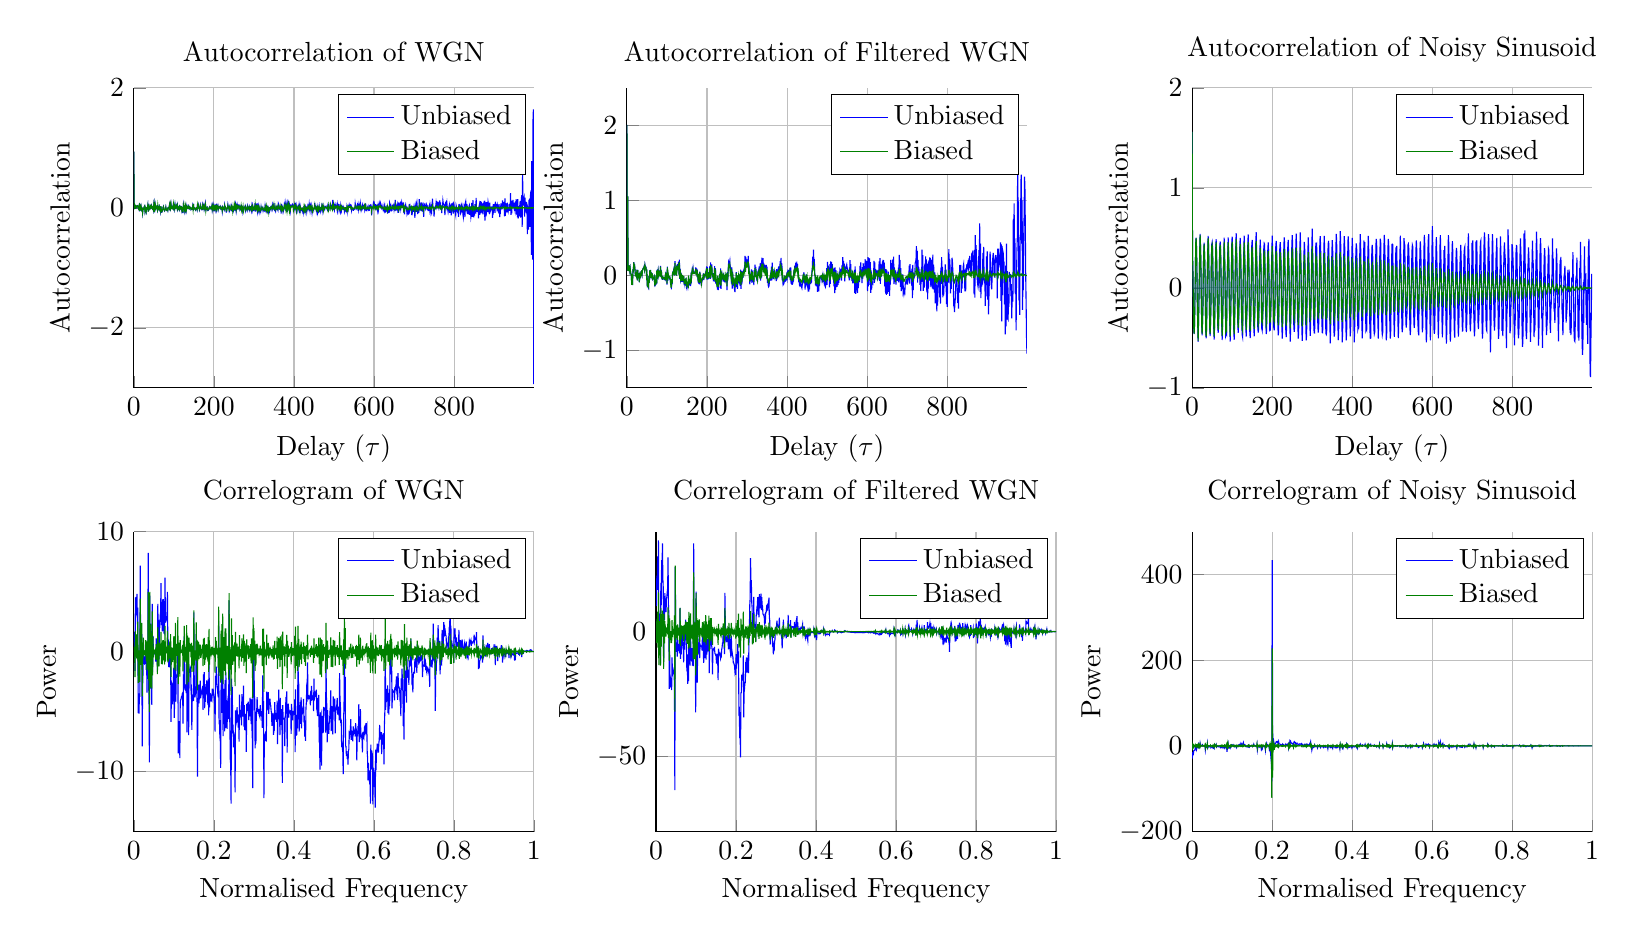
\begin{tikzpicture}

\begin{axis}[%
width=2in,
height=1.5in,
scale only axis,
xmin=0,
xmax=999,
xlabel={Delay ($\tau$)},
xmajorgrids,
ymin=-1.5,
ymax=2.5,
ylabel={Autocorrelation},
ymajorgrids,
name=plot3,
title={Autocorrelation of Filtered WGN},
axis x line*=bottom,
axis y line*=left,
legend style={draw=black,fill=white,legend cell align=left}
]
\addplot [color=blue,solid]
  table[row sep=crcr]{-999	-1.04363351459786\\
-998	-0.815393418274118\\
-997	-0.372948894421538\\
-996	-0.0103770255234643\\
-995	0.633423855500881\\
-994	1.18138138479025\\
-993	1.31502581509801\\
-992	0.815896416656528\\
-991	0.50363649253043\\
-990	-0.1953021425073\\
-989	-0.0623208969984734\\
-988	-0.460736844413034\\
-987	0.998697226826023\\
-986	0.422636304299663\\
-985	1.34394266846885\\
-984	1.25064180494122\\
-983	0.471963224087121\\
-982	0.510025065669935\\
-981	-0.525778308578391\\
-980	-0.203080960845305\\
-979	-0.33228967869119\\
-978	0.985319386508805\\
-977	0.581290893416081\\
-976	1.66264522154805\\
-975	0.50085929513947\\
-974	0.307686212046233\\
-973	-0.0524128016839269\\
-972	-0.732405975746396\\
-971	-0.0115030910098649\\
-970	-0.24900991326284\\
-969	0.493081953610079\\
-968	0.226574586899956\\
-967	0.958517276998491\\
-966	-0.00408138856109009\\
-965	0.753669296615314\\
-964	-0.348754301732965\\
-963	-0.205634581251323\\
-962	-0.326251373594918\\
-961	-0.574526521226671\\
-960	-0.117044334448687\\
-959	-0.276548538634285\\
-958	0.0132107040710342\\
-957	0.0130315032406713\\
-956	-0.0629114071239153\\
-955	0.0450849996345127\\
-954	-0.420282775980449\\
-953	-0.296492803302761\\
-952	-0.586472068895221\\
-951	-0.572449948068382\\
-950	0.057994671830281\\
-949	-0.589511655379882\\
-948	0.422506353218865\\
-947	-0.679105865398074\\
-946	0.13157833960864\\
-945	-0.785058994076771\\
-944	-0.095677851557563\\
-943	-0.3854161812548\\
-942	0.183950967371892\\
-941	0.137404060102939\\
-940	0.292227883752924\\
-939	0.31889582779064\\
-938	-0.262435176262816\\
-937	0.392937255991479\\
-936	-0.614163234633886\\
-935	0.412225226956488\\
-934	-0.339027290280635\\
-933	0.440815022040499\\
-932	0.102191742856405\\
-931	0.257516590021732\\
-930	0.201580682354975\\
-929	0.249374271159448\\
-928	0.357681880094559\\
-927	-0.0413467081156917\\
-926	0.355141967192458\\
-925	-0.307484370266039\\
-924	0.211177920410408\\
-923	0.172205980952393\\
-922	0.261217689458267\\
-921	0.263490775310009\\
-920	0.22390353455266\\
-919	-0.0327427805797715\\
-918	0.146858178152754\\
-917	0.0079437941785853\\
-916	0.212473584610194\\
-915	0.30039436898326\\
-914	0.251897835431449\\
-913	0.15975861323346\\
-912	-0.0449466316445\\
-911	-0.185500590871252\\
-910	-0.125240385695526\\
-909	0.0456877622607144\\
-908	0.177983490036617\\
-907	0.317156630209034\\
-906	-0.0371063312242737\\
-905	-0.092319610455751\\
-904	-0.307961396721437\\
-903	-0.518773409531226\\
-902	-0.0171870496984345\\
-901	-0.324642296503618\\
-900	0.321383389843046\\
-899	-0.1192067080648\\
-898	0.254574416414328\\
-897	-0.279329981886411\\
-896	-0.0256723603242004\\
-895	-0.405839921390248\\
-894	-0.0713724712295286\\
-893	-0.0813020517777816\\
-892	-0.0241487171389569\\
-891	0.381225012972074\\
-890	-0.0658432971270982\\
-889	0.300655315995305\\
-888	-0.121576186865806\\
-887	-0.0444570191510686\\
-886	-0.149990101624881\\
-885	0.0137040348258051\\
-884	-0.303406686864369\\
-883	0.424617330212631\\
-882	-0.219304594336568\\
-881	0.693825505716365\\
-880	0.0205901001278357\\
-879	0.335322280441673\\
-878	-0.102553062357567\\
-877	-0.152332835562867\\
-876	-0.117086699383064\\
-875	-0.0569560046778872\\
-874	0.170256267500391\\
-873	0.23131034764546\\
-872	0.402118150028732\\
-871	0.0331217112508355\\
-870	0.536646027242848\\
-869	-0.295635425135905\\
-868	0.341406904761206\\
-867	-0.254773314069943\\
-866	0.143287555260027\\
-865	-0.00147375030623251\\
-864	0.33127313042529\\
-863	0.249837696651866\\
-862	0.294584376495875\\
-861	0.283434931967355\\
-860	0.00624673992309011\\
-859	0.183634006352344\\
-858	0.0494383351678206\\
-857	0.172647903677639\\
-856	0.258491307169996\\
-855	0.0955983638793474\\
-854	0.226542554870719\\
-853	0.0833989317349563\\
-852	0.100222213414149\\
-851	0.145531991221578\\
-850	0.109239087194665\\
-849	0.14840599310295\\
-848	0.0432763585593717\\
-847	0.101466582559405\\
-846	-0.211559887963582\\
-845	-0.0120646809861329\\
-844	-0.214318803056287\\
-843	0.0772259974317009\\
-842	0.0437693054274404\\
-841	0.152671739260591\\
-840	0.124608241503215\\
-839	0.00948851911921479\\
-838	0.0252171040317903\\
-837	-0.177454846203651\\
-836	0.033937028718229\\
-835	-0.232262963388992\\
-834	0.14027334323948\\
-833	-0.029622249415874\\
-832	0.0483804289319053\\
-831	0.138105385346666\\
-830	-0.231096164905846\\
-829	-0.0743089172998092\\
-828	-0.444053323752499\\
-827	-0.250146456594666\\
-826	-0.365629542441597\\
-825	-0.187843414031856\\
-824	-0.0673701605432181\\
-823	-0.111242759504802\\
-822	-0.0290010480693421\\
-821	-0.172590382563087\\
-820	-0.318929015615383\\
-819	-0.390499066968244\\
-818	-0.489679813569858\\
-817	-0.353886180149101\\
-816	-0.370035871161104\\
-815	-0.0463527205972571\\
-814	0.0582833610749022\\
-813	0.172497244191376\\
-812	0.234564717677152\\
-811	0.0310669819868522\\
-810	-0.180477684920314\\
-809	-0.0580214063798645\\
-808	-0.240071399826351\\
-807	0.117447497572302\\
-806	0.218417366353082\\
-805	0.076523803352465\\
-804	0.35094394361032\\
-803	-0.0958865754402188\\
-802	-0.0585500562977668\\
-801	-0.078398610115434\\
-800	-0.421101398841462\\
-799	-0.0132609843021174\\
-798	-0.382390283664452\\
-797	0.0749426582208418\\
-796	-0.143254242171506\\
-795	0.147483725739245\\
-794	-0.0180492488533522\\
-793	-0.0149761029714219\\
-792	-0.141020431713003\\
-791	-0.268650201805541\\
-790	-0.146198272820216\\
-789	-0.293765082486601\\
-788	0.113125798836355\\
-787	-0.0878365230152614\\
-786	0.242536756872175\\
-785	-0.114485994621044\\
-784	0.102026277035956\\
-783	-0.375826116090936\\
-782	-0.00367579998958882\\
-781	-0.292333941609832\\
-780	-0.0200398305861199\\
-779	-0.0283385794625464\\
-778	-0.161253387720019\\
-777	-0.0558773354942843\\
-776	-0.402172620434134\\
-775	-0.195589912574743\\
-774	-0.480913956973914\\
-773	-0.121267784905008\\
-772	-0.374135776218247\\
-771	0.00637252874262444\\
-770	-0.374466687436208\\
-769	0.038749117662984\\
-768	-0.228565516514098\\
-767	-0.0333370971798334\\
-766	0.141991074311816\\
-765	-0.187836469650783\\
-764	0.277451334599427\\
-763	-0.174911865409052\\
-762	0.206805602410896\\
-761	-0.134917247970532\\
-760	0.178515038100089\\
-759	-0.157026211917172\\
-758	0.234097828942306\\
-757	-0.0691135266025139\\
-756	0.240268737582321\\
-755	-0.0264369041136323\\
-754	0.200072163991382\\
-753	-0.176287774996041\\
-752	0.155373085425498\\
-751	-0.320162411891588\\
-750	0.133245897228892\\
-749	-0.224059379058487\\
-748	0.213389760397435\\
-747	-0.0380900918181716\\
-746	0.253245739775719\\
-745	-0.0560623352441627\\
-744	0.155570969763806\\
-743	-0.162503597890283\\
-742	-0.0787216909796325\\
-741	-0.0469478111583977\\
-740	-0.206954993393662\\
-739	0.271216704442819\\
-738	-0.0819594193359097\\
-737	0.344242894494683\\
-736	-0.0856256139386184\\
-735	0.0879268839787315\\
-734	-0.210961371219659\\
-733	-0.0177473140889584\\
-732	-0.126477682278954\\
-731	0.0374735012215548\\
-730	0.0370407404103204\\
-729	0.106206182251417\\
-728	0.00864028234365415\\
-727	0.207555669246918\\
-726	-0.0974251583841542\\
-725	0.325628164360817\\
-724	0.0228516263248094\\
-723	0.390098567303832\\
-722	0.209946947187263\\
-721	0.181345268743806\\
-720	0.16695028393122\\
-719	-0.00648665552367264\\
-718	-0.0207021068818253\\
-717	0.00872690397768966\\
-716	0.0204860689190695\\
-715	-0.197550050560712\\
-714	0.139607537083428\\
-713	-0.30163646375727\\
-712	0.0911807976146714\\
-711	-0.136913387449996\\
-710	0.0598423378403371\\
-709	0.0114854893821284\\
-708	-0.0408170777916935\\
-707	0.149209391943998\\
-706	-0.110600816859829\\
-705	0.128136207337175\\
-704	-0.0447001379616759\\
-703	-0.0522841348679916\\
-702	-0.0126829161535802\\
-701	-0.122302168636536\\
-700	-0.0781314611297213\\
-699	-0.0586582579803318\\
-698	-0.0914834919591911\\
-697	-0.0729295699411848\\
-696	-0.092864520283798\\
-695	-0.121392278076231\\
-694	-0.227891970976494\\
-693	-0.210542326741654\\
-692	-0.245116675991139\\
-691	-0.188237043357705\\
-690	-0.216799937506776\\
-689	0.0140796560761454\\
-688	-0.186373222547489\\
-687	-0.0156624059431485\\
-686	-0.00473456597227443\\
-685	-0.208611455267537\\
-684	0.0977567308822029\\
-683	-0.15369249794411\\
-682	0.204866107585294\\
-681	-0.0457028662890265\\
-680	0.274590907540447\\
-679	-0.0935624187146587\\
-678	0.10432796564248\\
-677	-0.0651961322350344\\
-676	-0.0550953145517517\\
-675	-0.0110845679624149\\
-674	-0.0741480737395337\\
-673	0.00283736572255142\\
-672	-0.124405166668704\\
-671	0.0664965165230686\\
-670	-0.0899474481134355\\
-669	0.00904619618192852\\
-668	0.105380538354988\\
-667	-0.117167622017734\\
-666	0.250074807238321\\
-665	-0.0545382332464592\\
-664	0.210141662147127\\
-663	0.0384639283777349\\
-662	0.0925723747814932\\
-661	0.163793917658382\\
-660	0.032381808683531\\
-659	0.206878341296832\\
-658	-0.121830446554498\\
-657	-8.60381649881022e-05\\
-656	-0.271964632195568\\
-655	-0.00506609072092226\\
-654	-0.218637376246984\\
-653	0.0488370933927217\\
-652	-0.165671248784754\\
-651	-0.025702930453761\\
-650	-0.246028779738641\\
-649	0.0655475122921821\\
-648	-0.258496070894086\\
-647	0.0831993038157478\\
-646	-0.241576542423754\\
-645	0.0379512999143089\\
-644	-0.147909197400734\\
-643	0.169895208946157\\
-642	0.0679665594755405\\
-641	0.204473931476011\\
-640	0.148879604444391\\
-639	0.113600288191362\\
-638	0.148179117128455\\
-637	0.0702547036639643\\
-636	0.143433067837113\\
-635	-0.0190608063487476\\
-634	0.15457107025356\\
-633	-0.111771210395885\\
-632	0.228837170618131\\
-631	-0.071743104126098\\
-630	0.185941545882583\\
-629	0.0625693460930249\\
-628	0.0221401040886883\\
-627	0.0734860655811582\\
-626	-0.0673862035969657\\
-625	0.030321833114157\\
-624	0.0148781716745851\\
-623	0.0581122958396529\\
-622	0.0677636611538852\\
-621	0.049266310903724\\
-620	-0.0491740462003995\\
-619	0.173371480197314\\
-618	-0.101369027815569\\
-617	0.193152314035515\\
-616	-0.0355538447051377\\
-615	0.00359136627491825\\
-614	-0.109795044103616\\
-613	-0.100003957854625\\
-612	-0.118882216919753\\
-611	-0.188005409665871\\
-610	0.0651930541312509\\
-609	-0.232591394773502\\
-608	0.177607965965497\\
-607	-0.125952332579827\\
-606	0.226188591157512\\
-605	-0.0355798242633409\\
-604	0.230948100458757\\
-603	-0.148209546819232\\
-602	0.243725819168297\\
-601	-0.211174168946405\\
-600	0.189681081389456\\
-599	-0.0262464555726736\\
-598	0.0506105299402483\\
-597	0.194886111419383\\
-596	0.0435117761796245\\
-595	0.215822635178714\\
-594	0.0398136471574751\\
-593	0.0878534833610025\\
-592	0.0556882664943471\\
-591	0.0289924480184822\\
-590	0.163380128558339\\
-589	-0.0443773849659172\\
-588	0.108322830511996\\
-587	-0.104655697315082\\
-586	0.0731928479852909\\
-585	-0.0281463704386725\\
-584	0.172214594530663\\
-583	-0.0174309930635532\\
-582	0.126792345416806\\
-581	-0.0886010596602731\\
-580	-0.032008082296915\\
-579	-0.0283116362222452\\
-578	-0.168913808401335\\
-577	-0.0207419872232183\\
-576	-0.232285906769134\\
-575	-0.0821976997359977\\
-574	-0.171605136450106\\
-573	-0.134921041093445\\
-572	-0.015649557583459\\
-571	-0.246743209832358\\
-570	0.118842037607456\\
-569	-0.234531534224594\\
-568	0.0731062307869774\\
-567	-0.103291804073402\\
-566	-0.0470447722605344\\
-565	0.0172934754464709\\
-564	-0.106255587636175\\
-563	0.0279199426013876\\
-562	-0.0713382939923114\\
-561	0.00774918754642565\\
-560	0.00419334899963453\\
-559	0.150889270078587\\
-558	-0.0310635551654649\\
-557	0.204680402951894\\
-556	-0.0671215253862196\\
-555	0.0726454557985221\\
-554	-0.00617432910267686\\
-553	0.0307176278416534\\
-552	0.0520715671115544\\
-551	0.0947721568429137\\
-550	0.0936890069886494\\
-549	0.144627469641633\\
-548	0.127669914488629\\
-547	0.094894396893292\\
-546	0.039238881837479\\
-545	0.116280187207565\\
-544	-0.0783404716858793\\
-543	0.155265918350937\\
-542	0.0275090814999468\\
-541	0.192993379171168\\
-540	0.132375803666385\\
-539	0.243682212652897\\
-538	0.0242780100519294\\
-537	0.133109040167858\\
-536	-0.0706475678332248\\
-535	0.0883980458062734\\
-534	-0.00742920311421823\\
-533	0.0470888301811684\\
-532	0.0660012241868136\\
-531	-0.0636814869732107\\
-530	0.0502705871189139\\
-529	-0.100183221263006\\
-528	0.0035955406519815\\
-527	-0.129881440332815\\
-526	-0.0279191087412514\\
-525	-0.152248751501673\\
-524	0.0134654277334169\\
-523	-0.157377144267124\\
-522	0.0714532677784389\\
-521	-0.191554709460392\\
-520	0.105556347326613\\
-519	-0.238125986381746\\
-518	0.100457152242553\\
-517	-0.146127420049394\\
-516	0.00670332097091019\\
-515	0.0492814353566478\\
-514	-0.0061836006202535\\
-513	0.150320374889297\\
-512	0.0694512038880981\\
-511	0.176100397479238\\
-510	0.0471274099684376\\
-509	0.186669921360365\\
-508	-0.112304020208373\\
-507	0.148903114847071\\
-506	-0.16041310530124\\
-505	0.107584575355066\\
-504	0.0405497923755594\\
-503	0.129635083685404\\
-502	0.0422386447405541\\
-501	0.179422271239003\\
-500	-0.127234847436161\\
-499	0.0966428207434955\\
-498	-0.0867029521006854\\
-497	-0.115185498669592\\
-496	-0.056151515511808\\
-495	-0.143885978970001\\
-494	-0.127295880880691\\
-493	-0.0250558658864456\\
-492	-0.0728947600448959\\
-491	-0.0300826228508302\\
-490	0.00163415116640336\\
-489	-0.0889010452957629\\
-488	-0.0174997416213614\\
-487	-0.0680713145499883\\
-486	-0.0353847389491655\\
-485	-0.0126716602442486\\
-484	-0.0245235424952779\\
-483	-0.0292520427707615\\
-482	-0.0509104305956739\\
-481	-0.136204886977032\\
-480	-0.0903926493319941\\
-479	-0.213470393871124\\
-478	-0.178789124219512\\
-477	-0.123477290374779\\
-476	-0.220143919503695\\
-475	-0.0629526679797923\\
-474	-0.0934886825771027\\
-473	-0.145595438888114\\
-472	-0.0752171760732223\\
-471	-0.132342925812069\\
-470	-0.0172877532127258\\
-469	0.0256066714734926\\
-468	0.21640426281275\\
-467	0.120712407427533\\
-466	0.341517043401084\\
-465	0.167672531379741\\
-464	0.244823898291092\\
-463	0.10155791652107\\
-462	0.047508399989672\\
-461	-0.0742979407713487\\
-460	-0.0570849738965563\\
-459	-0.0578257594754937\\
-458	-0.115826520292563\\
-457	-0.0333210584573663\\
-456	-0.187375297574722\\
-455	-0.0967052409045339\\
-454	-0.217607619709352\\
-453	-0.134940335813021\\
-452	-0.172133177769243\\
-451	-0.131042341341243\\
-450	-0.0283511531102268\\
-449	-0.0913281903057196\\
-448	0.0142053686157023\\
-447	-0.149339303380931\\
-446	-0.0633782297487008\\
-445	-0.191115153412443\\
-444	-0.0176901680547446\\
-443	-0.107111469237644\\
-442	0.0429177541482039\\
-441	-0.0293783187094339\\
-440	-0.0170237647131021\\
-439	-0.0921448344607363\\
-438	-0.11886108410245\\
-437	-0.168382219300048\\
-436	-0.150510107770763\\
-435	-0.138615341771446\\
-434	-0.10661100697887\\
-433	-0.12589942294672\\
-432	-0.108074865242562\\
-431	-0.123677800333416\\
-430	-0.0642499109046386\\
-429	-0.0706556124967429\\
-428	0.0638788390605739\\
-427	0.0126450091327192\\
-426	0.153590076265782\\
-425	0.120465031292617\\
-424	0.165845025405849\\
-423	0.154135470411936\\
-422	0.10759339469779\\
-421	0.13118146418264\\
-420	0.0642091599352602\\
-419	0.125890440525358\\
-418	0.0246690048477848\\
-417	0.0654600258676778\\
-416	-0.0564632835535846\\
-415	-0.0435797302440827\\
-414	-0.107663760829703\\
-413	-0.118745150866733\\
-412	-0.118902404796852\\
-411	-0.013239148280661\\
-410	-0.112115302963194\\
-409	0.107400818164292\\
-408	-0.0646727661451931\\
-407	0.103365831244846\\
-406	-0.0259997798803164\\
-405	0.0697912034263317\\
-404	0.0131424735486226\\
-403	0.0383083883469368\\
-402	0.00880008940820691\\
-401	0.0323302064190248\\
-400	-0.0381255330871025\\
-399	-0.00432061429014373\\
-398	-0.0534096481340085\\
-397	-0.064326403355663\\
-396	-0.0379032784611924\\
-395	-0.0604426605046968\\
-394	-0.036054627622287\\
-393	-0.0734737080474841\\
-392	-0.111534041969672\\
-391	-0.118891974961638\\
-390	-0.127390861041465\\
-389	-0.00158308833206266\\
-388	-0.0648594139006499\\
-387	0.160826874425125\\
-386	0.00647014323847761\\
-385	0.231547805976654\\
-384	0.0971626283293954\\
-383	0.190927932834994\\
-382	0.123140259012826\\
-381	0.102238882360649\\
-380	0.0389494338830141\\
-379	0.12061822174384\\
-378	-0.0275679094277413\\
-377	0.0646579639192797\\
-376	0.0410342723513924\\
-375	-0.0532203121776232\\
-374	0.0826813800884705\\
-373	-0.0763447498504959\\
-372	0.00258614282820339\\
-371	-0.0266253962093189\\
-370	-0.0105251643719949\\
-369	0.0681095622277292\\
-368	-0.00781540909134312\\
-367	0.060030049936706\\
-366	-0.0509930966273133\\
-365	0.0874727129140728\\
-364	-0.036577316270435\\
-363	0.170687188426994\\
-362	-0.0667969942512456\\
-361	0.115654343536955\\
-360	-0.069303282763808\\
-359	0.0177102297398312\\
-358	-0.015350256527936\\
-357	-0.064247947876866\\
-356	-0.0696154584440945\\
-355	-0.13969120741591\\
-354	-0.15204287107578\\
-353	-0.135022697029114\\
-352	-0.0727257180939212\\
-351	-0.0798738899972572\\
-350	0.115908763325047\\
-349	-0.0445151829179148\\
-348	0.140788513419813\\
-347	-0.0024876413581307\\
-346	0.106020902364141\\
-345	0.0593171179784411\\
-344	0.141388397979843\\
-343	0.0392165041205666\\
-342	0.159651872668595\\
-341	0.0687321432858777\\
-340	0.221240200238566\\
-339	0.219687109941465\\
-338	0.154893265716913\\
-337	0.236539852337069\\
-336	-0.0304188311506921\\
-335	0.167966383672038\\
-334	-0.070445117570371\\
-333	0.160953255902271\\
-332	-0.0404801848410547\\
-331	0.120042137769742\\
-330	0.016182409844642\\
-329	0.0636467151406772\\
-328	0.0282520173730935\\
-327	0.03832603246326\\
-326	-0.0862089700537686\\
-325	-0.0292820789080909\\
-324	-0.0448923940621195\\
-323	-0.0146183721958273\\
-322	0.112084830750243\\
-321	0.0509774553601651\\
-320	0.14220598570714\\
-319	-0.0198259477881476\\
-318	0.0686351195552827\\
-317	-0.130537334645821\\
-316	-0.0154449478465503\\
-315	-0.0824882458604439\\
-314	-0.080461772359904\\
-313	0.0636744456243459\\
-312	-0.0985175595282143\\
-311	0.0800988542483286\\
-310	-0.00196911543268269\\
-309	-0.0722073961978562\\
-308	0.0213606589796812\\
-307	-0.120773953299136\\
-306	-0.0135315568201781\\
-305	0.10100674905661\\
-304	0.0767774668646748\\
-303	0.260661785255525\\
-302	0.151230214653581\\
-301	0.212221497254165\\
-300	0.164263474528681\\
-299	0.158964718803385\\
-298	0.153748681966071\\
-297	0.246668414121229\\
-296	0.0643604451622279\\
-295	0.259847761649349\\
-294	0.0531707636326976\\
-293	0.0909537044457016\\
-292	0.069917998126588\\
-291	0.0660696060715637\\
-290	-0.0332206317883896\\
-289	0.0535083502060757\\
-288	-0.0416229968921667\\
-287	-0.118635386956455\\
-286	0.0601460079488946\\
-285	-0.179659644849917\\
-284	0.077317205369157\\
-283	-0.140559880783286\\
-282	0.0133306433398583\\
-281	-0.0803215709857943\\
-280	-0.0480159008266721\\
-279	-0.00151892940739528\\
-278	-0.107871486889191\\
-277	-0.0164839876419328\\
-276	-0.179333334665256\\
-275	0.00279112899516333\\
-274	-0.157187999417667\\
-273	0.0436488492288501\\
-272	-0.148494176083181\\
-271	-0.0448382709079089\\
-270	-0.221449166380465\\
-269	-0.118367772513843\\
-268	-0.161588230024726\\
-267	-0.125958471390317\\
-266	-0.0387622149445972\\
-265	-0.135809125908628\\
-264	0.0498714918567412\\
-263	-0.177774206914042\\
-262	0.106417075931887\\
-261	-0.111283953049953\\
-260	0.0759331090307746\\
-259	0.101198733213534\\
-258	0.0561375712075762\\
-257	0.190198323853867\\
-256	0.158702636037994\\
-255	0.1511095136889\\
-254	0.172809140795804\\
-253	0.085290472378727\\
-252	-0.0701648570998585\\
-251	0.0418230943048738\\
-250	-0.196117952376165\\
-249	0.0253677380149616\\
-248	-0.0926133747172275\\
-247	-0.0126216271278218\\
-246	-0.0715849705749812\\
-245	-0.0214854727062282\\
-244	-0.0912737302018361\\
-243	0.00469032026600658\\
-242	-0.0815132075866314\\
-241	-0.0105523925549729\\
-240	-0.0411700375148754\\
-239	-0.0259098541537948\\
-238	0.0135285929071386\\
-237	-0.0824425105392952\\
-236	0.0521541478757303\\
-235	-0.178770222622829\\
-234	0.0923338472220928\\
-233	-0.167097685326355\\
-232	0.0217581211784663\\
-231	-0.110792961517042\\
-230	-0.107166417290001\\
-229	-0.0463748961886978\\
-228	-0.197690327305036\\
-227	-0.00580711873661304\\
-226	-0.189387027095872\\
-225	-0.0722344603964152\\
-224	-0.128861137474299\\
-223	-0.063293237646316\\
-222	-0.110567220392975\\
-221	0.0980566579837259\\
-220	-0.0854730391526121\\
-219	0.122133496182033\\
-218	-0.0597220420317676\\
-217	0.0301339755442529\\
-216	-0.0796079903216469\\
-215	0.0201057094653965\\
-214	0.0238467617957407\\
-213	0.00545158010135406\\
-212	0.147431759049758\\
-211	0.0595882391177864\\
-210	0.0364536245933713\\
-209	0.171778553948424\\
-208	-0.0464304595278989\\
-207	0.11967158738872\\
-206	-0.0281805750605865\\
-205	0.0319724419094905\\
-204	-0.0449509351578904\\
-203	0.0435120542819007\\
-202	-0.0547011488250916\\
-201	0.112009185426442\\
-200	-0.0578887337452099\\
-199	0.118634361361266\\
-198	-0.0323338747407007\\
-197	0.0461047794766446\\
-196	0.0234936763588192\\
-195	-0.0024893389411989\\
-194	-0.0066373103310587\\
-193	0.0045798650805042\\
-192	-0.0641853224242818\\
-191	0.0269401134670081\\
-190	-0.031028104614798\\
-189	-0.0360675267936719\\
-188	-0.0672392408780297\\
-187	-0.0832885859503791\\
-186	-0.138491927353381\\
-185	-0.0755711411492776\\
-184	-0.0338089362921981\\
-183	-0.103437554271849\\
-182	0.0481611754166706\\
-181	-0.120468818504238\\
-180	0.0151525985588763\\
-179	-0.11124521064539\\
-178	0.019722165199779\\
-177	-0.0232308897563331\\
-176	0.0418255805108938\\
-175	0.0203178661061408\\
-174	0.0938971999915839\\
-173	0.00292757335583014\\
-172	0.105077163303892\\
-171	0.0471057252447578\\
-170	0.0528566810805744\\
-169	0.0285889307866693\\
-168	0.0294752468004741\\
-167	0.0319765622127797\\
-166	0.0290663616135366\\
-165	0.0939739411313917\\
-164	0.0544023059418741\\
-163	0.0765088286581258\\
-162	0.0364836653103949\\
-161	-0.0552602958102783\\
-160	-0.0248333235644841\\
-159	-0.143430778485294\\
-158	-0.0718595856711487\\
-157	-0.0823257068423137\\
-156	-0.103059728085714\\
-155	-0.0650022689935252\\
-154	-0.13389524081638\\
-153	-0.0771235295366499\\
-152	-0.147067034724923\\
-151	-0.113606520323097\\
-150	-0.108550013120893\\
-149	-0.143835774279284\\
-148	-0.0754631179280989\\
-147	-0.101366977307711\\
-146	-0.0778057254512771\\
-145	-0.115431886144741\\
-144	-0.0552222883709299\\
-143	-0.130217511960649\\
-142	-0.0138501063056188\\
-141	-0.0917683019186468\\
-140	-0.00626147718878808\\
-139	-0.0873389420846605\\
-138	0.00640534486627103\\
-137	-0.0868474479362875\\
-136	-0.00873342995839129\\
-135	-0.033943440857821\\
-134	-0.0581354010230789\\
-133	0.0882067769075481\\
-132	-0.0477665454515415\\
-131	0.208257251421964\\
-130	0.0109958762991628\\
-129	0.183877048612003\\
-128	0.0764900401932535\\
-127	0.14911905717787\\
-126	0.0799082646137254\\
-125	0.143225953097721\\
-124	-0.00306740049477434\\
-123	0.0819796937873217\\
-122	0.042303843006832\\
-121	0.0306020517950055\\
-120	0.188112323654164\\
-119	0.000491797362104517\\
-118	0.120680116955786\\
-117	0.0372868653975865\\
-116	0.0537232473505195\\
-115	0.0247264234742079\\
-114	0.0322244516511055\\
-113	-0.119441428084153\\
-112	-0.0626577241969367\\
-111	-0.18499223864241\\
-110	-0.0576195886550194\\
-109	-0.107217736719664\\
-108	-0.0440292816790989\\
-107	-0.0249740161598221\\
-106	-0.0378075579981581\\
-105	-0.0246501878996028\\
-104	-0.0170044466596933\\
-103	0.0250666246271362\\
-102	-0.0718331673545915\\
-101	0.117028131073322\\
-100	-0.121770699533439\\
-99	0.0359882396672716\\
-98	-0.0584451656621185\\
-97	-0.0585311616163053\\
-96	-0.00826453347747701\\
-95	-0.0568612477038494\\
-94	-0.046609859370896\\
-93	-0.0503741324734114\\
-92	-0.0314453217338547\\
-91	-0.0332994560380093\\
-90	-0.024674500472136\\
-89	-0.0516410677393995\\
-88	-0.0508088195473588\\
-87	-0.0291294527926572\\
-86	0.0661595703189276\\
-85	-0.0022984589175748\\
-84	0.125869901652185\\
-83	-0.024465646307259\\
-82	0.0661878124034748\\
-81	-0.00562567064121403\\
-80	0.0663277297850711\\
-79	0.0134320884262418\\
-78	0.0665838441640203\\
-77	0.02058408591205\\
-76	0.0791526956539579\\
-75	-0.0387718960884523\\
-74	-0.00500454778880552\\
-73	-0.115519466188512\\
-72	-0.113623660517647\\
-71	-0.126208744628982\\
-70	-0.0586826610126015\\
-69	-0.0932039257278569\\
-68	-0.0218700405570183\\
-67	-0.0409339626178173\\
-66	-0.039348645061776\\
-65	-0.0481170765091857\\
-64	-0.00958346909664462\\
-63	-0.0379121192130143\\
-62	-0.0179159292304408\\
-61	0.0400557428651967\\
-60	-0.0352338151067965\\
-59	0.0735049343983383\\
-58	-0.0319636532207356\\
-57	0.065834615365273\\
-56	-0.10111194965723\\
-55	-0.00932092777047381\\
-54	-0.167335306191132\\
-53	-0.154605849592684\\
-52	-0.107908239614522\\
-51	-0.158593405730717\\
-50	0.0198795846641712\\
-49	-0.00669527020813078\\
-48	0.100853524307399\\
-47	0.113375514245935\\
-46	0.10260692679183\\
-45	0.137314550993774\\
-44	0.0803584517200142\\
-43	0.120449254235359\\
-42	0.103115446368568\\
-41	0.0977726203009288\\
-40	0.0894314602829086\\
-39	0.0702031737770385\\
-38	0.0200883735018632\\
-37	0.0674375821194236\\
-36	-0.00594482382568309\\
-35	0.0533452998150266\\
-34	-0.0186781858071727\\
-33	-0.0305556730616651\\
-32	-0.00447875522991109\\
-31	-0.0916551204950295\\
-30	0.0280178276826789\\
-29	-0.027686208994281\\
-28	-0.0308236488308933\\
-27	0.0721394981482458\\
-26	-0.0665723451240716\\
-25	0.0757438182345833\\
-24	-0.0225229856209991\\
-23	-0.0107877327601332\\
-22	0.0225830790277231\\
-21	0.012250207050634\\
-20	0.0862469520584132\\
-19	0.139093627995982\\
-18	0.138059157858124\\
-17	0.174969623639052\\
-16	0.0419740612965344\\
-15	0.0812454923263921\\
-14	-0.129276662658293\\
-13	0.00277898977593677\\
-12	-0.126548363012727\\
-11	0.0123613463482388\\
-10	0.015055381201447\\
-9	0.0463455973248565\\
-8	0.0983231304904412\\
-7	0.0671684330870433\\
-6	0.13261775947866\\
-5	0.0588308503002559\\
-4	0.134854102151819\\
-3	0.0611154265071904\\
-2	1.05481719408915\\
-1	0.0650618432594144\\
0	2.00756555636676\\
1	0.0650618432594143\\
2	1.05481719408915\\
3	0.0611154265071904\\
4	0.134854102151819\\
5	0.0588308503002559\\
6	0.13261775947866\\
7	0.0671684330870433\\
8	0.0983231304904412\\
9	0.0463455973248565\\
10	0.015055381201447\\
11	0.0123613463482388\\
12	-0.126548363012727\\
13	0.00277898977593676\\
14	-0.129276662658293\\
15	0.0812454923263921\\
16	0.0419740612965344\\
17	0.174969623639052\\
18	0.138059157858124\\
19	0.139093627995982\\
20	0.0862469520584132\\
21	0.012250207050634\\
22	0.0225830790277231\\
23	-0.0107877327601332\\
24	-0.0225229856209991\\
25	0.0757438182345833\\
26	-0.0665723451240715\\
27	0.0721394981482458\\
28	-0.0308236488308933\\
29	-0.027686208994281\\
30	0.0280178276826789\\
31	-0.0916551204950295\\
32	-0.00447875522991109\\
33	-0.0305556730616651\\
34	-0.0186781858071727\\
35	0.0533452998150266\\
36	-0.00594482382568306\\
37	0.0674375821194236\\
38	0.0200883735018632\\
39	0.0702031737770385\\
40	0.0894314602829086\\
41	0.0977726203009289\\
42	0.103115446368568\\
43	0.120449254235359\\
44	0.0803584517200142\\
45	0.137314550993774\\
46	0.10260692679183\\
47	0.113375514245935\\
48	0.100853524307399\\
49	-0.0066952702081308\\
50	0.0198795846641712\\
51	-0.158593405730717\\
52	-0.107908239614522\\
53	-0.154605849592684\\
54	-0.167335306191132\\
55	-0.00932092777047379\\
56	-0.10111194965723\\
57	0.065834615365273\\
58	-0.0319636532207355\\
59	0.0735049343983383\\
60	-0.0352338151067964\\
61	0.0400557428651967\\
62	-0.0179159292304408\\
63	-0.0379121192130143\\
64	-0.00958346909664462\\
65	-0.0481170765091857\\
66	-0.039348645061776\\
67	-0.0409339626178174\\
68	-0.0218700405570183\\
69	-0.0932039257278569\\
70	-0.0586826610126015\\
71	-0.126208744628982\\
72	-0.113623660517647\\
73	-0.115519466188512\\
74	-0.00500454778880554\\
75	-0.0387718960884523\\
76	0.0791526956539579\\
77	0.02058408591205\\
78	0.0665838441640203\\
79	0.0134320884262418\\
80	0.0663277297850711\\
81	-0.00562567064121403\\
82	0.0661878124034748\\
83	-0.024465646307259\\
84	0.125869901652185\\
85	-0.00229845891757478\\
86	0.0661595703189277\\
87	-0.0291294527926572\\
88	-0.0508088195473588\\
89	-0.0516410677393995\\
90	-0.024674500472136\\
91	-0.0332994560380093\\
92	-0.0314453217338547\\
93	-0.0503741324734114\\
94	-0.046609859370896\\
95	-0.0568612477038494\\
96	-0.00826453347747701\\
97	-0.0585311616163053\\
98	-0.0584451656621185\\
99	0.0359882396672716\\
100	-0.121770699533439\\
101	0.117028131073322\\
102	-0.0718331673545915\\
103	0.0250666246271362\\
104	-0.0170044466596934\\
105	-0.0246501878996028\\
106	-0.0378075579981581\\
107	-0.0249740161598221\\
108	-0.0440292816790989\\
109	-0.107217736719664\\
110	-0.0576195886550194\\
111	-0.18499223864241\\
112	-0.0626577241969367\\
113	-0.119441428084153\\
114	0.0322244516511055\\
115	0.0247264234742079\\
116	0.0537232473505195\\
117	0.0372868653975865\\
118	0.120680116955786\\
119	0.000491797362104533\\
120	0.188112323654164\\
121	0.0306020517950055\\
122	0.042303843006832\\
123	0.0819796937873216\\
124	-0.00306740049477436\\
125	0.143225953097721\\
126	0.0799082646137254\\
127	0.14911905717787\\
128	0.0764900401932535\\
129	0.183877048612003\\
130	0.0109958762991628\\
131	0.208257251421964\\
132	-0.0477665454515415\\
133	0.0882067769075481\\
134	-0.0581354010230789\\
135	-0.0339434408578209\\
136	-0.00873342995839129\\
137	-0.0868474479362874\\
138	0.00640534486627101\\
139	-0.0873389420846605\\
140	-0.00626147718878808\\
141	-0.0917683019186468\\
142	-0.0138501063056188\\
143	-0.130217511960649\\
144	-0.0552222883709299\\
145	-0.115431886144741\\
146	-0.0778057254512772\\
147	-0.101366977307711\\
148	-0.0754631179280989\\
149	-0.143835774279284\\
150	-0.108550013120893\\
151	-0.113606520323097\\
152	-0.147067034724923\\
153	-0.0771235295366499\\
154	-0.13389524081638\\
155	-0.0650022689935252\\
156	-0.103059728085714\\
157	-0.0823257068423137\\
158	-0.0718595856711487\\
159	-0.143430778485294\\
160	-0.0248333235644841\\
161	-0.0552602958102783\\
162	0.0364836653103949\\
163	0.0765088286581258\\
164	0.0544023059418741\\
165	0.0939739411313917\\
166	0.0290663616135366\\
167	0.0319765622127797\\
168	0.0294752468004741\\
169	0.0285889307866693\\
170	0.0528566810805744\\
171	0.0471057252447578\\
172	0.105077163303892\\
173	0.00292757335583012\\
174	0.0938971999915839\\
175	0.0203178661061408\\
176	0.0418255805108938\\
177	-0.0232308897563332\\
178	0.0197221651997789\\
179	-0.11124521064539\\
180	0.0151525985588763\\
181	-0.120468818504238\\
182	0.0481611754166706\\
183	-0.103437554271849\\
184	-0.0338089362921981\\
185	-0.0755711411492776\\
186	-0.13849192735338\\
187	-0.0832885859503791\\
188	-0.0672392408780297\\
189	-0.0360675267936719\\
190	-0.031028104614798\\
191	0.0269401134670081\\
192	-0.0641853224242818\\
193	0.0045798650805042\\
194	-0.00663731033105864\\
195	-0.00248933894119889\\
196	0.0234936763588192\\
197	0.0461047794766446\\
198	-0.0323338747407007\\
199	0.118634361361266\\
200	-0.0578887337452099\\
201	0.112009185426442\\
202	-0.0547011488250916\\
203	0.0435120542819007\\
204	-0.0449509351578903\\
205	0.0319724419094905\\
206	-0.0281805750605865\\
207	0.11967158738872\\
208	-0.0464304595278989\\
209	0.171778553948424\\
210	0.0364536245933713\\
211	0.0595882391177864\\
212	0.147431759049758\\
213	0.00545158010135405\\
214	0.0238467617957407\\
215	0.0201057094653965\\
216	-0.0796079903216469\\
217	0.0301339755442529\\
218	-0.0597220420317676\\
219	0.122133496182033\\
220	-0.0854730391526121\\
221	0.0980566579837259\\
222	-0.110567220392975\\
223	-0.063293237646316\\
224	-0.128861137474299\\
225	-0.0722344603964152\\
226	-0.189387027095872\\
227	-0.00580711873661305\\
228	-0.197690327305036\\
229	-0.0463748961886978\\
230	-0.107166417290001\\
231	-0.110792961517042\\
232	0.0217581211784663\\
233	-0.167097685326355\\
234	0.0923338472220928\\
235	-0.178770222622829\\
236	0.0521541478757303\\
237	-0.0824425105392952\\
238	0.0135285929071386\\
239	-0.0259098541537949\\
240	-0.0411700375148754\\
241	-0.0105523925549729\\
242	-0.0815132075866314\\
243	0.0046903202660066\\
244	-0.0912737302018361\\
245	-0.0214854727062282\\
246	-0.0715849705749812\\
247	-0.0126216271278218\\
248	-0.0926133747172276\\
249	0.0253677380149617\\
250	-0.196117952376165\\
251	0.0418230943048738\\
252	-0.0701648570998586\\
253	0.085290472378727\\
254	0.172809140795804\\
255	0.1511095136889\\
256	0.158702636037994\\
257	0.190198323853867\\
258	0.0561375712075762\\
259	0.101198733213534\\
260	0.0759331090307746\\
261	-0.111283953049953\\
262	0.106417075931887\\
263	-0.177774206914042\\
264	0.0498714918567412\\
265	-0.135809125908628\\
266	-0.0387622149445972\\
267	-0.125958471390317\\
268	-0.161588230024726\\
269	-0.118367772513843\\
270	-0.221449166380465\\
271	-0.0448382709079088\\
272	-0.148494176083181\\
273	0.0436488492288501\\
274	-0.157187999417667\\
275	0.00279112899516329\\
276	-0.179333334665256\\
277	-0.0164839876419327\\
278	-0.107871486889191\\
279	-0.0015189294073953\\
280	-0.0480159008266721\\
281	-0.0803215709857942\\
282	0.0133306433398582\\
283	-0.140559880783286\\
284	0.077317205369157\\
285	-0.179659644849917\\
286	0.0601460079488946\\
287	-0.118635386956455\\
288	-0.0416229968921667\\
289	0.0535083502060757\\
290	-0.0332206317883895\\
291	0.0660696060715637\\
292	0.069917998126588\\
293	0.0909537044457017\\
294	0.0531707636326976\\
295	0.259847761649349\\
296	0.0643604451622279\\
297	0.246668414121229\\
298	0.153748681966071\\
299	0.158964718803385\\
300	0.164263474528681\\
301	0.212221497254165\\
302	0.151230214653581\\
303	0.260661785255525\\
304	0.0767774668646747\\
305	0.10100674905661\\
306	-0.0135315568201782\\
307	-0.120773953299136\\
308	0.0213606589796812\\
309	-0.0722073961978562\\
310	-0.0019691154326827\\
311	0.0800988542483286\\
312	-0.0985175595282143\\
313	0.0636744456243458\\
314	-0.080461772359904\\
315	-0.0824882458604439\\
316	-0.0154449478465502\\
317	-0.130537334645821\\
318	0.0686351195552827\\
319	-0.0198259477881476\\
320	0.14220598570714\\
321	0.050977455360165\\
322	0.112084830750243\\
323	-0.0146183721958273\\
324	-0.0448923940621194\\
325	-0.0292820789080909\\
326	-0.0862089700537686\\
327	0.0383260324632599\\
328	0.0282520173730935\\
329	0.0636467151406771\\
330	0.016182409844642\\
331	0.120042137769742\\
332	-0.0404801848410548\\
333	0.160953255902271\\
334	-0.0704451175703711\\
335	0.167966383672038\\
336	-0.0304188311506921\\
337	0.236539852337069\\
338	0.154893265716913\\
339	0.219687109941465\\
340	0.221240200238566\\
341	0.0687321432858777\\
342	0.159651872668595\\
343	0.0392165041205667\\
344	0.141388397979843\\
345	0.0593171179784412\\
346	0.106020902364141\\
347	-0.00248764135813072\\
348	0.140788513419813\\
349	-0.0445151829179148\\
350	0.115908763325047\\
351	-0.0798738899972572\\
352	-0.0727257180939212\\
353	-0.135022697029114\\
354	-0.15204287107578\\
355	-0.13969120741591\\
356	-0.0696154584440945\\
357	-0.064247947876866\\
358	-0.015350256527936\\
359	0.0177102297398312\\
360	-0.069303282763808\\
361	0.115654343536955\\
362	-0.0667969942512456\\
363	0.170687188426994\\
364	-0.036577316270435\\
365	0.0874727129140728\\
366	-0.0509930966273133\\
367	0.060030049936706\\
368	-0.0078154090913431\\
369	0.0681095622277292\\
370	-0.0105251643719949\\
371	-0.0266253962093189\\
372	0.00258614282820343\\
373	-0.0763447498504959\\
374	0.0826813800884704\\
375	-0.0532203121776232\\
376	0.0410342723513925\\
377	0.0646579639192798\\
378	-0.0275679094277413\\
379	0.12061822174384\\
380	0.0389494338830141\\
381	0.102238882360649\\
382	0.123140259012826\\
383	0.190927932834994\\
384	0.0971626283293954\\
385	0.231547805976654\\
386	0.00647014323847754\\
387	0.160826874425125\\
388	-0.0648594139006499\\
389	-0.00158308833206267\\
390	-0.127390861041465\\
391	-0.118891974961638\\
392	-0.111534041969672\\
393	-0.0734737080474841\\
394	-0.036054627622287\\
395	-0.0604426605046968\\
396	-0.0379032784611924\\
397	-0.064326403355663\\
398	-0.0534096481340085\\
399	-0.00432061429014373\\
400	-0.0381255330871025\\
401	0.0323302064190248\\
402	0.00880008940820694\\
403	0.0383083883469368\\
404	0.0131424735486226\\
405	0.0697912034263317\\
406	-0.0259997798803164\\
407	0.103365831244846\\
408	-0.064672766145193\\
409	0.107400818164292\\
410	-0.112115302963194\\
411	-0.0132391482806611\\
412	-0.118902404796852\\
413	-0.118745150866733\\
414	-0.107663760829703\\
415	-0.0435797302440827\\
416	-0.0564632835535846\\
417	0.0654600258676778\\
418	0.0246690048477848\\
419	0.125890440525358\\
420	0.0642091599352602\\
421	0.13118146418264\\
422	0.10759339469779\\
423	0.154135470411936\\
424	0.165845025405849\\
425	0.120465031292617\\
426	0.153590076265782\\
427	0.0126450091327192\\
428	0.0638788390605739\\
429	-0.070655612496743\\
430	-0.0642499109046385\\
431	-0.123677800333416\\
432	-0.108074865242561\\
433	-0.12589942294672\\
434	-0.10661100697887\\
435	-0.138615341771446\\
436	-0.150510107770763\\
437	-0.168382219300048\\
438	-0.11886108410245\\
439	-0.0921448344607363\\
440	-0.0170237647131021\\
441	-0.029378318709434\\
442	0.0429177541482039\\
443	-0.107111469237644\\
444	-0.0176901680547446\\
445	-0.191115153412443\\
446	-0.0633782297487008\\
447	-0.149339303380931\\
448	0.0142053686157023\\
449	-0.0913281903057195\\
450	-0.0283511531102268\\
451	-0.131042341341243\\
452	-0.172133177769243\\
453	-0.134940335813021\\
454	-0.217607619709352\\
455	-0.0967052409045339\\
456	-0.187375297574722\\
457	-0.0333210584573663\\
458	-0.115826520292563\\
459	-0.0578257594754937\\
460	-0.0570849738965563\\
461	-0.0742979407713487\\
462	0.047508399989672\\
463	0.10155791652107\\
464	0.244823898291092\\
465	0.167672531379741\\
466	0.341517043401084\\
467	0.120712407427533\\
468	0.21640426281275\\
469	0.0256066714734926\\
470	-0.0172877532127258\\
471	-0.132342925812069\\
472	-0.0752171760732223\\
473	-0.145595438888114\\
474	-0.0934886825771026\\
475	-0.0629526679797923\\
476	-0.220143919503695\\
477	-0.123477290374779\\
478	-0.178789124219512\\
479	-0.213470393871124\\
480	-0.0903926493319941\\
481	-0.136204886977032\\
482	-0.050910430595674\\
483	-0.0292520427707615\\
484	-0.0245235424952779\\
485	-0.0126716602442486\\
486	-0.0353847389491655\\
487	-0.0680713145499883\\
488	-0.0174997416213614\\
489	-0.0889010452957629\\
490	0.00163415116640338\\
491	-0.0300826228508302\\
492	-0.0728947600448959\\
493	-0.0250558658864456\\
494	-0.127295880880691\\
495	-0.14388597897\\
496	-0.056151515511808\\
497	-0.115185498669592\\
498	-0.0867029521006854\\
499	0.0966428207434955\\
500	-0.127234847436161\\
501	0.179422271239003\\
502	0.0422386447405541\\
503	0.129635083685404\\
504	0.0405497923755595\\
505	0.107584575355066\\
506	-0.16041310530124\\
507	0.148903114847071\\
508	-0.112304020208373\\
509	0.186669921360365\\
510	0.0471274099684375\\
511	0.176100397479238\\
512	0.0694512038880981\\
513	0.150320374889297\\
514	-0.00618360062025335\\
515	0.0492814353566478\\
516	0.00670332097091018\\
517	-0.146127420049394\\
518	0.100457152242553\\
519	-0.238125986381746\\
520	0.105556347326613\\
521	-0.191554709460392\\
522	0.0714532677784389\\
523	-0.157377144267124\\
524	0.0134654277334169\\
525	-0.152248751501673\\
526	-0.0279191087412514\\
527	-0.129881440332815\\
528	0.00359554065198156\\
529	-0.100183221263006\\
530	0.0502705871189139\\
531	-0.0636814869732107\\
532	0.0660012241868136\\
533	0.0470888301811684\\
534	-0.00742920311421822\\
535	0.0883980458062735\\
536	-0.0706475678332249\\
537	0.133109040167858\\
538	0.0242780100519293\\
539	0.243682212652897\\
540	0.132375803666385\\
541	0.192993379171168\\
542	0.0275090814999469\\
543	0.155265918350937\\
544	-0.0783404716858793\\
545	0.116280187207565\\
546	0.039238881837479\\
547	0.094894396893292\\
548	0.127669914488628\\
549	0.144627469641633\\
550	0.0936890069886495\\
551	0.0947721568429137\\
552	0.0520715671115544\\
553	0.0307176278416534\\
554	-0.00617432910267688\\
555	0.0726454557985221\\
556	-0.0671215253862196\\
557	0.204680402951894\\
558	-0.0310635551654649\\
559	0.150889270078587\\
560	0.00419334899963452\\
561	0.0077491875464257\\
562	-0.0713382939923113\\
563	0.0279199426013876\\
564	-0.106255587636175\\
565	0.0172934754464709\\
566	-0.0470447722605344\\
567	-0.103291804073402\\
568	0.0731062307869774\\
569	-0.234531534224594\\
570	0.118842037607457\\
571	-0.246743209832358\\
572	-0.0156495575834591\\
573	-0.134921041093445\\
574	-0.171605136450106\\
575	-0.0821976997359976\\
576	-0.232285906769134\\
577	-0.0207419872232183\\
578	-0.168913808401335\\
579	-0.0283116362222452\\
580	-0.032008082296915\\
581	-0.0886010596602731\\
582	0.126792345416806\\
583	-0.0174309930635532\\
584	0.172214594530663\\
585	-0.0281463704386725\\
586	0.0731928479852908\\
587	-0.104655697315082\\
588	0.108322830511996\\
589	-0.0443773849659172\\
590	0.16338012855834\\
591	0.0289924480184823\\
592	0.0556882664943471\\
593	0.0878534833610025\\
594	0.0398136471574751\\
595	0.215822635178714\\
596	0.0435117761796245\\
597	0.194886111419383\\
598	0.0506105299402482\\
599	-0.0262464555726737\\
600	0.189681081389457\\
601	-0.211174168946405\\
602	0.243725819168297\\
603	-0.148209546819232\\
604	0.230948100458757\\
605	-0.0355798242633409\\
606	0.226188591157512\\
607	-0.125952332579827\\
608	0.177607965965497\\
609	-0.232591394773502\\
610	0.065193054131251\\
611	-0.188005409665871\\
612	-0.118882216919753\\
613	-0.100003957854625\\
614	-0.109795044103616\\
615	0.00359136627491829\\
616	-0.0355538447051377\\
617	0.193152314035515\\
618	-0.101369027815569\\
619	0.173371480197314\\
620	-0.0491740462003995\\
621	0.049266310903724\\
622	0.0677636611538853\\
623	0.0581122958396529\\
624	0.0148781716745851\\
625	0.030321833114157\\
626	-0.0673862035969657\\
627	0.0734860655811582\\
628	0.0221401040886883\\
629	0.062569346093025\\
630	0.185941545882583\\
631	-0.071743104126098\\
632	0.228837170618131\\
633	-0.111771210395885\\
634	0.15457107025356\\
635	-0.0190608063487476\\
636	0.143433067837113\\
637	0.0702547036639643\\
638	0.148179117128455\\
639	0.113600288191362\\
640	0.148879604444391\\
641	0.204473931476011\\
642	0.0679665594755403\\
643	0.169895208946157\\
644	-0.147909197400734\\
645	0.0379512999143088\\
646	-0.241576542423754\\
647	0.0831993038157478\\
648	-0.258496070894086\\
649	0.0655475122921821\\
650	-0.246028779738641\\
651	-0.025702930453761\\
652	-0.165671248784754\\
653	0.0488370933927217\\
654	-0.218637376246984\\
655	-0.00506609072092224\\
656	-0.271964632195568\\
657	-8.60381649880711e-05\\
658	-0.121830446554498\\
659	0.206878341296832\\
660	0.032381808683531\\
661	0.163793917658382\\
662	0.0925723747814932\\
663	0.038463928377735\\
664	0.210141662147127\\
665	-0.0545382332464592\\
666	0.250074807238321\\
667	-0.117167622017734\\
668	0.105380538354988\\
669	0.0090461961819285\\
670	-0.0899474481134355\\
671	0.0664965165230686\\
672	-0.124405166668704\\
673	0.00283736572255144\\
674	-0.0741480737395338\\
675	-0.0110845679624149\\
676	-0.0550953145517517\\
677	-0.0651961322350344\\
678	0.10432796564248\\
679	-0.0935624187146587\\
680	0.274590907540446\\
681	-0.0457028662890264\\
682	0.204866107585295\\
683	-0.15369249794411\\
684	0.0977567308822029\\
685	-0.208611455267537\\
686	-0.00473456597227444\\
687	-0.0156624059431485\\
688	-0.186373222547489\\
689	0.0140796560761454\\
690	-0.216799937506776\\
691	-0.188237043357705\\
692	-0.245116675991139\\
693	-0.210542326741654\\
694	-0.227891970976494\\
695	-0.121392278076231\\
696	-0.0928645202837979\\
697	-0.0729295699411847\\
698	-0.0914834919591911\\
699	-0.0586582579803318\\
700	-0.0781314611297212\\
701	-0.122302168636536\\
702	-0.0126829161535802\\
703	-0.0522841348679916\\
704	-0.0447001379616759\\
705	0.128136207337175\\
706	-0.110600816859829\\
707	0.149209391943998\\
708	-0.0408170777916936\\
709	0.0114854893821284\\
710	0.0598423378403371\\
711	-0.136913387449996\\
712	0.0911807976146714\\
713	-0.30163646375727\\
714	0.139607537083428\\
715	-0.197550050560712\\
716	0.0204860689190695\\
717	0.00872690397768972\\
718	-0.0207021068818253\\
719	-0.00648665552367266\\
720	0.16695028393122\\
721	0.181345268743806\\
722	0.209946947187263\\
723	0.390098567303832\\
724	0.0228516263248093\\
725	0.325628164360817\\
726	-0.0974251583841542\\
727	0.207555669246918\\
728	0.00864028234365415\\
729	0.106206182251417\\
730	0.0370407404103204\\
731	0.0374735012215549\\
732	-0.126477682278954\\
733	-0.0177473140889584\\
734	-0.210961371219659\\
735	0.0879268839787315\\
736	-0.0856256139386184\\
737	0.344242894494683\\
738	-0.0819594193359097\\
739	0.271216704442819\\
740	-0.206954993393662\\
741	-0.0469478111583977\\
742	-0.0787216909796324\\
743	-0.162503597890283\\
744	0.155570969763806\\
745	-0.0560623352441628\\
746	0.253245739775719\\
747	-0.0380900918181716\\
748	0.213389760397435\\
749	-0.224059379058487\\
750	0.133245897228892\\
751	-0.320162411891588\\
752	0.155373085425498\\
753	-0.176287774996041\\
754	0.200072163991382\\
755	-0.0264369041136322\\
756	0.240268737582321\\
757	-0.069113526602514\\
758	0.234097828942306\\
759	-0.157026211917172\\
760	0.178515038100089\\
761	-0.134917247970532\\
762	0.206805602410896\\
763	-0.174911865409052\\
764	0.277451334599427\\
765	-0.187836469650783\\
766	0.141991074311816\\
767	-0.0333370971798334\\
768	-0.228565516514098\\
769	0.038749117662984\\
770	-0.374466687436207\\
771	0.0063725287426244\\
772	-0.374135776218247\\
773	-0.121267784905008\\
774	-0.480913956973914\\
775	-0.195589912574743\\
776	-0.402172620434134\\
777	-0.0558773354942843\\
778	-0.161253387720019\\
779	-0.0283385794625465\\
780	-0.02003983058612\\
781	-0.292333941609832\\
782	-0.00367579998958882\\
783	-0.375826116090936\\
784	0.102026277035956\\
785	-0.114485994621044\\
786	0.242536756872175\\
787	-0.0878365230152614\\
788	0.113125798836355\\
789	-0.293765082486601\\
790	-0.146198272820216\\
791	-0.268650201805541\\
792	-0.141020431713003\\
793	-0.0149761029714219\\
794	-0.0180492488533521\\
795	0.147483725739245\\
796	-0.143254242171506\\
797	0.0749426582208419\\
798	-0.382390283664452\\
799	-0.0132609843021174\\
800	-0.421101398841462\\
801	-0.078398610115434\\
802	-0.0585500562977666\\
803	-0.0958865754402188\\
804	0.35094394361032\\
805	0.0765238033524652\\
806	0.218417366353082\\
807	0.117447497572302\\
808	-0.240071399826351\\
809	-0.0580214063798645\\
810	-0.180477684920314\\
811	0.0310669819868521\\
812	0.234564717677152\\
813	0.172497244191376\\
814	0.0582833610749021\\
815	-0.0463527205972571\\
816	-0.370035871161104\\
817	-0.353886180149101\\
818	-0.489679813569858\\
819	-0.390499066968244\\
820	-0.318929015615383\\
821	-0.172590382563087\\
822	-0.0290010480693422\\
823	-0.111242759504802\\
824	-0.067370160543218\\
825	-0.187843414031856\\
826	-0.365629542441597\\
827	-0.250146456594666\\
828	-0.444053323752499\\
829	-0.0743089172998093\\
830	-0.231096164905846\\
831	0.138105385346665\\
832	0.0483804289319053\\
833	-0.0296222494158741\\
834	0.14027334323948\\
835	-0.232262963388992\\
836	0.0339370287182291\\
837	-0.177454846203651\\
838	0.0252171040317903\\
839	0.00948851911921471\\
840	0.124608241503215\\
841	0.152671739260591\\
842	0.0437693054274404\\
843	0.077225997431701\\
844	-0.214318803056287\\
845	-0.0120646809861328\\
846	-0.211559887963582\\
847	0.101466582559405\\
848	0.0432763585593716\\
849	0.14840599310295\\
850	0.109239087194665\\
851	0.145531991221578\\
852	0.100222213414149\\
853	0.0833989317349563\\
854	0.226542554870719\\
855	0.0955983638793474\\
856	0.258491307169995\\
857	0.172647903677639\\
858	0.0494383351678205\\
859	0.183634006352344\\
860	0.00624673992309011\\
861	0.283434931967355\\
862	0.294584376495875\\
863	0.249837696651866\\
864	0.33127313042529\\
865	-0.00147375030623256\\
866	0.143287555260027\\
867	-0.254773314069943\\
868	0.341406904761206\\
869	-0.295635425135905\\
870	0.536646027242848\\
871	0.0331217112508355\\
872	0.402118150028732\\
873	0.23131034764546\\
874	0.170256267500391\\
875	-0.056956004677887\\
876	-0.117086699383064\\
877	-0.152332835562867\\
878	-0.102553062357567\\
879	0.335322280441673\\
880	0.0205901001278357\\
881	0.693825505716365\\
882	-0.219304594336568\\
883	0.424617330212631\\
884	-0.303406686864369\\
885	0.0137040348258052\\
886	-0.149990101624881\\
887	-0.0444570191510686\\
888	-0.121576186865806\\
889	0.300655315995306\\
890	-0.0658432971270982\\
891	0.381225012972074\\
892	-0.0241487171389568\\
893	-0.0813020517777817\\
894	-0.0713724712295288\\
895	-0.405839921390248\\
896	-0.0256723603242004\\
897	-0.279329981886411\\
898	0.254574416414328\\
899	-0.119206708064799\\
900	0.321383389843046\\
901	-0.324642296503618\\
902	-0.0171870496984346\\
903	-0.518773409531226\\
904	-0.307961396721437\\
905	-0.0923196104557509\\
906	-0.0371063312242738\\
907	0.317156630209034\\
908	0.177983490036617\\
909	0.0456877622607144\\
910	-0.125240385695526\\
911	-0.185500590871252\\
912	-0.0449466316444999\\
913	0.15975861323346\\
914	0.251897835431449\\
915	0.30039436898326\\
916	0.212473584610194\\
917	0.00794379417858521\\
918	0.146858178152754\\
919	-0.0327427805797718\\
920	0.22390353455266\\
921	0.263490775310009\\
922	0.261217689458267\\
923	0.172205980952392\\
924	0.211177920410407\\
925	-0.307484370266039\\
926	0.355141967192458\\
927	-0.0413467081156922\\
928	0.357681880094559\\
929	0.249374271159448\\
930	0.201580682354975\\
931	0.257516590021732\\
932	0.102191742856406\\
933	0.440815022040499\\
934	-0.339027290280636\\
935	0.412225226956488\\
936	-0.614163234633886\\
937	0.392937255991479\\
938	-0.262435176262816\\
939	0.31889582779064\\
940	0.292227883752924\\
941	0.137404060102939\\
942	0.183950967371892\\
943	-0.3854161812548\\
944	-0.0956778515575628\\
945	-0.785058994076771\\
946	0.13157833960864\\
947	-0.679105865398074\\
948	0.422506353218865\\
949	-0.589511655379882\\
950	0.057994671830281\\
951	-0.572449948068382\\
952	-0.586472068895222\\
953	-0.296492803302761\\
954	-0.420282775980449\\
955	0.0450849996345121\\
956	-0.0629114071239151\\
957	0.013031503240671\\
958	0.0132107040710336\\
959	-0.276548538634284\\
960	-0.117044334448687\\
961	-0.574526521226671\\
962	-0.326251373594919\\
963	-0.205634581251324\\
964	-0.348754301732965\\
965	0.753669296615314\\
966	-0.00408138856108957\\
967	0.958517276998492\\
968	0.226574586899955\\
969	0.49308195361008\\
970	-0.24900991326284\\
971	-0.0115030910098653\\
972	-0.732405975746395\\
973	-0.0524128016839269\\
974	0.307686212046234\\
975	0.50085929513947\\
976	1.66264522154805\\
977	0.581290893416081\\
978	0.985319386508806\\
979	-0.332289678691192\\
980	-0.203080960845304\\
981	-0.525778308578391\\
982	0.510025065669936\\
983	0.471963224087122\\
984	1.25064180494122\\
985	1.34394266846885\\
986	0.422636304299663\\
987	0.998697226826024\\
988	-0.460736844413034\\
989	-0.0623208969984718\\
990	-0.195302142507299\\
991	0.503636492530428\\
992	0.815896416656528\\
993	1.315025815098\\
994	1.18138138479025\\
995	0.63342385550088\\
996	-0.010377025523467\\
997	-0.372948894421544\\
998	-0.815393418274113\\
999	-1.04363351459789\\
};
\addlegendentry{Unbiased};

\addplot [color=black!50!green,solid]
  table[row sep=crcr]{-999	-0.00104363351459786\\
-998	-0.00163078683654824\\
-997	-0.00111884668326461\\
-996	-4.15081020938573e-05\\
-995	0.00316711927750441\\
-994	0.00708828830874151\\
-993	0.00920518070568604\\
-992	0.00652717133325222\\
-991	0.00453272843277387\\
-990	-0.001953021425073\\
-989	-0.000685529866983208\\
-988	-0.00552884213295641\\
-987	0.0129830639487383\\
-986	0.00591690826019528\\
-985	0.0201591400270327\\
-984	0.0200102688790596\\
-983	0.00802337480948106\\
-982	0.00918045118205884\\
-981	-0.00998978786298943\\
-980	-0.00406161921690609\\
-979	-0.00697808325251499\\
-978	0.0216770265031937\\
-977	0.0133696905485699\\
-976	0.0399034853171532\\
-975	0.0125214823784867\\
-974	0.00799984151320207\\
-973	-0.00141514564546603\\
-972	-0.0205073673208991\\
-971	-0.000333589639286082\\
-970	-0.00747029739788519\\
-969	0.0152855405619125\\
-968	0.00725038678079859\\
-967	0.0316310701409502\\
-966	-0.000138767211077063\\
-965	0.026378425381536\\
-964	-0.0125551548623867\\
-963	-0.00760847950629896\\
-962	-0.0123975521966069\\
-961	-0.0224065343278402\\
-960	-0.00468177337794747\\
-959	-0.0113384900840057\\
-958	0.000554849570983438\\
-957	0.000560354639348867\\
-956	-0.00276810191345227\\
-955	0.00202882498355307\\
-954	-0.0193330076951006\\
-953	-0.0139351617552298\\
-952	-0.0281506593069706\\
-951	-0.0280500474553507\\
-950	0.00289973359151405\\
-949	-0.030065094424374\\
-948	0.021970330367381\\
-947	-0.0359926108660979\\
-946	0.00710523033886655\\
-945	-0.0431782446742224\\
-944	-0.00535795968722353\\
-943	-0.0219687223315236\\
-942	0.0106691561075697\\
-941	0.00810683954607341\\
-940	0.0175336730251754\\
-939	0.0194526454952291\\
-938	-0.0162709809282946\\
-937	0.0247550471274632\\
-936	-0.0393064470165687\\
-935	0.0267946397521717\\
-934	-0.0223758011585219\\
-933	0.0295346064767135\\
-932	0.00694903851423556\\
-931	0.0177686447114995\\
-930	0.0141106477648482\\
-929	0.0177055732523208\\
-928	0.0257530953668083\\
-927	-0.0030183096924455\\
-926	0.0262805055722419\\
-925	-0.0230613277699529\\
-924	0.016049521951191\\
-923	0.0132598605333342\\
-922	0.0203749797777448\\
-921	0.0208157712494907\\
-920	0.0179122827642128\\
-919	-0.00265216522696149\\
-918	0.0120423706085258\\
-917	0.00065933491682258\\
-916	0.0178477811072563\\
-915	0.0255335213635771\\
-914	0.0216632138471046\\
-913	0.013898999351311\\
-912	-0.003955303584716\\
-911	-0.0165095525875414\\
-910	-0.0112716347125973\\
-909	0.00415758636572501\\
-908	0.0163744810833688\\
-907	0.0294955666094402\\
-906	-0.00348799513508173\\
-905	-0.00877036299329634\\
-904	-0.0295642940852579\\
-903	-0.0503210207245289\\
-902	-0.00168433087044658\\
-901	-0.0321395873538582\\
-900	0.0321383389843046\\
-899	-0.0120398775145448\\
-898	0.0259665904742615\\
-897	-0.0287709881343003\\
-896	-0.00266992547371684\\
-895	-0.042613191745976\\
-894	-0.00756548195033003\\
-893	-0.00869931954022263\\
-892	-0.00260806145100734\\
-891	0.0415535264139561\\
-890	-0.0072427626839808\\
-889	0.0333727400754789\\
-888	-0.0136165329289703\\
-887	-0.00502364316407075\\
-886	-0.0170988715852365\\
-885	0.00157596400496758\\
-884	-0.0351951756762668\\
-883	0.0496802276348778\\
-882	-0.025877942131715\\
-881	0.0825652351802475\\
-880	0.00247081201534029\\
-879	0.0405739959334424\\
-878	-0.0125114736076231\\
-877	-0.0187369387742326\\
-876	-0.0145187507235\\
-875	-0.0071195005847359\\
-874	0.0214522897050493\\
-873	0.0293764141509734\\
-872	0.0514711232036777\\
-871	0.00427270075135779\\
-870	0.0697639835415703\\
-869	-0.0387282406928035\\
-868	0.0450657114284792\\
-867	-0.0338848507713025\\
-866	0.0192005324048436\\
-865	-0.000198956291341389\\
-864	0.0450531457378394\\
-863	0.0342277644413057\\
-862	0.0406526439564308\\
-861	0.0393974555434624\\
-860	0.000874543589232616\\
-859	0.0258923948956805\\
-858	0.00702024359383053\\
-857	0.0246886502259024\\
-856	0.0372227482324794\\
-855	0.0138617627625054\\
-854	0.033075213011125\\
-853	0.0122596429650386\\
-852	0.014832887585294\\
-851	0.0216842666920151\\
-850	0.0163858630791997\\
-849	0.0224093049585454\\
-848	0.0065780065010245\\
-847	0.0155243871315889\\
-846	-0.0325802227463916\\
-845	-0.00187002555285059\\
-844	-0.0334337332767807\\
-843	0.012124481596777\\
-842	0.00691555025753559\\
-841	0.024274806542434\\
-840	0.0199373186405144\\
-839	0.00152765157819358\\
-838	0.00408517085315003\\
-837	-0.0289251399311951\\
-836	0.00556567270978955\\
-835	-0.0383233889591837\\
-834	0.0232853749777537\\
-833	-0.00494691565245096\\
-832	0.00812791206056009\\
-831	0.0233398101235865\\
-830	-0.0392863480339938\\
-829	-0.0127068248582674\\
-828	-0.0763771716854298\\
-827	-0.0432753369908771\\
-826	-0.0636195403848379\\
-825	-0.0328725974555748\\
-824	-0.0118571482556064\\
-823	-0.01968996843235\\
-822	-0.00516218655634289\\
-821	-0.0308936784787925\\
-820	-0.057407222810769\\
-819	-0.0706803311212522\\
-818	-0.0891217260697142\\
-817	-0.0647611709672855\\
-816	-0.0680866002936431\\
-815	-0.00857525331049257\\
-814	0.0108407051599318\\
-813	0.0322569846637873\\
-812	0.0440981669233047\\
-811	0.00587165959551506\\
-810	-0.0342907601348597\\
-809	-0.0110820886185541\\
-808	-0.0460937087666594\\
-807	0.0226673670314543\\
-806	0.042372969072498\\
-805	0.0149221416537307\\
-804	0.0687850129476227\\
-803	-0.0188896553617231\\
-802	-0.0115929111469578\\
-801	-0.0156013234129714\\
-800	-0.0842202797682925\\
-799	-0.00266545784472559\\
-798	-0.0772428373002194\\
-797	0.0152133596188309\\
-796	-0.0292238654029872\\
-795	0.0302341637765451\\
-794	-0.00371814526379054\\
-793	-0.00310005331508433\\
-792	-0.0293322497963046\\
-791	-0.0561478921773581\\
-790	-0.0307016372922454\\
-789	-0.0619844324046728\\
-788	0.0239826693533072\\
-787	-0.0187091794022507\\
-786	0.0519028659706454\\
-785	-0.0246144888435245\\
-784	0.0220376758397664\\
-783	-0.0815542671917331\\
-782	-0.000801324397730362\\
-781	-0.0640211332125531\\
-780	-0.00440876272894639\\
-779	-0.00626282606122276\\
-778	-0.0357982520738443\\
-777	-0.0124606458152254\\
-776	-0.0900866669772459\\
-775	-0.0440077303293172\\
-774	-0.108686554276105\\
-773	-0.0275277871734368\\
-772	-0.0853029569777603\\
-771	0.001459309082061\\
-770	-0.0861273381103278\\
-769	0.0089510461801493\\
-768	-0.0530271998312707\\
-767	-0.00776754364290118\\
-766	0.033225911388965\\
-765	-0.0441415703679339\\
-764	0.0654785149654647\\
-763	-0.0414541121019453\\
-762	0.0492197333737932\\
-761	-0.0322452222649572\\
-760	0.0428436091440214\\
-759	-0.0378433170720384\\
-758	0.0566516746040381\\
-757	-0.0167945869644109\\
-756	0.0586255719700862\\
-755	-0.00647704150783991\\
-754	0.0492177523418799\\
-753	-0.0435430804240221\\
-752	0.0385325251855235\\
-751	-0.0797204405610054\\
-750	0.0333114743072231\\
-749	-0.0562389041436803\\
-748	0.0537742196201537\\
-747	-0.00963679322999742\\
-746	0.0643244179030325\\
-745	-0.0142958954872615\\
-744	0.0398261682595345\\
-743	-0.0417634246578027\\
-742	-0.0203101962727452\\
-741	-0.012159483090025\\
-740	-0.053808298282352\\
-739	0.0707875598595757\\
-738	-0.0214733678660083\\
-737	0.0905358812521017\\
-736	-0.0226051620797952\\
-735	0.0233006242543638\\
-734	-0.0561157247444293\\
-733	-0.00473853286175189\\
-732	-0.0338960188507596\\
-731	0.0100803718285982\\
-730	0.0100009999107865\\
-729	0.0287818753901339\\
-728	0.00235015679747393\\
-727	0.0566626977044088\\
-726	-0.0266944933972582\\
-725	0.0895477451992247\\
-724	0.00630704886564739\\
-723	0.108057303143162\\
-722	0.0583652513180592\\
-721	0.050595329979522\\
-720	0.0467460795007417\\
-719	-0.00182275020215201\\
-718	-0.00583799414067473\\
-717	0.00246971382568617\\
-716	0.00581804357301573\\
-715	-0.056301764409803\\
-714	0.0399277556058604\\
-713	-0.0865696650983364\\
-712	0.0262600697130254\\
-711	-0.0395679689730489\\
-710	0.0173542779736978\\
-709	0.00334227741019937\\
-708	-0.0119185867151745\\
-707	0.0437183518395913\\
-706	-0.0325166401567898\\
-705	0.0378001811644667\\
-704	-0.0132312408366561\\
-703	-0.0155283880557935\\
-702	-0.00377950901376689\\
-701	-0.0365683484223242\\
-700	-0.0234394383389164\\
-699	-0.0176561356520799\\
-698	-0.0276280145716757\\
-697	-0.022097659692179\\
-696	-0.0282308141662746\\
-695	-0.0370246448132506\\
-694	-0.069734943118807\\
-693	-0.0646364943096877\\
-692	-0.0754959362052708\\
-691	-0.0581652463975308\\
-690	-0.0672079806271004\\
-689	0.00437877303968122\\
-688	-0.0581484454348166\\
-687	-0.00490233306020548\\
-686	-0.00148665371529417\\
-685	-0.0657126084092743\\
-684	0.0308911269587761\\
-683	-0.048720521848283\\
-682	0.0651474222121236\\
-681	-0.0145792143461995\\
-680	0.0878690904129429\\
-679	-0.0300335364074054\\
-678	0.0335936049368786\\
-677	-0.0210583507119161\\
-676	-0.0178508819147676\\
-675	-0.00360248458778485\\
-674	-0.024172272039088\\
-673	0.000927818591274315\\
-672	-0.040804894667335\\
-671	0.0218773539360896\\
-670	-0.0296826578774337\\
-669	0.00299429093621834\\
-668	0.034986338733856\\
-667	-0.0390168181319056\\
-666	0.0835249856175994\\
-665	-0.0182703081375638\\
-664	0.0706075984814347\\
-663	0.0129623438632967\\
-662	0.0312894626761447\\
-661	0.0555261380861914\\
-660	0.0110098149524005\\
-659	0.0705455143822197\\
-658	-0.0416660127216385\\
-657	-2.95110905909191e-05\\
-656	-0.0935558334752753\\
-655	-0.00174780129871818\\
-654	-0.0756485321814566\\
-653	0.0169464714072744\\
-652	-0.0576535945770942\\
-651	-0.0089703227283626\\
-650	-0.0861100729085245\\
-649	0.0230071768145559\\
-648	-0.0909906169547182\\
-647	0.029369354246959\\
-646	-0.0855180960180091\\
-645	0.0134727114695797\\
-644	-0.0526556742746613\\
-643	0.060652589593778\\
-642	0.0243320282922435\\
-641	0.0734061413998881\\
-640	0.0535966575999808\\
-639	0.0410097040370817\\
-638	0.0536408404005007\\
-637	0.025502457430019\\
-636	0.0522096366927093\\
-635	-0.00695719431729289\\
-634	0.0565730117128031\\
-633	-0.0410200342152898\\
-632	0.0842120787874723\\
-631	-0.0264732054225302\\
-630	0.0687983719765557\\
-629	0.0232132274005122\\
-628	0.00823611872099205\\
-627	0.027410302461772\\
-626	-0.0252024401452652\\
-625	0.0113706874178089\\
-624	0.00559419254964401\\
-623	0.0219083355315491\\
-622	0.0256146639161686\\
-621	0.0186719318325114\\
-620	-0.0186861375561518\\
-619	0.0660545339551767\\
-618	-0.0387229686255473\\
-617	0.0739773362756022\\
-616	-0.0136526763667729\\
-615	0.00138267601584353\\
-614	-0.0423808870239957\\
-613	-0.0387015316897398\\
-612	-0.0461263001648643\\
-611	-0.0731341043600238\\
-610	0.0254252911111878\\
-609	-0.0909432353564392\\
-608	0.0696223226584749\\
-607	-0.0494992667038719\\
-606	0.0891183049160596\\
-605	-0.0140540305840197\\
-604	0.0914554477816679\\
-603	-0.058839190087235\\
-602	0.0970028760289821\\
-601	-0.0842584934096157\\
-600	0.0758724325557826\\
-599	-0.0105248286846421\\
-598	0.0203454330359798\\
-597	0.0785391029020115\\
-596	0.0175787575765683\\
-595	0.0874081672473792\\
-594	0.0161643407459349\\
-593	0.035756367727928\\
-592	0.0227208127296936\\
-591	0.0118579112395592\\
-590	0.0669858527089192\\
-589	-0.018239105220992\\
-588	0.0446290061709424\\
-587	-0.043222802991129\\
-586	0.0303018390659104\\
-585	-0.0116807437320491\\
-584	0.0716412713247557\\
-583	-0.00726872410750169\\
-582	0.0529992003842247\\
-581	-0.0371238439976544\\
-580	-0.0134433945647043\\
-579	-0.0119191988495652\\
-578	-0.0712816271453634\\
-577	-0.00877386059542135\\
-576	-0.0984892244701126\\
-575	-0.034934022387799\\
-574	-0.073103788127745\\
-573	-0.0576112845469011\\
-572	-0.00669801064572046\\
-571	-0.105852837018082\\
-570	0.0511020761712063\\
-569	-0.1010830912508\\
-568	0.0315818916999742\\
-567	-0.0447253511637833\\
-566	-0.0204174311610719\\
-565	0.00752266181921485\\
-564	-0.0463274362093723\\
-563	0.0122010149168064\\
-562	-0.0312461727686324\\
-561	0.00340189333288086\\
-560	0.00184507355983919\\
-559	0.0665421681046567\\
-558	-0.0137300913831355\\
-557	0.090673418507689\\
-556	-0.0298019572714815\\
-555	0.0323272278303423\\
-554	-0.00275375077979388\\
-553	0.0137307796452191\\
-552	0.0233280620659764\\
-551	0.0425526984224682\\
-550	0.0421600531448923\\
-549	0.0652269888083765\\
-548	0.0577068013488601\\
-547	0.0429871617926613\\
-546	0.0178144523542155\\
-545	0.0529074851794419\\
-544	-0.035723255088761\\
-543	0.0709565246863782\\
-542	0.0125991593269756\\
-541	0.0885839610395662\\
-540	0.0608928696865369\\
-539	0.112337500032985\\
-538	0.0112164406439914\\
-537	0.0616294855977182\\
-536	-0.0327804714746163\\
-535	0.0411050912999172\\
-534	-0.0034620086512257\\
-533	0.0219904836946057\\
-532	0.0308885729194288\\
-531	-0.0298666173904358\\
-530	0.0236271759458895\\
-529	-0.047186297214876\\
-528	0.00169709518773527\\
-527	-0.0614339212774214\\
-526	-0.0132336575433532\\
-525	-0.0723181569632947\\
-524	0.00640954360110645\\
-523	-0.0750688978154183\\
-522	0.0341546619980938\\
-521	-0.0917547058315279\\
-520	0.0506670467167743\\
-519	-0.11453859944962\\
-518	0.0484203473809105\\
-517	-0.0705795438838574\\
-516	0.00324440734992053\\
-515	0.0239014961479742\\
-514	-0.0030052299014432\\
-513	0.0732060225710876\\
-512	0.0338921874973919\\
-511	0.0861130943673473\\
-510	0.0230924308845344\\
-509	0.0916549313879393\\
-508	-0.0552535779425196\\
-507	0.0734092356196059\\
-506	-0.0792440740188127\\
-505	0.0532543648007577\\
-504	0.0201126970182775\\
-503	0.0644286365916456\\
-502	0.0210348450807959\\
-501	0.0895317133482623\\
-500	-0.0636174237180803\\
-499	0.0484180531924912\\
-498	-0.0435248819545441\\
-497	-0.057938305830805\\
-496	-0.0283003638179512\\
-495	-0.0726624193798503\\
-494	-0.0644117157256297\\
-493	-0.0127033240044279\\
-492	-0.0370305381028071\\
-491	-0.0153120550310726\\
-490	0.000833417094865715\\
-489	-0.0454284341461348\\
-488	-0.00895986771013706\\
-487	-0.034920584364144\\
-486	-0.0181877558198711\\
-485	-0.00652590502578805\\
-484	-0.0126541479275634\\
-483	-0.0151233061124837\\
-482	-0.0263716030485591\\
-481	-0.0706903363410798\\
-480	-0.047004177652637\\
-479	-0.111218075206856\\
-478	-0.0933279228425853\\
-477	-0.0645786228660095\\
-476	-0.115355413819936\\
-475	-0.0330501506893909\\
-474	-0.049175047035556\\
-473	-0.0767287962940363\\
-472	-0.0397146689666614\\
-471	-0.0700094077545847\\
-470	-0.00916250920274466\\
-469	0.0135971425524246\\
-468	0.115127067816383\\
-467	0.0643397131588752\\
-466	0.182370101176179\\
-465	0.0897048042881614\\
-464	0.131225609484025\\
-463	0.0545366011718146\\
-462	0.0255595191944435\\
-461	-0.0400465900757569\\
-460	-0.0308258859041404\\
-459	-0.0312837358762421\\
-458	-0.062777973998569\\
-457	-0.0180933347423499\\
-456	-0.101932161880649\\
-455	-0.052704356292971\\
-454	-0.118813760361306\\
-453	-0.0738123636897223\\
-452	-0.0943289814175452\\
-451	-0.0719422453963423\\
-450	-0.0155931342106247\\
-449	-0.0503218328584515\\
-448	0.00784136347586765\\
-447	-0.0825846347696546\\
-446	-0.0351115392807802\\
-445	-0.106068910143906\\
-444	-0.00983573343843798\\
-443	-0.0596610883653675\\
-442	0.0239481068146978\\
-441	-0.0164224801585736\\
-440	-0.00953330823933719\\
-439	-0.0516932521324731\\
-438	-0.0667999292655769\\
-437	-0.0947991894659272\\
-436	-0.0848877007827104\\
-435	-0.0783176681008672\\
-434	-0.0603418299500407\\
-433	-0.0713849728107903\\
-432	-0.0613865234577749\\
-431	-0.0703726683897137\\
-430	-0.036622449215644\\
-429	-0.0403443547356402\\
-428	0.0365386959426483\\
-427	0.00724559023304808\\
-426	0.0881607037765588\\
-425	0.0692673929932546\\
-424	0.0955267346337692\\
-423	0.0889361664276869\\
-422	0.0621889821353228\\
-421	0.0759540677617483\\
-420	0.0372413127624509\\
-419	0.073142345945233\\
-418	0.0143573608214107\\
-417	0.0381631950808562\\
-416	-0.0329745575952934\\
-415	-0.0254941421927884\\
-414	-0.0630909638462059\\
-413	-0.0697034035587722\\
-412	-0.069914614020549\\
-411	-0.00779785833730936\\
-410	-0.0661480287482847\\
-409	0.0634738835350966\\
-408	-0.0382862775579543\\
-407	0.0612959379281938\\
-406	-0.0154438692489079\\
-405	0.0415257660386674\\
-404	0.00783291423497907\\
-403	0.0228701078431213\\
-402	0.00526245346610773\\
-401	0.0193657936449959\\
-400	-0.0228753198522615\\
-399	-0.00259668918837638\\
-398	-0.0321526081766731\\
-397	-0.0387888212234648\\
-396	-0.0228935801905602\\
-395	-0.0365678096053416\\
-394	-0.0218491043391059\\
-393	-0.0445985407848229\\
-392	-0.0678126975175603\\
-391	-0.0724052127516378\\
-390	-0.0777084252352935\\
-389	-0.000967266970890282\\
-388	-0.0396939613071977\\
-387	0.0985868740226017\\
-386	0.00397266794842525\\
-385	0.142401900675642\\
-384	0.0598521790509075\\
-383	0.117802534559191\\
-382	0.0761006800699264\\
-381	0.063285868181242\\
-380	0.0241486490074688\\
-379	0.0749039157029246\\
-378	-0.0171472396640551\\
-377	0.0402819115217113\\
-376	0.0256053859472689\\
-375	-0.0332626951110145\\
-374	0.0517585439353825\\
-373	-0.047868158156261\\
-372	0.00162409769611173\\
-371	-0.0167473742156616\\
-370	-0.00663085355435677\\
-369	0.0429771337656971\\
-368	-0.00493933854572886\\
-367	0.0379990216099349\\
-366	-0.0323296232617167\\
-365	0.0555451727004362\\
-364	-0.0232631731479967\\
-363	0.108727739027995\\
-362	-0.0426164823322947\\
-361	0.0739031255201141\\
-360	-0.0443541009688371\\
-359	0.0113522572632318\\
-358	-0.00985486469093493\\
-357	-0.0413114304848248\\
-356	-0.0448323552379969\\
-355	-0.0901008287832622\\
-354	-0.0982196947149542\\
-353	-0.0873596849778366\\
-352	-0.0471262653248609\\
-351	-0.0518381546082199\\
-350	0.0753406961612803\\
-349	-0.0289793840795626\\
-348	0.0917941107497181\\
-347	-0.00162442980685935\\
-346	0.0693376701461479\\
-345	0.0388527122758789\\
-344	0.0927507890747769\\
-343	0.0257652432072123\\
-342	0.105050932215936\\
-341	0.0452944824253934\\
-340	0.146018532157453\\
-339	0.145213179671308\\
-338	0.102539341904597\\
-337	0.156825922099477\\
-336	-0.0201981038840595\\
-335	0.111697645141905\\
-334	-0.0469164483018671\\
-333	0.107355821686815\\
-332	-0.0270407634738246\\
-331	0.0803081901679577\\
-330	0.0108422145959101\\
-329	0.0427069458593944\\
-328	0.0189853556747188\\
-327	0.025793419847774\\
-326	-0.05810484581624\\
-325	-0.0197654032629614\\
-324	-0.0303472583859928\\
-323	-0.00989663797657509\\
-322	0.0759935152486648\\
-321	0.0346136921895521\\
-320	0.0967000702808551\\
-319	-0.0135014704437285\\
-318	0.0468091515367028\\
-317	-0.0891569995630958\\
-316	-0.0105643443270404\\
-315	-0.056504448414404\\
-314	-0.0551967758388942\\
-313	0.0437443441439256\\
-312	-0.0677800809554114\\
-311	0.0551881105770984\\
-310	-0.00135868964855106\\
-309	-0.0498953107727186\\
-308	0.0147815760139394\\
-307	-0.0836963496363012\\
-306	-0.00939090043320363\\
-305	0.0701996905943437\\
-304	0.0534371169378136\\
-303	0.181681264323101\\
-302	0.105558689828199\\
-301	0.148342826580661\\
-300	0.114984432170077\\
-299	0.111434267881173\\
-298	0.107931574740182\\
-297	0.173407895127224\\
-296	0.0453097533942084\\
-295	0.183192671962791\\
-294	0.0375385591246845\\
-293	0.0643042690431111\\
-292	0.0495019426736243\\
-291	0.0468433507047387\\
-290	-0.0235866485697566\\
-289	0.0380444369965198\\
-288	-0.0296355737872227\\
-287	-0.0845870308999524\\
-286	0.0429442496755107\\
-285	-0.128456646067691\\
-284	0.0553591190443164\\
-283	-0.100781434521616\\
-282	0.00957140191801823\\
-281	-0.0577512095387861\\
-280	-0.0345714485952039\\
-279	-0.001095148102732\\
-278	-0.0778832135339962\\
-277	-0.0119179230651174\\
-276	-0.129837334297645\\
-275	0.00202356852149342\\
-274	-0.114118487577227\\
-273	0.031732713389374\\
-272	-0.108103760188556\\
-271	-0.0326870994918656\\
-270	-0.161657891457739\\
-269	-0.086526841707619\\
-268	-0.118282584378099\\
-267	-0.0923275595291021\\
-266	-0.0284514657693343\\
-265	-0.0998197075428418\\
-264	0.0367054180065615\\
-263	-0.131019590495649\\
-262	0.0785358020377325\\
-261	-0.0822388413039154\\
-260	0.0561905006827732\\
-259	0.0749882613112286\\
-258	0.0416540778360215\\
-257	0.141317354623423\\
-256	0.118074761212268\\
-255	0.11257658769823\\
-254	0.12891561903367\\
-253	0.0637119828669091\\
-252	-0.0524833131106942\\
-251	0.0313254976343504\\
-250	-0.147088464282124\\
-249	0.0190511712492362\\
-248	-0.0696452577873551\\
-247	-0.00950408522724979\\
-246	-0.0539750678135358\\
-245	-0.0162215318932023\\
-244	-0.0690029400325881\\
-243	0.00355057244136698\\
-242	-0.0617870113506666\\
-241	-0.00800926594922444\\
-240	-0.0312892285113053\\
-239	-0.0197173990110379\\
-238	0.0103087877952396\\
-237	-0.0629036355414822\\
-236	0.0398457689770579\\
-235	-0.136759220306464\\
-234	0.0707277269721231\\
-233	-0.128163924645315\\
-232	0.0167102370650621\\
-231	-0.085199787406605\\
-230	-0.082518141313301\\
-229	-0.035755044961486\\
-228	-0.152616932679488\\
-227	-0.00448890278340188\\
-226	-0.146585558972205\\
-225	-0.0559817068072218\\
-224	-0.0999962426800561\\
-223	-0.0491788456511875\\
-222	-0.0860212974657346\\
-221	0.0763861365693225\\
-220	-0.0666689705390374\\
-219	0.0953862605181676\\
-218	-0.0467026368688422\\
-217	0.02359490285115\\
-216	-0.0624126644121712\\
-215	0.0157829819303362\\
-214	0.0187435547714522\\
-213	0.00429039353976565\\
-212	0.116176226131209\\
-211	0.0470151206639335\\
-210	0.0287983634287633\\
-209	0.135876836173203\\
-208	-0.0367729239460959\\
-207	0.0948995687992547\\
-206	-0.0223753765981057\\
-205	0.025418091318045\\
-204	-0.0357809443856807\\
-203	0.0346791072626749\\
-202	-0.0436515167624231\\
-201	0.089495339155727\\
-200	-0.0463109869961679\\
-199	0.0950261234503737\\
-198	-0.025931767542042\\
-197	0.0370221379197456\\
-196	0.0188889157924907\\
-195	-0.00200391784766511\\
-194	-0.00534967212683331\\
-193	0.00369595111996689\\
-192	-0.0518617405188197\\
-191	0.0217945517948096\\
-190	-0.0251327647379864\\
-189	-0.0292507642296679\\
-188	-0.0545982635929601\\
-187	-0.0677136203776582\\
-186	-0.112732428865652\\
-185	-0.0615904800366612\\
-184	-0.0275880920144337\\
-183	-0.0845084818401004\\
-182	0.0393958414908366\\
-181	-0.0986639623549706\\
-180	0.0124251308182786\\
-179	-0.0913323179398654\\
-178	0.0162116197942183\\
-177	-0.0191190222694622\\
-176	0.0344642783409765\\
-175	0.0167622395375662\\
-174	0.0775590871930483\\
-173	0.00242110316527153\\
-172	0.0870038912156225\\
-171	0.0390506462279042\\
-170	0.0438710452968768\\
-169	0.0237574014837222\\
-168	0.0245234053379945\\
-167	0.0266364763232455\\
-166	0.0242413455856896\\
-165	0.0784682408447121\\
-164	0.0454803277674068\\
-163	0.0640378895868513\\
-162	0.0305733115301109\\
-161	-0.0463633881848235\\
-160	-0.0208599917941666\\
-159	-0.120625284706132\\
-158	-0.0605057711351072\\
-157	-0.0694005708680705\\
-156	-0.086982410504343\\
-155	-0.0549269172995288\\
-154	-0.113275373730657\\
-153	-0.0653236295175425\\
-152	-0.124712845446735\\
-151	-0.0964519357543093\\
-150	-0.0922675111527594\\
-149	-0.122404243911671\\
-148	-0.0642945764747403\\
-147	-0.0864660316434776\\
-146	-0.0664460895353907\\
-145	-0.0986942626537534\\
-144	-0.047270278845516\\
-143	-0.111596407750277\\
-142	-0.0118833912102209\\
-141	-0.0788289713481176\\
-140	-0.00538487038235775\\
-139	-0.0751988291348927\\
-138	0.00552140727472563\\
-137	-0.0749493475690161\\
-136	-0.00754568348405008\\
-135	-0.0293610763420151\\
-134	-0.0503452572859864\\
-133	0.0764752755788442\\
-132	-0.041461361451938\\
-131	0.180975551485687\\
-130	0.0095664123802716\\
-129	0.160156909341054\\
-128	0.066699315048517\\
-127	0.13018093691628\\
-126	0.069839823272396\\
-125	0.125322708960506\\
-124	-0.00268704283342232\\
-123	0.0718961914514811\\
-122	0.0371427741599985\\
-121	0.0268992035278098\\
-120	0.165538844815665\\
-119	0.00043327347601408\\
-118	0.106439863155003\\
-117	0.0329243021460689\\
-116	0.0474913506578593\\
-115	0.021882884774674\\
-114	0.0285508641628795\\
-113	-0.105944546710644\\
-112	-0.0556400590868798\\
-111	-0.164458100153102\\
-110	-0.0512814339029673\\
-109	-0.0955310034172204\\
-108	-0.0392741192577562\\
-107	-0.0223017964307212\\
-106	-0.0337999568503533\\
-105	-0.0220619181701445\\
-104	-0.0152359842070852\\
-103	0.0224847622905412\\
-102	-0.0645061842844232\\
-101	0.105208289834916\\
-100	-0.109593629580095\\
-99	0.0324254039402117\\
-98	-0.0527175394272308\\
-97	-0.0528536389395237\\
-96	-0.00747113826363922\\
-95	-0.0514594291719837\\
-94	-0.0422285325900317\\
-93	-0.0456893381533842\\
-92	-0.0285523521343401\\
-91	-0.0302692055385505\\
-90	-0.0224537954296438\\
-89	-0.047045012710593\\
-88	-0.0463376434271912\\
-87	-0.026595190399696\\
-86	0.0604698472714999\\
-85	-0.00210308990958094\\
-84	0.115296829913401\\
-83	-0.0224349976637565\\
-82	0.0607604117863898\\
-81	-0.00516999131927569\\
-80	0.0610215114022654\\
-79	0.0123709534405687\\
-78	0.0613903043192267\\
-77	0.0189991112968221\\
-76	0.0731370907842571\\
-75	-0.0358640038818184\\
-74	-0.00463421125243391\\
-73	-0.107086545156751\\
-72	-0.105442756960376\\
-71	-0.117247923760324\\
-70	-0.0545748747417194\\
-69	-0.0867728548526348\\
-68	-0.0203828777991411\\
-67	-0.0381913871224236\\
-66	-0.0367516344876988\\
-65	-0.0449894665360887\\
-64	-0.00897012707445937\\
-63	-0.0355236557025944\\
-62	-0.0168051416181535\\
-61	0.0376123425504197\\
-60	-0.0331197862003887\\
-59	0.0691681432688364\\
-58	-0.0301097613339329\\
-57	0.0620820422894525\\
-56	-0.0954496804764254\\
-55	-0.00880827674309775\\
-54	-0.158299199656811\\
-53	-0.146411739564272\\
-52	-0.102297011154567\\
-51	-0.15050514203845\\
-50	0.0188856054309626\\
-49	-0.00636720196793238\\
-48	0.0960125551406442\\
-47	0.108046865076376\\
-46	0.097887008159406\\
-45	0.131135396199054\\
-44	0.0768226798443336\\
-43	0.115269936303238\\
-42	0.0987845976210884\\
-41	0.0937639428685908\\
-40	0.0858542018715922\\
-39	0.067465249999734\\
-38	0.0193250153087924\\
-37	0.0649423915810049\\
-36	-0.0057308101679585\\
-35	0.0514782143215007\\
-34	-0.0180431274897289\\
-33	-0.0295473358506302\\
-32	-0.00433543506255394\\
-31	-0.0888138117596836\\
-30	0.0271772928521985\\
-29	-0.0268833089334469\\
-28	-0.0299605866636283\\
-27	0.0701917316982432\\
-26	-0.0648414641508457\\
-25	0.0738502227787187\\
-24	-0.0219824339660951\\
-23	-0.0105396149066502\\
-22	0.0220862512891132\\
-21	0.0119929527025707\\
-20	0.084522013017245\\
-19	0.136450849064058\\
-18	0.135574093016678\\
-17	0.171995140037189\\
-16	0.0413024763157899\\
-15	0.0800268099414962\\
-14	-0.127466789381077\\
-13	0.00274286290884959\\
-12	-0.125029782656574\\
-11	0.0122253715384081\\
-10	0.0149048273894325\\
-9	0.0459284869489328\\
-8	0.0975365454465177\\
-7	0.066698254055434\\
-6	0.131822052921788\\
-5	0.0585366960487546\\
-4	0.134314685743212\\
-3	0.0609320802276688\\
-2	1.05270755970097\\
-1	0.0649967814161549\\
0	2.00756555636676\\
1	0.0649967814161549\\
2	1.05270755970097\\
3	0.0609320802276688\\
4	0.134314685743212\\
5	0.0585366960487546\\
6	0.131822052921788\\
7	0.066698254055434\\
8	0.0975365454465177\\
9	0.0459284869489328\\
10	0.0149048273894325\\
11	0.0122253715384081\\
12	-0.125029782656574\\
13	0.00274286290884959\\
14	-0.127466789381077\\
15	0.0800268099414962\\
16	0.0413024763157899\\
17	0.171995140037188\\
18	0.135574093016678\\
19	0.136450849064058\\
20	0.084522013017245\\
21	0.0119929527025707\\
22	0.0220862512891132\\
23	-0.0105396149066501\\
24	-0.0219824339660951\\
25	0.0738502227787187\\
26	-0.0648414641508457\\
27	0.0701917316982432\\
28	-0.0299605866636283\\
29	-0.0268833089334469\\
30	0.0271772928521985\\
31	-0.0888138117596836\\
32	-0.00433543506255394\\
33	-0.0295473358506302\\
34	-0.0180431274897289\\
35	0.0514782143215007\\
36	-0.00573081016795847\\
37	0.064942391581005\\
38	0.0193250153087924\\
39	0.067465249999734\\
40	0.0858542018715922\\
41	0.0937639428685908\\
42	0.0987845976210884\\
43	0.115269936303238\\
44	0.0768226798443336\\
45	0.131135396199054\\
46	0.097887008159406\\
47	0.108046865076376\\
48	0.0960125551406442\\
49	-0.0063672019679324\\
50	0.0188856054309626\\
51	-0.15050514203845\\
52	-0.102297011154567\\
53	-0.146411739564272\\
54	-0.158299199656811\\
55	-0.00880827674309773\\
56	-0.0954496804764254\\
57	0.0620820422894525\\
58	-0.0301097613339329\\
59	0.0691681432688364\\
60	-0.0331197862003887\\
61	0.0376123425504197\\
62	-0.0168051416181535\\
63	-0.0355236557025944\\
64	-0.00897012707445937\\
65	-0.0449894665360886\\
66	-0.0367516344876988\\
67	-0.0381913871224236\\
68	-0.0203828777991411\\
69	-0.0867728548526348\\
70	-0.0545748747417194\\
71	-0.117247923760324\\
72	-0.105442756960376\\
73	-0.107086545156751\\
74	-0.00463421125243393\\
75	-0.0358640038818184\\
76	0.0731370907842571\\
77	0.0189991112968221\\
78	0.0613903043192267\\
79	0.0123709534405687\\
80	0.0610215114022654\\
81	-0.00516999131927569\\
82	0.0607604117863898\\
83	-0.0224349976637565\\
84	0.115296829913401\\
85	-0.00210308990958092\\
86	0.0604698472714999\\
87	-0.026595190399696\\
88	-0.0463376434271912\\
89	-0.047045012710593\\
90	-0.0224537954296438\\
91	-0.0302692055385505\\
92	-0.02855235213434\\
93	-0.0456893381533842\\
94	-0.0422285325900318\\
95	-0.0514594291719837\\
96	-0.00747113826363922\\
97	-0.0528536389395237\\
98	-0.0527175394272309\\
99	0.0324254039402117\\
100	-0.109593629580095\\
101	0.105208289834916\\
102	-0.0645061842844232\\
103	0.0224847622905412\\
104	-0.0152359842070853\\
105	-0.0220619181701445\\
106	-0.0337999568503533\\
107	-0.0223017964307212\\
108	-0.0392741192577562\\
109	-0.0955310034172204\\
110	-0.0512814339029673\\
111	-0.164458100153102\\
112	-0.0556400590868798\\
113	-0.105944546710644\\
114	0.0285508641628795\\
115	0.021882884774674\\
116	0.0474913506578593\\
117	0.0329243021460689\\
118	0.106439863155003\\
119	0.000433273476014094\\
120	0.165538844815665\\
121	0.0268992035278098\\
122	0.0371427741599985\\
123	0.0718961914514811\\
124	-0.00268704283342234\\
125	0.125322708960506\\
126	0.069839823272396\\
127	0.13018093691628\\
128	0.066699315048517\\
129	0.160156909341054\\
130	0.00956641238027164\\
131	0.180975551485687\\
132	-0.041461361451938\\
133	0.0764752755788442\\
134	-0.0503452572859864\\
135	-0.0293610763420151\\
136	-0.00754568348405007\\
137	-0.0749493475690161\\
138	0.00552140727472561\\
139	-0.0751988291348927\\
140	-0.00538487038235775\\
141	-0.0788289713481176\\
142	-0.0118833912102209\\
143	-0.111596407750277\\
144	-0.047270278845516\\
145	-0.0986942626537534\\
146	-0.0664460895353907\\
147	-0.0864660316434776\\
148	-0.0642945764747403\\
149	-0.122404243911671\\
150	-0.0922675111527594\\
151	-0.0964519357543093\\
152	-0.124712845446735\\
153	-0.0653236295175425\\
154	-0.113275373730657\\
155	-0.0549269172995288\\
156	-0.086982410504343\\
157	-0.0694005708680704\\
158	-0.0605057711351072\\
159	-0.120625284706132\\
160	-0.0208599917941666\\
161	-0.0463633881848235\\
162	0.0305733115301109\\
163	0.0640378895868513\\
164	0.0454803277674068\\
165	0.0784682408447121\\
166	0.0242413455856895\\
167	0.0266364763232455\\
168	0.0245234053379945\\
169	0.0237574014837222\\
170	0.0438710452968768\\
171	0.0390506462279042\\
172	0.0870038912156225\\
173	0.00242110316527151\\
174	0.0775590871930483\\
175	0.0167622395375662\\
176	0.0344642783409765\\
177	-0.0191190222694622\\
178	0.0162116197942183\\
179	-0.0913323179398653\\
180	0.0124251308182785\\
181	-0.0986639623549706\\
182	0.0393958414908366\\
183	-0.0845084818401004\\
184	-0.0275880920144337\\
185	-0.0615904800366613\\
186	-0.112732428865652\\
187	-0.0677136203776582\\
188	-0.0545982635929601\\
189	-0.0292507642296679\\
190	-0.0251327647379864\\
191	0.0217945517948096\\
192	-0.0518617405188197\\
193	0.00369595111996689\\
194	-0.00534967212683326\\
195	-0.0020039178476651\\
196	0.0188889157924907\\
197	0.0370221379197456\\
198	-0.0259317675420419\\
199	0.0950261234503737\\
200	-0.0463109869961679\\
201	0.089495339155727\\
202	-0.0436515167624231\\
203	0.0346791072626749\\
204	-0.0357809443856807\\
205	0.025418091318045\\
206	-0.0223753765981057\\
207	0.0948995687992547\\
208	-0.036772923946096\\
209	0.135876836173203\\
210	0.0287983634287633\\
211	0.0470151206639335\\
212	0.116176226131209\\
213	0.00429039353976564\\
214	0.0187435547714522\\
215	0.0157829819303363\\
216	-0.0624126644121712\\
217	0.02359490285115\\
218	-0.0467026368688422\\
219	0.0953862605181676\\
220	-0.0666689705390374\\
221	0.0763861365693225\\
222	-0.0860212974657346\\
223	-0.0491788456511875\\
224	-0.0999962426800561\\
225	-0.0559817068072218\\
226	-0.146585558972205\\
227	-0.00448890278340189\\
228	-0.152616932679488\\
229	-0.035755044961486\\
230	-0.082518141313301\\
231	-0.085199787406605\\
232	0.0167102370650621\\
233	-0.128163924645315\\
234	0.0707277269721231\\
235	-0.136759220306464\\
236	0.0398457689770579\\
237	-0.0629036355414822\\
238	0.0103087877952396\\
239	-0.0197173990110379\\
240	-0.0312892285113053\\
241	-0.00800926594922442\\
242	-0.0617870113506666\\
243	0.003550572441367\\
244	-0.0690029400325881\\
245	-0.0162215318932023\\
246	-0.0539750678135358\\
247	-0.0095040852272498\\
248	-0.0696452577873551\\
249	0.0190511712492362\\
250	-0.147088464282124\\
251	0.0313254976343505\\
252	-0.0524833131106942\\
253	0.0637119828669091\\
254	0.128915619033669\\
255	0.11257658769823\\
256	0.118074761212268\\
257	0.141317354623423\\
258	0.0416540778360215\\
259	0.0749882613112286\\
260	0.0561905006827732\\
261	-0.0822388413039154\\
262	0.0785358020377325\\
263	-0.131019590495649\\
264	0.0367054180065615\\
265	-0.0998197075428418\\
266	-0.0284514657693343\\
267	-0.0923275595291021\\
268	-0.118282584378099\\
269	-0.086526841707619\\
270	-0.161657891457739\\
271	-0.0326870994918655\\
272	-0.108103760188556\\
273	0.031732713389374\\
274	-0.114118487577227\\
275	0.00202356852149338\\
276	-0.129837334297645\\
277	-0.0119179230651174\\
278	-0.0778832135339963\\
279	-0.00109514810273201\\
280	-0.0345714485952039\\
281	-0.0577512095387861\\
282	0.00957140191801822\\
283	-0.100781434521616\\
284	0.0553591190443164\\
285	-0.128456646067691\\
286	0.0429442496755107\\
287	-0.0845870308999524\\
288	-0.0296355737872227\\
289	0.0380444369965198\\
290	-0.0235866485697566\\
291	0.0468433507047386\\
292	0.0495019426736243\\
293	0.0643042690431111\\
294	0.0375385591246845\\
295	0.183192671962791\\
296	0.0453097533942085\\
297	0.173407895127224\\
298	0.107931574740182\\
299	0.111434267881173\\
300	0.114984432170077\\
301	0.148342826580661\\
302	0.105558689828199\\
303	0.181681264323101\\
304	0.0534371169378136\\
305	0.0701996905943437\\
306	-0.00939090043320365\\
307	-0.0836963496363012\\
308	0.0147815760139394\\
309	-0.0498953107727186\\
310	-0.00135868964855106\\
311	0.0551881105770984\\
312	-0.0677800809554115\\
313	0.0437443441439256\\
314	-0.0551967758388942\\
315	-0.0565044484144041\\
316	-0.0105643443270404\\
317	-0.0891569995630958\\
318	0.0468091515367028\\
319	-0.0135014704437285\\
320	0.0967000702808551\\
321	0.034613692189552\\
322	0.0759935152486648\\
323	-0.00989663797657509\\
324	-0.0303472583859927\\
325	-0.0197654032629613\\
326	-0.05810484581624\\
327	0.0257934198477739\\
328	0.0189853556747189\\
329	0.0427069458593944\\
330	0.0108422145959102\\
331	0.0803081901679577\\
332	-0.0270407634738246\\
333	0.107355821686815\\
334	-0.0469164483018671\\
335	0.111697645141905\\
336	-0.0201981038840595\\
337	0.156825922099477\\
338	0.102539341904597\\
339	0.145213179671308\\
340	0.146018532157453\\
341	0.0452944824253934\\
342	0.105050932215936\\
343	0.0257652432072123\\
344	0.0927507890747768\\
345	0.038852712275879\\
346	0.0693376701461479\\
347	-0.00162442980685936\\
348	0.0917941107497181\\
349	-0.0289793840795626\\
350	0.0753406961612803\\
351	-0.0518381546082199\\
352	-0.0471262653248609\\
353	-0.0873596849778366\\
354	-0.0982196947149542\\
355	-0.0901008287832622\\
356	-0.0448323552379969\\
357	-0.0413114304848249\\
358	-0.00985486469093491\\
359	0.0113522572632318\\
360	-0.0443541009688371\\
361	0.0739031255201141\\
362	-0.0426164823322947\\
363	0.108727739027995\\
364	-0.0232631731479967\\
365	0.0555451727004362\\
366	-0.0323296232617166\\
367	0.0379990216099349\\
368	-0.00493933854572884\\
369	0.0429771337656971\\
370	-0.00663085355435676\\
371	-0.0167473742156616\\
372	0.00162409769611175\\
373	-0.0478681581562609\\
374	0.0517585439353825\\
375	-0.0332626951110145\\
376	0.0256053859472689\\
377	0.0402819115217113\\
378	-0.0171472396640551\\
379	0.0749039157029246\\
380	0.0241486490074687\\
381	0.063285868181242\\
382	0.0761006800699265\\
383	0.117802534559191\\
384	0.0598521790509075\\
385	0.142401900675642\\
386	0.00397266794842521\\
387	0.0985868740226017\\
388	-0.0396939613071977\\
389	-0.000967266970890293\\
390	-0.0777084252352935\\
391	-0.0724052127516378\\
392	-0.0678126975175603\\
393	-0.0445985407848229\\
394	-0.0218491043391059\\
395	-0.0365678096053416\\
396	-0.0228935801905602\\
397	-0.0387888212234648\\
398	-0.0321526081766731\\
399	-0.00259668918837638\\
400	-0.0228753198522615\\
401	0.0193657936449959\\
402	0.00526245346610775\\
403	0.0228701078431213\\
404	0.00783291423497906\\
405	0.0415257660386674\\
406	-0.0154438692489079\\
407	0.0612959379281938\\
408	-0.0382862775579543\\
409	0.0634738835350966\\
410	-0.0661480287482847\\
411	-0.00779785833730936\\
412	-0.0699146140205491\\
413	-0.0697034035587722\\
414	-0.0630909638462059\\
415	-0.0254941421927884\\
416	-0.0329745575952934\\
417	0.0381631950808561\\
418	0.0143573608214108\\
419	0.073142345945233\\
420	0.0372413127624509\\
421	0.0759540677617483\\
422	0.0621889821353228\\
423	0.0889361664276869\\
424	0.0955267346337692\\
425	0.0692673929932546\\
426	0.0881607037765588\\
427	0.00724559023304809\\
428	0.0365386959426483\\
429	-0.0403443547356402\\
430	-0.036622449215644\\
431	-0.0703726683897137\\
432	-0.0613865234577749\\
433	-0.0713849728107903\\
434	-0.0603418299500407\\
435	-0.0783176681008672\\
436	-0.0848877007827104\\
437	-0.0947991894659272\\
438	-0.0667999292655769\\
439	-0.0516932521324731\\
440	-0.00953330823933719\\
441	-0.0164224801585736\\
442	0.0239481068146978\\
443	-0.0596610883653675\\
444	-0.009835733438438\\
445	-0.106068910143906\\
446	-0.0351115392807802\\
447	-0.0825846347696546\\
448	0.00784136347586765\\
449	-0.0503218328584514\\
450	-0.0155931342106247\\
451	-0.0719422453963423\\
452	-0.0943289814175452\\
453	-0.0738123636897223\\
454	-0.118813760361306\\
455	-0.052704356292971\\
456	-0.101932161880649\\
457	-0.0180933347423499\\
458	-0.062777973998569\\
459	-0.0312837358762421\\
460	-0.0308258859041404\\
461	-0.0400465900757569\\
462	0.0255595191944436\\
463	0.0545366011718146\\
464	0.131225609484025\\
465	0.0897048042881614\\
466	0.182370101176179\\
467	0.0643397131588752\\
468	0.115127067816383\\
469	0.0135971425524246\\
470	-0.00916250920274466\\
471	-0.0700094077545847\\
472	-0.0397146689666614\\
473	-0.0767287962940363\\
474	-0.049175047035556\\
475	-0.0330501506893909\\
476	-0.115355413819936\\
477	-0.0645786228660095\\
478	-0.0933279228425852\\
479	-0.111218075206856\\
480	-0.047004177652637\\
481	-0.0706903363410798\\
482	-0.0263716030485591\\
483	-0.0151233061124837\\
484	-0.0126541479275634\\
485	-0.00652590502578805\\
486	-0.0181877558198711\\
487	-0.034920584364144\\
488	-0.00895986771013706\\
489	-0.0454284341461348\\
490	0.000833417094865721\\
491	-0.0153120550310726\\
492	-0.0370305381028071\\
493	-0.0127033240044279\\
494	-0.0644117157256297\\
495	-0.0726624193798503\\
496	-0.0283003638179512\\
497	-0.057938305830805\\
498	-0.0435248819545441\\
499	0.0484180531924912\\
500	-0.0636174237180803\\
501	0.0895317133482623\\
502	0.0210348450807959\\
503	0.0644286365916456\\
504	0.0201126970182775\\
505	0.0532543648007577\\
506	-0.0792440740188127\\
507	0.0734092356196058\\
508	-0.0552535779425196\\
509	0.0916549313879394\\
510	0.0230924308845344\\
511	0.0861130943673473\\
512	0.0338921874973919\\
513	0.0732060225710876\\
514	-0.00300522990144313\\
515	0.0239014961479742\\
516	0.00324440734992053\\
517	-0.0705795438838574\\
518	0.0484203473809105\\
519	-0.11453859944962\\
520	0.0506670467167743\\
521	-0.0917547058315279\\
522	0.0341546619980938\\
523	-0.0750688978154182\\
524	0.00640954360110643\\
525	-0.0723181569632947\\
526	-0.0132336575433532\\
527	-0.0614339212774214\\
528	0.0016970951877353\\
529	-0.047186297214876\\
530	0.0236271759458895\\
531	-0.0298666173904358\\
532	0.0308885729194288\\
533	0.0219904836946057\\
534	-0.00346200865122569\\
535	0.0411050912999172\\
536	-0.0327804714746163\\
537	0.0616294855977182\\
538	0.0112164406439914\\
539	0.112337500032985\\
540	0.0608928696865369\\
541	0.0885839610395662\\
542	0.0125991593269757\\
543	0.0709565246863782\\
544	-0.035723255088761\\
545	0.0529074851794419\\
546	0.0178144523542155\\
547	0.0429871617926613\\
548	0.0577068013488601\\
549	0.0652269888083765\\
550	0.0421600531448923\\
551	0.0425526984224682\\
552	0.0233280620659764\\
553	0.0137307796452191\\
554	-0.00275375077979389\\
555	0.0323272278303424\\
556	-0.0298019572714815\\
557	0.090673418507689\\
558	-0.0137300913831355\\
559	0.0665421681046567\\
560	0.00184507355983919\\
561	0.00340189333288088\\
562	-0.0312461727686324\\
563	0.0122010149168064\\
564	-0.0463274362093723\\
565	0.00752266181921486\\
566	-0.0204174311610719\\
567	-0.0447253511637833\\
568	0.0315818916999742\\
569	-0.1010830912508\\
570	0.0511020761712063\\
571	-0.105852837018082\\
572	-0.00669801064572048\\
573	-0.0576112845469011\\
574	-0.073103788127745\\
575	-0.034934022387799\\
576	-0.0984892244701126\\
577	-0.00877386059542135\\
578	-0.0712816271453634\\
579	-0.0119191988495652\\
580	-0.0134433945647043\\
581	-0.0371238439976544\\
582	0.0529992003842247\\
583	-0.0072687241075017\\
584	0.0716412713247557\\
585	-0.0116807437320491\\
586	0.0303018390659104\\
587	-0.043222802991129\\
588	0.0446290061709424\\
589	-0.018239105220992\\
590	0.0669858527089192\\
591	0.0118579112395592\\
592	0.0227208127296936\\
593	0.035756367727928\\
594	0.0161643407459349\\
595	0.0874081672473792\\
596	0.0175787575765683\\
597	0.0785391029020115\\
598	0.0203454330359798\\
599	-0.0105248286846421\\
600	0.0758724325557826\\
601	-0.0842584934096157\\
602	0.0970028760289821\\
603	-0.0588391900872349\\
604	0.0914554477816679\\
605	-0.0140540305840197\\
606	0.0891183049160596\\
607	-0.0494992667038719\\
608	0.0696223226584749\\
609	-0.0909432353564392\\
610	0.0254252911111879\\
611	-0.0731341043600238\\
612	-0.0461263001648643\\
613	-0.0387015316897398\\
614	-0.0423808870239957\\
615	0.00138267601584354\\
616	-0.0136526763667729\\
617	0.0739773362756022\\
618	-0.0387229686255473\\
619	0.0660545339551767\\
620	-0.0186861375561518\\
621	0.0186719318325114\\
622	0.0256146639161686\\
623	0.0219083355315491\\
624	0.005594192549644\\
625	0.0113706874178089\\
626	-0.0252024401452652\\
627	0.027410302461772\\
628	0.00823611872099205\\
629	0.0232132274005123\\
630	0.0687983719765557\\
631	-0.0264732054225302\\
632	0.0842120787874723\\
633	-0.0410200342152898\\
634	0.0565730117128031\\
635	-0.00695719431729288\\
636	0.0522096366927093\\
637	0.0255024574300191\\
638	0.0536408404005007\\
639	0.0410097040370817\\
640	0.0535966575999808\\
641	0.0734061413998881\\
642	0.0243320282922434\\
643	0.060652589593778\\
644	-0.0526556742746613\\
645	0.0134727114695796\\
646	-0.0855180960180091\\
647	0.029369354246959\\
648	-0.0909906169547182\\
649	0.0230071768145559\\
650	-0.0861100729085245\\
651	-0.00897032272836258\\
652	-0.0576535945770942\\
653	0.0169464714072744\\
654	-0.0756485321814566\\
655	-0.00174780129871817\\
656	-0.0935558334752753\\
657	-2.95110905909084e-05\\
658	-0.0416660127216385\\
659	0.0705455143822197\\
660	0.0110098149524005\\
661	0.0555261380861914\\
662	0.0312894626761447\\
663	0.0129623438632967\\
664	0.0706075984814347\\
665	-0.0182703081375638\\
666	0.0835249856175994\\
667	-0.0390168181319056\\
668	0.034986338733856\\
669	0.00299429093621833\\
670	-0.0296826578774337\\
671	0.0218773539360896\\
672	-0.040804894667335\\
673	0.000927818591274322\\
674	-0.024172272039088\\
675	-0.00360248458778486\\
676	-0.0178508819147676\\
677	-0.0210583507119161\\
678	0.0335936049368786\\
679	-0.0300335364074054\\
680	0.0878690904129429\\
681	-0.0145792143461994\\
682	0.0651474222121237\\
683	-0.048720521848283\\
684	0.0308911269587761\\
685	-0.0657126084092743\\
686	-0.00148665371529417\\
687	-0.00490233306020548\\
688	-0.0581484454348166\\
689	0.00437877303968121\\
690	-0.0672079806271004\\
691	-0.0581652463975308\\
692	-0.0754959362052708\\
693	-0.0646364943096877\\
694	-0.069734943118807\\
695	-0.0370246448132506\\
696	-0.0282308141662746\\
697	-0.022097659692179\\
698	-0.0276280145716757\\
699	-0.0176561356520799\\
700	-0.0234394383389164\\
701	-0.0365683484223242\\
702	-0.00377950901376691\\
703	-0.0155283880557935\\
704	-0.0132312408366561\\
705	0.0378001811644667\\
706	-0.0325166401567898\\
707	0.0437183518395913\\
708	-0.0119185867151745\\
709	0.00334227741019937\\
710	0.0173542779736978\\
711	-0.0395679689730489\\
712	0.0262600697130254\\
713	-0.0865696650983364\\
714	0.0399277556058604\\
715	-0.056301764409803\\
716	0.00581804357301573\\
717	0.00246971382568619\\
718	-0.00583799414067474\\
719	-0.00182275020215202\\
720	0.0467460795007416\\
721	0.050595329979522\\
722	0.0583652513180592\\
723	0.108057303143162\\
724	0.00630704886564737\\
725	0.0895477451992247\\
726	-0.0266944933972582\\
727	0.0566626977044087\\
728	0.00235015679747393\\
729	0.0287818753901339\\
730	0.0100009999107865\\
731	0.0100803718285983\\
732	-0.0338960188507596\\
733	-0.00473853286175189\\
734	-0.0561157247444293\\
735	0.0233006242543638\\
736	-0.0226051620797952\\
737	0.0905358812521017\\
738	-0.0214733678660083\\
739	0.0707875598595757\\
740	-0.0538082982823521\\
741	-0.012159483090025\\
742	-0.0203101962727452\\
743	-0.0417634246578027\\
744	0.0398261682595344\\
745	-0.0142958954872615\\
746	0.0643244179030325\\
747	-0.00963679322999742\\
748	0.0537742196201537\\
749	-0.0562389041436803\\
750	0.0333114743072231\\
751	-0.0797204405610054\\
752	0.0385325251855235\\
753	-0.0435430804240221\\
754	0.0492177523418799\\
755	-0.00647704150783989\\
756	0.0586255719700862\\
757	-0.0167945869644109\\
758	0.0566516746040381\\
759	-0.0378433170720384\\
760	0.0428436091440214\\
761	-0.0322452222649572\\
762	0.0492197333737932\\
763	-0.0414541121019453\\
764	0.0654785149654647\\
765	-0.0441415703679339\\
766	0.033225911388965\\
767	-0.00776754364290117\\
768	-0.0530271998312707\\
769	0.00895104618014931\\
770	-0.0861273381103277\\
771	0.00145930908206099\\
772	-0.0853029569777603\\
773	-0.0275277871734368\\
774	-0.108686554276105\\
775	-0.0440077303293172\\
776	-0.0900866669772459\\
777	-0.0124606458152254\\
778	-0.0357982520738443\\
779	-0.00626282606122277\\
780	-0.0044087627289464\\
781	-0.0640211332125531\\
782	-0.000801324397730362\\
783	-0.0815542671917331\\
784	0.0220376758397664\\
785	-0.0246144888435245\\
786	0.0519028659706454\\
787	-0.0187091794022507\\
788	0.0239826693533072\\
789	-0.0619844324046728\\
790	-0.0307016372922454\\
791	-0.0561478921773581\\
792	-0.0293322497963046\\
793	-0.00310005331508434\\
794	-0.00371814526379053\\
795	0.0302341637765451\\
796	-0.0292238654029872\\
797	0.0152133596188309\\
798	-0.0772428373002194\\
799	-0.00266545784472559\\
800	-0.0842202797682925\\
801	-0.0156013234129714\\
802	-0.0115929111469578\\
803	-0.0188896553617231\\
804	0.0687850129476227\\
805	0.0149221416537307\\
806	0.042372969072498\\
807	0.0226673670314543\\
808	-0.0460937087666594\\
809	-0.0110820886185541\\
810	-0.0342907601348597\\
811	0.00587165959551505\\
812	0.0440981669233046\\
813	0.0322569846637873\\
814	0.0108407051599318\\
815	-0.00857525331049256\\
816	-0.0680866002936431\\
817	-0.0647611709672855\\
818	-0.0891217260697142\\
819	-0.0706803311212523\\
820	-0.057407222810769\\
821	-0.0308936784787925\\
822	-0.00516218655634291\\
823	-0.01968996843235\\
824	-0.0118571482556064\\
825	-0.0328725974555748\\
826	-0.0636195403848378\\
827	-0.0432753369908771\\
828	-0.0763771716854298\\
829	-0.0127068248582674\\
830	-0.0392863480339938\\
831	0.0233398101235865\\
832	0.00812791206056009\\
833	-0.00494691565245097\\
834	0.0232853749777537\\
835	-0.0383233889591837\\
836	0.00556567270978957\\
837	-0.0289251399311951\\
838	0.00408517085315003\\
839	0.00152765157819357\\
840	0.0199373186405143\\
841	0.0242748065424339\\
842	0.00691555025753558\\
843	0.0121244815967771\\
844	-0.0334337332767807\\
845	-0.00187002555285059\\
846	-0.0325802227463916\\
847	0.0155243871315889\\
848	0.00657800650102449\\
849	0.0224093049585454\\
850	0.0163858630791998\\
851	0.0216842666920151\\
852	0.014832887585294\\
853	0.0122596429650386\\
854	0.033075213011125\\
855	0.0138617627625054\\
856	0.0372227482324793\\
857	0.0246886502259024\\
858	0.00702024359383052\\
859	0.0258923948956805\\
860	0.000874543589232616\\
861	0.0393974555434624\\
862	0.0406526439564307\\
863	0.0342277644413057\\
864	0.0450531457378394\\
865	-0.000198956291341396\\
866	0.0192005324048436\\
867	-0.0338848507713025\\
868	0.0450657114284792\\
869	-0.0387282406928035\\
870	0.0697639835415703\\
871	0.00427270075135779\\
872	0.0514711232036777\\
873	0.0293764141509734\\
874	0.0214522897050493\\
875	-0.00711950058473588\\
876	-0.0145187507235\\
877	-0.0187369387742326\\
878	-0.0125114736076231\\
879	0.0405739959334424\\
880	0.00247081201534028\\
881	0.0825652351802475\\
882	-0.025877942131715\\
883	0.0496802276348778\\
884	-0.0351951756762668\\
885	0.0015759640049676\\
886	-0.0170988715852365\\
887	-0.00502364316407075\\
888	-0.0136165329289703\\
889	0.0333727400754789\\
890	-0.0072427626839808\\
891	0.0415535264139561\\
892	-0.00260806145100733\\
893	-0.00869931954022264\\
894	-0.00756548195033006\\
895	-0.042613191745976\\
896	-0.00266992547371684\\
897	-0.0287709881343003\\
898	0.0259665904742615\\
899	-0.0120398775145447\\
900	0.0321383389843046\\
901	-0.0321395873538582\\
902	-0.00168433087044659\\
903	-0.0503210207245289\\
904	-0.0295642940852579\\
905	-0.00877036299329633\\
906	-0.00348799513508174\\
907	0.0294955666094402\\
908	0.0163744810833688\\
909	0.00415758636572501\\
910	-0.0112716347125973\\
911	-0.0165095525875414\\
912	-0.00395530358471599\\
913	0.013898999351311\\
914	0.0216632138471046\\
915	0.0255335213635771\\
916	0.0178477811072563\\
917	0.000659334916822573\\
918	0.0120423706085258\\
919	-0.00265216522696152\\
920	0.0179122827642128\\
921	0.0208157712494907\\
922	0.0203749797777448\\
923	0.0132598605333342\\
924	0.016049521951191\\
925	-0.0230613277699529\\
926	0.0262805055722419\\
927	-0.00301830969244553\\
928	0.0257530953668083\\
929	0.0177055732523208\\
930	0.0141106477648483\\
931	0.0177686447114995\\
932	0.00694903851423557\\
933	0.0295346064767135\\
934	-0.022375801158522\\
935	0.0267946397521717\\
936	-0.0393064470165687\\
937	0.0247550471274632\\
938	-0.0162709809282946\\
939	0.0194526454952291\\
940	0.0175336730251754\\
941	0.00810683954607339\\
942	0.0106691561075697\\
943	-0.0219687223315236\\
944	-0.00535795968722352\\
945	-0.0431782446742224\\
946	0.00710523033886656\\
947	-0.0359926108660979\\
948	0.021970330367381\\
949	-0.030065094424374\\
950	0.00289973359151405\\
951	-0.0280500474553507\\
952	-0.0281506593069706\\
953	-0.0139351617552298\\
954	-0.0193330076951007\\
955	0.00202882498355304\\
956	-0.00276810191345226\\
957	0.000560354639348855\\
958	0.000554849570983411\\
959	-0.0113384900840056\\
960	-0.00468177337794747\\
961	-0.0224065343278402\\
962	-0.0123975521966069\\
963	-0.00760847950629898\\
964	-0.0125551548623867\\
965	0.026378425381536\\
966	-0.000138767211077045\\
967	0.0316310701409502\\
968	0.00725038678079857\\
969	0.0152855405619125\\
970	-0.0074702973978852\\
971	-0.000333589639286092\\
972	-0.0205073673208991\\
973	-0.00141514564546603\\
974	0.00799984151320208\\
975	0.0125214823784868\\
976	0.0399034853171532\\
977	0.0133696905485699\\
978	0.0216770265031937\\
979	-0.00697808325251503\\
980	-0.00406161921690607\\
981	-0.00998978786298943\\
982	0.00918045118205884\\
983	0.00802337480948108\\
984	0.0200102688790596\\
985	0.0201591400270327\\
986	0.00591690826019528\\
987	0.0129830639487383\\
988	-0.00552884213295641\\
989	-0.00068552986698319\\
990	-0.00195302142507299\\
991	0.00453272843277385\\
992	0.00652717133325222\\
993	0.00920518070568603\\
994	0.0070882883087415\\
995	0.0031671192775044\\
996	-4.15081020938679e-05\\
997	-0.00111884668326463\\
998	-0.00163078683654823\\
999	-0.00104363351459789\\
};
\addlegendentry{Biased};

\end{axis}

\begin{axis}[%
width=2in,
height=1.5in,
scale only axis,
xmin=0,
xmax=999,
xlabel={Delay ($\tau$)},
xmajorgrids,
ymin=-3,
ymax=2,
ylabel={Autocorrelation},
ymajorgrids,
name=plot1,
at=(plot3.left of south west),
anchor=right of south east,
title={Autocorrelation of WGN},
axis x line*=bottom,
axis y line*=left,
legend style={draw=black,fill=white,legend cell align=left}
]
\addplot [color=blue,solid]
  table[row sep=crcr]{-999	-2.93543879868935\\
-998	1.64074290933835\\
-997	1.44975638256504\\
-996	-0.863638740492695\\
-995	0.699548605378773\\
-994	0.780709236734672\\
-993	-0.782654181794768\\
-992	0.21275411649533\\
-991	0.237959214498264\\
-990	0.062646136826757\\
-989	-0.314679758905484\\
-988	0.135517123307955\\
-987	0.124599159900716\\
-986	-0.360528007282702\\
-985	-0.0271263833472186\\
-984	0.0010792831968528\\
-983	-0.435823712141883\\
-982	-0.0424185526001859\\
-981	0.099227603055106\\
-980	-0.0869986439991037\\
-979	-0.0113926851498624\\
-978	0.0487454859007594\\
-977	0.169546511105813\\
-976	-0.143974418972691\\
-975	0.183555252517579\\
-974	0.157734644106259\\
-973	0.0368960202798457\\
-972	0.143983512815901\\
-971	0.566230140941516\\
-970	-0.316522511236866\\
-969	0.209454052942846\\
-968	0.158351890724494\\
-967	0.0324236912723923\\
-966	-0.161383549995836\\
-965	0.11221202578356\\
-964	0.0419116814114667\\
-963	-0.0338094608950507\\
-962	-0.140885614234366\\
-961	0.0298741052601188\\
-960	-0.177000898444526\\
-959	0.14394699326804\\
-958	-0.159106334464068\\
-957	0.106968759703826\\
-956	-0.111145813046614\\
-955	0.143897450677768\\
-954	-0.0119616485802734\\
-953	0.107203279841427\\
-952	-0.0427049719239767\\
-951	-0.00406921212881443\\
-950	0.0850323518065418\\
-949	0.0012741269450163\\
-948	0.0238038222939167\\
-947	0.134494872445299\\
-946	-0.00117426745725432\\
-945	0.115440986249143\\
-944	-0.0927955306084241\\
-943	0.112916855196207\\
-942	-0.114279810576937\\
-941	0.247298802306021\\
-940	0.0074831434959654\\
-939	-0.0508589798627901\\
-938	0.0669276637372236\\
-937	-0.00329959177451324\\
-936	-0.0172389083242848\\
-935	-0.0622627930636084\\
-934	-0.0322578310650468\\
-933	0.0875050704585327\\
-932	-0.0731471924968538\\
-931	0.0721225644843917\\
-930	-0.0553691693022464\\
-929	0.080058317835468\\
-928	-0.13445946183709\\
-927	0.158616888728846\\
-926	-0.139700640681938\\
-925	0.01414365485372\\
-924	0.0882216241379024\\
-923	0.0847214613645831\\
-922	0.00142472866210499\\
-921	0.126563366672433\\
-920	-0.0173523756214572\\
-919	-0.0174001981101956\\
-918	-0.00950046547300465\\
-917	0.0739351093707312\\
-916	-0.020618199109981\\
-915	0.0220599658326791\\
-914	-0.151790028600454\\
-913	-0.0444062255385678\\
-912	0.0619899294596286\\
-911	0.0103425989545928\\
-910	-0.049046435782567\\
-909	-0.0243193705559876\\
-908	0.0378561603228727\\
-907	-0.00451367370095914\\
-906	0.0525545391833919\\
-905	0.0462756679197945\\
-904	0.0230958804024559\\
-903	0.104468234062005\\
-902	-0.0832895831485925\\
-901	0.0449175013514892\\
-900	-0.0553892316049083\\
-899	0.0625489556290615\\
-898	-0.0452031604013766\\
-897	-0.0102961969507803\\
-896	-0.167627353920798\\
-895	0.00860628801995934\\
-894	0.00613514682637521\\
-893	0.0125422684387856\\
-892	-0.0151944649433534\\
-891	-0.0418844572483616\\
-890	-0.0621057094054026\\
-889	0.0891332194889839\\
-888	-0.100310132593441\\
-887	-0.009179215500595\\
-886	0.05204518255768\\
-885	0.0928440645905057\\
-884	-0.0708234233739259\\
-883	0.0243592990003822\\
-882	0.0878690413197638\\
-881	0.0865747259809212\\
-880	-0.141676420327497\\
-879	0.0515121286011481\\
-878	0.073537868247236\\
-877	-0.211962397893898\\
-876	-0.0383762528159309\\
-875	0.114534689736818\\
-874	-0.0560903029222242\\
-873	0.08742829123997\\
-872	-0.109823887844793\\
-871	0.0737255063896671\\
-870	-0.0489889156745826\\
-869	-0.0255967220318421\\
-868	0.100355512482646\\
-867	-0.0922393158356247\\
-866	0.110720518656027\\
-865	-0.029758238331153\\
-864	-0.115356706234474\\
-863	0.0449607431838118\\
-862	0.00778909034903593\\
-861	-0.174006329621959\\
-860	0.00201499986888366\\
-859	-0.0700739326157027\\
-858	-0.00357101070989759\\
-857	0.00350059426021385\\
-856	-0.0670655021807148\\
-855	0.164747661244209\\
-854	-0.0948670390118326\\
-853	0.0134766711809542\\
-852	0.0620507584990874\\
-851	-0.126935998682174\\
-850	-0.00709057325739032\\
-849	-0.159371701080375\\
-848	-0.0157011872213736\\
-847	0.127351858897718\\
-846	-0.148009748691713\\
-845	0.0233633103418934\\
-844	0.0829308337460321\\
-843	-0.107144139447773\\
-842	-0.152907761328407\\
-841	-0.0569835512446114\\
-840	0.0277829665362961\\
-839	-0.114554613993484\\
-838	0.0425683992977969\\
-837	0.0255447133530979\\
-836	-0.0982440507453397\\
-835	-0.0983441638490869\\
-834	0.000261472521229649\\
-833	-0.0978814261419615\\
-832	0.0645080975141355\\
-831	-0.0427444627021853\\
-830	-0.0455100981203211\\
-829	0.105614931680018\\
-828	0.078771449126663\\
-827	-0.152202041073143\\
-826	0.0110502498763218\\
-825	0.0337476338789561\\
-824	-0.0438735699171848\\
-823	-0.153538789684374\\
-822	-0.108579739005179\\
-821	0.00262739241463882\\
-820	0.0349806263357888\\
-819	-0.0764202101522089\\
-818	0.0704983286574415\\
-817	-0.0800063828939171\\
-816	-0.0945487410530756\\
-815	0.0173443592637387\\
-814	0.0336116498438436\\
-813	-0.0282768697861435\\
-812	0.0606680763932253\\
-811	-0.147501278002225\\
-810	0.0105590144940147\\
-809	-0.0741745233156929\\
-808	-0.0624625293071238\\
-807	-0.0395598349125958\\
-806	0.0167149670515451\\
-805	0.0422779135554272\\
-804	-0.118353345548252\\
-803	-0.0791493647895307\\
-802	-0.00670224031572099\\
-801	-0.0698703901698852\\
-800	0.0428001490801887\\
-799	0.0643398236776319\\
-798	-0.0952376548781035\\
-797	0.0859494569899539\\
-796	-0.0384534849772629\\
-795	-0.0118200497234993\\
-794	0.0754109382694639\\
-793	-0.123826024040924\\
-792	0.00385724188811971\\
-791	0.034274304780201\\
-790	0.0487646468037026\\
-789	-0.0827579541650856\\
-788	0.0469150142412296\\
-787	0.0146570578567196\\
-786	-0.0248405076432835\\
-785	-0.067642240345063\\
-784	-0.0255749726994071\\
-783	0.0074028335657032\\
-782	0.0793938438243642\\
-781	0.0285697600902539\\
-780	0.0988612067901765\\
-779	0.0886606494050484\\
-778	0.0495222251504427\\
-777	-0.121685444222581\\
-776	0.0106676153669801\\
-775	0.0507846342156662\\
-774	0.0630592927995566\\
-773	0.0712510183256627\\
-772	0.11913764208219\\
-771	0.012091459313747\\
-770	0.0170481959868347\\
-769	-0.0883284529626619\\
-768	0.0407843559048025\\
-767	-0.0336263716665046\\
-766	0.0903037566799026\\
-765	0.0318413849842864\\
-764	0.124327373877255\\
-763	0.0295986826268341\\
-762	-0.00751798273130506\\
-761	0.0236851331766997\\
-760	0.0770231329847151\\
-759	0.0626340836118182\\
-758	0.0122011537837533\\
-757	0.111677718204483\\
-756	0.0372240814330796\\
-755	0.0862731429563997\\
-754	0.0247696826340438\\
-753	-0.00660165104111695\\
-752	0.00692953738713392\\
-751	-0.0109415064697893\\
-750	-0.144937643796738\\
-749	-0.0161235713639326\\
-748	0.0135561133192081\\
-747	0.0228216505143256\\
-746	0.151728661234548\\
-745	0.0474148835929255\\
-744	-0.0467720560682289\\
-743	-0.00426959025593598\\
-742	-0.0674401037508166\\
-741	0.000815039868738199\\
-740	0.0491371230595472\\
-739	-0.0301396340010375\\
-738	0.0222996879466805\\
-737	-0.0125413062640821\\
-736	-0.0440854974174858\\
-735	-0.0448381324022926\\
-734	0.0140435786703455\\
-733	-0.000535574641906744\\
-732	0.0435277938862095\\
-731	0.0595647970268132\\
-730	0.00767464373226952\\
-729	-0.0190182642996934\\
-728	0.00379230081490469\\
-727	0.0510935649314357\\
-726	0.0336205730186414\\
-725	0.0517777821301539\\
-724	-0.151218880929464\\
-723	-0.0188951807899285\\
-722	0.0291029130344419\\
-721	-0.00687861492000713\\
-720	-0.0604621964333772\\
-719	0.0905455790404368\\
-718	-0.0426788098500893\\
-717	0.0426278121079693\\
-716	0.059696374052803\\
-715	-0.0251101560227733\\
-714	-0.0147571789614611\\
-713	0.146884735549226\\
-712	-0.082892186413575\\
-711	-0.00451477339353446\\
-710	-0.0296718697255693\\
-709	-0.103335341567661\\
-708	0.0101942217771263\\
-707	0.0990430222734906\\
-706	0.0667443104161165\\
-705	-0.0673757339857985\\
-704	0.0403873113599297\\
-703	-0.000404378015380193\\
-702	-0.167297021549621\\
-701	-0.0063154749984081\\
-700	0.0342954149858751\\
-699	-0.00725373289643\\
-698	-0.0662593225591008\\
-697	0.0270766453310506\\
-696	-0.044439838091834\\
-695	0.0087977948269131\\
-694	-0.11955858069021\\
-693	0.0254341763502485\\
-692	-0.0320552801511461\\
-691	-0.0111416591181483\\
-690	0.0258597109780333\\
-689	-0.0229507451367934\\
-688	0.0600518668633739\\
-687	-0.0647447586687776\\
-686	-0.098295138048021\\
-685	-0.105281788213406\\
-684	-0.0445775564948403\\
-683	-0.0166971916585393\\
-682	-0.0721110382784636\\
-681	-0.005479152894506\\
-680	0.0137636473049444\\
-679	0.0522597861919192\\
-678	0.0199020219922729\\
-677	-0.0229003471364145\\
-676	-0.106641077513723\\
-675	0.0402419961254675\\
-674	-0.0768529443297307\\
-673	0.0917440944374849\\
-672	0.0208693723080102\\
-671	0.0195753290372445\\
-670	0.0345186250896493\\
-669	0.0872526703072835\\
-668	0.0426124239342998\\
-667	-0.00537298595098963\\
-666	0.0909728497306006\\
-665	0.0842100551408387\\
-664	0.00580019287066918\\
-663	0.038292074461609\\
-662	0.0556403461351823\\
-661	-0.0828410306986977\\
-660	0.0180266532027376\\
-659	-0.0162361292885006\\
-658	0.0580265317931632\\
-657	0.0283686384303197\\
-656	-0.02715006646329\\
-655	-0.0344827046453198\\
-654	0.00128389012806663\\
-653	0.133065942155597\\
-652	-0.0433089609060273\\
-651	0.0171479996453499\\
-650	-0.0283584853907122\\
-649	0.0238167873548444\\
-648	-0.0130848131628594\\
-647	-0.00521298692909087\\
-646	0.0519262013763398\\
-645	-0.0404918816578549\\
-644	-0.0472194489986548\\
-643	-0.0335920269647826\\
-642	0.0239027826033892\\
-641	-0.00969473742853241\\
-640	0.0463524764936239\\
-639	0.074946612619627\\
-638	-0.0705463133748761\\
-637	-0.0730246247492891\\
-636	-0.0390426172127063\\
-635	0.0200729046256236\\
-634	-0.0971471388669196\\
-633	0.0466470043222502\\
-632	-0.0612509776541914\\
-631	0.009569866481059\\
-630	0.0127722432320663\\
-629	-0.0684765689792969\\
-628	-0.0606418908357832\\
-627	0.010629456499389\\
-626	-0.0317905540629747\\
-625	0.0308918217786658\\
-624	-0.0196231185134389\\
-623	-0.0403832648586627\\
-622	-0.010984643851481\\
-621	-0.00363631324177556\\
-620	0.0335388441872365\\
-619	0.00273300757810452\\
-618	0.0271537408733298\\
-617	0.015999635109879\\
-616	0.0866929758951022\\
-615	0.104815679126752\\
-614	0.0767417491524093\\
-613	0.0605869724873974\\
-612	0.0172829298477622\\
-611	-0.0326725528938478\\
-610	0.0324258626007575\\
-609	-0.0255650453997599\\
-608	0.0519946844434608\\
-607	-0.0245059550645014\\
-606	-0.00886284903706099\\
-605	0.0478161715052082\\
-604	0.0514042763799449\\
-603	-0.0291190125075778\\
-602	0.0411762011682035\\
-601	0.0446712449766085\\
-600	0.109256491072526\\
-599	-0.00344363279947873\\
-598	0.0575722591628113\\
-597	0.0151062254792367\\
-596	0.00240205170878668\\
-595	0.00734604753372024\\
-594	-0.124157513718247\\
-593	0.0231664447967553\\
-592	0.053016997939245\\
-591	0.0479803657659203\\
-590	0.00942726913635331\\
-589	0.0205732802614237\\
-588	-0.0423995706132254\\
-587	-0.0444056798515801\\
-586	-0.0286704473639557\\
-585	0.0299856647527835\\
-584	0.0126778099441486\\
-583	-0.00349928431171753\\
-582	-0.0470038538884778\\
-581	-0.0460702449746877\\
-580	-0.0206082667447563\\
-579	0.0743129793409769\\
-578	-0.0221279715479428\\
-577	-0.0423233859370212\\
-576	0.0669427020629419\\
-575	-0.0108866796790031\\
-574	-0.00308565656295885\\
-573	0.0200128897794157\\
-572	-0.00537294757008174\\
-571	0.039274865135629\\
-570	-0.00431775018627744\\
-569	-0.0149079131367298\\
-568	-0.0394917552100736\\
-567	0.0342055683133453\\
-566	0.074605925917349\\
-565	-0.036461142186023\\
-564	0.02567548795464\\
-563	0.0504960861481942\\
-562	0.0206411158701499\\
-561	-0.0240955217654199\\
-560	0.0493145394838488\\
-559	0.0046833339476945\\
-558	0.0416719216481401\\
-557	0.0182697064640046\\
-556	-0.00639381476737185\\
-555	0.0173459302712222\\
-554	0.030458005645672\\
-553	0.0730129683160853\\
-552	-0.020165195845909\\
-551	-0.0151347215861823\\
-550	-0.0119403572790889\\
-549	-0.0395742413180524\\
-548	-0.0410504621071289\\
-547	-0.018455581709903\\
-546	-0.0128026708060015\\
-545	0.00401746263738\\
-544	-0.0382581839336464\\
-543	0.0189188502184495\\
-542	-0.000905198746073817\\
-541	0.0441335329110382\\
-540	0.0341063812777511\\
-539	0.0249274975296962\\
-538	0.0527808837278488\\
-537	0.0177745860902645\\
-536	0.0262616637626498\\
-535	-0.0610677347814661\\
-534	0.0240483812612389\\
-533	-0.0560372173419095\\
-532	-0.000255339519602627\\
-531	-0.0743341733158656\\
-530	0.000362344519044827\\
-529	0.00252191007501084\\
-528	-0.0348067029457882\\
-527	-0.0153044594330045\\
-526	-0.0573647121735238\\
-525	-0.00610475014322972\\
-524	-0.00462660347559055\\
-523	0.0179920935015427\\
-522	-0.0213311658704377\\
-521	-0.0203391504340862\\
-520	0.00864125510914787\\
-519	-0.031703060974283\\
-518	0.0449711232711339\\
-517	-0.0240497225327303\\
-516	0.0278391699150807\\
-515	-0.060452904045698\\
-514	-0.0319099777109868\\
-513	-0.00601909826793177\\
-512	0.0564061136955517\\
-511	0.0580462484887259\\
-510	-0.0164282301864265\\
-509	0.0420685985223232\\
-508	-0.0327046321260863\\
-507	0.0227494560822898\\
-506	0.0334171208384357\\
-505	0.0595757881686062\\
-504	0.0156392666940063\\
-503	0.0351617716277654\\
-502	0.04641028460551\\
-501	-0.0325946397051151\\
-500	-0.00386918615556907\\
-499	0.100242284501115\\
-498	-0.0373950445168748\\
-497	0.134950582305388\\
-496	-0.0311362453898361\\
-495	0.0303679341575584\\
-494	0.0127936273686846\\
-493	0.033270771586471\\
-492	-0.025627592097822\\
-491	0.0861980505247327\\
-490	0.00539943286766021\\
-489	0.00666495479534082\\
-488	0.00727772712670702\\
-487	-0.0477019889631256\\
-486	0.0631358327897164\\
-485	-0.0577387933857235\\
-484	0.0153198795340341\\
-483	-0.023113238164179\\
-482	-0.0050685835614221\\
-481	0.00643715814712875\\
-480	0.0289833713177414\\
-479	0.0236785278743118\\
-478	0.0128201447234739\\
-477	-0.0174478583014851\\
-476	-0.00124774209136987\\
-475	0.0231663167859485\\
-474	-0.069106760832405\\
-473	0.0358402605490076\\
-472	-0.0500339133888508\\
-471	-0.00306146765280605\\
-470	0.0731608483442441\\
-469	-0.0208209603155798\\
-468	0.00496319042050144\\
-467	0.00149125687985473\\
-466	-0.049933237719938\\
-465	-0.0113116230449059\\
-464	-0.0356543982169814\\
-463	0.0273870251025647\\
-462	-0.0148760669784451\\
-461	-0.0818786061443998\\
-460	0.00536982852488597\\
-459	-0.0599037682322781\\
-458	0.00186923154552903\\
-457	-0.0619890515454559\\
-456	-0.0239980662838133\\
-455	0.0228427832577004\\
-454	0.0300470004735678\\
-453	-0.0238133516393356\\
-452	0.083158686980184\\
-451	0.00590347412485459\\
-450	-0.00989915258222407\\
-449	-0.0303916546346564\\
-448	-0.0229758380625213\\
-447	-0.0847826720017676\\
-446	0.00107874167688435\\
-445	-0.0755555342421345\\
-444	-0.025604774864441\\
-443	0.0384680972737391\\
-442	0.00118695063309722\\
-441	0.0330862034191548\\
-440	-0.0478513270654254\\
-439	-0.00547467192240149\\
-438	0.0593542872717547\\
-437	-0.00395132846827304\\
-436	0.0297891536528149\\
-435	0.0425429291890843\\
-434	-0.0193022668503534\\
-433	-0.0117906891217957\\
-432	-0.0635102070555344\\
-431	-0.00218160701377831\\
-430	-0.0197969568572264\\
-429	0.00574495567012821\\
-428	-0.0878144464409466\\
-427	0.016539038724661\\
-426	-0.0532602244347727\\
-425	0.0295017673575615\\
-424	-0.0699694121844177\\
-423	-0.0289227397619555\\
-422	-0.0187739266249855\\
-421	-0.0564607195617887\\
-420	-0.0228023726114296\\
-419	-0.0393852566152238\\
-418	-0.0421293678052498\\
-417	-0.0146625789660534\\
-416	0.0189343331767726\\
-415	-0.0867839734854958\\
-414	0.00305576389989498\\
-413	0.0480413907496227\\
-412	-0.0266133486955823\\
-411	-0.000395862271439345\\
-410	0.0259354958677381\\
-409	0.00446115222371243\\
-408	-0.0170126596236953\\
-407	-0.0930686581646006\\
-406	0.0186338612663745\\
-405	0.0689482552401767\\
-404	0.0540112604019024\\
-403	0.00124637313705973\\
-402	0.0832638109440611\\
-401	0.0110975149931234\\
-400	0.00363376945853884\\
-399	-0.0586437948452149\\
-398	0.0465250253327651\\
-397	0.0409454722947204\\
-396	0.0615956514479132\\
-395	0.0501970158064581\\
-394	0.0313499746745654\\
-393	0.0220902478876453\\
-392	0.0331561599259136\\
-391	-0.0457175140624688\\
-390	0.00460911559245301\\
-389	-0.0794955805988146\\
-388	0.0457114835036323\\
-387	0.110724695299694\\
-386	0.0165705175734911\\
-385	0.0730466066986506\\
-384	0.0159635581976102\\
-383	-0.0721085644524141\\
-382	0.0633034615244389\\
-381	0.0267048598369642\\
-380	-0.0514481419788642\\
-379	0.0305611281472605\\
-378	0.0874035273192637\\
-377	0.0295235861978025\\
-376	0.0503213715108188\\
-375	-0.026465908399912\\
-374	-0.0407700286617575\\
-373	-0.06774015635399\\
-372	-2.37929563016188e-05\\
-371	0.0208181267998531\\
-370	-0.039642139764795\\
-369	0.0658456454651772\\
-368	-0.0934376070852063\\
-367	0.0316208371911908\\
-366	-0.0320002173134761\\
-365	-0.0283116117838729\\
-364	-0.0150033244944408\\
-363	0.0275049791908873\\
-362	0.060343631064424\\
-361	0.0754680240802396\\
-360	-0.0371090207027978\\
-359	-0.0181116590991293\\
-358	0.00668193295035293\\
-357	-0.0252055869427898\\
-356	-0.0219628192695944\\
-355	0.0345662697991108\\
-354	-0.0560857843410129\\
-353	-0.0395841162412898\\
-352	-0.0431383447019283\\
-351	-0.00483560593842988\\
-350	0.0789322745810875\\
-349	0.00502753043308295\\
-348	0.0237797588203507\\
-347	-0.0115170221352135\\
-346	0.0462492623615048\\
-345	0.00517693407634023\\
-344	0.0133788017351778\\
-343	-0.0221530860539027\\
-342	0.0147679695169081\\
-341	0.00474927291754145\\
-340	-0.0125601420595547\\
-339	-0.0511045827422188\\
-338	-0.00507047990384236\\
-337	-0.0111865112014357\\
-336	-0.093285191811415\\
-335	0.0263401790879482\\
-334	0.0235707093713609\\
-333	-0.0290048829584459\\
-332	0.0392921077535195\\
-331	-0.0490792467361486\\
-330	0.008070833097634\\
-329	-0.0249171346428962\\
-328	0.0245692216150497\\
-327	-0.053998310728631\\
-326	-0.0474050513829503\\
-325	-0.0297815985410463\\
-324	-0.02386706037184\\
-323	-0.0483342843636638\\
-322	0.00286531159595117\\
-321	-0.0146710048258101\\
-320	-0.0231463976075786\\
-319	-0.031042534892277\\
-318	0.0109384473793135\\
-317	-0.0556950984610252\\
-316	-0.0420237090570181\\
-315	-0.075598038849467\\
-314	-0.0289549776985493\\
-313	0.0102620399647794\\
-312	-0.0347490201539849\\
-311	0.0219570552704155\\
-310	-0.0307120129084412\\
-309	-0.0659837482012265\\
-308	0.0788856017052383\\
-307	0.00196795885636777\\
-306	-0.0181582565671563\\
-305	0.0641946224429342\\
-304	-0.0622176739237677\\
-303	0.0803279860372438\\
-302	0.00901133734327899\\
-301	0.0159046598770136\\
-300	-0.0463942276049785\\
-299	-0.0460002397138689\\
-298	-0.0395031279527764\\
-297	0.0224016368648902\\
-296	-0.0266395662858175\\
-295	0.0269060973756403\\
-294	-0.0405553121938685\\
-293	0.00133173513928758\\
-292	-0.0214569814872119\\
-291	0.0190651814070463\\
-290	0.022803577153981\\
-289	-0.0214370828533332\\
-288	0.0194745828101285\\
-287	-0.00507075191412551\\
-286	-0.0206328733582842\\
-285	-0.00309443475519473\\
-284	0.0265267870327452\\
-283	-0.0431019110890879\\
-282	-0.0247889822391843\\
-281	-0.0261889248814547\\
-280	0.000780207898824282\\
-279	-0.0364574356796708\\
-278	0.029551063796088\\
-277	0.00982339694524515\\
-276	0.00644222249937368\\
-275	0.00182346015764322\\
-274	-0.0607754456595998\\
-273	0.0257425362143243\\
-272	-0.0494373020798662\\
-271	0.00222356821051875\\
-270	0.0222427702214026\\
-269	-0.0386365174564481\\
-268	0.0475744397507487\\
-267	-0.0133625069226235\\
-266	0.00362957402737495\\
-265	-0.0237790387196608\\
-264	0.0191088734426992\\
-263	0.0395685752255397\\
-262	0.0171575777567053\\
-261	0.0311938759833745\\
-260	-0.0176181616376865\\
-259	-0.0112097498996682\\
-258	0.0442913345713808\\
-257	0.00625481800156868\\
-256	-0.0427300149132346\\
-255	0.0593211616718338\\
-254	0.0795904440911318\\
-253	0.0141949533239472\\
-252	0.0695928638457048\\
-251	-0.0315636828867489\\
-250	-0.0342152182162227\\
-249	-0.0509947008732372\\
-248	0.0218175689050251\\
-247	-0.0703348294720589\\
-246	-0.00234532078686313\\
-245	0.0207054096454899\\
-244	-0.0138092977026594\\
-243	0.0305088034038512\\
-242	-0.0117528849864798\\
-241	-0.0243764473126052\\
-240	-0.0416533269681326\\
-239	0.00483888981633357\\
-238	-0.0333629175759339\\
-237	0.0153532979239953\\
-236	0.0133395769949705\\
-235	0.0522187092323693\\
-234	-0.00404495713405958\\
-233	-0.00441586687603127\\
-232	-0.0617278748585844\\
-231	-0.0680331382378667\\
-230	-0.016050062819289\\
-229	0.0144787292253824\\
-228	0.0102734830580914\\
-227	0.0486899222988262\\
-226	-0.0189734351161605\\
-225	0.00536844795545116\\
-224	-0.0155258169514291\\
-223	-0.0283865863117287\\
-222	-0.000668212530454846\\
-221	-0.0584610618496493\\
-220	0.000607780692006804\\
-219	-0.0153761365828562\\
-218	-0.0204952422877612\\
-217	0.0131618843526834\\
-216	0.0272142122350895\\
-215	-0.000895717242488475\\
-214	0.0127757789476119\\
-213	0.0204434409314432\\
-212	0.0110945190090913\\
-211	-0.0232696280505692\\
-210	0.0377500477443835\\
-209	0.0117389157362716\\
-208	0.0268495694643666\\
-207	-0.0265093436548775\\
-206	0.0219861557352998\\
-205	-0.0195290729410607\\
-204	0.056615330075133\\
-203	-0.0393112128774842\\
-202	0.039071927260459\\
-201	-0.0571203452302348\\
-200	0.0213517623708702\\
-199	-0.00766439260553817\\
-198	0.0473829999342132\\
-197	0.00197354456689755\\
-196	-0.0387724639833688\\
-195	0.0336350509702551\\
-194	-0.00258863521788313\\
-193	-0.0115777574866137\\
-192	0.0143818141180565\\
-191	0.00963129090287193\\
-190	-0.00510381139192369\\
-189	0.0119294023239862\\
-188	-0.0142363943872412\\
-187	-0.0199510980692469\\
-186	-0.0415109605966743\\
-185	-0.0451836990838825\\
-184	-0.0295017746857431\\
-183	0.0109451977633392\\
-182	0.00181873814053707\\
-181	0.00572767410536887\\
-180	-0.0546286020041105\\
-179	0.0632853059618511\\
-178	0.0195758811459926\\
-177	0.00287638527355072\\
-176	-0.0236191568224741\\
-175	0.0470002192173805\\
-174	0.0169689684945832\\
-173	-0.00505659448611392\\
-172	0.0421867150166005\\
-171	-0.018255624775503\\
-170	-0.0273156697486566\\
-169	-0.0144024062089125\\
-168	-0.00682340763548566\\
-167	0.0386804121059161\\
-166	-0.011602871640893\\
-165	-0.0118236323870193\\
-164	-0.0343972308959031\\
-163	0.00938773548298711\\
-162	0.0474421292624371\\
-161	0.00716505713148282\\
-160	-0.00262727248800957\\
-159	0.0538554540346793\\
-158	-0.0319877468442228\\
-157	-0.00836312400219881\\
-156	-0.00367742914864354\\
-155	-0.0098387141617199\\
-154	-0.0332049053162048\\
-153	-0.0143221492509988\\
-152	-0.00685811605751009\\
-151	-0.0013737830730938\\
-150	-0.0159956699003806\\
-149	0.0709739876384606\\
-148	-0.0367691668268906\\
-147	0.0227670929929015\\
-146	-0.0232620963070085\\
-145	-0.0190415220818437\\
-144	-0.0167086967302253\\
-143	-0.0274448397340099\\
-142	0.00760463209082589\\
-141	0.00727466273610085\\
-140	0.0137059129824858\\
-139	-0.0182237403053287\\
-138	-0.0177357632877977\\
-137	0.0280955969591539\\
-136	0.00866644099040951\\
-135	-0.00578595750208491\\
-134	-0.00280465634037989\\
-133	0.0243680880985068\\
-132	-0.0135525213223484\\
-131	-0.0504353372239325\\
-130	0.0262325598228807\\
-129	-0.0185954418236555\\
-128	0.041355912289741\\
-127	-0.0437599116158162\\
-126	0.00154806744844838\\
-125	0.0064933287319044\\
-124	0.0493614420459888\\
-123	-0.0855758040126358\\
-122	0.00170494634417905\\
-121	0.00703282950920768\\
-120	-0.0406893473910771\\
-119	0.00352439535090249\\
-118	-0.0138697345596597\\
-117	0.0113549925079581\\
-116	-0.00379759972889534\\
-115	0.0177564680003963\\
-114	-0.0228014449250039\\
-113	0.00780739549304766\\
-112	-0.0112047182352425\\
-111	0.00469259040253118\\
-110	-0.0226594918666188\\
-109	0.0433158055277745\\
-108	0.00548912647925167\\
-107	0.0443547797882199\\
-106	0.028156462832122\\
-105	-0.00207978968101617\\
-104	-0.00685613218910658\\
-103	0.0500554730172981\\
-102	-0.0149944194225081\\
-101	0.0256545109736577\\
-100	-0.000874361259561885\\
-99	0.0709284892890564\\
-98	0.00793093449189465\\
-97	-0.0160955221106957\\
-96	-0.015638994945383\\
-95	0.0152021062678992\\
-94	0.0050377966425212\\
-93	0.0632100144910202\\
-92	0.00475571486384728\\
-91	0.0560062734984165\\
-90	-0.0428553108798852\\
-89	0.0427707900454419\\
-88	0.00345175138584898\\
-87	-0.000249699314327366\\
-86	0.00231096322988887\\
-85	-0.0442987861947791\\
-84	-0.0212506058653606\\
-83	-0.0303195751945181\\
-82	-0.0414423008776725\\
-81	-0.0334485676737857\\
-80	0.0104748178393044\\
-79	-0.0272913517362486\\
-78	-0.0269794188438007\\
-77	-0.0471090511586094\\
-76	-0.030856184210262\\
-75	-0.0171168149333998\\
-74	0.0214049430488165\\
-73	0.00236914912567836\\
-72	-0.0419858282475736\\
-71	-0.054525797637038\\
-70	-0.0723748681426321\\
-69	-0.0707413393341726\\
-68	0.0240383321441217\\
-67	-0.0503220079937838\\
-66	0.000223538408295524\\
-65	-0.0131949555329319\\
-64	0.0150596572310655\\
-63	-0.0335919338994161\\
-62	-0.0201425610570027\\
-61	-0.0136070692078752\\
-60	0.0466242157981048\\
-59	-0.0368463825928249\\
-58	-0.00989266681341791\\
-57	0.0146744987586139\\
-56	0.0270793497484597\\
-55	0.00269533549218081\\
-54	0.0467030156706382\\
-53	0.0829239921003122\\
-52	-0.075848103286188\\
-51	-0.000631681986908883\\
-50	0.0542677965027299\\
-49	-0.020692496034174\\
-48	0.025912292950526\\
-47	0.0220125554054577\\
-46	-0.0101716692042262\\
-45	0.00599618738808549\\
-44	0.0369301118255016\\
-43	0.0115442970976822\\
-42	0.0289570704225974\\
-41	-0.00747606728166489\\
-40	-0.0216936929965681\\
-39	-0.00216311308933221\\
-38	0.0313138967511572\\
-37	0.00644019237630508\\
-36	-0.0625330444152637\\
-35	0.0458255643107457\\
-34	0.00447439856679852\\
-33	-0.0134584765126894\\
-32	-0.00735713493276418\\
-31	-0.0637780586815515\\
-30	-0.0297593811124906\\
-29	-0.00469992582315887\\
-28	-0.0516625685895744\\
-27	0.0289780705792834\\
-26	0.0163926946402633\\
-25	-0.00429055764171594\\
-24	-0.0251403354224592\\
-23	-0.0304205943247248\\
-22	-0.0848620202071544\\
-21	-0.00941611843351787\\
-20	0.000723174981056227\\
-19	-0.0204601496954819\\
-18	0.0296796660796722\\
-17	-0.00384634852132961\\
-16	0.0342652379151559\\
-15	0.0481513896620886\\
-14	-0.0555778690625513\\
-13	0.0205243947493829\\
-12	-0.0161414155113729\\
-11	-0.00419447206911406\\
-10	0.0289261068304103\\
-9	0.0377098710376767\\
-8	0.0342447336206779\\
-7	0.0201360249783182\\
-6	0.0266100189312697\\
-5	-0.00711961649455072\\
-4	-0.00534184724550394\\
-3	0.0408467654060515\\
-2	0.0590759497904562\\
-1	-0.0202763268780607\\
0	0.938880544492521\\
1	-0.0202763268780607\\
2	0.0590759497904562\\
3	0.0408467654060515\\
4	-0.00534184724550394\\
5	-0.00711961649455072\\
6	0.0266100189312697\\
7	0.0201360249783182\\
8	0.0342447336206779\\
9	0.0377098710376767\\
10	0.0289261068304103\\
11	-0.00419447206911406\\
12	-0.0161414155113729\\
13	0.0205243947493829\\
14	-0.0555778690625513\\
15	0.0481513896620886\\
16	0.0342652379151559\\
17	-0.00384634852132962\\
18	0.0296796660796722\\
19	-0.0204601496954819\\
20	0.000723174981056233\\
21	-0.00941611843351787\\
22	-0.0848620202071544\\
23	-0.0304205943247248\\
24	-0.0251403354224592\\
25	-0.00429055764171594\\
26	0.0163926946402633\\
27	0.0289780705792834\\
28	-0.0516625685895744\\
29	-0.00469992582315887\\
30	-0.0297593811124906\\
31	-0.0637780586815515\\
32	-0.00735713493276418\\
33	-0.0134584765126894\\
34	0.00447439856679852\\
35	0.0458255643107457\\
36	-0.0625330444152637\\
37	0.00644019237630508\\
38	0.0313138967511572\\
39	-0.0021631130893322\\
40	-0.021693692996568\\
41	-0.0074760672816649\\
42	0.0289570704225974\\
43	0.0115442970976822\\
44	0.0369301118255016\\
45	0.00599618738808548\\
46	-0.0101716692042262\\
47	0.0220125554054577\\
48	0.025912292950526\\
49	-0.020692496034174\\
50	0.0542677965027299\\
51	-0.000631681986908883\\
52	-0.0758481032861879\\
53	0.0829239921003122\\
54	0.0467030156706382\\
55	0.0026953354921808\\
56	0.0270793497484597\\
57	0.0146744987586139\\
58	-0.00989266681341791\\
59	-0.0368463825928249\\
60	0.0466242157981048\\
61	-0.0136070692078752\\
62	-0.0201425610570027\\
63	-0.0335919338994161\\
64	0.0150596572310655\\
65	-0.0131949555329319\\
66	0.000223538408295518\\
67	-0.0503220079937838\\
68	0.0240383321441217\\
69	-0.0707413393341726\\
70	-0.0723748681426321\\
71	-0.054525797637038\\
72	-0.0419858282475736\\
73	0.00236914912567836\\
74	0.0214049430488165\\
75	-0.0171168149333998\\
76	-0.030856184210262\\
77	-0.0471090511586094\\
78	-0.0269794188438007\\
79	-0.0272913517362486\\
80	0.0104748178393044\\
81	-0.0334485676737857\\
82	-0.0414423008776725\\
83	-0.0303195751945181\\
84	-0.0212506058653606\\
85	-0.0442987861947791\\
86	0.00231096322988888\\
87	-0.000249699314327368\\
88	0.00345175138584898\\
89	0.0427707900454419\\
90	-0.0428553108798852\\
91	0.0560062734984165\\
92	0.00475571486384727\\
93	0.0632100144910202\\
94	0.0050377966425212\\
95	0.0152021062678992\\
96	-0.015638994945383\\
97	-0.0160955221106957\\
98	0.00793093449189465\\
99	0.0709284892890564\\
100	-0.000874361259561888\\
101	0.0256545109736577\\
102	-0.0149944194225081\\
103	0.0500554730172981\\
104	-0.00685613218910658\\
105	-0.00207978968101617\\
106	0.028156462832122\\
107	0.0443547797882199\\
108	0.00548912647925166\\
109	0.0433158055277745\\
110	-0.0226594918666188\\
111	0.00469259040253118\\
112	-0.0112047182352425\\
113	0.00780739549304766\\
114	-0.0228014449250039\\
115	0.0177564680003964\\
116	-0.00379759972889535\\
117	0.0113549925079581\\
118	-0.0138697345596597\\
119	0.00352439535090249\\
120	-0.0406893473910771\\
121	0.00703282950920769\\
122	0.00170494634417904\\
123	-0.0855758040126358\\
124	0.0493614420459888\\
125	0.00649332873190439\\
126	0.00154806744844838\\
127	-0.0437599116158162\\
128	0.041355912289741\\
129	-0.0185954418236555\\
130	0.0262325598228807\\
131	-0.0504353372239325\\
132	-0.0135525213223484\\
133	0.0243680880985068\\
134	-0.00280465634037989\\
135	-0.00578595750208491\\
136	0.00866644099040951\\
137	0.0280955969591539\\
138	-0.0177357632877977\\
139	-0.0182237403053287\\
140	0.0137059129824858\\
141	0.00727466273610085\\
142	0.00760463209082588\\
143	-0.0274448397340099\\
144	-0.0167086967302253\\
145	-0.0190415220818437\\
146	-0.0232620963070085\\
147	0.0227670929929015\\
148	-0.0367691668268906\\
149	0.0709739876384606\\
150	-0.0159956699003806\\
151	-0.0013737830730938\\
152	-0.00685811605751009\\
153	-0.0143221492509988\\
154	-0.0332049053162048\\
155	-0.0098387141617199\\
156	-0.00367742914864356\\
157	-0.00836312400219882\\
158	-0.0319877468442228\\
159	0.0538554540346793\\
160	-0.00262727248800957\\
161	0.00716505713148282\\
162	0.0474421292624371\\
163	0.00938773548298711\\
164	-0.0343972308959031\\
165	-0.0118236323870193\\
166	-0.011602871640893\\
167	0.038680412105916\\
168	-0.00682340763548567\\
169	-0.0144024062089125\\
170	-0.0273156697486566\\
171	-0.018255624775503\\
172	0.0421867150166005\\
173	-0.00505659448611392\\
174	0.0169689684945832\\
175	0.0470002192173805\\
176	-0.0236191568224741\\
177	0.00287638527355071\\
178	0.0195758811459926\\
179	0.0632853059618512\\
180	-0.0546286020041105\\
181	0.00572767410536887\\
182	0.00181873814053708\\
183	0.0109451977633392\\
184	-0.0295017746857431\\
185	-0.0451836990838825\\
186	-0.0415109605966743\\
187	-0.0199510980692468\\
188	-0.0142363943872412\\
189	0.0119294023239862\\
190	-0.00510381139192369\\
191	0.00963129090287193\\
192	0.0143818141180565\\
193	-0.0115777574866137\\
194	-0.00258863521788312\\
195	0.0336350509702551\\
196	-0.0387724639833688\\
197	0.00197354456689755\\
198	0.0473829999342132\\
199	-0.00766439260553817\\
200	0.0213517623708702\\
201	-0.0571203452302348\\
202	0.039071927260459\\
203	-0.0393112128774843\\
204	0.056615330075133\\
205	-0.0195290729410607\\
206	0.0219861557352998\\
207	-0.0265093436548775\\
208	0.0268495694643666\\
209	0.0117389157362716\\
210	0.0377500477443835\\
211	-0.0232696280505692\\
212	0.0110945190090913\\
213	0.0204434409314432\\
214	0.0127757789476119\\
215	-0.000895717242488484\\
216	0.0272142122350895\\
217	0.0131618843526835\\
218	-0.0204952422877612\\
219	-0.0153761365828562\\
220	0.000607780692006805\\
221	-0.0584610618496493\\
222	-0.000668212530454841\\
223	-0.0283865863117287\\
224	-0.0155258169514291\\
225	0.00536844795545116\\
226	-0.0189734351161605\\
227	0.0486899222988262\\
228	0.0102734830580914\\
229	0.0144787292253824\\
230	-0.016050062819289\\
231	-0.0680331382378667\\
232	-0.0617278748585844\\
233	-0.00441586687603127\\
234	-0.00404495713405958\\
235	0.0522187092323693\\
236	0.0133395769949705\\
237	0.0153532979239953\\
238	-0.0333629175759339\\
239	0.00483888981633358\\
240	-0.0416533269681326\\
241	-0.0243764473126052\\
242	-0.0117528849864798\\
243	0.0305088034038512\\
244	-0.0138092977026594\\
245	0.0207054096454899\\
246	-0.00234532078686312\\
247	-0.0703348294720589\\
248	0.0218175689050251\\
249	-0.0509947008732372\\
250	-0.0342152182162227\\
251	-0.0315636828867489\\
252	0.0695928638457048\\
253	0.0141949533239472\\
254	0.0795904440911318\\
255	0.0593211616718338\\
256	-0.0427300149132346\\
257	0.00625481800156868\\
258	0.0442913345713808\\
259	-0.0112097498996682\\
260	-0.0176181616376865\\
261	0.0311938759833745\\
262	0.0171575777567053\\
263	0.0395685752255398\\
264	0.0191088734426992\\
265	-0.0237790387196608\\
266	0.00362957402737494\\
267	-0.0133625069226235\\
268	0.0475744397507487\\
269	-0.0386365174564481\\
270	0.0222427702214026\\
271	0.00222356821051875\\
272	-0.0494373020798663\\
273	0.0257425362143243\\
274	-0.0607754456595998\\
275	0.00182346015764323\\
276	0.00644222249937368\\
277	0.00982339694524515\\
278	0.029551063796088\\
279	-0.0364574356796708\\
280	0.000780207898824282\\
281	-0.0261889248814547\\
282	-0.0247889822391843\\
283	-0.0431019110890879\\
284	0.0265267870327452\\
285	-0.00309443475519473\\
286	-0.0206328733582842\\
287	-0.0050707519141255\\
288	0.0194745828101285\\
289	-0.0214370828533332\\
290	0.022803577153981\\
291	0.0190651814070463\\
292	-0.0214569814872119\\
293	0.00133173513928757\\
294	-0.0405553121938685\\
295	0.0269060973756403\\
296	-0.0266395662858175\\
297	0.0224016368648902\\
298	-0.0395031279527764\\
299	-0.0460002397138689\\
300	-0.0463942276049785\\
301	0.0159046598770136\\
302	0.00901133734327898\\
303	0.0803279860372438\\
304	-0.0622176739237677\\
305	0.0641946224429342\\
306	-0.0181582565671563\\
307	0.00196795885636778\\
308	0.0788856017052383\\
309	-0.0659837482012265\\
310	-0.0307120129084412\\
311	0.0219570552704155\\
312	-0.0347490201539849\\
313	0.0102620399647794\\
314	-0.0289549776985493\\
315	-0.0755980388494671\\
316	-0.0420237090570181\\
317	-0.0556950984610252\\
318	0.0109384473793135\\
319	-0.0310425348922771\\
320	-0.0231463976075786\\
321	-0.0146710048258101\\
322	0.00286531159595117\\
323	-0.0483342843636638\\
324	-0.02386706037184\\
325	-0.0297815985410463\\
326	-0.0474050513829503\\
327	-0.053998310728631\\
328	0.0245692216150497\\
329	-0.0249171346428962\\
330	0.00807083309763401\\
331	-0.0490792467361486\\
332	0.0392921077535195\\
333	-0.0290048829584459\\
334	0.0235707093713609\\
335	0.0263401790879482\\
336	-0.093285191811415\\
337	-0.0111865112014357\\
338	-0.00507047990384237\\
339	-0.0511045827422188\\
340	-0.0125601420595547\\
341	0.00474927291754145\\
342	0.014767969516908\\
343	-0.0221530860539027\\
344	0.0133788017351778\\
345	0.00517693407634023\\
346	0.0462492623615048\\
347	-0.0115170221352135\\
348	0.0237797588203508\\
349	0.00502753043308295\\
350	0.0789322745810875\\
351	-0.00483560593842987\\
352	-0.0431383447019283\\
353	-0.0395841162412898\\
354	-0.0560857843410129\\
355	0.0345662697991108\\
356	-0.0219628192695944\\
357	-0.0252055869427898\\
358	0.00668193295035293\\
359	-0.0181116590991293\\
360	-0.0371090207027978\\
361	0.0754680240802396\\
362	0.060343631064424\\
363	0.0275049791908873\\
364	-0.0150033244944408\\
365	-0.0283116117838729\\
366	-0.0320002173134761\\
367	0.0316208371911908\\
368	-0.0934376070852064\\
369	0.0658456454651772\\
370	-0.039642139764795\\
371	0.0208181267998531\\
372	-2.37929563016131e-05\\
373	-0.06774015635399\\
374	-0.0407700286617575\\
375	-0.026465908399912\\
376	0.0503213715108188\\
377	0.0295235861978026\\
378	0.0874035273192637\\
379	0.0305611281472605\\
380	-0.0514481419788642\\
381	0.0267048598369642\\
382	0.0633034615244389\\
383	-0.0721085644524141\\
384	0.0159635581976102\\
385	0.0730466066986506\\
386	0.0165705175734911\\
387	0.110724695299694\\
388	0.0457114835036323\\
389	-0.0794955805988146\\
390	0.00460911559245301\\
391	-0.0457175140624688\\
392	0.0331561599259136\\
393	0.0220902478876453\\
394	0.0313499746745654\\
395	0.0501970158064581\\
396	0.0615956514479132\\
397	0.0409454722947203\\
398	0.0465250253327651\\
399	-0.0586437948452149\\
400	0.00363376945853885\\
401	0.0110975149931234\\
402	0.0832638109440611\\
403	0.00124637313705972\\
404	0.0540112604019024\\
405	0.0689482552401767\\
406	0.0186338612663745\\
407	-0.0930686581646006\\
408	-0.0170126596236953\\
409	0.00446115222371242\\
410	0.0259354958677381\\
411	-0.000395862271439342\\
412	-0.0266133486955823\\
413	0.0480413907496227\\
414	0.00305576389989497\\
415	-0.0867839734854958\\
416	0.0189343331767726\\
417	-0.0146625789660534\\
418	-0.0421293678052498\\
419	-0.0393852566152238\\
420	-0.0228023726114296\\
421	-0.0564607195617887\\
422	-0.0187739266249855\\
423	-0.0289227397619555\\
424	-0.0699694121844177\\
425	0.0295017673575615\\
426	-0.0532602244347727\\
427	0.016539038724661\\
428	-0.0878144464409467\\
429	0.0057449556701282\\
430	-0.0197969568572264\\
431	-0.00218160701377831\\
432	-0.0635102070555344\\
433	-0.0117906891217957\\
434	-0.0193022668503534\\
435	0.0425429291890843\\
436	0.0297891536528149\\
437	-0.00395132846827302\\
438	0.0593542872717547\\
439	-0.00547467192240149\\
440	-0.0478513270654254\\
441	0.0330862034191549\\
442	0.00118695063309721\\
443	0.0384680972737391\\
444	-0.025604774864441\\
445	-0.0755555342421345\\
446	0.00107874167688434\\
447	-0.0847826720017676\\
448	-0.0229758380625213\\
449	-0.0303916546346564\\
450	-0.00989915258222407\\
451	0.00590347412485459\\
452	0.083158686980184\\
453	-0.0238133516393356\\
454	0.0300470004735678\\
455	0.0228427832577004\\
456	-0.0239980662838133\\
457	-0.0619890515454559\\
458	0.00186923154552903\\
459	-0.0599037682322781\\
460	0.00536982852488596\\
461	-0.0818786061443998\\
462	-0.0148760669784451\\
463	0.0273870251025646\\
464	-0.0356543982169814\\
465	-0.0113116230449059\\
466	-0.049933237719938\\
467	0.00149125687985473\\
468	0.00496319042050145\\
469	-0.0208209603155797\\
470	0.0731608483442441\\
471	-0.00306146765280606\\
472	-0.0500339133888508\\
473	0.0358402605490076\\
474	-0.069106760832405\\
475	0.0231663167859485\\
476	-0.00124774209136988\\
477	-0.0174478583014851\\
478	0.0128201447234739\\
479	0.0236785278743118\\
480	0.0289833713177414\\
481	0.00643715814712873\\
482	-0.00506858356142212\\
483	-0.023113238164179\\
484	0.0153198795340341\\
485	-0.0577387933857235\\
486	0.0631358327897164\\
487	-0.0477019889631256\\
488	0.00727772712670704\\
489	0.00666495479534083\\
490	0.0053994328676602\\
491	0.0861980505247327\\
492	-0.025627592097822\\
493	0.033270771586471\\
494	0.0127936273686846\\
495	0.0303679341575584\\
496	-0.0311362453898361\\
497	0.134950582305388\\
498	-0.0373950445168748\\
499	0.100242284501115\\
500	-0.00386918615556906\\
501	-0.0325946397051151\\
502	0.04641028460551\\
503	0.0351617716277654\\
504	0.0156392666940063\\
505	0.0595757881686062\\
506	0.0334171208384357\\
507	0.0227494560822898\\
508	-0.0327046321260863\\
509	0.0420685985223232\\
510	-0.0164282301864266\\
511	0.0580462484887259\\
512	0.0564061136955517\\
513	-0.0060190982679318\\
514	-0.0319099777109868\\
515	-0.060452904045698\\
516	0.0278391699150807\\
517	-0.0240497225327303\\
518	0.0449711232711339\\
519	-0.031703060974283\\
520	0.00864125510914787\\
521	-0.0203391504340862\\
522	-0.0213311658704377\\
523	0.0179920935015427\\
524	-0.00462660347559056\\
525	-0.00610475014322972\\
526	-0.0573647121735238\\
527	-0.0153044594330045\\
528	-0.0348067029457882\\
529	0.00252191007501085\\
530	0.000362344519044831\\
531	-0.0743341733158656\\
532	-0.000255339519602623\\
533	-0.0560372173419095\\
534	0.0240483812612389\\
535	-0.0610677347814661\\
536	0.0262616637626498\\
537	0.0177745860902645\\
538	0.0527808837278489\\
539	0.0249274975296962\\
540	0.0341063812777511\\
541	0.0441335329110382\\
542	-0.000905198746073811\\
543	0.0189188502184495\\
544	-0.0382581839336464\\
545	0.00401746263738003\\
546	-0.0128026708060015\\
547	-0.018455581709903\\
548	-0.0410504621071289\\
549	-0.0395742413180524\\
550	-0.0119403572790888\\
551	-0.0151347215861823\\
552	-0.020165195845909\\
553	0.0730129683160853\\
554	0.030458005645672\\
555	0.0173459302712221\\
556	-0.00639381476737187\\
557	0.0182697064640046\\
558	0.0416719216481401\\
559	0.0046833339476945\\
560	0.0493145394838488\\
561	-0.0240955217654199\\
562	0.0206411158701499\\
563	0.0504960861481942\\
564	0.02567548795464\\
565	-0.0364611421860229\\
566	0.074605925917349\\
567	0.0342055683133453\\
568	-0.0394917552100736\\
569	-0.0149079131367298\\
570	-0.00431775018627742\\
571	0.039274865135629\\
572	-0.00537294757008173\\
573	0.0200128897794157\\
574	-0.00308565656295884\\
575	-0.010886679679003\\
576	0.0669427020629419\\
577	-0.0423233859370212\\
578	-0.0221279715479428\\
579	0.0743129793409769\\
580	-0.0206082667447563\\
581	-0.0460702449746877\\
582	-0.0470038538884779\\
583	-0.00349928431171754\\
584	0.0126778099441485\\
585	0.0299856647527835\\
586	-0.0286704473639557\\
587	-0.0444056798515801\\
588	-0.0423995706132254\\
589	0.0205732802614237\\
590	0.0094272691363533\\
591	0.0479803657659203\\
592	0.0530169979392451\\
593	0.0231664447967553\\
594	-0.124157513718247\\
595	0.00734604753372024\\
596	0.00240205170878668\\
597	0.0151062254792367\\
598	0.0575722591628114\\
599	-0.00344363279947874\\
600	0.109256491072526\\
601	0.0446712449766085\\
602	0.0411762011682035\\
603	-0.0291190125075778\\
604	0.0514042763799449\\
605	0.0478161715052082\\
606	-0.00886284903706099\\
607	-0.0245059550645014\\
608	0.0519946844434608\\
609	-0.0255650453997599\\
610	0.0324258626007574\\
611	-0.0326725528938478\\
612	0.0172829298477622\\
613	0.0605869724873974\\
614	0.0767417491524093\\
615	0.104815679126752\\
616	0.0866929758951022\\
617	0.015999635109879\\
618	0.0271537408733298\\
619	0.00273300757810452\\
620	0.0335388441872365\\
621	-0.00363631324177557\\
622	-0.010984643851481\\
623	-0.0403832648586627\\
624	-0.0196231185134389\\
625	0.0308918217786658\\
626	-0.0317905540629747\\
627	0.010629456499389\\
628	-0.0606418908357832\\
629	-0.0684765689792969\\
630	0.0127722432320662\\
631	0.00956986648105902\\
632	-0.0612509776541914\\
633	0.0466470043222502\\
634	-0.0971471388669196\\
635	0.0200729046256236\\
636	-0.0390426172127063\\
637	-0.0730246247492891\\
638	-0.0705463133748761\\
639	0.074946612619627\\
640	0.0463524764936239\\
641	-0.00969473742853238\\
642	0.0239027826033892\\
643	-0.0335920269647826\\
644	-0.0472194489986548\\
645	-0.0404918816578549\\
646	0.0519262013763397\\
647	-0.00521298692909088\\
648	-0.0130848131628594\\
649	0.0238167873548444\\
650	-0.0283584853907122\\
651	0.0171479996453499\\
652	-0.0433089609060273\\
653	0.133065942155597\\
654	0.00128389012806662\\
655	-0.0344827046453198\\
656	-0.02715006646329\\
657	0.0283686384303198\\
658	0.0580265317931632\\
659	-0.0162361292885006\\
660	0.0180266532027377\\
661	-0.0828410306986977\\
662	0.0556403461351823\\
663	0.038292074461609\\
664	0.00580019287066918\\
665	0.0842100551408387\\
666	0.0909728497306006\\
667	-0.00537298595098965\\
668	0.0426124239342998\\
669	0.0872526703072835\\
670	0.0345186250896493\\
671	0.0195753290372445\\
672	0.0208693723080102\\
673	0.0917440944374849\\
674	-0.0768529443297307\\
675	0.0402419961254676\\
676	-0.106641077513723\\
677	-0.0229003471364145\\
678	0.0199020219922729\\
679	0.0522597861919192\\
680	0.0137636473049444\\
681	-0.00547915289450602\\
682	-0.0721110382784636\\
683	-0.0166971916585393\\
684	-0.0445775564948403\\
685	-0.105281788213406\\
686	-0.098295138048021\\
687	-0.0647447586687775\\
688	0.0600518668633739\\
689	-0.0229507451367934\\
690	0.0258597109780333\\
691	-0.0111416591181483\\
692	-0.0320552801511461\\
693	0.0254341763502486\\
694	-0.11955858069021\\
695	0.00879779482691309\\
696	-0.044439838091834\\
697	0.0270766453310506\\
698	-0.0662593225591008\\
699	-0.00725373289643002\\
700	0.0342954149858751\\
701	-0.00631547499840807\\
702	-0.167297021549621\\
703	-0.000404378015380223\\
704	0.0403873113599297\\
705	-0.0673757339857985\\
706	0.0667443104161165\\
707	0.0990430222734906\\
708	0.0101942217771263\\
709	-0.103335341567661\\
710	-0.0296718697255693\\
711	-0.00451477339353443\\
712	-0.0828921864135749\\
713	0.146884735549226\\
714	-0.0147571789614611\\
715	-0.0251101560227733\\
716	0.059696374052803\\
717	0.0426278121079692\\
718	-0.0426788098500893\\
719	0.0905455790404368\\
720	-0.0604621964333771\\
721	-0.00687861492000717\\
722	0.0291029130344419\\
723	-0.0188951807899285\\
724	-0.151218880929464\\
725	0.0517777821301539\\
726	0.0336205730186414\\
727	0.0510935649314357\\
728	0.00379230081490468\\
729	-0.0190182642996934\\
730	0.00767464373226953\\
731	0.0595647970268133\\
732	0.0435277938862095\\
733	-0.000535574641906734\\
734	0.0140435786703455\\
735	-0.0448381324022927\\
736	-0.0440854974174858\\
737	-0.0125413062640822\\
738	0.0222996879466805\\
739	-0.0301396340010375\\
740	0.0491371230595473\\
741	0.000815039868738179\\
742	-0.0674401037508167\\
743	-0.004269590255936\\
744	-0.0467720560682288\\
745	0.0474148835929255\\
746	0.151728661234548\\
747	0.0228216505143256\\
748	0.0135561133192081\\
749	-0.0161235713639325\\
750	-0.144937643796738\\
751	-0.0109415064697893\\
752	0.00692953738713395\\
753	-0.00660165104111694\\
754	0.0247696826340438\\
755	0.0862731429563997\\
756	0.0372240814330796\\
757	0.111677718204483\\
758	0.0122011537837534\\
759	0.0626340836118182\\
760	0.0770231329847151\\
761	0.0236851331766997\\
762	-0.00751798273130502\\
763	0.0295986826268341\\
764	0.124327373877255\\
765	0.0318413849842864\\
766	0.0903037566799025\\
767	-0.0336263716665046\\
768	0.0407843559048025\\
769	-0.0883284529626619\\
770	0.0170481959868347\\
771	0.0120914593137469\\
772	0.11913764208219\\
773	0.0712510183256627\\
774	0.0630592927995566\\
775	0.0507846342156662\\
776	0.0106676153669801\\
777	-0.121685444222581\\
778	0.0495222251504427\\
779	0.0886606494050483\\
780	0.0988612067901766\\
781	0.0285697600902538\\
782	0.0793938438243641\\
783	0.00740283356570321\\
784	-0.0255749726994071\\
785	-0.067642240345063\\
786	-0.0248405076432835\\
787	0.0146570578567196\\
788	0.0469150142412296\\
789	-0.0827579541650856\\
790	0.0487646468037025\\
791	0.034274304780201\\
792	0.0038572418881197\\
793	-0.123826024040924\\
794	0.0754109382694639\\
795	-0.0118200497234993\\
796	-0.0384534849772629\\
797	0.0859494569899539\\
798	-0.0952376548781035\\
799	0.0643398236776318\\
800	0.0428001490801887\\
801	-0.0698703901698853\\
802	-0.00670224031572099\\
803	-0.0791493647895307\\
804	-0.118353345548252\\
805	0.0422779135554272\\
806	0.0167149670515451\\
807	-0.0395598349125958\\
808	-0.0624625293071238\\
809	-0.0741745233156929\\
810	0.0105590144940148\\
811	-0.147501278002225\\
812	0.0606680763932253\\
813	-0.0282768697861435\\
814	0.0336116498438436\\
815	0.0173443592637387\\
816	-0.0945487410530756\\
817	-0.0800063828939171\\
818	0.0704983286574415\\
819	-0.0764202101522089\\
820	0.0349806263357888\\
821	0.00262739241463881\\
822	-0.108579739005179\\
823	-0.153538789684373\\
824	-0.0438735699171848\\
825	0.0337476338789561\\
826	0.0110502498763218\\
827	-0.152202041073143\\
828	0.078771449126663\\
829	0.105614931680018\\
830	-0.0455100981203211\\
831	-0.0427444627021854\\
832	0.0645080975141355\\
833	-0.0978814261419616\\
834	0.000261472521229622\\
835	-0.0983441638490869\\
836	-0.0982440507453397\\
837	0.0255447133530978\\
838	0.042568399297797\\
839	-0.114554613993484\\
840	0.0277829665362961\\
841	-0.0569835512446114\\
842	-0.152907761328407\\
843	-0.107144139447773\\
844	0.0829308337460321\\
845	0.0233633103418934\\
846	-0.148009748691713\\
847	0.127351858897718\\
848	-0.0157011872213736\\
849	-0.159371701080375\\
850	-0.00709057325739029\\
851	-0.126935998682174\\
852	0.0620507584990873\\
853	0.0134766711809542\\
854	-0.0948670390118326\\
855	0.164747661244209\\
856	-0.0670655021807148\\
857	0.00350059426021385\\
858	-0.00357101070989757\\
859	-0.0700739326157027\\
860	0.00201499986888364\\
861	-0.174006329621959\\
862	0.00778909034903593\\
863	0.0449607431838118\\
864	-0.115356706234474\\
865	-0.029758238331153\\
866	0.110720518656027\\
867	-0.0922393158356247\\
868	0.100355512482646\\
869	-0.025596722031842\\
870	-0.0489889156745826\\
871	0.0737255063896671\\
872	-0.109823887844793\\
873	0.08742829123997\\
874	-0.0560903029222242\\
875	0.114534689736818\\
876	-0.0383762528159309\\
877	-0.211962397893898\\
878	0.073537868247236\\
879	0.0515121286011481\\
880	-0.141676420327497\\
881	0.0865747259809212\\
882	0.0878690413197638\\
883	0.0243592990003822\\
884	-0.070823423373926\\
885	0.0928440645905057\\
886	0.05204518255768\\
887	-0.00917921550059499\\
888	-0.100310132593441\\
889	0.0891332194889839\\
890	-0.0621057094054026\\
891	-0.0418844572483616\\
892	-0.0151944649433533\\
893	0.0125422684387856\\
894	0.00613514682637519\\
895	0.00860628801995909\\
896	-0.167627353920798\\
897	-0.0102961969507806\\
898	-0.0452031604013766\\
899	0.0625489556290615\\
900	-0.0553892316049083\\
901	0.0449175013514893\\
902	-0.0832895831485925\\
903	0.104468234062005\\
904	0.0230958804024559\\
905	0.0462756679197944\\
906	0.0525545391833918\\
907	-0.00451367370095912\\
908	0.0378561603228727\\
909	-0.0243193705559876\\
910	-0.0490464357825669\\
911	0.0103425989545928\\
912	0.0619899294596287\\
913	-0.0444062255385678\\
914	-0.151790028600454\\
915	0.0220599658326792\\
916	-0.020618199109981\\
917	0.0739351093707312\\
918	-0.00950046547300464\\
919	-0.0174001981101955\\
920	-0.0173523756214572\\
921	0.126563366672433\\
922	0.00142472866210495\\
923	0.0847214613645831\\
924	0.0882216241379024\\
925	0.0141436548537201\\
926	-0.139700640681937\\
927	0.158616888728846\\
928	-0.13445946183709\\
929	0.0800583178354681\\
930	-0.0553691693022464\\
931	0.0721225644843917\\
932	-0.073147192496854\\
933	0.0875050704585327\\
934	-0.0322578310650466\\
935	-0.0622627930636084\\
936	-0.0172389083242848\\
937	-0.00329959177451312\\
938	0.0669276637372236\\
939	-0.05085897986279\\
940	0.0074831434959655\\
941	0.247298802306021\\
942	-0.114279810576937\\
943	0.112916855196207\\
944	-0.092795530608424\\
945	0.115440986249143\\
946	-0.00117426745725439\\
947	0.134494872445299\\
948	0.0238038222939167\\
949	0.00127412694501612\\
950	0.0850323518065418\\
951	-0.00406921212881453\\
952	-0.0427049719239767\\
953	0.107203279841427\\
954	-0.0119616485802735\\
955	0.143897450677768\\
956	-0.111145813046614\\
957	0.106968759703825\\
958	-0.159106334464069\\
959	0.14394699326804\\
960	-0.177000898444526\\
961	0.0298741052601189\\
962	-0.140885614234366\\
963	-0.0338094608950507\\
964	0.0419116814114667\\
965	0.112212025783561\\
966	-0.161383549995836\\
967	0.0324236912723924\\
968	0.158351890724494\\
969	0.209454052942846\\
970	-0.316522511236866\\
971	0.566230140941517\\
972	0.143983512815901\\
973	0.0368960202798457\\
974	0.157734644106259\\
975	0.183555252517579\\
976	-0.143974418972691\\
977	0.169546511105813\\
978	0.0487454859007594\\
979	-0.0113926851498626\\
980	-0.0869986439991037\\
981	0.0992276030551061\\
982	-0.0424185526001859\\
983	-0.435823712141883\\
984	0.00107928319685274\\
985	-0.0271263833472185\\
986	-0.360528007282702\\
987	0.124599159900716\\
988	0.135517123307954\\
989	-0.314679758905484\\
990	0.062646136826757\\
991	0.237959214498264\\
992	0.21275411649533\\
993	-0.782654181794767\\
994	0.780709236734671\\
995	0.699548605378773\\
996	-0.863638740492695\\
997	1.44975638256504\\
998	1.64074290933835\\
999	-2.93543879868935\\
};
\addlegendentry{Unbiased};

\addplot [color=black!50!green,solid]
  table[row sep=crcr]{-999	-0.00293543879868935\\
-998	0.0032814858186767\\
-997	0.00434926914769512\\
-996	-0.00345455496197078\\
-995	0.00349774302689387\\
-994	0.00468425542040803\\
-993	-0.00547857927256337\\
-992	0.00170203293196264\\
-991	0.00214163293048438\\
-990	0.00062646136826757\\
-989	-0.00346147734796032\\
-988	0.00162620547969546\\
-987	0.00161978907870931\\
-986	-0.00504739210195783\\
-985	-0.000406895750208279\\
-984	1.72685311496448e-05\\
-983	-0.00740900310641201\\
-982	-0.000763533946803346\\
-981	0.00188532445804701\\
-980	-0.00173997287998207\\
-979	-0.000239246388147111\\
-978	0.00107240068981671\\
-977	0.00389956975543369\\
-976	-0.00345538605534459\\
-975	0.00458888131293947\\
-974	0.00410110074676273\\
-973	0.000996192547555834\\
-972	0.00403153835884523\\
-971	0.016420674087304\\
-970	-0.00949567533710599\\
-969	0.00649307564122824\\
-968	0.00506726050318381\\
-967	0.00106998181198895\\
-966	-0.00548704069985842\\
-965	0.00392742090242462\\
-964	0.0015088205308128\\
-963	-0.00125095005311687\\
-962	-0.00535365334090589\\
-961	0.00116509010514463\\
-960	-0.00708003593778103\\
-959	0.00590182672398963\\
-958	-0.00668246604749087\\
-957	0.0045996566672645\\
-956	-0.00489041577405103\\
-955	0.00647538528049958\\
-954	-0.000550235834692575\\
-953	0.00503855415254705\\
-952	-0.00204983865235088\\
-951	-0.000199391394311907\\
-950	0.00425161759032709\\
-949	6.49804741958313e-05\\
-948	0.00123779875928367\\
-947	0.00712822823960085\\
-946	-6.34104426917332e-05\\
-945	0.00634925424370288\\
-944	-0.00519654971407175\\
-943	0.00643626074618382\\
-942	-0.00662822901346233\\
-941	0.0145906293360553\\
-940	0.000448988609757924\\
-939	-0.0031023977716302\\
-938	0.00414951515170787\\
-937	-0.000207874281794334\\
-936	-0.00110329013275423\\
-935	-0.00404708154913455\\
-934	-0.00212901685029309\\
-933	0.00586283972072169\\
-932	-0.00497400908978606\\
-931	0.00497645694942302\\
-930	-0.00387584185115725\\
-929	0.00568414056631823\\
-928	-0.00968108125227046\\
-927	0.0115790328772057\\
-926	-0.0103378474104634\\
-925	0.001060774114029\\
-924	0.00670484343448058\\
-923	0.0065235525250729\\
-922	0.000111128835644189\\
-921	0.00999850596712223\\
-920	-0.00138819004971657\\
-919	-0.00140941604692584\\
-918	-0.000779038168786381\\
-917	0.00613661407777069\\
-916	-0.00173192872523841\\
-915	0.00187509709577772\\
-914	-0.0130539424596391\\
-913	-0.0038633416218554\\
-912	0.00545511379244732\\
-911	0.000920491306958755\\
-910	-0.00441417922043103\\
-909	-0.00221306272059488\\
-908	0.00348276674970429\\
-907	-0.0004197716541892\\
-906	0.00494012668323883\\
-905	0.00439618845238047\\
-904	0.00221720451863577\\
-903	0.0101334187040145\\
-902	-0.00816237914856206\\
-901	0.00444683263379744\\
-900	-0.00553892316049083\\
-899	0.00631744451853522\\
-898	-0.00461072236094042\\
-897	-0.00106050828593037\\
-896	-0.017433244807763\\
-895	0.00090366024209573\\
-894	0.000650325563595772\\
-893	0.00134202272295006\\
-892	-0.00164100221388217\\
-891	-0.00456540584007141\\
-890	-0.00683162803459429\\
-889	0.00989378736327722\\
-888	-0.0112347348504654\\
-887	-0.00103725135156724\\
-886	0.00593315081157552\\
-885	0.0106770674279082\\
-884	-0.00821551711137541\\
-883	0.00285003798304472\\
-882	0.0103685468757321\\
-881	0.0103023923917296\\
-880	-0.0170011704392996\\
-879	0.00623296756073892\\
-878	0.00897161992616279\\
-877	-0.0260713749409495\\
-876	-0.00475865534917544\\
-875	0.0143168362171023\\
-874	-0.00706737816820025\\
-873	0.0111033929874762\\
-872	-0.0140574576441336\\
-871	0.00951059032426706\\
-870	-0.00636855903769573\\
-869	-0.00335317058617131\\
-868	0.0132469276477093\\
-867	-0.0122678290061381\\
-866	0.0148365494999076\\
-865	-0.00401736217470565\\
-864	-0.0156885120478885\\
-863	0.00615962181618221\\
-862	0.00107489446816696\\
-861	-0.0241868798174522\\
-860	0.000282099981643713\\
-859	-0.00988042449881408\\
-858	-0.000507083520805458\\
-857	0.000500584979210581\\
-856	-0.00965743231402292\\
-855	0.0238884108804103\\
-854	-0.0138505876957276\\
-853	0.00198107066360027\\
-852	0.00918351225786493\\
-851	-0.0189134638036439\\
-850	-0.00106358598860855\\
-849	-0.0240651268631367\\
-848	-0.00238658045764879\\
-847	0.0194848344113509\\
-846	-0.0227935012985239\\
-845	0.00362131310299348\\
-844	0.012937210064381\\
-843	-0.0168216298933003\\
-842	-0.0241594262898882\\
-841	-0.00906038464789321\\
-840	0.00444527464580738\\
-839	-0.0184432928529509\\
-838	0.0068960806862431\\
-837	0.00416378827655495\\
-836	-0.0161120243222357\\
-835	-0.0162267870350993\\
-834	4.34044385241217e-05\\
-833	-0.0163461981657076\\
-832	0.0108373603823748\\
-831	-0.00722381419666931\\
-830	-0.00773671668045458\\
-829	0.018060153317283\\
-828	0.013548689249786\\
-827	-0.0263309531056538\\
-826	0.00192274347847999\\
-825	0.00590583592881732\\
-824	-0.00772174830542452\\
-823	-0.0271763657741341\\
-822	-0.0193271935429219\\
-821	0.000470303242220348\\
-820	0.00629651274044198\\
-819	-0.0138320580375498\\
-818	0.0128306958156544\\
-817	-0.0146411680695868\\
-816	-0.0173969683537659\\
-815	0.00320870646379166\\
-814	0.00625176687095491\\
-813	-0.00528777465000884\\
-812	0.0114055983619264\\
-811	-0.0278777415424206\\
-810	0.0020062127538628\\
-809	-0.0141673339532973\\
-808	-0.0119928056269678\\
-807	-0.00763504813813099\\
-806	0.00324270360799976\\
-805	0.00824419314330831\\
-804	-0.0231972557274573\\
-803	-0.0155924248635375\\
-802	-0.00132704358251276\\
-801	-0.0139042076438072\\
-800	0.00856002981603775\\
-799	0.012932304559204\\
-798	-0.0192380062853769\\
-797	0.0174477397689606\\
-796	-0.00784451093536163\\
-795	-0.00242311019331736\\
-794	0.0155346532835096\\
-793	-0.0256319869764712\\
-792	0.0008023063127289\\
-791	0.00716332969906201\\
-790	0.0102405758287775\\
-789	-0.017461928328833\\
-788	0.00994598301914068\\
-787	0.00312195332348127\\
-786	-0.00531586863566266\\
-785	-0.0145430816741885\\
-784	-0.00552419410307193\\
-783	0.0016064148837576\\
-782	0.0173078579537114\\
-781	0.0062567774597656\\
-780	0.0217494654938388\\
-779	0.0195940035185157\\
-778	0.0109939339833983\\
-777	-0.0271358540616355\\
-776	0.00238954584220355\\
-775	0.0114265426985249\\
-774	0.0142514001726998\\
-773	0.0161739811599254\\
-772	0.0271633823947392\\
-771	0.00276894418284806\\
-770	0.00392108507697198\\
-769	-0.0204038726343749\\
-768	0.00946197056991417\\
-767	-0.00783494459829558\\
-766	0.0211310790630972\\
-765	0.0074827254713073\\
-764	0.0293412602350322\\
-763	0.00701488778255969\\
-762	-0.0017892798900506\\
-761	0.00566074682923123\\
-760	0.0184855519163316\\
-759	0.0150948141504482\\
-758	0.0029526792156683\\
-757	0.0271376855236893\\
-756	0.00908267586967143\\
-755	0.0211369200243179\\
-754	0.00609334192797477\\
-753	-0.00163060780715589\\
-752	0.00171852527200921\\
-751	-0.00272443511097755\\
-750	-0.0362344109491844\\
-749	-0.00404701641234707\\
-748	0.00341614055644044\\
-747	0.00577387758012437\\
-746	0.0385390799535751\\
-745	0.012090795316196\\
-744	-0.0119736463534666\\
-743	-0.00109728469577555\\
-742	-0.0173995467677107\\
-741	0.000211095326003194\\
-740	0.0127756519954823\\
-739	-0.00786644447427079\\
-738	0.00584251824203029\\
-737	-0.0032983635474536\\
-736	-0.0116385713182162\\
-735	-0.0118821050866075\\
-734	0.0037355919263119\\
-733	-0.000142998429389101\\
-732	0.0116654487615041\\
-731	0.0160229304002128\\
-730	0.00207215380771277\\
-729	-0.00515394962521691\\
-728	0.00103150582165408\\
-727	0.0139485432262819\\
-726	0.00921203700710775\\
-725	0.0142388900857923\\
-724	-0.0417364111365321\\
-723	-0.0052339650788102\\
-722	0.00809060982357484\\
-721	-0.00191913356268199\\
-720	-0.0169294150013456\\
-719	0.0254433077103627\\
-718	-0.0120354243777252\\
-717	0.0120636708265553\\
-716	0.0169537702309961\\
-715	-0.00715639446649039\\
-714	-0.00422055318297788\\
-713	0.0421559191026278\\
-712	-0.0238729496871096\\
-711	-0.00130476951073146\\
-710	-0.00860484222041509\\
-709	-0.0300705843961892\\
-708	0.00297671275892088\\
-707	0.0290196055261328\\
-706	0.0196228272623383\\
-705	-0.0198758415258105\\
-704	0.0119546441625392\\
-703	-0.000120100270567917\\
-702	-0.049854512421787\\
-701	-0.00188832702452402\\
-700	0.0102886244957625\\
-699	-0.00218337360182543\\
-698	-0.0200103154128485\\
-697	0.00820422353530832\\
-696	-0.0135097107799175\\
-695	0.0026833274222085\\
-694	-0.0365849256912044\\
-693	0.0078082921395263\\
-692	-0.009873026286553\\
-691	-0.00344277266750783\\
-690	0.00801651040319031\\
-689	-0.00713768173754275\\
-688	0.0187361824613727\\
-687	-0.0202651094633274\\
-686	-0.0308646733470786\\
-685	-0.033163763287223\\
-684	-0.0140865078523695\\
-683	-0.00529300975575695\\
-682	-0.0229313101725514\\
-681	-0.00174784977334742\\
-680	0.00440436713758222\\
-679	0.0167753913676061\\
-678	0.00640845108151188\\
-677	-0.0073968121250619\\
-676	-0.0345517091144464\\
-675	0.013078648740777\\
-674	-0.0250540598514922\\
-673	0.0300003188810575\\
-672	0.00684515411702734\\
-671	0.00644028325325344\\
-670	0.0113911462795843\\
-669	0.0288806338717108\\
-668	0.0141473247461875\\
-667	-0.00178920432167955\\
-666	0.0303849318100206\\
-665	0.028210368472181\\
-664	0.00194886480454484\\
-663	0.0129044290935622\\
-662	0.0188064369936916\\
-661	-0.0280831094068585\\
-660	0.0061290620889308\\
-659	-0.00553652008737872\\
-658	0.0198450738732618\\
-657	0.00973044298159967\\
-656	-0.00933962286337177\\
-655	-0.0118965331026353\\
-654	0.000444225984311053\\
-653	0.0461738819279921\\
-652	-0.0150715183952975\\
-651	0.00598465187622712\\
-650	-0.00992546988674926\\
-649	0.00835969236155037\\
-648	-0.0046058542333265\\
-647	-0.00184018438596908\\
-646	0.0183818752872243\\
-645	-0.0143746179885385\\
-644	-0.0168101238435211\\
-643	-0.0119923536264274\\
-642	0.00855719617201334\\
-641	-0.00348041073684313\\
-640	0.0166868915377046\\
-639	0.0270557271556853\\
-638	-0.0255377654417051\\
-637	-0.026507938783992\\
-636	-0.0142115126654251\\
-635	0.00732661018835261\\
-634	-0.0355558528252926\\
-633	0.0171194505862658\\
-632	-0.0225403597767424\\
-631	0.00353128073151077\\
-630	0.00472572999586451\\
-629	-0.0254048070913191\\
-628	-0.0225587833909114\\
-627	0.0039647872742721\\
-626	-0.0118896672195525\\
-625	0.0115844331669997\\
-624	-0.00737829256105302\\
-623	-0.0152244908517158\\
-622	-0.00415219537585983\\
-621	-0.00137816271863294\\
-620	0.0127447607911499\\
-619	0.00104127588725782\\
-618	0.010372729013612\\
-617	0.00612786024708364\\
-616	0.0332901027437192\\
-615	0.0403540364637997\\
-614	0.02962231517283\\
-613	0.0234471583526228\\
-612	0.00670577678093174\\
-611	-0.0127096230757068\\
-610	0.0126460864142954\\
-609	-0.00999593275130612\\
-608	0.0203819163018366\\
-607	-0.00963084034034904\\
-606	-0.00349196252060203\\
-605	0.0188873877445573\\
-604	0.0203560934464582\\
-603	-0.0115602479655084\\
-602	0.016388128064945\\
-601	0.0178238267456668\\
-600	0.0437025964290105\\
-599	-0.00138089675259097\\
-598	0.0231440481834502\\
-597	0.00608780886813238\\
-596	0.000970428890349821\\
-595	0.0029751492511567\\
-594	-0.0504079505696083\\
-593	0.00942874303227941\\
-592	0.021630935159212\\
-591	0.0196239695982614\\
-590	0.00386518034590486\\
-589	0.00845561818744516\\
-588	-0.0174686230926489\\
-587	-0.0183395457787026\\
-586	-0.0118695652086777\\
-585	0.0124440508724052\\
-584	0.0052739689367658\\
-583	-0.00145920155798621\\
-582	-0.0196476109253837\\
-581	-0.0193034326443941\\
-580	-0.00865547203279765\\
-579	0.0312857643025513\\
-578	-0.00933800399323184\\
-577	-0.01790279225136\\
-576	0.0283837056746874\\
-575	-0.00462683886357631\\
-574	-0.00131448969582047\\
-573	0.0085455039358105\\
-572	-0.00229962155999498\\
-571	0.0168489171431848\\
-570	-0.0018566325800993\\
-569	-0.00642531056193055\\
-568	-0.0170604382507518\\
-567	0.0148110110796785\\
-566	0.0323789718481295\\
-565	-0.01586059685092\\
-564	0.011194512748223\\
-563	0.0220667896467609\\
-562	0.00904080875112564\\
-561	-0.0105779340550193\\
-560	0.0216983973728935\\
-559	0.00206535027093328\\
-558	0.0184189893684779\\
-557	0.00809347996355404\\
-556	-0.0028388537567131\\
-555	0.00771893897069386\\
-554	0.0135842705179697\\
-553	0.0326367968372901\\
-552	-0.00903400773896721\\
-551	-0.00679548999219584\\
-550	-0.00537316077558998\\
-549	-0.0178479828344417\\
-548	-0.0185548088724223\\
-547	-0.00836037851458605\\
-546	-0.00581241254592467\\
-545	0.0018279455000079\\
-544	-0.0174457318737427\\
-543	0.00864591454983143\\
-542	-0.000414581025701808\\
-541	0.0202572916061666\\
-540	0.0156889353877655\\
-539	0.01149157636119\\
-538	0.0243847682822662\\
-537	0.00822963335979248\\
-536	0.0121854119858695\\
-535	-0.0283964966733817\\
-534	0.0112065456677373\\
-533	-0.0261693804986717\\
-532	-0.000119498895174029\\
-531	-0.0348627272851409\\
-530	0.000170301923951069\\
-529	0.00118781964533011\\
-528	-0.016428763790412\\
-527	-0.00723900931181114\\
-526	-0.0271908735702503\\
-525	-0.00289975631803412\\
-524	-0.0022022632543811\\
-523	0.00858222860023589\\
-522	-0.0101962972860692\\
-521	-0.00974245305792729\\
-520	0.00414780245239098\\
-519	-0.0152491723286301\\
-518	0.0216760814166865\\
-517	-0.0116160159833087\\
-516	0.0134741582388991\\
-515	-0.0293196584621636\\
-514	-0.0155082491675396\\
-513	-0.00293130085648277\\
-512	0.0275261834834292\\
-511	0.028384615510987\\
-510	-0.00804983279134901\\
-509	0.0206556818744607\\
-508	-0.0160906790060345\\
-507	0.0112154818485689\\
-506	0.0165080576941873\\
-505	0.0294900151434601\\
-504	0.00775707628022713\\
-503	0.0174754004989994\\
-502	0.023112321733544\\
-501	-0.0162647252128524\\
-500	-0.00193459307778454\\
-499	0.0502213845350588\\
-498	-0.0187723123474712\\
-497	0.0678801428996102\\
-496	-0.0156926676764774\\
-495	0.015335806749567\\
-494	0.00647357544855442\\
-493	0.0168682811943408\\
-492	-0.0130188167856936\\
-491	0.043874807717089\\
-490	0.00275371076250671\\
-489	0.00340579190041916\\
-488	0.003726196288874\\
-487	-0.0244711203380834\\
-486	0.0324518180539142\\
-485	-0.0297354785936476\\
-484	0.00790505783956157\\
-483	-0.0119495441308805\\
-482	-0.00262552628481665\\
-481	0.00334088507835982\\
-480	0.0150713530852256\\
-479	0.0123365130225165\\
-478	0.00669211554565339\\
-477	-0.0091252298916767\\
-476	-0.000653816855877812\\
-475	0.0121623163126229\\
-474	-0.036350156197845\\
-473	0.018887817309327\\
-472	-0.0264179062693132\\
-471	-0.0016195163883344\\
-470	0.0387752496224494\\
-469	-0.0110559299275729\\
-468	0.00264041730370676\\
-467	0.00079483991696257\\
-466	-0.0266643489424469\\
-465	-0.00605171832902463\\
-464	-0.019110757444302\\
-463	0.0147068324800772\\
-462	-0.00800332403440347\\
-461	-0.0441325687118315\\
-460	0.00289970740343843\\
-459	-0.0324079386136624\\
-458	0.00101312349767673\\
-457	-0.0336600549891826\\
-456	-0.0130549480583944\\
-455	0.0124493168754467\\
-454	0.016405662258568\\
-453	-0.0130259033467165\\
-452	0.0455709604651408\\
-451	0.00324100729454517\\
-450	-0.00544453392022324\\
-449	-0.0167458017036957\\
-448	-0.0126826626105118\\
-447	-0.0468848176169775\\
-446	0.000597622888993931\\
-445	-0.0419333215043846\\
-444	-0.0142362548246292\\
-443	0.0214267301814727\\
-442	0.000662318453268251\\
-441	0.0184951877113076\\
-440	-0.0267967431566382\\
-439	-0.00307129094846724\\
-438	0.0333571094467262\\
-437	-0.00222459792763772\\
-436	0.0168010826601876\\
-435	0.0240367549918326\\
-434	-0.0109250830373\\
-433	-0.00668532073205813\\
-432	-0.0360737976075435\\
-431	-0.00124133439083986\\
-430	-0.011284265408619\\
-429	0.00328036968764321\\
-428	-0.0502298633642215\\
-427	0.00947686918923073\\
-426	-0.0305713688255595\\
-425	0.0169635162305979\\
-424	-0.0403023814182246\\
-423	-0.0166884208426483\\
-422	-0.0108513295892416\\
-421	-0.0326907566262757\\
-420	-0.0132253761146292\\
-419	-0.022882834093445\\
-418	-0.0245192920626554\\
-417	-0.00854828353720915\\
-416	0.0110576505752352\\
-415	-0.050768624489015\\
-414	0.00179067764533846\\
-413	0.0282002963700285\\
-412	-0.0156486490330024\\
-411	-0.000233162877877774\\
-410	0.0153019425619655\\
-409	0.00263654096421405\\
-408	-0.0100714944972276\\
-407	-0.0551897142916082\\
-406	0.0110685135922264\\
-405	0.0410242118679051\\
-404	0.0321907111995338\\
-403	0.000744084762824657\\
-402	0.0497917589445486\\
-401	0.00664741148088092\\
-400	0.0021802616751233\\
-399	-0.0352449207019741\\
-398	0.0280080652503246\\
-397	0.0246901197937164\\
-396	0.0372037734745396\\
-395	0.0303691945629071\\
-394	0.0189980846527866\\
-393	0.0134087804678007\\
-392	0.0201589452349555\\
-391	-0.0278419660640435\\
-390	0.00281156051139634\\
-389	-0.0485717997458757\\
-388	0.027975427904223\\
-387	0.0678742382187125\\
-386	0.0101742977901236\\
-385	0.0449236631196701\\
-384	0.0098335518497279\\
-383	-0.0444909842671395\\
-382	0.0391215392221033\\
-381	0.0165303082390808\\
-380	-0.0318978480268958\\
-379	0.0189784605794488\\
-378	0.054364993992582\\
-377	0.018393194201231\\
-376	0.0314005358227509\\
-375	-0.016541192749945\\
-374	-0.0255220379422602\\
-373	-0.0424730780339517\\
-372	-1.49419765574166e-05\\
-371	0.0130946017571076\\
-370	-0.0249745480518208\\
-369	0.0415486022885268\\
-368	-0.0590525676778504\\
-367	0.0200159899420238\\
-366	-0.0202881377767439\\
-365	-0.0179778734827593\\
-364	-0.00954211437846434\\
-363	0.0175206717445952\\
-362	0.0384992366191025\\
-361	0.0482240673872731\\
-360	-0.0237497732497906\\
-359	-0.0116095734825419\\
-358	0.00428980095412658\\
-357	-0.0162071924042139\\
-356	-0.0141440556096188\\
-355	0.0222952440204265\\
-354	-0.0362314166842943\\
-353	-0.0256109232081145\\
-352	-0.0279536473668495\\
-351	-0.00313830825404099\\
-350	0.0513059784777069\\
-349	0.003272922311937\\
-348	0.0155044027508687\\
-347	-0.00752061545429444\\
-346	0.0302470175844241\\
-345	0.00339089182000285\\
-344	0.00877649393827663\\
-343	-0.0145545775374141\\
-342	0.0097173239421255\\
-341	0.00312977085265982\\
-340	-0.0082896937593061\\
-339	-0.0337801291926067\\
-338	-0.00335665769634364\\
-337	-0.00741665692655188\\
-336	-0.0619413673627795\\
-335	0.0175162190934855\\
-334	0.0156980924413264\\
-333	-0.0193462569332834\\
-332	0.026247127979351\\
-331	-0.0328340160664834\\
-330	0.00540745817541478\\
-329	-0.0167193973453833\\
-328	0.0165105169253134\\
-327	-0.0363408631203686\\
-326	-0.0319510046321085\\
-325	-0.0201025790152062\\
-324	-0.0161341328113638\\
-323	-0.0327223105142004\\
-322	0.00194268126205489\\
-321	-0.00996161227672504\\
-320	-0.0157395503731534\\
-319	-0.0211399662616407\\
-318	0.00746002111269181\\
-317	-0.0380397522488802\\
-316	-0.0287442169950004\\
-315	-0.0517846566118849\\
-314	-0.0198631147012048\\
-313	0.00705002145580348\\
-312	-0.0239073258659416\\
-311	0.0151284110813162\\
-310	-0.0211912889068244\\
-309	-0.0455947700070475\\
-308	0.0545888363800249\\
-307	0.00136379548746286\\
-306	-0.0126018300576065\\
-305	0.0446152625978392\\
-304	-0.0433035010509423\\
-303	0.0559886062679589\\
-302	0.00628991346560873\\
-301	0.0111173572540325\\
-300	-0.0324759593234849\\
-299	-0.0322461680394221\\
-298	-0.0277311958228491\\
-297	0.0157483507160178\\
-296	-0.0187542546652155\\
-295	0.0189687986498264\\
-294	-0.0286320504088712\\
-293	0.000941536743476316\\
-292	-0.015191542892946\\
-291	0.0135172136175958\\
-290	0.0161905397793265\\
-289	-0.0152417659087199\\
-288	0.0138659029608115\\
-287	-0.00361544611477149\\
-286	-0.0147318715778149\\
-285	-0.00221252084996423\\
-284	0.0189931795154456\\
-283	-0.030904070250876\\
-282	-0.0177984892477343\\
-281	-0.0188298369897659\\
-280	0.000561749687153483\\
-279	-0.0262858111250426\\
-278	0.0213358680607756\\
-277	0.00710231599141224\\
-276	0.00466416908954655\\
-275	0.00132200861429134\\
-274	-0.0441229735488695\\
-273	0.0187148238278138\\
-272	-0.0359903559141426\\
-271	0.00162098122546817\\
-270	0.0162372222616239\\
-269	-0.0282432942606635\\
-268	0.034824489897548\\
-267	-0.00979471757428304\\
-266	0.00266410733609321\\
-265	-0.0174775934589507\\
-264	0.0140641308538266\\
-263	0.0291620399412228\\
-262	0.0126622923844485\\
-261	0.0230522743517138\\
-260	-0.013037439611888\\
-259	-0.00830642467565416\\
-258	0.0328641702519645\\
-257	0.00464732977516553\\
-256	-0.0317911310954465\\
-255	0.0441942654455162\\
-254	0.0593744712919844\\
-253	0.0106036301329885\\
-252	0.0520554621565872\\
-251	-0.023641198482175\\
-250	-0.0256614136621671\\
-249	-0.0382970203558012\\
-248	0.0164068118165789\\
-247	-0.0529621265924604\\
-246	-0.0017683718732948\\
-245	0.0156325842823449\\
-244	-0.0104398290632105\\
-243	0.0230951641767154\\
-242	-0.00890868681975167\\
-241	-0.0185017235102674\\
-240	-0.0316565284957808\\
-239	0.00368239515022985\\
-238	-0.0254225431928616\\
-237	0.0117145663160084\\
-236	0.0101914368241574\\
-235	0.0399473125627625\\
-234	-0.00309843716468964\\
-233	-0.00338696989391598\\
-232	-0.0474070078913928\\
-231	-0.0523174833049195\\
-230	-0.0123585483708526\\
-229	0.0111631002327699\\
-228	0.00793112892084657\\
-227	0.0376373099369927\\
-226	-0.0146854387799082\\
-225	0.00416054716547465\\
-224	-0.0120480339543089\\
-223	-0.0220563775642132\\
-222	-0.00051986934869387\\
-221	-0.0455411671808768\\
-220	0.000474068939765307\\
-219	-0.0120087626712107\\
-218	-0.0160272794690293\\
-217	0.0103057554481511\\
-216	0.0213359423923101\\
-215	-0.000703138035353453\\
-214	0.010041762252823\\
-213	0.0160889880130458\\
-212	0.00874248097916393\\
-211	-0.0183597365318991\\
-210	0.029822537718063\\
-209	0.00928548234739083\\
-208	0.0212648590157784\\
-207	-0.0210219095183178\\
-206	0.0174570076538281\\
-205	-0.0155256129881433\\
-204	0.0450658027398059\\
-203	-0.0313310366633549\\
-202	0.0311793979538463\\
-201	-0.0456391558389576\\
-200	0.0170814098966962\\
-199	-0.00613917847703608\\
-198	0.038001165947239\\
-197	0.00158475628721873\\
-196	-0.0311730610426285\\
-195	0.0270762160310554\\
-194	-0.0020864399856138\\
-193	-0.00934325029169726\\
-192	0.0116205058073896\\
-191	0.0077917143404234\\
-190	-0.00413408722745819\\
-189	0.00967474528475278\\
-188	-0.0115599522424399\\
-187	-0.0162202427302977\\
-186	-0.0337899219256929\\
-185	-0.0368247147533642\\
-184	-0.0240734481435664\\
-183	0.00894222657264815\\
-182	0.00148772779895932\\
-181	0.0046909650922971\\
-180	-0.0447954536433706\\
-179	0.0519572361946798\\
-178	0.0160913743020059\\
-177	0.00236726508013224\\
-176	-0.0194621852217187\\
-175	0.0387751808543389\\
-174	0.0140163679765257\\
-173	-0.00418180364001621\\
-172	0.0349306000337452\\
-171	-0.015133912938892\\
-170	-0.022672005891385\\
-169	-0.0119683995596063\\
-168	-0.00567707515272407\\
-167	0.0322207832842281\\
-166	-0.00967679494850472\\
-165	-0.00987273304316112\\
-164	-0.028756085028975\\
-163	0.00785753459926021\\
-162	0.0397565043219223\\
-161	0.00601148293331408\\
-160	-0.00220690888992804\\
-159	0.0452924368431653\\
-158	-0.0269336828428356\\
-157	-0.0070501135338536\\
-156	-0.00310375020145515\\
-155	-0.00831371346665332\\
-154	-0.0280913498975092\\
-153	-0.012130860415596\\
-152	-0.00581568241676856\\
-151	-0.00116634182905664\\
-150	-0.0135963194153235\\
-149	0.06039886348033\\
-148	-0.0313273301365108\\
-147	0.0194203303229449\\
-146	-0.0198658302461852\\
-145	-0.0162805013799764\\
-144	-0.0143026444010729\\
-143	-0.0235202276520465\\
-142	0.00652477433392862\\
-141	0.00624893529031063\\
-140	0.0117870851649378\\
-139	-0.015690640402888\\
-138	-0.0152882279540816\\
-137	0.0242465001757498\\
-136	0.00748780501571381\\
-135	-0.00500485323930345\\
-134	-0.00242883239076898\\
-133	0.0211271323814054\\
-132	-0.0117635885077985\\
-131	-0.0438283080475973\\
-130	0.0228223270459062\\
-129	-0.0161966298284039\\
-128	0.0360623555166541\\
-127	-0.0382024028406075\\
-126	0.00135301094994388\\
-125	0.00568166264041635\\
-124	0.0432406232322861\\
-123	-0.0750499801190816\\
-122	0.0014969428901892\\
-121	0.00618185713859355\\
-120	-0.0358066257041479\\
-119	0.0031049923041451\\
-118	-0.0122331058816199\\
-117	0.010026458384527\\
-116	-0.00335707816034348\\
-115	0.0157144741803508\\
-114	-0.0202020802035535\\
-113	0.00692515980233328\\
-112	-0.00994978979289531\\
-111	0.00417171286785022\\
-110	-0.0201669477612908\\
-109	0.0385943827252471\\
-108	0.00489630081949249\\
-107	0.0396088183508804\\
-106	0.0251718777719171\\
-105	-0.00186141176450947\\
-104	-0.00614309444143949\\
-103	0.0448997592965164\\
-102	-0.0134649886414123\\
-101	0.0230634053653183\\
-100	-0.000786925133605697\\
-99	0.0639065688494398\\
-98	0.00715370291168897\\
-97	-0.0145342564659582\\
-96	-0.0141376514306262\\
-95	0.0137579061724488\\
-94	0.00456424375812421\\
-93	0.0573314831433553\\
-92	0.00431818909637333\\
-91	0.0509097026100606\\
-90	-0.0389983329006956\\
-89	0.0389641897313976\\
-88	0.00314799726389427\\
-87	-0.000227975473980885\\
-86	0.00211222039211843\\
-85	-0.0405333893682229\\
-84	-0.0194655549726703\\
-83	-0.0278030504533731\\
-82	-0.0380440322057034\\
-81	-0.0307392336922091\\
-80	0.00963683241216008\\
-79	-0.025135334949085\\
-78	-0.0248750241739842\\
-77	-0.0434816542193965\\
-76	-0.0285111142102821\\
-75	-0.0158330538133948\\
-74	0.0198209772632041\\
-73	0.00219620123950384\\
-72	-0.0389628486137483\\
-71	-0.0506544660048083\\
-70	-0.0673086273726479\\
-69	-0.0658601869201147\\
-68	0.0224037255583214\\
-67	-0.0469504334582003\\
-66	0.000208784873348019\\
-65	-0.0123372834232913\\
-64	0.0140958391682773\\
-63	-0.0314756420637528\\
-62	-0.0188937222714685\\
-61	-0.0127770379861948\\
-60	0.0438267628502185\\
-59	-0.0346724460198482\\
-58	-0.00931889213823968\\
-57	0.0138380523293729\\
-56	0.025562906162546\\
-55	0.00254709204011086\\
-54	0.0441810528244237\\
-53	0.0785290205189956\\
-52	-0.0719040019153062\\
-51	-0.00059946620557653\\
-50	0.0515544066775934\\
-49	-0.0196785637284995\\
-48	0.0246685028889008\\
-47	0.0209779653014012\\
-46	-0.0097037724208318\\
-45	0.00572635895562164\\
-44	0.0353051869051795\\
-43	0.0110478923224818\\
-42	0.0277408734648483\\
-41	-0.00716954852311663\\
-40	-0.0208259452767053\\
-39	-0.00207875167884825\\
-38	0.0301239686746132\\
-37	0.00620190525838179\\
-36	-0.0602818548163142\\
-35	0.0442216695598696\\
-34	0.00432226901552737\\
-33	-0.0130143467877707\\
-32	-0.00712170661491572\\
-31	-0.0618009388624234\\
-30	-0.0288665996791159\\
-29	-0.00456362797428726\\
-28	-0.0502160166690663\\
-27	0.0281956626736427\\
-26	0.0159664845796164\\
-25	-0.00418329370067304\\
-24	-0.0245369673723202\\
-23	-0.0297209206552561\\
-22	-0.082995055762597\\
-21	-0.00921837994641399\\
-20	0.000708711481435103\\
-19	-0.0200714068512677\\
-18	0.0291454320902381\\
-17	-0.00378096059646701\\
-16	0.0337169941085134\\
-15	0.0474291188171573\\
-14	-0.0547997788956755\\
-13	0.0202575776176409\\
-12	-0.0159477185252364\\
-11	-0.00414833287635381\\
-10	0.0286368457621062\\
-9	0.0373704821983376\\
-8	0.0339707757517125\\
-7	0.0199950728034699\\
-6	0.0264503588176821\\
-5	-0.00708401841207797\\
-4	-0.00532047985652192\\
-3	0.0407242251098333\\
-2	0.0589577978908753\\
-1	-0.0202560505511826\\
0	0.938880544492521\\
1	-0.0202560505511826\\
2	0.0589577978908753\\
3	0.0407242251098333\\
4	-0.00532047985652193\\
5	-0.00708401841207796\\
6	0.0264503588176821\\
7	0.0199950728034699\\
8	0.0339707757517125\\
9	0.0373704821983376\\
10	0.0286368457621062\\
11	-0.00414833287635381\\
12	-0.0159477185252364\\
13	0.0202575776176409\\
14	-0.0547997788956755\\
15	0.0474291188171573\\
16	0.0337169941085134\\
17	-0.00378096059646701\\
18	0.0291454320902381\\
19	-0.0200714068512677\\
20	0.000708711481435108\\
21	-0.00921837994641399\\
22	-0.082995055762597\\
23	-0.0297209206552561\\
24	-0.0245369673723202\\
25	-0.00418329370067304\\
26	0.0159664845796164\\
27	0.0281956626736427\\
28	-0.0502160166690663\\
29	-0.00456362797428726\\
30	-0.0288665996791159\\
31	-0.0618009388624234\\
32	-0.00712170661491572\\
33	-0.0130143467877706\\
34	0.00432226901552737\\
35	0.0442216695598696\\
36	-0.0602818548163142\\
37	0.00620190525838179\\
38	0.0301239686746132\\
39	-0.00207875167884825\\
40	-0.0208259452767053\\
41	-0.00716954852311664\\
42	0.0277408734648483\\
43	0.0110478923224818\\
44	0.0353051869051795\\
45	0.00572635895562164\\
46	-0.00970377242083179\\
47	0.0209779653014012\\
48	0.0246685028889008\\
49	-0.0196785637284995\\
50	0.0515544066775934\\
51	-0.00059946620557653\\
52	-0.0719040019153062\\
53	0.0785290205189956\\
54	0.0441810528244237\\
55	0.00254709204011085\\
56	0.025562906162546\\
57	0.0138380523293729\\
58	-0.00931889213823967\\
59	-0.0346724460198482\\
60	0.0438267628502185\\
61	-0.0127770379861948\\
62	-0.0188937222714685\\
63	-0.0314756420637528\\
64	0.0140958391682773\\
65	-0.0123372834232913\\
66	0.000208784873348014\\
67	-0.0469504334582003\\
68	0.0224037255583214\\
69	-0.0658601869201147\\
70	-0.0673086273726479\\
71	-0.0506544660048083\\
72	-0.0389628486137483\\
73	0.00219620123950384\\
74	0.0198209772632041\\
75	-0.0158330538133948\\
76	-0.0285111142102821\\
77	-0.0434816542193965\\
78	-0.0248750241739842\\
79	-0.025135334949085\\
80	0.00963683241216009\\
81	-0.0307392336922091\\
82	-0.0380440322057034\\
83	-0.0278030504533731\\
84	-0.0194655549726703\\
85	-0.0405333893682229\\
86	0.00211222039211843\\
87	-0.000227975473980887\\
88	0.00314799726389427\\
89	0.0389641897313976\\
90	-0.0389983329006956\\
91	0.0509097026100606\\
92	0.00431818909637332\\
93	0.0573314831433553\\
94	0.00456424375812421\\
95	0.0137579061724488\\
96	-0.0141376514306262\\
97	-0.0145342564659582\\
98	0.00715370291168897\\
99	0.0639065688494398\\
100	-0.000786925133605699\\
101	0.0230634053653183\\
102	-0.0134649886414123\\
103	0.0448997592965164\\
104	-0.00614309444143949\\
105	-0.00186141176450947\\
106	0.0251718777719171\\
107	0.0396088183508804\\
108	0.00489630081949248\\
109	0.0385943827252471\\
110	-0.0201669477612908\\
111	0.00417171286785022\\
112	-0.00994978979289531\\
113	0.00692515980233327\\
114	-0.0202020802035535\\
115	0.0157144741803508\\
116	-0.00335707816034349\\
117	0.010026458384527\\
118	-0.0122331058816199\\
119	0.00310499230414509\\
120	-0.0358066257041479\\
121	0.00618185713859356\\
122	0.0014969428901892\\
123	-0.0750499801190816\\
124	0.0432406232322861\\
125	0.00568166264041634\\
126	0.00135301094994389\\
127	-0.0382024028406076\\
128	0.0360623555166541\\
129	-0.0161966298284039\\
130	0.0228223270459062\\
131	-0.0438283080475974\\
132	-0.0117635885077985\\
133	0.0211271323814054\\
134	-0.00242883239076898\\
135	-0.00500485323930345\\
136	0.00748780501571381\\
137	0.0242465001757498\\
138	-0.0152882279540816\\
139	-0.015690640402888\\
140	0.0117870851649378\\
141	0.00624893529031063\\
142	0.00652477433392861\\
143	-0.0235202276520465\\
144	-0.0143026444010729\\
145	-0.0162805013799763\\
146	-0.0198658302461853\\
147	0.0194203303229449\\
148	-0.0313273301365108\\
149	0.06039886348033\\
150	-0.0135963194153235\\
151	-0.00116634182905663\\
152	-0.00581568241676855\\
153	-0.012130860415596\\
154	-0.0280913498975092\\
155	-0.00831371346665332\\
156	-0.00310375020145516\\
157	-0.00705011353385361\\
158	-0.0269336828428356\\
159	0.0452924368431653\\
160	-0.00220690888992804\\
161	0.00601148293331408\\
162	0.0397565043219223\\
163	0.00785753459926021\\
164	-0.028756085028975\\
165	-0.00987273304316113\\
166	-0.00967679494850473\\
167	0.0322207832842281\\
168	-0.00567707515272408\\
169	-0.0119683995596063\\
170	-0.022672005891385\\
171	-0.015133912938892\\
172	0.0349306000337452\\
173	-0.00418180364001621\\
174	0.0140163679765257\\
175	0.0387751808543389\\
176	-0.0194621852217187\\
177	0.00236726508013223\\
178	0.0160913743020059\\
179	0.0519572361946798\\
180	-0.0447954536433706\\
181	0.0046909650922971\\
182	0.00148772779895933\\
183	0.00894222657264816\\
184	-0.0240734481435664\\
185	-0.0368247147533642\\
186	-0.0337899219256929\\
187	-0.0162202427302977\\
188	-0.0115599522424399\\
189	0.00967474528475278\\
190	-0.00413408722745818\\
191	0.00779171434042339\\
192	0.0116205058073896\\
193	-0.00934325029169727\\
194	-0.0020864399856138\\
195	0.0270762160310554\\
196	-0.0311730610426285\\
197	0.00158475628721873\\
198	0.038001165947239\\
199	-0.00613917847703608\\
200	0.0170814098966962\\
201	-0.0456391558389576\\
202	0.0311793979538463\\
203	-0.031331036663355\\
204	0.0450658027398059\\
205	-0.0155256129881433\\
206	0.0174570076538281\\
207	-0.0210219095183178\\
208	0.0212648590157784\\
209	0.00928548234739083\\
210	0.029822537718063\\
211	-0.0183597365318991\\
212	0.00874248097916392\\
213	0.0160889880130458\\
214	0.010041762252823\\
215	-0.00070313803535346\\
216	0.0213359423923101\\
217	0.0103057554481511\\
218	-0.0160272794690293\\
219	-0.0120087626712107\\
220	0.000474068939765308\\
221	-0.0455411671808768\\
222	-0.000519869348693867\\
223	-0.0220563775642132\\
224	-0.0120480339543089\\
225	0.00416054716547465\\
226	-0.0146854387799082\\
227	0.0376373099369927\\
228	0.00793112892084656\\
229	0.0111631002327699\\
230	-0.0123585483708525\\
231	-0.0523174833049195\\
232	-0.0474070078913928\\
233	-0.00338696989391599\\
234	-0.00309843716468964\\
235	0.0399473125627625\\
236	0.0101914368241575\\
237	0.0117145663160084\\
238	-0.0254225431928616\\
239	0.00368239515022985\\
240	-0.0316565284957808\\
241	-0.0185017235102674\\
242	-0.00890868681975168\\
243	0.0230951641767154\\
244	-0.0104398290632105\\
245	0.0156325842823449\\
246	-0.00176837187329479\\
247	-0.0529621265924604\\
248	0.0164068118165789\\
249	-0.0382970203558012\\
250	-0.0256614136621671\\
251	-0.023641198482175\\
252	0.0520554621565872\\
253	0.0106036301329885\\
254	0.0593744712919844\\
255	0.0441942654455162\\
256	-0.0317911310954465\\
257	0.00464732977516553\\
258	0.0328641702519645\\
259	-0.00830642467565416\\
260	-0.013037439611888\\
261	0.0230522743517138\\
262	0.0126622923844485\\
263	0.0291620399412228\\
264	0.0140641308538266\\
265	-0.0174775934589507\\
266	0.00266410733609321\\
267	-0.00979471757428305\\
268	0.034824489897548\\
269	-0.0282432942606635\\
270	0.0162372222616239\\
271	0.00162098122546817\\
272	-0.0359903559141426\\
273	0.0187148238278138\\
274	-0.0441229735488695\\
275	0.00132200861429134\\
276	0.00466416908954655\\
277	0.00710231599141224\\
278	0.0213358680607756\\
279	-0.0262858111250426\\
280	0.000561749687153483\\
281	-0.0188298369897659\\
282	-0.0177984892477343\\
283	-0.030904070250876\\
284	0.0189931795154456\\
285	-0.00221252084996423\\
286	-0.0147318715778149\\
287	-0.00361544611477148\\
288	0.0138659029608115\\
289	-0.0152417659087199\\
290	0.0161905397793265\\
291	0.0135172136175958\\
292	-0.015191542892946\\
293	0.000941536743476313\\
294	-0.0286320504088711\\
295	0.0189687986498264\\
296	-0.0187542546652155\\
297	0.0157483507160178\\
298	-0.027731195822849\\
299	-0.0322461680394221\\
300	-0.0324759593234849\\
301	0.0111173572540325\\
302	0.00628991346560873\\
303	0.0559886062679589\\
304	-0.0433035010509423\\
305	0.0446152625978392\\
306	-0.0126018300576065\\
307	0.00136379548746287\\
308	0.0545888363800249\\
309	-0.0455947700070475\\
310	-0.0211912889068244\\
311	0.0151284110813162\\
312	-0.0239073258659416\\
313	0.00705002145580347\\
314	-0.0198631147012048\\
315	-0.0517846566118849\\
316	-0.0287442169950004\\
317	-0.0380397522488802\\
318	0.00746002111269181\\
319	-0.0211399662616407\\
320	-0.0157395503731534\\
321	-0.00996161227672505\\
322	0.00194268126205489\\
323	-0.0327223105142004\\
324	-0.0161341328113638\\
325	-0.0201025790152062\\
326	-0.0319510046321085\\
327	-0.0363408631203686\\
328	0.0165105169253134\\
329	-0.0167193973453834\\
330	0.00540745817541479\\
331	-0.0328340160664834\\
332	0.026247127979351\\
333	-0.0193462569332834\\
334	0.0156980924413264\\
335	0.0175162190934855\\
336	-0.0619413673627795\\
337	-0.00741665692655187\\
338	-0.00335665769634365\\
339	-0.0337801291926067\\
340	-0.0082896937593061\\
341	0.00312977085265982\\
342	0.0097173239421255\\
343	-0.0145545775374141\\
344	0.00877649393827663\\
345	0.00339089182000285\\
346	0.0302470175844241\\
347	-0.00752061545429444\\
348	0.0155044027508687\\
349	0.003272922311937\\
350	0.0513059784777069\\
351	-0.00313830825404099\\
352	-0.0279536473668495\\
353	-0.0256109232081145\\
354	-0.0362314166842943\\
355	0.0222952440204265\\
356	-0.0141440556096188\\
357	-0.0162071924042139\\
358	0.00428980095412658\\
359	-0.0116095734825419\\
360	-0.0237497732497906\\
361	0.0482240673872731\\
362	0.0384992366191025\\
363	0.0175206717445952\\
364	-0.00954211437846433\\
365	-0.0179778734827593\\
366	-0.0202881377767439\\
367	0.0200159899420238\\
368	-0.0590525676778504\\
369	0.0415486022885268\\
370	-0.0249745480518208\\
371	0.0130946017571076\\
372	-1.4941976557413e-05\\
373	-0.0424730780339517\\
374	-0.0255220379422602\\
375	-0.016541192749945\\
376	0.0314005358227509\\
377	0.018393194201231\\
378	0.054364993992582\\
379	0.0189784605794488\\
380	-0.0318978480268958\\
381	0.0165303082390808\\
382	0.0391215392221033\\
383	-0.0444909842671395\\
384	0.0098335518497279\\
385	0.0449236631196701\\
386	0.0101742977901236\\
387	0.0678742382187125\\
388	0.027975427904223\\
389	-0.0485717997458757\\
390	0.00281156051139633\\
391	-0.0278419660640435\\
392	0.0201589452349555\\
393	0.0134087804678007\\
394	0.0189980846527866\\
395	0.0303691945629071\\
396	0.0372037734745396\\
397	0.0246901197937164\\
398	0.0280080652503246\\
399	-0.0352449207019741\\
400	0.00218026167512331\\
401	0.00664741148088092\\
402	0.0497917589445486\\
403	0.000744084762824651\\
404	0.0321907111995338\\
405	0.0410242118679051\\
406	0.0110685135922265\\
407	-0.0551897142916082\\
408	-0.0100714944972276\\
409	0.00263654096421404\\
410	0.0153019425619655\\
411	-0.000233162877877772\\
412	-0.0156486490330024\\
413	0.0282002963700285\\
414	0.00179067764533846\\
415	-0.050768624489015\\
416	0.0110576505752352\\
417	-0.00854828353720915\\
418	-0.0245192920626554\\
419	-0.022882834093445\\
420	-0.0132253761146292\\
421	-0.0326907566262756\\
422	-0.0108513295892416\\
423	-0.0166884208426483\\
424	-0.0403023814182246\\
425	0.0169635162305979\\
426	-0.0305713688255595\\
427	0.00947686918923073\\
428	-0.0502298633642215\\
429	0.0032803696876432\\
430	-0.011284265408619\\
431	-0.00124133439083986\\
432	-0.0360737976075435\\
433	-0.00668532073205813\\
434	-0.0109250830373\\
435	0.0240367549918326\\
436	0.0168010826601876\\
437	-0.00222459792763771\\
438	0.0333571094467262\\
439	-0.00307129094846723\\
440	-0.0267967431566382\\
441	0.0184951877113076\\
442	0.000662318453268245\\
443	0.0214267301814727\\
444	-0.0142362548246292\\
445	-0.0419333215043846\\
446	0.000597622888993927\\
447	-0.0468848176169775\\
448	-0.0126826626105118\\
449	-0.0167458017036957\\
450	-0.00544453392022324\\
451	0.00324100729454517\\
452	0.0455709604651408\\
453	-0.0130259033467166\\
454	0.016405662258568\\
455	0.0124493168754467\\
456	-0.0130549480583944\\
457	-0.0336600549891826\\
458	0.00101312349767673\\
459	-0.0324079386136624\\
460	0.00289970740343842\\
461	-0.0441325687118315\\
462	-0.00800332403440347\\
463	0.0147068324800772\\
464	-0.019110757444302\\
465	-0.00605171832902463\\
466	-0.0266643489424469\\
467	0.000794839916962573\\
468	0.00264041730370677\\
469	-0.0110559299275728\\
470	0.0387752496224494\\
471	-0.00161951638833441\\
472	-0.0264179062693132\\
473	0.018887817309327\\
474	-0.036350156197845\\
475	0.0121623163126229\\
476	-0.000653816855877815\\
477	-0.0091252298916767\\
478	0.0066921155456534\\
479	0.0123365130225165\\
480	0.0150713530852256\\
481	0.00334088507835981\\
482	-0.00262552628481666\\
483	-0.0119495441308805\\
484	0.00790505783956157\\
485	-0.0297354785936476\\
486	0.0324518180539142\\
487	-0.0244711203380834\\
488	0.003726196288874\\
489	0.00340579190041916\\
490	0.0027537107625067\\
491	0.043874807717089\\
492	-0.0130188167856936\\
493	0.0168682811943408\\
494	0.00647357544855441\\
495	0.015335806749567\\
496	-0.0156926676764774\\
497	0.0678801428996102\\
498	-0.0187723123474712\\
499	0.0502213845350588\\
500	-0.00193459307778453\\
501	-0.0162647252128524\\
502	0.023112321733544\\
503	0.0174754004989994\\
504	0.00775707628022712\\
505	0.0294900151434601\\
506	0.0165080576941872\\
507	0.0112154818485689\\
508	-0.0160906790060345\\
509	0.0206556818744607\\
510	-0.00804983279134901\\
511	0.0283846155109869\\
512	0.0275261834834292\\
513	-0.00293130085648279\\
514	-0.0155082491675396\\
515	-0.0293196584621635\\
516	0.0134741582388991\\
517	-0.0116160159833087\\
518	0.0216760814166865\\
519	-0.0152491723286301\\
520	0.00414780245239098\\
521	-0.00974245305792729\\
522	-0.0101962972860692\\
523	0.00858222860023589\\
524	-0.00220226325438111\\
525	-0.00289975631803412\\
526	-0.0271908735702503\\
527	-0.00723900931181115\\
528	-0.016428763790412\\
529	0.00118781964533011\\
530	0.000170301923951071\\
531	-0.0348627272851409\\
532	-0.000119498895174027\\
533	-0.0261693804986717\\
534	0.0112065456677373\\
535	-0.0283964966733817\\
536	0.0121854119858695\\
537	0.00822963335979248\\
538	0.0243847682822662\\
539	0.0114915763611899\\
540	0.0156889353877655\\
541	0.0202572916061666\\
542	-0.000414581025701805\\
543	0.00864591454983144\\
544	-0.0174457318737427\\
545	0.00182794550000791\\
546	-0.00581241254592466\\
547	-0.00836037851458606\\
548	-0.0185548088724223\\
549	-0.0178479828344417\\
550	-0.00537316077558998\\
551	-0.00679548999219584\\
552	-0.00903400773896721\\
553	0.0326367968372901\\
554	0.0135842705179697\\
555	0.00771893897069385\\
556	-0.00283885375671311\\
557	0.00809347996355404\\
558	0.0184189893684779\\
559	0.00206535027093327\\
560	0.0216983973728935\\
561	-0.0105779340550193\\
562	0.00904080875112564\\
563	0.0220667896467609\\
564	0.011194512748223\\
565	-0.01586059685092\\
566	0.0323789718481295\\
567	0.0148110110796785\\
568	-0.0170604382507518\\
569	-0.00642531056193055\\
570	-0.00185663258009929\\
571	0.0168489171431849\\
572	-0.00229962155999498\\
573	0.00854550393581051\\
574	-0.00131448969582047\\
575	-0.00462683886357629\\
576	0.0283837056746874\\
577	-0.01790279225136\\
578	-0.00933800399323184\\
579	0.0312857643025513\\
580	-0.00865547203279764\\
581	-0.0193034326443941\\
582	-0.0196476109253837\\
583	-0.00145920155798621\\
584	0.0052739689367658\\
585	0.0124440508724052\\
586	-0.0118695652086777\\
587	-0.0183395457787026\\
588	-0.0174686230926489\\
589	0.00845561818744515\\
590	0.00386518034590485\\
591	0.0196239695982614\\
592	0.021630935159212\\
593	0.00942874303227941\\
594	-0.0504079505696083\\
595	0.0029751492511567\\
596	0.000970428890349819\\
597	0.00608780886813238\\
598	0.0231440481834502\\
599	-0.00138089675259097\\
600	0.0437025964290105\\
601	0.0178238267456668\\
602	0.016388128064945\\
603	-0.0115602479655084\\
604	0.0203560934464582\\
605	0.0188873877445573\\
606	-0.00349196252060203\\
607	-0.00963084034034904\\
608	0.0203819163018366\\
609	-0.00999593275130611\\
610	0.0126460864142954\\
611	-0.0127096230757068\\
612	0.00670577678093173\\
613	0.0234471583526228\\
614	0.02962231517283\\
615	0.0403540364637997\\
616	0.0332901027437192\\
617	0.00612786024708365\\
618	0.010372729013612\\
619	0.00104127588725782\\
620	0.0127447607911499\\
621	-0.00137816271863294\\
622	-0.00415219537585983\\
623	-0.0152244908517158\\
624	-0.00737829256105302\\
625	0.0115844331669997\\
626	-0.0118896672195525\\
627	0.0039647872742721\\
628	-0.0225587833909114\\
629	-0.0254048070913191\\
630	0.00472572999586451\\
631	0.00353128073151078\\
632	-0.0225403597767424\\
633	0.0171194505862658\\
634	-0.0355558528252926\\
635	0.0073266101883526\\
636	-0.0142115126654251\\
637	-0.0265079387839919\\
638	-0.0255377654417051\\
639	0.0270557271556853\\
640	0.0166868915377046\\
641	-0.00348041073684312\\
642	0.00855719617201334\\
643	-0.0119923536264274\\
644	-0.0168101238435211\\
645	-0.0143746179885385\\
646	0.0183818752872243\\
647	-0.00184018438596908\\
648	-0.00460585423332649\\
649	0.00835969236155037\\
650	-0.00992546988674926\\
651	0.00598465187622711\\
652	-0.0150715183952975\\
653	0.0461738819279921\\
654	0.000444225984311052\\
655	-0.0118965331026353\\
656	-0.00933962286337177\\
657	0.00973044298159968\\
658	0.0198450738732618\\
659	-0.00553652008737871\\
660	0.00612906208893081\\
661	-0.0280831094068585\\
662	0.0188064369936916\\
663	0.0129044290935622\\
664	0.00194886480454484\\
665	0.028210368472181\\
666	0.0303849318100206\\
667	-0.00178920432167955\\
668	0.0141473247461875\\
669	0.0288806338717108\\
670	0.0113911462795843\\
671	0.00644028325325344\\
672	0.00684515411702734\\
673	0.0300003188810575\\
674	-0.0250540598514922\\
675	0.013078648740777\\
676	-0.0345517091144463\\
677	-0.00739681212506188\\
678	0.00640845108151188\\
679	0.0167753913676061\\
680	0.00440436713758221\\
681	-0.00174784977334742\\
682	-0.0229313101725514\\
683	-0.00529300975575695\\
684	-0.0140865078523695\\
685	-0.033163763287223\\
686	-0.0308646733470786\\
687	-0.0202651094633274\\
688	0.0187361824613726\\
689	-0.00713768173754275\\
690	0.00801651040319031\\
691	-0.00344277266750784\\
692	-0.00987302628655301\\
693	0.00780829213952631\\
694	-0.0365849256912044\\
695	0.00268332742220849\\
696	-0.0135097107799175\\
697	0.00820422353530832\\
698	-0.0200103154128485\\
699	-0.00218337360182544\\
700	0.0102886244957625\\
701	-0.00188832702452401\\
702	-0.049854512421787\\
703	-0.000120100270567926\\
704	0.0119546441625392\\
705	-0.0198758415258106\\
706	0.0196228272623383\\
707	0.0290196055261327\\
708	0.00297671275892089\\
709	-0.0300705843961892\\
710	-0.00860484222041508\\
711	-0.00130476951073145\\
712	-0.0238729496871096\\
713	0.0421559191026278\\
714	-0.00422055318297788\\
715	-0.00715639446649038\\
716	0.0169537702309961\\
717	0.0120636708265553\\
718	-0.0120354243777252\\
719	0.0254433077103627\\
720	-0.0169294150013456\\
721	-0.001919133562682\\
722	0.00809060982357485\\
723	-0.0052339650788102\\
724	-0.0417364111365321\\
725	0.0142388900857923\\
726	0.00921203700710774\\
727	0.0139485432262819\\
728	0.00103150582165407\\
729	-0.00515394962521691\\
730	0.00207215380771277\\
731	0.0160229304002128\\
732	0.0116654487615041\\
733	-0.000142998429389098\\
734	0.0037355919263119\\
735	-0.0118821050866076\\
736	-0.0116385713182162\\
737	-0.00329836354745361\\
738	0.00584251824203029\\
739	-0.00786644447427079\\
740	0.0127756519954823\\
741	0.000211095326003188\\
742	-0.0173995467677107\\
743	-0.00109728469577555\\
744	-0.0119736463534666\\
745	0.012090795316196\\
746	0.0385390799535751\\
747	0.00577387758012437\\
748	0.00341614055644043\\
749	-0.00404701641234707\\
750	-0.0362344109491844\\
751	-0.00272443511097754\\
752	0.00171852527200922\\
753	-0.00163060780715588\\
754	0.00609334192797478\\
755	0.0211369200243179\\
756	0.00908267586967143\\
757	0.0271376855236893\\
758	0.00295267921566831\\
759	0.0150948141504482\\
760	0.0184855519163316\\
761	0.00566074682923122\\
762	-0.00178927989005059\\
763	0.00701488778255969\\
764	0.0293412602350322\\
765	0.0074827254713073\\
766	0.0211310790630972\\
767	-0.00783494459829558\\
768	0.00946197056991417\\
769	-0.0204038726343749\\
770	0.00392108507697199\\
771	0.00276894418284805\\
772	0.0271633823947392\\
773	0.0161739811599254\\
774	0.0142514001726998\\
775	0.0114265426985249\\
776	0.00238954584220355\\
777	-0.0271358540616355\\
778	0.0109939339833983\\
779	0.0195940035185157\\
780	0.0217494654938388\\
781	0.00625677745976559\\
782	0.0173078579537114\\
783	0.0016064148837576\\
784	-0.00552419410307193\\
785	-0.0145430816741885\\
786	-0.00531586863566266\\
787	0.00312195332348127\\
788	0.00994598301914068\\
789	-0.0174619283288331\\
790	0.0102405758287775\\
791	0.00716332969906202\\
792	0.000802306312728897\\
793	-0.0256319869764712\\
794	0.0155346532835096\\
795	-0.00242311019331736\\
796	-0.00784451093536164\\
797	0.0174477397689606\\
798	-0.0192380062853769\\
799	0.012932304559204\\
800	0.00856002981603775\\
801	-0.0139042076438072\\
802	-0.00132704358251276\\
803	-0.0155924248635375\\
804	-0.0231972557274573\\
805	0.0082441931433083\\
806	0.00324270360799976\\
807	-0.00763504813813098\\
808	-0.0119928056269678\\
809	-0.0141673339532973\\
810	0.00200621275386281\\
811	-0.0278777415424206\\
812	0.0114055983619264\\
813	-0.00528777465000884\\
814	0.00625176687095491\\
815	0.00320870646379167\\
816	-0.0173969683537659\\
817	-0.0146411680695868\\
818	0.0128306958156544\\
819	-0.0138320580375498\\
820	0.00629651274044199\\
821	0.000470303242220346\\
822	-0.0193271935429219\\
823	-0.0271763657741341\\
824	-0.00772174830542452\\
825	0.00590583592881732\\
826	0.00192274347847999\\
827	-0.0263309531056538\\
828	0.013548689249786\\
829	0.018060153317283\\
830	-0.00773671668045458\\
831	-0.00722381419666933\\
832	0.0108373603823748\\
833	-0.0163461981657076\\
834	4.34044385241172e-05\\
835	-0.0162267870350993\\
836	-0.0161120243222357\\
837	0.00416378827655494\\
838	0.00689608068624311\\
839	-0.0184432928529509\\
840	0.00444527464580738\\
841	-0.00906038464789322\\
842	-0.0241594262898882\\
843	-0.0168216298933003\\
844	0.012937210064381\\
845	0.00362131310299348\\
846	-0.0227935012985239\\
847	0.0194848344113509\\
848	-0.00238658045764879\\
849	-0.0240651268631367\\
850	-0.00106358598860854\\
851	-0.0189134638036439\\
852	0.00918351225786492\\
853	0.00198107066360027\\
854	-0.0138505876957276\\
855	0.0238884108804103\\
856	-0.00965743231402293\\
857	0.000500584979210581\\
858	-0.000507083520805455\\
859	-0.00988042449881408\\
860	0.000282099981643709\\
861	-0.0241868798174522\\
862	0.00107489446816696\\
863	0.00615962181618222\\
864	-0.0156885120478885\\
865	-0.00401736217470566\\
866	0.0148365494999077\\
867	-0.0122678290061381\\
868	0.0132469276477093\\
869	-0.00335317058617131\\
870	-0.00636855903769573\\
871	0.00951059032426706\\
872	-0.0140574576441335\\
873	0.0111033929874762\\
874	-0.00706737816820024\\
875	0.0143168362171023\\
876	-0.00475865534917543\\
877	-0.0260713749409495\\
878	0.00897161992616279\\
879	0.00623296756073892\\
880	-0.0170011704392996\\
881	0.0103023923917296\\
882	0.0103685468757321\\
883	0.00285003798304472\\
884	-0.00821551711137541\\
885	0.0106770674279082\\
886	0.00593315081157552\\
887	-0.00103725135156723\\
888	-0.0112347348504654\\
889	0.00989378736327722\\
890	-0.00683162803459429\\
891	-0.00456540584007142\\
892	-0.00164100221388216\\
893	0.00134202272295006\\
894	0.000650325563595771\\
895	0.000903660242095705\\
896	-0.017433244807763\\
897	-0.0010605082859304\\
898	-0.00461072236094041\\
899	0.00631744451853522\\
900	-0.00553892316049083\\
901	0.00444683263379744\\
902	-0.00816237914856206\\
903	0.0101334187040145\\
904	0.00221720451863577\\
905	0.00439618845238047\\
906	0.00494012668323883\\
907	-0.000419771654189198\\
908	0.00348276674970429\\
909	-0.00221306272059488\\
910	-0.00441417922043102\\
911	0.000920491306958755\\
912	0.00545511379244732\\
913	-0.0038633416218554\\
914	-0.0130539424596391\\
915	0.00187509709577773\\
916	-0.0017319287252384\\
917	0.00613661407777069\\
918	-0.00077903816878638\\
919	-0.00140941604692584\\
920	-0.00138819004971658\\
921	0.00999850596712222\\
922	0.000111128835644186\\
923	0.0065235525250729\\
924	0.00670484343448058\\
925	0.00106077411402901\\
926	-0.0103378474104634\\
927	0.0115790328772057\\
928	-0.00968108125227046\\
929	0.00568414056631823\\
930	-0.00387584185115725\\
931	0.00497645694942303\\
932	-0.00497400908978607\\
933	0.00586283972072169\\
934	-0.00212901685029308\\
935	-0.00404708154913455\\
936	-0.00110329013275423\\
937	-0.000207874281794326\\
938	0.00414951515170786\\
939	-0.00310239777163019\\
940	0.00044898860975793\\
941	0.0145906293360552\\
942	-0.00662822901346233\\
943	0.00643626074618381\\
944	-0.00519654971407175\\
945	0.00634925424370288\\
946	-6.34104426917372e-05\\
947	0.00712822823960086\\
948	0.00123779875928367\\
949	6.4980474195822e-05\\
950	0.00425161759032709\\
951	-0.000199391394311912\\
952	-0.00204983865235088\\
953	0.00503855415254705\\
954	-0.000550235834692579\\
955	0.00647538528049957\\
956	-0.00489041577405103\\
957	0.00459965666726449\\
958	-0.00668246604749088\\
959	0.00590182672398964\\
960	-0.00708003593778103\\
961	0.00116509010514464\\
962	-0.00535365334090589\\
963	-0.00125095005311688\\
964	0.0015088205308128\\
965	0.00392742090242462\\
966	-0.00548704069985842\\
967	0.00106998181198895\\
968	0.00506726050318382\\
969	0.00649307564122823\\
970	-0.00949567533710598\\
971	0.016420674087304\\
972	0.00403153835884524\\
973	0.000996192547555834\\
974	0.00410110074676273\\
975	0.00458888131293948\\
976	-0.00345538605534459\\
977	0.0038995697554337\\
978	0.00107240068981671\\
979	-0.000239246388147115\\
980	-0.00173997287998207\\
981	0.00188532445804702\\
982	-0.000763533946803346\\
983	-0.00740900310641201\\
984	1.72685311496439e-05\\
985	-0.000406895750208278\\
986	-0.00504739210195783\\
987	0.00161978907870931\\
988	0.00162620547969545\\
989	-0.00346147734796032\\
990	0.00062646136826757\\
991	0.00214163293048438\\
992	0.00170203293196264\\
993	-0.00547857927256337\\
994	0.00468425542040803\\
995	0.00349774302689387\\
996	-0.00345455496197078\\
997	0.00434926914769511\\
998	0.00328148581867669\\
999	-0.00293543879868935\\
};
\addlegendentry{Biased};

\end{axis}

\begin{axis}[%
width=2in,
height=1.5in,
scale only axis,
xmin=0,
xmax=1,
xlabel={Normalised Frequency},
xmajorgrids,
ymin=-15,
ymax=10,
ylabel={Power},
ymajorgrids,
name=plot2,
at=(plot1.below south west),
anchor=above north west,
title={Correlogram of WGN},
axis x line*=bottom,
axis y line*=left,
legend style={draw=black,fill=white,legend cell align=left}
]
\addplot [color=blue,solid]
  table[row sep=crcr]{-1	0.00021423738257953\\
-0.998998998998999	0.00743796579554235\\
-0.997997997997998	0.0123609945057814\\
-0.996996996996997	0.0187207089715264\\
-0.995995995995996	0.0221329995262707\\
-0.994994994994995	0.0701451939310394\\
-0.993993993993994	0.0832420927675246\\
-0.992992992992993	0.152573404966332\\
-0.991991991991992	0.130758658710582\\
-0.990990990990991	0.151395098124591\\
-0.98998998998999	0.0420994648048407\\
-0.988988988988989	0.0474882329710218\\
-0.987987987987988	0.0363753484828554\\
-0.986986986986987	0.0452641951392878\\
-0.985985985985986	0.0540821484121925\\
-0.984984984984985	0.069659506987269\\
-0.983983983983984	0.0625680313004109\\
-0.982982982982983	0.0913113332499633\\
-0.981981981981982	-0.00255680874560138\\
-0.980980980980981	0.0575356971507675\\
-0.97997997997998	0.0412483042529104\\
-0.978978978978979	0.0468293209475698\\
-0.977977977977978	0.0445923743303196\\
-0.976976976976977	0.0439750484775367\\
-0.975975975975976	0.0390744933529934\\
-0.974974974974975	0.0446012845370942\\
-0.973973973973974	-0.145404823901518\\
-0.972972972972973	-0.135010872170926\\
-0.971971971971972	-0.142338783913078\\
-0.970970970970971	0.227149226204304\\
-0.96996996996997	-0.451464695235208\\
-0.968968968968969	0.014253309916064\\
-0.967967967967968	-0.044226280476895\\
-0.966966966966967	-0.0955075433916369\\
-0.965965965965966	-0.172569406898184\\
-0.964964964964965	0.00789443314624272\\
-0.963963963963964	-0.269707043497664\\
-0.962962962962963	-0.225987093205878\\
-0.961961961961962	-0.226178478649995\\
-0.960960960960961	-0.0474733967209893\\
-0.95995995995996	-0.10844894606367\\
-0.958958958958959	-0.129119215368542\\
-0.957957957957958	-0.137771656501538\\
-0.956956956956957	-0.149291101012724\\
-0.955955955955956	-0.124796038224067\\
-0.954954954954955	-0.0668926067462489\\
-0.953953953953954	-0.553981250010599\\
-0.952952952952953	-0.479604172776382\\
-0.951951951951952	-0.74209202049665\\
-0.950950950950951	0.0464328542927982\\
-0.94994994994995	-0.291212802819396\\
-0.948948948948949	-0.283479373723282\\
-0.947947947947948	-0.255362025406618\\
-0.946946946946947	-0.200015178298128\\
-0.945945945945946	-0.249681279295968\\
-0.944944944944945	-0.272015782456518\\
-0.943943943943944	-0.368683712512211\\
-0.942942942942943	0.20352953789859\\
-0.941941941941942	-0.243359165450258\\
-0.940940940940941	-0.0243750980202393\\
-0.93993993993994	0.0124462910174806\\
-0.938938938938939	0.0759954399914188\\
-0.937937937937938	-0.549826970456338\\
-0.936936936936937	0.0600009789165321\\
-0.935935935935936	-0.101495969038939\\
-0.934934934934935	-0.0829974281964843\\
-0.933933933933934	-0.126716718337614\\
-0.932932932932933	-0.00941872935885757\\
-0.931931931931932	-0.0611024543306932\\
-0.930930930930931	0.0756826111163351\\
-0.92992992992993	-0.451671067111055\\
-0.928928928928929	-0.167709436825435\\
-0.927927927927928	-0.0985614406929505\\
-0.926926926926927	-0.00355954470281672\\
-0.925925925925926	-0.292370713137823\\
-0.924924924924925	-0.0233849221867976\\
-0.923923923923924	-0.211773138807319\\
-0.922922922922923	-0.321303833490012\\
-0.921921921921922	-0.913722374767798\\
-0.920920920920921	-0.092635738886093\\
-0.91991991991992	0.0379865188706589\\
-0.918918918918919	0.544533991957122\\
-0.917917917917918	0.16759888286042\\
-0.916916916916917	0.254821400436835\\
-0.915915915915916	0.206037354626727\\
-0.914914914914915	0.232060082524694\\
-0.913913913913914	-0.13475902060986\\
-0.912912912912913	0.155067437690617\\
-0.911911911911912	0.150869430739737\\
-0.910910910910911	0.17160234413707\\
-0.90990990990991	-0.794280962245905\\
-0.908908908908909	-0.0941702852588864\\
-0.907907907907908	0.0338589811897922\\
-0.906906906906907	0.472435287645548\\
-0.905905905905906	0.126507966555747\\
-0.904904904904905	0.274112401130018\\
-0.903903903903904	-1.12535973716039\\
-0.902902902902903	-0.125376385873503\\
-0.901901901901902	-0.354733074996514\\
-0.900900900900901	0.609933176083951\\
-0.8998998998999	0.169983477573748\\
-0.898898898898899	0.0641202432846429\\
-0.897897897897898	-0.00854641734190342\\
-0.896896896896897	0.11337319182818\\
-0.895895895895896	-0.190944275085705\\
-0.894894894894895	0.285140010605977\\
-0.893893893893894	-0.0792950828154905\\
-0.892892892892893	-0.102659510427282\\
-0.891891891891892	-0.149738814162555\\
-0.890890890890891	0.00471611214822198\\
-0.88988988988989	-0.0777859181640453\\
-0.888888888888889	0.625515487867157\\
-0.887887887887888	0.220382059653506\\
-0.886886886886887	0.132338864437287\\
-0.885885885885886	0.126366599430047\\
-0.884884884884885	0.729572037089109\\
-0.883883883883884	0.0128662269187438\\
-0.882882882882883	-0.0370290928103442\\
-0.881881881881882	-0.0483757619807623\\
-0.880880880880881	0.568545807325022\\
-0.87987987987988	-0.406324013011017\\
-0.878878878878879	-0.15018042002597\\
-0.877877877877878	-0.147517995355554\\
-0.876876876876877	0.14166680433692\\
-0.875875875875876	-0.290699040147467\\
-0.874874874874875	-0.299608913125818\\
-0.873873873873874	-0.4574619162288\\
-0.872872872872873	1.35420603422074\\
-0.871871871871872	-0.92291807247971\\
-0.870870870870871	-0.431254311027888\\
-0.86986986986987	-0.498803576621134\\
-0.868868868868869	-0.405176914282758\\
-0.867867867867868	-0.334106116484153\\
-0.866866866866867	-0.330554527790664\\
-0.865865865865866	-0.698037814154415\\
-0.864864864864865	-0.75361539783577\\
-0.863863863863864	-1.18597393642\\
-0.862862862862863	-1.07893019426474\\
-0.861861861861862	-1.46064172397174\\
-0.860860860860861	0.336118671473291\\
-0.85985985985986	0.270677707158368\\
-0.858858858858859	0.205485101475251\\
-0.857857857857858	-0.159138220895825\\
-0.856856856856857	1.62680748054619\\
-0.855855855855856	1.0292626061474\\
-0.854854854854855	1.14635301650707\\
-0.853853853853854	1.07443087414502\\
-0.852852852852853	1.09337082946032\\
-0.851851851851852	0.881272482830098\\
-0.850850850850851	1.40428093999085\\
-0.84984984984985	0.847128478907297\\
-0.848848848848849	0.832328929735432\\
-0.847847847847848	0.723002933020465\\
-0.846846846846847	0.782568086874072\\
-0.845845845845846	0.785214263970417\\
-0.844844844844845	0.831307310375009\\
-0.843843843843844	0.486966052098844\\
-0.842842842842843	0.961453955379299\\
-0.841841841841842	0.867499726123532\\
-0.840840840840841	0.893728494690816\\
-0.83983983983984	0.676614647982378\\
-0.838838838838839	0.85953009930453\\
-0.837837837837838	0.458490676823543\\
-0.836836836836837	0.334202789437781\\
-0.835835835835836	-0.336507019649406\\
-0.834834834834835	-0.128064515068689\\
-0.833833833833834	-0.329898616245464\\
-0.832832832832833	0.305755230752336\\
-0.831831831831832	0.462805709834618\\
-0.830830830830831	0.853151679972829\\
-0.82982982982983	-0.506886031752812\\
-0.828828828828829	0.533455234797887\\
-0.827827827827828	0.448572177182018\\
-0.826826826826827	0.63279653916986\\
-0.825825825825826	-0.230866805396063\\
-0.824824824824825	0.189198101657483\\
-0.823823823823824	0.281115042378025\\
-0.822822822822823	0.425458644020789\\
-0.821821821821822	0.561344563631219\\
-0.820820820820821	1.0211652177195\\
-0.81981981981982	0.278487654226144\\
-0.818818818818819	0.795140586547455\\
-0.817817817817818	-0.0522859946365748\\
-0.816816816816817	0.961806207556894\\
-0.815815815815816	0.673034433715512\\
-0.814814814814815	0.530755545133289\\
-0.813813813813814	-0.118264841720661\\
-0.812812812812813	1.80300171750542\\
-0.811811811811812	0.420260829603325\\
-0.810810810810811	0.584084238134281\\
-0.80980980980981	0.731447533066863\\
-0.808808808808809	0.727244333726222\\
-0.807807807807808	0.382152918348265\\
-0.806806806806807	1.1882275421172\\
-0.805805805805806	-0.229146878066528\\
-0.804804804804805	1.04428964015607\\
-0.803803803803804	1.17034439941283\\
-0.802802802802803	1.9607677640682\\
-0.801801801801802	1.4503444590587\\
-0.800800800800801	1.59749178126096\\
-0.7997997997998	-0.919217327672961\\
-0.798798798798799	0.336629708847398\\
-0.797797797797798	0.489952283098\\
-0.796796796796797	0.514647007811779\\
-0.795795795795796	0.569802710167348\\
-0.794794794794795	0.914178961649247\\
-0.793793793793794	-0.498170444043353\\
-0.792792792792793	2.16152127048147\\
-0.791791791791792	0.709687410038467\\
-0.790790790790791	4.08953944392986\\
-0.78978978978979	2.09069867915938\\
-0.788788788788789	2.02904965376248\\
-0.787787787787788	1.26640926552171\\
-0.786786786786787	1.19836981676102\\
-0.785785785785786	-0.269110683677543\\
-0.784784784784785	0.679716379372396\\
-0.783783783783784	0.572967859696435\\
-0.782782782782783	0.547709049745591\\
-0.781781781781782	0.448562158990787\\
-0.780780780780781	1.29795849139086\\
-0.77977977977978	1.38266450251563\\
-0.778778778778779	1.66190216786919\\
-0.777777777777778	1.5031081079275\\
-0.776776776776777	2.0729971769841\\
-0.775775775775776	2.00539647188311\\
-0.774774774774775	2.46051298459681\\
-0.773773773773774	0.596583432136824\\
-0.772772772772773	0.747252793295043\\
-0.771771771771772	0.995829546599781\\
-0.770770770770771	1.81011366209502\\
-0.76976976976977	-0.81642916380929\\
-0.768768768768769	-0.67369207232277\\
-0.767767767767768	-1.20587410062138\\
-0.766766766766767	-0.334730384553023\\
-0.765765765765766	-1.90254218997668\\
-0.764764764764765	0.894733512043381\\
-0.763763763763764	0.421467853600655\\
-0.762762762762763	0.731113578741837\\
-0.761761761761762	0.931939391661157\\
-0.760760760760761	2.19714686357944\\
-0.75975975975976	0.175554862306364\\
-0.758758758758759	1.16213027762503\\
-0.757757757757758	-0.72981038767253\\
-0.756756756756757	-0.830755035965558\\
-0.755755755755756	-1.87173472595218\\
-0.754754754754755	-1.92612195912609\\
-0.753753753753754	-4.94254688143397\\
-0.752752752752753	-0.529893393997472\\
-0.751751751751752	-0.547068273206701\\
-0.750750750750751	-0.76751328014333\\
-0.74974974974975	-0.690108844276112\\
-0.748748748748749	2.33750578366813\\
-0.747747747747748	0.159295654117546\\
-0.746746746746747	-0.28629093599028\\
-0.745745745745746	-1.33625397616333\\
-0.744744744744745	-0.722968018894484\\
-0.743743743743744	-1.25281794905286\\
-0.742742742742743	-1.00592515800543\\
-0.741741741741742	-0.773542706523683\\
-0.740740740740741	0.507288437075373\\
-0.73973973973974	-2.93119164491524\\
-0.738738738738739	-1.60893534497245\\
-0.737737737737738	-1.47656027955674\\
-0.736736736736737	-1.4679591717619\\
-0.735735735735736	-1.67271631974544\\
-0.734734734734735	-1.31749043224753\\
-0.733733733733734	-1.66126258814274\\
-0.732732732732733	-1.20684292934651\\
-0.731731731731732	-1.55294381034131\\
-0.730730730730731	-1.25523030706064\\
-0.72972972972973	-1.53266014026965\\
-0.728728728728729	-0.708318246401374\\
-0.727727727727728	-0.716981469267983\\
-0.726726726726727	-0.374433445962931\\
-0.725725725725726	-1.20639303666603\\
-0.724724724724725	-1.19517159267932\\
-0.723723723723724	-1.15918277563833\\
-0.722722722722723	-1.27567955523159\\
-0.721721721721722	-2.13324519334448\\
-0.720720720720721	-0.289527381550881\\
-0.71971971971972	-0.605223195997321\\
-0.718718718718719	-0.697837589496323\\
-0.717717717717718	-0.713531733167661\\
-0.716716716716717	-0.222730418642943\\
-0.715715715715716	-0.788589005566503\\
-0.714714714714715	-0.78697585685401\\
-0.713713713713714	-0.882445064923983\\
-0.712712712712713	-0.544193612977252\\
-0.711711711711712	-0.790008465084423\\
-0.710710710710711	-0.548620269095029\\
-0.70970970970971	-0.651126163736091\\
-0.708708708708709	0.604226282516661\\
-0.707707707707708	-1.77782299412085\\
-0.706706706706707	-1.06090502571958\\
-0.705705705705706	-1.04263328753135\\
-0.704704704704705	-0.504330550713204\\
-0.703703703703704	-1.312479341089\\
-0.702702702702703	-0.631103884752127\\
-0.701701701701702	-1.75980684462015\\
-0.700700700700701	-1.72862246715143\\
-0.6996996996997	-1.73234102702404\\
-0.698698698698699	-1.89503073181538\\
-0.697697697697698	-3.39619766568241\\
-0.696696696696697	-2.37782676176756\\
-0.695695695695696	-2.80416151607761\\
-0.694694694694695	-1.23069104111018\\
-0.693693693693694	-0.798915258624288\\
-0.692692692692693	1.03478970214968\\
-0.691691691691692	-1.1074691564769\\
-0.690690690690691	-1.17195467665067\\
-0.68968968968969	-1.07811261149006\\
-0.688688688688689	-0.742258075795187\\
-0.687687687687688	-2.78309328468022\\
-0.686686686686687	-1.49506896554592\\
-0.685685685685686	-2.19630072499177\\
-0.684684684684685	-1.65369177562678\\
-0.683683683683684	-1.43576903737663\\
-0.682682682682683	-0.461696109408236\\
-0.681681681681682	-4.26167087180312\\
-0.680680680680681	-1.6353912572818\\
-0.67967967967968	-1.72750589871506\\
-0.678678678678679	-1.75180060793582\\
-0.677677677677678	-3.70604121298127\\
-0.676676676676677	-0.537925692027394\\
-0.675675675675676	-7.34326324727814\\
-0.674674674674675	-5.64191962402453\\
-0.673673673673674	-6.18227317972775\\
-0.672672672672673	-2.68625568950677\\
-0.671671671671672	-2.84466071616292\\
-0.670670670670671	-1.41697978358169\\
-0.66966966966967	-3.18159472094956\\
-0.668668668668669	-2.22524510507846\\
-0.667667667667668	-5.36885476904914\\
-0.666666666666667	-4.27302654588365\\
-0.665665665665666	-4.06786473555866\\
-0.664664664664665	-3.11225287675507\\
-0.663663663663664	-3.01746074697148\\
-0.662662662662663	-2.92376991147072\\
-0.661661661661662	-2.93693140128492\\
-0.660660660660661	-1.78800932745569\\
-0.65965965965966	-4.0188275099618\\
-0.658658658658659	-3.54956610080083\\
-0.657657657657658	-3.46655834930714\\
-0.656656656656657	-2.07649018859949\\
-0.655655655655656	-2.74059957041026\\
-0.654654654654655	-2.94047975760346\\
-0.653653653653654	-3.15224826919281\\
-0.652652652652653	-2.95769185572114\\
-0.651651651651652	-4.05745551861366\\
-0.650650650650651	-3.43178829756157\\
-0.64964964964965	-3.38562390490987\\
-0.648648648648649	-3.2919136391955\\
-0.647647647647648	-3.23795703259044\\
-0.646646646646647	-3.3593039600538\\
-0.645645645645646	-4.73832714860798\\
-0.644644644644645	-1.1890185782038\\
-0.643643643643644	-1.9037155648161\\
-0.642642642642643	1.05576516523444\\
-0.641641641641642	-0.717329308938834\\
-0.640640640640641	-0.950151748263167\\
-0.63963963963964	-4.53749769327152\\
-0.638638638638639	-3.43906946472163\\
-0.637637637637638	-5.24933011613424\\
-0.636636636636637	-4.17016903585422\\
-0.635635635635636	-5.12937964145766\\
-0.634634634634635	-2.82077118750791\\
-0.633633633633634	-4.02511093100381\\
-0.632632632632633	-4.08403822403059\\
-0.631631631631632	-3.75418572168713\\
-0.630630630630631	-3.11432299019873\\
-0.62962962962963	-4.86074166259203\\
-0.628628628628629	0.581670398530484\\
-0.627627627627628	-4.99229469246957\\
-0.626626626626627	-6.05238472779613\\
-0.625625625625626	-9.40639968090352\\
-0.624624624624625	-7.2982603178394\\
-0.623623623623624	-6.86015948978984\\
-0.622622622622623	-6.87701387594049\\
-0.621621621621622	-7.75554690608435\\
-0.620620620620621	-7.44457876020766\\
-0.61961961961962	-8.53952033159427\\
-0.618618618618619	-6.70624664807838\\
-0.617617617617618	-7.34771011735764\\
-0.616616616616617	-6.85064969860386\\
-0.615615615615616	-6.84570235796262\\
-0.614614614614615	-6.10203541576702\\
-0.613613613613614	-7.36926908929388\\
-0.612612612612613	-7.6242761916424\\
-0.611611611611612	-8.41078119935808\\
-0.610610610610611	-8.08896766200313\\
-0.60960960960961	-8.00351201519241\\
-0.608608608608609	-7.67297075090023\\
-0.607607607607608	-8.37933938718007\\
-0.606606606606607	-8.35714848142369\\
-0.605605605605606	-9.8846066312301\\
-0.604604604604605	-8.16053942965003\\
-0.603603603603604	-13.0084599324775\\
-0.602602602602603	-11.0803141289922\\
-0.601601601601602	-11.2818680155013\\
-0.600600600600601	-10.0941727585118\\
-0.5995995995996	-9.83982110598626\\
-0.598598598598599	-9.93563884400706\\
-0.597597597597598	-12.728940816382\\
-0.596596596596597	-8.54710319811205\\
-0.595595595595596	-8.47030191784302\\
-0.594594594594595	-8.2444579091424\\
-0.593593593593594	-9.81988513649318\\
-0.592592592592593	-7.76244454573753\\
-0.591591591591592	-12.6717942275854\\
-0.590590590590591	-10.8155309709259\\
-0.58958958958959	-11.063801651104\\
-0.588588588588589	-9.91992163091397\\
-0.587587587587588	-10.1496409820049\\
-0.586586586586587	-9.3017060948571\\
-0.585585585585586	-10.7320112744065\\
-0.584584584584585	-8.87816810210203\\
-0.583583583583584	-8.44858667708782\\
-0.582582582582583	-6.22539047687785\\
-0.581581581581582	-6.39200345102914\\
-0.580580580580581	-5.96176008639088\\
-0.57957957957958	-6.60561854940388\\
-0.578578578578579	-6.398980170109\\
-0.577577577577578	-6.64123534374936\\
-0.576576576576577	-6.45988759820684\\
-0.575575575575576	-6.97672160374352\\
-0.574574574574575	-6.74116253079506\\
-0.573573573573574	-7.31455460942011\\
-0.572572572572573	-6.69732107898652\\
-0.571571571571572	-8.38787774331205\\
-0.570570570570571	-7.29547285897051\\
-0.56956956956957	-7.08703740387106\\
-0.568568568568569	-6.92690833676992\\
-0.567567567567568	-7.0329452109802\\
-0.566566566566567	-4.79084327590073\\
-0.565565565565566	-7.10032143237013\\
-0.564564564564565	-6.17889888648946\\
-0.563563563563564	-7.54012609851578\\
-0.562562562562563	-4.37777348730122\\
-0.561561561561562	-6.87021625012825\\
-0.560560560560561	-6.21141273833025\\
-0.559559559559559	-6.90532797504024\\
-0.558558558558559	-6.84383751794235\\
-0.557557557557558	-9.05796737474665\\
-0.556556556556557	-6.47651483145629\\
-0.555555555555556	-6.4187623893502\\
-0.554554554554554	-5.96791932487065\\
-0.553553553553554	-7.07413746819645\\
-0.552552552552553	-6.52088005636826\\
-0.551551551551552	-6.63675960466882\\
-0.550550550550551	-6.67863104848406\\
-0.549549549549549	-6.81059231642778\\
-0.548548548548549	-6.23109239539682\\
-0.547547547547548	-7.4793965201611\\
-0.546546546546547	-6.69574573644197\\
-0.545545545545546	-6.6591839002941\\
-0.544544544544544	-6.77979244003234\\
-0.543543543543544	-7.36046279947507\\
-0.542542542542543	-5.63211392705224\\
-0.541541541541542	-6.44970088615732\\
-0.540540540540541	-6.65416336941806\\
-0.539539539539539	-7.01138604701813\\
-0.538538538538539	-6.88842017469094\\
-0.537537537537538	-8.14215696736561\\
-0.536536536536537	-8.31906114440286\\
-0.535535535535536	-9.40941489738732\\
-0.534534534534534	-8.57275284583494\\
-0.533533533533534	-8.9315174221438\\
-0.532532532532533	-8.30494320527296\\
-0.531531531531532	-8.6983470819262\\
-0.530530530530531	-7.91089730704521\\
-0.529529529529529	-7.87301944173569\\
-0.528528528528529	-2.10707007746091\\
-0.527527527527528	-3.5353765072264\\
-0.526526526526527	0.864530264666351\\
-0.525525525525526	-4.92922871734713\\
-0.524524524524524	-5.2919337584733\\
-0.523523523523524	-10.2076745903532\\
-0.522522522522523	-8.34584164578382\\
-0.521521521521522	-8.07447635002933\\
-0.520520520520521	-7.65086354357238\\
-0.519519519519519	-7.73669823966257\\
-0.518518518518519	-5.68122364231435\\
-0.517517517517518	-5.9496345374316\\
-0.516516516516517	-4.46148938843239\\
-0.515515515515516	-3.98340622852242\\
-0.514514514514514	-1.79717594976214\\
-0.513513513513513	-5.741030053783\\
-0.512512512512513	-4.62709627478057\\
-0.511511511511512	-4.64833094360005\\
-0.510510510510511	-4.66544142318852\\
-0.509509509509509	-5.24540725127489\\
-0.508508508508508	-3.86527492227672\\
-0.507507507507508	-4.42829830340282\\
-0.506506506506507	-4.60172545529583\\
-0.505505505505506	-4.83255164155188\\
-0.504504504504504	-4.95598123018208\\
-0.503503503503503	-6.80921012698188\\
-0.502502502502503	-3.91726717904332\\
-0.501501501501502	-4.94909362597895\\
-0.500500500500501	-4.94712647047059\\
-0.499499499499499	-4.62744482306536\\
-0.498498498498498	-3.73595077735986\\
-0.497497497497498	-6.89662936743699\\
-0.496496496496497	-4.76075094522866\\
-0.495495495495496	-4.61367273204814\\
-0.494494494494494	-4.58626985353887\\
-0.493493493493493	-6.63284967178523\\
-0.492492492492493	-3.24300205059794\\
-0.491491491491492	-4.60507915034584\\
-0.490490490490491	-4.99983681651219\\
-0.489489489489489	-5.82477210140536\\
-0.488488488488488	-5.99674529475727\\
-0.487487487487487	-6.86026725248777\\
-0.486486486486487	-6.28512937529649\\
-0.485485485485486	-6.37608715177699\\
-0.484484484484484	-4.87910775460212\\
-0.483483483483483	-7.5750728993903\\
-0.482482482482482	-4.49769933522996\\
-0.481481481481482	-3.70638242164137\\
-0.480480480480481	-0.58647689508517\\
-0.479479479479479	-6.75394660796215\\
-0.478478478478478	-4.96996909196449\\
-0.477477477477477	-4.78550833612943\\
-0.476476476476477	-4.86424303478382\\
-0.475475475475476	-4.85494183251456\\
-0.474474474474474	-4.6059410185178\\
-0.473473473473473	-6.7992476511244\\
-0.472472472472472	-6.02857874442215\\
-0.471471471471472	-5.62442265135305\\
-0.470470470470471	-5.371598107289\\
-0.469469469469469	-9.4927997297108\\
-0.468468468468468	-5.16949918651682\\
-0.467467467467467	-5.31605787672455\\
-0.466466466466467	-5.07288203302479\\
-0.465465465465465	-9.82654122758011\\
-0.464464464464464	-7.62532172833946\\
-0.463463463463463	-7.5034253345808\\
-0.462462462462462	-3.60065502387157\\
-0.461461461461462	-4.09912853665194\\
-0.46046046046046	-4.03409141754003\\
-0.459459459459459	-5.37823431722886\\
-0.458458458458458	-4.94506755244001\\
-0.457457457457457	-4.80312430950544\\
-0.456456456456456	-3.16847444682077\\
-0.455455455455455	-3.77854373974758\\
-0.454454454454454	-3.3846172559034\\
-0.453453453453453	-3.46374405114992\\
-0.452452452452452	-3.40872442029465\\
-0.451451451451451	-4.06486519554401\\
-0.45045045045045	-2.25523708854349\\
-0.449449449449449	-4.9622596805371\\
-0.448448448448448	-3.67617185671572\\
-0.447447447447447	-3.7222978258677\\
-0.446446446446446	-3.91741842949109\\
-0.445445445445445	-3.96871891107609\\
-0.444444444444444	-2.85663670966901\\
-0.443443443443443	-3.47378032359798\\
-0.442442442442442	-3.4100109990856\\
-0.441441441441441	-4.47879600129865\\
-0.44044044044044	-3.69798660116986\\
-0.439439439439439	-3.80547805485347\\
-0.438438438438438	-3.86580496865444\\
-0.437437437437437	-3.74828159802139\\
-0.436436436436436	-3.83632280644133\\
-0.435435435435435	-3.93919854856407\\
-0.434434434434434	-0.894093119031716\\
-0.433433433433433	-3.00391274680083\\
-0.432432432432432	-2.88602155274969\\
-0.431431431431431	-4.20352459657009\\
-0.43043043043043	-4.71611274329926\\
-0.429429429429429	-7.44811228619397\\
-0.428428428428428	-6.06113907098084\\
-0.427427427427427	-7.08909481513788\\
-0.426426426426426	-5.36017117284703\\
-0.425425425425425	-5.89773871513448\\
-0.424424424424424	-3.93613729025513\\
-0.423423423423423	-4.88240395224141\\
-0.422422422422422	-5.02579676210674\\
-0.421421421421421	-4.87635466329598\\
-0.42042042042042	-4.76217098088607\\
-0.419419419419419	-6.39159439712634\\
-0.418418418418418	-3.82586011759211\\
-0.417417417417417	-4.54308694592774\\
-0.416416416416416	-4.20330013670219\\
-0.415415415415415	-6.0176505005783\\
-0.414414414414414	-5.68511208449041\\
-0.413413413413413	-6.65960111913835\\
-0.412412412412412	-2.72507869900653\\
-0.411411411411411	-2.45163156663846\\
-0.41041041041041	-0.527228403936542\\
-0.409409409409409	-6.40755007214796\\
-0.408408408408408	-5.27456802983766\\
-0.407407407407407	-6.96448588191137\\
-0.406406406406406	-6.34755733602\\
-0.405405405405405	-7.01777806021732\\
-0.404404404404404	-3.15451769472077\\
-0.403403403403403	-8.38057995604418\\
-0.402402402402402	-3.97378724384282\\
-0.401401401401401	-5.16413588532276\\
-0.4004004004004	-5.08029805598361\\
-0.399399399399399	-5.17095087617076\\
-0.398398398398398	-4.93936071009202\\
-0.397397397397397	-5.73565350227067\\
-0.396396396396396	-5.27624309578262\\
-0.395395395395395	-5.22427705218521\\
-0.394394394394394	-4.35447355075228\\
-0.393393393393393	-6.86437310690702\\
-0.392392392392392	-5.04148783811882\\
-0.391391391391391	-4.96407812963779\\
-0.39039039039039	-5.00003718081512\\
-0.389389389389389	-5.07099265600092\\
-0.388388388388388	-4.94542402049076\\
-0.387387387387387	-5.49155468094105\\
-0.386386386386386	-4.32991489542711\\
-0.385385385385385	-4.84397729565132\\
-0.384384384384384	-4.58886746798939\\
-0.383383383383383	-8.42021277936857\\
-0.382382382382382	-3.32032981968156\\
-0.381381381381381	-4.03250110723635\\
-0.38038038038038	-3.79172102212738\\
-0.379379379379379	-5.04496862321979\\
-0.378378378378378	-5.57281108413313\\
-0.377377377377377	-7.88459939501005\\
-0.376376376376376	-5.69907111101901\\
-0.375375375375375	-5.57998887527669\\
-0.374374374374374	-5.60404483266597\\
-0.373373373373373	-5.58365102950394\\
-0.372372372372372	-4.46938172156351\\
-0.371371371371371	-10.9446818683609\\
-0.37037037037037	-4.78969731757476\\
-0.369369369369369	-5.14023684015988\\
-0.368368368368368	-5.62732499804783\\
-0.367367367367367	-6.1002622037747\\
-0.366366366366366	-3.85289308370631\\
-0.365365365365365	-6.96863562807463\\
-0.364364364364364	-4.81119192390808\\
-0.363363363363363	-4.77431630890356\\
-0.362362362362362	-3.16426196136547\\
-0.361361361361361	-5.54993842603711\\
-0.36036036036036	-5.71550059511025\\
-0.359359359359359	-7.71610801565787\\
-0.358358358358358	-4.08968481323309\\
-0.357357357357357	-5.86406973009046\\
-0.356356356356356	-5.11462078267475\\
-0.355355355355355	-5.3402253670717\\
-0.354354354354354	-5.53013778995003\\
-0.353353353353353	-5.45469962305476\\
-0.352352352352352	-4.20424707982562\\
-0.351351351351351	-6.498106338218\\
-0.35035035035035	-6.46617525747546\\
-0.349349349349349	-6.94461095194953\\
-0.348348348348348	-5.10778243881984\\
-0.347347347347347	-5.43921799665775\\
-0.346346346346346	-5.47813555762293\\
-0.345345345345345	-6.19085504768555\\
-0.344344344344344	-5.12540349692592\\
-0.343343343343343	-4.92270329164051\\
-0.342342342342342	-4.50710088828801\\
-0.341341341341341	-4.39157978281464\\
-0.34034034034034	-3.91737147351627\\
-0.339339339339339	-4.30930356142933\\
-0.338338338338338	-4.46892108044322\\
-0.337337337337337	-5.18282563560119\\
-0.336336336336336	-3.37188458365643\\
-0.335335335335335	-4.2092651213731\\
-0.334334334334334	-4.50710471868407\\
-0.333333333333333	-4.89555045923038\\
-0.332332332332332	-3.34008827463826\\
-0.331331331331331	-7.49807907376987\\
-0.33033033033033	-7.18061135347567\\
-0.329329329329329	-7.43912466120971\\
-0.328328328328328	-6.89288868127457\\
-0.327327327327327	-7.02241444929329\\
-0.326326326326326	-7.28019752461348\\
-0.325325325325325	-12.2071321652737\\
-0.324324324324324	-4.12376028895917\\
-0.323323323323323	-4.47242206201051\\
-0.322322322322322	-1.97890571270673\\
-0.321321321321321	-6.35785972109834\\
-0.32032032032032	-5.46916766080577\\
-0.319319319319319	-5.30553188515207\\
-0.318318318318318	-4.97648688276788\\
-0.317317317317317	-5.36693612474342\\
-0.316316316316316	-4.46144001872666\\
-0.315315315315315	-5.46619128089768\\
-0.314314314314314	-5.35097642568738\\
-0.313313313313313	-5.29674879561375\\
-0.312312312312312	-4.78582744677981\\
-0.311311311311311	-5.17251066207981\\
-0.31031031031031	-4.85863790436906\\
-0.309309309309309	-4.79408299583219\\
-0.308308308308308	-3.79189360664054\\
-0.307307307307307	-4.98055466943215\\
-0.306306306306306	-4.97991839574058\\
-0.305305305305305	-7.66751671403096\\
-0.304304304304304	-6.6450713685223\\
-0.303303303303303	-8.06990532692821\\
-0.302302302302302	-3.93245137386548\\
-0.301301301301301	-3.61461872997427\\
-0.3003003003003	0.543515904161527\\
-0.299299299299299	-1.03110219150926\\
-0.298298298298298	-0.376808655065279\\
-0.297297297297297	-11.3778331626603\\
-0.296296296296296	-7.22732341085579\\
-0.295295295295295	-6.25603093521513\\
-0.294294294294294	-3.97755522254699\\
-0.293293293293293	-6.04706186163497\\
-0.292292292292292	-4.01532578207216\\
-0.291291291291291	-4.11306390072709\\
-0.29029029029029	-4.04179972764234\\
-0.289289289289289	-5.39302916853161\\
-0.288288288288288	-4.97270285749377\\
-0.287287287287287	-5.70478326712739\\
-0.286286286286286	-4.17904647158346\\
-0.285285285285285	-4.51598683279053\\
-0.284284284284284	-4.29436991375253\\
-0.283283283283283	-4.95849630732089\\
-0.282282282282282	-4.38826466631328\\
-0.281281281281281	-8.36524322103613\\
-0.28028028028028	-5.22677528151641\\
-0.279279279279279	-5.26998842109584\\
-0.278278278278278	-5.64630001707161\\
-0.277277277277277	-6.55380912126095\\
-0.276276276276276	-4.46599711711718\\
-0.275275275275275	-6.2482744520563\\
-0.274274274274274	-2.83437032184186\\
-0.273273273273273	-5.04389176213378\\
-0.272272272272272	-5.20986795709651\\
-0.271271271271271	-5.41924068419731\\
-0.27027027027027	-3.53788196018809\\
-0.269269269269269	-6.14318130235475\\
-0.268268268268268	-5.26413774259192\\
-0.267267267267267	-5.09216656910874\\
-0.266266266266266	-5.26875072550605\\
-0.265265265265265	-5.39657430989577\\
-0.264264264264264	-3.58954115905375\\
-0.263263263263263	-7.49372115190863\\
-0.262262262262262	-5.73029482604757\\
-0.261261261261261	-5.92157814996107\\
-0.26026026026026	-5.20540995855736\\
-0.259259259259259	-5.79138227958724\\
-0.258258258258258	-4.63485581969768\\
-0.257257257257257	-5.89135937071182\\
-0.256256256256256	-5.70443439598689\\
-0.255255255255255	-5.50212539376555\\
-0.254254254254254	-4.90921738798807\\
-0.253253253253253	-11.7391827327262\\
-0.252252252252252	-7.32244033063416\\
-0.251251251251251	-7.09741855743762\\
-0.25025025025025	-7.43136280733842\\
-0.249249249249249	-7.98060573433331\\
-0.248248248248248	-6.08140262994027\\
-0.247247247247247	-6.82399123841238\\
-0.246246246246246	-2.9551079306504\\
-0.245245245245245	-3.31894513894981\\
-0.244244244244244	-2.2577241921603\\
-0.243243243243243	-12.667640823575\\
-0.242242242242242	-9.37650687600055\\
-0.241241241241241	-8.98600546725648\\
-0.24024024024024	-6.17141235353009\\
-0.239239239239239	-4.77745802532811\\
-0.238238238238238	4.26475350775057\\
-0.237237237237237	-5.62715563679853\\
-0.236236236236236	-4.37651590705231\\
-0.235235235235235	-4.04610008140228\\
-0.234234234234234	-4.37267539857704\\
-0.233233233233233	-6.43975984752947\\
-0.232232232232232	-5.07021567095645\\
-0.231231231231231	-4.70176317434456\\
-0.23023023023023	-1.73353996965813\\
-0.229229229229229	-6.36153942697824\\
-0.228228228228228	-2.37723742688643\\
-0.227227227227227	-6.64068774602667\\
-0.226226226226226	-4.7923602761097\\
-0.225225225225225	-3.95604249316341\\
-0.224224224224224	-3.10416867133955\\
-0.223223223223223	-7.03746755080439\\
-0.222222222222222	0.450865929832989\\
-0.221221221221221	-5.10309496741277\\
-0.22022022022022	-0.0385991197250727\\
-0.219219219219219	-3.07175321991284\\
-0.218218218218218	-2.75511087818963\\
-0.217217217217217	-9.68891792134908\\
-0.216216216216216	-7.30060933032094\\
-0.215215215215215	-7.174323422846\\
-0.214214214214214	-5.71840587239408\\
-0.213213213213213	-6.06686373345496\\
-0.212212212212212	2.52789837764417\\
-0.211211211211211	-3.80794163722519\\
-0.21021021021021	-3.57028504922573\\
-0.209209209209209	-3.13799533399487\\
-0.208208208208208	-2.98142895579087\\
-0.207207207207207	-2.67533621815684\\
-0.206206206206206	-1.26026552189312\\
-0.205205205205205	-2.56687958410456\\
-0.204204204204204	-2.05379827617353\\
-0.203203203203203	-6.66875764188356\\
-0.202202202202202	-4.43957467044399\\
-0.201201201201201	-4.04976908200029\\
-0.2002002002002	-3.65758758111918\\
-0.199199199199199	-3.45296685829272\\
-0.198198198198198	-3.08318968105817\\
-0.197197197197197	-3.66192994803922\\
-0.196196196196196	-3.09493969858199\\
-0.195195195195195	-4.09283197742386\\
-0.194194194194194	-4.03663787220277\\
-0.193193193193193	-4.08286094001225\\
-0.192192192192192	-3.54506246974816\\
-0.191191191191191	-3.50811102769795\\
-0.19019019019019	-3.70318325519319\\
-0.189189189189189	-4.65421648287285\\
-0.188188188188188	-1.01003339933872\\
-0.187187187187187	-5.31916161726403\\
-0.186186186186186	-2.31156480815123\\
-0.185185185185185	-4.42813328001839\\
-0.184184184184184	-3.44245160289695\\
-0.183183183183183	-3.43411741817268\\
-0.182182182182182	-2.39961924103805\\
-0.181181181181181	-3.5587583062093\\
-0.18018018018018	-2.71761218837474\\
-0.179179179179179	-4.19721690787093\\
-0.178178178178178	-3.24943010108981\\
-0.177177177177177	-4.72138381297486\\
-0.176176176176176	-1.72157438668301\\
-0.175175175175175	-3.24156819986218\\
-0.174174174174174	-1.90755344313239\\
-0.173173173173173	-4.85529163049576\\
-0.172172172172172	-2.866243413715\\
-0.171171171171171	-3.29461698022807\\
-0.17017017017017	-3.28369133043458\\
-0.169169169169169	-3.44805475566784\\
-0.168168168168168	-3.28105200567077\\
-0.167167167167167	-3.89315455414577\\
-0.166166166166166	-2.41377379387605\\
-0.165165165165165	-3.02647880917161\\
-0.164164164164164	-3.36115989915022\\
-0.163163163163163	-4.30586370937285\\
-0.162162162162162	-2.76358208909347\\
-0.161161161161161	-4.00763090305922\\
-0.16016016016016	-4.77781666309465\\
-0.159159159159159	-10.4163101338748\\
-0.158158158158158	-4.20177447065291\\
-0.157157157157157	-3.09670660670419\\
-0.156156156156156	1.46229718741396\\
-0.155155155155155	-2.83715942908219\\
-0.154154154154154	-3.37402067041168\\
-0.153153153153153	-3.80461345806699\\
-0.152152152152152	-3.23907475525325\\
-0.151151151151151	-2.83443812689663\\
-0.15015015015015	3.27628185611943\\
-0.149149149149149	-4.11516445196288\\
-0.148148148148148	-3.86538630306869\\
-0.147147147147147	-3.7004655830821\\
-0.146146146146146	-3.79240287091153\\
-0.145145145145145	-6.51383794362342\\
-0.144144144144144	-3.08590347068904\\
-0.143143143143143	-3.22573383169576\\
-0.142142142142142	-1.45877560365369\\
-0.141141141141141	-1.60982858309847\\
-0.14014014014014	-1.39004116469346\\
-0.139139139139139	-1.66751344116345\\
-0.138138138138138	-1.76980740108447\\
-0.137137137137137	-6.95158330224646\\
-0.136136136136136	-2.04310449794219\\
-0.135135135135135	-2.07673128585455\\
-0.134134134134134	-1.69093574043304\\
-0.133133133133133	-6.73672068459933\\
-0.132132132132132	-0.344491116244443\\
-0.131131131131131	-3.45155625897709\\
-0.13013013013013	-2.73054248610129\\
-0.129129129129129	-3.20517379521423\\
-0.128128128128128	-3.16184023958477\\
-0.127127127127127	-2.97777748003043\\
-0.126126126126126	1.2648653733266\\
-0.125125125125125	-2.41470350231613\\
-0.124124124124124	-2.26746523018246\\
-0.123123123123123	-5.99414008242563\\
-0.122122122122122	-3.44986731561257\\
-0.121121121121121	-3.5151629405494\\
-0.12012012012012	-3.78920469932264\\
-0.119119119119119	-3.77956034603405\\
-0.118118118118118	-3.96302991495871\\
-0.117117117117117	-4.0106457753886\\
-0.116116116116116	-4.22794752358416\\
-0.115115115115115	-8.88808557975058\\
-0.114114114114114	-5.78877975509532\\
-0.113113113113113	-6.94855689918063\\
-0.112112112112112	-6.81619474249714\\
-0.111111111111111	-8.4830000755312\\
-0.11011011011011	0.673354281119357\\
-0.109109109109109	-1.89037580522996\\
-0.108108108108108	-2.06400127394097\\
-0.107107107107107	-2.06954318085553\\
-0.106106106106106	-1.98667544263908\\
-0.105105105105105	-4.17657506585568\\
-0.104104104104104	0.746491732527051\\
-0.103103103103103	-4.11819988453597\\
-0.102102102102102	-4.17813875802484\\
-0.101101101101101	-5.51811792079765\\
-0.1001001001001	-1.32815592379601\\
-0.0990990990990991	-2.41517465869906\\
-0.0980980980980981	-2.9440376161776\\
-0.0970970970970971	-4.39408444667892\\
-0.0960960960960962	-2.85388722495201\\
-0.0950950950950951	-2.70838906552644\\
-0.0940940940940941	-3.2506782919437\\
-0.0930930930930931	-5.85466734478454\\
-0.0920920920920921	-0.381664468617554\\
-0.091091091091091	-1.34336142513693\\
-0.0900900900900901	0.187686366121898\\
-0.0890890890890891	-1.28478903608981\\
-0.0880880880880881	-0.644234402298911\\
-0.0870870870870871	-1.28502124884706\\
-0.086086086086086	0.803648125194937\\
-0.0850850850850851	0.716357900164523\\
-0.0840840840840841	4.98191080772749\\
-0.0830830830830831	3.1459933208887\\
-0.0820820820820821	2.72661519409655\\
-0.081081081081081	2.6187260257958\\
-0.0800800800800801	2.96066932893655\\
-0.0790790790790791	2.41979633596842\\
-0.0780780780780781	6.15640063106069\\
-0.0770770770770771	1.54580395418449\\
-0.076076076076076	1.63726465286854\\
-0.075075075075075	1.60098221537449\\
-0.0740740740740741	4.37956196267079\\
-0.0730730730730731	3.91635685301163\\
-0.0720720720720721	4.35598882731183\\
-0.071071071071071	1.68133692591501\\
-0.07007007007007	3.43820810083478\\
-0.0690690690690691	2.20078253965738\\
-0.0680680680680681	5.71335546785332\\
-0.0670670670670671	3.32288773021456\\
-0.066066066066066	3.0178230292497\\
-0.065065065065065	2.21317965142744\\
-0.0640640640640641	2.32700283595363\\
-0.0630630630630631	-0.651682036420354\\
-0.0620620620620621	0.858151290015378\\
-0.061061061061061	1.44784163473475\\
-0.06006006006006	3.97860882588409\\
-0.0590590590590591	-1.70948795628034\\
-0.0580580580580581	0.524223507302446\\
-0.0570570570570571	0.712480789052441\\
-0.056056056056056	1.09286958116404\\
-0.055055055055055	-0.841370551347919\\
-0.0540540540540541	-0.328273500931443\\
-0.0530530530530531	-0.161772884261575\\
-0.0520520520520521	-0.165334600130507\\
-0.051051051051051	-0.0216964140785207\\
-0.05005005005005	-0.0322208523357601\\
-0.0490490490490491	-0.182284189771395\\
-0.0480480480480481	1.31262746671014\\
-0.0470470470470471	-1.72235315629074\\
-0.046046046046046	3.97835667935839\\
-0.045045045045045	-4.43566755873346\\
-0.0440440440440441	-0.3172171554879\\
-0.0430430430430431	-0.499722177974222\\
-0.0420420420420421	2.33199671001597\\
-0.041041041041041	-3.08169244861574\\
-0.04004004004004	4.65719893634921\\
-0.039039039039039	-9.22253502982998\\
-0.0380380380380381	-3.74161189775428\\
-0.0370370370370371	-2.77298535114905\\
-0.036036036036036	8.2192815463019\\
-0.035035035035035	0.348980912114823\\
-0.034034034034034	-1.04838790188824\\
-0.0330330330330331	-3.41287287150331\\
-0.0320320320320321	-0.578114198630451\\
-0.031031031031031	-1.5320703831082\\
-0.03003003003003	0.533369874601237\\
-0.029029029029029	-0.933902570018979\\
-0.0280280280280281	-0.976378318878396\\
-0.027027027027027	-0.718676936098777\\
-0.026026026026026	-0.905411408201491\\
-0.025025025025025	-0.773781690309837\\
-0.024024024024024	0.747185809648579\\
-0.0230230230230231	-1.8817081001258\\
-0.022022022022022	-2.85281399490705\\
-0.021021021021021	-7.8910837462496\\
-0.02002002002002	1.45825896228445\\
-0.019019019019019	0.303074333094433\\
-0.0180180180180181	0.0915533151347221\\
-0.017017017017017	0.632735196680515\\
-0.016016016016016	7.16021504047808\\
-0.015015015015015	-3.6494667385879\\
-0.014014014014014	-3.60780881110051\\
-0.0130130130130131	-5.16670925570629\\
-0.012012012012012	-4.14522706599921\\
-0.011011011011011	-5.11876007337532\\
-0.01001001001001	3.66410784248205\\
-0.00900900900900903	2.27374411339552\\
-0.00800800800800805	4.79999739107394\\
-0.00700700700700696	3.02721518682994\\
-0.00600600600600598	4.56649063042322\\
-0.005005005005005	4.03555767951025\\
-0.00400400400400402	4.5257799747682\\
-0.00300300300300305	-1.61172615892523\\
-0.00200200200200196	0.87107248340704\\
-0.00100100100100098	1.25802078743465\\
0	1.02133501389595\\
0.00100100100100109	1.25802078743465\\
0.00200200200200196	0.87107248340704\\
0.00300300300300305	-1.61172615892523\\
0.00400400400400391	4.5257799747682\\
0.005005005005005	4.03555767951025\\
0.00600600600600609	4.56649063042322\\
0.00700700700700696	3.02721518682994\\
0.00800800800800805	4.79999739107394\\
0.00900900900900892	2.27374411339552\\
0.01001001001001	3.66410784248205\\
0.0110110110110111	-5.11876007337532\\
0.012012012012012	-4.14522706599921\\
0.0130130130130131	-5.16670925570629\\
0.0140140140140139	-3.60780881110051\\
0.015015015015015	-3.6494667385879\\
0.0160160160160161	7.16021504047808\\
0.017017017017017	0.632735196680515\\
0.0180180180180181	0.0915533151347221\\
0.0190190190190189	0.303074333094433\\
0.02002002002002	1.45825896228445\\
0.0210210210210211	-7.8910837462496\\
0.022022022022022	-2.85281399490705\\
0.0230230230230231	-1.8817081001258\\
0.0240240240240239	0.747185809648579\\
0.025025025025025	-0.773781690309837\\
0.0260260260260261	-0.905411408201491\\
0.027027027027027	-0.718676936098777\\
0.0280280280280281	-0.976378318878396\\
0.0290290290290289	-0.933902570018979\\
0.03003003003003	0.533369874601237\\
0.0310310310310311	-1.5320703831082\\
0.032032032032032	-0.578114198630451\\
0.0330330330330331	-3.41287287150331\\
0.0340340340340339	-1.04838790188824\\
0.035035035035035	0.348980912114823\\
0.0360360360360361	8.2192815463019\\
0.037037037037037	-2.77298535114905\\
0.0380380380380381	-3.74161189775428\\
0.0390390390390389	-9.22253502982998\\
0.04004004004004	4.65719893634921\\
0.0410410410410411	-3.08169244861574\\
0.042042042042042	2.33199671001597\\
0.0430430430430431	-0.499722177974222\\
0.0440440440440439	-0.3172171554879\\
0.045045045045045	-4.43566755873346\\
0.0460460460460461	3.97835667935839\\
0.047047047047047	-1.72235315629074\\
0.0480480480480481	1.31262746671014\\
0.0490490490490489	-0.182284189771395\\
0.05005005005005	-0.0322208523357601\\
0.0510510510510511	-0.0216964140785207\\
0.052052052052052	-0.165334600130507\\
0.0530530530530531	-0.161772884261575\\
0.0540540540540539	-0.328273500931443\\
0.055055055055055	-0.841370551347919\\
0.0560560560560561	1.09286958116404\\
0.057057057057057	0.712480789052441\\
0.0580580580580581	0.524223507302446\\
0.0590590590590589	-1.70948795628034\\
0.06006006006006	3.97860882588409\\
0.0610610610610611	1.44784163473475\\
0.062062062062062	0.858151290015378\\
0.0630630630630631	-0.651682036420354\\
0.0640640640640642	2.32700283595363\\
0.065065065065065	2.21317965142744\\
0.0660660660660661	3.0178230292497\\
0.067067067067067	3.32288773021456\\
0.0680680680680681	5.71335546785332\\
0.0690690690690692	2.20078253965738\\
0.07007007007007	3.43820810083478\\
0.0710710710710711	1.68133692591501\\
0.072072072072072	4.35598882731183\\
0.0730730730730731	3.91635685301163\\
0.0740740740740742	4.37956196267079\\
0.075075075075075	1.60098221537449\\
0.0760760760760761	1.63726465286854\\
0.077077077077077	1.54580395418449\\
0.0780780780780781	6.15640063106069\\
0.0790790790790792	2.41979633596842\\
0.0800800800800801	2.96066932893655\\
0.0810810810810811	2.6187260257958\\
0.082082082082082	2.72661519409655\\
0.0830830830830831	3.1459933208887\\
0.0840840840840842	4.98191080772749\\
0.0850850850850851	0.716357900164523\\
0.0860860860860861	0.803648125194937\\
0.087087087087087	-1.28502124884706\\
0.0880880880880881	-0.644234402298911\\
0.0890890890890892	-1.28478903608981\\
0.0900900900900901	0.187686366121898\\
0.0910910910910911	-1.34336142513693\\
0.092092092092092	-0.381664468617554\\
0.0930930930930931	-5.85466734478454\\
0.0940940940940942	-3.2506782919437\\
0.0950950950950951	-2.70838906552644\\
0.0960960960960962	-2.85388722495201\\
0.097097097097097	-4.39408444667892\\
0.0980980980980981	-2.9440376161776\\
0.0990990990990992	-2.41517465869906\\
0.1001001001001	-1.32815592379601\\
0.101101101101101	-5.51811792079765\\
0.102102102102102	-4.17813875802484\\
0.103103103103103	-4.11819988453597\\
0.104104104104104	0.746491732527051\\
0.105105105105105	-4.17657506585568\\
0.106106106106106	-1.98667544263908\\
0.107107107107107	-2.06954318085553\\
0.108108108108108	-2.06400127394097\\
0.109109109109109	-1.89037580522996\\
0.11011011011011	0.673354281119357\\
0.111111111111111	-8.4830000755312\\
0.112112112112112	-6.81619474249714\\
0.113113113113113	-6.94855689918063\\
0.114114114114114	-5.78877975509532\\
0.115115115115115	-8.88808557975058\\
0.116116116116116	-4.22794752358416\\
0.117117117117117	-4.0106457753886\\
0.118118118118118	-3.96302991495871\\
0.119119119119119	-3.77956034603405\\
0.12012012012012	-3.78920469932264\\
0.121121121121121	-3.5151629405494\\
0.122122122122122	-3.44986731561257\\
0.123123123123123	-5.99414008242563\\
0.124124124124124	-2.26746523018246\\
0.125125125125125	-2.41470350231613\\
0.126126126126126	1.2648653733266\\
0.127127127127127	-2.97777748003043\\
0.128128128128128	-3.16184023958477\\
0.129129129129129	-3.20517379521423\\
0.13013013013013	-2.73054248610129\\
0.131131131131131	-3.45155625897709\\
0.132132132132132	-0.344491116244443\\
0.133133133133133	-6.73672068459933\\
0.134134134134134	-1.69093574043304\\
0.135135135135135	-2.07673128585455\\
0.136136136136136	-2.04310449794219\\
0.137137137137137	-6.95158330224646\\
0.138138138138138	-1.76980740108447\\
0.139139139139139	-1.66751344116345\\
0.14014014014014	-1.39004116469346\\
0.141141141141141	-1.60982858309847\\
0.142142142142142	-1.45877560365369\\
0.143143143143143	-3.22573383169576\\
0.144144144144144	-3.08590347068904\\
0.145145145145145	-6.51383794362342\\
0.146146146146146	-3.79240287091153\\
0.147147147147147	-3.7004655830821\\
0.148148148148148	-3.86538630306869\\
0.149149149149149	-4.11516445196288\\
0.15015015015015	3.27628185611943\\
0.151151151151151	-2.83443812689663\\
0.152152152152152	-3.23907475525325\\
0.153153153153153	-3.80461345806699\\
0.154154154154154	-3.37402067041168\\
0.155155155155155	-2.83715942908219\\
0.156156156156156	1.46229718741396\\
0.157157157157157	-3.09670660670419\\
0.158158158158158	-4.20177447065291\\
0.159159159159159	-10.4163101338748\\
0.16016016016016	-4.77781666309465\\
0.161161161161161	-4.00763090305922\\
0.162162162162162	-2.76358208909347\\
0.163163163163163	-4.30586370937285\\
0.164164164164164	-3.36115989915022\\
0.165165165165165	-3.02647880917161\\
0.166166166166166	-2.41377379387605\\
0.167167167167167	-3.89315455414577\\
0.168168168168168	-3.28105200567077\\
0.169169169169169	-3.44805475566784\\
0.17017017017017	-3.28369133043458\\
0.171171171171171	-3.29461698022807\\
0.172172172172172	-2.866243413715\\
0.173173173173173	-4.85529163049576\\
0.174174174174174	-1.90755344313239\\
0.175175175175175	-3.24156819986218\\
0.176176176176176	-1.72157438668301\\
0.177177177177177	-4.72138381297486\\
0.178178178178178	-3.24943010108981\\
0.179179179179179	-4.19721690787093\\
0.18018018018018	-2.71761218837474\\
0.181181181181181	-3.5587583062093\\
0.182182182182182	-2.39961924103805\\
0.183183183183183	-3.43411741817268\\
0.184184184184184	-3.44245160289695\\
0.185185185185185	-4.42813328001839\\
0.186186186186186	-2.31156480815123\\
0.187187187187187	-5.31916161726403\\
0.188188188188188	-1.01003339933872\\
0.189189189189189	-4.65421648287285\\
0.19019019019019	-3.70318325519319\\
0.191191191191191	-3.50811102769795\\
0.192192192192192	-3.54506246974816\\
0.193193193193193	-4.08286094001225\\
0.194194194194194	-4.03663787220277\\
0.195195195195195	-4.09283197742386\\
0.196196196196196	-3.09493969858199\\
0.197197197197197	-3.66192994803922\\
0.198198198198198	-3.08318968105817\\
0.199199199199199	-3.45296685829272\\
0.2002002002002	-3.65758758111918\\
0.201201201201201	-4.04976908200029\\
0.202202202202202	-4.43957467044399\\
0.203203203203203	-6.66875764188356\\
0.204204204204204	-2.05379827617353\\
0.205205205205205	-2.56687958410456\\
0.206206206206206	-1.26026552189312\\
0.207207207207207	-2.67533621815684\\
0.208208208208208	-2.98142895579087\\
0.209209209209209	-3.13799533399487\\
0.21021021021021	-3.57028504922573\\
0.211211211211211	-3.80794163722519\\
0.212212212212212	2.52789837764417\\
0.213213213213213	-6.06686373345496\\
0.214214214214214	-5.71840587239408\\
0.215215215215215	-7.174323422846\\
0.216216216216216	-7.30060933032094\\
0.217217217217217	-9.68891792134908\\
0.218218218218218	-2.75511087818963\\
0.219219219219219	-3.07175321991284\\
0.22022022022022	-0.0385991197250727\\
0.221221221221221	-5.10309496741277\\
0.222222222222222	0.450865929832989\\
0.223223223223223	-7.03746755080439\\
0.224224224224224	-3.10416867133955\\
0.225225225225225	-3.95604249316341\\
0.226226226226226	-4.7923602761097\\
0.227227227227227	-6.64068774602667\\
0.228228228228228	-2.37723742688643\\
0.229229229229229	-6.36153942697824\\
0.23023023023023	-1.73353996965813\\
0.231231231231231	-4.70176317434456\\
0.232232232232232	-5.07021567095645\\
0.233233233233233	-6.43975984752947\\
0.234234234234234	-4.37267539857704\\
0.235235235235235	-4.04610008140228\\
0.236236236236236	-4.37651590705231\\
0.237237237237237	-5.62715563679853\\
0.238238238238238	4.26475350775057\\
0.239239239239239	-4.77745802532811\\
0.24024024024024	-6.17141235353009\\
0.241241241241241	-8.98600546725648\\
0.242242242242242	-9.37650687600055\\
0.243243243243243	-12.667640823575\\
0.244244244244244	-2.2577241921603\\
0.245245245245245	-3.31894513894981\\
0.246246246246246	-2.9551079306504\\
0.247247247247247	-6.82399123841238\\
0.248248248248248	-6.08140262994027\\
0.249249249249249	-7.98060573433331\\
0.25025025025025	-7.43136280733842\\
0.251251251251251	-7.09741855743762\\
0.252252252252252	-7.32244033063416\\
0.253253253253253	-11.7391827327262\\
0.254254254254254	-4.90921738798807\\
0.255255255255255	-5.50212539376555\\
0.256256256256256	-5.70443439598689\\
0.257257257257257	-5.89135937071182\\
0.258258258258258	-4.63485581969768\\
0.259259259259259	-5.79138227958724\\
0.26026026026026	-5.20540995855736\\
0.261261261261261	-5.92157814996107\\
0.262262262262262	-5.73029482604757\\
0.263263263263263	-7.49372115190863\\
0.264264264264264	-3.58954115905375\\
0.265265265265265	-5.39657430989577\\
0.266266266266266	-5.26875072550605\\
0.267267267267267	-5.09216656910874\\
0.268268268268268	-5.26413774259192\\
0.269269269269269	-6.14318130235475\\
0.27027027027027	-3.53788196018809\\
0.271271271271271	-5.41924068419731\\
0.272272272272272	-5.20986795709651\\
0.273273273273273	-5.04389176213378\\
0.274274274274274	-2.83437032184186\\
0.275275275275275	-6.2482744520563\\
0.276276276276276	-4.46599711711718\\
0.277277277277277	-6.55380912126095\\
0.278278278278278	-5.64630001707161\\
0.279279279279279	-5.26998842109584\\
0.28028028028028	-5.22677528151641\\
0.281281281281281	-8.36524322103613\\
0.282282282282282	-4.38826466631328\\
0.283283283283283	-4.95849630732089\\
0.284284284284284	-4.29436991375253\\
0.285285285285285	-4.51598683279053\\
0.286286286286286	-4.17904647158346\\
0.287287287287287	-5.70478326712739\\
0.288288288288288	-4.97270285749377\\
0.289289289289289	-5.39302916853161\\
0.29029029029029	-4.04179972764234\\
0.291291291291291	-4.11306390072709\\
0.292292292292292	-4.01532578207216\\
0.293293293293293	-6.04706186163497\\
0.294294294294294	-3.97755522254699\\
0.295295295295295	-6.25603093521513\\
0.296296296296296	-7.22732341085579\\
0.297297297297297	-11.3778331626603\\
0.298298298298298	-0.376808655065279\\
0.299299299299299	-1.03110219150926\\
0.3003003003003	0.543515904161527\\
0.301301301301301	-3.61461872997427\\
0.302302302302302	-3.93245137386548\\
0.303303303303303	-8.06990532692821\\
0.304304304304304	-6.6450713685223\\
0.305305305305305	-7.66751671403096\\
0.306306306306306	-4.97991839574058\\
0.307307307307307	-4.98055466943215\\
0.308308308308308	-3.79189360664054\\
0.309309309309309	-4.79408299583219\\
0.31031031031031	-4.85863790436906\\
0.311311311311311	-5.17251066207981\\
0.312312312312312	-4.78582744677981\\
0.313313313313313	-5.29674879561375\\
0.314314314314314	-5.35097642568738\\
0.315315315315315	-5.46619128089768\\
0.316316316316316	-4.46144001872666\\
0.317317317317317	-5.36693612474342\\
0.318318318318318	-4.97648688276788\\
0.319319319319319	-5.30553188515207\\
0.32032032032032	-5.46916766080577\\
0.321321321321321	-6.35785972109834\\
0.322322322322322	-1.97890571270673\\
0.323323323323323	-4.47242206201051\\
0.324324324324324	-4.12376028895917\\
0.325325325325325	-12.2071321652737\\
0.326326326326326	-7.28019752461348\\
0.327327327327327	-7.02241444929329\\
0.328328328328328	-6.89288868127457\\
0.329329329329329	-7.43912466120971\\
0.33033033033033	-7.18061135347567\\
0.331331331331331	-7.49807907376987\\
0.332332332332332	-3.34008827463826\\
0.333333333333333	-4.89555045923038\\
0.334334334334334	-4.50710471868407\\
0.335335335335335	-4.2092651213731\\
0.336336336336336	-3.37188458365643\\
0.337337337337337	-5.18282563560119\\
0.338338338338338	-4.46892108044322\\
0.339339339339339	-4.30930356142933\\
0.34034034034034	-3.91737147351627\\
0.341341341341341	-4.39157978281464\\
0.342342342342342	-4.50710088828801\\
0.343343343343343	-4.92270329164051\\
0.344344344344344	-5.12540349692592\\
0.345345345345345	-6.19085504768555\\
0.346346346346346	-5.47813555762293\\
0.347347347347347	-5.43921799665775\\
0.348348348348348	-5.10778243881984\\
0.349349349349349	-6.94461095194953\\
0.35035035035035	-6.46617525747546\\
0.351351351351351	-6.498106338218\\
0.352352352352352	-4.20424707982562\\
0.353353353353353	-5.45469962305476\\
0.354354354354354	-5.53013778995003\\
0.355355355355355	-5.3402253670717\\
0.356356356356356	-5.11462078267475\\
0.357357357357357	-5.86406973009046\\
0.358358358358358	-4.08968481323309\\
0.359359359359359	-7.71610801565787\\
0.36036036036036	-5.71550059511025\\
0.361361361361361	-5.54993842603711\\
0.362362362362362	-3.16426196136547\\
0.363363363363363	-4.77431630890356\\
0.364364364364364	-4.81119192390808\\
0.365365365365365	-6.96863562807463\\
0.366366366366366	-3.85289308370631\\
0.367367367367367	-6.1002622037747\\
0.368368368368368	-5.62732499804783\\
0.369369369369369	-5.14023684015988\\
0.37037037037037	-4.78969731757476\\
0.371371371371371	-10.9446818683609\\
0.372372372372372	-4.46938172156351\\
0.373373373373373	-5.58365102950394\\
0.374374374374374	-5.60404483266597\\
0.375375375375375	-5.57998887527669\\
0.376376376376376	-5.69907111101901\\
0.377377377377377	-7.88459939501005\\
0.378378378378378	-5.57281108413313\\
0.379379379379379	-5.04496862321979\\
0.38038038038038	-3.79172102212738\\
0.381381381381381	-4.03250110723635\\
0.382382382382382	-3.32032981968156\\
0.383383383383383	-8.42021277936857\\
0.384384384384384	-4.58886746798939\\
0.385385385385385	-4.84397729565132\\
0.386386386386386	-4.32991489542711\\
0.387387387387387	-5.49155468094105\\
0.388388388388388	-4.94542402049076\\
0.389389389389389	-5.07099265600092\\
0.39039039039039	-5.00003718081512\\
0.391391391391391	-4.96407812963779\\
0.392392392392392	-5.04148783811882\\
0.393393393393393	-6.86437310690702\\
0.394394394394394	-4.35447355075228\\
0.395395395395395	-5.22427705218521\\
0.396396396396396	-5.27624309578262\\
0.397397397397397	-5.73565350227067\\
0.398398398398398	-4.93936071009202\\
0.399399399399399	-5.17095087617076\\
0.4004004004004	-5.08029805598361\\
0.401401401401401	-5.16413588532276\\
0.402402402402402	-3.97378724384282\\
0.403403403403403	-8.38057995604418\\
0.404404404404404	-3.15451769472077\\
0.405405405405405	-7.01777806021732\\
0.406406406406406	-6.34755733602\\
0.407407407407407	-6.96448588191137\\
0.408408408408408	-5.27456802983766\\
0.409409409409409	-6.40755007214796\\
0.41041041041041	-0.527228403936542\\
0.411411411411411	-2.45163156663846\\
0.412412412412412	-2.72507869900653\\
0.413413413413413	-6.65960111913835\\
0.414414414414414	-5.68511208449041\\
0.415415415415415	-6.0176505005783\\
0.416416416416416	-4.20330013670219\\
0.417417417417417	-4.54308694592774\\
0.418418418418418	-3.82586011759211\\
0.419419419419419	-6.39159439712634\\
0.42042042042042	-4.76217098088607\\
0.421421421421421	-4.87635466329598\\
0.422422422422422	-5.02579676210674\\
0.423423423423423	-4.88240395224141\\
0.424424424424424	-3.93613729025513\\
0.425425425425426	-5.89773871513448\\
0.426426426426426	-5.36017117284703\\
0.427427427427427	-7.08909481513788\\
0.428428428428428	-6.06113907098084\\
0.429429429429429	-7.44811228619397\\
0.430430430430431	-4.71611274329926\\
0.431431431431431	-4.20352459657009\\
0.432432432432432	-2.88602155274969\\
0.433433433433433	-3.00391274680083\\
0.434434434434434	-0.894093119031716\\
0.435435435435436	-3.93919854856407\\
0.436436436436436	-3.83632280644133\\
0.437437437437437	-3.74828159802139\\
0.438438438438439	-3.86580496865444\\
0.439439439439439	-3.80547805485347\\
0.440440440440441	-3.69798660116986\\
0.441441441441441	-4.47879600129865\\
0.442442442442442	-3.4100109990856\\
0.443443443443444	-3.47378032359798\\
0.444444444444444	-2.85663670966901\\
0.445445445445446	-3.96871891107609\\
0.446446446446446	-3.91741842949109\\
0.447447447447447	-3.7222978258677\\
0.448448448448449	-3.67617185671572\\
0.449449449449449	-4.9622596805371\\
0.450450450450451	-2.25523708854349\\
0.451451451451451	-4.06486519554401\\
0.452452452452452	-3.40872442029465\\
0.453453453453454	-3.46374405114992\\
0.454454454454454	-3.3846172559034\\
0.455455455455456	-3.77854373974758\\
0.456456456456456	-3.16847444682077\\
0.457457457457457	-4.80312430950544\\
0.458458458458459	-4.94506755244001\\
0.459459459459459	-5.37823431722886\\
0.460460460460461	-4.03409141754003\\
0.461461461461461	-4.09912853665194\\
0.462462462462462	-3.60065502387157\\
0.463463463463464	-7.5034253345808\\
0.464464464464464	-7.62532172833946\\
0.465465465465466	-9.82654122758011\\
0.466466466466466	-5.07288203302479\\
0.467467467467467	-5.31605787672455\\
0.468468468468469	-5.16949918651682\\
0.469469469469469	-9.4927997297108\\
0.470470470470471	-5.371598107289\\
0.471471471471471	-5.62442265135305\\
0.472472472472472	-6.02857874442215\\
0.473473473473474	-6.7992476511244\\
0.474474474474474	-4.6059410185178\\
0.475475475475476	-4.85494183251456\\
0.476476476476476	-4.86424303478382\\
0.477477477477477	-4.78550833612943\\
0.478478478478479	-4.96996909196449\\
0.479479479479479	-6.75394660796215\\
0.480480480480481	-0.58647689508517\\
0.481481481481481	-3.70638242164137\\
0.482482482482482	-4.49769933522996\\
0.483483483483484	-7.5750728993903\\
0.484484484484484	-4.87910775460212\\
0.485485485485486	-6.37608715177699\\
0.486486486486486	-6.28512937529649\\
0.487487487487487	-6.86026725248777\\
0.488488488488489	-5.99674529475727\\
0.489489489489489	-5.82477210140536\\
0.490490490490491	-4.99983681651219\\
0.491491491491491	-4.60507915034584\\
0.492492492492493	-3.24300205059794\\
0.493493493493494	-6.63284967178523\\
0.494494494494494	-4.58626985353887\\
0.495495495495496	-4.61367273204814\\
0.496496496496496	-4.76075094522866\\
0.497497497497498	-6.89662936743699\\
0.498498498498499	-3.73595077735986\\
0.499499499499499	-4.62744482306536\\
0.500500500500501	-4.94712647047059\\
0.501501501501501	-4.94909362597895\\
0.502502502502503	-3.91726717904332\\
0.503503503503504	-6.80921012698188\\
0.504504504504504	-4.95598123018208\\
0.505505505505506	-4.83255164155188\\
0.506506506506506	-4.60172545529583\\
0.507507507507508	-4.42829830340282\\
0.508508508508509	-3.86527492227672\\
0.509509509509509	-5.24540725127489\\
0.510510510510511	-4.66544142318852\\
0.511511511511511	-4.64833094360005\\
0.512512512512513	-4.62709627478057\\
0.513513513513514	-5.741030053783\\
0.514514514514514	-1.79717594976214\\
0.515515515515516	-3.98340622852242\\
0.516516516516516	-4.46148938843239\\
0.517517517517518	-5.9496345374316\\
0.518518518518519	-5.68122364231435\\
0.519519519519519	-7.73669823966257\\
0.520520520520521	-7.65086354357238\\
0.521521521521521	-8.07447635002933\\
0.522522522522523	-8.34584164578382\\
0.523523523523524	-10.2076745903532\\
0.524524524524524	-5.2919337584733\\
0.525525525525526	-4.92922871734713\\
0.526526526526526	0.864530264666351\\
0.527527527527528	-3.5353765072264\\
0.528528528528529	-2.10707007746091\\
0.529529529529529	-7.87301944173569\\
0.530530530530531	-7.91089730704521\\
0.531531531531531	-8.6983470819262\\
0.532532532532533	-8.30494320527296\\
0.533533533533534	-8.9315174221438\\
0.534534534534534	-8.57275284583494\\
0.535535535535536	-9.40941489738732\\
0.536536536536536	-8.31906114440286\\
0.537537537537538	-8.14215696736561\\
0.538538538538539	-6.88842017469094\\
0.539539539539539	-7.01138604701813\\
0.540540540540541	-6.65416336941806\\
0.541541541541541	-6.44970088615732\\
0.542542542542543	-5.63211392705224\\
0.543543543543544	-7.36046279947507\\
0.544544544544544	-6.77979244003234\\
0.545545545545546	-6.6591839002941\\
0.546546546546546	-6.69574573644197\\
0.547547547547548	-7.4793965201611\\
0.548548548548549	-6.23109239539682\\
0.549549549549549	-6.81059231642778\\
0.550550550550551	-6.67863104848406\\
0.551551551551551	-6.63675960466882\\
0.552552552552553	-6.52088005636826\\
0.553553553553554	-7.07413746819645\\
0.554554554554554	-5.96791932487065\\
0.555555555555556	-6.4187623893502\\
0.556556556556556	-6.47651483145629\\
0.557557557557558	-9.05796737474665\\
0.558558558558559	-6.84383751794235\\
0.559559559559559	-6.90532797504024\\
0.560560560560561	-6.21141273833025\\
0.561561561561561	-6.87021625012825\\
0.562562562562563	-4.37777348730122\\
0.563563563563564	-7.54012609851578\\
0.564564564564565	-6.17889888648946\\
0.565565565565566	-7.10032143237013\\
0.566566566566567	-4.79084327590073\\
0.567567567567568	-7.0329452109802\\
0.568568568568569	-6.92690833676992\\
0.56956956956957	-7.08703740387106\\
0.570570570570571	-7.29547285897051\\
0.571571571571572	-8.38787774331205\\
0.572572572572573	-6.69732107898652\\
0.573573573573574	-7.31455460942011\\
0.574574574574575	-6.74116253079506\\
0.575575575575576	-6.97672160374352\\
0.576576576576577	-6.45988759820684\\
0.577577577577578	-6.64123534374936\\
0.578578578578579	-6.398980170109\\
0.57957957957958	-6.60561854940388\\
0.580580580580581	-5.96176008639088\\
0.581581581581582	-6.39200345102914\\
0.582582582582583	-6.22539047687785\\
0.583583583583584	-8.44858667708782\\
0.584584584584585	-8.87816810210203\\
0.585585585585586	-10.7320112744065\\
0.586586586586587	-9.3017060948571\\
0.587587587587588	-10.1496409820049\\
0.588588588588589	-9.91992163091397\\
0.58958958958959	-11.063801651104\\
0.590590590590591	-10.8155309709259\\
0.591591591591592	-12.6717942275854\\
0.592592592592593	-7.76244454573753\\
0.593593593593594	-9.81988513649318\\
0.594594594594595	-8.2444579091424\\
0.595595595595596	-8.47030191784302\\
0.596596596596597	-8.54710319811205\\
0.597597597597598	-12.728940816382\\
0.598598598598599	-9.93563884400706\\
0.5995995995996	-9.83982110598626\\
0.600600600600601	-10.0941727585118\\
0.601601601601602	-11.2818680155013\\
0.602602602602603	-11.0803141289922\\
0.603603603603604	-13.0084599324775\\
0.604604604604605	-8.16053942965003\\
0.605605605605606	-9.8846066312301\\
0.606606606606607	-8.35714848142369\\
0.607607607607608	-8.37933938718007\\
0.608608608608609	-7.67297075090023\\
0.60960960960961	-8.00351201519241\\
0.610610610610611	-8.08896766200313\\
0.611611611611612	-8.41078119935808\\
0.612612612612613	-7.6242761916424\\
0.613613613613614	-7.36926908929388\\
0.614614614614615	-6.10203541576702\\
0.615615615615616	-6.84570235796262\\
0.616616616616617	-6.85064969860386\\
0.617617617617618	-7.34771011735764\\
0.618618618618619	-6.70624664807838\\
0.61961961961962	-8.53952033159427\\
0.620620620620621	-7.44457876020766\\
0.621621621621622	-7.75554690608435\\
0.622622622622623	-6.87701387594049\\
0.623623623623624	-6.86015948978984\\
0.624624624624625	-7.2982603178394\\
0.625625625625626	-9.40639968090352\\
0.626626626626627	-6.05238472779613\\
0.627627627627628	-4.99229469246957\\
0.628628628628629	0.581670398530484\\
0.62962962962963	-4.86074166259203\\
0.630630630630631	-3.11432299019873\\
0.631631631631632	-3.75418572168713\\
0.632632632632633	-4.08403822403059\\
0.633633633633634	-4.02511093100381\\
0.634634634634635	-2.82077118750791\\
0.635635635635636	-5.12937964145766\\
0.636636636636637	-4.17016903585422\\
0.637637637637638	-5.24933011613424\\
0.638638638638639	-3.43906946472163\\
0.63963963963964	-4.53749769327152\\
0.640640640640641	-0.950151748263167\\
0.641641641641642	-0.717329308938834\\
0.642642642642643	1.05576516523444\\
0.643643643643644	-1.9037155648161\\
0.644644644644645	-1.1890185782038\\
0.645645645645646	-4.73832714860798\\
0.646646646646647	-3.3593039600538\\
0.647647647647648	-3.23795703259044\\
0.648648648648649	-3.2919136391955\\
0.64964964964965	-3.38562390490987\\
0.650650650650651	-3.43178829756157\\
0.651651651651652	-4.05745551861366\\
0.652652652652653	-2.95769185572114\\
0.653653653653654	-3.15224826919281\\
0.654654654654655	-2.94047975760346\\
0.655655655655656	-2.74059957041026\\
0.656656656656657	-2.07649018859949\\
0.657657657657658	-3.46655834930714\\
0.658658658658659	-3.54956610080083\\
0.65965965965966	-4.0188275099618\\
0.660660660660661	-1.78800932745569\\
0.661661661661662	-2.93693140128492\\
0.662662662662663	-2.92376991147072\\
0.663663663663664	-3.01746074697148\\
0.664664664664665	-3.11225287675507\\
0.665665665665666	-4.06786473555866\\
0.666666666666667	-4.27302654588365\\
0.667667667667668	-5.36885476904914\\
0.668668668668669	-2.22524510507846\\
0.66966966966967	-3.18159472094956\\
0.670670670670671	-1.41697978358169\\
0.671671671671672	-2.84466071616292\\
0.672672672672673	-2.68625568950677\\
0.673673673673674	-6.18227317972775\\
0.674674674674675	-5.64191962402453\\
0.675675675675676	-7.34326324727814\\
0.676676676676677	-0.537925692027394\\
0.677677677677678	-3.70604121298127\\
0.678678678678679	-1.75180060793582\\
0.67967967967968	-1.72750589871506\\
0.680680680680681	-1.6353912572818\\
0.681681681681682	-4.26167087180312\\
0.682682682682683	-0.461696109408236\\
0.683683683683684	-1.43576903737663\\
0.684684684684685	-1.65369177562678\\
0.685685685685686	-2.19630072499177\\
0.686686686686687	-1.49506896554592\\
0.687687687687688	-2.78309328468022\\
0.688688688688689	-0.742258075795187\\
0.68968968968969	-1.07811261149006\\
0.690690690690691	-1.17195467665067\\
0.691691691691692	-1.1074691564769\\
0.692692692692693	1.03478970214968\\
0.693693693693694	-0.798915258624288\\
0.694694694694695	-1.23069104111018\\
0.695695695695696	-2.80416151607761\\
0.696696696696697	-2.37782676176756\\
0.697697697697698	-3.39619766568241\\
0.698698698698699	-1.89503073181538\\
0.6996996996997	-1.73234102702404\\
0.700700700700701	-1.72862246715143\\
0.701701701701702	-1.75980684462015\\
0.702702702702703	-0.631103884752127\\
0.703703703703704	-1.312479341089\\
0.704704704704705	-0.504330550713204\\
0.705705705705706	-1.04263328753135\\
0.706706706706707	-1.06090502571958\\
0.707707707707708	-1.77782299412085\\
0.708708708708709	0.604226282516661\\
0.70970970970971	-0.651126163736091\\
0.710710710710711	-0.548620269095029\\
0.711711711711712	-0.790008465084423\\
0.712712712712713	-0.544193612977252\\
0.713713713713714	-0.882445064923983\\
0.714714714714715	-0.78697585685401\\
0.715715715715716	-0.788589005566503\\
0.716716716716717	-0.222730418642943\\
0.717717717717718	-0.713531733167661\\
0.718718718718719	-0.697837589496323\\
0.71971971971972	-0.605223195997321\\
0.720720720720721	-0.289527381550881\\
0.721721721721722	-2.13324519334448\\
0.722722722722723	-1.27567955523159\\
0.723723723723724	-1.15918277563833\\
0.724724724724725	-1.19517159267932\\
0.725725725725726	-1.20639303666603\\
0.726726726726727	-0.374433445962931\\
0.727727727727728	-0.716981469267983\\
0.728728728728729	-0.708318246401374\\
0.72972972972973	-1.53266014026965\\
0.730730730730731	-1.25523030706064\\
0.731731731731732	-1.55294381034131\\
0.732732732732733	-1.20684292934651\\
0.733733733733734	-1.66126258814274\\
0.734734734734735	-1.31749043224753\\
0.735735735735736	-1.67271631974544\\
0.736736736736737	-1.4679591717619\\
0.737737737737738	-1.47656027955674\\
0.738738738738739	-1.60893534497245\\
0.73973973973974	-2.93119164491524\\
0.740740740740741	0.507288437075373\\
0.741741741741742	-0.773542706523683\\
0.742742742742743	-1.00592515800543\\
0.743743743743744	-1.25281794905286\\
0.744744744744745	-0.722968018894484\\
0.745745745745746	-1.33625397616333\\
0.746746746746747	-0.28629093599028\\
0.747747747747748	0.159295654117546\\
0.748748748748749	2.33750578366813\\
0.74974974974975	-0.690108844276112\\
0.750750750750751	-0.76751328014333\\
0.751751751751752	-0.547068273206701\\
0.752752752752753	-0.529893393997472\\
0.753753753753754	-4.94254688143397\\
0.754754754754755	-1.92612195912609\\
0.755755755755756	-1.87173472595218\\
0.756756756756757	-0.830755035965558\\
0.757757757757758	-0.72981038767253\\
0.758758758758759	1.16213027762503\\
0.75975975975976	0.175554862306364\\
0.760760760760761	2.19714686357944\\
0.761761761761762	0.931939391661157\\
0.762762762762763	0.731113578741837\\
0.763763763763764	0.421467853600655\\
0.764764764764765	0.894733512043381\\
0.765765765765766	-1.90254218997668\\
0.766766766766767	-0.334730384553023\\
0.767767767767768	-1.20587410062138\\
0.768768768768769	-0.67369207232277\\
0.76976976976977	-0.81642916380929\\
0.770770770770771	1.81011366209502\\
0.771771771771772	0.995829546599781\\
0.772772772772773	0.747252793295043\\
0.773773773773774	0.596583432136824\\
0.774774774774775	2.46051298459681\\
0.775775775775776	2.00539647188311\\
0.776776776776777	2.0729971769841\\
0.777777777777778	1.5031081079275\\
0.778778778778779	1.66190216786919\\
0.77977977977978	1.38266450251563\\
0.780780780780781	1.29795849139086\\
0.781781781781782	0.448562158990787\\
0.782782782782783	0.547709049745591\\
0.783783783783784	0.572967859696435\\
0.784784784784785	0.679716379372396\\
0.785785785785786	-0.269110683677543\\
0.786786786786787	1.19836981676102\\
0.787787787787788	1.26640926552171\\
0.788788788788789	2.02904965376248\\
0.78978978978979	2.09069867915938\\
0.790790790790791	4.08953944392986\\
0.791791791791792	0.709687410038467\\
0.792792792792793	2.16152127048147\\
0.793793793793794	-0.498170444043353\\
0.794794794794795	0.914178961649247\\
0.795795795795796	0.569802710167348\\
0.796796796796797	0.514647007811779\\
0.797797797797798	0.489952283098\\
0.798798798798799	0.336629708847398\\
0.7997997997998	-0.919217327672961\\
0.800800800800801	1.59749178126096\\
0.801801801801802	1.4503444590587\\
0.802802802802803	1.9607677640682\\
0.803803803803804	1.17034439941283\\
0.804804804804805	1.04428964015607\\
0.805805805805806	-0.229146878066528\\
0.806806806806807	1.1882275421172\\
0.807807807807808	0.382152918348265\\
0.808808808808809	0.727244333726222\\
0.80980980980981	0.731447533066863\\
0.810810810810811	0.584084238134281\\
0.811811811811812	0.420260829603325\\
0.812812812812813	1.80300171750542\\
0.813813813813814	-0.118264841720661\\
0.814814814814815	0.530755545133289\\
0.815815815815816	0.673034433715512\\
0.816816816816817	0.961806207556894\\
0.817817817817818	-0.0522859946365748\\
0.818818818818819	0.795140586547455\\
0.81981981981982	0.278487654226144\\
0.820820820820821	1.0211652177195\\
0.821821821821822	0.561344563631219\\
0.822822822822823	0.425458644020789\\
0.823823823823824	0.281115042378025\\
0.824824824824825	0.189198101657483\\
0.825825825825826	-0.230866805396063\\
0.826826826826827	0.63279653916986\\
0.827827827827828	0.448572177182018\\
0.828828828828829	0.533455234797887\\
0.82982982982983	-0.506886031752812\\
0.830830830830831	0.853151679972829\\
0.831831831831832	0.462805709834618\\
0.832832832832833	0.305755230752336\\
0.833833833833834	-0.329898616245464\\
0.834834834834835	-0.128064515068689\\
0.835835835835836	-0.336507019649406\\
0.836836836836837	0.334202789437781\\
0.837837837837838	0.458490676823543\\
0.838838838838839	0.85953009930453\\
0.83983983983984	0.676614647982378\\
0.840840840840841	0.893728494690816\\
0.841841841841842	0.867499726123532\\
0.842842842842843	0.961453955379299\\
0.843843843843844	0.486966052098844\\
0.844844844844845	0.831307310375009\\
0.845845845845846	0.785214263970417\\
0.846846846846847	0.782568086874072\\
0.847847847847848	0.723002933020465\\
0.848848848848849	0.832328929735432\\
0.84984984984985	0.847128478907297\\
0.850850850850851	1.40428093999085\\
0.851851851851852	0.881272482830098\\
0.852852852852853	1.09337082946032\\
0.853853853853854	1.07443087414502\\
0.854854854854855	1.14635301650707\\
0.855855855855856	1.0292626061474\\
0.856856856856857	1.62680748054619\\
0.857857857857858	-0.159138220895825\\
0.858858858858859	0.205485101475251\\
0.85985985985986	0.270677707158368\\
0.860860860860861	0.336118671473291\\
0.861861861861862	-1.46064172397174\\
0.862862862862863	-1.07893019426474\\
0.863863863863864	-1.18597393642\\
0.864864864864865	-0.75361539783577\\
0.865865865865866	-0.698037814154415\\
0.866866866866867	-0.330554527790664\\
0.867867867867868	-0.334106116484153\\
0.868868868868869	-0.405176914282758\\
0.86986986986987	-0.498803576621134\\
0.870870870870871	-0.431254311027888\\
0.871871871871872	-0.92291807247971\\
0.872872872872873	1.35420603422074\\
0.873873873873874	-0.4574619162288\\
0.874874874874875	-0.299608913125818\\
0.875875875875876	-0.290699040147467\\
0.876876876876877	0.14166680433692\\
0.877877877877878	-0.147517995355554\\
0.878878878878879	-0.15018042002597\\
0.87987987987988	-0.406324013011017\\
0.880880880880881	0.568545807325022\\
0.881881881881882	-0.0483757619807623\\
0.882882882882883	-0.0370290928103442\\
0.883883883883884	0.0128662269187438\\
0.884884884884885	0.729572037089109\\
0.885885885885886	0.126366599430047\\
0.886886886886887	0.132338864437287\\
0.887887887887888	0.220382059653506\\
0.888888888888889	0.625515487867157\\
0.88988988988989	-0.0777859181640453\\
0.890890890890891	0.00471611214822198\\
0.891891891891892	-0.149738814162555\\
0.892892892892893	-0.102659510427282\\
0.893893893893894	-0.0792950828154905\\
0.894894894894895	0.285140010605977\\
0.895895895895896	-0.190944275085705\\
0.896896896896897	0.11337319182818\\
0.897897897897898	-0.00854641734190342\\
0.898898898898899	0.0641202432846429\\
0.8998998998999	0.169983477573748\\
0.900900900900901	0.609933176083951\\
0.901901901901902	-0.354733074996514\\
0.902902902902903	-0.125376385873503\\
0.903903903903904	-1.12535973716039\\
0.904904904904905	0.274112401130018\\
0.905905905905906	0.126507966555747\\
0.906906906906907	0.472435287645548\\
0.907907907907908	0.0338589811897922\\
0.908908908908909	-0.0941702852588864\\
0.90990990990991	-0.794280962245905\\
0.910910910910911	0.17160234413707\\
0.911911911911912	0.150869430739737\\
0.912912912912913	0.155067437690617\\
0.913913913913914	-0.13475902060986\\
0.914914914914915	0.232060082524694\\
0.915915915915916	0.206037354626727\\
0.916916916916917	0.254821400436835\\
0.917917917917918	0.16759888286042\\
0.918918918918919	0.544533991957122\\
0.91991991991992	0.0379865188706589\\
0.920920920920921	-0.092635738886093\\
0.921921921921922	-0.913722374767798\\
0.922922922922923	-0.321303833490012\\
0.923923923923924	-0.211773138807319\\
0.924924924924925	-0.0233849221867976\\
0.925925925925926	-0.292370713137823\\
0.926926926926927	-0.00355954470281672\\
0.927927927927928	-0.0985614406929505\\
0.928928928928929	-0.167709436825435\\
0.92992992992993	-0.451671067111055\\
0.930930930930931	0.0756826111163351\\
0.931931931931932	-0.0611024543306932\\
0.932932932932933	-0.00941872935885757\\
0.933933933933934	-0.126716718337614\\
0.934934934934935	-0.0829974281964843\\
0.935935935935936	-0.101495969038939\\
0.936936936936937	0.0600009789165321\\
0.937937937937938	-0.549826970456338\\
0.938938938938939	0.0759954399914188\\
0.93993993993994	0.0124462910174806\\
0.940940940940941	-0.0243750980202393\\
0.941941941941942	-0.243359165450258\\
0.942942942942943	0.20352953789859\\
0.943943943943944	-0.368683712512211\\
0.944944944944945	-0.272015782456518\\
0.945945945945946	-0.249681279295968\\
0.946946946946947	-0.200015178298128\\
0.947947947947948	-0.255362025406618\\
0.948948948948949	-0.283479373723282\\
0.94994994994995	-0.291212802819396\\
0.950950950950951	0.0464328542927982\\
0.951951951951952	-0.74209202049665\\
0.952952952952953	-0.479604172776382\\
0.953953953953954	-0.553981250010599\\
0.954954954954955	-0.0668926067462489\\
0.955955955955956	-0.124796038224067\\
0.956956956956957	-0.149291101012724\\
0.957957957957958	-0.137771656501538\\
0.958958958958959	-0.129119215368542\\
0.95995995995996	-0.10844894606367\\
0.960960960960961	-0.0474733967209893\\
0.961961961961962	-0.226178478649995\\
0.962962962962963	-0.225987093205878\\
0.963963963963964	-0.269707043497664\\
0.964964964964965	0.00789443314624272\\
0.965965965965966	-0.172569406898184\\
0.966966966966967	-0.0955075433916369\\
0.967967967967968	-0.044226280476895\\
0.968968968968969	0.014253309916064\\
0.96996996996997	-0.451464695235208\\
0.970970970970971	0.227149226204304\\
0.971971971971972	-0.142338783913078\\
0.972972972972973	-0.135010872170926\\
0.973973973973974	-0.145404823901518\\
0.974974974974975	0.0446012845370942\\
0.975975975975976	0.0390744933529934\\
0.976976976976977	0.0439750484775367\\
0.977977977977978	0.0445923743303196\\
0.978978978978979	0.0468293209475698\\
0.97997997997998	0.0412483042529104\\
0.980980980980981	0.0575356971507675\\
0.981981981981982	-0.00255680874560138\\
0.982982982982983	0.0913113332499633\\
0.983983983983984	0.0625680313004109\\
0.984984984984985	0.069659506987269\\
0.985985985985986	0.0540821484121925\\
0.986986986986987	0.0452641951392878\\
0.987987987987988	0.0363753484828554\\
0.988988988988989	0.0474882329710218\\
0.98998998998999	0.0420994648048407\\
0.990990990990991	0.151395098124591\\
0.991991991991992	0.130758658710582\\
0.992992992992993	0.152573404966332\\
0.993993993993994	0.0832420927675246\\
0.994994994994995	0.0701451939310394\\
0.995995995995996	0.0221329995262707\\
0.996996996996997	0.0187207089715264\\
0.997997997997998	0.0123609945057814\\
0.998998998998999	0.00743796579554235\\
1	0.00021423738257953\\
};
\addlegendentry{Unbiased};

\addplot [color=black!50!green,solid]
  table[row sep=crcr]{-1	-0.000414124775525493\\
-0.998998998998999	0.00211389361912562\\
-0.997997997997998	-8.71838665569835e-05\\
-0.996996996996997	0.00139689207207316\\
-0.995995995995996	-0.00843703700333798\\
-0.994994994994995	0.0131621593274793\\
-0.993993993993994	-0.00546898737989715\\
-0.992992992992993	0.0320448811706695\\
-0.991991991991992	-0.00110218933791217\\
-0.990990990990991	0.0348134999127172\\
-0.98998998998999	-0.029136511126055\\
-0.988988988988989	0.00158710085291683\\
-0.987987987987988	-0.0100223120791129\\
-0.986986986986987	0.000319881098654481\\
-0.985985985985986	-0.00312518639936091\\
-0.984984984984985	0.00892125882846045\\
-0.983983983983984	-0.00671422630227594\\
-0.982982982982983	0.0297955533815681\\
-0.981981981981982	-0.0373809217474081\\
-0.980980980980981	0.0188926981706743\\
-0.97997997997998	-0.00647568386341819\\
-0.978978978978979	0.0067630153164237\\
-0.977977977977978	-0.000752513183154464\\
-0.976976976976977	0.0093763456452966\\
-0.975975975975976	-0.00045711069937307\\
-0.974974974974975	0.0477702741392513\\
-0.973973973973974	-0.0630150727290409\\
-0.972972972972973	0.000426789067343267\\
-0.971971971971972	-0.089373263123235\\
-0.970970970970971	0.23908451929338\\
-0.96996996996997	-0.271580506186456\\
-0.968968968968969	0.12231932924336\\
-0.967967967967968	-0.00981330098531999\\
-0.966966966966967	0.0176944783557925\\
-0.965965965965966	-0.0647067952514691\\
-0.964964964964965	0.107594140204203\\
-0.963963963963964	-0.0883026335897878\\
-0.962962962962963	0.00197534796089271\\
-0.961961961961962	-0.0523529948982484\\
-0.960960960960961	0.0635707972171218\\
-0.95995995995996	-0.00850399507776831\\
-0.958958958958959	0.00670626493026924\\
-0.957957957957958	-0.00464149843048511\\
-0.956956956956957	0.00630853342533209\\
-0.955955955955956	-0.00314228852905997\\
-0.954954954954955	0.13038566213298\\
-0.953953953953954	-0.161299988241568\\
-0.952952952952953	0.039952057179877\\
-0.951951951951952	-0.269928813229712\\
-0.950950950950951	0.261918641785238\\
-0.94994994994995	-0.0807112774625769\\
-0.948948948948949	0.00498157087261097\\
-0.947947947947948	-0.0215105122461342\\
-0.946946946946947	0.0324400796034887\\
-0.945945945945946	-0.0252138020928778\\
-0.944944944944945	0.0128281387043285\\
-0.943943943943944	-0.16054191020702\\
-0.942942942942943	0.246388388707577\\
-0.941941941941942	-0.15042179906364\\
-0.940940940940941	0.0668410213490283\\
-0.93993993993994	-0.00491575949095593\\
-0.938938938938939	0.165069278708858\\
-0.937937937937938	-0.299568688845003\\
-0.936936936936937	0.177633327718645\\
-0.935935935935936	-0.047457201820321\\
-0.934934934934935	0.0301542954174936\\
-0.933933933933934	-0.0465758539666856\\
-0.932932932932933	0.0584692693514019\\
-0.931931931931932	-0.0389121318316217\\
-0.930930930930931	0.157763008448017\\
-0.92992992992993	-0.207324761194219\\
-0.928928928928929	0.0475624507011062\\
-0.927927927927928	-0.0147973379889525\\
-0.926926926926927	0.104054839430549\\
-0.925925925925926	-0.133594860963959\\
-0.924924924924925	0.120274621098056\\
-0.923923923923924	-0.0403955757014635\\
-0.922922922922923	0.0770180508264768\\
-0.921921921921922	-0.387673802615616\\
-0.920920920920921	0.142331150216265\\
-0.91991991991992	-0.0723915762749752\\
-0.918918918918919	0.257915518545915\\
-0.917917917917918	-0.0820225000227802\\
-0.916916916916917	0.0697692665382026\\
-0.915915915915916	-0.0127010321012759\\
-0.914914914914915	0.109085883303451\\
-0.913913913913914	-0.161923144794308\\
-0.912912912912913	0.0940636123591573\\
-0.911911911911912	-0.00401588053562374\\
-0.910910910910911	0.22265780890408\\
-0.90990990990991	-0.435755691750783\\
-0.908908908908909	0.116086897835824\\
-0.907907907907908	-0.0749956176335462\\
-0.906906906906907	0.251448484298519\\
-0.905905905905906	-0.0938809566288764\\
-0.904904904904905	0.352146287911958\\
-0.903903903903904	-0.622644843075845\\
-0.902902902902903	0.238710836223317\\
-0.901901901901902	-0.290733990011414\\
-0.900900900900901	0.375212189711459\\
-0.8998998998999	-0.0618253082627777\\
-0.898898898898899	0.0252828529634526\\
-0.897897897897898	-0.0653025377427088\\
-0.896896896896897	0.106672078281558\\
-0.895895895895896	-0.18704516277218\\
-0.894894894894895	0.207133890959925\\
-0.893893893893894	-0.0930685944294486\\
-0.892892892892893	0.00483729669457367\\
-0.891891891891892	-0.0846955078259302\\
-0.890890890890891	0.0520154641476536\\
-0.88988988988989	-0.178914223504182\\
-0.888888888888889	0.292879617770478\\
-0.887887887887888	-0.0656551747613587\\
-0.886886886886887	0.00684530276167764\\
-0.885885885885886	-0.131465999003406\\
-0.884884884884885	0.34392318140859\\
-0.883883883883884	-0.158572560409131\\
-0.882882882882883	0.00216348862120614\\
-0.881881881881882	-0.152614841099954\\
-0.880880880880881	0.387764218099406\\
-0.87987987987988	-0.303414022696058\\
-0.878878878878879	0.0562352043908876\\
-0.877877877877878	-0.092373026199684\\
-0.876876876876877	0.192414348498406\\
-0.875875875875876	-0.144700561759211\\
-0.874874874874875	0.0383853181233177\\
-0.873873873873874	-0.434359394564017\\
-0.872872872872873	0.986420706827416\\
-0.871871871871872	-0.637522049283621\\
-0.870870870870871	0.106785800330344\\
-0.86986986986987	-0.101714936158184\\
-0.868868868868869	0.0213803967285943\\
-0.867867867867868	-0.0053698021866605\\
-0.866866866866867	0.0991335032711479\\
-0.865865865865866	-0.114892238284898\\
-0.864864864864865	0.047095224787785\\
-0.863863863863864	-0.239326563623411\\
-0.862862862862863	0.00709841403409148\\
-0.861861861861862	-0.589587100839258\\
-0.860860860860861	0.437300008670327\\
-0.85985985985986	-0.000835286817291919\\
-0.858858858858859	0.091677046504851\\
-0.857857857857858	-0.491023910725458\\
-0.856856856856857	0.618006664903529\\
-0.855855855855856	-0.0943337208501163\\
-0.854854854854855	0.130065720506957\\
-0.853853853853854	-0.000845248724312547\\
-0.852852852852853	0.106341753566281\\
-0.851851851851852	-0.138794674186864\\
-0.850850850850851	0.299354479357335\\
-0.84984984984985	-0.105242390009971\\
-0.848848848848849	0.0440594651087272\\
-0.847847847847848	-0.0508329037015411\\
-0.846846846846847	0.0361176879427371\\
-0.845845845845846	-0.0114571550051725\\
-0.844844844844845	0.104420919473112\\
-0.843843843843844	-0.189603188907069\\
-0.842842842842843	0.160335960610568\\
-0.841841841841842	-0.00708926317687152\\
-0.840840840840841	0.103004266187422\\
-0.83983983983984	-0.072313779861868\\
-0.838838838838839	0.177197142320448\\
-0.837837837837838	-0.0631216750049898\\
-0.836836836836837	0.116435499734163\\
-0.835835835835836	-0.272914578176963\\
-0.834834834834835	0.0381218911661657\\
-0.833833833833834	-0.260553955722515\\
-0.832832832832833	0.129413985980437\\
-0.831831831831832	-0.0410656163663804\\
-0.830830830830831	0.426268311922357\\
-0.82982982982983	-0.578131345112932\\
-0.828828828828829	0.267664234758684\\
-0.827827827827828	-0.062121193503181\\
-0.826826826826827	0.265120526274783\\
-0.825825825825826	-0.339441834850871\\
-0.824824824824825	0.0590499021544645\\
-0.823823823823824	-0.0543840537933268\\
-0.822822822822823	0.0342474850030469\\
-0.821821821821822	-0.0690973933973224\\
-0.820820820820821	0.327331911601948\\
-0.81981981981982	-0.291692050395518\\
-0.818818818818819	0.317428417753455\\
-0.817817817817818	-0.455414621994354\\
-0.816816816816817	0.337917140360199\\
-0.815815815815816	-0.0598301517751299\\
-0.814814814814815	0.129185075722902\\
-0.813813813813814	-0.604881374135733\\
-0.812812812812813	0.800551937315268\\
-0.811811811811812	-0.34816602369123\\
-0.810810810810811	0.0404567801510706\\
-0.80980980980981	-0.010709014225344\\
-0.808808808808809	0.115979106409296\\
-0.807807807807808	-0.290150227345559\\
-0.806806806806807	0.504265558125653\\
-0.805805805805806	-0.673337623707661\\
-0.804804804804805	0.285890487561775\\
-0.803803803803804	-0.123452182320924\\
-0.802802802802803	0.459511614355274\\
-0.801801801801802	-0.0745088537940983\\
-0.800800800800801	0.640899317996155\\
-0.7997997997998	-0.965384665286035\\
-0.798798798798799	0.194058562210045\\
-0.797797797797798	-0.0592343945831693\\
-0.796796796796797	0.0398194216559135\\
-0.795795795795796	-0.140691506448207\\
-0.794794794794795	0.390414335137179\\
-0.793793793793794	-1.02481790815149\\
-0.792792792792793	0.962368497349492\\
-0.791791791791792	-1.01559537340079\\
-0.790790790790791	1.45169967839795\\
-0.78978978978979	-0.310298462762823\\
-0.788788788788789	0.313197602579146\\
-0.787787787787788	-0.181420244745564\\
-0.786786786786787	0.317378693713036\\
-0.785785785785786	-0.654275804260717\\
-0.784784784784785	0.202233334857834\\
-0.783783783783784	-0.0954421138843199\\
-0.782782782782783	0.00561128545970277\\
-0.781781781781782	-0.270223321889496\\
-0.780780780780781	0.211435357226381\\
-0.77977977977978	-0.0226390501360531\\
-0.778778778778779	0.183676091850898\\
-0.777777777777778	-0.12572514684261\\
-0.776776776776777	0.278691563950899\\
-0.775775775775776	-0.0101095016059741\\
-0.774774774774775	0.650689291986369\\
-0.773773773773774	-0.469149845870422\\
-0.772772772772773	0.0256253980550339\\
-0.771771771771772	-0.101167559723109\\
-0.770770770770771	0.873701567029844\\
-0.76976976976977	-0.706341636877155\\
-0.768768768768769	0.0765597030076796\\
-0.767767767767768	-0.50419828238878\\
-0.766766766766767	0.458750581536473\\
-0.765765765765766	-1.11589573474181\\
-0.764764764764765	0.772066464665835\\
-0.763763763763764	-0.175477889075391\\
-0.762762762762763	0.170981623272753\\
-0.761761761761762	-0.164433737602721\\
-0.760760760760761	0.943962335593576\\
-0.75975975975976	-0.587684968680431\\
-0.758758758758759	0.771935554870864\\
-0.757757757757758	-0.450695456099298\\
-0.756756756756757	0.231877690182255\\
-0.755755755755756	-0.41896490238152\\
-0.754754754754755	0.461577187315515\\
-0.753753753753754	-1.97400837468199\\
-0.752752752752753	0.934200969167293\\
-0.751751751751752	-0.0152284031992933\\
-0.750750750750751	0.0272026448536913\\
-0.74974974974975	-0.616805079264216\\
-0.748748748748749	1.40440190558437\\
-0.747747747747748	-0.279631058858891\\
-0.746746746746747	0.205160388506481\\
-0.745745745745746	-0.472668641074167\\
-0.744744744744745	0.249073519960387\\
-0.743743743743744	-0.267405349231677\\
-0.742742742742743	0.0546339757447354\\
-0.741741741741742	-0.210939128153852\\
-0.740740740740741	1.12335014297245\\
-0.73973973973974	-1.16192172239751\\
-0.738738738738739	0.204640055745301\\
-0.737737737737738	-0.0656212575670419\\
-0.736736736736737	0.0635380667215034\\
-0.735735735735736	-0.187436802839875\\
-0.734734734734735	0.15564368688301\\
-0.733733733733734	-0.227439761411111\\
-0.732732732732733	0.183272533860199\\
-0.731731731731732	-0.196051862267916\\
-0.730730730730731	0.119641676921501\\
-0.72972972972973	-0.28887045825091\\
-0.728728728728729	0.234264448719223\\
-0.727727727727728	-0.0414260412789839\\
-0.726726726726727	0.335189984866133\\
-0.725725725725726	-0.204105425372379\\
-0.724724724724725	0.00694659359714642\\
-0.723723723723724	-0.0277655765014633\\
-0.722722722722723	0.126441308051504\\
-0.721721721721722	-0.675926404867692\\
-0.720720720720721	0.5133923121861\\
-0.71971971971972	-0.0297782649761733\\
-0.718718718718719	0.0460987878033594\\
-0.717717717717718	-0.105574448175072\\
-0.716716716716717	0.297684998546812\\
-0.715715715715716	-0.128651814849004\\
-0.714714714714715	0.0447628940981897\\
-0.713713713713714	-0.122654659011813\\
-0.712712712712713	0.170358213252518\\
-0.711711711711712	-0.128536310605789\\
-0.710710710710711	0.144778247852214\\
-0.70970970970971	-0.258037588893041\\
-0.708708708708709	0.90762646360358\\
-0.707707707707708	-0.72758196869025\\
-0.706706706706707	0.162787109336511\\
-0.705705705705706	-0.149026026246443\\
-0.704704704704705	0.383854607650331\\
-0.703703703703704	-0.318965566580068\\
-0.702702702702703	0.464930403688681\\
-0.701701701701702	-0.29770199723233\\
-0.700700700700701	0.0328415142790303\\
-0.6996996996997	-0.0265726526285701\\
-0.698698698698699	0.266947702229795\\
-0.697697697697698	-0.735738138766129\\
-0.696696696696697	0.210116571901159\\
-0.695695695695696	-0.591978330721012\\
-0.694694694694695	0.312743571184245\\
-0.693693693693694	-0.212542814332465\\
-0.692692692692693	1.11562122459923\\
-0.691691691691692	-0.402668069912945\\
-0.690690690690691	0.0625797721417851\\
-0.68968968968969	-0.0653283755640348\\
-0.688688688688689	0.599910868069982\\
-0.687687687687688	-0.823252207377418\\
-0.686686686686687	0.449183277124427\\
-0.685685685685686	-0.361404016876604\\
-0.684684684684685	0.188161410138594\\
-0.683683683683684	-0.142836868078932\\
-0.682682682682683	1.16687446432369\\
-0.681681681681682	-1.54569071640265\\
-0.680680680680681	0.688143626276526\\
-0.67967967967968	-0.0374761196720846\\
-0.678678678678679	0.634766036969963\\
-0.677677677677678	-1.14037773413524\\
-0.676676676676677	2.29342110465613\\
-0.675675675675676	-2.23656428619226\\
-0.674674674674675	0.212217054125009\\
-0.673673673673674	-1.25636464093847\\
-0.672672672672673	0.893644762738816\\
-0.671671671671672	-0.306225777241594\\
-0.670670670670671	0.963997348808088\\
-0.66966966966967	-0.562954733928477\\
-0.668668668668669	0.968167792915416\\
-0.667667667667668	-1.14174406491049\\
-0.666666666666667	0.0917807420837973\\
-0.665665665665666	-0.310235834911007\\
-0.664664664664665	0.244373257305908\\
-0.663663663663664	-0.0252662665417529\\
-0.662662662662663	0.113735679115375\\
-0.661661661661662	-0.229995381745425\\
-0.660660660660661	0.842670207171743\\
-0.65965965965966	-0.676181804068924\\
-0.658658658658659	0.048459352976949\\
-0.657657657657658	-0.34623046216775\\
-0.656656656656657	0.560784236743009\\
-0.655655655655656	-0.075063449560942\\
-0.654654654654655	0.0740076377331551\\
-0.653653653653654	-0.119228199242648\\
-0.652652652652653	0.300315858688064\\
-0.651651651651652	-0.469996904703016\\
-0.650650650650651	0.115861226724218\\
-0.64964964964965	-0.0763891835725365\\
-0.648648648648649	0.0572404809906226\\
-0.647647647647648	-0.0551931091472843\\
-0.646646646646647	0.233636028351836\\
-0.645645645645646	-1.25064111154709\\
-0.644644644644645	1.05341555060049\\
-0.643643643643644	-0.656262257618697\\
-0.642642642642643	1.48428674925782\\
-0.641641641641642	-0.100808556425898\\
-0.640640640640641	0.973558834736127\\
-0.63963963963964	-1.15797422383276\\
-0.638638638638639	0.597826938674241\\
-0.637637637637638	-0.862784891633176\\
-0.636636636636637	0.404333357845886\\
-0.635635635635636	-0.844589825378108\\
-0.634634634634635	0.881096931475033\\
-0.633633633633634	-0.295607013495718\\
-0.632632632632633	0.0228273513617657\\
-0.631631631631632	-0.139152988920776\\
-0.630630630630631	0.689991875048178\\
-0.62962962962963	-1.45266204936977\\
-0.628628628628629	2.86279810701801\\
-0.627627627627628	-0.914140099109748\\
-0.626626626626627	0.436251235456942\\
-0.625625625625626	-1.61620235905991\\
-0.624624624624625	0.22835108037378\\
-0.623623623623624	-0.0462107777183211\\
-0.622622622622623	0.218192023688497\\
-0.621621621621622	-0.411304592627851\\
-0.620620620620621	0.231508454435083\\
-0.61961961961962	-0.812996369469143\\
-0.618618618618619	0.538475610548884\\
-0.617617617617618	-0.313841827310101\\
-0.616616616616617	0.17291690372702\\
-0.615615615615616	-0.149421877362469\\
-0.614614614614615	0.563825492920164\\
-0.613613613613614	-0.238403653739314\\
-0.612612612612613	0.10886539620611\\
-0.611611611611612	-0.370177761530955\\
-0.610610610610611	0.0404834959308692\\
-0.60960960960961	-0.103652465804096\\
-0.608608608608609	0.317420828913836\\
-0.607607607607608	-0.203432509334451\\
-0.606606606606607	0.408665643374075\\
-0.605605605605606	-0.803385099244113\\
-0.604604604604605	1.40842361374957\\
-0.603603603603604	-1.82694306798661\\
-0.602602602602603	0.249735553148943\\
-0.601601601601602	-0.581361026906142\\
-0.600600600600601	0.225051148463087\\
-0.5995995995996	-0.0547713278047768\\
-0.598598598598599	0.510260005558222\\
-0.597597597597598	-1.81262571944562\\
-0.596596596596597	0.943858331253297\\
-0.595595595595596	-0.0175594764902329\\
-0.594594594594595	0.605141469678672\\
-0.593593593593594	-0.82579543177513\\
-0.592592592592593	1.57272287741979\\
-0.591591591591592	-1.78112138250767\\
-0.590590590590591	0.27764805265387\\
-0.58958958958959	-0.582298708997456\\
-0.588588588588589	0.267715010295941\\
-0.587587587587588	-0.399535351365346\\
-0.586586586586587	0.430903224035909\\
-0.585585585585586	-0.95977991952341\\
-0.584584584584585	0.235354456292892\\
-0.583583583583584	-0.451789836217468\\
-0.582582582582583	0.697541634600477\\
-0.581581581581582	-0.0154246848989527\\
-0.580580580580581	0.411194359610455\\
-0.57957957957958	-0.148251096684874\\
-0.578578578578579	0.190681667007916\\
-0.577577577577578	-0.0887382184597991\\
-0.576576576576577	0.225818308032524\\
-0.575575575575576	-0.192273531632335\\
-0.574574574574575	0.224356064266858\\
-0.573573573573574	-0.311563121728411\\
-0.572572572572573	0.503490314420582\\
-0.571571571571572	-0.753765744268852\\
-0.570570570570571	0.164814565514857\\
-0.56956956956957	-0.0960338025690392\\
-0.568568568568569	0.102602010110799\\
-0.567567567567568	-0.53802998156463\\
-0.566566566566567	1.15909158951021\\
-0.565565565565566	-0.753003922047208\\
-0.564564564564565	0.547928484128285\\
-0.563563563563564	-1.06075576910161\\
-0.562562562562563	1.40929106005842\\
-0.561561561561562	-0.696656635767602\\
-0.560560560560561	0.400784810203975\\
-0.559559559559559	-0.26310258439475\\
-0.558558558558559	0.459438393061521\\
-0.557557557557558	-1.26595234358629\\
-0.556556556556557	0.555583335194074\\
-0.555555555555556	-0.0890513171203827\\
-0.554554554554554	0.446875905491714\\
-0.553553553553554	-0.407472960342462\\
-0.552552552552553	0.178745512920873\\
-0.551551551551552	-0.0623151761159074\\
-0.550550550550551	0.0583730214742997\\
-0.549549549549549	-0.189638620355639\\
-0.548548548548549	0.428305178340393\\
-0.547547547547548	-0.517252013443721\\
-0.546546546546547	0.1784120413052\\
-0.545545545545546	-0.0191759602823334\\
-0.544544544544544	0.114528365979495\\
-0.543543543543544	-0.550032082370315\\
-0.542542542542543	0.655376357706662\\
-0.541541541541542	-0.104524186296361\\
-0.540540540540541	0.113313781801352\\
-0.539539539539539	-0.129964367984464\\
-0.538538538538539	0.339580414684309\\
-0.537537537537538	-0.353465093135402\\
-0.536536536536537	0.0948454646672826\\
-0.535535535535536	-0.665472237546066\\
-0.534534534534534	0.133756910389908\\
-0.533533533533534	-0.443886568026112\\
-0.532532532532533	0.121433549723726\\
-0.531531531531532	-0.567784324800491\\
-0.530530530530531	0.0358379543743661\\
-0.529529529529529	-1.41656914347684\\
-0.528528528528529	1.95382216056118\\
-0.527527527527528	-0.8786630357279\\
-0.526526526526527	2.91837677189742\\
-0.525525525525526	-1.01538553883912\\
-0.524524524524524	1.0248025765169\\
-0.523523523523524	-1.94213166326163\\
-0.522522522522523	0.103857490138278\\
-0.521521521521522	-0.362763714292784\\
-0.520520520520521	0.0116820521051099\\
-0.519519519519519	-0.677833447418393\\
-0.518518518518519	0.523320261908861\\
-0.517517517517518	-0.449604675936083\\
-0.516516516516517	0.399026263680687\\
-0.515515515515516	-0.223564922230599\\
-0.514514514514514	1.62620945764914\\
-0.513513513513513	-1.11064285463544\\
-0.512512512512513	0.297939370965521\\
-0.511511511511512	-0.068217869021279\\
-0.510510510510511	0.183609440188259\\
-0.509509509509509	-0.46902424353784\\
-0.508508508508508	0.53563059287174\\
-0.507507507507508	-0.0627733870017998\\
-0.506506506506507	0.118710568420253\\
-0.505505505505506	-0.0772292134991586\\
-0.504504504504504	0.365793821178269\\
-0.503503503503503	-1.17635976055249\\
-0.502502502502503	0.916643714768042\\
-0.501501501501502	-0.257394683594156\\
-0.500500500500501	0.0407161202856112\\
-0.499499499499499	-0.131507867901217\\
-0.498498498498498	0.973494442334971\\
-0.497497497497498	-1.29545546489923\\
-0.496496496496497	0.479244071987201\\
-0.495495495495496	-0.01763718764936\\
-0.494494494494494	0.523436032500415\\
-0.493493493493493	-1.27565529532565\\
-0.492492492492493	1.19115360309693\\
-0.491491491491492	-0.161356770921777\\
-0.490490490490491	0.200197333050609\\
-0.489489489489489	-0.25235725453172\\
-0.488488488488488	0.112169743592263\\
-0.487487487487487	-0.520680058214411\\
-0.486486486486487	0.101632432695274\\
-0.485485485485486	-0.495108134967448\\
-0.484484484484484	0.909823586118998\\
-0.483483483483483	-1.49108678615358\\
-0.482482482482482	0.617768190417346\\
-0.481481481481482	-0.349232129519041\\
-0.480480480480481	2.39812793430794\\
-0.479479479479479	-1.79675623671463\\
-0.478478478478478	0.365093028673668\\
-0.477477477477477	-0.036488782519728\\
-0.476476476476477	0.117614735410359\\
-0.475475475475476	-0.0554124392038579\\
-0.474474474474474	0.61350073554467\\
-0.473473473473473	-0.794127655517376\\
-0.472472472472472	0.110357978454823\\
-0.471471471471472	-0.0544811943148092\\
-0.470470470470471	0.948040815481707\\
-0.469469469469469	-2.12783102736645\\
-0.468468468468468	1.04534834061391\\
-0.467467467467467	-0.0751870460849063\\
-0.466466466466467	1.16598618105246\\
-0.465465465465465	-1.92538177064941\\
-0.464464464464464	0.199596463819582\\
-0.463463463463463	-1.05194756286024\\
-0.462462462462462	1.15700323088106\\
-0.461461461461462	-0.0137234930301395\\
-0.46046046046046	0.464288959073647\\
-0.459459459459459	-0.490220716195451\\
-0.458458458458458	0.0481374302346794\\
-0.457457457457457	-0.385714819783159\\
-0.456456456456456	0.612479492340354\\
-0.455455455455455	-0.178999739257966\\
-0.454454454454454	0.232859110963954\\
-0.453453453453453	-0.0241895305917092\\
-0.452452452452452	0.259367499551968\\
-0.451451451451451	-0.530310724704872\\
-0.45045045045045	1.09435489142366\\
-0.449449449449449	-0.930424990696528\\
-0.448448448448448	0.323649977894231\\
-0.447447447447447	-0.0205157953331309\\
-0.446446446446446	0.0161965900811339\\
-0.445445445445445	-0.274413728453004\\
-0.444444444444444	0.493410041401828\\
-0.443443443443443	-0.113432446202887\\
-0.442442442442442	0.30457148628285\\
-0.441441441441441	-0.466286952934807\\
-0.44044044044044	0.217760587349074\\
-0.439439439439439	-0.0427944564258697\\
-0.438438438438438	0.00997665444129088\\
-0.437437437437437	-0.0201915708773346\\
-0.436436436436436	0.0399067858747888\\
-0.435435435435435	-0.649212061875936\\
-0.434434434434434	1.40410333095603\\
-0.433433433433433	-0.326976714127195\\
-0.432432432432432	0.526016283344128\\
-0.431431431431431	-0.198279491263588\\
-0.43043043043043	0.468665003430949\\
-0.429429429429429	-1.1810961065249\\
-0.428428428428428	0.367651166307781\\
-0.427427427427427	-0.85084559404509\\
-0.426426426426426	0.464262760633024\\
-0.425425425425425	-0.619343351031625\\
-0.424424424424424	0.757949639629747\\
-0.423423423423423	-0.188727860948743\\
-0.422422422422422	0.0149620748651237\\
-0.421421421421421	-0.0634991066122666\\
-0.42042042042042	0.396050515584784\\
-0.419419419419419	-1.03788238415453\\
-0.418418418418418	0.820308074642928\\
-0.417417417417417	-0.215774329948206\\
-0.416416416416416	0.58265131117119\\
-0.415415415415415	-0.663098021990289\\
-0.414414414414414	0.177635061638053\\
-0.413413413413413	-1.2931229353238\\
-0.412412412412412	1.05266236498857\\
-0.411411411411411	-0.0941677309541678\\
-0.41041041041041	2.13225607971133\\
-0.409409409409409	-1.60941873334051\\
-0.408408408408408	0.5859221020152\\
-0.407407407407407	-0.837090103997153\\
-0.406406406406406	0.238723062106083\\
-0.405405405405405	-1.18506753856649\\
-0.404404404404404	2.08295349308925\\
-0.403403403403403	-2.27633746859782\\
-0.402402402402402	1.31680381287214\\
-0.401401401401401	-0.332809588502273\\
-0.4004004004004	0.162061548595744\\
-0.399399399399399	-0.135233180380896\\
-0.398398398398398	0.286562436674761\\
-0.397397397397397	-0.369650356771735\\
-0.396396396396396	0.135428984570832\\
-0.395395395395395	-0.212969591127099\\
-0.394394394394394	0.790715835663306\\
-0.393393393393393	-1.07415576072537\\
-0.392392392392392	0.39136659003634\\
-0.391391391391391	-0.0145270278451379\\
-0.39039039039039	0.0927812304126567\\
-0.389389389389389	-0.0900775746417316\\
-0.388388388388388	0.196628271435837\\
-0.387387387387387	-0.432200355091675\\
-0.386386386386386	0.504558196992519\\
-0.385385385385385	-0.198669084779642\\
-0.384384384384384	0.890337107127424\\
-0.383383383383383	-2.18150288164054\\
-0.382382382382382	1.38776209549511\\
-0.381381381381381	-0.108791940147524\\
-0.38038038038038	0.592758724780046\\
-0.379379379379379	-0.189827182366414\\
-0.378378378378378	0.366450941910364\\
-0.377377377377377	-1.23339674463986\\
-0.376376376376376	0.434882843483353\\
-0.375375375375375	-0.0580343106926201\\
-0.374374374374374	0.155275509873159\\
-0.373373373373373	-0.284143311448071\\
-0.372372372372372	1.65553152710649\\
-0.371371371371371	-3.11846047584921\\
-0.37037037037037	1.42250390147256\\
-0.369369369369369	-0.0365585300959275\\
-0.368368368368368	0.145731268777838\\
-0.367367367367367	-0.689359924049811\\
-0.366366366366366	1.27576905449918\\
-0.365365365365365	-1.29170341673283\\
-0.364364364364364	0.551030140505692\\
-0.363363363363363	-0.318052106538603\\
-0.362362362362362	1.13592810926943\\
-0.361361361361361	-0.541177027532466\\
-0.36036036036036	0.367086896343911\\
-0.359359359359359	-1.44731889857752\\
-0.358358358358358	1.23904850971612\\
-0.357357357357357	-0.593849051672107\\
-0.356356356356356	0.301537671649371\\
-0.355355355355355	-0.0798484754483826\\
-0.354354354354354	0.00610885109833062\\
-0.353353353353353	-0.265271287087531\\
-0.352352352352352	0.882995243692699\\
-0.351351351351351	-0.61432317513824\\
-0.35035035035035	0.0159893787995088\\
-0.349349349349349	-0.675493097354715\\
-0.348348348348348	0.508683224958855\\
-0.347347347347347	-0.0933405932489722\\
-0.346346346346346	0.157204211500341\\
-0.345345345345345	-0.497930971965602\\
-0.344344344344344	0.194481764438838\\
-0.343343343343343	-0.064969115674774\\
-0.342342342342342	0.154149613020932\\
-0.341341341341341	-0.0405704942102085\\
-0.34034034034034	0.318656011061598\\
-0.339339339339339	-0.0366230083511231\\
-0.338338338338338	0.174992426307477\\
-0.337337337337337	-0.574791146994968\\
-0.336336336336336	0.72846852779226\\
-0.335335335335335	-0.0764092067065394\\
-0.334334334334334	0.173695083843485\\
-0.333333333333333	-0.372707868046776\\
-0.332332332332332	1.40424679130717\\
-0.331331331331331	-1.13446597250311\\
-0.33033033033033	0.0112213332451396\\
-0.329329329329329	-0.424901611787731\\
-0.328328328328328	0.178895864643295\\
-0.327327327327327	-0.193301757383924\\
-0.326326326326326	0.80782062836638\\
-0.325325325325325	-3.34949262564465\\
-0.324324324324324	1.90796824315724\\
-0.323323323323323	-0.461383018512454\\
-0.322322322322322	1.89150465263571\\
-0.321321321321321	-1.20814356095891\\
-0.32032032032032	0.186654748348251\\
-0.319319319319319	-0.149609789904754\\
-0.318318318318318	0.236495696605231\\
-0.317317317317317	-0.318141968103393\\
-0.316316316316316	0.497030094431301\\
-0.315315315315315	-0.303662291515402\\
-0.314314314314314	0.0276130742874568\\
-0.313313313313313	-0.166368908493421\\
-0.312312312312312	0.247937025650706\\
-0.311311311311311	-0.203622988433598\\
-0.31031031031031	0.123009029272684\\
-0.309309309309309	-0.197614528268902\\
-0.308308308308308	0.661103636792066\\
-0.307307307307307	-0.259668950318492\\
-0.306306306306306	0.615662677497492\\
-0.305305305305305	-1.1314143033275\\
-0.304304304304304	0.315725856928552\\
-0.303303303303303	-1.59850147105062\\
-0.302302302302302	0.914411240840026\\
-0.301301301301301	-0.71933265337128\\
-0.3003003003003	1.94514210641711\\
-0.299299299299299	-0.0646723175819554\\
-0.298298298298298	2.84708697650118\\
-0.297297297297297	-3.85371544657272\\
-0.296296296296296	0.379643219034017\\
-0.295295295295295	-0.5791134314462\\
-0.294294294294294	1.09145656150272\\
-0.293293293293293	-0.980067758604843\\
-0.292292292292292	0.619024875261319\\
-0.291291291291291	-0.0109387592563452\\
-0.29029029029029	0.461409337524693\\
-0.289289289289289	-0.476666829625595\\
-0.288288288288288	0.254406810938148\\
-0.287287287287287	-0.599295583346452\\
-0.286286286286286	0.511961378801314\\
-0.285285285285285	-0.113996702854608\\
-0.284284284284284	0.366406363846741\\
-0.283283283283283	-0.286847261918202\\
-0.282282282282282	1.01231710575567\\
-0.281281281281281	-1.80436912695613\\
-0.28028028028028	0.681613629825712\\
-0.279279279279279	-0.0307152143570679\\
-0.278278278278278	0.166621952046227\\
-0.277277277277277	-0.82781895467888\\
-0.276276276276276	0.890772516694956\\
-0.275275275275275	-1.18173104086659\\
-0.274274274274274	1.43134291913477\\
-0.273273273273273	-0.473698441737209\\
-0.272272272272272	0.0858502553265663\\
-0.271271271271271	-0.524668740630103\\
-0.27027027027027	1.10257233367482\\
-0.269269269269269	-0.844544308608982\\
-0.268268268268268	0.190827470037049\\
-0.267267267267267	-0.0171842586401191\\
-0.266266266266266	0.0882766574454397\\
-0.265265265265265	-0.434563483446709\\
-0.264264264264264	1.3630800980022\\
-0.263263263263263	-1.39354581887933\\
-0.262262262262262	0.403232076437337\\
-0.261261261261261	-0.317709624210624\\
-0.26026026026026	0.380315599650556\\
-0.259259259259259	-0.414563122163151\\
-0.258258258258258	0.662840873767848\\
-0.257257257257257	-0.368875030607823\\
-0.256256256256256	0.164469166273994\\
-0.255255255255255	-0.0863600837225713\\
-0.254254254254254	1.64251871468126\\
-0.253253253253253	-2.87738861882963\\
-0.252252252252252	0.759277141191314\\
-0.251251251251251	-0.106388559954866\\
-0.25025025025025	0.0486290022879599\\
-0.249249249249249	-0.810232679595344\\
-0.248248248248248	0.58510734079247\\
-0.247247247247247	-1.10108521591311\\
-0.246246246246246	1.37642845413169\\
-0.245245245245245	-0.0313539367122723\\
-0.244244244244244	2.76957334149577\\
-0.243243243243243	-3.60623821211026\\
-0.242242242242242	0.181443765956042\\
-0.241241241241241	-1.18026163157847\\
-0.24024024024024	0.379345996328014\\
-0.239239239239239	-1.50508691482493\\
-0.238238238238238	4.87526179424419\\
-0.237237237237237	-2.32681158290872\\
-0.236236236236236	0.353604046817877\\
-0.235235235235235	-0.0309433601498098\\
-0.234234234234234	0.478023396470239\\
-0.233233233233233	-1.04441585892864\\
-0.232232232232232	0.251124168514666\\
-0.231231231231231	-0.65866366384977\\
-0.23023023023023	1.93245895184569\\
-0.229229229229229	-1.97597635814152\\
-0.228228228228228	1.93048639253428\\
-0.227227227227227	-1.61695668213939\\
-0.226226226226226	0.316368590045703\\
-0.225225225225225	-0.19451801332643\\
-0.224224224224224	1.211168814127\\
-0.223223223223223	-2.70829435059661\\
-0.222222222222222	3.1582563170658\\
-0.221221221221221	-2.30429650920213\\
-0.22022022022022	2.27841317821214\\
-0.219219219219219	-0.656389822123862\\
-0.218218218218218	1.74369677215105\\
-0.217217217217217	-2.59600079391004\\
-0.216216216216216	0.202567814739468\\
-0.215215215215215	-0.828186386671285\\
-0.214214214214214	0.334059956637631\\
-0.213213213213213	-2.01807454442412\\
-0.212212212212212	3.75017791492927\\
-0.211211211211211	-1.33779156188163\\
-0.21021021021021	0.0802602306844123\\
-0.209209209209209	-0.0886271745837222\\
-0.208208208208208	0.106411813764925\\
-0.207207207207207	-0.215749586342761\\
-0.206206206206206	0.884950858532227\\
-0.205205205205205	-0.2981031797607\\
-0.204204204204204	1.20784772697984\\
-0.203203203203203	-1.76382944312263\\
-0.202202202202202	0.289946510457697\\
-0.201201201201201	-0.13487621691327\\
-0.2002002002002	0.121397855447701\\
-0.199199199199199	-0.0536228966174525\\
-0.198198198198198	0.308148227250468\\
-0.197197197197197	-0.257276098976344\\
-0.196196196196196	0.409261129756482\\
-0.195195195195195	-0.306771922197712\\
-0.194194194194194	0.0154567372241009\\
-0.193193193193193	-0.224331048164565\\
-0.192192192192192	0.175619709129028\\
-0.191191191191191	-0.0315975076082272\\
-0.19019019019019	0.218153715446717\\
-0.189189189189189	-1.08720577076669\\
-0.188188188188188	1.89335024063843\\
-0.187187187187187	-1.68072676759022\\
-0.186186186186186	1.1987379863878\\
-0.185185185185185	-0.822591060015261\\
-0.184184184184184	0.280699090230201\\
-0.183183183183183	-0.291717172238257\\
-0.182182182182182	0.629169853972018\\
-0.181181181181181	-0.472660278206619\\
-0.18018018018018	0.602925858282369\\
-0.179179179179179	-0.663798711278954\\
-0.178178178178178	0.540808270011621\\
-0.177177177177177	-1.11247908873009\\
-0.176176176176176	1.14827053751279\\
-0.175175175175175	-0.608394029835042\\
-0.174174174174174	1.06526257646274\\
-0.173173173173173	-1.20699995906918\\
-0.172172172172172	0.576217845253572\\
-0.171171171171171	-0.158238586390453\\
-0.17017017017017	0.119011497380728\\
-0.169169169169169	-0.14678199289885\\
-0.168168168168168	0.208682244245924\\
-0.167167167167167	-0.512496854976519\\
-0.166166166166166	0.587070574425268\\
-0.165165165165165	-0.0646871889652104\\
-0.164164164164164	0.219261483955771\\
-0.163163163163163	-0.623720671716366\\
-0.162162162162162	0.78514714167661\\
-0.161161161161161	-0.214624425853819\\
-0.16016016016016	0.873773346559123\\
-0.159159159159159	-3.23213057254919\\
-0.158158158158158	0.979714158189871\\
-0.157157157157157	-0.694619337562227\\
-0.156156156156156	2.44154343878815\\
-0.155155155155155	-0.760268520435567\\
-0.154154154154154	0.04134844177626\\
-0.153153153153153	-0.509308902447266\\
-0.152152152152152	0.0986831051689256\\
-0.151151151151151	-1.15176978307646\\
-0.15015015015015	3.42562886580308\\
-0.149149149149149	-1.66572348945594\\
-0.148148148148148	0.041019948368163\\
-0.147147147147147	-0.19505864318752\\
-0.146146146146146	0.503905251005625\\
-0.145145145145145	-1.68461286066308\\
-0.144144144144144	0.735387916041177\\
-0.143143143143143	-0.479432245020797\\
-0.142142142142142	0.648275481053955\\
-0.141141141141141	-0.00761979458660833\\
-0.14014014014014	0.405497578202987\\
-0.139139139139139	-0.00577513495264809\\
-0.138138138138138	1.15982006803556\\
-0.137137137137137	-2.54043503684118\\
-0.136136136136136	1.16612896711179\\
-0.135135135135135	-0.128586027335201\\
-0.134134134134134	1.33265823917708\\
-0.133133133133133	-2.74863858912489\\
-0.132132132132132	2.20826622578199\\
-0.131131131131131	-0.910106525285055\\
-0.13013013013013	0.382889884978983\\
-0.129129129129129	-0.314769010666523\\
-0.128128128128128	0.0338078445831685\\
-0.127127127127127	-0.878704337142926\\
-0.126126126126126	2.13465300755723\\
-0.125125125125125	-0.727047485696071\\
-0.124124124124124	0.918289964648923\\
-0.123123123123123	-1.64452872871297\\
-0.122122122122122	0.550049561453438\\
-0.121121121121121	-0.0426712065921396\\
-0.12012012012012	0.0348166297171815\\
-0.119119119119119	-0.0234660688568042\\
-0.118118118118118	0.102382298121525\\
-0.117117117117117	-0.00957373944678805\\
-0.116116116116116	0.946168377568219\\
-0.115115115115115	-2.09356721952113\\
-0.114114114114114	0.750311159623157\\
-0.113113113113113	-0.734795173606926\\
-0.112112112112112	0.125156433542034\\
-0.111111111111111	-2.71217670336164\\
-0.11011011011011	2.86304870473242\\
-0.109109109109109	-0.348194529469332\\
-0.108108108108108	0.278547106566434\\
-0.107107107107107	-0.0829464459060514\\
-0.106106106106106	0.646324538449643\\
-0.105105105105105	-1.60536853833175\\
-0.104104104104104	2.39763669164127\\
-0.103103103103103	-1.19394186747826\\
-0.102102102102102	0.171473571087164\\
-0.101101101101101	-1.51133749331901\\
-0.1001001001001	1.28712466077117\\
-0.0990990990990991	-0.13767885997176\\
-0.0980980980980981	0.248920500039631\\
-0.0970970970970971	-0.876068058086121\\
-0.0960960960960962	0.324367537673393\\
-0.0950950950950951	-0.0192585088169006\\
-0.0940940940940941	0.337234763943094\\
-0.0930930930930931	-2.10716094612134\\
-0.0920920920920921	1.45137185117077\\
-0.091091091091091	-0.540727820465816\\
-0.0900900900900901	0.846764576275561\\
-0.0890890890890891	-0.576966066597469\\
-0.0880880880880881	0.27647012281766\\
-0.0870870870870871	-0.814242291933551\\
-0.086086086086086	0.519587855450887\\
-0.0850850850850851	-0.904656367667324\\
-0.0840840840840841	1.71513738030832\\
-0.0830830830830831	-0.130662881244745\\
-0.0820820820820821	0.158487880829293\\
-0.081081081081081	-0.13695610063237\\
-0.0800800800800801	0.362518037445462\\
-0.0790790790790791	-0.839180393468148\\
-0.0780780780780781	2.14859264846808\\
-0.0770770770770771	-1.07505715996828\\
-0.076076076076076	0.0109500029083546\\
-0.075075075075075	-0.75819153610199\\
-0.0740740740740741	0.96338418828231\\
-0.0730730730730731	-0.0631397523415229\\
-0.0720720720720721	0.925409366540491\\
-0.071071071071071	-1.05697722145733\\
-0.07007007007007	0.754625612506803\\
-0.0690690690690691	-1.01610107526691\\
-0.0680680680680681	1.63561320836772\\
-0.0670670670670671	-0.334083072873304\\
-0.066066066066066	0.337146169822581\\
-0.065065065065065	-0.230651901708117\\
-0.0640640640640641	0.741558653554175\\
-0.0630630630630631	-1.22708203984529\\
-0.0620620620620621	0.23414814416277\\
-0.061061061061061	-0.407505354397793\\
-0.06006006006006	2.03454252385265\\
-0.0590590590590591	-1.88141629038994\\
-0.0580580580580581	0.465199944891495\\
-0.0570570570570571	-0.112965257468863\\
-0.056056056056056	0.629530599789251\\
-0.055055055055055	-0.668614949077389\\
-0.0540540540540541	0.0726798390033354\\
-0.0530530530530531	-0.0838971300639682\\
-0.0520520520520521	0.0377457786306214\\
-0.051051051051051	-0.0761064810946937\\
-0.05005005005005	0.150943891885325\\
-0.0490490490490491	-0.479302514100755\\
-0.0480480480480481	1.20714628273811\\
-0.0470470470470471	-1.98159939625067\\
-0.046046046046046	3.34400608853318\\
-0.045045045045045	-3.09535161277222\\
-0.0440440440440441	1.06070947268294\\
-0.0430430430430431	-0.873458404469611\\
-0.0420420420420421	2.26491059964778\\
-0.041041041041041	-2.97321822593654\\
-0.04004004004004	4.97510174532302\\
-0.039039039039039	-5.05070202258768\\
-0.0380380380380381	0.704827742726922\\
-0.0370370370370371	-2.40724548730519\\
-0.036036036036036	4.97030942615067\\
-0.035035035035035	-1.24239758914683\\
-0.034034034034034	0.330373250990278\\
-0.0330330330330331	-1.57253801993578\\
-0.0320320320320321	0.843519150430757\\
-0.031031031031031	-0.785159716903408\\
-0.03003003003003	0.951963382468305\\
-0.029029029029029	-0.385477642759779\\
-0.0280280280280281	0.0208047500738479\\
-0.027027027027027	-0.0224440877229\\
-0.026026026026026	0.0448370872099172\\
-0.025025025025025	-0.319528487003807\\
-0.024024024024024	1.16805760497747\\
-0.0230230230230231	-0.564213906511914\\
-0.022022022022022	0.629831088710834\\
-0.021021021021021	-3.7382220661657\\
-0.02002002002002	2.38787060912219\\
-0.019019019019019	-0.25228807921188\\
-0.0180180180180181	0.211005646163024\\
-0.017017017017017	-1.09925105089006\\
-0.016016016016016	4.41964303258743\\
-0.015015015015015	-2.53514683262897\\
-0.014014014014014	0.100797796799203\\
-0.0130130130130131	-1.34101084540326\\
-0.012012012012012	0.0395128286701943\\
-0.011011011011011	-2.62042449822135\\
-0.01001001001001	2.48970689439091\\
-0.00900900900900903	-0.645508748072917\\
-0.00800800800800805	1.4435974433209\\
-0.00700700700700696	-0.568913105968224\\
-0.00600600600600598	0.92267967936291\\
-0.005005005005005	-0.00433890459603205\\
-0.00400400400400402	1.71310500933934\\
-0.00300300300300305	-2.11878684003609\\
-0.00200200200200196	0.403492367480071\\
-0.00100100100100098	-0.00714507990536137\\
0	0.0328827581409824\\
0.00100100100100109	-0.00714507990536137\\
0.00200200200200196	0.403492367480071\\
0.00300300300300305	-2.11878684003609\\
0.00400400400400391	1.71310500933934\\
0.005005005005005	-0.00433890459603205\\
0.00600600600600609	0.92267967936291\\
0.00700700700700696	-0.568913105968224\\
0.00800800800800805	1.4435974433209\\
0.00900900900900892	-0.645508748072917\\
0.01001001001001	2.48970689439091\\
0.0110110110110111	-2.62042449822135\\
0.012012012012012	0.0395128286701943\\
0.0130130130130131	-1.34101084540326\\
0.0140140140140139	0.100797796799203\\
0.015015015015015	-2.53514683262897\\
0.0160160160160161	4.41964303258743\\
0.017017017017017	-1.09925105089006\\
0.0180180180180181	0.211005646163024\\
0.0190190190190189	-0.25228807921188\\
0.02002002002002	2.38787060912219\\
0.0210210210210211	-3.7382220661657\\
0.022022022022022	0.629831088710834\\
0.0230230230230231	-0.564213906511914\\
0.0240240240240239	1.16805760497747\\
0.025025025025025	-0.319528487003807\\
0.0260260260260261	0.0448370872099172\\
0.027027027027027	-0.0224440877229\\
0.0280280280280281	0.0208047500738479\\
0.0290290290290289	-0.385477642759779\\
0.03003003003003	0.951963382468305\\
0.0310310310310311	-0.785159716903408\\
0.032032032032032	0.843519150430757\\
0.0330330330330331	-1.57253801993578\\
0.0340340340340339	0.330373250990278\\
0.035035035035035	-1.24239758914683\\
0.0360360360360361	4.97030942615067\\
0.037037037037037	-2.40724548730519\\
0.0380380380380381	0.704827742726922\\
0.0390390390390389	-5.05070202258768\\
0.04004004004004	4.97510174532302\\
0.0410410410410411	-2.97321822593654\\
0.042042042042042	2.26491059964778\\
0.0430430430430431	-0.873458404469611\\
0.0440440440440439	1.06070947268294\\
0.045045045045045	-3.09535161277222\\
0.0460460460460461	3.34400608853318\\
0.047047047047047	-1.98159939625067\\
0.0480480480480481	1.20714628273811\\
0.0490490490490489	-0.479302514100755\\
0.05005005005005	0.150943891885325\\
0.0510510510510511	-0.0761064810946937\\
0.052052052052052	0.0377457786306214\\
0.0530530530530531	-0.0838971300639682\\
0.0540540540540539	0.0726798390033354\\
0.055055055055055	-0.668614949077389\\
0.0560560560560561	0.629530599789251\\
0.057057057057057	-0.112965257468863\\
0.0580580580580581	0.465199944891495\\
0.0590590590590589	-1.88141629038994\\
0.06006006006006	2.03454252385265\\
0.0610610610610611	-0.407505354397793\\
0.062062062062062	0.23414814416277\\
0.0630630630630631	-1.22708203984529\\
0.0640640640640642	0.741558653554175\\
0.065065065065065	-0.230651901708117\\
0.0660660660660661	0.337146169822581\\
0.067067067067067	-0.334083072873304\\
0.0680680680680681	1.63561320836772\\
0.0690690690690692	-1.01610107526691\\
0.07007007007007	0.754625612506803\\
0.0710710710710711	-1.05697722145733\\
0.072072072072072	0.925409366540491\\
0.0730730730730731	-0.0631397523415229\\
0.0740740740740742	0.96338418828231\\
0.075075075075075	-0.75819153610199\\
0.0760760760760761	0.0109500029083546\\
0.077077077077077	-1.07505715996828\\
0.0780780780780781	2.14859264846808\\
0.0790790790790792	-0.839180393468148\\
0.0800800800800801	0.362518037445462\\
0.0810810810810811	-0.13695610063237\\
0.082082082082082	0.158487880829293\\
0.0830830830830831	-0.130662881244745\\
0.0840840840840842	1.71513738030832\\
0.0850850850850851	-0.904656367667324\\
0.0860860860860861	0.519587855450887\\
0.087087087087087	-0.814242291933551\\
0.0880880880880881	0.27647012281766\\
0.0890890890890892	-0.576966066597469\\
0.0900900900900901	0.846764576275561\\
0.0910910910910911	-0.540727820465816\\
0.092092092092092	1.45137185117077\\
0.0930930930930931	-2.10716094612134\\
0.0940940940940942	0.337234763943094\\
0.0950950950950951	-0.0192585088169006\\
0.0960960960960962	0.324367537673393\\
0.097097097097097	-0.876068058086121\\
0.0980980980980981	0.248920500039631\\
0.0990990990990992	-0.13767885997176\\
0.1001001001001	1.28712466077117\\
0.101101101101101	-1.51133749331901\\
0.102102102102102	0.171473571087164\\
0.103103103103103	-1.19394186747826\\
0.104104104104104	2.39763669164127\\
0.105105105105105	-1.60536853833175\\
0.106106106106106	0.646324538449643\\
0.107107107107107	-0.0829464459060514\\
0.108108108108108	0.278547106566434\\
0.109109109109109	-0.348194529469332\\
0.11011011011011	2.86304870473242\\
0.111111111111111	-2.71217670336164\\
0.112112112112112	0.125156433542034\\
0.113113113113113	-0.734795173606926\\
0.114114114114114	0.750311159623157\\
0.115115115115115	-2.09356721952113\\
0.116116116116116	0.946168377568219\\
0.117117117117117	-0.00957373944678805\\
0.118118118118118	0.102382298121525\\
0.119119119119119	-0.0234660688568042\\
0.12012012012012	0.0348166297171815\\
0.121121121121121	-0.0426712065921396\\
0.122122122122122	0.550049561453438\\
0.123123123123123	-1.64452872871297\\
0.124124124124124	0.918289964648923\\
0.125125125125125	-0.727047485696071\\
0.126126126126126	2.13465300755723\\
0.127127127127127	-0.878704337142926\\
0.128128128128128	0.0338078445831685\\
0.129129129129129	-0.314769010666523\\
0.13013013013013	0.382889884978983\\
0.131131131131131	-0.910106525285055\\
0.132132132132132	2.20826622578199\\
0.133133133133133	-2.74863858912489\\
0.134134134134134	1.33265823917708\\
0.135135135135135	-0.128586027335201\\
0.136136136136136	1.16612896711179\\
0.137137137137137	-2.54043503684118\\
0.138138138138138	1.15982006803556\\
0.139139139139139	-0.00577513495264809\\
0.14014014014014	0.405497578202987\\
0.141141141141141	-0.00761979458660833\\
0.142142142142142	0.648275481053955\\
0.143143143143143	-0.479432245020797\\
0.144144144144144	0.735387916041177\\
0.145145145145145	-1.68461286066308\\
0.146146146146146	0.503905251005625\\
0.147147147147147	-0.19505864318752\\
0.148148148148148	0.041019948368163\\
0.149149149149149	-1.66572348945594\\
0.15015015015015	3.42562886580308\\
0.151151151151151	-1.15176978307646\\
0.152152152152152	0.0986831051689256\\
0.153153153153153	-0.509308902447266\\
0.154154154154154	0.04134844177626\\
0.155155155155155	-0.760268520435567\\
0.156156156156156	2.44154343878815\\
0.157157157157157	-0.694619337562227\\
0.158158158158158	0.979714158189871\\
0.159159159159159	-3.23213057254919\\
0.16016016016016	0.873773346559123\\
0.161161161161161	-0.214624425853819\\
0.162162162162162	0.78514714167661\\
0.163163163163163	-0.623720671716366\\
0.164164164164164	0.219261483955771\\
0.165165165165165	-0.0646871889652104\\
0.166166166166166	0.587070574425268\\
0.167167167167167	-0.512496854976519\\
0.168168168168168	0.208682244245924\\
0.169169169169169	-0.14678199289885\\
0.17017017017017	0.119011497380728\\
0.171171171171171	-0.158238586390453\\
0.172172172172172	0.576217845253572\\
0.173173173173173	-1.20699995906918\\
0.174174174174174	1.06526257646274\\
0.175175175175175	-0.608394029835042\\
0.176176176176176	1.14827053751279\\
0.177177177177177	-1.11247908873009\\
0.178178178178178	0.540808270011621\\
0.179179179179179	-0.663798711278954\\
0.18018018018018	0.602925858282369\\
0.181181181181181	-0.472660278206619\\
0.182182182182182	0.629169853972018\\
0.183183183183183	-0.291717172238257\\
0.184184184184184	0.280699090230201\\
0.185185185185185	-0.822591060015261\\
0.186186186186186	1.1987379863878\\
0.187187187187187	-1.68072676759022\\
0.188188188188188	1.89335024063843\\
0.189189189189189	-1.08720577076669\\
0.19019019019019	0.218153715446717\\
0.191191191191191	-0.0315975076082272\\
0.192192192192192	0.175619709129028\\
0.193193193193193	-0.224331048164565\\
0.194194194194194	0.0154567372241009\\
0.195195195195195	-0.306771922197712\\
0.196196196196196	0.409261129756482\\
0.197197197197197	-0.257276098976344\\
0.198198198198198	0.308148227250468\\
0.199199199199199	-0.0536228966174525\\
0.2002002002002	0.121397855447701\\
0.201201201201201	-0.13487621691327\\
0.202202202202202	0.289946510457697\\
0.203203203203203	-1.76382944312263\\
0.204204204204204	1.20784772697984\\
0.205205205205205	-0.2981031797607\\
0.206206206206206	0.884950858532227\\
0.207207207207207	-0.215749586342761\\
0.208208208208208	0.106411813764925\\
0.209209209209209	-0.0886271745837222\\
0.21021021021021	0.0802602306844123\\
0.211211211211211	-1.33779156188163\\
0.212212212212212	3.75017791492927\\
0.213213213213213	-2.01807454442412\\
0.214214214214214	0.334059956637631\\
0.215215215215215	-0.828186386671285\\
0.216216216216216	0.202567814739468\\
0.217217217217217	-2.59600079391004\\
0.218218218218218	1.74369677215105\\
0.219219219219219	-0.656389822123862\\
0.22022022022022	2.27841317821214\\
0.221221221221221	-2.30429650920213\\
0.222222222222222	3.1582563170658\\
0.223223223223223	-2.70829435059661\\
0.224224224224224	1.211168814127\\
0.225225225225225	-0.19451801332643\\
0.226226226226226	0.316368590045703\\
0.227227227227227	-1.61695668213939\\
0.228228228228228	1.93048639253428\\
0.229229229229229	-1.97597635814152\\
0.23023023023023	1.93245895184569\\
0.231231231231231	-0.65866366384977\\
0.232232232232232	0.251124168514666\\
0.233233233233233	-1.04441585892864\\
0.234234234234234	0.478023396470239\\
0.235235235235235	-0.0309433601498098\\
0.236236236236236	0.353604046817877\\
0.237237237237237	-2.32681158290872\\
0.238238238238238	4.87526179424419\\
0.239239239239239	-1.50508691482493\\
0.24024024024024	0.379345996328014\\
0.241241241241241	-1.18026163157847\\
0.242242242242242	0.181443765956042\\
0.243243243243243	-3.60623821211026\\
0.244244244244244	2.76957334149577\\
0.245245245245245	-0.0313539367122723\\
0.246246246246246	1.37642845413169\\
0.247247247247247	-1.10108521591311\\
0.248248248248248	0.58510734079247\\
0.249249249249249	-0.810232679595344\\
0.25025025025025	0.0486290022879599\\
0.251251251251251	-0.106388559954866\\
0.252252252252252	0.759277141191314\\
0.253253253253253	-2.87738861882963\\
0.254254254254254	1.64251871468126\\
0.255255255255255	-0.0863600837225713\\
0.256256256256256	0.164469166273994\\
0.257257257257257	-0.368875030607823\\
0.258258258258258	0.662840873767848\\
0.259259259259259	-0.414563122163151\\
0.26026026026026	0.380315599650556\\
0.261261261261261	-0.317709624210624\\
0.262262262262262	0.403232076437337\\
0.263263263263263	-1.39354581887933\\
0.264264264264264	1.3630800980022\\
0.265265265265265	-0.434563483446709\\
0.266266266266266	0.0882766574454397\\
0.267267267267267	-0.0171842586401191\\
0.268268268268268	0.190827470037049\\
0.269269269269269	-0.844544308608982\\
0.27027027027027	1.10257233367482\\
0.271271271271271	-0.524668740630103\\
0.272272272272272	0.0858502553265663\\
0.273273273273273	-0.473698441737209\\
0.274274274274274	1.43134291913477\\
0.275275275275275	-1.18173104086659\\
0.276276276276276	0.890772516694956\\
0.277277277277277	-0.82781895467888\\
0.278278278278278	0.166621952046227\\
0.279279279279279	-0.0307152143570679\\
0.28028028028028	0.681613629825712\\
0.281281281281281	-1.80436912695613\\
0.282282282282282	1.01231710575567\\
0.283283283283283	-0.286847261918202\\
0.284284284284284	0.366406363846741\\
0.285285285285285	-0.113996702854608\\
0.286286286286286	0.511961378801314\\
0.287287287287287	-0.599295583346452\\
0.288288288288288	0.254406810938148\\
0.289289289289289	-0.476666829625595\\
0.29029029029029	0.461409337524693\\
0.291291291291291	-0.0109387592563452\\
0.292292292292292	0.619024875261319\\
0.293293293293293	-0.980067758604843\\
0.294294294294294	1.09145656150272\\
0.295295295295295	-0.5791134314462\\
0.296296296296296	0.379643219034017\\
0.297297297297297	-3.85371544657272\\
0.298298298298298	2.84708697650118\\
0.299299299299299	-0.0646723175819554\\
0.3003003003003	1.94514210641711\\
0.301301301301301	-0.71933265337128\\
0.302302302302302	0.914411240840026\\
0.303303303303303	-1.59850147105062\\
0.304304304304304	0.315725856928552\\
0.305305305305305	-1.1314143033275\\
0.306306306306306	0.615662677497492\\
0.307307307307307	-0.259668950318492\\
0.308308308308308	0.661103636792066\\
0.309309309309309	-0.197614528268902\\
0.31031031031031	0.123009029272684\\
0.311311311311311	-0.203622988433598\\
0.312312312312312	0.247937025650706\\
0.313313313313313	-0.166368908493421\\
0.314314314314314	0.0276130742874568\\
0.315315315315315	-0.303662291515402\\
0.316316316316316	0.497030094431301\\
0.317317317317317	-0.318141968103393\\
0.318318318318318	0.236495696605231\\
0.319319319319319	-0.149609789904754\\
0.32032032032032	0.186654748348251\\
0.321321321321321	-1.20814356095891\\
0.322322322322322	1.89150465263571\\
0.323323323323323	-0.461383018512454\\
0.324324324324324	1.90796824315724\\
0.325325325325325	-3.34949262564465\\
0.326326326326326	0.80782062836638\\
0.327327327327327	-0.193301757383924\\
0.328328328328328	0.178895864643295\\
0.329329329329329	-0.424901611787731\\
0.33033033033033	0.0112213332451396\\
0.331331331331331	-1.13446597250311\\
0.332332332332332	1.40424679130717\\
0.333333333333333	-0.372707868046776\\
0.334334334334334	0.173695083843485\\
0.335335335335335	-0.0764092067065394\\
0.336336336336336	0.72846852779226\\
0.337337337337337	-0.574791146994968\\
0.338338338338338	0.174992426307477\\
0.339339339339339	-0.0366230083511231\\
0.34034034034034	0.318656011061598\\
0.341341341341341	-0.0405704942102085\\
0.342342342342342	0.154149613020932\\
0.343343343343343	-0.064969115674774\\
0.344344344344344	0.194481764438838\\
0.345345345345345	-0.497930971965602\\
0.346346346346346	0.157204211500341\\
0.347347347347347	-0.0933405932489722\\
0.348348348348348	0.508683224958855\\
0.349349349349349	-0.675493097354715\\
0.35035035035035	0.0159893787995088\\
0.351351351351351	-0.61432317513824\\
0.352352352352352	0.882995243692699\\
0.353353353353353	-0.265271287087531\\
0.354354354354354	0.00610885109833062\\
0.355355355355355	-0.0798484754483826\\
0.356356356356356	0.301537671649371\\
0.357357357357357	-0.593849051672107\\
0.358358358358358	1.23904850971612\\
0.359359359359359	-1.44731889857752\\
0.36036036036036	0.367086896343911\\
0.361361361361361	-0.541177027532466\\
0.362362362362362	1.13592810926943\\
0.363363363363363	-0.318052106538603\\
0.364364364364364	0.551030140505692\\
0.365365365365365	-1.29170341673283\\
0.366366366366366	1.27576905449918\\
0.367367367367367	-0.689359924049811\\
0.368368368368368	0.145731268777838\\
0.369369369369369	-0.0365585300959275\\
0.37037037037037	1.42250390147256\\
0.371371371371371	-3.11846047584921\\
0.372372372372372	1.65553152710649\\
0.373373373373373	-0.284143311448071\\
0.374374374374374	0.155275509873159\\
0.375375375375375	-0.0580343106926201\\
0.376376376376376	0.434882843483353\\
0.377377377377377	-1.23339674463986\\
0.378378378378378	0.366450941910364\\
0.379379379379379	-0.189827182366414\\
0.38038038038038	0.592758724780046\\
0.381381381381381	-0.108791940147524\\
0.382382382382382	1.38776209549511\\
0.383383383383383	-2.18150288164054\\
0.384384384384384	0.890337107127424\\
0.385385385385385	-0.198669084779642\\
0.386386386386386	0.504558196992519\\
0.387387387387387	-0.432200355091675\\
0.388388388388388	0.196628271435837\\
0.389389389389389	-0.0900775746417316\\
0.39039039039039	0.0927812304126567\\
0.391391391391391	-0.0145270278451379\\
0.392392392392392	0.39136659003634\\
0.393393393393393	-1.07415576072537\\
0.394394394394394	0.790715835663306\\
0.395395395395395	-0.212969591127099\\
0.396396396396396	0.135428984570832\\
0.397397397397397	-0.369650356771735\\
0.398398398398398	0.286562436674761\\
0.399399399399399	-0.135233180380896\\
0.4004004004004	0.162061548595744\\
0.401401401401401	-0.332809588502273\\
0.402402402402402	1.31680381287214\\
0.403403403403403	-2.27633746859782\\
0.404404404404404	2.08295349308925\\
0.405405405405405	-1.18506753856649\\
0.406406406406406	0.238723062106083\\
0.407407407407407	-0.837090103997153\\
0.408408408408408	0.5859221020152\\
0.409409409409409	-1.60941873334051\\
0.41041041041041	2.13225607971133\\
0.411411411411411	-0.0941677309541678\\
0.412412412412412	1.05266236498857\\
0.413413413413413	-1.2931229353238\\
0.414414414414414	0.177635061638053\\
0.415415415415415	-0.663098021990289\\
0.416416416416416	0.58265131117119\\
0.417417417417417	-0.215774329948206\\
0.418418418418418	0.820308074642928\\
0.419419419419419	-1.03788238415453\\
0.42042042042042	0.396050515584784\\
0.421421421421421	-0.0634991066122666\\
0.422422422422422	0.0149620748651237\\
0.423423423423423	-0.188727860948743\\
0.424424424424424	0.757949639629747\\
0.425425425425426	-0.619343351031625\\
0.426426426426426	0.464262760633024\\
0.427427427427427	-0.85084559404509\\
0.428428428428428	0.367651166307781\\
0.429429429429429	-1.1810961065249\\
0.430430430430431	0.468665003430949\\
0.431431431431431	-0.198279491263588\\
0.432432432432432	0.526016283344128\\
0.433433433433433	-0.326976714127195\\
0.434434434434434	1.40410333095603\\
0.435435435435436	-0.649212061875936\\
0.436436436436436	0.0399067858747888\\
0.437437437437437	-0.0201915708773346\\
0.438438438438439	0.00997665444129088\\
0.439439439439439	-0.0427944564258697\\
0.440440440440441	0.217760587349074\\
0.441441441441441	-0.466286952934807\\
0.442442442442442	0.30457148628285\\
0.443443443443444	-0.113432446202887\\
0.444444444444444	0.493410041401828\\
0.445445445445446	-0.274413728453004\\
0.446446446446446	0.0161965900811339\\
0.447447447447447	-0.0205157953331309\\
0.448448448448449	0.323649977894231\\
0.449449449449449	-0.930424990696528\\
0.450450450450451	1.09435489142366\\
0.451451451451451	-0.530310724704872\\
0.452452452452452	0.259367499551968\\
0.453453453453454	-0.0241895305917092\\
0.454454454454454	0.232859110963954\\
0.455455455455456	-0.178999739257966\\
0.456456456456456	0.612479492340354\\
0.457457457457457	-0.385714819783159\\
0.458458458458459	0.0481374302346794\\
0.459459459459459	-0.490220716195451\\
0.460460460460461	0.464288959073647\\
0.461461461461461	-0.0137234930301395\\
0.462462462462462	1.15700323088106\\
0.463463463463464	-1.05194756286024\\
0.464464464464464	0.199596463819582\\
0.465465465465466	-1.92538177064941\\
0.466466466466466	1.16598618105246\\
0.467467467467467	-0.0751870460849063\\
0.468468468468469	1.04534834061391\\
0.469469469469469	-2.12783102736645\\
0.470470470470471	0.948040815481707\\
0.471471471471471	-0.0544811943148092\\
0.472472472472472	0.110357978454823\\
0.473473473473474	-0.794127655517376\\
0.474474474474474	0.61350073554467\\
0.475475475475476	-0.0554124392038579\\
0.476476476476476	0.117614735410359\\
0.477477477477477	-0.036488782519728\\
0.478478478478479	0.365093028673668\\
0.479479479479479	-1.79675623671463\\
0.480480480480481	2.39812793430794\\
0.481481481481481	-0.349232129519041\\
0.482482482482482	0.617768190417346\\
0.483483483483484	-1.49108678615358\\
0.484484484484484	0.909823586118998\\
0.485485485485486	-0.495108134967448\\
0.486486486486486	0.101632432695274\\
0.487487487487487	-0.520680058214411\\
0.488488488488489	0.112169743592263\\
0.489489489489489	-0.25235725453172\\
0.490490490490491	0.200197333050609\\
0.491491491491491	-0.161356770921777\\
0.492492492492493	1.19115360309693\\
0.493493493493494	-1.27565529532565\\
0.494494494494494	0.523436032500415\\
0.495495495495496	-0.01763718764936\\
0.496496496496496	0.479244071987201\\
0.497497497497498	-1.29545546489923\\
0.498498498498499	0.973494442334971\\
0.499499499499499	-0.131507867901217\\
0.500500500500501	0.0407161202856112\\
0.501501501501501	-0.257394683594156\\
0.502502502502503	0.916643714768042\\
0.503503503503504	-1.17635976055249\\
0.504504504504504	0.365793821178269\\
0.505505505505506	-0.0772292134991586\\
0.506506506506506	0.118710568420253\\
0.507507507507508	-0.0627733870017998\\
0.508508508508509	0.53563059287174\\
0.509509509509509	-0.46902424353784\\
0.510510510510511	0.183609440188259\\
0.511511511511511	-0.068217869021279\\
0.512512512512513	0.297939370965521\\
0.513513513513514	-1.11064285463544\\
0.514514514514514	1.62620945764914\\
0.515515515515516	-0.223564922230599\\
0.516516516516516	0.399026263680687\\
0.517517517517518	-0.449604675936083\\
0.518518518518519	0.523320261908861\\
0.519519519519519	-0.677833447418393\\
0.520520520520521	0.0116820521051099\\
0.521521521521521	-0.362763714292784\\
0.522522522522523	0.103857490138278\\
0.523523523523524	-1.94213166326163\\
0.524524524524524	1.0248025765169\\
0.525525525525526	-1.01538553883912\\
0.526526526526526	2.91837677189742\\
0.527527527527528	-0.8786630357279\\
0.528528528528529	1.95382216056118\\
0.529529529529529	-1.41656914347684\\
0.530530530530531	0.0358379543743661\\
0.531531531531531	-0.567784324800491\\
0.532532532532533	0.121433549723726\\
0.533533533533534	-0.443886568026112\\
0.534534534534534	0.133756910389908\\
0.535535535535536	-0.665472237546066\\
0.536536536536536	0.0948454646672826\\
0.537537537537538	-0.353465093135402\\
0.538538538538539	0.339580414684309\\
0.539539539539539	-0.129964367984464\\
0.540540540540541	0.113313781801352\\
0.541541541541541	-0.104524186296361\\
0.542542542542543	0.655376357706662\\
0.543543543543544	-0.550032082370315\\
0.544544544544544	0.114528365979495\\
0.545545545545546	-0.0191759602823334\\
0.546546546546546	0.1784120413052\\
0.547547547547548	-0.517252013443721\\
0.548548548548549	0.428305178340393\\
0.549549549549549	-0.189638620355639\\
0.550550550550551	0.0583730214742997\\
0.551551551551551	-0.0623151761159074\\
0.552552552552553	0.178745512920873\\
0.553553553553554	-0.407472960342462\\
0.554554554554554	0.446875905491714\\
0.555555555555556	-0.0890513171203827\\
0.556556556556556	0.555583335194074\\
0.557557557557558	-1.26595234358629\\
0.558558558558559	0.459438393061521\\
0.559559559559559	-0.26310258439475\\
0.560560560560561	0.400784810203975\\
0.561561561561561	-0.696656635767602\\
0.562562562562563	1.40929106005842\\
0.563563563563564	-1.06075576910161\\
0.564564564564565	0.547928484128285\\
0.565565565565566	-0.753003922047208\\
0.566566566566567	1.15909158951021\\
0.567567567567568	-0.53802998156463\\
0.568568568568569	0.102602010110799\\
0.56956956956957	-0.0960338025690392\\
0.570570570570571	0.164814565514857\\
0.571571571571572	-0.753765744268852\\
0.572572572572573	0.503490314420582\\
0.573573573573574	-0.311563121728411\\
0.574574574574575	0.224356064266858\\
0.575575575575576	-0.192273531632335\\
0.576576576576577	0.225818308032524\\
0.577577577577578	-0.0887382184597991\\
0.578578578578579	0.190681667007916\\
0.57957957957958	-0.148251096684874\\
0.580580580580581	0.411194359610455\\
0.581581581581582	-0.0154246848989527\\
0.582582582582583	0.697541634600477\\
0.583583583583584	-0.451789836217468\\
0.584584584584585	0.235354456292892\\
0.585585585585586	-0.95977991952341\\
0.586586586586587	0.430903224035909\\
0.587587587587588	-0.399535351365346\\
0.588588588588589	0.267715010295941\\
0.58958958958959	-0.582298708997456\\
0.590590590590591	0.27764805265387\\
0.591591591591592	-1.78112138250767\\
0.592592592592593	1.57272287741979\\
0.593593593593594	-0.82579543177513\\
0.594594594594595	0.605141469678672\\
0.595595595595596	-0.0175594764902329\\
0.596596596596597	0.943858331253297\\
0.597597597597598	-1.81262571944562\\
0.598598598598599	0.510260005558222\\
0.5995995995996	-0.0547713278047768\\
0.600600600600601	0.225051148463087\\
0.601601601601602	-0.581361026906142\\
0.602602602602603	0.249735553148943\\
0.603603603603604	-1.82694306798661\\
0.604604604604605	1.40842361374957\\
0.605605605605606	-0.803385099244113\\
0.606606606606607	0.408665643374075\\
0.607607607607608	-0.203432509334451\\
0.608608608608609	0.317420828913836\\
0.60960960960961	-0.103652465804096\\
0.610610610610611	0.0404834959308692\\
0.611611611611612	-0.370177761530955\\
0.612612612612613	0.10886539620611\\
0.613613613613614	-0.238403653739314\\
0.614614614614615	0.563825492920164\\
0.615615615615616	-0.149421877362469\\
0.616616616616617	0.17291690372702\\
0.617617617617618	-0.313841827310101\\
0.618618618618619	0.538475610548884\\
0.61961961961962	-0.812996369469143\\
0.620620620620621	0.231508454435083\\
0.621621621621622	-0.411304592627851\\
0.622622622622623	0.218192023688497\\
0.623623623623624	-0.0462107777183211\\
0.624624624624625	0.22835108037378\\
0.625625625625626	-1.61620235905991\\
0.626626626626627	0.436251235456942\\
0.627627627627628	-0.914140099109748\\
0.628628628628629	2.86279810701801\\
0.62962962962963	-1.45266204936977\\
0.630630630630631	0.689991875048178\\
0.631631631631632	-0.139152988920776\\
0.632632632632633	0.0228273513617657\\
0.633633633633634	-0.295607013495718\\
0.634634634634635	0.881096931475033\\
0.635635635635636	-0.844589825378108\\
0.636636636636637	0.404333357845886\\
0.637637637637638	-0.862784891633176\\
0.638638638638639	0.597826938674241\\
0.63963963963964	-1.15797422383276\\
0.640640640640641	0.973558834736127\\
0.641641641641642	-0.100808556425898\\
0.642642642642643	1.48428674925782\\
0.643643643643644	-0.656262257618697\\
0.644644644644645	1.05341555060049\\
0.645645645645646	-1.25064111154709\\
0.646646646646647	0.233636028351836\\
0.647647647647648	-0.0551931091472843\\
0.648648648648649	0.0572404809906226\\
0.64964964964965	-0.0763891835725365\\
0.650650650650651	0.115861226724218\\
0.651651651651652	-0.469996904703016\\
0.652652652652653	0.300315858688064\\
0.653653653653654	-0.119228199242648\\
0.654654654654655	0.0740076377331551\\
0.655655655655656	-0.075063449560942\\
0.656656656656657	0.560784236743009\\
0.657657657657658	-0.34623046216775\\
0.658658658658659	0.048459352976949\\
0.65965965965966	-0.676181804068924\\
0.660660660660661	0.842670207171743\\
0.661661661661662	-0.229995381745425\\
0.662662662662663	0.113735679115375\\
0.663663663663664	-0.0252662665417529\\
0.664664664664665	0.244373257305908\\
0.665665665665666	-0.310235834911007\\
0.666666666666667	0.0917807420837973\\
0.667667667667668	-1.14174406491049\\
0.668668668668669	0.968167792915416\\
0.66966966966967	-0.562954733928477\\
0.670670670670671	0.963997348808088\\
0.671671671671672	-0.306225777241594\\
0.672672672672673	0.893644762738816\\
0.673673673673674	-1.25636464093847\\
0.674674674674675	0.212217054125009\\
0.675675675675676	-2.23656428619226\\
0.676676676676677	2.29342110465613\\
0.677677677677678	-1.14037773413524\\
0.678678678678679	0.634766036969963\\
0.67967967967968	-0.0374761196720846\\
0.680680680680681	0.688143626276526\\
0.681681681681682	-1.54569071640265\\
0.682682682682683	1.16687446432369\\
0.683683683683684	-0.142836868078932\\
0.684684684684685	0.188161410138594\\
0.685685685685686	-0.361404016876604\\
0.686686686686687	0.449183277124427\\
0.687687687687688	-0.823252207377418\\
0.688688688688689	0.599910868069982\\
0.68968968968969	-0.0653283755640348\\
0.690690690690691	0.0625797721417851\\
0.691691691691692	-0.402668069912945\\
0.692692692692693	1.11562122459923\\
0.693693693693694	-0.212542814332465\\
0.694694694694695	0.312743571184245\\
0.695695695695696	-0.591978330721012\\
0.696696696696697	0.210116571901159\\
0.697697697697698	-0.735738138766129\\
0.698698698698699	0.266947702229795\\
0.6996996996997	-0.0265726526285701\\
0.700700700700701	0.0328415142790303\\
0.701701701701702	-0.29770199723233\\
0.702702702702703	0.464930403688681\\
0.703703703703704	-0.318965566580068\\
0.704704704704705	0.383854607650331\\
0.705705705705706	-0.149026026246443\\
0.706706706706707	0.162787109336511\\
0.707707707707708	-0.72758196869025\\
0.708708708708709	0.90762646360358\\
0.70970970970971	-0.258037588893041\\
0.710710710710711	0.144778247852214\\
0.711711711711712	-0.128536310605789\\
0.712712712712713	0.170358213252518\\
0.713713713713714	-0.122654659011813\\
0.714714714714715	0.0447628940981897\\
0.715715715715716	-0.128651814849004\\
0.716716716716717	0.297684998546812\\
0.717717717717718	-0.105574448175072\\
0.718718718718719	0.0460987878033594\\
0.71971971971972	-0.0297782649761733\\
0.720720720720721	0.5133923121861\\
0.721721721721722	-0.675926404867692\\
0.722722722722723	0.126441308051504\\
0.723723723723724	-0.0277655765014633\\
0.724724724724725	0.00694659359714642\\
0.725725725725726	-0.204105425372379\\
0.726726726726727	0.335189984866133\\
0.727727727727728	-0.0414260412789839\\
0.728728728728729	0.234264448719223\\
0.72972972972973	-0.28887045825091\\
0.730730730730731	0.119641676921501\\
0.731731731731732	-0.196051862267916\\
0.732732732732733	0.183272533860199\\
0.733733733733734	-0.227439761411111\\
0.734734734734735	0.15564368688301\\
0.735735735735736	-0.187436802839875\\
0.736736736736737	0.0635380667215034\\
0.737737737737738	-0.0656212575670419\\
0.738738738738739	0.204640055745301\\
0.73973973973974	-1.16192172239751\\
0.740740740740741	1.12335014297245\\
0.741741741741742	-0.210939128153852\\
0.742742742742743	0.0546339757447354\\
0.743743743743744	-0.267405349231677\\
0.744744744744745	0.249073519960387\\
0.745745745745746	-0.472668641074167\\
0.746746746746747	0.205160388506481\\
0.747747747747748	-0.279631058858891\\
0.748748748748749	1.40440190558437\\
0.74974974974975	-0.616805079264216\\
0.750750750750751	0.0272026448536913\\
0.751751751751752	-0.0152284031992933\\
0.752752752752753	0.934200969167293\\
0.753753753753754	-1.97400837468199\\
0.754754754754755	0.461577187315515\\
0.755755755755756	-0.41896490238152\\
0.756756756756757	0.231877690182255\\
0.757757757757758	-0.450695456099298\\
0.758758758758759	0.771935554870864\\
0.75975975975976	-0.587684968680431\\
0.760760760760761	0.943962335593576\\
0.761761761761762	-0.164433737602721\\
0.762762762762763	0.170981623272753\\
0.763763763763764	-0.175477889075391\\
0.764764764764765	0.772066464665835\\
0.765765765765766	-1.11589573474181\\
0.766766766766767	0.458750581536473\\
0.767767767767768	-0.50419828238878\\
0.768768768768769	0.0765597030076796\\
0.76976976976977	-0.706341636877155\\
0.770770770770771	0.873701567029844\\
0.771771771771772	-0.101167559723109\\
0.772772772772773	0.0256253980550339\\
0.773773773773774	-0.469149845870422\\
0.774774774774775	0.650689291986369\\
0.775775775775776	-0.0101095016059741\\
0.776776776776777	0.278691563950899\\
0.777777777777778	-0.12572514684261\\
0.778778778778779	0.183676091850898\\
0.77977977977978	-0.0226390501360531\\
0.780780780780781	0.211435357226381\\
0.781781781781782	-0.270223321889496\\
0.782782782782783	0.00561128545970277\\
0.783783783783784	-0.0954421138843199\\
0.784784784784785	0.202233334857834\\
0.785785785785786	-0.654275804260717\\
0.786786786786787	0.317378693713036\\
0.787787787787788	-0.181420244745564\\
0.788788788788789	0.313197602579146\\
0.78978978978979	-0.310298462762823\\
0.790790790790791	1.45169967839795\\
0.791791791791792	-1.01559537340079\\
0.792792792792793	0.962368497349492\\
0.793793793793794	-1.02481790815149\\
0.794794794794795	0.390414335137179\\
0.795795795795796	-0.140691506448207\\
0.796796796796797	0.0398194216559135\\
0.797797797797798	-0.0592343945831693\\
0.798798798798799	0.194058562210045\\
0.7997997997998	-0.965384665286035\\
0.800800800800801	0.640899317996155\\
0.801801801801802	-0.0745088537940983\\
0.802802802802803	0.459511614355274\\
0.803803803803804	-0.123452182320924\\
0.804804804804805	0.285890487561775\\
0.805805805805806	-0.673337623707661\\
0.806806806806807	0.504265558125653\\
0.807807807807808	-0.290150227345559\\
0.808808808808809	0.115979106409296\\
0.80980980980981	-0.010709014225344\\
0.810810810810811	0.0404567801510706\\
0.811811811811812	-0.34816602369123\\
0.812812812812813	0.800551937315268\\
0.813813813813814	-0.604881374135733\\
0.814814814814815	0.129185075722902\\
0.815815815815816	-0.0598301517751299\\
0.816816816816817	0.337917140360199\\
0.817817817817818	-0.455414621994354\\
0.818818818818819	0.317428417753455\\
0.81981981981982	-0.291692050395518\\
0.820820820820821	0.327331911601948\\
0.821821821821822	-0.0690973933973224\\
0.822822822822823	0.0342474850030469\\
0.823823823823824	-0.0543840537933268\\
0.824824824824825	0.0590499021544645\\
0.825825825825826	-0.339441834850871\\
0.826826826826827	0.265120526274783\\
0.827827827827828	-0.062121193503181\\
0.828828828828829	0.267664234758684\\
0.82982982982983	-0.578131345112932\\
0.830830830830831	0.426268311922357\\
0.831831831831832	-0.0410656163663804\\
0.832832832832833	0.129413985980437\\
0.833833833833834	-0.260553955722515\\
0.834834834834835	0.0381218911661657\\
0.835835835835836	-0.272914578176963\\
0.836836836836837	0.116435499734163\\
0.837837837837838	-0.0631216750049898\\
0.838838838838839	0.177197142320448\\
0.83983983983984	-0.072313779861868\\
0.840840840840841	0.103004266187422\\
0.841841841841842	-0.00708926317687152\\
0.842842842842843	0.160335960610568\\
0.843843843843844	-0.189603188907069\\
0.844844844844845	0.104420919473112\\
0.845845845845846	-0.0114571550051725\\
0.846846846846847	0.0361176879427371\\
0.847847847847848	-0.0508329037015411\\
0.848848848848849	0.0440594651087272\\
0.84984984984985	-0.105242390009971\\
0.850850850850851	0.299354479357335\\
0.851851851851852	-0.138794674186864\\
0.852852852852853	0.106341753566281\\
0.853853853853854	-0.000845248724312547\\
0.854854854854855	0.130065720506957\\
0.855855855855856	-0.0943337208501163\\
0.856856856856857	0.618006664903529\\
0.857857857857858	-0.491023910725458\\
0.858858858858859	0.091677046504851\\
0.85985985985986	-0.000835286817291919\\
0.860860860860861	0.437300008670327\\
0.861861861861862	-0.589587100839258\\
0.862862862862863	0.00709841403409148\\
0.863863863863864	-0.239326563623411\\
0.864864864864865	0.047095224787785\\
0.865865865865866	-0.114892238284898\\
0.866866866866867	0.0991335032711479\\
0.867867867867868	-0.0053698021866605\\
0.868868868868869	0.0213803967285943\\
0.86986986986987	-0.101714936158184\\
0.870870870870871	0.106785800330344\\
0.871871871871872	-0.637522049283621\\
0.872872872872873	0.986420706827416\\
0.873873873873874	-0.434359394564017\\
0.874874874874875	0.0383853181233177\\
0.875875875875876	-0.144700561759211\\
0.876876876876877	0.192414348498406\\
0.877877877877878	-0.092373026199684\\
0.878878878878879	0.0562352043908876\\
0.87987987987988	-0.303414022696058\\
0.880880880880881	0.387764218099406\\
0.881881881881882	-0.152614841099954\\
0.882882882882883	0.00216348862120614\\
0.883883883883884	-0.158572560409131\\
0.884884884884885	0.34392318140859\\
0.885885885885886	-0.131465999003406\\
0.886886886886887	0.00684530276167764\\
0.887887887887888	-0.0656551747613587\\
0.888888888888889	0.292879617770478\\
0.88988988988989	-0.178914223504182\\
0.890890890890891	0.0520154641476536\\
0.891891891891892	-0.0846955078259302\\
0.892892892892893	0.00483729669457367\\
0.893893893893894	-0.0930685944294486\\
0.894894894894895	0.207133890959925\\
0.895895895895896	-0.18704516277218\\
0.896896896896897	0.106672078281558\\
0.897897897897898	-0.0653025377427088\\
0.898898898898899	0.0252828529634526\\
0.8998998998999	-0.0618253082627777\\
0.900900900900901	0.375212189711459\\
0.901901901901902	-0.290733990011414\\
0.902902902902903	0.238710836223317\\
0.903903903903904	-0.622644843075845\\
0.904904904904905	0.352146287911958\\
0.905905905905906	-0.0938809566288764\\
0.906906906906907	0.251448484298519\\
0.907907907907908	-0.0749956176335462\\
0.908908908908909	0.116086897835824\\
0.90990990990991	-0.435755691750783\\
0.910910910910911	0.22265780890408\\
0.911911911911912	-0.00401588053562374\\
0.912912912912913	0.0940636123591573\\
0.913913913913914	-0.161923144794308\\
0.914914914914915	0.109085883303451\\
0.915915915915916	-0.0127010321012759\\
0.916916916916917	0.0697692665382026\\
0.917917917917918	-0.0820225000227802\\
0.918918918918919	0.257915518545915\\
0.91991991991992	-0.0723915762749752\\
0.920920920920921	0.142331150216265\\
0.921921921921922	-0.387673802615616\\
0.922922922922923	0.0770180508264768\\
0.923923923923924	-0.0403955757014635\\
0.924924924924925	0.120274621098056\\
0.925925925925926	-0.133594860963959\\
0.926926926926927	0.104054839430549\\
0.927927927927928	-0.0147973379889525\\
0.928928928928929	0.0475624507011062\\
0.92992992992993	-0.207324761194219\\
0.930930930930931	0.157763008448017\\
0.931931931931932	-0.0389121318316217\\
0.932932932932933	0.0584692693514019\\
0.933933933933934	-0.0465758539666856\\
0.934934934934935	0.0301542954174936\\
0.935935935935936	-0.047457201820321\\
0.936936936936937	0.177633327718645\\
0.937937937937938	-0.299568688845003\\
0.938938938938939	0.165069278708858\\
0.93993993993994	-0.00491575949095593\\
0.940940940940941	0.0668410213490283\\
0.941941941941942	-0.15042179906364\\
0.942942942942943	0.246388388707577\\
0.943943943943944	-0.16054191020702\\
0.944944944944945	0.0128281387043285\\
0.945945945945946	-0.0252138020928778\\
0.946946946946947	0.0324400796034887\\
0.947947947947948	-0.0215105122461342\\
0.948948948948949	0.00498157087261097\\
0.94994994994995	-0.0807112774625769\\
0.950950950950951	0.261918641785238\\
0.951951951951952	-0.269928813229712\\
0.952952952952953	0.039952057179877\\
0.953953953953954	-0.161299988241568\\
0.954954954954955	0.13038566213298\\
0.955955955955956	-0.00314228852905997\\
0.956956956956957	0.00630853342533209\\
0.957957957957958	-0.00464149843048511\\
0.958958958958959	0.00670626493026924\\
0.95995995995996	-0.00850399507776831\\
0.960960960960961	0.0635707972171218\\
0.961961961961962	-0.0523529948982484\\
0.962962962962963	0.00197534796089271\\
0.963963963963964	-0.0883026335897878\\
0.964964964964965	0.107594140204203\\
0.965965965965966	-0.0647067952514691\\
0.966966966966967	0.0176944783557925\\
0.967967967967968	-0.00981330098531999\\
0.968968968968969	0.12231932924336\\
0.96996996996997	-0.271580506186456\\
0.970970970970971	0.23908451929338\\
0.971971971971972	-0.089373263123235\\
0.972972972972973	0.000426789067343267\\
0.973973973973974	-0.0630150727290409\\
0.974974974974975	0.0477702741392513\\
0.975975975975976	-0.00045711069937307\\
0.976976976976977	0.0093763456452966\\
0.977977977977978	-0.000752513183154464\\
0.978978978978979	0.0067630153164237\\
0.97997997997998	-0.00647568386341819\\
0.980980980980981	0.0188926981706743\\
0.981981981981982	-0.0373809217474081\\
0.982982982982983	0.0297955533815681\\
0.983983983983984	-0.00671422630227594\\
0.984984984984985	0.00892125882846045\\
0.985985985985986	-0.00312518639936091\\
0.986986986986987	0.000319881098654481\\
0.987987987987988	-0.0100223120791129\\
0.988988988988989	0.00158710085291683\\
0.98998998998999	-0.029136511126055\\
0.990990990990991	0.0348134999127172\\
0.991991991991992	-0.00110218933791217\\
0.992992992992993	0.0320448811706695\\
0.993993993993994	-0.00546898737989715\\
0.994994994994995	0.0131621593274793\\
0.995995995995996	-0.00843703700333798\\
0.996996996996997	0.00139689207207316\\
0.997997997997998	-8.71838665569835e-05\\
0.998998998998999	0.00211389361912562\\
1	-0.000414124775525493\\
};
\addlegendentry{Biased};

\end{axis}

\begin{axis}[%
width=2in,
height=1.5in,
scale only axis,
xmin=0,
xmax=1,
xlabel={Normalised Frequency},
xmajorgrids,
ymin=-80,
ymax=40,
ylabel={Power},
ymajorgrids,
name=plot4,
at=(plot2.right of south east),
anchor=left of south west,
title={Correlogram of Filtered WGN},
axis x line*=bottom,
axis y line*=left,
legend style={draw=black,fill=white,legend cell align=left}
]
\addplot [color=blue,solid]
  table[row sep=crcr]{-1	-0.000415945586325073\\
-0.998998998998999	-0.00275993041100187\\
-0.997997997997998	-0.040056545501538\\
-0.996996996996997	0.0385947519680485\\
-0.995995995995996	-0.0318747447844361\\
-0.994994994994995	0.00981530008510856\\
-0.993993993993994	-0.0216384158991239\\
-0.992992992992993	0.0295758572483329\\
-0.991991991991992	-0.0375403687115428\\
-0.990990990990991	-0.0310272476944968\\
-0.98998998998999	-0.114336460498004\\
-0.988988988988989	-0.088965264530402\\
-0.987987987987988	-0.0929691240713688\\
-0.986986986986987	0.364414845828618\\
-0.985985985985986	0.0820462470099264\\
-0.984984984984985	0.0215270132758363\\
-0.983983983983984	-0.115867079734612\\
-0.982982982982983	0.176048595606094\\
-0.981981981981982	0.0218498112872196\\
-0.980980980980981	-0.0466098565421718\\
-0.97997997997998	-0.189120800132991\\
-0.978978978978979	0.112631521643003\\
-0.977977977977978	-0.0799125645505672\\
-0.976976976976977	1.01234001242823\\
-0.975975975975976	0.316569784121102\\
-0.974974974974975	0.173118632985091\\
-0.973973973973974	-0.707313568561764\\
-0.972972972972973	-0.155598981454595\\
-0.971971971971972	-0.00596947140237658\\
-0.970970970970971	0.290084620500579\\
-0.96996996996997	-0.0403367978705088\\
-0.968968968968969	0.271358064350353\\
-0.967967967967968	-0.201953262617723\\
-0.966966966966967	0.167823989410898\\
-0.965965965965966	-0.712469223106329\\
-0.964964964964965	0.158688586742433\\
-0.963963963963964	0.305174387824455\\
-0.962962962962963	0.797911607300122\\
-0.961961961961962	0.352696149897488\\
-0.960960960960961	0.454819073859055\\
-0.95995995995996	0.513825661637071\\
-0.958958958958959	0.779852120465096\\
-0.957957957957958	-0.726751112066882\\
-0.956956956956957	-0.67281414445221\\
-0.955955955955956	-0.934618479904509\\
-0.954954954954955	0.42871557064175\\
-0.953953953953954	-0.732479786985212\\
-0.952952952952953	-0.520294813677028\\
-0.951951951951952	-0.744627702416528\\
-0.950950950950951	-0.98303770187345\\
-0.94994994994995	-3.08680185240144\\
-0.948948948948949	-1.35488229104009\\
-0.947947947947948	-1.00936518768476\\
-0.946946946946947	2.01780409961161\\
-0.945945945945946	1.25170894440862\\
-0.944944944944945	1.32149783990039\\
-0.943943943943944	-0.705399236524447\\
-0.942942942942943	0.729746861460105\\
-0.941941941941942	-0.0518216518991257\\
-0.940940940940941	0.227370942513069\\
-0.93993993993994	0.398616004950986\\
-0.938938938938939	0.661061913026418\\
-0.937937937937938	0.623135814078287\\
-0.936936936936937	1.18739618752151\\
-0.935935935935936	0.65656427089524\\
-0.934934934934935	0.465259000626845\\
-0.933933933933934	-0.1412062956987\\
-0.932932932932933	0.573316913469931\\
-0.931931931931932	-0.077797395731189\\
-0.930930930930931	5.40831067668927\\
-0.92992992992993	3.41970624579761\\
-0.928928928928929	3.16935139143612\\
-0.927927927927928	3.18949198133383\\
-0.926926926926927	3.64507986322928\\
-0.925925925925926	3.26028504517866\\
-0.924924924924925	3.87388080049682\\
-0.923923923923924	-0.548203614915902\\
-0.922922922922923	0.0863664063194897\\
-0.921921921921922	0.21657814036\\
-0.920920920920921	0.141701085532059\\
-0.91991991991992	0.195368795646267\\
-0.918918918918919	0.89439707296036\\
-0.917917917917918	-0.537297043206926\\
-0.916916916916917	-1.00569585210616\\
-0.915915915915916	-3.67284320264104\\
-0.914914914914915	0.786199433578288\\
-0.913913913913914	-2.11966071794778\\
-0.912912912912913	-0.979554523811505\\
-0.911911911911912	-0.576596282451317\\
-0.910910910910911	0.485312245481923\\
-0.90990990990991	0.543000888735328\\
-0.908908908908909	2.86702984039629\\
-0.907907907907908	-0.162524598483211\\
-0.906906906906907	0.223093196114933\\
-0.905905905905906	-0.312009145840667\\
-0.904904904904905	0.0167271862544356\\
-0.903903903903904	0.177683997136248\\
-0.902902902902903	-0.0317610968565564\\
-0.901901901901902	-1.00832568270386\\
-0.900900900900901	2.26315136405221\\
-0.8998998998999	1.36843391936273\\
-0.898898898898899	1.27309666526787\\
-0.897897897897898	-1.1446709101596\\
-0.896896896896897	-0.336683730735353\\
-0.895895895895896	-0.225800481645761\\
-0.894894894894895	1.15777679681825\\
-0.893893893893894	-0.632984438753404\\
-0.892892892892893	-0.633701829368915\\
-0.891891891891892	-0.475845757517327\\
-0.890890890890891	-0.46822534537398\\
-0.88988988988989	-0.550637950147838\\
-0.888888888888889	-0.20613609298183\\
-0.887887887887888	-6.5273453701853\\
-0.886886886886887	-4.38498439160346\\
-0.885885885885886	-4.49668429441145\\
-0.884884884884885	-2.92302486726251\\
-0.883883883883884	-3.27731208090706\\
-0.882882882882883	-1.28320385107615\\
-0.881881881881882	-1.15015619617552\\
-0.880880880880881	-0.305953044166141\\
-0.87987987987988	-4.64104532036691\\
-0.878878878878879	-4.03339951916514\\
-0.877877877877878	-4.6343070547043\\
-0.876876876876877	-1.21371850340824\\
-0.875875875875876	-1.56904379123346\\
-0.874874874874875	-1.70420352857704\\
-0.873873873873874	-5.22970442450599\\
-0.872872872872873	-3.54508341649145\\
-0.871871871871872	-3.54726600934666\\
-0.870870870870871	1.28108365563982\\
-0.86986986986987	1.23361428612086\\
-0.868868868868869	2.67735341567949\\
-0.867867867867868	2.0091599460229\\
-0.866866866866867	2.34895594057087\\
-0.865865865865866	0.699451317517845\\
-0.864864864864865	1.77599769723357\\
-0.863863863863864	1.03423279905379\\
-0.862862862862863	0.895244399575761\\
-0.861861861861862	0.654597973369923\\
-0.860860860860861	0.632055270777124\\
-0.85985985985986	0.489461347746906\\
-0.858858858858859	1.02562727280608\\
-0.857857857857858	0.605581994473219\\
-0.856856856856857	1.08398455198058\\
-0.855855855855856	-1.13396322086302\\
-0.854854854854855	0.00180438298201546\\
-0.853853853853854	-1.2971464141735\\
-0.852852852852853	0.465016119333099\\
-0.851851851851852	0.495223903824865\\
-0.850850850850851	0.71522193818276\\
-0.84984984984985	-1.60567582200963\\
-0.848848848848849	0.52590388959177\\
-0.847847847847848	0.0334546987871409\\
-0.846846846846847	1.27036636361123\\
-0.845845845845846	-0.248970455544189\\
-0.844844844844845	0.11125742756184\\
-0.843843843843844	0.0205757921612656\\
-0.842842842842843	0.370338488243813\\
-0.841841841841842	-0.230056544503257\\
-0.840840840840841	0.194414220650133\\
-0.83983983983984	-0.00553617939257078\\
-0.838838838838839	1.23873033478918\\
-0.837837837837838	-2.17402063274737\\
-0.836836836836837	-0.571947442343524\\
-0.835835835835836	-2.19311849451302\\
-0.834834834834835	-0.820470637648478\\
-0.833833833833834	-0.672334201391444\\
-0.832832832832833	-0.0168213025779397\\
-0.831831831831832	-1.40576426576832\\
-0.830830830830831	1.0090952666959\\
-0.82982982982983	-0.565790390894603\\
-0.828828828828829	0.000837718705509083\\
-0.827827827827828	0.249482769510429\\
-0.826826826826827	0.414385538297468\\
-0.825825825825826	-1.01384954450616\\
-0.824824824824825	0.212306282046133\\
-0.823823823823824	-0.377054689896194\\
-0.822822822822823	1.99414680481533\\
-0.821821821821822	1.49823120134017\\
-0.820820820820821	1.49106133937019\\
-0.81981981981982	0.862853545952231\\
-0.818818818818819	0.485214049684782\\
-0.817817817817818	-1.26763753311281\\
-0.816816816816817	1.30568739788718\\
-0.815815815815816	1.39790328258062\\
-0.814814814814815	1.30212548628829\\
-0.813813813813814	-1.22946897089483\\
-0.812812812812813	2.80314948935994\\
-0.811811811811812	-1.67797011029048\\
-0.810810810810811	5.7990474070583\\
-0.80980980980981	3.60628867597729\\
-0.808808808808809	3.05268817144781\\
-0.807807807807808	2.48211612767296\\
-0.806806806806807	4.06996719450222\\
-0.805805805805806	1.69962422320054\\
-0.804804804804805	1.59379197872765\\
-0.803803803803804	-4.75402407597319\\
-0.802802802802803	-1.40992018453509\\
-0.801801801801802	-1.36220524621208\\
-0.800800800800801	3.22517433254021\\
-0.7997997997998	1.04924179045483\\
-0.798798798798799	0.330517878850403\\
-0.797797797797798	-1.3286229632468\\
-0.796796796796797	1.08089947171926\\
-0.795795795795796	-2.04679484369103\\
-0.794794794794795	0.294811324351558\\
-0.793793793793794	-2.59053981304428\\
-0.792792792792793	1.14604409655876\\
-0.791791791791792	0.144073849515867\\
-0.790790790790791	-0.234875569506805\\
-0.78978978978979	-0.16644733543826\\
-0.788788788788789	0.324982748135011\\
-0.787787787787788	-1.24939064175002\\
-0.786786786786787	2.59856749458115\\
-0.785785785785786	-1.34200120068513\\
-0.784784784784785	-1.23649484013093\\
-0.783783783783784	-2.10205160656264\\
-0.782782782782783	-1.36314155466896\\
-0.781781781781782	-1.38074670415765\\
-0.780780780780781	1.57776275772758\\
-0.77977977977978	1.5660395064356\\
-0.778778778778779	2.36222126878851\\
-0.777777777777778	1.41307280202482\\
-0.776776776776777	1.10506222298172\\
-0.775775775775776	0.655511341323276\\
-0.774774774774775	2.33203569676006\\
-0.773773773773774	2.02341060024477\\
-0.772772772772773	2.67878623591183\\
-0.771771771771772	1.02741945159147\\
-0.770770770770771	0.849014027702752\\
-0.76976976976977	-0.64059782937778\\
-0.768768768768769	0.419729258822864\\
-0.767767767767768	0.786403033448409\\
-0.766766766766767	3.35329675384697\\
-0.765765765765766	-1.44157956797846\\
-0.764764764764765	1.87966456794316\\
-0.763763763763764	0.329538622439044\\
-0.762762762762763	1.48031839915013\\
-0.761761761761762	1.42891115613552\\
-0.760760760760761	2.19685670829872\\
-0.75975975975976	1.56309992127694\\
-0.758758758758759	3.58106369598221\\
-0.757757757757758	2.1298974406929\\
-0.756756756756757	1.74788930653826\\
-0.755755755755756	1.53990874512871\\
-0.754754754754755	2.66604289449629\\
-0.753753753753754	-2.95887854271664\\
-0.752752752752753	-1.09592239795204\\
-0.751751751751752	-1.03640607985548\\
-0.750750750750751	-1.39055044482974\\
-0.74974974974975	-3.77343630601215\\
-0.748748748748749	-0.879646400906207\\
-0.747747747747748	-3.96485790454451\\
-0.746746746746747	2.23858855178729\\
-0.745745745745746	0.28236790387358\\
-0.744744744744745	-0.0539911502605833\\
-0.743743743743744	0.252076629882398\\
-0.742742742742743	0.752970681656752\\
-0.741741741741742	-0.351384233254707\\
-0.740740740740741	0.738751747436076\\
-0.73973973973974	1.18155308983885\\
-0.738738738738739	2.68526363645546\\
-0.737737737737738	1.29780727569816\\
-0.736736736736737	2.49426531250851\\
-0.735735735735736	1.25539357844725\\
-0.734734734734735	0.959024283546806\\
-0.733733733733734	-8.11749894592741\\
-0.732732732732733	-2.46075159236939\\
-0.731731731731732	-3.68472374863486\\
-0.730730730730731	-2.61016671632361\\
-0.72972972972973	-2.62716542025294\\
-0.728728728728729	-2.29620957407694\\
-0.727727727727728	-1.86256154056064\\
-0.726726726726727	0.143565520961465\\
-0.725725725725726	-4.42211852513731\\
-0.724724724724725	-2.84156677025401\\
-0.723723723723724	-2.71677023337155\\
-0.722722722722723	-2.85280410217939\\
-0.721721721721722	-3.83662037329732\\
-0.720720720720721	-3.02455771885271\\
-0.71971971971972	-2.6769859340187\\
-0.718718718718719	-2.21513239243156\\
-0.717717717717718	-5.43310746546729\\
-0.716716716716717	-2.74578790330123\\
-0.715715715715716	-2.1208643230268\\
-0.714714714714715	2.07852622736359\\
-0.713713713713714	-1.58453077869764\\
-0.712712712712713	-0.827875032950963\\
-0.711711711711712	-1.75797599913394\\
-0.710710710710711	-0.622844433549373\\
-0.70970970970971	-0.313065456588395\\
-0.708708708708709	0.461322426532616\\
-0.707707707707708	-1.24563390546694\\
-0.706706706706707	0.4996715446244\\
-0.705705705705706	0.141872348315533\\
-0.704704704704705	0.00185785027493601\\
-0.703703703703704	0.0307580581234823\\
-0.702702702702703	-0.08175102795163\\
-0.701701701701702	-0.711040466544911\\
-0.700700700700701	0.947598131168865\\
-0.6996996996997	0.370979041695763\\
-0.698698698698699	0.459066679870147\\
-0.697697697697698	0.455184400917818\\
-0.696696696696697	1.23056225748058\\
-0.695695695695696	1.01346552734387\\
-0.694694694694695	1.64301551059772\\
-0.693693693693694	-0.29451984325931\\
-0.692692692692693	-0.174813994469859\\
-0.691691691691692	-0.784900116989982\\
-0.690690690690691	2.00218579572667\\
-0.68968968968969	0.41186820300195\\
-0.688688688688689	0.688953805820222\\
-0.687687687687688	0.509356753973913\\
-0.686686686686687	3.44354534260999\\
-0.685685685685686	1.82078106329196\\
-0.684684684684685	3.31715786968158\\
-0.683683683683684	2.27853751392606\\
-0.682682682682683	2.04058660606577\\
-0.681681681681682	1.4653185432734\\
-0.680680680680681	1.30214130121589\\
-0.67967967967968	1.23091649982989\\
-0.678678678678679	3.7297392212578\\
-0.677677677677678	0.459228137342951\\
-0.676676676676677	0.544811168493482\\
-0.675675675675676	0.318848289868641\\
-0.674674674674675	0.758844789577144\\
-0.673673673673674	0.609704121300354\\
-0.672672672672673	0.347766184420625\\
-0.671671671671672	-0.171896344105972\\
-0.670670670670671	2.60401737649862\\
-0.66966966966967	-0.564369599644632\\
-0.668668668668669	-0.358690237956189\\
-0.667667667667668	-0.549384258409788\\
-0.666666666666667	0.383200312062391\\
-0.665665665665666	0.265223216008045\\
-0.664664664664665	1.6766445969878\\
-0.663663663663664	0.926531310723781\\
-0.662662662662663	0.782036873154499\\
-0.661661661661662	-1.09477301098646\\
-0.660660660660661	0.380216503866088\\
-0.65965965965966	0.47456840198457\\
-0.658658658658659	1.47828603401988\\
-0.657657657657658	0.0134570918190535\\
-0.656656656656657	0.281195662443179\\
-0.655655655655656	0.476816975654492\\
-0.654654654654655	0.463348104158805\\
-0.653653653653654	0.23523281814796\\
-0.652652652652653	4.65705857914064\\
-0.651651651651652	1.74930303171814\\
-0.650650650650651	2.78447791607122\\
-0.64964964964965	-1.60819645078819\\
-0.648648648648649	0.212435047604842\\
-0.647647647647648	0.0469183140426059\\
-0.646646646646647	0.615154309304315\\
-0.645645645645646	0.61532822589297\\
-0.644644644644645	0.939039280472007\\
-0.643643643643644	0.132351800977753\\
-0.642642642642643	0.148180927922008\\
-0.641641641641642	-0.844598818025418\\
-0.640640640640641	0.255183900100138\\
-0.63963963963964	0.441859993866964\\
-0.638638638638639	1.11623305347838\\
-0.637637637637638	0.691911141955606\\
-0.636636636636637	0.635086951563066\\
-0.635635635635636	0.636433910146684\\
-0.634634634634635	0.577718446374996\\
-0.633633633633634	0.694517140164218\\
-0.632632632632633	1.71271927293913\\
-0.631631631631632	0.0594430740386444\\
-0.630630630630631	1.28241849939326\\
-0.62962962962963	-0.0816430707514311\\
-0.628628628628629	0.319194814031942\\
-0.627627627627628	0.282882914607564\\
-0.626626626626627	0.444338927245944\\
-0.625625625625626	-0.378792114615254\\
-0.624624624624625	-0.0558634381037816\\
-0.623623623623624	-1.1188511120353\\
-0.622622622622623	0.734697007222812\\
-0.621621621621622	-0.612373672116807\\
-0.620620620620621	-0.287262033650754\\
-0.61961961961962	-0.263040055996694\\
-0.618618618618619	0.138243395988306\\
-0.617617617617618	-0.647402987874568\\
-0.616616616616617	1.43754124495771\\
-0.615615615615616	-0.268796780800923\\
-0.614614614614615	-0.515278772307026\\
-0.613613613613614	-0.933792868827828\\
-0.612612612612613	-0.829053151392907\\
-0.611611611611612	-1.16380055927814\\
-0.610610610610611	0.244213233086302\\
-0.60960960960961	-0.496649553829891\\
-0.608608608608609	-0.276682420774988\\
-0.607607607607608	-0.128632401800533\\
-0.606606606606607	0.486450744121509\\
-0.605605605605606	0.408180435212505\\
-0.604604604604605	0.594690460958697\\
-0.603603603603604	-0.399870099929026\\
-0.602602602602603	-0.296986475823308\\
-0.601601601601602	-0.221315813731774\\
-0.600600600600601	-0.209037116452429\\
-0.5995995995996	-0.525574689674943\\
-0.598598598598599	-0.528457927667265\\
-0.597597597597598	-1.97101279282388\\
-0.596596596596597	0.00279328074780111\\
-0.595595595595596	-0.578050702260667\\
-0.594594594594595	0.675571376829261\\
-0.593593593593594	-0.801111524381257\\
-0.592592592592593	-0.719131034029078\\
-0.591591591591592	-0.633246056104918\\
-0.590590590590591	-0.599432678764575\\
-0.58958958958959	-0.812781290729861\\
-0.588588588588589	-0.772647503239899\\
-0.587587587587588	-0.756710152234207\\
-0.586586586586587	-0.373284806423014\\
-0.585585585585586	-1.17071571525479\\
-0.584584584584585	-1.19202277473982\\
-0.583583583583584	-1.56938181544057\\
-0.582582582582583	-0.460081136497373\\
-0.581581581581582	-0.661409661728366\\
-0.580580580580581	-0.72657518459665\\
-0.57957957957958	-0.864078442418403\\
-0.578578578578579	-0.56644778623863\\
-0.577577577577578	-0.527817899784011\\
-0.576576576576577	-0.512879539303457\\
-0.575575575575576	-0.484684609144516\\
-0.574574574574575	0.677348851111945\\
-0.573573573573574	-0.0784751686061698\\
-0.572572572572573	0.236947955679234\\
-0.571571571571572	-0.381124408461108\\
-0.570570570570571	-0.312427872098343\\
-0.56956956956957	-0.280971061295907\\
-0.568568568568569	-0.0980643533021318\\
-0.567567567567568	-0.269377296798567\\
-0.566566566566567	-0.326068986390422\\
-0.565565565565566	-0.587582904816716\\
-0.564564564564565	-0.212739835500225\\
-0.563563563563564	-0.998353607264146\\
-0.562562562562563	-0.859454976731911\\
-0.561561561561562	-1.09542629685923\\
-0.560560560560561	-0.705024913707901\\
-0.559559559559559	-0.790226824649924\\
-0.558558558558559	-0.8371807499187\\
-0.557557557557558	-1.27718573483019\\
-0.556556556556557	-1.04529089746833\\
-0.555555555555556	-1.01316634899079\\
-0.554554554554554	-0.896120712117978\\
-0.553553553553554	-0.859742017393406\\
-0.552552552552553	-0.637224642170831\\
-0.551551551551552	-0.712411979053767\\
-0.550550550550551	-0.772840941150653\\
-0.549549549549549	-0.948656103147395\\
-0.548548548548549	-0.0559013440410832\\
-0.547547547547548	-0.528651707158359\\
-0.546546546546547	-0.401700597621673\\
-0.545545545545546	-0.568188847264202\\
-0.544544544544544	-0.361890489838448\\
-0.543543543543544	-0.618017566669585\\
-0.542542542542543	-0.450118336509531\\
-0.541541541541542	-0.41423150201358\\
-0.540540540540541	-0.408483228667552\\
-0.539539539539539	-0.417815782614296\\
-0.538538538538539	-0.261943768092626\\
-0.537537537537538	-0.369869408711717\\
-0.536536536536537	-0.334694538627914\\
-0.535535535535536	-0.479956246018048\\
-0.534534534534534	-0.31847599165526\\
-0.533533533533534	-0.304845049425355\\
-0.532532532532533	-0.271277599297184\\
-0.531531531531532	-0.454455321222339\\
-0.530530530530531	-0.281302815112173\\
-0.529529529529529	-0.361453227422931\\
-0.528528528528529	-0.268421567912073\\
-0.527527527527528	-0.324574550578906\\
-0.526526526526527	-0.257451520189658\\
-0.525525525525526	-0.238438721712967\\
-0.524524524524524	-0.164823893095858\\
-0.523523523523524	-0.329913991754689\\
-0.522522522522523	-0.357343779039018\\
-0.521521521521522	-0.401850466752262\\
-0.520520520520521	-0.416444341892716\\
-0.519519519519519	-0.467392359074818\\
-0.518518518518519	-0.388433115811157\\
-0.517517517517518	-0.386856572600908\\
-0.516516516516517	-0.374981148627573\\
-0.515515515515516	-0.433816919982523\\
-0.514514514514514	-0.389948036421433\\
-0.513513513513513	-0.375219698670166\\
-0.512512512512513	-0.374940964677474\\
-0.511511511511512	-0.3628334730292\\
-0.510510510510511	-0.3487188003209\\
-0.509509509509509	-0.396461043033159\\
-0.508508508508508	-0.397295239961933\\
-0.507507507507508	-0.394177210524884\\
-0.506506506506507	-0.397163186712835\\
-0.505505505505506	-0.394434463721593\\
-0.504504504504504	-0.397595305066113\\
-0.503503503503503	-0.41336867459948\\
-0.502502502502503	-0.414089446820944\\
-0.501501501501502	-0.414435148334899\\
-0.500500500500501	-0.41695219138392\\
-0.499499499499499	-0.442416280768478\\
-0.498498498498498	-0.412728983928182\\
-0.497497497497498	-0.444172220325108\\
-0.496496496496497	-0.401717054400942\\
-0.495495495495496	-0.391457246474994\\
-0.494494494494494	-0.339472655016844\\
-0.493493493493493	-0.33336326595358\\
-0.492492492492493	-0.334476354562495\\
-0.491491491491492	-0.332617136912842\\
-0.490490490490491	-0.293118222804113\\
-0.489489489489489	-0.277507296449695\\
-0.488488488488488	-0.227844451754263\\
-0.487487487487487	-0.32099113637834\\
-0.486486486486487	-0.253111819609448\\
-0.485485485485486	-0.227986766898935\\
-0.484484484484484	-0.146493192307436\\
-0.483483483483483	-0.145332128828122\\
-0.482482482482482	-0.136272275984627\\
-0.481481481481482	-0.176134481173433\\
-0.480480480480481	-0.0956720138662942\\
-0.479479479479479	-0.0568093213940214\\
-0.478478478478478	0.0749295179779592\\
-0.477477477477477	-0.0889607184065907\\
-0.476476476476477	0.0476183769076717\\
-0.475475475475476	0.0640130624428752\\
-0.474474474474474	0.103635573926956\\
-0.473473473473473	0.14169265773087\\
-0.472472472472472	0.345669585036324\\
-0.471471471471472	0.0425218203778783\\
-0.470470470470471	0.172969142648406\\
-0.469469469469469	-0.091919947789989\\
-0.468468468468468	-0.141959178320812\\
-0.467467467467467	-0.281818347024289\\
-0.466466466466467	-0.255890781438588\\
-0.465465465465465	-0.266809404575757\\
-0.464464464464464	-0.300909391246352\\
-0.463463463463463	-0.461518959160009\\
-0.462462462462462	-0.357445373849688\\
-0.461461461461462	-0.343137853985731\\
-0.46046046046046	-0.176232056840814\\
-0.459459459459459	-0.181503773934083\\
-0.458458458458458	-0.153161017356443\\
-0.457457457457457	-0.190687855470196\\
-0.456456456456456	-0.214266826657432\\
-0.455455455455455	-0.241959845575674\\
-0.454454454454454	-0.267224188380087\\
-0.453453453453453	-0.475962776967303\\
-0.452452452452452	0.0877103004546507\\
-0.451451451451451	0.01003104255875\\
-0.45045045045045	0.00842292025698699\\
-0.449449449449449	0.0496583991246615\\
-0.448448448448448	0.43616776369938\\
-0.447447447447447	0.403171213196271\\
-0.446446446446446	0.583295804503768\\
-0.445445445445445	0.0745796612725491\\
-0.444444444444444	0.0271022838328905\\
-0.443443443443443	-0.165187826219645\\
-0.442442442442442	-0.00874515361667783\\
-0.441441441441441	0.0609402619143028\\
-0.44044044044044	0.397247276293491\\
-0.439439439439439	-0.0255715874907283\\
-0.438438438438438	-0.0374972932414276\\
-0.437437437437437	-0.0761529282315969\\
-0.436436436436436	-0.0160586132376473\\
-0.435435435435435	-0.302687788153722\\
-0.434434434434434	-0.378845507505027\\
-0.433433433433433	-1.32128855112817\\
-0.432432432432432	-1.00399341115499\\
-0.431431431431431	-1.0921226476803\\
-0.43043043043043	-0.997391335377975\\
-0.429429429429429	-0.976590239149707\\
-0.428428428428428	-0.951461429066203\\
-0.427427427427427	-1.25402764233835\\
-0.426426426426426	-0.999743886358238\\
-0.425425425425425	-0.945807936866503\\
-0.424424424424424	-0.959392293389941\\
-0.423423423423423	-1.32661556183518\\
-0.422422422422422	-0.272441385987958\\
-0.421421421421421	-0.198116257830595\\
-0.42042042042042	0.50220560238288\\
-0.419419419419419	-0.356919444907359\\
-0.418418418418418	0.875839987579058\\
-0.417417417417417	-0.249444370178808\\
-0.416416416416416	-0.0654659944754845\\
-0.415415415415415	0.0798480673309258\\
-0.414414414414414	0.386719367710301\\
-0.413413413413413	-0.100116659233462\\
-0.412412412412412	-0.0128104385954355\\
-0.411411411411411	-0.54984532396013\\
-0.41041041041041	-0.333351840786016\\
-0.409409409409409	-0.814893489948269\\
-0.408408408408408	-0.814060339478036\\
-0.407407407407407	-0.907551822930021\\
-0.406406406406406	-0.567958320841464\\
-0.405405405405405	-0.561339490722387\\
-0.404404404404404	-0.407206561996395\\
-0.403403403403403	-0.296213687265351\\
-0.402402402402402	-0.0735294624555171\\
-0.401401401401401	-3.38413213710248\\
-0.4004004004004	-0.627805820782512\\
-0.399399399399399	-0.662117019274179\\
-0.398398398398398	-1.04331298766883\\
-0.397397397397397	-2.33299940787849\\
-0.396396396396396	1.50721489443611\\
-0.395395395395395	-0.39767756369377\\
-0.394394394394394	0.857699569643798\\
-0.393393393393393	-0.321410272385539\\
-0.392392392392392	-0.413171532864009\\
-0.391391391391391	-0.346788221360685\\
-0.39039039039039	-0.430804200857279\\
-0.389389389389389	-0.443515571206233\\
-0.388388388388388	-0.396210341700944\\
-0.387387387387387	-0.229570318566659\\
-0.386386386386386	0.30477986159299\\
-0.385385385385385	-1.14417268556363\\
-0.384384384384384	-0.842204942805819\\
-0.383383383383383	-1.2332941095953\\
-0.382382382382382	0.385817020116137\\
-0.381381381381381	-0.191158079982872\\
-0.38038038038038	0.338366461259578\\
-0.379379379379379	-3.56526384197625\\
-0.378378378378378	-2.57766581171357\\
-0.377377377377377	-2.58846084426641\\
-0.376376376376376	-1.12972393685716\\
-0.375375375375375	-1.10999399008896\\
-0.374374374374374	-1.34805520494076\\
-0.373373373373373	-2.38426196397073\\
-0.372372372372372	-1.13099503602339\\
-0.371371371371371	-0.938598390803741\\
-0.37037037037037	2.10302760570496\\
-0.369369369369369	0.44526388358748\\
-0.368368368368368	0.85277476837268\\
-0.367367367367367	0.00446974079812801\\
-0.366366366366366	2.87220192359587\\
-0.365365365365365	1.98958334509337\\
-0.364364364364364	1.82820150169565\\
-0.363363363363363	1.33223858574553\\
-0.362362362362362	1.35696877743658\\
-0.361361361361361	0.979161015313833\\
-0.36036036036036	1.40790907872881\\
-0.359359359359359	0.562157985326043\\
-0.358358358358358	1.12187524140674\\
-0.357357357357357	1.10079484714885\\
-0.356356356356356	0.805635076650074\\
-0.355355355355355	0.025518505109309\\
-0.354354354354354	3.67278569511295\\
-0.353353353353353	1.80507385113183\\
-0.352352352352352	6.21476576834052\\
-0.351351351351351	4.35121554145394\\
-0.35035035035035	4.41265766246573\\
-0.349349349349349	-0.673103509014981\\
-0.348348348348348	2.58579582365497\\
-0.347347347347347	1.22089594096333\\
-0.346346346346346	3.85433087383777\\
-0.345345345345345	1.13653814047335\\
-0.344344344344344	0.981666388689411\\
-0.343343343343343	0.298413993351949\\
-0.342342342342342	1.99204968877204\\
-0.341341341341341	1.9920949548977\\
-0.34034034034034	1.98294595780452\\
-0.339339339339339	1.72590184365869\\
-0.338338338338338	1.45628015165072\\
-0.337337337337337	-2.1906093969458\\
-0.336336336336336	4.57350406311029\\
-0.335335335335335	2.35219820233622\\
-0.334334334334334	2.69996907955278\\
-0.333333333333333	2.49371961526955\\
-0.332332332332332	2.37575614722263\\
-0.331331331331331	0.0845503612512231\\
-0.33033033033033	6.63440627357289\\
-0.329329329329329	-0.949359939681339\\
-0.328328328328328	0.539268978081473\\
-0.327327327327327	0.472200069384968\\
-0.326326326326326	-0.0681533424157934\\
-0.325325325325325	-2.70294900538469\\
-0.324324324324324	0.0415430452756144\\
-0.323323323323323	-0.287722105322593\\
-0.322322322322322	-0.14258250633697\\
-0.321321321321321	-1.16263149795328\\
-0.32032032032032	-0.191118639409063\\
-0.319319319319319	0.276725168170356\\
-0.318318318318318	4.75804168555431\\
-0.317317317317317	-1.15449307040454\\
-0.316316316316316	-1.73437109597401\\
-0.315315315315315	-6.65720863134418\\
-0.314314314314314	-2.42575699896201\\
-0.313313313313313	-1.66985911049113\\
-0.312312312312312	-0.919936555265335\\
-0.311311311311311	-0.629320944163116\\
-0.31031031031031	0.145738057839051\\
-0.309309309309309	0.259505852936298\\
-0.308308308308308	5.59844038861604\\
-0.307307307307307	2.284821869941\\
-0.306306306306306	1.72010138693545\\
-0.305305305305305	1.66472810002077\\
-0.304304304304304	2.2387811263776\\
-0.303303303303303	2.21262076391938\\
-0.302302302302302	4.36757348459796\\
-0.301301301301301	2.32790383837226\\
-0.3003003003003	1.82139228990797\\
-0.299299299299299	-0.208855492599633\\
-0.298298298298298	1.68510267479506\\
-0.297297297297297	-3.15203277094927\\
-0.296296296296296	-4.06091649416608\\
-0.295295295295295	-7.77600535629172\\
-0.294294294294294	-5.8278742278519\\
-0.293293293293293	-9.10290319699681\\
-0.292292292292292	-4.75128127369887\\
-0.291291291291291	-5.14163605080381\\
-0.29029029029029	0.538024797461483\\
-0.289289289289289	-0.578531633964613\\
-0.288288288288288	-0.228359910730414\\
-0.287287287287287	-1.90891377496433\\
-0.286286286286286	-2.29188767806726\\
-0.285285285285285	-5.22907665993114\\
-0.284284284284284	4.3710012523129\\
-0.283283283283283	5.77132459590441\\
-0.282282282282282	13.563072569023\\
-0.281281281281281	9.27525069838602\\
-0.28028028028028	10.8132885707062\\
-0.279279279279279	9.44989308623681\\
-0.278278278278278	10.0666649315292\\
-0.277277277277277	9.01731727533701\\
-0.276276276276276	9.60111320438506\\
-0.275275275275275	7.66156946542775\\
-0.274274274274274	7.58446570231638\\
-0.273273273273273	3.94660924681539\\
-0.272272272272272	4.31890425251949\\
-0.271271271271271	3.50843799815752\\
-0.27027027027027	6.68174794850608\\
-0.269269269269269	6.48199307235419\\
-0.268268268268268	6.88510685166953\\
-0.267267267267267	7.02717493095617\\
-0.266266266266266	10.0948590462127\\
-0.265265265265265	10.5636321088114\\
-0.264264264264264	13.800481046463\\
-0.263263263263263	8.61084212902924\\
-0.262262262262262	15.1931059266482\\
-0.261261261261261	12.3596367084825\\
-0.26026026026026	11.8186856485166\\
-0.259259259259259	9.29409933686971\\
-0.258258258258258	14.9681316904074\\
-0.257257257257257	5.66022525617881\\
-0.256256256256256	8.64507440672739\\
-0.255255255255255	6.82439803772916\\
-0.254254254254254	13.8127950678099\\
-0.253253253253253	10.4329417732678\\
-0.252252252252252	9.77778630194161\\
-0.251251251251251	7.18989496779326\\
-0.25025025025025	6.09557022283128\\
-0.249249249249249	-3.88860894035132\\
-0.248248248248248	1.90647703942649\\
-0.247247247247247	2.38765133323895\\
-0.246246246246246	1.78934359900081\\
-0.245245245245245	2.06919458369867\\
-0.244244244244244	13.9086115481946\\
-0.243243243243243	-2.80235181221936\\
-0.242242242242242	-1.04490518811836\\
-0.241241241241241	-4.69769427960889\\
-0.24024024024024	9.5508331390803\\
-0.239239239239239	11.6789914697883\\
-0.238238238238238	20.2274826953525\\
-0.237237237237237	20.1321592272111\\
-0.236236236236236	29.3727345845004\\
-0.235235235235235	13.1897292408218\\
-0.234234234234234	10.338775776579\\
-0.233233233233233	-1.74460530262925\\
-0.232232232232232	-4.47857512473101\\
-0.231231231231231	-16.648760215262\\
-0.23023023023023	-9.3974016300947\\
-0.229229229229229	-15.4319820349157\\
-0.228228228228228	-12.7406444001287\\
-0.227227227227227	-16.4476803956066\\
-0.226226226226226	-10.3744777567453\\
-0.225225225225225	-12.1069574581913\\
-0.224224224224224	-12.3408363409102\\
-0.223223223223223	-20.3659219798901\\
-0.222222222222222	-20.3300481435228\\
-0.221221221221221	-22.7922042298303\\
-0.22022022022022	-24.3141528390964\\
-0.219219219219219	-34.3026680907503\\
-0.218218218218218	-9.55207883585333\\
-0.217217217217217	-19.6202889387617\\
-0.216216216216216	-18.6516424844681\\
-0.215215215215215	-18.8709604440996\\
-0.214214214214214	-17.2599308430244\\
-0.213213213213213	-24.4386797794796\\
-0.212212212212212	-24.5095496509759\\
-0.211211211211211	-50.354635501357\\
-0.21021021021021	-40.9491482480193\\
-0.209209209209209	-42.645630052343\\
-0.208208208208208	-31.5774426343574\\
-0.207207207207207	-32.1763133774333\\
-0.206206206206206	-7.89549902929598\\
-0.205205205205205	-11.6800343089121\\
-0.204204204204204	-4.9730015172562\\
-0.203203203203203	-12.6698200062136\\
-0.202202202202202	-11.6251849073578\\
-0.201201201201201	-14.8251128544552\\
-0.2002002002002	-9.06119261347387\\
-0.199199199199199	-17.2751212446119\\
-0.198198198198198	-14.7727094158916\\
-0.197197197197197	-15.87537232348\\
-0.196196196196196	-13.6348355516365\\
-0.195195195195195	-13.0818176461902\\
-0.194194194194194	-12.5205416222361\\
-0.193193193193193	-12.4942990077436\\
-0.192192192192192	-10.1580678372475\\
-0.191191191191191	-9.55593838632906\\
-0.19019019019019	-8.16132881582372\\
-0.189189189189189	-7.13804848321447\\
-0.188188188188188	-1.84978128731189\\
-0.187187187187187	-10.3742769718527\\
-0.186186186186186	-8.26054544035561\\
-0.185185185185185	-7.55494784127286\\
-0.184184184184184	-3.11174337215333\\
-0.183183183183183	-2.44227592724408\\
-0.182182182182182	1.83456948999117\\
-0.181181181181181	-7.13473818072411\\
-0.18018018018018	-4.12562627892423\\
-0.179179179179179	-4.03892524935935\\
-0.178178178178178	-2.04456344196245\\
-0.177177177177177	-2.54194744023719\\
-0.176176176176176	-3.2228762857819\\
-0.175175175175175	-4.29206872207207\\
-0.174174174174174	0.714965228881194\\
-0.173173173173173	2.68928980068497\\
-0.172172172172172	15.4872987083503\\
-0.171171171171171	-8.97112376172455\\
-0.17017017017017	-4.9782957217849\\
-0.169169169169169	-3.10021601326014\\
-0.168168168168168	2.12340314961169\\
-0.167167167167167	-4.29740851900559\\
-0.166166166166166	-4.52052689153583\\
-0.165165165165165	-6.37508238458263\\
-0.164164164164164	-7.13926565841974\\
-0.163163163163163	-9.53049409070631\\
-0.162162162162162	-9.03272259414449\\
-0.161161161161161	-10.5736622331595\\
-0.16016016016016	-9.67506787675643\\
-0.159159159159159	-9.36445905522551\\
-0.158158158158158	-8.41371225830646\\
-0.157157157157157	-8.20005399118081\\
-0.156156156156156	-6.87608535996639\\
-0.155155155155155	-19.4586016573886\\
-0.154154154154154	-11.4857597510452\\
-0.153153153153153	-10.1713274078695\\
-0.152152152152152	-8.86915033065717\\
-0.151151151151151	-12.8485723034458\\
-0.15015015015015	-9.75032052728601\\
-0.149149149149149	-9.50054621414479\\
-0.148148148148148	-8.95710689088909\\
-0.147147147147147	-8.71108308500584\\
-0.146146146146146	-6.46841644436434\\
-0.145145145145145	-6.63261763108579\\
-0.144144144144144	-6.81755719988005\\
-0.143143143143143	-7.3219645757634\\
-0.142142142142142	-7.87116954313815\\
-0.141141141141141	-17.1549730119296\\
-0.14014014014014	-7.01201319061157\\
-0.139139139139139	-5.63992270295028\\
-0.138138138138138	4.23728356190762\\
-0.137137137137137	-5.47002182480683\\
-0.136136136136136	3.67220239106786\\
-0.135135135135135	-6.99115997651968\\
-0.134134134134134	-3.30381500418587\\
-0.133133133133133	-16.6337823660493\\
-0.132132132132132	1.37865713672206\\
-0.131131131131131	-7.93166897622348\\
-0.13013013013013	-4.84755217545326\\
-0.129129129129129	-7.66905417580544\\
-0.128128128128128	-3.03788683696939\\
-0.127127127127127	-9.19574118766068\\
-0.126126126126126	-1.96319304884373\\
-0.125125125125125	-11.2362512852867\\
-0.124124124124124	2.52202288506902\\
-0.123123123123123	-10.6370219565\\
-0.122122122122122	-5.91469329450912\\
-0.121121121121121	-9.22863580221877\\
-0.12012012012012	-2.10219559717751\\
-0.119119119119119	-12.4905396625914\\
-0.118118118118118	-7.51880679128435\\
-0.117117117117117	-5.97009270771504\\
-0.116116116116116	0.292799912925985\\
-0.115115115115115	-7.56758897681507\\
-0.114114114114114	-5.72183300713851\\
-0.113113113113113	-5.90791984115069\\
-0.112112112112112	-5.67126659157324\\
-0.111111111111111	-5.80487670475699\\
-0.11011011011011	-5.18281766700399\\
-0.109109109109109	-10.6174625105196\\
-0.108108108108108	1.29982024572433\\
-0.107107107107107	-6.10364455358322\\
-0.106106106106106	-7.98011376372438\\
-0.105105105105105	-9.17279660506772\\
-0.104104104104104	-4.36849538226758\\
-0.103103103103103	-20.4261609117704\\
-0.102102102102102	0.233908189532347\\
-0.101101101101101	0.844206380690797\\
-0.1001001001001	15.9470896838388\\
-0.0990990990990991	-32.2950935354474\\
-0.0980980980980981	-9.33868615967119\\
-0.0970970970970971	-4.75958605921107\\
-0.0960960960960962	-5.40314809889013\\
-0.0950950950950951	-10.8600755717797\\
-0.0940940940940941	35.3227115386148\\
-0.0930930930930931	-13.7909653452446\\
-0.0920920920920921	-12.2487835309748\\
-0.091091091091091	-12.6489085772093\\
-0.0900900900900901	-6.57186178359131\\
-0.0890890890890891	-11.9348049365488\\
-0.0880880880880881	-10.7722406701037\\
-0.0870870870870871	-9.77514111232648\\
-0.086086086086086	3.20054651122118\\
-0.0850850850850851	-13.5664335747462\\
-0.0840840840840841	-3.4249072908661\\
-0.0830830830830831	-1.9663538718964\\
-0.0820820820820821	4.36119589188295\\
-0.081081081081081	-19.7881981692814\\
-0.0800800800800801	-17.8932010653907\\
-0.0790790790790791	-20.9454469540473\\
-0.0780780780780781	-9.0950480919687\\
-0.0770770770770771	-15.9515353219698\\
-0.076076076076076	-6.31515038721465\\
-0.075075075075075	-3.85832811455864\\
-0.0740740740740741	4.77601497201838\\
-0.0730730730730731	1.14280201284629\\
-0.0720720720720721	1.24056103517333\\
-0.071071071071071	-7.24846786265292\\
-0.07007007007007	-3.93920192188808\\
-0.0690690690690691	-12.3257450212624\\
-0.0680680680680681	-6.71455384787264\\
-0.0670670670670671	-6.58656781446046\\
-0.066066066066066	-0.845978713985764\\
-0.065065065065065	-1.62221906646153\\
-0.0640640640640641	-1.06153390836107\\
-0.0630630630630631	-9.1221354025793\\
-0.0620620620620621	-6.40182274231896\\
-0.061061061061061	-10.9502371723761\\
-0.06006006006006	9.50676747390202\\
-0.0590590590590591	-8.69763077316782\\
-0.0580580580580581	-4.92231977939175\\
-0.0570570570570571	-6.79097438539968\\
-0.056056056056056	-6.49602754557466\\
-0.055055055055055	-7.4007881712589\\
-0.0540540540540541	-3.06243648248843\\
-0.0530530530530531	-10.0134733281749\\
-0.0520520520520521	-4.3597244221648\\
-0.051051051051051	-8.14943385262757\\
-0.05005005005005	-3.56741339528977\\
-0.0490490490490491	2.44530241361406\\
-0.0480480480480481	25.7986855599935\\
-0.0470470470470471	-63.4624218314452\\
-0.046046046046046	-21.034184651939\\
-0.045045045045045	-16.6559134160178\\
-0.0440440440440441	-16.3365436335637\\
-0.0430430430430431	-15.487054335808\\
-0.0420420420420421	-16.6730954367873\\
-0.041041041041041	-17.2895206968859\\
-0.04004004004004	-10.3397475282902\\
-0.039039039039039	-23.356095670439\\
-0.0380380380380381	-20.768941655368\\
-0.0370370370370371	-22.4429551333791\\
-0.036036036036036	-19.729198840467\\
-0.035035035035035	-20.5204398815988\\
-0.034034034034034	-7.91552667770282\\
-0.0330330330330331	-22.9412248575009\\
-0.0320320320320321	7.25213216664307\\
-0.031031031031031	10.3686908927934\\
-0.03003003003003	29.6748403650915\\
-0.029029029029029	17.4319364068575\\
-0.0280280280280281	15.895416655487\\
-0.027027027027027	13.8255028347996\\
-0.026026026026026	13.048435936244\\
-0.025025025025025	7.80460180723256\\
-0.024024024024024	9.54794587985892\\
-0.0230230230230231	11.4944263369962\\
-0.022022022022022	15.3467728215208\\
-0.021021021021021	4.69156140927452\\
-0.02002002002002	12.4627727348113\\
-0.019019019019019	-13.9768281984905\\
-0.0180180180180181	17.5974047486464\\
-0.017017017017017	21.382127020856\\
-0.016016016016016	35.2871344719879\\
-0.015015015015015	24.5354090806221\\
-0.014014014014014	28.6115612376201\\
-0.0130130130130131	10.584219558934\\
-0.012012012012012	19.5089924501676\\
-0.011011011011011	-13.1051047068704\\
-0.01001001001001	6.55824510208151\\
-0.00900900900900903	5.85843966286736\\
-0.00800800800800805	2.54478907371499\\
-0.00700700700700696	-7.52914255454481\\
-0.00600600600600598	36.4644053631547\\
-0.005005005005005	16.6800950976508\\
-0.00400400400400402	30.0666346156041\\
-0.00300300300300305	16.9718039067048\\
-0.00200200200200196	22.349266832508\\
-0.00100100100100098	10.1817014550809\\
0	14.7880640051692\\
0.00100100100100109	10.1817014550809\\
0.00200200200200196	22.349266832508\\
0.00300300300300305	16.9718039067048\\
0.00400400400400391	30.0666346156041\\
0.005005005005005	16.6800950976508\\
0.00600600600600609	36.4644053631547\\
0.00700700700700696	-7.52914255454481\\
0.00800800800800805	2.54478907371499\\
0.00900900900900892	5.85843966286736\\
0.01001001001001	6.55824510208151\\
0.0110110110110111	-13.1051047068704\\
0.012012012012012	19.5089924501676\\
0.0130130130130131	10.584219558934\\
0.0140140140140139	28.6115612376201\\
0.015015015015015	24.5354090806221\\
0.0160160160160161	35.2871344719879\\
0.017017017017017	21.382127020856\\
0.0180180180180181	17.5974047486464\\
0.0190190190190189	-13.9768281984905\\
0.02002002002002	12.4627727348113\\
0.0210210210210211	4.69156140927452\\
0.022022022022022	15.3467728215208\\
0.0230230230230231	11.4944263369962\\
0.0240240240240239	9.54794587985892\\
0.025025025025025	7.80460180723256\\
0.0260260260260261	13.048435936244\\
0.027027027027027	13.8255028347996\\
0.0280280280280281	15.895416655487\\
0.0290290290290289	17.4319364068575\\
0.03003003003003	29.6748403650915\\
0.0310310310310311	10.3686908927934\\
0.032032032032032	7.25213216664307\\
0.0330330330330331	-22.9412248575009\\
0.0340340340340339	-7.91552667770282\\
0.035035035035035	-20.5204398815988\\
0.0360360360360361	-19.729198840467\\
0.037037037037037	-22.4429551333791\\
0.0380380380380381	-20.768941655368\\
0.0390390390390389	-23.356095670439\\
0.04004004004004	-10.3397475282902\\
0.0410410410410411	-17.2895206968859\\
0.042042042042042	-16.6730954367873\\
0.0430430430430431	-15.487054335808\\
0.0440440440440439	-16.3365436335637\\
0.045045045045045	-16.6559134160178\\
0.0460460460460461	-21.034184651939\\
0.047047047047047	-63.4624218314452\\
0.0480480480480481	25.7986855599935\\
0.0490490490490489	2.44530241361406\\
0.05005005005005	-3.56741339528977\\
0.0510510510510511	-8.14943385262757\\
0.052052052052052	-4.3597244221648\\
0.0530530530530531	-10.0134733281749\\
0.0540540540540539	-3.06243648248843\\
0.055055055055055	-7.4007881712589\\
0.0560560560560561	-6.49602754557466\\
0.057057057057057	-6.79097438539968\\
0.0580580580580581	-4.92231977939175\\
0.0590590590590589	-8.69763077316782\\
0.06006006006006	9.50676747390202\\
0.0610610610610611	-10.9502371723761\\
0.062062062062062	-6.40182274231896\\
0.0630630630630631	-9.1221354025793\\
0.0640640640640642	-1.06153390836107\\
0.065065065065065	-1.62221906646153\\
0.0660660660660661	-0.845978713985764\\
0.067067067067067	-6.58656781446046\\
0.0680680680680681	-6.71455384787264\\
0.0690690690690692	-12.3257450212624\\
0.07007007007007	-3.93920192188808\\
0.0710710710710711	-7.24846786265292\\
0.072072072072072	1.24056103517333\\
0.0730730730730731	1.14280201284629\\
0.0740740740740742	4.77601497201838\\
0.075075075075075	-3.85832811455864\\
0.0760760760760761	-6.31515038721465\\
0.077077077077077	-15.9515353219698\\
0.0780780780780781	-9.0950480919687\\
0.0790790790790792	-20.9454469540473\\
0.0800800800800801	-17.8932010653907\\
0.0810810810810811	-19.7881981692814\\
0.082082082082082	4.36119589188295\\
0.0830830830830831	-1.9663538718964\\
0.0840840840840842	-3.4249072908661\\
0.0850850850850851	-13.5664335747462\\
0.0860860860860861	3.20054651122118\\
0.087087087087087	-9.77514111232648\\
0.0880880880880881	-10.7722406701037\\
0.0890890890890892	-11.9348049365488\\
0.0900900900900901	-6.57186178359131\\
0.0910910910910911	-12.6489085772093\\
0.092092092092092	-12.2487835309748\\
0.0930930930930931	-13.7909653452446\\
0.0940940940940942	35.3227115386148\\
0.0950950950950951	-10.8600755717797\\
0.0960960960960962	-5.40314809889013\\
0.097097097097097	-4.75958605921107\\
0.0980980980980981	-9.33868615967119\\
0.0990990990990992	-32.2950935354474\\
0.1001001001001	15.9470896838388\\
0.101101101101101	0.844206380690797\\
0.102102102102102	0.233908189532347\\
0.103103103103103	-20.4261609117704\\
0.104104104104104	-4.36849538226758\\
0.105105105105105	-9.17279660506772\\
0.106106106106106	-7.98011376372438\\
0.107107107107107	-6.10364455358322\\
0.108108108108108	1.29982024572433\\
0.109109109109109	-10.6174625105196\\
0.11011011011011	-5.18281766700399\\
0.111111111111111	-5.80487670475699\\
0.112112112112112	-5.67126659157324\\
0.113113113113113	-5.90791984115069\\
0.114114114114114	-5.72183300713851\\
0.115115115115115	-7.56758897681507\\
0.116116116116116	0.292799912925985\\
0.117117117117117	-5.97009270771504\\
0.118118118118118	-7.51880679128435\\
0.119119119119119	-12.4905396625914\\
0.12012012012012	-2.10219559717751\\
0.121121121121121	-9.22863580221877\\
0.122122122122122	-5.91469329450912\\
0.123123123123123	-10.6370219565\\
0.124124124124124	2.52202288506902\\
0.125125125125125	-11.2362512852867\\
0.126126126126126	-1.96319304884373\\
0.127127127127127	-9.19574118766068\\
0.128128128128128	-3.03788683696939\\
0.129129129129129	-7.66905417580544\\
0.13013013013013	-4.84755217545326\\
0.131131131131131	-7.93166897622348\\
0.132132132132132	1.37865713672206\\
0.133133133133133	-16.6337823660493\\
0.134134134134134	-3.30381500418587\\
0.135135135135135	-6.99115997651968\\
0.136136136136136	3.67220239106786\\
0.137137137137137	-5.47002182480683\\
0.138138138138138	4.23728356190762\\
0.139139139139139	-5.63992270295028\\
0.14014014014014	-7.01201319061157\\
0.141141141141141	-17.1549730119296\\
0.142142142142142	-7.87116954313815\\
0.143143143143143	-7.3219645757634\\
0.144144144144144	-6.81755719988005\\
0.145145145145145	-6.63261763108579\\
0.146146146146146	-6.46841644436434\\
0.147147147147147	-8.71108308500584\\
0.148148148148148	-8.95710689088909\\
0.149149149149149	-9.50054621414479\\
0.15015015015015	-9.75032052728601\\
0.151151151151151	-12.8485723034458\\
0.152152152152152	-8.86915033065717\\
0.153153153153153	-10.1713274078695\\
0.154154154154154	-11.4857597510452\\
0.155155155155155	-19.4586016573886\\
0.156156156156156	-6.87608535996639\\
0.157157157157157	-8.20005399118081\\
0.158158158158158	-8.41371225830646\\
0.159159159159159	-9.36445905522551\\
0.16016016016016	-9.67506787675643\\
0.161161161161161	-10.5736622331595\\
0.162162162162162	-9.03272259414449\\
0.163163163163163	-9.53049409070631\\
0.164164164164164	-7.13926565841974\\
0.165165165165165	-6.37508238458263\\
0.166166166166166	-4.52052689153583\\
0.167167167167167	-4.29740851900559\\
0.168168168168168	2.12340314961169\\
0.169169169169169	-3.10021601326014\\
0.17017017017017	-4.9782957217849\\
0.171171171171171	-8.97112376172455\\
0.172172172172172	15.4872987083503\\
0.173173173173173	2.68928980068497\\
0.174174174174174	0.714965228881194\\
0.175175175175175	-4.29206872207207\\
0.176176176176176	-3.2228762857819\\
0.177177177177177	-2.54194744023719\\
0.178178178178178	-2.04456344196245\\
0.179179179179179	-4.03892524935935\\
0.18018018018018	-4.12562627892423\\
0.181181181181181	-7.13473818072411\\
0.182182182182182	1.83456948999117\\
0.183183183183183	-2.44227592724408\\
0.184184184184184	-3.11174337215333\\
0.185185185185185	-7.55494784127286\\
0.186186186186186	-8.26054544035561\\
0.187187187187187	-10.3742769718527\\
0.188188188188188	-1.84978128731189\\
0.189189189189189	-7.13804848321447\\
0.19019019019019	-8.16132881582372\\
0.191191191191191	-9.55593838632906\\
0.192192192192192	-10.1580678372475\\
0.193193193193193	-12.4942990077436\\
0.194194194194194	-12.5205416222361\\
0.195195195195195	-13.0818176461902\\
0.196196196196196	-13.6348355516365\\
0.197197197197197	-15.87537232348\\
0.198198198198198	-14.7727094158916\\
0.199199199199199	-17.2751212446119\\
0.2002002002002	-9.06119261347387\\
0.201201201201201	-14.8251128544552\\
0.202202202202202	-11.6251849073578\\
0.203203203203203	-12.6698200062136\\
0.204204204204204	-4.9730015172562\\
0.205205205205205	-11.6800343089121\\
0.206206206206206	-7.89549902929598\\
0.207207207207207	-32.1763133774333\\
0.208208208208208	-31.5774426343574\\
0.209209209209209	-42.645630052343\\
0.21021021021021	-40.9491482480193\\
0.211211211211211	-50.354635501357\\
0.212212212212212	-24.5095496509759\\
0.213213213213213	-24.4386797794796\\
0.214214214214214	-17.2599308430244\\
0.215215215215215	-18.8709604440996\\
0.216216216216216	-18.6516424844681\\
0.217217217217217	-19.6202889387617\\
0.218218218218218	-9.55207883585333\\
0.219219219219219	-34.3026680907503\\
0.22022022022022	-24.3141528390964\\
0.221221221221221	-22.7922042298303\\
0.222222222222222	-20.3300481435228\\
0.223223223223223	-20.3659219798901\\
0.224224224224224	-12.3408363409102\\
0.225225225225225	-12.1069574581913\\
0.226226226226226	-10.3744777567453\\
0.227227227227227	-16.4476803956066\\
0.228228228228228	-12.7406444001287\\
0.229229229229229	-15.4319820349157\\
0.23023023023023	-9.3974016300947\\
0.231231231231231	-16.648760215262\\
0.232232232232232	-4.47857512473101\\
0.233233233233233	-1.74460530262925\\
0.234234234234234	10.338775776579\\
0.235235235235235	13.1897292408218\\
0.236236236236236	29.3727345845004\\
0.237237237237237	20.1321592272111\\
0.238238238238238	20.2274826953525\\
0.239239239239239	11.6789914697883\\
0.24024024024024	9.5508331390803\\
0.241241241241241	-4.69769427960889\\
0.242242242242242	-1.04490518811836\\
0.243243243243243	-2.80235181221936\\
0.244244244244244	13.9086115481946\\
0.245245245245245	2.06919458369867\\
0.246246246246246	1.78934359900081\\
0.247247247247247	2.38765133323895\\
0.248248248248248	1.90647703942649\\
0.249249249249249	-3.88860894035132\\
0.25025025025025	6.09557022283128\\
0.251251251251251	7.18989496779326\\
0.252252252252252	9.77778630194161\\
0.253253253253253	10.4329417732678\\
0.254254254254254	13.8127950678099\\
0.255255255255255	6.82439803772916\\
0.256256256256256	8.64507440672739\\
0.257257257257257	5.66022525617881\\
0.258258258258258	14.9681316904074\\
0.259259259259259	9.29409933686971\\
0.26026026026026	11.8186856485166\\
0.261261261261261	12.3596367084825\\
0.262262262262262	15.1931059266482\\
0.263263263263263	8.61084212902924\\
0.264264264264264	13.800481046463\\
0.265265265265265	10.5636321088114\\
0.266266266266266	10.0948590462127\\
0.267267267267267	7.02717493095617\\
0.268268268268268	6.88510685166953\\
0.269269269269269	6.48199307235419\\
0.27027027027027	6.68174794850608\\
0.271271271271271	3.50843799815752\\
0.272272272272272	4.31890425251949\\
0.273273273273273	3.94660924681539\\
0.274274274274274	7.58446570231638\\
0.275275275275275	7.66156946542775\\
0.276276276276276	9.60111320438506\\
0.277277277277277	9.01731727533701\\
0.278278278278278	10.0666649315292\\
0.279279279279279	9.44989308623681\\
0.28028028028028	10.8132885707062\\
0.281281281281281	9.27525069838602\\
0.282282282282282	13.563072569023\\
0.283283283283283	5.77132459590441\\
0.284284284284284	4.3710012523129\\
0.285285285285285	-5.22907665993114\\
0.286286286286286	-2.29188767806726\\
0.287287287287287	-1.90891377496433\\
0.288288288288288	-0.228359910730414\\
0.289289289289289	-0.578531633964613\\
0.29029029029029	0.538024797461483\\
0.291291291291291	-5.14163605080381\\
0.292292292292292	-4.75128127369887\\
0.293293293293293	-9.10290319699681\\
0.294294294294294	-5.8278742278519\\
0.295295295295295	-7.77600535629172\\
0.296296296296296	-4.06091649416608\\
0.297297297297297	-3.15203277094927\\
0.298298298298298	1.68510267479506\\
0.299299299299299	-0.208855492599633\\
0.3003003003003	1.82139228990797\\
0.301301301301301	2.32790383837226\\
0.302302302302302	4.36757348459796\\
0.303303303303303	2.21262076391938\\
0.304304304304304	2.2387811263776\\
0.305305305305305	1.66472810002077\\
0.306306306306306	1.72010138693545\\
0.307307307307307	2.284821869941\\
0.308308308308308	5.59844038861604\\
0.309309309309309	0.259505852936298\\
0.31031031031031	0.145738057839051\\
0.311311311311311	-0.629320944163116\\
0.312312312312312	-0.919936555265335\\
0.313313313313313	-1.66985911049113\\
0.314314314314314	-2.42575699896201\\
0.315315315315315	-6.65720863134418\\
0.316316316316316	-1.73437109597401\\
0.317317317317317	-1.15449307040454\\
0.318318318318318	4.75804168555431\\
0.319319319319319	0.276725168170356\\
0.32032032032032	-0.191118639409063\\
0.321321321321321	-1.16263149795328\\
0.322322322322322	-0.14258250633697\\
0.323323323323323	-0.287722105322593\\
0.324324324324324	0.0415430452756144\\
0.325325325325325	-2.70294900538469\\
0.326326326326326	-0.0681533424157934\\
0.327327327327327	0.472200069384968\\
0.328328328328328	0.539268978081473\\
0.329329329329329	-0.949359939681339\\
0.33033033033033	6.63440627357289\\
0.331331331331331	0.0845503612512231\\
0.332332332332332	2.37575614722263\\
0.333333333333333	2.49371961526955\\
0.334334334334334	2.69996907955278\\
0.335335335335335	2.35219820233622\\
0.336336336336336	4.57350406311029\\
0.337337337337337	-2.1906093969458\\
0.338338338338338	1.45628015165072\\
0.339339339339339	1.72590184365869\\
0.34034034034034	1.98294595780452\\
0.341341341341341	1.9920949548977\\
0.342342342342342	1.99204968877204\\
0.343343343343343	0.298413993351949\\
0.344344344344344	0.981666388689411\\
0.345345345345345	1.13653814047335\\
0.346346346346346	3.85433087383777\\
0.347347347347347	1.22089594096333\\
0.348348348348348	2.58579582365497\\
0.349349349349349	-0.673103509014981\\
0.35035035035035	4.41265766246573\\
0.351351351351351	4.35121554145394\\
0.352352352352352	6.21476576834052\\
0.353353353353353	1.80507385113183\\
0.354354354354354	3.67278569511295\\
0.355355355355355	0.025518505109309\\
0.356356356356356	0.805635076650074\\
0.357357357357357	1.10079484714885\\
0.358358358358358	1.12187524140674\\
0.359359359359359	0.562157985326043\\
0.36036036036036	1.40790907872881\\
0.361361361361361	0.979161015313833\\
0.362362362362362	1.35696877743658\\
0.363363363363363	1.33223858574553\\
0.364364364364364	1.82820150169565\\
0.365365365365365	1.98958334509337\\
0.366366366366366	2.87220192359587\\
0.367367367367367	0.00446974079812801\\
0.368368368368368	0.85277476837268\\
0.369369369369369	0.44526388358748\\
0.37037037037037	2.10302760570496\\
0.371371371371371	-0.938598390803741\\
0.372372372372372	-1.13099503602339\\
0.373373373373373	-2.38426196397073\\
0.374374374374374	-1.34805520494076\\
0.375375375375375	-1.10999399008896\\
0.376376376376376	-1.12972393685716\\
0.377377377377377	-2.58846084426641\\
0.378378378378378	-2.57766581171357\\
0.379379379379379	-3.56526384197625\\
0.38038038038038	0.338366461259578\\
0.381381381381381	-0.191158079982872\\
0.382382382382382	0.385817020116137\\
0.383383383383383	-1.2332941095953\\
0.384384384384384	-0.842204942805819\\
0.385385385385385	-1.14417268556363\\
0.386386386386386	0.30477986159299\\
0.387387387387387	-0.229570318566659\\
0.388388388388388	-0.396210341700944\\
0.389389389389389	-0.443515571206233\\
0.39039039039039	-0.430804200857279\\
0.391391391391391	-0.346788221360685\\
0.392392392392392	-0.413171532864009\\
0.393393393393393	-0.321410272385539\\
0.394394394394394	0.857699569643798\\
0.395395395395395	-0.39767756369377\\
0.396396396396396	1.50721489443611\\
0.397397397397397	-2.33299940787849\\
0.398398398398398	-1.04331298766883\\
0.399399399399399	-0.662117019274179\\
0.4004004004004	-0.627805820782512\\
0.401401401401401	-3.38413213710248\\
0.402402402402402	-0.0735294624555171\\
0.403403403403403	-0.296213687265351\\
0.404404404404404	-0.407206561996395\\
0.405405405405405	-0.561339490722387\\
0.406406406406406	-0.567958320841464\\
0.407407407407407	-0.907551822930021\\
0.408408408408408	-0.814060339478036\\
0.409409409409409	-0.814893489948269\\
0.41041041041041	-0.333351840786016\\
0.411411411411411	-0.54984532396013\\
0.412412412412412	-0.0128104385954355\\
0.413413413413413	-0.100116659233462\\
0.414414414414414	0.386719367710301\\
0.415415415415415	0.0798480673309258\\
0.416416416416416	-0.0654659944754845\\
0.417417417417417	-0.249444370178808\\
0.418418418418418	0.875839987579058\\
0.419419419419419	-0.356919444907359\\
0.42042042042042	0.50220560238288\\
0.421421421421421	-0.198116257830595\\
0.422422422422422	-0.272441385987958\\
0.423423423423423	-1.32661556183518\\
0.424424424424424	-0.959392293389941\\
0.425425425425426	-0.945807936866503\\
0.426426426426426	-0.999743886358238\\
0.427427427427427	-1.25402764233835\\
0.428428428428428	-0.951461429066203\\
0.429429429429429	-0.976590239149707\\
0.430430430430431	-0.997391335377975\\
0.431431431431431	-1.0921226476803\\
0.432432432432432	-1.00399341115499\\
0.433433433433433	-1.32128855112817\\
0.434434434434434	-0.378845507505027\\
0.435435435435436	-0.302687788153722\\
0.436436436436436	-0.0160586132376473\\
0.437437437437437	-0.0761529282315969\\
0.438438438438439	-0.0374972932414276\\
0.439439439439439	-0.0255715874907283\\
0.440440440440441	0.397247276293491\\
0.441441441441441	0.0609402619143028\\
0.442442442442442	-0.00874515361667783\\
0.443443443443444	-0.165187826219645\\
0.444444444444444	0.0271022838328905\\
0.445445445445446	0.0745796612725491\\
0.446446446446446	0.583295804503768\\
0.447447447447447	0.403171213196271\\
0.448448448448449	0.43616776369938\\
0.449449449449449	0.0496583991246615\\
0.450450450450451	0.00842292025698699\\
0.451451451451451	0.01003104255875\\
0.452452452452452	0.0877103004546507\\
0.453453453453454	-0.475962776967303\\
0.454454454454454	-0.267224188380087\\
0.455455455455456	-0.241959845575674\\
0.456456456456456	-0.214266826657432\\
0.457457457457457	-0.190687855470196\\
0.458458458458459	-0.153161017356443\\
0.459459459459459	-0.181503773934083\\
0.460460460460461	-0.176232056840814\\
0.461461461461461	-0.343137853985731\\
0.462462462462462	-0.357445373849688\\
0.463463463463464	-0.461518959160009\\
0.464464464464464	-0.300909391246352\\
0.465465465465466	-0.266809404575757\\
0.466466466466466	-0.255890781438588\\
0.467467467467467	-0.281818347024289\\
0.468468468468469	-0.141959178320812\\
0.469469469469469	-0.091919947789989\\
0.470470470470471	0.172969142648406\\
0.471471471471471	0.0425218203778783\\
0.472472472472472	0.345669585036324\\
0.473473473473474	0.14169265773087\\
0.474474474474474	0.103635573926956\\
0.475475475475476	0.0640130624428752\\
0.476476476476476	0.0476183769076717\\
0.477477477477477	-0.0889607184065907\\
0.478478478478479	0.0749295179779592\\
0.479479479479479	-0.0568093213940214\\
0.480480480480481	-0.0956720138662942\\
0.481481481481481	-0.176134481173433\\
0.482482482482482	-0.136272275984627\\
0.483483483483484	-0.145332128828122\\
0.484484484484484	-0.146493192307436\\
0.485485485485486	-0.227986766898935\\
0.486486486486486	-0.253111819609448\\
0.487487487487487	-0.32099113637834\\
0.488488488488489	-0.227844451754263\\
0.489489489489489	-0.277507296449695\\
0.490490490490491	-0.293118222804113\\
0.491491491491491	-0.332617136912842\\
0.492492492492493	-0.334476354562495\\
0.493493493493494	-0.33336326595358\\
0.494494494494494	-0.339472655016844\\
0.495495495495496	-0.391457246474994\\
0.496496496496496	-0.401717054400942\\
0.497497497497498	-0.444172220325108\\
0.498498498498499	-0.412728983928182\\
0.499499499499499	-0.442416280768478\\
0.500500500500501	-0.41695219138392\\
0.501501501501501	-0.414435148334899\\
0.502502502502503	-0.414089446820944\\
0.503503503503504	-0.41336867459948\\
0.504504504504504	-0.397595305066113\\
0.505505505505506	-0.394434463721593\\
0.506506506506506	-0.397163186712835\\
0.507507507507508	-0.394177210524884\\
0.508508508508509	-0.397295239961933\\
0.509509509509509	-0.396461043033159\\
0.510510510510511	-0.3487188003209\\
0.511511511511511	-0.3628334730292\\
0.512512512512513	-0.374940964677474\\
0.513513513513514	-0.375219698670166\\
0.514514514514514	-0.389948036421433\\
0.515515515515516	-0.433816919982523\\
0.516516516516516	-0.374981148627573\\
0.517517517517518	-0.386856572600908\\
0.518518518518519	-0.388433115811157\\
0.519519519519519	-0.467392359074818\\
0.520520520520521	-0.416444341892716\\
0.521521521521521	-0.401850466752262\\
0.522522522522523	-0.357343779039018\\
0.523523523523524	-0.329913991754689\\
0.524524524524524	-0.164823893095858\\
0.525525525525526	-0.238438721712967\\
0.526526526526526	-0.257451520189658\\
0.527527527527528	-0.324574550578906\\
0.528528528528529	-0.268421567912073\\
0.529529529529529	-0.361453227422931\\
0.530530530530531	-0.281302815112173\\
0.531531531531531	-0.454455321222339\\
0.532532532532533	-0.271277599297184\\
0.533533533533534	-0.304845049425355\\
0.534534534534534	-0.31847599165526\\
0.535535535535536	-0.479956246018048\\
0.536536536536536	-0.334694538627914\\
0.537537537537538	-0.369869408711717\\
0.538538538538539	-0.261943768092626\\
0.539539539539539	-0.417815782614296\\
0.540540540540541	-0.408483228667552\\
0.541541541541541	-0.41423150201358\\
0.542542542542543	-0.450118336509531\\
0.543543543543544	-0.618017566669585\\
0.544544544544544	-0.361890489838448\\
0.545545545545546	-0.568188847264202\\
0.546546546546546	-0.401700597621673\\
0.547547547547548	-0.528651707158359\\
0.548548548548549	-0.0559013440410832\\
0.549549549549549	-0.948656103147395\\
0.550550550550551	-0.772840941150653\\
0.551551551551551	-0.712411979053767\\
0.552552552552553	-0.637224642170831\\
0.553553553553554	-0.859742017393406\\
0.554554554554554	-0.896120712117978\\
0.555555555555556	-1.01316634899079\\
0.556556556556556	-1.04529089746833\\
0.557557557557558	-1.27718573483019\\
0.558558558558559	-0.8371807499187\\
0.559559559559559	-0.790226824649924\\
0.560560560560561	-0.705024913707901\\
0.561561561561561	-1.09542629685923\\
0.562562562562563	-0.859454976731911\\
0.563563563563564	-0.998353607264146\\
0.564564564564565	-0.212739835500225\\
0.565565565565566	-0.587582904816716\\
0.566566566566567	-0.326068986390422\\
0.567567567567568	-0.269377296798567\\
0.568568568568569	-0.0980643533021318\\
0.56956956956957	-0.280971061295907\\
0.570570570570571	-0.312427872098343\\
0.571571571571572	-0.381124408461108\\
0.572572572572573	0.236947955679234\\
0.573573573573574	-0.0784751686061698\\
0.574574574574575	0.677348851111945\\
0.575575575575576	-0.484684609144516\\
0.576576576576577	-0.512879539303457\\
0.577577577577578	-0.527817899784011\\
0.578578578578579	-0.56644778623863\\
0.57957957957958	-0.864078442418403\\
0.580580580580581	-0.72657518459665\\
0.581581581581582	-0.661409661728366\\
0.582582582582583	-0.460081136497373\\
0.583583583583584	-1.56938181544057\\
0.584584584584585	-1.19202277473982\\
0.585585585585586	-1.17071571525479\\
0.586586586586587	-0.373284806423014\\
0.587587587587588	-0.756710152234207\\
0.588588588588589	-0.772647503239899\\
0.58958958958959	-0.812781290729861\\
0.590590590590591	-0.599432678764575\\
0.591591591591592	-0.633246056104918\\
0.592592592592593	-0.719131034029078\\
0.593593593593594	-0.801111524381257\\
0.594594594594595	0.675571376829261\\
0.595595595595596	-0.578050702260667\\
0.596596596596597	0.00279328074780111\\
0.597597597597598	-1.97101279282388\\
0.598598598598599	-0.528457927667265\\
0.5995995995996	-0.525574689674943\\
0.600600600600601	-0.209037116452429\\
0.601601601601602	-0.221315813731774\\
0.602602602602603	-0.296986475823308\\
0.603603603603604	-0.399870099929026\\
0.604604604604605	0.594690460958697\\
0.605605605605606	0.408180435212505\\
0.606606606606607	0.486450744121509\\
0.607607607607608	-0.128632401800533\\
0.608608608608609	-0.276682420774988\\
0.60960960960961	-0.496649553829891\\
0.610610610610611	0.244213233086302\\
0.611611611611612	-1.16380055927814\\
0.612612612612613	-0.829053151392907\\
0.613613613613614	-0.933792868827828\\
0.614614614614615	-0.515278772307026\\
0.615615615615616	-0.268796780800923\\
0.616616616616617	1.43754124495771\\
0.617617617617618	-0.647402987874568\\
0.618618618618619	0.138243395988306\\
0.61961961961962	-0.263040055996694\\
0.620620620620621	-0.287262033650754\\
0.621621621621622	-0.612373672116807\\
0.622622622622623	0.734697007222812\\
0.623623623623624	-1.1188511120353\\
0.624624624624625	-0.0558634381037816\\
0.625625625625626	-0.378792114615254\\
0.626626626626627	0.444338927245944\\
0.627627627627628	0.282882914607564\\
0.628628628628629	0.319194814031942\\
0.62962962962963	-0.0816430707514311\\
0.630630630630631	1.28241849939326\\
0.631631631631632	0.0594430740386444\\
0.632632632632633	1.71271927293913\\
0.633633633633634	0.694517140164218\\
0.634634634634635	0.577718446374996\\
0.635635635635636	0.636433910146684\\
0.636636636636637	0.635086951563066\\
0.637637637637638	0.691911141955606\\
0.638638638638639	1.11623305347838\\
0.63963963963964	0.441859993866964\\
0.640640640640641	0.255183900100138\\
0.641641641641642	-0.844598818025418\\
0.642642642642643	0.148180927922008\\
0.643643643643644	0.132351800977753\\
0.644644644644645	0.939039280472007\\
0.645645645645646	0.61532822589297\\
0.646646646646647	0.615154309304315\\
0.647647647647648	0.0469183140426059\\
0.648648648648649	0.212435047604842\\
0.64964964964965	-1.60819645078819\\
0.650650650650651	2.78447791607122\\
0.651651651651652	1.74930303171814\\
0.652652652652653	4.65705857914064\\
0.653653653653654	0.23523281814796\\
0.654654654654655	0.463348104158805\\
0.655655655655656	0.476816975654492\\
0.656656656656657	0.281195662443179\\
0.657657657657658	0.0134570918190535\\
0.658658658658659	1.47828603401988\\
0.65965965965966	0.47456840198457\\
0.660660660660661	0.380216503866088\\
0.661661661661662	-1.09477301098646\\
0.662662662662663	0.782036873154499\\
0.663663663663664	0.926531310723781\\
0.664664664664665	1.6766445969878\\
0.665665665665666	0.265223216008045\\
0.666666666666667	0.383200312062391\\
0.667667667667668	-0.549384258409788\\
0.668668668668669	-0.358690237956189\\
0.66966966966967	-0.564369599644632\\
0.670670670670671	2.60401737649862\\
0.671671671671672	-0.171896344105972\\
0.672672672672673	0.347766184420625\\
0.673673673673674	0.609704121300354\\
0.674674674674675	0.758844789577144\\
0.675675675675676	0.318848289868641\\
0.676676676676677	0.544811168493482\\
0.677677677677678	0.459228137342951\\
0.678678678678679	3.7297392212578\\
0.67967967967968	1.23091649982989\\
0.680680680680681	1.30214130121589\\
0.681681681681682	1.4653185432734\\
0.682682682682683	2.04058660606577\\
0.683683683683684	2.27853751392606\\
0.684684684684685	3.31715786968158\\
0.685685685685686	1.82078106329196\\
0.686686686686687	3.44354534260999\\
0.687687687687688	0.509356753973913\\
0.688688688688689	0.688953805820222\\
0.68968968968969	0.41186820300195\\
0.690690690690691	2.00218579572667\\
0.691691691691692	-0.784900116989982\\
0.692692692692693	-0.174813994469859\\
0.693693693693694	-0.29451984325931\\
0.694694694694695	1.64301551059772\\
0.695695695695696	1.01346552734387\\
0.696696696696697	1.23056225748058\\
0.697697697697698	0.455184400917818\\
0.698698698698699	0.459066679870147\\
0.6996996996997	0.370979041695763\\
0.700700700700701	0.947598131168865\\
0.701701701701702	-0.711040466544911\\
0.702702702702703	-0.08175102795163\\
0.703703703703704	0.0307580581234823\\
0.704704704704705	0.00185785027493601\\
0.705705705705706	0.141872348315533\\
0.706706706706707	0.4996715446244\\
0.707707707707708	-1.24563390546694\\
0.708708708708709	0.461322426532616\\
0.70970970970971	-0.313065456588395\\
0.710710710710711	-0.622844433549373\\
0.711711711711712	-1.75797599913394\\
0.712712712712713	-0.827875032950963\\
0.713713713713714	-1.58453077869764\\
0.714714714714715	2.07852622736359\\
0.715715715715716	-2.1208643230268\\
0.716716716716717	-2.74578790330123\\
0.717717717717718	-5.43310746546729\\
0.718718718718719	-2.21513239243156\\
0.71971971971972	-2.6769859340187\\
0.720720720720721	-3.02455771885271\\
0.721721721721722	-3.83662037329732\\
0.722722722722723	-2.85280410217939\\
0.723723723723724	-2.71677023337155\\
0.724724724724725	-2.84156677025401\\
0.725725725725726	-4.42211852513731\\
0.726726726726727	0.143565520961465\\
0.727727727727728	-1.86256154056064\\
0.728728728728729	-2.29620957407694\\
0.72972972972973	-2.62716542025294\\
0.730730730730731	-2.61016671632361\\
0.731731731731732	-3.68472374863486\\
0.732732732732733	-2.46075159236939\\
0.733733733733734	-8.11749894592741\\
0.734734734734735	0.959024283546806\\
0.735735735735736	1.25539357844725\\
0.736736736736737	2.49426531250851\\
0.737737737737738	1.29780727569816\\
0.738738738738739	2.68526363645546\\
0.73973973973974	1.18155308983885\\
0.740740740740741	0.738751747436076\\
0.741741741741742	-0.351384233254707\\
0.742742742742743	0.752970681656752\\
0.743743743743744	0.252076629882398\\
0.744744744744745	-0.0539911502605833\\
0.745745745745746	0.28236790387358\\
0.746746746746747	2.23858855178729\\
0.747747747747748	-3.96485790454451\\
0.748748748748749	-0.879646400906207\\
0.74974974974975	-3.77343630601215\\
0.750750750750751	-1.39055044482974\\
0.751751751751752	-1.03640607985548\\
0.752752752752753	-1.09592239795204\\
0.753753753753754	-2.95887854271664\\
0.754754754754755	2.66604289449629\\
0.755755755755756	1.53990874512871\\
0.756756756756757	1.74788930653826\\
0.757757757757758	2.1298974406929\\
0.758758758758759	3.58106369598221\\
0.75975975975976	1.56309992127694\\
0.760760760760761	2.19685670829872\\
0.761761761761762	1.42891115613552\\
0.762762762762763	1.48031839915013\\
0.763763763763764	0.329538622439044\\
0.764764764764765	1.87966456794316\\
0.765765765765766	-1.44157956797846\\
0.766766766766767	3.35329675384697\\
0.767767767767768	0.786403033448409\\
0.768768768768769	0.419729258822864\\
0.76976976976977	-0.64059782937778\\
0.770770770770771	0.849014027702752\\
0.771771771771772	1.02741945159147\\
0.772772772772773	2.67878623591183\\
0.773773773773774	2.02341060024477\\
0.774774774774775	2.33203569676006\\
0.775775775775776	0.655511341323276\\
0.776776776776777	1.10506222298172\\
0.777777777777778	1.41307280202482\\
0.778778778778779	2.36222126878851\\
0.77977977977978	1.5660395064356\\
0.780780780780781	1.57776275772758\\
0.781781781781782	-1.38074670415765\\
0.782782782782783	-1.36314155466896\\
0.783783783783784	-2.10205160656264\\
0.784784784784785	-1.23649484013093\\
0.785785785785786	-1.34200120068513\\
0.786786786786787	2.59856749458115\\
0.787787787787788	-1.24939064175002\\
0.788788788788789	0.324982748135011\\
0.78978978978979	-0.16644733543826\\
0.790790790790791	-0.234875569506805\\
0.791791791791792	0.144073849515867\\
0.792792792792793	1.14604409655876\\
0.793793793793794	-2.59053981304428\\
0.794794794794795	0.294811324351558\\
0.795795795795796	-2.04679484369103\\
0.796796796796797	1.08089947171926\\
0.797797797797798	-1.3286229632468\\
0.798798798798799	0.330517878850403\\
0.7997997997998	1.04924179045483\\
0.800800800800801	3.22517433254021\\
0.801801801801802	-1.36220524621208\\
0.802802802802803	-1.40992018453509\\
0.803803803803804	-4.75402407597319\\
0.804804804804805	1.59379197872765\\
0.805805805805806	1.69962422320054\\
0.806806806806807	4.06996719450222\\
0.807807807807808	2.48211612767296\\
0.808808808808809	3.05268817144781\\
0.80980980980981	3.60628867597729\\
0.810810810810811	5.7990474070583\\
0.811811811811812	-1.67797011029048\\
0.812812812812813	2.80314948935994\\
0.813813813813814	-1.22946897089483\\
0.814814814814815	1.30212548628829\\
0.815815815815816	1.39790328258062\\
0.816816816816817	1.30568739788718\\
0.817817817817818	-1.26763753311281\\
0.818818818818819	0.485214049684782\\
0.81981981981982	0.862853545952231\\
0.820820820820821	1.49106133937019\\
0.821821821821822	1.49823120134017\\
0.822822822822823	1.99414680481533\\
0.823823823823824	-0.377054689896194\\
0.824824824824825	0.212306282046133\\
0.825825825825826	-1.01384954450616\\
0.826826826826827	0.414385538297468\\
0.827827827827828	0.249482769510429\\
0.828828828828829	0.000837718705509083\\
0.82982982982983	-0.565790390894603\\
0.830830830830831	1.0090952666959\\
0.831831831831832	-1.40576426576832\\
0.832832832832833	-0.0168213025779397\\
0.833833833833834	-0.672334201391444\\
0.834834834834835	-0.820470637648478\\
0.835835835835836	-2.19311849451302\\
0.836836836836837	-0.571947442343524\\
0.837837837837838	-2.17402063274737\\
0.838838838838839	1.23873033478918\\
0.83983983983984	-0.00553617939257078\\
0.840840840840841	0.194414220650133\\
0.841841841841842	-0.230056544503257\\
0.842842842842843	0.370338488243813\\
0.843843843843844	0.0205757921612656\\
0.844844844844845	0.11125742756184\\
0.845845845845846	-0.248970455544189\\
0.846846846846847	1.27036636361123\\
0.847847847847848	0.0334546987871409\\
0.848848848848849	0.52590388959177\\
0.84984984984985	-1.60567582200963\\
0.850850850850851	0.71522193818276\\
0.851851851851852	0.495223903824865\\
0.852852852852853	0.465016119333099\\
0.853853853853854	-1.2971464141735\\
0.854854854854855	0.00180438298201546\\
0.855855855855856	-1.13396322086302\\
0.856856856856857	1.08398455198058\\
0.857857857857858	0.605581994473219\\
0.858858858858859	1.02562727280608\\
0.85985985985986	0.489461347746906\\
0.860860860860861	0.632055270777124\\
0.861861861861862	0.654597973369923\\
0.862862862862863	0.895244399575761\\
0.863863863863864	1.03423279905379\\
0.864864864864865	1.77599769723357\\
0.865865865865866	0.699451317517845\\
0.866866866866867	2.34895594057087\\
0.867867867867868	2.0091599460229\\
0.868868868868869	2.67735341567949\\
0.86986986986987	1.23361428612086\\
0.870870870870871	1.28108365563982\\
0.871871871871872	-3.54726600934666\\
0.872872872872873	-3.54508341649145\\
0.873873873873874	-5.22970442450599\\
0.874874874874875	-1.70420352857704\\
0.875875875875876	-1.56904379123346\\
0.876876876876877	-1.21371850340824\\
0.877877877877878	-4.6343070547043\\
0.878878878878879	-4.03339951916514\\
0.87987987987988	-4.64104532036691\\
0.880880880880881	-0.305953044166141\\
0.881881881881882	-1.15015619617552\\
0.882882882882883	-1.28320385107615\\
0.883883883883884	-3.27731208090706\\
0.884884884884885	-2.92302486726251\\
0.885885885885886	-4.49668429441145\\
0.886886886886887	-4.38498439160346\\
0.887887887887888	-6.5273453701853\\
0.888888888888889	-0.20613609298183\\
0.88988988988989	-0.550637950147838\\
0.890890890890891	-0.46822534537398\\
0.891891891891892	-0.475845757517327\\
0.892892892892893	-0.633701829368915\\
0.893893893893894	-0.632984438753404\\
0.894894894894895	1.15777679681825\\
0.895895895895896	-0.225800481645761\\
0.896896896896897	-0.336683730735353\\
0.897897897897898	-1.1446709101596\\
0.898898898898899	1.27309666526787\\
0.8998998998999	1.36843391936273\\
0.900900900900901	2.26315136405221\\
0.901901901901902	-1.00832568270386\\
0.902902902902903	-0.0317610968565564\\
0.903903903903904	0.177683997136248\\
0.904904904904905	0.0167271862544356\\
0.905905905905906	-0.312009145840667\\
0.906906906906907	0.223093196114933\\
0.907907907907908	-0.162524598483211\\
0.908908908908909	2.86702984039629\\
0.90990990990991	0.543000888735328\\
0.910910910910911	0.485312245481923\\
0.911911911911912	-0.576596282451317\\
0.912912912912913	-0.979554523811505\\
0.913913913913914	-2.11966071794778\\
0.914914914914915	0.786199433578288\\
0.915915915915916	-3.67284320264104\\
0.916916916916917	-1.00569585210616\\
0.917917917917918	-0.537297043206926\\
0.918918918918919	0.89439707296036\\
0.91991991991992	0.195368795646267\\
0.920920920920921	0.141701085532059\\
0.921921921921922	0.21657814036\\
0.922922922922923	0.0863664063194897\\
0.923923923923924	-0.548203614915902\\
0.924924924924925	3.87388080049682\\
0.925925925925926	3.26028504517866\\
0.926926926926927	3.64507986322928\\
0.927927927927928	3.18949198133383\\
0.928928928928929	3.16935139143612\\
0.92992992992993	3.41970624579761\\
0.930930930930931	5.40831067668927\\
0.931931931931932	-0.077797395731189\\
0.932932932932933	0.573316913469931\\
0.933933933933934	-0.1412062956987\\
0.934934934934935	0.465259000626845\\
0.935935935935936	0.65656427089524\\
0.936936936936937	1.18739618752151\\
0.937937937937938	0.623135814078287\\
0.938938938938939	0.661061913026418\\
0.93993993993994	0.398616004950986\\
0.940940940940941	0.227370942513069\\
0.941941941941942	-0.0518216518991257\\
0.942942942942943	0.729746861460105\\
0.943943943943944	-0.705399236524447\\
0.944944944944945	1.32149783990039\\
0.945945945945946	1.25170894440862\\
0.946946946946947	2.01780409961161\\
0.947947947947948	-1.00936518768476\\
0.948948948948949	-1.35488229104009\\
0.94994994994995	-3.08680185240144\\
0.950950950950951	-0.98303770187345\\
0.951951951951952	-0.744627702416528\\
0.952952952952953	-0.520294813677028\\
0.953953953953954	-0.732479786985212\\
0.954954954954955	0.42871557064175\\
0.955955955955956	-0.934618479904509\\
0.956956956956957	-0.67281414445221\\
0.957957957957958	-0.726751112066882\\
0.958958958958959	0.779852120465096\\
0.95995995995996	0.513825661637071\\
0.960960960960961	0.454819073859055\\
0.961961961961962	0.352696149897488\\
0.962962962962963	0.797911607300122\\
0.963963963963964	0.305174387824455\\
0.964964964964965	0.158688586742433\\
0.965965965965966	-0.712469223106329\\
0.966966966966967	0.167823989410898\\
0.967967967967968	-0.201953262617723\\
0.968968968968969	0.271358064350353\\
0.96996996996997	-0.0403367978705088\\
0.970970970970971	0.290084620500579\\
0.971971971971972	-0.00596947140237658\\
0.972972972972973	-0.155598981454595\\
0.973973973973974	-0.707313568561764\\
0.974974974974975	0.173118632985091\\
0.975975975975976	0.316569784121102\\
0.976976976976977	1.01234001242823\\
0.977977977977978	-0.0799125645505672\\
0.978978978978979	0.112631521643003\\
0.97997997997998	-0.189120800132991\\
0.980980980980981	-0.0466098565421718\\
0.981981981981982	0.0218498112872196\\
0.982982982982983	0.176048595606094\\
0.983983983983984	-0.115867079734612\\
0.984984984984985	0.0215270132758363\\
0.985985985985986	0.0820462470099264\\
0.986986986986987	0.364414845828618\\
0.987987987987988	-0.0929691240713688\\
0.988988988988989	-0.088965264530402\\
0.98998998998999	-0.114336460498004\\
0.990990990990991	-0.0310272476944968\\
0.991991991991992	-0.0375403687115428\\
0.992992992992993	0.0295758572483329\\
0.993993993993994	-0.0216384158991239\\
0.994994994994995	0.00981530008510856\\
0.995995995995996	-0.0318747447844361\\
0.996996996996997	0.0385947519680485\\
0.997997997997998	-0.040056545501538\\
0.998998998998999	-0.00275993041100187\\
1	-0.000415945586325073\\
};
\addlegendentry{Unbiased};

\addplot [color=black!50!green,solid]
  table[row sep=crcr]{-1	-0.000523782392963801\\
-0.998998998998999	0.00432571708825247\\
-0.997997997997998	-0.0256389846615561\\
-0.996996996996997	0.0367782915475456\\
-0.995995995995996	-0.0288108791105417\\
-0.994994994994995	0.0202931338919981\\
-0.993993993993994	-0.0208949672468692\\
-0.992992992992993	0.031735653561997\\
-0.991991991991992	-0.0228975112458242\\
-0.990990990990991	0.0181856067127522\\
-0.98998998998999	-0.0438621857878612\\
-0.988988988988989	0.000811612823040764\\
-0.987987987987988	-0.0986995870824474\\
-0.986986986986987	0.195448408367494\\
-0.985985985985986	-0.0462447201455138\\
-0.984984984984985	0.0221405258723948\\
-0.983983983983984	-0.109895407001116\\
-0.982982982982983	0.114695530800542\\
-0.981981981981982	-0.0329167679729926\\
-0.980980980980981	0.0154989623882358\\
-0.97997997997998	-0.136474742114955\\
-0.978978978978979	0.113643614288162\\
-0.977977977977978	-0.268292844027002\\
-0.976976976976977	0.48436807470338\\
-0.975975975975976	-0.096110201828798\\
-0.974974974974975	0.166063854255597\\
-0.973973973973974	-0.399450808100047\\
-0.972972972972973	0.0722343416411702\\
-0.971971971971972	-0.0541355094384652\\
-0.970970970970971	0.180557625236378\\
-0.96996996996997	-0.14888155355638\\
-0.968968968968969	0.204884960675121\\
-0.967967967967968	-0.214923282153843\\
-0.966966966966967	0.266121418040199\\
-0.965965965965966	-0.45853112232807\\
-0.964964964964965	0.173093168268613\\
-0.963963963963964	-0.0635832027281473\\
-0.962962962962963	0.290908522882795\\
-0.961961961961962	-0.103544372522175\\
-0.960960960960961	0.0850898973758508\\
-0.95995995995996	-0.0062597438367028\\
-0.958958958958959	0.455780926130005\\
-0.957957957957958	-0.421665524975161\\
-0.956956956956957	0.0182961933995238\\
-0.955955955955956	-0.431323226646859\\
-0.954954954954955	0.605677892339333\\
-0.953953953953954	-0.336026565520395\\
-0.952952952952953	0.134522052911281\\
-0.951951951951952	-0.0824578001233284\\
-0.950950950950951	0.316320520542325\\
-0.94994994994995	-1.13083709024641\\
-0.948948948948949	0.166422884454508\\
-0.947947947947948	-0.64866848709353\\
-0.946946946946947	1.06686875815852\\
-0.945945945945946	-0.0460582657077905\\
-0.944944944944945	0.595453681183851\\
-0.943943943943944	-0.831590078287835\\
-0.942942942942943	0.501118549651752\\
-0.941941941941942	-0.305691314524644\\
-0.940940940940941	0.0446292034418796\\
-0.93993993993994	-0.068030465882961\\
-0.938938938938939	0.114900829529151\\
-0.937937937937938	-0.133858115730995\\
-0.936936936936937	0.31902100425719\\
-0.935935935935936	-0.11562237907438\\
-0.934934934934935	0.0773785252667714\\
-0.933933933933934	-0.486437554408278\\
-0.932932932932933	0.211242545368602\\
-0.931931931931932	-1.37901579786932\\
-0.930930930930931	1.95228193343685\\
-0.92992992992993	-0.173470254514349\\
-0.928928928928929	0.189281029229126\\
-0.927927927927928	-0.0136882881504397\\
-0.926926926926927	0.459780176032394\\
-0.925925925925926	-0.0300807133905688\\
-0.924924924924925	1.28633610242308\\
-0.923923923923924	-1.24137054139326\\
-0.922922922922923	0.0172675758078789\\
-0.921921921921922	-0.112650006124005\\
-0.920920920920921	0.0022229796324134\\
-0.91991991991992	-0.173480282796983\\
-0.918918918918919	0.587883544632835\\
-0.917917917917918	-0.319995551166396\\
-0.916916916916917	0.374143159649848\\
-0.915915915915916	-1.83828256642924\\
-0.914914914914915	1.58455222251631\\
-0.913913913913914	-1.06974357905947\\
-0.912912912912913	0.137665964109375\\
-0.911911911911912	-0.285232824292571\\
-0.910910910910911	0.342327089423215\\
-0.90990990990991	-0.409585220359172\\
-0.908908908908909	1.41644063060728\\
-0.907907907907908	-0.740435680626871\\
-0.906906906906907	0.228203997075353\\
-0.905905905905906	-0.302255618229778\\
-0.904904904904905	0.0779856839035586\\
-0.903903903903904	-0.00253098096979221\\
-0.902902902902903	0.16128371695704\\
-0.901901901901902	-0.996861606114471\\
-0.900900900900901	1.11714191780866\\
-0.8998998998999	-0.0392266134646593\\
-0.898898898898899	0.651037857673964\\
-0.897897897897898	-0.837023828898459\\
-0.896896896896897	0.144831259586887\\
-0.895895895895896	-0.299827291456638\\
-0.894894894894895	0.840880529760196\\
-0.893893893893894	-0.40800543726558\\
-0.892892892892893	0.02410581894722\\
-0.891891891891892	-0.00112589533042919\\
-0.890890890890891	0.205960944300198\\
-0.88988988988989	-0.0162700766945601\\
-0.888888888888889	1.49411834335082\\
-0.887887887887888	-2.25725466699131\\
-0.886886886886887	0.185054938683901\\
-0.885885885885886	-0.71894749032126\\
-0.884884884884885	0.369387025885122\\
-0.883883883883884	-0.644454618942454\\
-0.882882882882883	0.583491524941635\\
-0.881881881881882	-0.0506839799637\\
-0.880880880880881	1.30009798218281\\
-0.87987987987988	-1.34158581161155\\
-0.878878878878879	0.0392896935652333\\
-0.877877877877878	-1.16940807528428\\
-0.876876876876877	0.944810119325135\\
-0.875875875875876	-0.0381922981260459\\
-0.874874874874875	0.756734307895617\\
-0.873873873873874	-1.55101570692901\\
-0.872872872872873	0.0797340206549812\\
-0.871871871871872	-1.3263224187948\\
-0.870870870870871	1.24864747685158\\
-0.86986986986987	-0.142407727454755\\
-0.868868868868869	0.828128929338146\\
-0.867867867867868	-0.0485472615994676\\
-0.866866866866867	0.653985591165884\\
-0.865865865865866	-0.56504556357152\\
-0.864864864864865	0.521344903133594\\
-0.863863863863864	-0.119260779291774\\
-0.862862862862863	0.100375743506655\\
-0.861861861861862	-0.0820142965024472\\
-0.860860860860861	0.0764322474888749\\
-0.85985985985986	-0.168271522157248\\
-0.858858858858859	0.320610906067814\\
-0.857857857857858	-0.172495557497355\\
-0.856856856856857	0.672691139870425\\
-0.855855855855856	-0.854356690893181\\
-0.854854854854855	0.487015695111474\\
-0.853853853853854	-0.816573241125376\\
-0.852852852852853	0.46424698846396\\
-0.851851851851852	-0.0393503243291949\\
-0.850850850850851	0.629885768510146\\
-0.84984984984985	-1.11437129305543\\
-0.848848848848849	0.606627186932487\\
-0.847847847847848	-0.387855356506713\\
-0.846846846846847	0.737532226516675\\
-0.845845845845846	-0.450713155060752\\
-0.844844844844845	0.145634101249089\\
-0.843843843843844	-0.147085166309845\\
-0.842842842842843	0.277925090085198\\
-0.841841841841842	-0.280477684849252\\
-0.840840840840841	0.230350154332666\\
-0.83983983983984	-0.305230907095776\\
-0.838838838838839	1.13484975403987\\
-0.837837837837838	-1.23752468586931\\
-0.836836836836837	0.637587021691148\\
-0.835835835835836	-0.874114933472475\\
-0.834834834834835	0.266204854328604\\
-0.833833833833834	-0.20889109497833\\
-0.832832832832833	0.500646700264268\\
-0.831831831831832	-0.912821598555323\\
-0.830830830830831	0.955170108233714\\
-0.82982982982983	-0.522930869935877\\
-0.828828828828829	0.143557004034777\\
-0.827827827827828	-0.0264240324762545\\
-0.826826826826827	0.398996018837332\\
-0.825825825825826	-0.723111283925344\\
-0.824824824824825	0.371198040508578\\
-0.823823823823824	-0.714611058771364\\
-0.822822822822823	0.799047135552049\\
-0.821821821821822	-0.023453719574448\\
-0.820820820820821	0.317813223262252\\
-0.81981981981982	-0.101580199061919\\
-0.818818818818819	0.283768117749566\\
-0.817817817817818	-1.14599255966906\\
-0.816816816816817	0.636975055925904\\
-0.815815815815816	-0.0025289852729723\\
-0.814814814814815	0.647189966090019\\
-0.813813813813814	-1.67256539375733\\
-0.812812812812813	1.8814049231889\\
-0.811811811811812	-2.74501225318243\\
-0.810810810810811	2.49888135291549\\
-0.80980980980981	-0.192549516802909\\
-0.808808808808809	0.353003058464272\\
-0.807807807807808	-0.416802019419098\\
-0.806806806806807	1.25040734576713\\
-0.805805805805806	-0.445367312455755\\
-0.804804804804805	1.37451846941578\\
-0.803803803803804	-2.66400683970964\\
-0.802802802802803	0.476048700529301\\
-0.801801801801802	-1.18095524657477\\
-0.800800800800801	1.82083323016508\\
-0.7997997997998	-0.262443883433124\\
-0.798798798798799	0.347164707603529\\
-0.797797797797798	-1.07412528335011\\
-0.796796796796797	1.28758465814865\\
-0.795795795795796	-1.39530794031058\\
-0.794794794794795	1.1304009759062\\
-0.793793793793794	-1.65870767207127\\
-0.792792792792793	1.15679946020072\\
-0.791791791791792	-0.186483871114888\\
-0.790790790790791	0.018042344593352\\
-0.78978978978979	-0.212687699558476\\
-0.788788788788789	0.527228981603605\\
-0.787787787787788	-1.22446260391433\\
-0.786786786786787	1.89528121016987\\
-0.785785785785786	-0.984179155269054\\
-0.784784784784785	0.131683936773842\\
-0.783783783783784	-0.677991117111606\\
-0.782782782782783	0.0242382195795532\\
-0.781781781781782	-0.825733457532643\\
-0.780780780780781	0.783622779308504\\
-0.77977977977978	-0.062013398351408\\
-0.778778778778779	0.612186613322904\\
-0.777777777777778	-0.123608210618286\\
-0.776776776776777	0.0809965750357855\\
-0.775775775775776	-0.525059967419118\\
-0.774774774774775	0.584090981816447\\
-0.773773773773774	-0.109510747593441\\
-0.772772772772773	0.71653107983591\\
-0.771771771771772	-0.341541405168711\\
-0.770770770770771	0.286645665926036\\
-0.76976976976977	-0.787228415599885\\
-0.768768768768769	0.166861981949704\\
-0.767767767767768	-0.509954980858564\\
-0.766766766766767	1.78772447611643\\
-0.765765765765766	-1.8996353021571\\
-0.764764764764765	1.10668196453155\\
-0.763763763763764	-0.708847471748994\\
-0.762762762762763	0.374048559709675\\
-0.761761761761762	-0.220869503030197\\
-0.760760760760761	0.464710979443636\\
-0.75975975975976	-0.520666581525033\\
-0.758758758758759	1.02793535483006\\
-0.757757757757758	-0.154748838480045\\
-0.756756756756757	0.190302722703899\\
-0.755755755755756	-0.218701228824992\\
-0.754754754754755	1.62796758212035\\
-0.753753753753754	-1.87429211079104\\
-0.752752752752753	0.324373361553904\\
-0.751751751751752	-0.129868641290893\\
-0.750750750750751	0.413144385464747\\
-0.74974974974975	-1.51526913162911\\
-0.748748748748749	1.16484749829245\\
-0.747747747747748	-2.2643916294917\\
-0.746746746746747	1.9762606783925\\
-0.745745745745746	-0.325406242202439\\
-0.744744744744745	0.011356089241785\\
-0.743743743743744	-0.108737898403878\\
-0.742742742742743	0.440893864279198\\
-0.741741741741742	-0.569549850654477\\
-0.740740740740741	0.245192117822145\\
-0.73973973973974	-0.173273124408802\\
-0.738738738738739	0.941359308404312\\
-0.737737737737738	-0.414980630483512\\
-0.736736736736737	0.963914062852237\\
-0.735735735735736	-0.0592300599805186\\
-0.734734734734735	1.97279883402153\\
-0.733733733733734	-3.76149794408543\\
-0.732732732732733	1.24161775369091\\
-0.731731731731732	-0.807422426617066\\
-0.730730730730731	0.257573857211379\\
-0.72972972972973	-0.258900366214915\\
-0.728728728728729	0.063164326907357\\
-0.727727727727728	-0.335191628727089\\
-0.726726726726727	1.58772723692625\\
-0.725725725725726	-1.50431105380843\\
-0.724724724724725	0.264683300933891\\
-0.723723723723724	-0.0985874587638764\\
-0.722722722722723	0.169356559005215\\
-0.721721721721722	-0.596372794275271\\
-0.720720720720721	0.0870200459605254\\
-0.71971971971972	-0.143367718465592\\
-0.718718718718719	0.752517546936526\\
-0.717717717717718	-1.65395916389586\\
-0.716716716716717	0.343694009387305\\
-0.715715715715716	-0.815535933697373\\
-0.714714714714715	2.02608672730351\\
-0.713713713713714	-0.943885840658607\\
-0.712712712712713	0.413515735852998\\
-0.711711711711712	-0.610716039670778\\
-0.710710710710711	0.241186897854415\\
-0.70970970970971	-0.118532013833794\\
-0.708708708708709	0.640776311489134\\
-0.707707707707708	-0.804731051948575\\
-0.706706706706707	0.53567666740783\\
-0.705705705705706	-0.0491833507346899\\
-0.704704704704705	0.0411519530810219\\
-0.703703703703704	-0.0194338344333198\\
-0.702702702702703	0.114974102756741\\
-0.701701701701702	-0.571095673284025\\
-0.700700700700701	0.549792507271957\\
-0.6996996996997	-0.155663261469948\\
-0.698698698698699	0.0755995585426126\\
-0.697697697697698	-0.195892182656194\\
-0.696696696696697	0.336069260735921\\
-0.695695695695696	-0.12991336389642\\
-0.694694694694695	0.681534599002241\\
-0.693693693693694	-0.565015967294398\\
-0.692692692692693	0.087396136251633\\
-0.691691691691692	-0.885234507480279\\
-0.690690690690691	1.04508704531027\\
-0.68968968968969	-0.483645048040534\\
-0.688688688688689	0.115024297928666\\
-0.687687687687688	-0.748275020499653\\
-0.686686686686687	1.1871052919344\\
-0.685685685685686	-0.577762158192185\\
-0.684684684684685	0.779884256206683\\
-0.683683683683684	-0.114368806448592\\
-0.682682682682683	0.191072387615805\\
-0.681681681681682	-0.160909075423731\\
-0.680680680680681	0.0296121935143222\\
-0.67967967967968	-0.53056030980015\\
-0.678678678678679	1.45904124205218\\
-0.677677677677678	-0.750899089974765\\
-0.676676676676677	0.056453238700536\\
-0.675675675675676	-0.265293066468989\\
-0.674674674674675	0.170426170536935\\
-0.673673673673674	-0.0563012230326575\\
-0.672672672672673	0.0784547057448734\\
-0.671671671671672	-0.749953391000227\\
-0.670670670670671	1.43575323080874\\
-0.66966966966967	-0.814073698366048\\
-0.668668668668669	0.0291291148013957\\
-0.667667667667668	-0.421099068131316\\
-0.666666666666667	0.24367865810228\\
-0.665665665665666	-0.353202323935368\\
-0.664664664664665	0.631580258225637\\
-0.663663663663664	-0.101874706031646\\
-0.662662662662663	0.410369000142986\\
-0.661661661661662	-0.897377052277663\\
-0.660660660660661	0.290718441616503\\
-0.65965965965966	-0.224434149362125\\
-0.658658658658659	0.643819775963628\\
-0.657657657657658	-0.448250198910006\\
-0.656656656656657	0.0249013140494363\\
-0.655655655655656	-0.0994833781436242\\
-0.654654654654655	0.0604813948540399\\
-0.653653653653654	-1.02311879414286\\
-0.652652652652653	1.95283534904263\\
-0.651651651651652	-0.682256181145408\\
-0.650650650650651	1.34990467333444\\
-0.64964964964965	-1.56473805129662\\
-0.648648648648649	0.368763652264451\\
-0.647647647647648	-0.2892886241441\\
-0.646646646646647	0.196570839825199\\
-0.645645645645646	-0.0808886973632251\\
-0.644644644644645	0.335923307821234\\
-0.643643643643644	-0.226330425794379\\
-0.642642642642643	0.190238301524746\\
-0.641641641641642	-0.593842357022202\\
-0.640640640640641	0.184169984546067\\
-0.63963963963964	-0.118050067110301\\
-0.638638638638639	0.330609983800088\\
-0.637637637637638	-0.069291403438334\\
-0.636636636636637	0.0344979913688969\\
-0.635635635635636	-0.0220066488037609\\
-0.634634634634635	0.0093738101919712\\
-0.633633633633634	-0.187156064884032\\
-0.632632632632633	0.693849244006734\\
-0.631631631631632	-0.62347880065187\\
-0.630630630630631	0.631292937825133\\
-0.62962962962963	-0.436653487504493\\
-0.628628628628629	0.135293184848406\\
-0.627627627627628	-0.074920537732785\\
-0.626626626626627	0.276662767500251\\
-0.625625625625626	-0.320661500413207\\
-0.624624624624625	0.29225881312604\\
-0.623623623623624	-0.726217421475071\\
-0.622622622622623	0.744084020632952\\
-0.621621621621622	-0.425607982858948\\
-0.620620620620621	0.0886221649506713\\
-0.61961961961962	-0.155926337268702\\
-0.618618618618619	0.301165462035615\\
-0.617617617617618	-0.634862067076503\\
-0.616616616616617	0.958638425422973\\
-0.615615615615616	-0.317654620691201\\
-0.614614614614615	0.0445461289674702\\
-0.613613613613614	-0.241467896616945\\
-0.612612612612613	0.0452720913641225\\
-0.611611611611612	-0.468368576298812\\
-0.610610610610611	0.498727671714876\\
-0.60960960960961	-0.243432965861575\\
-0.608608608608609	0.033678232139255\\
-0.607607607607608	-0.119647367669543\\
-0.606606606606607	0.240835216435559\\
-0.605605605605606	-0.000826287812345283\\
-0.604604604604605	0.339255127812227\\
-0.603603603603604	-0.262590425864586\\
-0.602602602602603	0.0180146368447223\\
-0.601601601601602	-0.0139445236434438\\
-0.600600600600601	0.121083275152409\\
-0.5995995995996	-0.114247177049071\\
-0.598598598598599	0.284792291407835\\
-0.597597597597598	-0.880539625856864\\
-0.596596596596597	0.573641837658829\\
-0.595595595595596	-0.38789712389365\\
-0.594594594594595	0.705656866813158\\
-0.593593593593594	-0.364499421557763\\
-0.592592592592593	0.0054362846677698\\
-0.591591591591592	-0.0368963448720947\\
-0.590590590590591	0.0692989056283417\\
-0.58958958958959	-0.0961151314198086\\
-0.588588588588589	0.0127102392203114\\
-0.587587587587588	-0.0955884576037506\\
-0.586586586586587	0.28917831857682\\
-0.585585585585586	-0.227210228199646\\
-0.584584584584585	0.023628029028538\\
-0.583583583583584	-0.411192963962502\\
-0.582582582582583	0.297992614312084\\
-0.581581581581582	-0.0411802274637506\\
-0.580580580580581	0.0254033747472039\\
-0.57957957957958	-0.13850975424686\\
-0.578578578578579	0.0606002287197405\\
-0.577577577577578	-0.030889573402554\\
-0.576576576576577	0.00421625331366315\\
-0.575575575575576	-0.248781134830638\\
-0.574574574574575	0.508067466560684\\
-0.573573573573574	-0.187785929090352\\
-0.572572572572573	0.262410024936772\\
-0.571571571571572	-0.16835819981315\\
-0.570570570570571	0.021519537586091\\
-0.56956956956957	-0.0435849881014415\\
-0.568568568568569	0.118794666573757\\
-0.567567567567568	-0.0220644395577231\\
-0.566566566566567	0.0736282673247095\\
-0.565565565565566	-0.145876374026866\\
-0.564564564564565	0.277154506008564\\
-0.563563563563564	-0.241379431750215\\
-0.562562562562563	0.0583072690098775\\
-0.561561561561562	-0.187728788196109\\
-0.560560560560561	0.112574633396657\\
-0.559559559559559	-0.0231797839180923\\
-0.558558558558559	0.0815709765007452\\
-0.557557557557558	-0.202175102011014\\
-0.556556556556557	0.0142722292895576\\
-0.555555555555556	-0.0603929097627125\\
-0.554554554554554	0.0113968155382498\\
-0.553553553553554	-0.0608255255364588\\
-0.552552552552553	0.0797135776485473\\
-0.551551551551552	-0.0260235409582678\\
-0.550550550550551	0.0167675922030054\\
-0.549549549549549	-0.259443575638937\\
-0.548548548548549	0.334475267319568\\
-0.547547547547548	-0.124014843580283\\
-0.546546546546547	0.0874245255256224\\
-0.545545545545546	-0.0962197785915961\\
-0.544544544544544	0.112434483242103\\
-0.543543543543544	-0.111002585113018\\
-0.542542542542543	0.0350691512273398\\
-0.541541541541542	-0.00324369114486298\\
-0.540540540540541	0.0146003109769399\\
-0.539539539539539	-0.0402581673019766\\
-0.538538538538539	0.0754817406985838\\
-0.537537537537538	-0.0325341480591782\\
-0.536536536536537	0.0466478076298098\\
-0.535535535535536	-0.0806129192527032\\
-0.534534534534534	0.0420862612507262\\
-0.533533533533534	-0.00533172754286515\\
-0.532532532532533	0.0595003394678049\\
-0.531531531531532	-0.0884319590433925\\
-0.530530530530531	0.0613812455289776\\
-0.529529529529529	-0.0439381725566741\\
-0.528528528528529	0.0426019796335799\\
-0.527527527527528	-0.0310481249493483\\
-0.526526526526527	0.0242340875121609\\
-0.525525525525526	-0.0048263631960328\\
-0.524524524524524	0.0719441275116923\\
-0.523523523523524	-0.0299514901207874\\
-0.522522522522523	0.00699066586296482\\
-0.521521521521522	-0.0180392432906097\\
-0.520520520520521	0.00457002884592739\\
-0.519519519519519	-0.0413607087032208\\
-0.518518518518519	0.0179165445204143\\
-0.517517517517518	-0.00691658646137117\\
-0.516516516516517	0.0185246078539236\\
-0.515515515515516	-0.0302096411832578\\
-0.514514514514514	0.00761336237037535\\
-0.513513513513513	-0.00120637288917713\\
-0.512512512512513	0.00222491095008431\\
-0.511511511511512	-0.00194888457287536\\
-0.510510510510511	0.0185144698773026\\
-0.509509509509509	-0.0145125489654445\\
-0.508508508508508	5.16319486654204e-06\\
-0.507507507507508	-0.00420758739708549\\
-0.506506506506507	0.000467245454769727\\
-0.505505505505506	-0.00327879930124819\\
-0.504504504504504	0.00413179811979388\\
-0.503503503503503	-0.00938563242472983\\
-0.502502502502503	0.000115705893324325\\
-0.501501501501502	-0.00652646033788763\\
-0.500500500500501	0.00419339409371178\\
-0.499499499499499	-0.0214343009865824\\
-0.498498498498498	0.0106149863244301\\
-0.497497497497498	-0.0270674193939311\\
-0.496496496496497	0.00484992283656327\\
-0.495495495495496	-0.0164169400269387\\
-0.494494494494494	0.0131918385691527\\
-0.493493493493493	-0.00296114730354866\\
-0.492492492492493	0.00121491281492704\\
-0.491491491491492	-0.0153480446523622\\
-0.490490490490491	0.00877948153143798\\
-0.489489489489489	-0.0106507402936292\\
-0.488488488488488	0.0355322635347541\\
-0.487487487487487	-0.0447553982608968\\
-0.486486486486487	0.00926712586238265\\
-0.485485485485486	-0.0178283770108426\\
-0.484484484484484	0.0270903479559237\\
-0.483483483483483	-0.00261824835759539\\
-0.482482482482482	0.0168284478178997\\
-0.481481481481482	-0.0347018776074827\\
-0.480480480480481	0.0164549824404749\\
-0.479479479479479	-0.01885318952251\\
-0.478478478478478	0.0806981913808604\\
-0.477477477477477	-0.0672133929557434\\
-0.476476476476477	0.0396530140687978\\
-0.475475475475476	-0.00364001474161502\\
-0.474474474474474	0.0245394071807143\\
-0.473473473473473	-0.0195590271952357\\
-0.472472472472472	0.150639994916915\\
-0.471471471471472	-0.0775210522423925\\
-0.470470470470471	0.112648324164152\\
-0.469469469469469	-0.0499782052518024\\
-0.468468468468468	0.0219125472910989\\
-0.467467467467467	-0.0562344600264784\\
-0.466466466466467	0.00616992151793388\\
-0.465465465465465	-0.00990407609658264\\
-0.464464464464464	0.0213353799631546\\
-0.463463463463463	-0.0862863779577625\\
-0.462462462462462	0.00675536798200982\\
-0.461461461461462	-0.0499499934825556\\
-0.46046046046046	0.0464528465242834\\
-0.459459459459459	-0.0075574680075252\\
-0.458458458458458	0.0276248041130143\\
-0.457457457457457	-0.00914561241669842\\
-0.456456456456456	0.00714087965224075\\
-0.455455455455455	-0.0212861424932893\\
-0.454454454454454	0.0262785355955689\\
-0.453453453453453	-0.199160337066548\\
-0.452452452452452	0.152219936970497\\
-0.451451451451451	-0.018759281338617\\
-0.45045045045045	0.00745283410147923\\
-0.449449449449449	-0.0753648380302779\\
-0.448448448448448	0.142427445960635\\
-0.447447447447447	-0.00307690861651133\\
-0.446446446446446	0.212188391652798\\
-0.445445445445445	-0.0949264012535963\\
-0.444444444444444	0.036966398785125\\
-0.443443443443443	-0.106344538357717\\
-0.442442442442442	0.030630171613748\\
-0.441441441441441	-0.0468348557106361\\
-0.44044044044044	0.217585346207621\\
-0.439439439439439	-0.0768922599958279\\
-0.438438438438438	0.0366560655939939\\
-0.437437437437437	-0.0140842570284935\\
-0.436436436436436	0.124839553051027\\
-0.435435435435435	-0.0386439520994493\\
-0.434434434434434	0.190590480809446\\
-0.433433433433433	-0.348625762219087\\
-0.432432432432432	0.0414457027711788\\
-0.431431431431431	-0.102949427049891\\
-0.43043043043043	0.00287773203867672\\
-0.429429429429429	-0.0417692717545354\\
-0.428428428428428	0.054768302435906\\
-0.427427427427427	-0.182398342327765\\
-0.426426426426426	0.0250946149568299\\
-0.425425425425425	-0.044890579885427\\
-0.424424424424424	0.043053382519942\\
-0.423423423423423	-0.39619959066656\\
-0.422422422422422	0.234869718908333\\
-0.421421421421421	-0.127986184259264\\
-0.42042042042042	0.431077667917434\\
-0.419419419419419	-0.434778142681593\\
-0.418418418418418	0.602898942667587\\
-0.417417417417417	-0.294102054069238\\
-0.416416416416416	0.0488485673404257\\
-0.415415415415415	-0.0348001725520435\\
-0.414414414414414	0.252758649136956\\
-0.413413413413413	-0.112883409367627\\
-0.412412412412412	0.177495618769051\\
-0.411411411411411	-0.191450034374933\\
-0.41041041041041	0.163787932613298\\
-0.409409409409409	-0.163245409809413\\
-0.408408408408408	0.00187666866503433\\
-0.407407407407407	-0.158461715937401\\
-0.406406406406406	0.0916201983516146\\
-0.405405405405405	-0.0589232736741352\\
-0.404404404404404	0.103423898131252\\
-0.403403403403403	-0.0177725580721959\\
-0.402402402402402	0.780836860086265\\
-0.401401401401401	-1.52661455837593\\
-0.4004004004004	0.593944116541588\\
-0.399399399399399	-0.0238728984131865\\
-0.398398398398398	0.196217838775138\\
-0.397397397397397	-1.25769130684017\\
-0.396396396396396	1.38156850691188\\
-0.395395395395395	-0.635249434798488\\
-0.394394394394394	0.679157912266045\\
-0.393393393393393	-0.26238342518492\\
-0.392392392392392	0.00322674702629144\\
-0.391391391391391	-0.021165801214738\\
-0.39039039039039	0.00945631140247793\\
-0.389389389389389	-0.0579069786688614\\
-0.388388388388388	0.0192958443049401\\
-0.387387387387387	-0.0727765078110505\\
-0.386386386386386	0.5126589690599\\
-0.385385385385385	-0.458992484659827\\
-0.384384384384384	0.131634709389679\\
-0.383383383383383	-0.518492222926188\\
-0.382382382382382	0.631864823699861\\
-0.381381381381381	-0.166324181489074\\
-0.38038038038038	1.05255888648199\\
-0.379379379379379	-1.31440530038019\\
-0.378378378378378	0.0274313214924013\\
-0.377377377377377	-0.542221256119819\\
-0.376376376376376	0.334552943930587\\
-0.375375375375375	-0.0181140250556906\\
-0.374374374374374	0.140707889015415\\
-0.373373373373373	-0.734031173304135\\
-0.372372372372372	0.152863456445259\\
-0.371371371371371	-0.688895754567239\\
-0.37037037037037	1.21530846212253\\
-0.369369369369369	-0.438402724828993\\
-0.368368368368368	0.335072657213947\\
-0.367367367367367	-0.862094721810756\\
-0.366366366366366	1.01162993711939\\
-0.365365365365365	-0.0575864236871114\\
-0.364364364364364	0.224105649978744\\
-0.363363363363363	-0.132734343257552\\
-0.362362362362362	0.149570656771749\\
-0.361361361361361	-0.223264935908594\\
-0.36036036036036	0.31639233433096\\
-0.359359359359359	-0.394229857458504\\
-0.358358358358358	0.161220195192867\\
-0.357357357357357	-0.0749556767837038\\
-0.356356356356356	0.0762733959151807\\
-0.355355355355355	-1.15758553615737\\
-0.354354354354354	1.33513094973821\\
-0.353353353353353	-1.2990001445644\\
-0.352352352352352	1.85022524336189\\
-0.351351351351351	-0.197918483023892\\
-0.35035035035035	1.37559225232433\\
-0.349349349349349	-2.06564955626076\\
-0.348348348348348	1.03352815578616\\
-0.347347347347347	-0.940365463589956\\
-0.346346346346346	1.39903074822436\\
-0.345345345345345	-0.644296842948429\\
-0.344344344344344	0.105032515805294\\
-0.343343343343343	-0.705791691385192\\
-0.342342342342342	0.459821658755966\\
-0.341341341341341	-0.00720955155919822\\
-0.34034034034034	0.242239099430342\\
-0.339339339339339	-0.0885637999176989\\
-0.338338338338338	0.702544664738077\\
-0.337337337337337	-2.52765521714541\\
-0.336336336336336	2.15203822312607\\
-0.335335335335335	-0.496202087865179\\
-0.334334334334334	0.411845499161086\\
-0.333333333333333	-0.0903054183082586\\
-0.332332332332332	0.655878982525115\\
-0.331331331331331	-1.93186759028154\\
-0.33033033033033	3.44430183390336\\
-0.329329329329329	-2.05665760450752\\
-0.328328328328328	0.41526717416083\\
-0.327327327327327	-0.084254712774648\\
-0.326326326326326	0.454489708696542\\
-0.325325325325325	-1.47021650794086\\
-0.324324324324324	0.663753099430292\\
-0.323323323323323	-0.217088200491175\\
-0.322322322322322	0.313162465344428\\
-0.321321321321321	-0.6546582803877\\
-0.32032032032032	0.196465398970304\\
-0.319319319319319	-0.774298629520637\\
-0.318318318318318	2.7587556537775\\
-0.317317317317317	-1.17909616218731\\
-0.316316316316316	0.761107899996926\\
-0.315315315315315	-2.63752940917297\\
-0.314314314314314	0.510211849830519\\
-0.313313313313313	-0.249802507395175\\
-0.312312312312312	0.143488915215939\\
-0.311311311311311	-0.292045994914164\\
-0.31031031031031	0.18613860074233\\
-0.309309309309309	-1.09521516638369\\
-0.308308308308308	2.30515474013344\\
-0.307307307307307	-0.439620422773741\\
-0.306306306306306	0.0515203378054275\\
-0.305305305305305	-0.216848836034333\\
-0.304304304304304	0.299274050872574\\
-0.303303303303303	-0.363494607244655\\
-0.302302302302302	1.30858805082977\\
-0.301301301301301	-0.185072716237959\\
-0.3003003003003	0.593061345810738\\
-0.299299299299299	-0.840482316468097\\
-0.298298298298298	1.70521573832471\\
-0.297297297297297	-1.0817460033609\\
-0.296296296296296	0.387395160028188\\
-0.295295295295295	-1.93498461321065\\
-0.294294294294294	0.659863368336944\\
-0.293293293293293	-2.45371966616185\\
-0.292292292292292	0.693068076356313\\
-0.291291291291291	-1.68035271769023\\
-0.29029029029029	1.70275299159231\\
-0.289289289289289	-0.333731513478403\\
-0.288288288288288	0.590161788592709\\
-0.287287287287287	-0.738719407000006\\
-0.286286286286286	0.118880995742956\\
-0.285285285285285	-3.52146352230474\\
-0.284284284284284	1.82060538360818\\
-0.283283283283283	-1.11554771061061\\
-0.282282282282282	3.56019012473713\\
-0.281281281281281	-0.776869834475516\\
-0.28028028028028	1.24599486868261\\
-0.279279279279279	-0.206186209423629\\
-0.278278278278278	0.821758023653555\\
-0.277277277277277	-0.158114799219606\\
-0.276276276276276	0.952522044480907\\
-0.275275275275275	-0.303193030509298\\
-0.274274274274274	0.922483195456056\\
-0.273273273273273	-1.16822587818101\\
-0.272272272272272	0.0625298163863282\\
-0.271271271271271	-1.20607893891725\\
-0.27027027027027	0.781532812076411\\
-0.269269269269269	-0.250891752764268\\
-0.268268268268268	0.142593540844937\\
-0.267267267267267	-0.769310461044872\\
-0.266266266266266	0.907492739751504\\
-0.265265265265265	-0.410356724802306\\
-0.264264264264264	2.36893581194652\\
-0.263263263263263	-2.41914604208901\\
-0.262262262262262	2.71051645679286\\
-0.261261261261261	-0.276411253053039\\
-0.26026026026026	0.971098907040704\\
-0.259259259259259	-1.70953992618442\\
-0.258258258258258	3.79481260279841\\
-0.257257257257257	-2.90803920515779\\
-0.256256256256256	1.14751917294078\\
-0.255255255255255	-2.02491062614215\\
-0.254254254254254	2.99738868545566\\
-0.253253253253253	-0.230301425431359\\
-0.252252252252252	1.11524550331135\\
-0.251251251251251	-0.300709443563344\\
-0.25025025025025	1.97032111882378\\
-0.249249249249249	-4.24028140022797\\
-0.248248248248248	0.928353876428473\\
-0.247247247247247	-0.320214834791556\\
-0.246246246246246	0.00489615687310174\\
-0.245245245245245	-2.53546345708517\\
-0.244244244244244	7.00869766759463\\
-0.243243243243243	-4.6254044503993\\
-0.242242242242242	0.56003668327904\\
-0.241241241241241	-5.11560699400757\\
-0.24024024024024	3.0123399840587\\
-0.239239239239239	-0.945116035521669\\
-0.238238238238238	3.75116665097899\\
-0.237237237237237	-0.307609514684691\\
-0.236236236236236	8.14737773965647\\
-0.235235235235235	-1.67689832248732\\
-0.234234234234234	3.09169115863295\\
-0.233233233233233	-2.46119150101734\\
-0.232232232232232	1.748558090456\\
-0.231231231231231	-5.53847477501783\\
-0.23023023023023	2.42288958717207\\
-0.229229229229229	-2.84766216631564\\
-0.228228228228228	1.14362182141455\\
-0.227227227227227	-2.78874076073405\\
-0.226226226226226	2.02397929607956\\
-0.225225225225225	-0.330886202087494\\
-0.224224224224224	2.03635171233354\\
-0.223223223223223	-2.39532423643888\\
-0.222222222222222	0.327127953227293\\
-0.221221221221221	-1.35271690890246\\
-0.22022022022022	1.05369140369216\\
-0.219219219219219	-8.84726845122483\\
-0.218218218218218	8.00460965388664\\
-0.217217217217217	-2.43537889521114\\
-0.216216216216216	0.891972323284059\\
-0.215215215215215	-0.545366408964728\\
-0.214214214214214	2.79288436763542\\
-0.213213213213213	-1.81002517800715\\
-0.212212212212212	5.1407089462521\\
-0.211211211211211	-10.3607175702838\\
-0.21021021021021	0.321259975453126\\
-0.209209209209209	-5.42311814042862\\
-0.208208208208208	1.505290212184\\
-0.207207207207207	-6.454639937723\\
-0.206206206206206	7.17775887103674\\
-0.205205205205205	-1.48992515216394\\
-0.204204204204204	4.56009352460347\\
-0.203203203203203	-1.77535333926913\\
-0.202202202202202	1.39016460245945\\
-0.201201201201201	-2.16161540813771\\
-0.2002002002002	3.38381363909183\\
-0.199199199199199	-2.76126836714889\\
-0.198198198198198	0.625506507177486\\
-0.197197197197197	-1.2582835740858\\
-0.196196196196196	0.327542254608007\\
-0.195195195195195	-0.305167365064696\\
-0.194194194194194	0.085731754159389\\
-0.193193193193193	-0.796156977214238\\
-0.192192192192192	0.42923745174969\\
-0.191191191191191	-0.34699071645648\\
-0.19019019019019	0.334936852408875\\
-0.189189189189189	-0.787221146257789\\
-0.188188188188188	3.4767774733207\\
-0.187187187187187	-2.59251377339705\\
-0.186186186186186	0.173483389921574\\
-0.185185185185185	-1.16984967233762\\
-0.184184184184184	1.25422688085322\\
-0.183183183183183	-0.467086551919447\\
-0.182182182182182	3.50670885069243\\
-0.181181181181181	-2.76648246413912\\
-0.18018018018018	0.685746408362471\\
-0.179179179179179	-0.59683956319817\\
-0.178178178178178	0.870144947348879\\
-0.177177177177177	-0.0839466035160863\\
-0.176176176176176	0.193062113335286\\
-0.175175175175175	-1.7240064455346\\
-0.174174174174174	1.27585244892777\\
-0.173173173173173	-1.56934192551134\\
-0.172172172172172	9.51970417179337\\
-0.171171171171171	-6.43252035087884\\
-0.17017017017017	0.355512693964885\\
-0.169169169169169	-0.976452928093367\\
-0.168168168168168	3.23920516030555\\
-0.167167167167167	-1.27429404794575\\
-0.166166166166166	0.587072308992729\\
-0.165165165165165	-0.463524732249598\\
-0.164164164164164	0.364615713783631\\
-0.163163163163163	-0.994756550055663\\
-0.162162162162162	0.301145280338896\\
-0.161161161161161	-0.931285514615706\\
-0.16016016016016	0.0599120111299953\\
-0.159159159159159	-0.378995418479416\\
-0.158158158158158	0.445848500147177\\
-0.157157157157157	-0.23379534989827\\
-0.156156156156156	3.05369560019323\\
-0.155155155155155	-5.31051339369536\\
-0.154154154154154	1.15641526518561\\
-0.153153153153153	-0.290208524199116\\
-0.152152152152152	1.29099742158492\\
-0.151151151151151	-1.92799101019316\\
-0.15015015015015	0.572609260808952\\
-0.149149149149149	-0.321911571044826\\
-0.148148148148148	0.137933929086547\\
-0.147147147147147	-0.581022573132331\\
-0.146146146146146	0.7924606659928\\
-0.145145145145145	-0.00265257848279318\\
-0.144144144144144	0.436015341745691\\
-0.143143143143143	-0.213623028388932\\
-0.142142142142142	1.73430014329466\\
-0.141141141141141	-5.32846883033636\\
-0.14014014014014	1.84418595211986\\
-0.139139139139139	-1.9412163664407\\
-0.138138138138138	5.39709055823356\\
-0.137137137137137	-3.89703628380153\\
-0.136136136136136	5.35359040949203\\
-0.135135135135135	-3.45435978918342\\
-0.134134134134134	3.87506231811857\\
-0.133133133133133	-7.77322979428951\\
-0.132132132132132	6.42734001285783\\
-0.131131131131131	-3.04569250849286\\
-0.13013013013013	1.75575529733634\\
-0.129129129129129	-2.12715345930466\\
-0.128128128128128	2.83148278226693\\
-0.127127127127127	-3.40545535735816\\
-0.126126126126126	4.02861128940865\\
-0.125125125125125	-5.38897449107107\\
-0.124124124124124	6.55593362794093\\
-0.123123123123123	-4.37618084235761\\
-0.122122122122122	2.00743280939585\\
-0.121121121121121	-2.76558993115394\\
-0.12012012012012	4.16122022772513\\
-0.119119119119119	-4.05874039583423\\
-0.118118118118118	0.798184883666946\\
-0.117117117117117	-1.19728573623371\\
-0.116116116116116	3.7537432710701\\
-0.115115115115115	-2.27044358335915\\
-0.114114114114114	0.641340355992908\\
-0.113113113113113	-0.412460938160684\\
-0.112112112112112	0.400357435110048\\
-0.111111111111111	-0.479869874550713\\
-0.11011011011011	1.49879649490588\\
-0.109109109109109	-4.12061409819669\\
-0.108108108108108	4.89885161872583\\
-0.107107107107107	-1.4332995417289\\
-0.106106106106106	0.22087815288704\\
-0.105105105105105	-2.11680293349483\\
-0.104104104104104	4.5514592465753\\
-0.103103103103103	-9.44718200250304\\
-0.102102102102102	5.42485193492088\\
-0.101101101101101	-2.47678745281464\\
-0.1001001001001	15.391059553531\\
-0.0990990990990991	-17.4668622095265\\
-0.0980980980980981	3.65089225776167\\
-0.0970970970970971	-0.318300360678922\\
-0.0960960960960962	1.95099231864084\\
-0.0950950950950951	-10.9739073389409\\
-0.0940940940940941	23.7076978431462\\
-0.0930930930930931	-11.1523708673341\\
-0.0920920920920921	0.263831523271614\\
-0.091091091091091	-2.97546881091437\\
-0.0900900900900901	2.75681001000121\\
-0.0890890890890891	-2.42237172069955\\
-0.0880880880880881	0.116090875988243\\
-0.0870870870870871	-3.07791343786214\\
-0.086086086086086	7.27924053879598\\
-0.0850850850850851	-6.36291651703221\\
-0.0840840840840841	2.69346416054601\\
-0.0830830830830831	-0.64246825722532\\
-0.0820820820820821	7.85285331442163\\
-0.081081081081081	-6.80592312284781\\
-0.0800800800800801	0.117766054522423\\
-0.0790790790790791	-4.94055631051532\\
-0.0780780780780781	3.78620393688668\\
-0.0770770770770771	-4.54259614642451\\
-0.076076076076076	1.8083148441335\\
-0.075075075075075	-1.22776140791362\\
-0.0740740740740741	4.04706547416408\\
-0.0730730730730731	-0.198576687304735\\
-0.0720720720720721	2.75220343973963\\
-0.071071071071071	-2.8771488406518\\
-0.07007007007007	2.54288183116592\\
-0.0690690690690691	-3.9461676555173\\
-0.0680680680680681	1.07429679418009\\
-0.0670670670670671	-1.58709555091876\\
-0.066066066066066	2.15255047138562\\
-0.065065065065065	-0.109560006563938\\
-0.0640640640640641	2.49937644357332\\
-0.0630630630630631	-3.07836493677613\\
-0.0620620620620621	1.52973410620284\\
-0.061061061061061	-5.83663646968139\\
-0.06006006006006	9.50130008415724\\
-0.0590590590590591	-4.89732178422641\\
-0.0580580580580581	1.56453167347721\\
-0.0570570570570571	-1.10497045889509\\
-0.056056056056056	0.572669705449126\\
-0.055055055055055	-1.57522179436227\\
-0.0540540540540541	2.91691474964655\\
-0.0530530530530531	-3.30772915223588\\
-0.0520520520520521	2.51118489879338\\
-0.051051051051051	-2.6313481871339\\
-0.05005005005005	1.53456357511865\\
-0.0490490490490491	-2.42677075486235\\
-0.0480480480480481	26.3391557801531\\
-0.0470470470470471	-32.010440894155\\
-0.046046046046046	6.51945666166368\\
-0.045045045045045	-0.773933935034129\\
-0.0440440440440441	0.592543002324968\\
-0.0430430430430431	-0.387551727979471\\
-0.0420420420420421	0.0593920670952678\\
-0.041041041041041	-2.23181878447599\\
-0.04004004004004	4.55069679280758\\
-0.039039039039039	-4.56100741191528\\
-0.0380380380380381	0.197218558248455\\
-0.0370370370370371	-2.73831703173758\\
-0.036036036036036	0.0457169165044886\\
-0.035035035035035	-4.62585744109866\\
-0.034034034034034	5.30543815004161\\
-0.0330330330330331	-11.6297733192551\\
-0.0320320320320321	6.50719932028442\\
-0.031031031031031	-2.48274973804723\\
-0.03003003003003	9.72863033001047\\
-0.029029029029029	-1.0532038379998\\
-0.0280280280280281	1.54130826397575\\
-0.027027027027027	-0.128555963624391\\
-0.026026026026026	1.63009641303463\\
-0.025025025025025	-1.95243339028556\\
-0.024024024024024	0.43048922074073\\
-0.0230230230230231	-0.549195186850333\\
-0.022022022022022	4.19251772660344\\
-0.021021021021021	-4.67213023133243\\
-0.02002002002002	7.08476897042708\\
-0.019019019019019	-14.8756744163076\\
-0.0180180180180181	6.47562192719252\\
-0.017017017017017	-1.54152939664531\\
-0.016016016016016	8.39929391121917\\
-0.015015015015015	-2.04795267892065\\
-0.014014014014014	6.99367332231606\\
-0.0130130130130131	-6.0594424509112\\
-0.012012012012012	9.37945480502308\\
-0.011011011011011	-13.596120202642\\
-0.01001001001001	4.1697554400791\\
-0.00900900900900903	-1.17686438186588\\
-0.00800800800800805	1.09038558686742\\
-0.00700700700700696	-13.375138111256\\
-0.00600600600600598	15.6938369251988\\
-0.005005005005005	-6.4255278315851\\
-0.00400400400400402	7.93096366722354\\
-0.00300300300300305	-3.99014448910747\\
-0.00200200200200196	4.91801615932087\\
-0.00100100100100098	-4.5683759495209\\
0	2.2754508506056\\
0.00100100100100109	-4.5683759495209\\
0.00200200200200196	4.91801615932087\\
0.00300300300300305	-3.99014448910747\\
0.00400400400400391	7.93096366722354\\
0.005005005005005	-6.4255278315851\\
0.00600600600600609	15.6938369251988\\
0.00700700700700696	-13.375138111256\\
0.00800800800800805	1.09038558686742\\
0.00900900900900892	-1.17686438186588\\
0.01001001001001	4.1697554400791\\
0.0110110110110111	-13.596120202642\\
0.012012012012012	9.37945480502308\\
0.0130130130130131	-6.0594424509112\\
0.0140140140140139	6.99367332231606\\
0.015015015015015	-2.04795267892065\\
0.0160160160160161	8.39929391121917\\
0.017017017017017	-1.54152939664531\\
0.0180180180180181	6.47562192719252\\
0.0190190190190189	-14.8756744163076\\
0.02002002002002	7.08476897042708\\
0.0210210210210211	-4.67213023133243\\
0.022022022022022	4.19251772660344\\
0.0230230230230231	-0.549195186850333\\
0.0240240240240239	0.43048922074073\\
0.025025025025025	-1.95243339028556\\
0.0260260260260261	1.63009641303463\\
0.027027027027027	-0.128555963624391\\
0.0280280280280281	1.54130826397575\\
0.0290290290290289	-1.0532038379998\\
0.03003003003003	9.72863033001047\\
0.0310310310310311	-2.48274973804723\\
0.032032032032032	6.50719932028442\\
0.0330330330330331	-11.6297733192551\\
0.0340340340340339	5.30543815004161\\
0.035035035035035	-4.62585744109866\\
0.0360360360360361	0.0457169165044886\\
0.037037037037037	-2.73831703173758\\
0.0380380380380381	0.197218558248455\\
0.0390390390390389	-4.56100741191528\\
0.04004004004004	4.55069679280758\\
0.0410410410410411	-2.23181878447599\\
0.042042042042042	0.0593920670952678\\
0.0430430430430431	-0.387551727979471\\
0.0440440440440439	0.592543002324968\\
0.045045045045045	-0.773933935034129\\
0.0460460460460461	6.51945666166368\\
0.047047047047047	-32.010440894155\\
0.0480480480480481	26.3391557801531\\
0.0490490490490489	-2.42677075486235\\
0.05005005005005	1.53456357511865\\
0.0510510510510511	-2.6313481871339\\
0.052052052052052	2.51118489879338\\
0.0530530530530531	-3.30772915223588\\
0.0540540540540539	2.91691474964655\\
0.055055055055055	-1.57522179436227\\
0.0560560560560561	0.572669705449126\\
0.057057057057057	-1.10497045889509\\
0.0580580580580581	1.56453167347721\\
0.0590590590590589	-4.89732178422641\\
0.06006006006006	9.50130008415724\\
0.0610610610610611	-5.83663646968139\\
0.062062062062062	1.52973410620284\\
0.0630630630630631	-3.07836493677613\\
0.0640640640640642	2.49937644357332\\
0.065065065065065	-0.109560006563938\\
0.0660660660660661	2.15255047138562\\
0.067067067067067	-1.58709555091876\\
0.0680680680680681	1.07429679418009\\
0.0690690690690692	-3.9461676555173\\
0.07007007007007	2.54288183116592\\
0.0710710710710711	-2.8771488406518\\
0.072072072072072	2.75220343973963\\
0.0730730730730731	-0.198576687304735\\
0.0740740740740742	4.04706547416408\\
0.075075075075075	-1.22776140791362\\
0.0760760760760761	1.8083148441335\\
0.077077077077077	-4.54259614642451\\
0.0780780780780781	3.78620393688668\\
0.0790790790790792	-4.94055631051532\\
0.0800800800800801	0.117766054522423\\
0.0810810810810811	-6.80592312284781\\
0.082082082082082	7.85285331442163\\
0.0830830830830831	-0.64246825722532\\
0.0840840840840842	2.69346416054601\\
0.0850850850850851	-6.36291651703221\\
0.0860860860860861	7.27924053879598\\
0.087087087087087	-3.07791343786214\\
0.0880880880880881	0.116090875988243\\
0.0890890890890892	-2.42237172069955\\
0.0900900900900901	2.75681001000121\\
0.0910910910910911	-2.97546881091437\\
0.092092092092092	0.263831523271614\\
0.0930930930930931	-11.1523708673341\\
0.0940940940940942	23.7076978431462\\
0.0950950950950951	-10.9739073389409\\
0.0960960960960962	1.95099231864084\\
0.097097097097097	-0.318300360678922\\
0.0980980980980981	3.65089225776167\\
0.0990990990990992	-17.4668622095265\\
0.1001001001001	15.391059553531\\
0.101101101101101	-2.47678745281464\\
0.102102102102102	5.42485193492088\\
0.103103103103103	-9.44718200250304\\
0.104104104104104	4.5514592465753\\
0.105105105105105	-2.11680293349483\\
0.106106106106106	0.22087815288704\\
0.107107107107107	-1.4332995417289\\
0.108108108108108	4.89885161872583\\
0.109109109109109	-4.12061409819669\\
0.11011011011011	1.49879649490588\\
0.111111111111111	-0.479869874550713\\
0.112112112112112	0.400357435110048\\
0.113113113113113	-0.412460938160684\\
0.114114114114114	0.641340355992908\\
0.115115115115115	-2.27044358335915\\
0.116116116116116	3.7537432710701\\
0.117117117117117	-1.19728573623371\\
0.118118118118118	0.798184883666946\\
0.119119119119119	-4.05874039583423\\
0.12012012012012	4.16122022772513\\
0.121121121121121	-2.76558993115394\\
0.122122122122122	2.00743280939585\\
0.123123123123123	-4.37618084235761\\
0.124124124124124	6.55593362794093\\
0.125125125125125	-5.38897449107107\\
0.126126126126126	4.02861128940865\\
0.127127127127127	-3.40545535735816\\
0.128128128128128	2.83148278226693\\
0.129129129129129	-2.12715345930466\\
0.13013013013013	1.75575529733634\\
0.131131131131131	-3.04569250849286\\
0.132132132132132	6.42734001285783\\
0.133133133133133	-7.77322979428951\\
0.134134134134134	3.87506231811857\\
0.135135135135135	-3.45435978918342\\
0.136136136136136	5.35359040949203\\
0.137137137137137	-3.89703628380153\\
0.138138138138138	5.39709055823356\\
0.139139139139139	-1.9412163664407\\
0.14014014014014	1.84418595211986\\
0.141141141141141	-5.32846883033636\\
0.142142142142142	1.73430014329466\\
0.143143143143143	-0.213623028388932\\
0.144144144144144	0.436015341745691\\
0.145145145145145	-0.00265257848279318\\
0.146146146146146	0.7924606659928\\
0.147147147147147	-0.581022573132331\\
0.148148148148148	0.137933929086547\\
0.149149149149149	-0.321911571044826\\
0.15015015015015	0.572609260808952\\
0.151151151151151	-1.92799101019316\\
0.152152152152152	1.29099742158492\\
0.153153153153153	-0.290208524199116\\
0.154154154154154	1.15641526518561\\
0.155155155155155	-5.31051339369536\\
0.156156156156156	3.05369560019323\\
0.157157157157157	-0.23379534989827\\
0.158158158158158	0.445848500147177\\
0.159159159159159	-0.378995418479416\\
0.16016016016016	0.0599120111299953\\
0.161161161161161	-0.931285514615706\\
0.162162162162162	0.301145280338896\\
0.163163163163163	-0.994756550055663\\
0.164164164164164	0.364615713783631\\
0.165165165165165	-0.463524732249598\\
0.166166166166166	0.587072308992729\\
0.167167167167167	-1.27429404794575\\
0.168168168168168	3.23920516030555\\
0.169169169169169	-0.976452928093367\\
0.17017017017017	0.355512693964885\\
0.171171171171171	-6.43252035087884\\
0.172172172172172	9.51970417179337\\
0.173173173173173	-1.56934192551134\\
0.174174174174174	1.27585244892777\\
0.175175175175175	-1.7240064455346\\
0.176176176176176	0.193062113335286\\
0.177177177177177	-0.0839466035160863\\
0.178178178178178	0.870144947348879\\
0.179179179179179	-0.59683956319817\\
0.18018018018018	0.685746408362471\\
0.181181181181181	-2.76648246413912\\
0.182182182182182	3.50670885069243\\
0.183183183183183	-0.467086551919447\\
0.184184184184184	1.25422688085322\\
0.185185185185185	-1.16984967233762\\
0.186186186186186	0.173483389921574\\
0.187187187187187	-2.59251377339705\\
0.188188188188188	3.4767774733207\\
0.189189189189189	-0.787221146257789\\
0.19019019019019	0.334936852408875\\
0.191191191191191	-0.34699071645648\\
0.192192192192192	0.42923745174969\\
0.193193193193193	-0.796156977214238\\
0.194194194194194	0.085731754159389\\
0.195195195195195	-0.305167365064696\\
0.196196196196196	0.327542254608007\\
0.197197197197197	-1.2582835740858\\
0.198198198198198	0.625506507177486\\
0.199199199199199	-2.76126836714889\\
0.2002002002002	3.38381363909183\\
0.201201201201201	-2.16161540813771\\
0.202202202202202	1.39016460245945\\
0.203203203203203	-1.77535333926913\\
0.204204204204204	4.56009352460347\\
0.205205205205205	-1.48992515216394\\
0.206206206206206	7.17775887103674\\
0.207207207207207	-6.454639937723\\
0.208208208208208	1.505290212184\\
0.209209209209209	-5.42311814042862\\
0.21021021021021	0.321259975453126\\
0.211211211211211	-10.3607175702838\\
0.212212212212212	5.1407089462521\\
0.213213213213213	-1.81002517800715\\
0.214214214214214	2.79288436763542\\
0.215215215215215	-0.545366408964728\\
0.216216216216216	0.891972323284059\\
0.217217217217217	-2.43537889521114\\
0.218218218218218	8.00460965388664\\
0.219219219219219	-8.84726845122483\\
0.22022022022022	1.05369140369216\\
0.221221221221221	-1.35271690890246\\
0.222222222222222	0.327127953227293\\
0.223223223223223	-2.39532423643888\\
0.224224224224224	2.03635171233354\\
0.225225225225225	-0.330886202087494\\
0.226226226226226	2.02397929607956\\
0.227227227227227	-2.78874076073405\\
0.228228228228228	1.14362182141455\\
0.229229229229229	-2.84766216631564\\
0.23023023023023	2.42288958717207\\
0.231231231231231	-5.53847477501783\\
0.232232232232232	1.748558090456\\
0.233233233233233	-2.46119150101734\\
0.234234234234234	3.09169115863295\\
0.235235235235235	-1.67689832248732\\
0.236236236236236	8.14737773965647\\
0.237237237237237	-0.307609514684691\\
0.238238238238238	3.75116665097899\\
0.239239239239239	-0.945116035521669\\
0.24024024024024	3.0123399840587\\
0.241241241241241	-5.11560699400757\\
0.242242242242242	0.56003668327904\\
0.243243243243243	-4.6254044503993\\
0.244244244244244	7.00869766759463\\
0.245245245245245	-2.53546345708517\\
0.246246246246246	0.00489615687310174\\
0.247247247247247	-0.320214834791556\\
0.248248248248248	0.928353876428473\\
0.249249249249249	-4.24028140022797\\
0.25025025025025	1.97032111882378\\
0.251251251251251	-0.300709443563344\\
0.252252252252252	1.11524550331135\\
0.253253253253253	-0.230301425431359\\
0.254254254254254	2.99738868545566\\
0.255255255255255	-2.02491062614215\\
0.256256256256256	1.14751917294078\\
0.257257257257257	-2.90803920515779\\
0.258258258258258	3.79481260279841\\
0.259259259259259	-1.70953992618442\\
0.26026026026026	0.971098907040704\\
0.261261261261261	-0.276411253053039\\
0.262262262262262	2.71051645679286\\
0.263263263263263	-2.41914604208901\\
0.264264264264264	2.36893581194652\\
0.265265265265265	-0.410356724802306\\
0.266266266266266	0.907492739751504\\
0.267267267267267	-0.769310461044872\\
0.268268268268268	0.142593540844937\\
0.269269269269269	-0.250891752764268\\
0.27027027027027	0.781532812076411\\
0.271271271271271	-1.20607893891725\\
0.272272272272272	0.0625298163863282\\
0.273273273273273	-1.16822587818101\\
0.274274274274274	0.922483195456056\\
0.275275275275275	-0.303193030509298\\
0.276276276276276	0.952522044480907\\
0.277277277277277	-0.158114799219606\\
0.278278278278278	0.821758023653555\\
0.279279279279279	-0.206186209423629\\
0.28028028028028	1.24599486868261\\
0.281281281281281	-0.776869834475516\\
0.282282282282282	3.56019012473713\\
0.283283283283283	-1.11554771061061\\
0.284284284284284	1.82060538360818\\
0.285285285285285	-3.52146352230474\\
0.286286286286286	0.118880995742956\\
0.287287287287287	-0.738719407000006\\
0.288288288288288	0.590161788592709\\
0.289289289289289	-0.333731513478403\\
0.29029029029029	1.70275299159231\\
0.291291291291291	-1.68035271769023\\
0.292292292292292	0.693068076356313\\
0.293293293293293	-2.45371966616185\\
0.294294294294294	0.659863368336944\\
0.295295295295295	-1.93498461321065\\
0.296296296296296	0.387395160028188\\
0.297297297297297	-1.0817460033609\\
0.298298298298298	1.70521573832471\\
0.299299299299299	-0.840482316468097\\
0.3003003003003	0.593061345810738\\
0.301301301301301	-0.185072716237959\\
0.302302302302302	1.30858805082977\\
0.303303303303303	-0.363494607244655\\
0.304304304304304	0.299274050872574\\
0.305305305305305	-0.216848836034333\\
0.306306306306306	0.0515203378054275\\
0.307307307307307	-0.439620422773741\\
0.308308308308308	2.30515474013344\\
0.309309309309309	-1.09521516638369\\
0.31031031031031	0.18613860074233\\
0.311311311311311	-0.292045994914164\\
0.312312312312312	0.143488915215939\\
0.313313313313313	-0.249802507395175\\
0.314314314314314	0.510211849830519\\
0.315315315315315	-2.63752940917297\\
0.316316316316316	0.761107899996926\\
0.317317317317317	-1.17909616218731\\
0.318318318318318	2.7587556537775\\
0.319319319319319	-0.774298629520637\\
0.32032032032032	0.196465398970304\\
0.321321321321321	-0.6546582803877\\
0.322322322322322	0.313162465344428\\
0.323323323323323	-0.217088200491175\\
0.324324324324324	0.663753099430292\\
0.325325325325325	-1.47021650794086\\
0.326326326326326	0.454489708696542\\
0.327327327327327	-0.084254712774648\\
0.328328328328328	0.41526717416083\\
0.329329329329329	-2.05665760450752\\
0.33033033033033	3.44430183390336\\
0.331331331331331	-1.93186759028154\\
0.332332332332332	0.655878982525115\\
0.333333333333333	-0.0903054183082586\\
0.334334334334334	0.411845499161086\\
0.335335335335335	-0.496202087865179\\
0.336336336336336	2.15203822312607\\
0.337337337337337	-2.52765521714541\\
0.338338338338338	0.702544664738077\\
0.339339339339339	-0.0885637999176989\\
0.34034034034034	0.242239099430342\\
0.341341341341341	-0.00720955155919822\\
0.342342342342342	0.459821658755966\\
0.343343343343343	-0.705791691385192\\
0.344344344344344	0.105032515805294\\
0.345345345345345	-0.644296842948429\\
0.346346346346346	1.39903074822436\\
0.347347347347347	-0.940365463589956\\
0.348348348348348	1.03352815578616\\
0.349349349349349	-2.06564955626076\\
0.35035035035035	1.37559225232433\\
0.351351351351351	-0.197918483023892\\
0.352352352352352	1.85022524336189\\
0.353353353353353	-1.2990001445644\\
0.354354354354354	1.33513094973821\\
0.355355355355355	-1.15758553615737\\
0.356356356356356	0.0762733959151807\\
0.357357357357357	-0.0749556767837038\\
0.358358358358358	0.161220195192867\\
0.359359359359359	-0.394229857458504\\
0.36036036036036	0.31639233433096\\
0.361361361361361	-0.223264935908594\\
0.362362362362362	0.149570656771749\\
0.363363363363363	-0.132734343257552\\
0.364364364364364	0.224105649978744\\
0.365365365365365	-0.0575864236871114\\
0.366366366366366	1.01162993711939\\
0.367367367367367	-0.862094721810756\\
0.368368368368368	0.335072657213947\\
0.369369369369369	-0.438402724828993\\
0.37037037037037	1.21530846212253\\
0.371371371371371	-0.688895754567239\\
0.372372372372372	0.152863456445259\\
0.373373373373373	-0.734031173304135\\
0.374374374374374	0.140707889015415\\
0.375375375375375	-0.0181140250556906\\
0.376376376376376	0.334552943930587\\
0.377377377377377	-0.542221256119819\\
0.378378378378378	0.0274313214924013\\
0.379379379379379	-1.31440530038019\\
0.38038038038038	1.05255888648199\\
0.381381381381381	-0.166324181489074\\
0.382382382382382	0.631864823699861\\
0.383383383383383	-0.518492222926188\\
0.384384384384384	0.131634709389679\\
0.385385385385385	-0.458992484659827\\
0.386386386386386	0.5126589690599\\
0.387387387387387	-0.0727765078110505\\
0.388388388388388	0.0192958443049401\\
0.389389389389389	-0.0579069786688614\\
0.39039039039039	0.00945631140247793\\
0.391391391391391	-0.021165801214738\\
0.392392392392392	0.00322674702629144\\
0.393393393393393	-0.26238342518492\\
0.394394394394394	0.679157912266045\\
0.395395395395395	-0.635249434798488\\
0.396396396396396	1.38156850691188\\
0.397397397397397	-1.25769130684017\\
0.398398398398398	0.196217838775138\\
0.399399399399399	-0.0238728984131865\\
0.4004004004004	0.593944116541588\\
0.401401401401401	-1.52661455837593\\
0.402402402402402	0.780836860086265\\
0.403403403403403	-0.0177725580721959\\
0.404404404404404	0.103423898131252\\
0.405405405405405	-0.0589232736741352\\
0.406406406406406	0.0916201983516146\\
0.407407407407407	-0.158461715937401\\
0.408408408408408	0.00187666866503433\\
0.409409409409409	-0.163245409809413\\
0.41041041041041	0.163787932613298\\
0.411411411411411	-0.191450034374933\\
0.412412412412412	0.177495618769051\\
0.413413413413413	-0.112883409367627\\
0.414414414414414	0.252758649136956\\
0.415415415415415	-0.0348001725520435\\
0.416416416416416	0.0488485673404257\\
0.417417417417417	-0.294102054069238\\
0.418418418418418	0.602898942667587\\
0.419419419419419	-0.434778142681593\\
0.42042042042042	0.431077667917434\\
0.421421421421421	-0.127986184259264\\
0.422422422422422	0.234869718908333\\
0.423423423423423	-0.39619959066656\\
0.424424424424424	0.043053382519942\\
0.425425425425426	-0.044890579885427\\
0.426426426426426	0.0250946149568299\\
0.427427427427427	-0.182398342327765\\
0.428428428428428	0.054768302435906\\
0.429429429429429	-0.0417692717545354\\
0.430430430430431	0.00287773203867672\\
0.431431431431431	-0.102949427049891\\
0.432432432432432	0.0414457027711788\\
0.433433433433433	-0.348625762219087\\
0.434434434434434	0.190590480809446\\
0.435435435435436	-0.0386439520994493\\
0.436436436436436	0.124839553051027\\
0.437437437437437	-0.0140842570284935\\
0.438438438438439	0.0366560655939939\\
0.439439439439439	-0.0768922599958279\\
0.440440440440441	0.217585346207621\\
0.441441441441441	-0.0468348557106361\\
0.442442442442442	0.030630171613748\\
0.443443443443444	-0.106344538357717\\
0.444444444444444	0.036966398785125\\
0.445445445445446	-0.0949264012535963\\
0.446446446446446	0.212188391652798\\
0.447447447447447	-0.00307690861651133\\
0.448448448448449	0.142427445960635\\
0.449449449449449	-0.0753648380302779\\
0.450450450450451	0.00745283410147923\\
0.451451451451451	-0.018759281338617\\
0.452452452452452	0.152219936970497\\
0.453453453453454	-0.199160337066548\\
0.454454454454454	0.0262785355955689\\
0.455455455455456	-0.0212861424932893\\
0.456456456456456	0.00714087965224075\\
0.457457457457457	-0.00914561241669842\\
0.458458458458459	0.0276248041130143\\
0.459459459459459	-0.0075574680075252\\
0.460460460460461	0.0464528465242834\\
0.461461461461461	-0.0499499934825556\\
0.462462462462462	0.00675536798200982\\
0.463463463463464	-0.0862863779577625\\
0.464464464464464	0.0213353799631546\\
0.465465465465466	-0.00990407609658264\\
0.466466466466466	0.00616992151793388\\
0.467467467467467	-0.0562344600264784\\
0.468468468468469	0.0219125472910989\\
0.469469469469469	-0.0499782052518024\\
0.470470470470471	0.112648324164152\\
0.471471471471471	-0.0775210522423925\\
0.472472472472472	0.150639994916915\\
0.473473473473474	-0.0195590271952357\\
0.474474474474474	0.0245394071807143\\
0.475475475475476	-0.00364001474161502\\
0.476476476476476	0.0396530140687978\\
0.477477477477477	-0.0672133929557434\\
0.478478478478479	0.0806981913808604\\
0.479479479479479	-0.01885318952251\\
0.480480480480481	0.0164549824404749\\
0.481481481481481	-0.0347018776074827\\
0.482482482482482	0.0168284478178997\\
0.483483483483484	-0.00261824835759539\\
0.484484484484484	0.0270903479559237\\
0.485485485485486	-0.0178283770108426\\
0.486486486486486	0.00926712586238265\\
0.487487487487487	-0.0447553982608968\\
0.488488488488489	0.0355322635347541\\
0.489489489489489	-0.0106507402936292\\
0.490490490490491	0.00877948153143798\\
0.491491491491491	-0.0153480446523622\\
0.492492492492493	0.00121491281492704\\
0.493493493493494	-0.00296114730354866\\
0.494494494494494	0.0131918385691527\\
0.495495495495496	-0.0164169400269387\\
0.496496496496496	0.00484992283656327\\
0.497497497497498	-0.0270674193939311\\
0.498498498498499	0.0106149863244301\\
0.499499499499499	-0.0214343009865824\\
0.500500500500501	0.00419339409371178\\
0.501501501501501	-0.00652646033788763\\
0.502502502502503	0.000115705893324325\\
0.503503503503504	-0.00938563242472983\\
0.504504504504504	0.00413179811979388\\
0.505505505505506	-0.00327879930124819\\
0.506506506506506	0.000467245454769727\\
0.507507507507508	-0.00420758739708549\\
0.508508508508509	5.16319486654204e-06\\
0.509509509509509	-0.0145125489654445\\
0.510510510510511	0.0185144698773026\\
0.511511511511511	-0.00194888457287536\\
0.512512512512513	0.00222491095008431\\
0.513513513513514	-0.00120637288917713\\
0.514514514514514	0.00761336237037535\\
0.515515515515516	-0.0302096411832578\\
0.516516516516516	0.0185246078539236\\
0.517517517517518	-0.00691658646137117\\
0.518518518518519	0.0179165445204143\\
0.519519519519519	-0.0413607087032208\\
0.520520520520521	0.00457002884592739\\
0.521521521521521	-0.0180392432906097\\
0.522522522522523	0.00699066586296482\\
0.523523523523524	-0.0299514901207874\\
0.524524524524524	0.0719441275116923\\
0.525525525525526	-0.0048263631960328\\
0.526526526526526	0.0242340875121609\\
0.527527527527528	-0.0310481249493483\\
0.528528528528529	0.0426019796335799\\
0.529529529529529	-0.0439381725566741\\
0.530530530530531	0.0613812455289776\\
0.531531531531531	-0.0884319590433925\\
0.532532532532533	0.0595003394678049\\
0.533533533533534	-0.00533172754286515\\
0.534534534534534	0.0420862612507262\\
0.535535535535536	-0.0806129192527032\\
0.536536536536536	0.0466478076298098\\
0.537537537537538	-0.0325341480591782\\
0.538538538538539	0.0754817406985838\\
0.539539539539539	-0.0402581673019766\\
0.540540540540541	0.0146003109769399\\
0.541541541541541	-0.00324369114486298\\
0.542542542542543	0.0350691512273398\\
0.543543543543544	-0.111002585113018\\
0.544544544544544	0.112434483242103\\
0.545545545545546	-0.0962197785915961\\
0.546546546546546	0.0874245255256224\\
0.547547547547548	-0.124014843580283\\
0.548548548548549	0.334475267319568\\
0.549549549549549	-0.259443575638937\\
0.550550550550551	0.0167675922030054\\
0.551551551551551	-0.0260235409582678\\
0.552552552552553	0.0797135776485473\\
0.553553553553554	-0.0608255255364588\\
0.554554554554554	0.0113968155382498\\
0.555555555555556	-0.0603929097627125\\
0.556556556556556	0.0142722292895576\\
0.557557557557558	-0.202175102011014\\
0.558558558558559	0.0815709765007452\\
0.559559559559559	-0.0231797839180923\\
0.560560560560561	0.112574633396657\\
0.561561561561561	-0.187728788196109\\
0.562562562562563	0.0583072690098775\\
0.563563563563564	-0.241379431750215\\
0.564564564564565	0.277154506008564\\
0.565565565565566	-0.145876374026866\\
0.566566566566567	0.0736282673247095\\
0.567567567567568	-0.0220644395577231\\
0.568568568568569	0.118794666573757\\
0.56956956956957	-0.0435849881014415\\
0.570570570570571	0.021519537586091\\
0.571571571571572	-0.16835819981315\\
0.572572572572573	0.262410024936772\\
0.573573573573574	-0.187785929090352\\
0.574574574574575	0.508067466560684\\
0.575575575575576	-0.248781134830638\\
0.576576576576577	0.00421625331366315\\
0.577577577577578	-0.030889573402554\\
0.578578578578579	0.0606002287197405\\
0.57957957957958	-0.13850975424686\\
0.580580580580581	0.0254033747472039\\
0.581581581581582	-0.0411802274637506\\
0.582582582582583	0.297992614312084\\
0.583583583583584	-0.411192963962502\\
0.584584584584585	0.023628029028538\\
0.585585585585586	-0.227210228199646\\
0.586586586586587	0.28917831857682\\
0.587587587587588	-0.0955884576037506\\
0.588588588588589	0.0127102392203114\\
0.58958958958959	-0.0961151314198086\\
0.590590590590591	0.0692989056283417\\
0.591591591591592	-0.0368963448720947\\
0.592592592592593	0.0054362846677698\\
0.593593593593594	-0.364499421557763\\
0.594594594594595	0.705656866813158\\
0.595595595595596	-0.38789712389365\\
0.596596596596597	0.573641837658829\\
0.597597597597598	-0.880539625856864\\
0.598598598598599	0.284792291407835\\
0.5995995995996	-0.114247177049071\\
0.600600600600601	0.121083275152409\\
0.601601601601602	-0.0139445236434438\\
0.602602602602603	0.0180146368447223\\
0.603603603603604	-0.262590425864586\\
0.604604604604605	0.339255127812227\\
0.605605605605606	-0.000826287812345283\\
0.606606606606607	0.240835216435559\\
0.607607607607608	-0.119647367669543\\
0.608608608608609	0.033678232139255\\
0.60960960960961	-0.243432965861575\\
0.610610610610611	0.498727671714876\\
0.611611611611612	-0.468368576298812\\
0.612612612612613	0.0452720913641225\\
0.613613613613614	-0.241467896616945\\
0.614614614614615	0.0445461289674702\\
0.615615615615616	-0.317654620691201\\
0.616616616616617	0.958638425422973\\
0.617617617617618	-0.634862067076503\\
0.618618618618619	0.301165462035615\\
0.61961961961962	-0.155926337268702\\
0.620620620620621	0.0886221649506713\\
0.621621621621622	-0.425607982858948\\
0.622622622622623	0.744084020632952\\
0.623623623623624	-0.726217421475071\\
0.624624624624625	0.29225881312604\\
0.625625625625626	-0.320661500413207\\
0.626626626626627	0.276662767500251\\
0.627627627627628	-0.074920537732785\\
0.628628628628629	0.135293184848406\\
0.62962962962963	-0.436653487504493\\
0.630630630630631	0.631292937825133\\
0.631631631631632	-0.62347880065187\\
0.632632632632633	0.693849244006734\\
0.633633633633634	-0.187156064884032\\
0.634634634634635	0.0093738101919712\\
0.635635635635636	-0.0220066488037609\\
0.636636636636637	0.0344979913688969\\
0.637637637637638	-0.069291403438334\\
0.638638638638639	0.330609983800088\\
0.63963963963964	-0.118050067110301\\
0.640640640640641	0.184169984546067\\
0.641641641641642	-0.593842357022202\\
0.642642642642643	0.190238301524746\\
0.643643643643644	-0.226330425794379\\
0.644644644644645	0.335923307821234\\
0.645645645645646	-0.0808886973632251\\
0.646646646646647	0.196570839825199\\
0.647647647647648	-0.2892886241441\\
0.648648648648649	0.368763652264451\\
0.64964964964965	-1.56473805129662\\
0.650650650650651	1.34990467333444\\
0.651651651651652	-0.682256181145408\\
0.652652652652653	1.95283534904263\\
0.653653653653654	-1.02311879414286\\
0.654654654654655	0.0604813948540399\\
0.655655655655656	-0.0994833781436242\\
0.656656656656657	0.0249013140494363\\
0.657657657657658	-0.448250198910006\\
0.658658658658659	0.643819775963628\\
0.65965965965966	-0.224434149362125\\
0.660660660660661	0.290718441616503\\
0.661661661661662	-0.897377052277663\\
0.662662662662663	0.410369000142986\\
0.663663663663664	-0.101874706031646\\
0.664664664664665	0.631580258225637\\
0.665665665665666	-0.353202323935368\\
0.666666666666667	0.24367865810228\\
0.667667667667668	-0.421099068131316\\
0.668668668668669	0.0291291148013957\\
0.66966966966967	-0.814073698366048\\
0.670670670670671	1.43575323080874\\
0.671671671671672	-0.749953391000227\\
0.672672672672673	0.0784547057448734\\
0.673673673673674	-0.0563012230326575\\
0.674674674674675	0.170426170536935\\
0.675675675675676	-0.265293066468989\\
0.676676676676677	0.056453238700536\\
0.677677677677678	-0.750899089974765\\
0.678678678678679	1.45904124205218\\
0.67967967967968	-0.53056030980015\\
0.680680680680681	0.0296121935143222\\
0.681681681681682	-0.160909075423731\\
0.682682682682683	0.191072387615805\\
0.683683683683684	-0.114368806448592\\
0.684684684684685	0.779884256206683\\
0.685685685685686	-0.577762158192185\\
0.686686686686687	1.1871052919344\\
0.687687687687688	-0.748275020499653\\
0.688688688688689	0.115024297928666\\
0.68968968968969	-0.483645048040534\\
0.690690690690691	1.04508704531027\\
0.691691691691692	-0.885234507480279\\
0.692692692692693	0.087396136251633\\
0.693693693693694	-0.565015967294398\\
0.694694694694695	0.681534599002241\\
0.695695695695696	-0.12991336389642\\
0.696696696696697	0.336069260735921\\
0.697697697697698	-0.195892182656194\\
0.698698698698699	0.0755995585426126\\
0.6996996996997	-0.155663261469948\\
0.700700700700701	0.549792507271957\\
0.701701701701702	-0.571095673284025\\
0.702702702702703	0.114974102756741\\
0.703703703703704	-0.0194338344333198\\
0.704704704704705	0.0411519530810219\\
0.705705705705706	-0.0491833507346899\\
0.706706706706707	0.53567666740783\\
0.707707707707708	-0.804731051948575\\
0.708708708708709	0.640776311489134\\
0.70970970970971	-0.118532013833794\\
0.710710710710711	0.241186897854415\\
0.711711711711712	-0.610716039670778\\
0.712712712712713	0.413515735852998\\
0.713713713713714	-0.943885840658607\\
0.714714714714715	2.02608672730351\\
0.715715715715716	-0.815535933697373\\
0.716716716716717	0.343694009387305\\
0.717717717717718	-1.65395916389586\\
0.718718718718719	0.752517546936526\\
0.71971971971972	-0.143367718465592\\
0.720720720720721	0.0870200459605254\\
0.721721721721722	-0.596372794275271\\
0.722722722722723	0.169356559005215\\
0.723723723723724	-0.0985874587638764\\
0.724724724724725	0.264683300933891\\
0.725725725725726	-1.50431105380843\\
0.726726726726727	1.58772723692625\\
0.727727727727728	-0.335191628727089\\
0.728728728728729	0.063164326907357\\
0.72972972972973	-0.258900366214915\\
0.730730730730731	0.257573857211379\\
0.731731731731732	-0.807422426617066\\
0.732732732732733	1.24161775369091\\
0.733733733733734	-3.76149794408543\\
0.734734734734735	1.97279883402153\\
0.735735735735736	-0.0592300599805186\\
0.736736736736737	0.963914062852237\\
0.737737737737738	-0.414980630483512\\
0.738738738738739	0.941359308404312\\
0.73973973973974	-0.173273124408802\\
0.740740740740741	0.245192117822145\\
0.741741741741742	-0.569549850654477\\
0.742742742742743	0.440893864279198\\
0.743743743743744	-0.108737898403878\\
0.744744744744745	0.011356089241785\\
0.745745745745746	-0.325406242202439\\
0.746746746746747	1.9762606783925\\
0.747747747747748	-2.2643916294917\\
0.748748748748749	1.16484749829245\\
0.74974974974975	-1.51526913162911\\
0.750750750750751	0.413144385464747\\
0.751751751751752	-0.129868641290893\\
0.752752752752753	0.324373361553904\\
0.753753753753754	-1.87429211079104\\
0.754754754754755	1.62796758212035\\
0.755755755755756	-0.218701228824992\\
0.756756756756757	0.190302722703899\\
0.757757757757758	-0.154748838480045\\
0.758758758758759	1.02793535483006\\
0.75975975975976	-0.520666581525033\\
0.760760760760761	0.464710979443636\\
0.761761761761762	-0.220869503030197\\
0.762762762762763	0.374048559709675\\
0.763763763763764	-0.708847471748994\\
0.764764764764765	1.10668196453155\\
0.765765765765766	-1.8996353021571\\
0.766766766766767	1.78772447611643\\
0.767767767767768	-0.509954980858564\\
0.768768768768769	0.166861981949704\\
0.76976976976977	-0.787228415599885\\
0.770770770770771	0.286645665926036\\
0.771771771771772	-0.341541405168711\\
0.772772772772773	0.71653107983591\\
0.773773773773774	-0.109510747593441\\
0.774774774774775	0.584090981816447\\
0.775775775775776	-0.525059967419118\\
0.776776776776777	0.0809965750357855\\
0.777777777777778	-0.123608210618286\\
0.778778778778779	0.612186613322904\\
0.77977977977978	-0.062013398351408\\
0.780780780780781	0.783622779308504\\
0.781781781781782	-0.825733457532643\\
0.782782782782783	0.0242382195795532\\
0.783783783783784	-0.677991117111606\\
0.784784784784785	0.131683936773842\\
0.785785785785786	-0.984179155269054\\
0.786786786786787	1.89528121016987\\
0.787787787787788	-1.22446260391433\\
0.788788788788789	0.527228981603605\\
0.78978978978979	-0.212687699558476\\
0.790790790790791	0.018042344593352\\
0.791791791791792	-0.186483871114888\\
0.792792792792793	1.15679946020072\\
0.793793793793794	-1.65870767207127\\
0.794794794794795	1.1304009759062\\
0.795795795795796	-1.39530794031058\\
0.796796796796797	1.28758465814865\\
0.797797797797798	-1.07412528335011\\
0.798798798798799	0.347164707603529\\
0.7997997997998	-0.262443883433124\\
0.800800800800801	1.82083323016508\\
0.801801801801802	-1.18095524657477\\
0.802802802802803	0.476048700529301\\
0.803803803803804	-2.66400683970964\\
0.804804804804805	1.37451846941578\\
0.805805805805806	-0.445367312455755\\
0.806806806806807	1.25040734576713\\
0.807807807807808	-0.416802019419098\\
0.808808808808809	0.353003058464272\\
0.80980980980981	-0.192549516802909\\
0.810810810810811	2.49888135291549\\
0.811811811811812	-2.74501225318243\\
0.812812812812813	1.8814049231889\\
0.813813813813814	-1.67256539375733\\
0.814814814814815	0.647189966090019\\
0.815815815815816	-0.0025289852729723\\
0.816816816816817	0.636975055925904\\
0.817817817817818	-1.14599255966906\\
0.818818818818819	0.283768117749566\\
0.81981981981982	-0.101580199061919\\
0.820820820820821	0.317813223262252\\
0.821821821821822	-0.023453719574448\\
0.822822822822823	0.799047135552049\\
0.823823823823824	-0.714611058771364\\
0.824824824824825	0.371198040508578\\
0.825825825825826	-0.723111283925344\\
0.826826826826827	0.398996018837332\\
0.827827827827828	-0.0264240324762545\\
0.828828828828829	0.143557004034777\\
0.82982982982983	-0.522930869935877\\
0.830830830830831	0.955170108233714\\
0.831831831831832	-0.912821598555323\\
0.832832832832833	0.500646700264268\\
0.833833833833834	-0.20889109497833\\
0.834834834834835	0.266204854328604\\
0.835835835835836	-0.874114933472475\\
0.836836836836837	0.637587021691148\\
0.837837837837838	-1.23752468586931\\
0.838838838838839	1.13484975403987\\
0.83983983983984	-0.305230907095776\\
0.840840840840841	0.230350154332666\\
0.841841841841842	-0.280477684849252\\
0.842842842842843	0.277925090085198\\
0.843843843843844	-0.147085166309845\\
0.844844844844845	0.145634101249089\\
0.845845845845846	-0.450713155060752\\
0.846846846846847	0.737532226516675\\
0.847847847847848	-0.387855356506713\\
0.848848848848849	0.606627186932487\\
0.84984984984985	-1.11437129305543\\
0.850850850850851	0.629885768510146\\
0.851851851851852	-0.0393503243291949\\
0.852852852852853	0.46424698846396\\
0.853853853853854	-0.816573241125376\\
0.854854854854855	0.487015695111474\\
0.855855855855856	-0.854356690893181\\
0.856856856856857	0.672691139870425\\
0.857857857857858	-0.172495557497355\\
0.858858858858859	0.320610906067814\\
0.85985985985986	-0.168271522157248\\
0.860860860860861	0.0764322474888749\\
0.861861861861862	-0.0820142965024472\\
0.862862862862863	0.100375743506655\\
0.863863863863864	-0.119260779291774\\
0.864864864864865	0.521344903133594\\
0.865865865865866	-0.56504556357152\\
0.866866866866867	0.653985591165884\\
0.867867867867868	-0.0485472615994676\\
0.868868868868869	0.828128929338146\\
0.86986986986987	-0.142407727454755\\
0.870870870870871	1.24864747685158\\
0.871871871871872	-1.3263224187948\\
0.872872872872873	0.0797340206549812\\
0.873873873873874	-1.55101570692901\\
0.874874874874875	0.756734307895617\\
0.875875875875876	-0.0381922981260459\\
0.876876876876877	0.944810119325135\\
0.877877877877878	-1.16940807528428\\
0.878878878878879	0.0392896935652333\\
0.87987987987988	-1.34158581161155\\
0.880880880880881	1.30009798218281\\
0.881881881881882	-0.0506839799637\\
0.882882882882883	0.583491524941635\\
0.883883883883884	-0.644454618942454\\
0.884884884884885	0.369387025885122\\
0.885885885885886	-0.71894749032126\\
0.886886886886887	0.185054938683901\\
0.887887887887888	-2.25725466699131\\
0.888888888888889	1.49411834335082\\
0.88988988988989	-0.0162700766945601\\
0.890890890890891	0.205960944300198\\
0.891891891891892	-0.00112589533042919\\
0.892892892892893	0.02410581894722\\
0.893893893893894	-0.40800543726558\\
0.894894894894895	0.840880529760196\\
0.895895895895896	-0.299827291456638\\
0.896896896896897	0.144831259586887\\
0.897897897897898	-0.837023828898459\\
0.898898898898899	0.651037857673964\\
0.8998998998999	-0.0392266134646593\\
0.900900900900901	1.11714191780866\\
0.901901901901902	-0.996861606114471\\
0.902902902902903	0.16128371695704\\
0.903903903903904	-0.00253098096979221\\
0.904904904904905	0.0779856839035586\\
0.905905905905906	-0.302255618229778\\
0.906906906906907	0.228203997075353\\
0.907907907907908	-0.740435680626871\\
0.908908908908909	1.41644063060728\\
0.90990990990991	-0.409585220359172\\
0.910910910910911	0.342327089423215\\
0.911911911911912	-0.285232824292571\\
0.912912912912913	0.137665964109375\\
0.913913913913914	-1.06974357905947\\
0.914914914914915	1.58455222251631\\
0.915915915915916	-1.83828256642924\\
0.916916916916917	0.374143159649848\\
0.917917917917918	-0.319995551166396\\
0.918918918918919	0.587883544632835\\
0.91991991991992	-0.173480282796983\\
0.920920920920921	0.0022229796324134\\
0.921921921921922	-0.112650006124005\\
0.922922922922923	0.0172675758078789\\
0.923923923923924	-1.24137054139326\\
0.924924924924925	1.28633610242308\\
0.925925925925926	-0.0300807133905688\\
0.926926926926927	0.459780176032394\\
0.927927927927928	-0.0136882881504397\\
0.928928928928929	0.189281029229126\\
0.92992992992993	-0.173470254514349\\
0.930930930930931	1.95228193343685\\
0.931931931931932	-1.37901579786932\\
0.932932932932933	0.211242545368602\\
0.933933933933934	-0.486437554408278\\
0.934934934934935	0.0773785252667714\\
0.935935935935936	-0.11562237907438\\
0.936936936936937	0.31902100425719\\
0.937937937937938	-0.133858115730995\\
0.938938938938939	0.114900829529151\\
0.93993993993994	-0.068030465882961\\
0.940940940940941	0.0446292034418796\\
0.941941941941942	-0.305691314524644\\
0.942942942942943	0.501118549651752\\
0.943943943943944	-0.831590078287835\\
0.944944944944945	0.595453681183851\\
0.945945945945946	-0.0460582657077905\\
0.946946946946947	1.06686875815852\\
0.947947947947948	-0.64866848709353\\
0.948948948948949	0.166422884454508\\
0.94994994994995	-1.13083709024641\\
0.950950950950951	0.316320520542325\\
0.951951951951952	-0.0824578001233284\\
0.952952952952953	0.134522052911281\\
0.953953953953954	-0.336026565520395\\
0.954954954954955	0.605677892339333\\
0.955955955955956	-0.431323226646859\\
0.956956956956957	0.0182961933995238\\
0.957957957957958	-0.421665524975161\\
0.958958958958959	0.455780926130005\\
0.95995995995996	-0.0062597438367028\\
0.960960960960961	0.0850898973758508\\
0.961961961961962	-0.103544372522175\\
0.962962962962963	0.290908522882795\\
0.963963963963964	-0.0635832027281473\\
0.964964964964965	0.173093168268613\\
0.965965965965966	-0.45853112232807\\
0.966966966966967	0.266121418040199\\
0.967967967967968	-0.214923282153843\\
0.968968968968969	0.204884960675121\\
0.96996996996997	-0.14888155355638\\
0.970970970970971	0.180557625236378\\
0.971971971971972	-0.0541355094384652\\
0.972972972972973	0.0722343416411702\\
0.973973973973974	-0.399450808100047\\
0.974974974974975	0.166063854255597\\
0.975975975975976	-0.096110201828798\\
0.976976976976977	0.48436807470338\\
0.977977977977978	-0.268292844027002\\
0.978978978978979	0.113643614288162\\
0.97997997997998	-0.136474742114955\\
0.980980980980981	0.0154989623882358\\
0.981981981981982	-0.0329167679729926\\
0.982982982982983	0.114695530800542\\
0.983983983983984	-0.109895407001116\\
0.984984984984985	0.0221405258723948\\
0.985985985985986	-0.0462447201455138\\
0.986986986986987	0.195448408367494\\
0.987987987987988	-0.0986995870824474\\
0.988988988988989	0.000811612823040764\\
0.98998998998999	-0.0438621857878612\\
0.990990990990991	0.0181856067127522\\
0.991991991991992	-0.0228975112458242\\
0.992992992992993	0.031735653561997\\
0.993993993993994	-0.0208949672468692\\
0.994994994994995	0.0202931338919981\\
0.995995995995996	-0.0288108791105417\\
0.996996996996997	0.0367782915475456\\
0.997997997997998	-0.0256389846615561\\
0.998998998998999	0.00432571708825247\\
1	-0.000523782392963801\\
};
\addlegendentry{Biased};

\end{axis}

\begin{axis}[%
width=2in,
height=1.5in,
scale only axis,
xmin=0,
xmax=1,
xlabel={Normalised Frequency},
xmajorgrids,
ymin=-200,
ymax=500,
ylabel={Power},
ymajorgrids,
name=plot6,
at=(plot4.right of south east),
anchor=left of south west,
title={Correlogram of Noisy Sinusoid},
axis x line*=bottom,
axis y line*=left,
legend style={draw=black,fill=white,legend cell align=left}
]
\addplot [color=blue,solid]
  table[row sep=crcr]{-1	-0.00413869042260995\\
-0.998998998998999	0.00837156565843689\\
-0.997997997997998	-0.0110185019761233\\
-0.996996996996997	0.000733789312224564\\
-0.995995995995996	-0.0241004423490185\\
-0.994994994994995	0.00852101835133678\\
-0.993993993993994	0.0111967553423681\\
-0.992992992992993	0.0387285554766394\\
-0.991991991991992	0.0392639909567949\\
-0.990990990990991	0.0707820589773291\\
-0.98998998998999	0.0356214756187643\\
-0.988988988988989	0.0649350554272621\\
-0.987987987987988	0.0562761998502066\\
-0.986986986986987	0.0927163672472755\\
-0.985985985985986	0.0306883276096968\\
-0.984984984984985	0.113362746591712\\
-0.983983983983984	0.0195237371421823\\
-0.982982982982983	0.0110485581469662\\
-0.981981981981982	-0.0482227491705141\\
-0.980980980980981	-0.0513783850407118\\
-0.97997997997998	-0.0943863022765128\\
-0.978978978978979	0.00667830490233312\\
-0.977977977977978	-0.0739243566251326\\
-0.976976976976977	0.0395079156453453\\
-0.975975975975976	0.0250138934152567\\
-0.974974974974975	0.0121122452170868\\
-0.973973973973974	-0.00177751683802385\\
-0.972972972972973	0.00822047464948614\\
-0.971971971971972	-0.0767091891210845\\
-0.970970970970971	0.22350022860069\\
-0.96996996996997	-0.0386119722425491\\
-0.968968968968969	-0.0332650983695448\\
-0.967967967967968	-0.0164923916337334\\
-0.966966966966967	-0.010827688736655\\
-0.965965965965966	-0.167963503967494\\
-0.964964964964965	0.219278246392613\\
-0.963963963963964	0.100212896740942\\
-0.962962962962963	0.0624924658731283\\
-0.961961961961962	-0.0749517453359012\\
-0.960960960960961	0.0496219075644797\\
-0.95995995995996	0.0316398195604982\\
-0.958958958958959	0.0413900311539028\\
-0.957957957957958	-0.0479448352688047\\
-0.956956956956957	-0.0173735627860025\\
-0.955955955955956	-0.0560811704669791\\
-0.954954954954955	-0.058451662573634\\
-0.953953953953954	-0.266242856853633\\
-0.952952952952953	-0.0301002681736475\\
-0.951951951951952	-0.00713312317989867\\
-0.950950950950951	0.258185596192848\\
-0.94994994994995	0.0365695042988095\\
-0.948948948948949	0.0282769267672144\\
-0.947947947947948	0.0402540814243899\\
-0.946946946946947	0.0487465783715587\\
-0.945945945945946	-0.156939635624773\\
-0.944944944944945	-0.076332024604004\\
-0.943943943943944	-0.0367042046636132\\
-0.942942942942943	0.137069846270864\\
-0.941941941941942	-0.306530238366297\\
-0.940940940940941	0.495348980995357\\
-0.93993993993994	0.291087710744249\\
-0.938938938938939	0.252022752619472\\
-0.937937937937938	0.0710884114664314\\
-0.936936936936937	0.0435122378728474\\
-0.935935935935936	-0.122826498591771\\
-0.934934934934935	-0.119643855040851\\
-0.933933933933934	-0.162468561123203\\
-0.932932932932933	-0.121004986987941\\
-0.931931931931932	-0.131980300547478\\
-0.930930930930931	0.230042318651581\\
-0.92992992992993	0.0492386630817384\\
-0.928928928928929	0.06118168785276\\
-0.927927927927928	-0.0877215621179925\\
-0.926926926926927	0.527515038163414\\
-0.925925925925926	-0.484250771064048\\
-0.924924924924925	0.402407857997693\\
-0.923923923923924	0.208684364823731\\
-0.922922922922923	0.2047122346922\\
-0.921921921921922	-0.196935778385532\\
-0.920920920920921	-0.375454692827537\\
-0.91991991991992	-1.17213798967767\\
-0.918918918918919	0.104978241586461\\
-0.917917917917918	2.25722921808891e-05\\
-0.916916916916917	-0.0188401123910797\\
-0.915915915915916	-0.143528982789642\\
-0.914914914914915	0.171140126292651\\
-0.913913913913914	-0.715361280606838\\
-0.912912912912913	0.0501672781167007\\
-0.911911911911912	0.177485989057227\\
-0.910910910910911	0.808719047404412\\
-0.90990990990991	-0.195194240328486\\
-0.908908908908909	0.019380331178478\\
-0.907907907907908	0.00518731707788844\\
-0.906906906906907	0.068350778600403\\
-0.905905905905906	-0.124321072282451\\
-0.904904904904905	-0.015931711762147\\
-0.903903903903904	-0.0386723908245287\\
-0.902902902902903	0.144514786160925\\
-0.901901901901902	0.236801199758812\\
-0.900900900900901	0.573082618199336\\
-0.8998998998999	-0.211618653868345\\
-0.898898898898899	0.05944541574933\\
-0.897897897897898	-0.273219268988187\\
-0.896896896896897	-0.0911668959466126\\
-0.895895895895896	-1.08557417983935\\
-0.894894894894895	-0.629692973132214\\
-0.893893893893894	-0.594149193649335\\
-0.892892892892893	1.45828282601592\\
-0.891891891891892	0.539722499525281\\
-0.890890890890891	0.48215839596412\\
-0.88988988988989	0.443807793858249\\
-0.888888888888889	0.435152999261293\\
-0.887887887887888	0.138510148880489\\
-0.886886886886887	0.217869037065463\\
-0.885885885885886	0.0677539336216835\\
-0.884884884884885	0.957928425113464\\
-0.883883883883884	0.589251378556906\\
-0.882882882882883	0.573682034702566\\
-0.881881881881882	0.562629799480665\\
-0.880880880880881	0.772524894203564\\
-0.87987987987988	0.0797939764470499\\
-0.878878878878879	-0.0787277035005798\\
-0.877877877877878	-0.592761844837494\\
-0.876876876876877	-0.166065037967495\\
-0.875875875875876	-0.49217670441562\\
-0.874874874874875	-0.059424329771942\\
-0.873873873873874	0.00733868956842448\\
-0.872872872872873	0.86547735106726\\
-0.871871871871872	-0.651186956995693\\
-0.870870870870871	0.619848266308483\\
-0.86986986986987	-0.521048347544381\\
-0.868868868868869	0.469626604354326\\
-0.867867867867868	-0.962682178363557\\
-0.866866866866867	1.1794947284207\\
-0.865865865865866	0.130838868861182\\
-0.864864864864865	-0.0184053842224174\\
-0.863863863863864	-0.280314965083388\\
-0.862862862862863	0.0987629491719212\\
-0.861861861861862	-0.202772447605234\\
-0.860860860860861	-0.280768553776572\\
-0.85985985985986	-0.329203699750832\\
-0.858858858858859	0.469839250583822\\
-0.857857857857858	-0.582489528836576\\
-0.856856856856857	-0.676631485987884\\
-0.855855855855856	-0.695483008907312\\
-0.854854854854855	-0.141835068929656\\
-0.853853853853854	-1.68785223845787\\
-0.852852852852853	-1.45134057198643\\
-0.851851851851852	-1.2483008369621\\
-0.850850850850851	-1.46332452468317\\
-0.84984984984985	-4.84315346923853\\
-0.848848848848849	-1.04387614176058\\
-0.847847847847848	-0.332176027506767\\
-0.846846846846847	2.00557125030139\\
-0.845845845845846	-0.191187562532789\\
-0.844844844844845	-0.492596112023295\\
-0.843843843843844	-0.693796937339091\\
-0.842842842842843	-0.184577837440006\\
-0.841841841841842	-0.918251043769806\\
-0.840840840840841	-0.76834267805498\\
-0.83983983983984	-0.845680557191539\\
-0.838838838838839	-0.425619061222381\\
-0.837837837837838	-0.703507023487785\\
-0.836836836836837	-0.86316795316251\\
-0.835835835835836	-1.66021658488714\\
-0.834834834834835	-1.52876782796713\\
-0.833833833833834	-1.88423101081717\\
-0.832832832832833	-0.524664601175194\\
-0.831831831831832	-0.220372976426177\\
-0.830830830830831	0.791665156728302\\
-0.82982982982983	-0.444403236725432\\
-0.828828828828829	0.857976119995677\\
-0.827827827827828	-0.268698329276664\\
-0.826826826826827	1.21557356810816\\
-0.825825825825826	-0.0459491155613764\\
-0.824824824824825	-0.0721253037671803\\
-0.823823823823824	0.113800898086073\\
-0.822822822822823	0.135546788234331\\
-0.821821821821822	-1.67761266099836\\
-0.820820820820821	0.109909098702818\\
-0.81981981981982	0.368802034822016\\
-0.818818818818819	1.85347919024348\\
-0.817817817817818	0.498926096606301\\
-0.816816816816817	0.379509796966331\\
-0.815815815815816	0.336359263210497\\
-0.814814814814815	1.055274705647\\
-0.813813813813814	0.965883649718886\\
-0.812812812812813	1.04531936211422\\
-0.811811811811812	0.905823001753285\\
-0.810810810810811	0.947904524850345\\
-0.80980980980981	0.675102582830411\\
-0.808808808808809	0.569710855692683\\
-0.807807807807808	0.512708551367279\\
-0.806806806806807	1.26343827893337\\
-0.805805805805806	0.35363874019951\\
-0.804804804804805	0.429348710189998\\
-0.803803803803804	0.280472580131021\\
-0.802802802802803	0.0853159860717905\\
-0.801801801801802	-3.51025647963021\\
-0.800800800800801	0.0131938571900195\\
-0.7997997997998	0.0310094484345972\\
-0.798798798798799	0.00402485080649306\\
-0.797797797797798	-0.308611486814475\\
-0.796796796796797	0.0488251608281879\\
-0.795795795795796	-0.706786629012799\\
-0.794794794794795	0.181626477765807\\
-0.793793793793794	-0.53339964704792\\
-0.792792792792793	0.152521646084419\\
-0.791791791791792	-0.653667477308337\\
-0.790790790790791	0.337218777057897\\
-0.78978978978979	-0.224174442934093\\
-0.788788788788789	-0.371996598050216\\
-0.787787787787788	-0.728327705136735\\
-0.786786786786787	1.78941742619525\\
-0.785785785785786	0.430277439056557\\
-0.784784784784785	0.577705628664926\\
-0.783783783783784	-0.000776451009582013\\
-0.782782782782783	0.0605555368937023\\
-0.781781781781782	-0.142152138341344\\
-0.780780780780781	0.00220556266923511\\
-0.77977977977978	-0.806082828913058\\
-0.778778778778779	0.436559103628852\\
-0.777777777777778	-0.0045281752713689\\
-0.776776776776777	1.82030360544665\\
-0.775775775775776	-0.681945404011147\\
-0.774774774774775	-0.39756767626609\\
-0.773773773773774	-0.460902759667678\\
-0.772772772772773	-0.231252617858306\\
-0.771771771771772	-0.5131602005585\\
-0.770770770770771	-0.0782491219596162\\
-0.76976976976977	-0.0197680399021524\\
-0.768768768768769	0.322185261503244\\
-0.767767767767768	-0.0468527832385202\\
-0.766766766766767	0.134974929281846\\
-0.765765765765766	-0.39728728196544\\
-0.764764764764765	-0.176703778041528\\
-0.763763763763764	-0.166499355038538\\
-0.762762762762763	0.345859139421092\\
-0.761761761761762	0.358148303013309\\
-0.760760760760761	0.573700053135641\\
-0.75975975975976	-0.106540868708296\\
-0.758758758758759	0.000497003132779117\\
-0.757757757757758	-0.122569215403292\\
-0.756756756756757	-0.144066880743097\\
-0.755755755755756	-2.6120724729906\\
-0.754754754754755	-1.105948535116\\
-0.753753753753754	-1.02074892729326\\
-0.752752752752753	-0.493137373753216\\
-0.751751751751752	-1.10419941318074\\
-0.750750750750751	0.675474170493235\\
-0.74974974974975	0.315832315810097\\
-0.748748748748749	0.992626059085328\\
-0.747747747747748	-1.88143069369119\\
-0.746746746746747	0.601627548729099\\
-0.745745745745746	-0.117496570986951\\
-0.744744744744745	-0.190530499001485\\
-0.743743743743744	-0.449171457544575\\
-0.742742742742743	-0.420389951872146\\
-0.741741741741742	-0.445655699943535\\
-0.740740740740741	1.80788378255424\\
-0.73973973973974	-0.464959662771633\\
-0.738738738738739	3.34543661359233\\
-0.737737737737738	-0.692064281541116\\
-0.736736736736737	-0.13574735565893\\
-0.735735735735736	-0.142907099043516\\
-0.734734734734735	0.507685704612747\\
-0.733733733733734	0.319294791016549\\
-0.732732732732733	0.162730298824952\\
-0.731731731731732	0.244008031756208\\
-0.730730730730731	0.693796325948949\\
-0.72972972972973	-0.013329903909601\\
-0.728728728728729	-0.298209704350461\\
-0.727727727727728	-4.48611222678428\\
-0.726726726726727	1.05203535889987\\
-0.725725725725726	0.503904980669152\\
-0.724724724724725	0.934521552032515\\
-0.723723723723724	0.913345818669022\\
-0.722722722722723	1.06932452871458\\
-0.721721721721722	0.709469516080512\\
-0.720720720720721	0.53847543096894\\
-0.71971971971972	-0.545536060322398\\
-0.718718718718719	1.09975979600416\\
-0.717717717717718	0.55684283067092\\
-0.716716716716717	0.389341116612643\\
-0.715715715715716	-0.347719124895476\\
-0.714714714714715	0.200298703348666\\
-0.713713713713714	0.297336422889633\\
-0.712712712712713	0.396737251873674\\
-0.711711711711712	-0.0479759788088786\\
-0.710710710710711	-0.397904315667824\\
-0.70970970970971	-4.70679424361064\\
-0.708708708708709	-0.394613819504885\\
-0.707707707707708	-1.67938729088529\\
-0.706706706706707	-0.35694162629241\\
-0.705705705705706	0.351411577756428\\
-0.704704704704705	4.93181922996651\\
-0.703703703703704	-1.81559546396736\\
-0.702702702702703	1.4190519371715\\
-0.701701701701702	1.08161190609879\\
-0.700700700700701	0.75612077897963\\
-0.6996996996997	-1.36139927510224\\
-0.698698698698699	0.188875477122607\\
-0.697697697697698	0.211702792040019\\
-0.696696696696697	1.56421932187535\\
-0.695695695695696	1.94760634657461\\
-0.694694694694695	3.64723509161926\\
-0.693693693693694	-0.0435759109592442\\
-0.692692692692693	0.0207892214834646\\
-0.691691691691692	-0.0918289212331038\\
-0.690690690690691	2.56307520118686\\
-0.68968968968969	0.772535784473393\\
-0.688688688688689	0.739145621332064\\
-0.687687687687688	-2.16644280041291\\
-0.686686686686687	-1.82331404457697\\
-0.685685685685686	-2.06553631019727\\
-0.684684684684685	-1.53390514437382\\
-0.683683683683684	-1.48922572523762\\
-0.682682682682683	-1.81205715319163\\
-0.681681681681682	-3.18013442120729\\
-0.680680680680681	0.158763520963069\\
-0.67967967967968	0.00126202582700544\\
-0.678678678678679	0.320125874802677\\
-0.677677677677678	-0.136415841057988\\
-0.676676676676677	0.325176878858733\\
-0.675675675675676	-3.16693870267237\\
-0.674674674674675	-2.52316788767238\\
-0.673673673673674	-3.12458398647325\\
-0.672672672672673	-1.72540039288253\\
-0.671671671671672	-1.89372110417983\\
-0.670670670670671	-1.80609506507825\\
-0.66966966966967	-3.075843069427\\
-0.668668668668669	-1.22591753818805\\
-0.667667667667668	-0.924773367904447\\
-0.666666666666667	-0.0399140152749125\\
-0.665665665665666	-0.248616143885141\\
-0.664664664664665	0.323333960126563\\
-0.663663663663664	-0.734620426846008\\
-0.662662662662663	-0.11317738056334\\
-0.661661661661662	-5.71485485162504\\
-0.660660660660661	-2.07762861006854\\
-0.65965965965966	-1.70115855551623\\
-0.658658658658659	-1.6414550753042\\
-0.657657657657658	-1.73997800374057\\
-0.656656656656657	-1.71313992469013\\
-0.655655655655656	-1.8580375959998\\
-0.654654654654655	-1.78435655664446\\
-0.653653653653654	-2.18264468236413\\
-0.652652652652653	-0.486238624001002\\
-0.651651651651652	-1.66495178298665\\
-0.650650650650651	-1.9131718940313\\
-0.64964964964965	-3.25097665860278\\
-0.648648648648649	-1.06693141429795\\
-0.647647647647648	-1.82552838082499\\
-0.646646646646647	-1.51170877452133\\
-0.645645645645646	-1.906585883652\\
-0.644644644644645	-2.32843636455069\\
-0.643643643643644	-4.78555422695538\\
-0.642642642642643	-0.73886489116311\\
-0.641641641641642	-3.75877283353213\\
-0.640640640640641	-1.173558585244\\
-0.63963963963964	-2.20815085287162\\
-0.638638638638639	-0.782880227084666\\
-0.637637637637638	-0.984530239423171\\
-0.636636636636637	-0.457353506322686\\
-0.635635635635636	-0.350525895472646\\
-0.634634634634635	-0.488552177508533\\
-0.633633633633634	-0.844937903404064\\
-0.632632632632633	0.393777064143642\\
-0.631631631631632	0.368062713583802\\
-0.630630630630631	2.2368688837527\\
-0.62962962962963	1.72425902850862\\
-0.628628628628629	1.77275658775266\\
-0.627627627627628	-1.11497326765575\\
-0.626626626626627	5.77798994983414\\
-0.625625625625626	4.09187885117672\\
-0.624624624624625	3.75470832405885\\
-0.623623623623624	1.65210016894587\\
-0.622622622622623	2.09824379165031\\
-0.621621621621622	2.09436547488002\\
-0.620620620620621	9.07453890878993\\
-0.61961961961962	4.27998373821459\\
-0.618618618618619	3.56324732858211\\
-0.617617617617618	4.01468282333985\\
-0.616616616616617	7.67209101551101\\
-0.615615615615616	-1.50085929296401\\
-0.614614614614615	-0.883066018436597\\
-0.613613613613614	-2.87950336206606\\
-0.612612612612613	0.464762396029702\\
-0.611611611611612	1.1795639505957\\
-0.610610610610611	2.92634889410749\\
-0.60960960960961	0.949982106719213\\
-0.608608608608609	0.90334221863789\\
-0.607607607607608	0.558301824487379\\
-0.606606606606607	3.31035480276328\\
-0.605605605605606	0.614730418989423\\
-0.604604604604605	0.194958694135884\\
-0.603603603603604	-1.11199135566876\\
-0.602602602602603	2.8481313355291\\
-0.601601601601602	1.2277421792756\\
-0.600600600600601	0.956430954478632\\
-0.5995995995996	0.414459157664858\\
-0.598598598598599	0.586839734955894\\
-0.597597597597598	0.59368924986526\\
-0.596596596596597	1.53590467684316\\
-0.595595595595596	1.60920838839489\\
-0.594594594594595	2.23787882583364\\
-0.593593593593594	-2.57677846103498\\
-0.592592592592593	1.267596006585\\
-0.591591591591592	2.02751248128438\\
-0.590590590590591	4.15757307332508\\
-0.58958958958959	2.74682277512857\\
-0.588588588588589	2.68398601294094\\
-0.587587587587588	2.89035296544686\\
-0.586586586586587	3.67464294572669\\
-0.585585585585586	3.38833944436391\\
-0.584584584584585	3.98844941311077\\
-0.583583583583584	-1.63635299782667\\
-0.582582582582583	-0.179850014412092\\
-0.581581581581582	0.0909548051504824\\
-0.580580580580581	1.23097690509448\\
-0.57957957957958	1.93010727851579\\
-0.578578578578579	5.4246844748823\\
-0.577577577577578	-0.0296565021422759\\
-0.576576576576577	-1.03213719926719\\
-0.575575575575576	-4.51765919050013\\
-0.574574574574575	-0.126803490469106\\
-0.573573573573574	-0.3669555069059\\
-0.572572572572573	-0.445909146475593\\
-0.571571571571572	-0.718749297540555\\
-0.570570570570571	-0.618572942625614\\
-0.56956956956957	-1.11144732511083\\
-0.568568568568569	-1.39974347351351\\
-0.567567567567568	-2.85632097933732\\
-0.566566566566567	-2.72611690493815\\
-0.565565565565566	-3.64155723668441\\
-0.564564564564565	-1.78765113944552\\
-0.563563563563564	-1.4748070619812\\
-0.562562562562563	0.843943223948724\\
-0.561561561561562	0.375854976027339\\
-0.560560560560561	3.21124892991235\\
-0.559559559559559	0.407841478969705\\
-0.558558558558559	0.386477868309688\\
-0.557557557557558	-0.920991955763099\\
-0.556556556556557	-0.525250333975146\\
-0.555555555555556	-0.326240564481512\\
-0.554554554554554	-0.151999786001724\\
-0.553553553553554	0.0683414956999356\\
-0.552552552552553	0.638130237462696\\
-0.551551551551552	-1.17069810045531\\
-0.550550550550551	-0.229257758197647\\
-0.549549549549549	-2.7344405586636\\
-0.548548548548549	-0.549181205596058\\
-0.547547547547548	-1.51837669363893\\
-0.546546546546547	-0.875768153239473\\
-0.545545545545546	-3.38750239926443\\
-0.544544544544544	1.12037875024124\\
-0.543543543543544	0.314149884483533\\
-0.542542542542543	0.270428536704981\\
-0.541541541541542	-0.446281411883505\\
-0.540540540540541	-0.830451208640828\\
-0.539539539539539	-3.50971906374188\\
-0.538538538538539	-0.535286621038113\\
-0.537537537537538	-0.36750925750094\\
-0.536536536536537	-0.215400845121141\\
-0.535535535535536	-0.975809539830719\\
-0.534534534534534	1.5681674143536\\
-0.533533533533534	-1.86471718437045\\
-0.532532532532533	-0.230157035032983\\
-0.531531531531532	-0.679077196094399\\
-0.530530530530531	-0.504114997704145\\
-0.529529529529529	-0.650846406187063\\
-0.528528528528529	-0.719675670187436\\
-0.527527527527528	-1.30318037107862\\
-0.526526526526527	0.231824773036426\\
-0.525525525525526	-0.583424665041662\\
-0.524524524524524	-0.573732728059745\\
-0.523523523523524	-1.76632927731042\\
-0.522522522522523	-1.05391406166254\\
-0.521521521521522	-0.817950793123362\\
-0.520520520520521	-0.682404494262612\\
-0.519519519519519	-1.91031521726231\\
-0.518518518518519	0.061446457115758\\
-0.517517517517518	-0.118756499358\\
-0.516516516516517	-0.149967048126986\\
-0.515515515515516	-0.0550823738913508\\
-0.514514514514514	0.067672446364116\\
-0.513513513513513	-0.629623024029408\\
-0.512512512512513	0.166659490996291\\
-0.511511511511512	-0.617614998133257\\
-0.510510510510511	-0.635386112686583\\
-0.509509509509509	-0.783668217838479\\
-0.508508508508508	0.279760383048707\\
-0.507507507507508	-0.289304179686908\\
-0.506506506506507	-0.257007554109993\\
-0.505505505505506	-0.416041201146765\\
-0.504504504504504	0.43993532657796\\
-0.503503503503503	-0.241204717287069\\
-0.502502502502503	0.123452747966952\\
-0.501501501501502	-3.83925087117391\\
-0.500500500500501	5.49330938819062\\
-0.499499499499499	-0.808051396021392\\
-0.498498498498498	-0.497735163328999\\
-0.497497497497498	-0.431773734012168\\
-0.496496496496497	-0.691928414326377\\
-0.495495495495496	-3.3632504409084\\
-0.494494494494494	-2.22008317023925\\
-0.493493493493493	-3.83906302814258\\
-0.492492492492493	0.0154062466630183\\
-0.491491491491492	-1.58300387860213\\
-0.490490490490491	1.10922110419304\\
-0.489489489489489	-0.337107263402679\\
-0.488488488488488	2.04235757783594\\
-0.487487487487487	0.829461251186899\\
-0.486486486486487	5.11544568118248\\
-0.485485485485486	0.134677578750146\\
-0.484484484484484	-0.293858344937814\\
-0.483483483483483	-0.86152430557428\\
-0.482482482482482	-0.653671468791781\\
-0.481481481481482	-0.50821849757526\\
-0.480480480480481	0.592289927640898\\
-0.479479479479479	-0.274049301519923\\
-0.478478478478478	0.337917642515089\\
-0.477477477477477	-3.51591064623083\\
-0.476476476476477	2.01650535304556\\
-0.475475475475476	-0.701627548993418\\
-0.474474474474474	-0.0597532714694859\\
-0.473473473473473	-0.0493596530196235\\
-0.472472472472472	-0.0140416826669364\\
-0.471471471471472	0.0256176278665833\\
-0.470470470470471	-0.209767028273228\\
-0.469469469469469	-0.609300220513223\\
-0.468468468468468	4.1837910021539\\
-0.467467467467467	-3.51963271494141\\
-0.466466466466467	-1.23249163808485\\
-0.465465465465465	-0.57229239654843\\
-0.464464464464464	0.0425920389974349\\
-0.463463463463463	-0.584106615865451\\
-0.462462462462462	0.102283560079154\\
-0.461461461461462	-2.26241586857778\\
-0.46046046046046	-0.273099972174543\\
-0.459459459459459	-0.331180969788196\\
-0.458458458458458	-0.144277077269078\\
-0.457457457457457	-0.65808359781394\\
-0.456456456456456	1.53469427322832\\
-0.455455455455455	-0.189767257551739\\
-0.454454454454454	-0.0192573491105603\\
-0.453453453453453	-0.614419592353472\\
-0.452452452452452	1.38048749127509\\
-0.451451451451451	1.15883485192751\\
-0.45045045045045	1.24347103837039\\
-0.449449449449449	0.691451091000817\\
-0.448448448448448	0.463825238393898\\
-0.447447447447447	0.0309632929980695\\
-0.446446446446446	3.43712114867676\\
-0.445445445445445	1.53557710272393\\
-0.444444444444444	1.22891445757103\\
-0.443443443443443	1.60723497204321\\
-0.442442442442442	2.72053084157842\\
-0.441441441441441	-0.215822258368\\
-0.44044044044044	2.56922420914431\\
-0.439439439439439	-2.61746611444652\\
-0.438438438438438	-0.0195481240686465\\
-0.437437437437437	-3.89876675518547\\
-0.436436436436436	0.0367752985590321\\
-0.435435435435435	-0.124628495774177\\
-0.434434434434434	0.00706710110025058\\
-0.433433433433433	-0.103709105707449\\
-0.432432432432432	3.73436073139993\\
-0.431431431431431	0.990172145946961\\
-0.43043043043043	0.915763042746279\\
-0.429429429429429	1.02931716885628\\
-0.428428428428428	0.887655247751582\\
-0.427427427427427	0.841415054780714\\
-0.426426426426426	2.0390388643236\\
-0.425425425425425	0.000260248336524771\\
-0.424424424424424	1.04837070226831\\
-0.423423423423423	0.58103669463566\\
-0.422422422422422	1.79701920579599\\
-0.421421421421421	2.18437251807268\\
-0.42042042042042	4.25558857473907\\
-0.419419419419419	1.78554044458143\\
-0.418418418418418	1.93721140944943\\
-0.417417417417417	-0.923624679513404\\
-0.416416416416416	1.00387723712157\\
-0.415415415415415	0.480651008151169\\
-0.414414414414414	1.13527526574436\\
-0.413413413413413	-5.69794325262029\\
-0.412412412412412	-3.30507293685847\\
-0.411411411411411	-4.09460480574185\\
-0.41041041041041	0.235838128209508\\
-0.409409409409409	-1.33144649277093\\
-0.408408408408408	-1.34452744970355\\
-0.407407407407407	-2.16388750563759\\
-0.406406406406406	-2.22657439037707\\
-0.405405405405405	-2.46757003265086\\
-0.404404404404404	-2.08605743451532\\
-0.403403403403403	-1.88364692683493\\
-0.402402402402402	-1.74683055801346\\
-0.401401401401401	-2.4465365224852\\
-0.4004004004004	-2.1857709396245\\
-0.399399399399399	-4.76420786070453\\
-0.398398398398398	-1.47237515937705\\
-0.397397397397397	-1.95528029194151\\
-0.396396396396396	-2.12129666761265\\
-0.395395395395395	-2.43066251185242\\
-0.394394394394394	-1.92520544318982\\
-0.393393393393393	-3.19094369879382\\
-0.392392392392392	-2.73597505460061\\
-0.391391391391391	-2.5123433481794\\
-0.39039039039039	-0.590695662489173\\
-0.389389389389389	-3.84394956121987\\
-0.388388388388388	1.71981987315908\\
-0.387387387387387	-0.247665934730747\\
-0.386386386386386	3.75702550050638\\
-0.385385385385385	-1.36646593294831\\
-0.384384384384384	0.4370093840781\\
-0.383383383383383	-1.67910417692773\\
-0.382382382382382	1.00386137580297\\
-0.381381381381381	-1.33553477121126\\
-0.38038038038038	-0.629601180926234\\
-0.379379379379379	-1.04023184618402\\
-0.378378378378378	-1.385181412436\\
-0.377377377377377	-5.06720031253049\\
-0.376376376376376	-1.35509230483237\\
-0.375375375375375	-4.14860767814068\\
-0.374374374374374	0.435100238791716\\
-0.373373373373373	-2.58055872436697\\
-0.372372372372372	-2.21883030872115\\
-0.371371371371371	-1.94675953151194\\
-0.37037037037037	2.92185157943024\\
-0.369369369369369	-6.85063641516111\\
-0.368368368368368	-1.55677016508872\\
-0.367367367367367	-2.46578277388787\\
-0.366366366366366	-2.21201648316741\\
-0.365365365365365	-2.83451472235397\\
-0.364364364364364	-2.28799554966823\\
-0.363363363363363	-3.35286732237015\\
-0.362362362362362	-0.59564095178574\\
-0.361361361361361	-3.92293035236489\\
-0.36036036036036	-2.80697436662971\\
-0.359359359359359	-4.13861467061564\\
-0.358358358358358	-2.8565323832395\\
-0.357357357357357	-3.80859017378425\\
-0.356356356356356	-2.53334473660043\\
-0.355355355355355	-2.43757314579753\\
-0.354354354354354	-2.23418216904021\\
-0.353353353353353	-2.05069920834713\\
-0.352352352352352	-0.253662073159105\\
-0.351351351351351	-6.00841355117378\\
-0.35035035035035	-3.8808204640833\\
-0.349349349349349	-3.91597696453846\\
-0.348348348348348	-2.27103803097983\\
-0.347347347347347	-3.00063652586166\\
-0.346346346346346	-1.87922892919888\\
-0.345345345345345	-3.7911424472411\\
-0.344344344344344	-2.4112235688712\\
-0.343343343343343	-2.13386413436244\\
-0.342342342342342	-1.54888663588065\\
-0.341341341341341	-1.30918671374495\\
-0.34034034034034	-0.636149895927974\\
-0.339339339339339	-6.71396234296576\\
-0.338338338338338	-2.12008329557142\\
-0.337337337337337	-2.92315485727095\\
-0.336336336336336	-2.72862722524516\\
-0.335335335335335	-2.52046559525213\\
-0.334334334334334	-1.85234454641578\\
-0.333333333333333	-2.82862026687573\\
-0.332332332332332	-1.30355159424186\\
-0.331331331331331	-2.11917474707505\\
-0.33033033033033	-2.15018066831455\\
-0.329329329329329	-3.82646873914642\\
-0.328328328328328	-1.58290631546558\\
-0.327327327327327	-2.62474456966574\\
-0.326326326326326	-1.53444466190936\\
-0.325325325325325	-1.88716909746828\\
-0.324324324324324	-1.67960411362853\\
-0.323323323323323	-1.78840298815669\\
-0.322322322322322	-1.49195371704601\\
-0.321321321321321	-3.72014190810418\\
-0.32032032032032	-0.725829068478816\\
-0.319319319319319	-0.512957104422249\\
-0.318318318318318	1.13239355849471\\
-0.317317317317317	-2.08443842490665\\
-0.316316316316316	-1.58344021803369\\
-0.315315315315315	-1.17196264561852\\
-0.314314314314314	-0.509053950541657\\
-0.313313313313313	-4.38286162532729\\
-0.312312312312312	-1.07042783350625\\
-0.311311311311311	-1.44840161795408\\
-0.31031031031031	-1.53770710996086\\
-0.309309309309309	-1.31148638541878\\
-0.308308308308308	-1.49646818459411\\
-0.307307307307307	-2.04292987283774\\
-0.306306306306306	1.78404067175462\\
-0.305305305305305	-1.24858936462975\\
-0.304304304304304	-1.91873248191794\\
-0.303303303303303	-3.97831756007168\\
-0.302302302302302	-3.71593467830701\\
-0.301301301301301	-4.81517747955466\\
-0.3003003003003	-5.28948383395738\\
-0.299299299299299	-9.9499841125208\\
-0.298298298298298	-2.10478521112272\\
-0.297297297297297	-0.335582073286507\\
-0.296296296296296	9.24742077864246\\
-0.295295295295295	5.4595643329917\\
-0.294294294294294	5.91149645621077\\
-0.293293293293293	3.07241482808184\\
-0.292292292292292	2.49923787208196\\
-0.291291291291291	1.66829002047662\\
-0.29029029029029	2.36066301004477\\
-0.289289289289289	1.90858858290552\\
-0.288288288288288	3.28938452578941\\
-0.287287287287287	1.39953848514209\\
-0.286286286286286	2.7718362094807\\
-0.285285285285285	-0.359874515137883\\
-0.284284284284284	3.11582040844354\\
-0.283283283283283	1.76948814779734\\
-0.282282282282282	2.61767904816166\\
-0.281281281281281	1.11507368305032\\
-0.28028028028028	3.02327442614448\\
-0.279279279279279	0.931364673890282\\
-0.278278278278278	1.0009961625513\\
-0.277277277277277	-0.718801171271073\\
-0.276276276276276	2.56036570377235\\
-0.275275275275275	3.18318704514836\\
-0.274274274274274	4.75090542975194\\
-0.273273273273273	2.91643826848674\\
-0.272272272272272	4.95841300465004\\
-0.271271271271271	4.07033624278\\
-0.27027027027027	3.77734919177655\\
-0.269269269269269	3.96648853718992\\
-0.268268268268268	4.54135621535637\\
-0.267267267267267	3.62800973482233\\
-0.266266266266266	4.08483005231304\\
-0.265265265265265	3.6200665662441\\
-0.264264264264264	4.01061699376067\\
-0.263263263263263	4.29708618010188\\
-0.262262262262262	6.09905524318405\\
-0.261261261261261	4.60183258493926\\
-0.26026026026026	5.37353677407487\\
-0.259259259259259	3.10891038826319\\
-0.258258258258258	7.41709915473631\\
-0.257257257257257	7.55283122195361\\
-0.256256256256256	9.25539875414989\\
-0.255255255255255	7.28847121307784\\
-0.254254254254254	8.10619178335813\\
-0.253253253253253	-0.727086296297235\\
-0.252252252252252	3.51320661987095\\
-0.251251251251251	4.24932173829616\\
-0.25025025025025	5.89101122408052\\
-0.249249249249249	5.65975658780783\\
-0.248248248248248	6.8822251280695\\
-0.247247247247247	6.95561338884242\\
-0.246246246246246	10.3461832398446\\
-0.245245245245245	7.54482544217264\\
-0.244244244244244	10.0064955244751\\
-0.243243243243243	-0.16044822887237\\
-0.242242242242242	-0.863851431219171\\
-0.241241241241241	-5.2388867932313\\
-0.24024024024024	5.59088946927635\\
-0.239239239239239	4.04981164864731\\
-0.238238238238238	3.30389883166996\\
-0.237237237237237	2.70888778275738\\
-0.236236236236236	2.83480375150568\\
-0.235235235235235	3.2031115503504\\
-0.234234234234234	4.22098409564711\\
-0.233233233233233	-0.00844611063640985\\
-0.232232232232232	1.41069071056916\\
-0.231231231231231	1.67342172019636\\
-0.23023023023023	2.02574602004716\\
-0.229229229229229	1.61663344795137\\
-0.228228228228228	2.76932828897859\\
-0.227227227227227	2.21830640789116\\
-0.226226226226226	4.14567139456336\\
-0.225225225225225	1.9494702496443\\
-0.224224224224224	2.00666570144309\\
-0.223223223223223	1.17444009944945\\
-0.222222222222222	2.74997423136213\\
-0.221221221221221	3.05226658771312\\
-0.22022022022022	3.62541995053133\\
-0.219219219219219	4.12332205003062\\
-0.218218218218218	4.61777208858519\\
-0.217217217217217	4.85019568913455\\
-0.216216216216216	9.98985570146208\\
-0.215215215215215	5.86501214977266\\
-0.214214214214214	9.21434398388667\\
-0.213213213213213	8.15325694446818\\
-0.212212212212212	10.3537472968364\\
-0.211211211211211	9.73767917245937\\
-0.21021021021021	9.77844044353761\\
-0.209209209209209	6.96030640241121\\
-0.208208208208208	5.19507758318062\\
-0.207207207207207	3.48925886848603\\
-0.206206206206206	1.8971657576503\\
-0.205205205205205	-6.75558046589024\\
-0.204204204204204	6.82239120696127\\
-0.203203203203203	15.6785863828153\\
-0.202202202202202	15.4573432715068\\
-0.201201201201201	32.5094276851248\\
-0.2002002002002	433.216030146687\\
-0.199199199199199	-82.9219265087172\\
-0.198198198198198	-38.8591056047656\\
-0.197197197197197	-29.0675618692242\\
-0.196196196196196	-17.5690592861464\\
-0.195195195195195	-12.3953990236169\\
-0.194194194194194	-7.96260013206171\\
-0.193193193193193	-9.24997462044218\\
-0.192192192192192	-2.57888068740347\\
-0.191191191191191	0.017560689141951\\
-0.19019019019019	1.05033348651154\\
-0.189189189189189	1.94396878753567\\
-0.188188188188188	0.719405358941704\\
-0.187187187187187	0.175748651046668\\
-0.186186186186186	6.21223148015864\\
-0.185185185185185	3.59527258660494\\
-0.184184184184184	2.69934190015766\\
-0.183183183183183	-9.69057724878245\\
-0.182182182182182	-2.85971173145411\\
-0.181181181181181	-1.48158899109858\\
-0.18018018018018	-1.77999712884219\\
-0.179179179179179	-1.12628479902148\\
-0.178178178178178	0.383724239614261\\
-0.177177177177177	-1.6408987383281\\
-0.176176176176176	-2.58134420382792\\
-0.175175175175175	-8.09320903637558\\
-0.174174174174174	-7.38854833570261\\
-0.173173173173173	-9.31018895546733\\
-0.172172172172172	-2.74865135620377\\
-0.171171171171171	-2.19808566244993\\
-0.17017017017017	-1.11124193785367\\
-0.169169169169169	-2.53811758066997\\
-0.168168168168168	0.322388461805854\\
-0.167167167167167	-0.481522501037692\\
-0.166166166166166	-0.423301960204006\\
-0.165165165165165	-2.97136976754066\\
-0.164164164164164	-3.60565600702142\\
-0.163163163163163	-9.66968083896689\\
-0.162162162162162	3.69609718940132\\
-0.161161161161161	-1.85218303141979\\
-0.16016016016016	-1.82592397022202\\
-0.159159159159159	-1.41355961066456\\
-0.158158158158158	-0.123693235739596\\
-0.157157157157157	-0.227357593382407\\
-0.156156156156156	0.127366172039568\\
-0.155155155155155	0.672698206679776\\
-0.154154154154154	3.61217629305781\\
-0.153153153153153	-0.0316327676581359\\
-0.152152152152152	-0.563443888570793\\
-0.151151151151151	-1.63282981786854\\
-0.15015015015015	1.1451016349778\\
-0.149149149149149	0.688955406802291\\
-0.148148148148148	1.23258442786627\\
-0.147147147147147	-0.716548905318134\\
-0.146146146146146	-0.785588781615136\\
-0.145145145145145	-1.35859822160452\\
-0.144144144144144	-1.65886187076855\\
-0.143143143143143	-2.81419632193246\\
-0.142142142142142	0.77098296006713\\
-0.141141141141141	-1.28922096963977\\
-0.14014014014014	0.421573648924384\\
-0.139139139139139	-2.36562407458806\\
-0.138138138138138	-1.61283407823979\\
-0.137137137137137	-1.66988364548247\\
-0.136136136136136	-1.63223094491169\\
-0.135135135135135	-2.16000555809091\\
-0.134134134134134	-0.555178841220662\\
-0.133133133133133	-0.158538211423103\\
-0.132132132132132	2.66732043186035\\
-0.131131131131131	2.3966115170075\\
-0.13013013013013	3.07430124037373\\
-0.129129129129129	3.30068184983759\\
-0.128128128128128	7.86779279828728\\
-0.127127127127127	4.95348084188349\\
-0.126126126126126	4.29272954065411\\
-0.125125125125125	1.48934062319344\\
-0.124124124124124	4.33178023014451\\
-0.123123123123123	4.54578562461947\\
-0.122122122122122	6.28551027413569\\
-0.121121121121121	2.85960794495562\\
-0.12012012012012	3.03033028549974\\
-0.119119119119119	1.65518671216116\\
-0.118118118118118	3.31582409878524\\
-0.117117117117117	2.438710258931\\
-0.116116116116116	2.22818520676993\\
-0.115115115115115	-1.26155100753103\\
-0.114114114114114	-0.820580432553583\\
-0.113113113113113	-1.5922249622657\\
-0.112112112112112	-0.0141736979650569\\
-0.111111111111111	-3.62962568243658\\
-0.11011011011011	-0.674453675506401\\
-0.109109109109109	-0.176823430495172\\
-0.108108108108108	0.323246155721108\\
-0.107107107107107	-1.81626589295095\\
-0.106106106106106	-0.492907242850442\\
-0.105105105105105	-1.3000596438472\\
-0.104104104104104	1.56729866873206\\
-0.103103103103103	-0.618238982622328\\
-0.102102102102102	-0.190558589922569\\
-0.101101101101101	-0.173097046394406\\
-0.1001001001001	2.2393418449447\\
-0.0990990990990991	1.38790944979796\\
-0.0980980980980981	2.07315213052445\\
-0.0970970970970971	-2.40417540183009\\
-0.0960960960960962	-1.66769001774442\\
-0.0950950950950951	-5.48334802888463\\
-0.0940940940940941	-4.07319885637671\\
-0.0930930930930931	-4.84377595632578\\
-0.0920920920920921	-4.49302621597608\\
-0.091091091091091	-4.68312646266415\\
-0.0900900900900901	3.63630063088193\\
-0.0890890890890891	-2.74431557056479\\
-0.0880880880880881	0.788751545261463\\
-0.0870870870870871	-13.7128453351638\\
-0.086086086086086	-1.21361461264645\\
-0.0850850850850851	-2.03820147517674\\
-0.0840840840840841	-2.29973905673148\\
-0.0830830830830831	-3.8908948545316\\
-0.0820820820820821	-2.05822481545544\\
-0.081081081081081	-4.96177440085638\\
-0.0800800800800801	-2.53128572690183\\
-0.0790790790790791	-4.3311865097272\\
-0.0780780780780781	-3.11953390300992\\
-0.0770770770770771	-2.92907048372468\\
-0.076076076076076	-1.5352956468429\\
-0.075075075075075	-3.90516836351813\\
-0.0740740740740741	-1.46822688639936\\
-0.0730730730730731	-3.37198815472365\\
-0.0720720720720721	-2.90445834992117\\
-0.071071071071071	-4.03990621955815\\
-0.07007007007007	-2.0283218239599\\
-0.0690690690690691	-2.60427367798568\\
-0.0680680680680681	-2.32688540940981\\
-0.0670670670670671	-2.29514907240433\\
-0.066066066066066	-1.75501568703412\\
-0.065065065065065	-1.97403382861585\\
-0.0640640640640641	-1.63337308042243\\
-0.0630630630630631	-1.62257610619502\\
-0.0620620620620621	-1.6076020194038\\
-0.061061061061061	-2.78121452122373\\
-0.06006006006006	2.88643383540429\\
-0.0590590590590591	0.393001282705877\\
-0.0580580580580581	1.89447758755124\\
-0.0570570570570571	1.74367756384845\\
-0.056056056056056	2.98226583355728\\
-0.055055055055055	-5.94162328341645\\
-0.0540540540540541	-4.47438694523957\\
-0.0530530530530531	-5.29281445437808\\
-0.0520520520520521	-1.38085779173732\\
-0.051051051051051	-3.77665188357242\\
-0.05005005005005	-2.6706314116122\\
-0.0490490490490491	-2.79849909601407\\
-0.0480480480480481	-3.09393726306882\\
-0.0470470470470471	-4.31907899648814\\
-0.046046046046046	0.248878739514727\\
-0.045045045045045	-0.999061919386357\\
-0.0440440440440441	-1.460299930831\\
-0.0430430430430431	-2.34621281432444\\
-0.0420420420420421	-1.65047915351866\\
-0.041041041041041	-1.51055446106523\\
-0.04004004004004	-2.0954505580375\\
-0.039039039039039	-4.63204080059092\\
-0.0380380380380381	4.9713855867213\\
-0.0370370370370371	-3.57202854759466\\
-0.036036036036036	-3.0149743382353\\
-0.035035035035035	-2.72822052405195\\
-0.034034034034034	-1.34622810950239\\
-0.0330330330330331	-9.46013185982931\\
-0.0320320320320321	0.0559785534982815\\
-0.031031031031031	-1.38260005233562\\
-0.03003003003003	-0.590350771902984\\
-0.029029029029029	-0.240648749747494\\
-0.0280280280280281	0.284867504696603\\
-0.027027027027027	0.739219875332211\\
-0.026026026026026	2.54342401496892\\
-0.025025025025025	0.757426293582932\\
-0.024024024024024	0.49051307703671\\
-0.0230230230230231	0.76807520447631\\
-0.022022022022022	1.70553484271565\\
-0.021021021021021	0.913865580003791\\
-0.02002002002002	5.9151286191632\\
-0.019019019019019	-1.74194845898991\\
-0.0180180180180181	0.708610099795394\\
-0.017017017017017	-2.03914164012645\\
-0.016016016016016	3.06192001588136\\
-0.015015015015015	-0.980141882920219\\
-0.014014014014014	0.583417878902331\\
-0.0130130130130131	-3.8305587856698\\
-0.012012012012012	-4.35292508343901\\
-0.011011011011011	-8.55856147259194\\
-0.01001001001001	-4.14960269415269\\
-0.00900900900900903	-4.3286265800222\\
-0.00800800800800805	-2.7862595478347\\
-0.00700700700700696	-10.2081480112804\\
-0.00600600600600598	-10.3270594059364\\
-0.005005005005005	-11.1988766950225\\
-0.00400400400400402	-11.5144303304395\\
-0.00300300300300305	-20.0057904264107\\
-0.00200200200200196	-19.6323017061186\\
-0.00100100100100098	-23.7204980423915\\
0	-14.3565871429185\\
0.00100100100100109	-23.7204980423915\\
0.00200200200200196	-19.6323017061186\\
0.00300300300300305	-20.0057904264107\\
0.00400400400400391	-11.5144303304395\\
0.005005005005005	-11.1988766950225\\
0.00600600600600609	-10.3270594059364\\
0.00700700700700696	-10.2081480112804\\
0.00800800800800805	-2.7862595478347\\
0.00900900900900892	-4.3286265800222\\
0.01001001001001	-4.14960269415269\\
0.0110110110110111	-8.55856147259194\\
0.012012012012012	-4.35292508343901\\
0.0130130130130131	-3.8305587856698\\
0.0140140140140139	0.583417878902331\\
0.015015015015015	-0.980141882920219\\
0.0160160160160161	3.06192001588136\\
0.017017017017017	-2.03914164012645\\
0.0180180180180181	0.708610099795394\\
0.0190190190190189	-1.74194845898991\\
0.02002002002002	5.9151286191632\\
0.0210210210210211	0.913865580003791\\
0.022022022022022	1.70553484271565\\
0.0230230230230231	0.76807520447631\\
0.0240240240240239	0.49051307703671\\
0.025025025025025	0.757426293582932\\
0.0260260260260261	2.54342401496892\\
0.027027027027027	0.739219875332211\\
0.0280280280280281	0.284867504696603\\
0.0290290290290289	-0.240648749747494\\
0.03003003003003	-0.590350771902984\\
0.0310310310310311	-1.38260005233562\\
0.032032032032032	0.0559785534982815\\
0.0330330330330331	-9.46013185982931\\
0.0340340340340339	-1.34622810950239\\
0.035035035035035	-2.72822052405195\\
0.0360360360360361	-3.0149743382353\\
0.037037037037037	-3.57202854759466\\
0.0380380380380381	4.9713855867213\\
0.0390390390390389	-4.63204080059092\\
0.04004004004004	-2.0954505580375\\
0.0410410410410411	-1.51055446106523\\
0.042042042042042	-1.65047915351866\\
0.0430430430430431	-2.34621281432444\\
0.0440440440440439	-1.460299930831\\
0.045045045045045	-0.999061919386357\\
0.0460460460460461	0.248878739514727\\
0.047047047047047	-4.31907899648814\\
0.0480480480480481	-3.09393726306882\\
0.0490490490490489	-2.79849909601407\\
0.05005005005005	-2.6706314116122\\
0.0510510510510511	-3.77665188357242\\
0.052052052052052	-1.38085779173732\\
0.0530530530530531	-5.29281445437808\\
0.0540540540540539	-4.47438694523957\\
0.055055055055055	-5.94162328341645\\
0.0560560560560561	2.98226583355728\\
0.057057057057057	1.74367756384845\\
0.0580580580580581	1.89447758755124\\
0.0590590590590589	0.393001282705877\\
0.06006006006006	2.88643383540429\\
0.0610610610610611	-2.78121452122373\\
0.062062062062062	-1.6076020194038\\
0.0630630630630631	-1.62257610619502\\
0.0640640640640642	-1.63337308042243\\
0.065065065065065	-1.97403382861585\\
0.0660660660660661	-1.75501568703412\\
0.067067067067067	-2.29514907240433\\
0.0680680680680681	-2.32688540940981\\
0.0690690690690692	-2.60427367798568\\
0.07007007007007	-2.0283218239599\\
0.0710710710710711	-4.03990621955815\\
0.072072072072072	-2.90445834992117\\
0.0730730730730731	-3.37198815472365\\
0.0740740740740742	-1.46822688639936\\
0.075075075075075	-3.90516836351813\\
0.0760760760760761	-1.5352956468429\\
0.077077077077077	-2.92907048372468\\
0.0780780780780781	-3.11953390300992\\
0.0790790790790792	-4.3311865097272\\
0.0800800800800801	-2.53128572690183\\
0.0810810810810811	-4.96177440085638\\
0.082082082082082	-2.05822481545544\\
0.0830830830830831	-3.8908948545316\\
0.0840840840840842	-2.29973905673148\\
0.0850850850850851	-2.03820147517674\\
0.0860860860860861	-1.21361461264645\\
0.087087087087087	-13.7128453351638\\
0.0880880880880881	0.788751545261463\\
0.0890890890890892	-2.74431557056479\\
0.0900900900900901	3.63630063088193\\
0.0910910910910911	-4.68312646266415\\
0.092092092092092	-4.49302621597608\\
0.0930930930930931	-4.84377595632578\\
0.0940940940940942	-4.07319885637671\\
0.0950950950950951	-5.48334802888463\\
0.0960960960960962	-1.66769001774442\\
0.097097097097097	-2.40417540183009\\
0.0980980980980981	2.07315213052445\\
0.0990990990990992	1.38790944979796\\
0.1001001001001	2.2393418449447\\
0.101101101101101	-0.173097046394406\\
0.102102102102102	-0.190558589922569\\
0.103103103103103	-0.618238982622328\\
0.104104104104104	1.56729866873206\\
0.105105105105105	-1.3000596438472\\
0.106106106106106	-0.492907242850442\\
0.107107107107107	-1.81626589295095\\
0.108108108108108	0.323246155721108\\
0.109109109109109	-0.176823430495172\\
0.11011011011011	-0.674453675506401\\
0.111111111111111	-3.62962568243658\\
0.112112112112112	-0.0141736979650569\\
0.113113113113113	-1.5922249622657\\
0.114114114114114	-0.820580432553583\\
0.115115115115115	-1.26155100753103\\
0.116116116116116	2.22818520676993\\
0.117117117117117	2.438710258931\\
0.118118118118118	3.31582409878524\\
0.119119119119119	1.65518671216116\\
0.12012012012012	3.03033028549974\\
0.121121121121121	2.85960794495562\\
0.122122122122122	6.28551027413569\\
0.123123123123123	4.54578562461947\\
0.124124124124124	4.33178023014451\\
0.125125125125125	1.48934062319344\\
0.126126126126126	4.29272954065411\\
0.127127127127127	4.95348084188349\\
0.128128128128128	7.86779279828728\\
0.129129129129129	3.30068184983759\\
0.13013013013013	3.07430124037373\\
0.131131131131131	2.3966115170075\\
0.132132132132132	2.66732043186035\\
0.133133133133133	-0.158538211423103\\
0.134134134134134	-0.555178841220662\\
0.135135135135135	-2.16000555809091\\
0.136136136136136	-1.63223094491169\\
0.137137137137137	-1.66988364548247\\
0.138138138138138	-1.61283407823979\\
0.139139139139139	-2.36562407458806\\
0.14014014014014	0.421573648924384\\
0.141141141141141	-1.28922096963977\\
0.142142142142142	0.77098296006713\\
0.143143143143143	-2.81419632193246\\
0.144144144144144	-1.65886187076855\\
0.145145145145145	-1.35859822160452\\
0.146146146146146	-0.785588781615136\\
0.147147147147147	-0.716548905318134\\
0.148148148148148	1.23258442786627\\
0.149149149149149	0.688955406802291\\
0.15015015015015	1.1451016349778\\
0.151151151151151	-1.63282981786854\\
0.152152152152152	-0.563443888570793\\
0.153153153153153	-0.0316327676581359\\
0.154154154154154	3.61217629305781\\
0.155155155155155	0.672698206679776\\
0.156156156156156	0.127366172039568\\
0.157157157157157	-0.227357593382407\\
0.158158158158158	-0.123693235739596\\
0.159159159159159	-1.41355961066456\\
0.16016016016016	-1.82592397022202\\
0.161161161161161	-1.85218303141979\\
0.162162162162162	3.69609718940132\\
0.163163163163163	-9.66968083896689\\
0.164164164164164	-3.60565600702142\\
0.165165165165165	-2.97136976754066\\
0.166166166166166	-0.423301960204006\\
0.167167167167167	-0.481522501037692\\
0.168168168168168	0.322388461805854\\
0.169169169169169	-2.53811758066997\\
0.17017017017017	-1.11124193785367\\
0.171171171171171	-2.19808566244993\\
0.172172172172172	-2.74865135620377\\
0.173173173173173	-9.31018895546733\\
0.174174174174174	-7.38854833570261\\
0.175175175175175	-8.09320903637558\\
0.176176176176176	-2.58134420382792\\
0.177177177177177	-1.6408987383281\\
0.178178178178178	0.383724239614261\\
0.179179179179179	-1.12628479902148\\
0.18018018018018	-1.77999712884219\\
0.181181181181181	-1.48158899109858\\
0.182182182182182	-2.85971173145411\\
0.183183183183183	-9.69057724878245\\
0.184184184184184	2.69934190015766\\
0.185185185185185	3.59527258660494\\
0.186186186186186	6.21223148015864\\
0.187187187187187	0.175748651046668\\
0.188188188188188	0.719405358941704\\
0.189189189189189	1.94396878753567\\
0.19019019019019	1.05033348651154\\
0.191191191191191	0.017560689141951\\
0.192192192192192	-2.57888068740347\\
0.193193193193193	-9.24997462044218\\
0.194194194194194	-7.96260013206171\\
0.195195195195195	-12.3953990236169\\
0.196196196196196	-17.5690592861464\\
0.197197197197197	-29.0675618692242\\
0.198198198198198	-38.8591056047656\\
0.199199199199199	-82.9219265087172\\
0.2002002002002	433.216030146687\\
0.201201201201201	32.5094276851248\\
0.202202202202202	15.4573432715068\\
0.203203203203203	15.6785863828153\\
0.204204204204204	6.82239120696127\\
0.205205205205205	-6.75558046589024\\
0.206206206206206	1.8971657576503\\
0.207207207207207	3.48925886848603\\
0.208208208208208	5.19507758318062\\
0.209209209209209	6.96030640241121\\
0.21021021021021	9.77844044353761\\
0.211211211211211	9.73767917245937\\
0.212212212212212	10.3537472968364\\
0.213213213213213	8.15325694446818\\
0.214214214214214	9.21434398388667\\
0.215215215215215	5.86501214977266\\
0.216216216216216	9.98985570146208\\
0.217217217217217	4.85019568913455\\
0.218218218218218	4.61777208858519\\
0.219219219219219	4.12332205003062\\
0.22022022022022	3.62541995053133\\
0.221221221221221	3.05226658771312\\
0.222222222222222	2.74997423136213\\
0.223223223223223	1.17444009944945\\
0.224224224224224	2.00666570144309\\
0.225225225225225	1.9494702496443\\
0.226226226226226	4.14567139456336\\
0.227227227227227	2.21830640789116\\
0.228228228228228	2.76932828897859\\
0.229229229229229	1.61663344795137\\
0.23023023023023	2.02574602004716\\
0.231231231231231	1.67342172019636\\
0.232232232232232	1.41069071056916\\
0.233233233233233	-0.00844611063640985\\
0.234234234234234	4.22098409564711\\
0.235235235235235	3.2031115503504\\
0.236236236236236	2.83480375150568\\
0.237237237237237	2.70888778275738\\
0.238238238238238	3.30389883166996\\
0.239239239239239	4.04981164864731\\
0.24024024024024	5.59088946927635\\
0.241241241241241	-5.2388867932313\\
0.242242242242242	-0.863851431219171\\
0.243243243243243	-0.16044822887237\\
0.244244244244244	10.0064955244751\\
0.245245245245245	7.54482544217264\\
0.246246246246246	10.3461832398446\\
0.247247247247247	6.95561338884242\\
0.248248248248248	6.8822251280695\\
0.249249249249249	5.65975658780783\\
0.25025025025025	5.89101122408052\\
0.251251251251251	4.24932173829616\\
0.252252252252252	3.51320661987095\\
0.253253253253253	-0.727086296297235\\
0.254254254254254	8.10619178335813\\
0.255255255255255	7.28847121307784\\
0.256256256256256	9.25539875414989\\
0.257257257257257	7.55283122195361\\
0.258258258258258	7.41709915473631\\
0.259259259259259	3.10891038826319\\
0.26026026026026	5.37353677407487\\
0.261261261261261	4.60183258493926\\
0.262262262262262	6.09905524318405\\
0.263263263263263	4.29708618010188\\
0.264264264264264	4.01061699376067\\
0.265265265265265	3.6200665662441\\
0.266266266266266	4.08483005231304\\
0.267267267267267	3.62800973482233\\
0.268268268268268	4.54135621535637\\
0.269269269269269	3.96648853718992\\
0.27027027027027	3.77734919177655\\
0.271271271271271	4.07033624278\\
0.272272272272272	4.95841300465004\\
0.273273273273273	2.91643826848674\\
0.274274274274274	4.75090542975194\\
0.275275275275275	3.18318704514836\\
0.276276276276276	2.56036570377235\\
0.277277277277277	-0.718801171271073\\
0.278278278278278	1.0009961625513\\
0.279279279279279	0.931364673890282\\
0.28028028028028	3.02327442614448\\
0.281281281281281	1.11507368305032\\
0.282282282282282	2.61767904816166\\
0.283283283283283	1.76948814779734\\
0.284284284284284	3.11582040844354\\
0.285285285285285	-0.359874515137883\\
0.286286286286286	2.7718362094807\\
0.287287287287287	1.39953848514209\\
0.288288288288288	3.28938452578941\\
0.289289289289289	1.90858858290552\\
0.29029029029029	2.36066301004477\\
0.291291291291291	1.66829002047662\\
0.292292292292292	2.49923787208196\\
0.293293293293293	3.07241482808184\\
0.294294294294294	5.91149645621077\\
0.295295295295295	5.4595643329917\\
0.296296296296296	9.24742077864246\\
0.297297297297297	-0.335582073286507\\
0.298298298298298	-2.10478521112272\\
0.299299299299299	-9.9499841125208\\
0.3003003003003	-5.28948383395738\\
0.301301301301301	-4.81517747955466\\
0.302302302302302	-3.71593467830701\\
0.303303303303303	-3.97831756007168\\
0.304304304304304	-1.91873248191794\\
0.305305305305305	-1.24858936462975\\
0.306306306306306	1.78404067175462\\
0.307307307307307	-2.04292987283774\\
0.308308308308308	-1.49646818459411\\
0.309309309309309	-1.31148638541878\\
0.31031031031031	-1.53770710996086\\
0.311311311311311	-1.44840161795408\\
0.312312312312312	-1.07042783350625\\
0.313313313313313	-4.38286162532729\\
0.314314314314314	-0.509053950541657\\
0.315315315315315	-1.17196264561852\\
0.316316316316316	-1.58344021803369\\
0.317317317317317	-2.08443842490665\\
0.318318318318318	1.13239355849471\\
0.319319319319319	-0.512957104422249\\
0.32032032032032	-0.725829068478816\\
0.321321321321321	-3.72014190810418\\
0.322322322322322	-1.49195371704601\\
0.323323323323323	-1.78840298815669\\
0.324324324324324	-1.67960411362853\\
0.325325325325325	-1.88716909746828\\
0.326326326326326	-1.53444466190936\\
0.327327327327327	-2.62474456966574\\
0.328328328328328	-1.58290631546558\\
0.329329329329329	-3.82646873914642\\
0.33033033033033	-2.15018066831455\\
0.331331331331331	-2.11917474707505\\
0.332332332332332	-1.30355159424186\\
0.333333333333333	-2.82862026687573\\
0.334334334334334	-1.85234454641578\\
0.335335335335335	-2.52046559525213\\
0.336336336336336	-2.72862722524516\\
0.337337337337337	-2.92315485727095\\
0.338338338338338	-2.12008329557142\\
0.339339339339339	-6.71396234296576\\
0.34034034034034	-0.636149895927974\\
0.341341341341341	-1.30918671374495\\
0.342342342342342	-1.54888663588065\\
0.343343343343343	-2.13386413436244\\
0.344344344344344	-2.4112235688712\\
0.345345345345345	-3.7911424472411\\
0.346346346346346	-1.87922892919888\\
0.347347347347347	-3.00063652586166\\
0.348348348348348	-2.27103803097983\\
0.349349349349349	-3.91597696453846\\
0.35035035035035	-3.8808204640833\\
0.351351351351351	-6.00841355117378\\
0.352352352352352	-0.253662073159105\\
0.353353353353353	-2.05069920834713\\
0.354354354354354	-2.23418216904021\\
0.355355355355355	-2.43757314579753\\
0.356356356356356	-2.53334473660043\\
0.357357357357357	-3.80859017378425\\
0.358358358358358	-2.8565323832395\\
0.359359359359359	-4.13861467061564\\
0.36036036036036	-2.80697436662971\\
0.361361361361361	-3.92293035236489\\
0.362362362362362	-0.59564095178574\\
0.363363363363363	-3.35286732237015\\
0.364364364364364	-2.28799554966823\\
0.365365365365365	-2.83451472235397\\
0.366366366366366	-2.21201648316741\\
0.367367367367367	-2.46578277388787\\
0.368368368368368	-1.55677016508872\\
0.369369369369369	-6.85063641516111\\
0.37037037037037	2.92185157943024\\
0.371371371371371	-1.94675953151194\\
0.372372372372372	-2.21883030872115\\
0.373373373373373	-2.58055872436697\\
0.374374374374374	0.435100238791716\\
0.375375375375375	-4.14860767814068\\
0.376376376376376	-1.35509230483237\\
0.377377377377377	-5.06720031253049\\
0.378378378378378	-1.385181412436\\
0.379379379379379	-1.04023184618402\\
0.38038038038038	-0.629601180926234\\
0.381381381381381	-1.33553477121126\\
0.382382382382382	1.00386137580297\\
0.383383383383383	-1.67910417692773\\
0.384384384384384	0.4370093840781\\
0.385385385385385	-1.36646593294831\\
0.386386386386386	3.75702550050638\\
0.387387387387387	-0.247665934730747\\
0.388388388388388	1.71981987315908\\
0.389389389389389	-3.84394956121987\\
0.39039039039039	-0.590695662489173\\
0.391391391391391	-2.5123433481794\\
0.392392392392392	-2.73597505460061\\
0.393393393393393	-3.19094369879382\\
0.394394394394394	-1.92520544318982\\
0.395395395395395	-2.43066251185242\\
0.396396396396396	-2.12129666761265\\
0.397397397397397	-1.95528029194151\\
0.398398398398398	-1.47237515937705\\
0.399399399399399	-4.76420786070453\\
0.4004004004004	-2.1857709396245\\
0.401401401401401	-2.4465365224852\\
0.402402402402402	-1.74683055801346\\
0.403403403403403	-1.88364692683493\\
0.404404404404404	-2.08605743451532\\
0.405405405405405	-2.46757003265086\\
0.406406406406406	-2.22657439037707\\
0.407407407407407	-2.16388750563759\\
0.408408408408408	-1.34452744970355\\
0.409409409409409	-1.33144649277093\\
0.41041041041041	0.235838128209508\\
0.411411411411411	-4.09460480574185\\
0.412412412412412	-3.30507293685847\\
0.413413413413413	-5.69794325262029\\
0.414414414414414	1.13527526574436\\
0.415415415415415	0.480651008151169\\
0.416416416416416	1.00387723712157\\
0.417417417417417	-0.923624679513404\\
0.418418418418418	1.93721140944943\\
0.419419419419419	1.78554044458143\\
0.42042042042042	4.25558857473907\\
0.421421421421421	2.18437251807268\\
0.422422422422422	1.79701920579599\\
0.423423423423423	0.58103669463566\\
0.424424424424424	1.04837070226831\\
0.425425425425426	0.000260248336524771\\
0.426426426426426	2.0390388643236\\
0.427427427427427	0.841415054780714\\
0.428428428428428	0.887655247751582\\
0.429429429429429	1.02931716885628\\
0.430430430430431	0.915763042746279\\
0.431431431431431	0.990172145946961\\
0.432432432432432	3.73436073139993\\
0.433433433433433	-0.103709105707449\\
0.434434434434434	0.00706710110025058\\
0.435435435435436	-0.124628495774177\\
0.436436436436436	0.0367752985590321\\
0.437437437437437	-3.89876675518547\\
0.438438438438439	-0.0195481240686465\\
0.439439439439439	-2.61746611444652\\
0.440440440440441	2.56922420914431\\
0.441441441441441	-0.215822258368\\
0.442442442442442	2.72053084157842\\
0.443443443443444	1.60723497204321\\
0.444444444444444	1.22891445757103\\
0.445445445445446	1.53557710272393\\
0.446446446446446	3.43712114867676\\
0.447447447447447	0.0309632929980695\\
0.448448448448449	0.463825238393898\\
0.449449449449449	0.691451091000817\\
0.450450450450451	1.24347103837039\\
0.451451451451451	1.15883485192751\\
0.452452452452452	1.38048749127509\\
0.453453453453454	-0.614419592353472\\
0.454454454454454	-0.0192573491105603\\
0.455455455455456	-0.189767257551739\\
0.456456456456456	1.53469427322832\\
0.457457457457457	-0.65808359781394\\
0.458458458458459	-0.144277077269078\\
0.459459459459459	-0.331180969788196\\
0.460460460460461	-0.273099972174543\\
0.461461461461461	-2.26241586857778\\
0.462462462462462	0.102283560079154\\
0.463463463463464	-0.584106615865451\\
0.464464464464464	0.0425920389974349\\
0.465465465465466	-0.57229239654843\\
0.466466466466466	-1.23249163808485\\
0.467467467467467	-3.51963271494141\\
0.468468468468469	4.1837910021539\\
0.469469469469469	-0.609300220513223\\
0.470470470470471	-0.209767028273228\\
0.471471471471471	0.0256176278665833\\
0.472472472472472	-0.0140416826669364\\
0.473473473473474	-0.0493596530196235\\
0.474474474474474	-0.0597532714694859\\
0.475475475475476	-0.701627548993418\\
0.476476476476476	2.01650535304556\\
0.477477477477477	-3.51591064623083\\
0.478478478478479	0.337917642515089\\
0.479479479479479	-0.274049301519923\\
0.480480480480481	0.592289927640898\\
0.481481481481481	-0.50821849757526\\
0.482482482482482	-0.653671468791781\\
0.483483483483484	-0.86152430557428\\
0.484484484484484	-0.293858344937814\\
0.485485485485486	0.134677578750146\\
0.486486486486486	5.11544568118248\\
0.487487487487487	0.829461251186899\\
0.488488488488489	2.04235757783594\\
0.489489489489489	-0.337107263402679\\
0.490490490490491	1.10922110419304\\
0.491491491491491	-1.58300387860213\\
0.492492492492493	0.0154062466630183\\
0.493493493493494	-3.83906302814258\\
0.494494494494494	-2.22008317023925\\
0.495495495495496	-3.3632504409084\\
0.496496496496496	-0.691928414326377\\
0.497497497497498	-0.431773734012168\\
0.498498498498499	-0.497735163328999\\
0.499499499499499	-0.808051396021392\\
0.500500500500501	5.49330938819062\\
0.501501501501501	-3.83925087117391\\
0.502502502502503	0.123452747966952\\
0.503503503503504	-0.241204717287069\\
0.504504504504504	0.43993532657796\\
0.505505505505506	-0.416041201146765\\
0.506506506506506	-0.257007554109993\\
0.507507507507508	-0.289304179686908\\
0.508508508508509	0.279760383048707\\
0.509509509509509	-0.783668217838479\\
0.510510510510511	-0.635386112686583\\
0.511511511511511	-0.617614998133257\\
0.512512512512513	0.166659490996291\\
0.513513513513514	-0.629623024029408\\
0.514514514514514	0.067672446364116\\
0.515515515515516	-0.0550823738913508\\
0.516516516516516	-0.149967048126986\\
0.517517517517518	-0.118756499358\\
0.518518518518519	0.061446457115758\\
0.519519519519519	-1.91031521726231\\
0.520520520520521	-0.682404494262612\\
0.521521521521521	-0.817950793123362\\
0.522522522522523	-1.05391406166254\\
0.523523523523524	-1.76632927731042\\
0.524524524524524	-0.573732728059745\\
0.525525525525526	-0.583424665041662\\
0.526526526526526	0.231824773036426\\
0.527527527527528	-1.30318037107862\\
0.528528528528529	-0.719675670187436\\
0.529529529529529	-0.650846406187063\\
0.530530530530531	-0.504114997704145\\
0.531531531531531	-0.679077196094399\\
0.532532532532533	-0.230157035032983\\
0.533533533533534	-1.86471718437045\\
0.534534534534534	1.5681674143536\\
0.535535535535536	-0.975809539830719\\
0.536536536536536	-0.215400845121141\\
0.537537537537538	-0.36750925750094\\
0.538538538538539	-0.535286621038113\\
0.539539539539539	-3.50971906374188\\
0.540540540540541	-0.830451208640828\\
0.541541541541541	-0.446281411883505\\
0.542542542542543	0.270428536704981\\
0.543543543543544	0.314149884483533\\
0.544544544544544	1.12037875024124\\
0.545545545545546	-3.38750239926443\\
0.546546546546546	-0.875768153239473\\
0.547547547547548	-1.51837669363893\\
0.548548548548549	-0.549181205596058\\
0.549549549549549	-2.7344405586636\\
0.550550550550551	-0.229257758197647\\
0.551551551551551	-1.17069810045531\\
0.552552552552553	0.638130237462696\\
0.553553553553554	0.0683414956999356\\
0.554554554554554	-0.151999786001724\\
0.555555555555556	-0.326240564481512\\
0.556556556556556	-0.525250333975146\\
0.557557557557558	-0.920991955763099\\
0.558558558558559	0.386477868309688\\
0.559559559559559	0.407841478969705\\
0.560560560560561	3.21124892991235\\
0.561561561561561	0.375854976027339\\
0.562562562562563	0.843943223948724\\
0.563563563563564	-1.4748070619812\\
0.564564564564565	-1.78765113944552\\
0.565565565565566	-3.64155723668441\\
0.566566566566567	-2.72611690493815\\
0.567567567567568	-2.85632097933732\\
0.568568568568569	-1.39974347351351\\
0.56956956956957	-1.11144732511083\\
0.570570570570571	-0.618572942625614\\
0.571571571571572	-0.718749297540555\\
0.572572572572573	-0.445909146475593\\
0.573573573573574	-0.3669555069059\\
0.574574574574575	-0.126803490469106\\
0.575575575575576	-4.51765919050013\\
0.576576576576577	-1.03213719926719\\
0.577577577577578	-0.0296565021422759\\
0.578578578578579	5.4246844748823\\
0.57957957957958	1.93010727851579\\
0.580580580580581	1.23097690509448\\
0.581581581581582	0.0909548051504824\\
0.582582582582583	-0.179850014412092\\
0.583583583583584	-1.63635299782667\\
0.584584584584585	3.98844941311077\\
0.585585585585586	3.38833944436391\\
0.586586586586587	3.67464294572669\\
0.587587587587588	2.89035296544686\\
0.588588588588589	2.68398601294094\\
0.58958958958959	2.74682277512857\\
0.590590590590591	4.15757307332508\\
0.591591591591592	2.02751248128438\\
0.592592592592593	1.267596006585\\
0.593593593593594	-2.57677846103498\\
0.594594594594595	2.23787882583364\\
0.595595595595596	1.60920838839489\\
0.596596596596597	1.53590467684316\\
0.597597597597598	0.59368924986526\\
0.598598598598599	0.586839734955894\\
0.5995995995996	0.414459157664858\\
0.600600600600601	0.956430954478632\\
0.601601601601602	1.2277421792756\\
0.602602602602603	2.8481313355291\\
0.603603603603604	-1.11199135566876\\
0.604604604604605	0.194958694135884\\
0.605605605605606	0.614730418989423\\
0.606606606606607	3.31035480276328\\
0.607607607607608	0.558301824487379\\
0.608608608608609	0.90334221863789\\
0.60960960960961	0.949982106719213\\
0.610610610610611	2.92634889410749\\
0.611611611611612	1.1795639505957\\
0.612612612612613	0.464762396029702\\
0.613613613613614	-2.87950336206606\\
0.614614614614615	-0.883066018436597\\
0.615615615615616	-1.50085929296401\\
0.616616616616617	7.67209101551101\\
0.617617617617618	4.01468282333985\\
0.618618618618619	3.56324732858211\\
0.61961961961962	4.27998373821459\\
0.620620620620621	9.07453890878993\\
0.621621621621622	2.09436547488002\\
0.622622622622623	2.09824379165031\\
0.623623623623624	1.65210016894587\\
0.624624624624625	3.75470832405885\\
0.625625625625626	4.09187885117672\\
0.626626626626627	5.77798994983414\\
0.627627627627628	-1.11497326765575\\
0.628628628628629	1.77275658775266\\
0.62962962962963	1.72425902850862\\
0.630630630630631	2.2368688837527\\
0.631631631631632	0.368062713583802\\
0.632632632632633	0.393777064143642\\
0.633633633633634	-0.844937903404064\\
0.634634634634635	-0.488552177508533\\
0.635635635635636	-0.350525895472646\\
0.636636636636637	-0.457353506322686\\
0.637637637637638	-0.984530239423171\\
0.638638638638639	-0.782880227084666\\
0.63963963963964	-2.20815085287162\\
0.640640640640641	-1.173558585244\\
0.641641641641642	-3.75877283353213\\
0.642642642642643	-0.73886489116311\\
0.643643643643644	-4.78555422695538\\
0.644644644644645	-2.32843636455069\\
0.645645645645646	-1.906585883652\\
0.646646646646647	-1.51170877452133\\
0.647647647647648	-1.82552838082499\\
0.648648648648649	-1.06693141429795\\
0.64964964964965	-3.25097665860278\\
0.650650650650651	-1.9131718940313\\
0.651651651651652	-1.66495178298665\\
0.652652652652653	-0.486238624001002\\
0.653653653653654	-2.18264468236413\\
0.654654654654655	-1.78435655664446\\
0.655655655655656	-1.8580375959998\\
0.656656656656657	-1.71313992469013\\
0.657657657657658	-1.73997800374057\\
0.658658658658659	-1.6414550753042\\
0.65965965965966	-1.70115855551623\\
0.660660660660661	-2.07762861006854\\
0.661661661661662	-5.71485485162504\\
0.662662662662663	-0.11317738056334\\
0.663663663663664	-0.734620426846008\\
0.664664664664665	0.323333960126563\\
0.665665665665666	-0.248616143885141\\
0.666666666666667	-0.0399140152749125\\
0.667667667667668	-0.924773367904447\\
0.668668668668669	-1.22591753818805\\
0.66966966966967	-3.075843069427\\
0.670670670670671	-1.80609506507825\\
0.671671671671672	-1.89372110417983\\
0.672672672672673	-1.72540039288253\\
0.673673673673674	-3.12458398647325\\
0.674674674674675	-2.52316788767238\\
0.675675675675676	-3.16693870267237\\
0.676676676676677	0.325176878858733\\
0.677677677677678	-0.136415841057988\\
0.678678678678679	0.320125874802677\\
0.67967967967968	0.00126202582700544\\
0.680680680680681	0.158763520963069\\
0.681681681681682	-3.18013442120729\\
0.682682682682683	-1.81205715319163\\
0.683683683683684	-1.48922572523762\\
0.684684684684685	-1.53390514437382\\
0.685685685685686	-2.06553631019727\\
0.686686686686687	-1.82331404457697\\
0.687687687687688	-2.16644280041291\\
0.688688688688689	0.739145621332064\\
0.68968968968969	0.772535784473393\\
0.690690690690691	2.56307520118686\\
0.691691691691692	-0.0918289212331038\\
0.692692692692693	0.0207892214834646\\
0.693693693693694	-0.0435759109592442\\
0.694694694694695	3.64723509161926\\
0.695695695695696	1.94760634657461\\
0.696696696696697	1.56421932187535\\
0.697697697697698	0.211702792040019\\
0.698698698698699	0.188875477122607\\
0.6996996996997	-1.36139927510224\\
0.700700700700701	0.75612077897963\\
0.701701701701702	1.08161190609879\\
0.702702702702703	1.4190519371715\\
0.703703703703704	-1.81559546396736\\
0.704704704704705	4.93181922996651\\
0.705705705705706	0.351411577756428\\
0.706706706706707	-0.35694162629241\\
0.707707707707708	-1.67938729088529\\
0.708708708708709	-0.394613819504885\\
0.70970970970971	-4.70679424361064\\
0.710710710710711	-0.397904315667824\\
0.711711711711712	-0.0479759788088786\\
0.712712712712713	0.396737251873674\\
0.713713713713714	0.297336422889633\\
0.714714714714715	0.200298703348666\\
0.715715715715716	-0.347719124895476\\
0.716716716716717	0.389341116612643\\
0.717717717717718	0.55684283067092\\
0.718718718718719	1.09975979600416\\
0.71971971971972	-0.545536060322398\\
0.720720720720721	0.53847543096894\\
0.721721721721722	0.709469516080512\\
0.722722722722723	1.06932452871458\\
0.723723723723724	0.913345818669022\\
0.724724724724725	0.934521552032515\\
0.725725725725726	0.503904980669152\\
0.726726726726727	1.05203535889987\\
0.727727727727728	-4.48611222678428\\
0.728728728728729	-0.298209704350461\\
0.72972972972973	-0.013329903909601\\
0.730730730730731	0.693796325948949\\
0.731731731731732	0.244008031756208\\
0.732732732732733	0.162730298824952\\
0.733733733733734	0.319294791016549\\
0.734734734734735	0.507685704612747\\
0.735735735735736	-0.142907099043516\\
0.736736736736737	-0.13574735565893\\
0.737737737737738	-0.692064281541116\\
0.738738738738739	3.34543661359233\\
0.73973973973974	-0.464959662771633\\
0.740740740740741	1.80788378255424\\
0.741741741741742	-0.445655699943535\\
0.742742742742743	-0.420389951872146\\
0.743743743743744	-0.449171457544575\\
0.744744744744745	-0.190530499001485\\
0.745745745745746	-0.117496570986951\\
0.746746746746747	0.601627548729099\\
0.747747747747748	-1.88143069369119\\
0.748748748748749	0.992626059085328\\
0.74974974974975	0.315832315810097\\
0.750750750750751	0.675474170493235\\
0.751751751751752	-1.10419941318074\\
0.752752752752753	-0.493137373753216\\
0.753753753753754	-1.02074892729326\\
0.754754754754755	-1.105948535116\\
0.755755755755756	-2.6120724729906\\
0.756756756756757	-0.144066880743097\\
0.757757757757758	-0.122569215403292\\
0.758758758758759	0.000497003132779117\\
0.75975975975976	-0.106540868708296\\
0.760760760760761	0.573700053135641\\
0.761761761761762	0.358148303013309\\
0.762762762762763	0.345859139421092\\
0.763763763763764	-0.166499355038538\\
0.764764764764765	-0.176703778041528\\
0.765765765765766	-0.39728728196544\\
0.766766766766767	0.134974929281846\\
0.767767767767768	-0.0468527832385202\\
0.768768768768769	0.322185261503244\\
0.76976976976977	-0.0197680399021524\\
0.770770770770771	-0.0782491219596162\\
0.771771771771772	-0.5131602005585\\
0.772772772772773	-0.231252617858306\\
0.773773773773774	-0.460902759667678\\
0.774774774774775	-0.39756767626609\\
0.775775775775776	-0.681945404011147\\
0.776776776776777	1.82030360544665\\
0.777777777777778	-0.0045281752713689\\
0.778778778778779	0.436559103628852\\
0.77977977977978	-0.806082828913058\\
0.780780780780781	0.00220556266923511\\
0.781781781781782	-0.142152138341344\\
0.782782782782783	0.0605555368937023\\
0.783783783783784	-0.000776451009582013\\
0.784784784784785	0.577705628664926\\
0.785785785785786	0.430277439056557\\
0.786786786786787	1.78941742619525\\
0.787787787787788	-0.728327705136735\\
0.788788788788789	-0.371996598050216\\
0.78978978978979	-0.224174442934093\\
0.790790790790791	0.337218777057897\\
0.791791791791792	-0.653667477308337\\
0.792792792792793	0.152521646084419\\
0.793793793793794	-0.53339964704792\\
0.794794794794795	0.181626477765807\\
0.795795795795796	-0.706786629012799\\
0.796796796796797	0.0488251608281879\\
0.797797797797798	-0.308611486814475\\
0.798798798798799	0.00402485080649306\\
0.7997997997998	0.0310094484345972\\
0.800800800800801	0.0131938571900195\\
0.801801801801802	-3.51025647963021\\
0.802802802802803	0.0853159860717905\\
0.803803803803804	0.280472580131021\\
0.804804804804805	0.429348710189998\\
0.805805805805806	0.35363874019951\\
0.806806806806807	1.26343827893337\\
0.807807807807808	0.512708551367279\\
0.808808808808809	0.569710855692683\\
0.80980980980981	0.675102582830411\\
0.810810810810811	0.947904524850345\\
0.811811811811812	0.905823001753285\\
0.812812812812813	1.04531936211422\\
0.813813813813814	0.965883649718886\\
0.814814814814815	1.055274705647\\
0.815815815815816	0.336359263210497\\
0.816816816816817	0.379509796966331\\
0.817817817817818	0.498926096606301\\
0.818818818818819	1.85347919024348\\
0.81981981981982	0.368802034822016\\
0.820820820820821	0.109909098702818\\
0.821821821821822	-1.67761266099836\\
0.822822822822823	0.135546788234331\\
0.823823823823824	0.113800898086073\\
0.824824824824825	-0.0721253037671803\\
0.825825825825826	-0.0459491155613764\\
0.826826826826827	1.21557356810816\\
0.827827827827828	-0.268698329276664\\
0.828828828828829	0.857976119995677\\
0.82982982982983	-0.444403236725432\\
0.830830830830831	0.791665156728302\\
0.831831831831832	-0.220372976426177\\
0.832832832832833	-0.524664601175194\\
0.833833833833834	-1.88423101081717\\
0.834834834834835	-1.52876782796713\\
0.835835835835836	-1.66021658488714\\
0.836836836836837	-0.86316795316251\\
0.837837837837838	-0.703507023487785\\
0.838838838838839	-0.425619061222381\\
0.83983983983984	-0.845680557191539\\
0.840840840840841	-0.76834267805498\\
0.841841841841842	-0.918251043769806\\
0.842842842842843	-0.184577837440006\\
0.843843843843844	-0.693796937339091\\
0.844844844844845	-0.492596112023295\\
0.845845845845846	-0.191187562532789\\
0.846846846846847	2.00557125030139\\
0.847847847847848	-0.332176027506767\\
0.848848848848849	-1.04387614176058\\
0.84984984984985	-4.84315346923853\\
0.850850850850851	-1.46332452468317\\
0.851851851851852	-1.2483008369621\\
0.852852852852853	-1.45134057198643\\
0.853853853853854	-1.68785223845787\\
0.854854854854855	-0.141835068929656\\
0.855855855855856	-0.695483008907312\\
0.856856856856857	-0.676631485987884\\
0.857857857857858	-0.582489528836576\\
0.858858858858859	0.469839250583822\\
0.85985985985986	-0.329203699750832\\
0.860860860860861	-0.280768553776572\\
0.861861861861862	-0.202772447605234\\
0.862862862862863	0.0987629491719212\\
0.863863863863864	-0.280314965083388\\
0.864864864864865	-0.0184053842224174\\
0.865865865865866	0.130838868861182\\
0.866866866866867	1.1794947284207\\
0.867867867867868	-0.962682178363557\\
0.868868868868869	0.469626604354326\\
0.86986986986987	-0.521048347544381\\
0.870870870870871	0.619848266308483\\
0.871871871871872	-0.651186956995693\\
0.872872872872873	0.86547735106726\\
0.873873873873874	0.00733868956842448\\
0.874874874874875	-0.059424329771942\\
0.875875875875876	-0.49217670441562\\
0.876876876876877	-0.166065037967495\\
0.877877877877878	-0.592761844837494\\
0.878878878878879	-0.0787277035005798\\
0.87987987987988	0.0797939764470499\\
0.880880880880881	0.772524894203564\\
0.881881881881882	0.562629799480665\\
0.882882882882883	0.573682034702566\\
0.883883883883884	0.589251378556906\\
0.884884884884885	0.957928425113464\\
0.885885885885886	0.0677539336216835\\
0.886886886886887	0.217869037065463\\
0.887887887887888	0.138510148880489\\
0.888888888888889	0.435152999261293\\
0.88988988988989	0.443807793858249\\
0.890890890890891	0.48215839596412\\
0.891891891891892	0.539722499525281\\
0.892892892892893	1.45828282601592\\
0.893893893893894	-0.594149193649335\\
0.894894894894895	-0.629692973132214\\
0.895895895895896	-1.08557417983935\\
0.896896896896897	-0.0911668959466126\\
0.897897897897898	-0.273219268988187\\
0.898898898898899	0.05944541574933\\
0.8998998998999	-0.211618653868345\\
0.900900900900901	0.573082618199336\\
0.901901901901902	0.236801199758812\\
0.902902902902903	0.144514786160925\\
0.903903903903904	-0.0386723908245287\\
0.904904904904905	-0.015931711762147\\
0.905905905905906	-0.124321072282451\\
0.906906906906907	0.068350778600403\\
0.907907907907908	0.00518731707788844\\
0.908908908908909	0.019380331178478\\
0.90990990990991	-0.195194240328486\\
0.910910910910911	0.808719047404412\\
0.911911911911912	0.177485989057227\\
0.912912912912913	0.0501672781167007\\
0.913913913913914	-0.715361280606838\\
0.914914914914915	0.171140126292651\\
0.915915915915916	-0.143528982789642\\
0.916916916916917	-0.0188401123910797\\
0.917917917917918	2.25722921808891e-05\\
0.918918918918919	0.104978241586461\\
0.91991991991992	-1.17213798967767\\
0.920920920920921	-0.375454692827537\\
0.921921921921922	-0.196935778385532\\
0.922922922922923	0.2047122346922\\
0.923923923923924	0.208684364823731\\
0.924924924924925	0.402407857997693\\
0.925925925925926	-0.484250771064048\\
0.926926926926927	0.527515038163414\\
0.927927927927928	-0.0877215621179925\\
0.928928928928929	0.06118168785276\\
0.92992992992993	0.0492386630817384\\
0.930930930930931	0.230042318651581\\
0.931931931931932	-0.131980300547478\\
0.932932932932933	-0.121004986987941\\
0.933933933933934	-0.162468561123203\\
0.934934934934935	-0.119643855040851\\
0.935935935935936	-0.122826498591771\\
0.936936936936937	0.0435122378728474\\
0.937937937937938	0.0710884114664314\\
0.938938938938939	0.252022752619472\\
0.93993993993994	0.291087710744249\\
0.940940940940941	0.495348980995357\\
0.941941941941942	-0.306530238366297\\
0.942942942942943	0.137069846270864\\
0.943943943943944	-0.0367042046636132\\
0.944944944944945	-0.076332024604004\\
0.945945945945946	-0.156939635624773\\
0.946946946946947	0.0487465783715587\\
0.947947947947948	0.0402540814243899\\
0.948948948948949	0.0282769267672144\\
0.94994994994995	0.0365695042988095\\
0.950950950950951	0.258185596192848\\
0.951951951951952	-0.00713312317989867\\
0.952952952952953	-0.0301002681736475\\
0.953953953953954	-0.266242856853633\\
0.954954954954955	-0.058451662573634\\
0.955955955955956	-0.0560811704669791\\
0.956956956956957	-0.0173735627860025\\
0.957957957957958	-0.0479448352688047\\
0.958958958958959	0.0413900311539028\\
0.95995995995996	0.0316398195604982\\
0.960960960960961	0.0496219075644797\\
0.961961961961962	-0.0749517453359012\\
0.962962962962963	0.0624924658731283\\
0.963963963963964	0.100212896740942\\
0.964964964964965	0.219278246392613\\
0.965965965965966	-0.167963503967494\\
0.966966966966967	-0.010827688736655\\
0.967967967967968	-0.0164923916337334\\
0.968968968968969	-0.0332650983695448\\
0.96996996996997	-0.0386119722425491\\
0.970970970970971	0.22350022860069\\
0.971971971971972	-0.0767091891210845\\
0.972972972972973	0.00822047464948614\\
0.973973973973974	-0.00177751683802385\\
0.974974974974975	0.0121122452170868\\
0.975975975975976	0.0250138934152567\\
0.976976976976977	0.0395079156453453\\
0.977977977977978	-0.0739243566251326\\
0.978978978978979	0.00667830490233312\\
0.97997997997998	-0.0943863022765128\\
0.980980980980981	-0.0513783850407118\\
0.981981981981982	-0.0482227491705141\\
0.982982982982983	0.0110485581469662\\
0.983983983983984	0.0195237371421823\\
0.984984984984985	0.113362746591712\\
0.985985985985986	0.0306883276096968\\
0.986986986986987	0.0927163672472755\\
0.987987987987988	0.0562761998502066\\
0.988988988988989	0.0649350554272621\\
0.98998998998999	0.0356214756187643\\
0.990990990990991	0.0707820589773291\\
0.991991991991992	0.0392639909567949\\
0.992992992992993	0.0387285554766394\\
0.993993993993994	0.0111967553423681\\
0.994994994994995	0.00852101835133678\\
0.995995995995996	-0.0241004423490185\\
0.996996996996997	0.000733789312224564\\
0.997997997997998	-0.0110185019761233\\
0.998998998998999	0.00837156565843689\\
1	-0.00413869042260995\\
};
\addlegendentry{Unbiased};

\addplot [color=black!50!green,solid]
  table[row sep=crcr]{-1	-0.0035784570130093\\
-0.998998998998999	0.00843710253659102\\
-0.997997997997998	-0.00939604753723589\\
-0.996996996996997	0.00792322600791706\\
-0.995995995995996	-0.0157025552657506\\
-0.994994994994995	0.00875824817655269\\
-0.993993993993994	-0.00563178393826796\\
-0.992992992992993	0.0106923348460568\\
-0.991991991991992	-0.00474549487327403\\
-0.990990990990991	0.0197851355389123\\
-0.98998998998999	-0.0141363265101173\\
-0.988988988988989	0.0133400865765527\\
-0.987987987987988	-0.00877436710782814\\
-0.986986986986987	0.0277843229776066\\
-0.985985985985986	-0.0298998613559863\\
-0.984984984984985	0.0464825398970353\\
-0.983983983983984	-0.0206434282428635\\
-0.982982982982983	0.0116595258560745\\
-0.981981981981982	-0.0227832119812383\\
-0.980980980980981	0.00341315786029037\\
-0.97997997997998	-0.0421167207286466\\
-0.978978978978979	0.038657347065286\\
-0.977977977977978	-0.0479967355013491\\
-0.976976976976977	0.0343632995960098\\
-0.975975975975976	-0.00136336733700945\\
-0.974974974974975	0.00655952232590096\\
-0.973973973973974	-0.0120102158997354\\
-0.972972972972973	0.0219621543523085\\
-0.971971971971972	-0.0857968638892961\\
-0.970970970970971	0.13787609514101\\
-0.96996996996997	-0.0628232730367599\\
-0.968968968968969	0.000634726936598447\\
-0.967967967967968	-0.0112105707442366\\
-0.966966966966967	0.0322792699878066\\
-0.965965965965966	-0.129204594328187\\
-0.964964964964965	0.128843248426283\\
-0.963963963963964	-0.0108924826537491\\
-0.962962962962963	0.0311077830607256\\
-0.961961961961962	-0.0680652231634181\\
-0.960960960960961	0.0368095032628664\\
-0.95995995995996	-0.00741590652498528\\
-0.958958958958959	0.029599269006948\\
-0.957957957957958	-0.0330818456580598\\
-0.956956956956957	0.0190707232241891\\
-0.955955955955956	-0.0183424795209828\\
-0.954954954954955	0.0376662328259779\\
-0.953953953953954	-0.123566948210126\\
-0.952952952952953	0.044145970506199\\
-0.951951951951952	-0.0508320882720463\\
-0.950950950950951	0.132432085920646\\
-0.94994994994995	-0.0434285268335735\\
-0.948948948948949	0.00702374967615399\\
-0.947947947947948	-0.00431495369305418\\
-0.946946946946947	0.051485423820642\\
-0.945945945945946	-0.085144216980892\\
-0.944944944944945	0.00728137000358969\\
-0.943943943943944	-0.0464191943954314\\
-0.942942942942943	0.13676484384889\\
-0.941941941941942	-0.286763443163093\\
-0.940940940940941	0.257387710889157\\
-0.93993993993994	-0.0120689441164119\\
-0.938938938938939	0.0667776888221639\\
-0.937937937937938	-0.0379104497249427\\
-0.936936936936937	0.0350819839457787\\
-0.935935935935936	-0.0599568976863138\\
-0.934934934934935	0.00134874112519095\\
-0.933933933933934	-0.0481912450541328\\
-0.932932932932933	0.0051295911548831\\
-0.931931931931932	-0.095899574097388\\
-0.930930930930931	0.145358232246593\\
-0.92992992992993	-0.0492917404546915\\
-0.928928928928929	0.0568863600191563\\
-0.927927927927928	-0.178106920752462\\
-0.926926926926927	0.383101088267892\\
-0.925925925925926	-0.438798749885217\\
-0.924924924924925	0.277531328381569\\
-0.923923923923924	-0.0286507552481744\\
-0.922922922922923	0.140407686768098\\
-0.921921921921922	-0.0862555860346613\\
-0.920920920920921	0.0922489166928033\\
-0.91991991991992	-0.54653708877779\\
-0.918918918918919	0.308251003017775\\
-0.917917917917918	-0.023866048298778\\
-0.916916916916917	0.0657872638047128\\
-0.915915915915916	-0.114610044616902\\
-0.914914914914915	0.269431624449838\\
-0.913913913913914	-0.424724965574535\\
-0.912912912912913	0.152329732019016\\
-0.911911911911912	-0.0925473678552557\\
-0.910910910910911	0.432226678726455\\
-0.90990990990991	-0.276099630948996\\
-0.908908908908909	0.0593627772921961\\
-0.907907907907908	-0.0413145305834942\\
-0.906906906906907	0.0700325636352791\\
-0.905905905905906	-0.0922344541218242\\
-0.904904904904905	0.0311071694956271\\
-0.903903903903904	-0.0675929467534587\\
-0.902902902902903	0.0510887029647776\\
-0.901901901901902	-0.0342998554268545\\
-0.900900900900901	0.30104118622362\\
-0.8998998998999	-0.243993567970632\\
-0.898898898898899	0.151536478148771\\
-0.897897897897898	-0.150546540567589\\
-0.896896896896897	0.241156890541778\\
-0.895895895895896	-0.448004887986094\\
-0.894894894894895	0.0203030207604332\\
-0.893893893893894	-0.483480036560866\\
-0.892892892892893	0.761711015425072\\
-0.891891891891892	-0.131314699683626\\
-0.890890890890891	0.0638695299956711\\
-0.88988988988989	-0.011754128250987\\
-0.888888888888889	0.094589353077206\\
-0.887887887887888	-0.115656211441721\\
-0.886886886886887	0.0475097886565856\\
-0.885885885885886	-0.243432822311605\\
-0.884884884884885	0.337386909011286\\
-0.883883883883884	-0.0496549915626555\\
-0.882882882882883	0.0611501488399691\\
-0.881881881881882	-0.0220912393325849\\
-0.880880880880881	0.264923767153558\\
-0.87987987987988	-0.131203815635904\\
-0.878878878878879	0.0654074052514586\\
-0.877877877877878	-0.288295104836679\\
-0.876876876876877	0.141702025869901\\
-0.875875875875876	-0.241153601331328\\
-0.874874874874875	0.106100267222011\\
-0.873873873873874	-0.183975067550016\\
-0.872872872872873	0.601537265342299\\
-0.871871871871872	-0.6488236980093\\
-0.870870870870871	0.581691162200472\\
-0.86986986986987	-0.529388747581523\\
-0.868868868868869	0.561654696998973\\
-0.867867867867868	-0.836857535237665\\
-0.866866866866867	0.799105158527465\\
-0.865865865865866	-0.19179918053397\\
-0.864864864864865	0.072656279250752\\
-0.863863863863864	-0.185941961217721\\
-0.862862862862863	0.186326191246771\\
-0.861861861861862	-0.0812216209369589\\
-0.860860860860861	0.0191301526962636\\
-0.85985985985986	-0.189669961255936\\
-0.858858858858859	0.480237698017512\\
-0.857857857857858	-0.232562380193664\\
-0.856856856856857	0.00583952303001856\\
-0.855855855855856	-0.151814225020231\\
-0.854854854854855	0.503880471376314\\
-0.853853853853854	-0.480776974884115\\
-0.852852852852853	0.0125864333488263\\
-0.851851851851852	-0.0194902776158745\\
-0.850850850850851	0.56705861726548\\
-0.84984984984985	-1.91840980654201\\
-0.848848848848849	0.603051315956695\\
-0.847847847847848	-0.295521708841596\\
-0.846846846846847	1.27710716778168\\
-0.845845845845846	-0.351026961468884\\
-0.844844844844845	0.0323276818920871\\
-0.843843843843844	-0.214321508720659\\
-0.842842842842843	0.308685354567224\\
-0.841841841841842	-0.245071990733103\\
-0.840840840840841	0.050373155388776\\
-0.83983983983984	-0.149356135466392\\
-0.838838838838839	0.198738420777087\\
-0.837837837837838	-0.0439292506663762\\
-0.836836836836837	0.134751055493412\\
-0.835835835835836	-0.334215636686054\\
-0.834834834834835	0.00206543484722127\\
-0.833833833833834	-0.531869566688511\\
-0.832832832832833	0.23836141217408\\
-0.831831831831832	-0.150618701955906\\
-0.830830830830831	0.61014153220575\\
-0.82982982982983	-0.559460214422999\\
-0.828828828828829	0.617049728742036\\
-0.827827827827828	-0.566661221684979\\
-0.826826826826827	0.712075232717529\\
-0.825825825825826	-0.291268547490558\\
-0.824824824824825	0.00637949941461768\\
-0.823823823823824	-0.0144271194567718\\
-0.822822822822823	0.384016676737149\\
-0.821821821821822	-0.954311475874056\\
-0.820820820820821	0.313635674816131\\
-0.81981981981982	-0.246615415423631\\
-0.818818818818819	0.780989360000244\\
-0.817817817817818	-0.251602530022914\\
-0.816816816816817	0.00506723908586336\\
-0.815815815815816	-0.205666152001599\\
-0.814814814814815	0.241437348893492\\
-0.813813813813814	-0.00197887872945901\\
-0.812812812812813	0.127451049558409\\
-0.811811811811812	-0.013902203122075\\
-0.810810810810811	0.129937381993043\\
-0.80980980980981	-0.0443264566461658\\
-0.808808808808809	0.0264599982719679\\
-0.807807807807808	-0.166981486092055\\
-0.806806806806807	0.459038799668537\\
-0.805805805805806	-0.203803174649798\\
-0.804804804804805	0.150151622773968\\
-0.803803803803804	-0.0135812806407684\\
-0.802802802802803	0.686361820851269\\
-0.801801801801802	-1.81188955678534\\
-0.800800800800801	0.720724397667872\\
-0.7997997997998	-0.0139261228083436\\
-0.798798798798799	0.158530598100716\\
-0.797797797797798	-0.187982954292132\\
-0.796796796796797	0.276972417996551\\
-0.795795795795796	-0.420524808870104\\
-0.794794794794795	0.383888324453789\\
-0.793793793793794	-0.357698204767159\\
-0.792792792792793	0.356485541123115\\
-0.791791791791792	-0.4469815534227\\
-0.790790790790791	0.38962469372476\\
-0.78978978978979	-0.163354709393275\\
-0.788788788788789	0.0306403320855138\\
-0.787787787787788	-0.680978890780779\\
-0.786786786786787	0.984213255571537\\
-0.785785785785786	-0.272092673863048\\
-0.784784784784785	0.244110368096649\\
-0.783783783783784	-0.184016191722908\\
-0.782782782782783	0.0883239725558038\\
-0.781781781781782	-0.138039499793466\\
-0.780780780780781	0.209729324365388\\
-0.77977977977978	-0.546280711419936\\
-0.778778778778779	0.41585985580499\\
-0.777777777777778	-0.459794072021794\\
-0.776776776776777	1.09144762513598\\
-0.775775775775776	-0.645951267268103\\
-0.774774774774775	0.0605976614537572\\
-0.773773773773774	-0.157076812858026\\
-0.772772772772773	0.111401381538595\\
-0.771771771771772	-0.216844143474966\\
-0.770770770770771	0.100665534745186\\
-0.76976976976977	-0.0688128763118801\\
-0.768768768768769	0.213557385829611\\
-0.767767767767768	-0.122037856555597\\
-0.766766766766767	0.179920342604897\\
-0.765765765765766	-0.215264459588227\\
-0.764764764764765	0.0407479724107334\\
-0.763763763763764	-0.13989522185391\\
-0.762762762762763	0.171805198068894\\
-0.761761761761762	-0.00763636301665729\\
-0.760760760760761	0.282406333453775\\
-0.75975975975976	-0.174282701417625\\
-0.758758758758759	0.121826454720718\\
-0.757757757757758	-0.0327939584050696\\
-0.756756756756757	0.523172511260242\\
-0.755755755755756	-1.06787541136361\\
-0.754754754754755	0.224462226604491\\
-0.753753753753754	-0.220068885825333\\
-0.752752752752753	0.261060633103741\\
-0.751751751751752	-0.600689037884066\\
-0.750750750750751	0.596788396507493\\
-0.74974974974975	-0.184998336744079\\
-0.748748748748749	0.872814072396343\\
-0.747747747747748	-1.28480382650869\\
-0.746746746746747	0.743343801878375\\
-0.745745745745746	-0.190788750256818\\
-0.744744744744745	0.0940952010356308\\
-0.743743743743744	-0.196688435741789\\
-0.742742742742743	0.018529440635194\\
-0.741741741741742	-0.589445852517294\\
-0.740740740740741	1.13620143345695\\
-0.73973973973974	-1.27857626903661\\
-0.738738738738739	1.94088687740751\\
-0.737737737737738	-1.06141055540029\\
-0.736736736736737	0.129100273833739\\
-0.735735735735736	-0.255143890233526\\
-0.734734734734735	0.261179454485634\\
-0.733733733733734	-0.0352181090402592\\
-0.732732732732733	0.0208979898223316\\
-0.731731731731732	-0.0948178911087435\\
-0.730730730730731	0.400132633130675\\
-0.72972972972973	-0.149579316126142\\
-0.728728728728729	0.744153794304584\\
-0.727727727727728	-2.46243586052434\\
-0.726726726726727	1.32172476774667\\
-0.725725725725726	-0.195761788071865\\
-0.724724724724725	0.281304549881051\\
-0.723723723723724	-0.00736835638603858\\
-0.722722722722723	0.25378419083513\\
-0.721721721721722	-0.0408948881220029\\
-0.720720720720721	0.235154052135041\\
-0.71971971971972	-0.663010817452094\\
-0.718718718718719	0.561235283190078\\
-0.717717717717718	-0.0694370026582598\\
-0.716716716716717	0.18530042934555\\
-0.715715715715716	-0.351317334998218\\
-0.714714714714715	0.155403241625106\\
-0.713713713713714	-0.00592112070833176\\
-0.712712712712713	0.280653296980635\\
-0.711711711711712	-0.0618418998197759\\
-0.710710710710711	0.804135122763112\\
-0.70970970970971	-2.25981055797825\\
-0.708708708708709	1.10970794698647\\
-0.707707707707708	-0.822638587038092\\
-0.706706706706707	0.24192956734629\\
-0.705705705705706	-0.792124284750135\\
-0.704704704704705	2.83106766588962\\
-0.703703703703704	-2.22436688338142\\
-0.702702702702703	0.918969364922778\\
-0.701701701701702	-0.0440528365255161\\
-0.700700700700701	0.484638016026024\\
-0.6996996996997	-1.01297005260042\\
-0.698698698698699	0.302902298184167\\
-0.697697697697698	-0.386076597439836\\
-0.696696696696697	0.404802461394378\\
-0.695695695695696	-0.124503470506172\\
-0.694694694694695	1.47629847359607\\
-0.693693693693694	-0.868390028538301\\
-0.692692692692693	0.0316630228523578\\
-0.691691691691692	-0.665420849995838\\
-0.690690690690691	1.22894018338591\\
-0.68968968968969	-0.266999147589458\\
-0.688688688688689	0.737192772824516\\
-0.687687687687688	-0.898510692600055\\
-0.686686686686687	0.00690697044626968\\
-0.685685685685686	-0.364027595524455\\
-0.684684684684685	0.094301104440373\\
-0.683683683683684	-0.0516964601004286\\
-0.682682682682683	0.138620654250689\\
-0.681681681681682	-1.21574607727236\\
-0.680680680680681	0.84613227541137\\
-0.67967967967968	-0.0224062796272195\\
-0.678678678678679	0.410308891084049\\
-0.677677677677678	-0.105987895924646\\
-0.676676676676677	0.985744933888239\\
-0.675675675675676	-1.08338585314209\\
-0.674674674674675	0.127835344827209\\
-0.673673673673674	-0.656981853721438\\
-0.672672672672673	0.342635068254281\\
-0.671671671671672	-0.145908797986477\\
-0.670670670670671	0.265389782126095\\
-0.66966966966967	-0.858569830818898\\
-0.668668668668669	0.342705037922864\\
-0.667667667667668	-0.132123039469821\\
-0.666666666666667	0.419968773999854\\
-0.665665665665666	-0.0946386321190571\\
-0.664664664664665	0.60195622196486\\
-0.663663663663664	-0.313122689092941\\
-0.662662662662663	1.37157561634806\\
-0.661661661661662	-2.34864208983288\\
-0.660660660660661	0.591664094443605\\
-0.65965965965966	-0.0295141488220583\\
-0.658658658658659	0.118108688551222\\
-0.657657657657658	-0.08485553716109\\
-0.656656656656657	0.0684250944465219\\
-0.655655655655656	-0.131069704983799\\
-0.654654654654655	0.106089981803085\\
-0.653653653653654	-0.510558034310709\\
-0.652652652652653	0.740627798205732\\
-0.651651651651652	-0.239489833342631\\
-0.650650650650651	0.221039878769469\\
-0.64964964964965	-0.932627269310856\\
-0.648648648648649	0.682027567953502\\
-0.647647647647648	-0.274598161095856\\
-0.646646646646647	0.263880826858083\\
-0.645645645645646	-0.109036988925434\\
-0.644644644644645	0.389324921943929\\
-0.643643643643644	-1.69680838651002\\
-0.642642642642643	1.50874083786405\\
-0.641641641641642	-1.41485852534725\\
-0.640640640640641	0.798053316187704\\
-0.63963963963964	-0.674861375306658\\
-0.638638638638639	0.413301573473397\\
-0.637637637637638	-0.223365565886968\\
-0.636636636636637	0.164932575247335\\
-0.635635635635636	-0.0141008492744418\\
-0.634634634634635	0.047721983926186\\
-0.633633633633634	-0.492933670537133\\
-0.632632632632633	0.292804627878547\\
-0.631631631631632	-0.454980319134231\\
-0.630630630630631	0.724329661265186\\
-0.62962962962963	-0.152806672819519\\
-0.628628628628629	0.661736824417713\\
-0.627627627627628	-2.29389600381079\\
-0.626626626626627	2.19686050907171\\
-0.625625625625626	-0.0980839337988304\\
-0.624624624624625	0.652254967589319\\
-0.623623623623624	-0.782179115954064\\
-0.622622622622623	0.0978874000816439\\
-0.621621621621622	-1.50681561502645\\
-0.620620620620621	3.12108067889532\\
-0.61961961961962	-0.714831608693228\\
-0.618618618618619	0.0839433404055334\\
-0.617617617617618	-0.534127795176996\\
-0.616616616616617	3.25364089496524\\
-0.615615615615616	-2.37186638445197\\
-0.614614614614615	0.269879166199849\\
-0.613613613613614	-1.71688007365804\\
-0.612612612612613	0.528124486003851\\
-0.611611611611612	-0.257039334327795\\
-0.610610610610611	1.06239672643672\\
-0.60960960960961	-0.474335519499922\\
-0.608608608608609	0.118481490762766\\
-0.607607607607608	-0.731980584731984\\
-0.606606606606607	1.40140855573762\\
-0.605605605605606	-0.573880271162303\\
-0.604604604604605	0.137454632248831\\
-0.603603603603604	-1.34402929962331\\
-0.602602602602603	1.35791969108344\\
-0.601601601601602	-0.274771107266207\\
-0.600600600600601	0.134414318683993\\
-0.5995995995996	-0.290508701398801\\
-0.598598598598599	0.0324152369967994\\
-0.597597597597598	-0.302130720416702\\
-0.596596596596597	0.329322792491121\\
-0.595595595595596	-0.104748816334687\\
-0.594594594594595	1.21369853430241\\
-0.593593593593594	-2.21087824806136\\
-0.592592592592593	0.614120644966621\\
-0.591591591591592	-0.28205090073858\\
-0.590590590590591	1.07559234602931\\
-0.58958958958959	-0.206907595978062\\
-0.588588588588589	0.111727549658023\\
-0.587587587587588	-0.0769452483348868\\
-0.586586586586587	0.537316825556984\\
-0.585585585585586	-0.000824815501189236\\
-0.584584584584585	1.54897753880949\\
-0.583583583583584	-1.79723133707419\\
-0.582582582582583	0.0971657709584171\\
-0.581581581581582	-0.432464454057269\\
-0.580580580580581	0.249210233323913\\
-0.57957957957958	-0.420197216558217\\
-0.578578578578579	2.43638094541222\\
-0.577577577577578	-0.965010633161597\\
-0.576576576576577	0.385947991226368\\
-0.575575575575576	-2.16435439478935\\
-0.574574574574575	0.95759853404255\\
-0.573573573573574	-0.0839236219263503\\
-0.572572572572573	0.157196124514929\\
-0.571571571571572	-0.125988268341423\\
-0.570570570570571	0.202660398889674\\
-0.56956956956957	-0.101114584023393\\
-0.568568568568569	0.23465586093401\\
-0.567567567567568	-0.578286575106082\\
-0.566566566566567	0.0313434207762499\\
-0.565565565565566	-0.931827087845073\\
-0.564564564564565	0.228249028265502\\
-0.563563563563564	-0.557149154979625\\
-0.562562562562563	0.774065855891744\\
-0.561561561561562	-0.579360792889119\\
-0.560560560560561	1.56980237248376\\
-0.559559559559559	-0.513653139302799\\
-0.558558558558559	0.358422908089178\\
-0.557557557557558	-0.504394054476687\\
-0.556556556556557	0.0372113728531073\\
-0.555555555555556	-0.071866922295472\\
-0.554554554554554	0.0798505864412952\\
-0.553553553553554	-0.0604270112691527\\
-0.552552552552553	0.663871185597229\\
-0.551551551551552	-0.658590036957747\\
-0.550550550550551	0.762390488340117\\
-0.549549549549549	-1.21971190758264\\
-0.548548548548549	0.71560973087131\\
-0.547547547547548	-0.500942073707325\\
-0.546546546546547	0.655536940985427\\
-0.545545545545546	-1.73615241433249\\
-0.544544544544544	1.30441353650809\\
-0.543543543543544	-0.0856055968660598\\
-0.542542542542543	0.369173171897953\\
-0.541541541541542	-0.122557321618023\\
-0.540540540540541	0.459507344438322\\
-0.539539539539539	-1.49907644125848\\
-0.538538538538539	0.605210907880145\\
-0.537537537537538	-0.0509318908680958\\
-0.536536536536537	0.327256693564274\\
-0.535535535535536	-0.73648467595604\\
-0.534534534534534	1.4490560213126\\
-0.533533533533534	-1.17902782414123\\
-0.532532532532533	0.492438809546183\\
-0.531531531531532	-0.207079061076919\\
-0.530530530530531	0.13920444508173\\
-0.529529529529529	-0.0830773297943094\\
-0.528528528528529	0.126843331924974\\
-0.527527527527528	-0.526195985368288\\
-0.526526526526527	0.602102488273235\\
-0.525525525525526	-0.181439834728022\\
-0.524524524524524	0.284955405218672\\
-0.523523523523524	-0.543844801548888\\
-0.522522522522523	0.0916912714470242\\
-0.521521521521522	-0.0501776499445947\\
-0.520520520520521	0.290564741670795\\
-0.519519519519519	-0.804530973639686\\
-0.518518518518519	0.511830261797117\\
-0.517517517517518	-0.0238443901639159\\
-0.516516516516517	0.063943414336299\\
-0.515515515515516	-0.00963516419711161\\
-0.514514514514514	0.243664655846604\\
-0.513513513513513	-0.351838587105954\\
-0.512512512512513	0.397518984361652\\
-0.511511511511512	-0.230077458630817\\
-0.510510510510511	0.0284213962153473\\
-0.509509509509509	-0.336328473706888\\
-0.508508508508508	0.430746276454103\\
-0.507507507507508	-0.171007258366965\\
-0.506506506506507	0.105737666935667\\
-0.505505505505506	-0.294126918745986\\
-0.504504504504504	0.493804019092783\\
-0.503503503503503	-0.349607018364909\\
-0.502502502502503	0.964056787601647\\
-0.501501501501502	-3.0507256069628\\
-0.500500500500501	3.77194662222436\\
-0.499499499499499	-1.40585231944061\\
-0.498498498498498	0.220258291176381\\
-0.497497497497498	-0.0740475888619415\\
-0.496496496496497	0.586173528341926\\
-0.495495495495496	-1.16269681891286\\
-0.494494494494494	0.431668446019901\\
-0.493493493493493	-1.54429110716138\\
-0.492492492492493	1.21739554574604\\
-0.491491491491492	-1.0677416193424\\
-0.490490490490491	1.06965094875264\\
-0.489489489489489	-0.913523811200534\\
-0.488488488488488	1.03438354916803\\
-0.487487487487487	-1.05455890933764\\
-0.486486486486487	2.45886535749083\\
-0.485485485485486	-0.966744480095218\\
-0.484484484484484	0.0509150623472635\\
-0.483483483483483	-0.406542562638903\\
-0.482482482482482	0.00945226869004651\\
-0.481481481481482	-0.319542583287312\\
-0.480480480480481	0.581906691260157\\
-0.479479479479479	-0.391744041860154\\
-0.478478478478478	0.99455462715675\\
-0.477477477477477	-2.27178951501253\\
-0.476476476476477	1.90640035127316\\
-0.475475475475476	-0.787870446531609\\
-0.474474474474474	0.244107447399607\\
-0.473473473473473	-0.0986674038123589\\
-0.472472472472472	0.106949320721268\\
-0.471471471471472	-0.057563093448069\\
-0.470470470470471	0.139507249812793\\
-0.469469469469469	-1.1044599669698\\
-0.468468468468468	2.97951273934893\\
-0.467467467467467	-2.37705738601611\\
-0.466466466466467	0.27870560682072\\
-0.465465465465465	-0.15914401525051\\
-0.464464464464464	0.410739662971579\\
-0.463463463463463	-0.344685254606028\\
-0.462462462462462	0.696925803457407\\
-0.461461461461462	-1.13527951151909\\
-0.46046046046046	0.449957050617534\\
-0.459459459459459	-0.149087051440355\\
-0.458458458458458	0.209777073453339\\
-0.457457457457457	-0.64498465315983\\
-0.456456456456456	0.987342440728125\\
-0.455455455455455	-0.466840189106131\\
-0.454454454454454	0.164032154787599\\
-0.453453453453453	-0.681829375995319\\
-0.452452452452452	0.592855475566186\\
-0.451451451451451	-0.0270661271849509\\
-0.45045045045045	0.27265345806211\\
-0.449449449449449	-0.151921061858222\\
-0.448448448448448	0.0482361433253904\\
-0.447447447447447	-0.887986595304637\\
-0.446446446446446	1.38092022558116\\
-0.445445445445445	-0.300816390789412\\
-0.444444444444444	0.0234733022500365\\
-0.443443443443443	-0.160464612461776\\
-0.442442442442442	1.1404464817413\\
-0.441441441441441	-1.26382137727541\\
-0.44044044044044	1.90398624344525\\
-0.439439439439439	-1.94764131294196\\
-0.438438438438438	1.30200732236972\\
-0.437437437437437	-2.0998616904209\\
-0.436436436436436	0.884298933058179\\
-0.435435435435435	-0.224910708063836\\
-0.434434434434434	0.131249347057256\\
-0.433433433433433	-0.884564057679538\\
-0.432432432432432	1.71187987589202\\
-0.431431431431431	-0.519695089407527\\
-0.43043043043043	0.063537813148123\\
-0.429429429429429	-0.0223731214596043\\
-0.428428428428428	0.0619192900449397\\
-0.427427427427427	-0.291541647208376\\
-0.426426426426426	0.817103125056612\\
-0.425425425425425	-0.756957980817663\\
-0.424424424424424	0.353232492395368\\
-0.423423423423423	-0.467193549151623\\
-0.422422422422422	0.337146005114613\\
-0.421421421421421	-0.233100277126676\\
-0.42042042042042	1.38171864817612\\
-0.419419419419419	-0.442379705476753\\
-0.418418418418418	0.818497570445934\\
-0.417417417417417	-1.17554777664121\\
-0.416416416416416	0.72827100433459\\
-0.415415415415415	-0.201478283037606\\
-0.414414414414414	1.76197615670654\\
-0.413413413413413	-2.45668651577031\\
-0.412412412412412	0.4025854918802\\
-0.411411411411411	-1.42272964781175\\
-0.41041041041041	1.44802851154609\\
-0.409409409409409	-0.317956327294479\\
-0.408408408408408	0.285121679755623\\
-0.407407407407407	-0.283388005965048\\
-0.406406406406406	0.0190319734414048\\
-0.405405405405405	-0.2656065055884\\
-0.404404404404404	0.0590555581223504\\
-0.403403403403403	-0.0365029711687771\\
-0.402402402402402	0.264499602672354\\
-0.401401401401401	-0.303056609211027\\
-0.4004004004004	0.560407523235883\\
-0.399399399399399	-1.51069604467252\\
-0.398398398398398	0.842864941937652\\
-0.397397397397397	-0.118337957828208\\
-0.396396396396396	0.112248271917396\\
-0.395395395395395	-0.282027811493889\\
-0.394394394394394	0.403342536669797\\
-0.393393393393393	-0.591320565714394\\
-0.392392392392392	0.021320488076132\\
-0.391391391391391	-0.57394455393716\\
-0.39039039039039	1.17415994242144\\
-0.389389389389389	-2.13954587016639\\
-0.388388388388388	1.89314400460807\\
-0.387387387387387	-1.18419180152537\\
-0.386386386386386	2.44742743508107\\
-0.385385385385385	-1.54820887925577\\
-0.384384384384384	1.00807164516491\\
-0.383383383383383	-1.17633202068166\\
-0.382382382382382	1.306313890274\\
-0.381381381381381	-0.730468737839676\\
-0.38038038038038	0.442818170814244\\
-0.379379379379379	-0.10986339744762\\
-0.378378378378378	0.78238231781811\\
-0.377377377377377	-1.96962640140299\\
-0.376376376376376	1.38864781849357\\
-0.375375375375375	-1.81159919855165\\
-0.374374374374374	1.87667190708176\\
-0.373373373373373	-0.919199820979655\\
-0.372372372372372	0.190337736128892\\
-0.371371371371371	-1.03379279933703\\
-0.37037037037037	3.50535845568062\\
-0.369369369369369	-3.56118438953251\\
-0.368368368368368	1.36395741900119\\
-0.367367367367367	-0.430643009895789\\
-0.366366366366366	0.339396282155956\\
-0.365365365365365	-0.421324526101708\\
-0.364364364364364	0.429241183965481\\
-0.363363363363363	-0.925884247392835\\
-0.362362362362362	1.48580257367527\\
-0.361361361361361	-1.09493377129787\\
-0.36036036036036	0.531314518373252\\
-0.359359359359359	-0.78667884509677\\
-0.358358358358358	0.473948339470739\\
-0.357357357357357	-0.648571197723822\\
-0.356356356356356	0.314069180928541\\
-0.355355355355355	-0.0965186134598817\\
-0.354354354354354	0.172992035264816\\
-0.353353353353353	-0.297557379394574\\
-0.352352352352352	1.8013170596413\\
-0.351351351351351	-1.98927300725726\\
-0.35035035035035	0.327331936409344\\
-0.349349349349349	-0.586740136772169\\
-0.348348348348348	0.61164326963519\\
-0.347347347347347	-0.464354775280423\\
-0.346346346346346	0.730552928073967\\
-0.345345345345345	-0.867643548254136\\
-0.344344344344344	0.273611132307762\\
-0.343343343343343	-0.125906007631994\\
-0.342342342342342	0.300870566589286\\
-0.341341341341341	-0.0313495267864315\\
-0.34034034034034	1.56105876525472\\
-0.339339339339339	-2.63199896421693\\
-0.338338338338338	1.1082909371099\\
-0.337337337337337	-0.361009834689128\\
-0.336336336336336	0.0669426919811867\\
-0.335335335335335	-0.199347620417334\\
-0.334334334334334	0.428503871745237\\
-0.333333333333333	-0.6090761637052\\
-0.332332332332332	0.625813839906697\\
-0.331331331331331	-0.22119639234574\\
-0.33033033033033	0.37004253083122\\
-0.329329329329329	-1.03767084937622\\
-0.328328328328328	0.723737899132936\\
-0.327327327327327	-0.55101951674622\\
-0.326326326326326	0.390214853142233\\
-0.325325325325325	-0.184653783596684\\
-0.324324324324324	0.154460851655945\\
-0.323323323323323	-0.171563274058179\\
-0.322322322322322	0.537510482503539\\
-0.321321321321321	-1.35354223435078\\
-0.32032032032032	0.686701976634711\\
-0.319319319319319	-0.231329925737821\\
-0.318318318318318	1.31626424293588\\
-0.317317317317317	-0.884408818232974\\
-0.316316316316316	0.0810611118234654\\
-0.315315315315315	-0.132168421555688\\
-0.314314314314314	1.03452179280161\\
-0.313313313313313	-1.79719999488966\\
-0.312312312312312	0.796153756429739\\
-0.311311311311311	-0.148342673144993\\
-0.31031031031031	0.0231255200877847\\
-0.309309309309309	-0.0309882481619658\\
-0.308308308308308	0.120790350828452\\
-0.307307307307307	-0.972267105748946\\
-0.306306306306306	1.79303436884969\\
-0.305305305305305	-0.465991415590219\\
-0.304304304304304	0.353618800493166\\
-0.303303303303303	-0.8131487712009\\
-0.302302302302302	0.183626829237678\\
-0.301301301301301	-0.632968708897743\\
-0.3003003003003	0.411802092949196\\
-0.299299299299299	-3.68470119323746\\
-0.298298298298298	1.0331432162878\\
-0.297297297297297	-1.65972336238924\\
-0.296296296296296	3.78778149082954\\
-0.295295295295295	-0.360007818681943\\
-0.294294294294294	1.29361260033569\\
-0.293293293293293	-0.459371474134185\\
-0.292292292292292	0.173378831499459\\
-0.291291291291291	-0.482117810726193\\
-0.29029029029029	0.340738836149266\\
-0.289289289289289	-0.457836047811862\\
-0.288288288288288	0.897268096337675\\
-0.287287287287287	-0.78679853776036\\
-0.286286286286286	1.046568234458\\
-0.285285285285285	-1.64033602671374\\
-0.284284284284284	1.16333992379448\\
-0.283283283283283	-0.544267388523883\\
-0.282282282282282	0.655168529117426\\
-0.281281281281281	-0.837198148400656\\
-0.28028028028028	0.997151000842257\\
-0.279279279279279	-0.647643295704801\\
-0.278278278278278	0.270361490617791\\
-0.277277277277277	-1.4359238252761\\
-0.276276276276276	0.596287820719496\\
-0.275275275275275	-0.201095268133229\\
-0.274274274274274	0.968481354876417\\
-0.273273273273273	-0.823166633004835\\
-0.272272272272272	0.821681904984742\\
-0.271271271271271	-0.123579908804442\\
-0.27027027027027	0.00368867483257466\\
-0.269269269269269	-0.115071540737554\\
-0.268268268268268	0.433501668990841\\
-0.267267267267267	-0.349735288039941\\
-0.266266266266266	0.245547134429251\\
-0.265265265265265	-0.310801359009322\\
-0.264264264264264	0.0680230896659463\\
-0.263263263263263	-0.376934210002948\\
-0.262262262262262	0.922201727827994\\
-0.261261261261261	-0.549261765792673\\
-0.26026026026026	0.705196344420781\\
-0.259259259259259	-1.63087137116973\\
-0.258258258258258	1.16615748131324\\
-0.257257257257257	-0.145064266349124\\
-0.256256256256256	1.40348610972759\\
-0.255255255255255	-0.387972972053144\\
-0.254254254254254	2.29415422609908\\
-0.253253253253253	-3.36046029121123\\
-0.252252252252252	0.560560114795546\\
-0.251251251251251	-0.45320867342053\\
-0.25025025025025	0.619258602278513\\
-0.249249249249249	-0.376863988784405\\
-0.248248248248248	0.560559280044506\\
-0.247247247247247	-0.57981920026149\\
-0.246246246246246	2.04660806178146\\
-0.245245245245245	-0.746260483594769\\
-0.244244244244244	3.31743747765703\\
-0.243243243243243	-2.54872320357959\\
-0.242242242242242	0.241811973677554\\
-0.241241241241241	-4.16904112035697\\
-0.24024024024024	2.81295410359805\\
-0.239239239239239	-0.135641566609467\\
-0.238238238238238	0.232900583507599\\
-0.237237237237237	-0.335414933326702\\
-0.236236236236236	0.0849456059973577\\
-0.235235235235235	-0.190873173113237\\
-0.234234234234234	1.27917736776664\\
-0.233233233233233	-1.51742190614826\\
-0.232232232232232	0.163580754276215\\
-0.231231231231231	-0.28578966621752\\
-0.23023023023023	0.194283543282093\\
-0.229229229229229	-0.565619299769581\\
-0.228228228228228	0.443682305368131\\
-0.227227227227227	-0.669395007642342\\
-0.226226226226226	1.06190386297851\\
-0.225225225225225	-0.714299424450723\\
-0.224224224224224	0.137964874151589\\
-0.223223223223223	-0.91769649209855\\
-0.222222222222222	0.258868482401357\\
-0.221221221221221	-0.355622854519158\\
-0.22022022022022	0.096177494413026\\
-0.219219219219219	-0.35004484461543\\
-0.218218218218218	0.167950328691122\\
-0.217217217217217	-1.32454954717917\\
-0.216216216216216	2.43661231590283\\
-0.215215215215215	-1.85417967330871\\
-0.214214214214214	1.37016787429122\\
-0.213213213213213	-0.977574208596441\\
-0.212212212212212	1.24024496514221\\
-0.211211211211211	-0.406869059052694\\
-0.21021021021021	1.25881525469966\\
-0.209209209209209	-1.09167536682555\\
-0.208208208208208	0.316734442776944\\
-0.207207207207207	-2.02046004442335\\
-0.206206206206206	1.14071053454819\\
-0.205205205205205	-9.0834920485176\\
-0.204204204204204	1.49925209019157\\
-0.203203203203203	-6.19899947730508\\
-0.202202202202202	0.192709652205283\\
-0.201201201201201	-73.7929983166767\\
-0.2002002002002	227.344728475894\\
-0.199199199199199	-121.428982327324\\
-0.198198198198198	2.7296163057856\\
-0.197197197197197	-12.9032387839943\\
-0.196196196196196	1.34843625846805\\
-0.195195195195195	-3.76643708375885\\
-0.194194194194194	1.54516950305359\\
-0.193193193193193	-3.7173363420479\\
-0.192192192192192	1.30293078581741\\
-0.191191191191191	-0.414574709459426\\
-0.19019019019019	0.714963164367834\\
-0.189189189189189	-0.0113564053434658\\
-0.188188188188188	0.240462757024896\\
-0.187187187187187	-1.75913019500522\\
-0.186186186186186	2.74249107344246\\
-0.185185185185185	-0.256176646093075\\
-0.184184184184184	2.77649284381964\\
-0.183183183183183	-5.15764858514652\\
-0.182182182182182	0.937633925209418\\
-0.181181181181181	-0.0843566747814074\\
-0.18018018018018	0.0476383291705119\\
-0.179179179179179	-0.317796022165766\\
-0.178178178178178	1.18443932598175\\
-0.177177177177177	-0.304156495466537\\
-0.176176176176176	1.04512612302354\\
-0.175175175175175	-2.09361890398652\\
-0.174174174174174	0.0312492310812352\\
-0.173173173173173	-2.63806292015483\\
-0.172172172172172	1.30333132294132\\
-0.171171171171171	-0.233899365285748\\
-0.17017017017017	0.806514961223361\\
-0.169169169169169	-1.04710087828668\\
-0.168168168168168	1.12494392362459\\
-0.167167167167167	-0.166785214950619\\
-0.166166166166166	0.891129736138787\\
-0.165165165165165	-0.78601363717755\\
-0.164164164164164	0.914881412070408\\
-0.163163163163163	-4.85905437998667\\
-0.162162162162162	4.35370487379673\\
-0.161161161161161	-1.28191935934969\\
-0.16016016016016	0.0474856964678216\\
-0.159159159159159	-0.443863360177263\\
-0.158158158158158	0.439453191703326\\
-0.157157157157157	-0.21473846719171\\
-0.156156156156156	0.121140732977427\\
-0.155155155155155	-0.450679905454619\\
-0.154154154154154	1.80350159519886\\
-0.153153153153153	-0.703190965602582\\
-0.152152152152152	0.103592727474237\\
-0.151151151151151	-1.07153958193469\\
-0.15015015015015	0.84816079066583\\
-0.149149149149149	-0.16458907113779\\
-0.148148148148148	0.755980910857385\\
-0.147147147147147	-0.493010782578235\\
-0.146146146146146	0.137354140575738\\
-0.145145145145145	-0.284320520242217\\
-0.144144144144144	0.108311605008285\\
-0.143143143143143	-1.26882323126649\\
-0.142142142142142	1.33939767339918\\
-0.141141141141141	-0.860559691658473\\
-0.14014014014014	1.08603243076031\\
-0.139139139139139	-0.980441395986071\\
-0.138138138138138	0.109426980398109\\
-0.137137137137137	-0.275360971391302\\
-0.136136136136136	0.00972938063521345\\
-0.135135135135135	-0.774617020118462\\
-0.134134134134134	0.17062919210168\\
-0.133133133133133	-0.65812889326842\\
-0.132132132132132	0.848240134507995\\
-0.131131131131131	-0.206760265375089\\
-0.13013013013013	0.296618264941951\\
-0.129129129129129	-0.80003625530531\\
-0.128128128128128	2.17157629818131\\
-0.127127127127127	-0.255447529479134\\
-0.126126126126126	0.656396056822071\\
-0.125125125125125	-1.40802315586569\\
-0.124124124124124	0.75437285670108\\
-0.123123123123123	-0.168207132988011\\
-0.122122122122122	1.54332275129623\\
-0.121121121121121	-0.732649619678856\\
-0.12012012012012	0.459417385628203\\
-0.119119119119119	-0.732593062442067\\
-0.118118118118118	0.793428820148284\\
-0.117117117117117	-0.0598953692089178\\
-0.116116116116116	0.883048322623411\\
-0.115115115115115	-1.07938747377926\\
-0.114114114114114	0.190452770753943\\
-0.113113113113113	-0.753385097076151\\
-0.112112112112112	1.08851304810828\\
-0.111111111111111	-1.74275958500802\\
-0.11011011011011	0.540718858734298\\
-0.109109109109109	-0.0635711416366235\\
-0.108108108108108	0.721468162290912\\
-0.107107107107107	-0.931274909112662\\
-0.106106106106106	0.477592127680561\\
-0.105105105105105	-0.90485751931979\\
-0.104104104104104	1.288649726119\\
-0.103103103103103	-0.644017883713552\\
-0.102102102102102	0.184421824361983\\
-0.101101101101101	-0.558876497112897\\
-0.1001001001001	1.08645665560808\\
-0.0990990990990991	-0.116173232992289\\
-0.0980980980980981	1.50471729148447\\
-0.0970970970970971	-1.23232728636013\\
-0.0960960960960962	0.97066224373441\\
-0.0950950950950951	-1.57723062115189\\
-0.0940940940940941	0.331366526902968\\
-0.0930930930930931	-0.755725635872498\\
-0.0920920920920921	0.0528430513421313\\
-0.091091091091091	-2.07106889378741\\
-0.0900900900900901	3.8757685448054\\
-0.0890890890890891	-2.07594306057066\\
-0.0880880880880881	4.04302290397532\\
-0.0870870870870871	-6.71895639104416\\
-0.086086086086086	2.90819169825484\\
-0.0850850850850851	-0.244752599026792\\
-0.0840840840840841	0.626029119048514\\
-0.0830830830830831	-0.947694418649763\\
-0.0820820820820821	1.1377028887384\\
-0.081081081081081	-1.39661937946944\\
-0.0800800800800801	0.954294064126938\\
-0.0790790790790791	-0.889758877651276\\
-0.0780780780780781	0.28226029793819\\
-0.0770770770770771	-0.367965334870548\\
-0.076076076076076	0.966025407849882\\
-0.075075075075075	-1.14626574038201\\
-0.0740740740740741	1.05696754381907\\
-0.0730730730730731	-0.650574208057622\\
-0.0720720720720721	0.339599789834292\\
-0.071071071071071	-0.881812151958938\\
-0.07007007007007	0.602704293730293\\
-0.0690690690690691	-0.271521622353559\\
-0.0680680680680681	0.10300430027567\\
-0.0670670670670671	-0.196074337334283\\
-0.066066066066066	0.227886565838327\\
-0.065065065065065	-0.197449312720462\\
-0.0640640640640641	0.146055285299072\\
-0.0630630630630631	-0.145885238395775\\
-0.0620620620620621	0.252096185644802\\
-0.061061061061061	-1.60955823596112\\
-0.06006006006006	2.10155157070803\\
-0.0590590590590591	-0.709751870567882\\
-0.0580580580580581	0.867471814953205\\
-0.0570570570570571	-0.0108486118480215\\
-0.056056056056056	2.5980886738308\\
-0.055055055055055	-2.64405806986354\\
-0.0540540540540541	0.198539237919535\\
-0.0530530530530531	-1.44901095724224\\
-0.0520520520520521	1.43884497057602\\
-0.051051051051051	-0.916296074950465\\
-0.05005005005005	0.337790991556413\\
-0.0490490490490491	-0.162529085568595\\
-0.0480480480480481	0.15853084585956\\
-0.0470470470470471	-1.45133991779923\\
-0.046046046046046	1.47644589469634\\
-0.045045045045045	-0.10565397327706\\
-0.0440440440440441	0.250659932286873\\
-0.0430430430430431	-0.480372606624845\\
-0.0420420420420421	0.255401950290241\\
-0.041041041041041	-0.0206413115917153\\
-0.04004004004004	0.480701613088386\\
-0.039039039039039	-2.75422105120388\\
-0.0380380380380381	4.41604993457793\\
-0.0370370370370371	-2.07357084881959\\
-0.036036036036036	0.18123583673563\\
-0.035035035035035	-0.556759912972798\\
-0.034034034034034	2.0160303322787\\
-0.0330330330330331	-4.41718053871594\\
-0.0320320320320321	2.40088418180838\\
-0.031031031031031	-0.559495495684836\\
-0.03003003003003	0.342982598896715\\
-0.029029029029029	-0.0996518925461611\\
-0.0280280280280281	0.233081246084219\\
-0.027027027027027	-0.20139418322515\\
-0.026026026026026	1.11365880188295\\
-0.025025025025025	-0.285991068921465\\
-0.024024024024024	0.0611427676547193\\
-0.0230230230230231	-0.213127604971789\\
-0.022022022022022	0.689797790131732\\
-0.021021021021021	-1.08936483064918\\
-0.02002002002002	3.3154834536689\\
-0.019019019019019	-2.24453996873981\\
-0.0180180180180181	1.31979894451884\\
-0.017017017017017	-1.81366081809911\\
-0.016016016016016	2.50193413032172\\
-0.015015015015015	-1.05567971096513\\
-0.014014014014014	1.75560216805089\\
-0.0130130130130131	-0.991267793954249\\
-0.012012012012012	0.778550401929729\\
-0.011011011011011	-2.31259983712721\\
-0.01001001001001	1.21088802933819\\
-0.00900900900900903	-0.196934656779175\\
-0.00800800800800805	2.44158124120393\\
-0.00700700700700696	-1.78424810635434\\
-0.00600600600600598	0.211935732948458\\
-0.005005005005005	-0.391608616665089\\
-0.00400400400400402	1.76321207048404\\
-0.00300300300300305	-2.86746162482289\\
-0.00200200200200196	0.227304303964385\\
-0.00100100100100098	-4.03211101961063\\
0	3.67520722402555\\
0.00100100100100109	-4.03211101961063\\
0.00200200200200196	0.227304303964385\\
0.00300300300300305	-2.86746162482289\\
0.00400400400400391	1.76321207048404\\
0.005005005005005	-0.391608616665089\\
0.00600600600600609	0.211935732948458\\
0.00700700700700696	-1.78424810635434\\
0.00800800800800805	2.44158124120393\\
0.00900900900900892	-0.196934656779175\\
0.01001001001001	1.21088802933819\\
0.0110110110110111	-2.31259983712721\\
0.012012012012012	0.778550401929729\\
0.0130130130130131	-0.991267793954249\\
0.0140140140140139	1.75560216805089\\
0.015015015015015	-1.05567971096513\\
0.0160160160160161	2.50193413032172\\
0.017017017017017	-1.81366081809911\\
0.0180180180180181	1.31979894451884\\
0.0190190190190189	-2.24453996873981\\
0.02002002002002	3.3154834536689\\
0.0210210210210211	-1.08936483064918\\
0.022022022022022	0.689797790131732\\
0.0230230230230231	-0.213127604971789\\
0.0240240240240239	0.0611427676547193\\
0.025025025025025	-0.285991068921465\\
0.0260260260260261	1.11365880188295\\
0.027027027027027	-0.20139418322515\\
0.0280280280280281	0.233081246084219\\
0.0290290290290289	-0.0996518925461611\\
0.03003003003003	0.342982598896715\\
0.0310310310310311	-0.559495495684836\\
0.032032032032032	2.40088418180838\\
0.0330330330330331	-4.41718053871594\\
0.0340340340340339	2.0160303322787\\
0.035035035035035	-0.556759912972798\\
0.0360360360360361	0.18123583673563\\
0.037037037037037	-2.07357084881959\\
0.0380380380380381	4.41604993457793\\
0.0390390390390389	-2.75422105120388\\
0.04004004004004	0.480701613088386\\
0.0410410410410411	-0.0206413115917153\\
0.042042042042042	0.255401950290241\\
0.0430430430430431	-0.480372606624845\\
0.0440440440440439	0.250659932286873\\
0.045045045045045	-0.10565397327706\\
0.0460460460460461	1.47644589469634\\
0.047047047047047	-1.45133991779923\\
0.0480480480480481	0.15853084585956\\
0.0490490490490489	-0.162529085568595\\
0.05005005005005	0.337790991556413\\
0.0510510510510511	-0.916296074950465\\
0.052052052052052	1.43884497057602\\
0.0530530530530531	-1.44901095724224\\
0.0540540540540539	0.198539237919535\\
0.055055055055055	-2.64405806986354\\
0.0560560560560561	2.5980886738308\\
0.057057057057057	-0.0108486118480215\\
0.0580580580580581	0.867471814953205\\
0.0590590590590589	-0.709751870567882\\
0.06006006006006	2.10155157070803\\
0.0610610610610611	-1.60955823596112\\
0.062062062062062	0.252096185644802\\
0.0630630630630631	-0.145885238395775\\
0.0640640640640642	0.146055285299072\\
0.065065065065065	-0.197449312720462\\
0.0660660660660661	0.227886565838327\\
0.067067067067067	-0.196074337334283\\
0.0680680680680681	0.10300430027567\\
0.0690690690690692	-0.271521622353559\\
0.07007007007007	0.602704293730293\\
0.0710710710710711	-0.881812151958938\\
0.072072072072072	0.339599789834292\\
0.0730730730730731	-0.650574208057622\\
0.0740740740740742	1.05696754381907\\
0.075075075075075	-1.14626574038201\\
0.0760760760760761	0.966025407849882\\
0.077077077077077	-0.367965334870548\\
0.0780780780780781	0.28226029793819\\
0.0790790790790792	-0.889758877651276\\
0.0800800800800801	0.954294064126938\\
0.0810810810810811	-1.39661937946944\\
0.082082082082082	1.1377028887384\\
0.0830830830830831	-0.947694418649763\\
0.0840840840840842	0.626029119048514\\
0.0850850850850851	-0.244752599026792\\
0.0860860860860861	2.90819169825484\\
0.087087087087087	-6.71895639104416\\
0.0880880880880881	4.04302290397532\\
0.0890890890890892	-2.07594306057066\\
0.0900900900900901	3.8757685448054\\
0.0910910910910911	-2.07106889378741\\
0.092092092092092	0.0528430513421313\\
0.0930930930930931	-0.755725635872498\\
0.0940940940940942	0.331366526902968\\
0.0950950950950951	-1.57723062115189\\
0.0960960960960962	0.97066224373441\\
0.097097097097097	-1.23232728636013\\
0.0980980980980981	1.50471729148447\\
0.0990990990990992	-0.116173232992289\\
0.1001001001001	1.08645665560808\\
0.101101101101101	-0.558876497112897\\
0.102102102102102	0.184421824361983\\
0.103103103103103	-0.644017883713552\\
0.104104104104104	1.288649726119\\
0.105105105105105	-0.90485751931979\\
0.106106106106106	0.477592127680561\\
0.107107107107107	-0.931274909112662\\
0.108108108108108	0.721468162290912\\
0.109109109109109	-0.0635711416366235\\
0.11011011011011	0.540718858734298\\
0.111111111111111	-1.74275958500802\\
0.112112112112112	1.08851304810828\\
0.113113113113113	-0.753385097076151\\
0.114114114114114	0.190452770753943\\
0.115115115115115	-1.07938747377926\\
0.116116116116116	0.883048322623411\\
0.117117117117117	-0.0598953692089178\\
0.118118118118118	0.793428820148284\\
0.119119119119119	-0.732593062442067\\
0.12012012012012	0.459417385628203\\
0.121121121121121	-0.732649619678856\\
0.122122122122122	1.54332275129623\\
0.123123123123123	-0.168207132988011\\
0.124124124124124	0.75437285670108\\
0.125125125125125	-1.40802315586569\\
0.126126126126126	0.656396056822071\\
0.127127127127127	-0.255447529479134\\
0.128128128128128	2.17157629818131\\
0.129129129129129	-0.80003625530531\\
0.13013013013013	0.296618264941951\\
0.131131131131131	-0.206760265375089\\
0.132132132132132	0.848240134507995\\
0.133133133133133	-0.65812889326842\\
0.134134134134134	0.17062919210168\\
0.135135135135135	-0.774617020118462\\
0.136136136136136	0.00972938063521345\\
0.137137137137137	-0.275360971391302\\
0.138138138138138	0.109426980398109\\
0.139139139139139	-0.980441395986071\\
0.14014014014014	1.08603243076031\\
0.141141141141141	-0.860559691658473\\
0.142142142142142	1.33939767339918\\
0.143143143143143	-1.26882323126649\\
0.144144144144144	0.108311605008285\\
0.145145145145145	-0.284320520242217\\
0.146146146146146	0.137354140575738\\
0.147147147147147	-0.493010782578235\\
0.148148148148148	0.755980910857385\\
0.149149149149149	-0.16458907113779\\
0.15015015015015	0.84816079066583\\
0.151151151151151	-1.07153958193469\\
0.152152152152152	0.103592727474237\\
0.153153153153153	-0.703190965602582\\
0.154154154154154	1.80350159519886\\
0.155155155155155	-0.450679905454619\\
0.156156156156156	0.121140732977427\\
0.157157157157157	-0.21473846719171\\
0.158158158158158	0.439453191703326\\
0.159159159159159	-0.443863360177263\\
0.16016016016016	0.0474856964678216\\
0.161161161161161	-1.28191935934969\\
0.162162162162162	4.35370487379673\\
0.163163163163163	-4.85905437998667\\
0.164164164164164	0.914881412070408\\
0.165165165165165	-0.78601363717755\\
0.166166166166166	0.891129736138787\\
0.167167167167167	-0.166785214950619\\
0.168168168168168	1.12494392362459\\
0.169169169169169	-1.04710087828668\\
0.17017017017017	0.806514961223361\\
0.171171171171171	-0.233899365285748\\
0.172172172172172	1.30333132294132\\
0.173173173173173	-2.63806292015483\\
0.174174174174174	0.0312492310812352\\
0.175175175175175	-2.09361890398652\\
0.176176176176176	1.04512612302354\\
0.177177177177177	-0.304156495466537\\
0.178178178178178	1.18443932598175\\
0.179179179179179	-0.317796022165766\\
0.18018018018018	0.0476383291705119\\
0.181181181181181	-0.0843566747814074\\
0.182182182182182	0.937633925209418\\
0.183183183183183	-5.15764858514652\\
0.184184184184184	2.77649284381964\\
0.185185185185185	-0.256176646093075\\
0.186186186186186	2.74249107344246\\
0.187187187187187	-1.75913019500522\\
0.188188188188188	0.240462757024896\\
0.189189189189189	-0.0113564053434658\\
0.19019019019019	0.714963164367834\\
0.191191191191191	-0.414574709459426\\
0.192192192192192	1.30293078581741\\
0.193193193193193	-3.7173363420479\\
0.194194194194194	1.54516950305359\\
0.195195195195195	-3.76643708375885\\
0.196196196196196	1.34843625846805\\
0.197197197197197	-12.9032387839943\\
0.198198198198198	2.7296163057856\\
0.199199199199199	-121.428982327324\\
0.2002002002002	227.344728475894\\
0.201201201201201	-73.7929983166767\\
0.202202202202202	0.192709652205283\\
0.203203203203203	-6.19899947730508\\
0.204204204204204	1.49925209019157\\
0.205205205205205	-9.0834920485176\\
0.206206206206206	1.14071053454819\\
0.207207207207207	-2.02046004442335\\
0.208208208208208	0.316734442776944\\
0.209209209209209	-1.09167536682555\\
0.21021021021021	1.25881525469966\\
0.211211211211211	-0.406869059052694\\
0.212212212212212	1.24024496514221\\
0.213213213213213	-0.977574208596441\\
0.214214214214214	1.37016787429122\\
0.215215215215215	-1.85417967330871\\
0.216216216216216	2.43661231590283\\
0.217217217217217	-1.32454954717917\\
0.218218218218218	0.167950328691122\\
0.219219219219219	-0.35004484461543\\
0.22022022022022	0.096177494413026\\
0.221221221221221	-0.355622854519158\\
0.222222222222222	0.258868482401357\\
0.223223223223223	-0.91769649209855\\
0.224224224224224	0.137964874151589\\
0.225225225225225	-0.714299424450723\\
0.226226226226226	1.06190386297851\\
0.227227227227227	-0.669395007642342\\
0.228228228228228	0.443682305368131\\
0.229229229229229	-0.565619299769581\\
0.23023023023023	0.194283543282093\\
0.231231231231231	-0.28578966621752\\
0.232232232232232	0.163580754276215\\
0.233233233233233	-1.51742190614826\\
0.234234234234234	1.27917736776664\\
0.235235235235235	-0.190873173113237\\
0.236236236236236	0.0849456059973577\\
0.237237237237237	-0.335414933326702\\
0.238238238238238	0.232900583507599\\
0.239239239239239	-0.135641566609467\\
0.24024024024024	2.81295410359805\\
0.241241241241241	-4.16904112035697\\
0.242242242242242	0.241811973677554\\
0.243243243243243	-2.54872320357959\\
0.244244244244244	3.31743747765703\\
0.245245245245245	-0.746260483594769\\
0.246246246246246	2.04660806178146\\
0.247247247247247	-0.57981920026149\\
0.248248248248248	0.560559280044506\\
0.249249249249249	-0.376863988784405\\
0.25025025025025	0.619258602278513\\
0.251251251251251	-0.45320867342053\\
0.252252252252252	0.560560114795546\\
0.253253253253253	-3.36046029121123\\
0.254254254254254	2.29415422609908\\
0.255255255255255	-0.387972972053144\\
0.256256256256256	1.40348610972759\\
0.257257257257257	-0.145064266349124\\
0.258258258258258	1.16615748131324\\
0.259259259259259	-1.63087137116973\\
0.26026026026026	0.705196344420781\\
0.261261261261261	-0.549261765792673\\
0.262262262262262	0.922201727827994\\
0.263263263263263	-0.376934210002948\\
0.264264264264264	0.0680230896659463\\
0.265265265265265	-0.310801359009322\\
0.266266266266266	0.245547134429251\\
0.267267267267267	-0.349735288039941\\
0.268268268268268	0.433501668990841\\
0.269269269269269	-0.115071540737554\\
0.27027027027027	0.00368867483257466\\
0.271271271271271	-0.123579908804442\\
0.272272272272272	0.821681904984742\\
0.273273273273273	-0.823166633004835\\
0.274274274274274	0.968481354876417\\
0.275275275275275	-0.201095268133229\\
0.276276276276276	0.596287820719496\\
0.277277277277277	-1.4359238252761\\
0.278278278278278	0.270361490617791\\
0.279279279279279	-0.647643295704801\\
0.28028028028028	0.997151000842257\\
0.281281281281281	-0.837198148400656\\
0.282282282282282	0.655168529117426\\
0.283283283283283	-0.544267388523883\\
0.284284284284284	1.16333992379448\\
0.285285285285285	-1.64033602671374\\
0.286286286286286	1.046568234458\\
0.287287287287287	-0.78679853776036\\
0.288288288288288	0.897268096337675\\
0.289289289289289	-0.457836047811862\\
0.29029029029029	0.340738836149266\\
0.291291291291291	-0.482117810726193\\
0.292292292292292	0.173378831499459\\
0.293293293293293	-0.459371474134185\\
0.294294294294294	1.29361260033569\\
0.295295295295295	-0.360007818681943\\
0.296296296296296	3.78778149082954\\
0.297297297297297	-1.65972336238924\\
0.298298298298298	1.0331432162878\\
0.299299299299299	-3.68470119323746\\
0.3003003003003	0.411802092949196\\
0.301301301301301	-0.632968708897743\\
0.302302302302302	0.183626829237678\\
0.303303303303303	-0.8131487712009\\
0.304304304304304	0.353618800493166\\
0.305305305305305	-0.465991415590219\\
0.306306306306306	1.79303436884969\\
0.307307307307307	-0.972267105748946\\
0.308308308308308	0.120790350828452\\
0.309309309309309	-0.0309882481619658\\
0.31031031031031	0.0231255200877847\\
0.311311311311311	-0.148342673144993\\
0.312312312312312	0.796153756429739\\
0.313313313313313	-1.79719999488966\\
0.314314314314314	1.03452179280161\\
0.315315315315315	-0.132168421555688\\
0.316316316316316	0.0810611118234654\\
0.317317317317317	-0.884408818232974\\
0.318318318318318	1.31626424293588\\
0.319319319319319	-0.231329925737821\\
0.32032032032032	0.686701976634711\\
0.321321321321321	-1.35354223435078\\
0.322322322322322	0.537510482503539\\
0.323323323323323	-0.171563274058179\\
0.324324324324324	0.154460851655945\\
0.325325325325325	-0.184653783596684\\
0.326326326326326	0.390214853142233\\
0.327327327327327	-0.55101951674622\\
0.328328328328328	0.723737899132936\\
0.329329329329329	-1.03767084937622\\
0.33033033033033	0.37004253083122\\
0.331331331331331	-0.22119639234574\\
0.332332332332332	0.625813839906697\\
0.333333333333333	-0.6090761637052\\
0.334334334334334	0.428503871745237\\
0.335335335335335	-0.199347620417334\\
0.336336336336336	0.0669426919811867\\
0.337337337337337	-0.361009834689128\\
0.338338338338338	1.1082909371099\\
0.339339339339339	-2.63199896421693\\
0.34034034034034	1.56105876525472\\
0.341341341341341	-0.0313495267864315\\
0.342342342342342	0.300870566589286\\
0.343343343343343	-0.125906007631994\\
0.344344344344344	0.273611132307762\\
0.345345345345345	-0.867643548254136\\
0.346346346346346	0.730552928073967\\
0.347347347347347	-0.464354775280423\\
0.348348348348348	0.61164326963519\\
0.349349349349349	-0.586740136772169\\
0.35035035035035	0.327331936409344\\
0.351351351351351	-1.98927300725726\\
0.352352352352352	1.8013170596413\\
0.353353353353353	-0.297557379394574\\
0.354354354354354	0.172992035264816\\
0.355355355355355	-0.0965186134598817\\
0.356356356356356	0.314069180928541\\
0.357357357357357	-0.648571197723822\\
0.358358358358358	0.473948339470739\\
0.359359359359359	-0.78667884509677\\
0.36036036036036	0.531314518373252\\
0.361361361361361	-1.09493377129787\\
0.362362362362362	1.48580257367527\\
0.363363363363363	-0.925884247392835\\
0.364364364364364	0.429241183965481\\
0.365365365365365	-0.421324526101708\\
0.366366366366366	0.339396282155956\\
0.367367367367367	-0.430643009895789\\
0.368368368368368	1.36395741900119\\
0.369369369369369	-3.56118438953251\\
0.37037037037037	3.50535845568062\\
0.371371371371371	-1.03379279933703\\
0.372372372372372	0.190337736128892\\
0.373373373373373	-0.919199820979655\\
0.374374374374374	1.87667190708176\\
0.375375375375375	-1.81159919855165\\
0.376376376376376	1.38864781849357\\
0.377377377377377	-1.96962640140299\\
0.378378378378378	0.78238231781811\\
0.379379379379379	-0.10986339744762\\
0.38038038038038	0.442818170814244\\
0.381381381381381	-0.730468737839676\\
0.382382382382382	1.306313890274\\
0.383383383383383	-1.17633202068166\\
0.384384384384384	1.00807164516491\\
0.385385385385385	-1.54820887925577\\
0.386386386386386	2.44742743508107\\
0.387387387387387	-1.18419180152537\\
0.388388388388388	1.89314400460807\\
0.389389389389389	-2.13954587016639\\
0.39039039039039	1.17415994242144\\
0.391391391391391	-0.57394455393716\\
0.392392392392392	0.021320488076132\\
0.393393393393393	-0.591320565714394\\
0.394394394394394	0.403342536669797\\
0.395395395395395	-0.282027811493889\\
0.396396396396396	0.112248271917396\\
0.397397397397397	-0.118337957828208\\
0.398398398398398	0.842864941937652\\
0.399399399399399	-1.51069604467252\\
0.4004004004004	0.560407523235883\\
0.401401401401401	-0.303056609211027\\
0.402402402402402	0.264499602672354\\
0.403403403403403	-0.0365029711687771\\
0.404404404404404	0.0590555581223504\\
0.405405405405405	-0.2656065055884\\
0.406406406406406	0.0190319734414048\\
0.407407407407407	-0.283388005965048\\
0.408408408408408	0.285121679755623\\
0.409409409409409	-0.317956327294479\\
0.41041041041041	1.44802851154609\\
0.411411411411411	-1.42272964781175\\
0.412412412412412	0.4025854918802\\
0.413413413413413	-2.45668651577031\\
0.414414414414414	1.76197615670654\\
0.415415415415415	-0.201478283037606\\
0.416416416416416	0.72827100433459\\
0.417417417417417	-1.17554777664121\\
0.418418418418418	0.818497570445934\\
0.419419419419419	-0.442379705476753\\
0.42042042042042	1.38171864817612\\
0.421421421421421	-0.233100277126676\\
0.422422422422422	0.337146005114613\\
0.423423423423423	-0.467193549151623\\
0.424424424424424	0.353232492395368\\
0.425425425425426	-0.756957980817663\\
0.426426426426426	0.817103125056612\\
0.427427427427427	-0.291541647208376\\
0.428428428428428	0.0619192900449397\\
0.429429429429429	-0.0223731214596043\\
0.430430430430431	0.063537813148123\\
0.431431431431431	-0.519695089407527\\
0.432432432432432	1.71187987589202\\
0.433433433433433	-0.884564057679538\\
0.434434434434434	0.131249347057256\\
0.435435435435436	-0.224910708063836\\
0.436436436436436	0.884298933058179\\
0.437437437437437	-2.0998616904209\\
0.438438438438439	1.30200732236972\\
0.439439439439439	-1.94764131294196\\
0.440440440440441	1.90398624344525\\
0.441441441441441	-1.26382137727541\\
0.442442442442442	1.1404464817413\\
0.443443443443444	-0.160464612461776\\
0.444444444444444	0.0234733022500365\\
0.445445445445446	-0.300816390789412\\
0.446446446446446	1.38092022558116\\
0.447447447447447	-0.887986595304637\\
0.448448448448449	0.0482361433253904\\
0.449449449449449	-0.151921061858222\\
0.450450450450451	0.27265345806211\\
0.451451451451451	-0.0270661271849509\\
0.452452452452452	0.592855475566186\\
0.453453453453454	-0.681829375995319\\
0.454454454454454	0.164032154787599\\
0.455455455455456	-0.466840189106131\\
0.456456456456456	0.987342440728125\\
0.457457457457457	-0.64498465315983\\
0.458458458458459	0.209777073453339\\
0.459459459459459	-0.149087051440355\\
0.460460460460461	0.449957050617534\\
0.461461461461461	-1.13527951151909\\
0.462462462462462	0.696925803457407\\
0.463463463463464	-0.344685254606028\\
0.464464464464464	0.410739662971579\\
0.465465465465466	-0.15914401525051\\
0.466466466466466	0.27870560682072\\
0.467467467467467	-2.37705738601611\\
0.468468468468469	2.97951273934893\\
0.469469469469469	-1.1044599669698\\
0.470470470470471	0.139507249812793\\
0.471471471471471	-0.057563093448069\\
0.472472472472472	0.106949320721268\\
0.473473473473474	-0.0986674038123589\\
0.474474474474474	0.244107447399607\\
0.475475475475476	-0.787870446531609\\
0.476476476476476	1.90640035127316\\
0.477477477477477	-2.27178951501253\\
0.478478478478479	0.99455462715675\\
0.479479479479479	-0.391744041860154\\
0.480480480480481	0.581906691260157\\
0.481481481481481	-0.319542583287312\\
0.482482482482482	0.00945226869004651\\
0.483483483483484	-0.406542562638903\\
0.484484484484484	0.0509150623472635\\
0.485485485485486	-0.966744480095218\\
0.486486486486486	2.45886535749083\\
0.487487487487487	-1.05455890933764\\
0.488488488488489	1.03438354916803\\
0.489489489489489	-0.913523811200534\\
0.490490490490491	1.06965094875264\\
0.491491491491491	-1.0677416193424\\
0.492492492492493	1.21739554574604\\
0.493493493493494	-1.54429110716138\\
0.494494494494494	0.431668446019901\\
0.495495495495496	-1.16269681891286\\
0.496496496496496	0.586173528341926\\
0.497497497497498	-0.0740475888619415\\
0.498498498498499	0.220258291176381\\
0.499499499499499	-1.40585231944061\\
0.500500500500501	3.77194662222436\\
0.501501501501501	-3.0507256069628\\
0.502502502502503	0.964056787601647\\
0.503503503503504	-0.349607018364909\\
0.504504504504504	0.493804019092783\\
0.505505505505506	-0.294126918745986\\
0.506506506506506	0.105737666935667\\
0.507507507507508	-0.171007258366965\\
0.508508508508509	0.430746276454103\\
0.509509509509509	-0.336328473706888\\
0.510510510510511	0.0284213962153473\\
0.511511511511511	-0.230077458630817\\
0.512512512512513	0.397518984361652\\
0.513513513513514	-0.351838587105954\\
0.514514514514514	0.243664655846604\\
0.515515515515516	-0.00963516419711161\\
0.516516516516516	0.063943414336299\\
0.517517517517518	-0.0238443901639159\\
0.518518518518519	0.511830261797117\\
0.519519519519519	-0.804530973639686\\
0.520520520520521	0.290564741670795\\
0.521521521521521	-0.0501776499445947\\
0.522522522522523	0.0916912714470242\\
0.523523523523524	-0.543844801548888\\
0.524524524524524	0.284955405218672\\
0.525525525525526	-0.181439834728022\\
0.526526526526526	0.602102488273235\\
0.527527527527528	-0.526195985368288\\
0.528528528528529	0.126843331924974\\
0.529529529529529	-0.0830773297943094\\
0.530530530530531	0.13920444508173\\
0.531531531531531	-0.207079061076919\\
0.532532532532533	0.492438809546183\\
0.533533533533534	-1.17902782414123\\
0.534534534534534	1.4490560213126\\
0.535535535535536	-0.73648467595604\\
0.536536536536536	0.327256693564274\\
0.537537537537538	-0.0509318908680958\\
0.538538538538539	0.605210907880145\\
0.539539539539539	-1.49907644125848\\
0.540540540540541	0.459507344438322\\
0.541541541541541	-0.122557321618023\\
0.542542542542543	0.369173171897953\\
0.543543543543544	-0.0856055968660598\\
0.544544544544544	1.30441353650809\\
0.545545545545546	-1.73615241433249\\
0.546546546546546	0.655536940985427\\
0.547547547547548	-0.500942073707325\\
0.548548548548549	0.71560973087131\\
0.549549549549549	-1.21971190758264\\
0.550550550550551	0.762390488340117\\
0.551551551551551	-0.658590036957747\\
0.552552552552553	0.663871185597229\\
0.553553553553554	-0.0604270112691527\\
0.554554554554554	0.0798505864412952\\
0.555555555555556	-0.071866922295472\\
0.556556556556556	0.0372113728531073\\
0.557557557557558	-0.504394054476687\\
0.558558558558559	0.358422908089178\\
0.559559559559559	-0.513653139302799\\
0.560560560560561	1.56980237248376\\
0.561561561561561	-0.579360792889119\\
0.562562562562563	0.774065855891744\\
0.563563563563564	-0.557149154979625\\
0.564564564564565	0.228249028265502\\
0.565565565565566	-0.931827087845073\\
0.566566566566567	0.0313434207762499\\
0.567567567567568	-0.578286575106082\\
0.568568568568569	0.23465586093401\\
0.56956956956957	-0.101114584023393\\
0.570570570570571	0.202660398889674\\
0.571571571571572	-0.125988268341423\\
0.572572572572573	0.157196124514929\\
0.573573573573574	-0.0839236219263503\\
0.574574574574575	0.95759853404255\\
0.575575575575576	-2.16435439478935\\
0.576576576576577	0.385947991226368\\
0.577577577577578	-0.965010633161597\\
0.578578578578579	2.43638094541222\\
0.57957957957958	-0.420197216558217\\
0.580580580580581	0.249210233323913\\
0.581581581581582	-0.432464454057269\\
0.582582582582583	0.0971657709584171\\
0.583583583583584	-1.79723133707419\\
0.584584584584585	1.54897753880949\\
0.585585585585586	-0.000824815501189236\\
0.586586586586587	0.537316825556984\\
0.587587587587588	-0.0769452483348868\\
0.588588588588589	0.111727549658023\\
0.58958958958959	-0.206907595978062\\
0.590590590590591	1.07559234602931\\
0.591591591591592	-0.28205090073858\\
0.592592592592593	0.614120644966621\\
0.593593593593594	-2.21087824806136\\
0.594594594594595	1.21369853430241\\
0.595595595595596	-0.104748816334687\\
0.596596596596597	0.329322792491121\\
0.597597597597598	-0.302130720416702\\
0.598598598598599	0.0324152369967994\\
0.5995995995996	-0.290508701398801\\
0.600600600600601	0.134414318683993\\
0.601601601601602	-0.274771107266207\\
0.602602602602603	1.35791969108344\\
0.603603603603604	-1.34402929962331\\
0.604604604604605	0.137454632248831\\
0.605605605605606	-0.573880271162303\\
0.606606606606607	1.40140855573762\\
0.607607607607608	-0.731980584731984\\
0.608608608608609	0.118481490762766\\
0.60960960960961	-0.474335519499922\\
0.610610610610611	1.06239672643672\\
0.611611611611612	-0.257039334327795\\
0.612612612612613	0.528124486003851\\
0.613613613613614	-1.71688007365804\\
0.614614614614615	0.269879166199849\\
0.615615615615616	-2.37186638445197\\
0.616616616616617	3.25364089496524\\
0.617617617617618	-0.534127795176996\\
0.618618618618619	0.0839433404055334\\
0.61961961961962	-0.714831608693228\\
0.620620620620621	3.12108067889532\\
0.621621621621622	-1.50681561502645\\
0.622622622622623	0.0978874000816439\\
0.623623623623624	-0.782179115954064\\
0.624624624624625	0.652254967589319\\
0.625625625625626	-0.0980839337988304\\
0.626626626626627	2.19686050907171\\
0.627627627627628	-2.29389600381079\\
0.628628628628629	0.661736824417713\\
0.62962962962963	-0.152806672819519\\
0.630630630630631	0.724329661265186\\
0.631631631631632	-0.454980319134231\\
0.632632632632633	0.292804627878547\\
0.633633633633634	-0.492933670537133\\
0.634634634634635	0.047721983926186\\
0.635635635635636	-0.0141008492744418\\
0.636636636636637	0.164932575247335\\
0.637637637637638	-0.223365565886968\\
0.638638638638639	0.413301573473397\\
0.63963963963964	-0.674861375306658\\
0.640640640640641	0.798053316187704\\
0.641641641641642	-1.41485852534725\\
0.642642642642643	1.50874083786405\\
0.643643643643644	-1.69680838651002\\
0.644644644644645	0.389324921943929\\
0.645645645645646	-0.109036988925434\\
0.646646646646647	0.263880826858083\\
0.647647647647648	-0.274598161095856\\
0.648648648648649	0.682027567953502\\
0.64964964964965	-0.932627269310856\\
0.650650650650651	0.221039878769469\\
0.651651651651652	-0.239489833342631\\
0.652652652652653	0.740627798205732\\
0.653653653653654	-0.510558034310709\\
0.654654654654655	0.106089981803085\\
0.655655655655656	-0.131069704983799\\
0.656656656656657	0.0684250944465219\\
0.657657657657658	-0.08485553716109\\
0.658658658658659	0.118108688551222\\
0.65965965965966	-0.0295141488220583\\
0.660660660660661	0.591664094443605\\
0.661661661661662	-2.34864208983288\\
0.662662662662663	1.37157561634806\\
0.663663663663664	-0.313122689092941\\
0.664664664664665	0.60195622196486\\
0.665665665665666	-0.0946386321190571\\
0.666666666666667	0.419968773999854\\
0.667667667667668	-0.132123039469821\\
0.668668668668669	0.342705037922864\\
0.66966966966967	-0.858569830818898\\
0.670670670670671	0.265389782126095\\
0.671671671671672	-0.145908797986477\\
0.672672672672673	0.342635068254281\\
0.673673673673674	-0.656981853721438\\
0.674674674674675	0.127835344827209\\
0.675675675675676	-1.08338585314209\\
0.676676676676677	0.985744933888239\\
0.677677677677678	-0.105987895924646\\
0.678678678678679	0.410308891084049\\
0.67967967967968	-0.0224062796272195\\
0.680680680680681	0.84613227541137\\
0.681681681681682	-1.21574607727236\\
0.682682682682683	0.138620654250689\\
0.683683683683684	-0.0516964601004286\\
0.684684684684685	0.094301104440373\\
0.685685685685686	-0.364027595524455\\
0.686686686686687	0.00690697044626968\\
0.687687687687688	-0.898510692600055\\
0.688688688688689	0.737192772824516\\
0.68968968968969	-0.266999147589458\\
0.690690690690691	1.22894018338591\\
0.691691691691692	-0.665420849995838\\
0.692692692692693	0.0316630228523578\\
0.693693693693694	-0.868390028538301\\
0.694694694694695	1.47629847359607\\
0.695695695695696	-0.124503470506172\\
0.696696696696697	0.404802461394378\\
0.697697697697698	-0.386076597439836\\
0.698698698698699	0.302902298184167\\
0.6996996996997	-1.01297005260042\\
0.700700700700701	0.484638016026024\\
0.701701701701702	-0.0440528365255161\\
0.702702702702703	0.918969364922778\\
0.703703703703704	-2.22436688338142\\
0.704704704704705	2.83106766588962\\
0.705705705705706	-0.792124284750135\\
0.706706706706707	0.24192956734629\\
0.707707707707708	-0.822638587038092\\
0.708708708708709	1.10970794698647\\
0.70970970970971	-2.25981055797825\\
0.710710710710711	0.804135122763112\\
0.711711711711712	-0.0618418998197759\\
0.712712712712713	0.280653296980635\\
0.713713713713714	-0.00592112070833176\\
0.714714714714715	0.155403241625106\\
0.715715715715716	-0.351317334998218\\
0.716716716716717	0.18530042934555\\
0.717717717717718	-0.0694370026582598\\
0.718718718718719	0.561235283190078\\
0.71971971971972	-0.663010817452094\\
0.720720720720721	0.235154052135041\\
0.721721721721722	-0.0408948881220029\\
0.722722722722723	0.25378419083513\\
0.723723723723724	-0.00736835638603858\\
0.724724724724725	0.281304549881051\\
0.725725725725726	-0.195761788071865\\
0.726726726726727	1.32172476774667\\
0.727727727727728	-2.46243586052434\\
0.728728728728729	0.744153794304584\\
0.72972972972973	-0.149579316126142\\
0.730730730730731	0.400132633130675\\
0.731731731731732	-0.0948178911087435\\
0.732732732732733	0.0208979898223316\\
0.733733733733734	-0.0352181090402592\\
0.734734734734735	0.261179454485634\\
0.735735735735736	-0.255143890233526\\
0.736736736736737	0.129100273833739\\
0.737737737737738	-1.06141055540029\\
0.738738738738739	1.94088687740751\\
0.73973973973974	-1.27857626903661\\
0.740740740740741	1.13620143345695\\
0.741741741741742	-0.589445852517294\\
0.742742742742743	0.018529440635194\\
0.743743743743744	-0.196688435741789\\
0.744744744744745	0.0940952010356308\\
0.745745745745746	-0.190788750256818\\
0.746746746746747	0.743343801878375\\
0.747747747747748	-1.28480382650869\\
0.748748748748749	0.872814072396343\\
0.74974974974975	-0.184998336744079\\
0.750750750750751	0.596788396507493\\
0.751751751751752	-0.600689037884066\\
0.752752752752753	0.261060633103741\\
0.753753753753754	-0.220068885825333\\
0.754754754754755	0.224462226604491\\
0.755755755755756	-1.06787541136361\\
0.756756756756757	0.523172511260242\\
0.757757757757758	-0.0327939584050696\\
0.758758758758759	0.121826454720718\\
0.75975975975976	-0.174282701417625\\
0.760760760760761	0.282406333453775\\
0.761761761761762	-0.00763636301665729\\
0.762762762762763	0.171805198068894\\
0.763763763763764	-0.13989522185391\\
0.764764764764765	0.0407479724107334\\
0.765765765765766	-0.215264459588227\\
0.766766766766767	0.179920342604897\\
0.767767767767768	-0.122037856555597\\
0.768768768768769	0.213557385829611\\
0.76976976976977	-0.0688128763118801\\
0.770770770770771	0.100665534745186\\
0.771771771771772	-0.216844143474966\\
0.772772772772773	0.111401381538595\\
0.773773773773774	-0.157076812858026\\
0.774774774774775	0.0605976614537572\\
0.775775775775776	-0.645951267268103\\
0.776776776776777	1.09144762513598\\
0.777777777777778	-0.459794072021794\\
0.778778778778779	0.41585985580499\\
0.77977977977978	-0.546280711419936\\
0.780780780780781	0.209729324365388\\
0.781781781781782	-0.138039499793466\\
0.782782782782783	0.0883239725558038\\
0.783783783783784	-0.184016191722908\\
0.784784784784785	0.244110368096649\\
0.785785785785786	-0.272092673863048\\
0.786786786786787	0.984213255571537\\
0.787787787787788	-0.680978890780779\\
0.788788788788789	0.0306403320855138\\
0.78978978978979	-0.163354709393275\\
0.790790790790791	0.38962469372476\\
0.791791791791792	-0.4469815534227\\
0.792792792792793	0.356485541123115\\
0.793793793793794	-0.357698204767159\\
0.794794794794795	0.383888324453789\\
0.795795795795796	-0.420524808870104\\
0.796796796796797	0.276972417996551\\
0.797797797797798	-0.187982954292132\\
0.798798798798799	0.158530598100716\\
0.7997997997998	-0.0139261228083436\\
0.800800800800801	0.720724397667872\\
0.801801801801802	-1.81188955678534\\
0.802802802802803	0.686361820851269\\
0.803803803803804	-0.0135812806407684\\
0.804804804804805	0.150151622773968\\
0.805805805805806	-0.203803174649798\\
0.806806806806807	0.459038799668537\\
0.807807807807808	-0.166981486092055\\
0.808808808808809	0.0264599982719679\\
0.80980980980981	-0.0443264566461658\\
0.810810810810811	0.129937381993043\\
0.811811811811812	-0.013902203122075\\
0.812812812812813	0.127451049558409\\
0.813813813813814	-0.00197887872945901\\
0.814814814814815	0.241437348893492\\
0.815815815815816	-0.205666152001599\\
0.816816816816817	0.00506723908586336\\
0.817817817817818	-0.251602530022914\\
0.818818818818819	0.780989360000244\\
0.81981981981982	-0.246615415423631\\
0.820820820820821	0.313635674816131\\
0.821821821821822	-0.954311475874056\\
0.822822822822823	0.384016676737149\\
0.823823823823824	-0.0144271194567718\\
0.824824824824825	0.00637949941461768\\
0.825825825825826	-0.291268547490558\\
0.826826826826827	0.712075232717529\\
0.827827827827828	-0.566661221684979\\
0.828828828828829	0.617049728742036\\
0.82982982982983	-0.559460214422999\\
0.830830830830831	0.61014153220575\\
0.831831831831832	-0.150618701955906\\
0.832832832832833	0.23836141217408\\
0.833833833833834	-0.531869566688511\\
0.834834834834835	0.00206543484722127\\
0.835835835835836	-0.334215636686054\\
0.836836836836837	0.134751055493412\\
0.837837837837838	-0.0439292506663762\\
0.838838838838839	0.198738420777087\\
0.83983983983984	-0.149356135466392\\
0.840840840840841	0.050373155388776\\
0.841841841841842	-0.245071990733103\\
0.842842842842843	0.308685354567224\\
0.843843843843844	-0.214321508720659\\
0.844844844844845	0.0323276818920871\\
0.845845845845846	-0.351026961468884\\
0.846846846846847	1.27710716778168\\
0.847847847847848	-0.295521708841596\\
0.848848848848849	0.603051315956695\\
0.84984984984985	-1.91840980654201\\
0.850850850850851	0.56705861726548\\
0.851851851851852	-0.0194902776158745\\
0.852852852852853	0.0125864333488263\\
0.853853853853854	-0.480776974884115\\
0.854854854854855	0.503880471376314\\
0.855855855855856	-0.151814225020231\\
0.856856856856857	0.00583952303001856\\
0.857857857857858	-0.232562380193664\\
0.858858858858859	0.480237698017512\\
0.85985985985986	-0.189669961255936\\
0.860860860860861	0.0191301526962636\\
0.861861861861862	-0.0812216209369589\\
0.862862862862863	0.186326191246771\\
0.863863863863864	-0.185941961217721\\
0.864864864864865	0.072656279250752\\
0.865865865865866	-0.19179918053397\\
0.866866866866867	0.799105158527465\\
0.867867867867868	-0.836857535237665\\
0.868868868868869	0.561654696998973\\
0.86986986986987	-0.529388747581523\\
0.870870870870871	0.581691162200472\\
0.871871871871872	-0.6488236980093\\
0.872872872872873	0.601537265342299\\
0.873873873873874	-0.183975067550016\\
0.874874874874875	0.106100267222011\\
0.875875875875876	-0.241153601331328\\
0.876876876876877	0.141702025869901\\
0.877877877877878	-0.288295104836679\\
0.878878878878879	0.0654074052514586\\
0.87987987987988	-0.131203815635904\\
0.880880880880881	0.264923767153558\\
0.881881881881882	-0.0220912393325849\\
0.882882882882883	0.0611501488399691\\
0.883883883883884	-0.0496549915626555\\
0.884884884884885	0.337386909011286\\
0.885885885885886	-0.243432822311605\\
0.886886886886887	0.0475097886565856\\
0.887887887887888	-0.115656211441721\\
0.888888888888889	0.094589353077206\\
0.88988988988989	-0.011754128250987\\
0.890890890890891	0.0638695299956711\\
0.891891891891892	-0.131314699683626\\
0.892892892892893	0.761711015425072\\
0.893893893893894	-0.483480036560866\\
0.894894894894895	0.0203030207604332\\
0.895895895895896	-0.448004887986094\\
0.896896896896897	0.241156890541778\\
0.897897897897898	-0.150546540567589\\
0.898898898898899	0.151536478148771\\
0.8998998998999	-0.243993567970632\\
0.900900900900901	0.30104118622362\\
0.901901901901902	-0.0342998554268545\\
0.902902902902903	0.0510887029647776\\
0.903903903903904	-0.0675929467534587\\
0.904904904904905	0.0311071694956271\\
0.905905905905906	-0.0922344541218242\\
0.906906906906907	0.0700325636352791\\
0.907907907907908	-0.0413145305834942\\
0.908908908908909	0.0593627772921961\\
0.90990990990991	-0.276099630948996\\
0.910910910910911	0.432226678726455\\
0.911911911911912	-0.0925473678552557\\
0.912912912912913	0.152329732019016\\
0.913913913913914	-0.424724965574535\\
0.914914914914915	0.269431624449838\\
0.915915915915916	-0.114610044616902\\
0.916916916916917	0.0657872638047128\\
0.917917917917918	-0.023866048298778\\
0.918918918918919	0.308251003017775\\
0.91991991991992	-0.54653708877779\\
0.920920920920921	0.0922489166928033\\
0.921921921921922	-0.0862555860346613\\
0.922922922922923	0.140407686768098\\
0.923923923923924	-0.0286507552481744\\
0.924924924924925	0.277531328381569\\
0.925925925925926	-0.438798749885217\\
0.926926926926927	0.383101088267892\\
0.927927927927928	-0.178106920752462\\
0.928928928928929	0.0568863600191563\\
0.92992992992993	-0.0492917404546915\\
0.930930930930931	0.145358232246593\\
0.931931931931932	-0.095899574097388\\
0.932932932932933	0.0051295911548831\\
0.933933933933934	-0.0481912450541328\\
0.934934934934935	0.00134874112519095\\
0.935935935935936	-0.0599568976863138\\
0.936936936936937	0.0350819839457787\\
0.937937937937938	-0.0379104497249427\\
0.938938938938939	0.0667776888221639\\
0.93993993993994	-0.0120689441164119\\
0.940940940940941	0.257387710889157\\
0.941941941941942	-0.286763443163093\\
0.942942942942943	0.13676484384889\\
0.943943943943944	-0.0464191943954314\\
0.944944944944945	0.00728137000358969\\
0.945945945945946	-0.085144216980892\\
0.946946946946947	0.051485423820642\\
0.947947947947948	-0.00431495369305418\\
0.948948948948949	0.00702374967615399\\
0.94994994994995	-0.0434285268335735\\
0.950950950950951	0.132432085920646\\
0.951951951951952	-0.0508320882720463\\
0.952952952952953	0.044145970506199\\
0.953953953953954	-0.123566948210126\\
0.954954954954955	0.0376662328259779\\
0.955955955955956	-0.0183424795209828\\
0.956956956956957	0.0190707232241891\\
0.957957957957958	-0.0330818456580598\\
0.958958958958959	0.029599269006948\\
0.95995995995996	-0.00741590652498528\\
0.960960960960961	0.0368095032628664\\
0.961961961961962	-0.0680652231634181\\
0.962962962962963	0.0311077830607256\\
0.963963963963964	-0.0108924826537491\\
0.964964964964965	0.128843248426283\\
0.965965965965966	-0.129204594328187\\
0.966966966966967	0.0322792699878066\\
0.967967967967968	-0.0112105707442366\\
0.968968968968969	0.000634726936598447\\
0.96996996996997	-0.0628232730367599\\
0.970970970970971	0.13787609514101\\
0.971971971971972	-0.0857968638892961\\
0.972972972972973	0.0219621543523085\\
0.973973973973974	-0.0120102158997354\\
0.974974974974975	0.00655952232590096\\
0.975975975975976	-0.00136336733700945\\
0.976976976976977	0.0343632995960098\\
0.977977977977978	-0.0479967355013491\\
0.978978978978979	0.038657347065286\\
0.97997997997998	-0.0421167207286466\\
0.980980980980981	0.00341315786029037\\
0.981981981981982	-0.0227832119812383\\
0.982982982982983	0.0116595258560745\\
0.983983983983984	-0.0206434282428635\\
0.984984984984985	0.0464825398970353\\
0.985985985985986	-0.0298998613559863\\
0.986986986986987	0.0277843229776066\\
0.987987987987988	-0.00877436710782814\\
0.988988988988989	0.0133400865765527\\
0.98998998998999	-0.0141363265101173\\
0.990990990990991	0.0197851355389123\\
0.991991991991992	-0.00474549487327403\\
0.992992992992993	0.0106923348460568\\
0.993993993993994	-0.00563178393826796\\
0.994994994994995	0.00875824817655269\\
0.995995995995996	-0.0157025552657506\\
0.996996996996997	0.00792322600791706\\
0.997997997997998	-0.00939604753723589\\
0.998998998998999	0.00843710253659102\\
1	-0.0035784570130093\\
};
\addlegendentry{Biased};

\end{axis}

\begin{axis}[%
width=2in,
height=1.5in,
scale only axis,
xmin=0,
xmax=999,
xlabel={Delay ($\tau$)},
xmajorgrids,
ymin=-1,
ymax=2,
ylabel={Autocorrelation},
ymajorgrids,
at=(plot6.above north west),
anchor=below south west,
title={Autocorrelation of Noisy Sinusoid},
axis x line*=bottom,
axis y line*=left,
legend style={draw=black,fill=white,legend cell align=left}
]
\addplot [color=blue,solid]
  table[row sep=crcr]{-999	0.0988687251675344\\
-998	0.140396146388156\\
-997	-0.230466139310939\\
-996	-0.515021087391347\\
-995	-0.892747405359864\\
-994	-0.86314426582148\\
-993	-0.287286809578753\\
-992	0.243736580273954\\
-991	0.488801344352627\\
-990	0.411121556082447\\
-989	0.222328216350819\\
-988	-0.559749441887779\\
-987	-0.35741964829562\\
-986	-0.0193773858238464\\
-985	-0.368931882350213\\
-984	-0.235856147312494\\
-983	0.131245666186628\\
-982	0.125477664039531\\
-981	-0.0240768559499392\\
-980	0.414260995119902\\
-979	0.169898895719813\\
-978	-0.350684754634387\\
-977	0.0575821717550382\\
-976	-0.560274145508762\\
-975	-0.670072571253514\\
-974	-0.555861578224704\\
-973	-0.275864101881765\\
-972	-0.0428506361706742\\
-971	0.165881401404861\\
-970	0.460584810772443\\
-969	0.0966836643664264\\
-968	0.198650280905434\\
-967	-0.0990792497450574\\
-966	-0.527396962832546\\
-965	-0.440881262747295\\
-964	-0.495126728445858\\
-963	-0.0742128111703666\\
-962	0.00206238180453305\\
-961	0.301880097906457\\
-960	0.10679624544097\\
-959	0.108729886266794\\
-958	0.0633355742786182\\
-957	-0.3322595551503\\
-956	-0.535592016007472\\
-955	-0.52771704474882\\
-954	-0.482509414571735\\
-953	-0.167808443011861\\
-952	0.0520959046087495\\
-951	0.356705755209643\\
-950	0.0830594585496064\\
-949	0.0731157089050757\\
-948	0.101431383932659\\
-947	-0.373780334445678\\
-946	-0.473129778936876\\
-945	-0.251614716378094\\
-944	-0.448947065081538\\
-943	-0.231314716771291\\
-942	0.137494848065438\\
-941	0.118344511311481\\
-940	-0.0416706064631407\\
-939	0.18319486833113\\
-938	0.142613199450415\\
-937	-0.122685218508668\\
-936	-0.231993208475838\\
-935	-0.280099343448203\\
-934	-0.346849097454654\\
-933	-0.0358692850413249\\
-932	0.0883460711017272\\
-931	0.22062498717664\\
-930	0.135100962727271\\
-929	0.126879763290671\\
-928	-0.00923078661009392\\
-927	-0.293994366746237\\
-926	-0.473084185225329\\
-925	-0.277796580347286\\
-924	-0.243710682913128\\
-923	-0.00949730179604502\\
-922	0.0614904805486717\\
-921	0.30977194296522\\
-920	0.246978939297339\\
-919	0.255348547376657\\
-918	0.0944788963043924\\
-917	-0.190288757529829\\
-916	-0.19608951027334\\
-915	-0.533729109256457\\
-914	-0.315940631744778\\
-913	-0.0857826859119487\\
-912	-0.0405807315331882\\
-911	0.291361273194264\\
-910	0.394076625590475\\
-909	0.202321130345068\\
-908	-0.0784206654443973\\
-907	-0.158860916677783\\
-906	-0.349173561124864\\
-905	-0.223740156108732\\
-904	-0.226213314148947\\
-903	-0.0208841024809814\\
-902	0.251737861365922\\
-901	0.236082890967917\\
-900	0.493976488931794\\
-899	0.138710763428009\\
-898	0.0689764994577676\\
-897	-0.150111976012849\\
-896	-0.213109034372163\\
-895	-0.449910426062496\\
-894	-0.372350035072504\\
-893	-0.111221728257917\\
-892	0.0615708047784285\\
-891	0.378005424047254\\
-890	0.392466074073324\\
-889	0.256073202625173\\
-888	0.0896801617475202\\
-887	-0.297795822461757\\
-886	-0.392422131329846\\
-885	-0.471632337442139\\
-884	-0.294664293693452\\
-883	-0.133505235762953\\
-882	0.0518532178854674\\
-881	0.365985792970977\\
-880	0.396266824717854\\
-879	0.24455375712265\\
-878	0.0427057298395873\\
-877	-0.202032761991053\\
-876	-0.291205016236014\\
-875	-0.600896203837731\\
-874	-0.314242359412955\\
-873	-0.291884268058654\\
-872	0.0890106264033641\\
-871	0.403038179740372\\
-870	0.497397470087523\\
-869	0.361788477674461\\
-868	0.0733251326151096\\
-867	-0.157736058949792\\
-866	-0.457342928475528\\
-865	-0.578470416952916\\
-864	-0.153092920996781\\
-863	-0.164469247905691\\
-862	0.126857701401071\\
-861	0.433239411457155\\
-860	0.562331390028101\\
-859	0.291871118979853\\
-858	0.109511482944183\\
-857	-0.141991662040192\\
-856	-0.428061110163458\\
-855	-0.346283067309409\\
-854	-0.491312619915022\\
-853	-0.202514260347039\\
-852	0.235388963451303\\
-851	0.288269680464132\\
-850	0.472754442293304\\
-849	0.260733726710799\\
-848	0.0991543680440268\\
-847	-0.250287751575521\\
-846	-0.37522386785569\\
-845	-0.538900823179627\\
-844	-0.303684821812989\\
-843	-0.0132855543102258\\
-842	0.172127716372196\\
-841	0.331353612702367\\
-840	0.403958694750541\\
-839	0.243168001870927\\
-838	0.165574996544691\\
-837	-0.132289613789538\\
-836	-0.408195213610273\\
-835	-0.511395435940384\\
-834	-0.436574740860363\\
-833	-0.215243165352263\\
-832	0.179128632673457\\
-831	0.576087519096356\\
-830	0.362856362328933\\
-829	0.546100252446283\\
-828	0.11417569784312\\
-827	-0.298770817801061\\
-826	-0.54208165055787\\
-825	-0.589894404018468\\
-824	-0.385916572948938\\
-823	0.00820103525986377\\
-822	0.248141685293849\\
-821	0.357893965807478\\
-820	0.494457945072779\\
-819	0.342877671159435\\
-818	0.138951295859279\\
-817	-0.27549126205849\\
-816	-0.446298049496038\\
-815	-0.50535920192853\\
-814	-0.406376419876458\\
-813	-0.132758518824699\\
-812	0.152591927968152\\
-811	0.418646456986458\\
-810	0.421898703778866\\
-809	0.354309547942309\\
-808	0.073353396800152\\
-807	-0.311364479395526\\
-806	-0.401945949196089\\
-805	-0.575648575738983\\
-804	-0.361911659036542\\
-803	-0.114606248318794\\
-802	0.207367807186957\\
-801	0.331938843671896\\
-800	0.409550987629555\\
-799	0.436834254867655\\
-798	0.162306007483142\\
-797	-0.125419357895079\\
-796	-0.212771346307008\\
-795	-0.39423225012798\\
-794	-0.453510793238538\\
-793	-0.182207636643715\\
-792	0.125845807483066\\
-791	0.361021659666852\\
-790	0.427370753898067\\
-789	0.584567845123675\\
-788	0.00805457750130499\\
-787	-0.20016804417072\\
-786	-0.273566429212864\\
-785	-0.601321684488536\\
-784	-0.323674270306694\\
-783	-0.0822689279838348\\
-782	0.289661112491715\\
-781	0.351783797392831\\
-780	0.455218192644388\\
-779	0.356040614301791\\
-778	0.182222794881914\\
-777	-0.289154371147311\\
-776	-0.48289427702153\\
-775	-0.339419834585527\\
-774	-0.430045649719036\\
-773	-0.0135957802113602\\
-772	0.215506095292387\\
-771	0.367160308688455\\
-770	0.515268337242746\\
-769	0.168315708169001\\
-768	0.0980402941474707\\
-767	-0.274872788739643\\
-766	-0.467773373459573\\
-765	-0.51050058409072\\
-764	-0.20846183574762\\
-763	-0.0505930555977144\\
-762	0.181015954259205\\
-761	0.499807691079163\\
-760	0.392713528786315\\
-759	0.295350957261736\\
-758	0.0860114608027012\\
-757	-0.124424188313675\\
-756	-0.368551892320607\\
-755	-0.426222594394963\\
-754	-0.322530610921192\\
-753	-0.0480897459192552\\
-752	0.141985890775409\\
-751	0.439957518350477\\
-750	0.537969304703873\\
-749	0.321372189774654\\
-748	0.0204304188409116\\
-747	-0.201189157037544\\
-746	-0.453079695117792\\
-745	-0.644795042620527\\
-744	-0.300743192697723\\
-743	-0.143917019391115\\
-742	0.251973074477357\\
-741	0.480193801577884\\
-740	0.537229241735366\\
-739	0.296587769555061\\
-738	0.0499023756763949\\
-737	-0.0994292944731715\\
-736	-0.43158712457735\\
-735	-0.421658257562191\\
-734	-0.324277884287296\\
-733	-0.130998251173122\\
-732	0.215359975367341\\
-731	0.487115243026266\\
-730	0.555180336988086\\
-729	0.420196571893434\\
-728	0.111616849543741\\
-727	-0.153804279941092\\
-726	-0.437390967028093\\
-725	-0.507784299061257\\
-724	-0.339780089432809\\
-723	-0.0281738583267743\\
-722	0.151792152578672\\
-721	0.471843300976644\\
-720	0.457653485533533\\
-719	0.321062978688426\\
-718	0.143158348363071\\
-717	-0.209851120453551\\
-716	-0.298400668400338\\
-715	-0.412584194359115\\
-714	-0.346848377012336\\
-713	-0.109201180583304\\
-712	0.136529042156423\\
-711	0.475962738529235\\
-710	0.402668143778937\\
-709	0.422032343146376\\
-708	0.0603777332108295\\
-707	-0.163516001130745\\
-706	-0.413738816499187\\
-705	-0.484171519504362\\
-704	-0.331450456961928\\
-703	-0.19603547490674\\
-702	0.180453117480291\\
-701	0.475219391532792\\
-700	0.299550490681803\\
-699	0.450606490833071\\
-698	0.00930644053575753\\
-697	-0.247302681359591\\
-696	-0.33690208304081\\
-695	-0.434531760874935\\
-694	-0.357626080542609\\
-693	-0.161949618356067\\
-692	0.240496589291925\\
-691	0.327059343094012\\
-690	0.54407295159874\\
-689	0.398982889879359\\
-688	0.191213989330999\\
-687	-0.122454590022725\\
-686	-0.346963201448123\\
-685	-0.441519676966577\\
-684	-0.394092797243483\\
-683	-0.0951460036803385\\
-682	0.165759606832031\\
-681	0.410865347679315\\
-680	0.395749078739451\\
-679	0.328561413659657\\
-678	0.0781534095781681\\
-677	-0.20424823117935\\
-676	-0.429725520352675\\
-675	-0.431549488040583\\
-674	-0.268541285727555\\
-673	-0.189058614488452\\
-672	0.272568396587474\\
-671	0.430479421265795\\
-670	0.337554149534386\\
-669	0.244735469565402\\
-668	0.0796351890343632\\
-667	-0.177511828618014\\
-666	-0.376530163614779\\
-665	-0.487776744919782\\
-664	-0.345650159207453\\
-663	-0.0528950213412207\\
-662	0.162461310568869\\
-661	0.360798678163612\\
-660	0.398746247705925\\
-659	0.289033423609267\\
-658	0.0113893657705613\\
-657	-0.0641260175267689\\
-656	-0.496793563999634\\
-655	-0.464671651094429\\
-654	-0.27528984082539\\
-653	-0.108480992848461\\
-652	0.0713688172596071\\
-651	0.36190318373467\\
-650	0.466924024632532\\
-649	0.334481350480563\\
-648	0.179799090770353\\
-647	-0.175876524615105\\
-646	-0.41001434178771\\
-645	-0.53818005795879\\
-644	-0.443675450817939\\
-643	-0.0576060810775991\\
-642	0.194863144077786\\
-641	0.440776091692816\\
-640	0.528243422704635\\
-639	0.296885107520267\\
-638	0.131643732502543\\
-637	-0.141521863246551\\
-636	-0.446399425110074\\
-635	-0.557066578418644\\
-634	-0.338924481721719\\
-633	-0.0913077035164573\\
-632	0.123992254084161\\
-631	0.4208809480427\\
-630	0.344290450210727\\
-629	0.376962309898591\\
-628	0.0619088589792866\\
-627	-0.208098928065823\\
-626	-0.334500329613883\\
-625	-0.49452002423606\\
-624	-0.308184736138665\\
-623	-0.0285428618388196\\
-622	0.204065453993681\\
-621	0.344480851706511\\
-620	0.52632131682992\\
-619	0.409575762149125\\
-618	0.0343312616036246\\
-617	-0.165408980874905\\
-616	-0.288526277900454\\
-615	-0.505661878041711\\
-614	-0.297829968577077\\
-613	-0.0482686403101653\\
-612	0.151378722823039\\
-611	0.333151306227256\\
-610	0.508266281021647\\
-609	0.393901871172468\\
-608	0.117894958671505\\
-607	-0.112448732654167\\
-606	-0.408400730320561\\
-605	-0.45853652122961\\
-604	-0.413734135653161\\
-603	-0.0814108539700587\\
-602	0.166356778176143\\
-601	0.4241123110382\\
-600	0.616338895638703\\
-599	0.3708034377707\\
-598	0.0878538815791879\\
-597	-0.177776096831196\\
-596	-0.350374834936199\\
-595	-0.524711131361506\\
-594	-0.315256236977043\\
-593	-0.0781753223903856\\
-592	0.128235998653877\\
-591	0.536127572466288\\
-590	0.499045669289405\\
-589	0.384591210837596\\
-588	0.0746181193082586\\
-587	-0.161970806430611\\
-586	-0.447457653071264\\
-585	-0.545457796251874\\
-584	-0.378080937883989\\
-583	-0.15684865250112\\
-582	0.114827622512247\\
-581	0.435247961401778\\
-580	0.528956478037135\\
-579	0.390329002921093\\
-578	0.120691444971457\\
-577	-0.0599608604863476\\
-576	-0.391495286622473\\
-575	-0.444381903544955\\
-574	-0.223524545697153\\
-573	-0.189660235375378\\
-572	0.209236244352344\\
-571	0.362930238201396\\
-570	0.465468613090115\\
-569	0.378215412353228\\
-568	0.138298012926118\\
-567	-0.0337708379234122\\
-566	-0.473934244985596\\
-565	-0.451553391481896\\
-564	-0.362190170515698\\
-563	-0.256093044977905\\
-562	0.144730955294645\\
-561	0.381258196504931\\
-560	0.475942133330123\\
-559	0.380373243682652\\
-558	0.183196440798458\\
-557	-0.140365474763978\\
-556	-0.269430444285449\\
-555	-0.400866217367181\\
-554	-0.366567900869911\\
-553	-0.171870165786213\\
-552	0.0972177266620326\\
-551	0.411078746650944\\
-550	0.427243584898132\\
-549	0.3645543509441\\
-548	0.174840391064786\\
-547	-0.0784791859876808\\
-546	-0.350602868877628\\
-545	-0.472677628290401\\
-544	-0.409017409171166\\
-543	-0.165257085953694\\
-542	0.245241569531032\\
-541	0.395858502977481\\
-540	0.438980262199831\\
-539	0.429142926403693\\
-538	0.111733579619984\\
-537	-0.231805531143729\\
-536	-0.294610742034296\\
-535	-0.397184435705751\\
-534	-0.360975306716333\\
-533	-0.145827074688281\\
-532	0.210493433986969\\
-531	0.429029013338376\\
-530	0.44669351421147\\
-529	0.498300822461394\\
-528	0.156916280339821\\
-527	-0.140952703778247\\
-526	-0.370612225277864\\
-525	-0.443342498966293\\
-524	-0.399865684841638\\
-523	-0.110452494648023\\
-522	0.170266531446734\\
-521	0.319940231281836\\
-520	0.522830032532366\\
-519	0.33292322403149\\
-518	0.181949786331327\\
-517	-0.168821158836885\\
-516	-0.33966677653613\\
-515	-0.503151051499066\\
-514	-0.338612218848066\\
-513	-0.121259771528735\\
-512	0.141112468591537\\
-511	0.420515307768973\\
-510	0.369764346402043\\
-509	0.405163238903878\\
-508	0.235216285384584\\
-507	-0.160147662657795\\
-506	-0.314971185129452\\
-505	-0.48875227020953\\
-504	-0.321192865125991\\
-503	-0.0512124594155737\\
-502	0.100367170105814\\
-501	0.431572811896735\\
-500	0.436903886768439\\
-499	0.433962540508174\\
-498	0.13365815170615\\
-497	-0.138320777982196\\
-496	-0.430315436057109\\
-495	-0.507116972982594\\
-494	-0.403050493152054\\
-493	-0.167003006258769\\
-492	0.182680910070437\\
-491	0.417213493873594\\
-490	0.490591576787788\\
-489	0.393243676860003\\
-488	0.103623392693816\\
-487	-0.0630458100791066\\
-486	-0.451139196420567\\
-485	-0.523770701698844\\
-484	-0.307074333123838\\
-483	-0.186281148074476\\
-482	0.259403829082308\\
-481	0.42184492921191\\
-480	0.528670291161885\\
-479	0.405841849233564\\
-478	0.170384623929098\\
-477	-0.115214240923062\\
-476	-0.445323271554455\\
-475	-0.470040374702133\\
-474	-0.417436743484787\\
-473	-0.162621458885018\\
-472	0.153019848020148\\
-471	0.451363869916401\\
-470	0.492663739800457\\
-469	0.364891694892067\\
-468	0.213496114599149\\
-467	-0.17479092474823\\
-466	-0.266017467601039\\
-465	-0.506845992635578\\
-464	-0.354327358119442\\
-463	-0.167428759532733\\
-462	0.142351621497635\\
-461	0.420173054930586\\
-460	0.490853748145631\\
-459	0.426802594117721\\
-458	0.092490811317781\\
-457	-0.107383689755438\\
-456	-0.443129944382528\\
-455	-0.460290581867886\\
-454	-0.414372432452798\\
-453	-0.23386786866216\\
-452	0.169780763750755\\
-451	0.311439232521708\\
-450	0.430449581603929\\
-449	0.401887355642177\\
-448	0.167273079245819\\
-447	-0.208331916004784\\
-446	-0.502298660852077\\
-445	-0.504558343739052\\
-444	-0.418486420279613\\
-443	-0.192515090264691\\
-442	0.151630033748142\\
-441	0.388703126792715\\
-440	0.520068986723713\\
-439	0.359118063496912\\
-438	0.170473259841572\\
-437	-0.196367123172944\\
-436	-0.415641357384745\\
-435	-0.400640910737511\\
-434	-0.417481838115374\\
-433	-0.181759767039616\\
-432	0.230752677388753\\
-431	0.457543416539221\\
-430	0.384294135624328\\
-429	0.473646166879672\\
-428	0.160092782406535\\
-427	-0.152724844565527\\
-426	-0.326380014427452\\
-425	-0.504076718955701\\
-424	-0.383457553209521\\
-423	-0.156448733284645\\
-422	0.140999288585542\\
-421	0.392784473778001\\
-420	0.537167050396871\\
-419	0.394567258583953\\
-418	0.173308945487503\\
-417	-0.110342825488604\\
-416	-0.399798798013472\\
-415	-0.394734371316253\\
-414	-0.413473804701578\\
-413	-0.265843183751914\\
-412	0.243592601305199\\
-411	0.391438539219973\\
-410	0.445679266374033\\
-409	0.370294752208482\\
-408	0.136677497291843\\
-407	-0.151978915782264\\
-406	-0.394926256872635\\
-405	-0.545955865781461\\
-404	-0.351381652183028\\
-403	-0.174738826069664\\
-402	0.200057633107717\\
-401	0.351917779321588\\
-400	0.49938923986977\\
-399	0.357466173410475\\
-398	0.11526763849151\\
-397	-0.183404318848583\\
-396	-0.395536747374009\\
-395	-0.484830039524405\\
-394	-0.34572513218477\\
-393	-0.12514339750088\\
-392	0.19799761404843\\
-391	0.387525515551699\\
-390	0.515049122970718\\
-389	0.456729405374618\\
-388	0.0121888125030725\\
-387	-0.167590260446056\\
-386	-0.427901094136481\\
-385	-0.525474883919554\\
-384	-0.382216584516528\\
-383	-0.133758325723722\\
-382	0.142249313979599\\
-381	0.424187411055937\\
-380	0.517576791591421\\
-379	0.389488320450708\\
-378	0.116357150378829\\
-377	-0.160368391298718\\
-376	-0.418018377641531\\
-375	-0.545458924868004\\
-374	-0.351808498758404\\
-373	-0.176730076339585\\
-372	0.237353092396627\\
-371	0.448918258351695\\
-370	0.566650160620241\\
-369	0.386548038050423\\
-368	0.114583244401728\\
-367	-0.0762856940015618\\
-366	-0.430433324149993\\
-365	-0.523513015846964\\
-364	-0.348409035170395\\
-363	-0.0665953333338565\\
-362	0.099216303979161\\
-361	0.45950000795111\\
-360	0.5389819887555\\
-359	0.386248624791942\\
-358	0.176194391875232\\
-357	-0.1687085428403\\
-356	-0.452045966254182\\
-355	-0.488129574941472\\
-354	-0.415797972845878\\
-353	-0.174302242425456\\
-352	0.231742623219277\\
-351	0.382360537823517\\
-350	0.476496614031274\\
-349	0.352524705335787\\
-348	0.125201004804432\\
-347	-0.17617117073331\\
-346	-0.391334317045828\\
-345	-0.553861967269512\\
-344	-0.347856859028266\\
-343	-0.203688073966218\\
-342	0.204362819383271\\
-341	0.470512926411206\\
-340	0.44660991492577\\
-339	0.349450045065975\\
-338	0.113659709516417\\
-337	-0.24168744260504\\
-336	-0.446467996038343\\
-335	-0.465625958242448\\
-334	-0.454516507585398\\
-333	-0.160362247701088\\
-332	0.196559949257525\\
-331	0.374136203792665\\
-330	0.519270736751241\\
-329	0.388766718308472\\
-328	0.0719138855057704\\
-327	-0.209609456371818\\
-326	-0.449328807388524\\
-325	-0.447332292688978\\
-324	-0.335291004206349\\
-323	-0.115337345265741\\
-322	0.161228078830189\\
-321	0.392520075634865\\
-320	0.516571856002363\\
-319	0.468557182801009\\
-318	0.117432167829697\\
-317	-0.20298075254886\\
-316	-0.385538612250534\\
-315	-0.446812846899612\\
-314	-0.383802891560333\\
-313	-0.128487612609586\\
-312	0.179233146298802\\
-311	0.433901405175676\\
-310	0.42341258007191\\
-309	0.452890727602337\\
-308	0.170424858347523\\
-307	-0.110418011228317\\
-306	-0.451291114297102\\
-305	-0.449936496482329\\
-304	-0.406615506305924\\
-303	-0.141354384500084\\
-302	0.212795325243805\\
-301	0.366383381320392\\
-300	0.591599796955275\\
-299	0.424091896239849\\
-298	0.105087727727621\\
-297	-0.159312770234007\\
-296	-0.347496489623197\\
-295	-0.479360646404826\\
-294	-0.36856958217292\\
-293	-0.0984959022320782\\
-292	0.209813760403552\\
-291	0.381906741108105\\
-290	0.504392437958683\\
-289	0.327775871060135\\
-288	0.0719041128826983\\
-287	-0.118269513081233\\
-286	-0.464490540343223\\
-285	-0.524926052951536\\
-284	-0.390457916183234\\
-283	-0.134128771693821\\
-282	0.192517339442861\\
-281	0.422639130008743\\
-280	0.460059787003409\\
-279	0.269211540402637\\
-278	0.143744649319326\\
-277	-0.226255223906224\\
-276	-0.391679977172211\\
-275	-0.529373257229462\\
-274	-0.40161831782903\\
-273	-0.111625669688399\\
-272	0.204771193841736\\
-271	0.407633246494719\\
-270	0.553956168116266\\
-269	0.35586924384205\\
-268	0.183061078950153\\
-267	-0.15384776689212\\
-266	-0.452080992340636\\
-265	-0.506355883383881\\
-264	-0.354070737500755\\
-263	-0.182598005033643\\
-262	0.170038556869794\\
-261	0.407225164476967\\
-260	0.541883980779136\\
-259	0.425544897147854\\
-258	0.0535211836115157\\
-257	-0.161902892456987\\
-256	-0.391226496946251\\
-255	-0.439478517611413\\
-254	-0.387558548413445\\
-253	-0.147858363251709\\
-252	0.17390524404879\\
-251	0.434911700878525\\
-250	0.527480528475619\\
-249	0.418432350998269\\
-248	0.160415356032796\\
-247	-0.120477959292179\\
-246	-0.415828184300727\\
-245	-0.53735050043736\\
-244	-0.34764332789533\\
-243	-0.127405244201807\\
-242	0.194065511157322\\
-241	0.320087795688703\\
-240	0.480821222707337\\
-239	0.425631066496433\\
-238	0.0724836771273606\\
-237	-0.196227309165564\\
-236	-0.383770074992921\\
-235	-0.491756031326549\\
-234	-0.434922369031176\\
-233	-0.110707612802792\\
-232	0.165186753846593\\
-231	0.4420649076112\\
-230	0.503681484200702\\
-229	0.399701046342612\\
-228	0.144997243017622\\
-227	-0.131473705276513\\
-226	-0.417780825069049\\
-225	-0.507093371673856\\
-224	-0.353065164752596\\
-223	-0.111862020100173\\
-222	0.261764549991957\\
-221	0.37257211857301\\
-220	0.456228673490846\\
-219	0.400070748839093\\
-218	0.0960182263930988\\
-217	-0.13016465883673\\
-216	-0.438127454235044\\
-215	-0.475627184262947\\
-214	-0.35003646226707\\
-213	-0.197651538026009\\
-212	0.21369400169319\\
-211	0.391635399535428\\
-210	0.468431440274824\\
-209	0.419598070970359\\
-208	0.165167648835355\\
-207	-0.185622413461609\\
-206	-0.309153041885279\\
-205	-0.424459347646756\\
-204	-0.39910877324462\\
-203	-0.133088083081459\\
-202	0.135684951109047\\
-201	0.389802666197008\\
-200	0.522281383644437\\
-199	0.331522457095833\\
-198	0.17281757205275\\
-197	-0.165586742235872\\
-196	-0.331082745325224\\
-195	-0.422959211519891\\
-194	-0.427020853709225\\
-193	-0.135652108691813\\
-192	0.111604524910578\\
-191	0.347762143260517\\
-190	0.454029915481696\\
-189	0.37829934658429\\
-188	0.169485150758477\\
-187	-0.13730530555067\\
-186	-0.43343026424887\\
-185	-0.460756626483866\\
-184	-0.285324584020584\\
-183	-0.136494693213987\\
-182	0.210393838129328\\
-181	0.43386857730606\\
-180	0.444292576914176\\
-179	0.391856900502757\\
-178	0.0872662903704259\\
-177	-0.214531938101947\\
-176	-0.351844081740731\\
-175	-0.425767341746381\\
-174	-0.407605363433018\\
-173	-0.145671516000683\\
-172	0.217004825459478\\
-171	0.386575449494278\\
-170	0.482184518708145\\
-169	0.319236397982591\\
-168	0.177794776013742\\
-167	-0.207655637824758\\
-166	-0.412992422711329\\
-165	-0.44801369501229\\
-164	-0.391073551891451\\
-163	-0.134261991078071\\
-162	0.19325571508633\\
-161	0.361986269402484\\
-160	0.556252673057821\\
-159	0.445084462014624\\
-158	0.0916110722744217\\
-157	-0.160573180745485\\
-156	-0.354841057681021\\
-155	-0.483698063166402\\
-154	-0.380773902477548\\
-153	-0.196959884417558\\
-152	0.131158029855702\\
-151	0.371546611294696\\
-150	0.479668785110699\\
-149	0.421331067220169\\
-148	0.0902201421198263\\
-147	-0.151733428835787\\
-146	-0.411813421662704\\
-145	-0.50145374873223\\
-144	-0.436324308230946\\
-143	-0.17117285112207\\
-142	0.191384302010407\\
-141	0.407843755861146\\
-140	0.534982422352572\\
-139	0.424154241822472\\
-138	0.143166053515361\\
-137	-0.222585616536333\\
-136	-0.351766738624977\\
-135	-0.487461887577405\\
-134	-0.357326548039261\\
-133	-0.169481767879471\\
-132	0.218577520841475\\
-131	0.377487597921651\\
-130	0.522762486704131\\
-129	0.350040328653156\\
-128	0.139559755337069\\
-127	-0.129843282069448\\
-126	-0.488364267586052\\
-125	-0.467501579042088\\
-124	-0.341894136132874\\
-123	-0.178228738020857\\
-122	0.170950065195018\\
-121	0.405654519849059\\
-120	0.499167623871988\\
-119	0.403201664431163\\
-118	0.179616457729014\\
-117	-0.183537669278865\\
-116	-0.374071447798964\\
-115	-0.450257555015106\\
-114	-0.343488095514442\\
-113	-0.0913290769173781\\
-112	0.182952359196193\\
-111	0.42351327793961\\
-110	0.546917381198955\\
-109	0.40292359609092\\
-108	0.247744192426513\\
-107	-0.147998511002825\\
-106	-0.368030333815469\\
-105	-0.520668223855229\\
-104	-0.405757159896916\\
-103	-0.160247431701253\\
-102	0.162899403083228\\
-101	0.406128767725789\\
-100	0.513447080807117\\
-99	0.435841849029053\\
-98	0.0971418475884719\\
-97	-0.120808560222749\\
-96	-0.36696089963202\\
-95	-0.538055059794346\\
-94	-0.362084525481708\\
-93	-0.159654872833809\\
-92	0.186993372316651\\
-91	0.3723339546898\\
-90	0.503702803123288\\
-89	0.336547123466674\\
-88	0.145834099274783\\
-87	-0.0808950885641782\\
-86	-0.461034426534327\\
-85	-0.448959751305375\\
-84	-0.46952609956593\\
-83	-0.152952397836593\\
-82	0.159607351835628\\
-81	0.353259826219596\\
-80	0.501713279483566\\
-79	0.280007703935094\\
-78	0.164375848985994\\
-77	-0.172233839011543\\
-76	-0.385011829112439\\
-75	-0.521092893887442\\
-74	-0.368196993895969\\
-73	-0.132456780162493\\
-72	0.192473629247835\\
-71	0.402881014582444\\
-70	0.464534051941082\\
-69	0.398456337247989\\
-68	0.217607814763529\\
-67	-0.164308418302248\\
-66	-0.395630673738858\\
-65	-0.448570757408679\\
-64	-0.370275309623017\\
-63	-0.139239189245208\\
-62	0.163454258339011\\
-61	0.352930031588776\\
-60	0.486963641249003\\
-59	0.393534870070528\\
-58	0.145880216462265\\
-57	-0.183150818867426\\
-56	-0.394911860541029\\
-55	-0.516816905553319\\
-54	-0.392214913710833\\
-53	-0.194200277792202\\
-52	0.166948492013895\\
-51	0.404236130600177\\
-50	0.454835948900759\\
-49	0.434239858874281\\
-48	0.268169281870088\\
-47	-0.174273081339244\\
-46	-0.352727593787864\\
-45	-0.481169930499162\\
-44	-0.412917469543801\\
-43	-0.135419444949539\\
-42	0.177676781424545\\
-41	0.432559526537771\\
-40	0.519832847552263\\
-39	0.368154564886129\\
-38	0.146098989370828\\
-37	-0.144727882746089\\
-36	-0.424539875097648\\
-35	-0.505465298232824\\
-34	-0.433277033068263\\
-33	-0.115261747386426\\
-32	0.196304798353628\\
-31	0.343779444411724\\
-30	0.452809029592866\\
-29	0.356948031557587\\
-28	0.173955068749801\\
-27	-0.193542032331607\\
-26	-0.338157873810922\\
-25	-0.474116809291258\\
-24	-0.382274738202492\\
-23	-0.133964214169585\\
-22	0.212061458107927\\
-21	0.414756092906597\\
-20	0.540898940393109\\
-19	0.38695073946185\\
-18	0.105500008404279\\
-17	-0.12528081048076\\
-16	-0.342869787698697\\
-15	-0.539054404879709\\
-14	-0.368631425277552\\
-13	-0.166525780193534\\
-12	0.163796580436645\\
-11	0.401382182922716\\
-10	0.502793307374817\\
-9	0.449721069205179\\
-8	0.125453566774634\\
-7	-0.131291781544265\\
-6	-0.369878632596143\\
-5	-0.462104062710164\\
-4	-0.393171384621653\\
-3	-0.104468075544839\\
-2	0.180648473375716\\
-1	0.33449598220352\\
0	1.55887155135278\\
1	0.33449598220352\\
2	0.180648473375716\\
3	-0.104468075544839\\
4	-0.393171384621653\\
5	-0.462104062710164\\
6	-0.369878632596143\\
7	-0.131291781544265\\
8	0.125453566774634\\
9	0.449721069205179\\
10	0.502793307374816\\
11	0.401382182922716\\
12	0.163796580436645\\
13	-0.166525780193534\\
14	-0.368631425277552\\
15	-0.539054404879709\\
16	-0.342869787698697\\
17	-0.12528081048076\\
18	0.105500008404279\\
19	0.38695073946185\\
20	0.540898940393109\\
21	0.414756092906596\\
22	0.212061458107927\\
23	-0.133964214169585\\
24	-0.382274738202492\\
25	-0.474116809291258\\
26	-0.338157873810922\\
27	-0.193542032331607\\
28	0.173955068749801\\
29	0.356948031557587\\
30	0.452809029592866\\
31	0.343779444411724\\
32	0.196304798353628\\
33	-0.115261747386426\\
34	-0.433277033068263\\
35	-0.505465298232824\\
36	-0.424539875097648\\
37	-0.144727882746089\\
38	0.146098989370828\\
39	0.368154564886129\\
40	0.519832847552262\\
41	0.432559526537771\\
42	0.177676781424545\\
43	-0.135419444949539\\
44	-0.412917469543801\\
45	-0.481169930499162\\
46	-0.352727593787864\\
47	-0.174273081339244\\
48	0.268169281870088\\
49	0.434239858874281\\
50	0.454835948900759\\
51	0.404236130600177\\
52	0.166948492013895\\
53	-0.194200277792202\\
54	-0.392214913710833\\
55	-0.516816905553319\\
56	-0.394911860541029\\
57	-0.183150818867426\\
58	0.145880216462265\\
59	0.393534870070528\\
60	0.486963641249003\\
61	0.352930031588776\\
62	0.163454258339011\\
63	-0.139239189245208\\
64	-0.370275309623017\\
65	-0.448570757408679\\
66	-0.395630673738858\\
67	-0.164308418302248\\
68	0.217607814763529\\
69	0.398456337247989\\
70	0.464534051941082\\
71	0.402881014582444\\
72	0.192473629247835\\
73	-0.132456780162493\\
74	-0.368196993895969\\
75	-0.521092893887441\\
76	-0.385011829112439\\
77	-0.172233839011543\\
78	0.164375848985994\\
79	0.280007703935094\\
80	0.501713279483566\\
81	0.353259826219596\\
82	0.159607351835628\\
83	-0.152952397836593\\
84	-0.46952609956593\\
85	-0.448959751305375\\
86	-0.461034426534327\\
87	-0.0808950885641782\\
88	0.145834099274783\\
89	0.336547123466674\\
90	0.503702803123288\\
91	0.3723339546898\\
92	0.186993372316651\\
93	-0.159654872833809\\
94	-0.362084525481708\\
95	-0.538055059794346\\
96	-0.36696089963202\\
97	-0.120808560222749\\
98	0.097141847588472\\
99	0.435841849029053\\
100	0.513447080807117\\
101	0.406128767725789\\
102	0.162899403083229\\
103	-0.160247431701253\\
104	-0.405757159896916\\
105	-0.520668223855229\\
106	-0.368030333815469\\
107	-0.147998511002824\\
108	0.247744192426513\\
109	0.40292359609092\\
110	0.546917381198955\\
111	0.42351327793961\\
112	0.182952359196193\\
113	-0.091329076917378\\
114	-0.343488095514442\\
115	-0.450257555015106\\
116	-0.374071447798964\\
117	-0.183537669278865\\
118	0.179616457729015\\
119	0.403201664431163\\
120	0.499167623871988\\
121	0.405654519849059\\
122	0.170950065195018\\
123	-0.178228738020857\\
124	-0.341894136132874\\
125	-0.467501579042088\\
126	-0.488364267586052\\
127	-0.129843282069448\\
128	0.139559755337069\\
129	0.350040328653157\\
130	0.522762486704131\\
131	0.377487597921651\\
132	0.218577520841475\\
133	-0.169481767879471\\
134	-0.357326548039261\\
135	-0.487461887577405\\
136	-0.351766738624977\\
137	-0.222585616536333\\
138	0.143166053515361\\
139	0.424154241822472\\
140	0.534982422352572\\
141	0.407843755861146\\
142	0.191384302010407\\
143	-0.17117285112207\\
144	-0.436324308230946\\
145	-0.50145374873223\\
146	-0.411813421662704\\
147	-0.151733428835787\\
148	0.0902201421198263\\
149	0.421331067220169\\
150	0.479668785110699\\
151	0.371546611294696\\
152	0.131158029855702\\
153	-0.196959884417558\\
154	-0.380773902477548\\
155	-0.483698063166403\\
156	-0.354841057681021\\
157	-0.160573180745485\\
158	0.0916110722744217\\
159	0.445084462014624\\
160	0.556252673057821\\
161	0.361986269402484\\
162	0.19325571508633\\
163	-0.134261991078071\\
164	-0.391073551891451\\
165	-0.44801369501229\\
166	-0.412992422711329\\
167	-0.207655637824758\\
168	0.177794776013742\\
169	0.319236397982591\\
170	0.482184518708145\\
171	0.386575449494278\\
172	0.217004825459478\\
173	-0.145671516000683\\
174	-0.407605363433018\\
175	-0.425767341746381\\
176	-0.351844081740731\\
177	-0.214531938101947\\
178	0.0872662903704259\\
179	0.391856900502757\\
180	0.444292576914176\\
181	0.43386857730606\\
182	0.210393838129328\\
183	-0.136494693213987\\
184	-0.285324584020584\\
185	-0.460756626483866\\
186	-0.43343026424887\\
187	-0.13730530555067\\
188	0.169485150758477\\
189	0.37829934658429\\
190	0.454029915481696\\
191	0.347762143260517\\
192	0.111604524910578\\
193	-0.135652108691813\\
194	-0.427020853709225\\
195	-0.422959211519891\\
196	-0.331082745325224\\
197	-0.165586742235872\\
198	0.17281757205275\\
199	0.331522457095833\\
200	0.522281383644437\\
201	0.389802666197008\\
202	0.135684951109047\\
203	-0.133088083081459\\
204	-0.39910877324462\\
205	-0.424459347646757\\
206	-0.309153041885279\\
207	-0.185622413461609\\
208	0.165167648835355\\
209	0.419598070970359\\
210	0.468431440274824\\
211	0.391635399535428\\
212	0.21369400169319\\
213	-0.197651538026009\\
214	-0.35003646226707\\
215	-0.475627184262947\\
216	-0.438127454235044\\
217	-0.13016465883673\\
218	0.0960182263930986\\
219	0.400070748839093\\
220	0.456228673490847\\
221	0.37257211857301\\
222	0.261764549991957\\
223	-0.111862020100173\\
224	-0.353065164752596\\
225	-0.507093371673856\\
226	-0.417780825069049\\
227	-0.131473705276513\\
228	0.144997243017622\\
229	0.399701046342612\\
230	0.503681484200702\\
231	0.4420649076112\\
232	0.165186753846593\\
233	-0.110707612802792\\
234	-0.434922369031176\\
235	-0.491756031326548\\
236	-0.383770074992921\\
237	-0.196227309165564\\
238	0.0724836771273606\\
239	0.425631066496433\\
240	0.480821222707337\\
241	0.320087795688703\\
242	0.194065511157322\\
243	-0.127405244201807\\
244	-0.34764332789533\\
245	-0.53735050043736\\
246	-0.415828184300727\\
247	-0.120477959292179\\
248	0.160415356032796\\
249	0.418432350998269\\
250	0.527480528475619\\
251	0.434911700878525\\
252	0.17390524404879\\
253	-0.147858363251709\\
254	-0.387558548413445\\
255	-0.439478517611413\\
256	-0.391226496946251\\
257	-0.161902892456987\\
258	0.0535211836115157\\
259	0.425544897147854\\
260	0.541883980779136\\
261	0.407225164476966\\
262	0.170038556869794\\
263	-0.182598005033643\\
264	-0.354070737500755\\
265	-0.506355883383881\\
266	-0.452080992340636\\
267	-0.153847766892119\\
268	0.183061078950153\\
269	0.35586924384205\\
270	0.553956168116266\\
271	0.407633246494719\\
272	0.204771193841736\\
273	-0.111625669688399\\
274	-0.40161831782903\\
275	-0.529373257229462\\
276	-0.391679977172211\\
277	-0.226255223906224\\
278	0.143744649319326\\
279	0.269211540402638\\
280	0.46005978700341\\
281	0.422639130008743\\
282	0.192517339442861\\
283	-0.134128771693821\\
284	-0.390457916183234\\
285	-0.524926052951536\\
286	-0.464490540343223\\
287	-0.118269513081233\\
288	0.0719041128826983\\
289	0.327775871060135\\
290	0.504392437958684\\
291	0.381906741108105\\
292	0.209813760403552\\
293	-0.0984959022320781\\
294	-0.36856958217292\\
295	-0.479360646404826\\
296	-0.347496489623196\\
297	-0.159312770234007\\
298	0.105087727727622\\
299	0.424091896239849\\
300	0.591599796955275\\
301	0.366383381320392\\
302	0.212795325243805\\
303	-0.141354384500084\\
304	-0.406615506305924\\
305	-0.449936496482329\\
306	-0.451291114297102\\
307	-0.110418011228317\\
308	0.170424858347523\\
309	0.452890727602337\\
310	0.42341258007191\\
311	0.433901405175676\\
312	0.179233146298803\\
313	-0.128487612609586\\
314	-0.383802891560333\\
315	-0.446812846899612\\
316	-0.385538612250534\\
317	-0.20298075254886\\
318	0.117432167829698\\
319	0.468557182801009\\
320	0.516571856002363\\
321	0.392520075634865\\
322	0.161228078830189\\
323	-0.115337345265741\\
324	-0.335291004206349\\
325	-0.447332292688978\\
326	-0.449328807388524\\
327	-0.209609456371818\\
328	0.0719138855057703\\
329	0.388766718308473\\
330	0.519270736751241\\
331	0.374136203792665\\
332	0.196559949257525\\
333	-0.160362247701088\\
334	-0.454516507585398\\
335	-0.465625958242448\\
336	-0.446467996038343\\
337	-0.24168744260504\\
338	0.113659709516417\\
339	0.349450045065975\\
340	0.44660991492577\\
341	0.470512926411206\\
342	0.204362819383271\\
343	-0.203688073966219\\
344	-0.347856859028266\\
345	-0.553861967269512\\
346	-0.391334317045828\\
347	-0.17617117073331\\
348	0.125201004804432\\
349	0.352524705335787\\
350	0.476496614031274\\
351	0.382360537823518\\
352	0.231742623219277\\
353	-0.174302242425455\\
354	-0.415797972845878\\
355	-0.488129574941472\\
356	-0.452045966254182\\
357	-0.168708542840301\\
358	0.176194391875232\\
359	0.386248624791942\\
360	0.5389819887555\\
361	0.459500007951109\\
362	0.0992163039791609\\
363	-0.0665953333338566\\
364	-0.348409035170395\\
365	-0.523513015846964\\
366	-0.430433324149993\\
367	-0.0762856940015618\\
368	0.114583244401728\\
369	0.386548038050423\\
370	0.566650160620241\\
371	0.448918258351695\\
372	0.237353092396627\\
373	-0.176730076339585\\
374	-0.351808498758404\\
375	-0.545458924868004\\
376	-0.418018377641531\\
377	-0.160368391298718\\
378	0.116357150378829\\
379	0.389488320450708\\
380	0.517576791591421\\
381	0.424187411055937\\
382	0.142249313979599\\
383	-0.133758325723722\\
384	-0.382216584516528\\
385	-0.525474883919554\\
386	-0.427901094136481\\
387	-0.167590260446056\\
388	0.0121888125030725\\
389	0.456729405374618\\
390	0.515049122970718\\
391	0.387525515551699\\
392	0.19799761404843\\
393	-0.12514339750088\\
394	-0.34572513218477\\
395	-0.484830039524405\\
396	-0.395536747374009\\
397	-0.183404318848583\\
398	0.11526763849151\\
399	0.357466173410475\\
400	0.49938923986977\\
401	0.351917779321588\\
402	0.200057633107717\\
403	-0.174738826069664\\
404	-0.351381652183028\\
405	-0.545955865781461\\
406	-0.394926256872635\\
407	-0.151978915782264\\
408	0.136677497291843\\
409	0.370294752208482\\
410	0.445679266374034\\
411	0.391438539219973\\
412	0.243592601305199\\
413	-0.265843183751914\\
414	-0.413473804701578\\
415	-0.394734371316254\\
416	-0.399798798013472\\
417	-0.110342825488604\\
418	0.173308945487503\\
419	0.394567258583953\\
420	0.537167050396871\\
421	0.392784473778001\\
422	0.140999288585542\\
423	-0.156448733284645\\
424	-0.383457553209521\\
425	-0.504076718955701\\
426	-0.326380014427451\\
427	-0.152724844565527\\
428	0.160092782406535\\
429	0.473646166879672\\
430	0.384294135624328\\
431	0.457543416539221\\
432	0.230752677388753\\
433	-0.181759767039616\\
434	-0.417481838115374\\
435	-0.400640910737511\\
436	-0.415641357384745\\
437	-0.196367123172944\\
438	0.170473259841572\\
439	0.359118063496912\\
440	0.520068986723712\\
441	0.388703126792715\\
442	0.151630033748142\\
443	-0.192515090264691\\
444	-0.418486420279613\\
445	-0.504558343739052\\
446	-0.502298660852077\\
447	-0.208331916004784\\
448	0.167273079245819\\
449	0.401887355642177\\
450	0.430449581603929\\
451	0.311439232521708\\
452	0.169780763750755\\
453	-0.233867868662159\\
454	-0.414372432452798\\
455	-0.460290581867885\\
456	-0.443129944382528\\
457	-0.107383689755438\\
458	0.0924908113177809\\
459	0.426802594117721\\
460	0.490853748145631\\
461	0.420173054930586\\
462	0.142351621497635\\
463	-0.167428759532733\\
464	-0.354327358119442\\
465	-0.506845992635578\\
466	-0.266017467601039\\
467	-0.17479092474823\\
468	0.213496114599149\\
469	0.364891694892067\\
470	0.492663739800457\\
471	0.451363869916402\\
472	0.153019848020149\\
473	-0.162621458885018\\
474	-0.417436743484787\\
475	-0.470040374702133\\
476	-0.445323271554455\\
477	-0.115214240923062\\
478	0.170384623929098\\
479	0.405841849233564\\
480	0.528670291161885\\
481	0.42184492921191\\
482	0.259403829082308\\
483	-0.186281148074475\\
484	-0.307074333123838\\
485	-0.523770701698844\\
486	-0.451139196420567\\
487	-0.0630458100791065\\
488	0.103623392693816\\
489	0.393243676860003\\
490	0.490591576787788\\
491	0.417213493873594\\
492	0.182680910070437\\
493	-0.167003006258769\\
494	-0.403050493152054\\
495	-0.507116972982594\\
496	-0.430315436057109\\
497	-0.138320777982196\\
498	0.13365815170615\\
499	0.433962540508174\\
500	0.436903886768439\\
501	0.431572811896735\\
502	0.100367170105814\\
503	-0.0512124594155736\\
504	-0.321192865125991\\
505	-0.48875227020953\\
506	-0.314971185129452\\
507	-0.160147662657795\\
508	0.235216285384585\\
509	0.405163238903878\\
510	0.369764346402043\\
511	0.420515307768973\\
512	0.141112468591537\\
513	-0.121259771528735\\
514	-0.338612218848066\\
515	-0.503151051499066\\
516	-0.33966677653613\\
517	-0.168821158836885\\
518	0.181949786331327\\
519	0.33292322403149\\
520	0.522830032532366\\
521	0.319940231281836\\
522	0.170266531446734\\
523	-0.110452494648022\\
524	-0.399865684841638\\
525	-0.443342498966293\\
526	-0.370612225277864\\
527	-0.140952703778247\\
528	0.156916280339821\\
529	0.498300822461394\\
530	0.44669351421147\\
531	0.429029013338376\\
532	0.210493433986969\\
533	-0.145827074688281\\
534	-0.360975306716333\\
535	-0.397184435705751\\
536	-0.294610742034296\\
537	-0.231805531143729\\
538	0.111733579619984\\
539	0.429142926403693\\
540	0.438980262199831\\
541	0.395858502977481\\
542	0.245241569531032\\
543	-0.165257085953694\\
544	-0.409017409171166\\
545	-0.472677628290401\\
546	-0.350602868877628\\
547	-0.0784791859876811\\
548	0.174840391064786\\
549	0.3645543509441\\
550	0.427243584898132\\
551	0.411078746650943\\
552	0.0972177266620325\\
553	-0.171870165786213\\
554	-0.366567900869911\\
555	-0.400866217367181\\
556	-0.269430444285449\\
557	-0.140365474763978\\
558	0.183196440798458\\
559	0.380373243682652\\
560	0.475942133330123\\
561	0.381258196504931\\
562	0.144730955294645\\
563	-0.256093044977905\\
564	-0.362190170515698\\
565	-0.451553391481896\\
566	-0.473934244985596\\
567	-0.0337708379234122\\
568	0.138298012926118\\
569	0.378215412353228\\
570	0.465468613090115\\
571	0.362930238201396\\
572	0.209236244352344\\
573	-0.189660235375378\\
574	-0.223524545697153\\
575	-0.444381903544955\\
576	-0.391495286622473\\
577	-0.0599608604863478\\
578	0.120691444971457\\
579	0.390329002921093\\
580	0.528956478037135\\
581	0.435247961401778\\
582	0.114827622512247\\
583	-0.15684865250112\\
584	-0.378080937883989\\
585	-0.545457796251874\\
586	-0.447457653071264\\
587	-0.161970806430611\\
588	0.0746181193082584\\
589	0.384591210837596\\
590	0.499045669289405\\
591	0.536127572466288\\
592	0.128235998653877\\
593	-0.0781753223903856\\
594	-0.315256236977043\\
595	-0.524711131361506\\
596	-0.350374834936199\\
597	-0.177776096831196\\
598	0.0878538815791878\\
599	0.370803437770701\\
600	0.616338895638703\\
601	0.4241123110382\\
602	0.166356778176143\\
603	-0.0814108539700587\\
604	-0.413734135653161\\
605	-0.45853652122961\\
606	-0.408400730320561\\
607	-0.112448732654167\\
608	0.117894958671505\\
609	0.393901871172468\\
610	0.508266281021647\\
611	0.333151306227256\\
612	0.151378722823039\\
613	-0.0482686403101652\\
614	-0.297829968577077\\
615	-0.505661878041711\\
616	-0.288526277900454\\
617	-0.165408980874905\\
618	0.0343312616036246\\
619	0.409575762149125\\
620	0.52632131682992\\
621	0.344480851706511\\
622	0.204065453993681\\
623	-0.0285428618388195\\
624	-0.308184736138664\\
625	-0.49452002423606\\
626	-0.334500329613883\\
627	-0.208098928065823\\
628	0.0619088589792867\\
629	0.376962309898591\\
630	0.344290450210728\\
631	0.4208809480427\\
632	0.123992254084161\\
633	-0.0913077035164573\\
634	-0.338924481721719\\
635	-0.557066578418644\\
636	-0.446399425110074\\
637	-0.141521863246551\\
638	0.131643732502544\\
639	0.296885107520267\\
640	0.528243422704635\\
641	0.440776091692816\\
642	0.194863144077786\\
643	-0.057606081077599\\
644	-0.443675450817939\\
645	-0.53818005795879\\
646	-0.41001434178771\\
647	-0.175876524615105\\
648	0.179799090770353\\
649	0.334481350480563\\
650	0.466924024632532\\
651	0.36190318373467\\
652	0.071368817259607\\
653	-0.108480992848461\\
654	-0.27528984082539\\
655	-0.464671651094429\\
656	-0.496793563999634\\
657	-0.0641260175267689\\
658	0.0113893657705614\\
659	0.289033423609267\\
660	0.398746247705925\\
661	0.360798678163612\\
662	0.162461310568869\\
663	-0.0528950213412209\\
664	-0.345650159207453\\
665	-0.487776744919783\\
666	-0.376530163614779\\
667	-0.177511828618014\\
668	0.0796351890343632\\
669	0.244735469565402\\
670	0.337554149534386\\
671	0.430479421265795\\
672	0.272568396587474\\
673	-0.189058614488452\\
674	-0.268541285727555\\
675	-0.431549488040583\\
676	-0.429725520352675\\
677	-0.20424823117935\\
678	0.0781534095781682\\
679	0.328561413659657\\
680	0.395749078739451\\
681	0.410865347679316\\
682	0.165759606832031\\
683	-0.0951460036803387\\
684	-0.394092797243483\\
685	-0.441519676966577\\
686	-0.346963201448123\\
687	-0.122454590022725\\
688	0.191213989330999\\
689	0.398982889879359\\
690	0.54407295159874\\
691	0.327059343094012\\
692	0.240496589291925\\
693	-0.161949618356067\\
694	-0.357626080542609\\
695	-0.434531760874935\\
696	-0.33690208304081\\
697	-0.247302681359591\\
698	0.00930644053575782\\
699	0.450606490833071\\
700	0.299550490681803\\
701	0.475219391532792\\
702	0.180453117480291\\
703	-0.19603547490674\\
704	-0.331450456961928\\
705	-0.484171519504363\\
706	-0.413738816499187\\
707	-0.163516001130745\\
708	0.0603777332108293\\
709	0.422032343146376\\
710	0.402668143778937\\
711	0.475962738529235\\
712	0.136529042156423\\
713	-0.109201180583304\\
714	-0.346848377012336\\
715	-0.412584194359115\\
716	-0.298400668400338\\
717	-0.209851120453552\\
718	0.143158348363071\\
719	0.321062978688426\\
720	0.457653485533533\\
721	0.471843300976645\\
722	0.151792152578672\\
723	-0.0281738583267745\\
724	-0.339780089432809\\
725	-0.507784299061257\\
726	-0.437390967028093\\
727	-0.153804279941092\\
728	0.111616849543741\\
729	0.420196571893435\\
730	0.555180336988086\\
731	0.487115243026266\\
732	0.215359975367341\\
733	-0.130998251173122\\
734	-0.324277884287296\\
735	-0.421658257562191\\
736	-0.43158712457735\\
737	-0.0994292944731717\\
738	0.0499023756763946\\
739	0.296587769555061\\
740	0.537229241735366\\
741	0.480193801577884\\
742	0.251973074477357\\
743	-0.143917019391115\\
744	-0.300743192697723\\
745	-0.644795042620527\\
746	-0.453079695117792\\
747	-0.201189157037544\\
748	0.0204304188409115\\
749	0.321372189774654\\
750	0.537969304703873\\
751	0.439957518350477\\
752	0.141985890775409\\
753	-0.0480897459192552\\
754	-0.322530610921192\\
755	-0.426222594394963\\
756	-0.368551892320607\\
757	-0.124424188313675\\
758	0.0860114608027014\\
759	0.295350957261736\\
760	0.392713528786315\\
761	0.499807691079162\\
762	0.181015954259205\\
763	-0.0505930555977147\\
764	-0.20846183574762\\
765	-0.510500584090721\\
766	-0.467773373459573\\
767	-0.274872788739643\\
768	0.0980402941474707\\
769	0.168315708169001\\
770	0.515268337242746\\
771	0.367160308688455\\
772	0.215506095292387\\
773	-0.0135957802113599\\
774	-0.430045649719035\\
775	-0.339419834585526\\
776	-0.48289427702153\\
777	-0.289154371147311\\
778	0.182222794881914\\
779	0.356040614301791\\
780	0.455218192644388\\
781	0.351783797392832\\
782	0.289661112491715\\
783	-0.0822689279838344\\
784	-0.323674270306694\\
785	-0.601321684488536\\
786	-0.273566429212864\\
787	-0.20016804417072\\
788	0.00805457750130483\\
789	0.584567845123676\\
790	0.427370753898067\\
791	0.361021659666852\\
792	0.125845807483067\\
793	-0.182207636643716\\
794	-0.453510793238537\\
795	-0.39423225012798\\
796	-0.212771346307008\\
797	-0.125419357895079\\
798	0.162306007483143\\
799	0.436834254867655\\
800	0.409550987629555\\
801	0.331938843671896\\
802	0.207367807186958\\
803	-0.114606248318794\\
804	-0.361911659036542\\
805	-0.575648575738982\\
806	-0.401945949196089\\
807	-0.311364479395526\\
808	0.0733533968001521\\
809	0.354309547942309\\
810	0.421898703778866\\
811	0.418646456986458\\
812	0.152591927968152\\
813	-0.132758518824699\\
814	-0.406376419876457\\
815	-0.50535920192853\\
816	-0.446298049496038\\
817	-0.27549126205849\\
818	0.138951295859279\\
819	0.342877671159435\\
820	0.494457945072778\\
821	0.357893965807478\\
822	0.248141685293849\\
823	0.00820103525986345\\
824	-0.385916572948937\\
825	-0.589894404018468\\
826	-0.54208165055787\\
827	-0.298770817801061\\
828	0.114175697843121\\
829	0.546100252446283\\
830	0.362856362328933\\
831	0.576087519096357\\
832	0.179128632673457\\
833	-0.215243165352263\\
834	-0.436574740860363\\
835	-0.511395435940383\\
836	-0.408195213610273\\
837	-0.132289613789538\\
838	0.165574996544691\\
839	0.243168001870927\\
840	0.403958694750541\\
841	0.331353612702367\\
842	0.172127716372197\\
843	-0.0132855543102254\\
844	-0.30368482181299\\
845	-0.538900823179627\\
846	-0.37522386785569\\
847	-0.250287751575521\\
848	0.0991543680440276\\
849	0.260733726710799\\
850	0.472754442293304\\
851	0.288269680464132\\
852	0.235388963451303\\
853	-0.202514260347039\\
854	-0.491312619915022\\
855	-0.34628306730941\\
856	-0.428061110163458\\
857	-0.141991662040191\\
858	0.109511482944182\\
859	0.291871118979853\\
860	0.562331390028101\\
861	0.433239411457155\\
862	0.126857701401071\\
863	-0.164469247905691\\
864	-0.153092920996781\\
865	-0.578470416952916\\
866	-0.457342928475528\\
867	-0.157736058949792\\
868	0.0733251326151094\\
869	0.361788477674461\\
870	0.497397470087523\\
871	0.403038179740372\\
872	0.0890106264033642\\
873	-0.291884268058654\\
874	-0.314242359412955\\
875	-0.600896203837731\\
876	-0.291205016236014\\
877	-0.202032761991053\\
878	0.0427057298395871\\
879	0.244553757122649\\
880	0.396266824717853\\
881	0.365985792970977\\
882	0.0518532178854673\\
883	-0.133505235762954\\
884	-0.294664293693452\\
885	-0.47163233744214\\
886	-0.392422131329846\\
887	-0.297795822461757\\
888	0.0896801617475195\\
889	0.256073202625174\\
890	0.392466074073324\\
891	0.378005424047254\\
892	0.061570804778428\\
893	-0.111221728257918\\
894	-0.372350035072504\\
895	-0.449910426062496\\
896	-0.213109034372163\\
897	-0.150111976012849\\
898	0.0689764994577672\\
899	0.138710763428009\\
900	0.493976488931794\\
901	0.236082890967917\\
902	0.251737861365922\\
903	-0.0208841024809806\\
904	-0.226213314148947\\
905	-0.223740156108733\\
906	-0.349173561124864\\
907	-0.158860916677783\\
908	-0.0784206654443961\\
909	0.202321130345068\\
910	0.394076625590476\\
911	0.291361273194263\\
912	-0.0405807315331894\\
913	-0.0857826859119492\\
914	-0.315940631744778\\
915	-0.533729109256456\\
916	-0.196089510273339\\
917	-0.190288757529828\\
918	0.0944788963043925\\
919	0.255348547376657\\
920	0.24697893929734\\
921	0.30977194296522\\
922	0.0614904805486722\\
923	-0.00949730179604516\\
924	-0.243710682913127\\
925	-0.277796580347286\\
926	-0.47308418522533\\
927	-0.293994366746236\\
928	-0.00923078661009392\\
929	0.126879763290671\\
930	0.135100962727272\\
931	0.220624987176641\\
932	0.0883460711017273\\
933	-0.035869285041324\\
934	-0.346849097454654\\
935	-0.280099343448202\\
936	-0.231993208475838\\
937	-0.122685218508669\\
938	0.142613199450414\\
939	0.183194868331131\\
940	-0.0416706064631398\\
941	0.118344511311481\\
942	0.137494848065439\\
943	-0.23131471677129\\
944	-0.448947065081537\\
945	-0.251614716378095\\
946	-0.473129778936876\\
947	-0.373780334445679\\
948	0.101431383932657\\
949	0.073115708905076\\
950	0.0830594585496083\\
951	0.356705755209643\\
952	0.0520959046087503\\
953	-0.167808443011861\\
954	-0.482509414571734\\
955	-0.527717044748821\\
956	-0.535592016007472\\
957	-0.3322595551503\\
958	0.0633355742786183\\
959	0.108729886266794\\
960	0.10679624544097\\
961	0.301880097906458\\
962	0.00206238180453212\\
963	-0.0742128111703658\\
964	-0.495126728445856\\
965	-0.440881262747293\\
966	-0.527396962832546\\
967	-0.0990792497450586\\
968	0.198650280905435\\
969	0.0966836643664251\\
970	0.46058481077244\\
971	0.165881401404862\\
972	-0.0428506361706769\\
973	-0.275864101881765\\
974	-0.555861578224702\\
975	-0.670072571253514\\
976	-0.560274145508758\\
977	0.0575821717550356\\
978	-0.350684754634385\\
979	0.169898895719814\\
980	0.414260995119898\\
981	-0.0240768559499422\\
982	0.125477664039529\\
983	0.131245666186628\\
984	-0.235856147312494\\
985	-0.368931882350213\\
986	-0.0193773858238464\\
987	-0.357419648295618\\
988	-0.559749441887781\\
989	0.222328216350826\\
990	0.411121556082456\\
991	0.48880134435263\\
992	0.243736580273954\\
993	-0.287286809578741\\
994	-0.86314426582147\\
995	-0.892747405359859\\
996	-0.515021087391347\\
997	-0.230466139310936\\
998	0.140396146388156\\
999	0.0988687251674918\\
};
\addlegendentry{Unbiased};

\addplot [color=black!50!green,solid]
  table[row sep=crcr]{-999	9.88687251675344e-05\\
-998	0.000280792292776312\\
-997	-0.000691398417932817\\
-996	-0.00206008434956539\\
-995	-0.00446373702679932\\
-994	-0.00517886559492888\\
-993	-0.00201100766705127\\
-992	0.00194989264219163\\
-991	0.00439921209917364\\
-990	0.00411121556082447\\
-989	0.002445610379859\\
-988	-0.00671699330265335\\
-987	-0.00464645542784306\\
-986	-0.00027128340153385\\
-985	-0.0055339782352532\\
-984	-0.0037736983569999\\
-983	0.00223117632517268\\
-982	0.00225859795271156\\
-981	-0.000457460263048844\\
-980	0.00828521990239804\\
-979	0.00356787681011608\\
-978	-0.00771506460195652\\
-977	0.00132438995036588\\
-976	-0.0134465794922103\\
-975	-0.0167518142813379\\
-974	-0.0144524010338423\\
-973	-0.00744833075080764\\
-972	-0.00119981781277888\\
-971	0.00481056064074098\\
-970	0.0138175443231733\\
-969	0.00299719359535922\\
-968	0.0063568089889739\\
-967	-0.00326961524158689\\
-966	-0.0179314967363066\\
-965	-0.0154308441961553\\
-964	-0.0178245622240509\\
-963	-0.00274587401330356\\
-962	7.83705085722559e-05\\
-961	0.0117733238183518\\
-960	0.00427184981763878\\
-959	0.00445792533693856\\
-958	0.00266009411970197\\
-957	-0.0142871608714629\\
-956	-0.0235660487043288\\
-955	-0.0237472670136969\\
-954	-0.0221954330702998\\
-953	-0.00788699682155746\\
-952	0.00250060342121998\\
-951	0.0174785820052725\\
-950	0.00415297292748032\\
-949	0.00372890115415886\\
-948	0.00527443196449828\\
-947	-0.0198103577256209\\
-946	-0.0255490080625913\\
-945	-0.0138388094007952\\
-944	-0.0251410356445661\\
-943	-0.0131849388559636\\
-942	0.00797470118779543\\
-941	0.00698232616737739\\
-940	-0.00250023638778844\\
-939	0.0111748869681989\\
-938	0.00884201836592571\\
-937	-0.00772916876604606\\
-936	-0.0148475653424536\\
-935	-0.0182064573241332\\
-934	-0.0228920404320072\\
-933	-0.00240324209776877\\
-932	0.00600753283491745\\
-931	0.0152231241151882\\
-930	0.00945706739090896\\
-929	0.00900846319363762\\
-928	-0.000664616635926762\\
-927	-0.0214615887724753\\
-926	-0.0350082297066744\\
-925	-0.0208347435260464\\
-924	-0.0185220119013977\\
-923	-0.000731292238295467\\
-922	0.00479625748279639\\
-921	0.0244719834942524\\
-920	0.0197583151437872\\
-919	0.0206832323375092\\
-918	0.00774726949696018\\
-917	-0.0157939668749758\\
-916	-0.0164715188629606\\
-915	-0.0453669742867988\\
-914	-0.0271708943300509\\
-913	-0.00746309367433954\\
-912	-0.00357110437492057\\
-911	0.0259311533142895\\
-910	0.0354668963031428\\
-909	0.0184112228614012\\
-908	-0.00721470122088455\\
-907	-0.0147740652510338\\
-906	-0.0328223147457372\\
-905	-0.0212553148303296\\
-904	-0.0217164781582989\\
-903	-0.00202575794065519\\
-902	0.0246703104138604\\
-901	0.0233722062058238\\
-900	0.0493976488931794\\
-899	0.0140097871062289\\
-898	0.0070356029446923\\
-897	-0.0154615335293235\\
-896	-0.022163339574705\\
-895	-0.0472405947365621\\
-894	-0.0394691037176854\\
-893	-0.0119007249235972\\
-892	0.00664964691607028\\
-891	0.0412025912211507\\
-890	0.0431712681480656\\
-889	0.0284241254913942\\
-888	0.0100441781157223\\
-887	-0.0336509279381785\\
-886	-0.0447361229716024\\
-885	-0.054237718805846\\
-884	-0.0341810580684405\\
-883	-0.0156201125842655\\
-882	0.00611867971048515\\
-881	0.0435523093635463\\
-880	0.0475520189661425\\
-879	0.0295910046118406\\
-878	0.00521009904042965\\
-877	-0.0248500297248996\\
-876	-0.0361094220132658\\
-875	-0.0751120254797164\\
-874	-0.0395945372860323\\
-873	-0.037069302043449\\
-872	0.0113933601796306\\
-871	0.051991925186508\\
-870	0.064661671111378\\
-869	0.0473942905753543\\
-868	0.00967891750519446\\
-867	-0.0209788958403223\\
-866	-0.0612839524157208\\
-865	-0.0780935062886437\\
-864	-0.0208206372555622\\
-863	-0.0225322869630797\\
-862	0.0175063627933478\\
-861	0.0602202781925446\\
-860	0.0787263946039342\\
-859	0.0411538277761592\\
-858	0.0155506305780739\\
-857	-0.0203048076717474\\
-856	-0.0616407998635379\\
-855	-0.0502110447598643\\
-854	-0.0717316425075933\\
-853	-0.0297695962710148\\
-852	0.0348375665907928\\
-851	0.0429521823891557\\
-850	0.0709131663439956\\
-849	0.0393707927333306\\
-848	0.0150714639426921\\
-847	-0.0382940259910546\\
-846	-0.0577844756497763\\
-845	-0.0835296275928421\\
-844	-0.0473748322028263\\
-843	-0.00208583202670544\\
-842	0.027196179186807\\
-841	0.0526852244196763\\
-840	0.0646333911600865\\
-839	0.0391500483012193\\
-838	0.0268231494402399\\
-837	-0.0215632070476946\\
-836	-0.0669440150320848\\
-835	-0.0843802469301633\\
-834	-0.0724714069828203\\
-833	-0.0359456086138279\\
-832	0.0300936102891407\\
-831	0.0973587907272842\\
-830	0.0616855815959187\\
-829	0.0933831431683143\\
-828	0.0196382200290167\\
-827	-0.0516873514795836\\
-826	-0.0943222071970693\\
-825	-0.103231520703232\\
-824	-0.0679213168390131\\
-823	0.00145158324099589\\
-822	0.0441692199823051\\
-821	0.0640630198795385\\
-820	0.0890024301131001\\
-819	0.0620608584798578\\
-818	0.0252891358463888\\
-817	-0.0504149009567037\\
-816	-0.082118841107271\\
-815	-0.0934914523567781\\
-814	-0.0755860140970211\\
-813	-0.0248258430202187\\
-812	0.0286872824580125\\
-811	0.0791241803704406\\
-810	0.0801607537179845\\
-809	0.0676731236569811\\
-808	0.0140838521856292\\
-807	-0.0600933445233366\\
-806	-0.0779775141440412\\
-805	-0.112251472269102\\
-804	-0.0709346851711623\\
-803	-0.0225774309188025\\
-802	0.0410588258230176\\
-801	0.0660558298907073\\
-800	0.081910197525911\\
-799	0.0878036852283986\\
-798	0.0327858135115947\\
-797	-0.025460129652701\\
-796	-0.0434053546466295\\
-795	-0.080817611276236\\
-794	-0.0934232234071388\\
-793	-0.0377169807852491\\
-792	0.0261759279564778\\
-791	0.0754535268703721\\
-790	0.089747858318594\\
-789	0.123343815321095\\
-788	0.00170757043027666\\
-787	-0.0426357934083634\\
-786	-0.0585432158515529\\
-785	-0.129284162165035\\
-784	-0.069913642386246\\
-783	-0.0178523573724922\\
-782	0.0631461225231938\\
-781	0.07704065162903\\
-780	0.100148002381765\\
-779	0.0786849757606959\\
-778	0.0404534604637848\\
-777	-0.0644814247658504\\
-776	-0.108168318052823\\
-775	-0.0763694627817435\\
-774	-0.097190316836502\\
-773	-0.00308624210797878\\
-772	0.0491353897266642\\
-771	0.0840797106896562\\
-770	0.118511717565831\\
-769	0.0388809285870392\\
-768	0.0227453482422132\\
-767	-0.0640453597763367\\
-766	-0.10945896938954\\
-765	-0.119967637261319\\
-764	-0.0491969932364383\\
-763	-0.0119905541766583\\
-762	0.0430817971136907\\
-761	0.11945403816792\\
-760	0.0942512469087157\\
-759	0.0711795807000783\\
-758	0.0208147735142537\\
-757	-0.030235077760223\\
-756	-0.0899266617262282\\
-755	-0.104424535626766\\
-754	-0.0793425302866132\\
-753	-0.011878167242056\\
-752	0.0352125009123013\\
-751	0.109549422069269\\
-750	0.134492326175968\\
-749	0.0806644196334381\\
-748	0.00514846554790973\\
-747	-0.0509008567304986\\
-746	-0.115082242559919\\
-745	-0.164422735868234\\
-744	-0.0769902573306171\\
-743	-0.0369866739835165\\
-742	0.065009053215158\\
-741	0.124370194608672\\
-740	0.139679602851195\\
-739	0.0774094078538708\\
-738	0.0130744224272155\\
-737	-0.0261499044464441\\
-736	-0.11393900088842\\
-735	-0.111739438253981\\
-734	-0.0862579172204207\\
-733	-0.0349765330632236\\
-732	0.0577164733984473\\
-731	0.131034000374066\\
-730	0.149898690986783\\
-729	0.113873270983121\\
-728	0.0303597830758975\\
-727	-0.0419885684239181\\
-726	-0.119845124965697\\
-725	-0.139640682241846\\
-724	-0.0937793046834554\\
-723	-0.00780415875651647\\
-722	0.0421982184168708\\
-721	0.131644280972484\\
-720	0.128142975949389\\
-719	0.0902186970114477\\
-718	0.0403706542383861\\
-717	-0.059387867088355\\
-716	-0.0847457898256959\\
-715	-0.117586495392348\\
-714	-0.0991986358255281\\
-713	-0.0313407388274084\\
-712	0.0393203641410499\\
-711	0.137553231434949\\
-710	0.116773761695892\\
-709	0.122811411855595\\
-708	0.0176302980975622\\
-707	-0.0479101883313084\\
-706	-0.121639212050761\\
-705	-0.142830598253787\\
-704	-0.0981093352607307\\
-703	-0.0582225360473017\\
-702	0.0537750290091268\\
-701	0.142090598068305\\
-700	0.0898651472045408\\
-699	0.135632553740754\\
-698	0.00281054504179878\\
-697	-0.0749327124519561\\
-696	-0.102418233244406\\
-695	-0.132532187066855\\
-694	-0.109433580646038\\
-693	-0.0497185328353126\\
-692	0.0740729495019129\\
-691	0.10106133701605\\
-690	0.168662614995609\\
-689	0.124083678752481\\
-688	0.0596587646712717\\
-687	-0.0383282866771129\\
-686	-0.108946445254711\\
-685	-0.139078698244472\\
-684	-0.124533323928941\\
-683	-0.0301612831666673\\
-682	0.0527115549725858\\
-681	0.131066045909702\\
-680	0.126639705196624\\
-679	0.10546821378475\\
-678	0.0251653978841701\\
-677	-0.0659721786709299\\
-676	-0.139231068594267\\
-675	-0.140253583613189\\
-674	-0.0875444591471828\\
-673	-0.0618221669377237\\
-672	0.0894024340806915\\
-671	0.141627729596446\\
-670	0.111392869346347\\
-669	0.0810074404261482\\
-668	0.0264388827594086\\
-667	-0.0591114389297986\\
-666	-0.125761074647336\\
-665	-0.163405209548127\\
-664	-0.116138453493704\\
-663	-0.0178256221919914\\
-662	0.0549119229722779\\
-661	0.122310751897465\\
-660	0.135573724220015\\
-659	0.0985603974507599\\
-658	0.00389516309353195\\
-657	-0.0219952240116818\\
-656	-0.170896986015874\\
-655	-0.160311719627578\\
-654	-0.0952502849255849\\
-653	-0.0376429045184159\\
-652	0.0248363484063433\\
-651	0.1263042111234\\
-650	0.163423408621386\\
-649	0.117402954018678\\
-648	0.0632892799511641\\
-647	-0.0620844131891321\\
-646	-0.145145076992849\\
-645	-0.191053920575371\\
-644	-0.157948460491186\\
-643	-0.0205653709447029\\
-642	0.0697610055798473\\
-641	0.158238616917721\\
-640	0.190167632173669\\
-639	0.107175523814817\\
-638	0.0476550311659207\\
-637	-0.0513724363584979\\
-636	-0.162489390740067\\
-635	-0.203329301122805\\
-634	-0.124046360310149\\
-633	-0.0335099271905398\\
-632	0.0456291495029711\\
-631	0.155305069827756\\
-630	0.127387466577969\\
-629	0.139853016972377\\
-628	0.0230300955402946\\
-627	-0.0776209001685519\\
-626	-0.125103123275592\\
-625	-0.185445009088522\\
-624	-0.115877460788138\\
-623	-0.010760658913235\\
-622	0.0771367416096113\\
-621	0.130558242796768\\
-620	0.20000210039537\\
-619	0.156048365378817\\
-618	0.0131145419325846\\
-617	-0.0633516396750887\\
-616	-0.110794090713774\\
-615	-0.194679823046059\\
-614	-0.114962367870752\\
-613	-0.018679963800034\\
-612	0.058734944455339\\
-611	0.129595858122403\\
-610	0.198223849598443\\
-609	0.154015631628435\\
-608	0.0462148237992301\\
-607	-0.0441923519330875\\
-606	-0.160909887746301\\
-605	-0.181121925885696\\
-604	-0.163838717718652\\
-603	-0.0323201090261133\\
-602	0.0662099977141051\\
-601	0.169220812104242\\
-600	0.246535558255481\\
-599	0.148692178546051\\
-598	0.0353172603948335\\
-597	-0.0716437670229718\\
-596	-0.141551433314225\\
-595	-0.21250800820141\\
-594	-0.127994032212679\\
-593	-0.031817356212887\\
-592	0.0523202874507818\\
-591	0.219276177138712\\
-590	0.204608724408656\\
-589	0.158066987654252\\
-588	0.0307426651550025\\
-587	-0.0668939430558422\\
-586	-0.185247468371503\\
-585	-0.226364985444528\\
-584	-0.157281670159739\\
-583	-0.0654058880929669\\
-582	0.0479979462101191\\
-581	0.182368895827345\\
-580	0.222161720775597\\
-579	0.16432851022978\\
-578	0.0509317897779551\\
-577	-0.025363443985725\\
-576	-0.165994001527929\\
-575	-0.188862309006606\\
-574	-0.095221456466987\\
-573	-0.0809849205052865\\
-572	0.0895531125828033\\
-571	0.155697072188399\\
-570	0.200151503628749\\
-569	0.163010842724241\\
-568	0.0597447415840831\\
-567	-0.0146227728208375\\
-566	-0.205687462323749\\
-565	-0.196425725294625\\
-564	-0.157914914344844\\
-563	-0.111912660655345\\
-562	0.0633921584190546\\
-561	0.167372348265665\\
-560	0.209414538665254\\
-559	0.167744600464049\\
-558	0.0809728268329186\\
-557	-0.0621819053204423\\
-556	-0.119627117262739\\
-555	-0.178385466728395\\
-554	-0.16348928378798\\
-553	-0.076825964106437\\
-552	0.0435535415445906\\
-551	0.184574357246274\\
-550	0.19225961320416\\
-549	0.164414012275789\\
-548	0.0790278567612833\\
-547	-0.0355510712524194\\
-546	-0.159173702470443\\
-545	-0.215068320872133\\
-544	-0.186511938582052\\
-543	-0.0755224882808381\\
-542	0.112320638845213\\
-541	0.181699052866664\\
-540	0.201930920611922\\
-539	0.197834889072103\\
-538	0.0516209137844327\\
-537	-0.107325960919546\\
-536	-0.136699384303913\\
-535	-0.184690762603174\\
-534	-0.168214492929811\\
-533	-0.0681012438794272\\
-532	0.0985109271059016\\
-531	0.201214607255698\\
-530	0.209945951679391\\
-529	0.234699687379317\\
-528	0.0740644843203953\\
-527	-0.0666706288871108\\
-526	-0.175670194781707\\
-525	-0.210587687008989\\
-524	-0.19033606598462\\
-523	-0.0526858399471068\\
-522	0.081387402031539\\
-521	0.153251370784\\
-520	0.250958415615536\\
-519	0.160136070759147\\
-518	0.0876997970116995\\
-517	-0.0815406197182156\\
-516	-0.164398719843487\\
-515	-0.244028259977047\\
-514	-0.16456553836016\\
-513	-0.059053508734494\\
-512	0.0688628846726701\\
-511	0.205631985499028\\
-510	0.181184529737001\\
-509	0.198935150301804\\
-508	0.115726412409216\\
-507	-0.078952797690293\\
-506	-0.155595765453949\\
-505	-0.241932373753717\\
-504	-0.159311661102491\\
-503	-0.0254525923295401\\
-502	0.0499828507126953\\
-501	0.215354833136471\\
-500	0.218451943384219\\
-499	0.217415232794595\\
-498	0.0670963921564874\\
-497	-0.0695753513250445\\
-496	-0.216878979772783\\
-495	-0.25609407135621\\
-494	-0.20394354953494\\
-493	-0.0846705241731958\\
-492	0.092801902315782\\
-491	0.212361668381659\\
-490	0.250201704161772\\
-489	0.200947518875461\\
-488	0.0530551770592337\\
-487	-0.0323425005705817\\
-486	-0.231885546960172\\
-485	-0.269741911374904\\
-484	-0.158450355891901\\
-483	-0.0963073535545039\\
-482	0.134371183464636\\
-481	0.218937518260981\\
-480	0.27490855140418\\
-479	0.211443603450687\\
-478	0.0889407736909894\\
-477	-0.0602570480027614\\
-476	-0.233349394294534\\
-475	-0.24677119671862\\
-474	-0.219571727072998\\
-473	-0.0857015088324043\\
-472	0.0807944797546384\\
-471	0.238771487185776\\
-470	0.261111782094242\\
-469	0.193757489987688\\
-468	0.113579932966747\\
-467	-0.0931635628908065\\
-466	-0.142053327698955\\
-465	-0.271162606060034\\
-464	-0.189919463952021\\
-463	-0.0899092438690776\\
-462	0.0765851723657278\\
-461	0.226473276607586\\
-460	0.265061023998641\\
-459	0.230900203417687\\
-458	0.0501300197342373\\
-457	-0.0583093435372027\\
-456	-0.241062689744095\\
-455	-0.250858367117998\\
-454	-0.226247348119228\\
-453	-0.127925724158201\\
-452	0.0930398585354136\\
-451	0.170980138654418\\
-450	0.236747269882161\\
-449	0.22143993295884\\
-448	0.0923347397436922\\
-447	-0.115207549550645\\
-446	-0.278273458112051\\
-445	-0.280029880775174\\
-444	-0.232678449675465\\
-443	-0.107230905277433\\
-442	0.0846095588314631\\
-441	0.217285047877128\\
-440	0.291238632565279\\
-439	0.201465233621768\\
-438	0.0958059720309636\\
-437	-0.110554690346368\\
-436	-0.234421725564996\\
-435	-0.226362114566694\\
-434	-0.236294720373302\\
-433	-0.103057787911462\\
-432	0.131067520756812\\
-431	0.260342204010817\\
-430	0.219047657305867\\
-429	0.270451961288293\\
-428	0.091573071536538\\
-427	-0.0875113359360471\\
-426	-0.187342128281357\\
-425	-0.289844113399528\\
-424	-0.220871550648684\\
-423	-0.09027091910524\\
-422	0.0814975888024432\\
-421	0.227422210317463\\
-420	0.311556889230185\\
-419	0.229243577237277\\
-418	0.100865806273727\\
-417	-0.0643298672598559\\
-416	-0.233482498039868\\
-415	-0.230919607220008\\
-414	-0.242295649555125\\
-413	-0.156049948862373\\
-412	0.143232449567457\\
-411	0.230557299600564\\
-410	0.26295076716068\\
-409	0.218844198555213\\
-408	0.0809130783967709\\
-407	-0.0901234970588826\\
-406	-0.234586196582345\\
-405	-0.324843740139969\\
-404	-0.209423464701085\\
-403	-0.10431907916359\\
-402	0.119634464598415\\
-401	0.210798749813631\\
-400	0.299633543921862\\
-399	0.214837170219695\\
-398	0.069391118371889\\
-397	-0.110592804265696\\
-396	-0.238904195413902\\
-395	-0.293322173912265\\
-394	-0.209509430103971\\
-393	-0.0759620422830343\\
-392	0.120382549341445\\
-391	0.236003038970985\\
-390	0.314179965012138\\
-389	0.279061666683892\\
-388	0.00745955325188037\\
-387	-0.102732829653432\\
-386	-0.262731271799799\\
-385	-0.323167053610526\\
-384	-0.235445416062181\\
-383	-0.0825288869715367\\
-382	0.0879100760393923\\
-381	0.262572007443625\\
-380	0.320897610786681\\
-379	0.24187224699989\\
-378	0.0723741475356313\\
-377	-0.0999095077791013\\
-376	-0.260843467648315\\
-375	-0.340911828042502\\
-374	-0.220232120222761\\
-373	-0.11080975786492\\
-372	0.149057742025081\\
-371	0.282369584503216\\
-370	0.356989601190752\\
-369	0.243911812009817\\
-368	0.0724166104618924\\
-367	-0.0482888443029886\\
-366	-0.272894727511096\\
-365	-0.332430765062822\\
-364	-0.221588146368371\\
-363	-0.0424212273336666\\
-362	0.0633000019387047\\
-361	0.293620505080759\\
-360	0.34494847280352\\
-359	0.247585368491635\\
-358	0.113116799583899\\
-357	-0.108479593046313\\
-356	-0.291117602267693\\
-355	-0.31484357583725\\
-354	-0.268605490458437\\
-353	-0.11277355084927\\
-352	0.150169219846091\\
-351	0.248151989047463\\
-350	0.309722799120328\\
-349	0.229493583173597\\
-348	0.0816310551324894\\
-347	-0.115039774488851\\
-346	-0.255932643347971\\
-345	-0.36277958856153\\
-344	-0.228194099522542\\
-343	-0.133823064595806\\
-342	0.134470735154192\\
-341	0.310068018504985\\
-340	0.294762543851008\\
-339	0.23098647978861\\
-338	0.0752427276998682\\
-337	-0.160238774447142\\
-336	-0.29645474936946\\
-335	-0.309641262231228\\
-334	-0.302707994051875\\
-333	-0.106961619216626\\
-332	0.131302046104026\\
-331	0.250297120337293\\
-330	0.347911393623331\\
-329	0.260862467984985\\
-328	0.0483261310598777\\
-327	-0.141067164138234\\
-326	-0.302847616179865\\
-325	-0.30194929756506\\
-324	-0.226656718843492\\
-323	-0.0780833827449064\\
-322	0.109312637446868\\
-321	0.266521131356073\\
-320	0.351268862081607\\
-319	0.319087441487487\\
-318	0.0800887384598537\\
-317	-0.138635853990871\\
-316	-0.263708410779365\\
-315	-0.306066800126234\\
-314	-0.263288783610389\\
-313	-0.0882709898627855\\
-312	0.123312404653576\\
-311	0.298958068166041\\
-310	0.292154680249618\\
-309	0.312947492773215\\
-308	0.117934001976486\\
-307	-0.0765196817812239\\
-306	-0.313196033322188\\
-305	-0.312705865055218\\
-304	-0.283004392388923\\
-303	-0.0985240059965584\\
-302	0.148531137020176\\
-301	0.256101983542954\\
-300	0.414119857868692\\
-299	0.297288419264134\\
-298	0.0737715848647903\\
-297	-0.111996877474507\\
-296	-0.24463752869473\\
-295	-0.337949255715403\\
-294	-0.260210125014082\\
-293	-0.0696366028780793\\
-292	0.148548142365715\\
-291	0.270771879445647\\
-290	0.358118630950665\\
-289	0.233048644323756\\
-288	0.0511957283724812\\
-287	-0.0843261628269193\\
-286	-0.331646245805061\\
-285	-0.375322127860348\\
-284	-0.279567867987195\\
-283	-0.0961703293044695\\
-282	0.138227449719974\\
-281	0.303877534476286\\
-280	0.331243046642455\\
-279	0.194101520630302\\
-278	0.103783636808554\\
-277	-0.1635825268842\\
-276	-0.283576303472681\\
-275	-0.38379561149136\\
-274	-0.291574898743875\\
-273	-0.0811518618634661\\
-272	0.149073429116784\\
-271	0.29716463669465\\
-270	0.404388002724874\\
-269	0.260140417248539\\
-268	0.134000709791512\\
-267	-0.112770413131924\\
-266	-0.331827448378027\\
-265	-0.372171574287152\\
-264	-0.260596062800555\\
-263	-0.134574729709795\\
-262	0.125488454969908\\
-261	0.300939396548478\\
-260	0.400994145776561\\
-259	0.31532876878656\\
-258	0.0397127182397446\\
-257	-0.120293849095541\\
-256	-0.291072513728011\\
-255	-0.327411495620502\\
-254	-0.28911867711643\\
-253	-0.110450197349026\\
-252	0.130081122548495\\
-251	0.325748863958015\\
-250	0.395610396356714\\
-249	0.3142426955997\\
-248	0.120632347736663\\
-247	-0.0907199033470106\\
-246	-0.313534450962748\\
-245	-0.405699627830207\\
-244	-0.262818355888869\\
-243	-0.0964457698607679\\
-242	0.14710165745725\\
-241	0.242946636927725\\
-240	0.365424129257576\\
-239	0.323905241603786\\
-238	0.0552325619710488\\
-237	-0.149721436893325\\
-236	-0.293200337294592\\
-235	-0.37619336396481\\
-234	-0.333150534677881\\
-233	-0.0849127390197415\\
-232	0.126863426954184\\
-231	0.339947913953013\\
-230	0.38783474283454\\
-229	0.308169506730154\\
-228	0.111937871609604\\
-227	-0.101629174178745\\
-226	-0.323362358603444\\
-225	-0.392997363047238\\
-224	-0.273978567848015\\
-223	-0.0869167896178343\\
-222	0.203652819893743\\
-221	0.290233680368375\\
-220	0.35585836532286\\
-219	0.312455254843331\\
-218	0.0750862530394032\\
-217	-0.10191892786916\\
-216	-0.343491924120275\\
-215	-0.373367339646413\\
-214	-0.275128659341917\\
-213	-0.155551760426469\\
-212	0.168390873334234\\
-211	0.309000330233452\\
-210	0.370060837817111\\
-209	0.331902074137554\\
-208	0.130812777877602\\
-207	-0.147198573875056\\
-206	-0.245467515256911\\
-205	-0.337445181379171\\
-204	-0.317690583502717\\
-203	-0.106071202215923\\
-202	0.10827659098502\\
-201	0.311452330291409\\
-200	0.41782510691555\\
-199	0.265549488133762\\
-198	0.138599692786306\\
-197	-0.132966154015405\\
-196	-0.26619052724148\\
-195	-0.340482165273512\\
-194	-0.344178808089635\\
-193	-0.109471251714293\\
-192	0.0901764561277472\\
-191	0.281339573897758\\
-190	0.367764231540173\\
-189	0.30680077007986\\
-188	0.137621942415883\\
-187	-0.111629213412695\\
-186	-0.35281223509858\\
-185	-0.375516650584351\\
-184	-0.232824860560797\\
-183	-0.111516164355827\\
-182	0.17210215958979\\
-181	0.355338364813663\\
-180	0.364319913069624\\
-179	0.321714515312764\\
-178	0.0717328906844901\\
-177	-0.176559785057902\\
-176	-0.289919523354362\\
-175	-0.351258056940764\\
-174	-0.336682030195673\\
-173	-0.120470343732565\\
-172	0.179679995480448\\
-171	0.320471047630757\\
-170	0.400213150527761\\
-169	0.265285446723533\\
-168	0.147925253643434\\
-167	-0.172977146308023\\
-166	-0.344435680541249\\
-165	-0.374091435335262\\
-164	-0.326937489381253\\
-163	-0.112377286532346\\
-162	0.161948289242344\\
-161	0.303706480028684\\
-160	0.467252245368569\\
-159	0.374316032554299\\
-158	0.077136522855063\\
-157	-0.135363191368444\\
-156	-0.299485852682782\\
-155	-0.40872486337561\\
-154	-0.322134721496005\\
-153	-0.166825022101672\\
-152	0.111222009317635\\
-151	0.315443072989197\\
-150	0.407718467344094\\
-149	0.358552738204364\\
-148	0.076867561086092\\
-147	-0.129428614796926\\
-146	-0.351688662099949\\
-145	-0.428742955166057\\
-144	-0.373493607845689\\
-143	-0.146695133411614\\
-142	0.164207731124929\\
-141	0.350337786284725\\
-140	0.460084883223212\\
-139	0.365196802209148\\
-138	0.123409138130241\\
-137	-0.192091387070856\\
-136	-0.30392646217198\\
-135	-0.421654532754455\\
-134	-0.309444790602\\
-133	-0.146940692751501\\
-132	0.1897252880904\\
-131	0.328036722593915\\
-130	0.454803363432594\\
-129	0.304885126256899\\
-128	0.121696106653924\\
-127	-0.113353185246628\\
-126	-0.426830369870209\\
-125	-0.409063881661827\\
-124	-0.299499263252397\\
-123	-0.156306603244291\\
-122	0.150094157241226\\
-121	0.356570322947323\\
-120	0.43926750900735\\
-119	0.355220666363855\\
-118	0.158421715716991\\
-117	-0.162063761973238\\
-116	-0.330679159854285\\
-115	-0.398477936188369\\
-114	-0.304330452625796\\
-113	-0.0810088912257144\\
-112	0.162461694966219\\
-111	0.376503304088313\\
-110	0.48675646926707\\
-109	0.35900492411701\\
-108	0.220987819644449\\
-107	-0.132162670325522\\
-106	-0.329019118431029\\
-105	-0.46599806035043\\
-104	-0.363558415267637\\
-103	-0.143741946236024\\
-102	0.146283663968739\\
-101	0.365109762185484\\
-100	0.462102372726405\\
-99	0.392693505975177\\
-98	0.0876219465248017\\
-97	-0.109090129881143\\
-96	-0.331732653267346\\
-95	-0.486939829113883\\
-94	-0.328048580086427\\
-93	-0.144806969660264\\
-92	0.169789982063519\\
-91	0.338451564813028\\
-90	0.458369550842192\\
-89	0.30659442947814\\
-88	0.133000698538602\\
-87	-0.0738572158590947\\
-86	-0.421385465852375\\
-85	-0.410798172444418\\
-84	-0.430085907202392\\
-83	-0.140257348816156\\
-82	0.146519548985107\\
-81	0.324645780295809\\
-80	0.46157621712488\\
-79	0.257887095324222\\
-78	0.151554532765087\\
-77	-0.158971833407654\\
-76	-0.355750930099893\\
-75	-0.482010926845883\\
-74	-0.340950416347668\\
-73	-0.122787435210631\\
-72	0.178615527941991\\
-71	0.374276462547091\\
-70	0.432016668305206\\
-69	0.370962849977877\\
-68	0.202810483359609\\
-67	-0.153299754275997\\
-66	-0.369519049272093\\
-65	-0.419413658177115\\
-64	-0.346577689807144\\
-63	-0.13046712032276\\
-62	0.153320094321992\\
-61	0.33140129966186\\
-60	0.457745822774063\\
-59	0.370316312736367\\
-58	0.137419163907453\\
-57	-0.172711222191982\\
-56	-0.372796796350732\\
-55	-0.488391975747887\\
-54	-0.371035308370448\\
-53	-0.183907663069215\\
-52	0.158267170429172\\
-51	0.383620087939568\\
-50	0.432094151455721\\
-49	0.412962105789441\\
-48	0.255297156340323\\
-47	-0.1660822465163\\
-46	-0.336502124473622\\
-45	-0.459517283626699\\
-44	-0.394749100883873\\
-43	-0.129596408816709\\
-42	0.170214356604714\\
-41	0.414824585949723\\
-40	0.499039533650172\\
-39	0.35379653685557\\
-38	0.140547227774737\\
-37	-0.139372951084483\\
-36	-0.409256439594133\\
-35	-0.487774012794675\\
-34	-0.418545613943942\\
-33	-0.111458109722674\\
-32	0.190023044806312\\
-31	0.333122281634961\\
-30	0.43922475870508\\
-29	0.346596538642417\\
-28	0.169084326824807\\
-27	-0.188316397458654\\
-26	-0.329365769091838\\
-25	-0.462263889058977\\
-24	-0.373100144485632\\
-23	-0.130883037243684\\
-22	0.207396106029553\\
-21	0.406046214955558\\
-20	0.530080961585247\\
-19	0.379598675412075\\
-18	0.103601008253002\\
-17	-0.123151036702587\\
-16	-0.337383871095518\\
-15	-0.530968588806514\\
-14	-0.363470585323667\\
-13	-0.164360945051018\\
-12	0.161831021471406\\
-11	0.396966978910566\\
-10	0.497765374301068\\
-9	0.445673579582332\\
-8	0.124449938240437\\
-7	-0.130372739073455\\
-6	-0.367659360800566\\
-5	-0.459793542396614\\
-4	-0.391598699083166\\
-3	-0.104154671318204\\
-2	0.180287176428965\\
-1	0.334161486221317\\
0	1.55887155135278\\
1	0.334161486221317\\
2	0.180287176428965\\
3	-0.104154671318204\\
4	-0.391598699083166\\
5	-0.459793542396613\\
6	-0.367659360800566\\
7	-0.130372739073455\\
8	0.124449938240437\\
9	0.445673579582332\\
10	0.497765374301068\\
11	0.396966978910566\\
12	0.161831021471406\\
13	-0.164360945051018\\
14	-0.363470585323667\\
15	-0.530968588806514\\
16	-0.337383871095518\\
17	-0.123151036702587\\
18	0.103601008253002\\
19	0.379598675412075\\
20	0.530080961585247\\
21	0.406046214955558\\
22	0.207396106029553\\
23	-0.130883037243685\\
24	-0.373100144485632\\
25	-0.462263889058977\\
26	-0.329365769091838\\
27	-0.188316397458654\\
28	0.169084326824807\\
29	0.346596538642417\\
30	0.43922475870508\\
31	0.333122281634961\\
32	0.190023044806312\\
33	-0.111458109722674\\
34	-0.418545613943942\\
35	-0.487774012794675\\
36	-0.409256439594133\\
37	-0.139372951084483\\
38	0.140547227774737\\
39	0.35379653685557\\
40	0.499039533650172\\
41	0.414824585949723\\
42	0.170214356604714\\
43	-0.129596408816709\\
44	-0.394749100883873\\
45	-0.459517283626699\\
46	-0.336502124473622\\
47	-0.1660822465163\\
48	0.255297156340324\\
49	0.412962105789441\\
50	0.432094151455721\\
51	0.383620087939568\\
52	0.158267170429172\\
53	-0.183907663069215\\
54	-0.371035308370448\\
55	-0.488391975747887\\
56	-0.372796796350732\\
57	-0.172711222191982\\
58	0.137419163907453\\
59	0.370316312736367\\
60	0.457745822774063\\
61	0.33140129966186\\
62	0.153320094321992\\
63	-0.13046712032276\\
64	-0.346577689807144\\
65	-0.419413658177115\\
66	-0.369519049272093\\
67	-0.153299754275997\\
68	0.202810483359609\\
69	0.370962849977877\\
70	0.432016668305206\\
71	0.374276462547091\\
72	0.178615527941991\\
73	-0.122787435210631\\
74	-0.340950416347668\\
75	-0.482010926845883\\
76	-0.355750930099893\\
77	-0.158971833407654\\
78	0.151554532765087\\
79	0.257887095324222\\
80	0.46157621712488\\
81	0.324645780295809\\
82	0.146519548985107\\
83	-0.140257348816156\\
84	-0.430085907202391\\
85	-0.410798172444419\\
86	-0.421385465852375\\
87	-0.0738572158590947\\
88	0.133000698538602\\
89	0.30659442947814\\
90	0.458369550842192\\
91	0.338451564813028\\
92	0.169789982063519\\
93	-0.144806969660264\\
94	-0.328048580086427\\
95	-0.486939829113883\\
96	-0.331732653267346\\
97	-0.109090129881143\\
98	0.0876219465248017\\
99	0.392693505975177\\
100	0.462102372726405\\
101	0.365109762185484\\
102	0.146283663968739\\
103	-0.143741946236024\\
104	-0.363558415267637\\
105	-0.46599806035043\\
106	-0.329019118431029\\
107	-0.132162670325522\\
108	0.220987819644449\\
109	0.35900492411701\\
110	0.48675646926707\\
111	0.376503304088313\\
112	0.162461694966219\\
113	-0.0810088912257143\\
114	-0.304330452625796\\
115	-0.398477936188369\\
116	-0.330679159854284\\
117	-0.162063761973238\\
118	0.158421715716991\\
119	0.355220666363855\\
120	0.43926750900735\\
121	0.356570322947323\\
122	0.150094157241226\\
123	-0.156306603244291\\
124	-0.299499263252397\\
125	-0.409063881661827\\
126	-0.426830369870209\\
127	-0.113353185246628\\
128	0.121696106653924\\
129	0.304885126256899\\
130	0.454803363432594\\
131	0.328036722593915\\
132	0.1897252880904\\
133	-0.146940692751501\\
134	-0.309444790602\\
135	-0.421654532754455\\
136	-0.30392646217198\\
137	-0.192091387070856\\
138	0.123409138130241\\
139	0.365196802209148\\
140	0.460084883223212\\
141	0.350337786284725\\
142	0.164207731124929\\
143	-0.146695133411614\\
144	-0.37349360784569\\
145	-0.428742955166057\\
146	-0.351688662099949\\
147	-0.129428614796926\\
148	0.076867561086092\\
149	0.358552738204364\\
150	0.407718467344094\\
151	0.315443072989197\\
152	0.111222009317635\\
153	-0.166825022101672\\
154	-0.322134721496005\\
155	-0.40872486337561\\
156	-0.299485852682782\\
157	-0.135363191368444\\
158	0.0771365228550631\\
159	0.374316032554299\\
160	0.467252245368569\\
161	0.303706480028684\\
162	0.161948289242344\\
163	-0.112377286532346\\
164	-0.326937489381253\\
165	-0.374091435335262\\
166	-0.344435680541249\\
167	-0.172977146308023\\
168	0.147925253643434\\
169	0.265285446723533\\
170	0.400213150527761\\
171	0.320471047630757\\
172	0.179679995480448\\
173	-0.120470343732565\\
174	-0.336682030195673\\
175	-0.351258056940764\\
176	-0.289919523354362\\
177	-0.176559785057903\\
178	0.0717328906844901\\
179	0.321714515312764\\
180	0.364319913069624\\
181	0.355338364813663\\
182	0.17210215958979\\
183	-0.111516164355827\\
184	-0.232824860560797\\
185	-0.375516650584351\\
186	-0.35281223509858\\
187	-0.111629213412695\\
188	0.137621942415883\\
189	0.30680077007986\\
190	0.367764231540173\\
191	0.281339573897758\\
192	0.0901764561277472\\
193	-0.109471251714293\\
194	-0.344178808089635\\
195	-0.340482165273512\\
196	-0.26619052724148\\
197	-0.132966154015405\\
198	0.138599692786306\\
199	0.265549488133762\\
200	0.41782510691555\\
201	0.311452330291409\\
202	0.10827659098502\\
203	-0.106071202215923\\
204	-0.317690583502717\\
205	-0.337445181379171\\
206	-0.245467515256912\\
207	-0.147198573875056\\
208	0.130812777877602\\
209	0.331902074137554\\
210	0.370060837817111\\
211	0.309000330233452\\
212	0.168390873334234\\
213	-0.155551760426469\\
214	-0.275128659341917\\
215	-0.373367339646413\\
216	-0.343491924120275\\
217	-0.10191892786916\\
218	0.0750862530394032\\
219	0.312455254843331\\
220	0.35585836532286\\
221	0.290233680368375\\
222	0.203652819893743\\
223	-0.0869167896178343\\
224	-0.273978567848015\\
225	-0.392997363047238\\
226	-0.323362358603444\\
227	-0.101629174178745\\
228	0.111937871609604\\
229	0.308169506730154\\
230	0.38783474283454\\
231	0.339947913953013\\
232	0.126863426954184\\
233	-0.0849127390197415\\
234	-0.333150534677881\\
235	-0.37619336396481\\
236	-0.293200337294592\\
237	-0.149721436893325\\
238	0.0552325619710488\\
239	0.323905241603785\\
240	0.365424129257576\\
241	0.242946636927725\\
242	0.14710165745725\\
243	-0.0964457698607679\\
244	-0.262818355888869\\
245	-0.405699627830207\\
246	-0.313534450962748\\
247	-0.0907199033470107\\
248	0.120632347736663\\
249	0.3142426955997\\
250	0.395610396356714\\
251	0.325748863958016\\
252	0.130081122548495\\
253	-0.110450197349026\\
254	-0.28911867711643\\
255	-0.327411495620502\\
256	-0.291072513728011\\
257	-0.120293849095541\\
258	0.0397127182397446\\
259	0.31532876878656\\
260	0.400994145776561\\
261	0.300939396548478\\
262	0.125488454969908\\
263	-0.134574729709795\\
264	-0.260596062800555\\
265	-0.372171574287152\\
266	-0.331827448378027\\
267	-0.112770413131924\\
268	0.134000709791512\\
269	0.260140417248539\\
270	0.404388002724874\\
271	0.29716463669465\\
272	0.149073429116784\\
273	-0.0811518618634662\\
274	-0.291574898743875\\
275	-0.38379561149136\\
276	-0.283576303472681\\
277	-0.1635825268842\\
278	0.103783636808554\\
279	0.194101520630302\\
280	0.331243046642455\\
281	0.303877534476286\\
282	0.138227449719974\\
283	-0.0961703293044694\\
284	-0.279567867987195\\
285	-0.375322127860348\\
286	-0.331646245805061\\
287	-0.0843261628269193\\
288	0.0511957283724812\\
289	0.233048644323756\\
290	0.358118630950665\\
291	0.270771879445647\\
292	0.148548142365715\\
293	-0.0696366028780792\\
294	-0.260210125014082\\
295	-0.337949255715402\\
296	-0.24463752869473\\
297	-0.111996877474507\\
298	0.0737715848647903\\
299	0.297288419264134\\
300	0.414119857868692\\
301	0.256101983542954\\
302	0.148531137020176\\
303	-0.0985240059965583\\
304	-0.283004392388923\\
305	-0.312705865055218\\
306	-0.313196033322189\\
307	-0.076519681781224\\
308	0.117934001976486\\
309	0.312947492773215\\
310	0.292154680249618\\
311	0.298958068166041\\
312	0.123312404653576\\
313	-0.0882709898627855\\
314	-0.263288783610389\\
315	-0.306066800126234\\
316	-0.263708410779365\\
317	-0.138635853990871\\
318	0.0800887384598537\\
319	0.319087441487487\\
320	0.351268862081607\\
321	0.266521131356073\\
322	0.109312637446868\\
323	-0.0780833827449064\\
324	-0.226656718843492\\
325	-0.30194929756506\\
326	-0.302847616179865\\
327	-0.141067164138234\\
328	0.0483261310598777\\
329	0.260862467984985\\
330	0.347911393623331\\
331	0.250297120337293\\
332	0.131302046104027\\
333	-0.106961619216626\\
334	-0.302707994051875\\
335	-0.309641262231228\\
336	-0.29645474936946\\
337	-0.160238774447142\\
338	0.0752427276998682\\
339	0.23098647978861\\
340	0.294762543851008\\
341	0.310068018504985\\
342	0.134470735154192\\
343	-0.133823064595806\\
344	-0.228194099522542\\
345	-0.36277958856153\\
346	-0.255932643347971\\
347	-0.115039774488852\\
348	0.0816310551324894\\
349	0.229493583173597\\
350	0.309722799120328\\
351	0.248151989047463\\
352	0.150169219846091\\
353	-0.11277355084927\\
354	-0.268605490458437\\
355	-0.31484357583725\\
356	-0.291117602267693\\
357	-0.108479593046313\\
358	0.113116799583899\\
359	0.247585368491634\\
360	0.34494847280352\\
361	0.293620505080759\\
362	0.0633000019387047\\
363	-0.0424212273336667\\
364	-0.221588146368371\\
365	-0.332430765062822\\
366	-0.272894727511096\\
367	-0.0482888443029886\\
368	0.0724166104618924\\
369	0.243911812009817\\
370	0.356989601190752\\
371	0.282369584503216\\
372	0.149057742025082\\
373	-0.11080975786492\\
374	-0.220232120222761\\
375	-0.340911828042502\\
376	-0.260843467648315\\
377	-0.0999095077791013\\
378	0.0723741475356314\\
379	0.24187224699989\\
380	0.320897610786681\\
381	0.262572007443625\\
382	0.0879100760393922\\
383	-0.0825288869715367\\
384	-0.235445416062181\\
385	-0.323167053610526\\
386	-0.262731271799799\\
387	-0.102732829653432\\
388	0.00745955325188038\\
389	0.279061666683892\\
390	0.314179965012138\\
391	0.236003038970985\\
392	0.120382549341445\\
393	-0.0759620422830343\\
394	-0.209509430103971\\
395	-0.293322173912265\\
396	-0.238904195413902\\
397	-0.110592804265696\\
398	0.0693911183718889\\
399	0.214837170219695\\
400	0.299633543921862\\
401	0.210798749813631\\
402	0.119634464598415\\
403	-0.10431907916359\\
404	-0.209423464701085\\
405	-0.324843740139969\\
406	-0.234586196582345\\
407	-0.0901234970588826\\
408	0.0809130783967709\\
409	0.218844198555213\\
410	0.26295076716068\\
411	0.230557299600564\\
412	0.143232449567457\\
413	-0.156049948862373\\
414	-0.242295649555125\\
415	-0.230919607220008\\
416	-0.233482498039868\\
417	-0.064329867259856\\
418	0.100865806273727\\
419	0.229243577237277\\
420	0.311556889230185\\
421	0.227422210317463\\
422	0.0814975888024432\\
423	-0.09027091910524\\
424	-0.220871550648684\\
425	-0.289844113399528\\
426	-0.187342128281357\\
427	-0.0875113359360471\\
428	0.0915730715365379\\
429	0.270451961288293\\
430	0.219047657305867\\
431	0.260342204010817\\
432	0.131067520756812\\
433	-0.103057787911462\\
434	-0.236294720373302\\
435	-0.226362114566694\\
436	-0.234421725564996\\
437	-0.110554690346368\\
438	0.0958059720309637\\
439	0.201465233621768\\
440	0.291238632565279\\
441	0.217285047877128\\
442	0.0846095588314631\\
443	-0.107230905277433\\
444	-0.232678449675465\\
445	-0.280029880775174\\
446	-0.27827345811205\\
447	-0.115207549550645\\
448	0.0923347397436922\\
449	0.22143993295884\\
450	0.236747269882161\\
451	0.170980138654418\\
452	0.0930398585354136\\
453	-0.127925724158201\\
454	-0.226247348119228\\
455	-0.250858367117998\\
456	-0.241062689744095\\
457	-0.0583093435372027\\
458	0.0501300197342373\\
459	0.230900203417687\\
460	0.265061023998641\\
461	0.226473276607586\\
462	0.0765851723657278\\
463	-0.0899092438690776\\
464	-0.189919463952021\\
465	-0.271162606060034\\
466	-0.142053327698955\\
467	-0.0931635628908066\\
468	0.113579932966747\\
469	0.193757489987688\\
470	0.261111782094242\\
471	0.238771487185776\\
472	0.0807944797546384\\
473	-0.0857015088324043\\
474	-0.219571727072998\\
475	-0.24677119671862\\
476	-0.233349394294534\\
477	-0.0602570480027614\\
478	0.0889407736909894\\
479	0.211443603450687\\
480	0.27490855140418\\
481	0.218937518260981\\
482	0.134371183464636\\
483	-0.0963073535545038\\
484	-0.158450355891901\\
485	-0.269741911374904\\
486	-0.231885546960172\\
487	-0.0323425005705816\\
488	0.0530551770592337\\
489	0.200947518875461\\
490	0.250201704161772\\
491	0.212361668381659\\
492	0.092801902315782\\
493	-0.0846705241731958\\
494	-0.203943549534939\\
495	-0.25609407135621\\
496	-0.216878979772783\\
497	-0.0695753513250445\\
498	0.0670963921564874\\
499	0.217415232794595\\
500	0.218451943384219\\
501	0.215354833136471\\
502	0.0499828507126953\\
503	-0.0254525923295401\\
504	-0.159311661102491\\
505	-0.241932373753717\\
506	-0.15559576545395\\
507	-0.078952797690293\\
508	0.115726412409216\\
509	0.198935150301804\\
510	0.181184529737001\\
511	0.205631985499028\\
512	0.0688628846726701\\
513	-0.059053508734494\\
514	-0.16456553836016\\
515	-0.244028259977047\\
516	-0.164398719843487\\
517	-0.0815406197182155\\
518	0.0876997970116995\\
519	0.160136070759147\\
520	0.250958415615536\\
521	0.153251370784\\
522	0.0813874020315389\\
523	-0.0526858399471067\\
524	-0.19033606598462\\
525	-0.210587687008989\\
526	-0.175670194781707\\
527	-0.0666706288871109\\
528	0.0740644843203953\\
529	0.234699687379317\\
530	0.209945951679391\\
531	0.201214607255698\\
532	0.0985109271059016\\
533	-0.0681012438794272\\
534	-0.168214492929811\\
535	-0.184690762603174\\
536	-0.136699384303914\\
537	-0.107325960919546\\
538	0.0516209137844327\\
539	0.197834889072102\\
540	0.201930920611922\\
541	0.181699052866664\\
542	0.112320638845212\\
543	-0.0755224882808382\\
544	-0.186511938582052\\
545	-0.215068320872133\\
546	-0.159173702470443\\
547	-0.0355510712524195\\
548	0.0790278567612833\\
549	0.164414012275789\\
550	0.19225961320416\\
551	0.184574357246274\\
552	0.0435535415445906\\
553	-0.076825964106437\\
554	-0.16348928378798\\
555	-0.178385466728396\\
556	-0.119627117262739\\
557	-0.0621819053204423\\
558	0.0809728268329185\\
559	0.167744600464049\\
560	0.209414538665254\\
561	0.167372348265665\\
562	0.0633921584190546\\
563	-0.111912660655345\\
564	-0.157914914344844\\
565	-0.196425725294625\\
566	-0.205687462323749\\
567	-0.0146227728208375\\
568	0.059744741584083\\
569	0.163010842724241\\
570	0.200151503628749\\
571	0.155697072188399\\
572	0.0895531125828032\\
573	-0.0809849205052866\\
574	-0.0952214564669871\\
575	-0.188862309006606\\
576	-0.165994001527929\\
577	-0.0253634439857251\\
578	0.050931789777955\\
579	0.16432851022978\\
580	0.222161720775597\\
581	0.182368895827345\\
582	0.0479979462101191\\
583	-0.0654058880929669\\
584	-0.157281670159739\\
585	-0.226364985444528\\
586	-0.185247468371503\\
587	-0.0668939430558422\\
588	0.0307426651550025\\
589	0.158066987654252\\
590	0.204608724408656\\
591	0.219276177138712\\
592	0.0523202874507818\\
593	-0.0318173562128869\\
594	-0.127994032212679\\
595	-0.21250800820141\\
596	-0.141551433314225\\
597	-0.0716437670229718\\
598	0.0353172603948335\\
599	0.148692178546051\\
600	0.246535558255481\\
601	0.169220812104242\\
602	0.0662099977141051\\
603	-0.0323201090261133\\
604	-0.163838717718652\\
605	-0.181121925885696\\
606	-0.160909887746301\\
607	-0.0441923519330875\\
608	0.0462148237992301\\
609	0.154015631628435\\
610	0.198223849598443\\
611	0.129595858122403\\
612	0.058734944455339\\
613	-0.0186799638000339\\
614	-0.114962367870752\\
615	-0.194679823046059\\
616	-0.110794090713774\\
617	-0.0633516396750887\\
618	0.0131145419325846\\
619	0.156048365378817\\
620	0.20000210039537\\
621	0.130558242796768\\
622	0.0771367416096113\\
623	-0.0107606589132349\\
624	-0.115877460788138\\
625	-0.185445009088523\\
626	-0.125103123275592\\
627	-0.0776209001685519\\
628	0.0230300955402946\\
629	0.139853016972377\\
630	0.127387466577969\\
631	0.155305069827756\\
632	0.0456291495029712\\
633	-0.0335099271905398\\
634	-0.124046360310149\\
635	-0.203329301122805\\
636	-0.162489390740067\\
637	-0.0513724363584979\\
638	0.0476550311659208\\
639	0.107175523814817\\
640	0.190167632173669\\
641	0.158238616917721\\
642	0.0697610055798473\\
643	-0.0205653709447029\\
644	-0.157948460491186\\
645	-0.191053920575371\\
646	-0.145145076992849\\
647	-0.0620844131891321\\
648	0.0632892799511641\\
649	0.117402954018678\\
650	0.163423408621386\\
651	0.1263042111234\\
652	0.0248363484063432\\
653	-0.0376429045184159\\
654	-0.0952502849255848\\
655	-0.160311719627578\\
656	-0.170896986015874\\
657	-0.0219952240116817\\
658	0.00389516309353199\\
659	0.09856039745076\\
660	0.135573724220015\\
661	0.122310751897465\\
662	0.0549119229722779\\
663	-0.0178256221919914\\
664	-0.116138453493704\\
665	-0.163405209548127\\
666	-0.125761074647336\\
667	-0.0591114389297986\\
668	0.0264388827594086\\
669	0.0810074404261482\\
670	0.111392869346347\\
671	0.141627729596447\\
672	0.0894024340806915\\
673	-0.0618221669377236\\
674	-0.0875444591471829\\
675	-0.140253583613189\\
676	-0.139231068594267\\
677	-0.0659721786709299\\
678	0.0251653978841701\\
679	0.10546821378475\\
680	0.126639705196624\\
681	0.131066045909702\\
682	0.0527115549725858\\
683	-0.0301612831666674\\
684	-0.124533323928941\\
685	-0.139078698244472\\
686	-0.108946445254711\\
687	-0.0383282866771129\\
688	0.0596587646712717\\
689	0.124083678752481\\
690	0.168662614995609\\
691	0.10106133701605\\
692	0.0740729495019129\\
693	-0.0497185328353127\\
694	-0.109433580646038\\
695	-0.132532187066855\\
696	-0.102418233244406\\
697	-0.0749327124519561\\
698	0.00281054504179886\\
699	0.135632553740754\\
700	0.0898651472045408\\
701	0.142090598068305\\
702	0.0537750290091267\\
703	-0.0582225360473017\\
704	-0.0981093352607307\\
705	-0.142830598253787\\
706	-0.121639212050761\\
707	-0.0479101883313084\\
708	0.0176302980975622\\
709	0.122811411855595\\
710	0.116773761695892\\
711	0.137553231434949\\
712	0.0393203641410499\\
713	-0.0313407388274083\\
714	-0.099198635825528\\
715	-0.117586495392348\\
716	-0.084745789825696\\
717	-0.0593878670883551\\
718	0.0403706542383861\\
719	0.0902186970114476\\
720	0.128142975949389\\
721	0.131644280972484\\
722	0.0421982184168708\\
723	-0.00780415875651653\\
724	-0.0937793046834553\\
725	-0.139640682241846\\
726	-0.119845124965697\\
727	-0.0419885684239181\\
728	0.0303597830758975\\
729	0.113873270983121\\
730	0.149898690986783\\
731	0.131034000374066\\
732	0.0577164733984473\\
733	-0.0349765330632236\\
734	-0.0862579172204208\\
735	-0.111739438253981\\
736	-0.11393900088842\\
737	-0.0261499044464442\\
738	0.0130744224272154\\
739	0.0774094078538708\\
740	0.139679602851195\\
741	0.124370194608672\\
742	0.065009053215158\\
743	-0.0369866739835164\\
744	-0.0769902573306171\\
745	-0.164422735868234\\
746	-0.115082242559919\\
747	-0.0509008567304986\\
748	0.00514846554790971\\
749	0.0806644196334381\\
750	0.134492326175968\\
751	0.109549422069269\\
752	0.0352125009123013\\
753	-0.011878167242056\\
754	-0.0793425302866132\\
755	-0.104424535626766\\
756	-0.0899266617262281\\
757	-0.030235077760223\\
758	0.0208147735142537\\
759	0.0711795807000784\\
760	0.0942512469087157\\
761	0.11945403816792\\
762	0.0430817971136908\\
763	-0.0119905541766584\\
764	-0.0491969932364382\\
765	-0.119967637261319\\
766	-0.10945896938954\\
767	-0.0640453597763367\\
768	0.0227453482422132\\
769	0.0388809285870392\\
770	0.118511717565831\\
771	0.0840797106896562\\
772	0.0491353897266642\\
773	-0.00308624210797869\\
774	-0.097190316836502\\
775	-0.0763694627817434\\
776	-0.108168318052823\\
777	-0.0644814247658504\\
778	0.0404534604637848\\
779	0.0786849757606958\\
780	0.100148002381765\\
781	0.0770406516290301\\
782	0.0631461225231938\\
783	-0.0178523573724921\\
784	-0.069913642386246\\
785	-0.129284162165035\\
786	-0.0585432158515529\\
787	-0.0426357934083634\\
788	0.00170757043027662\\
789	0.123343815321096\\
790	0.0897478583185941\\
791	0.0754535268703721\\
792	0.0261759279564779\\
793	-0.0377169807852492\\
794	-0.0934232234071387\\
795	-0.0808176112762359\\
796	-0.0434053546466296\\
797	-0.025460129652701\\
798	0.0327858135115948\\
799	0.0878036852283988\\
800	0.081910197525911\\
801	0.0660558298907074\\
802	0.0410588258230176\\
803	-0.0225774309188025\\
804	-0.0709346851711623\\
805	-0.112251472269102\\
806	-0.0779775141440413\\
807	-0.0600933445233365\\
808	0.0140838521856292\\
809	0.067673123656981\\
810	0.0801607537179845\\
811	0.0791241803704406\\
812	0.0286872824580125\\
813	-0.0248258430202187\\
814	-0.075586014097021\\
815	-0.0934914523567781\\
816	-0.082118841107271\\
817	-0.0504149009567036\\
818	0.0252891358463887\\
819	0.0620608584798577\\
820	0.0890024301131001\\
821	0.0640630198795385\\
822	0.0441692199823051\\
823	0.00145158324099583\\
824	-0.067921316839013\\
825	-0.103231520703232\\
826	-0.0943222071970693\\
827	-0.0516873514795835\\
828	0.0196382200290168\\
829	0.0933831431683144\\
830	0.0616855815959186\\
831	0.0973587907272843\\
832	0.0300936102891407\\
833	-0.0359456086138279\\
834	-0.0724714069828203\\
835	-0.0843802469301632\\
836	-0.0669440150320848\\
837	-0.0215632070476947\\
838	0.0268231494402399\\
839	0.0391500483012192\\
840	0.0646333911600865\\
841	0.0526852244196764\\
842	0.0271961791868071\\
843	-0.00208583202670539\\
844	-0.0473748322028264\\
845	-0.0835296275928421\\
846	-0.0577844756497763\\
847	-0.0382940259910547\\
848	0.0150714639426922\\
849	0.0393707927333307\\
850	0.0709131663439957\\
851	0.0429521823891557\\
852	0.0348375665907928\\
853	-0.0297695962710148\\
854	-0.0717316425075933\\
855	-0.0502110447598644\\
856	-0.061640799863538\\
857	-0.0203048076717473\\
858	0.0155506305780739\\
859	0.0411538277761592\\
860	0.0787263946039342\\
861	0.0602202781925446\\
862	0.0175063627933478\\
863	-0.0225322869630797\\
864	-0.0208206372555622\\
865	-0.0780935062886437\\
866	-0.0612839524157208\\
867	-0.0209788958403223\\
868	0.00967891750519444\\
869	0.0473942905753544\\
870	0.064661671111378\\
871	0.051991925186508\\
872	0.0113933601796306\\
873	-0.037069302043449\\
874	-0.0395945372860323\\
875	-0.0751120254797164\\
876	-0.0361094220132657\\
877	-0.0248500297248996\\
878	0.00521009904042963\\
879	0.0295910046118406\\
880	0.0475520189661424\\
881	0.0435523093635463\\
882	0.00611867971048514\\
883	-0.0156201125842656\\
884	-0.0341810580684404\\
885	-0.0542377188058461\\
886	-0.0447361229716025\\
887	-0.0336509279381786\\
888	0.0100441781157222\\
889	0.0284241254913943\\
890	0.0431712681480657\\
891	0.0412025912211507\\
892	0.00664964691607022\\
893	-0.0119007249235972\\
894	-0.0394691037176855\\
895	-0.0472405947365621\\
896	-0.022163339574705\\
897	-0.0154615335293235\\
898	0.00703560294469225\\
899	0.0140097871062289\\
900	0.0493976488931794\\
901	0.0233722062058238\\
902	0.0246703104138603\\
903	-0.00202575794065512\\
904	-0.0217164781582989\\
905	-0.0212553148303296\\
906	-0.0328223147457372\\
907	-0.0147740652510338\\
908	-0.00721470122088444\\
909	0.0184112228614012\\
910	0.0354668963031428\\
911	0.0259311533142894\\
912	-0.00357110437492067\\
913	-0.00746309367433958\\
914	-0.0271708943300509\\
915	-0.0453669742867988\\
916	-0.0164715188629605\\
917	-0.0157939668749758\\
918	0.00774726949696018\\
919	0.0206832323375092\\
920	0.0197583151437872\\
921	0.0244719834942524\\
922	0.00479625748279643\\
923	-0.000731292238295477\\
924	-0.0185220119013977\\
925	-0.0208347435260464\\
926	-0.0350082297066744\\
927	-0.0214615887724752\\
928	-0.000664616635926762\\
929	0.00900846319363761\\
930	0.00945706739090903\\
931	0.0152231241151882\\
932	0.00600753283491746\\
933	-0.00240324209776871\\
934	-0.0228920404320072\\
935	-0.0182064573241331\\
936	-0.0148475653424536\\
937	-0.00772916876604616\\
938	0.00884201836592566\\
939	0.011174886968199\\
940	-0.00250023638778839\\
941	0.00698232616737735\\
942	0.00797470118779546\\
943	-0.0131849388559635\\
944	-0.0251410356445661\\
945	-0.0138388094007952\\
946	-0.0255490080625913\\
947	-0.019810357725621\\
948	0.00527443196449817\\
949	0.00372890115415888\\
950	0.00415297292748041\\
951	0.0174785820052725\\
952	0.00250060342122001\\
953	-0.00788699682155748\\
954	-0.0221954330702998\\
955	-0.0237472670136969\\
956	-0.0235660487043288\\
957	-0.0142871608714629\\
958	0.00266009411970197\\
959	0.00445792533693857\\
960	0.00427184981763878\\
961	0.0117733238183519\\
962	7.83705085722204e-05\\
963	-0.00274587401330354\\
964	-0.0178245622240508\\
965	-0.0154308441961552\\
966	-0.0179314967363066\\
967	-0.00326961524158693\\
968	0.00635680898897391\\
969	0.00299719359535918\\
970	0.0138175443231732\\
971	0.004810560640741\\
972	-0.00119981781277895\\
973	-0.00744833075080766\\
974	-0.0144524010338423\\
975	-0.0167518142813379\\
976	-0.0134465794922102\\
977	0.00132438995036582\\
978	-0.00771506460195647\\
979	0.00356787681011609\\
980	0.00828521990239795\\
981	-0.000457460263048901\\
982	0.00225859795271153\\
983	0.00223117632517267\\
984	-0.0037736983569999\\
985	-0.00553397823525319\\
986	-0.00027128340153385\\
987	-0.00464645542784304\\
988	-0.00671699330265337\\
989	0.00244561037985909\\
990	0.00411121556082456\\
991	0.00439921209917367\\
992	0.00194989264219163\\
993	-0.00201100766705119\\
994	-0.00517886559492882\\
995	-0.00446373702679929\\
996	-0.00206008434956539\\
997	-0.000691398417932808\\
998	0.000280792292776312\\
999	9.88687251674918e-05\\
};
\addlegendentry{Biased};

\end{axis}
\end{tikzpicture}%}
	\caption{\textit{Biased and Unbiased ACFs and Correlograms of WGN, Filtered WGN and a Sinusoids}}
	\label{fig:2_1_a}
\end{figure}


\subsubsection{PSD Generation through Ensembles}

Figure \ref{fig:2_1_b} shows the ensemble iterations and mean for the WGN process. It is hard to see the real variation in the ensemble though, as they are all relatively small when compared to the peaks.

\begin{figure}[h]
	\centering 
	\resizebox{\textwidth}{!}{% This file was created by matlab2tikz v0.4.7 (commit 3c3faa67cb9b149fadc08a1dbb60b317d5fb436d) running on MATLAB 8.3.
% Copyright (c) 2008--2014, Nico Schlömer <nico.schloemer@gmail.com>
% All rights reserved.
% Minimal pgfplots version: 1.3
% 
% The latest updates can be retrieved from
%   http://www.mathworks.com/matlabcentral/fileexchange/22022-matlab2tikz
% where you can also make suggestions and rate matlab2tikz.
% 
\begin{tikzpicture}

\begin{axis}[%
width=1.5in,
height=1in,
scale only axis,
xmin=0,
xmax=0.5,
xlabel={Normalised Frequency},
xmajorgrids,
ymin=0,
ymax=4.5,
ylabel={Power},
ymajorgrids,
name=plot1,
title={PSD Estimate - Ensemble and Mean},
axis x line*=bottom,
axis y line*=left
]
\addplot [color=red,dotted,forget plot]
  table[row sep=crcr]{-1	0.0286239926739544\\
-0.998046875	0.0536550875732098\\
-0.99609375	0.0267166124865282\\
-0.994140625	0.0299828096512136\\
-0.9921875	0.0247781058273647\\
-0.990234375	0.0343336780423135\\
-0.98828125	0.0367674157012779\\
-0.986328125	0.025581963615253\\
-0.984375	0.0555286153031488\\
-0.982421875	0.254296764112123\\
-0.98046875	0.393989215816366\\
-0.978515625	0.0886774448045961\\
-0.9765625	0.0450237676371867\\
-0.974609375	0.0381373111542647\\
-0.97265625	0.0231783279005348\\
-0.970703125	0.033654812205421\\
-0.96875	0.0822418608561669\\
-0.966796875	0.116393735103993\\
-0.96484375	0.146379853665941\\
-0.962890625	0.0350988506502992\\
-0.9609375	0.0442988546764562\\
-0.958984375	0.0241415737828642\\
-0.95703125	0.066044047930305\\
-0.955078125	0.0277320155647918\\
-0.953125	0.0405727328285651\\
-0.951171875	0.0256606353908693\\
-0.94921875	0.0174735643749644\\
-0.947265625	0.0293756991729986\\
-0.9453125	0.0202863141817684\\
-0.943359375	0.0210484388233274\\
-0.94140625	0.085690684084031\\
-0.939453125	0.0680776374183196\\
-0.9375	0.020920900316454\\
-0.935546875	0.0392884849480274\\
-0.93359375	0.0210067575401972\\
-0.931640625	0.0374553465601187\\
-0.9296875	0.0181215613850904\\
-0.927734375	0.0260784492955189\\
-0.92578125	0.0636354314226133\\
-0.923828125	0.0936521724371234\\
-0.921875	0.0304826545457671\\
-0.919921875	0.049348818575866\\
-0.91796875	0.0215564276230668\\
-0.916015625	0.0166504766758061\\
-0.9140625	0.0297913566752871\\
-0.912109375	0.0202566811742852\\
-0.91015625	0.0204111756503028\\
-0.908203125	0.0258776881029\\
-0.90625	0.0231074003702142\\
-0.904296875	0.0815710070160782\\
-0.90234375	0.111572564545876\\
-0.900390625	0.0337414496970626\\
-0.8984375	0.0166846444755999\\
-0.896484375	0.0478625472404609\\
-0.89453125	0.0706216541066137\\
-0.892578125	0.0264199797673312\\
-0.890625	0.0161029643101777\\
-0.888671875	0.015269511996499\\
-0.88671875	0.0229063364387545\\
-0.884765625	0.0337108611928131\\
-0.8828125	0.0359377793126433\\
-0.880859375	0.0232095098652752\\
-0.87890625	0.0707520797006319\\
-0.876953125	0.193340117701529\\
-0.875	0.0430598966168796\\
-0.873046875	0.0245340161382708\\
-0.87109375	0.0421453562893942\\
-0.869140625	0.023885064393011\\
-0.8671875	0.0426469366855169\\
-0.865234375	0.0670285056434075\\
-0.86328125	0.0285865335725695\\
-0.861328125	0.0714792079266405\\
-0.859375	0.0263357398631944\\
-0.857421875	0.0348697380921254\\
-0.85546875	0.0581799783499778\\
-0.853515625	0.0260234712772773\\
-0.8515625	0.0563674213129672\\
-0.849609375	0.0585763741144974\\
-0.84765625	0.0378716762549922\\
-0.845703125	0.125509799294046\\
-0.84375	0.109924491959041\\
-0.841796875	0.0583068809764916\\
-0.83984375	0.046188683280437\\
-0.837890625	0.0343475014979293\\
-0.8359375	0.0251880528799416\\
-0.833984375	0.0163790335449324\\
-0.83203125	0.0481150873884909\\
-0.830078125	0.0261768971212807\\
-0.828125	0.0241243686376127\\
-0.826171875	0.0217457182606892\\
-0.82421875	0.0247019769155192\\
-0.822265625	0.0757391833966454\\
-0.8203125	0.068713484995757\\
-0.818359375	0.107680589838038\\
-0.81640625	0.0284556049893576\\
-0.814453125	0.023934191246543\\
-0.8125	0.0276912630615359\\
-0.810546875	0.0295552356337427\\
-0.80859375	0.0382450852884648\\
-0.806640625	0.0237349426718494\\
-0.8046875	0.0476613024511786\\
-0.802734375	0.12749046608023\\
-0.80078125	0.0517154615218712\\
-0.798828125	0.0346751078748954\\
-0.796875	0.0722780110101453\\
-0.794921875	0.033468467343066\\
-0.79296875	0.139753317543922\\
-0.791015625	0.142435454886614\\
-0.7890625	0.0369774452274709\\
-0.787109375	0.0349874214650027\\
-0.78515625	0.0609171503598912\\
-0.783203125	0.272205021200287\\
-0.78125	0.0940813784227825\\
-0.779296875	0.157014401233399\\
-0.77734375	0.0615974091325038\\
-0.775390625	0.100150976043896\\
-0.7734375	0.10358480698222\\
-0.771484375	0.0287870772218825\\
-0.76953125	0.048605563062464\\
-0.767578125	0.029595520324416\\
-0.765625	0.022144678213137\\
-0.763671875	0.0332669895379786\\
-0.76171875	0.0306942027479259\\
-0.759765625	0.0765207798344365\\
-0.7578125	0.0530890085977984\\
-0.755859375	0.0446262167917256\\
-0.75390625	0.0382583596502114\\
-0.751953125	0.0210807677716674\\
-0.75	0.0367620388499571\\
-0.748046875	0.0226021754144778\\
-0.74609375	0.0269500654802412\\
-0.744140625	0.0228986442788338\\
-0.7421875	0.102763328225131\\
-0.740234375	0.104371376889033\\
-0.73828125	0.0308030616778482\\
-0.736328125	0.0221474189969437\\
-0.734375	0.0330749910272033\\
-0.732421875	0.0330586702903614\\
-0.73046875	0.0230373072216385\\
-0.728515625	0.0179528941187115\\
-0.7265625	0.0264775911366705\\
-0.724609375	0.0244368879690756\\
-0.72265625	0.0584473098216273\\
-0.720703125	0.0289923856470069\\
-0.71875	0.0420210193703835\\
-0.716796875	0.0295745244603755\\
-0.71484375	0.0353831415337523\\
-0.712890625	0.0578834610804526\\
-0.7109375	0.0293571269766466\\
-0.708984375	0.0210314484448431\\
-0.70703125	0.021974996437213\\
-0.705078125	0.0165905309303931\\
-0.703125	0.0243512024928157\\
-0.701171875	0.0156226700159316\\
-0.69921875	0.0617786913059471\\
-0.697265625	0.0297727931143159\\
-0.6953125	0.0235081907871071\\
-0.693359375	0.0201809615080183\\
-0.69140625	0.0304428627682383\\
-0.689453125	0.0919875261871255\\
-0.6875	0.0459208265294049\\
-0.685546875	0.0843298669341476\\
-0.68359375	0.0246784729382316\\
-0.681640625	0.0436012879118713\\
-0.6796875	0.0352431685786899\\
-0.677734375	0.022550687212675\\
-0.67578125	0.018893351155506\\
-0.673828125	0.0293143098099252\\
-0.671875	0.0886765592176184\\
-0.669921875	0.0290412929900198\\
-0.66796875	0.0346457523353196\\
-0.666015625	0.122370397096768\\
-0.6640625	0.0358450425349359\\
-0.662109375	0.0514377306766111\\
-0.66015625	0.0601912239251083\\
-0.658203125	0.0152610337106316\\
-0.65625	0.0260716054626474\\
-0.654296875	0.0630464924169999\\
-0.65234375	0.0315217621576929\\
-0.650390625	0.0995961158996885\\
-0.6484375	0.0551950075867818\\
-0.646484375	0.0401240115429578\\
-0.64453125	0.0214738504716206\\
-0.642578125	0.0469894241091534\\
-0.640625	0.117837829037296\\
-0.638671875	0.0454245157857608\\
-0.63671875	0.0188786434293164\\
-0.634765625	0.0274313118049089\\
-0.6328125	0.0236740228119691\\
-0.630859375	0.0304274170513816\\
-0.62890625	0.0918246107962834\\
-0.626953125	0.0790061023339533\\
-0.625	0.054396366297404\\
-0.623046875	0.0637768175282448\\
-0.62109375	0.0262668468728757\\
-0.619140625	0.026076869782791\\
-0.6171875	0.0275189421546674\\
-0.615234375	0.0199739725893128\\
-0.61328125	0.0182039088688306\\
-0.611328125	0.0493593619583987\\
-0.609375	0.0767586669392519\\
-0.607421875	0.0773014108965311\\
-0.60546875	0.0466445812229844\\
-0.603515625	0.0700285091835077\\
-0.6015625	0.103839885338479\\
-0.599609375	0.0343454480420797\\
-0.59765625	0.0258599836935895\\
-0.595703125	0.0425123284636116\\
-0.59375	0.0466440610046113\\
-0.591796875	0.101802318085303\\
-0.58984375	0.0235778267896004\\
-0.587890625	0.0191125989570688\\
-0.5859375	0.0299654970061075\\
-0.583984375	0.0879540835779758\\
-0.58203125	0.0220619451340193\\
-0.580078125	0.018700584795222\\
-0.578125	0.051467127720792\\
-0.576171875	0.0341460312606405\\
-0.57421875	0.0674834413865145\\
-0.572265625	0.034522422035493\\
-0.5703125	0.0210092697560714\\
-0.568359375	0.0216244904956499\\
-0.56640625	0.0593346758740899\\
-0.564453125	0.041158210367536\\
-0.5625	0.0238898515103907\\
-0.560546875	0.0317782492349323\\
-0.55859375	0.0155770365153034\\
-0.556640625	0.0342075348563598\\
-0.5546875	0.022285110569498\\
-0.552734375	0.0190355400073217\\
-0.55078125	0.031373908266046\\
-0.548828125	0.0632786670630071\\
-0.546875	0.038124281308455\\
-0.544921875	0.0455047500232437\\
-0.54296875	0.0243924319925437\\
-0.541015625	0.0685328105925279\\
-0.5390625	0.0376619512568021\\
-0.537109375	0.0651226475775276\\
-0.53515625	0.0361506316139752\\
-0.533203125	0.0278251822570272\\
-0.53125	0.0312273352857421\\
-0.529296875	0.0267916860378525\\
-0.52734375	0.0358594876751144\\
-0.525390625	0.0446186798260488\\
-0.5234375	0.0163062295153489\\
-0.521484375	0.0168691718083958\\
-0.51953125	0.030380417316047\\
-0.517578125	0.0950478713894795\\
-0.515625	0.194579475702774\\
-0.513671875	0.0500424230337743\\
-0.51171875	0.0283354441901256\\
-0.509765625	0.0424616506909574\\
-0.5078125	0.0183949679255299\\
-0.505859375	0.0195135676305813\\
-0.50390625	0.0228856775516131\\
-0.501953125	0.0383418254312643\\
-0.5	0.0312728211369753\\
-0.498046875	0.0769579533598548\\
-0.49609375	0.0385727285709739\\
-0.494140625	0.0192126724704434\\
-0.4921875	0.0125658000881458\\
-0.490234375	0.0174380490631888\\
-0.48828125	0.0230231773105815\\
-0.486328125	0.0211018205027378\\
-0.484375	0.0499258325888263\\
-0.482421875	0.0581345135419771\\
-0.48046875	0.0257654104224122\\
-0.478515625	0.0454977887028856\\
-0.4765625	0.0231484937424623\\
-0.474609375	0.0336524921427586\\
-0.47265625	0.0263708133043898\\
-0.470703125	0.0375924643355312\\
-0.46875	0.0566996579409507\\
-0.466796875	0.125731390780401\\
-0.46484375	0.0362487381676602\\
-0.462890625	0.0184796582229117\\
-0.4609375	0.0318491897271948\\
-0.458984375	0.125151907308543\\
-0.45703125	0.0975030216198597\\
-0.455078125	0.0871260493806611\\
-0.453125	0.0574756386931952\\
-0.451171875	0.0639505208361903\\
-0.44921875	0.137603211129849\\
-0.447265625	0.080861607822205\\
-0.4453125	0.0814306926787207\\
-0.443359375	0.0374153521029988\\
-0.44140625	0.0701434679482699\\
-0.439453125	0.0382441807303135\\
-0.4375	0.0243786742526085\\
-0.435546875	0.11348681980738\\
-0.43359375	0.0290481201662306\\
-0.431640625	0.0249915118586091\\
-0.4296875	0.0189069757158222\\
-0.427734375	0.0286837214640604\\
-0.42578125	0.0174369971749858\\
-0.423828125	0.0265837652548321\\
-0.421875	0.0463849749931913\\
-0.419921875	0.0362749298453726\\
-0.41796875	0.0261157792817763\\
-0.416015625	0.0259786746614996\\
-0.4140625	0.031213558939997\\
-0.412109375	0.0316463483748994\\
-0.41015625	0.0613360797000579\\
-0.408203125	0.0604259753285363\\
-0.40625	0.0385586656404259\\
-0.404296875	0.0180062212889091\\
-0.40234375	0.0159971033846941\\
-0.400390625	0.0276805145509735\\
-0.3984375	0.0366302808246552\\
-0.396484375	0.0454819397315407\\
-0.39453125	0.090150432689293\\
-0.392578125	0.0429299912247889\\
-0.390625	0.0158165849099399\\
-0.388671875	0.033293441642488\\
-0.38671875	0.0450278846100256\\
-0.384765625	0.0834944520336606\\
-0.3828125	0.0236325054601801\\
-0.380859375	0.033794387690369\\
-0.37890625	0.0461952352551184\\
-0.376953125	0.0373222939770953\\
-0.375	0.0278817087474201\\
-0.373046875	0.0193780345520017\\
-0.37109375	0.0236327493140209\\
-0.369140625	0.0753896343179562\\
-0.3671875	0.116126525120849\\
-0.365234375	0.103904502095459\\
-0.36328125	0.0364071388238807\\
-0.361328125	0.0193068531446573\\
-0.359375	0.0174245807662125\\
-0.357421875	0.0556164698944188\\
-0.35546875	0.0268864435038545\\
-0.353515625	0.0295773071305372\\
-0.3515625	0.0761204665924648\\
-0.349609375	0.0490943687484706\\
-0.34765625	0.0492978078843594\\
-0.345703125	0.0639418293273639\\
-0.34375	0.0685701231965352\\
-0.341796875	0.118668619701909\\
-0.33984375	0.0195360008689398\\
-0.337890625	0.0158263077678033\\
-0.3359375	0.0231308379477494\\
-0.333984375	0.0370499005005982\\
-0.33203125	0.0254703815206063\\
-0.330078125	0.028297353627294\\
-0.328125	0.0595973678691906\\
-0.326171875	0.0729088126254785\\
-0.32421875	0.132277008570503\\
-0.322265625	0.118865245616507\\
-0.3203125	0.284115556536821\\
-0.318359375	0.0812796832642283\\
-0.31640625	0.0542097698113658\\
-0.314453125	0.0380238976198374\\
-0.3125	0.0266026604054887\\
-0.310546875	0.0287159795845991\\
-0.30859375	0.0392874951492736\\
-0.306640625	0.170560835664752\\
-0.3046875	0.0914821854305659\\
-0.302734375	0.0427343383660161\\
-0.30078125	0.0505238358226042\\
-0.298828125	0.0466468243950162\\
-0.296875	0.0440047262181777\\
-0.294921875	0.0510488787811459\\
-0.29296875	0.0659530949029377\\
-0.291015625	0.153555744676324\\
-0.2890625	0.0285643537589157\\
-0.287109375	0.0878007785312821\\
-0.28515625	0.121339074376671\\
-0.283203125	0.0657278010490448\\
-0.28125	0.0289505323306626\\
-0.279296875	0.0166860405359112\\
-0.27734375	0.0415137176894598\\
-0.275390625	0.0227919005218676\\
-0.2734375	0.0347189143914731\\
-0.271484375	0.0480388432316\\
-0.26953125	0.0323317731971548\\
-0.267578125	0.0359827173792474\\
-0.265625	0.0709763968075682\\
-0.263671875	0.0290383236476516\\
-0.26171875	0.0427003303041217\\
-0.259765625	0.0239218944880119\\
-0.2578125	0.0266653782861175\\
-0.255859375	0.0303544325128511\\
-0.25390625	0.0151400255726238\\
-0.251953125	0.0130695495324703\\
-0.25	0.0186368726031411\\
-0.248046875	0.0200606509294225\\
-0.24609375	0.0285227609809835\\
-0.244140625	0.0264848387864086\\
-0.2421875	0.0370124185676263\\
-0.240234375	0.0483720285935409\\
-0.23828125	0.0509263365535871\\
-0.236328125	0.0497513415684609\\
-0.234375	0.100095453694609\\
-0.232421875	0.155431504347623\\
-0.23046875	0.999336571357127\\
-0.228515625	0.435276414334416\\
-0.2265625	0.0549677167055934\\
-0.224609375	0.0341298684287858\\
-0.22265625	0.156060742721955\\
-0.220703125	0.0373406893990758\\
-0.21875	0.0264837995442499\\
-0.216796875	0.0247826845138273\\
-0.21484375	0.0238896945428164\\
-0.212890625	0.0307248764798789\\
-0.2109375	0.0265530399660037\\
-0.208984375	0.0418320182805627\\
-0.20703125	0.0451125536811622\\
-0.205078125	0.099426918494757\\
-0.203125	0.184719950641673\\
-0.201171875	1.01162458227684\\
-0.19921875	1.31409968262341\\
-0.197265625	0.145184874057935\\
-0.1953125	0.267735368261131\\
-0.193359375	0.102634609029981\\
-0.19140625	0.058299463827734\\
-0.189453125	0.0603732725997635\\
-0.1875	0.093426196072521\\
-0.185546875	0.0376286498075071\\
-0.18359375	0.093460469219166\\
-0.181640625	0.0695941097565288\\
-0.1796875	0.0307061159834815\\
-0.177734375	0.0212211867514108\\
-0.17578125	0.0531562369875901\\
-0.173828125	0.142928661733586\\
-0.171875	0.0712115286862689\\
-0.169921875	0.0412607870331643\\
-0.16796875	0.0324365924608059\\
-0.166015625	0.0834882978392498\\
-0.1640625	0.0675780896906096\\
-0.162109375	0.03428560523212\\
-0.16015625	0.0283642262061974\\
-0.158203125	0.0392511779623499\\
-0.15625	0.0966691200810206\\
-0.154296875	0.0984624912664278\\
-0.15234375	0.0354946695882669\\
-0.150390625	0.0602802578857482\\
-0.1484375	0.0415491845079252\\
-0.146484375	0.0547417502096751\\
-0.14453125	0.0324532589624923\\
-0.142578125	0.0603022450233283\\
-0.140625	0.0420720137203682\\
-0.138671875	0.0708372500683545\\
-0.13671875	0.0303399663796757\\
-0.134765625	0.0274352363547576\\
-0.1328125	0.037685062257358\\
-0.130859375	0.0314901453243739\\
-0.12890625	0.0270169205822299\\
-0.126953125	0.0318854978562075\\
-0.125	0.0256780502655833\\
-0.123046875	0.0553743580048977\\
-0.12109375	0.0391680047969932\\
-0.119140625	0.0214469027122714\\
-0.1171875	0.0269015522316622\\
-0.115234375	0.0206341714642223\\
-0.11328125	0.024641828741725\\
-0.111328125	0.0229812902666931\\
-0.109375	0.021964307387432\\
-0.107421875	0.0256113278492026\\
-0.10546875	0.0822372917636373\\
-0.103515625	0.0462032838794331\\
-0.1015625	0.0280339827601739\\
-0.099609375	0.0156642479542967\\
-0.09765625	0.0255745289302598\\
-0.095703125	0.0455329904467877\\
-0.09375	0.0392196728957634\\
-0.091796875	0.0639470186483981\\
-0.08984375	0.0202180448416135\\
-0.087890625	0.0355462875151532\\
-0.0859375	0.0280747560732375\\
-0.083984375	0.0205526851875287\\
-0.08203125	0.0362872879056225\\
-0.080078125	0.0266804426216687\\
-0.078125	0.0297202678025691\\
-0.076171875	0.0407912914739332\\
-0.07421875	0.0472251412749267\\
-0.072265625	0.0854406289434409\\
-0.0703125	0.0364170139687049\\
-0.068359375	0.0244584618843311\\
-0.06640625	0.0176872274558334\\
-0.064453125	0.0759614842766245\\
-0.0625	0.0511387835078518\\
-0.060546875	0.0423413235396455\\
-0.05859375	0.0253849174085686\\
-0.056640625	0.0490485629568438\\
-0.0546875	0.0236679259545307\\
-0.052734375	0.0385229365504481\\
-0.05078125	0.032566637311664\\
-0.048828125	0.131271651270582\\
-0.046875	0.0421631684948811\\
-0.044921875	0.0559846467927077\\
-0.04296875	0.0186081315542401\\
-0.041015625	0.0255183081446843\\
-0.0390625	0.0941308249284803\\
-0.037109375	0.0205497332050204\\
-0.03515625	0.0467889706750872\\
-0.033203125	0.0254985439476747\\
-0.03125	0.0768406667015277\\
-0.029296875	0.114127106876256\\
-0.02734375	0.0383466384749253\\
-0.025390625	0.0305278247305603\\
-0.0234375	0.025720876432194\\
-0.021484375	0.0269324169775129\\
-0.01953125	0.03027021172134\\
-0.017578125	0.047136694541606\\
-0.015625	0.0429102119651015\\
-0.013671875	0.0912675604529297\\
-0.01171875	0.0449724438259074\\
-0.009765625	0.0247972125609209\\
-0.0078125	0.0377378383763782\\
-0.005859375	0.0297458865036461\\
-0.00390625	0.037673465441028\\
-0.001953125	0.0377163170900494\\
0	0.0215400917008251\\
0.001953125	0.0377163170900494\\
0.00390625	0.037673465441028\\
0.005859375	0.0297458865036461\\
0.0078125	0.0377378383763782\\
0.009765625	0.0247972125609209\\
0.01171875	0.0449724438259074\\
0.013671875	0.0912675604529297\\
0.015625	0.0429102119651015\\
0.017578125	0.047136694541606\\
0.01953125	0.03027021172134\\
0.021484375	0.0269324169775129\\
0.0234375	0.025720876432194\\
0.025390625	0.0305278247305603\\
0.02734375	0.0383466384749253\\
0.029296875	0.114127106876256\\
0.03125	0.0768406667015277\\
0.033203125	0.0254985439476747\\
0.03515625	0.0467889706750872\\
0.037109375	0.0205497332050204\\
0.0390625	0.0941308249284803\\
0.041015625	0.0255183081446843\\
0.04296875	0.0186081315542401\\
0.044921875	0.0559846467927077\\
0.046875	0.0421631684948811\\
0.048828125	0.131271651270582\\
0.05078125	0.032566637311664\\
0.052734375	0.0385229365504481\\
0.0546875	0.0236679259545307\\
0.056640625	0.0490485629568438\\
0.05859375	0.0253849174085686\\
0.060546875	0.0423413235396455\\
0.0625	0.0511387835078518\\
0.064453125	0.0759614842766245\\
0.06640625	0.0176872274558334\\
0.068359375	0.0244584618843311\\
0.0703125	0.0364170139687049\\
0.072265625	0.0854406289434409\\
0.07421875	0.0472251412749267\\
0.076171875	0.0407912914739332\\
0.078125	0.0297202678025691\\
0.080078125	0.0266804426216687\\
0.08203125	0.0362872879056225\\
0.083984375	0.0205526851875287\\
0.0859375	0.0280747560732375\\
0.087890625	0.0355462875151532\\
0.08984375	0.0202180448416135\\
0.091796875	0.0639470186483981\\
0.09375	0.0392196728957634\\
0.095703125	0.0455329904467877\\
0.09765625	0.0255745289302598\\
0.099609375	0.0156642479542967\\
0.1015625	0.0280339827601739\\
0.103515625	0.0462032838794331\\
0.10546875	0.0822372917636373\\
0.107421875	0.0256113278492026\\
0.109375	0.021964307387432\\
0.111328125	0.0229812902666931\\
0.11328125	0.024641828741725\\
0.115234375	0.0206341714642223\\
0.1171875	0.0269015522316622\\
0.119140625	0.0214469027122714\\
0.12109375	0.0391680047969932\\
0.123046875	0.0553743580048977\\
0.125	0.0256780502655833\\
0.126953125	0.0318854978562075\\
0.12890625	0.0270169205822299\\
0.130859375	0.0314901453243739\\
0.1328125	0.037685062257358\\
0.134765625	0.0274352363547576\\
0.13671875	0.0303399663796757\\
0.138671875	0.0708372500683545\\
0.140625	0.0420720137203682\\
0.142578125	0.0603022450233283\\
0.14453125	0.0324532589624923\\
0.146484375	0.0547417502096751\\
0.1484375	0.0415491845079252\\
0.150390625	0.0602802578857482\\
0.15234375	0.0354946695882669\\
0.154296875	0.0984624912664278\\
0.15625	0.0966691200810206\\
0.158203125	0.0392511779623499\\
0.16015625	0.0283642262061974\\
0.162109375	0.03428560523212\\
0.1640625	0.0675780896906096\\
0.166015625	0.0834882978392498\\
0.16796875	0.0324365924608059\\
0.169921875	0.0412607870331643\\
0.171875	0.0712115286862689\\
0.173828125	0.142928661733586\\
0.17578125	0.0531562369875901\\
0.177734375	0.0212211867514108\\
0.1796875	0.0307061159834815\\
0.181640625	0.0695941097565288\\
0.18359375	0.093460469219166\\
0.185546875	0.0376286498075071\\
0.1875	0.093426196072521\\
0.189453125	0.0603732725997635\\
0.19140625	0.058299463827734\\
0.193359375	0.102634609029981\\
0.1953125	0.267735368261131\\
0.197265625	0.145184874057935\\
0.19921875	1.31409968262341\\
0.201171875	1.01162458227684\\
0.203125	0.184719950641673\\
0.205078125	0.099426918494757\\
0.20703125	0.0451125536811622\\
0.208984375	0.0418320182805627\\
0.2109375	0.0265530399660037\\
0.212890625	0.0307248764798789\\
0.21484375	0.0238896945428164\\
0.216796875	0.0247826845138273\\
0.21875	0.0264837995442499\\
0.220703125	0.0373406893990758\\
0.22265625	0.156060742721955\\
0.224609375	0.0341298684287858\\
0.2265625	0.0549677167055934\\
0.228515625	0.435276414334416\\
0.23046875	0.999336571357127\\
0.232421875	0.155431504347623\\
0.234375	0.100095453694609\\
0.236328125	0.0497513415684609\\
0.23828125	0.0509263365535871\\
0.240234375	0.0483720285935409\\
0.2421875	0.0370124185676263\\
0.244140625	0.0264848387864086\\
0.24609375	0.0285227609809835\\
0.248046875	0.0200606509294225\\
0.25	0.0186368726031411\\
0.251953125	0.0130695495324703\\
0.25390625	0.0151400255726238\\
0.255859375	0.0303544325128511\\
0.2578125	0.0266653782861175\\
0.259765625	0.0239218944880119\\
0.26171875	0.0427003303041217\\
0.263671875	0.0290383236476516\\
0.265625	0.0709763968075682\\
0.267578125	0.0359827173792474\\
0.26953125	0.0323317731971548\\
0.271484375	0.0480388432316\\
0.2734375	0.0347189143914731\\
0.275390625	0.0227919005218676\\
0.27734375	0.0415137176894598\\
0.279296875	0.0166860405359112\\
0.28125	0.0289505323306626\\
0.283203125	0.0657278010490448\\
0.28515625	0.121339074376671\\
0.287109375	0.0878007785312821\\
0.2890625	0.0285643537589157\\
0.291015625	0.153555744676324\\
0.29296875	0.0659530949029377\\
0.294921875	0.0510488787811459\\
0.296875	0.0440047262181777\\
0.298828125	0.0466468243950162\\
0.30078125	0.0505238358226042\\
0.302734375	0.0427343383660161\\
0.3046875	0.0914821854305659\\
0.306640625	0.170560835664752\\
0.30859375	0.0392874951492736\\
0.310546875	0.0287159795845991\\
0.3125	0.0266026604054887\\
0.314453125	0.0380238976198374\\
0.31640625	0.0542097698113658\\
0.318359375	0.0812796832642283\\
0.3203125	0.284115556536821\\
0.322265625	0.118865245616507\\
0.32421875	0.132277008570503\\
0.326171875	0.0729088126254785\\
0.328125	0.0595973678691906\\
0.330078125	0.028297353627294\\
0.33203125	0.0254703815206063\\
0.333984375	0.0370499005005982\\
0.3359375	0.0231308379477494\\
0.337890625	0.0158263077678033\\
0.33984375	0.0195360008689398\\
0.341796875	0.118668619701909\\
0.34375	0.0685701231965352\\
0.345703125	0.0639418293273639\\
0.34765625	0.0492978078843594\\
0.349609375	0.0490943687484706\\
0.3515625	0.0761204665924648\\
0.353515625	0.0295773071305372\\
0.35546875	0.0268864435038545\\
0.357421875	0.0556164698944188\\
0.359375	0.0174245807662125\\
0.361328125	0.0193068531446573\\
0.36328125	0.0364071388238807\\
0.365234375	0.103904502095459\\
0.3671875	0.116126525120849\\
0.369140625	0.0753896343179562\\
0.37109375	0.0236327493140209\\
0.373046875	0.0193780345520017\\
0.375	0.0278817087474201\\
0.376953125	0.0373222939770953\\
0.37890625	0.0461952352551184\\
0.380859375	0.033794387690369\\
0.3828125	0.0236325054601801\\
0.384765625	0.0834944520336606\\
0.38671875	0.0450278846100256\\
0.388671875	0.033293441642488\\
0.390625	0.0158165849099399\\
0.392578125	0.0429299912247889\\
0.39453125	0.090150432689293\\
0.396484375	0.0454819397315407\\
0.3984375	0.0366302808246552\\
0.400390625	0.0276805145509735\\
0.40234375	0.0159971033846941\\
0.404296875	0.0180062212889091\\
0.40625	0.0385586656404259\\
0.408203125	0.0604259753285363\\
0.41015625	0.0613360797000579\\
0.412109375	0.0316463483748994\\
0.4140625	0.031213558939997\\
0.416015625	0.0259786746614996\\
0.41796875	0.0261157792817763\\
0.419921875	0.0362749298453726\\
0.421875	0.0463849749931913\\
0.423828125	0.0265837652548321\\
0.42578125	0.0174369971749858\\
0.427734375	0.0286837214640604\\
0.4296875	0.0189069757158222\\
0.431640625	0.0249915118586091\\
0.43359375	0.0290481201662306\\
0.435546875	0.11348681980738\\
0.4375	0.0243786742526085\\
0.439453125	0.0382441807303135\\
0.44140625	0.0701434679482699\\
0.443359375	0.0374153521029988\\
0.4453125	0.0814306926787207\\
0.447265625	0.080861607822205\\
0.44921875	0.137603211129849\\
0.451171875	0.0639505208361903\\
0.453125	0.0574756386931952\\
0.455078125	0.0871260493806611\\
0.45703125	0.0975030216198597\\
0.458984375	0.125151907308543\\
0.4609375	0.0318491897271948\\
0.462890625	0.0184796582229117\\
0.46484375	0.0362487381676602\\
0.466796875	0.125731390780401\\
0.46875	0.0566996579409507\\
0.470703125	0.0375924643355312\\
0.47265625	0.0263708133043898\\
0.474609375	0.0336524921427586\\
0.4765625	0.0231484937424623\\
0.478515625	0.0454977887028856\\
0.48046875	0.0257654104224122\\
0.482421875	0.0581345135419771\\
0.484375	0.0499258325888263\\
0.486328125	0.0211018205027378\\
0.48828125	0.0230231773105815\\
0.490234375	0.0174380490631888\\
0.4921875	0.0125658000881458\\
0.494140625	0.0192126724704434\\
0.49609375	0.0385727285709739\\
0.498046875	0.0769579533598548\\
0.5	0.0312728211369753\\
0.501953125	0.0383418254312643\\
0.50390625	0.0228856775516131\\
0.505859375	0.0195135676305813\\
0.5078125	0.0183949679255299\\
0.509765625	0.0424616506909574\\
0.51171875	0.0283354441901256\\
0.513671875	0.0500424230337743\\
0.515625	0.194579475702774\\
0.517578125	0.0950478713894795\\
0.51953125	0.030380417316047\\
0.521484375	0.0168691718083958\\
0.5234375	0.0163062295153489\\
0.525390625	0.0446186798260488\\
0.52734375	0.0358594876751144\\
0.529296875	0.0267916860378525\\
0.53125	0.0312273352857421\\
0.533203125	0.0278251822570272\\
0.53515625	0.0361506316139752\\
0.537109375	0.0651226475775276\\
0.5390625	0.0376619512568021\\
0.541015625	0.0685328105925279\\
0.54296875	0.0243924319925437\\
0.544921875	0.0455047500232437\\
0.546875	0.038124281308455\\
0.548828125	0.0632786670630071\\
0.55078125	0.031373908266046\\
0.552734375	0.0190355400073217\\
0.5546875	0.022285110569498\\
0.556640625	0.0342075348563598\\
0.55859375	0.0155770365153034\\
0.560546875	0.0317782492349323\\
0.5625	0.0238898515103907\\
0.564453125	0.041158210367536\\
0.56640625	0.0593346758740899\\
0.568359375	0.0216244904956499\\
0.5703125	0.0210092697560714\\
0.572265625	0.034522422035493\\
0.57421875	0.0674834413865145\\
0.576171875	0.0341460312606405\\
0.578125	0.051467127720792\\
0.580078125	0.018700584795222\\
0.58203125	0.0220619451340193\\
0.583984375	0.0879540835779758\\
0.5859375	0.0299654970061075\\
0.587890625	0.0191125989570688\\
0.58984375	0.0235778267896004\\
0.591796875	0.101802318085303\\
0.59375	0.0466440610046113\\
0.595703125	0.0425123284636116\\
0.59765625	0.0258599836935895\\
0.599609375	0.0343454480420797\\
0.6015625	0.103839885338479\\
0.603515625	0.0700285091835077\\
0.60546875	0.0466445812229844\\
0.607421875	0.0773014108965311\\
0.609375	0.0767586669392519\\
0.611328125	0.0493593619583987\\
0.61328125	0.0182039088688306\\
0.615234375	0.0199739725893128\\
0.6171875	0.0275189421546674\\
0.619140625	0.026076869782791\\
0.62109375	0.0262668468728757\\
0.623046875	0.0637768175282448\\
0.625	0.054396366297404\\
0.626953125	0.0790061023339533\\
0.62890625	0.0918246107962834\\
0.630859375	0.0304274170513816\\
0.6328125	0.0236740228119691\\
0.634765625	0.0274313118049089\\
0.63671875	0.0188786434293164\\
0.638671875	0.0454245157857608\\
0.640625	0.117837829037296\\
0.642578125	0.0469894241091534\\
0.64453125	0.0214738504716206\\
0.646484375	0.0401240115429578\\
0.6484375	0.0551950075867818\\
0.650390625	0.0995961158996885\\
0.65234375	0.0315217621576929\\
0.654296875	0.0630464924169999\\
0.65625	0.0260716054626474\\
0.658203125	0.0152610337106316\\
0.66015625	0.0601912239251083\\
0.662109375	0.0514377306766111\\
0.6640625	0.0358450425349359\\
0.666015625	0.122370397096768\\
0.66796875	0.0346457523353196\\
0.669921875	0.0290412929900198\\
0.671875	0.0886765592176184\\
0.673828125	0.0293143098099252\\
0.67578125	0.018893351155506\\
0.677734375	0.022550687212675\\
0.6796875	0.0352431685786899\\
0.681640625	0.0436012879118713\\
0.68359375	0.0246784729382316\\
0.685546875	0.0843298669341476\\
0.6875	0.0459208265294049\\
0.689453125	0.0919875261871255\\
0.69140625	0.0304428627682383\\
0.693359375	0.0201809615080183\\
0.6953125	0.0235081907871071\\
0.697265625	0.0297727931143159\\
0.69921875	0.0617786913059471\\
0.701171875	0.0156226700159316\\
0.703125	0.0243512024928157\\
0.705078125	0.0165905309303931\\
0.70703125	0.021974996437213\\
0.708984375	0.0210314484448431\\
0.7109375	0.0293571269766466\\
0.712890625	0.0578834610804526\\
0.71484375	0.0353831415337523\\
0.716796875	0.0295745244603755\\
0.71875	0.0420210193703835\\
0.720703125	0.0289923856470069\\
0.72265625	0.0584473098216273\\
0.724609375	0.0244368879690756\\
0.7265625	0.0264775911366705\\
0.728515625	0.0179528941187115\\
0.73046875	0.0230373072216385\\
0.732421875	0.0330586702903614\\
0.734375	0.0330749910272033\\
0.736328125	0.0221474189969437\\
0.73828125	0.0308030616778482\\
0.740234375	0.104371376889033\\
0.7421875	0.102763328225131\\
0.744140625	0.0228986442788338\\
0.74609375	0.0269500654802412\\
0.748046875	0.0226021754144778\\
0.75	0.0367620388499571\\
0.751953125	0.0210807677716674\\
0.75390625	0.0382583596502114\\
0.755859375	0.0446262167917256\\
0.7578125	0.0530890085977984\\
0.759765625	0.0765207798344365\\
0.76171875	0.0306942027479259\\
0.763671875	0.0332669895379786\\
0.765625	0.022144678213137\\
0.767578125	0.029595520324416\\
0.76953125	0.048605563062464\\
0.771484375	0.0287870772218825\\
0.7734375	0.10358480698222\\
0.775390625	0.100150976043896\\
0.77734375	0.0615974091325038\\
0.779296875	0.157014401233399\\
0.78125	0.0940813784227825\\
0.783203125	0.272205021200287\\
0.78515625	0.0609171503598912\\
0.787109375	0.0349874214650027\\
0.7890625	0.0369774452274709\\
0.791015625	0.142435454886614\\
0.79296875	0.139753317543922\\
0.794921875	0.033468467343066\\
0.796875	0.0722780110101453\\
0.798828125	0.0346751078748954\\
0.80078125	0.0517154615218712\\
0.802734375	0.12749046608023\\
0.8046875	0.0476613024511786\\
0.806640625	0.0237349426718494\\
0.80859375	0.0382450852884648\\
0.810546875	0.0295552356337427\\
0.8125	0.0276912630615359\\
0.814453125	0.023934191246543\\
0.81640625	0.0284556049893576\\
0.818359375	0.107680589838038\\
0.8203125	0.068713484995757\\
0.822265625	0.0757391833966454\\
0.82421875	0.0247019769155192\\
0.826171875	0.0217457182606892\\
0.828125	0.0241243686376127\\
0.830078125	0.0261768971212807\\
0.83203125	0.0481150873884909\\
0.833984375	0.0163790335449324\\
0.8359375	0.0251880528799416\\
0.837890625	0.0343475014979293\\
0.83984375	0.046188683280437\\
0.841796875	0.0583068809764916\\
0.84375	0.109924491959041\\
0.845703125	0.125509799294046\\
0.84765625	0.0378716762549922\\
0.849609375	0.0585763741144974\\
0.8515625	0.0563674213129672\\
0.853515625	0.0260234712772773\\
0.85546875	0.0581799783499778\\
0.857421875	0.0348697380921254\\
0.859375	0.0263357398631944\\
0.861328125	0.0714792079266405\\
0.86328125	0.0285865335725695\\
0.865234375	0.0670285056434075\\
0.8671875	0.0426469366855169\\
0.869140625	0.023885064393011\\
0.87109375	0.0421453562893942\\
0.873046875	0.0245340161382708\\
0.875	0.0430598966168796\\
0.876953125	0.193340117701529\\
0.87890625	0.0707520797006319\\
0.880859375	0.0232095098652752\\
0.8828125	0.0359377793126433\\
0.884765625	0.0337108611928131\\
0.88671875	0.0229063364387545\\
0.888671875	0.015269511996499\\
0.890625	0.0161029643101777\\
0.892578125	0.0264199797673312\\
0.89453125	0.0706216541066137\\
0.896484375	0.0478625472404609\\
0.8984375	0.0166846444755999\\
0.900390625	0.0337414496970626\\
0.90234375	0.111572564545876\\
0.904296875	0.0815710070160782\\
0.90625	0.0231074003702142\\
0.908203125	0.0258776881029\\
0.91015625	0.0204111756503028\\
0.912109375	0.0202566811742852\\
0.9140625	0.0297913566752871\\
0.916015625	0.0166504766758061\\
0.91796875	0.0215564276230668\\
0.919921875	0.049348818575866\\
0.921875	0.0304826545457671\\
0.923828125	0.0936521724371234\\
0.92578125	0.0636354314226133\\
0.927734375	0.0260784492955189\\
0.9296875	0.0181215613850904\\
0.931640625	0.0374553465601187\\
0.93359375	0.0210067575401972\\
0.935546875	0.0392884849480274\\
0.9375	0.020920900316454\\
0.939453125	0.0680776374183196\\
0.94140625	0.085690684084031\\
0.943359375	0.0210484388233274\\
0.9453125	0.0202863141817684\\
0.947265625	0.0293756991729986\\
0.94921875	0.0174735643749644\\
0.951171875	0.0256606353908693\\
0.953125	0.0405727328285651\\
0.955078125	0.0277320155647918\\
0.95703125	0.066044047930305\\
0.958984375	0.0241415737828642\\
0.9609375	0.0442988546764562\\
0.962890625	0.0350988506502992\\
0.96484375	0.146379853665941\\
0.966796875	0.116393735103993\\
0.96875	0.0822418608561669\\
0.970703125	0.033654812205421\\
0.97265625	0.0231783279005348\\
0.974609375	0.0381373111542647\\
0.9765625	0.0450237676371867\\
0.978515625	0.0886774448045961\\
0.98046875	0.393989215816366\\
0.982421875	0.254296764112123\\
0.984375	0.0555286153031488\\
0.986328125	0.025581963615253\\
0.98828125	0.0367674157012779\\
0.990234375	0.0343336780423135\\
0.9921875	0.0247781058273647\\
0.994140625	0.0299828096512136\\
0.99609375	0.0267166124865282\\
0.998046875	0.0536550875732098\\
};
\addplot [color=red,dotted,forget plot]
  table[row sep=crcr]{-1	0.0262783732329664\\
-0.998046875	0.0295447388928907\\
-0.99609375	0.0468220772003689\\
-0.994140625	0.198319299886034\\
-0.9921875	0.0449597294000647\\
-0.990234375	0.0190014640043629\\
-0.98828125	0.0265170719648308\\
-0.986328125	0.0159855316167972\\
-0.984375	0.0347383577545429\\
-0.982421875	0.107255173884965\\
-0.98046875	0.0913023427964613\\
-0.978515625	0.0179612577749053\\
-0.9765625	0.0408856822464302\\
-0.974609375	0.0540707661077584\\
-0.97265625	0.0792297100768726\\
-0.970703125	0.0530370267351482\\
-0.96875	0.035627157753695\\
-0.966796875	0.16834963388738\\
-0.96484375	0.119475975882821\\
-0.962890625	0.028480278345382\\
-0.9609375	0.025299200472217\\
-0.958984375	0.022978973106156\\
-0.95703125	0.0380000238895075\\
-0.955078125	0.0194089883243577\\
-0.953125	0.0205594580005248\\
-0.951171875	0.0683691058569448\\
-0.94921875	0.0425260950292107\\
-0.947265625	0.0195805992462667\\
-0.9453125	0.0157462764076263\\
-0.943359375	0.0269770289164844\\
-0.94140625	0.0534614431384581\\
-0.939453125	0.0511561823409466\\
-0.9375	0.0257434684522665\\
-0.935546875	0.110655153576614\\
-0.93359375	0.0559101943207292\\
-0.931640625	0.0196680104673721\\
-0.9296875	0.0154827185721517\\
-0.927734375	0.0458775900001244\\
-0.92578125	0.0254346985476849\\
-0.923828125	0.0258390417115126\\
-0.921875	0.0167708534107779\\
-0.919921875	0.0439233133262247\\
-0.91796875	0.0608681162933912\\
-0.916015625	0.0544603012160619\\
-0.9140625	0.086935233448544\\
-0.912109375	0.106421186359324\\
-0.91015625	0.0826278871617885\\
-0.908203125	0.044821739007847\\
-0.90625	0.0398211569463724\\
-0.904296875	0.0518872021465606\\
-0.90234375	0.114271372348841\\
-0.900390625	0.0569511061810009\\
-0.8984375	0.0176012222667591\\
-0.896484375	0.0438148242454143\\
-0.89453125	0.0535953328438244\\
-0.892578125	0.0713018108171624\\
-0.890625	0.0170636458284247\\
-0.888671875	0.030475377528444\\
-0.88671875	0.0703773337451364\\
-0.884765625	0.0436573317513186\\
-0.8828125	0.0868788827950701\\
-0.880859375	0.0908767946124341\\
-0.87890625	0.050063555210767\\
-0.876953125	0.0214045194649994\\
-0.875	0.0366134102455812\\
-0.873046875	0.0396652793610133\\
-0.87109375	0.0625851046656308\\
-0.869140625	0.0318957212321715\\
-0.8671875	0.0223705020962587\\
-0.865234375	0.0210172822426993\\
-0.86328125	0.0173824555708157\\
-0.861328125	0.0204652930416364\\
-0.859375	0.0331522327958029\\
-0.857421875	0.0182147180802699\\
-0.85546875	0.0192613110514271\\
-0.853515625	0.022727121609977\\
-0.8515625	0.0230885893956612\\
-0.849609375	0.0177925672073092\\
-0.84765625	0.0351538241798411\\
-0.845703125	0.0458585124434774\\
-0.84375	0.0414171995361194\\
-0.841796875	0.0673702318501235\\
-0.83984375	0.0243072882822093\\
-0.837890625	0.0287338315024326\\
-0.8359375	0.0320339796598925\\
-0.833984375	0.020364690286996\\
-0.83203125	0.0238323374680123\\
-0.830078125	0.0340888588401694\\
-0.828125	0.0428877007808488\\
-0.826171875	0.146217403173914\\
-0.82421875	0.0249827642898296\\
-0.822265625	0.0372181762845518\\
-0.8203125	0.0369315068362185\\
-0.818359375	0.034182984257006\\
-0.81640625	0.0281435717863889\\
-0.814453125	0.115809585048955\\
-0.8125	0.0485454878073928\\
-0.810546875	0.0312288399639743\\
-0.80859375	0.0273387911890295\\
-0.806640625	0.0213939790819589\\
-0.8046875	0.054570170031029\\
-0.802734375	0.0587393677501014\\
-0.80078125	0.0396578970873126\\
-0.798828125	0.0811021706864888\\
-0.796875	0.146739343761137\\
-0.794921875	0.054129662319153\\
-0.79296875	0.0786481297959029\\
-0.791015625	0.051786646162162\\
-0.7890625	0.0231258267449392\\
-0.787109375	0.0283395491791726\\
-0.78515625	0.0408531269318793\\
-0.783203125	0.115777787629273\\
-0.78125	0.0547801391066726\\
-0.779296875	0.0707576725951686\\
-0.77734375	0.0821757184289106\\
-0.775390625	0.0365755777825971\\
-0.7734375	0.0246823174235612\\
-0.771484375	0.033713924239823\\
-0.76953125	0.0299225741025362\\
-0.767578125	0.0264432795347412\\
-0.765625	0.0333816802611517\\
-0.763671875	0.0197179552020926\\
-0.76171875	0.0370140111883441\\
-0.759765625	0.0277325445728653\\
-0.7578125	0.0710238767311718\\
-0.755859375	0.0318780528419927\\
-0.75390625	0.0333170742203962\\
-0.751953125	0.022768801492199\\
-0.75	0.014755397668098\\
-0.748046875	0.0411040619754922\\
-0.74609375	0.0709718471609546\\
-0.744140625	0.111967786692474\\
-0.7421875	0.0448539960094314\\
-0.740234375	0.0175406630315388\\
-0.73828125	0.0236197592432757\\
-0.736328125	0.0329458644434518\\
-0.734375	0.0461163281482497\\
-0.732421875	0.0407510244737066\\
-0.73046875	0.0306696774086755\\
-0.728515625	0.0383003626112087\\
-0.7265625	0.072030195537926\\
-0.724609375	0.0252613765442985\\
-0.72265625	0.0173810366588609\\
-0.720703125	0.0444740666027527\\
-0.71875	0.0190093416742486\\
-0.716796875	0.0156277236812898\\
-0.71484375	0.028275585992699\\
-0.712890625	0.0457750008177052\\
-0.7109375	0.0584667417817946\\
-0.708984375	0.0221576903283091\\
-0.70703125	0.0414146683778224\\
-0.705078125	0.0408557001226996\\
-0.703125	0.0482917273061222\\
-0.701171875	0.053711539095432\\
-0.69921875	0.0322131755379009\\
-0.697265625	0.0479020229223244\\
-0.6953125	0.0509767032050598\\
-0.693359375	0.0291571893097694\\
-0.69140625	0.0533197342558771\\
-0.689453125	0.0447142983836286\\
-0.6875	0.235319972001762\\
-0.685546875	0.11900489806133\\
-0.68359375	0.226178461834051\\
-0.681640625	0.113273498933217\\
-0.6796875	0.104027409427714\\
-0.677734375	0.0386662544454882\\
-0.67578125	0.0197121609529481\\
-0.673828125	0.0318164037121626\\
-0.671875	0.0399316207313901\\
-0.669921875	0.048974438271873\\
-0.66796875	0.104132875436008\\
-0.666015625	0.120457938064568\\
-0.6640625	0.0437150417331147\\
-0.662109375	0.02601030131578\\
-0.66015625	0.0359879124366894\\
-0.658203125	0.0180181569203673\\
-0.65625	0.0229521580126434\\
-0.654296875	0.0299813605292269\\
-0.65234375	0.0210127141811932\\
-0.650390625	0.0154076797076561\\
-0.6484375	0.0204994059105741\\
-0.646484375	0.0260300269616988\\
-0.64453125	0.0248216392180584\\
-0.642578125	0.0210736726744171\\
-0.640625	0.0244806768546669\\
-0.638671875	0.0544943307005537\\
-0.63671875	0.0817681613415415\\
-0.634765625	0.036078151203132\\
-0.6328125	0.029938443610076\\
-0.630859375	0.0410352637117619\\
-0.62890625	0.0603576656590836\\
-0.626953125	0.0549124039682426\\
-0.625	0.0888185531562974\\
-0.623046875	0.0927148801703792\\
-0.62109375	0.0439189451273844\\
-0.619140625	0.0379329503800872\\
-0.6171875	0.0323685503315765\\
-0.615234375	0.0274951535583384\\
-0.61328125	0.0495179376050478\\
-0.611328125	0.0360121837189631\\
-0.609375	0.079859743936513\\
-0.607421875	0.0395004239309357\\
-0.60546875	0.065720816030395\\
-0.603515625	0.0274781974292908\\
-0.6015625	0.0425356489303432\\
-0.599609375	0.029877514243601\\
-0.59765625	0.0418583225001449\\
-0.595703125	0.0623800714772472\\
-0.59375	0.0438191826149494\\
-0.591796875	0.0597918579017132\\
-0.58984375	0.0410261887736506\\
-0.587890625	0.128026911882277\\
-0.5859375	0.0362306693748371\\
-0.583984375	0.0565007151972394\\
-0.58203125	0.0760861739395689\\
-0.580078125	0.0820192695050309\\
-0.578125	0.0697716015259188\\
-0.576171875	0.128642134222918\\
-0.57421875	0.132040646663252\\
-0.572265625	0.0308884768948399\\
-0.5703125	0.0187005552057414\\
-0.568359375	0.0236182912164901\\
-0.56640625	0.0391232820643561\\
-0.564453125	0.0769715943974629\\
-0.5625	0.0371714551897637\\
-0.560546875	0.0387178227566207\\
-0.55859375	0.0478407639267519\\
-0.556640625	0.0352851643213063\\
-0.5546875	0.0262230878156507\\
-0.552734375	0.0322872939055111\\
-0.55078125	0.036471226591289\\
-0.548828125	0.0371651877904915\\
-0.546875	0.0263042252517154\\
-0.544921875	0.0247525718058211\\
-0.54296875	0.0587432090011885\\
-0.541015625	0.0512497084917814\\
-0.5390625	0.0418652793323218\\
-0.537109375	0.0392499630170395\\
-0.53515625	0.0584056816337849\\
-0.533203125	0.0174257023340225\\
-0.53125	0.074279240700999\\
-0.529296875	0.044812877092861\\
-0.52734375	0.0332656545015914\\
-0.525390625	0.0262808303704584\\
-0.5234375	0.0439687015468253\\
-0.521484375	0.0206341124060141\\
-0.51953125	0.0366175084716982\\
-0.517578125	0.0508344952891277\\
-0.515625	0.0579984690405304\\
-0.513671875	0.0333770994788677\\
-0.51171875	0.0234215065337489\\
-0.509765625	0.0332025084915286\\
-0.5078125	0.0305795544689232\\
-0.505859375	0.0726153351449871\\
-0.50390625	0.146087427087886\\
-0.501953125	0.0649313669521859\\
-0.5	0.0868855206006389\\
-0.498046875	0.0228309296669647\\
-0.49609375	0.0251459332661307\\
-0.494140625	0.0246123437029907\\
-0.4921875	0.0250677279580684\\
-0.490234375	0.0439569762819376\\
-0.48828125	0.02246204759707\\
-0.486328125	0.0542432191263306\\
-0.484375	0.0287858199134742\\
-0.482421875	0.0297893820175908\\
-0.48046875	0.0405071950615045\\
-0.478515625	0.0257642442447927\\
-0.4765625	0.0370780524753205\\
-0.474609375	0.0337040602651551\\
-0.47265625	0.0316189134796141\\
-0.470703125	0.0133906725685333\\
-0.46875	0.0155929711478617\\
-0.466796875	0.0260789117023366\\
-0.46484375	0.122366828961979\\
-0.462890625	0.0443758616472694\\
-0.4609375	0.0272782817905942\\
-0.458984375	0.0181891489440778\\
-0.45703125	0.0171129017989214\\
-0.455078125	0.0265179351855265\\
-0.453125	0.0142159864482487\\
-0.451171875	0.016190891747616\\
-0.44921875	0.0207009363928417\\
-0.447265625	0.0331693619103753\\
-0.4453125	0.0493183775632127\\
-0.443359375	0.077197710762088\\
-0.44140625	0.0980858800331966\\
-0.439453125	0.0429919224149334\\
-0.4375	0.0248863328671809\\
-0.435546875	0.0943406565819888\\
-0.43359375	0.0288884925492781\\
-0.431640625	0.0680720867665928\\
-0.4296875	0.172818943246764\\
-0.427734375	0.116923400189868\\
-0.42578125	0.115106465748714\\
-0.423828125	0.0340404957800947\\
-0.421875	0.144417082047555\\
-0.419921875	0.0527506551983905\\
-0.41796875	0.0194210450610779\\
-0.416015625	0.0310746900495304\\
-0.4140625	0.0275106356090019\\
-0.412109375	0.0999985890865713\\
-0.41015625	0.105602383136613\\
-0.408203125	0.0810053102913086\\
-0.40625	0.0270449265368106\\
-0.404296875	0.0787981116408542\\
-0.40234375	0.180142587319413\\
-0.400390625	0.0704078153995229\\
-0.3984375	0.0234984408063825\\
-0.396484375	0.0223457193819069\\
-0.39453125	0.0942204272841172\\
-0.392578125	0.0363337877224901\\
-0.390625	0.0234631648268513\\
-0.388671875	0.0268372778794664\\
-0.38671875	0.0369626315684091\\
-0.384765625	0.042709372979376\\
-0.3828125	0.0356733987365877\\
-0.380859375	0.0312819635222648\\
-0.37890625	0.075574321092979\\
-0.376953125	0.0469769932758785\\
-0.375	0.0370381400245012\\
-0.373046875	0.0188375628810633\\
-0.37109375	0.0190513862787367\\
-0.369140625	0.0417793627172813\\
-0.3671875	0.0207548000654889\\
-0.365234375	0.0346730053559565\\
-0.36328125	0.021126288691508\\
-0.361328125	0.0178462647174489\\
-0.359375	0.017397830340135\\
-0.357421875	0.0403278281981426\\
-0.35546875	0.033592547577449\\
-0.353515625	0.0203344938832326\\
-0.3515625	0.0338048106248439\\
-0.349609375	0.0464006332095588\\
-0.34765625	0.0199931316867009\\
-0.345703125	0.0233210207507244\\
-0.34375	0.0524946496061629\\
-0.341796875	0.0419607884497165\\
-0.33984375	0.0200038274757881\\
-0.337890625	0.0469898629987342\\
-0.3359375	0.0319241854208795\\
-0.333984375	0.114435908269964\\
-0.33203125	0.0448137122250205\\
-0.330078125	0.0438962175383969\\
-0.328125	0.084794392053602\\
-0.326171875	0.12353642857056\\
-0.32421875	0.0324228874464019\\
-0.322265625	0.112067040025402\\
-0.3203125	0.0499645734599911\\
-0.318359375	0.0401544765215341\\
-0.31640625	0.0250288534121178\\
-0.314453125	0.0287948387013954\\
-0.3125	0.0190315811082427\\
-0.310546875	0.0292310273047757\\
-0.30859375	0.0239724712756144\\
-0.306640625	0.0503785384422683\\
-0.3046875	0.0901644415645666\\
-0.302734375	0.157711078254229\\
-0.30078125	0.0609441286573807\\
-0.298828125	0.259403717198865\\
-0.296875	0.110764054737793\\
-0.294921875	0.0379862058083388\\
-0.29296875	0.0583806122788459\\
-0.291015625	0.0401221664987889\\
-0.2890625	0.122522976807251\\
-0.287109375	0.0485367948181679\\
-0.28515625	0.0573826710173029\\
-0.283203125	0.0289035973432272\\
-0.28125	0.0562639615170636\\
-0.279296875	0.0246617143638314\\
-0.27734375	0.0273969482294834\\
-0.275390625	0.0391851906736328\\
-0.2734375	0.0328384674461533\\
-0.271484375	0.0273653349031306\\
-0.26953125	0.0290863865857577\\
-0.267578125	0.0575433878491625\\
-0.265625	0.0214164518756398\\
-0.263671875	0.0209395107357236\\
-0.26171875	0.0207345933630258\\
-0.259765625	0.0270088886460422\\
-0.2578125	0.0746853464633526\\
-0.255859375	0.0192668771555036\\
-0.25390625	0.0144834006455665\\
-0.251953125	0.0236052804708916\\
-0.25	0.0298644049401626\\
-0.248046875	0.0240648822423152\\
-0.24609375	0.0373171652379623\\
-0.244140625	0.0350447092612659\\
-0.2421875	0.0627030893878417\\
-0.240234375	0.0781159346757797\\
-0.23828125	0.0772383575769541\\
-0.236328125	0.0810695177595815\\
-0.234375	0.144442289332197\\
-0.232421875	0.295344766218902\\
-0.23046875	1.92417458995686\\
-0.228515625	1.52966554639881\\
-0.2265625	0.295979779022633\\
-0.224609375	0.156005026753403\\
-0.22265625	0.108290819282029\\
-0.220703125	0.0413433896035706\\
-0.21875	0.0839408016663044\\
-0.216796875	0.0827725857630354\\
-0.21484375	0.0532696169709831\\
-0.212890625	0.0339471923158251\\
-0.2109375	0.0323691220295198\\
-0.208984375	0.0417274113707794\\
-0.20703125	0.0656199825602606\\
-0.205078125	0.0644374311599267\\
-0.203125	0.0327128971475362\\
-0.201171875	0.30542071697725\\
-0.19921875	0.358471163753588\\
-0.197265625	0.0940954244351978\\
-0.1953125	0.0545706548743049\\
-0.193359375	0.0242863276098563\\
-0.19140625	0.0354535031297357\\
-0.189453125	0.0556360457551442\\
-0.1875	0.0223625910622311\\
-0.185546875	0.0237650456232701\\
-0.18359375	0.0432566211402156\\
-0.181640625	0.235529042521717\\
-0.1796875	0.0930236396673209\\
-0.177734375	0.114379139021409\\
-0.17578125	0.107151121963022\\
-0.173828125	0.0401393875638038\\
-0.171875	0.0496227241821212\\
-0.169921875	0.0501130287212505\\
-0.16796875	0.0314264007916117\\
-0.166015625	0.0206254157871331\\
-0.1640625	0.0221579327802533\\
-0.162109375	0.0338243446024882\\
-0.16015625	0.0812928727935032\\
-0.158203125	0.282283671857182\\
-0.15625	0.055097703994145\\
-0.154296875	0.0231976542561901\\
-0.15234375	0.0355058123613227\\
-0.150390625	0.0261666074638092\\
-0.1484375	0.0337228273713098\\
-0.146484375	0.051476130677691\\
-0.14453125	0.0487588262959026\\
-0.142578125	0.0417649430184293\\
-0.140625	0.0914971745396974\\
-0.138671875	0.0546309943501499\\
-0.13671875	0.0559326377365564\\
-0.134765625	0.0595551508545462\\
-0.1328125	0.0254556383110982\\
-0.130859375	0.0266010948765588\\
-0.12890625	0.0258959190228494\\
-0.126953125	0.0439691766949333\\
-0.125	0.0303861699718457\\
-0.123046875	0.0345235501039177\\
-0.12109375	0.0840670473897866\\
-0.119140625	0.0246356843683033\\
-0.1171875	0.0268772207174579\\
-0.115234375	0.0214055108746691\\
-0.11328125	0.0332147349369827\\
-0.111328125	0.0275988030178583\\
-0.109375	0.0780602244316661\\
-0.107421875	0.0528984568906295\\
-0.10546875	0.0343991097900201\\
-0.103515625	0.0255719313284591\\
-0.1015625	0.016106548127515\\
-0.099609375	0.0286822161056674\\
-0.09765625	0.0285247712748101\\
-0.095703125	0.0196267747430814\\
-0.09375	0.069760659188577\\
-0.091796875	0.0452008111500786\\
-0.08984375	0.0611267860202209\\
-0.087890625	0.0525814980885523\\
-0.0859375	0.102972202237811\\
-0.083984375	0.0425343479885783\\
-0.08203125	0.021733237030392\\
-0.080078125	0.0151350538600102\\
-0.078125	0.0264406866042082\\
-0.076171875	0.05052220539787\\
-0.07421875	0.017394200049699\\
-0.072265625	0.0344487465640221\\
-0.0703125	0.0645260214423529\\
-0.068359375	0.0557782500861339\\
-0.06640625	0.0185793377508967\\
-0.064453125	0.0220048509381186\\
-0.0625	0.0239261716027729\\
-0.060546875	0.0279763796687265\\
-0.05859375	0.0216284565447367\\
-0.056640625	0.0259009780932361\\
-0.0546875	0.0194409545328722\\
-0.052734375	0.0622970444138318\\
-0.05078125	0.0697044016142564\\
-0.048828125	0.0268069729680654\\
-0.046875	0.0414953573647111\\
-0.044921875	0.0153551372470325\\
-0.04296875	0.0229733268255097\\
-0.041015625	0.0208057511343514\\
-0.0390625	0.0637844198296947\\
-0.037109375	0.0696180515721276\\
-0.03515625	0.0269808832802848\\
-0.033203125	0.0384295574445115\\
-0.03125	0.0265224953013221\\
-0.029296875	0.0198568746307807\\
-0.02734375	0.0155647544637334\\
-0.025390625	0.0460367455077775\\
-0.0234375	0.0295029431057037\\
-0.021484375	0.0489650735003174\\
-0.01953125	0.0499392466629492\\
-0.017578125	0.0215248530859187\\
-0.015625	0.036328485386548\\
-0.013671875	0.0977395976876054\\
-0.01171875	0.186287503769981\\
-0.009765625	0.0612572699201072\\
-0.0078125	0.0383431031441656\\
-0.005859375	0.085010175972139\\
-0.00390625	0.0719070704049702\\
-0.001953125	0.0394857985690301\\
0	0.0271807226235462\\
0.001953125	0.0394857985690301\\
0.00390625	0.0719070704049702\\
0.005859375	0.085010175972139\\
0.0078125	0.0383431031441656\\
0.009765625	0.0612572699201072\\
0.01171875	0.186287503769981\\
0.013671875	0.0977395976876054\\
0.015625	0.036328485386548\\
0.017578125	0.0215248530859187\\
0.01953125	0.0499392466629492\\
0.021484375	0.0489650735003174\\
0.0234375	0.0295029431057037\\
0.025390625	0.0460367455077775\\
0.02734375	0.0155647544637334\\
0.029296875	0.0198568746307807\\
0.03125	0.0265224953013221\\
0.033203125	0.0384295574445115\\
0.03515625	0.0269808832802848\\
0.037109375	0.0696180515721276\\
0.0390625	0.0637844198296947\\
0.041015625	0.0208057511343514\\
0.04296875	0.0229733268255097\\
0.044921875	0.0153551372470325\\
0.046875	0.0414953573647111\\
0.048828125	0.0268069729680654\\
0.05078125	0.0697044016142564\\
0.052734375	0.0622970444138318\\
0.0546875	0.0194409545328722\\
0.056640625	0.0259009780932361\\
0.05859375	0.0216284565447367\\
0.060546875	0.0279763796687265\\
0.0625	0.0239261716027729\\
0.064453125	0.0220048509381186\\
0.06640625	0.0185793377508967\\
0.068359375	0.0557782500861339\\
0.0703125	0.0645260214423529\\
0.072265625	0.0344487465640221\\
0.07421875	0.017394200049699\\
0.076171875	0.05052220539787\\
0.078125	0.0264406866042082\\
0.080078125	0.0151350538600102\\
0.08203125	0.021733237030392\\
0.083984375	0.0425343479885783\\
0.0859375	0.102972202237811\\
0.087890625	0.0525814980885523\\
0.08984375	0.0611267860202209\\
0.091796875	0.0452008111500786\\
0.09375	0.069760659188577\\
0.095703125	0.0196267747430814\\
0.09765625	0.0285247712748101\\
0.099609375	0.0286822161056674\\
0.1015625	0.016106548127515\\
0.103515625	0.0255719313284591\\
0.10546875	0.0343991097900201\\
0.107421875	0.0528984568906295\\
0.109375	0.0780602244316661\\
0.111328125	0.0275988030178583\\
0.11328125	0.0332147349369827\\
0.115234375	0.0214055108746691\\
0.1171875	0.0268772207174579\\
0.119140625	0.0246356843683033\\
0.12109375	0.0840670473897866\\
0.123046875	0.0345235501039177\\
0.125	0.0303861699718457\\
0.126953125	0.0439691766949333\\
0.12890625	0.0258959190228494\\
0.130859375	0.0266010948765588\\
0.1328125	0.0254556383110982\\
0.134765625	0.0595551508545462\\
0.13671875	0.0559326377365564\\
0.138671875	0.0546309943501499\\
0.140625	0.0914971745396974\\
0.142578125	0.0417649430184293\\
0.14453125	0.0487588262959026\\
0.146484375	0.051476130677691\\
0.1484375	0.0337228273713098\\
0.150390625	0.0261666074638092\\
0.15234375	0.0355058123613227\\
0.154296875	0.0231976542561901\\
0.15625	0.055097703994145\\
0.158203125	0.282283671857182\\
0.16015625	0.0812928727935032\\
0.162109375	0.0338243446024882\\
0.1640625	0.0221579327802533\\
0.166015625	0.0206254157871331\\
0.16796875	0.0314264007916117\\
0.169921875	0.0501130287212505\\
0.171875	0.0496227241821212\\
0.173828125	0.0401393875638038\\
0.17578125	0.107151121963022\\
0.177734375	0.114379139021409\\
0.1796875	0.0930236396673209\\
0.181640625	0.235529042521717\\
0.18359375	0.0432566211402156\\
0.185546875	0.0237650456232701\\
0.1875	0.0223625910622311\\
0.189453125	0.0556360457551442\\
0.19140625	0.0354535031297357\\
0.193359375	0.0242863276098563\\
0.1953125	0.0545706548743049\\
0.197265625	0.0940954244351978\\
0.19921875	0.358471163753588\\
0.201171875	0.30542071697725\\
0.203125	0.0327128971475362\\
0.205078125	0.0644374311599267\\
0.20703125	0.0656199825602606\\
0.208984375	0.0417274113707794\\
0.2109375	0.0323691220295198\\
0.212890625	0.0339471923158251\\
0.21484375	0.0532696169709831\\
0.216796875	0.0827725857630354\\
0.21875	0.0839408016663044\\
0.220703125	0.0413433896035706\\
0.22265625	0.108290819282029\\
0.224609375	0.156005026753403\\
0.2265625	0.295979779022633\\
0.228515625	1.52966554639881\\
0.23046875	1.92417458995686\\
0.232421875	0.295344766218902\\
0.234375	0.144442289332197\\
0.236328125	0.0810695177595815\\
0.23828125	0.0772383575769541\\
0.240234375	0.0781159346757797\\
0.2421875	0.0627030893878417\\
0.244140625	0.0350447092612659\\
0.24609375	0.0373171652379623\\
0.248046875	0.0240648822423152\\
0.25	0.0298644049401626\\
0.251953125	0.0236052804708916\\
0.25390625	0.0144834006455665\\
0.255859375	0.0192668771555036\\
0.2578125	0.0746853464633526\\
0.259765625	0.0270088886460422\\
0.26171875	0.0207345933630258\\
0.263671875	0.0209395107357236\\
0.265625	0.0214164518756398\\
0.267578125	0.0575433878491625\\
0.26953125	0.0290863865857577\\
0.271484375	0.0273653349031306\\
0.2734375	0.0328384674461533\\
0.275390625	0.0391851906736328\\
0.27734375	0.0273969482294834\\
0.279296875	0.0246617143638314\\
0.28125	0.0562639615170636\\
0.283203125	0.0289035973432272\\
0.28515625	0.0573826710173029\\
0.287109375	0.0485367948181679\\
0.2890625	0.122522976807251\\
0.291015625	0.0401221664987889\\
0.29296875	0.0583806122788459\\
0.294921875	0.0379862058083388\\
0.296875	0.110764054737793\\
0.298828125	0.259403717198865\\
0.30078125	0.0609441286573807\\
0.302734375	0.157711078254229\\
0.3046875	0.0901644415645666\\
0.306640625	0.0503785384422683\\
0.30859375	0.0239724712756144\\
0.310546875	0.0292310273047757\\
0.3125	0.0190315811082427\\
0.314453125	0.0287948387013954\\
0.31640625	0.0250288534121178\\
0.318359375	0.0401544765215341\\
0.3203125	0.0499645734599911\\
0.322265625	0.112067040025402\\
0.32421875	0.0324228874464019\\
0.326171875	0.12353642857056\\
0.328125	0.084794392053602\\
0.330078125	0.0438962175383969\\
0.33203125	0.0448137122250205\\
0.333984375	0.114435908269964\\
0.3359375	0.0319241854208795\\
0.337890625	0.0469898629987342\\
0.33984375	0.0200038274757881\\
0.341796875	0.0419607884497165\\
0.34375	0.0524946496061629\\
0.345703125	0.0233210207507244\\
0.34765625	0.0199931316867009\\
0.349609375	0.0464006332095588\\
0.3515625	0.0338048106248439\\
0.353515625	0.0203344938832326\\
0.35546875	0.033592547577449\\
0.357421875	0.0403278281981426\\
0.359375	0.017397830340135\\
0.361328125	0.0178462647174489\\
0.36328125	0.021126288691508\\
0.365234375	0.0346730053559565\\
0.3671875	0.0207548000654889\\
0.369140625	0.0417793627172813\\
0.37109375	0.0190513862787367\\
0.373046875	0.0188375628810633\\
0.375	0.0370381400245012\\
0.376953125	0.0469769932758785\\
0.37890625	0.075574321092979\\
0.380859375	0.0312819635222648\\
0.3828125	0.0356733987365877\\
0.384765625	0.042709372979376\\
0.38671875	0.0369626315684091\\
0.388671875	0.0268372778794664\\
0.390625	0.0234631648268513\\
0.392578125	0.0363337877224901\\
0.39453125	0.0942204272841172\\
0.396484375	0.0223457193819069\\
0.3984375	0.0234984408063825\\
0.400390625	0.0704078153995229\\
0.40234375	0.180142587319413\\
0.404296875	0.0787981116408542\\
0.40625	0.0270449265368106\\
0.408203125	0.0810053102913086\\
0.41015625	0.105602383136613\\
0.412109375	0.0999985890865713\\
0.4140625	0.0275106356090019\\
0.416015625	0.0310746900495304\\
0.41796875	0.0194210450610779\\
0.419921875	0.0527506551983905\\
0.421875	0.144417082047555\\
0.423828125	0.0340404957800947\\
0.42578125	0.115106465748714\\
0.427734375	0.116923400189868\\
0.4296875	0.172818943246764\\
0.431640625	0.0680720867665928\\
0.43359375	0.0288884925492781\\
0.435546875	0.0943406565819888\\
0.4375	0.0248863328671809\\
0.439453125	0.0429919224149334\\
0.44140625	0.0980858800331966\\
0.443359375	0.077197710762088\\
0.4453125	0.0493183775632127\\
0.447265625	0.0331693619103753\\
0.44921875	0.0207009363928417\\
0.451171875	0.016190891747616\\
0.453125	0.0142159864482487\\
0.455078125	0.0265179351855265\\
0.45703125	0.0171129017989214\\
0.458984375	0.0181891489440778\\
0.4609375	0.0272782817905942\\
0.462890625	0.0443758616472694\\
0.46484375	0.122366828961979\\
0.466796875	0.0260789117023366\\
0.46875	0.0155929711478617\\
0.470703125	0.0133906725685333\\
0.47265625	0.0316189134796141\\
0.474609375	0.0337040602651551\\
0.4765625	0.0370780524753205\\
0.478515625	0.0257642442447927\\
0.48046875	0.0405071950615045\\
0.482421875	0.0297893820175908\\
0.484375	0.0287858199134742\\
0.486328125	0.0542432191263306\\
0.48828125	0.02246204759707\\
0.490234375	0.0439569762819376\\
0.4921875	0.0250677279580684\\
0.494140625	0.0246123437029907\\
0.49609375	0.0251459332661307\\
0.498046875	0.0228309296669647\\
0.5	0.0868855206006389\\
0.501953125	0.0649313669521859\\
0.50390625	0.146087427087886\\
0.505859375	0.0726153351449871\\
0.5078125	0.0305795544689232\\
0.509765625	0.0332025084915286\\
0.51171875	0.0234215065337489\\
0.513671875	0.0333770994788677\\
0.515625	0.0579984690405304\\
0.517578125	0.0508344952891277\\
0.51953125	0.0366175084716982\\
0.521484375	0.0206341124060141\\
0.5234375	0.0439687015468253\\
0.525390625	0.0262808303704584\\
0.52734375	0.0332656545015914\\
0.529296875	0.044812877092861\\
0.53125	0.074279240700999\\
0.533203125	0.0174257023340225\\
0.53515625	0.0584056816337849\\
0.537109375	0.0392499630170395\\
0.5390625	0.0418652793323218\\
0.541015625	0.0512497084917814\\
0.54296875	0.0587432090011885\\
0.544921875	0.0247525718058211\\
0.546875	0.0263042252517154\\
0.548828125	0.0371651877904915\\
0.55078125	0.036471226591289\\
0.552734375	0.0322872939055111\\
0.5546875	0.0262230878156507\\
0.556640625	0.0352851643213063\\
0.55859375	0.0478407639267519\\
0.560546875	0.0387178227566207\\
0.5625	0.0371714551897637\\
0.564453125	0.0769715943974629\\
0.56640625	0.0391232820643561\\
0.568359375	0.0236182912164901\\
0.5703125	0.0187005552057414\\
0.572265625	0.0308884768948399\\
0.57421875	0.132040646663252\\
0.576171875	0.128642134222918\\
0.578125	0.0697716015259188\\
0.580078125	0.0820192695050309\\
0.58203125	0.0760861739395689\\
0.583984375	0.0565007151972394\\
0.5859375	0.0362306693748371\\
0.587890625	0.128026911882277\\
0.58984375	0.0410261887736506\\
0.591796875	0.0597918579017132\\
0.59375	0.0438191826149494\\
0.595703125	0.0623800714772472\\
0.59765625	0.0418583225001449\\
0.599609375	0.029877514243601\\
0.6015625	0.0425356489303432\\
0.603515625	0.0274781974292908\\
0.60546875	0.065720816030395\\
0.607421875	0.0395004239309357\\
0.609375	0.079859743936513\\
0.611328125	0.0360121837189631\\
0.61328125	0.0495179376050478\\
0.615234375	0.0274951535583384\\
0.6171875	0.0323685503315765\\
0.619140625	0.0379329503800872\\
0.62109375	0.0439189451273844\\
0.623046875	0.0927148801703792\\
0.625	0.0888185531562974\\
0.626953125	0.0549124039682426\\
0.62890625	0.0603576656590836\\
0.630859375	0.0410352637117619\\
0.6328125	0.029938443610076\\
0.634765625	0.036078151203132\\
0.63671875	0.0817681613415415\\
0.638671875	0.0544943307005537\\
0.640625	0.0244806768546669\\
0.642578125	0.0210736726744171\\
0.64453125	0.0248216392180584\\
0.646484375	0.0260300269616988\\
0.6484375	0.0204994059105741\\
0.650390625	0.0154076797076561\\
0.65234375	0.0210127141811932\\
0.654296875	0.0299813605292269\\
0.65625	0.0229521580126434\\
0.658203125	0.0180181569203673\\
0.66015625	0.0359879124366894\\
0.662109375	0.02601030131578\\
0.6640625	0.0437150417331147\\
0.666015625	0.120457938064568\\
0.66796875	0.104132875436008\\
0.669921875	0.048974438271873\\
0.671875	0.0399316207313901\\
0.673828125	0.0318164037121626\\
0.67578125	0.0197121609529481\\
0.677734375	0.0386662544454882\\
0.6796875	0.104027409427714\\
0.681640625	0.113273498933217\\
0.68359375	0.226178461834051\\
0.685546875	0.11900489806133\\
0.6875	0.235319972001762\\
0.689453125	0.0447142983836286\\
0.69140625	0.0533197342558771\\
0.693359375	0.0291571893097694\\
0.6953125	0.0509767032050598\\
0.697265625	0.0479020229223244\\
0.69921875	0.0322131755379009\\
0.701171875	0.053711539095432\\
0.703125	0.0482917273061222\\
0.705078125	0.0408557001226996\\
0.70703125	0.0414146683778224\\
0.708984375	0.0221576903283091\\
0.7109375	0.0584667417817946\\
0.712890625	0.0457750008177052\\
0.71484375	0.028275585992699\\
0.716796875	0.0156277236812898\\
0.71875	0.0190093416742486\\
0.720703125	0.0444740666027527\\
0.72265625	0.0173810366588609\\
0.724609375	0.0252613765442985\\
0.7265625	0.072030195537926\\
0.728515625	0.0383003626112087\\
0.73046875	0.0306696774086755\\
0.732421875	0.0407510244737066\\
0.734375	0.0461163281482497\\
0.736328125	0.0329458644434518\\
0.73828125	0.0236197592432757\\
0.740234375	0.0175406630315388\\
0.7421875	0.0448539960094314\\
0.744140625	0.111967786692474\\
0.74609375	0.0709718471609546\\
0.748046875	0.0411040619754922\\
0.75	0.014755397668098\\
0.751953125	0.022768801492199\\
0.75390625	0.0333170742203962\\
0.755859375	0.0318780528419927\\
0.7578125	0.0710238767311718\\
0.759765625	0.0277325445728653\\
0.76171875	0.0370140111883441\\
0.763671875	0.0197179552020926\\
0.765625	0.0333816802611517\\
0.767578125	0.0264432795347412\\
0.76953125	0.0299225741025362\\
0.771484375	0.033713924239823\\
0.7734375	0.0246823174235612\\
0.775390625	0.0365755777825971\\
0.77734375	0.0821757184289106\\
0.779296875	0.0707576725951686\\
0.78125	0.0547801391066726\\
0.783203125	0.115777787629273\\
0.78515625	0.0408531269318793\\
0.787109375	0.0283395491791726\\
0.7890625	0.0231258267449392\\
0.791015625	0.051786646162162\\
0.79296875	0.0786481297959029\\
0.794921875	0.054129662319153\\
0.796875	0.146739343761137\\
0.798828125	0.0811021706864888\\
0.80078125	0.0396578970873126\\
0.802734375	0.0587393677501014\\
0.8046875	0.054570170031029\\
0.806640625	0.0213939790819589\\
0.80859375	0.0273387911890295\\
0.810546875	0.0312288399639743\\
0.8125	0.0485454878073928\\
0.814453125	0.115809585048955\\
0.81640625	0.0281435717863889\\
0.818359375	0.034182984257006\\
0.8203125	0.0369315068362185\\
0.822265625	0.0372181762845518\\
0.82421875	0.0249827642898296\\
0.826171875	0.146217403173914\\
0.828125	0.0428877007808488\\
0.830078125	0.0340888588401694\\
0.83203125	0.0238323374680123\\
0.833984375	0.020364690286996\\
0.8359375	0.0320339796598925\\
0.837890625	0.0287338315024326\\
0.83984375	0.0243072882822093\\
0.841796875	0.0673702318501235\\
0.84375	0.0414171995361194\\
0.845703125	0.0458585124434774\\
0.84765625	0.0351538241798411\\
0.849609375	0.0177925672073092\\
0.8515625	0.0230885893956612\\
0.853515625	0.022727121609977\\
0.85546875	0.0192613110514271\\
0.857421875	0.0182147180802699\\
0.859375	0.0331522327958029\\
0.861328125	0.0204652930416364\\
0.86328125	0.0173824555708157\\
0.865234375	0.0210172822426993\\
0.8671875	0.0223705020962587\\
0.869140625	0.0318957212321715\\
0.87109375	0.0625851046656308\\
0.873046875	0.0396652793610133\\
0.875	0.0366134102455812\\
0.876953125	0.0214045194649994\\
0.87890625	0.050063555210767\\
0.880859375	0.0908767946124341\\
0.8828125	0.0868788827950701\\
0.884765625	0.0436573317513186\\
0.88671875	0.0703773337451364\\
0.888671875	0.030475377528444\\
0.890625	0.0170636458284247\\
0.892578125	0.0713018108171624\\
0.89453125	0.0535953328438244\\
0.896484375	0.0438148242454143\\
0.8984375	0.0176012222667591\\
0.900390625	0.0569511061810009\\
0.90234375	0.114271372348841\\
0.904296875	0.0518872021465606\\
0.90625	0.0398211569463724\\
0.908203125	0.044821739007847\\
0.91015625	0.0826278871617885\\
0.912109375	0.106421186359324\\
0.9140625	0.086935233448544\\
0.916015625	0.0544603012160619\\
0.91796875	0.0608681162933912\\
0.919921875	0.0439233133262247\\
0.921875	0.0167708534107779\\
0.923828125	0.0258390417115126\\
0.92578125	0.0254346985476849\\
0.927734375	0.0458775900001244\\
0.9296875	0.0154827185721517\\
0.931640625	0.0196680104673721\\
0.93359375	0.0559101943207292\\
0.935546875	0.110655153576614\\
0.9375	0.0257434684522665\\
0.939453125	0.0511561823409466\\
0.94140625	0.0534614431384581\\
0.943359375	0.0269770289164844\\
0.9453125	0.0157462764076263\\
0.947265625	0.0195805992462667\\
0.94921875	0.0425260950292107\\
0.951171875	0.0683691058569448\\
0.953125	0.0205594580005248\\
0.955078125	0.0194089883243577\\
0.95703125	0.0380000238895075\\
0.958984375	0.022978973106156\\
0.9609375	0.025299200472217\\
0.962890625	0.028480278345382\\
0.96484375	0.119475975882821\\
0.966796875	0.16834963388738\\
0.96875	0.035627157753695\\
0.970703125	0.0530370267351482\\
0.97265625	0.0792297100768726\\
0.974609375	0.0540707661077584\\
0.9765625	0.0408856822464302\\
0.978515625	0.0179612577749053\\
0.98046875	0.0913023427964613\\
0.982421875	0.107255173884965\\
0.984375	0.0347383577545429\\
0.986328125	0.0159855316167972\\
0.98828125	0.0265170719648308\\
0.990234375	0.0190014640043629\\
0.9921875	0.0449597294000647\\
0.994140625	0.198319299886034\\
0.99609375	0.0468220772003689\\
0.998046875	0.0295447388928907\\
};
\addplot [color=red,dotted,forget plot]
  table[row sep=crcr]{-1	0.0182376685877753\\
-0.998046875	0.0303528506776503\\
-0.99609375	0.0418611852013076\\
-0.994140625	0.0547498640301222\\
-0.9921875	0.0575593719266579\\
-0.990234375	0.036837444122643\\
-0.98828125	0.0148473003142687\\
-0.986328125	0.0157100756066148\\
-0.984375	0.0596203794933298\\
-0.982421875	0.0842610092685911\\
-0.98046875	0.0500640894302919\\
-0.978515625	0.0224561866224322\\
-0.9765625	0.0134557038138997\\
-0.974609375	0.016517097722338\\
-0.97265625	0.0285993749551809\\
-0.970703125	0.0786878323132699\\
-0.96875	0.0609980037338373\\
-0.966796875	0.0415317944918306\\
-0.96484375	0.0300299416711045\\
-0.962890625	0.105228276186695\\
-0.9609375	0.127729741695778\\
-0.958984375	0.0524679025507716\\
-0.95703125	0.0767343650605209\\
-0.955078125	0.056409865520099\\
-0.953125	0.0241277017824249\\
-0.951171875	0.0540534087588195\\
-0.94921875	0.041489875110843\\
-0.947265625	0.0255466860552223\\
-0.9453125	0.0173926981953521\\
-0.943359375	0.071028503085743\\
-0.94140625	0.251240790596631\\
-0.939453125	0.0848067550247405\\
-0.9375	0.0306801782235429\\
-0.935546875	0.0149214440956075\\
-0.93359375	0.0367445724850561\\
-0.931640625	0.0465284901012439\\
-0.9296875	0.0496089048146803\\
-0.927734375	0.100688636890671\\
-0.92578125	0.131998374579034\\
-0.923828125	0.038211398109618\\
-0.921875	0.0217430539789814\\
-0.919921875	0.0212328432770061\\
-0.91796875	0.0275252876987943\\
-0.916015625	0.0213483915600336\\
-0.9140625	0.0241149279100913\\
-0.912109375	0.0269527564447836\\
-0.91015625	0.0205870303331349\\
-0.908203125	0.0702644102236869\\
-0.90625	0.0267850516088693\\
-0.904296875	0.0150625095632074\\
-0.90234375	0.0622545002995437\\
-0.900390625	0.0416617406642815\\
-0.8984375	0.0995573360949723\\
-0.896484375	0.0766376980111436\\
-0.89453125	0.0339878578253936\\
-0.892578125	0.0186471917866538\\
-0.890625	0.0361864586666344\\
-0.888671875	0.0209597983042653\\
-0.88671875	0.0827767525691861\\
-0.884765625	0.121617705828565\\
-0.8828125	0.0504624075661468\\
-0.880859375	0.0194815868547812\\
-0.87890625	0.0413945205572105\\
-0.876953125	0.0303519817030042\\
-0.875	0.0507340117226082\\
-0.873046875	0.0233589851520637\\
-0.87109375	0.0184396015816857\\
-0.869140625	0.0189640414267154\\
-0.8671875	0.0637736627282419\\
-0.865234375	0.0902290271793677\\
-0.86328125	0.0179806613149249\\
-0.861328125	0.033514964372386\\
-0.859375	0.0363695452353198\\
-0.857421875	0.0277928681527164\\
-0.85546875	0.0508947405439221\\
-0.853515625	0.0428823045822484\\
-0.8515625	0.0178398238829701\\
-0.849609375	0.0253739301369885\\
-0.84765625	0.0872831649943487\\
-0.845703125	0.0848128978390782\\
-0.84375	0.0281659090314301\\
-0.841796875	0.0315192473901855\\
-0.83984375	0.0696798252250283\\
-0.837890625	0.0402959172691504\\
-0.8359375	0.0161066529206818\\
-0.833984375	0.0163425688817218\\
-0.83203125	0.0330311069689827\\
-0.830078125	0.0265596578657169\\
-0.828125	0.049797303350262\\
-0.826171875	0.0303471474846952\\
-0.82421875	0.0318841157274822\\
-0.822265625	0.033389566076373\\
-0.8203125	0.050043445470266\\
-0.818359375	0.0639720832885832\\
-0.81640625	0.0174203171963018\\
-0.814453125	0.027552969053264\\
-0.8125	0.085529073943434\\
-0.810546875	0.0328708910562826\\
-0.80859375	0.0336344438229502\\
-0.806640625	0.0749937225785357\\
-0.8046875	0.123300800064836\\
-0.802734375	0.0990232154804935\\
-0.80078125	0.0252259566137243\\
-0.798828125	0.0493415425421299\\
-0.796875	0.0456813356571819\\
-0.794921875	0.0215664255587224\\
-0.79296875	0.035757722814622\\
-0.791015625	0.0322369407864427\\
-0.7890625	0.0535344249955708\\
-0.787109375	0.0353216908308289\\
-0.78515625	0.015560757218698\\
-0.783203125	0.0183500506786964\\
-0.78125	0.0225361224133278\\
-0.779296875	0.0485046520223053\\
-0.77734375	0.0356921006711056\\
-0.775390625	0.122497695254988\\
-0.7734375	0.0895201598780506\\
-0.771484375	0.0385961681383494\\
-0.76953125	0.0623304031472133\\
-0.767578125	0.0333212314407691\\
-0.765625	0.0384625282357413\\
-0.763671875	0.0241706568553281\\
-0.76171875	0.0341674637070668\\
-0.759765625	0.0175740842616257\\
-0.7578125	0.0161442279055183\\
-0.755859375	0.0184770569799283\\
-0.75390625	0.0188800431010414\\
-0.751953125	0.0443058248996938\\
-0.75	0.0322609915626211\\
-0.748046875	0.0290756782038501\\
-0.74609375	0.032319935526166\\
-0.744140625	0.0200557358731783\\
-0.7421875	0.0194236513963186\\
-0.740234375	0.0370053678295754\\
-0.73828125	0.0523254592457548\\
-0.736328125	0.0260473264242636\\
-0.734375	0.0577264464013245\\
-0.732421875	0.0590688272802327\\
-0.73046875	0.0468077931500844\\
-0.728515625	0.0141913653652596\\
-0.7265625	0.0183220251323349\\
-0.724609375	0.0306362283741709\\
-0.72265625	0.0202939822397778\\
-0.720703125	0.0214994990389747\\
-0.71875	0.0458169865288161\\
-0.716796875	0.0519075716514574\\
-0.71484375	0.0221589418376494\\
-0.712890625	0.0238729891021747\\
-0.7109375	0.0221409915860336\\
-0.708984375	0.0313054122764604\\
-0.70703125	0.0430833926673268\\
-0.705078125	0.0357166581568531\\
-0.703125	0.0570931056915371\\
-0.701171875	0.0348185534534603\\
-0.69921875	0.0728414424292814\\
-0.697265625	0.0432726751302882\\
-0.6953125	0.0972152264741802\\
-0.693359375	0.096768961611597\\
-0.69140625	0.167576134999603\\
-0.689453125	0.053405142622607\\
-0.6875	0.0219468092814742\\
-0.685546875	0.0885209859039263\\
-0.68359375	0.0986487258375582\\
-0.681640625	0.0498811835772863\\
-0.6796875	0.0410288752791193\\
-0.677734375	0.0407070530828624\\
-0.67578125	0.0372759352450928\\
-0.673828125	0.0214483854166105\\
-0.671875	0.0191470746922893\\
-0.669921875	0.013813561002571\\
-0.66796875	0.0124105451532367\\
-0.666015625	0.0234318344588263\\
-0.6640625	0.0195259174697826\\
-0.662109375	0.0391623533861158\\
-0.66015625	0.0294431319723269\\
-0.658203125	0.0746297114910525\\
-0.65625	0.0414307676645009\\
-0.654296875	0.0760437627822368\\
-0.65234375	0.043646803227093\\
-0.650390625	0.0426066302263917\\
-0.6484375	0.0332858983664069\\
-0.646484375	0.0373954849171304\\
-0.64453125	0.0503039863883417\\
-0.642578125	0.0463060135577071\\
-0.640625	0.142825361851283\\
-0.638671875	0.0531624963329542\\
-0.63671875	0.0183496195207279\\
-0.634765625	0.0145704102728859\\
-0.6328125	0.0207175782943328\\
-0.630859375	0.0320241348966409\\
-0.62890625	0.0219234563312742\\
-0.626953125	0.0265888601091328\\
-0.625	0.0598340883283122\\
-0.623046875	0.0164761858386893\\
-0.62109375	0.0377358929520302\\
-0.619140625	0.0749570258658719\\
-0.6171875	0.0219405849371711\\
-0.615234375	0.0370228744026309\\
-0.61328125	0.0444079578214823\\
-0.611328125	0.0289534389174573\\
-0.609375	0.0178557306170447\\
-0.607421875	0.0177592020117662\\
-0.60546875	0.0380386834439529\\
-0.603515625	0.0532222945178725\\
-0.6015625	0.175996473244954\\
-0.599609375	0.0889418124279472\\
-0.59765625	0.0726443942904321\\
-0.595703125	0.022526649385241\\
-0.59375	0.0243205559499851\\
-0.591796875	0.0335742541674551\\
-0.58984375	0.0442798634448436\\
-0.587890625	0.0173762053109013\\
-0.5859375	0.0845164331810064\\
-0.583984375	0.0454237012472087\\
-0.58203125	0.0407848909310611\\
-0.580078125	0.0327240805791221\\
-0.578125	0.0363703620223384\\
-0.576171875	0.0319496111564717\\
-0.57421875	0.126121416510167\\
-0.572265625	0.124124571002073\\
-0.5703125	0.0291626584681336\\
-0.568359375	0.150983642701546\\
-0.56640625	0.0490804824674852\\
-0.564453125	0.0310148132227426\\
-0.5625	0.0277289753746234\\
-0.560546875	0.104212284438997\\
-0.55859375	0.0390095671823951\\
-0.556640625	0.0484519871061315\\
-0.5546875	0.0717895153698418\\
-0.552734375	0.0379868591726905\\
-0.55078125	0.0311750765993577\\
-0.548828125	0.0223566067446518\\
-0.546875	0.0166617143997036\\
-0.544921875	0.0378459069999677\\
-0.54296875	0.0736715430346803\\
-0.541015625	0.026976486851163\\
-0.5390625	0.0150507626200923\\
-0.537109375	0.0484073868029687\\
-0.53515625	0.0351648059591089\\
-0.533203125	0.0290895933590126\\
-0.53125	0.025398914583827\\
-0.529296875	0.0237396619723875\\
-0.52734375	0.0684635841967804\\
-0.525390625	0.0259161518149226\\
-0.5234375	0.0323460692677815\\
-0.521484375	0.0216894620997517\\
-0.51953125	0.0141492821013192\\
-0.517578125	0.0140626035876538\\
-0.515625	0.027565291211166\\
-0.513671875	0.0181246377250965\\
-0.51171875	0.0158551282181136\\
-0.509765625	0.0161197180154983\\
-0.5078125	0.0478088956853704\\
-0.505859375	0.0165008471820965\\
-0.50390625	0.0155441339895191\\
-0.501953125	0.0265429114823217\\
-0.5	0.0308783944377941\\
-0.498046875	0.0375721215331465\\
-0.49609375	0.0663800641040986\\
-0.494140625	0.0951821467170115\\
-0.4921875	0.0184366395606529\\
-0.490234375	0.0612855792494219\\
-0.48828125	0.0359622999029583\\
-0.486328125	0.0238928855897256\\
-0.484375	0.0505869436293382\\
-0.482421875	0.0170962755243865\\
-0.48046875	0.0190043687555253\\
-0.478515625	0.0186859119057133\\
-0.4765625	0.0224729982184205\\
-0.474609375	0.0325509803804645\\
-0.47265625	0.0149423786936245\\
-0.470703125	0.030327730637413\\
-0.46875	0.0445793785633087\\
-0.466796875	0.0279229203281906\\
-0.46484375	0.0231346897482138\\
-0.462890625	0.0228821901593069\\
-0.4609375	0.019586776307127\\
-0.458984375	0.0273073404112294\\
-0.45703125	0.0519590190466057\\
-0.455078125	0.0530429865993474\\
-0.453125	0.0283542276919407\\
-0.451171875	0.0631193094553212\\
-0.44921875	0.0542267175030718\\
-0.447265625	0.0540859456683061\\
-0.4453125	0.0774338762891739\\
-0.443359375	0.0227066659585921\\
-0.44140625	0.02811357832269\\
-0.439453125	0.0331117283201137\\
-0.4375	0.0278986479826695\\
-0.435546875	0.0367330113120267\\
-0.43359375	0.0172280320450689\\
-0.431640625	0.0204000941487049\\
-0.4296875	0.0251240991251386\\
-0.427734375	0.0306918951087864\\
-0.42578125	0.0157079079138723\\
-0.423828125	0.0231142055409749\\
-0.421875	0.040772820444342\\
-0.419921875	0.0319431186181994\\
-0.41796875	0.0409155237667449\\
-0.416015625	0.0199557366155781\\
-0.4140625	0.0187144873679633\\
-0.412109375	0.0271565146156326\\
-0.41015625	0.0370745677150229\\
-0.408203125	0.0360227183426252\\
-0.40625	0.0462121801758407\\
-0.404296875	0.0170105761435992\\
-0.40234375	0.0295237520524633\\
-0.400390625	0.0600728206100044\\
-0.3984375	0.0556956744050845\\
-0.396484375	0.0269772368488656\\
-0.39453125	0.0250117013476883\\
-0.392578125	0.0218199910037427\\
-0.390625	0.0216093554021374\\
-0.388671875	0.0376893486542346\\
-0.38671875	0.0894724078354626\\
-0.384765625	0.0413381974027722\\
-0.3828125	0.0379266600588511\\
-0.380859375	0.0198976208234853\\
-0.37890625	0.0469440935785632\\
-0.376953125	0.0310013915393029\\
-0.375	0.0422787222114042\\
-0.373046875	0.0152842639531559\\
-0.37109375	0.0141963906256828\\
-0.369140625	0.0139317956105455\\
-0.3671875	0.0292707309684087\\
-0.365234375	0.026119414144065\\
-0.36328125	0.0202786158867385\\
-0.361328125	0.0238123849884225\\
-0.359375	0.0321568826134323\\
-0.357421875	0.0255445071958391\\
-0.35546875	0.0249266524367421\\
-0.353515625	0.0226960519031865\\
-0.3515625	0.0302286008977132\\
-0.349609375	0.0296841675493193\\
-0.34765625	0.0478534261639074\\
-0.345703125	0.083739772814225\\
-0.34375	0.0338683868145006\\
-0.341796875	0.0852203744102966\\
-0.33984375	0.0470228242787091\\
-0.337890625	0.046581396969182\\
-0.3359375	0.0177499173910172\\
-0.333984375	0.0309991487330566\\
-0.33203125	0.0676571792136769\\
-0.330078125	0.054752237500654\\
-0.328125	0.0988082553330333\\
-0.326171875	0.0453217127328668\\
-0.32421875	0.0589138495951935\\
-0.322265625	0.0330771589734733\\
-0.3203125	0.0359308045308783\\
-0.318359375	0.0735005341015985\\
-0.31640625	0.195280654909543\\
-0.314453125	0.0349789040504128\\
-0.3125	0.0247235321012063\\
-0.310546875	0.0785606937594286\\
-0.30859375	0.16675493131843\\
-0.306640625	0.0357775139598707\\
-0.3046875	0.217299564787088\\
-0.302734375	0.142161277977469\\
-0.30078125	0.0284916399801537\\
-0.298828125	0.0618614674930446\\
-0.296875	0.0694521104069386\\
-0.294921875	0.0593728086644212\\
-0.29296875	0.144279383198457\\
-0.291015625	0.0263814880117216\\
-0.2890625	0.0505440780679859\\
-0.287109375	0.0206838070157463\\
-0.28515625	0.10769007265789\\
-0.283203125	0.0641446475948338\\
-0.28125	0.0193695393030585\\
-0.279296875	0.0127270427974688\\
-0.27734375	0.0159037637974834\\
-0.275390625	0.0549031245090731\\
-0.2734375	0.0526788412898701\\
-0.271484375	0.0220434945527945\\
-0.26953125	0.0170683798107817\\
-0.267578125	0.0218415549539406\\
-0.265625	0.0386840220338445\\
-0.263671875	0.0366412652238695\\
-0.26171875	0.0376364018566541\\
-0.259765625	0.0441582465660864\\
-0.2578125	0.0595377636350215\\
-0.255859375	0.0389281365127264\\
-0.25390625	0.0546570361462158\\
-0.251953125	0.0280477258625272\\
-0.25	0.0809033007963013\\
-0.248046875	0.0475564113715754\\
-0.24609375	0.086073730107394\\
-0.244140625	0.0917699616006907\\
-0.2421875	0.0432117352824855\\
-0.240234375	0.0591815196773988\\
-0.23828125	0.0702636172557961\\
-0.236328125	0.0994804477464909\\
-0.234375	0.191879603680984\\
-0.232421875	0.253386578302805\\
-0.23046875	1.71138284473005\\
-0.228515625	0.685828805015331\\
-0.2265625	0.0898605541981641\\
-0.224609375	0.14238903654778\\
-0.22265625	0.0384995404756128\\
-0.220703125	0.0332545390326007\\
-0.21875	0.0695568306947649\\
-0.216796875	0.187519019218135\\
-0.21484375	0.0947988784830173\\
-0.212890625	0.0626912502721024\\
-0.2109375	0.170718073204001\\
-0.208984375	0.085160728738239\\
-0.20703125	0.0500923412979559\\
-0.205078125	0.0489855957009099\\
-0.203125	0.085421438390586\\
-0.201171875	0.759567226432687\\
-0.19921875	0.877353527075724\\
-0.197265625	0.124988287459798\\
-0.1953125	0.0516865725110369\\
-0.193359375	0.0782604077636018\\
-0.19140625	0.0718740764986485\\
-0.189453125	0.028365843971342\\
-0.1875	0.109458775496884\\
-0.185546875	0.0515238629088615\\
-0.18359375	0.0271571221467902\\
-0.181640625	0.026189284230718\\
-0.1796875	0.0555466533218535\\
-0.177734375	0.046620316355319\\
-0.17578125	0.104098882400679\\
-0.173828125	0.110527872015523\\
-0.171875	0.0312640755533194\\
-0.169921875	0.0947680285081545\\
-0.16796875	0.0703926706737005\\
-0.166015625	0.0224535874180221\\
-0.1640625	0.0219115470545093\\
-0.162109375	0.0176895029018058\\
-0.16015625	0.0240518051053021\\
-0.158203125	0.03902772868722\\
-0.15625	0.163175651776375\\
-0.154296875	0.133552994479468\\
-0.15234375	0.0448288347552955\\
-0.150390625	0.0517652327290671\\
-0.1484375	0.0602218737413742\\
-0.146484375	0.0339470335284097\\
-0.14453125	0.0432479166797049\\
-0.142578125	0.0408915949738527\\
-0.140625	0.0522096125144566\\
-0.138671875	0.149274944329898\\
-0.13671875	0.0643973204798329\\
-0.134765625	0.0451876749924062\\
-0.1328125	0.033919428539734\\
-0.130859375	0.0238605437394256\\
-0.12890625	0.0197325527708191\\
-0.126953125	0.0201773004584359\\
-0.125	0.0626833489125668\\
-0.123046875	0.0308493478167333\\
-0.12109375	0.0161136933566245\\
-0.119140625	0.0222432533418142\\
-0.1171875	0.0247508203671191\\
-0.115234375	0.0512565399845585\\
-0.11328125	0.0243050303257212\\
-0.111328125	0.0213942549105922\\
-0.109375	0.046102413879377\\
-0.107421875	0.0229600122199369\\
-0.10546875	0.0380951471826654\\
-0.103515625	0.0424676222712871\\
-0.1015625	0.0589446156314608\\
-0.099609375	0.0592769854362314\\
-0.09765625	0.0223337657820528\\
-0.095703125	0.0401006305413374\\
-0.09375	0.0266563958156325\\
-0.091796875	0.0601237127345902\\
-0.08984375	0.0294190478955234\\
-0.087890625	0.0199377865865404\\
-0.0859375	0.0172635401576488\\
-0.083984375	0.0644312830416661\\
-0.08203125	0.125087675539904\\
-0.080078125	0.0299120702322634\\
-0.078125	0.0368444249793914\\
-0.076171875	0.0280398062910875\\
-0.07421875	0.0228770936945212\\
-0.072265625	0.0243024159189538\\
-0.0703125	0.0327935473348707\\
-0.068359375	0.0204012501681929\\
-0.06640625	0.0227741913747573\\
-0.064453125	0.0157528307496391\\
-0.0625	0.0328578321120626\\
-0.060546875	0.0258119855530828\\
-0.05859375	0.0160533939109441\\
-0.056640625	0.0205552258843931\\
-0.0546875	0.0353224156128531\\
-0.052734375	0.0493168602734777\\
-0.05078125	0.108923937005995\\
-0.048828125	0.0223045234055699\\
-0.046875	0.0430546011254487\\
-0.044921875	0.0347208209589338\\
-0.04296875	0.0298591962065432\\
-0.041015625	0.139998652063151\\
-0.0390625	0.23448731119179\\
-0.037109375	0.146768638871135\\
-0.03515625	0.103379779037949\\
-0.033203125	0.12637455849548\\
-0.03125	0.0599890390694642\\
-0.029296875	0.0530089394897461\\
-0.02734375	0.0341915830420323\\
-0.025390625	0.0171897895285072\\
-0.0234375	0.020173734394831\\
-0.021484375	0.0182886766486893\\
-0.01953125	0.0772634239731017\\
-0.017578125	0.0627746231760935\\
-0.015625	0.0618206725111483\\
-0.013671875	0.0717658242600796\\
-0.01171875	0.0309088836326178\\
-0.009765625	0.0233908772714959\\
-0.0078125	0.0147559677224541\\
-0.005859375	0.0245150941727518\\
-0.00390625	0.0398978830260179\\
-0.001953125	0.021122477665653\\
0	0.033134905634022\\
0.001953125	0.021122477665653\\
0.00390625	0.0398978830260179\\
0.005859375	0.0245150941727518\\
0.0078125	0.0147559677224541\\
0.009765625	0.0233908772714959\\
0.01171875	0.0309088836326178\\
0.013671875	0.0717658242600796\\
0.015625	0.0618206725111483\\
0.017578125	0.0627746231760935\\
0.01953125	0.0772634239731017\\
0.021484375	0.0182886766486893\\
0.0234375	0.020173734394831\\
0.025390625	0.0171897895285072\\
0.02734375	0.0341915830420323\\
0.029296875	0.0530089394897461\\
0.03125	0.0599890390694642\\
0.033203125	0.12637455849548\\
0.03515625	0.103379779037949\\
0.037109375	0.146768638871135\\
0.0390625	0.23448731119179\\
0.041015625	0.139998652063151\\
0.04296875	0.0298591962065432\\
0.044921875	0.0347208209589338\\
0.046875	0.0430546011254487\\
0.048828125	0.0223045234055699\\
0.05078125	0.108923937005995\\
0.052734375	0.0493168602734777\\
0.0546875	0.0353224156128531\\
0.056640625	0.0205552258843931\\
0.05859375	0.0160533939109441\\
0.060546875	0.0258119855530828\\
0.0625	0.0328578321120626\\
0.064453125	0.0157528307496391\\
0.06640625	0.0227741913747573\\
0.068359375	0.0204012501681929\\
0.0703125	0.0327935473348707\\
0.072265625	0.0243024159189538\\
0.07421875	0.0228770936945212\\
0.076171875	0.0280398062910875\\
0.078125	0.0368444249793914\\
0.080078125	0.0299120702322634\\
0.08203125	0.125087675539904\\
0.083984375	0.0644312830416661\\
0.0859375	0.0172635401576488\\
0.087890625	0.0199377865865404\\
0.08984375	0.0294190478955234\\
0.091796875	0.0601237127345902\\
0.09375	0.0266563958156325\\
0.095703125	0.0401006305413374\\
0.09765625	0.0223337657820528\\
0.099609375	0.0592769854362314\\
0.1015625	0.0589446156314608\\
0.103515625	0.0424676222712871\\
0.10546875	0.0380951471826654\\
0.107421875	0.0229600122199369\\
0.109375	0.046102413879377\\
0.111328125	0.0213942549105922\\
0.11328125	0.0243050303257212\\
0.115234375	0.0512565399845585\\
0.1171875	0.0247508203671191\\
0.119140625	0.0222432533418142\\
0.12109375	0.0161136933566245\\
0.123046875	0.0308493478167333\\
0.125	0.0626833489125668\\
0.126953125	0.0201773004584359\\
0.12890625	0.0197325527708191\\
0.130859375	0.0238605437394256\\
0.1328125	0.033919428539734\\
0.134765625	0.0451876749924062\\
0.13671875	0.0643973204798329\\
0.138671875	0.149274944329898\\
0.140625	0.0522096125144566\\
0.142578125	0.0408915949738527\\
0.14453125	0.0432479166797049\\
0.146484375	0.0339470335284097\\
0.1484375	0.0602218737413742\\
0.150390625	0.0517652327290671\\
0.15234375	0.0448288347552955\\
0.154296875	0.133552994479468\\
0.15625	0.163175651776375\\
0.158203125	0.03902772868722\\
0.16015625	0.0240518051053021\\
0.162109375	0.0176895029018058\\
0.1640625	0.0219115470545093\\
0.166015625	0.0224535874180221\\
0.16796875	0.0703926706737005\\
0.169921875	0.0947680285081545\\
0.171875	0.0312640755533194\\
0.173828125	0.110527872015523\\
0.17578125	0.104098882400679\\
0.177734375	0.046620316355319\\
0.1796875	0.0555466533218535\\
0.181640625	0.026189284230718\\
0.18359375	0.0271571221467902\\
0.185546875	0.0515238629088615\\
0.1875	0.109458775496884\\
0.189453125	0.028365843971342\\
0.19140625	0.0718740764986485\\
0.193359375	0.0782604077636018\\
0.1953125	0.0516865725110369\\
0.197265625	0.124988287459798\\
0.19921875	0.877353527075724\\
0.201171875	0.759567226432687\\
0.203125	0.085421438390586\\
0.205078125	0.0489855957009099\\
0.20703125	0.0500923412979559\\
0.208984375	0.085160728738239\\
0.2109375	0.170718073204001\\
0.212890625	0.0626912502721024\\
0.21484375	0.0947988784830173\\
0.216796875	0.187519019218135\\
0.21875	0.0695568306947649\\
0.220703125	0.0332545390326007\\
0.22265625	0.0384995404756128\\
0.224609375	0.14238903654778\\
0.2265625	0.0898605541981641\\
0.228515625	0.685828805015331\\
0.23046875	1.71138284473005\\
0.232421875	0.253386578302805\\
0.234375	0.191879603680984\\
0.236328125	0.0994804477464909\\
0.23828125	0.0702636172557961\\
0.240234375	0.0591815196773988\\
0.2421875	0.0432117352824855\\
0.244140625	0.0917699616006907\\
0.24609375	0.086073730107394\\
0.248046875	0.0475564113715754\\
0.25	0.0809033007963013\\
0.251953125	0.0280477258625272\\
0.25390625	0.0546570361462158\\
0.255859375	0.0389281365127264\\
0.2578125	0.0595377636350215\\
0.259765625	0.0441582465660864\\
0.26171875	0.0376364018566541\\
0.263671875	0.0366412652238695\\
0.265625	0.0386840220338445\\
0.267578125	0.0218415549539406\\
0.26953125	0.0170683798107817\\
0.271484375	0.0220434945527945\\
0.2734375	0.0526788412898701\\
0.275390625	0.0549031245090731\\
0.27734375	0.0159037637974834\\
0.279296875	0.0127270427974688\\
0.28125	0.0193695393030585\\
0.283203125	0.0641446475948338\\
0.28515625	0.10769007265789\\
0.287109375	0.0206838070157463\\
0.2890625	0.0505440780679859\\
0.291015625	0.0263814880117216\\
0.29296875	0.144279383198457\\
0.294921875	0.0593728086644212\\
0.296875	0.0694521104069386\\
0.298828125	0.0618614674930446\\
0.30078125	0.0284916399801537\\
0.302734375	0.142161277977469\\
0.3046875	0.217299564787088\\
0.306640625	0.0357775139598707\\
0.30859375	0.16675493131843\\
0.310546875	0.0785606937594286\\
0.3125	0.0247235321012063\\
0.314453125	0.0349789040504128\\
0.31640625	0.195280654909543\\
0.318359375	0.0735005341015985\\
0.3203125	0.0359308045308783\\
0.322265625	0.0330771589734733\\
0.32421875	0.0589138495951935\\
0.326171875	0.0453217127328668\\
0.328125	0.0988082553330333\\
0.330078125	0.054752237500654\\
0.33203125	0.0676571792136769\\
0.333984375	0.0309991487330566\\
0.3359375	0.0177499173910172\\
0.337890625	0.046581396969182\\
0.33984375	0.0470228242787091\\
0.341796875	0.0852203744102966\\
0.34375	0.0338683868145006\\
0.345703125	0.083739772814225\\
0.34765625	0.0478534261639074\\
0.349609375	0.0296841675493193\\
0.3515625	0.0302286008977132\\
0.353515625	0.0226960519031865\\
0.35546875	0.0249266524367421\\
0.357421875	0.0255445071958391\\
0.359375	0.0321568826134323\\
0.361328125	0.0238123849884225\\
0.36328125	0.0202786158867385\\
0.365234375	0.026119414144065\\
0.3671875	0.0292707309684087\\
0.369140625	0.0139317956105455\\
0.37109375	0.0141963906256828\\
0.373046875	0.0152842639531559\\
0.375	0.0422787222114042\\
0.376953125	0.0310013915393029\\
0.37890625	0.0469440935785632\\
0.380859375	0.0198976208234853\\
0.3828125	0.0379266600588511\\
0.384765625	0.0413381974027722\\
0.38671875	0.0894724078354626\\
0.388671875	0.0376893486542346\\
0.390625	0.0216093554021374\\
0.392578125	0.0218199910037427\\
0.39453125	0.0250117013476883\\
0.396484375	0.0269772368488656\\
0.3984375	0.0556956744050845\\
0.400390625	0.0600728206100044\\
0.40234375	0.0295237520524633\\
0.404296875	0.0170105761435992\\
0.40625	0.0462121801758407\\
0.408203125	0.0360227183426252\\
0.41015625	0.0370745677150229\\
0.412109375	0.0271565146156326\\
0.4140625	0.0187144873679633\\
0.416015625	0.0199557366155781\\
0.41796875	0.0409155237667449\\
0.419921875	0.0319431186181994\\
0.421875	0.040772820444342\\
0.423828125	0.0231142055409749\\
0.42578125	0.0157079079138723\\
0.427734375	0.0306918951087864\\
0.4296875	0.0251240991251386\\
0.431640625	0.0204000941487049\\
0.43359375	0.0172280320450689\\
0.435546875	0.0367330113120267\\
0.4375	0.0278986479826695\\
0.439453125	0.0331117283201137\\
0.44140625	0.02811357832269\\
0.443359375	0.0227066659585921\\
0.4453125	0.0774338762891739\\
0.447265625	0.0540859456683061\\
0.44921875	0.0542267175030718\\
0.451171875	0.0631193094553212\\
0.453125	0.0283542276919407\\
0.455078125	0.0530429865993474\\
0.45703125	0.0519590190466057\\
0.458984375	0.0273073404112294\\
0.4609375	0.019586776307127\\
0.462890625	0.0228821901593069\\
0.46484375	0.0231346897482138\\
0.466796875	0.0279229203281906\\
0.46875	0.0445793785633087\\
0.470703125	0.030327730637413\\
0.47265625	0.0149423786936245\\
0.474609375	0.0325509803804645\\
0.4765625	0.0224729982184205\\
0.478515625	0.0186859119057133\\
0.48046875	0.0190043687555253\\
0.482421875	0.0170962755243865\\
0.484375	0.0505869436293382\\
0.486328125	0.0238928855897256\\
0.48828125	0.0359622999029583\\
0.490234375	0.0612855792494219\\
0.4921875	0.0184366395606529\\
0.494140625	0.0951821467170115\\
0.49609375	0.0663800641040986\\
0.498046875	0.0375721215331465\\
0.5	0.0308783944377941\\
0.501953125	0.0265429114823217\\
0.50390625	0.0155441339895191\\
0.505859375	0.0165008471820965\\
0.5078125	0.0478088956853704\\
0.509765625	0.0161197180154983\\
0.51171875	0.0158551282181136\\
0.513671875	0.0181246377250965\\
0.515625	0.027565291211166\\
0.517578125	0.0140626035876538\\
0.51953125	0.0141492821013192\\
0.521484375	0.0216894620997517\\
0.5234375	0.0323460692677815\\
0.525390625	0.0259161518149226\\
0.52734375	0.0684635841967804\\
0.529296875	0.0237396619723875\\
0.53125	0.025398914583827\\
0.533203125	0.0290895933590126\\
0.53515625	0.0351648059591089\\
0.537109375	0.0484073868029687\\
0.5390625	0.0150507626200923\\
0.541015625	0.026976486851163\\
0.54296875	0.0736715430346803\\
0.544921875	0.0378459069999677\\
0.546875	0.0166617143997036\\
0.548828125	0.0223566067446518\\
0.55078125	0.0311750765993577\\
0.552734375	0.0379868591726905\\
0.5546875	0.0717895153698418\\
0.556640625	0.0484519871061315\\
0.55859375	0.0390095671823951\\
0.560546875	0.104212284438997\\
0.5625	0.0277289753746234\\
0.564453125	0.0310148132227426\\
0.56640625	0.0490804824674852\\
0.568359375	0.150983642701546\\
0.5703125	0.0291626584681336\\
0.572265625	0.124124571002073\\
0.57421875	0.126121416510167\\
0.576171875	0.0319496111564717\\
0.578125	0.0363703620223384\\
0.580078125	0.0327240805791221\\
0.58203125	0.0407848909310611\\
0.583984375	0.0454237012472087\\
0.5859375	0.0845164331810064\\
0.587890625	0.0173762053109013\\
0.58984375	0.0442798634448436\\
0.591796875	0.0335742541674551\\
0.59375	0.0243205559499851\\
0.595703125	0.022526649385241\\
0.59765625	0.0726443942904321\\
0.599609375	0.0889418124279472\\
0.6015625	0.175996473244954\\
0.603515625	0.0532222945178725\\
0.60546875	0.0380386834439529\\
0.607421875	0.0177592020117662\\
0.609375	0.0178557306170447\\
0.611328125	0.0289534389174573\\
0.61328125	0.0444079578214823\\
0.615234375	0.0370228744026309\\
0.6171875	0.0219405849371711\\
0.619140625	0.0749570258658719\\
0.62109375	0.0377358929520302\\
0.623046875	0.0164761858386893\\
0.625	0.0598340883283122\\
0.626953125	0.0265888601091328\\
0.62890625	0.0219234563312742\\
0.630859375	0.0320241348966409\\
0.6328125	0.0207175782943328\\
0.634765625	0.0145704102728859\\
0.63671875	0.0183496195207279\\
0.638671875	0.0531624963329542\\
0.640625	0.142825361851283\\
0.642578125	0.0463060135577071\\
0.64453125	0.0503039863883417\\
0.646484375	0.0373954849171304\\
0.6484375	0.0332858983664069\\
0.650390625	0.0426066302263917\\
0.65234375	0.043646803227093\\
0.654296875	0.0760437627822368\\
0.65625	0.0414307676645009\\
0.658203125	0.0746297114910525\\
0.66015625	0.0294431319723269\\
0.662109375	0.0391623533861158\\
0.6640625	0.0195259174697826\\
0.666015625	0.0234318344588263\\
0.66796875	0.0124105451532367\\
0.669921875	0.013813561002571\\
0.671875	0.0191470746922893\\
0.673828125	0.0214483854166105\\
0.67578125	0.0372759352450928\\
0.677734375	0.0407070530828624\\
0.6796875	0.0410288752791193\\
0.681640625	0.0498811835772863\\
0.68359375	0.0986487258375582\\
0.685546875	0.0885209859039263\\
0.6875	0.0219468092814742\\
0.689453125	0.053405142622607\\
0.69140625	0.167576134999603\\
0.693359375	0.096768961611597\\
0.6953125	0.0972152264741802\\
0.697265625	0.0432726751302882\\
0.69921875	0.0728414424292814\\
0.701171875	0.0348185534534603\\
0.703125	0.0570931056915371\\
0.705078125	0.0357166581568531\\
0.70703125	0.0430833926673268\\
0.708984375	0.0313054122764604\\
0.7109375	0.0221409915860336\\
0.712890625	0.0238729891021747\\
0.71484375	0.0221589418376494\\
0.716796875	0.0519075716514574\\
0.71875	0.0458169865288161\\
0.720703125	0.0214994990389747\\
0.72265625	0.0202939822397778\\
0.724609375	0.0306362283741709\\
0.7265625	0.0183220251323349\\
0.728515625	0.0141913653652596\\
0.73046875	0.0468077931500844\\
0.732421875	0.0590688272802327\\
0.734375	0.0577264464013245\\
0.736328125	0.0260473264242636\\
0.73828125	0.0523254592457548\\
0.740234375	0.0370053678295754\\
0.7421875	0.0194236513963186\\
0.744140625	0.0200557358731783\\
0.74609375	0.032319935526166\\
0.748046875	0.0290756782038501\\
0.75	0.0322609915626211\\
0.751953125	0.0443058248996938\\
0.75390625	0.0188800431010414\\
0.755859375	0.0184770569799283\\
0.7578125	0.0161442279055183\\
0.759765625	0.0175740842616257\\
0.76171875	0.0341674637070668\\
0.763671875	0.0241706568553281\\
0.765625	0.0384625282357413\\
0.767578125	0.0333212314407691\\
0.76953125	0.0623304031472133\\
0.771484375	0.0385961681383494\\
0.7734375	0.0895201598780506\\
0.775390625	0.122497695254988\\
0.77734375	0.0356921006711056\\
0.779296875	0.0485046520223053\\
0.78125	0.0225361224133278\\
0.783203125	0.0183500506786964\\
0.78515625	0.015560757218698\\
0.787109375	0.0353216908308289\\
0.7890625	0.0535344249955708\\
0.791015625	0.0322369407864427\\
0.79296875	0.035757722814622\\
0.794921875	0.0215664255587224\\
0.796875	0.0456813356571819\\
0.798828125	0.0493415425421299\\
0.80078125	0.0252259566137243\\
0.802734375	0.0990232154804935\\
0.8046875	0.123300800064836\\
0.806640625	0.0749937225785357\\
0.80859375	0.0336344438229502\\
0.810546875	0.0328708910562826\\
0.8125	0.085529073943434\\
0.814453125	0.027552969053264\\
0.81640625	0.0174203171963018\\
0.818359375	0.0639720832885832\\
0.8203125	0.050043445470266\\
0.822265625	0.033389566076373\\
0.82421875	0.0318841157274822\\
0.826171875	0.0303471474846952\\
0.828125	0.049797303350262\\
0.830078125	0.0265596578657169\\
0.83203125	0.0330311069689827\\
0.833984375	0.0163425688817218\\
0.8359375	0.0161066529206818\\
0.837890625	0.0402959172691504\\
0.83984375	0.0696798252250283\\
0.841796875	0.0315192473901855\\
0.84375	0.0281659090314301\\
0.845703125	0.0848128978390782\\
0.84765625	0.0872831649943487\\
0.849609375	0.0253739301369885\\
0.8515625	0.0178398238829701\\
0.853515625	0.0428823045822484\\
0.85546875	0.0508947405439221\\
0.857421875	0.0277928681527164\\
0.859375	0.0363695452353198\\
0.861328125	0.033514964372386\\
0.86328125	0.0179806613149249\\
0.865234375	0.0902290271793677\\
0.8671875	0.0637736627282419\\
0.869140625	0.0189640414267154\\
0.87109375	0.0184396015816857\\
0.873046875	0.0233589851520637\\
0.875	0.0507340117226082\\
0.876953125	0.0303519817030042\\
0.87890625	0.0413945205572105\\
0.880859375	0.0194815868547812\\
0.8828125	0.0504624075661468\\
0.884765625	0.121617705828565\\
0.88671875	0.0827767525691861\\
0.888671875	0.0209597983042653\\
0.890625	0.0361864586666344\\
0.892578125	0.0186471917866538\\
0.89453125	0.0339878578253936\\
0.896484375	0.0766376980111436\\
0.8984375	0.0995573360949723\\
0.900390625	0.0416617406642815\\
0.90234375	0.0622545002995437\\
0.904296875	0.0150625095632074\\
0.90625	0.0267850516088693\\
0.908203125	0.0702644102236869\\
0.91015625	0.0205870303331349\\
0.912109375	0.0269527564447836\\
0.9140625	0.0241149279100913\\
0.916015625	0.0213483915600336\\
0.91796875	0.0275252876987943\\
0.919921875	0.0212328432770061\\
0.921875	0.0217430539789814\\
0.923828125	0.038211398109618\\
0.92578125	0.131998374579034\\
0.927734375	0.100688636890671\\
0.9296875	0.0496089048146803\\
0.931640625	0.0465284901012439\\
0.93359375	0.0367445724850561\\
0.935546875	0.0149214440956075\\
0.9375	0.0306801782235429\\
0.939453125	0.0848067550247405\\
0.94140625	0.251240790596631\\
0.943359375	0.071028503085743\\
0.9453125	0.0173926981953521\\
0.947265625	0.0255466860552223\\
0.94921875	0.041489875110843\\
0.951171875	0.0540534087588195\\
0.953125	0.0241277017824249\\
0.955078125	0.056409865520099\\
0.95703125	0.0767343650605209\\
0.958984375	0.0524679025507716\\
0.9609375	0.127729741695778\\
0.962890625	0.105228276186695\\
0.96484375	0.0300299416711045\\
0.966796875	0.0415317944918306\\
0.96875	0.0609980037338373\\
0.970703125	0.0786878323132699\\
0.97265625	0.0285993749551809\\
0.974609375	0.016517097722338\\
0.9765625	0.0134557038138997\\
0.978515625	0.0224561866224322\\
0.98046875	0.0500640894302919\\
0.982421875	0.0842610092685911\\
0.984375	0.0596203794933298\\
0.986328125	0.0157100756066148\\
0.98828125	0.0148473003142687\\
0.990234375	0.036837444122643\\
0.9921875	0.0575593719266579\\
0.994140625	0.0547498640301222\\
0.99609375	0.0418611852013076\\
0.998046875	0.0303528506776503\\
};
\addplot [color=red,dotted,forget plot]
  table[row sep=crcr]{-1	0.0375857818801142\\
-0.998046875	0.0301157806703289\\
-0.99609375	0.0186255862451274\\
-0.994140625	0.0290866985542674\\
-0.9921875	0.0690936706063189\\
-0.990234375	0.0613703807352723\\
-0.98828125	0.0234461702130936\\
-0.986328125	0.0682193145306487\\
-0.984375	0.0213890878152641\\
-0.982421875	0.077970591596746\\
-0.98046875	0.0491092837365122\\
-0.978515625	0.0291017478331837\\
-0.9765625	0.0417026243168182\\
-0.974609375	0.0756720660898478\\
-0.97265625	0.0317500741976893\\
-0.970703125	0.0460577272740845\\
-0.96875	0.0278236212695825\\
-0.966796875	0.0279808826848761\\
-0.96484375	0.044714319935523\\
-0.962890625	0.039743715839549\\
-0.9609375	0.143896654727074\\
-0.958984375	0.0677527601051762\\
-0.95703125	0.0306986544236931\\
-0.955078125	0.0877405318376381\\
-0.953125	0.154160898702241\\
-0.951171875	0.0485083704174591\\
-0.94921875	0.0441434040620648\\
-0.947265625	0.0686031435742869\\
-0.9453125	0.0231972938835111\\
-0.943359375	0.0337384935190337\\
-0.94140625	0.0935219478475572\\
-0.939453125	0.0511067303711312\\
-0.9375	0.0261054191287295\\
-0.935546875	0.0364903300774953\\
-0.93359375	0.0411980646155912\\
-0.931640625	0.0450986442970433\\
-0.9296875	0.0595907909979048\\
-0.927734375	0.248379498453887\\
-0.92578125	0.0988232688087769\\
-0.923828125	0.0353380671497885\\
-0.921875	0.0269517598537471\\
-0.919921875	0.0268076713027186\\
-0.91796875	0.0188385219397153\\
-0.916015625	0.020447772283371\\
-0.9140625	0.018495171315481\\
-0.912109375	0.0317454443330022\\
-0.91015625	0.0297249798802382\\
-0.908203125	0.0222535218505921\\
-0.90625	0.0565281983765841\\
-0.904296875	0.0627123899315464\\
-0.90234375	0.0806348965245478\\
-0.900390625	0.026831495610988\\
-0.8984375	0.0674773759856014\\
-0.896484375	0.0296130950519236\\
-0.89453125	0.0287759974848236\\
-0.892578125	0.0224075699273407\\
-0.890625	0.0235133115533677\\
-0.888671875	0.0362232063262218\\
-0.88671875	0.0258548175914511\\
-0.884765625	0.0824658502602109\\
-0.8828125	0.155852268258188\\
-0.880859375	0.0546846223668092\\
-0.87890625	0.0198937141286822\\
-0.876953125	0.0231898223579408\\
-0.875	0.077257341009254\\
-0.873046875	0.0577312544317873\\
-0.87109375	0.0851684380375558\\
-0.869140625	0.0323609570027728\\
-0.8671875	0.041964087951796\\
-0.865234375	0.041454918828348\\
-0.86328125	0.0478077946066691\\
-0.861328125	0.0352466378453215\\
-0.859375	0.0237708933703972\\
-0.857421875	0.0295938427372407\\
-0.85546875	0.0419792082891066\\
-0.853515625	0.0177169382876937\\
-0.8515625	0.0329012558755187\\
-0.849609375	0.024590510400482\\
-0.84765625	0.0477132347211592\\
-0.845703125	0.0939358967765679\\
-0.84375	0.273359438724902\\
-0.841796875	0.123375588057712\\
-0.83984375	0.0386645716889522\\
-0.837890625	0.100822021846732\\
-0.8359375	0.0398694024427889\\
-0.833984375	0.0179083893049113\\
-0.83203125	0.0157165355111389\\
-0.830078125	0.0373660433886887\\
-0.828125	0.0410801895035083\\
-0.826171875	0.048306209829976\\
-0.82421875	0.0329784161885439\\
-0.822265625	0.0199205722748912\\
-0.8203125	0.0324710650699479\\
-0.818359375	0.0638822118985508\\
-0.81640625	0.0626853125966082\\
-0.814453125	0.167472128599374\\
-0.8125	0.199965892050355\\
-0.810546875	0.0268003787372637\\
-0.80859375	0.074538169215573\\
-0.806640625	0.321320941879152\\
-0.8046875	0.131931015381395\\
-0.802734375	0.104602150250532\\
-0.80078125	0.0403831124360992\\
-0.798828125	0.0623665866605366\\
-0.796875	0.153991590580151\\
-0.794921875	0.0507271714073241\\
-0.79296875	0.0423908215018089\\
-0.791015625	0.0799061886141482\\
-0.7890625	0.101044916311981\\
-0.787109375	0.02209124309751\\
-0.78515625	0.0796712190872044\\
-0.783203125	0.256887389265249\\
-0.78125	0.0748270133388925\\
-0.779296875	0.0481266573107448\\
-0.77734375	0.0262239742220388\\
-0.775390625	0.024323990120121\\
-0.7734375	0.0563020758539172\\
-0.771484375	0.0578010980168418\\
-0.76953125	0.0364265444193617\\
-0.767578125	0.0155864428243312\\
-0.765625	0.0754450067364166\\
-0.763671875	0.0830684436862016\\
-0.76171875	0.0509395987041787\\
-0.759765625	0.0193819691864645\\
-0.7578125	0.0199910697792232\\
-0.755859375	0.0751903729821283\\
-0.75390625	0.0369705330544505\\
-0.751953125	0.0196398372869714\\
-0.75	0.0547392594648132\\
-0.748046875	0.0252944269524392\\
-0.74609375	0.0401507924873412\\
-0.744140625	0.104437664910042\\
-0.7421875	0.0329253875762211\\
-0.740234375	0.0617481582174511\\
-0.73828125	0.0967773756151557\\
-0.736328125	0.18610213523203\\
-0.734375	0.130085186666359\\
-0.732421875	0.0594367890707307\\
-0.73046875	0.0589194201665883\\
-0.728515625	0.050784870774799\\
-0.7265625	0.0244332150014362\\
-0.724609375	0.0372200590521468\\
-0.72265625	0.0810764913338371\\
-0.720703125	0.0342576977143048\\
-0.71875	0.0632732643023945\\
-0.716796875	0.0581228528629692\\
-0.71484375	0.0557240967852916\\
-0.712890625	0.0670499061886036\\
-0.7109375	0.0308990316719363\\
-0.708984375	0.0222235140550623\\
-0.70703125	0.0212783655131845\\
-0.705078125	0.0167296552038661\\
-0.703125	0.0419031666190748\\
-0.701171875	0.0867350702865317\\
-0.69921875	0.0406669581051929\\
-0.697265625	0.0191750960364519\\
-0.6953125	0.0174265839917498\\
-0.693359375	0.0258861112136776\\
-0.69140625	0.0414454031203437\\
-0.689453125	0.0168222985801038\\
-0.6875	0.0182713764422006\\
-0.685546875	0.023296058534197\\
-0.68359375	0.0333366885285916\\
-0.681640625	0.0771888456087673\\
-0.6796875	0.17363622910087\\
-0.677734375	0.0569619118221721\\
-0.67578125	0.0460888264739265\\
-0.673828125	0.0704673449367703\\
-0.671875	0.0660495186454117\\
-0.669921875	0.0538699710565672\\
-0.66796875	0.0567813329000434\\
-0.666015625	0.0211058423514788\\
-0.6640625	0.0279215774685845\\
-0.662109375	0.0224627585004117\\
-0.66015625	0.105434456634411\\
-0.658203125	0.0796234491566472\\
-0.65625	0.156900008341848\\
-0.654296875	0.0408262528029932\\
-0.65234375	0.0314161638402453\\
-0.650390625	0.0408024889934125\\
-0.6484375	0.0211332824872074\\
-0.646484375	0.0203760305218449\\
-0.64453125	0.0277662985112692\\
-0.642578125	0.0357380047180764\\
-0.640625	0.0300090967005724\\
-0.638671875	0.0248923239319717\\
-0.63671875	0.0200695874275452\\
-0.634765625	0.0149566918048985\\
-0.6328125	0.0278229021256815\\
-0.630859375	0.0255363840775158\\
-0.62890625	0.0652270212301653\\
-0.626953125	0.0305972191976444\\
-0.625	0.0327823216635427\\
-0.623046875	0.0224057156535478\\
-0.62109375	0.0924605549339309\\
-0.619140625	0.122643935016356\\
-0.6171875	0.032677336269765\\
-0.615234375	0.0432054354196768\\
-0.61328125	0.126436893311799\\
-0.611328125	0.0540844333912533\\
-0.609375	0.0177772827906096\\
-0.607421875	0.0657373986933782\\
-0.60546875	0.0534679395077219\\
-0.603515625	0.0347887153725811\\
-0.6015625	0.0157177802915487\\
-0.599609375	0.0222144796413007\\
-0.59765625	0.0191870252322395\\
-0.595703125	0.0280092764782771\\
-0.59375	0.0326649077503783\\
-0.591796875	0.0685130873004255\\
-0.58984375	0.0935644131284271\\
-0.587890625	0.0251239441445612\\
-0.5859375	0.0580701944846537\\
-0.583984375	0.0905520591530838\\
-0.58203125	0.308453754924501\\
-0.580078125	0.0650790807427844\\
-0.578125	0.0253550935370231\\
-0.576171875	0.0591224262719058\\
-0.57421875	0.024492751518173\\
-0.572265625	0.0181077518523664\\
-0.5703125	0.062946906106841\\
-0.568359375	0.0471291399405829\\
-0.56640625	0.0839257449702642\\
-0.564453125	0.0580564494549159\\
-0.5625	0.0720235199328923\\
-0.560546875	0.034561409092716\\
-0.55859375	0.0230965966453161\\
-0.556640625	0.0327912539325954\\
-0.5546875	0.0780968251749385\\
-0.552734375	0.0339996541798584\\
-0.55078125	0.0190913524942833\\
-0.548828125	0.0724640684807904\\
-0.546875	0.0448382428870566\\
-0.544921875	0.0848735495184089\\
-0.54296875	0.0355323020003333\\
-0.541015625	0.0279674528884023\\
-0.5390625	0.0225163299323245\\
-0.537109375	0.0348459240206998\\
-0.53515625	0.188273469080097\\
-0.533203125	0.117370747904076\\
-0.53125	0.0555950197405253\\
-0.529296875	0.0485423990086012\\
-0.52734375	0.0779846585607346\\
-0.525390625	0.212292474581367\\
-0.5234375	0.0666975553701454\\
-0.521484375	0.037303288175935\\
-0.51953125	0.0212435032944778\\
-0.517578125	0.015860192806704\\
-0.515625	0.0314766985094227\\
-0.513671875	0.042238185288062\\
-0.51171875	0.0966229838460196\\
-0.509765625	0.0437240241789795\\
-0.5078125	0.0446564366105201\\
-0.505859375	0.0474170161930071\\
-0.50390625	0.0184091649703545\\
-0.501953125	0.0242771698839407\\
-0.5	0.0273931676818347\\
-0.498046875	0.0958937138283168\\
-0.49609375	0.0550151512155261\\
-0.494140625	0.0793009241739652\\
-0.4921875	0.0282082017523844\\
-0.490234375	0.164296777431804\\
-0.48828125	0.0516945506744165\\
-0.486328125	0.0570254986375656\\
-0.484375	0.046756234280257\\
-0.482421875	0.0203245660247357\\
-0.48046875	0.0226189333746214\\
-0.478515625	0.0624594152002848\\
-0.4765625	0.145015112083198\\
-0.474609375	0.0769601949905728\\
-0.47265625	0.10539416536\\
-0.470703125	0.062855155941172\\
-0.46875	0.0257406488850886\\
-0.466796875	0.0317689194051301\\
-0.46484375	0.0989779993296329\\
-0.462890625	0.0826085281954838\\
-0.4609375	0.0907659393576483\\
-0.458984375	0.0356131512975423\\
-0.45703125	0.114695348574677\\
-0.455078125	0.0461097696862395\\
-0.453125	0.0889732830328707\\
-0.451171875	0.144068873755674\\
-0.44921875	0.0342182968358046\\
-0.447265625	0.0313031166635395\\
-0.4453125	0.0607884494573858\\
-0.443359375	0.0344280054158929\\
-0.44140625	0.0358064430595523\\
-0.439453125	0.053375318266161\\
-0.4375	0.182591609413243\\
-0.435546875	0.0676446915584147\\
-0.43359375	0.0594371467225985\\
-0.431640625	0.0268260241054985\\
-0.4296875	0.071589080332614\\
-0.427734375	0.130384422739586\\
-0.42578125	0.0287066543284477\\
-0.423828125	0.0217858255222315\\
-0.421875	0.0690237159310773\\
-0.419921875	0.163080297787754\\
-0.41796875	0.133511178022378\\
-0.416015625	0.0586228859480712\\
-0.4140625	0.0376018381284825\\
-0.412109375	0.0266763818607738\\
-0.41015625	0.0254307763321342\\
-0.408203125	0.0959497184118434\\
-0.40625	0.0314579412233655\\
-0.404296875	0.0476217788800101\\
-0.40234375	0.0435803729431623\\
-0.400390625	0.0280090751934055\\
-0.3984375	0.0488820377787218\\
-0.396484375	0.0178321818769523\\
-0.39453125	0.0342954263571733\\
-0.392578125	0.0184968384823037\\
-0.390625	0.0549940832398792\\
-0.388671875	0.05314229445737\\
-0.38671875	0.0186200906954247\\
-0.384765625	0.0159011796827525\\
-0.3828125	0.02035631117201\\
-0.380859375	0.0173148195769609\\
-0.37890625	0.0203177016737956\\
-0.376953125	0.0332547595083314\\
-0.375	0.0398228663997009\\
-0.373046875	0.0241921046295059\\
-0.37109375	0.0457993367514803\\
-0.369140625	0.0779208722015435\\
-0.3671875	0.0759848256169789\\
-0.365234375	0.0653548502341615\\
-0.36328125	0.0697039345894767\\
-0.361328125	0.0407283158747149\\
-0.359375	0.0488041210595779\\
-0.357421875	0.0504436294832692\\
-0.35546875	0.0272620479094652\\
-0.353515625	0.0618362635481591\\
-0.3515625	0.12021278995928\\
-0.349609375	0.0914403592662107\\
-0.34765625	0.122877572401468\\
-0.345703125	0.0370933188586184\\
-0.34375	0.0429682950022341\\
-0.341796875	0.141385458328165\\
-0.33984375	0.0758482522700543\\
-0.337890625	0.0448854814084492\\
-0.3359375	0.0324673831169506\\
-0.333984375	0.0343051918170187\\
-0.33203125	0.0528897343115163\\
-0.330078125	0.108703558040285\\
-0.328125	0.0472096150052286\\
-0.326171875	0.0283506398969108\\
-0.32421875	0.0182479501829098\\
-0.322265625	0.0438188755196927\\
-0.3203125	0.0507780287017687\\
-0.318359375	0.0349041104687893\\
-0.31640625	0.0224726066722452\\
-0.314453125	0.0371380210884607\\
-0.3125	0.0805725456282428\\
-0.310546875	0.0197931457620782\\
-0.30859375	0.0215067451998739\\
-0.306640625	0.0222301915812605\\
-0.3046875	0.0235209711692654\\
-0.302734375	0.100256804690621\\
-0.30078125	0.073389159204987\\
-0.298828125	0.0423599509095817\\
-0.296875	0.0292553275585377\\
-0.294921875	0.0236530139578945\\
-0.29296875	0.0697044609749152\\
-0.291015625	0.0428715021819294\\
-0.2890625	0.0224736302675519\\
-0.287109375	0.057595743180815\\
-0.28515625	0.094569689054519\\
-0.283203125	0.0210954272108275\\
-0.28125	0.0291016181002006\\
-0.279296875	0.0220144332077138\\
-0.27734375	0.0334871241382455\\
-0.275390625	0.0334793207764527\\
-0.2734375	0.0505619774772057\\
-0.271484375	0.0357748498234387\\
-0.26953125	0.0177705193536289\\
-0.267578125	0.0295671408901368\\
-0.265625	0.0200795462007897\\
-0.263671875	0.0175017655213066\\
-0.26171875	0.015782696365785\\
-0.259765625	0.0146480344579336\\
-0.2578125	0.0204597275241674\\
-0.255859375	0.0183770518996117\\
-0.25390625	0.0187877028687222\\
-0.251953125	0.0186358296445712\\
-0.25	0.0306318938340831\\
-0.248046875	0.0426136345024006\\
-0.24609375	0.0617725389268785\\
-0.244140625	0.0357288012879367\\
-0.2421875	0.0317437624940112\\
-0.240234375	0.0411293455824769\\
-0.23828125	0.0526046837568662\\
-0.236328125	0.0430418142649579\\
-0.234375	0.0794354330617396\\
-0.232421875	0.155159440068125\\
-0.23046875	0.811782954158813\\
-0.228515625	0.321996081502681\\
-0.2265625	0.0586084256165688\\
-0.224609375	0.0319472682916062\\
-0.22265625	0.0988594765902586\\
-0.220703125	0.0988927876539067\\
-0.21875	0.0295621949911747\\
-0.216796875	0.0812525584862068\\
-0.21484375	0.0619913806804628\\
-0.212890625	0.0354173603818434\\
-0.2109375	0.0396842412776345\\
-0.208984375	0.0432019402310468\\
-0.20703125	0.0482626421605447\\
-0.205078125	0.0946483994861276\\
-0.203125	0.404146208294117\\
-0.201171875	2.41358945756101\\
-0.19921875	1.10817822007543\\
-0.197265625	0.137565214688997\\
-0.1953125	0.0934928785829537\\
-0.193359375	0.119579886069125\\
-0.19140625	0.0956602670438391\\
-0.189453125	0.10820275865409\\
-0.1875	0.115012614595988\\
-0.185546875	0.0431467479770484\\
-0.18359375	0.0713897165713347\\
-0.181640625	0.0634663940024276\\
-0.1796875	0.0355234530427288\\
-0.177734375	0.042311099923546\\
-0.17578125	0.024165628965567\\
-0.173828125	0.0229692506665303\\
-0.171875	0.0638532848922487\\
-0.169921875	0.0323624585774951\\
-0.16796875	0.0240728776280268\\
-0.166015625	0.0449945449514049\\
-0.1640625	0.043076294597416\\
-0.162109375	0.0204474937748596\\
-0.16015625	0.0285293420518345\\
-0.158203125	0.0246141880091708\\
-0.15625	0.0166852863306235\\
-0.154296875	0.0372616639215548\\
-0.15234375	0.0686686507886244\\
-0.150390625	0.0406141999973255\\
-0.1484375	0.0215466593606847\\
-0.146484375	0.0147051757504869\\
-0.14453125	0.0202253125719929\\
-0.142578125	0.0334555843994679\\
-0.140625	0.0720465944172366\\
-0.138671875	0.0521077534331012\\
-0.13671875	0.0229765520266428\\
-0.134765625	0.0190200217414234\\
-0.1328125	0.0272928387635895\\
-0.130859375	0.0245437597462264\\
-0.12890625	0.0810474014232899\\
-0.126953125	0.0310333200704297\\
-0.125	0.0168246622304757\\
-0.123046875	0.0212699996351734\\
-0.12109375	0.018452498780915\\
-0.119140625	0.0218104949726068\\
-0.1171875	0.015039090470951\\
-0.115234375	0.023218850142554\\
-0.11328125	0.0521162823237225\\
-0.111328125	0.226942034197467\\
-0.109375	0.0860798138448072\\
-0.107421875	0.0328468524564279\\
-0.10546875	0.0240453827096298\\
-0.103515625	0.0497652514008801\\
-0.1015625	0.0300968938923355\\
-0.099609375	0.030392035166619\\
-0.09765625	0.0225826436953715\\
-0.095703125	0.0260401079346724\\
-0.09375	0.0274246643306107\\
-0.091796875	0.0319331920769672\\
-0.08984375	0.0355893248444395\\
-0.087890625	0.0237570451694394\\
-0.0859375	0.0302214799064034\\
-0.083984375	0.0798975175600302\\
-0.08203125	0.0371120504118982\\
-0.080078125	0.0508188205923364\\
-0.078125	0.0233335848921127\\
-0.076171875	0.0296431223176973\\
-0.07421875	0.080667056995443\\
-0.072265625	0.0368043352839118\\
-0.0703125	0.0231425354235921\\
-0.068359375	0.028376149610855\\
-0.06640625	0.0470675008966229\\
-0.064453125	0.0581126396149161\\
-0.0625	0.032151873927028\\
-0.060546875	0.105850929986985\\
-0.05859375	0.0724540102704092\\
-0.056640625	0.0176845738794277\\
-0.0546875	0.0822370224980419\\
-0.052734375	0.169074542202849\\
-0.05078125	0.0345294861346204\\
-0.048828125	0.0405030986975713\\
-0.046875	0.0249901407974402\\
-0.044921875	0.0212448962826288\\
-0.04296875	0.0369361686107222\\
-0.041015625	0.0203756977992662\\
-0.0390625	0.0584482608221895\\
-0.037109375	0.0448587938058075\\
-0.03515625	0.0420171368950406\\
-0.033203125	0.0389298817978271\\
-0.03125	0.0438684326691433\\
-0.029296875	0.0843631794077\\
-0.02734375	0.0183947532189003\\
-0.025390625	0.0184714014573409\\
-0.0234375	0.0382069011099044\\
-0.021484375	0.0391311021338317\\
-0.01953125	0.106471321339358\\
-0.017578125	0.29781390393412\\
-0.015625	0.154857823884037\\
-0.013671875	0.092111823527599\\
-0.01171875	0.0295527526945346\\
-0.009765625	0.110831534476985\\
-0.0078125	0.0495665482802409\\
-0.005859375	0.0582346030618768\\
-0.00390625	0.0298738581252173\\
-0.001953125	0.0483314987598287\\
0	0.0335481890747494\\
0.001953125	0.0483314987598287\\
0.00390625	0.0298738581252173\\
0.005859375	0.0582346030618768\\
0.0078125	0.0495665482802409\\
0.009765625	0.110831534476985\\
0.01171875	0.0295527526945346\\
0.013671875	0.092111823527599\\
0.015625	0.154857823884037\\
0.017578125	0.29781390393412\\
0.01953125	0.106471321339358\\
0.021484375	0.0391311021338317\\
0.0234375	0.0382069011099044\\
0.025390625	0.0184714014573409\\
0.02734375	0.0183947532189003\\
0.029296875	0.0843631794077\\
0.03125	0.0438684326691433\\
0.033203125	0.0389298817978271\\
0.03515625	0.0420171368950406\\
0.037109375	0.0448587938058075\\
0.0390625	0.0584482608221895\\
0.041015625	0.0203756977992662\\
0.04296875	0.0369361686107222\\
0.044921875	0.0212448962826288\\
0.046875	0.0249901407974402\\
0.048828125	0.0405030986975713\\
0.05078125	0.0345294861346204\\
0.052734375	0.169074542202849\\
0.0546875	0.0822370224980419\\
0.056640625	0.0176845738794277\\
0.05859375	0.0724540102704092\\
0.060546875	0.105850929986985\\
0.0625	0.032151873927028\\
0.064453125	0.0581126396149161\\
0.06640625	0.0470675008966229\\
0.068359375	0.028376149610855\\
0.0703125	0.0231425354235921\\
0.072265625	0.0368043352839118\\
0.07421875	0.080667056995443\\
0.076171875	0.0296431223176973\\
0.078125	0.0233335848921127\\
0.080078125	0.0508188205923364\\
0.08203125	0.0371120504118982\\
0.083984375	0.0798975175600302\\
0.0859375	0.0302214799064034\\
0.087890625	0.0237570451694394\\
0.08984375	0.0355893248444395\\
0.091796875	0.0319331920769672\\
0.09375	0.0274246643306107\\
0.095703125	0.0260401079346724\\
0.09765625	0.0225826436953715\\
0.099609375	0.030392035166619\\
0.1015625	0.0300968938923355\\
0.103515625	0.0497652514008801\\
0.10546875	0.0240453827096298\\
0.107421875	0.0328468524564279\\
0.109375	0.0860798138448072\\
0.111328125	0.226942034197467\\
0.11328125	0.0521162823237225\\
0.115234375	0.023218850142554\\
0.1171875	0.015039090470951\\
0.119140625	0.0218104949726068\\
0.12109375	0.018452498780915\\
0.123046875	0.0212699996351734\\
0.125	0.0168246622304757\\
0.126953125	0.0310333200704297\\
0.12890625	0.0810474014232899\\
0.130859375	0.0245437597462264\\
0.1328125	0.0272928387635895\\
0.134765625	0.0190200217414234\\
0.13671875	0.0229765520266428\\
0.138671875	0.0521077534331012\\
0.140625	0.0720465944172366\\
0.142578125	0.0334555843994679\\
0.14453125	0.0202253125719929\\
0.146484375	0.0147051757504869\\
0.1484375	0.0215466593606847\\
0.150390625	0.0406141999973255\\
0.15234375	0.0686686507886244\\
0.154296875	0.0372616639215548\\
0.15625	0.0166852863306235\\
0.158203125	0.0246141880091708\\
0.16015625	0.0285293420518345\\
0.162109375	0.0204474937748596\\
0.1640625	0.043076294597416\\
0.166015625	0.0449945449514049\\
0.16796875	0.0240728776280268\\
0.169921875	0.0323624585774951\\
0.171875	0.0638532848922487\\
0.173828125	0.0229692506665303\\
0.17578125	0.024165628965567\\
0.177734375	0.042311099923546\\
0.1796875	0.0355234530427288\\
0.181640625	0.0634663940024276\\
0.18359375	0.0713897165713347\\
0.185546875	0.0431467479770484\\
0.1875	0.115012614595988\\
0.189453125	0.10820275865409\\
0.19140625	0.0956602670438391\\
0.193359375	0.119579886069125\\
0.1953125	0.0934928785829537\\
0.197265625	0.137565214688997\\
0.19921875	1.10817822007543\\
0.201171875	2.41358945756101\\
0.203125	0.404146208294117\\
0.205078125	0.0946483994861276\\
0.20703125	0.0482626421605447\\
0.208984375	0.0432019402310468\\
0.2109375	0.0396842412776345\\
0.212890625	0.0354173603818434\\
0.21484375	0.0619913806804628\\
0.216796875	0.0812525584862068\\
0.21875	0.0295621949911747\\
0.220703125	0.0988927876539067\\
0.22265625	0.0988594765902586\\
0.224609375	0.0319472682916062\\
0.2265625	0.0586084256165688\\
0.228515625	0.321996081502681\\
0.23046875	0.811782954158813\\
0.232421875	0.155159440068125\\
0.234375	0.0794354330617396\\
0.236328125	0.0430418142649579\\
0.23828125	0.0526046837568662\\
0.240234375	0.0411293455824769\\
0.2421875	0.0317437624940112\\
0.244140625	0.0357288012879367\\
0.24609375	0.0617725389268785\\
0.248046875	0.0426136345024006\\
0.25	0.0306318938340831\\
0.251953125	0.0186358296445712\\
0.25390625	0.0187877028687222\\
0.255859375	0.0183770518996117\\
0.2578125	0.0204597275241674\\
0.259765625	0.0146480344579336\\
0.26171875	0.015782696365785\\
0.263671875	0.0175017655213066\\
0.265625	0.0200795462007897\\
0.267578125	0.0295671408901368\\
0.26953125	0.0177705193536289\\
0.271484375	0.0357748498234387\\
0.2734375	0.0505619774772057\\
0.275390625	0.0334793207764527\\
0.27734375	0.0334871241382455\\
0.279296875	0.0220144332077138\\
0.28125	0.0291016181002006\\
0.283203125	0.0210954272108275\\
0.28515625	0.094569689054519\\
0.287109375	0.057595743180815\\
0.2890625	0.0224736302675519\\
0.291015625	0.0428715021819294\\
0.29296875	0.0697044609749152\\
0.294921875	0.0236530139578945\\
0.296875	0.0292553275585377\\
0.298828125	0.0423599509095817\\
0.30078125	0.073389159204987\\
0.302734375	0.100256804690621\\
0.3046875	0.0235209711692654\\
0.306640625	0.0222301915812605\\
0.30859375	0.0215067451998739\\
0.310546875	0.0197931457620782\\
0.3125	0.0805725456282428\\
0.314453125	0.0371380210884607\\
0.31640625	0.0224726066722452\\
0.318359375	0.0349041104687893\\
0.3203125	0.0507780287017687\\
0.322265625	0.0438188755196927\\
0.32421875	0.0182479501829098\\
0.326171875	0.0283506398969108\\
0.328125	0.0472096150052286\\
0.330078125	0.108703558040285\\
0.33203125	0.0528897343115163\\
0.333984375	0.0343051918170187\\
0.3359375	0.0324673831169506\\
0.337890625	0.0448854814084492\\
0.33984375	0.0758482522700543\\
0.341796875	0.141385458328165\\
0.34375	0.0429682950022341\\
0.345703125	0.0370933188586184\\
0.34765625	0.122877572401468\\
0.349609375	0.0914403592662107\\
0.3515625	0.12021278995928\\
0.353515625	0.0618362635481591\\
0.35546875	0.0272620479094652\\
0.357421875	0.0504436294832692\\
0.359375	0.0488041210595779\\
0.361328125	0.0407283158747149\\
0.36328125	0.0697039345894767\\
0.365234375	0.0653548502341615\\
0.3671875	0.0759848256169789\\
0.369140625	0.0779208722015435\\
0.37109375	0.0457993367514803\\
0.373046875	0.0241921046295059\\
0.375	0.0398228663997009\\
0.376953125	0.0332547595083314\\
0.37890625	0.0203177016737956\\
0.380859375	0.0173148195769609\\
0.3828125	0.02035631117201\\
0.384765625	0.0159011796827525\\
0.38671875	0.0186200906954247\\
0.388671875	0.05314229445737\\
0.390625	0.0549940832398792\\
0.392578125	0.0184968384823037\\
0.39453125	0.0342954263571733\\
0.396484375	0.0178321818769523\\
0.3984375	0.0488820377787218\\
0.400390625	0.0280090751934055\\
0.40234375	0.0435803729431623\\
0.404296875	0.0476217788800101\\
0.40625	0.0314579412233655\\
0.408203125	0.0959497184118434\\
0.41015625	0.0254307763321342\\
0.412109375	0.0266763818607738\\
0.4140625	0.0376018381284825\\
0.416015625	0.0586228859480712\\
0.41796875	0.133511178022378\\
0.419921875	0.163080297787754\\
0.421875	0.0690237159310773\\
0.423828125	0.0217858255222315\\
0.42578125	0.0287066543284477\\
0.427734375	0.130384422739586\\
0.4296875	0.071589080332614\\
0.431640625	0.0268260241054985\\
0.43359375	0.0594371467225985\\
0.435546875	0.0676446915584147\\
0.4375	0.182591609413243\\
0.439453125	0.053375318266161\\
0.44140625	0.0358064430595523\\
0.443359375	0.0344280054158929\\
0.4453125	0.0607884494573858\\
0.447265625	0.0313031166635395\\
0.44921875	0.0342182968358046\\
0.451171875	0.144068873755674\\
0.453125	0.0889732830328707\\
0.455078125	0.0461097696862395\\
0.45703125	0.114695348574677\\
0.458984375	0.0356131512975423\\
0.4609375	0.0907659393576483\\
0.462890625	0.0826085281954838\\
0.46484375	0.0989779993296329\\
0.466796875	0.0317689194051301\\
0.46875	0.0257406488850886\\
0.470703125	0.062855155941172\\
0.47265625	0.10539416536\\
0.474609375	0.0769601949905728\\
0.4765625	0.145015112083198\\
0.478515625	0.0624594152002848\\
0.48046875	0.0226189333746214\\
0.482421875	0.0203245660247357\\
0.484375	0.046756234280257\\
0.486328125	0.0570254986375656\\
0.48828125	0.0516945506744165\\
0.490234375	0.164296777431804\\
0.4921875	0.0282082017523844\\
0.494140625	0.0793009241739652\\
0.49609375	0.0550151512155261\\
0.498046875	0.0958937138283168\\
0.5	0.0273931676818347\\
0.501953125	0.0242771698839407\\
0.50390625	0.0184091649703545\\
0.505859375	0.0474170161930071\\
0.5078125	0.0446564366105201\\
0.509765625	0.0437240241789795\\
0.51171875	0.0966229838460196\\
0.513671875	0.042238185288062\\
0.515625	0.0314766985094227\\
0.517578125	0.015860192806704\\
0.51953125	0.0212435032944778\\
0.521484375	0.037303288175935\\
0.5234375	0.0666975553701454\\
0.525390625	0.212292474581367\\
0.52734375	0.0779846585607346\\
0.529296875	0.0485423990086012\\
0.53125	0.0555950197405253\\
0.533203125	0.117370747904076\\
0.53515625	0.188273469080097\\
0.537109375	0.0348459240206998\\
0.5390625	0.0225163299323245\\
0.541015625	0.0279674528884023\\
0.54296875	0.0355323020003333\\
0.544921875	0.0848735495184089\\
0.546875	0.0448382428870566\\
0.548828125	0.0724640684807904\\
0.55078125	0.0190913524942833\\
0.552734375	0.0339996541798584\\
0.5546875	0.0780968251749385\\
0.556640625	0.0327912539325954\\
0.55859375	0.0230965966453161\\
0.560546875	0.034561409092716\\
0.5625	0.0720235199328923\\
0.564453125	0.0580564494549159\\
0.56640625	0.0839257449702642\\
0.568359375	0.0471291399405829\\
0.5703125	0.062946906106841\\
0.572265625	0.0181077518523664\\
0.57421875	0.024492751518173\\
0.576171875	0.0591224262719058\\
0.578125	0.0253550935370231\\
0.580078125	0.0650790807427844\\
0.58203125	0.308453754924501\\
0.583984375	0.0905520591530838\\
0.5859375	0.0580701944846537\\
0.587890625	0.0251239441445612\\
0.58984375	0.0935644131284271\\
0.591796875	0.0685130873004255\\
0.59375	0.0326649077503783\\
0.595703125	0.0280092764782771\\
0.59765625	0.0191870252322395\\
0.599609375	0.0222144796413007\\
0.6015625	0.0157177802915487\\
0.603515625	0.0347887153725811\\
0.60546875	0.0534679395077219\\
0.607421875	0.0657373986933782\\
0.609375	0.0177772827906096\\
0.611328125	0.0540844333912533\\
0.61328125	0.126436893311799\\
0.615234375	0.0432054354196768\\
0.6171875	0.032677336269765\\
0.619140625	0.122643935016356\\
0.62109375	0.0924605549339309\\
0.623046875	0.0224057156535478\\
0.625	0.0327823216635427\\
0.626953125	0.0305972191976444\\
0.62890625	0.0652270212301653\\
0.630859375	0.0255363840775158\\
0.6328125	0.0278229021256815\\
0.634765625	0.0149566918048985\\
0.63671875	0.0200695874275452\\
0.638671875	0.0248923239319717\\
0.640625	0.0300090967005724\\
0.642578125	0.0357380047180764\\
0.64453125	0.0277662985112692\\
0.646484375	0.0203760305218449\\
0.6484375	0.0211332824872074\\
0.650390625	0.0408024889934125\\
0.65234375	0.0314161638402453\\
0.654296875	0.0408262528029932\\
0.65625	0.156900008341848\\
0.658203125	0.0796234491566472\\
0.66015625	0.105434456634411\\
0.662109375	0.0224627585004117\\
0.6640625	0.0279215774685845\\
0.666015625	0.0211058423514788\\
0.66796875	0.0567813329000434\\
0.669921875	0.0538699710565672\\
0.671875	0.0660495186454117\\
0.673828125	0.0704673449367703\\
0.67578125	0.0460888264739265\\
0.677734375	0.0569619118221721\\
0.6796875	0.17363622910087\\
0.681640625	0.0771888456087673\\
0.68359375	0.0333366885285916\\
0.685546875	0.023296058534197\\
0.6875	0.0182713764422006\\
0.689453125	0.0168222985801038\\
0.69140625	0.0414454031203437\\
0.693359375	0.0258861112136776\\
0.6953125	0.0174265839917498\\
0.697265625	0.0191750960364519\\
0.69921875	0.0406669581051929\\
0.701171875	0.0867350702865317\\
0.703125	0.0419031666190748\\
0.705078125	0.0167296552038661\\
0.70703125	0.0212783655131845\\
0.708984375	0.0222235140550623\\
0.7109375	0.0308990316719363\\
0.712890625	0.0670499061886036\\
0.71484375	0.0557240967852916\\
0.716796875	0.0581228528629692\\
0.71875	0.0632732643023945\\
0.720703125	0.0342576977143048\\
0.72265625	0.0810764913338371\\
0.724609375	0.0372200590521468\\
0.7265625	0.0244332150014362\\
0.728515625	0.050784870774799\\
0.73046875	0.0589194201665883\\
0.732421875	0.0594367890707307\\
0.734375	0.130085186666359\\
0.736328125	0.18610213523203\\
0.73828125	0.0967773756151557\\
0.740234375	0.0617481582174511\\
0.7421875	0.0329253875762211\\
0.744140625	0.104437664910042\\
0.74609375	0.0401507924873412\\
0.748046875	0.0252944269524392\\
0.75	0.0547392594648132\\
0.751953125	0.0196398372869714\\
0.75390625	0.0369705330544505\\
0.755859375	0.0751903729821283\\
0.7578125	0.0199910697792232\\
0.759765625	0.0193819691864645\\
0.76171875	0.0509395987041787\\
0.763671875	0.0830684436862016\\
0.765625	0.0754450067364166\\
0.767578125	0.0155864428243312\\
0.76953125	0.0364265444193617\\
0.771484375	0.0578010980168418\\
0.7734375	0.0563020758539172\\
0.775390625	0.024323990120121\\
0.77734375	0.0262239742220388\\
0.779296875	0.0481266573107448\\
0.78125	0.0748270133388925\\
0.783203125	0.256887389265249\\
0.78515625	0.0796712190872044\\
0.787109375	0.02209124309751\\
0.7890625	0.101044916311981\\
0.791015625	0.0799061886141482\\
0.79296875	0.0423908215018089\\
0.794921875	0.0507271714073241\\
0.796875	0.153991590580151\\
0.798828125	0.0623665866605366\\
0.80078125	0.0403831124360992\\
0.802734375	0.104602150250532\\
0.8046875	0.131931015381395\\
0.806640625	0.321320941879152\\
0.80859375	0.074538169215573\\
0.810546875	0.0268003787372637\\
0.8125	0.199965892050355\\
0.814453125	0.167472128599374\\
0.81640625	0.0626853125966082\\
0.818359375	0.0638822118985508\\
0.8203125	0.0324710650699479\\
0.822265625	0.0199205722748912\\
0.82421875	0.0329784161885439\\
0.826171875	0.048306209829976\\
0.828125	0.0410801895035083\\
0.830078125	0.0373660433886887\\
0.83203125	0.0157165355111389\\
0.833984375	0.0179083893049113\\
0.8359375	0.0398694024427889\\
0.837890625	0.100822021846732\\
0.83984375	0.0386645716889522\\
0.841796875	0.123375588057712\\
0.84375	0.273359438724902\\
0.845703125	0.0939358967765679\\
0.84765625	0.0477132347211592\\
0.849609375	0.024590510400482\\
0.8515625	0.0329012558755187\\
0.853515625	0.0177169382876937\\
0.85546875	0.0419792082891066\\
0.857421875	0.0295938427372407\\
0.859375	0.0237708933703972\\
0.861328125	0.0352466378453215\\
0.86328125	0.0478077946066691\\
0.865234375	0.041454918828348\\
0.8671875	0.041964087951796\\
0.869140625	0.0323609570027728\\
0.87109375	0.0851684380375558\\
0.873046875	0.0577312544317873\\
0.875	0.077257341009254\\
0.876953125	0.0231898223579408\\
0.87890625	0.0198937141286822\\
0.880859375	0.0546846223668092\\
0.8828125	0.155852268258188\\
0.884765625	0.0824658502602109\\
0.88671875	0.0258548175914511\\
0.888671875	0.0362232063262218\\
0.890625	0.0235133115533677\\
0.892578125	0.0224075699273407\\
0.89453125	0.0287759974848236\\
0.896484375	0.0296130950519236\\
0.8984375	0.0674773759856014\\
0.900390625	0.026831495610988\\
0.90234375	0.0806348965245478\\
0.904296875	0.0627123899315464\\
0.90625	0.0565281983765841\\
0.908203125	0.0222535218505921\\
0.91015625	0.0297249798802382\\
0.912109375	0.0317454443330022\\
0.9140625	0.018495171315481\\
0.916015625	0.020447772283371\\
0.91796875	0.0188385219397153\\
0.919921875	0.0268076713027186\\
0.921875	0.0269517598537471\\
0.923828125	0.0353380671497885\\
0.92578125	0.0988232688087769\\
0.927734375	0.248379498453887\\
0.9296875	0.0595907909979048\\
0.931640625	0.0450986442970433\\
0.93359375	0.0411980646155912\\
0.935546875	0.0364903300774953\\
0.9375	0.0261054191287295\\
0.939453125	0.0511067303711312\\
0.94140625	0.0935219478475572\\
0.943359375	0.0337384935190337\\
0.9453125	0.0231972938835111\\
0.947265625	0.0686031435742869\\
0.94921875	0.0441434040620648\\
0.951171875	0.0485083704174591\\
0.953125	0.154160898702241\\
0.955078125	0.0877405318376381\\
0.95703125	0.0306986544236931\\
0.958984375	0.0677527601051762\\
0.9609375	0.143896654727074\\
0.962890625	0.039743715839549\\
0.96484375	0.044714319935523\\
0.966796875	0.0279808826848761\\
0.96875	0.0278236212695825\\
0.970703125	0.0460577272740845\\
0.97265625	0.0317500741976893\\
0.974609375	0.0756720660898478\\
0.9765625	0.0417026243168182\\
0.978515625	0.0291017478331837\\
0.98046875	0.0491092837365122\\
0.982421875	0.077970591596746\\
0.984375	0.0213890878152641\\
0.986328125	0.0682193145306487\\
0.98828125	0.0234461702130936\\
0.990234375	0.0613703807352723\\
0.9921875	0.0690936706063189\\
0.994140625	0.0290866985542674\\
0.99609375	0.0186255862451274\\
0.998046875	0.0301157806703289\\
};
\addplot [color=red,dotted,forget plot]
  table[row sep=crcr]{-1	0.0323217908630316\\
-0.998046875	0.0253608266103603\\
-0.99609375	0.0310173339006699\\
-0.994140625	0.0200594638625775\\
-0.9921875	0.0320987675475162\\
-0.990234375	0.152372840966986\\
-0.98828125	0.174493626420633\\
-0.986328125	0.0658895188748349\\
-0.984375	0.0830988894699638\\
-0.982421875	0.0444167777731687\\
-0.98046875	0.114221397813757\\
-0.978515625	0.0583742019972878\\
-0.9765625	0.0381207695872032\\
-0.974609375	0.0357846763279519\\
-0.97265625	0.025365655748584\\
-0.970703125	0.0161830251087593\\
-0.96875	0.0202184431060776\\
-0.966796875	0.0755783099498662\\
-0.96484375	0.0770529374834694\\
-0.962890625	0.0398886933684175\\
-0.9609375	0.0489086850637672\\
-0.958984375	0.0264743695254005\\
-0.95703125	0.0330013361007998\\
-0.955078125	0.0257275121591544\\
-0.953125	0.0211404587530603\\
-0.951171875	0.0172800757821246\\
-0.94921875	0.0174374956193847\\
-0.947265625	0.0252629552000548\\
-0.9453125	0.015072718243266\\
-0.943359375	0.0172358913303112\\
-0.94140625	0.0519996697806397\\
-0.939453125	0.0857288108249252\\
-0.9375	0.0272959884131527\\
-0.935546875	0.0180034386880556\\
-0.93359375	0.0188833667997417\\
-0.931640625	0.048862374295912\\
-0.9296875	0.0225558479167126\\
-0.927734375	0.0222405813426369\\
-0.92578125	0.018651571724613\\
-0.923828125	0.0195010244834249\\
-0.921875	0.0194431796342123\\
-0.919921875	0.0500271414013429\\
-0.91796875	0.0326219831969426\\
-0.916015625	0.0165181882221434\\
-0.9140625	0.0248995972797009\\
-0.912109375	0.03493129836173\\
-0.91015625	0.121280216659282\\
-0.908203125	0.192802538270274\\
-0.90625	0.0321811909012233\\
-0.904296875	0.0490473763480227\\
-0.90234375	0.0611716125673292\\
-0.900390625	0.0197557140947966\\
-0.8984375	0.0331132674518597\\
-0.896484375	0.0633930112903421\\
-0.89453125	0.049402124904179\\
-0.892578125	0.046322946551446\\
-0.890625	0.0707802667118073\\
-0.888671875	0.0281949933024663\\
-0.88671875	0.0358646504641633\\
-0.884765625	0.02905018686973\\
-0.8828125	0.0181324908777357\\
-0.880859375	0.0297085154492291\\
-0.87890625	0.0433265641868113\\
-0.876953125	0.0405858889506404\\
-0.875	0.171408456577271\\
-0.873046875	0.0391865718159514\\
-0.87109375	0.0309688390729831\\
-0.869140625	0.0856427493555812\\
-0.8671875	0.0319582377946668\\
-0.865234375	0.135912876489543\\
-0.86328125	0.0675430788051289\\
-0.861328125	0.0365558343930654\\
-0.859375	0.145563549576544\\
-0.857421875	0.243082096242235\\
-0.85546875	0.0460368346191125\\
-0.853515625	0.0356475462854723\\
-0.8515625	0.0349099019793316\\
-0.849609375	0.0216430373342471\\
-0.84765625	0.0703945056378607\\
-0.845703125	0.0347722122065279\\
-0.84375	0.0231682083339768\\
-0.841796875	0.0370472022244188\\
-0.83984375	0.0349989525338279\\
-0.837890625	0.0243137844911111\\
-0.8359375	0.0198238844772134\\
-0.833984375	0.0419067392042963\\
-0.83203125	0.0922440398486153\\
-0.830078125	0.0383958020577739\\
-0.828125	0.0293847580259017\\
-0.826171875	0.0220223098189545\\
-0.82421875	0.026877123999671\\
-0.822265625	0.0223361833104413\\
-0.8203125	0.0239120627815856\\
-0.818359375	0.0267727112252196\\
-0.81640625	0.115439933117122\\
-0.814453125	0.0515057376651978\\
-0.8125	0.0522361648319593\\
-0.810546875	0.0257444203682476\\
-0.80859375	0.0997537127200375\\
-0.806640625	0.238616558805186\\
-0.8046875	0.0401904308768043\\
-0.802734375	0.0705821053617137\\
-0.80078125	0.138560530552753\\
-0.798828125	0.124643957028147\\
-0.796875	0.025059908811623\\
-0.794921875	0.0204105707521337\\
-0.79296875	0.0421631915292383\\
-0.791015625	0.0381638858290215\\
-0.7890625	0.0776844174110439\\
-0.787109375	0.0256574108839916\\
-0.78515625	0.0349422266429193\\
-0.783203125	0.0247934872849545\\
-0.78125	0.0632976854571602\\
-0.779296875	0.0256570649729305\\
-0.77734375	0.0233977399764209\\
-0.775390625	0.0590387240273217\\
-0.7734375	0.0531858759717427\\
-0.771484375	0.0368866380965096\\
-0.76953125	0.0308237852382278\\
-0.767578125	0.0246189440201602\\
-0.765625	0.067279015776946\\
-0.763671875	0.0767270163391087\\
-0.76171875	0.026024617700977\\
-0.759765625	0.026801376261747\\
-0.7578125	0.0394968751808727\\
-0.755859375	0.0853064349400259\\
-0.75390625	0.033717554098827\\
-0.751953125	0.0249541558385177\\
-0.75	0.0482255563562963\\
-0.748046875	0.0388963873583677\\
-0.74609375	0.0274508903427614\\
-0.744140625	0.0564784316746911\\
-0.7421875	0.0337126888018702\\
-0.740234375	0.0417861278584811\\
-0.73828125	0.0477947233148616\\
-0.736328125	0.0650202726350401\\
-0.734375	0.0316535316928999\\
-0.732421875	0.0296680696777013\\
-0.73046875	0.0222775893651992\\
-0.728515625	0.0168090256844988\\
-0.7265625	0.0159480380557897\\
-0.724609375	0.0306434423663279\\
-0.72265625	0.0690811262333473\\
-0.720703125	0.0766145849476471\\
-0.71875	0.0482408963967765\\
-0.716796875	0.0492599736792477\\
-0.71484375	0.0462740065147111\\
-0.712890625	0.034528501034783\\
-0.7109375	0.025759806896208\\
-0.708984375	0.023087739709622\\
-0.70703125	0.0319401103232537\\
-0.705078125	0.0333200635097992\\
-0.703125	0.0213400785687991\\
-0.701171875	0.0267646869984172\\
-0.69921875	0.0586214935500292\\
-0.697265625	0.0385791602614367\\
-0.6953125	0.0877209726397338\\
-0.693359375	0.0260369177804258\\
-0.69140625	0.0646197087283864\\
-0.689453125	0.0544039299277894\\
-0.6875	0.0600025839271978\\
-0.685546875	0.0269006548168088\\
-0.68359375	0.0325465142479453\\
-0.681640625	0.0204070882354315\\
-0.6796875	0.058005942196766\\
-0.677734375	0.120731557197176\\
-0.67578125	0.0423502912965524\\
-0.673828125	0.0202087196050009\\
-0.671875	0.0164726093470417\\
-0.669921875	0.0575263581850398\\
-0.66796875	0.0276684668132681\\
-0.666015625	0.0309538070138673\\
-0.6640625	0.0268998016720702\\
-0.662109375	0.0397901533701766\\
-0.66015625	0.0627056165910479\\
-0.658203125	0.0254315853702123\\
-0.65625	0.0288098916613218\\
-0.654296875	0.0343383195348234\\
-0.65234375	0.0188424960932125\\
-0.650390625	0.0637137008555762\\
-0.6484375	0.0322261822482431\\
-0.646484375	0.0200558456570255\\
-0.64453125	0.0367506162813339\\
-0.642578125	0.0291716146833109\\
-0.640625	0.0336403583829416\\
-0.638671875	0.0643011040746929\\
-0.63671875	0.0418055857796836\\
-0.634765625	0.0442967454992908\\
-0.6328125	0.0520750782306073\\
-0.630859375	0.0373799844293483\\
-0.62890625	0.0677596329259315\\
-0.626953125	0.0547129047872664\\
-0.625	0.0669284872731179\\
-0.623046875	0.061717371774728\\
-0.62109375	0.0974490884841695\\
-0.619140625	0.020127560961384\\
-0.6171875	0.034363464228083\\
-0.615234375	0.0796397569073328\\
-0.61328125	0.0524562890632477\\
-0.611328125	0.0477852393678202\\
-0.609375	0.0571441584743108\\
-0.607421875	0.0789483719353065\\
-0.60546875	0.0372349164662356\\
-0.603515625	0.0275315279690861\\
-0.6015625	0.0923492992702578\\
-0.599609375	0.0427842009810596\\
-0.59765625	0.101726159093882\\
-0.595703125	0.0953466152954219\\
-0.59375	0.0443631836532632\\
-0.591796875	0.0334822587757714\\
-0.58984375	0.0423359900704144\\
-0.587890625	0.0302382151787444\\
-0.5859375	0.0386470537569547\\
-0.583984375	0.0390415056840966\\
-0.58203125	0.0395697521860808\\
-0.580078125	0.0321954467993783\\
-0.578125	0.0994319747112228\\
-0.576171875	0.0337551277518997\\
-0.57421875	0.0420646245353389\\
-0.572265625	0.0294318526792325\\
-0.5703125	0.0813749500727475\\
-0.568359375	0.0233340266316334\\
-0.56640625	0.0327526839157093\\
-0.564453125	0.0204962099030518\\
-0.5625	0.0467884344545906\\
-0.560546875	0.028241413887064\\
-0.55859375	0.0178227278885762\\
-0.556640625	0.0184386384056406\\
-0.5546875	0.0213142398332561\\
-0.552734375	0.0469379361841664\\
-0.55078125	0.0363565517545682\\
-0.548828125	0.0532210251611751\\
-0.546875	0.13168942397301\\
-0.544921875	0.0315227654490402\\
-0.54296875	0.0392044899943245\\
-0.541015625	0.0196586822264595\\
-0.5390625	0.0390205256848\\
-0.537109375	0.0314937842323658\\
-0.53515625	0.0587140419214555\\
-0.533203125	0.0250739615282302\\
-0.53125	0.092590575144733\\
-0.529296875	0.0660272697871794\\
-0.52734375	0.0316665427114764\\
-0.525390625	0.0790196695849811\\
-0.5234375	0.0765460247514328\\
-0.521484375	0.240711802730355\\
-0.51953125	0.100431890197596\\
-0.517578125	0.0856250464433896\\
-0.515625	0.0693489037658755\\
-0.513671875	0.0221253814522843\\
-0.51171875	0.0236888448648251\\
-0.509765625	0.0537428246452167\\
-0.5078125	0.0670824673955849\\
-0.505859375	0.0719270627552129\\
-0.50390625	0.0807058449794568\\
-0.501953125	0.0431680812628255\\
-0.5	0.0419786285182139\\
-0.498046875	0.0241016548490887\\
-0.49609375	0.0238566360690935\\
-0.494140625	0.0439014426307233\\
-0.4921875	0.116407903820139\\
-0.490234375	0.154385945017387\\
-0.48828125	0.0779692995959577\\
-0.486328125	0.128336039378935\\
-0.484375	0.0631453736824556\\
-0.482421875	0.158729898516404\\
-0.48046875	0.198308331736445\\
-0.478515625	0.171039291011523\\
-0.4765625	0.0724448681327403\\
-0.474609375	0.113459432123333\\
-0.47265625	0.0271670242095201\\
-0.470703125	0.052608815810876\\
-0.46875	0.0509150603039253\\
-0.466796875	0.138611552514403\\
-0.46484375	0.0807158478157948\\
-0.462890625	0.0433177441185019\\
-0.4609375	0.0529680297379682\\
-0.458984375	0.0281302446967843\\
-0.45703125	0.0865368309152679\\
-0.455078125	0.0485468300752623\\
-0.453125	0.030415762183118\\
-0.451171875	0.0474568947733384\\
-0.44921875	0.0264250310645612\\
-0.447265625	0.0408176757245888\\
-0.4453125	0.0266672729438227\\
-0.443359375	0.0544500270373471\\
-0.44140625	0.0482426380345605\\
-0.439453125	0.0255457911489766\\
-0.4375	0.0217761063303688\\
-0.435546875	0.0271912955754219\\
-0.43359375	0.0675993078622522\\
-0.431640625	0.0408241096256996\\
-0.4296875	0.0365466088536318\\
-0.427734375	0.0643977083118986\\
-0.42578125	0.117998948126338\\
-0.423828125	0.0611538384316284\\
-0.421875	0.0216794411876713\\
-0.419921875	0.0252879139685643\\
-0.41796875	0.0318890775207021\\
-0.416015625	0.0279592024459216\\
-0.4140625	0.0286156146498128\\
-0.412109375	0.0512729738757804\\
-0.41015625	0.0476021536279937\\
-0.408203125	0.0254268888919258\\
-0.40625	0.0312513888746287\\
-0.404296875	0.0242802894468231\\
-0.40234375	0.0177656451325591\\
-0.400390625	0.0166881831775478\\
-0.3984375	0.0221746637044292\\
-0.396484375	0.0300572953134858\\
-0.39453125	0.0353649571818584\\
-0.392578125	0.0201884809690842\\
-0.390625	0.0206552725473764\\
-0.388671875	0.0186583249601251\\
-0.38671875	0.0297374974903096\\
-0.384765625	0.0599379955566829\\
-0.3828125	0.0947408799527713\\
-0.380859375	0.0925575765806676\\
-0.37890625	0.0265314639237485\\
-0.376953125	0.0590331185674358\\
-0.375	0.0660143091705362\\
-0.373046875	0.120275493671586\\
-0.37109375	0.0370390586627486\\
-0.369140625	0.0684438510462481\\
-0.3671875	0.0658630089264188\\
-0.365234375	0.0338889567545009\\
-0.36328125	0.0401144459534496\\
-0.361328125	0.0450019242379935\\
-0.359375	0.0275816674291209\\
-0.357421875	0.0284846725631902\\
-0.35546875	0.0174848924160145\\
-0.353515625	0.0216421037171876\\
-0.3515625	0.0217924353809718\\
-0.349609375	0.0220998846913436\\
-0.34765625	0.016767226739485\\
-0.345703125	0.022841968194953\\
-0.34375	0.0229533153766332\\
-0.341796875	0.0419898047350121\\
-0.33984375	0.0321245576049\\
-0.337890625	0.0957710267304803\\
-0.3359375	0.0368694271586997\\
-0.333984375	0.0307248619663078\\
-0.33203125	0.0702573616145427\\
-0.330078125	0.0473444294420178\\
-0.328125	0.0203873971184101\\
-0.326171875	0.038545664257151\\
-0.32421875	0.0506001320111739\\
-0.322265625	0.0367663288394732\\
-0.3203125	0.0411322366408116\\
-0.318359375	0.0868826873290006\\
-0.31640625	0.0751011623026698\\
-0.314453125	0.157846049722929\\
-0.3125	0.0430685812048575\\
-0.310546875	0.0839739773624435\\
-0.30859375	0.0271575650626669\\
-0.306640625	0.158780096483561\\
-0.3046875	0.201217319580487\\
-0.302734375	0.0333320359483062\\
-0.30078125	0.0281773820646292\\
-0.298828125	0.0907978497763639\\
-0.296875	0.0702764351669826\\
-0.294921875	0.0507301235866447\\
-0.29296875	0.113174079893189\\
-0.291015625	0.0402766651131295\\
-0.2890625	0.0214785636333853\\
-0.287109375	0.054228638755367\\
-0.28515625	0.0817386387136977\\
-0.283203125	0.0391442952413104\\
-0.28125	0.0240264015240237\\
-0.279296875	0.0391697057706076\\
-0.27734375	0.0442420589748845\\
-0.275390625	0.0942332011145808\\
-0.2734375	0.0347890197965703\\
-0.271484375	0.0458410492514179\\
-0.26953125	0.0614188499434118\\
-0.267578125	0.0221260508389234\\
-0.265625	0.0422346634205281\\
-0.263671875	0.0187320116492374\\
-0.26171875	0.036118083773419\\
-0.259765625	0.0525941608603943\\
-0.2578125	0.0365962650362185\\
-0.255859375	0.0378752777927186\\
-0.25390625	0.0983482224733366\\
-0.251953125	0.142842827500792\\
-0.25	0.0601286876492334\\
-0.248046875	0.0507971181680799\\
-0.24609375	0.0686875070286584\\
-0.244140625	0.159804068972782\\
-0.2421875	0.153392805746203\\
-0.240234375	0.0419436654724122\\
-0.23828125	0.0795509197900741\\
-0.236328125	0.202731108549003\\
-0.234375	0.273175813533134\\
-0.232421875	0.708446957080944\\
-0.23046875	4.17630758217926\\
-0.228515625	1.33858011972987\\
-0.2265625	0.584006628353355\\
-0.224609375	0.12881530311532\\
-0.22265625	0.0644167040823226\\
-0.220703125	0.100525950104825\\
-0.21875	0.0567492378085981\\
-0.216796875	0.0475486239089787\\
-0.21484375	0.0532678331675285\\
-0.212890625	0.0413872679976791\\
-0.2109375	0.0211308241739052\\
-0.208984375	0.0397445295315654\\
-0.20703125	0.0754400110782689\\
-0.205078125	0.052851868527812\\
-0.203125	0.152091646295383\\
-0.201171875	0.920595670307476\\
-0.19921875	1.80021361710582\\
-0.197265625	0.283575510591129\\
-0.1953125	0.142581777963327\\
-0.193359375	0.0704399693568757\\
-0.19140625	0.0719557497221776\\
-0.189453125	0.0826642833288197\\
-0.1875	0.0355745229214492\\
-0.185546875	0.0845278297613225\\
-0.18359375	0.0424390634811592\\
-0.181640625	0.0425880645642438\\
-0.1796875	0.0330031874292932\\
-0.177734375	0.0286379934965938\\
-0.17578125	0.102943009929977\\
-0.173828125	0.0728284292208828\\
-0.171875	0.0295251021458826\\
-0.169921875	0.0281117921996324\\
-0.16796875	0.0523215029524517\\
-0.166015625	0.062421202700575\\
-0.1640625	0.0912002451165242\\
-0.162109375	0.0617843408748499\\
-0.16015625	0.0405842711684857\\
-0.158203125	0.0320891695727715\\
-0.15625	0.0922502454162746\\
-0.154296875	0.0298255979594619\\
-0.15234375	0.0235763687397634\\
-0.150390625	0.0328135247121988\\
-0.1484375	0.0274917853953089\\
-0.146484375	0.0326947029738782\\
-0.14453125	0.0280566228524249\\
-0.142578125	0.0350919876070698\\
-0.140625	0.0265365151668467\\
-0.138671875	0.0271150930964501\\
-0.13671875	0.0256049592257589\\
-0.134765625	0.0347406766552912\\
-0.1328125	0.0745223236210156\\
-0.130859375	0.0765345495873739\\
-0.12890625	0.0374259077072743\\
-0.126953125	0.024929197877953\\
-0.125	0.0209222961097396\\
-0.123046875	0.086372186951596\\
-0.12109375	0.0611524031081545\\
-0.119140625	0.0679577987899777\\
-0.1171875	0.0762450610173002\\
-0.115234375	0.0215662305819058\\
-0.11328125	0.0224019736812289\\
-0.111328125	0.133984003681004\\
-0.109375	0.103760688154576\\
-0.107421875	0.03670243626336\\
-0.10546875	0.0191103475769055\\
-0.103515625	0.0217750305226415\\
-0.1015625	0.0289529219461984\\
-0.099609375	0.0556523408754614\\
-0.09765625	0.0219609893525953\\
-0.095703125	0.0410369851415152\\
-0.09375	0.041708615749546\\
-0.091796875	0.0340490442909949\\
-0.08984375	0.0572657509851446\\
-0.087890625	0.035417346071291\\
-0.0859375	0.0229155842400338\\
-0.083984375	0.0603050486427889\\
-0.08203125	0.234023072595728\\
-0.080078125	0.0707883965872704\\
-0.078125	0.0404894512437703\\
-0.076171875	0.066906075078561\\
-0.07421875	0.0634220291425433\\
-0.072265625	0.0178993394427636\\
-0.0703125	0.0449628019672217\\
-0.068359375	0.0789012299246195\\
-0.06640625	0.0882040146711251\\
-0.064453125	0.0567158764504267\\
-0.0625	0.0576395841064107\\
-0.060546875	0.0419663479430855\\
-0.05859375	0.0357582698114701\\
-0.056640625	0.116623127772319\\
-0.0546875	0.139914839715254\\
-0.052734375	0.0609180125624631\\
-0.05078125	0.0503632361032223\\
-0.048828125	0.0364979092798501\\
-0.046875	0.0330925017993478\\
-0.044921875	0.0234798704850291\\
-0.04296875	0.0367774429652554\\
-0.041015625	0.0383928369543345\\
-0.0390625	0.0195812583979692\\
-0.037109375	0.0213739262091447\\
-0.03515625	0.0617116348837709\\
-0.033203125	0.0563222976948755\\
-0.03125	0.0419551898138412\\
-0.029296875	0.0227742719397458\\
-0.02734375	0.0895298727744667\\
-0.025390625	0.121934535672164\\
-0.0234375	0.0432857965459379\\
-0.021484375	0.0507341917674887\\
-0.01953125	0.0362258410502819\\
-0.017578125	0.0276728346744158\\
-0.015625	0.0267530284235177\\
-0.013671875	0.0337332700342297\\
-0.01171875	0.0352087662671989\\
-0.009765625	0.0660737092132026\\
-0.0078125	0.068848223983188\\
-0.005859375	0.0344229384727626\\
-0.00390625	0.0465018436519763\\
-0.001953125	0.0437736628281029\\
0	0.0645370479729812\\
0.001953125	0.0437736628281029\\
0.00390625	0.0465018436519763\\
0.005859375	0.0344229384727626\\
0.0078125	0.068848223983188\\
0.009765625	0.0660737092132026\\
0.01171875	0.0352087662671989\\
0.013671875	0.0337332700342297\\
0.015625	0.0267530284235177\\
0.017578125	0.0276728346744158\\
0.01953125	0.0362258410502819\\
0.021484375	0.0507341917674887\\
0.0234375	0.0432857965459379\\
0.025390625	0.121934535672164\\
0.02734375	0.0895298727744667\\
0.029296875	0.0227742719397458\\
0.03125	0.0419551898138412\\
0.033203125	0.0563222976948755\\
0.03515625	0.0617116348837709\\
0.037109375	0.0213739262091447\\
0.0390625	0.0195812583979692\\
0.041015625	0.0383928369543345\\
0.04296875	0.0367774429652554\\
0.044921875	0.0234798704850291\\
0.046875	0.0330925017993478\\
0.048828125	0.0364979092798501\\
0.05078125	0.0503632361032223\\
0.052734375	0.0609180125624631\\
0.0546875	0.139914839715254\\
0.056640625	0.116623127772319\\
0.05859375	0.0357582698114701\\
0.060546875	0.0419663479430855\\
0.0625	0.0576395841064107\\
0.064453125	0.0567158764504267\\
0.06640625	0.0882040146711251\\
0.068359375	0.0789012299246195\\
0.0703125	0.0449628019672217\\
0.072265625	0.0178993394427636\\
0.07421875	0.0634220291425433\\
0.076171875	0.066906075078561\\
0.078125	0.0404894512437703\\
0.080078125	0.0707883965872704\\
0.08203125	0.234023072595728\\
0.083984375	0.0603050486427889\\
0.0859375	0.0229155842400338\\
0.087890625	0.035417346071291\\
0.08984375	0.0572657509851446\\
0.091796875	0.0340490442909949\\
0.09375	0.041708615749546\\
0.095703125	0.0410369851415152\\
0.09765625	0.0219609893525953\\
0.099609375	0.0556523408754614\\
0.1015625	0.0289529219461984\\
0.103515625	0.0217750305226415\\
0.10546875	0.0191103475769055\\
0.107421875	0.03670243626336\\
0.109375	0.103760688154576\\
0.111328125	0.133984003681004\\
0.11328125	0.0224019736812289\\
0.115234375	0.0215662305819058\\
0.1171875	0.0762450610173002\\
0.119140625	0.0679577987899777\\
0.12109375	0.0611524031081545\\
0.123046875	0.086372186951596\\
0.125	0.0209222961097396\\
0.126953125	0.024929197877953\\
0.12890625	0.0374259077072743\\
0.130859375	0.0765345495873739\\
0.1328125	0.0745223236210156\\
0.134765625	0.0347406766552912\\
0.13671875	0.0256049592257589\\
0.138671875	0.0271150930964501\\
0.140625	0.0265365151668467\\
0.142578125	0.0350919876070698\\
0.14453125	0.0280566228524249\\
0.146484375	0.0326947029738782\\
0.1484375	0.0274917853953089\\
0.150390625	0.0328135247121988\\
0.15234375	0.0235763687397634\\
0.154296875	0.0298255979594619\\
0.15625	0.0922502454162746\\
0.158203125	0.0320891695727715\\
0.16015625	0.0405842711684857\\
0.162109375	0.0617843408748499\\
0.1640625	0.0912002451165242\\
0.166015625	0.062421202700575\\
0.16796875	0.0523215029524517\\
0.169921875	0.0281117921996324\\
0.171875	0.0295251021458826\\
0.173828125	0.0728284292208828\\
0.17578125	0.102943009929977\\
0.177734375	0.0286379934965938\\
0.1796875	0.0330031874292932\\
0.181640625	0.0425880645642438\\
0.18359375	0.0424390634811592\\
0.185546875	0.0845278297613225\\
0.1875	0.0355745229214492\\
0.189453125	0.0826642833288197\\
0.19140625	0.0719557497221776\\
0.193359375	0.0704399693568757\\
0.1953125	0.142581777963327\\
0.197265625	0.283575510591129\\
0.19921875	1.80021361710582\\
0.201171875	0.920595670307476\\
0.203125	0.152091646295383\\
0.205078125	0.052851868527812\\
0.20703125	0.0754400110782689\\
0.208984375	0.0397445295315654\\
0.2109375	0.0211308241739052\\
0.212890625	0.0413872679976791\\
0.21484375	0.0532678331675285\\
0.216796875	0.0475486239089787\\
0.21875	0.0567492378085981\\
0.220703125	0.100525950104825\\
0.22265625	0.0644167040823226\\
0.224609375	0.12881530311532\\
0.2265625	0.584006628353355\\
0.228515625	1.33858011972987\\
0.23046875	4.17630758217926\\
0.232421875	0.708446957080944\\
0.234375	0.273175813533134\\
0.236328125	0.202731108549003\\
0.23828125	0.0795509197900741\\
0.240234375	0.0419436654724122\\
0.2421875	0.153392805746203\\
0.244140625	0.159804068972782\\
0.24609375	0.0686875070286584\\
0.248046875	0.0507971181680799\\
0.25	0.0601286876492334\\
0.251953125	0.142842827500792\\
0.25390625	0.0983482224733366\\
0.255859375	0.0378752777927186\\
0.2578125	0.0365962650362185\\
0.259765625	0.0525941608603943\\
0.26171875	0.036118083773419\\
0.263671875	0.0187320116492374\\
0.265625	0.0422346634205281\\
0.267578125	0.0221260508389234\\
0.26953125	0.0614188499434118\\
0.271484375	0.0458410492514179\\
0.2734375	0.0347890197965703\\
0.275390625	0.0942332011145808\\
0.27734375	0.0442420589748845\\
0.279296875	0.0391697057706076\\
0.28125	0.0240264015240237\\
0.283203125	0.0391442952413104\\
0.28515625	0.0817386387136977\\
0.287109375	0.054228638755367\\
0.2890625	0.0214785636333853\\
0.291015625	0.0402766651131295\\
0.29296875	0.113174079893189\\
0.294921875	0.0507301235866447\\
0.296875	0.0702764351669826\\
0.298828125	0.0907978497763639\\
0.30078125	0.0281773820646292\\
0.302734375	0.0333320359483062\\
0.3046875	0.201217319580487\\
0.306640625	0.158780096483561\\
0.30859375	0.0271575650626669\\
0.310546875	0.0839739773624435\\
0.3125	0.0430685812048575\\
0.314453125	0.157846049722929\\
0.31640625	0.0751011623026698\\
0.318359375	0.0868826873290006\\
0.3203125	0.0411322366408116\\
0.322265625	0.0367663288394732\\
0.32421875	0.0506001320111739\\
0.326171875	0.038545664257151\\
0.328125	0.0203873971184101\\
0.330078125	0.0473444294420178\\
0.33203125	0.0702573616145427\\
0.333984375	0.0307248619663078\\
0.3359375	0.0368694271586997\\
0.337890625	0.0957710267304803\\
0.33984375	0.0321245576049\\
0.341796875	0.0419898047350121\\
0.34375	0.0229533153766332\\
0.345703125	0.022841968194953\\
0.34765625	0.016767226739485\\
0.349609375	0.0220998846913436\\
0.3515625	0.0217924353809718\\
0.353515625	0.0216421037171876\\
0.35546875	0.0174848924160145\\
0.357421875	0.0284846725631902\\
0.359375	0.0275816674291209\\
0.361328125	0.0450019242379935\\
0.36328125	0.0401144459534496\\
0.365234375	0.0338889567545009\\
0.3671875	0.0658630089264188\\
0.369140625	0.0684438510462481\\
0.37109375	0.0370390586627486\\
0.373046875	0.120275493671586\\
0.375	0.0660143091705362\\
0.376953125	0.0590331185674358\\
0.37890625	0.0265314639237485\\
0.380859375	0.0925575765806676\\
0.3828125	0.0947408799527713\\
0.384765625	0.0599379955566829\\
0.38671875	0.0297374974903096\\
0.388671875	0.0186583249601251\\
0.390625	0.0206552725473764\\
0.392578125	0.0201884809690842\\
0.39453125	0.0353649571818584\\
0.396484375	0.0300572953134858\\
0.3984375	0.0221746637044292\\
0.400390625	0.0166881831775478\\
0.40234375	0.0177656451325591\\
0.404296875	0.0242802894468231\\
0.40625	0.0312513888746287\\
0.408203125	0.0254268888919258\\
0.41015625	0.0476021536279937\\
0.412109375	0.0512729738757804\\
0.4140625	0.0286156146498128\\
0.416015625	0.0279592024459216\\
0.41796875	0.0318890775207021\\
0.419921875	0.0252879139685643\\
0.421875	0.0216794411876713\\
0.423828125	0.0611538384316284\\
0.42578125	0.117998948126338\\
0.427734375	0.0643977083118986\\
0.4296875	0.0365466088536318\\
0.431640625	0.0408241096256996\\
0.43359375	0.0675993078622522\\
0.435546875	0.0271912955754219\\
0.4375	0.0217761063303688\\
0.439453125	0.0255457911489766\\
0.44140625	0.0482426380345605\\
0.443359375	0.0544500270373471\\
0.4453125	0.0266672729438227\\
0.447265625	0.0408176757245888\\
0.44921875	0.0264250310645612\\
0.451171875	0.0474568947733384\\
0.453125	0.030415762183118\\
0.455078125	0.0485468300752623\\
0.45703125	0.0865368309152679\\
0.458984375	0.0281302446967843\\
0.4609375	0.0529680297379682\\
0.462890625	0.0433177441185019\\
0.46484375	0.0807158478157948\\
0.466796875	0.138611552514403\\
0.46875	0.0509150603039253\\
0.470703125	0.052608815810876\\
0.47265625	0.0271670242095201\\
0.474609375	0.113459432123333\\
0.4765625	0.0724448681327403\\
0.478515625	0.171039291011523\\
0.48046875	0.198308331736445\\
0.482421875	0.158729898516404\\
0.484375	0.0631453736824556\\
0.486328125	0.128336039378935\\
0.48828125	0.0779692995959577\\
0.490234375	0.154385945017387\\
0.4921875	0.116407903820139\\
0.494140625	0.0439014426307233\\
0.49609375	0.0238566360690935\\
0.498046875	0.0241016548490887\\
0.5	0.0419786285182139\\
0.501953125	0.0431680812628255\\
0.50390625	0.0807058449794568\\
0.505859375	0.0719270627552129\\
0.5078125	0.0670824673955849\\
0.509765625	0.0537428246452167\\
0.51171875	0.0236888448648251\\
0.513671875	0.0221253814522843\\
0.515625	0.0693489037658755\\
0.517578125	0.0856250464433896\\
0.51953125	0.100431890197596\\
0.521484375	0.240711802730355\\
0.5234375	0.0765460247514328\\
0.525390625	0.0790196695849811\\
0.52734375	0.0316665427114764\\
0.529296875	0.0660272697871794\\
0.53125	0.092590575144733\\
0.533203125	0.0250739615282302\\
0.53515625	0.0587140419214555\\
0.537109375	0.0314937842323658\\
0.5390625	0.0390205256848\\
0.541015625	0.0196586822264595\\
0.54296875	0.0392044899943245\\
0.544921875	0.0315227654490402\\
0.546875	0.13168942397301\\
0.548828125	0.0532210251611751\\
0.55078125	0.0363565517545682\\
0.552734375	0.0469379361841664\\
0.5546875	0.0213142398332561\\
0.556640625	0.0184386384056406\\
0.55859375	0.0178227278885762\\
0.560546875	0.028241413887064\\
0.5625	0.0467884344545906\\
0.564453125	0.0204962099030518\\
0.56640625	0.0327526839157093\\
0.568359375	0.0233340266316334\\
0.5703125	0.0813749500727475\\
0.572265625	0.0294318526792325\\
0.57421875	0.0420646245353389\\
0.576171875	0.0337551277518997\\
0.578125	0.0994319747112228\\
0.580078125	0.0321954467993783\\
0.58203125	0.0395697521860808\\
0.583984375	0.0390415056840966\\
0.5859375	0.0386470537569547\\
0.587890625	0.0302382151787444\\
0.58984375	0.0423359900704144\\
0.591796875	0.0334822587757714\\
0.59375	0.0443631836532632\\
0.595703125	0.0953466152954219\\
0.59765625	0.101726159093882\\
0.599609375	0.0427842009810596\\
0.6015625	0.0923492992702578\\
0.603515625	0.0275315279690861\\
0.60546875	0.0372349164662356\\
0.607421875	0.0789483719353065\\
0.609375	0.0571441584743108\\
0.611328125	0.0477852393678202\\
0.61328125	0.0524562890632477\\
0.615234375	0.0796397569073328\\
0.6171875	0.034363464228083\\
0.619140625	0.020127560961384\\
0.62109375	0.0974490884841695\\
0.623046875	0.061717371774728\\
0.625	0.0669284872731179\\
0.626953125	0.0547129047872664\\
0.62890625	0.0677596329259315\\
0.630859375	0.0373799844293483\\
0.6328125	0.0520750782306073\\
0.634765625	0.0442967454992908\\
0.63671875	0.0418055857796836\\
0.638671875	0.0643011040746929\\
0.640625	0.0336403583829416\\
0.642578125	0.0291716146833109\\
0.64453125	0.0367506162813339\\
0.646484375	0.0200558456570255\\
0.6484375	0.0322261822482431\\
0.650390625	0.0637137008555762\\
0.65234375	0.0188424960932125\\
0.654296875	0.0343383195348234\\
0.65625	0.0288098916613218\\
0.658203125	0.0254315853702123\\
0.66015625	0.0627056165910479\\
0.662109375	0.0397901533701766\\
0.6640625	0.0268998016720702\\
0.666015625	0.0309538070138673\\
0.66796875	0.0276684668132681\\
0.669921875	0.0575263581850398\\
0.671875	0.0164726093470417\\
0.673828125	0.0202087196050009\\
0.67578125	0.0423502912965524\\
0.677734375	0.120731557197176\\
0.6796875	0.058005942196766\\
0.681640625	0.0204070882354315\\
0.68359375	0.0325465142479453\\
0.685546875	0.0269006548168088\\
0.6875	0.0600025839271978\\
0.689453125	0.0544039299277894\\
0.69140625	0.0646197087283864\\
0.693359375	0.0260369177804258\\
0.6953125	0.0877209726397338\\
0.697265625	0.0385791602614367\\
0.69921875	0.0586214935500292\\
0.701171875	0.0267646869984172\\
0.703125	0.0213400785687991\\
0.705078125	0.0333200635097992\\
0.70703125	0.0319401103232537\\
0.708984375	0.023087739709622\\
0.7109375	0.025759806896208\\
0.712890625	0.034528501034783\\
0.71484375	0.0462740065147111\\
0.716796875	0.0492599736792477\\
0.71875	0.0482408963967765\\
0.720703125	0.0766145849476471\\
0.72265625	0.0690811262333473\\
0.724609375	0.0306434423663279\\
0.7265625	0.0159480380557897\\
0.728515625	0.0168090256844988\\
0.73046875	0.0222775893651992\\
0.732421875	0.0296680696777013\\
0.734375	0.0316535316928999\\
0.736328125	0.0650202726350401\\
0.73828125	0.0477947233148616\\
0.740234375	0.0417861278584811\\
0.7421875	0.0337126888018702\\
0.744140625	0.0564784316746911\\
0.74609375	0.0274508903427614\\
0.748046875	0.0388963873583677\\
0.75	0.0482255563562963\\
0.751953125	0.0249541558385177\\
0.75390625	0.033717554098827\\
0.755859375	0.0853064349400259\\
0.7578125	0.0394968751808727\\
0.759765625	0.026801376261747\\
0.76171875	0.026024617700977\\
0.763671875	0.0767270163391087\\
0.765625	0.067279015776946\\
0.767578125	0.0246189440201602\\
0.76953125	0.0308237852382278\\
0.771484375	0.0368866380965096\\
0.7734375	0.0531858759717427\\
0.775390625	0.0590387240273217\\
0.77734375	0.0233977399764209\\
0.779296875	0.0256570649729305\\
0.78125	0.0632976854571602\\
0.783203125	0.0247934872849545\\
0.78515625	0.0349422266429193\\
0.787109375	0.0256574108839916\\
0.7890625	0.0776844174110439\\
0.791015625	0.0381638858290215\\
0.79296875	0.0421631915292383\\
0.794921875	0.0204105707521337\\
0.796875	0.025059908811623\\
0.798828125	0.124643957028147\\
0.80078125	0.138560530552753\\
0.802734375	0.0705821053617137\\
0.8046875	0.0401904308768043\\
0.806640625	0.238616558805186\\
0.80859375	0.0997537127200375\\
0.810546875	0.0257444203682476\\
0.8125	0.0522361648319593\\
0.814453125	0.0515057376651978\\
0.81640625	0.115439933117122\\
0.818359375	0.0267727112252196\\
0.8203125	0.0239120627815856\\
0.822265625	0.0223361833104413\\
0.82421875	0.026877123999671\\
0.826171875	0.0220223098189545\\
0.828125	0.0293847580259017\\
0.830078125	0.0383958020577739\\
0.83203125	0.0922440398486153\\
0.833984375	0.0419067392042963\\
0.8359375	0.0198238844772134\\
0.837890625	0.0243137844911111\\
0.83984375	0.0349989525338279\\
0.841796875	0.0370472022244188\\
0.84375	0.0231682083339768\\
0.845703125	0.0347722122065279\\
0.84765625	0.0703945056378607\\
0.849609375	0.0216430373342471\\
0.8515625	0.0349099019793316\\
0.853515625	0.0356475462854723\\
0.85546875	0.0460368346191125\\
0.857421875	0.243082096242235\\
0.859375	0.145563549576544\\
0.861328125	0.0365558343930654\\
0.86328125	0.0675430788051289\\
0.865234375	0.135912876489543\\
0.8671875	0.0319582377946668\\
0.869140625	0.0856427493555812\\
0.87109375	0.0309688390729831\\
0.873046875	0.0391865718159514\\
0.875	0.171408456577271\\
0.876953125	0.0405858889506404\\
0.87890625	0.0433265641868113\\
0.880859375	0.0297085154492291\\
0.8828125	0.0181324908777357\\
0.884765625	0.02905018686973\\
0.88671875	0.0358646504641633\\
0.888671875	0.0281949933024663\\
0.890625	0.0707802667118073\\
0.892578125	0.046322946551446\\
0.89453125	0.049402124904179\\
0.896484375	0.0633930112903421\\
0.8984375	0.0331132674518597\\
0.900390625	0.0197557140947966\\
0.90234375	0.0611716125673292\\
0.904296875	0.0490473763480227\\
0.90625	0.0321811909012233\\
0.908203125	0.192802538270274\\
0.91015625	0.121280216659282\\
0.912109375	0.03493129836173\\
0.9140625	0.0248995972797009\\
0.916015625	0.0165181882221434\\
0.91796875	0.0326219831969426\\
0.919921875	0.0500271414013429\\
0.921875	0.0194431796342123\\
0.923828125	0.0195010244834249\\
0.92578125	0.018651571724613\\
0.927734375	0.0222405813426369\\
0.9296875	0.0225558479167126\\
0.931640625	0.048862374295912\\
0.93359375	0.0188833667997417\\
0.935546875	0.0180034386880556\\
0.9375	0.0272959884131527\\
0.939453125	0.0857288108249252\\
0.94140625	0.0519996697806397\\
0.943359375	0.0172358913303112\\
0.9453125	0.015072718243266\\
0.947265625	0.0252629552000548\\
0.94921875	0.0174374956193847\\
0.951171875	0.0172800757821246\\
0.953125	0.0211404587530603\\
0.955078125	0.0257275121591544\\
0.95703125	0.0330013361007998\\
0.958984375	0.0264743695254005\\
0.9609375	0.0489086850637672\\
0.962890625	0.0398886933684175\\
0.96484375	0.0770529374834694\\
0.966796875	0.0755783099498662\\
0.96875	0.0202184431060776\\
0.970703125	0.0161830251087593\\
0.97265625	0.025365655748584\\
0.974609375	0.0357846763279519\\
0.9765625	0.0381207695872032\\
0.978515625	0.0583742019972878\\
0.98046875	0.114221397813757\\
0.982421875	0.0444167777731687\\
0.984375	0.0830988894699638\\
0.986328125	0.0658895188748349\\
0.98828125	0.174493626420633\\
0.990234375	0.152372840966986\\
0.9921875	0.0320987675475162\\
0.994140625	0.0200594638625775\\
0.99609375	0.0310173339006699\\
0.998046875	0.0253608266103603\\
};
\addplot [color=red,dotted,forget plot]
  table[row sep=crcr]{-1	0.025372813749323\\
-0.998046875	0.0339214012313718\\
-0.99609375	0.113393425098592\\
-0.994140625	0.0591477851700233\\
-0.9921875	0.0337820534440038\\
-0.990234375	0.0221937455440243\\
-0.98828125	0.0317072939894162\\
-0.986328125	0.0276875581585967\\
-0.984375	0.0321656655483414\\
-0.982421875	0.0245945278359065\\
-0.98046875	0.0197309546388604\\
-0.978515625	0.0240742152968742\\
-0.9765625	0.0486099869205697\\
-0.974609375	0.0196329566825569\\
-0.97265625	0.0677966463127906\\
-0.970703125	0.120352729688516\\
-0.96875	0.0941340195056554\\
-0.966796875	0.0352221607565308\\
-0.96484375	0.0400928815473194\\
-0.962890625	0.0243506742258746\\
-0.9609375	0.0231339709273688\\
-0.958984375	0.0167138475565138\\
-0.95703125	0.0227215705342734\\
-0.955078125	0.0401888327324328\\
-0.953125	0.0734257949838454\\
-0.951171875	0.162146957474711\\
-0.94921875	0.10284681361673\\
-0.947265625	0.0213426876584044\\
-0.9453125	0.0133495379913577\\
-0.943359375	0.0191974123423096\\
-0.94140625	0.0462341458056255\\
-0.939453125	0.0587757342764961\\
-0.9375	0.0362659945825949\\
-0.935546875	0.0610049893039007\\
-0.93359375	0.0319382409415216\\
-0.931640625	0.0180591142568603\\
-0.9296875	0.0703616689728507\\
-0.927734375	0.0360771659312813\\
-0.92578125	0.0322656286384146\\
-0.923828125	0.110126627838724\\
-0.921875	0.0563605642074536\\
-0.919921875	0.0324185846399982\\
-0.91796875	0.0372457369061516\\
-0.916015625	0.0600104888088563\\
-0.9140625	0.0488287084494736\\
-0.912109375	0.0168038788502299\\
-0.91015625	0.0315537140887906\\
-0.908203125	0.0256410017807678\\
-0.90625	0.0763026308741002\\
-0.904296875	0.0596851784753102\\
-0.90234375	0.0320366393402894\\
-0.900390625	0.0462241444497797\\
-0.8984375	0.0233637250542635\\
-0.896484375	0.0220397934659977\\
-0.89453125	0.0290549045062101\\
-0.892578125	0.0290702363873531\\
-0.890625	0.12784515610386\\
-0.888671875	0.0580029079667623\\
-0.88671875	0.0175894702910222\\
-0.884765625	0.0346036916368923\\
-0.8828125	0.074105878968367\\
-0.880859375	0.0823772092954577\\
-0.87890625	0.0355709793449507\\
-0.876953125	0.0272908602883308\\
-0.875	0.0307708997301507\\
-0.873046875	0.0860840380417132\\
-0.87109375	0.045687972845215\\
-0.869140625	0.0578240971233556\\
-0.8671875	0.0211419649496159\\
-0.865234375	0.0246845700733877\\
-0.86328125	0.0414529046156275\\
-0.861328125	0.0215665644480699\\
-0.859375	0.0220987293990957\\
-0.857421875	0.0508051954815538\\
-0.85546875	0.0178509428815515\\
-0.853515625	0.0362346053090402\\
-0.8515625	0.0497080881135241\\
-0.849609375	0.0434975054414939\\
-0.84765625	0.0608570453901691\\
-0.845703125	0.0346989841181695\\
-0.84375	0.0662434011246437\\
-0.841796875	0.146035651428388\\
-0.83984375	0.0480018438162723\\
-0.837890625	0.020785055652066\\
-0.8359375	0.0219192142385847\\
-0.833984375	0.0181241052125102\\
-0.83203125	0.0482986255284252\\
-0.830078125	0.046242146026516\\
-0.828125	0.0336092276380527\\
-0.826171875	0.0221756949451169\\
-0.82421875	0.0406174449698255\\
-0.822265625	0.0584083692631484\\
-0.8203125	0.0360794506336564\\
-0.818359375	0.0231757206506781\\
-0.81640625	0.0125377665665814\\
-0.814453125	0.0258596244319944\\
-0.8125	0.0263283964690427\\
-0.810546875	0.0268765897543565\\
-0.80859375	0.0141400355971524\\
-0.806640625	0.0266272015831646\\
-0.8046875	0.0248059457288998\\
-0.802734375	0.0374982095420475\\
-0.80078125	0.0214081502441044\\
-0.798828125	0.0177480309332213\\
-0.796875	0.0179833006455076\\
-0.794921875	0.024449433436641\\
-0.79296875	0.0475746404344912\\
-0.791015625	0.0449147074729007\\
-0.7890625	0.0491661430380222\\
-0.787109375	0.0368908197606081\\
-0.78515625	0.0171061511942884\\
-0.783203125	0.0596198175207356\\
-0.78125	0.0444999398519076\\
-0.779296875	0.0331648442514669\\
-0.77734375	0.0501416950608031\\
-0.775390625	0.0167801384177714\\
-0.7734375	0.0673403096137441\\
-0.771484375	0.0394136023708977\\
-0.76953125	0.0334956311171286\\
-0.767578125	0.0448334126982449\\
-0.765625	0.0376146135192789\\
-0.763671875	0.137211297428341\\
-0.76171875	0.0332143204990179\\
-0.759765625	0.0175104121369405\\
-0.7578125	0.0406899323871468\\
-0.755859375	0.0244443808477395\\
-0.75390625	0.0323055240963819\\
-0.751953125	0.131823461403963\\
-0.75	0.103784380285222\\
-0.748046875	0.0282947075198418\\
-0.74609375	0.0335312388125693\\
-0.744140625	0.098562861613839\\
-0.7421875	0.123191752908183\\
-0.740234375	0.040196159283005\\
-0.73828125	0.0361116740641428\\
-0.736328125	0.157715234659436\\
-0.734375	0.108665753917915\\
-0.732421875	0.0252056975338955\\
-0.73046875	0.0194262179718731\\
-0.728515625	0.0189903070707515\\
-0.7265625	0.0413030108147767\\
-0.724609375	0.0512388675140756\\
-0.72265625	0.0293230015193767\\
-0.720703125	0.0343599846008334\\
-0.71875	0.0388240838455733\\
-0.716796875	0.0387814181476773\\
-0.71484375	0.0229005140032968\\
-0.712890625	0.0184736825830474\\
-0.7109375	0.0164164693024384\\
-0.708984375	0.0146491446437032\\
-0.70703125	0.024295076790375\\
-0.705078125	0.0208768647373134\\
-0.703125	0.0658818905966794\\
-0.701171875	0.0302892108853121\\
-0.69921875	0.0372767360471392\\
-0.697265625	0.0482395696261001\\
-0.6953125	0.0513297762363056\\
-0.693359375	0.0842742774033668\\
-0.69140625	0.0292330469861412\\
-0.689453125	0.0229288985733957\\
-0.6875	0.0230181528890571\\
-0.685546875	0.0237224750213442\\
-0.68359375	0.0361723239435871\\
-0.681640625	0.0576797765557778\\
-0.6796875	0.0443090197689772\\
-0.677734375	0.152619043328187\\
-0.67578125	0.0453988575292197\\
-0.673828125	0.0403732982733914\\
-0.671875	0.0317585925216312\\
-0.669921875	0.106886390177064\\
-0.66796875	0.0463440646740502\\
-0.666015625	0.0217558103607234\\
-0.6640625	0.0249750366233629\\
-0.662109375	0.0165909861481711\\
-0.66015625	0.021710263556184\\
-0.658203125	0.0237475391844418\\
-0.65625	0.046806963718794\\
-0.654296875	0.156935678961018\\
-0.65234375	0.192403898693631\\
-0.650390625	0.0828366366182392\\
-0.6484375	0.0237533168210595\\
-0.646484375	0.0319221792226156\\
-0.64453125	0.0218997003575378\\
-0.642578125	0.03683201026819\\
-0.640625	0.0445277992473204\\
-0.638671875	0.12031397616842\\
-0.63671875	0.112426266843301\\
-0.634765625	0.0230371173718297\\
-0.6328125	0.0389911607544869\\
-0.630859375	0.0368028525140385\\
-0.62890625	0.0941043755931123\\
-0.626953125	0.0281142519928405\\
-0.625	0.0254077674696843\\
-0.623046875	0.039390998661512\\
-0.62109375	0.0274244997493739\\
-0.619140625	0.0280955900046646\\
-0.6171875	0.0728128023781512\\
-0.615234375	0.015873596304564\\
-0.61328125	0.032998808857506\\
-0.611328125	0.0653831602826624\\
-0.609375	0.108435564381251\\
-0.607421875	0.0575448232011251\\
-0.60546875	0.0166263513684931\\
-0.603515625	0.0402161882990396\\
-0.6015625	0.0892699227778054\\
-0.599609375	0.0478450387910135\\
-0.59765625	0.054973001240801\\
-0.595703125	0.0866440420946205\\
-0.59375	0.0324262320285037\\
-0.591796875	0.0211249395750356\\
-0.58984375	0.0147887112303344\\
-0.587890625	0.0291372115154533\\
-0.5859375	0.0322894963716545\\
-0.583984375	0.0423189905772118\\
-0.58203125	0.022248387082065\\
-0.580078125	0.0390874233047549\\
-0.578125	0.066785491015603\\
-0.576171875	0.0455151391081547\\
-0.57421875	0.0161509781631191\\
-0.572265625	0.0129624827098632\\
-0.5703125	0.0259082426352493\\
-0.568359375	0.0244746938860523\\
-0.56640625	0.0314678566953055\\
-0.564453125	0.0323828050484596\\
-0.5625	0.0335954213615585\\
-0.560546875	0.0670924202761284\\
-0.55859375	0.0474250459577749\\
-0.556640625	0.0185683569436246\\
-0.5546875	0.0176615991679137\\
-0.552734375	0.0371423594522232\\
-0.55078125	0.0160080894866404\\
-0.548828125	0.0503840186138417\\
-0.546875	0.048155904450748\\
-0.544921875	0.0429914256769175\\
-0.54296875	0.0512717102052099\\
-0.541015625	0.101569193822026\\
-0.5390625	0.0510917413119938\\
-0.537109375	0.0191561771034138\\
-0.53515625	0.0434788879672384\\
-0.533203125	0.0486107733738181\\
-0.53125	0.0281236045694343\\
-0.529296875	0.0263680263263483\\
-0.52734375	0.0182703614058837\\
-0.525390625	0.0306686381640289\\
-0.5234375	0.0358458493352779\\
-0.521484375	0.031649834710112\\
-0.51953125	0.0542999007085652\\
-0.517578125	0.0453614689246559\\
-0.515625	0.0404790287083906\\
-0.513671875	0.095684836204195\\
-0.51171875	0.083713846811984\\
-0.509765625	0.0269239608500605\\
-0.5078125	0.0208668401274478\\
-0.505859375	0.0224758772576945\\
-0.50390625	0.0146099694509119\\
-0.501953125	0.0500939367999955\\
-0.5	0.0938191363453853\\
-0.498046875	0.0252957424152034\\
-0.49609375	0.0217056768432557\\
-0.494140625	0.0157770681982572\\
-0.4921875	0.0256845416137997\\
-0.490234375	0.023001915723558\\
-0.48828125	0.039398671330563\\
-0.486328125	0.110615128865416\\
-0.484375	0.0706812278719368\\
-0.482421875	0.0197734029238117\\
-0.48046875	0.0136609664285885\\
-0.478515625	0.0200113949021888\\
-0.4765625	0.0235510994550677\\
-0.474609375	0.0251612060900407\\
-0.47265625	0.0227833570517707\\
-0.470703125	0.0651224539915738\\
-0.46875	0.17856010863807\\
-0.466796875	0.0434278544199623\\
-0.46484375	0.0533870802108848\\
-0.462890625	0.0701716804527202\\
-0.4609375	0.0291631846739174\\
-0.458984375	0.0610912835199564\\
-0.45703125	0.0386134122017274\\
-0.455078125	0.0205372531140964\\
-0.453125	0.0256013511097197\\
-0.451171875	0.0330584234027473\\
-0.44921875	0.0612506163098743\\
-0.447265625	0.0443750729619039\\
-0.4453125	0.0581943803328955\\
-0.443359375	0.025721982798452\\
-0.44140625	0.0127440570362704\\
-0.439453125	0.0124292151879822\\
-0.4375	0.0265888617663142\\
-0.435546875	0.0313507100783982\\
-0.43359375	0.0537320873690762\\
-0.431640625	0.0167824565758245\\
-0.4296875	0.0303961906675032\\
-0.427734375	0.0533059339677993\\
-0.42578125	0.0328648713748121\\
-0.423828125	0.0247961155267861\\
-0.421875	0.0344900722553456\\
-0.419921875	0.0249130235984713\\
-0.41796875	0.0177678654459786\\
-0.416015625	0.0331660019854099\\
-0.4140625	0.019598652441858\\
-0.412109375	0.0170624633880759\\
-0.41015625	0.0245883945444623\\
-0.408203125	0.0132912796039148\\
-0.40625	0.0208733306282625\\
-0.404296875	0.0286631709820263\\
-0.40234375	0.021313757705868\\
-0.400390625	0.0164719719323719\\
-0.3984375	0.022133881062736\\
-0.396484375	0.0160938701501536\\
-0.39453125	0.0417999987185887\\
-0.392578125	0.0336949216688211\\
-0.390625	0.0407621030467021\\
-0.388671875	0.033036119196285\\
-0.38671875	0.0157381871347819\\
-0.384765625	0.0166355967809715\\
-0.3828125	0.0200986141221313\\
-0.380859375	0.0348334962263109\\
-0.37890625	0.0382982977502814\\
-0.376953125	0.0573087436900498\\
-0.375	0.0393541415849719\\
-0.373046875	0.0400038551138802\\
-0.37109375	0.0393534979194712\\
-0.369140625	0.0796207228502249\\
-0.3671875	0.0551594081324373\\
-0.365234375	0.0236665290827887\\
-0.36328125	0.01752002924344\\
-0.361328125	0.0451860066673116\\
-0.359375	0.0498506071864376\\
-0.357421875	0.0373045123034898\\
-0.35546875	0.128499219457883\\
-0.353515625	0.0293147687972287\\
-0.3515625	0.0865711125287608\\
-0.349609375	0.0749156877756456\\
-0.34765625	0.0185330648249903\\
-0.345703125	0.0183445409653073\\
-0.34375	0.0231165596301055\\
-0.341796875	0.0223711693945597\\
-0.33984375	0.0161685821297767\\
-0.337890625	0.0388560111036583\\
-0.3359375	0.0249073259909784\\
-0.333984375	0.0385895779745688\\
-0.33203125	0.0696261870253366\\
-0.330078125	0.0534766109305544\\
-0.328125	0.104046584949843\\
-0.326171875	0.0870000616229966\\
-0.32421875	0.087809680226155\\
-0.322265625	0.0664815119349821\\
-0.3203125	0.0272465827219068\\
-0.318359375	0.0165483352822337\\
-0.31640625	0.0300393272361035\\
-0.314453125	0.0322526704094934\\
-0.3125	0.0723886130103348\\
-0.310546875	0.0573434279721422\\
-0.30859375	0.104834295983952\\
-0.306640625	0.148072355506878\\
-0.3046875	0.129170377787713\\
-0.302734375	0.0597305999101762\\
-0.30078125	0.0669023078153537\\
-0.298828125	0.0263229592223437\\
-0.296875	0.106577618633631\\
-0.294921875	0.201944045645474\\
-0.29296875	0.026989368175865\\
-0.291015625	0.0233251665963314\\
-0.2890625	0.0451519500455313\\
-0.287109375	0.0583957010673088\\
-0.28515625	0.0648464279993562\\
-0.283203125	0.0233390221089325\\
-0.28125	0.0256690841985687\\
-0.279296875	0.0306237811108248\\
-0.27734375	0.0234093320274994\\
-0.275390625	0.0348012403830684\\
-0.2734375	0.0328000214127427\\
-0.271484375	0.0241664200109709\\
-0.26953125	0.0413621068070752\\
-0.267578125	0.14292042147131\\
-0.265625	0.0500941565401264\\
-0.263671875	0.0770172900564203\\
-0.26171875	0.129216193857391\\
-0.259765625	0.0445736163539806\\
-0.2578125	0.0386402093781677\\
-0.255859375	0.0442881145034096\\
-0.25390625	0.0319854762273096\\
-0.251953125	0.0312666013438283\\
-0.25	0.0160557187872465\\
-0.248046875	0.0177123380201754\\
-0.24609375	0.0222711072787905\\
-0.244140625	0.0425188648912694\\
-0.2421875	0.091875386377795\\
-0.240234375	0.0801504649568285\\
-0.23828125	0.0274414475563751\\
-0.236328125	0.0717814797240565\\
-0.234375	0.0434431317672524\\
-0.232421875	0.0607290085298135\\
-0.23046875	0.414462410896608\\
-0.228515625	0.166150285543524\\
-0.2265625	0.05901985143159\\
-0.224609375	0.032621387353866\\
-0.22265625	0.0205530927180914\\
-0.220703125	0.0325316106394322\\
-0.21875	0.0434141643973573\\
-0.216796875	0.0349082560112026\\
-0.21484375	0.0349256407324637\\
-0.212890625	0.0303744208664643\\
-0.2109375	0.02930493989018\\
-0.208984375	0.0841678225331497\\
-0.20703125	0.0512706346845632\\
-0.205078125	0.0851606225157801\\
-0.203125	0.124726713000583\\
-0.201171875	1.13221288694687\\
-0.19921875	1.25764614415737\\
-0.197265625	0.137998149202521\\
-0.1953125	0.124449399562505\\
-0.193359375	0.0482836788788894\\
-0.19140625	0.0360297572842629\\
-0.189453125	0.0431250648992853\\
-0.1875	0.043904126534949\\
-0.185546875	0.0389307568652522\\
-0.18359375	0.0448134384089278\\
-0.181640625	0.0815355613907286\\
-0.1796875	0.0820243908067735\\
-0.177734375	0.0702936195562836\\
-0.17578125	0.0276012976186188\\
-0.173828125	0.018998217879479\\
-0.171875	0.0634324943782323\\
-0.169921875	0.0698652265096023\\
-0.16796875	0.0481048041130539\\
-0.166015625	0.0180901903838428\\
-0.1640625	0.0241380367066073\\
-0.162109375	0.0265907911479161\\
-0.16015625	0.044328757531981\\
-0.158203125	0.0412986773604859\\
-0.15625	0.0924572847100967\\
-0.154296875	0.0254581075144174\\
-0.15234375	0.0151319333167147\\
-0.150390625	0.0198342307856385\\
-0.1484375	0.0621465514930392\\
-0.146484375	0.0517450819118596\\
-0.14453125	0.256831635625232\\
-0.142578125	0.0821529385533492\\
-0.140625	0.0917158516983251\\
-0.138671875	0.0607459937765529\\
-0.13671875	0.071864293710285\\
-0.134765625	0.0877986496819819\\
-0.1328125	0.0275506624136555\\
-0.130859375	0.0523051391716961\\
-0.12890625	0.0473543293918232\\
-0.126953125	0.0448869853260068\\
-0.125	0.0245724347754565\\
-0.123046875	0.0362175854890725\\
-0.12109375	0.033602635827104\\
-0.119140625	0.0421580724628113\\
-0.1171875	0.0233425708417924\\
-0.115234375	0.0678208015612822\\
-0.11328125	0.0679489370886166\\
-0.111328125	0.0307610904014729\\
-0.109375	0.0172714351398427\\
-0.107421875	0.0129215264378436\\
-0.10546875	0.0283939383853396\\
-0.103515625	0.0140599557808273\\
-0.1015625	0.0131184143681553\\
-0.099609375	0.0397215034508476\\
-0.09765625	0.0193077172467305\\
-0.095703125	0.0191088301366587\\
-0.09375	0.0249844444808664\\
-0.091796875	0.0279691522515605\\
-0.08984375	0.0627543865096242\\
-0.087890625	0.026947715653077\\
-0.0859375	0.0851977544822209\\
-0.083984375	0.0429952132932537\\
-0.08203125	0.0214689064569629\\
-0.080078125	0.0263239655631375\\
-0.078125	0.0240562641978763\\
-0.076171875	0.0497311321239214\\
-0.07421875	0.0407694588312789\\
-0.072265625	0.0462566124562807\\
-0.0703125	0.0259388652911535\\
-0.068359375	0.0124559287820472\\
-0.06640625	0.0167280630421125\\
-0.064453125	0.0468427688080009\\
-0.0625	0.130193894361787\\
-0.060546875	0.104979746349451\\
-0.05859375	0.0260168817465621\\
-0.056640625	0.0332461537919034\\
-0.0546875	0.0151694408544053\\
-0.052734375	0.0203011301648184\\
-0.05078125	0.0311513881203727\\
-0.048828125	0.0184433984593635\\
-0.046875	0.0236972495551154\\
-0.044921875	0.0658365850262569\\
-0.04296875	0.0353722211126749\\
-0.041015625	0.0321401344673361\\
-0.0390625	0.0196071185673542\\
-0.037109375	0.0235850954518307\\
-0.03515625	0.0285902577323816\\
-0.033203125	0.0374742807329116\\
-0.03125	0.0527606758868826\\
-0.029296875	0.0995713746078967\\
-0.02734375	0.0432837149692585\\
-0.025390625	0.0213901542124025\\
-0.0234375	0.0211848904130982\\
-0.021484375	0.0426669379214347\\
-0.01953125	0.0305484693280017\\
-0.017578125	0.0579587105720006\\
-0.015625	0.054872741733176\\
-0.013671875	0.119631918433405\\
-0.01171875	0.0681936728734604\\
-0.009765625	0.0600650559028763\\
-0.0078125	0.0394988721998674\\
-0.005859375	0.0295780342254824\\
-0.00390625	0.0213864002002992\\
-0.001953125	0.0231674720774463\\
0	0.0200331378246241\\
0.001953125	0.0231674720774463\\
0.00390625	0.0213864002002992\\
0.005859375	0.0295780342254824\\
0.0078125	0.0394988721998674\\
0.009765625	0.0600650559028763\\
0.01171875	0.0681936728734604\\
0.013671875	0.119631918433405\\
0.015625	0.054872741733176\\
0.017578125	0.0579587105720006\\
0.01953125	0.0305484693280017\\
0.021484375	0.0426669379214347\\
0.0234375	0.0211848904130982\\
0.025390625	0.0213901542124025\\
0.02734375	0.0432837149692585\\
0.029296875	0.0995713746078967\\
0.03125	0.0527606758868826\\
0.033203125	0.0374742807329116\\
0.03515625	0.0285902577323816\\
0.037109375	0.0235850954518307\\
0.0390625	0.0196071185673542\\
0.041015625	0.0321401344673361\\
0.04296875	0.0353722211126749\\
0.044921875	0.0658365850262569\\
0.046875	0.0236972495551154\\
0.048828125	0.0184433984593635\\
0.05078125	0.0311513881203727\\
0.052734375	0.0203011301648184\\
0.0546875	0.0151694408544053\\
0.056640625	0.0332461537919034\\
0.05859375	0.0260168817465621\\
0.060546875	0.104979746349451\\
0.0625	0.130193894361787\\
0.064453125	0.0468427688080009\\
0.06640625	0.0167280630421125\\
0.068359375	0.0124559287820472\\
0.0703125	0.0259388652911535\\
0.072265625	0.0462566124562807\\
0.07421875	0.0407694588312789\\
0.076171875	0.0497311321239214\\
0.078125	0.0240562641978763\\
0.080078125	0.0263239655631375\\
0.08203125	0.0214689064569629\\
0.083984375	0.0429952132932537\\
0.0859375	0.0851977544822209\\
0.087890625	0.026947715653077\\
0.08984375	0.0627543865096242\\
0.091796875	0.0279691522515605\\
0.09375	0.0249844444808664\\
0.095703125	0.0191088301366587\\
0.09765625	0.0193077172467305\\
0.099609375	0.0397215034508476\\
0.1015625	0.0131184143681553\\
0.103515625	0.0140599557808273\\
0.10546875	0.0283939383853396\\
0.107421875	0.0129215264378436\\
0.109375	0.0172714351398427\\
0.111328125	0.0307610904014729\\
0.11328125	0.0679489370886166\\
0.115234375	0.0678208015612822\\
0.1171875	0.0233425708417924\\
0.119140625	0.0421580724628113\\
0.12109375	0.033602635827104\\
0.123046875	0.0362175854890725\\
0.125	0.0245724347754565\\
0.126953125	0.0448869853260068\\
0.12890625	0.0473543293918232\\
0.130859375	0.0523051391716961\\
0.1328125	0.0275506624136555\\
0.134765625	0.0877986496819819\\
0.13671875	0.071864293710285\\
0.138671875	0.0607459937765529\\
0.140625	0.0917158516983251\\
0.142578125	0.0821529385533492\\
0.14453125	0.256831635625232\\
0.146484375	0.0517450819118596\\
0.1484375	0.0621465514930392\\
0.150390625	0.0198342307856385\\
0.15234375	0.0151319333167147\\
0.154296875	0.0254581075144174\\
0.15625	0.0924572847100967\\
0.158203125	0.0412986773604859\\
0.16015625	0.044328757531981\\
0.162109375	0.0265907911479161\\
0.1640625	0.0241380367066073\\
0.166015625	0.0180901903838428\\
0.16796875	0.0481048041130539\\
0.169921875	0.0698652265096023\\
0.171875	0.0634324943782323\\
0.173828125	0.018998217879479\\
0.17578125	0.0276012976186188\\
0.177734375	0.0702936195562836\\
0.1796875	0.0820243908067735\\
0.181640625	0.0815355613907286\\
0.18359375	0.0448134384089278\\
0.185546875	0.0389307568652522\\
0.1875	0.043904126534949\\
0.189453125	0.0431250648992853\\
0.19140625	0.0360297572842629\\
0.193359375	0.0482836788788894\\
0.1953125	0.124449399562505\\
0.197265625	0.137998149202521\\
0.19921875	1.25764614415737\\
0.201171875	1.13221288694687\\
0.203125	0.124726713000583\\
0.205078125	0.0851606225157801\\
0.20703125	0.0512706346845632\\
0.208984375	0.0841678225331497\\
0.2109375	0.02930493989018\\
0.212890625	0.0303744208664643\\
0.21484375	0.0349256407324637\\
0.216796875	0.0349082560112026\\
0.21875	0.0434141643973573\\
0.220703125	0.0325316106394322\\
0.22265625	0.0205530927180914\\
0.224609375	0.032621387353866\\
0.2265625	0.05901985143159\\
0.228515625	0.166150285543524\\
0.23046875	0.414462410896608\\
0.232421875	0.0607290085298135\\
0.234375	0.0434431317672524\\
0.236328125	0.0717814797240565\\
0.23828125	0.0274414475563751\\
0.240234375	0.0801504649568285\\
0.2421875	0.091875386377795\\
0.244140625	0.0425188648912694\\
0.24609375	0.0222711072787905\\
0.248046875	0.0177123380201754\\
0.25	0.0160557187872465\\
0.251953125	0.0312666013438283\\
0.25390625	0.0319854762273096\\
0.255859375	0.0442881145034096\\
0.2578125	0.0386402093781677\\
0.259765625	0.0445736163539806\\
0.26171875	0.129216193857391\\
0.263671875	0.0770172900564203\\
0.265625	0.0500941565401264\\
0.267578125	0.14292042147131\\
0.26953125	0.0413621068070752\\
0.271484375	0.0241664200109709\\
0.2734375	0.0328000214127427\\
0.275390625	0.0348012403830684\\
0.27734375	0.0234093320274994\\
0.279296875	0.0306237811108248\\
0.28125	0.0256690841985687\\
0.283203125	0.0233390221089325\\
0.28515625	0.0648464279993562\\
0.287109375	0.0583957010673088\\
0.2890625	0.0451519500455313\\
0.291015625	0.0233251665963314\\
0.29296875	0.026989368175865\\
0.294921875	0.201944045645474\\
0.296875	0.106577618633631\\
0.298828125	0.0263229592223437\\
0.30078125	0.0669023078153537\\
0.302734375	0.0597305999101762\\
0.3046875	0.129170377787713\\
0.306640625	0.148072355506878\\
0.30859375	0.104834295983952\\
0.310546875	0.0573434279721422\\
0.3125	0.0723886130103348\\
0.314453125	0.0322526704094934\\
0.31640625	0.0300393272361035\\
0.318359375	0.0165483352822337\\
0.3203125	0.0272465827219068\\
0.322265625	0.0664815119349821\\
0.32421875	0.087809680226155\\
0.326171875	0.0870000616229966\\
0.328125	0.104046584949843\\
0.330078125	0.0534766109305544\\
0.33203125	0.0696261870253366\\
0.333984375	0.0385895779745688\\
0.3359375	0.0249073259909784\\
0.337890625	0.0388560111036583\\
0.33984375	0.0161685821297767\\
0.341796875	0.0223711693945597\\
0.34375	0.0231165596301055\\
0.345703125	0.0183445409653073\\
0.34765625	0.0185330648249903\\
0.349609375	0.0749156877756456\\
0.3515625	0.0865711125287608\\
0.353515625	0.0293147687972287\\
0.35546875	0.128499219457883\\
0.357421875	0.0373045123034898\\
0.359375	0.0498506071864376\\
0.361328125	0.0451860066673116\\
0.36328125	0.01752002924344\\
0.365234375	0.0236665290827887\\
0.3671875	0.0551594081324373\\
0.369140625	0.0796207228502249\\
0.37109375	0.0393534979194712\\
0.373046875	0.0400038551138802\\
0.375	0.0393541415849719\\
0.376953125	0.0573087436900498\\
0.37890625	0.0382982977502814\\
0.380859375	0.0348334962263109\\
0.3828125	0.0200986141221313\\
0.384765625	0.0166355967809715\\
0.38671875	0.0157381871347819\\
0.388671875	0.033036119196285\\
0.390625	0.0407621030467021\\
0.392578125	0.0336949216688211\\
0.39453125	0.0417999987185887\\
0.396484375	0.0160938701501536\\
0.3984375	0.022133881062736\\
0.400390625	0.0164719719323719\\
0.40234375	0.021313757705868\\
0.404296875	0.0286631709820263\\
0.40625	0.0208733306282625\\
0.408203125	0.0132912796039148\\
0.41015625	0.0245883945444623\\
0.412109375	0.0170624633880759\\
0.4140625	0.019598652441858\\
0.416015625	0.0331660019854099\\
0.41796875	0.0177678654459786\\
0.419921875	0.0249130235984713\\
0.421875	0.0344900722553456\\
0.423828125	0.0247961155267861\\
0.42578125	0.0328648713748121\\
0.427734375	0.0533059339677993\\
0.4296875	0.0303961906675032\\
0.431640625	0.0167824565758245\\
0.43359375	0.0537320873690762\\
0.435546875	0.0313507100783982\\
0.4375	0.0265888617663142\\
0.439453125	0.0124292151879822\\
0.44140625	0.0127440570362704\\
0.443359375	0.025721982798452\\
0.4453125	0.0581943803328955\\
0.447265625	0.0443750729619039\\
0.44921875	0.0612506163098743\\
0.451171875	0.0330584234027473\\
0.453125	0.0256013511097197\\
0.455078125	0.0205372531140964\\
0.45703125	0.0386134122017274\\
0.458984375	0.0610912835199564\\
0.4609375	0.0291631846739174\\
0.462890625	0.0701716804527202\\
0.46484375	0.0533870802108848\\
0.466796875	0.0434278544199623\\
0.46875	0.17856010863807\\
0.470703125	0.0651224539915738\\
0.47265625	0.0227833570517707\\
0.474609375	0.0251612060900407\\
0.4765625	0.0235510994550677\\
0.478515625	0.0200113949021888\\
0.48046875	0.0136609664285885\\
0.482421875	0.0197734029238117\\
0.484375	0.0706812278719368\\
0.486328125	0.110615128865416\\
0.48828125	0.039398671330563\\
0.490234375	0.023001915723558\\
0.4921875	0.0256845416137997\\
0.494140625	0.0157770681982572\\
0.49609375	0.0217056768432557\\
0.498046875	0.0252957424152034\\
0.5	0.0938191363453853\\
0.501953125	0.0500939367999955\\
0.50390625	0.0146099694509119\\
0.505859375	0.0224758772576945\\
0.5078125	0.0208668401274478\\
0.509765625	0.0269239608500605\\
0.51171875	0.083713846811984\\
0.513671875	0.095684836204195\\
0.515625	0.0404790287083906\\
0.517578125	0.0453614689246559\\
0.51953125	0.0542999007085652\\
0.521484375	0.031649834710112\\
0.5234375	0.0358458493352779\\
0.525390625	0.0306686381640289\\
0.52734375	0.0182703614058837\\
0.529296875	0.0263680263263483\\
0.53125	0.0281236045694343\\
0.533203125	0.0486107733738181\\
0.53515625	0.0434788879672384\\
0.537109375	0.0191561771034138\\
0.5390625	0.0510917413119938\\
0.541015625	0.101569193822026\\
0.54296875	0.0512717102052099\\
0.544921875	0.0429914256769175\\
0.546875	0.048155904450748\\
0.548828125	0.0503840186138417\\
0.55078125	0.0160080894866404\\
0.552734375	0.0371423594522232\\
0.5546875	0.0176615991679137\\
0.556640625	0.0185683569436246\\
0.55859375	0.0474250459577749\\
0.560546875	0.0670924202761284\\
0.5625	0.0335954213615585\\
0.564453125	0.0323828050484596\\
0.56640625	0.0314678566953055\\
0.568359375	0.0244746938860523\\
0.5703125	0.0259082426352493\\
0.572265625	0.0129624827098632\\
0.57421875	0.0161509781631191\\
0.576171875	0.0455151391081547\\
0.578125	0.066785491015603\\
0.580078125	0.0390874233047549\\
0.58203125	0.022248387082065\\
0.583984375	0.0423189905772118\\
0.5859375	0.0322894963716545\\
0.587890625	0.0291372115154533\\
0.58984375	0.0147887112303344\\
0.591796875	0.0211249395750356\\
0.59375	0.0324262320285037\\
0.595703125	0.0866440420946205\\
0.59765625	0.054973001240801\\
0.599609375	0.0478450387910135\\
0.6015625	0.0892699227778054\\
0.603515625	0.0402161882990396\\
0.60546875	0.0166263513684931\\
0.607421875	0.0575448232011251\\
0.609375	0.108435564381251\\
0.611328125	0.0653831602826624\\
0.61328125	0.032998808857506\\
0.615234375	0.015873596304564\\
0.6171875	0.0728128023781512\\
0.619140625	0.0280955900046646\\
0.62109375	0.0274244997493739\\
0.623046875	0.039390998661512\\
0.625	0.0254077674696843\\
0.626953125	0.0281142519928405\\
0.62890625	0.0941043755931123\\
0.630859375	0.0368028525140385\\
0.6328125	0.0389911607544869\\
0.634765625	0.0230371173718297\\
0.63671875	0.112426266843301\\
0.638671875	0.12031397616842\\
0.640625	0.0445277992473204\\
0.642578125	0.03683201026819\\
0.64453125	0.0218997003575378\\
0.646484375	0.0319221792226156\\
0.6484375	0.0237533168210595\\
0.650390625	0.0828366366182392\\
0.65234375	0.192403898693631\\
0.654296875	0.156935678961018\\
0.65625	0.046806963718794\\
0.658203125	0.0237475391844418\\
0.66015625	0.021710263556184\\
0.662109375	0.0165909861481711\\
0.6640625	0.0249750366233629\\
0.666015625	0.0217558103607234\\
0.66796875	0.0463440646740502\\
0.669921875	0.106886390177064\\
0.671875	0.0317585925216312\\
0.673828125	0.0403732982733914\\
0.67578125	0.0453988575292197\\
0.677734375	0.152619043328187\\
0.6796875	0.0443090197689772\\
0.681640625	0.0576797765557778\\
0.68359375	0.0361723239435871\\
0.685546875	0.0237224750213442\\
0.6875	0.0230181528890571\\
0.689453125	0.0229288985733957\\
0.69140625	0.0292330469861412\\
0.693359375	0.0842742774033668\\
0.6953125	0.0513297762363056\\
0.697265625	0.0482395696261001\\
0.69921875	0.0372767360471392\\
0.701171875	0.0302892108853121\\
0.703125	0.0658818905966794\\
0.705078125	0.0208768647373134\\
0.70703125	0.024295076790375\\
0.708984375	0.0146491446437032\\
0.7109375	0.0164164693024384\\
0.712890625	0.0184736825830474\\
0.71484375	0.0229005140032968\\
0.716796875	0.0387814181476773\\
0.71875	0.0388240838455733\\
0.720703125	0.0343599846008334\\
0.72265625	0.0293230015193767\\
0.724609375	0.0512388675140756\\
0.7265625	0.0413030108147767\\
0.728515625	0.0189903070707515\\
0.73046875	0.0194262179718731\\
0.732421875	0.0252056975338955\\
0.734375	0.108665753917915\\
0.736328125	0.157715234659436\\
0.73828125	0.0361116740641428\\
0.740234375	0.040196159283005\\
0.7421875	0.123191752908183\\
0.744140625	0.098562861613839\\
0.74609375	0.0335312388125693\\
0.748046875	0.0282947075198418\\
0.75	0.103784380285222\\
0.751953125	0.131823461403963\\
0.75390625	0.0323055240963819\\
0.755859375	0.0244443808477395\\
0.7578125	0.0406899323871468\\
0.759765625	0.0175104121369405\\
0.76171875	0.0332143204990179\\
0.763671875	0.137211297428341\\
0.765625	0.0376146135192789\\
0.767578125	0.0448334126982449\\
0.76953125	0.0334956311171286\\
0.771484375	0.0394136023708977\\
0.7734375	0.0673403096137441\\
0.775390625	0.0167801384177714\\
0.77734375	0.0501416950608031\\
0.779296875	0.0331648442514669\\
0.78125	0.0444999398519076\\
0.783203125	0.0596198175207356\\
0.78515625	0.0171061511942884\\
0.787109375	0.0368908197606081\\
0.7890625	0.0491661430380222\\
0.791015625	0.0449147074729007\\
0.79296875	0.0475746404344912\\
0.794921875	0.024449433436641\\
0.796875	0.0179833006455076\\
0.798828125	0.0177480309332213\\
0.80078125	0.0214081502441044\\
0.802734375	0.0374982095420475\\
0.8046875	0.0248059457288998\\
0.806640625	0.0266272015831646\\
0.80859375	0.0141400355971524\\
0.810546875	0.0268765897543565\\
0.8125	0.0263283964690427\\
0.814453125	0.0258596244319944\\
0.81640625	0.0125377665665814\\
0.818359375	0.0231757206506781\\
0.8203125	0.0360794506336564\\
0.822265625	0.0584083692631484\\
0.82421875	0.0406174449698255\\
0.826171875	0.0221756949451169\\
0.828125	0.0336092276380527\\
0.830078125	0.046242146026516\\
0.83203125	0.0482986255284252\\
0.833984375	0.0181241052125102\\
0.8359375	0.0219192142385847\\
0.837890625	0.020785055652066\\
0.83984375	0.0480018438162723\\
0.841796875	0.146035651428388\\
0.84375	0.0662434011246437\\
0.845703125	0.0346989841181695\\
0.84765625	0.0608570453901691\\
0.849609375	0.0434975054414939\\
0.8515625	0.0497080881135241\\
0.853515625	0.0362346053090402\\
0.85546875	0.0178509428815515\\
0.857421875	0.0508051954815538\\
0.859375	0.0220987293990957\\
0.861328125	0.0215665644480699\\
0.86328125	0.0414529046156275\\
0.865234375	0.0246845700733877\\
0.8671875	0.0211419649496159\\
0.869140625	0.0578240971233556\\
0.87109375	0.045687972845215\\
0.873046875	0.0860840380417132\\
0.875	0.0307708997301507\\
0.876953125	0.0272908602883308\\
0.87890625	0.0355709793449507\\
0.880859375	0.0823772092954577\\
0.8828125	0.074105878968367\\
0.884765625	0.0346036916368923\\
0.88671875	0.0175894702910222\\
0.888671875	0.0580029079667623\\
0.890625	0.12784515610386\\
0.892578125	0.0290702363873531\\
0.89453125	0.0290549045062101\\
0.896484375	0.0220397934659977\\
0.8984375	0.0233637250542635\\
0.900390625	0.0462241444497797\\
0.90234375	0.0320366393402894\\
0.904296875	0.0596851784753102\\
0.90625	0.0763026308741002\\
0.908203125	0.0256410017807678\\
0.91015625	0.0315537140887906\\
0.912109375	0.0168038788502299\\
0.9140625	0.0488287084494736\\
0.916015625	0.0600104888088563\\
0.91796875	0.0372457369061516\\
0.919921875	0.0324185846399982\\
0.921875	0.0563605642074536\\
0.923828125	0.110126627838724\\
0.92578125	0.0322656286384146\\
0.927734375	0.0360771659312813\\
0.9296875	0.0703616689728507\\
0.931640625	0.0180591142568603\\
0.93359375	0.0319382409415216\\
0.935546875	0.0610049893039007\\
0.9375	0.0362659945825949\\
0.939453125	0.0587757342764961\\
0.94140625	0.0462341458056255\\
0.943359375	0.0191974123423096\\
0.9453125	0.0133495379913577\\
0.947265625	0.0213426876584044\\
0.94921875	0.10284681361673\\
0.951171875	0.162146957474711\\
0.953125	0.0734257949838454\\
0.955078125	0.0401888327324328\\
0.95703125	0.0227215705342734\\
0.958984375	0.0167138475565138\\
0.9609375	0.0231339709273688\\
0.962890625	0.0243506742258746\\
0.96484375	0.0400928815473194\\
0.966796875	0.0352221607565308\\
0.96875	0.0941340195056554\\
0.970703125	0.120352729688516\\
0.97265625	0.0677966463127906\\
0.974609375	0.0196329566825569\\
0.9765625	0.0486099869205697\\
0.978515625	0.0240742152968742\\
0.98046875	0.0197309546388604\\
0.982421875	0.0245945278359065\\
0.984375	0.0321656655483414\\
0.986328125	0.0276875581585967\\
0.98828125	0.0317072939894162\\
0.990234375	0.0221937455440243\\
0.9921875	0.0337820534440038\\
0.994140625	0.0591477851700233\\
0.99609375	0.113393425098592\\
0.998046875	0.0339214012313718\\
};
\addplot [color=red,dotted,forget plot]
  table[row sep=crcr]{-1	0.0478418622353052\\
-0.998046875	0.0308907495106495\\
-0.99609375	0.126629548137612\\
-0.994140625	0.0356118209531588\\
-0.9921875	0.022715435905136\\
-0.990234375	0.0272267682374794\\
-0.98828125	0.0438844450328375\\
-0.986328125	0.0449409452819525\\
-0.984375	0.0167087440344175\\
-0.982421875	0.0164450780959732\\
-0.98046875	0.0253557443842976\\
-0.978515625	0.0786501969833512\\
-0.9765625	0.110191136585342\\
-0.974609375	0.0278856693231318\\
-0.97265625	0.023505375739803\\
-0.970703125	0.0199911100486275\\
-0.96875	0.052628163832257\\
-0.966796875	0.0799734255536185\\
-0.96484375	0.0350643222755763\\
-0.962890625	0.067255049878196\\
-0.9609375	0.0326656008984266\\
-0.958984375	0.123994816327174\\
-0.95703125	0.0466249625067893\\
-0.955078125	0.0375051313744752\\
-0.953125	0.10007806429647\\
-0.951171875	0.022054428955567\\
-0.94921875	0.0901076578876929\\
-0.947265625	0.0377470578109226\\
-0.9453125	0.027068288372495\\
-0.943359375	0.0245683042503276\\
-0.94140625	0.0204802343145665\\
-0.939453125	0.0494422420067355\\
-0.9375	0.0417110895099835\\
-0.935546875	0.039397637818814\\
-0.93359375	0.0314817534045324\\
-0.931640625	0.0273646243068382\\
-0.9296875	0.0309367973024545\\
-0.927734375	0.0538022123860077\\
-0.92578125	0.0220303778532935\\
-0.923828125	0.0248055376011022\\
-0.921875	0.031069129736645\\
-0.919921875	0.0232764020499192\\
-0.91796875	0.0365876678368494\\
-0.916015625	0.0310283900880663\\
-0.9140625	0.0216103405702027\\
-0.912109375	0.0231876490707887\\
-0.91015625	0.0210786107900308\\
-0.908203125	0.0230907882849444\\
-0.90625	0.0455030122250533\\
-0.904296875	0.0255509575412105\\
-0.90234375	0.0140465788681158\\
-0.900390625	0.0131300654485798\\
-0.8984375	0.0227466689818845\\
-0.896484375	0.0196891042374532\\
-0.89453125	0.0341688093257947\\
-0.892578125	0.0323745469477222\\
-0.890625	0.0307460100165785\\
-0.888671875	0.023572070965446\\
-0.88671875	0.0606983683343337\\
-0.884765625	0.070658305264601\\
-0.8828125	0.024781097153853\\
-0.880859375	0.0208166163080518\\
-0.87890625	0.0612803894662348\\
-0.876953125	0.0487090343395646\\
-0.875	0.0803563504340971\\
-0.873046875	0.0244936876041291\\
-0.87109375	0.0685487113830281\\
-0.869140625	0.0356795633209395\\
-0.8671875	0.0188145260654275\\
-0.865234375	0.0431831387990699\\
-0.86328125	0.0488372873485293\\
-0.861328125	0.0441752986206926\\
-0.859375	0.0324389348454979\\
-0.857421875	0.137908024433483\\
-0.85546875	0.0368240558085493\\
-0.853515625	0.0186311793156362\\
-0.8515625	0.0257105516022307\\
-0.849609375	0.0183218260792247\\
-0.84765625	0.0273317410747078\\
-0.845703125	0.035764626255803\\
-0.84375	0.0192202295580257\\
-0.841796875	0.0325732496678108\\
-0.83984375	0.0230266536090191\\
-0.837890625	0.0579735920636485\\
-0.8359375	0.0285508704339045\\
-0.833984375	0.0308617942823611\\
-0.83203125	0.0495296587624425\\
-0.830078125	0.0322353599276085\\
-0.828125	0.0446640602595581\\
-0.826171875	0.0304435182127857\\
-0.82421875	0.0229198315349308\\
-0.822265625	0.0394398258196571\\
-0.8203125	0.0165089321458372\\
-0.818359375	0.0396467140142543\\
-0.81640625	0.056134194312135\\
-0.814453125	0.0326569718087204\\
-0.8125	0.021991593350017\\
-0.810546875	0.0221551592521663\\
-0.80859375	0.0496956913091167\\
-0.806640625	0.0213729643408089\\
-0.8046875	0.0793853128811625\\
-0.802734375	0.0450969841038624\\
-0.80078125	0.0518317062291521\\
-0.798828125	0.0416816498412733\\
-0.796875	0.027013171443497\\
-0.794921875	0.0277082003351748\\
-0.79296875	0.015562586343579\\
-0.791015625	0.0184340301652127\\
-0.7890625	0.0273858215700841\\
-0.787109375	0.0640737622316807\\
-0.78515625	0.0228161616123689\\
-0.783203125	0.0138735519987138\\
-0.78125	0.0280328810788626\\
-0.779296875	0.0187649508441616\\
-0.77734375	0.0232074482155939\\
-0.775390625	0.0258610348510985\\
-0.7734375	0.0528229309852479\\
-0.771484375	0.059275182683605\\
-0.76953125	0.0541353910247889\\
-0.767578125	0.0781249910887768\\
-0.765625	0.0859378396525254\\
-0.763671875	0.0584520172355586\\
-0.76171875	0.126089592617972\\
-0.759765625	0.111360768789709\\
-0.7578125	0.0360437412082073\\
-0.755859375	0.0173897449447175\\
-0.75390625	0.0586188623072204\\
-0.751953125	0.0450352935022082\\
-0.75	0.0242707931267386\\
-0.748046875	0.0314211870618212\\
-0.74609375	0.0245888080169072\\
-0.744140625	0.0269054975842566\\
-0.7421875	0.0319090689601588\\
-0.740234375	0.0386240624865315\\
-0.73828125	0.0552286141595963\\
-0.736328125	0.0526473147086872\\
-0.734375	0.0287326344419428\\
-0.732421875	0.0239314392150383\\
-0.73046875	0.0351851834750457\\
-0.728515625	0.08181022801142\\
-0.7265625	0.0311943770143932\\
-0.724609375	0.0477031708697535\\
-0.72265625	0.0312479077094512\\
-0.720703125	0.158502657358568\\
-0.71875	0.090733331759982\\
-0.716796875	0.0332307320771542\\
-0.71484375	0.0358601077920843\\
-0.712890625	0.0231405414965253\\
-0.7109375	0.0241047883960511\\
-0.708984375	0.0966110827487095\\
-0.70703125	0.0550831911382983\\
-0.705078125	0.0751349736746045\\
-0.703125	0.0785347634302101\\
-0.701171875	0.0734128464580645\\
-0.69921875	0.0650608062359771\\
-0.697265625	0.0297622246425294\\
-0.6953125	0.0404681085720554\\
-0.693359375	0.0220134408842518\\
-0.69140625	0.0888318559491553\\
-0.689453125	0.0903819402237373\\
-0.6875	0.0210502399280431\\
-0.685546875	0.0141497905810374\\
-0.68359375	0.0233314359313692\\
-0.681640625	0.0718225566330501\\
-0.6796875	0.0821057501604865\\
-0.677734375	0.115563665259767\\
-0.67578125	0.036045018973627\\
-0.673828125	0.0206797544476213\\
-0.671875	0.0198869605472813\\
-0.669921875	0.013929705487235\\
-0.66796875	0.0141808941699383\\
-0.666015625	0.0164779193486557\\
-0.6640625	0.0186928817078293\\
-0.662109375	0.0278574918796436\\
-0.66015625	0.0397520213887031\\
-0.658203125	0.023963789002751\\
-0.65625	0.0305747475093176\\
-0.654296875	0.0427004580721563\\
-0.65234375	0.0259000610030897\\
-0.650390625	0.0349039971754421\\
-0.6484375	0.0348584372803918\\
-0.646484375	0.0203746329014985\\
-0.64453125	0.0212579465991161\\
-0.642578125	0.0394558826540864\\
-0.640625	0.0214889881460583\\
-0.638671875	0.0520040619949978\\
-0.63671875	0.0883735729201348\\
-0.634765625	0.0307859642996302\\
-0.6328125	0.0176958681133208\\
-0.630859375	0.044192912057714\\
-0.62890625	0.149363052561428\\
-0.626953125	0.122345674903907\\
-0.625	0.0234704685496415\\
-0.623046875	0.0288193054053315\\
-0.62109375	0.0252642933680025\\
-0.619140625	0.0306486973649298\\
-0.6171875	0.0234672314172694\\
-0.615234375	0.017904863484581\\
-0.61328125	0.0238944220902997\\
-0.611328125	0.0511763504113387\\
-0.609375	0.044297783614218\\
-0.607421875	0.0417816483514993\\
-0.60546875	0.0216021479443439\\
-0.603515625	0.0893900924713933\\
-0.6015625	0.0451209025973375\\
-0.599609375	0.0664658554003955\\
-0.59765625	0.0231332001479305\\
-0.595703125	0.0251438998346263\\
-0.59375	0.0151382632148546\\
-0.591796875	0.0251340114072581\\
-0.58984375	0.046429862538095\\
-0.587890625	0.0345946944688677\\
-0.5859375	0.0742549634000323\\
-0.583984375	0.0487939641857841\\
-0.58203125	0.0485299842404345\\
-0.580078125	0.0823142350518148\\
-0.578125	0.0220615223328812\\
-0.576171875	0.0288312036042269\\
-0.57421875	0.0284291713286218\\
-0.572265625	0.0263531143288268\\
-0.5703125	0.0354037351882064\\
-0.568359375	0.0245089436718533\\
-0.56640625	0.0337907532253039\\
-0.564453125	0.0396864298051957\\
-0.5625	0.0492148445010216\\
-0.560546875	0.0319639450334601\\
-0.55859375	0.0417247445875609\\
-0.556640625	0.033981415903703\\
-0.5546875	0.124806493010692\\
-0.552734375	0.0434102792767359\\
-0.55078125	0.0218068638404029\\
-0.548828125	0.0178998112554182\\
-0.546875	0.061230500369034\\
-0.544921875	0.0235330599671598\\
-0.54296875	0.0197838082231545\\
-0.541015625	0.0225849508855117\\
-0.5390625	0.0418925820949259\\
-0.537109375	0.0601249025695625\\
-0.53515625	0.0281185545253004\\
-0.533203125	0.0683852879085044\\
-0.53125	0.0419742912338465\\
-0.529296875	0.0356131788905554\\
-0.52734375	0.0277231997717445\\
-0.525390625	0.0588672158451743\\
-0.5234375	0.0315492228055349\\
-0.521484375	0.119832860470627\\
-0.51953125	0.161413147248532\\
-0.517578125	0.0319398684594705\\
-0.515625	0.0167347331946352\\
-0.513671875	0.0593275364554201\\
-0.51171875	0.0526030776199508\\
-0.509765625	0.0271991579011467\\
-0.5078125	0.0266404143991858\\
-0.505859375	0.0203536741984078\\
-0.50390625	0.0276000819549133\\
-0.501953125	0.0452835240687735\\
-0.5	0.211448471038905\\
-0.498046875	0.148482503977436\\
-0.49609375	0.0471481089613594\\
-0.494140625	0.025542733543454\\
-0.4921875	0.05177281067512\\
-0.490234375	0.128232031543323\\
-0.48828125	0.600604965784317\\
-0.486328125	0.212918852604302\\
-0.484375	0.225980741776486\\
-0.482421875	0.0749699752461543\\
-0.48046875	0.0541194421502571\\
-0.478515625	0.0339923411917742\\
-0.4765625	0.0377822407860611\\
-0.474609375	0.031585846558496\\
-0.47265625	0.0168436761525812\\
-0.470703125	0.0549929605763909\\
-0.46875	0.166064053816548\\
-0.466796875	0.0754955867977796\\
-0.46484375	0.100148297018943\\
-0.462890625	0.0403363584923793\\
-0.4609375	0.025724875172064\\
-0.458984375	0.0366585766853184\\
-0.45703125	0.0289064044374707\\
-0.455078125	0.0324387942784012\\
-0.453125	0.0763548145507888\\
-0.451171875	0.0290239106935099\\
-0.44921875	0.0935861762861861\\
-0.447265625	0.0421634035312997\\
-0.4453125	0.138745411476426\\
-0.443359375	0.114051971551738\\
-0.44140625	0.0373714465624795\\
-0.439453125	0.0184041486088636\\
-0.4375	0.0396647761040474\\
-0.435546875	0.0516235780473423\\
-0.43359375	0.0640077495391882\\
-0.431640625	0.0198577188031605\\
-0.4296875	0.0355599546428516\\
-0.427734375	0.0235576894643896\\
-0.42578125	0.0316365650084218\\
-0.423828125	0.0395973012693802\\
-0.421875	0.046230273603926\\
-0.419921875	0.0534434018283428\\
-0.41796875	0.0361385832443673\\
-0.416015625	0.0307215415204431\\
-0.4140625	0.0172925824694794\\
-0.412109375	0.0300758964889326\\
-0.41015625	0.0905036397557785\\
-0.408203125	0.0277426609683423\\
-0.40625	0.0320216584961009\\
-0.404296875	0.0176521727545735\\
-0.40234375	0.0141113385540668\\
-0.400390625	0.014669952704984\\
-0.3984375	0.0185564066600398\\
-0.396484375	0.0207026621588816\\
-0.39453125	0.0371946758232049\\
-0.392578125	0.0670820757337975\\
-0.390625	0.0252601177276204\\
-0.388671875	0.032932640920143\\
-0.38671875	0.0449818290540262\\
-0.384765625	0.0558564310748326\\
-0.3828125	0.0546951345179804\\
-0.380859375	0.0810279421453882\\
-0.37890625	0.0423664931982314\\
-0.376953125	0.0327868514516148\\
-0.375	0.050874559775265\\
-0.373046875	0.124870046352799\\
-0.37109375	0.0397380676072848\\
-0.369140625	0.0238115477361307\\
-0.3671875	0.0183418615760915\\
-0.365234375	0.0167412885913945\\
-0.36328125	0.0295967109194755\\
-0.361328125	0.0216858565858584\\
-0.359375	0.0166733048756829\\
-0.357421875	0.0195107410972499\\
-0.35546875	0.0168594794739546\\
-0.353515625	0.0220438477532012\\
-0.3515625	0.0369375144149695\\
-0.349609375	0.0164600003479309\\
-0.34765625	0.0183535930881778\\
-0.345703125	0.012058202323232\\
-0.34375	0.0145204993204203\\
-0.341796875	0.0169915612746551\\
-0.33984375	0.0214023314562736\\
-0.337890625	0.0231329205817154\\
-0.3359375	0.0319981688538425\\
-0.333984375	0.0404293218928856\\
-0.33203125	0.0871045793636138\\
-0.330078125	0.0234814809090236\\
-0.328125	0.0200477761901544\\
-0.326171875	0.0495511620731752\\
-0.32421875	0.0184842562392301\\
-0.322265625	0.0159787103381289\\
-0.3203125	0.0245575393856144\\
-0.318359375	0.0323410565536248\\
-0.31640625	0.0294616598169034\\
-0.314453125	0.0504703161499248\\
-0.3125	0.0709881870067174\\
-0.310546875	0.0607877116296849\\
-0.30859375	0.107093716587568\\
-0.306640625	0.150145200724053\\
-0.3046875	0.0842465074549237\\
-0.302734375	0.0184840556146636\\
-0.30078125	0.0248012148312893\\
-0.298828125	0.0519112852635379\\
-0.296875	0.0324001802274957\\
-0.294921875	0.0382568377188839\\
-0.29296875	0.0218622674748074\\
-0.291015625	0.0232739150442765\\
-0.2890625	0.0424305154090855\\
-0.287109375	0.0266645072024385\\
-0.28515625	0.0553787067568994\\
-0.283203125	0.0192011139262261\\
-0.28125	0.01875926016324\\
-0.279296875	0.0222220034616698\\
-0.27734375	0.0300422935894508\\
-0.275390625	0.038201965331912\\
-0.2734375	0.043268377711759\\
-0.271484375	0.04799939077963\\
-0.26953125	0.0480692518708894\\
-0.267578125	0.0281190923862425\\
-0.265625	0.053947215515203\\
-0.263671875	0.0208924439361614\\
-0.26171875	0.0162180929213207\\
-0.259765625	0.0224022456980485\\
-0.2578125	0.0446540901997936\\
-0.255859375	0.072664796356369\\
-0.25390625	0.0212326655936522\\
-0.251953125	0.0181501468821463\\
-0.25	0.036395106869433\\
-0.248046875	0.0522372283272369\\
-0.24609375	0.0465265241573914\\
-0.244140625	0.0632775997749348\\
-0.2421875	0.0374823940847908\\
-0.240234375	0.086844770497974\\
-0.23828125	0.144218661398646\\
-0.236328125	0.0505557419341614\\
-0.234375	0.0638673888114099\\
-0.232421875	0.217030121144474\\
-0.23046875	0.879137422734109\\
-0.228515625	0.658734864822541\\
-0.2265625	0.123992676549854\\
-0.224609375	0.0277529008696897\\
-0.22265625	0.0711593137192845\\
-0.220703125	0.0570227610736687\\
-0.21875	0.0381833049475657\\
-0.216796875	0.167707053940637\\
-0.21484375	0.132313681155806\\
-0.212890625	0.0196493615955935\\
-0.2109375	0.0468025987337446\\
-0.208984375	0.0536248743148115\\
-0.20703125	0.0230886864162894\\
-0.205078125	0.0643304430907959\\
-0.203125	0.144003701429573\\
-0.201171875	0.698327934582334\\
-0.19921875	1.27854350023082\\
-0.197265625	0.160767077273372\\
-0.1953125	0.102299440235773\\
-0.193359375	0.114733786864602\\
-0.19140625	0.0606940728780443\\
-0.189453125	0.0563733574249926\\
-0.1875	0.0225683685595661\\
-0.185546875	0.0192633169491658\\
-0.18359375	0.036295043231418\\
-0.181640625	0.0280707481333766\\
-0.1796875	0.0344955722494636\\
-0.177734375	0.0333206966574071\\
-0.17578125	0.0384182544947478\\
-0.173828125	0.0427767942940769\\
-0.171875	0.0191216561972473\\
-0.169921875	0.0170287673242215\\
-0.16796875	0.0317691455808605\\
-0.166015625	0.0802649087057878\\
-0.1640625	0.112611966916416\\
-0.162109375	0.0586423952704671\\
-0.16015625	0.028314937900652\\
-0.158203125	0.0522297909946868\\
-0.15625	0.0241770846987131\\
-0.154296875	0.0165007714775523\\
-0.15234375	0.0225043804060794\\
-0.150390625	0.0259067987807559\\
-0.1484375	0.0395961382121864\\
-0.146484375	0.0396375903010207\\
-0.14453125	0.0174963234354551\\
-0.142578125	0.0377894070258786\\
-0.140625	0.0844853232052218\\
-0.138671875	0.0680430103053886\\
-0.13671875	0.0406991337824432\\
-0.134765625	0.0241262825745319\\
-0.1328125	0.050119737271648\\
-0.130859375	0.0658031690692583\\
-0.12890625	0.0410921059891284\\
-0.126953125	0.0520536621340178\\
-0.125	0.0304189345718617\\
-0.123046875	0.0235857293194258\\
-0.12109375	0.0387736522507794\\
-0.119140625	0.017205501732285\\
-0.1171875	0.0407934730272875\\
-0.115234375	0.0318874357040292\\
-0.11328125	0.0227664920276481\\
-0.111328125	0.0502906968915052\\
-0.109375	0.0931182928390231\\
-0.107421875	0.106642717641552\\
-0.10546875	0.0689411237157669\\
-0.103515625	0.0638776191202492\\
-0.1015625	0.0531398150388414\\
-0.099609375	0.0453657391011271\\
-0.09765625	0.0299413785139946\\
-0.095703125	0.115471948334952\\
-0.09375	0.0214494176954841\\
-0.091796875	0.0185188980970064\\
-0.08984375	0.0564184994814268\\
-0.087890625	0.0730239233429301\\
-0.0859375	0.0188543428449714\\
-0.083984375	0.0191096232172455\\
-0.08203125	0.0533641399383763\\
-0.080078125	0.28620924791293\\
-0.078125	0.0895607706646235\\
-0.076171875	0.0253487240869751\\
-0.07421875	0.0149105164142826\\
-0.072265625	0.0199126502556262\\
-0.0703125	0.0388216786477753\\
-0.068359375	0.116276944379681\\
-0.06640625	0.0710573690488025\\
-0.064453125	0.0346184323617185\\
-0.0625	0.0271619957829767\\
-0.060546875	0.025256280342839\\
-0.05859375	0.0320988181149222\\
-0.056640625	0.0596166504329722\\
-0.0546875	0.0189939534300502\\
-0.052734375	0.0435469266535133\\
-0.05078125	0.142981447632508\\
-0.048828125	0.150393151745435\\
-0.046875	0.0359816604038905\\
-0.044921875	0.0190668686852223\\
-0.04296875	0.0323962492112375\\
-0.041015625	0.0918317355807276\\
-0.0390625	0.150779327503571\\
-0.037109375	0.128250790478\\
-0.03515625	0.0489973576259125\\
-0.033203125	0.113084271090989\\
-0.03125	0.260385140132472\\
-0.029296875	0.0652235864481668\\
-0.02734375	0.0584811059372791\\
-0.025390625	0.117508611648295\\
-0.0234375	0.0443702399684596\\
-0.021484375	0.0228924224611257\\
-0.01953125	0.0312018350179994\\
-0.017578125	0.0161899490177303\\
-0.015625	0.0163948371527303\\
-0.013671875	0.0265567189564423\\
-0.01171875	0.030407011035915\\
-0.009765625	0.0906079212269799\\
-0.0078125	0.146694187656327\\
-0.005859375	0.118744285231771\\
-0.00390625	0.0433128203743863\\
-0.001953125	0.0285561908363135\\
0	0.0265823703758596\\
0.001953125	0.0285561908363135\\
0.00390625	0.0433128203743863\\
0.005859375	0.118744285231771\\
0.0078125	0.146694187656327\\
0.009765625	0.0906079212269799\\
0.01171875	0.030407011035915\\
0.013671875	0.0265567189564423\\
0.015625	0.0163948371527303\\
0.017578125	0.0161899490177303\\
0.01953125	0.0312018350179994\\
0.021484375	0.0228924224611257\\
0.0234375	0.0443702399684596\\
0.025390625	0.117508611648295\\
0.02734375	0.0584811059372791\\
0.029296875	0.0652235864481668\\
0.03125	0.260385140132472\\
0.033203125	0.113084271090989\\
0.03515625	0.0489973576259125\\
0.037109375	0.128250790478\\
0.0390625	0.150779327503571\\
0.041015625	0.0918317355807276\\
0.04296875	0.0323962492112375\\
0.044921875	0.0190668686852223\\
0.046875	0.0359816604038905\\
0.048828125	0.150393151745435\\
0.05078125	0.142981447632508\\
0.052734375	0.0435469266535133\\
0.0546875	0.0189939534300502\\
0.056640625	0.0596166504329722\\
0.05859375	0.0320988181149222\\
0.060546875	0.025256280342839\\
0.0625	0.0271619957829767\\
0.064453125	0.0346184323617185\\
0.06640625	0.0710573690488025\\
0.068359375	0.116276944379681\\
0.0703125	0.0388216786477753\\
0.072265625	0.0199126502556262\\
0.07421875	0.0149105164142826\\
0.076171875	0.0253487240869751\\
0.078125	0.0895607706646235\\
0.080078125	0.28620924791293\\
0.08203125	0.0533641399383763\\
0.083984375	0.0191096232172455\\
0.0859375	0.0188543428449714\\
0.087890625	0.0730239233429301\\
0.08984375	0.0564184994814268\\
0.091796875	0.0185188980970064\\
0.09375	0.0214494176954841\\
0.095703125	0.115471948334952\\
0.09765625	0.0299413785139946\\
0.099609375	0.0453657391011271\\
0.1015625	0.0531398150388414\\
0.103515625	0.0638776191202492\\
0.10546875	0.0689411237157669\\
0.107421875	0.106642717641552\\
0.109375	0.0931182928390231\\
0.111328125	0.0502906968915052\\
0.11328125	0.0227664920276481\\
0.115234375	0.0318874357040292\\
0.1171875	0.0407934730272875\\
0.119140625	0.017205501732285\\
0.12109375	0.0387736522507794\\
0.123046875	0.0235857293194258\\
0.125	0.0304189345718617\\
0.126953125	0.0520536621340178\\
0.12890625	0.0410921059891284\\
0.130859375	0.0658031690692583\\
0.1328125	0.050119737271648\\
0.134765625	0.0241262825745319\\
0.13671875	0.0406991337824432\\
0.138671875	0.0680430103053886\\
0.140625	0.0844853232052218\\
0.142578125	0.0377894070258786\\
0.14453125	0.0174963234354551\\
0.146484375	0.0396375903010207\\
0.1484375	0.0395961382121864\\
0.150390625	0.0259067987807559\\
0.15234375	0.0225043804060794\\
0.154296875	0.0165007714775523\\
0.15625	0.0241770846987131\\
0.158203125	0.0522297909946868\\
0.16015625	0.028314937900652\\
0.162109375	0.0586423952704671\\
0.1640625	0.112611966916416\\
0.166015625	0.0802649087057878\\
0.16796875	0.0317691455808605\\
0.169921875	0.0170287673242215\\
0.171875	0.0191216561972473\\
0.173828125	0.0427767942940769\\
0.17578125	0.0384182544947478\\
0.177734375	0.0333206966574071\\
0.1796875	0.0344955722494636\\
0.181640625	0.0280707481333766\\
0.18359375	0.036295043231418\\
0.185546875	0.0192633169491658\\
0.1875	0.0225683685595661\\
0.189453125	0.0563733574249926\\
0.19140625	0.0606940728780443\\
0.193359375	0.114733786864602\\
0.1953125	0.102299440235773\\
0.197265625	0.160767077273372\\
0.19921875	1.27854350023082\\
0.201171875	0.698327934582334\\
0.203125	0.144003701429573\\
0.205078125	0.0643304430907959\\
0.20703125	0.0230886864162894\\
0.208984375	0.0536248743148115\\
0.2109375	0.0468025987337446\\
0.212890625	0.0196493615955935\\
0.21484375	0.132313681155806\\
0.216796875	0.167707053940637\\
0.21875	0.0381833049475657\\
0.220703125	0.0570227610736687\\
0.22265625	0.0711593137192845\\
0.224609375	0.0277529008696897\\
0.2265625	0.123992676549854\\
0.228515625	0.658734864822541\\
0.23046875	0.879137422734109\\
0.232421875	0.217030121144474\\
0.234375	0.0638673888114099\\
0.236328125	0.0505557419341614\\
0.23828125	0.144218661398646\\
0.240234375	0.086844770497974\\
0.2421875	0.0374823940847908\\
0.244140625	0.0632775997749348\\
0.24609375	0.0465265241573914\\
0.248046875	0.0522372283272369\\
0.25	0.036395106869433\\
0.251953125	0.0181501468821463\\
0.25390625	0.0212326655936522\\
0.255859375	0.072664796356369\\
0.2578125	0.0446540901997936\\
0.259765625	0.0224022456980485\\
0.26171875	0.0162180929213207\\
0.263671875	0.0208924439361614\\
0.265625	0.053947215515203\\
0.267578125	0.0281190923862425\\
0.26953125	0.0480692518708894\\
0.271484375	0.04799939077963\\
0.2734375	0.043268377711759\\
0.275390625	0.038201965331912\\
0.27734375	0.0300422935894508\\
0.279296875	0.0222220034616698\\
0.28125	0.01875926016324\\
0.283203125	0.0192011139262261\\
0.28515625	0.0553787067568994\\
0.287109375	0.0266645072024385\\
0.2890625	0.0424305154090855\\
0.291015625	0.0232739150442765\\
0.29296875	0.0218622674748074\\
0.294921875	0.0382568377188839\\
0.296875	0.0324001802274957\\
0.298828125	0.0519112852635379\\
0.30078125	0.0248012148312893\\
0.302734375	0.0184840556146636\\
0.3046875	0.0842465074549237\\
0.306640625	0.150145200724053\\
0.30859375	0.107093716587568\\
0.310546875	0.0607877116296849\\
0.3125	0.0709881870067174\\
0.314453125	0.0504703161499248\\
0.31640625	0.0294616598169034\\
0.318359375	0.0323410565536248\\
0.3203125	0.0245575393856144\\
0.322265625	0.0159787103381289\\
0.32421875	0.0184842562392301\\
0.326171875	0.0495511620731752\\
0.328125	0.0200477761901544\\
0.330078125	0.0234814809090236\\
0.33203125	0.0871045793636138\\
0.333984375	0.0404293218928856\\
0.3359375	0.0319981688538425\\
0.337890625	0.0231329205817154\\
0.33984375	0.0214023314562736\\
0.341796875	0.0169915612746551\\
0.34375	0.0145204993204203\\
0.345703125	0.012058202323232\\
0.34765625	0.0183535930881778\\
0.349609375	0.0164600003479309\\
0.3515625	0.0369375144149695\\
0.353515625	0.0220438477532012\\
0.35546875	0.0168594794739546\\
0.357421875	0.0195107410972499\\
0.359375	0.0166733048756829\\
0.361328125	0.0216858565858584\\
0.36328125	0.0295967109194755\\
0.365234375	0.0167412885913945\\
0.3671875	0.0183418615760915\\
0.369140625	0.0238115477361307\\
0.37109375	0.0397380676072848\\
0.373046875	0.124870046352799\\
0.375	0.050874559775265\\
0.376953125	0.0327868514516148\\
0.37890625	0.0423664931982314\\
0.380859375	0.0810279421453882\\
0.3828125	0.0546951345179804\\
0.384765625	0.0558564310748326\\
0.38671875	0.0449818290540262\\
0.388671875	0.032932640920143\\
0.390625	0.0252601177276204\\
0.392578125	0.0670820757337975\\
0.39453125	0.0371946758232049\\
0.396484375	0.0207026621588816\\
0.3984375	0.0185564066600398\\
0.400390625	0.014669952704984\\
0.40234375	0.0141113385540668\\
0.404296875	0.0176521727545735\\
0.40625	0.0320216584961009\\
0.408203125	0.0277426609683423\\
0.41015625	0.0905036397557785\\
0.412109375	0.0300758964889326\\
0.4140625	0.0172925824694794\\
0.416015625	0.0307215415204431\\
0.41796875	0.0361385832443673\\
0.419921875	0.0534434018283428\\
0.421875	0.046230273603926\\
0.423828125	0.0395973012693802\\
0.42578125	0.0316365650084218\\
0.427734375	0.0235576894643896\\
0.4296875	0.0355599546428516\\
0.431640625	0.0198577188031605\\
0.43359375	0.0640077495391882\\
0.435546875	0.0516235780473423\\
0.4375	0.0396647761040474\\
0.439453125	0.0184041486088636\\
0.44140625	0.0373714465624795\\
0.443359375	0.114051971551738\\
0.4453125	0.138745411476426\\
0.447265625	0.0421634035312997\\
0.44921875	0.0935861762861861\\
0.451171875	0.0290239106935099\\
0.453125	0.0763548145507888\\
0.455078125	0.0324387942784012\\
0.45703125	0.0289064044374707\\
0.458984375	0.0366585766853184\\
0.4609375	0.025724875172064\\
0.462890625	0.0403363584923793\\
0.46484375	0.100148297018943\\
0.466796875	0.0754955867977796\\
0.46875	0.166064053816548\\
0.470703125	0.0549929605763909\\
0.47265625	0.0168436761525812\\
0.474609375	0.031585846558496\\
0.4765625	0.0377822407860611\\
0.478515625	0.0339923411917742\\
0.48046875	0.0541194421502571\\
0.482421875	0.0749699752461543\\
0.484375	0.225980741776486\\
0.486328125	0.212918852604302\\
0.48828125	0.600604965784317\\
0.490234375	0.128232031543323\\
0.4921875	0.05177281067512\\
0.494140625	0.025542733543454\\
0.49609375	0.0471481089613594\\
0.498046875	0.148482503977436\\
0.5	0.211448471038905\\
0.501953125	0.0452835240687735\\
0.50390625	0.0276000819549133\\
0.505859375	0.0203536741984078\\
0.5078125	0.0266404143991858\\
0.509765625	0.0271991579011467\\
0.51171875	0.0526030776199508\\
0.513671875	0.0593275364554201\\
0.515625	0.0167347331946352\\
0.517578125	0.0319398684594705\\
0.51953125	0.161413147248532\\
0.521484375	0.119832860470627\\
0.5234375	0.0315492228055349\\
0.525390625	0.0588672158451743\\
0.52734375	0.0277231997717445\\
0.529296875	0.0356131788905554\\
0.53125	0.0419742912338465\\
0.533203125	0.0683852879085044\\
0.53515625	0.0281185545253004\\
0.537109375	0.0601249025695625\\
0.5390625	0.0418925820949259\\
0.541015625	0.0225849508855117\\
0.54296875	0.0197838082231545\\
0.544921875	0.0235330599671598\\
0.546875	0.061230500369034\\
0.548828125	0.0178998112554182\\
0.55078125	0.0218068638404029\\
0.552734375	0.0434102792767359\\
0.5546875	0.124806493010692\\
0.556640625	0.033981415903703\\
0.55859375	0.0417247445875609\\
0.560546875	0.0319639450334601\\
0.5625	0.0492148445010216\\
0.564453125	0.0396864298051957\\
0.56640625	0.0337907532253039\\
0.568359375	0.0245089436718533\\
0.5703125	0.0354037351882064\\
0.572265625	0.0263531143288268\\
0.57421875	0.0284291713286218\\
0.576171875	0.0288312036042269\\
0.578125	0.0220615223328812\\
0.580078125	0.0823142350518148\\
0.58203125	0.0485299842404345\\
0.583984375	0.0487939641857841\\
0.5859375	0.0742549634000323\\
0.587890625	0.0345946944688677\\
0.58984375	0.046429862538095\\
0.591796875	0.0251340114072581\\
0.59375	0.0151382632148546\\
0.595703125	0.0251438998346263\\
0.59765625	0.0231332001479305\\
0.599609375	0.0664658554003955\\
0.6015625	0.0451209025973375\\
0.603515625	0.0893900924713933\\
0.60546875	0.0216021479443439\\
0.607421875	0.0417816483514993\\
0.609375	0.044297783614218\\
0.611328125	0.0511763504113387\\
0.61328125	0.0238944220902997\\
0.615234375	0.017904863484581\\
0.6171875	0.0234672314172694\\
0.619140625	0.0306486973649298\\
0.62109375	0.0252642933680025\\
0.623046875	0.0288193054053315\\
0.625	0.0234704685496415\\
0.626953125	0.122345674903907\\
0.62890625	0.149363052561428\\
0.630859375	0.044192912057714\\
0.6328125	0.0176958681133208\\
0.634765625	0.0307859642996302\\
0.63671875	0.0883735729201348\\
0.638671875	0.0520040619949978\\
0.640625	0.0214889881460583\\
0.642578125	0.0394558826540864\\
0.64453125	0.0212579465991161\\
0.646484375	0.0203746329014985\\
0.6484375	0.0348584372803918\\
0.650390625	0.0349039971754421\\
0.65234375	0.0259000610030897\\
0.654296875	0.0427004580721563\\
0.65625	0.0305747475093176\\
0.658203125	0.023963789002751\\
0.66015625	0.0397520213887031\\
0.662109375	0.0278574918796436\\
0.6640625	0.0186928817078293\\
0.666015625	0.0164779193486557\\
0.66796875	0.0141808941699383\\
0.669921875	0.013929705487235\\
0.671875	0.0198869605472813\\
0.673828125	0.0206797544476213\\
0.67578125	0.036045018973627\\
0.677734375	0.115563665259767\\
0.6796875	0.0821057501604865\\
0.681640625	0.0718225566330501\\
0.68359375	0.0233314359313692\\
0.685546875	0.0141497905810374\\
0.6875	0.0210502399280431\\
0.689453125	0.0903819402237373\\
0.69140625	0.0888318559491553\\
0.693359375	0.0220134408842518\\
0.6953125	0.0404681085720554\\
0.697265625	0.0297622246425294\\
0.69921875	0.0650608062359771\\
0.701171875	0.0734128464580645\\
0.703125	0.0785347634302101\\
0.705078125	0.0751349736746045\\
0.70703125	0.0550831911382983\\
0.708984375	0.0966110827487095\\
0.7109375	0.0241047883960511\\
0.712890625	0.0231405414965253\\
0.71484375	0.0358601077920843\\
0.716796875	0.0332307320771542\\
0.71875	0.090733331759982\\
0.720703125	0.158502657358568\\
0.72265625	0.0312479077094512\\
0.724609375	0.0477031708697535\\
0.7265625	0.0311943770143932\\
0.728515625	0.08181022801142\\
0.73046875	0.0351851834750457\\
0.732421875	0.0239314392150383\\
0.734375	0.0287326344419428\\
0.736328125	0.0526473147086872\\
0.73828125	0.0552286141595963\\
0.740234375	0.0386240624865315\\
0.7421875	0.0319090689601588\\
0.744140625	0.0269054975842566\\
0.74609375	0.0245888080169072\\
0.748046875	0.0314211870618212\\
0.75	0.0242707931267386\\
0.751953125	0.0450352935022082\\
0.75390625	0.0586188623072204\\
0.755859375	0.0173897449447175\\
0.7578125	0.0360437412082073\\
0.759765625	0.111360768789709\\
0.76171875	0.126089592617972\\
0.763671875	0.0584520172355586\\
0.765625	0.0859378396525254\\
0.767578125	0.0781249910887768\\
0.76953125	0.0541353910247889\\
0.771484375	0.059275182683605\\
0.7734375	0.0528229309852479\\
0.775390625	0.0258610348510985\\
0.77734375	0.0232074482155939\\
0.779296875	0.0187649508441616\\
0.78125	0.0280328810788626\\
0.783203125	0.0138735519987138\\
0.78515625	0.0228161616123689\\
0.787109375	0.0640737622316807\\
0.7890625	0.0273858215700841\\
0.791015625	0.0184340301652127\\
0.79296875	0.015562586343579\\
0.794921875	0.0277082003351748\\
0.796875	0.027013171443497\\
0.798828125	0.0416816498412733\\
0.80078125	0.0518317062291521\\
0.802734375	0.0450969841038624\\
0.8046875	0.0793853128811625\\
0.806640625	0.0213729643408089\\
0.80859375	0.0496956913091167\\
0.810546875	0.0221551592521663\\
0.8125	0.021991593350017\\
0.814453125	0.0326569718087204\\
0.81640625	0.056134194312135\\
0.818359375	0.0396467140142543\\
0.8203125	0.0165089321458372\\
0.822265625	0.0394398258196571\\
0.82421875	0.0229198315349308\\
0.826171875	0.0304435182127857\\
0.828125	0.0446640602595581\\
0.830078125	0.0322353599276085\\
0.83203125	0.0495296587624425\\
0.833984375	0.0308617942823611\\
0.8359375	0.0285508704339045\\
0.837890625	0.0579735920636485\\
0.83984375	0.0230266536090191\\
0.841796875	0.0325732496678108\\
0.84375	0.0192202295580257\\
0.845703125	0.035764626255803\\
0.84765625	0.0273317410747078\\
0.849609375	0.0183218260792247\\
0.8515625	0.0257105516022307\\
0.853515625	0.0186311793156362\\
0.85546875	0.0368240558085493\\
0.857421875	0.137908024433483\\
0.859375	0.0324389348454979\\
0.861328125	0.0441752986206926\\
0.86328125	0.0488372873485293\\
0.865234375	0.0431831387990699\\
0.8671875	0.0188145260654275\\
0.869140625	0.0356795633209395\\
0.87109375	0.0685487113830281\\
0.873046875	0.0244936876041291\\
0.875	0.0803563504340971\\
0.876953125	0.0487090343395646\\
0.87890625	0.0612803894662348\\
0.880859375	0.0208166163080518\\
0.8828125	0.024781097153853\\
0.884765625	0.070658305264601\\
0.88671875	0.0606983683343337\\
0.888671875	0.023572070965446\\
0.890625	0.0307460100165785\\
0.892578125	0.0323745469477222\\
0.89453125	0.0341688093257947\\
0.896484375	0.0196891042374532\\
0.8984375	0.0227466689818845\\
0.900390625	0.0131300654485798\\
0.90234375	0.0140465788681158\\
0.904296875	0.0255509575412105\\
0.90625	0.0455030122250533\\
0.908203125	0.0230907882849444\\
0.91015625	0.0210786107900308\\
0.912109375	0.0231876490707887\\
0.9140625	0.0216103405702027\\
0.916015625	0.0310283900880663\\
0.91796875	0.0365876678368494\\
0.919921875	0.0232764020499192\\
0.921875	0.031069129736645\\
0.923828125	0.0248055376011022\\
0.92578125	0.0220303778532935\\
0.927734375	0.0538022123860077\\
0.9296875	0.0309367973024545\\
0.931640625	0.0273646243068382\\
0.93359375	0.0314817534045324\\
0.935546875	0.039397637818814\\
0.9375	0.0417110895099835\\
0.939453125	0.0494422420067355\\
0.94140625	0.0204802343145665\\
0.943359375	0.0245683042503276\\
0.9453125	0.027068288372495\\
0.947265625	0.0377470578109226\\
0.94921875	0.0901076578876929\\
0.951171875	0.022054428955567\\
0.953125	0.10007806429647\\
0.955078125	0.0375051313744752\\
0.95703125	0.0466249625067893\\
0.958984375	0.123994816327174\\
0.9609375	0.0326656008984266\\
0.962890625	0.067255049878196\\
0.96484375	0.0350643222755763\\
0.966796875	0.0799734255536185\\
0.96875	0.052628163832257\\
0.970703125	0.0199911100486275\\
0.97265625	0.023505375739803\\
0.974609375	0.0278856693231318\\
0.9765625	0.110191136585342\\
0.978515625	0.0786501969833512\\
0.98046875	0.0253557443842976\\
0.982421875	0.0164450780959732\\
0.984375	0.0167087440344175\\
0.986328125	0.0449409452819525\\
0.98828125	0.0438844450328375\\
0.990234375	0.0272267682374794\\
0.9921875	0.022715435905136\\
0.994140625	0.0356118209531588\\
0.99609375	0.126629548137612\\
0.998046875	0.0308907495106495\\
};
\addplot [color=red,dotted,forget plot]
  table[row sep=crcr]{-1	0.0363673643424189\\
-0.998046875	0.0356212801231078\\
-0.99609375	0.020471421185149\\
-0.994140625	0.0264807588333462\\
-0.9921875	0.0433506799710717\\
-0.990234375	0.0360906886060196\\
-0.98828125	0.0237202865055921\\
-0.986328125	0.0245523011731885\\
-0.984375	0.0501513753393241\\
-0.982421875	0.0523660504557536\\
-0.98046875	0.0269721737583566\\
-0.978515625	0.0475578048100701\\
-0.9765625	0.0304178466820098\\
-0.974609375	0.0676261190949516\\
-0.97265625	0.0382694405099453\\
-0.970703125	0.0590782713838867\\
-0.96875	0.0153485204001472\\
-0.966796875	0.0217437674589753\\
-0.96484375	0.0369991930794474\\
-0.962890625	0.0217969392102731\\
-0.9609375	0.0623311181197366\\
-0.958984375	0.0270327856624875\\
-0.95703125	0.0291674938407316\\
-0.955078125	0.0635984170292673\\
-0.953125	0.0391306515059698\\
-0.951171875	0.199359281815069\\
-0.94921875	0.171383423029867\\
-0.947265625	0.0547148883468933\\
-0.9453125	0.0474237575985812\\
-0.943359375	0.115222536621744\\
-0.94140625	0.146185849853946\\
-0.939453125	0.0280812154507464\\
-0.9375	0.0514474991881111\\
-0.935546875	0.0368936601067617\\
-0.93359375	0.020345169008354\\
-0.931640625	0.0213447325456695\\
-0.9296875	0.0346820729435387\\
-0.927734375	0.0599593234556458\\
-0.92578125	0.0322034462470687\\
-0.923828125	0.0181795028564046\\
-0.921875	0.0171377117994686\\
-0.919921875	0.0582316129261804\\
-0.91796875	0.147957440201108\\
-0.916015625	0.0747448423272817\\
-0.9140625	0.046451393149546\\
-0.912109375	0.0324373846972849\\
-0.91015625	0.0214549532830355\\
-0.908203125	0.0394658483061718\\
-0.90625	0.100167295553014\\
-0.904296875	0.0624824720843088\\
-0.90234375	0.0454146201827843\\
-0.900390625	0.056660455457622\\
-0.8984375	0.0921108019862501\\
-0.896484375	0.058997447979274\\
-0.89453125	0.0233969985335029\\
-0.892578125	0.018673453904919\\
-0.890625	0.0263768393967821\\
-0.888671875	0.0352123039236962\\
-0.88671875	0.051108121519109\\
-0.884765625	0.0831375464444145\\
-0.8828125	0.0304679966810803\\
-0.880859375	0.0588521113157745\\
-0.87890625	0.0395133904912456\\
-0.876953125	0.0422589562814951\\
-0.875	0.164532105732317\\
-0.873046875	0.205102340777955\\
-0.87109375	0.0511819141988623\\
-0.869140625	0.0520804816621414\\
-0.8671875	0.0249574642318395\\
-0.865234375	0.0287123867315512\\
-0.86328125	0.0274323414576448\\
-0.861328125	0.0308717648429729\\
-0.859375	0.0416668152348919\\
-0.857421875	0.0221108885171064\\
-0.85546875	0.0169781765308712\\
-0.853515625	0.0260078965566432\\
-0.8515625	0.0388614784175398\\
-0.849609375	0.127793903019054\\
-0.84765625	0.0766950992961712\\
-0.845703125	0.0304215096627065\\
-0.84375	0.0775769933727121\\
-0.841796875	0.133308367944331\\
-0.83984375	0.177720692988542\\
-0.837890625	0.209942469201112\\
-0.8359375	0.0725173317511977\\
-0.833984375	0.0388260863245254\\
-0.83203125	0.0295610019984817\\
-0.830078125	0.0228137152089651\\
-0.828125	0.0787291735515446\\
-0.826171875	0.0451806352484235\\
-0.82421875	0.0184178964211393\\
-0.822265625	0.0166582464491475\\
-0.8203125	0.0364522263582758\\
-0.818359375	0.0194271519862666\\
-0.81640625	0.0189466481173908\\
-0.814453125	0.0378180918432094\\
-0.8125	0.06006947910087\\
-0.810546875	0.0526663063300162\\
-0.80859375	0.0276168319580835\\
-0.806640625	0.0167650382023312\\
-0.8046875	0.0448846214424732\\
-0.802734375	0.0424160836014541\\
-0.80078125	0.040313740355148\\
-0.798828125	0.0277506154228932\\
-0.796875	0.0770475608384849\\
-0.794921875	0.118302454882022\\
-0.79296875	0.0446432006065189\\
-0.791015625	0.018761184670188\\
-0.7890625	0.0682357475274064\\
-0.787109375	0.0691595912911691\\
-0.78515625	0.0201803012256599\\
-0.783203125	0.0594423932692018\\
-0.78125	0.0606994053584036\\
-0.779296875	0.0257197612522664\\
-0.77734375	0.0339953556511823\\
-0.775390625	0.0365585404818603\\
-0.7734375	0.0317448529462351\\
-0.771484375	0.0240885174481225\\
-0.76953125	0.0342539674360929\\
-0.767578125	0.0303247653551078\\
-0.765625	0.0180209114034317\\
-0.763671875	0.0256109387833763\\
-0.76171875	0.0787825568779833\\
-0.759765625	0.029974441191725\\
-0.7578125	0.0295015223594583\\
-0.755859375	0.0373499127710939\\
-0.75390625	0.0388336035262862\\
-0.751953125	0.0201798845720813\\
-0.75	0.049604117180559\\
-0.748046875	0.0275220442673072\\
-0.74609375	0.0367330887372249\\
-0.744140625	0.0323746399217949\\
-0.7421875	0.0361770981481223\\
-0.740234375	0.019657008044077\\
-0.73828125	0.0251959287582438\\
-0.736328125	0.0675801898180897\\
-0.734375	0.0365404459727363\\
-0.732421875	0.0680003892717659\\
-0.73046875	0.0237165348264539\\
-0.728515625	0.0247459451787572\\
-0.7265625	0.016870997327531\\
-0.724609375	0.0338183776593691\\
-0.72265625	0.0334379055036342\\
-0.720703125	0.0440188682286848\\
-0.71875	0.0561911807018558\\
-0.716796875	0.0167347617246114\\
-0.71484375	0.0565784428733828\\
-0.712890625	0.0653416035641982\\
-0.7109375	0.0229640437778001\\
-0.708984375	0.0307071377934517\\
-0.70703125	0.021591592489038\\
-0.705078125	0.0319566340452494\\
-0.703125	0.0328155839234465\\
-0.701171875	0.0284751787968169\\
-0.69921875	0.0411479702504346\\
-0.697265625	0.0178884788036822\\
-0.6953125	0.0174515787304539\\
-0.693359375	0.020149039234319\\
-0.69140625	0.0171260850851408\\
-0.689453125	0.0242394914147476\\
-0.6875	0.0407375396156769\\
-0.685546875	0.0553283510582848\\
-0.68359375	0.0289341350140999\\
-0.681640625	0.0430946119141794\\
-0.6796875	0.0191511342594642\\
-0.677734375	0.0333039861829676\\
-0.67578125	0.0265036738447304\\
-0.673828125	0.0987059356904265\\
-0.671875	0.0695285676118767\\
-0.669921875	0.0853500734174447\\
-0.66796875	0.0505396575280333\\
-0.666015625	0.0671145163892689\\
-0.6640625	0.0852218145786083\\
-0.662109375	0.0227344797350367\\
-0.66015625	0.0178272148285463\\
-0.658203125	0.0297883469775101\\
-0.65625	0.0266243063131032\\
-0.654296875	0.057768128791742\\
-0.65234375	0.0248275740145372\\
-0.650390625	0.035416619854675\\
-0.6484375	0.0345347188657373\\
-0.646484375	0.0549429417911835\\
-0.64453125	0.0190637499139906\\
-0.642578125	0.0172453644601412\\
-0.640625	0.0316242597949912\\
-0.638671875	0.0322210909947131\\
-0.63671875	0.0281961322665584\\
-0.634765625	0.0265202936731329\\
-0.6328125	0.0194423456323937\\
-0.630859375	0.0213060657960191\\
-0.62890625	0.0569053744683805\\
-0.626953125	0.0597611671477681\\
-0.625	0.020615566832334\\
-0.623046875	0.0242185379843755\\
-0.62109375	0.0358405045820363\\
-0.619140625	0.0471775215358311\\
-0.6171875	0.0240485296130101\\
-0.615234375	0.0187458203036126\\
-0.61328125	0.0261433607430193\\
-0.611328125	0.0159954949154614\\
-0.609375	0.0301032225339341\\
-0.607421875	0.0418098334438639\\
-0.60546875	0.0801268415982942\\
-0.603515625	0.02162108506015\\
-0.6015625	0.0213864149016718\\
-0.599609375	0.0524283034404486\\
-0.59765625	0.178310710432474\\
-0.595703125	0.0467075847386548\\
-0.59375	0.0382877275191643\\
-0.591796875	0.0884121997183867\\
-0.58984375	0.0433180082407517\\
-0.587890625	0.0527125810249898\\
-0.5859375	0.127310881515132\\
-0.583984375	0.0784955105857343\\
-0.58203125	0.0284816627590793\\
-0.580078125	0.0442186142074502\\
-0.578125	0.0168490927137419\\
-0.576171875	0.0155869386574379\\
-0.57421875	0.0167407170285354\\
-0.572265625	0.0213297597550058\\
-0.5703125	0.0435204244423254\\
-0.568359375	0.0203984697060816\\
-0.56640625	0.0241097218274088\\
-0.564453125	0.043276664955896\\
-0.5625	0.05120300277502\\
-0.560546875	0.0229986844073016\\
-0.55859375	0.0428877879248508\\
-0.556640625	0.0320014625977533\\
-0.5546875	0.0286116133906843\\
-0.552734375	0.0580502620961191\\
-0.55078125	0.0879208898359043\\
-0.548828125	0.0344856936450072\\
-0.546875	0.0288657354800958\\
-0.544921875	0.0515525752994617\\
-0.54296875	0.0216937309365708\\
-0.541015625	0.0210602858867316\\
-0.5390625	0.0313236921929424\\
-0.537109375	0.0769966441888708\\
-0.53515625	0.0297783631991226\\
-0.533203125	0.0744567131960456\\
-0.53125	0.034304052166212\\
-0.529296875	0.0260308909020137\\
-0.52734375	0.015084339714642\\
-0.525390625	0.0186166625238212\\
-0.5234375	0.0223787192940919\\
-0.521484375	0.0245373424200943\\
-0.51953125	0.058887324820388\\
-0.517578125	0.0483305611362186\\
-0.515625	0.0369312757925789\\
-0.513671875	0.0531608633753109\\
-0.51171875	0.0348793460341557\\
-0.509765625	0.0579862217750359\\
-0.5078125	0.0557452228998158\\
-0.505859375	0.12791576312411\\
-0.50390625	0.0375792975151792\\
-0.501953125	0.0208982454087036\\
-0.5	0.0343316025750302\\
-0.498046875	0.0138037857377945\\
-0.49609375	0.0265094426093679\\
-0.494140625	0.0426070172725689\\
-0.4921875	0.20541446421509\\
-0.490234375	0.115349696764099\\
-0.48828125	0.0215967963584275\\
-0.486328125	0.0164082971333684\\
-0.484375	0.0171922458538052\\
-0.482421875	0.0332779424376316\\
-0.48046875	0.0324480758256827\\
-0.478515625	0.0424376638447317\\
-0.4765625	0.0337909295989457\\
-0.474609375	0.0391151218986201\\
-0.47265625	0.0343935727375481\\
-0.470703125	0.0332144715329231\\
-0.46875	0.0217655247263654\\
-0.466796875	0.0480885433200546\\
-0.46484375	0.0975986234428393\\
-0.462890625	0.118190815393596\\
-0.4609375	0.180015659809203\\
-0.458984375	0.0881970098176638\\
-0.45703125	0.221459125946094\\
-0.455078125	0.105291339709534\\
-0.453125	0.0700292159013398\\
-0.451171875	0.0462898037091073\\
-0.44921875	0.0428615713024439\\
-0.447265625	0.0193607677766224\\
-0.4453125	0.0274477238136294\\
-0.443359375	0.0371136042351921\\
-0.44140625	0.0176478873658252\\
-0.439453125	0.0716069208120591\\
-0.4375	0.0306619454318097\\
-0.435546875	0.0170146633959378\\
-0.43359375	0.0218986137953766\\
-0.431640625	0.0221619441735045\\
-0.4296875	0.0794860346894057\\
-0.427734375	0.0841180192601428\\
-0.42578125	0.0671600761710242\\
-0.423828125	0.0491136077296246\\
-0.421875	0.0681337209312139\\
-0.419921875	0.0302339022581037\\
-0.41796875	0.0473934503652301\\
-0.416015625	0.0366220164987333\\
-0.4140625	0.0516957508052231\\
-0.412109375	0.0843161867416512\\
-0.41015625	0.211380445028322\\
-0.408203125	0.0536793012278287\\
-0.40625	0.0368980372684216\\
-0.404296875	0.107124169656043\\
-0.40234375	0.036651044751684\\
-0.400390625	0.0318668301108586\\
-0.3984375	0.0302516968904658\\
-0.396484375	0.0156824391179221\\
-0.39453125	0.0147541835832721\\
-0.392578125	0.0148170172769387\\
-0.390625	0.0365525710182842\\
-0.388671875	0.0351294024123818\\
-0.38671875	0.0327171322870051\\
-0.384765625	0.019891034530529\\
-0.3828125	0.0217396591569696\\
-0.380859375	0.0266681358786394\\
-0.37890625	0.0258658810299537\\
-0.376953125	0.028680709646531\\
-0.375	0.0223987949660824\\
-0.373046875	0.0703950263927983\\
-0.37109375	0.0977096305826441\\
-0.369140625	0.067919270765001\\
-0.3671875	0.0207085622205348\\
-0.365234375	0.0170275964503471\\
-0.36328125	0.0297929232740022\\
-0.361328125	0.0190943807500205\\
-0.359375	0.0289415944097451\\
-0.357421875	0.0230527913221375\\
-0.35546875	0.0213377203212132\\
-0.353515625	0.0250435462538624\\
-0.3515625	0.047190772303334\\
-0.349609375	0.0728224236396774\\
-0.34765625	0.0196428489905649\\
-0.345703125	0.0271797473876638\\
-0.34375	0.0206214189883668\\
-0.341796875	0.0244037910497633\\
-0.33984375	0.069678604094155\\
-0.337890625	0.0474469101839505\\
-0.3359375	0.0714570129088064\\
-0.333984375	0.103116917716946\\
-0.33203125	0.0632701593608909\\
-0.330078125	0.029217420702718\\
-0.328125	0.0372644752279949\\
-0.326171875	0.095517044062768\\
-0.32421875	0.0649668418381159\\
-0.322265625	0.0463885177209122\\
-0.3203125	0.04277650032189\\
-0.318359375	0.0349957714935037\\
-0.31640625	0.0958371943569843\\
-0.314453125	0.0340768050712167\\
-0.3125	0.0405721209621349\\
-0.310546875	0.0354923194401118\\
-0.30859375	0.0419651839652178\\
-0.306640625	0.0506250337746562\\
-0.3046875	0.0491504372885815\\
-0.302734375	0.0470306752341443\\
-0.30078125	0.050666220764321\\
-0.298828125	0.0273064096856957\\
-0.296875	0.038624289593302\\
-0.294921875	0.0267159292663912\\
-0.29296875	0.0933637435914469\\
-0.291015625	0.131183707475542\\
-0.2890625	0.0256870319581421\\
-0.287109375	0.048855421707598\\
-0.28515625	0.0492365374825254\\
-0.283203125	0.0854414386173612\\
-0.28125	0.0396764704317124\\
-0.279296875	0.0156354903510745\\
-0.27734375	0.0309180790623921\\
-0.275390625	0.0230680788647179\\
-0.2734375	0.0225658873837884\\
-0.271484375	0.0490097776671372\\
-0.26953125	0.0961473725726417\\
-0.267578125	0.0442381094549632\\
-0.265625	0.0409040857741134\\
-0.263671875	0.105306893195752\\
-0.26171875	0.0264921811339509\\
-0.259765625	0.027870371738259\\
-0.2578125	0.0931937950651593\\
-0.255859375	0.123570012183807\\
-0.25390625	0.282049588740597\\
-0.251953125	0.167448940098768\\
-0.25	0.0464419180358903\\
-0.248046875	0.0423665842579231\\
-0.24609375	0.0609031170228806\\
-0.244140625	0.0305875387146065\\
-0.2421875	0.0549742979772721\\
-0.240234375	0.0393720868425262\\
-0.23828125	0.0410215863319419\\
-0.236328125	0.101678765334116\\
-0.234375	0.154934796806634\\
-0.232421875	0.179815300049456\\
-0.23046875	1.38005729168416\\
-0.228515625	0.582815381986715\\
-0.2265625	0.074337686466062\\
-0.224609375	0.0640916978209024\\
-0.22265625	0.0585950917562769\\
-0.220703125	0.177980249694242\\
-0.21875	0.078192301533579\\
-0.216796875	0.0233743460198186\\
-0.21484375	0.0268331764809477\\
-0.212890625	0.0365106101828626\\
-0.2109375	0.0493766762409962\\
-0.208984375	0.0480123931551147\\
-0.20703125	0.160773804391843\\
-0.205078125	0.0431841947248429\\
-0.203125	0.117832549879167\\
-0.201171875	1.16787308903574\\
-0.19921875	0.926880681303909\\
-0.197265625	0.395218965805058\\
-0.1953125	0.106042594447938\\
-0.193359375	0.0734625167563953\\
-0.19140625	0.0709127454940893\\
-0.189453125	0.115301961187161\\
-0.1875	0.107485487492953\\
-0.185546875	0.0343886776803508\\
-0.18359375	0.0239822280872332\\
-0.181640625	0.0291932898553028\\
-0.1796875	0.0342543597860984\\
-0.177734375	0.0793216108195483\\
-0.17578125	0.0318381261480498\\
-0.173828125	0.057588651566473\\
-0.171875	0.0644141659324426\\
-0.169921875	0.0415096287211085\\
-0.16796875	0.0773245726308988\\
-0.166015625	0.0629465948905218\\
-0.1640625	0.0244311941037176\\
-0.162109375	0.0272753212879722\\
-0.16015625	0.0228959440213525\\
-0.158203125	0.0579748000410518\\
-0.15625	0.0902903055809545\\
-0.154296875	0.167287693504172\\
-0.15234375	0.0508315584724411\\
-0.150390625	0.0259904961996614\\
-0.1484375	0.0967234692188675\\
-0.146484375	0.0381492497906416\\
-0.14453125	0.064891131595087\\
-0.142578125	0.0464802775769252\\
-0.140625	0.0273190483452331\\
-0.138671875	0.068514111776859\\
-0.13671875	0.366448986106076\\
-0.134765625	0.103805867707947\\
-0.1328125	0.0582848698760163\\
-0.130859375	0.0446707665997244\\
-0.12890625	0.103502135105837\\
-0.126953125	0.0342664434525613\\
-0.125	0.0234281923862653\\
-0.123046875	0.0201071678950558\\
-0.12109375	0.019835808554729\\
-0.119140625	0.0243593856347671\\
-0.1171875	0.0342586023776319\\
-0.115234375	0.0210256018743761\\
-0.11328125	0.0495872594240267\\
-0.111328125	0.0252626625929299\\
-0.109375	0.053850535736552\\
-0.107421875	0.0342892920782456\\
-0.10546875	0.0367662149326048\\
-0.103515625	0.0625350013785991\\
-0.1015625	0.0246503763438172\\
-0.099609375	0.0268644307113971\\
-0.09765625	0.0232252820597901\\
-0.095703125	0.0200419520842018\\
-0.09375	0.0142354687414388\\
-0.091796875	0.0308857875106979\\
-0.08984375	0.043874045382045\\
-0.087890625	0.07964582835893\\
-0.0859375	0.201372068407342\\
-0.083984375	0.0560174225218187\\
-0.08203125	0.106009529497352\\
-0.080078125	0.11200665729786\\
-0.078125	0.044881240126202\\
-0.076171875	0.0430056326877256\\
-0.07421875	0.0184643197084634\\
-0.072265625	0.0424789697670266\\
-0.0703125	0.05018324196394\\
-0.068359375	0.0569269189690916\\
-0.06640625	0.045421409938921\\
-0.064453125	0.0333564903021371\\
-0.0625	0.0446513390519306\\
-0.060546875	0.0164373904699182\\
-0.05859375	0.0553024257510922\\
-0.056640625	0.0368763661891628\\
-0.0546875	0.024598993555265\\
-0.052734375	0.0857847739689042\\
-0.05078125	0.0698224989760752\\
-0.048828125	0.049919547518372\\
-0.046875	0.0255395026353049\\
-0.044921875	0.0179193484332107\\
-0.04296875	0.0259664069167755\\
-0.041015625	0.0267374371190746\\
-0.0390625	0.0512265800028297\\
-0.037109375	0.0385443873252368\\
-0.03515625	0.070052947241053\\
-0.033203125	0.084613593795619\\
-0.03125	0.0248812513422504\\
-0.029296875	0.0398516119038631\\
-0.02734375	0.0201848809303097\\
-0.025390625	0.0285246853288121\\
-0.0234375	0.0196197631835841\\
-0.021484375	0.0179888364238545\\
-0.01953125	0.0416349522010185\\
-0.017578125	0.0334335163556739\\
-0.015625	0.0406471108812063\\
-0.013671875	0.024364047499712\\
-0.01171875	0.0731457884556146\\
-0.009765625	0.0414973823917009\\
-0.0078125	0.031685620623936\\
-0.005859375	0.0313047034082472\\
-0.00390625	0.0520401065553068\\
-0.001953125	0.221620258446675\\
0	0.114879881305612\\
0.001953125	0.221620258446675\\
0.00390625	0.0520401065553068\\
0.005859375	0.0313047034082472\\
0.0078125	0.031685620623936\\
0.009765625	0.0414973823917009\\
0.01171875	0.0731457884556146\\
0.013671875	0.024364047499712\\
0.015625	0.0406471108812063\\
0.017578125	0.0334335163556739\\
0.01953125	0.0416349522010185\\
0.021484375	0.0179888364238545\\
0.0234375	0.0196197631835841\\
0.025390625	0.0285246853288121\\
0.02734375	0.0201848809303097\\
0.029296875	0.0398516119038631\\
0.03125	0.0248812513422504\\
0.033203125	0.084613593795619\\
0.03515625	0.070052947241053\\
0.037109375	0.0385443873252368\\
0.0390625	0.0512265800028297\\
0.041015625	0.0267374371190746\\
0.04296875	0.0259664069167755\\
0.044921875	0.0179193484332107\\
0.046875	0.0255395026353049\\
0.048828125	0.049919547518372\\
0.05078125	0.0698224989760752\\
0.052734375	0.0857847739689042\\
0.0546875	0.024598993555265\\
0.056640625	0.0368763661891628\\
0.05859375	0.0553024257510922\\
0.060546875	0.0164373904699182\\
0.0625	0.0446513390519306\\
0.064453125	0.0333564903021371\\
0.06640625	0.045421409938921\\
0.068359375	0.0569269189690916\\
0.0703125	0.05018324196394\\
0.072265625	0.0424789697670266\\
0.07421875	0.0184643197084634\\
0.076171875	0.0430056326877256\\
0.078125	0.044881240126202\\
0.080078125	0.11200665729786\\
0.08203125	0.106009529497352\\
0.083984375	0.0560174225218187\\
0.0859375	0.201372068407342\\
0.087890625	0.07964582835893\\
0.08984375	0.043874045382045\\
0.091796875	0.0308857875106979\\
0.09375	0.0142354687414388\\
0.095703125	0.0200419520842018\\
0.09765625	0.0232252820597901\\
0.099609375	0.0268644307113971\\
0.1015625	0.0246503763438172\\
0.103515625	0.0625350013785991\\
0.10546875	0.0367662149326048\\
0.107421875	0.0342892920782456\\
0.109375	0.053850535736552\\
0.111328125	0.0252626625929299\\
0.11328125	0.0495872594240267\\
0.115234375	0.0210256018743761\\
0.1171875	0.0342586023776319\\
0.119140625	0.0243593856347671\\
0.12109375	0.019835808554729\\
0.123046875	0.0201071678950558\\
0.125	0.0234281923862653\\
0.126953125	0.0342664434525613\\
0.12890625	0.103502135105837\\
0.130859375	0.0446707665997244\\
0.1328125	0.0582848698760163\\
0.134765625	0.103805867707947\\
0.13671875	0.366448986106076\\
0.138671875	0.068514111776859\\
0.140625	0.0273190483452331\\
0.142578125	0.0464802775769252\\
0.14453125	0.064891131595087\\
0.146484375	0.0381492497906416\\
0.1484375	0.0967234692188675\\
0.150390625	0.0259904961996614\\
0.15234375	0.0508315584724411\\
0.154296875	0.167287693504172\\
0.15625	0.0902903055809545\\
0.158203125	0.0579748000410518\\
0.16015625	0.0228959440213525\\
0.162109375	0.0272753212879722\\
0.1640625	0.0244311941037176\\
0.166015625	0.0629465948905218\\
0.16796875	0.0773245726308988\\
0.169921875	0.0415096287211085\\
0.171875	0.0644141659324426\\
0.173828125	0.057588651566473\\
0.17578125	0.0318381261480498\\
0.177734375	0.0793216108195483\\
0.1796875	0.0342543597860984\\
0.181640625	0.0291932898553028\\
0.18359375	0.0239822280872332\\
0.185546875	0.0343886776803508\\
0.1875	0.107485487492953\\
0.189453125	0.115301961187161\\
0.19140625	0.0709127454940893\\
0.193359375	0.0734625167563953\\
0.1953125	0.106042594447938\\
0.197265625	0.395218965805058\\
0.19921875	0.926880681303909\\
0.201171875	1.16787308903574\\
0.203125	0.117832549879167\\
0.205078125	0.0431841947248429\\
0.20703125	0.160773804391843\\
0.208984375	0.0480123931551147\\
0.2109375	0.0493766762409962\\
0.212890625	0.0365106101828626\\
0.21484375	0.0268331764809477\\
0.216796875	0.0233743460198186\\
0.21875	0.078192301533579\\
0.220703125	0.177980249694242\\
0.22265625	0.0585950917562769\\
0.224609375	0.0640916978209024\\
0.2265625	0.074337686466062\\
0.228515625	0.582815381986715\\
0.23046875	1.38005729168416\\
0.232421875	0.179815300049456\\
0.234375	0.154934796806634\\
0.236328125	0.101678765334116\\
0.23828125	0.0410215863319419\\
0.240234375	0.0393720868425262\\
0.2421875	0.0549742979772721\\
0.244140625	0.0305875387146065\\
0.24609375	0.0609031170228806\\
0.248046875	0.0423665842579231\\
0.25	0.0464419180358903\\
0.251953125	0.167448940098768\\
0.25390625	0.282049588740597\\
0.255859375	0.123570012183807\\
0.2578125	0.0931937950651593\\
0.259765625	0.027870371738259\\
0.26171875	0.0264921811339509\\
0.263671875	0.105306893195752\\
0.265625	0.0409040857741134\\
0.267578125	0.0442381094549632\\
0.26953125	0.0961473725726417\\
0.271484375	0.0490097776671372\\
0.2734375	0.0225658873837884\\
0.275390625	0.0230680788647179\\
0.27734375	0.0309180790623921\\
0.279296875	0.0156354903510745\\
0.28125	0.0396764704317124\\
0.283203125	0.0854414386173612\\
0.28515625	0.0492365374825254\\
0.287109375	0.048855421707598\\
0.2890625	0.0256870319581421\\
0.291015625	0.131183707475542\\
0.29296875	0.0933637435914469\\
0.294921875	0.0267159292663912\\
0.296875	0.038624289593302\\
0.298828125	0.0273064096856957\\
0.30078125	0.050666220764321\\
0.302734375	0.0470306752341443\\
0.3046875	0.0491504372885815\\
0.306640625	0.0506250337746562\\
0.30859375	0.0419651839652178\\
0.310546875	0.0354923194401118\\
0.3125	0.0405721209621349\\
0.314453125	0.0340768050712167\\
0.31640625	0.0958371943569843\\
0.318359375	0.0349957714935037\\
0.3203125	0.04277650032189\\
0.322265625	0.0463885177209122\\
0.32421875	0.0649668418381159\\
0.326171875	0.095517044062768\\
0.328125	0.0372644752279949\\
0.330078125	0.029217420702718\\
0.33203125	0.0632701593608909\\
0.333984375	0.103116917716946\\
0.3359375	0.0714570129088064\\
0.337890625	0.0474469101839505\\
0.33984375	0.069678604094155\\
0.341796875	0.0244037910497633\\
0.34375	0.0206214189883668\\
0.345703125	0.0271797473876638\\
0.34765625	0.0196428489905649\\
0.349609375	0.0728224236396774\\
0.3515625	0.047190772303334\\
0.353515625	0.0250435462538624\\
0.35546875	0.0213377203212132\\
0.357421875	0.0230527913221375\\
0.359375	0.0289415944097451\\
0.361328125	0.0190943807500205\\
0.36328125	0.0297929232740022\\
0.365234375	0.0170275964503471\\
0.3671875	0.0207085622205348\\
0.369140625	0.067919270765001\\
0.37109375	0.0977096305826441\\
0.373046875	0.0703950263927983\\
0.375	0.0223987949660824\\
0.376953125	0.028680709646531\\
0.37890625	0.0258658810299537\\
0.380859375	0.0266681358786394\\
0.3828125	0.0217396591569696\\
0.384765625	0.019891034530529\\
0.38671875	0.0327171322870051\\
0.388671875	0.0351294024123818\\
0.390625	0.0365525710182842\\
0.392578125	0.0148170172769387\\
0.39453125	0.0147541835832721\\
0.396484375	0.0156824391179221\\
0.3984375	0.0302516968904658\\
0.400390625	0.0318668301108586\\
0.40234375	0.036651044751684\\
0.404296875	0.107124169656043\\
0.40625	0.0368980372684216\\
0.408203125	0.0536793012278287\\
0.41015625	0.211380445028322\\
0.412109375	0.0843161867416512\\
0.4140625	0.0516957508052231\\
0.416015625	0.0366220164987333\\
0.41796875	0.0473934503652301\\
0.419921875	0.0302339022581037\\
0.421875	0.0681337209312139\\
0.423828125	0.0491136077296246\\
0.42578125	0.0671600761710242\\
0.427734375	0.0841180192601428\\
0.4296875	0.0794860346894057\\
0.431640625	0.0221619441735045\\
0.43359375	0.0218986137953766\\
0.435546875	0.0170146633959378\\
0.4375	0.0306619454318097\\
0.439453125	0.0716069208120591\\
0.44140625	0.0176478873658252\\
0.443359375	0.0371136042351921\\
0.4453125	0.0274477238136294\\
0.447265625	0.0193607677766224\\
0.44921875	0.0428615713024439\\
0.451171875	0.0462898037091073\\
0.453125	0.0700292159013398\\
0.455078125	0.105291339709534\\
0.45703125	0.221459125946094\\
0.458984375	0.0881970098176638\\
0.4609375	0.180015659809203\\
0.462890625	0.118190815393596\\
0.46484375	0.0975986234428393\\
0.466796875	0.0480885433200546\\
0.46875	0.0217655247263654\\
0.470703125	0.0332144715329231\\
0.47265625	0.0343935727375481\\
0.474609375	0.0391151218986201\\
0.4765625	0.0337909295989457\\
0.478515625	0.0424376638447317\\
0.48046875	0.0324480758256827\\
0.482421875	0.0332779424376316\\
0.484375	0.0171922458538052\\
0.486328125	0.0164082971333684\\
0.48828125	0.0215967963584275\\
0.490234375	0.115349696764099\\
0.4921875	0.20541446421509\\
0.494140625	0.0426070172725689\\
0.49609375	0.0265094426093679\\
0.498046875	0.0138037857377945\\
0.5	0.0343316025750302\\
0.501953125	0.0208982454087036\\
0.50390625	0.0375792975151792\\
0.505859375	0.12791576312411\\
0.5078125	0.0557452228998158\\
0.509765625	0.0579862217750359\\
0.51171875	0.0348793460341557\\
0.513671875	0.0531608633753109\\
0.515625	0.0369312757925789\\
0.517578125	0.0483305611362186\\
0.51953125	0.058887324820388\\
0.521484375	0.0245373424200943\\
0.5234375	0.0223787192940919\\
0.525390625	0.0186166625238212\\
0.52734375	0.015084339714642\\
0.529296875	0.0260308909020137\\
0.53125	0.034304052166212\\
0.533203125	0.0744567131960456\\
0.53515625	0.0297783631991226\\
0.537109375	0.0769966441888708\\
0.5390625	0.0313236921929424\\
0.541015625	0.0210602858867316\\
0.54296875	0.0216937309365708\\
0.544921875	0.0515525752994617\\
0.546875	0.0288657354800958\\
0.548828125	0.0344856936450072\\
0.55078125	0.0879208898359043\\
0.552734375	0.0580502620961191\\
0.5546875	0.0286116133906843\\
0.556640625	0.0320014625977533\\
0.55859375	0.0428877879248508\\
0.560546875	0.0229986844073016\\
0.5625	0.05120300277502\\
0.564453125	0.043276664955896\\
0.56640625	0.0241097218274088\\
0.568359375	0.0203984697060816\\
0.5703125	0.0435204244423254\\
0.572265625	0.0213297597550058\\
0.57421875	0.0167407170285354\\
0.576171875	0.0155869386574379\\
0.578125	0.0168490927137419\\
0.580078125	0.0442186142074502\\
0.58203125	0.0284816627590793\\
0.583984375	0.0784955105857343\\
0.5859375	0.127310881515132\\
0.587890625	0.0527125810249898\\
0.58984375	0.0433180082407517\\
0.591796875	0.0884121997183867\\
0.59375	0.0382877275191643\\
0.595703125	0.0467075847386548\\
0.59765625	0.178310710432474\\
0.599609375	0.0524283034404486\\
0.6015625	0.0213864149016718\\
0.603515625	0.02162108506015\\
0.60546875	0.0801268415982942\\
0.607421875	0.0418098334438639\\
0.609375	0.0301032225339341\\
0.611328125	0.0159954949154614\\
0.61328125	0.0261433607430193\\
0.615234375	0.0187458203036126\\
0.6171875	0.0240485296130101\\
0.619140625	0.0471775215358311\\
0.62109375	0.0358405045820363\\
0.623046875	0.0242185379843755\\
0.625	0.020615566832334\\
0.626953125	0.0597611671477681\\
0.62890625	0.0569053744683805\\
0.630859375	0.0213060657960191\\
0.6328125	0.0194423456323937\\
0.634765625	0.0265202936731329\\
0.63671875	0.0281961322665584\\
0.638671875	0.0322210909947131\\
0.640625	0.0316242597949912\\
0.642578125	0.0172453644601412\\
0.64453125	0.0190637499139906\\
0.646484375	0.0549429417911835\\
0.6484375	0.0345347188657373\\
0.650390625	0.035416619854675\\
0.65234375	0.0248275740145372\\
0.654296875	0.057768128791742\\
0.65625	0.0266243063131032\\
0.658203125	0.0297883469775101\\
0.66015625	0.0178272148285463\\
0.662109375	0.0227344797350367\\
0.6640625	0.0852218145786083\\
0.666015625	0.0671145163892689\\
0.66796875	0.0505396575280333\\
0.669921875	0.0853500734174447\\
0.671875	0.0695285676118767\\
0.673828125	0.0987059356904265\\
0.67578125	0.0265036738447304\\
0.677734375	0.0333039861829676\\
0.6796875	0.0191511342594642\\
0.681640625	0.0430946119141794\\
0.68359375	0.0289341350140999\\
0.685546875	0.0553283510582848\\
0.6875	0.0407375396156769\\
0.689453125	0.0242394914147476\\
0.69140625	0.0171260850851408\\
0.693359375	0.020149039234319\\
0.6953125	0.0174515787304539\\
0.697265625	0.0178884788036822\\
0.69921875	0.0411479702504346\\
0.701171875	0.0284751787968169\\
0.703125	0.0328155839234465\\
0.705078125	0.0319566340452494\\
0.70703125	0.021591592489038\\
0.708984375	0.0307071377934517\\
0.7109375	0.0229640437778001\\
0.712890625	0.0653416035641982\\
0.71484375	0.0565784428733828\\
0.716796875	0.0167347617246114\\
0.71875	0.0561911807018558\\
0.720703125	0.0440188682286848\\
0.72265625	0.0334379055036342\\
0.724609375	0.0338183776593691\\
0.7265625	0.016870997327531\\
0.728515625	0.0247459451787572\\
0.73046875	0.0237165348264539\\
0.732421875	0.0680003892717659\\
0.734375	0.0365404459727363\\
0.736328125	0.0675801898180897\\
0.73828125	0.0251959287582438\\
0.740234375	0.019657008044077\\
0.7421875	0.0361770981481223\\
0.744140625	0.0323746399217949\\
0.74609375	0.0367330887372249\\
0.748046875	0.0275220442673072\\
0.75	0.049604117180559\\
0.751953125	0.0201798845720813\\
0.75390625	0.0388336035262862\\
0.755859375	0.0373499127710939\\
0.7578125	0.0295015223594583\\
0.759765625	0.029974441191725\\
0.76171875	0.0787825568779833\\
0.763671875	0.0256109387833763\\
0.765625	0.0180209114034317\\
0.767578125	0.0303247653551078\\
0.76953125	0.0342539674360929\\
0.771484375	0.0240885174481225\\
0.7734375	0.0317448529462351\\
0.775390625	0.0365585404818603\\
0.77734375	0.0339953556511823\\
0.779296875	0.0257197612522664\\
0.78125	0.0606994053584036\\
0.783203125	0.0594423932692018\\
0.78515625	0.0201803012256599\\
0.787109375	0.0691595912911691\\
0.7890625	0.0682357475274064\\
0.791015625	0.018761184670188\\
0.79296875	0.0446432006065189\\
0.794921875	0.118302454882022\\
0.796875	0.0770475608384849\\
0.798828125	0.0277506154228932\\
0.80078125	0.040313740355148\\
0.802734375	0.0424160836014541\\
0.8046875	0.0448846214424732\\
0.806640625	0.0167650382023312\\
0.80859375	0.0276168319580835\\
0.810546875	0.0526663063300162\\
0.8125	0.06006947910087\\
0.814453125	0.0378180918432094\\
0.81640625	0.0189466481173908\\
0.818359375	0.0194271519862666\\
0.8203125	0.0364522263582758\\
0.822265625	0.0166582464491475\\
0.82421875	0.0184178964211393\\
0.826171875	0.0451806352484235\\
0.828125	0.0787291735515446\\
0.830078125	0.0228137152089651\\
0.83203125	0.0295610019984817\\
0.833984375	0.0388260863245254\\
0.8359375	0.0725173317511977\\
0.837890625	0.209942469201112\\
0.83984375	0.177720692988542\\
0.841796875	0.133308367944331\\
0.84375	0.0775769933727121\\
0.845703125	0.0304215096627065\\
0.84765625	0.0766950992961712\\
0.849609375	0.127793903019054\\
0.8515625	0.0388614784175398\\
0.853515625	0.0260078965566432\\
0.85546875	0.0169781765308712\\
0.857421875	0.0221108885171064\\
0.859375	0.0416668152348919\\
0.861328125	0.0308717648429729\\
0.86328125	0.0274323414576448\\
0.865234375	0.0287123867315512\\
0.8671875	0.0249574642318395\\
0.869140625	0.0520804816621414\\
0.87109375	0.0511819141988623\\
0.873046875	0.205102340777955\\
0.875	0.164532105732317\\
0.876953125	0.0422589562814951\\
0.87890625	0.0395133904912456\\
0.880859375	0.0588521113157745\\
0.8828125	0.0304679966810803\\
0.884765625	0.0831375464444145\\
0.88671875	0.051108121519109\\
0.888671875	0.0352123039236962\\
0.890625	0.0263768393967821\\
0.892578125	0.018673453904919\\
0.89453125	0.0233969985335029\\
0.896484375	0.058997447979274\\
0.8984375	0.0921108019862501\\
0.900390625	0.056660455457622\\
0.90234375	0.0454146201827843\\
0.904296875	0.0624824720843088\\
0.90625	0.100167295553014\\
0.908203125	0.0394658483061718\\
0.91015625	0.0214549532830355\\
0.912109375	0.0324373846972849\\
0.9140625	0.046451393149546\\
0.916015625	0.0747448423272817\\
0.91796875	0.147957440201108\\
0.919921875	0.0582316129261804\\
0.921875	0.0171377117994686\\
0.923828125	0.0181795028564046\\
0.92578125	0.0322034462470687\\
0.927734375	0.0599593234556458\\
0.9296875	0.0346820729435387\\
0.931640625	0.0213447325456695\\
0.93359375	0.020345169008354\\
0.935546875	0.0368936601067617\\
0.9375	0.0514474991881111\\
0.939453125	0.0280812154507464\\
0.94140625	0.146185849853946\\
0.943359375	0.115222536621744\\
0.9453125	0.0474237575985812\\
0.947265625	0.0547148883468933\\
0.94921875	0.171383423029867\\
0.951171875	0.199359281815069\\
0.953125	0.0391306515059698\\
0.955078125	0.0635984170292673\\
0.95703125	0.0291674938407316\\
0.958984375	0.0270327856624875\\
0.9609375	0.0623311181197366\\
0.962890625	0.0217969392102731\\
0.96484375	0.0369991930794474\\
0.966796875	0.0217437674589753\\
0.96875	0.0153485204001472\\
0.970703125	0.0590782713838867\\
0.97265625	0.0382694405099453\\
0.974609375	0.0676261190949516\\
0.9765625	0.0304178466820098\\
0.978515625	0.0475578048100701\\
0.98046875	0.0269721737583566\\
0.982421875	0.0523660504557536\\
0.984375	0.0501513753393241\\
0.986328125	0.0245523011731885\\
0.98828125	0.0237202865055921\\
0.990234375	0.0360906886060196\\
0.9921875	0.0433506799710717\\
0.994140625	0.0264807588333462\\
0.99609375	0.020471421185149\\
0.998046875	0.0356212801231078\\
};
\addplot [color=red,dotted,forget plot]
  table[row sep=crcr]{-1	0.042997352403836\\
-0.998046875	0.0238050247576185\\
-0.99609375	0.0271495107153823\\
-0.994140625	0.0234320773894625\\
-0.9921875	0.0591515856946257\\
-0.990234375	0.055054865110608\\
-0.98828125	0.0360117245265021\\
-0.986328125	0.0836925772467722\\
-0.984375	0.169671550650761\\
-0.982421875	0.0806751974348008\\
-0.98046875	0.0319276315689464\\
-0.978515625	0.0190684121827781\\
-0.9765625	0.0358266348010021\\
-0.974609375	0.0488426681629352\\
-0.97265625	0.0412589926418182\\
-0.970703125	0.025118537446331\\
-0.96875	0.0198219936282806\\
-0.966796875	0.0260535876234401\\
-0.96484375	0.0305079692663799\\
-0.962890625	0.0370661474753042\\
-0.9609375	0.0357916872866561\\
-0.958984375	0.0196872138279548\\
-0.95703125	0.0284899843375754\\
-0.955078125	0.0558260964409783\\
-0.953125	0.178272033715997\\
-0.951171875	0.0326459868768895\\
-0.94921875	0.0993748760637337\\
-0.947265625	0.0415149102013128\\
-0.9453125	0.128141437083036\\
-0.943359375	0.0731034859025086\\
-0.94140625	0.0203918218819177\\
-0.939453125	0.0309476925602455\\
-0.9375	0.0282531548536986\\
-0.935546875	0.0307943043112482\\
-0.93359375	0.028366451777238\\
-0.931640625	0.0166194852377823\\
-0.9296875	0.0362238098529367\\
-0.927734375	0.0501874086619361\\
-0.92578125	0.0156261520979656\\
-0.923828125	0.0145684049580331\\
-0.921875	0.0289718654180912\\
-0.919921875	0.0451298624174471\\
-0.91796875	0.0203481674476091\\
-0.916015625	0.0268915607038792\\
-0.9140625	0.0170686805084151\\
-0.912109375	0.0188905377815634\\
-0.91015625	0.0573001943280877\\
-0.908203125	0.0616047604018958\\
-0.90625	0.0288568409715036\\
-0.904296875	0.0695946771410028\\
-0.90234375	0.0427847676425111\\
-0.900390625	0.0649993765047474\\
-0.8984375	0.0651716347455001\\
-0.896484375	0.0254108481113086\\
-0.89453125	0.0265671359332227\\
-0.892578125	0.0216377831285214\\
-0.890625	0.0255556996899851\\
-0.888671875	0.0245858184974686\\
-0.88671875	0.0597992700120204\\
-0.884765625	0.0796883502170009\\
-0.8828125	0.0217763079616227\\
-0.880859375	0.0479913316029009\\
-0.87890625	0.0334197344400613\\
-0.876953125	0.024877321989306\\
-0.875	0.0647356498318729\\
-0.873046875	0.0172939782550379\\
-0.87109375	0.0199436052013426\\
-0.869140625	0.0351896091143378\\
-0.8671875	0.0889948457681897\\
-0.865234375	0.0573092512664569\\
-0.86328125	0.0800680825273885\\
-0.861328125	0.148032202323722\\
-0.859375	0.132777221586893\\
-0.857421875	0.033126639179633\\
-0.85546875	0.029418752646052\\
-0.853515625	0.0602512366901281\\
-0.8515625	0.0236407192641095\\
-0.849609375	0.0341255482842768\\
-0.84765625	0.0285517777668393\\
-0.845703125	0.0838748714270855\\
-0.84375	0.058725359731856\\
-0.841796875	0.0818173844584123\\
-0.83984375	0.0861600463542001\\
-0.837890625	0.0389625628528645\\
-0.8359375	0.0284815551450099\\
-0.833984375	0.0497667644508004\\
-0.83203125	0.0200053083547241\\
-0.830078125	0.0431629889931131\\
-0.828125	0.0903841616653853\\
-0.826171875	0.116818867795235\\
-0.82421875	0.0348765649619719\\
-0.822265625	0.0578392463893651\\
-0.8203125	0.0665644667471027\\
-0.818359375	0.0533920628237014\\
-0.81640625	0.0741511484426901\\
-0.814453125	0.0669428610989607\\
-0.8125	0.136024194679587\\
-0.810546875	0.0640121627814554\\
-0.80859375	0.0296645210157491\\
-0.806640625	0.0179868070266599\\
-0.8046875	0.0172721776713944\\
-0.802734375	0.0222654927653892\\
-0.80078125	0.0268976469601464\\
-0.798828125	0.0373797870481214\\
-0.796875	0.134798286655327\\
-0.794921875	0.0600647329161495\\
-0.79296875	0.161844037377325\\
-0.791015625	0.0389352146575501\\
-0.7890625	0.0197717213997892\\
-0.787109375	0.0204707783475504\\
-0.78515625	0.0594307185278411\\
-0.783203125	0.0656195332818555\\
-0.78125	0.0479133719891535\\
-0.779296875	0.0850061801743458\\
-0.77734375	0.0498015089167552\\
-0.775390625	0.0582194093517718\\
-0.7734375	0.0394659344620363\\
-0.771484375	0.0655008017190573\\
-0.76953125	0.044237656388892\\
-0.767578125	0.0190512453642299\\
-0.765625	0.0164366467683012\\
-0.763671875	0.019902307091696\\
-0.76171875	0.0211039114137444\\
-0.759765625	0.0298799679821887\\
-0.7578125	0.019195495296812\\
-0.755859375	0.0589787870569879\\
-0.75390625	0.0357632420182669\\
-0.751953125	0.0302329231462859\\
-0.75	0.0610254750987589\\
-0.748046875	0.018453402050253\\
-0.74609375	0.022466997892521\\
-0.744140625	0.0187134325787107\\
-0.7421875	0.0168918111460338\\
-0.740234375	0.0423974282508021\\
-0.73828125	0.0617347688114693\\
-0.736328125	0.0332659873110509\\
-0.734375	0.0177796018228048\\
-0.732421875	0.0450955568523368\\
-0.73046875	0.0675206817554816\\
-0.728515625	0.0252323013210661\\
-0.7265625	0.0328187646879573\\
-0.724609375	0.0163424775456994\\
-0.72265625	0.0189919939167787\\
-0.720703125	0.0174755235006236\\
-0.71875	0.017971270676244\\
-0.716796875	0.0306180850307776\\
-0.71484375	0.0216805002882684\\
-0.712890625	0.0346795891621649\\
-0.7109375	0.0636072651974257\\
-0.708984375	0.111895437890328\\
-0.70703125	0.216445906486322\\
-0.705078125	0.0534514944137611\\
-0.703125	0.0432578564177632\\
-0.701171875	0.0281734823770676\\
-0.69921875	0.0352031916069239\\
-0.697265625	0.0224386339766281\\
-0.6953125	0.0922950330881173\\
-0.693359375	0.0693974229813302\\
-0.69140625	0.0693668296835775\\
-0.689453125	0.0217866373371251\\
-0.6875	0.0510256529533878\\
-0.685546875	0.0615150489767193\\
-0.68359375	0.0216969189712938\\
-0.681640625	0.0373772199413092\\
-0.6796875	0.0425936882368033\\
-0.677734375	0.0224260734533677\\
-0.67578125	0.0814750622852378\\
-0.673828125	0.0352922014500352\\
-0.671875	0.0198964083070513\\
-0.669921875	0.0638292677854169\\
-0.66796875	0.0270118708450201\\
-0.666015625	0.0477451487453577\\
-0.6640625	0.0872733585544383\\
-0.662109375	0.13619973559373\\
-0.66015625	0.0557740441904258\\
-0.658203125	0.0608154805086102\\
-0.65625	0.0636115080222401\\
-0.654296875	0.0260660660832262\\
-0.65234375	0.111924811134394\\
-0.650390625	0.0733705611273267\\
-0.6484375	0.0208641778428788\\
-0.646484375	0.0361909712919256\\
-0.64453125	0.0299719841292453\\
-0.642578125	0.0272125323497457\\
-0.640625	0.0165137137168379\\
-0.638671875	0.0204309773648015\\
-0.63671875	0.0698503580043113\\
-0.634765625	0.0330618835732435\\
-0.6328125	0.0423011149052512\\
-0.630859375	0.0384014657273399\\
-0.62890625	0.0240755474847604\\
-0.626953125	0.0332228256517463\\
-0.625	0.0160554589456077\\
-0.623046875	0.0434089124811395\\
-0.62109375	0.0658392586317059\\
-0.619140625	0.022379310925182\\
-0.6171875	0.0428559834038845\\
-0.615234375	0.0262355119015481\\
-0.61328125	0.0256440340667868\\
-0.611328125	0.0289651060222819\\
-0.609375	0.0258318004277418\\
-0.607421875	0.0411472394521778\\
-0.60546875	0.0711032529164791\\
-0.603515625	0.0366227904886993\\
-0.6015625	0.023599701652688\\
-0.599609375	0.0215423981450605\\
-0.59765625	0.0230810522268749\\
-0.595703125	0.0219862084753893\\
-0.59375	0.0158820034649016\\
-0.591796875	0.0169830998746907\\
-0.58984375	0.0451343128384185\\
-0.587890625	0.0398039476546116\\
-0.5859375	0.0486957305343874\\
-0.583984375	0.0229166812268434\\
-0.58203125	0.0299475198040509\\
-0.580078125	0.0289921285283047\\
-0.578125	0.059875743113467\\
-0.576171875	0.033370943368439\\
-0.57421875	0.0514631880985881\\
-0.572265625	0.0661897328849145\\
-0.5703125	0.0490406294129222\\
-0.568359375	0.0283556707007439\\
-0.56640625	0.0459784536517434\\
-0.564453125	0.0259105260848967\\
-0.5625	0.0165249817766577\\
-0.560546875	0.0581984457082038\\
-0.55859375	0.0592183123565178\\
-0.556640625	0.0271673917573791\\
-0.5546875	0.032187089746771\\
-0.552734375	0.015293490401192\\
-0.55078125	0.0305053140020669\\
-0.548828125	0.0205546849282636\\
-0.546875	0.0335879029604873\\
-0.544921875	0.0395696570269178\\
-0.54296875	0.0737671212955519\\
-0.541015625	0.0254908687117513\\
-0.5390625	0.0197810478387875\\
-0.537109375	0.0456935313150355\\
-0.53515625	0.0299615501782366\\
-0.533203125	0.0554385005141463\\
-0.53125	0.0334039006244035\\
-0.529296875	0.0421614889553444\\
-0.52734375	0.0713408501638042\\
-0.525390625	0.0876844645400614\\
-0.5234375	0.0350782841169025\\
-0.521484375	0.0737880282054316\\
-0.51953125	0.0195996300161089\\
-0.517578125	0.0458964503298421\\
-0.515625	0.0254719311765745\\
-0.513671875	0.029344338792274\\
-0.51171875	0.0629647730340102\\
-0.509765625	0.175581990188709\\
-0.5078125	0.12843275125929\\
-0.505859375	0.0446934231248626\\
-0.50390625	0.0318044366314055\\
-0.501953125	0.114460142901744\\
-0.5	0.040147474062533\\
-0.498046875	0.0411036018259576\\
-0.49609375	0.0359710278998953\\
-0.494140625	0.105529465441773\\
-0.4921875	0.0286647582210063\\
-0.490234375	0.0736749790653987\\
-0.48828125	0.0539314075011596\\
-0.486328125	0.0553051155058706\\
-0.484375	0.0685615937210384\\
-0.482421875	0.0776513060583019\\
-0.48046875	0.0337549779893489\\
-0.478515625	0.0908572339653289\\
-0.4765625	0.0510986402843026\\
-0.474609375	0.0172236732403182\\
-0.47265625	0.0310731481466482\\
-0.470703125	0.0423282128665854\\
-0.46875	0.134223687507968\\
-0.466796875	0.0365373399751921\\
-0.46484375	0.0151253053382325\\
-0.462890625	0.020592105313932\\
-0.4609375	0.0567612684895953\\
-0.458984375	0.0339036170314854\\
-0.45703125	0.0270926020906896\\
-0.455078125	0.0932691663820763\\
-0.453125	0.0477186131044246\\
-0.451171875	0.0339982581847808\\
-0.44921875	0.0252856276147785\\
-0.447265625	0.0285911848041984\\
-0.4453125	0.0778693801857211\\
-0.443359375	0.0312888630901863\\
-0.44140625	0.0186231960974574\\
-0.439453125	0.0173293459736031\\
-0.4375	0.0347168558763349\\
-0.435546875	0.0401827440781278\\
-0.43359375	0.0195849747604072\\
-0.431640625	0.0376182811668312\\
-0.4296875	0.0846053598359582\\
-0.427734375	0.0191748910845893\\
-0.42578125	0.0606986053739279\\
-0.423828125	0.0371327952340244\\
-0.421875	0.0242240261218872\\
-0.419921875	0.0342753184840885\\
-0.41796875	0.0144683936986344\\
-0.416015625	0.0209627344665466\\
-0.4140625	0.0352462137301445\\
-0.412109375	0.0372698239374958\\
-0.41015625	0.0436741131405836\\
-0.408203125	0.032935083647304\\
-0.40625	0.0487505041561281\\
-0.404296875	0.0719979896261701\\
-0.40234375	0.0841278107674783\\
-0.400390625	0.0632895056716276\\
-0.3984375	0.0320154888940188\\
-0.396484375	0.0303129032833459\\
-0.39453125	0.0214352499320163\\
-0.392578125	0.024507276548846\\
-0.390625	0.0473718989018405\\
-0.388671875	0.0294249525413821\\
-0.38671875	0.0507320876528062\\
-0.384765625	0.0203484673843137\\
-0.3828125	0.0258804373058445\\
-0.380859375	0.1082897700783\\
-0.37890625	0.126806220978077\\
-0.376953125	0.0307092882685961\\
-0.375	0.0444116385090121\\
-0.373046875	0.0329245054724006\\
-0.37109375	0.174089203729748\\
-0.369140625	0.126379234260371\\
-0.3671875	0.0486295388946137\\
-0.365234375	0.0882730527400489\\
-0.36328125	0.0255906694501147\\
-0.361328125	0.0342479925858739\\
-0.359375	0.0150487038188446\\
-0.357421875	0.0177080487973845\\
-0.35546875	0.0510683150095056\\
-0.353515625	0.0287267238920448\\
-0.3515625	0.0269602617336423\\
-0.349609375	0.0478764400775362\\
-0.34765625	0.0938493264267277\\
-0.345703125	0.0296310520113643\\
-0.34375	0.023737442232021\\
-0.341796875	0.0429275941348027\\
-0.33984375	0.069759160506555\\
-0.337890625	0.0732803877726291\\
-0.3359375	0.0235026367914221\\
-0.333984375	0.0406403099353117\\
-0.33203125	0.0428625984363487\\
-0.330078125	0.096052257124103\\
-0.328125	0.0649402710812261\\
-0.326171875	0.0452606898734797\\
-0.32421875	0.0429663404068835\\
-0.322265625	0.0323465160380071\\
-0.3203125	0.0414260705756123\\
-0.318359375	0.104639631391699\\
-0.31640625	0.125404252058106\\
-0.314453125	0.0337296182074904\\
-0.3125	0.0191077939970499\\
-0.310546875	0.0196483028663165\\
-0.30859375	0.0309782176093308\\
-0.306640625	0.0382289798947783\\
-0.3046875	0.0541287804929749\\
-0.302734375	0.0224886618761273\\
-0.30078125	0.0303912343568224\\
-0.298828125	0.0373310544773517\\
-0.296875	0.0552826367843097\\
-0.294921875	0.0951177984345232\\
-0.29296875	0.130666492871674\\
-0.291015625	0.0348800314351365\\
-0.2890625	0.044404621183012\\
-0.287109375	0.208717258827038\\
-0.28515625	0.201234960177636\\
-0.283203125	0.0355339021842438\\
-0.28125	0.0332829648965884\\
-0.279296875	0.124935085048237\\
-0.27734375	0.0451330760259964\\
-0.275390625	0.0325940376078007\\
-0.2734375	0.0280962763834509\\
-0.271484375	0.018703354933696\\
-0.26953125	0.0159537057365267\\
-0.267578125	0.0170343341536194\\
-0.265625	0.01823206972335\\
-0.263671875	0.0225049432121186\\
-0.26171875	0.0411029550892176\\
-0.259765625	0.0387691223524542\\
-0.2578125	0.0542439023671615\\
-0.255859375	0.102335263959905\\
-0.25390625	0.0198646297282562\\
-0.251953125	0.0293205284975025\\
-0.25	0.0227294584487849\\
-0.248046875	0.0262753410130008\\
-0.24609375	0.0553492729367626\\
-0.244140625	0.0897951086608434\\
-0.2421875	0.0308091237442203\\
-0.240234375	0.0819809090645933\\
-0.23828125	0.146800253172259\\
-0.236328125	0.0621824573792683\\
-0.234375	0.136645279549401\\
-0.232421875	0.0872371572129375\\
-0.23046875	0.730405716904633\\
-0.228515625	0.460503223365322\\
-0.2265625	0.0654654230080097\\
-0.224609375	0.063756243926242\\
-0.22265625	0.0234880920430011\\
-0.220703125	0.101896789280644\\
-0.21875	0.061854443511102\\
-0.216796875	0.071325345643631\\
-0.21484375	0.0610348343544341\\
-0.212890625	0.0302145842625527\\
-0.2109375	0.067975337506083\\
-0.208984375	0.0755260556922324\\
-0.20703125	0.0240628185781835\\
-0.205078125	0.0865562210590285\\
-0.203125	0.211198539032381\\
-0.201171875	1.40064417538769\\
-0.19921875	1.51244549735703\\
-0.197265625	0.239452719966602\\
-0.1953125	0.119161055433914\\
-0.193359375	0.0573257234881283\\
-0.19140625	0.06367237718874\\
-0.189453125	0.0539293329397059\\
-0.1875	0.100151704583134\\
-0.185546875	0.0843675173842464\\
-0.18359375	0.038233616340714\\
-0.181640625	0.107081920426868\\
-0.1796875	0.043225417154813\\
-0.177734375	0.0653067629135772\\
-0.17578125	0.0620323115751587\\
-0.173828125	0.0332415733646295\\
-0.171875	0.0250624897737272\\
-0.169921875	0.025739682290073\\
-0.16796875	0.0201743361132655\\
-0.166015625	0.0344347811393581\\
-0.1640625	0.0435252245603174\\
-0.162109375	0.0327407272435464\\
-0.16015625	0.0308128990301948\\
-0.158203125	0.0392313408487957\\
-0.15625	0.0243224868537847\\
-0.154296875	0.0619057892029784\\
-0.15234375	0.0452840220344951\\
-0.150390625	0.0198870662811497\\
-0.1484375	0.0205100658863253\\
-0.146484375	0.0288144822578032\\
-0.14453125	0.0224415889290789\\
-0.142578125	0.0394856936481544\\
-0.140625	0.0166353920258951\\
-0.138671875	0.0781174646671327\\
-0.13671875	0.0426124137452693\\
-0.134765625	0.0411950260663498\\
-0.1328125	0.0658612811892874\\
-0.130859375	0.0212787248822152\\
-0.12890625	0.0476271366392317\\
-0.126953125	0.023555859301091\\
-0.125	0.0194149677070591\\
-0.123046875	0.0835307606834347\\
-0.12109375	0.0439319521268108\\
-0.119140625	0.030327249328293\\
-0.1171875	0.0255178736576845\\
-0.115234375	0.0949352622170024\\
-0.11328125	0.0467080381361614\\
-0.111328125	0.0271488475509941\\
-0.109375	0.0804466579089295\\
-0.107421875	0.0218171568363006\\
-0.10546875	0.0284874276876816\\
-0.103515625	0.0608520134374299\\
-0.1015625	0.0277499379977289\\
-0.099609375	0.0160656312868754\\
-0.09765625	0.0159337287163449\\
-0.095703125	0.031160537277067\\
-0.09375	0.0339400638981151\\
-0.091796875	0.106294290902049\\
-0.08984375	0.0942650164988429\\
-0.087890625	0.0300687765259141\\
-0.0859375	0.0351221231468123\\
-0.083984375	0.0244316327404646\\
-0.08203125	0.0254481746004432\\
-0.080078125	0.0239949342047848\\
-0.078125	0.0277621230078113\\
-0.076171875	0.0381984077299345\\
-0.07421875	0.0565102631654202\\
-0.072265625	0.0198139914342073\\
-0.0703125	0.0234866653398682\\
-0.068359375	0.046398339572616\\
-0.06640625	0.0198340321995801\\
-0.064453125	0.0305427733416744\\
-0.0625	0.0325310009526254\\
-0.060546875	0.031686824657937\\
-0.05859375	0.150022007477725\\
-0.056640625	0.122268470099252\\
-0.0546875	0.0309429697924462\\
-0.052734375	0.0342261316155283\\
-0.05078125	0.0320093640193798\\
-0.048828125	0.0707591902859771\\
-0.046875	0.025894585630957\\
-0.044921875	0.0643937049267646\\
-0.04296875	0.0274646556727118\\
-0.041015625	0.0175414976423744\\
-0.0390625	0.0183993026034892\\
-0.037109375	0.0264537943756176\\
-0.03515625	0.0646516559587685\\
-0.033203125	0.0399129234464148\\
-0.03125	0.0433953405234082\\
-0.029296875	0.0292818967270134\\
-0.02734375	0.025301844477414\\
-0.025390625	0.0481273461414107\\
-0.0234375	0.138364217704602\\
-0.021484375	0.0739519001833077\\
-0.01953125	0.0410292701736234\\
-0.017578125	0.0758371379937978\\
-0.015625	0.0314411273778741\\
-0.013671875	0.0194332354190317\\
-0.01171875	0.0233422846562389\\
-0.009765625	0.0406159521105775\\
-0.0078125	0.0410486269736786\\
-0.005859375	0.0532235465939874\\
-0.00390625	0.038165795410019\\
-0.001953125	0.0657248680209897\\
0	0.203698455219787\\
0.001953125	0.0657248680209897\\
0.00390625	0.038165795410019\\
0.005859375	0.0532235465939874\\
0.0078125	0.0410486269736786\\
0.009765625	0.0406159521105775\\
0.01171875	0.0233422846562389\\
0.013671875	0.0194332354190317\\
0.015625	0.0314411273778741\\
0.017578125	0.0758371379937978\\
0.01953125	0.0410292701736234\\
0.021484375	0.0739519001833077\\
0.0234375	0.138364217704602\\
0.025390625	0.0481273461414107\\
0.02734375	0.025301844477414\\
0.029296875	0.0292818967270134\\
0.03125	0.0433953405234082\\
0.033203125	0.0399129234464148\\
0.03515625	0.0646516559587685\\
0.037109375	0.0264537943756176\\
0.0390625	0.0183993026034892\\
0.041015625	0.0175414976423744\\
0.04296875	0.0274646556727118\\
0.044921875	0.0643937049267646\\
0.046875	0.025894585630957\\
0.048828125	0.0707591902859771\\
0.05078125	0.0320093640193798\\
0.052734375	0.0342261316155283\\
0.0546875	0.0309429697924462\\
0.056640625	0.122268470099252\\
0.05859375	0.150022007477725\\
0.060546875	0.031686824657937\\
0.0625	0.0325310009526254\\
0.064453125	0.0305427733416744\\
0.06640625	0.0198340321995801\\
0.068359375	0.046398339572616\\
0.0703125	0.0234866653398682\\
0.072265625	0.0198139914342073\\
0.07421875	0.0565102631654202\\
0.076171875	0.0381984077299345\\
0.078125	0.0277621230078113\\
0.080078125	0.0239949342047848\\
0.08203125	0.0254481746004432\\
0.083984375	0.0244316327404646\\
0.0859375	0.0351221231468123\\
0.087890625	0.0300687765259141\\
0.08984375	0.0942650164988429\\
0.091796875	0.106294290902049\\
0.09375	0.0339400638981151\\
0.095703125	0.031160537277067\\
0.09765625	0.0159337287163449\\
0.099609375	0.0160656312868754\\
0.1015625	0.0277499379977289\\
0.103515625	0.0608520134374299\\
0.10546875	0.0284874276876816\\
0.107421875	0.0218171568363006\\
0.109375	0.0804466579089295\\
0.111328125	0.0271488475509941\\
0.11328125	0.0467080381361614\\
0.115234375	0.0949352622170024\\
0.1171875	0.0255178736576845\\
0.119140625	0.030327249328293\\
0.12109375	0.0439319521268108\\
0.123046875	0.0835307606834347\\
0.125	0.0194149677070591\\
0.126953125	0.023555859301091\\
0.12890625	0.0476271366392317\\
0.130859375	0.0212787248822152\\
0.1328125	0.0658612811892874\\
0.134765625	0.0411950260663498\\
0.13671875	0.0426124137452693\\
0.138671875	0.0781174646671327\\
0.140625	0.0166353920258951\\
0.142578125	0.0394856936481544\\
0.14453125	0.0224415889290789\\
0.146484375	0.0288144822578032\\
0.1484375	0.0205100658863253\\
0.150390625	0.0198870662811497\\
0.15234375	0.0452840220344951\\
0.154296875	0.0619057892029784\\
0.15625	0.0243224868537847\\
0.158203125	0.0392313408487957\\
0.16015625	0.0308128990301948\\
0.162109375	0.0327407272435464\\
0.1640625	0.0435252245603174\\
0.166015625	0.0344347811393581\\
0.16796875	0.0201743361132655\\
0.169921875	0.025739682290073\\
0.171875	0.0250624897737272\\
0.173828125	0.0332415733646295\\
0.17578125	0.0620323115751587\\
0.177734375	0.0653067629135772\\
0.1796875	0.043225417154813\\
0.181640625	0.107081920426868\\
0.18359375	0.038233616340714\\
0.185546875	0.0843675173842464\\
0.1875	0.100151704583134\\
0.189453125	0.0539293329397059\\
0.19140625	0.06367237718874\\
0.193359375	0.0573257234881283\\
0.1953125	0.119161055433914\\
0.197265625	0.239452719966602\\
0.19921875	1.51244549735703\\
0.201171875	1.40064417538769\\
0.203125	0.211198539032381\\
0.205078125	0.0865562210590285\\
0.20703125	0.0240628185781835\\
0.208984375	0.0755260556922324\\
0.2109375	0.067975337506083\\
0.212890625	0.0302145842625527\\
0.21484375	0.0610348343544341\\
0.216796875	0.071325345643631\\
0.21875	0.061854443511102\\
0.220703125	0.101896789280644\\
0.22265625	0.0234880920430011\\
0.224609375	0.063756243926242\\
0.2265625	0.0654654230080097\\
0.228515625	0.460503223365322\\
0.23046875	0.730405716904633\\
0.232421875	0.0872371572129375\\
0.234375	0.136645279549401\\
0.236328125	0.0621824573792683\\
0.23828125	0.146800253172259\\
0.240234375	0.0819809090645933\\
0.2421875	0.0308091237442203\\
0.244140625	0.0897951086608434\\
0.24609375	0.0553492729367626\\
0.248046875	0.0262753410130008\\
0.25	0.0227294584487849\\
0.251953125	0.0293205284975025\\
0.25390625	0.0198646297282562\\
0.255859375	0.102335263959905\\
0.2578125	0.0542439023671615\\
0.259765625	0.0387691223524542\\
0.26171875	0.0411029550892176\\
0.263671875	0.0225049432121186\\
0.265625	0.01823206972335\\
0.267578125	0.0170343341536194\\
0.26953125	0.0159537057365267\\
0.271484375	0.018703354933696\\
0.2734375	0.0280962763834509\\
0.275390625	0.0325940376078007\\
0.27734375	0.0451330760259964\\
0.279296875	0.124935085048237\\
0.28125	0.0332829648965884\\
0.283203125	0.0355339021842438\\
0.28515625	0.201234960177636\\
0.287109375	0.208717258827038\\
0.2890625	0.044404621183012\\
0.291015625	0.0348800314351365\\
0.29296875	0.130666492871674\\
0.294921875	0.0951177984345232\\
0.296875	0.0552826367843097\\
0.298828125	0.0373310544773517\\
0.30078125	0.0303912343568224\\
0.302734375	0.0224886618761273\\
0.3046875	0.0541287804929749\\
0.306640625	0.0382289798947783\\
0.30859375	0.0309782176093308\\
0.310546875	0.0196483028663165\\
0.3125	0.0191077939970499\\
0.314453125	0.0337296182074904\\
0.31640625	0.125404252058106\\
0.318359375	0.104639631391699\\
0.3203125	0.0414260705756123\\
0.322265625	0.0323465160380071\\
0.32421875	0.0429663404068835\\
0.326171875	0.0452606898734797\\
0.328125	0.0649402710812261\\
0.330078125	0.096052257124103\\
0.33203125	0.0428625984363487\\
0.333984375	0.0406403099353117\\
0.3359375	0.0235026367914221\\
0.337890625	0.0732803877726291\\
0.33984375	0.069759160506555\\
0.341796875	0.0429275941348027\\
0.34375	0.023737442232021\\
0.345703125	0.0296310520113643\\
0.34765625	0.0938493264267277\\
0.349609375	0.0478764400775362\\
0.3515625	0.0269602617336423\\
0.353515625	0.0287267238920448\\
0.35546875	0.0510683150095056\\
0.357421875	0.0177080487973845\\
0.359375	0.0150487038188446\\
0.361328125	0.0342479925858739\\
0.36328125	0.0255906694501147\\
0.365234375	0.0882730527400489\\
0.3671875	0.0486295388946137\\
0.369140625	0.126379234260371\\
0.37109375	0.174089203729748\\
0.373046875	0.0329245054724006\\
0.375	0.0444116385090121\\
0.376953125	0.0307092882685961\\
0.37890625	0.126806220978077\\
0.380859375	0.1082897700783\\
0.3828125	0.0258804373058445\\
0.384765625	0.0203484673843137\\
0.38671875	0.0507320876528062\\
0.388671875	0.0294249525413821\\
0.390625	0.0473718989018405\\
0.392578125	0.024507276548846\\
0.39453125	0.0214352499320163\\
0.396484375	0.0303129032833459\\
0.3984375	0.0320154888940188\\
0.400390625	0.0632895056716276\\
0.40234375	0.0841278107674783\\
0.404296875	0.0719979896261701\\
0.40625	0.0487505041561281\\
0.408203125	0.032935083647304\\
0.41015625	0.0436741131405836\\
0.412109375	0.0372698239374958\\
0.4140625	0.0352462137301445\\
0.416015625	0.0209627344665466\\
0.41796875	0.0144683936986344\\
0.419921875	0.0342753184840885\\
0.421875	0.0242240261218872\\
0.423828125	0.0371327952340244\\
0.42578125	0.0606986053739279\\
0.427734375	0.0191748910845893\\
0.4296875	0.0846053598359582\\
0.431640625	0.0376182811668312\\
0.43359375	0.0195849747604072\\
0.435546875	0.0401827440781278\\
0.4375	0.0347168558763349\\
0.439453125	0.0173293459736031\\
0.44140625	0.0186231960974574\\
0.443359375	0.0312888630901863\\
0.4453125	0.0778693801857211\\
0.447265625	0.0285911848041984\\
0.44921875	0.0252856276147785\\
0.451171875	0.0339982581847808\\
0.453125	0.0477186131044246\\
0.455078125	0.0932691663820763\\
0.45703125	0.0270926020906896\\
0.458984375	0.0339036170314854\\
0.4609375	0.0567612684895953\\
0.462890625	0.020592105313932\\
0.46484375	0.0151253053382325\\
0.466796875	0.0365373399751921\\
0.46875	0.134223687507968\\
0.470703125	0.0423282128665854\\
0.47265625	0.0310731481466482\\
0.474609375	0.0172236732403182\\
0.4765625	0.0510986402843026\\
0.478515625	0.0908572339653289\\
0.48046875	0.0337549779893489\\
0.482421875	0.0776513060583019\\
0.484375	0.0685615937210384\\
0.486328125	0.0553051155058706\\
0.48828125	0.0539314075011596\\
0.490234375	0.0736749790653987\\
0.4921875	0.0286647582210063\\
0.494140625	0.105529465441773\\
0.49609375	0.0359710278998953\\
0.498046875	0.0411036018259576\\
0.5	0.040147474062533\\
0.501953125	0.114460142901744\\
0.50390625	0.0318044366314055\\
0.505859375	0.0446934231248626\\
0.5078125	0.12843275125929\\
0.509765625	0.175581990188709\\
0.51171875	0.0629647730340102\\
0.513671875	0.029344338792274\\
0.515625	0.0254719311765745\\
0.517578125	0.0458964503298421\\
0.51953125	0.0195996300161089\\
0.521484375	0.0737880282054316\\
0.5234375	0.0350782841169025\\
0.525390625	0.0876844645400614\\
0.52734375	0.0713408501638042\\
0.529296875	0.0421614889553444\\
0.53125	0.0334039006244035\\
0.533203125	0.0554385005141463\\
0.53515625	0.0299615501782366\\
0.537109375	0.0456935313150355\\
0.5390625	0.0197810478387875\\
0.541015625	0.0254908687117513\\
0.54296875	0.0737671212955519\\
0.544921875	0.0395696570269178\\
0.546875	0.0335879029604873\\
0.548828125	0.0205546849282636\\
0.55078125	0.0305053140020669\\
0.552734375	0.015293490401192\\
0.5546875	0.032187089746771\\
0.556640625	0.0271673917573791\\
0.55859375	0.0592183123565178\\
0.560546875	0.0581984457082038\\
0.5625	0.0165249817766577\\
0.564453125	0.0259105260848967\\
0.56640625	0.0459784536517434\\
0.568359375	0.0283556707007439\\
0.5703125	0.0490406294129222\\
0.572265625	0.0661897328849145\\
0.57421875	0.0514631880985881\\
0.576171875	0.033370943368439\\
0.578125	0.059875743113467\\
0.580078125	0.0289921285283047\\
0.58203125	0.0299475198040509\\
0.583984375	0.0229166812268434\\
0.5859375	0.0486957305343874\\
0.587890625	0.0398039476546116\\
0.58984375	0.0451343128384185\\
0.591796875	0.0169830998746907\\
0.59375	0.0158820034649016\\
0.595703125	0.0219862084753893\\
0.59765625	0.0230810522268749\\
0.599609375	0.0215423981450605\\
0.6015625	0.023599701652688\\
0.603515625	0.0366227904886993\\
0.60546875	0.0711032529164791\\
0.607421875	0.0411472394521778\\
0.609375	0.0258318004277418\\
0.611328125	0.0289651060222819\\
0.61328125	0.0256440340667868\\
0.615234375	0.0262355119015481\\
0.6171875	0.0428559834038845\\
0.619140625	0.022379310925182\\
0.62109375	0.0658392586317059\\
0.623046875	0.0434089124811395\\
0.625	0.0160554589456077\\
0.626953125	0.0332228256517463\\
0.62890625	0.0240755474847604\\
0.630859375	0.0384014657273399\\
0.6328125	0.0423011149052512\\
0.634765625	0.0330618835732435\\
0.63671875	0.0698503580043113\\
0.638671875	0.0204309773648015\\
0.640625	0.0165137137168379\\
0.642578125	0.0272125323497457\\
0.64453125	0.0299719841292453\\
0.646484375	0.0361909712919256\\
0.6484375	0.0208641778428788\\
0.650390625	0.0733705611273267\\
0.65234375	0.111924811134394\\
0.654296875	0.0260660660832262\\
0.65625	0.0636115080222401\\
0.658203125	0.0608154805086102\\
0.66015625	0.0557740441904258\\
0.662109375	0.13619973559373\\
0.6640625	0.0872733585544383\\
0.666015625	0.0477451487453577\\
0.66796875	0.0270118708450201\\
0.669921875	0.0638292677854169\\
0.671875	0.0198964083070513\\
0.673828125	0.0352922014500352\\
0.67578125	0.0814750622852378\\
0.677734375	0.0224260734533677\\
0.6796875	0.0425936882368033\\
0.681640625	0.0373772199413092\\
0.68359375	0.0216969189712938\\
0.685546875	0.0615150489767193\\
0.6875	0.0510256529533878\\
0.689453125	0.0217866373371251\\
0.69140625	0.0693668296835775\\
0.693359375	0.0693974229813302\\
0.6953125	0.0922950330881173\\
0.697265625	0.0224386339766281\\
0.69921875	0.0352031916069239\\
0.701171875	0.0281734823770676\\
0.703125	0.0432578564177632\\
0.705078125	0.0534514944137611\\
0.70703125	0.216445906486322\\
0.708984375	0.111895437890328\\
0.7109375	0.0636072651974257\\
0.712890625	0.0346795891621649\\
0.71484375	0.0216805002882684\\
0.716796875	0.0306180850307776\\
0.71875	0.017971270676244\\
0.720703125	0.0174755235006236\\
0.72265625	0.0189919939167787\\
0.724609375	0.0163424775456994\\
0.7265625	0.0328187646879573\\
0.728515625	0.0252323013210661\\
0.73046875	0.0675206817554816\\
0.732421875	0.0450955568523368\\
0.734375	0.0177796018228048\\
0.736328125	0.0332659873110509\\
0.73828125	0.0617347688114693\\
0.740234375	0.0423974282508021\\
0.7421875	0.0168918111460338\\
0.744140625	0.0187134325787107\\
0.74609375	0.022466997892521\\
0.748046875	0.018453402050253\\
0.75	0.0610254750987589\\
0.751953125	0.0302329231462859\\
0.75390625	0.0357632420182669\\
0.755859375	0.0589787870569879\\
0.7578125	0.019195495296812\\
0.759765625	0.0298799679821887\\
0.76171875	0.0211039114137444\\
0.763671875	0.019902307091696\\
0.765625	0.0164366467683012\\
0.767578125	0.0190512453642299\\
0.76953125	0.044237656388892\\
0.771484375	0.0655008017190573\\
0.7734375	0.0394659344620363\\
0.775390625	0.0582194093517718\\
0.77734375	0.0498015089167552\\
0.779296875	0.0850061801743458\\
0.78125	0.0479133719891535\\
0.783203125	0.0656195332818555\\
0.78515625	0.0594307185278411\\
0.787109375	0.0204707783475504\\
0.7890625	0.0197717213997892\\
0.791015625	0.0389352146575501\\
0.79296875	0.161844037377325\\
0.794921875	0.0600647329161495\\
0.796875	0.134798286655327\\
0.798828125	0.0373797870481214\\
0.80078125	0.0268976469601464\\
0.802734375	0.0222654927653892\\
0.8046875	0.0172721776713944\\
0.806640625	0.0179868070266599\\
0.80859375	0.0296645210157491\\
0.810546875	0.0640121627814554\\
0.8125	0.136024194679587\\
0.814453125	0.0669428610989607\\
0.81640625	0.0741511484426901\\
0.818359375	0.0533920628237014\\
0.8203125	0.0665644667471027\\
0.822265625	0.0578392463893651\\
0.82421875	0.0348765649619719\\
0.826171875	0.116818867795235\\
0.828125	0.0903841616653853\\
0.830078125	0.0431629889931131\\
0.83203125	0.0200053083547241\\
0.833984375	0.0497667644508004\\
0.8359375	0.0284815551450099\\
0.837890625	0.0389625628528645\\
0.83984375	0.0861600463542001\\
0.841796875	0.0818173844584123\\
0.84375	0.058725359731856\\
0.845703125	0.0838748714270855\\
0.84765625	0.0285517777668393\\
0.849609375	0.0341255482842768\\
0.8515625	0.0236407192641095\\
0.853515625	0.0602512366901281\\
0.85546875	0.029418752646052\\
0.857421875	0.033126639179633\\
0.859375	0.132777221586893\\
0.861328125	0.148032202323722\\
0.86328125	0.0800680825273885\\
0.865234375	0.0573092512664569\\
0.8671875	0.0889948457681897\\
0.869140625	0.0351896091143378\\
0.87109375	0.0199436052013426\\
0.873046875	0.0172939782550379\\
0.875	0.0647356498318729\\
0.876953125	0.024877321989306\\
0.87890625	0.0334197344400613\\
0.880859375	0.0479913316029009\\
0.8828125	0.0217763079616227\\
0.884765625	0.0796883502170009\\
0.88671875	0.0597992700120204\\
0.888671875	0.0245858184974686\\
0.890625	0.0255556996899851\\
0.892578125	0.0216377831285214\\
0.89453125	0.0265671359332227\\
0.896484375	0.0254108481113086\\
0.8984375	0.0651716347455001\\
0.900390625	0.0649993765047474\\
0.90234375	0.0427847676425111\\
0.904296875	0.0695946771410028\\
0.90625	0.0288568409715036\\
0.908203125	0.0616047604018958\\
0.91015625	0.0573001943280877\\
0.912109375	0.0188905377815634\\
0.9140625	0.0170686805084151\\
0.916015625	0.0268915607038792\\
0.91796875	0.0203481674476091\\
0.919921875	0.0451298624174471\\
0.921875	0.0289718654180912\\
0.923828125	0.0145684049580331\\
0.92578125	0.0156261520979656\\
0.927734375	0.0501874086619361\\
0.9296875	0.0362238098529367\\
0.931640625	0.0166194852377823\\
0.93359375	0.028366451777238\\
0.935546875	0.0307943043112482\\
0.9375	0.0282531548536986\\
0.939453125	0.0309476925602455\\
0.94140625	0.0203918218819177\\
0.943359375	0.0731034859025086\\
0.9453125	0.128141437083036\\
0.947265625	0.0415149102013128\\
0.94921875	0.0993748760637337\\
0.951171875	0.0326459868768895\\
0.953125	0.178272033715997\\
0.955078125	0.0558260964409783\\
0.95703125	0.0284899843375754\\
0.958984375	0.0196872138279548\\
0.9609375	0.0357916872866561\\
0.962890625	0.0370661474753042\\
0.96484375	0.0305079692663799\\
0.966796875	0.0260535876234401\\
0.96875	0.0198219936282806\\
0.970703125	0.025118537446331\\
0.97265625	0.0412589926418182\\
0.974609375	0.0488426681629352\\
0.9765625	0.0358266348010021\\
0.978515625	0.0190684121827781\\
0.98046875	0.0319276315689464\\
0.982421875	0.0806751974348008\\
0.984375	0.169671550650761\\
0.986328125	0.0836925772467722\\
0.98828125	0.0360117245265021\\
0.990234375	0.055054865110608\\
0.9921875	0.0591515856946257\\
0.994140625	0.0234320773894625\\
0.99609375	0.0271495107153823\\
0.998046875	0.0238050247576185\\
};
\addplot [color=red,dotted,forget plot]
  table[row sep=crcr]{-1	0.0146271140239878\\
-0.998046875	0.0166635570487328\\
-0.99609375	0.039722207744832\\
-0.994140625	0.0369729921299045\\
-0.9921875	0.0337163834166069\\
-0.990234375	0.0207855759538075\\
-0.98828125	0.0284122959365859\\
-0.986328125	0.1105309872708\\
-0.984375	0.210569932719626\\
-0.982421875	0.0483558531284027\\
-0.98046875	0.0214714587086999\\
-0.978515625	0.0717403006026373\\
-0.9765625	0.0902612028749453\\
-0.974609375	0.0619724698789371\\
-0.97265625	0.0716448120557785\\
-0.970703125	0.0764081368728791\\
-0.96875	0.029945631984808\\
-0.966796875	0.0256511521770759\\
-0.96484375	0.0359292010693511\\
-0.962890625	0.0215294303722557\\
-0.9609375	0.018276931141889\\
-0.958984375	0.0362946167248382\\
-0.95703125	0.0503878638688156\\
-0.955078125	0.0360563976340858\\
-0.953125	0.0357271418209206\\
-0.951171875	0.0622968436667426\\
-0.94921875	0.0546604065088176\\
-0.947265625	0.141605192527394\\
-0.9453125	0.169862075252379\\
-0.943359375	0.144918427025933\\
-0.94140625	0.0587507228585981\\
-0.939453125	0.0274104979535158\\
-0.9375	0.0230470499449659\\
-0.935546875	0.0587129791151113\\
-0.93359375	0.0267565048629232\\
-0.931640625	0.0260387505930979\\
-0.9296875	0.0526277296947412\\
-0.927734375	0.023172623148903\\
-0.92578125	0.0224220202654179\\
-0.923828125	0.020816114823076\\
-0.921875	0.055562776191312\\
-0.919921875	0.0271007213273964\\
-0.91796875	0.0550690574176122\\
-0.916015625	0.0476440242364383\\
-0.9140625	0.104267494598349\\
-0.912109375	0.0701773223424801\\
-0.91015625	0.0236879612170911\\
-0.908203125	0.0866406809175648\\
-0.90625	0.0376058588839831\\
-0.904296875	0.065471182239007\\
-0.90234375	0.061549505133624\\
-0.900390625	0.035368822510463\\
-0.8984375	0.121575986282464\\
-0.896484375	0.110634565431972\\
-0.89453125	0.0428908281115934\\
-0.892578125	0.0405739389402467\\
-0.890625	0.0217020524223582\\
-0.888671875	0.0188012788303335\\
-0.88671875	0.0602292867946519\\
-0.884765625	0.110710196676919\\
-0.8828125	0.0483652624942899\\
-0.880859375	0.131644091812267\\
-0.87890625	0.0337569449900003\\
-0.876953125	0.0469861905719907\\
-0.875	0.0281623409650242\\
-0.873046875	0.123723810544925\\
-0.87109375	0.044622030294626\\
-0.869140625	0.0768444342711777\\
-0.8671875	0.0325642383682387\\
-0.865234375	0.0177225639896408\\
-0.86328125	0.030807251734698\\
-0.861328125	0.0181132063230526\\
-0.859375	0.0269224454511711\\
-0.857421875	0.0270403928485204\\
-0.85546875	0.017614182822989\\
-0.853515625	0.030091254206578\\
-0.8515625	0.0240003027199701\\
-0.849609375	0.0249106883734192\\
-0.84765625	0.048934827656431\\
-0.845703125	0.036829351361339\\
-0.84375	0.019896725433721\\
-0.841796875	0.0275526144195113\\
-0.83984375	0.154012077086687\\
-0.837890625	0.101364325883035\\
-0.8359375	0.0506927262346723\\
-0.833984375	0.0419011991641821\\
-0.83203125	0.106787203534488\\
-0.830078125	0.0242011518617956\\
-0.828125	0.0251144943166782\\
-0.826171875	0.0355426712068586\\
-0.82421875	0.0988689281505876\\
-0.822265625	0.0306538275028573\\
-0.8203125	0.0224141808828017\\
-0.818359375	0.0490479292415836\\
-0.81640625	0.0312532994945908\\
-0.814453125	0.0335338691062187\\
-0.8125	0.0305371625053683\\
-0.810546875	0.13636838907954\\
-0.80859375	0.0554738753473213\\
-0.806640625	0.0349504071424351\\
-0.8046875	0.0339480493675928\\
-0.802734375	0.0487922202022701\\
-0.80078125	0.0249218226921904\\
-0.798828125	0.0276304856720438\\
-0.796875	0.0875256580729697\\
-0.794921875	0.0286947663872019\\
-0.79296875	0.0496638626963663\\
-0.791015625	0.0314287268352552\\
-0.7890625	0.0285089630984871\\
-0.787109375	0.0329421202191888\\
-0.78515625	0.0579702704856058\\
-0.783203125	0.0227552264268249\\
-0.78125	0.0367368749722859\\
-0.779296875	0.0522058483350641\\
-0.77734375	0.0219472626382751\\
-0.775390625	0.0276419838341306\\
-0.7734375	0.0357488803888534\\
-0.771484375	0.0188729234370281\\
-0.76953125	0.0177989954439413\\
-0.767578125	0.0199615229111623\\
-0.765625	0.0352497552521368\\
-0.763671875	0.027526537331883\\
-0.76171875	0.0188213787252439\\
-0.759765625	0.0190982275324401\\
-0.7578125	0.0549080048931054\\
-0.755859375	0.0498698952336788\\
-0.75390625	0.0557388176201184\\
-0.751953125	0.0846784500148301\\
-0.75	0.0509450251465057\\
-0.748046875	0.15939134129348\\
-0.74609375	0.0709478619555561\\
-0.744140625	0.0230647311545291\\
-0.7421875	0.026805763696001\\
-0.740234375	0.023481544862322\\
-0.73828125	0.0169126270027824\\
-0.736328125	0.0683747035319303\\
-0.734375	0.139558148443167\\
-0.732421875	0.0292195319809743\\
-0.73046875	0.0292155027611655\\
-0.728515625	0.0198252417921431\\
-0.7265625	0.0239874210394803\\
-0.724609375	0.0228219133190855\\
-0.72265625	0.0170558909820361\\
-0.720703125	0.0236267361234218\\
-0.71875	0.0213716183944329\\
-0.716796875	0.0237372170789804\\
-0.71484375	0.0483017322017843\\
-0.712890625	0.030843449911584\\
-0.7109375	0.0607462598600962\\
-0.708984375	0.254208548151897\\
-0.70703125	0.0880546056834847\\
-0.705078125	0.0772744637503945\\
-0.703125	0.240721647215273\\
-0.701171875	0.0344216657751204\\
-0.69921875	0.115640280581556\\
-0.697265625	0.0283935777158442\\
-0.6953125	0.0292705950104571\\
-0.693359375	0.0978715312970816\\
-0.69140625	0.0868405997364789\\
-0.689453125	0.0269123207981485\\
-0.6875	0.0339382067941281\\
-0.685546875	0.0813563096423281\\
-0.68359375	0.0320566830330329\\
-0.681640625	0.0404385205407394\\
-0.6796875	0.0399133358920647\\
-0.677734375	0.020251314809029\\
-0.67578125	0.0412995241010917\\
-0.673828125	0.0679325375428397\\
-0.671875	0.0381946392374186\\
-0.669921875	0.0337168959779282\\
-0.66796875	0.0149128593118449\\
-0.666015625	0.0205366161891426\\
-0.6640625	0.0269174666977597\\
-0.662109375	0.0272625519808499\\
-0.66015625	0.0280124466445116\\
-0.658203125	0.033408448692962\\
-0.65625	0.0538737439665185\\
-0.654296875	0.0632207578264585\\
-0.65234375	0.116243657681576\\
-0.650390625	0.039065138355522\\
-0.6484375	0.0421663847696579\\
-0.646484375	0.0240274520052566\\
-0.64453125	0.0327684398695905\\
-0.642578125	0.0289672751651144\\
-0.640625	0.0913477765529074\\
-0.638671875	0.187948012088259\\
-0.63671875	0.0551153247308854\\
-0.634765625	0.0540946490581108\\
-0.6328125	0.0363528224551793\\
-0.630859375	0.0379578122443978\\
-0.62890625	0.0377913048386776\\
-0.626953125	0.0204602621529547\\
-0.625	0.042165561712537\\
-0.623046875	0.0258237466235564\\
-0.62109375	0.0647305663864753\\
-0.619140625	0.231010383046636\\
-0.6171875	0.0746387025251167\\
-0.615234375	0.213904393649763\\
-0.61328125	0.0860100999638131\\
-0.611328125	0.0485979694445782\\
-0.609375	0.146949286793724\\
-0.607421875	0.0458869224821273\\
-0.60546875	0.0213315925640821\\
-0.603515625	0.0670350761279997\\
-0.6015625	0.075763134741614\\
-0.599609375	0.075066614841366\\
-0.59765625	0.0554260973357712\\
-0.595703125	0.0410677809778582\\
-0.59375	0.027354445795224\\
-0.591796875	0.0436757280406894\\
-0.58984375	0.0221235630812608\\
-0.587890625	0.016523229996099\\
-0.5859375	0.0214996089431286\\
-0.583984375	0.0140590136883416\\
-0.58203125	0.0143949734137464\\
-0.580078125	0.0359969532549493\\
-0.578125	0.0418009869283986\\
-0.576171875	0.0410722854300057\\
-0.57421875	0.0687818767621516\\
-0.572265625	0.0274814208736484\\
-0.5703125	0.0246752332289458\\
-0.568359375	0.0172345435843923\\
-0.56640625	0.0236010598925721\\
-0.564453125	0.0196741883551976\\
-0.5625	0.0142582403014296\\
-0.560546875	0.0311771952256976\\
-0.55859375	0.0927213187337901\\
-0.556640625	0.114024320876003\\
-0.5546875	0.0357180777129509\\
-0.552734375	0.0279076739735194\\
-0.55078125	0.0354357876496501\\
-0.548828125	0.0202121757117806\\
-0.546875	0.0410102952866663\\
-0.544921875	0.0369954945842936\\
-0.54296875	0.0149285332475443\\
-0.541015625	0.0231745265639763\\
-0.5390625	0.0213408572842844\\
-0.537109375	0.0293584319813464\\
-0.53515625	0.0373772400511296\\
-0.533203125	0.05991139162233\\
-0.53125	0.0184991779622593\\
-0.529296875	0.0229936096310531\\
-0.52734375	0.0609774189089639\\
-0.525390625	0.0254468383047333\\
-0.5234375	0.0182820596566755\\
-0.521484375	0.0384092695835573\\
-0.51953125	0.135826484309508\\
-0.517578125	0.0645422860023709\\
-0.515625	0.0354438225204736\\
-0.513671875	0.0296336918393414\\
-0.51171875	0.0212237845312842\\
-0.509765625	0.0257498573278085\\
-0.5078125	0.0467039505872452\\
-0.505859375	0.0328273824115737\\
-0.50390625	0.0246425328170966\\
-0.501953125	0.0448003347879328\\
-0.5	0.0524888714472998\\
-0.498046875	0.0320245280471861\\
-0.49609375	0.0595694537412318\\
-0.494140625	0.0331998763852165\\
-0.4921875	0.0209244598228757\\
-0.490234375	0.0269744507716749\\
-0.48828125	0.0310963416260996\\
-0.486328125	0.0554387430312282\\
-0.484375	0.0494730887875012\\
-0.482421875	0.034487061371083\\
-0.48046875	0.0399049412738598\\
-0.478515625	0.027967314151321\\
-0.4765625	0.0250717703091498\\
-0.474609375	0.0214063876525425\\
-0.47265625	0.0317626241683116\\
-0.470703125	0.0308795864889723\\
-0.46875	0.0923430950301113\\
-0.466796875	0.335866150009423\\
-0.46484375	0.0796925924208121\\
-0.462890625	0.023912409467286\\
-0.4609375	0.0193834778289933\\
-0.458984375	0.0392610532474126\\
-0.45703125	0.0539148689381769\\
-0.455078125	0.113037223726327\\
-0.453125	0.040482622491706\\
-0.451171875	0.0248102362839364\\
-0.44921875	0.0232127063038964\\
-0.447265625	0.0236741020539866\\
-0.4453125	0.07251270971857\\
-0.443359375	0.0447302348267897\\
-0.44140625	0.0556831659259909\\
-0.439453125	0.0937091721564291\\
-0.4375	0.0300356061690736\\
-0.435546875	0.0362525800263694\\
-0.43359375	0.0395516238431997\\
-0.431640625	0.0489904789152609\\
-0.4296875	0.0798508351381534\\
-0.427734375	0.122888894076945\\
-0.42578125	0.052551389617519\\
-0.423828125	0.0389981459225201\\
-0.421875	0.0279760178482815\\
-0.419921875	0.0310786075059374\\
-0.41796875	0.0471603148892881\\
-0.416015625	0.0764245843155207\\
-0.4140625	0.0384053921792618\\
-0.412109375	0.0244605062354593\\
-0.41015625	0.0210341124735276\\
-0.408203125	0.0190106114516051\\
-0.40625	0.0143572350018199\\
-0.404296875	0.0253471212454689\\
-0.40234375	0.0251902697277156\\
-0.400390625	0.0625493308919299\\
-0.3984375	0.0327924894876649\\
-0.396484375	0.015101926812222\\
-0.39453125	0.0163861069858714\\
-0.392578125	0.0351392013725342\\
-0.390625	0.0245436577865206\\
-0.388671875	0.015722347628469\\
-0.38671875	0.0292510017040708\\
-0.384765625	0.0240222374683816\\
-0.3828125	0.0259596441372558\\
-0.380859375	0.028039976004137\\
-0.37890625	0.0319789479204799\\
-0.376953125	0.0378168940397897\\
-0.375	0.0379668789909309\\
-0.373046875	0.0356364798123469\\
-0.37109375	0.041027083636051\\
-0.369140625	0.0392210282131464\\
-0.3671875	0.0306435044563161\\
-0.365234375	0.0236074992367123\\
-0.36328125	0.0598381478343663\\
-0.361328125	0.0225807455243888\\
-0.359375	0.0247043886478269\\
-0.357421875	0.0327345053396698\\
-0.35546875	0.0471491754335146\\
-0.353515625	0.0886471508640707\\
-0.3515625	0.0308012036561667\\
-0.349609375	0.0203278822320628\\
-0.34765625	0.0236875942100901\\
-0.345703125	0.0683932392488766\\
-0.34375	0.0693477522278222\\
-0.341796875	0.0773191908088996\\
-0.33984375	0.102123361979894\\
-0.337890625	0.0822238545043392\\
-0.3359375	0.149428384547847\\
-0.333984375	0.196091130353857\\
-0.33203125	0.0285410485003105\\
-0.330078125	0.0557856195385048\\
-0.328125	0.0758254710302213\\
-0.326171875	0.0728218334417092\\
-0.32421875	0.041815878605947\\
-0.322265625	0.0345297501116507\\
-0.3203125	0.0268138300999437\\
-0.318359375	0.0208064137937427\\
-0.31640625	0.026244850138511\\
-0.314453125	0.0937602439252666\\
-0.3125	0.0993932793451315\\
-0.310546875	0.108998143830788\\
-0.30859375	0.120511135151668\\
-0.306640625	0.0200968807372293\\
-0.3046875	0.0280696062446085\\
-0.302734375	0.0350671248865764\\
-0.30078125	0.0632576999181311\\
-0.298828125	0.0841577616093563\\
-0.296875	0.285774271878488\\
-0.294921875	0.055276561353965\\
-0.29296875	0.0781661849926905\\
-0.291015625	0.0230414983414036\\
-0.2890625	0.0360466746359135\\
-0.287109375	0.0579994575395578\\
-0.28515625	0.0851245188124926\\
-0.283203125	0.0334545227951708\\
-0.28125	0.0249792191755747\\
-0.279296875	0.0357554551954221\\
-0.27734375	0.0334668066174789\\
-0.275390625	0.0284566469725492\\
-0.2734375	0.0448476754917381\\
-0.271484375	0.0265067592613492\\
-0.26953125	0.0451465083037327\\
-0.267578125	0.0576751244017757\\
-0.265625	0.0436718913337504\\
-0.263671875	0.0746448602587505\\
-0.26171875	0.032623292136976\\
-0.259765625	0.0362291314463685\\
-0.2578125	0.0388459009154663\\
-0.255859375	0.0185386094818602\\
-0.25390625	0.0287090437785232\\
-0.251953125	0.0184839610151404\\
-0.25	0.0184181848477727\\
-0.248046875	0.0197220887037482\\
-0.24609375	0.0283865553939144\\
-0.244140625	0.0469228167026055\\
-0.2421875	0.0717511724971622\\
-0.240234375	0.0736568178754031\\
-0.23828125	0.133861951283264\\
-0.236328125	0.0626726299942055\\
-0.234375	0.168469098829782\\
-0.232421875	0.197294594078823\\
-0.23046875	1.36199637269739\\
-0.228515625	0.636671447665133\\
-0.2265625	0.0692540113907145\\
-0.224609375	0.105932108132029\\
-0.22265625	0.238977587886976\\
-0.220703125	0.0851826504095475\\
-0.21875	0.0269281884001364\\
-0.216796875	0.0210450549776802\\
-0.21484375	0.0788585990990464\\
-0.212890625	0.0434138711682387\\
-0.2109375	0.036627798499001\\
-0.208984375	0.0835856613920798\\
-0.20703125	0.0753703708379315\\
-0.205078125	0.0187005454702197\\
-0.203125	0.047259579730902\\
-0.201171875	0.444738254822068\\
-0.19921875	0.637505955240747\\
-0.197265625	0.114547698318205\\
-0.1953125	0.0544805464165829\\
-0.193359375	0.0574874052629565\\
-0.19140625	0.0302237585667429\\
-0.189453125	0.043471951987577\\
-0.1875	0.0291593318012459\\
-0.185546875	0.0375077874067518\\
-0.18359375	0.019972531085674\\
-0.181640625	0.0289995100764911\\
-0.1796875	0.0237556692703811\\
-0.177734375	0.0229341300220726\\
-0.17578125	0.0209096310354613\\
-0.173828125	0.0165712750783465\\
-0.171875	0.0167679650355423\\
-0.169921875	0.0184319604339284\\
-0.16796875	0.033041236086454\\
-0.166015625	0.0176526592429295\\
-0.1640625	0.0215301795706248\\
-0.162109375	0.056165922646147\\
-0.16015625	0.0811033585562118\\
-0.158203125	0.0480272124497458\\
-0.15625	0.0980535046288633\\
-0.154296875	0.295382044182359\\
-0.15234375	0.171186292116621\\
-0.150390625	0.0737036534725899\\
-0.1484375	0.0574334460219947\\
-0.146484375	0.0757556283163798\\
-0.14453125	0.0330354293718431\\
-0.142578125	0.0224556676472008\\
-0.140625	0.0273773781364891\\
-0.138671875	0.0555186764422063\\
-0.13671875	0.0240252098942296\\
-0.134765625	0.0361688152667085\\
-0.1328125	0.0525794069850668\\
-0.130859375	0.0226485256996217\\
-0.12890625	0.0333242990569195\\
-0.126953125	0.0430869174704812\\
-0.125	0.0223367903240646\\
-0.123046875	0.0186039577517817\\
-0.12109375	0.0616086026590122\\
-0.119140625	0.036633881127163\\
-0.1171875	0.0175026213543017\\
-0.115234375	0.028261219554953\\
-0.11328125	0.0683756881559676\\
-0.111328125	0.0873369124515461\\
-0.109375	0.159189239768572\\
-0.107421875	0.148960824756612\\
-0.10546875	0.0365741770349346\\
-0.103515625	0.038359789179201\\
-0.1015625	0.145930384273825\\
-0.099609375	0.0985668842919827\\
-0.09765625	0.0443785510939495\\
-0.095703125	0.0522155842130249\\
-0.09375	0.0790004068722939\\
-0.091796875	0.0344589551418051\\
-0.08984375	0.0217657371596872\\
-0.087890625	0.0197581618815312\\
-0.0859375	0.0256700254358391\\
-0.083984375	0.0256922040723801\\
-0.08203125	0.0155437591872811\\
-0.080078125	0.0232153952738985\\
-0.078125	0.0317072204298541\\
-0.076171875	0.0366029900543965\\
-0.07421875	0.0471580669661338\\
-0.072265625	0.0247564996869319\\
-0.0703125	0.0309249949510794\\
-0.068359375	0.0205682181731705\\
-0.06640625	0.0165090780572551\\
-0.064453125	0.0214137423258971\\
-0.0625	0.0634541507955444\\
-0.060546875	0.0898075453156185\\
-0.05859375	0.030176065612967\\
-0.056640625	0.0166377792274596\\
-0.0546875	0.0341298744025504\\
-0.052734375	0.0319113413352189\\
-0.05078125	0.018359649681547\\
-0.048828125	0.0476890426203748\\
-0.046875	0.0208496046082017\\
-0.044921875	0.0183437101189253\\
-0.04296875	0.0375971866409825\\
-0.041015625	0.0366694369023216\\
-0.0390625	0.101646035109781\\
-0.037109375	0.0213949625435071\\
-0.03515625	0.0228178647372446\\
-0.033203125	0.0438002133798489\\
-0.03125	0.0509342481635375\\
-0.029296875	0.0238574802769457\\
-0.02734375	0.0314792903637226\\
-0.025390625	0.0200375266366762\\
-0.0234375	0.0293804642429742\\
-0.021484375	0.0588323937174894\\
-0.01953125	0.0522740093249171\\
-0.017578125	0.0249831607416414\\
-0.015625	0.10182136236156\\
-0.013671875	0.0446429084235201\\
-0.01171875	0.0364394919065737\\
-0.009765625	0.0360215461075119\\
-0.0078125	0.122134626188547\\
-0.005859375	0.0587101767789794\\
-0.00390625	0.0287486600949199\\
-0.001953125	0.0297207765528034\\
0	0.034340448530642\\
0.001953125	0.0297207765528034\\
0.00390625	0.0287486600949199\\
0.005859375	0.0587101767789794\\
0.0078125	0.122134626188547\\
0.009765625	0.0360215461075119\\
0.01171875	0.0364394919065737\\
0.013671875	0.0446429084235201\\
0.015625	0.10182136236156\\
0.017578125	0.0249831607416414\\
0.01953125	0.0522740093249171\\
0.021484375	0.0588323937174894\\
0.0234375	0.0293804642429742\\
0.025390625	0.0200375266366762\\
0.02734375	0.0314792903637226\\
0.029296875	0.0238574802769457\\
0.03125	0.0509342481635375\\
0.033203125	0.0438002133798489\\
0.03515625	0.0228178647372446\\
0.037109375	0.0213949625435071\\
0.0390625	0.101646035109781\\
0.041015625	0.0366694369023216\\
0.04296875	0.0375971866409825\\
0.044921875	0.0183437101189253\\
0.046875	0.0208496046082017\\
0.048828125	0.0476890426203748\\
0.05078125	0.018359649681547\\
0.052734375	0.0319113413352189\\
0.0546875	0.0341298744025504\\
0.056640625	0.0166377792274596\\
0.05859375	0.030176065612967\\
0.060546875	0.0898075453156185\\
0.0625	0.0634541507955444\\
0.064453125	0.0214137423258971\\
0.06640625	0.0165090780572551\\
0.068359375	0.0205682181731705\\
0.0703125	0.0309249949510794\\
0.072265625	0.0247564996869319\\
0.07421875	0.0471580669661338\\
0.076171875	0.0366029900543965\\
0.078125	0.0317072204298541\\
0.080078125	0.0232153952738985\\
0.08203125	0.0155437591872811\\
0.083984375	0.0256922040723801\\
0.0859375	0.0256700254358391\\
0.087890625	0.0197581618815312\\
0.08984375	0.0217657371596872\\
0.091796875	0.0344589551418051\\
0.09375	0.0790004068722939\\
0.095703125	0.0522155842130249\\
0.09765625	0.0443785510939495\\
0.099609375	0.0985668842919827\\
0.1015625	0.145930384273825\\
0.103515625	0.038359789179201\\
0.10546875	0.0365741770349346\\
0.107421875	0.148960824756612\\
0.109375	0.159189239768572\\
0.111328125	0.0873369124515461\\
0.11328125	0.0683756881559676\\
0.115234375	0.028261219554953\\
0.1171875	0.0175026213543017\\
0.119140625	0.036633881127163\\
0.12109375	0.0616086026590122\\
0.123046875	0.0186039577517817\\
0.125	0.0223367903240646\\
0.126953125	0.0430869174704812\\
0.12890625	0.0333242990569195\\
0.130859375	0.0226485256996217\\
0.1328125	0.0525794069850668\\
0.134765625	0.0361688152667085\\
0.13671875	0.0240252098942296\\
0.138671875	0.0555186764422063\\
0.140625	0.0273773781364891\\
0.142578125	0.0224556676472008\\
0.14453125	0.0330354293718431\\
0.146484375	0.0757556283163798\\
0.1484375	0.0574334460219947\\
0.150390625	0.0737036534725899\\
0.15234375	0.171186292116621\\
0.154296875	0.295382044182359\\
0.15625	0.0980535046288633\\
0.158203125	0.0480272124497458\\
0.16015625	0.0811033585562118\\
0.162109375	0.056165922646147\\
0.1640625	0.0215301795706248\\
0.166015625	0.0176526592429295\\
0.16796875	0.033041236086454\\
0.169921875	0.0184319604339284\\
0.171875	0.0167679650355423\\
0.173828125	0.0165712750783465\\
0.17578125	0.0209096310354613\\
0.177734375	0.0229341300220726\\
0.1796875	0.0237556692703811\\
0.181640625	0.0289995100764911\\
0.18359375	0.019972531085674\\
0.185546875	0.0375077874067518\\
0.1875	0.0291593318012459\\
0.189453125	0.043471951987577\\
0.19140625	0.0302237585667429\\
0.193359375	0.0574874052629565\\
0.1953125	0.0544805464165829\\
0.197265625	0.114547698318205\\
0.19921875	0.637505955240747\\
0.201171875	0.444738254822068\\
0.203125	0.047259579730902\\
0.205078125	0.0187005454702197\\
0.20703125	0.0753703708379315\\
0.208984375	0.0835856613920798\\
0.2109375	0.036627798499001\\
0.212890625	0.0434138711682387\\
0.21484375	0.0788585990990464\\
0.216796875	0.0210450549776802\\
0.21875	0.0269281884001364\\
0.220703125	0.0851826504095475\\
0.22265625	0.238977587886976\\
0.224609375	0.105932108132029\\
0.2265625	0.0692540113907145\\
0.228515625	0.636671447665133\\
0.23046875	1.36199637269739\\
0.232421875	0.197294594078823\\
0.234375	0.168469098829782\\
0.236328125	0.0626726299942055\\
0.23828125	0.133861951283264\\
0.240234375	0.0736568178754031\\
0.2421875	0.0717511724971622\\
0.244140625	0.0469228167026055\\
0.24609375	0.0283865553939144\\
0.248046875	0.0197220887037482\\
0.25	0.0184181848477727\\
0.251953125	0.0184839610151404\\
0.25390625	0.0287090437785232\\
0.255859375	0.0185386094818602\\
0.2578125	0.0388459009154663\\
0.259765625	0.0362291314463685\\
0.26171875	0.032623292136976\\
0.263671875	0.0746448602587505\\
0.265625	0.0436718913337504\\
0.267578125	0.0576751244017757\\
0.26953125	0.0451465083037327\\
0.271484375	0.0265067592613492\\
0.2734375	0.0448476754917381\\
0.275390625	0.0284566469725492\\
0.27734375	0.0334668066174789\\
0.279296875	0.0357554551954221\\
0.28125	0.0249792191755747\\
0.283203125	0.0334545227951708\\
0.28515625	0.0851245188124926\\
0.287109375	0.0579994575395578\\
0.2890625	0.0360466746359135\\
0.291015625	0.0230414983414036\\
0.29296875	0.0781661849926905\\
0.294921875	0.055276561353965\\
0.296875	0.285774271878488\\
0.298828125	0.0841577616093563\\
0.30078125	0.0632576999181311\\
0.302734375	0.0350671248865764\\
0.3046875	0.0280696062446085\\
0.306640625	0.0200968807372293\\
0.30859375	0.120511135151668\\
0.310546875	0.108998143830788\\
0.3125	0.0993932793451315\\
0.314453125	0.0937602439252666\\
0.31640625	0.026244850138511\\
0.318359375	0.0208064137937427\\
0.3203125	0.0268138300999437\\
0.322265625	0.0345297501116507\\
0.32421875	0.041815878605947\\
0.326171875	0.0728218334417092\\
0.328125	0.0758254710302213\\
0.330078125	0.0557856195385048\\
0.33203125	0.0285410485003105\\
0.333984375	0.196091130353857\\
0.3359375	0.149428384547847\\
0.337890625	0.0822238545043392\\
0.33984375	0.102123361979894\\
0.341796875	0.0773191908088996\\
0.34375	0.0693477522278222\\
0.345703125	0.0683932392488766\\
0.34765625	0.0236875942100901\\
0.349609375	0.0203278822320628\\
0.3515625	0.0308012036561667\\
0.353515625	0.0886471508640707\\
0.35546875	0.0471491754335146\\
0.357421875	0.0327345053396698\\
0.359375	0.0247043886478269\\
0.361328125	0.0225807455243888\\
0.36328125	0.0598381478343663\\
0.365234375	0.0236074992367123\\
0.3671875	0.0306435044563161\\
0.369140625	0.0392210282131464\\
0.37109375	0.041027083636051\\
0.373046875	0.0356364798123469\\
0.375	0.0379668789909309\\
0.376953125	0.0378168940397897\\
0.37890625	0.0319789479204799\\
0.380859375	0.028039976004137\\
0.3828125	0.0259596441372558\\
0.384765625	0.0240222374683816\\
0.38671875	0.0292510017040708\\
0.388671875	0.015722347628469\\
0.390625	0.0245436577865206\\
0.392578125	0.0351392013725342\\
0.39453125	0.0163861069858714\\
0.396484375	0.015101926812222\\
0.3984375	0.0327924894876649\\
0.400390625	0.0625493308919299\\
0.40234375	0.0251902697277156\\
0.404296875	0.0253471212454689\\
0.40625	0.0143572350018199\\
0.408203125	0.0190106114516051\\
0.41015625	0.0210341124735276\\
0.412109375	0.0244605062354593\\
0.4140625	0.0384053921792618\\
0.416015625	0.0764245843155207\\
0.41796875	0.0471603148892881\\
0.419921875	0.0310786075059374\\
0.421875	0.0279760178482815\\
0.423828125	0.0389981459225201\\
0.42578125	0.052551389617519\\
0.427734375	0.122888894076945\\
0.4296875	0.0798508351381534\\
0.431640625	0.0489904789152609\\
0.43359375	0.0395516238431997\\
0.435546875	0.0362525800263694\\
0.4375	0.0300356061690736\\
0.439453125	0.0937091721564291\\
0.44140625	0.0556831659259909\\
0.443359375	0.0447302348267897\\
0.4453125	0.07251270971857\\
0.447265625	0.0236741020539866\\
0.44921875	0.0232127063038964\\
0.451171875	0.0248102362839364\\
0.453125	0.040482622491706\\
0.455078125	0.113037223726327\\
0.45703125	0.0539148689381769\\
0.458984375	0.0392610532474126\\
0.4609375	0.0193834778289933\\
0.462890625	0.023912409467286\\
0.46484375	0.0796925924208121\\
0.466796875	0.335866150009423\\
0.46875	0.0923430950301113\\
0.470703125	0.0308795864889723\\
0.47265625	0.0317626241683116\\
0.474609375	0.0214063876525425\\
0.4765625	0.0250717703091498\\
0.478515625	0.027967314151321\\
0.48046875	0.0399049412738598\\
0.482421875	0.034487061371083\\
0.484375	0.0494730887875012\\
0.486328125	0.0554387430312282\\
0.48828125	0.0310963416260996\\
0.490234375	0.0269744507716749\\
0.4921875	0.0209244598228757\\
0.494140625	0.0331998763852165\\
0.49609375	0.0595694537412318\\
0.498046875	0.0320245280471861\\
0.5	0.0524888714472998\\
0.501953125	0.0448003347879328\\
0.50390625	0.0246425328170966\\
0.505859375	0.0328273824115737\\
0.5078125	0.0467039505872452\\
0.509765625	0.0257498573278085\\
0.51171875	0.0212237845312842\\
0.513671875	0.0296336918393414\\
0.515625	0.0354438225204736\\
0.517578125	0.0645422860023709\\
0.51953125	0.135826484309508\\
0.521484375	0.0384092695835573\\
0.5234375	0.0182820596566755\\
0.525390625	0.0254468383047333\\
0.52734375	0.0609774189089639\\
0.529296875	0.0229936096310531\\
0.53125	0.0184991779622593\\
0.533203125	0.05991139162233\\
0.53515625	0.0373772400511296\\
0.537109375	0.0293584319813464\\
0.5390625	0.0213408572842844\\
0.541015625	0.0231745265639763\\
0.54296875	0.0149285332475443\\
0.544921875	0.0369954945842936\\
0.546875	0.0410102952866663\\
0.548828125	0.0202121757117806\\
0.55078125	0.0354357876496501\\
0.552734375	0.0279076739735194\\
0.5546875	0.0357180777129509\\
0.556640625	0.114024320876003\\
0.55859375	0.0927213187337901\\
0.560546875	0.0311771952256976\\
0.5625	0.0142582403014296\\
0.564453125	0.0196741883551976\\
0.56640625	0.0236010598925721\\
0.568359375	0.0172345435843923\\
0.5703125	0.0246752332289458\\
0.572265625	0.0274814208736484\\
0.57421875	0.0687818767621516\\
0.576171875	0.0410722854300057\\
0.578125	0.0418009869283986\\
0.580078125	0.0359969532549493\\
0.58203125	0.0143949734137464\\
0.583984375	0.0140590136883416\\
0.5859375	0.0214996089431286\\
0.587890625	0.016523229996099\\
0.58984375	0.0221235630812608\\
0.591796875	0.0436757280406894\\
0.59375	0.027354445795224\\
0.595703125	0.0410677809778582\\
0.59765625	0.0554260973357712\\
0.599609375	0.075066614841366\\
0.6015625	0.075763134741614\\
0.603515625	0.0670350761279997\\
0.60546875	0.0213315925640821\\
0.607421875	0.0458869224821273\\
0.609375	0.146949286793724\\
0.611328125	0.0485979694445782\\
0.61328125	0.0860100999638131\\
0.615234375	0.213904393649763\\
0.6171875	0.0746387025251167\\
0.619140625	0.231010383046636\\
0.62109375	0.0647305663864753\\
0.623046875	0.0258237466235564\\
0.625	0.042165561712537\\
0.626953125	0.0204602621529547\\
0.62890625	0.0377913048386776\\
0.630859375	0.0379578122443978\\
0.6328125	0.0363528224551793\\
0.634765625	0.0540946490581108\\
0.63671875	0.0551153247308854\\
0.638671875	0.187948012088259\\
0.640625	0.0913477765529074\\
0.642578125	0.0289672751651144\\
0.64453125	0.0327684398695905\\
0.646484375	0.0240274520052566\\
0.6484375	0.0421663847696579\\
0.650390625	0.039065138355522\\
0.65234375	0.116243657681576\\
0.654296875	0.0632207578264585\\
0.65625	0.0538737439665185\\
0.658203125	0.033408448692962\\
0.66015625	0.0280124466445116\\
0.662109375	0.0272625519808499\\
0.6640625	0.0269174666977597\\
0.666015625	0.0205366161891426\\
0.66796875	0.0149128593118449\\
0.669921875	0.0337168959779282\\
0.671875	0.0381946392374186\\
0.673828125	0.0679325375428397\\
0.67578125	0.0412995241010917\\
0.677734375	0.020251314809029\\
0.6796875	0.0399133358920647\\
0.681640625	0.0404385205407394\\
0.68359375	0.0320566830330329\\
0.685546875	0.0813563096423281\\
0.6875	0.0339382067941281\\
0.689453125	0.0269123207981485\\
0.69140625	0.0868405997364789\\
0.693359375	0.0978715312970816\\
0.6953125	0.0292705950104571\\
0.697265625	0.0283935777158442\\
0.69921875	0.115640280581556\\
0.701171875	0.0344216657751204\\
0.703125	0.240721647215273\\
0.705078125	0.0772744637503945\\
0.70703125	0.0880546056834847\\
0.708984375	0.254208548151897\\
0.7109375	0.0607462598600962\\
0.712890625	0.030843449911584\\
0.71484375	0.0483017322017843\\
0.716796875	0.0237372170789804\\
0.71875	0.0213716183944329\\
0.720703125	0.0236267361234218\\
0.72265625	0.0170558909820361\\
0.724609375	0.0228219133190855\\
0.7265625	0.0239874210394803\\
0.728515625	0.0198252417921431\\
0.73046875	0.0292155027611655\\
0.732421875	0.0292195319809743\\
0.734375	0.139558148443167\\
0.736328125	0.0683747035319303\\
0.73828125	0.0169126270027824\\
0.740234375	0.023481544862322\\
0.7421875	0.026805763696001\\
0.744140625	0.0230647311545291\\
0.74609375	0.0709478619555561\\
0.748046875	0.15939134129348\\
0.75	0.0509450251465057\\
0.751953125	0.0846784500148301\\
0.75390625	0.0557388176201184\\
0.755859375	0.0498698952336788\\
0.7578125	0.0549080048931054\\
0.759765625	0.0190982275324401\\
0.76171875	0.0188213787252439\\
0.763671875	0.027526537331883\\
0.765625	0.0352497552521368\\
0.767578125	0.0199615229111623\\
0.76953125	0.0177989954439413\\
0.771484375	0.0188729234370281\\
0.7734375	0.0357488803888534\\
0.775390625	0.0276419838341306\\
0.77734375	0.0219472626382751\\
0.779296875	0.0522058483350641\\
0.78125	0.0367368749722859\\
0.783203125	0.0227552264268249\\
0.78515625	0.0579702704856058\\
0.787109375	0.0329421202191888\\
0.7890625	0.0285089630984871\\
0.791015625	0.0314287268352552\\
0.79296875	0.0496638626963663\\
0.794921875	0.0286947663872019\\
0.796875	0.0875256580729697\\
0.798828125	0.0276304856720438\\
0.80078125	0.0249218226921904\\
0.802734375	0.0487922202022701\\
0.8046875	0.0339480493675928\\
0.806640625	0.0349504071424351\\
0.80859375	0.0554738753473213\\
0.810546875	0.13636838907954\\
0.8125	0.0305371625053683\\
0.814453125	0.0335338691062187\\
0.81640625	0.0312532994945908\\
0.818359375	0.0490479292415836\\
0.8203125	0.0224141808828017\\
0.822265625	0.0306538275028573\\
0.82421875	0.0988689281505876\\
0.826171875	0.0355426712068586\\
0.828125	0.0251144943166782\\
0.830078125	0.0242011518617956\\
0.83203125	0.106787203534488\\
0.833984375	0.0419011991641821\\
0.8359375	0.0506927262346723\\
0.837890625	0.101364325883035\\
0.83984375	0.154012077086687\\
0.841796875	0.0275526144195113\\
0.84375	0.019896725433721\\
0.845703125	0.036829351361339\\
0.84765625	0.048934827656431\\
0.849609375	0.0249106883734192\\
0.8515625	0.0240003027199701\\
0.853515625	0.030091254206578\\
0.85546875	0.017614182822989\\
0.857421875	0.0270403928485204\\
0.859375	0.0269224454511711\\
0.861328125	0.0181132063230526\\
0.86328125	0.030807251734698\\
0.865234375	0.0177225639896408\\
0.8671875	0.0325642383682387\\
0.869140625	0.0768444342711777\\
0.87109375	0.044622030294626\\
0.873046875	0.123723810544925\\
0.875	0.0281623409650242\\
0.876953125	0.0469861905719907\\
0.87890625	0.0337569449900003\\
0.880859375	0.131644091812267\\
0.8828125	0.0483652624942899\\
0.884765625	0.110710196676919\\
0.88671875	0.0602292867946519\\
0.888671875	0.0188012788303335\\
0.890625	0.0217020524223582\\
0.892578125	0.0405739389402467\\
0.89453125	0.0428908281115934\\
0.896484375	0.110634565431972\\
0.8984375	0.121575986282464\\
0.900390625	0.035368822510463\\
0.90234375	0.061549505133624\\
0.904296875	0.065471182239007\\
0.90625	0.0376058588839831\\
0.908203125	0.0866406809175648\\
0.91015625	0.0236879612170911\\
0.912109375	0.0701773223424801\\
0.9140625	0.104267494598349\\
0.916015625	0.0476440242364383\\
0.91796875	0.0550690574176122\\
0.919921875	0.0271007213273964\\
0.921875	0.055562776191312\\
0.923828125	0.020816114823076\\
0.92578125	0.0224220202654179\\
0.927734375	0.023172623148903\\
0.9296875	0.0526277296947412\\
0.931640625	0.0260387505930979\\
0.93359375	0.0267565048629232\\
0.935546875	0.0587129791151113\\
0.9375	0.0230470499449659\\
0.939453125	0.0274104979535158\\
0.94140625	0.0587507228585981\\
0.943359375	0.144918427025933\\
0.9453125	0.169862075252379\\
0.947265625	0.141605192527394\\
0.94921875	0.0546604065088176\\
0.951171875	0.0622968436667426\\
0.953125	0.0357271418209206\\
0.955078125	0.0360563976340858\\
0.95703125	0.0503878638688156\\
0.958984375	0.0362946167248382\\
0.9609375	0.018276931141889\\
0.962890625	0.0215294303722557\\
0.96484375	0.0359292010693511\\
0.966796875	0.0256511521770759\\
0.96875	0.029945631984808\\
0.970703125	0.0764081368728791\\
0.97265625	0.0716448120557785\\
0.974609375	0.0619724698789371\\
0.9765625	0.0902612028749453\\
0.978515625	0.0717403006026373\\
0.98046875	0.0214714587086999\\
0.982421875	0.0483558531284027\\
0.984375	0.210569932719626\\
0.986328125	0.1105309872708\\
0.98828125	0.0284122959365859\\
0.990234375	0.0207855759538075\\
0.9921875	0.0337163834166069\\
0.994140625	0.0369729921299045\\
0.99609375	0.039722207744832\\
0.998046875	0.0166635570487328\\
};
\addplot [color=red,dotted,forget plot]
  table[row sep=crcr]{-1	0.0362341897441547\\
-0.998046875	0.0818642629742995\\
-0.99609375	0.049602047899666\\
-0.994140625	0.028265701876388\\
-0.9921875	0.153604390051809\\
-0.990234375	0.145533116210359\\
-0.98828125	0.0311011266516099\\
-0.986328125	0.0170522099230746\\
-0.984375	0.0281149517802658\\
-0.982421875	0.0403465759585499\\
-0.98046875	0.0645114226721558\\
-0.978515625	0.0538470114631911\\
-0.9765625	0.0953018569299905\\
-0.974609375	0.0640167974942767\\
-0.97265625	0.104451454430032\\
-0.970703125	0.0232973738887254\\
-0.96875	0.0338447594006746\\
-0.966796875	0.0361004301609866\\
-0.96484375	0.0383769768133164\\
-0.962890625	0.0366666367474085\\
-0.9609375	0.0681069478353348\\
-0.958984375	0.0449293666954373\\
-0.95703125	0.0457569942559059\\
-0.955078125	0.024717403336452\\
-0.953125	0.0352248908373896\\
-0.951171875	0.0177820550364773\\
-0.94921875	0.0679965967673483\\
-0.947265625	0.0396167882132793\\
-0.9453125	0.0290223202750787\\
-0.943359375	0.0231638220804525\\
-0.94140625	0.0439911994063005\\
-0.939453125	0.0267878357191284\\
-0.9375	0.0341635147647607\\
-0.935546875	0.0656699515564681\\
-0.93359375	0.127043598523996\\
-0.931640625	0.0877044029021375\\
-0.9296875	0.0347097792179205\\
-0.927734375	0.0482111035171199\\
-0.92578125	0.0303968378263212\\
-0.923828125	0.0515132946497787\\
-0.921875	0.0399457434291148\\
-0.919921875	0.0958737375131525\\
-0.91796875	0.0417721723533241\\
-0.916015625	0.0256678273285824\\
-0.9140625	0.0214041838992157\\
-0.912109375	0.01919253296111\\
-0.91015625	0.0448784962830923\\
-0.908203125	0.0349944024706415\\
-0.90625	0.0291126614731029\\
-0.904296875	0.110441311543382\\
-0.90234375	0.0520316278988675\\
-0.900390625	0.0312578819644704\\
-0.8984375	0.0612754707624925\\
-0.896484375	0.0740644249245519\\
-0.89453125	0.0324188484776735\\
-0.892578125	0.0242273277663054\\
-0.890625	0.0226817298279608\\
-0.888671875	0.039515129391313\\
-0.88671875	0.137625055014271\\
-0.884765625	0.0414926677055956\\
-0.8828125	0.119257539281392\\
-0.880859375	0.0365571627371699\\
-0.87890625	0.0207730940090134\\
-0.876953125	0.0513346190973792\\
-0.875	0.0257020447386749\\
-0.873046875	0.0158324044483154\\
-0.87109375	0.017802836192837\\
-0.869140625	0.0235417111197915\\
-0.8671875	0.0168300549939402\\
-0.865234375	0.0223066883062891\\
-0.86328125	0.0214231658280925\\
-0.861328125	0.043141241514037\\
-0.859375	0.0405967517337528\\
-0.857421875	0.0383493564567617\\
-0.85546875	0.0561870490189845\\
-0.853515625	0.060920944784012\\
-0.8515625	0.0633333770824826\\
-0.849609375	0.0497977273253962\\
-0.84765625	0.0304737391461421\\
-0.845703125	0.109336321259303\\
-0.84375	0.0622354821525868\\
-0.841796875	0.0533520550463312\\
-0.83984375	0.0181333249200432\\
-0.837890625	0.0270726299488449\\
-0.8359375	0.0174422174792758\\
-0.833984375	0.0253018326293722\\
-0.83203125	0.0311103754106367\\
-0.830078125	0.0621634724040385\\
-0.828125	0.0352951995780269\\
-0.826171875	0.026414899484052\\
-0.82421875	0.0442598904722738\\
-0.822265625	0.18183024279513\\
-0.8203125	0.0908623332454524\\
-0.818359375	0.0364243900057351\\
-0.81640625	0.0255660638644314\\
-0.814453125	0.0602336299888753\\
-0.8125	0.0246610220442225\\
-0.810546875	0.0437457362298356\\
-0.80859375	0.129053914268949\\
-0.806640625	0.0298367100259752\\
-0.8046875	0.0171544608869755\\
-0.802734375	0.0185965926957079\\
-0.80078125	0.028648102690425\\
-0.798828125	0.0183053744580873\\
-0.796875	0.0247016527303276\\
-0.794921875	0.0604366220032712\\
-0.79296875	0.049233596598318\\
-0.791015625	0.0192631373553791\\
-0.7890625	0.0567925627131433\\
-0.787109375	0.026073039827724\\
-0.78515625	0.0522485643059711\\
-0.783203125	0.0250424211831785\\
-0.78125	0.0176825941664703\\
-0.779296875	0.0224217755129356\\
-0.77734375	0.0689843135707718\\
-0.775390625	0.180939066739709\\
-0.7734375	0.0424051406543674\\
-0.771484375	0.0893807381894249\\
-0.76953125	0.029191354099737\\
-0.767578125	0.0302675013183177\\
-0.765625	0.0258877409103168\\
-0.763671875	0.0146875592550215\\
-0.76171875	0.0310504252007432\\
-0.759765625	0.0337813064433584\\
-0.7578125	0.0172887129935687\\
-0.755859375	0.0196287293041924\\
-0.75390625	0.0553704295902876\\
-0.751953125	0.104668583207046\\
-0.75	0.0896948501399503\\
-0.748046875	0.0519057088693939\\
-0.74609375	0.103292869151591\\
-0.744140625	0.0219147220615247\\
-0.7421875	0.0180570346528344\\
-0.740234375	0.0347580467476883\\
-0.73828125	0.0284190801113446\\
-0.736328125	0.0322678723464828\\
-0.734375	0.0384382159342613\\
-0.732421875	0.0933895762033583\\
-0.73046875	0.0394489340759892\\
-0.728515625	0.0462897037318554\\
-0.7265625	0.0236921131898539\\
-0.724609375	0.0328748378750406\\
-0.72265625	0.0219933963254456\\
-0.720703125	0.0198628290933078\\
-0.71875	0.0241865292922245\\
-0.716796875	0.0564572426140963\\
-0.71484375	0.10435777114337\\
-0.712890625	0.054187922404806\\
-0.7109375	0.0331670076960291\\
-0.708984375	0.0675132311479985\\
-0.70703125	0.0289925172471646\\
-0.705078125	0.0165620030633503\\
-0.703125	0.0141931718747592\\
-0.701171875	0.0381190482238018\\
-0.69921875	0.0207626690470118\\
-0.697265625	0.0224264436352157\\
-0.6953125	0.0221169389203656\\
-0.693359375	0.0236003156187817\\
-0.69140625	0.0221761073419414\\
-0.689453125	0.0369492930514672\\
-0.6875	0.0234515770141404\\
-0.685546875	0.0523272670534609\\
-0.68359375	0.0859009917707247\\
-0.681640625	0.0195596965498723\\
-0.6796875	0.0156020153012655\\
-0.677734375	0.0181979528235604\\
-0.67578125	0.0337127645656797\\
-0.673828125	0.0982602403974589\\
-0.671875	0.0498674053831354\\
-0.669921875	0.0541886319791085\\
-0.66796875	0.030481321417373\\
-0.666015625	0.0466638088478557\\
-0.6640625	0.0278582602473557\\
-0.662109375	0.0198820345577063\\
-0.66015625	0.033762832122883\\
-0.658203125	0.0391698228985885\\
-0.65625	0.0971741733412237\\
-0.654296875	0.0337960890171662\\
-0.65234375	0.0587352829483844\\
-0.650390625	0.0405401640660671\\
-0.6484375	0.022663073297354\\
-0.646484375	0.0211573141926967\\
-0.64453125	0.0565199682082594\\
-0.642578125	0.0731302025402142\\
-0.640625	0.0759995639768164\\
-0.638671875	0.0204982745356266\\
-0.63671875	0.0399604674505288\\
-0.634765625	0.0208906709753152\\
-0.6328125	0.0526340229985303\\
-0.630859375	0.0578888654146553\\
-0.62890625	0.0431428756769141\\
-0.626953125	0.03442982912432\\
-0.625	0.0212913987427886\\
-0.623046875	0.0221778399082766\\
-0.62109375	0.0191795728419947\\
-0.619140625	0.0448633546126045\\
-0.6171875	0.0256888345803128\\
-0.615234375	0.031784890185676\\
-0.61328125	0.047417872207675\\
-0.611328125	0.0702810807080261\\
-0.609375	0.0265496446179234\\
-0.607421875	0.108310514713794\\
-0.60546875	0.0338985900806611\\
-0.603515625	0.0319037734637554\\
-0.6015625	0.0779008492276013\\
-0.599609375	0.0598859969941536\\
-0.59765625	0.0249155845606723\\
-0.595703125	0.0560531300277346\\
-0.59375	0.0433775448888189\\
-0.591796875	0.0318135258671455\\
-0.58984375	0.0352343054881893\\
-0.587890625	0.0784906590289664\\
-0.5859375	0.203581809778167\\
-0.583984375	0.164351684914816\\
-0.58203125	0.0325377884522481\\
-0.580078125	0.0478952186869035\\
-0.578125	0.0610327639047422\\
-0.576171875	0.0443808838802336\\
-0.57421875	0.0255229159066533\\
-0.572265625	0.0365559265106804\\
-0.5703125	0.121329805083014\\
-0.568359375	0.0840361443894605\\
-0.56640625	0.043886671298286\\
-0.564453125	0.026178796655483\\
-0.5625	0.0784231401430997\\
-0.560546875	0.0367951858582081\\
-0.55859375	0.0743585750999234\\
-0.556640625	0.0316485248309862\\
-0.5546875	0.0421223192068781\\
-0.552734375	0.046644083534291\\
-0.55078125	0.0712240260957971\\
-0.548828125	0.0461276261948846\\
-0.546875	0.0419056990544974\\
-0.544921875	0.09673314271022\\
-0.54296875	0.191437078239078\\
-0.541015625	0.156000952641594\\
-0.5390625	0.0885017915096898\\
-0.537109375	0.0473293038460847\\
-0.53515625	0.0613167338227527\\
-0.533203125	0.0389198450057835\\
-0.53125	0.0386813987090342\\
-0.529296875	0.0391261955282104\\
-0.52734375	0.0436328918042621\\
-0.525390625	0.0562054848551054\\
-0.5234375	0.102204577765371\\
-0.521484375	0.105999467759645\\
-0.51953125	0.0455428882532982\\
-0.517578125	0.0632812723227689\\
-0.515625	0.113856177161332\\
-0.513671875	0.138061071381363\\
-0.51171875	0.0633214636871117\\
-0.509765625	0.0661599058438194\\
-0.5078125	0.104982861933815\\
-0.505859375	0.13459847278127\\
-0.50390625	0.144045984807329\\
-0.501953125	0.0296261572242138\\
-0.5	0.0687985803563309\\
-0.498046875	0.0212165476524144\\
-0.49609375	0.0537731944612414\\
-0.494140625	0.0503311013276473\\
-0.4921875	0.139916435662191\\
-0.490234375	0.0686925570043079\\
-0.48828125	0.0369864908260365\\
-0.486328125	0.0270731157088191\\
-0.484375	0.0235619035944781\\
-0.482421875	0.0256660952997014\\
-0.48046875	0.0265502634626488\\
-0.478515625	0.0244168816212591\\
-0.4765625	0.0329505586978657\\
-0.474609375	0.0417281103324053\\
-0.47265625	0.0209469910442833\\
-0.470703125	0.0511011249117482\\
-0.46875	0.14370254480407\\
-0.466796875	0.172032743496086\\
-0.46484375	0.0740711538492319\\
-0.462890625	0.11078840333777\\
-0.4609375	0.0565756059786151\\
-0.458984375	0.0482617981760718\\
-0.45703125	0.0178932046792723\\
-0.455078125	0.027469822412978\\
-0.453125	0.0188240393557422\\
-0.451171875	0.0233310467524589\\
-0.44921875	0.059674570005231\\
-0.447265625	0.0852097941343255\\
-0.4453125	0.154409059491147\\
-0.443359375	0.0321821044155141\\
-0.44140625	0.0206341473252146\\
-0.439453125	0.0199714258511696\\
-0.4375	0.0226570268284432\\
-0.435546875	0.0265638641399383\\
-0.43359375	0.0325198123043314\\
-0.431640625	0.057336383768942\\
-0.4296875	0.032624003216033\\
-0.427734375	0.0203285002958709\\
-0.42578125	0.0562913152727906\\
-0.423828125	0.104715445356036\\
-0.421875	0.030860660078476\\
-0.419921875	0.016710599347644\\
-0.41796875	0.0272488796390497\\
-0.416015625	0.0450786837499466\\
-0.4140625	0.0376855210924272\\
-0.412109375	0.106645488750566\\
-0.41015625	0.0568761729298116\\
-0.408203125	0.0802990418683767\\
-0.40625	0.0324619310184615\\
-0.404296875	0.0421809990009952\\
-0.40234375	0.0604998877978462\\
-0.400390625	0.0181215237559259\\
-0.3984375	0.02519170852208\\
-0.396484375	0.0310880899239571\\
-0.39453125	0.117199309886279\\
-0.392578125	0.1005240394087\\
-0.390625	0.0736910122666995\\
-0.388671875	0.0282742100003465\\
-0.38671875	0.0197701829843686\\
-0.384765625	0.0248073132448714\\
-0.3828125	0.0283612771266515\\
-0.380859375	0.0395939379370933\\
-0.37890625	0.1336457205918\\
-0.376953125	0.0333395541479644\\
-0.375	0.0283313484948019\\
-0.373046875	0.0504372441846672\\
-0.37109375	0.0313317204205597\\
-0.369140625	0.0177515556127582\\
-0.3671875	0.0265591118163054\\
-0.365234375	0.0598700493636025\\
-0.36328125	0.021993703673629\\
-0.361328125	0.0539912073982781\\
-0.359375	0.0634673326755941\\
-0.357421875	0.0446858563607711\\
-0.35546875	0.0572248562300153\\
-0.353515625	0.0262122288226159\\
-0.3515625	0.0252423044647462\\
-0.349609375	0.0741175567732987\\
-0.34765625	0.0705684370243598\\
-0.345703125	0.112365661080747\\
-0.34375	0.100093284361496\\
-0.341796875	0.0525991685976175\\
-0.33984375	0.182383741097511\\
-0.337890625	0.0646269133284924\\
-0.3359375	0.0516446400348096\\
-0.333984375	0.0466681461859608\\
-0.33203125	0.052907772964394\\
-0.330078125	0.145844106662436\\
-0.328125	0.0372167025645523\\
-0.326171875	0.026229531832821\\
-0.32421875	0.0449328063687168\\
-0.322265625	0.0370851187666144\\
-0.3203125	0.0213332217058773\\
-0.318359375	0.0303050125552966\\
-0.31640625	0.0222075492259758\\
-0.314453125	0.018526929597533\\
-0.3125	0.0288053442470893\\
-0.310546875	0.0291729789164079\\
-0.30859375	0.0815127648246311\\
-0.306640625	0.0411074717069004\\
-0.3046875	0.0422105672514803\\
-0.302734375	0.0686854765874397\\
-0.30078125	0.0667563840972761\\
-0.298828125	0.05692651378787\\
-0.296875	0.192638731191552\\
-0.294921875	0.0558661651309138\\
-0.29296875	0.0206236712749668\\
-0.291015625	0.0183217314156044\\
-0.2890625	0.021541110826093\\
-0.287109375	0.071448841764503\\
-0.28515625	0.0726613070824356\\
-0.283203125	0.0776749263513467\\
-0.28125	0.0500731868951965\\
-0.279296875	0.0879997515314288\\
-0.27734375	0.316210220648122\\
-0.275390625	0.0549635405820639\\
-0.2734375	0.0255889972190987\\
-0.271484375	0.0416511072896642\\
-0.26953125	0.0222391420131224\\
-0.267578125	0.0252246846462412\\
-0.265625	0.0270707432355123\\
-0.263671875	0.0436111889779393\\
-0.26171875	0.0700680673081302\\
-0.259765625	0.182752845317014\\
-0.2578125	0.0412186085614742\\
-0.255859375	0.0637683265227112\\
-0.25390625	0.125168931483397\\
-0.251953125	0.121301320752024\\
-0.25	0.128943126409326\\
-0.248046875	0.0600337576140839\\
-0.24609375	0.0656927124125678\\
-0.244140625	0.0322013849452483\\
-0.2421875	0.172899820137178\\
-0.240234375	0.0995748869495641\\
-0.23828125	0.118247192966987\\
-0.236328125	0.0370598250346895\\
-0.234375	0.103828047351054\\
-0.232421875	0.181687292969514\\
-0.23046875	1.3025780798633\\
-0.228515625	0.403025839450933\\
-0.2265625	0.211178500410213\\
-0.224609375	0.057464708275057\\
-0.22265625	0.0331143030609914\\
-0.220703125	0.0538725675183949\\
-0.21875	0.035280258827809\\
-0.216796875	0.03367784731924\\
-0.21484375	0.0196870441781613\\
-0.212890625	0.0173013091468058\\
-0.2109375	0.0287155169359121\\
-0.208984375	0.0526203838915635\\
-0.20703125	0.0481589095488023\\
-0.205078125	0.117264799028043\\
-0.203125	0.117043464988397\\
-0.201171875	1.13368848915809\\
-0.19921875	1.7811791224839\\
-0.197265625	0.295840014114504\\
-0.1953125	0.180784204286606\\
-0.193359375	0.0710026775159007\\
-0.19140625	0.0875026847483861\\
-0.189453125	0.121096110316421\\
-0.1875	0.0822925904839958\\
-0.185546875	0.0400535013937769\\
-0.18359375	0.0239967085886673\\
-0.181640625	0.0388182867571786\\
-0.1796875	0.0517819172064125\\
-0.177734375	0.0561674002769494\\
-0.17578125	0.0493009991194413\\
-0.173828125	0.047509431742298\\
-0.171875	0.0293014242169169\\
-0.169921875	0.0380678197288755\\
-0.16796875	0.0266787572832627\\
-0.166015625	0.01585048186514\\
-0.1640625	0.0139953900019131\\
-0.162109375	0.0291649953258559\\
-0.16015625	0.0510903390308207\\
-0.158203125	0.106707907234839\\
-0.15625	0.0612677240789195\\
-0.154296875	0.084131834193871\\
-0.15234375	0.0448617524413431\\
-0.150390625	0.0414015832200342\\
-0.1484375	0.0211251404125544\\
-0.146484375	0.0462883212515323\\
-0.14453125	0.0933162764095892\\
-0.142578125	0.0391262933282757\\
-0.140625	0.0289701589500299\\
-0.138671875	0.0644889328681599\\
-0.13671875	0.0202663316185932\\
-0.134765625	0.0202055842005538\\
-0.1328125	0.0338862666660912\\
-0.130859375	0.0323517862699318\\
-0.12890625	0.0407550815749638\\
-0.126953125	0.0203833255861509\\
-0.125	0.0401081755304019\\
-0.123046875	0.053907515993821\\
-0.12109375	0.0276225921852579\\
-0.119140625	0.0239598360650185\\
-0.1171875	0.0706175287608142\\
-0.115234375	0.0543087493918801\\
-0.11328125	0.0825414002035373\\
-0.111328125	0.0447084183599529\\
-0.109375	0.10605908650565\\
-0.107421875	0.0477092187108414\\
-0.10546875	0.0255441838755221\\
-0.103515625	0.0929834649538286\\
-0.1015625	0.0519034528363693\\
-0.099609375	0.116211722352713\\
-0.09765625	0.0489200426536422\\
-0.095703125	0.0364654646733678\\
-0.09375	0.0186282779053827\\
-0.091796875	0.0351198543871458\\
-0.08984375	0.0342934419974\\
-0.087890625	0.0387572668431869\\
-0.0859375	0.0347125992829472\\
-0.083984375	0.0449383974078395\\
-0.08203125	0.0381773117978537\\
-0.080078125	0.0369900023430951\\
-0.078125	0.0362267933404139\\
-0.076171875	0.0194682820674137\\
-0.07421875	0.0512612682819119\\
-0.072265625	0.0212304242415965\\
-0.0703125	0.0257765828382403\\
-0.068359375	0.0583730006401026\\
-0.06640625	0.0313381847447999\\
-0.064453125	0.0625490234933937\\
-0.0625	0.0218807266081036\\
-0.060546875	0.0619386591546897\\
-0.05859375	0.0636381024425754\\
-0.056640625	0.0618976748056088\\
-0.0546875	0.0431896253431616\\
-0.052734375	0.0173873837203867\\
-0.05078125	0.014004956571601\\
-0.048828125	0.0211239415173662\\
-0.046875	0.0903506571561368\\
-0.044921875	0.0563196032249854\\
-0.04296875	0.0169694961352084\\
-0.041015625	0.0206675567764779\\
-0.0390625	0.0281422652113504\\
-0.037109375	0.11796595562747\\
-0.03515625	0.0408084958751432\\
-0.033203125	0.0747432673325092\\
-0.03125	0.0245462388349117\\
-0.029296875	0.0796806779530261\\
-0.02734375	0.0541347770780418\\
-0.025390625	0.0214732825099227\\
-0.0234375	0.0172778277454289\\
-0.021484375	0.0352082381173683\\
-0.01953125	0.0330743860792701\\
-0.017578125	0.0748078720316868\\
-0.015625	0.0270221738265692\\
-0.013671875	0.0363162797318386\\
-0.01171875	0.13565104594776\\
-0.009765625	0.0394199079315798\\
-0.0078125	0.0241045989564271\\
-0.005859375	0.0236641557744157\\
-0.00390625	0.0309834949882854\\
-0.001953125	0.0535073749111401\\
0	0.0418145967423902\\
0.001953125	0.0535073749111401\\
0.00390625	0.0309834949882854\\
0.005859375	0.0236641557744157\\
0.0078125	0.0241045989564271\\
0.009765625	0.0394199079315798\\
0.01171875	0.13565104594776\\
0.013671875	0.0363162797318386\\
0.015625	0.0270221738265692\\
0.017578125	0.0748078720316868\\
0.01953125	0.0330743860792701\\
0.021484375	0.0352082381173683\\
0.0234375	0.0172778277454289\\
0.025390625	0.0214732825099227\\
0.02734375	0.0541347770780418\\
0.029296875	0.0796806779530261\\
0.03125	0.0245462388349117\\
0.033203125	0.0747432673325092\\
0.03515625	0.0408084958751432\\
0.037109375	0.11796595562747\\
0.0390625	0.0281422652113504\\
0.041015625	0.0206675567764779\\
0.04296875	0.0169694961352084\\
0.044921875	0.0563196032249854\\
0.046875	0.0903506571561368\\
0.048828125	0.0211239415173662\\
0.05078125	0.014004956571601\\
0.052734375	0.0173873837203867\\
0.0546875	0.0431896253431616\\
0.056640625	0.0618976748056088\\
0.05859375	0.0636381024425754\\
0.060546875	0.0619386591546897\\
0.0625	0.0218807266081036\\
0.064453125	0.0625490234933937\\
0.06640625	0.0313381847447999\\
0.068359375	0.0583730006401026\\
0.0703125	0.0257765828382403\\
0.072265625	0.0212304242415965\\
0.07421875	0.0512612682819119\\
0.076171875	0.0194682820674137\\
0.078125	0.0362267933404139\\
0.080078125	0.0369900023430951\\
0.08203125	0.0381773117978537\\
0.083984375	0.0449383974078395\\
0.0859375	0.0347125992829472\\
0.087890625	0.0387572668431869\\
0.08984375	0.0342934419974\\
0.091796875	0.0351198543871458\\
0.09375	0.0186282779053827\\
0.095703125	0.0364654646733678\\
0.09765625	0.0489200426536422\\
0.099609375	0.116211722352713\\
0.1015625	0.0519034528363693\\
0.103515625	0.0929834649538286\\
0.10546875	0.0255441838755221\\
0.107421875	0.0477092187108414\\
0.109375	0.10605908650565\\
0.111328125	0.0447084183599529\\
0.11328125	0.0825414002035373\\
0.115234375	0.0543087493918801\\
0.1171875	0.0706175287608142\\
0.119140625	0.0239598360650185\\
0.12109375	0.0276225921852579\\
0.123046875	0.053907515993821\\
0.125	0.0401081755304019\\
0.126953125	0.0203833255861509\\
0.12890625	0.0407550815749638\\
0.130859375	0.0323517862699318\\
0.1328125	0.0338862666660912\\
0.134765625	0.0202055842005538\\
0.13671875	0.0202663316185932\\
0.138671875	0.0644889328681599\\
0.140625	0.0289701589500299\\
0.142578125	0.0391262933282757\\
0.14453125	0.0933162764095892\\
0.146484375	0.0462883212515323\\
0.1484375	0.0211251404125544\\
0.150390625	0.0414015832200342\\
0.15234375	0.0448617524413431\\
0.154296875	0.084131834193871\\
0.15625	0.0612677240789195\\
0.158203125	0.106707907234839\\
0.16015625	0.0510903390308207\\
0.162109375	0.0291649953258559\\
0.1640625	0.0139953900019131\\
0.166015625	0.01585048186514\\
0.16796875	0.0266787572832627\\
0.169921875	0.0380678197288755\\
0.171875	0.0293014242169169\\
0.173828125	0.047509431742298\\
0.17578125	0.0493009991194413\\
0.177734375	0.0561674002769494\\
0.1796875	0.0517819172064125\\
0.181640625	0.0388182867571786\\
0.18359375	0.0239967085886673\\
0.185546875	0.0400535013937769\\
0.1875	0.0822925904839958\\
0.189453125	0.121096110316421\\
0.19140625	0.0875026847483861\\
0.193359375	0.0710026775159007\\
0.1953125	0.180784204286606\\
0.197265625	0.295840014114504\\
0.19921875	1.7811791224839\\
0.201171875	1.13368848915809\\
0.203125	0.117043464988397\\
0.205078125	0.117264799028043\\
0.20703125	0.0481589095488023\\
0.208984375	0.0526203838915635\\
0.2109375	0.0287155169359121\\
0.212890625	0.0173013091468058\\
0.21484375	0.0196870441781613\\
0.216796875	0.03367784731924\\
0.21875	0.035280258827809\\
0.220703125	0.0538725675183949\\
0.22265625	0.0331143030609914\\
0.224609375	0.057464708275057\\
0.2265625	0.211178500410213\\
0.228515625	0.403025839450933\\
0.23046875	1.3025780798633\\
0.232421875	0.181687292969514\\
0.234375	0.103828047351054\\
0.236328125	0.0370598250346895\\
0.23828125	0.118247192966987\\
0.240234375	0.0995748869495641\\
0.2421875	0.172899820137178\\
0.244140625	0.0322013849452483\\
0.24609375	0.0656927124125678\\
0.248046875	0.0600337576140839\\
0.25	0.128943126409326\\
0.251953125	0.121301320752024\\
0.25390625	0.125168931483397\\
0.255859375	0.0637683265227112\\
0.2578125	0.0412186085614742\\
0.259765625	0.182752845317014\\
0.26171875	0.0700680673081302\\
0.263671875	0.0436111889779393\\
0.265625	0.0270707432355123\\
0.267578125	0.0252246846462412\\
0.26953125	0.0222391420131224\\
0.271484375	0.0416511072896642\\
0.2734375	0.0255889972190987\\
0.275390625	0.0549635405820639\\
0.27734375	0.316210220648122\\
0.279296875	0.0879997515314288\\
0.28125	0.0500731868951965\\
0.283203125	0.0776749263513467\\
0.28515625	0.0726613070824356\\
0.287109375	0.071448841764503\\
0.2890625	0.021541110826093\\
0.291015625	0.0183217314156044\\
0.29296875	0.0206236712749668\\
0.294921875	0.0558661651309138\\
0.296875	0.192638731191552\\
0.298828125	0.05692651378787\\
0.30078125	0.0667563840972761\\
0.302734375	0.0686854765874397\\
0.3046875	0.0422105672514803\\
0.306640625	0.0411074717069004\\
0.30859375	0.0815127648246311\\
0.310546875	0.0291729789164079\\
0.3125	0.0288053442470893\\
0.314453125	0.018526929597533\\
0.31640625	0.0222075492259758\\
0.318359375	0.0303050125552966\\
0.3203125	0.0213332217058773\\
0.322265625	0.0370851187666144\\
0.32421875	0.0449328063687168\\
0.326171875	0.026229531832821\\
0.328125	0.0372167025645523\\
0.330078125	0.145844106662436\\
0.33203125	0.052907772964394\\
0.333984375	0.0466681461859608\\
0.3359375	0.0516446400348096\\
0.337890625	0.0646269133284924\\
0.33984375	0.182383741097511\\
0.341796875	0.0525991685976175\\
0.34375	0.100093284361496\\
0.345703125	0.112365661080747\\
0.34765625	0.0705684370243598\\
0.349609375	0.0741175567732987\\
0.3515625	0.0252423044647462\\
0.353515625	0.0262122288226159\\
0.35546875	0.0572248562300153\\
0.357421875	0.0446858563607711\\
0.359375	0.0634673326755941\\
0.361328125	0.0539912073982781\\
0.36328125	0.021993703673629\\
0.365234375	0.0598700493636025\\
0.3671875	0.0265591118163054\\
0.369140625	0.0177515556127582\\
0.37109375	0.0313317204205597\\
0.373046875	0.0504372441846672\\
0.375	0.0283313484948019\\
0.376953125	0.0333395541479644\\
0.37890625	0.1336457205918\\
0.380859375	0.0395939379370933\\
0.3828125	0.0283612771266515\\
0.384765625	0.0248073132448714\\
0.38671875	0.0197701829843686\\
0.388671875	0.0282742100003465\\
0.390625	0.0736910122666995\\
0.392578125	0.1005240394087\\
0.39453125	0.117199309886279\\
0.396484375	0.0310880899239571\\
0.3984375	0.02519170852208\\
0.400390625	0.0181215237559259\\
0.40234375	0.0604998877978462\\
0.404296875	0.0421809990009952\\
0.40625	0.0324619310184615\\
0.408203125	0.0802990418683767\\
0.41015625	0.0568761729298116\\
0.412109375	0.106645488750566\\
0.4140625	0.0376855210924272\\
0.416015625	0.0450786837499466\\
0.41796875	0.0272488796390497\\
0.419921875	0.016710599347644\\
0.421875	0.030860660078476\\
0.423828125	0.104715445356036\\
0.42578125	0.0562913152727906\\
0.427734375	0.0203285002958709\\
0.4296875	0.032624003216033\\
0.431640625	0.057336383768942\\
0.43359375	0.0325198123043314\\
0.435546875	0.0265638641399383\\
0.4375	0.0226570268284432\\
0.439453125	0.0199714258511696\\
0.44140625	0.0206341473252146\\
0.443359375	0.0321821044155141\\
0.4453125	0.154409059491147\\
0.447265625	0.0852097941343255\\
0.44921875	0.059674570005231\\
0.451171875	0.0233310467524589\\
0.453125	0.0188240393557422\\
0.455078125	0.027469822412978\\
0.45703125	0.0178932046792723\\
0.458984375	0.0482617981760718\\
0.4609375	0.0565756059786151\\
0.462890625	0.11078840333777\\
0.46484375	0.0740711538492319\\
0.466796875	0.172032743496086\\
0.46875	0.14370254480407\\
0.470703125	0.0511011249117482\\
0.47265625	0.0209469910442833\\
0.474609375	0.0417281103324053\\
0.4765625	0.0329505586978657\\
0.478515625	0.0244168816212591\\
0.48046875	0.0265502634626488\\
0.482421875	0.0256660952997014\\
0.484375	0.0235619035944781\\
0.486328125	0.0270731157088191\\
0.48828125	0.0369864908260365\\
0.490234375	0.0686925570043079\\
0.4921875	0.139916435662191\\
0.494140625	0.0503311013276473\\
0.49609375	0.0537731944612414\\
0.498046875	0.0212165476524144\\
0.5	0.0687985803563309\\
0.501953125	0.0296261572242138\\
0.50390625	0.144045984807329\\
0.505859375	0.13459847278127\\
0.5078125	0.104982861933815\\
0.509765625	0.0661599058438194\\
0.51171875	0.0633214636871117\\
0.513671875	0.138061071381363\\
0.515625	0.113856177161332\\
0.517578125	0.0632812723227689\\
0.51953125	0.0455428882532982\\
0.521484375	0.105999467759645\\
0.5234375	0.102204577765371\\
0.525390625	0.0562054848551054\\
0.52734375	0.0436328918042621\\
0.529296875	0.0391261955282104\\
0.53125	0.0386813987090342\\
0.533203125	0.0389198450057835\\
0.53515625	0.0613167338227527\\
0.537109375	0.0473293038460847\\
0.5390625	0.0885017915096898\\
0.541015625	0.156000952641594\\
0.54296875	0.191437078239078\\
0.544921875	0.09673314271022\\
0.546875	0.0419056990544974\\
0.548828125	0.0461276261948846\\
0.55078125	0.0712240260957971\\
0.552734375	0.046644083534291\\
0.5546875	0.0421223192068781\\
0.556640625	0.0316485248309862\\
0.55859375	0.0743585750999234\\
0.560546875	0.0367951858582081\\
0.5625	0.0784231401430997\\
0.564453125	0.026178796655483\\
0.56640625	0.043886671298286\\
0.568359375	0.0840361443894605\\
0.5703125	0.121329805083014\\
0.572265625	0.0365559265106804\\
0.57421875	0.0255229159066533\\
0.576171875	0.0443808838802336\\
0.578125	0.0610327639047422\\
0.580078125	0.0478952186869035\\
0.58203125	0.0325377884522481\\
0.583984375	0.164351684914816\\
0.5859375	0.203581809778167\\
0.587890625	0.0784906590289664\\
0.58984375	0.0352343054881893\\
0.591796875	0.0318135258671455\\
0.59375	0.0433775448888189\\
0.595703125	0.0560531300277346\\
0.59765625	0.0249155845606723\\
0.599609375	0.0598859969941536\\
0.6015625	0.0779008492276013\\
0.603515625	0.0319037734637554\\
0.60546875	0.0338985900806611\\
0.607421875	0.108310514713794\\
0.609375	0.0265496446179234\\
0.611328125	0.0702810807080261\\
0.61328125	0.047417872207675\\
0.615234375	0.031784890185676\\
0.6171875	0.0256888345803128\\
0.619140625	0.0448633546126045\\
0.62109375	0.0191795728419947\\
0.623046875	0.0221778399082766\\
0.625	0.0212913987427886\\
0.626953125	0.03442982912432\\
0.62890625	0.0431428756769141\\
0.630859375	0.0578888654146553\\
0.6328125	0.0526340229985303\\
0.634765625	0.0208906709753152\\
0.63671875	0.0399604674505288\\
0.638671875	0.0204982745356266\\
0.640625	0.0759995639768164\\
0.642578125	0.0731302025402142\\
0.64453125	0.0565199682082594\\
0.646484375	0.0211573141926967\\
0.6484375	0.022663073297354\\
0.650390625	0.0405401640660671\\
0.65234375	0.0587352829483844\\
0.654296875	0.0337960890171662\\
0.65625	0.0971741733412237\\
0.658203125	0.0391698228985885\\
0.66015625	0.033762832122883\\
0.662109375	0.0198820345577063\\
0.6640625	0.0278582602473557\\
0.666015625	0.0466638088478557\\
0.66796875	0.030481321417373\\
0.669921875	0.0541886319791085\\
0.671875	0.0498674053831354\\
0.673828125	0.0982602403974589\\
0.67578125	0.0337127645656797\\
0.677734375	0.0181979528235604\\
0.6796875	0.0156020153012655\\
0.681640625	0.0195596965498723\\
0.68359375	0.0859009917707247\\
0.685546875	0.0523272670534609\\
0.6875	0.0234515770141404\\
0.689453125	0.0369492930514672\\
0.69140625	0.0221761073419414\\
0.693359375	0.0236003156187817\\
0.6953125	0.0221169389203656\\
0.697265625	0.0224264436352157\\
0.69921875	0.0207626690470118\\
0.701171875	0.0381190482238018\\
0.703125	0.0141931718747592\\
0.705078125	0.0165620030633503\\
0.70703125	0.0289925172471646\\
0.708984375	0.0675132311479985\\
0.7109375	0.0331670076960291\\
0.712890625	0.054187922404806\\
0.71484375	0.10435777114337\\
0.716796875	0.0564572426140963\\
0.71875	0.0241865292922245\\
0.720703125	0.0198628290933078\\
0.72265625	0.0219933963254456\\
0.724609375	0.0328748378750406\\
0.7265625	0.0236921131898539\\
0.728515625	0.0462897037318554\\
0.73046875	0.0394489340759892\\
0.732421875	0.0933895762033583\\
0.734375	0.0384382159342613\\
0.736328125	0.0322678723464828\\
0.73828125	0.0284190801113446\\
0.740234375	0.0347580467476883\\
0.7421875	0.0180570346528344\\
0.744140625	0.0219147220615247\\
0.74609375	0.103292869151591\\
0.748046875	0.0519057088693939\\
0.75	0.0896948501399503\\
0.751953125	0.104668583207046\\
0.75390625	0.0553704295902876\\
0.755859375	0.0196287293041924\\
0.7578125	0.0172887129935687\\
0.759765625	0.0337813064433584\\
0.76171875	0.0310504252007432\\
0.763671875	0.0146875592550215\\
0.765625	0.0258877409103168\\
0.767578125	0.0302675013183177\\
0.76953125	0.029191354099737\\
0.771484375	0.0893807381894249\\
0.7734375	0.0424051406543674\\
0.775390625	0.180939066739709\\
0.77734375	0.0689843135707718\\
0.779296875	0.0224217755129356\\
0.78125	0.0176825941664703\\
0.783203125	0.0250424211831785\\
0.78515625	0.0522485643059711\\
0.787109375	0.026073039827724\\
0.7890625	0.0567925627131433\\
0.791015625	0.0192631373553791\\
0.79296875	0.049233596598318\\
0.794921875	0.0604366220032712\\
0.796875	0.0247016527303276\\
0.798828125	0.0183053744580873\\
0.80078125	0.028648102690425\\
0.802734375	0.0185965926957079\\
0.8046875	0.0171544608869755\\
0.806640625	0.0298367100259752\\
0.80859375	0.129053914268949\\
0.810546875	0.0437457362298356\\
0.8125	0.0246610220442225\\
0.814453125	0.0602336299888753\\
0.81640625	0.0255660638644314\\
0.818359375	0.0364243900057351\\
0.8203125	0.0908623332454524\\
0.822265625	0.18183024279513\\
0.82421875	0.0442598904722738\\
0.826171875	0.026414899484052\\
0.828125	0.0352951995780269\\
0.830078125	0.0621634724040385\\
0.83203125	0.0311103754106367\\
0.833984375	0.0253018326293722\\
0.8359375	0.0174422174792758\\
0.837890625	0.0270726299488449\\
0.83984375	0.0181333249200432\\
0.841796875	0.0533520550463312\\
0.84375	0.0622354821525868\\
0.845703125	0.109336321259303\\
0.84765625	0.0304737391461421\\
0.849609375	0.0497977273253962\\
0.8515625	0.0633333770824826\\
0.853515625	0.060920944784012\\
0.85546875	0.0561870490189845\\
0.857421875	0.0383493564567617\\
0.859375	0.0405967517337528\\
0.861328125	0.043141241514037\\
0.86328125	0.0214231658280925\\
0.865234375	0.0223066883062891\\
0.8671875	0.0168300549939402\\
0.869140625	0.0235417111197915\\
0.87109375	0.017802836192837\\
0.873046875	0.0158324044483154\\
0.875	0.0257020447386749\\
0.876953125	0.0513346190973792\\
0.87890625	0.0207730940090134\\
0.880859375	0.0365571627371699\\
0.8828125	0.119257539281392\\
0.884765625	0.0414926677055956\\
0.88671875	0.137625055014271\\
0.888671875	0.039515129391313\\
0.890625	0.0226817298279608\\
0.892578125	0.0242273277663054\\
0.89453125	0.0324188484776735\\
0.896484375	0.0740644249245519\\
0.8984375	0.0612754707624925\\
0.900390625	0.0312578819644704\\
0.90234375	0.0520316278988675\\
0.904296875	0.110441311543382\\
0.90625	0.0291126614731029\\
0.908203125	0.0349944024706415\\
0.91015625	0.0448784962830923\\
0.912109375	0.01919253296111\\
0.9140625	0.0214041838992157\\
0.916015625	0.0256678273285824\\
0.91796875	0.0417721723533241\\
0.919921875	0.0958737375131525\\
0.921875	0.0399457434291148\\
0.923828125	0.0515132946497787\\
0.92578125	0.0303968378263212\\
0.927734375	0.0482111035171199\\
0.9296875	0.0347097792179205\\
0.931640625	0.0877044029021375\\
0.93359375	0.127043598523996\\
0.935546875	0.0656699515564681\\
0.9375	0.0341635147647607\\
0.939453125	0.0267878357191284\\
0.94140625	0.0439911994063005\\
0.943359375	0.0231638220804525\\
0.9453125	0.0290223202750787\\
0.947265625	0.0396167882132793\\
0.94921875	0.0679965967673483\\
0.951171875	0.0177820550364773\\
0.953125	0.0352248908373896\\
0.955078125	0.024717403336452\\
0.95703125	0.0457569942559059\\
0.958984375	0.0449293666954373\\
0.9609375	0.0681069478353348\\
0.962890625	0.0366666367474085\\
0.96484375	0.0383769768133164\\
0.966796875	0.0361004301609866\\
0.96875	0.0338447594006746\\
0.970703125	0.0232973738887254\\
0.97265625	0.104451454430032\\
0.974609375	0.0640167974942767\\
0.9765625	0.0953018569299905\\
0.978515625	0.0538470114631911\\
0.98046875	0.0645114226721558\\
0.982421875	0.0403465759585499\\
0.984375	0.0281149517802658\\
0.986328125	0.0170522099230746\\
0.98828125	0.0311011266516099\\
0.990234375	0.145533116210359\\
0.9921875	0.153604390051809\\
0.994140625	0.028265701876388\\
0.99609375	0.049602047899666\\
0.998046875	0.0818642629742995\\
};
\addplot [color=red,dotted,forget plot]
  table[row sep=crcr]{-1	0.0325007975756721\\
-0.998046875	0.0398178113223325\\
-0.99609375	0.0444640499249662\\
-0.994140625	0.0816509130345943\\
-0.9921875	0.102363294807027\\
-0.990234375	0.0228729190086381\\
-0.98828125	0.0247926383519947\\
-0.986328125	0.0387026018648894\\
-0.984375	0.0492195552115311\\
-0.982421875	0.0970459171262599\\
-0.98046875	0.0453675566791223\\
-0.978515625	0.0978857671014329\\
-0.9765625	0.0406343911245711\\
-0.974609375	0.0552774915908069\\
-0.97265625	0.0890408898407779\\
-0.970703125	0.0832521331060038\\
-0.96875	0.0601934775878091\\
-0.966796875	0.0223165991950482\\
-0.96484375	0.025982869984855\\
-0.962890625	0.0167320218172859\\
-0.9609375	0.0189254996776494\\
-0.958984375	0.0192946258933162\\
-0.95703125	0.0263545459573771\\
-0.955078125	0.0442612235536466\\
-0.953125	0.0279087435856192\\
-0.951171875	0.0237297076232131\\
-0.94921875	0.0830469635533263\\
-0.947265625	0.0666260498989032\\
-0.9453125	0.0437048595302938\\
-0.943359375	0.0201894531875977\\
-0.94140625	0.0206876373052157\\
-0.939453125	0.0778239101949473\\
-0.9375	0.0731322107737255\\
-0.935546875	0.0289913248694543\\
-0.93359375	0.0676441804850131\\
-0.931640625	0.0423915104840946\\
-0.9296875	0.0792231572076953\\
-0.927734375	0.0351437826084175\\
-0.92578125	0.0201779577531248\\
-0.923828125	0.0346743028382496\\
-0.921875	0.0468406898844756\\
-0.919921875	0.103535593884649\\
-0.91796875	0.0293299897113437\\
-0.916015625	0.0357559994005596\\
-0.9140625	0.0456617323238364\\
-0.912109375	0.0635272549103691\\
-0.91015625	0.0633774602379989\\
-0.908203125	0.0215027263659054\\
-0.90625	0.021516021115636\\
-0.904296875	0.0144816951920658\\
-0.90234375	0.0260869113737415\\
-0.900390625	0.0176974490867394\\
-0.8984375	0.0236332107915845\\
-0.896484375	0.0641533921709537\\
-0.89453125	0.0323030101175373\\
-0.892578125	0.0225640849447595\\
-0.890625	0.078129676439097\\
-0.888671875	0.0579068746047554\\
-0.88671875	0.0215841688378319\\
-0.884765625	0.0201110133978791\\
-0.8828125	0.0249662073348846\\
-0.880859375	0.0286324977045835\\
-0.87890625	0.0479792701476089\\
-0.876953125	0.0269465358239908\\
-0.875	0.014915888180035\\
-0.873046875	0.0192563513353974\\
-0.87109375	0.0429355659790314\\
-0.869140625	0.0312496867080397\\
-0.8671875	0.0390497440484009\\
-0.865234375	0.0633500887600634\\
-0.86328125	0.0702344821456866\\
-0.861328125	0.0438581689995723\\
-0.859375	0.023590372261166\\
-0.857421875	0.0182516967295942\\
-0.85546875	0.0170232518346475\\
-0.853515625	0.0160792923846793\\
-0.8515625	0.0242667751405369\\
-0.849609375	0.0300010815045171\\
-0.84765625	0.0204749815193139\\
-0.845703125	0.0134123399716704\\
-0.84375	0.0181753037374139\\
-0.841796875	0.0255425444065575\\
-0.83984375	0.0333904931414566\\
-0.837890625	0.0263266344686746\\
-0.8359375	0.034275004099927\\
-0.833984375	0.0314358791194093\\
-0.83203125	0.022454465403522\\
-0.830078125	0.0275278841050424\\
-0.828125	0.059564308511623\\
-0.826171875	0.114892095517699\\
-0.82421875	0.0480882405736298\\
-0.822265625	0.0259311997850119\\
-0.8203125	0.0349598546874623\\
-0.818359375	0.0176978303821516\\
-0.81640625	0.0244250395854188\\
-0.814453125	0.0230895372930096\\
-0.8125	0.0197913637069919\\
-0.810546875	0.0458220181504355\\
-0.80859375	0.0340363629777994\\
-0.806640625	0.0265815388491847\\
-0.8046875	0.0237105445357869\\
-0.802734375	0.0390293960313172\\
-0.80078125	0.0389932240711769\\
-0.798828125	0.0689003446768548\\
-0.796875	0.116849198912146\\
-0.794921875	0.0363693554439252\\
-0.79296875	0.0873090343662783\\
-0.791015625	0.047126639510952\\
-0.7890625	0.0457682884555759\\
-0.787109375	0.0364277209972406\\
-0.78515625	0.105413398594749\\
-0.783203125	0.137376706620884\\
-0.78125	0.0593885556080166\\
-0.779296875	0.0839564578590525\\
-0.77734375	0.14190323938036\\
-0.775390625	0.0524825960809984\\
-0.7734375	0.0309639983326842\\
-0.771484375	0.062996694175635\\
-0.76953125	0.036460807830451\\
-0.767578125	0.0257503993053483\\
-0.765625	0.0269982135343597\\
-0.763671875	0.0487380504270231\\
-0.76171875	0.065928582400939\\
-0.759765625	0.0545901723989009\\
-0.7578125	0.0521227499557158\\
-0.755859375	0.023813793974787\\
-0.75390625	0.0295904201296352\\
-0.751953125	0.0486578040611\\
-0.75	0.0469662399380572\\
-0.748046875	0.0828090851584593\\
-0.74609375	0.0435845488095036\\
-0.744140625	0.0355736247465523\\
-0.7421875	0.0295578766862718\\
-0.740234375	0.0258929607892347\\
-0.73828125	0.0426135941617618\\
-0.736328125	0.0254456200368423\\
-0.734375	0.0260445737954256\\
-0.732421875	0.0418011140429189\\
-0.73046875	0.033425346054016\\
-0.728515625	0.0161231924617743\\
-0.7265625	0.0195251266179531\\
-0.724609375	0.0401011613791069\\
-0.72265625	0.0665822041615333\\
-0.720703125	0.0658920228564443\\
-0.71875	0.0531554049641195\\
-0.716796875	0.0439900595109758\\
-0.71484375	0.0270214691162797\\
-0.712890625	0.015555133739383\\
-0.7109375	0.0201573070184672\\
-0.708984375	0.0261707714618\\
-0.70703125	0.0285213464948018\\
-0.705078125	0.0294905021569547\\
-0.703125	0.0277843182540827\\
-0.701171875	0.0223533805876879\\
-0.69921875	0.0351728821004001\\
-0.697265625	0.0274797937885721\\
-0.6953125	0.0441804032685296\\
-0.693359375	0.0223582339454388\\
-0.69140625	0.0354948244299471\\
-0.689453125	0.0404660211018705\\
-0.6875	0.0576287684644794\\
-0.685546875	0.155119928985732\\
-0.68359375	0.0621295213724532\\
-0.681640625	0.100929029662001\\
-0.6796875	0.0398422413074571\\
-0.677734375	0.0336855587002858\\
-0.67578125	0.0202976741505316\\
-0.673828125	0.0230173403677101\\
-0.671875	0.0385793414140797\\
-0.669921875	0.0309543802314679\\
-0.66796875	0.0238595265747864\\
-0.666015625	0.0192201290563303\\
-0.6640625	0.035756255514236\\
-0.662109375	0.0276345381680668\\
-0.66015625	0.0360795664650789\\
-0.658203125	0.0206555434978205\\
-0.65625	0.0460645791745961\\
-0.654296875	0.153484841343628\\
-0.65234375	0.106445234390649\\
-0.650390625	0.0383819118302538\\
-0.6484375	0.0414221169191306\\
-0.646484375	0.0567046553302218\\
-0.64453125	0.0493137751212395\\
-0.642578125	0.0352912042838444\\
-0.640625	0.0637566857447395\\
-0.638671875	0.0373530875101162\\
-0.63671875	0.0930279899490156\\
-0.634765625	0.0351029114441727\\
-0.6328125	0.0246046978398102\\
-0.630859375	0.0666453312271638\\
-0.62890625	0.020169863913338\\
-0.626953125	0.0340239585373926\\
-0.625	0.147546253721111\\
-0.623046875	0.129696665415212\\
-0.62109375	0.031373944952643\\
-0.619140625	0.0466067332869259\\
-0.6171875	0.0189416995827485\\
-0.615234375	0.0503158185019613\\
-0.61328125	0.0328369275326609\\
-0.611328125	0.0346355725131074\\
-0.609375	0.035608030173476\\
-0.607421875	0.0526304380858603\\
-0.60546875	0.0882995860859024\\
-0.603515625	0.116719412438568\\
-0.6015625	0.0520008731793886\\
-0.599609375	0.05297147743128\\
-0.59765625	0.110200821503706\\
-0.595703125	0.0274388915377001\\
-0.59375	0.0251987553725371\\
-0.591796875	0.0211172985572645\\
-0.58984375	0.0187774315458639\\
-0.587890625	0.0345312425959019\\
-0.5859375	0.0474497522254219\\
-0.583984375	0.0397592783654817\\
-0.58203125	0.0259268442440371\\
-0.580078125	0.0313562760125819\\
-0.578125	0.0881813974420628\\
-0.576171875	0.0377615052860962\\
-0.57421875	0.0466485937902357\\
-0.572265625	0.0388628745067367\\
-0.5703125	0.0712605876430406\\
-0.568359375	0.0961506388337127\\
-0.56640625	0.0357969079773155\\
-0.564453125	0.0389814822502954\\
-0.5625	0.0190683544121969\\
-0.560546875	0.071727306726377\\
-0.55859375	0.0313514650702056\\
-0.556640625	0.0347863129714457\\
-0.5546875	0.0437638987962491\\
-0.552734375	0.0659868945373856\\
-0.55078125	0.0320924250573292\\
-0.548828125	0.0300878969006207\\
-0.546875	0.0426692422496152\\
-0.544921875	0.0263179595373534\\
-0.54296875	0.0229488161501322\\
-0.541015625	0.0353220274083441\\
-0.5390625	0.0423066283055383\\
-0.537109375	0.0430481436039812\\
-0.53515625	0.0264005013591636\\
-0.533203125	0.0681388119476519\\
-0.53125	0.0320766436285982\\
-0.529296875	0.0739634252716511\\
-0.52734375	0.125298934770567\\
-0.525390625	0.391453550563101\\
-0.5234375	0.0986255901293444\\
-0.521484375	0.0320968013972926\\
-0.51953125	0.0236487555883015\\
-0.517578125	0.112214157132121\\
-0.515625	0.130598962496293\\
-0.513671875	0.0501485424399402\\
-0.51171875	0.0368795431966462\\
-0.509765625	0.018481028373601\\
-0.5078125	0.0178475223091813\\
-0.505859375	0.0180647297440779\\
-0.50390625	0.0286193412429799\\
-0.501953125	0.0702443616326072\\
-0.5	0.0434031541201125\\
-0.498046875	0.0266071359786359\\
-0.49609375	0.0359537770211945\\
-0.494140625	0.131597393940815\\
-0.4921875	0.0530089436478119\\
-0.490234375	0.0239961127083779\\
-0.48828125	0.020839367130708\\
-0.486328125	0.0546875308903723\\
-0.484375	0.0592946171192225\\
-0.482421875	0.0290664302139987\\
-0.48046875	0.0556546960182553\\
-0.478515625	0.0225481170852352\\
-0.4765625	0.0217340761848307\\
-0.474609375	0.0233077211974312\\
-0.47265625	0.0274143321708182\\
-0.470703125	0.10036709212471\\
-0.46875	0.108772305171783\\
-0.466796875	0.0943293788916385\\
-0.46484375	0.027276339437204\\
-0.462890625	0.028058846158793\\
-0.4609375	0.029585538193936\\
-0.458984375	0.0237774975815936\\
-0.45703125	0.0352361793621634\\
-0.455078125	0.0327187287676336\\
-0.453125	0.0324789424946308\\
-0.451171875	0.0377811745333987\\
-0.44921875	0.115845387453999\\
-0.447265625	0.0510897882707477\\
-0.4453125	0.0190142972818178\\
-0.443359375	0.0336414370836657\\
-0.44140625	0.0437682435958239\\
-0.439453125	0.111178082664513\\
-0.4375	0.0462124502713977\\
-0.435546875	0.0552950193615438\\
-0.43359375	0.047181899517966\\
-0.431640625	0.0165679024183196\\
-0.4296875	0.0210605194769307\\
-0.427734375	0.0175997637106592\\
-0.42578125	0.0452959326445075\\
-0.423828125	0.0428261595542195\\
-0.421875	0.04597185228101\\
-0.419921875	0.0387855207682079\\
-0.41796875	0.140901969102467\\
-0.416015625	0.174441110793651\\
-0.4140625	0.0318630392875631\\
-0.412109375	0.0539475019424515\\
-0.41015625	0.0171014715639341\\
-0.408203125	0.023722077820456\\
-0.40625	0.0748746807304928\\
-0.404296875	0.0357638815027179\\
-0.40234375	0.0341218249923673\\
-0.400390625	0.102106650530918\\
-0.3984375	0.125532209177949\\
-0.396484375	0.0841136101748454\\
-0.39453125	0.0195728035035948\\
-0.392578125	0.0223247005431498\\
-0.390625	0.0526975168563991\\
-0.388671875	0.0217794507551281\\
-0.38671875	0.0393710975719757\\
-0.384765625	0.0917284590918584\\
-0.3828125	0.0345453501508521\\
-0.380859375	0.067401071788781\\
-0.37890625	0.0750503449760279\\
-0.376953125	0.128040181591097\\
-0.375	0.0411052923611079\\
-0.373046875	0.042698014794735\\
-0.37109375	0.0260570141982588\\
-0.369140625	0.143253789649299\\
-0.3671875	0.200300672780072\\
-0.365234375	0.0352899407499383\\
-0.36328125	0.0176156573460264\\
-0.361328125	0.0824860983402652\\
-0.359375	0.108215769229698\\
-0.357421875	0.029617410725462\\
-0.35546875	0.0192076107415156\\
-0.353515625	0.0223048350687244\\
-0.3515625	0.0319816159305816\\
-0.349609375	0.0310782058532219\\
-0.34765625	0.0156869374844478\\
-0.345703125	0.0179208716768555\\
-0.34375	0.0179300927827583\\
-0.341796875	0.0340478489393437\\
-0.33984375	0.0278980688709369\\
-0.337890625	0.0200101401750251\\
-0.3359375	0.0374799036163482\\
-0.333984375	0.0783816819985604\\
-0.33203125	0.103297723477086\\
-0.330078125	0.120861119026015\\
-0.328125	0.0690645617474877\\
-0.326171875	0.125704497052277\\
-0.32421875	0.0216767368082495\\
-0.322265625	0.0228246425738846\\
-0.3203125	0.035846591348182\\
-0.318359375	0.059293102930555\\
-0.31640625	0.140476719182101\\
-0.314453125	0.0747624717513859\\
-0.3125	0.231068066722267\\
-0.310546875	0.0633195336142252\\
-0.30859375	0.281952860129429\\
-0.306640625	0.167686240721247\\
-0.3046875	0.120812327652872\\
-0.302734375	0.0452625005350942\\
-0.30078125	0.145513446127322\\
-0.298828125	0.0517313161409699\\
-0.296875	0.0461610005267223\\
-0.294921875	0.0312189255076743\\
-0.29296875	0.0255889173797063\\
-0.291015625	0.092710251582093\\
-0.2890625	0.055911547216034\\
-0.287109375	0.0638371751241062\\
-0.28515625	0.0196180145145349\\
-0.283203125	0.0222992663225695\\
-0.28125	0.0517969111583249\\
-0.279296875	0.0293012515160374\\
-0.27734375	0.0157088935271045\\
-0.275390625	0.0243220927121673\\
-0.2734375	0.0324874239648204\\
-0.271484375	0.0429788240084219\\
-0.26953125	0.135193077623108\\
-0.267578125	0.0242836819498835\\
-0.265625	0.0293271534608378\\
-0.263671875	0.0367735651736625\\
-0.26171875	0.03011550851581\\
-0.259765625	0.0333946944537047\\
-0.2578125	0.0681402587104185\\
-0.255859375	0.0460505311350137\\
-0.25390625	0.097070873070924\\
-0.251953125	0.137947249922759\\
-0.25	0.0319828305293592\\
-0.248046875	0.0287026465201734\\
-0.24609375	0.0319549072517936\\
-0.244140625	0.0345901996140089\\
-0.2421875	0.0845109936043849\\
-0.240234375	0.169987768582867\\
-0.23828125	0.0344367188382024\\
-0.236328125	0.0768258886178828\\
-0.234375	0.11281479824991\\
-0.232421875	0.31988121941402\\
-0.23046875	2.08976900031947\\
-0.228515625	0.702036823122248\\
-0.2265625	0.145843618535913\\
-0.224609375	0.0846637429746393\\
-0.22265625	0.0340890797708436\\
-0.220703125	0.0164433388004555\\
-0.21875	0.0204836664057287\\
-0.216796875	0.0890042816849118\\
-0.21484375	0.0416664048235553\\
-0.212890625	0.0560512365006581\\
-0.2109375	0.145303627578396\\
-0.208984375	0.144682323330878\\
-0.20703125	0.0367479140749439\\
-0.205078125	0.0658058938614148\\
-0.203125	0.0988424239894451\\
-0.201171875	0.834290360363839\\
-0.19921875	0.783950037148715\\
-0.197265625	0.19380081237021\\
-0.1953125	0.183377091186356\\
-0.193359375	0.0782859814810686\\
-0.19140625	0.0595160660847716\\
-0.189453125	0.0279907799520242\\
-0.1875	0.043303597872317\\
-0.185546875	0.0374713772769367\\
-0.18359375	0.0232443980057442\\
-0.181640625	0.0312756714961489\\
-0.1796875	0.0321377189018124\\
-0.177734375	0.0187838213063667\\
-0.17578125	0.0736464754467172\\
-0.173828125	0.138668470912365\\
-0.171875	0.0837812842679203\\
-0.169921875	0.0487522847547258\\
-0.16796875	0.0946180773816228\\
-0.166015625	0.0341901202304424\\
-0.1640625	0.0214772651267596\\
-0.162109375	0.0255912581067397\\
-0.16015625	0.0576560928789115\\
-0.158203125	0.0301699767943793\\
-0.15625	0.0393304608146662\\
-0.154296875	0.0328958708455068\\
-0.15234375	0.0181653601878971\\
-0.150390625	0.0189165266823913\\
-0.1484375	0.0208521457581667\\
-0.146484375	0.0182217442843678\\
-0.14453125	0.0435201835996705\\
-0.142578125	0.143081274481831\\
-0.140625	0.0374463472181214\\
-0.138671875	0.0575054391943431\\
-0.13671875	0.0192986571648655\\
-0.134765625	0.0190964874034331\\
-0.1328125	0.0338189266717776\\
-0.130859375	0.0176603771654263\\
-0.12890625	0.051843658393323\\
-0.126953125	0.0328844821404377\\
-0.125	0.054216693233978\\
-0.123046875	0.0174771046067411\\
-0.12109375	0.0141865246752337\\
-0.119140625	0.0159828659192669\\
-0.1171875	0.0203818546130849\\
-0.115234375	0.0292510611350837\\
-0.11328125	0.0458097046090008\\
-0.111328125	0.0776589411094818\\
-0.109375	0.0956557798699318\\
-0.107421875	0.265902726923357\\
-0.10546875	0.282910702833334\\
-0.103515625	0.0583186437804175\\
-0.1015625	0.0182798939402673\\
-0.099609375	0.0674528420595972\\
-0.09765625	0.0521120097067497\\
-0.095703125	0.0419481207553046\\
-0.09375	0.0990068713893123\\
-0.091796875	0.0501254247358204\\
-0.08984375	0.121806375331679\\
-0.087890625	0.0319054015863782\\
-0.0859375	0.0969150677425972\\
-0.083984375	0.0494997603015943\\
-0.08203125	0.0433293520119178\\
-0.080078125	0.0584582571796997\\
-0.078125	0.0254633365177887\\
-0.076171875	0.0290237258451843\\
-0.07421875	0.0510846000889011\\
-0.072265625	0.0229268720486285\\
-0.0703125	0.0181289058753773\\
-0.068359375	0.0162104575199183\\
-0.06640625	0.0175147382150086\\
-0.064453125	0.0240969479006385\\
-0.0625	0.0210929141927988\\
-0.060546875	0.0646474866044196\\
-0.05859375	0.0377320957994311\\
-0.056640625	0.0359011351950328\\
-0.0546875	0.0257678128854526\\
-0.052734375	0.0379966607583856\\
-0.05078125	0.0703955722248126\\
-0.048828125	0.0425285533638635\\
-0.046875	0.0515325520245617\\
-0.044921875	0.0228432491616844\\
-0.04296875	0.0593003784202028\\
-0.041015625	0.0714146850691734\\
-0.0390625	0.0918340945513063\\
-0.037109375	0.0342709930331832\\
-0.03515625	0.0314346359970351\\
-0.033203125	0.0575185313189163\\
-0.03125	0.0476807640289057\\
-0.029296875	0.0348854366641588\\
-0.02734375	0.0638717576923011\\
-0.025390625	0.0171223414380595\\
-0.0234375	0.0291443244183773\\
-0.021484375	0.0256518782723038\\
-0.01953125	0.0615738630624745\\
-0.017578125	0.0171639474322465\\
-0.015625	0.0213932771391285\\
-0.013671875	0.0441842541171049\\
-0.01171875	0.053934954045421\\
-0.009765625	0.0573174330877853\\
-0.0078125	0.0788469913982875\\
-0.005859375	0.056804620660367\\
-0.00390625	0.0512064949065903\\
-0.001953125	0.124196346495953\\
0	0.205544467292576\\
0.001953125	0.124196346495953\\
0.00390625	0.0512064949065903\\
0.005859375	0.056804620660367\\
0.0078125	0.0788469913982875\\
0.009765625	0.0573174330877853\\
0.01171875	0.053934954045421\\
0.013671875	0.0441842541171049\\
0.015625	0.0213932771391285\\
0.017578125	0.0171639474322465\\
0.01953125	0.0615738630624745\\
0.021484375	0.0256518782723038\\
0.0234375	0.0291443244183773\\
0.025390625	0.0171223414380595\\
0.02734375	0.0638717576923011\\
0.029296875	0.0348854366641588\\
0.03125	0.0476807640289057\\
0.033203125	0.0575185313189163\\
0.03515625	0.0314346359970351\\
0.037109375	0.0342709930331832\\
0.0390625	0.0918340945513063\\
0.041015625	0.0714146850691734\\
0.04296875	0.0593003784202028\\
0.044921875	0.0228432491616844\\
0.046875	0.0515325520245617\\
0.048828125	0.0425285533638635\\
0.05078125	0.0703955722248126\\
0.052734375	0.0379966607583856\\
0.0546875	0.0257678128854526\\
0.056640625	0.0359011351950328\\
0.05859375	0.0377320957994311\\
0.060546875	0.0646474866044196\\
0.0625	0.0210929141927988\\
0.064453125	0.0240969479006385\\
0.06640625	0.0175147382150086\\
0.068359375	0.0162104575199183\\
0.0703125	0.0181289058753773\\
0.072265625	0.0229268720486285\\
0.07421875	0.0510846000889011\\
0.076171875	0.0290237258451843\\
0.078125	0.0254633365177887\\
0.080078125	0.0584582571796997\\
0.08203125	0.0433293520119178\\
0.083984375	0.0494997603015943\\
0.0859375	0.0969150677425972\\
0.087890625	0.0319054015863782\\
0.08984375	0.121806375331679\\
0.091796875	0.0501254247358204\\
0.09375	0.0990068713893123\\
0.095703125	0.0419481207553046\\
0.09765625	0.0521120097067497\\
0.099609375	0.0674528420595972\\
0.1015625	0.0182798939402673\\
0.103515625	0.0583186437804175\\
0.10546875	0.282910702833334\\
0.107421875	0.265902726923357\\
0.109375	0.0956557798699318\\
0.111328125	0.0776589411094818\\
0.11328125	0.0458097046090008\\
0.115234375	0.0292510611350837\\
0.1171875	0.0203818546130849\\
0.119140625	0.0159828659192669\\
0.12109375	0.0141865246752337\\
0.123046875	0.0174771046067411\\
0.125	0.054216693233978\\
0.126953125	0.0328844821404377\\
0.12890625	0.051843658393323\\
0.130859375	0.0176603771654263\\
0.1328125	0.0338189266717776\\
0.134765625	0.0190964874034331\\
0.13671875	0.0192986571648655\\
0.138671875	0.0575054391943431\\
0.140625	0.0374463472181214\\
0.142578125	0.143081274481831\\
0.14453125	0.0435201835996705\\
0.146484375	0.0182217442843678\\
0.1484375	0.0208521457581667\\
0.150390625	0.0189165266823913\\
0.15234375	0.0181653601878971\\
0.154296875	0.0328958708455068\\
0.15625	0.0393304608146662\\
0.158203125	0.0301699767943793\\
0.16015625	0.0576560928789115\\
0.162109375	0.0255912581067397\\
0.1640625	0.0214772651267596\\
0.166015625	0.0341901202304424\\
0.16796875	0.0946180773816228\\
0.169921875	0.0487522847547258\\
0.171875	0.0837812842679203\\
0.173828125	0.138668470912365\\
0.17578125	0.0736464754467172\\
0.177734375	0.0187838213063667\\
0.1796875	0.0321377189018124\\
0.181640625	0.0312756714961489\\
0.18359375	0.0232443980057442\\
0.185546875	0.0374713772769367\\
0.1875	0.043303597872317\\
0.189453125	0.0279907799520242\\
0.19140625	0.0595160660847716\\
0.193359375	0.0782859814810686\\
0.1953125	0.183377091186356\\
0.197265625	0.19380081237021\\
0.19921875	0.783950037148715\\
0.201171875	0.834290360363839\\
0.203125	0.0988424239894451\\
0.205078125	0.0658058938614148\\
0.20703125	0.0367479140749439\\
0.208984375	0.144682323330878\\
0.2109375	0.145303627578396\\
0.212890625	0.0560512365006581\\
0.21484375	0.0416664048235553\\
0.216796875	0.0890042816849118\\
0.21875	0.0204836664057287\\
0.220703125	0.0164433388004555\\
0.22265625	0.0340890797708436\\
0.224609375	0.0846637429746393\\
0.2265625	0.145843618535913\\
0.228515625	0.702036823122248\\
0.23046875	2.08976900031947\\
0.232421875	0.31988121941402\\
0.234375	0.11281479824991\\
0.236328125	0.0768258886178828\\
0.23828125	0.0344367188382024\\
0.240234375	0.169987768582867\\
0.2421875	0.0845109936043849\\
0.244140625	0.0345901996140089\\
0.24609375	0.0319549072517936\\
0.248046875	0.0287026465201734\\
0.25	0.0319828305293592\\
0.251953125	0.137947249922759\\
0.25390625	0.097070873070924\\
0.255859375	0.0460505311350137\\
0.2578125	0.0681402587104185\\
0.259765625	0.0333946944537047\\
0.26171875	0.03011550851581\\
0.263671875	0.0367735651736625\\
0.265625	0.0293271534608378\\
0.267578125	0.0242836819498835\\
0.26953125	0.135193077623108\\
0.271484375	0.0429788240084219\\
0.2734375	0.0324874239648204\\
0.275390625	0.0243220927121673\\
0.27734375	0.0157088935271045\\
0.279296875	0.0293012515160374\\
0.28125	0.0517969111583249\\
0.283203125	0.0222992663225695\\
0.28515625	0.0196180145145349\\
0.287109375	0.0638371751241062\\
0.2890625	0.055911547216034\\
0.291015625	0.092710251582093\\
0.29296875	0.0255889173797063\\
0.294921875	0.0312189255076743\\
0.296875	0.0461610005267223\\
0.298828125	0.0517313161409699\\
0.30078125	0.145513446127322\\
0.302734375	0.0452625005350942\\
0.3046875	0.120812327652872\\
0.306640625	0.167686240721247\\
0.30859375	0.281952860129429\\
0.310546875	0.0633195336142252\\
0.3125	0.231068066722267\\
0.314453125	0.0747624717513859\\
0.31640625	0.140476719182101\\
0.318359375	0.059293102930555\\
0.3203125	0.035846591348182\\
0.322265625	0.0228246425738846\\
0.32421875	0.0216767368082495\\
0.326171875	0.125704497052277\\
0.328125	0.0690645617474877\\
0.330078125	0.120861119026015\\
0.33203125	0.103297723477086\\
0.333984375	0.0783816819985604\\
0.3359375	0.0374799036163482\\
0.337890625	0.0200101401750251\\
0.33984375	0.0278980688709369\\
0.341796875	0.0340478489393437\\
0.34375	0.0179300927827583\\
0.345703125	0.0179208716768555\\
0.34765625	0.0156869374844478\\
0.349609375	0.0310782058532219\\
0.3515625	0.0319816159305816\\
0.353515625	0.0223048350687244\\
0.35546875	0.0192076107415156\\
0.357421875	0.029617410725462\\
0.359375	0.108215769229698\\
0.361328125	0.0824860983402652\\
0.36328125	0.0176156573460264\\
0.365234375	0.0352899407499383\\
0.3671875	0.200300672780072\\
0.369140625	0.143253789649299\\
0.37109375	0.0260570141982588\\
0.373046875	0.042698014794735\\
0.375	0.0411052923611079\\
0.376953125	0.128040181591097\\
0.37890625	0.0750503449760279\\
0.380859375	0.067401071788781\\
0.3828125	0.0345453501508521\\
0.384765625	0.0917284590918584\\
0.38671875	0.0393710975719757\\
0.388671875	0.0217794507551281\\
0.390625	0.0526975168563991\\
0.392578125	0.0223247005431498\\
0.39453125	0.0195728035035948\\
0.396484375	0.0841136101748454\\
0.3984375	0.125532209177949\\
0.400390625	0.102106650530918\\
0.40234375	0.0341218249923673\\
0.404296875	0.0357638815027179\\
0.40625	0.0748746807304928\\
0.408203125	0.023722077820456\\
0.41015625	0.0171014715639341\\
0.412109375	0.0539475019424515\\
0.4140625	0.0318630392875631\\
0.416015625	0.174441110793651\\
0.41796875	0.140901969102467\\
0.419921875	0.0387855207682079\\
0.421875	0.04597185228101\\
0.423828125	0.0428261595542195\\
0.42578125	0.0452959326445075\\
0.427734375	0.0175997637106592\\
0.4296875	0.0210605194769307\\
0.431640625	0.0165679024183196\\
0.43359375	0.047181899517966\\
0.435546875	0.0552950193615438\\
0.4375	0.0462124502713977\\
0.439453125	0.111178082664513\\
0.44140625	0.0437682435958239\\
0.443359375	0.0336414370836657\\
0.4453125	0.0190142972818178\\
0.447265625	0.0510897882707477\\
0.44921875	0.115845387453999\\
0.451171875	0.0377811745333987\\
0.453125	0.0324789424946308\\
0.455078125	0.0327187287676336\\
0.45703125	0.0352361793621634\\
0.458984375	0.0237774975815936\\
0.4609375	0.029585538193936\\
0.462890625	0.028058846158793\\
0.46484375	0.027276339437204\\
0.466796875	0.0943293788916385\\
0.46875	0.108772305171783\\
0.470703125	0.10036709212471\\
0.47265625	0.0274143321708182\\
0.474609375	0.0233077211974312\\
0.4765625	0.0217340761848307\\
0.478515625	0.0225481170852352\\
0.48046875	0.0556546960182553\\
0.482421875	0.0290664302139987\\
0.484375	0.0592946171192225\\
0.486328125	0.0546875308903723\\
0.48828125	0.020839367130708\\
0.490234375	0.0239961127083779\\
0.4921875	0.0530089436478119\\
0.494140625	0.131597393940815\\
0.49609375	0.0359537770211945\\
0.498046875	0.0266071359786359\\
0.5	0.0434031541201125\\
0.501953125	0.0702443616326072\\
0.50390625	0.0286193412429799\\
0.505859375	0.0180647297440779\\
0.5078125	0.0178475223091813\\
0.509765625	0.018481028373601\\
0.51171875	0.0368795431966462\\
0.513671875	0.0501485424399402\\
0.515625	0.130598962496293\\
0.517578125	0.112214157132121\\
0.51953125	0.0236487555883015\\
0.521484375	0.0320968013972926\\
0.5234375	0.0986255901293444\\
0.525390625	0.391453550563101\\
0.52734375	0.125298934770567\\
0.529296875	0.0739634252716511\\
0.53125	0.0320766436285982\\
0.533203125	0.0681388119476519\\
0.53515625	0.0264005013591636\\
0.537109375	0.0430481436039812\\
0.5390625	0.0423066283055383\\
0.541015625	0.0353220274083441\\
0.54296875	0.0229488161501322\\
0.544921875	0.0263179595373534\\
0.546875	0.0426692422496152\\
0.548828125	0.0300878969006207\\
0.55078125	0.0320924250573292\\
0.552734375	0.0659868945373856\\
0.5546875	0.0437638987962491\\
0.556640625	0.0347863129714457\\
0.55859375	0.0313514650702056\\
0.560546875	0.071727306726377\\
0.5625	0.0190683544121969\\
0.564453125	0.0389814822502954\\
0.56640625	0.0357969079773155\\
0.568359375	0.0961506388337127\\
0.5703125	0.0712605876430406\\
0.572265625	0.0388628745067367\\
0.57421875	0.0466485937902357\\
0.576171875	0.0377615052860962\\
0.578125	0.0881813974420628\\
0.580078125	0.0313562760125819\\
0.58203125	0.0259268442440371\\
0.583984375	0.0397592783654817\\
0.5859375	0.0474497522254219\\
0.587890625	0.0345312425959019\\
0.58984375	0.0187774315458639\\
0.591796875	0.0211172985572645\\
0.59375	0.0251987553725371\\
0.595703125	0.0274388915377001\\
0.59765625	0.110200821503706\\
0.599609375	0.05297147743128\\
0.6015625	0.0520008731793886\\
0.603515625	0.116719412438568\\
0.60546875	0.0882995860859024\\
0.607421875	0.0526304380858603\\
0.609375	0.035608030173476\\
0.611328125	0.0346355725131074\\
0.61328125	0.0328369275326609\\
0.615234375	0.0503158185019613\\
0.6171875	0.0189416995827485\\
0.619140625	0.0466067332869259\\
0.62109375	0.031373944952643\\
0.623046875	0.129696665415212\\
0.625	0.147546253721111\\
0.626953125	0.0340239585373926\\
0.62890625	0.020169863913338\\
0.630859375	0.0666453312271638\\
0.6328125	0.0246046978398102\\
0.634765625	0.0351029114441727\\
0.63671875	0.0930279899490156\\
0.638671875	0.0373530875101162\\
0.640625	0.0637566857447395\\
0.642578125	0.0352912042838444\\
0.64453125	0.0493137751212395\\
0.646484375	0.0567046553302218\\
0.6484375	0.0414221169191306\\
0.650390625	0.0383819118302538\\
0.65234375	0.106445234390649\\
0.654296875	0.153484841343628\\
0.65625	0.0460645791745961\\
0.658203125	0.0206555434978205\\
0.66015625	0.0360795664650789\\
0.662109375	0.0276345381680668\\
0.6640625	0.035756255514236\\
0.666015625	0.0192201290563303\\
0.66796875	0.0238595265747864\\
0.669921875	0.0309543802314679\\
0.671875	0.0385793414140797\\
0.673828125	0.0230173403677101\\
0.67578125	0.0202976741505316\\
0.677734375	0.0336855587002858\\
0.6796875	0.0398422413074571\\
0.681640625	0.100929029662001\\
0.68359375	0.0621295213724532\\
0.685546875	0.155119928985732\\
0.6875	0.0576287684644794\\
0.689453125	0.0404660211018705\\
0.69140625	0.0354948244299471\\
0.693359375	0.0223582339454388\\
0.6953125	0.0441804032685296\\
0.697265625	0.0274797937885721\\
0.69921875	0.0351728821004001\\
0.701171875	0.0223533805876879\\
0.703125	0.0277843182540827\\
0.705078125	0.0294905021569547\\
0.70703125	0.0285213464948018\\
0.708984375	0.0261707714618\\
0.7109375	0.0201573070184672\\
0.712890625	0.015555133739383\\
0.71484375	0.0270214691162797\\
0.716796875	0.0439900595109758\\
0.71875	0.0531554049641195\\
0.720703125	0.0658920228564443\\
0.72265625	0.0665822041615333\\
0.724609375	0.0401011613791069\\
0.7265625	0.0195251266179531\\
0.728515625	0.0161231924617743\\
0.73046875	0.033425346054016\\
0.732421875	0.0418011140429189\\
0.734375	0.0260445737954256\\
0.736328125	0.0254456200368423\\
0.73828125	0.0426135941617618\\
0.740234375	0.0258929607892347\\
0.7421875	0.0295578766862718\\
0.744140625	0.0355736247465523\\
0.74609375	0.0435845488095036\\
0.748046875	0.0828090851584593\\
0.75	0.0469662399380572\\
0.751953125	0.0486578040611\\
0.75390625	0.0295904201296352\\
0.755859375	0.023813793974787\\
0.7578125	0.0521227499557158\\
0.759765625	0.0545901723989009\\
0.76171875	0.065928582400939\\
0.763671875	0.0487380504270231\\
0.765625	0.0269982135343597\\
0.767578125	0.0257503993053483\\
0.76953125	0.036460807830451\\
0.771484375	0.062996694175635\\
0.7734375	0.0309639983326842\\
0.775390625	0.0524825960809984\\
0.77734375	0.14190323938036\\
0.779296875	0.0839564578590525\\
0.78125	0.0593885556080166\\
0.783203125	0.137376706620884\\
0.78515625	0.105413398594749\\
0.787109375	0.0364277209972406\\
0.7890625	0.0457682884555759\\
0.791015625	0.047126639510952\\
0.79296875	0.0873090343662783\\
0.794921875	0.0363693554439252\\
0.796875	0.116849198912146\\
0.798828125	0.0689003446768548\\
0.80078125	0.0389932240711769\\
0.802734375	0.0390293960313172\\
0.8046875	0.0237105445357869\\
0.806640625	0.0265815388491847\\
0.80859375	0.0340363629777994\\
0.810546875	0.0458220181504355\\
0.8125	0.0197913637069919\\
0.814453125	0.0230895372930096\\
0.81640625	0.0244250395854188\\
0.818359375	0.0176978303821516\\
0.8203125	0.0349598546874623\\
0.822265625	0.0259311997850119\\
0.82421875	0.0480882405736298\\
0.826171875	0.114892095517699\\
0.828125	0.059564308511623\\
0.830078125	0.0275278841050424\\
0.83203125	0.022454465403522\\
0.833984375	0.0314358791194093\\
0.8359375	0.034275004099927\\
0.837890625	0.0263266344686746\\
0.83984375	0.0333904931414566\\
0.841796875	0.0255425444065575\\
0.84375	0.0181753037374139\\
0.845703125	0.0134123399716704\\
0.84765625	0.0204749815193139\\
0.849609375	0.0300010815045171\\
0.8515625	0.0242667751405369\\
0.853515625	0.0160792923846793\\
0.85546875	0.0170232518346475\\
0.857421875	0.0182516967295942\\
0.859375	0.023590372261166\\
0.861328125	0.0438581689995723\\
0.86328125	0.0702344821456866\\
0.865234375	0.0633500887600634\\
0.8671875	0.0390497440484009\\
0.869140625	0.0312496867080397\\
0.87109375	0.0429355659790314\\
0.873046875	0.0192563513353974\\
0.875	0.014915888180035\\
0.876953125	0.0269465358239908\\
0.87890625	0.0479792701476089\\
0.880859375	0.0286324977045835\\
0.8828125	0.0249662073348846\\
0.884765625	0.0201110133978791\\
0.88671875	0.0215841688378319\\
0.888671875	0.0579068746047554\\
0.890625	0.078129676439097\\
0.892578125	0.0225640849447595\\
0.89453125	0.0323030101175373\\
0.896484375	0.0641533921709537\\
0.8984375	0.0236332107915845\\
0.900390625	0.0176974490867394\\
0.90234375	0.0260869113737415\\
0.904296875	0.0144816951920658\\
0.90625	0.021516021115636\\
0.908203125	0.0215027263659054\\
0.91015625	0.0633774602379989\\
0.912109375	0.0635272549103691\\
0.9140625	0.0456617323238364\\
0.916015625	0.0357559994005596\\
0.91796875	0.0293299897113437\\
0.919921875	0.103535593884649\\
0.921875	0.0468406898844756\\
0.923828125	0.0346743028382496\\
0.92578125	0.0201779577531248\\
0.927734375	0.0351437826084175\\
0.9296875	0.0792231572076953\\
0.931640625	0.0423915104840946\\
0.93359375	0.0676441804850131\\
0.935546875	0.0289913248694543\\
0.9375	0.0731322107737255\\
0.939453125	0.0778239101949473\\
0.94140625	0.0206876373052157\\
0.943359375	0.0201894531875977\\
0.9453125	0.0437048595302938\\
0.947265625	0.0666260498989032\\
0.94921875	0.0830469635533263\\
0.951171875	0.0237297076232131\\
0.953125	0.0279087435856192\\
0.955078125	0.0442612235536466\\
0.95703125	0.0263545459573771\\
0.958984375	0.0192946258933162\\
0.9609375	0.0189254996776494\\
0.962890625	0.0167320218172859\\
0.96484375	0.025982869984855\\
0.966796875	0.0223165991950482\\
0.96875	0.0601934775878091\\
0.970703125	0.0832521331060038\\
0.97265625	0.0890408898407779\\
0.974609375	0.0552774915908069\\
0.9765625	0.0406343911245711\\
0.978515625	0.0978857671014329\\
0.98046875	0.0453675566791223\\
0.982421875	0.0970459171262599\\
0.984375	0.0492195552115311\\
0.986328125	0.0387026018648894\\
0.98828125	0.0247926383519947\\
0.990234375	0.0228729190086381\\
0.9921875	0.102363294807027\\
0.994140625	0.0816509130345943\\
0.99609375	0.0444640499249662\\
0.998046875	0.0398178113223325\\
};
\addplot [color=red,dotted,forget plot]
  table[row sep=crcr]{-1	0.0156358170190857\\
-0.998046875	0.0225137625659108\\
-0.99609375	0.0329739240764983\\
-0.994140625	0.0828740509335522\\
-0.9921875	0.0285075819677904\\
-0.990234375	0.0839476578582561\\
-0.98828125	0.0539593364132251\\
-0.986328125	0.0308911166012465\\
-0.984375	0.031221662745807\\
-0.982421875	0.0468903787003854\\
-0.98046875	0.0634422143639221\\
-0.978515625	0.0410402065139312\\
-0.9765625	0.0663058157283174\\
-0.974609375	0.0609325918037137\\
-0.97265625	0.0259660978883297\\
-0.970703125	0.0431586637192218\\
-0.96875	0.0572223939717177\\
-0.966796875	0.0309108887548381\\
-0.96484375	0.0364989248812402\\
-0.962890625	0.0600119993483421\\
-0.9609375	0.0212472542354331\\
-0.958984375	0.0282889297309795\\
-0.95703125	0.0711659053300317\\
-0.955078125	0.0241572400380359\\
-0.953125	0.0248127839802797\\
-0.951171875	0.0280324258745941\\
-0.94921875	0.0447127731615951\\
-0.947265625	0.184474506439353\\
-0.9453125	0.0750574444089195\\
-0.943359375	0.0256771385099765\\
-0.94140625	0.0381574245202574\\
-0.939453125	0.0605694711998362\\
-0.9375	0.0878982831646467\\
-0.935546875	0.0610064662816809\\
-0.93359375	0.213495938785723\\
-0.931640625	0.110824585391974\\
-0.9296875	0.0347171757492684\\
-0.927734375	0.0427619308175073\\
-0.92578125	0.0749203543164976\\
-0.923828125	0.0453082791693709\\
-0.921875	0.0582811009561198\\
-0.919921875	0.129943074906461\\
-0.91796875	0.0308950708790254\\
-0.916015625	0.0423563693008897\\
-0.9140625	0.0870614243827039\\
-0.912109375	0.0229495093081728\\
-0.91015625	0.0617159604902541\\
-0.908203125	0.0261185651605141\\
-0.90625	0.0547880703360561\\
-0.904296875	0.0351903917875905\\
-0.90234375	0.148881949014609\\
-0.900390625	0.203417763911244\\
-0.8984375	0.155033799863518\\
-0.896484375	0.108026301120064\\
-0.89453125	0.04290417070288\\
-0.892578125	0.047446607911824\\
-0.890625	0.138600318304048\\
-0.888671875	0.0842232574844079\\
-0.88671875	0.0635615783568374\\
-0.884765625	0.0525621750118695\\
-0.8828125	0.074186888858329\\
-0.880859375	0.316513809756426\\
-0.87890625	0.166539715817792\\
-0.876953125	0.0298127546298276\\
-0.875	0.0290815182595696\\
-0.873046875	0.0847828600878171\\
-0.87109375	0.0830291491594181\\
-0.869140625	0.796740101068378\\
-0.8671875	1.06427938777833\\
-0.865234375	0.149183174507628\\
-0.86328125	0.0521675643051464\\
-0.861328125	0.0946066391772935\\
-0.859375	0.035779223774911\\
-0.857421875	0.0692928780285738\\
-0.85546875	0.266112009377021\\
-0.853515625	0.0919644287431833\\
-0.8515625	0.0501361553080608\\
-0.849609375	0.0307101613361207\\
-0.84765625	0.0282193652695942\\
-0.845703125	0.0793616014766532\\
-0.84375	0.0398783592430925\\
-0.841796875	0.0885851770619996\\
-0.83984375	0.0353647293569219\\
-0.837890625	0.0564438339800064\\
-0.8359375	0.0950520934908924\\
-0.833984375	0.0836509375324521\\
-0.83203125	0.164180225714297\\
-0.830078125	0.0607127819409463\\
-0.828125	0.0535353130546326\\
-0.826171875	0.0416055274854267\\
-0.82421875	0.0234248688057138\\
-0.822265625	0.0560320023487475\\
-0.8203125	0.0420224469395361\\
-0.818359375	0.035011221873949\\
-0.81640625	0.0745769424192826\\
-0.814453125	0.0258212597645674\\
-0.8125	0.0384076548560033\\
-0.810546875	0.0195066311863627\\
-0.80859375	0.0228291606316852\\
-0.806640625	0.0475635223934801\\
-0.8046875	0.0612007546247873\\
-0.802734375	0.033038764310105\\
-0.80078125	0.0213049564542342\\
-0.798828125	0.0580451295555459\\
-0.796875	0.0464196773525481\\
-0.794921875	0.0197970577556887\\
-0.79296875	0.0576689992703838\\
-0.791015625	0.101851536097237\\
-0.7890625	0.0300969612510065\\
-0.787109375	0.0246468109794862\\
-0.78515625	0.0178741924896233\\
-0.783203125	0.0535471246565652\\
-0.78125	0.0567513764813931\\
-0.779296875	0.0228599893015571\\
-0.77734375	0.0276605844306293\\
-0.775390625	0.0504811243002917\\
-0.7734375	0.137912899288334\\
-0.771484375	0.0839132631112368\\
-0.76953125	0.0244274377147009\\
-0.767578125	0.0606188041542912\\
-0.765625	0.146019526537008\\
-0.763671875	0.0484181610943939\\
-0.76171875	0.0391822245473648\\
-0.759765625	0.0310701644585983\\
-0.7578125	0.0315970637599858\\
-0.755859375	0.110578754338773\\
-0.75390625	0.0575194844742419\\
-0.751953125	0.0194856213830357\\
-0.75	0.0397145920321646\\
-0.748046875	0.0259187756149754\\
-0.74609375	0.026456892372176\\
-0.744140625	0.0247258152790902\\
-0.7421875	0.0778822778750169\\
-0.740234375	0.0724001367483955\\
-0.73828125	0.0927433119491618\\
-0.736328125	0.132889621238983\\
-0.734375	0.0625585015664634\\
-0.732421875	0.0382813400679227\\
-0.73046875	0.0236222436639372\\
-0.728515625	0.0203437647989072\\
-0.7265625	0.0372891439695558\\
-0.724609375	0.0241771622805809\\
-0.72265625	0.0890653713352488\\
-0.720703125	0.0394397228304441\\
-0.71875	0.0388767625630079\\
-0.716796875	0.0299058657441762\\
-0.71484375	0.0227344881762615\\
-0.712890625	0.0447403741888424\\
-0.7109375	0.0426791577354194\\
-0.708984375	0.0243427998193375\\
-0.70703125	0.0288056441714153\\
-0.705078125	0.0627182234955494\\
-0.703125	0.154858604567358\\
-0.701171875	0.039725707305225\\
-0.69921875	0.0270011079299363\\
-0.697265625	0.02308432961409\\
-0.6953125	0.0378730337606499\\
-0.693359375	0.0220192029011523\\
-0.69140625	0.0249019214369076\\
-0.689453125	0.074220349549543\\
-0.6875	0.212988703551745\\
-0.685546875	0.040853795549472\\
-0.68359375	0.108608915605609\\
-0.681640625	0.16924986405116\\
-0.6796875	0.0404631796527148\\
-0.677734375	0.0280761566776308\\
-0.67578125	0.0235972486590969\\
-0.673828125	0.0312194558310249\\
-0.671875	0.0297036664610842\\
-0.669921875	0.0234146384877782\\
-0.66796875	0.0143152032457883\\
-0.666015625	0.044894900910158\\
-0.6640625	0.0404085089113912\\
-0.662109375	0.0260135772694119\\
-0.66015625	0.0361028343527389\\
-0.658203125	0.0151059345794093\\
-0.65625	0.0229887195676351\\
-0.654296875	0.034289558477244\\
-0.65234375	0.0883757916601383\\
-0.650390625	0.0246868491661752\\
-0.6484375	0.0622424430135646\\
-0.646484375	0.0674920458818091\\
-0.64453125	0.0195831934694835\\
-0.642578125	0.0584506596455834\\
-0.640625	0.0273902721556142\\
-0.638671875	0.0499613293260366\\
-0.63671875	0.0428456040738742\\
-0.634765625	0.0254817550736134\\
-0.6328125	0.0358173083025714\\
-0.630859375	0.0529936032968983\\
-0.62890625	0.0535526190878951\\
-0.626953125	0.0940143771330896\\
-0.625	0.0513790964229052\\
-0.623046875	0.0687632377339229\\
-0.62109375	0.0439391179141934\\
-0.619140625	0.0304510923966957\\
-0.6171875	0.0201097588541034\\
-0.615234375	0.0252794582646516\\
-0.61328125	0.0241976581210925\\
-0.611328125	0.115116213699055\\
-0.609375	0.0968336563314752\\
-0.607421875	0.063958816227189\\
-0.60546875	0.12307617087286\\
-0.603515625	0.0510871505967402\\
-0.6015625	0.0887109909234014\\
-0.599609375	0.0413892178259238\\
-0.59765625	0.0633923212604774\\
-0.595703125	0.0369595368125151\\
-0.59375	0.0243984691786665\\
-0.591796875	0.0201222922462866\\
-0.58984375	0.0363990043834463\\
-0.587890625	0.0155181866817396\\
-0.5859375	0.0286258850114362\\
-0.583984375	0.0364307019020937\\
-0.58203125	0.0398935507182287\\
-0.580078125	0.119564084995746\\
-0.578125	0.056453715991404\\
-0.576171875	0.0588191131836419\\
-0.57421875	0.0311674640695721\\
-0.572265625	0.0494355474278866\\
-0.5703125	0.0669551168227998\\
-0.568359375	0.0607626680884154\\
-0.56640625	0.0209758431393702\\
-0.564453125	0.024444443708184\\
-0.5625	0.0260665630463941\\
-0.560546875	0.0238782186625605\\
-0.55859375	0.0171165088265582\\
-0.556640625	0.0336928677181674\\
-0.5546875	0.0189105111345998\\
-0.552734375	0.0168121565871267\\
-0.55078125	0.0334796253717556\\
-0.548828125	0.0203068084753869\\
-0.546875	0.0181577070346347\\
-0.544921875	0.0251374307439089\\
-0.54296875	0.0336577754778119\\
-0.541015625	0.041819226320899\\
-0.5390625	0.126569209974667\\
-0.537109375	0.0547682489147017\\
-0.53515625	0.0407114391574226\\
-0.533203125	0.0211498024738195\\
-0.53125	0.0274388335869812\\
-0.529296875	0.0362379307649048\\
-0.52734375	0.173219047937545\\
-0.525390625	0.381353775260886\\
-0.5234375	0.048516694330879\\
-0.521484375	0.0439541224803004\\
-0.51953125	0.0321663475445245\\
-0.517578125	0.0367038151155715\\
-0.515625	0.076896222680258\\
-0.513671875	0.0644941061656603\\
-0.51171875	0.0172636566343989\\
-0.509765625	0.0215344670508273\\
-0.5078125	0.102233965807248\\
-0.505859375	0.102481266721522\\
-0.50390625	0.0403095761040995\\
-0.501953125	0.0967477386515628\\
-0.5	0.0545397304552833\\
-0.498046875	0.290475731682631\\
-0.49609375	0.131681851823302\\
-0.494140625	0.0312515662282551\\
-0.4921875	0.0188063253044921\\
-0.490234375	0.0190345191391353\\
-0.48828125	0.0274321724634152\\
-0.486328125	0.0798298323470334\\
-0.484375	0.0441398978352284\\
-0.482421875	0.0271347880749196\\
-0.48046875	0.0321170152349089\\
-0.478515625	0.0349697097554881\\
-0.4765625	0.0367416858331852\\
-0.474609375	0.0182939111821413\\
-0.47265625	0.0267019843493037\\
-0.470703125	0.0889383562052067\\
-0.46875	0.212224705314511\\
-0.466796875	0.181658648504415\\
-0.46484375	0.060023328189325\\
-0.462890625	0.0260967083684708\\
-0.4609375	0.102246508351391\\
-0.458984375	0.0778747010775753\\
-0.45703125	0.0311696665213255\\
-0.455078125	0.0432752750876523\\
-0.453125	0.0220385723233553\\
-0.451171875	0.0402493054679908\\
-0.44921875	0.0270260789780292\\
-0.447265625	0.0377634491464078\\
-0.4453125	0.0183732441585822\\
-0.443359375	0.0192030416538435\\
-0.44140625	0.0302000190832088\\
-0.439453125	0.0199296262522694\\
-0.4375	0.0303186730604431\\
-0.435546875	0.0229959891097501\\
-0.43359375	0.0172484829399267\\
-0.431640625	0.044278423818288\\
-0.4296875	0.0294528082376201\\
-0.427734375	0.023998883947507\\
-0.42578125	0.018108147304212\\
-0.423828125	0.0277101150687626\\
-0.421875	0.0366740192793058\\
-0.419921875	0.0170909475006091\\
-0.41796875	0.0339878629269504\\
-0.416015625	0.0477888444439513\\
-0.4140625	0.0282008299950856\\
-0.412109375	0.0261141522780897\\
-0.41015625	0.119209988510281\\
-0.408203125	0.169674851980709\\
-0.40625	0.0480102657371847\\
-0.404296875	0.0233979864975879\\
-0.40234375	0.040889300539028\\
-0.400390625	0.0204061392405616\\
-0.3984375	0.0222927361841653\\
-0.396484375	0.0355690498040285\\
-0.39453125	0.0225609421390789\\
-0.392578125	0.0412955056927348\\
-0.390625	0.0547233416073499\\
-0.388671875	0.0435838906613395\\
-0.38671875	0.0223857941083633\\
-0.384765625	0.0407697828142482\\
-0.3828125	0.105559367356648\\
-0.380859375	0.244754018590475\\
-0.37890625	0.0691896013404813\\
-0.376953125	0.0295678195872838\\
-0.375	0.094812264277561\\
-0.373046875	0.123945004795271\\
-0.37109375	0.0262947742317515\\
-0.369140625	0.0230301740172841\\
-0.3671875	0.056170244969234\\
-0.365234375	0.021943087489868\\
-0.36328125	0.0676037149945733\\
-0.361328125	0.137612733630926\\
-0.359375	0.0547209732850136\\
-0.357421875	0.040871366763296\\
-0.35546875	0.100094517534565\\
-0.353515625	0.0886435795150315\\
-0.3515625	0.0390536075773918\\
-0.349609375	0.0225110477723303\\
-0.34765625	0.0199284761165798\\
-0.345703125	0.0474768864184921\\
-0.34375	0.0344945079219311\\
-0.341796875	0.0182900034537817\\
-0.33984375	0.0371878473328261\\
-0.337890625	0.0196926023086952\\
-0.3359375	0.092283638302195\\
-0.333984375	0.0709587679266497\\
-0.33203125	0.0359413089683526\\
-0.330078125	0.0498580763226325\\
-0.328125	0.0352482640472657\\
-0.326171875	0.0163185164072388\\
-0.32421875	0.0157781146254049\\
-0.322265625	0.0219044641727071\\
-0.3203125	0.0261315367435193\\
-0.318359375	0.0210569976142058\\
-0.31640625	0.0538961567046788\\
-0.314453125	0.0235447320859159\\
-0.3125	0.0502452383497682\\
-0.310546875	0.140215933207801\\
-0.30859375	0.0616342328558909\\
-0.306640625	0.0356273387173031\\
-0.3046875	0.149084714164186\\
-0.302734375	0.1071673807972\\
-0.30078125	0.187130724915684\\
-0.298828125	0.109575530020899\\
-0.296875	0.035136916882549\\
-0.294921875	0.0735305263386964\\
-0.29296875	0.0409505680584742\\
-0.291015625	0.0225441593372576\\
-0.2890625	0.0561864585040839\\
-0.287109375	0.0243799077825321\\
-0.28515625	0.0255980808926462\\
-0.283203125	0.0679439773770372\\
-0.28125	0.0854064314796303\\
-0.279296875	0.021812502378773\\
-0.27734375	0.0189542123882065\\
-0.275390625	0.0283349373253646\\
-0.2734375	0.032409915274285\\
-0.271484375	0.036640734075962\\
-0.26953125	0.0286501762279207\\
-0.267578125	0.0866371626178992\\
-0.265625	0.0547359508725123\\
-0.263671875	0.0398334021381268\\
-0.26171875	0.0339178307421765\\
-0.259765625	0.0270533736979553\\
-0.2578125	0.02801333933955\\
-0.255859375	0.103650450247791\\
-0.25390625	0.0771465253470945\\
-0.251953125	0.0666193310033485\\
-0.25	0.0965580109518129\\
-0.248046875	0.0572660085235864\\
-0.24609375	0.053598407445577\\
-0.244140625	0.144436860025595\\
-0.2421875	0.0674273005069874\\
-0.240234375	0.103971241793984\\
-0.23828125	0.0446512440828015\\
-0.236328125	0.0247104969574857\\
-0.234375	0.0479702221148084\\
-0.232421875	0.132067959958369\\
-0.23046875	0.793163734291938\\
-0.228515625	0.579635518337738\\
-0.2265625	0.100212146773822\\
-0.224609375	0.0380102956885788\\
-0.22265625	0.0271076026362293\\
-0.220703125	0.031818561023013\\
-0.21875	0.0859142808958047\\
-0.216796875	0.104617899925214\\
-0.21484375	0.0327723314052566\\
-0.212890625	0.028890737915565\\
-0.2109375	0.0503662337242145\\
-0.208984375	0.0504419555388932\\
-0.20703125	0.0309436717252432\\
-0.205078125	0.118125826010892\\
-0.203125	0.118719045618776\\
-0.201171875	0.2084319852118\\
-0.19921875	0.259584113941865\\
-0.197265625	0.0714276384923344\\
-0.1953125	0.0762024480781185\\
-0.193359375	0.0458309289598609\\
-0.19140625	0.0273439547573978\\
-0.189453125	0.0227363182132067\\
-0.1875	0.0190708960728152\\
-0.185546875	0.0444021875343367\\
-0.18359375	0.24996700103903\\
-0.181640625	0.108197158520591\\
-0.1796875	0.0215071466262481\\
-0.177734375	0.0423894731095194\\
-0.17578125	0.0770110250671969\\
-0.173828125	0.0563221753285711\\
-0.171875	0.113156589847001\\
-0.169921875	0.0850250367638282\\
-0.16796875	0.0313210961903936\\
-0.166015625	0.0350581549661388\\
-0.1640625	0.0309461451494586\\
-0.162109375	0.0312649782993211\\
-0.16015625	0.0320437539232248\\
-0.158203125	0.0457624740640356\\
-0.15625	0.0206931814793999\\
-0.154296875	0.0365184985743138\\
-0.15234375	0.0402801810446689\\
-0.150390625	0.0312468866457903\\
-0.1484375	0.0402987375399061\\
-0.146484375	0.061710483327293\\
-0.14453125	0.0886775305918528\\
-0.142578125	0.0521602143887915\\
-0.140625	0.0475402337300996\\
-0.138671875	0.0198351064340271\\
-0.13671875	0.0216108452268958\\
-0.134765625	0.0224597131310569\\
-0.1328125	0.0342524025016681\\
-0.130859375	0.0590644245661312\\
-0.12890625	0.15837600748426\\
-0.126953125	0.0412489640683238\\
-0.125	0.0656992305767365\\
-0.123046875	0.0356585614400108\\
-0.12109375	0.0582674138821294\\
-0.119140625	0.15541172376813\\
-0.1171875	0.0438077314244053\\
-0.115234375	0.0911370535359109\\
-0.11328125	0.0538326909987331\\
-0.111328125	0.0342993858492531\\
-0.109375	0.0724970453141626\\
-0.107421875	0.0245286260509012\\
-0.10546875	0.0206686912911869\\
-0.103515625	0.0364741735004314\\
-0.1015625	0.0323484515586263\\
-0.099609375	0.075192763537609\\
-0.09765625	0.0347941983455799\\
-0.095703125	0.0359028126477556\\
-0.09375	0.0245980372354645\\
-0.091796875	0.0608867592694285\\
-0.08984375	0.111963199422875\\
-0.087890625	0.107375982728677\\
-0.0859375	0.0527941724942703\\
-0.083984375	0.0196084576870493\\
-0.08203125	0.0347718723860244\\
-0.080078125	0.0368211140688898\\
-0.078125	0.0378830645032028\\
-0.076171875	0.0357698783102392\\
-0.07421875	0.0363973814150646\\
-0.072265625	0.0276926059138876\\
-0.0703125	0.0470705437837146\\
-0.068359375	0.138659333013435\\
-0.06640625	0.0909554442772667\\
-0.064453125	0.129302145940863\\
-0.0625	0.138675823919558\\
-0.060546875	0.0344952503394656\\
-0.05859375	0.107626057795405\\
-0.056640625	0.0390814861171613\\
-0.0546875	0.072320491995451\\
-0.052734375	0.0357241854344232\\
-0.05078125	0.0516689181712276\\
-0.048828125	0.0226193993030524\\
-0.046875	0.0213401356079774\\
-0.044921875	0.0240539917159028\\
-0.04296875	0.0200708016333798\\
-0.041015625	0.0232597325980887\\
-0.0390625	0.0341479019752305\\
-0.037109375	0.0256180748450592\\
-0.03515625	0.0237681504874091\\
-0.033203125	0.0741316252351737\\
-0.03125	0.205730078473288\\
-0.029296875	0.0604197167974774\\
-0.02734375	0.0818959384372669\\
-0.025390625	0.0811566303777761\\
-0.0234375	0.0547789406453912\\
-0.021484375	0.0203780851130983\\
-0.01953125	0.0401505180472289\\
-0.017578125	0.0209815356001833\\
-0.015625	0.0269282844138644\\
-0.013671875	0.0259758969115419\\
-0.01171875	0.0874155820370829\\
-0.009765625	0.0606265368407671\\
-0.0078125	0.0187748775481539\\
-0.005859375	0.021330782280288\\
-0.00390625	0.0297688552927116\\
-0.001953125	0.0397470143960685\\
0	0.0199637198250342\\
0.001953125	0.0397470143960685\\
0.00390625	0.0297688552927116\\
0.005859375	0.021330782280288\\
0.0078125	0.0187748775481539\\
0.009765625	0.0606265368407671\\
0.01171875	0.0874155820370829\\
0.013671875	0.0259758969115419\\
0.015625	0.0269282844138644\\
0.017578125	0.0209815356001833\\
0.01953125	0.0401505180472289\\
0.021484375	0.0203780851130983\\
0.0234375	0.0547789406453912\\
0.025390625	0.0811566303777761\\
0.02734375	0.0818959384372669\\
0.029296875	0.0604197167974774\\
0.03125	0.205730078473288\\
0.033203125	0.0741316252351737\\
0.03515625	0.0237681504874091\\
0.037109375	0.0256180748450592\\
0.0390625	0.0341479019752305\\
0.041015625	0.0232597325980887\\
0.04296875	0.0200708016333798\\
0.044921875	0.0240539917159028\\
0.046875	0.0213401356079774\\
0.048828125	0.0226193993030524\\
0.05078125	0.0516689181712276\\
0.052734375	0.0357241854344232\\
0.0546875	0.072320491995451\\
0.056640625	0.0390814861171613\\
0.05859375	0.107626057795405\\
0.060546875	0.0344952503394656\\
0.0625	0.138675823919558\\
0.064453125	0.129302145940863\\
0.06640625	0.0909554442772667\\
0.068359375	0.138659333013435\\
0.0703125	0.0470705437837146\\
0.072265625	0.0276926059138876\\
0.07421875	0.0363973814150646\\
0.076171875	0.0357698783102392\\
0.078125	0.0378830645032028\\
0.080078125	0.0368211140688898\\
0.08203125	0.0347718723860244\\
0.083984375	0.0196084576870493\\
0.0859375	0.0527941724942703\\
0.087890625	0.107375982728677\\
0.08984375	0.111963199422875\\
0.091796875	0.0608867592694285\\
0.09375	0.0245980372354645\\
0.095703125	0.0359028126477556\\
0.09765625	0.0347941983455799\\
0.099609375	0.075192763537609\\
0.1015625	0.0323484515586263\\
0.103515625	0.0364741735004314\\
0.10546875	0.0206686912911869\\
0.107421875	0.0245286260509012\\
0.109375	0.0724970453141626\\
0.111328125	0.0342993858492531\\
0.11328125	0.0538326909987331\\
0.115234375	0.0911370535359109\\
0.1171875	0.0438077314244053\\
0.119140625	0.15541172376813\\
0.12109375	0.0582674138821294\\
0.123046875	0.0356585614400108\\
0.125	0.0656992305767365\\
0.126953125	0.0412489640683238\\
0.12890625	0.15837600748426\\
0.130859375	0.0590644245661312\\
0.1328125	0.0342524025016681\\
0.134765625	0.0224597131310569\\
0.13671875	0.0216108452268958\\
0.138671875	0.0198351064340271\\
0.140625	0.0475402337300996\\
0.142578125	0.0521602143887915\\
0.14453125	0.0886775305918528\\
0.146484375	0.061710483327293\\
0.1484375	0.0402987375399061\\
0.150390625	0.0312468866457903\\
0.15234375	0.0402801810446689\\
0.154296875	0.0365184985743138\\
0.15625	0.0206931814793999\\
0.158203125	0.0457624740640356\\
0.16015625	0.0320437539232248\\
0.162109375	0.0312649782993211\\
0.1640625	0.0309461451494586\\
0.166015625	0.0350581549661388\\
0.16796875	0.0313210961903936\\
0.169921875	0.0850250367638282\\
0.171875	0.113156589847001\\
0.173828125	0.0563221753285711\\
0.17578125	0.0770110250671969\\
0.177734375	0.0423894731095194\\
0.1796875	0.0215071466262481\\
0.181640625	0.108197158520591\\
0.18359375	0.24996700103903\\
0.185546875	0.0444021875343367\\
0.1875	0.0190708960728152\\
0.189453125	0.0227363182132067\\
0.19140625	0.0273439547573978\\
0.193359375	0.0458309289598609\\
0.1953125	0.0762024480781185\\
0.197265625	0.0714276384923344\\
0.19921875	0.259584113941865\\
0.201171875	0.2084319852118\\
0.203125	0.118719045618776\\
0.205078125	0.118125826010892\\
0.20703125	0.0309436717252432\\
0.208984375	0.0504419555388932\\
0.2109375	0.0503662337242145\\
0.212890625	0.028890737915565\\
0.21484375	0.0327723314052566\\
0.216796875	0.104617899925214\\
0.21875	0.0859142808958047\\
0.220703125	0.031818561023013\\
0.22265625	0.0271076026362293\\
0.224609375	0.0380102956885788\\
0.2265625	0.100212146773822\\
0.228515625	0.579635518337738\\
0.23046875	0.793163734291938\\
0.232421875	0.132067959958369\\
0.234375	0.0479702221148084\\
0.236328125	0.0247104969574857\\
0.23828125	0.0446512440828015\\
0.240234375	0.103971241793984\\
0.2421875	0.0674273005069874\\
0.244140625	0.144436860025595\\
0.24609375	0.053598407445577\\
0.248046875	0.0572660085235864\\
0.25	0.0965580109518129\\
0.251953125	0.0666193310033485\\
0.25390625	0.0771465253470945\\
0.255859375	0.103650450247791\\
0.2578125	0.02801333933955\\
0.259765625	0.0270533736979553\\
0.26171875	0.0339178307421765\\
0.263671875	0.0398334021381268\\
0.265625	0.0547359508725123\\
0.267578125	0.0866371626178992\\
0.26953125	0.0286501762279207\\
0.271484375	0.036640734075962\\
0.2734375	0.032409915274285\\
0.275390625	0.0283349373253646\\
0.27734375	0.0189542123882065\\
0.279296875	0.021812502378773\\
0.28125	0.0854064314796303\\
0.283203125	0.0679439773770372\\
0.28515625	0.0255980808926462\\
0.287109375	0.0243799077825321\\
0.2890625	0.0561864585040839\\
0.291015625	0.0225441593372576\\
0.29296875	0.0409505680584742\\
0.294921875	0.0735305263386964\\
0.296875	0.035136916882549\\
0.298828125	0.109575530020899\\
0.30078125	0.187130724915684\\
0.302734375	0.1071673807972\\
0.3046875	0.149084714164186\\
0.306640625	0.0356273387173031\\
0.30859375	0.0616342328558909\\
0.310546875	0.140215933207801\\
0.3125	0.0502452383497682\\
0.314453125	0.0235447320859159\\
0.31640625	0.0538961567046788\\
0.318359375	0.0210569976142058\\
0.3203125	0.0261315367435193\\
0.322265625	0.0219044641727071\\
0.32421875	0.0157781146254049\\
0.326171875	0.0163185164072388\\
0.328125	0.0352482640472657\\
0.330078125	0.0498580763226325\\
0.33203125	0.0359413089683526\\
0.333984375	0.0709587679266497\\
0.3359375	0.092283638302195\\
0.337890625	0.0196926023086952\\
0.33984375	0.0371878473328261\\
0.341796875	0.0182900034537817\\
0.34375	0.0344945079219311\\
0.345703125	0.0474768864184921\\
0.34765625	0.0199284761165798\\
0.349609375	0.0225110477723303\\
0.3515625	0.0390536075773918\\
0.353515625	0.0886435795150315\\
0.35546875	0.100094517534565\\
0.357421875	0.040871366763296\\
0.359375	0.0547209732850136\\
0.361328125	0.137612733630926\\
0.36328125	0.0676037149945733\\
0.365234375	0.021943087489868\\
0.3671875	0.056170244969234\\
0.369140625	0.0230301740172841\\
0.37109375	0.0262947742317515\\
0.373046875	0.123945004795271\\
0.375	0.094812264277561\\
0.376953125	0.0295678195872838\\
0.37890625	0.0691896013404813\\
0.380859375	0.244754018590475\\
0.3828125	0.105559367356648\\
0.384765625	0.0407697828142482\\
0.38671875	0.0223857941083633\\
0.388671875	0.0435838906613395\\
0.390625	0.0547233416073499\\
0.392578125	0.0412955056927348\\
0.39453125	0.0225609421390789\\
0.396484375	0.0355690498040285\\
0.3984375	0.0222927361841653\\
0.400390625	0.0204061392405616\\
0.40234375	0.040889300539028\\
0.404296875	0.0233979864975879\\
0.40625	0.0480102657371847\\
0.408203125	0.169674851980709\\
0.41015625	0.119209988510281\\
0.412109375	0.0261141522780897\\
0.4140625	0.0282008299950856\\
0.416015625	0.0477888444439513\\
0.41796875	0.0339878629269504\\
0.419921875	0.0170909475006091\\
0.421875	0.0366740192793058\\
0.423828125	0.0277101150687626\\
0.42578125	0.018108147304212\\
0.427734375	0.023998883947507\\
0.4296875	0.0294528082376201\\
0.431640625	0.044278423818288\\
0.43359375	0.0172484829399267\\
0.435546875	0.0229959891097501\\
0.4375	0.0303186730604431\\
0.439453125	0.0199296262522694\\
0.44140625	0.0302000190832088\\
0.443359375	0.0192030416538435\\
0.4453125	0.0183732441585822\\
0.447265625	0.0377634491464078\\
0.44921875	0.0270260789780292\\
0.451171875	0.0402493054679908\\
0.453125	0.0220385723233553\\
0.455078125	0.0432752750876523\\
0.45703125	0.0311696665213255\\
0.458984375	0.0778747010775753\\
0.4609375	0.102246508351391\\
0.462890625	0.0260967083684708\\
0.46484375	0.060023328189325\\
0.466796875	0.181658648504415\\
0.46875	0.212224705314511\\
0.470703125	0.0889383562052067\\
0.47265625	0.0267019843493037\\
0.474609375	0.0182939111821413\\
0.4765625	0.0367416858331852\\
0.478515625	0.0349697097554881\\
0.48046875	0.0321170152349089\\
0.482421875	0.0271347880749196\\
0.484375	0.0441398978352284\\
0.486328125	0.0798298323470334\\
0.48828125	0.0274321724634152\\
0.490234375	0.0190345191391353\\
0.4921875	0.0188063253044921\\
0.494140625	0.0312515662282551\\
0.49609375	0.131681851823302\\
0.498046875	0.290475731682631\\
0.5	0.0545397304552833\\
0.501953125	0.0967477386515628\\
0.50390625	0.0403095761040995\\
0.505859375	0.102481266721522\\
0.5078125	0.102233965807248\\
0.509765625	0.0215344670508273\\
0.51171875	0.0172636566343989\\
0.513671875	0.0644941061656603\\
0.515625	0.076896222680258\\
0.517578125	0.0367038151155715\\
0.51953125	0.0321663475445245\\
0.521484375	0.0439541224803004\\
0.5234375	0.048516694330879\\
0.525390625	0.381353775260886\\
0.52734375	0.173219047937545\\
0.529296875	0.0362379307649048\\
0.53125	0.0274388335869812\\
0.533203125	0.0211498024738195\\
0.53515625	0.0407114391574226\\
0.537109375	0.0547682489147017\\
0.5390625	0.126569209974667\\
0.541015625	0.041819226320899\\
0.54296875	0.0336577754778119\\
0.544921875	0.0251374307439089\\
0.546875	0.0181577070346347\\
0.548828125	0.0203068084753869\\
0.55078125	0.0334796253717556\\
0.552734375	0.0168121565871267\\
0.5546875	0.0189105111345998\\
0.556640625	0.0336928677181674\\
0.55859375	0.0171165088265582\\
0.560546875	0.0238782186625605\\
0.5625	0.0260665630463941\\
0.564453125	0.024444443708184\\
0.56640625	0.0209758431393702\\
0.568359375	0.0607626680884154\\
0.5703125	0.0669551168227998\\
0.572265625	0.0494355474278866\\
0.57421875	0.0311674640695721\\
0.576171875	0.0588191131836419\\
0.578125	0.056453715991404\\
0.580078125	0.119564084995746\\
0.58203125	0.0398935507182287\\
0.583984375	0.0364307019020937\\
0.5859375	0.0286258850114362\\
0.587890625	0.0155181866817396\\
0.58984375	0.0363990043834463\\
0.591796875	0.0201222922462866\\
0.59375	0.0243984691786665\\
0.595703125	0.0369595368125151\\
0.59765625	0.0633923212604774\\
0.599609375	0.0413892178259238\\
0.6015625	0.0887109909234014\\
0.603515625	0.0510871505967402\\
0.60546875	0.12307617087286\\
0.607421875	0.063958816227189\\
0.609375	0.0968336563314752\\
0.611328125	0.115116213699055\\
0.61328125	0.0241976581210925\\
0.615234375	0.0252794582646516\\
0.6171875	0.0201097588541034\\
0.619140625	0.0304510923966957\\
0.62109375	0.0439391179141934\\
0.623046875	0.0687632377339229\\
0.625	0.0513790964229052\\
0.626953125	0.0940143771330896\\
0.62890625	0.0535526190878951\\
0.630859375	0.0529936032968983\\
0.6328125	0.0358173083025714\\
0.634765625	0.0254817550736134\\
0.63671875	0.0428456040738742\\
0.638671875	0.0499613293260366\\
0.640625	0.0273902721556142\\
0.642578125	0.0584506596455834\\
0.64453125	0.0195831934694835\\
0.646484375	0.0674920458818091\\
0.6484375	0.0622424430135646\\
0.650390625	0.0246868491661752\\
0.65234375	0.0883757916601383\\
0.654296875	0.034289558477244\\
0.65625	0.0229887195676351\\
0.658203125	0.0151059345794093\\
0.66015625	0.0361028343527389\\
0.662109375	0.0260135772694119\\
0.6640625	0.0404085089113912\\
0.666015625	0.044894900910158\\
0.66796875	0.0143152032457883\\
0.669921875	0.0234146384877782\\
0.671875	0.0297036664610842\\
0.673828125	0.0312194558310249\\
0.67578125	0.0235972486590969\\
0.677734375	0.0280761566776308\\
0.6796875	0.0404631796527148\\
0.681640625	0.16924986405116\\
0.68359375	0.108608915605609\\
0.685546875	0.040853795549472\\
0.6875	0.212988703551745\\
0.689453125	0.074220349549543\\
0.69140625	0.0249019214369076\\
0.693359375	0.0220192029011523\\
0.6953125	0.0378730337606499\\
0.697265625	0.02308432961409\\
0.69921875	0.0270011079299363\\
0.701171875	0.039725707305225\\
0.703125	0.154858604567358\\
0.705078125	0.0627182234955494\\
0.70703125	0.0288056441714153\\
0.708984375	0.0243427998193375\\
0.7109375	0.0426791577354194\\
0.712890625	0.0447403741888424\\
0.71484375	0.0227344881762615\\
0.716796875	0.0299058657441762\\
0.71875	0.0388767625630079\\
0.720703125	0.0394397228304441\\
0.72265625	0.0890653713352488\\
0.724609375	0.0241771622805809\\
0.7265625	0.0372891439695558\\
0.728515625	0.0203437647989072\\
0.73046875	0.0236222436639372\\
0.732421875	0.0382813400679227\\
0.734375	0.0625585015664634\\
0.736328125	0.132889621238983\\
0.73828125	0.0927433119491618\\
0.740234375	0.0724001367483955\\
0.7421875	0.0778822778750169\\
0.744140625	0.0247258152790902\\
0.74609375	0.026456892372176\\
0.748046875	0.0259187756149754\\
0.75	0.0397145920321646\\
0.751953125	0.0194856213830357\\
0.75390625	0.0575194844742419\\
0.755859375	0.110578754338773\\
0.7578125	0.0315970637599858\\
0.759765625	0.0310701644585983\\
0.76171875	0.0391822245473648\\
0.763671875	0.0484181610943939\\
0.765625	0.146019526537008\\
0.767578125	0.0606188041542912\\
0.76953125	0.0244274377147009\\
0.771484375	0.0839132631112368\\
0.7734375	0.137912899288334\\
0.775390625	0.0504811243002917\\
0.77734375	0.0276605844306293\\
0.779296875	0.0228599893015571\\
0.78125	0.0567513764813931\\
0.783203125	0.0535471246565652\\
0.78515625	0.0178741924896233\\
0.787109375	0.0246468109794862\\
0.7890625	0.0300969612510065\\
0.791015625	0.101851536097237\\
0.79296875	0.0576689992703838\\
0.794921875	0.0197970577556887\\
0.796875	0.0464196773525481\\
0.798828125	0.0580451295555459\\
0.80078125	0.0213049564542342\\
0.802734375	0.033038764310105\\
0.8046875	0.0612007546247873\\
0.806640625	0.0475635223934801\\
0.80859375	0.0228291606316852\\
0.810546875	0.0195066311863627\\
0.8125	0.0384076548560033\\
0.814453125	0.0258212597645674\\
0.81640625	0.0745769424192826\\
0.818359375	0.035011221873949\\
0.8203125	0.0420224469395361\\
0.822265625	0.0560320023487475\\
0.82421875	0.0234248688057138\\
0.826171875	0.0416055274854267\\
0.828125	0.0535353130546326\\
0.830078125	0.0607127819409463\\
0.83203125	0.164180225714297\\
0.833984375	0.0836509375324521\\
0.8359375	0.0950520934908924\\
0.837890625	0.0564438339800064\\
0.83984375	0.0353647293569219\\
0.841796875	0.0885851770619996\\
0.84375	0.0398783592430925\\
0.845703125	0.0793616014766532\\
0.84765625	0.0282193652695942\\
0.849609375	0.0307101613361207\\
0.8515625	0.0501361553080608\\
0.853515625	0.0919644287431833\\
0.85546875	0.266112009377021\\
0.857421875	0.0692928780285738\\
0.859375	0.035779223774911\\
0.861328125	0.0946066391772935\\
0.86328125	0.0521675643051464\\
0.865234375	0.149183174507628\\
0.8671875	1.06427938777833\\
0.869140625	0.796740101068378\\
0.87109375	0.0830291491594181\\
0.873046875	0.0847828600878171\\
0.875	0.0290815182595696\\
0.876953125	0.0298127546298276\\
0.87890625	0.166539715817792\\
0.880859375	0.316513809756426\\
0.8828125	0.074186888858329\\
0.884765625	0.0525621750118695\\
0.88671875	0.0635615783568374\\
0.888671875	0.0842232574844079\\
0.890625	0.138600318304048\\
0.892578125	0.047446607911824\\
0.89453125	0.04290417070288\\
0.896484375	0.108026301120064\\
0.8984375	0.155033799863518\\
0.900390625	0.203417763911244\\
0.90234375	0.148881949014609\\
0.904296875	0.0351903917875905\\
0.90625	0.0547880703360561\\
0.908203125	0.0261185651605141\\
0.91015625	0.0617159604902541\\
0.912109375	0.0229495093081728\\
0.9140625	0.0870614243827039\\
0.916015625	0.0423563693008897\\
0.91796875	0.0308950708790254\\
0.919921875	0.129943074906461\\
0.921875	0.0582811009561198\\
0.923828125	0.0453082791693709\\
0.92578125	0.0749203543164976\\
0.927734375	0.0427619308175073\\
0.9296875	0.0347171757492684\\
0.931640625	0.110824585391974\\
0.93359375	0.213495938785723\\
0.935546875	0.0610064662816809\\
0.9375	0.0878982831646467\\
0.939453125	0.0605694711998362\\
0.94140625	0.0381574245202574\\
0.943359375	0.0256771385099765\\
0.9453125	0.0750574444089195\\
0.947265625	0.184474506439353\\
0.94921875	0.0447127731615951\\
0.951171875	0.0280324258745941\\
0.953125	0.0248127839802797\\
0.955078125	0.0241572400380359\\
0.95703125	0.0711659053300317\\
0.958984375	0.0282889297309795\\
0.9609375	0.0212472542354331\\
0.962890625	0.0600119993483421\\
0.96484375	0.0364989248812402\\
0.966796875	0.0309108887548381\\
0.96875	0.0572223939717177\\
0.970703125	0.0431586637192218\\
0.97265625	0.0259660978883297\\
0.974609375	0.0609325918037137\\
0.9765625	0.0663058157283174\\
0.978515625	0.0410402065139312\\
0.98046875	0.0634422143639221\\
0.982421875	0.0468903787003854\\
0.984375	0.031221662745807\\
0.986328125	0.0308911166012465\\
0.98828125	0.0539593364132251\\
0.990234375	0.0839476578582561\\
0.9921875	0.0285075819677904\\
0.994140625	0.0828740509335522\\
0.99609375	0.0329739240764983\\
0.998046875	0.0225137625659108\\
};
\addplot [color=red,dotted,forget plot]
  table[row sep=crcr]{-1	0.0126636183823654\\
-0.998046875	0.0258653031959018\\
-0.99609375	0.0950248183969103\\
-0.994140625	0.0963709432989361\\
-0.9921875	0.0713781951470314\\
-0.990234375	0.0406355011661597\\
-0.98828125	0.0318381171438988\\
-0.986328125	0.0518383449916775\\
-0.984375	0.0322418680288743\\
-0.982421875	0.0329646228385876\\
-0.98046875	0.0324424076811475\\
-0.978515625	0.0131592292289325\\
-0.9765625	0.0147419598530164\\
-0.974609375	0.0229372542736039\\
-0.97265625	0.0194219274906203\\
-0.970703125	0.0205126183592715\\
-0.96875	0.0484646303092273\\
-0.966796875	0.0495993056999224\\
-0.96484375	0.164140904216047\\
-0.962890625	0.185093626252372\\
-0.9609375	0.0244249587931955\\
-0.958984375	0.0564551184009067\\
-0.95703125	0.0519161752449289\\
-0.955078125	0.0244489773607833\\
-0.953125	0.0247093059573011\\
-0.951171875	0.037369255736601\\
-0.94921875	0.132717065240637\\
-0.947265625	0.0392705434202012\\
-0.9453125	0.0136609252952661\\
-0.943359375	0.0237456738256659\\
-0.94140625	0.0230390076641532\\
-0.939453125	0.0455612881051885\\
-0.9375	0.0562158293248005\\
-0.935546875	0.0561361287603821\\
-0.93359375	0.0500479046037394\\
-0.931640625	0.0413100721300052\\
-0.9296875	0.0731909916597036\\
-0.927734375	0.041678418139593\\
-0.92578125	0.137436229256968\\
-0.923828125	0.0885571051160079\\
-0.921875	0.0748829597942767\\
-0.919921875	0.0603091210324595\\
-0.91796875	0.0223661676598832\\
-0.916015625	0.0184212991038129\\
-0.9140625	0.0136962940456808\\
-0.912109375	0.0128662035075918\\
-0.91015625	0.015445998448173\\
-0.908203125	0.0163891150284943\\
-0.90625	0.0254015854863642\\
-0.904296875	0.0495412260043768\\
-0.90234375	0.0156736752673396\\
-0.900390625	0.0299116658619644\\
-0.8984375	0.039855629349666\\
-0.896484375	0.026998234203266\\
-0.89453125	0.059695460986291\\
-0.892578125	0.0308852230824565\\
-0.890625	0.100299999430719\\
-0.888671875	0.069800796023535\\
-0.88671875	0.0232087266280477\\
-0.884765625	0.0382159524632259\\
-0.8828125	0.020031019775771\\
-0.880859375	0.0226863241236244\\
-0.87890625	0.0289116198741969\\
-0.876953125	0.0761957154543813\\
-0.875	0.040483555990855\\
-0.873046875	0.0284248023583274\\
-0.87109375	0.0366989145695563\\
-0.869140625	0.0203263446219271\\
-0.8671875	0.0271831112498872\\
-0.865234375	0.0614870891612928\\
-0.86328125	0.0217732963019971\\
-0.861328125	0.0189832506468409\\
-0.859375	0.0564453933084931\\
-0.857421875	0.0368411189336834\\
-0.85546875	0.076091863207115\\
-0.853515625	0.101994659838344\\
-0.8515625	0.0561917883459741\\
-0.849609375	0.0277027550077512\\
-0.84765625	0.0494154312198502\\
-0.845703125	0.0184056632543772\\
-0.84375	0.0480010798699533\\
-0.841796875	0.025774336582439\\
-0.83984375	0.0198751750775595\\
-0.837890625	0.0373697006116611\\
-0.8359375	0.0253842865808084\\
-0.833984375	0.0363259209200918\\
-0.83203125	0.0489987145330443\\
-0.830078125	0.0735400095736133\\
-0.828125	0.0315987979568567\\
-0.826171875	0.0170681203406276\\
-0.82421875	0.0182961199831098\\
-0.822265625	0.0299790830925092\\
-0.8203125	0.0183697477493226\\
-0.818359375	0.0591381958146247\\
-0.81640625	0.0423136669363955\\
-0.814453125	0.057222425780786\\
-0.8125	0.06969709991151\\
-0.810546875	0.0500149187714425\\
-0.80859375	0.0162035050090039\\
-0.806640625	0.0147940171737723\\
-0.8046875	0.0213061944299374\\
-0.802734375	0.0442534332076739\\
-0.80078125	0.26752518775413\\
-0.798828125	0.14979120054565\\
-0.796875	0.130038469175375\\
-0.794921875	0.0600245440437788\\
-0.79296875	0.0238934255582879\\
-0.791015625	0.0157962255269602\\
-0.7890625	0.0139497645695646\\
-0.787109375	0.0170267309957555\\
-0.78515625	0.0221328795638429\\
-0.783203125	0.0213701817092338\\
-0.78125	0.0635175943705211\\
-0.779296875	0.0359433152060686\\
-0.77734375	0.0382318338906232\\
-0.775390625	0.0961056283280505\\
-0.7734375	0.126084015226801\\
-0.771484375	0.0340872214572922\\
-0.76953125	0.0228347911286279\\
-0.767578125	0.0264832861170332\\
-0.765625	0.216400613895975\\
-0.763671875	0.0879328933018474\\
-0.76171875	0.042378266059824\\
-0.759765625	0.0529959480298839\\
-0.7578125	0.0226267748075715\\
-0.755859375	0.0173142475547595\\
-0.75390625	0.0356523408523398\\
-0.751953125	0.0203637013946739\\
-0.75	0.0272007229105518\\
-0.748046875	0.0413608828224911\\
-0.74609375	0.0445507780435132\\
-0.744140625	0.0273048107581527\\
-0.7421875	0.0413245411490271\\
-0.740234375	0.0311871272203016\\
-0.73828125	0.0275505399765309\\
-0.736328125	0.0292285870690068\\
-0.734375	0.0194237377557717\\
-0.732421875	0.032904325618149\\
-0.73046875	0.100337693489915\\
-0.728515625	0.0229336791927725\\
-0.7265625	0.02261559724351\\
-0.724609375	0.032188926618754\\
-0.72265625	0.15806919261582\\
-0.720703125	0.0534795013021409\\
-0.71875	0.0242615087071494\\
-0.716796875	0.0501878016419078\\
-0.71484375	0.0303617976615517\\
-0.712890625	0.0919403362577581\\
-0.7109375	0.0541118188485025\\
-0.708984375	0.0243794311933919\\
-0.70703125	0.0436912632970025\\
-0.705078125	0.0672623115863243\\
-0.703125	0.0271878590713217\\
-0.701171875	0.0257878577284709\\
-0.69921875	0.0479975192656133\\
-0.697265625	0.017270170985015\\
-0.6953125	0.0493312806254394\\
-0.693359375	0.0230261681108801\\
-0.69140625	0.133901525746288\\
-0.689453125	0.0504784899615023\\
-0.6875	0.0186560577586123\\
-0.685546875	0.0206194103862076\\
-0.68359375	0.0288305299686664\\
-0.681640625	0.0353154418489077\\
-0.6796875	0.0830899331121558\\
-0.677734375	0.206848430828182\\
-0.67578125	0.0355542972433113\\
-0.673828125	0.0711145098244772\\
-0.671875	0.0406814174320606\\
-0.669921875	0.0837455946900364\\
-0.66796875	0.0612963038839223\\
-0.666015625	0.0232563013561243\\
-0.6640625	0.0205351220100476\\
-0.662109375	0.0177972206837599\\
-0.66015625	0.041926787535705\\
-0.658203125	0.0280350323199184\\
-0.65625	0.0271061680518574\\
-0.654296875	0.0994152405080124\\
-0.65234375	0.0301983465109801\\
-0.650390625	0.026506304827395\\
-0.6484375	0.0450229985076171\\
-0.646484375	0.0720683693203692\\
-0.64453125	0.157813427779191\\
-0.642578125	0.0710386625352254\\
-0.640625	0.0369209632972054\\
-0.638671875	0.0615582860169268\\
-0.63671875	0.044797022422501\\
-0.634765625	0.0751752474287353\\
-0.6328125	0.0269019155096293\\
-0.630859375	0.113739641243214\\
-0.62890625	0.0316880051855054\\
-0.626953125	0.0181675636820235\\
-0.625	0.0256247896051907\\
-0.623046875	0.0144878585012802\\
-0.62109375	0.0174148501151715\\
-0.619140625	0.04078771839158\\
-0.6171875	0.0892200651062629\\
-0.615234375	0.146160253599042\\
-0.61328125	0.0306378241522228\\
-0.611328125	0.0260975951025714\\
-0.609375	0.0691290490942431\\
-0.607421875	0.031147583908331\\
-0.60546875	0.0488685156307193\\
-0.603515625	0.0336262841389447\\
-0.6015625	0.0279633660032154\\
-0.599609375	0.0911373544191622\\
-0.59765625	0.0376488406518371\\
-0.595703125	0.0464046385066107\\
-0.59375	0.0302794032336046\\
-0.591796875	0.0531994186114761\\
-0.58984375	0.0249501936161321\\
-0.587890625	0.0515453306674838\\
-0.5859375	0.0942444320768578\\
-0.583984375	0.021545139135816\\
-0.58203125	0.0727082734767026\\
-0.580078125	0.0695973768770462\\
-0.578125	0.0288906375386628\\
-0.576171875	0.0510627124683687\\
-0.57421875	0.0338845857011208\\
-0.572265625	0.0430532699982151\\
-0.5703125	0.0138680002286329\\
-0.568359375	0.021549406706438\\
-0.56640625	0.041027534604689\\
-0.564453125	0.175246953092565\\
-0.5625	0.0465614855293198\\
-0.560546875	0.0189077948662603\\
-0.55859375	0.092949571259489\\
-0.556640625	0.0792350467000123\\
-0.5546875	0.115623942323712\\
-0.552734375	0.045576095356475\\
-0.55078125	0.0241858859673168\\
-0.548828125	0.024918447016588\\
-0.546875	0.0950447082496881\\
-0.544921875	0.0537011137362257\\
-0.54296875	0.0248432413607066\\
-0.541015625	0.0444521230933181\\
-0.5390625	0.0216476498759069\\
-0.537109375	0.0308529974471286\\
-0.53515625	0.0268225833269027\\
-0.533203125	0.0352856935739187\\
-0.53125	0.117933432450157\\
-0.529296875	0.0474307188488275\\
-0.52734375	0.0632807285197279\\
-0.525390625	0.024253477302486\\
-0.5234375	0.0200228641949118\\
-0.521484375	0.0251329461016932\\
-0.51953125	0.0876555435728364\\
-0.517578125	0.0301659762359183\\
-0.515625	0.0321424705855692\\
-0.513671875	0.0365540477497446\\
-0.51171875	0.0138492612945345\\
-0.509765625	0.0203262066331464\\
-0.5078125	0.0561961212040793\\
-0.505859375	0.0287019551386552\\
-0.50390625	0.0401329696014209\\
-0.501953125	0.0205225521378375\\
-0.5	0.0332653394186684\\
-0.498046875	0.0981767023062398\\
-0.49609375	0.0425481723787151\\
-0.494140625	0.0282453752667681\\
-0.4921875	0.0230897189209866\\
-0.490234375	0.0262693826809556\\
-0.48828125	0.0177760096080154\\
-0.486328125	0.0223979023394066\\
-0.484375	0.0251750139738882\\
-0.482421875	0.0505697884749703\\
-0.48046875	0.0270236712978295\\
-0.478515625	0.0336357882868276\\
-0.4765625	0.0645069665301665\\
-0.474609375	0.0325240412344283\\
-0.47265625	0.0190759352172016\\
-0.470703125	0.0387033855021169\\
-0.46875	0.0278070652280166\\
-0.466796875	0.0468561385995891\\
-0.46484375	0.0726184397684563\\
-0.462890625	0.0488943905479764\\
-0.4609375	0.0488536100301509\\
-0.458984375	0.0661579955596285\\
-0.45703125	0.0903725032923897\\
-0.455078125	0.0975229841478313\\
-0.453125	0.0365316841812718\\
-0.451171875	0.0373942791343793\\
-0.44921875	0.0154159414703136\\
-0.447265625	0.0161115927842342\\
-0.4453125	0.0136661638349846\\
-0.443359375	0.0212523464959455\\
-0.44140625	0.0402865332579093\\
-0.439453125	0.0154156217947115\\
-0.4375	0.02417753746939\\
-0.435546875	0.0217153593318911\\
-0.43359375	0.0456545957372937\\
-0.431640625	0.0453877145870578\\
-0.4296875	0.0722234648776908\\
-0.427734375	0.106137104836927\\
-0.42578125	0.0223658809207969\\
-0.423828125	0.0393090682691628\\
-0.421875	0.015575513851012\\
-0.419921875	0.0297932252694867\\
-0.41796875	0.0320393367454162\\
-0.416015625	0.0182264413834507\\
-0.4140625	0.0752813773126009\\
-0.412109375	0.0399737922222115\\
-0.41015625	0.0225921828510004\\
-0.408203125	0.0354984707598158\\
-0.40625	0.0620219728094741\\
-0.404296875	0.0325772159539145\\
-0.40234375	0.0222028317808066\\
-0.400390625	0.0179590031661793\\
-0.3984375	0.0274254106727932\\
-0.396484375	0.0449979016527138\\
-0.39453125	0.0245588248805012\\
-0.392578125	0.025337513790338\\
-0.390625	0.0312815834253281\\
-0.388671875	0.0247648314352004\\
-0.38671875	0.0642230743844311\\
-0.384765625	0.0464572448406478\\
-0.3828125	0.0317418411037982\\
-0.380859375	0.0221213743302097\\
-0.37890625	0.0208413361104037\\
-0.376953125	0.0230775302199742\\
-0.375	0.016020738570053\\
-0.373046875	0.0170740120011224\\
-0.37109375	0.0396125592520126\\
-0.369140625	0.0523500632395384\\
-0.3671875	0.0287112477916624\\
-0.365234375	0.0361737673235008\\
-0.36328125	0.0194401249253401\\
-0.361328125	0.0539898209838947\\
-0.359375	0.0214153652684821\\
-0.357421875	0.0201751152206875\\
-0.35546875	0.0246666518619596\\
-0.353515625	0.0306737000514309\\
-0.3515625	0.0293281572557759\\
-0.349609375	0.0529652803476839\\
-0.34765625	0.0968242894644552\\
-0.345703125	0.0616116660793232\\
-0.34375	0.0828547894582995\\
-0.341796875	0.113358290026834\\
-0.33984375	0.0206361226910061\\
-0.337890625	0.01757851661958\\
-0.3359375	0.0314792373604334\\
-0.333984375	0.0586822860858428\\
-0.33203125	0.0651386957951584\\
-0.330078125	0.0801047287546219\\
-0.328125	0.0373417542099521\\
-0.326171875	0.0556559047757468\\
-0.32421875	0.0468841659823425\\
-0.322265625	0.0298911808699208\\
-0.3203125	0.0202509933580516\\
-0.318359375	0.0133834677025254\\
-0.31640625	0.0206578801020237\\
-0.314453125	0.0226863002221442\\
-0.3125	0.0253060075215725\\
-0.310546875	0.0218238140990119\\
-0.30859375	0.0208823272701551\\
-0.306640625	0.023106135209265\\
-0.3046875	0.0299111508761192\\
-0.302734375	0.0394122168830706\\
-0.30078125	0.0342509227676473\\
-0.298828125	0.053820734502919\\
-0.296875	0.0821580922925741\\
-0.294921875	0.0215944937085432\\
-0.29296875	0.021874372559215\\
-0.291015625	0.0225093462699935\\
-0.2890625	0.022174629557314\\
-0.287109375	0.0243135055443433\\
-0.28515625	0.0351775503435688\\
-0.283203125	0.0255200982057117\\
-0.28125	0.0397072612605942\\
-0.279296875	0.070953154732485\\
-0.27734375	0.0469335749620008\\
-0.275390625	0.0212390149333985\\
-0.2734375	0.0254458249973389\\
-0.271484375	0.0283265950116971\\
-0.26953125	0.0300068308435987\\
-0.267578125	0.0414694861592667\\
-0.265625	0.0956942686690502\\
-0.263671875	0.0314994664009362\\
-0.26171875	0.0559648008203513\\
-0.259765625	0.10927682144007\\
-0.2578125	0.173164394873268\\
-0.255859375	0.301093035186852\\
-0.25390625	0.0893415756634615\\
-0.251953125	0.0765230298358938\\
-0.25	0.0241717602917477\\
-0.248046875	0.0243613397037605\\
-0.24609375	0.0356503551781787\\
-0.244140625	0.0233795927487792\\
-0.2421875	0.0411426837101567\\
-0.240234375	0.060777664680497\\
-0.23828125	0.0469889320036593\\
-0.236328125	0.077889345831965\\
-0.234375	0.0606639086383466\\
-0.232421875	0.239362202442943\\
-0.23046875	1.35305397251278\\
-0.228515625	0.75291203557228\\
-0.2265625	0.228314172314634\\
-0.224609375	0.0721106775547069\\
-0.22265625	0.0405723936996353\\
-0.220703125	0.0382153931981466\\
-0.21875	0.0196695039720715\\
-0.216796875	0.0137875690784769\\
-0.21484375	0.0325092183461982\\
-0.212890625	0.0243088118085833\\
-0.2109375	0.0249105353823267\\
-0.208984375	0.0586770030019296\\
-0.20703125	0.133196993583963\\
-0.205078125	0.0239316645937704\\
-0.203125	0.0876481805603118\\
-0.201171875	0.475167996036915\\
-0.19921875	0.892233330694825\\
-0.197265625	0.142782405432241\\
-0.1953125	0.0507788531399193\\
-0.193359375	0.033857029708121\\
-0.19140625	0.0356794876124832\\
-0.189453125	0.0217359818701829\\
-0.1875	0.0394971236203983\\
-0.185546875	0.03796822088189\\
-0.18359375	0.056382383905315\\
-0.181640625	0.0472935609835085\\
-0.1796875	0.0558884860774428\\
-0.177734375	0.0326088228745367\\
-0.17578125	0.0251781078435387\\
-0.173828125	0.016214783885236\\
-0.171875	0.0256808376323466\\
-0.169921875	0.0626264269226005\\
-0.16796875	0.0456835156075231\\
-0.166015625	0.0485281255074768\\
-0.1640625	0.114543857768845\\
-0.162109375	0.0650524776372575\\
-0.16015625	0.0385861388532844\\
-0.158203125	0.152157163212612\\
-0.15625	0.0915623031497669\\
-0.154296875	0.034691648300496\\
-0.15234375	0.0340490518636832\\
-0.150390625	0.0342074723732214\\
-0.1484375	0.0346951338817881\\
-0.146484375	0.0201915879535134\\
-0.14453125	0.0240642368396196\\
-0.142578125	0.0247591224535234\\
-0.140625	0.0210676740881414\\
-0.138671875	0.0358133134616074\\
-0.13671875	0.01941222176709\\
-0.134765625	0.0144410570332461\\
-0.1328125	0.02512287935564\\
-0.130859375	0.09876352138614\\
-0.12890625	0.0599051688648667\\
-0.126953125	0.0391966746667589\\
-0.125	0.0241221577348829\\
-0.123046875	0.126428505097935\\
-0.12109375	0.0411824228612163\\
-0.119140625	0.0209667090581955\\
-0.1171875	0.0338303465859247\\
-0.115234375	0.0532431974273197\\
-0.11328125	0.01855937027872\\
-0.111328125	0.0188895602940233\\
-0.109375	0.0166702614252531\\
-0.107421875	0.016938696321727\\
-0.10546875	0.0170326885469596\\
-0.103515625	0.0204397527360333\\
-0.1015625	0.0492426442033849\\
-0.099609375	0.0467180460993772\\
-0.09765625	0.0760619491729692\\
-0.095703125	0.0220145430466449\\
-0.09375	0.041694482164711\\
-0.091796875	0.0517356276493647\\
-0.08984375	0.172247825014372\\
-0.087890625	0.0358862439976696\\
-0.0859375	0.0172096020487376\\
-0.083984375	0.0446673059340024\\
-0.08203125	0.0729357390292646\\
-0.080078125	0.0378861499422396\\
-0.078125	0.0163982754386318\\
-0.076171875	0.0222917786656792\\
-0.07421875	0.0403183721298064\\
-0.072265625	0.052434322936675\\
-0.0703125	0.0205751323316496\\
-0.068359375	0.0321508311953989\\
-0.06640625	0.0331672074371935\\
-0.064453125	0.0493150284552676\\
-0.0625	0.146033455203711\\
-0.060546875	0.0669578098831587\\
-0.05859375	0.109225792304082\\
-0.056640625	0.164881743425022\\
-0.0546875	0.0339164241743241\\
-0.052734375	0.0639257837089469\\
-0.05078125	0.0188726133011954\\
-0.048828125	0.0345533517519977\\
-0.046875	0.0498658971699789\\
-0.044921875	0.0491147134401311\\
-0.04296875	0.0475048288763391\\
-0.041015625	0.251767821843255\\
-0.0390625	0.242902526756635\\
-0.037109375	0.0637523830163996\\
-0.03515625	0.0472357952167628\\
-0.033203125	0.0264455168992416\\
-0.03125	0.0422623447057328\\
-0.029296875	0.0475306408859862\\
-0.02734375	0.0770511255741427\\
-0.025390625	0.249462366387686\\
-0.0234375	0.0652000318079657\\
-0.021484375	0.0340827599131568\\
-0.01953125	0.0294582016339041\\
-0.017578125	0.0196924545085408\\
-0.015625	0.0242964894867856\\
-0.013671875	0.0438680206520801\\
-0.01171875	0.0166532820778822\\
-0.009765625	0.0389823965776018\\
-0.0078125	0.0285136487985596\\
-0.005859375	0.0226758060413536\\
-0.00390625	0.0232414031947069\\
-0.001953125	0.0234949877029281\\
0	0.0181364860409509\\
0.001953125	0.0234949877029281\\
0.00390625	0.0232414031947069\\
0.005859375	0.0226758060413536\\
0.0078125	0.0285136487985596\\
0.009765625	0.0389823965776018\\
0.01171875	0.0166532820778822\\
0.013671875	0.0438680206520801\\
0.015625	0.0242964894867856\\
0.017578125	0.0196924545085408\\
0.01953125	0.0294582016339041\\
0.021484375	0.0340827599131568\\
0.0234375	0.0652000318079657\\
0.025390625	0.249462366387686\\
0.02734375	0.0770511255741427\\
0.029296875	0.0475306408859862\\
0.03125	0.0422623447057328\\
0.033203125	0.0264455168992416\\
0.03515625	0.0472357952167628\\
0.037109375	0.0637523830163996\\
0.0390625	0.242902526756635\\
0.041015625	0.251767821843255\\
0.04296875	0.0475048288763391\\
0.044921875	0.0491147134401311\\
0.046875	0.0498658971699789\\
0.048828125	0.0345533517519977\\
0.05078125	0.0188726133011954\\
0.052734375	0.0639257837089469\\
0.0546875	0.0339164241743241\\
0.056640625	0.164881743425022\\
0.05859375	0.109225792304082\\
0.060546875	0.0669578098831587\\
0.0625	0.146033455203711\\
0.064453125	0.0493150284552676\\
0.06640625	0.0331672074371935\\
0.068359375	0.0321508311953989\\
0.0703125	0.0205751323316496\\
0.072265625	0.052434322936675\\
0.07421875	0.0403183721298064\\
0.076171875	0.0222917786656792\\
0.078125	0.0163982754386318\\
0.080078125	0.0378861499422396\\
0.08203125	0.0729357390292646\\
0.083984375	0.0446673059340024\\
0.0859375	0.0172096020487376\\
0.087890625	0.0358862439976696\\
0.08984375	0.172247825014372\\
0.091796875	0.0517356276493647\\
0.09375	0.041694482164711\\
0.095703125	0.0220145430466449\\
0.09765625	0.0760619491729692\\
0.099609375	0.0467180460993772\\
0.1015625	0.0492426442033849\\
0.103515625	0.0204397527360333\\
0.10546875	0.0170326885469596\\
0.107421875	0.016938696321727\\
0.109375	0.0166702614252531\\
0.111328125	0.0188895602940233\\
0.11328125	0.01855937027872\\
0.115234375	0.0532431974273197\\
0.1171875	0.0338303465859247\\
0.119140625	0.0209667090581955\\
0.12109375	0.0411824228612163\\
0.123046875	0.126428505097935\\
0.125	0.0241221577348829\\
0.126953125	0.0391966746667589\\
0.12890625	0.0599051688648667\\
0.130859375	0.09876352138614\\
0.1328125	0.02512287935564\\
0.134765625	0.0144410570332461\\
0.13671875	0.01941222176709\\
0.138671875	0.0358133134616074\\
0.140625	0.0210676740881414\\
0.142578125	0.0247591224535234\\
0.14453125	0.0240642368396196\\
0.146484375	0.0201915879535134\\
0.1484375	0.0346951338817881\\
0.150390625	0.0342074723732214\\
0.15234375	0.0340490518636832\\
0.154296875	0.034691648300496\\
0.15625	0.0915623031497669\\
0.158203125	0.152157163212612\\
0.16015625	0.0385861388532844\\
0.162109375	0.0650524776372575\\
0.1640625	0.114543857768845\\
0.166015625	0.0485281255074768\\
0.16796875	0.0456835156075231\\
0.169921875	0.0626264269226005\\
0.171875	0.0256808376323466\\
0.173828125	0.016214783885236\\
0.17578125	0.0251781078435387\\
0.177734375	0.0326088228745367\\
0.1796875	0.0558884860774428\\
0.181640625	0.0472935609835085\\
0.18359375	0.056382383905315\\
0.185546875	0.03796822088189\\
0.1875	0.0394971236203983\\
0.189453125	0.0217359818701829\\
0.19140625	0.0356794876124832\\
0.193359375	0.033857029708121\\
0.1953125	0.0507788531399193\\
0.197265625	0.142782405432241\\
0.19921875	0.892233330694825\\
0.201171875	0.475167996036915\\
0.203125	0.0876481805603118\\
0.205078125	0.0239316645937704\\
0.20703125	0.133196993583963\\
0.208984375	0.0586770030019296\\
0.2109375	0.0249105353823267\\
0.212890625	0.0243088118085833\\
0.21484375	0.0325092183461982\\
0.216796875	0.0137875690784769\\
0.21875	0.0196695039720715\\
0.220703125	0.0382153931981466\\
0.22265625	0.0405723936996353\\
0.224609375	0.0721106775547069\\
0.2265625	0.228314172314634\\
0.228515625	0.75291203557228\\
0.23046875	1.35305397251278\\
0.232421875	0.239362202442943\\
0.234375	0.0606639086383466\\
0.236328125	0.077889345831965\\
0.23828125	0.0469889320036593\\
0.240234375	0.060777664680497\\
0.2421875	0.0411426837101567\\
0.244140625	0.0233795927487792\\
0.24609375	0.0356503551781787\\
0.248046875	0.0243613397037605\\
0.25	0.0241717602917477\\
0.251953125	0.0765230298358938\\
0.25390625	0.0893415756634615\\
0.255859375	0.301093035186852\\
0.2578125	0.173164394873268\\
0.259765625	0.10927682144007\\
0.26171875	0.0559648008203513\\
0.263671875	0.0314994664009362\\
0.265625	0.0956942686690502\\
0.267578125	0.0414694861592667\\
0.26953125	0.0300068308435987\\
0.271484375	0.0283265950116971\\
0.2734375	0.0254458249973389\\
0.275390625	0.0212390149333985\\
0.27734375	0.0469335749620008\\
0.279296875	0.070953154732485\\
0.28125	0.0397072612605942\\
0.283203125	0.0255200982057117\\
0.28515625	0.0351775503435688\\
0.287109375	0.0243135055443433\\
0.2890625	0.022174629557314\\
0.291015625	0.0225093462699935\\
0.29296875	0.021874372559215\\
0.294921875	0.0215944937085432\\
0.296875	0.0821580922925741\\
0.298828125	0.053820734502919\\
0.30078125	0.0342509227676473\\
0.302734375	0.0394122168830706\\
0.3046875	0.0299111508761192\\
0.306640625	0.023106135209265\\
0.30859375	0.0208823272701551\\
0.310546875	0.0218238140990119\\
0.3125	0.0253060075215725\\
0.314453125	0.0226863002221442\\
0.31640625	0.0206578801020237\\
0.318359375	0.0133834677025254\\
0.3203125	0.0202509933580516\\
0.322265625	0.0298911808699208\\
0.32421875	0.0468841659823425\\
0.326171875	0.0556559047757468\\
0.328125	0.0373417542099521\\
0.330078125	0.0801047287546219\\
0.33203125	0.0651386957951584\\
0.333984375	0.0586822860858428\\
0.3359375	0.0314792373604334\\
0.337890625	0.01757851661958\\
0.33984375	0.0206361226910061\\
0.341796875	0.113358290026834\\
0.34375	0.0828547894582995\\
0.345703125	0.0616116660793232\\
0.34765625	0.0968242894644552\\
0.349609375	0.0529652803476839\\
0.3515625	0.0293281572557759\\
0.353515625	0.0306737000514309\\
0.35546875	0.0246666518619596\\
0.357421875	0.0201751152206875\\
0.359375	0.0214153652684821\\
0.361328125	0.0539898209838947\\
0.36328125	0.0194401249253401\\
0.365234375	0.0361737673235008\\
0.3671875	0.0287112477916624\\
0.369140625	0.0523500632395384\\
0.37109375	0.0396125592520126\\
0.373046875	0.0170740120011224\\
0.375	0.016020738570053\\
0.376953125	0.0230775302199742\\
0.37890625	0.0208413361104037\\
0.380859375	0.0221213743302097\\
0.3828125	0.0317418411037982\\
0.384765625	0.0464572448406478\\
0.38671875	0.0642230743844311\\
0.388671875	0.0247648314352004\\
0.390625	0.0312815834253281\\
0.392578125	0.025337513790338\\
0.39453125	0.0245588248805012\\
0.396484375	0.0449979016527138\\
0.3984375	0.0274254106727932\\
0.400390625	0.0179590031661793\\
0.40234375	0.0222028317808066\\
0.404296875	0.0325772159539145\\
0.40625	0.0620219728094741\\
0.408203125	0.0354984707598158\\
0.41015625	0.0225921828510004\\
0.412109375	0.0399737922222115\\
0.4140625	0.0752813773126009\\
0.416015625	0.0182264413834507\\
0.41796875	0.0320393367454162\\
0.419921875	0.0297932252694867\\
0.421875	0.015575513851012\\
0.423828125	0.0393090682691628\\
0.42578125	0.0223658809207969\\
0.427734375	0.106137104836927\\
0.4296875	0.0722234648776908\\
0.431640625	0.0453877145870578\\
0.43359375	0.0456545957372937\\
0.435546875	0.0217153593318911\\
0.4375	0.02417753746939\\
0.439453125	0.0154156217947115\\
0.44140625	0.0402865332579093\\
0.443359375	0.0212523464959455\\
0.4453125	0.0136661638349846\\
0.447265625	0.0161115927842342\\
0.44921875	0.0154159414703136\\
0.451171875	0.0373942791343793\\
0.453125	0.0365316841812718\\
0.455078125	0.0975229841478313\\
0.45703125	0.0903725032923897\\
0.458984375	0.0661579955596285\\
0.4609375	0.0488536100301509\\
0.462890625	0.0488943905479764\\
0.46484375	0.0726184397684563\\
0.466796875	0.0468561385995891\\
0.46875	0.0278070652280166\\
0.470703125	0.0387033855021169\\
0.47265625	0.0190759352172016\\
0.474609375	0.0325240412344283\\
0.4765625	0.0645069665301665\\
0.478515625	0.0336357882868276\\
0.48046875	0.0270236712978295\\
0.482421875	0.0505697884749703\\
0.484375	0.0251750139738882\\
0.486328125	0.0223979023394066\\
0.48828125	0.0177760096080154\\
0.490234375	0.0262693826809556\\
0.4921875	0.0230897189209866\\
0.494140625	0.0282453752667681\\
0.49609375	0.0425481723787151\\
0.498046875	0.0981767023062398\\
0.5	0.0332653394186684\\
0.501953125	0.0205225521378375\\
0.50390625	0.0401329696014209\\
0.505859375	0.0287019551386552\\
0.5078125	0.0561961212040793\\
0.509765625	0.0203262066331464\\
0.51171875	0.0138492612945345\\
0.513671875	0.0365540477497446\\
0.515625	0.0321424705855692\\
0.517578125	0.0301659762359183\\
0.51953125	0.0876555435728364\\
0.521484375	0.0251329461016932\\
0.5234375	0.0200228641949118\\
0.525390625	0.024253477302486\\
0.52734375	0.0632807285197279\\
0.529296875	0.0474307188488275\\
0.53125	0.117933432450157\\
0.533203125	0.0352856935739187\\
0.53515625	0.0268225833269027\\
0.537109375	0.0308529974471286\\
0.5390625	0.0216476498759069\\
0.541015625	0.0444521230933181\\
0.54296875	0.0248432413607066\\
0.544921875	0.0537011137362257\\
0.546875	0.0950447082496881\\
0.548828125	0.024918447016588\\
0.55078125	0.0241858859673168\\
0.552734375	0.045576095356475\\
0.5546875	0.115623942323712\\
0.556640625	0.0792350467000123\\
0.55859375	0.092949571259489\\
0.560546875	0.0189077948662603\\
0.5625	0.0465614855293198\\
0.564453125	0.175246953092565\\
0.56640625	0.041027534604689\\
0.568359375	0.021549406706438\\
0.5703125	0.0138680002286329\\
0.572265625	0.0430532699982151\\
0.57421875	0.0338845857011208\\
0.576171875	0.0510627124683687\\
0.578125	0.0288906375386628\\
0.580078125	0.0695973768770462\\
0.58203125	0.0727082734767026\\
0.583984375	0.021545139135816\\
0.5859375	0.0942444320768578\\
0.587890625	0.0515453306674838\\
0.58984375	0.0249501936161321\\
0.591796875	0.0531994186114761\\
0.59375	0.0302794032336046\\
0.595703125	0.0464046385066107\\
0.59765625	0.0376488406518371\\
0.599609375	0.0911373544191622\\
0.6015625	0.0279633660032154\\
0.603515625	0.0336262841389447\\
0.60546875	0.0488685156307193\\
0.607421875	0.031147583908331\\
0.609375	0.0691290490942431\\
0.611328125	0.0260975951025714\\
0.61328125	0.0306378241522228\\
0.615234375	0.146160253599042\\
0.6171875	0.0892200651062629\\
0.619140625	0.04078771839158\\
0.62109375	0.0174148501151715\\
0.623046875	0.0144878585012802\\
0.625	0.0256247896051907\\
0.626953125	0.0181675636820235\\
0.62890625	0.0316880051855054\\
0.630859375	0.113739641243214\\
0.6328125	0.0269019155096293\\
0.634765625	0.0751752474287353\\
0.63671875	0.044797022422501\\
0.638671875	0.0615582860169268\\
0.640625	0.0369209632972054\\
0.642578125	0.0710386625352254\\
0.64453125	0.157813427779191\\
0.646484375	0.0720683693203692\\
0.6484375	0.0450229985076171\\
0.650390625	0.026506304827395\\
0.65234375	0.0301983465109801\\
0.654296875	0.0994152405080124\\
0.65625	0.0271061680518574\\
0.658203125	0.0280350323199184\\
0.66015625	0.041926787535705\\
0.662109375	0.0177972206837599\\
0.6640625	0.0205351220100476\\
0.666015625	0.0232563013561243\\
0.66796875	0.0612963038839223\\
0.669921875	0.0837455946900364\\
0.671875	0.0406814174320606\\
0.673828125	0.0711145098244772\\
0.67578125	0.0355542972433113\\
0.677734375	0.206848430828182\\
0.6796875	0.0830899331121558\\
0.681640625	0.0353154418489077\\
0.68359375	0.0288305299686664\\
0.685546875	0.0206194103862076\\
0.6875	0.0186560577586123\\
0.689453125	0.0504784899615023\\
0.69140625	0.133901525746288\\
0.693359375	0.0230261681108801\\
0.6953125	0.0493312806254394\\
0.697265625	0.017270170985015\\
0.69921875	0.0479975192656133\\
0.701171875	0.0257878577284709\\
0.703125	0.0271878590713217\\
0.705078125	0.0672623115863243\\
0.70703125	0.0436912632970025\\
0.708984375	0.0243794311933919\\
0.7109375	0.0541118188485025\\
0.712890625	0.0919403362577581\\
0.71484375	0.0303617976615517\\
0.716796875	0.0501878016419078\\
0.71875	0.0242615087071494\\
0.720703125	0.0534795013021409\\
0.72265625	0.15806919261582\\
0.724609375	0.032188926618754\\
0.7265625	0.02261559724351\\
0.728515625	0.0229336791927725\\
0.73046875	0.100337693489915\\
0.732421875	0.032904325618149\\
0.734375	0.0194237377557717\\
0.736328125	0.0292285870690068\\
0.73828125	0.0275505399765309\\
0.740234375	0.0311871272203016\\
0.7421875	0.0413245411490271\\
0.744140625	0.0273048107581527\\
0.74609375	0.0445507780435132\\
0.748046875	0.0413608828224911\\
0.75	0.0272007229105518\\
0.751953125	0.0203637013946739\\
0.75390625	0.0356523408523398\\
0.755859375	0.0173142475547595\\
0.7578125	0.0226267748075715\\
0.759765625	0.0529959480298839\\
0.76171875	0.042378266059824\\
0.763671875	0.0879328933018474\\
0.765625	0.216400613895975\\
0.767578125	0.0264832861170332\\
0.76953125	0.0228347911286279\\
0.771484375	0.0340872214572922\\
0.7734375	0.126084015226801\\
0.775390625	0.0961056283280505\\
0.77734375	0.0382318338906232\\
0.779296875	0.0359433152060686\\
0.78125	0.0635175943705211\\
0.783203125	0.0213701817092338\\
0.78515625	0.0221328795638429\\
0.787109375	0.0170267309957555\\
0.7890625	0.0139497645695646\\
0.791015625	0.0157962255269602\\
0.79296875	0.0238934255582879\\
0.794921875	0.0600245440437788\\
0.796875	0.130038469175375\\
0.798828125	0.14979120054565\\
0.80078125	0.26752518775413\\
0.802734375	0.0442534332076739\\
0.8046875	0.0213061944299374\\
0.806640625	0.0147940171737723\\
0.80859375	0.0162035050090039\\
0.810546875	0.0500149187714425\\
0.8125	0.06969709991151\\
0.814453125	0.057222425780786\\
0.81640625	0.0423136669363955\\
0.818359375	0.0591381958146247\\
0.8203125	0.0183697477493226\\
0.822265625	0.0299790830925092\\
0.82421875	0.0182961199831098\\
0.826171875	0.0170681203406276\\
0.828125	0.0315987979568567\\
0.830078125	0.0735400095736133\\
0.83203125	0.0489987145330443\\
0.833984375	0.0363259209200918\\
0.8359375	0.0253842865808084\\
0.837890625	0.0373697006116611\\
0.83984375	0.0198751750775595\\
0.841796875	0.025774336582439\\
0.84375	0.0480010798699533\\
0.845703125	0.0184056632543772\\
0.84765625	0.0494154312198502\\
0.849609375	0.0277027550077512\\
0.8515625	0.0561917883459741\\
0.853515625	0.101994659838344\\
0.85546875	0.076091863207115\\
0.857421875	0.0368411189336834\\
0.859375	0.0564453933084931\\
0.861328125	0.0189832506468409\\
0.86328125	0.0217732963019971\\
0.865234375	0.0614870891612928\\
0.8671875	0.0271831112498872\\
0.869140625	0.0203263446219271\\
0.87109375	0.0366989145695563\\
0.873046875	0.0284248023583274\\
0.875	0.040483555990855\\
0.876953125	0.0761957154543813\\
0.87890625	0.0289116198741969\\
0.880859375	0.0226863241236244\\
0.8828125	0.020031019775771\\
0.884765625	0.0382159524632259\\
0.88671875	0.0232087266280477\\
0.888671875	0.069800796023535\\
0.890625	0.100299999430719\\
0.892578125	0.0308852230824565\\
0.89453125	0.059695460986291\\
0.896484375	0.026998234203266\\
0.8984375	0.039855629349666\\
0.900390625	0.0299116658619644\\
0.90234375	0.0156736752673396\\
0.904296875	0.0495412260043768\\
0.90625	0.0254015854863642\\
0.908203125	0.0163891150284943\\
0.91015625	0.015445998448173\\
0.912109375	0.0128662035075918\\
0.9140625	0.0136962940456808\\
0.916015625	0.0184212991038129\\
0.91796875	0.0223661676598832\\
0.919921875	0.0603091210324595\\
0.921875	0.0748829597942767\\
0.923828125	0.0885571051160079\\
0.92578125	0.137436229256968\\
0.927734375	0.041678418139593\\
0.9296875	0.0731909916597036\\
0.931640625	0.0413100721300052\\
0.93359375	0.0500479046037394\\
0.935546875	0.0561361287603821\\
0.9375	0.0562158293248005\\
0.939453125	0.0455612881051885\\
0.94140625	0.0230390076641532\\
0.943359375	0.0237456738256659\\
0.9453125	0.0136609252952661\\
0.947265625	0.0392705434202012\\
0.94921875	0.132717065240637\\
0.951171875	0.037369255736601\\
0.953125	0.0247093059573011\\
0.955078125	0.0244489773607833\\
0.95703125	0.0519161752449289\\
0.958984375	0.0564551184009067\\
0.9609375	0.0244249587931955\\
0.962890625	0.185093626252372\\
0.96484375	0.164140904216047\\
0.966796875	0.0495993056999224\\
0.96875	0.0484646303092273\\
0.970703125	0.0205126183592715\\
0.97265625	0.0194219274906203\\
0.974609375	0.0229372542736039\\
0.9765625	0.0147419598530164\\
0.978515625	0.0131592292289325\\
0.98046875	0.0324424076811475\\
0.982421875	0.0329646228385876\\
0.984375	0.0322418680288743\\
0.986328125	0.0518383449916775\\
0.98828125	0.0318381171438988\\
0.990234375	0.0406355011661597\\
0.9921875	0.0713781951470314\\
0.994140625	0.0963709432989361\\
0.99609375	0.0950248183969103\\
0.998046875	0.0258653031959018\\
};
\addplot [color=red,dotted,forget plot]
  table[row sep=crcr]{-1	0.0417192927147392\\
-0.998046875	0.0440572287020745\\
-0.99609375	0.236117586342721\\
-0.994140625	0.0776428013601574\\
-0.9921875	0.0516963070289579\\
-0.990234375	0.0365392359225605\\
-0.98828125	0.0387184838599141\\
-0.986328125	0.0636902930320347\\
-0.984375	0.0656475762649235\\
-0.982421875	0.0422981349733982\\
-0.98046875	0.133520337177819\\
-0.978515625	0.114131384506377\\
-0.9765625	0.152027934678677\\
-0.974609375	0.103754495983673\\
-0.97265625	0.0335031315455628\\
-0.970703125	0.027974829270931\\
-0.96875	0.023961381154999\\
-0.966796875	0.0332495423110891\\
-0.96484375	0.0186734024942304\\
-0.962890625	0.0483704603339262\\
-0.9609375	0.0818426245153421\\
-0.958984375	0.0710790393466355\\
-0.95703125	0.0304244265116425\\
-0.955078125	0.0404145071988105\\
-0.953125	0.0856196642924945\\
-0.951171875	0.109987317044115\\
-0.94921875	0.436584574693647\\
-0.947265625	0.102640681700564\\
-0.9453125	0.0452308933489527\\
-0.943359375	0.289727575910276\\
-0.94140625	0.0669950289243971\\
-0.939453125	0.116127459202693\\
-0.9375	0.444031727590122\\
-0.935546875	0.313029834913019\\
-0.93359375	0.077273125972168\\
-0.931640625	0.0424047176560546\\
-0.9296875	0.0670176827258112\\
-0.927734375	0.0314060511557072\\
-0.92578125	0.0230346176816023\\
-0.923828125	0.0364467604456353\\
-0.921875	0.0329377873118998\\
-0.919921875	0.0727530844784655\\
-0.91796875	0.0699463830603463\\
-0.916015625	0.0401322221384994\\
-0.9140625	0.039251853435183\\
-0.912109375	0.019154850180691\\
-0.91015625	0.06611280404804\\
-0.908203125	0.217304840982401\\
-0.90625	0.0755024504337809\\
-0.904296875	0.0615697424047394\\
-0.90234375	0.0341433685561707\\
-0.900390625	0.0647055516580285\\
-0.8984375	0.137924655371359\\
-0.896484375	0.0469528562428783\\
-0.89453125	0.0412859518807981\\
-0.892578125	0.0431391038966735\\
-0.890625	0.0507072027769808\\
-0.888671875	0.0540908995880097\\
-0.88671875	0.0616727101250616\\
-0.884765625	0.0603709780464039\\
-0.8828125	0.0248588549265606\\
-0.880859375	0.0300662069724454\\
-0.87890625	0.0214260637259198\\
-0.876953125	0.0451155743781089\\
-0.875	0.0335849661774743\\
-0.873046875	0.0490572769786496\\
-0.87109375	0.0195179024697694\\
-0.869140625	0.065284629071995\\
-0.8671875	0.0496758529791163\\
-0.865234375	0.022852132603071\\
-0.86328125	0.0365095678551399\\
-0.861328125	0.0286009492521242\\
-0.859375	0.034409813726707\\
-0.857421875	0.0320449746366642\\
-0.85546875	0.0402274990009752\\
-0.853515625	0.0303017454815165\\
-0.8515625	0.0495138999474782\\
-0.849609375	0.044683688323238\\
-0.84765625	0.0377276048292785\\
-0.845703125	0.0624231658457273\\
-0.84375	0.0694220371110264\\
-0.841796875	0.0249757796724811\\
-0.83984375	0.0739288930038888\\
-0.837890625	0.0718861003747751\\
-0.8359375	0.0269096742348271\\
-0.833984375	0.0784942776916754\\
-0.83203125	0.0627271795264303\\
-0.830078125	0.0360589584194349\\
-0.828125	0.0695563364130231\\
-0.826171875	0.0463338590338387\\
-0.82421875	0.0415100880488107\\
-0.822265625	0.0202691296109512\\
-0.8203125	0.0203701236533491\\
-0.818359375	0.0402949935996178\\
-0.81640625	0.0436311655775647\\
-0.814453125	0.030866548524556\\
-0.8125	0.0163746848314455\\
-0.810546875	0.0364204607415939\\
-0.80859375	0.0274417624081221\\
-0.806640625	0.0634635667418583\\
-0.8046875	0.126206160038065\\
-0.802734375	0.0551824848214723\\
-0.80078125	0.0296513152229936\\
-0.798828125	0.0308980914444879\\
-0.796875	0.0446472033840809\\
-0.794921875	0.0246228458901812\\
-0.79296875	0.0213436980224907\\
-0.791015625	0.0494849375080726\\
-0.7890625	0.0799724744828528\\
-0.787109375	0.0755868366993553\\
-0.78515625	0.0365457927435603\\
-0.783203125	0.126731990037057\\
-0.78125	0.216822476861149\\
-0.779296875	0.0558487119255119\\
-0.77734375	0.0262797721595241\\
-0.775390625	0.0428290785572272\\
-0.7734375	0.0350330404117506\\
-0.771484375	0.0366480066441685\\
-0.76953125	0.0186148020821549\\
-0.767578125	0.0478811972278614\\
-0.765625	0.120465716308561\\
-0.763671875	0.0232289580673494\\
-0.76171875	0.0357264117883839\\
-0.759765625	0.155530052261821\\
-0.7578125	0.0698872322573276\\
-0.755859375	0.0744353627658509\\
-0.75390625	0.192589475660683\\
-0.751953125	0.0334406705617883\\
-0.75	0.0552691541033339\\
-0.748046875	0.0571142602620517\\
-0.74609375	0.0550702882842455\\
-0.744140625	0.0590641059867392\\
-0.7421875	0.0379569375552671\\
-0.740234375	0.152849743038937\\
-0.73828125	0.133328640160342\\
-0.736328125	0.0357677804558703\\
-0.734375	0.0201368946312379\\
-0.732421875	0.0581890340310641\\
-0.73046875	0.0346637644832757\\
-0.728515625	0.0318826551594909\\
-0.7265625	0.126721868210413\\
-0.724609375	0.0326869848673288\\
-0.72265625	0.0501101066073535\\
-0.720703125	0.0510942421093232\\
-0.71875	0.0352504494460648\\
-0.716796875	0.0312977505443009\\
-0.71484375	0.0958086180621945\\
-0.712890625	0.0557936623313915\\
-0.7109375	0.0252752292802078\\
-0.708984375	0.0362964800346736\\
-0.70703125	0.0602330965894193\\
-0.705078125	0.0203764397483875\\
-0.703125	0.0286781413120376\\
-0.701171875	0.0312789083441742\\
-0.69921875	0.0354250570661161\\
-0.697265625	0.066724505389151\\
-0.6953125	0.0737229611049936\\
-0.693359375	0.0980313798214741\\
-0.69140625	0.141501320591413\\
-0.689453125	0.0825623514456931\\
-0.6875	0.066949714200778\\
-0.685546875	0.0715127847691817\\
-0.68359375	0.0550312514950274\\
-0.681640625	0.0460235921268211\\
-0.6796875	0.0210240508008364\\
-0.677734375	0.0280491635300451\\
-0.67578125	0.0245541874421058\\
-0.673828125	0.0338359919613381\\
-0.671875	0.0237467132300593\\
-0.669921875	0.119372775663677\\
-0.66796875	0.048539616798718\\
-0.666015625	0.0516538212198604\\
-0.6640625	0.0817747386055371\\
-0.662109375	0.0406459886867956\\
-0.66015625	0.0626148927661657\\
-0.658203125	0.0246725312683893\\
-0.65625	0.0504121014031098\\
-0.654296875	0.0408556509549116\\
-0.65234375	0.0340299160802788\\
-0.650390625	0.0195441714951921\\
-0.6484375	0.0193244410641507\\
-0.646484375	0.018631227055593\\
-0.64453125	0.0175595555155951\\
-0.642578125	0.0214613563826819\\
-0.640625	0.0265770149114044\\
-0.638671875	0.0476819762627994\\
-0.63671875	0.0476630912444281\\
-0.634765625	0.0280571797946095\\
-0.6328125	0.0176235668777764\\
-0.630859375	0.0416994005865378\\
-0.62890625	0.0450427595885201\\
-0.626953125	0.0211601129116901\\
-0.625	0.0170203413764108\\
-0.623046875	0.0319939307317689\\
-0.62109375	0.0249856476627793\\
-0.619140625	0.0497029890912063\\
-0.6171875	0.0218549257088797\\
-0.615234375	0.0261693200219444\\
-0.61328125	0.0742904393119063\\
-0.611328125	0.140151184378647\\
-0.609375	0.0735847715740095\\
-0.607421875	0.0364099062042948\\
-0.60546875	0.0503294379192946\\
-0.603515625	0.0429984893002047\\
-0.6015625	0.0313345801443374\\
-0.599609375	0.0390945962215285\\
-0.59765625	0.0651218313492247\\
-0.595703125	0.0447981244452558\\
-0.59375	0.0374984990781412\\
-0.591796875	0.0716042108904176\\
-0.58984375	0.021084779545323\\
-0.587890625	0.0257626187915563\\
-0.5859375	0.0242580712669815\\
-0.583984375	0.0203283789348803\\
-0.58203125	0.0241863721571669\\
-0.580078125	0.0196906552025425\\
-0.578125	0.0529421021162548\\
-0.576171875	0.0536104628553469\\
-0.57421875	0.173110427523373\\
-0.572265625	0.0841111817466628\\
-0.5703125	0.13150913838565\\
-0.568359375	0.0436245290602031\\
-0.56640625	0.0216012808968338\\
-0.564453125	0.0293142802187198\\
-0.5625	0.12111760782585\\
-0.560546875	0.0451841477808313\\
-0.55859375	0.0539766323309989\\
-0.556640625	0.108021177312556\\
-0.5546875	0.0366656739041874\\
-0.552734375	0.0189408582759779\\
-0.55078125	0.0173129035055664\\
-0.548828125	0.0214989179232189\\
-0.546875	0.0223387779073011\\
-0.544921875	0.0257120555260981\\
-0.54296875	0.0269076918669076\\
-0.541015625	0.0574456061740069\\
-0.5390625	0.0197242304933209\\
-0.537109375	0.0194741951477216\\
-0.53515625	0.0229347662692224\\
-0.533203125	0.0830878815321777\\
-0.53125	0.186465211910903\\
-0.529296875	0.0626815286969491\\
-0.52734375	0.0189077326147156\\
-0.525390625	0.020944155045644\\
-0.5234375	0.0157878204229643\\
-0.521484375	0.0192770019978117\\
-0.51953125	0.0249746825649842\\
-0.517578125	0.0517461463054938\\
-0.515625	0.058495860492762\\
-0.513671875	0.0675507670845286\\
-0.51171875	0.0563172029819424\\
-0.509765625	0.0370625322834393\\
-0.5078125	0.0267935380877223\\
-0.505859375	0.0486073690003586\\
-0.50390625	0.0609306617509792\\
-0.501953125	0.0564582443624537\\
-0.5	0.0460097400054087\\
-0.498046875	0.0829061970537554\\
-0.49609375	0.0417583229769784\\
-0.494140625	0.0314641628306028\\
-0.4921875	0.0551738049971251\\
-0.490234375	0.0357454057460299\\
-0.48828125	0.0379596331578651\\
-0.486328125	0.0374373908933942\\
-0.484375	0.0328487483007026\\
-0.482421875	0.119860767587924\\
-0.48046875	0.0858842747043522\\
-0.478515625	0.293886692308043\\
-0.4765625	0.133033997419907\\
-0.474609375	0.0915091738917883\\
-0.47265625	0.062324436784986\\
-0.470703125	0.0675724506063562\\
-0.46875	0.0299109398415097\\
-0.466796875	0.0968600870955035\\
-0.46484375	0.0712396348108412\\
-0.462890625	0.0375942193235528\\
-0.4609375	0.0300502749171017\\
-0.458984375	0.0269345996039132\\
-0.45703125	0.0626840378537923\\
-0.455078125	0.02947217463427\\
-0.453125	0.0261719940038025\\
-0.451171875	0.0699969726051772\\
-0.44921875	0.135471059711846\\
-0.447265625	0.033873665221219\\
-0.4453125	0.0583664880634014\\
-0.443359375	0.0303462249797061\\
-0.44140625	0.0879517826543766\\
-0.439453125	0.0585269379743158\\
-0.4375	0.0253699690098882\\
-0.435546875	0.0330902877163699\\
-0.43359375	0.0625951786834795\\
-0.431640625	0.0333945568323658\\
-0.4296875	0.0297445450540157\\
-0.427734375	0.0339333080175145\\
-0.42578125	0.112186465489127\\
-0.423828125	0.130970597402548\\
-0.421875	0.0931534905453887\\
-0.419921875	0.0323317783190213\\
-0.41796875	0.03498038945656\\
-0.416015625	0.0517177689193219\\
-0.4140625	0.0261820758300994\\
-0.412109375	0.144817678310199\\
-0.41015625	0.122015192295277\\
-0.408203125	0.0327583247625307\\
-0.40625	0.0626163330081412\\
-0.404296875	0.0264254851318788\\
-0.40234375	0.037688577723025\\
-0.400390625	0.0292656820181322\\
-0.3984375	0.0618571073182668\\
-0.396484375	0.0391535581121463\\
-0.39453125	0.0257501421670573\\
-0.392578125	0.0742654726673962\\
-0.390625	0.0313007961767985\\
-0.388671875	0.0287895560142684\\
-0.38671875	0.0614118879953611\\
-0.384765625	0.038657564968471\\
-0.3828125	0.0792278857811995\\
-0.380859375	0.183871183269132\\
-0.37890625	0.0462653856605806\\
-0.376953125	0.0255434222736758\\
-0.375	0.0310076166453766\\
-0.373046875	0.0244643294284713\\
-0.37109375	0.0437223296727645\\
-0.369140625	0.0291651878361868\\
-0.3671875	0.0189651626329658\\
-0.365234375	0.0252673897023445\\
-0.36328125	0.0381663921432984\\
-0.361328125	0.0503530263041857\\
-0.359375	0.156660768591846\\
-0.357421875	0.0514509823719701\\
-0.35546875	0.112836163051492\\
-0.353515625	0.023998255209098\\
-0.3515625	0.0198907039735633\\
-0.349609375	0.0196570993259637\\
-0.34765625	0.0439557160134779\\
-0.345703125	0.0727106766699569\\
-0.34375	0.0511986884251044\\
-0.341796875	0.0491771862653981\\
-0.33984375	0.106009917847142\\
-0.337890625	0.267901830230583\\
-0.3359375	0.0743995602223752\\
-0.333984375	0.0278937443286802\\
-0.33203125	0.0465445780600969\\
-0.330078125	0.0397232383025744\\
-0.328125	0.0410864438889495\\
-0.326171875	0.026097470111573\\
-0.32421875	0.0280458686048556\\
-0.322265625	0.0194059432276532\\
-0.3203125	0.0259768131581288\\
-0.318359375	0.0593091727633424\\
-0.31640625	0.0649950482979986\\
-0.314453125	0.0322974836946912\\
-0.3125	0.0420471915530218\\
-0.310546875	0.0378801902077386\\
-0.30859375	0.0363237837198914\\
-0.306640625	0.0608483560674801\\
-0.3046875	0.0248251034439846\\
-0.302734375	0.0199326647987597\\
-0.30078125	0.0470385892050394\\
-0.298828125	0.0567934275497413\\
-0.296875	0.0777251352012869\\
-0.294921875	0.0917652997221444\\
-0.29296875	0.0304703681961935\\
-0.291015625	0.0671005043847399\\
-0.2890625	0.0581740687859196\\
-0.287109375	0.0507630790954627\\
-0.28515625	0.0357798765598191\\
-0.283203125	0.0491294824280926\\
-0.28125	0.0615260345221585\\
-0.279296875	0.102541396021455\\
-0.27734375	0.0514941936909486\\
-0.275390625	0.0519535825994994\\
-0.2734375	0.0612094147423249\\
-0.271484375	0.0423605483924374\\
-0.26953125	0.144293873635078\\
-0.267578125	0.0786451690866082\\
-0.265625	0.0507062847403042\\
-0.263671875	0.0298337413076622\\
-0.26171875	0.11040142484433\\
-0.259765625	0.0606261999021818\\
-0.2578125	0.0738719060895887\\
-0.255859375	0.0521341365151129\\
-0.25390625	0.0186941877138043\\
-0.251953125	0.0193368993304522\\
-0.25	0.0405293445370621\\
-0.248046875	0.0349746688476486\\
-0.24609375	0.0553370684493113\\
-0.244140625	0.14872965427138\\
-0.2421875	0.0536734919843778\\
-0.240234375	0.107977104762494\\
-0.23828125	0.157897946707039\\
-0.236328125	0.203001912341417\\
-0.234375	0.116634308967089\\
-0.232421875	0.414220926559293\\
-0.23046875	2.94421644255526\\
-0.228515625	0.972287897063887\\
-0.2265625	0.193314933974894\\
-0.224609375	0.132278699444193\\
-0.22265625	0.0572112869417796\\
-0.220703125	0.0420505795183716\\
-0.21875	0.0399961422499609\\
-0.216796875	0.0492412800106843\\
-0.21484375	0.0264858526449919\\
-0.212890625	0.0372564736628051\\
-0.2109375	0.108883664486529\\
-0.208984375	0.0511612111397215\\
-0.20703125	0.0392327130784478\\
-0.205078125	0.0378599389659568\\
-0.203125	0.112570526602029\\
-0.201171875	1.14584909195983\\
-0.19921875	0.962715352468838\\
-0.197265625	0.120964025123228\\
-0.1953125	0.16673376836008\\
-0.193359375	0.0783707616531132\\
-0.19140625	0.0353224894479498\\
-0.189453125	0.0948137637601619\\
-0.1875	0.0492555409930572\\
-0.185546875	0.0288479983234446\\
-0.18359375	0.0405332711751451\\
-0.181640625	0.0347447678123054\\
-0.1796875	0.0268940619324823\\
-0.177734375	0.0518486089333535\\
-0.17578125	0.0477725422201766\\
-0.173828125	0.0649624968723957\\
-0.171875	0.0224341238796798\\
-0.169921875	0.0685324836758155\\
-0.16796875	0.0458394443123102\\
-0.166015625	0.119191699106841\\
-0.1640625	0.0569205504379544\\
-0.162109375	0.116987471152112\\
-0.16015625	0.147033079944465\\
-0.158203125	0.0844057969205469\\
-0.15625	0.0380057604438517\\
-0.154296875	0.0246408833214083\\
-0.15234375	0.029342162088791\\
-0.150390625	0.0226221082509098\\
-0.1484375	0.0186170313786955\\
-0.146484375	0.0282063010210457\\
-0.14453125	0.0312316722404137\\
-0.142578125	0.0469515750522689\\
-0.140625	0.0177638007805998\\
-0.138671875	0.0261140388631462\\
-0.13671875	0.0263017911640974\\
-0.134765625	0.0341461636181711\\
-0.1328125	0.0169786128515068\\
-0.130859375	0.0164081083757365\\
-0.12890625	0.0369383618263094\\
-0.126953125	0.0272475269146842\\
-0.125	0.0265549653427175\\
-0.123046875	0.0899215295746917\\
-0.12109375	0.0721976931914226\\
-0.119140625	0.0418434468342835\\
-0.1171875	0.088692717043914\\
-0.115234375	0.208679002748086\\
-0.11328125	0.0395788563359685\\
-0.111328125	0.0569439525379336\\
-0.109375	0.0205154228863086\\
-0.107421875	0.0271829502122474\\
-0.10546875	0.0376079115061067\\
-0.103515625	0.0262307082680581\\
-0.1015625	0.0220312196438765\\
-0.099609375	0.0372500252240532\\
-0.09765625	0.0693023770864125\\
-0.095703125	0.0346356222656411\\
-0.09375	0.0494482349511286\\
-0.091796875	0.0727440789266016\\
-0.08984375	0.0775333420101637\\
-0.087890625	0.0310546818594756\\
-0.0859375	0.0226145209415188\\
-0.083984375	0.0320776624670505\\
-0.08203125	0.0560008768998536\\
-0.080078125	0.0192816096694721\\
-0.078125	0.0408341160638037\\
-0.076171875	0.0305100856133991\\
-0.07421875	0.0719783430775736\\
-0.072265625	0.164944764984278\\
-0.0703125	0.0357784433774039\\
-0.068359375	0.0259036702118022\\
-0.06640625	0.0385183920194839\\
-0.064453125	0.0666236277215145\\
-0.0625	0.0462282223909493\\
-0.060546875	0.0319893318009287\\
-0.05859375	0.0488071414149162\\
-0.056640625	0.0428967124300366\\
-0.0546875	0.0301797615299823\\
-0.052734375	0.038720062370429\\
-0.05078125	0.0821016623492239\\
-0.048828125	0.0237836354025697\\
-0.046875	0.0216072920512483\\
-0.044921875	0.0279650908833262\\
-0.04296875	0.0382468374831187\\
-0.041015625	0.0209843548158117\\
-0.0390625	0.0349359325762731\\
-0.037109375	0.0284894757251108\\
-0.03515625	0.0330259049243281\\
-0.033203125	0.0220573003616027\\
-0.03125	0.0435219435742557\\
-0.029296875	0.0635668964454828\\
-0.02734375	0.0554932434158958\\
-0.025390625	0.118316768087928\\
-0.0234375	0.0475083154462793\\
-0.021484375	0.0374221434102188\\
-0.01953125	0.0439884114167357\\
-0.017578125	0.0464157425221768\\
-0.015625	0.0735461010818839\\
-0.013671875	0.131278618636544\\
-0.01171875	0.0430319030964811\\
-0.009765625	0.0357479536859254\\
-0.0078125	0.0537071512414472\\
-0.005859375	0.193059865787124\\
-0.00390625	0.0939574834068119\\
-0.001953125	0.170186654336699\\
0	0.344532453979182\\
0.001953125	0.170186654336699\\
0.00390625	0.0939574834068119\\
0.005859375	0.193059865787124\\
0.0078125	0.0537071512414472\\
0.009765625	0.0357479536859254\\
0.01171875	0.0430319030964811\\
0.013671875	0.131278618636544\\
0.015625	0.0735461010818839\\
0.017578125	0.0464157425221768\\
0.01953125	0.0439884114167357\\
0.021484375	0.0374221434102188\\
0.0234375	0.0475083154462793\\
0.025390625	0.118316768087928\\
0.02734375	0.0554932434158958\\
0.029296875	0.0635668964454828\\
0.03125	0.0435219435742557\\
0.033203125	0.0220573003616027\\
0.03515625	0.0330259049243281\\
0.037109375	0.0284894757251108\\
0.0390625	0.0349359325762731\\
0.041015625	0.0209843548158117\\
0.04296875	0.0382468374831187\\
0.044921875	0.0279650908833262\\
0.046875	0.0216072920512483\\
0.048828125	0.0237836354025697\\
0.05078125	0.0821016623492239\\
0.052734375	0.038720062370429\\
0.0546875	0.0301797615299823\\
0.056640625	0.0428967124300366\\
0.05859375	0.0488071414149162\\
0.060546875	0.0319893318009287\\
0.0625	0.0462282223909493\\
0.064453125	0.0666236277215145\\
0.06640625	0.0385183920194839\\
0.068359375	0.0259036702118022\\
0.0703125	0.0357784433774039\\
0.072265625	0.164944764984278\\
0.07421875	0.0719783430775736\\
0.076171875	0.0305100856133991\\
0.078125	0.0408341160638037\\
0.080078125	0.0192816096694721\\
0.08203125	0.0560008768998536\\
0.083984375	0.0320776624670505\\
0.0859375	0.0226145209415188\\
0.087890625	0.0310546818594756\\
0.08984375	0.0775333420101637\\
0.091796875	0.0727440789266016\\
0.09375	0.0494482349511286\\
0.095703125	0.0346356222656411\\
0.09765625	0.0693023770864125\\
0.099609375	0.0372500252240532\\
0.1015625	0.0220312196438765\\
0.103515625	0.0262307082680581\\
0.10546875	0.0376079115061067\\
0.107421875	0.0271829502122474\\
0.109375	0.0205154228863086\\
0.111328125	0.0569439525379336\\
0.11328125	0.0395788563359685\\
0.115234375	0.208679002748086\\
0.1171875	0.088692717043914\\
0.119140625	0.0418434468342835\\
0.12109375	0.0721976931914226\\
0.123046875	0.0899215295746917\\
0.125	0.0265549653427175\\
0.126953125	0.0272475269146842\\
0.12890625	0.0369383618263094\\
0.130859375	0.0164081083757365\\
0.1328125	0.0169786128515068\\
0.134765625	0.0341461636181711\\
0.13671875	0.0263017911640974\\
0.138671875	0.0261140388631462\\
0.140625	0.0177638007805998\\
0.142578125	0.0469515750522689\\
0.14453125	0.0312316722404137\\
0.146484375	0.0282063010210457\\
0.1484375	0.0186170313786955\\
0.150390625	0.0226221082509098\\
0.15234375	0.029342162088791\\
0.154296875	0.0246408833214083\\
0.15625	0.0380057604438517\\
0.158203125	0.0844057969205469\\
0.16015625	0.147033079944465\\
0.162109375	0.116987471152112\\
0.1640625	0.0569205504379544\\
0.166015625	0.119191699106841\\
0.16796875	0.0458394443123102\\
0.169921875	0.0685324836758155\\
0.171875	0.0224341238796798\\
0.173828125	0.0649624968723957\\
0.17578125	0.0477725422201766\\
0.177734375	0.0518486089333535\\
0.1796875	0.0268940619324823\\
0.181640625	0.0347447678123054\\
0.18359375	0.0405332711751451\\
0.185546875	0.0288479983234446\\
0.1875	0.0492555409930572\\
0.189453125	0.0948137637601619\\
0.19140625	0.0353224894479498\\
0.193359375	0.0783707616531132\\
0.1953125	0.16673376836008\\
0.197265625	0.120964025123228\\
0.19921875	0.962715352468838\\
0.201171875	1.14584909195983\\
0.203125	0.112570526602029\\
0.205078125	0.0378599389659568\\
0.20703125	0.0392327130784478\\
0.208984375	0.0511612111397215\\
0.2109375	0.108883664486529\\
0.212890625	0.0372564736628051\\
0.21484375	0.0264858526449919\\
0.216796875	0.0492412800106843\\
0.21875	0.0399961422499609\\
0.220703125	0.0420505795183716\\
0.22265625	0.0572112869417796\\
0.224609375	0.132278699444193\\
0.2265625	0.193314933974894\\
0.228515625	0.972287897063887\\
0.23046875	2.94421644255526\\
0.232421875	0.414220926559293\\
0.234375	0.116634308967089\\
0.236328125	0.203001912341417\\
0.23828125	0.157897946707039\\
0.240234375	0.107977104762494\\
0.2421875	0.0536734919843778\\
0.244140625	0.14872965427138\\
0.24609375	0.0553370684493113\\
0.248046875	0.0349746688476486\\
0.25	0.0405293445370621\\
0.251953125	0.0193368993304522\\
0.25390625	0.0186941877138043\\
0.255859375	0.0521341365151129\\
0.2578125	0.0738719060895887\\
0.259765625	0.0606261999021818\\
0.26171875	0.11040142484433\\
0.263671875	0.0298337413076622\\
0.265625	0.0507062847403042\\
0.267578125	0.0786451690866082\\
0.26953125	0.144293873635078\\
0.271484375	0.0423605483924374\\
0.2734375	0.0612094147423249\\
0.275390625	0.0519535825994994\\
0.27734375	0.0514941936909486\\
0.279296875	0.102541396021455\\
0.28125	0.0615260345221585\\
0.283203125	0.0491294824280926\\
0.28515625	0.0357798765598191\\
0.287109375	0.0507630790954627\\
0.2890625	0.0581740687859196\\
0.291015625	0.0671005043847399\\
0.29296875	0.0304703681961935\\
0.294921875	0.0917652997221444\\
0.296875	0.0777251352012869\\
0.298828125	0.0567934275497413\\
0.30078125	0.0470385892050394\\
0.302734375	0.0199326647987597\\
0.3046875	0.0248251034439846\\
0.306640625	0.0608483560674801\\
0.30859375	0.0363237837198914\\
0.310546875	0.0378801902077386\\
0.3125	0.0420471915530218\\
0.314453125	0.0322974836946912\\
0.31640625	0.0649950482979986\\
0.318359375	0.0593091727633424\\
0.3203125	0.0259768131581288\\
0.322265625	0.0194059432276532\\
0.32421875	0.0280458686048556\\
0.326171875	0.026097470111573\\
0.328125	0.0410864438889495\\
0.330078125	0.0397232383025744\\
0.33203125	0.0465445780600969\\
0.333984375	0.0278937443286802\\
0.3359375	0.0743995602223752\\
0.337890625	0.267901830230583\\
0.33984375	0.106009917847142\\
0.341796875	0.0491771862653981\\
0.34375	0.0511986884251044\\
0.345703125	0.0727106766699569\\
0.34765625	0.0439557160134779\\
0.349609375	0.0196570993259637\\
0.3515625	0.0198907039735633\\
0.353515625	0.023998255209098\\
0.35546875	0.112836163051492\\
0.357421875	0.0514509823719701\\
0.359375	0.156660768591846\\
0.361328125	0.0503530263041857\\
0.36328125	0.0381663921432984\\
0.365234375	0.0252673897023445\\
0.3671875	0.0189651626329658\\
0.369140625	0.0291651878361868\\
0.37109375	0.0437223296727645\\
0.373046875	0.0244643294284713\\
0.375	0.0310076166453766\\
0.376953125	0.0255434222736758\\
0.37890625	0.0462653856605806\\
0.380859375	0.183871183269132\\
0.3828125	0.0792278857811995\\
0.384765625	0.038657564968471\\
0.38671875	0.0614118879953611\\
0.388671875	0.0287895560142684\\
0.390625	0.0313007961767985\\
0.392578125	0.0742654726673962\\
0.39453125	0.0257501421670573\\
0.396484375	0.0391535581121463\\
0.3984375	0.0618571073182668\\
0.400390625	0.0292656820181322\\
0.40234375	0.037688577723025\\
0.404296875	0.0264254851318788\\
0.40625	0.0626163330081412\\
0.408203125	0.0327583247625307\\
0.41015625	0.122015192295277\\
0.412109375	0.144817678310199\\
0.4140625	0.0261820758300994\\
0.416015625	0.0517177689193219\\
0.41796875	0.03498038945656\\
0.419921875	0.0323317783190213\\
0.421875	0.0931534905453887\\
0.423828125	0.130970597402548\\
0.42578125	0.112186465489127\\
0.427734375	0.0339333080175145\\
0.4296875	0.0297445450540157\\
0.431640625	0.0333945568323658\\
0.43359375	0.0625951786834795\\
0.435546875	0.0330902877163699\\
0.4375	0.0253699690098882\\
0.439453125	0.0585269379743158\\
0.44140625	0.0879517826543766\\
0.443359375	0.0303462249797061\\
0.4453125	0.0583664880634014\\
0.447265625	0.033873665221219\\
0.44921875	0.135471059711846\\
0.451171875	0.0699969726051772\\
0.453125	0.0261719940038025\\
0.455078125	0.02947217463427\\
0.45703125	0.0626840378537923\\
0.458984375	0.0269345996039132\\
0.4609375	0.0300502749171017\\
0.462890625	0.0375942193235528\\
0.46484375	0.0712396348108412\\
0.466796875	0.0968600870955035\\
0.46875	0.0299109398415097\\
0.470703125	0.0675724506063562\\
0.47265625	0.062324436784986\\
0.474609375	0.0915091738917883\\
0.4765625	0.133033997419907\\
0.478515625	0.293886692308043\\
0.48046875	0.0858842747043522\\
0.482421875	0.119860767587924\\
0.484375	0.0328487483007026\\
0.486328125	0.0374373908933942\\
0.48828125	0.0379596331578651\\
0.490234375	0.0357454057460299\\
0.4921875	0.0551738049971251\\
0.494140625	0.0314641628306028\\
0.49609375	0.0417583229769784\\
0.498046875	0.0829061970537554\\
0.5	0.0460097400054087\\
0.501953125	0.0564582443624537\\
0.50390625	0.0609306617509792\\
0.505859375	0.0486073690003586\\
0.5078125	0.0267935380877223\\
0.509765625	0.0370625322834393\\
0.51171875	0.0563172029819424\\
0.513671875	0.0675507670845286\\
0.515625	0.058495860492762\\
0.517578125	0.0517461463054938\\
0.51953125	0.0249746825649842\\
0.521484375	0.0192770019978117\\
0.5234375	0.0157878204229643\\
0.525390625	0.020944155045644\\
0.52734375	0.0189077326147156\\
0.529296875	0.0626815286969491\\
0.53125	0.186465211910903\\
0.533203125	0.0830878815321777\\
0.53515625	0.0229347662692224\\
0.537109375	0.0194741951477216\\
0.5390625	0.0197242304933209\\
0.541015625	0.0574456061740069\\
0.54296875	0.0269076918669076\\
0.544921875	0.0257120555260981\\
0.546875	0.0223387779073011\\
0.548828125	0.0214989179232189\\
0.55078125	0.0173129035055664\\
0.552734375	0.0189408582759779\\
0.5546875	0.0366656739041874\\
0.556640625	0.108021177312556\\
0.55859375	0.0539766323309989\\
0.560546875	0.0451841477808313\\
0.5625	0.12111760782585\\
0.564453125	0.0293142802187198\\
0.56640625	0.0216012808968338\\
0.568359375	0.0436245290602031\\
0.5703125	0.13150913838565\\
0.572265625	0.0841111817466628\\
0.57421875	0.173110427523373\\
0.576171875	0.0536104628553469\\
0.578125	0.0529421021162548\\
0.580078125	0.0196906552025425\\
0.58203125	0.0241863721571669\\
0.583984375	0.0203283789348803\\
0.5859375	0.0242580712669815\\
0.587890625	0.0257626187915563\\
0.58984375	0.021084779545323\\
0.591796875	0.0716042108904176\\
0.59375	0.0374984990781412\\
0.595703125	0.0447981244452558\\
0.59765625	0.0651218313492247\\
0.599609375	0.0390945962215285\\
0.6015625	0.0313345801443374\\
0.603515625	0.0429984893002047\\
0.60546875	0.0503294379192946\\
0.607421875	0.0364099062042948\\
0.609375	0.0735847715740095\\
0.611328125	0.140151184378647\\
0.61328125	0.0742904393119063\\
0.615234375	0.0261693200219444\\
0.6171875	0.0218549257088797\\
0.619140625	0.0497029890912063\\
0.62109375	0.0249856476627793\\
0.623046875	0.0319939307317689\\
0.625	0.0170203413764108\\
0.626953125	0.0211601129116901\\
0.62890625	0.0450427595885201\\
0.630859375	0.0416994005865378\\
0.6328125	0.0176235668777764\\
0.634765625	0.0280571797946095\\
0.63671875	0.0476630912444281\\
0.638671875	0.0476819762627994\\
0.640625	0.0265770149114044\\
0.642578125	0.0214613563826819\\
0.64453125	0.0175595555155951\\
0.646484375	0.018631227055593\\
0.6484375	0.0193244410641507\\
0.650390625	0.0195441714951921\\
0.65234375	0.0340299160802788\\
0.654296875	0.0408556509549116\\
0.65625	0.0504121014031098\\
0.658203125	0.0246725312683893\\
0.66015625	0.0626148927661657\\
0.662109375	0.0406459886867956\\
0.6640625	0.0817747386055371\\
0.666015625	0.0516538212198604\\
0.66796875	0.048539616798718\\
0.669921875	0.119372775663677\\
0.671875	0.0237467132300593\\
0.673828125	0.0338359919613381\\
0.67578125	0.0245541874421058\\
0.677734375	0.0280491635300451\\
0.6796875	0.0210240508008364\\
0.681640625	0.0460235921268211\\
0.68359375	0.0550312514950274\\
0.685546875	0.0715127847691817\\
0.6875	0.066949714200778\\
0.689453125	0.0825623514456931\\
0.69140625	0.141501320591413\\
0.693359375	0.0980313798214741\\
0.6953125	0.0737229611049936\\
0.697265625	0.066724505389151\\
0.69921875	0.0354250570661161\\
0.701171875	0.0312789083441742\\
0.703125	0.0286781413120376\\
0.705078125	0.0203764397483875\\
0.70703125	0.0602330965894193\\
0.708984375	0.0362964800346736\\
0.7109375	0.0252752292802078\\
0.712890625	0.0557936623313915\\
0.71484375	0.0958086180621945\\
0.716796875	0.0312977505443009\\
0.71875	0.0352504494460648\\
0.720703125	0.0510942421093232\\
0.72265625	0.0501101066073535\\
0.724609375	0.0326869848673288\\
0.7265625	0.126721868210413\\
0.728515625	0.0318826551594909\\
0.73046875	0.0346637644832757\\
0.732421875	0.0581890340310641\\
0.734375	0.0201368946312379\\
0.736328125	0.0357677804558703\\
0.73828125	0.133328640160342\\
0.740234375	0.152849743038937\\
0.7421875	0.0379569375552671\\
0.744140625	0.0590641059867392\\
0.74609375	0.0550702882842455\\
0.748046875	0.0571142602620517\\
0.75	0.0552691541033339\\
0.751953125	0.0334406705617883\\
0.75390625	0.192589475660683\\
0.755859375	0.0744353627658509\\
0.7578125	0.0698872322573276\\
0.759765625	0.155530052261821\\
0.76171875	0.0357264117883839\\
0.763671875	0.0232289580673494\\
0.765625	0.120465716308561\\
0.767578125	0.0478811972278614\\
0.76953125	0.0186148020821549\\
0.771484375	0.0366480066441685\\
0.7734375	0.0350330404117506\\
0.775390625	0.0428290785572272\\
0.77734375	0.0262797721595241\\
0.779296875	0.0558487119255119\\
0.78125	0.216822476861149\\
0.783203125	0.126731990037057\\
0.78515625	0.0365457927435603\\
0.787109375	0.0755868366993553\\
0.7890625	0.0799724744828528\\
0.791015625	0.0494849375080726\\
0.79296875	0.0213436980224907\\
0.794921875	0.0246228458901812\\
0.796875	0.0446472033840809\\
0.798828125	0.0308980914444879\\
0.80078125	0.0296513152229936\\
0.802734375	0.0551824848214723\\
0.8046875	0.126206160038065\\
0.806640625	0.0634635667418583\\
0.80859375	0.0274417624081221\\
0.810546875	0.0364204607415939\\
0.8125	0.0163746848314455\\
0.814453125	0.030866548524556\\
0.81640625	0.0436311655775647\\
0.818359375	0.0402949935996178\\
0.8203125	0.0203701236533491\\
0.822265625	0.0202691296109512\\
0.82421875	0.0415100880488107\\
0.826171875	0.0463338590338387\\
0.828125	0.0695563364130231\\
0.830078125	0.0360589584194349\\
0.83203125	0.0627271795264303\\
0.833984375	0.0784942776916754\\
0.8359375	0.0269096742348271\\
0.837890625	0.0718861003747751\\
0.83984375	0.0739288930038888\\
0.841796875	0.0249757796724811\\
0.84375	0.0694220371110264\\
0.845703125	0.0624231658457273\\
0.84765625	0.0377276048292785\\
0.849609375	0.044683688323238\\
0.8515625	0.0495138999474782\\
0.853515625	0.0303017454815165\\
0.85546875	0.0402274990009752\\
0.857421875	0.0320449746366642\\
0.859375	0.034409813726707\\
0.861328125	0.0286009492521242\\
0.86328125	0.0365095678551399\\
0.865234375	0.022852132603071\\
0.8671875	0.0496758529791163\\
0.869140625	0.065284629071995\\
0.87109375	0.0195179024697694\\
0.873046875	0.0490572769786496\\
0.875	0.0335849661774743\\
0.876953125	0.0451155743781089\\
0.87890625	0.0214260637259198\\
0.880859375	0.0300662069724454\\
0.8828125	0.0248588549265606\\
0.884765625	0.0603709780464039\\
0.88671875	0.0616727101250616\\
0.888671875	0.0540908995880097\\
0.890625	0.0507072027769808\\
0.892578125	0.0431391038966735\\
0.89453125	0.0412859518807981\\
0.896484375	0.0469528562428783\\
0.8984375	0.137924655371359\\
0.900390625	0.0647055516580285\\
0.90234375	0.0341433685561707\\
0.904296875	0.0615697424047394\\
0.90625	0.0755024504337809\\
0.908203125	0.217304840982401\\
0.91015625	0.06611280404804\\
0.912109375	0.019154850180691\\
0.9140625	0.039251853435183\\
0.916015625	0.0401322221384994\\
0.91796875	0.0699463830603463\\
0.919921875	0.0727530844784655\\
0.921875	0.0329377873118998\\
0.923828125	0.0364467604456353\\
0.92578125	0.0230346176816023\\
0.927734375	0.0314060511557072\\
0.9296875	0.0670176827258112\\
0.931640625	0.0424047176560546\\
0.93359375	0.077273125972168\\
0.935546875	0.313029834913019\\
0.9375	0.444031727590122\\
0.939453125	0.116127459202693\\
0.94140625	0.0669950289243971\\
0.943359375	0.289727575910276\\
0.9453125	0.0452308933489527\\
0.947265625	0.102640681700564\\
0.94921875	0.436584574693647\\
0.951171875	0.109987317044115\\
0.953125	0.0856196642924945\\
0.955078125	0.0404145071988105\\
0.95703125	0.0304244265116425\\
0.958984375	0.0710790393466355\\
0.9609375	0.0818426245153421\\
0.962890625	0.0483704603339262\\
0.96484375	0.0186734024942304\\
0.966796875	0.0332495423110891\\
0.96875	0.023961381154999\\
0.970703125	0.027974829270931\\
0.97265625	0.0335031315455628\\
0.974609375	0.103754495983673\\
0.9765625	0.152027934678677\\
0.978515625	0.114131384506377\\
0.98046875	0.133520337177819\\
0.982421875	0.0422981349733982\\
0.984375	0.0656475762649235\\
0.986328125	0.0636902930320347\\
0.98828125	0.0387184838599141\\
0.990234375	0.0365392359225605\\
0.9921875	0.0516963070289579\\
0.994140625	0.0776428013601574\\
0.99609375	0.236117586342721\\
0.998046875	0.0440572287020745\\
};
\addplot [color=red,dotted,forget plot]
  table[row sep=crcr]{-1	0.0979410030791675\\
-0.998046875	0.252131240807392\\
-0.99609375	0.130380698579379\\
-0.994140625	0.0667450431991018\\
-0.9921875	0.0437204486004363\\
-0.990234375	0.0251183498236356\\
-0.98828125	0.127379534612462\\
-0.986328125	0.0847330308382339\\
-0.984375	0.0276132813760987\\
-0.982421875	0.0191719334709037\\
-0.98046875	0.0222037513682077\\
-0.978515625	0.0876595000337983\\
-0.9765625	0.0773119976867676\\
-0.974609375	0.0346482603961621\\
-0.97265625	0.0184663189585405\\
-0.970703125	0.0305644965473444\\
-0.96875	0.183067310108596\\
-0.966796875	0.0684635373908132\\
-0.96484375	0.0801030214026869\\
-0.962890625	0.0430560148415479\\
-0.9609375	0.0268989084172174\\
-0.958984375	0.0975740406187053\\
-0.95703125	0.0805952986296733\\
-0.955078125	0.0958000693915569\\
-0.953125	0.030325543943686\\
-0.951171875	0.0405789627468688\\
-0.94921875	0.0555252337760467\\
-0.947265625	0.0314290053669621\\
-0.9453125	0.0199195379563196\\
-0.943359375	0.0299494914203873\\
-0.94140625	0.0194753170372712\\
-0.939453125	0.0311075109829673\\
-0.9375	0.111758037287089\\
-0.935546875	0.0462669785382156\\
-0.93359375	0.0333792565163035\\
-0.931640625	0.0454902160957442\\
-0.9296875	0.0315463421895092\\
-0.927734375	0.0579306364258432\\
-0.92578125	0.0602754714599027\\
-0.923828125	0.0444764547831803\\
-0.921875	0.0609348376630605\\
-0.919921875	0.151420382309389\\
-0.91796875	0.151652743114408\\
-0.916015625	0.0729153245227106\\
-0.9140625	0.0486489165769488\\
-0.912109375	0.0389241566262101\\
-0.91015625	0.0331714907832524\\
-0.908203125	0.0708619922919816\\
-0.90625	0.0659567200551498\\
-0.904296875	0.102356670498345\\
-0.90234375	0.0340097895061643\\
-0.900390625	0.0299792788658393\\
-0.8984375	0.0370878201298898\\
-0.896484375	0.0682664437388682\\
-0.89453125	0.0370937743944163\\
-0.892578125	0.0279047471726226\\
-0.890625	0.0327506814635688\\
-0.888671875	0.0345890310671658\\
-0.88671875	0.0278592091023179\\
-0.884765625	0.0467683697950265\\
-0.8828125	0.0257249124328305\\
-0.880859375	0.0177283290516269\\
-0.87890625	0.0290529933360045\\
-0.876953125	0.0247304770298158\\
-0.875	0.0431310883326049\\
-0.873046875	0.0516233907883643\\
-0.87109375	0.0361141469596733\\
-0.869140625	0.0302377170384922\\
-0.8671875	0.0438322025545736\\
-0.865234375	0.0692213909022684\\
-0.86328125	0.0477883997614646\\
-0.861328125	0.0538072115440438\\
-0.859375	0.0429225574961764\\
-0.857421875	0.0392025253320941\\
-0.85546875	0.0203551479229382\\
-0.853515625	0.0388900115809335\\
-0.8515625	0.0165166890682609\\
-0.849609375	0.0281104472389655\\
-0.84765625	0.018389478867624\\
-0.845703125	0.0223726279013836\\
-0.84375	0.101298610272881\\
-0.841796875	0.0590859918222691\\
-0.83984375	0.025890268022523\\
-0.837890625	0.0226518303885264\\
-0.8359375	0.0160879281241426\\
-0.833984375	0.033898485943103\\
-0.83203125	0.0306427792266268\\
-0.830078125	0.050238659401446\\
-0.828125	0.0415402693924907\\
-0.826171875	0.10201456929728\\
-0.82421875	0.0336874557607083\\
-0.822265625	0.0345085016353848\\
-0.8203125	0.0219298466965801\\
-0.818359375	0.0221027960909296\\
-0.81640625	0.0338060429759322\\
-0.814453125	0.0390968866880229\\
-0.8125	0.0798559530541013\\
-0.810546875	0.0394759041135488\\
-0.80859375	0.0310284608540075\\
-0.806640625	0.0318847388686852\\
-0.8046875	0.0185643448300431\\
-0.802734375	0.0224153113981845\\
-0.80078125	0.0633022697209592\\
-0.798828125	0.0252778259406818\\
-0.796875	0.0361499281123536\\
-0.794921875	0.0731587034557552\\
-0.79296875	0.0981103255435065\\
-0.791015625	0.155097887470538\\
-0.7890625	0.0819620926899348\\
-0.787109375	0.0386297746014281\\
-0.78515625	0.0817187467643996\\
-0.783203125	0.018423003647375\\
-0.78125	0.046918651964019\\
-0.779296875	0.0612328564026631\\
-0.77734375	0.063285641109408\\
-0.775390625	0.128970074081215\\
-0.7734375	0.176981235734337\\
-0.771484375	0.0910002505461398\\
-0.76953125	0.0415561100129157\\
-0.767578125	0.036101343737992\\
-0.765625	0.0456844089919241\\
-0.763671875	0.0631143564170351\\
-0.76171875	0.0288005444860196\\
-0.759765625	0.0206790057364146\\
-0.7578125	0.0183315317156148\\
-0.755859375	0.0565748035679496\\
-0.75390625	0.088057823278973\\
-0.751953125	0.0385541854158786\\
-0.75	0.025740677358395\\
-0.748046875	0.039431403676376\\
-0.74609375	0.0507319172519033\\
-0.744140625	0.0233949694586865\\
-0.7421875	0.0211237322621389\\
-0.740234375	0.0230275337027574\\
-0.73828125	0.033519578081958\\
-0.736328125	0.0306426904158229\\
-0.734375	0.0301903125818076\\
-0.732421875	0.0629243136764924\\
-0.73046875	0.0223903507030038\\
-0.728515625	0.0379492930912331\\
-0.7265625	0.0711483967574696\\
-0.724609375	0.0304149357375788\\
-0.72265625	0.0500617619753463\\
-0.720703125	0.0437664236514951\\
-0.71875	0.12974058839585\\
-0.716796875	0.125363836880435\\
-0.71484375	0.0777381853667777\\
-0.712890625	0.0557078621889019\\
-0.7109375	0.0660531474971506\\
-0.708984375	0.0337798383016572\\
-0.70703125	0.0792589633332648\\
-0.705078125	0.0232027870346399\\
-0.703125	0.0413128189123967\\
-0.701171875	0.0259979299056897\\
-0.69921875	0.0329301998465844\\
-0.697265625	0.0283788891968802\\
-0.6953125	0.0551343793350348\\
-0.693359375	0.0425327814763615\\
-0.69140625	0.0733657462085674\\
-0.689453125	0.0286613856356101\\
-0.6875	0.033385949239675\\
-0.685546875	0.0723687117099811\\
-0.68359375	0.0471362766719503\\
-0.681640625	0.0751386817415458\\
-0.6796875	0.0223550126636727\\
-0.677734375	0.0299086679314789\\
-0.67578125	0.0222224457898682\\
-0.673828125	0.0219112200976377\\
-0.671875	0.0256277506807609\\
-0.669921875	0.0590588407414073\\
-0.66796875	0.0230866760561946\\
-0.666015625	0.0909191088885641\\
-0.6640625	0.0707950737807029\\
-0.662109375	0.0497322533431317\\
-0.66015625	0.107402163773046\\
-0.658203125	0.0418452280256772\\
-0.65625	0.0656839365752456\\
-0.654296875	0.0314908254602314\\
-0.65234375	0.0313362109441257\\
-0.650390625	0.0202175523180764\\
-0.6484375	0.0197416485916222\\
-0.646484375	0.058140545629569\\
-0.64453125	0.0195272431512565\\
-0.642578125	0.0412100073235341\\
-0.640625	0.103347016421154\\
-0.638671875	0.0651173423026689\\
-0.63671875	0.0256681466078999\\
-0.634765625	0.0195672889386002\\
-0.6328125	0.0142054232222197\\
-0.630859375	0.0146176981300417\\
-0.62890625	0.0222577395109514\\
-0.626953125	0.0240855745715254\\
-0.625	0.0331969556717259\\
-0.623046875	0.0644427122691936\\
-0.62109375	0.0544813652441117\\
-0.619140625	0.0286476488441218\\
-0.6171875	0.0415311966930445\\
-0.615234375	0.0477237453836541\\
-0.61328125	0.0526809400275901\\
-0.611328125	0.0480576903305796\\
-0.609375	0.100873383865637\\
-0.607421875	0.0824602450166591\\
-0.60546875	0.0991375336471176\\
-0.603515625	0.0429692406751792\\
-0.6015625	0.0815341720358128\\
-0.599609375	0.0237743978793568\\
-0.59765625	0.045053286745102\\
-0.595703125	0.0181870408200864\\
-0.59375	0.0491671526562871\\
-0.591796875	0.0668626101610457\\
-0.58984375	0.212433211248509\\
-0.587890625	0.0605257160339809\\
-0.5859375	0.0391857114181596\\
-0.583984375	0.0209563879638842\\
-0.58203125	0.0566523702404019\\
-0.580078125	0.0324915910260395\\
-0.578125	0.0791492496221589\\
-0.576171875	0.171351427704852\\
-0.57421875	0.0326302245810777\\
-0.572265625	0.125280805389883\\
-0.5703125	0.0987852244856856\\
-0.568359375	0.0691443114020138\\
-0.56640625	0.0413027938422705\\
-0.564453125	0.0356670310497009\\
-0.5625	0.0828252189614078\\
-0.560546875	0.0515180355761582\\
-0.55859375	0.0530330552141237\\
-0.556640625	0.0402503744238826\\
-0.5546875	0.0360240189350743\\
-0.552734375	0.0309665958042857\\
-0.55078125	0.0676671916495459\\
-0.548828125	0.0253275545228132\\
-0.546875	0.0271168194965681\\
-0.544921875	0.027269302833214\\
-0.54296875	0.0326068722502915\\
-0.541015625	0.0857154804669473\\
-0.5390625	0.0320403933218332\\
-0.537109375	0.0199091407109086\\
-0.53515625	0.0673796925074562\\
-0.533203125	0.0327316130558018\\
-0.53125	0.0321680805075886\\
-0.529296875	0.0359378009137638\\
-0.52734375	0.0447479588108016\\
-0.525390625	0.0179865215756436\\
-0.5234375	0.0321487611880194\\
-0.521484375	0.0405499831182279\\
-0.51953125	0.0183537487636472\\
-0.517578125	0.0990410826738775\\
-0.515625	0.0678606287296488\\
-0.513671875	0.0179245770430798\\
-0.51171875	0.0254734613330972\\
-0.509765625	0.036758249430649\\
-0.5078125	0.0799226817832771\\
-0.505859375	0.108936213548885\\
-0.50390625	0.0565897487094568\\
-0.501953125	0.0703998008811142\\
-0.5	0.0434801369787958\\
-0.498046875	0.0212339369282869\\
-0.49609375	0.0160408031385757\\
-0.494140625	0.0175747306557953\\
-0.4921875	0.0258288174820843\\
-0.490234375	0.0385185952433022\\
-0.48828125	0.062810036714773\\
-0.486328125	0.0295649657906506\\
-0.484375	0.0576778166631936\\
-0.482421875	0.0268076894002581\\
-0.48046875	0.037444302294425\\
-0.478515625	0.0397423852082616\\
-0.4765625	0.0454384415819983\\
-0.474609375	0.126631648095316\\
-0.47265625	0.104492356633293\\
-0.470703125	0.115123771002896\\
-0.46875	0.0360640734026025\\
-0.466796875	0.0181287785901396\\
-0.46484375	0.0187348050498879\\
-0.462890625	0.0267729063098409\\
-0.4609375	0.0171711161418506\\
-0.458984375	0.0293252185533863\\
-0.45703125	0.057423588914778\\
-0.455078125	0.0252177191169875\\
-0.453125	0.0277522992660694\\
-0.451171875	0.0254788172573373\\
-0.44921875	0.0191574219754798\\
-0.447265625	0.040843061450959\\
-0.4453125	0.129982436205121\\
-0.443359375	0.122286696351501\\
-0.44140625	0.0308255158400469\\
-0.439453125	0.105845043200284\\
-0.4375	0.0487590034302771\\
-0.435546875	0.0209481794430393\\
-0.43359375	0.0165152915743565\\
-0.431640625	0.0513582059356062\\
-0.4296875	0.0451774786122438\\
-0.427734375	0.0337147110636052\\
-0.42578125	0.0333162592860256\\
-0.423828125	0.0195081537798258\\
-0.421875	0.0183068538152551\\
-0.419921875	0.0193436882943042\\
-0.41796875	0.0244146622726487\\
-0.416015625	0.111394679204489\\
-0.4140625	0.0560241556458952\\
-0.412109375	0.0363661146973885\\
-0.41015625	0.0236434690801066\\
-0.408203125	0.0260744494439066\\
-0.40625	0.024754124867028\\
-0.404296875	0.0428456383701943\\
-0.40234375	0.145707651778385\\
-0.400390625	0.176277696609121\\
-0.3984375	0.0541542067184656\\
-0.396484375	0.0476130319381823\\
-0.39453125	0.0437867477342053\\
-0.392578125	0.0309920232836442\\
-0.390625	0.0221382264477756\\
-0.388671875	0.0176148804281216\\
-0.38671875	0.0222530018686162\\
-0.384765625	0.0424287191385171\\
-0.3828125	0.0432822829559211\\
-0.380859375	0.0515285023122633\\
-0.37890625	0.0310399997752615\\
-0.376953125	0.0359875718830062\\
-0.375	0.0380898175639329\\
-0.373046875	0.0262634811349753\\
-0.37109375	0.0411866130012024\\
-0.369140625	0.115393187312356\\
-0.3671875	0.045823262204324\\
-0.365234375	0.0353936127132995\\
-0.36328125	0.0174633053053263\\
-0.361328125	0.015135411874663\\
-0.359375	0.0306966806586325\\
-0.357421875	0.0239046034846765\\
-0.35546875	0.0301734372047446\\
-0.353515625	0.0368407779611778\\
-0.3515625	0.0507089031378523\\
-0.349609375	0.0210924398379108\\
-0.34765625	0.0515936012832873\\
-0.345703125	0.0370297192050457\\
-0.34375	0.0435817863351549\\
-0.341796875	0.0220494434258801\\
-0.33984375	0.0295091797920908\\
-0.337890625	0.0719459729812814\\
-0.3359375	0.038500016805282\\
-0.333984375	0.109918490346132\\
-0.33203125	0.241139390606945\\
-0.330078125	0.0641489729880859\\
-0.328125	0.0839789660747782\\
-0.326171875	0.0672835558564057\\
-0.32421875	0.0189684843085209\\
-0.322265625	0.0144548692270611\\
-0.3203125	0.0270974654233629\\
-0.318359375	0.021447845629316\\
-0.31640625	0.0981648200655983\\
-0.314453125	0.0921000061588488\\
-0.3125	0.0222777199945822\\
-0.310546875	0.0172382399648251\\
-0.30859375	0.0276711594977773\\
-0.306640625	0.0596691008833701\\
-0.3046875	0.0614872491931933\\
-0.302734375	0.0254928482026103\\
-0.30078125	0.0556444670768513\\
-0.298828125	0.0707396031641117\\
-0.296875	0.0424675592030449\\
-0.294921875	0.0340646478898005\\
-0.29296875	0.0575116572769157\\
-0.291015625	0.0374979051903281\\
-0.2890625	0.0873214946380794\\
-0.287109375	0.0438373982597495\\
-0.28515625	0.1504624248655\\
-0.283203125	0.0507323468586081\\
-0.28125	0.108674502468122\\
-0.279296875	0.116339617907443\\
-0.27734375	0.0485603071646873\\
-0.275390625	0.045309817247629\\
-0.2734375	0.0950131571986784\\
-0.271484375	0.131006144102313\\
-0.26953125	0.175094565931568\\
-0.267578125	0.157708506120328\\
-0.265625	0.152413308848403\\
-0.263671875	0.0547240481171358\\
-0.26171875	0.0297371040549756\\
-0.259765625	0.0227706156151535\\
-0.2578125	0.0171962369332934\\
-0.255859375	0.0328061077360662\\
-0.25390625	0.0425651581914161\\
-0.251953125	0.0803497265254306\\
-0.25	0.312479880217\\
-0.248046875	0.0621049980648372\\
-0.24609375	0.0331707164647596\\
-0.244140625	0.0423467724092617\\
-0.2421875	0.0353224344631826\\
-0.240234375	0.0423588486862639\\
-0.23828125	0.058205217950618\\
-0.236328125	0.108215966270353\\
-0.234375	0.16567721099447\\
-0.232421875	0.424573130778863\\
-0.23046875	2.16438137307291\\
-0.228515625	0.974976717800425\\
-0.2265625	0.193198507947973\\
-0.224609375	0.155443317259612\\
-0.22265625	0.0599680575163182\\
-0.220703125	0.155463429000086\\
-0.21875	0.0475484857827956\\
-0.216796875	0.0366172704544872\\
-0.21484375	0.0402477936535048\\
-0.212890625	0.0180824920435116\\
-0.2109375	0.0407507711362392\\
-0.208984375	0.0907271584592616\\
-0.20703125	0.0496298369354162\\
-0.205078125	0.0896623862031715\\
-0.203125	0.0799575036290932\\
-0.201171875	0.617325487822359\\
-0.19921875	0.676037429975182\\
-0.197265625	0.217387331804031\\
-0.1953125	0.183294168961236\\
-0.193359375	0.108804494192182\\
-0.19140625	0.126636612655695\\
-0.189453125	0.0550768709594741\\
-0.1875	0.0581098407855861\\
-0.185546875	0.0323315845321878\\
-0.18359375	0.0375566132238468\\
-0.181640625	0.0252633518248581\\
-0.1796875	0.0386323226245768\\
-0.177734375	0.060251473295051\\
-0.17578125	0.0278935787896095\\
-0.173828125	0.05194684055208\\
-0.171875	0.051512292413551\\
-0.169921875	0.0401279119117856\\
-0.16796875	0.0220331371238583\\
-0.166015625	0.0164373906550509\\
-0.1640625	0.0187257157507356\\
-0.162109375	0.0177718936045738\\
-0.16015625	0.0203120721072032\\
-0.158203125	0.0174228644053704\\
-0.15625	0.0200761669752294\\
-0.154296875	0.0435830108039822\\
-0.15234375	0.0274920442273055\\
-0.150390625	0.0360650974131628\\
-0.1484375	0.056147099044461\\
-0.146484375	0.0377457797834158\\
-0.14453125	0.0707056154696075\\
-0.142578125	0.0505710468497427\\
-0.140625	0.0342081983721661\\
-0.138671875	0.0368415976948305\\
-0.13671875	0.0358893881015965\\
-0.134765625	0.0334727571982261\\
-0.1328125	0.0252378410039275\\
-0.130859375	0.0269257788060016\\
-0.12890625	0.0305537833183857\\
-0.126953125	0.0500656754323037\\
-0.125	0.0299356744341297\\
-0.123046875	0.0267455083472835\\
-0.12109375	0.0270105984254379\\
-0.119140625	0.0323641979484054\\
-0.1171875	0.031148897096143\\
-0.115234375	0.0276043137845042\\
-0.11328125	0.0782187586687407\\
-0.111328125	0.0678233315582899\\
-0.109375	0.0784161554346829\\
-0.107421875	0.0630795879277634\\
-0.10546875	0.0316243599218507\\
-0.103515625	0.0533436933782619\\
-0.1015625	0.101114254149352\\
-0.099609375	0.0261025443134491\\
-0.09765625	0.0209506992744298\\
-0.095703125	0.0379794912906253\\
-0.09375	0.017830844796783\\
-0.091796875	0.0332559991574482\\
-0.08984375	0.0245683372852796\\
-0.087890625	0.0271524900218486\\
-0.0859375	0.0205368969460666\\
-0.083984375	0.0334120235811763\\
-0.08203125	0.0386794437136281\\
-0.080078125	0.0332256551496966\\
-0.078125	0.0441792051205987\\
-0.076171875	0.0552809039005743\\
-0.07421875	0.0570734472571635\\
-0.072265625	0.0533864337920981\\
-0.0703125	0.0170617928447478\\
-0.068359375	0.0165702133487433\\
-0.06640625	0.0427914703942858\\
-0.064453125	0.0483922409476842\\
-0.0625	0.0506068947814441\\
-0.060546875	0.0403555108370281\\
-0.05859375	0.0225088091419895\\
-0.056640625	0.0182850834364782\\
-0.0546875	0.0281703275765637\\
-0.052734375	0.0473452284982238\\
-0.05078125	0.0434951974311644\\
-0.048828125	0.0156921959089497\\
-0.046875	0.0161443222798991\\
-0.044921875	0.019626598448557\\
-0.04296875	0.0293986740829294\\
-0.041015625	0.0325083050401752\\
-0.0390625	0.0254031186602869\\
-0.037109375	0.0689093993393516\\
-0.03515625	0.0896665133621353\\
-0.033203125	0.094010327340128\\
-0.03125	0.0881235337416636\\
-0.029296875	0.0354182796491645\\
-0.02734375	0.0319240831894639\\
-0.025390625	0.0462844684885554\\
-0.0234375	0.0316766056641036\\
-0.021484375	0.0384542762418389\\
-0.01953125	0.0406649945229836\\
-0.017578125	0.030835383617329\\
-0.015625	0.0906756558677762\\
-0.013671875	0.429727154701034\\
-0.01171875	0.0970982685848117\\
-0.009765625	0.0586181406221823\\
-0.0078125	0.0550425103335034\\
-0.005859375	0.034252431103503\\
-0.00390625	0.0405671405231263\\
-0.001953125	0.0353214399188186\\
0	0.0306568334837752\\
0.001953125	0.0353214399188186\\
0.00390625	0.0405671405231263\\
0.005859375	0.034252431103503\\
0.0078125	0.0550425103335034\\
0.009765625	0.0586181406221823\\
0.01171875	0.0970982685848117\\
0.013671875	0.429727154701034\\
0.015625	0.0906756558677762\\
0.017578125	0.030835383617329\\
0.01953125	0.0406649945229836\\
0.021484375	0.0384542762418389\\
0.0234375	0.0316766056641036\\
0.025390625	0.0462844684885554\\
0.02734375	0.0319240831894639\\
0.029296875	0.0354182796491645\\
0.03125	0.0881235337416636\\
0.033203125	0.094010327340128\\
0.03515625	0.0896665133621353\\
0.037109375	0.0689093993393516\\
0.0390625	0.0254031186602869\\
0.041015625	0.0325083050401752\\
0.04296875	0.0293986740829294\\
0.044921875	0.019626598448557\\
0.046875	0.0161443222798991\\
0.048828125	0.0156921959089497\\
0.05078125	0.0434951974311644\\
0.052734375	0.0473452284982238\\
0.0546875	0.0281703275765637\\
0.056640625	0.0182850834364782\\
0.05859375	0.0225088091419895\\
0.060546875	0.0403555108370281\\
0.0625	0.0506068947814441\\
0.064453125	0.0483922409476842\\
0.06640625	0.0427914703942858\\
0.068359375	0.0165702133487433\\
0.0703125	0.0170617928447478\\
0.072265625	0.0533864337920981\\
0.07421875	0.0570734472571635\\
0.076171875	0.0552809039005743\\
0.078125	0.0441792051205987\\
0.080078125	0.0332256551496966\\
0.08203125	0.0386794437136281\\
0.083984375	0.0334120235811763\\
0.0859375	0.0205368969460666\\
0.087890625	0.0271524900218486\\
0.08984375	0.0245683372852796\\
0.091796875	0.0332559991574482\\
0.09375	0.017830844796783\\
0.095703125	0.0379794912906253\\
0.09765625	0.0209506992744298\\
0.099609375	0.0261025443134491\\
0.1015625	0.101114254149352\\
0.103515625	0.0533436933782619\\
0.10546875	0.0316243599218507\\
0.107421875	0.0630795879277634\\
0.109375	0.0784161554346829\\
0.111328125	0.0678233315582899\\
0.11328125	0.0782187586687407\\
0.115234375	0.0276043137845042\\
0.1171875	0.031148897096143\\
0.119140625	0.0323641979484054\\
0.12109375	0.0270105984254379\\
0.123046875	0.0267455083472835\\
0.125	0.0299356744341297\\
0.126953125	0.0500656754323037\\
0.12890625	0.0305537833183857\\
0.130859375	0.0269257788060016\\
0.1328125	0.0252378410039275\\
0.134765625	0.0334727571982261\\
0.13671875	0.0358893881015965\\
0.138671875	0.0368415976948305\\
0.140625	0.0342081983721661\\
0.142578125	0.0505710468497427\\
0.14453125	0.0707056154696075\\
0.146484375	0.0377457797834158\\
0.1484375	0.056147099044461\\
0.150390625	0.0360650974131628\\
0.15234375	0.0274920442273055\\
0.154296875	0.0435830108039822\\
0.15625	0.0200761669752294\\
0.158203125	0.0174228644053704\\
0.16015625	0.0203120721072032\\
0.162109375	0.0177718936045738\\
0.1640625	0.0187257157507356\\
0.166015625	0.0164373906550509\\
0.16796875	0.0220331371238583\\
0.169921875	0.0401279119117856\\
0.171875	0.051512292413551\\
0.173828125	0.05194684055208\\
0.17578125	0.0278935787896095\\
0.177734375	0.060251473295051\\
0.1796875	0.0386323226245768\\
0.181640625	0.0252633518248581\\
0.18359375	0.0375566132238468\\
0.185546875	0.0323315845321878\\
0.1875	0.0581098407855861\\
0.189453125	0.0550768709594741\\
0.19140625	0.126636612655695\\
0.193359375	0.108804494192182\\
0.1953125	0.183294168961236\\
0.197265625	0.217387331804031\\
0.19921875	0.676037429975182\\
0.201171875	0.617325487822359\\
0.203125	0.0799575036290932\\
0.205078125	0.0896623862031715\\
0.20703125	0.0496298369354162\\
0.208984375	0.0907271584592616\\
0.2109375	0.0407507711362392\\
0.212890625	0.0180824920435116\\
0.21484375	0.0402477936535048\\
0.216796875	0.0366172704544872\\
0.21875	0.0475484857827956\\
0.220703125	0.155463429000086\\
0.22265625	0.0599680575163182\\
0.224609375	0.155443317259612\\
0.2265625	0.193198507947973\\
0.228515625	0.974976717800425\\
0.23046875	2.16438137307291\\
0.232421875	0.424573130778863\\
0.234375	0.16567721099447\\
0.236328125	0.108215966270353\\
0.23828125	0.058205217950618\\
0.240234375	0.0423588486862639\\
0.2421875	0.0353224344631826\\
0.244140625	0.0423467724092617\\
0.24609375	0.0331707164647596\\
0.248046875	0.0621049980648372\\
0.25	0.312479880217\\
0.251953125	0.0803497265254306\\
0.25390625	0.0425651581914161\\
0.255859375	0.0328061077360662\\
0.2578125	0.0171962369332934\\
0.259765625	0.0227706156151535\\
0.26171875	0.0297371040549756\\
0.263671875	0.0547240481171358\\
0.265625	0.152413308848403\\
0.267578125	0.157708506120328\\
0.26953125	0.175094565931568\\
0.271484375	0.131006144102313\\
0.2734375	0.0950131571986784\\
0.275390625	0.045309817247629\\
0.27734375	0.0485603071646873\\
0.279296875	0.116339617907443\\
0.28125	0.108674502468122\\
0.283203125	0.0507323468586081\\
0.28515625	0.1504624248655\\
0.287109375	0.0438373982597495\\
0.2890625	0.0873214946380794\\
0.291015625	0.0374979051903281\\
0.29296875	0.0575116572769157\\
0.294921875	0.0340646478898005\\
0.296875	0.0424675592030449\\
0.298828125	0.0707396031641117\\
0.30078125	0.0556444670768513\\
0.302734375	0.0254928482026103\\
0.3046875	0.0614872491931933\\
0.306640625	0.0596691008833701\\
0.30859375	0.0276711594977773\\
0.310546875	0.0172382399648251\\
0.3125	0.0222777199945822\\
0.314453125	0.0921000061588488\\
0.31640625	0.0981648200655983\\
0.318359375	0.021447845629316\\
0.3203125	0.0270974654233629\\
0.322265625	0.0144548692270611\\
0.32421875	0.0189684843085209\\
0.326171875	0.0672835558564057\\
0.328125	0.0839789660747782\\
0.330078125	0.0641489729880859\\
0.33203125	0.241139390606945\\
0.333984375	0.109918490346132\\
0.3359375	0.038500016805282\\
0.337890625	0.0719459729812814\\
0.33984375	0.0295091797920908\\
0.341796875	0.0220494434258801\\
0.34375	0.0435817863351549\\
0.345703125	0.0370297192050457\\
0.34765625	0.0515936012832873\\
0.349609375	0.0210924398379108\\
0.3515625	0.0507089031378523\\
0.353515625	0.0368407779611778\\
0.35546875	0.0301734372047446\\
0.357421875	0.0239046034846765\\
0.359375	0.0306966806586325\\
0.361328125	0.015135411874663\\
0.36328125	0.0174633053053263\\
0.365234375	0.0353936127132995\\
0.3671875	0.045823262204324\\
0.369140625	0.115393187312356\\
0.37109375	0.0411866130012024\\
0.373046875	0.0262634811349753\\
0.375	0.0380898175639329\\
0.376953125	0.0359875718830062\\
0.37890625	0.0310399997752615\\
0.380859375	0.0515285023122633\\
0.3828125	0.0432822829559211\\
0.384765625	0.0424287191385171\\
0.38671875	0.0222530018686162\\
0.388671875	0.0176148804281216\\
0.390625	0.0221382264477756\\
0.392578125	0.0309920232836442\\
0.39453125	0.0437867477342053\\
0.396484375	0.0476130319381823\\
0.3984375	0.0541542067184656\\
0.400390625	0.176277696609121\\
0.40234375	0.145707651778385\\
0.404296875	0.0428456383701943\\
0.40625	0.024754124867028\\
0.408203125	0.0260744494439066\\
0.41015625	0.0236434690801066\\
0.412109375	0.0363661146973885\\
0.4140625	0.0560241556458952\\
0.416015625	0.111394679204489\\
0.41796875	0.0244146622726487\\
0.419921875	0.0193436882943042\\
0.421875	0.0183068538152551\\
0.423828125	0.0195081537798258\\
0.42578125	0.0333162592860256\\
0.427734375	0.0337147110636052\\
0.4296875	0.0451774786122438\\
0.431640625	0.0513582059356062\\
0.43359375	0.0165152915743565\\
0.435546875	0.0209481794430393\\
0.4375	0.0487590034302771\\
0.439453125	0.105845043200284\\
0.44140625	0.0308255158400469\\
0.443359375	0.122286696351501\\
0.4453125	0.129982436205121\\
0.447265625	0.040843061450959\\
0.44921875	0.0191574219754798\\
0.451171875	0.0254788172573373\\
0.453125	0.0277522992660694\\
0.455078125	0.0252177191169875\\
0.45703125	0.057423588914778\\
0.458984375	0.0293252185533863\\
0.4609375	0.0171711161418506\\
0.462890625	0.0267729063098409\\
0.46484375	0.0187348050498879\\
0.466796875	0.0181287785901396\\
0.46875	0.0360640734026025\\
0.470703125	0.115123771002896\\
0.47265625	0.104492356633293\\
0.474609375	0.126631648095316\\
0.4765625	0.0454384415819983\\
0.478515625	0.0397423852082616\\
0.48046875	0.037444302294425\\
0.482421875	0.0268076894002581\\
0.484375	0.0576778166631936\\
0.486328125	0.0295649657906506\\
0.48828125	0.062810036714773\\
0.490234375	0.0385185952433022\\
0.4921875	0.0258288174820843\\
0.494140625	0.0175747306557953\\
0.49609375	0.0160408031385757\\
0.498046875	0.0212339369282869\\
0.5	0.0434801369787958\\
0.501953125	0.0703998008811142\\
0.50390625	0.0565897487094568\\
0.505859375	0.108936213548885\\
0.5078125	0.0799226817832771\\
0.509765625	0.036758249430649\\
0.51171875	0.0254734613330972\\
0.513671875	0.0179245770430798\\
0.515625	0.0678606287296488\\
0.517578125	0.0990410826738775\\
0.51953125	0.0183537487636472\\
0.521484375	0.0405499831182279\\
0.5234375	0.0321487611880194\\
0.525390625	0.0179865215756436\\
0.52734375	0.0447479588108016\\
0.529296875	0.0359378009137638\\
0.53125	0.0321680805075886\\
0.533203125	0.0327316130558018\\
0.53515625	0.0673796925074562\\
0.537109375	0.0199091407109086\\
0.5390625	0.0320403933218332\\
0.541015625	0.0857154804669473\\
0.54296875	0.0326068722502915\\
0.544921875	0.027269302833214\\
0.546875	0.0271168194965681\\
0.548828125	0.0253275545228132\\
0.55078125	0.0676671916495459\\
0.552734375	0.0309665958042857\\
0.5546875	0.0360240189350743\\
0.556640625	0.0402503744238826\\
0.55859375	0.0530330552141237\\
0.560546875	0.0515180355761582\\
0.5625	0.0828252189614078\\
0.564453125	0.0356670310497009\\
0.56640625	0.0413027938422705\\
0.568359375	0.0691443114020138\\
0.5703125	0.0987852244856856\\
0.572265625	0.125280805389883\\
0.57421875	0.0326302245810777\\
0.576171875	0.171351427704852\\
0.578125	0.0791492496221589\\
0.580078125	0.0324915910260395\\
0.58203125	0.0566523702404019\\
0.583984375	0.0209563879638842\\
0.5859375	0.0391857114181596\\
0.587890625	0.0605257160339809\\
0.58984375	0.212433211248509\\
0.591796875	0.0668626101610457\\
0.59375	0.0491671526562871\\
0.595703125	0.0181870408200864\\
0.59765625	0.045053286745102\\
0.599609375	0.0237743978793568\\
0.6015625	0.0815341720358128\\
0.603515625	0.0429692406751792\\
0.60546875	0.0991375336471176\\
0.607421875	0.0824602450166591\\
0.609375	0.100873383865637\\
0.611328125	0.0480576903305796\\
0.61328125	0.0526809400275901\\
0.615234375	0.0477237453836541\\
0.6171875	0.0415311966930445\\
0.619140625	0.0286476488441218\\
0.62109375	0.0544813652441117\\
0.623046875	0.0644427122691936\\
0.625	0.0331969556717259\\
0.626953125	0.0240855745715254\\
0.62890625	0.0222577395109514\\
0.630859375	0.0146176981300417\\
0.6328125	0.0142054232222197\\
0.634765625	0.0195672889386002\\
0.63671875	0.0256681466078999\\
0.638671875	0.0651173423026689\\
0.640625	0.103347016421154\\
0.642578125	0.0412100073235341\\
0.64453125	0.0195272431512565\\
0.646484375	0.058140545629569\\
0.6484375	0.0197416485916222\\
0.650390625	0.0202175523180764\\
0.65234375	0.0313362109441257\\
0.654296875	0.0314908254602314\\
0.65625	0.0656839365752456\\
0.658203125	0.0418452280256772\\
0.66015625	0.107402163773046\\
0.662109375	0.0497322533431317\\
0.6640625	0.0707950737807029\\
0.666015625	0.0909191088885641\\
0.66796875	0.0230866760561946\\
0.669921875	0.0590588407414073\\
0.671875	0.0256277506807609\\
0.673828125	0.0219112200976377\\
0.67578125	0.0222224457898682\\
0.677734375	0.0299086679314789\\
0.6796875	0.0223550126636727\\
0.681640625	0.0751386817415458\\
0.68359375	0.0471362766719503\\
0.685546875	0.0723687117099811\\
0.6875	0.033385949239675\\
0.689453125	0.0286613856356101\\
0.69140625	0.0733657462085674\\
0.693359375	0.0425327814763615\\
0.6953125	0.0551343793350348\\
0.697265625	0.0283788891968802\\
0.69921875	0.0329301998465844\\
0.701171875	0.0259979299056897\\
0.703125	0.0413128189123967\\
0.705078125	0.0232027870346399\\
0.70703125	0.0792589633332648\\
0.708984375	0.0337798383016572\\
0.7109375	0.0660531474971506\\
0.712890625	0.0557078621889019\\
0.71484375	0.0777381853667777\\
0.716796875	0.125363836880435\\
0.71875	0.12974058839585\\
0.720703125	0.0437664236514951\\
0.72265625	0.0500617619753463\\
0.724609375	0.0304149357375788\\
0.7265625	0.0711483967574696\\
0.728515625	0.0379492930912331\\
0.73046875	0.0223903507030038\\
0.732421875	0.0629243136764924\\
0.734375	0.0301903125818076\\
0.736328125	0.0306426904158229\\
0.73828125	0.033519578081958\\
0.740234375	0.0230275337027574\\
0.7421875	0.0211237322621389\\
0.744140625	0.0233949694586865\\
0.74609375	0.0507319172519033\\
0.748046875	0.039431403676376\\
0.75	0.025740677358395\\
0.751953125	0.0385541854158786\\
0.75390625	0.088057823278973\\
0.755859375	0.0565748035679496\\
0.7578125	0.0183315317156148\\
0.759765625	0.0206790057364146\\
0.76171875	0.0288005444860196\\
0.763671875	0.0631143564170351\\
0.765625	0.0456844089919241\\
0.767578125	0.036101343737992\\
0.76953125	0.0415561100129157\\
0.771484375	0.0910002505461398\\
0.7734375	0.176981235734337\\
0.775390625	0.128970074081215\\
0.77734375	0.063285641109408\\
0.779296875	0.0612328564026631\\
0.78125	0.046918651964019\\
0.783203125	0.018423003647375\\
0.78515625	0.0817187467643996\\
0.787109375	0.0386297746014281\\
0.7890625	0.0819620926899348\\
0.791015625	0.155097887470538\\
0.79296875	0.0981103255435065\\
0.794921875	0.0731587034557552\\
0.796875	0.0361499281123536\\
0.798828125	0.0252778259406818\\
0.80078125	0.0633022697209592\\
0.802734375	0.0224153113981845\\
0.8046875	0.0185643448300431\\
0.806640625	0.0318847388686852\\
0.80859375	0.0310284608540075\\
0.810546875	0.0394759041135488\\
0.8125	0.0798559530541013\\
0.814453125	0.0390968866880229\\
0.81640625	0.0338060429759322\\
0.818359375	0.0221027960909296\\
0.8203125	0.0219298466965801\\
0.822265625	0.0345085016353848\\
0.82421875	0.0336874557607083\\
0.826171875	0.10201456929728\\
0.828125	0.0415402693924907\\
0.830078125	0.050238659401446\\
0.83203125	0.0306427792266268\\
0.833984375	0.033898485943103\\
0.8359375	0.0160879281241426\\
0.837890625	0.0226518303885264\\
0.83984375	0.025890268022523\\
0.841796875	0.0590859918222691\\
0.84375	0.101298610272881\\
0.845703125	0.0223726279013836\\
0.84765625	0.018389478867624\\
0.849609375	0.0281104472389655\\
0.8515625	0.0165166890682609\\
0.853515625	0.0388900115809335\\
0.85546875	0.0203551479229382\\
0.857421875	0.0392025253320941\\
0.859375	0.0429225574961764\\
0.861328125	0.0538072115440438\\
0.86328125	0.0477883997614646\\
0.865234375	0.0692213909022684\\
0.8671875	0.0438322025545736\\
0.869140625	0.0302377170384922\\
0.87109375	0.0361141469596733\\
0.873046875	0.0516233907883643\\
0.875	0.0431310883326049\\
0.876953125	0.0247304770298158\\
0.87890625	0.0290529933360045\\
0.880859375	0.0177283290516269\\
0.8828125	0.0257249124328305\\
0.884765625	0.0467683697950265\\
0.88671875	0.0278592091023179\\
0.888671875	0.0345890310671658\\
0.890625	0.0327506814635688\\
0.892578125	0.0279047471726226\\
0.89453125	0.0370937743944163\\
0.896484375	0.0682664437388682\\
0.8984375	0.0370878201298898\\
0.900390625	0.0299792788658393\\
0.90234375	0.0340097895061643\\
0.904296875	0.102356670498345\\
0.90625	0.0659567200551498\\
0.908203125	0.0708619922919816\\
0.91015625	0.0331714907832524\\
0.912109375	0.0389241566262101\\
0.9140625	0.0486489165769488\\
0.916015625	0.0729153245227106\\
0.91796875	0.151652743114408\\
0.919921875	0.151420382309389\\
0.921875	0.0609348376630605\\
0.923828125	0.0444764547831803\\
0.92578125	0.0602754714599027\\
0.927734375	0.0579306364258432\\
0.9296875	0.0315463421895092\\
0.931640625	0.0454902160957442\\
0.93359375	0.0333792565163035\\
0.935546875	0.0462669785382156\\
0.9375	0.111758037287089\\
0.939453125	0.0311075109829673\\
0.94140625	0.0194753170372712\\
0.943359375	0.0299494914203873\\
0.9453125	0.0199195379563196\\
0.947265625	0.0314290053669621\\
0.94921875	0.0555252337760467\\
0.951171875	0.0405789627468688\\
0.953125	0.030325543943686\\
0.955078125	0.0958000693915569\\
0.95703125	0.0805952986296733\\
0.958984375	0.0975740406187053\\
0.9609375	0.0268989084172174\\
0.962890625	0.0430560148415479\\
0.96484375	0.0801030214026869\\
0.966796875	0.0684635373908132\\
0.96875	0.183067310108596\\
0.970703125	0.0305644965473444\\
0.97265625	0.0184663189585405\\
0.974609375	0.0346482603961621\\
0.9765625	0.0773119976867676\\
0.978515625	0.0876595000337983\\
0.98046875	0.0222037513682077\\
0.982421875	0.0191719334709037\\
0.984375	0.0276132813760987\\
0.986328125	0.0847330308382339\\
0.98828125	0.127379534612462\\
0.990234375	0.0251183498236356\\
0.9921875	0.0437204486004363\\
0.994140625	0.0667450431991018\\
0.99609375	0.130380698579379\\
0.998046875	0.252131240807392\\
};
\addplot [color=red,dotted,forget plot]
  table[row sep=crcr]{-1	0.0155603610504597\\
-0.998046875	0.0312342322703699\\
-0.99609375	0.0522741983071903\\
-0.994140625	0.0391232628478963\\
-0.9921875	0.0236720081621915\\
-0.990234375	0.0432545097354781\\
-0.98828125	0.0376016563952993\\
-0.986328125	0.022279389332298\\
-0.984375	0.0213973938192381\\
-0.982421875	0.019069291149864\\
-0.98046875	0.0186448628861194\\
-0.978515625	0.0296123538393561\\
-0.9765625	0.0727394925755918\\
-0.974609375	0.0405773809695769\\
-0.97265625	0.0677294939100177\\
-0.970703125	0.144385717868905\\
-0.96875	0.0402336213013098\\
-0.966796875	0.0493199531515717\\
-0.96484375	0.0875261278578114\\
-0.962890625	0.0390872058534559\\
-0.9609375	0.0357032310757664\\
-0.958984375	0.0509615816906767\\
-0.95703125	0.0360234421273604\\
-0.955078125	0.0201851992095392\\
-0.953125	0.0337534864352516\\
-0.951171875	0.0540627511806705\\
-0.94921875	0.0188146158221822\\
-0.947265625	0.0591000731252429\\
-0.9453125	0.0478231123064526\\
-0.943359375	0.125011740604222\\
-0.94140625	0.0678306685028955\\
-0.939453125	0.0972149094012501\\
-0.9375	0.0266828493649669\\
-0.935546875	0.0240146158257304\\
-0.93359375	0.0225879678089183\\
-0.931640625	0.0301575642751964\\
-0.9296875	0.0312928202417207\\
-0.927734375	0.0672714023642793\\
-0.92578125	0.0653480901020657\\
-0.923828125	0.0837799476459639\\
-0.921875	0.0709076557657104\\
-0.919921875	0.0282058632928962\\
-0.91796875	0.0279788401909882\\
-0.916015625	0.0377420258984746\\
-0.9140625	0.123985711485023\\
-0.912109375	0.0886434289678344\\
-0.91015625	0.0220646988911837\\
-0.908203125	0.025422409482853\\
-0.90625	0.0310874707547053\\
-0.904296875	0.0359924677514579\\
-0.90234375	0.0169111096597933\\
-0.900390625	0.036029891593106\\
-0.8984375	0.095559591124034\\
-0.896484375	0.0277047321842153\\
-0.89453125	0.0373153754428522\\
-0.892578125	0.0577883206617858\\
-0.890625	0.043189498309846\\
-0.888671875	0.0402973880177835\\
-0.88671875	0.0349789792182081\\
-0.884765625	0.0655922376573623\\
-0.8828125	0.176772931777293\\
-0.880859375	0.226291540217657\\
-0.87890625	0.204072828218552\\
-0.876953125	0.0902205874553146\\
-0.875	0.138196940878863\\
-0.873046875	0.0629911242323559\\
-0.87109375	0.0377730900496295\\
-0.869140625	0.0388263278286872\\
-0.8671875	0.0224913301279029\\
-0.865234375	0.0163573834175076\\
-0.86328125	0.0184964878212648\\
-0.861328125	0.02734951476686\\
-0.859375	0.0174530984507271\\
-0.857421875	0.0576426848112362\\
-0.85546875	0.139758322347399\\
-0.853515625	0.0230272686000039\\
-0.8515625	0.0405398713417436\\
-0.849609375	0.0328858291513455\\
-0.84765625	0.0428938407485129\\
-0.845703125	0.0691304711139837\\
-0.84375	0.0328304002501448\\
-0.841796875	0.0204763419214353\\
-0.83984375	0.0482460313549376\\
-0.837890625	0.0545190595316805\\
-0.8359375	0.0430178263696589\\
-0.833984375	0.0459195067132239\\
-0.83203125	0.0458857732020595\\
-0.830078125	0.0765292171324169\\
-0.828125	0.0333700472314575\\
-0.826171875	0.0285984544079034\\
-0.82421875	0.0303626754647009\\
-0.822265625	0.0193049137693694\\
-0.8203125	0.0239116144003587\\
-0.818359375	0.0207623530296622\\
-0.81640625	0.0137116306957305\\
-0.814453125	0.0181306077216929\\
-0.8125	0.0391805930798266\\
-0.810546875	0.0294556376920086\\
-0.80859375	0.0442946531086829\\
-0.806640625	0.089787719093898\\
-0.8046875	0.0688608398223831\\
-0.802734375	0.0403028935745824\\
-0.80078125	0.034067490705319\\
-0.798828125	0.03312482345532\\
-0.796875	0.02304095669666\\
-0.794921875	0.0347202036696546\\
-0.79296875	0.0762386701226996\\
-0.791015625	0.147128205098035\\
-0.7890625	0.100283702962615\\
-0.787109375	0.0180706642021289\\
-0.78515625	0.0186733189318035\\
-0.783203125	0.0338547948980297\\
-0.78125	0.047219185915299\\
-0.779296875	0.0606431788649201\\
-0.77734375	0.0299164086039495\\
-0.775390625	0.0989330673106333\\
-0.7734375	0.0631472996468031\\
-0.771484375	0.0318969915200161\\
-0.76953125	0.0256435957558345\\
-0.767578125	0.0503897287104915\\
-0.765625	0.0389401681195372\\
-0.763671875	0.0609232088086921\\
-0.76171875	0.103290924523713\\
-0.759765625	0.502740952480815\\
-0.7578125	0.150800262892932\\
-0.755859375	0.0509284842411671\\
-0.75390625	0.0419089815857617\\
-0.751953125	0.0414441146357051\\
-0.75	0.0498479054105463\\
-0.748046875	0.0316379409753969\\
-0.74609375	0.0343659719956837\\
-0.744140625	0.0311824522116397\\
-0.7421875	0.0246379062396691\\
-0.740234375	0.0283125489328187\\
-0.73828125	0.0687381799542246\\
-0.736328125	0.107858734973877\\
-0.734375	0.104452582190746\\
-0.732421875	0.278721814798118\\
-0.73046875	0.0461629361882976\\
-0.728515625	0.0431433076898595\\
-0.7265625	0.033205508385711\\
-0.724609375	0.0271437063042682\\
-0.72265625	0.0504406285154755\\
-0.720703125	0.0262926177585899\\
-0.71875	0.0319284129668582\\
-0.716796875	0.0562902084027707\\
-0.71484375	0.0224262961460719\\
-0.712890625	0.0254317250727136\\
-0.7109375	0.0226908412886016\\
-0.708984375	0.0149467405646284\\
-0.70703125	0.0271110825240368\\
-0.705078125	0.0236676005480594\\
-0.703125	0.0275657791480028\\
-0.701171875	0.0562358677390939\\
-0.69921875	0.024106398658578\\
-0.697265625	0.06828322262878\\
-0.6953125	0.127900363636401\\
-0.693359375	0.0854675779987182\\
-0.69140625	0.0529510785950841\\
-0.689453125	0.0616067444907167\\
-0.6875	0.0708211078218532\\
-0.685546875	0.308340469387205\\
-0.68359375	0.0957319049743346\\
-0.681640625	0.045331983767946\\
-0.6796875	0.162434757908574\\
-0.677734375	0.045709931339531\\
-0.67578125	0.0457062005650039\\
-0.673828125	0.0212765273803699\\
-0.671875	0.0621098297480705\\
-0.669921875	0.0406138827483533\\
-0.66796875	0.0347364869696615\\
-0.666015625	0.033087439780111\\
-0.6640625	0.0470930747013176\\
-0.662109375	0.283310114524777\\
-0.66015625	0.134117211127263\\
-0.658203125	0.042828825638988\\
-0.65625	0.0285560515348054\\
-0.654296875	0.0461997544716239\\
-0.65234375	0.0434617768361803\\
-0.650390625	0.0231666400938427\\
-0.6484375	0.0256427365896949\\
-0.646484375	0.0656404953304127\\
-0.64453125	0.0496572033713175\\
-0.642578125	0.0374855137257268\\
-0.640625	0.0212013083347081\\
-0.638671875	0.0393642990819957\\
-0.63671875	0.0230289227033169\\
-0.634765625	0.0188970953648258\\
-0.6328125	0.0196490405464781\\
-0.630859375	0.0271765359667537\\
-0.62890625	0.0784955603385125\\
-0.626953125	0.0449786517238643\\
-0.625	0.0640611672805008\\
-0.623046875	0.0438283540694698\\
-0.62109375	0.0292649654567095\\
-0.619140625	0.0514255831608199\\
-0.6171875	0.0348815913955829\\
-0.615234375	0.0308952333265687\\
-0.61328125	0.0272176881562444\\
-0.611328125	0.0764932697132815\\
-0.609375	0.0445164702698285\\
-0.607421875	0.023321137579697\\
-0.60546875	0.0266794978049555\\
-0.603515625	0.0255531563021849\\
-0.6015625	0.0309910818487837\\
-0.599609375	0.0369831409483968\\
-0.59765625	0.0256157426637576\\
-0.595703125	0.0470130418718204\\
-0.59375	0.025274547184209\\
-0.591796875	0.0194506828079247\\
-0.58984375	0.0258775077966647\\
-0.587890625	0.0361667819600415\\
-0.5859375	0.0683404803404291\\
-0.583984375	0.0235056954005935\\
-0.58203125	0.0390105044675181\\
-0.580078125	0.0391270602516689\\
-0.578125	0.0258659909403871\\
-0.576171875	0.0562636255801677\\
-0.57421875	0.054482398209012\\
-0.572265625	0.0813867384401992\\
-0.5703125	0.283891533758109\\
-0.568359375	0.165719792558263\\
-0.56640625	0.0347757312711552\\
-0.564453125	0.0216059661158594\\
-0.5625	0.0428785706542945\\
-0.560546875	0.0245398548183377\\
-0.55859375	0.0390516408838173\\
-0.556640625	0.0331791938923184\\
-0.5546875	0.0625163430282194\\
-0.552734375	0.0314064924009607\\
-0.55078125	0.0262856214600708\\
-0.548828125	0.0401666931623423\\
-0.546875	0.0898676199485182\\
-0.544921875	0.0509415489703534\\
-0.54296875	0.0824197193837699\\
-0.541015625	0.114639029613406\\
-0.5390625	0.0229451992092514\\
-0.537109375	0.0227541306596524\\
-0.53515625	0.0346986830313414\\
-0.533203125	0.0350574850327731\\
-0.53125	0.0164730448582356\\
-0.529296875	0.0235768018680863\\
-0.52734375	0.035321401101317\\
-0.525390625	0.0264961846939811\\
-0.5234375	0.0402622596827941\\
-0.521484375	0.0303118954023816\\
-0.51953125	0.0972938618721027\\
-0.517578125	0.0921534647351844\\
-0.515625	0.141803045360056\\
-0.513671875	0.310374264805472\\
-0.51171875	0.0482006994257787\\
-0.509765625	0.0279897719816689\\
-0.5078125	0.0179166131248349\\
-0.505859375	0.048945572834035\\
-0.50390625	0.167669597116829\\
-0.501953125	0.0856496950348828\\
-0.5	0.0506270284718673\\
-0.498046875	0.0429688086840778\\
-0.49609375	0.0501479122042517\\
-0.494140625	0.0452143209151354\\
-0.4921875	0.0407136134135524\\
-0.490234375	0.0244779873806097\\
-0.48828125	0.0511728627368996\\
-0.486328125	0.0471921133602291\\
-0.484375	0.029812065455828\\
-0.482421875	0.0295503681317961\\
-0.48046875	0.0273503557569943\\
-0.478515625	0.023217753022942\\
-0.4765625	0.0370822250772779\\
-0.474609375	0.042991970082343\\
-0.47265625	0.0228014905803342\\
-0.470703125	0.03674681421573\\
-0.46875	0.0432898707853224\\
-0.466796875	0.0346292434532093\\
-0.46484375	0.020440142077451\\
-0.462890625	0.0450225718643116\\
-0.4609375	0.0789422583027106\\
-0.458984375	0.0560537773698341\\
-0.45703125	0.02245400239946\\
-0.455078125	0.0231810096227675\\
-0.453125	0.0397422509687952\\
-0.451171875	0.0259400397669515\\
-0.44921875	0.0356048652296821\\
-0.447265625	0.081204138992074\\
-0.4453125	0.0587396333860091\\
-0.443359375	0.0545542726014316\\
-0.44140625	0.0854088560579028\\
-0.439453125	0.123742030674156\\
-0.4375	0.0233363739904519\\
-0.435546875	0.0553213877262661\\
-0.43359375	0.0412048295135805\\
-0.431640625	0.0926460514122641\\
-0.4296875	0.0333857522813956\\
-0.427734375	0.0424334851109498\\
-0.42578125	0.067983878566959\\
-0.423828125	0.0216747937544789\\
-0.421875	0.0171306339827246\\
-0.419921875	0.0239699264751319\\
-0.41796875	0.0364953194437002\\
-0.416015625	0.025362462344327\\
-0.4140625	0.0235561098649373\\
-0.412109375	0.0542712709586331\\
-0.41015625	0.0305134602286956\\
-0.408203125	0.0273753827881256\\
-0.40625	0.0174829921295735\\
-0.404296875	0.0348127671907625\\
-0.40234375	0.0300748252369017\\
-0.400390625	0.0215165560648929\\
-0.3984375	0.0323928293555861\\
-0.396484375	0.0228807639546958\\
-0.39453125	0.0200022803246687\\
-0.392578125	0.0592141845729064\\
-0.390625	0.0229787252167493\\
-0.388671875	0.0569020294565555\\
-0.38671875	0.0470916365808922\\
-0.384765625	0.120350015483135\\
-0.3828125	0.0250883186712644\\
-0.380859375	0.0188276077186865\\
-0.37890625	0.101807069395527\\
-0.376953125	0.0679029037470833\\
-0.375	0.0568959595341075\\
-0.373046875	0.058087443570798\\
-0.37109375	0.0633194748202588\\
-0.369140625	0.045173683407675\\
-0.3671875	0.0190957860870527\\
-0.365234375	0.0316983308839404\\
-0.36328125	0.0200449137276499\\
-0.361328125	0.0188933330351429\\
-0.359375	0.0271663781819134\\
-0.357421875	0.106596593343385\\
-0.35546875	0.0423624069695759\\
-0.353515625	0.014511583733928\\
-0.3515625	0.0221471917733881\\
-0.349609375	0.02143958665798\\
-0.34765625	0.0265422511098615\\
-0.345703125	0.0217792806261847\\
-0.34375	0.0281373240136834\\
-0.341796875	0.0428119191755345\\
-0.33984375	0.06118856590194\\
-0.337890625	0.091675121067455\\
-0.3359375	0.313588597908731\\
-0.333984375	0.0799438827346486\\
-0.33203125	0.0183343010014418\\
-0.330078125	0.0299017824089858\\
-0.328125	0.0261951873864319\\
-0.326171875	0.0412971280090399\\
-0.32421875	0.125299592269596\\
-0.322265625	0.134475678150785\\
-0.3203125	0.0547781206902224\\
-0.318359375	0.023620540556328\\
-0.31640625	0.134792535530371\\
-0.314453125	0.0568735504837475\\
-0.3125	0.049089326640958\\
-0.310546875	0.178918303190413\\
-0.30859375	0.11940959193757\\
-0.306640625	0.0350720044744593\\
-0.3046875	0.0194922122017525\\
-0.302734375	0.0384363394558198\\
-0.30078125	0.0726735718895437\\
-0.298828125	0.0250001588708517\\
-0.296875	0.027812040595768\\
-0.294921875	0.0291236218294759\\
-0.29296875	0.0643561659837673\\
-0.291015625	0.0490526218384738\\
-0.2890625	0.0699212533420212\\
-0.287109375	0.0451255779267755\\
-0.28515625	0.0216484990109662\\
-0.283203125	0.0192598846721068\\
-0.28125	0.0133748503958502\\
-0.279296875	0.0238095969644052\\
-0.27734375	0.0494804411876523\\
-0.275390625	0.0406294683037509\\
-0.2734375	0.0468710883985013\\
-0.271484375	0.109773600186772\\
-0.26953125	0.032494176197962\\
-0.267578125	0.0471332489762164\\
-0.265625	0.0295302299437725\\
-0.263671875	0.0288526339012247\\
-0.26171875	0.0269260721233824\\
-0.259765625	0.023531842103426\\
-0.2578125	0.0246131774519425\\
-0.255859375	0.0217305560073841\\
-0.25390625	0.0474266860776267\\
-0.251953125	0.16659630625116\\
-0.25	0.117698528889277\\
-0.248046875	0.0363402698421516\\
-0.24609375	0.0326469829164762\\
-0.244140625	0.0477648434509779\\
-0.2421875	0.0239521329976441\\
-0.240234375	0.0203385717073723\\
-0.23828125	0.0224775272259485\\
-0.236328125	0.0235052829002151\\
-0.234375	0.0339070487651347\\
-0.232421875	0.0900662064919543\\
-0.23046875	0.390814321779908\\
-0.228515625	0.144826799061293\\
-0.2265625	0.024452109660003\\
-0.224609375	0.0860188031373843\\
-0.22265625	0.0333792921184595\\
-0.220703125	0.0484060452998678\\
-0.21875	0.0255720027220462\\
-0.216796875	0.05219625202821\\
-0.21484375	0.0184411750857388\\
-0.212890625	0.0439886673996981\\
-0.2109375	0.0896954000908849\\
-0.208984375	0.0544169917391458\\
-0.20703125	0.148151560526223\\
-0.205078125	0.247112920121013\\
-0.203125	0.22249750287976\\
-0.201171875	0.607764744696881\\
-0.19921875	1.11327857733001\\
-0.197265625	0.194526791236627\\
-0.1953125	0.165276571935317\\
-0.193359375	0.105717055826912\\
-0.19140625	0.062440418710062\\
-0.189453125	0.032068633781955\\
-0.1875	0.0277249102943291\\
-0.185546875	0.0230823721878901\\
-0.18359375	0.0203947265899926\\
-0.181640625	0.0215398301639756\\
-0.1796875	0.0208117842627536\\
-0.177734375	0.0248832479403847\\
-0.17578125	0.120504613884447\\
-0.173828125	0.0582466029857352\\
-0.171875	0.124643122639334\\
-0.169921875	0.0281390118916855\\
-0.16796875	0.0413743899573483\\
-0.166015625	0.187783921056947\\
-0.1640625	0.0970979552727708\\
-0.162109375	0.0287911750796251\\
-0.16015625	0.0201307777287091\\
-0.158203125	0.0310991562846069\\
-0.15625	0.0832211823789289\\
-0.154296875	0.0883961437963075\\
-0.15234375	0.0207473457152655\\
-0.150390625	0.0467176612614335\\
-0.1484375	0.0367531465363174\\
-0.146484375	0.0887970074468162\\
-0.14453125	0.0657480203407039\\
-0.142578125	0.0519004381523009\\
-0.140625	0.0512752334802532\\
-0.138671875	0.0393662185861958\\
-0.13671875	0.0306021834593322\\
-0.134765625	0.0204637571403099\\
-0.1328125	0.0205881392089913\\
-0.130859375	0.0196042950689016\\
-0.12890625	0.0240153023958154\\
-0.126953125	0.0461875350534635\\
-0.125	0.0369826734760154\\
-0.123046875	0.0500811687027593\\
-0.12109375	0.0415089337250668\\
-0.119140625	0.022543636841579\\
-0.1171875	0.0302760633847076\\
-0.115234375	0.0200947765686376\\
-0.11328125	0.0198636376204694\\
-0.111328125	0.0380565470792174\\
-0.109375	0.0494236660271534\\
-0.107421875	0.0218776821250387\\
-0.10546875	0.034744917393553\\
-0.103515625	0.0449964207023547\\
-0.1015625	0.0205989732056837\\
-0.099609375	0.0580123244112173\\
-0.09765625	0.0413040802462073\\
-0.095703125	0.0373397786990636\\
-0.09375	0.0716399034432089\\
-0.091796875	0.03651530788358\\
-0.08984375	0.0195836055444885\\
-0.087890625	0.0173231137615949\\
-0.0859375	0.032448420661592\\
-0.083984375	0.0300592523374532\\
-0.08203125	0.0311987640275774\\
-0.080078125	0.0258662710998328\\
-0.078125	0.03497095390937\\
-0.076171875	0.144862356379627\\
-0.07421875	0.0996320008376704\\
-0.072265625	0.030335938731788\\
-0.0703125	0.0230765120991344\\
-0.068359375	0.0701856868743008\\
-0.06640625	0.0648687144052695\\
-0.064453125	0.0725234938180249\\
-0.0625	0.0370234633048761\\
-0.060546875	0.0413608725489825\\
-0.05859375	0.0733166838807087\\
-0.056640625	0.0208915140525176\\
-0.0546875	0.0220280934015592\\
-0.052734375	0.0369259705361517\\
-0.05078125	0.0252471658371938\\
-0.048828125	0.0292071443798175\\
-0.046875	0.0748991685196235\\
-0.044921875	0.0496014319151727\\
-0.04296875	0.024976236755994\\
-0.041015625	0.0282801732650904\\
-0.0390625	0.0199376258249675\\
-0.037109375	0.0403833371916602\\
-0.03515625	0.019939889701512\\
-0.033203125	0.0174764802724191\\
-0.03125	0.0141339334038979\\
-0.029296875	0.0162360425439549\\
-0.02734375	0.0230124025608022\\
-0.025390625	0.0195331679440561\\
-0.0234375	0.0298849290259733\\
-0.021484375	0.034885613316583\\
-0.01953125	0.111400330316993\\
-0.017578125	0.0603808703373302\\
-0.015625	0.0541594903544376\\
-0.013671875	0.0398941325637307\\
-0.01171875	0.0383749539172155\\
-0.009765625	0.178620960304444\\
-0.0078125	0.0838682870918233\\
-0.005859375	0.020293777036456\\
-0.00390625	0.0279694834721778\\
-0.001953125	0.0238183582828416\\
0	0.0203470281036974\\
0.001953125	0.0238183582828416\\
0.00390625	0.0279694834721778\\
0.005859375	0.020293777036456\\
0.0078125	0.0838682870918233\\
0.009765625	0.178620960304444\\
0.01171875	0.0383749539172155\\
0.013671875	0.0398941325637307\\
0.015625	0.0541594903544376\\
0.017578125	0.0603808703373302\\
0.01953125	0.111400330316993\\
0.021484375	0.034885613316583\\
0.0234375	0.0298849290259733\\
0.025390625	0.0195331679440561\\
0.02734375	0.0230124025608022\\
0.029296875	0.0162360425439549\\
0.03125	0.0141339334038979\\
0.033203125	0.0174764802724191\\
0.03515625	0.019939889701512\\
0.037109375	0.0403833371916602\\
0.0390625	0.0199376258249675\\
0.041015625	0.0282801732650904\\
0.04296875	0.024976236755994\\
0.044921875	0.0496014319151727\\
0.046875	0.0748991685196235\\
0.048828125	0.0292071443798175\\
0.05078125	0.0252471658371938\\
0.052734375	0.0369259705361517\\
0.0546875	0.0220280934015592\\
0.056640625	0.0208915140525176\\
0.05859375	0.0733166838807087\\
0.060546875	0.0413608725489825\\
0.0625	0.0370234633048761\\
0.064453125	0.0725234938180249\\
0.06640625	0.0648687144052695\\
0.068359375	0.0701856868743008\\
0.0703125	0.0230765120991344\\
0.072265625	0.030335938731788\\
0.07421875	0.0996320008376704\\
0.076171875	0.144862356379627\\
0.078125	0.03497095390937\\
0.080078125	0.0258662710998328\\
0.08203125	0.0311987640275774\\
0.083984375	0.0300592523374532\\
0.0859375	0.032448420661592\\
0.087890625	0.0173231137615949\\
0.08984375	0.0195836055444885\\
0.091796875	0.03651530788358\\
0.09375	0.0716399034432089\\
0.095703125	0.0373397786990636\\
0.09765625	0.0413040802462073\\
0.099609375	0.0580123244112173\\
0.1015625	0.0205989732056837\\
0.103515625	0.0449964207023547\\
0.10546875	0.034744917393553\\
0.107421875	0.0218776821250387\\
0.109375	0.0494236660271534\\
0.111328125	0.0380565470792174\\
0.11328125	0.0198636376204694\\
0.115234375	0.0200947765686376\\
0.1171875	0.0302760633847076\\
0.119140625	0.022543636841579\\
0.12109375	0.0415089337250668\\
0.123046875	0.0500811687027593\\
0.125	0.0369826734760154\\
0.126953125	0.0461875350534635\\
0.12890625	0.0240153023958154\\
0.130859375	0.0196042950689016\\
0.1328125	0.0205881392089913\\
0.134765625	0.0204637571403099\\
0.13671875	0.0306021834593322\\
0.138671875	0.0393662185861958\\
0.140625	0.0512752334802532\\
0.142578125	0.0519004381523009\\
0.14453125	0.0657480203407039\\
0.146484375	0.0887970074468162\\
0.1484375	0.0367531465363174\\
0.150390625	0.0467176612614335\\
0.15234375	0.0207473457152655\\
0.154296875	0.0883961437963075\\
0.15625	0.0832211823789289\\
0.158203125	0.0310991562846069\\
0.16015625	0.0201307777287091\\
0.162109375	0.0287911750796251\\
0.1640625	0.0970979552727708\\
0.166015625	0.187783921056947\\
0.16796875	0.0413743899573483\\
0.169921875	0.0281390118916855\\
0.171875	0.124643122639334\\
0.173828125	0.0582466029857352\\
0.17578125	0.120504613884447\\
0.177734375	0.0248832479403847\\
0.1796875	0.0208117842627536\\
0.181640625	0.0215398301639756\\
0.18359375	0.0203947265899926\\
0.185546875	0.0230823721878901\\
0.1875	0.0277249102943291\\
0.189453125	0.032068633781955\\
0.19140625	0.062440418710062\\
0.193359375	0.105717055826912\\
0.1953125	0.165276571935317\\
0.197265625	0.194526791236627\\
0.19921875	1.11327857733001\\
0.201171875	0.607764744696881\\
0.203125	0.22249750287976\\
0.205078125	0.247112920121013\\
0.20703125	0.148151560526223\\
0.208984375	0.0544169917391458\\
0.2109375	0.0896954000908849\\
0.212890625	0.0439886673996981\\
0.21484375	0.0184411750857388\\
0.216796875	0.05219625202821\\
0.21875	0.0255720027220462\\
0.220703125	0.0484060452998678\\
0.22265625	0.0333792921184595\\
0.224609375	0.0860188031373843\\
0.2265625	0.024452109660003\\
0.228515625	0.144826799061293\\
0.23046875	0.390814321779908\\
0.232421875	0.0900662064919543\\
0.234375	0.0339070487651347\\
0.236328125	0.0235052829002151\\
0.23828125	0.0224775272259485\\
0.240234375	0.0203385717073723\\
0.2421875	0.0239521329976441\\
0.244140625	0.0477648434509779\\
0.24609375	0.0326469829164762\\
0.248046875	0.0363402698421516\\
0.25	0.117698528889277\\
0.251953125	0.16659630625116\\
0.25390625	0.0474266860776267\\
0.255859375	0.0217305560073841\\
0.2578125	0.0246131774519425\\
0.259765625	0.023531842103426\\
0.26171875	0.0269260721233824\\
0.263671875	0.0288526339012247\\
0.265625	0.0295302299437725\\
0.267578125	0.0471332489762164\\
0.26953125	0.032494176197962\\
0.271484375	0.109773600186772\\
0.2734375	0.0468710883985013\\
0.275390625	0.0406294683037509\\
0.27734375	0.0494804411876523\\
0.279296875	0.0238095969644052\\
0.28125	0.0133748503958502\\
0.283203125	0.0192598846721068\\
0.28515625	0.0216484990109662\\
0.287109375	0.0451255779267755\\
0.2890625	0.0699212533420212\\
0.291015625	0.0490526218384738\\
0.29296875	0.0643561659837673\\
0.294921875	0.0291236218294759\\
0.296875	0.027812040595768\\
0.298828125	0.0250001588708517\\
0.30078125	0.0726735718895437\\
0.302734375	0.0384363394558198\\
0.3046875	0.0194922122017525\\
0.306640625	0.0350720044744593\\
0.30859375	0.11940959193757\\
0.310546875	0.178918303190413\\
0.3125	0.049089326640958\\
0.314453125	0.0568735504837475\\
0.31640625	0.134792535530371\\
0.318359375	0.023620540556328\\
0.3203125	0.0547781206902224\\
0.322265625	0.134475678150785\\
0.32421875	0.125299592269596\\
0.326171875	0.0412971280090399\\
0.328125	0.0261951873864319\\
0.330078125	0.0299017824089858\\
0.33203125	0.0183343010014418\\
0.333984375	0.0799438827346486\\
0.3359375	0.313588597908731\\
0.337890625	0.091675121067455\\
0.33984375	0.06118856590194\\
0.341796875	0.0428119191755345\\
0.34375	0.0281373240136834\\
0.345703125	0.0217792806261847\\
0.34765625	0.0265422511098615\\
0.349609375	0.02143958665798\\
0.3515625	0.0221471917733881\\
0.353515625	0.014511583733928\\
0.35546875	0.0423624069695759\\
0.357421875	0.106596593343385\\
0.359375	0.0271663781819134\\
0.361328125	0.0188933330351429\\
0.36328125	0.0200449137276499\\
0.365234375	0.0316983308839404\\
0.3671875	0.0190957860870527\\
0.369140625	0.045173683407675\\
0.37109375	0.0633194748202588\\
0.373046875	0.058087443570798\\
0.375	0.0568959595341075\\
0.376953125	0.0679029037470833\\
0.37890625	0.101807069395527\\
0.380859375	0.0188276077186865\\
0.3828125	0.0250883186712644\\
0.384765625	0.120350015483135\\
0.38671875	0.0470916365808922\\
0.388671875	0.0569020294565555\\
0.390625	0.0229787252167493\\
0.392578125	0.0592141845729064\\
0.39453125	0.0200022803246687\\
0.396484375	0.0228807639546958\\
0.3984375	0.0323928293555861\\
0.400390625	0.0215165560648929\\
0.40234375	0.0300748252369017\\
0.404296875	0.0348127671907625\\
0.40625	0.0174829921295735\\
0.408203125	0.0273753827881256\\
0.41015625	0.0305134602286956\\
0.412109375	0.0542712709586331\\
0.4140625	0.0235561098649373\\
0.416015625	0.025362462344327\\
0.41796875	0.0364953194437002\\
0.419921875	0.0239699264751319\\
0.421875	0.0171306339827246\\
0.423828125	0.0216747937544789\\
0.42578125	0.067983878566959\\
0.427734375	0.0424334851109498\\
0.4296875	0.0333857522813956\\
0.431640625	0.0926460514122641\\
0.43359375	0.0412048295135805\\
0.435546875	0.0553213877262661\\
0.4375	0.0233363739904519\\
0.439453125	0.123742030674156\\
0.44140625	0.0854088560579028\\
0.443359375	0.0545542726014316\\
0.4453125	0.0587396333860091\\
0.447265625	0.081204138992074\\
0.44921875	0.0356048652296821\\
0.451171875	0.0259400397669515\\
0.453125	0.0397422509687952\\
0.455078125	0.0231810096227675\\
0.45703125	0.02245400239946\\
0.458984375	0.0560537773698341\\
0.4609375	0.0789422583027106\\
0.462890625	0.0450225718643116\\
0.46484375	0.020440142077451\\
0.466796875	0.0346292434532093\\
0.46875	0.0432898707853224\\
0.470703125	0.03674681421573\\
0.47265625	0.0228014905803342\\
0.474609375	0.042991970082343\\
0.4765625	0.0370822250772779\\
0.478515625	0.023217753022942\\
0.48046875	0.0273503557569943\\
0.482421875	0.0295503681317961\\
0.484375	0.029812065455828\\
0.486328125	0.0471921133602291\\
0.48828125	0.0511728627368996\\
0.490234375	0.0244779873806097\\
0.4921875	0.0407136134135524\\
0.494140625	0.0452143209151354\\
0.49609375	0.0501479122042517\\
0.498046875	0.0429688086840778\\
0.5	0.0506270284718673\\
0.501953125	0.0856496950348828\\
0.50390625	0.167669597116829\\
0.505859375	0.048945572834035\\
0.5078125	0.0179166131248349\\
0.509765625	0.0279897719816689\\
0.51171875	0.0482006994257787\\
0.513671875	0.310374264805472\\
0.515625	0.141803045360056\\
0.517578125	0.0921534647351844\\
0.51953125	0.0972938618721027\\
0.521484375	0.0303118954023816\\
0.5234375	0.0402622596827941\\
0.525390625	0.0264961846939811\\
0.52734375	0.035321401101317\\
0.529296875	0.0235768018680863\\
0.53125	0.0164730448582356\\
0.533203125	0.0350574850327731\\
0.53515625	0.0346986830313414\\
0.537109375	0.0227541306596524\\
0.5390625	0.0229451992092514\\
0.541015625	0.114639029613406\\
0.54296875	0.0824197193837699\\
0.544921875	0.0509415489703534\\
0.546875	0.0898676199485182\\
0.548828125	0.0401666931623423\\
0.55078125	0.0262856214600708\\
0.552734375	0.0314064924009607\\
0.5546875	0.0625163430282194\\
0.556640625	0.0331791938923184\\
0.55859375	0.0390516408838173\\
0.560546875	0.0245398548183377\\
0.5625	0.0428785706542945\\
0.564453125	0.0216059661158594\\
0.56640625	0.0347757312711552\\
0.568359375	0.165719792558263\\
0.5703125	0.283891533758109\\
0.572265625	0.0813867384401992\\
0.57421875	0.054482398209012\\
0.576171875	0.0562636255801677\\
0.578125	0.0258659909403871\\
0.580078125	0.0391270602516689\\
0.58203125	0.0390105044675181\\
0.583984375	0.0235056954005935\\
0.5859375	0.0683404803404291\\
0.587890625	0.0361667819600415\\
0.58984375	0.0258775077966647\\
0.591796875	0.0194506828079247\\
0.59375	0.025274547184209\\
0.595703125	0.0470130418718204\\
0.59765625	0.0256157426637576\\
0.599609375	0.0369831409483968\\
0.6015625	0.0309910818487837\\
0.603515625	0.0255531563021849\\
0.60546875	0.0266794978049555\\
0.607421875	0.023321137579697\\
0.609375	0.0445164702698285\\
0.611328125	0.0764932697132815\\
0.61328125	0.0272176881562444\\
0.615234375	0.0308952333265687\\
0.6171875	0.0348815913955829\\
0.619140625	0.0514255831608199\\
0.62109375	0.0292649654567095\\
0.623046875	0.0438283540694698\\
0.625	0.0640611672805008\\
0.626953125	0.0449786517238643\\
0.62890625	0.0784955603385125\\
0.630859375	0.0271765359667537\\
0.6328125	0.0196490405464781\\
0.634765625	0.0188970953648258\\
0.63671875	0.0230289227033169\\
0.638671875	0.0393642990819957\\
0.640625	0.0212013083347081\\
0.642578125	0.0374855137257268\\
0.64453125	0.0496572033713175\\
0.646484375	0.0656404953304127\\
0.6484375	0.0256427365896949\\
0.650390625	0.0231666400938427\\
0.65234375	0.0434617768361803\\
0.654296875	0.0461997544716239\\
0.65625	0.0285560515348054\\
0.658203125	0.042828825638988\\
0.66015625	0.134117211127263\\
0.662109375	0.283310114524777\\
0.6640625	0.0470930747013176\\
0.666015625	0.033087439780111\\
0.66796875	0.0347364869696615\\
0.669921875	0.0406138827483533\\
0.671875	0.0621098297480705\\
0.673828125	0.0212765273803699\\
0.67578125	0.0457062005650039\\
0.677734375	0.045709931339531\\
0.6796875	0.162434757908574\\
0.681640625	0.045331983767946\\
0.68359375	0.0957319049743346\\
0.685546875	0.308340469387205\\
0.6875	0.0708211078218532\\
0.689453125	0.0616067444907167\\
0.69140625	0.0529510785950841\\
0.693359375	0.0854675779987182\\
0.6953125	0.127900363636401\\
0.697265625	0.06828322262878\\
0.69921875	0.024106398658578\\
0.701171875	0.0562358677390939\\
0.703125	0.0275657791480028\\
0.705078125	0.0236676005480594\\
0.70703125	0.0271110825240368\\
0.708984375	0.0149467405646284\\
0.7109375	0.0226908412886016\\
0.712890625	0.0254317250727136\\
0.71484375	0.0224262961460719\\
0.716796875	0.0562902084027707\\
0.71875	0.0319284129668582\\
0.720703125	0.0262926177585899\\
0.72265625	0.0504406285154755\\
0.724609375	0.0271437063042682\\
0.7265625	0.033205508385711\\
0.728515625	0.0431433076898595\\
0.73046875	0.0461629361882976\\
0.732421875	0.278721814798118\\
0.734375	0.104452582190746\\
0.736328125	0.107858734973877\\
0.73828125	0.0687381799542246\\
0.740234375	0.0283125489328187\\
0.7421875	0.0246379062396691\\
0.744140625	0.0311824522116397\\
0.74609375	0.0343659719956837\\
0.748046875	0.0316379409753969\\
0.75	0.0498479054105463\\
0.751953125	0.0414441146357051\\
0.75390625	0.0419089815857617\\
0.755859375	0.0509284842411671\\
0.7578125	0.150800262892932\\
0.759765625	0.502740952480815\\
0.76171875	0.103290924523713\\
0.763671875	0.0609232088086921\\
0.765625	0.0389401681195372\\
0.767578125	0.0503897287104915\\
0.76953125	0.0256435957558345\\
0.771484375	0.0318969915200161\\
0.7734375	0.0631472996468031\\
0.775390625	0.0989330673106333\\
0.77734375	0.0299164086039495\\
0.779296875	0.0606431788649201\\
0.78125	0.047219185915299\\
0.783203125	0.0338547948980297\\
0.78515625	0.0186733189318035\\
0.787109375	0.0180706642021289\\
0.7890625	0.100283702962615\\
0.791015625	0.147128205098035\\
0.79296875	0.0762386701226996\\
0.794921875	0.0347202036696546\\
0.796875	0.02304095669666\\
0.798828125	0.03312482345532\\
0.80078125	0.034067490705319\\
0.802734375	0.0403028935745824\\
0.8046875	0.0688608398223831\\
0.806640625	0.089787719093898\\
0.80859375	0.0442946531086829\\
0.810546875	0.0294556376920086\\
0.8125	0.0391805930798266\\
0.814453125	0.0181306077216929\\
0.81640625	0.0137116306957305\\
0.818359375	0.0207623530296622\\
0.8203125	0.0239116144003587\\
0.822265625	0.0193049137693694\\
0.82421875	0.0303626754647009\\
0.826171875	0.0285984544079034\\
0.828125	0.0333700472314575\\
0.830078125	0.0765292171324169\\
0.83203125	0.0458857732020595\\
0.833984375	0.0459195067132239\\
0.8359375	0.0430178263696589\\
0.837890625	0.0545190595316805\\
0.83984375	0.0482460313549376\\
0.841796875	0.0204763419214353\\
0.84375	0.0328304002501448\\
0.845703125	0.0691304711139837\\
0.84765625	0.0428938407485129\\
0.849609375	0.0328858291513455\\
0.8515625	0.0405398713417436\\
0.853515625	0.0230272686000039\\
0.85546875	0.139758322347399\\
0.857421875	0.0576426848112362\\
0.859375	0.0174530984507271\\
0.861328125	0.02734951476686\\
0.86328125	0.0184964878212648\\
0.865234375	0.0163573834175076\\
0.8671875	0.0224913301279029\\
0.869140625	0.0388263278286872\\
0.87109375	0.0377730900496295\\
0.873046875	0.0629911242323559\\
0.875	0.138196940878863\\
0.876953125	0.0902205874553146\\
0.87890625	0.204072828218552\\
0.880859375	0.226291540217657\\
0.8828125	0.176772931777293\\
0.884765625	0.0655922376573623\\
0.88671875	0.0349789792182081\\
0.888671875	0.0402973880177835\\
0.890625	0.043189498309846\\
0.892578125	0.0577883206617858\\
0.89453125	0.0373153754428522\\
0.896484375	0.0277047321842153\\
0.8984375	0.095559591124034\\
0.900390625	0.036029891593106\\
0.90234375	0.0169111096597933\\
0.904296875	0.0359924677514579\\
0.90625	0.0310874707547053\\
0.908203125	0.025422409482853\\
0.91015625	0.0220646988911837\\
0.912109375	0.0886434289678344\\
0.9140625	0.123985711485023\\
0.916015625	0.0377420258984746\\
0.91796875	0.0279788401909882\\
0.919921875	0.0282058632928962\\
0.921875	0.0709076557657104\\
0.923828125	0.0837799476459639\\
0.92578125	0.0653480901020657\\
0.927734375	0.0672714023642793\\
0.9296875	0.0312928202417207\\
0.931640625	0.0301575642751964\\
0.93359375	0.0225879678089183\\
0.935546875	0.0240146158257304\\
0.9375	0.0266828493649669\\
0.939453125	0.0972149094012501\\
0.94140625	0.0678306685028955\\
0.943359375	0.125011740604222\\
0.9453125	0.0478231123064526\\
0.947265625	0.0591000731252429\\
0.94921875	0.0188146158221822\\
0.951171875	0.0540627511806705\\
0.953125	0.0337534864352516\\
0.955078125	0.0201851992095392\\
0.95703125	0.0360234421273604\\
0.958984375	0.0509615816906767\\
0.9609375	0.0357032310757664\\
0.962890625	0.0390872058534559\\
0.96484375	0.0875261278578114\\
0.966796875	0.0493199531515717\\
0.96875	0.0402336213013098\\
0.970703125	0.144385717868905\\
0.97265625	0.0677294939100177\\
0.974609375	0.0405773809695769\\
0.9765625	0.0727394925755918\\
0.978515625	0.0296123538393561\\
0.98046875	0.0186448628861194\\
0.982421875	0.019069291149864\\
0.984375	0.0213973938192381\\
0.986328125	0.022279389332298\\
0.98828125	0.0376016563952993\\
0.990234375	0.0432545097354781\\
0.9921875	0.0236720081621915\\
0.994140625	0.0391232628478963\\
0.99609375	0.0522741983071903\\
0.998046875	0.0312342322703699\\
};
\addplot [color=red,dotted,forget plot]
  table[row sep=crcr]{-1	0.0143443640441765\\
-0.998046875	0.018307335255574\\
-0.99609375	0.040792587326465\\
-0.994140625	0.069544168791039\\
-0.9921875	0.0407221414981287\\
-0.990234375	0.0281311456024669\\
-0.98828125	0.0253628333805071\\
-0.986328125	0.0485643029922298\\
-0.984375	0.204049222131107\\
-0.982421875	0.0824981873395789\\
-0.98046875	0.0555327061812448\\
-0.978515625	0.207816859040742\\
-0.9765625	0.0936642074229306\\
-0.974609375	0.0268402457093869\\
-0.97265625	0.0287408725944083\\
-0.970703125	0.0479648298416315\\
-0.96875	0.0555641963600936\\
-0.966796875	0.0872538461467029\\
-0.96484375	0.0399505063956579\\
-0.962890625	0.0228370637081354\\
-0.9609375	0.0245147654841707\\
-0.958984375	0.0181798531700146\\
-0.95703125	0.0253478256515563\\
-0.955078125	0.0385666796018142\\
-0.953125	0.0731867230415431\\
-0.951171875	0.138136154827729\\
-0.94921875	0.0352936401412508\\
-0.947265625	0.0197640428292455\\
-0.9453125	0.0262308586474426\\
-0.943359375	0.0282805237119585\\
-0.94140625	0.0172916457209267\\
-0.939453125	0.0218636297579744\\
-0.9375	0.0244947393224736\\
-0.935546875	0.0425483006354515\\
-0.93359375	0.0604974470326769\\
-0.931640625	0.0345835972021009\\
-0.9296875	0.0342701352014564\\
-0.927734375	0.0206635568462975\\
-0.92578125	0.0377047193939791\\
-0.923828125	0.0202655752017868\\
-0.921875	0.0202758548628232\\
-0.919921875	0.039140006354348\\
-0.91796875	0.0191593496167785\\
-0.916015625	0.0338172380814695\\
-0.9140625	0.0261507491915853\\
-0.912109375	0.0197682208667236\\
-0.91015625	0.0541806919096916\\
-0.908203125	0.0651040306824576\\
-0.90625	0.0722988328364574\\
-0.904296875	0.0257171287623362\\
-0.90234375	0.0200182373939566\\
-0.900390625	0.0381504823342972\\
-0.8984375	0.0695505262814812\\
-0.896484375	0.0295897976185098\\
-0.89453125	0.0379468631713296\\
-0.892578125	0.0520783549904486\\
-0.890625	0.0770809742206602\\
-0.888671875	0.0307464726703055\\
-0.88671875	0.033103990957382\\
-0.884765625	0.0347773934551288\\
-0.8828125	0.038472031606093\\
-0.880859375	0.0219923578562085\\
-0.87890625	0.0340541669681938\\
-0.876953125	0.0951165108188607\\
-0.875	0.132619089106161\\
-0.873046875	0.0497411879837079\\
-0.87109375	0.0291923979771897\\
-0.869140625	0.0211561506788167\\
-0.8671875	0.0189154943076826\\
-0.865234375	0.0181836509273161\\
-0.86328125	0.0180471578470869\\
-0.861328125	0.0211940306612858\\
-0.859375	0.0586234182170889\\
-0.857421875	0.0518547328183067\\
-0.85546875	0.0209693014038252\\
-0.853515625	0.137855325454252\\
-0.8515625	0.0676550514707301\\
-0.849609375	0.0250569809025034\\
-0.84765625	0.0281783954834463\\
-0.845703125	0.034601579479311\\
-0.84375	0.0328882696900088\\
-0.841796875	0.0326611128205868\\
-0.83984375	0.0316741234454817\\
-0.837890625	0.0518805438442784\\
-0.8359375	0.0188248856861111\\
-0.833984375	0.0503372746401548\\
-0.83203125	0.0259438306162343\\
-0.830078125	0.0643764488317412\\
-0.828125	0.0296275037576168\\
-0.826171875	0.0269322411474365\\
-0.82421875	0.0239533958316254\\
-0.822265625	0.0153854074325774\\
-0.8203125	0.0152722381459655\\
-0.818359375	0.0185729528213627\\
-0.81640625	0.0259021126791397\\
-0.814453125	0.0279332743808144\\
-0.8125	0.0191318072943856\\
-0.810546875	0.0451621638311171\\
-0.80859375	0.0258965430968493\\
-0.806640625	0.016954568851856\\
-0.8046875	0.0238962372321191\\
-0.802734375	0.0290369997906247\\
-0.80078125	0.0289436863105235\\
-0.798828125	0.0336594266059792\\
-0.796875	0.0690195324955517\\
-0.794921875	0.0346506712062562\\
-0.79296875	0.0217291329374896\\
-0.791015625	0.019812277589481\\
-0.7890625	0.018250694172263\\
-0.787109375	0.0285048111605003\\
-0.78515625	0.0523296934317027\\
-0.783203125	0.0565512537320526\\
-0.78125	0.0710416210733403\\
-0.779296875	0.122355602199284\\
-0.77734375	0.0245510883550439\\
-0.775390625	0.0747604945574049\\
-0.7734375	0.0346670573457584\\
-0.771484375	0.0392954514372302\\
-0.76953125	0.017431754612438\\
-0.767578125	0.017809733730833\\
-0.765625	0.0302190803584516\\
-0.763671875	0.112719139250733\\
-0.76171875	0.0379179698644366\\
-0.759765625	0.146999113006191\\
-0.7578125	0.171293419811242\\
-0.755859375	0.034162668777671\\
-0.75390625	0.0262009340118113\\
-0.751953125	0.0519415764568757\\
-0.75	0.0276688966313721\\
-0.748046875	0.0546636541556526\\
-0.74609375	0.085993724915379\\
-0.744140625	0.0290742326662613\\
-0.7421875	0.0993208718049148\\
-0.740234375	0.0438970647719506\\
-0.73828125	0.0374839350843045\\
-0.736328125	0.0220004132333952\\
-0.734375	0.0226189138375304\\
-0.732421875	0.0415189458444335\\
-0.73046875	0.0266499060236293\\
-0.728515625	0.015609339624041\\
-0.7265625	0.0146922268391093\\
-0.724609375	0.0472184149638736\\
-0.72265625	0.0315684221451502\\
-0.720703125	0.0206841292187012\\
-0.71875	0.0220027899816713\\
-0.716796875	0.0388070332408242\\
-0.71484375	0.0275440763314364\\
-0.712890625	0.0478166376339517\\
-0.7109375	0.115915534885048\\
-0.708984375	0.0393340684481921\\
-0.70703125	0.046175711929192\\
-0.705078125	0.101734775993929\\
-0.703125	0.0693763326523867\\
-0.701171875	0.0357164970993721\\
-0.69921875	0.0775311338392651\\
-0.697265625	0.0397857382335684\\
-0.6953125	0.0219272201765214\\
-0.693359375	0.0294024349749132\\
-0.69140625	0.0430309928630684\\
-0.689453125	0.0228858624012849\\
-0.6875	0.0977512714152891\\
-0.685546875	0.204273567140973\\
-0.68359375	0.0579244796172048\\
-0.681640625	0.0551967940696808\\
-0.6796875	0.038863779638273\\
-0.677734375	0.056497161874337\\
-0.67578125	0.0283689988976133\\
-0.673828125	0.0200760826370767\\
-0.671875	0.0787306329833102\\
-0.669921875	0.0344140650472805\\
-0.66796875	0.032002678879478\\
-0.666015625	0.0695726162001636\\
-0.6640625	0.128968289939221\\
-0.662109375	0.0293887909288021\\
-0.66015625	0.122095427000107\\
-0.658203125	0.037651642097564\\
-0.65625	0.0398468762976432\\
-0.654296875	0.0442825103730018\\
-0.65234375	0.0354189453510558\\
-0.650390625	0.068430188185757\\
-0.6484375	0.020852537485997\\
-0.646484375	0.0150774040067435\\
-0.64453125	0.0278598761450459\\
-0.642578125	0.0625213929978984\\
-0.640625	0.0624994220079049\\
-0.638671875	0.17230138958696\\
-0.63671875	0.0335709241112147\\
-0.634765625	0.0185562970312933\\
-0.6328125	0.0222359722890534\\
-0.630859375	0.042875635009785\\
-0.62890625	0.051950497127898\\
-0.626953125	0.0287532200725006\\
-0.625	0.0256122306510934\\
-0.623046875	0.0197677447678032\\
-0.62109375	0.0189560719858662\\
-0.619140625	0.0180159474516551\\
-0.6171875	0.0193956769789245\\
-0.615234375	0.0251164106033546\\
-0.61328125	0.0555595863565444\\
-0.611328125	0.0407349936592462\\
-0.609375	0.0549532984237462\\
-0.607421875	0.0521908361953801\\
-0.60546875	0.0504852921201025\\
-0.603515625	0.0427235714527337\\
-0.6015625	0.0285690980724321\\
-0.599609375	0.0332031753574262\\
-0.59765625	0.115806473430349\\
-0.595703125	0.0554740667184808\\
-0.59375	0.0832915308017367\\
-0.591796875	0.0329187655176652\\
-0.58984375	0.0242567932635613\\
-0.587890625	0.0220223461174529\\
-0.5859375	0.0269686441474504\\
-0.583984375	0.0136231018239107\\
-0.58203125	0.0223115738752386\\
-0.580078125	0.0488987713854534\\
-0.578125	0.0511520854146177\\
-0.576171875	0.0220224905030807\\
-0.57421875	0.0150341116673083\\
-0.572265625	0.0368563032866916\\
-0.5703125	0.0586449664847004\\
-0.568359375	0.0202997101031555\\
-0.56640625	0.0224263976931558\\
-0.564453125	0.0346380675659839\\
-0.5625	0.0408837219570913\\
-0.560546875	0.0653364252148028\\
-0.55859375	0.118559171284028\\
-0.556640625	0.0265559567805248\\
-0.5546875	0.0338523442643617\\
-0.552734375	0.0836350987118344\\
-0.55078125	0.176703697155719\\
-0.548828125	0.0873675093824919\\
-0.546875	0.0497464840515625\\
-0.544921875	0.0553033391271371\\
-0.54296875	0.0355031468104864\\
-0.541015625	0.0425695459391009\\
-0.5390625	0.110146415634096\\
-0.537109375	0.0399908886122115\\
-0.53515625	0.0461692123310571\\
-0.533203125	0.0378607571116873\\
-0.53125	0.0877070955638132\\
-0.529296875	0.0309281704994802\\
-0.52734375	0.028596466962017\\
-0.525390625	0.0681592254697687\\
-0.5234375	0.0215182444206756\\
-0.521484375	0.0430462286650486\\
-0.51953125	0.065258502388355\\
-0.517578125	0.0344143177162917\\
-0.515625	0.0178178819732858\\
-0.513671875	0.0178595386905028\\
-0.51171875	0.0242540209533332\\
-0.509765625	0.0178052452852628\\
-0.5078125	0.0297113192676722\\
-0.505859375	0.047732360420324\\
-0.50390625	0.0224436043744013\\
-0.501953125	0.0246865359801169\\
-0.5	0.0397586351133005\\
-0.498046875	0.0474333471709502\\
-0.49609375	0.0405244374147429\\
-0.494140625	0.0372840232180073\\
-0.4921875	0.021696521457543\\
-0.490234375	0.0284073061478205\\
-0.48828125	0.0257963139277377\\
-0.486328125	0.0284923698009945\\
-0.484375	0.0189558661647011\\
-0.482421875	0.022698932958589\\
-0.48046875	0.0142352124122794\\
-0.478515625	0.0253929324916554\\
-0.4765625	0.0499533064984199\\
-0.474609375	0.0693141665259015\\
-0.47265625	0.0428223557697251\\
-0.470703125	0.0932569356353695\\
-0.46875	0.0269405878584048\\
-0.466796875	0.0598925410522119\\
-0.46484375	0.0733988153582067\\
-0.462890625	0.0404912159235221\\
-0.4609375	0.0265915283170546\\
-0.458984375	0.0160824385983291\\
-0.45703125	0.0195385043922792\\
-0.455078125	0.0377195350497747\\
-0.453125	0.0318047439742574\\
-0.451171875	0.0161795776972334\\
-0.44921875	0.0218904067640258\\
-0.447265625	0.0541027308250274\\
-0.4453125	0.0191791760114469\\
-0.443359375	0.071812510034238\\
-0.44140625	0.036297052064233\\
-0.439453125	0.0236117278289317\\
-0.4375	0.023591544918477\\
-0.435546875	0.0293485369825703\\
-0.43359375	0.0288361763662518\\
-0.431640625	0.0363085238452649\\
-0.4296875	0.0182394007554984\\
-0.427734375	0.0310979400316922\\
-0.42578125	0.0229568267658121\\
-0.423828125	0.0212528420968929\\
-0.421875	0.0394992367344358\\
-0.419921875	0.0391318211788183\\
-0.41796875	0.0155428636606702\\
-0.416015625	0.019542111594666\\
-0.4140625	0.02943056776331\\
-0.412109375	0.0330947064129359\\
-0.41015625	0.042611626730586\\
-0.408203125	0.0348219135455023\\
-0.40625	0.0653040502790282\\
-0.404296875	0.0499102322064902\\
-0.40234375	0.0358659661800917\\
-0.400390625	0.0220863988760221\\
-0.3984375	0.0614089590425995\\
-0.396484375	0.0478895225266001\\
-0.39453125	0.104594156084907\\
-0.392578125	0.0311136543377739\\
-0.390625	0.0661812239941077\\
-0.388671875	0.0589625814296819\\
-0.38671875	0.037472935618233\\
-0.384765625	0.0822392413249377\\
-0.3828125	0.0827280843559384\\
-0.380859375	0.0398619618400575\\
-0.37890625	0.0598355113461207\\
-0.376953125	0.0176564635001339\\
-0.375	0.016064384423243\\
-0.373046875	0.0188216175571735\\
-0.37109375	0.0219824981080957\\
-0.369140625	0.034969303946205\\
-0.3671875	0.0272800471084478\\
-0.365234375	0.0303176533190352\\
-0.36328125	0.0450245848854178\\
-0.361328125	0.12895588833649\\
-0.359375	0.0837591870883451\\
-0.357421875	0.103278894255327\\
-0.35546875	0.0513113565030539\\
-0.353515625	0.0776603986313689\\
-0.3515625	0.0241872254496437\\
-0.349609375	0.0191924059090806\\
-0.34765625	0.0350171313842342\\
-0.345703125	0.0228330347966563\\
-0.34375	0.0244951327430989\\
-0.341796875	0.0385398148104549\\
-0.33984375	0.0869784052402827\\
-0.337890625	0.116865211707857\\
-0.3359375	0.0318953229234332\\
-0.333984375	0.0226465929604429\\
-0.33203125	0.0327942339479882\\
-0.330078125	0.045795437472643\\
-0.328125	0.0629620255854358\\
-0.326171875	0.0649678542351338\\
-0.32421875	0.028738009688992\\
-0.322265625	0.0924365721845387\\
-0.3203125	0.258500250780272\\
-0.318359375	0.274219648286068\\
-0.31640625	0.0302920873429247\\
-0.314453125	0.0793740200142227\\
-0.3125	0.0239201605256286\\
-0.310546875	0.0372162564989454\\
-0.30859375	0.0264196162638051\\
-0.306640625	0.0179757658187098\\
-0.3046875	0.032413899416203\\
-0.302734375	0.0442718380627675\\
-0.30078125	0.134430828662919\\
-0.298828125	0.0801568436011358\\
-0.296875	0.135483859081792\\
-0.294921875	0.214468162312219\\
-0.29296875	0.0505578317869592\\
-0.291015625	0.0378028271206087\\
-0.2890625	0.0691436374182764\\
-0.287109375	0.0348469150435283\\
-0.28515625	0.0676773809247102\\
-0.283203125	0.0198629111958601\\
-0.28125	0.0174351638841052\\
-0.279296875	0.0386606514444515\\
-0.27734375	0.0446926653870474\\
-0.275390625	0.0978299856649448\\
-0.2734375	0.107310914710898\\
-0.271484375	0.261028385891847\\
-0.26953125	0.0813375662867098\\
-0.267578125	0.0532167745211262\\
-0.265625	0.0369158478869945\\
-0.263671875	0.0207557095102744\\
-0.26171875	0.0170518836838348\\
-0.259765625	0.0360312668521384\\
-0.2578125	0.0190310925492989\\
-0.255859375	0.0371665924010553\\
-0.25390625	0.0526632716948034\\
-0.251953125	0.0279451513391002\\
-0.25	0.0259142539909921\\
-0.248046875	0.0326531054846804\\
-0.24609375	0.0546187796564443\\
-0.244140625	0.0891013360788619\\
-0.2421875	0.0474837698796\\
-0.240234375	0.0568753794820315\\
-0.23828125	0.115750481635323\\
-0.236328125	0.0956736988269502\\
-0.234375	0.0888465972751559\\
-0.232421875	0.210491692189415\\
-0.23046875	1.32791977134433\\
-0.228515625	0.767962080187717\\
-0.2265625	0.0708970151598645\\
-0.224609375	0.031877515392364\\
-0.22265625	0.0347267518487416\\
-0.220703125	0.112575821524421\\
-0.21875	0.0429172105296651\\
-0.216796875	0.0814696769216934\\
-0.21484375	0.0377316093980258\\
-0.212890625	0.0478481105931214\\
-0.2109375	0.099655782070728\\
-0.208984375	0.30828607096116\\
-0.20703125	0.211826917220939\\
-0.205078125	0.0501743761014475\\
-0.203125	0.181464291018068\\
-0.201171875	1.46259707629568\\
-0.19921875	1.71332853609476\\
-0.197265625	0.269762397720121\\
-0.1953125	0.0972048198533026\\
-0.193359375	0.0611705651876878\\
-0.19140625	0.0550781863758894\\
-0.189453125	0.0407504334445408\\
-0.1875	0.0251308738983714\\
-0.185546875	0.0439119694720417\\
-0.18359375	0.0231643208214601\\
-0.181640625	0.0647667273550658\\
-0.1796875	0.0865365777652749\\
-0.177734375	0.124679360209587\\
-0.17578125	0.0403342679590138\\
-0.173828125	0.0218780133190665\\
-0.171875	0.0887435959832393\\
-0.169921875	0.0451496311832087\\
-0.16796875	0.0258321811769425\\
-0.166015625	0.0565323408236607\\
-0.1640625	0.0813422538445975\\
-0.162109375	0.0422150525500971\\
-0.16015625	0.0631534952516395\\
-0.158203125	0.0775761406369192\\
-0.15625	0.0402577266737137\\
-0.154296875	0.0261761612014579\\
-0.15234375	0.0402004161837923\\
-0.150390625	0.215028486398157\\
-0.1484375	0.0627226319887461\\
-0.146484375	0.0313483000723658\\
-0.14453125	0.0166869724766029\\
-0.142578125	0.0153992456755471\\
-0.140625	0.0332131456717341\\
-0.138671875	0.0983662767307494\\
-0.13671875	0.0346026550035271\\
-0.134765625	0.0226990728139981\\
-0.1328125	0.0335050113117763\\
-0.130859375	0.185939522971567\\
-0.12890625	0.0568091796642259\\
-0.126953125	0.0248506341968502\\
-0.125	0.0224360336305166\\
-0.123046875	0.0632813459395322\\
-0.12109375	0.111749737448513\\
-0.119140625	0.0875008261869664\\
-0.1171875	0.117177755907691\\
-0.115234375	0.0569231052279885\\
-0.11328125	0.0651784657186316\\
-0.111328125	0.0246833540214989\\
-0.109375	0.0243694253484298\\
-0.107421875	0.043862257801685\\
-0.10546875	0.0495910757077899\\
-0.103515625	0.0312149283892743\\
-0.1015625	0.0154896004350076\\
-0.099609375	0.034336465644878\\
-0.09765625	0.0450645941069188\\
-0.095703125	0.0528723293996973\\
-0.09375	0.0691434924860233\\
-0.091796875	0.0520772693796885\\
-0.08984375	0.035760759510907\\
-0.087890625	0.0184618433946221\\
-0.0859375	0.0534062230913102\\
-0.083984375	0.0848745841890593\\
-0.08203125	0.232916222230083\\
-0.080078125	0.0811332595104291\\
-0.078125	0.0366461053276775\\
-0.076171875	0.0404731324417652\\
-0.07421875	0.0777619934493205\\
-0.072265625	0.0552095927743304\\
-0.0703125	0.0593633480022224\\
-0.068359375	0.152974164722095\\
-0.06640625	0.0988564345258182\\
-0.064453125	0.0717238049001473\\
-0.0625	0.196023735100001\\
-0.060546875	0.11285079180463\\
-0.05859375	0.0717371715334903\\
-0.056640625	0.0751197936069586\\
-0.0546875	0.0360869480518999\\
-0.052734375	0.037624836846781\\
-0.05078125	0.0331408343129071\\
-0.048828125	0.0207486265200951\\
-0.046875	0.0439872926946618\\
-0.044921875	0.017102856082037\\
-0.04296875	0.0137759140731725\\
-0.041015625	0.0317037801168778\\
-0.0390625	0.0166372921165682\\
-0.037109375	0.0519213318779363\\
-0.03515625	0.0332056799718061\\
-0.033203125	0.0339748447535353\\
-0.03125	0.0324449023771002\\
-0.029296875	0.0277141754685746\\
-0.02734375	0.0197423111905874\\
-0.025390625	0.0463969409717072\\
-0.0234375	0.0241973590207095\\
-0.021484375	0.0205402563930407\\
-0.01953125	0.0297179319636396\\
-0.017578125	0.0824327030258981\\
-0.015625	0.0898248561871006\\
-0.013671875	0.0314629263065138\\
-0.01171875	0.139269528195705\\
-0.009765625	0.0771872558988579\\
-0.0078125	0.0603828687181681\\
-0.005859375	0.0658669317520098\\
-0.00390625	0.026194392996401\\
-0.001953125	0.0352199897180283\\
0	0.0502433834334455\\
0.001953125	0.0352199897180283\\
0.00390625	0.026194392996401\\
0.005859375	0.0658669317520098\\
0.0078125	0.0603828687181681\\
0.009765625	0.0771872558988579\\
0.01171875	0.139269528195705\\
0.013671875	0.0314629263065138\\
0.015625	0.0898248561871006\\
0.017578125	0.0824327030258981\\
0.01953125	0.0297179319636396\\
0.021484375	0.0205402563930407\\
0.0234375	0.0241973590207095\\
0.025390625	0.0463969409717072\\
0.02734375	0.0197423111905874\\
0.029296875	0.0277141754685746\\
0.03125	0.0324449023771002\\
0.033203125	0.0339748447535353\\
0.03515625	0.0332056799718061\\
0.037109375	0.0519213318779363\\
0.0390625	0.0166372921165682\\
0.041015625	0.0317037801168778\\
0.04296875	0.0137759140731725\\
0.044921875	0.017102856082037\\
0.046875	0.0439872926946618\\
0.048828125	0.0207486265200951\\
0.05078125	0.0331408343129071\\
0.052734375	0.037624836846781\\
0.0546875	0.0360869480518999\\
0.056640625	0.0751197936069586\\
0.05859375	0.0717371715334903\\
0.060546875	0.11285079180463\\
0.0625	0.196023735100001\\
0.064453125	0.0717238049001473\\
0.06640625	0.0988564345258182\\
0.068359375	0.152974164722095\\
0.0703125	0.0593633480022224\\
0.072265625	0.0552095927743304\\
0.07421875	0.0777619934493205\\
0.076171875	0.0404731324417652\\
0.078125	0.0366461053276775\\
0.080078125	0.0811332595104291\\
0.08203125	0.232916222230083\\
0.083984375	0.0848745841890593\\
0.0859375	0.0534062230913102\\
0.087890625	0.0184618433946221\\
0.08984375	0.035760759510907\\
0.091796875	0.0520772693796885\\
0.09375	0.0691434924860233\\
0.095703125	0.0528723293996973\\
0.09765625	0.0450645941069188\\
0.099609375	0.034336465644878\\
0.1015625	0.0154896004350076\\
0.103515625	0.0312149283892743\\
0.10546875	0.0495910757077899\\
0.107421875	0.043862257801685\\
0.109375	0.0243694253484298\\
0.111328125	0.0246833540214989\\
0.11328125	0.0651784657186316\\
0.115234375	0.0569231052279885\\
0.1171875	0.117177755907691\\
0.119140625	0.0875008261869664\\
0.12109375	0.111749737448513\\
0.123046875	0.0632813459395322\\
0.125	0.0224360336305166\\
0.126953125	0.0248506341968502\\
0.12890625	0.0568091796642259\\
0.130859375	0.185939522971567\\
0.1328125	0.0335050113117763\\
0.134765625	0.0226990728139981\\
0.13671875	0.0346026550035271\\
0.138671875	0.0983662767307494\\
0.140625	0.0332131456717341\\
0.142578125	0.0153992456755471\\
0.14453125	0.0166869724766029\\
0.146484375	0.0313483000723658\\
0.1484375	0.0627226319887461\\
0.150390625	0.215028486398157\\
0.15234375	0.0402004161837923\\
0.154296875	0.0261761612014579\\
0.15625	0.0402577266737137\\
0.158203125	0.0775761406369192\\
0.16015625	0.0631534952516395\\
0.162109375	0.0422150525500971\\
0.1640625	0.0813422538445975\\
0.166015625	0.0565323408236607\\
0.16796875	0.0258321811769425\\
0.169921875	0.0451496311832087\\
0.171875	0.0887435959832393\\
0.173828125	0.0218780133190665\\
0.17578125	0.0403342679590138\\
0.177734375	0.124679360209587\\
0.1796875	0.0865365777652749\\
0.181640625	0.0647667273550658\\
0.18359375	0.0231643208214601\\
0.185546875	0.0439119694720417\\
0.1875	0.0251308738983714\\
0.189453125	0.0407504334445408\\
0.19140625	0.0550781863758894\\
0.193359375	0.0611705651876878\\
0.1953125	0.0972048198533026\\
0.197265625	0.269762397720121\\
0.19921875	1.71332853609476\\
0.201171875	1.46259707629568\\
0.203125	0.181464291018068\\
0.205078125	0.0501743761014475\\
0.20703125	0.211826917220939\\
0.208984375	0.30828607096116\\
0.2109375	0.099655782070728\\
0.212890625	0.0478481105931214\\
0.21484375	0.0377316093980258\\
0.216796875	0.0814696769216934\\
0.21875	0.0429172105296651\\
0.220703125	0.112575821524421\\
0.22265625	0.0347267518487416\\
0.224609375	0.031877515392364\\
0.2265625	0.0708970151598645\\
0.228515625	0.767962080187717\\
0.23046875	1.32791977134433\\
0.232421875	0.210491692189415\\
0.234375	0.0888465972751559\\
0.236328125	0.0956736988269502\\
0.23828125	0.115750481635323\\
0.240234375	0.0568753794820315\\
0.2421875	0.0474837698796\\
0.244140625	0.0891013360788619\\
0.24609375	0.0546187796564443\\
0.248046875	0.0326531054846804\\
0.25	0.0259142539909921\\
0.251953125	0.0279451513391002\\
0.25390625	0.0526632716948034\\
0.255859375	0.0371665924010553\\
0.2578125	0.0190310925492989\\
0.259765625	0.0360312668521384\\
0.26171875	0.0170518836838348\\
0.263671875	0.0207557095102744\\
0.265625	0.0369158478869945\\
0.267578125	0.0532167745211262\\
0.26953125	0.0813375662867098\\
0.271484375	0.261028385891847\\
0.2734375	0.107310914710898\\
0.275390625	0.0978299856649448\\
0.27734375	0.0446926653870474\\
0.279296875	0.0386606514444515\\
0.28125	0.0174351638841052\\
0.283203125	0.0198629111958601\\
0.28515625	0.0676773809247102\\
0.287109375	0.0348469150435283\\
0.2890625	0.0691436374182764\\
0.291015625	0.0378028271206087\\
0.29296875	0.0505578317869592\\
0.294921875	0.214468162312219\\
0.296875	0.135483859081792\\
0.298828125	0.0801568436011358\\
0.30078125	0.134430828662919\\
0.302734375	0.0442718380627675\\
0.3046875	0.032413899416203\\
0.306640625	0.0179757658187098\\
0.30859375	0.0264196162638051\\
0.310546875	0.0372162564989454\\
0.3125	0.0239201605256286\\
0.314453125	0.0793740200142227\\
0.31640625	0.0302920873429247\\
0.318359375	0.274219648286068\\
0.3203125	0.258500250780272\\
0.322265625	0.0924365721845387\\
0.32421875	0.028738009688992\\
0.326171875	0.0649678542351338\\
0.328125	0.0629620255854358\\
0.330078125	0.045795437472643\\
0.33203125	0.0327942339479882\\
0.333984375	0.0226465929604429\\
0.3359375	0.0318953229234332\\
0.337890625	0.116865211707857\\
0.33984375	0.0869784052402827\\
0.341796875	0.0385398148104549\\
0.34375	0.0244951327430989\\
0.345703125	0.0228330347966563\\
0.34765625	0.0350171313842342\\
0.349609375	0.0191924059090806\\
0.3515625	0.0241872254496437\\
0.353515625	0.0776603986313689\\
0.35546875	0.0513113565030539\\
0.357421875	0.103278894255327\\
0.359375	0.0837591870883451\\
0.361328125	0.12895588833649\\
0.36328125	0.0450245848854178\\
0.365234375	0.0303176533190352\\
0.3671875	0.0272800471084478\\
0.369140625	0.034969303946205\\
0.37109375	0.0219824981080957\\
0.373046875	0.0188216175571735\\
0.375	0.016064384423243\\
0.376953125	0.0176564635001339\\
0.37890625	0.0598355113461207\\
0.380859375	0.0398619618400575\\
0.3828125	0.0827280843559384\\
0.384765625	0.0822392413249377\\
0.38671875	0.037472935618233\\
0.388671875	0.0589625814296819\\
0.390625	0.0661812239941077\\
0.392578125	0.0311136543377739\\
0.39453125	0.104594156084907\\
0.396484375	0.0478895225266001\\
0.3984375	0.0614089590425995\\
0.400390625	0.0220863988760221\\
0.40234375	0.0358659661800917\\
0.404296875	0.0499102322064902\\
0.40625	0.0653040502790282\\
0.408203125	0.0348219135455023\\
0.41015625	0.042611626730586\\
0.412109375	0.0330947064129359\\
0.4140625	0.02943056776331\\
0.416015625	0.019542111594666\\
0.41796875	0.0155428636606702\\
0.419921875	0.0391318211788183\\
0.421875	0.0394992367344358\\
0.423828125	0.0212528420968929\\
0.42578125	0.0229568267658121\\
0.427734375	0.0310979400316922\\
0.4296875	0.0182394007554984\\
0.431640625	0.0363085238452649\\
0.43359375	0.0288361763662518\\
0.435546875	0.0293485369825703\\
0.4375	0.023591544918477\\
0.439453125	0.0236117278289317\\
0.44140625	0.036297052064233\\
0.443359375	0.071812510034238\\
0.4453125	0.0191791760114469\\
0.447265625	0.0541027308250274\\
0.44921875	0.0218904067640258\\
0.451171875	0.0161795776972334\\
0.453125	0.0318047439742574\\
0.455078125	0.0377195350497747\\
0.45703125	0.0195385043922792\\
0.458984375	0.0160824385983291\\
0.4609375	0.0265915283170546\\
0.462890625	0.0404912159235221\\
0.46484375	0.0733988153582067\\
0.466796875	0.0598925410522119\\
0.46875	0.0269405878584048\\
0.470703125	0.0932569356353695\\
0.47265625	0.0428223557697251\\
0.474609375	0.0693141665259015\\
0.4765625	0.0499533064984199\\
0.478515625	0.0253929324916554\\
0.48046875	0.0142352124122794\\
0.482421875	0.022698932958589\\
0.484375	0.0189558661647011\\
0.486328125	0.0284923698009945\\
0.48828125	0.0257963139277377\\
0.490234375	0.0284073061478205\\
0.4921875	0.021696521457543\\
0.494140625	0.0372840232180073\\
0.49609375	0.0405244374147429\\
0.498046875	0.0474333471709502\\
0.5	0.0397586351133005\\
0.501953125	0.0246865359801169\\
0.50390625	0.0224436043744013\\
0.505859375	0.047732360420324\\
0.5078125	0.0297113192676722\\
0.509765625	0.0178052452852628\\
0.51171875	0.0242540209533332\\
0.513671875	0.0178595386905028\\
0.515625	0.0178178819732858\\
0.517578125	0.0344143177162917\\
0.51953125	0.065258502388355\\
0.521484375	0.0430462286650486\\
0.5234375	0.0215182444206756\\
0.525390625	0.0681592254697687\\
0.52734375	0.028596466962017\\
0.529296875	0.0309281704994802\\
0.53125	0.0877070955638132\\
0.533203125	0.0378607571116873\\
0.53515625	0.0461692123310571\\
0.537109375	0.0399908886122115\\
0.5390625	0.110146415634096\\
0.541015625	0.0425695459391009\\
0.54296875	0.0355031468104864\\
0.544921875	0.0553033391271371\\
0.546875	0.0497464840515625\\
0.548828125	0.0873675093824919\\
0.55078125	0.176703697155719\\
0.552734375	0.0836350987118344\\
0.5546875	0.0338523442643617\\
0.556640625	0.0265559567805248\\
0.55859375	0.118559171284028\\
0.560546875	0.0653364252148028\\
0.5625	0.0408837219570913\\
0.564453125	0.0346380675659839\\
0.56640625	0.0224263976931558\\
0.568359375	0.0202997101031555\\
0.5703125	0.0586449664847004\\
0.572265625	0.0368563032866916\\
0.57421875	0.0150341116673083\\
0.576171875	0.0220224905030807\\
0.578125	0.0511520854146177\\
0.580078125	0.0488987713854534\\
0.58203125	0.0223115738752386\\
0.583984375	0.0136231018239107\\
0.5859375	0.0269686441474504\\
0.587890625	0.0220223461174529\\
0.58984375	0.0242567932635613\\
0.591796875	0.0329187655176652\\
0.59375	0.0832915308017367\\
0.595703125	0.0554740667184808\\
0.59765625	0.115806473430349\\
0.599609375	0.0332031753574262\\
0.6015625	0.0285690980724321\\
0.603515625	0.0427235714527337\\
0.60546875	0.0504852921201025\\
0.607421875	0.0521908361953801\\
0.609375	0.0549532984237462\\
0.611328125	0.0407349936592462\\
0.61328125	0.0555595863565444\\
0.615234375	0.0251164106033546\\
0.6171875	0.0193956769789245\\
0.619140625	0.0180159474516551\\
0.62109375	0.0189560719858662\\
0.623046875	0.0197677447678032\\
0.625	0.0256122306510934\\
0.626953125	0.0287532200725006\\
0.62890625	0.051950497127898\\
0.630859375	0.042875635009785\\
0.6328125	0.0222359722890534\\
0.634765625	0.0185562970312933\\
0.63671875	0.0335709241112147\\
0.638671875	0.17230138958696\\
0.640625	0.0624994220079049\\
0.642578125	0.0625213929978984\\
0.64453125	0.0278598761450459\\
0.646484375	0.0150774040067435\\
0.6484375	0.020852537485997\\
0.650390625	0.068430188185757\\
0.65234375	0.0354189453510558\\
0.654296875	0.0442825103730018\\
0.65625	0.0398468762976432\\
0.658203125	0.037651642097564\\
0.66015625	0.122095427000107\\
0.662109375	0.0293887909288021\\
0.6640625	0.128968289939221\\
0.666015625	0.0695726162001636\\
0.66796875	0.032002678879478\\
0.669921875	0.0344140650472805\\
0.671875	0.0787306329833102\\
0.673828125	0.0200760826370767\\
0.67578125	0.0283689988976133\\
0.677734375	0.056497161874337\\
0.6796875	0.038863779638273\\
0.681640625	0.0551967940696808\\
0.68359375	0.0579244796172048\\
0.685546875	0.204273567140973\\
0.6875	0.0977512714152891\\
0.689453125	0.0228858624012849\\
0.69140625	0.0430309928630684\\
0.693359375	0.0294024349749132\\
0.6953125	0.0219272201765214\\
0.697265625	0.0397857382335684\\
0.69921875	0.0775311338392651\\
0.701171875	0.0357164970993721\\
0.703125	0.0693763326523867\\
0.705078125	0.101734775993929\\
0.70703125	0.046175711929192\\
0.708984375	0.0393340684481921\\
0.7109375	0.115915534885048\\
0.712890625	0.0478166376339517\\
0.71484375	0.0275440763314364\\
0.716796875	0.0388070332408242\\
0.71875	0.0220027899816713\\
0.720703125	0.0206841292187012\\
0.72265625	0.0315684221451502\\
0.724609375	0.0472184149638736\\
0.7265625	0.0146922268391093\\
0.728515625	0.015609339624041\\
0.73046875	0.0266499060236293\\
0.732421875	0.0415189458444335\\
0.734375	0.0226189138375304\\
0.736328125	0.0220004132333952\\
0.73828125	0.0374839350843045\\
0.740234375	0.0438970647719506\\
0.7421875	0.0993208718049148\\
0.744140625	0.0290742326662613\\
0.74609375	0.085993724915379\\
0.748046875	0.0546636541556526\\
0.75	0.0276688966313721\\
0.751953125	0.0519415764568757\\
0.75390625	0.0262009340118113\\
0.755859375	0.034162668777671\\
0.7578125	0.171293419811242\\
0.759765625	0.146999113006191\\
0.76171875	0.0379179698644366\\
0.763671875	0.112719139250733\\
0.765625	0.0302190803584516\\
0.767578125	0.017809733730833\\
0.76953125	0.017431754612438\\
0.771484375	0.0392954514372302\\
0.7734375	0.0346670573457584\\
0.775390625	0.0747604945574049\\
0.77734375	0.0245510883550439\\
0.779296875	0.122355602199284\\
0.78125	0.0710416210733403\\
0.783203125	0.0565512537320526\\
0.78515625	0.0523296934317027\\
0.787109375	0.0285048111605003\\
0.7890625	0.018250694172263\\
0.791015625	0.019812277589481\\
0.79296875	0.0217291329374896\\
0.794921875	0.0346506712062562\\
0.796875	0.0690195324955517\\
0.798828125	0.0336594266059792\\
0.80078125	0.0289436863105235\\
0.802734375	0.0290369997906247\\
0.8046875	0.0238962372321191\\
0.806640625	0.016954568851856\\
0.80859375	0.0258965430968493\\
0.810546875	0.0451621638311171\\
0.8125	0.0191318072943856\\
0.814453125	0.0279332743808144\\
0.81640625	0.0259021126791397\\
0.818359375	0.0185729528213627\\
0.8203125	0.0152722381459655\\
0.822265625	0.0153854074325774\\
0.82421875	0.0239533958316254\\
0.826171875	0.0269322411474365\\
0.828125	0.0296275037576168\\
0.830078125	0.0643764488317412\\
0.83203125	0.0259438306162343\\
0.833984375	0.0503372746401548\\
0.8359375	0.0188248856861111\\
0.837890625	0.0518805438442784\\
0.83984375	0.0316741234454817\\
0.841796875	0.0326611128205868\\
0.84375	0.0328882696900088\\
0.845703125	0.034601579479311\\
0.84765625	0.0281783954834463\\
0.849609375	0.0250569809025034\\
0.8515625	0.0676550514707301\\
0.853515625	0.137855325454252\\
0.85546875	0.0209693014038252\\
0.857421875	0.0518547328183067\\
0.859375	0.0586234182170889\\
0.861328125	0.0211940306612858\\
0.86328125	0.0180471578470869\\
0.865234375	0.0181836509273161\\
0.8671875	0.0189154943076826\\
0.869140625	0.0211561506788167\\
0.87109375	0.0291923979771897\\
0.873046875	0.0497411879837079\\
0.875	0.132619089106161\\
0.876953125	0.0951165108188607\\
0.87890625	0.0340541669681938\\
0.880859375	0.0219923578562085\\
0.8828125	0.038472031606093\\
0.884765625	0.0347773934551288\\
0.88671875	0.033103990957382\\
0.888671875	0.0307464726703055\\
0.890625	0.0770809742206602\\
0.892578125	0.0520783549904486\\
0.89453125	0.0379468631713296\\
0.896484375	0.0295897976185098\\
0.8984375	0.0695505262814812\\
0.900390625	0.0381504823342972\\
0.90234375	0.0200182373939566\\
0.904296875	0.0257171287623362\\
0.90625	0.0722988328364574\\
0.908203125	0.0651040306824576\\
0.91015625	0.0541806919096916\\
0.912109375	0.0197682208667236\\
0.9140625	0.0261507491915853\\
0.916015625	0.0338172380814695\\
0.91796875	0.0191593496167785\\
0.919921875	0.039140006354348\\
0.921875	0.0202758548628232\\
0.923828125	0.0202655752017868\\
0.92578125	0.0377047193939791\\
0.927734375	0.0206635568462975\\
0.9296875	0.0342701352014564\\
0.931640625	0.0345835972021009\\
0.93359375	0.0604974470326769\\
0.935546875	0.0425483006354515\\
0.9375	0.0244947393224736\\
0.939453125	0.0218636297579744\\
0.94140625	0.0172916457209267\\
0.943359375	0.0282805237119585\\
0.9453125	0.0262308586474426\\
0.947265625	0.0197640428292455\\
0.94921875	0.0352936401412508\\
0.951171875	0.138136154827729\\
0.953125	0.0731867230415431\\
0.955078125	0.0385666796018142\\
0.95703125	0.0253478256515563\\
0.958984375	0.0181798531700146\\
0.9609375	0.0245147654841707\\
0.962890625	0.0228370637081354\\
0.96484375	0.0399505063956579\\
0.966796875	0.0872538461467029\\
0.96875	0.0555641963600936\\
0.970703125	0.0479648298416315\\
0.97265625	0.0287408725944083\\
0.974609375	0.0268402457093869\\
0.9765625	0.0936642074229306\\
0.978515625	0.207816859040742\\
0.98046875	0.0555327061812448\\
0.982421875	0.0824981873395789\\
0.984375	0.204049222131107\\
0.986328125	0.0485643029922298\\
0.98828125	0.0253628333805071\\
0.990234375	0.0281311456024669\\
0.9921875	0.0407221414981287\\
0.994140625	0.069544168791039\\
0.99609375	0.040792587326465\\
0.998046875	0.018307335255574\\
};
\addplot [color=red,dotted,forget plot]
  table[row sep=crcr]{-1	0.082207808793782\\
-0.998046875	0.0466448148882026\\
-0.99609375	0.0457520665910003\\
-0.994140625	0.0496785458164584\\
-0.9921875	0.0415480382642225\\
-0.990234375	0.0211553147352081\\
-0.98828125	0.0266549461506165\\
-0.986328125	0.0579510500144148\\
-0.984375	0.0442634057287096\\
-0.982421875	0.0220081522231437\\
-0.98046875	0.0354912836536156\\
-0.978515625	0.124620313839334\\
-0.9765625	0.0377060110591785\\
-0.974609375	0.0378434539935461\\
-0.97265625	0.039919136441091\\
-0.970703125	0.0825709096052217\\
-0.96875	0.0766684320483713\\
-0.966796875	0.0786780131917539\\
-0.96484375	0.0769686584188627\\
-0.962890625	0.0232614487670093\\
-0.9609375	0.0265922447027942\\
-0.958984375	0.0226318716674769\\
-0.95703125	0.0213019986600214\\
-0.955078125	0.0153147496089346\\
-0.953125	0.0210023713575645\\
-0.951171875	0.0652693008764537\\
-0.94921875	0.14898854554279\\
-0.947265625	0.0256282640639727\\
-0.9453125	0.0555399721382534\\
-0.943359375	0.033883223233145\\
-0.94140625	0.0355228996027998\\
-0.939453125	0.0422930511988609\\
-0.9375	0.073264896293931\\
-0.935546875	0.0405150217171231\\
-0.93359375	0.0433551729139357\\
-0.931640625	0.0169884266900738\\
-0.9296875	0.0482276493754278\\
-0.927734375	0.0226059724425361\\
-0.92578125	0.0282273499445756\\
-0.923828125	0.0312730081351293\\
-0.921875	0.0481369700558861\\
-0.919921875	0.0204201706892827\\
-0.91796875	0.0183854999843417\\
-0.916015625	0.027716463889531\\
-0.9140625	0.0254252828743055\\
-0.912109375	0.0732684540278715\\
-0.91015625	0.0244132216103199\\
-0.908203125	0.0652662840011842\\
-0.90625	0.0418393609604025\\
-0.904296875	0.0188145528325308\\
-0.90234375	0.0223974410591551\\
-0.900390625	0.0232160609046243\\
-0.8984375	0.0208843163284339\\
-0.896484375	0.0569166573233444\\
-0.89453125	0.0239708223590226\\
-0.892578125	0.0304534114465715\\
-0.890625	0.0238250419810049\\
-0.888671875	0.0218462494567627\\
-0.88671875	0.0316641232380064\\
-0.884765625	0.0537339769377195\\
-0.8828125	0.0477744507853827\\
-0.880859375	0.131380790347304\\
-0.87890625	0.120034321540986\\
-0.876953125	0.0225757963866464\\
-0.875	0.023424240253595\\
-0.873046875	0.0273601981713979\\
-0.87109375	0.050163472264779\\
-0.869140625	0.15426741502117\\
-0.8671875	0.0815462909927846\\
-0.865234375	0.281434363406778\\
-0.86328125	0.0539463692888749\\
-0.861328125	0.040459431836611\\
-0.859375	0.0552994449315316\\
-0.857421875	0.0197533283309999\\
-0.85546875	0.027632756549922\\
-0.853515625	0.0415407499664623\\
-0.8515625	0.0429806058794349\\
-0.849609375	0.038960368695803\\
-0.84765625	0.0326342674062917\\
-0.845703125	0.0214008884341735\\
-0.84375	0.0266211091375995\\
-0.841796875	0.0254108907612666\\
-0.83984375	0.0614227515972017\\
-0.837890625	0.0246077348733057\\
-0.8359375	0.0197877172768762\\
-0.833984375	0.022924913188768\\
-0.83203125	0.0364556691591471\\
-0.830078125	0.0698200705931819\\
-0.828125	0.107227957340559\\
-0.826171875	0.0500426444911621\\
-0.82421875	0.0602161669023449\\
-0.822265625	0.0366135753105222\\
-0.8203125	0.0598030265274842\\
-0.818359375	0.194183894192561\\
-0.81640625	0.0476253284837913\\
-0.814453125	0.061904907810829\\
-0.8125	0.0969088854266723\\
-0.810546875	0.0936390230286616\\
-0.80859375	0.0282884997595351\\
-0.806640625	0.0186096760253684\\
-0.8046875	0.0192683596176438\\
-0.802734375	0.0543981221746373\\
-0.80078125	0.0434593041160905\\
-0.798828125	0.0159296659433549\\
-0.796875	0.0294346444510117\\
-0.794921875	0.09512202728852\\
-0.79296875	0.0341861604904531\\
-0.791015625	0.0243141862667193\\
-0.7890625	0.0405918205084248\\
-0.787109375	0.0472862674891114\\
-0.78515625	0.026018670371657\\
-0.783203125	0.026470580467277\\
-0.78125	0.0411218693808404\\
-0.779296875	0.0672920769876457\\
-0.77734375	0.0650160942043711\\
-0.775390625	0.0361973691872881\\
-0.7734375	0.0540931922531611\\
-0.771484375	0.0942026637483008\\
-0.76953125	0.114588907095332\\
-0.767578125	0.0831726247969195\\
-0.765625	0.0331488681559648\\
-0.763671875	0.0393896603668669\\
-0.76171875	0.0318236958618975\\
-0.759765625	0.0406737637229998\\
-0.7578125	0.0397037957221896\\
-0.755859375	0.0337138698141384\\
-0.75390625	0.0225724821716535\\
-0.751953125	0.0348850237477545\\
-0.75	0.023542077411596\\
-0.748046875	0.028489953363371\\
-0.74609375	0.0742499435215711\\
-0.744140625	0.0826189393313154\\
-0.7421875	0.0713953637440912\\
-0.740234375	0.051497152202922\\
-0.73828125	0.058378460016135\\
-0.736328125	0.0223092708153317\\
-0.734375	0.0383487917447175\\
-0.732421875	0.0712037673466587\\
-0.73046875	0.0589918350516413\\
-0.728515625	0.0314463439916417\\
-0.7265625	0.027016287387042\\
-0.724609375	0.0427450000984902\\
-0.72265625	0.0225149309703755\\
-0.720703125	0.0388259845057428\\
-0.71875	0.0587436297146261\\
-0.716796875	0.0424655971324285\\
-0.71484375	0.0332951587721657\\
-0.712890625	0.102976819586142\\
-0.7109375	0.171168118932071\\
-0.708984375	0.0642811887862744\\
-0.70703125	0.0560372764650995\\
-0.705078125	0.033175285490483\\
-0.703125	0.0672119089147001\\
-0.701171875	0.153231959170409\\
-0.69921875	0.0772883932577404\\
-0.697265625	0.094303899033255\\
-0.6953125	0.0800947418586221\\
-0.693359375	0.0830217220865803\\
-0.69140625	0.0657057109250457\\
-0.689453125	0.055580417286645\\
-0.6875	0.0249815050583561\\
-0.685546875	0.0520754190208768\\
-0.68359375	0.0682255856660526\\
-0.681640625	0.113656847769616\\
-0.6796875	0.0276311448566092\\
-0.677734375	0.0289000817566221\\
-0.67578125	0.0233208817784154\\
-0.673828125	0.0545916650503068\\
-0.671875	0.0432196837914136\\
-0.669921875	0.0352786134456247\\
-0.66796875	0.0201909572453161\\
-0.666015625	0.0160801608611105\\
-0.6640625	0.0428692787409167\\
-0.662109375	0.025185907832882\\
-0.66015625	0.0156999808438829\\
-0.658203125	0.0201184935937519\\
-0.65625	0.0223634602494227\\
-0.654296875	0.0203033533922359\\
-0.65234375	0.0307690071223906\\
-0.650390625	0.0215481883827803\\
-0.6484375	0.0302823338662236\\
-0.646484375	0.0577390182451921\\
-0.64453125	0.0485814100265095\\
-0.642578125	0.0313295524578067\\
-0.640625	0.0304557919824903\\
-0.638671875	0.0238794224132328\\
-0.63671875	0.0388975851706547\\
-0.634765625	0.0488942913626065\\
-0.6328125	0.0248273755006596\\
-0.630859375	0.0390958646479441\\
-0.62890625	0.0276548623421558\\
-0.626953125	0.0273981464308006\\
-0.625	0.0494011698058699\\
-0.623046875	0.0261616120135269\\
-0.62109375	0.0349379279265702\\
-0.619140625	0.0501377219968746\\
-0.6171875	0.0429513100621104\\
-0.615234375	0.046764409469118\\
-0.61328125	0.031718509510997\\
-0.611328125	0.027443480309172\\
-0.609375	0.0181457349982669\\
-0.607421875	0.0305621497965065\\
-0.60546875	0.0228992518915671\\
-0.603515625	0.0490172564050746\\
-0.6015625	0.0444595241214422\\
-0.599609375	0.0348781687624743\\
-0.59765625	0.0263343617953266\\
-0.595703125	0.0588350420112647\\
-0.59375	0.0957061375816512\\
-0.591796875	0.0605482097081856\\
-0.58984375	0.022138075117406\\
-0.587890625	0.0251173273971063\\
-0.5859375	0.0339362757079107\\
-0.583984375	0.169284068113716\\
-0.58203125	0.0880452850725153\\
-0.580078125	0.0230235026081948\\
-0.578125	0.0244048700806023\\
-0.576171875	0.0414052201031121\\
-0.57421875	0.0680334804531394\\
-0.572265625	0.0470883853094459\\
-0.5703125	0.0311612751288099\\
-0.568359375	0.0311479758862087\\
-0.56640625	0.0330668906087049\\
-0.564453125	0.0337432991921818\\
-0.5625	0.028221294994339\\
-0.560546875	0.0608023086375103\\
-0.55859375	0.0395375827366407\\
-0.556640625	0.0243878351740007\\
-0.5546875	0.0460859759295754\\
-0.552734375	0.0384403893848697\\
-0.55078125	0.122730752265493\\
-0.548828125	0.084782192764204\\
-0.546875	0.106233744797095\\
-0.544921875	0.0515508689664404\\
-0.54296875	0.0184904149843981\\
-0.541015625	0.0222796643109199\\
-0.5390625	0.0201507298737555\\
-0.537109375	0.0329943458306682\\
-0.53515625	0.0265455279754425\\
-0.533203125	0.0205940908784388\\
-0.53125	0.0168041825462061\\
-0.529296875	0.0296564160046575\\
-0.52734375	0.0151581255656566\\
-0.525390625	0.0222210783531391\\
-0.5234375	0.0318848835291828\\
-0.521484375	0.0747554572418717\\
-0.51953125	0.102833597100823\\
-0.517578125	0.0576082537729931\\
-0.515625	0.0578759724395731\\
-0.513671875	0.047833152329943\\
-0.51171875	0.023560330674427\\
-0.509765625	0.0577953734812773\\
-0.5078125	0.0884606787914446\\
-0.505859375	0.0524395034932197\\
-0.50390625	0.036432471189364\\
-0.501953125	0.0341939302707271\\
-0.5	0.0571489527416932\\
-0.498046875	0.0565307473267337\\
-0.49609375	0.0337493022794581\\
-0.494140625	0.0360893693723311\\
-0.4921875	0.0490630793829273\\
-0.490234375	0.0606486756399168\\
-0.48828125	0.0908177138548011\\
-0.486328125	0.0375236758529758\\
-0.484375	0.132323074821598\\
-0.482421875	0.127898171797811\\
-0.48046875	0.0223047806454254\\
-0.478515625	0.0253346020806404\\
-0.4765625	0.0424157390786371\\
-0.474609375	0.0713292623043194\\
-0.47265625	0.0809020355699849\\
-0.470703125	0.0469313261608081\\
-0.46875	0.0807744179117751\\
-0.466796875	0.0607361897394688\\
-0.46484375	0.0343897475947204\\
-0.462890625	0.0287732085984952\\
-0.4609375	0.0296563085255661\\
-0.458984375	0.0341686868736482\\
-0.45703125	0.0781323893594247\\
-0.455078125	0.0923461338990764\\
-0.453125	0.0712969245716379\\
-0.451171875	0.0626078638400487\\
-0.44921875	0.0852461614353556\\
-0.447265625	0.0611064318803367\\
-0.4453125	0.0192882473715699\\
-0.443359375	0.0525021460067248\\
-0.44140625	0.0606594437501742\\
-0.439453125	0.0886558440311124\\
-0.4375	0.0302090528507411\\
-0.435546875	0.0829622409845744\\
-0.43359375	0.087443694888345\\
-0.431640625	0.0337584028614404\\
-0.4296875	0.0199742261988178\\
-0.427734375	0.0208936198028625\\
-0.42578125	0.0643037259476701\\
-0.423828125	0.138368345007342\\
-0.421875	0.0406697581708512\\
-0.419921875	0.0330731707235879\\
-0.41796875	0.0178496224371318\\
-0.416015625	0.0380114811599607\\
-0.4140625	0.0424414270593234\\
-0.412109375	0.0309207596300568\\
-0.41015625	0.0211026398845475\\
-0.408203125	0.0186364682170272\\
-0.40625	0.0386843335349742\\
-0.404296875	0.0565897750572756\\
-0.40234375	0.0397048385159582\\
-0.400390625	0.0283035771043911\\
-0.3984375	0.0308962702792655\\
-0.396484375	0.0302179772753911\\
-0.39453125	0.0623081621784006\\
-0.392578125	0.0464923284586114\\
-0.390625	0.0313799065407752\\
-0.388671875	0.0404623633994396\\
-0.38671875	0.0930564548496984\\
-0.384765625	0.0649368962812929\\
-0.3828125	0.0344763242373371\\
-0.380859375	0.0298457178279516\\
-0.37890625	0.0359136820099216\\
-0.376953125	0.0324151639703811\\
-0.375	0.041658687641892\\
-0.373046875	0.0167317746689001\\
-0.37109375	0.0239477298306745\\
-0.369140625	0.0394535858682528\\
-0.3671875	0.0298444163781353\\
-0.365234375	0.0644842130615394\\
-0.36328125	0.0902558848937272\\
-0.361328125	0.0792682175408184\\
-0.359375	0.107311308828421\\
-0.357421875	0.0322027165232685\\
-0.35546875	0.0762385900415455\\
-0.353515625	0.0756257921800078\\
-0.3515625	0.0181197055880005\\
-0.349609375	0.0362844862650373\\
-0.34765625	0.134832407086681\\
-0.345703125	0.10683403746068\\
-0.34375	0.187343761965593\\
-0.341796875	0.0310634919041229\\
-0.33984375	0.0398951596942953\\
-0.337890625	0.030489457850558\\
-0.3359375	0.0908251403928659\\
-0.333984375	0.175550594809886\\
-0.33203125	0.0607521366607826\\
-0.330078125	0.0568391464564222\\
-0.328125	0.0402843397359154\\
-0.326171875	0.0300013218622008\\
-0.32421875	0.037000746348603\\
-0.322265625	0.0406089393944435\\
-0.3203125	0.0240866576344506\\
-0.318359375	0.0216604631375741\\
-0.31640625	0.0312872419623839\\
-0.314453125	0.0618801897456444\\
-0.3125	0.0660154062927368\\
-0.310546875	0.0215359185538111\\
-0.30859375	0.0181779854395335\\
-0.306640625	0.0335301387981529\\
-0.3046875	0.0167217991194946\\
-0.302734375	0.0153985866720448\\
-0.30078125	0.0291107669844466\\
-0.298828125	0.0325641391571728\\
-0.296875	0.0268926168044025\\
-0.294921875	0.0543764569162055\\
-0.29296875	0.0667808275798456\\
-0.291015625	0.0953242156422286\\
-0.2890625	0.0261858600995117\\
-0.287109375	0.0441208545523149\\
-0.28515625	0.0307664375939419\\
-0.283203125	0.0292606916022103\\
-0.28125	0.042531786550384\\
-0.279296875	0.0206537981553744\\
-0.27734375	0.0294997390788952\\
-0.275390625	0.0409844222185831\\
-0.2734375	0.0572900615011611\\
-0.271484375	0.0398468264795597\\
-0.26953125	0.0915446234467535\\
-0.267578125	0.134268799212067\\
-0.265625	0.0527593864216232\\
-0.263671875	0.0527966144579269\\
-0.26171875	0.0997469441209713\\
-0.259765625	0.0358838838489487\\
-0.2578125	0.0586683304244912\\
-0.255859375	0.173668946550379\\
-0.25390625	0.238217935835637\\
-0.251953125	0.0456686267618432\\
-0.25	0.0264455864838879\\
-0.248046875	0.0205903033110053\\
-0.24609375	0.0361779321345631\\
-0.244140625	0.0305102048852039\\
-0.2421875	0.0337286573133239\\
-0.240234375	0.0278977221853041\\
-0.23828125	0.0461200777022935\\
-0.236328125	0.057391021450077\\
-0.234375	0.161593877589715\\
-0.232421875	0.294923067933377\\
-0.23046875	1.77667708453838\\
-0.228515625	0.511369175024863\\
-0.2265625	0.145989458762919\\
-0.224609375	0.0722800570885868\\
-0.22265625	0.045873703112225\\
-0.220703125	0.044333659304934\\
-0.21875	0.049132990451225\\
-0.216796875	0.0253093282186808\\
-0.21484375	0.0191833429819211\\
-0.212890625	0.0188001760121939\\
-0.2109375	0.0216331246616048\\
-0.208984375	0.0541302968616413\\
-0.20703125	0.0357254305407101\\
-0.205078125	0.0573758932906402\\
-0.203125	0.142736261882785\\
-0.201171875	0.744584141254396\\
-0.19921875	1.41568611113623\\
-0.197265625	0.227756774030357\\
-0.1953125	0.092319161180655\\
-0.193359375	0.0330062812104712\\
-0.19140625	0.0264506919289943\\
-0.189453125	0.0336287009767506\\
-0.1875	0.12977407574609\\
-0.185546875	0.0678873030211138\\
-0.18359375	0.0834496666131563\\
-0.181640625	0.0282762224471608\\
-0.1796875	0.0653691486812948\\
-0.177734375	0.0843493609692138\\
-0.17578125	0.0368924100766043\\
-0.173828125	0.0506056934066258\\
-0.171875	0.0305797731181948\\
-0.169921875	0.117070037574245\\
-0.16796875	0.0488158017699067\\
-0.166015625	0.022051194837183\\
-0.1640625	0.0627453812732407\\
-0.162109375	0.0255587887507217\\
-0.16015625	0.0205042557602139\\
-0.158203125	0.0170724636606908\\
-0.15625	0.0205016026859431\\
-0.154296875	0.0383687298727989\\
-0.15234375	0.157981273485428\\
-0.150390625	0.0552748611141175\\
-0.1484375	0.0296342504368119\\
-0.146484375	0.0303753290979657\\
-0.14453125	0.05755185559864\\
-0.142578125	0.0747719100684781\\
-0.140625	0.0415793967990237\\
-0.138671875	0.0229083522663736\\
-0.13671875	0.0640625745108992\\
-0.134765625	0.037618398479\\
-0.1328125	0.0359738667168113\\
-0.130859375	0.0205106171234799\\
-0.12890625	0.0334281967978878\\
-0.126953125	0.0859583237428518\\
-0.125	0.0393241824826703\\
-0.123046875	0.0726613791409958\\
-0.12109375	0.126243844021124\\
-0.119140625	0.0211047237167808\\
-0.1171875	0.0197370490751054\\
-0.115234375	0.0372312648910839\\
-0.11328125	0.0530192284160327\\
-0.111328125	0.0308914616419263\\
-0.109375	0.0297381886377652\\
-0.107421875	0.0778959270463654\\
-0.10546875	0.0280047017616793\\
-0.103515625	0.0377769695834724\\
-0.1015625	0.0356082439428785\\
-0.099609375	0.107088633225022\\
-0.09765625	0.100335141902198\\
-0.095703125	0.159142284319773\\
-0.09375	0.119683083566805\\
-0.091796875	0.0385482083089205\\
-0.08984375	0.0331573400506668\\
-0.087890625	0.191579764016085\\
-0.0859375	0.1067711933847\\
-0.083984375	0.0879386134832518\\
-0.08203125	0.0394220138538449\\
-0.080078125	0.0191378417568657\\
-0.078125	0.0210791483490927\\
-0.076171875	0.0286828774463182\\
-0.07421875	0.0299638449414178\\
-0.072265625	0.0671512044388264\\
-0.0703125	0.0717858365933951\\
-0.068359375	0.0438506935109078\\
-0.06640625	0.0224028162311294\\
-0.064453125	0.024287179442128\\
-0.0625	0.0473187172511107\\
-0.060546875	0.0216278359231868\\
-0.05859375	0.0302277390335113\\
-0.056640625	0.0483792711688765\\
-0.0546875	0.0333780474556583\\
-0.052734375	0.0956052992295096\\
-0.05078125	0.268027352909307\\
-0.048828125	0.0872046790261687\\
-0.046875	0.0471092709885002\\
-0.044921875	0.108800204730206\\
-0.04296875	0.0747488617718194\\
-0.041015625	0.038810876444225\\
-0.0390625	0.0544428872184972\\
-0.037109375	0.0369141358058898\\
-0.03515625	0.0726668400307143\\
-0.033203125	0.0330260925507094\\
-0.03125	0.0459549547312491\\
-0.029296875	0.049856474403134\\
-0.02734375	0.0783691821149591\\
-0.025390625	0.0420970466090014\\
-0.0234375	0.0226001384840821\\
-0.021484375	0.0713312065712839\\
-0.01953125	0.0265612041963195\\
-0.017578125	0.0511537694000267\\
-0.015625	0.0415341381353439\\
-0.013671875	0.0373265120737855\\
-0.01171875	0.106989550248985\\
-0.009765625	0.0443457422312698\\
-0.0078125	0.0476534962434454\\
-0.005859375	0.11253710152465\\
-0.00390625	0.0457433640272178\\
-0.001953125	0.0273161204537433\\
0	0.0366737139469266\\
0.001953125	0.0273161204537433\\
0.00390625	0.0457433640272178\\
0.005859375	0.11253710152465\\
0.0078125	0.0476534962434454\\
0.009765625	0.0443457422312698\\
0.01171875	0.106989550248985\\
0.013671875	0.0373265120737855\\
0.015625	0.0415341381353439\\
0.017578125	0.0511537694000267\\
0.01953125	0.0265612041963195\\
0.021484375	0.0713312065712839\\
0.0234375	0.0226001384840821\\
0.025390625	0.0420970466090014\\
0.02734375	0.0783691821149591\\
0.029296875	0.049856474403134\\
0.03125	0.0459549547312491\\
0.033203125	0.0330260925507094\\
0.03515625	0.0726668400307143\\
0.037109375	0.0369141358058898\\
0.0390625	0.0544428872184972\\
0.041015625	0.038810876444225\\
0.04296875	0.0747488617718194\\
0.044921875	0.108800204730206\\
0.046875	0.0471092709885002\\
0.048828125	0.0872046790261687\\
0.05078125	0.268027352909307\\
0.052734375	0.0956052992295096\\
0.0546875	0.0333780474556583\\
0.056640625	0.0483792711688765\\
0.05859375	0.0302277390335113\\
0.060546875	0.0216278359231868\\
0.0625	0.0473187172511107\\
0.064453125	0.024287179442128\\
0.06640625	0.0224028162311294\\
0.068359375	0.0438506935109078\\
0.0703125	0.0717858365933951\\
0.072265625	0.0671512044388264\\
0.07421875	0.0299638449414178\\
0.076171875	0.0286828774463182\\
0.078125	0.0210791483490927\\
0.080078125	0.0191378417568657\\
0.08203125	0.0394220138538449\\
0.083984375	0.0879386134832518\\
0.0859375	0.1067711933847\\
0.087890625	0.191579764016085\\
0.08984375	0.0331573400506668\\
0.091796875	0.0385482083089205\\
0.09375	0.119683083566805\\
0.095703125	0.159142284319773\\
0.09765625	0.100335141902198\\
0.099609375	0.107088633225022\\
0.1015625	0.0356082439428785\\
0.103515625	0.0377769695834724\\
0.10546875	0.0280047017616793\\
0.107421875	0.0778959270463654\\
0.109375	0.0297381886377652\\
0.111328125	0.0308914616419263\\
0.11328125	0.0530192284160327\\
0.115234375	0.0372312648910839\\
0.1171875	0.0197370490751054\\
0.119140625	0.0211047237167808\\
0.12109375	0.126243844021124\\
0.123046875	0.0726613791409958\\
0.125	0.0393241824826703\\
0.126953125	0.0859583237428518\\
0.12890625	0.0334281967978878\\
0.130859375	0.0205106171234799\\
0.1328125	0.0359738667168113\\
0.134765625	0.037618398479\\
0.13671875	0.0640625745108992\\
0.138671875	0.0229083522663736\\
0.140625	0.0415793967990237\\
0.142578125	0.0747719100684781\\
0.14453125	0.05755185559864\\
0.146484375	0.0303753290979657\\
0.1484375	0.0296342504368119\\
0.150390625	0.0552748611141175\\
0.15234375	0.157981273485428\\
0.154296875	0.0383687298727989\\
0.15625	0.0205016026859431\\
0.158203125	0.0170724636606908\\
0.16015625	0.0205042557602139\\
0.162109375	0.0255587887507217\\
0.1640625	0.0627453812732407\\
0.166015625	0.022051194837183\\
0.16796875	0.0488158017699067\\
0.169921875	0.117070037574245\\
0.171875	0.0305797731181948\\
0.173828125	0.0506056934066258\\
0.17578125	0.0368924100766043\\
0.177734375	0.0843493609692138\\
0.1796875	0.0653691486812948\\
0.181640625	0.0282762224471608\\
0.18359375	0.0834496666131563\\
0.185546875	0.0678873030211138\\
0.1875	0.12977407574609\\
0.189453125	0.0336287009767506\\
0.19140625	0.0264506919289943\\
0.193359375	0.0330062812104712\\
0.1953125	0.092319161180655\\
0.197265625	0.227756774030357\\
0.19921875	1.41568611113623\\
0.201171875	0.744584141254396\\
0.203125	0.142736261882785\\
0.205078125	0.0573758932906402\\
0.20703125	0.0357254305407101\\
0.208984375	0.0541302968616413\\
0.2109375	0.0216331246616048\\
0.212890625	0.0188001760121939\\
0.21484375	0.0191833429819211\\
0.216796875	0.0253093282186808\\
0.21875	0.049132990451225\\
0.220703125	0.044333659304934\\
0.22265625	0.045873703112225\\
0.224609375	0.0722800570885868\\
0.2265625	0.145989458762919\\
0.228515625	0.511369175024863\\
0.23046875	1.77667708453838\\
0.232421875	0.294923067933377\\
0.234375	0.161593877589715\\
0.236328125	0.057391021450077\\
0.23828125	0.0461200777022935\\
0.240234375	0.0278977221853041\\
0.2421875	0.0337286573133239\\
0.244140625	0.0305102048852039\\
0.24609375	0.0361779321345631\\
0.248046875	0.0205903033110053\\
0.25	0.0264455864838879\\
0.251953125	0.0456686267618432\\
0.25390625	0.238217935835637\\
0.255859375	0.173668946550379\\
0.2578125	0.0586683304244912\\
0.259765625	0.0358838838489487\\
0.26171875	0.0997469441209713\\
0.263671875	0.0527966144579269\\
0.265625	0.0527593864216232\\
0.267578125	0.134268799212067\\
0.26953125	0.0915446234467535\\
0.271484375	0.0398468264795597\\
0.2734375	0.0572900615011611\\
0.275390625	0.0409844222185831\\
0.27734375	0.0294997390788952\\
0.279296875	0.0206537981553744\\
0.28125	0.042531786550384\\
0.283203125	0.0292606916022103\\
0.28515625	0.0307664375939419\\
0.287109375	0.0441208545523149\\
0.2890625	0.0261858600995117\\
0.291015625	0.0953242156422286\\
0.29296875	0.0667808275798456\\
0.294921875	0.0543764569162055\\
0.296875	0.0268926168044025\\
0.298828125	0.0325641391571728\\
0.30078125	0.0291107669844466\\
0.302734375	0.0153985866720448\\
0.3046875	0.0167217991194946\\
0.306640625	0.0335301387981529\\
0.30859375	0.0181779854395335\\
0.310546875	0.0215359185538111\\
0.3125	0.0660154062927368\\
0.314453125	0.0618801897456444\\
0.31640625	0.0312872419623839\\
0.318359375	0.0216604631375741\\
0.3203125	0.0240866576344506\\
0.322265625	0.0406089393944435\\
0.32421875	0.037000746348603\\
0.326171875	0.0300013218622008\\
0.328125	0.0402843397359154\\
0.330078125	0.0568391464564222\\
0.33203125	0.0607521366607826\\
0.333984375	0.175550594809886\\
0.3359375	0.0908251403928659\\
0.337890625	0.030489457850558\\
0.33984375	0.0398951596942953\\
0.341796875	0.0310634919041229\\
0.34375	0.187343761965593\\
0.345703125	0.10683403746068\\
0.34765625	0.134832407086681\\
0.349609375	0.0362844862650373\\
0.3515625	0.0181197055880005\\
0.353515625	0.0756257921800078\\
0.35546875	0.0762385900415455\\
0.357421875	0.0322027165232685\\
0.359375	0.107311308828421\\
0.361328125	0.0792682175408184\\
0.36328125	0.0902558848937272\\
0.365234375	0.0644842130615394\\
0.3671875	0.0298444163781353\\
0.369140625	0.0394535858682528\\
0.37109375	0.0239477298306745\\
0.373046875	0.0167317746689001\\
0.375	0.041658687641892\\
0.376953125	0.0324151639703811\\
0.37890625	0.0359136820099216\\
0.380859375	0.0298457178279516\\
0.3828125	0.0344763242373371\\
0.384765625	0.0649368962812929\\
0.38671875	0.0930564548496984\\
0.388671875	0.0404623633994396\\
0.390625	0.0313799065407752\\
0.392578125	0.0464923284586114\\
0.39453125	0.0623081621784006\\
0.396484375	0.0302179772753911\\
0.3984375	0.0308962702792655\\
0.400390625	0.0283035771043911\\
0.40234375	0.0397048385159582\\
0.404296875	0.0565897750572756\\
0.40625	0.0386843335349742\\
0.408203125	0.0186364682170272\\
0.41015625	0.0211026398845475\\
0.412109375	0.0309207596300568\\
0.4140625	0.0424414270593234\\
0.416015625	0.0380114811599607\\
0.41796875	0.0178496224371318\\
0.419921875	0.0330731707235879\\
0.421875	0.0406697581708512\\
0.423828125	0.138368345007342\\
0.42578125	0.0643037259476701\\
0.427734375	0.0208936198028625\\
0.4296875	0.0199742261988178\\
0.431640625	0.0337584028614404\\
0.43359375	0.087443694888345\\
0.435546875	0.0829622409845744\\
0.4375	0.0302090528507411\\
0.439453125	0.0886558440311124\\
0.44140625	0.0606594437501742\\
0.443359375	0.0525021460067248\\
0.4453125	0.0192882473715699\\
0.447265625	0.0611064318803367\\
0.44921875	0.0852461614353556\\
0.451171875	0.0626078638400487\\
0.453125	0.0712969245716379\\
0.455078125	0.0923461338990764\\
0.45703125	0.0781323893594247\\
0.458984375	0.0341686868736482\\
0.4609375	0.0296563085255661\\
0.462890625	0.0287732085984952\\
0.46484375	0.0343897475947204\\
0.466796875	0.0607361897394688\\
0.46875	0.0807744179117751\\
0.470703125	0.0469313261608081\\
0.47265625	0.0809020355699849\\
0.474609375	0.0713292623043194\\
0.4765625	0.0424157390786371\\
0.478515625	0.0253346020806404\\
0.48046875	0.0223047806454254\\
0.482421875	0.127898171797811\\
0.484375	0.132323074821598\\
0.486328125	0.0375236758529758\\
0.48828125	0.0908177138548011\\
0.490234375	0.0606486756399168\\
0.4921875	0.0490630793829273\\
0.494140625	0.0360893693723311\\
0.49609375	0.0337493022794581\\
0.498046875	0.0565307473267337\\
0.5	0.0571489527416932\\
0.501953125	0.0341939302707271\\
0.50390625	0.036432471189364\\
0.505859375	0.0524395034932197\\
0.5078125	0.0884606787914446\\
0.509765625	0.0577953734812773\\
0.51171875	0.023560330674427\\
0.513671875	0.047833152329943\\
0.515625	0.0578759724395731\\
0.517578125	0.0576082537729931\\
0.51953125	0.102833597100823\\
0.521484375	0.0747554572418717\\
0.5234375	0.0318848835291828\\
0.525390625	0.0222210783531391\\
0.52734375	0.0151581255656566\\
0.529296875	0.0296564160046575\\
0.53125	0.0168041825462061\\
0.533203125	0.0205940908784388\\
0.53515625	0.0265455279754425\\
0.537109375	0.0329943458306682\\
0.5390625	0.0201507298737555\\
0.541015625	0.0222796643109199\\
0.54296875	0.0184904149843981\\
0.544921875	0.0515508689664404\\
0.546875	0.106233744797095\\
0.548828125	0.084782192764204\\
0.55078125	0.122730752265493\\
0.552734375	0.0384403893848697\\
0.5546875	0.0460859759295754\\
0.556640625	0.0243878351740007\\
0.55859375	0.0395375827366407\\
0.560546875	0.0608023086375103\\
0.5625	0.028221294994339\\
0.564453125	0.0337432991921818\\
0.56640625	0.0330668906087049\\
0.568359375	0.0311479758862087\\
0.5703125	0.0311612751288099\\
0.572265625	0.0470883853094459\\
0.57421875	0.0680334804531394\\
0.576171875	0.0414052201031121\\
0.578125	0.0244048700806023\\
0.580078125	0.0230235026081948\\
0.58203125	0.0880452850725153\\
0.583984375	0.169284068113716\\
0.5859375	0.0339362757079107\\
0.587890625	0.0251173273971063\\
0.58984375	0.022138075117406\\
0.591796875	0.0605482097081856\\
0.59375	0.0957061375816512\\
0.595703125	0.0588350420112647\\
0.59765625	0.0263343617953266\\
0.599609375	0.0348781687624743\\
0.6015625	0.0444595241214422\\
0.603515625	0.0490172564050746\\
0.60546875	0.0228992518915671\\
0.607421875	0.0305621497965065\\
0.609375	0.0181457349982669\\
0.611328125	0.027443480309172\\
0.61328125	0.031718509510997\\
0.615234375	0.046764409469118\\
0.6171875	0.0429513100621104\\
0.619140625	0.0501377219968746\\
0.62109375	0.0349379279265702\\
0.623046875	0.0261616120135269\\
0.625	0.0494011698058699\\
0.626953125	0.0273981464308006\\
0.62890625	0.0276548623421558\\
0.630859375	0.0390958646479441\\
0.6328125	0.0248273755006596\\
0.634765625	0.0488942913626065\\
0.63671875	0.0388975851706547\\
0.638671875	0.0238794224132328\\
0.640625	0.0304557919824903\\
0.642578125	0.0313295524578067\\
0.64453125	0.0485814100265095\\
0.646484375	0.0577390182451921\\
0.6484375	0.0302823338662236\\
0.650390625	0.0215481883827803\\
0.65234375	0.0307690071223906\\
0.654296875	0.0203033533922359\\
0.65625	0.0223634602494227\\
0.658203125	0.0201184935937519\\
0.66015625	0.0156999808438829\\
0.662109375	0.025185907832882\\
0.6640625	0.0428692787409167\\
0.666015625	0.0160801608611105\\
0.66796875	0.0201909572453161\\
0.669921875	0.0352786134456247\\
0.671875	0.0432196837914136\\
0.673828125	0.0545916650503068\\
0.67578125	0.0233208817784154\\
0.677734375	0.0289000817566221\\
0.6796875	0.0276311448566092\\
0.681640625	0.113656847769616\\
0.68359375	0.0682255856660526\\
0.685546875	0.0520754190208768\\
0.6875	0.0249815050583561\\
0.689453125	0.055580417286645\\
0.69140625	0.0657057109250457\\
0.693359375	0.0830217220865803\\
0.6953125	0.0800947418586221\\
0.697265625	0.094303899033255\\
0.69921875	0.0772883932577404\\
0.701171875	0.153231959170409\\
0.703125	0.0672119089147001\\
0.705078125	0.033175285490483\\
0.70703125	0.0560372764650995\\
0.708984375	0.0642811887862744\\
0.7109375	0.171168118932071\\
0.712890625	0.102976819586142\\
0.71484375	0.0332951587721657\\
0.716796875	0.0424655971324285\\
0.71875	0.0587436297146261\\
0.720703125	0.0388259845057428\\
0.72265625	0.0225149309703755\\
0.724609375	0.0427450000984902\\
0.7265625	0.027016287387042\\
0.728515625	0.0314463439916417\\
0.73046875	0.0589918350516413\\
0.732421875	0.0712037673466587\\
0.734375	0.0383487917447175\\
0.736328125	0.0223092708153317\\
0.73828125	0.058378460016135\\
0.740234375	0.051497152202922\\
0.7421875	0.0713953637440912\\
0.744140625	0.0826189393313154\\
0.74609375	0.0742499435215711\\
0.748046875	0.028489953363371\\
0.75	0.023542077411596\\
0.751953125	0.0348850237477545\\
0.75390625	0.0225724821716535\\
0.755859375	0.0337138698141384\\
0.7578125	0.0397037957221896\\
0.759765625	0.0406737637229998\\
0.76171875	0.0318236958618975\\
0.763671875	0.0393896603668669\\
0.765625	0.0331488681559648\\
0.767578125	0.0831726247969195\\
0.76953125	0.114588907095332\\
0.771484375	0.0942026637483008\\
0.7734375	0.0540931922531611\\
0.775390625	0.0361973691872881\\
0.77734375	0.0650160942043711\\
0.779296875	0.0672920769876457\\
0.78125	0.0411218693808404\\
0.783203125	0.026470580467277\\
0.78515625	0.026018670371657\\
0.787109375	0.0472862674891114\\
0.7890625	0.0405918205084248\\
0.791015625	0.0243141862667193\\
0.79296875	0.0341861604904531\\
0.794921875	0.09512202728852\\
0.796875	0.0294346444510117\\
0.798828125	0.0159296659433549\\
0.80078125	0.0434593041160905\\
0.802734375	0.0543981221746373\\
0.8046875	0.0192683596176438\\
0.806640625	0.0186096760253684\\
0.80859375	0.0282884997595351\\
0.810546875	0.0936390230286616\\
0.8125	0.0969088854266723\\
0.814453125	0.061904907810829\\
0.81640625	0.0476253284837913\\
0.818359375	0.194183894192561\\
0.8203125	0.0598030265274842\\
0.822265625	0.0366135753105222\\
0.82421875	0.0602161669023449\\
0.826171875	0.0500426444911621\\
0.828125	0.107227957340559\\
0.830078125	0.0698200705931819\\
0.83203125	0.0364556691591471\\
0.833984375	0.022924913188768\\
0.8359375	0.0197877172768762\\
0.837890625	0.0246077348733057\\
0.83984375	0.0614227515972017\\
0.841796875	0.0254108907612666\\
0.84375	0.0266211091375995\\
0.845703125	0.0214008884341735\\
0.84765625	0.0326342674062917\\
0.849609375	0.038960368695803\\
0.8515625	0.0429806058794349\\
0.853515625	0.0415407499664623\\
0.85546875	0.027632756549922\\
0.857421875	0.0197533283309999\\
0.859375	0.0552994449315316\\
0.861328125	0.040459431836611\\
0.86328125	0.0539463692888749\\
0.865234375	0.281434363406778\\
0.8671875	0.0815462909927846\\
0.869140625	0.15426741502117\\
0.87109375	0.050163472264779\\
0.873046875	0.0273601981713979\\
0.875	0.023424240253595\\
0.876953125	0.0225757963866464\\
0.87890625	0.120034321540986\\
0.880859375	0.131380790347304\\
0.8828125	0.0477744507853827\\
0.884765625	0.0537339769377195\\
0.88671875	0.0316641232380064\\
0.888671875	0.0218462494567627\\
0.890625	0.0238250419810049\\
0.892578125	0.0304534114465715\\
0.89453125	0.0239708223590226\\
0.896484375	0.0569166573233444\\
0.8984375	0.0208843163284339\\
0.900390625	0.0232160609046243\\
0.90234375	0.0223974410591551\\
0.904296875	0.0188145528325308\\
0.90625	0.0418393609604025\\
0.908203125	0.0652662840011842\\
0.91015625	0.0244132216103199\\
0.912109375	0.0732684540278715\\
0.9140625	0.0254252828743055\\
0.916015625	0.027716463889531\\
0.91796875	0.0183854999843417\\
0.919921875	0.0204201706892827\\
0.921875	0.0481369700558861\\
0.923828125	0.0312730081351293\\
0.92578125	0.0282273499445756\\
0.927734375	0.0226059724425361\\
0.9296875	0.0482276493754278\\
0.931640625	0.0169884266900738\\
0.93359375	0.0433551729139357\\
0.935546875	0.0405150217171231\\
0.9375	0.073264896293931\\
0.939453125	0.0422930511988609\\
0.94140625	0.0355228996027998\\
0.943359375	0.033883223233145\\
0.9453125	0.0555399721382534\\
0.947265625	0.0256282640639727\\
0.94921875	0.14898854554279\\
0.951171875	0.0652693008764537\\
0.953125	0.0210023713575645\\
0.955078125	0.0153147496089346\\
0.95703125	0.0213019986600214\\
0.958984375	0.0226318716674769\\
0.9609375	0.0265922447027942\\
0.962890625	0.0232614487670093\\
0.96484375	0.0769686584188627\\
0.966796875	0.0786780131917539\\
0.96875	0.0766684320483713\\
0.970703125	0.0825709096052217\\
0.97265625	0.039919136441091\\
0.974609375	0.0378434539935461\\
0.9765625	0.0377060110591785\\
0.978515625	0.124620313839334\\
0.98046875	0.0354912836536156\\
0.982421875	0.0220081522231437\\
0.984375	0.0442634057287096\\
0.986328125	0.0579510500144148\\
0.98828125	0.0266549461506165\\
0.990234375	0.0211553147352081\\
0.9921875	0.0415480382642225\\
0.994140625	0.0496785458164584\\
0.99609375	0.0457520665910003\\
0.998046875	0.0466448148882026\\
};
\addplot [color=red,dotted,forget plot]
  table[row sep=crcr]{-1	0.0183330797562946\\
-0.998046875	0.0294080060829137\\
-0.99609375	0.0458742132375027\\
-0.994140625	0.0333074998373275\\
-0.9921875	0.066394934881512\\
-0.990234375	0.080029000618456\\
-0.98828125	0.105577880440684\\
-0.986328125	0.0202256613355459\\
-0.984375	0.0424205422703512\\
-0.982421875	0.0752323795115621\\
-0.98046875	0.135692288036722\\
-0.978515625	0.0265070807789349\\
-0.9765625	0.0195737933360182\\
-0.974609375	0.0342599357701399\\
-0.97265625	0.0485832044205037\\
-0.970703125	0.147710163627963\\
-0.96875	0.0809730449508442\\
-0.966796875	0.0314115721837928\\
-0.96484375	0.0725185024545045\\
-0.962890625	0.0439438124808479\\
-0.9609375	0.0583255469030245\\
-0.958984375	0.0421948863844775\\
-0.95703125	0.0642795852594412\\
-0.955078125	0.0249116925273277\\
-0.953125	0.0544033058411045\\
-0.951171875	0.0915143754642364\\
-0.94921875	0.123634610147918\\
-0.947265625	0.0461521640957194\\
-0.9453125	0.0282046166999602\\
-0.943359375	0.0286343115050129\\
-0.94140625	0.0416385315105221\\
-0.939453125	0.0562892042877\\
-0.9375	0.0565543826884053\\
-0.935546875	0.0212013080263553\\
-0.93359375	0.0191166890343033\\
-0.931640625	0.0302584208580879\\
-0.9296875	0.037103492243041\\
-0.927734375	0.0276521537307943\\
-0.92578125	0.0531831488165832\\
-0.923828125	0.0282598541894208\\
-0.921875	0.0450831109218868\\
-0.919921875	0.0610643585005452\\
-0.91796875	0.063761511125326\\
-0.916015625	0.0472718602998935\\
-0.9140625	0.0412498118825193\\
-0.912109375	0.131476515295756\\
-0.91015625	0.0394523325774261\\
-0.908203125	0.0195665485520665\\
-0.90625	0.0180028339024315\\
-0.904296875	0.0241844349147861\\
-0.90234375	0.0371976690997995\\
-0.900390625	0.0275281633501616\\
-0.8984375	0.039872193788557\\
-0.896484375	0.0374857113835914\\
-0.89453125	0.0527036179298473\\
-0.892578125	0.0552294510397175\\
-0.890625	0.0305843987826348\\
-0.888671875	0.0388005291008631\\
-0.88671875	0.0306080696389566\\
-0.884765625	0.0457235681700712\\
-0.8828125	0.0271114477225176\\
-0.880859375	0.0342904142465983\\
-0.87890625	0.0467034305713518\\
-0.876953125	0.0417581010307846\\
-0.875	0.0523354376344594\\
-0.873046875	0.153938902299698\\
-0.87109375	0.140869184974024\\
-0.869140625	0.0600374842985671\\
-0.8671875	0.0351155657119101\\
-0.865234375	0.0198407638298389\\
-0.86328125	0.0259169442104667\\
-0.861328125	0.0277970408085357\\
-0.859375	0.0286823602329065\\
-0.857421875	0.0275626109930794\\
-0.85546875	0.0280884615334841\\
-0.853515625	0.0541376723694472\\
-0.8515625	0.131094492065648\\
-0.849609375	0.088871571353577\\
-0.84765625	0.206794569687863\\
-0.845703125	0.0758555223787931\\
-0.84375	0.0386223291351962\\
-0.841796875	0.0947442442483298\\
-0.83984375	0.0260844361597579\\
-0.837890625	0.0235195226777053\\
-0.8359375	0.0490296386081702\\
-0.833984375	0.1792270064108\\
-0.83203125	0.0976978818861344\\
-0.830078125	0.0605233699657318\\
-0.828125	0.0672539790393024\\
-0.826171875	0.0399922252767643\\
-0.82421875	0.115214166123322\\
-0.822265625	0.0880821842291548\\
-0.8203125	0.0292537668423389\\
-0.818359375	0.0435216512756583\\
-0.81640625	0.0937961963701456\\
-0.814453125	0.0727938471740636\\
-0.8125	0.0688428185911572\\
-0.810546875	0.0664303546690353\\
-0.80859375	0.105211823785842\\
-0.806640625	0.0347285974906794\\
-0.8046875	0.0382146873174532\\
-0.802734375	0.0449844876241345\\
-0.80078125	0.0414994693071136\\
-0.798828125	0.0539756579418478\\
-0.796875	0.0792250033858186\\
-0.794921875	0.118002978546236\\
-0.79296875	0.128195427936048\\
-0.791015625	0.122820302888244\\
-0.7890625	0.113399985197953\\
-0.787109375	0.129736629660402\\
-0.78515625	0.0388777758600467\\
-0.783203125	0.0919281116254817\\
-0.78125	0.0616892992416782\\
-0.779296875	0.03858836568584\\
-0.77734375	0.0211389117209936\\
-0.775390625	0.020472176682095\\
-0.7734375	0.0986628916127996\\
-0.771484375	0.0414208106826982\\
-0.76953125	0.0639763655002103\\
-0.767578125	0.0474984356994689\\
-0.765625	0.0528278504747731\\
-0.763671875	0.0313795394717171\\
-0.76171875	0.0496843723202186\\
-0.759765625	0.0241849891056276\\
-0.7578125	0.0167741755704568\\
-0.755859375	0.0158959614169446\\
-0.75390625	0.0204891204706667\\
-0.751953125	0.0239922549078913\\
-0.75	0.0344855502921406\\
-0.748046875	0.0287248566388729\\
-0.74609375	0.0991088286888229\\
-0.744140625	0.15372105654524\\
-0.7421875	0.12402951727374\\
-0.740234375	0.0424370722763624\\
-0.73828125	0.0323623177542658\\
-0.736328125	0.101231266115586\\
-0.734375	0.0585218915764366\\
-0.732421875	0.0569559460822692\\
-0.73046875	0.146205316762721\\
-0.728515625	0.0524054165106226\\
-0.7265625	0.0482747722508558\\
-0.724609375	0.0221282785978939\\
-0.72265625	0.0441093722120082\\
-0.720703125	0.0360199800247544\\
-0.71875	0.0788776431104659\\
-0.716796875	0.0577634971997647\\
-0.71484375	0.0343696295947592\\
-0.712890625	0.0579931312296217\\
-0.7109375	0.0505273522235782\\
-0.708984375	0.0703367114316203\\
-0.70703125	0.050262031306556\\
-0.705078125	0.038238300219942\\
-0.703125	0.0412579151378408\\
-0.701171875	0.0320866421728394\\
-0.69921875	0.0525190575595145\\
-0.697265625	0.0605613161702849\\
-0.6953125	0.0207424657765788\\
-0.693359375	0.0337118214192503\\
-0.69140625	0.0577783242077213\\
-0.689453125	0.0333523605063706\\
-0.6875	0.0303204967288224\\
-0.685546875	0.0498205410585186\\
-0.68359375	0.0185013975090289\\
-0.681640625	0.0282829749269552\\
-0.6796875	0.0292830876683454\\
-0.677734375	0.0263036748783531\\
-0.67578125	0.0294642052195908\\
-0.673828125	0.0258506484186799\\
-0.671875	0.0422690556320503\\
-0.669921875	0.0196801758502962\\
-0.66796875	0.0249619183047165\\
-0.666015625	0.0335690965424922\\
-0.6640625	0.0586521240599554\\
-0.662109375	0.0799411522697577\\
-0.66015625	0.0877310065157925\\
-0.658203125	0.0527188460948443\\
-0.65625	0.0320742757236328\\
-0.654296875	0.0461171933056821\\
-0.65234375	0.200232051160266\\
-0.650390625	0.253336827120064\\
-0.6484375	0.0743577095535029\\
-0.646484375	0.0347331541931755\\
-0.64453125	0.0443252016411923\\
-0.642578125	0.155480716418378\\
-0.640625	0.0767959566985439\\
-0.638671875	0.0319447774518353\\
-0.63671875	0.0559859068441287\\
-0.634765625	0.025598128408969\\
-0.6328125	0.0611319110158476\\
-0.630859375	0.0417446845396384\\
-0.62890625	0.0317117361552343\\
-0.626953125	0.0342976871109968\\
-0.625	0.0291320837210143\\
-0.623046875	0.0307015412780054\\
-0.62109375	0.0290556482096506\\
-0.619140625	0.0749151706192178\\
-0.6171875	0.064530384875233\\
-0.615234375	0.0608703839541102\\
-0.61328125	0.0814638913244781\\
-0.611328125	0.023157553204888\\
-0.609375	0.0556490678009008\\
-0.607421875	0.0347880346164484\\
-0.60546875	0.0281283643462826\\
-0.603515625	0.0542691820737967\\
-0.6015625	0.130937946147445\\
-0.599609375	0.041223466711446\\
-0.59765625	0.04632523529869\\
-0.595703125	0.0575883111264335\\
-0.59375	0.0284732480293711\\
-0.591796875	0.0308972789131478\\
-0.58984375	0.0309394579312485\\
-0.587890625	0.0552375968933535\\
-0.5859375	0.103251434341883\\
-0.583984375	0.0349516923339877\\
-0.58203125	0.0360286513170587\\
-0.580078125	0.0561928408960236\\
-0.578125	0.0770631087567168\\
-0.576171875	0.129068993823258\\
-0.57421875	0.0235024808067842\\
-0.572265625	0.0595973922925357\\
-0.5703125	0.0543624705311846\\
-0.568359375	0.0459579127773046\\
-0.56640625	0.0459471063372477\\
-0.564453125	0.0655359520104356\\
-0.5625	0.0434116731673008\\
-0.560546875	0.0421063565082511\\
-0.55859375	0.0288996928617374\\
-0.556640625	0.118920326387763\\
-0.5546875	0.237429225146492\\
-0.552734375	0.0559892488248064\\
-0.55078125	0.0880568922291632\\
-0.548828125	0.0496875885880697\\
-0.546875	0.0742538217645572\\
-0.544921875	0.054747120793986\\
-0.54296875	0.0325784285935539\\
-0.541015625	0.0266756368180999\\
-0.5390625	0.0277687392196471\\
-0.537109375	0.0248738844352182\\
-0.53515625	0.0460098856965586\\
-0.533203125	0.0901600723480488\\
-0.53125	0.0387783048598304\\
-0.529296875	0.0358340395970346\\
-0.52734375	0.0382758127135258\\
-0.525390625	0.152842046264942\\
-0.5234375	0.0545982472200099\\
-0.521484375	0.0473427742319022\\
-0.51953125	0.0562304873833754\\
-0.517578125	0.034564925651234\\
-0.515625	0.0393508404121347\\
-0.513671875	0.102208582059352\\
-0.51171875	0.0692888305377369\\
-0.509765625	0.0215861354663242\\
-0.5078125	0.0319979449346672\\
-0.505859375	0.0429305098650042\\
-0.50390625	0.120097761862248\\
-0.501953125	0.0573534395002322\\
-0.5	0.0311393426229829\\
-0.498046875	0.0541358141684505\\
-0.49609375	0.0434066340787807\\
-0.494140625	0.0510297987394379\\
-0.4921875	0.0547117149904524\\
-0.490234375	0.0558912377036338\\
-0.48828125	0.0374794557865853\\
-0.486328125	0.0932470114072007\\
-0.484375	0.0568078858536386\\
-0.482421875	0.170897844343516\\
-0.48046875	0.0450714762116713\\
-0.478515625	0.0435159449859997\\
-0.4765625	0.0464215480098378\\
-0.474609375	0.110077089718243\\
-0.47265625	0.111275914932224\\
-0.470703125	0.0240621187586905\\
-0.46875	0.0301703978149193\\
-0.466796875	0.148442592295251\\
-0.46484375	0.0889645889932945\\
-0.462890625	0.167457700033621\\
-0.4609375	0.0575440886701276\\
-0.458984375	0.0609431997772944\\
-0.45703125	0.0331441620422524\\
-0.455078125	0.113339875663248\\
-0.453125	0.143163536176083\\
-0.451171875	0.138664647989158\\
-0.44921875	0.0467267582632633\\
-0.447265625	0.0786884563642368\\
-0.4453125	0.0583242479073313\\
-0.443359375	0.0435444172623894\\
-0.44140625	0.0226698750016763\\
-0.439453125	0.0219574608447419\\
-0.4375	0.0270736465473265\\
-0.435546875	0.0657383150215853\\
-0.43359375	0.0758048571912798\\
-0.431640625	0.211897259721692\\
-0.4296875	0.0735299461379867\\
-0.427734375	0.0216460366827368\\
-0.42578125	0.0276621232833716\\
-0.423828125	0.0638300980099739\\
-0.421875	0.053877302613362\\
-0.419921875	0.032322200019799\\
-0.41796875	0.0318734912614149\\
-0.416015625	0.0521324557947349\\
-0.4140625	0.0515761018049347\\
-0.412109375	0.0359096314437673\\
-0.41015625	0.0848203610927366\\
-0.408203125	0.0913649857423226\\
-0.40625	0.0789958855368738\\
-0.404296875	0.0448430822492528\\
-0.40234375	0.0282891933407364\\
-0.400390625	0.118830711439013\\
-0.3984375	0.0976281474418335\\
-0.396484375	0.247265354198782\\
-0.39453125	0.0813253779379016\\
-0.392578125	0.0508985474109258\\
-0.390625	0.0371599466448082\\
-0.388671875	0.0747603229398771\\
-0.38671875	0.0823461793296787\\
-0.384765625	0.237629589251818\\
-0.3828125	0.0534465556573447\\
-0.380859375	0.0763928535218277\\
-0.37890625	0.0390812364074389\\
-0.376953125	0.0232346949570656\\
-0.375	0.0572196852574445\\
-0.373046875	0.149030207442039\\
-0.37109375	0.0456827953336598\\
-0.369140625	0.0512603456380568\\
-0.3671875	0.0360072777727306\\
-0.365234375	0.157560318757893\\
-0.36328125	0.103399219332478\\
-0.361328125	0.0337361073048175\\
-0.359375	0.0373777423958226\\
-0.357421875	0.0256706567564945\\
-0.35546875	0.0224648190644902\\
-0.353515625	0.0190443078026456\\
-0.3515625	0.070312096339025\\
-0.349609375	0.0553855159307588\\
-0.34765625	0.0298320353571066\\
-0.345703125	0.0431589164998532\\
-0.34375	0.0951186247828205\\
-0.341796875	0.0705486841083085\\
-0.33984375	0.0797459244074007\\
-0.337890625	0.0729110366060847\\
-0.3359375	0.0254253865478085\\
-0.333984375	0.0470585763997647\\
-0.33203125	0.0618891549401867\\
-0.330078125	0.0303634776717553\\
-0.328125	0.0760955334950879\\
-0.326171875	0.0561761071683841\\
-0.32421875	0.0952575030325749\\
-0.322265625	0.0452152396306997\\
-0.3203125	0.0367967615766913\\
-0.318359375	0.0272980960057148\\
-0.31640625	0.0267929230500144\\
-0.314453125	0.0229313129188968\\
-0.3125	0.0363575507874791\\
-0.310546875	0.0680735732117422\\
-0.30859375	0.0286763300186912\\
-0.306640625	0.0410317464248509\\
-0.3046875	0.0230365019415669\\
-0.302734375	0.0319426378876309\\
-0.30078125	0.0762318180513351\\
-0.298828125	0.0199642136932245\\
-0.296875	0.0304187495236654\\
-0.294921875	0.0463633322583448\\
-0.29296875	0.0471195219533539\\
-0.291015625	0.0404573483383897\\
-0.2890625	0.0431180750194629\\
-0.287109375	0.13712825752117\\
-0.28515625	0.0451390874072381\\
-0.283203125	0.0583931200306607\\
-0.28125	0.0196420211425228\\
-0.279296875	0.0324867911482532\\
-0.27734375	0.0278599504221336\\
-0.275390625	0.0487815804665524\\
-0.2734375	0.043078217988666\\
-0.271484375	0.0778065940575932\\
-0.26953125	0.0784808051903872\\
-0.267578125	0.114005675123709\\
-0.265625	0.0892435925785027\\
-0.263671875	0.0700629365201023\\
-0.26171875	0.0707585681500172\\
-0.259765625	0.0496013061858124\\
-0.2578125	0.112425757803662\\
-0.255859375	0.110941302408812\\
-0.25390625	0.0440904681778348\\
-0.251953125	0.0659700158255513\\
-0.25	0.0593847517421921\\
-0.248046875	0.0415184362861323\\
-0.24609375	0.143809830392799\\
-0.244140625	0.0572610727060309\\
-0.2421875	0.0264262829808748\\
-0.240234375	0.0317612060484591\\
-0.23828125	0.0187728772081948\\
-0.236328125	0.0330336821999667\\
-0.234375	0.0383423428515728\\
-0.232421875	0.0874988032357751\\
-0.23046875	0.360951537893243\\
-0.228515625	0.18174639637902\\
-0.2265625	0.0414798034871984\\
-0.224609375	0.0931179041841655\\
-0.22265625	0.173730035518136\\
-0.220703125	0.0933588112070407\\
-0.21875	0.137118941157164\\
-0.216796875	0.0436501451740866\\
-0.21484375	0.0306285314842572\\
-0.212890625	0.0460063255233894\\
-0.2109375	0.0568592613648921\\
-0.208984375	0.0658564666032123\\
-0.20703125	0.0809326212170317\\
-0.205078125	0.134482286927709\\
-0.203125	0.207989859261501\\
-0.201171875	1.45350619310435\\
-0.19921875	2.12044914112937\\
-0.197265625	0.360691636405016\\
-0.1953125	0.109475090823075\\
-0.193359375	0.0954912043677633\\
-0.19140625	0.063594897001523\\
-0.189453125	0.0467711029707647\\
-0.1875	0.0357287432665729\\
-0.185546875	0.0356220477029941\\
-0.18359375	0.039038459881566\\
-0.181640625	0.102120072179995\\
-0.1796875	0.0546661456797331\\
-0.177734375	0.0199775581633894\\
-0.17578125	0.0440142228458009\\
-0.173828125	0.235527856008565\\
-0.171875	0.250632019416651\\
-0.169921875	0.0563083467995028\\
-0.16796875	0.0309393898102836\\
-0.166015625	0.0289030239227866\\
-0.1640625	0.0192648858679211\\
-0.162109375	0.0483494112563015\\
-0.16015625	0.0554808508330083\\
-0.158203125	0.0977623876484427\\
-0.15625	0.0825219060043756\\
-0.154296875	0.0605280853971576\\
-0.15234375	0.0358761384626071\\
-0.150390625	0.0510873851352832\\
-0.1484375	0.066329904705941\\
-0.146484375	0.0443289440647874\\
-0.14453125	0.0351544532802729\\
-0.142578125	0.0244552278396945\\
-0.140625	0.0590386437603863\\
-0.138671875	0.0345898255199619\\
-0.13671875	0.0286840680315325\\
-0.134765625	0.0318090105259905\\
-0.1328125	0.0356331290244564\\
-0.130859375	0.0440763029693461\\
-0.12890625	0.0350454781684404\\
-0.126953125	0.0459187430642075\\
-0.125	0.0501450570914004\\
-0.123046875	0.0627141969489498\\
-0.12109375	0.053136236072466\\
-0.119140625	0.0921138098047975\\
-0.1171875	0.0722217967951903\\
-0.115234375	0.0675058144455406\\
-0.11328125	0.0632287160392231\\
-0.111328125	0.0570028537620415\\
-0.109375	0.0464059104158734\\
-0.107421875	0.0485582423348139\\
-0.10546875	0.0490455916904695\\
-0.103515625	0.0221746430800997\\
-0.1015625	0.0263806628729259\\
-0.099609375	0.0525703636150576\\
-0.09765625	0.155969541973801\\
-0.095703125	0.055914484077336\\
-0.09375	0.0659564480740574\\
-0.091796875	0.0323844737687254\\
-0.08984375	0.0373213749053625\\
-0.087890625	0.0226451901584561\\
-0.0859375	0.0213307531124149\\
-0.083984375	0.0258695103682104\\
-0.08203125	0.0297952103398532\\
-0.080078125	0.0236306024457157\\
-0.078125	0.0198112542587291\\
-0.076171875	0.0231174769667118\\
-0.07421875	0.0444915933368955\\
-0.072265625	0.0195372564400109\\
-0.0703125	0.0206117420649419\\
-0.068359375	0.0228936837304255\\
-0.06640625	0.0805165288000113\\
-0.064453125	0.0626487193733895\\
-0.0625	0.0181472834754715\\
-0.060546875	0.0222318733432948\\
-0.05859375	0.0494916780246792\\
-0.056640625	0.0300602051027482\\
-0.0546875	0.0330935236098532\\
-0.052734375	0.0576367374217606\\
-0.05078125	0.0783314399983864\\
-0.048828125	0.132452123333563\\
-0.046875	0.172440623692002\\
-0.044921875	0.125407796716159\\
-0.04296875	0.0854575879844673\\
-0.041015625	0.0981559129967577\\
-0.0390625	0.0461929747048927\\
-0.037109375	0.0326309517587257\\
-0.03515625	0.0567417772483975\\
-0.033203125	0.096499272731512\\
-0.03125	0.049214805180163\\
-0.029296875	0.110130492570627\\
-0.02734375	0.0466922838390916\\
-0.025390625	0.0451742074632958\\
-0.0234375	0.132674792319915\\
-0.021484375	0.0388214938747054\\
-0.01953125	0.0419448036694978\\
-0.017578125	0.0512949552649829\\
-0.015625	0.0958500240377962\\
-0.013671875	0.0703696180328948\\
-0.01171875	0.117187769137121\\
-0.009765625	0.0895757845098664\\
-0.0078125	0.0297150208952577\\
-0.005859375	0.0345013531171755\\
-0.00390625	0.0334423220088692\\
-0.001953125	0.0256345447378235\\
0	0.022511820516406\\
0.001953125	0.0256345447378235\\
0.00390625	0.0334423220088692\\
0.005859375	0.0345013531171755\\
0.0078125	0.0297150208952577\\
0.009765625	0.0895757845098664\\
0.01171875	0.117187769137121\\
0.013671875	0.0703696180328948\\
0.015625	0.0958500240377962\\
0.017578125	0.0512949552649829\\
0.01953125	0.0419448036694978\\
0.021484375	0.0388214938747054\\
0.0234375	0.132674792319915\\
0.025390625	0.0451742074632958\\
0.02734375	0.0466922838390916\\
0.029296875	0.110130492570627\\
0.03125	0.049214805180163\\
0.033203125	0.096499272731512\\
0.03515625	0.0567417772483975\\
0.037109375	0.0326309517587257\\
0.0390625	0.0461929747048927\\
0.041015625	0.0981559129967577\\
0.04296875	0.0854575879844673\\
0.044921875	0.125407796716159\\
0.046875	0.172440623692002\\
0.048828125	0.132452123333563\\
0.05078125	0.0783314399983864\\
0.052734375	0.0576367374217606\\
0.0546875	0.0330935236098532\\
0.056640625	0.0300602051027482\\
0.05859375	0.0494916780246792\\
0.060546875	0.0222318733432948\\
0.0625	0.0181472834754715\\
0.064453125	0.0626487193733895\\
0.06640625	0.0805165288000113\\
0.068359375	0.0228936837304255\\
0.0703125	0.0206117420649419\\
0.072265625	0.0195372564400109\\
0.07421875	0.0444915933368955\\
0.076171875	0.0231174769667118\\
0.078125	0.0198112542587291\\
0.080078125	0.0236306024457157\\
0.08203125	0.0297952103398532\\
0.083984375	0.0258695103682104\\
0.0859375	0.0213307531124149\\
0.087890625	0.0226451901584561\\
0.08984375	0.0373213749053625\\
0.091796875	0.0323844737687254\\
0.09375	0.0659564480740574\\
0.095703125	0.055914484077336\\
0.09765625	0.155969541973801\\
0.099609375	0.0525703636150576\\
0.1015625	0.0263806628729259\\
0.103515625	0.0221746430800997\\
0.10546875	0.0490455916904695\\
0.107421875	0.0485582423348139\\
0.109375	0.0464059104158734\\
0.111328125	0.0570028537620415\\
0.11328125	0.0632287160392231\\
0.115234375	0.0675058144455406\\
0.1171875	0.0722217967951903\\
0.119140625	0.0921138098047975\\
0.12109375	0.053136236072466\\
0.123046875	0.0627141969489498\\
0.125	0.0501450570914004\\
0.126953125	0.0459187430642075\\
0.12890625	0.0350454781684404\\
0.130859375	0.0440763029693461\\
0.1328125	0.0356331290244564\\
0.134765625	0.0318090105259905\\
0.13671875	0.0286840680315325\\
0.138671875	0.0345898255199619\\
0.140625	0.0590386437603863\\
0.142578125	0.0244552278396945\\
0.14453125	0.0351544532802729\\
0.146484375	0.0443289440647874\\
0.1484375	0.066329904705941\\
0.150390625	0.0510873851352832\\
0.15234375	0.0358761384626071\\
0.154296875	0.0605280853971576\\
0.15625	0.0825219060043756\\
0.158203125	0.0977623876484427\\
0.16015625	0.0554808508330083\\
0.162109375	0.0483494112563015\\
0.1640625	0.0192648858679211\\
0.166015625	0.0289030239227866\\
0.16796875	0.0309393898102836\\
0.169921875	0.0563083467995028\\
0.171875	0.250632019416651\\
0.173828125	0.235527856008565\\
0.17578125	0.0440142228458009\\
0.177734375	0.0199775581633894\\
0.1796875	0.0546661456797331\\
0.181640625	0.102120072179995\\
0.18359375	0.039038459881566\\
0.185546875	0.0356220477029941\\
0.1875	0.0357287432665729\\
0.189453125	0.0467711029707647\\
0.19140625	0.063594897001523\\
0.193359375	0.0954912043677633\\
0.1953125	0.109475090823075\\
0.197265625	0.360691636405016\\
0.19921875	2.12044914112937\\
0.201171875	1.45350619310435\\
0.203125	0.207989859261501\\
0.205078125	0.134482286927709\\
0.20703125	0.0809326212170317\\
0.208984375	0.0658564666032123\\
0.2109375	0.0568592613648921\\
0.212890625	0.0460063255233894\\
0.21484375	0.0306285314842572\\
0.216796875	0.0436501451740866\\
0.21875	0.137118941157164\\
0.220703125	0.0933588112070407\\
0.22265625	0.173730035518136\\
0.224609375	0.0931179041841655\\
0.2265625	0.0414798034871984\\
0.228515625	0.18174639637902\\
0.23046875	0.360951537893243\\
0.232421875	0.0874988032357751\\
0.234375	0.0383423428515728\\
0.236328125	0.0330336821999667\\
0.23828125	0.0187728772081948\\
0.240234375	0.0317612060484591\\
0.2421875	0.0264262829808748\\
0.244140625	0.0572610727060309\\
0.24609375	0.143809830392799\\
0.248046875	0.0415184362861323\\
0.25	0.0593847517421921\\
0.251953125	0.0659700158255513\\
0.25390625	0.0440904681778348\\
0.255859375	0.110941302408812\\
0.2578125	0.112425757803662\\
0.259765625	0.0496013061858124\\
0.26171875	0.0707585681500172\\
0.263671875	0.0700629365201023\\
0.265625	0.0892435925785027\\
0.267578125	0.114005675123709\\
0.26953125	0.0784808051903872\\
0.271484375	0.0778065940575932\\
0.2734375	0.043078217988666\\
0.275390625	0.0487815804665524\\
0.27734375	0.0278599504221336\\
0.279296875	0.0324867911482532\\
0.28125	0.0196420211425228\\
0.283203125	0.0583931200306607\\
0.28515625	0.0451390874072381\\
0.287109375	0.13712825752117\\
0.2890625	0.0431180750194629\\
0.291015625	0.0404573483383897\\
0.29296875	0.0471195219533539\\
0.294921875	0.0463633322583448\\
0.296875	0.0304187495236654\\
0.298828125	0.0199642136932245\\
0.30078125	0.0762318180513351\\
0.302734375	0.0319426378876309\\
0.3046875	0.0230365019415669\\
0.306640625	0.0410317464248509\\
0.30859375	0.0286763300186912\\
0.310546875	0.0680735732117422\\
0.3125	0.0363575507874791\\
0.314453125	0.0229313129188968\\
0.31640625	0.0267929230500144\\
0.318359375	0.0272980960057148\\
0.3203125	0.0367967615766913\\
0.322265625	0.0452152396306997\\
0.32421875	0.0952575030325749\\
0.326171875	0.0561761071683841\\
0.328125	0.0760955334950879\\
0.330078125	0.0303634776717553\\
0.33203125	0.0618891549401867\\
0.333984375	0.0470585763997647\\
0.3359375	0.0254253865478085\\
0.337890625	0.0729110366060847\\
0.33984375	0.0797459244074007\\
0.341796875	0.0705486841083085\\
0.34375	0.0951186247828205\\
0.345703125	0.0431589164998532\\
0.34765625	0.0298320353571066\\
0.349609375	0.0553855159307588\\
0.3515625	0.070312096339025\\
0.353515625	0.0190443078026456\\
0.35546875	0.0224648190644902\\
0.357421875	0.0256706567564945\\
0.359375	0.0373777423958226\\
0.361328125	0.0337361073048175\\
0.36328125	0.103399219332478\\
0.365234375	0.157560318757893\\
0.3671875	0.0360072777727306\\
0.369140625	0.0512603456380568\\
0.37109375	0.0456827953336598\\
0.373046875	0.149030207442039\\
0.375	0.0572196852574445\\
0.376953125	0.0232346949570656\\
0.37890625	0.0390812364074389\\
0.380859375	0.0763928535218277\\
0.3828125	0.0534465556573447\\
0.384765625	0.237629589251818\\
0.38671875	0.0823461793296787\\
0.388671875	0.0747603229398771\\
0.390625	0.0371599466448082\\
0.392578125	0.0508985474109258\\
0.39453125	0.0813253779379016\\
0.396484375	0.247265354198782\\
0.3984375	0.0976281474418335\\
0.400390625	0.118830711439013\\
0.40234375	0.0282891933407364\\
0.404296875	0.0448430822492528\\
0.40625	0.0789958855368738\\
0.408203125	0.0913649857423226\\
0.41015625	0.0848203610927366\\
0.412109375	0.0359096314437673\\
0.4140625	0.0515761018049347\\
0.416015625	0.0521324557947349\\
0.41796875	0.0318734912614149\\
0.419921875	0.032322200019799\\
0.421875	0.053877302613362\\
0.423828125	0.0638300980099739\\
0.42578125	0.0276621232833716\\
0.427734375	0.0216460366827368\\
0.4296875	0.0735299461379867\\
0.431640625	0.211897259721692\\
0.43359375	0.0758048571912798\\
0.435546875	0.0657383150215853\\
0.4375	0.0270736465473265\\
0.439453125	0.0219574608447419\\
0.44140625	0.0226698750016763\\
0.443359375	0.0435444172623894\\
0.4453125	0.0583242479073313\\
0.447265625	0.0786884563642368\\
0.44921875	0.0467267582632633\\
0.451171875	0.138664647989158\\
0.453125	0.143163536176083\\
0.455078125	0.113339875663248\\
0.45703125	0.0331441620422524\\
0.458984375	0.0609431997772944\\
0.4609375	0.0575440886701276\\
0.462890625	0.167457700033621\\
0.46484375	0.0889645889932945\\
0.466796875	0.148442592295251\\
0.46875	0.0301703978149193\\
0.470703125	0.0240621187586905\\
0.47265625	0.111275914932224\\
0.474609375	0.110077089718243\\
0.4765625	0.0464215480098378\\
0.478515625	0.0435159449859997\\
0.48046875	0.0450714762116713\\
0.482421875	0.170897844343516\\
0.484375	0.0568078858536386\\
0.486328125	0.0932470114072007\\
0.48828125	0.0374794557865853\\
0.490234375	0.0558912377036338\\
0.4921875	0.0547117149904524\\
0.494140625	0.0510297987394379\\
0.49609375	0.0434066340787807\\
0.498046875	0.0541358141684505\\
0.5	0.0311393426229829\\
0.501953125	0.0573534395002322\\
0.50390625	0.120097761862248\\
0.505859375	0.0429305098650042\\
0.5078125	0.0319979449346672\\
0.509765625	0.0215861354663242\\
0.51171875	0.0692888305377369\\
0.513671875	0.102208582059352\\
0.515625	0.0393508404121347\\
0.517578125	0.034564925651234\\
0.51953125	0.0562304873833754\\
0.521484375	0.0473427742319022\\
0.5234375	0.0545982472200099\\
0.525390625	0.152842046264942\\
0.52734375	0.0382758127135258\\
0.529296875	0.0358340395970346\\
0.53125	0.0387783048598304\\
0.533203125	0.0901600723480488\\
0.53515625	0.0460098856965586\\
0.537109375	0.0248738844352182\\
0.5390625	0.0277687392196471\\
0.541015625	0.0266756368180999\\
0.54296875	0.0325784285935539\\
0.544921875	0.054747120793986\\
0.546875	0.0742538217645572\\
0.548828125	0.0496875885880697\\
0.55078125	0.0880568922291632\\
0.552734375	0.0559892488248064\\
0.5546875	0.237429225146492\\
0.556640625	0.118920326387763\\
0.55859375	0.0288996928617374\\
0.560546875	0.0421063565082511\\
0.5625	0.0434116731673008\\
0.564453125	0.0655359520104356\\
0.56640625	0.0459471063372477\\
0.568359375	0.0459579127773046\\
0.5703125	0.0543624705311846\\
0.572265625	0.0595973922925357\\
0.57421875	0.0235024808067842\\
0.576171875	0.129068993823258\\
0.578125	0.0770631087567168\\
0.580078125	0.0561928408960236\\
0.58203125	0.0360286513170587\\
0.583984375	0.0349516923339877\\
0.5859375	0.103251434341883\\
0.587890625	0.0552375968933535\\
0.58984375	0.0309394579312485\\
0.591796875	0.0308972789131478\\
0.59375	0.0284732480293711\\
0.595703125	0.0575883111264335\\
0.59765625	0.04632523529869\\
0.599609375	0.041223466711446\\
0.6015625	0.130937946147445\\
0.603515625	0.0542691820737967\\
0.60546875	0.0281283643462826\\
0.607421875	0.0347880346164484\\
0.609375	0.0556490678009008\\
0.611328125	0.023157553204888\\
0.61328125	0.0814638913244781\\
0.615234375	0.0608703839541102\\
0.6171875	0.064530384875233\\
0.619140625	0.0749151706192178\\
0.62109375	0.0290556482096506\\
0.623046875	0.0307015412780054\\
0.625	0.0291320837210143\\
0.626953125	0.0342976871109968\\
0.62890625	0.0317117361552343\\
0.630859375	0.0417446845396384\\
0.6328125	0.0611319110158476\\
0.634765625	0.025598128408969\\
0.63671875	0.0559859068441287\\
0.638671875	0.0319447774518353\\
0.640625	0.0767959566985439\\
0.642578125	0.155480716418378\\
0.64453125	0.0443252016411923\\
0.646484375	0.0347331541931755\\
0.6484375	0.0743577095535029\\
0.650390625	0.253336827120064\\
0.65234375	0.200232051160266\\
0.654296875	0.0461171933056821\\
0.65625	0.0320742757236328\\
0.658203125	0.0527188460948443\\
0.66015625	0.0877310065157925\\
0.662109375	0.0799411522697577\\
0.6640625	0.0586521240599554\\
0.666015625	0.0335690965424922\\
0.66796875	0.0249619183047165\\
0.669921875	0.0196801758502962\\
0.671875	0.0422690556320503\\
0.673828125	0.0258506484186799\\
0.67578125	0.0294642052195908\\
0.677734375	0.0263036748783531\\
0.6796875	0.0292830876683454\\
0.681640625	0.0282829749269552\\
0.68359375	0.0185013975090289\\
0.685546875	0.0498205410585186\\
0.6875	0.0303204967288224\\
0.689453125	0.0333523605063706\\
0.69140625	0.0577783242077213\\
0.693359375	0.0337118214192503\\
0.6953125	0.0207424657765788\\
0.697265625	0.0605613161702849\\
0.69921875	0.0525190575595145\\
0.701171875	0.0320866421728394\\
0.703125	0.0412579151378408\\
0.705078125	0.038238300219942\\
0.70703125	0.050262031306556\\
0.708984375	0.0703367114316203\\
0.7109375	0.0505273522235782\\
0.712890625	0.0579931312296217\\
0.71484375	0.0343696295947592\\
0.716796875	0.0577634971997647\\
0.71875	0.0788776431104659\\
0.720703125	0.0360199800247544\\
0.72265625	0.0441093722120082\\
0.724609375	0.0221282785978939\\
0.7265625	0.0482747722508558\\
0.728515625	0.0524054165106226\\
0.73046875	0.146205316762721\\
0.732421875	0.0569559460822692\\
0.734375	0.0585218915764366\\
0.736328125	0.101231266115586\\
0.73828125	0.0323623177542658\\
0.740234375	0.0424370722763624\\
0.7421875	0.12402951727374\\
0.744140625	0.15372105654524\\
0.74609375	0.0991088286888229\\
0.748046875	0.0287248566388729\\
0.75	0.0344855502921406\\
0.751953125	0.0239922549078913\\
0.75390625	0.0204891204706667\\
0.755859375	0.0158959614169446\\
0.7578125	0.0167741755704568\\
0.759765625	0.0241849891056276\\
0.76171875	0.0496843723202186\\
0.763671875	0.0313795394717171\\
0.765625	0.0528278504747731\\
0.767578125	0.0474984356994689\\
0.76953125	0.0639763655002103\\
0.771484375	0.0414208106826982\\
0.7734375	0.0986628916127996\\
0.775390625	0.020472176682095\\
0.77734375	0.0211389117209936\\
0.779296875	0.03858836568584\\
0.78125	0.0616892992416782\\
0.783203125	0.0919281116254817\\
0.78515625	0.0388777758600467\\
0.787109375	0.129736629660402\\
0.7890625	0.113399985197953\\
0.791015625	0.122820302888244\\
0.79296875	0.128195427936048\\
0.794921875	0.118002978546236\\
0.796875	0.0792250033858186\\
0.798828125	0.0539756579418478\\
0.80078125	0.0414994693071136\\
0.802734375	0.0449844876241345\\
0.8046875	0.0382146873174532\\
0.806640625	0.0347285974906794\\
0.80859375	0.105211823785842\\
0.810546875	0.0664303546690353\\
0.8125	0.0688428185911572\\
0.814453125	0.0727938471740636\\
0.81640625	0.0937961963701456\\
0.818359375	0.0435216512756583\\
0.8203125	0.0292537668423389\\
0.822265625	0.0880821842291548\\
0.82421875	0.115214166123322\\
0.826171875	0.0399922252767643\\
0.828125	0.0672539790393024\\
0.830078125	0.0605233699657318\\
0.83203125	0.0976978818861344\\
0.833984375	0.1792270064108\\
0.8359375	0.0490296386081702\\
0.837890625	0.0235195226777053\\
0.83984375	0.0260844361597579\\
0.841796875	0.0947442442483298\\
0.84375	0.0386223291351962\\
0.845703125	0.0758555223787931\\
0.84765625	0.206794569687863\\
0.849609375	0.088871571353577\\
0.8515625	0.131094492065648\\
0.853515625	0.0541376723694472\\
0.85546875	0.0280884615334841\\
0.857421875	0.0275626109930794\\
0.859375	0.0286823602329065\\
0.861328125	0.0277970408085357\\
0.86328125	0.0259169442104667\\
0.865234375	0.0198407638298389\\
0.8671875	0.0351155657119101\\
0.869140625	0.0600374842985671\\
0.87109375	0.140869184974024\\
0.873046875	0.153938902299698\\
0.875	0.0523354376344594\\
0.876953125	0.0417581010307846\\
0.87890625	0.0467034305713518\\
0.880859375	0.0342904142465983\\
0.8828125	0.0271114477225176\\
0.884765625	0.0457235681700712\\
0.88671875	0.0306080696389566\\
0.888671875	0.0388005291008631\\
0.890625	0.0305843987826348\\
0.892578125	0.0552294510397175\\
0.89453125	0.0527036179298473\\
0.896484375	0.0374857113835914\\
0.8984375	0.039872193788557\\
0.900390625	0.0275281633501616\\
0.90234375	0.0371976690997995\\
0.904296875	0.0241844349147861\\
0.90625	0.0180028339024315\\
0.908203125	0.0195665485520665\\
0.91015625	0.0394523325774261\\
0.912109375	0.131476515295756\\
0.9140625	0.0412498118825193\\
0.916015625	0.0472718602998935\\
0.91796875	0.063761511125326\\
0.919921875	0.0610643585005452\\
0.921875	0.0450831109218868\\
0.923828125	0.0282598541894208\\
0.92578125	0.0531831488165832\\
0.927734375	0.0276521537307943\\
0.9296875	0.037103492243041\\
0.931640625	0.0302584208580879\\
0.93359375	0.0191166890343033\\
0.935546875	0.0212013080263553\\
0.9375	0.0565543826884053\\
0.939453125	0.0562892042877\\
0.94140625	0.0416385315105221\\
0.943359375	0.0286343115050129\\
0.9453125	0.0282046166999602\\
0.947265625	0.0461521640957194\\
0.94921875	0.123634610147918\\
0.951171875	0.0915143754642364\\
0.953125	0.0544033058411045\\
0.955078125	0.0249116925273277\\
0.95703125	0.0642795852594412\\
0.958984375	0.0421948863844775\\
0.9609375	0.0583255469030245\\
0.962890625	0.0439438124808479\\
0.96484375	0.0725185024545045\\
0.966796875	0.0314115721837928\\
0.96875	0.0809730449508442\\
0.970703125	0.147710163627963\\
0.97265625	0.0485832044205037\\
0.974609375	0.0342599357701399\\
0.9765625	0.0195737933360182\\
0.978515625	0.0265070807789349\\
0.98046875	0.135692288036722\\
0.982421875	0.0752323795115621\\
0.984375	0.0424205422703512\\
0.986328125	0.0202256613355459\\
0.98828125	0.105577880440684\\
0.990234375	0.080029000618456\\
0.9921875	0.066394934881512\\
0.994140625	0.0333074998373275\\
0.99609375	0.0458742132375027\\
0.998046875	0.0294080060829137\\
};
\addplot [color=red,dotted,forget plot]
  table[row sep=crcr]{-1	0.0170979440259774\\
-0.998046875	0.0178142775857049\\
-0.99609375	0.0199593296480374\\
-0.994140625	0.0449105191268757\\
-0.9921875	0.0458570750763864\\
-0.990234375	0.0466087221926872\\
-0.98828125	0.0801122515970924\\
-0.986328125	0.220996377494427\\
-0.984375	0.367018281050248\\
-0.982421875	0.154808975608795\\
-0.98046875	0.0324709970438531\\
-0.978515625	0.0316416989196521\\
-0.9765625	0.122541408080716\\
-0.974609375	0.0676404735691695\\
-0.97265625	0.0415009229776298\\
-0.970703125	0.0580021435147526\\
-0.96875	0.0373942184431977\\
-0.966796875	0.0881393158215054\\
-0.96484375	0.02767889872618\\
-0.962890625	0.0858720972433858\\
-0.9609375	0.0343641626028335\\
-0.958984375	0.0200139555841319\\
-0.95703125	0.0207137058079649\\
-0.955078125	0.0502122338213513\\
-0.953125	0.159699551305758\\
-0.951171875	0.0777002820430579\\
-0.94921875	0.0989939365560815\\
-0.947265625	0.18596800201238\\
-0.9453125	0.0556668131247074\\
-0.943359375	0.0318651257671159\\
-0.94140625	0.0406380677570925\\
-0.939453125	0.039302933620828\\
-0.9375	0.0386816444901824\\
-0.935546875	0.069909393466668\\
-0.93359375	0.305069653715875\\
-0.931640625	0.0926622386410657\\
-0.9296875	0.0467944549898404\\
-0.927734375	0.0418602000671384\\
-0.92578125	0.0247062679149386\\
-0.923828125	0.0516572675814446\\
-0.921875	0.0442932521495389\\
-0.919921875	0.0584422627581871\\
-0.91796875	0.0284717769532369\\
-0.916015625	0.0535779104191882\\
-0.9140625	0.108061686531184\\
-0.912109375	0.0704012175378628\\
-0.91015625	0.0403551465848951\\
-0.908203125	0.0243332591649564\\
-0.90625	0.0234524538920299\\
-0.904296875	0.0230321431586053\\
-0.90234375	0.0208552159622545\\
-0.900390625	0.0555641202985983\\
-0.8984375	0.0317270267823625\\
-0.896484375	0.0325756267006628\\
-0.89453125	0.0557986827931176\\
-0.892578125	0.0613451371642578\\
-0.890625	0.0562572241787739\\
-0.888671875	0.0621141042209529\\
-0.88671875	0.0230186186790204\\
-0.884765625	0.0318041094910057\\
-0.8828125	0.0554578987683646\\
-0.880859375	0.0231904939397148\\
-0.87890625	0.0254268626262743\\
-0.876953125	0.0934791151822103\\
-0.875	0.0900660885254162\\
-0.873046875	0.115907716106085\\
-0.87109375	0.161104225124617\\
-0.869140625	0.0779360213809977\\
-0.8671875	0.0446300152475841\\
-0.865234375	0.0275375177863212\\
-0.86328125	0.0209027034412694\\
-0.861328125	0.0481507792212035\\
-0.859375	0.0424473972758754\\
-0.857421875	0.0904183146588829\\
-0.85546875	0.125332641215134\\
-0.853515625	0.0529786229943956\\
-0.8515625	0.0410371460413299\\
-0.849609375	0.0878286816060918\\
-0.84765625	0.072910992754338\\
-0.845703125	0.0262741579059153\\
-0.84375	0.0489461904942721\\
-0.841796875	0.0718897019556441\\
-0.83984375	0.0481214279290039\\
-0.837890625	0.0420344253047001\\
-0.8359375	0.0298500530487953\\
-0.833984375	0.0196836003848689\\
-0.83203125	0.0483073157847766\\
-0.830078125	0.0450420453419983\\
-0.828125	0.0308379819224342\\
-0.826171875	0.0418085845449984\\
-0.82421875	0.0722141499917392\\
-0.822265625	0.225845023250915\\
-0.8203125	0.0583788994881888\\
-0.818359375	0.0264690685711717\\
-0.81640625	0.044711376807914\\
-0.814453125	0.195502261968287\\
-0.8125	0.308192829889081\\
-0.810546875	0.0768283864248097\\
-0.80859375	0.0267121100771344\\
-0.806640625	0.184351769026604\\
-0.8046875	0.113586807138888\\
-0.802734375	0.0480116344132382\\
-0.80078125	0.0469371507451486\\
-0.798828125	0.0270619341281977\\
-0.796875	0.0198853553043195\\
-0.794921875	0.066603971502325\\
-0.79296875	0.0911787666133597\\
-0.791015625	0.120146227094551\\
-0.7890625	0.0332435838678843\\
-0.787109375	0.0355143086606229\\
-0.78515625	0.0362024164120923\\
-0.783203125	0.0275118103040563\\
-0.78125	0.0230960919850893\\
-0.779296875	0.0391869717793483\\
-0.77734375	0.0614482580731369\\
-0.775390625	0.0832596223428894\\
-0.7734375	0.0222484988668929\\
-0.771484375	0.028919263749507\\
-0.76953125	0.054817937880964\\
-0.767578125	0.12514890252291\\
-0.765625	0.106449801517382\\
-0.763671875	0.263783799551441\\
-0.76171875	0.0633652258862678\\
-0.759765625	0.0335030308102402\\
-0.7578125	0.0252363568867099\\
-0.755859375	0.0485631164213991\\
-0.75390625	0.0186506257686944\\
-0.751953125	0.0274334937765935\\
-0.75	0.0299915790046212\\
-0.748046875	0.0402739749812521\\
-0.74609375	0.0297629653003352\\
-0.744140625	0.0444890453204705\\
-0.7421875	0.021032210294674\\
-0.740234375	0.0352923882871245\\
-0.73828125	0.0285071020627115\\
-0.736328125	0.0483040198588325\\
-0.734375	0.0360752408009556\\
-0.732421875	0.0884437478761287\\
-0.73046875	0.0433806815842734\\
-0.728515625	0.0375000549120201\\
-0.7265625	0.043238048860201\\
-0.724609375	0.0315015836532337\\
-0.72265625	0.0386624194404004\\
-0.720703125	0.0421926259242745\\
-0.71875	0.0278318694072416\\
-0.716796875	0.0388023443764145\\
-0.71484375	0.0512938520956879\\
-0.712890625	0.0999505183472737\\
-0.7109375	0.129084048210563\\
-0.708984375	0.0293859233722213\\
-0.70703125	0.0418044345979567\\
-0.705078125	0.152875526913919\\
-0.703125	0.0451432144368815\\
-0.701171875	0.0410977304848456\\
-0.69921875	0.0414960311151472\\
-0.697265625	0.0318126315585049\\
-0.6953125	0.0865602698149498\\
-0.693359375	0.221003080792072\\
-0.69140625	0.0995254922918132\\
-0.689453125	0.0633717170621183\\
-0.6875	0.049176519456096\\
-0.685546875	0.0817369965663405\\
-0.68359375	0.323989896933122\\
-0.681640625	0.054869477072943\\
-0.6796875	0.0225888309062292\\
-0.677734375	0.0382086892095545\\
-0.67578125	0.207962459698833\\
-0.673828125	0.374700572477085\\
-0.671875	0.102754522953502\\
-0.669921875	0.034000090210594\\
-0.66796875	0.0193799659677539\\
-0.666015625	0.0245639837826665\\
-0.6640625	0.0462976950312529\\
-0.662109375	0.0379853945575513\\
-0.66015625	0.156657583556423\\
-0.658203125	0.0390566757606732\\
-0.65625	0.107709540467278\\
-0.654296875	0.0660138320754884\\
-0.65234375	0.0760308281778551\\
-0.650390625	0.051275479562023\\
-0.6484375	0.0474009423203938\\
-0.646484375	0.0695717264722229\\
-0.64453125	0.0824499246127856\\
-0.642578125	0.179395871618079\\
-0.640625	0.079191518808772\\
-0.638671875	0.0284302658447419\\
-0.63671875	0.0289815238834286\\
-0.634765625	0.0295195467420167\\
-0.6328125	0.0171488706795058\\
-0.630859375	0.0478551837166385\\
-0.62890625	0.0715997542746939\\
-0.626953125	0.0492853055828379\\
-0.625	0.0904417021122882\\
-0.623046875	0.0890759483668088\\
-0.62109375	0.0553346371487108\\
-0.619140625	0.0463056350970954\\
-0.6171875	0.0450331490627522\\
-0.615234375	0.0189722559480131\\
-0.61328125	0.0464782185229171\\
-0.611328125	0.0429577148149823\\
-0.609375	0.0342310619092096\\
-0.607421875	0.0628556199288525\\
-0.60546875	0.0259479670758731\\
-0.603515625	0.0225049771954255\\
-0.6015625	0.034736602146433\\
-0.599609375	0.0221916919553921\\
-0.59765625	0.0431870102642359\\
-0.595703125	0.0445244009007893\\
-0.59375	0.0197354110414288\\
-0.591796875	0.0269774927446678\\
-0.58984375	0.0850923213712034\\
-0.587890625	0.165847434109039\\
-0.5859375	0.110069366235081\\
-0.583984375	0.0614336302295603\\
-0.58203125	0.0282022587365281\\
-0.580078125	0.0219582176127089\\
-0.578125	0.0306438629994042\\
-0.576171875	0.0224675007868996\\
-0.57421875	0.0413721578587938\\
-0.572265625	0.0542017037504796\\
-0.5703125	0.0320530775118202\\
-0.568359375	0.0501142616208518\\
-0.56640625	0.14372353702655\\
-0.564453125	0.0343867470296266\\
-0.5625	0.0366556280002648\\
-0.560546875	0.0211100264218163\\
-0.55859375	0.0322090200540002\\
-0.556640625	0.1100498869518\\
-0.5546875	0.334534789669703\\
-0.552734375	0.113580351125091\\
-0.55078125	0.148462856111275\\
-0.548828125	0.0420374195117736\\
-0.546875	0.0326775785986812\\
-0.544921875	0.0340402409930066\\
-0.54296875	0.0232397697484507\\
-0.541015625	0.0199868926514416\\
-0.5390625	0.0212817655220383\\
-0.537109375	0.0542115648744188\\
-0.53515625	0.0388278208992098\\
-0.533203125	0.0187130188143084\\
-0.53125	0.0384510109958324\\
-0.529296875	0.0351475744300597\\
-0.52734375	0.0458551700727678\\
-0.525390625	0.0595233224499387\\
-0.5234375	0.0517346076165446\\
-0.521484375	0.0374888185811892\\
-0.51953125	0.0165699611499046\\
-0.517578125	0.0485233876731229\\
-0.515625	0.02990572108449\\
-0.513671875	0.0803987033750575\\
-0.51171875	0.07986278113238\\
-0.509765625	0.0249341228888665\\
-0.5078125	0.0458998103001937\\
-0.505859375	0.0768150057499448\\
-0.50390625	0.0473120070199736\\
-0.501953125	0.0234036999857246\\
-0.5	0.0869162100500356\\
-0.498046875	0.0307236277803168\\
-0.49609375	0.0341857816908688\\
-0.494140625	0.0395558137684863\\
-0.4921875	0.168706917593739\\
-0.490234375	0.0712416020295472\\
-0.48828125	0.0760597860167308\\
-0.486328125	0.0257917573575038\\
-0.484375	0.046946591832681\\
-0.482421875	0.0789988919508372\\
-0.48046875	0.0549559421602119\\
-0.478515625	0.0501871299217447\\
-0.4765625	0.0443700911596483\\
-0.474609375	0.0477508429910284\\
-0.47265625	0.052366882421771\\
-0.470703125	0.0337078286793942\\
-0.46875	0.0207936400006695\\
-0.466796875	0.0227688967684362\\
-0.46484375	0.0232970121142061\\
-0.462890625	0.0242627177709105\\
-0.4609375	0.0351313362020468\\
-0.458984375	0.0225112181971174\\
-0.45703125	0.0479254683388235\\
-0.455078125	0.0201330407396533\\
-0.453125	0.0265854435726229\\
-0.451171875	0.0484578517017372\\
-0.44921875	0.0460270684592575\\
-0.447265625	0.0505769513581619\\
-0.4453125	0.127429796169005\\
-0.443359375	0.137489879581189\\
-0.44140625	0.0486904286130229\\
-0.439453125	0.0488661056472887\\
-0.4375	0.043655888115032\\
-0.435546875	0.120825698040801\\
-0.43359375	0.0797504548327415\\
-0.431640625	0.065063084957684\\
-0.4296875	0.0358009342291452\\
-0.427734375	0.0376298483305256\\
-0.42578125	0.0473203901907605\\
-0.423828125	0.0250513884749388\\
-0.421875	0.119749270124455\\
-0.419921875	0.249443046660211\\
-0.41796875	0.0441169198639483\\
-0.416015625	0.0497252523561711\\
-0.4140625	0.0202172597464953\\
-0.412109375	0.0378308349067836\\
-0.41015625	0.177604245559432\\
-0.408203125	0.167298414387178\\
-0.40625	0.0362306422426132\\
-0.404296875	0.085065147605524\\
-0.40234375	0.0332165389102396\\
-0.400390625	0.0176993445809834\\
-0.3984375	0.0577537737718645\\
-0.396484375	0.0392292536888298\\
-0.39453125	0.0445232651701945\\
-0.392578125	0.0530575031026026\\
-0.390625	0.0349053996304991\\
-0.388671875	0.0381062315502537\\
-0.38671875	0.0392140066013664\\
-0.384765625	0.0202474646938702\\
-0.3828125	0.0315749348807174\\
-0.380859375	0.0336875473147416\\
-0.37890625	0.0225402944681225\\
-0.376953125	0.0210367115003774\\
-0.375	0.0221641815606809\\
-0.373046875	0.0451983456176945\\
-0.37109375	0.0314189411444372\\
-0.369140625	0.058557815033127\\
-0.3671875	0.0551987182709117\\
-0.365234375	0.0629402002637676\\
-0.36328125	0.0344359445888017\\
-0.361328125	0.0212054603312118\\
-0.359375	0.0225414966564481\\
-0.357421875	0.0258963289129767\\
-0.35546875	0.0249816103609119\\
-0.353515625	0.0344909498482624\\
-0.3515625	0.0325357937972749\\
-0.349609375	0.0439539733770241\\
-0.34765625	0.0598494453478525\\
-0.345703125	0.0655855305133449\\
-0.34375	0.114715917601338\\
-0.341796875	0.0513962402045618\\
-0.33984375	0.0558111501456454\\
-0.337890625	0.0765745662410586\\
-0.3359375	0.0221476054835686\\
-0.333984375	0.0557303746529966\\
-0.33203125	0.0478870430088081\\
-0.330078125	0.0390757363428199\\
-0.328125	0.0256221966635149\\
-0.326171875	0.0507391005232231\\
-0.32421875	0.0414304834808102\\
-0.322265625	0.0269995860822561\\
-0.3203125	0.0250431894545803\\
-0.318359375	0.0278271680354057\\
-0.31640625	0.057379988721928\\
-0.314453125	0.0775944604255563\\
-0.3125	0.197114939595571\\
-0.310546875	0.0920819951833969\\
-0.30859375	0.0710081245665917\\
-0.306640625	0.0859763046470457\\
-0.3046875	0.0540620409432847\\
-0.302734375	0.0357232264836127\\
-0.30078125	0.155918885523421\\
-0.298828125	0.128533015596628\\
-0.296875	0.0322977043732282\\
-0.294921875	0.0458089419287711\\
-0.29296875	0.220905784285038\\
-0.291015625	0.296383632212138\\
-0.2890625	0.0554659924050658\\
-0.287109375	0.028688020250813\\
-0.28515625	0.0176001897874547\\
-0.283203125	0.0539449353528193\\
-0.28125	0.0537720397529236\\
-0.279296875	0.112742736716215\\
-0.27734375	0.0485587040454445\\
-0.275390625	0.0263651185526194\\
-0.2734375	0.103526995203352\\
-0.271484375	0.0783744441492502\\
-0.26953125	0.131501945778999\\
-0.267578125	0.0383953709487486\\
-0.265625	0.0470538426705861\\
-0.263671875	0.0297250033516957\\
-0.26171875	0.0283622613694831\\
-0.259765625	0.0288216670819469\\
-0.2578125	0.0434375268663738\\
-0.255859375	0.0490905732789421\\
-0.25390625	0.0574595140714407\\
-0.251953125	0.043828841391955\\
-0.25	0.0218172753466188\\
-0.248046875	0.0282828092768989\\
-0.24609375	0.0241030588216613\\
-0.244140625	0.0297210855590667\\
-0.2421875	0.0282230043156122\\
-0.240234375	0.0358219076842878\\
-0.23828125	0.0507975665699768\\
-0.236328125	0.0775914173204491\\
-0.234375	0.129527736381044\\
-0.232421875	0.337195625088191\\
-0.23046875	1.35830927824798\\
-0.228515625	0.879231328090941\\
-0.2265625	0.0982103970131826\\
-0.224609375	0.0748853909937241\\
-0.22265625	0.0481092388526237\\
-0.220703125	0.0292886384661129\\
-0.21875	0.0714879625354726\\
-0.216796875	0.17349574820797\\
-0.21484375	0.0313801219304316\\
-0.212890625	0.0307056977416203\\
-0.2109375	0.0404986782993526\\
-0.208984375	0.0489517963573826\\
-0.20703125	0.06329121309205\\
-0.205078125	0.0815056545857875\\
-0.203125	0.125496412243566\\
-0.201171875	1.08536854890879\\
-0.19921875	0.75224111947583\\
-0.197265625	0.235491677879788\\
-0.1953125	0.0833121746614802\\
-0.193359375	0.0679234151475356\\
-0.19140625	0.0483277004951311\\
-0.189453125	0.026978122111086\\
-0.1875	0.0723462859611361\\
-0.185546875	0.119503998463741\\
-0.18359375	0.0848749238074865\\
-0.181640625	0.129728200966033\\
-0.1796875	0.0779532802911451\\
-0.177734375	0.0587295223108566\\
-0.17578125	0.0374960597241958\\
-0.173828125	0.0223513162618227\\
-0.171875	0.0175615617240591\\
-0.169921875	0.024652192230389\\
-0.16796875	0.0228238477426218\\
-0.166015625	0.0259125785235474\\
-0.1640625	0.0396964197422293\\
-0.162109375	0.0332548895013598\\
-0.16015625	0.027322644560743\\
-0.158203125	0.0262296882353547\\
-0.15625	0.0430985392244952\\
-0.154296875	0.0351085238241084\\
-0.15234375	0.199756260134625\\
-0.150390625	0.129634687930205\\
-0.1484375	0.043929572558602\\
-0.146484375	0.115588948881877\\
-0.14453125	0.0491870682031242\\
-0.142578125	0.0644528976894315\\
-0.140625	0.0394590381650889\\
-0.138671875	0.0339354216475582\\
-0.13671875	0.0197988684440571\\
-0.134765625	0.0496464730274543\\
-0.1328125	0.0805213230333274\\
-0.130859375	0.0418759124495864\\
-0.12890625	0.038677652763429\\
-0.126953125	0.0306802132833598\\
-0.125	0.0193381349802904\\
-0.123046875	0.0477364031358282\\
-0.12109375	0.0268029616735086\\
-0.119140625	0.0184548259904555\\
-0.1171875	0.0362156333079596\\
-0.115234375	0.0420523055751436\\
-0.11328125	0.0864456685949505\\
-0.111328125	0.0250180650974723\\
-0.109375	0.0385129457042282\\
-0.107421875	0.0490135083360478\\
-0.10546875	0.0355890807569492\\
-0.103515625	0.0774679195773595\\
-0.1015625	0.112883082393598\\
-0.099609375	0.0348290437824463\\
-0.09765625	0.0535599055106046\\
-0.095703125	0.041365605062073\\
-0.09375	0.0897714302270421\\
-0.091796875	0.0381482683805085\\
-0.08984375	0.0390074042325859\\
-0.087890625	0.0202512093912062\\
-0.0859375	0.0195523267057937\\
-0.083984375	0.0515406003584056\\
-0.08203125	0.0891614113657875\\
-0.080078125	0.0431259981239938\\
-0.078125	0.0658850537334854\\
-0.076171875	0.0410899863837885\\
-0.07421875	0.0308449376552652\\
-0.072265625	0.0385178185538546\\
-0.0703125	0.0280875631845165\\
-0.068359375	0.0345339199686632\\
-0.06640625	0.0262280626304557\\
-0.064453125	0.0452560493452501\\
-0.0625	0.220205019767558\\
-0.060546875	0.084511147603715\\
-0.05859375	0.0925250687732628\\
-0.056640625	0.0370581316516847\\
-0.0546875	0.0363004430260996\\
-0.052734375	0.0403627979049137\\
-0.05078125	0.021130036341957\\
-0.048828125	0.0364208459590187\\
-0.046875	0.0560402107583712\\
-0.044921875	0.0393545850946915\\
-0.04296875	0.0223913387807868\\
-0.041015625	0.0507812480875364\\
-0.0390625	0.0391751602559096\\
-0.037109375	0.0476036614226223\\
-0.03515625	0.0796862326306858\\
-0.033203125	0.0280976910990304\\
-0.03125	0.0351950408518032\\
-0.029296875	0.0775155600769644\\
-0.02734375	0.0709785286768116\\
-0.025390625	0.189048580447159\\
-0.0234375	0.113030897942614\\
-0.021484375	0.0487477861446403\\
-0.01953125	0.0819533465882438\\
-0.017578125	0.0327065188109529\\
-0.015625	0.0236630416028343\\
-0.013671875	0.0898471392518819\\
-0.01171875	0.120405717193509\\
-0.009765625	0.0349633722493269\\
-0.0078125	0.0344233703809193\\
-0.005859375	0.0588274528137366\\
-0.00390625	0.0435423703579154\\
-0.001953125	0.115394452110798\\
0	0.0763454100677722\\
0.001953125	0.115394452110798\\
0.00390625	0.0435423703579154\\
0.005859375	0.0588274528137366\\
0.0078125	0.0344233703809193\\
0.009765625	0.0349633722493269\\
0.01171875	0.120405717193509\\
0.013671875	0.0898471392518819\\
0.015625	0.0236630416028343\\
0.017578125	0.0327065188109529\\
0.01953125	0.0819533465882438\\
0.021484375	0.0487477861446403\\
0.0234375	0.113030897942614\\
0.025390625	0.189048580447159\\
0.02734375	0.0709785286768116\\
0.029296875	0.0775155600769644\\
0.03125	0.0351950408518032\\
0.033203125	0.0280976910990304\\
0.03515625	0.0796862326306858\\
0.037109375	0.0476036614226223\\
0.0390625	0.0391751602559096\\
0.041015625	0.0507812480875364\\
0.04296875	0.0223913387807868\\
0.044921875	0.0393545850946915\\
0.046875	0.0560402107583712\\
0.048828125	0.0364208459590187\\
0.05078125	0.021130036341957\\
0.052734375	0.0403627979049137\\
0.0546875	0.0363004430260996\\
0.056640625	0.0370581316516847\\
0.05859375	0.0925250687732628\\
0.060546875	0.084511147603715\\
0.0625	0.220205019767558\\
0.064453125	0.0452560493452501\\
0.06640625	0.0262280626304557\\
0.068359375	0.0345339199686632\\
0.0703125	0.0280875631845165\\
0.072265625	0.0385178185538546\\
0.07421875	0.0308449376552652\\
0.076171875	0.0410899863837885\\
0.078125	0.0658850537334854\\
0.080078125	0.0431259981239938\\
0.08203125	0.0891614113657875\\
0.083984375	0.0515406003584056\\
0.0859375	0.0195523267057937\\
0.087890625	0.0202512093912062\\
0.08984375	0.0390074042325859\\
0.091796875	0.0381482683805085\\
0.09375	0.0897714302270421\\
0.095703125	0.041365605062073\\
0.09765625	0.0535599055106046\\
0.099609375	0.0348290437824463\\
0.1015625	0.112883082393598\\
0.103515625	0.0774679195773595\\
0.10546875	0.0355890807569492\\
0.107421875	0.0490135083360478\\
0.109375	0.0385129457042282\\
0.111328125	0.0250180650974723\\
0.11328125	0.0864456685949505\\
0.115234375	0.0420523055751436\\
0.1171875	0.0362156333079596\\
0.119140625	0.0184548259904555\\
0.12109375	0.0268029616735086\\
0.123046875	0.0477364031358282\\
0.125	0.0193381349802904\\
0.126953125	0.0306802132833598\\
0.12890625	0.038677652763429\\
0.130859375	0.0418759124495864\\
0.1328125	0.0805213230333274\\
0.134765625	0.0496464730274543\\
0.13671875	0.0197988684440571\\
0.138671875	0.0339354216475582\\
0.140625	0.0394590381650889\\
0.142578125	0.0644528976894315\\
0.14453125	0.0491870682031242\\
0.146484375	0.115588948881877\\
0.1484375	0.043929572558602\\
0.150390625	0.129634687930205\\
0.15234375	0.199756260134625\\
0.154296875	0.0351085238241084\\
0.15625	0.0430985392244952\\
0.158203125	0.0262296882353547\\
0.16015625	0.027322644560743\\
0.162109375	0.0332548895013598\\
0.1640625	0.0396964197422293\\
0.166015625	0.0259125785235474\\
0.16796875	0.0228238477426218\\
0.169921875	0.024652192230389\\
0.171875	0.0175615617240591\\
0.173828125	0.0223513162618227\\
0.17578125	0.0374960597241958\\
0.177734375	0.0587295223108566\\
0.1796875	0.0779532802911451\\
0.181640625	0.129728200966033\\
0.18359375	0.0848749238074865\\
0.185546875	0.119503998463741\\
0.1875	0.0723462859611361\\
0.189453125	0.026978122111086\\
0.19140625	0.0483277004951311\\
0.193359375	0.0679234151475356\\
0.1953125	0.0833121746614802\\
0.197265625	0.235491677879788\\
0.19921875	0.75224111947583\\
0.201171875	1.08536854890879\\
0.203125	0.125496412243566\\
0.205078125	0.0815056545857875\\
0.20703125	0.06329121309205\\
0.208984375	0.0489517963573826\\
0.2109375	0.0404986782993526\\
0.212890625	0.0307056977416203\\
0.21484375	0.0313801219304316\\
0.216796875	0.17349574820797\\
0.21875	0.0714879625354726\\
0.220703125	0.0292886384661129\\
0.22265625	0.0481092388526237\\
0.224609375	0.0748853909937241\\
0.2265625	0.0982103970131826\\
0.228515625	0.879231328090941\\
0.23046875	1.35830927824798\\
0.232421875	0.337195625088191\\
0.234375	0.129527736381044\\
0.236328125	0.0775914173204491\\
0.23828125	0.0507975665699768\\
0.240234375	0.0358219076842878\\
0.2421875	0.0282230043156122\\
0.244140625	0.0297210855590667\\
0.24609375	0.0241030588216613\\
0.248046875	0.0282828092768989\\
0.25	0.0218172753466188\\
0.251953125	0.043828841391955\\
0.25390625	0.0574595140714407\\
0.255859375	0.0490905732789421\\
0.2578125	0.0434375268663738\\
0.259765625	0.0288216670819469\\
0.26171875	0.0283622613694831\\
0.263671875	0.0297250033516957\\
0.265625	0.0470538426705861\\
0.267578125	0.0383953709487486\\
0.26953125	0.131501945778999\\
0.271484375	0.0783744441492502\\
0.2734375	0.103526995203352\\
0.275390625	0.0263651185526194\\
0.27734375	0.0485587040454445\\
0.279296875	0.112742736716215\\
0.28125	0.0537720397529236\\
0.283203125	0.0539449353528193\\
0.28515625	0.0176001897874547\\
0.287109375	0.028688020250813\\
0.2890625	0.0554659924050658\\
0.291015625	0.296383632212138\\
0.29296875	0.220905784285038\\
0.294921875	0.0458089419287711\\
0.296875	0.0322977043732282\\
0.298828125	0.128533015596628\\
0.30078125	0.155918885523421\\
0.302734375	0.0357232264836127\\
0.3046875	0.0540620409432847\\
0.306640625	0.0859763046470457\\
0.30859375	0.0710081245665917\\
0.310546875	0.0920819951833969\\
0.3125	0.197114939595571\\
0.314453125	0.0775944604255563\\
0.31640625	0.057379988721928\\
0.318359375	0.0278271680354057\\
0.3203125	0.0250431894545803\\
0.322265625	0.0269995860822561\\
0.32421875	0.0414304834808102\\
0.326171875	0.0507391005232231\\
0.328125	0.0256221966635149\\
0.330078125	0.0390757363428199\\
0.33203125	0.0478870430088081\\
0.333984375	0.0557303746529966\\
0.3359375	0.0221476054835686\\
0.337890625	0.0765745662410586\\
0.33984375	0.0558111501456454\\
0.341796875	0.0513962402045618\\
0.34375	0.114715917601338\\
0.345703125	0.0655855305133449\\
0.34765625	0.0598494453478525\\
0.349609375	0.0439539733770241\\
0.3515625	0.0325357937972749\\
0.353515625	0.0344909498482624\\
0.35546875	0.0249816103609119\\
0.357421875	0.0258963289129767\\
0.359375	0.0225414966564481\\
0.361328125	0.0212054603312118\\
0.36328125	0.0344359445888017\\
0.365234375	0.0629402002637676\\
0.3671875	0.0551987182709117\\
0.369140625	0.058557815033127\\
0.37109375	0.0314189411444372\\
0.373046875	0.0451983456176945\\
0.375	0.0221641815606809\\
0.376953125	0.0210367115003774\\
0.37890625	0.0225402944681225\\
0.380859375	0.0336875473147416\\
0.3828125	0.0315749348807174\\
0.384765625	0.0202474646938702\\
0.38671875	0.0392140066013664\\
0.388671875	0.0381062315502537\\
0.390625	0.0349053996304991\\
0.392578125	0.0530575031026026\\
0.39453125	0.0445232651701945\\
0.396484375	0.0392292536888298\\
0.3984375	0.0577537737718645\\
0.400390625	0.0176993445809834\\
0.40234375	0.0332165389102396\\
0.404296875	0.085065147605524\\
0.40625	0.0362306422426132\\
0.408203125	0.167298414387178\\
0.41015625	0.177604245559432\\
0.412109375	0.0378308349067836\\
0.4140625	0.0202172597464953\\
0.416015625	0.0497252523561711\\
0.41796875	0.0441169198639483\\
0.419921875	0.249443046660211\\
0.421875	0.119749270124455\\
0.423828125	0.0250513884749388\\
0.42578125	0.0473203901907605\\
0.427734375	0.0376298483305256\\
0.4296875	0.0358009342291452\\
0.431640625	0.065063084957684\\
0.43359375	0.0797504548327415\\
0.435546875	0.120825698040801\\
0.4375	0.043655888115032\\
0.439453125	0.0488661056472887\\
0.44140625	0.0486904286130229\\
0.443359375	0.137489879581189\\
0.4453125	0.127429796169005\\
0.447265625	0.0505769513581619\\
0.44921875	0.0460270684592575\\
0.451171875	0.0484578517017372\\
0.453125	0.0265854435726229\\
0.455078125	0.0201330407396533\\
0.45703125	0.0479254683388235\\
0.458984375	0.0225112181971174\\
0.4609375	0.0351313362020468\\
0.462890625	0.0242627177709105\\
0.46484375	0.0232970121142061\\
0.466796875	0.0227688967684362\\
0.46875	0.0207936400006695\\
0.470703125	0.0337078286793942\\
0.47265625	0.052366882421771\\
0.474609375	0.0477508429910284\\
0.4765625	0.0443700911596483\\
0.478515625	0.0501871299217447\\
0.48046875	0.0549559421602119\\
0.482421875	0.0789988919508372\\
0.484375	0.046946591832681\\
0.486328125	0.0257917573575038\\
0.48828125	0.0760597860167308\\
0.490234375	0.0712416020295472\\
0.4921875	0.168706917593739\\
0.494140625	0.0395558137684863\\
0.49609375	0.0341857816908688\\
0.498046875	0.0307236277803168\\
0.5	0.0869162100500356\\
0.501953125	0.0234036999857246\\
0.50390625	0.0473120070199736\\
0.505859375	0.0768150057499448\\
0.5078125	0.0458998103001937\\
0.509765625	0.0249341228888665\\
0.51171875	0.07986278113238\\
0.513671875	0.0803987033750575\\
0.515625	0.02990572108449\\
0.517578125	0.0485233876731229\\
0.51953125	0.0165699611499046\\
0.521484375	0.0374888185811892\\
0.5234375	0.0517346076165446\\
0.525390625	0.0595233224499387\\
0.52734375	0.0458551700727678\\
0.529296875	0.0351475744300597\\
0.53125	0.0384510109958324\\
0.533203125	0.0187130188143084\\
0.53515625	0.0388278208992098\\
0.537109375	0.0542115648744188\\
0.5390625	0.0212817655220383\\
0.541015625	0.0199868926514416\\
0.54296875	0.0232397697484507\\
0.544921875	0.0340402409930066\\
0.546875	0.0326775785986812\\
0.548828125	0.0420374195117736\\
0.55078125	0.148462856111275\\
0.552734375	0.113580351125091\\
0.5546875	0.334534789669703\\
0.556640625	0.1100498869518\\
0.55859375	0.0322090200540002\\
0.560546875	0.0211100264218163\\
0.5625	0.0366556280002648\\
0.564453125	0.0343867470296266\\
0.56640625	0.14372353702655\\
0.568359375	0.0501142616208518\\
0.5703125	0.0320530775118202\\
0.572265625	0.0542017037504796\\
0.57421875	0.0413721578587938\\
0.576171875	0.0224675007868996\\
0.578125	0.0306438629994042\\
0.580078125	0.0219582176127089\\
0.58203125	0.0282022587365281\\
0.583984375	0.0614336302295603\\
0.5859375	0.110069366235081\\
0.587890625	0.165847434109039\\
0.58984375	0.0850923213712034\\
0.591796875	0.0269774927446678\\
0.59375	0.0197354110414288\\
0.595703125	0.0445244009007893\\
0.59765625	0.0431870102642359\\
0.599609375	0.0221916919553921\\
0.6015625	0.034736602146433\\
0.603515625	0.0225049771954255\\
0.60546875	0.0259479670758731\\
0.607421875	0.0628556199288525\\
0.609375	0.0342310619092096\\
0.611328125	0.0429577148149823\\
0.61328125	0.0464782185229171\\
0.615234375	0.0189722559480131\\
0.6171875	0.0450331490627522\\
0.619140625	0.0463056350970954\\
0.62109375	0.0553346371487108\\
0.623046875	0.0890759483668088\\
0.625	0.0904417021122882\\
0.626953125	0.0492853055828379\\
0.62890625	0.0715997542746939\\
0.630859375	0.0478551837166385\\
0.6328125	0.0171488706795058\\
0.634765625	0.0295195467420167\\
0.63671875	0.0289815238834286\\
0.638671875	0.0284302658447419\\
0.640625	0.079191518808772\\
0.642578125	0.179395871618079\\
0.64453125	0.0824499246127856\\
0.646484375	0.0695717264722229\\
0.6484375	0.0474009423203938\\
0.650390625	0.051275479562023\\
0.65234375	0.0760308281778551\\
0.654296875	0.0660138320754884\\
0.65625	0.107709540467278\\
0.658203125	0.0390566757606732\\
0.66015625	0.156657583556423\\
0.662109375	0.0379853945575513\\
0.6640625	0.0462976950312529\\
0.666015625	0.0245639837826665\\
0.66796875	0.0193799659677539\\
0.669921875	0.034000090210594\\
0.671875	0.102754522953502\\
0.673828125	0.374700572477085\\
0.67578125	0.207962459698833\\
0.677734375	0.0382086892095545\\
0.6796875	0.0225888309062292\\
0.681640625	0.054869477072943\\
0.68359375	0.323989896933122\\
0.685546875	0.0817369965663405\\
0.6875	0.049176519456096\\
0.689453125	0.0633717170621183\\
0.69140625	0.0995254922918132\\
0.693359375	0.221003080792072\\
0.6953125	0.0865602698149498\\
0.697265625	0.0318126315585049\\
0.69921875	0.0414960311151472\\
0.701171875	0.0410977304848456\\
0.703125	0.0451432144368815\\
0.705078125	0.152875526913919\\
0.70703125	0.0418044345979567\\
0.708984375	0.0293859233722213\\
0.7109375	0.129084048210563\\
0.712890625	0.0999505183472737\\
0.71484375	0.0512938520956879\\
0.716796875	0.0388023443764145\\
0.71875	0.0278318694072416\\
0.720703125	0.0421926259242745\\
0.72265625	0.0386624194404004\\
0.724609375	0.0315015836532337\\
0.7265625	0.043238048860201\\
0.728515625	0.0375000549120201\\
0.73046875	0.0433806815842734\\
0.732421875	0.0884437478761287\\
0.734375	0.0360752408009556\\
0.736328125	0.0483040198588325\\
0.73828125	0.0285071020627115\\
0.740234375	0.0352923882871245\\
0.7421875	0.021032210294674\\
0.744140625	0.0444890453204705\\
0.74609375	0.0297629653003352\\
0.748046875	0.0402739749812521\\
0.75	0.0299915790046212\\
0.751953125	0.0274334937765935\\
0.75390625	0.0186506257686944\\
0.755859375	0.0485631164213991\\
0.7578125	0.0252363568867099\\
0.759765625	0.0335030308102402\\
0.76171875	0.0633652258862678\\
0.763671875	0.263783799551441\\
0.765625	0.106449801517382\\
0.767578125	0.12514890252291\\
0.76953125	0.054817937880964\\
0.771484375	0.028919263749507\\
0.7734375	0.0222484988668929\\
0.775390625	0.0832596223428894\\
0.77734375	0.0614482580731369\\
0.779296875	0.0391869717793483\\
0.78125	0.0230960919850893\\
0.783203125	0.0275118103040563\\
0.78515625	0.0362024164120923\\
0.787109375	0.0355143086606229\\
0.7890625	0.0332435838678843\\
0.791015625	0.120146227094551\\
0.79296875	0.0911787666133597\\
0.794921875	0.066603971502325\\
0.796875	0.0198853553043195\\
0.798828125	0.0270619341281977\\
0.80078125	0.0469371507451486\\
0.802734375	0.0480116344132382\\
0.8046875	0.113586807138888\\
0.806640625	0.184351769026604\\
0.80859375	0.0267121100771344\\
0.810546875	0.0768283864248097\\
0.8125	0.308192829889081\\
0.814453125	0.195502261968287\\
0.81640625	0.044711376807914\\
0.818359375	0.0264690685711717\\
0.8203125	0.0583788994881888\\
0.822265625	0.225845023250915\\
0.82421875	0.0722141499917392\\
0.826171875	0.0418085845449984\\
0.828125	0.0308379819224342\\
0.830078125	0.0450420453419983\\
0.83203125	0.0483073157847766\\
0.833984375	0.0196836003848689\\
0.8359375	0.0298500530487953\\
0.837890625	0.0420344253047001\\
0.83984375	0.0481214279290039\\
0.841796875	0.0718897019556441\\
0.84375	0.0489461904942721\\
0.845703125	0.0262741579059153\\
0.84765625	0.072910992754338\\
0.849609375	0.0878286816060918\\
0.8515625	0.0410371460413299\\
0.853515625	0.0529786229943956\\
0.85546875	0.125332641215134\\
0.857421875	0.0904183146588829\\
0.859375	0.0424473972758754\\
0.861328125	0.0481507792212035\\
0.86328125	0.0209027034412694\\
0.865234375	0.0275375177863212\\
0.8671875	0.0446300152475841\\
0.869140625	0.0779360213809977\\
0.87109375	0.161104225124617\\
0.873046875	0.115907716106085\\
0.875	0.0900660885254162\\
0.876953125	0.0934791151822103\\
0.87890625	0.0254268626262743\\
0.880859375	0.0231904939397148\\
0.8828125	0.0554578987683646\\
0.884765625	0.0318041094910057\\
0.88671875	0.0230186186790204\\
0.888671875	0.0621141042209529\\
0.890625	0.0562572241787739\\
0.892578125	0.0613451371642578\\
0.89453125	0.0557986827931176\\
0.896484375	0.0325756267006628\\
0.8984375	0.0317270267823625\\
0.900390625	0.0555641202985983\\
0.90234375	0.0208552159622545\\
0.904296875	0.0230321431586053\\
0.90625	0.0234524538920299\\
0.908203125	0.0243332591649564\\
0.91015625	0.0403551465848951\\
0.912109375	0.0704012175378628\\
0.9140625	0.108061686531184\\
0.916015625	0.0535779104191882\\
0.91796875	0.0284717769532369\\
0.919921875	0.0584422627581871\\
0.921875	0.0442932521495389\\
0.923828125	0.0516572675814446\\
0.92578125	0.0247062679149386\\
0.927734375	0.0418602000671384\\
0.9296875	0.0467944549898404\\
0.931640625	0.0926622386410657\\
0.93359375	0.305069653715875\\
0.935546875	0.069909393466668\\
0.9375	0.0386816444901824\\
0.939453125	0.039302933620828\\
0.94140625	0.0406380677570925\\
0.943359375	0.0318651257671159\\
0.9453125	0.0556668131247074\\
0.947265625	0.18596800201238\\
0.94921875	0.0989939365560815\\
0.951171875	0.0777002820430579\\
0.953125	0.159699551305758\\
0.955078125	0.0502122338213513\\
0.95703125	0.0207137058079649\\
0.958984375	0.0200139555841319\\
0.9609375	0.0343641626028335\\
0.962890625	0.0858720972433858\\
0.96484375	0.02767889872618\\
0.966796875	0.0881393158215054\\
0.96875	0.0373942184431977\\
0.970703125	0.0580021435147526\\
0.97265625	0.0415009229776298\\
0.974609375	0.0676404735691695\\
0.9765625	0.122541408080716\\
0.978515625	0.0316416989196521\\
0.98046875	0.0324709970438531\\
0.982421875	0.154808975608795\\
0.984375	0.367018281050248\\
0.986328125	0.220996377494427\\
0.98828125	0.0801122515970924\\
0.990234375	0.0466087221926872\\
0.9921875	0.0458570750763864\\
0.994140625	0.0449105191268757\\
0.99609375	0.0199593296480374\\
0.998046875	0.0178142775857049\\
};
\addplot [color=red,dotted,forget plot]
  table[row sep=crcr]{-1	0.0113297740843268\\
-0.998046875	0.0184802664882861\\
-0.99609375	0.0193164877232619\\
-0.994140625	0.057910676031515\\
-0.9921875	0.0630480425763609\\
-0.990234375	0.140886193535559\\
-0.98828125	0.223014593219571\\
-0.986328125	0.165703180546469\\
-0.984375	0.0492011987671947\\
-0.982421875	0.0308387634101723\\
-0.98046875	0.0327184493588576\\
-0.978515625	0.0390123674495148\\
-0.9765625	0.0464944946041649\\
-0.974609375	0.0369755804008507\\
-0.97265625	0.110656350290381\\
-0.970703125	0.0278462712097988\\
-0.96875	0.0235049274735314\\
-0.966796875	0.0228655919414366\\
-0.96484375	0.0122506391244572\\
-0.962890625	0.0156938461791731\\
-0.9609375	0.0217946482195044\\
-0.958984375	0.0595800363139716\\
-0.95703125	0.0425656973879484\\
-0.955078125	0.0391269661550843\\
-0.953125	0.0233884618922615\\
-0.951171875	0.0515248565296823\\
-0.94921875	0.0956835824230866\\
-0.947265625	0.0876863501159832\\
-0.9453125	0.0256605308956856\\
-0.943359375	0.0142873383067496\\
-0.94140625	0.0211055767803598\\
-0.939453125	0.0338430387734768\\
-0.9375	0.0166933035683137\\
-0.935546875	0.0519180182151977\\
-0.93359375	0.0823087845225022\\
-0.931640625	0.0517690975863225\\
-0.9296875	0.029284013153679\\
-0.927734375	0.0173736052810049\\
-0.92578125	0.0383376209623876\\
-0.923828125	0.0329813953471156\\
-0.921875	0.0249601830120706\\
-0.919921875	0.029786649911447\\
-0.91796875	0.0184418800639775\\
-0.916015625	0.0275578060677927\\
-0.9140625	0.0411882279694721\\
-0.912109375	0.193256368102415\\
-0.91015625	0.0640356260754732\\
-0.908203125	0.0403273066424097\\
-0.90625	0.0169120918918873\\
-0.904296875	0.0126956243284284\\
-0.90234375	0.0185860637014225\\
-0.900390625	0.0262275658056119\\
-0.8984375	0.0398776391794546\\
-0.896484375	0.0362227087407662\\
-0.89453125	0.0266407990690324\\
-0.892578125	0.0649867061796514\\
-0.890625	0.122349990708595\\
-0.888671875	0.114971123518233\\
-0.88671875	0.0301674323004813\\
-0.884765625	0.0741010758375445\\
-0.8828125	0.0583645665045675\\
-0.880859375	0.053377693570146\\
-0.87890625	0.0170664254606845\\
-0.876953125	0.0253057113796617\\
-0.875	0.0226930127843203\\
-0.873046875	0.0238932179791542\\
-0.87109375	0.018481954801823\\
-0.869140625	0.0322230700374648\\
-0.8671875	0.0302624595058574\\
-0.865234375	0.0342336199373703\\
-0.86328125	0.0894882925424566\\
-0.861328125	0.0530720408250598\\
-0.859375	0.042353214631909\\
-0.857421875	0.0502937905961289\\
-0.85546875	0.0196660786508851\\
-0.853515625	0.0167975120052986\\
-0.8515625	0.0148347931777088\\
-0.849609375	0.0273877796905257\\
-0.84765625	0.0247357067464775\\
-0.845703125	0.0328833131043046\\
-0.84375	0.0150189112079644\\
-0.841796875	0.0408802184608577\\
-0.83984375	0.0391599790301913\\
-0.837890625	0.0429691956894277\\
-0.8359375	0.0427410390386753\\
-0.833984375	0.0234726596788398\\
-0.83203125	0.0481371752237581\\
-0.830078125	0.0634469081254439\\
-0.828125	0.0933121118703726\\
-0.826171875	0.14601845597177\\
-0.82421875	0.129789868413135\\
-0.822265625	0.0402512576533809\\
-0.8203125	0.026239094079924\\
-0.818359375	0.0306662716700633\\
-0.81640625	0.0409611481309104\\
-0.814453125	0.0323668442762582\\
-0.8125	0.0150697234551381\\
-0.810546875	0.0439794663413758\\
-0.80859375	0.0351374393004447\\
-0.806640625	0.0326511567575624\\
-0.8046875	0.047854051181334\\
-0.802734375	0.0238573039383741\\
-0.80078125	0.0226813306543795\\
-0.798828125	0.0384521700195045\\
-0.796875	0.0223572529149794\\
-0.794921875	0.0611250700400048\\
-0.79296875	0.0751534503014247\\
-0.791015625	0.0196449115133729\\
-0.7890625	0.0438139033007703\\
-0.787109375	0.0251392966513076\\
-0.78515625	0.0307107855855372\\
-0.783203125	0.0870599306920873\\
-0.78125	0.0284094836877103\\
-0.779296875	0.0403347287082637\\
-0.77734375	0.0447573016210007\\
-0.775390625	0.0547376164221047\\
-0.7734375	0.0633453235521624\\
-0.771484375	0.0615365556023005\\
-0.76953125	0.0899719257133763\\
-0.767578125	0.213493203245946\\
-0.765625	0.0512368740141917\\
-0.763671875	0.0615427761001224\\
-0.76171875	0.0178044814650016\\
-0.759765625	0.0758473491148348\\
-0.7578125	0.060972174371728\\
-0.755859375	0.0448242061085135\\
-0.75390625	0.0704231312513025\\
-0.751953125	0.0251195249756346\\
-0.75	0.0484074165760843\\
-0.748046875	0.0371121941972277\\
-0.74609375	0.0228098040172542\\
-0.744140625	0.0304627309132944\\
-0.7421875	0.0269652329415193\\
-0.740234375	0.0393540980781014\\
-0.73828125	0.0210203104891617\\
-0.736328125	0.0376594835680791\\
-0.734375	0.0448278434101402\\
-0.732421875	0.040861274170912\\
-0.73046875	0.164233058640049\\
-0.728515625	0.0578521227908919\\
-0.7265625	0.0380082518191694\\
-0.724609375	0.162152277303786\\
-0.72265625	0.0594697451090754\\
-0.720703125	0.0382076886365638\\
-0.71875	0.0312557860575776\\
-0.716796875	0.0262378674256243\\
-0.71484375	0.0526400772092993\\
-0.712890625	0.038705256900195\\
-0.7109375	0.0273121924750928\\
-0.708984375	0.0690405689106521\\
-0.70703125	0.0208588025766805\\
-0.705078125	0.017117093477384\\
-0.703125	0.0136180550819128\\
-0.701171875	0.0498920563494351\\
-0.69921875	0.0232156929429032\\
-0.697265625	0.0208981068029827\\
-0.6953125	0.0218119443634756\\
-0.693359375	0.0278229985381958\\
-0.69140625	0.0743907848845965\\
-0.689453125	0.0501656033528421\\
-0.6875	0.0153827014074754\\
-0.685546875	0.0207806540172464\\
-0.68359375	0.0362551981566304\\
-0.681640625	0.0368842932875419\\
-0.6796875	0.108858560785438\\
-0.677734375	0.0417347383738629\\
-0.67578125	0.0577666206734916\\
-0.673828125	0.0762071663767086\\
-0.671875	0.0313640227366296\\
-0.669921875	0.0239681643822683\\
-0.66796875	0.0273123701279609\\
-0.666015625	0.0517219742247407\\
-0.6640625	0.0414588913109891\\
-0.662109375	0.0230595821361165\\
-0.66015625	0.0342498683830365\\
-0.658203125	0.01986806553316\\
-0.65625	0.0152683428999354\\
-0.654296875	0.0238712527823062\\
-0.65234375	0.0337369332643307\\
-0.650390625	0.0535014487021176\\
-0.6484375	0.0209339591852174\\
-0.646484375	0.015559463696319\\
-0.64453125	0.0184979061269387\\
-0.642578125	0.0154679924564089\\
-0.640625	0.0182118003373584\\
-0.638671875	0.051049844874677\\
-0.63671875	0.0863097752040507\\
-0.634765625	0.109863694202131\\
-0.6328125	0.0412324282957654\\
-0.630859375	0.0325510154450495\\
-0.62890625	0.0457281186911429\\
-0.626953125	0.0170616557116688\\
-0.625	0.0343632820301011\\
-0.623046875	0.0226175854652306\\
-0.62109375	0.0132947483829167\\
-0.619140625	0.0187881237743648\\
-0.6171875	0.0217115520015721\\
-0.615234375	0.0334491234729524\\
-0.61328125	0.0624353373787956\\
-0.611328125	0.0500710850388946\\
-0.609375	0.0465853714433558\\
-0.607421875	0.0671159267601556\\
-0.60546875	0.0157086737945602\\
-0.603515625	0.017197647922583\\
-0.6015625	0.0174954661426448\\
-0.599609375	0.0152494304458354\\
-0.59765625	0.0282012412620691\\
-0.595703125	0.0384265164605426\\
-0.59375	0.0597547732236093\\
-0.591796875	0.0247766879621797\\
-0.58984375	0.0207963268010635\\
-0.587890625	0.0258470818829088\\
-0.5859375	0.0337825901051722\\
-0.583984375	0.0869923301896227\\
-0.58203125	0.0272695082159261\\
-0.580078125	0.0243133360066425\\
-0.578125	0.024119991311981\\
-0.576171875	0.0635453872435427\\
-0.57421875	0.10446140357897\\
-0.572265625	0.0188074910735978\\
-0.5703125	0.0156456987692643\\
-0.568359375	0.028033635194044\\
-0.56640625	0.0244227847491215\\
-0.564453125	0.0274038809006607\\
-0.5625	0.0346331428331539\\
-0.560546875	0.0495452014517713\\
-0.55859375	0.0219865379855763\\
-0.556640625	0.106934689879987\\
-0.5546875	0.152985176071441\\
-0.552734375	0.0528713209165936\\
-0.55078125	0.0654631913343275\\
-0.548828125	0.0212447875466814\\
-0.546875	0.0204225628277579\\
-0.544921875	0.09821136343844\\
-0.54296875	0.0495361094070737\\
-0.541015625	0.0327400939476659\\
-0.5390625	0.0453831703271583\\
-0.537109375	0.0241358527744836\\
-0.53515625	0.0122864735016338\\
-0.533203125	0.0414818627275996\\
-0.53125	0.0374756586586518\\
-0.529296875	0.0398901859972477\\
-0.52734375	0.0681349122687194\\
-0.525390625	0.0376754041947763\\
-0.5234375	0.0170080324154885\\
-0.521484375	0.0199892588990332\\
-0.51953125	0.0296024166144043\\
-0.517578125	0.0465969668994887\\
-0.515625	0.0768113312583821\\
-0.513671875	0.0216607837698419\\
-0.51171875	0.0217065548952023\\
-0.509765625	0.0199646993558092\\
-0.5078125	0.038593686468773\\
-0.505859375	0.018338280019196\\
-0.50390625	0.0226196402560074\\
-0.501953125	0.0144804335827785\\
-0.5	0.0261401026920422\\
-0.498046875	0.019211616678604\\
-0.49609375	0.0183364728677247\\
-0.494140625	0.0341228913070949\\
-0.4921875	0.0221497829479705\\
-0.490234375	0.0342909169036937\\
-0.48828125	0.0787384775035482\\
-0.486328125	0.0510773613725432\\
-0.484375	0.0370449404655086\\
-0.482421875	0.0246621563790867\\
-0.48046875	0.0229872469005634\\
-0.478515625	0.0135904438548154\\
-0.4765625	0.0206772452135426\\
-0.474609375	0.0868367497432424\\
-0.47265625	0.0559874341971506\\
-0.470703125	0.0339040432770714\\
-0.46875	0.0247252170965826\\
-0.466796875	0.061979202798851\\
-0.46484375	0.103792672838227\\
-0.462890625	0.0484576021151186\\
-0.4609375	0.023805855829262\\
-0.458984375	0.0531969876010769\\
-0.45703125	0.0489071646451422\\
-0.455078125	0.0475419348275068\\
-0.453125	0.0214733442369662\\
-0.451171875	0.0215302473580964\\
-0.44921875	0.0320413784854719\\
-0.447265625	0.030136152792316\\
-0.4453125	0.0300876845994665\\
-0.443359375	0.0637679198551679\\
-0.44140625	0.0319573146409243\\
-0.439453125	0.035746478210596\\
-0.4375	0.0890339881313411\\
-0.435546875	0.0418705694431605\\
-0.43359375	0.0278054559954929\\
-0.431640625	0.0140127181431658\\
-0.4296875	0.0354936148846202\\
-0.427734375	0.0598313317238045\\
-0.42578125	0.0513914012399119\\
-0.423828125	0.019816713097777\\
-0.421875	0.0177826434218324\\
-0.419921875	0.0170714851014156\\
-0.41796875	0.03260007500715\\
-0.416015625	0.0446449212195588\\
-0.4140625	0.0136783962668325\\
-0.412109375	0.0231974495594414\\
-0.41015625	0.0613065864403562\\
-0.408203125	0.0195653700349349\\
-0.40625	0.0190227304743435\\
-0.404296875	0.0567014619742494\\
-0.40234375	0.0568858703933373\\
-0.400390625	0.0234805435179215\\
-0.3984375	0.0240846751569919\\
-0.396484375	0.0307212641757663\\
-0.39453125	0.0270554355421392\\
-0.392578125	0.014874806291141\\
-0.390625	0.0160555726820657\\
-0.388671875	0.0255725128726521\\
-0.38671875	0.0596747092952481\\
-0.384765625	0.0521036792106789\\
-0.3828125	0.0815788946405167\\
-0.380859375	0.0383749277159036\\
-0.37890625	0.0289742385145252\\
-0.376953125	0.0270007310270084\\
-0.375	0.0705840841238471\\
-0.373046875	0.113293278963229\\
-0.37109375	0.15224255632832\\
-0.369140625	0.0398456060280817\\
-0.3671875	0.122948521354661\\
-0.365234375	0.0876442394390573\\
-0.36328125	0.0297100355544361\\
-0.361328125	0.0215440006429626\\
-0.359375	0.0394994287151638\\
-0.357421875	0.0213189756640582\\
-0.35546875	0.0803328145105315\\
-0.353515625	0.118211672684135\\
-0.3515625	0.0257884520487759\\
-0.349609375	0.0187456360075332\\
-0.34765625	0.0256474834648785\\
-0.345703125	0.0471321907631578\\
-0.34375	0.0479782358337312\\
-0.341796875	0.0592361610817847\\
-0.33984375	0.0515133150136584\\
-0.337890625	0.0534265338566722\\
-0.3359375	0.0487319013139493\\
-0.333984375	0.0269906808790234\\
-0.33203125	0.0216974363843834\\
-0.330078125	0.026645907982125\\
-0.328125	0.0166884711989692\\
-0.326171875	0.0358988176846959\\
-0.32421875	0.0157278034560147\\
-0.322265625	0.0302909750852498\\
-0.3203125	0.0240330542486319\\
-0.318359375	0.0261432273629656\\
-0.31640625	0.0501024114911249\\
-0.314453125	0.0730335376712291\\
-0.3125	0.0916889555242883\\
-0.310546875	0.0337736143555423\\
-0.30859375	0.0417140595234497\\
-0.306640625	0.0429168173180502\\
-0.3046875	0.0263019630815613\\
-0.302734375	0.0162954263044549\\
-0.30078125	0.0370229227806481\\
-0.298828125	0.0541960259182588\\
-0.296875	0.0174447056646711\\
-0.294921875	0.033777475567796\\
-0.29296875	0.0226883216531134\\
-0.291015625	0.0322190521574084\\
-0.2890625	0.0161836162153184\\
-0.287109375	0.0273574187904487\\
-0.28515625	0.0548513823971478\\
-0.283203125	0.0838620191755099\\
-0.28125	0.019634560903004\\
-0.279296875	0.0579702511689142\\
-0.27734375	0.0313591105665179\\
-0.275390625	0.0889963980157696\\
-0.2734375	0.168219416403922\\
-0.271484375	0.136959500092347\\
-0.26953125	0.0354704343680697\\
-0.267578125	0.01634891018174\\
-0.265625	0.0573470456722917\\
-0.263671875	0.04638381565228\\
-0.26171875	0.0312747475769111\\
-0.259765625	0.0299522214746298\\
-0.2578125	0.0208896136369703\\
-0.255859375	0.0396834021174626\\
-0.25390625	0.0398086551968645\\
-0.251953125	0.106579733878376\\
-0.25	0.0609221144188992\\
-0.248046875	0.0202901537778832\\
-0.24609375	0.0386864678819846\\
-0.244140625	0.0365477434277458\\
-0.2421875	0.0488903742540707\\
-0.240234375	0.0306177165237588\\
-0.23828125	0.0411177637515667\\
-0.236328125	0.128773695180261\\
-0.234375	0.0769731878355426\\
-0.232421875	0.165947583018405\\
-0.23046875	0.926596679795356\\
-0.228515625	0.41553926606762\\
-0.2265625	0.0753733434338018\\
-0.224609375	0.0250250133147434\\
-0.22265625	0.0154383367271571\\
-0.220703125	0.036099662141172\\
-0.21875	0.0322206447762563\\
-0.216796875	0.0710699022375849\\
-0.21484375	0.113975281817508\\
-0.212890625	0.0416047972140234\\
-0.2109375	0.0238243565125796\\
-0.208984375	0.0738862578446187\\
-0.20703125	0.0489433728741577\\
-0.205078125	0.147681187561478\\
-0.203125	0.245532650085807\\
-0.201171875	0.296466659606357\\
-0.19921875	0.963920896064331\\
-0.197265625	0.192439719089165\\
-0.1953125	0.0577662052843046\\
-0.193359375	0.0754147572361646\\
-0.19140625	0.0353563631748447\\
-0.189453125	0.0638329715424576\\
-0.1875	0.0358776020565486\\
-0.185546875	0.0303659861872162\\
-0.18359375	0.0601476242945925\\
-0.181640625	0.0334113014036761\\
-0.1796875	0.0291671286325464\\
-0.177734375	0.0196486885889424\\
-0.17578125	0.0162874240792104\\
-0.173828125	0.0223561558933125\\
-0.171875	0.105717712789829\\
-0.169921875	0.0543467366687515\\
-0.16796875	0.0192543559066222\\
-0.166015625	0.0316281005441312\\
-0.1640625	0.0333866227176546\\
-0.162109375	0.0147309449464328\\
-0.16015625	0.0151246775727685\\
-0.158203125	0.0304399738639995\\
-0.15625	0.0463902403709012\\
-0.154296875	0.0926997197607132\\
-0.15234375	0.160571440470878\\
-0.150390625	0.0655312402104613\\
-0.1484375	0.041329256843194\\
-0.146484375	0.0300401909136232\\
-0.14453125	0.0227882527914471\\
-0.142578125	0.0446895731357527\\
-0.140625	0.0345622315111535\\
-0.138671875	0.028366479236061\\
-0.13671875	0.0589579487902459\\
-0.134765625	0.109033296849718\\
-0.1328125	0.0819246065616731\\
-0.130859375	0.150393408555864\\
-0.12890625	0.184616103042461\\
-0.126953125	0.0397227915102257\\
-0.125	0.100670760691293\\
-0.123046875	0.0284871545730724\\
-0.12109375	0.0312141761742239\\
-0.119140625	0.113051591119979\\
-0.1171875	0.0903321612473946\\
-0.115234375	0.0448581869448476\\
-0.11328125	0.0192550847815587\\
-0.111328125	0.0143349397995326\\
-0.109375	0.0331275601147456\\
-0.107421875	0.0267020202796556\\
-0.10546875	0.0226095873505914\\
-0.103515625	0.0155012006743111\\
-0.1015625	0.0163148568094358\\
-0.099609375	0.0368679270396741\\
-0.09765625	0.0495020823237423\\
-0.095703125	0.0227774735605909\\
-0.09375	0.027771178876629\\
-0.091796875	0.0428751826985433\\
-0.08984375	0.0308962879315491\\
-0.087890625	0.0469801532791561\\
-0.0859375	0.0488798142703173\\
-0.083984375	0.0237291266730636\\
-0.08203125	0.017706156174234\\
-0.080078125	0.0268365028350593\\
-0.078125	0.0337895292951513\\
-0.076171875	0.0427065100878178\\
-0.07421875	0.0685368192009536\\
-0.072265625	0.0208687683357472\\
-0.0703125	0.0185715745744365\\
-0.068359375	0.0255085187380514\\
-0.06640625	0.0208536345477359\\
-0.064453125	0.0299318426490818\\
-0.0625	0.0198229134917701\\
-0.060546875	0.0378024798228601\\
-0.05859375	0.0568719636889197\\
-0.056640625	0.0515096884679641\\
-0.0546875	0.0231616022448043\\
-0.052734375	0.045574406919762\\
-0.05078125	0.01679845128306\\
-0.048828125	0.0218871427938256\\
-0.046875	0.0718177437551814\\
-0.044921875	0.0250768042727956\\
-0.04296875	0.0516411211206097\\
-0.041015625	0.0530698501909132\\
-0.0390625	0.0611175421254454\\
-0.037109375	0.0478812455406121\\
-0.03515625	0.0401569410727157\\
-0.033203125	0.0316623539005959\\
-0.03125	0.0570410280909668\\
-0.029296875	0.0332952860218899\\
-0.02734375	0.0255486854307489\\
-0.025390625	0.0210944362669092\\
-0.0234375	0.0730730756661913\\
-0.021484375	0.071302203546468\\
-0.01953125	0.0577227170357408\\
-0.017578125	0.0297410322943208\\
-0.015625	0.029965110155778\\
-0.013671875	0.07599911838009\\
-0.01171875	0.0645371466873157\\
-0.009765625	0.0463573782082585\\
-0.0078125	0.118008261405776\\
-0.005859375	0.0467839757264068\\
-0.00390625	0.0328917286406127\\
-0.001953125	0.047682501771527\\
0	0.0780024489758499\\
0.001953125	0.047682501771527\\
0.00390625	0.0328917286406127\\
0.005859375	0.0467839757264068\\
0.0078125	0.118008261405776\\
0.009765625	0.0463573782082585\\
0.01171875	0.0645371466873157\\
0.013671875	0.07599911838009\\
0.015625	0.029965110155778\\
0.017578125	0.0297410322943208\\
0.01953125	0.0577227170357408\\
0.021484375	0.071302203546468\\
0.0234375	0.0730730756661913\\
0.025390625	0.0210944362669092\\
0.02734375	0.0255486854307489\\
0.029296875	0.0332952860218899\\
0.03125	0.0570410280909668\\
0.033203125	0.0316623539005959\\
0.03515625	0.0401569410727157\\
0.037109375	0.0478812455406121\\
0.0390625	0.0611175421254454\\
0.041015625	0.0530698501909132\\
0.04296875	0.0516411211206097\\
0.044921875	0.0250768042727956\\
0.046875	0.0718177437551814\\
0.048828125	0.0218871427938256\\
0.05078125	0.01679845128306\\
0.052734375	0.045574406919762\\
0.0546875	0.0231616022448043\\
0.056640625	0.0515096884679641\\
0.05859375	0.0568719636889197\\
0.060546875	0.0378024798228601\\
0.0625	0.0198229134917701\\
0.064453125	0.0299318426490818\\
0.06640625	0.0208536345477359\\
0.068359375	0.0255085187380514\\
0.0703125	0.0185715745744365\\
0.072265625	0.0208687683357472\\
0.07421875	0.0685368192009536\\
0.076171875	0.0427065100878178\\
0.078125	0.0337895292951513\\
0.080078125	0.0268365028350593\\
0.08203125	0.017706156174234\\
0.083984375	0.0237291266730636\\
0.0859375	0.0488798142703173\\
0.087890625	0.0469801532791561\\
0.08984375	0.0308962879315491\\
0.091796875	0.0428751826985433\\
0.09375	0.027771178876629\\
0.095703125	0.0227774735605909\\
0.09765625	0.0495020823237423\\
0.099609375	0.0368679270396741\\
0.1015625	0.0163148568094358\\
0.103515625	0.0155012006743111\\
0.10546875	0.0226095873505914\\
0.107421875	0.0267020202796556\\
0.109375	0.0331275601147456\\
0.111328125	0.0143349397995326\\
0.11328125	0.0192550847815587\\
0.115234375	0.0448581869448476\\
0.1171875	0.0903321612473946\\
0.119140625	0.113051591119979\\
0.12109375	0.0312141761742239\\
0.123046875	0.0284871545730724\\
0.125	0.100670760691293\\
0.126953125	0.0397227915102257\\
0.12890625	0.184616103042461\\
0.130859375	0.150393408555864\\
0.1328125	0.0819246065616731\\
0.134765625	0.109033296849718\\
0.13671875	0.0589579487902459\\
0.138671875	0.028366479236061\\
0.140625	0.0345622315111535\\
0.142578125	0.0446895731357527\\
0.14453125	0.0227882527914471\\
0.146484375	0.0300401909136232\\
0.1484375	0.041329256843194\\
0.150390625	0.0655312402104613\\
0.15234375	0.160571440470878\\
0.154296875	0.0926997197607132\\
0.15625	0.0463902403709012\\
0.158203125	0.0304399738639995\\
0.16015625	0.0151246775727685\\
0.162109375	0.0147309449464328\\
0.1640625	0.0333866227176546\\
0.166015625	0.0316281005441312\\
0.16796875	0.0192543559066222\\
0.169921875	0.0543467366687515\\
0.171875	0.105717712789829\\
0.173828125	0.0223561558933125\\
0.17578125	0.0162874240792104\\
0.177734375	0.0196486885889424\\
0.1796875	0.0291671286325464\\
0.181640625	0.0334113014036761\\
0.18359375	0.0601476242945925\\
0.185546875	0.0303659861872162\\
0.1875	0.0358776020565486\\
0.189453125	0.0638329715424576\\
0.19140625	0.0353563631748447\\
0.193359375	0.0754147572361646\\
0.1953125	0.0577662052843046\\
0.197265625	0.192439719089165\\
0.19921875	0.963920896064331\\
0.201171875	0.296466659606357\\
0.203125	0.245532650085807\\
0.205078125	0.147681187561478\\
0.20703125	0.0489433728741577\\
0.208984375	0.0738862578446187\\
0.2109375	0.0238243565125796\\
0.212890625	0.0416047972140234\\
0.21484375	0.113975281817508\\
0.216796875	0.0710699022375849\\
0.21875	0.0322206447762563\\
0.220703125	0.036099662141172\\
0.22265625	0.0154383367271571\\
0.224609375	0.0250250133147434\\
0.2265625	0.0753733434338018\\
0.228515625	0.41553926606762\\
0.23046875	0.926596679795356\\
0.232421875	0.165947583018405\\
0.234375	0.0769731878355426\\
0.236328125	0.128773695180261\\
0.23828125	0.0411177637515667\\
0.240234375	0.0306177165237588\\
0.2421875	0.0488903742540707\\
0.244140625	0.0365477434277458\\
0.24609375	0.0386864678819846\\
0.248046875	0.0202901537778832\\
0.25	0.0609221144188992\\
0.251953125	0.106579733878376\\
0.25390625	0.0398086551968645\\
0.255859375	0.0396834021174626\\
0.2578125	0.0208896136369703\\
0.259765625	0.0299522214746298\\
0.26171875	0.0312747475769111\\
0.263671875	0.04638381565228\\
0.265625	0.0573470456722917\\
0.267578125	0.01634891018174\\
0.26953125	0.0354704343680697\\
0.271484375	0.136959500092347\\
0.2734375	0.168219416403922\\
0.275390625	0.0889963980157696\\
0.27734375	0.0313591105665179\\
0.279296875	0.0579702511689142\\
0.28125	0.019634560903004\\
0.283203125	0.0838620191755099\\
0.28515625	0.0548513823971478\\
0.287109375	0.0273574187904487\\
0.2890625	0.0161836162153184\\
0.291015625	0.0322190521574084\\
0.29296875	0.0226883216531134\\
0.294921875	0.033777475567796\\
0.296875	0.0174447056646711\\
0.298828125	0.0541960259182588\\
0.30078125	0.0370229227806481\\
0.302734375	0.0162954263044549\\
0.3046875	0.0263019630815613\\
0.306640625	0.0429168173180502\\
0.30859375	0.0417140595234497\\
0.310546875	0.0337736143555423\\
0.3125	0.0916889555242883\\
0.314453125	0.0730335376712291\\
0.31640625	0.0501024114911249\\
0.318359375	0.0261432273629656\\
0.3203125	0.0240330542486319\\
0.322265625	0.0302909750852498\\
0.32421875	0.0157278034560147\\
0.326171875	0.0358988176846959\\
0.328125	0.0166884711989692\\
0.330078125	0.026645907982125\\
0.33203125	0.0216974363843834\\
0.333984375	0.0269906808790234\\
0.3359375	0.0487319013139493\\
0.337890625	0.0534265338566722\\
0.33984375	0.0515133150136584\\
0.341796875	0.0592361610817847\\
0.34375	0.0479782358337312\\
0.345703125	0.0471321907631578\\
0.34765625	0.0256474834648785\\
0.349609375	0.0187456360075332\\
0.3515625	0.0257884520487759\\
0.353515625	0.118211672684135\\
0.35546875	0.0803328145105315\\
0.357421875	0.0213189756640582\\
0.359375	0.0394994287151638\\
0.361328125	0.0215440006429626\\
0.36328125	0.0297100355544361\\
0.365234375	0.0876442394390573\\
0.3671875	0.122948521354661\\
0.369140625	0.0398456060280817\\
0.37109375	0.15224255632832\\
0.373046875	0.113293278963229\\
0.375	0.0705840841238471\\
0.376953125	0.0270007310270084\\
0.37890625	0.0289742385145252\\
0.380859375	0.0383749277159036\\
0.3828125	0.0815788946405167\\
0.384765625	0.0521036792106789\\
0.38671875	0.0596747092952481\\
0.388671875	0.0255725128726521\\
0.390625	0.0160555726820657\\
0.392578125	0.014874806291141\\
0.39453125	0.0270554355421392\\
0.396484375	0.0307212641757663\\
0.3984375	0.0240846751569919\\
0.400390625	0.0234805435179215\\
0.40234375	0.0568858703933373\\
0.404296875	0.0567014619742494\\
0.40625	0.0190227304743435\\
0.408203125	0.0195653700349349\\
0.41015625	0.0613065864403562\\
0.412109375	0.0231974495594414\\
0.4140625	0.0136783962668325\\
0.416015625	0.0446449212195588\\
0.41796875	0.03260007500715\\
0.419921875	0.0170714851014156\\
0.421875	0.0177826434218324\\
0.423828125	0.019816713097777\\
0.42578125	0.0513914012399119\\
0.427734375	0.0598313317238045\\
0.4296875	0.0354936148846202\\
0.431640625	0.0140127181431658\\
0.43359375	0.0278054559954929\\
0.435546875	0.0418705694431605\\
0.4375	0.0890339881313411\\
0.439453125	0.035746478210596\\
0.44140625	0.0319573146409243\\
0.443359375	0.0637679198551679\\
0.4453125	0.0300876845994665\\
0.447265625	0.030136152792316\\
0.44921875	0.0320413784854719\\
0.451171875	0.0215302473580964\\
0.453125	0.0214733442369662\\
0.455078125	0.0475419348275068\\
0.45703125	0.0489071646451422\\
0.458984375	0.0531969876010769\\
0.4609375	0.023805855829262\\
0.462890625	0.0484576021151186\\
0.46484375	0.103792672838227\\
0.466796875	0.061979202798851\\
0.46875	0.0247252170965826\\
0.470703125	0.0339040432770714\\
0.47265625	0.0559874341971506\\
0.474609375	0.0868367497432424\\
0.4765625	0.0206772452135426\\
0.478515625	0.0135904438548154\\
0.48046875	0.0229872469005634\\
0.482421875	0.0246621563790867\\
0.484375	0.0370449404655086\\
0.486328125	0.0510773613725432\\
0.48828125	0.0787384775035482\\
0.490234375	0.0342909169036937\\
0.4921875	0.0221497829479705\\
0.494140625	0.0341228913070949\\
0.49609375	0.0183364728677247\\
0.498046875	0.019211616678604\\
0.5	0.0261401026920422\\
0.501953125	0.0144804335827785\\
0.50390625	0.0226196402560074\\
0.505859375	0.018338280019196\\
0.5078125	0.038593686468773\\
0.509765625	0.0199646993558092\\
0.51171875	0.0217065548952023\\
0.513671875	0.0216607837698419\\
0.515625	0.0768113312583821\\
0.517578125	0.0465969668994887\\
0.51953125	0.0296024166144043\\
0.521484375	0.0199892588990332\\
0.5234375	0.0170080324154885\\
0.525390625	0.0376754041947763\\
0.52734375	0.0681349122687194\\
0.529296875	0.0398901859972477\\
0.53125	0.0374756586586518\\
0.533203125	0.0414818627275996\\
0.53515625	0.0122864735016338\\
0.537109375	0.0241358527744836\\
0.5390625	0.0453831703271583\\
0.541015625	0.0327400939476659\\
0.54296875	0.0495361094070737\\
0.544921875	0.09821136343844\\
0.546875	0.0204225628277579\\
0.548828125	0.0212447875466814\\
0.55078125	0.0654631913343275\\
0.552734375	0.0528713209165936\\
0.5546875	0.152985176071441\\
0.556640625	0.106934689879987\\
0.55859375	0.0219865379855763\\
0.560546875	0.0495452014517713\\
0.5625	0.0346331428331539\\
0.564453125	0.0274038809006607\\
0.56640625	0.0244227847491215\\
0.568359375	0.028033635194044\\
0.5703125	0.0156456987692643\\
0.572265625	0.0188074910735978\\
0.57421875	0.10446140357897\\
0.576171875	0.0635453872435427\\
0.578125	0.024119991311981\\
0.580078125	0.0243133360066425\\
0.58203125	0.0272695082159261\\
0.583984375	0.0869923301896227\\
0.5859375	0.0337825901051722\\
0.587890625	0.0258470818829088\\
0.58984375	0.0207963268010635\\
0.591796875	0.0247766879621797\\
0.59375	0.0597547732236093\\
0.595703125	0.0384265164605426\\
0.59765625	0.0282012412620691\\
0.599609375	0.0152494304458354\\
0.6015625	0.0174954661426448\\
0.603515625	0.017197647922583\\
0.60546875	0.0157086737945602\\
0.607421875	0.0671159267601556\\
0.609375	0.0465853714433558\\
0.611328125	0.0500710850388946\\
0.61328125	0.0624353373787956\\
0.615234375	0.0334491234729524\\
0.6171875	0.0217115520015721\\
0.619140625	0.0187881237743648\\
0.62109375	0.0132947483829167\\
0.623046875	0.0226175854652306\\
0.625	0.0343632820301011\\
0.626953125	0.0170616557116688\\
0.62890625	0.0457281186911429\\
0.630859375	0.0325510154450495\\
0.6328125	0.0412324282957654\\
0.634765625	0.109863694202131\\
0.63671875	0.0863097752040507\\
0.638671875	0.051049844874677\\
0.640625	0.0182118003373584\\
0.642578125	0.0154679924564089\\
0.64453125	0.0184979061269387\\
0.646484375	0.015559463696319\\
0.6484375	0.0209339591852174\\
0.650390625	0.0535014487021176\\
0.65234375	0.0337369332643307\\
0.654296875	0.0238712527823062\\
0.65625	0.0152683428999354\\
0.658203125	0.01986806553316\\
0.66015625	0.0342498683830365\\
0.662109375	0.0230595821361165\\
0.6640625	0.0414588913109891\\
0.666015625	0.0517219742247407\\
0.66796875	0.0273123701279609\\
0.669921875	0.0239681643822683\\
0.671875	0.0313640227366296\\
0.673828125	0.0762071663767086\\
0.67578125	0.0577666206734916\\
0.677734375	0.0417347383738629\\
0.6796875	0.108858560785438\\
0.681640625	0.0368842932875419\\
0.68359375	0.0362551981566304\\
0.685546875	0.0207806540172464\\
0.6875	0.0153827014074754\\
0.689453125	0.0501656033528421\\
0.69140625	0.0743907848845965\\
0.693359375	0.0278229985381958\\
0.6953125	0.0218119443634756\\
0.697265625	0.0208981068029827\\
0.69921875	0.0232156929429032\\
0.701171875	0.0498920563494351\\
0.703125	0.0136180550819128\\
0.705078125	0.017117093477384\\
0.70703125	0.0208588025766805\\
0.708984375	0.0690405689106521\\
0.7109375	0.0273121924750928\\
0.712890625	0.038705256900195\\
0.71484375	0.0526400772092993\\
0.716796875	0.0262378674256243\\
0.71875	0.0312557860575776\\
0.720703125	0.0382076886365638\\
0.72265625	0.0594697451090754\\
0.724609375	0.162152277303786\\
0.7265625	0.0380082518191694\\
0.728515625	0.0578521227908919\\
0.73046875	0.164233058640049\\
0.732421875	0.040861274170912\\
0.734375	0.0448278434101402\\
0.736328125	0.0376594835680791\\
0.73828125	0.0210203104891617\\
0.740234375	0.0393540980781014\\
0.7421875	0.0269652329415193\\
0.744140625	0.0304627309132944\\
0.74609375	0.0228098040172542\\
0.748046875	0.0371121941972277\\
0.75	0.0484074165760843\\
0.751953125	0.0251195249756346\\
0.75390625	0.0704231312513025\\
0.755859375	0.0448242061085135\\
0.7578125	0.060972174371728\\
0.759765625	0.0758473491148348\\
0.76171875	0.0178044814650016\\
0.763671875	0.0615427761001224\\
0.765625	0.0512368740141917\\
0.767578125	0.213493203245946\\
0.76953125	0.0899719257133763\\
0.771484375	0.0615365556023005\\
0.7734375	0.0633453235521624\\
0.775390625	0.0547376164221047\\
0.77734375	0.0447573016210007\\
0.779296875	0.0403347287082637\\
0.78125	0.0284094836877103\\
0.783203125	0.0870599306920873\\
0.78515625	0.0307107855855372\\
0.787109375	0.0251392966513076\\
0.7890625	0.0438139033007703\\
0.791015625	0.0196449115133729\\
0.79296875	0.0751534503014247\\
0.794921875	0.0611250700400048\\
0.796875	0.0223572529149794\\
0.798828125	0.0384521700195045\\
0.80078125	0.0226813306543795\\
0.802734375	0.0238573039383741\\
0.8046875	0.047854051181334\\
0.806640625	0.0326511567575624\\
0.80859375	0.0351374393004447\\
0.810546875	0.0439794663413758\\
0.8125	0.0150697234551381\\
0.814453125	0.0323668442762582\\
0.81640625	0.0409611481309104\\
0.818359375	0.0306662716700633\\
0.8203125	0.026239094079924\\
0.822265625	0.0402512576533809\\
0.82421875	0.129789868413135\\
0.826171875	0.14601845597177\\
0.828125	0.0933121118703726\\
0.830078125	0.0634469081254439\\
0.83203125	0.0481371752237581\\
0.833984375	0.0234726596788398\\
0.8359375	0.0427410390386753\\
0.837890625	0.0429691956894277\\
0.83984375	0.0391599790301913\\
0.841796875	0.0408802184608577\\
0.84375	0.0150189112079644\\
0.845703125	0.0328833131043046\\
0.84765625	0.0247357067464775\\
0.849609375	0.0273877796905257\\
0.8515625	0.0148347931777088\\
0.853515625	0.0167975120052986\\
0.85546875	0.0196660786508851\\
0.857421875	0.0502937905961289\\
0.859375	0.042353214631909\\
0.861328125	0.0530720408250598\\
0.86328125	0.0894882925424566\\
0.865234375	0.0342336199373703\\
0.8671875	0.0302624595058574\\
0.869140625	0.0322230700374648\\
0.87109375	0.018481954801823\\
0.873046875	0.0238932179791542\\
0.875	0.0226930127843203\\
0.876953125	0.0253057113796617\\
0.87890625	0.0170664254606845\\
0.880859375	0.053377693570146\\
0.8828125	0.0583645665045675\\
0.884765625	0.0741010758375445\\
0.88671875	0.0301674323004813\\
0.888671875	0.114971123518233\\
0.890625	0.122349990708595\\
0.892578125	0.0649867061796514\\
0.89453125	0.0266407990690324\\
0.896484375	0.0362227087407662\\
0.8984375	0.0398776391794546\\
0.900390625	0.0262275658056119\\
0.90234375	0.0185860637014225\\
0.904296875	0.0126956243284284\\
0.90625	0.0169120918918873\\
0.908203125	0.0403273066424097\\
0.91015625	0.0640356260754732\\
0.912109375	0.193256368102415\\
0.9140625	0.0411882279694721\\
0.916015625	0.0275578060677927\\
0.91796875	0.0184418800639775\\
0.919921875	0.029786649911447\\
0.921875	0.0249601830120706\\
0.923828125	0.0329813953471156\\
0.92578125	0.0383376209623876\\
0.927734375	0.0173736052810049\\
0.9296875	0.029284013153679\\
0.931640625	0.0517690975863225\\
0.93359375	0.0823087845225022\\
0.935546875	0.0519180182151977\\
0.9375	0.0166933035683137\\
0.939453125	0.0338430387734768\\
0.94140625	0.0211055767803598\\
0.943359375	0.0142873383067496\\
0.9453125	0.0256605308956856\\
0.947265625	0.0876863501159832\\
0.94921875	0.0956835824230866\\
0.951171875	0.0515248565296823\\
0.953125	0.0233884618922615\\
0.955078125	0.0391269661550843\\
0.95703125	0.0425656973879484\\
0.958984375	0.0595800363139716\\
0.9609375	0.0217946482195044\\
0.962890625	0.0156938461791731\\
0.96484375	0.0122506391244572\\
0.966796875	0.0228655919414366\\
0.96875	0.0235049274735314\\
0.970703125	0.0278462712097988\\
0.97265625	0.110656350290381\\
0.974609375	0.0369755804008507\\
0.9765625	0.0464944946041649\\
0.978515625	0.0390123674495148\\
0.98046875	0.0327184493588576\\
0.982421875	0.0308387634101723\\
0.984375	0.0492011987671947\\
0.986328125	0.165703180546469\\
0.98828125	0.223014593219571\\
0.990234375	0.140886193535559\\
0.9921875	0.0630480425763609\\
0.994140625	0.057910676031515\\
0.99609375	0.0193164877232619\\
0.998046875	0.0184802664882861\\
};
\addplot [color=red,dotted,forget plot]
  table[row sep=crcr]{-1	0.0206855297646337\\
-0.998046875	0.0250101085783769\\
-0.99609375	0.0219812509784776\\
-0.994140625	0.028125066481431\\
-0.9921875	0.0392798600925767\\
-0.990234375	0.0241219207046114\\
-0.98828125	0.0179054591720907\\
-0.986328125	0.0276733004113379\\
-0.984375	0.0364845324394422\\
-0.982421875	0.0836087598927639\\
-0.98046875	0.035853069226085\\
-0.978515625	0.101991999424925\\
-0.9765625	0.0680278339536897\\
-0.974609375	0.0970948698563355\\
-0.97265625	0.0968058041510053\\
-0.970703125	0.170622765907317\\
-0.96875	0.065111019555609\\
-0.966796875	0.0260962807680984\\
-0.96484375	0.0493177370591228\\
-0.962890625	0.0434938588347467\\
-0.9609375	0.0588352082935094\\
-0.958984375	0.0299225163256273\\
-0.95703125	0.0220868839849673\\
-0.955078125	0.0649983839074701\\
-0.953125	0.0340511065832853\\
-0.951171875	0.0457837496942385\\
-0.94921875	0.0248278105257111\\
-0.947265625	0.0596500392681899\\
-0.9453125	0.0930995510702147\\
-0.943359375	0.0417247225871991\\
-0.94140625	0.0740673595992119\\
-0.939453125	0.0569401928369293\\
-0.9375	0.0287372547363776\\
-0.935546875	0.104864218352496\\
-0.93359375	0.0519361621076736\\
-0.931640625	0.134874621328862\\
-0.9296875	0.152788811039448\\
-0.927734375	0.0918740790128534\\
-0.92578125	0.0634437693980628\\
-0.923828125	0.0378090294204924\\
-0.921875	0.0182594437065725\\
-0.919921875	0.0252916784368878\\
-0.91796875	0.144387879321763\\
-0.916015625	0.0820107816428892\\
-0.9140625	0.0313765225501597\\
-0.912109375	0.0345150900252632\\
-0.91015625	0.0330189421260415\\
-0.908203125	0.0493276476993081\\
-0.90625	0.0519972317448612\\
-0.904296875	0.0324501101282333\\
-0.90234375	0.0230297739085359\\
-0.900390625	0.0834890775205269\\
-0.8984375	0.0505214253341805\\
-0.896484375	0.0277952002913708\\
-0.89453125	0.214267202218563\\
-0.892578125	0.354878644480818\\
-0.890625	0.0561661433967236\\
-0.888671875	0.0247804951350601\\
-0.88671875	0.105798964030184\\
-0.884765625	0.0702367680383567\\
-0.8828125	0.0811801404265484\\
-0.880859375	0.0659030232680554\\
-0.87890625	0.0248798120202549\\
-0.876953125	0.0318467218231207\\
-0.875	0.0348236083221583\\
-0.873046875	0.0421652217144467\\
-0.87109375	0.0175110045071591\\
-0.869140625	0.0322200692638871\\
-0.8671875	0.0273501466097801\\
-0.865234375	0.021065312164109\\
-0.86328125	0.112094550700865\\
-0.861328125	0.0881929207454325\\
-0.859375	0.0339059676913716\\
-0.857421875	0.0190229964606337\\
-0.85546875	0.0510579880942158\\
-0.853515625	0.0961005552409826\\
-0.8515625	0.0335419921035242\\
-0.849609375	0.0269479773969662\\
-0.84765625	0.0378553867872007\\
-0.845703125	0.0210019734851509\\
-0.84375	0.0372609815420608\\
-0.841796875	0.018890030130691\\
-0.83984375	0.0189324259229035\\
-0.837890625	0.0439737208256401\\
-0.8359375	0.0323713044075212\\
-0.833984375	0.0292506382320248\\
-0.83203125	0.0206038905366233\\
-0.830078125	0.0155984597147615\\
-0.828125	0.0194690695291229\\
-0.826171875	0.0320961639119455\\
-0.82421875	0.0986779578286417\\
-0.822265625	0.0411256175041552\\
-0.8203125	0.0272139898025942\\
-0.818359375	0.0155259774057258\\
-0.81640625	0.0362394156184597\\
-0.814453125	0.0209942727922046\\
-0.8125	0.0239998732772587\\
-0.810546875	0.042616125172775\\
-0.80859375	0.0242767388194895\\
-0.806640625	0.0345858871339047\\
-0.8046875	0.083598431237074\\
-0.802734375	0.0355326152754992\\
-0.80078125	0.0189229464627386\\
-0.798828125	0.0436768097773766\\
-0.796875	0.0655460241822443\\
-0.794921875	0.22462692032115\\
-0.79296875	0.0938841825288869\\
-0.791015625	0.0243457175213786\\
-0.7890625	0.0614785666564879\\
-0.787109375	0.0538147731194155\\
-0.78515625	0.0215934688111359\\
-0.783203125	0.0592360686493822\\
-0.78125	0.0297735532564356\\
-0.779296875	0.0183892896808874\\
-0.77734375	0.0204177311347095\\
-0.775390625	0.0395040615353786\\
-0.7734375	0.0293608934031677\\
-0.771484375	0.0655959078366295\\
-0.76953125	0.0914990045280357\\
-0.767578125	0.0341458684672133\\
-0.765625	0.0231218809842855\\
-0.763671875	0.0172144335883124\\
-0.76171875	0.0219486868514093\\
-0.759765625	0.0212604953574223\\
-0.7578125	0.0174610337085611\\
-0.755859375	0.0204277686064633\\
-0.75390625	0.0336200044712288\\
-0.751953125	0.0316617235142285\\
-0.75	0.0619669042567895\\
-0.748046875	0.059313890091222\\
-0.74609375	0.0305653003748627\\
-0.744140625	0.144976410912194\\
-0.7421875	0.0513890666923704\\
-0.740234375	0.0347963485486196\\
-0.73828125	0.0370111105305545\\
-0.736328125	0.118062369108362\\
-0.734375	0.0346865263570096\\
-0.732421875	0.0479060304656634\\
-0.73046875	0.0658193443200336\\
-0.728515625	0.0183989833144317\\
-0.7265625	0.0150392041455668\\
-0.724609375	0.0390096017333501\\
-0.72265625	0.0689857404750772\\
-0.720703125	0.0569047887003593\\
-0.71875	0.0244599681045089\\
-0.716796875	0.044016585794186\\
-0.71484375	0.175986664076062\\
-0.712890625	0.236714696535958\\
-0.7109375	0.0507489213295976\\
-0.708984375	0.0829789956486525\\
-0.70703125	0.0544642922090331\\
-0.705078125	0.198154558024697\\
-0.703125	0.112693842145283\\
-0.701171875	0.0368470719203618\\
-0.69921875	0.0938700896984847\\
-0.697265625	0.0402893173142733\\
-0.6953125	0.220948741980757\\
-0.693359375	0.206025300930518\\
-0.69140625	0.0481576582320252\\
-0.689453125	0.0433374785892499\\
-0.6875	0.0724805748845162\\
-0.685546875	0.0391887824109466\\
-0.68359375	0.0200136341315082\\
-0.681640625	0.0163961313255892\\
-0.6796875	0.0307050864522913\\
-0.677734375	0.0159461354229399\\
-0.67578125	0.0488785727439218\\
-0.673828125	0.032417671733087\\
-0.671875	0.0194242513737059\\
-0.669921875	0.0490857799663708\\
-0.66796875	0.0928189469201473\\
-0.666015625	0.0470522644516259\\
-0.6640625	0.107869986178896\\
-0.662109375	0.0214829989201423\\
-0.66015625	0.0784816542699706\\
-0.658203125	0.076883482129099\\
-0.65625	0.0311205899053394\\
-0.654296875	0.0200487318624247\\
-0.65234375	0.0206343003797767\\
-0.650390625	0.0224865483458252\\
-0.6484375	0.0281113448694648\\
-0.646484375	0.0502154214467035\\
-0.64453125	0.0558980774678707\\
-0.642578125	0.0263837949162777\\
-0.640625	0.0283241985880738\\
-0.638671875	0.033326820779969\\
-0.63671875	0.0259254354613692\\
-0.634765625	0.041201465830238\\
-0.6328125	0.0790824519096961\\
-0.630859375	0.0814170289836642\\
-0.62890625	0.0885602776850772\\
-0.626953125	0.131639695765133\\
-0.625	0.0460936840412995\\
-0.623046875	0.0495851891503724\\
-0.62109375	0.0588876773889826\\
-0.619140625	0.031190961406125\\
-0.6171875	0.0687911983118124\\
-0.615234375	0.0771453413008588\\
-0.61328125	0.0272643252402325\\
-0.611328125	0.0291798876704971\\
-0.609375	0.0239373867004385\\
-0.607421875	0.0232180895444646\\
-0.60546875	0.0623977395869763\\
-0.603515625	0.0257743433149372\\
-0.6015625	0.0315229334144685\\
-0.599609375	0.112027470830276\\
-0.59765625	0.123397982543045\\
-0.595703125	0.144807000173954\\
-0.59375	0.0406674385929918\\
-0.591796875	0.0254712157505396\\
-0.58984375	0.061349490016239\\
-0.587890625	0.108921778307144\\
-0.5859375	0.0532175218636016\\
-0.583984375	0.0764422172550289\\
-0.58203125	0.0339133999802794\\
-0.580078125	0.0496314631646998\\
-0.578125	0.0274904162733908\\
-0.576171875	0.0140120186855125\\
-0.57421875	0.0138872414378061\\
-0.572265625	0.0220656945521194\\
-0.5703125	0.0973744869301805\\
-0.568359375	0.193918494736441\\
-0.56640625	0.0658940016324175\\
-0.564453125	0.0258340424892272\\
-0.5625	0.0158541319782422\\
-0.560546875	0.0362610571962672\\
-0.55859375	0.0292517421945661\\
-0.556640625	0.135627790668361\\
-0.5546875	0.0475821452073272\\
-0.552734375	0.041934496647307\\
-0.55078125	0.0657989176396107\\
-0.548828125	0.0314308293291214\\
-0.546875	0.0198889775925339\\
-0.544921875	0.0501815567114269\\
-0.54296875	0.0267696280672753\\
-0.541015625	0.0232465538715381\\
-0.5390625	0.0353149734017034\\
-0.537109375	0.0828336100459382\\
-0.53515625	0.100708631309743\\
-0.533203125	0.0356615179286096\\
-0.53125	0.027915674836785\\
-0.529296875	0.0181832747864372\\
-0.52734375	0.0232480068485161\\
-0.525390625	0.0183711974276434\\
-0.5234375	0.0139111003108432\\
-0.521484375	0.0150983711960187\\
-0.51953125	0.0332503835904207\\
-0.517578125	0.0301162424952436\\
-0.515625	0.0544818808584609\\
-0.513671875	0.0411273443242009\\
-0.51171875	0.0225160226522072\\
-0.509765625	0.0187464512289204\\
-0.5078125	0.0143619666650259\\
-0.505859375	0.034697554140953\\
-0.50390625	0.0278768163056053\\
-0.501953125	0.038011549363082\\
-0.5	0.0418515584433335\\
-0.498046875	0.0214325282117837\\
-0.49609375	0.0296475207235842\\
-0.494140625	0.0317225082480432\\
-0.4921875	0.0160007269319738\\
-0.490234375	0.0184526168149716\\
-0.48828125	0.0152542050164232\\
-0.486328125	0.0169230137230869\\
-0.484375	0.0350419429223461\\
-0.482421875	0.0232445489315757\\
-0.48046875	0.0294902346778326\\
-0.478515625	0.0517820506384362\\
-0.4765625	0.0221669491516069\\
-0.474609375	0.0628913852305249\\
-0.47265625	0.0179224751948247\\
-0.470703125	0.0241016940173573\\
-0.46875	0.0680382100374804\\
-0.466796875	0.025433025899506\\
-0.46484375	0.0195270411035925\\
-0.462890625	0.0259686988447386\\
-0.4609375	0.0264390632487478\\
-0.458984375	0.0225243344576986\\
-0.45703125	0.0424522877067379\\
-0.455078125	0.0219482243166284\\
-0.453125	0.0459900392512576\\
-0.451171875	0.0852595333743104\\
-0.44921875	0.0396185918929824\\
-0.447265625	0.0347498660607848\\
-0.4453125	0.0232736468751083\\
-0.443359375	0.0234222034457489\\
-0.44140625	0.0375810627785346\\
-0.439453125	0.0419846771351247\\
-0.4375	0.091930691645502\\
-0.435546875	0.116173802128238\\
-0.43359375	0.0844166226515409\\
-0.431640625	0.0225870144567629\\
-0.4296875	0.0193355989918896\\
-0.427734375	0.0194213111795284\\
-0.42578125	0.027367316909625\\
-0.423828125	0.0789985466051608\\
-0.421875	0.0554075452317264\\
-0.419921875	0.0445700004930098\\
-0.41796875	0.0296821439226528\\
-0.416015625	0.0644217882578674\\
-0.4140625	0.149945679296753\\
-0.412109375	0.0922390877407288\\
-0.41015625	0.0537365081313971\\
-0.408203125	0.0384115071541535\\
-0.40625	0.0240272256990088\\
-0.404296875	0.0365112805715485\\
-0.40234375	0.0207442970603575\\
-0.400390625	0.0288466622368931\\
-0.3984375	0.0168638670314346\\
-0.396484375	0.0182355761580267\\
-0.39453125	0.0286974841186461\\
-0.392578125	0.027406046784501\\
-0.390625	0.0221661567761149\\
-0.388671875	0.0291500514256339\\
-0.38671875	0.030549291490839\\
-0.384765625	0.0466256515438633\\
-0.3828125	0.0605422912380685\\
-0.380859375	0.159087074331887\\
-0.37890625	0.0363305259939094\\
-0.376953125	0.0342645434820905\\
-0.375	0.0712682827714792\\
-0.373046875	0.0214817448381791\\
-0.37109375	0.0191946665196392\\
-0.369140625	0.0532802323569013\\
-0.3671875	0.101458081074078\\
-0.365234375	0.0223718575732348\\
-0.36328125	0.0315543810551477\\
-0.361328125	0.0733260667227488\\
-0.359375	0.0923833877208576\\
-0.357421875	0.0306525068505653\\
-0.35546875	0.0254484771719868\\
-0.353515625	0.0242661757907405\\
-0.3515625	0.0347471558983115\\
-0.349609375	0.099526151693402\\
-0.34765625	0.0777802554505578\\
-0.345703125	0.0538805081262745\\
-0.34375	0.0823249256160251\\
-0.341796875	0.0363380275629442\\
-0.33984375	0.0235829231613184\\
-0.337890625	0.0324682549379199\\
-0.3359375	0.0420287482509815\\
-0.333984375	0.0179796386844145\\
-0.33203125	0.0284653196035593\\
-0.330078125	0.0527361381675447\\
-0.328125	0.0795163562167506\\
-0.326171875	0.0716886969660632\\
-0.32421875	0.12772483351903\\
-0.322265625	0.0248009270545988\\
-0.3203125	0.0611257720768369\\
-0.318359375	0.0822382679845474\\
-0.31640625	0.0409045580435077\\
-0.314453125	0.14331021798463\\
-0.3125	0.0360306023138255\\
-0.310546875	0.0210153992070408\\
-0.30859375	0.0302285354024727\\
-0.306640625	0.0192597564557125\\
-0.3046875	0.0191727247462274\\
-0.302734375	0.053091825440863\\
-0.30078125	0.032972592506143\\
-0.298828125	0.0547117218435\\
-0.296875	0.034244593213396\\
-0.294921875	0.0295217921534046\\
-0.29296875	0.0195802071610347\\
-0.291015625	0.0204053687026396\\
-0.2890625	0.0654272368201511\\
-0.287109375	0.0752114271738591\\
-0.28515625	0.0539962860408496\\
-0.283203125	0.03460238058809\\
-0.28125	0.0661161552392636\\
-0.279296875	0.0849290613573222\\
-0.27734375	0.0362875239670044\\
-0.275390625	0.0397578281133796\\
-0.2734375	0.0387646819846149\\
-0.271484375	0.0227873848416085\\
-0.26953125	0.0444610544373969\\
-0.267578125	0.0678867664606015\\
-0.265625	0.0991471615104123\\
-0.263671875	0.0410185483427084\\
-0.26171875	0.0183102834483426\\
-0.259765625	0.0159673508913193\\
-0.2578125	0.0245394875829255\\
-0.255859375	0.0353872062342764\\
-0.25390625	0.139092525407737\\
-0.251953125	0.305578197183543\\
-0.25	0.0755466495841915\\
-0.248046875	0.0766569560045315\\
-0.24609375	0.0427177693050522\\
-0.244140625	0.0332242761249148\\
-0.2421875	0.0559948286926287\\
-0.240234375	0.0687821560340295\\
-0.23828125	0.0259394453525012\\
-0.236328125	0.0722796860596338\\
-0.234375	0.0546637968290623\\
-0.232421875	0.0867253104702911\\
-0.23046875	0.162232151138577\\
-0.228515625	0.147923475298244\\
-0.2265625	0.0255563289163771\\
-0.224609375	0.0838966781001086\\
-0.22265625	0.0753832023240471\\
-0.220703125	0.0611548337838713\\
-0.21875	0.0707819390856966\\
-0.216796875	0.0990553599895983\\
-0.21484375	0.104198097320552\\
-0.212890625	0.0613193345451891\\
-0.2109375	0.0313806514124427\\
-0.208984375	0.0478849685793156\\
-0.20703125	0.0622183868928612\\
-0.205078125	0.103334613664331\\
-0.203125	0.0547052537205107\\
-0.201171875	0.320891319178927\\
-0.19921875	0.73913299544863\\
-0.197265625	0.100018678580726\\
-0.1953125	0.0429295643508805\\
-0.193359375	0.0269108964907293\\
-0.19140625	0.114628080167334\\
-0.189453125	0.117708583533682\\
-0.1875	0.0705510371308343\\
-0.185546875	0.0723077671503504\\
-0.18359375	0.0320220271490789\\
-0.181640625	0.0288072086447038\\
-0.1796875	0.0310515854379257\\
-0.177734375	0.0166503558701515\\
-0.17578125	0.0176437586286839\\
-0.173828125	0.0238477751533622\\
-0.171875	0.0234439053579978\\
-0.169921875	0.032128907163641\\
-0.16796875	0.0418064960905735\\
-0.166015625	0.0280398529713668\\
-0.1640625	0.0637953247405242\\
-0.162109375	0.0238383908690883\\
-0.16015625	0.0322707509802756\\
-0.158203125	0.0412108608791432\\
-0.15625	0.0518024476812585\\
-0.154296875	0.054890417077114\\
-0.15234375	0.02332826693028\\
-0.150390625	0.0457550166592456\\
-0.1484375	0.0219069589763069\\
-0.146484375	0.0520204085000352\\
-0.14453125	0.0215246690119994\\
-0.142578125	0.0179485206697379\\
-0.140625	0.0226028579564009\\
-0.138671875	0.018436448853147\\
-0.13671875	0.0234236944845023\\
-0.134765625	0.0310726904550228\\
-0.1328125	0.0265575830922871\\
-0.130859375	0.0849470468855635\\
-0.12890625	0.167229561272142\\
-0.126953125	0.132922007738505\\
-0.125	0.0264120309280921\\
-0.123046875	0.15963712580618\\
-0.12109375	0.0803803903203779\\
-0.119140625	0.0296734497452447\\
-0.1171875	0.04577789622361\\
-0.115234375	0.0374178070663413\\
-0.11328125	0.0153412318958013\\
-0.111328125	0.0194694342544473\\
-0.109375	0.0261677945184805\\
-0.107421875	0.0319683059365915\\
-0.10546875	0.0274935569921739\\
-0.103515625	0.088780005497783\\
-0.1015625	0.0465280294536094\\
-0.099609375	0.136257238220329\\
-0.09765625	0.113993897484027\\
-0.095703125	0.0224562346998304\\
-0.09375	0.041640930315564\\
-0.091796875	0.0242057552830392\\
-0.08984375	0.0305103916272572\\
-0.087890625	0.164795771792858\\
-0.0859375	0.136521085253048\\
-0.083984375	0.0954185456988021\\
-0.08203125	0.0639414140912742\\
-0.080078125	0.0552705444323593\\
-0.078125	0.0450891554671248\\
-0.076171875	0.0451914366788186\\
-0.07421875	0.103279128972754\\
-0.072265625	0.0481674176983401\\
-0.0703125	0.0853875112050118\\
-0.068359375	0.0662671739062148\\
-0.06640625	0.0547481523742348\\
-0.064453125	0.0635495880531604\\
-0.0625	0.045706828921636\\
-0.060546875	0.0204267463972475\\
-0.05859375	0.0186292948474245\\
-0.056640625	0.0573158897505465\\
-0.0546875	0.0297284702089859\\
-0.052734375	0.0323025562114671\\
-0.05078125	0.0278850329667392\\
-0.048828125	0.0641456386245275\\
-0.046875	0.0337220936141277\\
-0.044921875	0.0462957724394474\\
-0.04296875	0.0258620301468813\\
-0.041015625	0.0172175126979725\\
-0.0390625	0.0186805490723569\\
-0.037109375	0.0203240654797444\\
-0.03515625	0.0149767797900844\\
-0.033203125	0.0180643509829975\\
-0.03125	0.0300039218441737\\
-0.029296875	0.0341509125212202\\
-0.02734375	0.0339678115884775\\
-0.025390625	0.0256348452490319\\
-0.0234375	0.0455603223452741\\
-0.021484375	0.0994112960731507\\
-0.01953125	0.0471402437055198\\
-0.017578125	0.0419175144272843\\
-0.015625	0.0188762792207986\\
-0.013671875	0.0286915791120104\\
-0.01171875	0.024196311345651\\
-0.009765625	0.0194055063026069\\
-0.0078125	0.0354764747847512\\
-0.005859375	0.0347959417555846\\
-0.00390625	0.0444158484243794\\
-0.001953125	0.0140972220054933\\
0	0.0126152912442889\\
0.001953125	0.0140972220054933\\
0.00390625	0.0444158484243794\\
0.005859375	0.0347959417555846\\
0.0078125	0.0354764747847512\\
0.009765625	0.0194055063026069\\
0.01171875	0.024196311345651\\
0.013671875	0.0286915791120104\\
0.015625	0.0188762792207986\\
0.017578125	0.0419175144272843\\
0.01953125	0.0471402437055198\\
0.021484375	0.0994112960731507\\
0.0234375	0.0455603223452741\\
0.025390625	0.0256348452490319\\
0.02734375	0.0339678115884775\\
0.029296875	0.0341509125212202\\
0.03125	0.0300039218441737\\
0.033203125	0.0180643509829975\\
0.03515625	0.0149767797900844\\
0.037109375	0.0203240654797444\\
0.0390625	0.0186805490723569\\
0.041015625	0.0172175126979725\\
0.04296875	0.0258620301468813\\
0.044921875	0.0462957724394474\\
0.046875	0.0337220936141277\\
0.048828125	0.0641456386245275\\
0.05078125	0.0278850329667392\\
0.052734375	0.0323025562114671\\
0.0546875	0.0297284702089859\\
0.056640625	0.0573158897505465\\
0.05859375	0.0186292948474245\\
0.060546875	0.0204267463972475\\
0.0625	0.045706828921636\\
0.064453125	0.0635495880531604\\
0.06640625	0.0547481523742348\\
0.068359375	0.0662671739062148\\
0.0703125	0.0853875112050118\\
0.072265625	0.0481674176983401\\
0.07421875	0.103279128972754\\
0.076171875	0.0451914366788186\\
0.078125	0.0450891554671248\\
0.080078125	0.0552705444323593\\
0.08203125	0.0639414140912742\\
0.083984375	0.0954185456988021\\
0.0859375	0.136521085253048\\
0.087890625	0.164795771792858\\
0.08984375	0.0305103916272572\\
0.091796875	0.0242057552830392\\
0.09375	0.041640930315564\\
0.095703125	0.0224562346998304\\
0.09765625	0.113993897484027\\
0.099609375	0.136257238220329\\
0.1015625	0.0465280294536094\\
0.103515625	0.088780005497783\\
0.10546875	0.0274935569921739\\
0.107421875	0.0319683059365915\\
0.109375	0.0261677945184805\\
0.111328125	0.0194694342544473\\
0.11328125	0.0153412318958013\\
0.115234375	0.0374178070663413\\
0.1171875	0.04577789622361\\
0.119140625	0.0296734497452447\\
0.12109375	0.0803803903203779\\
0.123046875	0.15963712580618\\
0.125	0.0264120309280921\\
0.126953125	0.132922007738505\\
0.12890625	0.167229561272142\\
0.130859375	0.0849470468855635\\
0.1328125	0.0265575830922871\\
0.134765625	0.0310726904550228\\
0.13671875	0.0234236944845023\\
0.138671875	0.018436448853147\\
0.140625	0.0226028579564009\\
0.142578125	0.0179485206697379\\
0.14453125	0.0215246690119994\\
0.146484375	0.0520204085000352\\
0.1484375	0.0219069589763069\\
0.150390625	0.0457550166592456\\
0.15234375	0.02332826693028\\
0.154296875	0.054890417077114\\
0.15625	0.0518024476812585\\
0.158203125	0.0412108608791432\\
0.16015625	0.0322707509802756\\
0.162109375	0.0238383908690883\\
0.1640625	0.0637953247405242\\
0.166015625	0.0280398529713668\\
0.16796875	0.0418064960905735\\
0.169921875	0.032128907163641\\
0.171875	0.0234439053579978\\
0.173828125	0.0238477751533622\\
0.17578125	0.0176437586286839\\
0.177734375	0.0166503558701515\\
0.1796875	0.0310515854379257\\
0.181640625	0.0288072086447038\\
0.18359375	0.0320220271490789\\
0.185546875	0.0723077671503504\\
0.1875	0.0705510371308343\\
0.189453125	0.117708583533682\\
0.19140625	0.114628080167334\\
0.193359375	0.0269108964907293\\
0.1953125	0.0429295643508805\\
0.197265625	0.100018678580726\\
0.19921875	0.73913299544863\\
0.201171875	0.320891319178927\\
0.203125	0.0547052537205107\\
0.205078125	0.103334613664331\\
0.20703125	0.0622183868928612\\
0.208984375	0.0478849685793156\\
0.2109375	0.0313806514124427\\
0.212890625	0.0613193345451891\\
0.21484375	0.104198097320552\\
0.216796875	0.0990553599895983\\
0.21875	0.0707819390856966\\
0.220703125	0.0611548337838713\\
0.22265625	0.0753832023240471\\
0.224609375	0.0838966781001086\\
0.2265625	0.0255563289163771\\
0.228515625	0.147923475298244\\
0.23046875	0.162232151138577\\
0.232421875	0.0867253104702911\\
0.234375	0.0546637968290623\\
0.236328125	0.0722796860596338\\
0.23828125	0.0259394453525012\\
0.240234375	0.0687821560340295\\
0.2421875	0.0559948286926287\\
0.244140625	0.0332242761249148\\
0.24609375	0.0427177693050522\\
0.248046875	0.0766569560045315\\
0.25	0.0755466495841915\\
0.251953125	0.305578197183543\\
0.25390625	0.139092525407737\\
0.255859375	0.0353872062342764\\
0.2578125	0.0245394875829255\\
0.259765625	0.0159673508913193\\
0.26171875	0.0183102834483426\\
0.263671875	0.0410185483427084\\
0.265625	0.0991471615104123\\
0.267578125	0.0678867664606015\\
0.26953125	0.0444610544373969\\
0.271484375	0.0227873848416085\\
0.2734375	0.0387646819846149\\
0.275390625	0.0397578281133796\\
0.27734375	0.0362875239670044\\
0.279296875	0.0849290613573222\\
0.28125	0.0661161552392636\\
0.283203125	0.03460238058809\\
0.28515625	0.0539962860408496\\
0.287109375	0.0752114271738591\\
0.2890625	0.0654272368201511\\
0.291015625	0.0204053687026396\\
0.29296875	0.0195802071610347\\
0.294921875	0.0295217921534046\\
0.296875	0.034244593213396\\
0.298828125	0.0547117218435\\
0.30078125	0.032972592506143\\
0.302734375	0.053091825440863\\
0.3046875	0.0191727247462274\\
0.306640625	0.0192597564557125\\
0.30859375	0.0302285354024727\\
0.310546875	0.0210153992070408\\
0.3125	0.0360306023138255\\
0.314453125	0.14331021798463\\
0.31640625	0.0409045580435077\\
0.318359375	0.0822382679845474\\
0.3203125	0.0611257720768369\\
0.322265625	0.0248009270545988\\
0.32421875	0.12772483351903\\
0.326171875	0.0716886969660632\\
0.328125	0.0795163562167506\\
0.330078125	0.0527361381675447\\
0.33203125	0.0284653196035593\\
0.333984375	0.0179796386844145\\
0.3359375	0.0420287482509815\\
0.337890625	0.0324682549379199\\
0.33984375	0.0235829231613184\\
0.341796875	0.0363380275629442\\
0.34375	0.0823249256160251\\
0.345703125	0.0538805081262745\\
0.34765625	0.0777802554505578\\
0.349609375	0.099526151693402\\
0.3515625	0.0347471558983115\\
0.353515625	0.0242661757907405\\
0.35546875	0.0254484771719868\\
0.357421875	0.0306525068505653\\
0.359375	0.0923833877208576\\
0.361328125	0.0733260667227488\\
0.36328125	0.0315543810551477\\
0.365234375	0.0223718575732348\\
0.3671875	0.101458081074078\\
0.369140625	0.0532802323569013\\
0.37109375	0.0191946665196392\\
0.373046875	0.0214817448381791\\
0.375	0.0712682827714792\\
0.376953125	0.0342645434820905\\
0.37890625	0.0363305259939094\\
0.380859375	0.159087074331887\\
0.3828125	0.0605422912380685\\
0.384765625	0.0466256515438633\\
0.38671875	0.030549291490839\\
0.388671875	0.0291500514256339\\
0.390625	0.0221661567761149\\
0.392578125	0.027406046784501\\
0.39453125	0.0286974841186461\\
0.396484375	0.0182355761580267\\
0.3984375	0.0168638670314346\\
0.400390625	0.0288466622368931\\
0.40234375	0.0207442970603575\\
0.404296875	0.0365112805715485\\
0.40625	0.0240272256990088\\
0.408203125	0.0384115071541535\\
0.41015625	0.0537365081313971\\
0.412109375	0.0922390877407288\\
0.4140625	0.149945679296753\\
0.416015625	0.0644217882578674\\
0.41796875	0.0296821439226528\\
0.419921875	0.0445700004930098\\
0.421875	0.0554075452317264\\
0.423828125	0.0789985466051608\\
0.42578125	0.027367316909625\\
0.427734375	0.0194213111795284\\
0.4296875	0.0193355989918896\\
0.431640625	0.0225870144567629\\
0.43359375	0.0844166226515409\\
0.435546875	0.116173802128238\\
0.4375	0.091930691645502\\
0.439453125	0.0419846771351247\\
0.44140625	0.0375810627785346\\
0.443359375	0.0234222034457489\\
0.4453125	0.0232736468751083\\
0.447265625	0.0347498660607848\\
0.44921875	0.0396185918929824\\
0.451171875	0.0852595333743104\\
0.453125	0.0459900392512576\\
0.455078125	0.0219482243166284\\
0.45703125	0.0424522877067379\\
0.458984375	0.0225243344576986\\
0.4609375	0.0264390632487478\\
0.462890625	0.0259686988447386\\
0.46484375	0.0195270411035925\\
0.466796875	0.025433025899506\\
0.46875	0.0680382100374804\\
0.470703125	0.0241016940173573\\
0.47265625	0.0179224751948247\\
0.474609375	0.0628913852305249\\
0.4765625	0.0221669491516069\\
0.478515625	0.0517820506384362\\
0.48046875	0.0294902346778326\\
0.482421875	0.0232445489315757\\
0.484375	0.0350419429223461\\
0.486328125	0.0169230137230869\\
0.48828125	0.0152542050164232\\
0.490234375	0.0184526168149716\\
0.4921875	0.0160007269319738\\
0.494140625	0.0317225082480432\\
0.49609375	0.0296475207235842\\
0.498046875	0.0214325282117837\\
0.5	0.0418515584433335\\
0.501953125	0.038011549363082\\
0.50390625	0.0278768163056053\\
0.505859375	0.034697554140953\\
0.5078125	0.0143619666650259\\
0.509765625	0.0187464512289204\\
0.51171875	0.0225160226522072\\
0.513671875	0.0411273443242009\\
0.515625	0.0544818808584609\\
0.517578125	0.0301162424952436\\
0.51953125	0.0332503835904207\\
0.521484375	0.0150983711960187\\
0.5234375	0.0139111003108432\\
0.525390625	0.0183711974276434\\
0.52734375	0.0232480068485161\\
0.529296875	0.0181832747864372\\
0.53125	0.027915674836785\\
0.533203125	0.0356615179286096\\
0.53515625	0.100708631309743\\
0.537109375	0.0828336100459382\\
0.5390625	0.0353149734017034\\
0.541015625	0.0232465538715381\\
0.54296875	0.0267696280672753\\
0.544921875	0.0501815567114269\\
0.546875	0.0198889775925339\\
0.548828125	0.0314308293291214\\
0.55078125	0.0657989176396107\\
0.552734375	0.041934496647307\\
0.5546875	0.0475821452073272\\
0.556640625	0.135627790668361\\
0.55859375	0.0292517421945661\\
0.560546875	0.0362610571962672\\
0.5625	0.0158541319782422\\
0.564453125	0.0258340424892272\\
0.56640625	0.0658940016324175\\
0.568359375	0.193918494736441\\
0.5703125	0.0973744869301805\\
0.572265625	0.0220656945521194\\
0.57421875	0.0138872414378061\\
0.576171875	0.0140120186855125\\
0.578125	0.0274904162733908\\
0.580078125	0.0496314631646998\\
0.58203125	0.0339133999802794\\
0.583984375	0.0764422172550289\\
0.5859375	0.0532175218636016\\
0.587890625	0.108921778307144\\
0.58984375	0.061349490016239\\
0.591796875	0.0254712157505396\\
0.59375	0.0406674385929918\\
0.595703125	0.144807000173954\\
0.59765625	0.123397982543045\\
0.599609375	0.112027470830276\\
0.6015625	0.0315229334144685\\
0.603515625	0.0257743433149372\\
0.60546875	0.0623977395869763\\
0.607421875	0.0232180895444646\\
0.609375	0.0239373867004385\\
0.611328125	0.0291798876704971\\
0.61328125	0.0272643252402325\\
0.615234375	0.0771453413008588\\
0.6171875	0.0687911983118124\\
0.619140625	0.031190961406125\\
0.62109375	0.0588876773889826\\
0.623046875	0.0495851891503724\\
0.625	0.0460936840412995\\
0.626953125	0.131639695765133\\
0.62890625	0.0885602776850772\\
0.630859375	0.0814170289836642\\
0.6328125	0.0790824519096961\\
0.634765625	0.041201465830238\\
0.63671875	0.0259254354613692\\
0.638671875	0.033326820779969\\
0.640625	0.0283241985880738\\
0.642578125	0.0263837949162777\\
0.64453125	0.0558980774678707\\
0.646484375	0.0502154214467035\\
0.6484375	0.0281113448694648\\
0.650390625	0.0224865483458252\\
0.65234375	0.0206343003797767\\
0.654296875	0.0200487318624247\\
0.65625	0.0311205899053394\\
0.658203125	0.076883482129099\\
0.66015625	0.0784816542699706\\
0.662109375	0.0214829989201423\\
0.6640625	0.107869986178896\\
0.666015625	0.0470522644516259\\
0.66796875	0.0928189469201473\\
0.669921875	0.0490857799663708\\
0.671875	0.0194242513737059\\
0.673828125	0.032417671733087\\
0.67578125	0.0488785727439218\\
0.677734375	0.0159461354229399\\
0.6796875	0.0307050864522913\\
0.681640625	0.0163961313255892\\
0.68359375	0.0200136341315082\\
0.685546875	0.0391887824109466\\
0.6875	0.0724805748845162\\
0.689453125	0.0433374785892499\\
0.69140625	0.0481576582320252\\
0.693359375	0.206025300930518\\
0.6953125	0.220948741980757\\
0.697265625	0.0402893173142733\\
0.69921875	0.0938700896984847\\
0.701171875	0.0368470719203618\\
0.703125	0.112693842145283\\
0.705078125	0.198154558024697\\
0.70703125	0.0544642922090331\\
0.708984375	0.0829789956486525\\
0.7109375	0.0507489213295976\\
0.712890625	0.236714696535958\\
0.71484375	0.175986664076062\\
0.716796875	0.044016585794186\\
0.71875	0.0244599681045089\\
0.720703125	0.0569047887003593\\
0.72265625	0.0689857404750772\\
0.724609375	0.0390096017333501\\
0.7265625	0.0150392041455668\\
0.728515625	0.0183989833144317\\
0.73046875	0.0658193443200336\\
0.732421875	0.0479060304656634\\
0.734375	0.0346865263570096\\
0.736328125	0.118062369108362\\
0.73828125	0.0370111105305545\\
0.740234375	0.0347963485486196\\
0.7421875	0.0513890666923704\\
0.744140625	0.144976410912194\\
0.74609375	0.0305653003748627\\
0.748046875	0.059313890091222\\
0.75	0.0619669042567895\\
0.751953125	0.0316617235142285\\
0.75390625	0.0336200044712288\\
0.755859375	0.0204277686064633\\
0.7578125	0.0174610337085611\\
0.759765625	0.0212604953574223\\
0.76171875	0.0219486868514093\\
0.763671875	0.0172144335883124\\
0.765625	0.0231218809842855\\
0.767578125	0.0341458684672133\\
0.76953125	0.0914990045280357\\
0.771484375	0.0655959078366295\\
0.7734375	0.0293608934031677\\
0.775390625	0.0395040615353786\\
0.77734375	0.0204177311347095\\
0.779296875	0.0183892896808874\\
0.78125	0.0297735532564356\\
0.783203125	0.0592360686493822\\
0.78515625	0.0215934688111359\\
0.787109375	0.0538147731194155\\
0.7890625	0.0614785666564879\\
0.791015625	0.0243457175213786\\
0.79296875	0.0938841825288869\\
0.794921875	0.22462692032115\\
0.796875	0.0655460241822443\\
0.798828125	0.0436768097773766\\
0.80078125	0.0189229464627386\\
0.802734375	0.0355326152754992\\
0.8046875	0.083598431237074\\
0.806640625	0.0345858871339047\\
0.80859375	0.0242767388194895\\
0.810546875	0.042616125172775\\
0.8125	0.0239998732772587\\
0.814453125	0.0209942727922046\\
0.81640625	0.0362394156184597\\
0.818359375	0.0155259774057258\\
0.8203125	0.0272139898025942\\
0.822265625	0.0411256175041552\\
0.82421875	0.0986779578286417\\
0.826171875	0.0320961639119455\\
0.828125	0.0194690695291229\\
0.830078125	0.0155984597147615\\
0.83203125	0.0206038905366233\\
0.833984375	0.0292506382320248\\
0.8359375	0.0323713044075212\\
0.837890625	0.0439737208256401\\
0.83984375	0.0189324259229035\\
0.841796875	0.018890030130691\\
0.84375	0.0372609815420608\\
0.845703125	0.0210019734851509\\
0.84765625	0.0378553867872007\\
0.849609375	0.0269479773969662\\
0.8515625	0.0335419921035242\\
0.853515625	0.0961005552409826\\
0.85546875	0.0510579880942158\\
0.857421875	0.0190229964606337\\
0.859375	0.0339059676913716\\
0.861328125	0.0881929207454325\\
0.86328125	0.112094550700865\\
0.865234375	0.021065312164109\\
0.8671875	0.0273501466097801\\
0.869140625	0.0322200692638871\\
0.87109375	0.0175110045071591\\
0.873046875	0.0421652217144467\\
0.875	0.0348236083221583\\
0.876953125	0.0318467218231207\\
0.87890625	0.0248798120202549\\
0.880859375	0.0659030232680554\\
0.8828125	0.0811801404265484\\
0.884765625	0.0702367680383567\\
0.88671875	0.105798964030184\\
0.888671875	0.0247804951350601\\
0.890625	0.0561661433967236\\
0.892578125	0.354878644480818\\
0.89453125	0.214267202218563\\
0.896484375	0.0277952002913708\\
0.8984375	0.0505214253341805\\
0.900390625	0.0834890775205269\\
0.90234375	0.0230297739085359\\
0.904296875	0.0324501101282333\\
0.90625	0.0519972317448612\\
0.908203125	0.0493276476993081\\
0.91015625	0.0330189421260415\\
0.912109375	0.0345150900252632\\
0.9140625	0.0313765225501597\\
0.916015625	0.0820107816428892\\
0.91796875	0.144387879321763\\
0.919921875	0.0252916784368878\\
0.921875	0.0182594437065725\\
0.923828125	0.0378090294204924\\
0.92578125	0.0634437693980628\\
0.927734375	0.0918740790128534\\
0.9296875	0.152788811039448\\
0.931640625	0.134874621328862\\
0.93359375	0.0519361621076736\\
0.935546875	0.104864218352496\\
0.9375	0.0287372547363776\\
0.939453125	0.0569401928369293\\
0.94140625	0.0740673595992119\\
0.943359375	0.0417247225871991\\
0.9453125	0.0930995510702147\\
0.947265625	0.0596500392681899\\
0.94921875	0.0248278105257111\\
0.951171875	0.0457837496942385\\
0.953125	0.0340511065832853\\
0.955078125	0.0649983839074701\\
0.95703125	0.0220868839849673\\
0.958984375	0.0299225163256273\\
0.9609375	0.0588352082935094\\
0.962890625	0.0434938588347467\\
0.96484375	0.0493177370591228\\
0.966796875	0.0260962807680984\\
0.96875	0.065111019555609\\
0.970703125	0.170622765907317\\
0.97265625	0.0968058041510053\\
0.974609375	0.0970948698563355\\
0.9765625	0.0680278339536897\\
0.978515625	0.101991999424925\\
0.98046875	0.035853069226085\\
0.982421875	0.0836087598927639\\
0.984375	0.0364845324394422\\
0.986328125	0.0276733004113379\\
0.98828125	0.0179054591720907\\
0.990234375	0.0241219207046114\\
0.9921875	0.0392798600925767\\
0.994140625	0.028125066481431\\
0.99609375	0.0219812509784776\\
0.998046875	0.0250101085783769\\
};
\addplot [color=red,dotted,forget plot]
  table[row sep=crcr]{-1	0.0265027662721115\\
-0.998046875	0.0677252940269576\\
-0.99609375	0.0350229032499816\\
-0.994140625	0.0296963026409702\\
-0.9921875	0.0239688862928755\\
-0.990234375	0.122818290697334\\
-0.98828125	0.0592494643674969\\
-0.986328125	0.0177621319612332\\
-0.984375	0.0366137264582764\\
-0.982421875	0.0307856290552756\\
-0.98046875	0.0174301664732718\\
-0.978515625	0.0292244386084775\\
-0.9765625	0.0332300535767836\\
-0.974609375	0.0522410881112214\\
-0.97265625	0.0228370615627742\\
-0.970703125	0.0145500541951454\\
-0.96875	0.0162726465716516\\
-0.966796875	0.0142327148661925\\
-0.96484375	0.0254060940248579\\
-0.962890625	0.0309757985574502\\
-0.9609375	0.0205180298454542\\
-0.958984375	0.0226257217525843\\
-0.95703125	0.0313413851589716\\
-0.955078125	0.025248872094993\\
-0.953125	0.0565713135814182\\
-0.951171875	0.0213177101695313\\
-0.94921875	0.0206688189233757\\
-0.947265625	0.0316851246051046\\
-0.9453125	0.0271890399221636\\
-0.943359375	0.0452394284759916\\
-0.94140625	0.0601905441512592\\
-0.939453125	0.156281193189099\\
-0.9375	0.046500778217221\\
-0.935546875	0.0203942844969333\\
-0.93359375	0.0411449195579648\\
-0.931640625	0.0324364284480101\\
-0.9296875	0.0639974539039255\\
-0.927734375	0.195253504956821\\
-0.92578125	0.18834799560565\\
-0.923828125	0.0572119981620093\\
-0.921875	0.0983577846582789\\
-0.919921875	0.0840079670615146\\
-0.91796875	0.0307420187090106\\
-0.916015625	0.0470908116719878\\
-0.9140625	0.06227212525061\\
-0.912109375	0.041619060034864\\
-0.91015625	0.0418090851600965\\
-0.908203125	0.0219646223898902\\
-0.90625	0.0229456268431904\\
-0.904296875	0.0201239520996565\\
-0.90234375	0.0253878649285692\\
-0.900390625	0.0665309553023866\\
-0.8984375	0.0204835221087871\\
-0.896484375	0.0261856732267484\\
-0.89453125	0.0384175430485149\\
-0.892578125	0.112533952237707\\
-0.890625	0.0240243503608437\\
-0.888671875	0.0177051253931161\\
-0.88671875	0.0208228832422416\\
-0.884765625	0.0525164273861713\\
-0.8828125	0.0279973758123881\\
-0.880859375	0.0323738581412109\\
-0.87890625	0.0912108036894974\\
-0.876953125	0.0498336504596662\\
-0.875	0.0794013574372677\\
-0.873046875	0.0237993377242774\\
-0.87109375	0.070862700051292\\
-0.869140625	0.0316628390377778\\
-0.8671875	0.0281171057994129\\
-0.865234375	0.0553141083730002\\
-0.86328125	0.024372210350936\\
-0.861328125	0.0174666586225828\\
-0.859375	0.0427477507976348\\
-0.857421875	0.0486728936288007\\
-0.85546875	0.0138277576499165\\
-0.853515625	0.0217286637773232\\
-0.8515625	0.0255202578298077\\
-0.849609375	0.0273816353584937\\
-0.84765625	0.0581290790703871\\
-0.845703125	0.0413415019622164\\
-0.84375	0.0206175366171837\\
-0.841796875	0.0311349839652515\\
-0.83984375	0.0454200961404777\\
-0.837890625	0.0306774376189061\\
-0.8359375	0.0305045680462548\\
-0.833984375	0.0701056813449106\\
-0.83203125	0.111183365796889\\
-0.830078125	0.041814139194626\\
-0.828125	0.0941540344593087\\
-0.826171875	0.0281203694604827\\
-0.82421875	0.039606751413306\\
-0.822265625	0.146823348054855\\
-0.8203125	0.0844108212488584\\
-0.818359375	0.0777214125068187\\
-0.81640625	0.159012910217602\\
-0.814453125	0.101904919714522\\
-0.8125	0.069073944917564\\
-0.810546875	0.0265219636894904\\
-0.80859375	0.0297447723740436\\
-0.806640625	0.0170004389346333\\
-0.8046875	0.0580074004423949\\
-0.802734375	0.0554877359808583\\
-0.80078125	0.0180508268358352\\
-0.798828125	0.0423523682495908\\
-0.796875	0.22420450695264\\
-0.794921875	0.073124110990617\\
-0.79296875	0.062825681253488\\
-0.791015625	0.0270633469131236\\
-0.7890625	0.0216557793513543\\
-0.787109375	0.0792722032133968\\
-0.78515625	0.10215604749968\\
-0.783203125	0.0954745201576351\\
-0.78125	0.0652881425451736\\
-0.779296875	0.0409818437154438\\
-0.77734375	0.130194662012336\\
-0.775390625	0.167090136571594\\
-0.7734375	0.0521110394998383\\
-0.771484375	0.0738982626899387\\
-0.76953125	0.115290540397103\\
-0.767578125	0.067358914312065\\
-0.765625	0.127496028799844\\
-0.763671875	0.0523021870060687\\
-0.76171875	0.0247486763285445\\
-0.759765625	0.0233049418879481\\
-0.7578125	0.0373679771308894\\
-0.755859375	0.0796549331203771\\
-0.75390625	0.0236507939656863\\
-0.751953125	0.0190748601654176\\
-0.75	0.039605539925618\\
-0.748046875	0.0347673112551066\\
-0.74609375	0.0149954026339974\\
-0.744140625	0.0227737301185966\\
-0.7421875	0.0438409667887677\\
-0.740234375	0.0520375685827792\\
-0.73828125	0.0983747672070541\\
-0.736328125	0.209652355841677\\
-0.734375	0.0467790172734467\\
-0.732421875	0.0223879042562013\\
-0.73046875	0.022923110912295\\
-0.728515625	0.0288242604891318\\
-0.7265625	0.0993849694798609\\
-0.724609375	0.0367450887433646\\
-0.72265625	0.024551023755844\\
-0.720703125	0.0158222508187976\\
-0.71875	0.0239467266900847\\
-0.716796875	0.0704064070967289\\
-0.71484375	0.0516445309222667\\
-0.712890625	0.0645365159317889\\
-0.7109375	0.151712860007166\\
-0.708984375	0.0305045106120791\\
-0.70703125	0.0279739125757374\\
-0.705078125	0.0486167053689754\\
-0.703125	0.0246786902130581\\
-0.701171875	0.0506712122615867\\
-0.69921875	0.052283684405416\\
-0.697265625	0.0391835267259084\\
-0.6953125	0.0643084275367529\\
-0.693359375	0.0172618304489329\\
-0.69140625	0.0397034572859006\\
-0.689453125	0.0187118144583392\\
-0.6875	0.029866458323209\\
-0.685546875	0.0295131979230223\\
-0.68359375	0.0809394257341513\\
-0.681640625	0.0779144757429082\\
-0.6796875	0.04050604012369\\
-0.677734375	0.123840066420397\\
-0.67578125	0.211737547468181\\
-0.673828125	0.0842309570297445\\
-0.671875	0.040404398019582\\
-0.669921875	0.0429201951148569\\
-0.66796875	0.0189746875607363\\
-0.666015625	0.0360477432545348\\
-0.6640625	0.0199315173283453\\
-0.662109375	0.029438314794049\\
-0.66015625	0.0317660204220835\\
-0.658203125	0.0293657629525039\\
-0.65625	0.0344085068080865\\
-0.654296875	0.0182559886217605\\
-0.65234375	0.0263737650244186\\
-0.650390625	0.0323513495647505\\
-0.6484375	0.0318342762761101\\
-0.646484375	0.110395144491342\\
-0.64453125	0.102444809632749\\
-0.642578125	0.0387093150163379\\
-0.640625	0.0648105854212587\\
-0.638671875	0.0433178251514368\\
-0.63671875	0.0944965927397357\\
-0.634765625	0.033740542798794\\
-0.6328125	0.125778857013437\\
-0.630859375	0.0851139298405267\\
-0.62890625	0.0648287925030495\\
-0.626953125	0.0292519466469569\\
-0.625	0.0608604937984458\\
-0.623046875	0.0303787549760396\\
-0.62109375	0.0332230102259104\\
-0.619140625	0.135873203849582\\
-0.6171875	0.143079886399376\\
-0.615234375	0.0372395717215155\\
-0.61328125	0.0323461881805479\\
-0.611328125	0.02568937690921\\
-0.609375	0.0318816006552787\\
-0.607421875	0.0168902635672925\\
-0.60546875	0.025736753133991\\
-0.603515625	0.0377287039631434\\
-0.6015625	0.0742228796248769\\
-0.599609375	0.0495455838619342\\
-0.59765625	0.0239174446435957\\
-0.595703125	0.0365325157029941\\
-0.59375	0.0201599762123341\\
-0.591796875	0.0300968751807917\\
-0.58984375	0.0218527801858121\\
-0.587890625	0.0606208308772205\\
-0.5859375	0.0432382555247239\\
-0.583984375	0.0204572485042897\\
-0.58203125	0.0237897039730076\\
-0.580078125	0.0919644932790067\\
-0.578125	0.0319608001398694\\
-0.576171875	0.0310248931095335\\
-0.57421875	0.0180362974395745\\
-0.572265625	0.0174220826233248\\
-0.5703125	0.0227502858748039\\
-0.568359375	0.0211947171999391\\
-0.56640625	0.0619972984048486\\
-0.564453125	0.0775858882989506\\
-0.5625	0.0201728851989741\\
-0.560546875	0.026590009484882\\
-0.55859375	0.027346384244097\\
-0.556640625	0.0183311350558162\\
-0.5546875	0.0240147771254104\\
-0.552734375	0.036223998298151\\
-0.55078125	0.0375669846654476\\
-0.548828125	0.0259616804983598\\
-0.546875	0.0593231199153206\\
-0.544921875	0.300836058700206\\
-0.54296875	0.317365541133349\\
-0.541015625	0.0392745485669023\\
-0.5390625	0.0815509081209352\\
-0.537109375	0.0420667702684483\\
-0.53515625	0.0324642202603323\\
-0.533203125	0.017900865507273\\
-0.53125	0.0167642883719283\\
-0.529296875	0.0336623443795436\\
-0.52734375	0.0275227919396145\\
-0.525390625	0.0618237124525401\\
-0.5234375	0.0343657906172472\\
-0.521484375	0.0193918108015135\\
-0.51953125	0.0443184240549302\\
-0.517578125	0.0763622762301509\\
-0.515625	0.0349588962910014\\
-0.513671875	0.121206043602408\\
-0.51171875	0.184548310218324\\
-0.509765625	0.0359033018675584\\
-0.5078125	0.0629356692452841\\
-0.505859375	0.0258977596494014\\
-0.50390625	0.0232746791184793\\
-0.501953125	0.0394000383935947\\
-0.5	0.0259766164678127\\
-0.498046875	0.026181943294106\\
-0.49609375	0.0558187052638585\\
-0.494140625	0.0258344861330654\\
-0.4921875	0.0988202563150831\\
-0.490234375	0.0507809675459309\\
-0.48828125	0.021290058814619\\
-0.486328125	0.0295604348643269\\
-0.484375	0.0277854575855763\\
-0.482421875	0.0239264744733298\\
-0.48046875	0.0385641766753343\\
-0.478515625	0.0627128938445538\\
-0.4765625	0.101776904681137\\
-0.474609375	0.0527081638331287\\
-0.47265625	0.0673462209921956\\
-0.470703125	0.0231785209752744\\
-0.46875	0.0781018177439948\\
-0.466796875	0.0713847291837783\\
-0.46484375	0.0383709947151986\\
-0.462890625	0.0242723567096335\\
-0.4609375	0.0772032801105487\\
-0.458984375	0.0693619873162511\\
-0.45703125	0.0391574262465271\\
-0.455078125	0.125236111309474\\
-0.453125	0.067812815607676\\
-0.451171875	0.0221333892701912\\
-0.44921875	0.0558984592834683\\
-0.447265625	0.102345240433193\\
-0.4453125	0.0500897299456379\\
-0.443359375	0.0366855992196944\\
-0.44140625	0.0392922945429155\\
-0.439453125	0.0290444659772184\\
-0.4375	0.0246988397267131\\
-0.435546875	0.0422865705191706\\
-0.43359375	0.0232403334648394\\
-0.431640625	0.0360844652384225\\
-0.4296875	0.0525451814568695\\
-0.427734375	0.065985977787264\\
-0.42578125	0.114628805063569\\
-0.423828125	0.102955088832408\\
-0.421875	0.0464836793680717\\
-0.419921875	0.10888091665581\\
-0.41796875	0.059898900896558\\
-0.416015625	0.0449887760757737\\
-0.4140625	0.0342168888628367\\
-0.412109375	0.0219571696589784\\
-0.41015625	0.027842176728319\\
-0.408203125	0.0377785105270485\\
-0.40625	0.0545781883307907\\
-0.404296875	0.0179394723094877\\
-0.40234375	0.0587633854195016\\
-0.400390625	0.105099697350937\\
-0.3984375	0.0616971750559893\\
-0.396484375	0.0888475707288736\\
-0.39453125	0.0524050368313982\\
-0.392578125	0.0243855262856594\\
-0.390625	0.0358759900292892\\
-0.388671875	0.0194377258468163\\
-0.38671875	0.0970438183798662\\
-0.384765625	0.0396436251075673\\
-0.3828125	0.0248470862296166\\
-0.380859375	0.0303847205876127\\
-0.37890625	0.105097622515386\\
-0.376953125	0.144123237060779\\
-0.375	0.0474239081656618\\
-0.373046875	0.0354146930416671\\
-0.37109375	0.0146021581526151\\
-0.369140625	0.0374419070904802\\
-0.3671875	0.0491523740482427\\
-0.365234375	0.0410309796201135\\
-0.36328125	0.0424622537059161\\
-0.361328125	0.0150766521944866\\
-0.359375	0.02152134073932\\
-0.357421875	0.0275567535321236\\
-0.35546875	0.0354839783542006\\
-0.353515625	0.0392335459511395\\
-0.3515625	0.0944009947794569\\
-0.349609375	0.0909963752719112\\
-0.34765625	0.0211022070744764\\
-0.345703125	0.06155691059481\\
-0.34375	0.0452766409394631\\
-0.341796875	0.0158720958310783\\
-0.33984375	0.0314102831451952\\
-0.337890625	0.0215681710369787\\
-0.3359375	0.0213518723359325\\
-0.333984375	0.0230002875740149\\
-0.33203125	0.0595812584657763\\
-0.330078125	0.0790651073271195\\
-0.328125	0.0707596002823865\\
-0.326171875	0.0345378817382725\\
-0.32421875	0.0263155957702938\\
-0.322265625	0.0425782768738378\\
-0.3203125	0.0609381883037751\\
-0.318359375	0.0430637079389281\\
-0.31640625	0.100262214101713\\
-0.314453125	0.0206592089220686\\
-0.3125	0.0157926340770198\\
-0.310546875	0.0668343004833878\\
-0.30859375	0.106468042018547\\
-0.306640625	0.0430887038078011\\
-0.3046875	0.0269561617562911\\
-0.302734375	0.0625772290548653\\
-0.30078125	0.026580617845784\\
-0.298828125	0.0447450910402764\\
-0.296875	0.0288432955675336\\
-0.294921875	0.0141360441028433\\
-0.29296875	0.018174559518217\\
-0.291015625	0.0256420561103881\\
-0.2890625	0.0499474041820783\\
-0.287109375	0.0203375969829211\\
-0.28515625	0.0215676547094552\\
-0.283203125	0.0372195316833371\\
-0.28125	0.0267700341369407\\
-0.279296875	0.0654571872129455\\
-0.27734375	0.105005180442604\\
-0.275390625	0.0815441755281422\\
-0.2734375	0.0803926065784173\\
-0.271484375	0.0352627282347071\\
-0.26953125	0.0346095695803668\\
-0.267578125	0.0193188570298836\\
-0.265625	0.0479235877950738\\
-0.263671875	0.0200370675410879\\
-0.26171875	0.032209346108575\\
-0.259765625	0.0632479517780096\\
-0.2578125	0.139005861192219\\
-0.255859375	0.0684168111718585\\
-0.25390625	0.0619217856521686\\
-0.251953125	0.0671197281362429\\
-0.25	0.0285106199684408\\
-0.248046875	0.0577279884116433\\
-0.24609375	0.0863418955267836\\
-0.244140625	0.0450922734330993\\
-0.2421875	0.0316420721098926\\
-0.240234375	0.033337886834741\\
-0.23828125	0.0555912344644462\\
-0.236328125	0.0704211168818532\\
-0.234375	0.119351708063496\\
-0.232421875	0.132926391826482\\
-0.23046875	1.21473222042341\\
-0.228515625	0.904295649361778\\
-0.2265625	0.104260640625277\\
-0.224609375	0.0814941920141443\\
-0.22265625	0.115848130344837\\
-0.220703125	0.180129765416532\\
-0.21875	0.0395215734643326\\
-0.216796875	0.0634700650107888\\
-0.21484375	0.0538446172387426\\
-0.212890625	0.0260425797335972\\
-0.2109375	0.0450832361079607\\
-0.208984375	0.157368975188669\\
-0.20703125	0.0290017729625336\\
-0.205078125	0.156388055124222\\
-0.203125	0.0596546368517589\\
-0.201171875	0.148889892723189\\
-0.19921875	0.528495504666412\\
-0.197265625	0.165807035581491\\
-0.1953125	0.0500087410420021\\
-0.193359375	0.031725673999831\\
-0.19140625	0.0636829379305574\\
-0.189453125	0.0651030563059271\\
-0.1875	0.027823799520326\\
-0.185546875	0.027800963413875\\
-0.18359375	0.0371919670283652\\
-0.181640625	0.0849519096204519\\
-0.1796875	0.0583620632213672\\
-0.177734375	0.0681949245356967\\
-0.17578125	0.0745671804053591\\
-0.173828125	0.0388125163785681\\
-0.171875	0.0300917921297115\\
-0.169921875	0.0190364473085991\\
-0.16796875	0.0717732724189329\\
-0.166015625	0.0240305986349587\\
-0.1640625	0.0702706496233161\\
-0.162109375	0.0425232770260516\\
-0.16015625	0.0658397111249554\\
-0.158203125	0.0358052244789489\\
-0.15625	0.0304963451229727\\
-0.154296875	0.04113828163137\\
-0.15234375	0.0305228233666697\\
-0.150390625	0.0298967806310832\\
-0.1484375	0.0186062520461214\\
-0.146484375	0.01611472988355\\
-0.14453125	0.0145076112818174\\
-0.142578125	0.0195783146774673\\
-0.140625	0.0218660257827449\\
-0.138671875	0.0225514972383643\\
-0.13671875	0.0219013626075292\\
-0.134765625	0.0570780939404885\\
-0.1328125	0.064535258989135\\
-0.130859375	0.0675851582660403\\
-0.12890625	0.0749927955106272\\
-0.126953125	0.0294587784368355\\
-0.125	0.0592507786647559\\
-0.123046875	0.0795939802682383\\
-0.12109375	0.0226397902132641\\
-0.119140625	0.0399542027852381\\
-0.1171875	0.0539518907677614\\
-0.115234375	0.0172491830896129\\
-0.11328125	0.0231612782275554\\
-0.111328125	0.0674553747162384\\
-0.109375	0.0458867896093419\\
-0.107421875	0.0241179706540607\\
-0.10546875	0.0493116517610656\\
-0.103515625	0.0382108489695228\\
-0.1015625	0.014908521990075\\
-0.099609375	0.020575582334143\\
-0.09765625	0.0189540908898996\\
-0.095703125	0.0485288448770418\\
-0.09375	0.0314933359605812\\
-0.091796875	0.0279694613645785\\
-0.08984375	0.0221217721252086\\
-0.087890625	0.0216909123246188\\
-0.0859375	0.0253879071171237\\
-0.083984375	0.041069509982703\\
-0.08203125	0.134943225774348\\
-0.080078125	0.0296013535884938\\
-0.078125	0.0172689257783962\\
-0.076171875	0.0250703723146925\\
-0.07421875	0.0720654965008993\\
-0.072265625	0.0817383825764302\\
-0.0703125	0.0319821834344916\\
-0.068359375	0.037208811142428\\
-0.06640625	0.0223796082527667\\
-0.064453125	0.0162360922096092\\
-0.0625	0.0659713239086069\\
-0.060546875	0.044413418396701\\
-0.05859375	0.0383379881588091\\
-0.056640625	0.0473100596584442\\
-0.0546875	0.0799364265703865\\
-0.052734375	0.0299202512924844\\
-0.05078125	0.0226717416939747\\
-0.048828125	0.0218526265258546\\
-0.046875	0.0150959580559941\\
-0.044921875	0.0233750019373026\\
-0.04296875	0.058877889341186\\
-0.041015625	0.0448485129596297\\
-0.0390625	0.0453261141715433\\
-0.037109375	0.0540262723680197\\
-0.03515625	0.0702012031393965\\
-0.033203125	0.048589749333948\\
-0.03125	0.0466998836669802\\
-0.029296875	0.0538847055026453\\
-0.02734375	0.0410157576095335\\
-0.025390625	0.0206891102700539\\
-0.0234375	0.0327954534070766\\
-0.021484375	0.0163830020416164\\
-0.01953125	0.0176973958979224\\
-0.017578125	0.0195909586180781\\
-0.015625	0.041589502164284\\
-0.013671875	0.197466924136805\\
-0.01171875	0.221935554308071\\
-0.009765625	0.0443638845406035\\
-0.0078125	0.0248998998133346\\
-0.005859375	0.0330990232542701\\
-0.00390625	0.0397274716528332\\
-0.001953125	0.0161169519767774\\
0	0.0234802944255555\\
0.001953125	0.0161169519767774\\
0.00390625	0.0397274716528332\\
0.005859375	0.0330990232542701\\
0.0078125	0.0248998998133346\\
0.009765625	0.0443638845406035\\
0.01171875	0.221935554308071\\
0.013671875	0.197466924136805\\
0.015625	0.041589502164284\\
0.017578125	0.0195909586180781\\
0.01953125	0.0176973958979224\\
0.021484375	0.0163830020416164\\
0.0234375	0.0327954534070766\\
0.025390625	0.0206891102700539\\
0.02734375	0.0410157576095335\\
0.029296875	0.0538847055026453\\
0.03125	0.0466998836669802\\
0.033203125	0.048589749333948\\
0.03515625	0.0702012031393965\\
0.037109375	0.0540262723680197\\
0.0390625	0.0453261141715433\\
0.041015625	0.0448485129596297\\
0.04296875	0.058877889341186\\
0.044921875	0.0233750019373026\\
0.046875	0.0150959580559941\\
0.048828125	0.0218526265258546\\
0.05078125	0.0226717416939747\\
0.052734375	0.0299202512924844\\
0.0546875	0.0799364265703865\\
0.056640625	0.0473100596584442\\
0.05859375	0.0383379881588091\\
0.060546875	0.044413418396701\\
0.0625	0.0659713239086069\\
0.064453125	0.0162360922096092\\
0.06640625	0.0223796082527667\\
0.068359375	0.037208811142428\\
0.0703125	0.0319821834344916\\
0.072265625	0.0817383825764302\\
0.07421875	0.0720654965008993\\
0.076171875	0.0250703723146925\\
0.078125	0.0172689257783962\\
0.080078125	0.0296013535884938\\
0.08203125	0.134943225774348\\
0.083984375	0.041069509982703\\
0.0859375	0.0253879071171237\\
0.087890625	0.0216909123246188\\
0.08984375	0.0221217721252086\\
0.091796875	0.0279694613645785\\
0.09375	0.0314933359605812\\
0.095703125	0.0485288448770418\\
0.09765625	0.0189540908898996\\
0.099609375	0.020575582334143\\
0.1015625	0.014908521990075\\
0.103515625	0.0382108489695228\\
0.10546875	0.0493116517610656\\
0.107421875	0.0241179706540607\\
0.109375	0.0458867896093419\\
0.111328125	0.0674553747162384\\
0.11328125	0.0231612782275554\\
0.115234375	0.0172491830896129\\
0.1171875	0.0539518907677614\\
0.119140625	0.0399542027852381\\
0.12109375	0.0226397902132641\\
0.123046875	0.0795939802682383\\
0.125	0.0592507786647559\\
0.126953125	0.0294587784368355\\
0.12890625	0.0749927955106272\\
0.130859375	0.0675851582660403\\
0.1328125	0.064535258989135\\
0.134765625	0.0570780939404885\\
0.13671875	0.0219013626075292\\
0.138671875	0.0225514972383643\\
0.140625	0.0218660257827449\\
0.142578125	0.0195783146774673\\
0.14453125	0.0145076112818174\\
0.146484375	0.01611472988355\\
0.1484375	0.0186062520461214\\
0.150390625	0.0298967806310832\\
0.15234375	0.0305228233666697\\
0.154296875	0.04113828163137\\
0.15625	0.0304963451229727\\
0.158203125	0.0358052244789489\\
0.16015625	0.0658397111249554\\
0.162109375	0.0425232770260516\\
0.1640625	0.0702706496233161\\
0.166015625	0.0240305986349587\\
0.16796875	0.0717732724189329\\
0.169921875	0.0190364473085991\\
0.171875	0.0300917921297115\\
0.173828125	0.0388125163785681\\
0.17578125	0.0745671804053591\\
0.177734375	0.0681949245356967\\
0.1796875	0.0583620632213672\\
0.181640625	0.0849519096204519\\
0.18359375	0.0371919670283652\\
0.185546875	0.027800963413875\\
0.1875	0.027823799520326\\
0.189453125	0.0651030563059271\\
0.19140625	0.0636829379305574\\
0.193359375	0.031725673999831\\
0.1953125	0.0500087410420021\\
0.197265625	0.165807035581491\\
0.19921875	0.528495504666412\\
0.201171875	0.148889892723189\\
0.203125	0.0596546368517589\\
0.205078125	0.156388055124222\\
0.20703125	0.0290017729625336\\
0.208984375	0.157368975188669\\
0.2109375	0.0450832361079607\\
0.212890625	0.0260425797335972\\
0.21484375	0.0538446172387426\\
0.216796875	0.0634700650107888\\
0.21875	0.0395215734643326\\
0.220703125	0.180129765416532\\
0.22265625	0.115848130344837\\
0.224609375	0.0814941920141443\\
0.2265625	0.104260640625277\\
0.228515625	0.904295649361778\\
0.23046875	1.21473222042341\\
0.232421875	0.132926391826482\\
0.234375	0.119351708063496\\
0.236328125	0.0704211168818532\\
0.23828125	0.0555912344644462\\
0.240234375	0.033337886834741\\
0.2421875	0.0316420721098926\\
0.244140625	0.0450922734330993\\
0.24609375	0.0863418955267836\\
0.248046875	0.0577279884116433\\
0.25	0.0285106199684408\\
0.251953125	0.0671197281362429\\
0.25390625	0.0619217856521686\\
0.255859375	0.0684168111718585\\
0.2578125	0.139005861192219\\
0.259765625	0.0632479517780096\\
0.26171875	0.032209346108575\\
0.263671875	0.0200370675410879\\
0.265625	0.0479235877950738\\
0.267578125	0.0193188570298836\\
0.26953125	0.0346095695803668\\
0.271484375	0.0352627282347071\\
0.2734375	0.0803926065784173\\
0.275390625	0.0815441755281422\\
0.27734375	0.105005180442604\\
0.279296875	0.0654571872129455\\
0.28125	0.0267700341369407\\
0.283203125	0.0372195316833371\\
0.28515625	0.0215676547094552\\
0.287109375	0.0203375969829211\\
0.2890625	0.0499474041820783\\
0.291015625	0.0256420561103881\\
0.29296875	0.018174559518217\\
0.294921875	0.0141360441028433\\
0.296875	0.0288432955675336\\
0.298828125	0.0447450910402764\\
0.30078125	0.026580617845784\\
0.302734375	0.0625772290548653\\
0.3046875	0.0269561617562911\\
0.306640625	0.0430887038078011\\
0.30859375	0.106468042018547\\
0.310546875	0.0668343004833878\\
0.3125	0.0157926340770198\\
0.314453125	0.0206592089220686\\
0.31640625	0.100262214101713\\
0.318359375	0.0430637079389281\\
0.3203125	0.0609381883037751\\
0.322265625	0.0425782768738378\\
0.32421875	0.0263155957702938\\
0.326171875	0.0345378817382725\\
0.328125	0.0707596002823865\\
0.330078125	0.0790651073271195\\
0.33203125	0.0595812584657763\\
0.333984375	0.0230002875740149\\
0.3359375	0.0213518723359325\\
0.337890625	0.0215681710369787\\
0.33984375	0.0314102831451952\\
0.341796875	0.0158720958310783\\
0.34375	0.0452766409394631\\
0.345703125	0.06155691059481\\
0.34765625	0.0211022070744764\\
0.349609375	0.0909963752719112\\
0.3515625	0.0944009947794569\\
0.353515625	0.0392335459511395\\
0.35546875	0.0354839783542006\\
0.357421875	0.0275567535321236\\
0.359375	0.02152134073932\\
0.361328125	0.0150766521944866\\
0.36328125	0.0424622537059161\\
0.365234375	0.0410309796201135\\
0.3671875	0.0491523740482427\\
0.369140625	0.0374419070904802\\
0.37109375	0.0146021581526151\\
0.373046875	0.0354146930416671\\
0.375	0.0474239081656618\\
0.376953125	0.144123237060779\\
0.37890625	0.105097622515386\\
0.380859375	0.0303847205876127\\
0.3828125	0.0248470862296166\\
0.384765625	0.0396436251075673\\
0.38671875	0.0970438183798662\\
0.388671875	0.0194377258468163\\
0.390625	0.0358759900292892\\
0.392578125	0.0243855262856594\\
0.39453125	0.0524050368313982\\
0.396484375	0.0888475707288736\\
0.3984375	0.0616971750559893\\
0.400390625	0.105099697350937\\
0.40234375	0.0587633854195016\\
0.404296875	0.0179394723094877\\
0.40625	0.0545781883307907\\
0.408203125	0.0377785105270485\\
0.41015625	0.027842176728319\\
0.412109375	0.0219571696589784\\
0.4140625	0.0342168888628367\\
0.416015625	0.0449887760757737\\
0.41796875	0.059898900896558\\
0.419921875	0.10888091665581\\
0.421875	0.0464836793680717\\
0.423828125	0.102955088832408\\
0.42578125	0.114628805063569\\
0.427734375	0.065985977787264\\
0.4296875	0.0525451814568695\\
0.431640625	0.0360844652384225\\
0.43359375	0.0232403334648394\\
0.435546875	0.0422865705191706\\
0.4375	0.0246988397267131\\
0.439453125	0.0290444659772184\\
0.44140625	0.0392922945429155\\
0.443359375	0.0366855992196944\\
0.4453125	0.0500897299456379\\
0.447265625	0.102345240433193\\
0.44921875	0.0558984592834683\\
0.451171875	0.0221333892701912\\
0.453125	0.067812815607676\\
0.455078125	0.125236111309474\\
0.45703125	0.0391574262465271\\
0.458984375	0.0693619873162511\\
0.4609375	0.0772032801105487\\
0.462890625	0.0242723567096335\\
0.46484375	0.0383709947151986\\
0.466796875	0.0713847291837783\\
0.46875	0.0781018177439948\\
0.470703125	0.0231785209752744\\
0.47265625	0.0673462209921956\\
0.474609375	0.0527081638331287\\
0.4765625	0.101776904681137\\
0.478515625	0.0627128938445538\\
0.48046875	0.0385641766753343\\
0.482421875	0.0239264744733298\\
0.484375	0.0277854575855763\\
0.486328125	0.0295604348643269\\
0.48828125	0.021290058814619\\
0.490234375	0.0507809675459309\\
0.4921875	0.0988202563150831\\
0.494140625	0.0258344861330654\\
0.49609375	0.0558187052638585\\
0.498046875	0.026181943294106\\
0.5	0.0259766164678127\\
0.501953125	0.0394000383935947\\
0.50390625	0.0232746791184793\\
0.505859375	0.0258977596494014\\
0.5078125	0.0629356692452841\\
0.509765625	0.0359033018675584\\
0.51171875	0.184548310218324\\
0.513671875	0.121206043602408\\
0.515625	0.0349588962910014\\
0.517578125	0.0763622762301509\\
0.51953125	0.0443184240549302\\
0.521484375	0.0193918108015135\\
0.5234375	0.0343657906172472\\
0.525390625	0.0618237124525401\\
0.52734375	0.0275227919396145\\
0.529296875	0.0336623443795436\\
0.53125	0.0167642883719283\\
0.533203125	0.017900865507273\\
0.53515625	0.0324642202603323\\
0.537109375	0.0420667702684483\\
0.5390625	0.0815509081209352\\
0.541015625	0.0392745485669023\\
0.54296875	0.317365541133349\\
0.544921875	0.300836058700206\\
0.546875	0.0593231199153206\\
0.548828125	0.0259616804983598\\
0.55078125	0.0375669846654476\\
0.552734375	0.036223998298151\\
0.5546875	0.0240147771254104\\
0.556640625	0.0183311350558162\\
0.55859375	0.027346384244097\\
0.560546875	0.026590009484882\\
0.5625	0.0201728851989741\\
0.564453125	0.0775858882989506\\
0.56640625	0.0619972984048486\\
0.568359375	0.0211947171999391\\
0.5703125	0.0227502858748039\\
0.572265625	0.0174220826233248\\
0.57421875	0.0180362974395745\\
0.576171875	0.0310248931095335\\
0.578125	0.0319608001398694\\
0.580078125	0.0919644932790067\\
0.58203125	0.0237897039730076\\
0.583984375	0.0204572485042897\\
0.5859375	0.0432382555247239\\
0.587890625	0.0606208308772205\\
0.58984375	0.0218527801858121\\
0.591796875	0.0300968751807917\\
0.59375	0.0201599762123341\\
0.595703125	0.0365325157029941\\
0.59765625	0.0239174446435957\\
0.599609375	0.0495455838619342\\
0.6015625	0.0742228796248769\\
0.603515625	0.0377287039631434\\
0.60546875	0.025736753133991\\
0.607421875	0.0168902635672925\\
0.609375	0.0318816006552787\\
0.611328125	0.02568937690921\\
0.61328125	0.0323461881805479\\
0.615234375	0.0372395717215155\\
0.6171875	0.143079886399376\\
0.619140625	0.135873203849582\\
0.62109375	0.0332230102259104\\
0.623046875	0.0303787549760396\\
0.625	0.0608604937984458\\
0.626953125	0.0292519466469569\\
0.62890625	0.0648287925030495\\
0.630859375	0.0851139298405267\\
0.6328125	0.125778857013437\\
0.634765625	0.033740542798794\\
0.63671875	0.0944965927397357\\
0.638671875	0.0433178251514368\\
0.640625	0.0648105854212587\\
0.642578125	0.0387093150163379\\
0.64453125	0.102444809632749\\
0.646484375	0.110395144491342\\
0.6484375	0.0318342762761101\\
0.650390625	0.0323513495647505\\
0.65234375	0.0263737650244186\\
0.654296875	0.0182559886217605\\
0.65625	0.0344085068080865\\
0.658203125	0.0293657629525039\\
0.66015625	0.0317660204220835\\
0.662109375	0.029438314794049\\
0.6640625	0.0199315173283453\\
0.666015625	0.0360477432545348\\
0.66796875	0.0189746875607363\\
0.669921875	0.0429201951148569\\
0.671875	0.040404398019582\\
0.673828125	0.0842309570297445\\
0.67578125	0.211737547468181\\
0.677734375	0.123840066420397\\
0.6796875	0.04050604012369\\
0.681640625	0.0779144757429082\\
0.68359375	0.0809394257341513\\
0.685546875	0.0295131979230223\\
0.6875	0.029866458323209\\
0.689453125	0.0187118144583392\\
0.69140625	0.0397034572859006\\
0.693359375	0.0172618304489329\\
0.6953125	0.0643084275367529\\
0.697265625	0.0391835267259084\\
0.69921875	0.052283684405416\\
0.701171875	0.0506712122615867\\
0.703125	0.0246786902130581\\
0.705078125	0.0486167053689754\\
0.70703125	0.0279739125757374\\
0.708984375	0.0305045106120791\\
0.7109375	0.151712860007166\\
0.712890625	0.0645365159317889\\
0.71484375	0.0516445309222667\\
0.716796875	0.0704064070967289\\
0.71875	0.0239467266900847\\
0.720703125	0.0158222508187976\\
0.72265625	0.024551023755844\\
0.724609375	0.0367450887433646\\
0.7265625	0.0993849694798609\\
0.728515625	0.0288242604891318\\
0.73046875	0.022923110912295\\
0.732421875	0.0223879042562013\\
0.734375	0.0467790172734467\\
0.736328125	0.209652355841677\\
0.73828125	0.0983747672070541\\
0.740234375	0.0520375685827792\\
0.7421875	0.0438409667887677\\
0.744140625	0.0227737301185966\\
0.74609375	0.0149954026339974\\
0.748046875	0.0347673112551066\\
0.75	0.039605539925618\\
0.751953125	0.0190748601654176\\
0.75390625	0.0236507939656863\\
0.755859375	0.0796549331203771\\
0.7578125	0.0373679771308894\\
0.759765625	0.0233049418879481\\
0.76171875	0.0247486763285445\\
0.763671875	0.0523021870060687\\
0.765625	0.127496028799844\\
0.767578125	0.067358914312065\\
0.76953125	0.115290540397103\\
0.771484375	0.0738982626899387\\
0.7734375	0.0521110394998383\\
0.775390625	0.167090136571594\\
0.77734375	0.130194662012336\\
0.779296875	0.0409818437154438\\
0.78125	0.0652881425451736\\
0.783203125	0.0954745201576351\\
0.78515625	0.10215604749968\\
0.787109375	0.0792722032133968\\
0.7890625	0.0216557793513543\\
0.791015625	0.0270633469131236\\
0.79296875	0.062825681253488\\
0.794921875	0.073124110990617\\
0.796875	0.22420450695264\\
0.798828125	0.0423523682495908\\
0.80078125	0.0180508268358352\\
0.802734375	0.0554877359808583\\
0.8046875	0.0580074004423949\\
0.806640625	0.0170004389346333\\
0.80859375	0.0297447723740436\\
0.810546875	0.0265219636894904\\
0.8125	0.069073944917564\\
0.814453125	0.101904919714522\\
0.81640625	0.159012910217602\\
0.818359375	0.0777214125068187\\
0.8203125	0.0844108212488584\\
0.822265625	0.146823348054855\\
0.82421875	0.039606751413306\\
0.826171875	0.0281203694604827\\
0.828125	0.0941540344593087\\
0.830078125	0.041814139194626\\
0.83203125	0.111183365796889\\
0.833984375	0.0701056813449106\\
0.8359375	0.0305045680462548\\
0.837890625	0.0306774376189061\\
0.83984375	0.0454200961404777\\
0.841796875	0.0311349839652515\\
0.84375	0.0206175366171837\\
0.845703125	0.0413415019622164\\
0.84765625	0.0581290790703871\\
0.849609375	0.0273816353584937\\
0.8515625	0.0255202578298077\\
0.853515625	0.0217286637773232\\
0.85546875	0.0138277576499165\\
0.857421875	0.0486728936288007\\
0.859375	0.0427477507976348\\
0.861328125	0.0174666586225828\\
0.86328125	0.024372210350936\\
0.865234375	0.0553141083730002\\
0.8671875	0.0281171057994129\\
0.869140625	0.0316628390377778\\
0.87109375	0.070862700051292\\
0.873046875	0.0237993377242774\\
0.875	0.0794013574372677\\
0.876953125	0.0498336504596662\\
0.87890625	0.0912108036894974\\
0.880859375	0.0323738581412109\\
0.8828125	0.0279973758123881\\
0.884765625	0.0525164273861713\\
0.88671875	0.0208228832422416\\
0.888671875	0.0177051253931161\\
0.890625	0.0240243503608437\\
0.892578125	0.112533952237707\\
0.89453125	0.0384175430485149\\
0.896484375	0.0261856732267484\\
0.8984375	0.0204835221087871\\
0.900390625	0.0665309553023866\\
0.90234375	0.0253878649285692\\
0.904296875	0.0201239520996565\\
0.90625	0.0229456268431904\\
0.908203125	0.0219646223898902\\
0.91015625	0.0418090851600965\\
0.912109375	0.041619060034864\\
0.9140625	0.06227212525061\\
0.916015625	0.0470908116719878\\
0.91796875	0.0307420187090106\\
0.919921875	0.0840079670615146\\
0.921875	0.0983577846582789\\
0.923828125	0.0572119981620093\\
0.92578125	0.18834799560565\\
0.927734375	0.195253504956821\\
0.9296875	0.0639974539039255\\
0.931640625	0.0324364284480101\\
0.93359375	0.0411449195579648\\
0.935546875	0.0203942844969333\\
0.9375	0.046500778217221\\
0.939453125	0.156281193189099\\
0.94140625	0.0601905441512592\\
0.943359375	0.0452394284759916\\
0.9453125	0.0271890399221636\\
0.947265625	0.0316851246051046\\
0.94921875	0.0206688189233757\\
0.951171875	0.0213177101695313\\
0.953125	0.0565713135814182\\
0.955078125	0.025248872094993\\
0.95703125	0.0313413851589716\\
0.958984375	0.0226257217525843\\
0.9609375	0.0205180298454542\\
0.962890625	0.0309757985574502\\
0.96484375	0.0254060940248579\\
0.966796875	0.0142327148661925\\
0.96875	0.0162726465716516\\
0.970703125	0.0145500541951454\\
0.97265625	0.0228370615627742\\
0.974609375	0.0522410881112214\\
0.9765625	0.0332300535767836\\
0.978515625	0.0292244386084775\\
0.98046875	0.0174301664732718\\
0.982421875	0.0307856290552756\\
0.984375	0.0366137264582764\\
0.986328125	0.0177621319612332\\
0.98828125	0.0592494643674969\\
0.990234375	0.122818290697334\\
0.9921875	0.0239688862928755\\
0.994140625	0.0296963026409702\\
0.99609375	0.0350229032499816\\
0.998046875	0.0677252940269576\\
};
\addplot [color=red,dotted,forget plot]
  table[row sep=crcr]{-1	0.0121803394387043\\
-0.998046875	0.0160963754314141\\
-0.99609375	0.0145699713487965\\
-0.994140625	0.0162040058025311\\
-0.9921875	0.0319620596150134\\
-0.990234375	0.042202395962458\\
-0.98828125	0.0414432940513755\\
-0.986328125	0.0366216254709464\\
-0.984375	0.0705081656372334\\
-0.982421875	0.0597734879090493\\
-0.98046875	0.0745704849416004\\
-0.978515625	0.0343826346809049\\
-0.9765625	0.0134615399476085\\
-0.974609375	0.0251091271092762\\
-0.97265625	0.0257113871927208\\
-0.970703125	0.0465266218000944\\
-0.96875	0.0228096832810167\\
-0.966796875	0.0309263863654136\\
-0.96484375	0.0693683759580917\\
-0.962890625	0.0972889311304486\\
-0.9609375	0.0570209416604476\\
-0.958984375	0.0587530611630161\\
-0.95703125	0.0489371005181664\\
-0.955078125	0.10500535420624\\
-0.953125	0.0951525985064645\\
-0.951171875	0.0667136918864723\\
-0.94921875	0.029869635352886\\
-0.947265625	0.025926566103658\\
-0.9453125	0.0817246971182261\\
-0.943359375	0.0773406760250979\\
-0.94140625	0.0615929094267566\\
-0.939453125	0.0413154625353563\\
-0.9375	0.0370669207074103\\
-0.935546875	0.0331844737341113\\
-0.93359375	0.0326836667597028\\
-0.931640625	0.0655859851851868\\
-0.9296875	0.031773183363743\\
-0.927734375	0.110748520330675\\
-0.92578125	0.0477321146257839\\
-0.923828125	0.10287588354441\\
-0.921875	0.0476890928210696\\
-0.919921875	0.0216020549838215\\
-0.91796875	0.0155379006664377\\
-0.916015625	0.0152966517917789\\
-0.9140625	0.0204919829743399\\
-0.912109375	0.0371186397814692\\
-0.91015625	0.0468014191576651\\
-0.908203125	0.0368195024504923\\
-0.90625	0.0353665249813406\\
-0.904296875	0.0367416096539444\\
-0.90234375	0.0272427165490949\\
-0.900390625	0.0222356650427091\\
-0.8984375	0.0302486206260012\\
-0.896484375	0.0435054079923488\\
-0.89453125	0.0267932865036825\\
-0.892578125	0.0547166357662878\\
-0.890625	0.0209194301086776\\
-0.888671875	0.0405832013670906\\
-0.88671875	0.0138867462124278\\
-0.884765625	0.0314004543246846\\
-0.8828125	0.145447653362097\\
-0.880859375	0.106289062519776\\
-0.87890625	0.0325786016840446\\
-0.876953125	0.0155955861191405\\
-0.875	0.02100436902403\\
-0.873046875	0.0185399250474921\\
-0.87109375	0.030422054976165\\
-0.869140625	0.0550047763514951\\
-0.8671875	0.0313567207210177\\
-0.865234375	0.0285642864614054\\
-0.86328125	0.0196343429341332\\
-0.861328125	0.0151047074868196\\
-0.859375	0.0252336727225349\\
-0.857421875	0.0412734519962467\\
-0.85546875	0.0242843652927223\\
-0.853515625	0.0158182608490361\\
-0.8515625	0.024414160605944\\
-0.849609375	0.0791549369194507\\
-0.84765625	0.0274499077899193\\
-0.845703125	0.0166680256686015\\
-0.84375	0.0375786067132732\\
-0.841796875	0.024823208491055\\
-0.83984375	0.0626406845041987\\
-0.837890625	0.0541791359931615\\
-0.8359375	0.0325852309506563\\
-0.833984375	0.0245287660058325\\
-0.83203125	0.0224335865539839\\
-0.830078125	0.0198412644607412\\
-0.828125	0.0405023117246555\\
-0.826171875	0.0437202206820681\\
-0.82421875	0.118032944399118\\
-0.822265625	0.0351274455114835\\
-0.8203125	0.0190342271216179\\
-0.818359375	0.0178789666121183\\
-0.81640625	0.0291176296997849\\
-0.814453125	0.105660588521519\\
-0.8125	0.0405026370687068\\
-0.810546875	0.016204403607105\\
-0.80859375	0.0173675261732515\\
-0.806640625	0.017462166371041\\
-0.8046875	0.0210798522594869\\
-0.802734375	0.0278122581372668\\
-0.80078125	0.0275899390962123\\
-0.798828125	0.0254395826974677\\
-0.796875	0.0860835690524552\\
-0.794921875	0.0271096162253808\\
-0.79296875	0.0143859193412101\\
-0.791015625	0.0129667347254214\\
-0.7890625	0.0201922091075102\\
-0.787109375	0.0199922515960821\\
-0.78515625	0.0190372300144326\\
-0.783203125	0.0149660937729579\\
-0.78125	0.0171413003864392\\
-0.779296875	0.0459089658468412\\
-0.77734375	0.0433241391305722\\
-0.775390625	0.015537954417199\\
-0.7734375	0.0250720344203874\\
-0.771484375	0.0431671714587427\\
-0.76953125	0.0627551782985492\\
-0.767578125	0.0804167262170071\\
-0.765625	0.0290534635383185\\
-0.763671875	0.0407969285142122\\
-0.76171875	0.0376220007139336\\
-0.759765625	0.0443546055286091\\
-0.7578125	0.0424738945746283\\
-0.755859375	0.022981421157652\\
-0.75390625	0.0219976083428356\\
-0.751953125	0.0187891958813325\\
-0.75	0.0146542731169649\\
-0.748046875	0.0162742662862822\\
-0.74609375	0.0524809025065747\\
-0.744140625	0.0720016291215278\\
-0.7421875	0.0994782759677686\\
-0.740234375	0.0214364232774208\\
-0.73828125	0.026549438627379\\
-0.736328125	0.037563991325404\\
-0.734375	0.0661396181409808\\
-0.732421875	0.0205075004192019\\
-0.73046875	0.0251263260341628\\
-0.728515625	0.0178794545703061\\
-0.7265625	0.0236917131420061\\
-0.724609375	0.039235981629314\\
-0.72265625	0.0298507922518706\\
-0.720703125	0.0243812570566404\\
-0.71875	0.0150056083899459\\
-0.716796875	0.0329579897923812\\
-0.71484375	0.0265116478482998\\
-0.712890625	0.0379139495954938\\
-0.7109375	0.0223737235699668\\
-0.708984375	0.0189680536310514\\
-0.70703125	0.0228638449277216\\
-0.705078125	0.0275180091375889\\
-0.703125	0.0555403230044663\\
-0.701171875	0.0256861155750971\\
-0.69921875	0.0256683350196169\\
-0.697265625	0.0510455966626606\\
-0.6953125	0.0374917788158169\\
-0.693359375	0.112668903314324\\
-0.69140625	0.17024167459958\\
-0.689453125	0.0548958633383869\\
-0.6875	0.0796719899368185\\
-0.685546875	0.113911717319292\\
-0.68359375	0.0373130733741047\\
-0.681640625	0.0471687474064737\\
-0.6796875	0.0288838763342263\\
-0.677734375	0.0234644792271452\\
-0.67578125	0.0171997166794836\\
-0.673828125	0.0152826169689915\\
-0.671875	0.0192918452482517\\
-0.669921875	0.046956001271404\\
-0.66796875	0.0909519158666108\\
-0.666015625	0.0337113736192465\\
-0.6640625	0.109446606751342\\
-0.662109375	0.0845639597034735\\
-0.66015625	0.0418532329218535\\
-0.658203125	0.0255929716960331\\
-0.65625	0.01699610653081\\
-0.654296875	0.0236805435998557\\
-0.65234375	0.0716478071934778\\
-0.650390625	0.0315376779699777\\
-0.6484375	0.0442794024960956\\
-0.646484375	0.0402331687244347\\
-0.64453125	0.115152261711066\\
-0.642578125	0.0342560291250548\\
-0.640625	0.0329983912790769\\
-0.638671875	0.0426094573108204\\
-0.63671875	0.023911448177903\\
-0.634765625	0.0304383142553054\\
-0.6328125	0.018675002601916\\
-0.630859375	0.0452491914138671\\
-0.62890625	0.0261463214762176\\
-0.626953125	0.0318722486842916\\
-0.625	0.0211731119983523\\
-0.623046875	0.0189132124618765\\
-0.62109375	0.0201085300062873\\
-0.619140625	0.0475590373771362\\
-0.6171875	0.0454338105490967\\
-0.615234375	0.109223449756586\\
-0.61328125	0.0311316368970916\\
-0.611328125	0.0216001008387025\\
-0.609375	0.0404815875747027\\
-0.607421875	0.136758333199594\\
-0.60546875	0.0597315584851505\\
-0.603515625	0.0184698278709925\\
-0.6015625	0.0472613092085335\\
-0.599609375	0.0207333242138011\\
-0.59765625	0.0156847345036944\\
-0.595703125	0.0552125222382586\\
-0.59375	0.0296465980378926\\
-0.591796875	0.025553470898003\\
-0.58984375	0.0313099420572518\\
-0.587890625	0.0310792328021481\\
-0.5859375	0.0204604205898779\\
-0.583984375	0.0181854601059154\\
-0.58203125	0.0138027077938034\\
-0.580078125	0.020849968299796\\
-0.578125	0.0309228194316482\\
-0.576171875	0.0415780531890853\\
-0.57421875	0.0511575539196071\\
-0.572265625	0.0350060849293924\\
-0.5703125	0.110244998004542\\
-0.568359375	0.0430561618747723\\
-0.56640625	0.040376556257209\\
-0.564453125	0.0475098407853217\\
-0.5625	0.0552876940235598\\
-0.560546875	0.0352453861635739\\
-0.55859375	0.0290878000978751\\
-0.556640625	0.0242804980258927\\
-0.5546875	0.022951822830316\\
-0.552734375	0.0327698095738622\\
-0.55078125	0.0515535791081916\\
-0.548828125	0.222146432756306\\
-0.546875	0.0532854249047475\\
-0.544921875	0.0431637802066527\\
-0.54296875	0.0289831028920743\\
-0.541015625	0.0967040078520955\\
-0.5390625	0.035546746805113\\
-0.537109375	0.0201434683546547\\
-0.53515625	0.0128107197307744\\
-0.533203125	0.0150576774093054\\
-0.53125	0.0293167589440971\\
-0.529296875	0.0255182098257983\\
-0.52734375	0.0516364085756216\\
-0.525390625	0.0552234782262323\\
-0.5234375	0.0151188981895843\\
-0.521484375	0.0298235929320629\\
-0.51953125	0.0240865107242694\\
-0.517578125	0.101396431883488\\
-0.515625	0.116024668699309\\
-0.513671875	0.0474892586386063\\
-0.51171875	0.0169543859178132\\
-0.509765625	0.0321596482095802\\
-0.5078125	0.0366710177501782\\
-0.505859375	0.0333472349031533\\
-0.50390625	0.0330076325575625\\
-0.501953125	0.0205796252762992\\
-0.5	0.037657946298324\\
-0.498046875	0.0441083376727581\\
-0.49609375	0.0219158542644165\\
-0.494140625	0.0195098777779325\\
-0.4921875	0.0142708773714895\\
-0.490234375	0.0142253993134602\\
-0.48828125	0.0230165107261383\\
-0.486328125	0.0640499868526826\\
-0.484375	0.129803047350317\\
-0.482421875	0.0585478352060599\\
-0.48046875	0.0198734940327863\\
-0.478515625	0.0220093711430597\\
-0.4765625	0.0240391458017655\\
-0.474609375	0.0147329261467259\\
-0.47265625	0.0127103938371345\\
-0.470703125	0.0138069438215254\\
-0.46875	0.0250692160718474\\
-0.466796875	0.0298070275612987\\
-0.46484375	0.0177609922886792\\
-0.462890625	0.0256141218603148\\
-0.4609375	0.0186437765614438\\
-0.458984375	0.0344967173911723\\
-0.45703125	0.0375064211032409\\
-0.455078125	0.0620555463417211\\
-0.453125	0.0665714275490167\\
-0.451171875	0.0505132107703634\\
-0.44921875	0.0322823761148304\\
-0.447265625	0.0876487821363107\\
-0.4453125	0.0302521513152332\\
-0.443359375	0.041914835029141\\
-0.44140625	0.0248413482438725\\
-0.439453125	0.025092486119483\\
-0.4375	0.0330922760006882\\
-0.435546875	0.0182167997574198\\
-0.43359375	0.0423708688270911\\
-0.431640625	0.0500156214983286\\
-0.4296875	0.0636806348794065\\
-0.427734375	0.083697038144518\\
-0.42578125	0.0990413905345351\\
-0.423828125	0.0204943678801669\\
-0.421875	0.0383378255409867\\
-0.419921875	0.140110056938221\\
-0.41796875	0.114589535113728\\
-0.416015625	0.0878717266692281\\
-0.4140625	0.0205217687026411\\
-0.412109375	0.0294574267020683\\
-0.41015625	0.0276430439659309\\
-0.408203125	0.0208658451156762\\
-0.40625	0.0484816119237742\\
-0.404296875	0.038318169047772\\
-0.40234375	0.117956230368803\\
-0.400390625	0.0394054526847611\\
-0.3984375	0.0354016554952006\\
-0.396484375	0.0515334227017419\\
-0.39453125	0.065412927275587\\
-0.392578125	0.0965868750870438\\
-0.390625	0.0522913969071486\\
-0.388671875	0.0435482232725223\\
-0.38671875	0.0328431259052584\\
-0.384765625	0.0284497392907417\\
-0.3828125	0.0930978199685294\\
-0.380859375	0.249700618139266\\
-0.37890625	0.257662806346236\\
-0.376953125	0.0456096528953996\\
-0.375	0.0247978282540325\\
-0.373046875	0.0448102728675264\\
-0.37109375	0.0221574290689091\\
-0.369140625	0.0340263338175466\\
-0.3671875	0.0223340511222248\\
-0.365234375	0.0496749651702505\\
-0.36328125	0.0297169541746541\\
-0.361328125	0.0142183174979395\\
-0.359375	0.0239638976801432\\
-0.357421875	0.0487885336878633\\
-0.35546875	0.0465673271270406\\
-0.353515625	0.0575520502976321\\
-0.3515625	0.0245710955542749\\
-0.349609375	0.0187481231500622\\
-0.34765625	0.0233574350053979\\
-0.345703125	0.0462787710516904\\
-0.34375	0.0148787672919662\\
-0.341796875	0.0147493417114029\\
-0.33984375	0.0291178766003384\\
-0.337890625	0.0470638539334263\\
-0.3359375	0.124313592272211\\
-0.333984375	0.0422989001493513\\
-0.33203125	0.0356969606177268\\
-0.330078125	0.0307335924691556\\
-0.328125	0.0410483872868805\\
-0.326171875	0.0707951183641668\\
-0.32421875	0.0485472209600217\\
-0.322265625	0.0304374651484982\\
-0.3203125	0.0267563646776774\\
-0.318359375	0.0183600187511511\\
-0.31640625	0.0478467398367513\\
-0.314453125	0.0463722188272717\\
-0.3125	0.0247461177442778\\
-0.310546875	0.0255993217603964\\
-0.30859375	0.0482172888118751\\
-0.306640625	0.0289994235896804\\
-0.3046875	0.0412112403734239\\
-0.302734375	0.167135913412634\\
-0.30078125	0.0446571770239298\\
-0.298828125	0.0273582891032135\\
-0.296875	0.0203328059227708\\
-0.294921875	0.0291465051997526\\
-0.29296875	0.0282696948104364\\
-0.291015625	0.0146296169173422\\
-0.2890625	0.0231612628052634\\
-0.287109375	0.0140595112818441\\
-0.28515625	0.0181562166674364\\
-0.283203125	0.0362796959066894\\
-0.28125	0.0172632337439582\\
-0.279296875	0.0180067893155599\\
-0.27734375	0.0363535753436023\\
-0.275390625	0.0542332890389427\\
-0.2734375	0.0451288046139985\\
-0.271484375	0.0284488922768917\\
-0.26953125	0.050893973356441\\
-0.267578125	0.188269759447677\\
-0.265625	0.0774680689942753\\
-0.263671875	0.0343112532053447\\
-0.26171875	0.0406711307607853\\
-0.259765625	0.0147495898579964\\
-0.2578125	0.0270386356600088\\
-0.255859375	0.0816777350465432\\
-0.25390625	0.0284652484783278\\
-0.251953125	0.0276400955929845\\
-0.25	0.0332819291463139\\
-0.248046875	0.12944236244453\\
-0.24609375	0.153993994815508\\
-0.244140625	0.0474646854704362\\
-0.2421875	0.0254656601158765\\
-0.240234375	0.0452054629937965\\
-0.23828125	0.0495528434678605\\
-0.236328125	0.17928913628191\\
-0.234375	0.198547751343043\\
-0.232421875	0.0858702822392998\\
-0.23046875	0.389672025257862\\
-0.228515625	0.114913097268269\\
-0.2265625	0.10578140575352\\
-0.224609375	0.0210017129338262\\
-0.22265625	0.0203651291818331\\
-0.220703125	0.0181875555843921\\
-0.21875	0.0227053782640735\\
-0.216796875	0.0357490812023145\\
-0.21484375	0.0653948281259011\\
-0.212890625	0.113541589705246\\
-0.2109375	0.0556546413419689\\
-0.208984375	0.0486243240471431\\
-0.20703125	0.11540294342049\\
-0.205078125	0.113587139802423\\
-0.203125	0.271805353492405\\
-0.201171875	2.0214817472569\\
-0.19921875	2.5671510150333\\
-0.197265625	0.294153417219391\\
-0.1953125	0.117805566570748\\
-0.193359375	0.110319192633319\\
-0.19140625	0.298857788273319\\
-0.189453125	0.0984943582041763\\
-0.1875	0.0642608992454037\\
-0.185546875	0.0338713675264176\\
-0.18359375	0.0407468264516486\\
-0.181640625	0.148230432309965\\
-0.1796875	0.0636136621962222\\
-0.177734375	0.0417389522960422\\
-0.17578125	0.0961798271880157\\
-0.173828125	0.0587239240402512\\
-0.171875	0.0703126485415403\\
-0.169921875	0.0350380947522093\\
-0.16796875	0.0445453060602117\\
-0.166015625	0.0577966509504694\\
-0.1640625	0.0170753119571385\\
-0.162109375	0.029386634953047\\
-0.16015625	0.0392106781825739\\
-0.158203125	0.0359152046940888\\
-0.15625	0.0320459027285605\\
-0.154296875	0.041922233232357\\
-0.15234375	0.0301769515764808\\
-0.150390625	0.0377946247261637\\
-0.1484375	0.0243119498531084\\
-0.146484375	0.0969935484102737\\
-0.14453125	0.115941561647936\\
-0.142578125	0.0645358889439684\\
-0.140625	0.0188072961712218\\
-0.138671875	0.0364860605522499\\
-0.13671875	0.0474791521355073\\
-0.134765625	0.0979559682428617\\
-0.1328125	0.0261950033683254\\
-0.130859375	0.0301387042956278\\
-0.12890625	0.210025851989116\\
-0.126953125	0.135411374991628\\
-0.125	0.079466316889073\\
-0.123046875	0.282416772266746\\
-0.12109375	0.0692258089944456\\
-0.119140625	0.0590429614744194\\
-0.1171875	0.0298567332292179\\
-0.115234375	0.0300231824451148\\
-0.11328125	0.0464604936762854\\
-0.111328125	0.080044599304956\\
-0.109375	0.0413644009734601\\
-0.107421875	0.0893479221300869\\
-0.10546875	0.0271753866209617\\
-0.103515625	0.0445527519994138\\
-0.1015625	0.0257344307522177\\
-0.099609375	0.0209643846293657\\
-0.09765625	0.0251414841449134\\
-0.095703125	0.0203463708754793\\
-0.09375	0.0432748844966313\\
-0.091796875	0.0470925677416928\\
-0.08984375	0.0253074210008008\\
-0.087890625	0.0381830240262043\\
-0.0859375	0.0870648318567388\\
-0.083984375	0.224209403378421\\
-0.08203125	0.0482888513016293\\
-0.080078125	0.0194843473703187\\
-0.078125	0.0579785770636647\\
-0.076171875	0.0315092188899693\\
-0.07421875	0.0218486800543896\\
-0.072265625	0.0465739758379635\\
-0.0703125	0.0305692754740834\\
-0.068359375	0.0366063729448947\\
-0.06640625	0.0560206541392308\\
-0.064453125	0.103624948120254\\
-0.0625	0.0643311749042358\\
-0.060546875	0.0432149121864064\\
-0.05859375	0.0208981412639131\\
-0.056640625	0.0421613551164378\\
-0.0546875	0.0240133224596429\\
-0.052734375	0.0166161283900119\\
-0.05078125	0.0237766889674956\\
-0.048828125	0.0470849636139651\\
-0.046875	0.018058225890622\\
-0.044921875	0.0186364377799905\\
-0.04296875	0.019241841523795\\
-0.041015625	0.0194329641609173\\
-0.0390625	0.0533655218938466\\
-0.037109375	0.0517197798632232\\
-0.03515625	0.0229961879106417\\
-0.033203125	0.0443180229617213\\
-0.03125	0.015611266706195\\
-0.029296875	0.0335964369272493\\
-0.02734375	0.0214702012039414\\
-0.025390625	0.0331747216588081\\
-0.0234375	0.0771814104095275\\
-0.021484375	0.0480095418895203\\
-0.01953125	0.0235437509415958\\
-0.017578125	0.0297599746594748\\
-0.015625	0.012543409428682\\
-0.013671875	0.018322772049366\\
-0.01171875	0.0313005318659718\\
-0.009765625	0.0358704715165626\\
-0.0078125	0.0601391853901198\\
-0.005859375	0.0259098344087274\\
-0.00390625	0.0434125109971842\\
-0.001953125	0.0214769137751826\\
0	0.0192634387592984\\
0.001953125	0.0214769137751826\\
0.00390625	0.0434125109971842\\
0.005859375	0.0259098344087274\\
0.0078125	0.0601391853901198\\
0.009765625	0.0358704715165626\\
0.01171875	0.0313005318659718\\
0.013671875	0.018322772049366\\
0.015625	0.012543409428682\\
0.017578125	0.0297599746594748\\
0.01953125	0.0235437509415958\\
0.021484375	0.0480095418895203\\
0.0234375	0.0771814104095275\\
0.025390625	0.0331747216588081\\
0.02734375	0.0214702012039414\\
0.029296875	0.0335964369272493\\
0.03125	0.015611266706195\\
0.033203125	0.0443180229617213\\
0.03515625	0.0229961879106417\\
0.037109375	0.0517197798632232\\
0.0390625	0.0533655218938466\\
0.041015625	0.0194329641609173\\
0.04296875	0.019241841523795\\
0.044921875	0.0186364377799905\\
0.046875	0.018058225890622\\
0.048828125	0.0470849636139651\\
0.05078125	0.0237766889674956\\
0.052734375	0.0166161283900119\\
0.0546875	0.0240133224596429\\
0.056640625	0.0421613551164378\\
0.05859375	0.0208981412639131\\
0.060546875	0.0432149121864064\\
0.0625	0.0643311749042358\\
0.064453125	0.103624948120254\\
0.06640625	0.0560206541392308\\
0.068359375	0.0366063729448947\\
0.0703125	0.0305692754740834\\
0.072265625	0.0465739758379635\\
0.07421875	0.0218486800543896\\
0.076171875	0.0315092188899693\\
0.078125	0.0579785770636647\\
0.080078125	0.0194843473703187\\
0.08203125	0.0482888513016293\\
0.083984375	0.224209403378421\\
0.0859375	0.0870648318567388\\
0.087890625	0.0381830240262043\\
0.08984375	0.0253074210008008\\
0.091796875	0.0470925677416928\\
0.09375	0.0432748844966313\\
0.095703125	0.0203463708754793\\
0.09765625	0.0251414841449134\\
0.099609375	0.0209643846293657\\
0.1015625	0.0257344307522177\\
0.103515625	0.0445527519994138\\
0.10546875	0.0271753866209617\\
0.107421875	0.0893479221300869\\
0.109375	0.0413644009734601\\
0.111328125	0.080044599304956\\
0.11328125	0.0464604936762854\\
0.115234375	0.0300231824451148\\
0.1171875	0.0298567332292179\\
0.119140625	0.0590429614744194\\
0.12109375	0.0692258089944456\\
0.123046875	0.282416772266746\\
0.125	0.079466316889073\\
0.126953125	0.135411374991628\\
0.12890625	0.210025851989116\\
0.130859375	0.0301387042956278\\
0.1328125	0.0261950033683254\\
0.134765625	0.0979559682428617\\
0.13671875	0.0474791521355073\\
0.138671875	0.0364860605522499\\
0.140625	0.0188072961712218\\
0.142578125	0.0645358889439684\\
0.14453125	0.115941561647936\\
0.146484375	0.0969935484102737\\
0.1484375	0.0243119498531084\\
0.150390625	0.0377946247261637\\
0.15234375	0.0301769515764808\\
0.154296875	0.041922233232357\\
0.15625	0.0320459027285605\\
0.158203125	0.0359152046940888\\
0.16015625	0.0392106781825739\\
0.162109375	0.029386634953047\\
0.1640625	0.0170753119571385\\
0.166015625	0.0577966509504694\\
0.16796875	0.0445453060602117\\
0.169921875	0.0350380947522093\\
0.171875	0.0703126485415403\\
0.173828125	0.0587239240402512\\
0.17578125	0.0961798271880157\\
0.177734375	0.0417389522960422\\
0.1796875	0.0636136621962222\\
0.181640625	0.148230432309965\\
0.18359375	0.0407468264516486\\
0.185546875	0.0338713675264176\\
0.1875	0.0642608992454037\\
0.189453125	0.0984943582041763\\
0.19140625	0.298857788273319\\
0.193359375	0.110319192633319\\
0.1953125	0.117805566570748\\
0.197265625	0.294153417219391\\
0.19921875	2.5671510150333\\
0.201171875	2.0214817472569\\
0.203125	0.271805353492405\\
0.205078125	0.113587139802423\\
0.20703125	0.11540294342049\\
0.208984375	0.0486243240471431\\
0.2109375	0.0556546413419689\\
0.212890625	0.113541589705246\\
0.21484375	0.0653948281259011\\
0.216796875	0.0357490812023145\\
0.21875	0.0227053782640735\\
0.220703125	0.0181875555843921\\
0.22265625	0.0203651291818331\\
0.224609375	0.0210017129338262\\
0.2265625	0.10578140575352\\
0.228515625	0.114913097268269\\
0.23046875	0.389672025257862\\
0.232421875	0.0858702822392998\\
0.234375	0.198547751343043\\
0.236328125	0.17928913628191\\
0.23828125	0.0495528434678605\\
0.240234375	0.0452054629937965\\
0.2421875	0.0254656601158765\\
0.244140625	0.0474646854704362\\
0.24609375	0.153993994815508\\
0.248046875	0.12944236244453\\
0.25	0.0332819291463139\\
0.251953125	0.0276400955929845\\
0.25390625	0.0284652484783278\\
0.255859375	0.0816777350465432\\
0.2578125	0.0270386356600088\\
0.259765625	0.0147495898579964\\
0.26171875	0.0406711307607853\\
0.263671875	0.0343112532053447\\
0.265625	0.0774680689942753\\
0.267578125	0.188269759447677\\
0.26953125	0.050893973356441\\
0.271484375	0.0284488922768917\\
0.2734375	0.0451288046139985\\
0.275390625	0.0542332890389427\\
0.27734375	0.0363535753436023\\
0.279296875	0.0180067893155599\\
0.28125	0.0172632337439582\\
0.283203125	0.0362796959066894\\
0.28515625	0.0181562166674364\\
0.287109375	0.0140595112818441\\
0.2890625	0.0231612628052634\\
0.291015625	0.0146296169173422\\
0.29296875	0.0282696948104364\\
0.294921875	0.0291465051997526\\
0.296875	0.0203328059227708\\
0.298828125	0.0273582891032135\\
0.30078125	0.0446571770239298\\
0.302734375	0.167135913412634\\
0.3046875	0.0412112403734239\\
0.306640625	0.0289994235896804\\
0.30859375	0.0482172888118751\\
0.310546875	0.0255993217603964\\
0.3125	0.0247461177442778\\
0.314453125	0.0463722188272717\\
0.31640625	0.0478467398367513\\
0.318359375	0.0183600187511511\\
0.3203125	0.0267563646776774\\
0.322265625	0.0304374651484982\\
0.32421875	0.0485472209600217\\
0.326171875	0.0707951183641668\\
0.328125	0.0410483872868805\\
0.330078125	0.0307335924691556\\
0.33203125	0.0356969606177268\\
0.333984375	0.0422989001493513\\
0.3359375	0.124313592272211\\
0.337890625	0.0470638539334263\\
0.33984375	0.0291178766003384\\
0.341796875	0.0147493417114029\\
0.34375	0.0148787672919662\\
0.345703125	0.0462787710516904\\
0.34765625	0.0233574350053979\\
0.349609375	0.0187481231500622\\
0.3515625	0.0245710955542749\\
0.353515625	0.0575520502976321\\
0.35546875	0.0465673271270406\\
0.357421875	0.0487885336878633\\
0.359375	0.0239638976801432\\
0.361328125	0.0142183174979395\\
0.36328125	0.0297169541746541\\
0.365234375	0.0496749651702505\\
0.3671875	0.0223340511222248\\
0.369140625	0.0340263338175466\\
0.37109375	0.0221574290689091\\
0.373046875	0.0448102728675264\\
0.375	0.0247978282540325\\
0.376953125	0.0456096528953996\\
0.37890625	0.257662806346236\\
0.380859375	0.249700618139266\\
0.3828125	0.0930978199685294\\
0.384765625	0.0284497392907417\\
0.38671875	0.0328431259052584\\
0.388671875	0.0435482232725223\\
0.390625	0.0522913969071486\\
0.392578125	0.0965868750870438\\
0.39453125	0.065412927275587\\
0.396484375	0.0515334227017419\\
0.3984375	0.0354016554952006\\
0.400390625	0.0394054526847611\\
0.40234375	0.117956230368803\\
0.404296875	0.038318169047772\\
0.40625	0.0484816119237742\\
0.408203125	0.0208658451156762\\
0.41015625	0.0276430439659309\\
0.412109375	0.0294574267020683\\
0.4140625	0.0205217687026411\\
0.416015625	0.0878717266692281\\
0.41796875	0.114589535113728\\
0.419921875	0.140110056938221\\
0.421875	0.0383378255409867\\
0.423828125	0.0204943678801669\\
0.42578125	0.0990413905345351\\
0.427734375	0.083697038144518\\
0.4296875	0.0636806348794065\\
0.431640625	0.0500156214983286\\
0.43359375	0.0423708688270911\\
0.435546875	0.0182167997574198\\
0.4375	0.0330922760006882\\
0.439453125	0.025092486119483\\
0.44140625	0.0248413482438725\\
0.443359375	0.041914835029141\\
0.4453125	0.0302521513152332\\
0.447265625	0.0876487821363107\\
0.44921875	0.0322823761148304\\
0.451171875	0.0505132107703634\\
0.453125	0.0665714275490167\\
0.455078125	0.0620555463417211\\
0.45703125	0.0375064211032409\\
0.458984375	0.0344967173911723\\
0.4609375	0.0186437765614438\\
0.462890625	0.0256141218603148\\
0.46484375	0.0177609922886792\\
0.466796875	0.0298070275612987\\
0.46875	0.0250692160718474\\
0.470703125	0.0138069438215254\\
0.47265625	0.0127103938371345\\
0.474609375	0.0147329261467259\\
0.4765625	0.0240391458017655\\
0.478515625	0.0220093711430597\\
0.48046875	0.0198734940327863\\
0.482421875	0.0585478352060599\\
0.484375	0.129803047350317\\
0.486328125	0.0640499868526826\\
0.48828125	0.0230165107261383\\
0.490234375	0.0142253993134602\\
0.4921875	0.0142708773714895\\
0.494140625	0.0195098777779325\\
0.49609375	0.0219158542644165\\
0.498046875	0.0441083376727581\\
0.5	0.037657946298324\\
0.501953125	0.0205796252762992\\
0.50390625	0.0330076325575625\\
0.505859375	0.0333472349031533\\
0.5078125	0.0366710177501782\\
0.509765625	0.0321596482095802\\
0.51171875	0.0169543859178132\\
0.513671875	0.0474892586386063\\
0.515625	0.116024668699309\\
0.517578125	0.101396431883488\\
0.51953125	0.0240865107242694\\
0.521484375	0.0298235929320629\\
0.5234375	0.0151188981895843\\
0.525390625	0.0552234782262323\\
0.52734375	0.0516364085756216\\
0.529296875	0.0255182098257983\\
0.53125	0.0293167589440971\\
0.533203125	0.0150576774093054\\
0.53515625	0.0128107197307744\\
0.537109375	0.0201434683546547\\
0.5390625	0.035546746805113\\
0.541015625	0.0967040078520955\\
0.54296875	0.0289831028920743\\
0.544921875	0.0431637802066527\\
0.546875	0.0532854249047475\\
0.548828125	0.222146432756306\\
0.55078125	0.0515535791081916\\
0.552734375	0.0327698095738622\\
0.5546875	0.022951822830316\\
0.556640625	0.0242804980258927\\
0.55859375	0.0290878000978751\\
0.560546875	0.0352453861635739\\
0.5625	0.0552876940235598\\
0.564453125	0.0475098407853217\\
0.56640625	0.040376556257209\\
0.568359375	0.0430561618747723\\
0.5703125	0.110244998004542\\
0.572265625	0.0350060849293924\\
0.57421875	0.0511575539196071\\
0.576171875	0.0415780531890853\\
0.578125	0.0309228194316482\\
0.580078125	0.020849968299796\\
0.58203125	0.0138027077938034\\
0.583984375	0.0181854601059154\\
0.5859375	0.0204604205898779\\
0.587890625	0.0310792328021481\\
0.58984375	0.0313099420572518\\
0.591796875	0.025553470898003\\
0.59375	0.0296465980378926\\
0.595703125	0.0552125222382586\\
0.59765625	0.0156847345036944\\
0.599609375	0.0207333242138011\\
0.6015625	0.0472613092085335\\
0.603515625	0.0184698278709925\\
0.60546875	0.0597315584851505\\
0.607421875	0.136758333199594\\
0.609375	0.0404815875747027\\
0.611328125	0.0216001008387025\\
0.61328125	0.0311316368970916\\
0.615234375	0.109223449756586\\
0.6171875	0.0454338105490967\\
0.619140625	0.0475590373771362\\
0.62109375	0.0201085300062873\\
0.623046875	0.0189132124618765\\
0.625	0.0211731119983523\\
0.626953125	0.0318722486842916\\
0.62890625	0.0261463214762176\\
0.630859375	0.0452491914138671\\
0.6328125	0.018675002601916\\
0.634765625	0.0304383142553054\\
0.63671875	0.023911448177903\\
0.638671875	0.0426094573108204\\
0.640625	0.0329983912790769\\
0.642578125	0.0342560291250548\\
0.64453125	0.115152261711066\\
0.646484375	0.0402331687244347\\
0.6484375	0.0442794024960956\\
0.650390625	0.0315376779699777\\
0.65234375	0.0716478071934778\\
0.654296875	0.0236805435998557\\
0.65625	0.01699610653081\\
0.658203125	0.0255929716960331\\
0.66015625	0.0418532329218535\\
0.662109375	0.0845639597034735\\
0.6640625	0.109446606751342\\
0.666015625	0.0337113736192465\\
0.66796875	0.0909519158666108\\
0.669921875	0.046956001271404\\
0.671875	0.0192918452482517\\
0.673828125	0.0152826169689915\\
0.67578125	0.0171997166794836\\
0.677734375	0.0234644792271452\\
0.6796875	0.0288838763342263\\
0.681640625	0.0471687474064737\\
0.68359375	0.0373130733741047\\
0.685546875	0.113911717319292\\
0.6875	0.0796719899368185\\
0.689453125	0.0548958633383869\\
0.69140625	0.17024167459958\\
0.693359375	0.112668903314324\\
0.6953125	0.0374917788158169\\
0.697265625	0.0510455966626606\\
0.69921875	0.0256683350196169\\
0.701171875	0.0256861155750971\\
0.703125	0.0555403230044663\\
0.705078125	0.0275180091375889\\
0.70703125	0.0228638449277216\\
0.708984375	0.0189680536310514\\
0.7109375	0.0223737235699668\\
0.712890625	0.0379139495954938\\
0.71484375	0.0265116478482998\\
0.716796875	0.0329579897923812\\
0.71875	0.0150056083899459\\
0.720703125	0.0243812570566404\\
0.72265625	0.0298507922518706\\
0.724609375	0.039235981629314\\
0.7265625	0.0236917131420061\\
0.728515625	0.0178794545703061\\
0.73046875	0.0251263260341628\\
0.732421875	0.0205075004192019\\
0.734375	0.0661396181409808\\
0.736328125	0.037563991325404\\
0.73828125	0.026549438627379\\
0.740234375	0.0214364232774208\\
0.7421875	0.0994782759677686\\
0.744140625	0.0720016291215278\\
0.74609375	0.0524809025065747\\
0.748046875	0.0162742662862822\\
0.75	0.0146542731169649\\
0.751953125	0.0187891958813325\\
0.75390625	0.0219976083428356\\
0.755859375	0.022981421157652\\
0.7578125	0.0424738945746283\\
0.759765625	0.0443546055286091\\
0.76171875	0.0376220007139336\\
0.763671875	0.0407969285142122\\
0.765625	0.0290534635383185\\
0.767578125	0.0804167262170071\\
0.76953125	0.0627551782985492\\
0.771484375	0.0431671714587427\\
0.7734375	0.0250720344203874\\
0.775390625	0.015537954417199\\
0.77734375	0.0433241391305722\\
0.779296875	0.0459089658468412\\
0.78125	0.0171413003864392\\
0.783203125	0.0149660937729579\\
0.78515625	0.0190372300144326\\
0.787109375	0.0199922515960821\\
0.7890625	0.0201922091075102\\
0.791015625	0.0129667347254214\\
0.79296875	0.0143859193412101\\
0.794921875	0.0271096162253808\\
0.796875	0.0860835690524552\\
0.798828125	0.0254395826974677\\
0.80078125	0.0275899390962123\\
0.802734375	0.0278122581372668\\
0.8046875	0.0210798522594869\\
0.806640625	0.017462166371041\\
0.80859375	0.0173675261732515\\
0.810546875	0.016204403607105\\
0.8125	0.0405026370687068\\
0.814453125	0.105660588521519\\
0.81640625	0.0291176296997849\\
0.818359375	0.0178789666121183\\
0.8203125	0.0190342271216179\\
0.822265625	0.0351274455114835\\
0.82421875	0.118032944399118\\
0.826171875	0.0437202206820681\\
0.828125	0.0405023117246555\\
0.830078125	0.0198412644607412\\
0.83203125	0.0224335865539839\\
0.833984375	0.0245287660058325\\
0.8359375	0.0325852309506563\\
0.837890625	0.0541791359931615\\
0.83984375	0.0626406845041987\\
0.841796875	0.024823208491055\\
0.84375	0.0375786067132732\\
0.845703125	0.0166680256686015\\
0.84765625	0.0274499077899193\\
0.849609375	0.0791549369194507\\
0.8515625	0.024414160605944\\
0.853515625	0.0158182608490361\\
0.85546875	0.0242843652927223\\
0.857421875	0.0412734519962467\\
0.859375	0.0252336727225349\\
0.861328125	0.0151047074868196\\
0.86328125	0.0196343429341332\\
0.865234375	0.0285642864614054\\
0.8671875	0.0313567207210177\\
0.869140625	0.0550047763514951\\
0.87109375	0.030422054976165\\
0.873046875	0.0185399250474921\\
0.875	0.02100436902403\\
0.876953125	0.0155955861191405\\
0.87890625	0.0325786016840446\\
0.880859375	0.106289062519776\\
0.8828125	0.145447653362097\\
0.884765625	0.0314004543246846\\
0.88671875	0.0138867462124278\\
0.888671875	0.0405832013670906\\
0.890625	0.0209194301086776\\
0.892578125	0.0547166357662878\\
0.89453125	0.0267932865036825\\
0.896484375	0.0435054079923488\\
0.8984375	0.0302486206260012\\
0.900390625	0.0222356650427091\\
0.90234375	0.0272427165490949\\
0.904296875	0.0367416096539444\\
0.90625	0.0353665249813406\\
0.908203125	0.0368195024504923\\
0.91015625	0.0468014191576651\\
0.912109375	0.0371186397814692\\
0.9140625	0.0204919829743399\\
0.916015625	0.0152966517917789\\
0.91796875	0.0155379006664377\\
0.919921875	0.0216020549838215\\
0.921875	0.0476890928210696\\
0.923828125	0.10287588354441\\
0.92578125	0.0477321146257839\\
0.927734375	0.110748520330675\\
0.9296875	0.031773183363743\\
0.931640625	0.0655859851851868\\
0.93359375	0.0326836667597028\\
0.935546875	0.0331844737341113\\
0.9375	0.0370669207074103\\
0.939453125	0.0413154625353563\\
0.94140625	0.0615929094267566\\
0.943359375	0.0773406760250979\\
0.9453125	0.0817246971182261\\
0.947265625	0.025926566103658\\
0.94921875	0.029869635352886\\
0.951171875	0.0667136918864723\\
0.953125	0.0951525985064645\\
0.955078125	0.10500535420624\\
0.95703125	0.0489371005181664\\
0.958984375	0.0587530611630161\\
0.9609375	0.0570209416604476\\
0.962890625	0.0972889311304486\\
0.96484375	0.0693683759580917\\
0.966796875	0.0309263863654136\\
0.96875	0.0228096832810167\\
0.970703125	0.0465266218000944\\
0.97265625	0.0257113871927208\\
0.974609375	0.0251091271092762\\
0.9765625	0.0134615399476085\\
0.978515625	0.0343826346809049\\
0.98046875	0.0745704849416004\\
0.982421875	0.0597734879090493\\
0.984375	0.0705081656372334\\
0.986328125	0.0366216254709464\\
0.98828125	0.0414432940513755\\
0.990234375	0.042202395962458\\
0.9921875	0.0319620596150134\\
0.994140625	0.0162040058025311\\
0.99609375	0.0145699713487965\\
0.998046875	0.0160963754314141\\
};
\addplot [color=red,dotted,forget plot]
  table[row sep=crcr]{-1	0.0435450941054193\\
-0.998046875	0.0218183293559785\\
-0.99609375	0.0189540025598457\\
-0.994140625	0.0428501065934556\\
-0.9921875	0.0589172430812716\\
-0.990234375	0.0821561834304418\\
-0.98828125	0.028776750368144\\
-0.986328125	0.0674113750095603\\
-0.984375	0.0649981363147724\\
-0.982421875	0.0455059522799123\\
-0.98046875	0.0409017645793784\\
-0.978515625	0.0550266541354215\\
-0.9765625	0.0821668053123026\\
-0.974609375	0.0332092787404374\\
-0.97265625	0.0295902685659123\\
-0.970703125	0.0213036350051439\\
-0.96875	0.0147873578214353\\
-0.966796875	0.0156331564134688\\
-0.96484375	0.0192000871902538\\
-0.962890625	0.0255319239624428\\
-0.9609375	0.0315675394731219\\
-0.958984375	0.0534992837541577\\
-0.95703125	0.261734998571512\\
-0.955078125	0.143230681001794\\
-0.953125	0.0420705721559359\\
-0.951171875	0.049521011959685\\
-0.94921875	0.123020011914661\\
-0.947265625	0.0530755981013216\\
-0.9453125	0.0382773969886082\\
-0.943359375	0.0282665644095972\\
-0.94140625	0.0609165473120247\\
-0.939453125	0.0632351208657701\\
-0.9375	0.0375084033861274\\
-0.935546875	0.0461173574159735\\
-0.93359375	0.170470283461353\\
-0.931640625	0.114654172941988\\
-0.9296875	0.0275205555360691\\
-0.927734375	0.0287586799473163\\
-0.92578125	0.0222611690748969\\
-0.923828125	0.0914350606239859\\
-0.921875	0.0503720670882018\\
-0.919921875	0.0189615494659008\\
-0.91796875	0.0737239988113002\\
-0.916015625	0.0891254156471357\\
-0.9140625	0.0483939958083895\\
-0.912109375	0.0201731359013055\\
-0.91015625	0.0343737462611508\\
-0.908203125	0.0377715438708265\\
-0.90625	0.048587192366826\\
-0.904296875	0.063748077960289\\
-0.90234375	0.131236329748397\\
-0.900390625	0.0356634370712948\\
-0.8984375	0.037049181668004\\
-0.896484375	0.0231018243381179\\
-0.89453125	0.0287597421882215\\
-0.892578125	0.0664545951937811\\
-0.890625	0.0281306290442167\\
-0.888671875	0.092137081461447\\
-0.88671875	0.0790921403883871\\
-0.884765625	0.0484000566089667\\
-0.8828125	0.0187797895298217\\
-0.880859375	0.0180756263484285\\
-0.87890625	0.0225293151913513\\
-0.876953125	0.0214836398093653\\
-0.875	0.0264011122698636\\
-0.873046875	0.0393437735992938\\
-0.87109375	0.0694959283492187\\
-0.869140625	0.0319401863942437\\
-0.8671875	0.0591095509860192\\
-0.865234375	0.0458944622200274\\
-0.86328125	0.0211770502928626\\
-0.861328125	0.0779640740941818\\
-0.859375	0.0366040985512475\\
-0.857421875	0.0262216868392859\\
-0.85546875	0.0578145742102268\\
-0.853515625	0.0292130788058162\\
-0.8515625	0.0338682017100315\\
-0.849609375	0.111897537264825\\
-0.84765625	0.120770143850392\\
-0.845703125	0.0929799317222311\\
-0.84375	0.121553468955623\\
-0.841796875	0.0348574390053652\\
-0.83984375	0.0193646278937416\\
-0.837890625	0.0326651343550834\\
-0.8359375	0.0164839273922822\\
-0.833984375	0.0294474503577889\\
-0.83203125	0.0570013362379465\\
-0.830078125	0.0236858574292017\\
-0.828125	0.0218038249636034\\
-0.826171875	0.0567462605465934\\
-0.82421875	0.0683564713292156\\
-0.822265625	0.0979817254957816\\
-0.8203125	0.0449170351000896\\
-0.818359375	0.0325084952572541\\
-0.81640625	0.0239652733374375\\
-0.814453125	0.0449172197743118\\
-0.8125	0.055007340041412\\
-0.810546875	0.0191377083148935\\
-0.80859375	0.0283469851280787\\
-0.806640625	0.0421150829917616\\
-0.8046875	0.0986549523721207\\
-0.802734375	0.0662905101889943\\
-0.80078125	0.0304560909564277\\
-0.798828125	0.144907059864977\\
-0.796875	0.0716752035005106\\
-0.794921875	0.13329758360839\\
-0.79296875	0.267419344032939\\
-0.791015625	0.0447502420584053\\
-0.7890625	0.0453329088394922\\
-0.787109375	0.218048937010629\\
-0.78515625	0.0806195101471631\\
-0.783203125	0.047791747492325\\
-0.78125	0.0220250392309776\\
-0.779296875	0.0194026137439156\\
-0.77734375	0.0297803780770051\\
-0.775390625	0.0286495303491303\\
-0.7734375	0.0224944604480874\\
-0.771484375	0.0299423541745508\\
-0.76953125	0.0308756007017558\\
-0.767578125	0.0280780421005079\\
-0.765625	0.0472544638993457\\
-0.763671875	0.0419237340158118\\
-0.76171875	0.0299881978534742\\
-0.759765625	0.0742693845446218\\
-0.7578125	0.157569481081902\\
-0.755859375	0.0551995466348725\\
-0.75390625	0.0692846150408297\\
-0.751953125	0.0314156567573253\\
-0.75	0.103144053793179\\
-0.748046875	0.0410245755632114\\
-0.74609375	0.0394963496692307\\
-0.744140625	0.0535336894972063\\
-0.7421875	0.0311982140227251\\
-0.740234375	0.0441787393192372\\
-0.73828125	0.0386831782894019\\
-0.736328125	0.0374270914219538\\
-0.734375	0.0376418266377871\\
-0.732421875	0.0236494739306256\\
-0.73046875	0.0257429335699179\\
-0.728515625	0.0211453476974207\\
-0.7265625	0.0260090296965059\\
-0.724609375	0.0571187407212916\\
-0.72265625	0.055086383014909\\
-0.720703125	0.039393405103872\\
-0.71875	0.0416220730474893\\
-0.716796875	0.0228554157755307\\
-0.71484375	0.048443397875508\\
-0.712890625	0.0228086765942732\\
-0.7109375	0.0276029726460307\\
-0.708984375	0.0440306513851348\\
-0.70703125	0.0358958836962101\\
-0.705078125	0.057564264300288\\
-0.703125	0.282996648534514\\
-0.701171875	0.0668889388233178\\
-0.69921875	0.0701756750327381\\
-0.697265625	0.062891620460456\\
-0.6953125	0.0450910395421592\\
-0.693359375	0.0584039209615183\\
-0.69140625	0.0240196645165404\\
-0.689453125	0.0411936645667443\\
-0.6875	0.0732965374336418\\
-0.685546875	0.02376573067875\\
-0.68359375	0.0201065458756741\\
-0.681640625	0.0262882790960429\\
-0.6796875	0.0480077470045414\\
-0.677734375	0.0608407412808783\\
-0.67578125	0.190460898347807\\
-0.673828125	0.0954903416341803\\
-0.671875	0.0346192358443976\\
-0.669921875	0.0704164336006331\\
-0.66796875	0.0722778953214294\\
-0.666015625	0.103440943133788\\
-0.6640625	0.0296605485637159\\
-0.662109375	0.0215497989283558\\
-0.66015625	0.0319904532287841\\
-0.658203125	0.150790180553597\\
-0.65625	0.107895699285711\\
-0.654296875	0.125009299928297\\
-0.65234375	0.0463655702924197\\
-0.650390625	0.0562655027409381\\
-0.6484375	0.0604776518595303\\
-0.646484375	0.0524467150690208\\
-0.64453125	0.0729438806134167\\
-0.642578125	0.0265298912983627\\
-0.640625	0.0361212666715737\\
-0.638671875	0.0911514749922225\\
-0.63671875	0.141699358780264\\
-0.634765625	0.040072910634104\\
-0.6328125	0.0240890951790987\\
-0.630859375	0.0236906947159168\\
-0.62890625	0.0166555702579428\\
-0.626953125	0.0309401082679873\\
-0.625	0.0496264651347637\\
-0.623046875	0.036990156697499\\
-0.62109375	0.106406731766053\\
-0.619140625	0.0394162265900049\\
-0.6171875	0.131068153737868\\
-0.615234375	0.0538445302861369\\
-0.61328125	0.0525382912190438\\
-0.611328125	0.0436181001392399\\
-0.609375	0.03943329629183\\
-0.607421875	0.0378101849686346\\
-0.60546875	0.0394977793020476\\
-0.603515625	0.0277323272505879\\
-0.6015625	0.0428583604142361\\
-0.599609375	0.0413739433055768\\
-0.59765625	0.0608942709897795\\
-0.595703125	0.0261050549808089\\
-0.59375	0.0327128420022813\\
-0.591796875	0.0558724563600533\\
-0.58984375	0.0284257478892635\\
-0.587890625	0.0496180003767311\\
-0.5859375	0.0383777412930909\\
-0.583984375	0.0567252449889777\\
-0.58203125	0.144360970649443\\
-0.580078125	0.0378425602412867\\
-0.578125	0.0275912906818381\\
-0.576171875	0.0572229156663746\\
-0.57421875	0.0200635402919143\\
-0.572265625	0.0341276064753185\\
-0.5703125	0.0460061602540559\\
-0.568359375	0.0846519603941737\\
-0.56640625	0.0755154343702592\\
-0.564453125	0.0301765431101683\\
-0.5625	0.0230651075239402\\
-0.560546875	0.0719255108835986\\
-0.55859375	0.0429894109425976\\
-0.556640625	0.0163840012360962\\
-0.5546875	0.0164352338965454\\
-0.552734375	0.0253424948018384\\
-0.55078125	0.0210151952031029\\
-0.548828125	0.0426356603295139\\
-0.546875	0.0777613742920298\\
-0.544921875	0.0804979746651559\\
-0.54296875	0.0886893228547081\\
-0.541015625	0.118239612671169\\
-0.5390625	0.0292311330937738\\
-0.537109375	0.0355740974301309\\
-0.53515625	0.0210483314076206\\
-0.533203125	0.112611780429758\\
-0.53125	0.0504613148865282\\
-0.529296875	0.0430827669834851\\
-0.52734375	0.0743077827256835\\
-0.525390625	0.0299621131287645\\
-0.5234375	0.069425169590409\\
-0.521484375	0.0545500924695581\\
-0.51953125	0.0217081673732195\\
-0.517578125	0.0527861890490213\\
-0.515625	0.0410767688350132\\
-0.513671875	0.0196565253887404\\
-0.51171875	0.053623341762011\\
-0.509765625	0.0625420307486098\\
-0.5078125	0.0697699476154155\\
-0.505859375	0.0192531488772622\\
-0.50390625	0.028291404962196\\
-0.501953125	0.119258152608758\\
-0.5	0.0375425448947799\\
-0.498046875	0.0226281286736522\\
-0.49609375	0.0374278769200059\\
-0.494140625	0.0415877305754638\\
-0.4921875	0.0573836409152281\\
-0.490234375	0.0253949045648899\\
-0.48828125	0.0418602898459878\\
-0.486328125	0.0930532122265734\\
-0.484375	0.110757411508308\\
-0.482421875	0.0803796501302286\\
-0.48046875	0.0363083801927436\\
-0.478515625	0.126705021167718\\
-0.4765625	0.0335210769666841\\
-0.474609375	0.0921016995881542\\
-0.47265625	0.0856272109304698\\
-0.470703125	0.0674378050910955\\
-0.46875	0.0440545182260865\\
-0.466796875	0.241262295869228\\
-0.46484375	0.143838243862607\\
-0.462890625	0.0377579022919992\\
-0.4609375	0.0232339396227318\\
-0.458984375	0.0240568394667203\\
-0.45703125	0.0326913932752239\\
-0.455078125	0.0332913701339309\\
-0.453125	0.0602138666818609\\
-0.451171875	0.0237634573013703\\
-0.44921875	0.0210760094606136\\
-0.447265625	0.0399356179658353\\
-0.4453125	0.0211192188440501\\
-0.443359375	0.0302627633027555\\
-0.44140625	0.0232824815133732\\
-0.439453125	0.040400771704622\\
-0.4375	0.0217277806067264\\
-0.435546875	0.0302291933793508\\
-0.43359375	0.0346315111622953\\
-0.431640625	0.0313052036782821\\
-0.4296875	0.0384285802667401\\
-0.427734375	0.0341829189306748\\
-0.42578125	0.0229364970373684\\
-0.423828125	0.0460762449264386\\
-0.421875	0.0604179294803194\\
-0.419921875	0.0582150674210391\\
-0.41796875	0.0505709167634687\\
-0.416015625	0.0260983002842831\\
-0.4140625	0.0239369103464092\\
-0.412109375	0.0205221784914171\\
-0.41015625	0.0287045642392358\\
-0.408203125	0.0710977519776202\\
-0.40625	0.0295604333057442\\
-0.404296875	0.095193607494591\\
-0.40234375	0.120903194824998\\
-0.400390625	0.0862693141707193\\
-0.3984375	0.125691536738468\\
-0.396484375	0.14333372255463\\
-0.39453125	0.0427489354767162\\
-0.392578125	0.0427911587433412\\
-0.390625	0.115207439516636\\
-0.388671875	0.0397633060422129\\
-0.38671875	0.0441622784834644\\
-0.384765625	0.0824801778549965\\
-0.3828125	0.0507936864841844\\
-0.380859375	0.0219126375120478\\
-0.37890625	0.0199167978731828\\
-0.376953125	0.0229283714473077\\
-0.375	0.0389094795765357\\
-0.373046875	0.0296042648379529\\
-0.37109375	0.0770270347751\\
-0.369140625	0.0240970678048556\\
-0.3671875	0.0215462274453812\\
-0.365234375	0.0203829495795892\\
-0.36328125	0.0547771591270977\\
-0.361328125	0.15391155304251\\
-0.359375	0.0609156525228584\\
-0.357421875	0.0487787825965903\\
-0.35546875	0.0363214780774071\\
-0.353515625	0.0581394875242644\\
-0.3515625	0.0214339883878839\\
-0.349609375	0.0213192850805683\\
-0.34765625	0.0318482607159062\\
-0.345703125	0.062442899005549\\
-0.34375	0.0488908357596058\\
-0.341796875	0.0253779934439352\\
-0.33984375	0.0484784260798558\\
-0.337890625	0.0533465070068104\\
-0.3359375	0.0380620513041478\\
-0.333984375	0.057809181933965\\
-0.33203125	0.103204622103171\\
-0.330078125	0.0587355718714849\\
-0.328125	0.0578981915520183\\
-0.326171875	0.0325434724085952\\
-0.32421875	0.100777078267676\\
-0.322265625	0.0896087859327668\\
-0.3203125	0.0668227669536183\\
-0.318359375	0.0222644395161477\\
-0.31640625	0.0331605079513358\\
-0.314453125	0.0274945725375852\\
-0.3125	0.03870315141435\\
-0.310546875	0.037480044466247\\
-0.30859375	0.0376947579043125\\
-0.306640625	0.0390253274682231\\
-0.3046875	0.0518233620410049\\
-0.302734375	0.0891657502457093\\
-0.30078125	0.0265659685497698\\
-0.298828125	0.0488562204014864\\
-0.296875	0.0450590395064496\\
-0.294921875	0.172554499658152\\
-0.29296875	0.0422565628582527\\
-0.291015625	0.0258246254681988\\
-0.2890625	0.0703337472037215\\
-0.287109375	0.140142000885636\\
-0.28515625	0.0511251554463761\\
-0.283203125	0.0393737539860657\\
-0.28125	0.100998770436549\\
-0.279296875	0.10250513102899\\
-0.27734375	0.0799561933762977\\
-0.275390625	0.0252577178208794\\
-0.2734375	0.0430346427093393\\
-0.271484375	0.0888861954386175\\
-0.26953125	0.0335382049134667\\
-0.267578125	0.0324922901212847\\
-0.265625	0.066393477258043\\
-0.263671875	0.0312637674291514\\
-0.26171875	0.0891906276066194\\
-0.259765625	0.153130247346782\\
-0.2578125	0.0330527685159209\\
-0.255859375	0.0428684452510773\\
-0.25390625	0.0763231157350439\\
-0.251953125	0.0540332617259115\\
-0.25	0.0304086549048651\\
-0.248046875	0.070805358901264\\
-0.24609375	0.100368159782673\\
-0.244140625	0.105337259172879\\
-0.2421875	0.0419455553837807\\
-0.240234375	0.0346279549236164\\
-0.23828125	0.0697037731598482\\
-0.236328125	0.134031890228653\\
-0.234375	0.150201198209279\\
-0.232421875	0.285586260777782\\
-0.23046875	2.43000110945005\\
-0.228515625	1.85119050721702\\
-0.2265625	0.246483839721887\\
-0.224609375	0.0925158647234802\\
-0.22265625	0.0364839745247768\\
-0.220703125	0.101530534787517\\
-0.21875	0.0569687647693566\\
-0.216796875	0.0537980251468949\\
-0.21484375	0.0415695768465961\\
-0.212890625	0.0240519285798189\\
-0.2109375	0.027100187791509\\
-0.208984375	0.0608613668955454\\
-0.20703125	0.133160668871573\\
-0.205078125	0.112385385060841\\
-0.203125	0.0503273799596979\\
-0.201171875	0.577097627160752\\
-0.19921875	0.767839078526973\\
-0.197265625	0.126954952954237\\
-0.1953125	0.0953992575966264\\
-0.193359375	0.0414484655282317\\
-0.19140625	0.0666732629495346\\
-0.189453125	0.0590663561538676\\
-0.1875	0.0455854612931591\\
-0.185546875	0.103834273409357\\
-0.18359375	0.0782942443922171\\
-0.181640625	0.23045247947329\\
-0.1796875	0.167920560073061\\
-0.177734375	0.0423120683916013\\
-0.17578125	0.0262598958695318\\
-0.173828125	0.0435100428734674\\
-0.171875	0.0847669033902147\\
-0.169921875	0.107702031992499\\
-0.16796875	0.0555415710923011\\
-0.166015625	0.0539615392856278\\
-0.1640625	0.0343798789102267\\
-0.162109375	0.0476247998284817\\
-0.16015625	0.0304276326457877\\
-0.158203125	0.0273526802794871\\
-0.15625	0.0263396532745191\\
-0.154296875	0.0471126844183862\\
-0.15234375	0.080659046538328\\
-0.150390625	0.0257741114990135\\
-0.1484375	0.0294652150766462\\
-0.146484375	0.0246656116255853\\
-0.14453125	0.0176506950827041\\
-0.142578125	0.0468783499602344\\
-0.140625	0.0552766458150133\\
-0.138671875	0.0610642531292984\\
-0.13671875	0.0398102252826641\\
-0.134765625	0.0647547124743547\\
-0.1328125	0.0494276479422515\\
-0.130859375	0.0490586792139811\\
-0.12890625	0.0188165501973922\\
-0.126953125	0.0596626812082332\\
-0.125	0.0554577565413252\\
-0.123046875	0.0247142831502653\\
-0.12109375	0.057422305705452\\
-0.119140625	0.0476016482463929\\
-0.1171875	0.0440127351471901\\
-0.115234375	0.110482643030776\\
-0.11328125	0.0679237372441622\\
-0.111328125	0.0328732727213798\\
-0.109375	0.110214971723307\\
-0.107421875	0.131182207837546\\
-0.10546875	0.121231013179821\\
-0.103515625	0.125167199166379\\
-0.1015625	0.085503151411333\\
-0.099609375	0.0541012054519956\\
-0.09765625	0.0300897362469759\\
-0.095703125	0.0319568134196808\\
-0.09375	0.0545689268307593\\
-0.091796875	0.0321960834627296\\
-0.08984375	0.0298518535034097\\
-0.087890625	0.0209584116899617\\
-0.0859375	0.0188378060615727\\
-0.083984375	0.0201745499607776\\
-0.08203125	0.0235305766652419\\
-0.080078125	0.0467190416836733\\
-0.078125	0.0258939878868258\\
-0.076171875	0.0277508300035495\\
-0.07421875	0.0285214042504901\\
-0.072265625	0.0162039931316757\\
-0.0703125	0.0176274733131189\\
-0.068359375	0.0293168788674829\\
-0.06640625	0.0777464743895177\\
-0.064453125	0.0929997565723787\\
-0.0625	0.0870017827889674\\
-0.060546875	0.119756278759598\\
-0.05859375	0.0373176190843182\\
-0.056640625	0.0224684971236709\\
-0.0546875	0.0328634851469993\\
-0.052734375	0.0406257466850094\\
-0.05078125	0.0473289359315806\\
-0.048828125	0.0338034950032996\\
-0.046875	0.0182224647611942\\
-0.044921875	0.0446908931686631\\
-0.04296875	0.0535576458444733\\
-0.041015625	0.0247146895263238\\
-0.0390625	0.0339595677544079\\
-0.037109375	0.0487822820004991\\
-0.03515625	0.0209056636712883\\
-0.033203125	0.0181922386360608\\
-0.03125	0.0188488403266816\\
-0.029296875	0.0332600008788917\\
-0.02734375	0.0390143669789948\\
-0.025390625	0.0300116945727528\\
-0.0234375	0.0400359056661429\\
-0.021484375	0.0722125485149017\\
-0.01953125	0.0468897811572717\\
-0.017578125	0.0301401856528584\\
-0.015625	0.0519780502545557\\
-0.013671875	0.0623154890911448\\
-0.01171875	0.0349837407035525\\
-0.009765625	0.0207409224718605\\
-0.0078125	0.0647030540781788\\
-0.005859375	0.0258753858495217\\
-0.00390625	0.0167705376624832\\
-0.001953125	0.0285569264762892\\
0	0.0207760675940426\\
0.001953125	0.0285569264762892\\
0.00390625	0.0167705376624832\\
0.005859375	0.0258753858495217\\
0.0078125	0.0647030540781788\\
0.009765625	0.0207409224718605\\
0.01171875	0.0349837407035525\\
0.013671875	0.0623154890911448\\
0.015625	0.0519780502545557\\
0.017578125	0.0301401856528584\\
0.01953125	0.0468897811572717\\
0.021484375	0.0722125485149017\\
0.0234375	0.0400359056661429\\
0.025390625	0.0300116945727528\\
0.02734375	0.0390143669789948\\
0.029296875	0.0332600008788917\\
0.03125	0.0188488403266816\\
0.033203125	0.0181922386360608\\
0.03515625	0.0209056636712883\\
0.037109375	0.0487822820004991\\
0.0390625	0.0339595677544079\\
0.041015625	0.0247146895263238\\
0.04296875	0.0535576458444733\\
0.044921875	0.0446908931686631\\
0.046875	0.0182224647611942\\
0.048828125	0.0338034950032996\\
0.05078125	0.0473289359315806\\
0.052734375	0.0406257466850094\\
0.0546875	0.0328634851469993\\
0.056640625	0.0224684971236709\\
0.05859375	0.0373176190843182\\
0.060546875	0.119756278759598\\
0.0625	0.0870017827889674\\
0.064453125	0.0929997565723787\\
0.06640625	0.0777464743895177\\
0.068359375	0.0293168788674829\\
0.0703125	0.0176274733131189\\
0.072265625	0.0162039931316757\\
0.07421875	0.0285214042504901\\
0.076171875	0.0277508300035495\\
0.078125	0.0258939878868258\\
0.080078125	0.0467190416836733\\
0.08203125	0.0235305766652419\\
0.083984375	0.0201745499607776\\
0.0859375	0.0188378060615727\\
0.087890625	0.0209584116899617\\
0.08984375	0.0298518535034097\\
0.091796875	0.0321960834627296\\
0.09375	0.0545689268307593\\
0.095703125	0.0319568134196808\\
0.09765625	0.0300897362469759\\
0.099609375	0.0541012054519956\\
0.1015625	0.085503151411333\\
0.103515625	0.125167199166379\\
0.10546875	0.121231013179821\\
0.107421875	0.131182207837546\\
0.109375	0.110214971723307\\
0.111328125	0.0328732727213798\\
0.11328125	0.0679237372441622\\
0.115234375	0.110482643030776\\
0.1171875	0.0440127351471901\\
0.119140625	0.0476016482463929\\
0.12109375	0.057422305705452\\
0.123046875	0.0247142831502653\\
0.125	0.0554577565413252\\
0.126953125	0.0596626812082332\\
0.12890625	0.0188165501973922\\
0.130859375	0.0490586792139811\\
0.1328125	0.0494276479422515\\
0.134765625	0.0647547124743547\\
0.13671875	0.0398102252826641\\
0.138671875	0.0610642531292984\\
0.140625	0.0552766458150133\\
0.142578125	0.0468783499602344\\
0.14453125	0.0176506950827041\\
0.146484375	0.0246656116255853\\
0.1484375	0.0294652150766462\\
0.150390625	0.0257741114990135\\
0.15234375	0.080659046538328\\
0.154296875	0.0471126844183862\\
0.15625	0.0263396532745191\\
0.158203125	0.0273526802794871\\
0.16015625	0.0304276326457877\\
0.162109375	0.0476247998284817\\
0.1640625	0.0343798789102267\\
0.166015625	0.0539615392856278\\
0.16796875	0.0555415710923011\\
0.169921875	0.107702031992499\\
0.171875	0.0847669033902147\\
0.173828125	0.0435100428734674\\
0.17578125	0.0262598958695318\\
0.177734375	0.0423120683916013\\
0.1796875	0.167920560073061\\
0.181640625	0.23045247947329\\
0.18359375	0.0782942443922171\\
0.185546875	0.103834273409357\\
0.1875	0.0455854612931591\\
0.189453125	0.0590663561538676\\
0.19140625	0.0666732629495346\\
0.193359375	0.0414484655282317\\
0.1953125	0.0953992575966264\\
0.197265625	0.126954952954237\\
0.19921875	0.767839078526973\\
0.201171875	0.577097627160752\\
0.203125	0.0503273799596979\\
0.205078125	0.112385385060841\\
0.20703125	0.133160668871573\\
0.208984375	0.0608613668955454\\
0.2109375	0.027100187791509\\
0.212890625	0.0240519285798189\\
0.21484375	0.0415695768465961\\
0.216796875	0.0537980251468949\\
0.21875	0.0569687647693566\\
0.220703125	0.101530534787517\\
0.22265625	0.0364839745247768\\
0.224609375	0.0925158647234802\\
0.2265625	0.246483839721887\\
0.228515625	1.85119050721702\\
0.23046875	2.43000110945005\\
0.232421875	0.285586260777782\\
0.234375	0.150201198209279\\
0.236328125	0.134031890228653\\
0.23828125	0.0697037731598482\\
0.240234375	0.0346279549236164\\
0.2421875	0.0419455553837807\\
0.244140625	0.105337259172879\\
0.24609375	0.100368159782673\\
0.248046875	0.070805358901264\\
0.25	0.0304086549048651\\
0.251953125	0.0540332617259115\\
0.25390625	0.0763231157350439\\
0.255859375	0.0428684452510773\\
0.2578125	0.0330527685159209\\
0.259765625	0.153130247346782\\
0.26171875	0.0891906276066194\\
0.263671875	0.0312637674291514\\
0.265625	0.066393477258043\\
0.267578125	0.0324922901212847\\
0.26953125	0.0335382049134667\\
0.271484375	0.0888861954386175\\
0.2734375	0.0430346427093393\\
0.275390625	0.0252577178208794\\
0.27734375	0.0799561933762977\\
0.279296875	0.10250513102899\\
0.28125	0.100998770436549\\
0.283203125	0.0393737539860657\\
0.28515625	0.0511251554463761\\
0.287109375	0.140142000885636\\
0.2890625	0.0703337472037215\\
0.291015625	0.0258246254681988\\
0.29296875	0.0422565628582527\\
0.294921875	0.172554499658152\\
0.296875	0.0450590395064496\\
0.298828125	0.0488562204014864\\
0.30078125	0.0265659685497698\\
0.302734375	0.0891657502457093\\
0.3046875	0.0518233620410049\\
0.306640625	0.0390253274682231\\
0.30859375	0.0376947579043125\\
0.310546875	0.037480044466247\\
0.3125	0.03870315141435\\
0.314453125	0.0274945725375852\\
0.31640625	0.0331605079513358\\
0.318359375	0.0222644395161477\\
0.3203125	0.0668227669536183\\
0.322265625	0.0896087859327668\\
0.32421875	0.100777078267676\\
0.326171875	0.0325434724085952\\
0.328125	0.0578981915520183\\
0.330078125	0.0587355718714849\\
0.33203125	0.103204622103171\\
0.333984375	0.057809181933965\\
0.3359375	0.0380620513041478\\
0.337890625	0.0533465070068104\\
0.33984375	0.0484784260798558\\
0.341796875	0.0253779934439352\\
0.34375	0.0488908357596058\\
0.345703125	0.062442899005549\\
0.34765625	0.0318482607159062\\
0.349609375	0.0213192850805683\\
0.3515625	0.0214339883878839\\
0.353515625	0.0581394875242644\\
0.35546875	0.0363214780774071\\
0.357421875	0.0487787825965903\\
0.359375	0.0609156525228584\\
0.361328125	0.15391155304251\\
0.36328125	0.0547771591270977\\
0.365234375	0.0203829495795892\\
0.3671875	0.0215462274453812\\
0.369140625	0.0240970678048556\\
0.37109375	0.0770270347751\\
0.373046875	0.0296042648379529\\
0.375	0.0389094795765357\\
0.376953125	0.0229283714473077\\
0.37890625	0.0199167978731828\\
0.380859375	0.0219126375120478\\
0.3828125	0.0507936864841844\\
0.384765625	0.0824801778549965\\
0.38671875	0.0441622784834644\\
0.388671875	0.0397633060422129\\
0.390625	0.115207439516636\\
0.392578125	0.0427911587433412\\
0.39453125	0.0427489354767162\\
0.396484375	0.14333372255463\\
0.3984375	0.125691536738468\\
0.400390625	0.0862693141707193\\
0.40234375	0.120903194824998\\
0.404296875	0.095193607494591\\
0.40625	0.0295604333057442\\
0.408203125	0.0710977519776202\\
0.41015625	0.0287045642392358\\
0.412109375	0.0205221784914171\\
0.4140625	0.0239369103464092\\
0.416015625	0.0260983002842831\\
0.41796875	0.0505709167634687\\
0.419921875	0.0582150674210391\\
0.421875	0.0604179294803194\\
0.423828125	0.0460762449264386\\
0.42578125	0.0229364970373684\\
0.427734375	0.0341829189306748\\
0.4296875	0.0384285802667401\\
0.431640625	0.0313052036782821\\
0.43359375	0.0346315111622953\\
0.435546875	0.0302291933793508\\
0.4375	0.0217277806067264\\
0.439453125	0.040400771704622\\
0.44140625	0.0232824815133732\\
0.443359375	0.0302627633027555\\
0.4453125	0.0211192188440501\\
0.447265625	0.0399356179658353\\
0.44921875	0.0210760094606136\\
0.451171875	0.0237634573013703\\
0.453125	0.0602138666818609\\
0.455078125	0.0332913701339309\\
0.45703125	0.0326913932752239\\
0.458984375	0.0240568394667203\\
0.4609375	0.0232339396227318\\
0.462890625	0.0377579022919992\\
0.46484375	0.143838243862607\\
0.466796875	0.241262295869228\\
0.46875	0.0440545182260865\\
0.470703125	0.0674378050910955\\
0.47265625	0.0856272109304698\\
0.474609375	0.0921016995881542\\
0.4765625	0.0335210769666841\\
0.478515625	0.126705021167718\\
0.48046875	0.0363083801927436\\
0.482421875	0.0803796501302286\\
0.484375	0.110757411508308\\
0.486328125	0.0930532122265734\\
0.48828125	0.0418602898459878\\
0.490234375	0.0253949045648899\\
0.4921875	0.0573836409152281\\
0.494140625	0.0415877305754638\\
0.49609375	0.0374278769200059\\
0.498046875	0.0226281286736522\\
0.5	0.0375425448947799\\
0.501953125	0.119258152608758\\
0.50390625	0.028291404962196\\
0.505859375	0.0192531488772622\\
0.5078125	0.0697699476154155\\
0.509765625	0.0625420307486098\\
0.51171875	0.053623341762011\\
0.513671875	0.0196565253887404\\
0.515625	0.0410767688350132\\
0.517578125	0.0527861890490213\\
0.51953125	0.0217081673732195\\
0.521484375	0.0545500924695581\\
0.5234375	0.069425169590409\\
0.525390625	0.0299621131287645\\
0.52734375	0.0743077827256835\\
0.529296875	0.0430827669834851\\
0.53125	0.0504613148865282\\
0.533203125	0.112611780429758\\
0.53515625	0.0210483314076206\\
0.537109375	0.0355740974301309\\
0.5390625	0.0292311330937738\\
0.541015625	0.118239612671169\\
0.54296875	0.0886893228547081\\
0.544921875	0.0804979746651559\\
0.546875	0.0777613742920298\\
0.548828125	0.0426356603295139\\
0.55078125	0.0210151952031029\\
0.552734375	0.0253424948018384\\
0.5546875	0.0164352338965454\\
0.556640625	0.0163840012360962\\
0.55859375	0.0429894109425976\\
0.560546875	0.0719255108835986\\
0.5625	0.0230651075239402\\
0.564453125	0.0301765431101683\\
0.56640625	0.0755154343702592\\
0.568359375	0.0846519603941737\\
0.5703125	0.0460061602540559\\
0.572265625	0.0341276064753185\\
0.57421875	0.0200635402919143\\
0.576171875	0.0572229156663746\\
0.578125	0.0275912906818381\\
0.580078125	0.0378425602412867\\
0.58203125	0.144360970649443\\
0.583984375	0.0567252449889777\\
0.5859375	0.0383777412930909\\
0.587890625	0.0496180003767311\\
0.58984375	0.0284257478892635\\
0.591796875	0.0558724563600533\\
0.59375	0.0327128420022813\\
0.595703125	0.0261050549808089\\
0.59765625	0.0608942709897795\\
0.599609375	0.0413739433055768\\
0.6015625	0.0428583604142361\\
0.603515625	0.0277323272505879\\
0.60546875	0.0394977793020476\\
0.607421875	0.0378101849686346\\
0.609375	0.03943329629183\\
0.611328125	0.0436181001392399\\
0.61328125	0.0525382912190438\\
0.615234375	0.0538445302861369\\
0.6171875	0.131068153737868\\
0.619140625	0.0394162265900049\\
0.62109375	0.106406731766053\\
0.623046875	0.036990156697499\\
0.625	0.0496264651347637\\
0.626953125	0.0309401082679873\\
0.62890625	0.0166555702579428\\
0.630859375	0.0236906947159168\\
0.6328125	0.0240890951790987\\
0.634765625	0.040072910634104\\
0.63671875	0.141699358780264\\
0.638671875	0.0911514749922225\\
0.640625	0.0361212666715737\\
0.642578125	0.0265298912983627\\
0.64453125	0.0729438806134167\\
0.646484375	0.0524467150690208\\
0.6484375	0.0604776518595303\\
0.650390625	0.0562655027409381\\
0.65234375	0.0463655702924197\\
0.654296875	0.125009299928297\\
0.65625	0.107895699285711\\
0.658203125	0.150790180553597\\
0.66015625	0.0319904532287841\\
0.662109375	0.0215497989283558\\
0.6640625	0.0296605485637159\\
0.666015625	0.103440943133788\\
0.66796875	0.0722778953214294\\
0.669921875	0.0704164336006331\\
0.671875	0.0346192358443976\\
0.673828125	0.0954903416341803\\
0.67578125	0.190460898347807\\
0.677734375	0.0608407412808783\\
0.6796875	0.0480077470045414\\
0.681640625	0.0262882790960429\\
0.68359375	0.0201065458756741\\
0.685546875	0.02376573067875\\
0.6875	0.0732965374336418\\
0.689453125	0.0411936645667443\\
0.69140625	0.0240196645165404\\
0.693359375	0.0584039209615183\\
0.6953125	0.0450910395421592\\
0.697265625	0.062891620460456\\
0.69921875	0.0701756750327381\\
0.701171875	0.0668889388233178\\
0.703125	0.282996648534514\\
0.705078125	0.057564264300288\\
0.70703125	0.0358958836962101\\
0.708984375	0.0440306513851348\\
0.7109375	0.0276029726460307\\
0.712890625	0.0228086765942732\\
0.71484375	0.048443397875508\\
0.716796875	0.0228554157755307\\
0.71875	0.0416220730474893\\
0.720703125	0.039393405103872\\
0.72265625	0.055086383014909\\
0.724609375	0.0571187407212916\\
0.7265625	0.0260090296965059\\
0.728515625	0.0211453476974207\\
0.73046875	0.0257429335699179\\
0.732421875	0.0236494739306256\\
0.734375	0.0376418266377871\\
0.736328125	0.0374270914219538\\
0.73828125	0.0386831782894019\\
0.740234375	0.0441787393192372\\
0.7421875	0.0311982140227251\\
0.744140625	0.0535336894972063\\
0.74609375	0.0394963496692307\\
0.748046875	0.0410245755632114\\
0.75	0.103144053793179\\
0.751953125	0.0314156567573253\\
0.75390625	0.0692846150408297\\
0.755859375	0.0551995466348725\\
0.7578125	0.157569481081902\\
0.759765625	0.0742693845446218\\
0.76171875	0.0299881978534742\\
0.763671875	0.0419237340158118\\
0.765625	0.0472544638993457\\
0.767578125	0.0280780421005079\\
0.76953125	0.0308756007017558\\
0.771484375	0.0299423541745508\\
0.7734375	0.0224944604480874\\
0.775390625	0.0286495303491303\\
0.77734375	0.0297803780770051\\
0.779296875	0.0194026137439156\\
0.78125	0.0220250392309776\\
0.783203125	0.047791747492325\\
0.78515625	0.0806195101471631\\
0.787109375	0.218048937010629\\
0.7890625	0.0453329088394922\\
0.791015625	0.0447502420584053\\
0.79296875	0.267419344032939\\
0.794921875	0.13329758360839\\
0.796875	0.0716752035005106\\
0.798828125	0.144907059864977\\
0.80078125	0.0304560909564277\\
0.802734375	0.0662905101889943\\
0.8046875	0.0986549523721207\\
0.806640625	0.0421150829917616\\
0.80859375	0.0283469851280787\\
0.810546875	0.0191377083148935\\
0.8125	0.055007340041412\\
0.814453125	0.0449172197743118\\
0.81640625	0.0239652733374375\\
0.818359375	0.0325084952572541\\
0.8203125	0.0449170351000896\\
0.822265625	0.0979817254957816\\
0.82421875	0.0683564713292156\\
0.826171875	0.0567462605465934\\
0.828125	0.0218038249636034\\
0.830078125	0.0236858574292017\\
0.83203125	0.0570013362379465\\
0.833984375	0.0294474503577889\\
0.8359375	0.0164839273922822\\
0.837890625	0.0326651343550834\\
0.83984375	0.0193646278937416\\
0.841796875	0.0348574390053652\\
0.84375	0.121553468955623\\
0.845703125	0.0929799317222311\\
0.84765625	0.120770143850392\\
0.849609375	0.111897537264825\\
0.8515625	0.0338682017100315\\
0.853515625	0.0292130788058162\\
0.85546875	0.0578145742102268\\
0.857421875	0.0262216868392859\\
0.859375	0.0366040985512475\\
0.861328125	0.0779640740941818\\
0.86328125	0.0211770502928626\\
0.865234375	0.0458944622200274\\
0.8671875	0.0591095509860192\\
0.869140625	0.0319401863942437\\
0.87109375	0.0694959283492187\\
0.873046875	0.0393437735992938\\
0.875	0.0264011122698636\\
0.876953125	0.0214836398093653\\
0.87890625	0.0225293151913513\\
0.880859375	0.0180756263484285\\
0.8828125	0.0187797895298217\\
0.884765625	0.0484000566089667\\
0.88671875	0.0790921403883871\\
0.888671875	0.092137081461447\\
0.890625	0.0281306290442167\\
0.892578125	0.0664545951937811\\
0.89453125	0.0287597421882215\\
0.896484375	0.0231018243381179\\
0.8984375	0.037049181668004\\
0.900390625	0.0356634370712948\\
0.90234375	0.131236329748397\\
0.904296875	0.063748077960289\\
0.90625	0.048587192366826\\
0.908203125	0.0377715438708265\\
0.91015625	0.0343737462611508\\
0.912109375	0.0201731359013055\\
0.9140625	0.0483939958083895\\
0.916015625	0.0891254156471357\\
0.91796875	0.0737239988113002\\
0.919921875	0.0189615494659008\\
0.921875	0.0503720670882018\\
0.923828125	0.0914350606239859\\
0.92578125	0.0222611690748969\\
0.927734375	0.0287586799473163\\
0.9296875	0.0275205555360691\\
0.931640625	0.114654172941988\\
0.93359375	0.170470283461353\\
0.935546875	0.0461173574159735\\
0.9375	0.0375084033861274\\
0.939453125	0.0632351208657701\\
0.94140625	0.0609165473120247\\
0.943359375	0.0282665644095972\\
0.9453125	0.0382773969886082\\
0.947265625	0.0530755981013216\\
0.94921875	0.123020011914661\\
0.951171875	0.049521011959685\\
0.953125	0.0420705721559359\\
0.955078125	0.143230681001794\\
0.95703125	0.261734998571512\\
0.958984375	0.0534992837541577\\
0.9609375	0.0315675394731219\\
0.962890625	0.0255319239624428\\
0.96484375	0.0192000871902538\\
0.966796875	0.0156331564134688\\
0.96875	0.0147873578214353\\
0.970703125	0.0213036350051439\\
0.97265625	0.0295902685659123\\
0.974609375	0.0332092787404374\\
0.9765625	0.0821668053123026\\
0.978515625	0.0550266541354215\\
0.98046875	0.0409017645793784\\
0.982421875	0.0455059522799123\\
0.984375	0.0649981363147724\\
0.986328125	0.0674113750095603\\
0.98828125	0.028776750368144\\
0.990234375	0.0821561834304418\\
0.9921875	0.0589172430812716\\
0.994140625	0.0428501065934556\\
0.99609375	0.0189540025598457\\
0.998046875	0.0218183293559785\\
};
\addplot [color=red,dotted,forget plot]
  table[row sep=crcr]{-1	0.0140815723133905\\
-0.998046875	0.0165743101354985\\
-0.99609375	0.0247369643119515\\
-0.994140625	0.0435735786969794\\
-0.9921875	0.0666903644309887\\
-0.990234375	0.0224663538020253\\
-0.98828125	0.040264125793848\\
-0.986328125	0.0304730590341968\\
-0.984375	0.0287519716512284\\
-0.982421875	0.0600859404936253\\
-0.98046875	0.0324056159461838\\
-0.978515625	0.058653262948916\\
-0.9765625	0.0800089032529042\\
-0.974609375	0.0449440591496078\\
-0.97265625	0.0315910893869488\\
-0.970703125	0.0553981731921201\\
-0.96875	0.0365310008881711\\
-0.966796875	0.0774008889569204\\
-0.96484375	0.0258706611791867\\
-0.962890625	0.0378845574603965\\
-0.9609375	0.0154953389157425\\
-0.958984375	0.0222228697763947\\
-0.95703125	0.0626748105256904\\
-0.955078125	0.0849757411999085\\
-0.953125	0.0265078778588104\\
-0.951171875	0.023554272723382\\
-0.94921875	0.0378811199403894\\
-0.947265625	0.0232035888633618\\
-0.9453125	0.0336470367156434\\
-0.943359375	0.0239058620769965\\
-0.94140625	0.0730151638344523\\
-0.939453125	0.0369959022284159\\
-0.9375	0.111384380421806\\
-0.935546875	0.0307801420257373\\
-0.93359375	0.0396316151541495\\
-0.931640625	0.117037085644501\\
-0.9296875	0.0266232479230413\\
-0.927734375	0.0255282451384967\\
-0.92578125	0.0637086849727233\\
-0.923828125	0.0628907555216142\\
-0.921875	0.0309350901690856\\
-0.919921875	0.101907752247766\\
-0.91796875	0.0760279232535136\\
-0.916015625	0.058935644352822\\
-0.9140625	0.0279215817358949\\
-0.912109375	0.0197045597348868\\
-0.91015625	0.0338984303232721\\
-0.908203125	0.0374918089757752\\
-0.90625	0.0932060871563084\\
-0.904296875	0.125427552683167\\
-0.90234375	0.0785291503815967\\
-0.900390625	0.043291661155435\\
-0.8984375	0.0432244626401188\\
-0.896484375	0.0203489462072445\\
-0.89453125	0.0287087759356408\\
-0.892578125	0.0447943619094023\\
-0.890625	0.0373905178208507\\
-0.888671875	0.0170107067886594\\
-0.88671875	0.0696491569943508\\
-0.884765625	0.0566733682485062\\
-0.8828125	0.0182841366249726\\
-0.880859375	0.0152679032850274\\
-0.87890625	0.0183814831220556\\
-0.876953125	0.0399197807178746\\
-0.875	0.0264643154340612\\
-0.873046875	0.0246788790975886\\
-0.87109375	0.0381776214496365\\
-0.869140625	0.0279610444866733\\
-0.8671875	0.0461303865082123\\
-0.865234375	0.0301382314678185\\
-0.86328125	0.0645432847959081\\
-0.861328125	0.0266031938274238\\
-0.859375	0.0825117488370383\\
-0.857421875	0.0774548958830506\\
-0.85546875	0.0632913679448588\\
-0.853515625	0.05898927231418\\
-0.8515625	0.0418015547187591\\
-0.849609375	0.0285356728820743\\
-0.84765625	0.0379082312523051\\
-0.845703125	0.0274689850270846\\
-0.84375	0.0141669530633881\\
-0.841796875	0.0213702965562941\\
-0.83984375	0.051231082157446\\
-0.837890625	0.0379987905629007\\
-0.8359375	0.0499035251916007\\
-0.833984375	0.0321458569755592\\
-0.83203125	0.0370797801208689\\
-0.830078125	0.0277339428521574\\
-0.828125	0.0273096891352362\\
-0.826171875	0.0349278430110524\\
-0.82421875	0.0231507984905063\\
-0.822265625	0.0465150224439789\\
-0.8203125	0.0328641361741872\\
-0.818359375	0.0426976639509915\\
-0.81640625	0.0440286063935473\\
-0.814453125	0.0926479460450516\\
-0.8125	0.141342742338924\\
-0.810546875	0.0643410038989987\\
-0.80859375	0.108512906877237\\
-0.806640625	0.0273122919334831\\
-0.8046875	0.0316602619782155\\
-0.802734375	0.0320971854469071\\
-0.80078125	0.106998652032357\\
-0.798828125	0.32535116738817\\
-0.796875	0.0788000194819486\\
-0.794921875	0.068957458173591\\
-0.79296875	0.0347252296672069\\
-0.791015625	0.043122737755712\\
-0.7890625	0.0206752110154048\\
-0.787109375	0.0240933249584297\\
-0.78515625	0.0277180214864082\\
-0.783203125	0.043426388510071\\
-0.78125	0.0305811867897098\\
-0.779296875	0.0206221900560206\\
-0.77734375	0.032710310599752\\
-0.775390625	0.0519024988971833\\
-0.7734375	0.145798656513256\\
-0.771484375	0.0628514858888392\\
-0.76953125	0.0444962178732615\\
-0.767578125	0.110374589624532\\
-0.765625	0.534412799863682\\
-0.763671875	0.204694090220513\\
-0.76171875	0.0401611150378913\\
-0.759765625	0.0492436920340039\\
-0.7578125	0.0339476439727731\\
-0.755859375	0.113281228410403\\
-0.75390625	0.025762102853946\\
-0.751953125	0.0165987745819537\\
-0.75	0.0273642114800346\\
-0.748046875	0.125590765423671\\
-0.74609375	0.0593777301304083\\
-0.744140625	0.0299368046975949\\
-0.7421875	0.0228864379354422\\
-0.740234375	0.0324190272399878\\
-0.73828125	0.0323547210997096\\
-0.736328125	0.0185134177733727\\
-0.734375	0.049017788796053\\
-0.732421875	0.0622882996030599\\
-0.73046875	0.06033467497849\\
-0.728515625	0.0474612095177927\\
-0.7265625	0.0404161275323374\\
-0.724609375	0.0349242450922675\\
-0.72265625	0.0337165596345089\\
-0.720703125	0.0395790849185849\\
-0.71875	0.0354278053306998\\
-0.716796875	0.0310219927770202\\
-0.71484375	0.0367154057859167\\
-0.712890625	0.0366393260538801\\
-0.7109375	0.0545896874451644\\
-0.708984375	0.0568495339143186\\
-0.70703125	0.0624895316873685\\
-0.705078125	0.281153197667467\\
-0.703125	0.0614473343676495\\
-0.701171875	0.0278712052689059\\
-0.69921875	0.087306313141025\\
-0.697265625	0.089161997272326\\
-0.6953125	0.0467120684025536\\
-0.693359375	0.0400113971093683\\
-0.69140625	0.10380946888455\\
-0.689453125	0.0414795563681006\\
-0.6875	0.0241300553607326\\
-0.685546875	0.0276354116138701\\
-0.68359375	0.0230286656002181\\
-0.681640625	0.0170096469682741\\
-0.6796875	0.0356874179008441\\
-0.677734375	0.0383410985217282\\
-0.67578125	0.0718057514792289\\
-0.673828125	0.0240615193314074\\
-0.671875	0.0710188692228628\\
-0.669921875	0.21943327316785\\
-0.66796875	0.109351088204318\\
-0.666015625	0.0259235706713029\\
-0.6640625	0.0765737438521985\\
-0.662109375	0.0343800743414196\\
-0.66015625	0.0388985050482847\\
-0.658203125	0.0275675152665536\\
-0.65625	0.0198887444195043\\
-0.654296875	0.0442989648637696\\
-0.65234375	0.027346307213892\\
-0.650390625	0.0299788907730529\\
-0.6484375	0.0282972582979958\\
-0.646484375	0.0196483328054883\\
-0.64453125	0.0212608290925628\\
-0.642578125	0.0671207851423601\\
-0.640625	0.0334660189090644\\
-0.638671875	0.0405117400216515\\
-0.63671875	0.0544899968208873\\
-0.634765625	0.0212293740156417\\
-0.6328125	0.0194274669077394\\
-0.630859375	0.0136693466916381\\
-0.62890625	0.0146379683045859\\
-0.626953125	0.0196788355950671\\
-0.625	0.0739823086110462\\
-0.623046875	0.0653264420775168\\
-0.62109375	0.0223520928395472\\
-0.619140625	0.0308899026913106\\
-0.6171875	0.0238234220264949\\
-0.615234375	0.0622307852774091\\
-0.61328125	0.0189052483897843\\
-0.611328125	0.054455062853206\\
-0.609375	0.124785612273417\\
-0.607421875	0.0228690137088593\\
-0.60546875	0.0316298160835736\\
-0.603515625	0.0357118163025324\\
-0.6015625	0.0640327763611677\\
-0.599609375	0.0374151177523716\\
-0.59765625	0.0439797308647376\\
-0.595703125	0.0494567052410699\\
-0.59375	0.0900023860127334\\
-0.591796875	0.0478619456244002\\
-0.58984375	0.0375972306786351\\
-0.587890625	0.0326225071372472\\
-0.5859375	0.020292597462896\\
-0.583984375	0.0449181838314707\\
-0.58203125	0.0263538512161687\\
-0.580078125	0.121052662992841\\
-0.578125	0.0821185347403633\\
-0.576171875	0.0197936244839752\\
-0.57421875	0.0380874707602043\\
-0.572265625	0.0275462900339467\\
-0.5703125	0.0384029293304654\\
-0.568359375	0.0401973122700635\\
-0.56640625	0.0249550401713787\\
-0.564453125	0.0437886162390894\\
-0.5625	0.0305675643107741\\
-0.560546875	0.0265870159709257\\
-0.55859375	0.0162312009537614\\
-0.556640625	0.0181723141345928\\
-0.5546875	0.0361425041918402\\
-0.552734375	0.0642123490946181\\
-0.55078125	0.0234573225227658\\
-0.548828125	0.0424231080365385\\
-0.546875	0.0303553289049895\\
-0.544921875	0.0341772108520694\\
-0.54296875	0.0622601182175176\\
-0.541015625	0.0502761433343221\\
-0.5390625	0.117997613624291\\
-0.537109375	0.0371793308369005\\
-0.53515625	0.0303464377992461\\
-0.533203125	0.0507907127952484\\
-0.53125	0.0426857755638596\\
-0.529296875	0.0340817282526235\\
-0.52734375	0.0376424676720465\\
-0.525390625	0.0584853407936893\\
-0.5234375	0.0207843527427764\\
-0.521484375	0.0293656633105104\\
-0.51953125	0.0407960141697933\\
-0.517578125	0.0496469986075793\\
-0.515625	0.0948293338578645\\
-0.513671875	0.0404825103308518\\
-0.51171875	0.131893965007377\\
-0.509765625	0.0839000194627937\\
-0.5078125	0.0386830761267103\\
-0.505859375	0.0654155785005463\\
-0.50390625	0.0587495845529016\\
-0.501953125	0.0286781119586237\\
-0.5	0.0690965268206402\\
-0.498046875	0.135332815286984\\
-0.49609375	0.0826387349920121\\
-0.494140625	0.122248477669059\\
-0.4921875	0.0240067703903955\\
-0.490234375	0.0184897555082184\\
-0.48828125	0.0248386553340542\\
-0.486328125	0.0403633221897707\\
-0.484375	0.0388147159876408\\
-0.482421875	0.089273276457778\\
-0.48046875	0.10670574584864\\
-0.478515625	0.0443684801997949\\
-0.4765625	0.0789657173272939\\
-0.474609375	0.213943027742068\\
-0.47265625	0.0750581934618138\\
-0.470703125	0.0485876965786979\\
-0.46875	0.0290123073376373\\
-0.466796875	0.0155356939599217\\
-0.46484375	0.0575334568686801\\
-0.462890625	0.138959447470858\\
-0.4609375	0.0551221622970489\\
-0.458984375	0.0185761042993254\\
-0.45703125	0.0543982494152118\\
-0.455078125	0.244013815222652\\
-0.453125	0.103883742249961\\
-0.451171875	0.0506726978435488\\
-0.44921875	0.0747042317124366\\
-0.447265625	0.0249707422708038\\
-0.4453125	0.0466370192187045\\
-0.443359375	0.0324143603917148\\
-0.44140625	0.0415741341640676\\
-0.439453125	0.0651320418459213\\
-0.4375	0.0953546392968015\\
-0.435546875	0.0638277040115987\\
-0.43359375	0.0248781058862119\\
-0.431640625	0.0929384847180708\\
-0.4296875	0.0328206579202802\\
-0.427734375	0.0304872388031146\\
-0.42578125	0.0252830400392571\\
-0.423828125	0.0404898366818207\\
-0.421875	0.0473151714441957\\
-0.419921875	0.0582124130072229\\
-0.41796875	0.0682117337709806\\
-0.416015625	0.0329336313974523\\
-0.4140625	0.0547140565585911\\
-0.412109375	0.0331664240210046\\
-0.41015625	0.0631645588093925\\
-0.408203125	0.1195633170518\\
-0.40625	0.0608987056879408\\
-0.404296875	0.026777226580158\\
-0.40234375	0.046558402556533\\
-0.400390625	0.0266935607963834\\
-0.3984375	0.0242743253455993\\
-0.396484375	0.0838270078382291\\
-0.39453125	0.033839767082669\\
-0.392578125	0.0295166040205323\\
-0.390625	0.0371044778925035\\
-0.388671875	0.131280212711491\\
-0.38671875	0.0885630815289111\\
-0.384765625	0.0197309137463591\\
-0.3828125	0.0526041219125196\\
-0.380859375	0.0240501111353141\\
-0.37890625	0.0431179164229234\\
-0.376953125	0.0841968809166616\\
-0.375	0.024164366081341\\
-0.373046875	0.0503089874471705\\
-0.37109375	0.0377021516694163\\
-0.369140625	0.107489761736462\\
-0.3671875	0.0453572553668793\\
-0.365234375	0.0236849642015748\\
-0.36328125	0.0212624090009215\\
-0.361328125	0.0278427863514961\\
-0.359375	0.0228667970287517\\
-0.357421875	0.0674388379180918\\
-0.35546875	0.111571112623362\\
-0.353515625	0.0365387911495413\\
-0.3515625	0.0567960848116668\\
-0.349609375	0.0254352910513236\\
-0.34765625	0.115617922534346\\
-0.345703125	0.0449610199287349\\
-0.34375	0.0293661829683192\\
-0.341796875	0.0368989907986844\\
-0.33984375	0.0772681240148819\\
-0.337890625	0.0485185326911819\\
-0.3359375	0.0708261452376591\\
-0.333984375	0.0512560788611622\\
-0.33203125	0.045978315295585\\
-0.330078125	0.0325983411037947\\
-0.328125	0.0540504754616165\\
-0.326171875	0.0395147488773365\\
-0.32421875	0.0217758637726496\\
-0.322265625	0.0255481191902051\\
-0.3203125	0.0364495117167716\\
-0.318359375	0.0524579766919032\\
-0.31640625	0.0501474786661238\\
-0.314453125	0.044754667432012\\
-0.3125	0.0694192934912971\\
-0.310546875	0.0441057133666909\\
-0.30859375	0.0292506457282922\\
-0.306640625	0.0289647325595167\\
-0.3046875	0.0224525970591053\\
-0.302734375	0.0480629406649681\\
-0.30078125	0.0384782350214563\\
-0.298828125	0.0260607657145109\\
-0.296875	0.0162668637764878\\
-0.294921875	0.0246988135675227\\
-0.29296875	0.016199954740813\\
-0.291015625	0.0278096810868452\\
-0.2890625	0.0389633222609136\\
-0.287109375	0.0304585990907892\\
-0.28515625	0.0244484652124862\\
-0.283203125	0.0228282505518626\\
-0.28125	0.0284512802533734\\
-0.279296875	0.0849631960180507\\
-0.27734375	0.125269763930021\\
-0.275390625	0.0196392546745047\\
-0.2734375	0.0389295816239485\\
-0.271484375	0.0755105049509143\\
-0.26953125	0.05110197751023\\
-0.267578125	0.038709969770485\\
-0.265625	0.0316974833957668\\
-0.263671875	0.0707584358575471\\
-0.26171875	0.023103479201281\\
-0.259765625	0.0663607026735329\\
-0.2578125	0.0609156055403807\\
-0.255859375	0.0276274880545694\\
-0.25390625	0.0376027187099008\\
-0.251953125	0.0428060384668374\\
-0.25	0.0259506185578271\\
-0.248046875	0.0361410110484057\\
-0.24609375	0.0581284585438003\\
-0.244140625	0.0503016772334928\\
-0.2421875	0.0404729895423617\\
-0.240234375	0.0367742611839624\\
-0.23828125	0.0256072678006948\\
-0.236328125	0.0346541393681583\\
-0.234375	0.0620178078845576\\
-0.232421875	0.115367418181977\\
-0.23046875	0.445826715149963\\
-0.228515625	0.136170936866033\\
-0.2265625	0.0740132619750506\\
-0.224609375	0.0670113883455881\\
-0.22265625	0.0509443359915907\\
-0.220703125	0.0733736544752607\\
-0.21875	0.0796904480440851\\
-0.216796875	0.0254047158234811\\
-0.21484375	0.0337446180924578\\
-0.212890625	0.0190788385915731\\
-0.2109375	0.0199611885860277\\
-0.208984375	0.0337864704082552\\
-0.20703125	0.0577197558739959\\
-0.205078125	0.0884976842008325\\
-0.203125	0.187730546860468\\
-0.201171875	0.422617090932465\\
-0.19921875	1.08772560122188\\
-0.197265625	0.195616636792578\\
-0.1953125	0.0823033081886208\\
-0.193359375	0.0482201463939362\\
-0.19140625	0.0363359280946886\\
-0.189453125	0.0266976866969532\\
-0.1875	0.0275736647532516\\
-0.185546875	0.0272882543262115\\
-0.18359375	0.0327824393332001\\
-0.181640625	0.08443029649305\\
-0.1796875	0.0369111470561559\\
-0.177734375	0.0215955567971317\\
-0.17578125	0.0883162245094369\\
-0.173828125	0.079082142067652\\
-0.171875	0.157128492020177\\
-0.169921875	0.0336007994139097\\
-0.16796875	0.051219546681336\\
-0.166015625	0.0482713645499225\\
-0.1640625	0.145643174637302\\
-0.162109375	0.0581046454977853\\
-0.16015625	0.0298148326568171\\
-0.158203125	0.0328949633204067\\
-0.15625	0.0272758415865599\\
-0.154296875	0.090489837507992\\
-0.15234375	0.121270249065891\\
-0.150390625	0.134861564726071\\
-0.1484375	0.116520664494276\\
-0.146484375	0.0347708637334428\\
-0.14453125	0.0292561320169759\\
-0.142578125	0.0357709165186706\\
-0.140625	0.107983961785909\\
-0.138671875	0.0736338831162108\\
-0.13671875	0.041682655614452\\
-0.134765625	0.0305165781966189\\
-0.1328125	0.0359428152508417\\
-0.130859375	0.0299521054755527\\
-0.12890625	0.0231628696291505\\
-0.126953125	0.029118877335809\\
-0.125	0.0192186012000407\\
-0.123046875	0.0183540735776137\\
-0.12109375	0.0210401692656914\\
-0.119140625	0.0226942046494763\\
-0.1171875	0.0281959418384005\\
-0.115234375	0.0337660868403454\\
-0.11328125	0.03830085090559\\
-0.111328125	0.0230172465866895\\
-0.109375	0.0457962220940747\\
-0.107421875	0.181142641278234\\
-0.10546875	0.113653254321216\\
-0.103515625	0.0750972054531445\\
-0.1015625	0.057175312461641\\
-0.099609375	0.0451964680444976\\
-0.09765625	0.113125345160081\\
-0.095703125	0.149804322316566\\
-0.09375	0.0501914310932549\\
-0.091796875	0.0579755262090253\\
-0.08984375	0.0495083531385876\\
-0.087890625	0.0427097483199432\\
-0.0859375	0.0195094728474414\\
-0.083984375	0.0371300070476102\\
-0.08203125	0.0254438324440507\\
-0.080078125	0.0166535466365418\\
-0.078125	0.015990288496516\\
-0.076171875	0.0549268903947411\\
-0.07421875	0.0304402409049645\\
-0.072265625	0.0405779232112631\\
-0.0703125	0.0458982047876462\\
-0.068359375	0.0316203001367757\\
-0.06640625	0.0276096490610022\\
-0.064453125	0.0191499788398391\\
-0.0625	0.0334686387357449\\
-0.060546875	0.0281721096028548\\
-0.05859375	0.0497418296013011\\
-0.056640625	0.0240817637128101\\
-0.0546875	0.0214468083995359\\
-0.052734375	0.0210959685687982\\
-0.05078125	0.0514241390164799\\
-0.048828125	0.112694372931854\\
-0.046875	0.0367714739382148\\
-0.044921875	0.158838025474149\\
-0.04296875	0.602076174891697\\
-0.041015625	0.127805685963864\\
-0.0390625	0.0272606747223938\\
-0.037109375	0.0273140675155689\\
-0.03515625	0.0200149690486191\\
-0.033203125	0.0338343347839467\\
-0.03125	0.0436927499459256\\
-0.029296875	0.120841072279497\\
-0.02734375	0.0664808879925094\\
-0.025390625	0.104510437014617\\
-0.0234375	0.177195153184865\\
-0.021484375	0.14663477705176\\
-0.01953125	0.0768143219483636\\
-0.017578125	0.0335836400736361\\
-0.015625	0.0418768950793281\\
-0.013671875	0.121566796602199\\
-0.01171875	0.0339976290662972\\
-0.009765625	0.0282488000772662\\
-0.0078125	0.0380294618256671\\
-0.005859375	0.0176068483913607\\
-0.00390625	0.0426994119036862\\
-0.001953125	0.023659424575716\\
0	0.0351487173749747\\
0.001953125	0.023659424575716\\
0.00390625	0.0426994119036862\\
0.005859375	0.0176068483913607\\
0.0078125	0.0380294618256671\\
0.009765625	0.0282488000772662\\
0.01171875	0.0339976290662972\\
0.013671875	0.121566796602199\\
0.015625	0.0418768950793281\\
0.017578125	0.0335836400736361\\
0.01953125	0.0768143219483636\\
0.021484375	0.14663477705176\\
0.0234375	0.177195153184865\\
0.025390625	0.104510437014617\\
0.02734375	0.0664808879925094\\
0.029296875	0.120841072279497\\
0.03125	0.0436927499459256\\
0.033203125	0.0338343347839467\\
0.03515625	0.0200149690486191\\
0.037109375	0.0273140675155689\\
0.0390625	0.0272606747223938\\
0.041015625	0.127805685963864\\
0.04296875	0.602076174891697\\
0.044921875	0.158838025474149\\
0.046875	0.0367714739382148\\
0.048828125	0.112694372931854\\
0.05078125	0.0514241390164799\\
0.052734375	0.0210959685687982\\
0.0546875	0.0214468083995359\\
0.056640625	0.0240817637128101\\
0.05859375	0.0497418296013011\\
0.060546875	0.0281721096028548\\
0.0625	0.0334686387357449\\
0.064453125	0.0191499788398391\\
0.06640625	0.0276096490610022\\
0.068359375	0.0316203001367757\\
0.0703125	0.0458982047876462\\
0.072265625	0.0405779232112631\\
0.07421875	0.0304402409049645\\
0.076171875	0.0549268903947411\\
0.078125	0.015990288496516\\
0.080078125	0.0166535466365418\\
0.08203125	0.0254438324440507\\
0.083984375	0.0371300070476102\\
0.0859375	0.0195094728474414\\
0.087890625	0.0427097483199432\\
0.08984375	0.0495083531385876\\
0.091796875	0.0579755262090253\\
0.09375	0.0501914310932549\\
0.095703125	0.149804322316566\\
0.09765625	0.113125345160081\\
0.099609375	0.0451964680444976\\
0.1015625	0.057175312461641\\
0.103515625	0.0750972054531445\\
0.10546875	0.113653254321216\\
0.107421875	0.181142641278234\\
0.109375	0.0457962220940747\\
0.111328125	0.0230172465866895\\
0.11328125	0.03830085090559\\
0.115234375	0.0337660868403454\\
0.1171875	0.0281959418384005\\
0.119140625	0.0226942046494763\\
0.12109375	0.0210401692656914\\
0.123046875	0.0183540735776137\\
0.125	0.0192186012000407\\
0.126953125	0.029118877335809\\
0.12890625	0.0231628696291505\\
0.130859375	0.0299521054755527\\
0.1328125	0.0359428152508417\\
0.134765625	0.0305165781966189\\
0.13671875	0.041682655614452\\
0.138671875	0.0736338831162108\\
0.140625	0.107983961785909\\
0.142578125	0.0357709165186706\\
0.14453125	0.0292561320169759\\
0.146484375	0.0347708637334428\\
0.1484375	0.116520664494276\\
0.150390625	0.134861564726071\\
0.15234375	0.121270249065891\\
0.154296875	0.090489837507992\\
0.15625	0.0272758415865599\\
0.158203125	0.0328949633204067\\
0.16015625	0.0298148326568171\\
0.162109375	0.0581046454977853\\
0.1640625	0.145643174637302\\
0.166015625	0.0482713645499225\\
0.16796875	0.051219546681336\\
0.169921875	0.0336007994139097\\
0.171875	0.157128492020177\\
0.173828125	0.079082142067652\\
0.17578125	0.0883162245094369\\
0.177734375	0.0215955567971317\\
0.1796875	0.0369111470561559\\
0.181640625	0.08443029649305\\
0.18359375	0.0327824393332001\\
0.185546875	0.0272882543262115\\
0.1875	0.0275736647532516\\
0.189453125	0.0266976866969532\\
0.19140625	0.0363359280946886\\
0.193359375	0.0482201463939362\\
0.1953125	0.0823033081886208\\
0.197265625	0.195616636792578\\
0.19921875	1.08772560122188\\
0.201171875	0.422617090932465\\
0.203125	0.187730546860468\\
0.205078125	0.0884976842008325\\
0.20703125	0.0577197558739959\\
0.208984375	0.0337864704082552\\
0.2109375	0.0199611885860277\\
0.212890625	0.0190788385915731\\
0.21484375	0.0337446180924578\\
0.216796875	0.0254047158234811\\
0.21875	0.0796904480440851\\
0.220703125	0.0733736544752607\\
0.22265625	0.0509443359915907\\
0.224609375	0.0670113883455881\\
0.2265625	0.0740132619750506\\
0.228515625	0.136170936866033\\
0.23046875	0.445826715149963\\
0.232421875	0.115367418181977\\
0.234375	0.0620178078845576\\
0.236328125	0.0346541393681583\\
0.23828125	0.0256072678006948\\
0.240234375	0.0367742611839624\\
0.2421875	0.0404729895423617\\
0.244140625	0.0503016772334928\\
0.24609375	0.0581284585438003\\
0.248046875	0.0361410110484057\\
0.25	0.0259506185578271\\
0.251953125	0.0428060384668374\\
0.25390625	0.0376027187099008\\
0.255859375	0.0276274880545694\\
0.2578125	0.0609156055403807\\
0.259765625	0.0663607026735329\\
0.26171875	0.023103479201281\\
0.263671875	0.0707584358575471\\
0.265625	0.0316974833957668\\
0.267578125	0.038709969770485\\
0.26953125	0.05110197751023\\
0.271484375	0.0755105049509143\\
0.2734375	0.0389295816239485\\
0.275390625	0.0196392546745047\\
0.27734375	0.125269763930021\\
0.279296875	0.0849631960180507\\
0.28125	0.0284512802533734\\
0.283203125	0.0228282505518626\\
0.28515625	0.0244484652124862\\
0.287109375	0.0304585990907892\\
0.2890625	0.0389633222609136\\
0.291015625	0.0278096810868452\\
0.29296875	0.016199954740813\\
0.294921875	0.0246988135675227\\
0.296875	0.0162668637764878\\
0.298828125	0.0260607657145109\\
0.30078125	0.0384782350214563\\
0.302734375	0.0480629406649681\\
0.3046875	0.0224525970591053\\
0.306640625	0.0289647325595167\\
0.30859375	0.0292506457282922\\
0.310546875	0.0441057133666909\\
0.3125	0.0694192934912971\\
0.314453125	0.044754667432012\\
0.31640625	0.0501474786661238\\
0.318359375	0.0524579766919032\\
0.3203125	0.0364495117167716\\
0.322265625	0.0255481191902051\\
0.32421875	0.0217758637726496\\
0.326171875	0.0395147488773365\\
0.328125	0.0540504754616165\\
0.330078125	0.0325983411037947\\
0.33203125	0.045978315295585\\
0.333984375	0.0512560788611622\\
0.3359375	0.0708261452376591\\
0.337890625	0.0485185326911819\\
0.33984375	0.0772681240148819\\
0.341796875	0.0368989907986844\\
0.34375	0.0293661829683192\\
0.345703125	0.0449610199287349\\
0.34765625	0.115617922534346\\
0.349609375	0.0254352910513236\\
0.3515625	0.0567960848116668\\
0.353515625	0.0365387911495413\\
0.35546875	0.111571112623362\\
0.357421875	0.0674388379180918\\
0.359375	0.0228667970287517\\
0.361328125	0.0278427863514961\\
0.36328125	0.0212624090009215\\
0.365234375	0.0236849642015748\\
0.3671875	0.0453572553668793\\
0.369140625	0.107489761736462\\
0.37109375	0.0377021516694163\\
0.373046875	0.0503089874471705\\
0.375	0.024164366081341\\
0.376953125	0.0841968809166616\\
0.37890625	0.0431179164229234\\
0.380859375	0.0240501111353141\\
0.3828125	0.0526041219125196\\
0.384765625	0.0197309137463591\\
0.38671875	0.0885630815289111\\
0.388671875	0.131280212711491\\
0.390625	0.0371044778925035\\
0.392578125	0.0295166040205323\\
0.39453125	0.033839767082669\\
0.396484375	0.0838270078382291\\
0.3984375	0.0242743253455993\\
0.400390625	0.0266935607963834\\
0.40234375	0.046558402556533\\
0.404296875	0.026777226580158\\
0.40625	0.0608987056879408\\
0.408203125	0.1195633170518\\
0.41015625	0.0631645588093925\\
0.412109375	0.0331664240210046\\
0.4140625	0.0547140565585911\\
0.416015625	0.0329336313974523\\
0.41796875	0.0682117337709806\\
0.419921875	0.0582124130072229\\
0.421875	0.0473151714441957\\
0.423828125	0.0404898366818207\\
0.42578125	0.0252830400392571\\
0.427734375	0.0304872388031146\\
0.4296875	0.0328206579202802\\
0.431640625	0.0929384847180708\\
0.43359375	0.0248781058862119\\
0.435546875	0.0638277040115987\\
0.4375	0.0953546392968015\\
0.439453125	0.0651320418459213\\
0.44140625	0.0415741341640676\\
0.443359375	0.0324143603917148\\
0.4453125	0.0466370192187045\\
0.447265625	0.0249707422708038\\
0.44921875	0.0747042317124366\\
0.451171875	0.0506726978435488\\
0.453125	0.103883742249961\\
0.455078125	0.244013815222652\\
0.45703125	0.0543982494152118\\
0.458984375	0.0185761042993254\\
0.4609375	0.0551221622970489\\
0.462890625	0.138959447470858\\
0.46484375	0.0575334568686801\\
0.466796875	0.0155356939599217\\
0.46875	0.0290123073376373\\
0.470703125	0.0485876965786979\\
0.47265625	0.0750581934618138\\
0.474609375	0.213943027742068\\
0.4765625	0.0789657173272939\\
0.478515625	0.0443684801997949\\
0.48046875	0.10670574584864\\
0.482421875	0.089273276457778\\
0.484375	0.0388147159876408\\
0.486328125	0.0403633221897707\\
0.48828125	0.0248386553340542\\
0.490234375	0.0184897555082184\\
0.4921875	0.0240067703903955\\
0.494140625	0.122248477669059\\
0.49609375	0.0826387349920121\\
0.498046875	0.135332815286984\\
0.5	0.0690965268206402\\
0.501953125	0.0286781119586237\\
0.50390625	0.0587495845529016\\
0.505859375	0.0654155785005463\\
0.5078125	0.0386830761267103\\
0.509765625	0.0839000194627937\\
0.51171875	0.131893965007377\\
0.513671875	0.0404825103308518\\
0.515625	0.0948293338578645\\
0.517578125	0.0496469986075793\\
0.51953125	0.0407960141697933\\
0.521484375	0.0293656633105104\\
0.5234375	0.0207843527427764\\
0.525390625	0.0584853407936893\\
0.52734375	0.0376424676720465\\
0.529296875	0.0340817282526235\\
0.53125	0.0426857755638596\\
0.533203125	0.0507907127952484\\
0.53515625	0.0303464377992461\\
0.537109375	0.0371793308369005\\
0.5390625	0.117997613624291\\
0.541015625	0.0502761433343221\\
0.54296875	0.0622601182175176\\
0.544921875	0.0341772108520694\\
0.546875	0.0303553289049895\\
0.548828125	0.0424231080365385\\
0.55078125	0.0234573225227658\\
0.552734375	0.0642123490946181\\
0.5546875	0.0361425041918402\\
0.556640625	0.0181723141345928\\
0.55859375	0.0162312009537614\\
0.560546875	0.0265870159709257\\
0.5625	0.0305675643107741\\
0.564453125	0.0437886162390894\\
0.56640625	0.0249550401713787\\
0.568359375	0.0401973122700635\\
0.5703125	0.0384029293304654\\
0.572265625	0.0275462900339467\\
0.57421875	0.0380874707602043\\
0.576171875	0.0197936244839752\\
0.578125	0.0821185347403633\\
0.580078125	0.121052662992841\\
0.58203125	0.0263538512161687\\
0.583984375	0.0449181838314707\\
0.5859375	0.020292597462896\\
0.587890625	0.0326225071372472\\
0.58984375	0.0375972306786351\\
0.591796875	0.0478619456244002\\
0.59375	0.0900023860127334\\
0.595703125	0.0494567052410699\\
0.59765625	0.0439797308647376\\
0.599609375	0.0374151177523716\\
0.6015625	0.0640327763611677\\
0.603515625	0.0357118163025324\\
0.60546875	0.0316298160835736\\
0.607421875	0.0228690137088593\\
0.609375	0.124785612273417\\
0.611328125	0.054455062853206\\
0.61328125	0.0189052483897843\\
0.615234375	0.0622307852774091\\
0.6171875	0.0238234220264949\\
0.619140625	0.0308899026913106\\
0.62109375	0.0223520928395472\\
0.623046875	0.0653264420775168\\
0.625	0.0739823086110462\\
0.626953125	0.0196788355950671\\
0.62890625	0.0146379683045859\\
0.630859375	0.0136693466916381\\
0.6328125	0.0194274669077394\\
0.634765625	0.0212293740156417\\
0.63671875	0.0544899968208873\\
0.638671875	0.0405117400216515\\
0.640625	0.0334660189090644\\
0.642578125	0.0671207851423601\\
0.64453125	0.0212608290925628\\
0.646484375	0.0196483328054883\\
0.6484375	0.0282972582979958\\
0.650390625	0.0299788907730529\\
0.65234375	0.027346307213892\\
0.654296875	0.0442989648637696\\
0.65625	0.0198887444195043\\
0.658203125	0.0275675152665536\\
0.66015625	0.0388985050482847\\
0.662109375	0.0343800743414196\\
0.6640625	0.0765737438521985\\
0.666015625	0.0259235706713029\\
0.66796875	0.109351088204318\\
0.669921875	0.21943327316785\\
0.671875	0.0710188692228628\\
0.673828125	0.0240615193314074\\
0.67578125	0.0718057514792289\\
0.677734375	0.0383410985217282\\
0.6796875	0.0356874179008441\\
0.681640625	0.0170096469682741\\
0.68359375	0.0230286656002181\\
0.685546875	0.0276354116138701\\
0.6875	0.0241300553607326\\
0.689453125	0.0414795563681006\\
0.69140625	0.10380946888455\\
0.693359375	0.0400113971093683\\
0.6953125	0.0467120684025536\\
0.697265625	0.089161997272326\\
0.69921875	0.087306313141025\\
0.701171875	0.0278712052689059\\
0.703125	0.0614473343676495\\
0.705078125	0.281153197667467\\
0.70703125	0.0624895316873685\\
0.708984375	0.0568495339143186\\
0.7109375	0.0545896874451644\\
0.712890625	0.0366393260538801\\
0.71484375	0.0367154057859167\\
0.716796875	0.0310219927770202\\
0.71875	0.0354278053306998\\
0.720703125	0.0395790849185849\\
0.72265625	0.0337165596345089\\
0.724609375	0.0349242450922675\\
0.7265625	0.0404161275323374\\
0.728515625	0.0474612095177927\\
0.73046875	0.06033467497849\\
0.732421875	0.0622882996030599\\
0.734375	0.049017788796053\\
0.736328125	0.0185134177733727\\
0.73828125	0.0323547210997096\\
0.740234375	0.0324190272399878\\
0.7421875	0.0228864379354422\\
0.744140625	0.0299368046975949\\
0.74609375	0.0593777301304083\\
0.748046875	0.125590765423671\\
0.75	0.0273642114800346\\
0.751953125	0.0165987745819537\\
0.75390625	0.025762102853946\\
0.755859375	0.113281228410403\\
0.7578125	0.0339476439727731\\
0.759765625	0.0492436920340039\\
0.76171875	0.0401611150378913\\
0.763671875	0.204694090220513\\
0.765625	0.534412799863682\\
0.767578125	0.110374589624532\\
0.76953125	0.0444962178732615\\
0.771484375	0.0628514858888392\\
0.7734375	0.145798656513256\\
0.775390625	0.0519024988971833\\
0.77734375	0.032710310599752\\
0.779296875	0.0206221900560206\\
0.78125	0.0305811867897098\\
0.783203125	0.043426388510071\\
0.78515625	0.0277180214864082\\
0.787109375	0.0240933249584297\\
0.7890625	0.0206752110154048\\
0.791015625	0.043122737755712\\
0.79296875	0.0347252296672069\\
0.794921875	0.068957458173591\\
0.796875	0.0788000194819486\\
0.798828125	0.32535116738817\\
0.80078125	0.106998652032357\\
0.802734375	0.0320971854469071\\
0.8046875	0.0316602619782155\\
0.806640625	0.0273122919334831\\
0.80859375	0.108512906877237\\
0.810546875	0.0643410038989987\\
0.8125	0.141342742338924\\
0.814453125	0.0926479460450516\\
0.81640625	0.0440286063935473\\
0.818359375	0.0426976639509915\\
0.8203125	0.0328641361741872\\
0.822265625	0.0465150224439789\\
0.82421875	0.0231507984905063\\
0.826171875	0.0349278430110524\\
0.828125	0.0273096891352362\\
0.830078125	0.0277339428521574\\
0.83203125	0.0370797801208689\\
0.833984375	0.0321458569755592\\
0.8359375	0.0499035251916007\\
0.837890625	0.0379987905629007\\
0.83984375	0.051231082157446\\
0.841796875	0.0213702965562941\\
0.84375	0.0141669530633881\\
0.845703125	0.0274689850270846\\
0.84765625	0.0379082312523051\\
0.849609375	0.0285356728820743\\
0.8515625	0.0418015547187591\\
0.853515625	0.05898927231418\\
0.85546875	0.0632913679448588\\
0.857421875	0.0774548958830506\\
0.859375	0.0825117488370383\\
0.861328125	0.0266031938274238\\
0.86328125	0.0645432847959081\\
0.865234375	0.0301382314678185\\
0.8671875	0.0461303865082123\\
0.869140625	0.0279610444866733\\
0.87109375	0.0381776214496365\\
0.873046875	0.0246788790975886\\
0.875	0.0264643154340612\\
0.876953125	0.0399197807178746\\
0.87890625	0.0183814831220556\\
0.880859375	0.0152679032850274\\
0.8828125	0.0182841366249726\\
0.884765625	0.0566733682485062\\
0.88671875	0.0696491569943508\\
0.888671875	0.0170107067886594\\
0.890625	0.0373905178208507\\
0.892578125	0.0447943619094023\\
0.89453125	0.0287087759356408\\
0.896484375	0.0203489462072445\\
0.8984375	0.0432244626401188\\
0.900390625	0.043291661155435\\
0.90234375	0.0785291503815967\\
0.904296875	0.125427552683167\\
0.90625	0.0932060871563084\\
0.908203125	0.0374918089757752\\
0.91015625	0.0338984303232721\\
0.912109375	0.0197045597348868\\
0.9140625	0.0279215817358949\\
0.916015625	0.058935644352822\\
0.91796875	0.0760279232535136\\
0.919921875	0.101907752247766\\
0.921875	0.0309350901690856\\
0.923828125	0.0628907555216142\\
0.92578125	0.0637086849727233\\
0.927734375	0.0255282451384967\\
0.9296875	0.0266232479230413\\
0.931640625	0.117037085644501\\
0.93359375	0.0396316151541495\\
0.935546875	0.0307801420257373\\
0.9375	0.111384380421806\\
0.939453125	0.0369959022284159\\
0.94140625	0.0730151638344523\\
0.943359375	0.0239058620769965\\
0.9453125	0.0336470367156434\\
0.947265625	0.0232035888633618\\
0.94921875	0.0378811199403894\\
0.951171875	0.023554272723382\\
0.953125	0.0265078778588104\\
0.955078125	0.0849757411999085\\
0.95703125	0.0626748105256904\\
0.958984375	0.0222228697763947\\
0.9609375	0.0154953389157425\\
0.962890625	0.0378845574603965\\
0.96484375	0.0258706611791867\\
0.966796875	0.0774008889569204\\
0.96875	0.0365310008881711\\
0.970703125	0.0553981731921201\\
0.97265625	0.0315910893869488\\
0.974609375	0.0449440591496078\\
0.9765625	0.0800089032529042\\
0.978515625	0.058653262948916\\
0.98046875	0.0324056159461838\\
0.982421875	0.0600859404936253\\
0.984375	0.0287519716512284\\
0.986328125	0.0304730590341968\\
0.98828125	0.040264125793848\\
0.990234375	0.0224663538020253\\
0.9921875	0.0666903644309887\\
0.994140625	0.0435735786969794\\
0.99609375	0.0247369643119515\\
0.998046875	0.0165743101354985\\
};
\addplot [color=red,dotted,forget plot]
  table[row sep=crcr]{-1	0.0248923254737341\\
-0.998046875	0.0477609237296875\\
-0.99609375	0.0313375074969426\\
-0.994140625	0.0428999125006019\\
-0.9921875	0.0254453461654025\\
-0.990234375	0.0253014267431996\\
-0.98828125	0.0272478851879665\\
-0.986328125	0.0357560251891712\\
-0.984375	0.207894130713417\\
-0.982421875	0.0626840312764498\\
-0.98046875	0.0447992542014689\\
-0.978515625	0.170953403112836\\
-0.9765625	0.0611772012516854\\
-0.974609375	0.0475323807163937\\
-0.97265625	0.0399557194773811\\
-0.970703125	0.0280101742960532\\
-0.96875	0.0366907018107526\\
-0.966796875	0.04519499492287\\
-0.96484375	0.0642473231124476\\
-0.962890625	0.0214744207163988\\
-0.9609375	0.0328754395366248\\
-0.958984375	0.0740484570999009\\
-0.95703125	0.0454522200038277\\
-0.955078125	0.111423023790094\\
-0.953125	0.0414184726658134\\
-0.951171875	0.0178007010653718\\
-0.94921875	0.0167886814452488\\
-0.947265625	0.0184396254551231\\
-0.9453125	0.0356492934113763\\
-0.943359375	0.0359897191037533\\
-0.94140625	0.0466153857835255\\
-0.939453125	0.115062870682026\\
-0.9375	0.519084770185072\\
-0.935546875	0.135722702092036\\
-0.93359375	0.477148746129545\\
-0.931640625	0.105538477440852\\
-0.9296875	0.101494702651712\\
-0.927734375	0.0303986701140922\\
-0.92578125	0.0520822407551537\\
-0.923828125	0.0474722794523124\\
-0.921875	0.101652045177802\\
-0.919921875	0.0683888812145057\\
-0.91796875	0.0300551541693444\\
-0.916015625	0.0999313005043846\\
-0.9140625	0.0436682115442975\\
-0.912109375	0.0406089427872704\\
-0.91015625	0.0271533987371088\\
-0.908203125	0.0938338201134894\\
-0.90625	0.0812866044564031\\
-0.904296875	0.0532544912761101\\
-0.90234375	0.0311704182667802\\
-0.900390625	0.022511794620523\\
-0.8984375	0.0874773050904785\\
-0.896484375	0.0506689990322986\\
-0.89453125	0.0322209818056031\\
-0.892578125	0.0447936907220127\\
-0.890625	0.0371623954538025\\
-0.888671875	0.0192517224523993\\
-0.88671875	0.0263899457962664\\
-0.884765625	0.0232962156069349\\
-0.8828125	0.0166648673104328\\
-0.880859375	0.0343024242661182\\
-0.87890625	0.0211947373607516\\
-0.876953125	0.0392225187946543\\
-0.875	0.0182200663905732\\
-0.873046875	0.0319916866624828\\
-0.87109375	0.0954717431389078\\
-0.869140625	0.0381060168374549\\
-0.8671875	0.0241094577855172\\
-0.865234375	0.0220989604068241\\
-0.86328125	0.0254253738611617\\
-0.861328125	0.0296380003517737\\
-0.859375	0.0233656727741089\\
-0.857421875	0.0198783116775352\\
-0.85546875	0.0300163412039038\\
-0.853515625	0.0908891134485275\\
-0.8515625	0.0773159710875002\\
-0.849609375	0.026775957700553\\
-0.84765625	0.0307123956753396\\
-0.845703125	0.0532544047217182\\
-0.84375	0.0280566685637029\\
-0.841796875	0.0699428573582465\\
-0.83984375	0.0269367065023149\\
-0.837890625	0.0217426482135495\\
-0.8359375	0.068040775103706\\
-0.833984375	0.11214732981423\\
-0.83203125	0.155809871744116\\
-0.830078125	0.0578856386730021\\
-0.828125	0.0305456582246605\\
-0.826171875	0.0189660094493457\\
-0.82421875	0.0315560431614054\\
-0.822265625	0.0483084364969457\\
-0.8203125	0.0745669929871039\\
-0.818359375	0.0669751016817689\\
-0.81640625	0.0281738734774336\\
-0.814453125	0.0803557406883667\\
-0.8125	0.0951116932351299\\
-0.810546875	0.054325157656285\\
-0.80859375	0.0268075012121932\\
-0.806640625	0.015812820029364\\
-0.8046875	0.0210174893190476\\
-0.802734375	0.0247037433033432\\
-0.80078125	0.0722769708535621\\
-0.798828125	0.0292269904687308\\
-0.796875	0.123568113630602\\
-0.794921875	0.072861128381637\\
-0.79296875	0.033325172070199\\
-0.791015625	0.0443824847920789\\
-0.7890625	0.0896811681429896\\
-0.787109375	0.0273599297971512\\
-0.78515625	0.0351598679016448\\
-0.783203125	0.0283133647928572\\
-0.78125	0.0764433298200798\\
-0.779296875	0.079695367896525\\
-0.77734375	0.0701345714932089\\
-0.775390625	0.115003482279546\\
-0.7734375	0.0649427683418884\\
-0.771484375	0.0479379905162465\\
-0.76953125	0.0600467189249533\\
-0.767578125	0.0234191722332778\\
-0.765625	0.0283922916432198\\
-0.763671875	0.0198898802376286\\
-0.76171875	0.0361129691068659\\
-0.759765625	0.0163475535901817\\
-0.7578125	0.0413061015712332\\
-0.755859375	0.045310998059535\\
-0.75390625	0.0719626323709153\\
-0.751953125	0.0401265756513345\\
-0.75	0.088728422501684\\
-0.748046875	0.0364359028655275\\
-0.74609375	0.0191017094799578\\
-0.744140625	0.0368978587240778\\
-0.7421875	0.0423720953884021\\
-0.740234375	0.0831619683740081\\
-0.73828125	0.0189258043574714\\
-0.736328125	0.0304380286907135\\
-0.734375	0.0569633465893096\\
-0.732421875	0.0271955566002159\\
-0.73046875	0.133502654488516\\
-0.728515625	0.0417777176203821\\
-0.7265625	0.0303913868523747\\
-0.724609375	0.023664187045731\\
-0.72265625	0.018387563811017\\
-0.720703125	0.0280257477659637\\
-0.71875	0.0670713446559695\\
-0.716796875	0.0611421398106044\\
-0.71484375	0.0889701866570569\\
-0.712890625	0.0528770413932107\\
-0.7109375	0.0370455313518973\\
-0.708984375	0.0647072891776617\\
-0.70703125	0.0321825137973306\\
-0.705078125	0.0252442084426346\\
-0.703125	0.0202562504117693\\
-0.701171875	0.0193263205807146\\
-0.69921875	0.0501966445198755\\
-0.697265625	0.0448504788690121\\
-0.6953125	0.112950015923678\\
-0.693359375	0.0513517249091986\\
-0.69140625	0.0289722476384728\\
-0.689453125	0.0515729548229086\\
-0.6875	0.0282522449800584\\
-0.685546875	0.0285850786939851\\
-0.68359375	0.0288249540608449\\
-0.681640625	0.0387856114586155\\
-0.6796875	0.152234313507056\\
-0.677734375	0.0943491734305925\\
-0.67578125	0.0266853257502554\\
-0.673828125	0.0237569316079923\\
-0.671875	0.0267694045126083\\
-0.669921875	0.0770819339756398\\
-0.66796875	0.0333046718050728\\
-0.666015625	0.0350475824732951\\
-0.6640625	0.108197872182456\\
-0.662109375	0.0357841903908266\\
-0.66015625	0.0248399229297608\\
-0.658203125	0.0403819227420632\\
-0.65625	0.0368495503161821\\
-0.654296875	0.0613160860035201\\
-0.65234375	0.0343745877814138\\
-0.650390625	0.0181105681744495\\
-0.6484375	0.0233945458518985\\
-0.646484375	0.0491522965857653\\
-0.64453125	0.0386711913660584\\
-0.642578125	0.0457456985818053\\
-0.640625	0.0356535515302446\\
-0.638671875	0.0469051617433496\\
-0.63671875	0.0787697352777499\\
-0.634765625	0.0394661054153403\\
-0.6328125	0.0285233149791128\\
-0.630859375	0.0292305025446458\\
-0.62890625	0.0562503939902251\\
-0.626953125	0.0548526407774311\\
-0.625	0.0239289735335094\\
-0.623046875	0.0314679519102127\\
-0.62109375	0.0320995554379948\\
-0.619140625	0.0171304030029868\\
-0.6171875	0.0296559290865319\\
-0.615234375	0.0965113838987276\\
-0.61328125	0.0581129227585869\\
-0.611328125	0.0398260124316452\\
-0.609375	0.0671783514106376\\
-0.607421875	0.0227010960733581\\
-0.60546875	0.0259839310529147\\
-0.603515625	0.0508673912956684\\
-0.6015625	0.0262189261310683\\
-0.599609375	0.0326221479351904\\
-0.59765625	0.0426689105914017\\
-0.595703125	0.0343852975919745\\
-0.59375	0.0515235620204878\\
-0.591796875	0.0451021716143899\\
-0.58984375	0.0421982637249854\\
-0.587890625	0.0486629614898252\\
-0.5859375	0.0388280653926162\\
-0.583984375	0.0337231367223427\\
-0.58203125	0.032063265205791\\
-0.580078125	0.0536102156081302\\
-0.578125	0.0326082892602222\\
-0.576171875	0.0260362656103736\\
-0.57421875	0.0585421171367602\\
-0.572265625	0.0425215813721895\\
-0.5703125	0.0254286450587499\\
-0.568359375	0.0316970176940092\\
-0.56640625	0.0714330561930081\\
-0.564453125	0.0790226110933173\\
-0.5625	0.0534550012097722\\
-0.560546875	0.0314153447108611\\
-0.55859375	0.0625492858785501\\
-0.556640625	0.0776713832469218\\
-0.5546875	0.116518604226788\\
-0.552734375	0.166524943538186\\
-0.55078125	0.0556459594867816\\
-0.548828125	0.0341983534049612\\
-0.546875	0.107844545447423\\
-0.544921875	0.203620417772908\\
-0.54296875	0.157579240081286\\
-0.541015625	0.116125417199275\\
-0.5390625	0.0465803345506904\\
-0.537109375	0.0629282567542925\\
-0.53515625	0.0239636121281358\\
-0.533203125	0.0264104947960105\\
-0.53125	0.0304802076231309\\
-0.529296875	0.0196555563052731\\
-0.52734375	0.0185664438351378\\
-0.525390625	0.036942979520377\\
-0.5234375	0.0220107275476045\\
-0.521484375	0.0188318485975258\\
-0.51953125	0.0273125251543241\\
-0.517578125	0.0391564819470763\\
-0.515625	0.0359207614985673\\
-0.513671875	0.0338835229899523\\
-0.51171875	0.0429584423708792\\
-0.509765625	0.0411372134361911\\
-0.5078125	0.0362163810348011\\
-0.505859375	0.0825751932446239\\
-0.50390625	0.0333643102464467\\
-0.501953125	0.0713891777668968\\
-0.5	0.255816528683363\\
-0.498046875	0.0810205004134403\\
-0.49609375	0.0577694848100984\\
-0.494140625	0.0555515162199831\\
-0.4921875	0.0411591578855037\\
-0.490234375	0.0255176442637483\\
-0.48828125	0.0767016895985912\\
-0.486328125	0.0743728737482895\\
-0.484375	0.0692980298983939\\
-0.482421875	0.0324406573304931\\
-0.48046875	0.019122993628767\\
-0.478515625	0.0179411313431412\\
-0.4765625	0.0263535669159092\\
-0.474609375	0.0456455569981422\\
-0.47265625	0.0466350390444472\\
-0.470703125	0.0969832922298515\\
-0.46875	0.0923142074950551\\
-0.466796875	0.0611262435417475\\
-0.46484375	0.0415166224786632\\
-0.462890625	0.0632800068394955\\
-0.4609375	0.148872317300765\\
-0.458984375	0.0280434271248611\\
-0.45703125	0.0547657723625953\\
-0.455078125	0.0261019960979959\\
-0.453125	0.0437890983868382\\
-0.451171875	0.0233657987936936\\
-0.44921875	0.0405584855862922\\
-0.447265625	0.0325407246535816\\
-0.4453125	0.0174611858520992\\
-0.443359375	0.0289284449732394\\
-0.44140625	0.0307164544202857\\
-0.439453125	0.0612600389448169\\
-0.4375	0.0417297098560675\\
-0.435546875	0.0766218433900307\\
-0.43359375	0.19388093931817\\
-0.431640625	0.0833007678811967\\
-0.4296875	0.0527491265791735\\
-0.427734375	0.0698005257878721\\
-0.42578125	0.18632898630739\\
-0.423828125	0.132332968355001\\
-0.421875	0.0667576823895672\\
-0.419921875	0.0270462410356424\\
-0.41796875	0.0295556662012323\\
-0.416015625	0.0597851232426475\\
-0.4140625	0.0992262031013344\\
-0.412109375	0.0548991962413699\\
-0.41015625	0.0442531559312963\\
-0.408203125	0.0745874565417249\\
-0.40625	0.120309945783024\\
-0.404296875	0.0285709315235159\\
-0.40234375	0.0981051009878154\\
-0.400390625	0.0332167437777592\\
-0.3984375	0.0276105622956061\\
-0.396484375	0.0657139616668738\\
-0.39453125	0.0516282076882409\\
-0.392578125	0.0699837604364586\\
-0.390625	0.0425154552115173\\
-0.388671875	0.0494047245048636\\
-0.38671875	0.0276445674997288\\
-0.384765625	0.0364125478797491\\
-0.3828125	0.0199391031199546\\
-0.380859375	0.0182501969676988\\
-0.37890625	0.0394681590434542\\
-0.376953125	0.0295193843963046\\
-0.375	0.0752714978823384\\
-0.373046875	0.0281461445491006\\
-0.37109375	0.0276763431979585\\
-0.369140625	0.0724651637889981\\
-0.3671875	0.0908342791276659\\
-0.365234375	0.0427448626978124\\
-0.36328125	0.0405275155479827\\
-0.361328125	0.0968294501703649\\
-0.359375	0.0378762010638422\\
-0.357421875	0.0210872399249594\\
-0.35546875	0.0239994050056565\\
-0.353515625	0.0264745939437873\\
-0.3515625	0.0509164499608149\\
-0.349609375	0.0276835371957407\\
-0.34765625	0.0327639401636446\\
-0.345703125	0.0421674673999957\\
-0.34375	0.0191691445129842\\
-0.341796875	0.0355539327551934\\
-0.33984375	0.115887467841961\\
-0.337890625	0.0741282056841557\\
-0.3359375	0.056950614407374\\
-0.333984375	0.0629159956288173\\
-0.33203125	0.0955386576993351\\
-0.330078125	0.0328834364004905\\
-0.328125	0.0527678346739875\\
-0.326171875	0.0286420060613609\\
-0.32421875	0.0307861236987369\\
-0.322265625	0.0512239912721037\\
-0.3203125	0.0723616475057931\\
-0.318359375	0.034172956704614\\
-0.31640625	0.0372145964060964\\
-0.314453125	0.0284801250200702\\
-0.3125	0.0345434278114866\\
-0.310546875	0.0433566406760796\\
-0.30859375	0.0845620898287893\\
-0.306640625	0.0345261095632155\\
-0.3046875	0.0706235738748888\\
-0.302734375	0.056049222596443\\
-0.30078125	0.0237151361981192\\
-0.298828125	0.0160145847619043\\
-0.296875	0.0261777280502541\\
-0.294921875	0.0321021340660763\\
-0.29296875	0.0432582089277601\\
-0.291015625	0.0575962006304547\\
-0.2890625	0.0633965888711414\\
-0.287109375	0.0413911997247459\\
-0.28515625	0.0528370961145843\\
-0.283203125	0.061128541842324\\
-0.28125	0.0297884924436812\\
-0.279296875	0.0345484262919175\\
-0.27734375	0.0259399333483569\\
-0.275390625	0.0355723449001881\\
-0.2734375	0.0546063348845457\\
-0.271484375	0.0418833386890376\\
-0.26953125	0.0280854278610041\\
-0.267578125	0.0339334301538643\\
-0.265625	0.0582214421583435\\
-0.263671875	0.0268733643028801\\
-0.26171875	0.0233823675284618\\
-0.259765625	0.0548013258324763\\
-0.2578125	0.0190421981092132\\
-0.255859375	0.0249136265539245\\
-0.25390625	0.0437827069540162\\
-0.251953125	0.0305449781891903\\
-0.25	0.0226137582129213\\
-0.248046875	0.0293991292409206\\
-0.24609375	0.0636652426607908\\
-0.244140625	0.11215021621788\\
-0.2421875	0.0888986137622493\\
-0.240234375	0.0466054249098839\\
-0.23828125	0.0324572191119222\\
-0.236328125	0.0677372996275711\\
-0.234375	0.0959099577388598\\
-0.232421875	0.14695102881475\\
-0.23046875	0.985536713239127\\
-0.228515625	0.469243307634714\\
-0.2265625	0.0877367949297612\\
-0.224609375	0.030787235986133\\
-0.22265625	0.0194714993371191\\
-0.220703125	0.0333079665158542\\
-0.21875	0.0220963280083589\\
-0.216796875	0.0524623629055379\\
-0.21484375	0.0519720959445826\\
-0.212890625	0.0444053538295219\\
-0.2109375	0.0235188287609138\\
-0.208984375	0.040746227091634\\
-0.20703125	0.0235554111399365\\
-0.205078125	0.0519577841548359\\
-0.203125	0.210108147604053\\
-0.201171875	0.896058858606332\\
-0.19921875	0.679639807439933\\
-0.197265625	0.086517428553031\\
-0.1953125	0.147975492378776\\
-0.193359375	0.0422549892511119\\
-0.19140625	0.0423385517900693\\
-0.189453125	0.0309150886775487\\
-0.1875	0.0554934353068097\\
-0.185546875	0.0479424414713582\\
-0.18359375	0.0394524523827058\\
-0.181640625	0.024655372892565\\
-0.1796875	0.0309842418566702\\
-0.177734375	0.0382490747943318\\
-0.17578125	0.109501621437567\\
-0.173828125	0.0521735408139232\\
-0.171875	0.0506559846736413\\
-0.169921875	0.0323677450920222\\
-0.16796875	0.0376333315494621\\
-0.166015625	0.0720555229460935\\
-0.1640625	0.0551318513140667\\
-0.162109375	0.0255123991038892\\
-0.16015625	0.039155135948136\\
-0.158203125	0.0182355684540623\\
-0.15625	0.0501954860155562\\
-0.154296875	0.0238806567490007\\
-0.15234375	0.0160985934722397\\
-0.150390625	0.0375381870559357\\
-0.1484375	0.0256918330577616\\
-0.146484375	0.0351619204441583\\
-0.14453125	0.0302704364113613\\
-0.142578125	0.0485226118192667\\
-0.140625	0.0265788691796607\\
-0.138671875	0.0600830802012777\\
-0.13671875	0.0212432774144173\\
-0.134765625	0.0197477691361097\\
-0.1328125	0.0323591209652482\\
-0.130859375	0.0788521677837651\\
-0.12890625	0.0405947578437813\\
-0.126953125	0.0159503999337264\\
-0.125	0.0582614281067347\\
-0.123046875	0.0511858226337751\\
-0.12109375	0.0367278480351947\\
-0.119140625	0.0370989760930557\\
-0.1171875	0.0668523122540807\\
-0.115234375	0.0252058413601962\\
-0.11328125	0.0189905904218694\\
-0.111328125	0.0201899599118034\\
-0.109375	0.0308032760752075\\
-0.107421875	0.0503843597718564\\
-0.10546875	0.107506388754467\\
-0.103515625	0.167986074606171\\
-0.1015625	0.0344842283860637\\
-0.099609375	0.0532512643743307\\
-0.09765625	0.0270376343372439\\
-0.095703125	0.0293916115468741\\
-0.09375	0.0668792858134065\\
-0.091796875	0.0448998247630875\\
-0.08984375	0.0310735528906432\\
-0.087890625	0.0336549298925597\\
-0.0859375	0.0776974083565043\\
-0.083984375	0.0207861992584572\\
-0.08203125	0.0767265089637596\\
-0.080078125	0.0983152814145233\\
-0.078125	0.0324703849492101\\
-0.076171875	0.0936222189964219\\
-0.07421875	0.0408355202589999\\
-0.072265625	0.0322362342311048\\
-0.0703125	0.0560799183952532\\
-0.068359375	0.0269506733331435\\
-0.06640625	0.059547107045924\\
-0.064453125	0.0319034619004973\\
-0.0625	0.0187934436159622\\
-0.060546875	0.0543514565969861\\
-0.05859375	0.127323053726038\\
-0.056640625	0.0842570682716204\\
-0.0546875	0.0341233784068122\\
-0.052734375	0.033630650916383\\
-0.05078125	0.0752433701818543\\
-0.048828125	0.0214114549372966\\
-0.046875	0.0180066122976674\\
-0.044921875	0.0351817288979116\\
-0.04296875	0.0377638097215358\\
-0.041015625	0.0415493068102039\\
-0.0390625	0.0255159036295503\\
-0.037109375	0.0204459775754058\\
-0.03515625	0.0217184480217081\\
-0.033203125	0.0684766097920286\\
-0.03125	0.0486649081068957\\
-0.029296875	0.0769422947789782\\
-0.02734375	0.0242332796623968\\
-0.025390625	0.117840879944041\\
-0.0234375	0.0715942031897245\\
-0.021484375	0.0391304380600219\\
-0.01953125	0.0170437651544246\\
-0.017578125	0.0563089681957636\\
-0.015625	0.0507216294678499\\
-0.013671875	0.0823979460347743\\
-0.01171875	0.0534346742503829\\
-0.009765625	0.0658057262949001\\
-0.0078125	0.0222918440552708\\
-0.005859375	0.0164377735934792\\
-0.00390625	0.0254521981021553\\
-0.001953125	0.0198374720272466\\
0	0.0260745979965501\\
0.001953125	0.0198374720272466\\
0.00390625	0.0254521981021553\\
0.005859375	0.0164377735934792\\
0.0078125	0.0222918440552708\\
0.009765625	0.0658057262949001\\
0.01171875	0.0534346742503829\\
0.013671875	0.0823979460347743\\
0.015625	0.0507216294678499\\
0.017578125	0.0563089681957636\\
0.01953125	0.0170437651544246\\
0.021484375	0.0391304380600219\\
0.0234375	0.0715942031897245\\
0.025390625	0.117840879944041\\
0.02734375	0.0242332796623968\\
0.029296875	0.0769422947789782\\
0.03125	0.0486649081068957\\
0.033203125	0.0684766097920286\\
0.03515625	0.0217184480217081\\
0.037109375	0.0204459775754058\\
0.0390625	0.0255159036295503\\
0.041015625	0.0415493068102039\\
0.04296875	0.0377638097215358\\
0.044921875	0.0351817288979116\\
0.046875	0.0180066122976674\\
0.048828125	0.0214114549372966\\
0.05078125	0.0752433701818543\\
0.052734375	0.033630650916383\\
0.0546875	0.0341233784068122\\
0.056640625	0.0842570682716204\\
0.05859375	0.127323053726038\\
0.060546875	0.0543514565969861\\
0.0625	0.0187934436159622\\
0.064453125	0.0319034619004973\\
0.06640625	0.059547107045924\\
0.068359375	0.0269506733331435\\
0.0703125	0.0560799183952532\\
0.072265625	0.0322362342311048\\
0.07421875	0.0408355202589999\\
0.076171875	0.0936222189964219\\
0.078125	0.0324703849492101\\
0.080078125	0.0983152814145233\\
0.08203125	0.0767265089637596\\
0.083984375	0.0207861992584572\\
0.0859375	0.0776974083565043\\
0.087890625	0.0336549298925597\\
0.08984375	0.0310735528906432\\
0.091796875	0.0448998247630875\\
0.09375	0.0668792858134065\\
0.095703125	0.0293916115468741\\
0.09765625	0.0270376343372439\\
0.099609375	0.0532512643743307\\
0.1015625	0.0344842283860637\\
0.103515625	0.167986074606171\\
0.10546875	0.107506388754467\\
0.107421875	0.0503843597718564\\
0.109375	0.0308032760752075\\
0.111328125	0.0201899599118034\\
0.11328125	0.0189905904218694\\
0.115234375	0.0252058413601962\\
0.1171875	0.0668523122540807\\
0.119140625	0.0370989760930557\\
0.12109375	0.0367278480351947\\
0.123046875	0.0511858226337751\\
0.125	0.0582614281067347\\
0.126953125	0.0159503999337264\\
0.12890625	0.0405947578437813\\
0.130859375	0.0788521677837651\\
0.1328125	0.0323591209652482\\
0.134765625	0.0197477691361097\\
0.13671875	0.0212432774144173\\
0.138671875	0.0600830802012777\\
0.140625	0.0265788691796607\\
0.142578125	0.0485226118192667\\
0.14453125	0.0302704364113613\\
0.146484375	0.0351619204441583\\
0.1484375	0.0256918330577616\\
0.150390625	0.0375381870559357\\
0.15234375	0.0160985934722397\\
0.154296875	0.0238806567490007\\
0.15625	0.0501954860155562\\
0.158203125	0.0182355684540623\\
0.16015625	0.039155135948136\\
0.162109375	0.0255123991038892\\
0.1640625	0.0551318513140667\\
0.166015625	0.0720555229460935\\
0.16796875	0.0376333315494621\\
0.169921875	0.0323677450920222\\
0.171875	0.0506559846736413\\
0.173828125	0.0521735408139232\\
0.17578125	0.109501621437567\\
0.177734375	0.0382490747943318\\
0.1796875	0.0309842418566702\\
0.181640625	0.024655372892565\\
0.18359375	0.0394524523827058\\
0.185546875	0.0479424414713582\\
0.1875	0.0554934353068097\\
0.189453125	0.0309150886775487\\
0.19140625	0.0423385517900693\\
0.193359375	0.0422549892511119\\
0.1953125	0.147975492378776\\
0.197265625	0.086517428553031\\
0.19921875	0.679639807439933\\
0.201171875	0.896058858606332\\
0.203125	0.210108147604053\\
0.205078125	0.0519577841548359\\
0.20703125	0.0235554111399365\\
0.208984375	0.040746227091634\\
0.2109375	0.0235188287609138\\
0.212890625	0.0444053538295219\\
0.21484375	0.0519720959445826\\
0.216796875	0.0524623629055379\\
0.21875	0.0220963280083589\\
0.220703125	0.0333079665158542\\
0.22265625	0.0194714993371191\\
0.224609375	0.030787235986133\\
0.2265625	0.0877367949297612\\
0.228515625	0.469243307634714\\
0.23046875	0.985536713239127\\
0.232421875	0.14695102881475\\
0.234375	0.0959099577388598\\
0.236328125	0.0677372996275711\\
0.23828125	0.0324572191119222\\
0.240234375	0.0466054249098839\\
0.2421875	0.0888986137622493\\
0.244140625	0.11215021621788\\
0.24609375	0.0636652426607908\\
0.248046875	0.0293991292409206\\
0.25	0.0226137582129213\\
0.251953125	0.0305449781891903\\
0.25390625	0.0437827069540162\\
0.255859375	0.0249136265539245\\
0.2578125	0.0190421981092132\\
0.259765625	0.0548013258324763\\
0.26171875	0.0233823675284618\\
0.263671875	0.0268733643028801\\
0.265625	0.0582214421583435\\
0.267578125	0.0339334301538643\\
0.26953125	0.0280854278610041\\
0.271484375	0.0418833386890376\\
0.2734375	0.0546063348845457\\
0.275390625	0.0355723449001881\\
0.27734375	0.0259399333483569\\
0.279296875	0.0345484262919175\\
0.28125	0.0297884924436812\\
0.283203125	0.061128541842324\\
0.28515625	0.0528370961145843\\
0.287109375	0.0413911997247459\\
0.2890625	0.0633965888711414\\
0.291015625	0.0575962006304547\\
0.29296875	0.0432582089277601\\
0.294921875	0.0321021340660763\\
0.296875	0.0261777280502541\\
0.298828125	0.0160145847619043\\
0.30078125	0.0237151361981192\\
0.302734375	0.056049222596443\\
0.3046875	0.0706235738748888\\
0.306640625	0.0345261095632155\\
0.30859375	0.0845620898287893\\
0.310546875	0.0433566406760796\\
0.3125	0.0345434278114866\\
0.314453125	0.0284801250200702\\
0.31640625	0.0372145964060964\\
0.318359375	0.034172956704614\\
0.3203125	0.0723616475057931\\
0.322265625	0.0512239912721037\\
0.32421875	0.0307861236987369\\
0.326171875	0.0286420060613609\\
0.328125	0.0527678346739875\\
0.330078125	0.0328834364004905\\
0.33203125	0.0955386576993351\\
0.333984375	0.0629159956288173\\
0.3359375	0.056950614407374\\
0.337890625	0.0741282056841557\\
0.33984375	0.115887467841961\\
0.341796875	0.0355539327551934\\
0.34375	0.0191691445129842\\
0.345703125	0.0421674673999957\\
0.34765625	0.0327639401636446\\
0.349609375	0.0276835371957407\\
0.3515625	0.0509164499608149\\
0.353515625	0.0264745939437873\\
0.35546875	0.0239994050056565\\
0.357421875	0.0210872399249594\\
0.359375	0.0378762010638422\\
0.361328125	0.0968294501703649\\
0.36328125	0.0405275155479827\\
0.365234375	0.0427448626978124\\
0.3671875	0.0908342791276659\\
0.369140625	0.0724651637889981\\
0.37109375	0.0276763431979585\\
0.373046875	0.0281461445491006\\
0.375	0.0752714978823384\\
0.376953125	0.0295193843963046\\
0.37890625	0.0394681590434542\\
0.380859375	0.0182501969676988\\
0.3828125	0.0199391031199546\\
0.384765625	0.0364125478797491\\
0.38671875	0.0276445674997288\\
0.388671875	0.0494047245048636\\
0.390625	0.0425154552115173\\
0.392578125	0.0699837604364586\\
0.39453125	0.0516282076882409\\
0.396484375	0.0657139616668738\\
0.3984375	0.0276105622956061\\
0.400390625	0.0332167437777592\\
0.40234375	0.0981051009878154\\
0.404296875	0.0285709315235159\\
0.40625	0.120309945783024\\
0.408203125	0.0745874565417249\\
0.41015625	0.0442531559312963\\
0.412109375	0.0548991962413699\\
0.4140625	0.0992262031013344\\
0.416015625	0.0597851232426475\\
0.41796875	0.0295556662012323\\
0.419921875	0.0270462410356424\\
0.421875	0.0667576823895672\\
0.423828125	0.132332968355001\\
0.42578125	0.18632898630739\\
0.427734375	0.0698005257878721\\
0.4296875	0.0527491265791735\\
0.431640625	0.0833007678811967\\
0.43359375	0.19388093931817\\
0.435546875	0.0766218433900307\\
0.4375	0.0417297098560675\\
0.439453125	0.0612600389448169\\
0.44140625	0.0307164544202857\\
0.443359375	0.0289284449732394\\
0.4453125	0.0174611858520992\\
0.447265625	0.0325407246535816\\
0.44921875	0.0405584855862922\\
0.451171875	0.0233657987936936\\
0.453125	0.0437890983868382\\
0.455078125	0.0261019960979959\\
0.45703125	0.0547657723625953\\
0.458984375	0.0280434271248611\\
0.4609375	0.148872317300765\\
0.462890625	0.0632800068394955\\
0.46484375	0.0415166224786632\\
0.466796875	0.0611262435417475\\
0.46875	0.0923142074950551\\
0.470703125	0.0969832922298515\\
0.47265625	0.0466350390444472\\
0.474609375	0.0456455569981422\\
0.4765625	0.0263535669159092\\
0.478515625	0.0179411313431412\\
0.48046875	0.019122993628767\\
0.482421875	0.0324406573304931\\
0.484375	0.0692980298983939\\
0.486328125	0.0743728737482895\\
0.48828125	0.0767016895985912\\
0.490234375	0.0255176442637483\\
0.4921875	0.0411591578855037\\
0.494140625	0.0555515162199831\\
0.49609375	0.0577694848100984\\
0.498046875	0.0810205004134403\\
0.5	0.255816528683363\\
0.501953125	0.0713891777668968\\
0.50390625	0.0333643102464467\\
0.505859375	0.0825751932446239\\
0.5078125	0.0362163810348011\\
0.509765625	0.0411372134361911\\
0.51171875	0.0429584423708792\\
0.513671875	0.0338835229899523\\
0.515625	0.0359207614985673\\
0.517578125	0.0391564819470763\\
0.51953125	0.0273125251543241\\
0.521484375	0.0188318485975258\\
0.5234375	0.0220107275476045\\
0.525390625	0.036942979520377\\
0.52734375	0.0185664438351378\\
0.529296875	0.0196555563052731\\
0.53125	0.0304802076231309\\
0.533203125	0.0264104947960105\\
0.53515625	0.0239636121281358\\
0.537109375	0.0629282567542925\\
0.5390625	0.0465803345506904\\
0.541015625	0.116125417199275\\
0.54296875	0.157579240081286\\
0.544921875	0.203620417772908\\
0.546875	0.107844545447423\\
0.548828125	0.0341983534049612\\
0.55078125	0.0556459594867816\\
0.552734375	0.166524943538186\\
0.5546875	0.116518604226788\\
0.556640625	0.0776713832469218\\
0.55859375	0.0625492858785501\\
0.560546875	0.0314153447108611\\
0.5625	0.0534550012097722\\
0.564453125	0.0790226110933173\\
0.56640625	0.0714330561930081\\
0.568359375	0.0316970176940092\\
0.5703125	0.0254286450587499\\
0.572265625	0.0425215813721895\\
0.57421875	0.0585421171367602\\
0.576171875	0.0260362656103736\\
0.578125	0.0326082892602222\\
0.580078125	0.0536102156081302\\
0.58203125	0.032063265205791\\
0.583984375	0.0337231367223427\\
0.5859375	0.0388280653926162\\
0.587890625	0.0486629614898252\\
0.58984375	0.0421982637249854\\
0.591796875	0.0451021716143899\\
0.59375	0.0515235620204878\\
0.595703125	0.0343852975919745\\
0.59765625	0.0426689105914017\\
0.599609375	0.0326221479351904\\
0.6015625	0.0262189261310683\\
0.603515625	0.0508673912956684\\
0.60546875	0.0259839310529147\\
0.607421875	0.0227010960733581\\
0.609375	0.0671783514106376\\
0.611328125	0.0398260124316452\\
0.61328125	0.0581129227585869\\
0.615234375	0.0965113838987276\\
0.6171875	0.0296559290865319\\
0.619140625	0.0171304030029868\\
0.62109375	0.0320995554379948\\
0.623046875	0.0314679519102127\\
0.625	0.0239289735335094\\
0.626953125	0.0548526407774311\\
0.62890625	0.0562503939902251\\
0.630859375	0.0292305025446458\\
0.6328125	0.0285233149791128\\
0.634765625	0.0394661054153403\\
0.63671875	0.0787697352777499\\
0.638671875	0.0469051617433496\\
0.640625	0.0356535515302446\\
0.642578125	0.0457456985818053\\
0.64453125	0.0386711913660584\\
0.646484375	0.0491522965857653\\
0.6484375	0.0233945458518985\\
0.650390625	0.0181105681744495\\
0.65234375	0.0343745877814138\\
0.654296875	0.0613160860035201\\
0.65625	0.0368495503161821\\
0.658203125	0.0403819227420632\\
0.66015625	0.0248399229297608\\
0.662109375	0.0357841903908266\\
0.6640625	0.108197872182456\\
0.666015625	0.0350475824732951\\
0.66796875	0.0333046718050728\\
0.669921875	0.0770819339756398\\
0.671875	0.0267694045126083\\
0.673828125	0.0237569316079923\\
0.67578125	0.0266853257502554\\
0.677734375	0.0943491734305925\\
0.6796875	0.152234313507056\\
0.681640625	0.0387856114586155\\
0.68359375	0.0288249540608449\\
0.685546875	0.0285850786939851\\
0.6875	0.0282522449800584\\
0.689453125	0.0515729548229086\\
0.69140625	0.0289722476384728\\
0.693359375	0.0513517249091986\\
0.6953125	0.112950015923678\\
0.697265625	0.0448504788690121\\
0.69921875	0.0501966445198755\\
0.701171875	0.0193263205807146\\
0.703125	0.0202562504117693\\
0.705078125	0.0252442084426346\\
0.70703125	0.0321825137973306\\
0.708984375	0.0647072891776617\\
0.7109375	0.0370455313518973\\
0.712890625	0.0528770413932107\\
0.71484375	0.0889701866570569\\
0.716796875	0.0611421398106044\\
0.71875	0.0670713446559695\\
0.720703125	0.0280257477659637\\
0.72265625	0.018387563811017\\
0.724609375	0.023664187045731\\
0.7265625	0.0303913868523747\\
0.728515625	0.0417777176203821\\
0.73046875	0.133502654488516\\
0.732421875	0.0271955566002159\\
0.734375	0.0569633465893096\\
0.736328125	0.0304380286907135\\
0.73828125	0.0189258043574714\\
0.740234375	0.0831619683740081\\
0.7421875	0.0423720953884021\\
0.744140625	0.0368978587240778\\
0.74609375	0.0191017094799578\\
0.748046875	0.0364359028655275\\
0.75	0.088728422501684\\
0.751953125	0.0401265756513345\\
0.75390625	0.0719626323709153\\
0.755859375	0.045310998059535\\
0.7578125	0.0413061015712332\\
0.759765625	0.0163475535901817\\
0.76171875	0.0361129691068659\\
0.763671875	0.0198898802376286\\
0.765625	0.0283922916432198\\
0.767578125	0.0234191722332778\\
0.76953125	0.0600467189249533\\
0.771484375	0.0479379905162465\\
0.7734375	0.0649427683418884\\
0.775390625	0.115003482279546\\
0.77734375	0.0701345714932089\\
0.779296875	0.079695367896525\\
0.78125	0.0764433298200798\\
0.783203125	0.0283133647928572\\
0.78515625	0.0351598679016448\\
0.787109375	0.0273599297971512\\
0.7890625	0.0896811681429896\\
0.791015625	0.0443824847920789\\
0.79296875	0.033325172070199\\
0.794921875	0.072861128381637\\
0.796875	0.123568113630602\\
0.798828125	0.0292269904687308\\
0.80078125	0.0722769708535621\\
0.802734375	0.0247037433033432\\
0.8046875	0.0210174893190476\\
0.806640625	0.015812820029364\\
0.80859375	0.0268075012121932\\
0.810546875	0.054325157656285\\
0.8125	0.0951116932351299\\
0.814453125	0.0803557406883667\\
0.81640625	0.0281738734774336\\
0.818359375	0.0669751016817689\\
0.8203125	0.0745669929871039\\
0.822265625	0.0483084364969457\\
0.82421875	0.0315560431614054\\
0.826171875	0.0189660094493457\\
0.828125	0.0305456582246605\\
0.830078125	0.0578856386730021\\
0.83203125	0.155809871744116\\
0.833984375	0.11214732981423\\
0.8359375	0.068040775103706\\
0.837890625	0.0217426482135495\\
0.83984375	0.0269367065023149\\
0.841796875	0.0699428573582465\\
0.84375	0.0280566685637029\\
0.845703125	0.0532544047217182\\
0.84765625	0.0307123956753396\\
0.849609375	0.026775957700553\\
0.8515625	0.0773159710875002\\
0.853515625	0.0908891134485275\\
0.85546875	0.0300163412039038\\
0.857421875	0.0198783116775352\\
0.859375	0.0233656727741089\\
0.861328125	0.0296380003517737\\
0.86328125	0.0254253738611617\\
0.865234375	0.0220989604068241\\
0.8671875	0.0241094577855172\\
0.869140625	0.0381060168374549\\
0.87109375	0.0954717431389078\\
0.873046875	0.0319916866624828\\
0.875	0.0182200663905732\\
0.876953125	0.0392225187946543\\
0.87890625	0.0211947373607516\\
0.880859375	0.0343024242661182\\
0.8828125	0.0166648673104328\\
0.884765625	0.0232962156069349\\
0.88671875	0.0263899457962664\\
0.888671875	0.0192517224523993\\
0.890625	0.0371623954538025\\
0.892578125	0.0447936907220127\\
0.89453125	0.0322209818056031\\
0.896484375	0.0506689990322986\\
0.8984375	0.0874773050904785\\
0.900390625	0.022511794620523\\
0.90234375	0.0311704182667802\\
0.904296875	0.0532544912761101\\
0.90625	0.0812866044564031\\
0.908203125	0.0938338201134894\\
0.91015625	0.0271533987371088\\
0.912109375	0.0406089427872704\\
0.9140625	0.0436682115442975\\
0.916015625	0.0999313005043846\\
0.91796875	0.0300551541693444\\
0.919921875	0.0683888812145057\\
0.921875	0.101652045177802\\
0.923828125	0.0474722794523124\\
0.92578125	0.0520822407551537\\
0.927734375	0.0303986701140922\\
0.9296875	0.101494702651712\\
0.931640625	0.105538477440852\\
0.93359375	0.477148746129545\\
0.935546875	0.135722702092036\\
0.9375	0.519084770185072\\
0.939453125	0.115062870682026\\
0.94140625	0.0466153857835255\\
0.943359375	0.0359897191037533\\
0.9453125	0.0356492934113763\\
0.947265625	0.0184396254551231\\
0.94921875	0.0167886814452488\\
0.951171875	0.0178007010653718\\
0.953125	0.0414184726658134\\
0.955078125	0.111423023790094\\
0.95703125	0.0454522200038277\\
0.958984375	0.0740484570999009\\
0.9609375	0.0328754395366248\\
0.962890625	0.0214744207163988\\
0.96484375	0.0642473231124476\\
0.966796875	0.04519499492287\\
0.96875	0.0366907018107526\\
0.970703125	0.0280101742960532\\
0.97265625	0.0399557194773811\\
0.974609375	0.0475323807163937\\
0.9765625	0.0611772012516854\\
0.978515625	0.170953403112836\\
0.98046875	0.0447992542014689\\
0.982421875	0.0626840312764498\\
0.984375	0.207894130713417\\
0.986328125	0.0357560251891712\\
0.98828125	0.0272478851879665\\
0.990234375	0.0253014267431996\\
0.9921875	0.0254453461654025\\
0.994140625	0.0428999125006019\\
0.99609375	0.0313375074969426\\
0.998046875	0.0477609237296875\\
};
\addplot [color=red,dotted,forget plot]
  table[row sep=crcr]{-1	0.0383080092146847\\
-0.998046875	0.0450269228577148\\
-0.99609375	0.0712778154640793\\
-0.994140625	0.0264450683829734\\
-0.9921875	0.0243876350089215\\
-0.990234375	0.0612685508100175\\
-0.98828125	0.034305599210431\\
-0.986328125	0.0223715654300462\\
-0.984375	0.0222615145291949\\
-0.982421875	0.0356568211063811\\
-0.98046875	0.0421038903666735\\
-0.978515625	0.0353222149116714\\
-0.9765625	0.160135747752288\\
-0.974609375	0.0569971061479948\\
-0.97265625	0.0306556396899758\\
-0.970703125	0.0640714541430273\\
-0.96875	0.042535339371922\\
-0.966796875	0.0373148844288951\\
-0.96484375	0.0885157140313641\\
-0.962890625	0.094958458658002\\
-0.9609375	0.0459850648458211\\
-0.958984375	0.049873619309622\\
-0.95703125	0.0954878296165238\\
-0.955078125	0.0675522567263659\\
-0.953125	0.028590677579604\\
-0.951171875	0.0185487332689584\\
-0.94921875	0.0495603791481656\\
-0.947265625	0.0330044729917928\\
-0.9453125	0.0402554224990925\\
-0.943359375	0.021901809517063\\
-0.94140625	0.0238226345793935\\
-0.939453125	0.0267460880964369\\
-0.9375	0.0299915607935363\\
-0.935546875	0.0361412576550059\\
-0.93359375	0.0562452063952814\\
-0.931640625	0.0212406524193216\\
-0.9296875	0.0216267946597545\\
-0.927734375	0.0332758971278916\\
-0.92578125	0.0211195783656921\\
-0.923828125	0.0601662088276353\\
-0.921875	0.0512607787305243\\
-0.919921875	0.0811696510875181\\
-0.91796875	0.047200626298838\\
-0.916015625	0.0237883652680121\\
-0.9140625	0.0218133692858129\\
-0.912109375	0.0489625329284743\\
-0.91015625	0.0562736425140061\\
-0.908203125	0.036292580283757\\
-0.90625	0.0264042841459639\\
-0.904296875	0.0254124102373174\\
-0.90234375	0.030523908370294\\
-0.900390625	0.029409089337155\\
-0.8984375	0.0844091886783533\\
-0.896484375	0.0489387948707645\\
-0.89453125	0.0479195951484272\\
-0.892578125	0.0179190232685438\\
-0.890625	0.0341604059199425\\
-0.888671875	0.0373989610688027\\
-0.88671875	0.137167793901202\\
-0.884765625	0.0694218313310259\\
-0.8828125	0.0714268533227726\\
-0.880859375	0.0390835518322172\\
-0.87890625	0.0569516493025717\\
-0.876953125	0.0408261468722594\\
-0.875	0.0355884164300946\\
-0.873046875	0.0435713945657174\\
-0.87109375	0.0169176421628485\\
-0.869140625	0.0612453853857769\\
-0.8671875	0.0412542232711809\\
-0.865234375	0.0179950108521506\\
-0.86328125	0.0294509640575704\\
-0.861328125	0.0317037462547435\\
-0.859375	0.0646214104655979\\
-0.857421875	0.0832585107627094\\
-0.85546875	0.0482155492070801\\
-0.853515625	0.0410761711668942\\
-0.8515625	0.097699955860601\\
-0.849609375	0.0440683646237646\\
-0.84765625	0.0440671113787079\\
-0.845703125	0.0280487749216937\\
-0.84375	0.0627024019222512\\
-0.841796875	0.0230369129593263\\
-0.83984375	0.052846003075036\\
-0.837890625	0.0780032504115599\\
-0.8359375	0.0185593087962256\\
-0.833984375	0.0227736965786252\\
-0.83203125	0.0477959706626295\\
-0.830078125	0.0482192051306779\\
-0.828125	0.0875264122555467\\
-0.826171875	0.0750292777920978\\
-0.82421875	0.0187476122364196\\
-0.822265625	0.0274284877022059\\
-0.8203125	0.0150004898314763\\
-0.818359375	0.0179936480190584\\
-0.81640625	0.0214553008416308\\
-0.814453125	0.0250991323552653\\
-0.8125	0.0307831344318876\\
-0.810546875	0.0640475752970084\\
-0.80859375	0.0627626885441241\\
-0.806640625	0.0630518381756808\\
-0.8046875	0.0318864210596743\\
-0.802734375	0.0186954811882025\\
-0.80078125	0.0376257269537363\\
-0.798828125	0.0881103673398722\\
-0.796875	0.0535139793247761\\
-0.794921875	0.0426883878150283\\
-0.79296875	0.090637551667811\\
-0.791015625	0.0280613122159806\\
-0.7890625	0.119935436610799\\
-0.787109375	0.0405085028786768\\
-0.78515625	0.0241520223276601\\
-0.783203125	0.0264723490735804\\
-0.78125	0.0551166268544318\\
-0.779296875	0.090977079644104\\
-0.77734375	0.0277092270802966\\
-0.775390625	0.0194814547143405\\
-0.7734375	0.0703505346289234\\
-0.771484375	0.0478780368114162\\
-0.76953125	0.031111885816419\\
-0.767578125	0.0619529627003453\\
-0.765625	0.0250068580176437\\
-0.763671875	0.0163913285588326\\
-0.76171875	0.0306278310086021\\
-0.759765625	0.0409367318980654\\
-0.7578125	0.0646483182312815\\
-0.755859375	0.043640976251537\\
-0.75390625	0.157433022386561\\
-0.751953125	0.19123914831966\\
-0.75	0.0529424117562104\\
-0.748046875	0.0196599893371937\\
-0.74609375	0.0253886748508666\\
-0.744140625	0.0378327395005645\\
-0.7421875	0.0772520237433236\\
-0.740234375	0.0177589325408801\\
-0.73828125	0.026998181007989\\
-0.736328125	0.0393231057736137\\
-0.734375	0.0281402235575408\\
-0.732421875	0.0301393868394015\\
-0.73046875	0.0592472830456024\\
-0.728515625	0.0455938423235453\\
-0.7265625	0.154736190466843\\
-0.724609375	0.0902883749986219\\
-0.72265625	0.102619477092025\\
-0.720703125	0.0282328650118203\\
-0.71875	0.0676528792128227\\
-0.716796875	0.0356506643764648\\
-0.71484375	0.0345294820248352\\
-0.712890625	0.0497000384391701\\
-0.7109375	0.0720407768586839\\
-0.708984375	0.0556244469905099\\
-0.70703125	0.122723610836009\\
-0.705078125	0.0870175080718903\\
-0.703125	0.149478344270381\\
-0.701171875	0.0676905111576408\\
-0.69921875	0.0316658479366832\\
-0.697265625	0.0236929443340691\\
-0.6953125	0.0404205120600115\\
-0.693359375	0.0321148229833648\\
-0.69140625	0.042818400566426\\
-0.689453125	0.0223606193369068\\
-0.6875	0.110427092633187\\
-0.685546875	0.0899697908729908\\
-0.68359375	0.143879462482528\\
-0.681640625	0.0420597961471075\\
-0.6796875	0.0868382072464276\\
-0.677734375	0.0245994521956662\\
-0.67578125	0.0179413909954394\\
-0.673828125	0.0229735615910076\\
-0.671875	0.0530063036413326\\
-0.669921875	0.100475873350703\\
-0.66796875	0.0347833126808139\\
-0.666015625	0.0176090214676203\\
-0.6640625	0.0195094984447747\\
-0.662109375	0.042203962455461\\
-0.66015625	0.0447136489998706\\
-0.658203125	0.0636748445407299\\
-0.65625	0.0625139149403501\\
-0.654296875	0.0340275264425979\\
-0.65234375	0.0279635820577763\\
-0.650390625	0.019401537559069\\
-0.6484375	0.0567907925991589\\
-0.646484375	0.0208749591945097\\
-0.64453125	0.0195060536848465\\
-0.642578125	0.0245461353283396\\
-0.640625	0.0158436559446366\\
-0.638671875	0.0225593514343852\\
-0.63671875	0.0321218199860826\\
-0.634765625	0.076423762354547\\
-0.6328125	0.0369267978254043\\
-0.630859375	0.0687031453245114\\
-0.62890625	0.0566323064666636\\
-0.626953125	0.121885031624536\\
-0.625	0.0522437170537535\\
-0.623046875	0.0303553129958338\\
-0.62109375	0.0158217306319092\\
-0.619140625	0.0260919063915891\\
-0.6171875	0.0373480582281437\\
-0.615234375	0.0548096156446152\\
-0.61328125	0.100524957805249\\
-0.611328125	0.152049587755376\\
-0.609375	0.215656440569106\\
-0.607421875	0.183307286248752\\
-0.60546875	0.181011192734095\\
-0.603515625	0.0366985858385342\\
-0.6015625	0.0245660840140861\\
-0.599609375	0.0227497516512914\\
-0.59765625	0.024415438571006\\
-0.595703125	0.0167582051270234\\
-0.59375	0.0473222034351435\\
-0.591796875	0.135000732799411\\
-0.58984375	0.0296541699694412\\
-0.587890625	0.0264215742553382\\
-0.5859375	0.0257636253568871\\
-0.583984375	0.0438534052163664\\
-0.58203125	0.06970455673349\\
-0.580078125	0.0300353789082796\\
-0.578125	0.0956510803240508\\
-0.576171875	0.0862103271560206\\
-0.57421875	0.0457966386156039\\
-0.572265625	0.0508308975676266\\
-0.5703125	0.154321925252436\\
-0.568359375	0.0413956010338355\\
-0.56640625	0.0519929241034445\\
-0.564453125	0.0272960151299713\\
-0.5625	0.0434255156226282\\
-0.560546875	0.0286716698494038\\
-0.55859375	0.016889366207049\\
-0.556640625	0.0203418125281307\\
-0.5546875	0.0632812394056129\\
-0.552734375	0.110799051849184\\
-0.55078125	0.0333885295035418\\
-0.548828125	0.0224459648126708\\
-0.546875	0.0833839023894589\\
-0.544921875	0.0331288096401369\\
-0.54296875	0.0322809100378731\\
-0.541015625	0.0396406994517432\\
-0.5390625	0.0409313951604316\\
-0.537109375	0.0199454477598432\\
-0.53515625	0.024953946887006\\
-0.533203125	0.0622868411594236\\
-0.53125	0.102985071787735\\
-0.529296875	0.0617379132006453\\
-0.52734375	0.0684111100478998\\
-0.525390625	0.0451602969231883\\
-0.5234375	0.0286869796132599\\
-0.521484375	0.0867503010687913\\
-0.51953125	0.0460021431265102\\
-0.517578125	0.0233745074743776\\
-0.515625	0.031803126882101\\
-0.513671875	0.0424308335840992\\
-0.51171875	0.0505470322681998\\
-0.509765625	0.134877091671443\\
-0.5078125	0.0757724386237508\\
-0.505859375	0.0447494763580528\\
-0.50390625	0.0220143262031307\\
-0.501953125	0.0288493645967591\\
-0.5	0.0191602728670036\\
-0.498046875	0.0327367845701981\\
-0.49609375	0.0630405424909066\\
-0.494140625	0.0383558426637277\\
-0.4921875	0.0966336504807444\\
-0.490234375	0.0461580472633176\\
-0.48828125	0.0277367580442151\\
-0.486328125	0.0481747013725968\\
-0.484375	0.0269172526495858\\
-0.482421875	0.0548112888941552\\
-0.48046875	0.120219868898103\\
-0.478515625	0.0603815524005325\\
-0.4765625	0.0176426342912562\\
-0.474609375	0.0411973892553328\\
-0.47265625	0.119560802353776\\
-0.470703125	0.294211383395749\\
-0.46875	0.101144663968672\\
-0.466796875	0.0241955714652465\\
-0.46484375	0.069853863392657\\
-0.462890625	0.0366166361951899\\
-0.4609375	0.0236884926291394\\
-0.458984375	0.0148313780480119\\
-0.45703125	0.022017010588571\\
-0.455078125	0.0405486974096785\\
-0.453125	0.0395225173554232\\
-0.451171875	0.0291950900103469\\
-0.44921875	0.0561370558736449\\
-0.447265625	0.033159137582445\\
-0.4453125	0.0370498117291009\\
-0.443359375	0.0592630800911016\\
-0.44140625	0.146416354960325\\
-0.439453125	0.0870488254973872\\
-0.4375	0.0405854525869613\\
-0.435546875	0.0434368681680234\\
-0.43359375	0.0530818672678632\\
-0.431640625	0.189480147926117\\
-0.4296875	0.0423497544441346\\
-0.427734375	0.0746737542736415\\
-0.42578125	0.0796651946775762\\
-0.423828125	0.0754408924882856\\
-0.421875	0.0376446458507072\\
-0.419921875	0.102382782257894\\
-0.41796875	0.0299059594449745\\
-0.416015625	0.036135087689132\\
-0.4140625	0.092061743171863\\
-0.412109375	0.0955714623266808\\
-0.41015625	0.0336187431329984\\
-0.408203125	0.024322251441534\\
-0.40625	0.0294941500028397\\
-0.404296875	0.0425177741430734\\
-0.40234375	0.0405904091023595\\
-0.400390625	0.0493787132143606\\
-0.3984375	0.126643255529607\\
-0.396484375	0.0419853223560704\\
-0.39453125	0.043197994398533\\
-0.392578125	0.0688240637273292\\
-0.390625	0.0583076806837687\\
-0.388671875	0.0648029890692484\\
-0.38671875	0.0887323016087977\\
-0.384765625	0.487773959684816\\
-0.3828125	0.117190123400873\\
-0.380859375	0.0496294442724607\\
-0.37890625	0.0353343088833427\\
-0.376953125	0.0938719697068866\\
-0.375	0.0546836029165421\\
-0.373046875	0.158062269637239\\
-0.37109375	0.0388766869730221\\
-0.369140625	0.0614553135556501\\
-0.3671875	0.0353385267387133\\
-0.365234375	0.0196645160040506\\
-0.36328125	0.0195027556771187\\
-0.361328125	0.0414970281914828\\
-0.359375	0.0180233380517261\\
-0.357421875	0.0349107572050168\\
-0.35546875	0.114775894775588\\
-0.353515625	0.102411229932968\\
-0.3515625	0.021428133514228\\
-0.349609375	0.0618264457123225\\
-0.34765625	0.0282924613449914\\
-0.345703125	0.0182626907300661\\
-0.34375	0.023777183805624\\
-0.341796875	0.057560808050281\\
-0.33984375	0.0618361739826722\\
-0.337890625	0.0186186174574298\\
-0.3359375	0.0533321022392327\\
-0.333984375	0.0713413589583462\\
-0.33203125	0.0644120252050539\\
-0.330078125	0.0275244678990749\\
-0.328125	0.0278601673696695\\
-0.326171875	0.0237342969902877\\
-0.32421875	0.0178037860066628\\
-0.322265625	0.0273569736050059\\
-0.3203125	0.115492031829626\\
-0.318359375	0.0406684212868887\\
-0.31640625	0.0231889789766785\\
-0.314453125	0.0417320107117214\\
-0.3125	0.0525514707195186\\
-0.310546875	0.0393007149703731\\
-0.30859375	0.0217719619992425\\
-0.306640625	0.0319915901377309\\
-0.3046875	0.031814355780149\\
-0.302734375	0.020469938083506\\
-0.30078125	0.0187925557764893\\
-0.298828125	0.024422267330137\\
-0.296875	0.0326349707938632\\
-0.294921875	0.0377328872987897\\
-0.29296875	0.0388715631386536\\
-0.291015625	0.0390313782656226\\
-0.2890625	0.0544798208492598\\
-0.287109375	0.0493842349225709\\
-0.28515625	0.073383785351096\\
-0.283203125	0.368262421778674\\
-0.28125	0.150188869149129\\
-0.279296875	0.0911496788002252\\
-0.27734375	0.0909166027185761\\
-0.275390625	0.0391044704550678\\
-0.2734375	0.0917783955885895\\
-0.271484375	0.0635610223713187\\
-0.26953125	0.0487862159250018\\
-0.267578125	0.0237528068974438\\
-0.265625	0.0575568021852115\\
-0.263671875	0.0196564725554462\\
-0.26171875	0.0245388492542388\\
-0.259765625	0.11533103248526\\
-0.2578125	0.049290543382676\\
-0.255859375	0.0173540013559081\\
-0.25390625	0.015710755098401\\
-0.251953125	0.033768750881231\\
-0.25	0.0426248829327717\\
-0.248046875	0.0456279321947346\\
-0.24609375	0.032684787991482\\
-0.244140625	0.0437199728476944\\
-0.2421875	0.105107870002571\\
-0.240234375	0.0405490473131082\\
-0.23828125	0.0658854408889929\\
-0.236328125	0.0672244553412659\\
-0.234375	0.0643329812256936\\
-0.232421875	0.222440981903316\\
-0.23046875	1.01510947505878\\
-0.228515625	0.445456987143019\\
-0.2265625	0.0869952730728793\\
-0.224609375	0.0393805892563396\\
-0.22265625	0.0335658392603957\\
-0.220703125	0.111982268001857\\
-0.21875	0.0431653450416717\\
-0.216796875	0.0464018083949647\\
-0.21484375	0.0361021402955911\\
-0.212890625	0.0449190236992941\\
-0.2109375	0.0195183282745499\\
-0.208984375	0.0184526968235415\\
-0.20703125	0.0171533729074696\\
-0.205078125	0.0329673736650729\\
-0.203125	0.124080254283521\\
-0.201171875	0.141111832946809\\
-0.19921875	0.34567171274863\\
-0.197265625	0.0532582639319986\\
-0.1953125	0.0398423991441809\\
-0.193359375	0.0591119022689203\\
-0.19140625	0.0586768486878418\\
-0.189453125	0.0455382829124201\\
-0.1875	0.0479380367122248\\
-0.185546875	0.0437101179527663\\
-0.18359375	0.0369186225130439\\
-0.181640625	0.056682835721192\\
-0.1796875	0.0249064687917925\\
-0.177734375	0.0526107207086631\\
-0.17578125	0.0387087074083077\\
-0.173828125	0.0620477617299153\\
-0.171875	0.0393761628448574\\
-0.169921875	0.0387551854142019\\
-0.16796875	0.0301887685501369\\
-0.166015625	0.026098962356948\\
-0.1640625	0.0254145890001375\\
-0.162109375	0.0777500439945925\\
-0.16015625	0.0944196551661727\\
-0.158203125	0.0344786418169502\\
-0.15625	0.0335522712356574\\
-0.154296875	0.0570565968786021\\
-0.15234375	0.0686851843792191\\
-0.150390625	0.0282399637387979\\
-0.1484375	0.175142277353625\\
-0.146484375	0.0631108308362084\\
-0.14453125	0.0801709912935898\\
-0.142578125	0.0229293333642017\\
-0.140625	0.0202181148570829\\
-0.138671875	0.0296457691481997\\
-0.13671875	0.0402258466166337\\
-0.134765625	0.0269884903091333\\
-0.1328125	0.0190043903827724\\
-0.130859375	0.0197787607631869\\
-0.12890625	0.022615550106381\\
-0.126953125	0.0221701302088373\\
-0.125	0.0710290672199361\\
-0.123046875	0.0792718588478834\\
-0.12109375	0.0597788623310956\\
-0.119140625	0.0930077543098051\\
-0.1171875	0.0205920040480207\\
-0.115234375	0.0217140079897536\\
-0.11328125	0.0549499400214569\\
-0.111328125	0.0211520003264501\\
-0.109375	0.0245941039732888\\
-0.107421875	0.0519655140443147\\
-0.10546875	0.0515253692269026\\
-0.103515625	0.0703277702391458\\
-0.1015625	0.0276655897608611\\
-0.099609375	0.0367770170166247\\
-0.09765625	0.197443719961568\\
-0.095703125	0.122453751237912\\
-0.09375	0.0378191385029125\\
-0.091796875	0.0276857653452345\\
-0.08984375	0.014929796088396\\
-0.087890625	0.045432730842785\\
-0.0859375	0.0276882314897988\\
-0.083984375	0.0392888149565519\\
-0.08203125	0.167552531585967\\
-0.080078125	0.232163946801605\\
-0.078125	0.0482744053044084\\
-0.076171875	0.0707025381566308\\
-0.07421875	0.0755437223105773\\
-0.072265625	0.0235277140681287\\
-0.0703125	0.0342831252648381\\
-0.068359375	0.0353217798562742\\
-0.06640625	0.0331576250933574\\
-0.064453125	0.0640300207287589\\
-0.0625	0.0753826639640067\\
-0.060546875	0.0218201764618176\\
-0.05859375	0.0288735792441731\\
-0.056640625	0.0200345286697244\\
-0.0546875	0.0224637960137104\\
-0.052734375	0.0234323211442998\\
-0.05078125	0.143415895300145\\
-0.048828125	0.0557200612464557\\
-0.046875	0.0413680831988208\\
-0.044921875	0.0303772064790382\\
-0.04296875	0.0825408005835298\\
-0.041015625	0.022168791136971\\
-0.0390625	0.0289939202593706\\
-0.037109375	0.0347239690160386\\
-0.03515625	0.0519073697942043\\
-0.033203125	0.0588758743168949\\
-0.03125	0.0432028530627457\\
-0.029296875	0.194415826874971\\
-0.02734375	0.0864781648266599\\
-0.025390625	0.0658604762551704\\
-0.0234375	0.0268503493126425\\
-0.021484375	0.102493146332956\\
-0.01953125	0.0669913468505951\\
-0.017578125	0.0395520725888613\\
-0.015625	0.018135578128224\\
-0.013671875	0.0309745812176317\\
-0.01171875	0.0482949956374196\\
-0.009765625	0.0427965443307158\\
-0.0078125	0.0276880984538177\\
-0.005859375	0.0385086539127133\\
-0.00390625	0.0377330449833496\\
-0.001953125	0.0264390245647743\\
0	0.026019260107285\\
0.001953125	0.0264390245647743\\
0.00390625	0.0377330449833496\\
0.005859375	0.0385086539127133\\
0.0078125	0.0276880984538177\\
0.009765625	0.0427965443307158\\
0.01171875	0.0482949956374196\\
0.013671875	0.0309745812176317\\
0.015625	0.018135578128224\\
0.017578125	0.0395520725888613\\
0.01953125	0.0669913468505951\\
0.021484375	0.102493146332956\\
0.0234375	0.0268503493126425\\
0.025390625	0.0658604762551704\\
0.02734375	0.0864781648266599\\
0.029296875	0.194415826874971\\
0.03125	0.0432028530627457\\
0.033203125	0.0588758743168949\\
0.03515625	0.0519073697942043\\
0.037109375	0.0347239690160386\\
0.0390625	0.0289939202593706\\
0.041015625	0.022168791136971\\
0.04296875	0.0825408005835298\\
0.044921875	0.0303772064790382\\
0.046875	0.0413680831988208\\
0.048828125	0.0557200612464557\\
0.05078125	0.143415895300145\\
0.052734375	0.0234323211442998\\
0.0546875	0.0224637960137104\\
0.056640625	0.0200345286697244\\
0.05859375	0.0288735792441731\\
0.060546875	0.0218201764618176\\
0.0625	0.0753826639640067\\
0.064453125	0.0640300207287589\\
0.06640625	0.0331576250933574\\
0.068359375	0.0353217798562742\\
0.0703125	0.0342831252648381\\
0.072265625	0.0235277140681287\\
0.07421875	0.0755437223105773\\
0.076171875	0.0707025381566308\\
0.078125	0.0482744053044084\\
0.080078125	0.232163946801605\\
0.08203125	0.167552531585967\\
0.083984375	0.0392888149565519\\
0.0859375	0.0276882314897988\\
0.087890625	0.045432730842785\\
0.08984375	0.014929796088396\\
0.091796875	0.0276857653452345\\
0.09375	0.0378191385029125\\
0.095703125	0.122453751237912\\
0.09765625	0.197443719961568\\
0.099609375	0.0367770170166247\\
0.1015625	0.0276655897608611\\
0.103515625	0.0703277702391458\\
0.10546875	0.0515253692269026\\
0.107421875	0.0519655140443147\\
0.109375	0.0245941039732888\\
0.111328125	0.0211520003264501\\
0.11328125	0.0549499400214569\\
0.115234375	0.0217140079897536\\
0.1171875	0.0205920040480207\\
0.119140625	0.0930077543098051\\
0.12109375	0.0597788623310956\\
0.123046875	0.0792718588478834\\
0.125	0.0710290672199361\\
0.126953125	0.0221701302088373\\
0.12890625	0.022615550106381\\
0.130859375	0.0197787607631869\\
0.1328125	0.0190043903827724\\
0.134765625	0.0269884903091333\\
0.13671875	0.0402258466166337\\
0.138671875	0.0296457691481997\\
0.140625	0.0202181148570829\\
0.142578125	0.0229293333642017\\
0.14453125	0.0801709912935898\\
0.146484375	0.0631108308362084\\
0.1484375	0.175142277353625\\
0.150390625	0.0282399637387979\\
0.15234375	0.0686851843792191\\
0.154296875	0.0570565968786021\\
0.15625	0.0335522712356574\\
0.158203125	0.0344786418169502\\
0.16015625	0.0944196551661727\\
0.162109375	0.0777500439945925\\
0.1640625	0.0254145890001375\\
0.166015625	0.026098962356948\\
0.16796875	0.0301887685501369\\
0.169921875	0.0387551854142019\\
0.171875	0.0393761628448574\\
0.173828125	0.0620477617299153\\
0.17578125	0.0387087074083077\\
0.177734375	0.0526107207086631\\
0.1796875	0.0249064687917925\\
0.181640625	0.056682835721192\\
0.18359375	0.0369186225130439\\
0.185546875	0.0437101179527663\\
0.1875	0.0479380367122248\\
0.189453125	0.0455382829124201\\
0.19140625	0.0586768486878418\\
0.193359375	0.0591119022689203\\
0.1953125	0.0398423991441809\\
0.197265625	0.0532582639319986\\
0.19921875	0.34567171274863\\
0.201171875	0.141111832946809\\
0.203125	0.124080254283521\\
0.205078125	0.0329673736650729\\
0.20703125	0.0171533729074696\\
0.208984375	0.0184526968235415\\
0.2109375	0.0195183282745499\\
0.212890625	0.0449190236992941\\
0.21484375	0.0361021402955911\\
0.216796875	0.0464018083949647\\
0.21875	0.0431653450416717\\
0.220703125	0.111982268001857\\
0.22265625	0.0335658392603957\\
0.224609375	0.0393805892563396\\
0.2265625	0.0869952730728793\\
0.228515625	0.445456987143019\\
0.23046875	1.01510947505878\\
0.232421875	0.222440981903316\\
0.234375	0.0643329812256936\\
0.236328125	0.0672244553412659\\
0.23828125	0.0658854408889929\\
0.240234375	0.0405490473131082\\
0.2421875	0.105107870002571\\
0.244140625	0.0437199728476944\\
0.24609375	0.032684787991482\\
0.248046875	0.0456279321947346\\
0.25	0.0426248829327717\\
0.251953125	0.033768750881231\\
0.25390625	0.015710755098401\\
0.255859375	0.0173540013559081\\
0.2578125	0.049290543382676\\
0.259765625	0.11533103248526\\
0.26171875	0.0245388492542388\\
0.263671875	0.0196564725554462\\
0.265625	0.0575568021852115\\
0.267578125	0.0237528068974438\\
0.26953125	0.0487862159250018\\
0.271484375	0.0635610223713187\\
0.2734375	0.0917783955885895\\
0.275390625	0.0391044704550678\\
0.27734375	0.0909166027185761\\
0.279296875	0.0911496788002252\\
0.28125	0.150188869149129\\
0.283203125	0.368262421778674\\
0.28515625	0.073383785351096\\
0.287109375	0.0493842349225709\\
0.2890625	0.0544798208492598\\
0.291015625	0.0390313782656226\\
0.29296875	0.0388715631386536\\
0.294921875	0.0377328872987897\\
0.296875	0.0326349707938632\\
0.298828125	0.024422267330137\\
0.30078125	0.0187925557764893\\
0.302734375	0.020469938083506\\
0.3046875	0.031814355780149\\
0.306640625	0.0319915901377309\\
0.30859375	0.0217719619992425\\
0.310546875	0.0393007149703731\\
0.3125	0.0525514707195186\\
0.314453125	0.0417320107117214\\
0.31640625	0.0231889789766785\\
0.318359375	0.0406684212868887\\
0.3203125	0.115492031829626\\
0.322265625	0.0273569736050059\\
0.32421875	0.0178037860066628\\
0.326171875	0.0237342969902877\\
0.328125	0.0278601673696695\\
0.330078125	0.0275244678990749\\
0.33203125	0.0644120252050539\\
0.333984375	0.0713413589583462\\
0.3359375	0.0533321022392327\\
0.337890625	0.0186186174574298\\
0.33984375	0.0618361739826722\\
0.341796875	0.057560808050281\\
0.34375	0.023777183805624\\
0.345703125	0.0182626907300661\\
0.34765625	0.0282924613449914\\
0.349609375	0.0618264457123225\\
0.3515625	0.021428133514228\\
0.353515625	0.102411229932968\\
0.35546875	0.114775894775588\\
0.357421875	0.0349107572050168\\
0.359375	0.0180233380517261\\
0.361328125	0.0414970281914828\\
0.36328125	0.0195027556771187\\
0.365234375	0.0196645160040506\\
0.3671875	0.0353385267387133\\
0.369140625	0.0614553135556501\\
0.37109375	0.0388766869730221\\
0.373046875	0.158062269637239\\
0.375	0.0546836029165421\\
0.376953125	0.0938719697068866\\
0.37890625	0.0353343088833427\\
0.380859375	0.0496294442724607\\
0.3828125	0.117190123400873\\
0.384765625	0.487773959684816\\
0.38671875	0.0887323016087977\\
0.388671875	0.0648029890692484\\
0.390625	0.0583076806837687\\
0.392578125	0.0688240637273292\\
0.39453125	0.043197994398533\\
0.396484375	0.0419853223560704\\
0.3984375	0.126643255529607\\
0.400390625	0.0493787132143606\\
0.40234375	0.0405904091023595\\
0.404296875	0.0425177741430734\\
0.40625	0.0294941500028397\\
0.408203125	0.024322251441534\\
0.41015625	0.0336187431329984\\
0.412109375	0.0955714623266808\\
0.4140625	0.092061743171863\\
0.416015625	0.036135087689132\\
0.41796875	0.0299059594449745\\
0.419921875	0.102382782257894\\
0.421875	0.0376446458507072\\
0.423828125	0.0754408924882856\\
0.42578125	0.0796651946775762\\
0.427734375	0.0746737542736415\\
0.4296875	0.0423497544441346\\
0.431640625	0.189480147926117\\
0.43359375	0.0530818672678632\\
0.435546875	0.0434368681680234\\
0.4375	0.0405854525869613\\
0.439453125	0.0870488254973872\\
0.44140625	0.146416354960325\\
0.443359375	0.0592630800911016\\
0.4453125	0.0370498117291009\\
0.447265625	0.033159137582445\\
0.44921875	0.0561370558736449\\
0.451171875	0.0291950900103469\\
0.453125	0.0395225173554232\\
0.455078125	0.0405486974096785\\
0.45703125	0.022017010588571\\
0.458984375	0.0148313780480119\\
0.4609375	0.0236884926291394\\
0.462890625	0.0366166361951899\\
0.46484375	0.069853863392657\\
0.466796875	0.0241955714652465\\
0.46875	0.101144663968672\\
0.470703125	0.294211383395749\\
0.47265625	0.119560802353776\\
0.474609375	0.0411973892553328\\
0.4765625	0.0176426342912562\\
0.478515625	0.0603815524005325\\
0.48046875	0.120219868898103\\
0.482421875	0.0548112888941552\\
0.484375	0.0269172526495858\\
0.486328125	0.0481747013725968\\
0.48828125	0.0277367580442151\\
0.490234375	0.0461580472633176\\
0.4921875	0.0966336504807444\\
0.494140625	0.0383558426637277\\
0.49609375	0.0630405424909066\\
0.498046875	0.0327367845701981\\
0.5	0.0191602728670036\\
0.501953125	0.0288493645967591\\
0.50390625	0.0220143262031307\\
0.505859375	0.0447494763580528\\
0.5078125	0.0757724386237508\\
0.509765625	0.134877091671443\\
0.51171875	0.0505470322681998\\
0.513671875	0.0424308335840992\\
0.515625	0.031803126882101\\
0.517578125	0.0233745074743776\\
0.51953125	0.0460021431265102\\
0.521484375	0.0867503010687913\\
0.5234375	0.0286869796132599\\
0.525390625	0.0451602969231883\\
0.52734375	0.0684111100478998\\
0.529296875	0.0617379132006453\\
0.53125	0.102985071787735\\
0.533203125	0.0622868411594236\\
0.53515625	0.024953946887006\\
0.537109375	0.0199454477598432\\
0.5390625	0.0409313951604316\\
0.541015625	0.0396406994517432\\
0.54296875	0.0322809100378731\\
0.544921875	0.0331288096401369\\
0.546875	0.0833839023894589\\
0.548828125	0.0224459648126708\\
0.55078125	0.0333885295035418\\
0.552734375	0.110799051849184\\
0.5546875	0.0632812394056129\\
0.556640625	0.0203418125281307\\
0.55859375	0.016889366207049\\
0.560546875	0.0286716698494038\\
0.5625	0.0434255156226282\\
0.564453125	0.0272960151299713\\
0.56640625	0.0519929241034445\\
0.568359375	0.0413956010338355\\
0.5703125	0.154321925252436\\
0.572265625	0.0508308975676266\\
0.57421875	0.0457966386156039\\
0.576171875	0.0862103271560206\\
0.578125	0.0956510803240508\\
0.580078125	0.0300353789082796\\
0.58203125	0.06970455673349\\
0.583984375	0.0438534052163664\\
0.5859375	0.0257636253568871\\
0.587890625	0.0264215742553382\\
0.58984375	0.0296541699694412\\
0.591796875	0.135000732799411\\
0.59375	0.0473222034351435\\
0.595703125	0.0167582051270234\\
0.59765625	0.024415438571006\\
0.599609375	0.0227497516512914\\
0.6015625	0.0245660840140861\\
0.603515625	0.0366985858385342\\
0.60546875	0.181011192734095\\
0.607421875	0.183307286248752\\
0.609375	0.215656440569106\\
0.611328125	0.152049587755376\\
0.61328125	0.100524957805249\\
0.615234375	0.0548096156446152\\
0.6171875	0.0373480582281437\\
0.619140625	0.0260919063915891\\
0.62109375	0.0158217306319092\\
0.623046875	0.0303553129958338\\
0.625	0.0522437170537535\\
0.626953125	0.121885031624536\\
0.62890625	0.0566323064666636\\
0.630859375	0.0687031453245114\\
0.6328125	0.0369267978254043\\
0.634765625	0.076423762354547\\
0.63671875	0.0321218199860826\\
0.638671875	0.0225593514343852\\
0.640625	0.0158436559446366\\
0.642578125	0.0245461353283396\\
0.64453125	0.0195060536848465\\
0.646484375	0.0208749591945097\\
0.6484375	0.0567907925991589\\
0.650390625	0.019401537559069\\
0.65234375	0.0279635820577763\\
0.654296875	0.0340275264425979\\
0.65625	0.0625139149403501\\
0.658203125	0.0636748445407299\\
0.66015625	0.0447136489998706\\
0.662109375	0.042203962455461\\
0.6640625	0.0195094984447747\\
0.666015625	0.0176090214676203\\
0.66796875	0.0347833126808139\\
0.669921875	0.100475873350703\\
0.671875	0.0530063036413326\\
0.673828125	0.0229735615910076\\
0.67578125	0.0179413909954394\\
0.677734375	0.0245994521956662\\
0.6796875	0.0868382072464276\\
0.681640625	0.0420597961471075\\
0.68359375	0.143879462482528\\
0.685546875	0.0899697908729908\\
0.6875	0.110427092633187\\
0.689453125	0.0223606193369068\\
0.69140625	0.042818400566426\\
0.693359375	0.0321148229833648\\
0.6953125	0.0404205120600115\\
0.697265625	0.0236929443340691\\
0.69921875	0.0316658479366832\\
0.701171875	0.0676905111576408\\
0.703125	0.149478344270381\\
0.705078125	0.0870175080718903\\
0.70703125	0.122723610836009\\
0.708984375	0.0556244469905099\\
0.7109375	0.0720407768586839\\
0.712890625	0.0497000384391701\\
0.71484375	0.0345294820248352\\
0.716796875	0.0356506643764648\\
0.71875	0.0676528792128227\\
0.720703125	0.0282328650118203\\
0.72265625	0.102619477092025\\
0.724609375	0.0902883749986219\\
0.7265625	0.154736190466843\\
0.728515625	0.0455938423235453\\
0.73046875	0.0592472830456024\\
0.732421875	0.0301393868394015\\
0.734375	0.0281402235575408\\
0.736328125	0.0393231057736137\\
0.73828125	0.026998181007989\\
0.740234375	0.0177589325408801\\
0.7421875	0.0772520237433236\\
0.744140625	0.0378327395005645\\
0.74609375	0.0253886748508666\\
0.748046875	0.0196599893371937\\
0.75	0.0529424117562104\\
0.751953125	0.19123914831966\\
0.75390625	0.157433022386561\\
0.755859375	0.043640976251537\\
0.7578125	0.0646483182312815\\
0.759765625	0.0409367318980654\\
0.76171875	0.0306278310086021\\
0.763671875	0.0163913285588326\\
0.765625	0.0250068580176437\\
0.767578125	0.0619529627003453\\
0.76953125	0.031111885816419\\
0.771484375	0.0478780368114162\\
0.7734375	0.0703505346289234\\
0.775390625	0.0194814547143405\\
0.77734375	0.0277092270802966\\
0.779296875	0.090977079644104\\
0.78125	0.0551166268544318\\
0.783203125	0.0264723490735804\\
0.78515625	0.0241520223276601\\
0.787109375	0.0405085028786768\\
0.7890625	0.119935436610799\\
0.791015625	0.0280613122159806\\
0.79296875	0.090637551667811\\
0.794921875	0.0426883878150283\\
0.796875	0.0535139793247761\\
0.798828125	0.0881103673398722\\
0.80078125	0.0376257269537363\\
0.802734375	0.0186954811882025\\
0.8046875	0.0318864210596743\\
0.806640625	0.0630518381756808\\
0.80859375	0.0627626885441241\\
0.810546875	0.0640475752970084\\
0.8125	0.0307831344318876\\
0.814453125	0.0250991323552653\\
0.81640625	0.0214553008416308\\
0.818359375	0.0179936480190584\\
0.8203125	0.0150004898314763\\
0.822265625	0.0274284877022059\\
0.82421875	0.0187476122364196\\
0.826171875	0.0750292777920978\\
0.828125	0.0875264122555467\\
0.830078125	0.0482192051306779\\
0.83203125	0.0477959706626295\\
0.833984375	0.0227736965786252\\
0.8359375	0.0185593087962256\\
0.837890625	0.0780032504115599\\
0.83984375	0.052846003075036\\
0.841796875	0.0230369129593263\\
0.84375	0.0627024019222512\\
0.845703125	0.0280487749216937\\
0.84765625	0.0440671113787079\\
0.849609375	0.0440683646237646\\
0.8515625	0.097699955860601\\
0.853515625	0.0410761711668942\\
0.85546875	0.0482155492070801\\
0.857421875	0.0832585107627094\\
0.859375	0.0646214104655979\\
0.861328125	0.0317037462547435\\
0.86328125	0.0294509640575704\\
0.865234375	0.0179950108521506\\
0.8671875	0.0412542232711809\\
0.869140625	0.0612453853857769\\
0.87109375	0.0169176421628485\\
0.873046875	0.0435713945657174\\
0.875	0.0355884164300946\\
0.876953125	0.0408261468722594\\
0.87890625	0.0569516493025717\\
0.880859375	0.0390835518322172\\
0.8828125	0.0714268533227726\\
0.884765625	0.0694218313310259\\
0.88671875	0.137167793901202\\
0.888671875	0.0373989610688027\\
0.890625	0.0341604059199425\\
0.892578125	0.0179190232685438\\
0.89453125	0.0479195951484272\\
0.896484375	0.0489387948707645\\
0.8984375	0.0844091886783533\\
0.900390625	0.029409089337155\\
0.90234375	0.030523908370294\\
0.904296875	0.0254124102373174\\
0.90625	0.0264042841459639\\
0.908203125	0.036292580283757\\
0.91015625	0.0562736425140061\\
0.912109375	0.0489625329284743\\
0.9140625	0.0218133692858129\\
0.916015625	0.0237883652680121\\
0.91796875	0.047200626298838\\
0.919921875	0.0811696510875181\\
0.921875	0.0512607787305243\\
0.923828125	0.0601662088276353\\
0.92578125	0.0211195783656921\\
0.927734375	0.0332758971278916\\
0.9296875	0.0216267946597545\\
0.931640625	0.0212406524193216\\
0.93359375	0.0562452063952814\\
0.935546875	0.0361412576550059\\
0.9375	0.0299915607935363\\
0.939453125	0.0267460880964369\\
0.94140625	0.0238226345793935\\
0.943359375	0.021901809517063\\
0.9453125	0.0402554224990925\\
0.947265625	0.0330044729917928\\
0.94921875	0.0495603791481656\\
0.951171875	0.0185487332689584\\
0.953125	0.028590677579604\\
0.955078125	0.0675522567263659\\
0.95703125	0.0954878296165238\\
0.958984375	0.049873619309622\\
0.9609375	0.0459850648458211\\
0.962890625	0.094958458658002\\
0.96484375	0.0885157140313641\\
0.966796875	0.0373148844288951\\
0.96875	0.042535339371922\\
0.970703125	0.0640714541430273\\
0.97265625	0.0306556396899758\\
0.974609375	0.0569971061479948\\
0.9765625	0.160135747752288\\
0.978515625	0.0353222149116714\\
0.98046875	0.0421038903666735\\
0.982421875	0.0356568211063811\\
0.984375	0.0222615145291949\\
0.986328125	0.0223715654300462\\
0.98828125	0.034305599210431\\
0.990234375	0.0612685508100175\\
0.9921875	0.0243876350089215\\
0.994140625	0.0264450683829734\\
0.99609375	0.0712778154640793\\
0.998046875	0.0450269228577148\\
};
\addplot [color=red,dotted,forget plot]
  table[row sep=crcr]{-1	0.0747187063474207\\
-0.998046875	0.0335374597053491\\
-0.99609375	0.0219956161286265\\
-0.994140625	0.0561546505104584\\
-0.9921875	0.0311735190690627\\
-0.990234375	0.0256918862799758\\
-0.98828125	0.0449142691860125\\
-0.986328125	0.0311966581909894\\
-0.984375	0.0283212463396855\\
-0.982421875	0.0262184097872378\\
-0.98046875	0.0950317531580513\\
-0.978515625	0.257443741350808\\
-0.9765625	0.480057275391542\\
-0.974609375	0.255327676581998\\
-0.97265625	0.0511975887099498\\
-0.970703125	0.0290751951929295\\
-0.96875	0.0243017275675623\\
-0.966796875	0.0206016418291445\\
-0.96484375	0.0378482326965329\\
-0.962890625	0.034048677553687\\
-0.9609375	0.0686305126572087\\
-0.958984375	0.0632265573544133\\
-0.95703125	0.0745599952593018\\
-0.955078125	0.174808395319987\\
-0.953125	0.0769271027968458\\
-0.951171875	0.065081595884132\\
-0.94921875	0.155411586084285\\
-0.947265625	0.056761632448734\\
-0.9453125	0.0260439993632114\\
-0.943359375	0.0452761345747027\\
-0.94140625	0.0441844907409307\\
-0.939453125	0.0315495564897469\\
-0.9375	0.0222309558660532\\
-0.935546875	0.0278066046110068\\
-0.93359375	0.0324113354629936\\
-0.931640625	0.0290068755765012\\
-0.9296875	0.0278264128660388\\
-0.927734375	0.132826391797462\\
-0.92578125	0.0322454239805561\\
-0.923828125	0.0249804763309069\\
-0.921875	0.102593135242677\\
-0.919921875	0.0433197194655861\\
-0.91796875	0.0228862072105355\\
-0.916015625	0.0254788700779511\\
-0.9140625	0.0218925579356401\\
-0.912109375	0.0181256101043444\\
-0.91015625	0.0140998293895963\\
-0.908203125	0.0337791147656547\\
-0.90625	0.0235977266245963\\
-0.904296875	0.0419491171939697\\
-0.90234375	0.0239612250801479\\
-0.900390625	0.0218561334219234\\
-0.8984375	0.0825206832367218\\
-0.896484375	0.0274084803350397\\
-0.89453125	0.0345740887256181\\
-0.892578125	0.014525670912034\\
-0.890625	0.015961072068719\\
-0.888671875	0.0243247565479711\\
-0.88671875	0.0213987436234191\\
-0.884765625	0.0957820313886818\\
-0.8828125	0.0754939869133312\\
-0.880859375	0.0300280343679249\\
-0.87890625	0.0405959883783815\\
-0.876953125	0.105699927718702\\
-0.875	0.0463376042117785\\
-0.873046875	0.112521878964571\\
-0.87109375	0.0340919224591467\\
-0.869140625	0.0251838647040185\\
-0.8671875	0.0273028948163166\\
-0.865234375	0.0281951455360749\\
-0.86328125	0.0246129204887267\\
-0.861328125	0.0303319854120667\\
-0.859375	0.0345963776813839\\
-0.857421875	0.0171288298220023\\
-0.85546875	0.0234404232012947\\
-0.853515625	0.0406408575913472\\
-0.8515625	0.0744804265390785\\
-0.849609375	0.0243863021170862\\
-0.84765625	0.0233381092626295\\
-0.845703125	0.0424067155031221\\
-0.84375	0.0206373012755218\\
-0.841796875	0.0201311722759884\\
-0.83984375	0.0310632664715628\\
-0.837890625	0.0797570595768196\\
-0.8359375	0.0223769205549982\\
-0.833984375	0.0234056447968186\\
-0.83203125	0.0481141049632548\\
-0.830078125	0.0433653240185666\\
-0.828125	0.0316141129402406\\
-0.826171875	0.035588980666211\\
-0.82421875	0.0198371670917115\\
-0.822265625	0.0225188463130063\\
-0.8203125	0.0222723331663237\\
-0.818359375	0.0209819865861324\\
-0.81640625	0.0520704438732672\\
-0.814453125	0.13764255747503\\
-0.8125	0.0262853633913998\\
-0.810546875	0.0195125124635215\\
-0.80859375	0.0212393734815521\\
-0.806640625	0.0232938985161743\\
-0.8046875	0.0221279754921451\\
-0.802734375	0.0205199210906697\\
-0.80078125	0.0347958518902978\\
-0.798828125	0.0517832062151525\\
-0.796875	0.0351307282118567\\
-0.794921875	0.0834999644241591\\
-0.79296875	0.140668876632055\\
-0.791015625	0.0716831749645346\\
-0.7890625	0.0326979362757603\\
-0.787109375	0.0307856384031509\\
-0.78515625	0.0276433581019878\\
-0.783203125	0.0266200819153006\\
-0.78125	0.0202263072926293\\
-0.779296875	0.0187569481829004\\
-0.77734375	0.0359806875283996\\
-0.775390625	0.0184167702827023\\
-0.7734375	0.0358586788463792\\
-0.771484375	0.0204932948477316\\
-0.76953125	0.0165264001377596\\
-0.767578125	0.0347200313478024\\
-0.765625	0.0241681133305263\\
-0.763671875	0.0419160868734546\\
-0.76171875	0.0582187934729715\\
-0.759765625	0.0507889768462897\\
-0.7578125	0.0501382083821181\\
-0.755859375	0.154660442083281\\
-0.75390625	0.0222441346223782\\
-0.751953125	0.0448845878758261\\
-0.75	0.0653437444012858\\
-0.748046875	0.0237433785937199\\
-0.74609375	0.0825822013730398\\
-0.744140625	0.04559834406862\\
-0.7421875	0.0373437048740997\\
-0.740234375	0.0267941980193991\\
-0.73828125	0.0770723492927456\\
-0.736328125	0.0230708975203166\\
-0.734375	0.0216301872493772\\
-0.732421875	0.0281323444404889\\
-0.73046875	0.128731819352608\\
-0.728515625	0.158083836117111\\
-0.7265625	0.0399235872491312\\
-0.724609375	0.015941795240073\\
-0.72265625	0.0130348831547609\\
-0.720703125	0.0192267023832397\\
-0.71875	0.0671608215280937\\
-0.716796875	0.0275316241962041\\
-0.71484375	0.0358068459874025\\
-0.712890625	0.0790926671286403\\
-0.7109375	0.0674050751309881\\
-0.708984375	0.0693895056305993\\
-0.70703125	0.0415419384028695\\
-0.705078125	0.0353756778377921\\
-0.703125	0.0438865358955763\\
-0.701171875	0.0418096651432302\\
-0.69921875	0.0703751392457802\\
-0.697265625	0.0264434639242473\\
-0.6953125	0.0259381966358282\\
-0.693359375	0.0885104926596896\\
-0.69140625	0.0288342602355625\\
-0.689453125	0.0540682655086229\\
-0.6875	0.0196960484687036\\
-0.685546875	0.0184531048362848\\
-0.68359375	0.0196542500546297\\
-0.681640625	0.0455506411442733\\
-0.6796875	0.0483808466316325\\
-0.677734375	0.0499417498432957\\
-0.67578125	0.0230850186839403\\
-0.673828125	0.0316692103962028\\
-0.671875	0.0334353612105493\\
-0.669921875	0.0332838565218837\\
-0.66796875	0.0134758013303752\\
-0.666015625	0.0187241607485673\\
-0.6640625	0.020454254116123\\
-0.662109375	0.0210360766455421\\
-0.66015625	0.0598472941323354\\
-0.658203125	0.104091595096398\\
-0.65625	0.152736370886486\\
-0.654296875	0.0522952900484327\\
-0.65234375	0.0244653454982626\\
-0.650390625	0.0547254064111297\\
-0.6484375	0.0946319996881392\\
-0.646484375	0.137712275888598\\
-0.64453125	0.048853092256982\\
-0.642578125	0.0315178152675042\\
-0.640625	0.0225593499894338\\
-0.638671875	0.0477219870559632\\
-0.63671875	0.0713621169125693\\
-0.634765625	0.0230200202375559\\
-0.6328125	0.0561948043595361\\
-0.630859375	0.0750855568829269\\
-0.62890625	0.0247210267232753\\
-0.626953125	0.058555517129247\\
-0.625	0.223817603916461\\
-0.623046875	0.167212780024531\\
-0.62109375	0.0570458227367484\\
-0.619140625	0.0714819149625433\\
-0.6171875	0.0458639789823375\\
-0.615234375	0.0183728606004479\\
-0.61328125	0.0267159196807784\\
-0.611328125	0.0346698997433206\\
-0.609375	0.0259197968824969\\
-0.607421875	0.0710758394281724\\
-0.60546875	0.0304562754675042\\
-0.603515625	0.015682616386462\\
-0.6015625	0.0419418126956254\\
-0.599609375	0.0588984359154211\\
-0.59765625	0.0180927005930354\\
-0.595703125	0.015368241523347\\
-0.59375	0.0334215265497363\\
-0.591796875	0.0210636877921061\\
-0.58984375	0.0294313531591119\\
-0.587890625	0.0626010491943067\\
-0.5859375	0.0577857854542356\\
-0.583984375	0.0239365309026874\\
-0.58203125	0.0170772036643503\\
-0.580078125	0.0152288371348266\\
-0.578125	0.0343406725466316\\
-0.576171875	0.0275539251861282\\
-0.57421875	0.0246984248875035\\
-0.572265625	0.0509547234517514\\
-0.5703125	0.0161514173485077\\
-0.568359375	0.0240707219952968\\
-0.56640625	0.0749356261830736\\
-0.564453125	0.0570509078565593\\
-0.5625	0.0399025931794739\\
-0.560546875	0.0276321217642231\\
-0.55859375	0.0727561714820428\\
-0.556640625	0.0262104309171408\\
-0.5546875	0.0294804404969374\\
-0.552734375	0.026021339498994\\
-0.55078125	0.0202884839120392\\
-0.548828125	0.0343661484746198\\
-0.546875	0.05085112553547\\
-0.544921875	0.178919368887059\\
-0.54296875	0.0992372270548079\\
-0.541015625	0.0193127075795992\\
-0.5390625	0.0331577730143494\\
-0.537109375	0.0523427911178143\\
-0.53515625	0.034993265712439\\
-0.533203125	0.0217931901539587\\
-0.53125	0.0157919116938721\\
-0.529296875	0.0228150344650246\\
-0.52734375	0.0410294639943167\\
-0.525390625	0.130773112981908\\
-0.5234375	0.0699303603619271\\
-0.521484375	0.0289930205717114\\
-0.51953125	0.0306281485052111\\
-0.517578125	0.0288144991554188\\
-0.515625	0.0310073646121632\\
-0.513671875	0.0853964638600021\\
-0.51171875	0.0572867940268194\\
-0.509765625	0.0836750424282393\\
-0.5078125	0.046633850869296\\
-0.505859375	0.0467893471261682\\
-0.50390625	0.0186100501593013\\
-0.501953125	0.0392403209857781\\
-0.5	0.0329463204970453\\
-0.498046875	0.0614567599068952\\
-0.49609375	0.0390838581889924\\
-0.494140625	0.0386100465419442\\
-0.4921875	0.101261982110677\\
-0.490234375	0.0215040833444278\\
-0.48828125	0.014964045414526\\
-0.486328125	0.0218061394654477\\
-0.484375	0.0428159996776371\\
-0.482421875	0.193312080643243\\
-0.48046875	0.0448716689446272\\
-0.478515625	0.049659646614536\\
-0.4765625	0.139042119282912\\
-0.474609375	0.0311378393981736\\
-0.47265625	0.0156720532714535\\
-0.470703125	0.0259411822008891\\
-0.46875	0.0874007470862883\\
-0.466796875	0.0322922058974603\\
-0.46484375	0.0233892167523912\\
-0.462890625	0.015228173915219\\
-0.4609375	0.0340211720939585\\
-0.458984375	0.0710207006801831\\
-0.45703125	0.0220835480411483\\
-0.455078125	0.0203617498644229\\
-0.453125	0.0654766352470115\\
-0.451171875	0.155612808064319\\
-0.44921875	0.120497148169185\\
-0.447265625	0.0507631800169501\\
-0.4453125	0.0308771398002665\\
-0.443359375	0.0194945715384755\\
-0.44140625	0.0204833610919124\\
-0.439453125	0.0219504464184056\\
-0.4375	0.0464811760493937\\
-0.435546875	0.134798159642192\\
-0.43359375	0.036585652755221\\
-0.431640625	0.0185717538177947\\
-0.4296875	0.0136034373556027\\
-0.427734375	0.0357811038799638\\
-0.42578125	0.0415465330459454\\
-0.423828125	0.0577163237683118\\
-0.421875	0.0254962240467892\\
-0.419921875	0.0784324729160795\\
-0.41796875	0.198952595810063\\
-0.416015625	0.0460924862000532\\
-0.4140625	0.0267366801747537\\
-0.412109375	0.0206225839454922\\
-0.41015625	0.0439743115117284\\
-0.408203125	0.0238787481391784\\
-0.40625	0.0380626904349394\\
-0.404296875	0.0174790139604518\\
-0.40234375	0.0566973162289638\\
-0.400390625	0.0360797790396409\\
-0.3984375	0.0214503690043124\\
-0.396484375	0.0164403250490887\\
-0.39453125	0.0222358330021333\\
-0.392578125	0.0739006632887376\\
-0.390625	0.0266613520065236\\
-0.388671875	0.0151410349484326\\
-0.38671875	0.0222878091881311\\
-0.384765625	0.0271687208002075\\
-0.3828125	0.0424958978560836\\
-0.380859375	0.0199458422192016\\
-0.37890625	0.0266243095724482\\
-0.376953125	0.0190983205675913\\
-0.375	0.0312400543665351\\
-0.373046875	0.0270806716407288\\
-0.37109375	0.0337456032172227\\
-0.369140625	0.0747443607241843\\
-0.3671875	0.026159309412668\\
-0.365234375	0.0290393650854785\\
-0.36328125	0.105257719517747\\
-0.361328125	0.0340509047902146\\
-0.359375	0.0309006605210936\\
-0.357421875	0.106727455021725\\
-0.35546875	0.0785467188744378\\
-0.353515625	0.0511956376524944\\
-0.3515625	0.0232481402766946\\
-0.349609375	0.059148768262707\\
-0.34765625	0.0832942230144616\\
-0.345703125	0.0793039560774076\\
-0.34375	0.0232913719981842\\
-0.341796875	0.0492335722540548\\
-0.33984375	0.0477001885621934\\
-0.337890625	0.0512248815458266\\
-0.3359375	0.0193858374854472\\
-0.333984375	0.0154978128093026\\
-0.33203125	0.0757280482436664\\
-0.330078125	0.0569860399170111\\
-0.328125	0.0221019043656776\\
-0.326171875	0.0265710477616951\\
-0.32421875	0.0194976463376164\\
-0.322265625	0.0353822378290508\\
-0.3203125	0.0150432953257676\\
-0.318359375	0.0372745823625271\\
-0.31640625	0.0815747306627257\\
-0.314453125	0.0245225589554538\\
-0.3125	0.0182185427629536\\
-0.310546875	0.0161505838517907\\
-0.30859375	0.0124375519901698\\
-0.306640625	0.0143172242592171\\
-0.3046875	0.0322856713298584\\
-0.302734375	0.0345350297036543\\
-0.30078125	0.0160411445551557\\
-0.298828125	0.0388393537142598\\
-0.296875	0.0305594526921926\\
-0.294921875	0.0636852652706688\\
-0.29296875	0.0392833909074901\\
-0.291015625	0.0312615344391289\\
-0.2890625	0.0230879796306739\\
-0.287109375	0.0267824225237046\\
-0.28515625	0.0301603681334802\\
-0.283203125	0.0294705673739687\\
-0.28125	0.0389469530508989\\
-0.279296875	0.0523443719692588\\
-0.27734375	0.0438559488928175\\
-0.275390625	0.0217084823357699\\
-0.2734375	0.0194825002119086\\
-0.271484375	0.0492813551819882\\
-0.26953125	0.0450267101402477\\
-0.267578125	0.0147359050268315\\
-0.265625	0.0189281326103421\\
-0.263671875	0.0351527336897086\\
-0.26171875	0.0547163245200687\\
-0.259765625	0.0786175415295493\\
-0.2578125	0.0221515729628302\\
-0.255859375	0.030974868193166\\
-0.25390625	0.0551894239922235\\
-0.251953125	0.0611498730476268\\
-0.25	0.0165541701594431\\
-0.248046875	0.0147254519355727\\
-0.24609375	0.0183749126200638\\
-0.244140625	0.0343306750150861\\
-0.2421875	0.0469456354528212\\
-0.240234375	0.07116657998537\\
-0.23828125	0.021607864862527\\
-0.236328125	0.0245650059421168\\
-0.234375	0.0472115737901516\\
-0.232421875	0.0547485689317058\\
-0.23046875	0.326894127981549\\
-0.228515625	0.213460613178631\\
-0.2265625	0.0408182891746349\\
-0.224609375	0.0242764358007573\\
-0.22265625	0.0252749422419146\\
-0.220703125	0.0333063053449452\\
-0.21875	0.0612504520158782\\
-0.216796875	0.154273208626979\\
-0.21484375	0.0261304819229869\\
-0.212890625	0.0259045154581413\\
-0.2109375	0.0425343695750408\\
-0.208984375	0.0384050101245494\\
-0.20703125	0.059557798115144\\
-0.205078125	0.0237056403588463\\
-0.203125	0.0573953433855124\\
-0.201171875	0.396735750491014\\
-0.19921875	0.384001015943954\\
-0.197265625	0.118191126087331\\
-0.1953125	0.0670030594922791\\
-0.193359375	0.096236446865136\\
-0.19140625	0.0366789410275166\\
-0.189453125	0.0240204686842969\\
-0.1875	0.0276561560477411\\
-0.185546875	0.101941863652898\\
-0.18359375	0.106245972723901\\
-0.181640625	0.0399111492139145\\
-0.1796875	0.0235245113351935\\
-0.177734375	0.0256559005043992\\
-0.17578125	0.0404566609109413\\
-0.173828125	0.0184115405410642\\
-0.171875	0.0270916461699583\\
-0.169921875	0.0155405624035142\\
-0.16796875	0.0154287914388107\\
-0.166015625	0.0361200967071417\\
-0.1640625	0.0690491206535228\\
-0.162109375	0.0575499946069639\\
-0.16015625	0.0823275557882873\\
-0.158203125	0.041070917270483\\
-0.15625	0.0562549133791081\\
-0.154296875	0.0589708065282959\\
-0.15234375	0.0348309279426982\\
-0.150390625	0.0393400335739062\\
-0.1484375	0.0734617612417998\\
-0.146484375	0.0515638399531564\\
-0.14453125	0.0751514644221424\\
-0.142578125	0.0516802651674864\\
-0.140625	0.0423890530228229\\
-0.138671875	0.0769558089627561\\
-0.13671875	0.0262341904754944\\
-0.134765625	0.0801624402107105\\
-0.1328125	0.0349119944079387\\
-0.130859375	0.0262115035455793\\
-0.12890625	0.0577336131999971\\
-0.126953125	0.0994025226995882\\
-0.125	0.0841758273428304\\
-0.123046875	0.07197411510259\\
-0.12109375	0.0476847025179981\\
-0.119140625	0.0316249570375546\\
-0.1171875	0.113174760874229\\
-0.115234375	0.0920419564668627\\
-0.11328125	0.0270464015689002\\
-0.111328125	0.0394392232325719\\
-0.109375	0.0184495242271545\\
-0.107421875	0.0127912357448896\\
-0.10546875	0.0605497580863493\\
-0.103515625	0.0694390399221976\\
-0.1015625	0.0588886358974076\\
-0.099609375	0.0206733032276901\\
-0.09765625	0.0170756185621623\\
-0.095703125	0.0174914696162598\\
-0.09375	0.0129653516197141\\
-0.091796875	0.0191351238161035\\
-0.08984375	0.0322403570493813\\
-0.087890625	0.0233138795868893\\
-0.0859375	0.023388748250261\\
-0.083984375	0.0189180107793508\\
-0.08203125	0.0188894130926847\\
-0.080078125	0.0164427590357693\\
-0.078125	0.0180122747798646\\
-0.076171875	0.0610353829486609\\
-0.07421875	0.115695831398803\\
-0.072265625	0.032360665797881\\
-0.0703125	0.0628057399471379\\
-0.068359375	0.022578147196006\\
-0.06640625	0.0197132379477293\\
-0.064453125	0.0313030018299006\\
-0.0625	0.0724460040504851\\
-0.060546875	0.0274087406670451\\
-0.05859375	0.076283060269273\\
-0.056640625	0.0196179711491168\\
-0.0546875	0.0162341945883504\\
-0.052734375	0.0320997341268745\\
-0.05078125	0.0738607268005515\\
-0.048828125	0.0297563682997167\\
-0.046875	0.0751102362066743\\
-0.044921875	0.0507588774394867\\
-0.04296875	0.0452825825834417\\
-0.041015625	0.0318839149895591\\
-0.0390625	0.0215294605630545\\
-0.037109375	0.0801099596336995\\
-0.03515625	0.0512081285196124\\
-0.033203125	0.0491123559028615\\
-0.03125	0.076846852158217\\
-0.029296875	0.0314925544207711\\
-0.02734375	0.0351381561522813\\
-0.025390625	0.0951072328346376\\
-0.0234375	0.0512303448356835\\
-0.021484375	0.0541528115231547\\
-0.01953125	0.0444506626227765\\
-0.017578125	0.0626262895912671\\
-0.015625	0.164256316949327\\
-0.013671875	0.047402204153532\\
-0.01171875	0.0255165965412361\\
-0.009765625	0.0256927147598281\\
-0.0078125	0.017630616845485\\
-0.005859375	0.0303892737428952\\
-0.00390625	0.0631925392121108\\
-0.001953125	0.0292694955478756\\
0	0.0235419134962076\\
0.001953125	0.0292694955478756\\
0.00390625	0.0631925392121108\\
0.005859375	0.0303892737428952\\
0.0078125	0.017630616845485\\
0.009765625	0.0256927147598281\\
0.01171875	0.0255165965412361\\
0.013671875	0.047402204153532\\
0.015625	0.164256316949327\\
0.017578125	0.0626262895912671\\
0.01953125	0.0444506626227765\\
0.021484375	0.0541528115231547\\
0.0234375	0.0512303448356835\\
0.025390625	0.0951072328346376\\
0.02734375	0.0351381561522813\\
0.029296875	0.0314925544207711\\
0.03125	0.076846852158217\\
0.033203125	0.0491123559028615\\
0.03515625	0.0512081285196124\\
0.037109375	0.0801099596336995\\
0.0390625	0.0215294605630545\\
0.041015625	0.0318839149895591\\
0.04296875	0.0452825825834417\\
0.044921875	0.0507588774394867\\
0.046875	0.0751102362066743\\
0.048828125	0.0297563682997167\\
0.05078125	0.0738607268005515\\
0.052734375	0.0320997341268745\\
0.0546875	0.0162341945883504\\
0.056640625	0.0196179711491168\\
0.05859375	0.076283060269273\\
0.060546875	0.0274087406670451\\
0.0625	0.0724460040504851\\
0.064453125	0.0313030018299006\\
0.06640625	0.0197132379477293\\
0.068359375	0.022578147196006\\
0.0703125	0.0628057399471379\\
0.072265625	0.032360665797881\\
0.07421875	0.115695831398803\\
0.076171875	0.0610353829486609\\
0.078125	0.0180122747798646\\
0.080078125	0.0164427590357693\\
0.08203125	0.0188894130926847\\
0.083984375	0.0189180107793508\\
0.0859375	0.023388748250261\\
0.087890625	0.0233138795868893\\
0.08984375	0.0322403570493813\\
0.091796875	0.0191351238161035\\
0.09375	0.0129653516197141\\
0.095703125	0.0174914696162598\\
0.09765625	0.0170756185621623\\
0.099609375	0.0206733032276901\\
0.1015625	0.0588886358974076\\
0.103515625	0.0694390399221976\\
0.10546875	0.0605497580863493\\
0.107421875	0.0127912357448896\\
0.109375	0.0184495242271545\\
0.111328125	0.0394392232325719\\
0.11328125	0.0270464015689002\\
0.115234375	0.0920419564668627\\
0.1171875	0.113174760874229\\
0.119140625	0.0316249570375546\\
0.12109375	0.0476847025179981\\
0.123046875	0.07197411510259\\
0.125	0.0841758273428304\\
0.126953125	0.0994025226995882\\
0.12890625	0.0577336131999971\\
0.130859375	0.0262115035455793\\
0.1328125	0.0349119944079387\\
0.134765625	0.0801624402107105\\
0.13671875	0.0262341904754944\\
0.138671875	0.0769558089627561\\
0.140625	0.0423890530228229\\
0.142578125	0.0516802651674864\\
0.14453125	0.0751514644221424\\
0.146484375	0.0515638399531564\\
0.1484375	0.0734617612417998\\
0.150390625	0.0393400335739062\\
0.15234375	0.0348309279426982\\
0.154296875	0.0589708065282959\\
0.15625	0.0562549133791081\\
0.158203125	0.041070917270483\\
0.16015625	0.0823275557882873\\
0.162109375	0.0575499946069639\\
0.1640625	0.0690491206535228\\
0.166015625	0.0361200967071417\\
0.16796875	0.0154287914388107\\
0.169921875	0.0155405624035142\\
0.171875	0.0270916461699583\\
0.173828125	0.0184115405410642\\
0.17578125	0.0404566609109413\\
0.177734375	0.0256559005043992\\
0.1796875	0.0235245113351935\\
0.181640625	0.0399111492139145\\
0.18359375	0.106245972723901\\
0.185546875	0.101941863652898\\
0.1875	0.0276561560477411\\
0.189453125	0.0240204686842969\\
0.19140625	0.0366789410275166\\
0.193359375	0.096236446865136\\
0.1953125	0.0670030594922791\\
0.197265625	0.118191126087331\\
0.19921875	0.384001015943954\\
0.201171875	0.396735750491014\\
0.203125	0.0573953433855124\\
0.205078125	0.0237056403588463\\
0.20703125	0.059557798115144\\
0.208984375	0.0384050101245494\\
0.2109375	0.0425343695750408\\
0.212890625	0.0259045154581413\\
0.21484375	0.0261304819229869\\
0.216796875	0.154273208626979\\
0.21875	0.0612504520158782\\
0.220703125	0.0333063053449452\\
0.22265625	0.0252749422419146\\
0.224609375	0.0242764358007573\\
0.2265625	0.0408182891746349\\
0.228515625	0.213460613178631\\
0.23046875	0.326894127981549\\
0.232421875	0.0547485689317058\\
0.234375	0.0472115737901516\\
0.236328125	0.0245650059421168\\
0.23828125	0.021607864862527\\
0.240234375	0.07116657998537\\
0.2421875	0.0469456354528212\\
0.244140625	0.0343306750150861\\
0.24609375	0.0183749126200638\\
0.248046875	0.0147254519355727\\
0.25	0.0165541701594431\\
0.251953125	0.0611498730476268\\
0.25390625	0.0551894239922235\\
0.255859375	0.030974868193166\\
0.2578125	0.0221515729628302\\
0.259765625	0.0786175415295493\\
0.26171875	0.0547163245200687\\
0.263671875	0.0351527336897086\\
0.265625	0.0189281326103421\\
0.267578125	0.0147359050268315\\
0.26953125	0.0450267101402477\\
0.271484375	0.0492813551819882\\
0.2734375	0.0194825002119086\\
0.275390625	0.0217084823357699\\
0.27734375	0.0438559488928175\\
0.279296875	0.0523443719692588\\
0.28125	0.0389469530508989\\
0.283203125	0.0294705673739687\\
0.28515625	0.0301603681334802\\
0.287109375	0.0267824225237046\\
0.2890625	0.0230879796306739\\
0.291015625	0.0312615344391289\\
0.29296875	0.0392833909074901\\
0.294921875	0.0636852652706688\\
0.296875	0.0305594526921926\\
0.298828125	0.0388393537142598\\
0.30078125	0.0160411445551557\\
0.302734375	0.0345350297036543\\
0.3046875	0.0322856713298584\\
0.306640625	0.0143172242592171\\
0.30859375	0.0124375519901698\\
0.310546875	0.0161505838517907\\
0.3125	0.0182185427629536\\
0.314453125	0.0245225589554538\\
0.31640625	0.0815747306627257\\
0.318359375	0.0372745823625271\\
0.3203125	0.0150432953257676\\
0.322265625	0.0353822378290508\\
0.32421875	0.0194976463376164\\
0.326171875	0.0265710477616951\\
0.328125	0.0221019043656776\\
0.330078125	0.0569860399170111\\
0.33203125	0.0757280482436664\\
0.333984375	0.0154978128093026\\
0.3359375	0.0193858374854472\\
0.337890625	0.0512248815458266\\
0.33984375	0.0477001885621934\\
0.341796875	0.0492335722540548\\
0.34375	0.0232913719981842\\
0.345703125	0.0793039560774076\\
0.34765625	0.0832942230144616\\
0.349609375	0.059148768262707\\
0.3515625	0.0232481402766946\\
0.353515625	0.0511956376524944\\
0.35546875	0.0785467188744378\\
0.357421875	0.106727455021725\\
0.359375	0.0309006605210936\\
0.361328125	0.0340509047902146\\
0.36328125	0.105257719517747\\
0.365234375	0.0290393650854785\\
0.3671875	0.026159309412668\\
0.369140625	0.0747443607241843\\
0.37109375	0.0337456032172227\\
0.373046875	0.0270806716407288\\
0.375	0.0312400543665351\\
0.376953125	0.0190983205675913\\
0.37890625	0.0266243095724482\\
0.380859375	0.0199458422192016\\
0.3828125	0.0424958978560836\\
0.384765625	0.0271687208002075\\
0.38671875	0.0222878091881311\\
0.388671875	0.0151410349484326\\
0.390625	0.0266613520065236\\
0.392578125	0.0739006632887376\\
0.39453125	0.0222358330021333\\
0.396484375	0.0164403250490887\\
0.3984375	0.0214503690043124\\
0.400390625	0.0360797790396409\\
0.40234375	0.0566973162289638\\
0.404296875	0.0174790139604518\\
0.40625	0.0380626904349394\\
0.408203125	0.0238787481391784\\
0.41015625	0.0439743115117284\\
0.412109375	0.0206225839454922\\
0.4140625	0.0267366801747537\\
0.416015625	0.0460924862000532\\
0.41796875	0.198952595810063\\
0.419921875	0.0784324729160795\\
0.421875	0.0254962240467892\\
0.423828125	0.0577163237683118\\
0.42578125	0.0415465330459454\\
0.427734375	0.0357811038799638\\
0.4296875	0.0136034373556027\\
0.431640625	0.0185717538177947\\
0.43359375	0.036585652755221\\
0.435546875	0.134798159642192\\
0.4375	0.0464811760493937\\
0.439453125	0.0219504464184056\\
0.44140625	0.0204833610919124\\
0.443359375	0.0194945715384755\\
0.4453125	0.0308771398002665\\
0.447265625	0.0507631800169501\\
0.44921875	0.120497148169185\\
0.451171875	0.155612808064319\\
0.453125	0.0654766352470115\\
0.455078125	0.0203617498644229\\
0.45703125	0.0220835480411483\\
0.458984375	0.0710207006801831\\
0.4609375	0.0340211720939585\\
0.462890625	0.015228173915219\\
0.46484375	0.0233892167523912\\
0.466796875	0.0322922058974603\\
0.46875	0.0874007470862883\\
0.470703125	0.0259411822008891\\
0.47265625	0.0156720532714535\\
0.474609375	0.0311378393981736\\
0.4765625	0.139042119282912\\
0.478515625	0.049659646614536\\
0.48046875	0.0448716689446272\\
0.482421875	0.193312080643243\\
0.484375	0.0428159996776371\\
0.486328125	0.0218061394654477\\
0.48828125	0.014964045414526\\
0.490234375	0.0215040833444278\\
0.4921875	0.101261982110677\\
0.494140625	0.0386100465419442\\
0.49609375	0.0390838581889924\\
0.498046875	0.0614567599068952\\
0.5	0.0329463204970453\\
0.501953125	0.0392403209857781\\
0.50390625	0.0186100501593013\\
0.505859375	0.0467893471261682\\
0.5078125	0.046633850869296\\
0.509765625	0.0836750424282393\\
0.51171875	0.0572867940268194\\
0.513671875	0.0853964638600021\\
0.515625	0.0310073646121632\\
0.517578125	0.0288144991554188\\
0.51953125	0.0306281485052111\\
0.521484375	0.0289930205717114\\
0.5234375	0.0699303603619271\\
0.525390625	0.130773112981908\\
0.52734375	0.0410294639943167\\
0.529296875	0.0228150344650246\\
0.53125	0.0157919116938721\\
0.533203125	0.0217931901539587\\
0.53515625	0.034993265712439\\
0.537109375	0.0523427911178143\\
0.5390625	0.0331577730143494\\
0.541015625	0.0193127075795992\\
0.54296875	0.0992372270548079\\
0.544921875	0.178919368887059\\
0.546875	0.05085112553547\\
0.548828125	0.0343661484746198\\
0.55078125	0.0202884839120392\\
0.552734375	0.026021339498994\\
0.5546875	0.0294804404969374\\
0.556640625	0.0262104309171408\\
0.55859375	0.0727561714820428\\
0.560546875	0.0276321217642231\\
0.5625	0.0399025931794739\\
0.564453125	0.0570509078565593\\
0.56640625	0.0749356261830736\\
0.568359375	0.0240707219952968\\
0.5703125	0.0161514173485077\\
0.572265625	0.0509547234517514\\
0.57421875	0.0246984248875035\\
0.576171875	0.0275539251861282\\
0.578125	0.0343406725466316\\
0.580078125	0.0152288371348266\\
0.58203125	0.0170772036643503\\
0.583984375	0.0239365309026874\\
0.5859375	0.0577857854542356\\
0.587890625	0.0626010491943067\\
0.58984375	0.0294313531591119\\
0.591796875	0.0210636877921061\\
0.59375	0.0334215265497363\\
0.595703125	0.015368241523347\\
0.59765625	0.0180927005930354\\
0.599609375	0.0588984359154211\\
0.6015625	0.0419418126956254\\
0.603515625	0.015682616386462\\
0.60546875	0.0304562754675042\\
0.607421875	0.0710758394281724\\
0.609375	0.0259197968824969\\
0.611328125	0.0346698997433206\\
0.61328125	0.0267159196807784\\
0.615234375	0.0183728606004479\\
0.6171875	0.0458639789823375\\
0.619140625	0.0714819149625433\\
0.62109375	0.0570458227367484\\
0.623046875	0.167212780024531\\
0.625	0.223817603916461\\
0.626953125	0.058555517129247\\
0.62890625	0.0247210267232753\\
0.630859375	0.0750855568829269\\
0.6328125	0.0561948043595361\\
0.634765625	0.0230200202375559\\
0.63671875	0.0713621169125693\\
0.638671875	0.0477219870559632\\
0.640625	0.0225593499894338\\
0.642578125	0.0315178152675042\\
0.64453125	0.048853092256982\\
0.646484375	0.137712275888598\\
0.6484375	0.0946319996881392\\
0.650390625	0.0547254064111297\\
0.65234375	0.0244653454982626\\
0.654296875	0.0522952900484327\\
0.65625	0.152736370886486\\
0.658203125	0.104091595096398\\
0.66015625	0.0598472941323354\\
0.662109375	0.0210360766455421\\
0.6640625	0.020454254116123\\
0.666015625	0.0187241607485673\\
0.66796875	0.0134758013303752\\
0.669921875	0.0332838565218837\\
0.671875	0.0334353612105493\\
0.673828125	0.0316692103962028\\
0.67578125	0.0230850186839403\\
0.677734375	0.0499417498432957\\
0.6796875	0.0483808466316325\\
0.681640625	0.0455506411442733\\
0.68359375	0.0196542500546297\\
0.685546875	0.0184531048362848\\
0.6875	0.0196960484687036\\
0.689453125	0.0540682655086229\\
0.69140625	0.0288342602355625\\
0.693359375	0.0885104926596896\\
0.6953125	0.0259381966358282\\
0.697265625	0.0264434639242473\\
0.69921875	0.0703751392457802\\
0.701171875	0.0418096651432302\\
0.703125	0.0438865358955763\\
0.705078125	0.0353756778377921\\
0.70703125	0.0415419384028695\\
0.708984375	0.0693895056305993\\
0.7109375	0.0674050751309881\\
0.712890625	0.0790926671286403\\
0.71484375	0.0358068459874025\\
0.716796875	0.0275316241962041\\
0.71875	0.0671608215280937\\
0.720703125	0.0192267023832397\\
0.72265625	0.0130348831547609\\
0.724609375	0.015941795240073\\
0.7265625	0.0399235872491312\\
0.728515625	0.158083836117111\\
0.73046875	0.128731819352608\\
0.732421875	0.0281323444404889\\
0.734375	0.0216301872493772\\
0.736328125	0.0230708975203166\\
0.73828125	0.0770723492927456\\
0.740234375	0.0267941980193991\\
0.7421875	0.0373437048740997\\
0.744140625	0.04559834406862\\
0.74609375	0.0825822013730398\\
0.748046875	0.0237433785937199\\
0.75	0.0653437444012858\\
0.751953125	0.0448845878758261\\
0.75390625	0.0222441346223782\\
0.755859375	0.154660442083281\\
0.7578125	0.0501382083821181\\
0.759765625	0.0507889768462897\\
0.76171875	0.0582187934729715\\
0.763671875	0.0419160868734546\\
0.765625	0.0241681133305263\\
0.767578125	0.0347200313478024\\
0.76953125	0.0165264001377596\\
0.771484375	0.0204932948477316\\
0.7734375	0.0358586788463792\\
0.775390625	0.0184167702827023\\
0.77734375	0.0359806875283996\\
0.779296875	0.0187569481829004\\
0.78125	0.0202263072926293\\
0.783203125	0.0266200819153006\\
0.78515625	0.0276433581019878\\
0.787109375	0.0307856384031509\\
0.7890625	0.0326979362757603\\
0.791015625	0.0716831749645346\\
0.79296875	0.140668876632055\\
0.794921875	0.0834999644241591\\
0.796875	0.0351307282118567\\
0.798828125	0.0517832062151525\\
0.80078125	0.0347958518902978\\
0.802734375	0.0205199210906697\\
0.8046875	0.0221279754921451\\
0.806640625	0.0232938985161743\\
0.80859375	0.0212393734815521\\
0.810546875	0.0195125124635215\\
0.8125	0.0262853633913998\\
0.814453125	0.13764255747503\\
0.81640625	0.0520704438732672\\
0.818359375	0.0209819865861324\\
0.8203125	0.0222723331663237\\
0.822265625	0.0225188463130063\\
0.82421875	0.0198371670917115\\
0.826171875	0.035588980666211\\
0.828125	0.0316141129402406\\
0.830078125	0.0433653240185666\\
0.83203125	0.0481141049632548\\
0.833984375	0.0234056447968186\\
0.8359375	0.0223769205549982\\
0.837890625	0.0797570595768196\\
0.83984375	0.0310632664715628\\
0.841796875	0.0201311722759884\\
0.84375	0.0206373012755218\\
0.845703125	0.0424067155031221\\
0.84765625	0.0233381092626295\\
0.849609375	0.0243863021170862\\
0.8515625	0.0744804265390785\\
0.853515625	0.0406408575913472\\
0.85546875	0.0234404232012947\\
0.857421875	0.0171288298220023\\
0.859375	0.0345963776813839\\
0.861328125	0.0303319854120667\\
0.86328125	0.0246129204887267\\
0.865234375	0.0281951455360749\\
0.8671875	0.0273028948163166\\
0.869140625	0.0251838647040185\\
0.87109375	0.0340919224591467\\
0.873046875	0.112521878964571\\
0.875	0.0463376042117785\\
0.876953125	0.105699927718702\\
0.87890625	0.0405959883783815\\
0.880859375	0.0300280343679249\\
0.8828125	0.0754939869133312\\
0.884765625	0.0957820313886818\\
0.88671875	0.0213987436234191\\
0.888671875	0.0243247565479711\\
0.890625	0.015961072068719\\
0.892578125	0.014525670912034\\
0.89453125	0.0345740887256181\\
0.896484375	0.0274084803350397\\
0.8984375	0.0825206832367218\\
0.900390625	0.0218561334219234\\
0.90234375	0.0239612250801479\\
0.904296875	0.0419491171939697\\
0.90625	0.0235977266245963\\
0.908203125	0.0337791147656547\\
0.91015625	0.0140998293895963\\
0.912109375	0.0181256101043444\\
0.9140625	0.0218925579356401\\
0.916015625	0.0254788700779511\\
0.91796875	0.0228862072105355\\
0.919921875	0.0433197194655861\\
0.921875	0.102593135242677\\
0.923828125	0.0249804763309069\\
0.92578125	0.0322454239805561\\
0.927734375	0.132826391797462\\
0.9296875	0.0278264128660388\\
0.931640625	0.0290068755765012\\
0.93359375	0.0324113354629936\\
0.935546875	0.0278066046110068\\
0.9375	0.0222309558660532\\
0.939453125	0.0315495564897469\\
0.94140625	0.0441844907409307\\
0.943359375	0.0452761345747027\\
0.9453125	0.0260439993632114\\
0.947265625	0.056761632448734\\
0.94921875	0.155411586084285\\
0.951171875	0.065081595884132\\
0.953125	0.0769271027968458\\
0.955078125	0.174808395319987\\
0.95703125	0.0745599952593018\\
0.958984375	0.0632265573544133\\
0.9609375	0.0686305126572087\\
0.962890625	0.034048677553687\\
0.96484375	0.0378482326965329\\
0.966796875	0.0206016418291445\\
0.96875	0.0243017275675623\\
0.970703125	0.0290751951929295\\
0.97265625	0.0511975887099498\\
0.974609375	0.255327676581998\\
0.9765625	0.480057275391542\\
0.978515625	0.257443741350808\\
0.98046875	0.0950317531580513\\
0.982421875	0.0262184097872378\\
0.984375	0.0283212463396855\\
0.986328125	0.0311966581909894\\
0.98828125	0.0449142691860125\\
0.990234375	0.0256918862799758\\
0.9921875	0.0311735190690627\\
0.994140625	0.0561546505104584\\
0.99609375	0.0219956161286265\\
0.998046875	0.0335374597053491\\
};
\addplot [color=red,dotted,forget plot]
  table[row sep=crcr]{-1	0.0280256518966845\\
-0.998046875	0.018177213584899\\
-0.99609375	0.0280661464969879\\
-0.994140625	0.036990140756893\\
-0.9921875	0.0349965263851774\\
-0.990234375	0.0140680396822127\\
-0.98828125	0.0158221548184126\\
-0.986328125	0.028620311550079\\
-0.984375	0.0306408802179536\\
-0.982421875	0.0193399169603695\\
-0.98046875	0.0183765670077558\\
-0.978515625	0.0422880490495255\\
-0.9765625	0.0707583265170513\\
-0.974609375	0.0414501135131571\\
-0.97265625	0.0361216832349137\\
-0.970703125	0.0209785457285968\\
-0.96875	0.0865222965990037\\
-0.966796875	0.0315950817181299\\
-0.96484375	0.0146450196027065\\
-0.962890625	0.0318703382625291\\
-0.9609375	0.0210067354861138\\
-0.958984375	0.0288332846224767\\
-0.95703125	0.0364042390615\\
-0.955078125	0.0249901630758485\\
-0.953125	0.0184262043574427\\
-0.951171875	0.0141810601042808\\
-0.94921875	0.0213067664259975\\
-0.947265625	0.0415715971294667\\
-0.9453125	0.136319527714158\\
-0.943359375	0.0672735081823969\\
-0.94140625	0.0474338111713232\\
-0.939453125	0.0315572530328763\\
-0.9375	0.0907394122390335\\
-0.935546875	0.038388426066399\\
-0.93359375	0.0246834376446823\\
-0.931640625	0.0147691356740633\\
-0.9296875	0.0171592959150331\\
-0.927734375	0.0259724672469081\\
-0.92578125	0.0425309645615175\\
-0.923828125	0.135696490549583\\
-0.921875	0.0963156531487418\\
-0.919921875	0.0379787744199695\\
-0.91796875	0.0541030062731466\\
-0.916015625	0.0541904820392057\\
-0.9140625	0.0234247388476742\\
-0.912109375	0.0197820126963038\\
-0.91015625	0.0147503803959198\\
-0.908203125	0.0244939843309263\\
-0.90625	0.0132665789877026\\
-0.904296875	0.0179282936262322\\
-0.90234375	0.0204702579864419\\
-0.900390625	0.0251967674505508\\
-0.8984375	0.0713963544702041\\
-0.896484375	0.0584773860784232\\
-0.89453125	0.0565509033060051\\
-0.892578125	0.0220877491115928\\
-0.890625	0.0476790642084576\\
-0.888671875	0.0388089632740223\\
-0.88671875	0.0285557529627855\\
-0.884765625	0.0778406837892281\\
-0.8828125	0.0550414330994177\\
-0.880859375	0.051187374991702\\
-0.87890625	0.0451007978872703\\
-0.876953125	0.0269233459178874\\
-0.875	0.0444365737590214\\
-0.873046875	0.0214014386008566\\
-0.87109375	0.0355240373557936\\
-0.869140625	0.0149242023363442\\
-0.8671875	0.0253738120706823\\
-0.865234375	0.0301780060257182\\
-0.86328125	0.0635884624079546\\
-0.861328125	0.0430730594662406\\
-0.859375	0.0986004415811905\\
-0.857421875	0.0270325129591051\\
-0.85546875	0.0272279278530564\\
-0.853515625	0.0286287064764822\\
-0.8515625	0.0264869384683615\\
-0.849609375	0.0254654085645844\\
-0.84765625	0.0228290429249474\\
-0.845703125	0.0190990813456934\\
-0.84375	0.0326964485611664\\
-0.841796875	0.0303145719193554\\
-0.83984375	0.0177688541475426\\
-0.837890625	0.0441297918044525\\
-0.8359375	0.0390570436840635\\
-0.833984375	0.0209359514031007\\
-0.83203125	0.0146845052939196\\
-0.830078125	0.0173192883676498\\
-0.828125	0.0284941705303594\\
-0.826171875	0.0415248771857368\\
-0.82421875	0.0340169793857782\\
-0.822265625	0.0282065277983736\\
-0.8203125	0.0393261659620538\\
-0.818359375	0.128243524133917\\
-0.81640625	0.0983807384831519\\
-0.814453125	0.0441644212458631\\
-0.8125	0.0336073836496922\\
-0.810546875	0.0376741878695244\\
-0.80859375	0.0365550207399088\\
-0.806640625	0.0226987844507571\\
-0.8046875	0.0205015542055752\\
-0.802734375	0.019323495504741\\
-0.80078125	0.0251609229859175\\
-0.798828125	0.0210973209511072\\
-0.796875	0.0382068872261416\\
-0.794921875	0.0883409588907654\\
-0.79296875	0.0351767336671312\\
-0.791015625	0.0640117046203633\\
-0.7890625	0.0156729532511639\\
-0.787109375	0.0335588866359615\\
-0.78515625	0.0189821411684538\\
-0.783203125	0.0195403172081434\\
-0.78125	0.0363421162120232\\
-0.779296875	0.0344540264073306\\
-0.77734375	0.0287131720422107\\
-0.775390625	0.0200937418799776\\
-0.7734375	0.0169822053888557\\
-0.771484375	0.0525158993353659\\
-0.76953125	0.0365760268401263\\
-0.767578125	0.0357357948241806\\
-0.765625	0.028524885332793\\
-0.763671875	0.058522689220643\\
-0.76171875	0.0383363129919956\\
-0.759765625	0.03019623476149\\
-0.7578125	0.046293557378565\\
-0.755859375	0.0251127091642893\\
-0.75390625	0.133210198189879\\
-0.751953125	0.0574796964114873\\
-0.75	0.0148351478711733\\
-0.748046875	0.0236290134635069\\
-0.74609375	0.0393158391632013\\
-0.744140625	0.0892265187727707\\
-0.7421875	0.049780014287496\\
-0.740234375	0.117218594600236\\
-0.73828125	0.0336530410192951\\
-0.736328125	0.0448766674479367\\
-0.734375	0.0316084291451997\\
-0.732421875	0.0319421504753619\\
-0.73046875	0.0268440857387368\\
-0.728515625	0.0241328473838477\\
-0.7265625	0.038267694080586\\
-0.724609375	0.134290878990441\\
-0.72265625	0.116873934578984\\
-0.720703125	0.0487584099486934\\
-0.71875	0.0875442716020403\\
-0.716796875	0.12943069391036\\
-0.71484375	0.0255998475020685\\
-0.712890625	0.0331420094029381\\
-0.7109375	0.0473525840295902\\
-0.708984375	0.0256595469043235\\
-0.70703125	0.07434652971684\\
-0.705078125	0.0771792973800892\\
-0.703125	0.0352581673261345\\
-0.701171875	0.128646066460239\\
-0.69921875	0.039633847575558\\
-0.697265625	0.0230221603783085\\
-0.6953125	0.0564597826882738\\
-0.693359375	0.0184874874726372\\
-0.69140625	0.0395772267185537\\
-0.689453125	0.224035670903185\\
-0.6875	0.0873165958939936\\
-0.685546875	0.141101310341951\\
-0.68359375	0.0691624628305642\\
-0.681640625	0.0221160125367313\\
-0.6796875	0.031103065113886\\
-0.677734375	0.105282999235452\\
-0.67578125	0.0363566100449546\\
-0.673828125	0.0338811195879151\\
-0.671875	0.04584827160543\\
-0.669921875	0.0346839622495427\\
-0.66796875	0.0412446334482057\\
-0.666015625	0.0493837529103108\\
-0.6640625	0.0205857879945436\\
-0.662109375	0.0175800831651701\\
-0.66015625	0.108941503023596\\
-0.658203125	0.0628584855911252\\
-0.65625	0.0367431666197265\\
-0.654296875	0.0538437723941333\\
-0.65234375	0.0316724134587208\\
-0.650390625	0.0249635676290238\\
-0.6484375	0.0268568123591225\\
-0.646484375	0.0283983873174543\\
-0.64453125	0.0542876532011177\\
-0.642578125	0.0309590058230915\\
-0.640625	0.0294721195734896\\
-0.638671875	0.0168792335962689\\
-0.63671875	0.0282983534469474\\
-0.634765625	0.0232297883957863\\
-0.6328125	0.0481155542829278\\
-0.630859375	0.0299616754466531\\
-0.62890625	0.0360457934242038\\
-0.626953125	0.0183879286042472\\
-0.625	0.0154589876402936\\
-0.623046875	0.02742184288034\\
-0.62109375	0.016450712185904\\
-0.619140625	0.0214473528320414\\
-0.6171875	0.0114660516928761\\
-0.615234375	0.011955417777218\\
-0.61328125	0.0124861234393445\\
-0.611328125	0.0172218503582514\\
-0.609375	0.0377691319137552\\
-0.607421875	0.0244297055246329\\
-0.60546875	0.0175382191873492\\
-0.603515625	0.0282526680686892\\
-0.6015625	0.0893007011313764\\
-0.599609375	0.0391150438564439\\
-0.59765625	0.0287573665085388\\
-0.595703125	0.03410329025511\\
-0.59375	0.0304230890308827\\
-0.591796875	0.0196314772114035\\
-0.58984375	0.041687537029079\\
-0.587890625	0.0325308191651601\\
-0.5859375	0.0300785619672644\\
-0.583984375	0.0301872806724823\\
-0.58203125	0.0429452328418569\\
-0.580078125	0.0220964126391498\\
-0.578125	0.0274544847228484\\
-0.576171875	0.057562954087934\\
-0.57421875	0.0234244040877369\\
-0.572265625	0.0255097466319983\\
-0.5703125	0.0582503976026745\\
-0.568359375	0.0290789029926108\\
-0.56640625	0.0184768469194159\\
-0.564453125	0.0316787971655494\\
-0.5625	0.0358904266621268\\
-0.560546875	0.0533911237071647\\
-0.55859375	0.179381844767226\\
-0.556640625	0.0533213278821712\\
-0.5546875	0.0231196695172184\\
-0.552734375	0.0259772418460201\\
-0.55078125	0.0603697846317963\\
-0.548828125	0.120323188772828\\
-0.546875	0.0672112303548997\\
-0.544921875	0.0324591597598411\\
-0.54296875	0.0612541297566668\\
-0.541015625	0.018074792659787\\
-0.5390625	0.0185514680496554\\
-0.537109375	0.0292004868292487\\
-0.53515625	0.0348244756544457\\
-0.533203125	0.0709168776458841\\
-0.53125	0.0234573398928595\\
-0.529296875	0.0208967577617113\\
-0.52734375	0.0270632119713333\\
-0.525390625	0.0815558570312811\\
-0.5234375	0.0322374083968704\\
-0.521484375	0.0206200687085459\\
-0.51953125	0.0269247957930576\\
-0.517578125	0.0585515712425149\\
-0.515625	0.113511261826925\\
-0.513671875	0.0838017557140003\\
-0.51171875	0.0297299279751652\\
-0.509765625	0.0440236679061931\\
-0.5078125	0.04677862403999\\
-0.505859375	0.0578054564397328\\
-0.50390625	0.115860972812086\\
-0.501953125	0.0316002704915759\\
-0.5	0.0308385845975171\\
-0.498046875	0.0498637003956279\\
-0.49609375	0.0334521435521634\\
-0.494140625	0.0589034630254999\\
-0.4921875	0.0210308176132071\\
-0.490234375	0.0163745402513457\\
-0.48828125	0.0180380486551172\\
-0.486328125	0.0185500204917727\\
-0.484375	0.0164483062271739\\
-0.482421875	0.0134436861601249\\
-0.48046875	0.0126653350393838\\
-0.478515625	0.0200856641297572\\
-0.4765625	0.0476903365294048\\
-0.474609375	0.064088745888348\\
-0.47265625	0.0473846178622988\\
-0.470703125	0.0234550047653494\\
-0.46875	0.0619895047858529\\
-0.466796875	0.0279465370620617\\
-0.46484375	0.0309248596570912\\
-0.462890625	0.0710667012864189\\
-0.4609375	0.0210083170567072\\
-0.458984375	0.064850810768241\\
-0.45703125	0.0381184891282032\\
-0.455078125	0.0306389604462404\\
-0.453125	0.0308491880999665\\
-0.451171875	0.0277309239125444\\
-0.44921875	0.0480310478721994\\
-0.447265625	0.0177818930684949\\
-0.4453125	0.0274089625427689\\
-0.443359375	0.0590368611908743\\
-0.44140625	0.183499002925722\\
-0.439453125	0.0599928871272921\\
-0.4375	0.0728581920390406\\
-0.435546875	0.0474223948515438\\
-0.43359375	0.0311842469362457\\
-0.431640625	0.0634950267669391\\
-0.4296875	0.0414568465293696\\
-0.427734375	0.0477104487528025\\
-0.42578125	0.0169383408306582\\
-0.423828125	0.0286540365429568\\
-0.421875	0.0191839022168986\\
-0.419921875	0.0322537149221579\\
-0.41796875	0.0898275132733891\\
-0.416015625	0.041102277259687\\
-0.4140625	0.0213289903705977\\
-0.412109375	0.0344923784634394\\
-0.41015625	0.035997166105947\\
-0.408203125	0.075386801314422\\
-0.40625	0.020091410758594\\
-0.404296875	0.0140776041370175\\
-0.40234375	0.0225883214141149\\
-0.400390625	0.0333848543794436\\
-0.3984375	0.0534642777220057\\
-0.396484375	0.0239697949545224\\
-0.39453125	0.0678691663442202\\
-0.392578125	0.0354696304545388\\
-0.390625	0.0324250706857348\\
-0.388671875	0.0175756102042574\\
-0.38671875	0.0155636622170929\\
-0.384765625	0.0300975123889103\\
-0.3828125	0.0190304978498154\\
-0.380859375	0.049406032997153\\
-0.37890625	0.0627991478419634\\
-0.376953125	0.042615299302424\\
-0.375	0.0187225577301005\\
-0.373046875	0.0332474480575894\\
-0.37109375	0.0331867283561399\\
-0.369140625	0.0337156566140629\\
-0.3671875	0.0586498384111736\\
-0.365234375	0.0641018469824537\\
-0.36328125	0.0649821771929843\\
-0.361328125	0.0365027843298261\\
-0.359375	0.022882344930038\\
-0.357421875	0.0215611455593729\\
-0.35546875	0.0472395224672758\\
-0.353515625	0.0311417045001513\\
-0.3515625	0.025755127160713\\
-0.349609375	0.034521360950169\\
-0.34765625	0.10351366229583\\
-0.345703125	0.044343655948609\\
-0.34375	0.0393546721042789\\
-0.341796875	0.0220831699759728\\
-0.33984375	0.0282967395490802\\
-0.337890625	0.0997468532510229\\
-0.3359375	0.0291173790668854\\
-0.333984375	0.013757986404797\\
-0.33203125	0.0250987288447559\\
-0.330078125	0.0272839414637231\\
-0.328125	0.0329941439007829\\
-0.326171875	0.0258329664739249\\
-0.32421875	0.0391373962970779\\
-0.322265625	0.0789302869602886\\
-0.3203125	0.0423060448664957\\
-0.318359375	0.0173290136691444\\
-0.31640625	0.022862714141359\\
-0.314453125	0.0254748085533914\\
-0.3125	0.0265739284996915\\
-0.310546875	0.0314681095638995\\
-0.30859375	0.0551196444899864\\
-0.306640625	0.0225432650273829\\
-0.3046875	0.0196288567188338\\
-0.302734375	0.0348252164752352\\
-0.30078125	0.0232245828765854\\
-0.298828125	0.0202257992971877\\
-0.296875	0.0287958748778656\\
-0.294921875	0.0279126242129615\\
-0.29296875	0.094880389195213\\
-0.291015625	0.0857610994452758\\
-0.2890625	0.0403029326266266\\
-0.287109375	0.0438827932525577\\
-0.28515625	0.0375530719714514\\
-0.283203125	0.0661427191521728\\
-0.28125	0.0734207466756915\\
-0.279296875	0.0783808159008593\\
-0.27734375	0.0151080144637921\\
-0.275390625	0.0310174073754565\\
-0.2734375	0.0532562587287752\\
-0.271484375	0.0550827603800663\\
-0.26953125	0.10509537731279\\
-0.267578125	0.0801035477226366\\
-0.265625	0.106873095045621\\
-0.263671875	0.0293296971224357\\
-0.26171875	0.019908013957751\\
-0.259765625	0.0366572091370084\\
-0.2578125	0.076991528725517\\
-0.255859375	0.0405565390164616\\
-0.25390625	0.0351011687104464\\
-0.251953125	0.0320139122588795\\
-0.25	0.105731203644628\\
-0.248046875	0.0542328999271438\\
-0.24609375	0.0507515752427911\\
-0.244140625	0.0364773656364868\\
-0.2421875	0.0287398594451803\\
-0.240234375	0.0295025006653677\\
-0.23828125	0.048532347016764\\
-0.236328125	0.149710677058834\\
-0.234375	0.115139905481659\\
-0.232421875	0.228147210315569\\
-0.23046875	1.40024625924206\\
-0.228515625	0.492882879995101\\
-0.2265625	0.100061228677975\\
-0.224609375	0.0274092238669839\\
-0.22265625	0.0451120867541431\\
-0.220703125	0.0246492144177096\\
-0.21875	0.0309286887858418\\
-0.216796875	0.0392735957852029\\
-0.21484375	0.0739273226090053\\
-0.212890625	0.0389347582987806\\
-0.2109375	0.0428482459536299\\
-0.208984375	0.0374862703614566\\
-0.20703125	0.0440521122501156\\
-0.205078125	0.0656533768463735\\
-0.203125	0.164619864735782\\
-0.201171875	1.1106178956079\\
-0.19921875	1.14879367637533\\
-0.197265625	0.271480538753516\\
-0.1953125	0.155552138981992\\
-0.193359375	0.0745843107460483\\
-0.19140625	0.0529010659582154\\
-0.189453125	0.0624734610244039\\
-0.1875	0.033470147751074\\
-0.185546875	0.0251001611385005\\
-0.18359375	0.0683044264915653\\
-0.181640625	0.0504618404474396\\
-0.1796875	0.0222313115712764\\
-0.177734375	0.0245806104871534\\
-0.17578125	0.0179640376400936\\
-0.173828125	0.0166727490544096\\
-0.171875	0.0445377473343982\\
-0.169921875	0.038230099094655\\
-0.16796875	0.0227377668625038\\
-0.166015625	0.0228939013146599\\
-0.1640625	0.0866509276223914\\
-0.162109375	0.038240704263025\\
-0.16015625	0.124682046962061\\
-0.158203125	0.182396103736792\\
-0.15625	0.0443319720555482\\
-0.154296875	0.0359812146421245\\
-0.15234375	0.0518077344936692\\
-0.150390625	0.0388227584365359\\
-0.1484375	0.0571213891782249\\
-0.146484375	0.135381388419143\\
-0.14453125	0.154493615594297\\
-0.142578125	0.0331373302857305\\
-0.140625	0.0148520107684409\\
-0.138671875	0.0174268521196007\\
-0.13671875	0.0492222679106626\\
-0.134765625	0.0446826252499516\\
-0.1328125	0.0685772782897898\\
-0.130859375	0.0968856940293075\\
-0.12890625	0.0251766412605405\\
-0.126953125	0.0382122962314263\\
-0.125	0.0761608661737058\\
-0.123046875	0.0683572054225625\\
-0.12109375	0.0702889794658839\\
-0.119140625	0.0485876537243644\\
-0.1171875	0.102333882903663\\
-0.115234375	0.042864865007562\\
-0.11328125	0.0285172874615932\\
-0.111328125	0.0247790657375659\\
-0.109375	0.0175869459510604\\
-0.107421875	0.0435532544225759\\
-0.10546875	0.0212467159611394\\
-0.103515625	0.0245431778630099\\
-0.1015625	0.0271105044387684\\
-0.099609375	0.0606286657714569\\
-0.09765625	0.0729998507787771\\
-0.095703125	0.0250861274219171\\
-0.09375	0.131535491651893\\
-0.091796875	0.0839766849223592\\
-0.08984375	0.0560093335172178\\
-0.087890625	0.118625389411272\\
-0.0859375	0.0459198679174245\\
-0.083984375	0.115158034416595\\
-0.08203125	0.0713015338870154\\
-0.080078125	0.0235401419016145\\
-0.078125	0.0189694623767246\\
-0.076171875	0.0191480278121557\\
-0.07421875	0.0329131892397593\\
-0.072265625	0.0236524631419703\\
-0.0703125	0.0163716220940396\\
-0.068359375	0.0220257655945568\\
-0.06640625	0.0499210912208863\\
-0.064453125	0.0240028803685245\\
-0.0625	0.0415831722121149\\
-0.060546875	0.0287553116088826\\
-0.05859375	0.0985236506111726\\
-0.056640625	0.0395942024390652\\
-0.0546875	0.158184149374322\\
-0.052734375	0.111382758391438\\
-0.05078125	0.0383927514199976\\
-0.048828125	0.0293042422500233\\
-0.046875	0.0340194636601722\\
-0.044921875	0.0186622976062502\\
-0.04296875	0.0431989745317154\\
-0.041015625	0.0221160213491612\\
-0.0390625	0.0195348516049733\\
-0.037109375	0.0175469626019265\\
-0.03515625	0.0469918217654891\\
-0.033203125	0.0414969069770777\\
-0.03125	0.0180324196117987\\
-0.029296875	0.0228484336012212\\
-0.02734375	0.0335128948852544\\
-0.025390625	0.105078139865996\\
-0.0234375	0.0389073079768859\\
-0.021484375	0.0219600319513963\\
-0.01953125	0.060232709149022\\
-0.017578125	0.0627772945389656\\
-0.015625	0.02610909914296\\
-0.013671875	0.0149933547792311\\
-0.01171875	0.0272388924984322\\
-0.009765625	0.0775017827823565\\
-0.0078125	0.129881023253594\\
-0.005859375	0.0651828725070503\\
-0.00390625	0.0380446790067349\\
-0.001953125	0.0392631254917455\\
0	0.0168460858049535\\
0.001953125	0.0392631254917455\\
0.00390625	0.0380446790067349\\
0.005859375	0.0651828725070503\\
0.0078125	0.129881023253594\\
0.009765625	0.0775017827823565\\
0.01171875	0.0272388924984322\\
0.013671875	0.0149933547792311\\
0.015625	0.02610909914296\\
0.017578125	0.0627772945389656\\
0.01953125	0.060232709149022\\
0.021484375	0.0219600319513963\\
0.0234375	0.0389073079768859\\
0.025390625	0.105078139865996\\
0.02734375	0.0335128948852544\\
0.029296875	0.0228484336012212\\
0.03125	0.0180324196117987\\
0.033203125	0.0414969069770777\\
0.03515625	0.0469918217654891\\
0.037109375	0.0175469626019265\\
0.0390625	0.0195348516049733\\
0.041015625	0.0221160213491612\\
0.04296875	0.0431989745317154\\
0.044921875	0.0186622976062502\\
0.046875	0.0340194636601722\\
0.048828125	0.0293042422500233\\
0.05078125	0.0383927514199976\\
0.052734375	0.111382758391438\\
0.0546875	0.158184149374322\\
0.056640625	0.0395942024390652\\
0.05859375	0.0985236506111726\\
0.060546875	0.0287553116088826\\
0.0625	0.0415831722121149\\
0.064453125	0.0240028803685245\\
0.06640625	0.0499210912208863\\
0.068359375	0.0220257655945568\\
0.0703125	0.0163716220940396\\
0.072265625	0.0236524631419703\\
0.07421875	0.0329131892397593\\
0.076171875	0.0191480278121557\\
0.078125	0.0189694623767246\\
0.080078125	0.0235401419016145\\
0.08203125	0.0713015338870154\\
0.083984375	0.115158034416595\\
0.0859375	0.0459198679174245\\
0.087890625	0.118625389411272\\
0.08984375	0.0560093335172178\\
0.091796875	0.0839766849223592\\
0.09375	0.131535491651893\\
0.095703125	0.0250861274219171\\
0.09765625	0.0729998507787771\\
0.099609375	0.0606286657714569\\
0.1015625	0.0271105044387684\\
0.103515625	0.0245431778630099\\
0.10546875	0.0212467159611394\\
0.107421875	0.0435532544225759\\
0.109375	0.0175869459510604\\
0.111328125	0.0247790657375659\\
0.11328125	0.0285172874615932\\
0.115234375	0.042864865007562\\
0.1171875	0.102333882903663\\
0.119140625	0.0485876537243644\\
0.12109375	0.0702889794658839\\
0.123046875	0.0683572054225625\\
0.125	0.0761608661737058\\
0.126953125	0.0382122962314263\\
0.12890625	0.0251766412605405\\
0.130859375	0.0968856940293075\\
0.1328125	0.0685772782897898\\
0.134765625	0.0446826252499516\\
0.13671875	0.0492222679106626\\
0.138671875	0.0174268521196007\\
0.140625	0.0148520107684409\\
0.142578125	0.0331373302857305\\
0.14453125	0.154493615594297\\
0.146484375	0.135381388419143\\
0.1484375	0.0571213891782249\\
0.150390625	0.0388227584365359\\
0.15234375	0.0518077344936692\\
0.154296875	0.0359812146421245\\
0.15625	0.0443319720555482\\
0.158203125	0.182396103736792\\
0.16015625	0.124682046962061\\
0.162109375	0.038240704263025\\
0.1640625	0.0866509276223914\\
0.166015625	0.0228939013146599\\
0.16796875	0.0227377668625038\\
0.169921875	0.038230099094655\\
0.171875	0.0445377473343982\\
0.173828125	0.0166727490544096\\
0.17578125	0.0179640376400936\\
0.177734375	0.0245806104871534\\
0.1796875	0.0222313115712764\\
0.181640625	0.0504618404474396\\
0.18359375	0.0683044264915653\\
0.185546875	0.0251001611385005\\
0.1875	0.033470147751074\\
0.189453125	0.0624734610244039\\
0.19140625	0.0529010659582154\\
0.193359375	0.0745843107460483\\
0.1953125	0.155552138981992\\
0.197265625	0.271480538753516\\
0.19921875	1.14879367637533\\
0.201171875	1.1106178956079\\
0.203125	0.164619864735782\\
0.205078125	0.0656533768463735\\
0.20703125	0.0440521122501156\\
0.208984375	0.0374862703614566\\
0.2109375	0.0428482459536299\\
0.212890625	0.0389347582987806\\
0.21484375	0.0739273226090053\\
0.216796875	0.0392735957852029\\
0.21875	0.0309286887858418\\
0.220703125	0.0246492144177096\\
0.22265625	0.0451120867541431\\
0.224609375	0.0274092238669839\\
0.2265625	0.100061228677975\\
0.228515625	0.492882879995101\\
0.23046875	1.40024625924206\\
0.232421875	0.228147210315569\\
0.234375	0.115139905481659\\
0.236328125	0.149710677058834\\
0.23828125	0.048532347016764\\
0.240234375	0.0295025006653677\\
0.2421875	0.0287398594451803\\
0.244140625	0.0364773656364868\\
0.24609375	0.0507515752427911\\
0.248046875	0.0542328999271438\\
0.25	0.105731203644628\\
0.251953125	0.0320139122588795\\
0.25390625	0.0351011687104464\\
0.255859375	0.0405565390164616\\
0.2578125	0.076991528725517\\
0.259765625	0.0366572091370084\\
0.26171875	0.019908013957751\\
0.263671875	0.0293296971224357\\
0.265625	0.106873095045621\\
0.267578125	0.0801035477226366\\
0.26953125	0.10509537731279\\
0.271484375	0.0550827603800663\\
0.2734375	0.0532562587287752\\
0.275390625	0.0310174073754565\\
0.27734375	0.0151080144637921\\
0.279296875	0.0783808159008593\\
0.28125	0.0734207466756915\\
0.283203125	0.0661427191521728\\
0.28515625	0.0375530719714514\\
0.287109375	0.0438827932525577\\
0.2890625	0.0403029326266266\\
0.291015625	0.0857610994452758\\
0.29296875	0.094880389195213\\
0.294921875	0.0279126242129615\\
0.296875	0.0287958748778656\\
0.298828125	0.0202257992971877\\
0.30078125	0.0232245828765854\\
0.302734375	0.0348252164752352\\
0.3046875	0.0196288567188338\\
0.306640625	0.0225432650273829\\
0.30859375	0.0551196444899864\\
0.310546875	0.0314681095638995\\
0.3125	0.0265739284996915\\
0.314453125	0.0254748085533914\\
0.31640625	0.022862714141359\\
0.318359375	0.0173290136691444\\
0.3203125	0.0423060448664957\\
0.322265625	0.0789302869602886\\
0.32421875	0.0391373962970779\\
0.326171875	0.0258329664739249\\
0.328125	0.0329941439007829\\
0.330078125	0.0272839414637231\\
0.33203125	0.0250987288447559\\
0.333984375	0.013757986404797\\
0.3359375	0.0291173790668854\\
0.337890625	0.0997468532510229\\
0.33984375	0.0282967395490802\\
0.341796875	0.0220831699759728\\
0.34375	0.0393546721042789\\
0.345703125	0.044343655948609\\
0.34765625	0.10351366229583\\
0.349609375	0.034521360950169\\
0.3515625	0.025755127160713\\
0.353515625	0.0311417045001513\\
0.35546875	0.0472395224672758\\
0.357421875	0.0215611455593729\\
0.359375	0.022882344930038\\
0.361328125	0.0365027843298261\\
0.36328125	0.0649821771929843\\
0.365234375	0.0641018469824537\\
0.3671875	0.0586498384111736\\
0.369140625	0.0337156566140629\\
0.37109375	0.0331867283561399\\
0.373046875	0.0332474480575894\\
0.375	0.0187225577301005\\
0.376953125	0.042615299302424\\
0.37890625	0.0627991478419634\\
0.380859375	0.049406032997153\\
0.3828125	0.0190304978498154\\
0.384765625	0.0300975123889103\\
0.38671875	0.0155636622170929\\
0.388671875	0.0175756102042574\\
0.390625	0.0324250706857348\\
0.392578125	0.0354696304545388\\
0.39453125	0.0678691663442202\\
0.396484375	0.0239697949545224\\
0.3984375	0.0534642777220057\\
0.400390625	0.0333848543794436\\
0.40234375	0.0225883214141149\\
0.404296875	0.0140776041370175\\
0.40625	0.020091410758594\\
0.408203125	0.075386801314422\\
0.41015625	0.035997166105947\\
0.412109375	0.0344923784634394\\
0.4140625	0.0213289903705977\\
0.416015625	0.041102277259687\\
0.41796875	0.0898275132733891\\
0.419921875	0.0322537149221579\\
0.421875	0.0191839022168986\\
0.423828125	0.0286540365429568\\
0.42578125	0.0169383408306582\\
0.427734375	0.0477104487528025\\
0.4296875	0.0414568465293696\\
0.431640625	0.0634950267669391\\
0.43359375	0.0311842469362457\\
0.435546875	0.0474223948515438\\
0.4375	0.0728581920390406\\
0.439453125	0.0599928871272921\\
0.44140625	0.183499002925722\\
0.443359375	0.0590368611908743\\
0.4453125	0.0274089625427689\\
0.447265625	0.0177818930684949\\
0.44921875	0.0480310478721994\\
0.451171875	0.0277309239125444\\
0.453125	0.0308491880999665\\
0.455078125	0.0306389604462404\\
0.45703125	0.0381184891282032\\
0.458984375	0.064850810768241\\
0.4609375	0.0210083170567072\\
0.462890625	0.0710667012864189\\
0.46484375	0.0309248596570912\\
0.466796875	0.0279465370620617\\
0.46875	0.0619895047858529\\
0.470703125	0.0234550047653494\\
0.47265625	0.0473846178622988\\
0.474609375	0.064088745888348\\
0.4765625	0.0476903365294048\\
0.478515625	0.0200856641297572\\
0.48046875	0.0126653350393838\\
0.482421875	0.0134436861601249\\
0.484375	0.0164483062271739\\
0.486328125	0.0185500204917727\\
0.48828125	0.0180380486551172\\
0.490234375	0.0163745402513457\\
0.4921875	0.0210308176132071\\
0.494140625	0.0589034630254999\\
0.49609375	0.0334521435521634\\
0.498046875	0.0498637003956279\\
0.5	0.0308385845975171\\
0.501953125	0.0316002704915759\\
0.50390625	0.115860972812086\\
0.505859375	0.0578054564397328\\
0.5078125	0.04677862403999\\
0.509765625	0.0440236679061931\\
0.51171875	0.0297299279751652\\
0.513671875	0.0838017557140003\\
0.515625	0.113511261826925\\
0.517578125	0.0585515712425149\\
0.51953125	0.0269247957930576\\
0.521484375	0.0206200687085459\\
0.5234375	0.0322374083968704\\
0.525390625	0.0815558570312811\\
0.52734375	0.0270632119713333\\
0.529296875	0.0208967577617113\\
0.53125	0.0234573398928595\\
0.533203125	0.0709168776458841\\
0.53515625	0.0348244756544457\\
0.537109375	0.0292004868292487\\
0.5390625	0.0185514680496554\\
0.541015625	0.018074792659787\\
0.54296875	0.0612541297566668\\
0.544921875	0.0324591597598411\\
0.546875	0.0672112303548997\\
0.548828125	0.120323188772828\\
0.55078125	0.0603697846317963\\
0.552734375	0.0259772418460201\\
0.5546875	0.0231196695172184\\
0.556640625	0.0533213278821712\\
0.55859375	0.179381844767226\\
0.560546875	0.0533911237071647\\
0.5625	0.0358904266621268\\
0.564453125	0.0316787971655494\\
0.56640625	0.0184768469194159\\
0.568359375	0.0290789029926108\\
0.5703125	0.0582503976026745\\
0.572265625	0.0255097466319983\\
0.57421875	0.0234244040877369\\
0.576171875	0.057562954087934\\
0.578125	0.0274544847228484\\
0.580078125	0.0220964126391498\\
0.58203125	0.0429452328418569\\
0.583984375	0.0301872806724823\\
0.5859375	0.0300785619672644\\
0.587890625	0.0325308191651601\\
0.58984375	0.041687537029079\\
0.591796875	0.0196314772114035\\
0.59375	0.0304230890308827\\
0.595703125	0.03410329025511\\
0.59765625	0.0287573665085388\\
0.599609375	0.0391150438564439\\
0.6015625	0.0893007011313764\\
0.603515625	0.0282526680686892\\
0.60546875	0.0175382191873492\\
0.607421875	0.0244297055246329\\
0.609375	0.0377691319137552\\
0.611328125	0.0172218503582514\\
0.61328125	0.0124861234393445\\
0.615234375	0.011955417777218\\
0.6171875	0.0114660516928761\\
0.619140625	0.0214473528320414\\
0.62109375	0.016450712185904\\
0.623046875	0.02742184288034\\
0.625	0.0154589876402936\\
0.626953125	0.0183879286042472\\
0.62890625	0.0360457934242038\\
0.630859375	0.0299616754466531\\
0.6328125	0.0481155542829278\\
0.634765625	0.0232297883957863\\
0.63671875	0.0282983534469474\\
0.638671875	0.0168792335962689\\
0.640625	0.0294721195734896\\
0.642578125	0.0309590058230915\\
0.64453125	0.0542876532011177\\
0.646484375	0.0283983873174543\\
0.6484375	0.0268568123591225\\
0.650390625	0.0249635676290238\\
0.65234375	0.0316724134587208\\
0.654296875	0.0538437723941333\\
0.65625	0.0367431666197265\\
0.658203125	0.0628584855911252\\
0.66015625	0.108941503023596\\
0.662109375	0.0175800831651701\\
0.6640625	0.0205857879945436\\
0.666015625	0.0493837529103108\\
0.66796875	0.0412446334482057\\
0.669921875	0.0346839622495427\\
0.671875	0.04584827160543\\
0.673828125	0.0338811195879151\\
0.67578125	0.0363566100449546\\
0.677734375	0.105282999235452\\
0.6796875	0.031103065113886\\
0.681640625	0.0221160125367313\\
0.68359375	0.0691624628305642\\
0.685546875	0.141101310341951\\
0.6875	0.0873165958939936\\
0.689453125	0.224035670903185\\
0.69140625	0.0395772267185537\\
0.693359375	0.0184874874726372\\
0.6953125	0.0564597826882738\\
0.697265625	0.0230221603783085\\
0.69921875	0.039633847575558\\
0.701171875	0.128646066460239\\
0.703125	0.0352581673261345\\
0.705078125	0.0771792973800892\\
0.70703125	0.07434652971684\\
0.708984375	0.0256595469043235\\
0.7109375	0.0473525840295902\\
0.712890625	0.0331420094029381\\
0.71484375	0.0255998475020685\\
0.716796875	0.12943069391036\\
0.71875	0.0875442716020403\\
0.720703125	0.0487584099486934\\
0.72265625	0.116873934578984\\
0.724609375	0.134290878990441\\
0.7265625	0.038267694080586\\
0.728515625	0.0241328473838477\\
0.73046875	0.0268440857387368\\
0.732421875	0.0319421504753619\\
0.734375	0.0316084291451997\\
0.736328125	0.0448766674479367\\
0.73828125	0.0336530410192951\\
0.740234375	0.117218594600236\\
0.7421875	0.049780014287496\\
0.744140625	0.0892265187727707\\
0.74609375	0.0393158391632013\\
0.748046875	0.0236290134635069\\
0.75	0.0148351478711733\\
0.751953125	0.0574796964114873\\
0.75390625	0.133210198189879\\
0.755859375	0.0251127091642893\\
0.7578125	0.046293557378565\\
0.759765625	0.03019623476149\\
0.76171875	0.0383363129919956\\
0.763671875	0.058522689220643\\
0.765625	0.028524885332793\\
0.767578125	0.0357357948241806\\
0.76953125	0.0365760268401263\\
0.771484375	0.0525158993353659\\
0.7734375	0.0169822053888557\\
0.775390625	0.0200937418799776\\
0.77734375	0.0287131720422107\\
0.779296875	0.0344540264073306\\
0.78125	0.0363421162120232\\
0.783203125	0.0195403172081434\\
0.78515625	0.0189821411684538\\
0.787109375	0.0335588866359615\\
0.7890625	0.0156729532511639\\
0.791015625	0.0640117046203633\\
0.79296875	0.0351767336671312\\
0.794921875	0.0883409588907654\\
0.796875	0.0382068872261416\\
0.798828125	0.0210973209511072\\
0.80078125	0.0251609229859175\\
0.802734375	0.019323495504741\\
0.8046875	0.0205015542055752\\
0.806640625	0.0226987844507571\\
0.80859375	0.0365550207399088\\
0.810546875	0.0376741878695244\\
0.8125	0.0336073836496922\\
0.814453125	0.0441644212458631\\
0.81640625	0.0983807384831519\\
0.818359375	0.128243524133917\\
0.8203125	0.0393261659620538\\
0.822265625	0.0282065277983736\\
0.82421875	0.0340169793857782\\
0.826171875	0.0415248771857368\\
0.828125	0.0284941705303594\\
0.830078125	0.0173192883676498\\
0.83203125	0.0146845052939196\\
0.833984375	0.0209359514031007\\
0.8359375	0.0390570436840635\\
0.837890625	0.0441297918044525\\
0.83984375	0.0177688541475426\\
0.841796875	0.0303145719193554\\
0.84375	0.0326964485611664\\
0.845703125	0.0190990813456934\\
0.84765625	0.0228290429249474\\
0.849609375	0.0254654085645844\\
0.8515625	0.0264869384683615\\
0.853515625	0.0286287064764822\\
0.85546875	0.0272279278530564\\
0.857421875	0.0270325129591051\\
0.859375	0.0986004415811905\\
0.861328125	0.0430730594662406\\
0.86328125	0.0635884624079546\\
0.865234375	0.0301780060257182\\
0.8671875	0.0253738120706823\\
0.869140625	0.0149242023363442\\
0.87109375	0.0355240373557936\\
0.873046875	0.0214014386008566\\
0.875	0.0444365737590214\\
0.876953125	0.0269233459178874\\
0.87890625	0.0451007978872703\\
0.880859375	0.051187374991702\\
0.8828125	0.0550414330994177\\
0.884765625	0.0778406837892281\\
0.88671875	0.0285557529627855\\
0.888671875	0.0388089632740223\\
0.890625	0.0476790642084576\\
0.892578125	0.0220877491115928\\
0.89453125	0.0565509033060051\\
0.896484375	0.0584773860784232\\
0.8984375	0.0713963544702041\\
0.900390625	0.0251967674505508\\
0.90234375	0.0204702579864419\\
0.904296875	0.0179282936262322\\
0.90625	0.0132665789877026\\
0.908203125	0.0244939843309263\\
0.91015625	0.0147503803959198\\
0.912109375	0.0197820126963038\\
0.9140625	0.0234247388476742\\
0.916015625	0.0541904820392057\\
0.91796875	0.0541030062731466\\
0.919921875	0.0379787744199695\\
0.921875	0.0963156531487418\\
0.923828125	0.135696490549583\\
0.92578125	0.0425309645615175\\
0.927734375	0.0259724672469081\\
0.9296875	0.0171592959150331\\
0.931640625	0.0147691356740633\\
0.93359375	0.0246834376446823\\
0.935546875	0.038388426066399\\
0.9375	0.0907394122390335\\
0.939453125	0.0315572530328763\\
0.94140625	0.0474338111713232\\
0.943359375	0.0672735081823969\\
0.9453125	0.136319527714158\\
0.947265625	0.0415715971294667\\
0.94921875	0.0213067664259975\\
0.951171875	0.0141810601042808\\
0.953125	0.0184262043574427\\
0.955078125	0.0249901630758485\\
0.95703125	0.0364042390615\\
0.958984375	0.0288332846224767\\
0.9609375	0.0210067354861138\\
0.962890625	0.0318703382625291\\
0.96484375	0.0146450196027065\\
0.966796875	0.0315950817181299\\
0.96875	0.0865222965990037\\
0.970703125	0.0209785457285968\\
0.97265625	0.0361216832349137\\
0.974609375	0.0414501135131571\\
0.9765625	0.0707583265170513\\
0.978515625	0.0422880490495255\\
0.98046875	0.0183765670077558\\
0.982421875	0.0193399169603695\\
0.984375	0.0306408802179536\\
0.986328125	0.028620311550079\\
0.98828125	0.0158221548184126\\
0.990234375	0.0140680396822127\\
0.9921875	0.0349965263851774\\
0.994140625	0.036990140756893\\
0.99609375	0.0280661464969879\\
0.998046875	0.018177213584899\\
};
\addplot [color=red,dotted,forget plot]
  table[row sep=crcr]{-1	0.0154836941094089\\
-0.998046875	0.0288808272067463\\
-0.99609375	0.0305734799146326\\
-0.994140625	0.0218650318952284\\
-0.9921875	0.0233380476738746\\
-0.990234375	0.0267202141952313\\
-0.98828125	0.0296056750158544\\
-0.986328125	0.0459825728101374\\
-0.984375	0.0971754774730746\\
-0.982421875	0.184266615296446\\
-0.98046875	0.111889715458912\\
-0.978515625	0.0371243778901992\\
-0.9765625	0.138309905111174\\
-0.974609375	0.0605886284293137\\
-0.97265625	0.0327989248178\\
-0.970703125	0.053985395025233\\
-0.96875	0.0439763432475326\\
-0.966796875	0.0560555491633628\\
-0.96484375	0.211662665032446\\
-0.962890625	0.221318005863589\\
-0.9609375	0.0373000575891436\\
-0.958984375	0.039182897210967\\
-0.95703125	0.0195234166115759\\
-0.955078125	0.0177464830156511\\
-0.953125	0.0716245456159665\\
-0.951171875	0.0795362901833162\\
-0.94921875	0.0530695798186391\\
-0.947265625	0.0375648907146747\\
-0.9453125	0.0664198239241058\\
-0.943359375	0.0903845364455084\\
-0.94140625	0.0611732392430802\\
-0.939453125	0.0619767084993208\\
-0.9375	0.0620380632715162\\
-0.935546875	0.016871177997459\\
-0.93359375	0.0211924145124373\\
-0.931640625	0.0711588219030397\\
-0.9296875	0.0758113040501952\\
-0.927734375	0.0674116294050766\\
-0.92578125	0.0301331942445969\\
-0.923828125	0.0174616153611443\\
-0.921875	0.0265527373724987\\
-0.919921875	0.0359996192444548\\
-0.91796875	0.142354786987697\\
-0.916015625	0.333994933887945\\
-0.9140625	0.0767084866453016\\
-0.912109375	0.0664355438959017\\
-0.91015625	0.0523955967439659\\
-0.908203125	0.0236818408776396\\
-0.90625	0.0313842835143775\\
-0.904296875	0.0156535336147108\\
-0.90234375	0.0390247443137813\\
-0.900390625	0.0216735745849509\\
-0.8984375	0.0153873652420274\\
-0.896484375	0.0244223112110061\\
-0.89453125	0.0197795335652431\\
-0.892578125	0.0268740133250831\\
-0.890625	0.0368508103682399\\
-0.888671875	0.0952750195079841\\
-0.88671875	0.0697667559629193\\
-0.884765625	0.172384947277247\\
-0.8828125	0.0401302761813196\\
-0.880859375	0.043731366865435\\
-0.87890625	0.133537656739525\\
-0.876953125	0.0531909471359756\\
-0.875	0.0412179098659367\\
-0.873046875	0.027283154864108\\
-0.87109375	0.0284804834922\\
-0.869140625	0.113718522037812\\
-0.8671875	0.0308742154056445\\
-0.865234375	0.0313093484837036\\
-0.86328125	0.0749775220713579\\
-0.861328125	0.0198964168123718\\
-0.859375	0.0236126187725486\\
-0.857421875	0.0311432797073641\\
-0.85546875	0.111668510203275\\
-0.853515625	0.077261323339613\\
-0.8515625	0.0243164095425124\\
-0.849609375	0.0194726947746517\\
-0.84765625	0.0680694616797282\\
-0.845703125	0.167632943215211\\
-0.84375	0.0313222505340403\\
-0.841796875	0.0934718676380158\\
-0.83984375	0.0836009129417777\\
-0.837890625	0.0645937763702141\\
-0.8359375	0.0242907096802362\\
-0.833984375	0.0248807289077341\\
-0.83203125	0.0155501445531917\\
-0.830078125	0.0233426738405571\\
-0.828125	0.0350797785991572\\
-0.826171875	0.0198616780853751\\
-0.82421875	0.0650576185789535\\
-0.822265625	0.0881766874985372\\
-0.8203125	0.0535774617858861\\
-0.818359375	0.0215920155680627\\
-0.81640625	0.0668705167419583\\
-0.814453125	0.104444628408219\\
-0.8125	0.0396156269955875\\
-0.810546875	0.0181577148590437\\
-0.80859375	0.024473892625052\\
-0.806640625	0.015665055750552\\
-0.8046875	0.0186228722673808\\
-0.802734375	0.0215261612525659\\
-0.80078125	0.0168895438748269\\
-0.798828125	0.0142364611239619\\
-0.796875	0.0222860532934667\\
-0.794921875	0.0652774610756594\\
-0.79296875	0.0288139490821933\\
-0.791015625	0.0418521403555663\\
-0.7890625	0.0277559921998557\\
-0.787109375	0.0216727879771268\\
-0.78515625	0.0794713844633896\\
-0.783203125	0.0300148027598199\\
-0.78125	0.0217262539537778\\
-0.779296875	0.0209216963032408\\
-0.77734375	0.0225469616514541\\
-0.775390625	0.0283818460577852\\
-0.7734375	0.0380036729065685\\
-0.771484375	0.0540645130795107\\
-0.76953125	0.040597185726034\\
-0.767578125	0.023845002711407\\
-0.765625	0.0199825880494429\\
-0.763671875	0.0238609598432934\\
-0.76171875	0.018761236753058\\
-0.759765625	0.0435156906399499\\
-0.7578125	0.0588019213806892\\
-0.755859375	0.0372336113286099\\
-0.75390625	0.0157183541334228\\
-0.751953125	0.0361293864853304\\
-0.75	0.0445123736994047\\
-0.748046875	0.0491054589937511\\
-0.74609375	0.0208521829177112\\
-0.744140625	0.0289310917394125\\
-0.7421875	0.0973493999493411\\
-0.740234375	0.0721564626853597\\
-0.73828125	0.0437705477676028\\
-0.736328125	0.0240268895436254\\
-0.734375	0.0290413076754012\\
-0.732421875	0.0333881707624127\\
-0.73046875	0.0556983711479263\\
-0.728515625	0.0461533911343205\\
-0.7265625	0.0334968195400638\\
-0.724609375	0.0347601408586521\\
-0.72265625	0.0802603897633406\\
-0.720703125	0.0470470978096657\\
-0.71875	0.0404823508774544\\
-0.716796875	0.0407153061568577\\
-0.71484375	0.0260072460063664\\
-0.712890625	0.0184174853637087\\
-0.7109375	0.0275054949982669\\
-0.708984375	0.0462304051708689\\
-0.70703125	0.0344476086006796\\
-0.705078125	0.141473294490014\\
-0.703125	0.0583970060324379\\
-0.701171875	0.0190898245729939\\
-0.69921875	0.114020757281313\\
-0.697265625	0.148332193802361\\
-0.6953125	0.0668175520300426\\
-0.693359375	0.0312703889017524\\
-0.69140625	0.0181675241146936\\
-0.689453125	0.0147438730633924\\
-0.6875	0.018214764748988\\
-0.685546875	0.0154309821474209\\
-0.68359375	0.0273305279602349\\
-0.681640625	0.0308941927069439\\
-0.6796875	0.0221399810061583\\
-0.677734375	0.0143585616001119\\
-0.67578125	0.0271199492228728\\
-0.673828125	0.0537329747037935\\
-0.671875	0.103988835129743\\
-0.669921875	0.0411242469164669\\
-0.66796875	0.034648191904193\\
-0.666015625	0.0625176340648676\\
-0.6640625	0.0322094532208487\\
-0.662109375	0.020543320546936\\
-0.66015625	0.0257164279060059\\
-0.658203125	0.0251375906713762\\
-0.65625	0.0223950731253903\\
-0.654296875	0.10601889013564\\
-0.65234375	0.0495581705166395\\
-0.650390625	0.0161820454959482\\
-0.6484375	0.0177967851727354\\
-0.646484375	0.0243362737107481\\
-0.64453125	0.0151814048343641\\
-0.642578125	0.0192913291742679\\
-0.640625	0.050046273420825\\
-0.638671875	0.0190668784985018\\
-0.63671875	0.0233281614937888\\
-0.634765625	0.0230991134384784\\
-0.6328125	0.081221969318479\\
-0.630859375	0.0677511657347483\\
-0.62890625	0.0204800248635421\\
-0.626953125	0.0262576211740817\\
-0.625	0.0260824357066463\\
-0.623046875	0.0280127015455569\\
-0.62109375	0.0176750656678942\\
-0.619140625	0.0228936995850611\\
-0.6171875	0.0308231899501297\\
-0.615234375	0.0735803780979193\\
-0.61328125	0.0288664054148842\\
-0.611328125	0.0384022296968668\\
-0.609375	0.0837569228694134\\
-0.607421875	0.121754686544481\\
-0.60546875	0.226194184672865\\
-0.603515625	0.0791808151174961\\
-0.6015625	0.084513540406763\\
-0.599609375	0.0294381682404006\\
-0.59765625	0.0261058227412124\\
-0.595703125	0.0376918832776842\\
-0.59375	0.140031790473581\\
-0.591796875	0.0261479240929244\\
-0.58984375	0.0241238716474129\\
-0.587890625	0.0197392126852491\\
-0.5859375	0.0225228570514661\\
-0.583984375	0.0288608549406938\\
-0.58203125	0.0489153677869023\\
-0.580078125	0.0632778339538815\\
-0.578125	0.110657674310514\\
-0.576171875	0.0624797961847809\\
-0.57421875	0.157967230956792\\
-0.572265625	0.166694671345771\\
-0.5703125	0.0387780523155975\\
-0.568359375	0.0367706701557965\\
-0.56640625	0.0513046904613512\\
-0.564453125	0.0626710410049574\\
-0.5625	0.0815383949630024\\
-0.560546875	0.0767923966013699\\
-0.55859375	0.124642449762538\\
-0.556640625	0.0917194091079507\\
-0.5546875	0.0227873348776625\\
-0.552734375	0.0396714016846913\\
-0.55078125	0.0299581291935889\\
-0.548828125	0.0246893327725845\\
-0.546875	0.0628775390053338\\
-0.544921875	0.119605408900404\\
-0.54296875	0.0441643458642758\\
-0.541015625	0.0498238755415335\\
-0.5390625	0.025052016609322\\
-0.537109375	0.0656491115235324\\
-0.53515625	0.0685137524689436\\
-0.533203125	0.12489066868575\\
-0.53125	0.0838216527135024\\
-0.529296875	0.0611611286496892\\
-0.52734375	0.0426798219549458\\
-0.525390625	0.0189603865587782\\
-0.5234375	0.0390801950905234\\
-0.521484375	0.0297782042824587\\
-0.51953125	0.0687475241581501\\
-0.517578125	0.151272556234672\\
-0.515625	0.48081257156976\\
-0.513671875	0.106479500798551\\
-0.51171875	0.0364149614416851\\
-0.509765625	0.036631634182301\\
-0.5078125	0.0481096263608784\\
-0.505859375	0.058622573716202\\
-0.50390625	0.0184270031232657\\
-0.501953125	0.0429175818612286\\
-0.5	0.0680582178015823\\
-0.498046875	0.0600603885831238\\
-0.49609375	0.0464399302273071\\
-0.494140625	0.0264976381692395\\
-0.4921875	0.0153784805927955\\
-0.490234375	0.0273693637037583\\
-0.48828125	0.0353816374621773\\
-0.486328125	0.0261151555526472\\
-0.484375	0.0246116473749177\\
-0.482421875	0.0512951653995927\\
-0.48046875	0.0297966822893795\\
-0.478515625	0.0249234184844207\\
-0.4765625	0.0278713502991551\\
-0.474609375	0.0194524978322649\\
-0.47265625	0.0362104557664863\\
-0.470703125	0.0204661841648164\\
-0.46875	0.0390160341176193\\
-0.466796875	0.0238023972432859\\
-0.46484375	0.0258340446035851\\
-0.462890625	0.0558194841361567\\
-0.4609375	0.100773758949418\\
-0.458984375	0.0330548182720342\\
-0.45703125	0.0319160522401449\\
-0.455078125	0.0206809710016918\\
-0.453125	0.0387515967631035\\
-0.451171875	0.0457955329952936\\
-0.44921875	0.0304103503374453\\
-0.447265625	0.0246931454162824\\
-0.4453125	0.0327552873998525\\
-0.443359375	0.0292696483568808\\
-0.44140625	0.0278417744516296\\
-0.439453125	0.0261273567808803\\
-0.4375	0.0159448657636497\\
-0.435546875	0.0291637704764126\\
-0.43359375	0.0572570241492774\\
-0.431640625	0.024041544485245\\
-0.4296875	0.12229270598801\\
-0.427734375	0.059795795826264\\
-0.42578125	0.0352352220896102\\
-0.423828125	0.0279108872069847\\
-0.421875	0.0230559121887879\\
-0.419921875	0.0177620129151172\\
-0.41796875	0.0196022704250416\\
-0.416015625	0.0434415092129861\\
-0.4140625	0.0599773578585393\\
-0.412109375	0.053502574539783\\
-0.41015625	0.0484959913091088\\
-0.408203125	0.0353746563069071\\
-0.40625	0.0136614385759243\\
-0.404296875	0.0187810957742661\\
-0.40234375	0.0232772240802205\\
-0.400390625	0.0198331711731936\\
-0.3984375	0.0333414828146295\\
-0.396484375	0.0286638027721451\\
-0.39453125	0.0665641822297338\\
-0.392578125	0.0308144847638884\\
-0.390625	0.0244673933058307\\
-0.388671875	0.0407564519616332\\
-0.38671875	0.0279590848560477\\
-0.384765625	0.0824347096462464\\
-0.3828125	0.0537902962427138\\
-0.380859375	0.0209139908419085\\
-0.37890625	0.0187924155941677\\
-0.376953125	0.041042790230571\\
-0.375	0.0806120735032046\\
-0.373046875	0.0306577439359728\\
-0.37109375	0.0365781519811951\\
-0.369140625	0.0381772154808462\\
-0.3671875	0.0341391870712371\\
-0.365234375	0.0688123747168666\\
-0.36328125	0.0479923195709257\\
-0.361328125	0.0182957814681804\\
-0.359375	0.0422188138975439\\
-0.357421875	0.0326224113675508\\
-0.35546875	0.0381918770926486\\
-0.353515625	0.119542691742923\\
-0.3515625	0.158127634015979\\
-0.349609375	0.359398544198939\\
-0.34765625	0.149642218915405\\
-0.345703125	0.0309209129550942\\
-0.34375	0.0362807325853684\\
-0.341796875	0.0208200588020082\\
-0.33984375	0.022165701424857\\
-0.337890625	0.0384103951911223\\
-0.3359375	0.0264396546725664\\
-0.333984375	0.0447956639151964\\
-0.33203125	0.0381131263703877\\
-0.330078125	0.0225961024667059\\
-0.328125	0.0159946362413029\\
-0.326171875	0.0294721334146319\\
-0.32421875	0.0387593195789359\\
-0.322265625	0.0345432053196172\\
-0.3203125	0.0306158099326675\\
-0.318359375	0.0240971302485906\\
-0.31640625	0.0489032369175028\\
-0.314453125	0.0362513056078271\\
-0.3125	0.0334213250434881\\
-0.310546875	0.0205220504064698\\
-0.30859375	0.024880500290598\\
-0.306640625	0.0593756729215268\\
-0.3046875	0.0305772829016613\\
-0.302734375	0.0596290183071467\\
-0.30078125	0.0222903934430868\\
-0.298828125	0.014307041160461\\
-0.296875	0.0436410669863562\\
-0.294921875	0.0405491412943509\\
-0.29296875	0.02050598777546\\
-0.291015625	0.0278280137323088\\
-0.2890625	0.045158942283829\\
-0.287109375	0.0157579595720805\\
-0.28515625	0.0186562749905635\\
-0.283203125	0.0239995588323848\\
-0.28125	0.0207384396251902\\
-0.279296875	0.0273746958229529\\
-0.27734375	0.0409933947439826\\
-0.275390625	0.0949027062880281\\
-0.2734375	0.178344049250379\\
-0.271484375	0.0280686414630375\\
-0.26953125	0.123580714458107\\
-0.267578125	0.0377615659339967\\
-0.265625	0.0439758463970447\\
-0.263671875	0.029308273179622\\
-0.26171875	0.0216990998873584\\
-0.259765625	0.0235288706281128\\
-0.2578125	0.100568836275987\\
-0.255859375	0.0346616026346122\\
-0.25390625	0.0312930195044056\\
-0.251953125	0.0962579980615815\\
-0.25	0.0346714384080378\\
-0.248046875	0.109447517816347\\
-0.24609375	0.0353737689525869\\
-0.244140625	0.0134752097653753\\
-0.2421875	0.0155547753727428\\
-0.240234375	0.0296041882748797\\
-0.23828125	0.0315308831727805\\
-0.236328125	0.0409214577481913\\
-0.234375	0.0572364528296044\\
-0.232421875	0.0762554085847228\\
-0.23046875	0.408092151537865\\
-0.228515625	0.213615347663198\\
-0.2265625	0.0948773547127224\\
-0.224609375	0.053864917059135\\
-0.22265625	0.0380741408231619\\
-0.220703125	0.0502804073391376\\
-0.21875	0.155816511320008\\
-0.216796875	0.0410705447044864\\
-0.21484375	0.0185228024308661\\
-0.212890625	0.0278314507923474\\
-0.2109375	0.0297317786371201\\
-0.208984375	0.0190895539270848\\
-0.20703125	0.0548605120666455\\
-0.205078125	0.0410740169152433\\
-0.203125	0.0581896870953592\\
-0.201171875	0.282920706635983\\
-0.19921875	0.563688779736917\\
-0.197265625	0.105144572139533\\
-0.1953125	0.0373824148804854\\
-0.193359375	0.0480594865891709\\
-0.19140625	0.0233403943614391\\
-0.189453125	0.0361049214846272\\
-0.1875	0.0347748969738098\\
-0.185546875	0.0321535033076709\\
-0.18359375	0.103113538471723\\
-0.181640625	0.094800549341529\\
-0.1796875	0.053768035154097\\
-0.177734375	0.0397371042935238\\
-0.17578125	0.0612256128669955\\
-0.173828125	0.0620109285901879\\
-0.171875	0.0541551872814456\\
-0.169921875	0.0322992667745624\\
-0.16796875	0.0413931339812248\\
-0.166015625	0.0717179692429846\\
-0.1640625	0.0186652359152901\\
-0.162109375	0.0230122487992154\\
-0.16015625	0.088802308782594\\
-0.158203125	0.115637185763212\\
-0.15625	0.0685838601785847\\
-0.154296875	0.0268347888420621\\
-0.15234375	0.0341850887392187\\
-0.150390625	0.0175254670142882\\
-0.1484375	0.0276522303189335\\
-0.146484375	0.136137603581644\\
-0.14453125	0.050215303822656\\
-0.142578125	0.0259370218992225\\
-0.140625	0.0276416229265273\\
-0.138671875	0.0153172504557576\\
-0.13671875	0.0130079596225479\\
-0.134765625	0.0255558442751005\\
-0.1328125	0.0273789875290072\\
-0.130859375	0.0212170266502858\\
-0.12890625	0.0161190245961782\\
-0.126953125	0.0271253660875365\\
-0.125	0.0280942135042961\\
-0.123046875	0.0302927571995324\\
-0.12109375	0.0328178757123951\\
-0.119140625	0.0211984676802467\\
-0.1171875	0.0281127575161189\\
-0.115234375	0.0609435206850898\\
-0.11328125	0.0480669164073585\\
-0.111328125	0.0351102598411825\\
-0.109375	0.0202973443997222\\
-0.107421875	0.0514646239760075\\
-0.10546875	0.0217600378599463\\
-0.103515625	0.018244858451149\\
-0.1015625	0.0438574808460649\\
-0.099609375	0.0501966037029871\\
-0.09765625	0.0373553849430196\\
-0.095703125	0.0346469395925547\\
-0.09375	0.0369394150907655\\
-0.091796875	0.0709809332390906\\
-0.08984375	0.112963667006275\\
-0.087890625	0.115938137177975\\
-0.0859375	0.0506929572140351\\
-0.083984375	0.0203821728074577\\
-0.08203125	0.0228250250792591\\
-0.080078125	0.0928782699430994\\
-0.078125	0.199130816290207\\
-0.076171875	0.0769325851103363\\
-0.07421875	0.0196997104459853\\
-0.072265625	0.0343104249688431\\
-0.0703125	0.0488942558026738\\
-0.068359375	0.165366089504549\\
-0.06640625	0.0516312432141436\\
-0.064453125	0.0205579294901441\\
-0.0625	0.0740433926688551\\
-0.060546875	0.0259089719020498\\
-0.05859375	0.019255964858015\\
-0.056640625	0.0463799990893197\\
-0.0546875	0.0403163898127908\\
-0.052734375	0.0723194969326792\\
-0.05078125	0.0554922816040198\\
-0.048828125	0.0685376861332797\\
-0.046875	0.0773183024295747\\
-0.044921875	0.040632923733431\\
-0.04296875	0.13995693641365\\
-0.041015625	0.0509826694338059\\
-0.0390625	0.132800659410043\\
-0.037109375	0.0461256891937786\\
-0.03515625	0.0279236673975479\\
-0.033203125	0.0469009704715057\\
-0.03125	0.108275072518257\\
-0.029296875	0.0323805216095669\\
-0.02734375	0.0236543756105331\\
-0.025390625	0.0698503074291039\\
-0.0234375	0.154068067560659\\
-0.021484375	0.0697228295120529\\
-0.01953125	0.027427889446832\\
-0.017578125	0.0263077927341554\\
-0.015625	0.026855839081977\\
-0.013671875	0.036948481635885\\
-0.01171875	0.0394957922429342\\
-0.009765625	0.0323896647658188\\
-0.0078125	0.0939964716654211\\
-0.005859375	0.0219118528234505\\
-0.00390625	0.0496328885355446\\
-0.001953125	0.0671473931159206\\
0	0.0612969058781783\\
0.001953125	0.0671473931159206\\
0.00390625	0.0496328885355446\\
0.005859375	0.0219118528234505\\
0.0078125	0.0939964716654211\\
0.009765625	0.0323896647658188\\
0.01171875	0.0394957922429342\\
0.013671875	0.036948481635885\\
0.015625	0.026855839081977\\
0.017578125	0.0263077927341554\\
0.01953125	0.027427889446832\\
0.021484375	0.0697228295120529\\
0.0234375	0.154068067560659\\
0.025390625	0.0698503074291039\\
0.02734375	0.0236543756105331\\
0.029296875	0.0323805216095669\\
0.03125	0.108275072518257\\
0.033203125	0.0469009704715057\\
0.03515625	0.0279236673975479\\
0.037109375	0.0461256891937786\\
0.0390625	0.132800659410043\\
0.041015625	0.0509826694338059\\
0.04296875	0.13995693641365\\
0.044921875	0.040632923733431\\
0.046875	0.0773183024295747\\
0.048828125	0.0685376861332797\\
0.05078125	0.0554922816040198\\
0.052734375	0.0723194969326792\\
0.0546875	0.0403163898127908\\
0.056640625	0.0463799990893197\\
0.05859375	0.019255964858015\\
0.060546875	0.0259089719020498\\
0.0625	0.0740433926688551\\
0.064453125	0.0205579294901441\\
0.06640625	0.0516312432141436\\
0.068359375	0.165366089504549\\
0.0703125	0.0488942558026738\\
0.072265625	0.0343104249688431\\
0.07421875	0.0196997104459853\\
0.076171875	0.0769325851103363\\
0.078125	0.199130816290207\\
0.080078125	0.0928782699430994\\
0.08203125	0.0228250250792591\\
0.083984375	0.0203821728074577\\
0.0859375	0.0506929572140351\\
0.087890625	0.115938137177975\\
0.08984375	0.112963667006275\\
0.091796875	0.0709809332390906\\
0.09375	0.0369394150907655\\
0.095703125	0.0346469395925547\\
0.09765625	0.0373553849430196\\
0.099609375	0.0501966037029871\\
0.1015625	0.0438574808460649\\
0.103515625	0.018244858451149\\
0.10546875	0.0217600378599463\\
0.107421875	0.0514646239760075\\
0.109375	0.0202973443997222\\
0.111328125	0.0351102598411825\\
0.11328125	0.0480669164073585\\
0.115234375	0.0609435206850898\\
0.1171875	0.0281127575161189\\
0.119140625	0.0211984676802467\\
0.12109375	0.0328178757123951\\
0.123046875	0.0302927571995324\\
0.125	0.0280942135042961\\
0.126953125	0.0271253660875365\\
0.12890625	0.0161190245961782\\
0.130859375	0.0212170266502858\\
0.1328125	0.0273789875290072\\
0.134765625	0.0255558442751005\\
0.13671875	0.0130079596225479\\
0.138671875	0.0153172504557576\\
0.140625	0.0276416229265273\\
0.142578125	0.0259370218992225\\
0.14453125	0.050215303822656\\
0.146484375	0.136137603581644\\
0.1484375	0.0276522303189335\\
0.150390625	0.0175254670142882\\
0.15234375	0.0341850887392187\\
0.154296875	0.0268347888420621\\
0.15625	0.0685838601785847\\
0.158203125	0.115637185763212\\
0.16015625	0.088802308782594\\
0.162109375	0.0230122487992154\\
0.1640625	0.0186652359152901\\
0.166015625	0.0717179692429846\\
0.16796875	0.0413931339812248\\
0.169921875	0.0322992667745624\\
0.171875	0.0541551872814456\\
0.173828125	0.0620109285901879\\
0.17578125	0.0612256128669955\\
0.177734375	0.0397371042935238\\
0.1796875	0.053768035154097\\
0.181640625	0.094800549341529\\
0.18359375	0.103113538471723\\
0.185546875	0.0321535033076709\\
0.1875	0.0347748969738098\\
0.189453125	0.0361049214846272\\
0.19140625	0.0233403943614391\\
0.193359375	0.0480594865891709\\
0.1953125	0.0373824148804854\\
0.197265625	0.105144572139533\\
0.19921875	0.563688779736917\\
0.201171875	0.282920706635983\\
0.203125	0.0581896870953592\\
0.205078125	0.0410740169152433\\
0.20703125	0.0548605120666455\\
0.208984375	0.0190895539270848\\
0.2109375	0.0297317786371201\\
0.212890625	0.0278314507923474\\
0.21484375	0.0185228024308661\\
0.216796875	0.0410705447044864\\
0.21875	0.155816511320008\\
0.220703125	0.0502804073391376\\
0.22265625	0.0380741408231619\\
0.224609375	0.053864917059135\\
0.2265625	0.0948773547127224\\
0.228515625	0.213615347663198\\
0.23046875	0.408092151537865\\
0.232421875	0.0762554085847228\\
0.234375	0.0572364528296044\\
0.236328125	0.0409214577481913\\
0.23828125	0.0315308831727805\\
0.240234375	0.0296041882748797\\
0.2421875	0.0155547753727428\\
0.244140625	0.0134752097653753\\
0.24609375	0.0353737689525869\\
0.248046875	0.109447517816347\\
0.25	0.0346714384080378\\
0.251953125	0.0962579980615815\\
0.25390625	0.0312930195044056\\
0.255859375	0.0346616026346122\\
0.2578125	0.100568836275987\\
0.259765625	0.0235288706281128\\
0.26171875	0.0216990998873584\\
0.263671875	0.029308273179622\\
0.265625	0.0439758463970447\\
0.267578125	0.0377615659339967\\
0.26953125	0.123580714458107\\
0.271484375	0.0280686414630375\\
0.2734375	0.178344049250379\\
0.275390625	0.0949027062880281\\
0.27734375	0.0409933947439826\\
0.279296875	0.0273746958229529\\
0.28125	0.0207384396251902\\
0.283203125	0.0239995588323848\\
0.28515625	0.0186562749905635\\
0.287109375	0.0157579595720805\\
0.2890625	0.045158942283829\\
0.291015625	0.0278280137323088\\
0.29296875	0.02050598777546\\
0.294921875	0.0405491412943509\\
0.296875	0.0436410669863562\\
0.298828125	0.014307041160461\\
0.30078125	0.0222903934430868\\
0.302734375	0.0596290183071467\\
0.3046875	0.0305772829016613\\
0.306640625	0.0593756729215268\\
0.30859375	0.024880500290598\\
0.310546875	0.0205220504064698\\
0.3125	0.0334213250434881\\
0.314453125	0.0362513056078271\\
0.31640625	0.0489032369175028\\
0.318359375	0.0240971302485906\\
0.3203125	0.0306158099326675\\
0.322265625	0.0345432053196172\\
0.32421875	0.0387593195789359\\
0.326171875	0.0294721334146319\\
0.328125	0.0159946362413029\\
0.330078125	0.0225961024667059\\
0.33203125	0.0381131263703877\\
0.333984375	0.0447956639151964\\
0.3359375	0.0264396546725664\\
0.337890625	0.0384103951911223\\
0.33984375	0.022165701424857\\
0.341796875	0.0208200588020082\\
0.34375	0.0362807325853684\\
0.345703125	0.0309209129550942\\
0.34765625	0.149642218915405\\
0.349609375	0.359398544198939\\
0.3515625	0.158127634015979\\
0.353515625	0.119542691742923\\
0.35546875	0.0381918770926486\\
0.357421875	0.0326224113675508\\
0.359375	0.0422188138975439\\
0.361328125	0.0182957814681804\\
0.36328125	0.0479923195709257\\
0.365234375	0.0688123747168666\\
0.3671875	0.0341391870712371\\
0.369140625	0.0381772154808462\\
0.37109375	0.0365781519811951\\
0.373046875	0.0306577439359728\\
0.375	0.0806120735032046\\
0.376953125	0.041042790230571\\
0.37890625	0.0187924155941677\\
0.380859375	0.0209139908419085\\
0.3828125	0.0537902962427138\\
0.384765625	0.0824347096462464\\
0.38671875	0.0279590848560477\\
0.388671875	0.0407564519616332\\
0.390625	0.0244673933058307\\
0.392578125	0.0308144847638884\\
0.39453125	0.0665641822297338\\
0.396484375	0.0286638027721451\\
0.3984375	0.0333414828146295\\
0.400390625	0.0198331711731936\\
0.40234375	0.0232772240802205\\
0.404296875	0.0187810957742661\\
0.40625	0.0136614385759243\\
0.408203125	0.0353746563069071\\
0.41015625	0.0484959913091088\\
0.412109375	0.053502574539783\\
0.4140625	0.0599773578585393\\
0.416015625	0.0434415092129861\\
0.41796875	0.0196022704250416\\
0.419921875	0.0177620129151172\\
0.421875	0.0230559121887879\\
0.423828125	0.0279108872069847\\
0.42578125	0.0352352220896102\\
0.427734375	0.059795795826264\\
0.4296875	0.12229270598801\\
0.431640625	0.024041544485245\\
0.43359375	0.0572570241492774\\
0.435546875	0.0291637704764126\\
0.4375	0.0159448657636497\\
0.439453125	0.0261273567808803\\
0.44140625	0.0278417744516296\\
0.443359375	0.0292696483568808\\
0.4453125	0.0327552873998525\\
0.447265625	0.0246931454162824\\
0.44921875	0.0304103503374453\\
0.451171875	0.0457955329952936\\
0.453125	0.0387515967631035\\
0.455078125	0.0206809710016918\\
0.45703125	0.0319160522401449\\
0.458984375	0.0330548182720342\\
0.4609375	0.100773758949418\\
0.462890625	0.0558194841361567\\
0.46484375	0.0258340446035851\\
0.466796875	0.0238023972432859\\
0.46875	0.0390160341176193\\
0.470703125	0.0204661841648164\\
0.47265625	0.0362104557664863\\
0.474609375	0.0194524978322649\\
0.4765625	0.0278713502991551\\
0.478515625	0.0249234184844207\\
0.48046875	0.0297966822893795\\
0.482421875	0.0512951653995927\\
0.484375	0.0246116473749177\\
0.486328125	0.0261151555526472\\
0.48828125	0.0353816374621773\\
0.490234375	0.0273693637037583\\
0.4921875	0.0153784805927955\\
0.494140625	0.0264976381692395\\
0.49609375	0.0464399302273071\\
0.498046875	0.0600603885831238\\
0.5	0.0680582178015823\\
0.501953125	0.0429175818612286\\
0.50390625	0.0184270031232657\\
0.505859375	0.058622573716202\\
0.5078125	0.0481096263608784\\
0.509765625	0.036631634182301\\
0.51171875	0.0364149614416851\\
0.513671875	0.106479500798551\\
0.515625	0.48081257156976\\
0.517578125	0.151272556234672\\
0.51953125	0.0687475241581501\\
0.521484375	0.0297782042824587\\
0.5234375	0.0390801950905234\\
0.525390625	0.0189603865587782\\
0.52734375	0.0426798219549458\\
0.529296875	0.0611611286496892\\
0.53125	0.0838216527135024\\
0.533203125	0.12489066868575\\
0.53515625	0.0685137524689436\\
0.537109375	0.0656491115235324\\
0.5390625	0.025052016609322\\
0.541015625	0.0498238755415335\\
0.54296875	0.0441643458642758\\
0.544921875	0.119605408900404\\
0.546875	0.0628775390053338\\
0.548828125	0.0246893327725845\\
0.55078125	0.0299581291935889\\
0.552734375	0.0396714016846913\\
0.5546875	0.0227873348776625\\
0.556640625	0.0917194091079507\\
0.55859375	0.124642449762538\\
0.560546875	0.0767923966013699\\
0.5625	0.0815383949630024\\
0.564453125	0.0626710410049574\\
0.56640625	0.0513046904613512\\
0.568359375	0.0367706701557965\\
0.5703125	0.0387780523155975\\
0.572265625	0.166694671345771\\
0.57421875	0.157967230956792\\
0.576171875	0.0624797961847809\\
0.578125	0.110657674310514\\
0.580078125	0.0632778339538815\\
0.58203125	0.0489153677869023\\
0.583984375	0.0288608549406938\\
0.5859375	0.0225228570514661\\
0.587890625	0.0197392126852491\\
0.58984375	0.0241238716474129\\
0.591796875	0.0261479240929244\\
0.59375	0.140031790473581\\
0.595703125	0.0376918832776842\\
0.59765625	0.0261058227412124\\
0.599609375	0.0294381682404006\\
0.6015625	0.084513540406763\\
0.603515625	0.0791808151174961\\
0.60546875	0.226194184672865\\
0.607421875	0.121754686544481\\
0.609375	0.0837569228694134\\
0.611328125	0.0384022296968668\\
0.61328125	0.0288664054148842\\
0.615234375	0.0735803780979193\\
0.6171875	0.0308231899501297\\
0.619140625	0.0228936995850611\\
0.62109375	0.0176750656678942\\
0.623046875	0.0280127015455569\\
0.625	0.0260824357066463\\
0.626953125	0.0262576211740817\\
0.62890625	0.0204800248635421\\
0.630859375	0.0677511657347483\\
0.6328125	0.081221969318479\\
0.634765625	0.0230991134384784\\
0.63671875	0.0233281614937888\\
0.638671875	0.0190668784985018\\
0.640625	0.050046273420825\\
0.642578125	0.0192913291742679\\
0.64453125	0.0151814048343641\\
0.646484375	0.0243362737107481\\
0.6484375	0.0177967851727354\\
0.650390625	0.0161820454959482\\
0.65234375	0.0495581705166395\\
0.654296875	0.10601889013564\\
0.65625	0.0223950731253903\\
0.658203125	0.0251375906713762\\
0.66015625	0.0257164279060059\\
0.662109375	0.020543320546936\\
0.6640625	0.0322094532208487\\
0.666015625	0.0625176340648676\\
0.66796875	0.034648191904193\\
0.669921875	0.0411242469164669\\
0.671875	0.103988835129743\\
0.673828125	0.0537329747037935\\
0.67578125	0.0271199492228728\\
0.677734375	0.0143585616001119\\
0.6796875	0.0221399810061583\\
0.681640625	0.0308941927069439\\
0.68359375	0.0273305279602349\\
0.685546875	0.0154309821474209\\
0.6875	0.018214764748988\\
0.689453125	0.0147438730633924\\
0.69140625	0.0181675241146936\\
0.693359375	0.0312703889017524\\
0.6953125	0.0668175520300426\\
0.697265625	0.148332193802361\\
0.69921875	0.114020757281313\\
0.701171875	0.0190898245729939\\
0.703125	0.0583970060324379\\
0.705078125	0.141473294490014\\
0.70703125	0.0344476086006796\\
0.708984375	0.0462304051708689\\
0.7109375	0.0275054949982669\\
0.712890625	0.0184174853637087\\
0.71484375	0.0260072460063664\\
0.716796875	0.0407153061568577\\
0.71875	0.0404823508774544\\
0.720703125	0.0470470978096657\\
0.72265625	0.0802603897633406\\
0.724609375	0.0347601408586521\\
0.7265625	0.0334968195400638\\
0.728515625	0.0461533911343205\\
0.73046875	0.0556983711479263\\
0.732421875	0.0333881707624127\\
0.734375	0.0290413076754012\\
0.736328125	0.0240268895436254\\
0.73828125	0.0437705477676028\\
0.740234375	0.0721564626853597\\
0.7421875	0.0973493999493411\\
0.744140625	0.0289310917394125\\
0.74609375	0.0208521829177112\\
0.748046875	0.0491054589937511\\
0.75	0.0445123736994047\\
0.751953125	0.0361293864853304\\
0.75390625	0.0157183541334228\\
0.755859375	0.0372336113286099\\
0.7578125	0.0588019213806892\\
0.759765625	0.0435156906399499\\
0.76171875	0.018761236753058\\
0.763671875	0.0238609598432934\\
0.765625	0.0199825880494429\\
0.767578125	0.023845002711407\\
0.76953125	0.040597185726034\\
0.771484375	0.0540645130795107\\
0.7734375	0.0380036729065685\\
0.775390625	0.0283818460577852\\
0.77734375	0.0225469616514541\\
0.779296875	0.0209216963032408\\
0.78125	0.0217262539537778\\
0.783203125	0.0300148027598199\\
0.78515625	0.0794713844633896\\
0.787109375	0.0216727879771268\\
0.7890625	0.0277559921998557\\
0.791015625	0.0418521403555663\\
0.79296875	0.0288139490821933\\
0.794921875	0.0652774610756594\\
0.796875	0.0222860532934667\\
0.798828125	0.0142364611239619\\
0.80078125	0.0168895438748269\\
0.802734375	0.0215261612525659\\
0.8046875	0.0186228722673808\\
0.806640625	0.015665055750552\\
0.80859375	0.024473892625052\\
0.810546875	0.0181577148590437\\
0.8125	0.0396156269955875\\
0.814453125	0.104444628408219\\
0.81640625	0.0668705167419583\\
0.818359375	0.0215920155680627\\
0.8203125	0.0535774617858861\\
0.822265625	0.0881766874985372\\
0.82421875	0.0650576185789535\\
0.826171875	0.0198616780853751\\
0.828125	0.0350797785991572\\
0.830078125	0.0233426738405571\\
0.83203125	0.0155501445531917\\
0.833984375	0.0248807289077341\\
0.8359375	0.0242907096802362\\
0.837890625	0.0645937763702141\\
0.83984375	0.0836009129417777\\
0.841796875	0.0934718676380158\\
0.84375	0.0313222505340403\\
0.845703125	0.167632943215211\\
0.84765625	0.0680694616797282\\
0.849609375	0.0194726947746517\\
0.8515625	0.0243164095425124\\
0.853515625	0.077261323339613\\
0.85546875	0.111668510203275\\
0.857421875	0.0311432797073641\\
0.859375	0.0236126187725486\\
0.861328125	0.0198964168123718\\
0.86328125	0.0749775220713579\\
0.865234375	0.0313093484837036\\
0.8671875	0.0308742154056445\\
0.869140625	0.113718522037812\\
0.87109375	0.0284804834922\\
0.873046875	0.027283154864108\\
0.875	0.0412179098659367\\
0.876953125	0.0531909471359756\\
0.87890625	0.133537656739525\\
0.880859375	0.043731366865435\\
0.8828125	0.0401302761813196\\
0.884765625	0.172384947277247\\
0.88671875	0.0697667559629193\\
0.888671875	0.0952750195079841\\
0.890625	0.0368508103682399\\
0.892578125	0.0268740133250831\\
0.89453125	0.0197795335652431\\
0.896484375	0.0244223112110061\\
0.8984375	0.0153873652420274\\
0.900390625	0.0216735745849509\\
0.90234375	0.0390247443137813\\
0.904296875	0.0156535336147108\\
0.90625	0.0313842835143775\\
0.908203125	0.0236818408776396\\
0.91015625	0.0523955967439659\\
0.912109375	0.0664355438959017\\
0.9140625	0.0767084866453016\\
0.916015625	0.333994933887945\\
0.91796875	0.142354786987697\\
0.919921875	0.0359996192444548\\
0.921875	0.0265527373724987\\
0.923828125	0.0174616153611443\\
0.92578125	0.0301331942445969\\
0.927734375	0.0674116294050766\\
0.9296875	0.0758113040501952\\
0.931640625	0.0711588219030397\\
0.93359375	0.0211924145124373\\
0.935546875	0.016871177997459\\
0.9375	0.0620380632715162\\
0.939453125	0.0619767084993208\\
0.94140625	0.0611732392430802\\
0.943359375	0.0903845364455084\\
0.9453125	0.0664198239241058\\
0.947265625	0.0375648907146747\\
0.94921875	0.0530695798186391\\
0.951171875	0.0795362901833162\\
0.953125	0.0716245456159665\\
0.955078125	0.0177464830156511\\
0.95703125	0.0195234166115759\\
0.958984375	0.039182897210967\\
0.9609375	0.0373000575891436\\
0.962890625	0.221318005863589\\
0.96484375	0.211662665032446\\
0.966796875	0.0560555491633628\\
0.96875	0.0439763432475326\\
0.970703125	0.053985395025233\\
0.97265625	0.0327989248178\\
0.974609375	0.0605886284293137\\
0.9765625	0.138309905111174\\
0.978515625	0.0371243778901992\\
0.98046875	0.111889715458912\\
0.982421875	0.184266615296446\\
0.984375	0.0971754774730746\\
0.986328125	0.0459825728101374\\
0.98828125	0.0296056750158544\\
0.990234375	0.0267202141952313\\
0.9921875	0.0233380476738746\\
0.994140625	0.0218650318952284\\
0.99609375	0.0305734799146326\\
0.998046875	0.0288808272067463\\
};
\addplot [color=red,dotted,forget plot]
  table[row sep=crcr]{-1	0.0279326023569406\\
-0.998046875	0.0548130583655957\\
-0.99609375	0.0343630478971165\\
-0.994140625	0.0671099438949057\\
-0.9921875	0.0441403815512059\\
-0.990234375	0.0447246136900392\\
-0.98828125	0.0208806560667004\\
-0.986328125	0.0451499245166154\\
-0.984375	0.0483994050281665\\
-0.982421875	0.0392704398045831\\
-0.98046875	0.0221037454657385\\
-0.978515625	0.0244370305181\\
-0.9765625	0.0365630161444655\\
-0.974609375	0.0190680535998707\\
-0.97265625	0.027773230143291\\
-0.970703125	0.0478548634538087\\
-0.96875	0.0445270693827011\\
-0.966796875	0.0238957876428498\\
-0.96484375	0.0293560361248723\\
-0.962890625	0.0379705933360318\\
-0.9609375	0.0282130271677958\\
-0.958984375	0.0253868376654513\\
-0.95703125	0.0216822603161042\\
-0.955078125	0.0547873126699464\\
-0.953125	0.0851121288068627\\
-0.951171875	0.0493563133791722\\
-0.94921875	0.0572954877613238\\
-0.947265625	0.0408051385321321\\
-0.9453125	0.0393514907379855\\
-0.943359375	0.0509239376967507\\
-0.94140625	0.0547437492075275\\
-0.939453125	0.0622840108901577\\
-0.9375	0.0401208126607569\\
-0.935546875	0.030101726143617\\
-0.93359375	0.0246419366744201\\
-0.931640625	0.0235633545704402\\
-0.9296875	0.0573064506803084\\
-0.927734375	0.0372560369169328\\
-0.92578125	0.0232872369733725\\
-0.923828125	0.0284471743640657\\
-0.921875	0.0369314023279636\\
-0.919921875	0.0413377929701824\\
-0.91796875	0.0414588694779677\\
-0.916015625	0.103149696630908\\
-0.9140625	0.0973884150029754\\
-0.912109375	0.0675221994985285\\
-0.91015625	0.151639732245294\\
-0.908203125	0.110355266013746\\
-0.90625	0.0426843686777809\\
-0.904296875	0.0383170399166138\\
-0.90234375	0.0721285784581056\\
-0.900390625	0.0387639063757728\\
-0.8984375	0.0221722871080833\\
-0.896484375	0.0337244724016209\\
-0.89453125	0.0644087212801544\\
-0.892578125	0.0479002782822979\\
-0.890625	0.0329056740885925\\
-0.888671875	0.0708194567106689\\
-0.88671875	0.0638778117511235\\
-0.884765625	0.0517025753530318\\
-0.8828125	0.0675260515474511\\
-0.880859375	0.158231294150628\\
-0.87890625	0.083512797667406\\
-0.876953125	0.129323932394135\\
-0.875	0.0871332767211949\\
-0.873046875	0.0553445044430132\\
-0.87109375	0.0516241728992771\\
-0.869140625	0.0877121986134801\\
-0.8671875	0.0300708367685321\\
-0.865234375	0.0303965185650021\\
-0.86328125	0.0794164777419125\\
-0.861328125	0.124719028136513\\
-0.859375	0.134247735750801\\
-0.857421875	0.0425917608098033\\
-0.85546875	0.108252837154215\\
-0.853515625	0.0796640959092337\\
-0.8515625	0.0216999829578433\\
-0.849609375	0.0445239836723043\\
-0.84765625	0.0488721405646206\\
-0.845703125	0.0298712290996972\\
-0.84375	0.0287653885084318\\
-0.841796875	0.0743924715830656\\
-0.83984375	0.0373509132315123\\
-0.837890625	0.0466348669209925\\
-0.8359375	0.0319070918213805\\
-0.833984375	0.0340000139271848\\
-0.83203125	0.0224934056471732\\
-0.830078125	0.0508152799838213\\
-0.828125	0.112593481930969\\
-0.826171875	0.108477233655808\\
-0.82421875	0.0594731261044891\\
-0.822265625	0.0721807672512671\\
-0.8203125	0.0346721252815169\\
-0.818359375	0.0500585668095222\\
-0.81640625	0.0176575660941438\\
-0.814453125	0.0355764763086537\\
-0.8125	0.0366385903560704\\
-0.810546875	0.0578496098395596\\
-0.80859375	0.0691324227906582\\
-0.806640625	0.0788485976481262\\
-0.8046875	0.0921582859196128\\
-0.802734375	0.0636126697481658\\
-0.80078125	0.0684969766269924\\
-0.798828125	0.0645761775082555\\
-0.796875	0.0319762193575915\\
-0.794921875	0.0390099854774904\\
-0.79296875	0.0364774525159239\\
-0.791015625	0.0265677206661573\\
-0.7890625	0.0338963526604198\\
-0.787109375	0.02658067119359\\
-0.78515625	0.0370905996581049\\
-0.783203125	0.0755110193778785\\
-0.78125	0.0295656213999682\\
-0.779296875	0.0509657226445331\\
-0.77734375	0.0330699550247698\\
-0.775390625	0.0235872134806609\\
-0.7734375	0.0485323238962551\\
-0.771484375	0.0496922368948361\\
-0.76953125	0.0784908769141848\\
-0.767578125	0.0443811003454981\\
-0.765625	0.0407276300131253\\
-0.763671875	0.0338687788250325\\
-0.76171875	0.0327422713162784\\
-0.759765625	0.0289547428517634\\
-0.7578125	0.049831073108399\\
-0.755859375	0.0325671355375568\\
-0.75390625	0.0308950192662121\\
-0.751953125	0.0506263776313088\\
-0.75	0.0698192070378977\\
-0.748046875	0.120213969240034\\
-0.74609375	0.159995769134122\\
-0.744140625	0.392799940779101\\
-0.7421875	0.095943126772654\\
-0.740234375	0.0668983597707969\\
-0.73828125	0.131100138728263\\
-0.736328125	0.107551329306547\\
-0.734375	0.0761402989592913\\
-0.732421875	0.0399964039050895\\
-0.73046875	0.0234180691986306\\
-0.728515625	0.0220405431366992\\
-0.7265625	0.050572793200736\\
-0.724609375	0.101807897955629\\
-0.72265625	0.195647220941683\\
-0.720703125	0.0648538324505405\\
-0.71875	0.0393301477001788\\
-0.716796875	0.0378179959745576\\
-0.71484375	0.0300468514411937\\
-0.712890625	0.0289142457985561\\
-0.7109375	0.07954317036677\\
-0.708984375	0.0499475836857143\\
-0.70703125	0.0524564405663957\\
-0.705078125	0.0361196792595717\\
-0.703125	0.0275444302383083\\
-0.701171875	0.0475418482450151\\
-0.69921875	0.0600750738039117\\
-0.697265625	0.0969664544128125\\
-0.6953125	0.0963550245863228\\
-0.693359375	0.0491093518575449\\
-0.69140625	0.0760785445880335\\
-0.689453125	0.267376083339771\\
-0.6875	0.213860544599359\\
-0.685546875	0.137689315114722\\
-0.68359375	0.107226238439162\\
-0.681640625	0.185863038215861\\
-0.6796875	0.097225211751059\\
-0.677734375	0.0841599531515726\\
-0.67578125	0.0452346190038109\\
-0.673828125	0.128950591976746\\
-0.671875	0.136772250550162\\
-0.669921875	0.0584689860465562\\
-0.66796875	0.0347490494331645\\
-0.666015625	0.0322957928728102\\
-0.6640625	0.0405880822234717\\
-0.662109375	0.029913875059471\\
-0.66015625	0.0205806402752805\\
-0.658203125	0.0236457599619769\\
-0.65625	0.0193708032718739\\
-0.654296875	0.0229605287167859\\
-0.65234375	0.0557683947240519\\
-0.650390625	0.0909988352375005\\
-0.6484375	0.0214652952941807\\
-0.646484375	0.0362533547793688\\
-0.64453125	0.0365607438848091\\
-0.642578125	0.041771339603149\\
-0.640625	0.0216162430218778\\
-0.638671875	0.0442494900286145\\
-0.63671875	0.0433663062141271\\
-0.634765625	0.0301458404038836\\
-0.6328125	0.0289466368655066\\
-0.630859375	0.0196488045846063\\
-0.62890625	0.0282180207352152\\
-0.626953125	0.0342508629546934\\
-0.625	0.0356030880016373\\
-0.623046875	0.0313840890939426\\
-0.62109375	0.0192064636319821\\
-0.619140625	0.0299226494987308\\
-0.6171875	0.0439015613703212\\
-0.615234375	0.0224315318010729\\
-0.61328125	0.0448653134418082\\
-0.611328125	0.0318117301647131\\
-0.609375	0.020715662050875\\
-0.607421875	0.0441031647885501\\
-0.60546875	0.035789344250357\\
-0.603515625	0.0272286801809064\\
-0.6015625	0.0484359651029883\\
-0.599609375	0.0526673816347014\\
-0.59765625	0.0969341603120816\\
-0.595703125	0.143328254324501\\
-0.59375	0.127967154869158\\
-0.591796875	0.0445661631524375\\
-0.58984375	0.0539909200334665\\
-0.587890625	0.0558948416194611\\
-0.5859375	0.138207280613267\\
-0.583984375	0.040989886616882\\
-0.58203125	0.025694558449055\\
-0.580078125	0.100567764788285\\
-0.578125	0.118127941210914\\
-0.576171875	0.0224863618158055\\
-0.57421875	0.0238183550951817\\
-0.572265625	0.0446389755159084\\
-0.5703125	0.0399942364728139\\
-0.568359375	0.0521054248388907\\
-0.56640625	0.119869865680796\\
-0.564453125	0.108388048125905\\
-0.5625	0.372004648806381\\
-0.560546875	0.269595491463809\\
-0.55859375	0.0366459189352905\\
-0.556640625	0.0458867637137072\\
-0.5546875	0.133545136556649\\
-0.552734375	0.0832961043504824\\
-0.55078125	0.0350417289762386\\
-0.548828125	0.0450349594548994\\
-0.546875	0.0507185486369527\\
-0.544921875	0.0524136380966983\\
-0.54296875	0.0394149972762475\\
-0.541015625	0.0345129333894317\\
-0.5390625	0.018919861765778\\
-0.537109375	0.03165339331407\\
-0.53515625	0.0461719369705217\\
-0.533203125	0.023988698478756\\
-0.53125	0.0300480252912096\\
-0.529296875	0.049692577315734\\
-0.52734375	0.0675523255425852\\
-0.525390625	0.0341194909668912\\
-0.5234375	0.0682189210781621\\
-0.521484375	0.0294833138936242\\
-0.51953125	0.0571876466336254\\
-0.517578125	0.0316411178093747\\
-0.515625	0.0311897952684482\\
-0.513671875	0.0377911489078553\\
-0.51171875	0.0221919063785462\\
-0.509765625	0.0179775782734503\\
-0.5078125	0.0182143992183361\\
-0.505859375	0.0196730843007883\\
-0.50390625	0.0342423188111329\\
-0.501953125	0.035405409312057\\
-0.5	0.0426933088690354\\
-0.498046875	0.0945996833065844\\
-0.49609375	0.0316255577134649\\
-0.494140625	0.0262490352664313\\
-0.4921875	0.0368820778817709\\
-0.490234375	0.0318023377917421\\
-0.48828125	0.0382863654347076\\
-0.486328125	0.0543798198085965\\
-0.484375	0.176025769954325\\
-0.482421875	0.0592829071012779\\
-0.48046875	0.0395484023131366\\
-0.478515625	0.0485833406007065\\
-0.4765625	0.0284563357430035\\
-0.474609375	0.044808715571892\\
-0.47265625	0.198966905820456\\
-0.470703125	0.0827272396444205\\
-0.46875	0.025014905159537\\
-0.466796875	0.0318791441416896\\
-0.46484375	0.0380282195263027\\
-0.462890625	0.101400682984935\\
-0.4609375	0.0566441645462271\\
-0.458984375	0.0341484017178847\\
-0.45703125	0.0504556437218508\\
-0.455078125	0.154275726495982\\
-0.453125	0.113924545209123\\
-0.451171875	0.17580314541475\\
-0.44921875	0.0753942639551158\\
-0.447265625	0.0253857455190794\\
-0.4453125	0.0260729876215856\\
-0.443359375	0.0674745511780785\\
-0.44140625	0.118703809592041\\
-0.439453125	0.0913445930244474\\
-0.4375	0.046397929328794\\
-0.435546875	0.0524520635646828\\
-0.43359375	0.13310345427646\\
-0.431640625	0.0617173164463252\\
-0.4296875	0.0384188399893491\\
-0.427734375	0.0365081022225853\\
-0.42578125	0.0412068274189406\\
-0.423828125	0.0523389639344236\\
-0.421875	0.0562978190476098\\
-0.419921875	0.0222348056420183\\
-0.41796875	0.0342494144364187\\
-0.416015625	0.0271561061636643\\
-0.4140625	0.0352808471638792\\
-0.412109375	0.0989554616731688\\
-0.41015625	0.0416903210294388\\
-0.408203125	0.0242966110609131\\
-0.40625	0.0414416095325033\\
-0.404296875	0.111479937326267\\
-0.40234375	0.299793147834355\\
-0.400390625	0.100618977538813\\
-0.3984375	0.0345433254131122\\
-0.396484375	0.0632022927947187\\
-0.39453125	0.140198187003968\\
-0.392578125	0.12072987928625\\
-0.390625	0.264918616405205\\
-0.388671875	0.0599299581048694\\
-0.38671875	0.0610318672987942\\
-0.384765625	0.125264579920578\\
-0.3828125	0.0565807530147684\\
-0.380859375	0.0302976947508607\\
-0.37890625	0.0793641077106292\\
-0.376953125	0.0622686916625939\\
-0.375	0.0523779810739005\\
-0.373046875	0.0321337722731379\\
-0.37109375	0.0608921827866652\\
-0.369140625	0.0710403820954669\\
-0.3671875	0.0301679187510017\\
-0.365234375	0.0250782731028582\\
-0.36328125	0.0316210416338409\\
-0.361328125	0.0649022683293083\\
-0.359375	0.0589131045319204\\
-0.357421875	0.0945611557189916\\
-0.35546875	0.0430740835846849\\
-0.353515625	0.0277845881067423\\
-0.3515625	0.0498399595355749\\
-0.349609375	0.0521805992775231\\
-0.34765625	0.166840836712571\\
-0.345703125	0.0797849957041398\\
-0.34375	0.0256809784238748\\
-0.341796875	0.0686345870970568\\
-0.33984375	0.0996968008480479\\
-0.337890625	0.0435589478698697\\
-0.3359375	0.173831166647762\\
-0.333984375	0.162461616826777\\
-0.33203125	0.123279217998807\\
-0.330078125	0.0408426510243274\\
-0.328125	0.156080273658351\\
-0.326171875	0.0373269373471497\\
-0.32421875	0.0584390880942807\\
-0.322265625	0.0318842930902724\\
-0.3203125	0.0246260651430277\\
-0.318359375	0.0774823264604479\\
-0.31640625	0.0717973154987794\\
-0.314453125	0.0648943449590172\\
-0.3125	0.0338541020381275\\
-0.310546875	0.0193647792075704\\
-0.30859375	0.0203125757618619\\
-0.306640625	0.0267937860738568\\
-0.3046875	0.0299298718597792\\
-0.302734375	0.0396884476765821\\
-0.30078125	0.033387132806707\\
-0.298828125	0.0564491696932706\\
-0.296875	0.0517394750078206\\
-0.294921875	0.0628612110554499\\
-0.29296875	0.0507117083987686\\
-0.291015625	0.0326977510742206\\
-0.2890625	0.0408973531269107\\
-0.287109375	0.0378303053429356\\
-0.28515625	0.107351608959549\\
-0.283203125	0.0749643337275955\\
-0.28125	0.0387419738869571\\
-0.279296875	0.0659300684870258\\
-0.27734375	0.0709050805645082\\
-0.275390625	0.0403646028180765\\
-0.2734375	0.0441572369586284\\
-0.271484375	0.061155979100433\\
-0.26953125	0.0859929309160095\\
-0.267578125	0.0458308875479738\\
-0.265625	0.112975273019358\\
-0.263671875	0.0991406829989359\\
-0.26171875	0.204553291495308\\
-0.259765625	0.0579674177522517\\
-0.2578125	0.0326070872775551\\
-0.255859375	0.0299176154852852\\
-0.25390625	0.0255220070270311\\
-0.251953125	0.0361648712401517\\
-0.25	0.0377764313338761\\
-0.248046875	0.0379504826078665\\
-0.24609375	0.0730448316537099\\
-0.244140625	0.063475675035943\\
-0.2421875	0.0563161763249018\\
-0.240234375	0.0751428384568335\\
-0.23828125	0.109491123924902\\
-0.236328125	0.0929958146139099\\
-0.234375	0.158971853744473\\
-0.232421875	0.39951065252747\\
-0.23046875	1.7637801266288\\
-0.228515625	0.725306771186394\\
-0.2265625	0.124489079970341\\
-0.224609375	0.094193590351197\\
-0.22265625	0.0473662251187303\\
-0.220703125	0.11556366604291\\
-0.21875	0.135268137376111\\
-0.216796875	0.0286648256687265\\
-0.21484375	0.0858747872195351\\
-0.212890625	0.0394092101766769\\
-0.2109375	0.0633453424373973\\
-0.208984375	0.13850715075077\\
-0.20703125	0.0774561104917726\\
-0.205078125	0.157347109739029\\
-0.203125	0.382550111262664\\
-0.201171875	2.71322794315664\\
-0.19921875	4.13880539939367\\
-0.197265625	0.571142399014851\\
-0.1953125	0.158338401097384\\
-0.193359375	0.138009942058119\\
-0.19140625	0.0981188159270687\\
-0.189453125	0.140844074098991\\
-0.1875	0.0548359109216598\\
-0.185546875	0.0555340096866359\\
-0.18359375	0.058457671533929\\
-0.181640625	0.0443647137165702\\
-0.1796875	0.131701056010088\\
-0.177734375	0.112842216779886\\
-0.17578125	0.0939381223173554\\
-0.173828125	0.043273505678042\\
-0.171875	0.0327813870699713\\
-0.169921875	0.0419731038313157\\
-0.16796875	0.0304236957141871\\
-0.166015625	0.0847600620843305\\
-0.1640625	0.21769025187441\\
-0.162109375	0.0468145199511907\\
-0.16015625	0.0405862221212595\\
-0.158203125	0.0810292484595463\\
-0.15625	0.0777477885298776\\
-0.154296875	0.144042278981324\\
-0.15234375	0.240263457585227\\
-0.150390625	0.130821861372142\\
-0.1484375	0.0512731703661062\\
-0.146484375	0.0470165141905004\\
-0.14453125	0.157077006609715\\
-0.142578125	0.0493332383691608\\
-0.140625	0.0558790196515259\\
-0.138671875	0.0318065385416465\\
-0.13671875	0.108411471770223\\
-0.134765625	0.118101829053463\\
-0.1328125	0.0997899768340489\\
-0.130859375	0.0401133084727954\\
-0.12890625	0.041985439042939\\
-0.126953125	0.0517667305674338\\
-0.125	0.108477272920536\\
-0.123046875	0.0290346493050849\\
-0.12109375	0.0945733240688708\\
-0.119140625	0.0859989508310337\\
-0.1171875	0.301789757215822\\
-0.115234375	0.135072752956016\\
-0.11328125	0.162395118764386\\
-0.111328125	0.535534659702242\\
-0.109375	0.130704674063724\\
-0.107421875	0.0773271125060382\\
-0.10546875	0.0367892035708425\\
-0.103515625	0.0644111073966785\\
-0.1015625	0.0411595609845651\\
-0.099609375	0.0303809933317446\\
-0.09765625	0.0984670091605289\\
-0.095703125	0.0330904861809679\\
-0.09375	0.0227461528148428\\
-0.091796875	0.0226921424147083\\
-0.08984375	0.0545290963233758\\
-0.087890625	0.0591029135226165\\
-0.0859375	0.0790127203664264\\
-0.083984375	0.0397253473821498\\
-0.08203125	0.0532285567226601\\
-0.080078125	0.110395090862279\\
-0.078125	0.214917797049022\\
-0.076171875	0.118923406083175\\
-0.07421875	0.079281485859393\\
-0.072265625	0.0334946404322121\\
-0.0703125	0.062827828050734\\
-0.068359375	0.0329732980586258\\
-0.06640625	0.0271238499619313\\
-0.064453125	0.0295793128675579\\
-0.0625	0.0391519627080513\\
-0.060546875	0.166888528863963\\
-0.05859375	0.0481563518661039\\
-0.056640625	0.0352174678104998\\
-0.0546875	0.0726280171416382\\
-0.052734375	0.0672468455921155\\
-0.05078125	0.1035677088253\\
-0.048828125	0.0705693252733961\\
-0.046875	0.0248351129230892\\
-0.044921875	0.0357610130758652\\
-0.04296875	0.0528864468309762\\
-0.041015625	0.0823138802847499\\
-0.0390625	0.0333130196900898\\
-0.037109375	0.0537845739472612\\
-0.03515625	0.0692395544380408\\
-0.033203125	0.0586367530035707\\
-0.03125	0.164544662757135\\
-0.029296875	0.143297409992004\\
-0.02734375	0.038345928446624\\
-0.025390625	0.0861427887516792\\
-0.0234375	0.0474992442164631\\
-0.021484375	0.050693032971059\\
-0.01953125	0.0329933815421441\\
-0.017578125	0.0931011991208277\\
-0.015625	0.108669728008855\\
-0.013671875	0.0659551291328497\\
-0.01171875	0.0276718314755651\\
-0.009765625	0.0278384313737655\\
-0.0078125	0.029050099635407\\
-0.005859375	0.0714797663843276\\
-0.00390625	0.0235034442753614\\
-0.001953125	0.0427429545742182\\
0	0.0291905373648545\\
0.001953125	0.0427429545742182\\
0.00390625	0.0235034442753614\\
0.005859375	0.0714797663843276\\
0.0078125	0.029050099635407\\
0.009765625	0.0278384313737655\\
0.01171875	0.0276718314755651\\
0.013671875	0.0659551291328497\\
0.015625	0.108669728008855\\
0.017578125	0.0931011991208277\\
0.01953125	0.0329933815421441\\
0.021484375	0.050693032971059\\
0.0234375	0.0474992442164631\\
0.025390625	0.0861427887516792\\
0.02734375	0.038345928446624\\
0.029296875	0.143297409992004\\
0.03125	0.164544662757135\\
0.033203125	0.0586367530035707\\
0.03515625	0.0692395544380408\\
0.037109375	0.0537845739472612\\
0.0390625	0.0333130196900898\\
0.041015625	0.0823138802847499\\
0.04296875	0.0528864468309762\\
0.044921875	0.0357610130758652\\
0.046875	0.0248351129230892\\
0.048828125	0.0705693252733961\\
0.05078125	0.1035677088253\\
0.052734375	0.0672468455921155\\
0.0546875	0.0726280171416382\\
0.056640625	0.0352174678104998\\
0.05859375	0.0481563518661039\\
0.060546875	0.166888528863963\\
0.0625	0.0391519627080513\\
0.064453125	0.0295793128675579\\
0.06640625	0.0271238499619313\\
0.068359375	0.0329732980586258\\
0.0703125	0.062827828050734\\
0.072265625	0.0334946404322121\\
0.07421875	0.079281485859393\\
0.076171875	0.118923406083175\\
0.078125	0.214917797049022\\
0.080078125	0.110395090862279\\
0.08203125	0.0532285567226601\\
0.083984375	0.0397253473821498\\
0.0859375	0.0790127203664264\\
0.087890625	0.0591029135226165\\
0.08984375	0.0545290963233758\\
0.091796875	0.0226921424147083\\
0.09375	0.0227461528148428\\
0.095703125	0.0330904861809679\\
0.09765625	0.0984670091605289\\
0.099609375	0.0303809933317446\\
0.1015625	0.0411595609845651\\
0.103515625	0.0644111073966785\\
0.10546875	0.0367892035708425\\
0.107421875	0.0773271125060382\\
0.109375	0.130704674063724\\
0.111328125	0.535534659702242\\
0.11328125	0.162395118764386\\
0.115234375	0.135072752956016\\
0.1171875	0.301789757215822\\
0.119140625	0.0859989508310337\\
0.12109375	0.0945733240688708\\
0.123046875	0.0290346493050849\\
0.125	0.108477272920536\\
0.126953125	0.0517667305674338\\
0.12890625	0.041985439042939\\
0.130859375	0.0401133084727954\\
0.1328125	0.0997899768340489\\
0.134765625	0.118101829053463\\
0.13671875	0.108411471770223\\
0.138671875	0.0318065385416465\\
0.140625	0.0558790196515259\\
0.142578125	0.0493332383691608\\
0.14453125	0.157077006609715\\
0.146484375	0.0470165141905004\\
0.1484375	0.0512731703661062\\
0.150390625	0.130821861372142\\
0.15234375	0.240263457585227\\
0.154296875	0.144042278981324\\
0.15625	0.0777477885298776\\
0.158203125	0.0810292484595463\\
0.16015625	0.0405862221212595\\
0.162109375	0.0468145199511907\\
0.1640625	0.21769025187441\\
0.166015625	0.0847600620843305\\
0.16796875	0.0304236957141871\\
0.169921875	0.0419731038313157\\
0.171875	0.0327813870699713\\
0.173828125	0.043273505678042\\
0.17578125	0.0939381223173554\\
0.177734375	0.112842216779886\\
0.1796875	0.131701056010088\\
0.181640625	0.0443647137165702\\
0.18359375	0.058457671533929\\
0.185546875	0.0555340096866359\\
0.1875	0.0548359109216598\\
0.189453125	0.140844074098991\\
0.19140625	0.0981188159270687\\
0.193359375	0.138009942058119\\
0.1953125	0.158338401097384\\
0.197265625	0.571142399014851\\
0.19921875	4.13880539939367\\
0.201171875	2.71322794315664\\
0.203125	0.382550111262664\\
0.205078125	0.157347109739029\\
0.20703125	0.0774561104917726\\
0.208984375	0.13850715075077\\
0.2109375	0.0633453424373973\\
0.212890625	0.0394092101766769\\
0.21484375	0.0858747872195351\\
0.216796875	0.0286648256687265\\
0.21875	0.135268137376111\\
0.220703125	0.11556366604291\\
0.22265625	0.0473662251187303\\
0.224609375	0.094193590351197\\
0.2265625	0.124489079970341\\
0.228515625	0.725306771186394\\
0.23046875	1.7637801266288\\
0.232421875	0.39951065252747\\
0.234375	0.158971853744473\\
0.236328125	0.0929958146139099\\
0.23828125	0.109491123924902\\
0.240234375	0.0751428384568335\\
0.2421875	0.0563161763249018\\
0.244140625	0.063475675035943\\
0.24609375	0.0730448316537099\\
0.248046875	0.0379504826078665\\
0.25	0.0377764313338761\\
0.251953125	0.0361648712401517\\
0.25390625	0.0255220070270311\\
0.255859375	0.0299176154852852\\
0.2578125	0.0326070872775551\\
0.259765625	0.0579674177522517\\
0.26171875	0.204553291495308\\
0.263671875	0.0991406829989359\\
0.265625	0.112975273019358\\
0.267578125	0.0458308875479738\\
0.26953125	0.0859929309160095\\
0.271484375	0.061155979100433\\
0.2734375	0.0441572369586284\\
0.275390625	0.0403646028180765\\
0.27734375	0.0709050805645082\\
0.279296875	0.0659300684870258\\
0.28125	0.0387419738869571\\
0.283203125	0.0749643337275955\\
0.28515625	0.107351608959549\\
0.287109375	0.0378303053429356\\
0.2890625	0.0408973531269107\\
0.291015625	0.0326977510742206\\
0.29296875	0.0507117083987686\\
0.294921875	0.0628612110554499\\
0.296875	0.0517394750078206\\
0.298828125	0.0564491696932706\\
0.30078125	0.033387132806707\\
0.302734375	0.0396884476765821\\
0.3046875	0.0299298718597792\\
0.306640625	0.0267937860738568\\
0.30859375	0.0203125757618619\\
0.310546875	0.0193647792075704\\
0.3125	0.0338541020381275\\
0.314453125	0.0648943449590172\\
0.31640625	0.0717973154987794\\
0.318359375	0.0774823264604479\\
0.3203125	0.0246260651430277\\
0.322265625	0.0318842930902724\\
0.32421875	0.0584390880942807\\
0.326171875	0.0373269373471497\\
0.328125	0.156080273658351\\
0.330078125	0.0408426510243274\\
0.33203125	0.123279217998807\\
0.333984375	0.162461616826777\\
0.3359375	0.173831166647762\\
0.337890625	0.0435589478698697\\
0.33984375	0.0996968008480479\\
0.341796875	0.0686345870970568\\
0.34375	0.0256809784238748\\
0.345703125	0.0797849957041398\\
0.34765625	0.166840836712571\\
0.349609375	0.0521805992775231\\
0.3515625	0.0498399595355749\\
0.353515625	0.0277845881067423\\
0.35546875	0.0430740835846849\\
0.357421875	0.0945611557189916\\
0.359375	0.0589131045319204\\
0.361328125	0.0649022683293083\\
0.36328125	0.0316210416338409\\
0.365234375	0.0250782731028582\\
0.3671875	0.0301679187510017\\
0.369140625	0.0710403820954669\\
0.37109375	0.0608921827866652\\
0.373046875	0.0321337722731379\\
0.375	0.0523779810739005\\
0.376953125	0.0622686916625939\\
0.37890625	0.0793641077106292\\
0.380859375	0.0302976947508607\\
0.3828125	0.0565807530147684\\
0.384765625	0.125264579920578\\
0.38671875	0.0610318672987942\\
0.388671875	0.0599299581048694\\
0.390625	0.264918616405205\\
0.392578125	0.12072987928625\\
0.39453125	0.140198187003968\\
0.396484375	0.0632022927947187\\
0.3984375	0.0345433254131122\\
0.400390625	0.100618977538813\\
0.40234375	0.299793147834355\\
0.404296875	0.111479937326267\\
0.40625	0.0414416095325033\\
0.408203125	0.0242966110609131\\
0.41015625	0.0416903210294388\\
0.412109375	0.0989554616731688\\
0.4140625	0.0352808471638792\\
0.416015625	0.0271561061636643\\
0.41796875	0.0342494144364187\\
0.419921875	0.0222348056420183\\
0.421875	0.0562978190476098\\
0.423828125	0.0523389639344236\\
0.42578125	0.0412068274189406\\
0.427734375	0.0365081022225853\\
0.4296875	0.0384188399893491\\
0.431640625	0.0617173164463252\\
0.43359375	0.13310345427646\\
0.435546875	0.0524520635646828\\
0.4375	0.046397929328794\\
0.439453125	0.0913445930244474\\
0.44140625	0.118703809592041\\
0.443359375	0.0674745511780785\\
0.4453125	0.0260729876215856\\
0.447265625	0.0253857455190794\\
0.44921875	0.0753942639551158\\
0.451171875	0.17580314541475\\
0.453125	0.113924545209123\\
0.455078125	0.154275726495982\\
0.45703125	0.0504556437218508\\
0.458984375	0.0341484017178847\\
0.4609375	0.0566441645462271\\
0.462890625	0.101400682984935\\
0.46484375	0.0380282195263027\\
0.466796875	0.0318791441416896\\
0.46875	0.025014905159537\\
0.470703125	0.0827272396444205\\
0.47265625	0.198966905820456\\
0.474609375	0.044808715571892\\
0.4765625	0.0284563357430035\\
0.478515625	0.0485833406007065\\
0.48046875	0.0395484023131366\\
0.482421875	0.0592829071012779\\
0.484375	0.176025769954325\\
0.486328125	0.0543798198085965\\
0.48828125	0.0382863654347076\\
0.490234375	0.0318023377917421\\
0.4921875	0.0368820778817709\\
0.494140625	0.0262490352664313\\
0.49609375	0.0316255577134649\\
0.498046875	0.0945996833065844\\
0.5	0.0426933088690354\\
0.501953125	0.035405409312057\\
0.50390625	0.0342423188111329\\
0.505859375	0.0196730843007883\\
0.5078125	0.0182143992183361\\
0.509765625	0.0179775782734503\\
0.51171875	0.0221919063785462\\
0.513671875	0.0377911489078553\\
0.515625	0.0311897952684482\\
0.517578125	0.0316411178093747\\
0.51953125	0.0571876466336254\\
0.521484375	0.0294833138936242\\
0.5234375	0.0682189210781621\\
0.525390625	0.0341194909668912\\
0.52734375	0.0675523255425852\\
0.529296875	0.049692577315734\\
0.53125	0.0300480252912096\\
0.533203125	0.023988698478756\\
0.53515625	0.0461719369705217\\
0.537109375	0.03165339331407\\
0.5390625	0.018919861765778\\
0.541015625	0.0345129333894317\\
0.54296875	0.0394149972762475\\
0.544921875	0.0524136380966983\\
0.546875	0.0507185486369527\\
0.548828125	0.0450349594548994\\
0.55078125	0.0350417289762386\\
0.552734375	0.0832961043504824\\
0.5546875	0.133545136556649\\
0.556640625	0.0458867637137072\\
0.55859375	0.0366459189352905\\
0.560546875	0.269595491463809\\
0.5625	0.372004648806381\\
0.564453125	0.108388048125905\\
0.56640625	0.119869865680796\\
0.568359375	0.0521054248388907\\
0.5703125	0.0399942364728139\\
0.572265625	0.0446389755159084\\
0.57421875	0.0238183550951817\\
0.576171875	0.0224863618158055\\
0.578125	0.118127941210914\\
0.580078125	0.100567764788285\\
0.58203125	0.025694558449055\\
0.583984375	0.040989886616882\\
0.5859375	0.138207280613267\\
0.587890625	0.0558948416194611\\
0.58984375	0.0539909200334665\\
0.591796875	0.0445661631524375\\
0.59375	0.127967154869158\\
0.595703125	0.143328254324501\\
0.59765625	0.0969341603120816\\
0.599609375	0.0526673816347014\\
0.6015625	0.0484359651029883\\
0.603515625	0.0272286801809064\\
0.60546875	0.035789344250357\\
0.607421875	0.0441031647885501\\
0.609375	0.020715662050875\\
0.611328125	0.0318117301647131\\
0.61328125	0.0448653134418082\\
0.615234375	0.0224315318010729\\
0.6171875	0.0439015613703212\\
0.619140625	0.0299226494987308\\
0.62109375	0.0192064636319821\\
0.623046875	0.0313840890939426\\
0.625	0.0356030880016373\\
0.626953125	0.0342508629546934\\
0.62890625	0.0282180207352152\\
0.630859375	0.0196488045846063\\
0.6328125	0.0289466368655066\\
0.634765625	0.0301458404038836\\
0.63671875	0.0433663062141271\\
0.638671875	0.0442494900286145\\
0.640625	0.0216162430218778\\
0.642578125	0.041771339603149\\
0.64453125	0.0365607438848091\\
0.646484375	0.0362533547793688\\
0.6484375	0.0214652952941807\\
0.650390625	0.0909988352375005\\
0.65234375	0.0557683947240519\\
0.654296875	0.0229605287167859\\
0.65625	0.0193708032718739\\
0.658203125	0.0236457599619769\\
0.66015625	0.0205806402752805\\
0.662109375	0.029913875059471\\
0.6640625	0.0405880822234717\\
0.666015625	0.0322957928728102\\
0.66796875	0.0347490494331645\\
0.669921875	0.0584689860465562\\
0.671875	0.136772250550162\\
0.673828125	0.128950591976746\\
0.67578125	0.0452346190038109\\
0.677734375	0.0841599531515726\\
0.6796875	0.097225211751059\\
0.681640625	0.185863038215861\\
0.68359375	0.107226238439162\\
0.685546875	0.137689315114722\\
0.6875	0.213860544599359\\
0.689453125	0.267376083339771\\
0.69140625	0.0760785445880335\\
0.693359375	0.0491093518575449\\
0.6953125	0.0963550245863228\\
0.697265625	0.0969664544128125\\
0.69921875	0.0600750738039117\\
0.701171875	0.0475418482450151\\
0.703125	0.0275444302383083\\
0.705078125	0.0361196792595717\\
0.70703125	0.0524564405663957\\
0.708984375	0.0499475836857143\\
0.7109375	0.07954317036677\\
0.712890625	0.0289142457985561\\
0.71484375	0.0300468514411937\\
0.716796875	0.0378179959745576\\
0.71875	0.0393301477001788\\
0.720703125	0.0648538324505405\\
0.72265625	0.195647220941683\\
0.724609375	0.101807897955629\\
0.7265625	0.050572793200736\\
0.728515625	0.0220405431366992\\
0.73046875	0.0234180691986306\\
0.732421875	0.0399964039050895\\
0.734375	0.0761402989592913\\
0.736328125	0.107551329306547\\
0.73828125	0.131100138728263\\
0.740234375	0.0668983597707969\\
0.7421875	0.095943126772654\\
0.744140625	0.392799940779101\\
0.74609375	0.159995769134122\\
0.748046875	0.120213969240034\\
0.75	0.0698192070378977\\
0.751953125	0.0506263776313088\\
0.75390625	0.0308950192662121\\
0.755859375	0.0325671355375568\\
0.7578125	0.049831073108399\\
0.759765625	0.0289547428517634\\
0.76171875	0.0327422713162784\\
0.763671875	0.0338687788250325\\
0.765625	0.0407276300131253\\
0.767578125	0.0443811003454981\\
0.76953125	0.0784908769141848\\
0.771484375	0.0496922368948361\\
0.7734375	0.0485323238962551\\
0.775390625	0.0235872134806609\\
0.77734375	0.0330699550247698\\
0.779296875	0.0509657226445331\\
0.78125	0.0295656213999682\\
0.783203125	0.0755110193778785\\
0.78515625	0.0370905996581049\\
0.787109375	0.02658067119359\\
0.7890625	0.0338963526604198\\
0.791015625	0.0265677206661573\\
0.79296875	0.0364774525159239\\
0.794921875	0.0390099854774904\\
0.796875	0.0319762193575915\\
0.798828125	0.0645761775082555\\
0.80078125	0.0684969766269924\\
0.802734375	0.0636126697481658\\
0.8046875	0.0921582859196128\\
0.806640625	0.0788485976481262\\
0.80859375	0.0691324227906582\\
0.810546875	0.0578496098395596\\
0.8125	0.0366385903560704\\
0.814453125	0.0355764763086537\\
0.81640625	0.0176575660941438\\
0.818359375	0.0500585668095222\\
0.8203125	0.0346721252815169\\
0.822265625	0.0721807672512671\\
0.82421875	0.0594731261044891\\
0.826171875	0.108477233655808\\
0.828125	0.112593481930969\\
0.830078125	0.0508152799838213\\
0.83203125	0.0224934056471732\\
0.833984375	0.0340000139271848\\
0.8359375	0.0319070918213805\\
0.837890625	0.0466348669209925\\
0.83984375	0.0373509132315123\\
0.841796875	0.0743924715830656\\
0.84375	0.0287653885084318\\
0.845703125	0.0298712290996972\\
0.84765625	0.0488721405646206\\
0.849609375	0.0445239836723043\\
0.8515625	0.0216999829578433\\
0.853515625	0.0796640959092337\\
0.85546875	0.108252837154215\\
0.857421875	0.0425917608098033\\
0.859375	0.134247735750801\\
0.861328125	0.124719028136513\\
0.86328125	0.0794164777419125\\
0.865234375	0.0303965185650021\\
0.8671875	0.0300708367685321\\
0.869140625	0.0877121986134801\\
0.87109375	0.0516241728992771\\
0.873046875	0.0553445044430132\\
0.875	0.0871332767211949\\
0.876953125	0.129323932394135\\
0.87890625	0.083512797667406\\
0.880859375	0.158231294150628\\
0.8828125	0.0675260515474511\\
0.884765625	0.0517025753530318\\
0.88671875	0.0638778117511235\\
0.888671875	0.0708194567106689\\
0.890625	0.0329056740885925\\
0.892578125	0.0479002782822979\\
0.89453125	0.0644087212801544\\
0.896484375	0.0337244724016209\\
0.8984375	0.0221722871080833\\
0.900390625	0.0387639063757728\\
0.90234375	0.0721285784581056\\
0.904296875	0.0383170399166138\\
0.90625	0.0426843686777809\\
0.908203125	0.110355266013746\\
0.91015625	0.151639732245294\\
0.912109375	0.0675221994985285\\
0.9140625	0.0973884150029754\\
0.916015625	0.103149696630908\\
0.91796875	0.0414588694779677\\
0.919921875	0.0413377929701824\\
0.921875	0.0369314023279636\\
0.923828125	0.0284471743640657\\
0.92578125	0.0232872369733725\\
0.927734375	0.0372560369169328\\
0.9296875	0.0573064506803084\\
0.931640625	0.0235633545704402\\
0.93359375	0.0246419366744201\\
0.935546875	0.030101726143617\\
0.9375	0.0401208126607569\\
0.939453125	0.0622840108901577\\
0.94140625	0.0547437492075275\\
0.943359375	0.0509239376967507\\
0.9453125	0.0393514907379855\\
0.947265625	0.0408051385321321\\
0.94921875	0.0572954877613238\\
0.951171875	0.0493563133791722\\
0.953125	0.0851121288068627\\
0.955078125	0.0547873126699464\\
0.95703125	0.0216822603161042\\
0.958984375	0.0253868376654513\\
0.9609375	0.0282130271677958\\
0.962890625	0.0379705933360318\\
0.96484375	0.0293560361248723\\
0.966796875	0.0238957876428498\\
0.96875	0.0445270693827011\\
0.970703125	0.0478548634538087\\
0.97265625	0.027773230143291\\
0.974609375	0.0190680535998707\\
0.9765625	0.0365630161444655\\
0.978515625	0.0244370305181\\
0.98046875	0.0221037454657385\\
0.982421875	0.0392704398045831\\
0.984375	0.0483994050281665\\
0.986328125	0.0451499245166154\\
0.98828125	0.0208806560667004\\
0.990234375	0.0447246136900392\\
0.9921875	0.0441403815512059\\
0.994140625	0.0671099438949057\\
0.99609375	0.0343630478971165\\
0.998046875	0.0548130583655957\\
};
\addplot [color=red,dotted,forget plot]
  table[row sep=crcr]{-1	0.0341284213183178\\
-0.998046875	0.0461265334429563\\
-0.99609375	0.0557175090348934\\
-0.994140625	0.0237366116462593\\
-0.9921875	0.0286992902750093\\
-0.990234375	0.0558450992285646\\
-0.98828125	0.0577195316296774\\
-0.986328125	0.0250417969494344\\
-0.984375	0.0303063790951025\\
-0.982421875	0.0605971465761585\\
-0.98046875	0.0847793213313555\\
-0.978515625	0.0470759331066145\\
-0.9765625	0.0367272711173047\\
-0.974609375	0.0450423185599182\\
-0.97265625	0.0315424799967034\\
-0.970703125	0.0332542390147793\\
-0.96875	0.0939976519063462\\
-0.966796875	0.0217491205467658\\
-0.96484375	0.0180941234338019\\
-0.962890625	0.0279367338314121\\
-0.9609375	0.0430818145145981\\
-0.958984375	0.272465945440056\\
-0.95703125	0.228176443247571\\
-0.955078125	0.0528891580924967\\
-0.953125	0.0186560916402638\\
-0.951171875	0.0241540853411497\\
-0.94921875	0.0498680432859621\\
-0.947265625	0.110731231661559\\
-0.9453125	0.0322884835614665\\
-0.943359375	0.038626700000504\\
-0.94140625	0.0782666737145913\\
-0.939453125	0.030784412171164\\
-0.9375	0.0195108166848113\\
-0.935546875	0.0277347154089113\\
-0.93359375	0.0283727132667507\\
-0.931640625	0.0217073029354921\\
-0.9296875	0.0331452917966984\\
-0.927734375	0.105735274733891\\
-0.92578125	0.219657425310978\\
-0.923828125	0.13151445101954\\
-0.921875	0.111843925844085\\
-0.919921875	0.0267152030400922\\
-0.91796875	0.0310890960618329\\
-0.916015625	0.0461713421962665\\
-0.9140625	0.0440204967907512\\
-0.912109375	0.0257780642873978\\
-0.91015625	0.0309733335170879\\
-0.908203125	0.0331816700972813\\
-0.90625	0.0286973881571942\\
-0.904296875	0.0199759813041981\\
-0.90234375	0.0160720381809235\\
-0.900390625	0.0260393344961329\\
-0.8984375	0.101119271869913\\
-0.896484375	0.142281759147649\\
-0.89453125	0.0562899314381607\\
-0.892578125	0.0255018972621869\\
-0.890625	0.052543432625985\\
-0.888671875	0.0187891424011938\\
-0.88671875	0.0252446184467542\\
-0.884765625	0.0325935579232895\\
-0.8828125	0.0424924267652452\\
-0.880859375	0.0401309331826018\\
-0.87890625	0.110214753969317\\
-0.876953125	0.093057343773711\\
-0.875	0.0294323282022408\\
-0.873046875	0.0414333819286813\\
-0.87109375	0.031034928366749\\
-0.869140625	0.0255667335629351\\
-0.8671875	0.0547671188849985\\
-0.865234375	0.0289114930172417\\
-0.86328125	0.053901186713735\\
-0.861328125	0.0250228892496858\\
-0.859375	0.0946406713424992\\
-0.857421875	0.0737405186603871\\
-0.85546875	0.0218873197714234\\
-0.853515625	0.0427359875029864\\
-0.8515625	0.0436339145540089\\
-0.849609375	0.0747785871797566\\
-0.84765625	0.0196894945142981\\
-0.845703125	0.059702312218196\\
-0.84375	0.0272062351525517\\
-0.841796875	0.0162778114639046\\
-0.83984375	0.0242971117870353\\
-0.837890625	0.0361631208113788\\
-0.8359375	0.0385986995570838\\
-0.833984375	0.0225527418268435\\
-0.83203125	0.107997367506566\\
-0.830078125	0.0587538342394252\\
-0.828125	0.0222707721899474\\
-0.826171875	0.0222277006940495\\
-0.82421875	0.0259486075788538\\
-0.822265625	0.0158221945696191\\
-0.8203125	0.0152646069613184\\
-0.818359375	0.0247601821760236\\
-0.81640625	0.0216415499395524\\
-0.814453125	0.0266484165678875\\
-0.8125	0.0465050597466008\\
-0.810546875	0.028428793341049\\
-0.80859375	0.0313792512352912\\
-0.806640625	0.0255103651198986\\
-0.8046875	0.0231408185561569\\
-0.802734375	0.0302972020974975\\
-0.80078125	0.0780357731144684\\
-0.798828125	0.0320090887906398\\
-0.796875	0.0542161648309498\\
-0.794921875	0.0790870137645566\\
-0.79296875	0.0287450275252591\\
-0.791015625	0.049141750796604\\
-0.7890625	0.0215440226549093\\
-0.787109375	0.0244019410247694\\
-0.78515625	0.0181070723041354\\
-0.783203125	0.0249596374136258\\
-0.78125	0.0275578796430692\\
-0.779296875	0.0800270330159641\\
-0.77734375	0.0272849944581336\\
-0.775390625	0.0246254918522857\\
-0.7734375	0.0248410762518337\\
-0.771484375	0.0230579326353736\\
-0.76953125	0.0214653988381038\\
-0.767578125	0.0389219784693956\\
-0.765625	0.0651188161271247\\
-0.763671875	0.0237164328242645\\
-0.76171875	0.048519483469748\\
-0.759765625	0.0453075287387697\\
-0.7578125	0.0348738374509221\\
-0.755859375	0.0184625074101423\\
-0.75390625	0.0304023407300717\\
-0.751953125	0.0287704061511383\\
-0.75	0.0438036679107014\\
-0.748046875	0.0706940619332955\\
-0.74609375	0.0280256535540003\\
-0.744140625	0.138019063277628\\
-0.7421875	0.0386839837944427\\
-0.740234375	0.016971204229074\\
-0.73828125	0.0438622228199623\\
-0.736328125	0.0360979716598664\\
-0.734375	0.035699346520885\\
-0.732421875	0.0705348810352851\\
-0.73046875	0.069130149971002\\
-0.728515625	0.0229394563642704\\
-0.7265625	0.0243411689094085\\
-0.724609375	0.0311258195494577\\
-0.72265625	0.0596542775363934\\
-0.720703125	0.0882377701679396\\
-0.71875	0.0464774942563973\\
-0.716796875	0.0560878180617072\\
-0.71484375	0.152191916005323\\
-0.712890625	0.0388043433304478\\
-0.7109375	0.0835474616617565\\
-0.708984375	0.0236344205629927\\
-0.70703125	0.0377450913531233\\
-0.705078125	0.0281349529081672\\
-0.703125	0.0274253411150388\\
-0.701171875	0.0868012298578322\\
-0.69921875	0.190568890620327\\
-0.697265625	0.0968714189340358\\
-0.6953125	0.0438276502701683\\
-0.693359375	0.0682627753915978\\
-0.69140625	0.112685046085288\\
-0.689453125	0.0614639503602935\\
-0.6875	0.0347801574521925\\
-0.685546875	0.0252394573861873\\
-0.68359375	0.0421043777628039\\
-0.681640625	0.0439490594080976\\
-0.6796875	0.0343138108945756\\
-0.677734375	0.0413555336222214\\
-0.67578125	0.0307216665356962\\
-0.673828125	0.0256082660910317\\
-0.671875	0.0551937614918161\\
-0.669921875	0.0857580062176458\\
-0.66796875	0.0456846988374579\\
-0.666015625	0.0477470407360223\\
-0.6640625	0.0470910543747072\\
-0.662109375	0.04328627113005\\
-0.66015625	0.0724497963515184\\
-0.658203125	0.039579067680067\\
-0.65625	0.0358798918811756\\
-0.654296875	0.0511042798864602\\
-0.65234375	0.0645615776574175\\
-0.650390625	0.036815052121625\\
-0.6484375	0.0532077760459747\\
-0.646484375	0.0235253674297154\\
-0.64453125	0.0379581434698128\\
-0.642578125	0.0624379714534961\\
-0.640625	0.0184953748350399\\
-0.638671875	0.0345005225432884\\
-0.63671875	0.0706915455759315\\
-0.634765625	0.0637246662804105\\
-0.6328125	0.0184946070688923\\
-0.630859375	0.0450129675664689\\
-0.62890625	0.0320273683614444\\
-0.626953125	0.0466188666278034\\
-0.625	0.0493122782911797\\
-0.623046875	0.145697191171214\\
-0.62109375	0.0352507841946157\\
-0.619140625	0.0599770455215593\\
-0.6171875	0.0430812840928994\\
-0.615234375	0.0734509694467716\\
-0.61328125	0.0361177079513287\\
-0.611328125	0.106197434865898\\
-0.609375	0.125433097027465\\
-0.607421875	0.0534357248314037\\
-0.60546875	0.0377824627624777\\
-0.603515625	0.0828015156298334\\
-0.6015625	0.0406322317746413\\
-0.599609375	0.0670706407928615\\
-0.59765625	0.11561330448188\\
-0.595703125	0.0955674583599544\\
-0.59375	0.0495178545857847\\
-0.591796875	0.0388313140751511\\
-0.58984375	0.0341007595626339\\
-0.587890625	0.0239976116927506\\
-0.5859375	0.0488299057964571\\
-0.583984375	0.0381642717902642\\
-0.58203125	0.0282724573453828\\
-0.580078125	0.0414125965065763\\
-0.578125	0.0331318087922099\\
-0.576171875	0.0215743747166629\\
-0.57421875	0.0432175596932526\\
-0.572265625	0.0474026073002061\\
-0.5703125	0.0546181283962036\\
-0.568359375	0.0233903836684516\\
-0.56640625	0.0283505785475856\\
-0.564453125	0.114585109767821\\
-0.5625	0.13303095934974\\
-0.560546875	0.0439939514318137\\
-0.55859375	0.0597956287666464\\
-0.556640625	0.0226544168273248\\
-0.5546875	0.0228650672086941\\
-0.552734375	0.0560138790162533\\
-0.55078125	0.0178687424833141\\
-0.548828125	0.0463029716485532\\
-0.546875	0.0497538989455884\\
-0.544921875	0.0291260396156324\\
-0.54296875	0.0201923485956875\\
-0.541015625	0.0422863065364276\\
-0.5390625	0.0374647548619954\\
-0.537109375	0.0936756976579278\\
-0.53515625	0.0281898760841192\\
-0.533203125	0.170051964900012\\
-0.53125	0.333360046796608\\
-0.529296875	0.0665298515441678\\
-0.52734375	0.0537783237197904\\
-0.525390625	0.0208512218530917\\
-0.5234375	0.0294767679944983\\
-0.521484375	0.0187764980245007\\
-0.51953125	0.0195729510403778\\
-0.517578125	0.0155731478380426\\
-0.515625	0.0208331225172024\\
-0.513671875	0.0652690871848045\\
-0.51171875	0.170580024968147\\
-0.509765625	0.0766089270554765\\
-0.5078125	0.0889214166437916\\
-0.505859375	0.0279411735065659\\
-0.50390625	0.0377807881145917\\
-0.501953125	0.0323961661782704\\
-0.5	0.0633884777932625\\
-0.498046875	0.0326526772347249\\
-0.49609375	0.0204525582977193\\
-0.494140625	0.0192172371121964\\
-0.4921875	0.0260916925475746\\
-0.490234375	0.0226207735984988\\
-0.48828125	0.0343289675048847\\
-0.486328125	0.0411163534206652\\
-0.484375	0.0236065744550252\\
-0.482421875	0.0358468134293786\\
-0.48046875	0.0565428631997643\\
-0.478515625	0.0295323947779176\\
-0.4765625	0.0271057705837581\\
-0.474609375	0.0371036340662321\\
-0.47265625	0.0248249253210938\\
-0.470703125	0.0270255849081649\\
-0.46875	0.0445006391716141\\
-0.466796875	0.0378658515289088\\
-0.46484375	0.0415058249601112\\
-0.462890625	0.0576552007851067\\
-0.4609375	0.0368213513048297\\
-0.458984375	0.0291433534976243\\
-0.45703125	0.0265326792015538\\
-0.455078125	0.0370239536091485\\
-0.453125	0.039414274624854\\
-0.451171875	0.0291177443491605\\
-0.44921875	0.0356682593097304\\
-0.447265625	0.0488935501562846\\
-0.4453125	0.107208179863472\\
-0.443359375	0.0440610213463845\\
-0.44140625	0.0387593261080973\\
-0.439453125	0.0179276798816291\\
-0.4375	0.0200574979904097\\
-0.435546875	0.050426145112568\\
-0.43359375	0.0384277696839432\\
-0.431640625	0.0879128649325134\\
-0.4296875	0.105088442819069\\
-0.427734375	0.0463483853015794\\
-0.42578125	0.0673075035976529\\
-0.423828125	0.16925507097859\\
-0.421875	0.0484352278480582\\
-0.419921875	0.02429475132014\\
-0.41796875	0.0324035383526226\\
-0.416015625	0.0141418064206117\\
-0.4140625	0.0299415273260078\\
-0.412109375	0.0172118827098763\\
-0.41015625	0.023038466674417\\
-0.408203125	0.0450225542003629\\
-0.40625	0.215840056829237\\
-0.404296875	0.0782284923997254\\
-0.40234375	0.0376268756510037\\
-0.400390625	0.0388331935891339\\
-0.3984375	0.0305753545431078\\
-0.396484375	0.0458328847944762\\
-0.39453125	0.113415173387708\\
-0.392578125	0.0332122793228159\\
-0.390625	0.0387390224774346\\
-0.388671875	0.0870196331135771\\
-0.38671875	0.0455765520616651\\
-0.384765625	0.0397488356167428\\
-0.3828125	0.0598596101606121\\
-0.380859375	0.0918405487279929\\
-0.37890625	0.0406865206395032\\
-0.376953125	0.0789209692684225\\
-0.375	0.0406876218456165\\
-0.373046875	0.0698373474677795\\
-0.37109375	0.0721382410893713\\
-0.369140625	0.0708869491301672\\
-0.3671875	0.0403899474567193\\
-0.365234375	0.0262310491173433\\
-0.36328125	0.0252614120092927\\
-0.361328125	0.0325823654795103\\
-0.359375	0.0413326629098986\\
-0.357421875	0.0638930969353796\\
-0.35546875	0.0401795867078203\\
-0.353515625	0.114124331022349\\
-0.3515625	0.0717457771363023\\
-0.349609375	0.122264903215605\\
-0.34765625	0.0271787799057235\\
-0.345703125	0.0373881018045133\\
-0.34375	0.0164117153577052\\
-0.341796875	0.048256084606973\\
-0.33984375	0.0374133883768973\\
-0.337890625	0.0471396358397138\\
-0.3359375	0.0158234219138619\\
-0.333984375	0.014559004440769\\
-0.33203125	0.016843745818468\\
-0.330078125	0.0361763171025904\\
-0.328125	0.0335147421082759\\
-0.326171875	0.0340285473125507\\
-0.32421875	0.0313902913318408\\
-0.322265625	0.073731018240933\\
-0.3203125	0.034592550308803\\
-0.318359375	0.0706609537913644\\
-0.31640625	0.0219536458704134\\
-0.314453125	0.0372789931034445\\
-0.3125	0.0248756775861277\\
-0.310546875	0.0261893500207842\\
-0.30859375	0.0528892828307437\\
-0.306640625	0.056048346063801\\
-0.3046875	0.0242181415392968\\
-0.302734375	0.0259853385056126\\
-0.30078125	0.0332858162680818\\
-0.298828125	0.0306998174253937\\
-0.296875	0.0561787895537785\\
-0.294921875	0.0302119462018003\\
-0.29296875	0.0274086161350953\\
-0.291015625	0.0588253904176393\\
-0.2890625	0.0267417909530325\\
-0.287109375	0.0263237429629059\\
-0.28515625	0.0354863218328104\\
-0.283203125	0.0519269628174734\\
-0.28125	0.0256263126653278\\
-0.279296875	0.0574726028966438\\
-0.27734375	0.116520160472877\\
-0.275390625	0.140079161194584\\
-0.2734375	0.0267502864265174\\
-0.271484375	0.0410764983746744\\
-0.26953125	0.03795613463055\\
-0.267578125	0.0241051117441847\\
-0.265625	0.0384933015427992\\
-0.263671875	0.124626741476213\\
-0.26171875	0.183106191641157\\
-0.259765625	0.0487200171023725\\
-0.2578125	0.0500441585609303\\
-0.255859375	0.0742730388188788\\
-0.25390625	0.0629249044462111\\
-0.251953125	0.155129079619981\\
-0.25	0.0761660288076009\\
-0.248046875	0.0394865685947335\\
-0.24609375	0.0290167294155115\\
-0.244140625	0.0556650268327303\\
-0.2421875	0.10566269764846\\
-0.240234375	0.113118930028322\\
-0.23828125	0.138516207050351\\
-0.236328125	0.142822980565425\\
-0.234375	0.252738884635971\\
-0.232421875	0.443925390557823\\
-0.23046875	2.96939740751189\\
-0.228515625	0.895803953505076\\
-0.2265625	0.16671120335321\\
-0.224609375	0.0944141694264532\\
-0.22265625	0.0413148747238819\\
-0.220703125	0.0441479623273108\\
-0.21875	0.0510066679799137\\
-0.216796875	0.0451290183433367\\
-0.21484375	0.136924936920075\\
-0.212890625	0.120118726764872\\
-0.2109375	0.031656556582989\\
-0.208984375	0.0260679316995792\\
-0.20703125	0.0390870684516579\\
-0.205078125	0.0440351933445485\\
-0.203125	0.0911179687533365\\
-0.201171875	0.387783219941023\\
-0.19921875	0.430065849923624\\
-0.197265625	0.178830166226468\\
-0.1953125	0.104410236174886\\
-0.193359375	0.0509924650111793\\
-0.19140625	0.0500159040915777\\
-0.189453125	0.0719475142982854\\
-0.1875	0.151741568896401\\
-0.185546875	0.118698789930715\\
-0.18359375	0.0916118672731009\\
-0.181640625	0.0871620630570549\\
-0.1796875	0.167260452026867\\
-0.177734375	0.0959235068561921\\
-0.17578125	0.0852998414744835\\
-0.173828125	0.110312557988622\\
-0.171875	0.0542671981786726\\
-0.169921875	0.0267878752052065\\
-0.16796875	0.0368202024091798\\
-0.166015625	0.0365838334809896\\
-0.1640625	0.02751645491562\\
-0.162109375	0.0483423707123673\\
-0.16015625	0.0473642520840296\\
-0.158203125	0.0270561631408959\\
-0.15625	0.0273139506102448\\
-0.154296875	0.053833126163281\\
-0.15234375	0.0907072782706063\\
-0.150390625	0.0278098297422791\\
-0.1484375	0.0663882517306428\\
-0.146484375	0.0428562883468398\\
-0.14453125	0.0522144476342767\\
-0.142578125	0.0354636427740009\\
-0.140625	0.0549737797499672\\
-0.138671875	0.0282009196314466\\
-0.13671875	0.0268313201394329\\
-0.134765625	0.0231130542663937\\
-0.1328125	0.0227400729558593\\
-0.130859375	0.033692210227895\\
-0.12890625	0.0334840673360771\\
-0.126953125	0.0211261518953241\\
-0.125	0.0219050780396459\\
-0.123046875	0.0644421435925112\\
-0.12109375	0.0868939797607587\\
-0.119140625	0.0324794286599246\\
-0.1171875	0.0464460511085863\\
-0.115234375	0.0295984506573062\\
-0.11328125	0.0260132015972056\\
-0.111328125	0.0507247469499534\\
-0.109375	0.0856736639299624\\
-0.107421875	0.156869090112324\\
-0.10546875	0.0711412430181434\\
-0.103515625	0.0665108282330047\\
-0.1015625	0.0746106502269823\\
-0.099609375	0.0607554240683185\\
-0.09765625	0.0449098588513045\\
-0.095703125	0.118265951141044\\
-0.09375	0.07812078020678\\
-0.091796875	0.0912729230725262\\
-0.08984375	0.0581658857033457\\
-0.087890625	0.0229410087009611\\
-0.0859375	0.029284510631589\\
-0.083984375	0.127254321661203\\
-0.08203125	0.193551481151234\\
-0.080078125	0.0569448574562089\\
-0.078125	0.0375583400251934\\
-0.076171875	0.0235482111705275\\
-0.07421875	0.0365962756017028\\
-0.072265625	0.092382676689662\\
-0.0703125	0.0280358031408458\\
-0.068359375	0.0217857792699292\\
-0.06640625	0.0265887313485479\\
-0.064453125	0.0154236054324977\\
-0.0625	0.0239334495397403\\
-0.060546875	0.0226709297467905\\
-0.05859375	0.0689546165390538\\
-0.056640625	0.0974600714724408\\
-0.0546875	0.0481562909818735\\
-0.052734375	0.0254740724070958\\
-0.05078125	0.065038039366407\\
-0.048828125	0.029322308677487\\
-0.046875	0.026406095953197\\
-0.044921875	0.0219362600439947\\
-0.04296875	0.0197616174111296\\
-0.041015625	0.0189121914229737\\
-0.0390625	0.0255106510929444\\
-0.037109375	0.0382569786466743\\
-0.03515625	0.056967459158482\\
-0.033203125	0.0353793992204647\\
-0.03125	0.0460136343783862\\
-0.029296875	0.0266516209457485\\
-0.02734375	0.01955894649159\\
-0.025390625	0.0359942473858574\\
-0.0234375	0.0439748472236691\\
-0.021484375	0.0446754483650086\\
-0.01953125	0.146793249643706\\
-0.017578125	0.0609742112723237\\
-0.015625	0.0229344621365106\\
-0.013671875	0.0170236161661225\\
-0.01171875	0.0184589289814541\\
-0.009765625	0.0158853587858896\\
-0.0078125	0.0250940643389253\\
-0.005859375	0.0242586878352826\\
-0.00390625	0.0683051105305679\\
-0.001953125	0.066328505419326\\
0	0.068365461486331\\
0.001953125	0.066328505419326\\
0.00390625	0.0683051105305679\\
0.005859375	0.0242586878352826\\
0.0078125	0.0250940643389253\\
0.009765625	0.0158853587858896\\
0.01171875	0.0184589289814541\\
0.013671875	0.0170236161661225\\
0.015625	0.0229344621365106\\
0.017578125	0.0609742112723237\\
0.01953125	0.146793249643706\\
0.021484375	0.0446754483650086\\
0.0234375	0.0439748472236691\\
0.025390625	0.0359942473858574\\
0.02734375	0.01955894649159\\
0.029296875	0.0266516209457485\\
0.03125	0.0460136343783862\\
0.033203125	0.0353793992204647\\
0.03515625	0.056967459158482\\
0.037109375	0.0382569786466743\\
0.0390625	0.0255106510929444\\
0.041015625	0.0189121914229737\\
0.04296875	0.0197616174111296\\
0.044921875	0.0219362600439947\\
0.046875	0.026406095953197\\
0.048828125	0.029322308677487\\
0.05078125	0.065038039366407\\
0.052734375	0.0254740724070958\\
0.0546875	0.0481562909818735\\
0.056640625	0.0974600714724408\\
0.05859375	0.0689546165390538\\
0.060546875	0.0226709297467905\\
0.0625	0.0239334495397403\\
0.064453125	0.0154236054324977\\
0.06640625	0.0265887313485479\\
0.068359375	0.0217857792699292\\
0.0703125	0.0280358031408458\\
0.072265625	0.092382676689662\\
0.07421875	0.0365962756017028\\
0.076171875	0.0235482111705275\\
0.078125	0.0375583400251934\\
0.080078125	0.0569448574562089\\
0.08203125	0.193551481151234\\
0.083984375	0.127254321661203\\
0.0859375	0.029284510631589\\
0.087890625	0.0229410087009611\\
0.08984375	0.0581658857033457\\
0.091796875	0.0912729230725262\\
0.09375	0.07812078020678\\
0.095703125	0.118265951141044\\
0.09765625	0.0449098588513045\\
0.099609375	0.0607554240683185\\
0.1015625	0.0746106502269823\\
0.103515625	0.0665108282330047\\
0.10546875	0.0711412430181434\\
0.107421875	0.156869090112324\\
0.109375	0.0856736639299624\\
0.111328125	0.0507247469499534\\
0.11328125	0.0260132015972056\\
0.115234375	0.0295984506573062\\
0.1171875	0.0464460511085863\\
0.119140625	0.0324794286599246\\
0.12109375	0.0868939797607587\\
0.123046875	0.0644421435925112\\
0.125	0.0219050780396459\\
0.126953125	0.0211261518953241\\
0.12890625	0.0334840673360771\\
0.130859375	0.033692210227895\\
0.1328125	0.0227400729558593\\
0.134765625	0.0231130542663937\\
0.13671875	0.0268313201394329\\
0.138671875	0.0282009196314466\\
0.140625	0.0549737797499672\\
0.142578125	0.0354636427740009\\
0.14453125	0.0522144476342767\\
0.146484375	0.0428562883468398\\
0.1484375	0.0663882517306428\\
0.150390625	0.0278098297422791\\
0.15234375	0.0907072782706063\\
0.154296875	0.053833126163281\\
0.15625	0.0273139506102448\\
0.158203125	0.0270561631408959\\
0.16015625	0.0473642520840296\\
0.162109375	0.0483423707123673\\
0.1640625	0.02751645491562\\
0.166015625	0.0365838334809896\\
0.16796875	0.0368202024091798\\
0.169921875	0.0267878752052065\\
0.171875	0.0542671981786726\\
0.173828125	0.110312557988622\\
0.17578125	0.0852998414744835\\
0.177734375	0.0959235068561921\\
0.1796875	0.167260452026867\\
0.181640625	0.0871620630570549\\
0.18359375	0.0916118672731009\\
0.185546875	0.118698789930715\\
0.1875	0.151741568896401\\
0.189453125	0.0719475142982854\\
0.19140625	0.0500159040915777\\
0.193359375	0.0509924650111793\\
0.1953125	0.104410236174886\\
0.197265625	0.178830166226468\\
0.19921875	0.430065849923624\\
0.201171875	0.387783219941023\\
0.203125	0.0911179687533365\\
0.205078125	0.0440351933445485\\
0.20703125	0.0390870684516579\\
0.208984375	0.0260679316995792\\
0.2109375	0.031656556582989\\
0.212890625	0.120118726764872\\
0.21484375	0.136924936920075\\
0.216796875	0.0451290183433367\\
0.21875	0.0510066679799137\\
0.220703125	0.0441479623273108\\
0.22265625	0.0413148747238819\\
0.224609375	0.0944141694264532\\
0.2265625	0.16671120335321\\
0.228515625	0.895803953505076\\
0.23046875	2.96939740751189\\
0.232421875	0.443925390557823\\
0.234375	0.252738884635971\\
0.236328125	0.142822980565425\\
0.23828125	0.138516207050351\\
0.240234375	0.113118930028322\\
0.2421875	0.10566269764846\\
0.244140625	0.0556650268327303\\
0.24609375	0.0290167294155115\\
0.248046875	0.0394865685947335\\
0.25	0.0761660288076009\\
0.251953125	0.155129079619981\\
0.25390625	0.0629249044462111\\
0.255859375	0.0742730388188788\\
0.2578125	0.0500441585609303\\
0.259765625	0.0487200171023725\\
0.26171875	0.183106191641157\\
0.263671875	0.124626741476213\\
0.265625	0.0384933015427992\\
0.267578125	0.0241051117441847\\
0.26953125	0.03795613463055\\
0.271484375	0.0410764983746744\\
0.2734375	0.0267502864265174\\
0.275390625	0.140079161194584\\
0.27734375	0.116520160472877\\
0.279296875	0.0574726028966438\\
0.28125	0.0256263126653278\\
0.283203125	0.0519269628174734\\
0.28515625	0.0354863218328104\\
0.287109375	0.0263237429629059\\
0.2890625	0.0267417909530325\\
0.291015625	0.0588253904176393\\
0.29296875	0.0274086161350953\\
0.294921875	0.0302119462018003\\
0.296875	0.0561787895537785\\
0.298828125	0.0306998174253937\\
0.30078125	0.0332858162680818\\
0.302734375	0.0259853385056126\\
0.3046875	0.0242181415392968\\
0.306640625	0.056048346063801\\
0.30859375	0.0528892828307437\\
0.310546875	0.0261893500207842\\
0.3125	0.0248756775861277\\
0.314453125	0.0372789931034445\\
0.31640625	0.0219536458704134\\
0.318359375	0.0706609537913644\\
0.3203125	0.034592550308803\\
0.322265625	0.073731018240933\\
0.32421875	0.0313902913318408\\
0.326171875	0.0340285473125507\\
0.328125	0.0335147421082759\\
0.330078125	0.0361763171025904\\
0.33203125	0.016843745818468\\
0.333984375	0.014559004440769\\
0.3359375	0.0158234219138619\\
0.337890625	0.0471396358397138\\
0.33984375	0.0374133883768973\\
0.341796875	0.048256084606973\\
0.34375	0.0164117153577052\\
0.345703125	0.0373881018045133\\
0.34765625	0.0271787799057235\\
0.349609375	0.122264903215605\\
0.3515625	0.0717457771363023\\
0.353515625	0.114124331022349\\
0.35546875	0.0401795867078203\\
0.357421875	0.0638930969353796\\
0.359375	0.0413326629098986\\
0.361328125	0.0325823654795103\\
0.36328125	0.0252614120092927\\
0.365234375	0.0262310491173433\\
0.3671875	0.0403899474567193\\
0.369140625	0.0708869491301672\\
0.37109375	0.0721382410893713\\
0.373046875	0.0698373474677795\\
0.375	0.0406876218456165\\
0.376953125	0.0789209692684225\\
0.37890625	0.0406865206395032\\
0.380859375	0.0918405487279929\\
0.3828125	0.0598596101606121\\
0.384765625	0.0397488356167428\\
0.38671875	0.0455765520616651\\
0.388671875	0.0870196331135771\\
0.390625	0.0387390224774346\\
0.392578125	0.0332122793228159\\
0.39453125	0.113415173387708\\
0.396484375	0.0458328847944762\\
0.3984375	0.0305753545431078\\
0.400390625	0.0388331935891339\\
0.40234375	0.0376268756510037\\
0.404296875	0.0782284923997254\\
0.40625	0.215840056829237\\
0.408203125	0.0450225542003629\\
0.41015625	0.023038466674417\\
0.412109375	0.0172118827098763\\
0.4140625	0.0299415273260078\\
0.416015625	0.0141418064206117\\
0.41796875	0.0324035383526226\\
0.419921875	0.02429475132014\\
0.421875	0.0484352278480582\\
0.423828125	0.16925507097859\\
0.42578125	0.0673075035976529\\
0.427734375	0.0463483853015794\\
0.4296875	0.105088442819069\\
0.431640625	0.0879128649325134\\
0.43359375	0.0384277696839432\\
0.435546875	0.050426145112568\\
0.4375	0.0200574979904097\\
0.439453125	0.0179276798816291\\
0.44140625	0.0387593261080973\\
0.443359375	0.0440610213463845\\
0.4453125	0.107208179863472\\
0.447265625	0.0488935501562846\\
0.44921875	0.0356682593097304\\
0.451171875	0.0291177443491605\\
0.453125	0.039414274624854\\
0.455078125	0.0370239536091485\\
0.45703125	0.0265326792015538\\
0.458984375	0.0291433534976243\\
0.4609375	0.0368213513048297\\
0.462890625	0.0576552007851067\\
0.46484375	0.0415058249601112\\
0.466796875	0.0378658515289088\\
0.46875	0.0445006391716141\\
0.470703125	0.0270255849081649\\
0.47265625	0.0248249253210938\\
0.474609375	0.0371036340662321\\
0.4765625	0.0271057705837581\\
0.478515625	0.0295323947779176\\
0.48046875	0.0565428631997643\\
0.482421875	0.0358468134293786\\
0.484375	0.0236065744550252\\
0.486328125	0.0411163534206652\\
0.48828125	0.0343289675048847\\
0.490234375	0.0226207735984988\\
0.4921875	0.0260916925475746\\
0.494140625	0.0192172371121964\\
0.49609375	0.0204525582977193\\
0.498046875	0.0326526772347249\\
0.5	0.0633884777932625\\
0.501953125	0.0323961661782704\\
0.50390625	0.0377807881145917\\
0.505859375	0.0279411735065659\\
0.5078125	0.0889214166437916\\
0.509765625	0.0766089270554765\\
0.51171875	0.170580024968147\\
0.513671875	0.0652690871848045\\
0.515625	0.0208331225172024\\
0.517578125	0.0155731478380426\\
0.51953125	0.0195729510403778\\
0.521484375	0.0187764980245007\\
0.5234375	0.0294767679944983\\
0.525390625	0.0208512218530917\\
0.52734375	0.0537783237197904\\
0.529296875	0.0665298515441678\\
0.53125	0.333360046796608\\
0.533203125	0.170051964900012\\
0.53515625	0.0281898760841192\\
0.537109375	0.0936756976579278\\
0.5390625	0.0374647548619954\\
0.541015625	0.0422863065364276\\
0.54296875	0.0201923485956875\\
0.544921875	0.0291260396156324\\
0.546875	0.0497538989455884\\
0.548828125	0.0463029716485532\\
0.55078125	0.0178687424833141\\
0.552734375	0.0560138790162533\\
0.5546875	0.0228650672086941\\
0.556640625	0.0226544168273248\\
0.55859375	0.0597956287666464\\
0.560546875	0.0439939514318137\\
0.5625	0.13303095934974\\
0.564453125	0.114585109767821\\
0.56640625	0.0283505785475856\\
0.568359375	0.0233903836684516\\
0.5703125	0.0546181283962036\\
0.572265625	0.0474026073002061\\
0.57421875	0.0432175596932526\\
0.576171875	0.0215743747166629\\
0.578125	0.0331318087922099\\
0.580078125	0.0414125965065763\\
0.58203125	0.0282724573453828\\
0.583984375	0.0381642717902642\\
0.5859375	0.0488299057964571\\
0.587890625	0.0239976116927506\\
0.58984375	0.0341007595626339\\
0.591796875	0.0388313140751511\\
0.59375	0.0495178545857847\\
0.595703125	0.0955674583599544\\
0.59765625	0.11561330448188\\
0.599609375	0.0670706407928615\\
0.6015625	0.0406322317746413\\
0.603515625	0.0828015156298334\\
0.60546875	0.0377824627624777\\
0.607421875	0.0534357248314037\\
0.609375	0.125433097027465\\
0.611328125	0.106197434865898\\
0.61328125	0.0361177079513287\\
0.615234375	0.0734509694467716\\
0.6171875	0.0430812840928994\\
0.619140625	0.0599770455215593\\
0.62109375	0.0352507841946157\\
0.623046875	0.145697191171214\\
0.625	0.0493122782911797\\
0.626953125	0.0466188666278034\\
0.62890625	0.0320273683614444\\
0.630859375	0.0450129675664689\\
0.6328125	0.0184946070688923\\
0.634765625	0.0637246662804105\\
0.63671875	0.0706915455759315\\
0.638671875	0.0345005225432884\\
0.640625	0.0184953748350399\\
0.642578125	0.0624379714534961\\
0.64453125	0.0379581434698128\\
0.646484375	0.0235253674297154\\
0.6484375	0.0532077760459747\\
0.650390625	0.036815052121625\\
0.65234375	0.0645615776574175\\
0.654296875	0.0511042798864602\\
0.65625	0.0358798918811756\\
0.658203125	0.039579067680067\\
0.66015625	0.0724497963515184\\
0.662109375	0.04328627113005\\
0.6640625	0.0470910543747072\\
0.666015625	0.0477470407360223\\
0.66796875	0.0456846988374579\\
0.669921875	0.0857580062176458\\
0.671875	0.0551937614918161\\
0.673828125	0.0256082660910317\\
0.67578125	0.0307216665356962\\
0.677734375	0.0413555336222214\\
0.6796875	0.0343138108945756\\
0.681640625	0.0439490594080976\\
0.68359375	0.0421043777628039\\
0.685546875	0.0252394573861873\\
0.6875	0.0347801574521925\\
0.689453125	0.0614639503602935\\
0.69140625	0.112685046085288\\
0.693359375	0.0682627753915978\\
0.6953125	0.0438276502701683\\
0.697265625	0.0968714189340358\\
0.69921875	0.190568890620327\\
0.701171875	0.0868012298578322\\
0.703125	0.0274253411150388\\
0.705078125	0.0281349529081672\\
0.70703125	0.0377450913531233\\
0.708984375	0.0236344205629927\\
0.7109375	0.0835474616617565\\
0.712890625	0.0388043433304478\\
0.71484375	0.152191916005323\\
0.716796875	0.0560878180617072\\
0.71875	0.0464774942563973\\
0.720703125	0.0882377701679396\\
0.72265625	0.0596542775363934\\
0.724609375	0.0311258195494577\\
0.7265625	0.0243411689094085\\
0.728515625	0.0229394563642704\\
0.73046875	0.069130149971002\\
0.732421875	0.0705348810352851\\
0.734375	0.035699346520885\\
0.736328125	0.0360979716598664\\
0.73828125	0.0438622228199623\\
0.740234375	0.016971204229074\\
0.7421875	0.0386839837944427\\
0.744140625	0.138019063277628\\
0.74609375	0.0280256535540003\\
0.748046875	0.0706940619332955\\
0.75	0.0438036679107014\\
0.751953125	0.0287704061511383\\
0.75390625	0.0304023407300717\\
0.755859375	0.0184625074101423\\
0.7578125	0.0348738374509221\\
0.759765625	0.0453075287387697\\
0.76171875	0.048519483469748\\
0.763671875	0.0237164328242645\\
0.765625	0.0651188161271247\\
0.767578125	0.0389219784693956\\
0.76953125	0.0214653988381038\\
0.771484375	0.0230579326353736\\
0.7734375	0.0248410762518337\\
0.775390625	0.0246254918522857\\
0.77734375	0.0272849944581336\\
0.779296875	0.0800270330159641\\
0.78125	0.0275578796430692\\
0.783203125	0.0249596374136258\\
0.78515625	0.0181070723041354\\
0.787109375	0.0244019410247694\\
0.7890625	0.0215440226549093\\
0.791015625	0.049141750796604\\
0.79296875	0.0287450275252591\\
0.794921875	0.0790870137645566\\
0.796875	0.0542161648309498\\
0.798828125	0.0320090887906398\\
0.80078125	0.0780357731144684\\
0.802734375	0.0302972020974975\\
0.8046875	0.0231408185561569\\
0.806640625	0.0255103651198986\\
0.80859375	0.0313792512352912\\
0.810546875	0.028428793341049\\
0.8125	0.0465050597466008\\
0.814453125	0.0266484165678875\\
0.81640625	0.0216415499395524\\
0.818359375	0.0247601821760236\\
0.8203125	0.0152646069613184\\
0.822265625	0.0158221945696191\\
0.82421875	0.0259486075788538\\
0.826171875	0.0222277006940495\\
0.828125	0.0222707721899474\\
0.830078125	0.0587538342394252\\
0.83203125	0.107997367506566\\
0.833984375	0.0225527418268435\\
0.8359375	0.0385986995570838\\
0.837890625	0.0361631208113788\\
0.83984375	0.0242971117870353\\
0.841796875	0.0162778114639046\\
0.84375	0.0272062351525517\\
0.845703125	0.059702312218196\\
0.84765625	0.0196894945142981\\
0.849609375	0.0747785871797566\\
0.8515625	0.0436339145540089\\
0.853515625	0.0427359875029864\\
0.85546875	0.0218873197714234\\
0.857421875	0.0737405186603871\\
0.859375	0.0946406713424992\\
0.861328125	0.0250228892496858\\
0.86328125	0.053901186713735\\
0.865234375	0.0289114930172417\\
0.8671875	0.0547671188849985\\
0.869140625	0.0255667335629351\\
0.87109375	0.031034928366749\\
0.873046875	0.0414333819286813\\
0.875	0.0294323282022408\\
0.876953125	0.093057343773711\\
0.87890625	0.110214753969317\\
0.880859375	0.0401309331826018\\
0.8828125	0.0424924267652452\\
0.884765625	0.0325935579232895\\
0.88671875	0.0252446184467542\\
0.888671875	0.0187891424011938\\
0.890625	0.052543432625985\\
0.892578125	0.0255018972621869\\
0.89453125	0.0562899314381607\\
0.896484375	0.142281759147649\\
0.8984375	0.101119271869913\\
0.900390625	0.0260393344961329\\
0.90234375	0.0160720381809235\\
0.904296875	0.0199759813041981\\
0.90625	0.0286973881571942\\
0.908203125	0.0331816700972813\\
0.91015625	0.0309733335170879\\
0.912109375	0.0257780642873978\\
0.9140625	0.0440204967907512\\
0.916015625	0.0461713421962665\\
0.91796875	0.0310890960618329\\
0.919921875	0.0267152030400922\\
0.921875	0.111843925844085\\
0.923828125	0.13151445101954\\
0.92578125	0.219657425310978\\
0.927734375	0.105735274733891\\
0.9296875	0.0331452917966984\\
0.931640625	0.0217073029354921\\
0.93359375	0.0283727132667507\\
0.935546875	0.0277347154089113\\
0.9375	0.0195108166848113\\
0.939453125	0.030784412171164\\
0.94140625	0.0782666737145913\\
0.943359375	0.038626700000504\\
0.9453125	0.0322884835614665\\
0.947265625	0.110731231661559\\
0.94921875	0.0498680432859621\\
0.951171875	0.0241540853411497\\
0.953125	0.0186560916402638\\
0.955078125	0.0528891580924967\\
0.95703125	0.228176443247571\\
0.958984375	0.272465945440056\\
0.9609375	0.0430818145145981\\
0.962890625	0.0279367338314121\\
0.96484375	0.0180941234338019\\
0.966796875	0.0217491205467658\\
0.96875	0.0939976519063462\\
0.970703125	0.0332542390147793\\
0.97265625	0.0315424799967034\\
0.974609375	0.0450423185599182\\
0.9765625	0.0367272711173047\\
0.978515625	0.0470759331066145\\
0.98046875	0.0847793213313555\\
0.982421875	0.0605971465761585\\
0.984375	0.0303063790951025\\
0.986328125	0.0250417969494344\\
0.98828125	0.0577195316296774\\
0.990234375	0.0558450992285646\\
0.9921875	0.0286992902750093\\
0.994140625	0.0237366116462593\\
0.99609375	0.0557175090348934\\
0.998046875	0.0461265334429563\\
};
\addplot [color=red,dotted,forget plot]
  table[row sep=crcr]{-1	0.0554090974940478\\
-0.998046875	0.0735213688968648\\
-0.99609375	0.10249209251833\\
-0.994140625	0.0431396338174574\\
-0.9921875	0.0383732315513693\\
-0.990234375	0.0428707718753124\\
-0.98828125	0.0545919578350676\\
-0.986328125	0.0700117358271421\\
-0.984375	0.027054908149725\\
-0.982421875	0.0412552209917605\\
-0.98046875	0.15041425544134\\
-0.978515625	0.0403567857077713\\
-0.9765625	0.0259050283743758\\
-0.974609375	0.0457758601968389\\
-0.97265625	0.0420027136910433\\
-0.970703125	0.0553765752612164\\
-0.96875	0.220005837278865\\
-0.966796875	0.0914500483396305\\
-0.96484375	0.0452377693759592\\
-0.962890625	0.0321283470250872\\
-0.9609375	0.0272217128472542\\
-0.958984375	0.0537175200085029\\
-0.95703125	0.030577396878442\\
-0.955078125	0.0437535392651789\\
-0.953125	0.0294219553152434\\
-0.951171875	0.0978340506904941\\
-0.94921875	0.0656032383781602\\
-0.947265625	0.0392774439566697\\
-0.9453125	0.0355701214637864\\
-0.943359375	0.0280660556140127\\
-0.94140625	0.0265974374853371\\
-0.939453125	0.0362676752204782\\
-0.9375	0.0449355840535229\\
-0.935546875	0.0258272666117396\\
-0.93359375	0.0215784546064594\\
-0.931640625	0.0191040841899142\\
-0.9296875	0.0238725100428445\\
-0.927734375	0.0164361440777021\\
-0.92578125	0.0184834731313682\\
-0.923828125	0.0233366107591781\\
-0.921875	0.0178630093049649\\
-0.919921875	0.0203434470956722\\
-0.91796875	0.0186985396916876\\
-0.916015625	0.035571461733\\
-0.9140625	0.0432428932821332\\
-0.912109375	0.0401331502912853\\
-0.91015625	0.13832926861746\\
-0.908203125	0.0387594833674247\\
-0.90625	0.0777749467595871\\
-0.904296875	0.0469046341904884\\
-0.90234375	0.0217526250992904\\
-0.900390625	0.0218388967301948\\
-0.8984375	0.0454740150293979\\
-0.896484375	0.105931647646393\\
-0.89453125	0.0499951463903509\\
-0.892578125	0.122417313073005\\
-0.890625	0.0858140716309821\\
-0.888671875	0.214045787772941\\
-0.88671875	0.0561173478121941\\
-0.884765625	0.0599177015245847\\
-0.8828125	0.0956743573919039\\
-0.880859375	0.053870606352288\\
-0.87890625	0.0623606559706701\\
-0.876953125	0.0335836024763387\\
-0.875	0.0560821031641116\\
-0.873046875	0.0228128690534218\\
-0.87109375	0.0198791656077696\\
-0.869140625	0.0374432625919394\\
-0.8671875	0.0277010813605943\\
-0.865234375	0.029478919304567\\
-0.86328125	0.0384319399037231\\
-0.861328125	0.0201509141960068\\
-0.859375	0.032268462578254\\
-0.857421875	0.0152511557300176\\
-0.85546875	0.0190490945949592\\
-0.853515625	0.0299500865169623\\
-0.8515625	0.0521027119623939\\
-0.849609375	0.0224349447315512\\
-0.84765625	0.0269776582240084\\
-0.845703125	0.0635367216075761\\
-0.84375	0.0640270014464166\\
-0.841796875	0.0416354854426786\\
-0.83984375	0.0203660494701494\\
-0.837890625	0.039869372466139\\
-0.8359375	0.081875982627618\\
-0.833984375	0.233760901078745\\
-0.83203125	0.0591589473904994\\
-0.830078125	0.0385511742532966\\
-0.828125	0.121305503575191\\
-0.826171875	0.0601469453761262\\
-0.82421875	0.0257286019294734\\
-0.822265625	0.0168116989659198\\
-0.8203125	0.0207751391254715\\
-0.818359375	0.0395757517301614\\
-0.81640625	0.0393179390898903\\
-0.814453125	0.0242561612287403\\
-0.8125	0.0264848708435777\\
-0.810546875	0.0406664315270955\\
-0.80859375	0.0658240701612316\\
-0.806640625	0.0857390728742141\\
-0.8046875	0.0298595695665449\\
-0.802734375	0.0293614847235692\\
-0.80078125	0.0439324238132032\\
-0.798828125	0.0362172464786758\\
-0.796875	0.0313855332897627\\
-0.794921875	0.0536134813637181\\
-0.79296875	0.0260110451153497\\
-0.791015625	0.0230475224537936\\
-0.7890625	0.0258244850208757\\
-0.787109375	0.0314068287285466\\
-0.78515625	0.0446203001013181\\
-0.783203125	0.0743854381602922\\
-0.78125	0.225561734920235\\
-0.779296875	0.234861356304848\\
-0.77734375	0.161970359693158\\
-0.775390625	0.0659515088809397\\
-0.7734375	0.0857844330185785\\
-0.771484375	0.0692789497338596\\
-0.76953125	0.0459085933458357\\
-0.767578125	0.0594931196863706\\
-0.765625	0.0182466234548358\\
-0.763671875	0.0222121848184191\\
-0.76171875	0.0219706415060498\\
-0.759765625	0.0398542334667489\\
-0.7578125	0.235217375479628\\
-0.755859375	0.14152633157873\\
-0.75390625	0.0548441349973987\\
-0.751953125	0.0192075833302035\\
-0.75	0.0399451877941394\\
-0.748046875	0.0313192788127278\\
-0.74609375	0.0270984671579375\\
-0.744140625	0.0261365656681165\\
-0.7421875	0.0586110552570086\\
-0.740234375	0.0707495704788712\\
-0.73828125	0.0437092165634812\\
-0.736328125	0.0418017482813662\\
-0.734375	0.0932706190622926\\
-0.732421875	0.0625145133048064\\
-0.73046875	0.0493231292582727\\
-0.728515625	0.06747305671947\\
-0.7265625	0.0796530841814421\\
-0.724609375	0.0662586783544541\\
-0.72265625	0.0554675145756294\\
-0.720703125	0.0343057297718414\\
-0.71875	0.0374024853711465\\
-0.716796875	0.0523202454071538\\
-0.71484375	0.035852604494755\\
-0.712890625	0.0615733845339951\\
-0.7109375	0.0702298187395704\\
-0.708984375	0.0192971786345782\\
-0.70703125	0.0158314158772621\\
-0.705078125	0.0451722801724683\\
-0.703125	0.0392916170779744\\
-0.701171875	0.0401558178954186\\
-0.69921875	0.0411443743301451\\
-0.697265625	0.0305334331950096\\
-0.6953125	0.0944017195074778\\
-0.693359375	0.0450149064037157\\
-0.69140625	0.0656955769120771\\
-0.689453125	0.221012674693069\\
-0.6875	0.0976503700297887\\
-0.685546875	0.0490203341846452\\
-0.68359375	0.0286418756128615\\
-0.681640625	0.0208577949945166\\
-0.6796875	0.0273503693163692\\
-0.677734375	0.0672508295275206\\
-0.67578125	0.0445893603388244\\
-0.673828125	0.0311995185145423\\
-0.671875	0.0333632983709653\\
-0.669921875	0.0901462378277891\\
-0.66796875	0.0809006306821802\\
-0.666015625	0.0515093227884446\\
-0.6640625	0.362155313699097\\
-0.662109375	0.140039334874152\\
-0.66015625	0.0401472870765314\\
-0.658203125	0.0755020974856973\\
-0.65625	0.0367584359848027\\
-0.654296875	0.0337456821084361\\
-0.65234375	0.0375854792688597\\
-0.650390625	0.0740496608477601\\
-0.6484375	0.0766937409034497\\
-0.646484375	0.0328739610352599\\
-0.64453125	0.043477519403997\\
-0.642578125	0.0972998798873107\\
-0.640625	0.148246269488512\\
-0.638671875	0.0513759132833645\\
-0.63671875	0.023636538390541\\
-0.634765625	0.0398253936207738\\
-0.6328125	0.0239802713814937\\
-0.630859375	0.045643842383303\\
-0.62890625	0.0685852318627334\\
-0.626953125	0.0414895855197566\\
-0.625	0.0210829366352827\\
-0.623046875	0.0514948177673804\\
-0.62109375	0.030332888838371\\
-0.619140625	0.0430606708161626\\
-0.6171875	0.0381202662723428\\
-0.615234375	0.0325415381035608\\
-0.61328125	0.0409781004666261\\
-0.611328125	0.146126348472093\\
-0.609375	0.0849547017342133\\
-0.607421875	0.0424053974400281\\
-0.60546875	0.0350920621660629\\
-0.603515625	0.0196801776180594\\
-0.6015625	0.0295680425006352\\
-0.599609375	0.0210197322920132\\
-0.59765625	0.0202835048070063\\
-0.595703125	0.109047824404469\\
-0.59375	0.0912762644975002\\
-0.591796875	0.0559945069050757\\
-0.58984375	0.0267991675829366\\
-0.587890625	0.044539275712184\\
-0.5859375	0.0415845822973287\\
-0.583984375	0.0635176458231269\\
-0.58203125	0.0383125929875461\\
-0.580078125	0.0587021552999207\\
-0.578125	0.0398149182262724\\
-0.576171875	0.0222946692191278\\
-0.57421875	0.0343843550617649\\
-0.572265625	0.0523302377709928\\
-0.5703125	0.0226043903848074\\
-0.568359375	0.0168233325100752\\
-0.56640625	0.0203774927501812\\
-0.564453125	0.0167364084729288\\
-0.5625	0.0353040681264493\\
-0.560546875	0.0680991557260481\\
-0.55859375	0.0256835699621656\\
-0.556640625	0.0351450488140997\\
-0.5546875	0.0294309379968507\\
-0.552734375	0.019740559493474\\
-0.55078125	0.0285718172164297\\
-0.548828125	0.0507558070076772\\
-0.546875	0.0285653576905607\\
-0.544921875	0.0470818931449988\\
-0.54296875	0.0445529385139519\\
-0.541015625	0.0421308494367541\\
-0.5390625	0.0421958509836872\\
-0.537109375	0.0307230280750383\\
-0.53515625	0.0480840957581959\\
-0.533203125	0.0357856578864921\\
-0.53125	0.0755608194230664\\
-0.529296875	0.105536135429269\\
-0.52734375	0.0508173866014092\\
-0.525390625	0.0852486804121353\\
-0.5234375	0.162151019855431\\
-0.521484375	0.0381230427630846\\
-0.51953125	0.0472413317536253\\
-0.517578125	0.0312202001638461\\
-0.515625	0.0280132415287367\\
-0.513671875	0.0779709162096772\\
-0.51171875	0.0385571641476439\\
-0.509765625	0.0346455439225421\\
-0.5078125	0.0205108736696184\\
-0.505859375	0.0777242624978084\\
-0.50390625	0.112298941978624\\
-0.501953125	0.0290263961470473\\
-0.5	0.0459406081014997\\
-0.498046875	0.0405719743589299\\
-0.49609375	0.0220345414868308\\
-0.494140625	0.0315181741440043\\
-0.4921875	0.0252224795518166\\
-0.490234375	0.0246729720394387\\
-0.48828125	0.0409890348359801\\
-0.486328125	0.0193900144687571\\
-0.484375	0.0276252630172396\\
-0.482421875	0.091272615652557\\
-0.48046875	0.0706105575945595\\
-0.478515625	0.0888630297795331\\
-0.4765625	0.0535046245027385\\
-0.474609375	0.0459056097145482\\
-0.47265625	0.0267429348778873\\
-0.470703125	0.0425592168900588\\
-0.46875	0.0369839868552592\\
-0.466796875	0.0327974452251234\\
-0.46484375	0.0367658638682833\\
-0.462890625	0.0237272547658599\\
-0.4609375	0.0215928447342572\\
-0.458984375	0.0269123018650877\\
-0.45703125	0.0331426052019858\\
-0.455078125	0.0319700911580854\\
-0.453125	0.0195276317424956\\
-0.451171875	0.0194080585405805\\
-0.44921875	0.0183588312323129\\
-0.447265625	0.022297398405676\\
-0.4453125	0.0479113791519704\\
-0.443359375	0.0467122708271012\\
-0.44140625	0.0720272767126018\\
-0.439453125	0.0543185399545093\\
-0.4375	0.0904858594800543\\
-0.435546875	0.053733191640774\\
-0.43359375	0.0288265248628028\\
-0.431640625	0.0676950178260724\\
-0.4296875	0.0449833901069275\\
-0.427734375	0.0523467630616849\\
-0.42578125	0.023783293916679\\
-0.423828125	0.0784447400417685\\
-0.421875	0.0956646533000607\\
-0.419921875	0.0511538796700068\\
-0.41796875	0.0384670052821102\\
-0.416015625	0.0343596985905472\\
-0.4140625	0.136700202600978\\
-0.412109375	0.100342418711199\\
-0.41015625	0.0721274723936256\\
-0.408203125	0.0532598888887512\\
-0.40625	0.0749732883915751\\
-0.404296875	0.085814268996291\\
-0.40234375	0.0375362666739332\\
-0.400390625	0.0523093867319405\\
-0.3984375	0.224291010671055\\
-0.396484375	0.273112769822561\\
-0.39453125	0.143765823910697\\
-0.392578125	0.0589681805662396\\
-0.390625	0.0312545466188448\\
-0.388671875	0.0395753677027646\\
-0.38671875	0.164305116857706\\
-0.384765625	0.109996042551039\\
-0.3828125	0.0488647934360358\\
-0.380859375	0.0188442266970768\\
-0.37890625	0.0214831815047206\\
-0.376953125	0.0387335143213022\\
-0.375	0.048630628244081\\
-0.373046875	0.0833087264755615\\
-0.37109375	0.112475278501903\\
-0.369140625	0.0226659785856321\\
-0.3671875	0.0996780196884784\\
-0.365234375	0.0477179608660944\\
-0.36328125	0.125393730875143\\
-0.361328125	0.0438367792372942\\
-0.359375	0.0171080241566753\\
-0.357421875	0.0152784637069685\\
-0.35546875	0.0339862140367637\\
-0.353515625	0.0494145092844657\\
-0.3515625	0.0589398665035028\\
-0.349609375	0.0343718033627718\\
-0.34765625	0.0500379374709571\\
-0.345703125	0.0465319374514332\\
-0.34375	0.0245847178719755\\
-0.341796875	0.0355866230296646\\
-0.33984375	0.117540632972223\\
-0.337890625	0.0352636345230152\\
-0.3359375	0.0275840550718173\\
-0.333984375	0.0221199231224552\\
-0.33203125	0.0487026042187054\\
-0.330078125	0.0388884502052228\\
-0.328125	0.0445761764763609\\
-0.326171875	0.0716675388711755\\
-0.32421875	0.0387891684317819\\
-0.322265625	0.0297135126451212\\
-0.3203125	0.0269188255262266\\
-0.318359375	0.0624519026208362\\
-0.31640625	0.0814563759727605\\
-0.314453125	0.0996456212858451\\
-0.3125	0.055936023391573\\
-0.310546875	0.0305024847873217\\
-0.30859375	0.0990775504749748\\
-0.306640625	0.0394326470952472\\
-0.3046875	0.037870198250814\\
-0.302734375	0.0411693639834271\\
-0.30078125	0.0311864458353482\\
-0.298828125	0.0466940594112579\\
-0.296875	0.156801422987197\\
-0.294921875	0.0427409035456166\\
-0.29296875	0.114640843726276\\
-0.291015625	0.0788585483768236\\
-0.2890625	0.0279450058865688\\
-0.287109375	0.0428513119469117\\
-0.28515625	0.10124273119405\\
-0.283203125	0.0577194864145912\\
-0.28125	0.0648213092391201\\
-0.279296875	0.0419765700044648\\
-0.27734375	0.0364603514170523\\
-0.275390625	0.0391524389163247\\
-0.2734375	0.0568503989759834\\
-0.271484375	0.0312869778264894\\
-0.26953125	0.0389727541010329\\
-0.267578125	0.0512493095500401\\
-0.265625	0.0647457728338184\\
-0.263671875	0.130751090100607\\
-0.26171875	0.056886187580663\\
-0.259765625	0.102848762758239\\
-0.2578125	0.0412073091012733\\
-0.255859375	0.0725842600501213\\
-0.25390625	0.12324842528348\\
-0.251953125	0.0846032594756788\\
-0.25	0.0731322925012074\\
-0.248046875	0.140473804759263\\
-0.24609375	0.309709796471535\\
-0.244140625	0.263613686342249\\
-0.2421875	0.0518081178922301\\
-0.240234375	0.242396459192976\\
-0.23828125	0.0704002947829935\\
-0.236328125	0.0271922555935406\\
-0.234375	0.0878776190294713\\
-0.232421875	0.310968340174159\\
-0.23046875	2.09311778814393\\
-0.228515625	0.611105663291097\\
-0.2265625	0.162881790208922\\
-0.224609375	0.108254071536073\\
-0.22265625	0.0497215098528349\\
-0.220703125	0.0783812318765478\\
-0.21875	0.0296226314076186\\
-0.216796875	0.0480797947356707\\
-0.21484375	0.0281360399048446\\
-0.212890625	0.117894060101676\\
-0.2109375	0.0400970904844347\\
-0.208984375	0.136710906327288\\
-0.20703125	0.0679087012119145\\
-0.205078125	0.117449647121253\\
-0.203125	0.024595208764519\\
-0.201171875	0.218819710212063\\
-0.19921875	0.905449698410623\\
-0.197265625	0.210125887930318\\
-0.1953125	0.0912709579244116\\
-0.193359375	0.0586361244151834\\
-0.19140625	0.0422900552556105\\
-0.189453125	0.0255129432337406\\
-0.1875	0.0545723003851097\\
-0.185546875	0.121325934693985\\
-0.18359375	0.0375058425676748\\
-0.181640625	0.0262060666440032\\
-0.1796875	0.0657119687818894\\
-0.177734375	0.079136255886477\\
-0.17578125	0.0340295091168377\\
-0.173828125	0.0447186522158999\\
-0.171875	0.022516676231451\\
-0.169921875	0.0442300057644427\\
-0.16796875	0.0390449627503049\\
-0.166015625	0.023404971857432\\
-0.1640625	0.0346846268405025\\
-0.162109375	0.0537643824639034\\
-0.16015625	0.0304857952258712\\
-0.158203125	0.0849626586035772\\
-0.15625	0.068533016936709\\
-0.154296875	0.0411628694621877\\
-0.15234375	0.0270046128275356\\
-0.150390625	0.0481647582204023\\
-0.1484375	0.035039526667002\\
-0.146484375	0.0463159439951633\\
-0.14453125	0.0374208851342823\\
-0.142578125	0.0252498504108374\\
-0.140625	0.020855641519672\\
-0.138671875	0.0582848172041434\\
-0.13671875	0.0270501689944391\\
-0.134765625	0.14975643426873\\
-0.1328125	0.0652281829064817\\
-0.130859375	0.113503130207002\\
-0.12890625	0.0302124727145192\\
-0.126953125	0.0233221275172359\\
-0.125	0.0629852228124034\\
-0.123046875	0.0486884733737671\\
-0.12109375	0.0268576564041514\\
-0.119140625	0.040699812120378\\
-0.1171875	0.0458959253084105\\
-0.115234375	0.0176014551773844\\
-0.11328125	0.0189220939367695\\
-0.111328125	0.0549892962561237\\
-0.109375	0.0432179488821329\\
-0.107421875	0.0575315047282557\\
-0.10546875	0.0194828366297359\\
-0.103515625	0.0526708762392318\\
-0.1015625	0.161805358908569\\
-0.099609375	0.189149236980974\\
-0.09765625	0.0382515420709594\\
-0.095703125	0.0287006968911173\\
-0.09375	0.064457629321719\\
-0.091796875	0.0391328695515271\\
-0.08984375	0.0199623617154365\\
-0.087890625	0.0463881417394566\\
-0.0859375	0.0563917836939886\\
-0.083984375	0.0275343554651425\\
-0.08203125	0.020039898991785\\
-0.080078125	0.0603640364692906\\
-0.078125	0.124947923911668\\
-0.076171875	0.131781167775571\\
-0.07421875	0.0290760217326239\\
-0.072265625	0.0369032717930602\\
-0.0703125	0.0321378690416177\\
-0.068359375	0.0524653860586167\\
-0.06640625	0.0246621013542858\\
-0.064453125	0.0740000180185044\\
-0.0625	0.0624428315525281\\
-0.060546875	0.0440411017900549\\
-0.05859375	0.0434301711926355\\
-0.056640625	0.0677999076653636\\
-0.0546875	0.0349132075332384\\
-0.052734375	0.0181112113237983\\
-0.05078125	0.0171990487231155\\
-0.048828125	0.0293558922396668\\
-0.046875	0.0688211822236109\\
-0.044921875	0.0197805773117235\\
-0.04296875	0.0180067296495724\\
-0.041015625	0.0252029228921588\\
-0.0390625	0.142342150110416\\
-0.037109375	0.0679958892204806\\
-0.03515625	0.0784765552069202\\
-0.033203125	0.0571703684906866\\
-0.03125	0.0331262423677134\\
-0.029296875	0.0185286591340689\\
-0.02734375	0.0443604096375619\\
-0.025390625	0.0571876691039591\\
-0.0234375	0.0693951432806391\\
-0.021484375	0.0311103568321792\\
-0.01953125	0.0377631015387262\\
-0.017578125	0.0239202741758738\\
-0.015625	0.0186341204597122\\
-0.013671875	0.0341282330154763\\
-0.01171875	0.0771694140121165\\
-0.009765625	0.0358326211631385\\
-0.0078125	0.0232565363749852\\
-0.005859375	0.0167581752523586\\
-0.00390625	0.026382471400692\\
-0.001953125	0.0316489203157876\\
0	0.0176023079275123\\
0.001953125	0.0316489203157876\\
0.00390625	0.026382471400692\\
0.005859375	0.0167581752523586\\
0.0078125	0.0232565363749852\\
0.009765625	0.0358326211631385\\
0.01171875	0.0771694140121165\\
0.013671875	0.0341282330154763\\
0.015625	0.0186341204597122\\
0.017578125	0.0239202741758738\\
0.01953125	0.0377631015387262\\
0.021484375	0.0311103568321792\\
0.0234375	0.0693951432806391\\
0.025390625	0.0571876691039591\\
0.02734375	0.0443604096375619\\
0.029296875	0.0185286591340689\\
0.03125	0.0331262423677134\\
0.033203125	0.0571703684906866\\
0.03515625	0.0784765552069202\\
0.037109375	0.0679958892204806\\
0.0390625	0.142342150110416\\
0.041015625	0.0252029228921588\\
0.04296875	0.0180067296495724\\
0.044921875	0.0197805773117235\\
0.046875	0.0688211822236109\\
0.048828125	0.0293558922396668\\
0.05078125	0.0171990487231155\\
0.052734375	0.0181112113237983\\
0.0546875	0.0349132075332384\\
0.056640625	0.0677999076653636\\
0.05859375	0.0434301711926355\\
0.060546875	0.0440411017900549\\
0.0625	0.0624428315525281\\
0.064453125	0.0740000180185044\\
0.06640625	0.0246621013542858\\
0.068359375	0.0524653860586167\\
0.0703125	0.0321378690416177\\
0.072265625	0.0369032717930602\\
0.07421875	0.0290760217326239\\
0.076171875	0.131781167775571\\
0.078125	0.124947923911668\\
0.080078125	0.0603640364692906\\
0.08203125	0.020039898991785\\
0.083984375	0.0275343554651425\\
0.0859375	0.0563917836939886\\
0.087890625	0.0463881417394566\\
0.08984375	0.0199623617154365\\
0.091796875	0.0391328695515271\\
0.09375	0.064457629321719\\
0.095703125	0.0287006968911173\\
0.09765625	0.0382515420709594\\
0.099609375	0.189149236980974\\
0.1015625	0.161805358908569\\
0.103515625	0.0526708762392318\\
0.10546875	0.0194828366297359\\
0.107421875	0.0575315047282557\\
0.109375	0.0432179488821329\\
0.111328125	0.0549892962561237\\
0.11328125	0.0189220939367695\\
0.115234375	0.0176014551773844\\
0.1171875	0.0458959253084105\\
0.119140625	0.040699812120378\\
0.12109375	0.0268576564041514\\
0.123046875	0.0486884733737671\\
0.125	0.0629852228124034\\
0.126953125	0.0233221275172359\\
0.12890625	0.0302124727145192\\
0.130859375	0.113503130207002\\
0.1328125	0.0652281829064817\\
0.134765625	0.14975643426873\\
0.13671875	0.0270501689944391\\
0.138671875	0.0582848172041434\\
0.140625	0.020855641519672\\
0.142578125	0.0252498504108374\\
0.14453125	0.0374208851342823\\
0.146484375	0.0463159439951633\\
0.1484375	0.035039526667002\\
0.150390625	0.0481647582204023\\
0.15234375	0.0270046128275356\\
0.154296875	0.0411628694621877\\
0.15625	0.068533016936709\\
0.158203125	0.0849626586035772\\
0.16015625	0.0304857952258712\\
0.162109375	0.0537643824639034\\
0.1640625	0.0346846268405025\\
0.166015625	0.023404971857432\\
0.16796875	0.0390449627503049\\
0.169921875	0.0442300057644427\\
0.171875	0.022516676231451\\
0.173828125	0.0447186522158999\\
0.17578125	0.0340295091168377\\
0.177734375	0.079136255886477\\
0.1796875	0.0657119687818894\\
0.181640625	0.0262060666440032\\
0.18359375	0.0375058425676748\\
0.185546875	0.121325934693985\\
0.1875	0.0545723003851097\\
0.189453125	0.0255129432337406\\
0.19140625	0.0422900552556105\\
0.193359375	0.0586361244151834\\
0.1953125	0.0912709579244116\\
0.197265625	0.210125887930318\\
0.19921875	0.905449698410623\\
0.201171875	0.218819710212063\\
0.203125	0.024595208764519\\
0.205078125	0.117449647121253\\
0.20703125	0.0679087012119145\\
0.208984375	0.136710906327288\\
0.2109375	0.0400970904844347\\
0.212890625	0.117894060101676\\
0.21484375	0.0281360399048446\\
0.216796875	0.0480797947356707\\
0.21875	0.0296226314076186\\
0.220703125	0.0783812318765478\\
0.22265625	0.0497215098528349\\
0.224609375	0.108254071536073\\
0.2265625	0.162881790208922\\
0.228515625	0.611105663291097\\
0.23046875	2.09311778814393\\
0.232421875	0.310968340174159\\
0.234375	0.0878776190294713\\
0.236328125	0.0271922555935406\\
0.23828125	0.0704002947829935\\
0.240234375	0.242396459192976\\
0.2421875	0.0518081178922301\\
0.244140625	0.263613686342249\\
0.24609375	0.309709796471535\\
0.248046875	0.140473804759263\\
0.25	0.0731322925012074\\
0.251953125	0.0846032594756788\\
0.25390625	0.12324842528348\\
0.255859375	0.0725842600501213\\
0.2578125	0.0412073091012733\\
0.259765625	0.102848762758239\\
0.26171875	0.056886187580663\\
0.263671875	0.130751090100607\\
0.265625	0.0647457728338184\\
0.267578125	0.0512493095500401\\
0.26953125	0.0389727541010329\\
0.271484375	0.0312869778264894\\
0.2734375	0.0568503989759834\\
0.275390625	0.0391524389163247\\
0.27734375	0.0364603514170523\\
0.279296875	0.0419765700044648\\
0.28125	0.0648213092391201\\
0.283203125	0.0577194864145912\\
0.28515625	0.10124273119405\\
0.287109375	0.0428513119469117\\
0.2890625	0.0279450058865688\\
0.291015625	0.0788585483768236\\
0.29296875	0.114640843726276\\
0.294921875	0.0427409035456166\\
0.296875	0.156801422987197\\
0.298828125	0.0466940594112579\\
0.30078125	0.0311864458353482\\
0.302734375	0.0411693639834271\\
0.3046875	0.037870198250814\\
0.306640625	0.0394326470952472\\
0.30859375	0.0990775504749748\\
0.310546875	0.0305024847873217\\
0.3125	0.055936023391573\\
0.314453125	0.0996456212858451\\
0.31640625	0.0814563759727605\\
0.318359375	0.0624519026208362\\
0.3203125	0.0269188255262266\\
0.322265625	0.0297135126451212\\
0.32421875	0.0387891684317819\\
0.326171875	0.0716675388711755\\
0.328125	0.0445761764763609\\
0.330078125	0.0388884502052228\\
0.33203125	0.0487026042187054\\
0.333984375	0.0221199231224552\\
0.3359375	0.0275840550718173\\
0.337890625	0.0352636345230152\\
0.33984375	0.117540632972223\\
0.341796875	0.0355866230296646\\
0.34375	0.0245847178719755\\
0.345703125	0.0465319374514332\\
0.34765625	0.0500379374709571\\
0.349609375	0.0343718033627718\\
0.3515625	0.0589398665035028\\
0.353515625	0.0494145092844657\\
0.35546875	0.0339862140367637\\
0.357421875	0.0152784637069685\\
0.359375	0.0171080241566753\\
0.361328125	0.0438367792372942\\
0.36328125	0.125393730875143\\
0.365234375	0.0477179608660944\\
0.3671875	0.0996780196884784\\
0.369140625	0.0226659785856321\\
0.37109375	0.112475278501903\\
0.373046875	0.0833087264755615\\
0.375	0.048630628244081\\
0.376953125	0.0387335143213022\\
0.37890625	0.0214831815047206\\
0.380859375	0.0188442266970768\\
0.3828125	0.0488647934360358\\
0.384765625	0.109996042551039\\
0.38671875	0.164305116857706\\
0.388671875	0.0395753677027646\\
0.390625	0.0312545466188448\\
0.392578125	0.0589681805662396\\
0.39453125	0.143765823910697\\
0.396484375	0.273112769822561\\
0.3984375	0.224291010671055\\
0.400390625	0.0523093867319405\\
0.40234375	0.0375362666739332\\
0.404296875	0.085814268996291\\
0.40625	0.0749732883915751\\
0.408203125	0.0532598888887512\\
0.41015625	0.0721274723936256\\
0.412109375	0.100342418711199\\
0.4140625	0.136700202600978\\
0.416015625	0.0343596985905472\\
0.41796875	0.0384670052821102\\
0.419921875	0.0511538796700068\\
0.421875	0.0956646533000607\\
0.423828125	0.0784447400417685\\
0.42578125	0.023783293916679\\
0.427734375	0.0523467630616849\\
0.4296875	0.0449833901069275\\
0.431640625	0.0676950178260724\\
0.43359375	0.0288265248628028\\
0.435546875	0.053733191640774\\
0.4375	0.0904858594800543\\
0.439453125	0.0543185399545093\\
0.44140625	0.0720272767126018\\
0.443359375	0.0467122708271012\\
0.4453125	0.0479113791519704\\
0.447265625	0.022297398405676\\
0.44921875	0.0183588312323129\\
0.451171875	0.0194080585405805\\
0.453125	0.0195276317424956\\
0.455078125	0.0319700911580854\\
0.45703125	0.0331426052019858\\
0.458984375	0.0269123018650877\\
0.4609375	0.0215928447342572\\
0.462890625	0.0237272547658599\\
0.46484375	0.0367658638682833\\
0.466796875	0.0327974452251234\\
0.46875	0.0369839868552592\\
0.470703125	0.0425592168900588\\
0.47265625	0.0267429348778873\\
0.474609375	0.0459056097145482\\
0.4765625	0.0535046245027385\\
0.478515625	0.0888630297795331\\
0.48046875	0.0706105575945595\\
0.482421875	0.091272615652557\\
0.484375	0.0276252630172396\\
0.486328125	0.0193900144687571\\
0.48828125	0.0409890348359801\\
0.490234375	0.0246729720394387\\
0.4921875	0.0252224795518166\\
0.494140625	0.0315181741440043\\
0.49609375	0.0220345414868308\\
0.498046875	0.0405719743589299\\
0.5	0.0459406081014997\\
0.501953125	0.0290263961470473\\
0.50390625	0.112298941978624\\
0.505859375	0.0777242624978084\\
0.5078125	0.0205108736696184\\
0.509765625	0.0346455439225421\\
0.51171875	0.0385571641476439\\
0.513671875	0.0779709162096772\\
0.515625	0.0280132415287367\\
0.517578125	0.0312202001638461\\
0.51953125	0.0472413317536253\\
0.521484375	0.0381230427630846\\
0.5234375	0.162151019855431\\
0.525390625	0.0852486804121353\\
0.52734375	0.0508173866014092\\
0.529296875	0.105536135429269\\
0.53125	0.0755608194230664\\
0.533203125	0.0357856578864921\\
0.53515625	0.0480840957581959\\
0.537109375	0.0307230280750383\\
0.5390625	0.0421958509836872\\
0.541015625	0.0421308494367541\\
0.54296875	0.0445529385139519\\
0.544921875	0.0470818931449988\\
0.546875	0.0285653576905607\\
0.548828125	0.0507558070076772\\
0.55078125	0.0285718172164297\\
0.552734375	0.019740559493474\\
0.5546875	0.0294309379968507\\
0.556640625	0.0351450488140997\\
0.55859375	0.0256835699621656\\
0.560546875	0.0680991557260481\\
0.5625	0.0353040681264493\\
0.564453125	0.0167364084729288\\
0.56640625	0.0203774927501812\\
0.568359375	0.0168233325100752\\
0.5703125	0.0226043903848074\\
0.572265625	0.0523302377709928\\
0.57421875	0.0343843550617649\\
0.576171875	0.0222946692191278\\
0.578125	0.0398149182262724\\
0.580078125	0.0587021552999207\\
0.58203125	0.0383125929875461\\
0.583984375	0.0635176458231269\\
0.5859375	0.0415845822973287\\
0.587890625	0.044539275712184\\
0.58984375	0.0267991675829366\\
0.591796875	0.0559945069050757\\
0.59375	0.0912762644975002\\
0.595703125	0.109047824404469\\
0.59765625	0.0202835048070063\\
0.599609375	0.0210197322920132\\
0.6015625	0.0295680425006352\\
0.603515625	0.0196801776180594\\
0.60546875	0.0350920621660629\\
0.607421875	0.0424053974400281\\
0.609375	0.0849547017342133\\
0.611328125	0.146126348472093\\
0.61328125	0.0409781004666261\\
0.615234375	0.0325415381035608\\
0.6171875	0.0381202662723428\\
0.619140625	0.0430606708161626\\
0.62109375	0.030332888838371\\
0.623046875	0.0514948177673804\\
0.625	0.0210829366352827\\
0.626953125	0.0414895855197566\\
0.62890625	0.0685852318627334\\
0.630859375	0.045643842383303\\
0.6328125	0.0239802713814937\\
0.634765625	0.0398253936207738\\
0.63671875	0.023636538390541\\
0.638671875	0.0513759132833645\\
0.640625	0.148246269488512\\
0.642578125	0.0972998798873107\\
0.64453125	0.043477519403997\\
0.646484375	0.0328739610352599\\
0.6484375	0.0766937409034497\\
0.650390625	0.0740496608477601\\
0.65234375	0.0375854792688597\\
0.654296875	0.0337456821084361\\
0.65625	0.0367584359848027\\
0.658203125	0.0755020974856973\\
0.66015625	0.0401472870765314\\
0.662109375	0.140039334874152\\
0.6640625	0.362155313699097\\
0.666015625	0.0515093227884446\\
0.66796875	0.0809006306821802\\
0.669921875	0.0901462378277891\\
0.671875	0.0333632983709653\\
0.673828125	0.0311995185145423\\
0.67578125	0.0445893603388244\\
0.677734375	0.0672508295275206\\
0.6796875	0.0273503693163692\\
0.681640625	0.0208577949945166\\
0.68359375	0.0286418756128615\\
0.685546875	0.0490203341846452\\
0.6875	0.0976503700297887\\
0.689453125	0.221012674693069\\
0.69140625	0.0656955769120771\\
0.693359375	0.0450149064037157\\
0.6953125	0.0944017195074778\\
0.697265625	0.0305334331950096\\
0.69921875	0.0411443743301451\\
0.701171875	0.0401558178954186\\
0.703125	0.0392916170779744\\
0.705078125	0.0451722801724683\\
0.70703125	0.0158314158772621\\
0.708984375	0.0192971786345782\\
0.7109375	0.0702298187395704\\
0.712890625	0.0615733845339951\\
0.71484375	0.035852604494755\\
0.716796875	0.0523202454071538\\
0.71875	0.0374024853711465\\
0.720703125	0.0343057297718414\\
0.72265625	0.0554675145756294\\
0.724609375	0.0662586783544541\\
0.7265625	0.0796530841814421\\
0.728515625	0.06747305671947\\
0.73046875	0.0493231292582727\\
0.732421875	0.0625145133048064\\
0.734375	0.0932706190622926\\
0.736328125	0.0418017482813662\\
0.73828125	0.0437092165634812\\
0.740234375	0.0707495704788712\\
0.7421875	0.0586110552570086\\
0.744140625	0.0261365656681165\\
0.74609375	0.0270984671579375\\
0.748046875	0.0313192788127278\\
0.75	0.0399451877941394\\
0.751953125	0.0192075833302035\\
0.75390625	0.0548441349973987\\
0.755859375	0.14152633157873\\
0.7578125	0.235217375479628\\
0.759765625	0.0398542334667489\\
0.76171875	0.0219706415060498\\
0.763671875	0.0222121848184191\\
0.765625	0.0182466234548358\\
0.767578125	0.0594931196863706\\
0.76953125	0.0459085933458357\\
0.771484375	0.0692789497338596\\
0.7734375	0.0857844330185785\\
0.775390625	0.0659515088809397\\
0.77734375	0.161970359693158\\
0.779296875	0.234861356304848\\
0.78125	0.225561734920235\\
0.783203125	0.0743854381602922\\
0.78515625	0.0446203001013181\\
0.787109375	0.0314068287285466\\
0.7890625	0.0258244850208757\\
0.791015625	0.0230475224537936\\
0.79296875	0.0260110451153497\\
0.794921875	0.0536134813637181\\
0.796875	0.0313855332897627\\
0.798828125	0.0362172464786758\\
0.80078125	0.0439324238132032\\
0.802734375	0.0293614847235692\\
0.8046875	0.0298595695665449\\
0.806640625	0.0857390728742141\\
0.80859375	0.0658240701612316\\
0.810546875	0.0406664315270955\\
0.8125	0.0264848708435777\\
0.814453125	0.0242561612287403\\
0.81640625	0.0393179390898903\\
0.818359375	0.0395757517301614\\
0.8203125	0.0207751391254715\\
0.822265625	0.0168116989659198\\
0.82421875	0.0257286019294734\\
0.826171875	0.0601469453761262\\
0.828125	0.121305503575191\\
0.830078125	0.0385511742532966\\
0.83203125	0.0591589473904994\\
0.833984375	0.233760901078745\\
0.8359375	0.081875982627618\\
0.837890625	0.039869372466139\\
0.83984375	0.0203660494701494\\
0.841796875	0.0416354854426786\\
0.84375	0.0640270014464166\\
0.845703125	0.0635367216075761\\
0.84765625	0.0269776582240084\\
0.849609375	0.0224349447315512\\
0.8515625	0.0521027119623939\\
0.853515625	0.0299500865169623\\
0.85546875	0.0190490945949592\\
0.857421875	0.0152511557300176\\
0.859375	0.032268462578254\\
0.861328125	0.0201509141960068\\
0.86328125	0.0384319399037231\\
0.865234375	0.029478919304567\\
0.8671875	0.0277010813605943\\
0.869140625	0.0374432625919394\\
0.87109375	0.0198791656077696\\
0.873046875	0.0228128690534218\\
0.875	0.0560821031641116\\
0.876953125	0.0335836024763387\\
0.87890625	0.0623606559706701\\
0.880859375	0.053870606352288\\
0.8828125	0.0956743573919039\\
0.884765625	0.0599177015245847\\
0.88671875	0.0561173478121941\\
0.888671875	0.214045787772941\\
0.890625	0.0858140716309821\\
0.892578125	0.122417313073005\\
0.89453125	0.0499951463903509\\
0.896484375	0.105931647646393\\
0.8984375	0.0454740150293979\\
0.900390625	0.0218388967301948\\
0.90234375	0.0217526250992904\\
0.904296875	0.0469046341904884\\
0.90625	0.0777749467595871\\
0.908203125	0.0387594833674247\\
0.91015625	0.13832926861746\\
0.912109375	0.0401331502912853\\
0.9140625	0.0432428932821332\\
0.916015625	0.035571461733\\
0.91796875	0.0186985396916876\\
0.919921875	0.0203434470956722\\
0.921875	0.0178630093049649\\
0.923828125	0.0233366107591781\\
0.92578125	0.0184834731313682\\
0.927734375	0.0164361440777021\\
0.9296875	0.0238725100428445\\
0.931640625	0.0191040841899142\\
0.93359375	0.0215784546064594\\
0.935546875	0.0258272666117396\\
0.9375	0.0449355840535229\\
0.939453125	0.0362676752204782\\
0.94140625	0.0265974374853371\\
0.943359375	0.0280660556140127\\
0.9453125	0.0355701214637864\\
0.947265625	0.0392774439566697\\
0.94921875	0.0656032383781602\\
0.951171875	0.0978340506904941\\
0.953125	0.0294219553152434\\
0.955078125	0.0437535392651789\\
0.95703125	0.030577396878442\\
0.958984375	0.0537175200085029\\
0.9609375	0.0272217128472542\\
0.962890625	0.0321283470250872\\
0.96484375	0.0452377693759592\\
0.966796875	0.0914500483396305\\
0.96875	0.220005837278865\\
0.970703125	0.0553765752612164\\
0.97265625	0.0420027136910433\\
0.974609375	0.0457758601968389\\
0.9765625	0.0259050283743758\\
0.978515625	0.0403567857077713\\
0.98046875	0.15041425544134\\
0.982421875	0.0412552209917605\\
0.984375	0.027054908149725\\
0.986328125	0.0700117358271421\\
0.98828125	0.0545919578350676\\
0.990234375	0.0428707718753124\\
0.9921875	0.0383732315513693\\
0.994140625	0.0431396338174574\\
0.99609375	0.10249209251833\\
0.998046875	0.0735213688968648\\
};
\addplot [color=red,dotted,forget plot]
  table[row sep=crcr]{-1	0.0182050362782652\\
-0.998046875	0.0289212420037848\\
-0.99609375	0.0413384246607477\\
-0.994140625	0.0441667242536638\\
-0.9921875	0.0339246780515978\\
-0.990234375	0.0530632061144002\\
-0.98828125	0.090867151943971\\
-0.986328125	0.0321784317500792\\
-0.984375	0.0759072069442641\\
-0.982421875	0.0222348967010888\\
-0.98046875	0.0483883760748052\\
-0.978515625	0.121331160065341\\
-0.9765625	0.0301166908362432\\
-0.974609375	0.0244923013999002\\
-0.97265625	0.0180384182198251\\
-0.970703125	0.0498370685770488\\
-0.96875	0.183528937413276\\
-0.966796875	0.057166516172994\\
-0.96484375	0.0265133806403495\\
-0.962890625	0.131266415949226\\
-0.9609375	0.0740238364467042\\
-0.958984375	0.0202824591169462\\
-0.95703125	0.0192690494942231\\
-0.955078125	0.0548762538671225\\
-0.953125	0.229232233641551\\
-0.951171875	0.120809580502858\\
-0.94921875	0.0451674967343627\\
-0.947265625	0.0450578961481712\\
-0.9453125	0.0549191225582554\\
-0.943359375	0.0313396197322214\\
-0.94140625	0.0289101601105525\\
-0.939453125	0.0514960553327343\\
-0.9375	0.0825840671899916\\
-0.935546875	0.0508480509967167\\
-0.93359375	0.0198682248627121\\
-0.931640625	0.0229812676982212\\
-0.9296875	0.0321574802634912\\
-0.927734375	0.0895986596218929\\
-0.92578125	0.0687251203198047\\
-0.923828125	0.0399558302087076\\
-0.921875	0.0379683655386026\\
-0.919921875	0.0447642229813517\\
-0.91796875	0.0222729537702685\\
-0.916015625	0.0466895033688992\\
-0.9140625	0.0886578447581233\\
-0.912109375	0.0478279196851505\\
-0.91015625	0.0223420380866092\\
-0.908203125	0.0244061079935918\\
-0.90625	0.0533034531388347\\
-0.904296875	0.0619793473858445\\
-0.90234375	0.143350704260301\\
-0.900390625	0.0436612238075356\\
-0.8984375	0.0437278700748684\\
-0.896484375	0.0380806161094396\\
-0.89453125	0.0594373384586491\\
-0.892578125	0.0652901534921224\\
-0.890625	0.0596355952318371\\
-0.888671875	0.0803321901318824\\
-0.88671875	0.0413659667951266\\
-0.884765625	0.0357446830426547\\
-0.8828125	0.131077494528085\\
-0.880859375	0.0645573781427692\\
-0.87890625	0.104521032654067\\
-0.876953125	0.0723472866377859\\
-0.875	0.0453975227459634\\
-0.873046875	0.039111458579831\\
-0.87109375	0.0330009987204929\\
-0.869140625	0.0278770718369772\\
-0.8671875	0.0492127300349276\\
-0.865234375	0.119767342497567\\
-0.86328125	0.133908996309268\\
-0.861328125	0.124179685807787\\
-0.859375	0.410285395734437\\
-0.857421875	0.247270422774145\\
-0.85546875	0.15472608944706\\
-0.853515625	0.201550549775304\\
-0.8515625	0.0479751938288554\\
-0.849609375	0.0386581261872496\\
-0.84765625	0.0277613238395197\\
-0.845703125	0.081906687640237\\
-0.84375	0.0542421344238786\\
-0.841796875	0.0511153316894481\\
-0.83984375	0.0405285701766516\\
-0.837890625	0.126685874167571\\
-0.8359375	0.151712944598865\\
-0.833984375	0.0643063528950672\\
-0.83203125	0.158069281992912\\
-0.830078125	0.0403711864711861\\
-0.828125	0.0514187674235542\\
-0.826171875	0.0231125316611854\\
-0.82421875	0.028156298153225\\
-0.822265625	0.100362837184916\\
-0.8203125	0.071963763887512\\
-0.818359375	0.0273090097940938\\
-0.81640625	0.0833395556285649\\
-0.814453125	0.0916426867184514\\
-0.8125	0.0254779021281599\\
-0.810546875	0.0180456248827227\\
-0.80859375	0.0622115554313599\\
-0.806640625	0.0583181809234731\\
-0.8046875	0.0429854391127356\\
-0.802734375	0.047861332814875\\
-0.80078125	0.104593328121903\\
-0.798828125	0.0228153927182125\\
-0.796875	0.0648137754182829\\
-0.794921875	0.0293139970444829\\
-0.79296875	0.116193552003965\\
-0.791015625	0.106658878798308\\
-0.7890625	0.0715305319254808\\
-0.787109375	0.0288201335172135\\
-0.78515625	0.0375682153044698\\
-0.783203125	0.129710193219367\\
-0.78125	0.121323792995487\\
-0.779296875	0.0536144278942026\\
-0.77734375	0.0676385110445374\\
-0.775390625	0.0460717007686251\\
-0.7734375	0.0402904484070849\\
-0.771484375	0.0613404350022751\\
-0.76953125	0.0370390515067344\\
-0.767578125	0.0473264650648005\\
-0.765625	0.0450988547817737\\
-0.763671875	0.0806992317112589\\
-0.76171875	0.0809935156293059\\
-0.759765625	0.0470206905362583\\
-0.7578125	0.106052834815315\\
-0.755859375	0.0529087230810632\\
-0.75390625	0.0275900912530411\\
-0.751953125	0.0270909992839336\\
-0.75	0.0191805145285217\\
-0.748046875	0.0301712130912432\\
-0.74609375	0.0496429507352627\\
-0.744140625	0.0323060941123273\\
-0.7421875	0.0261795344266737\\
-0.740234375	0.023601903792225\\
-0.73828125	0.038053254054891\\
-0.736328125	0.0209432067406907\\
-0.734375	0.050115465287138\\
-0.732421875	0.0293763793854801\\
-0.73046875	0.0244175959742056\\
-0.728515625	0.0185658696793806\\
-0.7265625	0.0622866465935322\\
-0.724609375	0.0645485613445995\\
-0.72265625	0.0696703011589476\\
-0.720703125	0.0218993899285588\\
-0.71875	0.0187509555188197\\
-0.716796875	0.0184367113733886\\
-0.71484375	0.027301519672341\\
-0.712890625	0.0692447472795743\\
-0.7109375	0.0513279738034058\\
-0.708984375	0.0501088171447821\\
-0.70703125	0.150118449818913\\
-0.705078125	0.0361207111199535\\
-0.703125	0.0472226384165415\\
-0.701171875	0.0334543469571632\\
-0.69921875	0.075017521668829\\
-0.697265625	0.0618966002745166\\
-0.6953125	0.123220497485152\\
-0.693359375	0.0308628983356062\\
-0.69140625	0.0469669308425156\\
-0.689453125	0.0367899805310777\\
-0.6875	0.0639002525890055\\
-0.685546875	0.0297887152438961\\
-0.68359375	0.128569129269227\\
-0.681640625	0.0785806890259222\\
-0.6796875	0.0788860776074349\\
-0.677734375	0.0618744622833262\\
-0.67578125	0.0849233403894376\\
-0.673828125	0.0370653124899258\\
-0.671875	0.0222264279100092\\
-0.669921875	0.022423090360531\\
-0.66796875	0.0344584071220976\\
-0.666015625	0.0759045435845579\\
-0.6640625	0.0610394965851789\\
-0.662109375	0.0446135156581472\\
-0.66015625	0.165810710867181\\
-0.658203125	0.077375797649681\\
-0.65625	0.155359732281023\\
-0.654296875	0.0445085364987115\\
-0.65234375	0.0207867050539668\\
-0.650390625	0.0343875102606363\\
-0.6484375	0.0486347958622297\\
-0.646484375	0.0233815664681701\\
-0.64453125	0.0547875207821298\\
-0.642578125	0.0508070716365818\\
-0.640625	0.112463842097948\\
-0.638671875	0.0476798632929188\\
-0.63671875	0.11988196346678\\
-0.634765625	0.02931597612999\\
-0.6328125	0.0428962196433288\\
-0.630859375	0.102652752812024\\
-0.62890625	0.105176093642384\\
-0.626953125	0.157746524665658\\
-0.625	0.17686110068293\\
-0.623046875	0.0957141221574296\\
-0.62109375	0.105001460310351\\
-0.619140625	0.118022611882711\\
-0.6171875	0.0787092924894599\\
-0.615234375	0.0508868244926549\\
-0.61328125	0.0450045980728533\\
-0.611328125	0.0341903883855398\\
-0.609375	0.030358631908031\\
-0.607421875	0.0738158215798426\\
-0.60546875	0.0395922437335347\\
-0.603515625	0.0267618952232122\\
-0.6015625	0.0466784755688372\\
-0.599609375	0.0464994659570114\\
-0.59765625	0.0283007174595328\\
-0.595703125	0.0287498953956502\\
-0.59375	0.0372606729164607\\
-0.591796875	0.174662002811658\\
-0.58984375	0.340549877274641\\
-0.587890625	0.0764016816947895\\
-0.5859375	0.0770359569727076\\
-0.583984375	0.051906678539684\\
-0.58203125	0.0836250626258166\\
-0.580078125	0.0723696018976388\\
-0.578125	0.0611961974486216\\
-0.576171875	0.113362731919391\\
-0.57421875	0.0444173589282138\\
-0.572265625	0.0293080180238172\\
-0.5703125	0.0228723798746468\\
-0.568359375	0.0232162048287074\\
-0.56640625	0.0270860296990797\\
-0.564453125	0.0188487458583868\\
-0.5625	0.0194175701358658\\
-0.560546875	0.0192828677420336\\
-0.55859375	0.0183735969044319\\
-0.556640625	0.0421944950338187\\
-0.5546875	0.0443757011383004\\
-0.552734375	0.0278154263710226\\
-0.55078125	0.0449379030356432\\
-0.548828125	0.0444090477377731\\
-0.546875	0.0284204722554979\\
-0.544921875	0.0466281495163109\\
-0.54296875	0.0322616573999947\\
-0.541015625	0.0324945355286841\\
-0.5390625	0.0391608989032575\\
-0.537109375	0.0218147358517319\\
-0.53515625	0.056381697629302\\
-0.533203125	0.0437499912410635\\
-0.53125	0.0393259979633189\\
-0.529296875	0.0230135513476057\\
-0.52734375	0.0374406914973118\\
-0.525390625	0.0289590611527909\\
-0.5234375	0.0272926998887964\\
-0.521484375	0.0301854248351654\\
-0.51953125	0.0491024342072538\\
-0.517578125	0.0193274319006623\\
-0.515625	0.0492035711569856\\
-0.513671875	0.02895184399239\\
-0.51171875	0.0369707713127321\\
-0.509765625	0.0342427034526249\\
-0.5078125	0.0378675106785712\\
-0.505859375	0.0494967774725564\\
-0.50390625	0.0578428257465325\\
-0.501953125	0.0337034693133136\\
-0.5	0.0609951897282485\\
-0.498046875	0.0186287655782571\\
-0.49609375	0.0222773412917554\\
-0.494140625	0.0151975608342755\\
-0.4921875	0.0166303643541102\\
-0.490234375	0.0385763677248287\\
-0.48828125	0.0933650036406501\\
-0.486328125	0.0712936794742108\\
-0.484375	0.0558142365333791\\
-0.482421875	0.0555362978017519\\
-0.48046875	0.0644047385215561\\
-0.478515625	0.025413237103229\\
-0.4765625	0.018586656081111\\
-0.474609375	0.0646579543672208\\
-0.47265625	0.0627410913513528\\
-0.470703125	0.0210853229747102\\
-0.46875	0.021749050106341\\
-0.466796875	0.0280488988011467\\
-0.46484375	0.017973475270043\\
-0.462890625	0.0192070447254212\\
-0.4609375	0.0450676162160653\\
-0.458984375	0.0257546752907892\\
-0.45703125	0.0139446337452282\\
-0.455078125	0.0176974549991008\\
-0.453125	0.0236626222368287\\
-0.451171875	0.0297696726723033\\
-0.44921875	0.0397478079791976\\
-0.447265625	0.0758660098064663\\
-0.4453125	0.067847358069768\\
-0.443359375	0.0323895901491693\\
-0.44140625	0.0523000158911148\\
-0.439453125	0.0414574156021791\\
-0.4375	0.0283329702859978\\
-0.435546875	0.0375121600788269\\
-0.43359375	0.0199465430827835\\
-0.431640625	0.0214833349295299\\
-0.4296875	0.0364486392721122\\
-0.427734375	0.0569573018958853\\
-0.42578125	0.0740093710853278\\
-0.423828125	0.0518878806810735\\
-0.421875	0.0339649887284316\\
-0.419921875	0.0467560012938492\\
-0.41796875	0.0532316933637142\\
-0.416015625	0.0713410060491629\\
-0.4140625	0.0336233851289507\\
-0.412109375	0.035713400060808\\
-0.41015625	0.0461984565879081\\
-0.408203125	0.030483128768741\\
-0.40625	0.0464693971724474\\
-0.404296875	0.0446559787665946\\
-0.40234375	0.0325908962007522\\
-0.400390625	0.0767262913964063\\
-0.3984375	0.0234011726860476\\
-0.396484375	0.0312495449899915\\
-0.39453125	0.0382079767950618\\
-0.392578125	0.0314719994172107\\
-0.390625	0.0541267752687529\\
-0.388671875	0.0679012471488967\\
-0.38671875	0.0734251798196951\\
-0.384765625	0.0710484968893157\\
-0.3828125	0.0434602180929046\\
-0.380859375	0.0538735799663465\\
-0.37890625	0.0400533554756492\\
-0.376953125	0.0606116754642705\\
-0.375	0.0761278927212481\\
-0.373046875	0.204673562407389\\
-0.37109375	0.0738749027676936\\
-0.369140625	0.0566053294125933\\
-0.3671875	0.0657904720024943\\
-0.365234375	0.0620019273242947\\
-0.36328125	0.0233931171921932\\
-0.361328125	0.01988251412217\\
-0.359375	0.0747306117552081\\
-0.357421875	0.0450226852661079\\
-0.35546875	0.0664961784560246\\
-0.353515625	0.0235095536294033\\
-0.3515625	0.027536576637725\\
-0.349609375	0.0299246680982903\\
-0.34765625	0.0879957235393228\\
-0.345703125	0.0682548411835123\\
-0.34375	0.0356969861627871\\
-0.341796875	0.0472118109148628\\
-0.33984375	0.140760416937144\\
-0.337890625	0.0635540894150498\\
-0.3359375	0.053833635656612\\
-0.333984375	0.0367397050325136\\
-0.33203125	0.0969947433064773\\
-0.330078125	0.036771770523915\\
-0.328125	0.0404239913249242\\
-0.326171875	0.0448783365458439\\
-0.32421875	0.0504409842072172\\
-0.322265625	0.0443154711876481\\
-0.3203125	0.0213892705074646\\
-0.318359375	0.0151261221401929\\
-0.31640625	0.0157975679088981\\
-0.314453125	0.0213653377624406\\
-0.3125	0.0573099679047462\\
-0.310546875	0.0756669677701865\\
-0.30859375	0.0579471025941525\\
-0.306640625	0.0472668958627265\\
-0.3046875	0.0287544660397382\\
-0.302734375	0.0422526461145351\\
-0.30078125	0.0427383060011436\\
-0.298828125	0.0288702387762567\\
-0.296875	0.0746195088422136\\
-0.294921875	0.0814519833526931\\
-0.29296875	0.223218612943018\\
-0.291015625	0.094447914951018\\
-0.2890625	0.0625726370264056\\
-0.287109375	0.0299809924265766\\
-0.28515625	0.0430065219892499\\
-0.283203125	0.0316070793132604\\
-0.28125	0.034226670698672\\
-0.279296875	0.0377974568609625\\
-0.27734375	0.0414186004063187\\
-0.275390625	0.0324839507908313\\
-0.2734375	0.0436255421072838\\
-0.271484375	0.106680824149774\\
-0.26953125	0.0670859448937961\\
-0.267578125	0.0241087678726832\\
-0.265625	0.0551060870044363\\
-0.263671875	0.06864217218654\\
-0.26171875	0.0245072118921396\\
-0.259765625	0.0261567618365838\\
-0.2578125	0.0864407747303395\\
-0.255859375	0.082122446615515\\
-0.25390625	0.0430888407788592\\
-0.251953125	0.0764280872026335\\
-0.25	0.0798318838438834\\
-0.248046875	0.0432031432718049\\
-0.24609375	0.039453756672911\\
-0.244140625	0.0179594601224015\\
-0.2421875	0.0274278312072448\\
-0.240234375	0.0571294886764062\\
-0.23828125	0.0421793824027158\\
-0.236328125	0.0772080752874871\\
-0.234375	0.0677925955271559\\
-0.232421875	0.0957943387804555\\
-0.23046875	0.610866025893422\\
-0.228515625	0.248490779836139\\
-0.2265625	0.182449580401178\\
-0.224609375	0.0671983723908851\\
-0.22265625	0.0266940372525388\\
-0.220703125	0.026810715777995\\
-0.21875	0.0347525317844285\\
-0.216796875	0.044064712766455\\
-0.21484375	0.0784602383829264\\
-0.212890625	0.191286524886045\\
-0.2109375	0.0530353204187655\\
-0.208984375	0.0305615903340873\\
-0.20703125	0.135729191405357\\
-0.205078125	0.0442907927578039\\
-0.203125	0.0695166608946015\\
-0.201171875	0.547682762543612\\
-0.19921875	1.28509058065047\\
-0.197265625	0.20896585002338\\
-0.1953125	0.109226043562559\\
-0.193359375	0.0734165896033863\\
-0.19140625	0.0384694098406573\\
-0.189453125	0.02935069226901\\
-0.1875	0.0507400946125451\\
-0.185546875	0.0847672951604238\\
-0.18359375	0.126183817414779\\
-0.181640625	0.0881276705307612\\
-0.1796875	0.109231094071323\\
-0.177734375	0.0438897992377234\\
-0.17578125	0.0312792007360356\\
-0.173828125	0.155740029441684\\
-0.171875	0.113510378943398\\
-0.169921875	0.0550908096526287\\
-0.16796875	0.065339268882039\\
-0.166015625	0.0315541355406715\\
-0.1640625	0.0379629000554161\\
-0.162109375	0.098082147226968\\
-0.16015625	0.107784366600452\\
-0.158203125	0.0980884936997617\\
-0.15625	0.0425806331042519\\
-0.154296875	0.0247237988114411\\
-0.15234375	0.0298865620358077\\
-0.150390625	0.0215785422748543\\
-0.1484375	0.0286299500988473\\
-0.146484375	0.0237684419864866\\
-0.14453125	0.0186554232918926\\
-0.142578125	0.057195079123627\\
-0.140625	0.0541518509420749\\
-0.138671875	0.0458070020743933\\
-0.13671875	0.0250767351317689\\
-0.134765625	0.0252555275854111\\
-0.1328125	0.036816470759179\\
-0.130859375	0.0240734451749715\\
-0.12890625	0.0408149887243631\\
-0.126953125	0.0194093773042452\\
-0.125	0.0165205743740521\\
-0.123046875	0.0327961585043261\\
-0.12109375	0.0553072784878138\\
-0.119140625	0.0344434641612986\\
-0.1171875	0.0516864416518009\\
-0.115234375	0.069060095554078\\
-0.11328125	0.0239485125459798\\
-0.111328125	0.0460412549710481\\
-0.109375	0.0414305521532295\\
-0.107421875	0.0200270688319563\\
-0.10546875	0.0214174082368399\\
-0.103515625	0.0405387242364797\\
-0.1015625	0.0508314830298318\\
-0.099609375	0.0189455323707793\\
-0.09765625	0.0447974752444534\\
-0.095703125	0.0185577639334142\\
-0.09375	0.0679453875023072\\
-0.091796875	0.0536951256388683\\
-0.08984375	0.019334842120709\\
-0.087890625	0.0745600858368588\\
-0.0859375	0.0686060395345449\\
-0.083984375	0.0426059347969042\\
-0.08203125	0.0339530703268032\\
-0.080078125	0.0201468678519644\\
-0.078125	0.0211762252893431\\
-0.076171875	0.0318273877175684\\
-0.07421875	0.0168897454095482\\
-0.072265625	0.0417073196013559\\
-0.0703125	0.0304036055353154\\
-0.068359375	0.0248418629565354\\
-0.06640625	0.0353833650210796\\
-0.064453125	0.0544536938230347\\
-0.0625	0.0276410385953523\\
-0.060546875	0.0272710585091761\\
-0.05859375	0.0453289782328281\\
-0.056640625	0.0969324279666202\\
-0.0546875	0.0278578987728254\\
-0.052734375	0.0209041966748372\\
-0.05078125	0.0274860086238628\\
-0.048828125	0.0274241280089202\\
-0.046875	0.160086980086637\\
-0.044921875	0.0661600733866729\\
-0.04296875	0.0342618693008543\\
-0.041015625	0.0269608891786811\\
-0.0390625	0.0237480200388098\\
-0.037109375	0.0155608296512499\\
-0.03515625	0.0255160305480945\\
-0.033203125	0.0220265910585143\\
-0.03125	0.0256492478218376\\
-0.029296875	0.0651578615402913\\
-0.02734375	0.0515083933087954\\
-0.025390625	0.0810504578476838\\
-0.0234375	0.0274851708983781\\
-0.021484375	0.0277204511218447\\
-0.01953125	0.0421069218959862\\
-0.017578125	0.0547674032403482\\
-0.015625	0.0804581400425371\\
-0.013671875	0.0856559508540187\\
-0.01171875	0.108062734036064\\
-0.009765625	0.100676847427179\\
-0.0078125	0.0808934388950198\\
-0.005859375	0.0224272401443332\\
-0.00390625	0.0675164232780159\\
-0.001953125	0.0822979716193355\\
0	0.0283723254665474\\
0.001953125	0.0822979716193355\\
0.00390625	0.0675164232780159\\
0.005859375	0.0224272401443332\\
0.0078125	0.0808934388950198\\
0.009765625	0.100676847427179\\
0.01171875	0.108062734036064\\
0.013671875	0.0856559508540187\\
0.015625	0.0804581400425371\\
0.017578125	0.0547674032403482\\
0.01953125	0.0421069218959862\\
0.021484375	0.0277204511218447\\
0.0234375	0.0274851708983781\\
0.025390625	0.0810504578476838\\
0.02734375	0.0515083933087954\\
0.029296875	0.0651578615402913\\
0.03125	0.0256492478218376\\
0.033203125	0.0220265910585143\\
0.03515625	0.0255160305480945\\
0.037109375	0.0155608296512499\\
0.0390625	0.0237480200388098\\
0.041015625	0.0269608891786811\\
0.04296875	0.0342618693008543\\
0.044921875	0.0661600733866729\\
0.046875	0.160086980086637\\
0.048828125	0.0274241280089202\\
0.05078125	0.0274860086238628\\
0.052734375	0.0209041966748372\\
0.0546875	0.0278578987728254\\
0.056640625	0.0969324279666202\\
0.05859375	0.0453289782328281\\
0.060546875	0.0272710585091761\\
0.0625	0.0276410385953523\\
0.064453125	0.0544536938230347\\
0.06640625	0.0353833650210796\\
0.068359375	0.0248418629565354\\
0.0703125	0.0304036055353154\\
0.072265625	0.0417073196013559\\
0.07421875	0.0168897454095482\\
0.076171875	0.0318273877175684\\
0.078125	0.0211762252893431\\
0.080078125	0.0201468678519644\\
0.08203125	0.0339530703268032\\
0.083984375	0.0426059347969042\\
0.0859375	0.0686060395345449\\
0.087890625	0.0745600858368588\\
0.08984375	0.019334842120709\\
0.091796875	0.0536951256388683\\
0.09375	0.0679453875023072\\
0.095703125	0.0185577639334142\\
0.09765625	0.0447974752444534\\
0.099609375	0.0189455323707793\\
0.1015625	0.0508314830298318\\
0.103515625	0.0405387242364797\\
0.10546875	0.0214174082368399\\
0.107421875	0.0200270688319563\\
0.109375	0.0414305521532295\\
0.111328125	0.0460412549710481\\
0.11328125	0.0239485125459798\\
0.115234375	0.069060095554078\\
0.1171875	0.0516864416518009\\
0.119140625	0.0344434641612986\\
0.12109375	0.0553072784878138\\
0.123046875	0.0327961585043261\\
0.125	0.0165205743740521\\
0.126953125	0.0194093773042452\\
0.12890625	0.0408149887243631\\
0.130859375	0.0240734451749715\\
0.1328125	0.036816470759179\\
0.134765625	0.0252555275854111\\
0.13671875	0.0250767351317689\\
0.138671875	0.0458070020743933\\
0.140625	0.0541518509420749\\
0.142578125	0.057195079123627\\
0.14453125	0.0186554232918926\\
0.146484375	0.0237684419864866\\
0.1484375	0.0286299500988473\\
0.150390625	0.0215785422748543\\
0.15234375	0.0298865620358077\\
0.154296875	0.0247237988114411\\
0.15625	0.0425806331042519\\
0.158203125	0.0980884936997617\\
0.16015625	0.107784366600452\\
0.162109375	0.098082147226968\\
0.1640625	0.0379629000554161\\
0.166015625	0.0315541355406715\\
0.16796875	0.065339268882039\\
0.169921875	0.0550908096526287\\
0.171875	0.113510378943398\\
0.173828125	0.155740029441684\\
0.17578125	0.0312792007360356\\
0.177734375	0.0438897992377234\\
0.1796875	0.109231094071323\\
0.181640625	0.0881276705307612\\
0.18359375	0.126183817414779\\
0.185546875	0.0847672951604238\\
0.1875	0.0507400946125451\\
0.189453125	0.02935069226901\\
0.19140625	0.0384694098406573\\
0.193359375	0.0734165896033863\\
0.1953125	0.109226043562559\\
0.197265625	0.20896585002338\\
0.19921875	1.28509058065047\\
0.201171875	0.547682762543612\\
0.203125	0.0695166608946015\\
0.205078125	0.0442907927578039\\
0.20703125	0.135729191405357\\
0.208984375	0.0305615903340873\\
0.2109375	0.0530353204187655\\
0.212890625	0.191286524886045\\
0.21484375	0.0784602383829264\\
0.216796875	0.044064712766455\\
0.21875	0.0347525317844285\\
0.220703125	0.026810715777995\\
0.22265625	0.0266940372525388\\
0.224609375	0.0671983723908851\\
0.2265625	0.182449580401178\\
0.228515625	0.248490779836139\\
0.23046875	0.610866025893422\\
0.232421875	0.0957943387804555\\
0.234375	0.0677925955271559\\
0.236328125	0.0772080752874871\\
0.23828125	0.0421793824027158\\
0.240234375	0.0571294886764062\\
0.2421875	0.0274278312072448\\
0.244140625	0.0179594601224015\\
0.24609375	0.039453756672911\\
0.248046875	0.0432031432718049\\
0.25	0.0798318838438834\\
0.251953125	0.0764280872026335\\
0.25390625	0.0430888407788592\\
0.255859375	0.082122446615515\\
0.2578125	0.0864407747303395\\
0.259765625	0.0261567618365838\\
0.26171875	0.0245072118921396\\
0.263671875	0.06864217218654\\
0.265625	0.0551060870044363\\
0.267578125	0.0241087678726832\\
0.26953125	0.0670859448937961\\
0.271484375	0.106680824149774\\
0.2734375	0.0436255421072838\\
0.275390625	0.0324839507908313\\
0.27734375	0.0414186004063187\\
0.279296875	0.0377974568609625\\
0.28125	0.034226670698672\\
0.283203125	0.0316070793132604\\
0.28515625	0.0430065219892499\\
0.287109375	0.0299809924265766\\
0.2890625	0.0625726370264056\\
0.291015625	0.094447914951018\\
0.29296875	0.223218612943018\\
0.294921875	0.0814519833526931\\
0.296875	0.0746195088422136\\
0.298828125	0.0288702387762567\\
0.30078125	0.0427383060011436\\
0.302734375	0.0422526461145351\\
0.3046875	0.0287544660397382\\
0.306640625	0.0472668958627265\\
0.30859375	0.0579471025941525\\
0.310546875	0.0756669677701865\\
0.3125	0.0573099679047462\\
0.314453125	0.0213653377624406\\
0.31640625	0.0157975679088981\\
0.318359375	0.0151261221401929\\
0.3203125	0.0213892705074646\\
0.322265625	0.0443154711876481\\
0.32421875	0.0504409842072172\\
0.326171875	0.0448783365458439\\
0.328125	0.0404239913249242\\
0.330078125	0.036771770523915\\
0.33203125	0.0969947433064773\\
0.333984375	0.0367397050325136\\
0.3359375	0.053833635656612\\
0.337890625	0.0635540894150498\\
0.33984375	0.140760416937144\\
0.341796875	0.0472118109148628\\
0.34375	0.0356969861627871\\
0.345703125	0.0682548411835123\\
0.34765625	0.0879957235393228\\
0.349609375	0.0299246680982903\\
0.3515625	0.027536576637725\\
0.353515625	0.0235095536294033\\
0.35546875	0.0664961784560246\\
0.357421875	0.0450226852661079\\
0.359375	0.0747306117552081\\
0.361328125	0.01988251412217\\
0.36328125	0.0233931171921932\\
0.365234375	0.0620019273242947\\
0.3671875	0.0657904720024943\\
0.369140625	0.0566053294125933\\
0.37109375	0.0738749027676936\\
0.373046875	0.204673562407389\\
0.375	0.0761278927212481\\
0.376953125	0.0606116754642705\\
0.37890625	0.0400533554756492\\
0.380859375	0.0538735799663465\\
0.3828125	0.0434602180929046\\
0.384765625	0.0710484968893157\\
0.38671875	0.0734251798196951\\
0.388671875	0.0679012471488967\\
0.390625	0.0541267752687529\\
0.392578125	0.0314719994172107\\
0.39453125	0.0382079767950618\\
0.396484375	0.0312495449899915\\
0.3984375	0.0234011726860476\\
0.400390625	0.0767262913964063\\
0.40234375	0.0325908962007522\\
0.404296875	0.0446559787665946\\
0.40625	0.0464693971724474\\
0.408203125	0.030483128768741\\
0.41015625	0.0461984565879081\\
0.412109375	0.035713400060808\\
0.4140625	0.0336233851289507\\
0.416015625	0.0713410060491629\\
0.41796875	0.0532316933637142\\
0.419921875	0.0467560012938492\\
0.421875	0.0339649887284316\\
0.423828125	0.0518878806810735\\
0.42578125	0.0740093710853278\\
0.427734375	0.0569573018958853\\
0.4296875	0.0364486392721122\\
0.431640625	0.0214833349295299\\
0.43359375	0.0199465430827835\\
0.435546875	0.0375121600788269\\
0.4375	0.0283329702859978\\
0.439453125	0.0414574156021791\\
0.44140625	0.0523000158911148\\
0.443359375	0.0323895901491693\\
0.4453125	0.067847358069768\\
0.447265625	0.0758660098064663\\
0.44921875	0.0397478079791976\\
0.451171875	0.0297696726723033\\
0.453125	0.0236626222368287\\
0.455078125	0.0176974549991008\\
0.45703125	0.0139446337452282\\
0.458984375	0.0257546752907892\\
0.4609375	0.0450676162160653\\
0.462890625	0.0192070447254212\\
0.46484375	0.017973475270043\\
0.466796875	0.0280488988011467\\
0.46875	0.021749050106341\\
0.470703125	0.0210853229747102\\
0.47265625	0.0627410913513528\\
0.474609375	0.0646579543672208\\
0.4765625	0.018586656081111\\
0.478515625	0.025413237103229\\
0.48046875	0.0644047385215561\\
0.482421875	0.0555362978017519\\
0.484375	0.0558142365333791\\
0.486328125	0.0712936794742108\\
0.48828125	0.0933650036406501\\
0.490234375	0.0385763677248287\\
0.4921875	0.0166303643541102\\
0.494140625	0.0151975608342755\\
0.49609375	0.0222773412917554\\
0.498046875	0.0186287655782571\\
0.5	0.0609951897282485\\
0.501953125	0.0337034693133136\\
0.50390625	0.0578428257465325\\
0.505859375	0.0494967774725564\\
0.5078125	0.0378675106785712\\
0.509765625	0.0342427034526249\\
0.51171875	0.0369707713127321\\
0.513671875	0.02895184399239\\
0.515625	0.0492035711569856\\
0.517578125	0.0193274319006623\\
0.51953125	0.0491024342072538\\
0.521484375	0.0301854248351654\\
0.5234375	0.0272926998887964\\
0.525390625	0.0289590611527909\\
0.52734375	0.0374406914973118\\
0.529296875	0.0230135513476057\\
0.53125	0.0393259979633189\\
0.533203125	0.0437499912410635\\
0.53515625	0.056381697629302\\
0.537109375	0.0218147358517319\\
0.5390625	0.0391608989032575\\
0.541015625	0.0324945355286841\\
0.54296875	0.0322616573999947\\
0.544921875	0.0466281495163109\\
0.546875	0.0284204722554979\\
0.548828125	0.0444090477377731\\
0.55078125	0.0449379030356432\\
0.552734375	0.0278154263710226\\
0.5546875	0.0443757011383004\\
0.556640625	0.0421944950338187\\
0.55859375	0.0183735969044319\\
0.560546875	0.0192828677420336\\
0.5625	0.0194175701358658\\
0.564453125	0.0188487458583868\\
0.56640625	0.0270860296990797\\
0.568359375	0.0232162048287074\\
0.5703125	0.0228723798746468\\
0.572265625	0.0293080180238172\\
0.57421875	0.0444173589282138\\
0.576171875	0.113362731919391\\
0.578125	0.0611961974486216\\
0.580078125	0.0723696018976388\\
0.58203125	0.0836250626258166\\
0.583984375	0.051906678539684\\
0.5859375	0.0770359569727076\\
0.587890625	0.0764016816947895\\
0.58984375	0.340549877274641\\
0.591796875	0.174662002811658\\
0.59375	0.0372606729164607\\
0.595703125	0.0287498953956502\\
0.59765625	0.0283007174595328\\
0.599609375	0.0464994659570114\\
0.6015625	0.0466784755688372\\
0.603515625	0.0267618952232122\\
0.60546875	0.0395922437335347\\
0.607421875	0.0738158215798426\\
0.609375	0.030358631908031\\
0.611328125	0.0341903883855398\\
0.61328125	0.0450045980728533\\
0.615234375	0.0508868244926549\\
0.6171875	0.0787092924894599\\
0.619140625	0.118022611882711\\
0.62109375	0.105001460310351\\
0.623046875	0.0957141221574296\\
0.625	0.17686110068293\\
0.626953125	0.157746524665658\\
0.62890625	0.105176093642384\\
0.630859375	0.102652752812024\\
0.6328125	0.0428962196433288\\
0.634765625	0.02931597612999\\
0.63671875	0.11988196346678\\
0.638671875	0.0476798632929188\\
0.640625	0.112463842097948\\
0.642578125	0.0508070716365818\\
0.64453125	0.0547875207821298\\
0.646484375	0.0233815664681701\\
0.6484375	0.0486347958622297\\
0.650390625	0.0343875102606363\\
0.65234375	0.0207867050539668\\
0.654296875	0.0445085364987115\\
0.65625	0.155359732281023\\
0.658203125	0.077375797649681\\
0.66015625	0.165810710867181\\
0.662109375	0.0446135156581472\\
0.6640625	0.0610394965851789\\
0.666015625	0.0759045435845579\\
0.66796875	0.0344584071220976\\
0.669921875	0.022423090360531\\
0.671875	0.0222264279100092\\
0.673828125	0.0370653124899258\\
0.67578125	0.0849233403894376\\
0.677734375	0.0618744622833262\\
0.6796875	0.0788860776074349\\
0.681640625	0.0785806890259222\\
0.68359375	0.128569129269227\\
0.685546875	0.0297887152438961\\
0.6875	0.0639002525890055\\
0.689453125	0.0367899805310777\\
0.69140625	0.0469669308425156\\
0.693359375	0.0308628983356062\\
0.6953125	0.123220497485152\\
0.697265625	0.0618966002745166\\
0.69921875	0.075017521668829\\
0.701171875	0.0334543469571632\\
0.703125	0.0472226384165415\\
0.705078125	0.0361207111199535\\
0.70703125	0.150118449818913\\
0.708984375	0.0501088171447821\\
0.7109375	0.0513279738034058\\
0.712890625	0.0692447472795743\\
0.71484375	0.027301519672341\\
0.716796875	0.0184367113733886\\
0.71875	0.0187509555188197\\
0.720703125	0.0218993899285588\\
0.72265625	0.0696703011589476\\
0.724609375	0.0645485613445995\\
0.7265625	0.0622866465935322\\
0.728515625	0.0185658696793806\\
0.73046875	0.0244175959742056\\
0.732421875	0.0293763793854801\\
0.734375	0.050115465287138\\
0.736328125	0.0209432067406907\\
0.73828125	0.038053254054891\\
0.740234375	0.023601903792225\\
0.7421875	0.0261795344266737\\
0.744140625	0.0323060941123273\\
0.74609375	0.0496429507352627\\
0.748046875	0.0301712130912432\\
0.75	0.0191805145285217\\
0.751953125	0.0270909992839336\\
0.75390625	0.0275900912530411\\
0.755859375	0.0529087230810632\\
0.7578125	0.106052834815315\\
0.759765625	0.0470206905362583\\
0.76171875	0.0809935156293059\\
0.763671875	0.0806992317112589\\
0.765625	0.0450988547817737\\
0.767578125	0.0473264650648005\\
0.76953125	0.0370390515067344\\
0.771484375	0.0613404350022751\\
0.7734375	0.0402904484070849\\
0.775390625	0.0460717007686251\\
0.77734375	0.0676385110445374\\
0.779296875	0.0536144278942026\\
0.78125	0.121323792995487\\
0.783203125	0.129710193219367\\
0.78515625	0.0375682153044698\\
0.787109375	0.0288201335172135\\
0.7890625	0.0715305319254808\\
0.791015625	0.106658878798308\\
0.79296875	0.116193552003965\\
0.794921875	0.0293139970444829\\
0.796875	0.0648137754182829\\
0.798828125	0.0228153927182125\\
0.80078125	0.104593328121903\\
0.802734375	0.047861332814875\\
0.8046875	0.0429854391127356\\
0.806640625	0.0583181809234731\\
0.80859375	0.0622115554313599\\
0.810546875	0.0180456248827227\\
0.8125	0.0254779021281599\\
0.814453125	0.0916426867184514\\
0.81640625	0.0833395556285649\\
0.818359375	0.0273090097940938\\
0.8203125	0.071963763887512\\
0.822265625	0.100362837184916\\
0.82421875	0.028156298153225\\
0.826171875	0.0231125316611854\\
0.828125	0.0514187674235542\\
0.830078125	0.0403711864711861\\
0.83203125	0.158069281992912\\
0.833984375	0.0643063528950672\\
0.8359375	0.151712944598865\\
0.837890625	0.126685874167571\\
0.83984375	0.0405285701766516\\
0.841796875	0.0511153316894481\\
0.84375	0.0542421344238786\\
0.845703125	0.081906687640237\\
0.84765625	0.0277613238395197\\
0.849609375	0.0386581261872496\\
0.8515625	0.0479751938288554\\
0.853515625	0.201550549775304\\
0.85546875	0.15472608944706\\
0.857421875	0.247270422774145\\
0.859375	0.410285395734437\\
0.861328125	0.124179685807787\\
0.86328125	0.133908996309268\\
0.865234375	0.119767342497567\\
0.8671875	0.0492127300349276\\
0.869140625	0.0278770718369772\\
0.87109375	0.0330009987204929\\
0.873046875	0.039111458579831\\
0.875	0.0453975227459634\\
0.876953125	0.0723472866377859\\
0.87890625	0.104521032654067\\
0.880859375	0.0645573781427692\\
0.8828125	0.131077494528085\\
0.884765625	0.0357446830426547\\
0.88671875	0.0413659667951266\\
0.888671875	0.0803321901318824\\
0.890625	0.0596355952318371\\
0.892578125	0.0652901534921224\\
0.89453125	0.0594373384586491\\
0.896484375	0.0380806161094396\\
0.8984375	0.0437278700748684\\
0.900390625	0.0436612238075356\\
0.90234375	0.143350704260301\\
0.904296875	0.0619793473858445\\
0.90625	0.0533034531388347\\
0.908203125	0.0244061079935918\\
0.91015625	0.0223420380866092\\
0.912109375	0.0478279196851505\\
0.9140625	0.0886578447581233\\
0.916015625	0.0466895033688992\\
0.91796875	0.0222729537702685\\
0.919921875	0.0447642229813517\\
0.921875	0.0379683655386026\\
0.923828125	0.0399558302087076\\
0.92578125	0.0687251203198047\\
0.927734375	0.0895986596218929\\
0.9296875	0.0321574802634912\\
0.931640625	0.0229812676982212\\
0.93359375	0.0198682248627121\\
0.935546875	0.0508480509967167\\
0.9375	0.0825840671899916\\
0.939453125	0.0514960553327343\\
0.94140625	0.0289101601105525\\
0.943359375	0.0313396197322214\\
0.9453125	0.0549191225582554\\
0.947265625	0.0450578961481712\\
0.94921875	0.0451674967343627\\
0.951171875	0.120809580502858\\
0.953125	0.229232233641551\\
0.955078125	0.0548762538671225\\
0.95703125	0.0192690494942231\\
0.958984375	0.0202824591169462\\
0.9609375	0.0740238364467042\\
0.962890625	0.131266415949226\\
0.96484375	0.0265133806403495\\
0.966796875	0.057166516172994\\
0.96875	0.183528937413276\\
0.970703125	0.0498370685770488\\
0.97265625	0.0180384182198251\\
0.974609375	0.0244923013999002\\
0.9765625	0.0301166908362432\\
0.978515625	0.121331160065341\\
0.98046875	0.0483883760748052\\
0.982421875	0.0222348967010888\\
0.984375	0.0759072069442641\\
0.986328125	0.0321784317500792\\
0.98828125	0.090867151943971\\
0.990234375	0.0530632061144002\\
0.9921875	0.0339246780515978\\
0.994140625	0.0441667242536638\\
0.99609375	0.0413384246607477\\
0.998046875	0.0289212420037848\\
};
\addplot [color=red,dotted,forget plot]
  table[row sep=crcr]{-1	0.0334823473180468\\
-0.998046875	0.031844317055863\\
-0.99609375	0.0342761625840019\\
-0.994140625	0.0176330985096365\\
-0.9921875	0.0287560420149315\\
-0.990234375	0.0352830286990072\\
-0.98828125	0.114182663618659\\
-0.986328125	0.0544448592825027\\
-0.984375	0.160575255295779\\
-0.982421875	0.0917271743266319\\
-0.98046875	0.0207811528806556\\
-0.978515625	0.0201515216266911\\
-0.9765625	0.0723481326502622\\
-0.974609375	0.0279534253112717\\
-0.97265625	0.0634534811444433\\
-0.970703125	0.0525710376464209\\
-0.96875	0.129242359883173\\
-0.966796875	0.109500213201811\\
-0.96484375	0.0661430884856733\\
-0.962890625	0.03380071965468\\
-0.9609375	0.0231127141726888\\
-0.958984375	0.0335121807360303\\
-0.95703125	0.0697794707328176\\
-0.955078125	0.0749190668439283\\
-0.953125	0.0500135647709349\\
-0.951171875	0.142854494864169\\
-0.94921875	0.0641502336423769\\
-0.947265625	0.0607859450670919\\
-0.9453125	0.026025947626037\\
-0.943359375	0.0255461454967788\\
-0.94140625	0.0198798901988712\\
-0.939453125	0.018478891045934\\
-0.9375	0.0126192429102412\\
-0.935546875	0.0117623797726261\\
-0.93359375	0.0185660881772912\\
-0.931640625	0.0430615119952131\\
-0.9296875	0.059462912475339\\
-0.927734375	0.0238201126212063\\
-0.92578125	0.0221185258252072\\
-0.923828125	0.0214852112384124\\
-0.921875	0.0287370676628138\\
-0.919921875	0.0718898812870979\\
-0.91796875	0.133589191260797\\
-0.916015625	0.032837591675569\\
-0.9140625	0.0229767224514007\\
-0.912109375	0.0216403806838367\\
-0.91015625	0.0304625090375652\\
-0.908203125	0.0548078739370701\\
-0.90625	0.0430700680525061\\
-0.904296875	0.0318524637109214\\
-0.90234375	0.0329587009049718\\
-0.900390625	0.0648399398443341\\
-0.8984375	0.0157069090354508\\
-0.896484375	0.0307107669438381\\
-0.89453125	0.0259728721258092\\
-0.892578125	0.0246151543460378\\
-0.890625	0.0551984084207793\\
-0.888671875	0.0785012769647689\\
-0.88671875	0.0185144171862347\\
-0.884765625	0.0259140249307884\\
-0.8828125	0.0256555389377473\\
-0.880859375	0.0564911335875454\\
-0.87890625	0.0230071360991221\\
-0.876953125	0.0315171466358819\\
-0.875	0.0661707843124865\\
-0.873046875	0.0752177628187302\\
-0.87109375	0.0291446437052208\\
-0.869140625	0.016664829116002\\
-0.8671875	0.0571197090125034\\
-0.865234375	0.130344403633391\\
-0.86328125	0.032468357059775\\
-0.861328125	0.0177004433229564\\
-0.859375	0.0224579235116043\\
-0.857421875	0.0651320076606611\\
-0.85546875	0.0831318638578194\\
-0.853515625	0.0881580517197258\\
-0.8515625	0.0324376641721594\\
-0.849609375	0.0489729229778215\\
-0.84765625	0.0236913945839131\\
-0.845703125	0.0165850606191463\\
-0.84375	0.0171830114006572\\
-0.841796875	0.0251795517786162\\
-0.83984375	0.0225493976722888\\
-0.837890625	0.019337260927904\\
-0.8359375	0.0468821696380476\\
-0.833984375	0.0530514915366344\\
-0.83203125	0.153069251158266\\
-0.830078125	0.310403690681743\\
-0.828125	0.0535253806817598\\
-0.826171875	0.0436821495920135\\
-0.82421875	0.046709090481481\\
-0.822265625	0.0323601172744461\\
-0.8203125	0.0413508794888972\\
-0.818359375	0.0538904418255259\\
-0.81640625	0.0247082436879237\\
-0.814453125	0.029627153260901\\
-0.8125	0.140559973706451\\
-0.810546875	0.0423212897476892\\
-0.80859375	0.0225488305362923\\
-0.806640625	0.0463279225301727\\
-0.8046875	0.0218547299890488\\
-0.802734375	0.0627713684888929\\
-0.80078125	0.0273539958115714\\
-0.798828125	0.0210026714526922\\
-0.796875	0.0243449711955555\\
-0.794921875	0.0317411266028839\\
-0.79296875	0.0205651457501193\\
-0.791015625	0.0496650586708499\\
-0.7890625	0.0697959623145601\\
-0.787109375	0.0185007973066136\\
-0.78515625	0.0271150679527894\\
-0.783203125	0.0294930984951878\\
-0.78125	0.0287552206276876\\
-0.779296875	0.0163054501637095\\
-0.77734375	0.0388915064885334\\
-0.775390625	0.0384771857115011\\
-0.7734375	0.0334322799688445\\
-0.771484375	0.0280590233058996\\
-0.76953125	0.0250557110711433\\
-0.767578125	0.0201373801364966\\
-0.765625	0.0261836308986254\\
-0.763671875	0.0423867260668426\\
-0.76171875	0.0437078201886644\\
-0.759765625	0.0173517189983353\\
-0.7578125	0.0228198586512036\\
-0.755859375	0.0197094681683295\\
-0.75390625	0.0147620641394421\\
-0.751953125	0.0206256667515048\\
-0.75	0.0510012971360446\\
-0.748046875	0.0705678626238136\\
-0.74609375	0.0463949221141141\\
-0.744140625	0.0359078599335074\\
-0.7421875	0.0647591142804701\\
-0.740234375	0.0215448085906634\\
-0.73828125	0.0476174720006274\\
-0.736328125	0.0390252800534123\\
-0.734375	0.0216265133150688\\
-0.732421875	0.0496171530433932\\
-0.73046875	0.133902868933637\\
-0.728515625	0.177750487991178\\
-0.7265625	0.106163186046982\\
-0.724609375	0.0293379793661488\\
-0.72265625	0.0205485285534378\\
-0.720703125	0.0218700112389271\\
-0.71875	0.0167341409611781\\
-0.716796875	0.0225892812735947\\
-0.71484375	0.0535017455896045\\
-0.712890625	0.0263942199157857\\
-0.7109375	0.0265126530575481\\
-0.708984375	0.0251744561031053\\
-0.70703125	0.0323674325998184\\
-0.705078125	0.023825506866067\\
-0.703125	0.0294629812148253\\
-0.701171875	0.0424790412801489\\
-0.69921875	0.0763360413095345\\
-0.697265625	0.0322138870354656\\
-0.6953125	0.0505967331753194\\
-0.693359375	0.118065501928801\\
-0.69140625	0.101676862770485\\
-0.689453125	0.0446935687803248\\
-0.6875	0.0281547803212238\\
-0.685546875	0.0214611862009177\\
-0.68359375	0.0310544803980374\\
-0.681640625	0.0143011792122572\\
-0.6796875	0.0323757933736549\\
-0.677734375	0.0550597852889661\\
-0.67578125	0.0216690656716605\\
-0.673828125	0.0381845566236067\\
-0.671875	0.0215791400846502\\
-0.669921875	0.0165635796749975\\
-0.66796875	0.0432864318124611\\
-0.666015625	0.0381430049163634\\
-0.6640625	0.0345869883605074\\
-0.662109375	0.0388319097237292\\
-0.66015625	0.0308080340250569\\
-0.658203125	0.0262979509033595\\
-0.65625	0.0390189016658415\\
-0.654296875	0.015343487974925\\
-0.65234375	0.0183359431122131\\
-0.650390625	0.0157424024618158\\
-0.6484375	0.0187683278240329\\
-0.646484375	0.025878136532453\\
-0.64453125	0.02301239890403\\
-0.642578125	0.0221443855246356\\
-0.640625	0.0576061133685102\\
-0.638671875	0.144336194602602\\
-0.63671875	0.200870464420201\\
-0.634765625	0.0360436553824899\\
-0.6328125	0.0216305898778801\\
-0.630859375	0.0221038479980163\\
-0.62890625	0.0898852132407595\\
-0.626953125	0.0844420251206693\\
-0.625	0.0710512227544923\\
-0.623046875	0.0250892538050567\\
-0.62109375	0.0156542535984207\\
-0.619140625	0.0294669873697227\\
-0.6171875	0.026805719624685\\
-0.615234375	0.0299284143684432\\
-0.61328125	0.0219022387921647\\
-0.611328125	0.0470539663181691\\
-0.609375	0.0487958070686806\\
-0.607421875	0.022651074198708\\
-0.60546875	0.0249278825822653\\
-0.603515625	0.0329931256090554\\
-0.6015625	0.0755871402491514\\
-0.599609375	0.0331979590341405\\
-0.59765625	0.0351961026187804\\
-0.595703125	0.0420597967927933\\
-0.59375	0.0234197147521513\\
-0.591796875	0.0471343002403348\\
-0.58984375	0.0591538184831191\\
-0.587890625	0.0248788811345151\\
-0.5859375	0.0255313798362278\\
-0.583984375	0.0266897993177233\\
-0.58203125	0.11631888686043\\
-0.580078125	0.0451225222183504\\
-0.578125	0.029840667972055\\
-0.576171875	0.0366134646576704\\
-0.57421875	0.0211680358927029\\
-0.572265625	0.0582728492284216\\
-0.5703125	0.0212041563473196\\
-0.568359375	0.0354984119290776\\
-0.56640625	0.0287540671265031\\
-0.564453125	0.0532349804447998\\
-0.5625	0.0231715476426748\\
-0.560546875	0.0310343188395069\\
-0.55859375	0.0646366135472823\\
-0.556640625	0.0273641778057424\\
-0.5546875	0.0338771334493196\\
-0.552734375	0.0342353688538121\\
-0.55078125	0.0365864484687994\\
-0.548828125	0.0165140746866083\\
-0.546875	0.0383029673232963\\
-0.544921875	0.0243954205691965\\
-0.54296875	0.0481847365372509\\
-0.541015625	0.0293219772413197\\
-0.5390625	0.0728155191613936\\
-0.537109375	0.0339419852215411\\
-0.53515625	0.0165810314427272\\
-0.533203125	0.016924030159105\\
-0.53125	0.0127946444920667\\
-0.529296875	0.0148895441601489\\
-0.52734375	0.026445164688674\\
-0.525390625	0.0376947226056946\\
-0.5234375	0.0530994497760543\\
-0.521484375	0.196512268129886\\
-0.51953125	0.0929976694852202\\
-0.517578125	0.0548995083156597\\
-0.515625	0.0208815146068697\\
-0.513671875	0.02840733771963\\
-0.51171875	0.0263875110815625\\
-0.509765625	0.0925495849891054\\
-0.5078125	0.0295044530656974\\
-0.505859375	0.0223038643848343\\
-0.50390625	0.0293699709363429\\
-0.501953125	0.0286626064982041\\
-0.5	0.0292300355126627\\
-0.498046875	0.0187035653930145\\
-0.49609375	0.037193649853195\\
-0.494140625	0.0531937364032531\\
-0.4921875	0.0823613114495669\\
-0.490234375	0.0523445871822482\\
-0.48828125	0.139342432899753\\
-0.486328125	0.112182628625027\\
-0.484375	0.0191508896517709\\
-0.482421875	0.0451795611933677\\
-0.48046875	0.0341400922232407\\
-0.478515625	0.0627200729123295\\
-0.4765625	0.0456605205395717\\
-0.474609375	0.0436393848453404\\
-0.47265625	0.0259322634580412\\
-0.470703125	0.0159930394536624\\
-0.46875	0.043683901353111\\
-0.466796875	0.0333155361190857\\
-0.46484375	0.0223325337799353\\
-0.462890625	0.0339882001653151\\
-0.4609375	0.0311324539752808\\
-0.458984375	0.0574196478292309\\
-0.45703125	0.0616179611886379\\
-0.455078125	0.0310620781578659\\
-0.453125	0.0473370003556841\\
-0.451171875	0.0303324037282792\\
-0.44921875	0.053395979341251\\
-0.447265625	0.0237922149993114\\
-0.4453125	0.0248137786151855\\
-0.443359375	0.027660955247465\\
-0.44140625	0.0266921600245959\\
-0.439453125	0.0396276548931811\\
-0.4375	0.0427834936018254\\
-0.435546875	0.0876334063259025\\
-0.43359375	0.0401794382896372\\
-0.431640625	0.205182641640242\\
-0.4296875	0.109143984932653\\
-0.427734375	0.0790623832998117\\
-0.42578125	0.0689249065346958\\
-0.423828125	0.0323245787518697\\
-0.421875	0.0374749195969151\\
-0.419921875	0.098027389741601\\
-0.41796875	0.032640864554474\\
-0.416015625	0.0404218327971551\\
-0.4140625	0.0332687263140515\\
-0.412109375	0.0264531134621918\\
-0.41015625	0.0162759139964623\\
-0.408203125	0.0270550874587086\\
-0.40625	0.0161843198093537\\
-0.404296875	0.0219727431577252\\
-0.40234375	0.0184026940802606\\
-0.400390625	0.0269302765156442\\
-0.3984375	0.0422338379296123\\
-0.396484375	0.0564815125440083\\
-0.39453125	0.0448461587595702\\
-0.392578125	0.0198650722258428\\
-0.390625	0.0359932565464517\\
-0.388671875	0.0831739926892251\\
-0.38671875	0.0331506203625558\\
-0.384765625	0.0374207810571268\\
-0.3828125	0.0673128673726773\\
-0.380859375	0.033718929526065\\
-0.37890625	0.0238201739325699\\
-0.376953125	0.0954564444961536\\
-0.375	0.0435412116077983\\
-0.373046875	0.0226472122401443\\
-0.37109375	0.0205579714401968\\
-0.369140625	0.0342087478192246\\
-0.3671875	0.0267167452932242\\
-0.365234375	0.0668791583342066\\
-0.36328125	0.0349990524867745\\
-0.361328125	0.0730198178633278\\
-0.359375	0.0895717948324827\\
-0.357421875	0.030566694674831\\
-0.35546875	0.0522498462583663\\
-0.353515625	0.0622480490236185\\
-0.3515625	0.0602038410677206\\
-0.349609375	0.0225589604695372\\
-0.34765625	0.0266011404303642\\
-0.345703125	0.0209961658824092\\
-0.34375	0.02171064815656\\
-0.341796875	0.0343004031624301\\
-0.33984375	0.0174150915710904\\
-0.337890625	0.0365596200172212\\
-0.3359375	0.0169414614591253\\
-0.333984375	0.037974421476289\\
-0.33203125	0.09331187356842\\
-0.330078125	0.126223010435769\\
-0.328125	0.0543095438623867\\
-0.326171875	0.0359489361021942\\
-0.32421875	0.0242329942740382\\
-0.322265625	0.0652183316275183\\
-0.3203125	0.0416365219368008\\
-0.318359375	0.0235821476708655\\
-0.31640625	0.0722451079695347\\
-0.314453125	0.0494173889574712\\
-0.3125	0.017095121692279\\
-0.310546875	0.0565298804209494\\
-0.30859375	0.117702097896016\\
-0.306640625	0.0498526701109251\\
-0.3046875	0.0203224372175525\\
-0.302734375	0.0283526359162596\\
-0.30078125	0.0236343882641332\\
-0.298828125	0.0252127437952975\\
-0.296875	0.027949217174475\\
-0.294921875	0.0128647694082217\\
-0.29296875	0.0221281846113565\\
-0.291015625	0.0308495286333993\\
-0.2890625	0.0395011699298289\\
-0.287109375	0.049794122023388\\
-0.28515625	0.0494048682912679\\
-0.283203125	0.113210358407918\\
-0.28125	0.0506418621349558\\
-0.279296875	0.103296767082065\\
-0.27734375	0.0282805636442921\\
-0.275390625	0.0422968319613331\\
-0.2734375	0.0459923463351274\\
-0.271484375	0.0708061935661432\\
-0.26953125	0.0267585175685167\\
-0.267578125	0.0404902042732078\\
-0.265625	0.0531502464146537\\
-0.263671875	0.0213988688420307\\
-0.26171875	0.0404722596648567\\
-0.259765625	0.0284587232007106\\
-0.2578125	0.115458291584941\\
-0.255859375	0.0530050467915907\\
-0.25390625	0.127265715227062\\
-0.251953125	0.046710788543499\\
-0.25	0.03425026728678\\
-0.248046875	0.0272361180843505\\
-0.24609375	0.0754242023838958\\
-0.244140625	0.0493456903586795\\
-0.2421875	0.0583162210709101\\
-0.240234375	0.0564944354497706\\
-0.23828125	0.0347140554219029\\
-0.236328125	0.0743984310004582\\
-0.234375	0.072689764210647\\
-0.232421875	0.21978167666323\\
-0.23046875	0.773179383475739\\
-0.228515625	0.215476762611296\\
-0.2265625	0.183531781478887\\
-0.224609375	0.0781518931388386\\
-0.22265625	0.102544876064971\\
-0.220703125	0.0467994846447162\\
-0.21875	0.0459914949529746\\
-0.216796875	0.0339836841515972\\
-0.21484375	0.0536179597529425\\
-0.212890625	0.0437808460408428\\
-0.2109375	0.083621999723684\\
-0.208984375	0.0552309801621104\\
-0.20703125	0.0561763303044868\\
-0.205078125	0.460112136568529\\
-0.203125	0.207443378874557\\
-0.201171875	0.172268669932563\\
-0.19921875	0.62873257146034\\
-0.197265625	0.15562448952059\\
-0.1953125	0.123565496807253\\
-0.193359375	0.0534091576536483\\
-0.19140625	0.0588209233876776\\
-0.189453125	0.0656804527959838\\
-0.1875	0.0951426433468266\\
-0.185546875	0.0353016879001549\\
-0.18359375	0.0812030780479521\\
-0.181640625	0.0547711711926769\\
-0.1796875	0.0426580180593785\\
-0.177734375	0.0634717716801181\\
-0.17578125	0.0317777267630468\\
-0.173828125	0.0538287297780745\\
-0.171875	0.119352222799603\\
-0.169921875	0.0685171762782319\\
-0.16796875	0.0371202334577698\\
-0.166015625	0.0568912995665378\\
-0.1640625	0.0434055410429203\\
-0.162109375	0.143816608545378\\
-0.16015625	0.0457152297358168\\
-0.158203125	0.0247672847317947\\
-0.15625	0.0321534870463176\\
-0.154296875	0.0371643613176237\\
-0.15234375	0.0634955123398134\\
-0.150390625	0.0740287904761807\\
-0.1484375	0.0234264893250987\\
-0.146484375	0.0314905766713238\\
-0.14453125	0.0499515603694486\\
-0.142578125	0.0385032704043731\\
-0.140625	0.0239074240672876\\
-0.138671875	0.0346697087765687\\
-0.13671875	0.0665138717269294\\
-0.134765625	0.0847397887191779\\
-0.1328125	0.0350479956617197\\
-0.130859375	0.0427033716208142\\
-0.12890625	0.0171657855108843\\
-0.126953125	0.0431196256295449\\
-0.125	0.031566523952111\\
-0.123046875	0.0358603520758864\\
-0.12109375	0.0253072146259329\\
-0.119140625	0.0472312366868721\\
-0.1171875	0.0313776983622617\\
-0.115234375	0.0394377800171175\\
-0.11328125	0.0367898413218343\\
-0.111328125	0.02249522669744\\
-0.109375	0.0400195168885587\\
-0.107421875	0.0390990071279241\\
-0.10546875	0.0651162498288203\\
-0.103515625	0.0748267241144382\\
-0.1015625	0.0276668845277883\\
-0.099609375	0.0192933918574421\\
-0.09765625	0.0456526095928161\\
-0.095703125	0.0426849270090263\\
-0.09375	0.0643158044841596\\
-0.091796875	0.0271196221063431\\
-0.08984375	0.0194385358049338\\
-0.087890625	0.0124769539916866\\
-0.0859375	0.0130592044379113\\
-0.083984375	0.0236497921445643\\
-0.08203125	0.0173917951568187\\
-0.080078125	0.0164002150598896\\
-0.078125	0.025359218806022\\
-0.076171875	0.0353646324950452\\
-0.07421875	0.0304465623269624\\
-0.072265625	0.023241868198818\\
-0.0703125	0.0723321609518976\\
-0.068359375	0.0460007241181172\\
-0.06640625	0.0254961218880507\\
-0.064453125	0.0695848162999013\\
-0.0625	0.0371153642504501\\
-0.060546875	0.0209199257679794\\
-0.05859375	0.0197164221345085\\
-0.056640625	0.0382135861399865\\
-0.0546875	0.0973489855885469\\
-0.052734375	0.0449460378447185\\
-0.05078125	0.0440089679855085\\
-0.048828125	0.0705274433688655\\
-0.046875	0.12714473236204\\
-0.044921875	0.0506936380150618\\
-0.04296875	0.0328633063002187\\
-0.041015625	0.117855986448429\\
-0.0390625	0.0381129132482824\\
-0.037109375	0.02840379211479\\
-0.03515625	0.0254919015396601\\
-0.033203125	0.0433778945158933\\
-0.03125	0.0546977843152136\\
-0.029296875	0.0393351847544491\\
-0.02734375	0.0196028948000629\\
-0.025390625	0.067485506882871\\
-0.0234375	0.127948162235495\\
-0.021484375	0.0297334331981394\\
-0.01953125	0.0383179687041578\\
-0.017578125	0.0214770203981767\\
-0.015625	0.0201776745163472\\
-0.013671875	0.0144159201833696\\
-0.01171875	0.0432108962809088\\
-0.009765625	0.0475837614230376\\
-0.0078125	0.0436594974807654\\
-0.005859375	0.0603308725063662\\
-0.00390625	0.0576471031890277\\
-0.001953125	0.0367310777661113\\
0	0.0298630457963088\\
0.001953125	0.0367310777661113\\
0.00390625	0.0576471031890277\\
0.005859375	0.0603308725063662\\
0.0078125	0.0436594974807654\\
0.009765625	0.0475837614230376\\
0.01171875	0.0432108962809088\\
0.013671875	0.0144159201833696\\
0.015625	0.0201776745163472\\
0.017578125	0.0214770203981767\\
0.01953125	0.0383179687041578\\
0.021484375	0.0297334331981394\\
0.0234375	0.127948162235495\\
0.025390625	0.067485506882871\\
0.02734375	0.0196028948000629\\
0.029296875	0.0393351847544491\\
0.03125	0.0546977843152136\\
0.033203125	0.0433778945158933\\
0.03515625	0.0254919015396601\\
0.037109375	0.02840379211479\\
0.0390625	0.0381129132482824\\
0.041015625	0.117855986448429\\
0.04296875	0.0328633063002187\\
0.044921875	0.0506936380150618\\
0.046875	0.12714473236204\\
0.048828125	0.0705274433688655\\
0.05078125	0.0440089679855085\\
0.052734375	0.0449460378447185\\
0.0546875	0.0973489855885469\\
0.056640625	0.0382135861399865\\
0.05859375	0.0197164221345085\\
0.060546875	0.0209199257679794\\
0.0625	0.0371153642504501\\
0.064453125	0.0695848162999013\\
0.06640625	0.0254961218880507\\
0.068359375	0.0460007241181172\\
0.0703125	0.0723321609518976\\
0.072265625	0.023241868198818\\
0.07421875	0.0304465623269624\\
0.076171875	0.0353646324950452\\
0.078125	0.025359218806022\\
0.080078125	0.0164002150598896\\
0.08203125	0.0173917951568187\\
0.083984375	0.0236497921445643\\
0.0859375	0.0130592044379113\\
0.087890625	0.0124769539916866\\
0.08984375	0.0194385358049338\\
0.091796875	0.0271196221063431\\
0.09375	0.0643158044841596\\
0.095703125	0.0426849270090263\\
0.09765625	0.0456526095928161\\
0.099609375	0.0192933918574421\\
0.1015625	0.0276668845277883\\
0.103515625	0.0748267241144382\\
0.10546875	0.0651162498288203\\
0.107421875	0.0390990071279241\\
0.109375	0.0400195168885587\\
0.111328125	0.02249522669744\\
0.11328125	0.0367898413218343\\
0.115234375	0.0394377800171175\\
0.1171875	0.0313776983622617\\
0.119140625	0.0472312366868721\\
0.12109375	0.0253072146259329\\
0.123046875	0.0358603520758864\\
0.125	0.031566523952111\\
0.126953125	0.0431196256295449\\
0.12890625	0.0171657855108843\\
0.130859375	0.0427033716208142\\
0.1328125	0.0350479956617197\\
0.134765625	0.0847397887191779\\
0.13671875	0.0665138717269294\\
0.138671875	0.0346697087765687\\
0.140625	0.0239074240672876\\
0.142578125	0.0385032704043731\\
0.14453125	0.0499515603694486\\
0.146484375	0.0314905766713238\\
0.1484375	0.0234264893250987\\
0.150390625	0.0740287904761807\\
0.15234375	0.0634955123398134\\
0.154296875	0.0371643613176237\\
0.15625	0.0321534870463176\\
0.158203125	0.0247672847317947\\
0.16015625	0.0457152297358168\\
0.162109375	0.143816608545378\\
0.1640625	0.0434055410429203\\
0.166015625	0.0568912995665378\\
0.16796875	0.0371202334577698\\
0.169921875	0.0685171762782319\\
0.171875	0.119352222799603\\
0.173828125	0.0538287297780745\\
0.17578125	0.0317777267630468\\
0.177734375	0.0634717716801181\\
0.1796875	0.0426580180593785\\
0.181640625	0.0547711711926769\\
0.18359375	0.0812030780479521\\
0.185546875	0.0353016879001549\\
0.1875	0.0951426433468266\\
0.189453125	0.0656804527959838\\
0.19140625	0.0588209233876776\\
0.193359375	0.0534091576536483\\
0.1953125	0.123565496807253\\
0.197265625	0.15562448952059\\
0.19921875	0.62873257146034\\
0.201171875	0.172268669932563\\
0.203125	0.207443378874557\\
0.205078125	0.460112136568529\\
0.20703125	0.0561763303044868\\
0.208984375	0.0552309801621104\\
0.2109375	0.083621999723684\\
0.212890625	0.0437808460408428\\
0.21484375	0.0536179597529425\\
0.216796875	0.0339836841515972\\
0.21875	0.0459914949529746\\
0.220703125	0.0467994846447162\\
0.22265625	0.102544876064971\\
0.224609375	0.0781518931388386\\
0.2265625	0.183531781478887\\
0.228515625	0.215476762611296\\
0.23046875	0.773179383475739\\
0.232421875	0.21978167666323\\
0.234375	0.072689764210647\\
0.236328125	0.0743984310004582\\
0.23828125	0.0347140554219029\\
0.240234375	0.0564944354497706\\
0.2421875	0.0583162210709101\\
0.244140625	0.0493456903586795\\
0.24609375	0.0754242023838958\\
0.248046875	0.0272361180843505\\
0.25	0.03425026728678\\
0.251953125	0.046710788543499\\
0.25390625	0.127265715227062\\
0.255859375	0.0530050467915907\\
0.2578125	0.115458291584941\\
0.259765625	0.0284587232007106\\
0.26171875	0.0404722596648567\\
0.263671875	0.0213988688420307\\
0.265625	0.0531502464146537\\
0.267578125	0.0404902042732078\\
0.26953125	0.0267585175685167\\
0.271484375	0.0708061935661432\\
0.2734375	0.0459923463351274\\
0.275390625	0.0422968319613331\\
0.27734375	0.0282805636442921\\
0.279296875	0.103296767082065\\
0.28125	0.0506418621349558\\
0.283203125	0.113210358407918\\
0.28515625	0.0494048682912679\\
0.287109375	0.049794122023388\\
0.2890625	0.0395011699298289\\
0.291015625	0.0308495286333993\\
0.29296875	0.0221281846113565\\
0.294921875	0.0128647694082217\\
0.296875	0.027949217174475\\
0.298828125	0.0252127437952975\\
0.30078125	0.0236343882641332\\
0.302734375	0.0283526359162596\\
0.3046875	0.0203224372175525\\
0.306640625	0.0498526701109251\\
0.30859375	0.117702097896016\\
0.310546875	0.0565298804209494\\
0.3125	0.017095121692279\\
0.314453125	0.0494173889574712\\
0.31640625	0.0722451079695347\\
0.318359375	0.0235821476708655\\
0.3203125	0.0416365219368008\\
0.322265625	0.0652183316275183\\
0.32421875	0.0242329942740382\\
0.326171875	0.0359489361021942\\
0.328125	0.0543095438623867\\
0.330078125	0.126223010435769\\
0.33203125	0.09331187356842\\
0.333984375	0.037974421476289\\
0.3359375	0.0169414614591253\\
0.337890625	0.0365596200172212\\
0.33984375	0.0174150915710904\\
0.341796875	0.0343004031624301\\
0.34375	0.02171064815656\\
0.345703125	0.0209961658824092\\
0.34765625	0.0266011404303642\\
0.349609375	0.0225589604695372\\
0.3515625	0.0602038410677206\\
0.353515625	0.0622480490236185\\
0.35546875	0.0522498462583663\\
0.357421875	0.030566694674831\\
0.359375	0.0895717948324827\\
0.361328125	0.0730198178633278\\
0.36328125	0.0349990524867745\\
0.365234375	0.0668791583342066\\
0.3671875	0.0267167452932242\\
0.369140625	0.0342087478192246\\
0.37109375	0.0205579714401968\\
0.373046875	0.0226472122401443\\
0.375	0.0435412116077983\\
0.376953125	0.0954564444961536\\
0.37890625	0.0238201739325699\\
0.380859375	0.033718929526065\\
0.3828125	0.0673128673726773\\
0.384765625	0.0374207810571268\\
0.38671875	0.0331506203625558\\
0.388671875	0.0831739926892251\\
0.390625	0.0359932565464517\\
0.392578125	0.0198650722258428\\
0.39453125	0.0448461587595702\\
0.396484375	0.0564815125440083\\
0.3984375	0.0422338379296123\\
0.400390625	0.0269302765156442\\
0.40234375	0.0184026940802606\\
0.404296875	0.0219727431577252\\
0.40625	0.0161843198093537\\
0.408203125	0.0270550874587086\\
0.41015625	0.0162759139964623\\
0.412109375	0.0264531134621918\\
0.4140625	0.0332687263140515\\
0.416015625	0.0404218327971551\\
0.41796875	0.032640864554474\\
0.419921875	0.098027389741601\\
0.421875	0.0374749195969151\\
0.423828125	0.0323245787518697\\
0.42578125	0.0689249065346958\\
0.427734375	0.0790623832998117\\
0.4296875	0.109143984932653\\
0.431640625	0.205182641640242\\
0.43359375	0.0401794382896372\\
0.435546875	0.0876334063259025\\
0.4375	0.0427834936018254\\
0.439453125	0.0396276548931811\\
0.44140625	0.0266921600245959\\
0.443359375	0.027660955247465\\
0.4453125	0.0248137786151855\\
0.447265625	0.0237922149993114\\
0.44921875	0.053395979341251\\
0.451171875	0.0303324037282792\\
0.453125	0.0473370003556841\\
0.455078125	0.0310620781578659\\
0.45703125	0.0616179611886379\\
0.458984375	0.0574196478292309\\
0.4609375	0.0311324539752808\\
0.462890625	0.0339882001653151\\
0.46484375	0.0223325337799353\\
0.466796875	0.0333155361190857\\
0.46875	0.043683901353111\\
0.470703125	0.0159930394536624\\
0.47265625	0.0259322634580412\\
0.474609375	0.0436393848453404\\
0.4765625	0.0456605205395717\\
0.478515625	0.0627200729123295\\
0.48046875	0.0341400922232407\\
0.482421875	0.0451795611933677\\
0.484375	0.0191508896517709\\
0.486328125	0.112182628625027\\
0.48828125	0.139342432899753\\
0.490234375	0.0523445871822482\\
0.4921875	0.0823613114495669\\
0.494140625	0.0531937364032531\\
0.49609375	0.037193649853195\\
0.498046875	0.0187035653930145\\
0.5	0.0292300355126627\\
0.501953125	0.0286626064982041\\
0.50390625	0.0293699709363429\\
0.505859375	0.0223038643848343\\
0.5078125	0.0295044530656974\\
0.509765625	0.0925495849891054\\
0.51171875	0.0263875110815625\\
0.513671875	0.02840733771963\\
0.515625	0.0208815146068697\\
0.517578125	0.0548995083156597\\
0.51953125	0.0929976694852202\\
0.521484375	0.196512268129886\\
0.5234375	0.0530994497760543\\
0.525390625	0.0376947226056946\\
0.52734375	0.026445164688674\\
0.529296875	0.0148895441601489\\
0.53125	0.0127946444920667\\
0.533203125	0.016924030159105\\
0.53515625	0.0165810314427272\\
0.537109375	0.0339419852215411\\
0.5390625	0.0728155191613936\\
0.541015625	0.0293219772413197\\
0.54296875	0.0481847365372509\\
0.544921875	0.0243954205691965\\
0.546875	0.0383029673232963\\
0.548828125	0.0165140746866083\\
0.55078125	0.0365864484687994\\
0.552734375	0.0342353688538121\\
0.5546875	0.0338771334493196\\
0.556640625	0.0273641778057424\\
0.55859375	0.0646366135472823\\
0.560546875	0.0310343188395069\\
0.5625	0.0231715476426748\\
0.564453125	0.0532349804447998\\
0.56640625	0.0287540671265031\\
0.568359375	0.0354984119290776\\
0.5703125	0.0212041563473196\\
0.572265625	0.0582728492284216\\
0.57421875	0.0211680358927029\\
0.576171875	0.0366134646576704\\
0.578125	0.029840667972055\\
0.580078125	0.0451225222183504\\
0.58203125	0.11631888686043\\
0.583984375	0.0266897993177233\\
0.5859375	0.0255313798362278\\
0.587890625	0.0248788811345151\\
0.58984375	0.0591538184831191\\
0.591796875	0.0471343002403348\\
0.59375	0.0234197147521513\\
0.595703125	0.0420597967927933\\
0.59765625	0.0351961026187804\\
0.599609375	0.0331979590341405\\
0.6015625	0.0755871402491514\\
0.603515625	0.0329931256090554\\
0.60546875	0.0249278825822653\\
0.607421875	0.022651074198708\\
0.609375	0.0487958070686806\\
0.611328125	0.0470539663181691\\
0.61328125	0.0219022387921647\\
0.615234375	0.0299284143684432\\
0.6171875	0.026805719624685\\
0.619140625	0.0294669873697227\\
0.62109375	0.0156542535984207\\
0.623046875	0.0250892538050567\\
0.625	0.0710512227544923\\
0.626953125	0.0844420251206693\\
0.62890625	0.0898852132407595\\
0.630859375	0.0221038479980163\\
0.6328125	0.0216305898778801\\
0.634765625	0.0360436553824899\\
0.63671875	0.200870464420201\\
0.638671875	0.144336194602602\\
0.640625	0.0576061133685102\\
0.642578125	0.0221443855246356\\
0.64453125	0.02301239890403\\
0.646484375	0.025878136532453\\
0.6484375	0.0187683278240329\\
0.650390625	0.0157424024618158\\
0.65234375	0.0183359431122131\\
0.654296875	0.015343487974925\\
0.65625	0.0390189016658415\\
0.658203125	0.0262979509033595\\
0.66015625	0.0308080340250569\\
0.662109375	0.0388319097237292\\
0.6640625	0.0345869883605074\\
0.666015625	0.0381430049163634\\
0.66796875	0.0432864318124611\\
0.669921875	0.0165635796749975\\
0.671875	0.0215791400846502\\
0.673828125	0.0381845566236067\\
0.67578125	0.0216690656716605\\
0.677734375	0.0550597852889661\\
0.6796875	0.0323757933736549\\
0.681640625	0.0143011792122572\\
0.68359375	0.0310544803980374\\
0.685546875	0.0214611862009177\\
0.6875	0.0281547803212238\\
0.689453125	0.0446935687803248\\
0.69140625	0.101676862770485\\
0.693359375	0.118065501928801\\
0.6953125	0.0505967331753194\\
0.697265625	0.0322138870354656\\
0.69921875	0.0763360413095345\\
0.701171875	0.0424790412801489\\
0.703125	0.0294629812148253\\
0.705078125	0.023825506866067\\
0.70703125	0.0323674325998184\\
0.708984375	0.0251744561031053\\
0.7109375	0.0265126530575481\\
0.712890625	0.0263942199157857\\
0.71484375	0.0535017455896045\\
0.716796875	0.0225892812735947\\
0.71875	0.0167341409611781\\
0.720703125	0.0218700112389271\\
0.72265625	0.0205485285534378\\
0.724609375	0.0293379793661488\\
0.7265625	0.106163186046982\\
0.728515625	0.177750487991178\\
0.73046875	0.133902868933637\\
0.732421875	0.0496171530433932\\
0.734375	0.0216265133150688\\
0.736328125	0.0390252800534123\\
0.73828125	0.0476174720006274\\
0.740234375	0.0215448085906634\\
0.7421875	0.0647591142804701\\
0.744140625	0.0359078599335074\\
0.74609375	0.0463949221141141\\
0.748046875	0.0705678626238136\\
0.75	0.0510012971360446\\
0.751953125	0.0206256667515048\\
0.75390625	0.0147620641394421\\
0.755859375	0.0197094681683295\\
0.7578125	0.0228198586512036\\
0.759765625	0.0173517189983353\\
0.76171875	0.0437078201886644\\
0.763671875	0.0423867260668426\\
0.765625	0.0261836308986254\\
0.767578125	0.0201373801364966\\
0.76953125	0.0250557110711433\\
0.771484375	0.0280590233058996\\
0.7734375	0.0334322799688445\\
0.775390625	0.0384771857115011\\
0.77734375	0.0388915064885334\\
0.779296875	0.0163054501637095\\
0.78125	0.0287552206276876\\
0.783203125	0.0294930984951878\\
0.78515625	0.0271150679527894\\
0.787109375	0.0185007973066136\\
0.7890625	0.0697959623145601\\
0.791015625	0.0496650586708499\\
0.79296875	0.0205651457501193\\
0.794921875	0.0317411266028839\\
0.796875	0.0243449711955555\\
0.798828125	0.0210026714526922\\
0.80078125	0.0273539958115714\\
0.802734375	0.0627713684888929\\
0.8046875	0.0218547299890488\\
0.806640625	0.0463279225301727\\
0.80859375	0.0225488305362923\\
0.810546875	0.0423212897476892\\
0.8125	0.140559973706451\\
0.814453125	0.029627153260901\\
0.81640625	0.0247082436879237\\
0.818359375	0.0538904418255259\\
0.8203125	0.0413508794888972\\
0.822265625	0.0323601172744461\\
0.82421875	0.046709090481481\\
0.826171875	0.0436821495920135\\
0.828125	0.0535253806817598\\
0.830078125	0.310403690681743\\
0.83203125	0.153069251158266\\
0.833984375	0.0530514915366344\\
0.8359375	0.0468821696380476\\
0.837890625	0.019337260927904\\
0.83984375	0.0225493976722888\\
0.841796875	0.0251795517786162\\
0.84375	0.0171830114006572\\
0.845703125	0.0165850606191463\\
0.84765625	0.0236913945839131\\
0.849609375	0.0489729229778215\\
0.8515625	0.0324376641721594\\
0.853515625	0.0881580517197258\\
0.85546875	0.0831318638578194\\
0.857421875	0.0651320076606611\\
0.859375	0.0224579235116043\\
0.861328125	0.0177004433229564\\
0.86328125	0.032468357059775\\
0.865234375	0.130344403633391\\
0.8671875	0.0571197090125034\\
0.869140625	0.016664829116002\\
0.87109375	0.0291446437052208\\
0.873046875	0.0752177628187302\\
0.875	0.0661707843124865\\
0.876953125	0.0315171466358819\\
0.87890625	0.0230071360991221\\
0.880859375	0.0564911335875454\\
0.8828125	0.0256555389377473\\
0.884765625	0.0259140249307884\\
0.88671875	0.0185144171862347\\
0.888671875	0.0785012769647689\\
0.890625	0.0551984084207793\\
0.892578125	0.0246151543460378\\
0.89453125	0.0259728721258092\\
0.896484375	0.0307107669438381\\
0.8984375	0.0157069090354508\\
0.900390625	0.0648399398443341\\
0.90234375	0.0329587009049718\\
0.904296875	0.0318524637109214\\
0.90625	0.0430700680525061\\
0.908203125	0.0548078739370701\\
0.91015625	0.0304625090375652\\
0.912109375	0.0216403806838367\\
0.9140625	0.0229767224514007\\
0.916015625	0.032837591675569\\
0.91796875	0.133589191260797\\
0.919921875	0.0718898812870979\\
0.921875	0.0287370676628138\\
0.923828125	0.0214852112384124\\
0.92578125	0.0221185258252072\\
0.927734375	0.0238201126212063\\
0.9296875	0.059462912475339\\
0.931640625	0.0430615119952131\\
0.93359375	0.0185660881772912\\
0.935546875	0.0117623797726261\\
0.9375	0.0126192429102412\\
0.939453125	0.018478891045934\\
0.94140625	0.0198798901988712\\
0.943359375	0.0255461454967788\\
0.9453125	0.026025947626037\\
0.947265625	0.0607859450670919\\
0.94921875	0.0641502336423769\\
0.951171875	0.142854494864169\\
0.953125	0.0500135647709349\\
0.955078125	0.0749190668439283\\
0.95703125	0.0697794707328176\\
0.958984375	0.0335121807360303\\
0.9609375	0.0231127141726888\\
0.962890625	0.03380071965468\\
0.96484375	0.0661430884856733\\
0.966796875	0.109500213201811\\
0.96875	0.129242359883173\\
0.970703125	0.0525710376464209\\
0.97265625	0.0634534811444433\\
0.974609375	0.0279534253112717\\
0.9765625	0.0723481326502622\\
0.978515625	0.0201515216266911\\
0.98046875	0.0207811528806556\\
0.982421875	0.0917271743266319\\
0.984375	0.160575255295779\\
0.986328125	0.0544448592825027\\
0.98828125	0.114182663618659\\
0.990234375	0.0352830286990072\\
0.9921875	0.0287560420149315\\
0.994140625	0.0176330985096365\\
0.99609375	0.0342761625840019\\
0.998046875	0.031844317055863\\
};
\addplot [color=red,dotted,forget plot]
  table[row sep=crcr]{-1	0.0192453699145348\\
-0.998046875	0.0249733696812955\\
-0.99609375	0.0222691756445785\\
-0.994140625	0.0336872168235144\\
-0.9921875	0.0262185690120779\\
-0.990234375	0.0644873907337684\\
-0.98828125	0.0400422165576613\\
-0.986328125	0.0349780577967556\\
-0.984375	0.0348982817811163\\
-0.982421875	0.0352485734810425\\
-0.98046875	0.0463428124189737\\
-0.978515625	0.0601640107492108\\
-0.9765625	0.0212215335848221\\
-0.974609375	0.023293890743041\\
-0.97265625	0.0787617899719162\\
-0.970703125	0.175859870555014\\
-0.96875	0.0305165855700453\\
-0.966796875	0.0291190540573475\\
-0.96484375	0.0226999356637482\\
-0.962890625	0.0292669216319731\\
-0.9609375	0.0407795270895801\\
-0.958984375	0.0372614724450927\\
-0.95703125	0.0612561558203516\\
-0.955078125	0.0661156033079999\\
-0.953125	0.0400350092374464\\
-0.951171875	0.0331692725553438\\
-0.94921875	0.04926965858394\\
-0.947265625	0.0468832966641956\\
-0.9453125	0.0225143281340256\\
-0.943359375	0.0203540113075425\\
-0.94140625	0.0406265567551856\\
-0.939453125	0.101730362846798\\
-0.9375	0.0375323325376482\\
-0.935546875	0.0262680237985451\\
-0.93359375	0.0507403621935801\\
-0.931640625	0.0229186630886966\\
-0.9296875	0.0271783671887775\\
-0.927734375	0.0420745957525231\\
-0.92578125	0.0904255890360162\\
-0.923828125	0.0505567941599958\\
-0.921875	0.118987257081518\\
-0.919921875	0.0566587999989118\\
-0.91796875	0.0844203779708956\\
-0.916015625	0.0505433712568421\\
-0.9140625	0.0407776577903738\\
-0.912109375	0.0276712983835767\\
-0.91015625	0.0188265512594076\\
-0.908203125	0.0159699850663718\\
-0.90625	0.0158738234391918\\
-0.904296875	0.0186168499342483\\
-0.90234375	0.0300567237390009\\
-0.900390625	0.0229630649706523\\
-0.8984375	0.029459946032727\\
-0.896484375	0.0754153558881784\\
-0.89453125	0.0374870029382233\\
-0.892578125	0.0252637707411409\\
-0.890625	0.0431110019848581\\
-0.888671875	0.0498572752714112\\
-0.88671875	0.0396140426397024\\
-0.884765625	0.019253833093357\\
-0.8828125	0.015846288478517\\
-0.880859375	0.0150811306919062\\
-0.87890625	0.0202710399240547\\
-0.876953125	0.0222897036708536\\
-0.875	0.0304891938383192\\
-0.873046875	0.060006601620262\\
-0.87109375	0.040005027279946\\
-0.869140625	0.0229644442548869\\
-0.8671875	0.0717271196665739\\
-0.865234375	0.0479453988476059\\
-0.86328125	0.0256328756320592\\
-0.861328125	0.0432235297829991\\
-0.859375	0.0370621341177806\\
-0.857421875	0.0619588245488016\\
-0.85546875	0.0772753927822028\\
-0.853515625	0.0394339867513176\\
-0.8515625	0.0489021853773217\\
-0.849609375	0.0683207760570851\\
-0.84765625	0.0197790643328172\\
-0.845703125	0.0289662102352077\\
-0.84375	0.036037639405672\\
-0.841796875	0.0166333268567667\\
-0.83984375	0.026309777898734\\
-0.837890625	0.038572698506786\\
-0.8359375	0.0240898839926296\\
-0.833984375	0.0563035564073012\\
-0.83203125	0.0474204434297827\\
-0.830078125	0.0165194445127714\\
-0.828125	0.0349372336993194\\
-0.826171875	0.0543059475599152\\
-0.82421875	0.0616300136307563\\
-0.822265625	0.029422952799993\\
-0.8203125	0.0660209041992965\\
-0.818359375	0.0373484685565627\\
-0.81640625	0.0472397389141285\\
-0.814453125	0.0153186119739255\\
-0.8125	0.0228747970128663\\
-0.810546875	0.0380050399402495\\
-0.80859375	0.0399501492960066\\
-0.806640625	0.0166660622109845\\
-0.8046875	0.0186147972625946\\
-0.802734375	0.0288119846472502\\
-0.80078125	0.0444644227938835\\
-0.798828125	0.0539650666540848\\
-0.796875	0.184367490849075\\
-0.794921875	0.0878071208301227\\
-0.79296875	0.0231681522563139\\
-0.791015625	0.0198402581067556\\
-0.7890625	0.0444920213904909\\
-0.787109375	0.074789202268663\\
-0.78515625	0.0286257639842473\\
-0.783203125	0.0665726764281816\\
-0.78125	0.0624085560298158\\
-0.779296875	0.0986774148366421\\
-0.77734375	0.124619983667451\\
-0.775390625	0.0588892156427761\\
-0.7734375	0.0617431576921674\\
-0.771484375	0.0614894039864227\\
-0.76953125	0.0261453161198701\\
-0.767578125	0.0164969749384218\\
-0.765625	0.0275386257349856\\
-0.763671875	0.0454856931990714\\
-0.76171875	0.0358820476765372\\
-0.759765625	0.0667481696744728\\
-0.7578125	0.052315340012041\\
-0.755859375	0.0343724720976623\\
-0.75390625	0.0267750009274286\\
-0.751953125	0.0475311810840568\\
-0.75	0.0838253298531813\\
-0.748046875	0.0304605423530837\\
-0.74609375	0.0804712006800901\\
-0.744140625	0.0551110436565898\\
-0.7421875	0.0374064598840024\\
-0.740234375	0.0169521875521598\\
-0.73828125	0.0174157395174789\\
-0.736328125	0.0231170223406232\\
-0.734375	0.0322544490657598\\
-0.732421875	0.0329886010399909\\
-0.73046875	0.0871417520097515\\
-0.728515625	0.0537695355626621\\
-0.7265625	0.0432177647023781\\
-0.724609375	0.0333986008432602\\
-0.72265625	0.0576636675686909\\
-0.720703125	0.0287600796529616\\
-0.71875	0.0235827263538457\\
-0.716796875	0.024533265916492\\
-0.71484375	0.0453586364305464\\
-0.712890625	0.0242672736402119\\
-0.7109375	0.0784689151302225\\
-0.708984375	0.0598448743095859\\
-0.70703125	0.0287137265633665\\
-0.705078125	0.0812351966986456\\
-0.703125	0.029224841522439\\
-0.701171875	0.0264005897805086\\
-0.69921875	0.0479560972415944\\
-0.697265625	0.043667830969501\\
-0.6953125	0.0548111183645093\\
-0.693359375	0.149832896606703\\
-0.69140625	0.224762902985071\\
-0.689453125	0.0532593468049463\\
-0.6875	0.0418366812415755\\
-0.685546875	0.0276445092390353\\
-0.68359375	0.0224398464263115\\
-0.681640625	0.023924809693147\\
-0.6796875	0.0643822557487077\\
-0.677734375	0.0421557372835021\\
-0.67578125	0.0466042884803169\\
-0.673828125	0.0655263041346382\\
-0.671875	0.0247952730430279\\
-0.669921875	0.0264434497771878\\
-0.66796875	0.0465674347486698\\
-0.666015625	0.0562875871766344\\
-0.6640625	0.0648344191180248\\
-0.662109375	0.0296649721565689\\
-0.66015625	0.0980176095156538\\
-0.658203125	0.0879751748635818\\
-0.65625	0.0703396658035445\\
-0.654296875	0.0564665130308209\\
-0.65234375	0.159276504174746\\
-0.650390625	0.074975900744284\\
-0.6484375	0.149809912050176\\
-0.646484375	0.170972558079262\\
-0.64453125	0.0428860108238975\\
-0.642578125	0.0243267607476582\\
-0.640625	0.0251631728828675\\
-0.638671875	0.103770337264516\\
-0.63671875	0.0442747426524767\\
-0.634765625	0.0349036632768916\\
-0.6328125	0.0692439729188737\\
-0.630859375	0.0365716173815955\\
-0.62890625	0.0544753032856308\\
-0.626953125	0.019234458311995\\
-0.625	0.0337765652350705\\
-0.623046875	0.0168455216032032\\
-0.62109375	0.0192021034199654\\
-0.619140625	0.0484343756568186\\
-0.6171875	0.0495704537520523\\
-0.615234375	0.0815245462964829\\
-0.61328125	0.0299313624518967\\
-0.611328125	0.0183314209120559\\
-0.609375	0.0271704955594189\\
-0.607421875	0.0421902357987407\\
-0.60546875	0.0241859170565035\\
-0.603515625	0.0727691095976484\\
-0.6015625	0.0863646188465853\\
-0.599609375	0.0584273079335258\\
-0.59765625	0.0311460014697604\\
-0.595703125	0.0324485383309526\\
-0.59375	0.044808382858652\\
-0.591796875	0.0550491050318545\\
-0.58984375	0.0267578833076823\\
-0.587890625	0.0543681591988464\\
-0.5859375	0.0769226054761951\\
-0.583984375	0.234082240493968\\
-0.58203125	0.0667751929597951\\
-0.580078125	0.0309507198290564\\
-0.578125	0.0210935541859094\\
-0.576171875	0.0225475523371765\\
-0.57421875	0.0533854149470195\\
-0.572265625	0.038407284787815\\
-0.5703125	0.0236953579188916\\
-0.568359375	0.0296557026520349\\
-0.56640625	0.0521606684541182\\
-0.564453125	0.0289117203560221\\
-0.5625	0.024088296275781\\
-0.560546875	0.0883734554542259\\
-0.55859375	0.0393608274980509\\
-0.556640625	0.0556709140627988\\
-0.5546875	0.0203900746691297\\
-0.552734375	0.0191364326870651\\
-0.55078125	0.0864264226653217\\
-0.548828125	0.0723279867375554\\
-0.546875	0.0261849789096721\\
-0.544921875	0.0209172366480244\\
-0.54296875	0.0192488951283715\\
-0.541015625	0.0183098863248189\\
-0.5390625	0.0389860195395186\\
-0.537109375	0.0805218887277233\\
-0.53515625	0.048025907077044\\
-0.533203125	0.0525624842060532\\
-0.53125	0.0300768586721476\\
-0.529296875	0.0372499364676499\\
-0.52734375	0.0584962625622265\\
-0.525390625	0.0538682839243961\\
-0.5234375	0.0264247119497195\\
-0.521484375	0.0371294221309068\\
-0.51953125	0.0496998961044521\\
-0.517578125	0.0280281078488034\\
-0.515625	0.0843348223907924\\
-0.513671875	0.0554902670453963\\
-0.51171875	0.116110433337664\\
-0.509765625	0.0329655301826781\\
-0.5078125	0.0242454328381691\\
-0.505859375	0.0763964945700861\\
-0.50390625	0.0598378367122416\\
-0.501953125	0.0260243342222044\\
-0.5	0.0267894629687772\\
-0.498046875	0.0400608516752468\\
-0.49609375	0.0167639519586504\\
-0.494140625	0.0320727517384225\\
-0.4921875	0.0601465053052\\
-0.490234375	0.0895339102570804\\
-0.48828125	0.0798615438334288\\
-0.486328125	0.059146968889921\\
-0.484375	0.156536424716465\\
-0.482421875	0.0596627118240546\\
-0.48046875	0.0430678993187089\\
-0.478515625	0.0291145483884111\\
-0.4765625	0.0589948886125993\\
-0.474609375	0.0296645145213678\\
-0.47265625	0.0245092373120279\\
-0.470703125	0.0736757164896545\\
-0.46875	0.0415496871742848\\
-0.466796875	0.0965787776310365\\
-0.46484375	0.0339876940701706\\
-0.462890625	0.0487459491503995\\
-0.4609375	0.060452978699244\\
-0.458984375	0.0226697638196725\\
-0.45703125	0.0228050706369125\\
-0.455078125	0.0147883644163648\\
-0.453125	0.0181875442569903\\
-0.451171875	0.0336577015759747\\
-0.44921875	0.036597894450113\\
-0.447265625	0.0258775775642209\\
-0.4453125	0.0833420049273099\\
-0.443359375	0.0561271086566812\\
-0.44140625	0.0409391346251877\\
-0.439453125	0.059784789701399\\
-0.4375	0.0269824224587317\\
-0.435546875	0.0989921386294021\\
-0.43359375	0.0694304703273053\\
-0.431640625	0.0249815496716279\\
-0.4296875	0.0262495630356491\\
-0.427734375	0.0328254788350708\\
-0.42578125	0.0368618288114678\\
-0.423828125	0.0209272673835098\\
-0.421875	0.0301985706567399\\
-0.419921875	0.0423013713868452\\
-0.41796875	0.0428104071539889\\
-0.416015625	0.061468060337182\\
-0.4140625	0.0452105750858405\\
-0.412109375	0.0228103690693991\\
-0.41015625	0.0548977463256851\\
-0.408203125	0.095484136291958\\
-0.40625	0.0262181877432685\\
-0.404296875	0.0646918161867871\\
-0.40234375	0.0820069917467274\\
-0.400390625	0.0249486430666705\\
-0.3984375	0.0192490303054598\\
-0.396484375	0.038321595754659\\
-0.39453125	0.0245689718223371\\
-0.392578125	0.0450819169147804\\
-0.390625	0.0553998602658516\\
-0.388671875	0.0861791238172156\\
-0.38671875	0.0714647204479326\\
-0.384765625	0.0303657535461909\\
-0.3828125	0.0299319236257274\\
-0.380859375	0.0304951512862861\\
-0.37890625	0.0313891067644329\\
-0.376953125	0.0585708277589264\\
-0.375	0.0289521838865139\\
-0.373046875	0.0180041928479617\\
-0.37109375	0.018475320151286\\
-0.369140625	0.0256346188655261\\
-0.3671875	0.0263604789260211\\
-0.365234375	0.0678206622444666\\
-0.36328125	0.0335598644315531\\
-0.361328125	0.021657993161684\\
-0.359375	0.0171154237844581\\
-0.357421875	0.0333755549041967\\
-0.35546875	0.0516424832889097\\
-0.353515625	0.0631959422373222\\
-0.3515625	0.0304264238399577\\
-0.349609375	0.0480845017703096\\
-0.34765625	0.0347344861875435\\
-0.345703125	0.0250096096389969\\
-0.34375	0.0395590955614077\\
-0.341796875	0.0341218282494427\\
-0.33984375	0.0358164433011535\\
-0.337890625	0.0320010062352347\\
-0.3359375	0.0371344756195567\\
-0.333984375	0.035063505300546\\
-0.33203125	0.0742042948964417\\
-0.330078125	0.140999822279579\\
-0.328125	0.0418554314405274\\
-0.326171875	0.0256091660999075\\
-0.32421875	0.0459651070396403\\
-0.322265625	0.0673213681390944\\
-0.3203125	0.220364180366955\\
-0.318359375	0.0509577036130824\\
-0.31640625	0.0526442862689868\\
-0.314453125	0.0197766988010437\\
-0.3125	0.0164009381147854\\
-0.310546875	0.0320856456080821\\
-0.30859375	0.0589891909804452\\
-0.306640625	0.0306159925192405\\
-0.3046875	0.0217124024928489\\
-0.302734375	0.0394843606300502\\
-0.30078125	0.0196652409984824\\
-0.298828125	0.0389946312216947\\
-0.296875	0.0426253070101744\\
-0.294921875	0.0591969113413957\\
-0.29296875	0.0277371204175307\\
-0.291015625	0.0300856539015455\\
-0.2890625	0.0295696937709894\\
-0.287109375	0.0423106494171517\\
-0.28515625	0.0609057610780253\\
-0.283203125	0.0975585984996719\\
-0.28125	0.298928827719658\\
-0.279296875	0.0557413699910589\\
-0.27734375	0.0302923016286982\\
-0.275390625	0.0429947611048129\\
-0.2734375	0.0708963576078399\\
-0.271484375	0.189072200633129\\
-0.26953125	0.0343601771535013\\
-0.267578125	0.0579196388921498\\
-0.265625	0.120697671550771\\
-0.263671875	0.0423080500647334\\
-0.26171875	0.0217688941670509\\
-0.259765625	0.0207104157387293\\
-0.2578125	0.0511046602465855\\
-0.255859375	0.0239648517599593\\
-0.25390625	0.0159998284061694\\
-0.251953125	0.0286904667318142\\
-0.25	0.0528394596877198\\
-0.248046875	0.0390347640813433\\
-0.24609375	0.0477729253960186\\
-0.244140625	0.124149075601372\\
-0.2421875	0.0748277513097991\\
-0.240234375	0.0440311942423559\\
-0.23828125	0.112555060504202\\
-0.236328125	0.0749129143603188\\
-0.234375	0.0668266483310543\\
-0.232421875	0.240428829625418\\
-0.23046875	1.28495020903366\\
-0.228515625	0.458394850650861\\
-0.2265625	0.0345844053750993\\
-0.224609375	0.236210395718389\\
-0.22265625	0.134701254268438\\
-0.220703125	0.158171106263519\\
-0.21875	0.0715022525833636\\
-0.216796875	0.113351389621796\\
-0.21484375	0.0286868345653099\\
-0.212890625	0.0332816077646911\\
-0.2109375	0.0487575742644324\\
-0.208984375	0.024116300512353\\
-0.20703125	0.0658987849912477\\
-0.205078125	0.0534466318463435\\
-0.203125	0.165856736817436\\
-0.201171875	0.625606684817816\\
-0.19921875	1.84777641552749\\
-0.197265625	0.404308403940759\\
-0.1953125	0.14806682331425\\
-0.193359375	0.0635118974578084\\
-0.19140625	0.049670040676742\\
-0.189453125	0.0700276076849317\\
-0.1875	0.0384653685792958\\
-0.185546875	0.0524580227206771\\
-0.18359375	0.046372342467645\\
-0.181640625	0.0242986961447848\\
-0.1796875	0.0220824130601734\\
-0.177734375	0.0285410535082342\\
-0.17578125	0.0270176367641552\\
-0.173828125	0.0403904820758381\\
-0.171875	0.0606176174784143\\
-0.169921875	0.0634339151837478\\
-0.16796875	0.121767259892838\\
-0.166015625	0.0450525319847041\\
-0.1640625	0.044791896882433\\
-0.162109375	0.0328346549294237\\
-0.16015625	0.0300075094039915\\
-0.158203125	0.0408735066944674\\
-0.15625	0.0416019679637992\\
-0.154296875	0.0265105647083227\\
-0.15234375	0.0251463365291449\\
-0.150390625	0.0384002195698232\\
-0.1484375	0.0245077534600764\\
-0.146484375	0.0171378101693863\\
-0.14453125	0.0181211233253365\\
-0.142578125	0.0415796655735185\\
-0.140625	0.135017876744837\\
-0.138671875	0.0354054706468657\\
-0.13671875	0.0288926857295495\\
-0.134765625	0.0380888275511156\\
-0.1328125	0.0255353068881103\\
-0.130859375	0.0208667108289515\\
-0.12890625	0.0417872153229577\\
-0.126953125	0.0689129815022103\\
-0.125	0.19146461505298\\
-0.123046875	0.0877495494409078\\
-0.12109375	0.0305661849615645\\
-0.119140625	0.044514150740421\\
-0.1171875	0.0196999224477615\\
-0.115234375	0.0267710597802351\\
-0.11328125	0.069754565779213\\
-0.111328125	0.128750783467613\\
-0.109375	0.0650141033451286\\
-0.107421875	0.0221712648859329\\
-0.10546875	0.0385186743754484\\
-0.103515625	0.0454487029715191\\
-0.1015625	0.053398553690897\\
-0.099609375	0.0414321393318326\\
-0.09765625	0.0428599542996916\\
-0.095703125	0.0486340262807727\\
-0.09375	0.0376517162024683\\
-0.091796875	0.0508155180518885\\
-0.08984375	0.0245929478474417\\
-0.087890625	0.0584289191324247\\
-0.0859375	0.0494202444388803\\
-0.083984375	0.0413855072508183\\
-0.08203125	0.0328759213286472\\
-0.080078125	0.020064885215819\\
-0.078125	0.0268966764823407\\
-0.076171875	0.0520914300764728\\
-0.07421875	0.128443427288632\\
-0.072265625	0.0285575012846009\\
-0.0703125	0.0175827955838697\\
-0.068359375	0.0236006585199466\\
-0.06640625	0.049663536952998\\
-0.064453125	0.0244867601839941\\
-0.0625	0.03526782713525\\
-0.060546875	0.167134590065331\\
-0.05859375	0.0568374893095169\\
-0.056640625	0.0465426955600767\\
-0.0546875	0.0356542439582299\\
-0.052734375	0.0665756815030279\\
-0.05078125	0.0248737269620965\\
-0.048828125	0.0486379695277029\\
-0.046875	0.0307690159758357\\
-0.044921875	0.0534859342750605\\
-0.04296875	0.0471671128753525\\
-0.041015625	0.0358236620014476\\
-0.0390625	0.0341116961023861\\
-0.037109375	0.0227226559370419\\
-0.03515625	0.0654408001297025\\
-0.033203125	0.0814367900348232\\
-0.03125	0.0553676207241483\\
-0.029296875	0.0325548223547217\\
-0.02734375	0.0872400208555884\\
-0.025390625	0.0568467567560071\\
-0.0234375	0.0484993479294554\\
-0.021484375	0.104662345606576\\
-0.01953125	0.0561915646100328\\
-0.017578125	0.0698320701863071\\
-0.015625	0.0426484412755995\\
-0.013671875	0.0487546394074361\\
-0.01171875	0.025820778817472\\
-0.009765625	0.0263686096903353\\
-0.0078125	0.0351904308470381\\
-0.005859375	0.0635538634092792\\
-0.00390625	0.0828764509100499\\
-0.001953125	0.0331171054277853\\
0	0.0446279808738716\\
0.001953125	0.0331171054277853\\
0.00390625	0.0828764509100499\\
0.005859375	0.0635538634092792\\
0.0078125	0.0351904308470381\\
0.009765625	0.0263686096903353\\
0.01171875	0.025820778817472\\
0.013671875	0.0487546394074361\\
0.015625	0.0426484412755995\\
0.017578125	0.0698320701863071\\
0.01953125	0.0561915646100328\\
0.021484375	0.104662345606576\\
0.0234375	0.0484993479294554\\
0.025390625	0.0568467567560071\\
0.02734375	0.0872400208555884\\
0.029296875	0.0325548223547217\\
0.03125	0.0553676207241483\\
0.033203125	0.0814367900348232\\
0.03515625	0.0654408001297025\\
0.037109375	0.0227226559370419\\
0.0390625	0.0341116961023861\\
0.041015625	0.0358236620014476\\
0.04296875	0.0471671128753525\\
0.044921875	0.0534859342750605\\
0.046875	0.0307690159758357\\
0.048828125	0.0486379695277029\\
0.05078125	0.0248737269620965\\
0.052734375	0.0665756815030279\\
0.0546875	0.0356542439582299\\
0.056640625	0.0465426955600767\\
0.05859375	0.0568374893095169\\
0.060546875	0.167134590065331\\
0.0625	0.03526782713525\\
0.064453125	0.0244867601839941\\
0.06640625	0.049663536952998\\
0.068359375	0.0236006585199466\\
0.0703125	0.0175827955838697\\
0.072265625	0.0285575012846009\\
0.07421875	0.128443427288632\\
0.076171875	0.0520914300764728\\
0.078125	0.0268966764823407\\
0.080078125	0.020064885215819\\
0.08203125	0.0328759213286472\\
0.083984375	0.0413855072508183\\
0.0859375	0.0494202444388803\\
0.087890625	0.0584289191324247\\
0.08984375	0.0245929478474417\\
0.091796875	0.0508155180518885\\
0.09375	0.0376517162024683\\
0.095703125	0.0486340262807727\\
0.09765625	0.0428599542996916\\
0.099609375	0.0414321393318326\\
0.1015625	0.053398553690897\\
0.103515625	0.0454487029715191\\
0.10546875	0.0385186743754484\\
0.107421875	0.0221712648859329\\
0.109375	0.0650141033451286\\
0.111328125	0.128750783467613\\
0.11328125	0.069754565779213\\
0.115234375	0.0267710597802351\\
0.1171875	0.0196999224477615\\
0.119140625	0.044514150740421\\
0.12109375	0.0305661849615645\\
0.123046875	0.0877495494409078\\
0.125	0.19146461505298\\
0.126953125	0.0689129815022103\\
0.12890625	0.0417872153229577\\
0.130859375	0.0208667108289515\\
0.1328125	0.0255353068881103\\
0.134765625	0.0380888275511156\\
0.13671875	0.0288926857295495\\
0.138671875	0.0354054706468657\\
0.140625	0.135017876744837\\
0.142578125	0.0415796655735185\\
0.14453125	0.0181211233253365\\
0.146484375	0.0171378101693863\\
0.1484375	0.0245077534600764\\
0.150390625	0.0384002195698232\\
0.15234375	0.0251463365291449\\
0.154296875	0.0265105647083227\\
0.15625	0.0416019679637992\\
0.158203125	0.0408735066944674\\
0.16015625	0.0300075094039915\\
0.162109375	0.0328346549294237\\
0.1640625	0.044791896882433\\
0.166015625	0.0450525319847041\\
0.16796875	0.121767259892838\\
0.169921875	0.0634339151837478\\
0.171875	0.0606176174784143\\
0.173828125	0.0403904820758381\\
0.17578125	0.0270176367641552\\
0.177734375	0.0285410535082342\\
0.1796875	0.0220824130601734\\
0.181640625	0.0242986961447848\\
0.18359375	0.046372342467645\\
0.185546875	0.0524580227206771\\
0.1875	0.0384653685792958\\
0.189453125	0.0700276076849317\\
0.19140625	0.049670040676742\\
0.193359375	0.0635118974578084\\
0.1953125	0.14806682331425\\
0.197265625	0.404308403940759\\
0.19921875	1.84777641552749\\
0.201171875	0.625606684817816\\
0.203125	0.165856736817436\\
0.205078125	0.0534466318463435\\
0.20703125	0.0658987849912477\\
0.208984375	0.024116300512353\\
0.2109375	0.0487575742644324\\
0.212890625	0.0332816077646911\\
0.21484375	0.0286868345653099\\
0.216796875	0.113351389621796\\
0.21875	0.0715022525833636\\
0.220703125	0.158171106263519\\
0.22265625	0.134701254268438\\
0.224609375	0.236210395718389\\
0.2265625	0.0345844053750993\\
0.228515625	0.458394850650861\\
0.23046875	1.28495020903366\\
0.232421875	0.240428829625418\\
0.234375	0.0668266483310543\\
0.236328125	0.0749129143603188\\
0.23828125	0.112555060504202\\
0.240234375	0.0440311942423559\\
0.2421875	0.0748277513097991\\
0.244140625	0.124149075601372\\
0.24609375	0.0477729253960186\\
0.248046875	0.0390347640813433\\
0.25	0.0528394596877198\\
0.251953125	0.0286904667318142\\
0.25390625	0.0159998284061694\\
0.255859375	0.0239648517599593\\
0.2578125	0.0511046602465855\\
0.259765625	0.0207104157387293\\
0.26171875	0.0217688941670509\\
0.263671875	0.0423080500647334\\
0.265625	0.120697671550771\\
0.267578125	0.0579196388921498\\
0.26953125	0.0343601771535013\\
0.271484375	0.189072200633129\\
0.2734375	0.0708963576078399\\
0.275390625	0.0429947611048129\\
0.27734375	0.0302923016286982\\
0.279296875	0.0557413699910589\\
0.28125	0.298928827719658\\
0.283203125	0.0975585984996719\\
0.28515625	0.0609057610780253\\
0.287109375	0.0423106494171517\\
0.2890625	0.0295696937709894\\
0.291015625	0.0300856539015455\\
0.29296875	0.0277371204175307\\
0.294921875	0.0591969113413957\\
0.296875	0.0426253070101744\\
0.298828125	0.0389946312216947\\
0.30078125	0.0196652409984824\\
0.302734375	0.0394843606300502\\
0.3046875	0.0217124024928489\\
0.306640625	0.0306159925192405\\
0.30859375	0.0589891909804452\\
0.310546875	0.0320856456080821\\
0.3125	0.0164009381147854\\
0.314453125	0.0197766988010437\\
0.31640625	0.0526442862689868\\
0.318359375	0.0509577036130824\\
0.3203125	0.220364180366955\\
0.322265625	0.0673213681390944\\
0.32421875	0.0459651070396403\\
0.326171875	0.0256091660999075\\
0.328125	0.0418554314405274\\
0.330078125	0.140999822279579\\
0.33203125	0.0742042948964417\\
0.333984375	0.035063505300546\\
0.3359375	0.0371344756195567\\
0.337890625	0.0320010062352347\\
0.33984375	0.0358164433011535\\
0.341796875	0.0341218282494427\\
0.34375	0.0395590955614077\\
0.345703125	0.0250096096389969\\
0.34765625	0.0347344861875435\\
0.349609375	0.0480845017703096\\
0.3515625	0.0304264238399577\\
0.353515625	0.0631959422373222\\
0.35546875	0.0516424832889097\\
0.357421875	0.0333755549041967\\
0.359375	0.0171154237844581\\
0.361328125	0.021657993161684\\
0.36328125	0.0335598644315531\\
0.365234375	0.0678206622444666\\
0.3671875	0.0263604789260211\\
0.369140625	0.0256346188655261\\
0.37109375	0.018475320151286\\
0.373046875	0.0180041928479617\\
0.375	0.0289521838865139\\
0.376953125	0.0585708277589264\\
0.37890625	0.0313891067644329\\
0.380859375	0.0304951512862861\\
0.3828125	0.0299319236257274\\
0.384765625	0.0303657535461909\\
0.38671875	0.0714647204479326\\
0.388671875	0.0861791238172156\\
0.390625	0.0553998602658516\\
0.392578125	0.0450819169147804\\
0.39453125	0.0245689718223371\\
0.396484375	0.038321595754659\\
0.3984375	0.0192490303054598\\
0.400390625	0.0249486430666705\\
0.40234375	0.0820069917467274\\
0.404296875	0.0646918161867871\\
0.40625	0.0262181877432685\\
0.408203125	0.095484136291958\\
0.41015625	0.0548977463256851\\
0.412109375	0.0228103690693991\\
0.4140625	0.0452105750858405\\
0.416015625	0.061468060337182\\
0.41796875	0.0428104071539889\\
0.419921875	0.0423013713868452\\
0.421875	0.0301985706567399\\
0.423828125	0.0209272673835098\\
0.42578125	0.0368618288114678\\
0.427734375	0.0328254788350708\\
0.4296875	0.0262495630356491\\
0.431640625	0.0249815496716279\\
0.43359375	0.0694304703273053\\
0.435546875	0.0989921386294021\\
0.4375	0.0269824224587317\\
0.439453125	0.059784789701399\\
0.44140625	0.0409391346251877\\
0.443359375	0.0561271086566812\\
0.4453125	0.0833420049273099\\
0.447265625	0.0258775775642209\\
0.44921875	0.036597894450113\\
0.451171875	0.0336577015759747\\
0.453125	0.0181875442569903\\
0.455078125	0.0147883644163648\\
0.45703125	0.0228050706369125\\
0.458984375	0.0226697638196725\\
0.4609375	0.060452978699244\\
0.462890625	0.0487459491503995\\
0.46484375	0.0339876940701706\\
0.466796875	0.0965787776310365\\
0.46875	0.0415496871742848\\
0.470703125	0.0736757164896545\\
0.47265625	0.0245092373120279\\
0.474609375	0.0296645145213678\\
0.4765625	0.0589948886125993\\
0.478515625	0.0291145483884111\\
0.48046875	0.0430678993187089\\
0.482421875	0.0596627118240546\\
0.484375	0.156536424716465\\
0.486328125	0.059146968889921\\
0.48828125	0.0798615438334288\\
0.490234375	0.0895339102570804\\
0.4921875	0.0601465053052\\
0.494140625	0.0320727517384225\\
0.49609375	0.0167639519586504\\
0.498046875	0.0400608516752468\\
0.5	0.0267894629687772\\
0.501953125	0.0260243342222044\\
0.50390625	0.0598378367122416\\
0.505859375	0.0763964945700861\\
0.5078125	0.0242454328381691\\
0.509765625	0.0329655301826781\\
0.51171875	0.116110433337664\\
0.513671875	0.0554902670453963\\
0.515625	0.0843348223907924\\
0.517578125	0.0280281078488034\\
0.51953125	0.0496998961044521\\
0.521484375	0.0371294221309068\\
0.5234375	0.0264247119497195\\
0.525390625	0.0538682839243961\\
0.52734375	0.0584962625622265\\
0.529296875	0.0372499364676499\\
0.53125	0.0300768586721476\\
0.533203125	0.0525624842060532\\
0.53515625	0.048025907077044\\
0.537109375	0.0805218887277233\\
0.5390625	0.0389860195395186\\
0.541015625	0.0183098863248189\\
0.54296875	0.0192488951283715\\
0.544921875	0.0209172366480244\\
0.546875	0.0261849789096721\\
0.548828125	0.0723279867375554\\
0.55078125	0.0864264226653217\\
0.552734375	0.0191364326870651\\
0.5546875	0.0203900746691297\\
0.556640625	0.0556709140627988\\
0.55859375	0.0393608274980509\\
0.560546875	0.0883734554542259\\
0.5625	0.024088296275781\\
0.564453125	0.0289117203560221\\
0.56640625	0.0521606684541182\\
0.568359375	0.0296557026520349\\
0.5703125	0.0236953579188916\\
0.572265625	0.038407284787815\\
0.57421875	0.0533854149470195\\
0.576171875	0.0225475523371765\\
0.578125	0.0210935541859094\\
0.580078125	0.0309507198290564\\
0.58203125	0.0667751929597951\\
0.583984375	0.234082240493968\\
0.5859375	0.0769226054761951\\
0.587890625	0.0543681591988464\\
0.58984375	0.0267578833076823\\
0.591796875	0.0550491050318545\\
0.59375	0.044808382858652\\
0.595703125	0.0324485383309526\\
0.59765625	0.0311460014697604\\
0.599609375	0.0584273079335258\\
0.6015625	0.0863646188465853\\
0.603515625	0.0727691095976484\\
0.60546875	0.0241859170565035\\
0.607421875	0.0421902357987407\\
0.609375	0.0271704955594189\\
0.611328125	0.0183314209120559\\
0.61328125	0.0299313624518967\\
0.615234375	0.0815245462964829\\
0.6171875	0.0495704537520523\\
0.619140625	0.0484343756568186\\
0.62109375	0.0192021034199654\\
0.623046875	0.0168455216032032\\
0.625	0.0337765652350705\\
0.626953125	0.019234458311995\\
0.62890625	0.0544753032856308\\
0.630859375	0.0365716173815955\\
0.6328125	0.0692439729188737\\
0.634765625	0.0349036632768916\\
0.63671875	0.0442747426524767\\
0.638671875	0.103770337264516\\
0.640625	0.0251631728828675\\
0.642578125	0.0243267607476582\\
0.64453125	0.0428860108238975\\
0.646484375	0.170972558079262\\
0.6484375	0.149809912050176\\
0.650390625	0.074975900744284\\
0.65234375	0.159276504174746\\
0.654296875	0.0564665130308209\\
0.65625	0.0703396658035445\\
0.658203125	0.0879751748635818\\
0.66015625	0.0980176095156538\\
0.662109375	0.0296649721565689\\
0.6640625	0.0648344191180248\\
0.666015625	0.0562875871766344\\
0.66796875	0.0465674347486698\\
0.669921875	0.0264434497771878\\
0.671875	0.0247952730430279\\
0.673828125	0.0655263041346382\\
0.67578125	0.0466042884803169\\
0.677734375	0.0421557372835021\\
0.6796875	0.0643822557487077\\
0.681640625	0.023924809693147\\
0.68359375	0.0224398464263115\\
0.685546875	0.0276445092390353\\
0.6875	0.0418366812415755\\
0.689453125	0.0532593468049463\\
0.69140625	0.224762902985071\\
0.693359375	0.149832896606703\\
0.6953125	0.0548111183645093\\
0.697265625	0.043667830969501\\
0.69921875	0.0479560972415944\\
0.701171875	0.0264005897805086\\
0.703125	0.029224841522439\\
0.705078125	0.0812351966986456\\
0.70703125	0.0287137265633665\\
0.708984375	0.0598448743095859\\
0.7109375	0.0784689151302225\\
0.712890625	0.0242672736402119\\
0.71484375	0.0453586364305464\\
0.716796875	0.024533265916492\\
0.71875	0.0235827263538457\\
0.720703125	0.0287600796529616\\
0.72265625	0.0576636675686909\\
0.724609375	0.0333986008432602\\
0.7265625	0.0432177647023781\\
0.728515625	0.0537695355626621\\
0.73046875	0.0871417520097515\\
0.732421875	0.0329886010399909\\
0.734375	0.0322544490657598\\
0.736328125	0.0231170223406232\\
0.73828125	0.0174157395174789\\
0.740234375	0.0169521875521598\\
0.7421875	0.0374064598840024\\
0.744140625	0.0551110436565898\\
0.74609375	0.0804712006800901\\
0.748046875	0.0304605423530837\\
0.75	0.0838253298531813\\
0.751953125	0.0475311810840568\\
0.75390625	0.0267750009274286\\
0.755859375	0.0343724720976623\\
0.7578125	0.052315340012041\\
0.759765625	0.0667481696744728\\
0.76171875	0.0358820476765372\\
0.763671875	0.0454856931990714\\
0.765625	0.0275386257349856\\
0.767578125	0.0164969749384218\\
0.76953125	0.0261453161198701\\
0.771484375	0.0614894039864227\\
0.7734375	0.0617431576921674\\
0.775390625	0.0588892156427761\\
0.77734375	0.124619983667451\\
0.779296875	0.0986774148366421\\
0.78125	0.0624085560298158\\
0.783203125	0.0665726764281816\\
0.78515625	0.0286257639842473\\
0.787109375	0.074789202268663\\
0.7890625	0.0444920213904909\\
0.791015625	0.0198402581067556\\
0.79296875	0.0231681522563139\\
0.794921875	0.0878071208301227\\
0.796875	0.184367490849075\\
0.798828125	0.0539650666540848\\
0.80078125	0.0444644227938835\\
0.802734375	0.0288119846472502\\
0.8046875	0.0186147972625946\\
0.806640625	0.0166660622109845\\
0.80859375	0.0399501492960066\\
0.810546875	0.0380050399402495\\
0.8125	0.0228747970128663\\
0.814453125	0.0153186119739255\\
0.81640625	0.0472397389141285\\
0.818359375	0.0373484685565627\\
0.8203125	0.0660209041992965\\
0.822265625	0.029422952799993\\
0.82421875	0.0616300136307563\\
0.826171875	0.0543059475599152\\
0.828125	0.0349372336993194\\
0.830078125	0.0165194445127714\\
0.83203125	0.0474204434297827\\
0.833984375	0.0563035564073012\\
0.8359375	0.0240898839926296\\
0.837890625	0.038572698506786\\
0.83984375	0.026309777898734\\
0.841796875	0.0166333268567667\\
0.84375	0.036037639405672\\
0.845703125	0.0289662102352077\\
0.84765625	0.0197790643328172\\
0.849609375	0.0683207760570851\\
0.8515625	0.0489021853773217\\
0.853515625	0.0394339867513176\\
0.85546875	0.0772753927822028\\
0.857421875	0.0619588245488016\\
0.859375	0.0370621341177806\\
0.861328125	0.0432235297829991\\
0.86328125	0.0256328756320592\\
0.865234375	0.0479453988476059\\
0.8671875	0.0717271196665739\\
0.869140625	0.0229644442548869\\
0.87109375	0.040005027279946\\
0.873046875	0.060006601620262\\
0.875	0.0304891938383192\\
0.876953125	0.0222897036708536\\
0.87890625	0.0202710399240547\\
0.880859375	0.0150811306919062\\
0.8828125	0.015846288478517\\
0.884765625	0.019253833093357\\
0.88671875	0.0396140426397024\\
0.888671875	0.0498572752714112\\
0.890625	0.0431110019848581\\
0.892578125	0.0252637707411409\\
0.89453125	0.0374870029382233\\
0.896484375	0.0754153558881784\\
0.8984375	0.029459946032727\\
0.900390625	0.0229630649706523\\
0.90234375	0.0300567237390009\\
0.904296875	0.0186168499342483\\
0.90625	0.0158738234391918\\
0.908203125	0.0159699850663718\\
0.91015625	0.0188265512594076\\
0.912109375	0.0276712983835767\\
0.9140625	0.0407776577903738\\
0.916015625	0.0505433712568421\\
0.91796875	0.0844203779708956\\
0.919921875	0.0566587999989118\\
0.921875	0.118987257081518\\
0.923828125	0.0505567941599958\\
0.92578125	0.0904255890360162\\
0.927734375	0.0420745957525231\\
0.9296875	0.0271783671887775\\
0.931640625	0.0229186630886966\\
0.93359375	0.0507403621935801\\
0.935546875	0.0262680237985451\\
0.9375	0.0375323325376482\\
0.939453125	0.101730362846798\\
0.94140625	0.0406265567551856\\
0.943359375	0.0203540113075425\\
0.9453125	0.0225143281340256\\
0.947265625	0.0468832966641956\\
0.94921875	0.04926965858394\\
0.951171875	0.0331692725553438\\
0.953125	0.0400350092374464\\
0.955078125	0.0661156033079999\\
0.95703125	0.0612561558203516\\
0.958984375	0.0372614724450927\\
0.9609375	0.0407795270895801\\
0.962890625	0.0292669216319731\\
0.96484375	0.0226999356637482\\
0.966796875	0.0291190540573475\\
0.96875	0.0305165855700453\\
0.970703125	0.175859870555014\\
0.97265625	0.0787617899719162\\
0.974609375	0.023293890743041\\
0.9765625	0.0212215335848221\\
0.978515625	0.0601640107492108\\
0.98046875	0.0463428124189737\\
0.982421875	0.0352485734810425\\
0.984375	0.0348982817811163\\
0.986328125	0.0349780577967556\\
0.98828125	0.0400422165576613\\
0.990234375	0.0644873907337684\\
0.9921875	0.0262185690120779\\
0.994140625	0.0336872168235144\\
0.99609375	0.0222691756445785\\
0.998046875	0.0249733696812955\\
};
\addplot [color=red,dotted,forget plot]
  table[row sep=crcr]{-1	0.0945252047413552\\
-0.998046875	0.0494053364674247\\
-0.99609375	0.0287957778418499\\
-0.994140625	0.0342992172237814\\
-0.9921875	0.0381697474588742\\
-0.990234375	0.0265907016944533\\
-0.98828125	0.0512206498249902\\
-0.986328125	0.0620566759044451\\
-0.984375	0.114003881561262\\
-0.982421875	0.0836697605492579\\
-0.98046875	0.0458993703748818\\
-0.978515625	0.0837189273455117\\
-0.9765625	0.0291376639910593\\
-0.974609375	0.21104211524592\\
-0.97265625	0.183739607994673\\
-0.970703125	0.0515287269304135\\
-0.96875	0.078350103375967\\
-0.966796875	0.0711688146292679\\
-0.96484375	0.0498315498373237\\
-0.962890625	0.157375914351016\\
-0.9609375	0.0236663508105357\\
-0.958984375	0.112175832941252\\
-0.95703125	0.0775250363288284\\
-0.955078125	0.0288103700099341\\
-0.953125	0.0470630266440872\\
-0.951171875	0.0227934680338454\\
-0.94921875	0.0340498824020031\\
-0.947265625	0.0334535465812007\\
-0.9453125	0.0258126797778182\\
-0.943359375	0.043730156366875\\
-0.94140625	0.0226258220518946\\
-0.939453125	0.0333424491303657\\
-0.9375	0.0703602710634272\\
-0.935546875	0.0853267456060672\\
-0.93359375	0.0233395038207132\\
-0.931640625	0.0429258594749108\\
-0.9296875	0.0749355100574058\\
-0.927734375	0.0758052272931669\\
-0.92578125	0.0433722007815597\\
-0.923828125	0.0374312077771783\\
-0.921875	0.0297025836813255\\
-0.919921875	0.157273170722581\\
-0.91796875	0.0946385356759986\\
-0.916015625	0.11390049727325\\
-0.9140625	0.0378576925799395\\
-0.912109375	0.0344586344624164\\
-0.91015625	0.0267673874053008\\
-0.908203125	0.0714853118875635\\
-0.90625	0.0946147281694431\\
-0.904296875	0.0459551431516239\\
-0.90234375	0.0476154464327979\\
-0.900390625	0.0561719980709954\\
-0.8984375	0.0393912641594992\\
-0.896484375	0.0297544100516635\\
-0.89453125	0.0244757331109823\\
-0.892578125	0.0359329107766275\\
-0.890625	0.038066429526492\\
-0.888671875	0.0291294257140584\\
-0.88671875	0.0204466857613707\\
-0.884765625	0.0221089838751961\\
-0.8828125	0.0255318798385765\\
-0.880859375	0.0203815293010492\\
-0.87890625	0.0327964062949101\\
-0.876953125	0.0240756859578279\\
-0.875	0.0141617515725503\\
-0.873046875	0.0216992736871033\\
-0.87109375	0.0296760936212807\\
-0.869140625	0.0252014914373947\\
-0.8671875	0.0451771827863126\\
-0.865234375	0.064865512304543\\
-0.86328125	0.0442070646955357\\
-0.861328125	0.0777933920097562\\
-0.859375	0.0724408717696356\\
-0.857421875	0.0180010630765949\\
-0.85546875	0.0340655350311499\\
-0.853515625	0.0172236380728083\\
-0.8515625	0.014588058942321\\
-0.849609375	0.0278036260660504\\
-0.84765625	0.019190248717686\\
-0.845703125	0.0191939604193079\\
-0.84375	0.0285985954315061\\
-0.841796875	0.0309407733989102\\
-0.83984375	0.0244483130515083\\
-0.837890625	0.0394539698052215\\
-0.8359375	0.0972393756430978\\
-0.833984375	0.0894575043533146\\
-0.83203125	0.0267654602064308\\
-0.830078125	0.0224210191082316\\
-0.828125	0.021495653002444\\
-0.826171875	0.0390354019666035\\
-0.82421875	0.0422785464900612\\
-0.822265625	0.0203716056284783\\
-0.8203125	0.0727007464301516\\
-0.818359375	0.0673675305325865\\
-0.81640625	0.0515182401770124\\
-0.814453125	0.0178589546641204\\
-0.8125	0.0319013202994051\\
-0.810546875	0.0961392855903599\\
-0.80859375	0.157007924363221\\
-0.806640625	0.36460656694105\\
-0.8046875	0.0721828406325075\\
-0.802734375	0.0514052600151838\\
-0.80078125	0.0373314192677788\\
-0.798828125	0.0208648640238193\\
-0.796875	0.0306369456547841\\
-0.794921875	0.0249388533938796\\
-0.79296875	0.0270993131054453\\
-0.791015625	0.0714650770800307\\
-0.7890625	0.0293461473741636\\
-0.787109375	0.0491437871036029\\
-0.78515625	0.0258416693950128\\
-0.783203125	0.0546655610401765\\
-0.78125	0.0246134459791217\\
-0.779296875	0.0567060554698217\\
-0.77734375	0.0319016512789652\\
-0.775390625	0.0299141191467137\\
-0.7734375	0.117587071052428\\
-0.771484375	0.148441416416837\\
-0.76953125	0.0412117777804898\\
-0.767578125	0.0282985231197465\\
-0.765625	0.0215402634044317\\
-0.763671875	0.0223601600154734\\
-0.76171875	0.029894643783697\\
-0.759765625	0.0929864343560828\\
-0.7578125	0.140752593032585\\
-0.755859375	0.0412921763781492\\
-0.75390625	0.0262081714750962\\
-0.751953125	0.0244314523225491\\
-0.75	0.0222296006929182\\
-0.748046875	0.0307729994711163\\
-0.74609375	0.0356414603626553\\
-0.744140625	0.0627499976191969\\
-0.7421875	0.0477044131199058\\
-0.740234375	0.0723182466364803\\
-0.73828125	0.101600267528387\\
-0.736328125	0.0698936916396972\\
-0.734375	0.180688813400603\\
-0.732421875	0.049693397190695\\
-0.73046875	0.0201948853863371\\
-0.728515625	0.0228585638705877\\
-0.7265625	0.0384541571078792\\
-0.724609375	0.0256199180063117\\
-0.72265625	0.0255732151487084\\
-0.720703125	0.0342868895071728\\
-0.71875	0.0253635744629783\\
-0.716796875	0.0258281349527304\\
-0.71484375	0.0257838443603676\\
-0.712890625	0.0213124746620153\\
-0.7109375	0.0286620889873498\\
-0.708984375	0.0699184173091857\\
-0.70703125	0.101137590236241\\
-0.705078125	0.0689877159891357\\
-0.703125	0.144820417998136\\
-0.701171875	0.301427402825927\\
-0.69921875	0.0921420295630495\\
-0.697265625	0.0276492628097039\\
-0.6953125	0.0315989790495212\\
-0.693359375	0.0181509458172425\\
-0.69140625	0.0265668393269553\\
-0.689453125	0.0247196860414938\\
-0.6875	0.0213041592926196\\
-0.685546875	0.0214505432043887\\
-0.68359375	0.0417280984483156\\
-0.681640625	0.0169855506864436\\
-0.6796875	0.0286507894567802\\
-0.677734375	0.0436593524150802\\
-0.67578125	0.0189997281783384\\
-0.673828125	0.0233738336517528\\
-0.671875	0.0288920962303511\\
-0.669921875	0.0841857048957486\\
-0.66796875	0.0940714391657082\\
-0.666015625	0.0438958343025063\\
-0.6640625	0.112369754214779\\
-0.662109375	0.0800290938391337\\
-0.66015625	0.0345861633010892\\
-0.658203125	0.0453969856434439\\
-0.65625	0.0341367320946551\\
-0.654296875	0.0204193109720147\\
-0.65234375	0.0400937141336832\\
-0.650390625	0.053331658152103\\
-0.6484375	0.0282729184788455\\
-0.646484375	0.0185436885205631\\
-0.64453125	0.0149923975146121\\
-0.642578125	0.0326604589182133\\
-0.640625	0.0202048435749247\\
-0.638671875	0.0228069382676871\\
-0.63671875	0.0218536642943858\\
-0.634765625	0.028521635656495\\
-0.6328125	0.0302834448550542\\
-0.630859375	0.033421274304551\\
-0.62890625	0.0547061570039568\\
-0.626953125	0.0346912233268645\\
-0.625	0.118931666971881\\
-0.623046875	0.0789181018585196\\
-0.62109375	0.0690559786466905\\
-0.619140625	0.0564004936074791\\
-0.6171875	0.0800904148733974\\
-0.615234375	0.0842517658697296\\
-0.61328125	0.0486182624755909\\
-0.611328125	0.0550619551700468\\
-0.609375	0.134258112681758\\
-0.607421875	0.174847206927177\\
-0.60546875	0.0584671186604313\\
-0.603515625	0.024447282027775\\
-0.6015625	0.0199368711903314\\
-0.599609375	0.030825015971134\\
-0.59765625	0.0233786245676402\\
-0.595703125	0.0336177654687209\\
-0.59375	0.0282013929310931\\
-0.591796875	0.0534715630975256\\
-0.58984375	0.0191397540363114\\
-0.587890625	0.0206328992499353\\
-0.5859375	0.0244351284118302\\
-0.583984375	0.0417666508973722\\
-0.58203125	0.0321106295875043\\
-0.580078125	0.0171025919342224\\
-0.578125	0.0247192109507295\\
-0.576171875	0.0194645847152187\\
-0.57421875	0.0686794633521843\\
-0.572265625	0.0467279946755818\\
-0.5703125	0.0256783087248852\\
-0.568359375	0.0365361031400147\\
-0.56640625	0.046304836963546\\
-0.564453125	0.184676113833939\\
-0.5625	0.0557542321532444\\
-0.560546875	0.0331804981698873\\
-0.55859375	0.0211560323920309\\
-0.556640625	0.0355677007332118\\
-0.5546875	0.0345647360974777\\
-0.552734375	0.0732004311616167\\
-0.55078125	0.092189953290931\\
-0.548828125	0.0238479993186709\\
-0.546875	0.035262772164413\\
-0.544921875	0.0285473701759602\\
-0.54296875	0.0319462195563393\\
-0.541015625	0.0273284318505093\\
-0.5390625	0.0204764458033637\\
-0.537109375	0.0230072692210756\\
-0.53515625	0.0163973266246033\\
-0.533203125	0.0300333676093153\\
-0.53125	0.0276619816292132\\
-0.529296875	0.0190711512485826\\
-0.52734375	0.0276600516017091\\
-0.525390625	0.0238828047333368\\
-0.5234375	0.0238505672556484\\
-0.521484375	0.0187770363672189\\
-0.51953125	0.0301614853591103\\
-0.517578125	0.0226295445915142\\
-0.515625	0.026773393255043\\
-0.513671875	0.0197103885957335\\
-0.51171875	0.0292831956028458\\
-0.509765625	0.0386806622707152\\
-0.5078125	0.0488186236397677\\
-0.505859375	0.145743736593593\\
-0.50390625	0.0367761751556459\\
-0.501953125	0.0309773663604117\\
-0.5	0.0157329309847156\\
-0.498046875	0.0164070748862339\\
-0.49609375	0.0342629108362847\\
-0.494140625	0.0418406036967288\\
-0.4921875	0.034779389761557\\
-0.490234375	0.0341243219503484\\
-0.48828125	0.0385088367958504\\
-0.486328125	0.0385850276256811\\
-0.484375	0.0436449934473462\\
-0.482421875	0.0427193817017442\\
-0.48046875	0.0739541809763746\\
-0.478515625	0.0504333128528394\\
-0.4765625	0.0306867713694298\\
-0.474609375	0.0795505878652673\\
-0.47265625	0.0669169018417894\\
-0.470703125	0.0325950306837341\\
-0.46875	0.111776231550563\\
-0.466796875	0.051657295847848\\
-0.46484375	0.0229708503352753\\
-0.462890625	0.0801191230396947\\
-0.4609375	0.0668256772896184\\
-0.458984375	0.0281470283957149\\
-0.45703125	0.0159517594303363\\
-0.455078125	0.0189192509600647\\
-0.453125	0.0381864485699885\\
-0.451171875	0.0533006198759904\\
-0.44921875	0.0288157241265284\\
-0.447265625	0.0377202784662149\\
-0.4453125	0.0303930301522094\\
-0.443359375	0.0276029911910854\\
-0.44140625	0.0281448445201698\\
-0.439453125	0.0353910354030267\\
-0.4375	0.02109785197621\\
-0.435546875	0.0261525595686772\\
-0.43359375	0.0391049892204675\\
-0.431640625	0.068065171453507\\
-0.4296875	0.213474904369155\\
-0.427734375	0.0487067003540449\\
-0.42578125	0.0690803110213496\\
-0.423828125	0.0295196050179906\\
-0.421875	0.0859752851929629\\
-0.419921875	0.0337722737856307\\
-0.41796875	0.104560153873849\\
-0.416015625	0.103081872098182\\
-0.4140625	0.0294520133690297\\
-0.412109375	0.0685878927211399\\
-0.41015625	0.11914865825115\\
-0.408203125	0.0290303013382379\\
-0.40625	0.123527568944883\\
-0.404296875	0.0515570721897932\\
-0.40234375	0.0900315748153009\\
-0.400390625	0.0349182981339416\\
-0.3984375	0.0908633826681135\\
-0.396484375	0.0439621299737672\\
-0.39453125	0.0456021305404574\\
-0.392578125	0.0595437739538803\\
-0.390625	0.0282748779456968\\
-0.388671875	0.0188534639286735\\
-0.38671875	0.0228549224198243\\
-0.384765625	0.0548855297929575\\
-0.3828125	0.0345645001226132\\
-0.380859375	0.0226489347246603\\
-0.37890625	0.0307347416746003\\
-0.376953125	0.0544055323204561\\
-0.375	0.0460158922435224\\
-0.373046875	0.0880656332708549\\
-0.37109375	0.0442903334843832\\
-0.369140625	0.0291061933950496\\
-0.3671875	0.0380390331106197\\
-0.365234375	0.0833195241058105\\
-0.36328125	0.0224040004202328\\
-0.361328125	0.0279342978185652\\
-0.359375	0.0222569919138487\\
-0.357421875	0.0461984281094298\\
-0.35546875	0.0869336881985553\\
-0.353515625	0.0245939855667699\\
-0.3515625	0.0948849428887902\\
-0.349609375	0.0254229285288282\\
-0.34765625	0.0363120687330865\\
-0.345703125	0.0404335235646485\\
-0.34375	0.0230796242670677\\
-0.341796875	0.0352947232291244\\
-0.33984375	0.0645308707141266\\
-0.337890625	0.0256864483072883\\
-0.3359375	0.0363133412156176\\
-0.333984375	0.0534159357233287\\
-0.33203125	0.0253828814134261\\
-0.330078125	0.0316832917257589\\
-0.328125	0.0183683425731536\\
-0.326171875	0.0294420153546263\\
-0.32421875	0.0208846381823887\\
-0.322265625	0.0281587293184612\\
-0.3203125	0.0397835943412085\\
-0.318359375	0.0559468663822909\\
-0.31640625	0.0328193243162662\\
-0.314453125	0.082920362761632\\
-0.3125	0.0433359189525174\\
-0.310546875	0.0458344950151643\\
-0.30859375	0.0246087604939539\\
-0.306640625	0.0290866391657122\\
-0.3046875	0.0222512643150259\\
-0.302734375	0.0426604205879963\\
-0.30078125	0.04501125141465\\
-0.298828125	0.0173394008420263\\
-0.296875	0.0258800879373507\\
-0.294921875	0.0376704307924156\\
-0.29296875	0.0388015078731662\\
-0.291015625	0.112232187552796\\
-0.2890625	0.264647972293054\\
-0.287109375	0.0958129024980208\\
-0.28515625	0.0369226485912643\\
-0.283203125	0.0185611140144788\\
-0.28125	0.0184158106593988\\
-0.279296875	0.0259569204738894\\
-0.27734375	0.0249964026051115\\
-0.275390625	0.0221041451534947\\
-0.2734375	0.030921453735654\\
-0.271484375	0.0534123321941534\\
-0.26953125	0.0867642178754895\\
-0.267578125	0.0327700199079796\\
-0.265625	0.0258428053568028\\
-0.263671875	0.0440545232210256\\
-0.26171875	0.0951941359307819\\
-0.259765625	0.064223836970985\\
-0.2578125	0.0639818475912144\\
-0.255859375	0.27302086863361\\
-0.25390625	0.0848347021450405\\
-0.251953125	0.066785166446709\\
-0.25	0.048106305851036\\
-0.248046875	0.0390796099603443\\
-0.24609375	0.0382081194519586\\
-0.244140625	0.0463315022259122\\
-0.2421875	0.0838793233242319\\
-0.240234375	0.0621381743505777\\
-0.23828125	0.037853707404262\\
-0.236328125	0.0738228838577646\\
-0.234375	0.149240211742139\\
-0.232421875	0.325024146184538\\
-0.23046875	1.83711267173838\\
-0.228515625	0.765459905543314\\
-0.2265625	0.0957106485940734\\
-0.224609375	0.047514526042484\\
-0.22265625	0.164497148659643\\
-0.220703125	0.0536174107145611\\
-0.21875	0.0546457372477686\\
-0.216796875	0.239253005349674\\
-0.21484375	0.0590701465428619\\
-0.212890625	0.0272311768068785\\
-0.2109375	0.0572285924667262\\
-0.208984375	0.035728428607799\\
-0.20703125	0.0358659536939338\\
-0.205078125	0.0788639837244271\\
-0.203125	0.0537025332882276\\
-0.201171875	0.499670468832105\\
-0.19921875	0.589641382506243\\
-0.197265625	0.0823042781781176\\
-0.1953125	0.0424696047632254\\
-0.193359375	0.033211842820493\\
-0.19140625	0.0451849008442581\\
-0.189453125	0.102097684730041\\
-0.1875	0.039246461655384\\
-0.185546875	0.0469633986254256\\
-0.18359375	0.0206573362777809\\
-0.181640625	0.0161424248390566\\
-0.1796875	0.0249657863079638\\
-0.177734375	0.0891930483213969\\
-0.17578125	0.051278764750301\\
-0.173828125	0.132507210003915\\
-0.171875	0.0293606052694829\\
-0.169921875	0.0881902461077663\\
-0.16796875	0.0425270424544184\\
-0.166015625	0.0512695230270243\\
-0.1640625	0.070860770645809\\
-0.162109375	0.113112410610594\\
-0.16015625	0.0663582974599127\\
-0.158203125	0.0252269013308381\\
-0.15625	0.0370043075057017\\
-0.154296875	0.0422474980090165\\
-0.15234375	0.0605940447510802\\
-0.150390625	0.037120321596657\\
-0.1484375	0.0323979698529526\\
-0.146484375	0.0321852852995107\\
-0.14453125	0.0377146199627241\\
-0.142578125	0.0925351261700928\\
-0.140625	0.0973666618582385\\
-0.138671875	0.130594709274865\\
-0.13671875	0.163843566207892\\
-0.134765625	0.0433014425126845\\
-0.1328125	0.0283355514253073\\
-0.130859375	0.053001287858704\\
-0.12890625	0.112405087245001\\
-0.126953125	0.050292599567805\\
-0.125	0.027858306669023\\
-0.123046875	0.0986889136218087\\
-0.12109375	0.04041892707359\\
-0.119140625	0.0269293908246565\\
-0.1171875	0.026159423432133\\
-0.115234375	0.0212164916833176\\
-0.11328125	0.0245912040620363\\
-0.111328125	0.0235902667974305\\
-0.109375	0.0268254573644953\\
-0.107421875	0.0200250482568254\\
-0.10546875	0.0210158811462143\\
-0.103515625	0.042518735297174\\
-0.1015625	0.0331973529705803\\
-0.099609375	0.0606017356267249\\
-0.09765625	0.0455758757261281\\
-0.095703125	0.0272588103978471\\
-0.09375	0.0257320736748198\\
-0.091796875	0.0363185801110146\\
-0.08984375	0.105910764513382\\
-0.087890625	0.105945856864431\\
-0.0859375	0.0984773823041044\\
-0.083984375	0.0511184082268664\\
-0.08203125	0.0372488762192611\\
-0.080078125	0.0636304106605905\\
-0.078125	0.0223555317776411\\
-0.076171875	0.0276876706807764\\
-0.07421875	0.0735328647648109\\
-0.072265625	0.0203365135391909\\
-0.0703125	0.0309730433401813\\
-0.068359375	0.0215570828744591\\
-0.06640625	0.0458875875731466\\
-0.064453125	0.0372816843302184\\
-0.0625	0.0394159361527078\\
-0.060546875	0.0549199120884047\\
-0.05859375	0.0753474706082922\\
-0.056640625	0.0426726456808802\\
-0.0546875	0.0239653847370481\\
-0.052734375	0.0366932806302781\\
-0.05078125	0.0581233096540553\\
-0.048828125	0.0166280318308819\\
-0.046875	0.0361247571319818\\
-0.044921875	0.0205285350556477\\
-0.04296875	0.023909816224771\\
-0.041015625	0.0377687836615811\\
-0.0390625	0.13364776830861\\
-0.037109375	0.0700449968870274\\
-0.03515625	0.0226517193020452\\
-0.033203125	0.0675779041250329\\
-0.03125	0.0294333375009496\\
-0.029296875	0.0710003052214635\\
-0.02734375	0.176357505201906\\
-0.025390625	0.123688806885079\\
-0.0234375	0.0469418025949241\\
-0.021484375	0.0566838906781898\\
-0.01953125	0.0494448969644531\\
-0.017578125	0.0893887036163188\\
-0.015625	0.0332128414605192\\
-0.013671875	0.0546615694072831\\
-0.01171875	0.0238321721822155\\
-0.009765625	0.135180628167044\\
-0.0078125	0.0912774447207665\\
-0.005859375	0.0368253055698773\\
-0.00390625	0.127815960230155\\
-0.001953125	0.0839980600917135\\
0	0.138262573237126\\
0.001953125	0.0839980600917135\\
0.00390625	0.127815960230155\\
0.005859375	0.0368253055698773\\
0.0078125	0.0912774447207665\\
0.009765625	0.135180628167044\\
0.01171875	0.0238321721822155\\
0.013671875	0.0546615694072831\\
0.015625	0.0332128414605192\\
0.017578125	0.0893887036163188\\
0.01953125	0.0494448969644531\\
0.021484375	0.0566838906781898\\
0.0234375	0.0469418025949241\\
0.025390625	0.123688806885079\\
0.02734375	0.176357505201906\\
0.029296875	0.0710003052214635\\
0.03125	0.0294333375009496\\
0.033203125	0.0675779041250329\\
0.03515625	0.0226517193020452\\
0.037109375	0.0700449968870274\\
0.0390625	0.13364776830861\\
0.041015625	0.0377687836615811\\
0.04296875	0.023909816224771\\
0.044921875	0.0205285350556477\\
0.046875	0.0361247571319818\\
0.048828125	0.0166280318308819\\
0.05078125	0.0581233096540553\\
0.052734375	0.0366932806302781\\
0.0546875	0.0239653847370481\\
0.056640625	0.0426726456808802\\
0.05859375	0.0753474706082922\\
0.060546875	0.0549199120884047\\
0.0625	0.0394159361527078\\
0.064453125	0.0372816843302184\\
0.06640625	0.0458875875731466\\
0.068359375	0.0215570828744591\\
0.0703125	0.0309730433401813\\
0.072265625	0.0203365135391909\\
0.07421875	0.0735328647648109\\
0.076171875	0.0276876706807764\\
0.078125	0.0223555317776411\\
0.080078125	0.0636304106605905\\
0.08203125	0.0372488762192611\\
0.083984375	0.0511184082268664\\
0.0859375	0.0984773823041044\\
0.087890625	0.105945856864431\\
0.08984375	0.105910764513382\\
0.091796875	0.0363185801110146\\
0.09375	0.0257320736748198\\
0.095703125	0.0272588103978471\\
0.09765625	0.0455758757261281\\
0.099609375	0.0606017356267249\\
0.1015625	0.0331973529705803\\
0.103515625	0.042518735297174\\
0.10546875	0.0210158811462143\\
0.107421875	0.0200250482568254\\
0.109375	0.0268254573644953\\
0.111328125	0.0235902667974305\\
0.11328125	0.0245912040620363\\
0.115234375	0.0212164916833176\\
0.1171875	0.026159423432133\\
0.119140625	0.0269293908246565\\
0.12109375	0.04041892707359\\
0.123046875	0.0986889136218087\\
0.125	0.027858306669023\\
0.126953125	0.050292599567805\\
0.12890625	0.112405087245001\\
0.130859375	0.053001287858704\\
0.1328125	0.0283355514253073\\
0.134765625	0.0433014425126845\\
0.13671875	0.163843566207892\\
0.138671875	0.130594709274865\\
0.140625	0.0973666618582385\\
0.142578125	0.0925351261700928\\
0.14453125	0.0377146199627241\\
0.146484375	0.0321852852995107\\
0.1484375	0.0323979698529526\\
0.150390625	0.037120321596657\\
0.15234375	0.0605940447510802\\
0.154296875	0.0422474980090165\\
0.15625	0.0370043075057017\\
0.158203125	0.0252269013308381\\
0.16015625	0.0663582974599127\\
0.162109375	0.113112410610594\\
0.1640625	0.070860770645809\\
0.166015625	0.0512695230270243\\
0.16796875	0.0425270424544184\\
0.169921875	0.0881902461077663\\
0.171875	0.0293606052694829\\
0.173828125	0.132507210003915\\
0.17578125	0.051278764750301\\
0.177734375	0.0891930483213969\\
0.1796875	0.0249657863079638\\
0.181640625	0.0161424248390566\\
0.18359375	0.0206573362777809\\
0.185546875	0.0469633986254256\\
0.1875	0.039246461655384\\
0.189453125	0.102097684730041\\
0.19140625	0.0451849008442581\\
0.193359375	0.033211842820493\\
0.1953125	0.0424696047632254\\
0.197265625	0.0823042781781176\\
0.19921875	0.589641382506243\\
0.201171875	0.499670468832105\\
0.203125	0.0537025332882276\\
0.205078125	0.0788639837244271\\
0.20703125	0.0358659536939338\\
0.208984375	0.035728428607799\\
0.2109375	0.0572285924667262\\
0.212890625	0.0272311768068785\\
0.21484375	0.0590701465428619\\
0.216796875	0.239253005349674\\
0.21875	0.0546457372477686\\
0.220703125	0.0536174107145611\\
0.22265625	0.164497148659643\\
0.224609375	0.047514526042484\\
0.2265625	0.0957106485940734\\
0.228515625	0.765459905543314\\
0.23046875	1.83711267173838\\
0.232421875	0.325024146184538\\
0.234375	0.149240211742139\\
0.236328125	0.0738228838577646\\
0.23828125	0.037853707404262\\
0.240234375	0.0621381743505777\\
0.2421875	0.0838793233242319\\
0.244140625	0.0463315022259122\\
0.24609375	0.0382081194519586\\
0.248046875	0.0390796099603443\\
0.25	0.048106305851036\\
0.251953125	0.066785166446709\\
0.25390625	0.0848347021450405\\
0.255859375	0.27302086863361\\
0.2578125	0.0639818475912144\\
0.259765625	0.064223836970985\\
0.26171875	0.0951941359307819\\
0.263671875	0.0440545232210256\\
0.265625	0.0258428053568028\\
0.267578125	0.0327700199079796\\
0.26953125	0.0867642178754895\\
0.271484375	0.0534123321941534\\
0.2734375	0.030921453735654\\
0.275390625	0.0221041451534947\\
0.27734375	0.0249964026051115\\
0.279296875	0.0259569204738894\\
0.28125	0.0184158106593988\\
0.283203125	0.0185611140144788\\
0.28515625	0.0369226485912643\\
0.287109375	0.0958129024980208\\
0.2890625	0.264647972293054\\
0.291015625	0.112232187552796\\
0.29296875	0.0388015078731662\\
0.294921875	0.0376704307924156\\
0.296875	0.0258800879373507\\
0.298828125	0.0173394008420263\\
0.30078125	0.04501125141465\\
0.302734375	0.0426604205879963\\
0.3046875	0.0222512643150259\\
0.306640625	0.0290866391657122\\
0.30859375	0.0246087604939539\\
0.310546875	0.0458344950151643\\
0.3125	0.0433359189525174\\
0.314453125	0.082920362761632\\
0.31640625	0.0328193243162662\\
0.318359375	0.0559468663822909\\
0.3203125	0.0397835943412085\\
0.322265625	0.0281587293184612\\
0.32421875	0.0208846381823887\\
0.326171875	0.0294420153546263\\
0.328125	0.0183683425731536\\
0.330078125	0.0316832917257589\\
0.33203125	0.0253828814134261\\
0.333984375	0.0534159357233287\\
0.3359375	0.0363133412156176\\
0.337890625	0.0256864483072883\\
0.33984375	0.0645308707141266\\
0.341796875	0.0352947232291244\\
0.34375	0.0230796242670677\\
0.345703125	0.0404335235646485\\
0.34765625	0.0363120687330865\\
0.349609375	0.0254229285288282\\
0.3515625	0.0948849428887902\\
0.353515625	0.0245939855667699\\
0.35546875	0.0869336881985553\\
0.357421875	0.0461984281094298\\
0.359375	0.0222569919138487\\
0.361328125	0.0279342978185652\\
0.36328125	0.0224040004202328\\
0.365234375	0.0833195241058105\\
0.3671875	0.0380390331106197\\
0.369140625	0.0291061933950496\\
0.37109375	0.0442903334843832\\
0.373046875	0.0880656332708549\\
0.375	0.0460158922435224\\
0.376953125	0.0544055323204561\\
0.37890625	0.0307347416746003\\
0.380859375	0.0226489347246603\\
0.3828125	0.0345645001226132\\
0.384765625	0.0548855297929575\\
0.38671875	0.0228549224198243\\
0.388671875	0.0188534639286735\\
0.390625	0.0282748779456968\\
0.392578125	0.0595437739538803\\
0.39453125	0.0456021305404574\\
0.396484375	0.0439621299737672\\
0.3984375	0.0908633826681135\\
0.400390625	0.0349182981339416\\
0.40234375	0.0900315748153009\\
0.404296875	0.0515570721897932\\
0.40625	0.123527568944883\\
0.408203125	0.0290303013382379\\
0.41015625	0.11914865825115\\
0.412109375	0.0685878927211399\\
0.4140625	0.0294520133690297\\
0.416015625	0.103081872098182\\
0.41796875	0.104560153873849\\
0.419921875	0.0337722737856307\\
0.421875	0.0859752851929629\\
0.423828125	0.0295196050179906\\
0.42578125	0.0690803110213496\\
0.427734375	0.0487067003540449\\
0.4296875	0.213474904369155\\
0.431640625	0.068065171453507\\
0.43359375	0.0391049892204675\\
0.435546875	0.0261525595686772\\
0.4375	0.02109785197621\\
0.439453125	0.0353910354030267\\
0.44140625	0.0281448445201698\\
0.443359375	0.0276029911910854\\
0.4453125	0.0303930301522094\\
0.447265625	0.0377202784662149\\
0.44921875	0.0288157241265284\\
0.451171875	0.0533006198759904\\
0.453125	0.0381864485699885\\
0.455078125	0.0189192509600647\\
0.45703125	0.0159517594303363\\
0.458984375	0.0281470283957149\\
0.4609375	0.0668256772896184\\
0.462890625	0.0801191230396947\\
0.46484375	0.0229708503352753\\
0.466796875	0.051657295847848\\
0.46875	0.111776231550563\\
0.470703125	0.0325950306837341\\
0.47265625	0.0669169018417894\\
0.474609375	0.0795505878652673\\
0.4765625	0.0306867713694298\\
0.478515625	0.0504333128528394\\
0.48046875	0.0739541809763746\\
0.482421875	0.0427193817017442\\
0.484375	0.0436449934473462\\
0.486328125	0.0385850276256811\\
0.48828125	0.0385088367958504\\
0.490234375	0.0341243219503484\\
0.4921875	0.034779389761557\\
0.494140625	0.0418406036967288\\
0.49609375	0.0342629108362847\\
0.498046875	0.0164070748862339\\
0.5	0.0157329309847156\\
0.501953125	0.0309773663604117\\
0.50390625	0.0367761751556459\\
0.505859375	0.145743736593593\\
0.5078125	0.0488186236397677\\
0.509765625	0.0386806622707152\\
0.51171875	0.0292831956028458\\
0.513671875	0.0197103885957335\\
0.515625	0.026773393255043\\
0.517578125	0.0226295445915142\\
0.51953125	0.0301614853591103\\
0.521484375	0.0187770363672189\\
0.5234375	0.0238505672556484\\
0.525390625	0.0238828047333368\\
0.52734375	0.0276600516017091\\
0.529296875	0.0190711512485826\\
0.53125	0.0276619816292132\\
0.533203125	0.0300333676093153\\
0.53515625	0.0163973266246033\\
0.537109375	0.0230072692210756\\
0.5390625	0.0204764458033637\\
0.541015625	0.0273284318505093\\
0.54296875	0.0319462195563393\\
0.544921875	0.0285473701759602\\
0.546875	0.035262772164413\\
0.548828125	0.0238479993186709\\
0.55078125	0.092189953290931\\
0.552734375	0.0732004311616167\\
0.5546875	0.0345647360974777\\
0.556640625	0.0355677007332118\\
0.55859375	0.0211560323920309\\
0.560546875	0.0331804981698873\\
0.5625	0.0557542321532444\\
0.564453125	0.184676113833939\\
0.56640625	0.046304836963546\\
0.568359375	0.0365361031400147\\
0.5703125	0.0256783087248852\\
0.572265625	0.0467279946755818\\
0.57421875	0.0686794633521843\\
0.576171875	0.0194645847152187\\
0.578125	0.0247192109507295\\
0.580078125	0.0171025919342224\\
0.58203125	0.0321106295875043\\
0.583984375	0.0417666508973722\\
0.5859375	0.0244351284118302\\
0.587890625	0.0206328992499353\\
0.58984375	0.0191397540363114\\
0.591796875	0.0534715630975256\\
0.59375	0.0282013929310931\\
0.595703125	0.0336177654687209\\
0.59765625	0.0233786245676402\\
0.599609375	0.030825015971134\\
0.6015625	0.0199368711903314\\
0.603515625	0.024447282027775\\
0.60546875	0.0584671186604313\\
0.607421875	0.174847206927177\\
0.609375	0.134258112681758\\
0.611328125	0.0550619551700468\\
0.61328125	0.0486182624755909\\
0.615234375	0.0842517658697296\\
0.6171875	0.0800904148733974\\
0.619140625	0.0564004936074791\\
0.62109375	0.0690559786466905\\
0.623046875	0.0789181018585196\\
0.625	0.118931666971881\\
0.626953125	0.0346912233268645\\
0.62890625	0.0547061570039568\\
0.630859375	0.033421274304551\\
0.6328125	0.0302834448550542\\
0.634765625	0.028521635656495\\
0.63671875	0.0218536642943858\\
0.638671875	0.0228069382676871\\
0.640625	0.0202048435749247\\
0.642578125	0.0326604589182133\\
0.64453125	0.0149923975146121\\
0.646484375	0.0185436885205631\\
0.6484375	0.0282729184788455\\
0.650390625	0.053331658152103\\
0.65234375	0.0400937141336832\\
0.654296875	0.0204193109720147\\
0.65625	0.0341367320946551\\
0.658203125	0.0453969856434439\\
0.66015625	0.0345861633010892\\
0.662109375	0.0800290938391337\\
0.6640625	0.112369754214779\\
0.666015625	0.0438958343025063\\
0.66796875	0.0940714391657082\\
0.669921875	0.0841857048957486\\
0.671875	0.0288920962303511\\
0.673828125	0.0233738336517528\\
0.67578125	0.0189997281783384\\
0.677734375	0.0436593524150802\\
0.6796875	0.0286507894567802\\
0.681640625	0.0169855506864436\\
0.68359375	0.0417280984483156\\
0.685546875	0.0214505432043887\\
0.6875	0.0213041592926196\\
0.689453125	0.0247196860414938\\
0.69140625	0.0265668393269553\\
0.693359375	0.0181509458172425\\
0.6953125	0.0315989790495212\\
0.697265625	0.0276492628097039\\
0.69921875	0.0921420295630495\\
0.701171875	0.301427402825927\\
0.703125	0.144820417998136\\
0.705078125	0.0689877159891357\\
0.70703125	0.101137590236241\\
0.708984375	0.0699184173091857\\
0.7109375	0.0286620889873498\\
0.712890625	0.0213124746620153\\
0.71484375	0.0257838443603676\\
0.716796875	0.0258281349527304\\
0.71875	0.0253635744629783\\
0.720703125	0.0342868895071728\\
0.72265625	0.0255732151487084\\
0.724609375	0.0256199180063117\\
0.7265625	0.0384541571078792\\
0.728515625	0.0228585638705877\\
0.73046875	0.0201948853863371\\
0.732421875	0.049693397190695\\
0.734375	0.180688813400603\\
0.736328125	0.0698936916396972\\
0.73828125	0.101600267528387\\
0.740234375	0.0723182466364803\\
0.7421875	0.0477044131199058\\
0.744140625	0.0627499976191969\\
0.74609375	0.0356414603626553\\
0.748046875	0.0307729994711163\\
0.75	0.0222296006929182\\
0.751953125	0.0244314523225491\\
0.75390625	0.0262081714750962\\
0.755859375	0.0412921763781492\\
0.7578125	0.140752593032585\\
0.759765625	0.0929864343560828\\
0.76171875	0.029894643783697\\
0.763671875	0.0223601600154734\\
0.765625	0.0215402634044317\\
0.767578125	0.0282985231197465\\
0.76953125	0.0412117777804898\\
0.771484375	0.148441416416837\\
0.7734375	0.117587071052428\\
0.775390625	0.0299141191467137\\
0.77734375	0.0319016512789652\\
0.779296875	0.0567060554698217\\
0.78125	0.0246134459791217\\
0.783203125	0.0546655610401765\\
0.78515625	0.0258416693950128\\
0.787109375	0.0491437871036029\\
0.7890625	0.0293461473741636\\
0.791015625	0.0714650770800307\\
0.79296875	0.0270993131054453\\
0.794921875	0.0249388533938796\\
0.796875	0.0306369456547841\\
0.798828125	0.0208648640238193\\
0.80078125	0.0373314192677788\\
0.802734375	0.0514052600151838\\
0.8046875	0.0721828406325075\\
0.806640625	0.36460656694105\\
0.80859375	0.157007924363221\\
0.810546875	0.0961392855903599\\
0.8125	0.0319013202994051\\
0.814453125	0.0178589546641204\\
0.81640625	0.0515182401770124\\
0.818359375	0.0673675305325865\\
0.8203125	0.0727007464301516\\
0.822265625	0.0203716056284783\\
0.82421875	0.0422785464900612\\
0.826171875	0.0390354019666035\\
0.828125	0.021495653002444\\
0.830078125	0.0224210191082316\\
0.83203125	0.0267654602064308\\
0.833984375	0.0894575043533146\\
0.8359375	0.0972393756430978\\
0.837890625	0.0394539698052215\\
0.83984375	0.0244483130515083\\
0.841796875	0.0309407733989102\\
0.84375	0.0285985954315061\\
0.845703125	0.0191939604193079\\
0.84765625	0.019190248717686\\
0.849609375	0.0278036260660504\\
0.8515625	0.014588058942321\\
0.853515625	0.0172236380728083\\
0.85546875	0.0340655350311499\\
0.857421875	0.0180010630765949\\
0.859375	0.0724408717696356\\
0.861328125	0.0777933920097562\\
0.86328125	0.0442070646955357\\
0.865234375	0.064865512304543\\
0.8671875	0.0451771827863126\\
0.869140625	0.0252014914373947\\
0.87109375	0.0296760936212807\\
0.873046875	0.0216992736871033\\
0.875	0.0141617515725503\\
0.876953125	0.0240756859578279\\
0.87890625	0.0327964062949101\\
0.880859375	0.0203815293010492\\
0.8828125	0.0255318798385765\\
0.884765625	0.0221089838751961\\
0.88671875	0.0204466857613707\\
0.888671875	0.0291294257140584\\
0.890625	0.038066429526492\\
0.892578125	0.0359329107766275\\
0.89453125	0.0244757331109823\\
0.896484375	0.0297544100516635\\
0.8984375	0.0393912641594992\\
0.900390625	0.0561719980709954\\
0.90234375	0.0476154464327979\\
0.904296875	0.0459551431516239\\
0.90625	0.0946147281694431\\
0.908203125	0.0714853118875635\\
0.91015625	0.0267673874053008\\
0.912109375	0.0344586344624164\\
0.9140625	0.0378576925799395\\
0.916015625	0.11390049727325\\
0.91796875	0.0946385356759986\\
0.919921875	0.157273170722581\\
0.921875	0.0297025836813255\\
0.923828125	0.0374312077771783\\
0.92578125	0.0433722007815597\\
0.927734375	0.0758052272931669\\
0.9296875	0.0749355100574058\\
0.931640625	0.0429258594749108\\
0.93359375	0.0233395038207132\\
0.935546875	0.0853267456060672\\
0.9375	0.0703602710634272\\
0.939453125	0.0333424491303657\\
0.94140625	0.0226258220518946\\
0.943359375	0.043730156366875\\
0.9453125	0.0258126797778182\\
0.947265625	0.0334535465812007\\
0.94921875	0.0340498824020031\\
0.951171875	0.0227934680338454\\
0.953125	0.0470630266440872\\
0.955078125	0.0288103700099341\\
0.95703125	0.0775250363288284\\
0.958984375	0.112175832941252\\
0.9609375	0.0236663508105357\\
0.962890625	0.157375914351016\\
0.96484375	0.0498315498373237\\
0.966796875	0.0711688146292679\\
0.96875	0.078350103375967\\
0.970703125	0.0515287269304135\\
0.97265625	0.183739607994673\\
0.974609375	0.21104211524592\\
0.9765625	0.0291376639910593\\
0.978515625	0.0837189273455117\\
0.98046875	0.0458993703748818\\
0.982421875	0.0836697605492579\\
0.984375	0.114003881561262\\
0.986328125	0.0620566759044451\\
0.98828125	0.0512206498249902\\
0.990234375	0.0265907016944533\\
0.9921875	0.0381697474588742\\
0.994140625	0.0342992172237814\\
0.99609375	0.0287957778418499\\
0.998046875	0.0494053364674247\\
};
\addplot [color=red,dotted,forget plot]
  table[row sep=crcr]{-1	0.0159997076964952\\
-0.998046875	0.0142923695435758\\
-0.99609375	0.0170065912604284\\
-0.994140625	0.0239019044990205\\
-0.9921875	0.0259168658658399\\
-0.990234375	0.0216089408730557\\
-0.98828125	0.0195573527346235\\
-0.986328125	0.0145216392205384\\
-0.984375	0.031355854455639\\
-0.982421875	0.0444388627012963\\
-0.98046875	0.0166261248288412\\
-0.978515625	0.0168234654479679\\
-0.9765625	0.018609520460927\\
-0.974609375	0.0139034002106432\\
-0.97265625	0.0187398248766121\\
-0.970703125	0.0310214653871375\\
-0.96875	0.0749270321149717\\
-0.966796875	0.0255821145435838\\
-0.96484375	0.0860039324858593\\
-0.962890625	0.0462860173888243\\
-0.9609375	0.0324824054273518\\
-0.958984375	0.0278908018907634\\
-0.95703125	0.030713587800391\\
-0.955078125	0.0320725216853823\\
-0.953125	0.0855281675682411\\
-0.951171875	0.0280805805604898\\
-0.94921875	0.0546814294348429\\
-0.947265625	0.0409774818453566\\
-0.9453125	0.0400120712033637\\
-0.943359375	0.0469373806974475\\
-0.94140625	0.0488650696327984\\
-0.939453125	0.0214668301614433\\
-0.9375	0.0237070116166619\\
-0.935546875	0.0199631649607854\\
-0.93359375	0.0327409626044647\\
-0.931640625	0.0409564077477387\\
-0.9296875	0.0510126889632942\\
-0.927734375	0.0607541512208284\\
-0.92578125	0.0526695673360682\\
-0.923828125	0.0360908476708607\\
-0.921875	0.03735732882086\\
-0.919921875	0.0387639524583108\\
-0.91796875	0.0964021772056549\\
-0.916015625	0.0262299487571089\\
-0.9140625	0.0296596559478145\\
-0.912109375	0.023719691604381\\
-0.91015625	0.0385662203567546\\
-0.908203125	0.0296112311692322\\
-0.90625	0.0242977287376726\\
-0.904296875	0.13245600180752\\
-0.90234375	0.0924702599041573\\
-0.900390625	0.0210292974381727\\
-0.8984375	0.0253716824555692\\
-0.896484375	0.0818111875499055\\
-0.89453125	0.0326993735894538\\
-0.892578125	0.0363882661372677\\
-0.890625	0.0283438622577294\\
-0.888671875	0.0223535285400854\\
-0.88671875	0.0186656162960824\\
-0.884765625	0.0374923648876246\\
-0.8828125	0.0486052050868314\\
-0.880859375	0.0484972004921404\\
-0.87890625	0.068987927055098\\
-0.876953125	0.0294448131814439\\
-0.875	0.0275566162871642\\
-0.873046875	0.0374435725015208\\
-0.87109375	0.0141986997559209\\
-0.869140625	0.0189389317455585\\
-0.8671875	0.0293951430662148\\
-0.865234375	0.0259010069390436\\
-0.86328125	0.0180400216519943\\
-0.861328125	0.0166397607839491\\
-0.859375	0.0266538105028757\\
-0.857421875	0.0173464622150485\\
-0.85546875	0.078652527608987\\
-0.853515625	0.0842492654773051\\
-0.8515625	0.0200172637403318\\
-0.849609375	0.0197345823343117\\
-0.84765625	0.0346093207646036\\
-0.845703125	0.0288586282828066\\
-0.84375	0.077335602928878\\
-0.841796875	0.024616895594035\\
-0.83984375	0.0298835861028888\\
-0.837890625	0.0292142943126323\\
-0.8359375	0.0177687326892998\\
-0.833984375	0.0121767558279074\\
-0.83203125	0.0202358231114284\\
-0.830078125	0.0160335727300175\\
-0.828125	0.0178255361232809\\
-0.826171875	0.0171137085558884\\
-0.82421875	0.0208871210253604\\
-0.822265625	0.0292882591394825\\
-0.8203125	0.0382144065541484\\
-0.818359375	0.0424168849706983\\
-0.81640625	0.0469661139565201\\
-0.814453125	0.0166360221662688\\
-0.8125	0.0182370810455101\\
-0.810546875	0.0224883598143192\\
-0.80859375	0.0317223699706837\\
-0.806640625	0.0251553275915159\\
-0.8046875	0.022056184270058\\
-0.802734375	0.0239863532343128\\
-0.80078125	0.027520822873577\\
-0.798828125	0.0291895291538017\\
-0.796875	0.0713625626585757\\
-0.794921875	0.0300668098680064\\
-0.79296875	0.0573627099946626\\
-0.791015625	0.0320684768179238\\
-0.7890625	0.0603319552125411\\
-0.787109375	0.0390630916384945\\
-0.78515625	0.0153221930918145\\
-0.783203125	0.0202937363660302\\
-0.78125	0.034800532799157\\
-0.779296875	0.0514691829156582\\
-0.77734375	0.0858495837899444\\
-0.775390625	0.0343076311228131\\
-0.7734375	0.0291620541811968\\
-0.771484375	0.0249781967798411\\
-0.76953125	0.0543949338083687\\
-0.767578125	0.024981011145937\\
-0.765625	0.0508358180881684\\
-0.763671875	0.143842769434085\\
-0.76171875	0.0629599514140679\\
-0.759765625	0.0333191642695531\\
-0.7578125	0.0593084755880447\\
-0.755859375	0.0187039280929486\\
-0.75390625	0.0158816858153184\\
-0.751953125	0.022992448877494\\
-0.75	0.0337575184755168\\
-0.748046875	0.0596605393497994\\
-0.74609375	0.0473554667784375\\
-0.744140625	0.101234170926214\\
-0.7421875	0.0900035245009329\\
-0.740234375	0.0614552286439741\\
-0.73828125	0.0431804609664025\\
-0.736328125	0.0389201654348628\\
-0.734375	0.0704724120342637\\
-0.732421875	0.0193096947814768\\
-0.73046875	0.0337355389263432\\
-0.728515625	0.0566013802084366\\
-0.7265625	0.0433857872907916\\
-0.724609375	0.0286656820708205\\
-0.72265625	0.0440875465022386\\
-0.720703125	0.0452574288319111\\
-0.71875	0.0383746173374755\\
-0.716796875	0.0264764557409687\\
-0.71484375	0.0648954754942296\\
-0.712890625	0.0358248306686415\\
-0.7109375	0.0828041407606172\\
-0.708984375	0.07019927744208\\
-0.70703125	0.0198918381946716\\
-0.705078125	0.0140776440948625\\
-0.703125	0.0376524150568271\\
-0.701171875	0.0302970481215987\\
-0.69921875	0.0574713177313842\\
-0.697265625	0.016988161070994\\
-0.6953125	0.0206062308324909\\
-0.693359375	0.0233162353439584\\
-0.69140625	0.0374789271435176\\
-0.689453125	0.128478573220129\\
-0.6875	0.0687144754916533\\
-0.685546875	0.0640638643263265\\
-0.68359375	0.116315407278408\\
-0.681640625	0.0249786294344395\\
-0.6796875	0.0614737595667889\\
-0.677734375	0.0694550898283534\\
-0.67578125	0.0623328912100255\\
-0.673828125	0.110490640899736\\
-0.671875	0.0745006414849252\\
-0.669921875	0.0364222314205975\\
-0.66796875	0.0147620082023212\\
-0.666015625	0.0301207105524092\\
-0.6640625	0.0693792555250818\\
-0.662109375	0.0306009956682628\\
-0.66015625	0.0265340969587811\\
-0.658203125	0.0264875283384098\\
-0.65625	0.174056828966662\\
-0.654296875	0.0963458462191105\\
-0.65234375	0.0194084574111267\\
-0.650390625	0.0146120402816437\\
-0.6484375	0.030518303628308\\
-0.646484375	0.0614000448138557\\
-0.64453125	0.0954287636623021\\
-0.642578125	0.185496907038535\\
-0.640625	0.0511358606475656\\
-0.638671875	0.0182621767224248\\
-0.63671875	0.0134360854045363\\
-0.634765625	0.0162332708401316\\
-0.6328125	0.0553472328859801\\
-0.630859375	0.0494914484764382\\
-0.62890625	0.0163082606115532\\
-0.626953125	0.0246764132314678\\
-0.625	0.0448778693710627\\
-0.623046875	0.0349402946281562\\
-0.62109375	0.0829563602621125\\
-0.619140625	0.0433051197852994\\
-0.6171875	0.04367348041763\\
-0.615234375	0.0812526060075132\\
-0.61328125	0.122592339485682\\
-0.611328125	0.0654049777833394\\
-0.609375	0.0460381644251725\\
-0.607421875	0.0371761880669738\\
-0.60546875	0.0701228830833561\\
-0.603515625	0.0273522983164927\\
-0.6015625	0.125884327121521\\
-0.599609375	0.0581169335713216\\
-0.59765625	0.0235366992527839\\
-0.595703125	0.0539794834988001\\
-0.59375	0.0321659782199371\\
-0.591796875	0.0330308393720322\\
-0.58984375	0.0191034094534661\\
-0.587890625	0.0123500243748724\\
-0.5859375	0.0188064548994749\\
-0.583984375	0.0152614666953634\\
-0.58203125	0.0208585371749724\\
-0.580078125	0.0339092089464355\\
-0.578125	0.0774624853787226\\
-0.576171875	0.0949663418398106\\
-0.57421875	0.0450033103888461\\
-0.572265625	0.0422336485453148\\
-0.5703125	0.0384428188765851\\
-0.568359375	0.0658752847711505\\
-0.56640625	0.102065490402951\\
-0.564453125	0.0968754701969378\\
-0.5625	0.0755775867348918\\
-0.560546875	0.1025481573003\\
-0.55859375	0.0280677142957241\\
-0.556640625	0.0708912984573154\\
-0.5546875	0.0363203686906703\\
-0.552734375	0.02424925479714\\
-0.55078125	0.0148428352398584\\
-0.548828125	0.019272881782625\\
-0.546875	0.0500085816351356\\
-0.544921875	0.119955141127383\\
-0.54296875	0.0427655808805511\\
-0.541015625	0.0628517480041882\\
-0.5390625	0.0578516043358\\
-0.537109375	0.112292285102075\\
-0.53515625	0.0501317211718019\\
-0.533203125	0.0720697093588052\\
-0.53125	0.0291068681834147\\
-0.529296875	0.0440258368592015\\
-0.52734375	0.0511705672917661\\
-0.525390625	0.0826814374368317\\
-0.5234375	0.134527086725189\\
-0.521484375	0.072668267741291\\
-0.51953125	0.0292423758017404\\
-0.517578125	0.0188623672830964\\
-0.515625	0.120804032573916\\
-0.513671875	0.0889413491910418\\
-0.51171875	0.112685775975469\\
-0.509765625	0.0292139442949256\\
-0.5078125	0.0203569825650147\\
-0.505859375	0.0194264377506203\\
-0.50390625	0.0239341771091881\\
-0.501953125	0.0278725500595929\\
-0.5	0.0730760524258826\\
-0.498046875	0.0933638930303711\\
-0.49609375	0.0187091900828784\\
-0.494140625	0.0870059734525973\\
-0.4921875	0.0328000072146825\\
-0.490234375	0.151400448665496\\
-0.48828125	0.0515926074638314\\
-0.486328125	0.034308864246786\\
-0.484375	0.0173779147125629\\
-0.482421875	0.0218228804155885\\
-0.48046875	0.0251469973285954\\
-0.478515625	0.0267621365497342\\
-0.4765625	0.106490793566737\\
-0.474609375	0.101383747431425\\
-0.47265625	0.0684213588888013\\
-0.470703125	0.0484491257089851\\
-0.46875	0.0234385896586903\\
-0.466796875	0.0222300183636812\\
-0.46484375	0.0299765688982609\\
-0.462890625	0.0511734726282068\\
-0.4609375	0.0566979856157946\\
-0.458984375	0.0627057044228016\\
-0.45703125	0.0275484427360022\\
-0.455078125	0.0273126712880548\\
-0.453125	0.0935890825888263\\
-0.451171875	0.0386592439424572\\
-0.44921875	0.0206671123245802\\
-0.447265625	0.0252459688789765\\
-0.4453125	0.0721718459792528\\
-0.443359375	0.0709640355607895\\
-0.44140625	0.0162912931325048\\
-0.439453125	0.0209981551954629\\
-0.4375	0.0374925139062455\\
-0.435546875	0.0289363412264036\\
-0.43359375	0.0707205645765384\\
-0.431640625	0.0338603016157057\\
-0.4296875	0.0235015459971191\\
-0.427734375	0.0172311139532784\\
-0.42578125	0.0195338339088744\\
-0.423828125	0.0448104729856973\\
-0.421875	0.0860944592594519\\
-0.419921875	0.0174482061722222\\
-0.41796875	0.0292580292924206\\
-0.416015625	0.0478366029661528\\
-0.4140625	0.0700482417070051\\
-0.412109375	0.191903693165759\\
-0.41015625	0.0796330659974206\\
-0.408203125	0.0301847424066642\\
-0.40625	0.0391553581145951\\
-0.404296875	0.044872213829118\\
-0.40234375	0.0208693755385164\\
-0.400390625	0.0298576129924658\\
-0.3984375	0.177046643074722\\
-0.396484375	0.166110951220481\\
-0.39453125	0.112121648599288\\
-0.392578125	0.0603966773522959\\
-0.390625	0.0251597846905253\\
-0.388671875	0.0241174194067519\\
-0.38671875	0.0281035435756323\\
-0.384765625	0.0697304174143062\\
-0.3828125	0.0539223759869353\\
-0.380859375	0.0308420014294674\\
-0.37890625	0.0747275277187871\\
-0.376953125	0.0368115493122902\\
-0.375	0.118936285159815\\
-0.373046875	0.138131971816952\\
-0.37109375	0.0510670912120677\\
-0.369140625	0.0710638811751648\\
-0.3671875	0.0647844584558627\\
-0.365234375	0.0371797207572695\\
-0.36328125	0.0718129089149376\\
-0.361328125	0.0518195163223034\\
-0.359375	0.0205306463470151\\
-0.357421875	0.0183043529472964\\
-0.35546875	0.0290874574735987\\
-0.353515625	0.0168474215457724\\
-0.3515625	0.0168118465204654\\
-0.349609375	0.02927720875553\\
-0.34765625	0.0136021517431747\\
-0.345703125	0.0216916159401296\\
-0.34375	0.115426222705197\\
-0.341796875	0.0497221054269495\\
-0.33984375	0.0196526307891607\\
-0.337890625	0.0336867431622983\\
-0.3359375	0.0974656071516695\\
-0.333984375	0.0274848913953558\\
-0.33203125	0.0292464063653016\\
-0.330078125	0.0139685221805481\\
-0.328125	0.01847388432015\\
-0.326171875	0.0319916696518849\\
-0.32421875	0.0722784688854065\\
-0.322265625	0.0370005477377467\\
-0.3203125	0.0339015727686874\\
-0.318359375	0.0194617300588048\\
-0.31640625	0.0176932699307604\\
-0.314453125	0.0432693643011738\\
-0.3125	0.0235297312238361\\
-0.310546875	0.016483902935528\\
-0.30859375	0.0189916413355066\\
-0.306640625	0.0295776851198126\\
-0.3046875	0.0195748491542441\\
-0.302734375	0.0219754160838072\\
-0.30078125	0.0530238609267106\\
-0.298828125	0.0302181076119649\\
-0.296875	0.0265164840380413\\
-0.294921875	0.0268175076303579\\
-0.29296875	0.0983290119472848\\
-0.291015625	0.0815667745834512\\
-0.2890625	0.0702612610653214\\
-0.287109375	0.0450484487344706\\
-0.28515625	0.0253489732851724\\
-0.283203125	0.018187775742407\\
-0.28125	0.0193382777108836\\
-0.279296875	0.0134677837128515\\
-0.27734375	0.01970872555303\\
-0.275390625	0.0221790325987173\\
-0.2734375	0.061512596474473\\
-0.271484375	0.0423186420180124\\
-0.26953125	0.0289890433981374\\
-0.267578125	0.0256492852809568\\
-0.265625	0.0249745959164866\\
-0.263671875	0.0274699042557941\\
-0.26171875	0.0267233537351247\\
-0.259765625	0.0323167047083942\\
-0.2578125	0.0379686564039456\\
-0.255859375	0.0253548410238704\\
-0.25390625	0.0422855145061375\\
-0.251953125	0.0933151248472038\\
-0.25	0.102739577676923\\
-0.248046875	0.037203334879577\\
-0.24609375	0.0590069338842479\\
-0.244140625	0.0162287751920921\\
-0.2421875	0.0180111387752459\\
-0.240234375	0.0316329653951704\\
-0.23828125	0.0322844762783088\\
-0.236328125	0.0633640931513262\\
-0.234375	0.101956329410331\\
-0.232421875	0.0757720774205205\\
-0.23046875	0.407418442902449\\
-0.228515625	0.431924354255637\\
-0.2265625	0.0556032853097247\\
-0.224609375	0.0357253456486341\\
-0.22265625	0.0212344320776229\\
-0.220703125	0.0443431447781365\\
-0.21875	0.0673612561903428\\
-0.216796875	0.0847729132754454\\
-0.21484375	0.0207583821806453\\
-0.212890625	0.0959396826324647\\
-0.2109375	0.0264671542362961\\
-0.208984375	0.0461359773292706\\
-0.20703125	0.0276923399263161\\
-0.205078125	0.0630658458162447\\
-0.203125	0.11873834502812\\
-0.201171875	0.846145704067322\\
-0.19921875	0.844400862568267\\
-0.197265625	0.168748616708686\\
-0.1953125	0.0744179035374898\\
-0.193359375	0.0369680448285964\\
-0.19140625	0.0414919766720283\\
-0.189453125	0.0466218690813995\\
-0.1875	0.0304137783198672\\
-0.185546875	0.0227177098326171\\
-0.18359375	0.0473735717180673\\
-0.181640625	0.0443461942635431\\
-0.1796875	0.0354730801888543\\
-0.177734375	0.0261235235538961\\
-0.17578125	0.0934790656802304\\
-0.173828125	0.120064092399104\\
-0.171875	0.0248814601694111\\
-0.169921875	0.0634189328384817\\
-0.16796875	0.147253142253221\\
-0.166015625	0.132567904100641\\
-0.1640625	0.138105494988809\\
-0.162109375	0.0566477086309237\\
-0.16015625	0.0191281085409416\\
-0.158203125	0.0252517448788749\\
-0.15625	0.0320694537089685\\
-0.154296875	0.10360685584678\\
-0.15234375	0.0556587457403667\\
-0.150390625	0.0811874485573494\\
-0.1484375	0.0423938299331164\\
-0.146484375	0.0483564319024063\\
-0.14453125	0.116601364118258\\
-0.142578125	0.0519575464415536\\
-0.140625	0.0285024491567103\\
-0.138671875	0.0353116375027784\\
-0.13671875	0.060801860199789\\
-0.134765625	0.0639503251492447\\
-0.1328125	0.0211741063964263\\
-0.130859375	0.0245650640946539\\
-0.12890625	0.0260963985879128\\
-0.126953125	0.0141186073588559\\
-0.125	0.0350866770477824\\
-0.123046875	0.0581674424244605\\
-0.12109375	0.151743703171664\\
-0.119140625	0.0706532187780189\\
-0.1171875	0.048822714961728\\
-0.115234375	0.057479873581464\\
-0.11328125	0.0200888534035909\\
-0.111328125	0.0885966446976873\\
-0.109375	0.038305869741826\\
-0.107421875	0.0304581470937446\\
-0.10546875	0.0910513988007547\\
-0.103515625	0.0734020560140177\\
-0.1015625	0.107452199272836\\
-0.099609375	0.0554119603043879\\
-0.09765625	0.0414606439321386\\
-0.095703125	0.0374229376286065\\
-0.09375	0.0404386452090388\\
-0.091796875	0.0282027954366341\\
-0.08984375	0.0276101132788783\\
-0.087890625	0.0178434228027751\\
-0.0859375	0.0147820466493505\\
-0.083984375	0.0191815140004747\\
-0.08203125	0.0277441837303478\\
-0.080078125	0.0673299519587776\\
-0.078125	0.0439018679659924\\
-0.076171875	0.0287124177225287\\
-0.07421875	0.0186416181271557\\
-0.072265625	0.0601762384994519\\
-0.0703125	0.0395704795701161\\
-0.068359375	0.0813480531202174\\
-0.06640625	0.020992048114023\\
-0.064453125	0.0195926273996216\\
-0.0625	0.0312135497180205\\
-0.060546875	0.0200952739080742\\
-0.05859375	0.053188640153125\\
-0.056640625	0.0572583907133662\\
-0.0546875	0.0339258925516306\\
-0.052734375	0.0407139435928649\\
-0.05078125	0.0161267426606945\\
-0.048828125	0.0258876865475846\\
-0.046875	0.0243307612274785\\
-0.044921875	0.0487792601856442\\
-0.04296875	0.069971456403569\\
-0.041015625	0.0871651445691502\\
-0.0390625	0.119610161632561\\
-0.037109375	0.0452528191827959\\
-0.03515625	0.0327299792716112\\
-0.033203125	0.0359842167433454\\
-0.03125	0.0314603879923011\\
-0.029296875	0.0160088625224148\\
-0.02734375	0.0189651358992285\\
-0.025390625	0.0311663838677371\\
-0.0234375	0.0367282500605952\\
-0.021484375	0.0718378596530136\\
-0.01953125	0.0284532275969248\\
-0.017578125	0.0221797641102101\\
-0.015625	0.0201380922530346\\
-0.013671875	0.0140552765791509\\
-0.01171875	0.0275444943873699\\
-0.009765625	0.0159493115405712\\
-0.0078125	0.0235720335001339\\
-0.005859375	0.0509879443788423\\
-0.00390625	0.0701326151991931\\
-0.001953125	0.01637334142471\\
0	0.0151511518672339\\
0.001953125	0.01637334142471\\
0.00390625	0.0701326151991931\\
0.005859375	0.0509879443788423\\
0.0078125	0.0235720335001339\\
0.009765625	0.0159493115405712\\
0.01171875	0.0275444943873699\\
0.013671875	0.0140552765791509\\
0.015625	0.0201380922530346\\
0.017578125	0.0221797641102101\\
0.01953125	0.0284532275969248\\
0.021484375	0.0718378596530136\\
0.0234375	0.0367282500605952\\
0.025390625	0.0311663838677371\\
0.02734375	0.0189651358992285\\
0.029296875	0.0160088625224148\\
0.03125	0.0314603879923011\\
0.033203125	0.0359842167433454\\
0.03515625	0.0327299792716112\\
0.037109375	0.0452528191827959\\
0.0390625	0.119610161632561\\
0.041015625	0.0871651445691502\\
0.04296875	0.069971456403569\\
0.044921875	0.0487792601856442\\
0.046875	0.0243307612274785\\
0.048828125	0.0258876865475846\\
0.05078125	0.0161267426606945\\
0.052734375	0.0407139435928649\\
0.0546875	0.0339258925516306\\
0.056640625	0.0572583907133662\\
0.05859375	0.053188640153125\\
0.060546875	0.0200952739080742\\
0.0625	0.0312135497180205\\
0.064453125	0.0195926273996216\\
0.06640625	0.020992048114023\\
0.068359375	0.0813480531202174\\
0.0703125	0.0395704795701161\\
0.072265625	0.0601762384994519\\
0.07421875	0.0186416181271557\\
0.076171875	0.0287124177225287\\
0.078125	0.0439018679659924\\
0.080078125	0.0673299519587776\\
0.08203125	0.0277441837303478\\
0.083984375	0.0191815140004747\\
0.0859375	0.0147820466493505\\
0.087890625	0.0178434228027751\\
0.08984375	0.0276101132788783\\
0.091796875	0.0282027954366341\\
0.09375	0.0404386452090388\\
0.095703125	0.0374229376286065\\
0.09765625	0.0414606439321386\\
0.099609375	0.0554119603043879\\
0.1015625	0.107452199272836\\
0.103515625	0.0734020560140177\\
0.10546875	0.0910513988007547\\
0.107421875	0.0304581470937446\\
0.109375	0.038305869741826\\
0.111328125	0.0885966446976873\\
0.11328125	0.0200888534035909\\
0.115234375	0.057479873581464\\
0.1171875	0.048822714961728\\
0.119140625	0.0706532187780189\\
0.12109375	0.151743703171664\\
0.123046875	0.0581674424244605\\
0.125	0.0350866770477824\\
0.126953125	0.0141186073588559\\
0.12890625	0.0260963985879128\\
0.130859375	0.0245650640946539\\
0.1328125	0.0211741063964263\\
0.134765625	0.0639503251492447\\
0.13671875	0.060801860199789\\
0.138671875	0.0353116375027784\\
0.140625	0.0285024491567103\\
0.142578125	0.0519575464415536\\
0.14453125	0.116601364118258\\
0.146484375	0.0483564319024063\\
0.1484375	0.0423938299331164\\
0.150390625	0.0811874485573494\\
0.15234375	0.0556587457403667\\
0.154296875	0.10360685584678\\
0.15625	0.0320694537089685\\
0.158203125	0.0252517448788749\\
0.16015625	0.0191281085409416\\
0.162109375	0.0566477086309237\\
0.1640625	0.138105494988809\\
0.166015625	0.132567904100641\\
0.16796875	0.147253142253221\\
0.169921875	0.0634189328384817\\
0.171875	0.0248814601694111\\
0.173828125	0.120064092399104\\
0.17578125	0.0934790656802304\\
0.177734375	0.0261235235538961\\
0.1796875	0.0354730801888543\\
0.181640625	0.0443461942635431\\
0.18359375	0.0473735717180673\\
0.185546875	0.0227177098326171\\
0.1875	0.0304137783198672\\
0.189453125	0.0466218690813995\\
0.19140625	0.0414919766720283\\
0.193359375	0.0369680448285964\\
0.1953125	0.0744179035374898\\
0.197265625	0.168748616708686\\
0.19921875	0.844400862568267\\
0.201171875	0.846145704067322\\
0.203125	0.11873834502812\\
0.205078125	0.0630658458162447\\
0.20703125	0.0276923399263161\\
0.208984375	0.0461359773292706\\
0.2109375	0.0264671542362961\\
0.212890625	0.0959396826324647\\
0.21484375	0.0207583821806453\\
0.216796875	0.0847729132754454\\
0.21875	0.0673612561903428\\
0.220703125	0.0443431447781365\\
0.22265625	0.0212344320776229\\
0.224609375	0.0357253456486341\\
0.2265625	0.0556032853097247\\
0.228515625	0.431924354255637\\
0.23046875	0.407418442902449\\
0.232421875	0.0757720774205205\\
0.234375	0.101956329410331\\
0.236328125	0.0633640931513262\\
0.23828125	0.0322844762783088\\
0.240234375	0.0316329653951704\\
0.2421875	0.0180111387752459\\
0.244140625	0.0162287751920921\\
0.24609375	0.0590069338842479\\
0.248046875	0.037203334879577\\
0.25	0.102739577676923\\
0.251953125	0.0933151248472038\\
0.25390625	0.0422855145061375\\
0.255859375	0.0253548410238704\\
0.2578125	0.0379686564039456\\
0.259765625	0.0323167047083942\\
0.26171875	0.0267233537351247\\
0.263671875	0.0274699042557941\\
0.265625	0.0249745959164866\\
0.267578125	0.0256492852809568\\
0.26953125	0.0289890433981374\\
0.271484375	0.0423186420180124\\
0.2734375	0.061512596474473\\
0.275390625	0.0221790325987173\\
0.27734375	0.01970872555303\\
0.279296875	0.0134677837128515\\
0.28125	0.0193382777108836\\
0.283203125	0.018187775742407\\
0.28515625	0.0253489732851724\\
0.287109375	0.0450484487344706\\
0.2890625	0.0702612610653214\\
0.291015625	0.0815667745834512\\
0.29296875	0.0983290119472848\\
0.294921875	0.0268175076303579\\
0.296875	0.0265164840380413\\
0.298828125	0.0302181076119649\\
0.30078125	0.0530238609267106\\
0.302734375	0.0219754160838072\\
0.3046875	0.0195748491542441\\
0.306640625	0.0295776851198126\\
0.30859375	0.0189916413355066\\
0.310546875	0.016483902935528\\
0.3125	0.0235297312238361\\
0.314453125	0.0432693643011738\\
0.31640625	0.0176932699307604\\
0.318359375	0.0194617300588048\\
0.3203125	0.0339015727686874\\
0.322265625	0.0370005477377467\\
0.32421875	0.0722784688854065\\
0.326171875	0.0319916696518849\\
0.328125	0.01847388432015\\
0.330078125	0.0139685221805481\\
0.33203125	0.0292464063653016\\
0.333984375	0.0274848913953558\\
0.3359375	0.0974656071516695\\
0.337890625	0.0336867431622983\\
0.33984375	0.0196526307891607\\
0.341796875	0.0497221054269495\\
0.34375	0.115426222705197\\
0.345703125	0.0216916159401296\\
0.34765625	0.0136021517431747\\
0.349609375	0.02927720875553\\
0.3515625	0.0168118465204654\\
0.353515625	0.0168474215457724\\
0.35546875	0.0290874574735987\\
0.357421875	0.0183043529472964\\
0.359375	0.0205306463470151\\
0.361328125	0.0518195163223034\\
0.36328125	0.0718129089149376\\
0.365234375	0.0371797207572695\\
0.3671875	0.0647844584558627\\
0.369140625	0.0710638811751648\\
0.37109375	0.0510670912120677\\
0.373046875	0.138131971816952\\
0.375	0.118936285159815\\
0.376953125	0.0368115493122902\\
0.37890625	0.0747275277187871\\
0.380859375	0.0308420014294674\\
0.3828125	0.0539223759869353\\
0.384765625	0.0697304174143062\\
0.38671875	0.0281035435756323\\
0.388671875	0.0241174194067519\\
0.390625	0.0251597846905253\\
0.392578125	0.0603966773522959\\
0.39453125	0.112121648599288\\
0.396484375	0.166110951220481\\
0.3984375	0.177046643074722\\
0.400390625	0.0298576129924658\\
0.40234375	0.0208693755385164\\
0.404296875	0.044872213829118\\
0.40625	0.0391553581145951\\
0.408203125	0.0301847424066642\\
0.41015625	0.0796330659974206\\
0.412109375	0.191903693165759\\
0.4140625	0.0700482417070051\\
0.416015625	0.0478366029661528\\
0.41796875	0.0292580292924206\\
0.419921875	0.0174482061722222\\
0.421875	0.0860944592594519\\
0.423828125	0.0448104729856973\\
0.42578125	0.0195338339088744\\
0.427734375	0.0172311139532784\\
0.4296875	0.0235015459971191\\
0.431640625	0.0338603016157057\\
0.43359375	0.0707205645765384\\
0.435546875	0.0289363412264036\\
0.4375	0.0374925139062455\\
0.439453125	0.0209981551954629\\
0.44140625	0.0162912931325048\\
0.443359375	0.0709640355607895\\
0.4453125	0.0721718459792528\\
0.447265625	0.0252459688789765\\
0.44921875	0.0206671123245802\\
0.451171875	0.0386592439424572\\
0.453125	0.0935890825888263\\
0.455078125	0.0273126712880548\\
0.45703125	0.0275484427360022\\
0.458984375	0.0627057044228016\\
0.4609375	0.0566979856157946\\
0.462890625	0.0511734726282068\\
0.46484375	0.0299765688982609\\
0.466796875	0.0222300183636812\\
0.46875	0.0234385896586903\\
0.470703125	0.0484491257089851\\
0.47265625	0.0684213588888013\\
0.474609375	0.101383747431425\\
0.4765625	0.106490793566737\\
0.478515625	0.0267621365497342\\
0.48046875	0.0251469973285954\\
0.482421875	0.0218228804155885\\
0.484375	0.0173779147125629\\
0.486328125	0.034308864246786\\
0.48828125	0.0515926074638314\\
0.490234375	0.151400448665496\\
0.4921875	0.0328000072146825\\
0.494140625	0.0870059734525973\\
0.49609375	0.0187091900828784\\
0.498046875	0.0933638930303711\\
0.5	0.0730760524258826\\
0.501953125	0.0278725500595929\\
0.50390625	0.0239341771091881\\
0.505859375	0.0194264377506203\\
0.5078125	0.0203569825650147\\
0.509765625	0.0292139442949256\\
0.51171875	0.112685775975469\\
0.513671875	0.0889413491910418\\
0.515625	0.120804032573916\\
0.517578125	0.0188623672830964\\
0.51953125	0.0292423758017404\\
0.521484375	0.072668267741291\\
0.5234375	0.134527086725189\\
0.525390625	0.0826814374368317\\
0.52734375	0.0511705672917661\\
0.529296875	0.0440258368592015\\
0.53125	0.0291068681834147\\
0.533203125	0.0720697093588052\\
0.53515625	0.0501317211718019\\
0.537109375	0.112292285102075\\
0.5390625	0.0578516043358\\
0.541015625	0.0628517480041882\\
0.54296875	0.0427655808805511\\
0.544921875	0.119955141127383\\
0.546875	0.0500085816351356\\
0.548828125	0.019272881782625\\
0.55078125	0.0148428352398584\\
0.552734375	0.02424925479714\\
0.5546875	0.0363203686906703\\
0.556640625	0.0708912984573154\\
0.55859375	0.0280677142957241\\
0.560546875	0.1025481573003\\
0.5625	0.0755775867348918\\
0.564453125	0.0968754701969378\\
0.56640625	0.102065490402951\\
0.568359375	0.0658752847711505\\
0.5703125	0.0384428188765851\\
0.572265625	0.0422336485453148\\
0.57421875	0.0450033103888461\\
0.576171875	0.0949663418398106\\
0.578125	0.0774624853787226\\
0.580078125	0.0339092089464355\\
0.58203125	0.0208585371749724\\
0.583984375	0.0152614666953634\\
0.5859375	0.0188064548994749\\
0.587890625	0.0123500243748724\\
0.58984375	0.0191034094534661\\
0.591796875	0.0330308393720322\\
0.59375	0.0321659782199371\\
0.595703125	0.0539794834988001\\
0.59765625	0.0235366992527839\\
0.599609375	0.0581169335713216\\
0.6015625	0.125884327121521\\
0.603515625	0.0273522983164927\\
0.60546875	0.0701228830833561\\
0.607421875	0.0371761880669738\\
0.609375	0.0460381644251725\\
0.611328125	0.0654049777833394\\
0.61328125	0.122592339485682\\
0.615234375	0.0812526060075132\\
0.6171875	0.04367348041763\\
0.619140625	0.0433051197852994\\
0.62109375	0.0829563602621125\\
0.623046875	0.0349402946281562\\
0.625	0.0448778693710627\\
0.626953125	0.0246764132314678\\
0.62890625	0.0163082606115532\\
0.630859375	0.0494914484764382\\
0.6328125	0.0553472328859801\\
0.634765625	0.0162332708401316\\
0.63671875	0.0134360854045363\\
0.638671875	0.0182621767224248\\
0.640625	0.0511358606475656\\
0.642578125	0.185496907038535\\
0.64453125	0.0954287636623021\\
0.646484375	0.0614000448138557\\
0.6484375	0.030518303628308\\
0.650390625	0.0146120402816437\\
0.65234375	0.0194084574111267\\
0.654296875	0.0963458462191105\\
0.65625	0.174056828966662\\
0.658203125	0.0264875283384098\\
0.66015625	0.0265340969587811\\
0.662109375	0.0306009956682628\\
0.6640625	0.0693792555250818\\
0.666015625	0.0301207105524092\\
0.66796875	0.0147620082023212\\
0.669921875	0.0364222314205975\\
0.671875	0.0745006414849252\\
0.673828125	0.110490640899736\\
0.67578125	0.0623328912100255\\
0.677734375	0.0694550898283534\\
0.6796875	0.0614737595667889\\
0.681640625	0.0249786294344395\\
0.68359375	0.116315407278408\\
0.685546875	0.0640638643263265\\
0.6875	0.0687144754916533\\
0.689453125	0.128478573220129\\
0.69140625	0.0374789271435176\\
0.693359375	0.0233162353439584\\
0.6953125	0.0206062308324909\\
0.697265625	0.016988161070994\\
0.69921875	0.0574713177313842\\
0.701171875	0.0302970481215987\\
0.703125	0.0376524150568271\\
0.705078125	0.0140776440948625\\
0.70703125	0.0198918381946716\\
0.708984375	0.07019927744208\\
0.7109375	0.0828041407606172\\
0.712890625	0.0358248306686415\\
0.71484375	0.0648954754942296\\
0.716796875	0.0264764557409687\\
0.71875	0.0383746173374755\\
0.720703125	0.0452574288319111\\
0.72265625	0.0440875465022386\\
0.724609375	0.0286656820708205\\
0.7265625	0.0433857872907916\\
0.728515625	0.0566013802084366\\
0.73046875	0.0337355389263432\\
0.732421875	0.0193096947814768\\
0.734375	0.0704724120342637\\
0.736328125	0.0389201654348628\\
0.73828125	0.0431804609664025\\
0.740234375	0.0614552286439741\\
0.7421875	0.0900035245009329\\
0.744140625	0.101234170926214\\
0.74609375	0.0473554667784375\\
0.748046875	0.0596605393497994\\
0.75	0.0337575184755168\\
0.751953125	0.022992448877494\\
0.75390625	0.0158816858153184\\
0.755859375	0.0187039280929486\\
0.7578125	0.0593084755880447\\
0.759765625	0.0333191642695531\\
0.76171875	0.0629599514140679\\
0.763671875	0.143842769434085\\
0.765625	0.0508358180881684\\
0.767578125	0.024981011145937\\
0.76953125	0.0543949338083687\\
0.771484375	0.0249781967798411\\
0.7734375	0.0291620541811968\\
0.775390625	0.0343076311228131\\
0.77734375	0.0858495837899444\\
0.779296875	0.0514691829156582\\
0.78125	0.034800532799157\\
0.783203125	0.0202937363660302\\
0.78515625	0.0153221930918145\\
0.787109375	0.0390630916384945\\
0.7890625	0.0603319552125411\\
0.791015625	0.0320684768179238\\
0.79296875	0.0573627099946626\\
0.794921875	0.0300668098680064\\
0.796875	0.0713625626585757\\
0.798828125	0.0291895291538017\\
0.80078125	0.027520822873577\\
0.802734375	0.0239863532343128\\
0.8046875	0.022056184270058\\
0.806640625	0.0251553275915159\\
0.80859375	0.0317223699706837\\
0.810546875	0.0224883598143192\\
0.8125	0.0182370810455101\\
0.814453125	0.0166360221662688\\
0.81640625	0.0469661139565201\\
0.818359375	0.0424168849706983\\
0.8203125	0.0382144065541484\\
0.822265625	0.0292882591394825\\
0.82421875	0.0208871210253604\\
0.826171875	0.0171137085558884\\
0.828125	0.0178255361232809\\
0.830078125	0.0160335727300175\\
0.83203125	0.0202358231114284\\
0.833984375	0.0121767558279074\\
0.8359375	0.0177687326892998\\
0.837890625	0.0292142943126323\\
0.83984375	0.0298835861028888\\
0.841796875	0.024616895594035\\
0.84375	0.077335602928878\\
0.845703125	0.0288586282828066\\
0.84765625	0.0346093207646036\\
0.849609375	0.0197345823343117\\
0.8515625	0.0200172637403318\\
0.853515625	0.0842492654773051\\
0.85546875	0.078652527608987\\
0.857421875	0.0173464622150485\\
0.859375	0.0266538105028757\\
0.861328125	0.0166397607839491\\
0.86328125	0.0180400216519943\\
0.865234375	0.0259010069390436\\
0.8671875	0.0293951430662148\\
0.869140625	0.0189389317455585\\
0.87109375	0.0141986997559209\\
0.873046875	0.0374435725015208\\
0.875	0.0275566162871642\\
0.876953125	0.0294448131814439\\
0.87890625	0.068987927055098\\
0.880859375	0.0484972004921404\\
0.8828125	0.0486052050868314\\
0.884765625	0.0374923648876246\\
0.88671875	0.0186656162960824\\
0.888671875	0.0223535285400854\\
0.890625	0.0283438622577294\\
0.892578125	0.0363882661372677\\
0.89453125	0.0326993735894538\\
0.896484375	0.0818111875499055\\
0.8984375	0.0253716824555692\\
0.900390625	0.0210292974381727\\
0.90234375	0.0924702599041573\\
0.904296875	0.13245600180752\\
0.90625	0.0242977287376726\\
0.908203125	0.0296112311692322\\
0.91015625	0.0385662203567546\\
0.912109375	0.023719691604381\\
0.9140625	0.0296596559478145\\
0.916015625	0.0262299487571089\\
0.91796875	0.0964021772056549\\
0.919921875	0.0387639524583108\\
0.921875	0.03735732882086\\
0.923828125	0.0360908476708607\\
0.92578125	0.0526695673360682\\
0.927734375	0.0607541512208284\\
0.9296875	0.0510126889632942\\
0.931640625	0.0409564077477387\\
0.93359375	0.0327409626044647\\
0.935546875	0.0199631649607854\\
0.9375	0.0237070116166619\\
0.939453125	0.0214668301614433\\
0.94140625	0.0488650696327984\\
0.943359375	0.0469373806974475\\
0.9453125	0.0400120712033637\\
0.947265625	0.0409774818453566\\
0.94921875	0.0546814294348429\\
0.951171875	0.0280805805604898\\
0.953125	0.0855281675682411\\
0.955078125	0.0320725216853823\\
0.95703125	0.030713587800391\\
0.958984375	0.0278908018907634\\
0.9609375	0.0324824054273518\\
0.962890625	0.0462860173888243\\
0.96484375	0.0860039324858593\\
0.966796875	0.0255821145435838\\
0.96875	0.0749270321149717\\
0.970703125	0.0310214653871375\\
0.97265625	0.0187398248766121\\
0.974609375	0.0139034002106432\\
0.9765625	0.018609520460927\\
0.978515625	0.0168234654479679\\
0.98046875	0.0166261248288412\\
0.982421875	0.0444388627012963\\
0.984375	0.031355854455639\\
0.986328125	0.0145216392205384\\
0.98828125	0.0195573527346235\\
0.990234375	0.0216089408730557\\
0.9921875	0.0259168658658399\\
0.994140625	0.0239019044990205\\
0.99609375	0.0170065912604284\\
0.998046875	0.0142923695435758\\
};
\addplot [color=red,dotted,forget plot]
  table[row sep=crcr]{-1	0.0142739468278095\\
-0.998046875	0.0188958129889297\\
-0.99609375	0.0395179693200685\\
-0.994140625	0.0476165232926185\\
-0.9921875	0.0717316733989764\\
-0.990234375	0.0353075589290869\\
-0.98828125	0.0230877168339443\\
-0.986328125	0.113293540538235\\
-0.984375	0.0930090121310396\\
-0.982421875	0.0521806401810115\\
-0.98046875	0.0645974170300049\\
-0.978515625	0.0211661168489022\\
-0.9765625	0.0733704940739097\\
-0.974609375	0.0345964278575786\\
-0.97265625	0.0767674100074955\\
-0.970703125	0.055021935243446\\
-0.96875	0.0378160036558292\\
-0.966796875	0.0360371107896119\\
-0.96484375	0.0445626379839016\\
-0.962890625	0.0254427939253643\\
-0.9609375	0.0323777744244497\\
-0.958984375	0.0575217346605381\\
-0.95703125	0.0531446201012778\\
-0.955078125	0.0471684366859565\\
-0.953125	0.0388909037779004\\
-0.951171875	0.0324255505018402\\
-0.94921875	0.0591105588287851\\
-0.947265625	0.0985005096784808\\
-0.9453125	0.144842089744133\\
-0.943359375	0.11270825268523\\
-0.94140625	0.0379597167424106\\
-0.939453125	0.0549406750824844\\
-0.9375	0.050926968173106\\
-0.935546875	0.0230905424626731\\
-0.93359375	0.0314085563229201\\
-0.931640625	0.0399958279913862\\
-0.9296875	0.0426147740061301\\
-0.927734375	0.0920223926758302\\
-0.92578125	0.0282675119982286\\
-0.923828125	0.0319848263442793\\
-0.921875	0.0563257681561805\\
-0.919921875	0.0597820176650647\\
-0.91796875	0.0651793424831854\\
-0.916015625	0.0617626391693339\\
-0.9140625	0.034745278853582\\
-0.912109375	0.0286243739860302\\
-0.91015625	0.0474149051104819\\
-0.908203125	0.0314818072057849\\
-0.90625	0.0752651716358629\\
-0.904296875	0.0242427268983964\\
-0.90234375	0.03490714260753\\
-0.900390625	0.0655682889534701\\
-0.8984375	0.0414085745711892\\
-0.896484375	0.0523143620258871\\
-0.89453125	0.0527854001720039\\
-0.892578125	0.154008655979041\\
-0.890625	0.033268056173874\\
-0.888671875	0.0223642812106263\\
-0.88671875	0.0291290200903928\\
-0.884765625	0.106459365289385\\
-0.8828125	0.0482599604570346\\
-0.880859375	0.022454997001006\\
-0.87890625	0.10883968911053\\
-0.876953125	0.0744985021922879\\
-0.875	0.0224021612113686\\
-0.873046875	0.0198994199250997\\
-0.87109375	0.0371862053274269\\
-0.869140625	0.056929620638506\\
-0.8671875	0.091502725887858\\
-0.865234375	0.0722987321965878\\
-0.86328125	0.0366818596186032\\
-0.861328125	0.162061257407851\\
-0.859375	0.0567641012013279\\
-0.857421875	0.0469267405064876\\
-0.85546875	0.0853532337695329\\
-0.853515625	0.0316002567423717\\
-0.8515625	0.0293676292457721\\
-0.849609375	0.0248428350357239\\
-0.84765625	0.101912142544878\\
-0.845703125	0.0937215847974596\\
-0.84375	0.0757387505528626\\
-0.841796875	0.0713276369927189\\
-0.83984375	0.0537400093606082\\
-0.837890625	0.0951697299006162\\
-0.8359375	0.0291035089237803\\
-0.833984375	0.0384166110849901\\
-0.83203125	0.016977590156721\\
-0.830078125	0.023177067892972\\
-0.828125	0.037392045105949\\
-0.826171875	0.13126415329857\\
-0.82421875	0.0444465599569753\\
-0.822265625	0.119914086101905\\
-0.8203125	0.0437113463523079\\
-0.818359375	0.0276635908465907\\
-0.81640625	0.0246270111710174\\
-0.814453125	0.0361343342501191\\
-0.8125	0.0558570847825997\\
-0.810546875	0.0229753116640273\\
-0.80859375	0.020355800983682\\
-0.806640625	0.0270052812313564\\
-0.8046875	0.0288140062444019\\
-0.802734375	0.0689003129758886\\
-0.80078125	0.0384815289471907\\
-0.798828125	0.0199067950225794\\
-0.796875	0.0260454006734501\\
-0.794921875	0.0437303300216247\\
-0.79296875	0.0611255606143196\\
-0.791015625	0.0197554729691833\\
-0.7890625	0.013151599386261\\
-0.787109375	0.0138733774839066\\
-0.78515625	0.0270107969959725\\
-0.783203125	0.0214575085789678\\
-0.78125	0.0503448161458375\\
-0.779296875	0.082136272514954\\
-0.77734375	0.0507737883940174\\
-0.775390625	0.0425715584318955\\
-0.7734375	0.0411827749283093\\
-0.771484375	0.0436295904001797\\
-0.76953125	0.0679752162607383\\
-0.767578125	0.0224984702970989\\
-0.765625	0.050008654740475\\
-0.763671875	0.0190753431385934\\
-0.76171875	0.0222603893663228\\
-0.759765625	0.023399938755574\\
-0.7578125	0.0521605030692046\\
-0.755859375	0.124120601085897\\
-0.75390625	0.0574444037201627\\
-0.751953125	0.0184427174622096\\
-0.75	0.0328648263182793\\
-0.748046875	0.0233960506529546\\
-0.74609375	0.108247039777392\\
-0.744140625	0.114605651045701\\
-0.7421875	0.0291557668298441\\
-0.740234375	0.0373254591312713\\
-0.73828125	0.0292669411971716\\
-0.736328125	0.015758383574341\\
-0.734375	0.0406394811228659\\
-0.732421875	0.0364777570796908\\
-0.73046875	0.0500224561113909\\
-0.728515625	0.0197130175432799\\
-0.7265625	0.0247310444332095\\
-0.724609375	0.0399635724563511\\
-0.72265625	0.0178250135539942\\
-0.720703125	0.0233281960504044\\
-0.71875	0.0208822531907568\\
-0.716796875	0.0471673511013452\\
-0.71484375	0.0271000029479749\\
-0.712890625	0.0750133120917015\\
-0.7109375	0.0502162969855637\\
-0.708984375	0.0254537030994309\\
-0.70703125	0.0493531467850537\\
-0.705078125	0.0422001431211272\\
-0.703125	0.0575441752327297\\
-0.701171875	0.118546845160302\\
-0.69921875	0.0243456094885182\\
-0.697265625	0.0443552267091549\\
-0.6953125	0.091594539995101\\
-0.693359375	0.114052726097802\\
-0.69140625	0.102814702164252\\
-0.689453125	0.0503158356329646\\
-0.6875	0.0691265976238112\\
-0.685546875	0.0694455197181456\\
-0.68359375	0.0778342594073163\\
-0.681640625	0.0282487717201728\\
-0.6796875	0.0378490263529494\\
-0.677734375	0.0221904176472189\\
-0.67578125	0.0365777909873345\\
-0.673828125	0.0661682989663199\\
-0.671875	0.0175760113781716\\
-0.669921875	0.0586735429841387\\
-0.66796875	0.0317503481122883\\
-0.666015625	0.0377751333817992\\
-0.6640625	0.0290261281689347\\
-0.662109375	0.0880644590954899\\
-0.66015625	0.0566402917684988\\
-0.658203125	0.0628804934620609\\
-0.65625	0.170047629203163\\
-0.654296875	0.0531479277503247\\
-0.65234375	0.0546678702786316\\
-0.650390625	0.0326689644966362\\
-0.6484375	0.0737340712485896\\
-0.646484375	0.0594428991483035\\
-0.64453125	0.0799784853612605\\
-0.642578125	0.0884491501024037\\
-0.640625	0.0812849122000819\\
-0.638671875	0.0238855988434396\\
-0.63671875	0.0210837259128736\\
-0.634765625	0.0316666398077664\\
-0.6328125	0.0413752374067514\\
-0.630859375	0.0761935125735764\\
-0.62890625	0.0259814659384457\\
-0.626953125	0.0229769477296806\\
-0.625	0.0222556122718245\\
-0.623046875	0.0410936554438236\\
-0.62109375	0.0295202744887801\\
-0.619140625	0.0521059186685405\\
-0.6171875	0.0477564007214951\\
-0.615234375	0.0200786402558627\\
-0.61328125	0.0342703820782394\\
-0.611328125	0.0528949816134832\\
-0.609375	0.0479403609884018\\
-0.607421875	0.074977358157381\\
-0.60546875	0.0399049564638695\\
-0.603515625	0.042835400574891\\
-0.6015625	0.0208487490974447\\
-0.599609375	0.0268053977261852\\
-0.59765625	0.0473734386563453\\
-0.595703125	0.0645713173844027\\
-0.59375	0.0897870837536978\\
-0.591796875	0.177307669346206\\
-0.58984375	0.0906703507017006\\
-0.587890625	0.0264638420076187\\
-0.5859375	0.0316969007964616\\
-0.583984375	0.0888578222499834\\
-0.58203125	0.0250327325255742\\
-0.580078125	0.0404847668493663\\
-0.578125	0.0348435047929026\\
-0.576171875	0.0985712297783106\\
-0.57421875	0.0334154758809938\\
-0.572265625	0.025358412218394\\
-0.5703125	0.0187348121456285\\
-0.568359375	0.0528657025066998\\
-0.56640625	0.0644459004592437\\
-0.564453125	0.0215729091020065\\
-0.5625	0.0397858290264446\\
-0.560546875	0.0216821351218439\\
-0.55859375	0.0369838081373645\\
-0.556640625	0.0262274451144298\\
-0.5546875	0.0586245946061832\\
-0.552734375	0.0177217854013963\\
-0.55078125	0.0278962452311318\\
-0.548828125	0.0197528005251164\\
-0.546875	0.0538117900621424\\
-0.544921875	0.0569463486285345\\
-0.54296875	0.0932124252575461\\
-0.541015625	0.0297404009964936\\
-0.5390625	0.0583573785980627\\
-0.537109375	0.0449860390344161\\
-0.53515625	0.0725453998434819\\
-0.533203125	0.046244172193569\\
-0.53125	0.0570566729659875\\
-0.529296875	0.0441955106910205\\
-0.52734375	0.0456754458228128\\
-0.525390625	0.0451312841690417\\
-0.5234375	0.061823511826004\\
-0.521484375	0.0280532791291777\\
-0.51953125	0.0185283710289091\\
-0.517578125	0.0337935097451013\\
-0.515625	0.0537841970542471\\
-0.513671875	0.0218320150974058\\
-0.51171875	0.0249058780509632\\
-0.509765625	0.0290376243022703\\
-0.5078125	0.0717663463212553\\
-0.505859375	0.0300355600046115\\
-0.50390625	0.018142913174854\\
-0.501953125	0.0333787144525277\\
-0.5	0.0293946940358312\\
-0.498046875	0.0471663561756028\\
-0.49609375	0.0187399068621641\\
-0.494140625	0.0231097542660907\\
-0.4921875	0.0319794780478028\\
-0.490234375	0.0650205946289338\\
-0.48828125	0.0333444154497612\\
-0.486328125	0.0346484015979931\\
-0.484375	0.0275519906741497\\
-0.482421875	0.0362684313226989\\
-0.48046875	0.0172282198494875\\
-0.478515625	0.0442534169687369\\
-0.4765625	0.0282618797040957\\
-0.474609375	0.137523900300283\\
-0.47265625	0.105439086093975\\
-0.470703125	0.0683740021961167\\
-0.46875	0.0276105501092221\\
-0.466796875	0.0770423249299551\\
-0.46484375	0.0387180863898277\\
-0.462890625	0.0291105693152981\\
-0.4609375	0.021125907409895\\
-0.458984375	0.0602950007533761\\
-0.45703125	0.0498849135659798\\
-0.455078125	0.0312351831580428\\
-0.453125	0.0566695720709585\\
-0.451171875	0.0169858579572504\\
-0.44921875	0.0191020585686463\\
-0.447265625	0.0313800484051663\\
-0.4453125	0.0681144154447374\\
-0.443359375	0.10822433638289\\
-0.44140625	0.0659812697736418\\
-0.439453125	0.154343619398218\\
-0.4375	0.0401646085054367\\
-0.435546875	0.0899050721757219\\
-0.43359375	0.0253044853036674\\
-0.431640625	0.0278815708090759\\
-0.4296875	0.0228120647444293\\
-0.427734375	0.0346522356030957\\
-0.42578125	0.0312027815359781\\
-0.423828125	0.046326386559708\\
-0.421875	0.0648792216271083\\
-0.419921875	0.083270985752446\\
-0.41796875	0.0298279371687887\\
-0.416015625	0.0334937550181319\\
-0.4140625	0.0195565327577853\\
-0.412109375	0.0273374309821511\\
-0.41015625	0.0148734774751354\\
-0.408203125	0.0269086575324517\\
-0.40625	0.0598387460953741\\
-0.404296875	0.0239910713383106\\
-0.40234375	0.0309223416641708\\
-0.400390625	0.0822294361774882\\
-0.3984375	0.0519542687005241\\
-0.396484375	0.0502853281148635\\
-0.39453125	0.0545851138588967\\
-0.392578125	0.10331709472164\\
-0.390625	0.0489907861572705\\
-0.388671875	0.122829289585122\\
-0.38671875	0.14688678605533\\
-0.384765625	0.0812245036709413\\
-0.3828125	0.028742524489077\\
-0.380859375	0.0245989810017459\\
-0.37890625	0.0318576844698197\\
-0.376953125	0.069762442000951\\
-0.375	0.0480636232932218\\
-0.373046875	0.0272229316758433\\
-0.37109375	0.0397996698391664\\
-0.369140625	0.125047760085614\\
-0.3671875	0.0545255219819393\\
-0.365234375	0.175978800322443\\
-0.36328125	0.0368630916850102\\
-0.361328125	0.02896657849528\\
-0.359375	0.0337876630761116\\
-0.357421875	0.0215515526475895\\
-0.35546875	0.0197745973604736\\
-0.353515625	0.0522253451567957\\
-0.3515625	0.106843271150341\\
-0.349609375	0.0387984346253499\\
-0.34765625	0.0290526867854759\\
-0.345703125	0.0372129736702937\\
-0.34375	0.0367486321170809\\
-0.341796875	0.0547031052875999\\
-0.33984375	0.0261138758185222\\
-0.337890625	0.0570527452180512\\
-0.3359375	0.121527348706535\\
-0.333984375	0.0276627830853212\\
-0.33203125	0.0222058181977365\\
-0.330078125	0.0236793670483748\\
-0.328125	0.028422769537086\\
-0.326171875	0.0220728027954761\\
-0.32421875	0.044455526933188\\
-0.322265625	0.0239427718845469\\
-0.3203125	0.0149974482254475\\
-0.318359375	0.0496220794420768\\
-0.31640625	0.0460475120780017\\
-0.314453125	0.0192566893989278\\
-0.3125	0.0177032249304273\\
-0.310546875	0.035687405263442\\
-0.30859375	0.0226160264255847\\
-0.306640625	0.0280176866548981\\
-0.3046875	0.0276339312067495\\
-0.302734375	0.0195736392456358\\
-0.30078125	0.0180118228274908\\
-0.298828125	0.0216897919244061\\
-0.296875	0.0249247915549705\\
-0.294921875	0.0257393364216215\\
-0.29296875	0.0287993641834068\\
-0.291015625	0.0148274074172865\\
-0.2890625	0.0225430479558545\\
-0.287109375	0.0207931391162303\\
-0.28515625	0.0289838628326462\\
-0.283203125	0.0395152471873145\\
-0.28125	0.0490144994765219\\
-0.279296875	0.146504349068159\\
-0.27734375	0.0587140077734259\\
-0.275390625	0.117627354163965\\
-0.2734375	0.0738318674264805\\
-0.271484375	0.0459269815837971\\
-0.26953125	0.144097328020808\\
-0.267578125	0.0606149140974668\\
-0.265625	0.0708009295716543\\
-0.263671875	0.087066415606423\\
-0.26171875	0.0260823855990237\\
-0.259765625	0.027642732097054\\
-0.2578125	0.048025722606221\\
-0.255859375	0.0430815842410484\\
-0.25390625	0.070236675448083\\
-0.251953125	0.0513604627914105\\
-0.25	0.103897188913009\\
-0.248046875	0.0692671175899405\\
-0.24609375	0.0309443479168213\\
-0.244140625	0.0230385790071185\\
-0.2421875	0.0510264018650976\\
-0.240234375	0.124263399765599\\
-0.23828125	0.0327993640352104\\
-0.236328125	0.165632233254053\\
-0.234375	0.122919353400777\\
-0.232421875	0.0603502366848186\\
-0.23046875	0.553808003444128\\
-0.228515625	0.187251561084129\\
-0.2265625	0.0718767643016139\\
-0.224609375	0.0344867286964302\\
-0.22265625	0.0192822502889924\\
-0.220703125	0.0241443395370931\\
-0.21875	0.0339524771270038\\
-0.216796875	0.0167378382653921\\
-0.21484375	0.0241327331508422\\
-0.212890625	0.0679746055395761\\
-0.2109375	0.0864777857321749\\
-0.208984375	0.0319906626514246\\
-0.20703125	0.0569518398600566\\
-0.205078125	0.0849691985179531\\
-0.203125	0.219147131334117\\
-0.201171875	1.48893448782633\\
-0.19921875	1.50129824277838\\
-0.197265625	0.212538412239616\\
-0.1953125	0.122023436450581\\
-0.193359375	0.0431936438574645\\
-0.19140625	0.0957577426726626\\
-0.189453125	0.086330674312168\\
-0.1875	0.0466385491561275\\
-0.185546875	0.0664072514760565\\
-0.18359375	0.0624656280317671\\
-0.181640625	0.0594483744607204\\
-0.1796875	0.0509785390267918\\
-0.177734375	0.0387739066865282\\
-0.17578125	0.0283411010891093\\
-0.173828125	0.043251486654902\\
-0.171875	0.0644190263312401\\
-0.169921875	0.0492635177724085\\
-0.16796875	0.0333839228629935\\
-0.166015625	0.0342356588298217\\
-0.1640625	0.022184914356198\\
-0.162109375	0.0315262637426409\\
-0.16015625	0.0533145977680451\\
-0.158203125	0.0490318254097644\\
-0.15625	0.0664003090620389\\
-0.154296875	0.0729365260659023\\
-0.15234375	0.0603522695521239\\
-0.150390625	0.0222380880157136\\
-0.1484375	0.0472896952306304\\
-0.146484375	0.143360902917109\\
-0.14453125	0.0634562492213582\\
-0.142578125	0.0317800048139247\\
-0.140625	0.0265622085442922\\
-0.138671875	0.0219742958030044\\
-0.13671875	0.0294013281026094\\
-0.134765625	0.0175324438558863\\
-0.1328125	0.0169865554211589\\
-0.130859375	0.0134229933695517\\
-0.12890625	0.0294138766378379\\
-0.126953125	0.05539672038145\\
-0.125	0.0269998589915953\\
-0.123046875	0.0237011288011137\\
-0.12109375	0.0329424870927299\\
-0.119140625	0.0401828714381204\\
-0.1171875	0.0522687810979087\\
-0.115234375	0.0205754758651847\\
-0.11328125	0.0209978246323897\\
-0.111328125	0.0246835010350532\\
-0.109375	0.0365617306172067\\
-0.107421875	0.0306955733432599\\
-0.10546875	0.0531152969297637\\
-0.103515625	0.0434397362376154\\
-0.1015625	0.0209050612252983\\
-0.099609375	0.0299889367707704\\
-0.09765625	0.079666269506569\\
-0.095703125	0.0250963428668798\\
-0.09375	0.143340195489431\\
-0.091796875	0.0700687251414758\\
-0.08984375	0.0603313695619339\\
-0.087890625	0.0559646360147148\\
-0.0859375	0.0616198351713735\\
-0.083984375	0.0387294868175007\\
-0.08203125	0.0276189638709923\\
-0.080078125	0.0928839541479483\\
-0.078125	0.0391161328206847\\
-0.076171875	0.0317864720127283\\
-0.07421875	0.0344811431567699\\
-0.072265625	0.0148543614471229\\
-0.0703125	0.0197796540883554\\
-0.068359375	0.0311219604509929\\
-0.06640625	0.0260779260124922\\
-0.064453125	0.0347304512822426\\
-0.0625	0.0670776812716731\\
-0.060546875	0.0216412109684593\\
-0.05859375	0.0299194820691907\\
-0.056640625	0.0278026543223345\\
-0.0546875	0.0275315113739353\\
-0.052734375	0.0494695036041028\\
-0.05078125	0.0223172538117807\\
-0.048828125	0.0379891807857659\\
-0.046875	0.0762384455036118\\
-0.044921875	0.182097186152834\\
-0.04296875	0.263476508181858\\
-0.041015625	0.0483028706297671\\
-0.0390625	0.037918278386402\\
-0.037109375	0.0425627544891873\\
-0.03515625	0.0441004924740263\\
-0.033203125	0.0283256026236239\\
-0.03125	0.0354708547124327\\
-0.029296875	0.0638151014896253\\
-0.02734375	0.0461921847892561\\
-0.025390625	0.0900020733127123\\
-0.0234375	0.0484809818876226\\
-0.021484375	0.0337293668073313\\
-0.01953125	0.117982062168814\\
-0.017578125	0.0337039495329756\\
-0.015625	0.0957994618580518\\
-0.013671875	0.0405184460282074\\
-0.01171875	0.0195284399970171\\
-0.009765625	0.0176291521161174\\
-0.0078125	0.0192052971426065\\
-0.005859375	0.0184858122071096\\
-0.00390625	0.0202579794276558\\
-0.001953125	0.0366198219828961\\
0	0.0198935290333577\\
0.001953125	0.0366198219828961\\
0.00390625	0.0202579794276558\\
0.005859375	0.0184858122071096\\
0.0078125	0.0192052971426065\\
0.009765625	0.0176291521161174\\
0.01171875	0.0195284399970171\\
0.013671875	0.0405184460282074\\
0.015625	0.0957994618580518\\
0.017578125	0.0337039495329756\\
0.01953125	0.117982062168814\\
0.021484375	0.0337293668073313\\
0.0234375	0.0484809818876226\\
0.025390625	0.0900020733127123\\
0.02734375	0.0461921847892561\\
0.029296875	0.0638151014896253\\
0.03125	0.0354708547124327\\
0.033203125	0.0283256026236239\\
0.03515625	0.0441004924740263\\
0.037109375	0.0425627544891873\\
0.0390625	0.037918278386402\\
0.041015625	0.0483028706297671\\
0.04296875	0.263476508181858\\
0.044921875	0.182097186152834\\
0.046875	0.0762384455036118\\
0.048828125	0.0379891807857659\\
0.05078125	0.0223172538117807\\
0.052734375	0.0494695036041028\\
0.0546875	0.0275315113739353\\
0.056640625	0.0278026543223345\\
0.05859375	0.0299194820691907\\
0.060546875	0.0216412109684593\\
0.0625	0.0670776812716731\\
0.064453125	0.0347304512822426\\
0.06640625	0.0260779260124922\\
0.068359375	0.0311219604509929\\
0.0703125	0.0197796540883554\\
0.072265625	0.0148543614471229\\
0.07421875	0.0344811431567699\\
0.076171875	0.0317864720127283\\
0.078125	0.0391161328206847\\
0.080078125	0.0928839541479483\\
0.08203125	0.0276189638709923\\
0.083984375	0.0387294868175007\\
0.0859375	0.0616198351713735\\
0.087890625	0.0559646360147148\\
0.08984375	0.0603313695619339\\
0.091796875	0.0700687251414758\\
0.09375	0.143340195489431\\
0.095703125	0.0250963428668798\\
0.09765625	0.079666269506569\\
0.099609375	0.0299889367707704\\
0.1015625	0.0209050612252983\\
0.103515625	0.0434397362376154\\
0.10546875	0.0531152969297637\\
0.107421875	0.0306955733432599\\
0.109375	0.0365617306172067\\
0.111328125	0.0246835010350532\\
0.11328125	0.0209978246323897\\
0.115234375	0.0205754758651847\\
0.1171875	0.0522687810979087\\
0.119140625	0.0401828714381204\\
0.12109375	0.0329424870927299\\
0.123046875	0.0237011288011137\\
0.125	0.0269998589915953\\
0.126953125	0.05539672038145\\
0.12890625	0.0294138766378379\\
0.130859375	0.0134229933695517\\
0.1328125	0.0169865554211589\\
0.134765625	0.0175324438558863\\
0.13671875	0.0294013281026094\\
0.138671875	0.0219742958030044\\
0.140625	0.0265622085442922\\
0.142578125	0.0317800048139247\\
0.14453125	0.0634562492213582\\
0.146484375	0.143360902917109\\
0.1484375	0.0472896952306304\\
0.150390625	0.0222380880157136\\
0.15234375	0.0603522695521239\\
0.154296875	0.0729365260659023\\
0.15625	0.0664003090620389\\
0.158203125	0.0490318254097644\\
0.16015625	0.0533145977680451\\
0.162109375	0.0315262637426409\\
0.1640625	0.022184914356198\\
0.166015625	0.0342356588298217\\
0.16796875	0.0333839228629935\\
0.169921875	0.0492635177724085\\
0.171875	0.0644190263312401\\
0.173828125	0.043251486654902\\
0.17578125	0.0283411010891093\\
0.177734375	0.0387739066865282\\
0.1796875	0.0509785390267918\\
0.181640625	0.0594483744607204\\
0.18359375	0.0624656280317671\\
0.185546875	0.0664072514760565\\
0.1875	0.0466385491561275\\
0.189453125	0.086330674312168\\
0.19140625	0.0957577426726626\\
0.193359375	0.0431936438574645\\
0.1953125	0.122023436450581\\
0.197265625	0.212538412239616\\
0.19921875	1.50129824277838\\
0.201171875	1.48893448782633\\
0.203125	0.219147131334117\\
0.205078125	0.0849691985179531\\
0.20703125	0.0569518398600566\\
0.208984375	0.0319906626514246\\
0.2109375	0.0864777857321749\\
0.212890625	0.0679746055395761\\
0.21484375	0.0241327331508422\\
0.216796875	0.0167378382653921\\
0.21875	0.0339524771270038\\
0.220703125	0.0241443395370931\\
0.22265625	0.0192822502889924\\
0.224609375	0.0344867286964302\\
0.2265625	0.0718767643016139\\
0.228515625	0.187251561084129\\
0.23046875	0.553808003444128\\
0.232421875	0.0603502366848186\\
0.234375	0.122919353400777\\
0.236328125	0.165632233254053\\
0.23828125	0.0327993640352104\\
0.240234375	0.124263399765599\\
0.2421875	0.0510264018650976\\
0.244140625	0.0230385790071185\\
0.24609375	0.0309443479168213\\
0.248046875	0.0692671175899405\\
0.25	0.103897188913009\\
0.251953125	0.0513604627914105\\
0.25390625	0.070236675448083\\
0.255859375	0.0430815842410484\\
0.2578125	0.048025722606221\\
0.259765625	0.027642732097054\\
0.26171875	0.0260823855990237\\
0.263671875	0.087066415606423\\
0.265625	0.0708009295716543\\
0.267578125	0.0606149140974668\\
0.26953125	0.144097328020808\\
0.271484375	0.0459269815837971\\
0.2734375	0.0738318674264805\\
0.275390625	0.117627354163965\\
0.27734375	0.0587140077734259\\
0.279296875	0.146504349068159\\
0.28125	0.0490144994765219\\
0.283203125	0.0395152471873145\\
0.28515625	0.0289838628326462\\
0.287109375	0.0207931391162303\\
0.2890625	0.0225430479558545\\
0.291015625	0.0148274074172865\\
0.29296875	0.0287993641834068\\
0.294921875	0.0257393364216215\\
0.296875	0.0249247915549705\\
0.298828125	0.0216897919244061\\
0.30078125	0.0180118228274908\\
0.302734375	0.0195736392456358\\
0.3046875	0.0276339312067495\\
0.306640625	0.0280176866548981\\
0.30859375	0.0226160264255847\\
0.310546875	0.035687405263442\\
0.3125	0.0177032249304273\\
0.314453125	0.0192566893989278\\
0.31640625	0.0460475120780017\\
0.318359375	0.0496220794420768\\
0.3203125	0.0149974482254475\\
0.322265625	0.0239427718845469\\
0.32421875	0.044455526933188\\
0.326171875	0.0220728027954761\\
0.328125	0.028422769537086\\
0.330078125	0.0236793670483748\\
0.33203125	0.0222058181977365\\
0.333984375	0.0276627830853212\\
0.3359375	0.121527348706535\\
0.337890625	0.0570527452180512\\
0.33984375	0.0261138758185222\\
0.341796875	0.0547031052875999\\
0.34375	0.0367486321170809\\
0.345703125	0.0372129736702937\\
0.34765625	0.0290526867854759\\
0.349609375	0.0387984346253499\\
0.3515625	0.106843271150341\\
0.353515625	0.0522253451567957\\
0.35546875	0.0197745973604736\\
0.357421875	0.0215515526475895\\
0.359375	0.0337876630761116\\
0.361328125	0.02896657849528\\
0.36328125	0.0368630916850102\\
0.365234375	0.175978800322443\\
0.3671875	0.0545255219819393\\
0.369140625	0.125047760085614\\
0.37109375	0.0397996698391664\\
0.373046875	0.0272229316758433\\
0.375	0.0480636232932218\\
0.376953125	0.069762442000951\\
0.37890625	0.0318576844698197\\
0.380859375	0.0245989810017459\\
0.3828125	0.028742524489077\\
0.384765625	0.0812245036709413\\
0.38671875	0.14688678605533\\
0.388671875	0.122829289585122\\
0.390625	0.0489907861572705\\
0.392578125	0.10331709472164\\
0.39453125	0.0545851138588967\\
0.396484375	0.0502853281148635\\
0.3984375	0.0519542687005241\\
0.400390625	0.0822294361774882\\
0.40234375	0.0309223416641708\\
0.404296875	0.0239910713383106\\
0.40625	0.0598387460953741\\
0.408203125	0.0269086575324517\\
0.41015625	0.0148734774751354\\
0.412109375	0.0273374309821511\\
0.4140625	0.0195565327577853\\
0.416015625	0.0334937550181319\\
0.41796875	0.0298279371687887\\
0.419921875	0.083270985752446\\
0.421875	0.0648792216271083\\
0.423828125	0.046326386559708\\
0.42578125	0.0312027815359781\\
0.427734375	0.0346522356030957\\
0.4296875	0.0228120647444293\\
0.431640625	0.0278815708090759\\
0.43359375	0.0253044853036674\\
0.435546875	0.0899050721757219\\
0.4375	0.0401646085054367\\
0.439453125	0.154343619398218\\
0.44140625	0.0659812697736418\\
0.443359375	0.10822433638289\\
0.4453125	0.0681144154447374\\
0.447265625	0.0313800484051663\\
0.44921875	0.0191020585686463\\
0.451171875	0.0169858579572504\\
0.453125	0.0566695720709585\\
0.455078125	0.0312351831580428\\
0.45703125	0.0498849135659798\\
0.458984375	0.0602950007533761\\
0.4609375	0.021125907409895\\
0.462890625	0.0291105693152981\\
0.46484375	0.0387180863898277\\
0.466796875	0.0770423249299551\\
0.46875	0.0276105501092221\\
0.470703125	0.0683740021961167\\
0.47265625	0.105439086093975\\
0.474609375	0.137523900300283\\
0.4765625	0.0282618797040957\\
0.478515625	0.0442534169687369\\
0.48046875	0.0172282198494875\\
0.482421875	0.0362684313226989\\
0.484375	0.0275519906741497\\
0.486328125	0.0346484015979931\\
0.48828125	0.0333444154497612\\
0.490234375	0.0650205946289338\\
0.4921875	0.0319794780478028\\
0.494140625	0.0231097542660907\\
0.49609375	0.0187399068621641\\
0.498046875	0.0471663561756028\\
0.5	0.0293946940358312\\
0.501953125	0.0333787144525277\\
0.50390625	0.018142913174854\\
0.505859375	0.0300355600046115\\
0.5078125	0.0717663463212553\\
0.509765625	0.0290376243022703\\
0.51171875	0.0249058780509632\\
0.513671875	0.0218320150974058\\
0.515625	0.0537841970542471\\
0.517578125	0.0337935097451013\\
0.51953125	0.0185283710289091\\
0.521484375	0.0280532791291777\\
0.5234375	0.061823511826004\\
0.525390625	0.0451312841690417\\
0.52734375	0.0456754458228128\\
0.529296875	0.0441955106910205\\
0.53125	0.0570566729659875\\
0.533203125	0.046244172193569\\
0.53515625	0.0725453998434819\\
0.537109375	0.0449860390344161\\
0.5390625	0.0583573785980627\\
0.541015625	0.0297404009964936\\
0.54296875	0.0932124252575461\\
0.544921875	0.0569463486285345\\
0.546875	0.0538117900621424\\
0.548828125	0.0197528005251164\\
0.55078125	0.0278962452311318\\
0.552734375	0.0177217854013963\\
0.5546875	0.0586245946061832\\
0.556640625	0.0262274451144298\\
0.55859375	0.0369838081373645\\
0.560546875	0.0216821351218439\\
0.5625	0.0397858290264446\\
0.564453125	0.0215729091020065\\
0.56640625	0.0644459004592437\\
0.568359375	0.0528657025066998\\
0.5703125	0.0187348121456285\\
0.572265625	0.025358412218394\\
0.57421875	0.0334154758809938\\
0.576171875	0.0985712297783106\\
0.578125	0.0348435047929026\\
0.580078125	0.0404847668493663\\
0.58203125	0.0250327325255742\\
0.583984375	0.0888578222499834\\
0.5859375	0.0316969007964616\\
0.587890625	0.0264638420076187\\
0.58984375	0.0906703507017006\\
0.591796875	0.177307669346206\\
0.59375	0.0897870837536978\\
0.595703125	0.0645713173844027\\
0.59765625	0.0473734386563453\\
0.599609375	0.0268053977261852\\
0.6015625	0.0208487490974447\\
0.603515625	0.042835400574891\\
0.60546875	0.0399049564638695\\
0.607421875	0.074977358157381\\
0.609375	0.0479403609884018\\
0.611328125	0.0528949816134832\\
0.61328125	0.0342703820782394\\
0.615234375	0.0200786402558627\\
0.6171875	0.0477564007214951\\
0.619140625	0.0521059186685405\\
0.62109375	0.0295202744887801\\
0.623046875	0.0410936554438236\\
0.625	0.0222556122718245\\
0.626953125	0.0229769477296806\\
0.62890625	0.0259814659384457\\
0.630859375	0.0761935125735764\\
0.6328125	0.0413752374067514\\
0.634765625	0.0316666398077664\\
0.63671875	0.0210837259128736\\
0.638671875	0.0238855988434396\\
0.640625	0.0812849122000819\\
0.642578125	0.0884491501024037\\
0.64453125	0.0799784853612605\\
0.646484375	0.0594428991483035\\
0.6484375	0.0737340712485896\\
0.650390625	0.0326689644966362\\
0.65234375	0.0546678702786316\\
0.654296875	0.0531479277503247\\
0.65625	0.170047629203163\\
0.658203125	0.0628804934620609\\
0.66015625	0.0566402917684988\\
0.662109375	0.0880644590954899\\
0.6640625	0.0290261281689347\\
0.666015625	0.0377751333817992\\
0.66796875	0.0317503481122883\\
0.669921875	0.0586735429841387\\
0.671875	0.0175760113781716\\
0.673828125	0.0661682989663199\\
0.67578125	0.0365777909873345\\
0.677734375	0.0221904176472189\\
0.6796875	0.0378490263529494\\
0.681640625	0.0282487717201728\\
0.68359375	0.0778342594073163\\
0.685546875	0.0694455197181456\\
0.6875	0.0691265976238112\\
0.689453125	0.0503158356329646\\
0.69140625	0.102814702164252\\
0.693359375	0.114052726097802\\
0.6953125	0.091594539995101\\
0.697265625	0.0443552267091549\\
0.69921875	0.0243456094885182\\
0.701171875	0.118546845160302\\
0.703125	0.0575441752327297\\
0.705078125	0.0422001431211272\\
0.70703125	0.0493531467850537\\
0.708984375	0.0254537030994309\\
0.7109375	0.0502162969855637\\
0.712890625	0.0750133120917015\\
0.71484375	0.0271000029479749\\
0.716796875	0.0471673511013452\\
0.71875	0.0208822531907568\\
0.720703125	0.0233281960504044\\
0.72265625	0.0178250135539942\\
0.724609375	0.0399635724563511\\
0.7265625	0.0247310444332095\\
0.728515625	0.0197130175432799\\
0.73046875	0.0500224561113909\\
0.732421875	0.0364777570796908\\
0.734375	0.0406394811228659\\
0.736328125	0.015758383574341\\
0.73828125	0.0292669411971716\\
0.740234375	0.0373254591312713\\
0.7421875	0.0291557668298441\\
0.744140625	0.114605651045701\\
0.74609375	0.108247039777392\\
0.748046875	0.0233960506529546\\
0.75	0.0328648263182793\\
0.751953125	0.0184427174622096\\
0.75390625	0.0574444037201627\\
0.755859375	0.124120601085897\\
0.7578125	0.0521605030692046\\
0.759765625	0.023399938755574\\
0.76171875	0.0222603893663228\\
0.763671875	0.0190753431385934\\
0.765625	0.050008654740475\\
0.767578125	0.0224984702970989\\
0.76953125	0.0679752162607383\\
0.771484375	0.0436295904001797\\
0.7734375	0.0411827749283093\\
0.775390625	0.0425715584318955\\
0.77734375	0.0507737883940174\\
0.779296875	0.082136272514954\\
0.78125	0.0503448161458375\\
0.783203125	0.0214575085789678\\
0.78515625	0.0270107969959725\\
0.787109375	0.0138733774839066\\
0.7890625	0.013151599386261\\
0.791015625	0.0197554729691833\\
0.79296875	0.0611255606143196\\
0.794921875	0.0437303300216247\\
0.796875	0.0260454006734501\\
0.798828125	0.0199067950225794\\
0.80078125	0.0384815289471907\\
0.802734375	0.0689003129758886\\
0.8046875	0.0288140062444019\\
0.806640625	0.0270052812313564\\
0.80859375	0.020355800983682\\
0.810546875	0.0229753116640273\\
0.8125	0.0558570847825997\\
0.814453125	0.0361343342501191\\
0.81640625	0.0246270111710174\\
0.818359375	0.0276635908465907\\
0.8203125	0.0437113463523079\\
0.822265625	0.119914086101905\\
0.82421875	0.0444465599569753\\
0.826171875	0.13126415329857\\
0.828125	0.037392045105949\\
0.830078125	0.023177067892972\\
0.83203125	0.016977590156721\\
0.833984375	0.0384166110849901\\
0.8359375	0.0291035089237803\\
0.837890625	0.0951697299006162\\
0.83984375	0.0537400093606082\\
0.841796875	0.0713276369927189\\
0.84375	0.0757387505528626\\
0.845703125	0.0937215847974596\\
0.84765625	0.101912142544878\\
0.849609375	0.0248428350357239\\
0.8515625	0.0293676292457721\\
0.853515625	0.0316002567423717\\
0.85546875	0.0853532337695329\\
0.857421875	0.0469267405064876\\
0.859375	0.0567641012013279\\
0.861328125	0.162061257407851\\
0.86328125	0.0366818596186032\\
0.865234375	0.0722987321965878\\
0.8671875	0.091502725887858\\
0.869140625	0.056929620638506\\
0.87109375	0.0371862053274269\\
0.873046875	0.0198994199250997\\
0.875	0.0224021612113686\\
0.876953125	0.0744985021922879\\
0.87890625	0.10883968911053\\
0.880859375	0.022454997001006\\
0.8828125	0.0482599604570346\\
0.884765625	0.106459365289385\\
0.88671875	0.0291290200903928\\
0.888671875	0.0223642812106263\\
0.890625	0.033268056173874\\
0.892578125	0.154008655979041\\
0.89453125	0.0527854001720039\\
0.896484375	0.0523143620258871\\
0.8984375	0.0414085745711892\\
0.900390625	0.0655682889534701\\
0.90234375	0.03490714260753\\
0.904296875	0.0242427268983964\\
0.90625	0.0752651716358629\\
0.908203125	0.0314818072057849\\
0.91015625	0.0474149051104819\\
0.912109375	0.0286243739860302\\
0.9140625	0.034745278853582\\
0.916015625	0.0617626391693339\\
0.91796875	0.0651793424831854\\
0.919921875	0.0597820176650647\\
0.921875	0.0563257681561805\\
0.923828125	0.0319848263442793\\
0.92578125	0.0282675119982286\\
0.927734375	0.0920223926758302\\
0.9296875	0.0426147740061301\\
0.931640625	0.0399958279913862\\
0.93359375	0.0314085563229201\\
0.935546875	0.0230905424626731\\
0.9375	0.050926968173106\\
0.939453125	0.0549406750824844\\
0.94140625	0.0379597167424106\\
0.943359375	0.11270825268523\\
0.9453125	0.144842089744133\\
0.947265625	0.0985005096784808\\
0.94921875	0.0591105588287851\\
0.951171875	0.0324255505018402\\
0.953125	0.0388909037779004\\
0.955078125	0.0471684366859565\\
0.95703125	0.0531446201012778\\
0.958984375	0.0575217346605381\\
0.9609375	0.0323777744244497\\
0.962890625	0.0254427939253643\\
0.96484375	0.0445626379839016\\
0.966796875	0.0360371107896119\\
0.96875	0.0378160036558292\\
0.970703125	0.055021935243446\\
0.97265625	0.0767674100074955\\
0.974609375	0.0345964278575786\\
0.9765625	0.0733704940739097\\
0.978515625	0.0211661168489022\\
0.98046875	0.0645974170300049\\
0.982421875	0.0521806401810115\\
0.984375	0.0930090121310396\\
0.986328125	0.113293540538235\\
0.98828125	0.0230877168339443\\
0.990234375	0.0353075589290869\\
0.9921875	0.0717316733989764\\
0.994140625	0.0476165232926185\\
0.99609375	0.0395179693200685\\
0.998046875	0.0188958129889297\\
};
\addplot [color=red,dotted,forget plot]
  table[row sep=crcr]{-1	0.0742832092746848\\
-0.998046875	0.0457644918202588\\
-0.99609375	0.0225143069055997\\
-0.994140625	0.047626995730631\\
-0.9921875	0.057472877484791\\
-0.990234375	0.137640702817158\\
-0.98828125	0.0456137868443995\\
-0.986328125	0.0333137832412599\\
-0.984375	0.0239006409376372\\
-0.982421875	0.0680745182335714\\
-0.98046875	0.0312057783925713\\
-0.978515625	0.0684597420362808\\
-0.9765625	0.0807591099909143\\
-0.974609375	0.0513270200060783\\
-0.97265625	0.126948820332986\\
-0.970703125	0.0691971808598063\\
-0.96875	0.040698739527966\\
-0.966796875	0.077650535413163\\
-0.96484375	0.0283925030256753\\
-0.962890625	0.0175996114229419\\
-0.9609375	0.0516331480791337\\
-0.958984375	0.0634328089299174\\
-0.95703125	0.0393018059271283\\
-0.955078125	0.033912428237462\\
-0.953125	0.0250540104029823\\
-0.951171875	0.016298384830339\\
-0.94921875	0.0351317108337322\\
-0.947265625	0.0696549634403132\\
-0.9453125	0.0182671853824406\\
-0.943359375	0.0311898323725014\\
-0.94140625	0.0493676616956026\\
-0.939453125	0.119707645197373\\
-0.9375	0.0677088778086567\\
-0.935546875	0.223868163116525\\
-0.93359375	0.0651419126164662\\
-0.931640625	0.082076655770129\\
-0.9296875	0.0330645731412056\\
-0.927734375	0.0428021392320105\\
-0.92578125	0.0288161737850495\\
-0.923828125	0.0593438492241114\\
-0.921875	0.0271342860309417\\
-0.919921875	0.0388246136028575\\
-0.91796875	0.0840168568543115\\
-0.916015625	0.0501139728137268\\
-0.9140625	0.0183286845542493\\
-0.912109375	0.0193454531643139\\
-0.91015625	0.0238778945131188\\
-0.908203125	0.0506514157568638\\
-0.90625	0.122412630531188\\
-0.904296875	0.0448831026918804\\
-0.90234375	0.0311667816514252\\
-0.900390625	0.0180016359065906\\
-0.8984375	0.0162920008916089\\
-0.896484375	0.0167593022493413\\
-0.89453125	0.0358908181917265\\
-0.892578125	0.0590760336600529\\
-0.890625	0.0406236690126389\\
-0.888671875	0.0228044374123277\\
-0.88671875	0.0436575295355638\\
-0.884765625	0.023127207791858\\
-0.8828125	0.086833552708164\\
-0.880859375	0.101242138684038\\
-0.87890625	0.0701047124659939\\
-0.876953125	0.0379692487482857\\
-0.875	0.1063772204486\\
-0.873046875	0.0610143757429455\\
-0.87109375	0.0276167354025953\\
-0.869140625	0.105291877675806\\
-0.8671875	0.0434485353339987\\
-0.865234375	0.0337412847488787\\
-0.86328125	0.0237320265903823\\
-0.861328125	0.0299113115264095\\
-0.859375	0.0658873218718423\\
-0.857421875	0.0307257866628543\\
-0.85546875	0.0554090050023026\\
-0.853515625	0.0281469819333782\\
-0.8515625	0.0333417041627753\\
-0.849609375	0.0584844020736121\\
-0.84765625	0.0482366201532261\\
-0.845703125	0.0511261443914499\\
-0.84375	0.0439900941912845\\
-0.841796875	0.0190809204611094\\
-0.83984375	0.0206609637123135\\
-0.837890625	0.0615569402309807\\
-0.8359375	0.122085452068248\\
-0.833984375	0.0287729195393263\\
-0.83203125	0.0195658488493511\\
-0.830078125	0.0172909784715758\\
-0.828125	0.0193453974700527\\
-0.826171875	0.0171941872953611\\
-0.82421875	0.0229134988260015\\
-0.822265625	0.0164774158750823\\
-0.8203125	0.0350540239953036\\
-0.818359375	0.0572190102803657\\
-0.81640625	0.0249948153121465\\
-0.814453125	0.0715843750544689\\
-0.8125	0.0500161996740112\\
-0.810546875	0.0816201253314282\\
-0.80859375	0.0354553426364673\\
-0.806640625	0.030622053146104\\
-0.8046875	0.0321419535246162\\
-0.802734375	0.0224910575366031\\
-0.80078125	0.080097485475073\\
-0.798828125	0.151969748069321\\
-0.796875	0.352305046079093\\
-0.794921875	0.0776306187600507\\
-0.79296875	0.0375232925698007\\
-0.791015625	0.025634572237326\\
-0.7890625	0.0373726841195044\\
-0.787109375	0.0339980129396442\\
-0.78515625	0.0250458765821865\\
-0.783203125	0.0320452728169672\\
-0.78125	0.0374189385100396\\
-0.779296875	0.0289118158081515\\
-0.77734375	0.0218327005023199\\
-0.775390625	0.0199971728240141\\
-0.7734375	0.0199382432788482\\
-0.771484375	0.0162898819278498\\
-0.76953125	0.0295744879068317\\
-0.767578125	0.0695917109273237\\
-0.765625	0.0561286520450552\\
-0.763671875	0.0539651791536369\\
-0.76171875	0.0205356728198256\\
-0.759765625	0.0448824562583525\\
-0.7578125	0.153271533524045\\
-0.755859375	0.109754788141193\\
-0.75390625	0.0835017051613017\\
-0.751953125	0.0530773181171195\\
-0.75	0.0347993928447046\\
-0.748046875	0.0207058026276468\\
-0.74609375	0.0187699820431167\\
-0.744140625	0.02078050989671\\
-0.7421875	0.0223498255642446\\
-0.740234375	0.0372792508561267\\
-0.73828125	0.0448744284703397\\
-0.736328125	0.0513851359428438\\
-0.734375	0.0234101243000879\\
-0.732421875	0.036200723076382\\
-0.73046875	0.0391318114444342\\
-0.728515625	0.089038889761\\
-0.7265625	0.0722271752849602\\
-0.724609375	0.0444946156708108\\
-0.72265625	0.110879429630011\\
-0.720703125	0.0465673216681009\\
-0.71875	0.0599294958283547\\
-0.716796875	0.266263333055937\\
-0.71484375	0.316388920724587\\
-0.712890625	0.0739096055493484\\
-0.7109375	0.0521746518687668\\
-0.708984375	0.0419360518338047\\
-0.70703125	0.112728891924347\\
-0.705078125	0.0695637900704617\\
-0.703125	0.0299005585360883\\
-0.701171875	0.0204483744340409\\
-0.69921875	0.0333940218268108\\
-0.697265625	0.133571948576586\\
-0.6953125	0.0614462162798876\\
-0.693359375	0.0822866087657944\\
-0.69140625	0.182983181363119\\
-0.689453125	0.0467367843286999\\
-0.6875	0.0850905899962456\\
-0.685546875	0.0559364228927477\\
-0.68359375	0.0679025143597685\\
-0.681640625	0.0922534286758832\\
-0.6796875	0.0360597506205874\\
-0.677734375	0.0259467631543648\\
-0.67578125	0.0236202289184637\\
-0.673828125	0.035668354099087\\
-0.671875	0.0197219431589414\\
-0.669921875	0.0297023684877333\\
-0.66796875	0.0146467040106283\\
-0.666015625	0.0145952235099069\\
-0.6640625	0.0357728971867411\\
-0.662109375	0.0500892020905438\\
-0.66015625	0.0233987531690105\\
-0.658203125	0.0657179212320065\\
-0.65625	0.0282963947595108\\
-0.654296875	0.0500062527287468\\
-0.65234375	0.03729263745836\\
-0.650390625	0.0344083426637414\\
-0.6484375	0.0882360680389051\\
-0.646484375	0.0335066827082252\\
-0.64453125	0.0549877166960923\\
-0.642578125	0.0188372413916888\\
-0.640625	0.0186903920161326\\
-0.638671875	0.0216800512797267\\
-0.63671875	0.0263041518814708\\
-0.634765625	0.0555399551823781\\
-0.6328125	0.0612806569642485\\
-0.630859375	0.0310632316530905\\
-0.62890625	0.0446591083641947\\
-0.626953125	0.032211179694261\\
-0.625	0.0212539402461871\\
-0.623046875	0.0259610923631195\\
-0.62109375	0.0365724687154105\\
-0.619140625	0.0689592746061039\\
-0.6171875	0.188205694627608\\
-0.615234375	0.0857047576996888\\
-0.61328125	0.0865623746158211\\
-0.611328125	0.043437080881698\\
-0.609375	0.0339054390641639\\
-0.607421875	0.0229398978871961\\
-0.60546875	0.017883010280063\\
-0.603515625	0.0228269646112893\\
-0.6015625	0.0153930306838676\\
-0.599609375	0.0578448400598621\\
-0.59765625	0.0382921413442082\\
-0.595703125	0.0635811841438037\\
-0.59375	0.0509981650178529\\
-0.591796875	0.0253222436966401\\
-0.58984375	0.0715387394131888\\
-0.587890625	0.0275152978609509\\
-0.5859375	0.0256361075025542\\
-0.583984375	0.0275074189930933\\
-0.58203125	0.0260687803197672\\
-0.580078125	0.0237288897327304\\
-0.578125	0.0202163487090104\\
-0.576171875	0.0546660957115323\\
-0.57421875	0.0250590741561646\\
-0.572265625	0.0719202040536759\\
-0.5703125	0.221216522262007\\
-0.568359375	0.0797937804609218\\
-0.56640625	0.0559643670725992\\
-0.564453125	0.0466125981522747\\
-0.5625	0.0438258815172111\\
-0.560546875	0.0513257001482132\\
-0.55859375	0.169368158690803\\
-0.556640625	0.0380231313042602\\
-0.5546875	0.103815809345643\\
-0.552734375	0.0828200357204817\\
-0.55078125	0.0381874707865082\\
-0.548828125	0.0249654019410962\\
-0.546875	0.0752028909614664\\
-0.544921875	0.0351031819962154\\
-0.54296875	0.0260712171025651\\
-0.541015625	0.0304606843898478\\
-0.5390625	0.0891506773063501\\
-0.537109375	0.0441571138807161\\
-0.53515625	0.0174056229812954\\
-0.533203125	0.0155638924970525\\
-0.53125	0.0194223001826538\\
-0.529296875	0.0443090728849907\\
-0.52734375	0.0287437401426358\\
-0.525390625	0.0370152575197819\\
-0.5234375	0.0378407634040125\\
-0.521484375	0.0252662934711445\\
-0.51953125	0.023700393748073\\
-0.517578125	0.014629110177285\\
-0.515625	0.0418111633368745\\
-0.513671875	0.0409977704100635\\
-0.51171875	0.0284338195485092\\
-0.509765625	0.0239632249494701\\
-0.5078125	0.017839314030405\\
-0.505859375	0.0147285529945232\\
-0.50390625	0.019055231594443\\
-0.501953125	0.0171535707253636\\
-0.5	0.0214715979662114\\
-0.498046875	0.0354259205345811\\
-0.49609375	0.0427046206126326\\
-0.494140625	0.0321775227235261\\
-0.4921875	0.0539861303428183\\
-0.490234375	0.0311399234864534\\
-0.48828125	0.0485459435924711\\
-0.486328125	0.0260575991132358\\
-0.484375	0.027184344500362\\
-0.482421875	0.0648015491821041\\
-0.48046875	0.0511925888645445\\
-0.478515625	0.0996470195460678\\
-0.4765625	0.239413500197472\\
-0.474609375	0.039331928897674\\
-0.47265625	0.0257561264428273\\
-0.470703125	0.0173211165874886\\
-0.46875	0.0188154846519271\\
-0.466796875	0.0157724393615063\\
-0.46484375	0.0196147226060429\\
-0.462890625	0.0788387469239456\\
-0.4609375	0.0689404246717045\\
-0.458984375	0.0269521505484716\\
-0.45703125	0.034239457710535\\
-0.455078125	0.0444744925266958\\
-0.453125	0.063289880994977\\
-0.451171875	0.0497586414595913\\
-0.44921875	0.0228265520260224\\
-0.447265625	0.0322870660361561\\
-0.4453125	0.105912177600672\\
-0.443359375	0.0644306304134315\\
-0.44140625	0.0416869005425521\\
-0.439453125	0.0286119584453005\\
-0.4375	0.0344506096565332\\
-0.435546875	0.0285722312801263\\
-0.43359375	0.0146910822921852\\
-0.431640625	0.0206219620727653\\
-0.4296875	0.0636235248961621\\
-0.427734375	0.0370032093077547\\
-0.42578125	0.0465577821516795\\
-0.423828125	0.0601327488808738\\
-0.421875	0.0472157995031801\\
-0.419921875	0.121066221876083\\
-0.41796875	0.0464414991468449\\
-0.416015625	0.0201022111427371\\
-0.4140625	0.0335964605555562\\
-0.412109375	0.0802272854071365\\
-0.41015625	0.0325000855473585\\
-0.408203125	0.0291424490189548\\
-0.40625	0.0720116054543186\\
-0.404296875	0.159594423613613\\
-0.40234375	0.0480449084618227\\
-0.400390625	0.0505934756658167\\
-0.3984375	0.0217629322899643\\
-0.396484375	0.0699974659515542\\
-0.39453125	0.0476580220000516\\
-0.392578125	0.0464271085390336\\
-0.390625	0.111118536067177\\
-0.388671875	0.125195459515109\\
-0.38671875	0.0523707782049117\\
-0.384765625	0.029246461915473\\
-0.3828125	0.027200774276392\\
-0.380859375	0.0653899421377128\\
-0.37890625	0.0390429927469255\\
-0.376953125	0.0238781145452734\\
-0.375	0.0446205640825425\\
-0.373046875	0.147046879890598\\
-0.37109375	0.0949533746911193\\
-0.369140625	0.0423869782556043\\
-0.3671875	0.0212966817329227\\
-0.365234375	0.0300082303616382\\
-0.36328125	0.0293509594365956\\
-0.361328125	0.0234693058829278\\
-0.359375	0.0197088193676704\\
-0.357421875	0.0389105253178287\\
-0.35546875	0.092711945645249\\
-0.353515625	0.060550315251508\\
-0.3515625	0.0343941420516664\\
-0.349609375	0.0261787651655889\\
-0.34765625	0.028441184971069\\
-0.345703125	0.0509454903886148\\
-0.34375	0.0207679757459817\\
-0.341796875	0.0445246382445766\\
-0.33984375	0.0472913232653032\\
-0.337890625	0.0275935651266394\\
-0.3359375	0.0238834085932271\\
-0.333984375	0.0471326494632921\\
-0.33203125	0.106891761576858\\
-0.330078125	0.453571963468398\\
-0.328125	0.0984908906018501\\
-0.326171875	0.0279599788761999\\
-0.32421875	0.0253470597846437\\
-0.322265625	0.0374434161905601\\
-0.3203125	0.0425578467819489\\
-0.318359375	0.0319578242283358\\
-0.31640625	0.0253583566345169\\
-0.314453125	0.0356935489282014\\
-0.3125	0.0475357434486142\\
-0.310546875	0.0290903573078246\\
-0.30859375	0.0352215616728998\\
-0.306640625	0.0222421874378553\\
-0.3046875	0.0287262437692821\\
-0.302734375	0.0221292379986657\\
-0.30078125	0.0392885715519031\\
-0.298828125	0.0737862432246294\\
-0.296875	0.0348436422779393\\
-0.294921875	0.131911336651893\\
-0.29296875	0.0923677861177984\\
-0.291015625	0.0857283798607549\\
-0.2890625	0.0321175640097811\\
-0.287109375	0.0439015758978123\\
-0.28515625	0.0177579645963892\\
-0.283203125	0.0209293755380705\\
-0.28125	0.020183445537668\\
-0.279296875	0.0284935132597019\\
-0.27734375	0.0249473240744125\\
-0.275390625	0.0183082478472078\\
-0.2734375	0.0230922432014094\\
-0.271484375	0.0543240221704836\\
-0.26953125	0.0473063182677608\\
-0.267578125	0.0186056360314786\\
-0.265625	0.0208846613163426\\
-0.263671875	0.0256763134930754\\
-0.26171875	0.0425047626954149\\
-0.259765625	0.0594927279192633\\
-0.2578125	0.0270066527773457\\
-0.255859375	0.0273490987620204\\
-0.25390625	0.0470316413956098\\
-0.251953125	0.0282704824437875\\
-0.25	0.0512609468378757\\
-0.248046875	0.0804115065924634\\
-0.24609375	0.0517601281345561\\
-0.244140625	0.0681612711124032\\
-0.2421875	0.0927800651094753\\
-0.240234375	0.0836313678962296\\
-0.23828125	0.0926383064640939\\
-0.236328125	0.0739906157577334\\
-0.234375	0.0970431273822576\\
-0.232421875	0.270272811741823\\
-0.23046875	1.3817508814627\\
-0.228515625	0.911029982574223\\
-0.2265625	0.159062750784864\\
-0.224609375	0.0542301223665948\\
-0.22265625	0.0992971077464341\\
-0.220703125	0.0633425044213233\\
-0.21875	0.0566881680880619\\
-0.216796875	0.0229753333717849\\
-0.21484375	0.0215752529157612\\
-0.212890625	0.0173629899506679\\
-0.2109375	0.0419123362778995\\
-0.208984375	0.0444418283006922\\
-0.20703125	0.0675992735603982\\
-0.205078125	0.0618263199553046\\
-0.203125	0.0631189374052986\\
-0.201171875	0.323886240925274\\
-0.19921875	0.46041227627905\\
-0.197265625	0.0660393048720257\\
-0.1953125	0.176483050644853\\
-0.193359375	0.0466060002382821\\
-0.19140625	0.0322946151261688\\
-0.189453125	0.0338997476546346\\
-0.1875	0.0764825506254188\\
-0.185546875	0.0345415485443461\\
-0.18359375	0.0211907713597156\\
-0.181640625	0.0652309563572763\\
-0.1796875	0.0541607229644737\\
-0.177734375	0.0547840480639964\\
-0.17578125	0.0272647636451192\\
-0.173828125	0.072830904299563\\
-0.171875	0.10267630445742\\
-0.169921875	0.032561214405457\\
-0.16796875	0.0291550339236576\\
-0.166015625	0.0859556313025567\\
-0.1640625	0.200569404814256\\
-0.162109375	0.424387073192106\\
-0.16015625	0.113965890339625\\
-0.158203125	0.0865489658339943\\
-0.15625	0.0625468934220189\\
-0.154296875	0.0350102261132713\\
-0.15234375	0.0302828525241766\\
-0.150390625	0.0277617512825614\\
-0.1484375	0.0180966145259744\\
-0.146484375	0.0176643572925286\\
-0.14453125	0.0550139269077218\\
-0.142578125	0.0326066649772701\\
-0.140625	0.042640049718392\\
-0.138671875	0.0557095063223994\\
-0.13671875	0.0250352892326497\\
-0.134765625	0.0205430333033259\\
-0.1328125	0.0174638894606089\\
-0.130859375	0.0234079344262712\\
-0.12890625	0.0278965837172713\\
-0.126953125	0.0230216751300509\\
-0.125	0.0229504509800057\\
-0.123046875	0.020798291475081\\
-0.12109375	0.035259966247373\\
-0.119140625	0.205833510477841\\
-0.1171875	0.124074440107867\\
-0.115234375	0.0338553768125072\\
-0.11328125	0.0557365938727263\\
-0.111328125	0.0519085132951942\\
-0.109375	0.0702129449090796\\
-0.107421875	0.0216469519446386\\
-0.10546875	0.0216820590958046\\
-0.103515625	0.0270122210082676\\
-0.1015625	0.0160156352949995\\
-0.099609375	0.0294002318466133\\
-0.09765625	0.0452177855446761\\
-0.095703125	0.0286398502101513\\
-0.09375	0.069827450774254\\
-0.091796875	0.0551089417680916\\
-0.08984375	0.0309192975189548\\
-0.087890625	0.0338553262577861\\
-0.0859375	0.0874754795222076\\
-0.083984375	0.068817736549015\\
-0.08203125	0.0577962020743062\\
-0.080078125	0.028791132280201\\
-0.078125	0.0164717908811811\\
-0.076171875	0.0163500144255163\\
-0.07421875	0.0461399263518238\\
-0.072265625	0.0332927892868641\\
-0.0703125	0.0194138762661603\\
-0.068359375	0.0705236803433826\\
-0.06640625	0.0219946413966807\\
-0.064453125	0.0202692142571949\\
-0.0625	0.0544144156377995\\
-0.060546875	0.0507773823678477\\
-0.05859375	0.0293935963375958\\
-0.056640625	0.0346083383517041\\
-0.0546875	0.0333003498557811\\
-0.052734375	0.0246850617780487\\
-0.05078125	0.0331501892460401\\
-0.048828125	0.0183511283780759\\
-0.046875	0.0521336844095801\\
-0.044921875	0.0416109165489345\\
-0.04296875	0.0633937870147184\\
-0.041015625	0.0833986956774299\\
-0.0390625	0.0823757128615058\\
-0.037109375	0.125483762570295\\
-0.03515625	0.0425935954073874\\
-0.033203125	0.0982156483490281\\
-0.03125	0.136026245269616\\
-0.029296875	0.0281821810029848\\
-0.02734375	0.038151304267467\\
-0.025390625	0.045708291885887\\
-0.0234375	0.130762194035429\\
-0.021484375	0.106199824117781\\
-0.01953125	0.0295162258771418\\
-0.017578125	0.0271154923150255\\
-0.015625	0.0208223112380659\\
-0.013671875	0.0314317092123247\\
-0.01171875	0.031132824032971\\
-0.009765625	0.025989508862484\\
-0.0078125	0.0474254293788699\\
-0.005859375	0.0379443303836152\\
-0.00390625	0.0812245905551187\\
-0.001953125	0.0315522875232793\\
0	0.0242720699233151\\
0.001953125	0.0315522875232793\\
0.00390625	0.0812245905551187\\
0.005859375	0.0379443303836152\\
0.0078125	0.0474254293788699\\
0.009765625	0.025989508862484\\
0.01171875	0.031132824032971\\
0.013671875	0.0314317092123247\\
0.015625	0.0208223112380659\\
0.017578125	0.0271154923150255\\
0.01953125	0.0295162258771418\\
0.021484375	0.106199824117781\\
0.0234375	0.130762194035429\\
0.025390625	0.045708291885887\\
0.02734375	0.038151304267467\\
0.029296875	0.0281821810029848\\
0.03125	0.136026245269616\\
0.033203125	0.0982156483490281\\
0.03515625	0.0425935954073874\\
0.037109375	0.125483762570295\\
0.0390625	0.0823757128615058\\
0.041015625	0.0833986956774299\\
0.04296875	0.0633937870147184\\
0.044921875	0.0416109165489345\\
0.046875	0.0521336844095801\\
0.048828125	0.0183511283780759\\
0.05078125	0.0331501892460401\\
0.052734375	0.0246850617780487\\
0.0546875	0.0333003498557811\\
0.056640625	0.0346083383517041\\
0.05859375	0.0293935963375958\\
0.060546875	0.0507773823678477\\
0.0625	0.0544144156377995\\
0.064453125	0.0202692142571949\\
0.06640625	0.0219946413966807\\
0.068359375	0.0705236803433826\\
0.0703125	0.0194138762661603\\
0.072265625	0.0332927892868641\\
0.07421875	0.0461399263518238\\
0.076171875	0.0163500144255163\\
0.078125	0.0164717908811811\\
0.080078125	0.028791132280201\\
0.08203125	0.0577962020743062\\
0.083984375	0.068817736549015\\
0.0859375	0.0874754795222076\\
0.087890625	0.0338553262577861\\
0.08984375	0.0309192975189548\\
0.091796875	0.0551089417680916\\
0.09375	0.069827450774254\\
0.095703125	0.0286398502101513\\
0.09765625	0.0452177855446761\\
0.099609375	0.0294002318466133\\
0.1015625	0.0160156352949995\\
0.103515625	0.0270122210082676\\
0.10546875	0.0216820590958046\\
0.107421875	0.0216469519446386\\
0.109375	0.0702129449090796\\
0.111328125	0.0519085132951942\\
0.11328125	0.0557365938727263\\
0.115234375	0.0338553768125072\\
0.1171875	0.124074440107867\\
0.119140625	0.205833510477841\\
0.12109375	0.035259966247373\\
0.123046875	0.020798291475081\\
0.125	0.0229504509800057\\
0.126953125	0.0230216751300509\\
0.12890625	0.0278965837172713\\
0.130859375	0.0234079344262712\\
0.1328125	0.0174638894606089\\
0.134765625	0.0205430333033259\\
0.13671875	0.0250352892326497\\
0.138671875	0.0557095063223994\\
0.140625	0.042640049718392\\
0.142578125	0.0326066649772701\\
0.14453125	0.0550139269077218\\
0.146484375	0.0176643572925286\\
0.1484375	0.0180966145259744\\
0.150390625	0.0277617512825614\\
0.15234375	0.0302828525241766\\
0.154296875	0.0350102261132713\\
0.15625	0.0625468934220189\\
0.158203125	0.0865489658339943\\
0.16015625	0.113965890339625\\
0.162109375	0.424387073192106\\
0.1640625	0.200569404814256\\
0.166015625	0.0859556313025567\\
0.16796875	0.0291550339236576\\
0.169921875	0.032561214405457\\
0.171875	0.10267630445742\\
0.173828125	0.072830904299563\\
0.17578125	0.0272647636451192\\
0.177734375	0.0547840480639964\\
0.1796875	0.0541607229644737\\
0.181640625	0.0652309563572763\\
0.18359375	0.0211907713597156\\
0.185546875	0.0345415485443461\\
0.1875	0.0764825506254188\\
0.189453125	0.0338997476546346\\
0.19140625	0.0322946151261688\\
0.193359375	0.0466060002382821\\
0.1953125	0.176483050644853\\
0.197265625	0.0660393048720257\\
0.19921875	0.46041227627905\\
0.201171875	0.323886240925274\\
0.203125	0.0631189374052986\\
0.205078125	0.0618263199553046\\
0.20703125	0.0675992735603982\\
0.208984375	0.0444418283006922\\
0.2109375	0.0419123362778995\\
0.212890625	0.0173629899506679\\
0.21484375	0.0215752529157612\\
0.216796875	0.0229753333717849\\
0.21875	0.0566881680880619\\
0.220703125	0.0633425044213233\\
0.22265625	0.0992971077464341\\
0.224609375	0.0542301223665948\\
0.2265625	0.159062750784864\\
0.228515625	0.911029982574223\\
0.23046875	1.3817508814627\\
0.232421875	0.270272811741823\\
0.234375	0.0970431273822576\\
0.236328125	0.0739906157577334\\
0.23828125	0.0926383064640939\\
0.240234375	0.0836313678962296\\
0.2421875	0.0927800651094753\\
0.244140625	0.0681612711124032\\
0.24609375	0.0517601281345561\\
0.248046875	0.0804115065924634\\
0.25	0.0512609468378757\\
0.251953125	0.0282704824437875\\
0.25390625	0.0470316413956098\\
0.255859375	0.0273490987620204\\
0.2578125	0.0270066527773457\\
0.259765625	0.0594927279192633\\
0.26171875	0.0425047626954149\\
0.263671875	0.0256763134930754\\
0.265625	0.0208846613163426\\
0.267578125	0.0186056360314786\\
0.26953125	0.0473063182677608\\
0.271484375	0.0543240221704836\\
0.2734375	0.0230922432014094\\
0.275390625	0.0183082478472078\\
0.27734375	0.0249473240744125\\
0.279296875	0.0284935132597019\\
0.28125	0.020183445537668\\
0.283203125	0.0209293755380705\\
0.28515625	0.0177579645963892\\
0.287109375	0.0439015758978123\\
0.2890625	0.0321175640097811\\
0.291015625	0.0857283798607549\\
0.29296875	0.0923677861177984\\
0.294921875	0.131911336651893\\
0.296875	0.0348436422779393\\
0.298828125	0.0737862432246294\\
0.30078125	0.0392885715519031\\
0.302734375	0.0221292379986657\\
0.3046875	0.0287262437692821\\
0.306640625	0.0222421874378553\\
0.30859375	0.0352215616728998\\
0.310546875	0.0290903573078246\\
0.3125	0.0475357434486142\\
0.314453125	0.0356935489282014\\
0.31640625	0.0253583566345169\\
0.318359375	0.0319578242283358\\
0.3203125	0.0425578467819489\\
0.322265625	0.0374434161905601\\
0.32421875	0.0253470597846437\\
0.326171875	0.0279599788761999\\
0.328125	0.0984908906018501\\
0.330078125	0.453571963468398\\
0.33203125	0.106891761576858\\
0.333984375	0.0471326494632921\\
0.3359375	0.0238834085932271\\
0.337890625	0.0275935651266394\\
0.33984375	0.0472913232653032\\
0.341796875	0.0445246382445766\\
0.34375	0.0207679757459817\\
0.345703125	0.0509454903886148\\
0.34765625	0.028441184971069\\
0.349609375	0.0261787651655889\\
0.3515625	0.0343941420516664\\
0.353515625	0.060550315251508\\
0.35546875	0.092711945645249\\
0.357421875	0.0389105253178287\\
0.359375	0.0197088193676704\\
0.361328125	0.0234693058829278\\
0.36328125	0.0293509594365956\\
0.365234375	0.0300082303616382\\
0.3671875	0.0212966817329227\\
0.369140625	0.0423869782556043\\
0.37109375	0.0949533746911193\\
0.373046875	0.147046879890598\\
0.375	0.0446205640825425\\
0.376953125	0.0238781145452734\\
0.37890625	0.0390429927469255\\
0.380859375	0.0653899421377128\\
0.3828125	0.027200774276392\\
0.384765625	0.029246461915473\\
0.38671875	0.0523707782049117\\
0.388671875	0.125195459515109\\
0.390625	0.111118536067177\\
0.392578125	0.0464271085390336\\
0.39453125	0.0476580220000516\\
0.396484375	0.0699974659515542\\
0.3984375	0.0217629322899643\\
0.400390625	0.0505934756658167\\
0.40234375	0.0480449084618227\\
0.404296875	0.159594423613613\\
0.40625	0.0720116054543186\\
0.408203125	0.0291424490189548\\
0.41015625	0.0325000855473585\\
0.412109375	0.0802272854071365\\
0.4140625	0.0335964605555562\\
0.416015625	0.0201022111427371\\
0.41796875	0.0464414991468449\\
0.419921875	0.121066221876083\\
0.421875	0.0472157995031801\\
0.423828125	0.0601327488808738\\
0.42578125	0.0465577821516795\\
0.427734375	0.0370032093077547\\
0.4296875	0.0636235248961621\\
0.431640625	0.0206219620727653\\
0.43359375	0.0146910822921852\\
0.435546875	0.0285722312801263\\
0.4375	0.0344506096565332\\
0.439453125	0.0286119584453005\\
0.44140625	0.0416869005425521\\
0.443359375	0.0644306304134315\\
0.4453125	0.105912177600672\\
0.447265625	0.0322870660361561\\
0.44921875	0.0228265520260224\\
0.451171875	0.0497586414595913\\
0.453125	0.063289880994977\\
0.455078125	0.0444744925266958\\
0.45703125	0.034239457710535\\
0.458984375	0.0269521505484716\\
0.4609375	0.0689404246717045\\
0.462890625	0.0788387469239456\\
0.46484375	0.0196147226060429\\
0.466796875	0.0157724393615063\\
0.46875	0.0188154846519271\\
0.470703125	0.0173211165874886\\
0.47265625	0.0257561264428273\\
0.474609375	0.039331928897674\\
0.4765625	0.239413500197472\\
0.478515625	0.0996470195460678\\
0.48046875	0.0511925888645445\\
0.482421875	0.0648015491821041\\
0.484375	0.027184344500362\\
0.486328125	0.0260575991132358\\
0.48828125	0.0485459435924711\\
0.490234375	0.0311399234864534\\
0.4921875	0.0539861303428183\\
0.494140625	0.0321775227235261\\
0.49609375	0.0427046206126326\\
0.498046875	0.0354259205345811\\
0.5	0.0214715979662114\\
0.501953125	0.0171535707253636\\
0.50390625	0.019055231594443\\
0.505859375	0.0147285529945232\\
0.5078125	0.017839314030405\\
0.509765625	0.0239632249494701\\
0.51171875	0.0284338195485092\\
0.513671875	0.0409977704100635\\
0.515625	0.0418111633368745\\
0.517578125	0.014629110177285\\
0.51953125	0.023700393748073\\
0.521484375	0.0252662934711445\\
0.5234375	0.0378407634040125\\
0.525390625	0.0370152575197819\\
0.52734375	0.0287437401426358\\
0.529296875	0.0443090728849907\\
0.53125	0.0194223001826538\\
0.533203125	0.0155638924970525\\
0.53515625	0.0174056229812954\\
0.537109375	0.0441571138807161\\
0.5390625	0.0891506773063501\\
0.541015625	0.0304606843898478\\
0.54296875	0.0260712171025651\\
0.544921875	0.0351031819962154\\
0.546875	0.0752028909614664\\
0.548828125	0.0249654019410962\\
0.55078125	0.0381874707865082\\
0.552734375	0.0828200357204817\\
0.5546875	0.103815809345643\\
0.556640625	0.0380231313042602\\
0.55859375	0.169368158690803\\
0.560546875	0.0513257001482132\\
0.5625	0.0438258815172111\\
0.564453125	0.0466125981522747\\
0.56640625	0.0559643670725992\\
0.568359375	0.0797937804609218\\
0.5703125	0.221216522262007\\
0.572265625	0.0719202040536759\\
0.57421875	0.0250590741561646\\
0.576171875	0.0546660957115323\\
0.578125	0.0202163487090104\\
0.580078125	0.0237288897327304\\
0.58203125	0.0260687803197672\\
0.583984375	0.0275074189930933\\
0.5859375	0.0256361075025542\\
0.587890625	0.0275152978609509\\
0.58984375	0.0715387394131888\\
0.591796875	0.0253222436966401\\
0.59375	0.0509981650178529\\
0.595703125	0.0635811841438037\\
0.59765625	0.0382921413442082\\
0.599609375	0.0578448400598621\\
0.6015625	0.0153930306838676\\
0.603515625	0.0228269646112893\\
0.60546875	0.017883010280063\\
0.607421875	0.0229398978871961\\
0.609375	0.0339054390641639\\
0.611328125	0.043437080881698\\
0.61328125	0.0865623746158211\\
0.615234375	0.0857047576996888\\
0.6171875	0.188205694627608\\
0.619140625	0.0689592746061039\\
0.62109375	0.0365724687154105\\
0.623046875	0.0259610923631195\\
0.625	0.0212539402461871\\
0.626953125	0.032211179694261\\
0.62890625	0.0446591083641947\\
0.630859375	0.0310632316530905\\
0.6328125	0.0612806569642485\\
0.634765625	0.0555399551823781\\
0.63671875	0.0263041518814708\\
0.638671875	0.0216800512797267\\
0.640625	0.0186903920161326\\
0.642578125	0.0188372413916888\\
0.64453125	0.0549877166960923\\
0.646484375	0.0335066827082252\\
0.6484375	0.0882360680389051\\
0.650390625	0.0344083426637414\\
0.65234375	0.03729263745836\\
0.654296875	0.0500062527287468\\
0.65625	0.0282963947595108\\
0.658203125	0.0657179212320065\\
0.66015625	0.0233987531690105\\
0.662109375	0.0500892020905438\\
0.6640625	0.0357728971867411\\
0.666015625	0.0145952235099069\\
0.66796875	0.0146467040106283\\
0.669921875	0.0297023684877333\\
0.671875	0.0197219431589414\\
0.673828125	0.035668354099087\\
0.67578125	0.0236202289184637\\
0.677734375	0.0259467631543648\\
0.6796875	0.0360597506205874\\
0.681640625	0.0922534286758832\\
0.68359375	0.0679025143597685\\
0.685546875	0.0559364228927477\\
0.6875	0.0850905899962456\\
0.689453125	0.0467367843286999\\
0.69140625	0.182983181363119\\
0.693359375	0.0822866087657944\\
0.6953125	0.0614462162798876\\
0.697265625	0.133571948576586\\
0.69921875	0.0333940218268108\\
0.701171875	0.0204483744340409\\
0.703125	0.0299005585360883\\
0.705078125	0.0695637900704617\\
0.70703125	0.112728891924347\\
0.708984375	0.0419360518338047\\
0.7109375	0.0521746518687668\\
0.712890625	0.0739096055493484\\
0.71484375	0.316388920724587\\
0.716796875	0.266263333055937\\
0.71875	0.0599294958283547\\
0.720703125	0.0465673216681009\\
0.72265625	0.110879429630011\\
0.724609375	0.0444946156708108\\
0.7265625	0.0722271752849602\\
0.728515625	0.089038889761\\
0.73046875	0.0391318114444342\\
0.732421875	0.036200723076382\\
0.734375	0.0234101243000879\\
0.736328125	0.0513851359428438\\
0.73828125	0.0448744284703397\\
0.740234375	0.0372792508561267\\
0.7421875	0.0223498255642446\\
0.744140625	0.02078050989671\\
0.74609375	0.0187699820431167\\
0.748046875	0.0207058026276468\\
0.75	0.0347993928447046\\
0.751953125	0.0530773181171195\\
0.75390625	0.0835017051613017\\
0.755859375	0.109754788141193\\
0.7578125	0.153271533524045\\
0.759765625	0.0448824562583525\\
0.76171875	0.0205356728198256\\
0.763671875	0.0539651791536369\\
0.765625	0.0561286520450552\\
0.767578125	0.0695917109273237\\
0.76953125	0.0295744879068317\\
0.771484375	0.0162898819278498\\
0.7734375	0.0199382432788482\\
0.775390625	0.0199971728240141\\
0.77734375	0.0218327005023199\\
0.779296875	0.0289118158081515\\
0.78125	0.0374189385100396\\
0.783203125	0.0320452728169672\\
0.78515625	0.0250458765821865\\
0.787109375	0.0339980129396442\\
0.7890625	0.0373726841195044\\
0.791015625	0.025634572237326\\
0.79296875	0.0375232925698007\\
0.794921875	0.0776306187600507\\
0.796875	0.352305046079093\\
0.798828125	0.151969748069321\\
0.80078125	0.080097485475073\\
0.802734375	0.0224910575366031\\
0.8046875	0.0321419535246162\\
0.806640625	0.030622053146104\\
0.80859375	0.0354553426364673\\
0.810546875	0.0816201253314282\\
0.8125	0.0500161996740112\\
0.814453125	0.0715843750544689\\
0.81640625	0.0249948153121465\\
0.818359375	0.0572190102803657\\
0.8203125	0.0350540239953036\\
0.822265625	0.0164774158750823\\
0.82421875	0.0229134988260015\\
0.826171875	0.0171941872953611\\
0.828125	0.0193453974700527\\
0.830078125	0.0172909784715758\\
0.83203125	0.0195658488493511\\
0.833984375	0.0287729195393263\\
0.8359375	0.122085452068248\\
0.837890625	0.0615569402309807\\
0.83984375	0.0206609637123135\\
0.841796875	0.0190809204611094\\
0.84375	0.0439900941912845\\
0.845703125	0.0511261443914499\\
0.84765625	0.0482366201532261\\
0.849609375	0.0584844020736121\\
0.8515625	0.0333417041627753\\
0.853515625	0.0281469819333782\\
0.85546875	0.0554090050023026\\
0.857421875	0.0307257866628543\\
0.859375	0.0658873218718423\\
0.861328125	0.0299113115264095\\
0.86328125	0.0237320265903823\\
0.865234375	0.0337412847488787\\
0.8671875	0.0434485353339987\\
0.869140625	0.105291877675806\\
0.87109375	0.0276167354025953\\
0.873046875	0.0610143757429455\\
0.875	0.1063772204486\\
0.876953125	0.0379692487482857\\
0.87890625	0.0701047124659939\\
0.880859375	0.101242138684038\\
0.8828125	0.086833552708164\\
0.884765625	0.023127207791858\\
0.88671875	0.0436575295355638\\
0.888671875	0.0228044374123277\\
0.890625	0.0406236690126389\\
0.892578125	0.0590760336600529\\
0.89453125	0.0358908181917265\\
0.896484375	0.0167593022493413\\
0.8984375	0.0162920008916089\\
0.900390625	0.0180016359065906\\
0.90234375	0.0311667816514252\\
0.904296875	0.0448831026918804\\
0.90625	0.122412630531188\\
0.908203125	0.0506514157568638\\
0.91015625	0.0238778945131188\\
0.912109375	0.0193454531643139\\
0.9140625	0.0183286845542493\\
0.916015625	0.0501139728137268\\
0.91796875	0.0840168568543115\\
0.919921875	0.0388246136028575\\
0.921875	0.0271342860309417\\
0.923828125	0.0593438492241114\\
0.92578125	0.0288161737850495\\
0.927734375	0.0428021392320105\\
0.9296875	0.0330645731412056\\
0.931640625	0.082076655770129\\
0.93359375	0.0651419126164662\\
0.935546875	0.223868163116525\\
0.9375	0.0677088778086567\\
0.939453125	0.119707645197373\\
0.94140625	0.0493676616956026\\
0.943359375	0.0311898323725014\\
0.9453125	0.0182671853824406\\
0.947265625	0.0696549634403132\\
0.94921875	0.0351317108337322\\
0.951171875	0.016298384830339\\
0.953125	0.0250540104029823\\
0.955078125	0.033912428237462\\
0.95703125	0.0393018059271283\\
0.958984375	0.0634328089299174\\
0.9609375	0.0516331480791337\\
0.962890625	0.0175996114229419\\
0.96484375	0.0283925030256753\\
0.966796875	0.077650535413163\\
0.96875	0.040698739527966\\
0.970703125	0.0691971808598063\\
0.97265625	0.126948820332986\\
0.974609375	0.0513270200060783\\
0.9765625	0.0807591099909143\\
0.978515625	0.0684597420362808\\
0.98046875	0.0312057783925713\\
0.982421875	0.0680745182335714\\
0.984375	0.0239006409376372\\
0.986328125	0.0333137832412599\\
0.98828125	0.0456137868443995\\
0.990234375	0.137640702817158\\
0.9921875	0.057472877484791\\
0.994140625	0.047626995730631\\
0.99609375	0.0225143069055997\\
0.998046875	0.0457644918202588\\
};
\addplot [color=red,dotted,forget plot]
  table[row sep=crcr]{-1	0.0156867131826741\\
-0.998046875	0.0259339922204975\\
-0.99609375	0.023319685896039\\
-0.994140625	0.02327180636926\\
-0.9921875	0.0621820699801843\\
-0.990234375	0.0536971391381149\\
-0.98828125	0.0176526268579676\\
-0.986328125	0.0443134178887207\\
-0.984375	0.0738856328552637\\
-0.982421875	0.0329768253953979\\
-0.98046875	0.0285200592312638\\
-0.978515625	0.0188753612303682\\
-0.9765625	0.0288120457734349\\
-0.974609375	0.0402555572453918\\
-0.97265625	0.0310931526006304\\
-0.970703125	0.0668567575986287\\
-0.96875	0.0826801275730353\\
-0.966796875	0.0473382087143068\\
-0.96484375	0.0620664490668103\\
-0.962890625	0.0532371948847424\\
-0.9609375	0.0788695469727409\\
-0.958984375	0.0828892653710995\\
-0.95703125	0.0885909764573038\\
-0.955078125	0.0205114073866086\\
-0.953125	0.0158107422055188\\
-0.951171875	0.0318814958418829\\
-0.94921875	0.0422304223856543\\
-0.947265625	0.0950994240052759\\
-0.9453125	0.0745318564766564\\
-0.943359375	0.0945186766424876\\
-0.94140625	0.051225758531921\\
-0.939453125	0.0706514038224142\\
-0.9375	0.0586030290331735\\
-0.935546875	0.288056346165811\\
-0.93359375	0.0704477679098991\\
-0.931640625	0.049323539429715\\
-0.9296875	0.036848821358975\\
-0.927734375	0.0285961403087\\
-0.92578125	0.0232400489624433\\
-0.923828125	0.0228153124123875\\
-0.921875	0.0561165731912404\\
-0.919921875	0.0424406523668523\\
-0.91796875	0.147965768662559\\
-0.916015625	0.106677778275059\\
-0.9140625	0.142398422182318\\
-0.912109375	0.0562381199200173\\
-0.91015625	0.0207201826218086\\
-0.908203125	0.0328030731210035\\
-0.90625	0.0712036636927741\\
-0.904296875	0.141048903035552\\
-0.90234375	0.0395577153828381\\
-0.900390625	0.0406942004139441\\
-0.8984375	0.0395959293122069\\
-0.896484375	0.0193677069067862\\
-0.89453125	0.0427111396618549\\
-0.892578125	0.024790529337197\\
-0.890625	0.033909600102126\\
-0.888671875	0.0331224276157002\\
-0.88671875	0.0898196699057564\\
-0.884765625	0.0353583664366399\\
-0.8828125	0.0921749066229505\\
-0.880859375	0.0818034454297183\\
-0.87890625	0.0652411218834463\\
-0.876953125	0.0457065087707704\\
-0.875	0.0374225360666414\\
-0.873046875	0.0281947471885931\\
-0.87109375	0.0386002998686974\\
-0.869140625	0.0264875605971477\\
-0.8671875	0.0494410797687537\\
-0.865234375	0.0211682210256797\\
-0.86328125	0.0298230532434357\\
-0.861328125	0.0401588126314328\\
-0.859375	0.0167407187424254\\
-0.857421875	0.024415763321167\\
-0.85546875	0.0246461986993377\\
-0.853515625	0.0699469650484654\\
-0.8515625	0.0358548229549996\\
-0.849609375	0.0287541776561511\\
-0.84765625	0.0583635297337528\\
-0.845703125	0.0457300666986402\\
-0.84375	0.0237627321264649\\
-0.841796875	0.0268135802403681\\
-0.83984375	0.039414446323051\\
-0.837890625	0.0808448820482501\\
-0.8359375	0.0791129475431838\\
-0.833984375	0.0301661314551425\\
-0.83203125	0.0341844880461437\\
-0.830078125	0.0211429780113545\\
-0.828125	0.0314545515593651\\
-0.826171875	0.0421244605095446\\
-0.82421875	0.03501349970161\\
-0.822265625	0.0549874450559129\\
-0.8203125	0.059058953030406\\
-0.818359375	0.0965940068002539\\
-0.81640625	0.0496406852032921\\
-0.814453125	0.0189478767516788\\
-0.8125	0.0227773856824332\\
-0.810546875	0.0305985836097712\\
-0.80859375	0.0651623393428714\\
-0.806640625	0.043418976884803\\
-0.8046875	0.0201130650446792\\
-0.802734375	0.0425301451872351\\
-0.80078125	0.181360714280844\\
-0.798828125	0.111756824332401\\
-0.796875	0.0280091409454081\\
-0.794921875	0.0461046943151152\\
-0.79296875	0.105051713646353\\
-0.791015625	0.0347709244141597\\
-0.7890625	0.0467564161545441\\
-0.787109375	0.071963015407311\\
-0.78515625	0.0264553542326398\\
-0.783203125	0.0596195429414551\\
-0.78125	0.0357896165568323\\
-0.779296875	0.0296875051753448\\
-0.77734375	0.0223847659904616\\
-0.775390625	0.018122553169144\\
-0.7734375	0.0285504823112138\\
-0.771484375	0.0467360150667332\\
-0.76953125	0.0687567882236247\\
-0.767578125	0.0293124675681126\\
-0.765625	0.0380031827918756\\
-0.763671875	0.18975557546656\\
-0.76171875	0.111333673390786\\
-0.759765625	0.0462074183274254\\
-0.7578125	0.10294544900624\\
-0.755859375	0.0714247241569979\\
-0.75390625	0.0461172669303342\\
-0.751953125	0.170641150256998\\
-0.75	0.101423921345162\\
-0.748046875	0.0761927932169464\\
-0.74609375	0.0244248152936194\\
-0.744140625	0.0258761280137584\\
-0.7421875	0.0469552611672139\\
-0.740234375	0.259765910430866\\
-0.73828125	0.0866586634666937\\
-0.736328125	0.124389783757769\\
-0.734375	0.0461716622060517\\
-0.732421875	0.0310143622432031\\
-0.73046875	0.0559459525696163\\
-0.728515625	0.0296670953506291\\
-0.7265625	0.0413462130193067\\
-0.724609375	0.03121071431665\\
-0.72265625	0.0405307952823847\\
-0.720703125	0.0486410615864768\\
-0.71875	0.0215964195951958\\
-0.716796875	0.0394979295482697\\
-0.71484375	0.107388105107271\\
-0.712890625	0.0341542461674978\\
-0.7109375	0.0180822993164297\\
-0.708984375	0.0456851136120379\\
-0.70703125	0.0540596201537883\\
-0.705078125	0.0442137756228981\\
-0.703125	0.0464442889262485\\
-0.701171875	0.0294565985594551\\
-0.69921875	0.0266958298212737\\
-0.697265625	0.0149795292451136\\
-0.6953125	0.0198162290301988\\
-0.693359375	0.0404794853672635\\
-0.69140625	0.0425106851767834\\
-0.689453125	0.0381392636175877\\
-0.6875	0.0566874849637287\\
-0.685546875	0.0307438400567777\\
-0.68359375	0.0230007801664517\\
-0.681640625	0.0286090365760169\\
-0.6796875	0.0325344235086331\\
-0.677734375	0.0346057663445888\\
-0.67578125	0.0587784468399567\\
-0.673828125	0.0230573538701791\\
-0.671875	0.0295935875154687\\
-0.669921875	0.0445881177189703\\
-0.66796875	0.0958665308339516\\
-0.666015625	0.0386798887156847\\
-0.6640625	0.0637784947116272\\
-0.662109375	0.319904679875652\\
-0.66015625	0.166639026359896\\
-0.658203125	0.0585129562502683\\
-0.65625	0.0285083583619433\\
-0.654296875	0.0191709012561653\\
-0.65234375	0.0274832181315434\\
-0.650390625	0.0158070322634071\\
-0.6484375	0.0190522837722644\\
-0.646484375	0.042749114781666\\
-0.64453125	0.142393419631695\\
-0.642578125	0.040888595411884\\
-0.640625	0.0235544936492373\\
-0.638671875	0.0266386013908444\\
-0.63671875	0.02825265722162\\
-0.634765625	0.0502066102033022\\
-0.6328125	0.0324623287123977\\
-0.630859375	0.0736335846882022\\
-0.62890625	0.0442486305405889\\
-0.626953125	0.0189675024679472\\
-0.625	0.0453148745029504\\
-0.623046875	0.0525527472710633\\
-0.62109375	0.0249901830091632\\
-0.619140625	0.0283120696614166\\
-0.6171875	0.0363793150752311\\
-0.615234375	0.0373002268885871\\
-0.61328125	0.0407440646472774\\
-0.611328125	0.0566127711062046\\
-0.609375	0.0330500781412886\\
-0.607421875	0.0198593764353999\\
-0.60546875	0.0477223762270477\\
-0.603515625	0.038782979123649\\
-0.6015625	0.0252724300289189\\
-0.599609375	0.100174413404197\\
-0.59765625	0.0750916931763802\\
-0.595703125	0.0248043204207491\\
-0.59375	0.0670430487816245\\
-0.591796875	0.0641277848677218\\
-0.58984375	0.0270932205719575\\
-0.587890625	0.0359388440588677\\
-0.5859375	0.0184089738708976\\
-0.583984375	0.0245914508192896\\
-0.58203125	0.0314625099337104\\
-0.580078125	0.0208806129727171\\
-0.578125	0.01818749024883\\
-0.576171875	0.030583984782522\\
-0.57421875	0.0606656874794933\\
-0.572265625	0.056057467908114\\
-0.5703125	0.0942013671376441\\
-0.568359375	0.0385574803278827\\
-0.56640625	0.0206667708805568\\
-0.564453125	0.0704906089708062\\
-0.5625	0.0466812498263448\\
-0.560546875	0.0226342367057726\\
-0.55859375	0.0221348987185202\\
-0.556640625	0.0391108978633478\\
-0.5546875	0.0831381414176756\\
-0.552734375	0.323780407590854\\
-0.55078125	0.392276685913161\\
-0.548828125	0.0877347521978821\\
-0.546875	0.168070350344608\\
-0.544921875	0.0507025783879923\\
-0.54296875	0.029426225763545\\
-0.541015625	0.0293970365668537\\
-0.5390625	0.0372526355811547\\
-0.537109375	0.0498417604177891\\
-0.53515625	0.0252682901715004\\
-0.533203125	0.022626255563616\\
-0.53125	0.0357934379276285\\
-0.529296875	0.024077636768211\\
-0.52734375	0.0253882486276045\\
-0.525390625	0.0531452479546029\\
-0.5234375	0.0382214511493751\\
-0.521484375	0.0294881262920326\\
-0.51953125	0.0226983185974257\\
-0.517578125	0.0250417677479469\\
-0.515625	0.0786000999464929\\
-0.513671875	0.151302421022975\\
-0.51171875	0.0770889695552193\\
-0.509765625	0.0287022572143519\\
-0.5078125	0.0673093300090543\\
-0.505859375	0.052021858953072\\
-0.50390625	0.0448283390331252\\
-0.501953125	0.164982917233278\\
-0.5	0.118265973888958\\
-0.498046875	0.0511355768896437\\
-0.49609375	0.0810624662328433\\
-0.494140625	0.0894841530025529\\
-0.4921875	0.0475792085631323\\
-0.490234375	0.0333848639229968\\
-0.48828125	0.062184688075642\\
-0.486328125	0.0301465313049666\\
-0.484375	0.0280816655888391\\
-0.482421875	0.0221701621149448\\
-0.48046875	0.0410451833611114\\
-0.478515625	0.0495805800001001\\
-0.4765625	0.0435466880491228\\
-0.474609375	0.0157481643128205\\
-0.47265625	0.020066379062881\\
-0.470703125	0.0407373541319594\\
-0.46875	0.0274530209055532\\
-0.466796875	0.0738450148859513\\
-0.46484375	0.182432491807811\\
-0.462890625	0.124966053361753\\
-0.4609375	0.0605341638172898\\
-0.458984375	0.018873922063699\\
-0.45703125	0.020101204835283\\
-0.455078125	0.0521543137364196\\
-0.453125	0.0275168538920778\\
-0.451171875	0.0204531179902293\\
-0.44921875	0.0224921146197817\\
-0.447265625	0.0258288141862795\\
-0.4453125	0.0663945648358987\\
-0.443359375	0.0605332676188092\\
-0.44140625	0.181889542023278\\
-0.439453125	0.0786326745065101\\
-0.4375	0.0648146984497813\\
-0.435546875	0.0260620783155381\\
-0.43359375	0.1026555386111\\
-0.431640625	0.0894656476001245\\
-0.4296875	0.3013149205969\\
-0.427734375	0.115323841749419\\
-0.42578125	0.0548146477583933\\
-0.423828125	0.121909161005326\\
-0.421875	0.0290116093146649\\
-0.419921875	0.0222894777516484\\
-0.41796875	0.0178678386517529\\
-0.416015625	0.087574103428252\\
-0.4140625	0.0549480541436955\\
-0.412109375	0.0510995481741227\\
-0.41015625	0.0445492884477135\\
-0.408203125	0.0376850397389377\\
-0.40625	0.0353145232048549\\
-0.404296875	0.0698946965965273\\
-0.40234375	0.060318021715762\\
-0.400390625	0.0901638420597769\\
-0.3984375	0.0363023660844983\\
-0.396484375	0.0454334892214413\\
-0.39453125	0.0433868562804636\\
-0.392578125	0.0666320631475362\\
-0.390625	0.0271598558229917\\
-0.388671875	0.0207930315456587\\
-0.38671875	0.0199391172992248\\
-0.384765625	0.0443149982336072\\
-0.3828125	0.0744186304182102\\
-0.380859375	0.214050797769543\\
-0.37890625	0.0574328097134378\\
-0.376953125	0.0256823163878834\\
-0.375	0.0391495311705656\\
-0.373046875	0.0442611538600976\\
-0.37109375	0.0731954056003881\\
-0.369140625	0.0780572394125562\\
-0.3671875	0.0585555935577977\\
-0.365234375	0.152438973857774\\
-0.36328125	0.0247629384702382\\
-0.361328125	0.077541962563434\\
-0.359375	0.0236363127728324\\
-0.357421875	0.0848780321980399\\
-0.35546875	0.0591701382516842\\
-0.353515625	0.0190364372512054\\
-0.3515625	0.0331801475183957\\
-0.349609375	0.0307943422843668\\
-0.34765625	0.0441145702741751\\
-0.345703125	0.114994229819572\\
-0.34375	0.049471769054931\\
-0.341796875	0.0229145916848532\\
-0.33984375	0.0218838712371182\\
-0.337890625	0.0324092635184735\\
-0.3359375	0.0181348391192364\\
-0.333984375	0.0361856927467504\\
-0.33203125	0.0409047490201543\\
-0.330078125	0.0270555530230102\\
-0.328125	0.0293955891989744\\
-0.326171875	0.0499160806649617\\
-0.32421875	0.0412617518303922\\
-0.322265625	0.0335760699623933\\
-0.3203125	0.0227847442764741\\
-0.318359375	0.073371330717276\\
-0.31640625	0.0410929314113966\\
-0.314453125	0.0308291164097422\\
-0.3125	0.0609303233621587\\
-0.310546875	0.0301087251338765\\
-0.30859375	0.0243817592338532\\
-0.306640625	0.0545237570672003\\
-0.3046875	0.0310210034458676\\
-0.302734375	0.0360289960141413\\
-0.30078125	0.0209755361324699\\
-0.298828125	0.0303280000217471\\
-0.296875	0.0357617102887422\\
-0.294921875	0.0197846294627867\\
-0.29296875	0.0199134946310109\\
-0.291015625	0.0328644909164623\\
-0.2890625	0.0474737045550872\\
-0.287109375	0.0451090122249405\\
-0.28515625	0.0380974231457191\\
-0.283203125	0.0440182058113697\\
-0.28125	0.0344066220252208\\
-0.279296875	0.0382170449263445\\
-0.27734375	0.0299395571366826\\
-0.275390625	0.0417577601609975\\
-0.2734375	0.0167419471639101\\
-0.271484375	0.0227767003993532\\
-0.26953125	0.050421116188453\\
-0.267578125	0.0404013566600792\\
-0.265625	0.0257572948685818\\
-0.263671875	0.0404030731680981\\
-0.26171875	0.0861021650201396\\
-0.259765625	0.0971106522137879\\
-0.2578125	0.047100247082358\\
-0.255859375	0.067556925757371\\
-0.25390625	0.0515450791361175\\
-0.251953125	0.0900866979520329\\
-0.25	0.074618911555109\\
-0.248046875	0.0719529092455717\\
-0.24609375	0.0788737834014966\\
-0.244140625	0.0712058641445713\\
-0.2421875	0.140752929720155\\
-0.240234375	0.1543061364705\\
-0.23828125	0.0950778338027151\\
-0.236328125	0.0497915393561497\\
-0.234375	0.140766641173917\\
-0.232421875	0.228334977652609\\
-0.23046875	1.50380462883719\\
-0.228515625	0.59633532869392\\
-0.2265625	0.101006961087585\\
-0.224609375	0.1543145090035\\
-0.22265625	0.0560553175761486\\
-0.220703125	0.0637849423243488\\
-0.21875	0.0788195673427804\\
-0.216796875	0.042818901929339\\
-0.21484375	0.0229217401959886\\
-0.212890625	0.0771097301495292\\
-0.2109375	0.0422363102532568\\
-0.208984375	0.0413034116923821\\
-0.20703125	0.190763578729081\\
-0.205078125	0.0635707124975355\\
-0.203125	0.0555869799634809\\
-0.201171875	0.396212456921538\\
-0.19921875	0.621457086250933\\
-0.197265625	0.127922489949449\\
-0.1953125	0.0847415756776665\\
-0.193359375	0.0533954619290558\\
-0.19140625	0.0743714765993187\\
-0.189453125	0.0688076816126462\\
-0.1875	0.0745682152695996\\
-0.185546875	0.0621190961237785\\
-0.18359375	0.0240457475102236\\
-0.181640625	0.04358311980236\\
-0.1796875	0.0913845005285322\\
-0.177734375	0.024235183955744\\
-0.17578125	0.106452679202959\\
-0.173828125	0.0605319570147263\\
-0.171875	0.0285616729057792\\
-0.169921875	0.0336889086491304\\
-0.16796875	0.0353890611588205\\
-0.166015625	0.131855105058719\\
-0.1640625	0.128776448918421\\
-0.162109375	0.0419786748638758\\
-0.16015625	0.0298964098233877\\
-0.158203125	0.106488505122355\\
-0.15625	0.167668240896022\\
-0.154296875	0.0376216511022488\\
-0.15234375	0.0213653036170328\\
-0.150390625	0.0357142782954716\\
-0.1484375	0.0316182831015711\\
-0.146484375	0.0408478001517728\\
-0.14453125	0.0373544715265586\\
-0.142578125	0.107508144053448\\
-0.140625	0.213169183601807\\
-0.138671875	0.117013922186718\\
-0.13671875	0.0903643718937553\\
-0.134765625	0.0296667017812736\\
-0.1328125	0.0375868935408873\\
-0.130859375	0.0283264576794801\\
-0.12890625	0.0193788387816414\\
-0.126953125	0.0177833373863702\\
-0.125	0.0349360445671497\\
-0.123046875	0.146060273701214\\
-0.12109375	0.0335957010300558\\
-0.119140625	0.0553706031802954\\
-0.1171875	0.0547312751901986\\
-0.115234375	0.0677437018047388\\
-0.11328125	0.0709686171125751\\
-0.111328125	0.0315838529536722\\
-0.109375	0.0715071916477301\\
-0.107421875	0.0439122381980964\\
-0.10546875	0.0700214544613533\\
-0.103515625	0.0657013258445732\\
-0.1015625	0.0627315748439142\\
-0.099609375	0.0813834055099579\\
-0.09765625	0.0237489037699594\\
-0.095703125	0.0442179389676902\\
-0.09375	0.0189572224736454\\
-0.091796875	0.0544096770379557\\
-0.08984375	0.0563356992219879\\
-0.087890625	0.168571299322556\\
-0.0859375	0.0495166609355711\\
-0.083984375	0.0197772019449804\\
-0.08203125	0.0420845610190661\\
-0.080078125	0.0393066969172918\\
-0.078125	0.0332392976208732\\
-0.076171875	0.0507447875509102\\
-0.07421875	0.100508666782104\\
-0.072265625	0.168623898351383\\
-0.0703125	0.0414886792089628\\
-0.068359375	0.0789593359155745\\
-0.06640625	0.030182843338526\\
-0.064453125	0.062008615434362\\
-0.0625	0.0491534911615371\\
-0.060546875	0.141864228689362\\
-0.05859375	0.0642683727408001\\
-0.056640625	0.0411578161314058\\
-0.0546875	0.0321146395806498\\
-0.052734375	0.036993307555496\\
-0.05078125	0.0159912174475974\\
-0.048828125	0.0318299475315095\\
-0.046875	0.0253512626491956\\
-0.044921875	0.0503882384531901\\
-0.04296875	0.0202669324428958\\
-0.041015625	0.0451614915216308\\
-0.0390625	0.027549411803879\\
-0.037109375	0.0276393933562236\\
-0.03515625	0.024238308670099\\
-0.033203125	0.0575241529258595\\
-0.03125	0.10415970566367\\
-0.029296875	0.112397422187549\\
-0.02734375	0.029530149394241\\
-0.025390625	0.0206907209946399\\
-0.0234375	0.0862568028433588\\
-0.021484375	0.0343067943030999\\
-0.01953125	0.0227606267721141\\
-0.017578125	0.0678840209075871\\
-0.015625	0.0668588916539894\\
-0.013671875	0.0700868672730822\\
-0.01171875	0.0556245696702914\\
-0.009765625	0.0496994861744841\\
-0.0078125	0.0292022769040364\\
-0.005859375	0.0729694591419201\\
-0.00390625	0.133024185862431\\
-0.001953125	0.0431202870540505\\
0	0.0282029597281454\\
0.001953125	0.0431202870540505\\
0.00390625	0.133024185862431\\
0.005859375	0.0729694591419201\\
0.0078125	0.0292022769040364\\
0.009765625	0.0496994861744841\\
0.01171875	0.0556245696702914\\
0.013671875	0.0700868672730822\\
0.015625	0.0668588916539894\\
0.017578125	0.0678840209075871\\
0.01953125	0.0227606267721141\\
0.021484375	0.0343067943030999\\
0.0234375	0.0862568028433588\\
0.025390625	0.0206907209946399\\
0.02734375	0.029530149394241\\
0.029296875	0.112397422187549\\
0.03125	0.10415970566367\\
0.033203125	0.0575241529258595\\
0.03515625	0.024238308670099\\
0.037109375	0.0276393933562236\\
0.0390625	0.027549411803879\\
0.041015625	0.0451614915216308\\
0.04296875	0.0202669324428958\\
0.044921875	0.0503882384531901\\
0.046875	0.0253512626491956\\
0.048828125	0.0318299475315095\\
0.05078125	0.0159912174475974\\
0.052734375	0.036993307555496\\
0.0546875	0.0321146395806498\\
0.056640625	0.0411578161314058\\
0.05859375	0.0642683727408001\\
0.060546875	0.141864228689362\\
0.0625	0.0491534911615371\\
0.064453125	0.062008615434362\\
0.06640625	0.030182843338526\\
0.068359375	0.0789593359155745\\
0.0703125	0.0414886792089628\\
0.072265625	0.168623898351383\\
0.07421875	0.100508666782104\\
0.076171875	0.0507447875509102\\
0.078125	0.0332392976208732\\
0.080078125	0.0393066969172918\\
0.08203125	0.0420845610190661\\
0.083984375	0.0197772019449804\\
0.0859375	0.0495166609355711\\
0.087890625	0.168571299322556\\
0.08984375	0.0563356992219879\\
0.091796875	0.0544096770379557\\
0.09375	0.0189572224736454\\
0.095703125	0.0442179389676902\\
0.09765625	0.0237489037699594\\
0.099609375	0.0813834055099579\\
0.1015625	0.0627315748439142\\
0.103515625	0.0657013258445732\\
0.10546875	0.0700214544613533\\
0.107421875	0.0439122381980964\\
0.109375	0.0715071916477301\\
0.111328125	0.0315838529536722\\
0.11328125	0.0709686171125751\\
0.115234375	0.0677437018047388\\
0.1171875	0.0547312751901986\\
0.119140625	0.0553706031802954\\
0.12109375	0.0335957010300558\\
0.123046875	0.146060273701214\\
0.125	0.0349360445671497\\
0.126953125	0.0177833373863702\\
0.12890625	0.0193788387816414\\
0.130859375	0.0283264576794801\\
0.1328125	0.0375868935408873\\
0.134765625	0.0296667017812736\\
0.13671875	0.0903643718937553\\
0.138671875	0.117013922186718\\
0.140625	0.213169183601807\\
0.142578125	0.107508144053448\\
0.14453125	0.0373544715265586\\
0.146484375	0.0408478001517728\\
0.1484375	0.0316182831015711\\
0.150390625	0.0357142782954716\\
0.15234375	0.0213653036170328\\
0.154296875	0.0376216511022488\\
0.15625	0.167668240896022\\
0.158203125	0.106488505122355\\
0.16015625	0.0298964098233877\\
0.162109375	0.0419786748638758\\
0.1640625	0.128776448918421\\
0.166015625	0.131855105058719\\
0.16796875	0.0353890611588205\\
0.169921875	0.0336889086491304\\
0.171875	0.0285616729057792\\
0.173828125	0.0605319570147263\\
0.17578125	0.106452679202959\\
0.177734375	0.024235183955744\\
0.1796875	0.0913845005285322\\
0.181640625	0.04358311980236\\
0.18359375	0.0240457475102236\\
0.185546875	0.0621190961237785\\
0.1875	0.0745682152695996\\
0.189453125	0.0688076816126462\\
0.19140625	0.0743714765993187\\
0.193359375	0.0533954619290558\\
0.1953125	0.0847415756776665\\
0.197265625	0.127922489949449\\
0.19921875	0.621457086250933\\
0.201171875	0.396212456921538\\
0.203125	0.0555869799634809\\
0.205078125	0.0635707124975355\\
0.20703125	0.190763578729081\\
0.208984375	0.0413034116923821\\
0.2109375	0.0422363102532568\\
0.212890625	0.0771097301495292\\
0.21484375	0.0229217401959886\\
0.216796875	0.042818901929339\\
0.21875	0.0788195673427804\\
0.220703125	0.0637849423243488\\
0.22265625	0.0560553175761486\\
0.224609375	0.1543145090035\\
0.2265625	0.101006961087585\\
0.228515625	0.59633532869392\\
0.23046875	1.50380462883719\\
0.232421875	0.228334977652609\\
0.234375	0.140766641173917\\
0.236328125	0.0497915393561497\\
0.23828125	0.0950778338027151\\
0.240234375	0.1543061364705\\
0.2421875	0.140752929720155\\
0.244140625	0.0712058641445713\\
0.24609375	0.0788737834014966\\
0.248046875	0.0719529092455717\\
0.25	0.074618911555109\\
0.251953125	0.0900866979520329\\
0.25390625	0.0515450791361175\\
0.255859375	0.067556925757371\\
0.2578125	0.047100247082358\\
0.259765625	0.0971106522137879\\
0.26171875	0.0861021650201396\\
0.263671875	0.0404030731680981\\
0.265625	0.0257572948685818\\
0.267578125	0.0404013566600792\\
0.26953125	0.050421116188453\\
0.271484375	0.0227767003993532\\
0.2734375	0.0167419471639101\\
0.275390625	0.0417577601609975\\
0.27734375	0.0299395571366826\\
0.279296875	0.0382170449263445\\
0.28125	0.0344066220252208\\
0.283203125	0.0440182058113697\\
0.28515625	0.0380974231457191\\
0.287109375	0.0451090122249405\\
0.2890625	0.0474737045550872\\
0.291015625	0.0328644909164623\\
0.29296875	0.0199134946310109\\
0.294921875	0.0197846294627867\\
0.296875	0.0357617102887422\\
0.298828125	0.0303280000217471\\
0.30078125	0.0209755361324699\\
0.302734375	0.0360289960141413\\
0.3046875	0.0310210034458676\\
0.306640625	0.0545237570672003\\
0.30859375	0.0243817592338532\\
0.310546875	0.0301087251338765\\
0.3125	0.0609303233621587\\
0.314453125	0.0308291164097422\\
0.31640625	0.0410929314113966\\
0.318359375	0.073371330717276\\
0.3203125	0.0227847442764741\\
0.322265625	0.0335760699623933\\
0.32421875	0.0412617518303922\\
0.326171875	0.0499160806649617\\
0.328125	0.0293955891989744\\
0.330078125	0.0270555530230102\\
0.33203125	0.0409047490201543\\
0.333984375	0.0361856927467504\\
0.3359375	0.0181348391192364\\
0.337890625	0.0324092635184735\\
0.33984375	0.0218838712371182\\
0.341796875	0.0229145916848532\\
0.34375	0.049471769054931\\
0.345703125	0.114994229819572\\
0.34765625	0.0441145702741751\\
0.349609375	0.0307943422843668\\
0.3515625	0.0331801475183957\\
0.353515625	0.0190364372512054\\
0.35546875	0.0591701382516842\\
0.357421875	0.0848780321980399\\
0.359375	0.0236363127728324\\
0.361328125	0.077541962563434\\
0.36328125	0.0247629384702382\\
0.365234375	0.152438973857774\\
0.3671875	0.0585555935577977\\
0.369140625	0.0780572394125562\\
0.37109375	0.0731954056003881\\
0.373046875	0.0442611538600976\\
0.375	0.0391495311705656\\
0.376953125	0.0256823163878834\\
0.37890625	0.0574328097134378\\
0.380859375	0.214050797769543\\
0.3828125	0.0744186304182102\\
0.384765625	0.0443149982336072\\
0.38671875	0.0199391172992248\\
0.388671875	0.0207930315456587\\
0.390625	0.0271598558229917\\
0.392578125	0.0666320631475362\\
0.39453125	0.0433868562804636\\
0.396484375	0.0454334892214413\\
0.3984375	0.0363023660844983\\
0.400390625	0.0901638420597769\\
0.40234375	0.060318021715762\\
0.404296875	0.0698946965965273\\
0.40625	0.0353145232048549\\
0.408203125	0.0376850397389377\\
0.41015625	0.0445492884477135\\
0.412109375	0.0510995481741227\\
0.4140625	0.0549480541436955\\
0.416015625	0.087574103428252\\
0.41796875	0.0178678386517529\\
0.419921875	0.0222894777516484\\
0.421875	0.0290116093146649\\
0.423828125	0.121909161005326\\
0.42578125	0.0548146477583933\\
0.427734375	0.115323841749419\\
0.4296875	0.3013149205969\\
0.431640625	0.0894656476001245\\
0.43359375	0.1026555386111\\
0.435546875	0.0260620783155381\\
0.4375	0.0648146984497813\\
0.439453125	0.0786326745065101\\
0.44140625	0.181889542023278\\
0.443359375	0.0605332676188092\\
0.4453125	0.0663945648358987\\
0.447265625	0.0258288141862795\\
0.44921875	0.0224921146197817\\
0.451171875	0.0204531179902293\\
0.453125	0.0275168538920778\\
0.455078125	0.0521543137364196\\
0.45703125	0.020101204835283\\
0.458984375	0.018873922063699\\
0.4609375	0.0605341638172898\\
0.462890625	0.124966053361753\\
0.46484375	0.182432491807811\\
0.466796875	0.0738450148859513\\
0.46875	0.0274530209055532\\
0.470703125	0.0407373541319594\\
0.47265625	0.020066379062881\\
0.474609375	0.0157481643128205\\
0.4765625	0.0435466880491228\\
0.478515625	0.0495805800001001\\
0.48046875	0.0410451833611114\\
0.482421875	0.0221701621149448\\
0.484375	0.0280816655888391\\
0.486328125	0.0301465313049666\\
0.48828125	0.062184688075642\\
0.490234375	0.0333848639229968\\
0.4921875	0.0475792085631323\\
0.494140625	0.0894841530025529\\
0.49609375	0.0810624662328433\\
0.498046875	0.0511355768896437\\
0.5	0.118265973888958\\
0.501953125	0.164982917233278\\
0.50390625	0.0448283390331252\\
0.505859375	0.052021858953072\\
0.5078125	0.0673093300090543\\
0.509765625	0.0287022572143519\\
0.51171875	0.0770889695552193\\
0.513671875	0.151302421022975\\
0.515625	0.0786000999464929\\
0.517578125	0.0250417677479469\\
0.51953125	0.0226983185974257\\
0.521484375	0.0294881262920326\\
0.5234375	0.0382214511493751\\
0.525390625	0.0531452479546029\\
0.52734375	0.0253882486276045\\
0.529296875	0.024077636768211\\
0.53125	0.0357934379276285\\
0.533203125	0.022626255563616\\
0.53515625	0.0252682901715004\\
0.537109375	0.0498417604177891\\
0.5390625	0.0372526355811547\\
0.541015625	0.0293970365668537\\
0.54296875	0.029426225763545\\
0.544921875	0.0507025783879923\\
0.546875	0.168070350344608\\
0.548828125	0.0877347521978821\\
0.55078125	0.392276685913161\\
0.552734375	0.323780407590854\\
0.5546875	0.0831381414176756\\
0.556640625	0.0391108978633478\\
0.55859375	0.0221348987185202\\
0.560546875	0.0226342367057726\\
0.5625	0.0466812498263448\\
0.564453125	0.0704906089708062\\
0.56640625	0.0206667708805568\\
0.568359375	0.0385574803278827\\
0.5703125	0.0942013671376441\\
0.572265625	0.056057467908114\\
0.57421875	0.0606656874794933\\
0.576171875	0.030583984782522\\
0.578125	0.01818749024883\\
0.580078125	0.0208806129727171\\
0.58203125	0.0314625099337104\\
0.583984375	0.0245914508192896\\
0.5859375	0.0184089738708976\\
0.587890625	0.0359388440588677\\
0.58984375	0.0270932205719575\\
0.591796875	0.0641277848677218\\
0.59375	0.0670430487816245\\
0.595703125	0.0248043204207491\\
0.59765625	0.0750916931763802\\
0.599609375	0.100174413404197\\
0.6015625	0.0252724300289189\\
0.603515625	0.038782979123649\\
0.60546875	0.0477223762270477\\
0.607421875	0.0198593764353999\\
0.609375	0.0330500781412886\\
0.611328125	0.0566127711062046\\
0.61328125	0.0407440646472774\\
0.615234375	0.0373002268885871\\
0.6171875	0.0363793150752311\\
0.619140625	0.0283120696614166\\
0.62109375	0.0249901830091632\\
0.623046875	0.0525527472710633\\
0.625	0.0453148745029504\\
0.626953125	0.0189675024679472\\
0.62890625	0.0442486305405889\\
0.630859375	0.0736335846882022\\
0.6328125	0.0324623287123977\\
0.634765625	0.0502066102033022\\
0.63671875	0.02825265722162\\
0.638671875	0.0266386013908444\\
0.640625	0.0235544936492373\\
0.642578125	0.040888595411884\\
0.64453125	0.142393419631695\\
0.646484375	0.042749114781666\\
0.6484375	0.0190522837722644\\
0.650390625	0.0158070322634071\\
0.65234375	0.0274832181315434\\
0.654296875	0.0191709012561653\\
0.65625	0.0285083583619433\\
0.658203125	0.0585129562502683\\
0.66015625	0.166639026359896\\
0.662109375	0.319904679875652\\
0.6640625	0.0637784947116272\\
0.666015625	0.0386798887156847\\
0.66796875	0.0958665308339516\\
0.669921875	0.0445881177189703\\
0.671875	0.0295935875154687\\
0.673828125	0.0230573538701791\\
0.67578125	0.0587784468399567\\
0.677734375	0.0346057663445888\\
0.6796875	0.0325344235086331\\
0.681640625	0.0286090365760169\\
0.68359375	0.0230007801664517\\
0.685546875	0.0307438400567777\\
0.6875	0.0566874849637287\\
0.689453125	0.0381392636175877\\
0.69140625	0.0425106851767834\\
0.693359375	0.0404794853672635\\
0.6953125	0.0198162290301988\\
0.697265625	0.0149795292451136\\
0.69921875	0.0266958298212737\\
0.701171875	0.0294565985594551\\
0.703125	0.0464442889262485\\
0.705078125	0.0442137756228981\\
0.70703125	0.0540596201537883\\
0.708984375	0.0456851136120379\\
0.7109375	0.0180822993164297\\
0.712890625	0.0341542461674978\\
0.71484375	0.107388105107271\\
0.716796875	0.0394979295482697\\
0.71875	0.0215964195951958\\
0.720703125	0.0486410615864768\\
0.72265625	0.0405307952823847\\
0.724609375	0.03121071431665\\
0.7265625	0.0413462130193067\\
0.728515625	0.0296670953506291\\
0.73046875	0.0559459525696163\\
0.732421875	0.0310143622432031\\
0.734375	0.0461716622060517\\
0.736328125	0.124389783757769\\
0.73828125	0.0866586634666937\\
0.740234375	0.259765910430866\\
0.7421875	0.0469552611672139\\
0.744140625	0.0258761280137584\\
0.74609375	0.0244248152936194\\
0.748046875	0.0761927932169464\\
0.75	0.101423921345162\\
0.751953125	0.170641150256998\\
0.75390625	0.0461172669303342\\
0.755859375	0.0714247241569979\\
0.7578125	0.10294544900624\\
0.759765625	0.0462074183274254\\
0.76171875	0.111333673390786\\
0.763671875	0.18975557546656\\
0.765625	0.0380031827918756\\
0.767578125	0.0293124675681126\\
0.76953125	0.0687567882236247\\
0.771484375	0.0467360150667332\\
0.7734375	0.0285504823112138\\
0.775390625	0.018122553169144\\
0.77734375	0.0223847659904616\\
0.779296875	0.0296875051753448\\
0.78125	0.0357896165568323\\
0.783203125	0.0596195429414551\\
0.78515625	0.0264553542326398\\
0.787109375	0.071963015407311\\
0.7890625	0.0467564161545441\\
0.791015625	0.0347709244141597\\
0.79296875	0.105051713646353\\
0.794921875	0.0461046943151152\\
0.796875	0.0280091409454081\\
0.798828125	0.111756824332401\\
0.80078125	0.181360714280844\\
0.802734375	0.0425301451872351\\
0.8046875	0.0201130650446792\\
0.806640625	0.043418976884803\\
0.80859375	0.0651623393428714\\
0.810546875	0.0305985836097712\\
0.8125	0.0227773856824332\\
0.814453125	0.0189478767516788\\
0.81640625	0.0496406852032921\\
0.818359375	0.0965940068002539\\
0.8203125	0.059058953030406\\
0.822265625	0.0549874450559129\\
0.82421875	0.03501349970161\\
0.826171875	0.0421244605095446\\
0.828125	0.0314545515593651\\
0.830078125	0.0211429780113545\\
0.83203125	0.0341844880461437\\
0.833984375	0.0301661314551425\\
0.8359375	0.0791129475431838\\
0.837890625	0.0808448820482501\\
0.83984375	0.039414446323051\\
0.841796875	0.0268135802403681\\
0.84375	0.0237627321264649\\
0.845703125	0.0457300666986402\\
0.84765625	0.0583635297337528\\
0.849609375	0.0287541776561511\\
0.8515625	0.0358548229549996\\
0.853515625	0.0699469650484654\\
0.85546875	0.0246461986993377\\
0.857421875	0.024415763321167\\
0.859375	0.0167407187424254\\
0.861328125	0.0401588126314328\\
0.86328125	0.0298230532434357\\
0.865234375	0.0211682210256797\\
0.8671875	0.0494410797687537\\
0.869140625	0.0264875605971477\\
0.87109375	0.0386002998686974\\
0.873046875	0.0281947471885931\\
0.875	0.0374225360666414\\
0.876953125	0.0457065087707704\\
0.87890625	0.0652411218834463\\
0.880859375	0.0818034454297183\\
0.8828125	0.0921749066229505\\
0.884765625	0.0353583664366399\\
0.88671875	0.0898196699057564\\
0.888671875	0.0331224276157002\\
0.890625	0.033909600102126\\
0.892578125	0.024790529337197\\
0.89453125	0.0427111396618549\\
0.896484375	0.0193677069067862\\
0.8984375	0.0395959293122069\\
0.900390625	0.0406942004139441\\
0.90234375	0.0395577153828381\\
0.904296875	0.141048903035552\\
0.90625	0.0712036636927741\\
0.908203125	0.0328030731210035\\
0.91015625	0.0207201826218086\\
0.912109375	0.0562381199200173\\
0.9140625	0.142398422182318\\
0.916015625	0.106677778275059\\
0.91796875	0.147965768662559\\
0.919921875	0.0424406523668523\\
0.921875	0.0561165731912404\\
0.923828125	0.0228153124123875\\
0.92578125	0.0232400489624433\\
0.927734375	0.0285961403087\\
0.9296875	0.036848821358975\\
0.931640625	0.049323539429715\\
0.93359375	0.0704477679098991\\
0.935546875	0.288056346165811\\
0.9375	0.0586030290331735\\
0.939453125	0.0706514038224142\\
0.94140625	0.051225758531921\\
0.943359375	0.0945186766424876\\
0.9453125	0.0745318564766564\\
0.947265625	0.0950994240052759\\
0.94921875	0.0422304223856543\\
0.951171875	0.0318814958418829\\
0.953125	0.0158107422055188\\
0.955078125	0.0205114073866086\\
0.95703125	0.0885909764573038\\
0.958984375	0.0828892653710995\\
0.9609375	0.0788695469727409\\
0.962890625	0.0532371948847424\\
0.96484375	0.0620664490668103\\
0.966796875	0.0473382087143068\\
0.96875	0.0826801275730353\\
0.970703125	0.0668567575986287\\
0.97265625	0.0310931526006304\\
0.974609375	0.0402555572453918\\
0.9765625	0.0288120457734349\\
0.978515625	0.0188753612303682\\
0.98046875	0.0285200592312638\\
0.982421875	0.0329768253953979\\
0.984375	0.0738856328552637\\
0.986328125	0.0443134178887207\\
0.98828125	0.0176526268579676\\
0.990234375	0.0536971391381149\\
0.9921875	0.0621820699801843\\
0.994140625	0.02327180636926\\
0.99609375	0.023319685896039\\
0.998046875	0.0259339922204975\\
};
\addplot [color=red,dotted,forget plot]
  table[row sep=crcr]{-1	0.0302434494258855\\
-0.998046875	0.0231813374276731\\
-0.99609375	0.0214770772309792\\
-0.994140625	0.0142346185965214\\
-0.9921875	0.017607671462698\\
-0.990234375	0.027918275925162\\
-0.98828125	0.048534327356869\\
-0.986328125	0.101400736459038\\
-0.984375	0.0294513314387421\\
-0.982421875	0.047317786238262\\
-0.98046875	0.0596394944486728\\
-0.978515625	0.0452565577968459\\
-0.9765625	0.0802270078811907\\
-0.974609375	0.0337644359959915\\
-0.97265625	0.0307882423774836\\
-0.970703125	0.0202758991414053\\
-0.96875	0.0326496606645862\\
-0.966796875	0.0740980798224043\\
-0.96484375	0.0480916717460518\\
-0.962890625	0.0322983742264187\\
-0.9609375	0.027303207402693\\
-0.958984375	0.0671407128191112\\
-0.95703125	0.0657497212514296\\
-0.955078125	0.0600760836056758\\
-0.953125	0.0809728815588587\\
-0.951171875	0.0244303305050052\\
-0.94921875	0.0514049251704624\\
-0.947265625	0.0210281919732638\\
-0.9453125	0.103704607925498\\
-0.943359375	0.0634852421546018\\
-0.94140625	0.0587339506473001\\
-0.939453125	0.0282929555939882\\
-0.9375	0.0204531981944764\\
-0.935546875	0.0145258584862783\\
-0.93359375	0.0173913351358432\\
-0.931640625	0.0360121780118867\\
-0.9296875	0.0380605411857633\\
-0.927734375	0.0564779536227745\\
-0.92578125	0.0300741004871859\\
-0.923828125	0.0294343611261824\\
-0.921875	0.025768981098043\\
-0.919921875	0.0362258140231685\\
-0.91796875	0.0246212590869377\\
-0.916015625	0.0457396480847672\\
-0.9140625	0.142460483911879\\
-0.912109375	0.0404054196367515\\
-0.91015625	0.0336292438852053\\
-0.908203125	0.0680499448144474\\
-0.90625	0.0281172146026807\\
-0.904296875	0.0245902210602439\\
-0.90234375	0.0298252564470068\\
-0.900390625	0.0380825937060099\\
-0.8984375	0.0844678962545766\\
-0.896484375	0.0226599674358863\\
-0.89453125	0.0540811195346212\\
-0.892578125	0.0569687907936227\\
-0.890625	0.0150235316150365\\
-0.888671875	0.0285024308568819\\
-0.88671875	0.0288126872527902\\
-0.884765625	0.0432388052841518\\
-0.8828125	0.0647158542004537\\
-0.880859375	0.0254844143649408\\
-0.87890625	0.0769820055406632\\
-0.876953125	0.037270932666092\\
-0.875	0.0816906922080489\\
-0.873046875	0.018015528457209\\
-0.87109375	0.0193944855140788\\
-0.869140625	0.017049073003352\\
-0.8671875	0.041949273556417\\
-0.865234375	0.0553096580732923\\
-0.86328125	0.0319753339222061\\
-0.861328125	0.0947001627888173\\
-0.859375	0.0435564612437434\\
-0.857421875	0.0848942055545435\\
-0.85546875	0.060294990381876\\
-0.853515625	0.0338682977752372\\
-0.8515625	0.0180402886430455\\
-0.849609375	0.0473550361095946\\
-0.84765625	0.116559908125803\\
-0.845703125	0.0481234202310989\\
-0.84375	0.0816106589548076\\
-0.841796875	0.0655360911163191\\
-0.83984375	0.133150258172138\\
-0.837890625	0.0611358626961125\\
-0.8359375	0.0311697048444658\\
-0.833984375	0.0215429136364059\\
-0.83203125	0.0410916391614376\\
-0.830078125	0.0159176796032175\\
-0.828125	0.0186630446732641\\
-0.826171875	0.071366321670736\\
-0.82421875	0.0611517458776256\\
-0.822265625	0.0168855072371548\\
-0.8203125	0.0182211931941036\\
-0.818359375	0.0230542351672507\\
-0.81640625	0.0777276160676302\\
-0.814453125	0.032584089657918\\
-0.8125	0.0287308248865135\\
-0.810546875	0.0657307052120305\\
-0.80859375	0.22306175677446\\
-0.806640625	0.180624025843709\\
-0.8046875	0.0287231098975968\\
-0.802734375	0.077217764992514\\
-0.80078125	0.056422713887866\\
-0.798828125	0.0489814631423335\\
-0.796875	0.065891363068854\\
-0.794921875	0.163195370703742\\
-0.79296875	0.129645121822967\\
-0.791015625	0.0320190253017501\\
-0.7890625	0.0185370147959739\\
-0.787109375	0.0554464025560807\\
-0.78515625	0.0660914491840464\\
-0.783203125	0.0230544658437661\\
-0.78125	0.0207129716970234\\
-0.779296875	0.0295682009824757\\
-0.77734375	0.0283330284934895\\
-0.775390625	0.0463502684568931\\
-0.7734375	0.0513867290607644\\
-0.771484375	0.059735272282459\\
-0.76953125	0.02386475449617\\
-0.767578125	0.0176303486572192\\
-0.765625	0.0343345670994318\\
-0.763671875	0.030961903194859\\
-0.76171875	0.080720089180254\\
-0.759765625	0.0395784663190502\\
-0.7578125	0.0147900615136824\\
-0.755859375	0.0137470061394296\\
-0.75390625	0.0340595617135367\\
-0.751953125	0.0401976090138321\\
-0.75	0.0522537237935721\\
-0.748046875	0.0345881082200215\\
-0.74609375	0.0224783043089207\\
-0.744140625	0.0245734664826916\\
-0.7421875	0.0249729905870447\\
-0.740234375	0.0293298745161612\\
-0.73828125	0.0496180539326177\\
-0.736328125	0.10213116015955\\
-0.734375	0.0290693365034435\\
-0.732421875	0.0164277507822239\\
-0.73046875	0.024654492115027\\
-0.728515625	0.0443711602109085\\
-0.7265625	0.105812043285172\\
-0.724609375	0.0981663791661032\\
-0.72265625	0.0370550970518368\\
-0.720703125	0.0272012385828129\\
-0.71875	0.018792727688122\\
-0.716796875	0.01621215389296\\
-0.71484375	0.0228475466010394\\
-0.712890625	0.0197413136952537\\
-0.7109375	0.0463375403234937\\
-0.708984375	0.167127114975538\\
-0.70703125	0.072307893437888\\
-0.705078125	0.0233221561849733\\
-0.703125	0.0330835952075041\\
-0.701171875	0.0206568554349512\\
-0.69921875	0.0268309783275012\\
-0.697265625	0.052315391017234\\
-0.6953125	0.0427601245188079\\
-0.693359375	0.0269672303787\\
-0.69140625	0.0314294117473637\\
-0.689453125	0.0462213581733179\\
-0.6875	0.0422177010198781\\
-0.685546875	0.077663118197988\\
-0.68359375	0.0270356197444286\\
-0.681640625	0.0286137726366496\\
-0.6796875	0.020726566927146\\
-0.677734375	0.0591229812576578\\
-0.67578125	0.0225159428264791\\
-0.673828125	0.028726545898815\\
-0.671875	0.0308985148842979\\
-0.669921875	0.0629871283041343\\
-0.66796875	0.0364747936898119\\
-0.666015625	0.0267127796998372\\
-0.6640625	0.0211914196374176\\
-0.662109375	0.02164605199507\\
-0.66015625	0.035608956669807\\
-0.658203125	0.0308488114032775\\
-0.65625	0.0146761929813821\\
-0.654296875	0.0332965651115172\\
-0.65234375	0.041614108281587\\
-0.650390625	0.0173382935728117\\
-0.6484375	0.0240993566064095\\
-0.646484375	0.0488019402193721\\
-0.64453125	0.113481048229153\\
-0.642578125	0.081875578561778\\
-0.640625	0.0261559376757829\\
-0.638671875	0.0397332437431053\\
-0.63671875	0.055252676591361\\
-0.634765625	0.0714377808197742\\
-0.6328125	0.051718472717614\\
-0.630859375	0.0350774334733861\\
-0.62890625	0.0678744447071857\\
-0.626953125	0.0316225783551039\\
-0.625	0.033499209982682\\
-0.623046875	0.0457216241087167\\
-0.62109375	0.0654329829506748\\
-0.619140625	0.0390115518686772\\
-0.6171875	0.0318588980199539\\
-0.615234375	0.0377848950735042\\
-0.61328125	0.0979331843547208\\
-0.611328125	0.0503766647560179\\
-0.609375	0.0383263830275281\\
-0.607421875	0.030178282721708\\
-0.60546875	0.0337713369197895\\
-0.603515625	0.178558731649177\\
-0.6015625	0.116715454193055\\
-0.599609375	0.0194729264936927\\
-0.59765625	0.018569134498461\\
-0.595703125	0.0698761586234931\\
-0.59375	0.0418429072015862\\
-0.591796875	0.120195684911536\\
-0.58984375	0.0258094536997817\\
-0.587890625	0.0391304295770548\\
-0.5859375	0.0220845100348401\\
-0.583984375	0.0178376693745131\\
-0.58203125	0.0253201697190518\\
-0.580078125	0.0553410751751898\\
-0.578125	0.0141883591248697\\
-0.576171875	0.0240656070407755\\
-0.57421875	0.0420752598648109\\
-0.572265625	0.249162301999777\\
-0.5703125	0.204795910219542\\
-0.568359375	0.0351665433588991\\
-0.56640625	0.0324996230718753\\
-0.564453125	0.0354440320266141\\
-0.5625	0.0507778322594099\\
-0.560546875	0.0231834879203622\\
-0.55859375	0.0270343208329699\\
-0.556640625	0.0620051684138214\\
-0.5546875	0.0275639043165619\\
-0.552734375	0.0210038367930667\\
-0.55078125	0.0157691649065411\\
-0.548828125	0.019305485829902\\
-0.546875	0.0278424656105715\\
-0.544921875	0.048558716844145\\
-0.54296875	0.0291384153966043\\
-0.541015625	0.0657881494944402\\
-0.5390625	0.0253620593164354\\
-0.537109375	0.0248684961195525\\
-0.53515625	0.014747991340436\\
-0.533203125	0.0293782150371494\\
-0.53125	0.0275569667635511\\
-0.529296875	0.0709802231513542\\
-0.52734375	0.180411518270363\\
-0.525390625	0.103463073706822\\
-0.5234375	0.0371390061212772\\
-0.521484375	0.0156703713942346\\
-0.51953125	0.035647392544926\\
-0.517578125	0.0331761413295836\\
-0.515625	0.0211809309903488\\
-0.513671875	0.0377631476685902\\
-0.51171875	0.0517412078296024\\
-0.509765625	0.08960400378841\\
-0.5078125	0.0318137962356286\\
-0.505859375	0.0753632223692154\\
-0.50390625	0.0396621206986428\\
-0.501953125	0.0520988488475419\\
-0.5	0.052645696902022\\
-0.498046875	0.123901157595431\\
-0.49609375	0.0418631554328731\\
-0.494140625	0.022654986555837\\
-0.4921875	0.0550432229861594\\
-0.490234375	0.0309136613978395\\
-0.48828125	0.0364652874148927\\
-0.486328125	0.0811886334608612\\
-0.484375	0.0557449543943492\\
-0.482421875	0.0368056620190612\\
-0.48046875	0.0476082196510685\\
-0.478515625	0.0309759577729924\\
-0.4765625	0.0178431995596737\\
-0.474609375	0.05174910789219\\
-0.47265625	0.0982561806015128\\
-0.470703125	0.0689530699317009\\
-0.46875	0.155190042115408\\
-0.466796875	0.0977728629062289\\
-0.46484375	0.0207613750034621\\
-0.462890625	0.0296809601145199\\
-0.4609375	0.0806662957497362\\
-0.458984375	0.0247429702023263\\
-0.45703125	0.0809468767203881\\
-0.455078125	0.0528978466483086\\
-0.453125	0.0593479847578532\\
-0.451171875	0.0171752322513518\\
-0.44921875	0.0488760408561647\\
-0.447265625	0.0231065305807065\\
-0.4453125	0.030488953014698\\
-0.443359375	0.0332256642691623\\
-0.44140625	0.0540445795646581\\
-0.439453125	0.0993068133453395\\
-0.4375	0.0642348448319485\\
-0.435546875	0.0346913451182614\\
-0.43359375	0.0443465454313133\\
-0.431640625	0.11653020580178\\
-0.4296875	0.0314532354645327\\
-0.427734375	0.0301898526486794\\
-0.42578125	0.0882503876028222\\
-0.423828125	0.0450199299898394\\
-0.421875	0.0343607289853299\\
-0.419921875	0.0181918660249642\\
-0.41796875	0.0144475045235841\\
-0.416015625	0.0215673413255671\\
-0.4140625	0.0344861734896631\\
-0.412109375	0.0570959824638366\\
-0.41015625	0.174321469362347\\
-0.408203125	0.0613256847531886\\
-0.40625	0.0477753729321806\\
-0.404296875	0.0439505026163846\\
-0.40234375	0.0392666592997895\\
-0.400390625	0.076555869420363\\
-0.3984375	0.0187649523589984\\
-0.396484375	0.0194077349524807\\
-0.39453125	0.0464313812681905\\
-0.392578125	0.053150123207745\\
-0.390625	0.0165508592812064\\
-0.388671875	0.0439600992984718\\
-0.38671875	0.0249141577607859\\
-0.384765625	0.0180069402877228\\
-0.3828125	0.03543287968503\\
-0.380859375	0.0354163901184979\\
-0.37890625	0.0204764255819186\\
-0.376953125	0.0668077689005162\\
-0.375	0.0417337191331053\\
-0.373046875	0.0227454151067841\\
-0.37109375	0.0283078176077632\\
-0.369140625	0.0654259266909625\\
-0.3671875	0.04557005401387\\
-0.365234375	0.0202277480419546\\
-0.36328125	0.0262691221029849\\
-0.361328125	0.024686928111359\\
-0.359375	0.0830815930753881\\
-0.357421875	0.104909592291972\\
-0.35546875	0.040952702899977\\
-0.353515625	0.10418981581994\\
-0.3515625	0.0616636880875904\\
-0.349609375	0.0704022742503155\\
-0.34765625	0.0455480818975352\\
-0.345703125	0.0413706865770646\\
-0.34375	0.0324893026656801\\
-0.341796875	0.0149414152487487\\
-0.33984375	0.0165034800565257\\
-0.337890625	0.0164537136480338\\
-0.3359375	0.0414802677924622\\
-0.333984375	0.0347537661597116\\
-0.33203125	0.0582734251990465\\
-0.330078125	0.23853479532043\\
-0.328125	0.0740095672323627\\
-0.326171875	0.0225461037307256\\
-0.32421875	0.0242960160329692\\
-0.322265625	0.0566443968858822\\
-0.3203125	0.0461202093520594\\
-0.318359375	0.0919487338281961\\
-0.31640625	0.0640064275589208\\
-0.314453125	0.0786364134271135\\
-0.3125	0.255776487416949\\
-0.310546875	0.0630298610608016\\
-0.30859375	0.0361567100606052\\
-0.306640625	0.0309391401021643\\
-0.3046875	0.0232954564494159\\
-0.302734375	0.0340679277004907\\
-0.30078125	0.0552221398088775\\
-0.298828125	0.215320824514117\\
-0.296875	0.049130668395735\\
-0.294921875	0.0251058066890929\\
-0.29296875	0.0206740786731509\\
-0.291015625	0.0206585915730649\\
-0.2890625	0.0222630813199515\\
-0.287109375	0.021825389073212\\
-0.28515625	0.0424204323890305\\
-0.283203125	0.0307865265709546\\
-0.28125	0.037643422443288\\
-0.279296875	0.0271493761039021\\
-0.27734375	0.0347651280251272\\
-0.275390625	0.0545930193092195\\
-0.2734375	0.14094710909128\\
-0.271484375	0.0921877280877334\\
-0.26953125	0.0882425325023179\\
-0.267578125	0.0372687671364148\\
-0.265625	0.0210766883144325\\
-0.263671875	0.0162865928765688\\
-0.26171875	0.0288557616133814\\
-0.259765625	0.0292046224498866\\
-0.2578125	0.10650237369484\\
-0.255859375	0.032158682357074\\
-0.25390625	0.0293738704736158\\
-0.251953125	0.144060883560985\\
-0.25	0.155635142487141\\
-0.248046875	0.0384985384008132\\
-0.24609375	0.0232088226857657\\
-0.244140625	0.0439138684164174\\
-0.2421875	0.0301143111035485\\
-0.240234375	0.0378111542570992\\
-0.23828125	0.0767290973887778\\
-0.236328125	0.047523768538676\\
-0.234375	0.0607729270041143\\
-0.232421875	0.105020192127839\\
-0.23046875	0.435334990585085\\
-0.228515625	0.159082170729305\\
-0.2265625	0.0489369119803737\\
-0.224609375	0.0191093122905819\\
-0.22265625	0.0222833043144042\\
-0.220703125	0.0375607725216751\\
-0.21875	0.0367623833400196\\
-0.216796875	0.0608786311608849\\
-0.21484375	0.170173108199961\\
-0.212890625	0.0456701291550777\\
-0.2109375	0.0212887660104485\\
-0.208984375	0.0727606587570601\\
-0.20703125	0.0499668742600809\\
-0.205078125	0.0809495340038943\\
-0.203125	0.228264250741954\\
-0.201171875	0.547792091513365\\
-0.19921875	0.773492709415337\\
-0.197265625	0.0974665280885656\\
-0.1953125	0.101822803495433\\
-0.193359375	0.0678955616214258\\
-0.19140625	0.134472259167153\\
-0.189453125	0.0509575651010961\\
-0.1875	0.0418745999434712\\
-0.185546875	0.0687293041221843\\
-0.18359375	0.028611291920923\\
-0.181640625	0.241955232280203\\
-0.1796875	0.288789220305147\\
-0.177734375	0.0754226936497532\\
-0.17578125	0.0661317997816973\\
-0.173828125	0.0422060817461485\\
-0.171875	0.0678120529182195\\
-0.169921875	0.126634190047362\\
-0.16796875	0.0587944668770268\\
-0.166015625	0.0572711978223524\\
-0.1640625	0.11038907068548\\
-0.162109375	0.0543244907538356\\
-0.16015625	0.0218059505731216\\
-0.158203125	0.0403383841142065\\
-0.15625	0.041071496714787\\
-0.154296875	0.0257157647680288\\
-0.15234375	0.0233115755859019\\
-0.150390625	0.0341557399974797\\
-0.1484375	0.031199696838835\\
-0.146484375	0.0551753242120872\\
-0.14453125	0.0317260313499497\\
-0.142578125	0.0286317094431324\\
-0.140625	0.0264906689865243\\
-0.138671875	0.0139032807773639\\
-0.13671875	0.0319210920980776\\
-0.134765625	0.026373311560713\\
-0.1328125	0.0286167706875058\\
-0.130859375	0.0392485428339664\\
-0.12890625	0.0287860388648274\\
-0.126953125	0.0487437766961303\\
-0.125	0.0454865249227774\\
-0.123046875	0.0448385415042453\\
-0.12109375	0.0360079083004721\\
-0.119140625	0.0785198052907487\\
-0.1171875	0.0492547694438513\\
-0.115234375	0.0553962526393312\\
-0.11328125	0.026069938317696\\
-0.111328125	0.0291422341190107\\
-0.109375	0.0440281085334984\\
-0.107421875	0.0316275083355591\\
-0.10546875	0.0293311899767742\\
-0.103515625	0.0741292096156515\\
-0.1015625	0.0566057884006304\\
-0.099609375	0.0468832360341665\\
-0.09765625	0.0210739015904653\\
-0.095703125	0.0195926517346894\\
-0.09375	0.0245145696155546\\
-0.091796875	0.0196172677239427\\
-0.08984375	0.0189461981517927\\
-0.087890625	0.0165861227151368\\
-0.0859375	0.0225379368310042\\
-0.083984375	0.0162104932948871\\
-0.08203125	0.0155364339306733\\
-0.080078125	0.0201007549719113\\
-0.078125	0.0266070465298636\\
-0.076171875	0.0840367219804332\\
-0.07421875	0.14227541693787\\
-0.072265625	0.0231072217182157\\
-0.0703125	0.0550593129564715\\
-0.068359375	0.0338107293720803\\
-0.06640625	0.0200172737804399\\
-0.064453125	0.0580806469358647\\
-0.0625	0.0209576989691214\\
-0.060546875	0.0803421005314326\\
-0.05859375	0.0311613439025277\\
-0.056640625	0.0130783888558348\\
-0.0546875	0.0181636243869381\\
-0.052734375	0.0353945637879121\\
-0.05078125	0.0349198214156824\\
-0.048828125	0.0546313286326657\\
-0.046875	0.226928547945282\\
-0.044921875	0.150177068787891\\
-0.04296875	0.0546096215333319\\
-0.041015625	0.0471545658626676\\
-0.0390625	0.0740637308727804\\
-0.037109375	0.0425217678099711\\
-0.03515625	0.0192950653498364\\
-0.033203125	0.0231147887606143\\
-0.03125	0.0550885158457082\\
-0.029296875	0.0495199164022224\\
-0.02734375	0.0153746171423804\\
-0.025390625	0.017189137769279\\
-0.0234375	0.0273767650008829\\
-0.021484375	0.0249992108273136\\
-0.01953125	0.0507298036376835\\
-0.017578125	0.0342732568732977\\
-0.015625	0.0273187238199154\\
-0.013671875	0.0340221147736097\\
-0.01171875	0.0811718093729225\\
-0.009765625	0.0230335070611859\\
-0.0078125	0.0245621397920908\\
-0.005859375	0.022835551665307\\
-0.00390625	0.0338739446588838\\
-0.001953125	0.0254981023424651\\
0	0.0162347515036421\\
0.001953125	0.0254981023424651\\
0.00390625	0.0338739446588838\\
0.005859375	0.022835551665307\\
0.0078125	0.0245621397920908\\
0.009765625	0.0230335070611859\\
0.01171875	0.0811718093729225\\
0.013671875	0.0340221147736097\\
0.015625	0.0273187238199154\\
0.017578125	0.0342732568732977\\
0.01953125	0.0507298036376835\\
0.021484375	0.0249992108273136\\
0.0234375	0.0273767650008829\\
0.025390625	0.017189137769279\\
0.02734375	0.0153746171423804\\
0.029296875	0.0495199164022224\\
0.03125	0.0550885158457082\\
0.033203125	0.0231147887606143\\
0.03515625	0.0192950653498364\\
0.037109375	0.0425217678099711\\
0.0390625	0.0740637308727804\\
0.041015625	0.0471545658626676\\
0.04296875	0.0546096215333319\\
0.044921875	0.150177068787891\\
0.046875	0.226928547945282\\
0.048828125	0.0546313286326657\\
0.05078125	0.0349198214156824\\
0.052734375	0.0353945637879121\\
0.0546875	0.0181636243869381\\
0.056640625	0.0130783888558348\\
0.05859375	0.0311613439025277\\
0.060546875	0.0803421005314326\\
0.0625	0.0209576989691214\\
0.064453125	0.0580806469358647\\
0.06640625	0.0200172737804399\\
0.068359375	0.0338107293720803\\
0.0703125	0.0550593129564715\\
0.072265625	0.0231072217182157\\
0.07421875	0.14227541693787\\
0.076171875	0.0840367219804332\\
0.078125	0.0266070465298636\\
0.080078125	0.0201007549719113\\
0.08203125	0.0155364339306733\\
0.083984375	0.0162104932948871\\
0.0859375	0.0225379368310042\\
0.087890625	0.0165861227151368\\
0.08984375	0.0189461981517927\\
0.091796875	0.0196172677239427\\
0.09375	0.0245145696155546\\
0.095703125	0.0195926517346894\\
0.09765625	0.0210739015904653\\
0.099609375	0.0468832360341665\\
0.1015625	0.0566057884006304\\
0.103515625	0.0741292096156515\\
0.10546875	0.0293311899767742\\
0.107421875	0.0316275083355591\\
0.109375	0.0440281085334984\\
0.111328125	0.0291422341190107\\
0.11328125	0.026069938317696\\
0.115234375	0.0553962526393312\\
0.1171875	0.0492547694438513\\
0.119140625	0.0785198052907487\\
0.12109375	0.0360079083004721\\
0.123046875	0.0448385415042453\\
0.125	0.0454865249227774\\
0.126953125	0.0487437766961303\\
0.12890625	0.0287860388648274\\
0.130859375	0.0392485428339664\\
0.1328125	0.0286167706875058\\
0.134765625	0.026373311560713\\
0.13671875	0.0319210920980776\\
0.138671875	0.0139032807773639\\
0.140625	0.0264906689865243\\
0.142578125	0.0286317094431324\\
0.14453125	0.0317260313499497\\
0.146484375	0.0551753242120872\\
0.1484375	0.031199696838835\\
0.150390625	0.0341557399974797\\
0.15234375	0.0233115755859019\\
0.154296875	0.0257157647680288\\
0.15625	0.041071496714787\\
0.158203125	0.0403383841142065\\
0.16015625	0.0218059505731216\\
0.162109375	0.0543244907538356\\
0.1640625	0.11038907068548\\
0.166015625	0.0572711978223524\\
0.16796875	0.0587944668770268\\
0.169921875	0.126634190047362\\
0.171875	0.0678120529182195\\
0.173828125	0.0422060817461485\\
0.17578125	0.0661317997816973\\
0.177734375	0.0754226936497532\\
0.1796875	0.288789220305147\\
0.181640625	0.241955232280203\\
0.18359375	0.028611291920923\\
0.185546875	0.0687293041221843\\
0.1875	0.0418745999434712\\
0.189453125	0.0509575651010961\\
0.19140625	0.134472259167153\\
0.193359375	0.0678955616214258\\
0.1953125	0.101822803495433\\
0.197265625	0.0974665280885656\\
0.19921875	0.773492709415337\\
0.201171875	0.547792091513365\\
0.203125	0.228264250741954\\
0.205078125	0.0809495340038943\\
0.20703125	0.0499668742600809\\
0.208984375	0.0727606587570601\\
0.2109375	0.0212887660104485\\
0.212890625	0.0456701291550777\\
0.21484375	0.170173108199961\\
0.216796875	0.0608786311608849\\
0.21875	0.0367623833400196\\
0.220703125	0.0375607725216751\\
0.22265625	0.0222833043144042\\
0.224609375	0.0191093122905819\\
0.2265625	0.0489369119803737\\
0.228515625	0.159082170729305\\
0.23046875	0.435334990585085\\
0.232421875	0.105020192127839\\
0.234375	0.0607729270041143\\
0.236328125	0.047523768538676\\
0.23828125	0.0767290973887778\\
0.240234375	0.0378111542570992\\
0.2421875	0.0301143111035485\\
0.244140625	0.0439138684164174\\
0.24609375	0.0232088226857657\\
0.248046875	0.0384985384008132\\
0.25	0.155635142487141\\
0.251953125	0.144060883560985\\
0.25390625	0.0293738704736158\\
0.255859375	0.032158682357074\\
0.2578125	0.10650237369484\\
0.259765625	0.0292046224498866\\
0.26171875	0.0288557616133814\\
0.263671875	0.0162865928765688\\
0.265625	0.0210766883144325\\
0.267578125	0.0372687671364148\\
0.26953125	0.0882425325023179\\
0.271484375	0.0921877280877334\\
0.2734375	0.14094710909128\\
0.275390625	0.0545930193092195\\
0.27734375	0.0347651280251272\\
0.279296875	0.0271493761039021\\
0.28125	0.037643422443288\\
0.283203125	0.0307865265709546\\
0.28515625	0.0424204323890305\\
0.287109375	0.021825389073212\\
0.2890625	0.0222630813199515\\
0.291015625	0.0206585915730649\\
0.29296875	0.0206740786731509\\
0.294921875	0.0251058066890929\\
0.296875	0.049130668395735\\
0.298828125	0.215320824514117\\
0.30078125	0.0552221398088775\\
0.302734375	0.0340679277004907\\
0.3046875	0.0232954564494159\\
0.306640625	0.0309391401021643\\
0.30859375	0.0361567100606052\\
0.310546875	0.0630298610608016\\
0.3125	0.255776487416949\\
0.314453125	0.0786364134271135\\
0.31640625	0.0640064275589208\\
0.318359375	0.0919487338281961\\
0.3203125	0.0461202093520594\\
0.322265625	0.0566443968858822\\
0.32421875	0.0242960160329692\\
0.326171875	0.0225461037307256\\
0.328125	0.0740095672323627\\
0.330078125	0.23853479532043\\
0.33203125	0.0582734251990465\\
0.333984375	0.0347537661597116\\
0.3359375	0.0414802677924622\\
0.337890625	0.0164537136480338\\
0.33984375	0.0165034800565257\\
0.341796875	0.0149414152487487\\
0.34375	0.0324893026656801\\
0.345703125	0.0413706865770646\\
0.34765625	0.0455480818975352\\
0.349609375	0.0704022742503155\\
0.3515625	0.0616636880875904\\
0.353515625	0.10418981581994\\
0.35546875	0.040952702899977\\
0.357421875	0.104909592291972\\
0.359375	0.0830815930753881\\
0.361328125	0.024686928111359\\
0.36328125	0.0262691221029849\\
0.365234375	0.0202277480419546\\
0.3671875	0.04557005401387\\
0.369140625	0.0654259266909625\\
0.37109375	0.0283078176077632\\
0.373046875	0.0227454151067841\\
0.375	0.0417337191331053\\
0.376953125	0.0668077689005162\\
0.37890625	0.0204764255819186\\
0.380859375	0.0354163901184979\\
0.3828125	0.03543287968503\\
0.384765625	0.0180069402877228\\
0.38671875	0.0249141577607859\\
0.388671875	0.0439600992984718\\
0.390625	0.0165508592812064\\
0.392578125	0.053150123207745\\
0.39453125	0.0464313812681905\\
0.396484375	0.0194077349524807\\
0.3984375	0.0187649523589984\\
0.400390625	0.076555869420363\\
0.40234375	0.0392666592997895\\
0.404296875	0.0439505026163846\\
0.40625	0.0477753729321806\\
0.408203125	0.0613256847531886\\
0.41015625	0.174321469362347\\
0.412109375	0.0570959824638366\\
0.4140625	0.0344861734896631\\
0.416015625	0.0215673413255671\\
0.41796875	0.0144475045235841\\
0.419921875	0.0181918660249642\\
0.421875	0.0343607289853299\\
0.423828125	0.0450199299898394\\
0.42578125	0.0882503876028222\\
0.427734375	0.0301898526486794\\
0.4296875	0.0314532354645327\\
0.431640625	0.11653020580178\\
0.43359375	0.0443465454313133\\
0.435546875	0.0346913451182614\\
0.4375	0.0642348448319485\\
0.439453125	0.0993068133453395\\
0.44140625	0.0540445795646581\\
0.443359375	0.0332256642691623\\
0.4453125	0.030488953014698\\
0.447265625	0.0231065305807065\\
0.44921875	0.0488760408561647\\
0.451171875	0.0171752322513518\\
0.453125	0.0593479847578532\\
0.455078125	0.0528978466483086\\
0.45703125	0.0809468767203881\\
0.458984375	0.0247429702023263\\
0.4609375	0.0806662957497362\\
0.462890625	0.0296809601145199\\
0.46484375	0.0207613750034621\\
0.466796875	0.0977728629062289\\
0.46875	0.155190042115408\\
0.470703125	0.0689530699317009\\
0.47265625	0.0982561806015128\\
0.474609375	0.05174910789219\\
0.4765625	0.0178431995596737\\
0.478515625	0.0309759577729924\\
0.48046875	0.0476082196510685\\
0.482421875	0.0368056620190612\\
0.484375	0.0557449543943492\\
0.486328125	0.0811886334608612\\
0.48828125	0.0364652874148927\\
0.490234375	0.0309136613978395\\
0.4921875	0.0550432229861594\\
0.494140625	0.022654986555837\\
0.49609375	0.0418631554328731\\
0.498046875	0.123901157595431\\
0.5	0.052645696902022\\
0.501953125	0.0520988488475419\\
0.50390625	0.0396621206986428\\
0.505859375	0.0753632223692154\\
0.5078125	0.0318137962356286\\
0.509765625	0.08960400378841\\
0.51171875	0.0517412078296024\\
0.513671875	0.0377631476685902\\
0.515625	0.0211809309903488\\
0.517578125	0.0331761413295836\\
0.51953125	0.035647392544926\\
0.521484375	0.0156703713942346\\
0.5234375	0.0371390061212772\\
0.525390625	0.103463073706822\\
0.52734375	0.180411518270363\\
0.529296875	0.0709802231513542\\
0.53125	0.0275569667635511\\
0.533203125	0.0293782150371494\\
0.53515625	0.014747991340436\\
0.537109375	0.0248684961195525\\
0.5390625	0.0253620593164354\\
0.541015625	0.0657881494944402\\
0.54296875	0.0291384153966043\\
0.544921875	0.048558716844145\\
0.546875	0.0278424656105715\\
0.548828125	0.019305485829902\\
0.55078125	0.0157691649065411\\
0.552734375	0.0210038367930667\\
0.5546875	0.0275639043165619\\
0.556640625	0.0620051684138214\\
0.55859375	0.0270343208329699\\
0.560546875	0.0231834879203622\\
0.5625	0.0507778322594099\\
0.564453125	0.0354440320266141\\
0.56640625	0.0324996230718753\\
0.568359375	0.0351665433588991\\
0.5703125	0.204795910219542\\
0.572265625	0.249162301999777\\
0.57421875	0.0420752598648109\\
0.576171875	0.0240656070407755\\
0.578125	0.0141883591248697\\
0.580078125	0.0553410751751898\\
0.58203125	0.0253201697190518\\
0.583984375	0.0178376693745131\\
0.5859375	0.0220845100348401\\
0.587890625	0.0391304295770548\\
0.58984375	0.0258094536997817\\
0.591796875	0.120195684911536\\
0.59375	0.0418429072015862\\
0.595703125	0.0698761586234931\\
0.59765625	0.018569134498461\\
0.599609375	0.0194729264936927\\
0.6015625	0.116715454193055\\
0.603515625	0.178558731649177\\
0.60546875	0.0337713369197895\\
0.607421875	0.030178282721708\\
0.609375	0.0383263830275281\\
0.611328125	0.0503766647560179\\
0.61328125	0.0979331843547208\\
0.615234375	0.0377848950735042\\
0.6171875	0.0318588980199539\\
0.619140625	0.0390115518686772\\
0.62109375	0.0654329829506748\\
0.623046875	0.0457216241087167\\
0.625	0.033499209982682\\
0.626953125	0.0316225783551039\\
0.62890625	0.0678744447071857\\
0.630859375	0.0350774334733861\\
0.6328125	0.051718472717614\\
0.634765625	0.0714377808197742\\
0.63671875	0.055252676591361\\
0.638671875	0.0397332437431053\\
0.640625	0.0261559376757829\\
0.642578125	0.081875578561778\\
0.64453125	0.113481048229153\\
0.646484375	0.0488019402193721\\
0.6484375	0.0240993566064095\\
0.650390625	0.0173382935728117\\
0.65234375	0.041614108281587\\
0.654296875	0.0332965651115172\\
0.65625	0.0146761929813821\\
0.658203125	0.0308488114032775\\
0.66015625	0.035608956669807\\
0.662109375	0.02164605199507\\
0.6640625	0.0211914196374176\\
0.666015625	0.0267127796998372\\
0.66796875	0.0364747936898119\\
0.669921875	0.0629871283041343\\
0.671875	0.0308985148842979\\
0.673828125	0.028726545898815\\
0.67578125	0.0225159428264791\\
0.677734375	0.0591229812576578\\
0.6796875	0.020726566927146\\
0.681640625	0.0286137726366496\\
0.68359375	0.0270356197444286\\
0.685546875	0.077663118197988\\
0.6875	0.0422177010198781\\
0.689453125	0.0462213581733179\\
0.69140625	0.0314294117473637\\
0.693359375	0.0269672303787\\
0.6953125	0.0427601245188079\\
0.697265625	0.052315391017234\\
0.69921875	0.0268309783275012\\
0.701171875	0.0206568554349512\\
0.703125	0.0330835952075041\\
0.705078125	0.0233221561849733\\
0.70703125	0.072307893437888\\
0.708984375	0.167127114975538\\
0.7109375	0.0463375403234937\\
0.712890625	0.0197413136952537\\
0.71484375	0.0228475466010394\\
0.716796875	0.01621215389296\\
0.71875	0.018792727688122\\
0.720703125	0.0272012385828129\\
0.72265625	0.0370550970518368\\
0.724609375	0.0981663791661032\\
0.7265625	0.105812043285172\\
0.728515625	0.0443711602109085\\
0.73046875	0.024654492115027\\
0.732421875	0.0164277507822239\\
0.734375	0.0290693365034435\\
0.736328125	0.10213116015955\\
0.73828125	0.0496180539326177\\
0.740234375	0.0293298745161612\\
0.7421875	0.0249729905870447\\
0.744140625	0.0245734664826916\\
0.74609375	0.0224783043089207\\
0.748046875	0.0345881082200215\\
0.75	0.0522537237935721\\
0.751953125	0.0401976090138321\\
0.75390625	0.0340595617135367\\
0.755859375	0.0137470061394296\\
0.7578125	0.0147900615136824\\
0.759765625	0.0395784663190502\\
0.76171875	0.080720089180254\\
0.763671875	0.030961903194859\\
0.765625	0.0343345670994318\\
0.767578125	0.0176303486572192\\
0.76953125	0.02386475449617\\
0.771484375	0.059735272282459\\
0.7734375	0.0513867290607644\\
0.775390625	0.0463502684568931\\
0.77734375	0.0283330284934895\\
0.779296875	0.0295682009824757\\
0.78125	0.0207129716970234\\
0.783203125	0.0230544658437661\\
0.78515625	0.0660914491840464\\
0.787109375	0.0554464025560807\\
0.7890625	0.0185370147959739\\
0.791015625	0.0320190253017501\\
0.79296875	0.129645121822967\\
0.794921875	0.163195370703742\\
0.796875	0.065891363068854\\
0.798828125	0.0489814631423335\\
0.80078125	0.056422713887866\\
0.802734375	0.077217764992514\\
0.8046875	0.0287231098975968\\
0.806640625	0.180624025843709\\
0.80859375	0.22306175677446\\
0.810546875	0.0657307052120305\\
0.8125	0.0287308248865135\\
0.814453125	0.032584089657918\\
0.81640625	0.0777276160676302\\
0.818359375	0.0230542351672507\\
0.8203125	0.0182211931941036\\
0.822265625	0.0168855072371548\\
0.82421875	0.0611517458776256\\
0.826171875	0.071366321670736\\
0.828125	0.0186630446732641\\
0.830078125	0.0159176796032175\\
0.83203125	0.0410916391614376\\
0.833984375	0.0215429136364059\\
0.8359375	0.0311697048444658\\
0.837890625	0.0611358626961125\\
0.83984375	0.133150258172138\\
0.841796875	0.0655360911163191\\
0.84375	0.0816106589548076\\
0.845703125	0.0481234202310989\\
0.84765625	0.116559908125803\\
0.849609375	0.0473550361095946\\
0.8515625	0.0180402886430455\\
0.853515625	0.0338682977752372\\
0.85546875	0.060294990381876\\
0.857421875	0.0848942055545435\\
0.859375	0.0435564612437434\\
0.861328125	0.0947001627888173\\
0.86328125	0.0319753339222061\\
0.865234375	0.0553096580732923\\
0.8671875	0.041949273556417\\
0.869140625	0.017049073003352\\
0.87109375	0.0193944855140788\\
0.873046875	0.018015528457209\\
0.875	0.0816906922080489\\
0.876953125	0.037270932666092\\
0.87890625	0.0769820055406632\\
0.880859375	0.0254844143649408\\
0.8828125	0.0647158542004537\\
0.884765625	0.0432388052841518\\
0.88671875	0.0288126872527902\\
0.888671875	0.0285024308568819\\
0.890625	0.0150235316150365\\
0.892578125	0.0569687907936227\\
0.89453125	0.0540811195346212\\
0.896484375	0.0226599674358863\\
0.8984375	0.0844678962545766\\
0.900390625	0.0380825937060099\\
0.90234375	0.0298252564470068\\
0.904296875	0.0245902210602439\\
0.90625	0.0281172146026807\\
0.908203125	0.0680499448144474\\
0.91015625	0.0336292438852053\\
0.912109375	0.0404054196367515\\
0.9140625	0.142460483911879\\
0.916015625	0.0457396480847672\\
0.91796875	0.0246212590869377\\
0.919921875	0.0362258140231685\\
0.921875	0.025768981098043\\
0.923828125	0.0294343611261824\\
0.92578125	0.0300741004871859\\
0.927734375	0.0564779536227745\\
0.9296875	0.0380605411857633\\
0.931640625	0.0360121780118867\\
0.93359375	0.0173913351358432\\
0.935546875	0.0145258584862783\\
0.9375	0.0204531981944764\\
0.939453125	0.0282929555939882\\
0.94140625	0.0587339506473001\\
0.943359375	0.0634852421546018\\
0.9453125	0.103704607925498\\
0.947265625	0.0210281919732638\\
0.94921875	0.0514049251704624\\
0.951171875	0.0244303305050052\\
0.953125	0.0809728815588587\\
0.955078125	0.0600760836056758\\
0.95703125	0.0657497212514296\\
0.958984375	0.0671407128191112\\
0.9609375	0.027303207402693\\
0.962890625	0.0322983742264187\\
0.96484375	0.0480916717460518\\
0.966796875	0.0740980798224043\\
0.96875	0.0326496606645862\\
0.970703125	0.0202758991414053\\
0.97265625	0.0307882423774836\\
0.974609375	0.0337644359959915\\
0.9765625	0.0802270078811907\\
0.978515625	0.0452565577968459\\
0.98046875	0.0596394944486728\\
0.982421875	0.047317786238262\\
0.984375	0.0294513314387421\\
0.986328125	0.101400736459038\\
0.98828125	0.048534327356869\\
0.990234375	0.027918275925162\\
0.9921875	0.017607671462698\\
0.994140625	0.0142346185965214\\
0.99609375	0.0214770772309792\\
0.998046875	0.0231813374276731\\
};
\addplot [color=red,dotted,forget plot]
  table[row sep=crcr]{-1	0.0432486668834665\\
-0.998046875	0.021363698207661\\
-0.99609375	0.0317938467139047\\
-0.994140625	0.0359455949009129\\
-0.9921875	0.053147616584744\\
-0.990234375	0.0308416613594788\\
-0.98828125	0.129096102332143\\
-0.986328125	0.0676928064818476\\
-0.984375	0.0670911291827846\\
-0.982421875	0.0435067948923087\\
-0.98046875	0.0937518303103809\\
-0.978515625	0.0593929829555856\\
-0.9765625	0.0260656663969978\\
-0.974609375	0.0203146265923609\\
-0.97265625	0.0419519055570844\\
-0.970703125	0.023089916072963\\
-0.96875	0.0264510192732119\\
-0.966796875	0.0597428877672136\\
-0.96484375	0.0702371044311924\\
-0.962890625	0.162945561690694\\
-0.9609375	0.0311209409899558\\
-0.958984375	0.0176611016834346\\
-0.95703125	0.018991017921788\\
-0.955078125	0.075391347168432\\
-0.953125	0.0517410345009621\\
-0.951171875	0.0221186502684664\\
-0.94921875	0.036711514801472\\
-0.947265625	0.0209747268541848\\
-0.9453125	0.018536875381614\\
-0.943359375	0.0197543302605977\\
-0.94140625	0.0390531367119232\\
-0.939453125	0.0346599448069099\\
-0.9375	0.0248805303364924\\
-0.935546875	0.0401417463877683\\
-0.93359375	0.0270094666162813\\
-0.931640625	0.0266822457609308\\
-0.9296875	0.074588006163212\\
-0.927734375	0.0938730072907393\\
-0.92578125	0.0579498782574438\\
-0.923828125	0.0741334162354982\\
-0.921875	0.080271855028314\\
-0.919921875	0.117178925808441\\
-0.91796875	0.0292944649701774\\
-0.916015625	0.0357622420858116\\
-0.9140625	0.0210911450056366\\
-0.912109375	0.0193870219289879\\
-0.91015625	0.0260021288581349\\
-0.908203125	0.0276695953599743\\
-0.90625	0.0683898667395043\\
-0.904296875	0.0353039254350822\\
-0.90234375	0.0468683687694721\\
-0.900390625	0.0344760632909191\\
-0.8984375	0.0538965844321689\\
-0.896484375	0.0532948729867717\\
-0.89453125	0.0636349090232383\\
-0.892578125	0.0453379726290184\\
-0.890625	0.0719154127915441\\
-0.888671875	0.324387582033138\\
-0.88671875	0.128443149413379\\
-0.884765625	0.0430152238754427\\
-0.8828125	0.0466782051441169\\
-0.880859375	0.0298175002802772\\
-0.87890625	0.0455165969161432\\
-0.876953125	0.0681762078590511\\
-0.875	0.0721901024563389\\
-0.873046875	0.049317234114073\\
-0.87109375	0.0276295038431922\\
-0.869140625	0.0226407292220206\\
-0.8671875	0.0721368596887502\\
-0.865234375	0.0684415689433388\\
-0.86328125	0.0974806572803645\\
-0.861328125	0.0301294917227579\\
-0.859375	0.0440372043065208\\
-0.857421875	0.168684523909664\\
-0.85546875	0.148582740960205\\
-0.853515625	0.0499320394751393\\
-0.8515625	0.0941561317567827\\
-0.849609375	0.027034470570575\\
-0.84765625	0.0545471332372972\\
-0.845703125	0.0258789604029476\\
-0.84375	0.0208323750719086\\
-0.841796875	0.0358929330353542\\
-0.83984375	0.153884652199959\\
-0.837890625	0.0366512895084417\\
-0.8359375	0.0199486977737152\\
-0.833984375	0.0493662930226642\\
-0.83203125	0.0440924605477883\\
-0.830078125	0.0230640496900338\\
-0.828125	0.0207782930260852\\
-0.826171875	0.0277435394024664\\
-0.82421875	0.0835339959457053\\
-0.822265625	0.117683315904863\\
-0.8203125	0.0390984582883895\\
-0.818359375	0.0403798791036701\\
-0.81640625	0.0473987103479384\\
-0.814453125	0.0355156142228275\\
-0.8125	0.0511790111894403\\
-0.810546875	0.0273756678442382\\
-0.80859375	0.103466385947441\\
-0.806640625	0.217155607475839\\
-0.8046875	0.048005838273151\\
-0.802734375	0.047602969788419\\
-0.80078125	0.0315846693817034\\
-0.798828125	0.056376904946302\\
-0.796875	0.174032424170152\\
-0.794921875	0.060000047504525\\
-0.79296875	0.0420743305186018\\
-0.791015625	0.0960186030196227\\
-0.7890625	0.0403279004893815\\
-0.787109375	0.0467831831611974\\
-0.78515625	0.0664747751770509\\
-0.783203125	0.055971969506169\\
-0.78125	0.084849419323038\\
-0.779296875	0.145794140557367\\
-0.77734375	0.156657430291726\\
-0.775390625	0.100866006254599\\
-0.7734375	0.0656055246035862\\
-0.771484375	0.11244354707502\\
-0.76953125	0.0950430322316266\\
-0.767578125	0.0913540920795225\\
-0.765625	0.0609147883531837\\
-0.763671875	0.036073643455305\\
-0.76171875	0.0333370315563453\\
-0.759765625	0.026351284754625\\
-0.7578125	0.0682675985661125\\
-0.755859375	0.0319722406228566\\
-0.75390625	0.0203873752532763\\
-0.751953125	0.0309242388233509\\
-0.75	0.0545583650362875\\
-0.748046875	0.0540462070261427\\
-0.74609375	0.125144997339418\\
-0.744140625	0.170300028201209\\
-0.7421875	0.1683889174802\\
-0.740234375	0.0474331548532934\\
-0.73828125	0.0508339754668574\\
-0.736328125	0.031787634299692\\
-0.734375	0.0270273156360296\\
-0.732421875	0.0227008401387392\\
-0.73046875	0.0410712556936996\\
-0.728515625	0.0580684237954586\\
-0.7265625	0.0967962437692431\\
-0.724609375	0.204948419416032\\
-0.72265625	0.0589478082988192\\
-0.720703125	0.0355362057087117\\
-0.71875	0.0389505627951401\\
-0.716796875	0.0587261736809851\\
-0.71484375	0.044121822995261\\
-0.712890625	0.0503357427207481\\
-0.7109375	0.019465221611096\\
-0.708984375	0.0201352628207903\\
-0.70703125	0.0665892581424152\\
-0.705078125	0.0599527738594429\\
-0.703125	0.0194239498520531\\
-0.701171875	0.0393642184384334\\
-0.69921875	0.0688433315813288\\
-0.697265625	0.0396721995228219\\
-0.6953125	0.0341960319705607\\
-0.693359375	0.0477241417486953\\
-0.69140625	0.0248152921411252\\
-0.689453125	0.032932353834019\\
-0.6875	0.0166766327337306\\
-0.685546875	0.0211873666244073\\
-0.68359375	0.0242148192596822\\
-0.681640625	0.0368086671660672\\
-0.6796875	0.0353639223462328\\
-0.677734375	0.0518124395686707\\
-0.67578125	0.0247054158943367\\
-0.673828125	0.0202846780987094\\
-0.671875	0.0225395831635917\\
-0.669921875	0.0309279521175996\\
-0.66796875	0.0393645351819088\\
-0.666015625	0.0526494849547116\\
-0.6640625	0.0207666467681999\\
-0.662109375	0.0216956895851436\\
-0.66015625	0.0415261247618445\\
-0.658203125	0.100116763174764\\
-0.65625	0.0307992992614132\\
-0.654296875	0.0239840781454413\\
-0.65234375	0.052678369633689\\
-0.650390625	0.0588774106404506\\
-0.6484375	0.183793536056317\\
-0.646484375	0.0538558626627713\\
-0.64453125	0.0273743240316987\\
-0.642578125	0.0554565386172374\\
-0.640625	0.0776600795841211\\
-0.638671875	0.0923258482585936\\
-0.63671875	0.0388451161331528\\
-0.634765625	0.13976047060247\\
-0.6328125	0.504273718144348\\
-0.630859375	0.264407633106052\\
-0.62890625	0.142661290222896\\
-0.626953125	0.038646917819054\\
-0.625	0.0383582647244824\\
-0.623046875	0.0406997156099238\\
-0.62109375	0.0169506024814149\\
-0.619140625	0.0306811254908098\\
-0.6171875	0.115723585428005\\
-0.615234375	0.175419376522674\\
-0.61328125	0.0498913889942657\\
-0.611328125	0.0279314857616544\\
-0.609375	0.0457858678309873\\
-0.607421875	0.0213818193354947\\
-0.60546875	0.0435651699460543\\
-0.603515625	0.12784994011332\\
-0.6015625	0.310651072893097\\
-0.599609375	0.104735633270147\\
-0.59765625	0.060833296126382\\
-0.595703125	0.0240792792218953\\
-0.59375	0.0196602375834962\\
-0.591796875	0.0544582926078882\\
-0.58984375	0.0676647146129653\\
-0.587890625	0.0322778453049748\\
-0.5859375	0.0196223237870069\\
-0.583984375	0.021554158508665\\
-0.58203125	0.0394189819258236\\
-0.580078125	0.0306294111458043\\
-0.578125	0.0910330869827668\\
-0.576171875	0.0493852924372107\\
-0.57421875	0.0969741592862595\\
-0.572265625	0.0976045558208907\\
-0.5703125	0.027817646832068\\
-0.568359375	0.025293510805189\\
-0.56640625	0.0490664975411671\\
-0.564453125	0.0201014778353786\\
-0.5625	0.0355556417361313\\
-0.560546875	0.160883427380429\\
-0.55859375	0.187224105691139\\
-0.556640625	0.139258838818251\\
-0.5546875	0.0862317852819868\\
-0.552734375	0.0443216280236244\\
-0.55078125	0.124892644457256\\
-0.548828125	0.0507645729082287\\
-0.546875	0.0195279720741184\\
-0.544921875	0.0256822004223263\\
-0.54296875	0.0885272405331179\\
-0.541015625	0.107060387219385\\
-0.5390625	0.144823419813213\\
-0.537109375	0.166556771910403\\
-0.53515625	0.0332307892268833\\
-0.533203125	0.0301691512765929\\
-0.53125	0.0689683848963794\\
-0.529296875	0.0570255480448066\\
-0.52734375	0.0531315443966241\\
-0.525390625	0.0231276055534428\\
-0.5234375	0.0536382182507906\\
-0.521484375	0.0415965092601959\\
-0.51953125	0.0420495203691457\\
-0.517578125	0.042006300229108\\
-0.515625	0.118334679501787\\
-0.513671875	0.0304506522323771\\
-0.51171875	0.150945689058413\\
-0.509765625	0.0561865286196837\\
-0.5078125	0.0803900431771212\\
-0.505859375	0.0433642718830481\\
-0.50390625	0.0645925432382558\\
-0.501953125	0.0707970116824199\\
-0.5	0.0513776213480497\\
-0.498046875	0.0378369304110452\\
-0.49609375	0.0445254477046369\\
-0.494140625	0.0383182197803633\\
-0.4921875	0.0591021267637778\\
-0.490234375	0.0216563161338564\\
-0.48828125	0.0611133195618897\\
-0.486328125	0.17423093363962\\
-0.484375	0.185041697832351\\
-0.482421875	0.0699761904532753\\
-0.48046875	0.0296787986451559\\
-0.478515625	0.046757443564899\\
-0.4765625	0.0242411344286387\\
-0.474609375	0.0381499234348455\\
-0.47265625	0.0651254189305305\\
-0.470703125	0.108886825946318\\
-0.46875	0.0898102637772465\\
-0.466796875	0.0303249988343547\\
-0.46484375	0.0253423522414786\\
-0.462890625	0.0344570444124614\\
-0.4609375	0.117158548632406\\
-0.458984375	0.0513584925670003\\
-0.45703125	0.101259356126793\\
-0.455078125	0.0607663331556931\\
-0.453125	0.0238651433980391\\
-0.451171875	0.130505012533969\\
-0.44921875	0.231706809877586\\
-0.447265625	0.06086272199617\\
-0.4453125	0.0351981781241287\\
-0.443359375	0.0295809377482233\\
-0.44140625	0.0203672477653808\\
-0.439453125	0.0603969495426781\\
-0.4375	0.0714972217926295\\
-0.435546875	0.137665850777367\\
-0.43359375	0.0817485645361945\\
-0.431640625	0.107967595951671\\
-0.4296875	0.0759272509946952\\
-0.427734375	0.0387316100728858\\
-0.42578125	0.0328033115461029\\
-0.423828125	0.0249850278352519\\
-0.421875	0.0290690512223682\\
-0.419921875	0.0355120835329993\\
-0.41796875	0.0190052670216523\\
-0.416015625	0.0209606222092665\\
-0.4140625	0.0465277240421082\\
-0.412109375	0.0609055428610629\\
-0.41015625	0.151625622183936\\
-0.408203125	0.0869458077978315\\
-0.40625	0.0457523227126032\\
-0.404296875	0.0204605538029083\\
-0.40234375	0.0270593537876176\\
-0.400390625	0.0594512387809566\\
-0.3984375	0.0869203855271618\\
-0.396484375	0.0647379724522782\\
-0.39453125	0.0229816132132999\\
-0.392578125	0.0718293070290264\\
-0.390625	0.184531275887233\\
-0.388671875	0.0944947802529428\\
-0.38671875	0.0328046440226741\\
-0.384765625	0.0221736220193317\\
-0.3828125	0.0238183072310433\\
-0.380859375	0.036212876396069\\
-0.37890625	0.12288670871994\\
-0.376953125	0.0410861829776979\\
-0.375	0.0616011616958422\\
-0.373046875	0.0411236800556919\\
-0.37109375	0.102049475122942\\
-0.369140625	0.0402496609551538\\
-0.3671875	0.030065970817574\\
-0.365234375	0.11173042103893\\
-0.36328125	0.0376339552468532\\
-0.361328125	0.0270428298282865\\
-0.359375	0.0195483181720243\\
-0.357421875	0.0862565309760978\\
-0.35546875	0.0771263906170812\\
-0.353515625	0.0187973671756304\\
-0.3515625	0.0235640027775644\\
-0.349609375	0.0263604837851081\\
-0.34765625	0.0842950666470699\\
-0.345703125	0.083821057725343\\
-0.34375	0.0456246031194935\\
-0.341796875	0.0277076547276996\\
-0.33984375	0.0983578690762351\\
-0.337890625	0.0900993608058046\\
-0.3359375	0.0663980690772062\\
-0.333984375	0.0324965800279022\\
-0.33203125	0.0496992308415767\\
-0.330078125	0.0311512028819947\\
-0.328125	0.027517602618866\\
-0.326171875	0.0200774883317304\\
-0.32421875	0.0542208083828511\\
-0.322265625	0.0756822943478376\\
-0.3203125	0.0264362643371821\\
-0.318359375	0.0276611567623861\\
-0.31640625	0.0628303852042471\\
-0.314453125	0.120439602681784\\
-0.3125	0.132665863834776\\
-0.310546875	0.0824792834696465\\
-0.30859375	0.0404884731954942\\
-0.306640625	0.0754231466513612\\
-0.3046875	0.0681744684583583\\
-0.302734375	0.0673392979531592\\
-0.30078125	0.0485620568855395\\
-0.298828125	0.0966961038109182\\
-0.296875	0.024967413547699\\
-0.294921875	0.034601437815416\\
-0.29296875	0.0583351761697956\\
-0.291015625	0.0342433292010647\\
-0.2890625	0.0271297703498374\\
-0.287109375	0.0340044352420467\\
-0.28515625	0.0544209112689776\\
-0.283203125	0.0702506884369075\\
-0.28125	0.0387959704504186\\
-0.279296875	0.0653834053267791\\
-0.27734375	0.0187339288675394\\
-0.275390625	0.0256810262064442\\
-0.2734375	0.0253215511194023\\
-0.271484375	0.0369153183305008\\
-0.26953125	0.126306032048578\\
-0.267578125	0.0738140363068554\\
-0.265625	0.0320852745470246\\
-0.263671875	0.0380838563112783\\
-0.26171875	0.0392836873461085\\
-0.259765625	0.0659403718802104\\
-0.2578125	0.0479453419797517\\
-0.255859375	0.152919763145836\\
-0.25390625	0.111200657073581\\
-0.251953125	0.0225268036719013\\
-0.25	0.0168274415963018\\
-0.248046875	0.0299474826607658\\
-0.24609375	0.0664417446217369\\
-0.244140625	0.0302712781097751\\
-0.2421875	0.0566258091702232\\
-0.240234375	0.0717195851641104\\
-0.23828125	0.147563813291566\\
-0.236328125	0.0647321969227209\\
-0.234375	0.10796018568286\\
-0.232421875	0.104644301665265\\
-0.23046875	0.812279623701525\\
-0.228515625	0.44674111406182\\
-0.2265625	0.0756977187962461\\
-0.224609375	0.0406960607168306\\
-0.22265625	0.0444748520929888\\
-0.220703125	0.0223947434456521\\
-0.21875	0.0554253399732464\\
-0.216796875	0.0810447677743639\\
-0.21484375	0.208808627753099\\
-0.212890625	0.0615015616864483\\
-0.2109375	0.105051103247187\\
-0.208984375	0.074487411121979\\
-0.20703125	0.05622196879386\\
-0.205078125	0.0411912647574681\\
-0.203125	0.128943892365262\\
-0.201171875	1.2558406092621\\
-0.19921875	1.06340298774572\\
-0.197265625	0.292433362078861\\
-0.1953125	0.148786234312359\\
-0.193359375	0.0757343810543794\\
-0.19140625	0.048590254098244\\
-0.189453125	0.0329517319076357\\
-0.1875	0.0276901179151464\\
-0.185546875	0.0399351952541552\\
-0.18359375	0.0468478537339114\\
-0.181640625	0.0792460858626802\\
-0.1796875	0.120300539419741\\
-0.177734375	0.0415864740032906\\
-0.17578125	0.0326129600732566\\
-0.173828125	0.107832651515464\\
-0.171875	0.0527208230986309\\
-0.169921875	0.0254473667945936\\
-0.16796875	0.023077994488203\\
-0.166015625	0.025496182886267\\
-0.1640625	0.0397552884520281\\
-0.162109375	0.0219890547966844\\
-0.16015625	0.0250861357157129\\
-0.158203125	0.0281978796852776\\
-0.15625	0.0335321560091796\\
-0.154296875	0.0209282434970322\\
-0.15234375	0.0301267855034005\\
-0.150390625	0.0459349196304117\\
-0.1484375	0.0244301287140153\\
-0.146484375	0.0259806669368357\\
-0.14453125	0.0659183681816008\\
-0.142578125	0.0428928030879415\\
-0.140625	0.0179316992599484\\
-0.138671875	0.0205204218706414\\
-0.13671875	0.0261738815459078\\
-0.134765625	0.0298269620508736\\
-0.1328125	0.0403132891914197\\
-0.130859375	0.0373470362109141\\
-0.12890625	0.141852155170059\\
-0.126953125	0.0260840018578704\\
-0.125	0.0587274519673988\\
-0.123046875	0.0400555271434072\\
-0.12109375	0.0522152635919588\\
-0.119140625	0.0875177910072765\\
-0.1171875	0.0283602977773897\\
-0.115234375	0.0896395482524843\\
-0.11328125	0.0287511902817201\\
-0.111328125	0.0247395761845675\\
-0.109375	0.0407075277482111\\
-0.107421875	0.0843381221123857\\
-0.10546875	0.0288114213754568\\
-0.103515625	0.0867734963926997\\
-0.1015625	0.0685608941897767\\
-0.099609375	0.0278907542731687\\
-0.09765625	0.0419730195103993\\
-0.095703125	0.0459482717632936\\
-0.09375	0.0237202742566329\\
-0.091796875	0.0629044849427508\\
-0.08984375	0.069457796921157\\
-0.087890625	0.0470098771838567\\
-0.0859375	0.0739501575805848\\
-0.083984375	0.141470736499914\\
-0.08203125	0.119719922752674\\
-0.080078125	0.173260617531324\\
-0.078125	0.09701187655669\\
-0.076171875	0.125815985133518\\
-0.07421875	0.0434876722054822\\
-0.072265625	0.0429043273934894\\
-0.0703125	0.03377812755762\\
-0.068359375	0.0425801498125816\\
-0.06640625	0.0693222247131849\\
-0.064453125	0.0425541771903939\\
-0.0625	0.0252363038916809\\
-0.060546875	0.0285946758301799\\
-0.05859375	0.0607052658764726\\
-0.056640625	0.12244389037873\\
-0.0546875	0.0435219855182193\\
-0.052734375	0.0776780976693564\\
-0.05078125	0.104776373832202\\
-0.048828125	0.0507242560427028\\
-0.046875	0.0328982383312256\\
-0.044921875	0.0430239540491158\\
-0.04296875	0.0655661366061582\\
-0.041015625	0.0230710062003684\\
-0.0390625	0.0281838083773579\\
-0.037109375	0.040694254555701\\
-0.03515625	0.0407263102008115\\
-0.033203125	0.0381876434162882\\
-0.03125	0.0240575712417916\\
-0.029296875	0.0399357146420942\\
-0.02734375	0.0281536912575427\\
-0.025390625	0.0288327937878744\\
-0.0234375	0.028391733019982\\
-0.021484375	0.0499784928580691\\
-0.01953125	0.0875932723221071\\
-0.017578125	0.0258775576859116\\
-0.015625	0.0434212683843553\\
-0.013671875	0.0353377980714553\\
-0.01171875	0.0634062050359023\\
-0.009765625	0.0811764032231606\\
-0.0078125	0.0394064086148287\\
-0.005859375	0.061008125419751\\
-0.00390625	0.0486583353944283\\
-0.001953125	0.0654029473136808\\
0	0.0516508931084404\\
0.001953125	0.0654029473136808\\
0.00390625	0.0486583353944283\\
0.005859375	0.061008125419751\\
0.0078125	0.0394064086148287\\
0.009765625	0.0811764032231606\\
0.01171875	0.0634062050359023\\
0.013671875	0.0353377980714553\\
0.015625	0.0434212683843553\\
0.017578125	0.0258775576859116\\
0.01953125	0.0875932723221071\\
0.021484375	0.0499784928580691\\
0.0234375	0.028391733019982\\
0.025390625	0.0288327937878744\\
0.02734375	0.0281536912575427\\
0.029296875	0.0399357146420942\\
0.03125	0.0240575712417916\\
0.033203125	0.0381876434162882\\
0.03515625	0.0407263102008115\\
0.037109375	0.040694254555701\\
0.0390625	0.0281838083773579\\
0.041015625	0.0230710062003684\\
0.04296875	0.0655661366061582\\
0.044921875	0.0430239540491158\\
0.046875	0.0328982383312256\\
0.048828125	0.0507242560427028\\
0.05078125	0.104776373832202\\
0.052734375	0.0776780976693564\\
0.0546875	0.0435219855182193\\
0.056640625	0.12244389037873\\
0.05859375	0.0607052658764726\\
0.060546875	0.0285946758301799\\
0.0625	0.0252363038916809\\
0.064453125	0.0425541771903939\\
0.06640625	0.0693222247131849\\
0.068359375	0.0425801498125816\\
0.0703125	0.03377812755762\\
0.072265625	0.0429043273934894\\
0.07421875	0.0434876722054822\\
0.076171875	0.125815985133518\\
0.078125	0.09701187655669\\
0.080078125	0.173260617531324\\
0.08203125	0.119719922752674\\
0.083984375	0.141470736499914\\
0.0859375	0.0739501575805848\\
0.087890625	0.0470098771838567\\
0.08984375	0.069457796921157\\
0.091796875	0.0629044849427508\\
0.09375	0.0237202742566329\\
0.095703125	0.0459482717632936\\
0.09765625	0.0419730195103993\\
0.099609375	0.0278907542731687\\
0.1015625	0.0685608941897767\\
0.103515625	0.0867734963926997\\
0.10546875	0.0288114213754568\\
0.107421875	0.0843381221123857\\
0.109375	0.0407075277482111\\
0.111328125	0.0247395761845675\\
0.11328125	0.0287511902817201\\
0.115234375	0.0896395482524843\\
0.1171875	0.0283602977773897\\
0.119140625	0.0875177910072765\\
0.12109375	0.0522152635919588\\
0.123046875	0.0400555271434072\\
0.125	0.0587274519673988\\
0.126953125	0.0260840018578704\\
0.12890625	0.141852155170059\\
0.130859375	0.0373470362109141\\
0.1328125	0.0403132891914197\\
0.134765625	0.0298269620508736\\
0.13671875	0.0261738815459078\\
0.138671875	0.0205204218706414\\
0.140625	0.0179316992599484\\
0.142578125	0.0428928030879415\\
0.14453125	0.0659183681816008\\
0.146484375	0.0259806669368357\\
0.1484375	0.0244301287140153\\
0.150390625	0.0459349196304117\\
0.15234375	0.0301267855034005\\
0.154296875	0.0209282434970322\\
0.15625	0.0335321560091796\\
0.158203125	0.0281978796852776\\
0.16015625	0.0250861357157129\\
0.162109375	0.0219890547966844\\
0.1640625	0.0397552884520281\\
0.166015625	0.025496182886267\\
0.16796875	0.023077994488203\\
0.169921875	0.0254473667945936\\
0.171875	0.0527208230986309\\
0.173828125	0.107832651515464\\
0.17578125	0.0326129600732566\\
0.177734375	0.0415864740032906\\
0.1796875	0.120300539419741\\
0.181640625	0.0792460858626802\\
0.18359375	0.0468478537339114\\
0.185546875	0.0399351952541552\\
0.1875	0.0276901179151464\\
0.189453125	0.0329517319076357\\
0.19140625	0.048590254098244\\
0.193359375	0.0757343810543794\\
0.1953125	0.148786234312359\\
0.197265625	0.292433362078861\\
0.19921875	1.06340298774572\\
0.201171875	1.2558406092621\\
0.203125	0.128943892365262\\
0.205078125	0.0411912647574681\\
0.20703125	0.05622196879386\\
0.208984375	0.074487411121979\\
0.2109375	0.105051103247187\\
0.212890625	0.0615015616864483\\
0.21484375	0.208808627753099\\
0.216796875	0.0810447677743639\\
0.21875	0.0554253399732464\\
0.220703125	0.0223947434456521\\
0.22265625	0.0444748520929888\\
0.224609375	0.0406960607168306\\
0.2265625	0.0756977187962461\\
0.228515625	0.44674111406182\\
0.23046875	0.812279623701525\\
0.232421875	0.104644301665265\\
0.234375	0.10796018568286\\
0.236328125	0.0647321969227209\\
0.23828125	0.147563813291566\\
0.240234375	0.0717195851641104\\
0.2421875	0.0566258091702232\\
0.244140625	0.0302712781097751\\
0.24609375	0.0664417446217369\\
0.248046875	0.0299474826607658\\
0.25	0.0168274415963018\\
0.251953125	0.0225268036719013\\
0.25390625	0.111200657073581\\
0.255859375	0.152919763145836\\
0.2578125	0.0479453419797517\\
0.259765625	0.0659403718802104\\
0.26171875	0.0392836873461085\\
0.263671875	0.0380838563112783\\
0.265625	0.0320852745470246\\
0.267578125	0.0738140363068554\\
0.26953125	0.126306032048578\\
0.271484375	0.0369153183305008\\
0.2734375	0.0253215511194023\\
0.275390625	0.0256810262064442\\
0.27734375	0.0187339288675394\\
0.279296875	0.0653834053267791\\
0.28125	0.0387959704504186\\
0.283203125	0.0702506884369075\\
0.28515625	0.0544209112689776\\
0.287109375	0.0340044352420467\\
0.2890625	0.0271297703498374\\
0.291015625	0.0342433292010647\\
0.29296875	0.0583351761697956\\
0.294921875	0.034601437815416\\
0.296875	0.024967413547699\\
0.298828125	0.0966961038109182\\
0.30078125	0.0485620568855395\\
0.302734375	0.0673392979531592\\
0.3046875	0.0681744684583583\\
0.306640625	0.0754231466513612\\
0.30859375	0.0404884731954942\\
0.310546875	0.0824792834696465\\
0.3125	0.132665863834776\\
0.314453125	0.120439602681784\\
0.31640625	0.0628303852042471\\
0.318359375	0.0276611567623861\\
0.3203125	0.0264362643371821\\
0.322265625	0.0756822943478376\\
0.32421875	0.0542208083828511\\
0.326171875	0.0200774883317304\\
0.328125	0.027517602618866\\
0.330078125	0.0311512028819947\\
0.33203125	0.0496992308415767\\
0.333984375	0.0324965800279022\\
0.3359375	0.0663980690772062\\
0.337890625	0.0900993608058046\\
0.33984375	0.0983578690762351\\
0.341796875	0.0277076547276996\\
0.34375	0.0456246031194935\\
0.345703125	0.083821057725343\\
0.34765625	0.0842950666470699\\
0.349609375	0.0263604837851081\\
0.3515625	0.0235640027775644\\
0.353515625	0.0187973671756304\\
0.35546875	0.0771263906170812\\
0.357421875	0.0862565309760978\\
0.359375	0.0195483181720243\\
0.361328125	0.0270428298282865\\
0.36328125	0.0376339552468532\\
0.365234375	0.11173042103893\\
0.3671875	0.030065970817574\\
0.369140625	0.0402496609551538\\
0.37109375	0.102049475122942\\
0.373046875	0.0411236800556919\\
0.375	0.0616011616958422\\
0.376953125	0.0410861829776979\\
0.37890625	0.12288670871994\\
0.380859375	0.036212876396069\\
0.3828125	0.0238183072310433\\
0.384765625	0.0221736220193317\\
0.38671875	0.0328046440226741\\
0.388671875	0.0944947802529428\\
0.390625	0.184531275887233\\
0.392578125	0.0718293070290264\\
0.39453125	0.0229816132132999\\
0.396484375	0.0647379724522782\\
0.3984375	0.0869203855271618\\
0.400390625	0.0594512387809566\\
0.40234375	0.0270593537876176\\
0.404296875	0.0204605538029083\\
0.40625	0.0457523227126032\\
0.408203125	0.0869458077978315\\
0.41015625	0.151625622183936\\
0.412109375	0.0609055428610629\\
0.4140625	0.0465277240421082\\
0.416015625	0.0209606222092665\\
0.41796875	0.0190052670216523\\
0.419921875	0.0355120835329993\\
0.421875	0.0290690512223682\\
0.423828125	0.0249850278352519\\
0.42578125	0.0328033115461029\\
0.427734375	0.0387316100728858\\
0.4296875	0.0759272509946952\\
0.431640625	0.107967595951671\\
0.43359375	0.0817485645361945\\
0.435546875	0.137665850777367\\
0.4375	0.0714972217926295\\
0.439453125	0.0603969495426781\\
0.44140625	0.0203672477653808\\
0.443359375	0.0295809377482233\\
0.4453125	0.0351981781241287\\
0.447265625	0.06086272199617\\
0.44921875	0.231706809877586\\
0.451171875	0.130505012533969\\
0.453125	0.0238651433980391\\
0.455078125	0.0607663331556931\\
0.45703125	0.101259356126793\\
0.458984375	0.0513584925670003\\
0.4609375	0.117158548632406\\
0.462890625	0.0344570444124614\\
0.46484375	0.0253423522414786\\
0.466796875	0.0303249988343547\\
0.46875	0.0898102637772465\\
0.470703125	0.108886825946318\\
0.47265625	0.0651254189305305\\
0.474609375	0.0381499234348455\\
0.4765625	0.0242411344286387\\
0.478515625	0.046757443564899\\
0.48046875	0.0296787986451559\\
0.482421875	0.0699761904532753\\
0.484375	0.185041697832351\\
0.486328125	0.17423093363962\\
0.48828125	0.0611133195618897\\
0.490234375	0.0216563161338564\\
0.4921875	0.0591021267637778\\
0.494140625	0.0383182197803633\\
0.49609375	0.0445254477046369\\
0.498046875	0.0378369304110452\\
0.5	0.0513776213480497\\
0.501953125	0.0707970116824199\\
0.50390625	0.0645925432382558\\
0.505859375	0.0433642718830481\\
0.5078125	0.0803900431771212\\
0.509765625	0.0561865286196837\\
0.51171875	0.150945689058413\\
0.513671875	0.0304506522323771\\
0.515625	0.118334679501787\\
0.517578125	0.042006300229108\\
0.51953125	0.0420495203691457\\
0.521484375	0.0415965092601959\\
0.5234375	0.0536382182507906\\
0.525390625	0.0231276055534428\\
0.52734375	0.0531315443966241\\
0.529296875	0.0570255480448066\\
0.53125	0.0689683848963794\\
0.533203125	0.0301691512765929\\
0.53515625	0.0332307892268833\\
0.537109375	0.166556771910403\\
0.5390625	0.144823419813213\\
0.541015625	0.107060387219385\\
0.54296875	0.0885272405331179\\
0.544921875	0.0256822004223263\\
0.546875	0.0195279720741184\\
0.548828125	0.0507645729082287\\
0.55078125	0.124892644457256\\
0.552734375	0.0443216280236244\\
0.5546875	0.0862317852819868\\
0.556640625	0.139258838818251\\
0.55859375	0.187224105691139\\
0.560546875	0.160883427380429\\
0.5625	0.0355556417361313\\
0.564453125	0.0201014778353786\\
0.56640625	0.0490664975411671\\
0.568359375	0.025293510805189\\
0.5703125	0.027817646832068\\
0.572265625	0.0976045558208907\\
0.57421875	0.0969741592862595\\
0.576171875	0.0493852924372107\\
0.578125	0.0910330869827668\\
0.580078125	0.0306294111458043\\
0.58203125	0.0394189819258236\\
0.583984375	0.021554158508665\\
0.5859375	0.0196223237870069\\
0.587890625	0.0322778453049748\\
0.58984375	0.0676647146129653\\
0.591796875	0.0544582926078882\\
0.59375	0.0196602375834962\\
0.595703125	0.0240792792218953\\
0.59765625	0.060833296126382\\
0.599609375	0.104735633270147\\
0.6015625	0.310651072893097\\
0.603515625	0.12784994011332\\
0.60546875	0.0435651699460543\\
0.607421875	0.0213818193354947\\
0.609375	0.0457858678309873\\
0.611328125	0.0279314857616544\\
0.61328125	0.0498913889942657\\
0.615234375	0.175419376522674\\
0.6171875	0.115723585428005\\
0.619140625	0.0306811254908098\\
0.62109375	0.0169506024814149\\
0.623046875	0.0406997156099238\\
0.625	0.0383582647244824\\
0.626953125	0.038646917819054\\
0.62890625	0.142661290222896\\
0.630859375	0.264407633106052\\
0.6328125	0.504273718144348\\
0.634765625	0.13976047060247\\
0.63671875	0.0388451161331528\\
0.638671875	0.0923258482585936\\
0.640625	0.0776600795841211\\
0.642578125	0.0554565386172374\\
0.64453125	0.0273743240316987\\
0.646484375	0.0538558626627713\\
0.6484375	0.183793536056317\\
0.650390625	0.0588774106404506\\
0.65234375	0.052678369633689\\
0.654296875	0.0239840781454413\\
0.65625	0.0307992992614132\\
0.658203125	0.100116763174764\\
0.66015625	0.0415261247618445\\
0.662109375	0.0216956895851436\\
0.6640625	0.0207666467681999\\
0.666015625	0.0526494849547116\\
0.66796875	0.0393645351819088\\
0.669921875	0.0309279521175996\\
0.671875	0.0225395831635917\\
0.673828125	0.0202846780987094\\
0.67578125	0.0247054158943367\\
0.677734375	0.0518124395686707\\
0.6796875	0.0353639223462328\\
0.681640625	0.0368086671660672\\
0.68359375	0.0242148192596822\\
0.685546875	0.0211873666244073\\
0.6875	0.0166766327337306\\
0.689453125	0.032932353834019\\
0.69140625	0.0248152921411252\\
0.693359375	0.0477241417486953\\
0.6953125	0.0341960319705607\\
0.697265625	0.0396721995228219\\
0.69921875	0.0688433315813288\\
0.701171875	0.0393642184384334\\
0.703125	0.0194239498520531\\
0.705078125	0.0599527738594429\\
0.70703125	0.0665892581424152\\
0.708984375	0.0201352628207903\\
0.7109375	0.019465221611096\\
0.712890625	0.0503357427207481\\
0.71484375	0.044121822995261\\
0.716796875	0.0587261736809851\\
0.71875	0.0389505627951401\\
0.720703125	0.0355362057087117\\
0.72265625	0.0589478082988192\\
0.724609375	0.204948419416032\\
0.7265625	0.0967962437692431\\
0.728515625	0.0580684237954586\\
0.73046875	0.0410712556936996\\
0.732421875	0.0227008401387392\\
0.734375	0.0270273156360296\\
0.736328125	0.031787634299692\\
0.73828125	0.0508339754668574\\
0.740234375	0.0474331548532934\\
0.7421875	0.1683889174802\\
0.744140625	0.170300028201209\\
0.74609375	0.125144997339418\\
0.748046875	0.0540462070261427\\
0.75	0.0545583650362875\\
0.751953125	0.0309242388233509\\
0.75390625	0.0203873752532763\\
0.755859375	0.0319722406228566\\
0.7578125	0.0682675985661125\\
0.759765625	0.026351284754625\\
0.76171875	0.0333370315563453\\
0.763671875	0.036073643455305\\
0.765625	0.0609147883531837\\
0.767578125	0.0913540920795225\\
0.76953125	0.0950430322316266\\
0.771484375	0.11244354707502\\
0.7734375	0.0656055246035862\\
0.775390625	0.100866006254599\\
0.77734375	0.156657430291726\\
0.779296875	0.145794140557367\\
0.78125	0.084849419323038\\
0.783203125	0.055971969506169\\
0.78515625	0.0664747751770509\\
0.787109375	0.0467831831611974\\
0.7890625	0.0403279004893815\\
0.791015625	0.0960186030196227\\
0.79296875	0.0420743305186018\\
0.794921875	0.060000047504525\\
0.796875	0.174032424170152\\
0.798828125	0.056376904946302\\
0.80078125	0.0315846693817034\\
0.802734375	0.047602969788419\\
0.8046875	0.048005838273151\\
0.806640625	0.217155607475839\\
0.80859375	0.103466385947441\\
0.810546875	0.0273756678442382\\
0.8125	0.0511790111894403\\
0.814453125	0.0355156142228275\\
0.81640625	0.0473987103479384\\
0.818359375	0.0403798791036701\\
0.8203125	0.0390984582883895\\
0.822265625	0.117683315904863\\
0.82421875	0.0835339959457053\\
0.826171875	0.0277435394024664\\
0.828125	0.0207782930260852\\
0.830078125	0.0230640496900338\\
0.83203125	0.0440924605477883\\
0.833984375	0.0493662930226642\\
0.8359375	0.0199486977737152\\
0.837890625	0.0366512895084417\\
0.83984375	0.153884652199959\\
0.841796875	0.0358929330353542\\
0.84375	0.0208323750719086\\
0.845703125	0.0258789604029476\\
0.84765625	0.0545471332372972\\
0.849609375	0.027034470570575\\
0.8515625	0.0941561317567827\\
0.853515625	0.0499320394751393\\
0.85546875	0.148582740960205\\
0.857421875	0.168684523909664\\
0.859375	0.0440372043065208\\
0.861328125	0.0301294917227579\\
0.86328125	0.0974806572803645\\
0.865234375	0.0684415689433388\\
0.8671875	0.0721368596887502\\
0.869140625	0.0226407292220206\\
0.87109375	0.0276295038431922\\
0.873046875	0.049317234114073\\
0.875	0.0721901024563389\\
0.876953125	0.0681762078590511\\
0.87890625	0.0455165969161432\\
0.880859375	0.0298175002802772\\
0.8828125	0.0466782051441169\\
0.884765625	0.0430152238754427\\
0.88671875	0.128443149413379\\
0.888671875	0.324387582033138\\
0.890625	0.0719154127915441\\
0.892578125	0.0453379726290184\\
0.89453125	0.0636349090232383\\
0.896484375	0.0532948729867717\\
0.8984375	0.0538965844321689\\
0.900390625	0.0344760632909191\\
0.90234375	0.0468683687694721\\
0.904296875	0.0353039254350822\\
0.90625	0.0683898667395043\\
0.908203125	0.0276695953599743\\
0.91015625	0.0260021288581349\\
0.912109375	0.0193870219289879\\
0.9140625	0.0210911450056366\\
0.916015625	0.0357622420858116\\
0.91796875	0.0292944649701774\\
0.919921875	0.117178925808441\\
0.921875	0.080271855028314\\
0.923828125	0.0741334162354982\\
0.92578125	0.0579498782574438\\
0.927734375	0.0938730072907393\\
0.9296875	0.074588006163212\\
0.931640625	0.0266822457609308\\
0.93359375	0.0270094666162813\\
0.935546875	0.0401417463877683\\
0.9375	0.0248805303364924\\
0.939453125	0.0346599448069099\\
0.94140625	0.0390531367119232\\
0.943359375	0.0197543302605977\\
0.9453125	0.018536875381614\\
0.947265625	0.0209747268541848\\
0.94921875	0.036711514801472\\
0.951171875	0.0221186502684664\\
0.953125	0.0517410345009621\\
0.955078125	0.075391347168432\\
0.95703125	0.018991017921788\\
0.958984375	0.0176611016834346\\
0.9609375	0.0311209409899558\\
0.962890625	0.162945561690694\\
0.96484375	0.0702371044311924\\
0.966796875	0.0597428877672136\\
0.96875	0.0264510192732119\\
0.970703125	0.023089916072963\\
0.97265625	0.0419519055570844\\
0.974609375	0.0203146265923609\\
0.9765625	0.0260656663969978\\
0.978515625	0.0593929829555856\\
0.98046875	0.0937518303103809\\
0.982421875	0.0435067948923087\\
0.984375	0.0670911291827846\\
0.986328125	0.0676928064818476\\
0.98828125	0.129096102332143\\
0.990234375	0.0308416613594788\\
0.9921875	0.053147616584744\\
0.994140625	0.0359455949009129\\
0.99609375	0.0317938467139047\\
0.998046875	0.021363698207661\\
};
\addplot [color=red,dotted,forget plot]
  table[row sep=crcr]{-1	0.0248344904837684\\
-0.998046875	0.032510495756241\\
-0.99609375	0.0174879354205901\\
-0.994140625	0.0227940541751402\\
-0.9921875	0.0141710842961808\\
-0.990234375	0.0371016163643658\\
-0.98828125	0.0478771501726025\\
-0.986328125	0.0217108031361852\\
-0.984375	0.0176634550073798\\
-0.982421875	0.0289172570073102\\
-0.98046875	0.0797043216293713\\
-0.978515625	0.0261129474149899\\
-0.9765625	0.0355429088505792\\
-0.974609375	0.0175524929800959\\
-0.97265625	0.0267490564138646\\
-0.970703125	0.027560706088734\\
-0.96875	0.0397949819700491\\
-0.966796875	0.0827527135417828\\
-0.96484375	0.207012765747287\\
-0.962890625	0.123513081021261\\
-0.9609375	0.0411305863944393\\
-0.958984375	0.0243477636430242\\
-0.95703125	0.0805807487487615\\
-0.955078125	0.0510521050382261\\
-0.953125	0.0296310957106518\\
-0.951171875	0.0436195035589777\\
-0.94921875	0.0259566523082755\\
-0.947265625	0.0231601654013726\\
-0.9453125	0.0248364881634246\\
-0.943359375	0.0395137827321375\\
-0.94140625	0.0330911510228413\\
-0.939453125	0.0287135831382278\\
-0.9375	0.0381488666067244\\
-0.935546875	0.0378729609873866\\
-0.93359375	0.0336599774641834\\
-0.931640625	0.0719251172266892\\
-0.9296875	0.104563363173239\\
-0.927734375	0.0459002047718131\\
-0.92578125	0.174964592616702\\
-0.923828125	0.0528897700502711\\
-0.921875	0.0790844579871011\\
-0.919921875	0.0526809159605656\\
-0.91796875	0.0205581927989337\\
-0.916015625	0.0205648834632204\\
-0.9140625	0.0180374913636878\\
-0.912109375	0.0380140367975827\\
-0.91015625	0.0381286787478581\\
-0.908203125	0.102592428071556\\
-0.90625	0.0766281426233173\\
-0.904296875	0.0455446692574533\\
-0.90234375	0.0234620878569845\\
-0.900390625	0.0253812294288977\\
-0.8984375	0.0160746962037624\\
-0.896484375	0.0247839649326611\\
-0.89453125	0.0167511281406951\\
-0.892578125	0.0394667465998991\\
-0.890625	0.0280009467838506\\
-0.888671875	0.138320723080094\\
-0.88671875	0.217177648210622\\
-0.884765625	0.0346252852031363\\
-0.8828125	0.0410683300058614\\
-0.880859375	0.0219805166168766\\
-0.87890625	0.0366028304572934\\
-0.876953125	0.0159085313101712\\
-0.875	0.0384853615331743\\
-0.873046875	0.101880797894328\\
-0.87109375	0.137431330400221\\
-0.869140625	0.0332598665828691\\
-0.8671875	0.0248394514765655\\
-0.865234375	0.0147875338329473\\
-0.86328125	0.0245673319276805\\
-0.861328125	0.0779649605367691\\
-0.859375	0.0510841945827853\\
-0.857421875	0.0470466099106903\\
-0.85546875	0.0555303843778035\\
-0.853515625	0.0474992773714648\\
-0.8515625	0.0249485941632332\\
-0.849609375	0.0197109074838292\\
-0.84765625	0.0426261575652092\\
-0.845703125	0.0191492494380511\\
-0.84375	0.0197367477344222\\
-0.841796875	0.0297889060144859\\
-0.83984375	0.0292332396731992\\
-0.837890625	0.0389082996642542\\
-0.8359375	0.0934026559749486\\
-0.833984375	0.0586980737222858\\
-0.83203125	0.0188527478676088\\
-0.830078125	0.0156995311073192\\
-0.828125	0.0388987511081662\\
-0.826171875	0.0624572057648463\\
-0.82421875	0.0391573932110965\\
-0.822265625	0.0279391450497704\\
-0.8203125	0.0155644678370858\\
-0.818359375	0.0165857806671415\\
-0.81640625	0.0303356261195986\\
-0.814453125	0.023008519801952\\
-0.8125	0.0229005065274748\\
-0.810546875	0.0177136763916919\\
-0.80859375	0.0319336228751862\\
-0.806640625	0.0431806205163886\\
-0.8046875	0.101670229376041\\
-0.802734375	0.0902375692436729\\
-0.80078125	0.0201856116203365\\
-0.798828125	0.0513508621632243\\
-0.796875	0.0926793997620083\\
-0.794921875	0.0551398536769419\\
-0.79296875	0.048581485347119\\
-0.791015625	0.142061675467874\\
-0.7890625	0.124026199384005\\
-0.787109375	0.0878540308290512\\
-0.78515625	0.0741052643650912\\
-0.783203125	0.0446141018083299\\
-0.78125	0.131588738508101\\
-0.779296875	0.0450228851803164\\
-0.77734375	0.0821927787006231\\
-0.775390625	0.0529457760576297\\
-0.7734375	0.0254633567957792\\
-0.771484375	0.0219869422104512\\
-0.76953125	0.0774382838764521\\
-0.767578125	0.19490113895753\\
-0.765625	0.0879871816954705\\
-0.763671875	0.0440884549052023\\
-0.76171875	0.034102325992005\\
-0.759765625	0.0424075103299086\\
-0.7578125	0.0318963657718385\\
-0.755859375	0.0853622103140975\\
-0.75390625	0.0303365254820958\\
-0.751953125	0.0202517319584931\\
-0.75	0.0254669869635508\\
-0.748046875	0.0830527461558072\\
-0.74609375	0.0376982591568206\\
-0.744140625	0.0216449262861206\\
-0.7421875	0.0262772399439548\\
-0.740234375	0.0260614345785558\\
-0.73828125	0.0316029678654147\\
-0.736328125	0.0254504387375357\\
-0.734375	0.0660602393689955\\
-0.732421875	0.0333046389454819\\
-0.73046875	0.0322496028156566\\
-0.728515625	0.0176206210551235\\
-0.7265625	0.0209212061698263\\
-0.724609375	0.0301709294632837\\
-0.72265625	0.0533304533324751\\
-0.720703125	0.0450405005495056\\
-0.71875	0.0615338209440996\\
-0.716796875	0.032232804574314\\
-0.71484375	0.11246631373965\\
-0.712890625	0.0370937715517826\\
-0.7109375	0.0322735397013065\\
-0.708984375	0.0734459076746318\\
-0.70703125	0.0853882614157351\\
-0.705078125	0.0312986274483366\\
-0.703125	0.0168589855765503\\
-0.701171875	0.0282132183013206\\
-0.69921875	0.0177510297549889\\
-0.697265625	0.0162432881073809\\
-0.6953125	0.0206759484711234\\
-0.693359375	0.0450551935937199\\
-0.69140625	0.0148054351130641\\
-0.689453125	0.0172670799238604\\
-0.6875	0.0416400796038933\\
-0.685546875	0.0392128404405706\\
-0.68359375	0.0233913194863047\\
-0.681640625	0.0163926165888759\\
-0.6796875	0.0261465162041427\\
-0.677734375	0.0606254152751509\\
-0.67578125	0.0658718890263552\\
-0.673828125	0.0733436237468701\\
-0.671875	0.102925158853141\\
-0.669921875	0.0522027306004321\\
-0.66796875	0.0934234914278611\\
-0.666015625	0.0387000354446604\\
-0.6640625	0.0236773040429343\\
-0.662109375	0.0524566848295873\\
-0.66015625	0.039227245303566\\
-0.658203125	0.0204853753308728\\
-0.65625	0.0437083254712211\\
-0.654296875	0.0191471774559448\\
-0.65234375	0.0579149877270437\\
-0.650390625	0.0332629954237509\\
-0.6484375	0.0531114125194374\\
-0.646484375	0.128518527774538\\
-0.64453125	0.0596698678347736\\
-0.642578125	0.0584676518522102\\
-0.640625	0.0178347469311089\\
-0.638671875	0.0348321419933907\\
-0.63671875	0.0183473527758529\\
-0.634765625	0.066159631994873\\
-0.6328125	0.0721725687483424\\
-0.630859375	0.0219966096093541\\
-0.62890625	0.0164442387734449\\
-0.626953125	0.0451786581120765\\
-0.625	0.0245345767830389\\
-0.623046875	0.0231215596969584\\
-0.62109375	0.0247927526441418\\
-0.619140625	0.032099281450276\\
-0.6171875	0.0975221821972959\\
-0.615234375	0.069638134628314\\
-0.61328125	0.0579368998426311\\
-0.611328125	0.0260160004197852\\
-0.609375	0.0281878964069529\\
-0.607421875	0.05486370897246\\
-0.60546875	0.028866122135701\\
-0.603515625	0.02081935785681\\
-0.6015625	0.0451785834070129\\
-0.599609375	0.0181534034823228\\
-0.59765625	0.0482175628788194\\
-0.595703125	0.0644901605331863\\
-0.59375	0.0202765414588199\\
-0.591796875	0.0239720633240152\\
-0.58984375	0.0754749587301529\\
-0.587890625	0.0585813522369584\\
-0.5859375	0.0494554144794139\\
-0.583984375	0.0252413826044395\\
-0.58203125	0.0256471347705189\\
-0.580078125	0.0255795256633917\\
-0.578125	0.0433293901565566\\
-0.576171875	0.0297053533533671\\
-0.57421875	0.0385832339616475\\
-0.572265625	0.0189275709614401\\
-0.5703125	0.0363174306458656\\
-0.568359375	0.041176458816071\\
-0.56640625	0.0405857775180371\\
-0.564453125	0.0272533849562546\\
-0.5625	0.0337992721686721\\
-0.560546875	0.0557173125242068\\
-0.55859375	0.0326443492371531\\
-0.556640625	0.0409336994530888\\
-0.5546875	0.0863432298221993\\
-0.552734375	0.194132594826061\\
-0.55078125	0.122168748830164\\
-0.548828125	0.170050908998873\\
-0.546875	0.027380613201555\\
-0.544921875	0.0349320582483209\\
-0.54296875	0.0492374575984267\\
-0.541015625	0.0355350545191137\\
-0.5390625	0.0273735046137404\\
-0.537109375	0.0494859676309615\\
-0.53515625	0.0335816801140005\\
-0.533203125	0.0322505003970833\\
-0.53125	0.0469396215761625\\
-0.529296875	0.185353364653159\\
-0.52734375	0.0896083702069404\\
-0.525390625	0.0342536273905496\\
-0.5234375	0.0495948236107491\\
-0.521484375	0.0765670952518884\\
-0.51953125	0.274846307087667\\
-0.517578125	0.160404869536457\\
-0.515625	0.166753550570986\\
-0.513671875	0.0730637978746165\\
-0.51171875	0.0443372544005833\\
-0.509765625	0.0349417452172039\\
-0.5078125	0.0197699908419052\\
-0.505859375	0.0424006778643718\\
-0.50390625	0.0783585917115719\\
-0.501953125	0.0253862641246392\\
-0.5	0.042399220918169\\
-0.498046875	0.195333528167207\\
-0.49609375	0.379152574158472\\
-0.494140625	0.0623534860580106\\
-0.4921875	0.0440547599169449\\
-0.490234375	0.166657082765986\\
-0.48828125	0.609696521086379\\
-0.486328125	0.102421336820059\\
-0.484375	0.0542701048303782\\
-0.482421875	0.0633466710522066\\
-0.48046875	0.062673970785155\\
-0.478515625	0.0386264769223158\\
-0.4765625	0.0821330980205866\\
-0.474609375	0.082766871155758\\
-0.47265625	0.0268139191398621\\
-0.470703125	0.0487050341153265\\
-0.46875	0.100520851248683\\
-0.466796875	0.093594448405357\\
-0.46484375	0.0368157861310851\\
-0.462890625	0.0350755999017446\\
-0.4609375	0.0499161291816569\\
-0.458984375	0.0465661391468935\\
-0.45703125	0.0317914267342263\\
-0.455078125	0.0167330518222913\\
-0.453125	0.0663418344668598\\
-0.451171875	0.0502136294289112\\
-0.44921875	0.0229170403848287\\
-0.447265625	0.046129398451309\\
-0.4453125	0.0819763543461405\\
-0.443359375	0.0719510854842091\\
-0.44140625	0.035871226038201\\
-0.439453125	0.0502237335966963\\
-0.4375	0.0268842273784497\\
-0.435546875	0.0265135571951116\\
-0.43359375	0.0174848097847339\\
-0.431640625	0.0633010190101961\\
-0.4296875	0.0733298231460799\\
-0.427734375	0.0404221938409744\\
-0.42578125	0.0405383842124317\\
-0.423828125	0.0711083499087181\\
-0.421875	0.265867022623141\\
-0.419921875	0.063716831031272\\
-0.41796875	0.107961472276532\\
-0.416015625	0.121593082139347\\
-0.4140625	0.0688110578599696\\
-0.412109375	0.0328479094667305\\
-0.41015625	0.0278478852441364\\
-0.408203125	0.0192181237645971\\
-0.40625	0.0628604167976182\\
-0.404296875	0.0519830424229925\\
-0.40234375	0.0178496206369501\\
-0.400390625	0.0429495207097199\\
-0.3984375	0.0258609537028769\\
-0.396484375	0.0405969433686625\\
-0.39453125	0.0447705390229953\\
-0.392578125	0.0424285596149937\\
-0.390625	0.062831598468886\\
-0.388671875	0.0935626881273368\\
-0.38671875	0.137535603240737\\
-0.384765625	0.0398138869556676\\
-0.3828125	0.0467832101045051\\
-0.380859375	0.073061867999975\\
-0.37890625	0.0748061151620008\\
-0.376953125	0.0245875310765111\\
-0.375	0.0464347023958283\\
-0.373046875	0.056046696680548\\
-0.37109375	0.0681919346089558\\
-0.369140625	0.0435991015446856\\
-0.3671875	0.0587901579564926\\
-0.365234375	0.0491788546305962\\
-0.36328125	0.0479086184991838\\
-0.361328125	0.0636296235181101\\
-0.359375	0.108577248398334\\
-0.357421875	0.0288757607562514\\
-0.35546875	0.0164799452343222\\
-0.353515625	0.0173088155211128\\
-0.3515625	0.0566295361955921\\
-0.349609375	0.0216694600969168\\
-0.34765625	0.0134976113801362\\
-0.345703125	0.0214805378606614\\
-0.34375	0.0531656296666852\\
-0.341796875	0.0930037197671254\\
-0.33984375	0.0386346904010704\\
-0.337890625	0.0507770570112535\\
-0.3359375	0.0237019350858899\\
-0.333984375	0.0542935740490352\\
-0.33203125	0.0565683313079891\\
-0.330078125	0.0483401811118789\\
-0.328125	0.0382342209208572\\
-0.326171875	0.0440888239645424\\
-0.32421875	0.0403727317922728\\
-0.322265625	0.0574651100806067\\
-0.3203125	0.0436486887521312\\
-0.318359375	0.0268605822137304\\
-0.31640625	0.0343017461331593\\
-0.314453125	0.0561488570595754\\
-0.3125	0.0390091646096742\\
-0.310546875	0.0284478981562434\\
-0.30859375	0.031257350597637\\
-0.306640625	0.0537594728963429\\
-0.3046875	0.0303127336595194\\
-0.302734375	0.123111939724718\\
-0.30078125	0.0466585567169281\\
-0.298828125	0.0664098255155694\\
-0.296875	0.0339340972225265\\
-0.294921875	0.0369694351125528\\
-0.29296875	0.071642153010959\\
-0.291015625	0.0556230224647888\\
-0.2890625	0.0384252196556718\\
-0.287109375	0.0612948255858797\\
-0.28515625	0.0927129096054715\\
-0.283203125	0.107798377672181\\
-0.28125	0.236369933977486\\
-0.279296875	0.200572642114466\\
-0.27734375	0.0720595082133847\\
-0.275390625	0.0223626999309401\\
-0.2734375	0.0286185193038945\\
-0.271484375	0.0313167005012608\\
-0.26953125	0.0473882941380777\\
-0.267578125	0.0303575227826996\\
-0.265625	0.0440236645311927\\
-0.263671875	0.164960380741568\\
-0.26171875	0.0778421780939184\\
-0.259765625	0.0375914554427787\\
-0.2578125	0.19879867781506\\
-0.255859375	0.116713915234703\\
-0.25390625	0.0960909112744369\\
-0.251953125	0.0363534008021722\\
-0.25	0.0248290914142823\\
-0.248046875	0.0615875396255923\\
-0.24609375	0.0639645227922715\\
-0.244140625	0.0323583412649262\\
-0.2421875	0.0238382806339583\\
-0.240234375	0.0228238323238113\\
-0.23828125	0.0382376275553003\\
-0.236328125	0.115997902444844\\
-0.234375	0.111025500825672\\
-0.232421875	0.206073452583005\\
-0.23046875	1.21883913749007\\
-0.228515625	0.337211178080998\\
-0.2265625	0.230074997135496\\
-0.224609375	0.0538380023163241\\
-0.22265625	0.0476965816176107\\
-0.220703125	0.0258862651569843\\
-0.21875	0.0501525814571088\\
-0.216796875	0.0401771019608949\\
-0.21484375	0.0402882522213004\\
-0.212890625	0.0372216006601146\\
-0.2109375	0.0304797295593087\\
-0.208984375	0.138819730997933\\
-0.20703125	0.229785059655166\\
-0.205078125	0.172990703144215\\
-0.203125	0.0722369390086256\\
-0.201171875	0.505665464781019\\
-0.19921875	0.69999021794137\\
-0.197265625	0.141947383023376\\
-0.1953125	0.0736501329962882\\
-0.193359375	0.0461158599246396\\
-0.19140625	0.0714878401004883\\
-0.189453125	0.138960035474927\\
-0.1875	0.0558963695331469\\
-0.185546875	0.0232193822129388\\
-0.18359375	0.0774541802944586\\
-0.181640625	0.0581193842469907\\
-0.1796875	0.0711880009533831\\
-0.177734375	0.0313395484733072\\
-0.17578125	0.0244256697279872\\
-0.173828125	0.0304887705027959\\
-0.171875	0.0654907616748333\\
-0.169921875	0.0375907168047683\\
-0.16796875	0.0470904009096359\\
-0.166015625	0.0247017323687215\\
-0.1640625	0.0366681435403018\\
-0.162109375	0.0240469005043556\\
-0.16015625	0.0438114643268819\\
-0.158203125	0.0214977146149217\\
-0.15625	0.0223546396446383\\
-0.154296875	0.0412968757991142\\
-0.15234375	0.03725478152795\\
-0.150390625	0.0203176623646544\\
-0.1484375	0.0562635502973983\\
-0.146484375	0.026041542460159\\
-0.14453125	0.0353906585373361\\
-0.142578125	0.0388804695502206\\
-0.140625	0.0397163554884333\\
-0.138671875	0.0705853447701155\\
-0.13671875	0.0672678827537786\\
-0.134765625	0.0314765433540863\\
-0.1328125	0.0322879790842214\\
-0.130859375	0.128986844621135\\
-0.12890625	0.0341967850521869\\
-0.126953125	0.0272475646066721\\
-0.125	0.0620900038099974\\
-0.123046875	0.0443465236519677\\
-0.12109375	0.019377119374039\\
-0.119140625	0.064541432428846\\
-0.1171875	0.0415947787201406\\
-0.115234375	0.128048312502265\\
-0.11328125	0.0729059622836466\\
-0.111328125	0.0359151877368898\\
-0.109375	0.0419735108076422\\
-0.107421875	0.019559262291884\\
-0.10546875	0.0534625340925157\\
-0.103515625	0.052070013406389\\
-0.1015625	0.0431972593557454\\
-0.099609375	0.0246161671220548\\
-0.09765625	0.0216864764204197\\
-0.095703125	0.0295378119719726\\
-0.09375	0.0233496231910206\\
-0.091796875	0.0197713403230754\\
-0.08984375	0.0237082499109952\\
-0.087890625	0.0446762597893387\\
-0.0859375	0.0306730329614523\\
-0.083984375	0.140574814785412\\
-0.08203125	0.0556892438130857\\
-0.080078125	0.0521495354815022\\
-0.078125	0.052618553512756\\
-0.076171875	0.0259690940827635\\
-0.07421875	0.0268082704650582\\
-0.072265625	0.0158388200511229\\
-0.0703125	0.0186263556229293\\
-0.068359375	0.0269674127590553\\
-0.06640625	0.0184843265980191\\
-0.064453125	0.0366682370077806\\
-0.0625	0.0913972522284\\
-0.060546875	0.0373017239023124\\
-0.05859375	0.0249531635873684\\
-0.056640625	0.0185867256764186\\
-0.0546875	0.0201343377909481\\
-0.052734375	0.064017720989287\\
-0.05078125	0.0335381281833598\\
-0.048828125	0.0308546357073813\\
-0.046875	0.0488056727419911\\
-0.044921875	0.0172319067615728\\
-0.04296875	0.024513156836017\\
-0.041015625	0.0478230684727057\\
-0.0390625	0.077726784785451\\
-0.037109375	0.0688938162403712\\
-0.03515625	0.0437928218303519\\
-0.033203125	0.0297083357989696\\
-0.03125	0.0363098222890487\\
-0.029296875	0.0196305430441159\\
-0.02734375	0.016381377858528\\
-0.025390625	0.0192965113968497\\
-0.0234375	0.0151327628727234\\
-0.021484375	0.0588627647577417\\
-0.01953125	0.0333190854865131\\
-0.017578125	0.0559913081000261\\
-0.015625	0.0231940345444786\\
-0.013671875	0.0333957267584114\\
-0.01171875	0.0299109647898236\\
-0.009765625	0.0202104242999321\\
-0.0078125	0.0161632199586911\\
-0.005859375	0.0240788302357536\\
-0.00390625	0.0252193531861572\\
-0.001953125	0.0365335327122433\\
0	0.0948742938424976\\
0.001953125	0.0365335327122433\\
0.00390625	0.0252193531861572\\
0.005859375	0.0240788302357536\\
0.0078125	0.0161632199586911\\
0.009765625	0.0202104242999321\\
0.01171875	0.0299109647898236\\
0.013671875	0.0333957267584114\\
0.015625	0.0231940345444786\\
0.017578125	0.0559913081000261\\
0.01953125	0.0333190854865131\\
0.021484375	0.0588627647577417\\
0.0234375	0.0151327628727234\\
0.025390625	0.0192965113968497\\
0.02734375	0.016381377858528\\
0.029296875	0.0196305430441159\\
0.03125	0.0363098222890487\\
0.033203125	0.0297083357989696\\
0.03515625	0.0437928218303519\\
0.037109375	0.0688938162403712\\
0.0390625	0.077726784785451\\
0.041015625	0.0478230684727057\\
0.04296875	0.024513156836017\\
0.044921875	0.0172319067615728\\
0.046875	0.0488056727419911\\
0.048828125	0.0308546357073813\\
0.05078125	0.0335381281833598\\
0.052734375	0.064017720989287\\
0.0546875	0.0201343377909481\\
0.056640625	0.0185867256764186\\
0.05859375	0.0249531635873684\\
0.060546875	0.0373017239023124\\
0.0625	0.0913972522284\\
0.064453125	0.0366682370077806\\
0.06640625	0.0184843265980191\\
0.068359375	0.0269674127590553\\
0.0703125	0.0186263556229293\\
0.072265625	0.0158388200511229\\
0.07421875	0.0268082704650582\\
0.076171875	0.0259690940827635\\
0.078125	0.052618553512756\\
0.080078125	0.0521495354815022\\
0.08203125	0.0556892438130857\\
0.083984375	0.140574814785412\\
0.0859375	0.0306730329614523\\
0.087890625	0.0446762597893387\\
0.08984375	0.0237082499109952\\
0.091796875	0.0197713403230754\\
0.09375	0.0233496231910206\\
0.095703125	0.0295378119719726\\
0.09765625	0.0216864764204197\\
0.099609375	0.0246161671220548\\
0.1015625	0.0431972593557454\\
0.103515625	0.052070013406389\\
0.10546875	0.0534625340925157\\
0.107421875	0.019559262291884\\
0.109375	0.0419735108076422\\
0.111328125	0.0359151877368898\\
0.11328125	0.0729059622836466\\
0.115234375	0.128048312502265\\
0.1171875	0.0415947787201406\\
0.119140625	0.064541432428846\\
0.12109375	0.019377119374039\\
0.123046875	0.0443465236519677\\
0.125	0.0620900038099974\\
0.126953125	0.0272475646066721\\
0.12890625	0.0341967850521869\\
0.130859375	0.128986844621135\\
0.1328125	0.0322879790842214\\
0.134765625	0.0314765433540863\\
0.13671875	0.0672678827537786\\
0.138671875	0.0705853447701155\\
0.140625	0.0397163554884333\\
0.142578125	0.0388804695502206\\
0.14453125	0.0353906585373361\\
0.146484375	0.026041542460159\\
0.1484375	0.0562635502973983\\
0.150390625	0.0203176623646544\\
0.15234375	0.03725478152795\\
0.154296875	0.0412968757991142\\
0.15625	0.0223546396446383\\
0.158203125	0.0214977146149217\\
0.16015625	0.0438114643268819\\
0.162109375	0.0240469005043556\\
0.1640625	0.0366681435403018\\
0.166015625	0.0247017323687215\\
0.16796875	0.0470904009096359\\
0.169921875	0.0375907168047683\\
0.171875	0.0654907616748333\\
0.173828125	0.0304887705027959\\
0.17578125	0.0244256697279872\\
0.177734375	0.0313395484733072\\
0.1796875	0.0711880009533831\\
0.181640625	0.0581193842469907\\
0.18359375	0.0774541802944586\\
0.185546875	0.0232193822129388\\
0.1875	0.0558963695331469\\
0.189453125	0.138960035474927\\
0.19140625	0.0714878401004883\\
0.193359375	0.0461158599246396\\
0.1953125	0.0736501329962882\\
0.197265625	0.141947383023376\\
0.19921875	0.69999021794137\\
0.201171875	0.505665464781019\\
0.203125	0.0722369390086256\\
0.205078125	0.172990703144215\\
0.20703125	0.229785059655166\\
0.208984375	0.138819730997933\\
0.2109375	0.0304797295593087\\
0.212890625	0.0372216006601146\\
0.21484375	0.0402882522213004\\
0.216796875	0.0401771019608949\\
0.21875	0.0501525814571088\\
0.220703125	0.0258862651569843\\
0.22265625	0.0476965816176107\\
0.224609375	0.0538380023163241\\
0.2265625	0.230074997135496\\
0.228515625	0.337211178080998\\
0.23046875	1.21883913749007\\
0.232421875	0.206073452583005\\
0.234375	0.111025500825672\\
0.236328125	0.115997902444844\\
0.23828125	0.0382376275553003\\
0.240234375	0.0228238323238113\\
0.2421875	0.0238382806339583\\
0.244140625	0.0323583412649262\\
0.24609375	0.0639645227922715\\
0.248046875	0.0615875396255923\\
0.25	0.0248290914142823\\
0.251953125	0.0363534008021722\\
0.25390625	0.0960909112744369\\
0.255859375	0.116713915234703\\
0.2578125	0.19879867781506\\
0.259765625	0.0375914554427787\\
0.26171875	0.0778421780939184\\
0.263671875	0.164960380741568\\
0.265625	0.0440236645311927\\
0.267578125	0.0303575227826996\\
0.26953125	0.0473882941380777\\
0.271484375	0.0313167005012608\\
0.2734375	0.0286185193038945\\
0.275390625	0.0223626999309401\\
0.27734375	0.0720595082133847\\
0.279296875	0.200572642114466\\
0.28125	0.236369933977486\\
0.283203125	0.107798377672181\\
0.28515625	0.0927129096054715\\
0.287109375	0.0612948255858797\\
0.2890625	0.0384252196556718\\
0.291015625	0.0556230224647888\\
0.29296875	0.071642153010959\\
0.294921875	0.0369694351125528\\
0.296875	0.0339340972225265\\
0.298828125	0.0664098255155694\\
0.30078125	0.0466585567169281\\
0.302734375	0.123111939724718\\
0.3046875	0.0303127336595194\\
0.306640625	0.0537594728963429\\
0.30859375	0.031257350597637\\
0.310546875	0.0284478981562434\\
0.3125	0.0390091646096742\\
0.314453125	0.0561488570595754\\
0.31640625	0.0343017461331593\\
0.318359375	0.0268605822137304\\
0.3203125	0.0436486887521312\\
0.322265625	0.0574651100806067\\
0.32421875	0.0403727317922728\\
0.326171875	0.0440888239645424\\
0.328125	0.0382342209208572\\
0.330078125	0.0483401811118789\\
0.33203125	0.0565683313079891\\
0.333984375	0.0542935740490352\\
0.3359375	0.0237019350858899\\
0.337890625	0.0507770570112535\\
0.33984375	0.0386346904010704\\
0.341796875	0.0930037197671254\\
0.34375	0.0531656296666852\\
0.345703125	0.0214805378606614\\
0.34765625	0.0134976113801362\\
0.349609375	0.0216694600969168\\
0.3515625	0.0566295361955921\\
0.353515625	0.0173088155211128\\
0.35546875	0.0164799452343222\\
0.357421875	0.0288757607562514\\
0.359375	0.108577248398334\\
0.361328125	0.0636296235181101\\
0.36328125	0.0479086184991838\\
0.365234375	0.0491788546305962\\
0.3671875	0.0587901579564926\\
0.369140625	0.0435991015446856\\
0.37109375	0.0681919346089558\\
0.373046875	0.056046696680548\\
0.375	0.0464347023958283\\
0.376953125	0.0245875310765111\\
0.37890625	0.0748061151620008\\
0.380859375	0.073061867999975\\
0.3828125	0.0467832101045051\\
0.384765625	0.0398138869556676\\
0.38671875	0.137535603240737\\
0.388671875	0.0935626881273368\\
0.390625	0.062831598468886\\
0.392578125	0.0424285596149937\\
0.39453125	0.0447705390229953\\
0.396484375	0.0405969433686625\\
0.3984375	0.0258609537028769\\
0.400390625	0.0429495207097199\\
0.40234375	0.0178496206369501\\
0.404296875	0.0519830424229925\\
0.40625	0.0628604167976182\\
0.408203125	0.0192181237645971\\
0.41015625	0.0278478852441364\\
0.412109375	0.0328479094667305\\
0.4140625	0.0688110578599696\\
0.416015625	0.121593082139347\\
0.41796875	0.107961472276532\\
0.419921875	0.063716831031272\\
0.421875	0.265867022623141\\
0.423828125	0.0711083499087181\\
0.42578125	0.0405383842124317\\
0.427734375	0.0404221938409744\\
0.4296875	0.0733298231460799\\
0.431640625	0.0633010190101961\\
0.43359375	0.0174848097847339\\
0.435546875	0.0265135571951116\\
0.4375	0.0268842273784497\\
0.439453125	0.0502237335966963\\
0.44140625	0.035871226038201\\
0.443359375	0.0719510854842091\\
0.4453125	0.0819763543461405\\
0.447265625	0.046129398451309\\
0.44921875	0.0229170403848287\\
0.451171875	0.0502136294289112\\
0.453125	0.0663418344668598\\
0.455078125	0.0167330518222913\\
0.45703125	0.0317914267342263\\
0.458984375	0.0465661391468935\\
0.4609375	0.0499161291816569\\
0.462890625	0.0350755999017446\\
0.46484375	0.0368157861310851\\
0.466796875	0.093594448405357\\
0.46875	0.100520851248683\\
0.470703125	0.0487050341153265\\
0.47265625	0.0268139191398621\\
0.474609375	0.082766871155758\\
0.4765625	0.0821330980205866\\
0.478515625	0.0386264769223158\\
0.48046875	0.062673970785155\\
0.482421875	0.0633466710522066\\
0.484375	0.0542701048303782\\
0.486328125	0.102421336820059\\
0.48828125	0.609696521086379\\
0.490234375	0.166657082765986\\
0.4921875	0.0440547599169449\\
0.494140625	0.0623534860580106\\
0.49609375	0.379152574158472\\
0.498046875	0.195333528167207\\
0.5	0.042399220918169\\
0.501953125	0.0253862641246392\\
0.50390625	0.0783585917115719\\
0.505859375	0.0424006778643718\\
0.5078125	0.0197699908419052\\
0.509765625	0.0349417452172039\\
0.51171875	0.0443372544005833\\
0.513671875	0.0730637978746165\\
0.515625	0.166753550570986\\
0.517578125	0.160404869536457\\
0.51953125	0.274846307087667\\
0.521484375	0.0765670952518884\\
0.5234375	0.0495948236107491\\
0.525390625	0.0342536273905496\\
0.52734375	0.0896083702069404\\
0.529296875	0.185353364653159\\
0.53125	0.0469396215761625\\
0.533203125	0.0322505003970833\\
0.53515625	0.0335816801140005\\
0.537109375	0.0494859676309615\\
0.5390625	0.0273735046137404\\
0.541015625	0.0355350545191137\\
0.54296875	0.0492374575984267\\
0.544921875	0.0349320582483209\\
0.546875	0.027380613201555\\
0.548828125	0.170050908998873\\
0.55078125	0.122168748830164\\
0.552734375	0.194132594826061\\
0.5546875	0.0863432298221993\\
0.556640625	0.0409336994530888\\
0.55859375	0.0326443492371531\\
0.560546875	0.0557173125242068\\
0.5625	0.0337992721686721\\
0.564453125	0.0272533849562546\\
0.56640625	0.0405857775180371\\
0.568359375	0.041176458816071\\
0.5703125	0.0363174306458656\\
0.572265625	0.0189275709614401\\
0.57421875	0.0385832339616475\\
0.576171875	0.0297053533533671\\
0.578125	0.0433293901565566\\
0.580078125	0.0255795256633917\\
0.58203125	0.0256471347705189\\
0.583984375	0.0252413826044395\\
0.5859375	0.0494554144794139\\
0.587890625	0.0585813522369584\\
0.58984375	0.0754749587301529\\
0.591796875	0.0239720633240152\\
0.59375	0.0202765414588199\\
0.595703125	0.0644901605331863\\
0.59765625	0.0482175628788194\\
0.599609375	0.0181534034823228\\
0.6015625	0.0451785834070129\\
0.603515625	0.02081935785681\\
0.60546875	0.028866122135701\\
0.607421875	0.05486370897246\\
0.609375	0.0281878964069529\\
0.611328125	0.0260160004197852\\
0.61328125	0.0579368998426311\\
0.615234375	0.069638134628314\\
0.6171875	0.0975221821972959\\
0.619140625	0.032099281450276\\
0.62109375	0.0247927526441418\\
0.623046875	0.0231215596969584\\
0.625	0.0245345767830389\\
0.626953125	0.0451786581120765\\
0.62890625	0.0164442387734449\\
0.630859375	0.0219966096093541\\
0.6328125	0.0721725687483424\\
0.634765625	0.066159631994873\\
0.63671875	0.0183473527758529\\
0.638671875	0.0348321419933907\\
0.640625	0.0178347469311089\\
0.642578125	0.0584676518522102\\
0.64453125	0.0596698678347736\\
0.646484375	0.128518527774538\\
0.6484375	0.0531114125194374\\
0.650390625	0.0332629954237509\\
0.65234375	0.0579149877270437\\
0.654296875	0.0191471774559448\\
0.65625	0.0437083254712211\\
0.658203125	0.0204853753308728\\
0.66015625	0.039227245303566\\
0.662109375	0.0524566848295873\\
0.6640625	0.0236773040429343\\
0.666015625	0.0387000354446604\\
0.66796875	0.0934234914278611\\
0.669921875	0.0522027306004321\\
0.671875	0.102925158853141\\
0.673828125	0.0733436237468701\\
0.67578125	0.0658718890263552\\
0.677734375	0.0606254152751509\\
0.6796875	0.0261465162041427\\
0.681640625	0.0163926165888759\\
0.68359375	0.0233913194863047\\
0.685546875	0.0392128404405706\\
0.6875	0.0416400796038933\\
0.689453125	0.0172670799238604\\
0.69140625	0.0148054351130641\\
0.693359375	0.0450551935937199\\
0.6953125	0.0206759484711234\\
0.697265625	0.0162432881073809\\
0.69921875	0.0177510297549889\\
0.701171875	0.0282132183013206\\
0.703125	0.0168589855765503\\
0.705078125	0.0312986274483366\\
0.70703125	0.0853882614157351\\
0.708984375	0.0734459076746318\\
0.7109375	0.0322735397013065\\
0.712890625	0.0370937715517826\\
0.71484375	0.11246631373965\\
0.716796875	0.032232804574314\\
0.71875	0.0615338209440996\\
0.720703125	0.0450405005495056\\
0.72265625	0.0533304533324751\\
0.724609375	0.0301709294632837\\
0.7265625	0.0209212061698263\\
0.728515625	0.0176206210551235\\
0.73046875	0.0322496028156566\\
0.732421875	0.0333046389454819\\
0.734375	0.0660602393689955\\
0.736328125	0.0254504387375357\\
0.73828125	0.0316029678654147\\
0.740234375	0.0260614345785558\\
0.7421875	0.0262772399439548\\
0.744140625	0.0216449262861206\\
0.74609375	0.0376982591568206\\
0.748046875	0.0830527461558072\\
0.75	0.0254669869635508\\
0.751953125	0.0202517319584931\\
0.75390625	0.0303365254820958\\
0.755859375	0.0853622103140975\\
0.7578125	0.0318963657718385\\
0.759765625	0.0424075103299086\\
0.76171875	0.034102325992005\\
0.763671875	0.0440884549052023\\
0.765625	0.0879871816954705\\
0.767578125	0.19490113895753\\
0.76953125	0.0774382838764521\\
0.771484375	0.0219869422104512\\
0.7734375	0.0254633567957792\\
0.775390625	0.0529457760576297\\
0.77734375	0.0821927787006231\\
0.779296875	0.0450228851803164\\
0.78125	0.131588738508101\\
0.783203125	0.0446141018083299\\
0.78515625	0.0741052643650912\\
0.787109375	0.0878540308290512\\
0.7890625	0.124026199384005\\
0.791015625	0.142061675467874\\
0.79296875	0.048581485347119\\
0.794921875	0.0551398536769419\\
0.796875	0.0926793997620083\\
0.798828125	0.0513508621632243\\
0.80078125	0.0201856116203365\\
0.802734375	0.0902375692436729\\
0.8046875	0.101670229376041\\
0.806640625	0.0431806205163886\\
0.80859375	0.0319336228751862\\
0.810546875	0.0177136763916919\\
0.8125	0.0229005065274748\\
0.814453125	0.023008519801952\\
0.81640625	0.0303356261195986\\
0.818359375	0.0165857806671415\\
0.8203125	0.0155644678370858\\
0.822265625	0.0279391450497704\\
0.82421875	0.0391573932110965\\
0.826171875	0.0624572057648463\\
0.828125	0.0388987511081662\\
0.830078125	0.0156995311073192\\
0.83203125	0.0188527478676088\\
0.833984375	0.0586980737222858\\
0.8359375	0.0934026559749486\\
0.837890625	0.0389082996642542\\
0.83984375	0.0292332396731992\\
0.841796875	0.0297889060144859\\
0.84375	0.0197367477344222\\
0.845703125	0.0191492494380511\\
0.84765625	0.0426261575652092\\
0.849609375	0.0197109074838292\\
0.8515625	0.0249485941632332\\
0.853515625	0.0474992773714648\\
0.85546875	0.0555303843778035\\
0.857421875	0.0470466099106903\\
0.859375	0.0510841945827853\\
0.861328125	0.0779649605367691\\
0.86328125	0.0245673319276805\\
0.865234375	0.0147875338329473\\
0.8671875	0.0248394514765655\\
0.869140625	0.0332598665828691\\
0.87109375	0.137431330400221\\
0.873046875	0.101880797894328\\
0.875	0.0384853615331743\\
0.876953125	0.0159085313101712\\
0.87890625	0.0366028304572934\\
0.880859375	0.0219805166168766\\
0.8828125	0.0410683300058614\\
0.884765625	0.0346252852031363\\
0.88671875	0.217177648210622\\
0.888671875	0.138320723080094\\
0.890625	0.0280009467838506\\
0.892578125	0.0394667465998991\\
0.89453125	0.0167511281406951\\
0.896484375	0.0247839649326611\\
0.8984375	0.0160746962037624\\
0.900390625	0.0253812294288977\\
0.90234375	0.0234620878569845\\
0.904296875	0.0455446692574533\\
0.90625	0.0766281426233173\\
0.908203125	0.102592428071556\\
0.91015625	0.0381286787478581\\
0.912109375	0.0380140367975827\\
0.9140625	0.0180374913636878\\
0.916015625	0.0205648834632204\\
0.91796875	0.0205581927989337\\
0.919921875	0.0526809159605656\\
0.921875	0.0790844579871011\\
0.923828125	0.0528897700502711\\
0.92578125	0.174964592616702\\
0.927734375	0.0459002047718131\\
0.9296875	0.104563363173239\\
0.931640625	0.0719251172266892\\
0.93359375	0.0336599774641834\\
0.935546875	0.0378729609873866\\
0.9375	0.0381488666067244\\
0.939453125	0.0287135831382278\\
0.94140625	0.0330911510228413\\
0.943359375	0.0395137827321375\\
0.9453125	0.0248364881634246\\
0.947265625	0.0231601654013726\\
0.94921875	0.0259566523082755\\
0.951171875	0.0436195035589777\\
0.953125	0.0296310957106518\\
0.955078125	0.0510521050382261\\
0.95703125	0.0805807487487615\\
0.958984375	0.0243477636430242\\
0.9609375	0.0411305863944393\\
0.962890625	0.123513081021261\\
0.96484375	0.207012765747287\\
0.966796875	0.0827527135417828\\
0.96875	0.0397949819700491\\
0.970703125	0.027560706088734\\
0.97265625	0.0267490564138646\\
0.974609375	0.0175524929800959\\
0.9765625	0.0355429088505792\\
0.978515625	0.0261129474149899\\
0.98046875	0.0797043216293713\\
0.982421875	0.0289172570073102\\
0.984375	0.0176634550073798\\
0.986328125	0.0217108031361852\\
0.98828125	0.0478771501726025\\
0.990234375	0.0371016163643658\\
0.9921875	0.0141710842961808\\
0.994140625	0.0227940541751402\\
0.99609375	0.0174879354205901\\
0.998046875	0.032510495756241\\
};
\addplot [color=red,dotted,forget plot]
  table[row sep=crcr]{-1	0.0572366064630981\\
-0.998046875	0.0707013286142728\\
-0.99609375	0.025209233028542\\
-0.994140625	0.0222623431223963\\
-0.9921875	0.0407505752508711\\
-0.990234375	0.0204058814856016\\
-0.98828125	0.0276387150293064\\
-0.986328125	0.026726130035473\\
-0.984375	0.0241711284360046\\
-0.982421875	0.0216855814320349\\
-0.98046875	0.0514799306502724\\
-0.978515625	0.13880699066558\\
-0.9765625	0.0930670283076015\\
-0.974609375	0.029061666498046\\
-0.97265625	0.0610971018154688\\
-0.970703125	0.0512518842311826\\
-0.96875	0.0418618913751261\\
-0.966796875	0.0617914206044465\\
-0.96484375	0.0223007939383799\\
-0.962890625	0.043605629429614\\
-0.9609375	0.0372417560156783\\
-0.958984375	0.0256902248955211\\
-0.95703125	0.0194365480128454\\
-0.955078125	0.035262026988513\\
-0.953125	0.0185079459272683\\
-0.951171875	0.0168892367559742\\
-0.94921875	0.0219590464303637\\
-0.947265625	0.0222915380559888\\
-0.9453125	0.0317152069007876\\
-0.943359375	0.146381991225356\\
-0.94140625	0.11285187535325\\
-0.939453125	0.0348461270195802\\
-0.9375	0.0196014794963068\\
-0.935546875	0.019718544051086\\
-0.93359375	0.0288767526338632\\
-0.931640625	0.0230173039290129\\
-0.9296875	0.0214138329066305\\
-0.927734375	0.0279698530942717\\
-0.92578125	0.0362672433413378\\
-0.923828125	0.0564383400424761\\
-0.921875	0.0232177776769992\\
-0.919921875	0.0459206369951612\\
-0.91796875	0.0275716549326536\\
-0.916015625	0.0211296125738548\\
-0.9140625	0.0700399186710708\\
-0.912109375	0.0345969246705712\\
-0.91015625	0.0189754066521203\\
-0.908203125	0.0288532688808439\\
-0.90625	0.0163182861737593\\
-0.904296875	0.0240135714050418\\
-0.90234375	0.0353127002533726\\
-0.900390625	0.0739106899233633\\
-0.8984375	0.165267802674105\\
-0.896484375	0.0960312638002696\\
-0.89453125	0.041709473468519\\
-0.892578125	0.0338155252572658\\
-0.890625	0.0240286168377983\\
-0.888671875	0.0681239053018929\\
-0.88671875	0.0653165212054411\\
-0.884765625	0.0408481705837836\\
-0.8828125	0.0253884403983403\\
-0.880859375	0.0614942069066282\\
-0.87890625	0.0439886514494353\\
-0.876953125	0.0393927746370316\\
-0.875	0.0224061209763595\\
-0.873046875	0.0221675344949444\\
-0.87109375	0.0277564521417677\\
-0.869140625	0.0680486585780727\\
-0.8671875	0.0597993151947528\\
-0.865234375	0.047463963436638\\
-0.86328125	0.0360684706553885\\
-0.861328125	0.0183966687471096\\
-0.859375	0.0342766916761191\\
-0.857421875	0.0362815314963703\\
-0.85546875	0.0390967864887724\\
-0.853515625	0.0351647014441966\\
-0.8515625	0.0205217022584825\\
-0.849609375	0.0193295413442562\\
-0.84765625	0.0230477924813192\\
-0.845703125	0.0203110921297646\\
-0.84375	0.0435581274440066\\
-0.841796875	0.0596695677261247\\
-0.83984375	0.0716357338118794\\
-0.837890625	0.0471161096590825\\
-0.8359375	0.0526511528352501\\
-0.833984375	0.0448038483134541\\
-0.83203125	0.0420526886501493\\
-0.830078125	0.0945228561178112\\
-0.828125	0.0256824197557339\\
-0.826171875	0.0474089519009032\\
-0.82421875	0.0529388573553712\\
-0.822265625	0.0540742311668683\\
-0.8203125	0.146416717016345\\
-0.818359375	0.0728580695141201\\
-0.81640625	0.278883961866899\\
-0.814453125	0.0805184564022503\\
-0.8125	0.0549596989328936\\
-0.810546875	0.033590211653762\\
-0.80859375	0.0242873557587846\\
-0.806640625	0.036183038061274\\
-0.8046875	0.0327707443104877\\
-0.802734375	0.0705684816113185\\
-0.80078125	0.0701028657811098\\
-0.798828125	0.0375434276066505\\
-0.796875	0.0248194750935229\\
-0.794921875	0.0491108044618175\\
-0.79296875	0.0295770599870072\\
-0.791015625	0.031258323391754\\
-0.7890625	0.0547982556984627\\
-0.787109375	0.0302058969330009\\
-0.78515625	0.0521062780630353\\
-0.783203125	0.080010819223182\\
-0.78125	0.0829983244117876\\
-0.779296875	0.078575374434496\\
-0.77734375	0.0532536384712648\\
-0.775390625	0.0445883045846527\\
-0.7734375	0.0587353286643409\\
-0.771484375	0.0376321464178354\\
-0.76953125	0.0822302804626787\\
-0.767578125	0.100924527544909\\
-0.765625	0.321326157314586\\
-0.763671875	0.0899970394332677\\
-0.76171875	0.0450635467824209\\
-0.759765625	0.0257196383011782\\
-0.7578125	0.0153553321587494\\
-0.755859375	0.0215070683355116\\
-0.75390625	0.0597903944550715\\
-0.751953125	0.0360235446252998\\
-0.75	0.0234899303003718\\
-0.748046875	0.0342408667667004\\
-0.74609375	0.0328939133174419\\
-0.744140625	0.0315530143360039\\
-0.7421875	0.0268536786753045\\
-0.740234375	0.11347034156191\\
-0.73828125	0.0456287381021945\\
-0.736328125	0.0733830075511539\\
-0.734375	0.0378497885867656\\
-0.732421875	0.0754643012432752\\
-0.73046875	0.107947741491064\\
-0.728515625	0.0871224624552728\\
-0.7265625	0.0287539400982574\\
-0.724609375	0.0239253348722715\\
-0.72265625	0.0279754236228645\\
-0.720703125	0.0360895295252876\\
-0.71875	0.145575166957958\\
-0.716796875	0.0444522504061982\\
-0.71484375	0.031117260805184\\
-0.712890625	0.0524290609382666\\
-0.7109375	0.0757170499589239\\
-0.708984375	0.0965037581689283\\
-0.70703125	0.083855956026527\\
-0.705078125	0.0902612501705651\\
-0.703125	0.136275710182506\\
-0.701171875	0.0391175599398682\\
-0.69921875	0.042884828898175\\
-0.697265625	0.0217865424717626\\
-0.6953125	0.0194320858202103\\
-0.693359375	0.035784186822076\\
-0.69140625	0.0753755571111244\\
-0.689453125	0.0451592216294993\\
-0.6875	0.0535792214731088\\
-0.685546875	0.0425956394777634\\
-0.68359375	0.0230342641813207\\
-0.681640625	0.0384667431900359\\
-0.6796875	0.0745049951064875\\
-0.677734375	0.0192614090909138\\
-0.67578125	0.0307633268758723\\
-0.673828125	0.0231928363154811\\
-0.671875	0.0800658429554854\\
-0.669921875	0.0265718231132041\\
-0.66796875	0.0222356859484129\\
-0.666015625	0.0317850642239731\\
-0.6640625	0.0669190645508955\\
-0.662109375	0.0645514295502398\\
-0.66015625	0.0298697299992732\\
-0.658203125	0.0283818456023424\\
-0.65625	0.0184109394948261\\
-0.654296875	0.0562284216925116\\
-0.65234375	0.025844401734013\\
-0.650390625	0.0820064524116246\\
-0.6484375	0.13192109779308\\
-0.646484375	0.127290786554947\\
-0.64453125	0.0281656745244974\\
-0.642578125	0.0445487059113517\\
-0.640625	0.0506669438299425\\
-0.638671875	0.0308797898827216\\
-0.63671875	0.0251326351873159\\
-0.634765625	0.0157255288659744\\
-0.6328125	0.017415212635669\\
-0.630859375	0.0273337583701778\\
-0.62890625	0.0334809613683798\\
-0.626953125	0.0407258590073295\\
-0.625	0.0236514027139677\\
-0.623046875	0.0282748878382572\\
-0.62109375	0.0588957377327552\\
-0.619140625	0.0422681052029908\\
-0.6171875	0.0455870752654013\\
-0.615234375	0.0252159279104616\\
-0.61328125	0.0462020306032052\\
-0.611328125	0.0218654369251028\\
-0.609375	0.0280425180802056\\
-0.607421875	0.0242664269253506\\
-0.60546875	0.0345393072572542\\
-0.603515625	0.0639254429509807\\
-0.6015625	0.0416441329687065\\
-0.599609375	0.0323679793168876\\
-0.59765625	0.023008477996889\\
-0.595703125	0.0368263222733512\\
-0.59375	0.0468357793522126\\
-0.591796875	0.0690332380493807\\
-0.58984375	0.0218046083257097\\
-0.587890625	0.0171910140034235\\
-0.5859375	0.0633933495582944\\
-0.583984375	0.0352010056455736\\
-0.58203125	0.0455856788425009\\
-0.580078125	0.0219675049213308\\
-0.578125	0.033253727075079\\
-0.576171875	0.0280499810001637\\
-0.57421875	0.0194994215311381\\
-0.572265625	0.0286448650719424\\
-0.5703125	0.0733096518474443\\
-0.568359375	0.0390250335258112\\
-0.56640625	0.0171372168358221\\
-0.564453125	0.0412316831395252\\
-0.5625	0.0314576398109803\\
-0.560546875	0.0381045791644676\\
-0.55859375	0.0538787205328501\\
-0.556640625	0.0287995468872462\\
-0.5546875	0.160237334082745\\
-0.552734375	0.127010617874819\\
-0.55078125	0.0879567324811021\\
-0.548828125	0.0377682180159585\\
-0.546875	0.0217854969125756\\
-0.544921875	0.026988793411751\\
-0.54296875	0.0324258204732827\\
-0.541015625	0.0583114706284221\\
-0.5390625	0.0801017895769555\\
-0.537109375	0.0459608628792915\\
-0.53515625	0.0217575975543988\\
-0.533203125	0.0165399452964879\\
-0.53125	0.0161622648677015\\
-0.529296875	0.0181123667093837\\
-0.52734375	0.0269817088328204\\
-0.525390625	0.0451384540126484\\
-0.5234375	0.0331383548061804\\
-0.521484375	0.0577699544830191\\
-0.51953125	0.230468279748404\\
-0.517578125	0.217831623301945\\
-0.515625	0.0505957511628527\\
-0.513671875	0.0301058171997939\\
-0.51171875	0.0457946688353709\\
-0.509765625	0.0180549840901156\\
-0.5078125	0.0198746007244883\\
-0.505859375	0.0355891827876949\\
-0.50390625	0.0615150737176633\\
-0.501953125	0.0957129112724482\\
-0.5	0.0992937254131956\\
-0.498046875	0.092672276936473\\
-0.49609375	0.0335263277047355\\
-0.494140625	0.0299709166626981\\
-0.4921875	0.0589978146236335\\
-0.490234375	0.0367933056637375\\
-0.48828125	0.0340329841470801\\
-0.486328125	0.0315133006532927\\
-0.484375	0.0466708651855857\\
-0.482421875	0.0296051519872521\\
-0.48046875	0.063690186480113\\
-0.478515625	0.0580911244516086\\
-0.4765625	0.0706949015154636\\
-0.474609375	0.0525597461208271\\
-0.47265625	0.101632627529545\\
-0.470703125	0.066025322237394\\
-0.46875	0.0262705395484401\\
-0.466796875	0.0193201690890671\\
-0.46484375	0.0358987092069406\\
-0.462890625	0.0695884449057517\\
-0.4609375	0.0274612036704798\\
-0.458984375	0.0247628081708383\\
-0.45703125	0.0270217466732101\\
-0.455078125	0.0512648708568628\\
-0.453125	0.0730843058494227\\
-0.451171875	0.0460777088250166\\
-0.44921875	0.0567895097400445\\
-0.447265625	0.0304035908800998\\
-0.4453125	0.0471635096358266\\
-0.443359375	0.058380771176639\\
-0.44140625	0.0336285216764026\\
-0.439453125	0.0251616812232555\\
-0.4375	0.0317138906891193\\
-0.435546875	0.0596621557671565\\
-0.43359375	0.0293051069751966\\
-0.431640625	0.0178161623668045\\
-0.4296875	0.0380885303661434\\
-0.427734375	0.0562726100239263\\
-0.42578125	0.0416025333312434\\
-0.423828125	0.0531275777691712\\
-0.421875	0.0857250741889104\\
-0.419921875	0.0383253155633487\\
-0.41796875	0.0666142925381566\\
-0.416015625	0.0349659054503855\\
-0.4140625	0.0565506174566523\\
-0.412109375	0.114263061125345\\
-0.41015625	0.16146412992117\\
-0.408203125	0.166149594186484\\
-0.40625	0.142007035371922\\
-0.404296875	0.0964657452407177\\
-0.40234375	0.0781217829326782\\
-0.400390625	0.0554425289172858\\
-0.3984375	0.184946066056834\\
-0.396484375	0.0663256286258185\\
-0.39453125	0.034193742133027\\
-0.392578125	0.0620527593594665\\
-0.390625	0.136721212185518\\
-0.388671875	0.0807945361219813\\
-0.38671875	0.0805141138565956\\
-0.384765625	0.0504132607669847\\
-0.3828125	0.0255526867591652\\
-0.380859375	0.0161926603449495\\
-0.37890625	0.0430369667074963\\
-0.376953125	0.0584278145666683\\
-0.375	0.019211864897245\\
-0.373046875	0.0173096048419006\\
-0.37109375	0.0261621525845421\\
-0.369140625	0.0908329482671255\\
-0.3671875	0.0369582293205969\\
-0.365234375	0.035907386973422\\
-0.36328125	0.0200277175980349\\
-0.361328125	0.023643329780826\\
-0.359375	0.0722328425796667\\
-0.357421875	0.0259080474145559\\
-0.35546875	0.048294278563443\\
-0.353515625	0.0179558183005115\\
-0.3515625	0.0269364150709357\\
-0.349609375	0.0452262434474616\\
-0.34765625	0.0224567457480211\\
-0.345703125	0.0337439725946446\\
-0.34375	0.0686967552539649\\
-0.341796875	0.0851783392778439\\
-0.33984375	0.0408831954323589\\
-0.337890625	0.0560677065484853\\
-0.3359375	0.244641192262299\\
-0.333984375	0.472443271360255\\
-0.33203125	0.136736593176795\\
-0.330078125	0.0665627674649488\\
-0.328125	0.0479023921981919\\
-0.326171875	0.026100914849546\\
-0.32421875	0.0593931695928927\\
-0.322265625	0.0532797081097388\\
-0.3203125	0.0767231668000908\\
-0.318359375	0.132914373199533\\
-0.31640625	0.0463957793600522\\
-0.314453125	0.0328855435099296\\
-0.3125	0.0367250942637134\\
-0.310546875	0.0455265054789056\\
-0.30859375	0.0174103589529568\\
-0.306640625	0.0272322539875338\\
-0.3046875	0.0151888429284122\\
-0.302734375	0.0160776919713661\\
-0.30078125	0.0209782465023457\\
-0.298828125	0.0270511636216274\\
-0.296875	0.0456899637924944\\
-0.294921875	0.0303290584544342\\
-0.29296875	0.036614466079188\\
-0.291015625	0.0802481379927091\\
-0.2890625	0.04353917795869\\
-0.287109375	0.0237740237636314\\
-0.28515625	0.0346166266510931\\
-0.283203125	0.161398668670492\\
-0.28125	0.0929886283534599\\
-0.279296875	0.0453188201234984\\
-0.27734375	0.0323999121617762\\
-0.275390625	0.0601200113292332\\
-0.2734375	0.178854685538241\\
-0.271484375	0.0959176754280035\\
-0.26953125	0.0404192226424108\\
-0.267578125	0.0479361971224696\\
-0.265625	0.0764986390778333\\
-0.263671875	0.193834408314847\\
-0.26171875	0.0976320186159134\\
-0.259765625	0.0442975117929124\\
-0.2578125	0.0967663831055414\\
-0.255859375	0.03980960536868\\
-0.25390625	0.0739397449943796\\
-0.251953125	0.325920957554826\\
-0.25	0.0953279909183236\\
-0.248046875	0.023550756671997\\
-0.24609375	0.0162947512431592\\
-0.244140625	0.023121250123484\\
-0.2421875	0.0410198509003443\\
-0.240234375	0.043119770643179\\
-0.23828125	0.0741249033362983\\
-0.236328125	0.0752239190122241\\
-0.234375	0.0865537906957253\\
-0.232421875	0.224167287255986\\
-0.23046875	1.41840939234728\\
-0.228515625	0.561785851794802\\
-0.2265625	0.276866435878149\\
-0.224609375	0.151465230504018\\
-0.22265625	0.0775984117468125\\
-0.220703125	0.0427860359656781\\
-0.21875	0.0397465423585889\\
-0.216796875	0.0299980462844836\\
-0.21484375	0.0306646730664059\\
-0.212890625	0.0401957280545537\\
-0.2109375	0.0441402571457279\\
-0.208984375	0.0595063647250944\\
-0.20703125	0.0352905733249226\\
-0.205078125	0.0220424645471113\\
-0.203125	0.0519399215313332\\
-0.201171875	0.315280095643659\\
-0.19921875	0.402136554965386\\
-0.197265625	0.0803293629817124\\
-0.1953125	0.0306649250389312\\
-0.193359375	0.0318626955692087\\
-0.19140625	0.0228261313357109\\
-0.189453125	0.0305768297678008\\
-0.1875	0.0813649019158072\\
-0.185546875	0.0830148335736553\\
-0.18359375	0.0745402923788343\\
-0.181640625	0.0905130449234854\\
-0.1796875	0.031214585625687\\
-0.177734375	0.0845438847392393\\
-0.17578125	0.050729093089028\\
-0.173828125	0.0390525306578344\\
-0.171875	0.0215002169464578\\
-0.169921875	0.0241042168306161\\
-0.16796875	0.108687709797155\\
-0.166015625	0.0353203137089502\\
-0.1640625	0.0268410188772906\\
-0.162109375	0.0408413831681142\\
-0.16015625	0.123792282752589\\
-0.158203125	0.113010043030343\\
-0.15625	0.0420867655905442\\
-0.154296875	0.0342545648923025\\
-0.15234375	0.0564292774917646\\
-0.150390625	0.0491775832401535\\
-0.1484375	0.0320914692065468\\
-0.146484375	0.0534789852238988\\
-0.14453125	0.0310327071710882\\
-0.142578125	0.0389091036783519\\
-0.140625	0.020706785693749\\
-0.138671875	0.0187572467433188\\
-0.13671875	0.0267584204209606\\
-0.134765625	0.0279301057139247\\
-0.1328125	0.0200253751894057\\
-0.130859375	0.0193198223067544\\
-0.12890625	0.024685469512746\\
-0.126953125	0.104382346100395\\
-0.125	0.0475675437072485\\
-0.123046875	0.0349727764756044\\
-0.12109375	0.0284719200706293\\
-0.119140625	0.0340395694548733\\
-0.1171875	0.0238808412535882\\
-0.115234375	0.0337328221226492\\
-0.11328125	0.0274198719067052\\
-0.111328125	0.0635900886277186\\
-0.109375	0.0246372897366332\\
-0.107421875	0.0603228273452665\\
-0.10546875	0.0327906351393908\\
-0.103515625	0.0357651605170778\\
-0.1015625	0.0394945836415975\\
-0.099609375	0.0541028333270138\\
-0.09765625	0.0820167091075866\\
-0.095703125	0.115286256977229\\
-0.09375	0.0384131120550516\\
-0.091796875	0.0329424078172044\\
-0.08984375	0.0366974919200982\\
-0.087890625	0.0992771799283933\\
-0.0859375	0.11313242492416\\
-0.083984375	0.123334175031183\\
-0.08203125	0.113684730011362\\
-0.080078125	0.0386194663088631\\
-0.078125	0.0745198210996868\\
-0.076171875	0.0490171039948392\\
-0.07421875	0.0362076059939761\\
-0.072265625	0.0643857976851751\\
-0.0703125	0.0326037288298297\\
-0.068359375	0.0412618336749429\\
-0.06640625	0.0958012870290287\\
-0.064453125	0.171846463241312\\
-0.0625	0.0661283145139583\\
-0.060546875	0.149732857194676\\
-0.05859375	0.112341495865415\\
-0.056640625	0.154797069897329\\
-0.0546875	0.071199832319019\\
-0.052734375	0.118889829661782\\
-0.05078125	0.0631006747726263\\
-0.048828125	0.0346307822337106\\
-0.046875	0.0723239918045241\\
-0.044921875	0.0565727288297208\\
-0.04296875	0.0460697630362496\\
-0.041015625	0.0375273965388872\\
-0.0390625	0.0699170401951367\\
-0.037109375	0.154430892315303\\
-0.03515625	0.0405763266811105\\
-0.033203125	0.0307781327950363\\
-0.03125	0.0238718480829278\\
-0.029296875	0.028234756781266\\
-0.02734375	0.0309715030320423\\
-0.025390625	0.0213820179777904\\
-0.0234375	0.0633846738321812\\
-0.021484375	0.0315419697730145\\
-0.01953125	0.0352220838042894\\
-0.017578125	0.0262200109424406\\
-0.015625	0.0525525986771312\\
-0.013671875	0.0281021042413455\\
-0.01171875	0.0832360451004538\\
-0.009765625	0.0734906495914084\\
-0.0078125	0.0878428196941053\\
-0.005859375	0.0648728447939817\\
-0.00390625	0.0462853305022475\\
-0.001953125	0.0183629284505279\\
0	0.0177193731799871\\
0.001953125	0.0183629284505279\\
0.00390625	0.0462853305022475\\
0.005859375	0.0648728447939817\\
0.0078125	0.0878428196941053\\
0.009765625	0.0734906495914084\\
0.01171875	0.0832360451004538\\
0.013671875	0.0281021042413455\\
0.015625	0.0525525986771312\\
0.017578125	0.0262200109424406\\
0.01953125	0.0352220838042894\\
0.021484375	0.0315419697730145\\
0.0234375	0.0633846738321812\\
0.025390625	0.0213820179777904\\
0.02734375	0.0309715030320423\\
0.029296875	0.028234756781266\\
0.03125	0.0238718480829278\\
0.033203125	0.0307781327950363\\
0.03515625	0.0405763266811105\\
0.037109375	0.154430892315303\\
0.0390625	0.0699170401951367\\
0.041015625	0.0375273965388872\\
0.04296875	0.0460697630362496\\
0.044921875	0.0565727288297208\\
0.046875	0.0723239918045241\\
0.048828125	0.0346307822337106\\
0.05078125	0.0631006747726263\\
0.052734375	0.118889829661782\\
0.0546875	0.071199832319019\\
0.056640625	0.154797069897329\\
0.05859375	0.112341495865415\\
0.060546875	0.149732857194676\\
0.0625	0.0661283145139583\\
0.064453125	0.171846463241312\\
0.06640625	0.0958012870290287\\
0.068359375	0.0412618336749429\\
0.0703125	0.0326037288298297\\
0.072265625	0.0643857976851751\\
0.07421875	0.0362076059939761\\
0.076171875	0.0490171039948392\\
0.078125	0.0745198210996868\\
0.080078125	0.0386194663088631\\
0.08203125	0.113684730011362\\
0.083984375	0.123334175031183\\
0.0859375	0.11313242492416\\
0.087890625	0.0992771799283933\\
0.08984375	0.0366974919200982\\
0.091796875	0.0329424078172044\\
0.09375	0.0384131120550516\\
0.095703125	0.115286256977229\\
0.09765625	0.0820167091075866\\
0.099609375	0.0541028333270138\\
0.1015625	0.0394945836415975\\
0.103515625	0.0357651605170778\\
0.10546875	0.0327906351393908\\
0.107421875	0.0603228273452665\\
0.109375	0.0246372897366332\\
0.111328125	0.0635900886277186\\
0.11328125	0.0274198719067052\\
0.115234375	0.0337328221226492\\
0.1171875	0.0238808412535882\\
0.119140625	0.0340395694548733\\
0.12109375	0.0284719200706293\\
0.123046875	0.0349727764756044\\
0.125	0.0475675437072485\\
0.126953125	0.104382346100395\\
0.12890625	0.024685469512746\\
0.130859375	0.0193198223067544\\
0.1328125	0.0200253751894057\\
0.134765625	0.0279301057139247\\
0.13671875	0.0267584204209606\\
0.138671875	0.0187572467433188\\
0.140625	0.020706785693749\\
0.142578125	0.0389091036783519\\
0.14453125	0.0310327071710882\\
0.146484375	0.0534789852238988\\
0.1484375	0.0320914692065468\\
0.150390625	0.0491775832401535\\
0.15234375	0.0564292774917646\\
0.154296875	0.0342545648923025\\
0.15625	0.0420867655905442\\
0.158203125	0.113010043030343\\
0.16015625	0.123792282752589\\
0.162109375	0.0408413831681142\\
0.1640625	0.0268410188772906\\
0.166015625	0.0353203137089502\\
0.16796875	0.108687709797155\\
0.169921875	0.0241042168306161\\
0.171875	0.0215002169464578\\
0.173828125	0.0390525306578344\\
0.17578125	0.050729093089028\\
0.177734375	0.0845438847392393\\
0.1796875	0.031214585625687\\
0.181640625	0.0905130449234854\\
0.18359375	0.0745402923788343\\
0.185546875	0.0830148335736553\\
0.1875	0.0813649019158072\\
0.189453125	0.0305768297678008\\
0.19140625	0.0228261313357109\\
0.193359375	0.0318626955692087\\
0.1953125	0.0306649250389312\\
0.197265625	0.0803293629817124\\
0.19921875	0.402136554965386\\
0.201171875	0.315280095643659\\
0.203125	0.0519399215313332\\
0.205078125	0.0220424645471113\\
0.20703125	0.0352905733249226\\
0.208984375	0.0595063647250944\\
0.2109375	0.0441402571457279\\
0.212890625	0.0401957280545537\\
0.21484375	0.0306646730664059\\
0.216796875	0.0299980462844836\\
0.21875	0.0397465423585889\\
0.220703125	0.0427860359656781\\
0.22265625	0.0775984117468125\\
0.224609375	0.151465230504018\\
0.2265625	0.276866435878149\\
0.228515625	0.561785851794802\\
0.23046875	1.41840939234728\\
0.232421875	0.224167287255986\\
0.234375	0.0865537906957253\\
0.236328125	0.0752239190122241\\
0.23828125	0.0741249033362983\\
0.240234375	0.043119770643179\\
0.2421875	0.0410198509003443\\
0.244140625	0.023121250123484\\
0.24609375	0.0162947512431592\\
0.248046875	0.023550756671997\\
0.25	0.0953279909183236\\
0.251953125	0.325920957554826\\
0.25390625	0.0739397449943796\\
0.255859375	0.03980960536868\\
0.2578125	0.0967663831055414\\
0.259765625	0.0442975117929124\\
0.26171875	0.0976320186159134\\
0.263671875	0.193834408314847\\
0.265625	0.0764986390778333\\
0.267578125	0.0479361971224696\\
0.26953125	0.0404192226424108\\
0.271484375	0.0959176754280035\\
0.2734375	0.178854685538241\\
0.275390625	0.0601200113292332\\
0.27734375	0.0323999121617762\\
0.279296875	0.0453188201234984\\
0.28125	0.0929886283534599\\
0.283203125	0.161398668670492\\
0.28515625	0.0346166266510931\\
0.287109375	0.0237740237636314\\
0.2890625	0.04353917795869\\
0.291015625	0.0802481379927091\\
0.29296875	0.036614466079188\\
0.294921875	0.0303290584544342\\
0.296875	0.0456899637924944\\
0.298828125	0.0270511636216274\\
0.30078125	0.0209782465023457\\
0.302734375	0.0160776919713661\\
0.3046875	0.0151888429284122\\
0.306640625	0.0272322539875338\\
0.30859375	0.0174103589529568\\
0.310546875	0.0455265054789056\\
0.3125	0.0367250942637134\\
0.314453125	0.0328855435099296\\
0.31640625	0.0463957793600522\\
0.318359375	0.132914373199533\\
0.3203125	0.0767231668000908\\
0.322265625	0.0532797081097388\\
0.32421875	0.0593931695928927\\
0.326171875	0.026100914849546\\
0.328125	0.0479023921981919\\
0.330078125	0.0665627674649488\\
0.33203125	0.136736593176795\\
0.333984375	0.472443271360255\\
0.3359375	0.244641192262299\\
0.337890625	0.0560677065484853\\
0.33984375	0.0408831954323589\\
0.341796875	0.0851783392778439\\
0.34375	0.0686967552539649\\
0.345703125	0.0337439725946446\\
0.34765625	0.0224567457480211\\
0.349609375	0.0452262434474616\\
0.3515625	0.0269364150709357\\
0.353515625	0.0179558183005115\\
0.35546875	0.048294278563443\\
0.357421875	0.0259080474145559\\
0.359375	0.0722328425796667\\
0.361328125	0.023643329780826\\
0.36328125	0.0200277175980349\\
0.365234375	0.035907386973422\\
0.3671875	0.0369582293205969\\
0.369140625	0.0908329482671255\\
0.37109375	0.0261621525845421\\
0.373046875	0.0173096048419006\\
0.375	0.019211864897245\\
0.376953125	0.0584278145666683\\
0.37890625	0.0430369667074963\\
0.380859375	0.0161926603449495\\
0.3828125	0.0255526867591652\\
0.384765625	0.0504132607669847\\
0.38671875	0.0805141138565956\\
0.388671875	0.0807945361219813\\
0.390625	0.136721212185518\\
0.392578125	0.0620527593594665\\
0.39453125	0.034193742133027\\
0.396484375	0.0663256286258185\\
0.3984375	0.184946066056834\\
0.400390625	0.0554425289172858\\
0.40234375	0.0781217829326782\\
0.404296875	0.0964657452407177\\
0.40625	0.142007035371922\\
0.408203125	0.166149594186484\\
0.41015625	0.16146412992117\\
0.412109375	0.114263061125345\\
0.4140625	0.0565506174566523\\
0.416015625	0.0349659054503855\\
0.41796875	0.0666142925381566\\
0.419921875	0.0383253155633487\\
0.421875	0.0857250741889104\\
0.423828125	0.0531275777691712\\
0.42578125	0.0416025333312434\\
0.427734375	0.0562726100239263\\
0.4296875	0.0380885303661434\\
0.431640625	0.0178161623668045\\
0.43359375	0.0293051069751966\\
0.435546875	0.0596621557671565\\
0.4375	0.0317138906891193\\
0.439453125	0.0251616812232555\\
0.44140625	0.0336285216764026\\
0.443359375	0.058380771176639\\
0.4453125	0.0471635096358266\\
0.447265625	0.0304035908800998\\
0.44921875	0.0567895097400445\\
0.451171875	0.0460777088250166\\
0.453125	0.0730843058494227\\
0.455078125	0.0512648708568628\\
0.45703125	0.0270217466732101\\
0.458984375	0.0247628081708383\\
0.4609375	0.0274612036704798\\
0.462890625	0.0695884449057517\\
0.46484375	0.0358987092069406\\
0.466796875	0.0193201690890671\\
0.46875	0.0262705395484401\\
0.470703125	0.066025322237394\\
0.47265625	0.101632627529545\\
0.474609375	0.0525597461208271\\
0.4765625	0.0706949015154636\\
0.478515625	0.0580911244516086\\
0.48046875	0.063690186480113\\
0.482421875	0.0296051519872521\\
0.484375	0.0466708651855857\\
0.486328125	0.0315133006532927\\
0.48828125	0.0340329841470801\\
0.490234375	0.0367933056637375\\
0.4921875	0.0589978146236335\\
0.494140625	0.0299709166626981\\
0.49609375	0.0335263277047355\\
0.498046875	0.092672276936473\\
0.5	0.0992937254131956\\
0.501953125	0.0957129112724482\\
0.50390625	0.0615150737176633\\
0.505859375	0.0355891827876949\\
0.5078125	0.0198746007244883\\
0.509765625	0.0180549840901156\\
0.51171875	0.0457946688353709\\
0.513671875	0.0301058171997939\\
0.515625	0.0505957511628527\\
0.517578125	0.217831623301945\\
0.51953125	0.230468279748404\\
0.521484375	0.0577699544830191\\
0.5234375	0.0331383548061804\\
0.525390625	0.0451384540126484\\
0.52734375	0.0269817088328204\\
0.529296875	0.0181123667093837\\
0.53125	0.0161622648677015\\
0.533203125	0.0165399452964879\\
0.53515625	0.0217575975543988\\
0.537109375	0.0459608628792915\\
0.5390625	0.0801017895769555\\
0.541015625	0.0583114706284221\\
0.54296875	0.0324258204732827\\
0.544921875	0.026988793411751\\
0.546875	0.0217854969125756\\
0.548828125	0.0377682180159585\\
0.55078125	0.0879567324811021\\
0.552734375	0.127010617874819\\
0.5546875	0.160237334082745\\
0.556640625	0.0287995468872462\\
0.55859375	0.0538787205328501\\
0.560546875	0.0381045791644676\\
0.5625	0.0314576398109803\\
0.564453125	0.0412316831395252\\
0.56640625	0.0171372168358221\\
0.568359375	0.0390250335258112\\
0.5703125	0.0733096518474443\\
0.572265625	0.0286448650719424\\
0.57421875	0.0194994215311381\\
0.576171875	0.0280499810001637\\
0.578125	0.033253727075079\\
0.580078125	0.0219675049213308\\
0.58203125	0.0455856788425009\\
0.583984375	0.0352010056455736\\
0.5859375	0.0633933495582944\\
0.587890625	0.0171910140034235\\
0.58984375	0.0218046083257097\\
0.591796875	0.0690332380493807\\
0.59375	0.0468357793522126\\
0.595703125	0.0368263222733512\\
0.59765625	0.023008477996889\\
0.599609375	0.0323679793168876\\
0.6015625	0.0416441329687065\\
0.603515625	0.0639254429509807\\
0.60546875	0.0345393072572542\\
0.607421875	0.0242664269253506\\
0.609375	0.0280425180802056\\
0.611328125	0.0218654369251028\\
0.61328125	0.0462020306032052\\
0.615234375	0.0252159279104616\\
0.6171875	0.0455870752654013\\
0.619140625	0.0422681052029908\\
0.62109375	0.0588957377327552\\
0.623046875	0.0282748878382572\\
0.625	0.0236514027139677\\
0.626953125	0.0407258590073295\\
0.62890625	0.0334809613683798\\
0.630859375	0.0273337583701778\\
0.6328125	0.017415212635669\\
0.634765625	0.0157255288659744\\
0.63671875	0.0251326351873159\\
0.638671875	0.0308797898827216\\
0.640625	0.0506669438299425\\
0.642578125	0.0445487059113517\\
0.64453125	0.0281656745244974\\
0.646484375	0.127290786554947\\
0.6484375	0.13192109779308\\
0.650390625	0.0820064524116246\\
0.65234375	0.025844401734013\\
0.654296875	0.0562284216925116\\
0.65625	0.0184109394948261\\
0.658203125	0.0283818456023424\\
0.66015625	0.0298697299992732\\
0.662109375	0.0645514295502398\\
0.6640625	0.0669190645508955\\
0.666015625	0.0317850642239731\\
0.66796875	0.0222356859484129\\
0.669921875	0.0265718231132041\\
0.671875	0.0800658429554854\\
0.673828125	0.0231928363154811\\
0.67578125	0.0307633268758723\\
0.677734375	0.0192614090909138\\
0.6796875	0.0745049951064875\\
0.681640625	0.0384667431900359\\
0.68359375	0.0230342641813207\\
0.685546875	0.0425956394777634\\
0.6875	0.0535792214731088\\
0.689453125	0.0451592216294993\\
0.69140625	0.0753755571111244\\
0.693359375	0.035784186822076\\
0.6953125	0.0194320858202103\\
0.697265625	0.0217865424717626\\
0.69921875	0.042884828898175\\
0.701171875	0.0391175599398682\\
0.703125	0.136275710182506\\
0.705078125	0.0902612501705651\\
0.70703125	0.083855956026527\\
0.708984375	0.0965037581689283\\
0.7109375	0.0757170499589239\\
0.712890625	0.0524290609382666\\
0.71484375	0.031117260805184\\
0.716796875	0.0444522504061982\\
0.71875	0.145575166957958\\
0.720703125	0.0360895295252876\\
0.72265625	0.0279754236228645\\
0.724609375	0.0239253348722715\\
0.7265625	0.0287539400982574\\
0.728515625	0.0871224624552728\\
0.73046875	0.107947741491064\\
0.732421875	0.0754643012432752\\
0.734375	0.0378497885867656\\
0.736328125	0.0733830075511539\\
0.73828125	0.0456287381021945\\
0.740234375	0.11347034156191\\
0.7421875	0.0268536786753045\\
0.744140625	0.0315530143360039\\
0.74609375	0.0328939133174419\\
0.748046875	0.0342408667667004\\
0.75	0.0234899303003718\\
0.751953125	0.0360235446252998\\
0.75390625	0.0597903944550715\\
0.755859375	0.0215070683355116\\
0.7578125	0.0153553321587494\\
0.759765625	0.0257196383011782\\
0.76171875	0.0450635467824209\\
0.763671875	0.0899970394332677\\
0.765625	0.321326157314586\\
0.767578125	0.100924527544909\\
0.76953125	0.0822302804626787\\
0.771484375	0.0376321464178354\\
0.7734375	0.0587353286643409\\
0.775390625	0.0445883045846527\\
0.77734375	0.0532536384712648\\
0.779296875	0.078575374434496\\
0.78125	0.0829983244117876\\
0.783203125	0.080010819223182\\
0.78515625	0.0521062780630353\\
0.787109375	0.0302058969330009\\
0.7890625	0.0547982556984627\\
0.791015625	0.031258323391754\\
0.79296875	0.0295770599870072\\
0.794921875	0.0491108044618175\\
0.796875	0.0248194750935229\\
0.798828125	0.0375434276066505\\
0.80078125	0.0701028657811098\\
0.802734375	0.0705684816113185\\
0.8046875	0.0327707443104877\\
0.806640625	0.036183038061274\\
0.80859375	0.0242873557587846\\
0.810546875	0.033590211653762\\
0.8125	0.0549596989328936\\
0.814453125	0.0805184564022503\\
0.81640625	0.278883961866899\\
0.818359375	0.0728580695141201\\
0.8203125	0.146416717016345\\
0.822265625	0.0540742311668683\\
0.82421875	0.0529388573553712\\
0.826171875	0.0474089519009032\\
0.828125	0.0256824197557339\\
0.830078125	0.0945228561178112\\
0.83203125	0.0420526886501493\\
0.833984375	0.0448038483134541\\
0.8359375	0.0526511528352501\\
0.837890625	0.0471161096590825\\
0.83984375	0.0716357338118794\\
0.841796875	0.0596695677261247\\
0.84375	0.0435581274440066\\
0.845703125	0.0203110921297646\\
0.84765625	0.0230477924813192\\
0.849609375	0.0193295413442562\\
0.8515625	0.0205217022584825\\
0.853515625	0.0351647014441966\\
0.85546875	0.0390967864887724\\
0.857421875	0.0362815314963703\\
0.859375	0.0342766916761191\\
0.861328125	0.0183966687471096\\
0.86328125	0.0360684706553885\\
0.865234375	0.047463963436638\\
0.8671875	0.0597993151947528\\
0.869140625	0.0680486585780727\\
0.87109375	0.0277564521417677\\
0.873046875	0.0221675344949444\\
0.875	0.0224061209763595\\
0.876953125	0.0393927746370316\\
0.87890625	0.0439886514494353\\
0.880859375	0.0614942069066282\\
0.8828125	0.0253884403983403\\
0.884765625	0.0408481705837836\\
0.88671875	0.0653165212054411\\
0.888671875	0.0681239053018929\\
0.890625	0.0240286168377983\\
0.892578125	0.0338155252572658\\
0.89453125	0.041709473468519\\
0.896484375	0.0960312638002696\\
0.8984375	0.165267802674105\\
0.900390625	0.0739106899233633\\
0.90234375	0.0353127002533726\\
0.904296875	0.0240135714050418\\
0.90625	0.0163182861737593\\
0.908203125	0.0288532688808439\\
0.91015625	0.0189754066521203\\
0.912109375	0.0345969246705712\\
0.9140625	0.0700399186710708\\
0.916015625	0.0211296125738548\\
0.91796875	0.0275716549326536\\
0.919921875	0.0459206369951612\\
0.921875	0.0232177776769992\\
0.923828125	0.0564383400424761\\
0.92578125	0.0362672433413378\\
0.927734375	0.0279698530942717\\
0.9296875	0.0214138329066305\\
0.931640625	0.0230173039290129\\
0.93359375	0.0288767526338632\\
0.935546875	0.019718544051086\\
0.9375	0.0196014794963068\\
0.939453125	0.0348461270195802\\
0.94140625	0.11285187535325\\
0.943359375	0.146381991225356\\
0.9453125	0.0317152069007876\\
0.947265625	0.0222915380559888\\
0.94921875	0.0219590464303637\\
0.951171875	0.0168892367559742\\
0.953125	0.0185079459272683\\
0.955078125	0.035262026988513\\
0.95703125	0.0194365480128454\\
0.958984375	0.0256902248955211\\
0.9609375	0.0372417560156783\\
0.962890625	0.043605629429614\\
0.96484375	0.0223007939383799\\
0.966796875	0.0617914206044465\\
0.96875	0.0418618913751261\\
0.970703125	0.0512518842311826\\
0.97265625	0.0610971018154688\\
0.974609375	0.029061666498046\\
0.9765625	0.0930670283076015\\
0.978515625	0.13880699066558\\
0.98046875	0.0514799306502724\\
0.982421875	0.0216855814320349\\
0.984375	0.0241711284360046\\
0.986328125	0.026726130035473\\
0.98828125	0.0276387150293064\\
0.990234375	0.0204058814856016\\
0.9921875	0.0407505752508711\\
0.994140625	0.0222623431223963\\
0.99609375	0.025209233028542\\
0.998046875	0.0707013286142728\\
};
\addplot [color=red,dotted,forget plot]
  table[row sep=crcr]{-1	0.103946959181202\\
-0.998046875	0.024605600410563\\
-0.99609375	0.041828847842452\\
-0.994140625	0.0287824026326133\\
-0.9921875	0.0280024674204768\\
-0.990234375	0.0791706983759002\\
-0.98828125	0.0528191008631768\\
-0.986328125	0.0240741932704515\\
-0.984375	0.0947563109618663\\
-0.982421875	0.0373288111979389\\
-0.98046875	0.0328696328736083\\
-0.978515625	0.0319857704191549\\
-0.9765625	0.0714509002052376\\
-0.974609375	0.0300542953240275\\
-0.97265625	0.0724439720015422\\
-0.970703125	0.0645870429513734\\
-0.96875	0.0480201221476736\\
-0.966796875	0.0350016000785865\\
-0.96484375	0.0497861949120461\\
-0.962890625	0.0285183642731174\\
-0.9609375	0.0295756306066245\\
-0.958984375	0.051315283279541\\
-0.95703125	0.0337072023662211\\
-0.955078125	0.0372443804131448\\
-0.953125	0.0384087340460599\\
-0.951171875	0.0396132099002819\\
-0.94921875	0.0677308968275588\\
-0.947265625	0.0231789925596682\\
-0.9453125	0.0149966447784899\\
-0.943359375	0.0347522028416417\\
-0.94140625	0.0588663205675353\\
-0.939453125	0.0183480373255324\\
-0.9375	0.0338919249911928\\
-0.935546875	0.0446141196451145\\
-0.93359375	0.0321417896069427\\
-0.931640625	0.0202111880612692\\
-0.9296875	0.047435795914388\\
-0.927734375	0.0388273790737425\\
-0.92578125	0.0295898570142036\\
-0.923828125	0.0146796740863121\\
-0.921875	0.0128984999812706\\
-0.919921875	0.0135422762418533\\
-0.91796875	0.0167037554075281\\
-0.916015625	0.0381465186340111\\
-0.9140625	0.0322506901057839\\
-0.912109375	0.0159619170958319\\
-0.91015625	0.0399524762552907\\
-0.908203125	0.0625405086266065\\
-0.90625	0.0635609598851791\\
-0.904296875	0.134142311880061\\
-0.90234375	0.0429211210507332\\
-0.900390625	0.0187768498359977\\
-0.8984375	0.0210451525248785\\
-0.896484375	0.0340754525084054\\
-0.89453125	0.01569987155606\\
-0.892578125	0.0160822131299137\\
-0.890625	0.0218541091982412\\
-0.888671875	0.0226847054777743\\
-0.88671875	0.0347276143659294\\
-0.884765625	0.0855359157163833\\
-0.8828125	0.0555065278567594\\
-0.880859375	0.0399835839482114\\
-0.87890625	0.090914923930288\\
-0.876953125	0.0242077897839365\\
-0.875	0.0221329534551474\\
-0.873046875	0.0727216289735007\\
-0.87109375	0.0304475176932542\\
-0.869140625	0.0367338426154456\\
-0.8671875	0.0212282482244756\\
-0.865234375	0.0193450129755855\\
-0.86328125	0.0223465465061868\\
-0.861328125	0.021109724589406\\
-0.859375	0.0331174577450637\\
-0.857421875	0.0224217117105019\\
-0.85546875	0.021138739956877\\
-0.853515625	0.0167024313918098\\
-0.8515625	0.0266659425864723\\
-0.849609375	0.043031723851388\\
-0.84765625	0.188365273226305\\
-0.845703125	0.153327464287795\\
-0.84375	0.0214000507378597\\
-0.841796875	0.0308187503886817\\
-0.83984375	0.0420574195810774\\
-0.837890625	0.0195346957771706\\
-0.8359375	0.0389594948974252\\
-0.833984375	0.0302922688807092\\
-0.83203125	0.0143939979996656\\
-0.830078125	0.0304910356767292\\
-0.828125	0.0394735362926431\\
-0.826171875	0.0838151181764544\\
-0.82421875	0.045572887535942\\
-0.822265625	0.0180763656609031\\
-0.8203125	0.0211094451316896\\
-0.818359375	0.0700208055099937\\
-0.81640625	0.065981235376149\\
-0.814453125	0.075007389170725\\
-0.8125	0.067076557971264\\
-0.810546875	0.0494687364815873\\
-0.80859375	0.0442710492939395\\
-0.806640625	0.109291666383246\\
-0.8046875	0.0291181608589616\\
-0.802734375	0.0873156757716206\\
-0.80078125	0.0799392817335787\\
-0.798828125	0.0230200408496623\\
-0.796875	0.0296931965804033\\
-0.794921875	0.0215148590886968\\
-0.79296875	0.0281555842233063\\
-0.791015625	0.0680358284292093\\
-0.7890625	0.0344827796423745\\
-0.787109375	0.0238074805192927\\
-0.78515625	0.0413529657765434\\
-0.783203125	0.0684239095593183\\
-0.78125	0.0689106342513438\\
-0.779296875	0.0649488784619218\\
-0.77734375	0.0224524963863725\\
-0.775390625	0.0947671797394435\\
-0.7734375	0.040160063069409\\
-0.771484375	0.0519879920966364\\
-0.76953125	0.0409721627991856\\
-0.767578125	0.0307211943950738\\
-0.765625	0.0791685491382395\\
-0.763671875	0.0198941950430115\\
-0.76171875	0.0140460659580408\\
-0.759765625	0.0136003500541303\\
-0.7578125	0.0129786344678629\\
-0.755859375	0.0127528353156934\\
-0.75390625	0.0170344663560592\\
-0.751953125	0.032380307009092\\
-0.75	0.0289041144598584\\
-0.748046875	0.0356226955175763\\
-0.74609375	0.0775510861122824\\
-0.744140625	0.0446318791259568\\
-0.7421875	0.0609393192359956\\
-0.740234375	0.0300054442315548\\
-0.73828125	0.0316704395294998\\
-0.736328125	0.0437752541898188\\
-0.734375	0.0387911025896264\\
-0.732421875	0.0330109211634749\\
-0.73046875	0.0470485380067179\\
-0.728515625	0.104866987866638\\
-0.7265625	0.180323838462142\\
-0.724609375	0.0433613775344656\\
-0.72265625	0.0345555560010695\\
-0.720703125	0.0384391842060644\\
-0.71875	0.067931603593808\\
-0.716796875	0.204337837792126\\
-0.71484375	0.0519406375601688\\
-0.712890625	0.276940759909352\\
-0.7109375	0.0737747033590007\\
-0.708984375	0.0282784354208559\\
-0.70703125	0.0466233106773245\\
-0.705078125	0.0346498701895431\\
-0.703125	0.0150701422471526\\
-0.701171875	0.0183283608638231\\
-0.69921875	0.0175584026430307\\
-0.697265625	0.0432695122045688\\
-0.6953125	0.0819196623883933\\
-0.693359375	0.131395761746662\\
-0.69140625	0.118013101345905\\
-0.689453125	0.127141204769187\\
-0.6875	0.114372126470283\\
-0.685546875	0.0454202541316518\\
-0.68359375	0.0424483123352962\\
-0.681640625	0.0751947573419259\\
-0.6796875	0.0355647136741313\\
-0.677734375	0.0391548867121057\\
-0.67578125	0.0219767564132844\\
-0.673828125	0.0257998893313806\\
-0.671875	0.0382829416912469\\
-0.669921875	0.0539076167433027\\
-0.66796875	0.0294375588610831\\
-0.666015625	0.0448812481413062\\
-0.6640625	0.0377012856325671\\
-0.662109375	0.0249840719618055\\
-0.66015625	0.0156407153764372\\
-0.658203125	0.0175010508709152\\
-0.65625	0.0271497973594609\\
-0.654296875	0.0268147831056865\\
-0.65234375	0.0272149143297247\\
-0.650390625	0.0288548555364939\\
-0.6484375	0.0553721166889648\\
-0.646484375	0.014966928871868\\
-0.64453125	0.0306508001072391\\
-0.642578125	0.0577958220750324\\
-0.640625	0.0399829099021945\\
-0.638671875	0.0843032421928766\\
-0.63671875	0.0569989687301134\\
-0.634765625	0.0283336983418247\\
-0.6328125	0.0333996150332336\\
-0.630859375	0.0214269738237676\\
-0.62890625	0.0676559550898643\\
-0.626953125	0.0213238647474876\\
-0.625	0.016125877010282\\
-0.623046875	0.0336201562663467\\
-0.62109375	0.0221057588410648\\
-0.619140625	0.0315169063633492\\
-0.6171875	0.034143750115257\\
-0.615234375	0.140106846852073\\
-0.61328125	0.144066266807458\\
-0.611328125	0.0215163809301015\\
-0.609375	0.0167779178760329\\
-0.607421875	0.0306830369343451\\
-0.60546875	0.0437289520775802\\
-0.603515625	0.0740819747937378\\
-0.6015625	0.0658169657731405\\
-0.599609375	0.0298425059549102\\
-0.59765625	0.0322930323303106\\
-0.595703125	0.0241483080508255\\
-0.59375	0.0717112837722188\\
-0.591796875	0.037569151237734\\
-0.58984375	0.0835957168274429\\
-0.587890625	0.122216940797693\\
-0.5859375	0.0227026548071058\\
-0.583984375	0.0236749279604325\\
-0.58203125	0.0251932364257237\\
-0.580078125	0.017792262326954\\
-0.578125	0.0471535344217861\\
-0.576171875	0.12894220197483\\
-0.57421875	0.226955463599732\\
-0.572265625	0.0572211081118644\\
-0.5703125	0.0457075232168579\\
-0.568359375	0.0353130607781967\\
-0.56640625	0.0349365608975035\\
-0.564453125	0.0358672992566233\\
-0.5625	0.0247591927205943\\
-0.560546875	0.0224450173318583\\
-0.55859375	0.0284004103355986\\
-0.556640625	0.0184039732861234\\
-0.5546875	0.0198496136126068\\
-0.552734375	0.0438074267882385\\
-0.55078125	0.0815942011002751\\
-0.548828125	0.0469978351157679\\
-0.546875	0.0165918783690067\\
-0.544921875	0.0394919387639785\\
-0.54296875	0.088689437327304\\
-0.541015625	0.0261644479002368\\
-0.5390625	0.0219205094507871\\
-0.537109375	0.0168793904975103\\
-0.53515625	0.024009782993825\\
-0.533203125	0.0462709304025723\\
-0.53125	0.0599302320291816\\
-0.529296875	0.019897222920267\\
-0.52734375	0.037006243567612\\
-0.525390625	0.049338308377414\\
-0.5234375	0.122299290307452\\
-0.521484375	0.0264041908811497\\
-0.51953125	0.0169732985361697\\
-0.517578125	0.0133099377653627\\
-0.515625	0.014522904828597\\
-0.513671875	0.0247352075755411\\
-0.51171875	0.0299750579243145\\
-0.509765625	0.045590207847528\\
-0.5078125	0.0342179224634196\\
-0.505859375	0.0220088955536634\\
-0.50390625	0.0334736951774086\\
-0.501953125	0.0619466462439626\\
-0.5	0.0696516045203837\\
-0.498046875	0.0245885616315323\\
-0.49609375	0.0306030174165516\\
-0.494140625	0.0356504802636377\\
-0.4921875	0.156031127618479\\
-0.490234375	0.269349941759729\\
-0.48828125	0.0503097863139636\\
-0.486328125	0.0442410344296923\\
-0.484375	0.119358023390943\\
-0.482421875	0.0741868200449075\\
-0.48046875	0.0800507515417385\\
-0.478515625	0.0957517336392642\\
-0.4765625	0.0329757517455469\\
-0.474609375	0.0181865817496183\\
-0.47265625	0.0170897457224444\\
-0.470703125	0.0151792541133387\\
-0.46875	0.0329201379628391\\
-0.466796875	0.0330707165932092\\
-0.46484375	0.0169247834594562\\
-0.462890625	0.0170512803123305\\
-0.4609375	0.0251602822992271\\
-0.458984375	0.0326364445258547\\
-0.45703125	0.0221151066859204\\
-0.455078125	0.0549318069107788\\
-0.453125	0.0318101993207228\\
-0.451171875	0.042073687456189\\
-0.44921875	0.0253594397896716\\
-0.447265625	0.0241618566325338\\
-0.4453125	0.0318676624954303\\
-0.443359375	0.0184545483508284\\
-0.44140625	0.0367455414497244\\
-0.439453125	0.0307620530358165\\
-0.4375	0.0485223505817966\\
-0.435546875	0.0892261704992456\\
-0.43359375	0.0343755661244743\\
-0.431640625	0.133558509804976\\
-0.4296875	0.0522487830467515\\
-0.427734375	0.0266563042412617\\
-0.42578125	0.0355306776313769\\
-0.423828125	0.131756325304408\\
-0.421875	0.0778440151861052\\
-0.419921875	0.047692282482446\\
-0.41796875	0.0403633056522774\\
-0.416015625	0.0438345186949454\\
-0.4140625	0.0499843718956087\\
-0.412109375	0.0288149244502843\\
-0.41015625	0.0161597718005672\\
-0.408203125	0.0160522640585258\\
-0.40625	0.0162704449465086\\
-0.404296875	0.0213292016329334\\
-0.40234375	0.0250631829314441\\
-0.400390625	0.0200964015610186\\
-0.3984375	0.0269151391079966\\
-0.396484375	0.0270360310255953\\
-0.39453125	0.0182368550673118\\
-0.392578125	0.0269412413814506\\
-0.390625	0.0434156072263995\\
-0.388671875	0.0314076266418835\\
-0.38671875	0.0486552500028647\\
-0.384765625	0.0388783692407837\\
-0.3828125	0.0390970428074126\\
-0.380859375	0.0200569969856479\\
-0.37890625	0.0181337524559736\\
-0.376953125	0.0215693440276334\\
-0.375	0.033071251565322\\
-0.373046875	0.0322786271502323\\
-0.37109375	0.0401549441269543\\
-0.369140625	0.0291730928815701\\
-0.3671875	0.0460773465958098\\
-0.365234375	0.113587515534727\\
-0.36328125	0.131123146912113\\
-0.361328125	0.132040247968149\\
-0.359375	0.123036583746221\\
-0.357421875	0.0769450133449358\\
-0.35546875	0.0836753097483852\\
-0.353515625	0.0378927660737426\\
-0.3515625	0.0418850286117539\\
-0.349609375	0.0658143336483395\\
-0.34765625	0.135927867158274\\
-0.345703125	0.0284638646143153\\
-0.34375	0.0193800251102236\\
-0.341796875	0.0356593431201599\\
-0.33984375	0.0294743693051087\\
-0.337890625	0.0173153431852925\\
-0.3359375	0.0299759399318057\\
-0.333984375	0.0421003594396087\\
-0.33203125	0.0285020876169735\\
-0.330078125	0.0330065394130114\\
-0.328125	0.0282676494848348\\
-0.326171875	0.0598446431394029\\
-0.32421875	0.0533224065343663\\
-0.322265625	0.0667952340148987\\
-0.3203125	0.0426173649712024\\
-0.318359375	0.0484842842317982\\
-0.31640625	0.0807348671495097\\
-0.314453125	0.0367147496274059\\
-0.3125	0.05570683944689\\
-0.310546875	0.0168585193706287\\
-0.30859375	0.0546913741600964\\
-0.306640625	0.0307460405734559\\
-0.3046875	0.0243996718345522\\
-0.302734375	0.0199915002602615\\
-0.30078125	0.0178729208792407\\
-0.298828125	0.0247428940221011\\
-0.296875	0.0382434665988293\\
-0.294921875	0.0184050492197121\\
-0.29296875	0.0240305724635687\\
-0.291015625	0.0355142235307007\\
-0.2890625	0.0484921737260319\\
-0.287109375	0.0328190372073081\\
-0.28515625	0.0554052233365234\\
-0.283203125	0.0536215306908998\\
-0.28125	0.0309559053411998\\
-0.279296875	0.0451028857967169\\
-0.27734375	0.061568487775887\\
-0.275390625	0.110058666149541\\
-0.2734375	0.0557624821461265\\
-0.271484375	0.0272439212334787\\
-0.26953125	0.0259818414494411\\
-0.267578125	0.0334416004802926\\
-0.265625	0.0639731348662266\\
-0.263671875	0.110134901205014\\
-0.26171875	0.0837817916698273\\
-0.259765625	0.0913742745980149\\
-0.2578125	0.186181240808361\\
-0.255859375	0.0358203075978543\\
-0.25390625	0.108509491243333\\
-0.251953125	0.0378557179147653\\
-0.25	0.037335537671759\\
-0.248046875	0.183299066740923\\
-0.24609375	0.0516393150845561\\
-0.244140625	0.051023010045095\\
-0.2421875	0.0393584248073329\\
-0.240234375	0.0621416631132263\\
-0.23828125	0.0907067653240367\\
-0.236328125	0.069752837785347\\
-0.234375	0.168444711343613\\
-0.232421875	0.427582334928126\\
-0.23046875	1.94445205242568\\
-0.228515625	0.381788378775091\\
-0.2265625	0.142851531992551\\
-0.224609375	0.0386481468414742\\
-0.22265625	0.052601211469445\\
-0.220703125	0.0527250321344353\\
-0.21875	0.123384632888452\\
-0.216796875	0.0314500548925294\\
-0.21484375	0.037201281649246\\
-0.212890625	0.0900445615989725\\
-0.2109375	0.182373012250983\\
-0.208984375	0.048620037009374\\
-0.20703125	0.0259844572079353\\
-0.205078125	0.116777375681556\\
-0.203125	0.20191113665451\\
-0.201171875	1.11093638627743\\
-0.19921875	1.02239790797436\\
-0.197265625	0.111698319821942\\
-0.1953125	0.203206092671483\\
-0.193359375	0.0907402880960835\\
-0.19140625	0.077611057399951\\
-0.189453125	0.0398427327964397\\
-0.1875	0.0317936922426433\\
-0.185546875	0.0682955791511629\\
-0.18359375	0.117524898834625\\
-0.181640625	0.0341165443188505\\
-0.1796875	0.0303135670125997\\
-0.177734375	0.0170568442465843\\
-0.17578125	0.031868725196438\\
-0.173828125	0.0428330810413844\\
-0.171875	0.0329569508523656\\
-0.169921875	0.121953654680067\\
-0.16796875	0.156486906109842\\
-0.166015625	0.0512687264846769\\
-0.1640625	0.0822112300708334\\
-0.162109375	0.0483689026717417\\
-0.16015625	0.0555717261974684\\
-0.158203125	0.0224959069946892\\
-0.15625	0.0413031122399305\\
-0.154296875	0.0197263108745446\\
-0.15234375	0.0517827131891201\\
-0.150390625	0.0643111310341912\\
-0.1484375	0.0356653104228015\\
-0.146484375	0.0271368061995561\\
-0.14453125	0.102772736805736\\
-0.142578125	0.0748765471868025\\
-0.140625	0.0204480467295481\\
-0.138671875	0.0180213800741696\\
-0.13671875	0.0326665360914229\\
-0.134765625	0.0739275996222313\\
-0.1328125	0.0866095408098577\\
-0.130859375	0.0483039481514775\\
-0.12890625	0.0358166294650911\\
-0.126953125	0.0537336686196637\\
-0.125	0.0756939711369463\\
-0.123046875	0.0445924485302891\\
-0.12109375	0.0350709745378278\\
-0.119140625	0.0337713356095265\\
-0.1171875	0.0190046676373698\\
-0.115234375	0.0782730148518717\\
-0.11328125	0.0323294195677002\\
-0.111328125	0.050468109281663\\
-0.109375	0.0287901354295395\\
-0.107421875	0.0331737474180579\\
-0.10546875	0.0385261493959915\\
-0.103515625	0.0212348760707443\\
-0.1015625	0.054103100465996\\
-0.099609375	0.0219379559370074\\
-0.09765625	0.0860671883085356\\
-0.095703125	0.0842197797151588\\
-0.09375	0.0374971894869171\\
-0.091796875	0.0181741367934768\\
-0.08984375	0.0326950161532356\\
-0.087890625	0.102392162864797\\
-0.0859375	0.0214047643559034\\
-0.083984375	0.0691841456268565\\
-0.08203125	0.0623011337202231\\
-0.080078125	0.0222255936893439\\
-0.078125	0.0592852841973508\\
-0.076171875	0.041770786930154\\
-0.07421875	0.0242577717840758\\
-0.072265625	0.0493673803967015\\
-0.0703125	0.0255597206884288\\
-0.068359375	0.0392331471220907\\
-0.06640625	0.0455682529482502\\
-0.064453125	0.0832078926762545\\
-0.0625	0.0400258915452612\\
-0.060546875	0.0398406864418005\\
-0.05859375	0.0713827024252425\\
-0.056640625	0.0409400833876988\\
-0.0546875	0.0251954133547028\\
-0.052734375	0.0316522809172099\\
-0.05078125	0.020272179278048\\
-0.048828125	0.105738340561036\\
-0.046875	0.141342789598633\\
-0.044921875	0.0344020226499046\\
-0.04296875	0.0506359443329645\\
-0.041015625	0.0605873138712302\\
-0.0390625	0.0860190561137251\\
-0.037109375	0.0295192598743209\\
-0.03515625	0.0164037482851075\\
-0.033203125	0.0177880019422677\\
-0.03125	0.0359416064541815\\
-0.029296875	0.016714534870234\\
-0.02734375	0.0439305609161362\\
-0.025390625	0.026281143039608\\
-0.0234375	0.0562906566900794\\
-0.021484375	0.0339200936966155\\
-0.01953125	0.0400698732921631\\
-0.017578125	0.0324122952054341\\
-0.015625	0.0435251047415557\\
-0.013671875	0.0405974144420343\\
-0.01171875	0.027010246456858\\
-0.009765625	0.0658445841217071\\
-0.0078125	0.0245520909541393\\
-0.005859375	0.0451966185701826\\
-0.00390625	0.0364092452206762\\
-0.001953125	0.0274605640794739\\
0	0.0211555435246339\\
0.001953125	0.0274605640794739\\
0.00390625	0.0364092452206762\\
0.005859375	0.0451966185701826\\
0.0078125	0.0245520909541393\\
0.009765625	0.0658445841217071\\
0.01171875	0.027010246456858\\
0.013671875	0.0405974144420343\\
0.015625	0.0435251047415557\\
0.017578125	0.0324122952054341\\
0.01953125	0.0400698732921631\\
0.021484375	0.0339200936966155\\
0.0234375	0.0562906566900794\\
0.025390625	0.026281143039608\\
0.02734375	0.0439305609161362\\
0.029296875	0.016714534870234\\
0.03125	0.0359416064541815\\
0.033203125	0.0177880019422677\\
0.03515625	0.0164037482851075\\
0.037109375	0.0295192598743209\\
0.0390625	0.0860190561137251\\
0.041015625	0.0605873138712302\\
0.04296875	0.0506359443329645\\
0.044921875	0.0344020226499046\\
0.046875	0.141342789598633\\
0.048828125	0.105738340561036\\
0.05078125	0.020272179278048\\
0.052734375	0.0316522809172099\\
0.0546875	0.0251954133547028\\
0.056640625	0.0409400833876988\\
0.05859375	0.0713827024252425\\
0.060546875	0.0398406864418005\\
0.0625	0.0400258915452612\\
0.064453125	0.0832078926762545\\
0.06640625	0.0455682529482502\\
0.068359375	0.0392331471220907\\
0.0703125	0.0255597206884288\\
0.072265625	0.0493673803967015\\
0.07421875	0.0242577717840758\\
0.076171875	0.041770786930154\\
0.078125	0.0592852841973508\\
0.080078125	0.0222255936893439\\
0.08203125	0.0623011337202231\\
0.083984375	0.0691841456268565\\
0.0859375	0.0214047643559034\\
0.087890625	0.102392162864797\\
0.08984375	0.0326950161532356\\
0.091796875	0.0181741367934768\\
0.09375	0.0374971894869171\\
0.095703125	0.0842197797151588\\
0.09765625	0.0860671883085356\\
0.099609375	0.0219379559370074\\
0.1015625	0.054103100465996\\
0.103515625	0.0212348760707443\\
0.10546875	0.0385261493959915\\
0.107421875	0.0331737474180579\\
0.109375	0.0287901354295395\\
0.111328125	0.050468109281663\\
0.11328125	0.0323294195677002\\
0.115234375	0.0782730148518717\\
0.1171875	0.0190046676373698\\
0.119140625	0.0337713356095265\\
0.12109375	0.0350709745378278\\
0.123046875	0.0445924485302891\\
0.125	0.0756939711369463\\
0.126953125	0.0537336686196637\\
0.12890625	0.0358166294650911\\
0.130859375	0.0483039481514775\\
0.1328125	0.0866095408098577\\
0.134765625	0.0739275996222313\\
0.13671875	0.0326665360914229\\
0.138671875	0.0180213800741696\\
0.140625	0.0204480467295481\\
0.142578125	0.0748765471868025\\
0.14453125	0.102772736805736\\
0.146484375	0.0271368061995561\\
0.1484375	0.0356653104228015\\
0.150390625	0.0643111310341912\\
0.15234375	0.0517827131891201\\
0.154296875	0.0197263108745446\\
0.15625	0.0413031122399305\\
0.158203125	0.0224959069946892\\
0.16015625	0.0555717261974684\\
0.162109375	0.0483689026717417\\
0.1640625	0.0822112300708334\\
0.166015625	0.0512687264846769\\
0.16796875	0.156486906109842\\
0.169921875	0.121953654680067\\
0.171875	0.0329569508523656\\
0.173828125	0.0428330810413844\\
0.17578125	0.031868725196438\\
0.177734375	0.0170568442465843\\
0.1796875	0.0303135670125997\\
0.181640625	0.0341165443188505\\
0.18359375	0.117524898834625\\
0.185546875	0.0682955791511629\\
0.1875	0.0317936922426433\\
0.189453125	0.0398427327964397\\
0.19140625	0.077611057399951\\
0.193359375	0.0907402880960835\\
0.1953125	0.203206092671483\\
0.197265625	0.111698319821942\\
0.19921875	1.02239790797436\\
0.201171875	1.11093638627743\\
0.203125	0.20191113665451\\
0.205078125	0.116777375681556\\
0.20703125	0.0259844572079353\\
0.208984375	0.048620037009374\\
0.2109375	0.182373012250983\\
0.212890625	0.0900445615989725\\
0.21484375	0.037201281649246\\
0.216796875	0.0314500548925294\\
0.21875	0.123384632888452\\
0.220703125	0.0527250321344353\\
0.22265625	0.052601211469445\\
0.224609375	0.0386481468414742\\
0.2265625	0.142851531992551\\
0.228515625	0.381788378775091\\
0.23046875	1.94445205242568\\
0.232421875	0.427582334928126\\
0.234375	0.168444711343613\\
0.236328125	0.069752837785347\\
0.23828125	0.0907067653240367\\
0.240234375	0.0621416631132263\\
0.2421875	0.0393584248073329\\
0.244140625	0.051023010045095\\
0.24609375	0.0516393150845561\\
0.248046875	0.183299066740923\\
0.25	0.037335537671759\\
0.251953125	0.0378557179147653\\
0.25390625	0.108509491243333\\
0.255859375	0.0358203075978543\\
0.2578125	0.186181240808361\\
0.259765625	0.0913742745980149\\
0.26171875	0.0837817916698273\\
0.263671875	0.110134901205014\\
0.265625	0.0639731348662266\\
0.267578125	0.0334416004802926\\
0.26953125	0.0259818414494411\\
0.271484375	0.0272439212334787\\
0.2734375	0.0557624821461265\\
0.275390625	0.110058666149541\\
0.27734375	0.061568487775887\\
0.279296875	0.0451028857967169\\
0.28125	0.0309559053411998\\
0.283203125	0.0536215306908998\\
0.28515625	0.0554052233365234\\
0.287109375	0.0328190372073081\\
0.2890625	0.0484921737260319\\
0.291015625	0.0355142235307007\\
0.29296875	0.0240305724635687\\
0.294921875	0.0184050492197121\\
0.296875	0.0382434665988293\\
0.298828125	0.0247428940221011\\
0.30078125	0.0178729208792407\\
0.302734375	0.0199915002602615\\
0.3046875	0.0243996718345522\\
0.306640625	0.0307460405734559\\
0.30859375	0.0546913741600964\\
0.310546875	0.0168585193706287\\
0.3125	0.05570683944689\\
0.314453125	0.0367147496274059\\
0.31640625	0.0807348671495097\\
0.318359375	0.0484842842317982\\
0.3203125	0.0426173649712024\\
0.322265625	0.0667952340148987\\
0.32421875	0.0533224065343663\\
0.326171875	0.0598446431394029\\
0.328125	0.0282676494848348\\
0.330078125	0.0330065394130114\\
0.33203125	0.0285020876169735\\
0.333984375	0.0421003594396087\\
0.3359375	0.0299759399318057\\
0.337890625	0.0173153431852925\\
0.33984375	0.0294743693051087\\
0.341796875	0.0356593431201599\\
0.34375	0.0193800251102236\\
0.345703125	0.0284638646143153\\
0.34765625	0.135927867158274\\
0.349609375	0.0658143336483395\\
0.3515625	0.0418850286117539\\
0.353515625	0.0378927660737426\\
0.35546875	0.0836753097483852\\
0.357421875	0.0769450133449358\\
0.359375	0.123036583746221\\
0.361328125	0.132040247968149\\
0.36328125	0.131123146912113\\
0.365234375	0.113587515534727\\
0.3671875	0.0460773465958098\\
0.369140625	0.0291730928815701\\
0.37109375	0.0401549441269543\\
0.373046875	0.0322786271502323\\
0.375	0.033071251565322\\
0.376953125	0.0215693440276334\\
0.37890625	0.0181337524559736\\
0.380859375	0.0200569969856479\\
0.3828125	0.0390970428074126\\
0.384765625	0.0388783692407837\\
0.38671875	0.0486552500028647\\
0.388671875	0.0314076266418835\\
0.390625	0.0434156072263995\\
0.392578125	0.0269412413814506\\
0.39453125	0.0182368550673118\\
0.396484375	0.0270360310255953\\
0.3984375	0.0269151391079966\\
0.400390625	0.0200964015610186\\
0.40234375	0.0250631829314441\\
0.404296875	0.0213292016329334\\
0.40625	0.0162704449465086\\
0.408203125	0.0160522640585258\\
0.41015625	0.0161597718005672\\
0.412109375	0.0288149244502843\\
0.4140625	0.0499843718956087\\
0.416015625	0.0438345186949454\\
0.41796875	0.0403633056522774\\
0.419921875	0.047692282482446\\
0.421875	0.0778440151861052\\
0.423828125	0.131756325304408\\
0.42578125	0.0355306776313769\\
0.427734375	0.0266563042412617\\
0.4296875	0.0522487830467515\\
0.431640625	0.133558509804976\\
0.43359375	0.0343755661244743\\
0.435546875	0.0892261704992456\\
0.4375	0.0485223505817966\\
0.439453125	0.0307620530358165\\
0.44140625	0.0367455414497244\\
0.443359375	0.0184545483508284\\
0.4453125	0.0318676624954303\\
0.447265625	0.0241618566325338\\
0.44921875	0.0253594397896716\\
0.451171875	0.042073687456189\\
0.453125	0.0318101993207228\\
0.455078125	0.0549318069107788\\
0.45703125	0.0221151066859204\\
0.458984375	0.0326364445258547\\
0.4609375	0.0251602822992271\\
0.462890625	0.0170512803123305\\
0.46484375	0.0169247834594562\\
0.466796875	0.0330707165932092\\
0.46875	0.0329201379628391\\
0.470703125	0.0151792541133387\\
0.47265625	0.0170897457224444\\
0.474609375	0.0181865817496183\\
0.4765625	0.0329757517455469\\
0.478515625	0.0957517336392642\\
0.48046875	0.0800507515417385\\
0.482421875	0.0741868200449075\\
0.484375	0.119358023390943\\
0.486328125	0.0442410344296923\\
0.48828125	0.0503097863139636\\
0.490234375	0.269349941759729\\
0.4921875	0.156031127618479\\
0.494140625	0.0356504802636377\\
0.49609375	0.0306030174165516\\
0.498046875	0.0245885616315323\\
0.5	0.0696516045203837\\
0.501953125	0.0619466462439626\\
0.50390625	0.0334736951774086\\
0.505859375	0.0220088955536634\\
0.5078125	0.0342179224634196\\
0.509765625	0.045590207847528\\
0.51171875	0.0299750579243145\\
0.513671875	0.0247352075755411\\
0.515625	0.014522904828597\\
0.517578125	0.0133099377653627\\
0.51953125	0.0169732985361697\\
0.521484375	0.0264041908811497\\
0.5234375	0.122299290307452\\
0.525390625	0.049338308377414\\
0.52734375	0.037006243567612\\
0.529296875	0.019897222920267\\
0.53125	0.0599302320291816\\
0.533203125	0.0462709304025723\\
0.53515625	0.024009782993825\\
0.537109375	0.0168793904975103\\
0.5390625	0.0219205094507871\\
0.541015625	0.0261644479002368\\
0.54296875	0.088689437327304\\
0.544921875	0.0394919387639785\\
0.546875	0.0165918783690067\\
0.548828125	0.0469978351157679\\
0.55078125	0.0815942011002751\\
0.552734375	0.0438074267882385\\
0.5546875	0.0198496136126068\\
0.556640625	0.0184039732861234\\
0.55859375	0.0284004103355986\\
0.560546875	0.0224450173318583\\
0.5625	0.0247591927205943\\
0.564453125	0.0358672992566233\\
0.56640625	0.0349365608975035\\
0.568359375	0.0353130607781967\\
0.5703125	0.0457075232168579\\
0.572265625	0.0572211081118644\\
0.57421875	0.226955463599732\\
0.576171875	0.12894220197483\\
0.578125	0.0471535344217861\\
0.580078125	0.017792262326954\\
0.58203125	0.0251932364257237\\
0.583984375	0.0236749279604325\\
0.5859375	0.0227026548071058\\
0.587890625	0.122216940797693\\
0.58984375	0.0835957168274429\\
0.591796875	0.037569151237734\\
0.59375	0.0717112837722188\\
0.595703125	0.0241483080508255\\
0.59765625	0.0322930323303106\\
0.599609375	0.0298425059549102\\
0.6015625	0.0658169657731405\\
0.603515625	0.0740819747937378\\
0.60546875	0.0437289520775802\\
0.607421875	0.0306830369343451\\
0.609375	0.0167779178760329\\
0.611328125	0.0215163809301015\\
0.61328125	0.144066266807458\\
0.615234375	0.140106846852073\\
0.6171875	0.034143750115257\\
0.619140625	0.0315169063633492\\
0.62109375	0.0221057588410648\\
0.623046875	0.0336201562663467\\
0.625	0.016125877010282\\
0.626953125	0.0213238647474876\\
0.62890625	0.0676559550898643\\
0.630859375	0.0214269738237676\\
0.6328125	0.0333996150332336\\
0.634765625	0.0283336983418247\\
0.63671875	0.0569989687301134\\
0.638671875	0.0843032421928766\\
0.640625	0.0399829099021945\\
0.642578125	0.0577958220750324\\
0.64453125	0.0306508001072391\\
0.646484375	0.014966928871868\\
0.6484375	0.0553721166889648\\
0.650390625	0.0288548555364939\\
0.65234375	0.0272149143297247\\
0.654296875	0.0268147831056865\\
0.65625	0.0271497973594609\\
0.658203125	0.0175010508709152\\
0.66015625	0.0156407153764372\\
0.662109375	0.0249840719618055\\
0.6640625	0.0377012856325671\\
0.666015625	0.0448812481413062\\
0.66796875	0.0294375588610831\\
0.669921875	0.0539076167433027\\
0.671875	0.0382829416912469\\
0.673828125	0.0257998893313806\\
0.67578125	0.0219767564132844\\
0.677734375	0.0391548867121057\\
0.6796875	0.0355647136741313\\
0.681640625	0.0751947573419259\\
0.68359375	0.0424483123352962\\
0.685546875	0.0454202541316518\\
0.6875	0.114372126470283\\
0.689453125	0.127141204769187\\
0.69140625	0.118013101345905\\
0.693359375	0.131395761746662\\
0.6953125	0.0819196623883933\\
0.697265625	0.0432695122045688\\
0.69921875	0.0175584026430307\\
0.701171875	0.0183283608638231\\
0.703125	0.0150701422471526\\
0.705078125	0.0346498701895431\\
0.70703125	0.0466233106773245\\
0.708984375	0.0282784354208559\\
0.7109375	0.0737747033590007\\
0.712890625	0.276940759909352\\
0.71484375	0.0519406375601688\\
0.716796875	0.204337837792126\\
0.71875	0.067931603593808\\
0.720703125	0.0384391842060644\\
0.72265625	0.0345555560010695\\
0.724609375	0.0433613775344656\\
0.7265625	0.180323838462142\\
0.728515625	0.104866987866638\\
0.73046875	0.0470485380067179\\
0.732421875	0.0330109211634749\\
0.734375	0.0387911025896264\\
0.736328125	0.0437752541898188\\
0.73828125	0.0316704395294998\\
0.740234375	0.0300054442315548\\
0.7421875	0.0609393192359956\\
0.744140625	0.0446318791259568\\
0.74609375	0.0775510861122824\\
0.748046875	0.0356226955175763\\
0.75	0.0289041144598584\\
0.751953125	0.032380307009092\\
0.75390625	0.0170344663560592\\
0.755859375	0.0127528353156934\\
0.7578125	0.0129786344678629\\
0.759765625	0.0136003500541303\\
0.76171875	0.0140460659580408\\
0.763671875	0.0198941950430115\\
0.765625	0.0791685491382395\\
0.767578125	0.0307211943950738\\
0.76953125	0.0409721627991856\\
0.771484375	0.0519879920966364\\
0.7734375	0.040160063069409\\
0.775390625	0.0947671797394435\\
0.77734375	0.0224524963863725\\
0.779296875	0.0649488784619218\\
0.78125	0.0689106342513438\\
0.783203125	0.0684239095593183\\
0.78515625	0.0413529657765434\\
0.787109375	0.0238074805192927\\
0.7890625	0.0344827796423745\\
0.791015625	0.0680358284292093\\
0.79296875	0.0281555842233063\\
0.794921875	0.0215148590886968\\
0.796875	0.0296931965804033\\
0.798828125	0.0230200408496623\\
0.80078125	0.0799392817335787\\
0.802734375	0.0873156757716206\\
0.8046875	0.0291181608589616\\
0.806640625	0.109291666383246\\
0.80859375	0.0442710492939395\\
0.810546875	0.0494687364815873\\
0.8125	0.067076557971264\\
0.814453125	0.075007389170725\\
0.81640625	0.065981235376149\\
0.818359375	0.0700208055099937\\
0.8203125	0.0211094451316896\\
0.822265625	0.0180763656609031\\
0.82421875	0.045572887535942\\
0.826171875	0.0838151181764544\\
0.828125	0.0394735362926431\\
0.830078125	0.0304910356767292\\
0.83203125	0.0143939979996656\\
0.833984375	0.0302922688807092\\
0.8359375	0.0389594948974252\\
0.837890625	0.0195346957771706\\
0.83984375	0.0420574195810774\\
0.841796875	0.0308187503886817\\
0.84375	0.0214000507378597\\
0.845703125	0.153327464287795\\
0.84765625	0.188365273226305\\
0.849609375	0.043031723851388\\
0.8515625	0.0266659425864723\\
0.853515625	0.0167024313918098\\
0.85546875	0.021138739956877\\
0.857421875	0.0224217117105019\\
0.859375	0.0331174577450637\\
0.861328125	0.021109724589406\\
0.86328125	0.0223465465061868\\
0.865234375	0.0193450129755855\\
0.8671875	0.0212282482244756\\
0.869140625	0.0367338426154456\\
0.87109375	0.0304475176932542\\
0.873046875	0.0727216289735007\\
0.875	0.0221329534551474\\
0.876953125	0.0242077897839365\\
0.87890625	0.090914923930288\\
0.880859375	0.0399835839482114\\
0.8828125	0.0555065278567594\\
0.884765625	0.0855359157163833\\
0.88671875	0.0347276143659294\\
0.888671875	0.0226847054777743\\
0.890625	0.0218541091982412\\
0.892578125	0.0160822131299137\\
0.89453125	0.01569987155606\\
0.896484375	0.0340754525084054\\
0.8984375	0.0210451525248785\\
0.900390625	0.0187768498359977\\
0.90234375	0.0429211210507332\\
0.904296875	0.134142311880061\\
0.90625	0.0635609598851791\\
0.908203125	0.0625405086266065\\
0.91015625	0.0399524762552907\\
0.912109375	0.0159619170958319\\
0.9140625	0.0322506901057839\\
0.916015625	0.0381465186340111\\
0.91796875	0.0167037554075281\\
0.919921875	0.0135422762418533\\
0.921875	0.0128984999812706\\
0.923828125	0.0146796740863121\\
0.92578125	0.0295898570142036\\
0.927734375	0.0388273790737425\\
0.9296875	0.047435795914388\\
0.931640625	0.0202111880612692\\
0.93359375	0.0321417896069427\\
0.935546875	0.0446141196451145\\
0.9375	0.0338919249911928\\
0.939453125	0.0183480373255324\\
0.94140625	0.0588663205675353\\
0.943359375	0.0347522028416417\\
0.9453125	0.0149966447784899\\
0.947265625	0.0231789925596682\\
0.94921875	0.0677308968275588\\
0.951171875	0.0396132099002819\\
0.953125	0.0384087340460599\\
0.955078125	0.0372443804131448\\
0.95703125	0.0337072023662211\\
0.958984375	0.051315283279541\\
0.9609375	0.0295756306066245\\
0.962890625	0.0285183642731174\\
0.96484375	0.0497861949120461\\
0.966796875	0.0350016000785865\\
0.96875	0.0480201221476736\\
0.970703125	0.0645870429513734\\
0.97265625	0.0724439720015422\\
0.974609375	0.0300542953240275\\
0.9765625	0.0714509002052376\\
0.978515625	0.0319857704191549\\
0.98046875	0.0328696328736083\\
0.982421875	0.0373288111979389\\
0.984375	0.0947563109618663\\
0.986328125	0.0240741932704515\\
0.98828125	0.0528191008631768\\
0.990234375	0.0791706983759002\\
0.9921875	0.0280024674204768\\
0.994140625	0.0287824026326133\\
0.99609375	0.041828847842452\\
0.998046875	0.024605600410563\\
};
\addplot [color=red,dotted,forget plot]
  table[row sep=crcr]{-1	0.0482079425468966\\
-0.998046875	0.0718018881468669\\
-0.99609375	0.07173472738232\\
-0.994140625	0.0563177916866387\\
-0.9921875	0.0311428670321439\\
-0.990234375	0.0299605486499517\\
-0.98828125	0.0409505464526188\\
-0.986328125	0.0966496552199988\\
-0.984375	0.0464714821474692\\
-0.982421875	0.0990938369604437\\
-0.98046875	0.0502651547577693\\
-0.978515625	0.138932129737397\\
-0.9765625	0.0633696577550104\\
-0.974609375	0.0328859080565666\\
-0.97265625	0.0315464583553355\\
-0.970703125	0.0285393313470762\\
-0.96875	0.0516303403709394\\
-0.966796875	0.0324446438312\\
-0.96484375	0.0168478778303476\\
-0.962890625	0.0468553273226094\\
-0.9609375	0.117265781884162\\
-0.958984375	0.0540347736092842\\
-0.95703125	0.0264154792515346\\
-0.955078125	0.0555276857478965\\
-0.953125	0.0821079231127337\\
-0.951171875	0.05855040952664\\
-0.94921875	0.055788246582249\\
-0.947265625	0.0498521212597858\\
-0.9453125	0.158262688211943\\
-0.943359375	0.0437020391450613\\
-0.94140625	0.0339049529285082\\
-0.939453125	0.0250528996466895\\
-0.9375	0.0396063585684683\\
-0.935546875	0.108214647133676\\
-0.93359375	0.0439950891587363\\
-0.931640625	0.019750919458932\\
-0.9296875	0.0315026700351015\\
-0.927734375	0.0780815017235526\\
-0.92578125	0.0495795083890078\\
-0.923828125	0.0387880187084549\\
-0.921875	0.0456431106815053\\
-0.919921875	0.0509716658866718\\
-0.91796875	0.0754234623724248\\
-0.916015625	0.0639615747099977\\
-0.9140625	0.204336704143208\\
-0.912109375	0.0689010355964724\\
-0.91015625	0.0624664542212081\\
-0.908203125	0.0260253728932077\\
-0.90625	0.0545389948129469\\
-0.904296875	0.0348420962632428\\
-0.90234375	0.0784454421830472\\
-0.900390625	0.0829748872956166\\
-0.8984375	0.0388484577725515\\
-0.896484375	0.0410671319246667\\
-0.89453125	0.0306981916865417\\
-0.892578125	0.0305170011632787\\
-0.890625	0.0249637658244238\\
-0.888671875	0.0390502498735735\\
-0.88671875	0.0706719492010479\\
-0.884765625	0.0339024047043306\\
-0.8828125	0.0674960184998948\\
-0.880859375	0.0675844103518142\\
-0.87890625	0.043633781686153\\
-0.876953125	0.042625525889731\\
-0.875	0.0261846323609379\\
-0.873046875	0.0436421035234488\\
-0.87109375	0.0405035576702928\\
-0.869140625	0.0674184287660964\\
-0.8671875	0.194288609331263\\
-0.865234375	0.0401819281896134\\
-0.86328125	0.107782558660248\\
-0.861328125	0.104151076805218\\
-0.859375	0.0596162992456357\\
-0.857421875	0.0214131243557417\\
-0.85546875	0.0393551830519975\\
-0.853515625	0.0604383725432474\\
-0.8515625	0.0451991184380708\\
-0.849609375	0.0493438860923906\\
-0.84765625	0.025938416031322\\
-0.845703125	0.0332316964134756\\
-0.84375	0.0169608534476144\\
-0.841796875	0.0251441818752677\\
-0.83984375	0.0257089639915584\\
-0.837890625	0.0256030106276982\\
-0.8359375	0.0213887104341999\\
-0.833984375	0.0533557285967102\\
-0.83203125	0.0295053463712137\\
-0.830078125	0.0374501434424317\\
-0.828125	0.0385755110849799\\
-0.826171875	0.0374951944336083\\
-0.82421875	0.0646591399470533\\
-0.822265625	0.0551559946590426\\
-0.8203125	0.0399031421970692\\
-0.818359375	0.0258028882551948\\
-0.81640625	0.0404575237942429\\
-0.814453125	0.0436245770918106\\
-0.8125	0.0916207720627565\\
-0.810546875	0.0612589477816184\\
-0.80859375	0.280951208296767\\
-0.806640625	0.152798668900357\\
-0.8046875	0.246333679706795\\
-0.802734375	0.0502215247268643\\
-0.80078125	0.0336002177888146\\
-0.798828125	0.0458273274557233\\
-0.796875	0.0255374838898806\\
-0.794921875	0.122405658446665\\
-0.79296875	0.0825012932844895\\
-0.791015625	0.107871032850062\\
-0.7890625	0.158666307901996\\
-0.787109375	0.0514889488781101\\
-0.78515625	0.0569504179129042\\
-0.783203125	0.0467955797761875\\
-0.78125	0.0500452807593168\\
-0.779296875	0.0443426587386205\\
-0.77734375	0.0439249489750618\\
-0.775390625	0.0287240875671157\\
-0.7734375	0.0293328505287126\\
-0.771484375	0.0182986980498936\\
-0.76953125	0.017201146388207\\
-0.767578125	0.0339544377372518\\
-0.765625	0.0322869979831488\\
-0.763671875	0.0299263178562865\\
-0.76171875	0.0530344927032136\\
-0.759765625	0.107433522037848\\
-0.7578125	0.0249148297005043\\
-0.755859375	0.0231327938050412\\
-0.75390625	0.0693280612960805\\
-0.751953125	0.0315290912860547\\
-0.75	0.0253446081229158\\
-0.748046875	0.0251505613145575\\
-0.74609375	0.0510694627271179\\
-0.744140625	0.0649878894322182\\
-0.7421875	0.0394801100584743\\
-0.740234375	0.0396166363274702\\
-0.73828125	0.0427256864984852\\
-0.736328125	0.0235674998072965\\
-0.734375	0.0192809397833801\\
-0.732421875	0.0236147923379948\\
-0.73046875	0.0346124150099046\\
-0.728515625	0.0329768963695437\\
-0.7265625	0.123968519977416\\
-0.724609375	0.0585695406053474\\
-0.72265625	0.11068978428379\\
-0.720703125	0.0681050521729783\\
-0.71875	0.0409431520730351\\
-0.716796875	0.0515146835070107\\
-0.71484375	0.0337581801743353\\
-0.712890625	0.0329561256911061\\
-0.7109375	0.0381671954202855\\
-0.708984375	0.0392122714893554\\
-0.70703125	0.0356821807163522\\
-0.705078125	0.0258581553506185\\
-0.703125	0.035522119465444\\
-0.701171875	0.0678929106508628\\
-0.69921875	0.0313060830342965\\
-0.697265625	0.127783450933842\\
-0.6953125	0.0413930797682747\\
-0.693359375	0.0502832572708235\\
-0.69140625	0.139036385389295\\
-0.689453125	0.039089350633526\\
-0.6875	0.0354870918463891\\
-0.685546875	0.0542254026240994\\
-0.68359375	0.0490012022985699\\
-0.681640625	0.0486545120248563\\
-0.6796875	0.0945803270453351\\
-0.677734375	0.167419298119355\\
-0.67578125	0.231329305500473\\
-0.673828125	0.139962531970735\\
-0.671875	0.10972530520423\\
-0.669921875	0.0539247627996407\\
-0.66796875	0.106267475699186\\
-0.666015625	0.0587746736322447\\
-0.6640625	0.0263217368274874\\
-0.662109375	0.0758658498797731\\
-0.66015625	0.142078968634871\\
-0.658203125	0.038404452928976\\
-0.65625	0.0230206576435899\\
-0.654296875	0.0280860677097424\\
-0.65234375	0.0255589959557124\\
-0.650390625	0.0578778665660215\\
-0.6484375	0.0387247524551118\\
-0.646484375	0.0237669480906825\\
-0.64453125	0.0330438085150549\\
-0.642578125	0.0447513111566102\\
-0.640625	0.0503444805157816\\
-0.638671875	0.0383664512586569\\
-0.63671875	0.0249870490335311\\
-0.634765625	0.0640093189474402\\
-0.6328125	0.0260317410440622\\
-0.630859375	0.0282671696466357\\
-0.62890625	0.0897564874683362\\
-0.626953125	0.0523375788457637\\
-0.625	0.29049137776791\\
-0.623046875	0.273967660619538\\
-0.62109375	0.0516363105416687\\
-0.619140625	0.0364799427546472\\
-0.6171875	0.0453985155262574\\
-0.615234375	0.0482766354902053\\
-0.61328125	0.022387845440764\\
-0.611328125	0.0201393197464333\\
-0.609375	0.0535806243420355\\
-0.607421875	0.0395315398279088\\
-0.60546875	0.0563768386488498\\
-0.603515625	0.0361356218159265\\
-0.6015625	0.0436972647375401\\
-0.599609375	0.0475821729748446\\
-0.59765625	0.040564669328426\\
-0.595703125	0.12120251161232\\
-0.59375	0.114500087791009\\
-0.591796875	0.239939225866876\\
-0.58984375	0.109166897348931\\
-0.587890625	0.0460487111177685\\
-0.5859375	0.0635723383739404\\
-0.583984375	0.0234486591189517\\
-0.58203125	0.0167648657364365\\
-0.580078125	0.0531600024839507\\
-0.578125	0.0509661045221188\\
-0.576171875	0.121016957832813\\
-0.57421875	0.0561774883142983\\
-0.572265625	0.0253917016761968\\
-0.5703125	0.0196357117702915\\
-0.568359375	0.0450953555072883\\
-0.56640625	0.0599675036509489\\
-0.564453125	0.0297633667778136\\
-0.5625	0.0317734277461412\\
-0.560546875	0.122316406686768\\
-0.55859375	0.256293180447249\\
-0.556640625	0.252894974698946\\
-0.5546875	0.093242805814054\\
-0.552734375	0.0699528470568576\\
-0.55078125	0.0333785589235875\\
-0.548828125	0.0362027236558515\\
-0.546875	0.0209735215247982\\
-0.544921875	0.0418079929510039\\
-0.54296875	0.0272091516185138\\
-0.541015625	0.113733062439336\\
-0.5390625	0.101568824403546\\
-0.537109375	0.0421940551356932\\
-0.53515625	0.0267488119709964\\
-0.533203125	0.0636954191911683\\
-0.53125	0.0459889519775808\\
-0.529296875	0.0616626824423185\\
-0.52734375	0.089300861772963\\
-0.525390625	0.200236533169495\\
-0.5234375	0.136188429693039\\
-0.521484375	0.0359983204390423\\
-0.51953125	0.0391342540922794\\
-0.517578125	0.03168965705175\\
-0.515625	0.0257626956952046\\
-0.513671875	0.0820957581980397\\
-0.51171875	0.0648123612822675\\
-0.509765625	0.0424965004189234\\
-0.5078125	0.0374834411461335\\
-0.505859375	0.0603119075562499\\
-0.50390625	0.0985366222454764\\
-0.501953125	0.031666186679268\\
-0.5	0.078251479486738\\
-0.498046875	0.0332319551233504\\
-0.49609375	0.0215183231969231\\
-0.494140625	0.0295206394855737\\
-0.4921875	0.0240409786926435\\
-0.490234375	0.0181636189063303\\
-0.48828125	0.0705420033378153\\
-0.486328125	0.0615661520946446\\
-0.484375	0.0532367008654478\\
-0.482421875	0.044156420903309\\
-0.48046875	0.0171448258164387\\
-0.478515625	0.0217787632462303\\
-0.4765625	0.0182713224667829\\
-0.474609375	0.0191864213243555\\
-0.47265625	0.0307960009011053\\
-0.470703125	0.0614626224319857\\
-0.46875	0.0462153701223259\\
-0.466796875	0.184821509529577\\
-0.46484375	0.151943810352793\\
-0.462890625	0.0264261127555377\\
-0.4609375	0.0289450165997344\\
-0.458984375	0.118238879670704\\
-0.45703125	0.128195087493734\\
-0.455078125	0.0276607522040841\\
-0.453125	0.049753822030173\\
-0.451171875	0.0277733827597353\\
-0.44921875	0.0542244199352998\\
-0.447265625	0.0263292910977611\\
-0.4453125	0.0217219514858051\\
-0.443359375	0.03005250983561\\
-0.44140625	0.0745707404658549\\
-0.439453125	0.0605868040770326\\
-0.4375	0.0300553056026292\\
-0.435546875	0.0591582350204858\\
-0.43359375	0.0542519253391212\\
-0.431640625	0.0262465316417033\\
-0.4296875	0.0443486400161581\\
-0.427734375	0.0930582596075474\\
-0.42578125	0.132835915250314\\
-0.423828125	0.324308407753265\\
-0.421875	0.0881437118366222\\
-0.419921875	0.0406428721681756\\
-0.41796875	0.0276982954677865\\
-0.416015625	0.0958686447539981\\
-0.4140625	0.0307704255038489\\
-0.412109375	0.0258298512999347\\
-0.41015625	0.0344178656219043\\
-0.408203125	0.105477515430577\\
-0.40625	0.0487714911711898\\
-0.404296875	0.0445687222670735\\
-0.40234375	0.0405614338187368\\
-0.400390625	0.0281625275596488\\
-0.3984375	0.0256612938814381\\
-0.396484375	0.026689567741272\\
-0.39453125	0.0273968144737957\\
-0.392578125	0.0552924056719082\\
-0.390625	0.0390930653013069\\
-0.388671875	0.0219656934132529\\
-0.38671875	0.0279825826857518\\
-0.384765625	0.016042906853464\\
-0.3828125	0.0235659338945076\\
-0.380859375	0.0503104121976805\\
-0.37890625	0.0541708328593176\\
-0.376953125	0.0299885881496924\\
-0.375	0.0595568079621036\\
-0.373046875	0.069754586286853\\
-0.37109375	0.0403706470237607\\
-0.369140625	0.0282108142527883\\
-0.3671875	0.0528024992230245\\
-0.365234375	0.0375281678962222\\
-0.36328125	0.0510696697050858\\
-0.361328125	0.0185999456499122\\
-0.359375	0.0197646814648588\\
-0.357421875	0.0251175567351281\\
-0.35546875	0.0627421090983101\\
-0.353515625	0.0491470294666066\\
-0.3515625	0.0576650590047364\\
-0.349609375	0.213444973349395\\
-0.34765625	0.059673292083112\\
-0.345703125	0.0653414257739317\\
-0.34375	0.0228618359278704\\
-0.341796875	0.0462727841862772\\
-0.33984375	0.0918287279919637\\
-0.337890625	0.284600465594854\\
-0.3359375	0.0401918442118475\\
-0.333984375	0.057095099447407\\
-0.33203125	0.0400228777093367\\
-0.330078125	0.0219833980244799\\
-0.328125	0.0330204630082938\\
-0.326171875	0.0590078629939244\\
-0.32421875	0.0988886791980359\\
-0.322265625	0.0652217125831803\\
-0.3203125	0.0628471300885425\\
-0.318359375	0.115558806071646\\
-0.31640625	0.0834825364153964\\
-0.314453125	0.178327835324072\\
-0.3125	0.0316087529533972\\
-0.310546875	0.0263444317413985\\
-0.30859375	0.0256671218495345\\
-0.306640625	0.0750302459345809\\
-0.3046875	0.160522751607081\\
-0.302734375	0.0633497507544129\\
-0.30078125	0.048176154794008\\
-0.298828125	0.0781634773473481\\
-0.296875	0.0431391145555107\\
-0.294921875	0.0375568925052876\\
-0.29296875	0.0659723120058233\\
-0.291015625	0.120109171699085\\
-0.2890625	0.0335385797007307\\
-0.287109375	0.0261728529845026\\
-0.28515625	0.0497244549748539\\
-0.283203125	0.0378729689642254\\
-0.28125	0.0428439664078724\\
-0.279296875	0.0329798934968005\\
-0.27734375	0.0584308275151735\\
-0.275390625	0.0552209386102793\\
-0.2734375	0.0260321126043144\\
-0.271484375	0.0371979139357476\\
-0.26953125	0.027549007041377\\
-0.267578125	0.108442423875967\\
-0.265625	0.0898269285732211\\
-0.263671875	0.0260306873149527\\
-0.26171875	0.0416473159158602\\
-0.259765625	0.0243897716847659\\
-0.2578125	0.0239516375705873\\
-0.255859375	0.0748803925013285\\
-0.25390625	0.127390215480825\\
-0.251953125	0.0313668810485389\\
-0.25	0.0651050179481254\\
-0.248046875	0.0341653296735342\\
-0.24609375	0.0236407208794787\\
-0.244140625	0.0393968730668604\\
-0.2421875	0.055971371934594\\
-0.240234375	0.103732361368193\\
-0.23828125	0.0497153842093457\\
-0.236328125	0.0856323424933947\\
-0.234375	0.130898737369974\\
-0.232421875	0.316129665217048\\
-0.23046875	1.97154345270983\\
-0.228515625	0.750443295459375\\
-0.2265625	0.0820559540065437\\
-0.224609375	0.0312020521711005\\
-0.22265625	0.0671151079082119\\
-0.220703125	0.0614577014600625\\
-0.21875	0.130622336182297\\
-0.216796875	0.240361017577153\\
-0.21484375	0.0556183527196525\\
-0.212890625	0.120219394334541\\
-0.2109375	0.0476858794037782\\
-0.208984375	0.0892985121092785\\
-0.20703125	0.0581100254706972\\
-0.205078125	0.0719351091637663\\
-0.203125	0.0850542752770531\\
-0.201171875	1.15090714328268\\
-0.19921875	1.60968337521603\\
-0.197265625	0.238533869766516\\
-0.1953125	0.084259104612857\\
-0.193359375	0.053922314723505\\
-0.19140625	0.0834144551455014\\
-0.189453125	0.0545568663208492\\
-0.1875	0.0464481669736651\\
-0.185546875	0.0262368836328748\\
-0.18359375	0.060782645614949\\
-0.181640625	0.0433936877513124\\
-0.1796875	0.036034430983569\\
-0.177734375	0.0362699439414808\\
-0.17578125	0.0359934404930139\\
-0.173828125	0.0975561741021414\\
-0.171875	0.0608667206763522\\
-0.169921875	0.0389943601223488\\
-0.16796875	0.0389041240518028\\
-0.166015625	0.0269406843777905\\
-0.1640625	0.0653453036354183\\
-0.162109375	0.030378916595242\\
-0.16015625	0.0305337953056353\\
-0.158203125	0.0187800712795826\\
-0.15625	0.0179982988087605\\
-0.154296875	0.0252740123328933\\
-0.15234375	0.107052068140887\\
-0.150390625	0.0483539570663231\\
-0.1484375	0.0295825858307043\\
-0.146484375	0.0388197354415386\\
-0.14453125	0.0635538049207735\\
-0.142578125	0.0314898971682013\\
-0.140625	0.0945703025881334\\
-0.138671875	0.099107684614312\\
-0.13671875	0.574876923577905\\
-0.134765625	0.270544633944128\\
-0.1328125	0.0439931265875484\\
-0.130859375	0.0705754450559244\\
-0.12890625	0.0910400589794212\\
-0.126953125	0.0421633097257823\\
-0.125	0.0687928072671334\\
-0.123046875	0.147961533069859\\
-0.12109375	0.057514903793161\\
-0.119140625	0.0431055684348788\\
-0.1171875	0.0377728661855239\\
-0.115234375	0.129083048040575\\
-0.11328125	0.0540621222847756\\
-0.111328125	0.0574196824632887\\
-0.109375	0.0328394259260416\\
-0.107421875	0.0490314589678633\\
-0.10546875	0.0931009533774862\\
-0.103515625	0.0347213145315135\\
-0.1015625	0.0301304890713535\\
-0.099609375	0.0235284942685023\\
-0.09765625	0.0281415825751436\\
-0.095703125	0.0212748326899711\\
-0.09375	0.0930949099955377\\
-0.091796875	0.0467135505148001\\
-0.08984375	0.0258035562956855\\
-0.087890625	0.0278628596818152\\
-0.0859375	0.0212933129065594\\
-0.083984375	0.0237638751806156\\
-0.08203125	0.0213438400706481\\
-0.080078125	0.0415070036685062\\
-0.078125	0.120923766807386\\
-0.076171875	0.060797515874057\\
-0.07421875	0.021378587502963\\
-0.072265625	0.0244842536900447\\
-0.0703125	0.0440281596453319\\
-0.068359375	0.0327625161662865\\
-0.06640625	0.0253610987537887\\
-0.064453125	0.0245468979868559\\
-0.0625	0.0381530806933966\\
-0.060546875	0.0195192696600996\\
-0.05859375	0.0205557304346897\\
-0.056640625	0.0185791262930526\\
-0.0546875	0.0358053509627198\\
-0.052734375	0.0370812570922128\\
-0.05078125	0.0460786289285317\\
-0.048828125	0.03550187211591\\
-0.046875	0.0180143065733732\\
-0.044921875	0.0225377246765089\\
-0.04296875	0.0324328436309831\\
-0.041015625	0.031080029176236\\
-0.0390625	0.0257799594358111\\
-0.037109375	0.037037585652468\\
-0.03515625	0.123171031738472\\
-0.033203125	0.167236876277357\\
-0.03125	0.0573777534109613\\
-0.029296875	0.0774465988014335\\
-0.02734375	0.0828871655886881\\
-0.025390625	0.132877946272174\\
-0.0234375	0.0375964292763643\\
-0.021484375	0.0975599991584131\\
-0.01953125	0.040092125904827\\
-0.017578125	0.0460097130239874\\
-0.015625	0.0427207714656532\\
-0.013671875	0.0573418250704308\\
-0.01171875	0.0254341181101168\\
-0.009765625	0.0843584635765522\\
-0.0078125	0.0561146930153568\\
-0.005859375	0.0536412032502701\\
-0.00390625	0.0450797051717889\\
-0.001953125	0.0548848367680931\\
0	0.0168635231472967\\
0.001953125	0.0548848367680931\\
0.00390625	0.0450797051717889\\
0.005859375	0.0536412032502701\\
0.0078125	0.0561146930153568\\
0.009765625	0.0843584635765522\\
0.01171875	0.0254341181101168\\
0.013671875	0.0573418250704308\\
0.015625	0.0427207714656532\\
0.017578125	0.0460097130239874\\
0.01953125	0.040092125904827\\
0.021484375	0.0975599991584131\\
0.0234375	0.0375964292763643\\
0.025390625	0.132877946272174\\
0.02734375	0.0828871655886881\\
0.029296875	0.0774465988014335\\
0.03125	0.0573777534109613\\
0.033203125	0.167236876277357\\
0.03515625	0.123171031738472\\
0.037109375	0.037037585652468\\
0.0390625	0.0257799594358111\\
0.041015625	0.031080029176236\\
0.04296875	0.0324328436309831\\
0.044921875	0.0225377246765089\\
0.046875	0.0180143065733732\\
0.048828125	0.03550187211591\\
0.05078125	0.0460786289285317\\
0.052734375	0.0370812570922128\\
0.0546875	0.0358053509627198\\
0.056640625	0.0185791262930526\\
0.05859375	0.0205557304346897\\
0.060546875	0.0195192696600996\\
0.0625	0.0381530806933966\\
0.064453125	0.0245468979868559\\
0.06640625	0.0253610987537887\\
0.068359375	0.0327625161662865\\
0.0703125	0.0440281596453319\\
0.072265625	0.0244842536900447\\
0.07421875	0.021378587502963\\
0.076171875	0.060797515874057\\
0.078125	0.120923766807386\\
0.080078125	0.0415070036685062\\
0.08203125	0.0213438400706481\\
0.083984375	0.0237638751806156\\
0.0859375	0.0212933129065594\\
0.087890625	0.0278628596818152\\
0.08984375	0.0258035562956855\\
0.091796875	0.0467135505148001\\
0.09375	0.0930949099955377\\
0.095703125	0.0212748326899711\\
0.09765625	0.0281415825751436\\
0.099609375	0.0235284942685023\\
0.1015625	0.0301304890713535\\
0.103515625	0.0347213145315135\\
0.10546875	0.0931009533774862\\
0.107421875	0.0490314589678633\\
0.109375	0.0328394259260416\\
0.111328125	0.0574196824632887\\
0.11328125	0.0540621222847756\\
0.115234375	0.129083048040575\\
0.1171875	0.0377728661855239\\
0.119140625	0.0431055684348788\\
0.12109375	0.057514903793161\\
0.123046875	0.147961533069859\\
0.125	0.0687928072671334\\
0.126953125	0.0421633097257823\\
0.12890625	0.0910400589794212\\
0.130859375	0.0705754450559244\\
0.1328125	0.0439931265875484\\
0.134765625	0.270544633944128\\
0.13671875	0.574876923577905\\
0.138671875	0.099107684614312\\
0.140625	0.0945703025881334\\
0.142578125	0.0314898971682013\\
0.14453125	0.0635538049207735\\
0.146484375	0.0388197354415386\\
0.1484375	0.0295825858307043\\
0.150390625	0.0483539570663231\\
0.15234375	0.107052068140887\\
0.154296875	0.0252740123328933\\
0.15625	0.0179982988087605\\
0.158203125	0.0187800712795826\\
0.16015625	0.0305337953056353\\
0.162109375	0.030378916595242\\
0.1640625	0.0653453036354183\\
0.166015625	0.0269406843777905\\
0.16796875	0.0389041240518028\\
0.169921875	0.0389943601223488\\
0.171875	0.0608667206763522\\
0.173828125	0.0975561741021414\\
0.17578125	0.0359934404930139\\
0.177734375	0.0362699439414808\\
0.1796875	0.036034430983569\\
0.181640625	0.0433936877513124\\
0.18359375	0.060782645614949\\
0.185546875	0.0262368836328748\\
0.1875	0.0464481669736651\\
0.189453125	0.0545568663208492\\
0.19140625	0.0834144551455014\\
0.193359375	0.053922314723505\\
0.1953125	0.084259104612857\\
0.197265625	0.238533869766516\\
0.19921875	1.60968337521603\\
0.201171875	1.15090714328268\\
0.203125	0.0850542752770531\\
0.205078125	0.0719351091637663\\
0.20703125	0.0581100254706972\\
0.208984375	0.0892985121092785\\
0.2109375	0.0476858794037782\\
0.212890625	0.120219394334541\\
0.21484375	0.0556183527196525\\
0.216796875	0.240361017577153\\
0.21875	0.130622336182297\\
0.220703125	0.0614577014600625\\
0.22265625	0.0671151079082119\\
0.224609375	0.0312020521711005\\
0.2265625	0.0820559540065437\\
0.228515625	0.750443295459375\\
0.23046875	1.97154345270983\\
0.232421875	0.316129665217048\\
0.234375	0.130898737369974\\
0.236328125	0.0856323424933947\\
0.23828125	0.0497153842093457\\
0.240234375	0.103732361368193\\
0.2421875	0.055971371934594\\
0.244140625	0.0393968730668604\\
0.24609375	0.0236407208794787\\
0.248046875	0.0341653296735342\\
0.25	0.0651050179481254\\
0.251953125	0.0313668810485389\\
0.25390625	0.127390215480825\\
0.255859375	0.0748803925013285\\
0.2578125	0.0239516375705873\\
0.259765625	0.0243897716847659\\
0.26171875	0.0416473159158602\\
0.263671875	0.0260306873149527\\
0.265625	0.0898269285732211\\
0.267578125	0.108442423875967\\
0.26953125	0.027549007041377\\
0.271484375	0.0371979139357476\\
0.2734375	0.0260321126043144\\
0.275390625	0.0552209386102793\\
0.27734375	0.0584308275151735\\
0.279296875	0.0329798934968005\\
0.28125	0.0428439664078724\\
0.283203125	0.0378729689642254\\
0.28515625	0.0497244549748539\\
0.287109375	0.0261728529845026\\
0.2890625	0.0335385797007307\\
0.291015625	0.120109171699085\\
0.29296875	0.0659723120058233\\
0.294921875	0.0375568925052876\\
0.296875	0.0431391145555107\\
0.298828125	0.0781634773473481\\
0.30078125	0.048176154794008\\
0.302734375	0.0633497507544129\\
0.3046875	0.160522751607081\\
0.306640625	0.0750302459345809\\
0.30859375	0.0256671218495345\\
0.310546875	0.0263444317413985\\
0.3125	0.0316087529533972\\
0.314453125	0.178327835324072\\
0.31640625	0.0834825364153964\\
0.318359375	0.115558806071646\\
0.3203125	0.0628471300885425\\
0.322265625	0.0652217125831803\\
0.32421875	0.0988886791980359\\
0.326171875	0.0590078629939244\\
0.328125	0.0330204630082938\\
0.330078125	0.0219833980244799\\
0.33203125	0.0400228777093367\\
0.333984375	0.057095099447407\\
0.3359375	0.0401918442118475\\
0.337890625	0.284600465594854\\
0.33984375	0.0918287279919637\\
0.341796875	0.0462727841862772\\
0.34375	0.0228618359278704\\
0.345703125	0.0653414257739317\\
0.34765625	0.059673292083112\\
0.349609375	0.213444973349395\\
0.3515625	0.0576650590047364\\
0.353515625	0.0491470294666066\\
0.35546875	0.0627421090983101\\
0.357421875	0.0251175567351281\\
0.359375	0.0197646814648588\\
0.361328125	0.0185999456499122\\
0.36328125	0.0510696697050858\\
0.365234375	0.0375281678962222\\
0.3671875	0.0528024992230245\\
0.369140625	0.0282108142527883\\
0.37109375	0.0403706470237607\\
0.373046875	0.069754586286853\\
0.375	0.0595568079621036\\
0.376953125	0.0299885881496924\\
0.37890625	0.0541708328593176\\
0.380859375	0.0503104121976805\\
0.3828125	0.0235659338945076\\
0.384765625	0.016042906853464\\
0.38671875	0.0279825826857518\\
0.388671875	0.0219656934132529\\
0.390625	0.0390930653013069\\
0.392578125	0.0552924056719082\\
0.39453125	0.0273968144737957\\
0.396484375	0.026689567741272\\
0.3984375	0.0256612938814381\\
0.400390625	0.0281625275596488\\
0.40234375	0.0405614338187368\\
0.404296875	0.0445687222670735\\
0.40625	0.0487714911711898\\
0.408203125	0.105477515430577\\
0.41015625	0.0344178656219043\\
0.412109375	0.0258298512999347\\
0.4140625	0.0307704255038489\\
0.416015625	0.0958686447539981\\
0.41796875	0.0276982954677865\\
0.419921875	0.0406428721681756\\
0.421875	0.0881437118366222\\
0.423828125	0.324308407753265\\
0.42578125	0.132835915250314\\
0.427734375	0.0930582596075474\\
0.4296875	0.0443486400161581\\
0.431640625	0.0262465316417033\\
0.43359375	0.0542519253391212\\
0.435546875	0.0591582350204858\\
0.4375	0.0300553056026292\\
0.439453125	0.0605868040770326\\
0.44140625	0.0745707404658549\\
0.443359375	0.03005250983561\\
0.4453125	0.0217219514858051\\
0.447265625	0.0263292910977611\\
0.44921875	0.0542244199352998\\
0.451171875	0.0277733827597353\\
0.453125	0.049753822030173\\
0.455078125	0.0276607522040841\\
0.45703125	0.128195087493734\\
0.458984375	0.118238879670704\\
0.4609375	0.0289450165997344\\
0.462890625	0.0264261127555377\\
0.46484375	0.151943810352793\\
0.466796875	0.184821509529577\\
0.46875	0.0462153701223259\\
0.470703125	0.0614626224319857\\
0.47265625	0.0307960009011053\\
0.474609375	0.0191864213243555\\
0.4765625	0.0182713224667829\\
0.478515625	0.0217787632462303\\
0.48046875	0.0171448258164387\\
0.482421875	0.044156420903309\\
0.484375	0.0532367008654478\\
0.486328125	0.0615661520946446\\
0.48828125	0.0705420033378153\\
0.490234375	0.0181636189063303\\
0.4921875	0.0240409786926435\\
0.494140625	0.0295206394855737\\
0.49609375	0.0215183231969231\\
0.498046875	0.0332319551233504\\
0.5	0.078251479486738\\
0.501953125	0.031666186679268\\
0.50390625	0.0985366222454764\\
0.505859375	0.0603119075562499\\
0.5078125	0.0374834411461335\\
0.509765625	0.0424965004189234\\
0.51171875	0.0648123612822675\\
0.513671875	0.0820957581980397\\
0.515625	0.0257626956952046\\
0.517578125	0.03168965705175\\
0.51953125	0.0391342540922794\\
0.521484375	0.0359983204390423\\
0.5234375	0.136188429693039\\
0.525390625	0.200236533169495\\
0.52734375	0.089300861772963\\
0.529296875	0.0616626824423185\\
0.53125	0.0459889519775808\\
0.533203125	0.0636954191911683\\
0.53515625	0.0267488119709964\\
0.537109375	0.0421940551356932\\
0.5390625	0.101568824403546\\
0.541015625	0.113733062439336\\
0.54296875	0.0272091516185138\\
0.544921875	0.0418079929510039\\
0.546875	0.0209735215247982\\
0.548828125	0.0362027236558515\\
0.55078125	0.0333785589235875\\
0.552734375	0.0699528470568576\\
0.5546875	0.093242805814054\\
0.556640625	0.252894974698946\\
0.55859375	0.256293180447249\\
0.560546875	0.122316406686768\\
0.5625	0.0317734277461412\\
0.564453125	0.0297633667778136\\
0.56640625	0.0599675036509489\\
0.568359375	0.0450953555072883\\
0.5703125	0.0196357117702915\\
0.572265625	0.0253917016761968\\
0.57421875	0.0561774883142983\\
0.576171875	0.121016957832813\\
0.578125	0.0509661045221188\\
0.580078125	0.0531600024839507\\
0.58203125	0.0167648657364365\\
0.583984375	0.0234486591189517\\
0.5859375	0.0635723383739404\\
0.587890625	0.0460487111177685\\
0.58984375	0.109166897348931\\
0.591796875	0.239939225866876\\
0.59375	0.114500087791009\\
0.595703125	0.12120251161232\\
0.59765625	0.040564669328426\\
0.599609375	0.0475821729748446\\
0.6015625	0.0436972647375401\\
0.603515625	0.0361356218159265\\
0.60546875	0.0563768386488498\\
0.607421875	0.0395315398279088\\
0.609375	0.0535806243420355\\
0.611328125	0.0201393197464333\\
0.61328125	0.022387845440764\\
0.615234375	0.0482766354902053\\
0.6171875	0.0453985155262574\\
0.619140625	0.0364799427546472\\
0.62109375	0.0516363105416687\\
0.623046875	0.273967660619538\\
0.625	0.29049137776791\\
0.626953125	0.0523375788457637\\
0.62890625	0.0897564874683362\\
0.630859375	0.0282671696466357\\
0.6328125	0.0260317410440622\\
0.634765625	0.0640093189474402\\
0.63671875	0.0249870490335311\\
0.638671875	0.0383664512586569\\
0.640625	0.0503444805157816\\
0.642578125	0.0447513111566102\\
0.64453125	0.0330438085150549\\
0.646484375	0.0237669480906825\\
0.6484375	0.0387247524551118\\
0.650390625	0.0578778665660215\\
0.65234375	0.0255589959557124\\
0.654296875	0.0280860677097424\\
0.65625	0.0230206576435899\\
0.658203125	0.038404452928976\\
0.66015625	0.142078968634871\\
0.662109375	0.0758658498797731\\
0.6640625	0.0263217368274874\\
0.666015625	0.0587746736322447\\
0.66796875	0.106267475699186\\
0.669921875	0.0539247627996407\\
0.671875	0.10972530520423\\
0.673828125	0.139962531970735\\
0.67578125	0.231329305500473\\
0.677734375	0.167419298119355\\
0.6796875	0.0945803270453351\\
0.681640625	0.0486545120248563\\
0.68359375	0.0490012022985699\\
0.685546875	0.0542254026240994\\
0.6875	0.0354870918463891\\
0.689453125	0.039089350633526\\
0.69140625	0.139036385389295\\
0.693359375	0.0502832572708235\\
0.6953125	0.0413930797682747\\
0.697265625	0.127783450933842\\
0.69921875	0.0313060830342965\\
0.701171875	0.0678929106508628\\
0.703125	0.035522119465444\\
0.705078125	0.0258581553506185\\
0.70703125	0.0356821807163522\\
0.708984375	0.0392122714893554\\
0.7109375	0.0381671954202855\\
0.712890625	0.0329561256911061\\
0.71484375	0.0337581801743353\\
0.716796875	0.0515146835070107\\
0.71875	0.0409431520730351\\
0.720703125	0.0681050521729783\\
0.72265625	0.11068978428379\\
0.724609375	0.0585695406053474\\
0.7265625	0.123968519977416\\
0.728515625	0.0329768963695437\\
0.73046875	0.0346124150099046\\
0.732421875	0.0236147923379948\\
0.734375	0.0192809397833801\\
0.736328125	0.0235674998072965\\
0.73828125	0.0427256864984852\\
0.740234375	0.0396166363274702\\
0.7421875	0.0394801100584743\\
0.744140625	0.0649878894322182\\
0.74609375	0.0510694627271179\\
0.748046875	0.0251505613145575\\
0.75	0.0253446081229158\\
0.751953125	0.0315290912860547\\
0.75390625	0.0693280612960805\\
0.755859375	0.0231327938050412\\
0.7578125	0.0249148297005043\\
0.759765625	0.107433522037848\\
0.76171875	0.0530344927032136\\
0.763671875	0.0299263178562865\\
0.765625	0.0322869979831488\\
0.767578125	0.0339544377372518\\
0.76953125	0.017201146388207\\
0.771484375	0.0182986980498936\\
0.7734375	0.0293328505287126\\
0.775390625	0.0287240875671157\\
0.77734375	0.0439249489750618\\
0.779296875	0.0443426587386205\\
0.78125	0.0500452807593168\\
0.783203125	0.0467955797761875\\
0.78515625	0.0569504179129042\\
0.787109375	0.0514889488781101\\
0.7890625	0.158666307901996\\
0.791015625	0.107871032850062\\
0.79296875	0.0825012932844895\\
0.794921875	0.122405658446665\\
0.796875	0.0255374838898806\\
0.798828125	0.0458273274557233\\
0.80078125	0.0336002177888146\\
0.802734375	0.0502215247268643\\
0.8046875	0.246333679706795\\
0.806640625	0.152798668900357\\
0.80859375	0.280951208296767\\
0.810546875	0.0612589477816184\\
0.8125	0.0916207720627565\\
0.814453125	0.0436245770918106\\
0.81640625	0.0404575237942429\\
0.818359375	0.0258028882551948\\
0.8203125	0.0399031421970692\\
0.822265625	0.0551559946590426\\
0.82421875	0.0646591399470533\\
0.826171875	0.0374951944336083\\
0.828125	0.0385755110849799\\
0.830078125	0.0374501434424317\\
0.83203125	0.0295053463712137\\
0.833984375	0.0533557285967102\\
0.8359375	0.0213887104341999\\
0.837890625	0.0256030106276982\\
0.83984375	0.0257089639915584\\
0.841796875	0.0251441818752677\\
0.84375	0.0169608534476144\\
0.845703125	0.0332316964134756\\
0.84765625	0.025938416031322\\
0.849609375	0.0493438860923906\\
0.8515625	0.0451991184380708\\
0.853515625	0.0604383725432474\\
0.85546875	0.0393551830519975\\
0.857421875	0.0214131243557417\\
0.859375	0.0596162992456357\\
0.861328125	0.104151076805218\\
0.86328125	0.107782558660248\\
0.865234375	0.0401819281896134\\
0.8671875	0.194288609331263\\
0.869140625	0.0674184287660964\\
0.87109375	0.0405035576702928\\
0.873046875	0.0436421035234488\\
0.875	0.0261846323609379\\
0.876953125	0.042625525889731\\
0.87890625	0.043633781686153\\
0.880859375	0.0675844103518142\\
0.8828125	0.0674960184998948\\
0.884765625	0.0339024047043306\\
0.88671875	0.0706719492010479\\
0.888671875	0.0390502498735735\\
0.890625	0.0249637658244238\\
0.892578125	0.0305170011632787\\
0.89453125	0.0306981916865417\\
0.896484375	0.0410671319246667\\
0.8984375	0.0388484577725515\\
0.900390625	0.0829748872956166\\
0.90234375	0.0784454421830472\\
0.904296875	0.0348420962632428\\
0.90625	0.0545389948129469\\
0.908203125	0.0260253728932077\\
0.91015625	0.0624664542212081\\
0.912109375	0.0689010355964724\\
0.9140625	0.204336704143208\\
0.916015625	0.0639615747099977\\
0.91796875	0.0754234623724248\\
0.919921875	0.0509716658866718\\
0.921875	0.0456431106815053\\
0.923828125	0.0387880187084549\\
0.92578125	0.0495795083890078\\
0.927734375	0.0780815017235526\\
0.9296875	0.0315026700351015\\
0.931640625	0.019750919458932\\
0.93359375	0.0439950891587363\\
0.935546875	0.108214647133676\\
0.9375	0.0396063585684683\\
0.939453125	0.0250528996466895\\
0.94140625	0.0339049529285082\\
0.943359375	0.0437020391450613\\
0.9453125	0.158262688211943\\
0.947265625	0.0498521212597858\\
0.94921875	0.055788246582249\\
0.951171875	0.05855040952664\\
0.953125	0.0821079231127337\\
0.955078125	0.0555276857478965\\
0.95703125	0.0264154792515346\\
0.958984375	0.0540347736092842\\
0.9609375	0.117265781884162\\
0.962890625	0.0468553273226094\\
0.96484375	0.0168478778303476\\
0.966796875	0.0324446438312\\
0.96875	0.0516303403709394\\
0.970703125	0.0285393313470762\\
0.97265625	0.0315464583553355\\
0.974609375	0.0328859080565666\\
0.9765625	0.0633696577550104\\
0.978515625	0.138932129737397\\
0.98046875	0.0502651547577693\\
0.982421875	0.0990938369604437\\
0.984375	0.0464714821474692\\
0.986328125	0.0966496552199988\\
0.98828125	0.0409505464526188\\
0.990234375	0.0299605486499517\\
0.9921875	0.0311428670321439\\
0.994140625	0.0563177916866387\\
0.99609375	0.07173472738232\\
0.998046875	0.0718018881468669\\
};
\addplot [color=red,dotted,forget plot]
  table[row sep=crcr]{-1	0.0343829144898747\\
-0.998046875	0.0175449332737285\\
-0.99609375	0.0130521911500082\\
-0.994140625	0.0186805975480462\\
-0.9921875	0.0446910747351889\\
-0.990234375	0.074531488748114\\
-0.98828125	0.061963451102783\\
-0.986328125	0.162086673881384\\
-0.984375	0.22195704996226\\
-0.982421875	0.0365288408157151\\
-0.98046875	0.0357883608087086\\
-0.978515625	0.0159284283693344\\
-0.9765625	0.0442202787552142\\
-0.974609375	0.0423185410357647\\
-0.97265625	0.0204143510028018\\
-0.970703125	0.017224645887386\\
-0.96875	0.0186070127019523\\
-0.966796875	0.0466162923731849\\
-0.96484375	0.0153734250212453\\
-0.962890625	0.0280599419383796\\
-0.9609375	0.018105082379299\\
-0.958984375	0.0704156708398173\\
-0.95703125	0.0312329642493059\\
-0.955078125	0.0274714338867082\\
-0.953125	0.0125455579738785\\
-0.951171875	0.0181993363154002\\
-0.94921875	0.0161134828435419\\
-0.947265625	0.0427147910986596\\
-0.9453125	0.0587243672759141\\
-0.943359375	0.0273119954646079\\
-0.94140625	0.0825284272104723\\
-0.939453125	0.0789077085493785\\
-0.9375	0.0370174775223387\\
-0.935546875	0.0335190085413549\\
-0.93359375	0.048001050780738\\
-0.931640625	0.0376669657746179\\
-0.9296875	0.0253981710666356\\
-0.927734375	0.0186573292023777\\
-0.92578125	0.0832938600261052\\
-0.923828125	0.0583536036274021\\
-0.921875	0.0287287093290916\\
-0.919921875	0.0366224088651471\\
-0.91796875	0.0134269817819685\\
-0.916015625	0.0165372255616338\\
-0.9140625	0.0301714314353466\\
-0.912109375	0.044736686903595\\
-0.91015625	0.0969315226526757\\
-0.908203125	0.229730766713022\\
-0.90625	0.144966034970251\\
-0.904296875	0.0611106048367415\\
-0.90234375	0.0451766860668056\\
-0.900390625	0.0470114849144722\\
-0.8984375	0.138683242305224\\
-0.896484375	0.116399284303076\\
-0.89453125	0.0641891092573213\\
-0.892578125	0.0328928602571196\\
-0.890625	0.0229298390441454\\
-0.888671875	0.0208469350650634\\
-0.88671875	0.0291945809629257\\
-0.884765625	0.016370067214822\\
-0.8828125	0.0252291395223052\\
-0.880859375	0.022399497373312\\
-0.87890625	0.0814511429914916\\
-0.876953125	0.0308419204421325\\
-0.875	0.0248088920048939\\
-0.873046875	0.0493447522110699\\
-0.87109375	0.040690009822718\\
-0.869140625	0.0487880011636673\\
-0.8671875	0.0191913837752461\\
-0.865234375	0.0150800349886899\\
-0.86328125	0.0239565359631025\\
-0.861328125	0.0316047621776081\\
-0.859375	0.0182279592847731\\
-0.857421875	0.0183918997414945\\
-0.85546875	0.016415059888276\\
-0.853515625	0.0277690733303672\\
-0.8515625	0.0448332118334229\\
-0.849609375	0.0316962858214223\\
-0.84765625	0.0233494229820503\\
-0.845703125	0.031147388674608\\
-0.84375	0.0357072230230372\\
-0.841796875	0.0695227968870599\\
-0.83984375	0.0298345205713199\\
-0.837890625	0.018425959382459\\
-0.8359375	0.0742347815409201\\
-0.833984375	0.0513280823882968\\
-0.83203125	0.0270089465987419\\
-0.830078125	0.0216095770465465\\
-0.828125	0.0259077627846576\\
-0.826171875	0.0499160980644592\\
-0.82421875	0.0347369664409099\\
-0.822265625	0.016934767554347\\
-0.8203125	0.0154895807565736\\
-0.818359375	0.0699857863103873\\
-0.81640625	0.0388603376728856\\
-0.814453125	0.034558615865195\\
-0.8125	0.0192349839018958\\
-0.810546875	0.0234309008190026\\
-0.80859375	0.0169766458183747\\
-0.806640625	0.0201686126238833\\
-0.8046875	0.0232863097876454\\
-0.802734375	0.0167406198000748\\
-0.80078125	0.024228622850707\\
-0.798828125	0.0292702285975639\\
-0.796875	0.0678302944016418\\
-0.794921875	0.0287485377563579\\
-0.79296875	0.0218717186406837\\
-0.791015625	0.0232577329950415\\
-0.7890625	0.0152875630612703\\
-0.787109375	0.0242018727843472\\
-0.78515625	0.10183532219879\\
-0.783203125	0.0433023053335887\\
-0.78125	0.0247513231897842\\
-0.779296875	0.0266471863922657\\
-0.77734375	0.0378083391443032\\
-0.775390625	0.0605047480228587\\
-0.7734375	0.0305956776759726\\
-0.771484375	0.0362222270476957\\
-0.76953125	0.0292582384298045\\
-0.767578125	0.0362773358754837\\
-0.765625	0.0351872099274154\\
-0.763671875	0.0212291947590935\\
-0.76171875	0.0235189849893967\\
-0.759765625	0.0244945508499716\\
-0.7578125	0.0852114979814306\\
-0.755859375	0.109737630163044\\
-0.75390625	0.0174844870219236\\
-0.751953125	0.0302959258246763\\
-0.75	0.060942243077578\\
-0.748046875	0.0966952792472084\\
-0.74609375	0.0294053161529217\\
-0.744140625	0.0212594758193796\\
-0.7421875	0.0232084336925343\\
-0.740234375	0.0342568740758596\\
-0.73828125	0.0324747076209064\\
-0.736328125	0.0372229629854999\\
-0.734375	0.164215319162061\\
-0.732421875	0.10376591228933\\
-0.73046875	0.0393372150561587\\
-0.728515625	0.0234138158753459\\
-0.7265625	0.0744188720679043\\
-0.724609375	0.0756205121222162\\
-0.72265625	0.0443794275829102\\
-0.720703125	0.0331565820044116\\
-0.71875	0.0205301935793011\\
-0.716796875	0.0340828013294204\\
-0.71484375	0.107061674544067\\
-0.712890625	0.35001995376047\\
-0.7109375	0.0804010427730651\\
-0.708984375	0.0440992048015773\\
-0.70703125	0.0390239983538753\\
-0.705078125	0.0290403245793117\\
-0.703125	0.0529243528225105\\
-0.701171875	0.118939035983285\\
-0.69921875	0.0940426836662539\\
-0.697265625	0.104913446541504\\
-0.6953125	0.0467720290347601\\
-0.693359375	0.0438847944930276\\
-0.69140625	0.0497115739667464\\
-0.689453125	0.0366261864495707\\
-0.6875	0.0272565404852123\\
-0.685546875	0.0232381861092612\\
-0.68359375	0.0240489335058631\\
-0.681640625	0.0296427767672904\\
-0.6796875	0.0180666643946568\\
-0.677734375	0.0476919013178367\\
-0.67578125	0.0342609312969347\\
-0.673828125	0.0554358372711328\\
-0.671875	0.0291584604774747\\
-0.669921875	0.0160572664206225\\
-0.66796875	0.0150479597831916\\
-0.666015625	0.014330986008818\\
-0.6640625	0.033865287283101\\
-0.662109375	0.0239933748085297\\
-0.66015625	0.0150062275171091\\
-0.658203125	0.0202884871006357\\
-0.65625	0.0399935665742341\\
-0.654296875	0.0214609511575374\\
-0.65234375	0.0333149216803159\\
-0.650390625	0.11791487510925\\
-0.6484375	0.0587726443283273\\
-0.646484375	0.0302351528212695\\
-0.64453125	0.0749484698489213\\
-0.642578125	0.0344421745672222\\
-0.640625	0.051566797250773\\
-0.638671875	0.0323096009994684\\
-0.63671875	0.0597151706184069\\
-0.634765625	0.018210322360374\\
-0.6328125	0.0398248990297128\\
-0.630859375	0.0203964916281715\\
-0.62890625	0.0286706503677121\\
-0.626953125	0.0190290183273053\\
-0.625	0.0414078648130007\\
-0.623046875	0.0424582086397734\\
-0.62109375	0.0637453966013427\\
-0.619140625	0.0211889387287597\\
-0.6171875	0.0313664350482575\\
-0.615234375	0.0167051623762634\\
-0.61328125	0.0448233885723173\\
-0.611328125	0.0294672639914697\\
-0.609375	0.0211712410534434\\
-0.607421875	0.0215698118839124\\
-0.60546875	0.0250862622415239\\
-0.603515625	0.0233634011596768\\
-0.6015625	0.0279577124078428\\
-0.599609375	0.0373166694514141\\
-0.59765625	0.0702189968865354\\
-0.595703125	0.0688727013239041\\
-0.59375	0.0494562853099172\\
-0.591796875	0.0329087634883141\\
-0.58984375	0.095663622300183\\
-0.587890625	0.14546396461624\\
-0.5859375	0.263079553431874\\
-0.583984375	0.370115149560428\\
-0.58203125	0.105885556205654\\
-0.580078125	0.0485088920052786\\
-0.578125	0.0583888081421901\\
-0.576171875	0.0193196250859035\\
-0.57421875	0.0236919165454781\\
-0.572265625	0.0418456017751917\\
-0.5703125	0.0471940674199482\\
-0.568359375	0.094637133752679\\
-0.56640625	0.0339337169425682\\
-0.564453125	0.0190052737286217\\
-0.5625	0.0136688633766329\\
-0.560546875	0.0335009849016416\\
-0.55859375	0.017273211094185\\
-0.556640625	0.0182833943391639\\
-0.5546875	0.0132380202016721\\
-0.552734375	0.0144572777979693\\
-0.55078125	0.0300247982294874\\
-0.548828125	0.0274380222253818\\
-0.546875	0.0149329107755031\\
-0.544921875	0.0213424811217162\\
-0.54296875	0.0182499553918024\\
-0.541015625	0.0357190063781205\\
-0.5390625	0.0479319727408941\\
-0.537109375	0.0246629444123457\\
-0.53515625	0.0253984731014189\\
-0.533203125	0.0552320166536506\\
-0.53125	0.0345123368218305\\
-0.529296875	0.0414429861006461\\
-0.52734375	0.108354758716399\\
-0.525390625	0.0588640405728446\\
-0.5234375	0.0276228107037483\\
-0.521484375	0.018611690328322\\
-0.51953125	0.0215974837567367\\
-0.517578125	0.0186754624336182\\
-0.515625	0.027248241519389\\
-0.513671875	0.0425131961761978\\
-0.51171875	0.0736429224825095\\
-0.509765625	0.0207692771023292\\
-0.5078125	0.0171103955719022\\
-0.505859375	0.0165488947213999\\
-0.50390625	0.0139324921085575\\
-0.501953125	0.0154088543777804\\
-0.5	0.0434271356358097\\
-0.498046875	0.0316407819717645\\
-0.49609375	0.0237392955043616\\
-0.494140625	0.0407656099821888\\
-0.4921875	0.0271862013398642\\
-0.490234375	0.0202802171342785\\
-0.48828125	0.0533347450715438\\
-0.486328125	0.138260191795923\\
-0.484375	0.145504088344767\\
-0.482421875	0.124397548737519\\
-0.48046875	0.0408310689191708\\
-0.478515625	0.0265578712018258\\
-0.4765625	0.0298391378122369\\
-0.474609375	0.0210173430391271\\
-0.47265625	0.023621748328566\\
-0.470703125	0.0259576196758857\\
-0.46875	0.0253145914265084\\
-0.466796875	0.030568518483444\\
-0.46484375	0.0198941730811869\\
-0.462890625	0.0640236362026924\\
-0.4609375	0.0555335093836882\\
-0.458984375	0.135754167374863\\
-0.45703125	0.0864868898322145\\
-0.455078125	0.023394872450888\\
-0.453125	0.0371061519242342\\
-0.451171875	0.0620006741382423\\
-0.44921875	0.0313142060504909\\
-0.447265625	0.0248209310588282\\
-0.4453125	0.0295904751924648\\
-0.443359375	0.0254427085131571\\
-0.44140625	0.0331256517642997\\
-0.439453125	0.0481587444803263\\
-0.4375	0.0199308145327679\\
-0.435546875	0.0781350607155048\\
-0.43359375	0.0516303544567044\\
-0.431640625	0.03908651461287\\
-0.4296875	0.0168145071573507\\
-0.427734375	0.0237526830507636\\
-0.42578125	0.0414343226132308\\
-0.423828125	0.0253111422080187\\
-0.421875	0.029018085972627\\
-0.419921875	0.0310859631078098\\
-0.41796875	0.0280914840764339\\
-0.416015625	0.0903481686550698\\
-0.4140625	0.095482826256516\\
-0.412109375	0.0249289728803544\\
-0.41015625	0.0292967710149028\\
-0.408203125	0.0152888782607822\\
-0.40625	0.0142113002745727\\
-0.404296875	0.0221060960688583\\
-0.40234375	0.0322571445721793\\
-0.400390625	0.0516251878194295\\
-0.3984375	0.230396258245548\\
-0.396484375	0.0791955856822226\\
-0.39453125	0.113721777106132\\
-0.392578125	0.0317405398027695\\
-0.390625	0.0351237709028434\\
-0.388671875	0.0750095164442564\\
-0.38671875	0.0346367150499629\\
-0.384765625	0.0341494511029233\\
-0.3828125	0.154169195802663\\
-0.380859375	0.0921288109063798\\
-0.37890625	0.0401544764146839\\
-0.376953125	0.0978059323863121\\
-0.375	0.0494752686549114\\
-0.373046875	0.018691406111196\\
-0.37109375	0.0270123468032589\\
-0.369140625	0.0181759941163638\\
-0.3671875	0.0186339381399366\\
-0.365234375	0.0225935662886836\\
-0.36328125	0.0295498047377525\\
-0.361328125	0.0261123975559466\\
-0.359375	0.0469793420304461\\
-0.357421875	0.0292003755486639\\
-0.35546875	0.0880221227765935\\
-0.353515625	0.0373954898582641\\
-0.3515625	0.027529246718264\\
-0.349609375	0.0392026308042209\\
-0.34765625	0.0240570565626287\\
-0.345703125	0.0731779062057862\\
-0.34375	0.0314265188832596\\
-0.341796875	0.0536269687334912\\
-0.33984375	0.0407294510752031\\
-0.337890625	0.02609676422658\\
-0.3359375	0.0355269659454456\\
-0.333984375	0.066155099663138\\
-0.33203125	0.0581524932897206\\
-0.330078125	0.0644972358804583\\
-0.328125	0.0880027493662476\\
-0.326171875	0.0230236318990722\\
-0.32421875	0.0452774354007873\\
-0.322265625	0.0426920830915709\\
-0.3203125	0.0410993062577281\\
-0.318359375	0.0519827966143089\\
-0.31640625	0.0714856427358848\\
-0.314453125	0.0557168330040472\\
-0.3125	0.028807516644694\\
-0.310546875	0.0173827839921272\\
-0.30859375	0.0295601187433832\\
-0.306640625	0.0284429726178071\\
-0.3046875	0.0176820428604745\\
-0.302734375	0.0310341152391433\\
-0.30078125	0.106884656576867\\
-0.298828125	0.223815869235398\\
-0.296875	0.0577417700065052\\
-0.294921875	0.126295723389184\\
-0.29296875	0.108391443532203\\
-0.291015625	0.036732644165087\\
-0.2890625	0.0348400053638063\\
-0.287109375	0.0296897616999382\\
-0.28515625	0.0525458506361014\\
-0.283203125	0.0269033116619055\\
-0.28125	0.0261926250396583\\
-0.279296875	0.0337022598221668\\
-0.27734375	0.0276215767022106\\
-0.275390625	0.0252807689067963\\
-0.2734375	0.0382850038966977\\
-0.271484375	0.0455022986737434\\
-0.26953125	0.0281851137043921\\
-0.267578125	0.0456378155379806\\
-0.265625	0.195119792472869\\
-0.263671875	0.120633879199571\\
-0.26171875	0.0251440858339154\\
-0.259765625	0.0134630805608364\\
-0.2578125	0.0243483466979065\\
-0.255859375	0.0198486214593268\\
-0.25390625	0.026160397681032\\
-0.251953125	0.0371959951354438\\
-0.25	0.0461939252156648\\
-0.248046875	0.0258179608198602\\
-0.24609375	0.0495593359471999\\
-0.244140625	0.0194014347138091\\
-0.2421875	0.0222250403193786\\
-0.240234375	0.0369925540428181\\
-0.23828125	0.0393282640125718\\
-0.236328125	0.0552721812354494\\
-0.234375	0.0865094109436405\\
-0.232421875	0.182603535973055\\
-0.23046875	1.08676184302274\\
-0.228515625	0.428398785045206\\
-0.2265625	0.127876952188062\\
-0.224609375	0.03374756547133\\
-0.22265625	0.0471174798205993\\
-0.220703125	0.0399332203534393\\
-0.21875	0.0742885854110639\\
-0.216796875	0.0463879932164296\\
-0.21484375	0.0563156935206014\\
-0.212890625	0.112712210910526\\
-0.2109375	0.0468204189134001\\
-0.208984375	0.0303104126127004\\
-0.20703125	0.0335440939408216\\
-0.205078125	0.0834384136871905\\
-0.203125	0.120589202243364\\
-0.201171875	0.229431867711933\\
-0.19921875	0.578832534755716\\
-0.197265625	0.115661341810137\\
-0.1953125	0.0502112690068417\\
-0.193359375	0.0216026717560359\\
-0.19140625	0.0311901831788909\\
-0.189453125	0.0159214632490661\\
-0.1875	0.103321804715787\\
-0.185546875	0.0938657719421234\\
-0.18359375	0.0263994830368357\\
-0.181640625	0.0271309771680896\\
-0.1796875	0.0155096378385039\\
-0.177734375	0.0246933126820728\\
-0.17578125	0.0180399522880506\\
-0.173828125	0.0210591798273323\\
-0.171875	0.0307399012978319\\
-0.169921875	0.0180587827396048\\
-0.16796875	0.0657029074664363\\
-0.166015625	0.0858994059439887\\
-0.1640625	0.0635842743124508\\
-0.162109375	0.0841342659403639\\
-0.16015625	0.132054177551046\\
-0.158203125	0.210703647336953\\
-0.15625	0.125958859708371\\
-0.154296875	0.0280829881401862\\
-0.15234375	0.0890750902676582\\
-0.150390625	0.078665200032096\\
-0.1484375	0.059015946167298\\
-0.146484375	0.0244810816380139\\
-0.14453125	0.048974914103321\\
-0.142578125	0.0407006907284466\\
-0.140625	0.0309401297237292\\
-0.138671875	0.0349901538376728\\
-0.13671875	0.0648155117593632\\
-0.134765625	0.048835182750448\\
-0.1328125	0.02104067838191\\
-0.130859375	0.0173428815250344\\
-0.12890625	0.0212507637064662\\
-0.126953125	0.053597038583288\\
-0.125	0.0471953962062393\\
-0.123046875	0.024542472804961\\
-0.12109375	0.0148076529602539\\
-0.119140625	0.0273965511009583\\
-0.1171875	0.0189902948970724\\
-0.115234375	0.0356513892893468\\
-0.11328125	0.109199974426136\\
-0.111328125	0.103710706949052\\
-0.109375	0.0470449273012491\\
-0.107421875	0.0866388274298591\\
-0.10546875	0.0310195050430439\\
-0.103515625	0.0420449469012653\\
-0.1015625	0.0427520419026424\\
-0.099609375	0.0232836403808486\\
-0.09765625	0.0138413944865796\\
-0.095703125	0.0227429463754312\\
-0.09375	0.0449339524324291\\
-0.091796875	0.0402534033518417\\
-0.08984375	0.0754967619660996\\
-0.087890625	0.0346468919005619\\
-0.0859375	0.138148546070753\\
-0.083984375	0.0278386783430316\\
-0.08203125	0.0216861024643673\\
-0.080078125	0.0510707107328753\\
-0.078125	0.129813780953511\\
-0.076171875	0.0552229486553355\\
-0.07421875	0.0784184660773157\\
-0.072265625	0.0470464854168054\\
-0.0703125	0.0215998681569401\\
-0.068359375	0.133863675187941\\
-0.06640625	0.108443980665216\\
-0.064453125	0.0255333306406388\\
-0.0625	0.0227743956700284\\
-0.060546875	0.0626470068430238\\
-0.05859375	0.0250793096552683\\
-0.056640625	0.0297710445632863\\
-0.0546875	0.064691142607144\\
-0.052734375	0.0686746904183047\\
-0.05078125	0.0564008910802396\\
-0.048828125	0.0372646800089619\\
-0.046875	0.0316996232639329\\
-0.044921875	0.0520123850780717\\
-0.04296875	0.022221523371695\\
-0.041015625	0.031746053176725\\
-0.0390625	0.0545408460854391\\
-0.037109375	0.0225538644547309\\
-0.03515625	0.0424043959466253\\
-0.033203125	0.0325715175156156\\
-0.03125	0.0592590227472305\\
-0.029296875	0.0207025770901374\\
-0.02734375	0.0357434446819302\\
-0.025390625	0.0246067510841536\\
-0.0234375	0.101065397116335\\
-0.021484375	0.156512488581104\\
-0.01953125	0.0320900159892829\\
-0.017578125	0.038020622994823\\
-0.015625	0.0537405550849356\\
-0.013671875	0.0469641029631834\\
-0.01171875	0.0166205921559056\\
-0.009765625	0.017435099356966\\
-0.0078125	0.058625570171559\\
-0.005859375	0.0333189756926644\\
-0.00390625	0.0347680893101086\\
-0.001953125	0.0286253583715776\\
0	0.015530807787108\\
0.001953125	0.0286253583715776\\
0.00390625	0.0347680893101086\\
0.005859375	0.0333189756926644\\
0.0078125	0.058625570171559\\
0.009765625	0.017435099356966\\
0.01171875	0.0166205921559056\\
0.013671875	0.0469641029631834\\
0.015625	0.0537405550849356\\
0.017578125	0.038020622994823\\
0.01953125	0.0320900159892829\\
0.021484375	0.156512488581104\\
0.0234375	0.101065397116335\\
0.025390625	0.0246067510841536\\
0.02734375	0.0357434446819302\\
0.029296875	0.0207025770901374\\
0.03125	0.0592590227472305\\
0.033203125	0.0325715175156156\\
0.03515625	0.0424043959466253\\
0.037109375	0.0225538644547309\\
0.0390625	0.0545408460854391\\
0.041015625	0.031746053176725\\
0.04296875	0.022221523371695\\
0.044921875	0.0520123850780717\\
0.046875	0.0316996232639329\\
0.048828125	0.0372646800089619\\
0.05078125	0.0564008910802396\\
0.052734375	0.0686746904183047\\
0.0546875	0.064691142607144\\
0.056640625	0.0297710445632863\\
0.05859375	0.0250793096552683\\
0.060546875	0.0626470068430238\\
0.0625	0.0227743956700284\\
0.064453125	0.0255333306406388\\
0.06640625	0.108443980665216\\
0.068359375	0.133863675187941\\
0.0703125	0.0215998681569401\\
0.072265625	0.0470464854168054\\
0.07421875	0.0784184660773157\\
0.076171875	0.0552229486553355\\
0.078125	0.129813780953511\\
0.080078125	0.0510707107328753\\
0.08203125	0.0216861024643673\\
0.083984375	0.0278386783430316\\
0.0859375	0.138148546070753\\
0.087890625	0.0346468919005619\\
0.08984375	0.0754967619660996\\
0.091796875	0.0402534033518417\\
0.09375	0.0449339524324291\\
0.095703125	0.0227429463754312\\
0.09765625	0.0138413944865796\\
0.099609375	0.0232836403808486\\
0.1015625	0.0427520419026424\\
0.103515625	0.0420449469012653\\
0.10546875	0.0310195050430439\\
0.107421875	0.0866388274298591\\
0.109375	0.0470449273012491\\
0.111328125	0.103710706949052\\
0.11328125	0.109199974426136\\
0.115234375	0.0356513892893468\\
0.1171875	0.0189902948970724\\
0.119140625	0.0273965511009583\\
0.12109375	0.0148076529602539\\
0.123046875	0.024542472804961\\
0.125	0.0471953962062393\\
0.126953125	0.053597038583288\\
0.12890625	0.0212507637064662\\
0.130859375	0.0173428815250344\\
0.1328125	0.02104067838191\\
0.134765625	0.048835182750448\\
0.13671875	0.0648155117593632\\
0.138671875	0.0349901538376728\\
0.140625	0.0309401297237292\\
0.142578125	0.0407006907284466\\
0.14453125	0.048974914103321\\
0.146484375	0.0244810816380139\\
0.1484375	0.059015946167298\\
0.150390625	0.078665200032096\\
0.15234375	0.0890750902676582\\
0.154296875	0.0280829881401862\\
0.15625	0.125958859708371\\
0.158203125	0.210703647336953\\
0.16015625	0.132054177551046\\
0.162109375	0.0841342659403639\\
0.1640625	0.0635842743124508\\
0.166015625	0.0858994059439887\\
0.16796875	0.0657029074664363\\
0.169921875	0.0180587827396048\\
0.171875	0.0307399012978319\\
0.173828125	0.0210591798273323\\
0.17578125	0.0180399522880506\\
0.177734375	0.0246933126820728\\
0.1796875	0.0155096378385039\\
0.181640625	0.0271309771680896\\
0.18359375	0.0263994830368357\\
0.185546875	0.0938657719421234\\
0.1875	0.103321804715787\\
0.189453125	0.0159214632490661\\
0.19140625	0.0311901831788909\\
0.193359375	0.0216026717560359\\
0.1953125	0.0502112690068417\\
0.197265625	0.115661341810137\\
0.19921875	0.578832534755716\\
0.201171875	0.229431867711933\\
0.203125	0.120589202243364\\
0.205078125	0.0834384136871905\\
0.20703125	0.0335440939408216\\
0.208984375	0.0303104126127004\\
0.2109375	0.0468204189134001\\
0.212890625	0.112712210910526\\
0.21484375	0.0563156935206014\\
0.216796875	0.0463879932164296\\
0.21875	0.0742885854110639\\
0.220703125	0.0399332203534393\\
0.22265625	0.0471174798205993\\
0.224609375	0.03374756547133\\
0.2265625	0.127876952188062\\
0.228515625	0.428398785045206\\
0.23046875	1.08676184302274\\
0.232421875	0.182603535973055\\
0.234375	0.0865094109436405\\
0.236328125	0.0552721812354494\\
0.23828125	0.0393282640125718\\
0.240234375	0.0369925540428181\\
0.2421875	0.0222250403193786\\
0.244140625	0.0194014347138091\\
0.24609375	0.0495593359471999\\
0.248046875	0.0258179608198602\\
0.25	0.0461939252156648\\
0.251953125	0.0371959951354438\\
0.25390625	0.026160397681032\\
0.255859375	0.0198486214593268\\
0.2578125	0.0243483466979065\\
0.259765625	0.0134630805608364\\
0.26171875	0.0251440858339154\\
0.263671875	0.120633879199571\\
0.265625	0.195119792472869\\
0.267578125	0.0456378155379806\\
0.26953125	0.0281851137043921\\
0.271484375	0.0455022986737434\\
0.2734375	0.0382850038966977\\
0.275390625	0.0252807689067963\\
0.27734375	0.0276215767022106\\
0.279296875	0.0337022598221668\\
0.28125	0.0261926250396583\\
0.283203125	0.0269033116619055\\
0.28515625	0.0525458506361014\\
0.287109375	0.0296897616999382\\
0.2890625	0.0348400053638063\\
0.291015625	0.036732644165087\\
0.29296875	0.108391443532203\\
0.294921875	0.126295723389184\\
0.296875	0.0577417700065052\\
0.298828125	0.223815869235398\\
0.30078125	0.106884656576867\\
0.302734375	0.0310341152391433\\
0.3046875	0.0176820428604745\\
0.306640625	0.0284429726178071\\
0.30859375	0.0295601187433832\\
0.310546875	0.0173827839921272\\
0.3125	0.028807516644694\\
0.314453125	0.0557168330040472\\
0.31640625	0.0714856427358848\\
0.318359375	0.0519827966143089\\
0.3203125	0.0410993062577281\\
0.322265625	0.0426920830915709\\
0.32421875	0.0452774354007873\\
0.326171875	0.0230236318990722\\
0.328125	0.0880027493662476\\
0.330078125	0.0644972358804583\\
0.33203125	0.0581524932897206\\
0.333984375	0.066155099663138\\
0.3359375	0.0355269659454456\\
0.337890625	0.02609676422658\\
0.33984375	0.0407294510752031\\
0.341796875	0.0536269687334912\\
0.34375	0.0314265188832596\\
0.345703125	0.0731779062057862\\
0.34765625	0.0240570565626287\\
0.349609375	0.0392026308042209\\
0.3515625	0.027529246718264\\
0.353515625	0.0373954898582641\\
0.35546875	0.0880221227765935\\
0.357421875	0.0292003755486639\\
0.359375	0.0469793420304461\\
0.361328125	0.0261123975559466\\
0.36328125	0.0295498047377525\\
0.365234375	0.0225935662886836\\
0.3671875	0.0186339381399366\\
0.369140625	0.0181759941163638\\
0.37109375	0.0270123468032589\\
0.373046875	0.018691406111196\\
0.375	0.0494752686549114\\
0.376953125	0.0978059323863121\\
0.37890625	0.0401544764146839\\
0.380859375	0.0921288109063798\\
0.3828125	0.154169195802663\\
0.384765625	0.0341494511029233\\
0.38671875	0.0346367150499629\\
0.388671875	0.0750095164442564\\
0.390625	0.0351237709028434\\
0.392578125	0.0317405398027695\\
0.39453125	0.113721777106132\\
0.396484375	0.0791955856822226\\
0.3984375	0.230396258245548\\
0.400390625	0.0516251878194295\\
0.40234375	0.0322571445721793\\
0.404296875	0.0221060960688583\\
0.40625	0.0142113002745727\\
0.408203125	0.0152888782607822\\
0.41015625	0.0292967710149028\\
0.412109375	0.0249289728803544\\
0.4140625	0.095482826256516\\
0.416015625	0.0903481686550698\\
0.41796875	0.0280914840764339\\
0.419921875	0.0310859631078098\\
0.421875	0.029018085972627\\
0.423828125	0.0253111422080187\\
0.42578125	0.0414343226132308\\
0.427734375	0.0237526830507636\\
0.4296875	0.0168145071573507\\
0.431640625	0.03908651461287\\
0.43359375	0.0516303544567044\\
0.435546875	0.0781350607155048\\
0.4375	0.0199308145327679\\
0.439453125	0.0481587444803263\\
0.44140625	0.0331256517642997\\
0.443359375	0.0254427085131571\\
0.4453125	0.0295904751924648\\
0.447265625	0.0248209310588282\\
0.44921875	0.0313142060504909\\
0.451171875	0.0620006741382423\\
0.453125	0.0371061519242342\\
0.455078125	0.023394872450888\\
0.45703125	0.0864868898322145\\
0.458984375	0.135754167374863\\
0.4609375	0.0555335093836882\\
0.462890625	0.0640236362026924\\
0.46484375	0.0198941730811869\\
0.466796875	0.030568518483444\\
0.46875	0.0253145914265084\\
0.470703125	0.0259576196758857\\
0.47265625	0.023621748328566\\
0.474609375	0.0210173430391271\\
0.4765625	0.0298391378122369\\
0.478515625	0.0265578712018258\\
0.48046875	0.0408310689191708\\
0.482421875	0.124397548737519\\
0.484375	0.145504088344767\\
0.486328125	0.138260191795923\\
0.48828125	0.0533347450715438\\
0.490234375	0.0202802171342785\\
0.4921875	0.0271862013398642\\
0.494140625	0.0407656099821888\\
0.49609375	0.0237392955043616\\
0.498046875	0.0316407819717645\\
0.5	0.0434271356358097\\
0.501953125	0.0154088543777804\\
0.50390625	0.0139324921085575\\
0.505859375	0.0165488947213999\\
0.5078125	0.0171103955719022\\
0.509765625	0.0207692771023292\\
0.51171875	0.0736429224825095\\
0.513671875	0.0425131961761978\\
0.515625	0.027248241519389\\
0.517578125	0.0186754624336182\\
0.51953125	0.0215974837567367\\
0.521484375	0.018611690328322\\
0.5234375	0.0276228107037483\\
0.525390625	0.0588640405728446\\
0.52734375	0.108354758716399\\
0.529296875	0.0414429861006461\\
0.53125	0.0345123368218305\\
0.533203125	0.0552320166536506\\
0.53515625	0.0253984731014189\\
0.537109375	0.0246629444123457\\
0.5390625	0.0479319727408941\\
0.541015625	0.0357190063781205\\
0.54296875	0.0182499553918024\\
0.544921875	0.0213424811217162\\
0.546875	0.0149329107755031\\
0.548828125	0.0274380222253818\\
0.55078125	0.0300247982294874\\
0.552734375	0.0144572777979693\\
0.5546875	0.0132380202016721\\
0.556640625	0.0182833943391639\\
0.55859375	0.017273211094185\\
0.560546875	0.0335009849016416\\
0.5625	0.0136688633766329\\
0.564453125	0.0190052737286217\\
0.56640625	0.0339337169425682\\
0.568359375	0.094637133752679\\
0.5703125	0.0471940674199482\\
0.572265625	0.0418456017751917\\
0.57421875	0.0236919165454781\\
0.576171875	0.0193196250859035\\
0.578125	0.0583888081421901\\
0.580078125	0.0485088920052786\\
0.58203125	0.105885556205654\\
0.583984375	0.370115149560428\\
0.5859375	0.263079553431874\\
0.587890625	0.14546396461624\\
0.58984375	0.095663622300183\\
0.591796875	0.0329087634883141\\
0.59375	0.0494562853099172\\
0.595703125	0.0688727013239041\\
0.59765625	0.0702189968865354\\
0.599609375	0.0373166694514141\\
0.6015625	0.0279577124078428\\
0.603515625	0.0233634011596768\\
0.60546875	0.0250862622415239\\
0.607421875	0.0215698118839124\\
0.609375	0.0211712410534434\\
0.611328125	0.0294672639914697\\
0.61328125	0.0448233885723173\\
0.615234375	0.0167051623762634\\
0.6171875	0.0313664350482575\\
0.619140625	0.0211889387287597\\
0.62109375	0.0637453966013427\\
0.623046875	0.0424582086397734\\
0.625	0.0414078648130007\\
0.626953125	0.0190290183273053\\
0.62890625	0.0286706503677121\\
0.630859375	0.0203964916281715\\
0.6328125	0.0398248990297128\\
0.634765625	0.018210322360374\\
0.63671875	0.0597151706184069\\
0.638671875	0.0323096009994684\\
0.640625	0.051566797250773\\
0.642578125	0.0344421745672222\\
0.64453125	0.0749484698489213\\
0.646484375	0.0302351528212695\\
0.6484375	0.0587726443283273\\
0.650390625	0.11791487510925\\
0.65234375	0.0333149216803159\\
0.654296875	0.0214609511575374\\
0.65625	0.0399935665742341\\
0.658203125	0.0202884871006357\\
0.66015625	0.0150062275171091\\
0.662109375	0.0239933748085297\\
0.6640625	0.033865287283101\\
0.666015625	0.014330986008818\\
0.66796875	0.0150479597831916\\
0.669921875	0.0160572664206225\\
0.671875	0.0291584604774747\\
0.673828125	0.0554358372711328\\
0.67578125	0.0342609312969347\\
0.677734375	0.0476919013178367\\
0.6796875	0.0180666643946568\\
0.681640625	0.0296427767672904\\
0.68359375	0.0240489335058631\\
0.685546875	0.0232381861092612\\
0.6875	0.0272565404852123\\
0.689453125	0.0366261864495707\\
0.69140625	0.0497115739667464\\
0.693359375	0.0438847944930276\\
0.6953125	0.0467720290347601\\
0.697265625	0.104913446541504\\
0.69921875	0.0940426836662539\\
0.701171875	0.118939035983285\\
0.703125	0.0529243528225105\\
0.705078125	0.0290403245793117\\
0.70703125	0.0390239983538753\\
0.708984375	0.0440992048015773\\
0.7109375	0.0804010427730651\\
0.712890625	0.35001995376047\\
0.71484375	0.107061674544067\\
0.716796875	0.0340828013294204\\
0.71875	0.0205301935793011\\
0.720703125	0.0331565820044116\\
0.72265625	0.0443794275829102\\
0.724609375	0.0756205121222162\\
0.7265625	0.0744188720679043\\
0.728515625	0.0234138158753459\\
0.73046875	0.0393372150561587\\
0.732421875	0.10376591228933\\
0.734375	0.164215319162061\\
0.736328125	0.0372229629854999\\
0.73828125	0.0324747076209064\\
0.740234375	0.0342568740758596\\
0.7421875	0.0232084336925343\\
0.744140625	0.0212594758193796\\
0.74609375	0.0294053161529217\\
0.748046875	0.0966952792472084\\
0.75	0.060942243077578\\
0.751953125	0.0302959258246763\\
0.75390625	0.0174844870219236\\
0.755859375	0.109737630163044\\
0.7578125	0.0852114979814306\\
0.759765625	0.0244945508499716\\
0.76171875	0.0235189849893967\\
0.763671875	0.0212291947590935\\
0.765625	0.0351872099274154\\
0.767578125	0.0362773358754837\\
0.76953125	0.0292582384298045\\
0.771484375	0.0362222270476957\\
0.7734375	0.0305956776759726\\
0.775390625	0.0605047480228587\\
0.77734375	0.0378083391443032\\
0.779296875	0.0266471863922657\\
0.78125	0.0247513231897842\\
0.783203125	0.0433023053335887\\
0.78515625	0.10183532219879\\
0.787109375	0.0242018727843472\\
0.7890625	0.0152875630612703\\
0.791015625	0.0232577329950415\\
0.79296875	0.0218717186406837\\
0.794921875	0.0287485377563579\\
0.796875	0.0678302944016418\\
0.798828125	0.0292702285975639\\
0.80078125	0.024228622850707\\
0.802734375	0.0167406198000748\\
0.8046875	0.0232863097876454\\
0.806640625	0.0201686126238833\\
0.80859375	0.0169766458183747\\
0.810546875	0.0234309008190026\\
0.8125	0.0192349839018958\\
0.814453125	0.034558615865195\\
0.81640625	0.0388603376728856\\
0.818359375	0.0699857863103873\\
0.8203125	0.0154895807565736\\
0.822265625	0.016934767554347\\
0.82421875	0.0347369664409099\\
0.826171875	0.0499160980644592\\
0.828125	0.0259077627846576\\
0.830078125	0.0216095770465465\\
0.83203125	0.0270089465987419\\
0.833984375	0.0513280823882968\\
0.8359375	0.0742347815409201\\
0.837890625	0.018425959382459\\
0.83984375	0.0298345205713199\\
0.841796875	0.0695227968870599\\
0.84375	0.0357072230230372\\
0.845703125	0.031147388674608\\
0.84765625	0.0233494229820503\\
0.849609375	0.0316962858214223\\
0.8515625	0.0448332118334229\\
0.853515625	0.0277690733303672\\
0.85546875	0.016415059888276\\
0.857421875	0.0183918997414945\\
0.859375	0.0182279592847731\\
0.861328125	0.0316047621776081\\
0.86328125	0.0239565359631025\\
0.865234375	0.0150800349886899\\
0.8671875	0.0191913837752461\\
0.869140625	0.0487880011636673\\
0.87109375	0.040690009822718\\
0.873046875	0.0493447522110699\\
0.875	0.0248088920048939\\
0.876953125	0.0308419204421325\\
0.87890625	0.0814511429914916\\
0.880859375	0.022399497373312\\
0.8828125	0.0252291395223052\\
0.884765625	0.016370067214822\\
0.88671875	0.0291945809629257\\
0.888671875	0.0208469350650634\\
0.890625	0.0229298390441454\\
0.892578125	0.0328928602571196\\
0.89453125	0.0641891092573213\\
0.896484375	0.116399284303076\\
0.8984375	0.138683242305224\\
0.900390625	0.0470114849144722\\
0.90234375	0.0451766860668056\\
0.904296875	0.0611106048367415\\
0.90625	0.144966034970251\\
0.908203125	0.229730766713022\\
0.91015625	0.0969315226526757\\
0.912109375	0.044736686903595\\
0.9140625	0.0301714314353466\\
0.916015625	0.0165372255616338\\
0.91796875	0.0134269817819685\\
0.919921875	0.0366224088651471\\
0.921875	0.0287287093290916\\
0.923828125	0.0583536036274021\\
0.92578125	0.0832938600261052\\
0.927734375	0.0186573292023777\\
0.9296875	0.0253981710666356\\
0.931640625	0.0376669657746179\\
0.93359375	0.048001050780738\\
0.935546875	0.0335190085413549\\
0.9375	0.0370174775223387\\
0.939453125	0.0789077085493785\\
0.94140625	0.0825284272104723\\
0.943359375	0.0273119954646079\\
0.9453125	0.0587243672759141\\
0.947265625	0.0427147910986596\\
0.94921875	0.0161134828435419\\
0.951171875	0.0181993363154002\\
0.953125	0.0125455579738785\\
0.955078125	0.0274714338867082\\
0.95703125	0.0312329642493059\\
0.958984375	0.0704156708398173\\
0.9609375	0.018105082379299\\
0.962890625	0.0280599419383796\\
0.96484375	0.0153734250212453\\
0.966796875	0.0466162923731849\\
0.96875	0.0186070127019523\\
0.970703125	0.017224645887386\\
0.97265625	0.0204143510028018\\
0.974609375	0.0423185410357647\\
0.9765625	0.0442202787552142\\
0.978515625	0.0159284283693344\\
0.98046875	0.0357883608087086\\
0.982421875	0.0365288408157151\\
0.984375	0.22195704996226\\
0.986328125	0.162086673881384\\
0.98828125	0.061963451102783\\
0.990234375	0.074531488748114\\
0.9921875	0.0446910747351889\\
0.994140625	0.0186805975480462\\
0.99609375	0.0130521911500082\\
0.998046875	0.0175449332737285\\
};
\addplot [color=red,dotted,forget plot]
  table[row sep=crcr]{-1	0.0174377679435246\\
-0.998046875	0.0311815975682604\\
-0.99609375	0.112812625796827\\
-0.994140625	0.0547112557556627\\
-0.9921875	0.0236804930764173\\
-0.990234375	0.0266779386291413\\
-0.98828125	0.0553383280385141\\
-0.986328125	0.122274746071511\\
-0.984375	0.0519192586753602\\
-0.982421875	0.0650034671700737\\
-0.98046875	0.0467628031986552\\
-0.978515625	0.0228985384696904\\
-0.9765625	0.0162990506888885\\
-0.974609375	0.0397144286160252\\
-0.97265625	0.0446139032952227\\
-0.970703125	0.0207283306774307\\
-0.96875	0.0672415199618596\\
-0.966796875	0.0529307715176563\\
-0.96484375	0.0369239957646191\\
-0.962890625	0.0194138155842892\\
-0.9609375	0.0390327348695433\\
-0.958984375	0.0446515680759546\\
-0.95703125	0.0477391343413\\
-0.955078125	0.14118216671601\\
-0.953125	0.167395476481646\\
-0.951171875	0.0260685399021938\\
-0.94921875	0.0192082421071792\\
-0.947265625	0.0462588342805638\\
-0.9453125	0.0732574772500077\\
-0.943359375	0.0847758647604478\\
-0.94140625	0.0370505196450962\\
-0.939453125	0.291844205949041\\
-0.9375	0.111991929840152\\
-0.935546875	0.0295209937513688\\
-0.93359375	0.0178400525420253\\
-0.931640625	0.0197296008671159\\
-0.9296875	0.0237449420519191\\
-0.927734375	0.0283852967457495\\
-0.92578125	0.0192745380968509\\
-0.923828125	0.0236476728885891\\
-0.921875	0.0432587335343859\\
-0.919921875	0.213349259752539\\
-0.91796875	0.0809050025625951\\
-0.916015625	0.0422182498262831\\
-0.9140625	0.101640593684943\\
-0.912109375	0.0334163595099798\\
-0.91015625	0.0169562846538906\\
-0.908203125	0.036684048551129\\
-0.90625	0.0323708061721287\\
-0.904296875	0.0266684153621125\\
-0.90234375	0.0206428871988554\\
-0.900390625	0.0301040608270281\\
-0.8984375	0.0186566739397882\\
-0.896484375	0.0287017206764843\\
-0.89453125	0.0706409694777998\\
-0.892578125	0.0439420076441103\\
-0.890625	0.0623471076928577\\
-0.888671875	0.0378452940750263\\
-0.88671875	0.0216838018794473\\
-0.884765625	0.0520916603530051\\
-0.8828125	0.0227025944482332\\
-0.880859375	0.030161873604468\\
-0.87890625	0.0365475711560948\\
-0.876953125	0.0415738787869737\\
-0.875	0.0368704751876156\\
-0.873046875	0.0209338254148225\\
-0.87109375	0.0146761835290188\\
-0.869140625	0.019122417605501\\
-0.8671875	0.0329017678440878\\
-0.865234375	0.0173663043919444\\
-0.86328125	0.0317721769649833\\
-0.861328125	0.0609813753282564\\
-0.859375	0.127437443177902\\
-0.857421875	0.0459978859684187\\
-0.85546875	0.0270151747425173\\
-0.853515625	0.109661603787467\\
-0.8515625	0.0452035818060813\\
-0.849609375	0.0894394539922218\\
-0.84765625	0.190831475500468\\
-0.845703125	0.131897654954079\\
-0.84375	0.0845469624414421\\
-0.841796875	0.179581537530385\\
-0.83984375	0.0470785874288621\\
-0.837890625	0.0242710113235096\\
-0.8359375	0.0272606298661468\\
-0.833984375	0.0284672383880077\\
-0.83203125	0.0195248517769822\\
-0.830078125	0.021122874833989\\
-0.828125	0.0161760207325789\\
-0.826171875	0.0179790073123088\\
-0.82421875	0.0299510849798098\\
-0.822265625	0.0263034227730164\\
-0.8203125	0.0555072157708139\\
-0.818359375	0.0338296674584901\\
-0.81640625	0.0415374898381814\\
-0.814453125	0.0657785013465901\\
-0.8125	0.0905782583311726\\
-0.810546875	0.044824388033008\\
-0.80859375	0.0277325617668941\\
-0.806640625	0.0724056909139664\\
-0.8046875	0.0192330775015501\\
-0.802734375	0.020310970145693\\
-0.80078125	0.0543274573487966\\
-0.798828125	0.0565726693567236\\
-0.796875	0.0378674085589244\\
-0.794921875	0.098534439866732\\
-0.79296875	0.0613145150896853\\
-0.791015625	0.0247940403364115\\
-0.7890625	0.0831585911671978\\
-0.787109375	0.0525006388604489\\
-0.78515625	0.0267955461626582\\
-0.783203125	0.0573190882759976\\
-0.78125	0.0569536254030184\\
-0.779296875	0.0185086849514771\\
-0.77734375	0.0172984919709128\\
-0.775390625	0.056993290729555\\
-0.7734375	0.0694637328873989\\
-0.771484375	0.0333957025429338\\
-0.76953125	0.0547696681498843\\
-0.767578125	0.0534841760742874\\
-0.765625	0.202340138509334\\
-0.763671875	0.0983049583463119\\
-0.76171875	0.0614306890758226\\
-0.759765625	0.0647565015240662\\
-0.7578125	0.0271466480792158\\
-0.755859375	0.0205285480899553\\
-0.75390625	0.0197853907013831\\
-0.751953125	0.0235129172785132\\
-0.75	0.0761545038415795\\
-0.748046875	0.0213072546260867\\
-0.74609375	0.0277020830438993\\
-0.744140625	0.0524386717831083\\
-0.7421875	0.0225675184033951\\
-0.740234375	0.0240711560722644\\
-0.73828125	0.0286111370067711\\
-0.736328125	0.1066210290707\\
-0.734375	0.03743028826607\\
-0.732421875	0.0426737301500466\\
-0.73046875	0.0252192898195266\\
-0.728515625	0.0266784619982837\\
-0.7265625	0.0363268139600088\\
-0.724609375	0.024059761487438\\
-0.72265625	0.0186061685115769\\
-0.720703125	0.0173866278444003\\
-0.71875	0.0127768019968182\\
-0.716796875	0.0197965880753876\\
-0.71484375	0.0190598019521801\\
-0.712890625	0.0383542973538268\\
-0.7109375	0.027425707312915\\
-0.708984375	0.0250241446529135\\
-0.70703125	0.0189710261632711\\
-0.705078125	0.0275758917359595\\
-0.703125	0.0477790602965276\\
-0.701171875	0.0578142086809016\\
-0.69921875	0.0504195047753381\\
-0.697265625	0.0364592882466121\\
-0.6953125	0.0584356945628932\\
-0.693359375	0.0219717753917125\\
-0.69140625	0.035304313552278\\
-0.689453125	0.02520651744792\\
-0.6875	0.0393343022941802\\
-0.685546875	0.200973956442767\\
-0.68359375	0.125435599919252\\
-0.681640625	0.114748130608802\\
-0.6796875	0.0270890381678898\\
-0.677734375	0.0711285320333554\\
-0.67578125	0.038069742542393\\
-0.673828125	0.136668918010455\\
-0.671875	0.064973599353148\\
-0.669921875	0.0556696349195358\\
-0.66796875	0.0217873027586545\\
-0.666015625	0.0183963618319088\\
-0.6640625	0.0185941321871905\\
-0.662109375	0.0270327851616882\\
-0.66015625	0.0381682189128026\\
-0.658203125	0.0155028893878321\\
-0.65625	0.0197295090040351\\
-0.654296875	0.0243039766254664\\
-0.65234375	0.106960661768383\\
-0.650390625	0.0870839347162217\\
-0.6484375	0.0283627773696903\\
-0.646484375	0.0338760546570625\\
-0.64453125	0.0254709133296329\\
-0.642578125	0.0160936280801342\\
-0.640625	0.0279308228292329\\
-0.638671875	0.0545252658700947\\
-0.63671875	0.0574018696194623\\
-0.634765625	0.0707589175212799\\
-0.6328125	0.0586620434235816\\
-0.630859375	0.104641959714836\\
-0.62890625	0.0325185978694395\\
-0.626953125	0.0192454317474939\\
-0.625	0.0297690920845698\\
-0.623046875	0.0324021243986319\\
-0.62109375	0.0435032536583987\\
-0.619140625	0.0778175255024324\\
-0.6171875	0.0328535315476359\\
-0.615234375	0.0235066275108998\\
-0.61328125	0.0274554367193823\\
-0.611328125	0.0280719519086318\\
-0.609375	0.031731522688892\\
-0.607421875	0.0437023034322493\\
-0.60546875	0.0528909663544282\\
-0.603515625	0.0314234524096792\\
-0.6015625	0.0815109707325161\\
-0.599609375	0.14660921207183\\
-0.59765625	0.0580085576412485\\
-0.595703125	0.0881620168013221\\
-0.59375	0.126086624225317\\
-0.591796875	0.0420616095522623\\
-0.58984375	0.0906105772293842\\
-0.587890625	0.135871303373568\\
-0.5859375	0.253310210913285\\
-0.583984375	0.249914771253166\\
-0.58203125	0.12203817830789\\
-0.580078125	0.0513109756232351\\
-0.578125	0.0844207787206779\\
-0.576171875	0.0818386453998807\\
-0.57421875	0.0611758875046504\\
-0.572265625	0.180960001519808\\
-0.5703125	0.314328211519194\\
-0.568359375	0.0684488922630897\\
-0.56640625	0.0328680206959505\\
-0.564453125	0.0214811193752226\\
-0.5625	0.0212412453577623\\
-0.560546875	0.0590920434503473\\
-0.55859375	0.108191008820925\\
-0.556640625	0.26117336495979\\
-0.5546875	0.0835382362576442\\
-0.552734375	0.0600398597223039\\
-0.55078125	0.191142582286782\\
-0.548828125	0.155043166415002\\
-0.546875	0.0424890937950178\\
-0.544921875	0.0615397423454747\\
-0.54296875	0.0498208676166391\\
-0.541015625	0.0984899093267638\\
-0.5390625	0.0400868431743394\\
-0.537109375	0.0320264637039\\
-0.53515625	0.0542298614087716\\
-0.533203125	0.114165731462103\\
-0.53125	0.0922641520260775\\
-0.529296875	0.0555723581404428\\
-0.52734375	0.0245606585251577\\
-0.525390625	0.0338560901587313\\
-0.5234375	0.029543685281303\\
-0.521484375	0.0207655557374628\\
-0.51953125	0.0533469269248368\\
-0.517578125	0.134590268259222\\
-0.515625	0.0842824826168007\\
-0.513671875	0.0275280924501018\\
-0.51171875	0.0414473204777612\\
-0.509765625	0.0441890511949608\\
-0.5078125	0.0377734370552216\\
-0.505859375	0.0221629315597095\\
-0.50390625	0.0199438350376507\\
-0.501953125	0.0460397563791729\\
-0.5	0.0708125624487864\\
-0.498046875	0.13535831308312\\
-0.49609375	0.0957701977235749\\
-0.494140625	0.09377650339155\\
-0.4921875	0.100953841587261\\
-0.490234375	0.0759933882368451\\
-0.48828125	0.0313013014182716\\
-0.486328125	0.0245218340780073\\
-0.484375	0.0880416428763953\\
-0.482421875	0.0455239317004381\\
-0.48046875	0.0277071868251957\\
-0.478515625	0.0242755447533508\\
-0.4765625	0.026672302655354\\
-0.474609375	0.117435648850526\\
-0.47265625	0.102006862937272\\
-0.470703125	0.0296992601093457\\
-0.46875	0.0284898443263832\\
-0.466796875	0.0534255138682059\\
-0.46484375	0.0430862512054842\\
-0.462890625	0.0258271761808368\\
-0.4609375	0.0221741975365479\\
-0.458984375	0.0315018907514996\\
-0.45703125	0.0147244426713064\\
-0.455078125	0.0279289036634022\\
-0.453125	0.0782803716552343\\
-0.451171875	0.0315779583860065\\
-0.44921875	0.01673183136214\\
-0.447265625	0.0263298392949712\\
-0.4453125	0.101458549157674\\
-0.443359375	0.0393131559265199\\
-0.44140625	0.0385783784227764\\
-0.439453125	0.0408414758362506\\
-0.4375	0.0256764967732266\\
-0.435546875	0.025923499718861\\
-0.43359375	0.0313515924925159\\
-0.431640625	0.0428063693927514\\
-0.4296875	0.0403904810483028\\
-0.427734375	0.0614646158710833\\
-0.42578125	0.0216967981273759\\
-0.423828125	0.0269434173490348\\
-0.421875	0.032442626802832\\
-0.419921875	0.0404284935664449\\
-0.41796875	0.0492777821141468\\
-0.416015625	0.120518861640273\\
-0.4140625	0.0577543610481107\\
-0.412109375	0.021086826827666\\
-0.41015625	0.052873988619052\\
-0.408203125	0.0505628104989305\\
-0.40625	0.0180631591514056\\
-0.404296875	0.0350202465596024\\
-0.40234375	0.0390424302443761\\
-0.400390625	0.0736747603197909\\
-0.3984375	0.0266660196947785\\
-0.396484375	0.0173370138606742\\
-0.39453125	0.0212712215637167\\
-0.392578125	0.0219169086702526\\
-0.390625	0.0390979990505139\\
-0.388671875	0.0300836775556571\\
-0.38671875	0.0215477173122938\\
-0.384765625	0.0381332855820873\\
-0.3828125	0.0438280656751312\\
-0.380859375	0.0349423599098336\\
-0.37890625	0.04702352511511\\
-0.376953125	0.136221905905517\\
-0.375	0.0682280161122545\\
-0.373046875	0.0335493404517429\\
-0.37109375	0.110675098872599\\
-0.369140625	0.0781866349170289\\
-0.3671875	0.161724423472806\\
-0.365234375	0.0433514983991902\\
-0.36328125	0.0348332762268339\\
-0.361328125	0.0218834814975603\\
-0.359375	0.0166746045236456\\
-0.357421875	0.0154199859013528\\
-0.35546875	0.0348356428611609\\
-0.353515625	0.0398162218026034\\
-0.3515625	0.0198020581332742\\
-0.349609375	0.0236139246904021\\
-0.34765625	0.0201085635852529\\
-0.345703125	0.0188398759109211\\
-0.34375	0.016897856661694\\
-0.341796875	0.0240904081729646\\
-0.33984375	0.0400654878560157\\
-0.337890625	0.0233679785426919\\
-0.3359375	0.0307927829183849\\
-0.333984375	0.0182894113226529\\
-0.33203125	0.017678434603403\\
-0.330078125	0.0277821160106199\\
-0.328125	0.0692792031502686\\
-0.326171875	0.0858712840882623\\
-0.32421875	0.0297484135487833\\
-0.322265625	0.0270566655043354\\
-0.3203125	0.0403128377094024\\
-0.318359375	0.0200463198169816\\
-0.31640625	0.0539061637930299\\
-0.314453125	0.0245640320255276\\
-0.3125	0.0226228658003052\\
-0.310546875	0.0378565374968134\\
-0.30859375	0.0482861267678224\\
-0.306640625	0.018613595837532\\
-0.3046875	0.0230215211777988\\
-0.302734375	0.0251336729223431\\
-0.30078125	0.0275141338844455\\
-0.298828125	0.0246275500738843\\
-0.296875	0.0378480253825991\\
-0.294921875	0.0175683348595854\\
-0.29296875	0.0418834701745634\\
-0.291015625	0.028226867597265\\
-0.2890625	0.0309779033697911\\
-0.287109375	0.0429309047130119\\
-0.28515625	0.0637298991902972\\
-0.283203125	0.048626769114383\\
-0.28125	0.0168620804180195\\
-0.279296875	0.0259629238619131\\
-0.27734375	0.0309987631287956\\
-0.275390625	0.0314043412551689\\
-0.2734375	0.0341129808503644\\
-0.271484375	0.0605797437744932\\
-0.26953125	0.028611006899397\\
-0.267578125	0.074827590447296\\
-0.265625	0.0705666239019916\\
-0.263671875	0.0725880672919418\\
-0.26171875	0.133140448761224\\
-0.259765625	0.0200582448439855\\
-0.2578125	0.0459805389183057\\
-0.255859375	0.0351666154251\\
-0.25390625	0.0273286444512671\\
-0.251953125	0.0705280146267535\\
-0.25	0.0258786194551165\\
-0.248046875	0.021155479429491\\
-0.24609375	0.0262605450547643\\
-0.244140625	0.0379024122683678\\
-0.2421875	0.0241165981095617\\
-0.240234375	0.0382177091609107\\
-0.23828125	0.0759194817749095\\
-0.236328125	0.113783275264791\\
-0.234375	0.153570660533357\\
-0.232421875	0.176470543246886\\
-0.23046875	0.56552945944488\\
-0.228515625	0.266248894700692\\
-0.2265625	0.106703505127147\\
-0.224609375	0.0476945609492507\\
-0.22265625	0.100626140783031\\
-0.220703125	0.0670732437221668\\
-0.21875	0.055725699944385\\
-0.216796875	0.0257180592920086\\
-0.21484375	0.0660445248630703\\
-0.212890625	0.0215239709405836\\
-0.2109375	0.0367375633874356\\
-0.208984375	0.0334310082411283\\
-0.20703125	0.0309151697549964\\
-0.205078125	0.0879760020463186\\
-0.203125	0.280049898499919\\
-0.201171875	0.767810036271821\\
-0.19921875	1.79133670530427\\
-0.197265625	0.262852453206155\\
-0.1953125	0.0951126660455448\\
-0.193359375	0.0645355128662671\\
-0.19140625	0.10399703020665\\
-0.189453125	0.0468815799940445\\
-0.1875	0.0307719448377606\\
-0.185546875	0.025416258733172\\
-0.18359375	0.0661422826207425\\
-0.181640625	0.0798070240966647\\
-0.1796875	0.0506417520110592\\
-0.177734375	0.0305191728808717\\
-0.17578125	0.0270853828668655\\
-0.173828125	0.0256823365740439\\
-0.171875	0.0170105507631189\\
-0.169921875	0.0435475834072495\\
-0.16796875	0.0185920944042858\\
-0.166015625	0.0284872015515509\\
-0.1640625	0.0443957358036525\\
-0.162109375	0.0172911109185851\\
-0.16015625	0.0248562823826632\\
-0.158203125	0.0282262394574232\\
-0.15625	0.0710830887683222\\
-0.154296875	0.0335961218975385\\
-0.15234375	0.0167822449723391\\
-0.150390625	0.0338223541074304\\
-0.1484375	0.0401678799406971\\
-0.146484375	0.0471510834366417\\
-0.14453125	0.0353897756941223\\
-0.142578125	0.0377524232899579\\
-0.140625	0.0461422281683\\
-0.138671875	0.104003950980212\\
-0.13671875	0.186092187484487\\
-0.134765625	0.0432577914024974\\
-0.1328125	0.0672725145620696\\
-0.130859375	0.170131145518109\\
-0.12890625	0.0728719413847233\\
-0.126953125	0.0236565907851782\\
-0.125	0.0426346694052935\\
-0.123046875	0.0230226424430964\\
-0.12109375	0.0181966189182728\\
-0.119140625	0.0377217080503975\\
-0.1171875	0.0450083843988755\\
-0.115234375	0.0208724740056577\\
-0.11328125	0.0346063659547712\\
-0.111328125	0.0217695030912729\\
-0.109375	0.0323393184231194\\
-0.107421875	0.0212854087659402\\
-0.10546875	0.0697506204239918\\
-0.103515625	0.0240849517957718\\
-0.1015625	0.0386257607100234\\
-0.099609375	0.0349335070258612\\
-0.09765625	0.0453769880922847\\
-0.095703125	0.0300082236633427\\
-0.09375	0.0539138918112369\\
-0.091796875	0.150063482975898\\
-0.08984375	0.0316223241173773\\
-0.087890625	0.0223317381540687\\
-0.0859375	0.0642974140742997\\
-0.083984375	0.0298607809725834\\
-0.08203125	0.0426421437747446\\
-0.080078125	0.0227387704903683\\
-0.078125	0.0188069058727908\\
-0.076171875	0.0224257253156379\\
-0.07421875	0.0408159862551916\\
-0.072265625	0.100464622020825\\
-0.0703125	0.180112671621561\\
-0.068359375	0.141355208240331\\
-0.06640625	0.106369441741922\\
-0.064453125	0.0215884429340627\\
-0.0625	0.0410616991345161\\
-0.060546875	0.109244105227294\\
-0.05859375	0.0450973842863403\\
-0.056640625	0.0215014841017801\\
-0.0546875	0.020467334102257\\
-0.052734375	0.102944752865784\\
-0.05078125	0.252186774765234\\
-0.048828125	0.0655588787650108\\
-0.046875	0.0358102329656212\\
-0.044921875	0.0241857677614096\\
-0.04296875	0.0433202397834308\\
-0.041015625	0.0551645345552353\\
-0.0390625	0.0214106386729525\\
-0.037109375	0.0198954554173901\\
-0.03515625	0.0230712307734463\\
-0.033203125	0.0188432060952689\\
-0.03125	0.0304158669777917\\
-0.029296875	0.0188038365267261\\
-0.02734375	0.0218207587240187\\
-0.025390625	0.0413383077975854\\
-0.0234375	0.0464301595026356\\
-0.021484375	0.0531153528489545\\
-0.01953125	0.0682711857716161\\
-0.017578125	0.0806802023123525\\
-0.015625	0.0405492498326511\\
-0.013671875	0.03958265649297\\
-0.01171875	0.0177929239058784\\
-0.009765625	0.0226723083152739\\
-0.0078125	0.0264419450662272\\
-0.005859375	0.047009021015731\\
-0.00390625	0.0386919077781304\\
-0.001953125	0.0417489307694801\\
0	0.0366844679104711\\
0.001953125	0.0417489307694801\\
0.00390625	0.0386919077781304\\
0.005859375	0.047009021015731\\
0.0078125	0.0264419450662272\\
0.009765625	0.0226723083152739\\
0.01171875	0.0177929239058784\\
0.013671875	0.03958265649297\\
0.015625	0.0405492498326511\\
0.017578125	0.0806802023123525\\
0.01953125	0.0682711857716161\\
0.021484375	0.0531153528489545\\
0.0234375	0.0464301595026356\\
0.025390625	0.0413383077975854\\
0.02734375	0.0218207587240187\\
0.029296875	0.0188038365267261\\
0.03125	0.0304158669777917\\
0.033203125	0.0188432060952689\\
0.03515625	0.0230712307734463\\
0.037109375	0.0198954554173901\\
0.0390625	0.0214106386729525\\
0.041015625	0.0551645345552353\\
0.04296875	0.0433202397834308\\
0.044921875	0.0241857677614096\\
0.046875	0.0358102329656212\\
0.048828125	0.0655588787650108\\
0.05078125	0.252186774765234\\
0.052734375	0.102944752865784\\
0.0546875	0.020467334102257\\
0.056640625	0.0215014841017801\\
0.05859375	0.0450973842863403\\
0.060546875	0.109244105227294\\
0.0625	0.0410616991345161\\
0.064453125	0.0215884429340627\\
0.06640625	0.106369441741922\\
0.068359375	0.141355208240331\\
0.0703125	0.180112671621561\\
0.072265625	0.100464622020825\\
0.07421875	0.0408159862551916\\
0.076171875	0.0224257253156379\\
0.078125	0.0188069058727908\\
0.080078125	0.0227387704903683\\
0.08203125	0.0426421437747446\\
0.083984375	0.0298607809725834\\
0.0859375	0.0642974140742997\\
0.087890625	0.0223317381540687\\
0.08984375	0.0316223241173773\\
0.091796875	0.150063482975898\\
0.09375	0.0539138918112369\\
0.095703125	0.0300082236633427\\
0.09765625	0.0453769880922847\\
0.099609375	0.0349335070258612\\
0.1015625	0.0386257607100234\\
0.103515625	0.0240849517957718\\
0.10546875	0.0697506204239918\\
0.107421875	0.0212854087659402\\
0.109375	0.0323393184231194\\
0.111328125	0.0217695030912729\\
0.11328125	0.0346063659547712\\
0.115234375	0.0208724740056577\\
0.1171875	0.0450083843988755\\
0.119140625	0.0377217080503975\\
0.12109375	0.0181966189182728\\
0.123046875	0.0230226424430964\\
0.125	0.0426346694052935\\
0.126953125	0.0236565907851782\\
0.12890625	0.0728719413847233\\
0.130859375	0.170131145518109\\
0.1328125	0.0672725145620696\\
0.134765625	0.0432577914024974\\
0.13671875	0.186092187484487\\
0.138671875	0.104003950980212\\
0.140625	0.0461422281683\\
0.142578125	0.0377524232899579\\
0.14453125	0.0353897756941223\\
0.146484375	0.0471510834366417\\
0.1484375	0.0401678799406971\\
0.150390625	0.0338223541074304\\
0.15234375	0.0167822449723391\\
0.154296875	0.0335961218975385\\
0.15625	0.0710830887683222\\
0.158203125	0.0282262394574232\\
0.16015625	0.0248562823826632\\
0.162109375	0.0172911109185851\\
0.1640625	0.0443957358036525\\
0.166015625	0.0284872015515509\\
0.16796875	0.0185920944042858\\
0.169921875	0.0435475834072495\\
0.171875	0.0170105507631189\\
0.173828125	0.0256823365740439\\
0.17578125	0.0270853828668655\\
0.177734375	0.0305191728808717\\
0.1796875	0.0506417520110592\\
0.181640625	0.0798070240966647\\
0.18359375	0.0661422826207425\\
0.185546875	0.025416258733172\\
0.1875	0.0307719448377606\\
0.189453125	0.0468815799940445\\
0.19140625	0.10399703020665\\
0.193359375	0.0645355128662671\\
0.1953125	0.0951126660455448\\
0.197265625	0.262852453206155\\
0.19921875	1.79133670530427\\
0.201171875	0.767810036271821\\
0.203125	0.280049898499919\\
0.205078125	0.0879760020463186\\
0.20703125	0.0309151697549964\\
0.208984375	0.0334310082411283\\
0.2109375	0.0367375633874356\\
0.212890625	0.0215239709405836\\
0.21484375	0.0660445248630703\\
0.216796875	0.0257180592920086\\
0.21875	0.055725699944385\\
0.220703125	0.0670732437221668\\
0.22265625	0.100626140783031\\
0.224609375	0.0476945609492507\\
0.2265625	0.106703505127147\\
0.228515625	0.266248894700692\\
0.23046875	0.56552945944488\\
0.232421875	0.176470543246886\\
0.234375	0.153570660533357\\
0.236328125	0.113783275264791\\
0.23828125	0.0759194817749095\\
0.240234375	0.0382177091609107\\
0.2421875	0.0241165981095617\\
0.244140625	0.0379024122683678\\
0.24609375	0.0262605450547643\\
0.248046875	0.021155479429491\\
0.25	0.0258786194551165\\
0.251953125	0.0705280146267535\\
0.25390625	0.0273286444512671\\
0.255859375	0.0351666154251\\
0.2578125	0.0459805389183057\\
0.259765625	0.0200582448439855\\
0.26171875	0.133140448761224\\
0.263671875	0.0725880672919418\\
0.265625	0.0705666239019916\\
0.267578125	0.074827590447296\\
0.26953125	0.028611006899397\\
0.271484375	0.0605797437744932\\
0.2734375	0.0341129808503644\\
0.275390625	0.0314043412551689\\
0.27734375	0.0309987631287956\\
0.279296875	0.0259629238619131\\
0.28125	0.0168620804180195\\
0.283203125	0.048626769114383\\
0.28515625	0.0637298991902972\\
0.287109375	0.0429309047130119\\
0.2890625	0.0309779033697911\\
0.291015625	0.028226867597265\\
0.29296875	0.0418834701745634\\
0.294921875	0.0175683348595854\\
0.296875	0.0378480253825991\\
0.298828125	0.0246275500738843\\
0.30078125	0.0275141338844455\\
0.302734375	0.0251336729223431\\
0.3046875	0.0230215211777988\\
0.306640625	0.018613595837532\\
0.30859375	0.0482861267678224\\
0.310546875	0.0378565374968134\\
0.3125	0.0226228658003052\\
0.314453125	0.0245640320255276\\
0.31640625	0.0539061637930299\\
0.318359375	0.0200463198169816\\
0.3203125	0.0403128377094024\\
0.322265625	0.0270566655043354\\
0.32421875	0.0297484135487833\\
0.326171875	0.0858712840882623\\
0.328125	0.0692792031502686\\
0.330078125	0.0277821160106199\\
0.33203125	0.017678434603403\\
0.333984375	0.0182894113226529\\
0.3359375	0.0307927829183849\\
0.337890625	0.0233679785426919\\
0.33984375	0.0400654878560157\\
0.341796875	0.0240904081729646\\
0.34375	0.016897856661694\\
0.345703125	0.0188398759109211\\
0.34765625	0.0201085635852529\\
0.349609375	0.0236139246904021\\
0.3515625	0.0198020581332742\\
0.353515625	0.0398162218026034\\
0.35546875	0.0348356428611609\\
0.357421875	0.0154199859013528\\
0.359375	0.0166746045236456\\
0.361328125	0.0218834814975603\\
0.36328125	0.0348332762268339\\
0.365234375	0.0433514983991902\\
0.3671875	0.161724423472806\\
0.369140625	0.0781866349170289\\
0.37109375	0.110675098872599\\
0.373046875	0.0335493404517429\\
0.375	0.0682280161122545\\
0.376953125	0.136221905905517\\
0.37890625	0.04702352511511\\
0.380859375	0.0349423599098336\\
0.3828125	0.0438280656751312\\
0.384765625	0.0381332855820873\\
0.38671875	0.0215477173122938\\
0.388671875	0.0300836775556571\\
0.390625	0.0390979990505139\\
0.392578125	0.0219169086702526\\
0.39453125	0.0212712215637167\\
0.396484375	0.0173370138606742\\
0.3984375	0.0266660196947785\\
0.400390625	0.0736747603197909\\
0.40234375	0.0390424302443761\\
0.404296875	0.0350202465596024\\
0.40625	0.0180631591514056\\
0.408203125	0.0505628104989305\\
0.41015625	0.052873988619052\\
0.412109375	0.021086826827666\\
0.4140625	0.0577543610481107\\
0.416015625	0.120518861640273\\
0.41796875	0.0492777821141468\\
0.419921875	0.0404284935664449\\
0.421875	0.032442626802832\\
0.423828125	0.0269434173490348\\
0.42578125	0.0216967981273759\\
0.427734375	0.0614646158710833\\
0.4296875	0.0403904810483028\\
0.431640625	0.0428063693927514\\
0.43359375	0.0313515924925159\\
0.435546875	0.025923499718861\\
0.4375	0.0256764967732266\\
0.439453125	0.0408414758362506\\
0.44140625	0.0385783784227764\\
0.443359375	0.0393131559265199\\
0.4453125	0.101458549157674\\
0.447265625	0.0263298392949712\\
0.44921875	0.01673183136214\\
0.451171875	0.0315779583860065\\
0.453125	0.0782803716552343\\
0.455078125	0.0279289036634022\\
0.45703125	0.0147244426713064\\
0.458984375	0.0315018907514996\\
0.4609375	0.0221741975365479\\
0.462890625	0.0258271761808368\\
0.46484375	0.0430862512054842\\
0.466796875	0.0534255138682059\\
0.46875	0.0284898443263832\\
0.470703125	0.0296992601093457\\
0.47265625	0.102006862937272\\
0.474609375	0.117435648850526\\
0.4765625	0.026672302655354\\
0.478515625	0.0242755447533508\\
0.48046875	0.0277071868251957\\
0.482421875	0.0455239317004381\\
0.484375	0.0880416428763953\\
0.486328125	0.0245218340780073\\
0.48828125	0.0313013014182716\\
0.490234375	0.0759933882368451\\
0.4921875	0.100953841587261\\
0.494140625	0.09377650339155\\
0.49609375	0.0957701977235749\\
0.498046875	0.13535831308312\\
0.5	0.0708125624487864\\
0.501953125	0.0460397563791729\\
0.50390625	0.0199438350376507\\
0.505859375	0.0221629315597095\\
0.5078125	0.0377734370552216\\
0.509765625	0.0441890511949608\\
0.51171875	0.0414473204777612\\
0.513671875	0.0275280924501018\\
0.515625	0.0842824826168007\\
0.517578125	0.134590268259222\\
0.51953125	0.0533469269248368\\
0.521484375	0.0207655557374628\\
0.5234375	0.029543685281303\\
0.525390625	0.0338560901587313\\
0.52734375	0.0245606585251577\\
0.529296875	0.0555723581404428\\
0.53125	0.0922641520260775\\
0.533203125	0.114165731462103\\
0.53515625	0.0542298614087716\\
0.537109375	0.0320264637039\\
0.5390625	0.0400868431743394\\
0.541015625	0.0984899093267638\\
0.54296875	0.0498208676166391\\
0.544921875	0.0615397423454747\\
0.546875	0.0424890937950178\\
0.548828125	0.155043166415002\\
0.55078125	0.191142582286782\\
0.552734375	0.0600398597223039\\
0.5546875	0.0835382362576442\\
0.556640625	0.26117336495979\\
0.55859375	0.108191008820925\\
0.560546875	0.0590920434503473\\
0.5625	0.0212412453577623\\
0.564453125	0.0214811193752226\\
0.56640625	0.0328680206959505\\
0.568359375	0.0684488922630897\\
0.5703125	0.314328211519194\\
0.572265625	0.180960001519808\\
0.57421875	0.0611758875046504\\
0.576171875	0.0818386453998807\\
0.578125	0.0844207787206779\\
0.580078125	0.0513109756232351\\
0.58203125	0.12203817830789\\
0.583984375	0.249914771253166\\
0.5859375	0.253310210913285\\
0.587890625	0.135871303373568\\
0.58984375	0.0906105772293842\\
0.591796875	0.0420616095522623\\
0.59375	0.126086624225317\\
0.595703125	0.0881620168013221\\
0.59765625	0.0580085576412485\\
0.599609375	0.14660921207183\\
0.6015625	0.0815109707325161\\
0.603515625	0.0314234524096792\\
0.60546875	0.0528909663544282\\
0.607421875	0.0437023034322493\\
0.609375	0.031731522688892\\
0.611328125	0.0280719519086318\\
0.61328125	0.0274554367193823\\
0.615234375	0.0235066275108998\\
0.6171875	0.0328535315476359\\
0.619140625	0.0778175255024324\\
0.62109375	0.0435032536583987\\
0.623046875	0.0324021243986319\\
0.625	0.0297690920845698\\
0.626953125	0.0192454317474939\\
0.62890625	0.0325185978694395\\
0.630859375	0.104641959714836\\
0.6328125	0.0586620434235816\\
0.634765625	0.0707589175212799\\
0.63671875	0.0574018696194623\\
0.638671875	0.0545252658700947\\
0.640625	0.0279308228292329\\
0.642578125	0.0160936280801342\\
0.64453125	0.0254709133296329\\
0.646484375	0.0338760546570625\\
0.6484375	0.0283627773696903\\
0.650390625	0.0870839347162217\\
0.65234375	0.106960661768383\\
0.654296875	0.0243039766254664\\
0.65625	0.0197295090040351\\
0.658203125	0.0155028893878321\\
0.66015625	0.0381682189128026\\
0.662109375	0.0270327851616882\\
0.6640625	0.0185941321871905\\
0.666015625	0.0183963618319088\\
0.66796875	0.0217873027586545\\
0.669921875	0.0556696349195358\\
0.671875	0.064973599353148\\
0.673828125	0.136668918010455\\
0.67578125	0.038069742542393\\
0.677734375	0.0711285320333554\\
0.6796875	0.0270890381678898\\
0.681640625	0.114748130608802\\
0.68359375	0.125435599919252\\
0.685546875	0.200973956442767\\
0.6875	0.0393343022941802\\
0.689453125	0.02520651744792\\
0.69140625	0.035304313552278\\
0.693359375	0.0219717753917125\\
0.6953125	0.0584356945628932\\
0.697265625	0.0364592882466121\\
0.69921875	0.0504195047753381\\
0.701171875	0.0578142086809016\\
0.703125	0.0477790602965276\\
0.705078125	0.0275758917359595\\
0.70703125	0.0189710261632711\\
0.708984375	0.0250241446529135\\
0.7109375	0.027425707312915\\
0.712890625	0.0383542973538268\\
0.71484375	0.0190598019521801\\
0.716796875	0.0197965880753876\\
0.71875	0.0127768019968182\\
0.720703125	0.0173866278444003\\
0.72265625	0.0186061685115769\\
0.724609375	0.024059761487438\\
0.7265625	0.0363268139600088\\
0.728515625	0.0266784619982837\\
0.73046875	0.0252192898195266\\
0.732421875	0.0426737301500466\\
0.734375	0.03743028826607\\
0.736328125	0.1066210290707\\
0.73828125	0.0286111370067711\\
0.740234375	0.0240711560722644\\
0.7421875	0.0225675184033951\\
0.744140625	0.0524386717831083\\
0.74609375	0.0277020830438993\\
0.748046875	0.0213072546260867\\
0.75	0.0761545038415795\\
0.751953125	0.0235129172785132\\
0.75390625	0.0197853907013831\\
0.755859375	0.0205285480899553\\
0.7578125	0.0271466480792158\\
0.759765625	0.0647565015240662\\
0.76171875	0.0614306890758226\\
0.763671875	0.0983049583463119\\
0.765625	0.202340138509334\\
0.767578125	0.0534841760742874\\
0.76953125	0.0547696681498843\\
0.771484375	0.0333957025429338\\
0.7734375	0.0694637328873989\\
0.775390625	0.056993290729555\\
0.77734375	0.0172984919709128\\
0.779296875	0.0185086849514771\\
0.78125	0.0569536254030184\\
0.783203125	0.0573190882759976\\
0.78515625	0.0267955461626582\\
0.787109375	0.0525006388604489\\
0.7890625	0.0831585911671978\\
0.791015625	0.0247940403364115\\
0.79296875	0.0613145150896853\\
0.794921875	0.098534439866732\\
0.796875	0.0378674085589244\\
0.798828125	0.0565726693567236\\
0.80078125	0.0543274573487966\\
0.802734375	0.020310970145693\\
0.8046875	0.0192330775015501\\
0.806640625	0.0724056909139664\\
0.80859375	0.0277325617668941\\
0.810546875	0.044824388033008\\
0.8125	0.0905782583311726\\
0.814453125	0.0657785013465901\\
0.81640625	0.0415374898381814\\
0.818359375	0.0338296674584901\\
0.8203125	0.0555072157708139\\
0.822265625	0.0263034227730164\\
0.82421875	0.0299510849798098\\
0.826171875	0.0179790073123088\\
0.828125	0.0161760207325789\\
0.830078125	0.021122874833989\\
0.83203125	0.0195248517769822\\
0.833984375	0.0284672383880077\\
0.8359375	0.0272606298661468\\
0.837890625	0.0242710113235096\\
0.83984375	0.0470785874288621\\
0.841796875	0.179581537530385\\
0.84375	0.0845469624414421\\
0.845703125	0.131897654954079\\
0.84765625	0.190831475500468\\
0.849609375	0.0894394539922218\\
0.8515625	0.0452035818060813\\
0.853515625	0.109661603787467\\
0.85546875	0.0270151747425173\\
0.857421875	0.0459978859684187\\
0.859375	0.127437443177902\\
0.861328125	0.0609813753282564\\
0.86328125	0.0317721769649833\\
0.865234375	0.0173663043919444\\
0.8671875	0.0329017678440878\\
0.869140625	0.019122417605501\\
0.87109375	0.0146761835290188\\
0.873046875	0.0209338254148225\\
0.875	0.0368704751876156\\
0.876953125	0.0415738787869737\\
0.87890625	0.0365475711560948\\
0.880859375	0.030161873604468\\
0.8828125	0.0227025944482332\\
0.884765625	0.0520916603530051\\
0.88671875	0.0216838018794473\\
0.888671875	0.0378452940750263\\
0.890625	0.0623471076928577\\
0.892578125	0.0439420076441103\\
0.89453125	0.0706409694777998\\
0.896484375	0.0287017206764843\\
0.8984375	0.0186566739397882\\
0.900390625	0.0301040608270281\\
0.90234375	0.0206428871988554\\
0.904296875	0.0266684153621125\\
0.90625	0.0323708061721287\\
0.908203125	0.036684048551129\\
0.91015625	0.0169562846538906\\
0.912109375	0.0334163595099798\\
0.9140625	0.101640593684943\\
0.916015625	0.0422182498262831\\
0.91796875	0.0809050025625951\\
0.919921875	0.213349259752539\\
0.921875	0.0432587335343859\\
0.923828125	0.0236476728885891\\
0.92578125	0.0192745380968509\\
0.927734375	0.0283852967457495\\
0.9296875	0.0237449420519191\\
0.931640625	0.0197296008671159\\
0.93359375	0.0178400525420253\\
0.935546875	0.0295209937513688\\
0.9375	0.111991929840152\\
0.939453125	0.291844205949041\\
0.94140625	0.0370505196450962\\
0.943359375	0.0847758647604478\\
0.9453125	0.0732574772500077\\
0.947265625	0.0462588342805638\\
0.94921875	0.0192082421071792\\
0.951171875	0.0260685399021938\\
0.953125	0.167395476481646\\
0.955078125	0.14118216671601\\
0.95703125	0.0477391343413\\
0.958984375	0.0446515680759546\\
0.9609375	0.0390327348695433\\
0.962890625	0.0194138155842892\\
0.96484375	0.0369239957646191\\
0.966796875	0.0529307715176563\\
0.96875	0.0672415199618596\\
0.970703125	0.0207283306774307\\
0.97265625	0.0446139032952227\\
0.974609375	0.0397144286160252\\
0.9765625	0.0162990506888885\\
0.978515625	0.0228985384696904\\
0.98046875	0.0467628031986552\\
0.982421875	0.0650034671700737\\
0.984375	0.0519192586753602\\
0.986328125	0.122274746071511\\
0.98828125	0.0553383280385141\\
0.990234375	0.0266779386291413\\
0.9921875	0.0236804930764173\\
0.994140625	0.0547112557556627\\
0.99609375	0.112812625796827\\
0.998046875	0.0311815975682604\\
};
\addplot [color=red,dotted,forget plot]
  table[row sep=crcr]{-1	0.0203749787523407\\
-0.998046875	0.0641277548526235\\
-0.99609375	0.051815303679682\\
-0.994140625	0.0336802109698909\\
-0.9921875	0.0712294796422393\\
-0.990234375	0.094176812285477\\
-0.98828125	0.0553647725703814\\
-0.986328125	0.057529650383846\\
-0.984375	0.0330600969650171\\
-0.982421875	0.0360923499758163\\
-0.98046875	0.0555838800425478\\
-0.978515625	0.0401983814683783\\
-0.9765625	0.0310614450213767\\
-0.974609375	0.0191989439953603\\
-0.97265625	0.0245407341906651\\
-0.970703125	0.0280968056944057\\
-0.96875	0.109025852088204\\
-0.966796875	0.0379684254457024\\
-0.96484375	0.0337951895186344\\
-0.962890625	0.0408081632417484\\
-0.9609375	0.040151874962525\\
-0.958984375	0.0389631570805648\\
-0.95703125	0.0306187146011914\\
-0.955078125	0.056801506028018\\
-0.953125	0.0365650451108785\\
-0.951171875	0.0421929908495649\\
-0.94921875	0.0280600299960243\\
-0.947265625	0.0228465643547796\\
-0.9453125	0.0587023815346295\\
-0.943359375	0.0369942799840557\\
-0.94140625	0.0734861559987964\\
-0.939453125	0.0488668496617366\\
-0.9375	0.0581939662287155\\
-0.935546875	0.0355834140788919\\
-0.93359375	0.0218808913664693\\
-0.931640625	0.0532178179833774\\
-0.9296875	0.0396116695488661\\
-0.927734375	0.0684464329429282\\
-0.92578125	0.129071127476242\\
-0.923828125	0.272312343569829\\
-0.921875	0.203591410128007\\
-0.919921875	0.0447072413565522\\
-0.91796875	0.0777205696568922\\
-0.916015625	0.163093888139358\\
-0.9140625	0.0718899874624418\\
-0.912109375	0.0703459589375631\\
-0.91015625	0.114925439805317\\
-0.908203125	0.0377153926976049\\
-0.90625	0.0382144532745418\\
-0.904296875	0.0259566881215392\\
-0.90234375	0.0394852303050939\\
-0.900390625	0.16536075563621\\
-0.8984375	0.111893635754775\\
-0.896484375	0.0413697470080305\\
-0.89453125	0.0233523379959328\\
-0.892578125	0.0558663325755466\\
-0.890625	0.0459655880816807\\
-0.888671875	0.0386778176432102\\
-0.88671875	0.0222474376590567\\
-0.884765625	0.030932408285409\\
-0.8828125	0.0686624024069889\\
-0.880859375	0.0535570376344815\\
-0.87890625	0.0389447815267127\\
-0.876953125	0.0920456503161112\\
-0.875	0.041935521145767\\
-0.873046875	0.0457271551108511\\
-0.87109375	0.0180470707886289\\
-0.869140625	0.020304373960402\\
-0.8671875	0.0306409292309751\\
-0.865234375	0.0948723282778295\\
-0.86328125	0.0404075164462983\\
-0.861328125	0.0241056427271102\\
-0.859375	0.031644230417263\\
-0.857421875	0.0314058294450071\\
-0.85546875	0.053429322703212\\
-0.853515625	0.107173666443843\\
-0.8515625	0.0967991004744867\\
-0.849609375	0.054160794612532\\
-0.84765625	0.206479327312236\\
-0.845703125	0.0902248077666829\\
-0.84375	0.0790126701534668\\
-0.841796875	0.143761963976296\\
-0.83984375	0.100075181949922\\
-0.837890625	0.0411664437029446\\
-0.8359375	0.0223721528825428\\
-0.833984375	0.0207233064272064\\
-0.83203125	0.0482545897209369\\
-0.830078125	0.02884591829206\\
-0.828125	0.0172997205717887\\
-0.826171875	0.0319658245427589\\
-0.82421875	0.0279880229632121\\
-0.822265625	0.107532798653601\\
-0.8203125	0.0516427643643757\\
-0.818359375	0.0299423456868281\\
-0.81640625	0.0678609490232561\\
-0.814453125	0.113620452087899\\
-0.8125	0.0704798402618327\\
-0.810546875	0.183246591871406\\
-0.80859375	0.095065507387502\\
-0.806640625	0.110215338586781\\
-0.8046875	0.0336003478409297\\
-0.802734375	0.0251032765533737\\
-0.80078125	0.0254250573465333\\
-0.798828125	0.0604163989751596\\
-0.796875	0.0314524660152223\\
-0.794921875	0.0254544242491443\\
-0.79296875	0.0236746805676812\\
-0.791015625	0.0229249921116959\\
-0.7890625	0.0278495273234176\\
-0.787109375	0.0755621319439145\\
-0.78515625	0.0732261645014717\\
-0.783203125	0.164065229845982\\
-0.78125	0.0546991902433243\\
-0.779296875	0.0308556338918477\\
-0.77734375	0.0181419622492124\\
-0.775390625	0.0254316098684584\\
-0.7734375	0.104979703152496\\
-0.771484375	0.172186863195682\\
-0.76953125	0.0581208020651701\\
-0.767578125	0.0775664724957965\\
-0.765625	0.0369111857559295\\
-0.763671875	0.0478720758612245\\
-0.76171875	0.0507518815313531\\
-0.759765625	0.0260029584075331\\
-0.7578125	0.0255097358526038\\
-0.755859375	0.0590587567662817\\
-0.75390625	0.042273579052146\\
-0.751953125	0.0169417604048584\\
-0.75	0.0305127309804209\\
-0.748046875	0.108733461188219\\
-0.74609375	0.0784925373156384\\
-0.744140625	0.215068639495257\\
-0.7421875	0.274787952328846\\
-0.740234375	0.0938070187396416\\
-0.73828125	0.0495567893717769\\
-0.736328125	0.135540306329748\\
-0.734375	0.0341082030610849\\
-0.732421875	0.0210945403159007\\
-0.73046875	0.0611384113027383\\
-0.728515625	0.0291733326086221\\
-0.7265625	0.0866005426162137\\
-0.724609375	0.0491464528441361\\
-0.72265625	0.0262333707752996\\
-0.720703125	0.0351349241502371\\
-0.71875	0.0413991098467558\\
-0.716796875	0.0829559495384347\\
-0.71484375	0.0672609254419218\\
-0.712890625	0.0857313856309184\\
-0.7109375	0.0679440950953394\\
-0.708984375	0.0465532985760501\\
-0.70703125	0.043884731752901\\
-0.705078125	0.075427240511077\\
-0.703125	0.0506230590016694\\
-0.701171875	0.0420169977954732\\
-0.69921875	0.0260441397815954\\
-0.697265625	0.0269063090381065\\
-0.6953125	0.0378891629994043\\
-0.693359375	0.033860632291805\\
-0.69140625	0.020054520089845\\
-0.689453125	0.0489700642171743\\
-0.6875	0.0257458055188026\\
-0.685546875	0.0208795019460981\\
-0.68359375	0.0553278233429336\\
-0.681640625	0.0249525715033006\\
-0.6796875	0.0320318307943818\\
-0.677734375	0.0310561771465279\\
-0.67578125	0.0565868132132315\\
-0.673828125	0.0282083671022871\\
-0.671875	0.0238838618477309\\
-0.669921875	0.115544764468128\\
-0.66796875	0.0773588736288899\\
-0.666015625	0.0589692836127588\\
-0.6640625	0.0302736881634388\\
-0.662109375	0.0181799623858686\\
-0.66015625	0.0180202323664576\\
-0.658203125	0.0199947838635044\\
-0.65625	0.0222364839592032\\
-0.654296875	0.0749570082500909\\
-0.65234375	0.0488922495015402\\
-0.650390625	0.0591807603480623\\
-0.6484375	0.0650856217398475\\
-0.646484375	0.0241827057071287\\
-0.64453125	0.0229494405704227\\
-0.642578125	0.0290145811093716\\
-0.640625	0.115826205951473\\
-0.638671875	0.0342620305612207\\
-0.63671875	0.0242817988056448\\
-0.634765625	0.0216167972837188\\
-0.6328125	0.0476995190665678\\
-0.630859375	0.120603287108869\\
-0.62890625	0.0412780832470772\\
-0.626953125	0.0341478415986596\\
-0.625	0.0364375148057714\\
-0.623046875	0.0246031537873358\\
-0.62109375	0.0273757788618817\\
-0.619140625	0.069679034320383\\
-0.6171875	0.039426449981833\\
-0.615234375	0.0217116043354001\\
-0.61328125	0.0280145931590574\\
-0.611328125	0.0730341526641492\\
-0.609375	0.0367250390780859\\
-0.607421875	0.0934074452177699\\
-0.60546875	0.0573130446319742\\
-0.603515625	0.0324351618328329\\
-0.6015625	0.0330539008280111\\
-0.599609375	0.0220110273970664\\
-0.59765625	0.0364748701458701\\
-0.595703125	0.0265917611705719\\
-0.59375	0.0701086802890411\\
-0.591796875	0.0443963529030641\\
-0.58984375	0.0297806953845867\\
-0.587890625	0.0264946408393232\\
-0.5859375	0.0442765391334757\\
-0.583984375	0.049818834662316\\
-0.58203125	0.0186984382421049\\
-0.580078125	0.0178821879784474\\
-0.578125	0.0286095050733173\\
-0.576171875	0.0455961724991569\\
-0.57421875	0.043400728863217\\
-0.572265625	0.0486748886255112\\
-0.5703125	0.0323436539915301\\
-0.568359375	0.0217229826627952\\
-0.56640625	0.0168390381601198\\
-0.564453125	0.029006084307478\\
-0.5625	0.0396569802120103\\
-0.560546875	0.0533887581383115\\
-0.55859375	0.108314359681874\\
-0.556640625	0.142262210181189\\
-0.5546875	0.0318131006736546\\
-0.552734375	0.0486471221603459\\
-0.55078125	0.041717790086054\\
-0.548828125	0.0416745112989988\\
-0.546875	0.0346750932997936\\
-0.544921875	0.0557126619313565\\
-0.54296875	0.145782365068537\\
-0.541015625	0.0605276371809091\\
-0.5390625	0.0483039799170745\\
-0.537109375	0.023783478470043\\
-0.53515625	0.0331464232236964\\
-0.533203125	0.043791707515328\\
-0.53125	0.0520867330641682\\
-0.529296875	0.0267130201762441\\
-0.52734375	0.0274259457129769\\
-0.525390625	0.125929531415732\\
-0.5234375	0.0672215834237191\\
-0.521484375	0.0586562757082962\\
-0.51953125	0.0997701600679209\\
-0.517578125	0.0303195689331724\\
-0.515625	0.0256167912895235\\
-0.513671875	0.0339448317874141\\
-0.51171875	0.0368468852903628\\
-0.509765625	0.0690170336886858\\
-0.5078125	0.0457407193013654\\
-0.505859375	0.0657292081812598\\
-0.50390625	0.0538331943657916\\
-0.501953125	0.0953769379152726\\
-0.5	0.020468249493141\\
-0.498046875	0.0347641760864079\\
-0.49609375	0.0442471020787259\\
-0.494140625	0.0248424412896523\\
-0.4921875	0.0345789450171644\\
-0.490234375	0.0424474871829447\\
-0.48828125	0.0512057123655093\\
-0.486328125	0.027602353517898\\
-0.484375	0.0593649277511102\\
-0.482421875	0.164806910464692\\
-0.48046875	0.0760747993422553\\
-0.478515625	0.0605778193664278\\
-0.4765625	0.0708950631853761\\
-0.474609375	0.0232961360545069\\
-0.47265625	0.0224982924986425\\
-0.470703125	0.0293577114141007\\
-0.46875	0.0748875137509891\\
-0.466796875	0.0591219689999064\\
-0.46484375	0.125539955463336\\
-0.462890625	0.0680481794581015\\
-0.4609375	0.232443453009353\\
-0.458984375	0.168012078095073\\
-0.45703125	0.0719696404081868\\
-0.455078125	0.0379325105219203\\
-0.453125	0.0499280068603843\\
-0.451171875	0.0248634753808007\\
-0.44921875	0.0468191903281518\\
-0.447265625	0.0232571738503177\\
-0.4453125	0.0352424696960367\\
-0.443359375	0.12988205045075\\
-0.44140625	0.0423830132809196\\
-0.439453125	0.0292946823640721\\
-0.4375	0.060102086567452\\
-0.435546875	0.0476293232266702\\
-0.43359375	0.0684135149356278\\
-0.431640625	0.140894292564372\\
-0.4296875	0.11551066983993\\
-0.427734375	0.0418409959371094\\
-0.42578125	0.0298812688387351\\
-0.423828125	0.0229766255729639\\
-0.421875	0.0207658952931639\\
-0.419921875	0.0250108698167544\\
-0.41796875	0.0528516338296826\\
-0.416015625	0.0317153498745349\\
-0.4140625	0.0311007085371315\\
-0.412109375	0.0548009889725269\\
-0.41015625	0.0545025924445955\\
-0.408203125	0.0323966998235221\\
-0.40625	0.0397798963884203\\
-0.404296875	0.0605074902403515\\
-0.40234375	0.0318034378029681\\
-0.400390625	0.0690757026458431\\
-0.3984375	0.0457715939314904\\
-0.396484375	0.0233552710062572\\
-0.39453125	0.034319538343344\\
-0.392578125	0.100316433463989\\
-0.390625	0.0682365755264072\\
-0.388671875	0.0391668731588452\\
-0.38671875	0.0346444354326617\\
-0.384765625	0.022305444803701\\
-0.3828125	0.0381542813750127\\
-0.380859375	0.0543505029392047\\
-0.37890625	0.0706263530652338\\
-0.376953125	0.026910015529901\\
-0.375	0.0630098737747384\\
-0.373046875	0.237365768290088\\
-0.37109375	0.0923668658061663\\
-0.369140625	0.0188644085306076\\
-0.3671875	0.0652189938957954\\
-0.365234375	0.0616766868531577\\
-0.36328125	0.129485469448061\\
-0.361328125	0.200451798313653\\
-0.359375	0.0357537702976853\\
-0.357421875	0.12955473675923\\
-0.35546875	0.0505305458408372\\
-0.353515625	0.0286854431836666\\
-0.3515625	0.047339321898237\\
-0.349609375	0.122772758780618\\
-0.34765625	0.0350430301723675\\
-0.345703125	0.0279188418464467\\
-0.34375	0.0290280724717233\\
-0.341796875	0.0458845315011812\\
-0.33984375	0.0551906117320978\\
-0.337890625	0.0518693057448414\\
-0.3359375	0.134882925255653\\
-0.333984375	0.129447713155189\\
-0.33203125	0.140627401928965\\
-0.330078125	0.0926982658510948\\
-0.328125	0.0360705403894506\\
-0.326171875	0.0175150819788972\\
-0.32421875	0.0477696747843339\\
-0.322265625	0.0438028868966089\\
-0.3203125	0.0908851083174555\\
-0.318359375	0.0525908322895726\\
-0.31640625	0.0325922278316888\\
-0.314453125	0.0346182270109476\\
-0.3125	0.125217207568656\\
-0.310546875	0.0519045434832921\\
-0.30859375	0.0521706845624317\\
-0.306640625	0.0334867359031232\\
-0.3046875	0.0930764461507567\\
-0.302734375	0.279462201149884\\
-0.30078125	0.119265829612335\\
-0.298828125	0.0463590973911648\\
-0.296875	0.0307432331954994\\
-0.294921875	0.0654464046759609\\
-0.29296875	0.109388937226445\\
-0.291015625	0.0409454610412315\\
-0.2890625	0.0212747429507667\\
-0.287109375	0.0333830067177775\\
-0.28515625	0.0471566860701786\\
-0.283203125	0.0787999298659248\\
-0.28125	0.0546140632916592\\
-0.279296875	0.0205426447787384\\
-0.27734375	0.0857951233079392\\
-0.275390625	0.0422569089061016\\
-0.2734375	0.0399880601444112\\
-0.271484375	0.0488277141300229\\
-0.26953125	0.0421813915294633\\
-0.267578125	0.0469168689439728\\
-0.265625	0.0642001119059365\\
-0.263671875	0.0196444602793402\\
-0.26171875	0.0786393903063518\\
-0.259765625	0.0864531223458533\\
-0.2578125	0.0575416078891519\\
-0.255859375	0.035514245571967\\
-0.25390625	0.0233530977371412\\
-0.251953125	0.0214594534892852\\
-0.25	0.0297145977294688\\
-0.248046875	0.0542244388381057\\
-0.24609375	0.0645679939623632\\
-0.244140625	0.116792388216046\\
-0.2421875	0.106371099555528\\
-0.240234375	0.0440624038598989\\
-0.23828125	0.0369521129167048\\
-0.236328125	0.0446709353154429\\
-0.234375	0.0941997355260327\\
-0.232421875	0.191212161087113\\
-0.23046875	0.935682054941399\\
-0.228515625	0.325680333160879\\
-0.2265625	0.0697703795922941\\
-0.224609375	0.105437934095587\\
-0.22265625	0.0395404539736494\\
-0.220703125	0.0290837082134431\\
-0.21875	0.0237938728827126\\
-0.216796875	0.0422917513601111\\
-0.21484375	0.0323710858273249\\
-0.212890625	0.0196326864643936\\
-0.2109375	0.0204262429601407\\
-0.208984375	0.0269753216509351\\
-0.20703125	0.0919170003027579\\
-0.205078125	0.0356513398754179\\
-0.203125	0.037345014347204\\
-0.201171875	0.0958530867267879\\
-0.19921875	0.151203517269658\\
-0.197265625	0.0434764877349355\\
-0.1953125	0.019480007740896\\
-0.193359375	0.0513470487029703\\
-0.19140625	0.132579942419238\\
-0.189453125	0.107055971609057\\
-0.1875	0.0453271128556395\\
-0.185546875	0.0373630964545943\\
-0.18359375	0.0248208139835793\\
-0.181640625	0.0272971537582736\\
-0.1796875	0.036170045909905\\
-0.177734375	0.13543095671863\\
-0.17578125	0.290427805904933\\
-0.173828125	0.0942858880296707\\
-0.171875	0.0791418965164817\\
-0.169921875	0.0801016712126218\\
-0.16796875	0.0530459285069347\\
-0.166015625	0.0447394274095099\\
-0.1640625	0.0558169239906134\\
-0.162109375	0.0241868518422886\\
-0.16015625	0.0334476344807188\\
-0.158203125	0.0300080860661964\\
-0.15625	0.160263635964597\\
-0.154296875	0.256386342702316\\
-0.15234375	0.0570511808017912\\
-0.150390625	0.0519604879762575\\
-0.1484375	0.0300773713737493\\
-0.146484375	0.0428641737561235\\
-0.14453125	0.0605493213874027\\
-0.142578125	0.0454067657993418\\
-0.140625	0.0234631186943603\\
-0.138671875	0.081376846038454\\
-0.13671875	0.0706768590532121\\
-0.134765625	0.101745431678363\\
-0.1328125	0.0819152825188631\\
-0.130859375	0.0348148371653707\\
-0.12890625	0.037225878924085\\
-0.126953125	0.0512147860689732\\
-0.125	0.0255840968767357\\
-0.123046875	0.033393103879631\\
-0.12109375	0.0212134535221368\\
-0.119140625	0.031378000416609\\
-0.1171875	0.0683788032263305\\
-0.115234375	0.075599087107954\\
-0.11328125	0.0693928658931082\\
-0.111328125	0.0331974448795565\\
-0.109375	0.0371066187151729\\
-0.107421875	0.0309068797092765\\
-0.10546875	0.0481073416920658\\
-0.103515625	0.0467912004909264\\
-0.1015625	0.0499691778445188\\
-0.099609375	0.0395206921481057\\
-0.09765625	0.0789719565094285\\
-0.095703125	0.0527295083902441\\
-0.09375	0.0285450457558418\\
-0.091796875	0.114904774770322\\
-0.08984375	0.0314963667123001\\
-0.087890625	0.0179415338805242\\
-0.0859375	0.0330120871322147\\
-0.083984375	0.104129384335457\\
-0.08203125	0.05609099068109\\
-0.080078125	0.111623402919917\\
-0.078125	0.0244937154747243\\
-0.076171875	0.0239456739602802\\
-0.07421875	0.0590279379999514\\
-0.072265625	0.0459577708355104\\
-0.0703125	0.0505606042807631\\
-0.068359375	0.104324192967999\\
-0.06640625	0.330159581133641\\
-0.064453125	0.15130331749057\\
-0.0625	0.117078570581513\\
-0.060546875	0.104474049720919\\
-0.05859375	0.0862398757663428\\
-0.056640625	0.155324151480048\\
-0.0546875	0.0659563946565324\\
-0.052734375	0.0398960323596985\\
-0.05078125	0.0232778280395988\\
-0.048828125	0.0665973843522502\\
-0.046875	0.0427386866374969\\
-0.044921875	0.0362540347700362\\
-0.04296875	0.0503827638255876\\
-0.041015625	0.0177118733899366\\
-0.0390625	0.0589329971784735\\
-0.037109375	0.0566604014857506\\
-0.03515625	0.0749428002105291\\
-0.033203125	0.0762112114104329\\
-0.03125	0.0351398605789192\\
-0.029296875	0.0474453932874927\\
-0.02734375	0.0894199194762254\\
-0.025390625	0.0313005044231617\\
-0.0234375	0.0285362069774005\\
-0.021484375	0.0261039077956039\\
-0.01953125	0.0412192618772997\\
-0.017578125	0.0254572190911875\\
-0.015625	0.0525449030752693\\
-0.013671875	0.0713960222384537\\
-0.01171875	0.0444401611108262\\
-0.009765625	0.0658815035691008\\
-0.0078125	0.0301561061209137\\
-0.005859375	0.0308932627845547\\
-0.00390625	0.15567834590628\\
-0.001953125	0.193519103643497\\
0	0.106849500989993\\
0.001953125	0.193519103643497\\
0.00390625	0.15567834590628\\
0.005859375	0.0308932627845547\\
0.0078125	0.0301561061209137\\
0.009765625	0.0658815035691008\\
0.01171875	0.0444401611108262\\
0.013671875	0.0713960222384537\\
0.015625	0.0525449030752693\\
0.017578125	0.0254572190911875\\
0.01953125	0.0412192618772997\\
0.021484375	0.0261039077956039\\
0.0234375	0.0285362069774005\\
0.025390625	0.0313005044231617\\
0.02734375	0.0894199194762254\\
0.029296875	0.0474453932874927\\
0.03125	0.0351398605789192\\
0.033203125	0.0762112114104329\\
0.03515625	0.0749428002105291\\
0.037109375	0.0566604014857506\\
0.0390625	0.0589329971784735\\
0.041015625	0.0177118733899366\\
0.04296875	0.0503827638255876\\
0.044921875	0.0362540347700362\\
0.046875	0.0427386866374969\\
0.048828125	0.0665973843522502\\
0.05078125	0.0232778280395988\\
0.052734375	0.0398960323596985\\
0.0546875	0.0659563946565324\\
0.056640625	0.155324151480048\\
0.05859375	0.0862398757663428\\
0.060546875	0.104474049720919\\
0.0625	0.117078570581513\\
0.064453125	0.15130331749057\\
0.06640625	0.330159581133641\\
0.068359375	0.104324192967999\\
0.0703125	0.0505606042807631\\
0.072265625	0.0459577708355104\\
0.07421875	0.0590279379999514\\
0.076171875	0.0239456739602802\\
0.078125	0.0244937154747243\\
0.080078125	0.111623402919917\\
0.08203125	0.05609099068109\\
0.083984375	0.104129384335457\\
0.0859375	0.0330120871322147\\
0.087890625	0.0179415338805242\\
0.08984375	0.0314963667123001\\
0.091796875	0.114904774770322\\
0.09375	0.0285450457558418\\
0.095703125	0.0527295083902441\\
0.09765625	0.0789719565094285\\
0.099609375	0.0395206921481057\\
0.1015625	0.0499691778445188\\
0.103515625	0.0467912004909264\\
0.10546875	0.0481073416920658\\
0.107421875	0.0309068797092765\\
0.109375	0.0371066187151729\\
0.111328125	0.0331974448795565\\
0.11328125	0.0693928658931082\\
0.115234375	0.075599087107954\\
0.1171875	0.0683788032263305\\
0.119140625	0.031378000416609\\
0.12109375	0.0212134535221368\\
0.123046875	0.033393103879631\\
0.125	0.0255840968767357\\
0.126953125	0.0512147860689732\\
0.12890625	0.037225878924085\\
0.130859375	0.0348148371653707\\
0.1328125	0.0819152825188631\\
0.134765625	0.101745431678363\\
0.13671875	0.0706768590532121\\
0.138671875	0.081376846038454\\
0.140625	0.0234631186943603\\
0.142578125	0.0454067657993418\\
0.14453125	0.0605493213874027\\
0.146484375	0.0428641737561235\\
0.1484375	0.0300773713737493\\
0.150390625	0.0519604879762575\\
0.15234375	0.0570511808017912\\
0.154296875	0.256386342702316\\
0.15625	0.160263635964597\\
0.158203125	0.0300080860661964\\
0.16015625	0.0334476344807188\\
0.162109375	0.0241868518422886\\
0.1640625	0.0558169239906134\\
0.166015625	0.0447394274095099\\
0.16796875	0.0530459285069347\\
0.169921875	0.0801016712126218\\
0.171875	0.0791418965164817\\
0.173828125	0.0942858880296707\\
0.17578125	0.290427805904933\\
0.177734375	0.13543095671863\\
0.1796875	0.036170045909905\\
0.181640625	0.0272971537582736\\
0.18359375	0.0248208139835793\\
0.185546875	0.0373630964545943\\
0.1875	0.0453271128556395\\
0.189453125	0.107055971609057\\
0.19140625	0.132579942419238\\
0.193359375	0.0513470487029703\\
0.1953125	0.019480007740896\\
0.197265625	0.0434764877349355\\
0.19921875	0.151203517269658\\
0.201171875	0.0958530867267879\\
0.203125	0.037345014347204\\
0.205078125	0.0356513398754179\\
0.20703125	0.0919170003027579\\
0.208984375	0.0269753216509351\\
0.2109375	0.0204262429601407\\
0.212890625	0.0196326864643936\\
0.21484375	0.0323710858273249\\
0.216796875	0.0422917513601111\\
0.21875	0.0237938728827126\\
0.220703125	0.0290837082134431\\
0.22265625	0.0395404539736494\\
0.224609375	0.105437934095587\\
0.2265625	0.0697703795922941\\
0.228515625	0.325680333160879\\
0.23046875	0.935682054941399\\
0.232421875	0.191212161087113\\
0.234375	0.0941997355260327\\
0.236328125	0.0446709353154429\\
0.23828125	0.0369521129167048\\
0.240234375	0.0440624038598989\\
0.2421875	0.106371099555528\\
0.244140625	0.116792388216046\\
0.24609375	0.0645679939623632\\
0.248046875	0.0542244388381057\\
0.25	0.0297145977294688\\
0.251953125	0.0214594534892852\\
0.25390625	0.0233530977371412\\
0.255859375	0.035514245571967\\
0.2578125	0.0575416078891519\\
0.259765625	0.0864531223458533\\
0.26171875	0.0786393903063518\\
0.263671875	0.0196444602793402\\
0.265625	0.0642001119059365\\
0.267578125	0.0469168689439728\\
0.26953125	0.0421813915294633\\
0.271484375	0.0488277141300229\\
0.2734375	0.0399880601444112\\
0.275390625	0.0422569089061016\\
0.27734375	0.0857951233079392\\
0.279296875	0.0205426447787384\\
0.28125	0.0546140632916592\\
0.283203125	0.0787999298659248\\
0.28515625	0.0471566860701786\\
0.287109375	0.0333830067177775\\
0.2890625	0.0212747429507667\\
0.291015625	0.0409454610412315\\
0.29296875	0.109388937226445\\
0.294921875	0.0654464046759609\\
0.296875	0.0307432331954994\\
0.298828125	0.0463590973911648\\
0.30078125	0.119265829612335\\
0.302734375	0.279462201149884\\
0.3046875	0.0930764461507567\\
0.306640625	0.0334867359031232\\
0.30859375	0.0521706845624317\\
0.310546875	0.0519045434832921\\
0.3125	0.125217207568656\\
0.314453125	0.0346182270109476\\
0.31640625	0.0325922278316888\\
0.318359375	0.0525908322895726\\
0.3203125	0.0908851083174555\\
0.322265625	0.0438028868966089\\
0.32421875	0.0477696747843339\\
0.326171875	0.0175150819788972\\
0.328125	0.0360705403894506\\
0.330078125	0.0926982658510948\\
0.33203125	0.140627401928965\\
0.333984375	0.129447713155189\\
0.3359375	0.134882925255653\\
0.337890625	0.0518693057448414\\
0.33984375	0.0551906117320978\\
0.341796875	0.0458845315011812\\
0.34375	0.0290280724717233\\
0.345703125	0.0279188418464467\\
0.34765625	0.0350430301723675\\
0.349609375	0.122772758780618\\
0.3515625	0.047339321898237\\
0.353515625	0.0286854431836666\\
0.35546875	0.0505305458408372\\
0.357421875	0.12955473675923\\
0.359375	0.0357537702976853\\
0.361328125	0.200451798313653\\
0.36328125	0.129485469448061\\
0.365234375	0.0616766868531577\\
0.3671875	0.0652189938957954\\
0.369140625	0.0188644085306076\\
0.37109375	0.0923668658061663\\
0.373046875	0.237365768290088\\
0.375	0.0630098737747384\\
0.376953125	0.026910015529901\\
0.37890625	0.0706263530652338\\
0.380859375	0.0543505029392047\\
0.3828125	0.0381542813750127\\
0.384765625	0.022305444803701\\
0.38671875	0.0346444354326617\\
0.388671875	0.0391668731588452\\
0.390625	0.0682365755264072\\
0.392578125	0.100316433463989\\
0.39453125	0.034319538343344\\
0.396484375	0.0233552710062572\\
0.3984375	0.0457715939314904\\
0.400390625	0.0690757026458431\\
0.40234375	0.0318034378029681\\
0.404296875	0.0605074902403515\\
0.40625	0.0397798963884203\\
0.408203125	0.0323966998235221\\
0.41015625	0.0545025924445955\\
0.412109375	0.0548009889725269\\
0.4140625	0.0311007085371315\\
0.416015625	0.0317153498745349\\
0.41796875	0.0528516338296826\\
0.419921875	0.0250108698167544\\
0.421875	0.0207658952931639\\
0.423828125	0.0229766255729639\\
0.42578125	0.0298812688387351\\
0.427734375	0.0418409959371094\\
0.4296875	0.11551066983993\\
0.431640625	0.140894292564372\\
0.43359375	0.0684135149356278\\
0.435546875	0.0476293232266702\\
0.4375	0.060102086567452\\
0.439453125	0.0292946823640721\\
0.44140625	0.0423830132809196\\
0.443359375	0.12988205045075\\
0.4453125	0.0352424696960367\\
0.447265625	0.0232571738503177\\
0.44921875	0.0468191903281518\\
0.451171875	0.0248634753808007\\
0.453125	0.0499280068603843\\
0.455078125	0.0379325105219203\\
0.45703125	0.0719696404081868\\
0.458984375	0.168012078095073\\
0.4609375	0.232443453009353\\
0.462890625	0.0680481794581015\\
0.46484375	0.125539955463336\\
0.466796875	0.0591219689999064\\
0.46875	0.0748875137509891\\
0.470703125	0.0293577114141007\\
0.47265625	0.0224982924986425\\
0.474609375	0.0232961360545069\\
0.4765625	0.0708950631853761\\
0.478515625	0.0605778193664278\\
0.48046875	0.0760747993422553\\
0.482421875	0.164806910464692\\
0.484375	0.0593649277511102\\
0.486328125	0.027602353517898\\
0.48828125	0.0512057123655093\\
0.490234375	0.0424474871829447\\
0.4921875	0.0345789450171644\\
0.494140625	0.0248424412896523\\
0.49609375	0.0442471020787259\\
0.498046875	0.0347641760864079\\
0.5	0.020468249493141\\
0.501953125	0.0953769379152726\\
0.50390625	0.0538331943657916\\
0.505859375	0.0657292081812598\\
0.5078125	0.0457407193013654\\
0.509765625	0.0690170336886858\\
0.51171875	0.0368468852903628\\
0.513671875	0.0339448317874141\\
0.515625	0.0256167912895235\\
0.517578125	0.0303195689331724\\
0.51953125	0.0997701600679209\\
0.521484375	0.0586562757082962\\
0.5234375	0.0672215834237191\\
0.525390625	0.125929531415732\\
0.52734375	0.0274259457129769\\
0.529296875	0.0267130201762441\\
0.53125	0.0520867330641682\\
0.533203125	0.043791707515328\\
0.53515625	0.0331464232236964\\
0.537109375	0.023783478470043\\
0.5390625	0.0483039799170745\\
0.541015625	0.0605276371809091\\
0.54296875	0.145782365068537\\
0.544921875	0.0557126619313565\\
0.546875	0.0346750932997936\\
0.548828125	0.0416745112989988\\
0.55078125	0.041717790086054\\
0.552734375	0.0486471221603459\\
0.5546875	0.0318131006736546\\
0.556640625	0.142262210181189\\
0.55859375	0.108314359681874\\
0.560546875	0.0533887581383115\\
0.5625	0.0396569802120103\\
0.564453125	0.029006084307478\\
0.56640625	0.0168390381601198\\
0.568359375	0.0217229826627952\\
0.5703125	0.0323436539915301\\
0.572265625	0.0486748886255112\\
0.57421875	0.043400728863217\\
0.576171875	0.0455961724991569\\
0.578125	0.0286095050733173\\
0.580078125	0.0178821879784474\\
0.58203125	0.0186984382421049\\
0.583984375	0.049818834662316\\
0.5859375	0.0442765391334757\\
0.587890625	0.0264946408393232\\
0.58984375	0.0297806953845867\\
0.591796875	0.0443963529030641\\
0.59375	0.0701086802890411\\
0.595703125	0.0265917611705719\\
0.59765625	0.0364748701458701\\
0.599609375	0.0220110273970664\\
0.6015625	0.0330539008280111\\
0.603515625	0.0324351618328329\\
0.60546875	0.0573130446319742\\
0.607421875	0.0934074452177699\\
0.609375	0.0367250390780859\\
0.611328125	0.0730341526641492\\
0.61328125	0.0280145931590574\\
0.615234375	0.0217116043354001\\
0.6171875	0.039426449981833\\
0.619140625	0.069679034320383\\
0.62109375	0.0273757788618817\\
0.623046875	0.0246031537873358\\
0.625	0.0364375148057714\\
0.626953125	0.0341478415986596\\
0.62890625	0.0412780832470772\\
0.630859375	0.120603287108869\\
0.6328125	0.0476995190665678\\
0.634765625	0.0216167972837188\\
0.63671875	0.0242817988056448\\
0.638671875	0.0342620305612207\\
0.640625	0.115826205951473\\
0.642578125	0.0290145811093716\\
0.64453125	0.0229494405704227\\
0.646484375	0.0241827057071287\\
0.6484375	0.0650856217398475\\
0.650390625	0.0591807603480623\\
0.65234375	0.0488922495015402\\
0.654296875	0.0749570082500909\\
0.65625	0.0222364839592032\\
0.658203125	0.0199947838635044\\
0.66015625	0.0180202323664576\\
0.662109375	0.0181799623858686\\
0.6640625	0.0302736881634388\\
0.666015625	0.0589692836127588\\
0.66796875	0.0773588736288899\\
0.669921875	0.115544764468128\\
0.671875	0.0238838618477309\\
0.673828125	0.0282083671022871\\
0.67578125	0.0565868132132315\\
0.677734375	0.0310561771465279\\
0.6796875	0.0320318307943818\\
0.681640625	0.0249525715033006\\
0.68359375	0.0553278233429336\\
0.685546875	0.0208795019460981\\
0.6875	0.0257458055188026\\
0.689453125	0.0489700642171743\\
0.69140625	0.020054520089845\\
0.693359375	0.033860632291805\\
0.6953125	0.0378891629994043\\
0.697265625	0.0269063090381065\\
0.69921875	0.0260441397815954\\
0.701171875	0.0420169977954732\\
0.703125	0.0506230590016694\\
0.705078125	0.075427240511077\\
0.70703125	0.043884731752901\\
0.708984375	0.0465532985760501\\
0.7109375	0.0679440950953394\\
0.712890625	0.0857313856309184\\
0.71484375	0.0672609254419218\\
0.716796875	0.0829559495384347\\
0.71875	0.0413991098467558\\
0.720703125	0.0351349241502371\\
0.72265625	0.0262333707752996\\
0.724609375	0.0491464528441361\\
0.7265625	0.0866005426162137\\
0.728515625	0.0291733326086221\\
0.73046875	0.0611384113027383\\
0.732421875	0.0210945403159007\\
0.734375	0.0341082030610849\\
0.736328125	0.135540306329748\\
0.73828125	0.0495567893717769\\
0.740234375	0.0938070187396416\\
0.7421875	0.274787952328846\\
0.744140625	0.215068639495257\\
0.74609375	0.0784925373156384\\
0.748046875	0.108733461188219\\
0.75	0.0305127309804209\\
0.751953125	0.0169417604048584\\
0.75390625	0.042273579052146\\
0.755859375	0.0590587567662817\\
0.7578125	0.0255097358526038\\
0.759765625	0.0260029584075331\\
0.76171875	0.0507518815313531\\
0.763671875	0.0478720758612245\\
0.765625	0.0369111857559295\\
0.767578125	0.0775664724957965\\
0.76953125	0.0581208020651701\\
0.771484375	0.172186863195682\\
0.7734375	0.104979703152496\\
0.775390625	0.0254316098684584\\
0.77734375	0.0181419622492124\\
0.779296875	0.0308556338918477\\
0.78125	0.0546991902433243\\
0.783203125	0.164065229845982\\
0.78515625	0.0732261645014717\\
0.787109375	0.0755621319439145\\
0.7890625	0.0278495273234176\\
0.791015625	0.0229249921116959\\
0.79296875	0.0236746805676812\\
0.794921875	0.0254544242491443\\
0.796875	0.0314524660152223\\
0.798828125	0.0604163989751596\\
0.80078125	0.0254250573465333\\
0.802734375	0.0251032765533737\\
0.8046875	0.0336003478409297\\
0.806640625	0.110215338586781\\
0.80859375	0.095065507387502\\
0.810546875	0.183246591871406\\
0.8125	0.0704798402618327\\
0.814453125	0.113620452087899\\
0.81640625	0.0678609490232561\\
0.818359375	0.0299423456868281\\
0.8203125	0.0516427643643757\\
0.822265625	0.107532798653601\\
0.82421875	0.0279880229632121\\
0.826171875	0.0319658245427589\\
0.828125	0.0172997205717887\\
0.830078125	0.02884591829206\\
0.83203125	0.0482545897209369\\
0.833984375	0.0207233064272064\\
0.8359375	0.0223721528825428\\
0.837890625	0.0411664437029446\\
0.83984375	0.100075181949922\\
0.841796875	0.143761963976296\\
0.84375	0.0790126701534668\\
0.845703125	0.0902248077666829\\
0.84765625	0.206479327312236\\
0.849609375	0.054160794612532\\
0.8515625	0.0967991004744867\\
0.853515625	0.107173666443843\\
0.85546875	0.053429322703212\\
0.857421875	0.0314058294450071\\
0.859375	0.031644230417263\\
0.861328125	0.0241056427271102\\
0.86328125	0.0404075164462983\\
0.865234375	0.0948723282778295\\
0.8671875	0.0306409292309751\\
0.869140625	0.020304373960402\\
0.87109375	0.0180470707886289\\
0.873046875	0.0457271551108511\\
0.875	0.041935521145767\\
0.876953125	0.0920456503161112\\
0.87890625	0.0389447815267127\\
0.880859375	0.0535570376344815\\
0.8828125	0.0686624024069889\\
0.884765625	0.030932408285409\\
0.88671875	0.0222474376590567\\
0.888671875	0.0386778176432102\\
0.890625	0.0459655880816807\\
0.892578125	0.0558663325755466\\
0.89453125	0.0233523379959328\\
0.896484375	0.0413697470080305\\
0.8984375	0.111893635754775\\
0.900390625	0.16536075563621\\
0.90234375	0.0394852303050939\\
0.904296875	0.0259566881215392\\
0.90625	0.0382144532745418\\
0.908203125	0.0377153926976049\\
0.91015625	0.114925439805317\\
0.912109375	0.0703459589375631\\
0.9140625	0.0718899874624418\\
0.916015625	0.163093888139358\\
0.91796875	0.0777205696568922\\
0.919921875	0.0447072413565522\\
0.921875	0.203591410128007\\
0.923828125	0.272312343569829\\
0.92578125	0.129071127476242\\
0.927734375	0.0684464329429282\\
0.9296875	0.0396116695488661\\
0.931640625	0.0532178179833774\\
0.93359375	0.0218808913664693\\
0.935546875	0.0355834140788919\\
0.9375	0.0581939662287155\\
0.939453125	0.0488668496617366\\
0.94140625	0.0734861559987964\\
0.943359375	0.0369942799840557\\
0.9453125	0.0587023815346295\\
0.947265625	0.0228465643547796\\
0.94921875	0.0280600299960243\\
0.951171875	0.0421929908495649\\
0.953125	0.0365650451108785\\
0.955078125	0.056801506028018\\
0.95703125	0.0306187146011914\\
0.958984375	0.0389631570805648\\
0.9609375	0.040151874962525\\
0.962890625	0.0408081632417484\\
0.96484375	0.0337951895186344\\
0.966796875	0.0379684254457024\\
0.96875	0.109025852088204\\
0.970703125	0.0280968056944057\\
0.97265625	0.0245407341906651\\
0.974609375	0.0191989439953603\\
0.9765625	0.0310614450213767\\
0.978515625	0.0401983814683783\\
0.98046875	0.0555838800425478\\
0.982421875	0.0360923499758163\\
0.984375	0.0330600969650171\\
0.986328125	0.057529650383846\\
0.98828125	0.0553647725703814\\
0.990234375	0.094176812285477\\
0.9921875	0.0712294796422393\\
0.994140625	0.0336802109698909\\
0.99609375	0.051815303679682\\
0.998046875	0.0641277548526235\\
};
\addplot [color=red,dotted,forget plot]
  table[row sep=crcr]{-1	0.101701021841882\\
-0.998046875	0.103082067886488\\
-0.99609375	0.0306369667893444\\
-0.994140625	0.0246218162167519\\
-0.9921875	0.0160164295810342\\
-0.990234375	0.0148535618023482\\
-0.98828125	0.0202196234563068\\
-0.986328125	0.0209405171729739\\
-0.984375	0.0210092347621861\\
-0.982421875	0.0252071190335602\\
-0.98046875	0.0332537312028866\\
-0.978515625	0.0483208237942282\\
-0.9765625	0.0397748181686117\\
-0.974609375	0.0669052108332378\\
-0.97265625	0.071516426420589\\
-0.970703125	0.0719436268202503\\
-0.96875	0.0694360666998667\\
-0.966796875	0.105400546881001\\
-0.96484375	0.0608265206701254\\
-0.962890625	0.0222525224035631\\
-0.9609375	0.0330131695956372\\
-0.958984375	0.0655437466059026\\
-0.95703125	0.0298379450895167\\
-0.955078125	0.0257757238412037\\
-0.953125	0.0177946109482435\\
-0.951171875	0.0168780614669593\\
-0.94921875	0.0143849091179601\\
-0.947265625	0.0190345742311967\\
-0.9453125	0.0188949209648845\\
-0.943359375	0.0356302172616344\\
-0.94140625	0.0397190451726724\\
-0.939453125	0.0181986575302961\\
-0.9375	0.0150795859604287\\
-0.935546875	0.0188362232749153\\
-0.93359375	0.0227767433357827\\
-0.931640625	0.0185391090837389\\
-0.9296875	0.0157660399808057\\
-0.927734375	0.0225598729805281\\
-0.92578125	0.0247403113769787\\
-0.923828125	0.0222748573133774\\
-0.921875	0.0570016893754227\\
-0.919921875	0.0614694123391583\\
-0.91796875	0.0469230526901236\\
-0.916015625	0.019959764318539\\
-0.9140625	0.0355410737981772\\
-0.912109375	0.0247128515605818\\
-0.91015625	0.0292772126859975\\
-0.908203125	0.0147324870492006\\
-0.90625	0.0241268710056797\\
-0.904296875	0.0291462207625362\\
-0.90234375	0.0548600230848348\\
-0.900390625	0.0404203575376013\\
-0.8984375	0.0531281138964301\\
-0.896484375	0.0191606099980519\\
-0.89453125	0.0445311988350225\\
-0.892578125	0.0182137674685222\\
-0.890625	0.0322840915891211\\
-0.888671875	0.0585778610044058\\
-0.88671875	0.020593582664902\\
-0.884765625	0.0221925883200315\\
-0.8828125	0.0242061583274317\\
-0.880859375	0.0295066210357775\\
-0.87890625	0.0546607937565825\\
-0.876953125	0.0336376456745837\\
-0.875	0.0482987928977255\\
-0.873046875	0.053520717594327\\
-0.87109375	0.0164980417511489\\
-0.869140625	0.053016820094305\\
-0.8671875	0.0269009458678655\\
-0.865234375	0.0347223098993482\\
-0.86328125	0.0240941530958379\\
-0.861328125	0.0155637662497699\\
-0.859375	0.0202188817010105\\
-0.857421875	0.032372717010101\\
-0.85546875	0.0409458284076333\\
-0.853515625	0.0507188006913326\\
-0.8515625	0.0668322446054027\\
-0.849609375	0.0267912827520276\\
-0.84765625	0.0525491046199461\\
-0.845703125	0.139424034312435\\
-0.84375	0.104042069571264\\
-0.841796875	0.0375951480002873\\
-0.83984375	0.0773719208836254\\
-0.837890625	0.0263069043360961\\
-0.8359375	0.029340014645538\\
-0.833984375	0.0183623700907116\\
-0.83203125	0.0206980472720824\\
-0.830078125	0.0323703915556016\\
-0.828125	0.0617074790651802\\
-0.826171875	0.0462085830084683\\
-0.82421875	0.0255882024473867\\
-0.822265625	0.02759926740171\\
-0.8203125	0.0193993951662953\\
-0.818359375	0.023241846451084\\
-0.81640625	0.0244928681291121\\
-0.814453125	0.0331451194334833\\
-0.8125	0.0817997808363187\\
-0.810546875	0.0448495926798037\\
-0.80859375	0.110097031912068\\
-0.806640625	0.0650696038273913\\
-0.8046875	0.0634942593974422\\
-0.802734375	0.0273620172155869\\
-0.80078125	0.0242099774137484\\
-0.798828125	0.120816773632038\\
-0.796875	0.0717880072556834\\
-0.794921875	0.095928612795913\\
-0.79296875	0.0482819929791397\\
-0.791015625	0.0158046097833931\\
-0.7890625	0.0447607016501907\\
-0.787109375	0.0792320931888357\\
-0.78515625	0.028383874203873\\
-0.783203125	0.0268450893502064\\
-0.78125	0.0446482118498294\\
-0.779296875	0.0875364450251837\\
-0.77734375	0.0393635527725329\\
-0.775390625	0.0352076787083771\\
-0.7734375	0.0158016070783568\\
-0.771484375	0.0140888316803384\\
-0.76953125	0.0280277370230857\\
-0.767578125	0.0253411431342144\\
-0.765625	0.0482962290066379\\
-0.763671875	0.0216079088632511\\
-0.76171875	0.0250902238820449\\
-0.759765625	0.0604430481325685\\
-0.7578125	0.0471081678834764\\
-0.755859375	0.0397032203564816\\
-0.75390625	0.0728304692928991\\
-0.751953125	0.219683101632196\\
-0.75	0.038467351315603\\
-0.748046875	0.0195206778023762\\
-0.74609375	0.0171547378963767\\
-0.744140625	0.0250458823227354\\
-0.7421875	0.0411946285822529\\
-0.740234375	0.0355560820158946\\
-0.73828125	0.0288849371517288\\
-0.736328125	0.0337170051120734\\
-0.734375	0.0224851496482307\\
-0.732421875	0.0540758036754712\\
-0.73046875	0.0470922257203071\\
-0.728515625	0.0478056032780186\\
-0.7265625	0.0486475239164937\\
-0.724609375	0.0221222998358784\\
-0.72265625	0.0595364663179666\\
-0.720703125	0.0279599068016819\\
-0.71875	0.0481916371978529\\
-0.716796875	0.0457129733829156\\
-0.71484375	0.0400574757946965\\
-0.712890625	0.0323667663402745\\
-0.7109375	0.0440875241368095\\
-0.708984375	0.195988298276074\\
-0.70703125	0.103747579050059\\
-0.705078125	0.0193785644938571\\
-0.703125	0.0310708477820027\\
-0.701171875	0.117761111316277\\
-0.69921875	0.0411017490250928\\
-0.697265625	0.0180685271581767\\
-0.6953125	0.0486394374861031\\
-0.693359375	0.0620913150730113\\
-0.69140625	0.016391211433458\\
-0.689453125	0.0245543588335183\\
-0.6875	0.0294119516715123\\
-0.685546875	0.0529902635705965\\
-0.68359375	0.153933739697517\\
-0.681640625	0.0471511014691633\\
-0.6796875	0.0304203772815701\\
-0.677734375	0.0280524844992749\\
-0.67578125	0.0464797009870098\\
-0.673828125	0.0408125548346787\\
-0.671875	0.0237118602930352\\
-0.669921875	0.0500648106357427\\
-0.66796875	0.0314107479278499\\
-0.666015625	0.0181897579482822\\
-0.6640625	0.0202885207305513\\
-0.662109375	0.0383956207500452\\
-0.66015625	0.0641888485499443\\
-0.658203125	0.0381479127453646\\
-0.65625	0.0589139904550452\\
-0.654296875	0.0264137285248346\\
-0.65234375	0.0604228435128264\\
-0.650390625	0.0994688893786464\\
-0.6484375	0.0198159098001221\\
-0.646484375	0.0192949545087934\\
-0.64453125	0.0586652221481172\\
-0.642578125	0.120690420893984\\
-0.640625	0.0290886416744975\\
-0.638671875	0.0174005701882122\\
-0.63671875	0.0179556625070433\\
-0.634765625	0.0298061852746266\\
-0.6328125	0.0146348270658726\\
-0.630859375	0.0218651094740547\\
-0.62890625	0.0537847692817941\\
-0.626953125	0.0442198770382122\\
-0.625	0.0415744003253709\\
-0.623046875	0.0821253453344678\\
-0.62109375	0.0232612992784465\\
-0.619140625	0.0184831980146884\\
-0.6171875	0.0298855169073665\\
-0.615234375	0.0176256181643385\\
-0.61328125	0.0715889042144909\\
-0.611328125	0.0427916568151733\\
-0.609375	0.0250362875059527\\
-0.607421875	0.110542325400558\\
-0.60546875	0.0600790653536633\\
-0.603515625	0.0288000621370364\\
-0.6015625	0.0451327730748426\\
-0.599609375	0.0248810636169703\\
-0.59765625	0.11852433522377\\
-0.595703125	0.0707300175377898\\
-0.59375	0.0277806555026416\\
-0.591796875	0.0198524809393994\\
-0.58984375	0.0296860430631374\\
-0.587890625	0.016270289156585\\
-0.5859375	0.0280037904914936\\
-0.583984375	0.0334028497619274\\
-0.58203125	0.0191635684753778\\
-0.580078125	0.0495860180759821\\
-0.578125	0.0721847210741062\\
-0.576171875	0.194026040826\\
-0.57421875	0.0404053612199019\\
-0.572265625	0.0266018080822119\\
-0.5703125	0.0189225384802195\\
-0.568359375	0.0221640453228443\\
-0.56640625	0.0590028450399777\\
-0.564453125	0.0956082942655079\\
-0.5625	0.0354027824670792\\
-0.560546875	0.0410978964531745\\
-0.55859375	0.130236492102761\\
-0.556640625	0.096085982843885\\
-0.5546875	0.0643293071203612\\
-0.552734375	0.0280799981409105\\
-0.55078125	0.178780319895013\\
-0.548828125	0.0517564096538421\\
-0.546875	0.0206266437646701\\
-0.544921875	0.0394726183585278\\
-0.54296875	0.0489440631451159\\
-0.541015625	0.0573349762123967\\
-0.5390625	0.200125170499025\\
-0.537109375	0.249160685802835\\
-0.53515625	0.115562824457619\\
-0.533203125	0.0891561718563469\\
-0.53125	0.0300006483023859\\
-0.529296875	0.0664198814471659\\
-0.52734375	0.0237852969398393\\
-0.525390625	0.0184790732750171\\
-0.5234375	0.0148409510149496\\
-0.521484375	0.0222338388434468\\
-0.51953125	0.0649083410414487\\
-0.517578125	0.0354610821783378\\
-0.515625	0.0209266879836868\\
-0.513671875	0.0571450290402261\\
-0.51171875	0.0710224152967107\\
-0.509765625	0.0229246875346364\\
-0.5078125	0.031815387180827\\
-0.505859375	0.0747387083011741\\
-0.50390625	0.0253943863737223\\
-0.501953125	0.0270477596995929\\
-0.5	0.0391564079232156\\
-0.498046875	0.101854151188106\\
-0.49609375	0.0292671868397768\\
-0.494140625	0.0216404439253533\\
-0.4921875	0.0468958276311649\\
-0.490234375	0.040007738927178\\
-0.48828125	0.0644201066731528\\
-0.486328125	0.0471849403562424\\
-0.484375	0.0468445534167207\\
-0.482421875	0.0193347950130764\\
-0.48046875	0.012321120837787\\
-0.478515625	0.0243309560885057\\
-0.4765625	0.0282921831922755\\
-0.474609375	0.0273423885955221\\
-0.47265625	0.041364882556031\\
-0.470703125	0.0294998026299124\\
-0.46875	0.0189633109854004\\
-0.466796875	0.0254880475820324\\
-0.46484375	0.0248400644740825\\
-0.462890625	0.012527956076564\\
-0.4609375	0.019825801588178\\
-0.458984375	0.0289380111620613\\
-0.45703125	0.0396867164217609\\
-0.455078125	0.0251497584574535\\
-0.453125	0.0243896405047511\\
-0.451171875	0.0451097447178816\\
-0.44921875	0.0863671075985216\\
-0.447265625	0.0403065907058526\\
-0.4453125	0.0528648684598446\\
-0.443359375	0.110480941981815\\
-0.44140625	0.0218608036024763\\
-0.439453125	0.0206609298807459\\
-0.4375	0.0424781300528626\\
-0.435546875	0.104974799433213\\
-0.43359375	0.130474097855442\\
-0.431640625	0.0499146966082575\\
-0.4296875	0.0657260674106328\\
-0.427734375	0.0390957972433661\\
-0.42578125	0.0393006945182598\\
-0.423828125	0.191362081785805\\
-0.421875	0.0812005369999768\\
-0.419921875	0.0298323710994056\\
-0.41796875	0.0513646898515963\\
-0.416015625	0.105911706317128\\
-0.4140625	0.0311355378006806\\
-0.412109375	0.0166232023756364\\
-0.41015625	0.0420083037985432\\
-0.408203125	0.016533516890814\\
-0.40625	0.0170598898693454\\
-0.404296875	0.0329613520614208\\
-0.40234375	0.0559473112269329\\
-0.400390625	0.0928859060375316\\
-0.3984375	0.0669514368510953\\
-0.396484375	0.021765884560387\\
-0.39453125	0.0413374636775975\\
-0.392578125	0.0389634140105432\\
-0.390625	0.0261240569321154\\
-0.388671875	0.022363919131105\\
-0.38671875	0.0340723747915462\\
-0.384765625	0.0310205976317049\\
-0.3828125	0.102764044337132\\
-0.380859375	0.0669418119985414\\
-0.37890625	0.0499146412475094\\
-0.376953125	0.0844115573012167\\
-0.375	0.0412631391305069\\
-0.373046875	0.0465218936613606\\
-0.37109375	0.0248950286944965\\
-0.369140625	0.0793728477533121\\
-0.3671875	0.0266160676048981\\
-0.365234375	0.0263207846764923\\
-0.36328125	0.0203725980727121\\
-0.361328125	0.0476687922583838\\
-0.359375	0.0555598688578932\\
-0.357421875	0.16046397878576\\
-0.35546875	0.0743348562574217\\
-0.353515625	0.0734928004418654\\
-0.3515625	0.109823954255378\\
-0.349609375	0.0331305045698263\\
-0.34765625	0.0261064964122874\\
-0.345703125	0.0201772892531969\\
-0.34375	0.0218139761318229\\
-0.341796875	0.0315938630329764\\
-0.33984375	0.0285963806247884\\
-0.337890625	0.0631868455920467\\
-0.3359375	0.0304387971176221\\
-0.333984375	0.0441210192745828\\
-0.33203125	0.0154024605126199\\
-0.330078125	0.0372103053087071\\
-0.328125	0.0186215370410799\\
-0.326171875	0.0299841054156061\\
-0.32421875	0.0740334327797582\\
-0.322265625	0.0172602678816616\\
-0.3203125	0.0179812279591714\\
-0.318359375	0.0538688240412517\\
-0.31640625	0.149181796632959\\
-0.314453125	0.0433562120311316\\
-0.3125	0.0226265764907192\\
-0.310546875	0.0432790370412791\\
-0.30859375	0.0683444410013127\\
-0.306640625	0.0416112484519123\\
-0.3046875	0.0485560772645416\\
-0.302734375	0.0166012431838404\\
-0.30078125	0.0248708104876896\\
-0.298828125	0.0214003616591967\\
-0.296875	0.0425098759055601\\
-0.294921875	0.060435380346456\\
-0.29296875	0.121701081372759\\
-0.291015625	0.0435520677032578\\
-0.2890625	0.0625128174613764\\
-0.287109375	0.0514866280627984\\
-0.28515625	0.0953020260955434\\
-0.283203125	0.0240605369598249\\
-0.28125	0.0469448712330815\\
-0.279296875	0.110831122640013\\
-0.27734375	0.064812111748518\\
-0.275390625	0.0372258895249911\\
-0.2734375	0.0347975108294608\\
-0.271484375	0.0916022403323\\
-0.26953125	0.0323166085933286\\
-0.267578125	0.0280283373739429\\
-0.265625	0.0221387000619039\\
-0.263671875	0.0392612324940323\\
-0.26171875	0.0292741012744463\\
-0.259765625	0.0199438397586517\\
-0.2578125	0.0416787704187721\\
-0.255859375	0.0518403126876449\\
-0.25390625	0.100000103029921\\
-0.251953125	0.0336341579458457\\
-0.25	0.0317725493820876\\
-0.248046875	0.0259361144162844\\
-0.24609375	0.0190074731963977\\
-0.244140625	0.0339299405678929\\
-0.2421875	0.0647648907800256\\
-0.240234375	0.0264997170329835\\
-0.23828125	0.0228139970889174\\
-0.236328125	0.0286739104152191\\
-0.234375	0.0522391096126386\\
-0.232421875	0.0548561533897972\\
-0.23046875	0.146242462548013\\
-0.228515625	0.0645676844203045\\
-0.2265625	0.0362518605746601\\
-0.224609375	0.102222861416105\\
-0.22265625	0.128946848182693\\
-0.220703125	0.0437844356852441\\
-0.21875	0.0289953614833539\\
-0.216796875	0.0565582826630699\\
-0.21484375	0.0635203984835374\\
-0.212890625	0.157568205616768\\
-0.2109375	0.0314724701516082\\
-0.208984375	0.029387421233132\\
-0.20703125	0.0418865563358402\\
-0.205078125	0.0693189792367766\\
-0.203125	0.112661482144433\\
-0.201171875	0.806039601771841\\
-0.19921875	1.23988797777015\\
-0.197265625	0.240257296441631\\
-0.1953125	0.0872087170414497\\
-0.193359375	0.059751805919091\\
-0.19140625	0.0801981542981564\\
-0.189453125	0.0953141530215003\\
-0.1875	0.036377048608878\\
-0.185546875	0.0512207732104941\\
-0.18359375	0.0426141935504071\\
-0.181640625	0.0639080430318915\\
-0.1796875	0.0280253278473189\\
-0.177734375	0.0204179152438089\\
-0.17578125	0.0251325365692006\\
-0.173828125	0.0446103689607781\\
-0.171875	0.076449951493591\\
-0.169921875	0.0249359538465345\\
-0.16796875	0.0220179747591394\\
-0.166015625	0.0361157033518428\\
-0.1640625	0.029857069112507\\
-0.162109375	0.0437957689439941\\
-0.16015625	0.0261342601570887\\
-0.158203125	0.11473550757264\\
-0.15625	0.0481525425006679\\
-0.154296875	0.0408735510274939\\
-0.15234375	0.0321529791136013\\
-0.150390625	0.0413217213987983\\
-0.1484375	0.0240532173217623\\
-0.146484375	0.0175186473321027\\
-0.14453125	0.0183993802975979\\
-0.142578125	0.0209945026739239\\
-0.140625	0.0810002782194674\\
-0.138671875	0.0949038675169593\\
-0.13671875	0.0625049894286703\\
-0.134765625	0.0322880370477788\\
-0.1328125	0.0726463452312367\\
-0.130859375	0.0395471562708071\\
-0.12890625	0.023033546323625\\
-0.126953125	0.0618403565163144\\
-0.125	0.0439398372897242\\
-0.123046875	0.0996102693352069\\
-0.12109375	0.120187537090405\\
-0.119140625	0.0454221685902626\\
-0.1171875	0.0815398742840154\\
-0.115234375	0.0596394702464537\\
-0.11328125	0.03036417620603\\
-0.111328125	0.0981686951801651\\
-0.109375	0.136821868479869\\
-0.107421875	0.0636056140532812\\
-0.10546875	0.0356105653836877\\
-0.103515625	0.0408823615599423\\
-0.1015625	0.120949172030042\\
-0.099609375	0.0376699328263391\\
-0.09765625	0.0663461851599072\\
-0.095703125	0.0386279468548844\\
-0.09375	0.0312045322658779\\
-0.091796875	0.0763419163292985\\
-0.08984375	0.0699630110989476\\
-0.087890625	0.0247178303386653\\
-0.0859375	0.0212479387597359\\
-0.083984375	0.0337859894048883\\
-0.08203125	0.0253693897980451\\
-0.080078125	0.0378821263725209\\
-0.078125	0.0216764998056212\\
-0.076171875	0.0249975533701819\\
-0.07421875	0.0163170348959672\\
-0.072265625	0.0233980740005206\\
-0.0703125	0.0401718413665516\\
-0.068359375	0.025342325700904\\
-0.06640625	0.0886844958224769\\
-0.064453125	0.049429979462729\\
-0.0625	0.0975859851307723\\
-0.060546875	0.200883516527943\\
-0.05859375	0.0586119342605301\\
-0.056640625	0.0850729005432546\\
-0.0546875	0.0195070994248052\\
-0.052734375	0.0414260071797154\\
-0.05078125	0.0367794013626318\\
-0.048828125	0.0601812684406836\\
-0.046875	0.0187472188732987\\
-0.044921875	0.0363641520675363\\
-0.04296875	0.0479724631250481\\
-0.041015625	0.0985399396918966\\
-0.0390625	0.272196360109772\\
-0.037109375	0.0344702957479147\\
-0.03515625	0.0838393669617276\\
-0.033203125	0.0283561283671176\\
-0.03125	0.0542333696697753\\
-0.029296875	0.0183165991821924\\
-0.02734375	0.0500359690244575\\
-0.025390625	0.0222412585707814\\
-0.0234375	0.0498959808609719\\
-0.021484375	0.0275880224155886\\
-0.01953125	0.0202040733007826\\
-0.017578125	0.0285131388318839\\
-0.015625	0.048064824965802\\
-0.013671875	0.0879707374873905\\
-0.01171875	0.149608386023659\\
-0.009765625	0.108807794423087\\
-0.0078125	0.0272435030458867\\
-0.005859375	0.0599054373712808\\
-0.00390625	0.0366071099871952\\
-0.001953125	0.019075784450508\\
0	0.0272518989617259\\
0.001953125	0.019075784450508\\
0.00390625	0.0366071099871952\\
0.005859375	0.0599054373712808\\
0.0078125	0.0272435030458867\\
0.009765625	0.108807794423087\\
0.01171875	0.149608386023659\\
0.013671875	0.0879707374873905\\
0.015625	0.048064824965802\\
0.017578125	0.0285131388318839\\
0.01953125	0.0202040733007826\\
0.021484375	0.0275880224155886\\
0.0234375	0.0498959808609719\\
0.025390625	0.0222412585707814\\
0.02734375	0.0500359690244575\\
0.029296875	0.0183165991821924\\
0.03125	0.0542333696697753\\
0.033203125	0.0283561283671176\\
0.03515625	0.0838393669617276\\
0.037109375	0.0344702957479147\\
0.0390625	0.272196360109772\\
0.041015625	0.0985399396918966\\
0.04296875	0.0479724631250481\\
0.044921875	0.0363641520675363\\
0.046875	0.0187472188732987\\
0.048828125	0.0601812684406836\\
0.05078125	0.0367794013626318\\
0.052734375	0.0414260071797154\\
0.0546875	0.0195070994248052\\
0.056640625	0.0850729005432546\\
0.05859375	0.0586119342605301\\
0.060546875	0.200883516527943\\
0.0625	0.0975859851307723\\
0.064453125	0.049429979462729\\
0.06640625	0.0886844958224769\\
0.068359375	0.025342325700904\\
0.0703125	0.0401718413665516\\
0.072265625	0.0233980740005206\\
0.07421875	0.0163170348959672\\
0.076171875	0.0249975533701819\\
0.078125	0.0216764998056212\\
0.080078125	0.0378821263725209\\
0.08203125	0.0253693897980451\\
0.083984375	0.0337859894048883\\
0.0859375	0.0212479387597359\\
0.087890625	0.0247178303386653\\
0.08984375	0.0699630110989476\\
0.091796875	0.0763419163292985\\
0.09375	0.0312045322658779\\
0.095703125	0.0386279468548844\\
0.09765625	0.0663461851599072\\
0.099609375	0.0376699328263391\\
0.1015625	0.120949172030042\\
0.103515625	0.0408823615599423\\
0.10546875	0.0356105653836877\\
0.107421875	0.0636056140532812\\
0.109375	0.136821868479869\\
0.111328125	0.0981686951801651\\
0.11328125	0.03036417620603\\
0.115234375	0.0596394702464537\\
0.1171875	0.0815398742840154\\
0.119140625	0.0454221685902626\\
0.12109375	0.120187537090405\\
0.123046875	0.0996102693352069\\
0.125	0.0439398372897242\\
0.126953125	0.0618403565163144\\
0.12890625	0.023033546323625\\
0.130859375	0.0395471562708071\\
0.1328125	0.0726463452312367\\
0.134765625	0.0322880370477788\\
0.13671875	0.0625049894286703\\
0.138671875	0.0949038675169593\\
0.140625	0.0810002782194674\\
0.142578125	0.0209945026739239\\
0.14453125	0.0183993802975979\\
0.146484375	0.0175186473321027\\
0.1484375	0.0240532173217623\\
0.150390625	0.0413217213987983\\
0.15234375	0.0321529791136013\\
0.154296875	0.0408735510274939\\
0.15625	0.0481525425006679\\
0.158203125	0.11473550757264\\
0.16015625	0.0261342601570887\\
0.162109375	0.0437957689439941\\
0.1640625	0.029857069112507\\
0.166015625	0.0361157033518428\\
0.16796875	0.0220179747591394\\
0.169921875	0.0249359538465345\\
0.171875	0.076449951493591\\
0.173828125	0.0446103689607781\\
0.17578125	0.0251325365692006\\
0.177734375	0.0204179152438089\\
0.1796875	0.0280253278473189\\
0.181640625	0.0639080430318915\\
0.18359375	0.0426141935504071\\
0.185546875	0.0512207732104941\\
0.1875	0.036377048608878\\
0.189453125	0.0953141530215003\\
0.19140625	0.0801981542981564\\
0.193359375	0.059751805919091\\
0.1953125	0.0872087170414497\\
0.197265625	0.240257296441631\\
0.19921875	1.23988797777015\\
0.201171875	0.806039601771841\\
0.203125	0.112661482144433\\
0.205078125	0.0693189792367766\\
0.20703125	0.0418865563358402\\
0.208984375	0.029387421233132\\
0.2109375	0.0314724701516082\\
0.212890625	0.157568205616768\\
0.21484375	0.0635203984835374\\
0.216796875	0.0565582826630699\\
0.21875	0.0289953614833539\\
0.220703125	0.0437844356852441\\
0.22265625	0.128946848182693\\
0.224609375	0.102222861416105\\
0.2265625	0.0362518605746601\\
0.228515625	0.0645676844203045\\
0.23046875	0.146242462548013\\
0.232421875	0.0548561533897972\\
0.234375	0.0522391096126386\\
0.236328125	0.0286739104152191\\
0.23828125	0.0228139970889174\\
0.240234375	0.0264997170329835\\
0.2421875	0.0647648907800256\\
0.244140625	0.0339299405678929\\
0.24609375	0.0190074731963977\\
0.248046875	0.0259361144162844\\
0.25	0.0317725493820876\\
0.251953125	0.0336341579458457\\
0.25390625	0.100000103029921\\
0.255859375	0.0518403126876449\\
0.2578125	0.0416787704187721\\
0.259765625	0.0199438397586517\\
0.26171875	0.0292741012744463\\
0.263671875	0.0392612324940323\\
0.265625	0.0221387000619039\\
0.267578125	0.0280283373739429\\
0.26953125	0.0323166085933286\\
0.271484375	0.0916022403323\\
0.2734375	0.0347975108294608\\
0.275390625	0.0372258895249911\\
0.27734375	0.064812111748518\\
0.279296875	0.110831122640013\\
0.28125	0.0469448712330815\\
0.283203125	0.0240605369598249\\
0.28515625	0.0953020260955434\\
0.287109375	0.0514866280627984\\
0.2890625	0.0625128174613764\\
0.291015625	0.0435520677032578\\
0.29296875	0.121701081372759\\
0.294921875	0.060435380346456\\
0.296875	0.0425098759055601\\
0.298828125	0.0214003616591967\\
0.30078125	0.0248708104876896\\
0.302734375	0.0166012431838404\\
0.3046875	0.0485560772645416\\
0.306640625	0.0416112484519123\\
0.30859375	0.0683444410013127\\
0.310546875	0.0432790370412791\\
0.3125	0.0226265764907192\\
0.314453125	0.0433562120311316\\
0.31640625	0.149181796632959\\
0.318359375	0.0538688240412517\\
0.3203125	0.0179812279591714\\
0.322265625	0.0172602678816616\\
0.32421875	0.0740334327797582\\
0.326171875	0.0299841054156061\\
0.328125	0.0186215370410799\\
0.330078125	0.0372103053087071\\
0.33203125	0.0154024605126199\\
0.333984375	0.0441210192745828\\
0.3359375	0.0304387971176221\\
0.337890625	0.0631868455920467\\
0.33984375	0.0285963806247884\\
0.341796875	0.0315938630329764\\
0.34375	0.0218139761318229\\
0.345703125	0.0201772892531969\\
0.34765625	0.0261064964122874\\
0.349609375	0.0331305045698263\\
0.3515625	0.109823954255378\\
0.353515625	0.0734928004418654\\
0.35546875	0.0743348562574217\\
0.357421875	0.16046397878576\\
0.359375	0.0555598688578932\\
0.361328125	0.0476687922583838\\
0.36328125	0.0203725980727121\\
0.365234375	0.0263207846764923\\
0.3671875	0.0266160676048981\\
0.369140625	0.0793728477533121\\
0.37109375	0.0248950286944965\\
0.373046875	0.0465218936613606\\
0.375	0.0412631391305069\\
0.376953125	0.0844115573012167\\
0.37890625	0.0499146412475094\\
0.380859375	0.0669418119985414\\
0.3828125	0.102764044337132\\
0.384765625	0.0310205976317049\\
0.38671875	0.0340723747915462\\
0.388671875	0.022363919131105\\
0.390625	0.0261240569321154\\
0.392578125	0.0389634140105432\\
0.39453125	0.0413374636775975\\
0.396484375	0.021765884560387\\
0.3984375	0.0669514368510953\\
0.400390625	0.0928859060375316\\
0.40234375	0.0559473112269329\\
0.404296875	0.0329613520614208\\
0.40625	0.0170598898693454\\
0.408203125	0.016533516890814\\
0.41015625	0.0420083037985432\\
0.412109375	0.0166232023756364\\
0.4140625	0.0311355378006806\\
0.416015625	0.105911706317128\\
0.41796875	0.0513646898515963\\
0.419921875	0.0298323710994056\\
0.421875	0.0812005369999768\\
0.423828125	0.191362081785805\\
0.42578125	0.0393006945182598\\
0.427734375	0.0390957972433661\\
0.4296875	0.0657260674106328\\
0.431640625	0.0499146966082575\\
0.43359375	0.130474097855442\\
0.435546875	0.104974799433213\\
0.4375	0.0424781300528626\\
0.439453125	0.0206609298807459\\
0.44140625	0.0218608036024763\\
0.443359375	0.110480941981815\\
0.4453125	0.0528648684598446\\
0.447265625	0.0403065907058526\\
0.44921875	0.0863671075985216\\
0.451171875	0.0451097447178816\\
0.453125	0.0243896405047511\\
0.455078125	0.0251497584574535\\
0.45703125	0.0396867164217609\\
0.458984375	0.0289380111620613\\
0.4609375	0.019825801588178\\
0.462890625	0.012527956076564\\
0.46484375	0.0248400644740825\\
0.466796875	0.0254880475820324\\
0.46875	0.0189633109854004\\
0.470703125	0.0294998026299124\\
0.47265625	0.041364882556031\\
0.474609375	0.0273423885955221\\
0.4765625	0.0282921831922755\\
0.478515625	0.0243309560885057\\
0.48046875	0.012321120837787\\
0.482421875	0.0193347950130764\\
0.484375	0.0468445534167207\\
0.486328125	0.0471849403562424\\
0.48828125	0.0644201066731528\\
0.490234375	0.040007738927178\\
0.4921875	0.0468958276311649\\
0.494140625	0.0216404439253533\\
0.49609375	0.0292671868397768\\
0.498046875	0.101854151188106\\
0.5	0.0391564079232156\\
0.501953125	0.0270477596995929\\
0.50390625	0.0253943863737223\\
0.505859375	0.0747387083011741\\
0.5078125	0.031815387180827\\
0.509765625	0.0229246875346364\\
0.51171875	0.0710224152967107\\
0.513671875	0.0571450290402261\\
0.515625	0.0209266879836868\\
0.517578125	0.0354610821783378\\
0.51953125	0.0649083410414487\\
0.521484375	0.0222338388434468\\
0.5234375	0.0148409510149496\\
0.525390625	0.0184790732750171\\
0.52734375	0.0237852969398393\\
0.529296875	0.0664198814471659\\
0.53125	0.0300006483023859\\
0.533203125	0.0891561718563469\\
0.53515625	0.115562824457619\\
0.537109375	0.249160685802835\\
0.5390625	0.200125170499025\\
0.541015625	0.0573349762123967\\
0.54296875	0.0489440631451159\\
0.544921875	0.0394726183585278\\
0.546875	0.0206266437646701\\
0.548828125	0.0517564096538421\\
0.55078125	0.178780319895013\\
0.552734375	0.0280799981409105\\
0.5546875	0.0643293071203612\\
0.556640625	0.096085982843885\\
0.55859375	0.130236492102761\\
0.560546875	0.0410978964531745\\
0.5625	0.0354027824670792\\
0.564453125	0.0956082942655079\\
0.56640625	0.0590028450399777\\
0.568359375	0.0221640453228443\\
0.5703125	0.0189225384802195\\
0.572265625	0.0266018080822119\\
0.57421875	0.0404053612199019\\
0.576171875	0.194026040826\\
0.578125	0.0721847210741062\\
0.580078125	0.0495860180759821\\
0.58203125	0.0191635684753778\\
0.583984375	0.0334028497619274\\
0.5859375	0.0280037904914936\\
0.587890625	0.016270289156585\\
0.58984375	0.0296860430631374\\
0.591796875	0.0198524809393994\\
0.59375	0.0277806555026416\\
0.595703125	0.0707300175377898\\
0.59765625	0.11852433522377\\
0.599609375	0.0248810636169703\\
0.6015625	0.0451327730748426\\
0.603515625	0.0288000621370364\\
0.60546875	0.0600790653536633\\
0.607421875	0.110542325400558\\
0.609375	0.0250362875059527\\
0.611328125	0.0427916568151733\\
0.61328125	0.0715889042144909\\
0.615234375	0.0176256181643385\\
0.6171875	0.0298855169073665\\
0.619140625	0.0184831980146884\\
0.62109375	0.0232612992784465\\
0.623046875	0.0821253453344678\\
0.625	0.0415744003253709\\
0.626953125	0.0442198770382122\\
0.62890625	0.0537847692817941\\
0.630859375	0.0218651094740547\\
0.6328125	0.0146348270658726\\
0.634765625	0.0298061852746266\\
0.63671875	0.0179556625070433\\
0.638671875	0.0174005701882122\\
0.640625	0.0290886416744975\\
0.642578125	0.120690420893984\\
0.64453125	0.0586652221481172\\
0.646484375	0.0192949545087934\\
0.6484375	0.0198159098001221\\
0.650390625	0.0994688893786464\\
0.65234375	0.0604228435128264\\
0.654296875	0.0264137285248346\\
0.65625	0.0589139904550452\\
0.658203125	0.0381479127453646\\
0.66015625	0.0641888485499443\\
0.662109375	0.0383956207500452\\
0.6640625	0.0202885207305513\\
0.666015625	0.0181897579482822\\
0.66796875	0.0314107479278499\\
0.669921875	0.0500648106357427\\
0.671875	0.0237118602930352\\
0.673828125	0.0408125548346787\\
0.67578125	0.0464797009870098\\
0.677734375	0.0280524844992749\\
0.6796875	0.0304203772815701\\
0.681640625	0.0471511014691633\\
0.68359375	0.153933739697517\\
0.685546875	0.0529902635705965\\
0.6875	0.0294119516715123\\
0.689453125	0.0245543588335183\\
0.69140625	0.016391211433458\\
0.693359375	0.0620913150730113\\
0.6953125	0.0486394374861031\\
0.697265625	0.0180685271581767\\
0.69921875	0.0411017490250928\\
0.701171875	0.117761111316277\\
0.703125	0.0310708477820027\\
0.705078125	0.0193785644938571\\
0.70703125	0.103747579050059\\
0.708984375	0.195988298276074\\
0.7109375	0.0440875241368095\\
0.712890625	0.0323667663402745\\
0.71484375	0.0400574757946965\\
0.716796875	0.0457129733829156\\
0.71875	0.0481916371978529\\
0.720703125	0.0279599068016819\\
0.72265625	0.0595364663179666\\
0.724609375	0.0221222998358784\\
0.7265625	0.0486475239164937\\
0.728515625	0.0478056032780186\\
0.73046875	0.0470922257203071\\
0.732421875	0.0540758036754712\\
0.734375	0.0224851496482307\\
0.736328125	0.0337170051120734\\
0.73828125	0.0288849371517288\\
0.740234375	0.0355560820158946\\
0.7421875	0.0411946285822529\\
0.744140625	0.0250458823227354\\
0.74609375	0.0171547378963767\\
0.748046875	0.0195206778023762\\
0.75	0.038467351315603\\
0.751953125	0.219683101632196\\
0.75390625	0.0728304692928991\\
0.755859375	0.0397032203564816\\
0.7578125	0.0471081678834764\\
0.759765625	0.0604430481325685\\
0.76171875	0.0250902238820449\\
0.763671875	0.0216079088632511\\
0.765625	0.0482962290066379\\
0.767578125	0.0253411431342144\\
0.76953125	0.0280277370230857\\
0.771484375	0.0140888316803384\\
0.7734375	0.0158016070783568\\
0.775390625	0.0352076787083771\\
0.77734375	0.0393635527725329\\
0.779296875	0.0875364450251837\\
0.78125	0.0446482118498294\\
0.783203125	0.0268450893502064\\
0.78515625	0.028383874203873\\
0.787109375	0.0792320931888357\\
0.7890625	0.0447607016501907\\
0.791015625	0.0158046097833931\\
0.79296875	0.0482819929791397\\
0.794921875	0.095928612795913\\
0.796875	0.0717880072556834\\
0.798828125	0.120816773632038\\
0.80078125	0.0242099774137484\\
0.802734375	0.0273620172155869\\
0.8046875	0.0634942593974422\\
0.806640625	0.0650696038273913\\
0.80859375	0.110097031912068\\
0.810546875	0.0448495926798037\\
0.8125	0.0817997808363187\\
0.814453125	0.0331451194334833\\
0.81640625	0.0244928681291121\\
0.818359375	0.023241846451084\\
0.8203125	0.0193993951662953\\
0.822265625	0.02759926740171\\
0.82421875	0.0255882024473867\\
0.826171875	0.0462085830084683\\
0.828125	0.0617074790651802\\
0.830078125	0.0323703915556016\\
0.83203125	0.0206980472720824\\
0.833984375	0.0183623700907116\\
0.8359375	0.029340014645538\\
0.837890625	0.0263069043360961\\
0.83984375	0.0773719208836254\\
0.841796875	0.0375951480002873\\
0.84375	0.104042069571264\\
0.845703125	0.139424034312435\\
0.84765625	0.0525491046199461\\
0.849609375	0.0267912827520276\\
0.8515625	0.0668322446054027\\
0.853515625	0.0507188006913326\\
0.85546875	0.0409458284076333\\
0.857421875	0.032372717010101\\
0.859375	0.0202188817010105\\
0.861328125	0.0155637662497699\\
0.86328125	0.0240941530958379\\
0.865234375	0.0347223098993482\\
0.8671875	0.0269009458678655\\
0.869140625	0.053016820094305\\
0.87109375	0.0164980417511489\\
0.873046875	0.053520717594327\\
0.875	0.0482987928977255\\
0.876953125	0.0336376456745837\\
0.87890625	0.0546607937565825\\
0.880859375	0.0295066210357775\\
0.8828125	0.0242061583274317\\
0.884765625	0.0221925883200315\\
0.88671875	0.020593582664902\\
0.888671875	0.0585778610044058\\
0.890625	0.0322840915891211\\
0.892578125	0.0182137674685222\\
0.89453125	0.0445311988350225\\
0.896484375	0.0191606099980519\\
0.8984375	0.0531281138964301\\
0.900390625	0.0404203575376013\\
0.90234375	0.0548600230848348\\
0.904296875	0.0291462207625362\\
0.90625	0.0241268710056797\\
0.908203125	0.0147324870492006\\
0.91015625	0.0292772126859975\\
0.912109375	0.0247128515605818\\
0.9140625	0.0355410737981772\\
0.916015625	0.019959764318539\\
0.91796875	0.0469230526901236\\
0.919921875	0.0614694123391583\\
0.921875	0.0570016893754227\\
0.923828125	0.0222748573133774\\
0.92578125	0.0247403113769787\\
0.927734375	0.0225598729805281\\
0.9296875	0.0157660399808057\\
0.931640625	0.0185391090837389\\
0.93359375	0.0227767433357827\\
0.935546875	0.0188362232749153\\
0.9375	0.0150795859604287\\
0.939453125	0.0181986575302961\\
0.94140625	0.0397190451726724\\
0.943359375	0.0356302172616344\\
0.9453125	0.0188949209648845\\
0.947265625	0.0190345742311967\\
0.94921875	0.0143849091179601\\
0.951171875	0.0168780614669593\\
0.953125	0.0177946109482435\\
0.955078125	0.0257757238412037\\
0.95703125	0.0298379450895167\\
0.958984375	0.0655437466059026\\
0.9609375	0.0330131695956372\\
0.962890625	0.0222525224035631\\
0.96484375	0.0608265206701254\\
0.966796875	0.105400546881001\\
0.96875	0.0694360666998667\\
0.970703125	0.0719436268202503\\
0.97265625	0.071516426420589\\
0.974609375	0.0669052108332378\\
0.9765625	0.0397748181686117\\
0.978515625	0.0483208237942282\\
0.98046875	0.0332537312028866\\
0.982421875	0.0252071190335602\\
0.984375	0.0210092347621861\\
0.986328125	0.0209405171729739\\
0.98828125	0.0202196234563068\\
0.990234375	0.0148535618023482\\
0.9921875	0.0160164295810342\\
0.994140625	0.0246218162167519\\
0.99609375	0.0306369667893444\\
0.998046875	0.103082067886488\\
};
\addplot [color=red,dotted,forget plot]
  table[row sep=crcr]{-1	0.0133260696909654\\
-0.998046875	0.0206404270097844\\
-0.99609375	0.0704511854331101\\
-0.994140625	0.0557580465965105\\
-0.9921875	0.0491371974534484\\
-0.990234375	0.0854750692929737\\
-0.98828125	0.104679843645121\\
-0.986328125	0.05359682678198\\
-0.984375	0.0548515863224388\\
-0.982421875	0.0777893935045631\\
-0.98046875	0.0474710534967403\\
-0.978515625	0.0161276341079208\\
-0.9765625	0.0139241330114455\\
-0.974609375	0.054058095261089\\
-0.97265625	0.0365702522580457\\
-0.970703125	0.0440791489401828\\
-0.96875	0.0234124958814988\\
-0.966796875	0.134342312300832\\
-0.96484375	0.164084702990818\\
-0.962890625	0.131854836462078\\
-0.9609375	0.0417101397747915\\
-0.958984375	0.0496042342463416\\
-0.95703125	0.0642285526056789\\
-0.955078125	0.0290856658290971\\
-0.953125	0.0240519525962653\\
-0.951171875	0.0141611687589053\\
-0.94921875	0.0619994916676441\\
-0.947265625	0.0574306494002282\\
-0.9453125	0.0373287821803657\\
-0.943359375	0.022789603068924\\
-0.94140625	0.0206340934450513\\
-0.939453125	0.0145742711817046\\
-0.9375	0.0107305976977295\\
-0.935546875	0.017648746480433\\
-0.93359375	0.0238715289704848\\
-0.931640625	0.0213188372056219\\
-0.9296875	0.0138418355552528\\
-0.927734375	0.0206054619636942\\
-0.92578125	0.0459640514356673\\
-0.923828125	0.033835912467863\\
-0.921875	0.0233654487689095\\
-0.919921875	0.023672203106471\\
-0.91796875	0.0212504195412059\\
-0.916015625	0.0518655600179313\\
-0.9140625	0.0721529168422656\\
-0.912109375	0.11273836250532\\
-0.91015625	0.0377489693640847\\
-0.908203125	0.0791177998603499\\
-0.90625	0.0201437565377352\\
-0.904296875	0.0337097203887813\\
-0.90234375	0.0917439788170281\\
-0.900390625	0.0353495161477607\\
-0.8984375	0.0966538741334436\\
-0.896484375	0.0859243843993541\\
-0.89453125	0.0225173835312309\\
-0.892578125	0.0283429786235755\\
-0.890625	0.0203722732786226\\
-0.888671875	0.0243348928247363\\
-0.88671875	0.069434800242868\\
-0.884765625	0.0897221843901426\\
-0.8828125	0.0271023406205065\\
-0.880859375	0.0178602531007516\\
-0.87890625	0.0263714294990752\\
-0.876953125	0.0126187309554878\\
-0.875	0.0221751011248366\\
-0.873046875	0.0147902431245663\\
-0.87109375	0.0379039230562602\\
-0.869140625	0.0497726367903481\\
-0.8671875	0.0175949260098747\\
-0.865234375	0.0334076855703039\\
-0.86328125	0.0235316245455197\\
-0.861328125	0.0402585381882716\\
-0.859375	0.0535943387114714\\
-0.857421875	0.0837231701194119\\
-0.85546875	0.032930016274503\\
-0.853515625	0.0368945763500915\\
-0.8515625	0.0180453504243736\\
-0.849609375	0.016937936521204\\
-0.84765625	0.067683973533035\\
-0.845703125	0.0836675216803341\\
-0.84375	0.0330927142694809\\
-0.841796875	0.0192564062366516\\
-0.83984375	0.0380254178910383\\
-0.837890625	0.0181011442500169\\
-0.8359375	0.0206528711106851\\
-0.833984375	0.0748267964620875\\
-0.83203125	0.0246079736842548\\
-0.830078125	0.0195411483545304\\
-0.828125	0.164557937776596\\
-0.826171875	0.144481864288397\\
-0.82421875	0.045926845257545\\
-0.822265625	0.0207119164033283\\
-0.8203125	0.0168025018925161\\
-0.818359375	0.0163310419085694\\
-0.81640625	0.020425137340373\\
-0.814453125	0.0265609169669554\\
-0.8125	0.0425082607985152\\
-0.810546875	0.0414606832030669\\
-0.80859375	0.0569681102046412\\
-0.806640625	0.045040138398387\\
-0.8046875	0.0384044320855577\\
-0.802734375	0.0133973111200285\\
-0.80078125	0.0141482479290764\\
-0.798828125	0.0248095356568988\\
-0.796875	0.0309285564561764\\
-0.794921875	0.0188807728381911\\
-0.79296875	0.0184155634725725\\
-0.791015625	0.0158728894166144\\
-0.7890625	0.0172459970766961\\
-0.787109375	0.0163983492140326\\
-0.78515625	0.0201639417988422\\
-0.783203125	0.0265538705980562\\
-0.78125	0.0345616324058791\\
-0.779296875	0.12610874002205\\
-0.77734375	0.0952436559747864\\
-0.775390625	0.041651633330236\\
-0.7734375	0.0339118968785113\\
-0.771484375	0.0605624761482194\\
-0.76953125	0.0229849163233037\\
-0.767578125	0.093491844536937\\
-0.765625	0.0474756175952972\\
-0.763671875	0.0317498907702415\\
-0.76171875	0.0405793077179621\\
-0.759765625	0.0648340212423835\\
-0.7578125	0.0200237141325904\\
-0.755859375	0.0221176126773277\\
-0.75390625	0.0364197694786948\\
-0.751953125	0.0298535837048154\\
-0.75	0.0191330590691224\\
-0.748046875	0.0216594644483907\\
-0.74609375	0.0285873959579527\\
-0.744140625	0.0497104833167948\\
-0.7421875	0.0544345030380053\\
-0.740234375	0.0483553253116549\\
-0.73828125	0.0598876693227151\\
-0.736328125	0.0451667378623073\\
-0.734375	0.0845989202925828\\
-0.732421875	0.0661797695676147\\
-0.73046875	0.0332042902898474\\
-0.728515625	0.0288271164901595\\
-0.7265625	0.0280544661895546\\
-0.724609375	0.0249569863945647\\
-0.72265625	0.0559394319193974\\
-0.720703125	0.0358845558604719\\
-0.71875	0.178811186230388\\
-0.716796875	0.162024881256073\\
-0.71484375	0.0415387606849464\\
-0.712890625	0.0544111629061759\\
-0.7109375	0.0311584843262118\\
-0.708984375	0.0339282804431882\\
-0.70703125	0.0348799808618896\\
-0.705078125	0.0435363033392213\\
-0.703125	0.0373842794621478\\
-0.701171875	0.0292065418324921\\
-0.69921875	0.024686282976296\\
-0.697265625	0.0506382198833725\\
-0.6953125	0.0687973397401055\\
-0.693359375	0.144170629934165\\
-0.69140625	0.0559532551680299\\
-0.689453125	0.0436553374778778\\
-0.6875	0.0663817595056377\\
-0.685546875	0.04160434690709\\
-0.68359375	0.0171740541846628\\
-0.681640625	0.0190265098935425\\
-0.6796875	0.0169506158643419\\
-0.677734375	0.0192325345311773\\
-0.67578125	0.0265944372019698\\
-0.673828125	0.0178522967250174\\
-0.671875	0.0861655141340015\\
-0.669921875	0.0398979304572464\\
-0.66796875	0.0870496743102455\\
-0.666015625	0.0562640486580793\\
-0.6640625	0.0158359375820685\\
-0.662109375	0.0280213844172879\\
-0.66015625	0.0153036749582142\\
-0.658203125	0.0239343710040695\\
-0.65625	0.024215303439714\\
-0.654296875	0.0316712564387434\\
-0.65234375	0.0834212017208319\\
-0.650390625	0.0329334519166753\\
-0.6484375	0.0493942614436888\\
-0.646484375	0.024367479132218\\
-0.64453125	0.0344004030145897\\
-0.642578125	0.0422738388238982\\
-0.640625	0.0183358185374254\\
-0.638671875	0.0662783262923697\\
-0.63671875	0.0653487032957913\\
-0.634765625	0.0427084581970101\\
-0.6328125	0.0180876538074569\\
-0.630859375	0.0190884244858547\\
-0.62890625	0.0470866079086062\\
-0.626953125	0.0317866278409987\\
-0.625	0.0156288115968157\\
-0.623046875	0.017109079334395\\
-0.62109375	0.0224305616149371\\
-0.619140625	0.0148994346889408\\
-0.6171875	0.0160962150939297\\
-0.615234375	0.0306037638374984\\
-0.61328125	0.016630454017959\\
-0.611328125	0.0421953205647907\\
-0.609375	0.0376849474798125\\
-0.607421875	0.0289119732645901\\
-0.60546875	0.0382092032838318\\
-0.603515625	0.0242324451073018\\
-0.6015625	0.0354381926700025\\
-0.599609375	0.0160097128756951\\
-0.59765625	0.0304421276617552\\
-0.595703125	0.0301969848647668\\
-0.59375	0.0212627601153754\\
-0.591796875	0.0316295104045091\\
-0.58984375	0.0343526925108936\\
-0.587890625	0.0221257987454656\\
-0.5859375	0.0516798826182279\\
-0.583984375	0.0500921714129602\\
-0.58203125	0.0635220180849946\\
-0.580078125	0.0325478422264322\\
-0.578125	0.0484771415818986\\
-0.576171875	0.0891840037417541\\
-0.57421875	0.0503890061242222\\
-0.572265625	0.0635094036187065\\
-0.5703125	0.0198766923646111\\
-0.568359375	0.0366602473560606\\
-0.56640625	0.064696984592672\\
-0.564453125	0.0937089833606386\\
-0.5625	0.0588140748788766\\
-0.560546875	0.0674288467338076\\
-0.55859375	0.0328185830852182\\
-0.556640625	0.0433578331209783\\
-0.5546875	0.0194257444616871\\
-0.552734375	0.0354522944532778\\
-0.55078125	0.0562157432424889\\
-0.548828125	0.203930196265327\\
-0.546875	0.111676785000687\\
-0.544921875	0.0763632719537337\\
-0.54296875	0.0446289731057296\\
-0.541015625	0.0199093338410839\\
-0.5390625	0.0404848091890798\\
-0.537109375	0.0476645770953395\\
-0.53515625	0.0238701771181598\\
-0.533203125	0.0391358246548828\\
-0.53125	0.050175236655442\\
-0.529296875	0.0205702284156845\\
-0.52734375	0.0157665412753735\\
-0.525390625	0.0169923879022106\\
-0.5234375	0.0194995533777875\\
-0.521484375	0.0200494116268897\\
-0.51953125	0.0205250881816075\\
-0.517578125	0.0481465728842363\\
-0.515625	0.0361643314026116\\
-0.513671875	0.0602246279705941\\
-0.51171875	0.0470083108661971\\
-0.509765625	0.0213173534892252\\
-0.5078125	0.0219145914532072\\
-0.505859375	0.0283777719242539\\
-0.50390625	0.0784519826964668\\
-0.501953125	0.0534450283318888\\
-0.5	0.0461412173095277\\
-0.498046875	0.0651252513220973\\
-0.49609375	0.0591342857642869\\
-0.494140625	0.0464648370300372\\
-0.4921875	0.078643772322242\\
-0.490234375	0.0595093622566376\\
-0.48828125	0.042761866948024\\
-0.486328125	0.0757245648145839\\
-0.484375	0.0238740187545505\\
-0.482421875	0.0126441955158818\\
-0.48046875	0.0270743007713513\\
-0.478515625	0.0243270021300389\\
-0.4765625	0.0441853943237242\\
-0.474609375	0.0198207252995222\\
-0.47265625	0.0404322204678142\\
-0.470703125	0.0489836462669189\\
-0.46875	0.0349998213641199\\
-0.466796875	0.0132971040564886\\
-0.46484375	0.0172563694862452\\
-0.462890625	0.0599941157359786\\
-0.4609375	0.0241859931037158\\
-0.458984375	0.0182378596871424\\
-0.45703125	0.0226226458983593\\
-0.455078125	0.0331782164558264\\
-0.453125	0.0336992693754651\\
-0.451171875	0.0243900821575671\\
-0.44921875	0.0183244514423966\\
-0.447265625	0.0175192921474062\\
-0.4453125	0.0213509258195452\\
-0.443359375	0.0385408322815489\\
-0.44140625	0.0234372886295731\\
-0.439453125	0.0184294634123934\\
-0.4375	0.0156487198696342\\
-0.435546875	0.0184073425948655\\
-0.43359375	0.0260946745722309\\
-0.431640625	0.0287792581521561\\
-0.4296875	0.0196721932553689\\
-0.427734375	0.0260122513423535\\
-0.42578125	0.0470916662229117\\
-0.423828125	0.0943130323441403\\
-0.421875	0.054739015506126\\
-0.419921875	0.0323241503233839\\
-0.41796875	0.0750248931625469\\
-0.416015625	0.0683571479216815\\
-0.4140625	0.0747003234429466\\
-0.412109375	0.0216693279203778\\
-0.41015625	0.0362613157838366\\
-0.408203125	0.0552094778940639\\
-0.40625	0.0552567044469635\\
-0.404296875	0.017625218605778\\
-0.40234375	0.0401472457931141\\
-0.400390625	0.0542002638372457\\
-0.3984375	0.0840095135017108\\
-0.396484375	0.112175475192356\\
-0.39453125	0.0373504116825434\\
-0.392578125	0.0625906382059126\\
-0.390625	0.0364961462690678\\
-0.388671875	0.0496706642999996\\
-0.38671875	0.0403822854250565\\
-0.384765625	0.0781124329725039\\
-0.3828125	0.0242587086890373\\
-0.380859375	0.0214856645869327\\
-0.37890625	0.0314968529221756\\
-0.376953125	0.0128838036413007\\
-0.375	0.0229072402141115\\
-0.373046875	0.0351252426048576\\
-0.37109375	0.0750746989760237\\
-0.369140625	0.0171654242442856\\
-0.3671875	0.0251055443959574\\
-0.365234375	0.0604922148348122\\
-0.36328125	0.021750521275424\\
-0.361328125	0.0204444000140099\\
-0.359375	0.0121959413297951\\
-0.357421875	0.0205061867619211\\
-0.35546875	0.0132140489903763\\
-0.353515625	0.0306275052442464\\
-0.3515625	0.0339699090460879\\
-0.349609375	0.0271948526208018\\
-0.34765625	0.0537089450550542\\
-0.345703125	0.0294094935254869\\
-0.34375	0.0695846512989063\\
-0.341796875	0.0351246850874094\\
-0.33984375	0.147467325881512\\
-0.337890625	0.117331563000055\\
-0.3359375	0.0234411508046991\\
-0.333984375	0.0123134763182243\\
-0.33203125	0.0253099806970849\\
-0.330078125	0.0383360770883671\\
-0.328125	0.0130203608307254\\
-0.326171875	0.0200948861178381\\
-0.32421875	0.0232330612115799\\
-0.322265625	0.0243796251073986\\
-0.3203125	0.0126327525813241\\
-0.318359375	0.0178576048215234\\
-0.31640625	0.0342054143565532\\
-0.314453125	0.0810411938559642\\
-0.3125	0.0315752033192036\\
-0.310546875	0.0578412406364393\\
-0.30859375	0.0290895640205777\\
-0.306640625	0.045111768820566\\
-0.3046875	0.0503887118598146\\
-0.302734375	0.0331927140501561\\
-0.30078125	0.040622628689773\\
-0.298828125	0.0424818069408906\\
-0.296875	0.0201724940847552\\
-0.294921875	0.044252299082101\\
-0.29296875	0.10956482423051\\
-0.291015625	0.0480067031397204\\
-0.2890625	0.0361964129689689\\
-0.287109375	0.0262108802038847\\
-0.28515625	0.0594015744550559\\
-0.283203125	0.0176517066932946\\
-0.28125	0.0219179066242343\\
-0.279296875	0.0399363838241205\\
-0.27734375	0.0284171793428503\\
-0.275390625	0.0300781551146558\\
-0.2734375	0.0253119751407305\\
-0.271484375	0.0460259767894193\\
-0.26953125	0.0411249618749962\\
-0.267578125	0.0261941838246171\\
-0.265625	0.0125567110175805\\
-0.263671875	0.0216634147882897\\
-0.26171875	0.0238664949896909\\
-0.259765625	0.0566189359698733\\
-0.2578125	0.0324170028554028\\
-0.255859375	0.0183629059134637\\
-0.25390625	0.0194532061716193\\
-0.251953125	0.0559248612705993\\
-0.25	0.0402582919399059\\
-0.248046875	0.0130532650796521\\
-0.24609375	0.0133602882839197\\
-0.244140625	0.034784555619633\\
-0.2421875	0.0725410037506003\\
-0.240234375	0.0404715957359129\\
-0.23828125	0.028521996352426\\
-0.236328125	0.0248188592094969\\
-0.234375	0.0270595300099598\\
-0.232421875	0.052933166076704\\
-0.23046875	0.304971872022326\\
-0.228515625	0.137210562558162\\
-0.2265625	0.0206315999477744\\
-0.224609375	0.0166120068366314\\
-0.22265625	0.029328355671932\\
-0.220703125	0.0148046986196329\\
-0.21875	0.0128108945050819\\
-0.216796875	0.0288072898966598\\
-0.21484375	0.0278639269786655\\
-0.212890625	0.0299784262108761\\
-0.2109375	0.0255329351438403\\
-0.208984375	0.0332777143113624\\
-0.20703125	0.0583162242174027\\
-0.205078125	0.0646484700777721\\
-0.203125	0.1455141657825\\
-0.201171875	0.673196448218227\\
-0.19921875	0.519844808628996\\
-0.197265625	0.0590033999679883\\
-0.1953125	0.0622242785195386\\
-0.193359375	0.0432375530347243\\
-0.19140625	0.021914737634046\\
-0.189453125	0.0213548567525468\\
-0.1875	0.0159160814444451\\
-0.185546875	0.0483734722633969\\
-0.18359375	0.185487520676008\\
-0.181640625	0.100434695895855\\
-0.1796875	0.0489063090246088\\
-0.177734375	0.0981305735204534\\
-0.17578125	0.0217632649325082\\
-0.173828125	0.0524801438420312\\
-0.171875	0.0347947757657687\\
-0.169921875	0.0819453679383133\\
-0.16796875	0.054678651617871\\
-0.166015625	0.0266602163668863\\
-0.1640625	0.0156694300538127\\
-0.162109375	0.01676482743216\\
-0.16015625	0.0448758858548152\\
-0.158203125	0.0222106913915193\\
-0.15625	0.0636928185457695\\
-0.154296875	0.0445059307340542\\
-0.15234375	0.0483178008211289\\
-0.150390625	0.0798545973071599\\
-0.1484375	0.0411733237097855\\
-0.146484375	0.0274172770872812\\
-0.14453125	0.0155413170995167\\
-0.142578125	0.0276431686857655\\
-0.140625	0.0481794577130679\\
-0.138671875	0.039337256144787\\
-0.13671875	0.0260521000888809\\
-0.134765625	0.0187195757536729\\
-0.1328125	0.0193372004932875\\
-0.130859375	0.0303804872608187\\
-0.12890625	0.015098104102112\\
-0.126953125	0.0143279382920566\\
-0.125	0.0338347487347035\\
-0.123046875	0.0292193812441406\\
-0.12109375	0.0282010663750362\\
-0.119140625	0.0117284147853149\\
-0.1171875	0.0214769541454648\\
-0.115234375	0.017538026633039\\
-0.11328125	0.0256351774553732\\
-0.111328125	0.0376068067191803\\
-0.109375	0.0680754153830809\\
-0.107421875	0.0295383857882175\\
-0.10546875	0.0140759751446383\\
-0.103515625	0.0275675640260184\\
-0.1015625	0.0464017396913566\\
-0.099609375	0.0359991443591444\\
-0.09765625	0.0152577783035924\\
-0.095703125	0.0455256368381785\\
-0.09375	0.0238719280063672\\
-0.091796875	0.0490843755201865\\
-0.08984375	0.0262895128764789\\
-0.087890625	0.0428363884184265\\
-0.0859375	0.0223380368440994\\
-0.083984375	0.0289700952105638\\
-0.08203125	0.0402616110563326\\
-0.080078125	0.0342640627379335\\
-0.078125	0.0562769686463067\\
-0.076171875	0.0436340768255396\\
-0.07421875	0.0871447419250529\\
-0.072265625	0.10275385378859\\
-0.0703125	0.110380966047918\\
-0.068359375	0.0416036577286775\\
-0.06640625	0.0412110648780076\\
-0.064453125	0.020571185763962\\
-0.0625	0.060941954475196\\
-0.060546875	0.0525728505665768\\
-0.05859375	0.0661791039801252\\
-0.056640625	0.0605306694760394\\
-0.0546875	0.0267644641602586\\
-0.052734375	0.0361330444660229\\
-0.05078125	0.0151966609606679\\
-0.048828125	0.0376207524679029\\
-0.046875	0.101684094856248\\
-0.044921875	0.0341294796524902\\
-0.04296875	0.121175780398142\\
-0.041015625	0.0704192514990201\\
-0.0390625	0.0722994788997651\\
-0.037109375	0.186485229865384\\
-0.03515625	0.0372919917933777\\
-0.033203125	0.0276800487702505\\
-0.03125	0.0224370141710601\\
-0.029296875	0.022848868442398\\
-0.02734375	0.0152978828223505\\
-0.025390625	0.0899541010021215\\
-0.0234375	0.0894148221998229\\
-0.021484375	0.0553706293045284\\
-0.01953125	0.0512068226397129\\
-0.017578125	0.0556197822470414\\
-0.015625	0.0300502512669791\\
-0.013671875	0.0170019224441264\\
-0.01171875	0.0397017524706024\\
-0.009765625	0.0575319699899903\\
-0.0078125	0.0463136560299003\\
-0.005859375	0.0230443435616193\\
-0.00390625	0.0414395146550575\\
-0.001953125	0.0187942489912921\\
0	0.0209653544940376\\
0.001953125	0.0187942489912921\\
0.00390625	0.0414395146550575\\
0.005859375	0.0230443435616193\\
0.0078125	0.0463136560299003\\
0.009765625	0.0575319699899903\\
0.01171875	0.0397017524706024\\
0.013671875	0.0170019224441264\\
0.015625	0.0300502512669791\\
0.017578125	0.0556197822470414\\
0.01953125	0.0512068226397129\\
0.021484375	0.0553706293045284\\
0.0234375	0.0894148221998229\\
0.025390625	0.0899541010021215\\
0.02734375	0.0152978828223505\\
0.029296875	0.022848868442398\\
0.03125	0.0224370141710601\\
0.033203125	0.0276800487702505\\
0.03515625	0.0372919917933777\\
0.037109375	0.186485229865384\\
0.0390625	0.0722994788997651\\
0.041015625	0.0704192514990201\\
0.04296875	0.121175780398142\\
0.044921875	0.0341294796524902\\
0.046875	0.101684094856248\\
0.048828125	0.0376207524679029\\
0.05078125	0.0151966609606679\\
0.052734375	0.0361330444660229\\
0.0546875	0.0267644641602586\\
0.056640625	0.0605306694760394\\
0.05859375	0.0661791039801252\\
0.060546875	0.0525728505665768\\
0.0625	0.060941954475196\\
0.064453125	0.020571185763962\\
0.06640625	0.0412110648780076\\
0.068359375	0.0416036577286775\\
0.0703125	0.110380966047918\\
0.072265625	0.10275385378859\\
0.07421875	0.0871447419250529\\
0.076171875	0.0436340768255396\\
0.078125	0.0562769686463067\\
0.080078125	0.0342640627379335\\
0.08203125	0.0402616110563326\\
0.083984375	0.0289700952105638\\
0.0859375	0.0223380368440994\\
0.087890625	0.0428363884184265\\
0.08984375	0.0262895128764789\\
0.091796875	0.0490843755201865\\
0.09375	0.0238719280063672\\
0.095703125	0.0455256368381785\\
0.09765625	0.0152577783035924\\
0.099609375	0.0359991443591444\\
0.1015625	0.0464017396913566\\
0.103515625	0.0275675640260184\\
0.10546875	0.0140759751446383\\
0.107421875	0.0295383857882175\\
0.109375	0.0680754153830809\\
0.111328125	0.0376068067191803\\
0.11328125	0.0256351774553732\\
0.115234375	0.017538026633039\\
0.1171875	0.0214769541454648\\
0.119140625	0.0117284147853149\\
0.12109375	0.0282010663750362\\
0.123046875	0.0292193812441406\\
0.125	0.0338347487347035\\
0.126953125	0.0143279382920566\\
0.12890625	0.015098104102112\\
0.130859375	0.0303804872608187\\
0.1328125	0.0193372004932875\\
0.134765625	0.0187195757536729\\
0.13671875	0.0260521000888809\\
0.138671875	0.039337256144787\\
0.140625	0.0481794577130679\\
0.142578125	0.0276431686857655\\
0.14453125	0.0155413170995167\\
0.146484375	0.0274172770872812\\
0.1484375	0.0411733237097855\\
0.150390625	0.0798545973071599\\
0.15234375	0.0483178008211289\\
0.154296875	0.0445059307340542\\
0.15625	0.0636928185457695\\
0.158203125	0.0222106913915193\\
0.16015625	0.0448758858548152\\
0.162109375	0.01676482743216\\
0.1640625	0.0156694300538127\\
0.166015625	0.0266602163668863\\
0.16796875	0.054678651617871\\
0.169921875	0.0819453679383133\\
0.171875	0.0347947757657687\\
0.173828125	0.0524801438420312\\
0.17578125	0.0217632649325082\\
0.177734375	0.0981305735204534\\
0.1796875	0.0489063090246088\\
0.181640625	0.100434695895855\\
0.18359375	0.185487520676008\\
0.185546875	0.0483734722633969\\
0.1875	0.0159160814444451\\
0.189453125	0.0213548567525468\\
0.19140625	0.021914737634046\\
0.193359375	0.0432375530347243\\
0.1953125	0.0622242785195386\\
0.197265625	0.0590033999679883\\
0.19921875	0.519844808628996\\
0.201171875	0.673196448218227\\
0.203125	0.1455141657825\\
0.205078125	0.0646484700777721\\
0.20703125	0.0583162242174027\\
0.208984375	0.0332777143113624\\
0.2109375	0.0255329351438403\\
0.212890625	0.0299784262108761\\
0.21484375	0.0278639269786655\\
0.216796875	0.0288072898966598\\
0.21875	0.0128108945050819\\
0.220703125	0.0148046986196329\\
0.22265625	0.029328355671932\\
0.224609375	0.0166120068366314\\
0.2265625	0.0206315999477744\\
0.228515625	0.137210562558162\\
0.23046875	0.304971872022326\\
0.232421875	0.052933166076704\\
0.234375	0.0270595300099598\\
0.236328125	0.0248188592094969\\
0.23828125	0.028521996352426\\
0.240234375	0.0404715957359129\\
0.2421875	0.0725410037506003\\
0.244140625	0.034784555619633\\
0.24609375	0.0133602882839197\\
0.248046875	0.0130532650796521\\
0.25	0.0402582919399059\\
0.251953125	0.0559248612705993\\
0.25390625	0.0194532061716193\\
0.255859375	0.0183629059134637\\
0.2578125	0.0324170028554028\\
0.259765625	0.0566189359698733\\
0.26171875	0.0238664949896909\\
0.263671875	0.0216634147882897\\
0.265625	0.0125567110175805\\
0.267578125	0.0261941838246171\\
0.26953125	0.0411249618749962\\
0.271484375	0.0460259767894193\\
0.2734375	0.0253119751407305\\
0.275390625	0.0300781551146558\\
0.27734375	0.0284171793428503\\
0.279296875	0.0399363838241205\\
0.28125	0.0219179066242343\\
0.283203125	0.0176517066932946\\
0.28515625	0.0594015744550559\\
0.287109375	0.0262108802038847\\
0.2890625	0.0361964129689689\\
0.291015625	0.0480067031397204\\
0.29296875	0.10956482423051\\
0.294921875	0.044252299082101\\
0.296875	0.0201724940847552\\
0.298828125	0.0424818069408906\\
0.30078125	0.040622628689773\\
0.302734375	0.0331927140501561\\
0.3046875	0.0503887118598146\\
0.306640625	0.045111768820566\\
0.30859375	0.0290895640205777\\
0.310546875	0.0578412406364393\\
0.3125	0.0315752033192036\\
0.314453125	0.0810411938559642\\
0.31640625	0.0342054143565532\\
0.318359375	0.0178576048215234\\
0.3203125	0.0126327525813241\\
0.322265625	0.0243796251073986\\
0.32421875	0.0232330612115799\\
0.326171875	0.0200948861178381\\
0.328125	0.0130203608307254\\
0.330078125	0.0383360770883671\\
0.33203125	0.0253099806970849\\
0.333984375	0.0123134763182243\\
0.3359375	0.0234411508046991\\
0.337890625	0.117331563000055\\
0.33984375	0.147467325881512\\
0.341796875	0.0351246850874094\\
0.34375	0.0695846512989063\\
0.345703125	0.0294094935254869\\
0.34765625	0.0537089450550542\\
0.349609375	0.0271948526208018\\
0.3515625	0.0339699090460879\\
0.353515625	0.0306275052442464\\
0.35546875	0.0132140489903763\\
0.357421875	0.0205061867619211\\
0.359375	0.0121959413297951\\
0.361328125	0.0204444000140099\\
0.36328125	0.021750521275424\\
0.365234375	0.0604922148348122\\
0.3671875	0.0251055443959574\\
0.369140625	0.0171654242442856\\
0.37109375	0.0750746989760237\\
0.373046875	0.0351252426048576\\
0.375	0.0229072402141115\\
0.376953125	0.0128838036413007\\
0.37890625	0.0314968529221756\\
0.380859375	0.0214856645869327\\
0.3828125	0.0242587086890373\\
0.384765625	0.0781124329725039\\
0.38671875	0.0403822854250565\\
0.388671875	0.0496706642999996\\
0.390625	0.0364961462690678\\
0.392578125	0.0625906382059126\\
0.39453125	0.0373504116825434\\
0.396484375	0.112175475192356\\
0.3984375	0.0840095135017108\\
0.400390625	0.0542002638372457\\
0.40234375	0.0401472457931141\\
0.404296875	0.017625218605778\\
0.40625	0.0552567044469635\\
0.408203125	0.0552094778940639\\
0.41015625	0.0362613157838366\\
0.412109375	0.0216693279203778\\
0.4140625	0.0747003234429466\\
0.416015625	0.0683571479216815\\
0.41796875	0.0750248931625469\\
0.419921875	0.0323241503233839\\
0.421875	0.054739015506126\\
0.423828125	0.0943130323441403\\
0.42578125	0.0470916662229117\\
0.427734375	0.0260122513423535\\
0.4296875	0.0196721932553689\\
0.431640625	0.0287792581521561\\
0.43359375	0.0260946745722309\\
0.435546875	0.0184073425948655\\
0.4375	0.0156487198696342\\
0.439453125	0.0184294634123934\\
0.44140625	0.0234372886295731\\
0.443359375	0.0385408322815489\\
0.4453125	0.0213509258195452\\
0.447265625	0.0175192921474062\\
0.44921875	0.0183244514423966\\
0.451171875	0.0243900821575671\\
0.453125	0.0336992693754651\\
0.455078125	0.0331782164558264\\
0.45703125	0.0226226458983593\\
0.458984375	0.0182378596871424\\
0.4609375	0.0241859931037158\\
0.462890625	0.0599941157359786\\
0.46484375	0.0172563694862452\\
0.466796875	0.0132971040564886\\
0.46875	0.0349998213641199\\
0.470703125	0.0489836462669189\\
0.47265625	0.0404322204678142\\
0.474609375	0.0198207252995222\\
0.4765625	0.0441853943237242\\
0.478515625	0.0243270021300389\\
0.48046875	0.0270743007713513\\
0.482421875	0.0126441955158818\\
0.484375	0.0238740187545505\\
0.486328125	0.0757245648145839\\
0.48828125	0.042761866948024\\
0.490234375	0.0595093622566376\\
0.4921875	0.078643772322242\\
0.494140625	0.0464648370300372\\
0.49609375	0.0591342857642869\\
0.498046875	0.0651252513220973\\
0.5	0.0461412173095277\\
0.501953125	0.0534450283318888\\
0.50390625	0.0784519826964668\\
0.505859375	0.0283777719242539\\
0.5078125	0.0219145914532072\\
0.509765625	0.0213173534892252\\
0.51171875	0.0470083108661971\\
0.513671875	0.0602246279705941\\
0.515625	0.0361643314026116\\
0.517578125	0.0481465728842363\\
0.51953125	0.0205250881816075\\
0.521484375	0.0200494116268897\\
0.5234375	0.0194995533777875\\
0.525390625	0.0169923879022106\\
0.52734375	0.0157665412753735\\
0.529296875	0.0205702284156845\\
0.53125	0.050175236655442\\
0.533203125	0.0391358246548828\\
0.53515625	0.0238701771181598\\
0.537109375	0.0476645770953395\\
0.5390625	0.0404848091890798\\
0.541015625	0.0199093338410839\\
0.54296875	0.0446289731057296\\
0.544921875	0.0763632719537337\\
0.546875	0.111676785000687\\
0.548828125	0.203930196265327\\
0.55078125	0.0562157432424889\\
0.552734375	0.0354522944532778\\
0.5546875	0.0194257444616871\\
0.556640625	0.0433578331209783\\
0.55859375	0.0328185830852182\\
0.560546875	0.0674288467338076\\
0.5625	0.0588140748788766\\
0.564453125	0.0937089833606386\\
0.56640625	0.064696984592672\\
0.568359375	0.0366602473560606\\
0.5703125	0.0198766923646111\\
0.572265625	0.0635094036187065\\
0.57421875	0.0503890061242222\\
0.576171875	0.0891840037417541\\
0.578125	0.0484771415818986\\
0.580078125	0.0325478422264322\\
0.58203125	0.0635220180849946\\
0.583984375	0.0500921714129602\\
0.5859375	0.0516798826182279\\
0.587890625	0.0221257987454656\\
0.58984375	0.0343526925108936\\
0.591796875	0.0316295104045091\\
0.59375	0.0212627601153754\\
0.595703125	0.0301969848647668\\
0.59765625	0.0304421276617552\\
0.599609375	0.0160097128756951\\
0.6015625	0.0354381926700025\\
0.603515625	0.0242324451073018\\
0.60546875	0.0382092032838318\\
0.607421875	0.0289119732645901\\
0.609375	0.0376849474798125\\
0.611328125	0.0421953205647907\\
0.61328125	0.016630454017959\\
0.615234375	0.0306037638374984\\
0.6171875	0.0160962150939297\\
0.619140625	0.0148994346889408\\
0.62109375	0.0224305616149371\\
0.623046875	0.017109079334395\\
0.625	0.0156288115968157\\
0.626953125	0.0317866278409987\\
0.62890625	0.0470866079086062\\
0.630859375	0.0190884244858547\\
0.6328125	0.0180876538074569\\
0.634765625	0.0427084581970101\\
0.63671875	0.0653487032957913\\
0.638671875	0.0662783262923697\\
0.640625	0.0183358185374254\\
0.642578125	0.0422738388238982\\
0.64453125	0.0344004030145897\\
0.646484375	0.024367479132218\\
0.6484375	0.0493942614436888\\
0.650390625	0.0329334519166753\\
0.65234375	0.0834212017208319\\
0.654296875	0.0316712564387434\\
0.65625	0.024215303439714\\
0.658203125	0.0239343710040695\\
0.66015625	0.0153036749582142\\
0.662109375	0.0280213844172879\\
0.6640625	0.0158359375820685\\
0.666015625	0.0562640486580793\\
0.66796875	0.0870496743102455\\
0.669921875	0.0398979304572464\\
0.671875	0.0861655141340015\\
0.673828125	0.0178522967250174\\
0.67578125	0.0265944372019698\\
0.677734375	0.0192325345311773\\
0.6796875	0.0169506158643419\\
0.681640625	0.0190265098935425\\
0.68359375	0.0171740541846628\\
0.685546875	0.04160434690709\\
0.6875	0.0663817595056377\\
0.689453125	0.0436553374778778\\
0.69140625	0.0559532551680299\\
0.693359375	0.144170629934165\\
0.6953125	0.0687973397401055\\
0.697265625	0.0506382198833725\\
0.69921875	0.024686282976296\\
0.701171875	0.0292065418324921\\
0.703125	0.0373842794621478\\
0.705078125	0.0435363033392213\\
0.70703125	0.0348799808618896\\
0.708984375	0.0339282804431882\\
0.7109375	0.0311584843262118\\
0.712890625	0.0544111629061759\\
0.71484375	0.0415387606849464\\
0.716796875	0.162024881256073\\
0.71875	0.178811186230388\\
0.720703125	0.0358845558604719\\
0.72265625	0.0559394319193974\\
0.724609375	0.0249569863945647\\
0.7265625	0.0280544661895546\\
0.728515625	0.0288271164901595\\
0.73046875	0.0332042902898474\\
0.732421875	0.0661797695676147\\
0.734375	0.0845989202925828\\
0.736328125	0.0451667378623073\\
0.73828125	0.0598876693227151\\
0.740234375	0.0483553253116549\\
0.7421875	0.0544345030380053\\
0.744140625	0.0497104833167948\\
0.74609375	0.0285873959579527\\
0.748046875	0.0216594644483907\\
0.75	0.0191330590691224\\
0.751953125	0.0298535837048154\\
0.75390625	0.0364197694786948\\
0.755859375	0.0221176126773277\\
0.7578125	0.0200237141325904\\
0.759765625	0.0648340212423835\\
0.76171875	0.0405793077179621\\
0.763671875	0.0317498907702415\\
0.765625	0.0474756175952972\\
0.767578125	0.093491844536937\\
0.76953125	0.0229849163233037\\
0.771484375	0.0605624761482194\\
0.7734375	0.0339118968785113\\
0.775390625	0.041651633330236\\
0.77734375	0.0952436559747864\\
0.779296875	0.12610874002205\\
0.78125	0.0345616324058791\\
0.783203125	0.0265538705980562\\
0.78515625	0.0201639417988422\\
0.787109375	0.0163983492140326\\
0.7890625	0.0172459970766961\\
0.791015625	0.0158728894166144\\
0.79296875	0.0184155634725725\\
0.794921875	0.0188807728381911\\
0.796875	0.0309285564561764\\
0.798828125	0.0248095356568988\\
0.80078125	0.0141482479290764\\
0.802734375	0.0133973111200285\\
0.8046875	0.0384044320855577\\
0.806640625	0.045040138398387\\
0.80859375	0.0569681102046412\\
0.810546875	0.0414606832030669\\
0.8125	0.0425082607985152\\
0.814453125	0.0265609169669554\\
0.81640625	0.020425137340373\\
0.818359375	0.0163310419085694\\
0.8203125	0.0168025018925161\\
0.822265625	0.0207119164033283\\
0.82421875	0.045926845257545\\
0.826171875	0.144481864288397\\
0.828125	0.164557937776596\\
0.830078125	0.0195411483545304\\
0.83203125	0.0246079736842548\\
0.833984375	0.0748267964620875\\
0.8359375	0.0206528711106851\\
0.837890625	0.0181011442500169\\
0.83984375	0.0380254178910383\\
0.841796875	0.0192564062366516\\
0.84375	0.0330927142694809\\
0.845703125	0.0836675216803341\\
0.84765625	0.067683973533035\\
0.849609375	0.016937936521204\\
0.8515625	0.0180453504243736\\
0.853515625	0.0368945763500915\\
0.85546875	0.032930016274503\\
0.857421875	0.0837231701194119\\
0.859375	0.0535943387114714\\
0.861328125	0.0402585381882716\\
0.86328125	0.0235316245455197\\
0.865234375	0.0334076855703039\\
0.8671875	0.0175949260098747\\
0.869140625	0.0497726367903481\\
0.87109375	0.0379039230562602\\
0.873046875	0.0147902431245663\\
0.875	0.0221751011248366\\
0.876953125	0.0126187309554878\\
0.87890625	0.0263714294990752\\
0.880859375	0.0178602531007516\\
0.8828125	0.0271023406205065\\
0.884765625	0.0897221843901426\\
0.88671875	0.069434800242868\\
0.888671875	0.0243348928247363\\
0.890625	0.0203722732786226\\
0.892578125	0.0283429786235755\\
0.89453125	0.0225173835312309\\
0.896484375	0.0859243843993541\\
0.8984375	0.0966538741334436\\
0.900390625	0.0353495161477607\\
0.90234375	0.0917439788170281\\
0.904296875	0.0337097203887813\\
0.90625	0.0201437565377352\\
0.908203125	0.0791177998603499\\
0.91015625	0.0377489693640847\\
0.912109375	0.11273836250532\\
0.9140625	0.0721529168422656\\
0.916015625	0.0518655600179313\\
0.91796875	0.0212504195412059\\
0.919921875	0.023672203106471\\
0.921875	0.0233654487689095\\
0.923828125	0.033835912467863\\
0.92578125	0.0459640514356673\\
0.927734375	0.0206054619636942\\
0.9296875	0.0138418355552528\\
0.931640625	0.0213188372056219\\
0.93359375	0.0238715289704848\\
0.935546875	0.017648746480433\\
0.9375	0.0107305976977295\\
0.939453125	0.0145742711817046\\
0.94140625	0.0206340934450513\\
0.943359375	0.022789603068924\\
0.9453125	0.0373287821803657\\
0.947265625	0.0574306494002282\\
0.94921875	0.0619994916676441\\
0.951171875	0.0141611687589053\\
0.953125	0.0240519525962653\\
0.955078125	0.0290856658290971\\
0.95703125	0.0642285526056789\\
0.958984375	0.0496042342463416\\
0.9609375	0.0417101397747915\\
0.962890625	0.131854836462078\\
0.96484375	0.164084702990818\\
0.966796875	0.134342312300832\\
0.96875	0.0234124958814988\\
0.970703125	0.0440791489401828\\
0.97265625	0.0365702522580457\\
0.974609375	0.054058095261089\\
0.9765625	0.0139241330114455\\
0.978515625	0.0161276341079208\\
0.98046875	0.0474710534967403\\
0.982421875	0.0777893935045631\\
0.984375	0.0548515863224388\\
0.986328125	0.05359682678198\\
0.98828125	0.104679843645121\\
0.990234375	0.0854750692929737\\
0.9921875	0.0491371974534484\\
0.994140625	0.0557580465965105\\
0.99609375	0.0704511854331101\\
0.998046875	0.0206404270097844\\
};
\addplot [color=red,dotted,forget plot]
  table[row sep=crcr]{-1	0.0397863220795833\\
-0.998046875	0.0290612933519096\\
-0.99609375	0.0232390422563377\\
-0.994140625	0.0167496380167695\\
-0.9921875	0.0518679913025756\\
-0.990234375	0.0213093624767119\\
-0.98828125	0.0149074484501391\\
-0.986328125	0.0198103135585691\\
-0.984375	0.02693508202716\\
-0.982421875	0.0358383896722469\\
-0.98046875	0.014879234618496\\
-0.978515625	0.012119672730564\\
-0.9765625	0.0180409358735387\\
-0.974609375	0.0171258045698376\\
-0.97265625	0.018758525106733\\
-0.970703125	0.0302728538245576\\
-0.96875	0.034355857849034\\
-0.966796875	0.0402794765905493\\
-0.96484375	0.0254036880865046\\
-0.962890625	0.0382001345775704\\
-0.9609375	0.0318507693264835\\
-0.958984375	0.0313206811481105\\
-0.95703125	0.0352696603956963\\
-0.955078125	0.143506951097108\\
-0.953125	0.0475413163713317\\
-0.951171875	0.0415158142959221\\
-0.94921875	0.0260369310581556\\
-0.947265625	0.0180886082177273\\
-0.9453125	0.0266297619508195\\
-0.943359375	0.0649189387691266\\
-0.94140625	0.068541890706137\\
-0.939453125	0.148716202125589\\
-0.9375	0.0562788699237291\\
-0.935546875	0.0769346793411749\\
-0.93359375	0.025614856645054\\
-0.931640625	0.0209075023917417\\
-0.9296875	0.0341334814809303\\
-0.927734375	0.0514814566196944\\
-0.92578125	0.0445959988995433\\
-0.923828125	0.0211847979051652\\
-0.921875	0.0471183758091754\\
-0.919921875	0.0222406008266588\\
-0.91796875	0.0269004606804822\\
-0.916015625	0.0290235681906892\\
-0.9140625	0.039991277972526\\
-0.912109375	0.0336801226819076\\
-0.91015625	0.026776506356347\\
-0.908203125	0.0205351924389923\\
-0.90625	0.0255985464958788\\
-0.904296875	0.0256747799545812\\
-0.90234375	0.0155020171604828\\
-0.900390625	0.0126585727427069\\
-0.8984375	0.011195595103381\\
-0.896484375	0.0155413757694466\\
-0.89453125	0.0153935782248827\\
-0.892578125	0.013732980964048\\
-0.890625	0.0130378037453003\\
-0.888671875	0.0200788594060926\\
-0.88671875	0.0445634654604115\\
-0.884765625	0.0271115235847165\\
-0.8828125	0.0230010789479498\\
-0.880859375	0.0285136869528128\\
-0.87890625	0.0697841257805943\\
-0.876953125	0.032182605860392\\
-0.875	0.0300052309936664\\
-0.873046875	0.0328869059741942\\
-0.87109375	0.068978724675501\\
-0.869140625	0.0228829318236629\\
-0.8671875	0.0565523297351772\\
-0.865234375	0.0219972913382981\\
-0.86328125	0.0301442405000958\\
-0.861328125	0.0961500883269374\\
-0.859375	0.0265603051083308\\
-0.857421875	0.0176735867850919\\
-0.85546875	0.0134624521056883\\
-0.853515625	0.02070195965268\\
-0.8515625	0.0718658391651188\\
-0.849609375	0.0166436612956495\\
-0.84765625	0.0319461031821908\\
-0.845703125	0.0227620508225639\\
-0.84375	0.0257999801397245\\
-0.841796875	0.0250390086746778\\
-0.83984375	0.106041956220086\\
-0.837890625	0.0416464636973803\\
-0.8359375	0.0188112138568744\\
-0.833984375	0.0236948878100571\\
-0.83203125	0.0276480621465616\\
-0.830078125	0.0470280435936532\\
-0.828125	0.121645987360264\\
-0.826171875	0.0267585158453995\\
-0.82421875	0.0924698685433737\\
-0.822265625	0.0293980345509743\\
-0.8203125	0.0198622228070378\\
-0.818359375	0.0276620696132539\\
-0.81640625	0.0361272105821183\\
-0.814453125	0.0386040085401893\\
-0.8125	0.02762926731078\\
-0.810546875	0.0346083757660761\\
-0.80859375	0.0889711161090988\\
-0.806640625	0.0999685230831729\\
-0.8046875	0.053177103644688\\
-0.802734375	0.0252675698623502\\
-0.80078125	0.0840032982876257\\
-0.798828125	0.0276951080998472\\
-0.796875	0.0329452848664695\\
-0.794921875	0.0462712819784391\\
-0.79296875	0.0738730456350465\\
-0.791015625	0.105643398929362\\
-0.7890625	0.0264748363401726\\
-0.787109375	0.0436005160254458\\
-0.78515625	0.0510552826603377\\
-0.783203125	0.0506350613086851\\
-0.78125	0.0680845772538149\\
-0.779296875	0.0276140499576428\\
-0.77734375	0.0144605201387907\\
-0.775390625	0.0266871823139153\\
-0.7734375	0.0361034983498627\\
-0.771484375	0.0783360169053404\\
-0.76953125	0.0789758893696508\\
-0.767578125	0.0231749086814144\\
-0.765625	0.0542918060126383\\
-0.763671875	0.0456013126889299\\
-0.76171875	0.0317391670206166\\
-0.759765625	0.0333436020034755\\
-0.7578125	0.0133933290328127\\
-0.755859375	0.015109023565861\\
-0.75390625	0.0594586212136591\\
-0.751953125	0.0507655173370012\\
-0.75	0.0146094094723653\\
-0.748046875	0.0141251430258365\\
-0.74609375	0.0282021128789756\\
-0.744140625	0.0353965526395774\\
-0.7421875	0.0140699835678124\\
-0.740234375	0.0226207111707138\\
-0.73828125	0.0229508988712327\\
-0.736328125	0.039192899914842\\
-0.734375	0.109105943937743\\
-0.732421875	0.036042707819008\\
-0.73046875	0.0422685978799782\\
-0.728515625	0.0454920337647353\\
-0.7265625	0.0339454364004007\\
-0.724609375	0.0173749121181917\\
-0.72265625	0.02085938472456\\
-0.720703125	0.0164443844425099\\
-0.71875	0.020815260635145\\
-0.716796875	0.0361958710519985\\
-0.71484375	0.0843936447097891\\
-0.712890625	0.0206544043128675\\
-0.7109375	0.043470822595034\\
-0.708984375	0.0456893721321543\\
-0.70703125	0.0829086114412589\\
-0.705078125	0.0906593200391651\\
-0.703125	0.0547451288198181\\
-0.701171875	0.13112286164286\\
-0.69921875	0.0605607558191191\\
-0.697265625	0.0545089475978517\\
-0.6953125	0.0289185972351386\\
-0.693359375	0.0362484241482657\\
-0.69140625	0.0860846064126631\\
-0.689453125	0.121577853110134\\
-0.6875	0.0483102954672631\\
-0.685546875	0.076429575229223\\
-0.68359375	0.0336505873006415\\
-0.681640625	0.0345539394102546\\
-0.6796875	0.0161195623286091\\
-0.677734375	0.0335355567152825\\
-0.67578125	0.029223140745389\\
-0.673828125	0.0147565702814293\\
-0.671875	0.0341784508263892\\
-0.669921875	0.0294075381874028\\
-0.66796875	0.026344546260115\\
-0.666015625	0.0306820858036932\\
-0.6640625	0.053474467471364\\
-0.662109375	0.0233865451699318\\
-0.66015625	0.0259409756452179\\
-0.658203125	0.0559623330703821\\
-0.65625	0.261792520729682\\
-0.654296875	0.31450504208938\\
-0.65234375	0.063644271084805\\
-0.650390625	0.0229626299502462\\
-0.6484375	0.0223822134168474\\
-0.646484375	0.0446734102908942\\
-0.64453125	0.044469781510495\\
-0.642578125	0.0574623721198151\\
-0.640625	0.0799364049573069\\
-0.638671875	0.0765573493981316\\
-0.63671875	0.0885960372855489\\
-0.634765625	0.0614918972232725\\
-0.6328125	0.0152669159520983\\
-0.630859375	0.0266689920884082\\
-0.62890625	0.0280482894707565\\
-0.626953125	0.0473331879985441\\
-0.625	0.103992276927865\\
-0.623046875	0.0391615141963529\\
-0.62109375	0.0430068271898744\\
-0.619140625	0.0221605642656174\\
-0.6171875	0.023804849492806\\
-0.615234375	0.0302019759458271\\
-0.61328125	0.0223459079257065\\
-0.611328125	0.0259083645476823\\
-0.609375	0.105110594665138\\
-0.607421875	0.0385083325412366\\
-0.60546875	0.0323975427890163\\
-0.603515625	0.0581821993703198\\
-0.6015625	0.0257511611356507\\
-0.599609375	0.0311679653564508\\
-0.59765625	0.0703784857381277\\
-0.595703125	0.0858068944404222\\
-0.59375	0.0673657470210951\\
-0.591796875	0.166425759121246\\
-0.58984375	0.103235723256567\\
-0.587890625	0.0441471843583876\\
-0.5859375	0.0402664071113786\\
-0.583984375	0.0409401899548874\\
-0.58203125	0.0422762306755445\\
-0.580078125	0.0579098079743507\\
-0.578125	0.0921739095056781\\
-0.576171875	0.0400091001685567\\
-0.57421875	0.02941187313231\\
-0.572265625	0.0381165307745044\\
-0.5703125	0.0201494086612056\\
-0.568359375	0.029830615406242\\
-0.56640625	0.0223493393043499\\
-0.564453125	0.0318254636655289\\
-0.5625	0.151242056357534\\
-0.560546875	0.0595586372902632\\
-0.55859375	0.186459598647057\\
-0.556640625	0.0509330877247295\\
-0.5546875	0.0273548686784719\\
-0.552734375	0.027586322421088\\
-0.55078125	0.0180427842106534\\
-0.548828125	0.0214476982368937\\
-0.546875	0.0480150671060595\\
-0.544921875	0.0707188650962754\\
-0.54296875	0.0243658577092457\\
-0.541015625	0.0272846967909131\\
-0.5390625	0.0349725525161808\\
-0.537109375	0.0391196511875495\\
-0.53515625	0.0212777285480241\\
-0.533203125	0.0229312714572648\\
-0.53125	0.0262596356088839\\
-0.529296875	0.0138534359357614\\
-0.52734375	0.0219882387334793\\
-0.525390625	0.0571251868302394\\
-0.5234375	0.0459201939494279\\
-0.521484375	0.0349647439704952\\
-0.51953125	0.0200881367133499\\
-0.517578125	0.0167100557798711\\
-0.515625	0.0118531872862844\\
-0.513671875	0.0221473438140475\\
-0.51171875	0.0233135594791192\\
-0.509765625	0.0180971466353887\\
-0.5078125	0.0343931200359181\\
-0.505859375	0.0548876426272502\\
-0.50390625	0.027315792965806\\
-0.501953125	0.0319590139647957\\
-0.5	0.103630285873211\\
-0.498046875	0.13405732274259\\
-0.49609375	0.0758914893719488\\
-0.494140625	0.0799458667128667\\
-0.4921875	0.0238896107507872\\
-0.490234375	0.106844964569868\\
-0.48828125	0.0474733277966681\\
-0.486328125	0.0198003621936741\\
-0.484375	0.0131972065272457\\
-0.482421875	0.0430183123595322\\
-0.48046875	0.0211084964011883\\
-0.478515625	0.0214408828430308\\
-0.4765625	0.0791721370573017\\
-0.474609375	0.0613466400561129\\
-0.47265625	0.0262548502658214\\
-0.470703125	0.0279862146729908\\
-0.46875	0.0148939747755626\\
-0.466796875	0.0267255483260005\\
-0.46484375	0.0189813710817883\\
-0.462890625	0.0612407233691058\\
-0.4609375	0.0666110958901481\\
-0.458984375	0.0201011090856132\\
-0.45703125	0.0208265312688703\\
-0.455078125	0.0115351377358079\\
-0.453125	0.020065190139399\\
-0.451171875	0.0244737721333469\\
-0.44921875	0.0307857045810384\\
-0.447265625	0.015759826051295\\
-0.4453125	0.0220953891428125\\
-0.443359375	0.0231398526594768\\
-0.44140625	0.0382861104345463\\
-0.439453125	0.0119607392395894\\
-0.4375	0.0412530373419002\\
-0.435546875	0.0202267151888896\\
-0.43359375	0.0165903680785318\\
-0.431640625	0.0229298014910354\\
-0.4296875	0.0293128040698351\\
-0.427734375	0.0564299163747878\\
-0.42578125	0.0213358171158775\\
-0.423828125	0.0141857478532319\\
-0.421875	0.0143177662876548\\
-0.419921875	0.0124102217808962\\
-0.41796875	0.0169517306882732\\
-0.416015625	0.0284285388135217\\
-0.4140625	0.0478771480568846\\
-0.412109375	0.0387492815391964\\
-0.41015625	0.0137570767462081\\
-0.408203125	0.0236835659234154\\
-0.40625	0.0202385072461017\\
-0.404296875	0.0315631925618015\\
-0.40234375	0.0485172341179898\\
-0.400390625	0.0132874588628189\\
-0.3984375	0.0135532343364318\\
-0.396484375	0.0205869857639288\\
-0.39453125	0.0211650334288745\\
-0.392578125	0.0327478395162541\\
-0.390625	0.042826035223749\\
-0.388671875	0.0426761800584215\\
-0.38671875	0.0386717361873091\\
-0.384765625	0.0217249380182841\\
-0.3828125	0.0803794369370648\\
-0.380859375	0.084224635578758\\
-0.37890625	0.0618436981720639\\
-0.376953125	0.0258577683916531\\
-0.375	0.0132383205401673\\
-0.373046875	0.0423142798330782\\
-0.37109375	0.0569193453700779\\
-0.369140625	0.0455314668182567\\
-0.3671875	0.0318836784431047\\
-0.365234375	0.0196264972489664\\
-0.36328125	0.0234803636436726\\
-0.361328125	0.0649663322659573\\
-0.359375	0.0418044749613854\\
-0.357421875	0.031146253670585\\
-0.35546875	0.0353730121873604\\
-0.353515625	0.0261432639600276\\
-0.3515625	0.0279532569353822\\
-0.349609375	0.0146614818034518\\
-0.34765625	0.0216507449441103\\
-0.345703125	0.029756430211926\\
-0.34375	0.0289372052265038\\
-0.341796875	0.029695332728433\\
-0.33984375	0.0174928346385285\\
-0.337890625	0.0151125854114769\\
-0.3359375	0.0234121375864232\\
-0.333984375	0.0411455950804994\\
-0.33203125	0.0363308907886533\\
-0.330078125	0.0582251556270385\\
-0.328125	0.0341850106180819\\
-0.326171875	0.0308831982625261\\
-0.32421875	0.0192039606588521\\
-0.322265625	0.018310360160792\\
-0.3203125	0.0492083452436729\\
-0.318359375	0.0449443856677635\\
-0.31640625	0.029892061561479\\
-0.314453125	0.0584782709595243\\
-0.3125	0.129143837830305\\
-0.310546875	0.0601853882844939\\
-0.30859375	0.0160476982632506\\
-0.306640625	0.0190066040808209\\
-0.3046875	0.0577212158065823\\
-0.302734375	0.0590379545773908\\
-0.30078125	0.0891721736116024\\
-0.298828125	0.0560245727592753\\
-0.296875	0.0181429995367665\\
-0.294921875	0.0146285827673727\\
-0.29296875	0.0113856901960785\\
-0.291015625	0.0136927061553085\\
-0.2890625	0.0167113842087978\\
-0.287109375	0.0251401621928764\\
-0.28515625	0.058486007288373\\
-0.283203125	0.0221473887225601\\
-0.28125	0.052037455195829\\
-0.279296875	0.0526570777454193\\
-0.27734375	0.11248860100163\\
-0.275390625	0.043014210677819\\
-0.2734375	0.0445278347967166\\
-0.271484375	0.0344840163241861\\
-0.26953125	0.0279744077134448\\
-0.267578125	0.053362166966141\\
-0.265625	0.0222735591921517\\
-0.263671875	0.0389190555644763\\
-0.26171875	0.0343129453900712\\
-0.259765625	0.0226860283862194\\
-0.2578125	0.0936014366901676\\
-0.255859375	0.0342888517979821\\
-0.25390625	0.0171909892516917\\
-0.251953125	0.0229407263197356\\
-0.25	0.0227450577983314\\
-0.248046875	0.0373329293678771\\
-0.24609375	0.128917904259101\\
-0.244140625	0.0359842673801292\\
-0.2421875	0.0382800830326016\\
-0.240234375	0.0362236868262398\\
-0.23828125	0.0402121351678209\\
-0.236328125	0.0870652148799077\\
-0.234375	0.0312417107254012\\
-0.232421875	0.108300940031023\\
-0.23046875	0.422806159866314\\
-0.228515625	0.356382093108777\\
-0.2265625	0.0800045831244244\\
-0.224609375	0.0533267882790166\\
-0.22265625	0.0202185056118254\\
-0.220703125	0.0190273719976212\\
-0.21875	0.0154463148965186\\
-0.216796875	0.0174511183270876\\
-0.21484375	0.032533396437852\\
-0.212890625	0.082725082133944\\
-0.2109375	0.0299311312105499\\
-0.208984375	0.116506775394213\\
-0.20703125	0.0286952604073053\\
-0.205078125	0.0289212176595259\\
-0.203125	0.0542363026508366\\
-0.201171875	0.273707048681753\\
-0.19921875	0.404742514562969\\
-0.197265625	0.0825249885320678\\
-0.1953125	0.0390277136455649\\
-0.193359375	0.0424568143934082\\
-0.19140625	0.028191346929872\\
-0.189453125	0.0209741668272318\\
-0.1875	0.0131774306569038\\
-0.185546875	0.0285583507013381\\
-0.18359375	0.0503175559849198\\
-0.181640625	0.0185560637952788\\
-0.1796875	0.0173001484058556\\
-0.177734375	0.0225934459925234\\
-0.17578125	0.020622959594714\\
-0.173828125	0.0165253442470086\\
-0.171875	0.0159646292944922\\
-0.169921875	0.0247632868634905\\
-0.16796875	0.0140452237296697\\
-0.166015625	0.0153461502319339\\
-0.1640625	0.0159599243368979\\
-0.162109375	0.0483389760901813\\
-0.16015625	0.0220899456537301\\
-0.158203125	0.0117344530310301\\
-0.15625	0.0128664203177819\\
-0.154296875	0.0135085790528432\\
-0.15234375	0.0125464325445071\\
-0.150390625	0.025499277532249\\
-0.1484375	0.0160768570779933\\
-0.146484375	0.0168822013838692\\
-0.14453125	0.0187465876713579\\
-0.142578125	0.026306616921849\\
-0.140625	0.0387410684974501\\
-0.138671875	0.0246633755782877\\
-0.13671875	0.0248721154464052\\
-0.134765625	0.0707608466508375\\
-0.1328125	0.0242028793873285\\
-0.130859375	0.0113900973624441\\
-0.12890625	0.0115246292294198\\
-0.126953125	0.0280644693743449\\
-0.125	0.031566501532558\\
-0.123046875	0.0138056241230903\\
-0.12109375	0.025593968872318\\
-0.119140625	0.0465004523195376\\
-0.1171875	0.0304879381702081\\
-0.115234375	0.0518596921393291\\
-0.11328125	0.0561065575949529\\
-0.111328125	0.033963448135196\\
-0.109375	0.0243083246317236\\
-0.107421875	0.0236496370241862\\
-0.10546875	0.0496031987378583\\
-0.103515625	0.0621045662250736\\
-0.1015625	0.0242338804407793\\
-0.099609375	0.0347138000959765\\
-0.09765625	0.0255219720941472\\
-0.095703125	0.0254060055561961\\
-0.09375	0.0292116608582725\\
-0.091796875	0.0224043433492889\\
-0.08984375	0.034225456008134\\
-0.087890625	0.119020395148672\\
-0.0859375	0.0790903840234024\\
-0.083984375	0.0183985631745754\\
-0.08203125	0.0693760224976278\\
-0.080078125	0.0865864223509833\\
-0.078125	0.0219363817933942\\
-0.076171875	0.0253918259228357\\
-0.07421875	0.0872013656104453\\
-0.072265625	0.0624974003237898\\
-0.0703125	0.0154058729189143\\
-0.068359375	0.0286993032753775\\
-0.06640625	0.0756954404090686\\
-0.064453125	0.0185224078282337\\
-0.0625	0.0266697873500558\\
-0.060546875	0.0180882607691888\\
-0.05859375	0.0702026594535214\\
-0.056640625	0.0257827250900698\\
-0.0546875	0.0298803773922481\\
-0.052734375	0.040441820397264\\
-0.05078125	0.0153035027184323\\
-0.048828125	0.0347504840693884\\
-0.046875	0.057787186087873\\
-0.044921875	0.0262749098004094\\
-0.04296875	0.0210777689914376\\
-0.041015625	0.0147238670844173\\
-0.0390625	0.0333132324681474\\
-0.037109375	0.0479405458458918\\
-0.03515625	0.0269839993467647\\
-0.033203125	0.0295166180679664\\
-0.03125	0.104463531245624\\
-0.029296875	0.103418159633896\\
-0.02734375	0.0192903494697973\\
-0.025390625	0.015714297592779\\
-0.0234375	0.024184866876748\\
-0.021484375	0.0325595757606281\\
-0.01953125	0.145005370358142\\
-0.017578125	0.0375620645300761\\
-0.015625	0.0226824930830133\\
-0.013671875	0.0257699824333989\\
-0.01171875	0.0287732471200582\\
-0.009765625	0.0332317462721386\\
-0.0078125	0.0557803621769987\\
-0.005859375	0.0264789799731657\\
-0.00390625	0.0299603210386735\\
-0.001953125	0.0187050175204184\\
0	0.0121928993516988\\
0.001953125	0.0187050175204184\\
0.00390625	0.0299603210386735\\
0.005859375	0.0264789799731657\\
0.0078125	0.0557803621769987\\
0.009765625	0.0332317462721386\\
0.01171875	0.0287732471200582\\
0.013671875	0.0257699824333989\\
0.015625	0.0226824930830133\\
0.017578125	0.0375620645300761\\
0.01953125	0.145005370358142\\
0.021484375	0.0325595757606281\\
0.0234375	0.024184866876748\\
0.025390625	0.015714297592779\\
0.02734375	0.0192903494697973\\
0.029296875	0.103418159633896\\
0.03125	0.104463531245624\\
0.033203125	0.0295166180679664\\
0.03515625	0.0269839993467647\\
0.037109375	0.0479405458458918\\
0.0390625	0.0333132324681474\\
0.041015625	0.0147238670844173\\
0.04296875	0.0210777689914376\\
0.044921875	0.0262749098004094\\
0.046875	0.057787186087873\\
0.048828125	0.0347504840693884\\
0.05078125	0.0153035027184323\\
0.052734375	0.040441820397264\\
0.0546875	0.0298803773922481\\
0.056640625	0.0257827250900698\\
0.05859375	0.0702026594535214\\
0.060546875	0.0180882607691888\\
0.0625	0.0266697873500558\\
0.064453125	0.0185224078282337\\
0.06640625	0.0756954404090686\\
0.068359375	0.0286993032753775\\
0.0703125	0.0154058729189143\\
0.072265625	0.0624974003237898\\
0.07421875	0.0872013656104453\\
0.076171875	0.0253918259228357\\
0.078125	0.0219363817933942\\
0.080078125	0.0865864223509833\\
0.08203125	0.0693760224976278\\
0.083984375	0.0183985631745754\\
0.0859375	0.0790903840234024\\
0.087890625	0.119020395148672\\
0.08984375	0.034225456008134\\
0.091796875	0.0224043433492889\\
0.09375	0.0292116608582725\\
0.095703125	0.0254060055561961\\
0.09765625	0.0255219720941472\\
0.099609375	0.0347138000959765\\
0.1015625	0.0242338804407793\\
0.103515625	0.0621045662250736\\
0.10546875	0.0496031987378583\\
0.107421875	0.0236496370241862\\
0.109375	0.0243083246317236\\
0.111328125	0.033963448135196\\
0.11328125	0.0561065575949529\\
0.115234375	0.0518596921393291\\
0.1171875	0.0304879381702081\\
0.119140625	0.0465004523195376\\
0.12109375	0.025593968872318\\
0.123046875	0.0138056241230903\\
0.125	0.031566501532558\\
0.126953125	0.0280644693743449\\
0.12890625	0.0115246292294198\\
0.130859375	0.0113900973624441\\
0.1328125	0.0242028793873285\\
0.134765625	0.0707608466508375\\
0.13671875	0.0248721154464052\\
0.138671875	0.0246633755782877\\
0.140625	0.0387410684974501\\
0.142578125	0.026306616921849\\
0.14453125	0.0187465876713579\\
0.146484375	0.0168822013838692\\
0.1484375	0.0160768570779933\\
0.150390625	0.025499277532249\\
0.15234375	0.0125464325445071\\
0.154296875	0.0135085790528432\\
0.15625	0.0128664203177819\\
0.158203125	0.0117344530310301\\
0.16015625	0.0220899456537301\\
0.162109375	0.0483389760901813\\
0.1640625	0.0159599243368979\\
0.166015625	0.0153461502319339\\
0.16796875	0.0140452237296697\\
0.169921875	0.0247632868634905\\
0.171875	0.0159646292944922\\
0.173828125	0.0165253442470086\\
0.17578125	0.020622959594714\\
0.177734375	0.0225934459925234\\
0.1796875	0.0173001484058556\\
0.181640625	0.0185560637952788\\
0.18359375	0.0503175559849198\\
0.185546875	0.0285583507013381\\
0.1875	0.0131774306569038\\
0.189453125	0.0209741668272318\\
0.19140625	0.028191346929872\\
0.193359375	0.0424568143934082\\
0.1953125	0.0390277136455649\\
0.197265625	0.0825249885320678\\
0.19921875	0.404742514562969\\
0.201171875	0.273707048681753\\
0.203125	0.0542363026508366\\
0.205078125	0.0289212176595259\\
0.20703125	0.0286952604073053\\
0.208984375	0.116506775394213\\
0.2109375	0.0299311312105499\\
0.212890625	0.082725082133944\\
0.21484375	0.032533396437852\\
0.216796875	0.0174511183270876\\
0.21875	0.0154463148965186\\
0.220703125	0.0190273719976212\\
0.22265625	0.0202185056118254\\
0.224609375	0.0533267882790166\\
0.2265625	0.0800045831244244\\
0.228515625	0.356382093108777\\
0.23046875	0.422806159866314\\
0.232421875	0.108300940031023\\
0.234375	0.0312417107254012\\
0.236328125	0.0870652148799077\\
0.23828125	0.0402121351678209\\
0.240234375	0.0362236868262398\\
0.2421875	0.0382800830326016\\
0.244140625	0.0359842673801292\\
0.24609375	0.128917904259101\\
0.248046875	0.0373329293678771\\
0.25	0.0227450577983314\\
0.251953125	0.0229407263197356\\
0.25390625	0.0171909892516917\\
0.255859375	0.0342888517979821\\
0.2578125	0.0936014366901676\\
0.259765625	0.0226860283862194\\
0.26171875	0.0343129453900712\\
0.263671875	0.0389190555644763\\
0.265625	0.0222735591921517\\
0.267578125	0.053362166966141\\
0.26953125	0.0279744077134448\\
0.271484375	0.0344840163241861\\
0.2734375	0.0445278347967166\\
0.275390625	0.043014210677819\\
0.27734375	0.11248860100163\\
0.279296875	0.0526570777454193\\
0.28125	0.052037455195829\\
0.283203125	0.0221473887225601\\
0.28515625	0.058486007288373\\
0.287109375	0.0251401621928764\\
0.2890625	0.0167113842087978\\
0.291015625	0.0136927061553085\\
0.29296875	0.0113856901960785\\
0.294921875	0.0146285827673727\\
0.296875	0.0181429995367665\\
0.298828125	0.0560245727592753\\
0.30078125	0.0891721736116024\\
0.302734375	0.0590379545773908\\
0.3046875	0.0577212158065823\\
0.306640625	0.0190066040808209\\
0.30859375	0.0160476982632506\\
0.310546875	0.0601853882844939\\
0.3125	0.129143837830305\\
0.314453125	0.0584782709595243\\
0.31640625	0.029892061561479\\
0.318359375	0.0449443856677635\\
0.3203125	0.0492083452436729\\
0.322265625	0.018310360160792\\
0.32421875	0.0192039606588521\\
0.326171875	0.0308831982625261\\
0.328125	0.0341850106180819\\
0.330078125	0.0582251556270385\\
0.33203125	0.0363308907886533\\
0.333984375	0.0411455950804994\\
0.3359375	0.0234121375864232\\
0.337890625	0.0151125854114769\\
0.33984375	0.0174928346385285\\
0.341796875	0.029695332728433\\
0.34375	0.0289372052265038\\
0.345703125	0.029756430211926\\
0.34765625	0.0216507449441103\\
0.349609375	0.0146614818034518\\
0.3515625	0.0279532569353822\\
0.353515625	0.0261432639600276\\
0.35546875	0.0353730121873604\\
0.357421875	0.031146253670585\\
0.359375	0.0418044749613854\\
0.361328125	0.0649663322659573\\
0.36328125	0.0234803636436726\\
0.365234375	0.0196264972489664\\
0.3671875	0.0318836784431047\\
0.369140625	0.0455314668182567\\
0.37109375	0.0569193453700779\\
0.373046875	0.0423142798330782\\
0.375	0.0132383205401673\\
0.376953125	0.0258577683916531\\
0.37890625	0.0618436981720639\\
0.380859375	0.084224635578758\\
0.3828125	0.0803794369370648\\
0.384765625	0.0217249380182841\\
0.38671875	0.0386717361873091\\
0.388671875	0.0426761800584215\\
0.390625	0.042826035223749\\
0.392578125	0.0327478395162541\\
0.39453125	0.0211650334288745\\
0.396484375	0.0205869857639288\\
0.3984375	0.0135532343364318\\
0.400390625	0.0132874588628189\\
0.40234375	0.0485172341179898\\
0.404296875	0.0315631925618015\\
0.40625	0.0202385072461017\\
0.408203125	0.0236835659234154\\
0.41015625	0.0137570767462081\\
0.412109375	0.0387492815391964\\
0.4140625	0.0478771480568846\\
0.416015625	0.0284285388135217\\
0.41796875	0.0169517306882732\\
0.419921875	0.0124102217808962\\
0.421875	0.0143177662876548\\
0.423828125	0.0141857478532319\\
0.42578125	0.0213358171158775\\
0.427734375	0.0564299163747878\\
0.4296875	0.0293128040698351\\
0.431640625	0.0229298014910354\\
0.43359375	0.0165903680785318\\
0.435546875	0.0202267151888896\\
0.4375	0.0412530373419002\\
0.439453125	0.0119607392395894\\
0.44140625	0.0382861104345463\\
0.443359375	0.0231398526594768\\
0.4453125	0.0220953891428125\\
0.447265625	0.015759826051295\\
0.44921875	0.0307857045810384\\
0.451171875	0.0244737721333469\\
0.453125	0.020065190139399\\
0.455078125	0.0115351377358079\\
0.45703125	0.0208265312688703\\
0.458984375	0.0201011090856132\\
0.4609375	0.0666110958901481\\
0.462890625	0.0612407233691058\\
0.46484375	0.0189813710817883\\
0.466796875	0.0267255483260005\\
0.46875	0.0148939747755626\\
0.470703125	0.0279862146729908\\
0.47265625	0.0262548502658214\\
0.474609375	0.0613466400561129\\
0.4765625	0.0791721370573017\\
0.478515625	0.0214408828430308\\
0.48046875	0.0211084964011883\\
0.482421875	0.0430183123595322\\
0.484375	0.0131972065272457\\
0.486328125	0.0198003621936741\\
0.48828125	0.0474733277966681\\
0.490234375	0.106844964569868\\
0.4921875	0.0238896107507872\\
0.494140625	0.0799458667128667\\
0.49609375	0.0758914893719488\\
0.498046875	0.13405732274259\\
0.5	0.103630285873211\\
0.501953125	0.0319590139647957\\
0.50390625	0.027315792965806\\
0.505859375	0.0548876426272502\\
0.5078125	0.0343931200359181\\
0.509765625	0.0180971466353887\\
0.51171875	0.0233135594791192\\
0.513671875	0.0221473438140475\\
0.515625	0.0118531872862844\\
0.517578125	0.0167100557798711\\
0.51953125	0.0200881367133499\\
0.521484375	0.0349647439704952\\
0.5234375	0.0459201939494279\\
0.525390625	0.0571251868302394\\
0.52734375	0.0219882387334793\\
0.529296875	0.0138534359357614\\
0.53125	0.0262596356088839\\
0.533203125	0.0229312714572648\\
0.53515625	0.0212777285480241\\
0.537109375	0.0391196511875495\\
0.5390625	0.0349725525161808\\
0.541015625	0.0272846967909131\\
0.54296875	0.0243658577092457\\
0.544921875	0.0707188650962754\\
0.546875	0.0480150671060595\\
0.548828125	0.0214476982368937\\
0.55078125	0.0180427842106534\\
0.552734375	0.027586322421088\\
0.5546875	0.0273548686784719\\
0.556640625	0.0509330877247295\\
0.55859375	0.186459598647057\\
0.560546875	0.0595586372902632\\
0.5625	0.151242056357534\\
0.564453125	0.0318254636655289\\
0.56640625	0.0223493393043499\\
0.568359375	0.029830615406242\\
0.5703125	0.0201494086612056\\
0.572265625	0.0381165307745044\\
0.57421875	0.02941187313231\\
0.576171875	0.0400091001685567\\
0.578125	0.0921739095056781\\
0.580078125	0.0579098079743507\\
0.58203125	0.0422762306755445\\
0.583984375	0.0409401899548874\\
0.5859375	0.0402664071113786\\
0.587890625	0.0441471843583876\\
0.58984375	0.103235723256567\\
0.591796875	0.166425759121246\\
0.59375	0.0673657470210951\\
0.595703125	0.0858068944404222\\
0.59765625	0.0703784857381277\\
0.599609375	0.0311679653564508\\
0.6015625	0.0257511611356507\\
0.603515625	0.0581821993703198\\
0.60546875	0.0323975427890163\\
0.607421875	0.0385083325412366\\
0.609375	0.105110594665138\\
0.611328125	0.0259083645476823\\
0.61328125	0.0223459079257065\\
0.615234375	0.0302019759458271\\
0.6171875	0.023804849492806\\
0.619140625	0.0221605642656174\\
0.62109375	0.0430068271898744\\
0.623046875	0.0391615141963529\\
0.625	0.103992276927865\\
0.626953125	0.0473331879985441\\
0.62890625	0.0280482894707565\\
0.630859375	0.0266689920884082\\
0.6328125	0.0152669159520983\\
0.634765625	0.0614918972232725\\
0.63671875	0.0885960372855489\\
0.638671875	0.0765573493981316\\
0.640625	0.0799364049573069\\
0.642578125	0.0574623721198151\\
0.64453125	0.044469781510495\\
0.646484375	0.0446734102908942\\
0.6484375	0.0223822134168474\\
0.650390625	0.0229626299502462\\
0.65234375	0.063644271084805\\
0.654296875	0.31450504208938\\
0.65625	0.261792520729682\\
0.658203125	0.0559623330703821\\
0.66015625	0.0259409756452179\\
0.662109375	0.0233865451699318\\
0.6640625	0.053474467471364\\
0.666015625	0.0306820858036932\\
0.66796875	0.026344546260115\\
0.669921875	0.0294075381874028\\
0.671875	0.0341784508263892\\
0.673828125	0.0147565702814293\\
0.67578125	0.029223140745389\\
0.677734375	0.0335355567152825\\
0.6796875	0.0161195623286091\\
0.681640625	0.0345539394102546\\
0.68359375	0.0336505873006415\\
0.685546875	0.076429575229223\\
0.6875	0.0483102954672631\\
0.689453125	0.121577853110134\\
0.69140625	0.0860846064126631\\
0.693359375	0.0362484241482657\\
0.6953125	0.0289185972351386\\
0.697265625	0.0545089475978517\\
0.69921875	0.0605607558191191\\
0.701171875	0.13112286164286\\
0.703125	0.0547451288198181\\
0.705078125	0.0906593200391651\\
0.70703125	0.0829086114412589\\
0.708984375	0.0456893721321543\\
0.7109375	0.043470822595034\\
0.712890625	0.0206544043128675\\
0.71484375	0.0843936447097891\\
0.716796875	0.0361958710519985\\
0.71875	0.020815260635145\\
0.720703125	0.0164443844425099\\
0.72265625	0.02085938472456\\
0.724609375	0.0173749121181917\\
0.7265625	0.0339454364004007\\
0.728515625	0.0454920337647353\\
0.73046875	0.0422685978799782\\
0.732421875	0.036042707819008\\
0.734375	0.109105943937743\\
0.736328125	0.039192899914842\\
0.73828125	0.0229508988712327\\
0.740234375	0.0226207111707138\\
0.7421875	0.0140699835678124\\
0.744140625	0.0353965526395774\\
0.74609375	0.0282021128789756\\
0.748046875	0.0141251430258365\\
0.75	0.0146094094723653\\
0.751953125	0.0507655173370012\\
0.75390625	0.0594586212136591\\
0.755859375	0.015109023565861\\
0.7578125	0.0133933290328127\\
0.759765625	0.0333436020034755\\
0.76171875	0.0317391670206166\\
0.763671875	0.0456013126889299\\
0.765625	0.0542918060126383\\
0.767578125	0.0231749086814144\\
0.76953125	0.0789758893696508\\
0.771484375	0.0783360169053404\\
0.7734375	0.0361034983498627\\
0.775390625	0.0266871823139153\\
0.77734375	0.0144605201387907\\
0.779296875	0.0276140499576428\\
0.78125	0.0680845772538149\\
0.783203125	0.0506350613086851\\
0.78515625	0.0510552826603377\\
0.787109375	0.0436005160254458\\
0.7890625	0.0264748363401726\\
0.791015625	0.105643398929362\\
0.79296875	0.0738730456350465\\
0.794921875	0.0462712819784391\\
0.796875	0.0329452848664695\\
0.798828125	0.0276951080998472\\
0.80078125	0.0840032982876257\\
0.802734375	0.0252675698623502\\
0.8046875	0.053177103644688\\
0.806640625	0.0999685230831729\\
0.80859375	0.0889711161090988\\
0.810546875	0.0346083757660761\\
0.8125	0.02762926731078\\
0.814453125	0.0386040085401893\\
0.81640625	0.0361272105821183\\
0.818359375	0.0276620696132539\\
0.8203125	0.0198622228070378\\
0.822265625	0.0293980345509743\\
0.82421875	0.0924698685433737\\
0.826171875	0.0267585158453995\\
0.828125	0.121645987360264\\
0.830078125	0.0470280435936532\\
0.83203125	0.0276480621465616\\
0.833984375	0.0236948878100571\\
0.8359375	0.0188112138568744\\
0.837890625	0.0416464636973803\\
0.83984375	0.106041956220086\\
0.841796875	0.0250390086746778\\
0.84375	0.0257999801397245\\
0.845703125	0.0227620508225639\\
0.84765625	0.0319461031821908\\
0.849609375	0.0166436612956495\\
0.8515625	0.0718658391651188\\
0.853515625	0.02070195965268\\
0.85546875	0.0134624521056883\\
0.857421875	0.0176735867850919\\
0.859375	0.0265603051083308\\
0.861328125	0.0961500883269374\\
0.86328125	0.0301442405000958\\
0.865234375	0.0219972913382981\\
0.8671875	0.0565523297351772\\
0.869140625	0.0228829318236629\\
0.87109375	0.068978724675501\\
0.873046875	0.0328869059741942\\
0.875	0.0300052309936664\\
0.876953125	0.032182605860392\\
0.87890625	0.0697841257805943\\
0.880859375	0.0285136869528128\\
0.8828125	0.0230010789479498\\
0.884765625	0.0271115235847165\\
0.88671875	0.0445634654604115\\
0.888671875	0.0200788594060926\\
0.890625	0.0130378037453003\\
0.892578125	0.013732980964048\\
0.89453125	0.0153935782248827\\
0.896484375	0.0155413757694466\\
0.8984375	0.011195595103381\\
0.900390625	0.0126585727427069\\
0.90234375	0.0155020171604828\\
0.904296875	0.0256747799545812\\
0.90625	0.0255985464958788\\
0.908203125	0.0205351924389923\\
0.91015625	0.026776506356347\\
0.912109375	0.0336801226819076\\
0.9140625	0.039991277972526\\
0.916015625	0.0290235681906892\\
0.91796875	0.0269004606804822\\
0.919921875	0.0222406008266588\\
0.921875	0.0471183758091754\\
0.923828125	0.0211847979051652\\
0.92578125	0.0445959988995433\\
0.927734375	0.0514814566196944\\
0.9296875	0.0341334814809303\\
0.931640625	0.0209075023917417\\
0.93359375	0.025614856645054\\
0.935546875	0.0769346793411749\\
0.9375	0.0562788699237291\\
0.939453125	0.148716202125589\\
0.94140625	0.068541890706137\\
0.943359375	0.0649189387691266\\
0.9453125	0.0266297619508195\\
0.947265625	0.0180886082177273\\
0.94921875	0.0260369310581556\\
0.951171875	0.0415158142959221\\
0.953125	0.0475413163713317\\
0.955078125	0.143506951097108\\
0.95703125	0.0352696603956963\\
0.958984375	0.0313206811481105\\
0.9609375	0.0318507693264835\\
0.962890625	0.0382001345775704\\
0.96484375	0.0254036880865046\\
0.966796875	0.0402794765905493\\
0.96875	0.034355857849034\\
0.970703125	0.0302728538245576\\
0.97265625	0.018758525106733\\
0.974609375	0.0171258045698376\\
0.9765625	0.0180409358735387\\
0.978515625	0.012119672730564\\
0.98046875	0.014879234618496\\
0.982421875	0.0358383896722469\\
0.984375	0.02693508202716\\
0.986328125	0.0198103135585691\\
0.98828125	0.0149074484501391\\
0.990234375	0.0213093624767119\\
0.9921875	0.0518679913025756\\
0.994140625	0.0167496380167695\\
0.99609375	0.0232390422563377\\
0.998046875	0.0290612933519096\\
};
\addplot [color=red,dotted,forget plot]
  table[row sep=crcr]{-1	0.0901936000560484\\
-0.998046875	0.066742981331727\\
-0.99609375	0.0879499356577894\\
-0.994140625	0.0284092242735921\\
-0.9921875	0.0862765036413669\\
-0.990234375	0.0913972601050682\\
-0.98828125	0.0313213597448849\\
-0.986328125	0.080312008161316\\
-0.984375	0.0573756241520167\\
-0.982421875	0.0683958763909083\\
-0.98046875	0.0329699350182653\\
-0.978515625	0.0263162016096223\\
-0.9765625	0.0228441748496506\\
-0.974609375	0.0623511938416201\\
-0.97265625	0.0265128476382854\\
-0.970703125	0.0510998015450576\\
-0.96875	0.0288219993810385\\
-0.966796875	0.0683020511722766\\
-0.96484375	0.0592088534549852\\
-0.962890625	0.108297364103043\\
-0.9609375	0.0275451765424808\\
-0.958984375	0.114492378140557\\
-0.95703125	0.0651635123496843\\
-0.955078125	0.049390838264819\\
-0.953125	0.0599185112724889\\
-0.951171875	0.035255699046895\\
-0.94921875	0.0491414359362088\\
-0.947265625	0.0240377654624176\\
-0.9453125	0.0177339787449957\\
-0.943359375	0.0178120973377957\\
-0.94140625	0.0187757948515634\\
-0.939453125	0.0311178243507929\\
-0.9375	0.0656592556814116\\
-0.935546875	0.0567840881984556\\
-0.93359375	0.0733460904904514\\
-0.931640625	0.0273687936836153\\
-0.9296875	0.03504966152806\\
-0.927734375	0.0718859280196563\\
-0.92578125	0.214976729998411\\
-0.923828125	0.0396583850583763\\
-0.921875	0.0733528866876733\\
-0.919921875	0.103148452993711\\
-0.91796875	0.0404641646743602\\
-0.916015625	0.0235102188623882\\
-0.9140625	0.0296360355538641\\
-0.912109375	0.0947123181606912\\
-0.91015625	0.110827860424036\\
-0.908203125	0.0516833632776958\\
-0.90625	0.0257657742143818\\
-0.904296875	0.0935461953627088\\
-0.90234375	0.196049053004383\\
-0.900390625	0.0741912604004213\\
-0.8984375	0.0282241639115228\\
-0.896484375	0.0180916607141752\\
-0.89453125	0.0216073810051278\\
-0.892578125	0.0386418714846805\\
-0.890625	0.0261254362062718\\
-0.888671875	0.0305175751774984\\
-0.88671875	0.0365607351004351\\
-0.884765625	0.0904182660813011\\
-0.8828125	0.0526529351526424\\
-0.880859375	0.0403453038303851\\
-0.87890625	0.0395771632039404\\
-0.876953125	0.0180957958709997\\
-0.875	0.0387665563649691\\
-0.873046875	0.0595250413516843\\
-0.87109375	0.0580580729189468\\
-0.869140625	0.0979272942979754\\
-0.8671875	0.0304364643630297\\
-0.865234375	0.0226603065722003\\
-0.86328125	0.0203229703442195\\
-0.861328125	0.0318850665782818\\
-0.859375	0.0522549811084314\\
-0.857421875	0.0446577575060362\\
-0.85546875	0.0445703964827195\\
-0.853515625	0.0477885708156991\\
-0.8515625	0.13402504516252\\
-0.849609375	0.517002381707835\\
-0.84765625	0.134883497319761\\
-0.845703125	0.0485005955671022\\
-0.84375	0.036074331711167\\
-0.841796875	0.0486880136193552\\
-0.83984375	0.0616169464716606\\
-0.837890625	0.0197794485201551\\
-0.8359375	0.0193839662289217\\
-0.833984375	0.0490615027021201\\
-0.83203125	0.142862149147345\\
-0.830078125	0.264128986396922\\
-0.828125	0.0861124018593851\\
-0.826171875	0.0280840424404494\\
-0.82421875	0.0448994734818283\\
-0.822265625	0.0322796876837753\\
-0.8203125	0.0261071533759937\\
-0.818359375	0.0253087540572705\\
-0.81640625	0.0571333274488699\\
-0.814453125	0.0500646253545439\\
-0.8125	0.0276529955960283\\
-0.810546875	0.0220771213165698\\
-0.80859375	0.0261582982439266\\
-0.806640625	0.0553456764511324\\
-0.8046875	0.086753362863541\\
-0.802734375	0.0260545824372483\\
-0.80078125	0.0374980540590405\\
-0.798828125	0.0240445963638266\\
-0.796875	0.0349508305406989\\
-0.794921875	0.136213506617392\\
-0.79296875	0.0813697486052272\\
-0.791015625	0.0562073249053976\\
-0.7890625	0.0259241292021301\\
-0.787109375	0.0520271369055552\\
-0.78515625	0.0215036510006352\\
-0.783203125	0.0446988449164268\\
-0.78125	0.137666735084712\\
-0.779296875	0.130595486034047\\
-0.77734375	0.0695272696091357\\
-0.775390625	0.0282731503175349\\
-0.7734375	0.0202996961546877\\
-0.771484375	0.03364016894073\\
-0.76953125	0.0436550958034618\\
-0.767578125	0.0268361042456163\\
-0.765625	0.0179360204783303\\
-0.763671875	0.0610241035095651\\
-0.76171875	0.0936440131178829\\
-0.759765625	0.0676901070124731\\
-0.7578125	0.0283914176192308\\
-0.755859375	0.0259419468595778\\
-0.75390625	0.0174711417319459\\
-0.751953125	0.0201509851758287\\
-0.75	0.0293957231591377\\
-0.748046875	0.0455303471291947\\
-0.74609375	0.0639734712401627\\
-0.744140625	0.0286357312562067\\
-0.7421875	0.175122411670347\\
-0.740234375	0.161176592142033\\
-0.73828125	0.0281175831365064\\
-0.736328125	0.0319299443681838\\
-0.734375	0.0168409323837136\\
-0.732421875	0.0194702920176244\\
-0.73046875	0.0245192662078995\\
-0.728515625	0.0212293758077409\\
-0.7265625	0.0481045163784902\\
-0.724609375	0.0931066461675885\\
-0.72265625	0.0925789885087224\\
-0.720703125	0.0398361608813821\\
-0.71875	0.0451158187040464\\
-0.716796875	0.0248750295216002\\
-0.71484375	0.0194610176672053\\
-0.712890625	0.0321492696087144\\
-0.7109375	0.0843450718143399\\
-0.708984375	0.0366135563037692\\
-0.70703125	0.0292975080904504\\
-0.705078125	0.0453676969016041\\
-0.703125	0.0519327756999401\\
-0.701171875	0.0690561336861412\\
-0.69921875	0.0348534807669684\\
-0.697265625	0.0264809267229739\\
-0.6953125	0.0299187467471109\\
-0.693359375	0.0715360848932115\\
-0.69140625	0.060445514474486\\
-0.689453125	0.0564319327496939\\
-0.6875	0.0825301870445233\\
-0.685546875	0.0923968427637489\\
-0.68359375	0.0754795540772184\\
-0.681640625	0.0302619429143686\\
-0.6796875	0.0580318790141817\\
-0.677734375	0.0236035396613071\\
-0.67578125	0.0845294682302523\\
-0.673828125	0.0523704943762932\\
-0.671875	0.0477955860726093\\
-0.669921875	0.0594362468815888\\
-0.66796875	0.0480857870799682\\
-0.666015625	0.0773910907943114\\
-0.6640625	0.414700031499302\\
-0.662109375	0.583053992115094\\
-0.66015625	0.101057695624421\\
-0.658203125	0.0356776090647916\\
-0.65625	0.0238411517752566\\
-0.654296875	0.0359648342799362\\
-0.65234375	0.0290447180040005\\
-0.650390625	0.0544334835545206\\
-0.6484375	0.128628127973798\\
-0.646484375	0.0394964303149623\\
-0.64453125	0.0267300599759035\\
-0.642578125	0.0248156925230753\\
-0.640625	0.0258610375946547\\
-0.638671875	0.0552260560685061\\
-0.63671875	0.0367692691855572\\
-0.634765625	0.0739254758221917\\
-0.6328125	0.0455966132743768\\
-0.630859375	0.0344509235468003\\
-0.62890625	0.0238776940581929\\
-0.626953125	0.0201612418896039\\
-0.625	0.031251131382648\\
-0.623046875	0.025796668597167\\
-0.62109375	0.0947520780602139\\
-0.619140625	0.0451525529890831\\
-0.6171875	0.0361065535359284\\
-0.615234375	0.072750094720385\\
-0.61328125	0.0366946506281288\\
-0.611328125	0.0237090023568788\\
-0.609375	0.0546729158623948\\
-0.607421875	0.0375192921729363\\
-0.60546875	0.0399769915869173\\
-0.603515625	0.0378465142657967\\
-0.6015625	0.0753612517890247\\
-0.599609375	0.0410185408598576\\
-0.59765625	0.0621263951765497\\
-0.595703125	0.0608341279535214\\
-0.59375	0.0325904322907846\\
-0.591796875	0.0181477561551484\\
-0.58984375	0.0289210435825911\\
-0.587890625	0.0441310995881928\\
-0.5859375	0.205855005263692\\
-0.583984375	0.0733523561176457\\
-0.58203125	0.0603795984073032\\
-0.580078125	0.0536414003635512\\
-0.578125	0.0566927943461542\\
-0.576171875	0.0288747610337188\\
-0.57421875	0.151301198751472\\
-0.572265625	0.221479841066527\\
-0.5703125	0.0324733240397016\\
-0.568359375	0.0497944159127459\\
-0.56640625	0.025750170001606\\
-0.564453125	0.0212557799833635\\
-0.5625	0.0695558493605248\\
-0.560546875	0.0568899307134158\\
-0.55859375	0.0757486024927628\\
-0.556640625	0.0785759571432308\\
-0.5546875	0.0277714385228143\\
-0.552734375	0.0866323350038843\\
-0.55078125	0.037857630316932\\
-0.548828125	0.0358688733754851\\
-0.546875	0.0396945261136816\\
-0.544921875	0.0413054687947655\\
-0.54296875	0.0288187538873305\\
-0.541015625	0.038711027404658\\
-0.5390625	0.0800688858892306\\
-0.537109375	0.0533039736056194\\
-0.53515625	0.068645889411006\\
-0.533203125	0.0305333662511651\\
-0.53125	0.0289945867264371\\
-0.529296875	0.0244022690386409\\
-0.52734375	0.0746857652494857\\
-0.525390625	0.0719503365245493\\
-0.5234375	0.0213617764662822\\
-0.521484375	0.0430044504667049\\
-0.51953125	0.0716945864142358\\
-0.517578125	0.0679820723877086\\
-0.515625	0.0369285308676117\\
-0.513671875	0.0330490643808242\\
-0.51171875	0.0312353761486831\\
-0.509765625	0.0479372566784641\\
-0.5078125	0.153612434804885\\
-0.505859375	0.166998566545305\\
-0.50390625	0.124155247420538\\
-0.501953125	0.0708951780759008\\
-0.5	0.019804381531114\\
-0.498046875	0.0414621725940852\\
-0.49609375	0.0475200889257913\\
-0.494140625	0.0530468307514662\\
-0.4921875	0.090187724012437\\
-0.490234375	0.0908992244875393\\
-0.48828125	0.0380798019332345\\
-0.486328125	0.0246218104892674\\
-0.484375	0.0258964685511287\\
-0.482421875	0.0681949524297175\\
-0.48046875	0.0686550033642614\\
-0.478515625	0.0373939281816421\\
-0.4765625	0.0482760386154278\\
-0.474609375	0.0773990395665863\\
-0.47265625	0.0242463107733579\\
-0.470703125	0.0211385522159746\\
-0.46875	0.0277629234965167\\
-0.466796875	0.0255972951006054\\
-0.46484375	0.0374576855847672\\
-0.462890625	0.0204110513774\\
-0.4609375	0.0374368370656042\\
-0.458984375	0.0469423323911677\\
-0.45703125	0.049064811253452\\
-0.455078125	0.0761310136386633\\
-0.453125	0.0968134230915129\\
-0.451171875	0.0681690613756992\\
-0.44921875	0.0923333255962315\\
-0.447265625	0.13926120976249\\
-0.4453125	0.0705761185195517\\
-0.443359375	0.0523477680246229\\
-0.44140625	0.0228454209065743\\
-0.439453125	0.0240628942793231\\
-0.4375	0.0486124398819565\\
-0.435546875	0.06249834430177\\
-0.43359375	0.0755016298029176\\
-0.431640625	0.0919355400835849\\
-0.4296875	0.0427147986871727\\
-0.427734375	0.0358285200881563\\
-0.42578125	0.0828756243890579\\
-0.423828125	0.05376550963071\\
-0.421875	0.0317624617113773\\
-0.419921875	0.0219674301881936\\
-0.41796875	0.0219548120591647\\
-0.416015625	0.0330510376387354\\
-0.4140625	0.0502758029430281\\
-0.412109375	0.0614126392969574\\
-0.41015625	0.041881846991879\\
-0.408203125	0.0201263714667074\\
-0.40625	0.0206179846637914\\
-0.404296875	0.0237034033314454\\
-0.40234375	0.0444704913843066\\
-0.400390625	0.0742342056098255\\
-0.3984375	0.0961144359922989\\
-0.396484375	0.0528977084577355\\
-0.39453125	0.029783168032532\\
-0.392578125	0.0352880303367855\\
-0.390625	0.0335744249641353\\
-0.388671875	0.194705364774037\\
-0.38671875	0.122907458838789\\
-0.384765625	0.0436489400342455\\
-0.3828125	0.0399646012694206\\
-0.380859375	0.0476547490042447\\
-0.37890625	0.0258444309472009\\
-0.376953125	0.0784952971278822\\
-0.375	0.063901854628043\\
-0.373046875	0.0696545542016059\\
-0.37109375	0.0376015917517934\\
-0.369140625	0.0309574482555065\\
-0.3671875	0.0388245208063618\\
-0.365234375	0.0237161680051268\\
-0.36328125	0.0326755975394094\\
-0.361328125	0.0919981942301475\\
-0.359375	0.0713554564858881\\
-0.357421875	0.0615038988304613\\
-0.35546875	0.0601079181567152\\
-0.353515625	0.0546645323373913\\
-0.3515625	0.0594988226947005\\
-0.349609375	0.0178139847209609\\
-0.34765625	0.0658557209031691\\
-0.345703125	0.0540332260060557\\
-0.34375	0.0256716821855796\\
-0.341796875	0.0191972957038209\\
-0.33984375	0.0307493633109292\\
-0.337890625	0.0675867574713639\\
-0.3359375	0.183685874332531\\
-0.333984375	0.0434936304949943\\
-0.33203125	0.0327012597234735\\
-0.330078125	0.0788097271161455\\
-0.328125	0.143031016150043\\
-0.326171875	0.0504307738615321\\
-0.32421875	0.0236355376061927\\
-0.322265625	0.0574317634689937\\
-0.3203125	0.0495969210334909\\
-0.318359375	0.0296013549525139\\
-0.31640625	0.0593188271126816\\
-0.314453125	0.0490931259477268\\
-0.3125	0.0221141484968543\\
-0.310546875	0.0275630532325918\\
-0.30859375	0.0412556193288509\\
-0.306640625	0.117546039651046\\
-0.3046875	0.0387563455790843\\
-0.302734375	0.0264601822301665\\
-0.30078125	0.027649969376023\\
-0.298828125	0.0242703094876896\\
-0.296875	0.0259457452483084\\
-0.294921875	0.0367199411436337\\
-0.29296875	0.0514302863702055\\
-0.291015625	0.0409913441929651\\
-0.2890625	0.0868841377607555\\
-0.287109375	0.135371732152545\\
-0.28515625	0.124697432818822\\
-0.283203125	0.0703552065471174\\
-0.28125	0.042643679499379\\
-0.279296875	0.0314905554172786\\
-0.27734375	0.0365527436862055\\
-0.275390625	0.072443636129947\\
-0.2734375	0.101315950223652\\
-0.271484375	0.0578400078021951\\
-0.26953125	0.0540452569339192\\
-0.267578125	0.0575343446716435\\
-0.265625	0.144567235857871\\
-0.263671875	0.0540176486515344\\
-0.26171875	0.0365829704186526\\
-0.259765625	0.0827702582472824\\
-0.2578125	0.0301445132281917\\
-0.255859375	0.0357139759688276\\
-0.25390625	0.0946569291206165\\
-0.251953125	0.17794614744541\\
-0.25	0.0313486314474225\\
-0.248046875	0.0799310863313925\\
-0.24609375	0.125460360046183\\
-0.244140625	0.0382259003595951\\
-0.2421875	0.0624780968221429\\
-0.240234375	0.0775963937627904\\
-0.23828125	0.124974090519049\\
-0.236328125	0.054434309127456\\
-0.234375	0.117972334349887\\
-0.232421875	0.281865887247087\\
-0.23046875	1.0513979070198\\
-0.228515625	0.372940497044208\\
-0.2265625	0.2056575357644\\
-0.224609375	0.0615097560419556\\
-0.22265625	0.0340928584903078\\
-0.220703125	0.0554809170043665\\
-0.21875	0.0613142342702936\\
-0.216796875	0.136301857125255\\
-0.21484375	0.0609720464445582\\
-0.212890625	0.247342914581474\\
-0.2109375	0.0740127521335412\\
-0.208984375	0.0641572391291695\\
-0.20703125	0.0259631014903212\\
-0.205078125	0.0385257243317745\\
-0.203125	0.0979417613571801\\
-0.201171875	0.769126579207742\\
-0.19921875	1.12608705831592\\
-0.197265625	0.152593120870961\\
-0.1953125	0.0723064916781959\\
-0.193359375	0.0939269705308281\\
-0.19140625	0.196288376752258\\
-0.189453125	0.0733437620813752\\
-0.1875	0.0684696444566291\\
-0.185546875	0.0302345905196276\\
-0.18359375	0.0320550973526782\\
-0.181640625	0.0997695266627225\\
-0.1796875	0.0960510680720248\\
-0.177734375	0.0518575287279294\\
-0.17578125	0.0504199374325475\\
-0.173828125	0.0345685325644394\\
-0.171875	0.0232667627596098\\
-0.169921875	0.0235006110707709\\
-0.16796875	0.0809913201945206\\
-0.166015625	0.0329690767242582\\
-0.1640625	0.0512770238829982\\
-0.162109375	0.070201589999106\\
-0.16015625	0.145086511138378\\
-0.158203125	0.0520774329411872\\
-0.15625	0.0298276270704116\\
-0.154296875	0.0550025253093426\\
-0.15234375	0.148700198591584\\
-0.150390625	0.0926372101394471\\
-0.1484375	0.0576514834794924\\
-0.146484375	0.0295385600463087\\
-0.14453125	0.0960608308470222\\
-0.142578125	0.0511648740824887\\
-0.140625	0.0341973696677444\\
-0.138671875	0.034648283315838\\
-0.13671875	0.0430307185065632\\
-0.134765625	0.0274778042504745\\
-0.1328125	0.0538752176351865\\
-0.130859375	0.0803759806357473\\
-0.12890625	0.0240490619233113\\
-0.126953125	0.0548603376304867\\
-0.125	0.0427495086990128\\
-0.123046875	0.0388331825984531\\
-0.12109375	0.0345531158576205\\
-0.119140625	0.0656145651938289\\
-0.1171875	0.114234846535353\\
-0.115234375	0.0619786372966077\\
-0.11328125	0.032429639684487\\
-0.111328125	0.0273946749071544\\
-0.109375	0.0352877919995133\\
-0.107421875	0.0303859998817686\\
-0.10546875	0.0220184190140217\\
-0.103515625	0.0444038482129572\\
-0.1015625	0.052034327654076\\
-0.099609375	0.0230947410239029\\
-0.09765625	0.0204172492654287\\
-0.095703125	0.0199435793438937\\
-0.09375	0.0171757194293589\\
-0.091796875	0.0316400085943326\\
-0.08984375	0.0305392565064543\\
-0.087890625	0.0165409442389687\\
-0.0859375	0.0245942151118231\\
-0.083984375	0.044847869186619\\
-0.08203125	0.0177245775417826\\
-0.080078125	0.0197563906771831\\
-0.078125	0.0376020356855368\\
-0.076171875	0.0335192876342052\\
-0.07421875	0.0180068242954767\\
-0.072265625	0.0386361135557369\\
-0.0703125	0.21469576151223\\
-0.068359375	0.115675125749119\\
-0.06640625	0.0369935133119346\\
-0.064453125	0.0224580971243416\\
-0.0625	0.0244503997506721\\
-0.060546875	0.0241512295220041\\
-0.05859375	0.0369152836924835\\
-0.056640625	0.050372313362893\\
-0.0546875	0.0318064711217645\\
-0.052734375	0.117923801338938\\
-0.05078125	0.046792648406029\\
-0.048828125	0.0208525190139506\\
-0.046875	0.0314121969104225\\
-0.044921875	0.0475441064944703\\
-0.04296875	0.110421133530094\\
-0.041015625	0.157140657201327\\
-0.0390625	0.267041193828192\\
-0.037109375	0.0431397206767089\\
-0.03515625	0.0287010906888049\\
-0.033203125	0.0345868819853475\\
-0.03125	0.0406645569643123\\
-0.029296875	0.046096809647832\\
-0.02734375	0.0369950657093586\\
-0.025390625	0.0429403968629578\\
-0.0234375	0.0282039716981983\\
-0.021484375	0.0271539628766564\\
-0.01953125	0.0234494759230606\\
-0.017578125	0.0265259938279677\\
-0.015625	0.053012388554218\\
-0.013671875	0.0231201790891985\\
-0.01171875	0.0513657955176649\\
-0.009765625	0.107410560771604\\
-0.0078125	0.0462204705683474\\
-0.005859375	0.0241151724738921\\
-0.00390625	0.0631864848204775\\
-0.001953125	0.0760298862932399\\
0	0.0901403133198301\\
0.001953125	0.0760298862932399\\
0.00390625	0.0631864848204775\\
0.005859375	0.0241151724738921\\
0.0078125	0.0462204705683474\\
0.009765625	0.107410560771604\\
0.01171875	0.0513657955176649\\
0.013671875	0.0231201790891985\\
0.015625	0.053012388554218\\
0.017578125	0.0265259938279677\\
0.01953125	0.0234494759230606\\
0.021484375	0.0271539628766564\\
0.0234375	0.0282039716981983\\
0.025390625	0.0429403968629578\\
0.02734375	0.0369950657093586\\
0.029296875	0.046096809647832\\
0.03125	0.0406645569643123\\
0.033203125	0.0345868819853475\\
0.03515625	0.0287010906888049\\
0.037109375	0.0431397206767089\\
0.0390625	0.267041193828192\\
0.041015625	0.157140657201327\\
0.04296875	0.110421133530094\\
0.044921875	0.0475441064944703\\
0.046875	0.0314121969104225\\
0.048828125	0.0208525190139506\\
0.05078125	0.046792648406029\\
0.052734375	0.117923801338938\\
0.0546875	0.0318064711217645\\
0.056640625	0.050372313362893\\
0.05859375	0.0369152836924835\\
0.060546875	0.0241512295220041\\
0.0625	0.0244503997506721\\
0.064453125	0.0224580971243416\\
0.06640625	0.0369935133119346\\
0.068359375	0.115675125749119\\
0.0703125	0.21469576151223\\
0.072265625	0.0386361135557369\\
0.07421875	0.0180068242954767\\
0.076171875	0.0335192876342052\\
0.078125	0.0376020356855368\\
0.080078125	0.0197563906771831\\
0.08203125	0.0177245775417826\\
0.083984375	0.044847869186619\\
0.0859375	0.0245942151118231\\
0.087890625	0.0165409442389687\\
0.08984375	0.0305392565064543\\
0.091796875	0.0316400085943326\\
0.09375	0.0171757194293589\\
0.095703125	0.0199435793438937\\
0.09765625	0.0204172492654287\\
0.099609375	0.0230947410239029\\
0.1015625	0.052034327654076\\
0.103515625	0.0444038482129572\\
0.10546875	0.0220184190140217\\
0.107421875	0.0303859998817686\\
0.109375	0.0352877919995133\\
0.111328125	0.0273946749071544\\
0.11328125	0.032429639684487\\
0.115234375	0.0619786372966077\\
0.1171875	0.114234846535353\\
0.119140625	0.0656145651938289\\
0.12109375	0.0345531158576205\\
0.123046875	0.0388331825984531\\
0.125	0.0427495086990128\\
0.126953125	0.0548603376304867\\
0.12890625	0.0240490619233113\\
0.130859375	0.0803759806357473\\
0.1328125	0.0538752176351865\\
0.134765625	0.0274778042504745\\
0.13671875	0.0430307185065632\\
0.138671875	0.034648283315838\\
0.140625	0.0341973696677444\\
0.142578125	0.0511648740824887\\
0.14453125	0.0960608308470222\\
0.146484375	0.0295385600463087\\
0.1484375	0.0576514834794924\\
0.150390625	0.0926372101394471\\
0.15234375	0.148700198591584\\
0.154296875	0.0550025253093426\\
0.15625	0.0298276270704116\\
0.158203125	0.0520774329411872\\
0.16015625	0.145086511138378\\
0.162109375	0.070201589999106\\
0.1640625	0.0512770238829982\\
0.166015625	0.0329690767242582\\
0.16796875	0.0809913201945206\\
0.169921875	0.0235006110707709\\
0.171875	0.0232667627596098\\
0.173828125	0.0345685325644394\\
0.17578125	0.0504199374325475\\
0.177734375	0.0518575287279294\\
0.1796875	0.0960510680720248\\
0.181640625	0.0997695266627225\\
0.18359375	0.0320550973526782\\
0.185546875	0.0302345905196276\\
0.1875	0.0684696444566291\\
0.189453125	0.0733437620813752\\
0.19140625	0.196288376752258\\
0.193359375	0.0939269705308281\\
0.1953125	0.0723064916781959\\
0.197265625	0.152593120870961\\
0.19921875	1.12608705831592\\
0.201171875	0.769126579207742\\
0.203125	0.0979417613571801\\
0.205078125	0.0385257243317745\\
0.20703125	0.0259631014903212\\
0.208984375	0.0641572391291695\\
0.2109375	0.0740127521335412\\
0.212890625	0.247342914581474\\
0.21484375	0.0609720464445582\\
0.216796875	0.136301857125255\\
0.21875	0.0613142342702936\\
0.220703125	0.0554809170043665\\
0.22265625	0.0340928584903078\\
0.224609375	0.0615097560419556\\
0.2265625	0.2056575357644\\
0.228515625	0.372940497044208\\
0.23046875	1.0513979070198\\
0.232421875	0.281865887247087\\
0.234375	0.117972334349887\\
0.236328125	0.054434309127456\\
0.23828125	0.124974090519049\\
0.240234375	0.0775963937627904\\
0.2421875	0.0624780968221429\\
0.244140625	0.0382259003595951\\
0.24609375	0.125460360046183\\
0.248046875	0.0799310863313925\\
0.25	0.0313486314474225\\
0.251953125	0.17794614744541\\
0.25390625	0.0946569291206165\\
0.255859375	0.0357139759688276\\
0.2578125	0.0301445132281917\\
0.259765625	0.0827702582472824\\
0.26171875	0.0365829704186526\\
0.263671875	0.0540176486515344\\
0.265625	0.144567235857871\\
0.267578125	0.0575343446716435\\
0.26953125	0.0540452569339192\\
0.271484375	0.0578400078021951\\
0.2734375	0.101315950223652\\
0.275390625	0.072443636129947\\
0.27734375	0.0365527436862055\\
0.279296875	0.0314905554172786\\
0.28125	0.042643679499379\\
0.283203125	0.0703552065471174\\
0.28515625	0.124697432818822\\
0.287109375	0.135371732152545\\
0.2890625	0.0868841377607555\\
0.291015625	0.0409913441929651\\
0.29296875	0.0514302863702055\\
0.294921875	0.0367199411436337\\
0.296875	0.0259457452483084\\
0.298828125	0.0242703094876896\\
0.30078125	0.027649969376023\\
0.302734375	0.0264601822301665\\
0.3046875	0.0387563455790843\\
0.306640625	0.117546039651046\\
0.30859375	0.0412556193288509\\
0.310546875	0.0275630532325918\\
0.3125	0.0221141484968543\\
0.314453125	0.0490931259477268\\
0.31640625	0.0593188271126816\\
0.318359375	0.0296013549525139\\
0.3203125	0.0495969210334909\\
0.322265625	0.0574317634689937\\
0.32421875	0.0236355376061927\\
0.326171875	0.0504307738615321\\
0.328125	0.143031016150043\\
0.330078125	0.0788097271161455\\
0.33203125	0.0327012597234735\\
0.333984375	0.0434936304949943\\
0.3359375	0.183685874332531\\
0.337890625	0.0675867574713639\\
0.33984375	0.0307493633109292\\
0.341796875	0.0191972957038209\\
0.34375	0.0256716821855796\\
0.345703125	0.0540332260060557\\
0.34765625	0.0658557209031691\\
0.349609375	0.0178139847209609\\
0.3515625	0.0594988226947005\\
0.353515625	0.0546645323373913\\
0.35546875	0.0601079181567152\\
0.357421875	0.0615038988304613\\
0.359375	0.0713554564858881\\
0.361328125	0.0919981942301475\\
0.36328125	0.0326755975394094\\
0.365234375	0.0237161680051268\\
0.3671875	0.0388245208063618\\
0.369140625	0.0309574482555065\\
0.37109375	0.0376015917517934\\
0.373046875	0.0696545542016059\\
0.375	0.063901854628043\\
0.376953125	0.0784952971278822\\
0.37890625	0.0258444309472009\\
0.380859375	0.0476547490042447\\
0.3828125	0.0399646012694206\\
0.384765625	0.0436489400342455\\
0.38671875	0.122907458838789\\
0.388671875	0.194705364774037\\
0.390625	0.0335744249641353\\
0.392578125	0.0352880303367855\\
0.39453125	0.029783168032532\\
0.396484375	0.0528977084577355\\
0.3984375	0.0961144359922989\\
0.400390625	0.0742342056098255\\
0.40234375	0.0444704913843066\\
0.404296875	0.0237034033314454\\
0.40625	0.0206179846637914\\
0.408203125	0.0201263714667074\\
0.41015625	0.041881846991879\\
0.412109375	0.0614126392969574\\
0.4140625	0.0502758029430281\\
0.416015625	0.0330510376387354\\
0.41796875	0.0219548120591647\\
0.419921875	0.0219674301881936\\
0.421875	0.0317624617113773\\
0.423828125	0.05376550963071\\
0.42578125	0.0828756243890579\\
0.427734375	0.0358285200881563\\
0.4296875	0.0427147986871727\\
0.431640625	0.0919355400835849\\
0.43359375	0.0755016298029176\\
0.435546875	0.06249834430177\\
0.4375	0.0486124398819565\\
0.439453125	0.0240628942793231\\
0.44140625	0.0228454209065743\\
0.443359375	0.0523477680246229\\
0.4453125	0.0705761185195517\\
0.447265625	0.13926120976249\\
0.44921875	0.0923333255962315\\
0.451171875	0.0681690613756992\\
0.453125	0.0968134230915129\\
0.455078125	0.0761310136386633\\
0.45703125	0.049064811253452\\
0.458984375	0.0469423323911677\\
0.4609375	0.0374368370656042\\
0.462890625	0.0204110513774\\
0.46484375	0.0374576855847672\\
0.466796875	0.0255972951006054\\
0.46875	0.0277629234965167\\
0.470703125	0.0211385522159746\\
0.47265625	0.0242463107733579\\
0.474609375	0.0773990395665863\\
0.4765625	0.0482760386154278\\
0.478515625	0.0373939281816421\\
0.48046875	0.0686550033642614\\
0.482421875	0.0681949524297175\\
0.484375	0.0258964685511287\\
0.486328125	0.0246218104892674\\
0.48828125	0.0380798019332345\\
0.490234375	0.0908992244875393\\
0.4921875	0.090187724012437\\
0.494140625	0.0530468307514662\\
0.49609375	0.0475200889257913\\
0.498046875	0.0414621725940852\\
0.5	0.019804381531114\\
0.501953125	0.0708951780759008\\
0.50390625	0.124155247420538\\
0.505859375	0.166998566545305\\
0.5078125	0.153612434804885\\
0.509765625	0.0479372566784641\\
0.51171875	0.0312353761486831\\
0.513671875	0.0330490643808242\\
0.515625	0.0369285308676117\\
0.517578125	0.0679820723877086\\
0.51953125	0.0716945864142358\\
0.521484375	0.0430044504667049\\
0.5234375	0.0213617764662822\\
0.525390625	0.0719503365245493\\
0.52734375	0.0746857652494857\\
0.529296875	0.0244022690386409\\
0.53125	0.0289945867264371\\
0.533203125	0.0305333662511651\\
0.53515625	0.068645889411006\\
0.537109375	0.0533039736056194\\
0.5390625	0.0800688858892306\\
0.541015625	0.038711027404658\\
0.54296875	0.0288187538873305\\
0.544921875	0.0413054687947655\\
0.546875	0.0396945261136816\\
0.548828125	0.0358688733754851\\
0.55078125	0.037857630316932\\
0.552734375	0.0866323350038843\\
0.5546875	0.0277714385228143\\
0.556640625	0.0785759571432308\\
0.55859375	0.0757486024927628\\
0.560546875	0.0568899307134158\\
0.5625	0.0695558493605248\\
0.564453125	0.0212557799833635\\
0.56640625	0.025750170001606\\
0.568359375	0.0497944159127459\\
0.5703125	0.0324733240397016\\
0.572265625	0.221479841066527\\
0.57421875	0.151301198751472\\
0.576171875	0.0288747610337188\\
0.578125	0.0566927943461542\\
0.580078125	0.0536414003635512\\
0.58203125	0.0603795984073032\\
0.583984375	0.0733523561176457\\
0.5859375	0.205855005263692\\
0.587890625	0.0441310995881928\\
0.58984375	0.0289210435825911\\
0.591796875	0.0181477561551484\\
0.59375	0.0325904322907846\\
0.595703125	0.0608341279535214\\
0.59765625	0.0621263951765497\\
0.599609375	0.0410185408598576\\
0.6015625	0.0753612517890247\\
0.603515625	0.0378465142657967\\
0.60546875	0.0399769915869173\\
0.607421875	0.0375192921729363\\
0.609375	0.0546729158623948\\
0.611328125	0.0237090023568788\\
0.61328125	0.0366946506281288\\
0.615234375	0.072750094720385\\
0.6171875	0.0361065535359284\\
0.619140625	0.0451525529890831\\
0.62109375	0.0947520780602139\\
0.623046875	0.025796668597167\\
0.625	0.031251131382648\\
0.626953125	0.0201612418896039\\
0.62890625	0.0238776940581929\\
0.630859375	0.0344509235468003\\
0.6328125	0.0455966132743768\\
0.634765625	0.0739254758221917\\
0.63671875	0.0367692691855572\\
0.638671875	0.0552260560685061\\
0.640625	0.0258610375946547\\
0.642578125	0.0248156925230753\\
0.64453125	0.0267300599759035\\
0.646484375	0.0394964303149623\\
0.6484375	0.128628127973798\\
0.650390625	0.0544334835545206\\
0.65234375	0.0290447180040005\\
0.654296875	0.0359648342799362\\
0.65625	0.0238411517752566\\
0.658203125	0.0356776090647916\\
0.66015625	0.101057695624421\\
0.662109375	0.583053992115094\\
0.6640625	0.414700031499302\\
0.666015625	0.0773910907943114\\
0.66796875	0.0480857870799682\\
0.669921875	0.0594362468815888\\
0.671875	0.0477955860726093\\
0.673828125	0.0523704943762932\\
0.67578125	0.0845294682302523\\
0.677734375	0.0236035396613071\\
0.6796875	0.0580318790141817\\
0.681640625	0.0302619429143686\\
0.68359375	0.0754795540772184\\
0.685546875	0.0923968427637489\\
0.6875	0.0825301870445233\\
0.689453125	0.0564319327496939\\
0.69140625	0.060445514474486\\
0.693359375	0.0715360848932115\\
0.6953125	0.0299187467471109\\
0.697265625	0.0264809267229739\\
0.69921875	0.0348534807669684\\
0.701171875	0.0690561336861412\\
0.703125	0.0519327756999401\\
0.705078125	0.0453676969016041\\
0.70703125	0.0292975080904504\\
0.708984375	0.0366135563037692\\
0.7109375	0.0843450718143399\\
0.712890625	0.0321492696087144\\
0.71484375	0.0194610176672053\\
0.716796875	0.0248750295216002\\
0.71875	0.0451158187040464\\
0.720703125	0.0398361608813821\\
0.72265625	0.0925789885087224\\
0.724609375	0.0931066461675885\\
0.7265625	0.0481045163784902\\
0.728515625	0.0212293758077409\\
0.73046875	0.0245192662078995\\
0.732421875	0.0194702920176244\\
0.734375	0.0168409323837136\\
0.736328125	0.0319299443681838\\
0.73828125	0.0281175831365064\\
0.740234375	0.161176592142033\\
0.7421875	0.175122411670347\\
0.744140625	0.0286357312562067\\
0.74609375	0.0639734712401627\\
0.748046875	0.0455303471291947\\
0.75	0.0293957231591377\\
0.751953125	0.0201509851758287\\
0.75390625	0.0174711417319459\\
0.755859375	0.0259419468595778\\
0.7578125	0.0283914176192308\\
0.759765625	0.0676901070124731\\
0.76171875	0.0936440131178829\\
0.763671875	0.0610241035095651\\
0.765625	0.0179360204783303\\
0.767578125	0.0268361042456163\\
0.76953125	0.0436550958034618\\
0.771484375	0.03364016894073\\
0.7734375	0.0202996961546877\\
0.775390625	0.0282731503175349\\
0.77734375	0.0695272696091357\\
0.779296875	0.130595486034047\\
0.78125	0.137666735084712\\
0.783203125	0.0446988449164268\\
0.78515625	0.0215036510006352\\
0.787109375	0.0520271369055552\\
0.7890625	0.0259241292021301\\
0.791015625	0.0562073249053976\\
0.79296875	0.0813697486052272\\
0.794921875	0.136213506617392\\
0.796875	0.0349508305406989\\
0.798828125	0.0240445963638266\\
0.80078125	0.0374980540590405\\
0.802734375	0.0260545824372483\\
0.8046875	0.086753362863541\\
0.806640625	0.0553456764511324\\
0.80859375	0.0261582982439266\\
0.810546875	0.0220771213165698\\
0.8125	0.0276529955960283\\
0.814453125	0.0500646253545439\\
0.81640625	0.0571333274488699\\
0.818359375	0.0253087540572705\\
0.8203125	0.0261071533759937\\
0.822265625	0.0322796876837753\\
0.82421875	0.0448994734818283\\
0.826171875	0.0280840424404494\\
0.828125	0.0861124018593851\\
0.830078125	0.264128986396922\\
0.83203125	0.142862149147345\\
0.833984375	0.0490615027021201\\
0.8359375	0.0193839662289217\\
0.837890625	0.0197794485201551\\
0.83984375	0.0616169464716606\\
0.841796875	0.0486880136193552\\
0.84375	0.036074331711167\\
0.845703125	0.0485005955671022\\
0.84765625	0.134883497319761\\
0.849609375	0.517002381707835\\
0.8515625	0.13402504516252\\
0.853515625	0.0477885708156991\\
0.85546875	0.0445703964827195\\
0.857421875	0.0446577575060362\\
0.859375	0.0522549811084314\\
0.861328125	0.0318850665782818\\
0.86328125	0.0203229703442195\\
0.865234375	0.0226603065722003\\
0.8671875	0.0304364643630297\\
0.869140625	0.0979272942979754\\
0.87109375	0.0580580729189468\\
0.873046875	0.0595250413516843\\
0.875	0.0387665563649691\\
0.876953125	0.0180957958709997\\
0.87890625	0.0395771632039404\\
0.880859375	0.0403453038303851\\
0.8828125	0.0526529351526424\\
0.884765625	0.0904182660813011\\
0.88671875	0.0365607351004351\\
0.888671875	0.0305175751774984\\
0.890625	0.0261254362062718\\
0.892578125	0.0386418714846805\\
0.89453125	0.0216073810051278\\
0.896484375	0.0180916607141752\\
0.8984375	0.0282241639115228\\
0.900390625	0.0741912604004213\\
0.90234375	0.196049053004383\\
0.904296875	0.0935461953627088\\
0.90625	0.0257657742143818\\
0.908203125	0.0516833632776958\\
0.91015625	0.110827860424036\\
0.912109375	0.0947123181606912\\
0.9140625	0.0296360355538641\\
0.916015625	0.0235102188623882\\
0.91796875	0.0404641646743602\\
0.919921875	0.103148452993711\\
0.921875	0.0733528866876733\\
0.923828125	0.0396583850583763\\
0.92578125	0.214976729998411\\
0.927734375	0.0718859280196563\\
0.9296875	0.03504966152806\\
0.931640625	0.0273687936836153\\
0.93359375	0.0733460904904514\\
0.935546875	0.0567840881984556\\
0.9375	0.0656592556814116\\
0.939453125	0.0311178243507929\\
0.94140625	0.0187757948515634\\
0.943359375	0.0178120973377957\\
0.9453125	0.0177339787449957\\
0.947265625	0.0240377654624176\\
0.94921875	0.0491414359362088\\
0.951171875	0.035255699046895\\
0.953125	0.0599185112724889\\
0.955078125	0.049390838264819\\
0.95703125	0.0651635123496843\\
0.958984375	0.114492378140557\\
0.9609375	0.0275451765424808\\
0.962890625	0.108297364103043\\
0.96484375	0.0592088534549852\\
0.966796875	0.0683020511722766\\
0.96875	0.0288219993810385\\
0.970703125	0.0510998015450576\\
0.97265625	0.0265128476382854\\
0.974609375	0.0623511938416201\\
0.9765625	0.0228441748496506\\
0.978515625	0.0263162016096223\\
0.98046875	0.0329699350182653\\
0.982421875	0.0683958763909083\\
0.984375	0.0573756241520167\\
0.986328125	0.080312008161316\\
0.98828125	0.0313213597448849\\
0.990234375	0.0913972601050682\\
0.9921875	0.0862765036413669\\
0.994140625	0.0284092242735921\\
0.99609375	0.0879499356577894\\
0.998046875	0.066742981331727\\
};
\addplot [color=red,dotted,forget plot]
  table[row sep=crcr]{-1	0.0132863879797988\\
-0.998046875	0.0291284073832905\\
-0.99609375	0.038606655337919\\
-0.994140625	0.0389682182370908\\
-0.9921875	0.048280613825196\\
-0.990234375	0.21709673350555\\
-0.98828125	0.130897408971548\\
-0.986328125	0.0949713816318018\\
-0.984375	0.0749408502614156\\
-0.982421875	0.038476704638012\\
-0.98046875	0.0194768154961591\\
-0.978515625	0.0309147950057375\\
-0.9765625	0.0204448969559877\\
-0.974609375	0.0349424051029829\\
-0.97265625	0.0683246249743899\\
-0.970703125	0.156163112350183\\
-0.96875	0.0409081027134139\\
-0.966796875	0.0322806365875176\\
-0.96484375	0.0325437815125543\\
-0.962890625	0.0252915659499048\\
-0.9609375	0.142639451278833\\
-0.958984375	0.0431171182161401\\
-0.95703125	0.0307780433075388\\
-0.955078125	0.0260512644641169\\
-0.953125	0.141244309968289\\
-0.951171875	0.0720549179757643\\
-0.94921875	0.0263043747927209\\
-0.947265625	0.0474638482840167\\
-0.9453125	0.0486108850236248\\
-0.943359375	0.0350399559392967\\
-0.94140625	0.0292431904525163\\
-0.939453125	0.0270030544071646\\
-0.9375	0.0206845520322539\\
-0.935546875	0.0214456465947331\\
-0.93359375	0.0256789931668165\\
-0.931640625	0.0359034344969704\\
-0.9296875	0.0266876335663879\\
-0.927734375	0.12387429325083\\
-0.92578125	0.120441903020958\\
-0.923828125	0.0310378949719625\\
-0.921875	0.0173127810906424\\
-0.919921875	0.028922085999008\\
-0.91796875	0.0293131217512183\\
-0.916015625	0.0361553339333039\\
-0.9140625	0.0415595304720274\\
-0.912109375	0.0183296414567017\\
-0.91015625	0.0184257245227545\\
-0.908203125	0.0307000524002528\\
-0.90625	0.0983305252121784\\
-0.904296875	0.081063315800863\\
-0.90234375	0.0827841464455584\\
-0.900390625	0.0244933441405686\\
-0.8984375	0.0533412404736313\\
-0.896484375	0.0314917674943023\\
-0.89453125	0.0250808454074521\\
-0.892578125	0.0195436500067407\\
-0.890625	0.0193443528611691\\
-0.888671875	0.0441853768677764\\
-0.88671875	0.0281628514524838\\
-0.884765625	0.153057748726942\\
-0.8828125	0.129073810896569\\
-0.880859375	0.0332811708128572\\
-0.87890625	0.0632595534525581\\
-0.876953125	0.0753312816227955\\
-0.875	0.0281380573709285\\
-0.873046875	0.0452611485478249\\
-0.87109375	0.0377530378330557\\
-0.869140625	0.0789287307280178\\
-0.8671875	0.0665591337728906\\
-0.865234375	0.103928339621402\\
-0.86328125	0.106635335309049\\
-0.861328125	0.0366830746648926\\
-0.859375	0.0255286493298661\\
-0.857421875	0.0150873373896856\\
-0.85546875	0.0145117651172014\\
-0.853515625	0.0187627860872332\\
-0.8515625	0.0336988408667234\\
-0.849609375	0.123236009742604\\
-0.84765625	0.0775559970532701\\
-0.845703125	0.102156011102587\\
-0.84375	0.0370931165615808\\
-0.841796875	0.0333794820845405\\
-0.83984375	0.0783678230998782\\
-0.837890625	0.0299269203734882\\
-0.8359375	0.0235654098474023\\
-0.833984375	0.018735351942634\\
-0.83203125	0.0190753011512169\\
-0.830078125	0.0124548125683609\\
-0.828125	0.0144642816945599\\
-0.826171875	0.0169623148655084\\
-0.82421875	0.0200627655524119\\
-0.822265625	0.0302012811215548\\
-0.8203125	0.0375201942328319\\
-0.818359375	0.0209203756906185\\
-0.81640625	0.0136447262430274\\
-0.814453125	0.0221664770064577\\
-0.8125	0.022556612151687\\
-0.810546875	0.0485336981720025\\
-0.80859375	0.0414178824431677\\
-0.806640625	0.026407198637772\\
-0.8046875	0.0780017020574364\\
-0.802734375	0.0347723131759193\\
-0.80078125	0.0684804755062385\\
-0.798828125	0.0406972124928237\\
-0.796875	0.0322710250334054\\
-0.794921875	0.073346065295244\\
-0.79296875	0.0741934937199553\\
-0.791015625	0.0405096220123522\\
-0.7890625	0.0273821628921843\\
-0.787109375	0.0225467815989483\\
-0.78515625	0.0192426119072579\\
-0.783203125	0.0298261781324848\\
-0.78125	0.0509753501710827\\
-0.779296875	0.0203233071793392\\
-0.77734375	0.0241099223077606\\
-0.775390625	0.0954619589260045\\
-0.7734375	0.0538405072781663\\
-0.771484375	0.0196309471494644\\
-0.76953125	0.0188929759601883\\
-0.767578125	0.0343944592734574\\
-0.765625	0.0735365960218292\\
-0.763671875	0.0567291188098265\\
-0.76171875	0.0218339881671654\\
-0.759765625	0.064195715610879\\
-0.7578125	0.0578700922344472\\
-0.755859375	0.041313833834135\\
-0.75390625	0.021730195371512\\
-0.751953125	0.0187892490687838\\
-0.75	0.0342324184453694\\
-0.748046875	0.0336314732756307\\
-0.74609375	0.0780582576812081\\
-0.744140625	0.0273384320052886\\
-0.7421875	0.0476700947312815\\
-0.740234375	0.0359516899524188\\
-0.73828125	0.0620971532584862\\
-0.736328125	0.034978440578765\\
-0.734375	0.0218605293486304\\
-0.732421875	0.028091450522102\\
-0.73046875	0.0302812095657885\\
-0.728515625	0.0808621410699632\\
-0.7265625	0.290966025084395\\
-0.724609375	0.049100525437354\\
-0.72265625	0.0345459955818979\\
-0.720703125	0.0301976955222311\\
-0.71875	0.0531739026121788\\
-0.716796875	0.0313539640497151\\
-0.71484375	0.0466085878140055\\
-0.712890625	0.0327502502985765\\
-0.7109375	0.0385155174494879\\
-0.708984375	0.0323272706479271\\
-0.70703125	0.0257460935765718\\
-0.705078125	0.0436158879011229\\
-0.703125	0.0911744036716471\\
-0.701171875	0.0185869420536516\\
-0.69921875	0.0155208111377736\\
-0.697265625	0.0523903785169239\\
-0.6953125	0.0321718006238088\\
-0.693359375	0.0527872552784121\\
-0.69140625	0.0931027212283877\\
-0.689453125	0.0380649897312388\\
-0.6875	0.0641856795981287\\
-0.685546875	0.113287952685005\\
-0.68359375	0.0367642547337658\\
-0.681640625	0.0248841062355181\\
-0.6796875	0.0178121227849025\\
-0.677734375	0.0288002113825739\\
-0.67578125	0.0177614654581509\\
-0.673828125	0.0131340758838938\\
-0.671875	0.0193560942179959\\
-0.669921875	0.0155716324950396\\
-0.66796875	0.0146501153807064\\
-0.666015625	0.0217932013389223\\
-0.6640625	0.0660109077747315\\
-0.662109375	0.0583747803818526\\
-0.66015625	0.130046212016259\\
-0.658203125	0.0269147926598392\\
-0.65625	0.0538341279014043\\
-0.654296875	0.0290791364379454\\
-0.65234375	0.0444346177729314\\
-0.650390625	0.0240868698445768\\
-0.6484375	0.0591980033689841\\
-0.646484375	0.068315057448479\\
-0.64453125	0.0307415408445125\\
-0.642578125	0.041781591428478\\
-0.640625	0.0340494687078879\\
-0.638671875	0.0312165323394807\\
-0.63671875	0.0666790800524196\\
-0.634765625	0.0898734956916599\\
-0.6328125	0.0272040567936221\\
-0.630859375	0.0168940419726924\\
-0.62890625	0.0525939109353902\\
-0.626953125	0.0387386184303086\\
-0.625	0.0267533754223533\\
-0.623046875	0.0458904384035231\\
-0.62109375	0.098785694139751\\
-0.619140625	0.0224050057232406\\
-0.6171875	0.0392283542680393\\
-0.615234375	0.0932109853926831\\
-0.61328125	0.0302761597933418\\
-0.611328125	0.0245024747096319\\
-0.609375	0.0474974411945103\\
-0.607421875	0.0207712977416053\\
-0.60546875	0.0285049303404184\\
-0.603515625	0.115915315376789\\
-0.6015625	0.0762497814789547\\
-0.599609375	0.0208593741405364\\
-0.59765625	0.0604995898339638\\
-0.595703125	0.0279778032270028\\
-0.59375	0.0855079573920158\\
-0.591796875	0.0261320143893131\\
-0.58984375	0.0374152363451242\\
-0.587890625	0.0399092172387328\\
-0.5859375	0.0639284756390924\\
-0.583984375	0.0248222181066952\\
-0.58203125	0.0151865772830798\\
-0.580078125	0.0841857573515478\\
-0.578125	0.0435504535879045\\
-0.576171875	0.0398513347480404\\
-0.57421875	0.0352195561473574\\
-0.572265625	0.0438143624599304\\
-0.5703125	0.032810037779018\\
-0.568359375	0.0193039269942902\\
-0.56640625	0.0146239331712155\\
-0.564453125	0.0251922997871491\\
-0.5625	0.0181551475951732\\
-0.560546875	0.0367670543041566\\
-0.55859375	0.0416223582003497\\
-0.556640625	0.018744932582464\\
-0.5546875	0.022736969971572\\
-0.552734375	0.0164255765241004\\
-0.55078125	0.0181440670917182\\
-0.548828125	0.0124697517019451\\
-0.546875	0.0207288752530625\\
-0.544921875	0.0313154634981751\\
-0.54296875	0.0320693939258806\\
-0.541015625	0.0471505321939441\\
-0.5390625	0.107668097279574\\
-0.537109375	0.0205716859444905\\
-0.53515625	0.018236123925638\\
-0.533203125	0.0333383574569717\\
-0.53125	0.0357318108813898\\
-0.529296875	0.0310855634379397\\
-0.52734375	0.0242042784589694\\
-0.525390625	0.0413102246923036\\
-0.5234375	0.0517604415666776\\
-0.521484375	0.0174543796031989\\
-0.51953125	0.0291048941271105\\
-0.517578125	0.0453762580817777\\
-0.515625	0.0514905772820847\\
-0.513671875	0.0662850840468792\\
-0.51171875	0.0536133536844813\\
-0.509765625	0.0186273177709698\\
-0.5078125	0.0163417545497134\\
-0.505859375	0.0586575065215593\\
-0.50390625	0.0463852956483211\\
-0.501953125	0.04216080516996\\
-0.5	0.0316180698142317\\
-0.498046875	0.0298103056369991\\
-0.49609375	0.127080588664462\\
-0.494140625	0.0423671694744987\\
-0.4921875	0.0309114539941025\\
-0.490234375	0.0272446958469114\\
-0.48828125	0.0609257551684769\\
-0.486328125	0.0402720895437128\\
-0.484375	0.0146572883287948\\
-0.482421875	0.0402733798264797\\
-0.48046875	0.0318093169411829\\
-0.478515625	0.0654748548337399\\
-0.4765625	0.0413608887185371\\
-0.474609375	0.0260165596575946\\
-0.47265625	0.0261824413677993\\
-0.470703125	0.0660335488238866\\
-0.46875	0.0757683079680397\\
-0.466796875	0.030804993375706\\
-0.46484375	0.0653374889357835\\
-0.462890625	0.0731758831426399\\
-0.4609375	0.0527501574521625\\
-0.458984375	0.16599289790354\\
-0.45703125	0.0541973166692321\\
-0.455078125	0.025893664379203\\
-0.453125	0.0141828386978476\\
-0.451171875	0.0181379715929434\\
-0.44921875	0.0198372154460013\\
-0.447265625	0.0248404881112745\\
-0.4453125	0.0258102766491447\\
-0.443359375	0.0260573912453195\\
-0.44140625	0.0244199947850449\\
-0.439453125	0.0179443819880936\\
-0.4375	0.0283355905651465\\
-0.435546875	0.0647567209329057\\
-0.43359375	0.194566654936859\\
-0.431640625	0.0882997562075963\\
-0.4296875	0.0288269729909511\\
-0.427734375	0.0326328500130886\\
-0.42578125	0.0388294726643499\\
-0.423828125	0.0449482302039604\\
-0.421875	0.0513954850263842\\
-0.419921875	0.0575511483678657\\
-0.41796875	0.0328887960183928\\
-0.416015625	0.0695083996038478\\
-0.4140625	0.027551664914402\\
-0.412109375	0.0145761457575353\\
-0.41015625	0.0413118504396675\\
-0.408203125	0.0264118752231113\\
-0.40625	0.0171050875285183\\
-0.404296875	0.0151206823178898\\
-0.40234375	0.0148307875607965\\
-0.400390625	0.0299449420030079\\
-0.3984375	0.0408881551057304\\
-0.396484375	0.0203812595986372\\
-0.39453125	0.047796695403539\\
-0.392578125	0.0528398796438144\\
-0.390625	0.0260763279076036\\
-0.388671875	0.0184427166505541\\
-0.38671875	0.0554808393704071\\
-0.384765625	0.0500666911173723\\
-0.3828125	0.0514011840782947\\
-0.380859375	0.043514948505445\\
-0.37890625	0.0521935100707432\\
-0.376953125	0.0207934368153814\\
-0.375	0.0268766885245819\\
-0.373046875	0.0283518257397953\\
-0.37109375	0.0225551783979392\\
-0.369140625	0.0651188888144876\\
-0.3671875	0.0431858237366914\\
-0.365234375	0.0572987219658826\\
-0.36328125	0.028336445529891\\
-0.361328125	0.0295669946181173\\
-0.359375	0.0234772457672163\\
-0.357421875	0.0115659100420014\\
-0.35546875	0.0147875300488539\\
-0.353515625	0.0185048207936288\\
-0.3515625	0.015717514909865\\
-0.349609375	0.0199677784096887\\
-0.34765625	0.0178884972099409\\
-0.345703125	0.0494489709200948\\
-0.34375	0.126886099036141\\
-0.341796875	0.0503909504904094\\
-0.33984375	0.0270031042185182\\
-0.337890625	0.023109873316421\\
-0.3359375	0.0150409818973429\\
-0.333984375	0.0381438667577372\\
-0.33203125	0.0692192992703969\\
-0.330078125	0.0614927738351078\\
-0.328125	0.0818590717872217\\
-0.326171875	0.05482593079595\\
-0.32421875	0.0327085392804854\\
-0.322265625	0.0407747921774817\\
-0.3203125	0.0154747727977647\\
-0.318359375	0.0316945897340392\\
-0.31640625	0.0175528343165644\\
-0.314453125	0.0233236659935008\\
-0.3125	0.046467435039951\\
-0.310546875	0.0835645741135673\\
-0.30859375	0.0287711177023398\\
-0.306640625	0.0206238289493567\\
-0.3046875	0.0207513324783036\\
-0.302734375	0.046116751113806\\
-0.30078125	0.0807077214041065\\
-0.298828125	0.0474886555526506\\
-0.296875	0.0242584819399215\\
-0.294921875	0.0238663404565946\\
-0.29296875	0.0282748125206499\\
-0.291015625	0.120002756895375\\
-0.2890625	0.0425435904283868\\
-0.287109375	0.0697006203272366\\
-0.28515625	0.0223278078544666\\
-0.283203125	0.0283063538066811\\
-0.28125	0.0168655350370789\\
-0.279296875	0.0187238085592453\\
-0.27734375	0.0169181647087665\\
-0.275390625	0.0338375455757774\\
-0.2734375	0.0294378220186679\\
-0.271484375	0.0313599051331847\\
-0.26953125	0.07784467664628\\
-0.267578125	0.0414458830632978\\
-0.265625	0.0576675605570802\\
-0.263671875	0.0276003786629026\\
-0.26171875	0.0266768298821484\\
-0.259765625	0.0329585825187449\\
-0.2578125	0.0469137856259252\\
-0.255859375	0.0258657415510981\\
-0.25390625	0.0843637202810034\\
-0.251953125	0.0309450446214692\\
-0.25	0.0252383808470385\\
-0.248046875	0.045337894206756\\
-0.24609375	0.0220545909711851\\
-0.244140625	0.0403392821497272\\
-0.2421875	0.06379937522505\\
-0.240234375	0.0374487315520293\\
-0.23828125	0.0434116079374383\\
-0.236328125	0.0362583917110016\\
-0.234375	0.0693488256954629\\
-0.232421875	0.247832396289554\\
-0.23046875	0.898674883320633\\
-0.228515625	0.298798191572719\\
-0.2265625	0.102894172649493\\
-0.224609375	0.0417347233505739\\
-0.22265625	0.0308260798130996\\
-0.220703125	0.0543346429150481\\
-0.21875	0.0422171189484795\\
-0.216796875	0.0316926028230069\\
-0.21484375	0.0238251462582052\\
-0.212890625	0.0716285309242313\\
-0.2109375	0.0280728110249035\\
-0.208984375	0.0444610911865421\\
-0.20703125	0.0364404189058439\\
-0.205078125	0.104666567515116\\
-0.203125	0.247185442462871\\
-0.201171875	1.69223564277165\\
-0.19921875	1.40542023122583\\
-0.197265625	0.191660368323034\\
-0.1953125	0.101909773261246\\
-0.193359375	0.0399355008336591\\
-0.19140625	0.0355271815248643\\
-0.189453125	0.0291217433656126\\
-0.1875	0.0220087755050184\\
-0.185546875	0.0400901003935619\\
-0.18359375	0.0484861381097417\\
-0.181640625	0.203187855987881\\
-0.1796875	0.0577921758108165\\
-0.177734375	0.033192794218627\\
-0.17578125	0.0271225397873496\\
-0.173828125	0.0236905939212562\\
-0.171875	0.0472236637121412\\
-0.169921875	0.0434477584887366\\
-0.16796875	0.0626123421899896\\
-0.166015625	0.109706088901835\\
-0.1640625	0.0814414325723845\\
-0.162109375	0.0395348875369484\\
-0.16015625	0.0178293148183946\\
-0.158203125	0.0397794049195846\\
-0.15625	0.0165149516112566\\
-0.154296875	0.0463346029715454\\
-0.15234375	0.0321419613077397\\
-0.150390625	0.0398166628606808\\
-0.1484375	0.0591552200908453\\
-0.146484375	0.036700135111992\\
-0.14453125	0.0257885709596784\\
-0.142578125	0.056073082046396\\
-0.140625	0.0202312555819861\\
-0.138671875	0.0249366103413561\\
-0.13671875	0.0798914561350573\\
-0.134765625	0.0776882854568157\\
-0.1328125	0.0275780901153496\\
-0.130859375	0.033998394288527\\
-0.12890625	0.0338421946805415\\
-0.126953125	0.0221183146322893\\
-0.125	0.0425723240090473\\
-0.123046875	0.129064603316093\\
-0.12109375	0.10792251304637\\
-0.119140625	0.376206662509948\\
-0.1171875	0.0824282233041621\\
-0.115234375	0.0851994885194345\\
-0.11328125	0.0411575194545751\\
-0.111328125	0.0242925874932337\\
-0.109375	0.0686748898124528\\
-0.107421875	0.0471100242389044\\
-0.10546875	0.0285274914900891\\
-0.103515625	0.0400461590130397\\
-0.1015625	0.109280468642775\\
-0.099609375	0.0296856309447466\\
-0.09765625	0.023134628552854\\
-0.095703125	0.0372943191780246\\
-0.09375	0.245923436840657\\
-0.091796875	0.201450247444349\\
-0.08984375	0.121076072920933\\
-0.087890625	0.0461172892386634\\
-0.0859375	0.0377800555861523\\
-0.083984375	0.0400236828520548\\
-0.08203125	0.0487907842215497\\
-0.080078125	0.0491705655133035\\
-0.078125	0.0864218144152621\\
-0.076171875	0.0263022589977208\\
-0.07421875	0.0163513908954533\\
-0.072265625	0.023496623970009\\
-0.0703125	0.0268842360271313\\
-0.068359375	0.0460432355937126\\
-0.06640625	0.015795722834396\\
-0.064453125	0.0368677894404179\\
-0.0625	0.0292887350276316\\
-0.060546875	0.0309498361822088\\
-0.05859375	0.0149887937581858\\
-0.056640625	0.020759692301787\\
-0.0546875	0.0214567908668096\\
-0.052734375	0.0188556329373749\\
-0.05078125	0.0363515791173954\\
-0.048828125	0.0459236572498246\\
-0.046875	0.0152284597692405\\
-0.044921875	0.0164205288307754\\
-0.04296875	0.0167732699331312\\
-0.041015625	0.0198208445681723\\
-0.0390625	0.0177007371991207\\
-0.037109375	0.0280277457303817\\
-0.03515625	0.0478909189960027\\
-0.033203125	0.14008251465237\\
-0.03125	0.0775418040513684\\
-0.029296875	0.042104994600434\\
-0.02734375	0.172696911413033\\
-0.025390625	0.105098057628887\\
-0.0234375	0.052220107444453\\
-0.021484375	0.0228313522352685\\
-0.01953125	0.0173886458249462\\
-0.017578125	0.0228998820669806\\
-0.015625	0.027556470082728\\
-0.013671875	0.0320362196221898\\
-0.01171875	0.0275601976527155\\
-0.009765625	0.0714936456160434\\
-0.0078125	0.0264487803753785\\
-0.005859375	0.032090143790039\\
-0.00390625	0.0424145708875632\\
-0.001953125	0.050386094845228\\
0	0.0141180084846605\\
0.001953125	0.050386094845228\\
0.00390625	0.0424145708875632\\
0.005859375	0.032090143790039\\
0.0078125	0.0264487803753785\\
0.009765625	0.0714936456160434\\
0.01171875	0.0275601976527155\\
0.013671875	0.0320362196221898\\
0.015625	0.027556470082728\\
0.017578125	0.0228998820669806\\
0.01953125	0.0173886458249462\\
0.021484375	0.0228313522352685\\
0.0234375	0.052220107444453\\
0.025390625	0.105098057628887\\
0.02734375	0.172696911413033\\
0.029296875	0.042104994600434\\
0.03125	0.0775418040513684\\
0.033203125	0.14008251465237\\
0.03515625	0.0478909189960027\\
0.037109375	0.0280277457303817\\
0.0390625	0.0177007371991207\\
0.041015625	0.0198208445681723\\
0.04296875	0.0167732699331312\\
0.044921875	0.0164205288307754\\
0.046875	0.0152284597692405\\
0.048828125	0.0459236572498246\\
0.05078125	0.0363515791173954\\
0.052734375	0.0188556329373749\\
0.0546875	0.0214567908668096\\
0.056640625	0.020759692301787\\
0.05859375	0.0149887937581858\\
0.060546875	0.0309498361822088\\
0.0625	0.0292887350276316\\
0.064453125	0.0368677894404179\\
0.06640625	0.015795722834396\\
0.068359375	0.0460432355937126\\
0.0703125	0.0268842360271313\\
0.072265625	0.023496623970009\\
0.07421875	0.0163513908954533\\
0.076171875	0.0263022589977208\\
0.078125	0.0864218144152621\\
0.080078125	0.0491705655133035\\
0.08203125	0.0487907842215497\\
0.083984375	0.0400236828520548\\
0.0859375	0.0377800555861523\\
0.087890625	0.0461172892386634\\
0.08984375	0.121076072920933\\
0.091796875	0.201450247444349\\
0.09375	0.245923436840657\\
0.095703125	0.0372943191780246\\
0.09765625	0.023134628552854\\
0.099609375	0.0296856309447466\\
0.1015625	0.109280468642775\\
0.103515625	0.0400461590130397\\
0.10546875	0.0285274914900891\\
0.107421875	0.0471100242389044\\
0.109375	0.0686748898124528\\
0.111328125	0.0242925874932337\\
0.11328125	0.0411575194545751\\
0.115234375	0.0851994885194345\\
0.1171875	0.0824282233041621\\
0.119140625	0.376206662509948\\
0.12109375	0.10792251304637\\
0.123046875	0.129064603316093\\
0.125	0.0425723240090473\\
0.126953125	0.0221183146322893\\
0.12890625	0.0338421946805415\\
0.130859375	0.033998394288527\\
0.1328125	0.0275780901153496\\
0.134765625	0.0776882854568157\\
0.13671875	0.0798914561350573\\
0.138671875	0.0249366103413561\\
0.140625	0.0202312555819861\\
0.142578125	0.056073082046396\\
0.14453125	0.0257885709596784\\
0.146484375	0.036700135111992\\
0.1484375	0.0591552200908453\\
0.150390625	0.0398166628606808\\
0.15234375	0.0321419613077397\\
0.154296875	0.0463346029715454\\
0.15625	0.0165149516112566\\
0.158203125	0.0397794049195846\\
0.16015625	0.0178293148183946\\
0.162109375	0.0395348875369484\\
0.1640625	0.0814414325723845\\
0.166015625	0.109706088901835\\
0.16796875	0.0626123421899896\\
0.169921875	0.0434477584887366\\
0.171875	0.0472236637121412\\
0.173828125	0.0236905939212562\\
0.17578125	0.0271225397873496\\
0.177734375	0.033192794218627\\
0.1796875	0.0577921758108165\\
0.181640625	0.203187855987881\\
0.18359375	0.0484861381097417\\
0.185546875	0.0400901003935619\\
0.1875	0.0220087755050184\\
0.189453125	0.0291217433656126\\
0.19140625	0.0355271815248643\\
0.193359375	0.0399355008336591\\
0.1953125	0.101909773261246\\
0.197265625	0.191660368323034\\
0.19921875	1.40542023122583\\
0.201171875	1.69223564277165\\
0.203125	0.247185442462871\\
0.205078125	0.104666567515116\\
0.20703125	0.0364404189058439\\
0.208984375	0.0444610911865421\\
0.2109375	0.0280728110249035\\
0.212890625	0.0716285309242313\\
0.21484375	0.0238251462582052\\
0.216796875	0.0316926028230069\\
0.21875	0.0422171189484795\\
0.220703125	0.0543346429150481\\
0.22265625	0.0308260798130996\\
0.224609375	0.0417347233505739\\
0.2265625	0.102894172649493\\
0.228515625	0.298798191572719\\
0.23046875	0.898674883320633\\
0.232421875	0.247832396289554\\
0.234375	0.0693488256954629\\
0.236328125	0.0362583917110016\\
0.23828125	0.0434116079374383\\
0.240234375	0.0374487315520293\\
0.2421875	0.06379937522505\\
0.244140625	0.0403392821497272\\
0.24609375	0.0220545909711851\\
0.248046875	0.045337894206756\\
0.25	0.0252383808470385\\
0.251953125	0.0309450446214692\\
0.25390625	0.0843637202810034\\
0.255859375	0.0258657415510981\\
0.2578125	0.0469137856259252\\
0.259765625	0.0329585825187449\\
0.26171875	0.0266768298821484\\
0.263671875	0.0276003786629026\\
0.265625	0.0576675605570802\\
0.267578125	0.0414458830632978\\
0.26953125	0.07784467664628\\
0.271484375	0.0313599051331847\\
0.2734375	0.0294378220186679\\
0.275390625	0.0338375455757774\\
0.27734375	0.0169181647087665\\
0.279296875	0.0187238085592453\\
0.28125	0.0168655350370789\\
0.283203125	0.0283063538066811\\
0.28515625	0.0223278078544666\\
0.287109375	0.0697006203272366\\
0.2890625	0.0425435904283868\\
0.291015625	0.120002756895375\\
0.29296875	0.0282748125206499\\
0.294921875	0.0238663404565946\\
0.296875	0.0242584819399215\\
0.298828125	0.0474886555526506\\
0.30078125	0.0807077214041065\\
0.302734375	0.046116751113806\\
0.3046875	0.0207513324783036\\
0.306640625	0.0206238289493567\\
0.30859375	0.0287711177023398\\
0.310546875	0.0835645741135673\\
0.3125	0.046467435039951\\
0.314453125	0.0233236659935008\\
0.31640625	0.0175528343165644\\
0.318359375	0.0316945897340392\\
0.3203125	0.0154747727977647\\
0.322265625	0.0407747921774817\\
0.32421875	0.0327085392804854\\
0.326171875	0.05482593079595\\
0.328125	0.0818590717872217\\
0.330078125	0.0614927738351078\\
0.33203125	0.0692192992703969\\
0.333984375	0.0381438667577372\\
0.3359375	0.0150409818973429\\
0.337890625	0.023109873316421\\
0.33984375	0.0270031042185182\\
0.341796875	0.0503909504904094\\
0.34375	0.126886099036141\\
0.345703125	0.0494489709200948\\
0.34765625	0.0178884972099409\\
0.349609375	0.0199677784096887\\
0.3515625	0.015717514909865\\
0.353515625	0.0185048207936288\\
0.35546875	0.0147875300488539\\
0.357421875	0.0115659100420014\\
0.359375	0.0234772457672163\\
0.361328125	0.0295669946181173\\
0.36328125	0.028336445529891\\
0.365234375	0.0572987219658826\\
0.3671875	0.0431858237366914\\
0.369140625	0.0651188888144876\\
0.37109375	0.0225551783979392\\
0.373046875	0.0283518257397953\\
0.375	0.0268766885245819\\
0.376953125	0.0207934368153814\\
0.37890625	0.0521935100707432\\
0.380859375	0.043514948505445\\
0.3828125	0.0514011840782947\\
0.384765625	0.0500666911173723\\
0.38671875	0.0554808393704071\\
0.388671875	0.0184427166505541\\
0.390625	0.0260763279076036\\
0.392578125	0.0528398796438144\\
0.39453125	0.047796695403539\\
0.396484375	0.0203812595986372\\
0.3984375	0.0408881551057304\\
0.400390625	0.0299449420030079\\
0.40234375	0.0148307875607965\\
0.404296875	0.0151206823178898\\
0.40625	0.0171050875285183\\
0.408203125	0.0264118752231113\\
0.41015625	0.0413118504396675\\
0.412109375	0.0145761457575353\\
0.4140625	0.027551664914402\\
0.416015625	0.0695083996038478\\
0.41796875	0.0328887960183928\\
0.419921875	0.0575511483678657\\
0.421875	0.0513954850263842\\
0.423828125	0.0449482302039604\\
0.42578125	0.0388294726643499\\
0.427734375	0.0326328500130886\\
0.4296875	0.0288269729909511\\
0.431640625	0.0882997562075963\\
0.43359375	0.194566654936859\\
0.435546875	0.0647567209329057\\
0.4375	0.0283355905651465\\
0.439453125	0.0179443819880936\\
0.44140625	0.0244199947850449\\
0.443359375	0.0260573912453195\\
0.4453125	0.0258102766491447\\
0.447265625	0.0248404881112745\\
0.44921875	0.0198372154460013\\
0.451171875	0.0181379715929434\\
0.453125	0.0141828386978476\\
0.455078125	0.025893664379203\\
0.45703125	0.0541973166692321\\
0.458984375	0.16599289790354\\
0.4609375	0.0527501574521625\\
0.462890625	0.0731758831426399\\
0.46484375	0.0653374889357835\\
0.466796875	0.030804993375706\\
0.46875	0.0757683079680397\\
0.470703125	0.0660335488238866\\
0.47265625	0.0261824413677993\\
0.474609375	0.0260165596575946\\
0.4765625	0.0413608887185371\\
0.478515625	0.0654748548337399\\
0.48046875	0.0318093169411829\\
0.482421875	0.0402733798264797\\
0.484375	0.0146572883287948\\
0.486328125	0.0402720895437128\\
0.48828125	0.0609257551684769\\
0.490234375	0.0272446958469114\\
0.4921875	0.0309114539941025\\
0.494140625	0.0423671694744987\\
0.49609375	0.127080588664462\\
0.498046875	0.0298103056369991\\
0.5	0.0316180698142317\\
0.501953125	0.04216080516996\\
0.50390625	0.0463852956483211\\
0.505859375	0.0586575065215593\\
0.5078125	0.0163417545497134\\
0.509765625	0.0186273177709698\\
0.51171875	0.0536133536844813\\
0.513671875	0.0662850840468792\\
0.515625	0.0514905772820847\\
0.517578125	0.0453762580817777\\
0.51953125	0.0291048941271105\\
0.521484375	0.0174543796031989\\
0.5234375	0.0517604415666776\\
0.525390625	0.0413102246923036\\
0.52734375	0.0242042784589694\\
0.529296875	0.0310855634379397\\
0.53125	0.0357318108813898\\
0.533203125	0.0333383574569717\\
0.53515625	0.018236123925638\\
0.537109375	0.0205716859444905\\
0.5390625	0.107668097279574\\
0.541015625	0.0471505321939441\\
0.54296875	0.0320693939258806\\
0.544921875	0.0313154634981751\\
0.546875	0.0207288752530625\\
0.548828125	0.0124697517019451\\
0.55078125	0.0181440670917182\\
0.552734375	0.0164255765241004\\
0.5546875	0.022736969971572\\
0.556640625	0.018744932582464\\
0.55859375	0.0416223582003497\\
0.560546875	0.0367670543041566\\
0.5625	0.0181551475951732\\
0.564453125	0.0251922997871491\\
0.56640625	0.0146239331712155\\
0.568359375	0.0193039269942902\\
0.5703125	0.032810037779018\\
0.572265625	0.0438143624599304\\
0.57421875	0.0352195561473574\\
0.576171875	0.0398513347480404\\
0.578125	0.0435504535879045\\
0.580078125	0.0841857573515478\\
0.58203125	0.0151865772830798\\
0.583984375	0.0248222181066952\\
0.5859375	0.0639284756390924\\
0.587890625	0.0399092172387328\\
0.58984375	0.0374152363451242\\
0.591796875	0.0261320143893131\\
0.59375	0.0855079573920158\\
0.595703125	0.0279778032270028\\
0.59765625	0.0604995898339638\\
0.599609375	0.0208593741405364\\
0.6015625	0.0762497814789547\\
0.603515625	0.115915315376789\\
0.60546875	0.0285049303404184\\
0.607421875	0.0207712977416053\\
0.609375	0.0474974411945103\\
0.611328125	0.0245024747096319\\
0.61328125	0.0302761597933418\\
0.615234375	0.0932109853926831\\
0.6171875	0.0392283542680393\\
0.619140625	0.0224050057232406\\
0.62109375	0.098785694139751\\
0.623046875	0.0458904384035231\\
0.625	0.0267533754223533\\
0.626953125	0.0387386184303086\\
0.62890625	0.0525939109353902\\
0.630859375	0.0168940419726924\\
0.6328125	0.0272040567936221\\
0.634765625	0.0898734956916599\\
0.63671875	0.0666790800524196\\
0.638671875	0.0312165323394807\\
0.640625	0.0340494687078879\\
0.642578125	0.041781591428478\\
0.64453125	0.0307415408445125\\
0.646484375	0.068315057448479\\
0.6484375	0.0591980033689841\\
0.650390625	0.0240868698445768\\
0.65234375	0.0444346177729314\\
0.654296875	0.0290791364379454\\
0.65625	0.0538341279014043\\
0.658203125	0.0269147926598392\\
0.66015625	0.130046212016259\\
0.662109375	0.0583747803818526\\
0.6640625	0.0660109077747315\\
0.666015625	0.0217932013389223\\
0.66796875	0.0146501153807064\\
0.669921875	0.0155716324950396\\
0.671875	0.0193560942179959\\
0.673828125	0.0131340758838938\\
0.67578125	0.0177614654581509\\
0.677734375	0.0288002113825739\\
0.6796875	0.0178121227849025\\
0.681640625	0.0248841062355181\\
0.68359375	0.0367642547337658\\
0.685546875	0.113287952685005\\
0.6875	0.0641856795981287\\
0.689453125	0.0380649897312388\\
0.69140625	0.0931027212283877\\
0.693359375	0.0527872552784121\\
0.6953125	0.0321718006238088\\
0.697265625	0.0523903785169239\\
0.69921875	0.0155208111377736\\
0.701171875	0.0185869420536516\\
0.703125	0.0911744036716471\\
0.705078125	0.0436158879011229\\
0.70703125	0.0257460935765718\\
0.708984375	0.0323272706479271\\
0.7109375	0.0385155174494879\\
0.712890625	0.0327502502985765\\
0.71484375	0.0466085878140055\\
0.716796875	0.0313539640497151\\
0.71875	0.0531739026121788\\
0.720703125	0.0301976955222311\\
0.72265625	0.0345459955818979\\
0.724609375	0.049100525437354\\
0.7265625	0.290966025084395\\
0.728515625	0.0808621410699632\\
0.73046875	0.0302812095657885\\
0.732421875	0.028091450522102\\
0.734375	0.0218605293486304\\
0.736328125	0.034978440578765\\
0.73828125	0.0620971532584862\\
0.740234375	0.0359516899524188\\
0.7421875	0.0476700947312815\\
0.744140625	0.0273384320052886\\
0.74609375	0.0780582576812081\\
0.748046875	0.0336314732756307\\
0.75	0.0342324184453694\\
0.751953125	0.0187892490687838\\
0.75390625	0.021730195371512\\
0.755859375	0.041313833834135\\
0.7578125	0.0578700922344472\\
0.759765625	0.064195715610879\\
0.76171875	0.0218339881671654\\
0.763671875	0.0567291188098265\\
0.765625	0.0735365960218292\\
0.767578125	0.0343944592734574\\
0.76953125	0.0188929759601883\\
0.771484375	0.0196309471494644\\
0.7734375	0.0538405072781663\\
0.775390625	0.0954619589260045\\
0.77734375	0.0241099223077606\\
0.779296875	0.0203233071793392\\
0.78125	0.0509753501710827\\
0.783203125	0.0298261781324848\\
0.78515625	0.0192426119072579\\
0.787109375	0.0225467815989483\\
0.7890625	0.0273821628921843\\
0.791015625	0.0405096220123522\\
0.79296875	0.0741934937199553\\
0.794921875	0.073346065295244\\
0.796875	0.0322710250334054\\
0.798828125	0.0406972124928237\\
0.80078125	0.0684804755062385\\
0.802734375	0.0347723131759193\\
0.8046875	0.0780017020574364\\
0.806640625	0.026407198637772\\
0.80859375	0.0414178824431677\\
0.810546875	0.0485336981720025\\
0.8125	0.022556612151687\\
0.814453125	0.0221664770064577\\
0.81640625	0.0136447262430274\\
0.818359375	0.0209203756906185\\
0.8203125	0.0375201942328319\\
0.822265625	0.0302012811215548\\
0.82421875	0.0200627655524119\\
0.826171875	0.0169623148655084\\
0.828125	0.0144642816945599\\
0.830078125	0.0124548125683609\\
0.83203125	0.0190753011512169\\
0.833984375	0.018735351942634\\
0.8359375	0.0235654098474023\\
0.837890625	0.0299269203734882\\
0.83984375	0.0783678230998782\\
0.841796875	0.0333794820845405\\
0.84375	0.0370931165615808\\
0.845703125	0.102156011102587\\
0.84765625	0.0775559970532701\\
0.849609375	0.123236009742604\\
0.8515625	0.0336988408667234\\
0.853515625	0.0187627860872332\\
0.85546875	0.0145117651172014\\
0.857421875	0.0150873373896856\\
0.859375	0.0255286493298661\\
0.861328125	0.0366830746648926\\
0.86328125	0.106635335309049\\
0.865234375	0.103928339621402\\
0.8671875	0.0665591337728906\\
0.869140625	0.0789287307280178\\
0.87109375	0.0377530378330557\\
0.873046875	0.0452611485478249\\
0.875	0.0281380573709285\\
0.876953125	0.0753312816227955\\
0.87890625	0.0632595534525581\\
0.880859375	0.0332811708128572\\
0.8828125	0.129073810896569\\
0.884765625	0.153057748726942\\
0.88671875	0.0281628514524838\\
0.888671875	0.0441853768677764\\
0.890625	0.0193443528611691\\
0.892578125	0.0195436500067407\\
0.89453125	0.0250808454074521\\
0.896484375	0.0314917674943023\\
0.8984375	0.0533412404736313\\
0.900390625	0.0244933441405686\\
0.90234375	0.0827841464455584\\
0.904296875	0.081063315800863\\
0.90625	0.0983305252121784\\
0.908203125	0.0307000524002528\\
0.91015625	0.0184257245227545\\
0.912109375	0.0183296414567017\\
0.9140625	0.0415595304720274\\
0.916015625	0.0361553339333039\\
0.91796875	0.0293131217512183\\
0.919921875	0.028922085999008\\
0.921875	0.0173127810906424\\
0.923828125	0.0310378949719625\\
0.92578125	0.120441903020958\\
0.927734375	0.12387429325083\\
0.9296875	0.0266876335663879\\
0.931640625	0.0359034344969704\\
0.93359375	0.0256789931668165\\
0.935546875	0.0214456465947331\\
0.9375	0.0206845520322539\\
0.939453125	0.0270030544071646\\
0.94140625	0.0292431904525163\\
0.943359375	0.0350399559392967\\
0.9453125	0.0486108850236248\\
0.947265625	0.0474638482840167\\
0.94921875	0.0263043747927209\\
0.951171875	0.0720549179757643\\
0.953125	0.141244309968289\\
0.955078125	0.0260512644641169\\
0.95703125	0.0307780433075388\\
0.958984375	0.0431171182161401\\
0.9609375	0.142639451278833\\
0.962890625	0.0252915659499048\\
0.96484375	0.0325437815125543\\
0.966796875	0.0322806365875176\\
0.96875	0.0409081027134139\\
0.970703125	0.156163112350183\\
0.97265625	0.0683246249743899\\
0.974609375	0.0349424051029829\\
0.9765625	0.0204448969559877\\
0.978515625	0.0309147950057375\\
0.98046875	0.0194768154961591\\
0.982421875	0.038476704638012\\
0.984375	0.0749408502614156\\
0.986328125	0.0949713816318018\\
0.98828125	0.130897408971548\\
0.990234375	0.21709673350555\\
0.9921875	0.048280613825196\\
0.994140625	0.0389682182370908\\
0.99609375	0.038606655337919\\
0.998046875	0.0291284073832905\\
};
\addplot [color=red,dotted,forget plot]
  table[row sep=crcr]{-1	0.039861016954968\\
-0.998046875	0.023210555012372\\
-0.99609375	0.0537789715980889\\
-0.994140625	0.0242502071123727\\
-0.9921875	0.0252100006919726\\
-0.990234375	0.0178841188727256\\
-0.98828125	0.0289107222479409\\
-0.986328125	0.0177764733125226\\
-0.984375	0.0190573206568279\\
-0.982421875	0.0218399741966261\\
-0.98046875	0.0379936129845825\\
-0.978515625	0.0946847205379165\\
-0.9765625	0.032222001958882\\
-0.974609375	0.0539816570586448\\
-0.97265625	0.0428307844264203\\
-0.970703125	0.0205504642485795\\
-0.96875	0.0897357034820527\\
-0.966796875	0.0808393055172523\\
-0.96484375	0.0169281113118956\\
-0.962890625	0.029440781346174\\
-0.9609375	0.0219990326266698\\
-0.958984375	0.0258903366665293\\
-0.95703125	0.0306938113791971\\
-0.955078125	0.0248022917106551\\
-0.953125	0.0422942110826212\\
-0.951171875	0.122897928050944\\
-0.94921875	0.0615520654461403\\
-0.947265625	0.0214384564631184\\
-0.9453125	0.042726531687623\\
-0.943359375	0.0606189414689676\\
-0.94140625	0.0484110367690223\\
-0.939453125	0.0370992689940879\\
-0.9375	0.0331557871083014\\
-0.935546875	0.0494900000737276\\
-0.93359375	0.0761758863949001\\
-0.931640625	0.103872850116653\\
-0.9296875	0.036909196784037\\
-0.927734375	0.0560000971962733\\
-0.92578125	0.0224912903959025\\
-0.923828125	0.0236521552726613\\
-0.921875	0.023088494813869\\
-0.919921875	0.0240529612433668\\
-0.91796875	0.0378036195199322\\
-0.916015625	0.0631860284182807\\
-0.9140625	0.0718796254382781\\
-0.912109375	0.126001714774646\\
-0.91015625	0.30645593564634\\
-0.908203125	0.0718292051608649\\
-0.90625	0.0369317631485441\\
-0.904296875	0.218911714721434\\
-0.90234375	0.104900994134015\\
-0.900390625	0.10154176790645\\
-0.8984375	0.166719130665925\\
-0.896484375	0.0748385591232611\\
-0.89453125	0.0276725420223682\\
-0.892578125	0.0995318307842434\\
-0.890625	0.397556335269764\\
-0.888671875	0.372329864984642\\
-0.88671875	0.0757774667799137\\
-0.884765625	0.0660166943942048\\
-0.8828125	0.073172794753238\\
-0.880859375	0.0366353328219676\\
-0.87890625	0.0389319601288687\\
-0.876953125	0.0485522043785543\\
-0.875	0.0341895670901475\\
-0.873046875	0.0366414599651839\\
-0.87109375	0.0614603093184208\\
-0.869140625	0.0514658052578702\\
-0.8671875	0.0842616526710161\\
-0.865234375	0.105567966506413\\
-0.86328125	0.0481744274097207\\
-0.861328125	0.0270397830998096\\
-0.859375	0.0226340329891092\\
-0.857421875	0.042961854590277\\
-0.85546875	0.127574220810042\\
-0.853515625	0.0509498680695505\\
-0.8515625	0.0303661100106623\\
-0.849609375	0.0344934326005328\\
-0.84765625	0.0277756090722546\\
-0.845703125	0.0364323371707032\\
-0.84375	0.044134440718733\\
-0.841796875	0.0219580448041589\\
-0.83984375	0.0384622105977973\\
-0.837890625	0.0891414187152039\\
-0.8359375	0.0656138086261258\\
-0.833984375	0.0843505203418688\\
-0.83203125	0.0483208076306555\\
-0.830078125	0.0464426293587856\\
-0.828125	0.047144210261841\\
-0.826171875	0.0571045949991598\\
-0.82421875	0.0261062962197764\\
-0.822265625	0.0487512347576246\\
-0.8203125	0.0180663645074721\\
-0.818359375	0.0350886000218052\\
-0.81640625	0.0556149618583032\\
-0.814453125	0.0200738385150808\\
-0.8125	0.0357804337589007\\
-0.810546875	0.0575212220554761\\
-0.80859375	0.0238255901650879\\
-0.806640625	0.0193194761304696\\
-0.8046875	0.0225660613427472\\
-0.802734375	0.0530971965498996\\
-0.80078125	0.0851580153395419\\
-0.798828125	0.0939664332166688\\
-0.796875	0.322905945718144\\
-0.794921875	0.119787084110693\\
-0.79296875	0.0459345697080311\\
-0.791015625	0.0647820818517107\\
-0.7890625	0.0424057273509589\\
-0.787109375	0.0181479648414242\\
-0.78515625	0.0320536179669746\\
-0.783203125	0.0223366266850629\\
-0.78125	0.0474449885402877\\
-0.779296875	0.0278103597000058\\
-0.77734375	0.0489122159427913\\
-0.775390625	0.0481760289918179\\
-0.7734375	0.0321226316159806\\
-0.771484375	0.0253258060737806\\
-0.76953125	0.0335494960286506\\
-0.767578125	0.0262352010010018\\
-0.765625	0.0534890812807573\\
-0.763671875	0.034581223727655\\
-0.76171875	0.0212881928660735\\
-0.759765625	0.0381645040877761\\
-0.7578125	0.0201584138717491\\
-0.755859375	0.0178065094629341\\
-0.75390625	0.0176929418326835\\
-0.751953125	0.065168123817054\\
-0.75	0.0665626182327934\\
-0.748046875	0.0408199848373702\\
-0.74609375	0.015817355065688\\
-0.744140625	0.0446479968485587\\
-0.7421875	0.042193638767185\\
-0.740234375	0.0254231769035305\\
-0.73828125	0.0245192426371507\\
-0.736328125	0.0691599951586229\\
-0.734375	0.132242044712023\\
-0.732421875	0.0618875744869137\\
-0.73046875	0.0361970388348683\\
-0.728515625	0.0429026346333223\\
-0.7265625	0.0205210170959926\\
-0.724609375	0.091722347311457\\
-0.72265625	0.04435752269757\\
-0.720703125	0.0289874206931392\\
-0.71875	0.0227967335915514\\
-0.716796875	0.0493860919817697\\
-0.71484375	0.0373642131019888\\
-0.712890625	0.0270760594884996\\
-0.7109375	0.045410660498382\\
-0.708984375	0.0289732242308752\\
-0.70703125	0.106367556717229\\
-0.705078125	0.0537585519454796\\
-0.703125	0.0397283469142611\\
-0.701171875	0.0631451930040318\\
-0.69921875	0.0347059528228878\\
-0.697265625	0.0236379776669706\\
-0.6953125	0.042479772699654\\
-0.693359375	0.0235953000659048\\
-0.69140625	0.0227443942772426\\
-0.689453125	0.0153041899667451\\
-0.6875	0.0172028287985461\\
-0.685546875	0.0169633246464894\\
-0.68359375	0.0161294288228718\\
-0.681640625	0.0284437109429233\\
-0.6796875	0.0470858121384216\\
-0.677734375	0.100237025965213\\
-0.67578125	0.0471225238248418\\
-0.673828125	0.0249943868963746\\
-0.671875	0.0299605536077066\\
-0.669921875	0.110856303396452\\
-0.66796875	0.067143643705165\\
-0.666015625	0.0230050851730585\\
-0.6640625	0.0356340622741377\\
-0.662109375	0.0739591688512911\\
-0.66015625	0.0341570289871107\\
-0.658203125	0.0615609232399659\\
-0.65625	0.0555831913475891\\
-0.654296875	0.0449760045495453\\
-0.65234375	0.118847683479886\\
-0.650390625	0.0532314429672094\\
-0.6484375	0.0322059527961646\\
-0.646484375	0.0330859785838722\\
-0.64453125	0.0936108919835581\\
-0.642578125	0.0883536565596792\\
-0.640625	0.0204078702966255\\
-0.638671875	0.0676196026857279\\
-0.63671875	0.0537831200017882\\
-0.634765625	0.0237804933705744\\
-0.6328125	0.0198715942698773\\
-0.630859375	0.055653596386072\\
-0.62890625	0.0448673435612999\\
-0.626953125	0.0327769641900375\\
-0.625	0.0236447711130442\\
-0.623046875	0.0538813241581584\\
-0.62109375	0.0337510629326092\\
-0.619140625	0.018733380174584\\
-0.6171875	0.0198795484491801\\
-0.615234375	0.0606056888498968\\
-0.61328125	0.0291454328800704\\
-0.611328125	0.0327780542997224\\
-0.609375	0.0195892482429027\\
-0.607421875	0.0164311424666721\\
-0.60546875	0.0223525134085823\\
-0.603515625	0.0356585230487423\\
-0.6015625	0.096671849730428\\
-0.599609375	0.0728052264772322\\
-0.59765625	0.0499196142535499\\
-0.595703125	0.0423047979955631\\
-0.59375	0.0347870750907562\\
-0.591796875	0.0860713352422757\\
-0.58984375	0.0619316285587411\\
-0.587890625	0.0415138806272152\\
-0.5859375	0.0227262073256484\\
-0.583984375	0.0233265733000999\\
-0.58203125	0.0177771902808409\\
-0.580078125	0.0419752804745211\\
-0.578125	0.0743767704267396\\
-0.576171875	0.0382424459093126\\
-0.57421875	0.0311769920968384\\
-0.572265625	0.0327520388612345\\
-0.5703125	0.0333124138483039\\
-0.568359375	0.059241525013676\\
-0.56640625	0.0295621168225857\\
-0.564453125	0.0259891198308185\\
-0.5625	0.0249046328431965\\
-0.560546875	0.0259966236313776\\
-0.55859375	0.0615362915383976\\
-0.556640625	0.0998411575232746\\
-0.5546875	0.121100803835777\\
-0.552734375	0.135514770510192\\
-0.55078125	0.112057945405243\\
-0.548828125	0.0775499612520037\\
-0.546875	0.106767605686438\\
-0.544921875	0.0380983703100204\\
-0.54296875	0.0578933185389633\\
-0.541015625	0.0722667424090764\\
-0.5390625	0.0563049517264119\\
-0.537109375	0.267740751810148\\
-0.53515625	0.0736262882096118\\
-0.533203125	0.0489924463072507\\
-0.53125	0.060624731641962\\
-0.529296875	0.0313968048716442\\
-0.52734375	0.0512570396594109\\
-0.525390625	0.0405778409348607\\
-0.5234375	0.0301616640169169\\
-0.521484375	0.0207897075505551\\
-0.51953125	0.0501812538154234\\
-0.517578125	0.0264948000936341\\
-0.515625	0.0322628226679867\\
-0.513671875	0.0478018035610798\\
-0.51171875	0.115804415822383\\
-0.509765625	0.201168895216562\\
-0.5078125	0.0384228257437186\\
-0.505859375	0.0390232249076625\\
-0.50390625	0.0228246623821779\\
-0.501953125	0.0403342757232516\\
-0.5	0.0646834514498772\\
-0.498046875	0.0257157151533556\\
-0.49609375	0.0421792572908765\\
-0.494140625	0.0405264900320572\\
-0.4921875	0.0240425312395655\\
-0.490234375	0.0215390351554053\\
-0.48828125	0.0163817514700246\\
-0.486328125	0.014441281142377\\
-0.484375	0.0139432803191041\\
-0.482421875	0.0270600836423873\\
-0.48046875	0.0255097648321186\\
-0.478515625	0.0244109512113832\\
-0.4765625	0.0181700570905099\\
-0.474609375	0.0636573079041105\\
-0.47265625	0.0393284411710919\\
-0.470703125	0.0281770023890759\\
-0.46875	0.0284487215007604\\
-0.466796875	0.021165698753145\\
-0.46484375	0.0229488611507628\\
-0.462890625	0.0352599159178445\\
-0.4609375	0.113621223562091\\
-0.458984375	0.0800771347814532\\
-0.45703125	0.0267311996480105\\
-0.455078125	0.0197436390805293\\
-0.453125	0.0180298192857837\\
-0.451171875	0.0616601351180682\\
-0.44921875	0.0232856747830271\\
-0.447265625	0.0216005447904788\\
-0.4453125	0.0171778336539392\\
-0.443359375	0.0174898607909072\\
-0.44140625	0.0207704468909362\\
-0.439453125	0.0366640399316148\\
-0.4375	0.0339634352196453\\
-0.435546875	0.090608205604706\\
-0.43359375	0.038764119932295\\
-0.431640625	0.0334739692372234\\
-0.4296875	0.020408307468657\\
-0.427734375	0.0250696308291586\\
-0.42578125	0.0463314618117585\\
-0.423828125	0.0528549038967023\\
-0.421875	0.149443906502499\\
-0.419921875	0.0302638078107429\\
-0.41796875	0.0387412924807392\\
-0.416015625	0.0505729261471179\\
-0.4140625	0.0505614972019023\\
-0.412109375	0.107375769721778\\
-0.41015625	0.0499379273611541\\
-0.408203125	0.0299214205775912\\
-0.40625	0.0445195828757968\\
-0.404296875	0.0271980341175478\\
-0.40234375	0.0198264637968977\\
-0.400390625	0.0233356539976295\\
-0.3984375	0.0197905546126817\\
-0.396484375	0.0228232654246798\\
-0.39453125	0.019719366783983\\
-0.392578125	0.0254093630944677\\
-0.390625	0.0360209645670099\\
-0.388671875	0.0318944552586448\\
-0.38671875	0.0441655959805616\\
-0.384765625	0.0304207887316101\\
-0.3828125	0.0425077406107331\\
-0.380859375	0.0324293561390287\\
-0.37890625	0.0692407792047822\\
-0.376953125	0.160484166260955\\
-0.375	0.0278942321184543\\
-0.373046875	0.109239997572237\\
-0.37109375	0.0486152929900245\\
-0.369140625	0.0463712410343995\\
-0.3671875	0.0261813645688648\\
-0.365234375	0.0292933148545293\\
-0.36328125	0.0191560107981628\\
-0.361328125	0.079051892376904\\
-0.359375	0.109216019500834\\
-0.357421875	0.116156921601468\\
-0.35546875	0.0434137916929714\\
-0.353515625	0.0448750472683045\\
-0.3515625	0.0199862368075793\\
-0.349609375	0.0227293864791631\\
-0.34765625	0.0510408451063144\\
-0.345703125	0.0301910885407747\\
-0.34375	0.0214632908670059\\
-0.341796875	0.0892924623354366\\
-0.33984375	0.059895189879834\\
-0.337890625	0.0261424557352886\\
-0.3359375	0.0285951493556527\\
-0.333984375	0.0290094523103011\\
-0.33203125	0.0213236160190948\\
-0.330078125	0.0241687113836392\\
-0.328125	0.0260881865513867\\
-0.326171875	0.0508391576648756\\
-0.32421875	0.0422129940222957\\
-0.322265625	0.0288108204922705\\
-0.3203125	0.0308199590248164\\
-0.318359375	0.0199646980165583\\
-0.31640625	0.0246672949271948\\
-0.314453125	0.0444081208075682\\
-0.3125	0.0391867620162944\\
-0.310546875	0.0446667638748968\\
-0.30859375	0.0644529232727863\\
-0.306640625	0.190110257344912\\
-0.3046875	0.0705204135910906\\
-0.302734375	0.0331546258558872\\
-0.30078125	0.0256915206124502\\
-0.298828125	0.069791505140214\\
-0.296875	0.0966344212906702\\
-0.294921875	0.0582683669435212\\
-0.29296875	0.0423534562300849\\
-0.291015625	0.0481199897148553\\
-0.2890625	0.0177596857399008\\
-0.287109375	0.0420644167305281\\
-0.28515625	0.0761542551639545\\
-0.283203125	0.0229220855649972\\
-0.28125	0.0433112441782863\\
-0.279296875	0.112018808077608\\
-0.27734375	0.0320937980670056\\
-0.275390625	0.0182846456546276\\
-0.2734375	0.0243734005084252\\
-0.271484375	0.0318395616626957\\
-0.26953125	0.0506968994591895\\
-0.267578125	0.026523079489181\\
-0.265625	0.0246531528599947\\
-0.263671875	0.042797101838536\\
-0.26171875	0.143312964876342\\
-0.259765625	0.029656617522217\\
-0.2578125	0.0706785452521494\\
-0.255859375	0.11693899413671\\
-0.25390625	0.108577045343136\\
-0.251953125	0.0508102986200886\\
-0.25	0.0367393839591617\\
-0.248046875	0.0357069712577043\\
-0.24609375	0.0410015914376081\\
-0.244140625	0.117078718424195\\
-0.2421875	0.0745410367359114\\
-0.240234375	0.0536822400396134\\
-0.23828125	0.0533049611463347\\
-0.236328125	0.0560596518926784\\
-0.234375	0.0705543397073089\\
-0.232421875	0.115287509029599\\
-0.23046875	0.466452508321205\\
-0.228515625	0.135269734141702\\
-0.2265625	0.109927747731806\\
-0.224609375	0.138536176191857\\
-0.22265625	0.0392144511150352\\
-0.220703125	0.0250564641923759\\
-0.21875	0.0209896384129344\\
-0.216796875	0.0401500988345345\\
-0.21484375	0.05303128732339\\
-0.212890625	0.0484421209519378\\
-0.2109375	0.0487357328496772\\
-0.208984375	0.0313834115451397\\
-0.20703125	0.0528797626562923\\
-0.205078125	0.0477511631314871\\
-0.203125	0.111390490896463\\
-0.201171875	0.808578367971355\\
-0.19921875	1.10137837591098\\
-0.197265625	0.198111678345052\\
-0.1953125	0.12956041886299\\
-0.193359375	0.15910251569599\\
-0.19140625	0.0611816836484047\\
-0.189453125	0.0790998077869726\\
-0.1875	0.0461918474152112\\
-0.185546875	0.0262496464474241\\
-0.18359375	0.0186741884087326\\
-0.181640625	0.0163926555809796\\
-0.1796875	0.0297673381743257\\
-0.177734375	0.0542331407518073\\
-0.17578125	0.0352043784909928\\
-0.173828125	0.0322003010701692\\
-0.171875	0.0285757433830826\\
-0.169921875	0.0283282846180873\\
-0.16796875	0.0484792551874185\\
-0.166015625	0.0325657428930818\\
-0.1640625	0.0515164641134048\\
-0.162109375	0.0176362768541123\\
-0.16015625	0.0277263427613934\\
-0.158203125	0.0562342884325207\\
-0.15625	0.0741795447014046\\
-0.154296875	0.0458721842823479\\
-0.15234375	0.0329397046967027\\
-0.150390625	0.0732488261633836\\
-0.1484375	0.04117779156103\\
-0.146484375	0.0366207050670862\\
-0.14453125	0.0481308383247008\\
-0.142578125	0.0706683904631905\\
-0.140625	0.0283095889880685\\
-0.138671875	0.0220867668190365\\
-0.13671875	0.0363052362241169\\
-0.134765625	0.100709078065257\\
-0.1328125	0.0334494542592853\\
-0.130859375	0.0498193373888557\\
-0.12890625	0.0428472342379292\\
-0.126953125	0.0502602807137737\\
-0.125	0.0609710044319223\\
-0.123046875	0.0508403070433812\\
-0.12109375	0.0640196292376248\\
-0.119140625	0.0738826886339815\\
-0.1171875	0.0353735356267634\\
-0.115234375	0.020753028396411\\
-0.11328125	0.0183978837132305\\
-0.111328125	0.031158442339534\\
-0.109375	0.0511381307447809\\
-0.107421875	0.0832945077970967\\
-0.10546875	0.0293372021640051\\
-0.103515625	0.0280740001750288\\
-0.1015625	0.0490663751572682\\
-0.099609375	0.0931363748816555\\
-0.09765625	0.0295393206592178\\
-0.095703125	0.0436449202912635\\
-0.09375	0.046136885023914\\
-0.091796875	0.0867654273806274\\
-0.08984375	0.116051586092246\\
-0.087890625	0.0412691134491957\\
-0.0859375	0.0496482532583604\\
-0.083984375	0.0497058861475146\\
-0.08203125	0.0247556900905721\\
-0.080078125	0.029512906564565\\
-0.078125	0.0248937314842165\\
-0.076171875	0.0623757413715175\\
-0.07421875	0.0737781598678086\\
-0.072265625	0.169174449436391\\
-0.0703125	0.0580746152559841\\
-0.068359375	0.200700807705624\\
-0.06640625	0.0733534297184981\\
-0.064453125	0.0511621278304751\\
-0.0625	0.079352387836283\\
-0.060546875	0.0659680102998555\\
-0.05859375	0.09013283730278\\
-0.056640625	0.0938881073065711\\
-0.0546875	0.0450397608035735\\
-0.052734375	0.0367775214630168\\
-0.05078125	0.0196291517843966\\
-0.048828125	0.0452808712571148\\
-0.046875	0.0226803257291794\\
-0.044921875	0.0659547213583998\\
-0.04296875	0.0374607614794044\\
-0.041015625	0.0187316655863932\\
-0.0390625	0.052198835185865\\
-0.037109375	0.0652198423713291\\
-0.03515625	0.0336618410495717\\
-0.033203125	0.0768782790333262\\
-0.03125	0.0406392687063094\\
-0.029296875	0.021686348703543\\
-0.02734375	0.0205492605278595\\
-0.025390625	0.0191433248362001\\
-0.0234375	0.0289838879191273\\
-0.021484375	0.0703922913775463\\
-0.01953125	0.0207933947605551\\
-0.017578125	0.0243079171445691\\
-0.015625	0.0225739127431892\\
-0.013671875	0.0786564640894094\\
-0.01171875	0.0431422482960021\\
-0.009765625	0.0385733297894381\\
-0.0078125	0.119501203959703\\
-0.005859375	0.0792057257977048\\
-0.00390625	0.0414723791093684\\
-0.001953125	0.0365976420661772\\
0	0.0273041847051373\\
0.001953125	0.0365976420661772\\
0.00390625	0.0414723791093684\\
0.005859375	0.0792057257977048\\
0.0078125	0.119501203959703\\
0.009765625	0.0385733297894381\\
0.01171875	0.0431422482960021\\
0.013671875	0.0786564640894094\\
0.015625	0.0225739127431892\\
0.017578125	0.0243079171445691\\
0.01953125	0.0207933947605551\\
0.021484375	0.0703922913775463\\
0.0234375	0.0289838879191273\\
0.025390625	0.0191433248362001\\
0.02734375	0.0205492605278595\\
0.029296875	0.021686348703543\\
0.03125	0.0406392687063094\\
0.033203125	0.0768782790333262\\
0.03515625	0.0336618410495717\\
0.037109375	0.0652198423713291\\
0.0390625	0.052198835185865\\
0.041015625	0.0187316655863932\\
0.04296875	0.0374607614794044\\
0.044921875	0.0659547213583998\\
0.046875	0.0226803257291794\\
0.048828125	0.0452808712571148\\
0.05078125	0.0196291517843966\\
0.052734375	0.0367775214630168\\
0.0546875	0.0450397608035735\\
0.056640625	0.0938881073065711\\
0.05859375	0.09013283730278\\
0.060546875	0.0659680102998555\\
0.0625	0.079352387836283\\
0.064453125	0.0511621278304751\\
0.06640625	0.0733534297184981\\
0.068359375	0.200700807705624\\
0.0703125	0.0580746152559841\\
0.072265625	0.169174449436391\\
0.07421875	0.0737781598678086\\
0.076171875	0.0623757413715175\\
0.078125	0.0248937314842165\\
0.080078125	0.029512906564565\\
0.08203125	0.0247556900905721\\
0.083984375	0.0497058861475146\\
0.0859375	0.0496482532583604\\
0.087890625	0.0412691134491957\\
0.08984375	0.116051586092246\\
0.091796875	0.0867654273806274\\
0.09375	0.046136885023914\\
0.095703125	0.0436449202912635\\
0.09765625	0.0295393206592178\\
0.099609375	0.0931363748816555\\
0.1015625	0.0490663751572682\\
0.103515625	0.0280740001750288\\
0.10546875	0.0293372021640051\\
0.107421875	0.0832945077970967\\
0.109375	0.0511381307447809\\
0.111328125	0.031158442339534\\
0.11328125	0.0183978837132305\\
0.115234375	0.020753028396411\\
0.1171875	0.0353735356267634\\
0.119140625	0.0738826886339815\\
0.12109375	0.0640196292376248\\
0.123046875	0.0508403070433812\\
0.125	0.0609710044319223\\
0.126953125	0.0502602807137737\\
0.12890625	0.0428472342379292\\
0.130859375	0.0498193373888557\\
0.1328125	0.0334494542592853\\
0.134765625	0.100709078065257\\
0.13671875	0.0363052362241169\\
0.138671875	0.0220867668190365\\
0.140625	0.0283095889880685\\
0.142578125	0.0706683904631905\\
0.14453125	0.0481308383247008\\
0.146484375	0.0366207050670862\\
0.1484375	0.04117779156103\\
0.150390625	0.0732488261633836\\
0.15234375	0.0329397046967027\\
0.154296875	0.0458721842823479\\
0.15625	0.0741795447014046\\
0.158203125	0.0562342884325207\\
0.16015625	0.0277263427613934\\
0.162109375	0.0176362768541123\\
0.1640625	0.0515164641134048\\
0.166015625	0.0325657428930818\\
0.16796875	0.0484792551874185\\
0.169921875	0.0283282846180873\\
0.171875	0.0285757433830826\\
0.173828125	0.0322003010701692\\
0.17578125	0.0352043784909928\\
0.177734375	0.0542331407518073\\
0.1796875	0.0297673381743257\\
0.181640625	0.0163926555809796\\
0.18359375	0.0186741884087326\\
0.185546875	0.0262496464474241\\
0.1875	0.0461918474152112\\
0.189453125	0.0790998077869726\\
0.19140625	0.0611816836484047\\
0.193359375	0.15910251569599\\
0.1953125	0.12956041886299\\
0.197265625	0.198111678345052\\
0.19921875	1.10137837591098\\
0.201171875	0.808578367971355\\
0.203125	0.111390490896463\\
0.205078125	0.0477511631314871\\
0.20703125	0.0528797626562923\\
0.208984375	0.0313834115451397\\
0.2109375	0.0487357328496772\\
0.212890625	0.0484421209519378\\
0.21484375	0.05303128732339\\
0.216796875	0.0401500988345345\\
0.21875	0.0209896384129344\\
0.220703125	0.0250564641923759\\
0.22265625	0.0392144511150352\\
0.224609375	0.138536176191857\\
0.2265625	0.109927747731806\\
0.228515625	0.135269734141702\\
0.23046875	0.466452508321205\\
0.232421875	0.115287509029599\\
0.234375	0.0705543397073089\\
0.236328125	0.0560596518926784\\
0.23828125	0.0533049611463347\\
0.240234375	0.0536822400396134\\
0.2421875	0.0745410367359114\\
0.244140625	0.117078718424195\\
0.24609375	0.0410015914376081\\
0.248046875	0.0357069712577043\\
0.25	0.0367393839591617\\
0.251953125	0.0508102986200886\\
0.25390625	0.108577045343136\\
0.255859375	0.11693899413671\\
0.2578125	0.0706785452521494\\
0.259765625	0.029656617522217\\
0.26171875	0.143312964876342\\
0.263671875	0.042797101838536\\
0.265625	0.0246531528599947\\
0.267578125	0.026523079489181\\
0.26953125	0.0506968994591895\\
0.271484375	0.0318395616626957\\
0.2734375	0.0243734005084252\\
0.275390625	0.0182846456546276\\
0.27734375	0.0320937980670056\\
0.279296875	0.112018808077608\\
0.28125	0.0433112441782863\\
0.283203125	0.0229220855649972\\
0.28515625	0.0761542551639545\\
0.287109375	0.0420644167305281\\
0.2890625	0.0177596857399008\\
0.291015625	0.0481199897148553\\
0.29296875	0.0423534562300849\\
0.294921875	0.0582683669435212\\
0.296875	0.0966344212906702\\
0.298828125	0.069791505140214\\
0.30078125	0.0256915206124502\\
0.302734375	0.0331546258558872\\
0.3046875	0.0705204135910906\\
0.306640625	0.190110257344912\\
0.30859375	0.0644529232727863\\
0.310546875	0.0446667638748968\\
0.3125	0.0391867620162944\\
0.314453125	0.0444081208075682\\
0.31640625	0.0246672949271948\\
0.318359375	0.0199646980165583\\
0.3203125	0.0308199590248164\\
0.322265625	0.0288108204922705\\
0.32421875	0.0422129940222957\\
0.326171875	0.0508391576648756\\
0.328125	0.0260881865513867\\
0.330078125	0.0241687113836392\\
0.33203125	0.0213236160190948\\
0.333984375	0.0290094523103011\\
0.3359375	0.0285951493556527\\
0.337890625	0.0261424557352886\\
0.33984375	0.059895189879834\\
0.341796875	0.0892924623354366\\
0.34375	0.0214632908670059\\
0.345703125	0.0301910885407747\\
0.34765625	0.0510408451063144\\
0.349609375	0.0227293864791631\\
0.3515625	0.0199862368075793\\
0.353515625	0.0448750472683045\\
0.35546875	0.0434137916929714\\
0.357421875	0.116156921601468\\
0.359375	0.109216019500834\\
0.361328125	0.079051892376904\\
0.36328125	0.0191560107981628\\
0.365234375	0.0292933148545293\\
0.3671875	0.0261813645688648\\
0.369140625	0.0463712410343995\\
0.37109375	0.0486152929900245\\
0.373046875	0.109239997572237\\
0.375	0.0278942321184543\\
0.376953125	0.160484166260955\\
0.37890625	0.0692407792047822\\
0.380859375	0.0324293561390287\\
0.3828125	0.0425077406107331\\
0.384765625	0.0304207887316101\\
0.38671875	0.0441655959805616\\
0.388671875	0.0318944552586448\\
0.390625	0.0360209645670099\\
0.392578125	0.0254093630944677\\
0.39453125	0.019719366783983\\
0.396484375	0.0228232654246798\\
0.3984375	0.0197905546126817\\
0.400390625	0.0233356539976295\\
0.40234375	0.0198264637968977\\
0.404296875	0.0271980341175478\\
0.40625	0.0445195828757968\\
0.408203125	0.0299214205775912\\
0.41015625	0.0499379273611541\\
0.412109375	0.107375769721778\\
0.4140625	0.0505614972019023\\
0.416015625	0.0505729261471179\\
0.41796875	0.0387412924807392\\
0.419921875	0.0302638078107429\\
0.421875	0.149443906502499\\
0.423828125	0.0528549038967023\\
0.42578125	0.0463314618117585\\
0.427734375	0.0250696308291586\\
0.4296875	0.020408307468657\\
0.431640625	0.0334739692372234\\
0.43359375	0.038764119932295\\
0.435546875	0.090608205604706\\
0.4375	0.0339634352196453\\
0.439453125	0.0366640399316148\\
0.44140625	0.0207704468909362\\
0.443359375	0.0174898607909072\\
0.4453125	0.0171778336539392\\
0.447265625	0.0216005447904788\\
0.44921875	0.0232856747830271\\
0.451171875	0.0616601351180682\\
0.453125	0.0180298192857837\\
0.455078125	0.0197436390805293\\
0.45703125	0.0267311996480105\\
0.458984375	0.0800771347814532\\
0.4609375	0.113621223562091\\
0.462890625	0.0352599159178445\\
0.46484375	0.0229488611507628\\
0.466796875	0.021165698753145\\
0.46875	0.0284487215007604\\
0.470703125	0.0281770023890759\\
0.47265625	0.0393284411710919\\
0.474609375	0.0636573079041105\\
0.4765625	0.0181700570905099\\
0.478515625	0.0244109512113832\\
0.48046875	0.0255097648321186\\
0.482421875	0.0270600836423873\\
0.484375	0.0139432803191041\\
0.486328125	0.014441281142377\\
0.48828125	0.0163817514700246\\
0.490234375	0.0215390351554053\\
0.4921875	0.0240425312395655\\
0.494140625	0.0405264900320572\\
0.49609375	0.0421792572908765\\
0.498046875	0.0257157151533556\\
0.5	0.0646834514498772\\
0.501953125	0.0403342757232516\\
0.50390625	0.0228246623821779\\
0.505859375	0.0390232249076625\\
0.5078125	0.0384228257437186\\
0.509765625	0.201168895216562\\
0.51171875	0.115804415822383\\
0.513671875	0.0478018035610798\\
0.515625	0.0322628226679867\\
0.517578125	0.0264948000936341\\
0.51953125	0.0501812538154234\\
0.521484375	0.0207897075505551\\
0.5234375	0.0301616640169169\\
0.525390625	0.0405778409348607\\
0.52734375	0.0512570396594109\\
0.529296875	0.0313968048716442\\
0.53125	0.060624731641962\\
0.533203125	0.0489924463072507\\
0.53515625	0.0736262882096118\\
0.537109375	0.267740751810148\\
0.5390625	0.0563049517264119\\
0.541015625	0.0722667424090764\\
0.54296875	0.0578933185389633\\
0.544921875	0.0380983703100204\\
0.546875	0.106767605686438\\
0.548828125	0.0775499612520037\\
0.55078125	0.112057945405243\\
0.552734375	0.135514770510192\\
0.5546875	0.121100803835777\\
0.556640625	0.0998411575232746\\
0.55859375	0.0615362915383976\\
0.560546875	0.0259966236313776\\
0.5625	0.0249046328431965\\
0.564453125	0.0259891198308185\\
0.56640625	0.0295621168225857\\
0.568359375	0.059241525013676\\
0.5703125	0.0333124138483039\\
0.572265625	0.0327520388612345\\
0.57421875	0.0311769920968384\\
0.576171875	0.0382424459093126\\
0.578125	0.0743767704267396\\
0.580078125	0.0419752804745211\\
0.58203125	0.0177771902808409\\
0.583984375	0.0233265733000999\\
0.5859375	0.0227262073256484\\
0.587890625	0.0415138806272152\\
0.58984375	0.0619316285587411\\
0.591796875	0.0860713352422757\\
0.59375	0.0347870750907562\\
0.595703125	0.0423047979955631\\
0.59765625	0.0499196142535499\\
0.599609375	0.0728052264772322\\
0.6015625	0.096671849730428\\
0.603515625	0.0356585230487423\\
0.60546875	0.0223525134085823\\
0.607421875	0.0164311424666721\\
0.609375	0.0195892482429027\\
0.611328125	0.0327780542997224\\
0.61328125	0.0291454328800704\\
0.615234375	0.0606056888498968\\
0.6171875	0.0198795484491801\\
0.619140625	0.018733380174584\\
0.62109375	0.0337510629326092\\
0.623046875	0.0538813241581584\\
0.625	0.0236447711130442\\
0.626953125	0.0327769641900375\\
0.62890625	0.0448673435612999\\
0.630859375	0.055653596386072\\
0.6328125	0.0198715942698773\\
0.634765625	0.0237804933705744\\
0.63671875	0.0537831200017882\\
0.638671875	0.0676196026857279\\
0.640625	0.0204078702966255\\
0.642578125	0.0883536565596792\\
0.64453125	0.0936108919835581\\
0.646484375	0.0330859785838722\\
0.6484375	0.0322059527961646\\
0.650390625	0.0532314429672094\\
0.65234375	0.118847683479886\\
0.654296875	0.0449760045495453\\
0.65625	0.0555831913475891\\
0.658203125	0.0615609232399659\\
0.66015625	0.0341570289871107\\
0.662109375	0.0739591688512911\\
0.6640625	0.0356340622741377\\
0.666015625	0.0230050851730585\\
0.66796875	0.067143643705165\\
0.669921875	0.110856303396452\\
0.671875	0.0299605536077066\\
0.673828125	0.0249943868963746\\
0.67578125	0.0471225238248418\\
0.677734375	0.100237025965213\\
0.6796875	0.0470858121384216\\
0.681640625	0.0284437109429233\\
0.68359375	0.0161294288228718\\
0.685546875	0.0169633246464894\\
0.6875	0.0172028287985461\\
0.689453125	0.0153041899667451\\
0.69140625	0.0227443942772426\\
0.693359375	0.0235953000659048\\
0.6953125	0.042479772699654\\
0.697265625	0.0236379776669706\\
0.69921875	0.0347059528228878\\
0.701171875	0.0631451930040318\\
0.703125	0.0397283469142611\\
0.705078125	0.0537585519454796\\
0.70703125	0.106367556717229\\
0.708984375	0.0289732242308752\\
0.7109375	0.045410660498382\\
0.712890625	0.0270760594884996\\
0.71484375	0.0373642131019888\\
0.716796875	0.0493860919817697\\
0.71875	0.0227967335915514\\
0.720703125	0.0289874206931392\\
0.72265625	0.04435752269757\\
0.724609375	0.091722347311457\\
0.7265625	0.0205210170959926\\
0.728515625	0.0429026346333223\\
0.73046875	0.0361970388348683\\
0.732421875	0.0618875744869137\\
0.734375	0.132242044712023\\
0.736328125	0.0691599951586229\\
0.73828125	0.0245192426371507\\
0.740234375	0.0254231769035305\\
0.7421875	0.042193638767185\\
0.744140625	0.0446479968485587\\
0.74609375	0.015817355065688\\
0.748046875	0.0408199848373702\\
0.75	0.0665626182327934\\
0.751953125	0.065168123817054\\
0.75390625	0.0176929418326835\\
0.755859375	0.0178065094629341\\
0.7578125	0.0201584138717491\\
0.759765625	0.0381645040877761\\
0.76171875	0.0212881928660735\\
0.763671875	0.034581223727655\\
0.765625	0.0534890812807573\\
0.767578125	0.0262352010010018\\
0.76953125	0.0335494960286506\\
0.771484375	0.0253258060737806\\
0.7734375	0.0321226316159806\\
0.775390625	0.0481760289918179\\
0.77734375	0.0489122159427913\\
0.779296875	0.0278103597000058\\
0.78125	0.0474449885402877\\
0.783203125	0.0223366266850629\\
0.78515625	0.0320536179669746\\
0.787109375	0.0181479648414242\\
0.7890625	0.0424057273509589\\
0.791015625	0.0647820818517107\\
0.79296875	0.0459345697080311\\
0.794921875	0.119787084110693\\
0.796875	0.322905945718144\\
0.798828125	0.0939664332166688\\
0.80078125	0.0851580153395419\\
0.802734375	0.0530971965498996\\
0.8046875	0.0225660613427472\\
0.806640625	0.0193194761304696\\
0.80859375	0.0238255901650879\\
0.810546875	0.0575212220554761\\
0.8125	0.0357804337589007\\
0.814453125	0.0200738385150808\\
0.81640625	0.0556149618583032\\
0.818359375	0.0350886000218052\\
0.8203125	0.0180663645074721\\
0.822265625	0.0487512347576246\\
0.82421875	0.0261062962197764\\
0.826171875	0.0571045949991598\\
0.828125	0.047144210261841\\
0.830078125	0.0464426293587856\\
0.83203125	0.0483208076306555\\
0.833984375	0.0843505203418688\\
0.8359375	0.0656138086261258\\
0.837890625	0.0891414187152039\\
0.83984375	0.0384622105977973\\
0.841796875	0.0219580448041589\\
0.84375	0.044134440718733\\
0.845703125	0.0364323371707032\\
0.84765625	0.0277756090722546\\
0.849609375	0.0344934326005328\\
0.8515625	0.0303661100106623\\
0.853515625	0.0509498680695505\\
0.85546875	0.127574220810042\\
0.857421875	0.042961854590277\\
0.859375	0.0226340329891092\\
0.861328125	0.0270397830998096\\
0.86328125	0.0481744274097207\\
0.865234375	0.105567966506413\\
0.8671875	0.0842616526710161\\
0.869140625	0.0514658052578702\\
0.87109375	0.0614603093184208\\
0.873046875	0.0366414599651839\\
0.875	0.0341895670901475\\
0.876953125	0.0485522043785543\\
0.87890625	0.0389319601288687\\
0.880859375	0.0366353328219676\\
0.8828125	0.073172794753238\\
0.884765625	0.0660166943942048\\
0.88671875	0.0757774667799137\\
0.888671875	0.372329864984642\\
0.890625	0.397556335269764\\
0.892578125	0.0995318307842434\\
0.89453125	0.0276725420223682\\
0.896484375	0.0748385591232611\\
0.8984375	0.166719130665925\\
0.900390625	0.10154176790645\\
0.90234375	0.104900994134015\\
0.904296875	0.218911714721434\\
0.90625	0.0369317631485441\\
0.908203125	0.0718292051608649\\
0.91015625	0.30645593564634\\
0.912109375	0.126001714774646\\
0.9140625	0.0718796254382781\\
0.916015625	0.0631860284182807\\
0.91796875	0.0378036195199322\\
0.919921875	0.0240529612433668\\
0.921875	0.023088494813869\\
0.923828125	0.0236521552726613\\
0.92578125	0.0224912903959025\\
0.927734375	0.0560000971962733\\
0.9296875	0.036909196784037\\
0.931640625	0.103872850116653\\
0.93359375	0.0761758863949001\\
0.935546875	0.0494900000737276\\
0.9375	0.0331557871083014\\
0.939453125	0.0370992689940879\\
0.94140625	0.0484110367690223\\
0.943359375	0.0606189414689676\\
0.9453125	0.042726531687623\\
0.947265625	0.0214384564631184\\
0.94921875	0.0615520654461403\\
0.951171875	0.122897928050944\\
0.953125	0.0422942110826212\\
0.955078125	0.0248022917106551\\
0.95703125	0.0306938113791971\\
0.958984375	0.0258903366665293\\
0.9609375	0.0219990326266698\\
0.962890625	0.029440781346174\\
0.96484375	0.0169281113118956\\
0.966796875	0.0808393055172523\\
0.96875	0.0897357034820527\\
0.970703125	0.0205504642485795\\
0.97265625	0.0428307844264203\\
0.974609375	0.0539816570586448\\
0.9765625	0.032222001958882\\
0.978515625	0.0946847205379165\\
0.98046875	0.0379936129845825\\
0.982421875	0.0218399741966261\\
0.984375	0.0190573206568279\\
0.986328125	0.0177764733125226\\
0.98828125	0.0289107222479409\\
0.990234375	0.0178841188727256\\
0.9921875	0.0252100006919726\\
0.994140625	0.0242502071123727\\
0.99609375	0.0537789715980889\\
0.998046875	0.023210555012372\\
};
\addplot [color=red,dotted,forget plot]
  table[row sep=crcr]{-1	0.0144980538536461\\
-0.998046875	0.0170726268866239\\
-0.99609375	0.0209893805132229\\
-0.994140625	0.0231717647806215\\
-0.9921875	0.0257772426444082\\
-0.990234375	0.0168610537349741\\
-0.98828125	0.0315293610258548\\
-0.986328125	0.0466072773477813\\
-0.984375	0.0172611020396658\\
-0.982421875	0.024052976777328\\
-0.98046875	0.033080042231277\\
-0.978515625	0.143821976566296\\
-0.9765625	0.0832336577635325\\
-0.974609375	0.0189825242707889\\
-0.97265625	0.0532887123452372\\
-0.970703125	0.0361247544550362\\
-0.96875	0.0800231395965901\\
-0.966796875	0.0305359962351699\\
-0.96484375	0.0230603445810384\\
-0.962890625	0.0696200430098228\\
-0.9609375	0.0535217453563914\\
-0.958984375	0.0394928992535453\\
-0.95703125	0.03136674270871\\
-0.955078125	0.0448186354866448\\
-0.953125	0.0643859155678024\\
-0.951171875	0.115620881888585\\
-0.94921875	0.0418657149545455\\
-0.947265625	0.152659390311283\\
-0.9453125	0.053189709123077\\
-0.943359375	0.0372588358854068\\
-0.94140625	0.118306368406237\\
-0.939453125	0.445252328648584\\
-0.9375	0.192905330772639\\
-0.935546875	0.0917953465422066\\
-0.93359375	0.0466059851445065\\
-0.931640625	0.0447037697295705\\
-0.9296875	0.105118500142637\\
-0.927734375	0.264635515162601\\
-0.92578125	0.102349742128388\\
-0.923828125	0.0723633051722694\\
-0.921875	0.0331450132164362\\
-0.919921875	0.0324495264248091\\
-0.91796875	0.0198934723411955\\
-0.916015625	0.0895613075715247\\
-0.9140625	0.0710857892499569\\
-0.912109375	0.0629442832982112\\
-0.91015625	0.0666713923378939\\
-0.908203125	0.0767599728618914\\
-0.90625	0.0498284648381767\\
-0.904296875	0.0330707801681727\\
-0.90234375	0.0368883003774351\\
-0.900390625	0.0242178405379543\\
-0.8984375	0.0301141662468886\\
-0.896484375	0.0254933407669637\\
-0.89453125	0.0230217955191841\\
-0.892578125	0.0204111346118112\\
-0.890625	0.0372583073666111\\
-0.888671875	0.0968872456543268\\
-0.88671875	0.0304933908791586\\
-0.884765625	0.0372372811616377\\
-0.8828125	0.0450930732675418\\
-0.880859375	0.0377839877469694\\
-0.87890625	0.0368539083220985\\
-0.876953125	0.0667493335097233\\
-0.875	0.0228295269734229\\
-0.873046875	0.0363043160693589\\
-0.87109375	0.103625344776694\\
-0.869140625	0.0347224539662022\\
-0.8671875	0.0374714183793654\\
-0.865234375	0.027120473370411\\
-0.86328125	0.0320425095357754\\
-0.861328125	0.0949543793277153\\
-0.859375	0.0354525083417098\\
-0.857421875	0.0220522648563734\\
-0.85546875	0.0262633961026079\\
-0.853515625	0.0323352987426763\\
-0.8515625	0.038347378868452\\
-0.849609375	0.038799853021324\\
-0.84765625	0.0365021647392231\\
-0.845703125	0.0353476811605202\\
-0.84375	0.0652205527380546\\
-0.841796875	0.0283791848986855\\
-0.83984375	0.0940097047494824\\
-0.837890625	0.0890044950111682\\
-0.8359375	0.0299983960849859\\
-0.833984375	0.0583305923553731\\
-0.83203125	0.0279484500745001\\
-0.830078125	0.0495811672290695\\
-0.828125	0.0310247083911032\\
-0.826171875	0.0174983229034973\\
-0.82421875	0.0655019216112081\\
-0.822265625	0.0233562041874037\\
-0.8203125	0.0359987345097831\\
-0.818359375	0.0504367040639156\\
-0.81640625	0.0940299950607138\\
-0.814453125	0.0187195944236365\\
-0.8125	0.0469525181617382\\
-0.810546875	0.0352335707735124\\
-0.80859375	0.0402460859140097\\
-0.806640625	0.0251171581211005\\
-0.8046875	0.0201499593145281\\
-0.802734375	0.0143019295900608\\
-0.80078125	0.0157712371723936\\
-0.798828125	0.0147106891639356\\
-0.796875	0.0179077954603833\\
-0.794921875	0.0378680823501829\\
-0.79296875	0.0533133835911813\\
-0.791015625	0.058130592432402\\
-0.7890625	0.0314928135642638\\
-0.787109375	0.019306972308935\\
-0.78515625	0.0374120017953049\\
-0.783203125	0.0646319724586955\\
-0.78125	0.0400175161480516\\
-0.779296875	0.0423916680333125\\
-0.77734375	0.0451733329480247\\
-0.775390625	0.134422339448319\\
-0.7734375	0.0531879738153403\\
-0.771484375	0.0417399583252177\\
-0.76953125	0.0188201726779697\\
-0.767578125	0.0323615710865115\\
-0.765625	0.0590242600206019\\
-0.763671875	0.0596536288072182\\
-0.76171875	0.0584422805067589\\
-0.759765625	0.142939420795633\\
-0.7578125	0.0828756623198301\\
-0.755859375	0.0678698583882824\\
-0.75390625	0.0329527420233636\\
-0.751953125	0.0214875330475526\\
-0.75	0.0474186584998807\\
-0.748046875	0.128821852189472\\
-0.74609375	0.14482409472859\\
-0.744140625	0.0809279893969617\\
-0.7421875	0.174929691300578\\
-0.740234375	0.142521255753575\\
-0.73828125	0.0472592379222816\\
-0.736328125	0.0311455325398881\\
-0.734375	0.0184514102110027\\
-0.732421875	0.0340008689368716\\
-0.73046875	0.0319258217858656\\
-0.728515625	0.0218775951012377\\
-0.7265625	0.040528344546293\\
-0.724609375	0.0442857910105872\\
-0.72265625	0.111031344104824\\
-0.720703125	0.0460723428792363\\
-0.71875	0.0265339861490732\\
-0.716796875	0.0543663463240653\\
-0.71484375	0.104278105747089\\
-0.712890625	0.0483930410782812\\
-0.7109375	0.0470819613275312\\
-0.708984375	0.0347089353039562\\
-0.70703125	0.119060997429759\\
-0.705078125	0.06565429089774\\
-0.703125	0.0348814498799337\\
-0.701171875	0.0299030707296581\\
-0.69921875	0.0263518732674268\\
-0.697265625	0.0462795160398077\\
-0.6953125	0.0648654999301736\\
-0.693359375	0.0734051032546702\\
-0.69140625	0.223025646394309\\
-0.689453125	0.066643714990164\\
-0.6875	0.0436357150487529\\
-0.685546875	0.0523957885822671\\
-0.68359375	0.0625260103261597\\
-0.681640625	0.0684227620747131\\
-0.6796875	0.0353146493739083\\
-0.677734375	0.0425249669523901\\
-0.67578125	0.0211681226820397\\
-0.673828125	0.0180735785880439\\
-0.671875	0.0240486798351902\\
-0.669921875	0.050837262651077\\
-0.66796875	0.133143752209546\\
-0.666015625	0.0283876927313637\\
-0.6640625	0.0434930222745707\\
-0.662109375	0.0503527778435767\\
-0.66015625	0.0406801769033705\\
-0.658203125	0.0426902047388931\\
-0.65625	0.097813624097931\\
-0.654296875	0.19158255036638\\
-0.65234375	0.0797318943691177\\
-0.650390625	0.0655674147813897\\
-0.6484375	0.0307160110396259\\
-0.646484375	0.0412300968354496\\
-0.64453125	0.153516811760498\\
-0.642578125	0.155080736133902\\
-0.640625	0.362181520256268\\
-0.638671875	0.07223092545794\\
-0.63671875	0.0500517649504708\\
-0.634765625	0.0342659622228719\\
-0.6328125	0.0600538501386347\\
-0.630859375	0.0319975394683563\\
-0.62890625	0.0697879595551144\\
-0.626953125	0.0220900486965254\\
-0.625	0.0721664031242831\\
-0.623046875	0.06607886396722\\
-0.62109375	0.0201770133060075\\
-0.619140625	0.0579486304651973\\
-0.6171875	0.070282296923185\\
-0.615234375	0.0212319658285052\\
-0.61328125	0.0724033949268984\\
-0.611328125	0.0455812921738299\\
-0.609375	0.0282640100705154\\
-0.607421875	0.056599592071932\\
-0.60546875	0.0420929194245783\\
-0.603515625	0.0701669963961369\\
-0.6015625	0.126929522764671\\
-0.599609375	0.0582633191291951\\
-0.59765625	0.044712418171453\\
-0.595703125	0.0282038589639361\\
-0.59375	0.0396528584070506\\
-0.591796875	0.0219151278767288\\
-0.58984375	0.0241163345732564\\
-0.587890625	0.026469894504862\\
-0.5859375	0.0545012720617809\\
-0.583984375	0.0631484816204266\\
-0.58203125	0.0423620351973742\\
-0.580078125	0.0330745130935741\\
-0.578125	0.0310128521976334\\
-0.576171875	0.0456716750543912\\
-0.57421875	0.152093241788168\\
-0.572265625	0.0788068101192493\\
-0.5703125	0.0230385868643202\\
-0.568359375	0.0250013751066451\\
-0.56640625	0.0606298123199167\\
-0.564453125	0.0584644500257184\\
-0.5625	0.030462201826781\\
-0.560546875	0.0207109148266276\\
-0.55859375	0.0217682813361163\\
-0.556640625	0.0569161829778024\\
-0.5546875	0.117969421878217\\
-0.552734375	0.0263153998073105\\
-0.55078125	0.0152041916104225\\
-0.548828125	0.0290297088172181\\
-0.546875	0.0800509123365186\\
-0.544921875	0.070278023157068\\
-0.54296875	0.0677663966391741\\
-0.541015625	0.034441157900011\\
-0.5390625	0.0469716430264664\\
-0.537109375	0.0360397995191562\\
-0.53515625	0.0364298647360157\\
-0.533203125	0.0400578860771579\\
-0.53125	0.0298623214731654\\
-0.529296875	0.0274913910629401\\
-0.52734375	0.015518483911625\\
-0.525390625	0.0285527174689679\\
-0.5234375	0.0170006055705515\\
-0.521484375	0.0431773485711342\\
-0.51953125	0.0442753895535594\\
-0.517578125	0.081605621988453\\
-0.515625	0.0326067253453401\\
-0.513671875	0.0245334420177548\\
-0.51171875	0.0516591310940218\\
-0.509765625	0.0265180516996682\\
-0.5078125	0.0167876096407196\\
-0.505859375	0.0232411865150897\\
-0.50390625	0.0496017595557521\\
-0.501953125	0.0786702004660088\\
-0.5	0.0224445743160663\\
-0.498046875	0.0196686250776625\\
-0.49609375	0.0393170668147952\\
-0.494140625	0.0323621598451949\\
-0.4921875	0.0354114088717501\\
-0.490234375	0.0164159286457728\\
-0.48828125	0.0266385469777021\\
-0.486328125	0.060478640378407\\
-0.484375	0.08625415134103\\
-0.482421875	0.0234621524344355\\
-0.48046875	0.0449877914754022\\
-0.478515625	0.152795014510661\\
-0.4765625	0.0371801422521321\\
-0.474609375	0.0853986210695454\\
-0.47265625	0.0551903220812398\\
-0.470703125	0.0507376345826507\\
-0.46875	0.120551474760571\\
-0.466796875	0.051340895802261\\
-0.46484375	0.0267525967519267\\
-0.462890625	0.0556264548309205\\
-0.4609375	0.0189779630685481\\
-0.458984375	0.0368801723357631\\
-0.45703125	0.0551331030942052\\
-0.455078125	0.0466229036435498\\
-0.453125	0.0552316084835347\\
-0.451171875	0.0216352634520206\\
-0.44921875	0.0184115718734928\\
-0.447265625	0.0225321865048252\\
-0.4453125	0.0234001647702374\\
-0.443359375	0.0480804116879339\\
-0.44140625	0.0295933599012068\\
-0.439453125	0.03190635582414\\
-0.4375	0.101173856676655\\
-0.435546875	0.0219143220309763\\
-0.43359375	0.025556751960267\\
-0.431640625	0.0208270522627589\\
-0.4296875	0.0262596989317428\\
-0.427734375	0.0406192550565055\\
-0.42578125	0.0957553449026974\\
-0.423828125	0.0544268883271287\\
-0.421875	0.0328848746740286\\
-0.419921875	0.0238588917299078\\
-0.41796875	0.0266569382834392\\
-0.416015625	0.08114274171499\\
-0.4140625	0.169660776014451\\
-0.412109375	0.026208699997898\\
-0.41015625	0.0876325133087901\\
-0.408203125	0.169322718702472\\
-0.40625	0.043212491423408\\
-0.404296875	0.0687541350802892\\
-0.40234375	0.0248969237504002\\
-0.400390625	0.0389119749429814\\
-0.3984375	0.076287963426252\\
-0.396484375	0.0733750670447221\\
-0.39453125	0.0324817756792272\\
-0.392578125	0.0145726611387454\\
-0.390625	0.0244416611186572\\
-0.388671875	0.0971791347282738\\
-0.38671875	0.144319825928054\\
-0.384765625	0.0416860172258783\\
-0.3828125	0.0441829058531782\\
-0.380859375	0.140106099908344\\
-0.37890625	0.153330491219042\\
-0.376953125	0.0466659587863501\\
-0.375	0.0278491182986381\\
-0.373046875	0.0193521699140426\\
-0.37109375	0.0444365296857547\\
-0.369140625	0.0240899814538677\\
-0.3671875	0.0445031112728923\\
-0.365234375	0.0805899553741332\\
-0.36328125	0.0387864645112147\\
-0.361328125	0.0229886616474985\\
-0.359375	0.088262015496485\\
-0.357421875	0.100286640301\\
-0.35546875	0.069450562156166\\
-0.353515625	0.0575519546841842\\
-0.3515625	0.064938036909781\\
-0.349609375	0.0269891309117128\\
-0.34765625	0.101139585949828\\
-0.345703125	0.032029062258296\\
-0.34375	0.0258047020447237\\
-0.341796875	0.0223547870972102\\
-0.33984375	0.0151235648749812\\
-0.337890625	0.0139831654322568\\
-0.3359375	0.018654214772128\\
-0.333984375	0.0232037517353917\\
-0.33203125	0.0213297958363638\\
-0.330078125	0.0396893558416985\\
-0.328125	0.0376046472597376\\
-0.326171875	0.0283443978553659\\
-0.32421875	0.0556971773542584\\
-0.322265625	0.0245605452737423\\
-0.3203125	0.117088758257509\\
-0.318359375	0.0963243177529542\\
-0.31640625	0.0833872084056689\\
-0.314453125	0.0306249165725925\\
-0.3125	0.0236480593453732\\
-0.310546875	0.0328208820330226\\
-0.30859375	0.0643133685001885\\
-0.306640625	0.0778387506835085\\
-0.3046875	0.0864198965431709\\
-0.302734375	0.0280722449542354\\
-0.30078125	0.0450658409539617\\
-0.298828125	0.0329001751438375\\
-0.296875	0.0366249910963984\\
-0.294921875	0.0182305219961022\\
-0.29296875	0.0153548691978056\\
-0.291015625	0.0148142662550824\\
-0.2890625	0.0224000337035697\\
-0.287109375	0.055567476431046\\
-0.28515625	0.0538995204082868\\
-0.283203125	0.0252929024303942\\
-0.28125	0.104651885093936\\
-0.279296875	0.034806725156324\\
-0.27734375	0.0743774624835061\\
-0.275390625	0.0317610304202795\\
-0.2734375	0.0360060244403096\\
-0.271484375	0.017903971287117\\
-0.26953125	0.0222652248370344\\
-0.267578125	0.03326301954413\\
-0.265625	0.0351471117560279\\
-0.263671875	0.0242698121899057\\
-0.26171875	0.0391417192630598\\
-0.259765625	0.0738269636605997\\
-0.2578125	0.0461478401270149\\
-0.255859375	0.073205893373871\\
-0.25390625	0.0242311592288811\\
-0.251953125	0.0360472098278628\\
-0.25	0.039718126296282\\
-0.248046875	0.0416004649260411\\
-0.24609375	0.034014742204081\\
-0.244140625	0.0288630423647844\\
-0.2421875	0.0368281041591649\\
-0.240234375	0.114253358776466\\
-0.23828125	0.093366546801588\\
-0.236328125	0.0309272545815505\\
-0.234375	0.0554273078827446\\
-0.232421875	0.199975733305903\\
-0.23046875	0.811038229368969\\
-0.228515625	0.203923037965804\\
-0.2265625	0.070524592938625\\
-0.224609375	0.0642740761528712\\
-0.22265625	0.0271596475903646\\
-0.220703125	0.0548623244396079\\
-0.21875	0.0234256031691434\\
-0.216796875	0.0498957703027132\\
-0.21484375	0.037643186390424\\
-0.212890625	0.065009726507271\\
-0.2109375	0.0957466702238098\\
-0.208984375	0.0668873264332316\\
-0.20703125	0.203531214585002\\
-0.205078125	0.20273734729664\\
-0.203125	0.107604577258914\\
-0.201171875	0.82314815627269\\
-0.19921875	1.3325569838214\\
-0.197265625	0.181277662768494\\
-0.1953125	0.122826717461193\\
-0.193359375	0.0580199871817952\\
-0.19140625	0.0625864666287851\\
-0.189453125	0.0268804713683879\\
-0.1875	0.04392678640864\\
-0.185546875	0.0258280278900041\\
-0.18359375	0.0265158017675708\\
-0.181640625	0.0255444890351085\\
-0.1796875	0.0372774384062862\\
-0.177734375	0.0504425766808131\\
-0.17578125	0.0471876991330169\\
-0.173828125	0.0422425782431311\\
-0.171875	0.0191751235034982\\
-0.169921875	0.0230222944350923\\
-0.16796875	0.0209976660341154\\
-0.166015625	0.0163130668524142\\
-0.1640625	0.0429849343092826\\
-0.162109375	0.0919819798240697\\
-0.16015625	0.0539147222628741\\
-0.158203125	0.0987218261516457\\
-0.15625	0.153638346641554\\
-0.154296875	0.042672799900472\\
-0.15234375	0.0557970328684725\\
-0.150390625	0.154391585210894\\
-0.1484375	0.0390825099770743\\
-0.146484375	0.0262320833859955\\
-0.14453125	0.027722057348348\\
-0.142578125	0.0330749398374004\\
-0.140625	0.0304250584932446\\
-0.138671875	0.0493723004560755\\
-0.13671875	0.222900936603354\\
-0.134765625	0.193154894504465\\
-0.1328125	0.0701297704051514\\
-0.130859375	0.0641371060185388\\
-0.12890625	0.0973251424413247\\
-0.126953125	0.0394725570537367\\
-0.125	0.0257475427385836\\
-0.123046875	0.0170340972535955\\
-0.12109375	0.0246937770194245\\
-0.119140625	0.0299805415488362\\
-0.1171875	0.116928148791108\\
-0.115234375	0.303622427685809\\
-0.11328125	0.095176176048981\\
-0.111328125	0.0309044114744359\\
-0.109375	0.0437231892323725\\
-0.107421875	0.0215695976776554\\
-0.10546875	0.0657535924455736\\
-0.103515625	0.0473638302192451\\
-0.1015625	0.0286439257347337\\
-0.099609375	0.0427787437730269\\
-0.09765625	0.0187515027471791\\
-0.095703125	0.0208575204861945\\
-0.09375	0.0191478004267267\\
-0.091796875	0.0685846519357172\\
-0.08984375	0.076455160409137\\
-0.087890625	0.0330945372098197\\
-0.0859375	0.089115219446255\\
-0.083984375	0.0452973393501614\\
-0.08203125	0.0514434165756657\\
-0.080078125	0.0824391209682479\\
-0.078125	0.071125703740219\\
-0.076171875	0.0389307154769649\\
-0.07421875	0.0314053750653972\\
-0.072265625	0.0294080705206456\\
-0.0703125	0.0797876763804801\\
-0.068359375	0.134740983554447\\
-0.06640625	0.0951771709715246\\
-0.064453125	0.056298142327759\\
-0.0625	0.0219777301961891\\
-0.060546875	0.0539395616308474\\
-0.05859375	0.0690669701387185\\
-0.056640625	0.040169555513609\\
-0.0546875	0.0567184047345943\\
-0.052734375	0.036186295905573\\
-0.05078125	0.0351259574117358\\
-0.048828125	0.0258789991161627\\
-0.046875	0.01747410947504\\
-0.044921875	0.0313960873279194\\
-0.04296875	0.0202132073118796\\
-0.041015625	0.0191205322840396\\
-0.0390625	0.0369938871223788\\
-0.037109375	0.0610469054875706\\
-0.03515625	0.0519369910215731\\
-0.033203125	0.0276100384790983\\
-0.03125	0.0221841749760193\\
-0.029296875	0.0260081584016101\\
-0.02734375	0.0387127065456899\\
-0.025390625	0.0300944029445813\\
-0.0234375	0.0171200041791094\\
-0.021484375	0.014968688878809\\
-0.01953125	0.0255735509709232\\
-0.017578125	0.0273905193920231\\
-0.015625	0.0308556455001367\\
-0.013671875	0.0154443539158886\\
-0.01171875	0.020887469589245\\
-0.009765625	0.0261974134000719\\
-0.0078125	0.021915536205525\\
-0.005859375	0.0174262120115833\\
-0.00390625	0.0240978351636484\\
-0.001953125	0.0467973489855383\\
0	0.0153260542314689\\
0.001953125	0.0467973489855383\\
0.00390625	0.0240978351636484\\
0.005859375	0.0174262120115833\\
0.0078125	0.021915536205525\\
0.009765625	0.0261974134000719\\
0.01171875	0.020887469589245\\
0.013671875	0.0154443539158886\\
0.015625	0.0308556455001367\\
0.017578125	0.0273905193920231\\
0.01953125	0.0255735509709232\\
0.021484375	0.014968688878809\\
0.0234375	0.0171200041791094\\
0.025390625	0.0300944029445813\\
0.02734375	0.0387127065456899\\
0.029296875	0.0260081584016101\\
0.03125	0.0221841749760193\\
0.033203125	0.0276100384790983\\
0.03515625	0.0519369910215731\\
0.037109375	0.0610469054875706\\
0.0390625	0.0369938871223788\\
0.041015625	0.0191205322840396\\
0.04296875	0.0202132073118796\\
0.044921875	0.0313960873279194\\
0.046875	0.01747410947504\\
0.048828125	0.0258789991161627\\
0.05078125	0.0351259574117358\\
0.052734375	0.036186295905573\\
0.0546875	0.0567184047345943\\
0.056640625	0.040169555513609\\
0.05859375	0.0690669701387185\\
0.060546875	0.0539395616308474\\
0.0625	0.0219777301961891\\
0.064453125	0.056298142327759\\
0.06640625	0.0951771709715246\\
0.068359375	0.134740983554447\\
0.0703125	0.0797876763804801\\
0.072265625	0.0294080705206456\\
0.07421875	0.0314053750653972\\
0.076171875	0.0389307154769649\\
0.078125	0.071125703740219\\
0.080078125	0.0824391209682479\\
0.08203125	0.0514434165756657\\
0.083984375	0.0452973393501614\\
0.0859375	0.089115219446255\\
0.087890625	0.0330945372098197\\
0.08984375	0.076455160409137\\
0.091796875	0.0685846519357172\\
0.09375	0.0191478004267267\\
0.095703125	0.0208575204861945\\
0.09765625	0.0187515027471791\\
0.099609375	0.0427787437730269\\
0.1015625	0.0286439257347337\\
0.103515625	0.0473638302192451\\
0.10546875	0.0657535924455736\\
0.107421875	0.0215695976776554\\
0.109375	0.0437231892323725\\
0.111328125	0.0309044114744359\\
0.11328125	0.095176176048981\\
0.115234375	0.303622427685809\\
0.1171875	0.116928148791108\\
0.119140625	0.0299805415488362\\
0.12109375	0.0246937770194245\\
0.123046875	0.0170340972535955\\
0.125	0.0257475427385836\\
0.126953125	0.0394725570537367\\
0.12890625	0.0973251424413247\\
0.130859375	0.0641371060185388\\
0.1328125	0.0701297704051514\\
0.134765625	0.193154894504465\\
0.13671875	0.222900936603354\\
0.138671875	0.0493723004560755\\
0.140625	0.0304250584932446\\
0.142578125	0.0330749398374004\\
0.14453125	0.027722057348348\\
0.146484375	0.0262320833859955\\
0.1484375	0.0390825099770743\\
0.150390625	0.154391585210894\\
0.15234375	0.0557970328684725\\
0.154296875	0.042672799900472\\
0.15625	0.153638346641554\\
0.158203125	0.0987218261516457\\
0.16015625	0.0539147222628741\\
0.162109375	0.0919819798240697\\
0.1640625	0.0429849343092826\\
0.166015625	0.0163130668524142\\
0.16796875	0.0209976660341154\\
0.169921875	0.0230222944350923\\
0.171875	0.0191751235034982\\
0.173828125	0.0422425782431311\\
0.17578125	0.0471876991330169\\
0.177734375	0.0504425766808131\\
0.1796875	0.0372774384062862\\
0.181640625	0.0255444890351085\\
0.18359375	0.0265158017675708\\
0.185546875	0.0258280278900041\\
0.1875	0.04392678640864\\
0.189453125	0.0268804713683879\\
0.19140625	0.0625864666287851\\
0.193359375	0.0580199871817952\\
0.1953125	0.122826717461193\\
0.197265625	0.181277662768494\\
0.19921875	1.3325569838214\\
0.201171875	0.82314815627269\\
0.203125	0.107604577258914\\
0.205078125	0.20273734729664\\
0.20703125	0.203531214585002\\
0.208984375	0.0668873264332316\\
0.2109375	0.0957466702238098\\
0.212890625	0.065009726507271\\
0.21484375	0.037643186390424\\
0.216796875	0.0498957703027132\\
0.21875	0.0234256031691434\\
0.220703125	0.0548623244396079\\
0.22265625	0.0271596475903646\\
0.224609375	0.0642740761528712\\
0.2265625	0.070524592938625\\
0.228515625	0.203923037965804\\
0.23046875	0.811038229368969\\
0.232421875	0.199975733305903\\
0.234375	0.0554273078827446\\
0.236328125	0.0309272545815505\\
0.23828125	0.093366546801588\\
0.240234375	0.114253358776466\\
0.2421875	0.0368281041591649\\
0.244140625	0.0288630423647844\\
0.24609375	0.034014742204081\\
0.248046875	0.0416004649260411\\
0.25	0.039718126296282\\
0.251953125	0.0360472098278628\\
0.25390625	0.0242311592288811\\
0.255859375	0.073205893373871\\
0.2578125	0.0461478401270149\\
0.259765625	0.0738269636605997\\
0.26171875	0.0391417192630598\\
0.263671875	0.0242698121899057\\
0.265625	0.0351471117560279\\
0.267578125	0.03326301954413\\
0.26953125	0.0222652248370344\\
0.271484375	0.017903971287117\\
0.2734375	0.0360060244403096\\
0.275390625	0.0317610304202795\\
0.27734375	0.0743774624835061\\
0.279296875	0.034806725156324\\
0.28125	0.104651885093936\\
0.283203125	0.0252929024303942\\
0.28515625	0.0538995204082868\\
0.287109375	0.055567476431046\\
0.2890625	0.0224000337035697\\
0.291015625	0.0148142662550824\\
0.29296875	0.0153548691978056\\
0.294921875	0.0182305219961022\\
0.296875	0.0366249910963984\\
0.298828125	0.0329001751438375\\
0.30078125	0.0450658409539617\\
0.302734375	0.0280722449542354\\
0.3046875	0.0864198965431709\\
0.306640625	0.0778387506835085\\
0.30859375	0.0643133685001885\\
0.310546875	0.0328208820330226\\
0.3125	0.0236480593453732\\
0.314453125	0.0306249165725925\\
0.31640625	0.0833872084056689\\
0.318359375	0.0963243177529542\\
0.3203125	0.117088758257509\\
0.322265625	0.0245605452737423\\
0.32421875	0.0556971773542584\\
0.326171875	0.0283443978553659\\
0.328125	0.0376046472597376\\
0.330078125	0.0396893558416985\\
0.33203125	0.0213297958363638\\
0.333984375	0.0232037517353917\\
0.3359375	0.018654214772128\\
0.337890625	0.0139831654322568\\
0.33984375	0.0151235648749812\\
0.341796875	0.0223547870972102\\
0.34375	0.0258047020447237\\
0.345703125	0.032029062258296\\
0.34765625	0.101139585949828\\
0.349609375	0.0269891309117128\\
0.3515625	0.064938036909781\\
0.353515625	0.0575519546841842\\
0.35546875	0.069450562156166\\
0.357421875	0.100286640301\\
0.359375	0.088262015496485\\
0.361328125	0.0229886616474985\\
0.36328125	0.0387864645112147\\
0.365234375	0.0805899553741332\\
0.3671875	0.0445031112728923\\
0.369140625	0.0240899814538677\\
0.37109375	0.0444365296857547\\
0.373046875	0.0193521699140426\\
0.375	0.0278491182986381\\
0.376953125	0.0466659587863501\\
0.37890625	0.153330491219042\\
0.380859375	0.140106099908344\\
0.3828125	0.0441829058531782\\
0.384765625	0.0416860172258783\\
0.38671875	0.144319825928054\\
0.388671875	0.0971791347282738\\
0.390625	0.0244416611186572\\
0.392578125	0.0145726611387454\\
0.39453125	0.0324817756792272\\
0.396484375	0.0733750670447221\\
0.3984375	0.076287963426252\\
0.400390625	0.0389119749429814\\
0.40234375	0.0248969237504002\\
0.404296875	0.0687541350802892\\
0.40625	0.043212491423408\\
0.408203125	0.169322718702472\\
0.41015625	0.0876325133087901\\
0.412109375	0.026208699997898\\
0.4140625	0.169660776014451\\
0.416015625	0.08114274171499\\
0.41796875	0.0266569382834392\\
0.419921875	0.0238588917299078\\
0.421875	0.0328848746740286\\
0.423828125	0.0544268883271287\\
0.42578125	0.0957553449026974\\
0.427734375	0.0406192550565055\\
0.4296875	0.0262596989317428\\
0.431640625	0.0208270522627589\\
0.43359375	0.025556751960267\\
0.435546875	0.0219143220309763\\
0.4375	0.101173856676655\\
0.439453125	0.03190635582414\\
0.44140625	0.0295933599012068\\
0.443359375	0.0480804116879339\\
0.4453125	0.0234001647702374\\
0.447265625	0.0225321865048252\\
0.44921875	0.0184115718734928\\
0.451171875	0.0216352634520206\\
0.453125	0.0552316084835347\\
0.455078125	0.0466229036435498\\
0.45703125	0.0551331030942052\\
0.458984375	0.0368801723357631\\
0.4609375	0.0189779630685481\\
0.462890625	0.0556264548309205\\
0.46484375	0.0267525967519267\\
0.466796875	0.051340895802261\\
0.46875	0.120551474760571\\
0.470703125	0.0507376345826507\\
0.47265625	0.0551903220812398\\
0.474609375	0.0853986210695454\\
0.4765625	0.0371801422521321\\
0.478515625	0.152795014510661\\
0.48046875	0.0449877914754022\\
0.482421875	0.0234621524344355\\
0.484375	0.08625415134103\\
0.486328125	0.060478640378407\\
0.48828125	0.0266385469777021\\
0.490234375	0.0164159286457728\\
0.4921875	0.0354114088717501\\
0.494140625	0.0323621598451949\\
0.49609375	0.0393170668147952\\
0.498046875	0.0196686250776625\\
0.5	0.0224445743160663\\
0.501953125	0.0786702004660088\\
0.50390625	0.0496017595557521\\
0.505859375	0.0232411865150897\\
0.5078125	0.0167876096407196\\
0.509765625	0.0265180516996682\\
0.51171875	0.0516591310940218\\
0.513671875	0.0245334420177548\\
0.515625	0.0326067253453401\\
0.517578125	0.081605621988453\\
0.51953125	0.0442753895535594\\
0.521484375	0.0431773485711342\\
0.5234375	0.0170006055705515\\
0.525390625	0.0285527174689679\\
0.52734375	0.015518483911625\\
0.529296875	0.0274913910629401\\
0.53125	0.0298623214731654\\
0.533203125	0.0400578860771579\\
0.53515625	0.0364298647360157\\
0.537109375	0.0360397995191562\\
0.5390625	0.0469716430264664\\
0.541015625	0.034441157900011\\
0.54296875	0.0677663966391741\\
0.544921875	0.070278023157068\\
0.546875	0.0800509123365186\\
0.548828125	0.0290297088172181\\
0.55078125	0.0152041916104225\\
0.552734375	0.0263153998073105\\
0.5546875	0.117969421878217\\
0.556640625	0.0569161829778024\\
0.55859375	0.0217682813361163\\
0.560546875	0.0207109148266276\\
0.5625	0.030462201826781\\
0.564453125	0.0584644500257184\\
0.56640625	0.0606298123199167\\
0.568359375	0.0250013751066451\\
0.5703125	0.0230385868643202\\
0.572265625	0.0788068101192493\\
0.57421875	0.152093241788168\\
0.576171875	0.0456716750543912\\
0.578125	0.0310128521976334\\
0.580078125	0.0330745130935741\\
0.58203125	0.0423620351973742\\
0.583984375	0.0631484816204266\\
0.5859375	0.0545012720617809\\
0.587890625	0.026469894504862\\
0.58984375	0.0241163345732564\\
0.591796875	0.0219151278767288\\
0.59375	0.0396528584070506\\
0.595703125	0.0282038589639361\\
0.59765625	0.044712418171453\\
0.599609375	0.0582633191291951\\
0.6015625	0.126929522764671\\
0.603515625	0.0701669963961369\\
0.60546875	0.0420929194245783\\
0.607421875	0.056599592071932\\
0.609375	0.0282640100705154\\
0.611328125	0.0455812921738299\\
0.61328125	0.0724033949268984\\
0.615234375	0.0212319658285052\\
0.6171875	0.070282296923185\\
0.619140625	0.0579486304651973\\
0.62109375	0.0201770133060075\\
0.623046875	0.06607886396722\\
0.625	0.0721664031242831\\
0.626953125	0.0220900486965254\\
0.62890625	0.0697879595551144\\
0.630859375	0.0319975394683563\\
0.6328125	0.0600538501386347\\
0.634765625	0.0342659622228719\\
0.63671875	0.0500517649504708\\
0.638671875	0.07223092545794\\
0.640625	0.362181520256268\\
0.642578125	0.155080736133902\\
0.64453125	0.153516811760498\\
0.646484375	0.0412300968354496\\
0.6484375	0.0307160110396259\\
0.650390625	0.0655674147813897\\
0.65234375	0.0797318943691177\\
0.654296875	0.19158255036638\\
0.65625	0.097813624097931\\
0.658203125	0.0426902047388931\\
0.66015625	0.0406801769033705\\
0.662109375	0.0503527778435767\\
0.6640625	0.0434930222745707\\
0.666015625	0.0283876927313637\\
0.66796875	0.133143752209546\\
0.669921875	0.050837262651077\\
0.671875	0.0240486798351902\\
0.673828125	0.0180735785880439\\
0.67578125	0.0211681226820397\\
0.677734375	0.0425249669523901\\
0.6796875	0.0353146493739083\\
0.681640625	0.0684227620747131\\
0.68359375	0.0625260103261597\\
0.685546875	0.0523957885822671\\
0.6875	0.0436357150487529\\
0.689453125	0.066643714990164\\
0.69140625	0.223025646394309\\
0.693359375	0.0734051032546702\\
0.6953125	0.0648654999301736\\
0.697265625	0.0462795160398077\\
0.69921875	0.0263518732674268\\
0.701171875	0.0299030707296581\\
0.703125	0.0348814498799337\\
0.705078125	0.06565429089774\\
0.70703125	0.119060997429759\\
0.708984375	0.0347089353039562\\
0.7109375	0.0470819613275312\\
0.712890625	0.0483930410782812\\
0.71484375	0.104278105747089\\
0.716796875	0.0543663463240653\\
0.71875	0.0265339861490732\\
0.720703125	0.0460723428792363\\
0.72265625	0.111031344104824\\
0.724609375	0.0442857910105872\\
0.7265625	0.040528344546293\\
0.728515625	0.0218775951012377\\
0.73046875	0.0319258217858656\\
0.732421875	0.0340008689368716\\
0.734375	0.0184514102110027\\
0.736328125	0.0311455325398881\\
0.73828125	0.0472592379222816\\
0.740234375	0.142521255753575\\
0.7421875	0.174929691300578\\
0.744140625	0.0809279893969617\\
0.74609375	0.14482409472859\\
0.748046875	0.128821852189472\\
0.75	0.0474186584998807\\
0.751953125	0.0214875330475526\\
0.75390625	0.0329527420233636\\
0.755859375	0.0678698583882824\\
0.7578125	0.0828756623198301\\
0.759765625	0.142939420795633\\
0.76171875	0.0584422805067589\\
0.763671875	0.0596536288072182\\
0.765625	0.0590242600206019\\
0.767578125	0.0323615710865115\\
0.76953125	0.0188201726779697\\
0.771484375	0.0417399583252177\\
0.7734375	0.0531879738153403\\
0.775390625	0.134422339448319\\
0.77734375	0.0451733329480247\\
0.779296875	0.0423916680333125\\
0.78125	0.0400175161480516\\
0.783203125	0.0646319724586955\\
0.78515625	0.0374120017953049\\
0.787109375	0.019306972308935\\
0.7890625	0.0314928135642638\\
0.791015625	0.058130592432402\\
0.79296875	0.0533133835911813\\
0.794921875	0.0378680823501829\\
0.796875	0.0179077954603833\\
0.798828125	0.0147106891639356\\
0.80078125	0.0157712371723936\\
0.802734375	0.0143019295900608\\
0.8046875	0.0201499593145281\\
0.806640625	0.0251171581211005\\
0.80859375	0.0402460859140097\\
0.810546875	0.0352335707735124\\
0.8125	0.0469525181617382\\
0.814453125	0.0187195944236365\\
0.81640625	0.0940299950607138\\
0.818359375	0.0504367040639156\\
0.8203125	0.0359987345097831\\
0.822265625	0.0233562041874037\\
0.82421875	0.0655019216112081\\
0.826171875	0.0174983229034973\\
0.828125	0.0310247083911032\\
0.830078125	0.0495811672290695\\
0.83203125	0.0279484500745001\\
0.833984375	0.0583305923553731\\
0.8359375	0.0299983960849859\\
0.837890625	0.0890044950111682\\
0.83984375	0.0940097047494824\\
0.841796875	0.0283791848986855\\
0.84375	0.0652205527380546\\
0.845703125	0.0353476811605202\\
0.84765625	0.0365021647392231\\
0.849609375	0.038799853021324\\
0.8515625	0.038347378868452\\
0.853515625	0.0323352987426763\\
0.85546875	0.0262633961026079\\
0.857421875	0.0220522648563734\\
0.859375	0.0354525083417098\\
0.861328125	0.0949543793277153\\
0.86328125	0.0320425095357754\\
0.865234375	0.027120473370411\\
0.8671875	0.0374714183793654\\
0.869140625	0.0347224539662022\\
0.87109375	0.103625344776694\\
0.873046875	0.0363043160693589\\
0.875	0.0228295269734229\\
0.876953125	0.0667493335097233\\
0.87890625	0.0368539083220985\\
0.880859375	0.0377839877469694\\
0.8828125	0.0450930732675418\\
0.884765625	0.0372372811616377\\
0.88671875	0.0304933908791586\\
0.888671875	0.0968872456543268\\
0.890625	0.0372583073666111\\
0.892578125	0.0204111346118112\\
0.89453125	0.0230217955191841\\
0.896484375	0.0254933407669637\\
0.8984375	0.0301141662468886\\
0.900390625	0.0242178405379543\\
0.90234375	0.0368883003774351\\
0.904296875	0.0330707801681727\\
0.90625	0.0498284648381767\\
0.908203125	0.0767599728618914\\
0.91015625	0.0666713923378939\\
0.912109375	0.0629442832982112\\
0.9140625	0.0710857892499569\\
0.916015625	0.0895613075715247\\
0.91796875	0.0198934723411955\\
0.919921875	0.0324495264248091\\
0.921875	0.0331450132164362\\
0.923828125	0.0723633051722694\\
0.92578125	0.102349742128388\\
0.927734375	0.264635515162601\\
0.9296875	0.105118500142637\\
0.931640625	0.0447037697295705\\
0.93359375	0.0466059851445065\\
0.935546875	0.0917953465422066\\
0.9375	0.192905330772639\\
0.939453125	0.445252328648584\\
0.94140625	0.118306368406237\\
0.943359375	0.0372588358854068\\
0.9453125	0.053189709123077\\
0.947265625	0.152659390311283\\
0.94921875	0.0418657149545455\\
0.951171875	0.115620881888585\\
0.953125	0.0643859155678024\\
0.955078125	0.0448186354866448\\
0.95703125	0.03136674270871\\
0.958984375	0.0394928992535453\\
0.9609375	0.0535217453563914\\
0.962890625	0.0696200430098228\\
0.96484375	0.0230603445810384\\
0.966796875	0.0305359962351699\\
0.96875	0.0800231395965901\\
0.970703125	0.0361247544550362\\
0.97265625	0.0532887123452372\\
0.974609375	0.0189825242707889\\
0.9765625	0.0832336577635325\\
0.978515625	0.143821976566296\\
0.98046875	0.033080042231277\\
0.982421875	0.024052976777328\\
0.984375	0.0172611020396658\\
0.986328125	0.0466072773477813\\
0.98828125	0.0315293610258548\\
0.990234375	0.0168610537349741\\
0.9921875	0.0257772426444082\\
0.994140625	0.0231717647806215\\
0.99609375	0.0209893805132229\\
0.998046875	0.0170726268866239\\
};
\addplot [color=red,dotted,forget plot]
  table[row sep=crcr]{-1	0.106825852884671\\
-0.998046875	0.0852727701866153\\
-0.99609375	0.0333273863151297\\
-0.994140625	0.0374122265220527\\
-0.9921875	0.0834057642064403\\
-0.990234375	0.0546423011766024\\
-0.98828125	0.0578006789380633\\
-0.986328125	0.0806304624537963\\
-0.984375	0.0778578013681822\\
-0.982421875	0.0903028875684635\\
-0.98046875	0.0462826425689719\\
-0.978515625	0.0303522165115716\\
-0.9765625	0.0356480326423264\\
-0.974609375	0.0986149286548141\\
-0.97265625	0.0734797113263526\\
-0.970703125	0.126396105147764\\
-0.96875	0.036766682955267\\
-0.966796875	0.0420106584799244\\
-0.96484375	0.0447182053171492\\
-0.962890625	0.0223804354963319\\
-0.9609375	0.0407827470290414\\
-0.958984375	0.0530171447087607\\
-0.95703125	0.0243820047524409\\
-0.955078125	0.0499150867021372\\
-0.953125	0.0332098270695483\\
-0.951171875	0.024056802954128\\
-0.94921875	0.0252941836297702\\
-0.947265625	0.0590647593922607\\
-0.9453125	0.0198610590282254\\
-0.943359375	0.0207914148528895\\
-0.94140625	0.038022891803031\\
-0.939453125	0.0184566369186604\\
-0.9375	0.0246584279585702\\
-0.935546875	0.0680469571769317\\
-0.93359375	0.101601779211047\\
-0.931640625	0.0504289158020973\\
-0.9296875	0.0310752396207869\\
-0.927734375	0.0461723546559618\\
-0.92578125	0.060147670116684\\
-0.923828125	0.117137482396021\\
-0.921875	0.129214921723747\\
-0.919921875	0.0878895756693028\\
-0.91796875	0.0321682841398898\\
-0.916015625	0.0271864293035153\\
-0.9140625	0.0345943222571219\\
-0.912109375	0.0487770323742826\\
-0.91015625	0.0505393744891928\\
-0.908203125	0.0365610562268287\\
-0.90625	0.0538164034471442\\
-0.904296875	0.0373324800878976\\
-0.90234375	0.0319064334892433\\
-0.900390625	0.0687835262232114\\
-0.8984375	0.0573042396942738\\
-0.896484375	0.0492814047922297\\
-0.89453125	0.0847394299211725\\
-0.892578125	0.0510938409562584\\
-0.890625	0.0219067691889209\\
-0.888671875	0.0360376270231288\\
-0.88671875	0.0415076765476044\\
-0.884765625	0.102492233666016\\
-0.8828125	0.0379295989076469\\
-0.880859375	0.0577209171573299\\
-0.87890625	0.0432851477404249\\
-0.876953125	0.036690183352649\\
-0.875	0.0489448139612639\\
-0.873046875	0.0275518152771512\\
-0.87109375	0.0301359013657482\\
-0.869140625	0.0531155858836554\\
-0.8671875	0.0220992694861469\\
-0.865234375	0.033241782057633\\
-0.86328125	0.0191593469275245\\
-0.861328125	0.0389032307713006\\
-0.859375	0.0646347582837732\\
-0.857421875	0.0280453884584934\\
-0.85546875	0.0214147936514085\\
-0.853515625	0.0452312025458705\\
-0.8515625	0.0872907081156951\\
-0.849609375	0.151562788708532\\
-0.84765625	0.19503621964714\\
-0.845703125	0.208924413206687\\
-0.84375	0.0660490520443036\\
-0.841796875	0.0404752933944987\\
-0.83984375	0.124923914007511\\
-0.837890625	0.0315300204400951\\
-0.8359375	0.0347263591159899\\
-0.833984375	0.0592586799159141\\
-0.83203125	0.0443890220337033\\
-0.830078125	0.0181767384654649\\
-0.828125	0.0569535708593308\\
-0.826171875	0.147212733263021\\
-0.82421875	0.0425775397448375\\
-0.822265625	0.135884938387555\\
-0.8203125	0.12298261362464\\
-0.818359375	0.0257710177663106\\
-0.81640625	0.129545878187386\\
-0.814453125	0.0778297250639178\\
-0.8125	0.0578570749231354\\
-0.810546875	0.0223482842902775\\
-0.80859375	0.0562073574364172\\
-0.806640625	0.0399380041760726\\
-0.8046875	0.0368209653910472\\
-0.802734375	0.0418857214215504\\
-0.80078125	0.0363721123184588\\
-0.798828125	0.0215847387281155\\
-0.796875	0.0170919119494107\\
-0.794921875	0.0320515500334781\\
-0.79296875	0.0430271880415477\\
-0.791015625	0.0686341947426773\\
-0.7890625	0.0489817256189664\\
-0.787109375	0.0236227004287762\\
-0.78515625	0.0281088885661797\\
-0.783203125	0.12010352336231\\
-0.78125	0.0682864144656893\\
-0.779296875	0.0210678421428311\\
-0.77734375	0.0402040759847219\\
-0.775390625	0.0267473242755266\\
-0.7734375	0.0797757756955468\\
-0.771484375	0.0734304150297086\\
-0.76953125	0.0565799061224386\\
-0.767578125	0.0516315525318115\\
-0.765625	0.0590536877568355\\
-0.763671875	0.0516403775336539\\
-0.76171875	0.0196814415310844\\
-0.759765625	0.0253499820464225\\
-0.7578125	0.0373830708248171\\
-0.755859375	0.0272440501370523\\
-0.75390625	0.0843717463129093\\
-0.751953125	0.033997672805175\\
-0.75	0.0331596638182087\\
-0.748046875	0.0216849041987035\\
-0.74609375	0.0678192368502085\\
-0.744140625	0.048059488335527\\
-0.7421875	0.0307030083822787\\
-0.740234375	0.0425122197536852\\
-0.73828125	0.0767405166294338\\
-0.736328125	0.0977853259123095\\
-0.734375	0.163530018665971\\
-0.732421875	0.0927344773150255\\
-0.73046875	0.0396128028820919\\
-0.728515625	0.0558756007545937\\
-0.7265625	0.0658134602785794\\
-0.724609375	0.0248257179322077\\
-0.72265625	0.0340896224675564\\
-0.720703125	0.0748742353986906\\
-0.71875	0.069847211970444\\
-0.716796875	0.0889252958394084\\
-0.71484375	0.0403015712716077\\
-0.712890625	0.0715768611004981\\
-0.7109375	0.0915536226043053\\
-0.708984375	0.143745206898526\\
-0.70703125	0.0905275023868586\\
-0.705078125	0.0681110401552646\\
-0.703125	0.0328581235796722\\
-0.701171875	0.0609856015955569\\
-0.69921875	0.0267547316478965\\
-0.697265625	0.0246229338199872\\
-0.6953125	0.0253179044943063\\
-0.693359375	0.0483865460278506\\
-0.69140625	0.0517765000710297\\
-0.689453125	0.137904590967299\\
-0.6875	0.0469646128971168\\
-0.685546875	0.0288518521006844\\
-0.68359375	0.0820297738868545\\
-0.681640625	0.031872375438376\\
-0.6796875	0.0296837626289102\\
-0.677734375	0.0257928079954428\\
-0.67578125	0.0384684698070483\\
-0.673828125	0.0512350366377433\\
-0.671875	0.049424635218814\\
-0.669921875	0.223621027735378\\
-0.66796875	0.135793745578118\\
-0.666015625	0.047288711589801\\
-0.6640625	0.0498421433818694\\
-0.662109375	0.0490089434089051\\
-0.66015625	0.0825408278668524\\
-0.658203125	0.0888443801421258\\
-0.65625	0.106034827227177\\
-0.654296875	0.0927757859362789\\
-0.65234375	0.137672399469311\\
-0.650390625	0.0441122156941873\\
-0.6484375	0.114002286943335\\
-0.646484375	0.0375897216422101\\
-0.64453125	0.0362744697371074\\
-0.642578125	0.0299206569729048\\
-0.640625	0.0327794586212275\\
-0.638671875	0.0195121115852886\\
-0.63671875	0.0158714617385739\\
-0.634765625	0.038845606758061\\
-0.6328125	0.0280034466147119\\
-0.630859375	0.0398086235376177\\
-0.62890625	0.0536794813085554\\
-0.626953125	0.0281409002218738\\
-0.625	0.0622834710649341\\
-0.623046875	0.0817415707713051\\
-0.62109375	0.0278178512023962\\
-0.619140625	0.142862118352053\\
-0.6171875	0.148917473024513\\
-0.615234375	0.0328051314058023\\
-0.61328125	0.034338135616496\\
-0.611328125	0.0298913872303031\\
-0.609375	0.0442388753773238\\
-0.607421875	0.229507094449032\\
-0.60546875	0.325828943595912\\
-0.603515625	0.0586797891136241\\
-0.6015625	0.0334176913408577\\
-0.599609375	0.0281171369473909\\
-0.59765625	0.0423109112782566\\
-0.595703125	0.0362488156105979\\
-0.59375	0.0583571419924196\\
-0.591796875	0.0547629172614357\\
-0.58984375	0.0930562163891512\\
-0.587890625	0.0498624188427205\\
-0.5859375	0.0562017308812092\\
-0.583984375	0.0683918693405101\\
-0.58203125	0.0462952629153267\\
-0.580078125	0.0415743354297271\\
-0.578125	0.0629011901425587\\
-0.576171875	0.0483482516753299\\
-0.57421875	0.12586425196998\\
-0.572265625	0.18934381599462\\
-0.5703125	0.182934787914135\\
-0.568359375	0.11714871223663\\
-0.56640625	0.0424927164241922\\
-0.564453125	0.0351146975731752\\
-0.5625	0.0356745459786457\\
-0.560546875	0.0250513817933701\\
-0.55859375	0.028053803305599\\
-0.556640625	0.0372805296576612\\
-0.5546875	0.0232934285211626\\
-0.552734375	0.038758696015275\\
-0.55078125	0.0271255322210452\\
-0.548828125	0.0319162945244154\\
-0.546875	0.0177847039338151\\
-0.544921875	0.0203100710341693\\
-0.54296875	0.0289363827425689\\
-0.541015625	0.0180169730400953\\
-0.5390625	0.0174798489722342\\
-0.537109375	0.0515925308284705\\
-0.53515625	0.137844281669294\\
-0.533203125	0.0377601716248806\\
-0.53125	0.0348288805199032\\
-0.529296875	0.032405733485764\\
-0.52734375	0.0262124827833696\\
-0.525390625	0.0239610639565723\\
-0.5234375	0.0267401601848382\\
-0.521484375	0.023037384466816\\
-0.51953125	0.0228744502404106\\
-0.517578125	0.0244718813810005\\
-0.515625	0.0246621674785658\\
-0.513671875	0.0203635040380145\\
-0.51171875	0.0311816691543844\\
-0.509765625	0.085975472292988\\
-0.5078125	0.0476943549656478\\
-0.505859375	0.0586255159843176\\
-0.50390625	0.0717526295377077\\
-0.501953125	0.101301654285528\\
-0.5	0.0547991607367617\\
-0.498046875	0.112310230690857\\
-0.49609375	0.0391964697902173\\
-0.494140625	0.0618583209022663\\
-0.4921875	0.15015127726467\\
-0.490234375	0.0685824028778822\\
-0.48828125	0.025553879957309\\
-0.486328125	0.0279181690580427\\
-0.484375	0.0233337831522244\\
-0.482421875	0.0261087152235201\\
-0.48046875	0.0371970492502006\\
-0.478515625	0.0557783050404969\\
-0.4765625	0.035956336255622\\
-0.474609375	0.0220343883858825\\
-0.47265625	0.0300840909871283\\
-0.470703125	0.0568926125431905\\
-0.46875	0.0416370860888928\\
-0.466796875	0.053783955067608\\
-0.46484375	0.0299370046777564\\
-0.462890625	0.0435847805182092\\
-0.4609375	0.061524033757821\\
-0.458984375	0.0741841010187842\\
-0.45703125	0.0419572680092571\\
-0.455078125	0.0373596658854445\\
-0.453125	0.0324619199224822\\
-0.451171875	0.106679447952231\\
-0.44921875	0.0863287149771416\\
-0.447265625	0.0382133542874798\\
-0.4453125	0.0605235910512308\\
-0.443359375	0.0441549831172929\\
-0.44140625	0.0460635979926862\\
-0.439453125	0.0341314786304085\\
-0.4375	0.0274376302322587\\
-0.435546875	0.0348841396962773\\
-0.43359375	0.0197135806808288\\
-0.431640625	0.0451538152919713\\
-0.4296875	0.0201112360407967\\
-0.427734375	0.0216009790364641\\
-0.42578125	0.0275465984951399\\
-0.423828125	0.0522781567157962\\
-0.421875	0.0213975141231389\\
-0.419921875	0.0423497810576367\\
-0.41796875	0.0552084665662612\\
-0.416015625	0.275069952806374\\
-0.4140625	0.17764346835949\\
-0.412109375	0.0827052860841745\\
-0.41015625	0.0514159964675707\\
-0.408203125	0.0694638759579977\\
-0.40625	0.0564431043202549\\
-0.404296875	0.0621550526227539\\
-0.40234375	0.0778696601944964\\
-0.400390625	0.0318141031113561\\
-0.3984375	0.0415013823007055\\
-0.396484375	0.0182618391854661\\
-0.39453125	0.020164070571544\\
-0.392578125	0.0325256143735445\\
-0.390625	0.0235770465731602\\
-0.388671875	0.0236302496325411\\
-0.38671875	0.0176538424780565\\
-0.384765625	0.0203520892536234\\
-0.3828125	0.0295455218507045\\
-0.380859375	0.0759912416175617\\
-0.37890625	0.0318208417393391\\
-0.376953125	0.0274875087709024\\
-0.375	0.0374199184541592\\
-0.373046875	0.0634637131022127\\
-0.37109375	0.0258442744825138\\
-0.369140625	0.0536345292613188\\
-0.3671875	0.0402157767083663\\
-0.365234375	0.0223593155584433\\
-0.36328125	0.0398441760247694\\
-0.361328125	0.0246685773595512\\
-0.359375	0.0271975993503062\\
-0.357421875	0.0316967957297255\\
-0.35546875	0.0604466113856635\\
-0.353515625	0.0440028205590713\\
-0.3515625	0.0243165771296317\\
-0.349609375	0.0294165843544541\\
-0.34765625	0.046818591971694\\
-0.345703125	0.0564125744333128\\
-0.34375	0.0414280914825639\\
-0.341796875	0.130243131773603\\
-0.33984375	0.0731778158142994\\
-0.337890625	0.0300924255767895\\
-0.3359375	0.0495871228396088\\
-0.333984375	0.044317895632924\\
-0.33203125	0.0221731392775234\\
-0.330078125	0.0394088984966352\\
-0.328125	0.0204375240400443\\
-0.326171875	0.0238701391658052\\
-0.32421875	0.0143993257898302\\
-0.322265625	0.0199374316401757\\
-0.3203125	0.0280160680051031\\
-0.318359375	0.0468895865196083\\
-0.31640625	0.0342951656908494\\
-0.314453125	0.0955697813610142\\
-0.3125	0.0355510842189509\\
-0.310546875	0.0218006244237544\\
-0.30859375	0.0616744371137966\\
-0.306640625	0.0270390110970341\\
-0.3046875	0.0326352864868037\\
-0.302734375	0.0700545009526476\\
-0.30078125	0.0369374325709531\\
-0.298828125	0.0399998295999899\\
-0.296875	0.0874218986363314\\
-0.294921875	0.0250371380268762\\
-0.29296875	0.0258758935712488\\
-0.291015625	0.0706214246801889\\
-0.2890625	0.0549329489590178\\
-0.287109375	0.0973195849939365\\
-0.28515625	0.12616219881095\\
-0.283203125	0.0277982762404252\\
-0.28125	0.0410322013634123\\
-0.279296875	0.0476199894605681\\
-0.27734375	0.072289977391432\\
-0.275390625	0.0341634873108627\\
-0.2734375	0.0479706035521721\\
-0.271484375	0.12257500898546\\
-0.26953125	0.140432928191799\\
-0.267578125	0.0619928088437587\\
-0.265625	0.0365205582448998\\
-0.263671875	0.0399337924367815\\
-0.26171875	0.0344849076950148\\
-0.259765625	0.0584377948558901\\
-0.2578125	0.0347687348536293\\
-0.255859375	0.0351539906689653\\
-0.25390625	0.0431261458380248\\
-0.251953125	0.0249867967886358\\
-0.25	0.0426526399591593\\
-0.248046875	0.0286744825282135\\
-0.24609375	0.031640952631925\\
-0.244140625	0.0575469751773006\\
-0.2421875	0.0756016718140251\\
-0.240234375	0.2172364955762\\
-0.23828125	0.0611190346041857\\
-0.236328125	0.0454847001224728\\
-0.234375	0.120519762019692\\
-0.232421875	0.308546263109659\\
-0.23046875	1.29925282300837\\
-0.228515625	0.559525728847587\\
-0.2265625	0.0684196209706448\\
-0.224609375	0.210894257840493\\
-0.22265625	0.106667219747605\\
-0.220703125	0.0751927773616903\\
-0.21875	0.045676103183497\\
-0.216796875	0.113635219975574\\
-0.21484375	0.0602184766858805\\
-0.212890625	0.0823018871454254\\
-0.2109375	0.0530813313277273\\
-0.208984375	0.0368922093447835\\
-0.20703125	0.0498401088834585\\
-0.205078125	0.080733052177028\\
-0.203125	0.126028434433707\\
-0.201171875	0.778477065460926\\
-0.19921875	1.05214692472232\\
-0.197265625	0.16828224621354\\
-0.1953125	0.0685203222749671\\
-0.193359375	0.0396277274855396\\
-0.19140625	0.13137857671565\\
-0.189453125	0.0811015858838851\\
-0.1875	0.0543389191344495\\
-0.185546875	0.0680506405153959\\
-0.18359375	0.101608054974521\\
-0.181640625	0.0677300601148259\\
-0.1796875	0.0922328513074746\\
-0.177734375	0.0313192497297748\\
-0.17578125	0.0272410462510237\\
-0.173828125	0.0429257433308734\\
-0.171875	0.0192450743127566\\
-0.169921875	0.0248483789365988\\
-0.16796875	0.0613205722926006\\
-0.166015625	0.112648092041981\\
-0.1640625	0.0243849363261426\\
-0.162109375	0.0379266628776505\\
-0.16015625	0.0449342176578147\\
-0.158203125	0.111155548662839\\
-0.15625	0.0375970397028662\\
-0.154296875	0.0231469600279399\\
-0.15234375	0.0578991901004395\\
-0.150390625	0.0429367526677726\\
-0.1484375	0.0369038210086686\\
-0.146484375	0.0243867492351132\\
-0.14453125	0.0666904145711036\\
-0.142578125	0.0354318576599798\\
-0.140625	0.0560159408764292\\
-0.138671875	0.0633230103135674\\
-0.13671875	0.0274259181664004\\
-0.134765625	0.231626490632204\\
-0.1328125	0.105418382689236\\
-0.130859375	0.0975483688636227\\
-0.12890625	0.0638324485628766\\
-0.126953125	0.0519442737477814\\
-0.125	0.0528955114555397\\
-0.123046875	0.0435911081539822\\
-0.12109375	0.0276825922669273\\
-0.119140625	0.0537297326832532\\
-0.1171875	0.0512229889947727\\
-0.115234375	0.0771452044143501\\
-0.11328125	0.0266018466777343\\
-0.111328125	0.022991127790182\\
-0.109375	0.036862183310871\\
-0.107421875	0.0283949086307746\\
-0.10546875	0.0212586181092259\\
-0.103515625	0.125021051418204\\
-0.1015625	0.0587202343254518\\
-0.099609375	0.0335722701414863\\
-0.09765625	0.0366307571359866\\
-0.095703125	0.0240429266593455\\
-0.09375	0.0233645648814429\\
-0.091796875	0.0465557861351551\\
-0.08984375	0.0746842142330316\\
-0.087890625	0.0366653052748654\\
-0.0859375	0.034179938233235\\
-0.083984375	0.0214193712806776\\
-0.08203125	0.0145254628095932\\
-0.080078125	0.0189378928285318\\
-0.078125	0.0222439340862854\\
-0.076171875	0.0367040945847184\\
-0.07421875	0.0404133783250731\\
-0.072265625	0.0528976191148121\\
-0.0703125	0.202338731926615\\
-0.068359375	0.121717512467064\\
-0.06640625	0.0694226228410982\\
-0.064453125	0.140156236260977\\
-0.0625	0.0428809481445946\\
-0.060546875	0.0323320128201732\\
-0.05859375	0.021885031234273\\
-0.056640625	0.0262701000353285\\
-0.0546875	0.0344324930216843\\
-0.052734375	0.0365628753605496\\
-0.05078125	0.109736715980732\\
-0.048828125	0.0676564452768031\\
-0.046875	0.214293426421522\\
-0.044921875	0.262216863970071\\
-0.04296875	0.0615507078147914\\
-0.041015625	0.0388882578737136\\
-0.0390625	0.0364268807364792\\
-0.037109375	0.0313531192984915\\
-0.03515625	0.0271225741160464\\
-0.033203125	0.160556741287922\\
-0.03125	0.120132646140165\\
-0.029296875	0.0337278972007494\\
-0.02734375	0.0461166124750758\\
-0.025390625	0.023707704312853\\
-0.0234375	0.0172531168361874\\
-0.021484375	0.0307768229424969\\
-0.01953125	0.0464525335288927\\
-0.017578125	0.0652856782721944\\
-0.015625	0.0345201023769958\\
-0.013671875	0.0774866193320274\\
-0.01171875	0.0847724505086862\\
-0.009765625	0.0807203721627419\\
-0.0078125	0.188058835756202\\
-0.005859375	0.0535546836423789\\
-0.00390625	0.131008613006246\\
-0.001953125	0.0774330627260626\\
0	0.0228874142125892\\
0.001953125	0.0774330627260626\\
0.00390625	0.131008613006246\\
0.005859375	0.0535546836423789\\
0.0078125	0.188058835756202\\
0.009765625	0.0807203721627419\\
0.01171875	0.0847724505086862\\
0.013671875	0.0774866193320274\\
0.015625	0.0345201023769958\\
0.017578125	0.0652856782721944\\
0.01953125	0.0464525335288927\\
0.021484375	0.0307768229424969\\
0.0234375	0.0172531168361874\\
0.025390625	0.023707704312853\\
0.02734375	0.0461166124750758\\
0.029296875	0.0337278972007494\\
0.03125	0.120132646140165\\
0.033203125	0.160556741287922\\
0.03515625	0.0271225741160464\\
0.037109375	0.0313531192984915\\
0.0390625	0.0364268807364792\\
0.041015625	0.0388882578737136\\
0.04296875	0.0615507078147914\\
0.044921875	0.262216863970071\\
0.046875	0.214293426421522\\
0.048828125	0.0676564452768031\\
0.05078125	0.109736715980732\\
0.052734375	0.0365628753605496\\
0.0546875	0.0344324930216843\\
0.056640625	0.0262701000353285\\
0.05859375	0.021885031234273\\
0.060546875	0.0323320128201732\\
0.0625	0.0428809481445946\\
0.064453125	0.140156236260977\\
0.06640625	0.0694226228410982\\
0.068359375	0.121717512467064\\
0.0703125	0.202338731926615\\
0.072265625	0.0528976191148121\\
0.07421875	0.0404133783250731\\
0.076171875	0.0367040945847184\\
0.078125	0.0222439340862854\\
0.080078125	0.0189378928285318\\
0.08203125	0.0145254628095932\\
0.083984375	0.0214193712806776\\
0.0859375	0.034179938233235\\
0.087890625	0.0366653052748654\\
0.08984375	0.0746842142330316\\
0.091796875	0.0465557861351551\\
0.09375	0.0233645648814429\\
0.095703125	0.0240429266593455\\
0.09765625	0.0366307571359866\\
0.099609375	0.0335722701414863\\
0.1015625	0.0587202343254518\\
0.103515625	0.125021051418204\\
0.10546875	0.0212586181092259\\
0.107421875	0.0283949086307746\\
0.109375	0.036862183310871\\
0.111328125	0.022991127790182\\
0.11328125	0.0266018466777343\\
0.115234375	0.0771452044143501\\
0.1171875	0.0512229889947727\\
0.119140625	0.0537297326832532\\
0.12109375	0.0276825922669273\\
0.123046875	0.0435911081539822\\
0.125	0.0528955114555397\\
0.126953125	0.0519442737477814\\
0.12890625	0.0638324485628766\\
0.130859375	0.0975483688636227\\
0.1328125	0.105418382689236\\
0.134765625	0.231626490632204\\
0.13671875	0.0274259181664004\\
0.138671875	0.0633230103135674\\
0.140625	0.0560159408764292\\
0.142578125	0.0354318576599798\\
0.14453125	0.0666904145711036\\
0.146484375	0.0243867492351132\\
0.1484375	0.0369038210086686\\
0.150390625	0.0429367526677726\\
0.15234375	0.0578991901004395\\
0.154296875	0.0231469600279399\\
0.15625	0.0375970397028662\\
0.158203125	0.111155548662839\\
0.16015625	0.0449342176578147\\
0.162109375	0.0379266628776505\\
0.1640625	0.0243849363261426\\
0.166015625	0.112648092041981\\
0.16796875	0.0613205722926006\\
0.169921875	0.0248483789365988\\
0.171875	0.0192450743127566\\
0.173828125	0.0429257433308734\\
0.17578125	0.0272410462510237\\
0.177734375	0.0313192497297748\\
0.1796875	0.0922328513074746\\
0.181640625	0.0677300601148259\\
0.18359375	0.101608054974521\\
0.185546875	0.0680506405153959\\
0.1875	0.0543389191344495\\
0.189453125	0.0811015858838851\\
0.19140625	0.13137857671565\\
0.193359375	0.0396277274855396\\
0.1953125	0.0685203222749671\\
0.197265625	0.16828224621354\\
0.19921875	1.05214692472232\\
0.201171875	0.778477065460926\\
0.203125	0.126028434433707\\
0.205078125	0.080733052177028\\
0.20703125	0.0498401088834585\\
0.208984375	0.0368922093447835\\
0.2109375	0.0530813313277273\\
0.212890625	0.0823018871454254\\
0.21484375	0.0602184766858805\\
0.216796875	0.113635219975574\\
0.21875	0.045676103183497\\
0.220703125	0.0751927773616903\\
0.22265625	0.106667219747605\\
0.224609375	0.210894257840493\\
0.2265625	0.0684196209706448\\
0.228515625	0.559525728847587\\
0.23046875	1.29925282300837\\
0.232421875	0.308546263109659\\
0.234375	0.120519762019692\\
0.236328125	0.0454847001224728\\
0.23828125	0.0611190346041857\\
0.240234375	0.2172364955762\\
0.2421875	0.0756016718140251\\
0.244140625	0.0575469751773006\\
0.24609375	0.031640952631925\\
0.248046875	0.0286744825282135\\
0.25	0.0426526399591593\\
0.251953125	0.0249867967886358\\
0.25390625	0.0431261458380248\\
0.255859375	0.0351539906689653\\
0.2578125	0.0347687348536293\\
0.259765625	0.0584377948558901\\
0.26171875	0.0344849076950148\\
0.263671875	0.0399337924367815\\
0.265625	0.0365205582448998\\
0.267578125	0.0619928088437587\\
0.26953125	0.140432928191799\\
0.271484375	0.12257500898546\\
0.2734375	0.0479706035521721\\
0.275390625	0.0341634873108627\\
0.27734375	0.072289977391432\\
0.279296875	0.0476199894605681\\
0.28125	0.0410322013634123\\
0.283203125	0.0277982762404252\\
0.28515625	0.12616219881095\\
0.287109375	0.0973195849939365\\
0.2890625	0.0549329489590178\\
0.291015625	0.0706214246801889\\
0.29296875	0.0258758935712488\\
0.294921875	0.0250371380268762\\
0.296875	0.0874218986363314\\
0.298828125	0.0399998295999899\\
0.30078125	0.0369374325709531\\
0.302734375	0.0700545009526476\\
0.3046875	0.0326352864868037\\
0.306640625	0.0270390110970341\\
0.30859375	0.0616744371137966\\
0.310546875	0.0218006244237544\\
0.3125	0.0355510842189509\\
0.314453125	0.0955697813610142\\
0.31640625	0.0342951656908494\\
0.318359375	0.0468895865196083\\
0.3203125	0.0280160680051031\\
0.322265625	0.0199374316401757\\
0.32421875	0.0143993257898302\\
0.326171875	0.0238701391658052\\
0.328125	0.0204375240400443\\
0.330078125	0.0394088984966352\\
0.33203125	0.0221731392775234\\
0.333984375	0.044317895632924\\
0.3359375	0.0495871228396088\\
0.337890625	0.0300924255767895\\
0.33984375	0.0731778158142994\\
0.341796875	0.130243131773603\\
0.34375	0.0414280914825639\\
0.345703125	0.0564125744333128\\
0.34765625	0.046818591971694\\
0.349609375	0.0294165843544541\\
0.3515625	0.0243165771296317\\
0.353515625	0.0440028205590713\\
0.35546875	0.0604466113856635\\
0.357421875	0.0316967957297255\\
0.359375	0.0271975993503062\\
0.361328125	0.0246685773595512\\
0.36328125	0.0398441760247694\\
0.365234375	0.0223593155584433\\
0.3671875	0.0402157767083663\\
0.369140625	0.0536345292613188\\
0.37109375	0.0258442744825138\\
0.373046875	0.0634637131022127\\
0.375	0.0374199184541592\\
0.376953125	0.0274875087709024\\
0.37890625	0.0318208417393391\\
0.380859375	0.0759912416175617\\
0.3828125	0.0295455218507045\\
0.384765625	0.0203520892536234\\
0.38671875	0.0176538424780565\\
0.388671875	0.0236302496325411\\
0.390625	0.0235770465731602\\
0.392578125	0.0325256143735445\\
0.39453125	0.020164070571544\\
0.396484375	0.0182618391854661\\
0.3984375	0.0415013823007055\\
0.400390625	0.0318141031113561\\
0.40234375	0.0778696601944964\\
0.404296875	0.0621550526227539\\
0.40625	0.0564431043202549\\
0.408203125	0.0694638759579977\\
0.41015625	0.0514159964675707\\
0.412109375	0.0827052860841745\\
0.4140625	0.17764346835949\\
0.416015625	0.275069952806374\\
0.41796875	0.0552084665662612\\
0.419921875	0.0423497810576367\\
0.421875	0.0213975141231389\\
0.423828125	0.0522781567157962\\
0.42578125	0.0275465984951399\\
0.427734375	0.0216009790364641\\
0.4296875	0.0201112360407967\\
0.431640625	0.0451538152919713\\
0.43359375	0.0197135806808288\\
0.435546875	0.0348841396962773\\
0.4375	0.0274376302322587\\
0.439453125	0.0341314786304085\\
0.44140625	0.0460635979926862\\
0.443359375	0.0441549831172929\\
0.4453125	0.0605235910512308\\
0.447265625	0.0382133542874798\\
0.44921875	0.0863287149771416\\
0.451171875	0.106679447952231\\
0.453125	0.0324619199224822\\
0.455078125	0.0373596658854445\\
0.45703125	0.0419572680092571\\
0.458984375	0.0741841010187842\\
0.4609375	0.061524033757821\\
0.462890625	0.0435847805182092\\
0.46484375	0.0299370046777564\\
0.466796875	0.053783955067608\\
0.46875	0.0416370860888928\\
0.470703125	0.0568926125431905\\
0.47265625	0.0300840909871283\\
0.474609375	0.0220343883858825\\
0.4765625	0.035956336255622\\
0.478515625	0.0557783050404969\\
0.48046875	0.0371970492502006\\
0.482421875	0.0261087152235201\\
0.484375	0.0233337831522244\\
0.486328125	0.0279181690580427\\
0.48828125	0.025553879957309\\
0.490234375	0.0685824028778822\\
0.4921875	0.15015127726467\\
0.494140625	0.0618583209022663\\
0.49609375	0.0391964697902173\\
0.498046875	0.112310230690857\\
0.5	0.0547991607367617\\
0.501953125	0.101301654285528\\
0.50390625	0.0717526295377077\\
0.505859375	0.0586255159843176\\
0.5078125	0.0476943549656478\\
0.509765625	0.085975472292988\\
0.51171875	0.0311816691543844\\
0.513671875	0.0203635040380145\\
0.515625	0.0246621674785658\\
0.517578125	0.0244718813810005\\
0.51953125	0.0228744502404106\\
0.521484375	0.023037384466816\\
0.5234375	0.0267401601848382\\
0.525390625	0.0239610639565723\\
0.52734375	0.0262124827833696\\
0.529296875	0.032405733485764\\
0.53125	0.0348288805199032\\
0.533203125	0.0377601716248806\\
0.53515625	0.137844281669294\\
0.537109375	0.0515925308284705\\
0.5390625	0.0174798489722342\\
0.541015625	0.0180169730400953\\
0.54296875	0.0289363827425689\\
0.544921875	0.0203100710341693\\
0.546875	0.0177847039338151\\
0.548828125	0.0319162945244154\\
0.55078125	0.0271255322210452\\
0.552734375	0.038758696015275\\
0.5546875	0.0232934285211626\\
0.556640625	0.0372805296576612\\
0.55859375	0.028053803305599\\
0.560546875	0.0250513817933701\\
0.5625	0.0356745459786457\\
0.564453125	0.0351146975731752\\
0.56640625	0.0424927164241922\\
0.568359375	0.11714871223663\\
0.5703125	0.182934787914135\\
0.572265625	0.18934381599462\\
0.57421875	0.12586425196998\\
0.576171875	0.0483482516753299\\
0.578125	0.0629011901425587\\
0.580078125	0.0415743354297271\\
0.58203125	0.0462952629153267\\
0.583984375	0.0683918693405101\\
0.5859375	0.0562017308812092\\
0.587890625	0.0498624188427205\\
0.58984375	0.0930562163891512\\
0.591796875	0.0547629172614357\\
0.59375	0.0583571419924196\\
0.595703125	0.0362488156105979\\
0.59765625	0.0423109112782566\\
0.599609375	0.0281171369473909\\
0.6015625	0.0334176913408577\\
0.603515625	0.0586797891136241\\
0.60546875	0.325828943595912\\
0.607421875	0.229507094449032\\
0.609375	0.0442388753773238\\
0.611328125	0.0298913872303031\\
0.61328125	0.034338135616496\\
0.615234375	0.0328051314058023\\
0.6171875	0.148917473024513\\
0.619140625	0.142862118352053\\
0.62109375	0.0278178512023962\\
0.623046875	0.0817415707713051\\
0.625	0.0622834710649341\\
0.626953125	0.0281409002218738\\
0.62890625	0.0536794813085554\\
0.630859375	0.0398086235376177\\
0.6328125	0.0280034466147119\\
0.634765625	0.038845606758061\\
0.63671875	0.0158714617385739\\
0.638671875	0.0195121115852886\\
0.640625	0.0327794586212275\\
0.642578125	0.0299206569729048\\
0.64453125	0.0362744697371074\\
0.646484375	0.0375897216422101\\
0.6484375	0.114002286943335\\
0.650390625	0.0441122156941873\\
0.65234375	0.137672399469311\\
0.654296875	0.0927757859362789\\
0.65625	0.106034827227177\\
0.658203125	0.0888443801421258\\
0.66015625	0.0825408278668524\\
0.662109375	0.0490089434089051\\
0.6640625	0.0498421433818694\\
0.666015625	0.047288711589801\\
0.66796875	0.135793745578118\\
0.669921875	0.223621027735378\\
0.671875	0.049424635218814\\
0.673828125	0.0512350366377433\\
0.67578125	0.0384684698070483\\
0.677734375	0.0257928079954428\\
0.6796875	0.0296837626289102\\
0.681640625	0.031872375438376\\
0.68359375	0.0820297738868545\\
0.685546875	0.0288518521006844\\
0.6875	0.0469646128971168\\
0.689453125	0.137904590967299\\
0.69140625	0.0517765000710297\\
0.693359375	0.0483865460278506\\
0.6953125	0.0253179044943063\\
0.697265625	0.0246229338199872\\
0.69921875	0.0267547316478965\\
0.701171875	0.0609856015955569\\
0.703125	0.0328581235796722\\
0.705078125	0.0681110401552646\\
0.70703125	0.0905275023868586\\
0.708984375	0.143745206898526\\
0.7109375	0.0915536226043053\\
0.712890625	0.0715768611004981\\
0.71484375	0.0403015712716077\\
0.716796875	0.0889252958394084\\
0.71875	0.069847211970444\\
0.720703125	0.0748742353986906\\
0.72265625	0.0340896224675564\\
0.724609375	0.0248257179322077\\
0.7265625	0.0658134602785794\\
0.728515625	0.0558756007545937\\
0.73046875	0.0396128028820919\\
0.732421875	0.0927344773150255\\
0.734375	0.163530018665971\\
0.736328125	0.0977853259123095\\
0.73828125	0.0767405166294338\\
0.740234375	0.0425122197536852\\
0.7421875	0.0307030083822787\\
0.744140625	0.048059488335527\\
0.74609375	0.0678192368502085\\
0.748046875	0.0216849041987035\\
0.75	0.0331596638182087\\
0.751953125	0.033997672805175\\
0.75390625	0.0843717463129093\\
0.755859375	0.0272440501370523\\
0.7578125	0.0373830708248171\\
0.759765625	0.0253499820464225\\
0.76171875	0.0196814415310844\\
0.763671875	0.0516403775336539\\
0.765625	0.0590536877568355\\
0.767578125	0.0516315525318115\\
0.76953125	0.0565799061224386\\
0.771484375	0.0734304150297086\\
0.7734375	0.0797757756955468\\
0.775390625	0.0267473242755266\\
0.77734375	0.0402040759847219\\
0.779296875	0.0210678421428311\\
0.78125	0.0682864144656893\\
0.783203125	0.12010352336231\\
0.78515625	0.0281088885661797\\
0.787109375	0.0236227004287762\\
0.7890625	0.0489817256189664\\
0.791015625	0.0686341947426773\\
0.79296875	0.0430271880415477\\
0.794921875	0.0320515500334781\\
0.796875	0.0170919119494107\\
0.798828125	0.0215847387281155\\
0.80078125	0.0363721123184588\\
0.802734375	0.0418857214215504\\
0.8046875	0.0368209653910472\\
0.806640625	0.0399380041760726\\
0.80859375	0.0562073574364172\\
0.810546875	0.0223482842902775\\
0.8125	0.0578570749231354\\
0.814453125	0.0778297250639178\\
0.81640625	0.129545878187386\\
0.818359375	0.0257710177663106\\
0.8203125	0.12298261362464\\
0.822265625	0.135884938387555\\
0.82421875	0.0425775397448375\\
0.826171875	0.147212733263021\\
0.828125	0.0569535708593308\\
0.830078125	0.0181767384654649\\
0.83203125	0.0443890220337033\\
0.833984375	0.0592586799159141\\
0.8359375	0.0347263591159899\\
0.837890625	0.0315300204400951\\
0.83984375	0.124923914007511\\
0.841796875	0.0404752933944987\\
0.84375	0.0660490520443036\\
0.845703125	0.208924413206687\\
0.84765625	0.19503621964714\\
0.849609375	0.151562788708532\\
0.8515625	0.0872907081156951\\
0.853515625	0.0452312025458705\\
0.85546875	0.0214147936514085\\
0.857421875	0.0280453884584934\\
0.859375	0.0646347582837732\\
0.861328125	0.0389032307713006\\
0.86328125	0.0191593469275245\\
0.865234375	0.033241782057633\\
0.8671875	0.0220992694861469\\
0.869140625	0.0531155858836554\\
0.87109375	0.0301359013657482\\
0.873046875	0.0275518152771512\\
0.875	0.0489448139612639\\
0.876953125	0.036690183352649\\
0.87890625	0.0432851477404249\\
0.880859375	0.0577209171573299\\
0.8828125	0.0379295989076469\\
0.884765625	0.102492233666016\\
0.88671875	0.0415076765476044\\
0.888671875	0.0360376270231288\\
0.890625	0.0219067691889209\\
0.892578125	0.0510938409562584\\
0.89453125	0.0847394299211725\\
0.896484375	0.0492814047922297\\
0.8984375	0.0573042396942738\\
0.900390625	0.0687835262232114\\
0.90234375	0.0319064334892433\\
0.904296875	0.0373324800878976\\
0.90625	0.0538164034471442\\
0.908203125	0.0365610562268287\\
0.91015625	0.0505393744891928\\
0.912109375	0.0487770323742826\\
0.9140625	0.0345943222571219\\
0.916015625	0.0271864293035153\\
0.91796875	0.0321682841398898\\
0.919921875	0.0878895756693028\\
0.921875	0.129214921723747\\
0.923828125	0.117137482396021\\
0.92578125	0.060147670116684\\
0.927734375	0.0461723546559618\\
0.9296875	0.0310752396207869\\
0.931640625	0.0504289158020973\\
0.93359375	0.101601779211047\\
0.935546875	0.0680469571769317\\
0.9375	0.0246584279585702\\
0.939453125	0.0184566369186604\\
0.94140625	0.038022891803031\\
0.943359375	0.0207914148528895\\
0.9453125	0.0198610590282254\\
0.947265625	0.0590647593922607\\
0.94921875	0.0252941836297702\\
0.951171875	0.024056802954128\\
0.953125	0.0332098270695483\\
0.955078125	0.0499150867021372\\
0.95703125	0.0243820047524409\\
0.958984375	0.0530171447087607\\
0.9609375	0.0407827470290414\\
0.962890625	0.0223804354963319\\
0.96484375	0.0447182053171492\\
0.966796875	0.0420106584799244\\
0.96875	0.036766682955267\\
0.970703125	0.126396105147764\\
0.97265625	0.0734797113263526\\
0.974609375	0.0986149286548141\\
0.9765625	0.0356480326423264\\
0.978515625	0.0303522165115716\\
0.98046875	0.0462826425689719\\
0.982421875	0.0903028875684635\\
0.984375	0.0778578013681822\\
0.986328125	0.0806304624537963\\
0.98828125	0.0578006789380633\\
0.990234375	0.0546423011766024\\
0.9921875	0.0834057642064403\\
0.994140625	0.0374122265220527\\
0.99609375	0.0333273863151297\\
0.998046875	0.0852727701866153\\
};
\addplot [color=red,dotted,forget plot]
  table[row sep=crcr]{-1	0.0809360946502133\\
-0.998046875	0.0460008855401921\\
-0.99609375	0.0313714501322389\\
-0.994140625	0.0198686088427565\\
-0.9921875	0.0659574453398313\\
-0.990234375	0.0667048131055603\\
-0.98828125	0.193378671493211\\
-0.986328125	0.158834040361673\\
-0.984375	0.0263421577995148\\
-0.982421875	0.0924002986513289\\
-0.98046875	0.0388172168933636\\
-0.978515625	0.0294640433324534\\
-0.9765625	0.027995721234782\\
-0.974609375	0.0223934550558639\\
-0.97265625	0.0246761980493567\\
-0.970703125	0.0455818855572073\\
-0.96875	0.0754397018004372\\
-0.966796875	0.0637175277916226\\
-0.96484375	0.0323732371317687\\
-0.962890625	0.0372258898051895\\
-0.9609375	0.0211690817191491\\
-0.958984375	0.0297243691510083\\
-0.95703125	0.0173932472351933\\
-0.955078125	0.0201550023221371\\
-0.953125	0.080553438300743\\
-0.951171875	0.044216515138433\\
-0.94921875	0.0347057664837258\\
-0.947265625	0.0336008373032128\\
-0.9453125	0.0288818151405075\\
-0.943359375	0.0418517770464861\\
-0.94140625	0.0359848336331422\\
-0.939453125	0.0626574205655987\\
-0.9375	0.121571538004704\\
-0.935546875	0.0574667695715843\\
-0.93359375	0.0723644208897453\\
-0.931640625	0.0333081594765493\\
-0.9296875	0.179271462795765\\
-0.927734375	0.109305917134039\\
-0.92578125	0.0249241614237554\\
-0.923828125	0.030027056035761\\
-0.921875	0.026870477230524\\
-0.919921875	0.0370485893632361\\
-0.91796875	0.0214429616708375\\
-0.916015625	0.0291342143660527\\
-0.9140625	0.0349545595924006\\
-0.912109375	0.0206213481464098\\
-0.91015625	0.0178891054479679\\
-0.908203125	0.0470894081865946\\
-0.90625	0.0655254111873921\\
-0.904296875	0.114525229933582\\
-0.90234375	0.059512799178072\\
-0.900390625	0.0622529871257354\\
-0.8984375	0.0378108911730514\\
-0.896484375	0.0362878366658781\\
-0.89453125	0.055307598854608\\
-0.892578125	0.135175379538704\\
-0.890625	0.0319481968268282\\
-0.888671875	0.0918245145099794\\
-0.88671875	0.0660487111056813\\
-0.884765625	0.072859550257391\\
-0.8828125	0.0225408829742212\\
-0.880859375	0.0278517406338775\\
-0.87890625	0.0942597347570322\\
-0.876953125	0.0796524225693262\\
-0.875	0.0468748211796981\\
-0.873046875	0.0965170266171641\\
-0.87109375	0.040056109970997\\
-0.869140625	0.0416545344521423\\
-0.8671875	0.0362675491007233\\
-0.865234375	0.0330693243282122\\
-0.86328125	0.0569735814066004\\
-0.861328125	0.023370442272669\\
-0.859375	0.075077707616953\\
-0.857421875	0.0352667962664611\\
-0.85546875	0.0213014542643641\\
-0.853515625	0.018376705930121\\
-0.8515625	0.0133012543511805\\
-0.849609375	0.0203320949618754\\
-0.84765625	0.0738875700554683\\
-0.845703125	0.0550622945665275\\
-0.84375	0.016203784705497\\
-0.841796875	0.0228464320808488\\
-0.83984375	0.0372786649509187\\
-0.837890625	0.0395804881416408\\
-0.8359375	0.0491818776166686\\
-0.833984375	0.0748564020436953\\
-0.83203125	0.0236927024450802\\
-0.830078125	0.035929682236273\\
-0.828125	0.0814384017369675\\
-0.826171875	0.0881866518718269\\
-0.82421875	0.129341986412323\\
-0.822265625	0.0486725149385783\\
-0.8203125	0.0318912738149279\\
-0.818359375	0.0276364458942883\\
-0.81640625	0.0283238198806408\\
-0.814453125	0.0327487849639756\\
-0.8125	0.0398511554669147\\
-0.810546875	0.0306699657019383\\
-0.80859375	0.0435225473209348\\
-0.806640625	0.0288472261774355\\
-0.8046875	0.0391489445999436\\
-0.802734375	0.034873459411333\\
-0.80078125	0.034062988843017\\
-0.798828125	0.033369080400945\\
-0.796875	0.020734208607895\\
-0.794921875	0.0241509431370538\\
-0.79296875	0.0261908172773589\\
-0.791015625	0.0280888821873336\\
-0.7890625	0.016804044934659\\
-0.787109375	0.0345312448906496\\
-0.78515625	0.0381564926546984\\
-0.783203125	0.107240037658244\\
-0.78125	0.0307402631979445\\
-0.779296875	0.0322500043344579\\
-0.77734375	0.0215073081334386\\
-0.775390625	0.027326419656375\\
-0.7734375	0.0182938072296304\\
-0.771484375	0.0318014586602802\\
-0.76953125	0.12914983377042\\
-0.767578125	0.0511586855625448\\
-0.765625	0.0229815014672272\\
-0.763671875	0.0205311322203669\\
-0.76171875	0.0335825723972461\\
-0.759765625	0.100446545962646\\
-0.7578125	0.107790862856294\\
-0.755859375	0.0384457721314312\\
-0.75390625	0.0614153612728757\\
-0.751953125	0.106316681991691\\
-0.75	0.044830875198869\\
-0.748046875	0.0288654279349237\\
-0.74609375	0.0239276510776916\\
-0.744140625	0.0795474882241321\\
-0.7421875	0.0365858170251595\\
-0.740234375	0.0188881852101111\\
-0.73828125	0.019900594771144\\
-0.736328125	0.0448063416441004\\
-0.734375	0.0221574746033012\\
-0.732421875	0.0401189624146599\\
-0.73046875	0.0623662182801642\\
-0.728515625	0.0397892462388402\\
-0.7265625	0.0187238005849383\\
-0.724609375	0.0331208422167078\\
-0.72265625	0.0354133052214662\\
-0.720703125	0.031657744752428\\
-0.71875	0.0201529205806428\\
-0.716796875	0.0575970862784721\\
-0.71484375	0.0371206882413388\\
-0.712890625	0.02132947713245\\
-0.7109375	0.046636416170146\\
-0.708984375	0.0540829615239099\\
-0.70703125	0.0190186620021951\\
-0.705078125	0.0169165195402837\\
-0.703125	0.021503975415553\\
-0.701171875	0.0348082602242757\\
-0.69921875	0.0863514478309235\\
-0.697265625	0.139777631313396\\
-0.6953125	0.0500814044714927\\
-0.693359375	0.0184471358110444\\
-0.69140625	0.0177954882182558\\
-0.689453125	0.0248243704407754\\
-0.6875	0.0248047768761142\\
-0.685546875	0.0173977847701025\\
-0.68359375	0.0330503250033447\\
-0.681640625	0.0157755524787683\\
-0.6796875	0.0334393971952395\\
-0.677734375	0.0431473130403743\\
-0.67578125	0.0274021094184337\\
-0.673828125	0.0457467055388427\\
-0.671875	0.242678421164239\\
-0.669921875	0.0961749613831266\\
-0.66796875	0.10141961418378\\
-0.666015625	0.0505391377847087\\
-0.6640625	0.0536334216415841\\
-0.662109375	0.0337547502832114\\
-0.66015625	0.0504848422400086\\
-0.658203125	0.0573122101762991\\
-0.65625	0.0230924131792006\\
-0.654296875	0.0345899390415048\\
-0.65234375	0.0382493540265693\\
-0.650390625	0.103512682321332\\
-0.6484375	0.0405635795547009\\
-0.646484375	0.0451202161432837\\
-0.64453125	0.0297959510228485\\
-0.642578125	0.0348713237669162\\
-0.640625	0.0373175537136794\\
-0.638671875	0.0657527434141175\\
-0.63671875	0.0252970293183384\\
-0.634765625	0.0286838369002898\\
-0.6328125	0.0346089057293787\\
-0.630859375	0.0408826143413368\\
-0.62890625	0.0152010051552487\\
-0.626953125	0.0130199491713613\\
-0.625	0.018180549711653\\
-0.623046875	0.0517998499656557\\
-0.62109375	0.0633115061294595\\
-0.619140625	0.0458297530621874\\
-0.6171875	0.0562338541234352\\
-0.615234375	0.05241873170386\\
-0.61328125	0.0440979265760439\\
-0.611328125	0.0314928855650266\\
-0.609375	0.0336905040708763\\
-0.607421875	0.0384497060440505\\
-0.60546875	0.0316244747717856\\
-0.603515625	0.0458536439483624\\
-0.6015625	0.0720766213545891\\
-0.599609375	0.0749141633564571\\
-0.59765625	0.183184444379153\\
-0.595703125	0.121824567869197\\
-0.59375	0.0731839856394065\\
-0.591796875	0.0653124388674528\\
-0.58984375	0.0283544700160258\\
-0.587890625	0.0244268866093691\\
-0.5859375	0.0266500403505737\\
-0.583984375	0.0319717355829818\\
-0.58203125	0.0170424494502856\\
-0.580078125	0.0250716080753528\\
-0.578125	0.0390728258169634\\
-0.576171875	0.0593390166103927\\
-0.57421875	0.0417785189573587\\
-0.572265625	0.0431110219843215\\
-0.5703125	0.023356321380391\\
-0.568359375	0.0190666864226604\\
-0.56640625	0.0279289001468548\\
-0.564453125	0.0289134262057494\\
-0.5625	0.0188555917402512\\
-0.560546875	0.0562686499512001\\
-0.55859375	0.141515253713543\\
-0.556640625	0.0547169789072467\\
-0.5546875	0.0444384484362885\\
-0.552734375	0.0242544100057457\\
-0.55078125	0.0805272541102759\\
-0.548828125	0.0782797226223563\\
-0.546875	0.0594604323675917\\
-0.544921875	0.0232819748987882\\
-0.54296875	0.0747855825309115\\
-0.541015625	0.127098070691635\\
-0.5390625	0.0400284102660746\\
-0.537109375	0.0352138709066528\\
-0.53515625	0.0556519980102838\\
-0.533203125	0.0300904541075182\\
-0.53125	0.0202019019257154\\
-0.529296875	0.0259964536874588\\
-0.52734375	0.0293870135259704\\
-0.525390625	0.0233848050686729\\
-0.5234375	0.0472828134154926\\
-0.521484375	0.117048368814379\\
-0.51953125	0.0465837410090057\\
-0.517578125	0.0304765220271979\\
-0.515625	0.0222980242682618\\
-0.513671875	0.0266869977056671\\
-0.51171875	0.0312289276302692\\
-0.509765625	0.0215685900695869\\
-0.5078125	0.0287038203106133\\
-0.505859375	0.0157844106264757\\
-0.50390625	0.0180675507518637\\
-0.501953125	0.0458000116930391\\
-0.5	0.079921327267105\\
-0.498046875	0.0295813079504969\\
-0.49609375	0.0726388733286218\\
-0.494140625	0.110742065938815\\
-0.4921875	0.04853024903545\\
-0.490234375	0.119081565906462\\
-0.48828125	0.11722831348413\\
-0.486328125	0.0236366890351617\\
-0.484375	0.0157030470461657\\
-0.482421875	0.0184076218225168\\
-0.48046875	0.0585449071295421\\
-0.478515625	0.0515967021469313\\
-0.4765625	0.0372205142047108\\
-0.474609375	0.0211245131370693\\
-0.47265625	0.0169448878523478\\
-0.470703125	0.0489943057629723\\
-0.46875	0.0461055946956534\\
-0.466796875	0.124208889921801\\
-0.46484375	0.0244200493255801\\
-0.462890625	0.0607970138520463\\
-0.4609375	0.0341294017978692\\
-0.458984375	0.0960457425626849\\
-0.45703125	0.154483032664477\\
-0.455078125	0.0484519562089391\\
-0.453125	0.026649127199284\\
-0.451171875	0.043683542327055\\
-0.44921875	0.0349941571715263\\
-0.447265625	0.115277663111014\\
-0.4453125	0.0586286800849564\\
-0.443359375	0.0279320782380241\\
-0.44140625	0.0404517842305014\\
-0.439453125	0.0484617441468062\\
-0.4375	0.0252295313708744\\
-0.435546875	0.0529560308218629\\
-0.43359375	0.13236157770341\\
-0.431640625	0.118788868572602\\
-0.4296875	0.0373832680739342\\
-0.427734375	0.0553198121839353\\
-0.42578125	0.0362250460683324\\
-0.423828125	0.0289671170116581\\
-0.421875	0.0349002426951184\\
-0.419921875	0.0299128901475535\\
-0.41796875	0.0207854782646407\\
-0.416015625	0.0292990027709988\\
-0.4140625	0.0621128363575914\\
-0.412109375	0.0292963898810251\\
-0.41015625	0.0168315661599303\\
-0.408203125	0.0291397546013637\\
-0.40625	0.0353036018058359\\
-0.404296875	0.0277035628836326\\
-0.40234375	0.0557750919432733\\
-0.400390625	0.0423879076648541\\
-0.3984375	0.0403260169424856\\
-0.396484375	0.0288970688841549\\
-0.39453125	0.0322487499353613\\
-0.392578125	0.09947523201564\\
-0.390625	0.0238303593110678\\
-0.388671875	0.0182954480039635\\
-0.38671875	0.0370687007485693\\
-0.384765625	0.0294141064598858\\
-0.3828125	0.0382605115809355\\
-0.380859375	0.0618489384212339\\
-0.37890625	0.0348639857688075\\
-0.376953125	0.050386664681281\\
-0.375	0.0527227701160843\\
-0.373046875	0.109893745496153\\
-0.37109375	0.0273542626308697\\
-0.369140625	0.0400983302930629\\
-0.3671875	0.0262181029764115\\
-0.365234375	0.0362593560823893\\
-0.36328125	0.0330877780845365\\
-0.361328125	0.0541062343891644\\
-0.359375	0.0380223160843957\\
-0.357421875	0.0639923335595218\\
-0.35546875	0.0384120646828494\\
-0.353515625	0.0629009578687938\\
-0.3515625	0.027396920713782\\
-0.349609375	0.0245146764660762\\
-0.34765625	0.0152652365580182\\
-0.345703125	0.038372106760474\\
-0.34375	0.0302013941768882\\
-0.341796875	0.0224617842510142\\
-0.33984375	0.0355195976160371\\
-0.337890625	0.173473365028486\\
-0.3359375	0.143079743282783\\
-0.333984375	0.0433027146470794\\
-0.33203125	0.0249429048418551\\
-0.330078125	0.0245748439187476\\
-0.328125	0.0421791297141772\\
-0.326171875	0.0417625031423081\\
-0.32421875	0.0504867210865657\\
-0.322265625	0.0718073149765607\\
-0.3203125	0.211674620297931\\
-0.318359375	0.10547136464803\\
-0.31640625	0.0441083526764729\\
-0.314453125	0.0244230807882271\\
-0.3125	0.0297519644630769\\
-0.310546875	0.0410640587101694\\
-0.30859375	0.0180928012466682\\
-0.306640625	0.0295431577946825\\
-0.3046875	0.0496173378721513\\
-0.302734375	0.0295266507873776\\
-0.30078125	0.0441703527018433\\
-0.298828125	0.0316314950506561\\
-0.296875	0.0248274292718514\\
-0.294921875	0.0201607469285683\\
-0.29296875	0.0321286373061907\\
-0.291015625	0.0417209080201448\\
-0.2890625	0.106266248259425\\
-0.287109375	0.0631539035623672\\
-0.28515625	0.0384882574418657\\
-0.283203125	0.0410962398753504\\
-0.28125	0.107349839553674\\
-0.279296875	0.0730785245887042\\
-0.27734375	0.0436386758430421\\
-0.275390625	0.0506937579276827\\
-0.2734375	0.161314281593794\\
-0.271484375	0.0640535152974367\\
-0.26953125	0.0440003877684522\\
-0.267578125	0.0323307775064426\\
-0.265625	0.036898958628889\\
-0.263671875	0.0454751550346018\\
-0.26171875	0.0355848876988076\\
-0.259765625	0.0364610083689974\\
-0.2578125	0.0430404234667773\\
-0.255859375	0.0677613181587375\\
-0.25390625	0.0453362679825283\\
-0.251953125	0.0705000763996511\\
-0.25	0.0555191339663534\\
-0.248046875	0.0751368345637051\\
-0.24609375	0.0702538212895829\\
-0.244140625	0.0605362796088341\\
-0.2421875	0.300716829439386\\
-0.240234375	0.449701035287982\\
-0.23828125	0.0365612739505801\\
-0.236328125	0.0659544926108744\\
-0.234375	0.135902714419229\\
-0.232421875	0.378130785131412\\
-0.23046875	1.04353372651192\\
-0.228515625	0.378837329523465\\
-0.2265625	0.0859135172650002\\
-0.224609375	0.338620447446962\\
-0.22265625	0.393508523465163\\
-0.220703125	0.121669005502675\\
-0.21875	0.0715691665208437\\
-0.216796875	0.168570667423875\\
-0.21484375	0.0450816072561635\\
-0.212890625	0.0407155075093733\\
-0.2109375	0.0216140866744602\\
-0.208984375	0.0304498576010143\\
-0.20703125	0.0893556702107759\\
-0.205078125	0.0533301835190089\\
-0.203125	0.0265214762290613\\
-0.201171875	0.213967404871971\\
-0.19921875	0.248451441244131\\
-0.197265625	0.0373503666157495\\
-0.1953125	0.0262781466487159\\
-0.193359375	0.118229548733066\\
-0.19140625	0.0473591447671806\\
-0.189453125	0.0552949421508294\\
-0.1875	0.164434167914824\\
-0.185546875	0.048133430648489\\
-0.18359375	0.0351306421370367\\
-0.181640625	0.0269709803337713\\
-0.1796875	0.0502341777237893\\
-0.177734375	0.0626708731058761\\
-0.17578125	0.0510828415518078\\
-0.173828125	0.020717810841043\\
-0.171875	0.0171613625697698\\
-0.169921875	0.0524878165475698\\
-0.16796875	0.0360415286501977\\
-0.166015625	0.103156789392557\\
-0.1640625	0.0569605511721578\\
-0.162109375	0.0553077471860789\\
-0.16015625	0.0654179535513863\\
-0.158203125	0.035687970807626\\
-0.15625	0.0604881819230896\\
-0.154296875	0.0349115705896441\\
-0.15234375	0.0468966474427475\\
-0.150390625	0.0296850422791507\\
-0.1484375	0.100624565988016\\
-0.146484375	0.056729310869788\\
-0.14453125	0.0198952792018449\\
-0.142578125	0.0330984324204128\\
-0.140625	0.0652936701056732\\
-0.138671875	0.0485462784263164\\
-0.13671875	0.0450572554381444\\
-0.134765625	0.0260752621105007\\
-0.1328125	0.0175645041540866\\
-0.130859375	0.0346048125374665\\
-0.12890625	0.0359011372560885\\
-0.126953125	0.051819903488821\\
-0.125	0.064919415850975\\
-0.123046875	0.0706520424700282\\
-0.12109375	0.087832361675049\\
-0.119140625	0.037161085092488\\
-0.1171875	0.0422832967194646\\
-0.115234375	0.0198079964900965\\
-0.11328125	0.0477210817317161\\
-0.111328125	0.0428452902537457\\
-0.109375	0.0483841986924399\\
-0.107421875	0.0509006779501878\\
-0.10546875	0.111687033960385\\
-0.103515625	0.0608344936988233\\
-0.1015625	0.0267551151220388\\
-0.099609375	0.0528463283073791\\
-0.09765625	0.0382184506929574\\
-0.095703125	0.0847265881834836\\
-0.09375	0.035975093322287\\
-0.091796875	0.0188520092130455\\
-0.08984375	0.0341443387666373\\
-0.087890625	0.0527567727232801\\
-0.0859375	0.0369463857530689\\
-0.083984375	0.128123231307555\\
-0.08203125	0.127222183637489\\
-0.080078125	0.0668759711193443\\
-0.078125	0.0317878030476421\\
-0.076171875	0.108323474574224\\
-0.07421875	0.0472236290534372\\
-0.072265625	0.0657793726985384\\
-0.0703125	0.1456202493782\\
-0.068359375	0.0609153533381771\\
-0.06640625	0.047396347847114\\
-0.064453125	0.0520876710802211\\
-0.0625	0.0327928206752204\\
-0.060546875	0.0414322748545966\\
-0.05859375	0.0325217646554842\\
-0.056640625	0.0410981780325073\\
-0.0546875	0.0225521968123436\\
-0.052734375	0.0454466015369439\\
-0.05078125	0.0272223433436549\\
-0.048828125	0.0274538556232679\\
-0.046875	0.0174408178676552\\
-0.044921875	0.017375098137545\\
-0.04296875	0.0289575835887544\\
-0.041015625	0.0189030069766313\\
-0.0390625	0.0268647144470205\\
-0.037109375	0.0297452675028342\\
-0.03515625	0.0539094591476632\\
-0.033203125	0.0741409827793994\\
-0.03125	0.0306947562684628\\
-0.029296875	0.0285341050484156\\
-0.02734375	0.162293571754563\\
-0.025390625	0.0815389445685731\\
-0.0234375	0.0698007590893783\\
-0.021484375	0.0415112265634872\\
-0.01953125	0.0715735118989692\\
-0.017578125	0.0497622792355153\\
-0.015625	0.0193800834153262\\
-0.013671875	0.0285581802834502\\
-0.01171875	0.0647833181301684\\
-0.009765625	0.023697370918531\\
-0.0078125	0.0358464722915975\\
-0.005859375	0.0250348275896011\\
-0.00390625	0.0411231129582251\\
-0.001953125	0.0377741874185888\\
0	0.194794260428106\\
0.001953125	0.0377741874185888\\
0.00390625	0.0411231129582251\\
0.005859375	0.0250348275896011\\
0.0078125	0.0358464722915975\\
0.009765625	0.023697370918531\\
0.01171875	0.0647833181301684\\
0.013671875	0.0285581802834502\\
0.015625	0.0193800834153262\\
0.017578125	0.0497622792355153\\
0.01953125	0.0715735118989692\\
0.021484375	0.0415112265634872\\
0.0234375	0.0698007590893783\\
0.025390625	0.0815389445685731\\
0.02734375	0.162293571754563\\
0.029296875	0.0285341050484156\\
0.03125	0.0306947562684628\\
0.033203125	0.0741409827793994\\
0.03515625	0.0539094591476632\\
0.037109375	0.0297452675028342\\
0.0390625	0.0268647144470205\\
0.041015625	0.0189030069766313\\
0.04296875	0.0289575835887544\\
0.044921875	0.017375098137545\\
0.046875	0.0174408178676552\\
0.048828125	0.0274538556232679\\
0.05078125	0.0272223433436549\\
0.052734375	0.0454466015369439\\
0.0546875	0.0225521968123436\\
0.056640625	0.0410981780325073\\
0.05859375	0.0325217646554842\\
0.060546875	0.0414322748545966\\
0.0625	0.0327928206752204\\
0.064453125	0.0520876710802211\\
0.06640625	0.047396347847114\\
0.068359375	0.0609153533381771\\
0.0703125	0.1456202493782\\
0.072265625	0.0657793726985384\\
0.07421875	0.0472236290534372\\
0.076171875	0.108323474574224\\
0.078125	0.0317878030476421\\
0.080078125	0.0668759711193443\\
0.08203125	0.127222183637489\\
0.083984375	0.128123231307555\\
0.0859375	0.0369463857530689\\
0.087890625	0.0527567727232801\\
0.08984375	0.0341443387666373\\
0.091796875	0.0188520092130455\\
0.09375	0.035975093322287\\
0.095703125	0.0847265881834836\\
0.09765625	0.0382184506929574\\
0.099609375	0.0528463283073791\\
0.1015625	0.0267551151220388\\
0.103515625	0.0608344936988233\\
0.10546875	0.111687033960385\\
0.107421875	0.0509006779501878\\
0.109375	0.0483841986924399\\
0.111328125	0.0428452902537457\\
0.11328125	0.0477210817317161\\
0.115234375	0.0198079964900965\\
0.1171875	0.0422832967194646\\
0.119140625	0.037161085092488\\
0.12109375	0.087832361675049\\
0.123046875	0.0706520424700282\\
0.125	0.064919415850975\\
0.126953125	0.051819903488821\\
0.12890625	0.0359011372560885\\
0.130859375	0.0346048125374665\\
0.1328125	0.0175645041540866\\
0.134765625	0.0260752621105007\\
0.13671875	0.0450572554381444\\
0.138671875	0.0485462784263164\\
0.140625	0.0652936701056732\\
0.142578125	0.0330984324204128\\
0.14453125	0.0198952792018449\\
0.146484375	0.056729310869788\\
0.1484375	0.100624565988016\\
0.150390625	0.0296850422791507\\
0.15234375	0.0468966474427475\\
0.154296875	0.0349115705896441\\
0.15625	0.0604881819230896\\
0.158203125	0.035687970807626\\
0.16015625	0.0654179535513863\\
0.162109375	0.0553077471860789\\
0.1640625	0.0569605511721578\\
0.166015625	0.103156789392557\\
0.16796875	0.0360415286501977\\
0.169921875	0.0524878165475698\\
0.171875	0.0171613625697698\\
0.173828125	0.020717810841043\\
0.17578125	0.0510828415518078\\
0.177734375	0.0626708731058761\\
0.1796875	0.0502341777237893\\
0.181640625	0.0269709803337713\\
0.18359375	0.0351306421370367\\
0.185546875	0.048133430648489\\
0.1875	0.164434167914824\\
0.189453125	0.0552949421508294\\
0.19140625	0.0473591447671806\\
0.193359375	0.118229548733066\\
0.1953125	0.0262781466487159\\
0.197265625	0.0373503666157495\\
0.19921875	0.248451441244131\\
0.201171875	0.213967404871971\\
0.203125	0.0265214762290613\\
0.205078125	0.0533301835190089\\
0.20703125	0.0893556702107759\\
0.208984375	0.0304498576010143\\
0.2109375	0.0216140866744602\\
0.212890625	0.0407155075093733\\
0.21484375	0.0450816072561635\\
0.216796875	0.168570667423875\\
0.21875	0.0715691665208437\\
0.220703125	0.121669005502675\\
0.22265625	0.393508523465163\\
0.224609375	0.338620447446962\\
0.2265625	0.0859135172650002\\
0.228515625	0.378837329523465\\
0.23046875	1.04353372651192\\
0.232421875	0.378130785131412\\
0.234375	0.135902714419229\\
0.236328125	0.0659544926108744\\
0.23828125	0.0365612739505801\\
0.240234375	0.449701035287982\\
0.2421875	0.300716829439386\\
0.244140625	0.0605362796088341\\
0.24609375	0.0702538212895829\\
0.248046875	0.0751368345637051\\
0.25	0.0555191339663534\\
0.251953125	0.0705000763996511\\
0.25390625	0.0453362679825283\\
0.255859375	0.0677613181587375\\
0.2578125	0.0430404234667773\\
0.259765625	0.0364610083689974\\
0.26171875	0.0355848876988076\\
0.263671875	0.0454751550346018\\
0.265625	0.036898958628889\\
0.267578125	0.0323307775064426\\
0.26953125	0.0440003877684522\\
0.271484375	0.0640535152974367\\
0.2734375	0.161314281593794\\
0.275390625	0.0506937579276827\\
0.27734375	0.0436386758430421\\
0.279296875	0.0730785245887042\\
0.28125	0.107349839553674\\
0.283203125	0.0410962398753504\\
0.28515625	0.0384882574418657\\
0.287109375	0.0631539035623672\\
0.2890625	0.106266248259425\\
0.291015625	0.0417209080201448\\
0.29296875	0.0321286373061907\\
0.294921875	0.0201607469285683\\
0.296875	0.0248274292718514\\
0.298828125	0.0316314950506561\\
0.30078125	0.0441703527018433\\
0.302734375	0.0295266507873776\\
0.3046875	0.0496173378721513\\
0.306640625	0.0295431577946825\\
0.30859375	0.0180928012466682\\
0.310546875	0.0410640587101694\\
0.3125	0.0297519644630769\\
0.314453125	0.0244230807882271\\
0.31640625	0.0441083526764729\\
0.318359375	0.10547136464803\\
0.3203125	0.211674620297931\\
0.322265625	0.0718073149765607\\
0.32421875	0.0504867210865657\\
0.326171875	0.0417625031423081\\
0.328125	0.0421791297141772\\
0.330078125	0.0245748439187476\\
0.33203125	0.0249429048418551\\
0.333984375	0.0433027146470794\\
0.3359375	0.143079743282783\\
0.337890625	0.173473365028486\\
0.33984375	0.0355195976160371\\
0.341796875	0.0224617842510142\\
0.34375	0.0302013941768882\\
0.345703125	0.038372106760474\\
0.34765625	0.0152652365580182\\
0.349609375	0.0245146764660762\\
0.3515625	0.027396920713782\\
0.353515625	0.0629009578687938\\
0.35546875	0.0384120646828494\\
0.357421875	0.0639923335595218\\
0.359375	0.0380223160843957\\
0.361328125	0.0541062343891644\\
0.36328125	0.0330877780845365\\
0.365234375	0.0362593560823893\\
0.3671875	0.0262181029764115\\
0.369140625	0.0400983302930629\\
0.37109375	0.0273542626308697\\
0.373046875	0.109893745496153\\
0.375	0.0527227701160843\\
0.376953125	0.050386664681281\\
0.37890625	0.0348639857688075\\
0.380859375	0.0618489384212339\\
0.3828125	0.0382605115809355\\
0.384765625	0.0294141064598858\\
0.38671875	0.0370687007485693\\
0.388671875	0.0182954480039635\\
0.390625	0.0238303593110678\\
0.392578125	0.09947523201564\\
0.39453125	0.0322487499353613\\
0.396484375	0.0288970688841549\\
0.3984375	0.0403260169424856\\
0.400390625	0.0423879076648541\\
0.40234375	0.0557750919432733\\
0.404296875	0.0277035628836326\\
0.40625	0.0353036018058359\\
0.408203125	0.0291397546013637\\
0.41015625	0.0168315661599303\\
0.412109375	0.0292963898810251\\
0.4140625	0.0621128363575914\\
0.416015625	0.0292990027709988\\
0.41796875	0.0207854782646407\\
0.419921875	0.0299128901475535\\
0.421875	0.0349002426951184\\
0.423828125	0.0289671170116581\\
0.42578125	0.0362250460683324\\
0.427734375	0.0553198121839353\\
0.4296875	0.0373832680739342\\
0.431640625	0.118788868572602\\
0.43359375	0.13236157770341\\
0.435546875	0.0529560308218629\\
0.4375	0.0252295313708744\\
0.439453125	0.0484617441468062\\
0.44140625	0.0404517842305014\\
0.443359375	0.0279320782380241\\
0.4453125	0.0586286800849564\\
0.447265625	0.115277663111014\\
0.44921875	0.0349941571715263\\
0.451171875	0.043683542327055\\
0.453125	0.026649127199284\\
0.455078125	0.0484519562089391\\
0.45703125	0.154483032664477\\
0.458984375	0.0960457425626849\\
0.4609375	0.0341294017978692\\
0.462890625	0.0607970138520463\\
0.46484375	0.0244200493255801\\
0.466796875	0.124208889921801\\
0.46875	0.0461055946956534\\
0.470703125	0.0489943057629723\\
0.47265625	0.0169448878523478\\
0.474609375	0.0211245131370693\\
0.4765625	0.0372205142047108\\
0.478515625	0.0515967021469313\\
0.48046875	0.0585449071295421\\
0.482421875	0.0184076218225168\\
0.484375	0.0157030470461657\\
0.486328125	0.0236366890351617\\
0.48828125	0.11722831348413\\
0.490234375	0.119081565906462\\
0.4921875	0.04853024903545\\
0.494140625	0.110742065938815\\
0.49609375	0.0726388733286218\\
0.498046875	0.0295813079504969\\
0.5	0.079921327267105\\
0.501953125	0.0458000116930391\\
0.50390625	0.0180675507518637\\
0.505859375	0.0157844106264757\\
0.5078125	0.0287038203106133\\
0.509765625	0.0215685900695869\\
0.51171875	0.0312289276302692\\
0.513671875	0.0266869977056671\\
0.515625	0.0222980242682618\\
0.517578125	0.0304765220271979\\
0.51953125	0.0465837410090057\\
0.521484375	0.117048368814379\\
0.5234375	0.0472828134154926\\
0.525390625	0.0233848050686729\\
0.52734375	0.0293870135259704\\
0.529296875	0.0259964536874588\\
0.53125	0.0202019019257154\\
0.533203125	0.0300904541075182\\
0.53515625	0.0556519980102838\\
0.537109375	0.0352138709066528\\
0.5390625	0.0400284102660746\\
0.541015625	0.127098070691635\\
0.54296875	0.0747855825309115\\
0.544921875	0.0232819748987882\\
0.546875	0.0594604323675917\\
0.548828125	0.0782797226223563\\
0.55078125	0.0805272541102759\\
0.552734375	0.0242544100057457\\
0.5546875	0.0444384484362885\\
0.556640625	0.0547169789072467\\
0.55859375	0.141515253713543\\
0.560546875	0.0562686499512001\\
0.5625	0.0188555917402512\\
0.564453125	0.0289134262057494\\
0.56640625	0.0279289001468548\\
0.568359375	0.0190666864226604\\
0.5703125	0.023356321380391\\
0.572265625	0.0431110219843215\\
0.57421875	0.0417785189573587\\
0.576171875	0.0593390166103927\\
0.578125	0.0390728258169634\\
0.580078125	0.0250716080753528\\
0.58203125	0.0170424494502856\\
0.583984375	0.0319717355829818\\
0.5859375	0.0266500403505737\\
0.587890625	0.0244268866093691\\
0.58984375	0.0283544700160258\\
0.591796875	0.0653124388674528\\
0.59375	0.0731839856394065\\
0.595703125	0.121824567869197\\
0.59765625	0.183184444379153\\
0.599609375	0.0749141633564571\\
0.6015625	0.0720766213545891\\
0.603515625	0.0458536439483624\\
0.60546875	0.0316244747717856\\
0.607421875	0.0384497060440505\\
0.609375	0.0336905040708763\\
0.611328125	0.0314928855650266\\
0.61328125	0.0440979265760439\\
0.615234375	0.05241873170386\\
0.6171875	0.0562338541234352\\
0.619140625	0.0458297530621874\\
0.62109375	0.0633115061294595\\
0.623046875	0.0517998499656557\\
0.625	0.018180549711653\\
0.626953125	0.0130199491713613\\
0.62890625	0.0152010051552487\\
0.630859375	0.0408826143413368\\
0.6328125	0.0346089057293787\\
0.634765625	0.0286838369002898\\
0.63671875	0.0252970293183384\\
0.638671875	0.0657527434141175\\
0.640625	0.0373175537136794\\
0.642578125	0.0348713237669162\\
0.64453125	0.0297959510228485\\
0.646484375	0.0451202161432837\\
0.6484375	0.0405635795547009\\
0.650390625	0.103512682321332\\
0.65234375	0.0382493540265693\\
0.654296875	0.0345899390415048\\
0.65625	0.0230924131792006\\
0.658203125	0.0573122101762991\\
0.66015625	0.0504848422400086\\
0.662109375	0.0337547502832114\\
0.6640625	0.0536334216415841\\
0.666015625	0.0505391377847087\\
0.66796875	0.10141961418378\\
0.669921875	0.0961749613831266\\
0.671875	0.242678421164239\\
0.673828125	0.0457467055388427\\
0.67578125	0.0274021094184337\\
0.677734375	0.0431473130403743\\
0.6796875	0.0334393971952395\\
0.681640625	0.0157755524787683\\
0.68359375	0.0330503250033447\\
0.685546875	0.0173977847701025\\
0.6875	0.0248047768761142\\
0.689453125	0.0248243704407754\\
0.69140625	0.0177954882182558\\
0.693359375	0.0184471358110444\\
0.6953125	0.0500814044714927\\
0.697265625	0.139777631313396\\
0.69921875	0.0863514478309235\\
0.701171875	0.0348082602242757\\
0.703125	0.021503975415553\\
0.705078125	0.0169165195402837\\
0.70703125	0.0190186620021951\\
0.708984375	0.0540829615239099\\
0.7109375	0.046636416170146\\
0.712890625	0.02132947713245\\
0.71484375	0.0371206882413388\\
0.716796875	0.0575970862784721\\
0.71875	0.0201529205806428\\
0.720703125	0.031657744752428\\
0.72265625	0.0354133052214662\\
0.724609375	0.0331208422167078\\
0.7265625	0.0187238005849383\\
0.728515625	0.0397892462388402\\
0.73046875	0.0623662182801642\\
0.732421875	0.0401189624146599\\
0.734375	0.0221574746033012\\
0.736328125	0.0448063416441004\\
0.73828125	0.019900594771144\\
0.740234375	0.0188881852101111\\
0.7421875	0.0365858170251595\\
0.744140625	0.0795474882241321\\
0.74609375	0.0239276510776916\\
0.748046875	0.0288654279349237\\
0.75	0.044830875198869\\
0.751953125	0.106316681991691\\
0.75390625	0.0614153612728757\\
0.755859375	0.0384457721314312\\
0.7578125	0.107790862856294\\
0.759765625	0.100446545962646\\
0.76171875	0.0335825723972461\\
0.763671875	0.0205311322203669\\
0.765625	0.0229815014672272\\
0.767578125	0.0511586855625448\\
0.76953125	0.12914983377042\\
0.771484375	0.0318014586602802\\
0.7734375	0.0182938072296304\\
0.775390625	0.027326419656375\\
0.77734375	0.0215073081334386\\
0.779296875	0.0322500043344579\\
0.78125	0.0307402631979445\\
0.783203125	0.107240037658244\\
0.78515625	0.0381564926546984\\
0.787109375	0.0345312448906496\\
0.7890625	0.016804044934659\\
0.791015625	0.0280888821873336\\
0.79296875	0.0261908172773589\\
0.794921875	0.0241509431370538\\
0.796875	0.020734208607895\\
0.798828125	0.033369080400945\\
0.80078125	0.034062988843017\\
0.802734375	0.034873459411333\\
0.8046875	0.0391489445999436\\
0.806640625	0.0288472261774355\\
0.80859375	0.0435225473209348\\
0.810546875	0.0306699657019383\\
0.8125	0.0398511554669147\\
0.814453125	0.0327487849639756\\
0.81640625	0.0283238198806408\\
0.818359375	0.0276364458942883\\
0.8203125	0.0318912738149279\\
0.822265625	0.0486725149385783\\
0.82421875	0.129341986412323\\
0.826171875	0.0881866518718269\\
0.828125	0.0814384017369675\\
0.830078125	0.035929682236273\\
0.83203125	0.0236927024450802\\
0.833984375	0.0748564020436953\\
0.8359375	0.0491818776166686\\
0.837890625	0.0395804881416408\\
0.83984375	0.0372786649509187\\
0.841796875	0.0228464320808488\\
0.84375	0.016203784705497\\
0.845703125	0.0550622945665275\\
0.84765625	0.0738875700554683\\
0.849609375	0.0203320949618754\\
0.8515625	0.0133012543511805\\
0.853515625	0.018376705930121\\
0.85546875	0.0213014542643641\\
0.857421875	0.0352667962664611\\
0.859375	0.075077707616953\\
0.861328125	0.023370442272669\\
0.86328125	0.0569735814066004\\
0.865234375	0.0330693243282122\\
0.8671875	0.0362675491007233\\
0.869140625	0.0416545344521423\\
0.87109375	0.040056109970997\\
0.873046875	0.0965170266171641\\
0.875	0.0468748211796981\\
0.876953125	0.0796524225693262\\
0.87890625	0.0942597347570322\\
0.880859375	0.0278517406338775\\
0.8828125	0.0225408829742212\\
0.884765625	0.072859550257391\\
0.88671875	0.0660487111056813\\
0.888671875	0.0918245145099794\\
0.890625	0.0319481968268282\\
0.892578125	0.135175379538704\\
0.89453125	0.055307598854608\\
0.896484375	0.0362878366658781\\
0.8984375	0.0378108911730514\\
0.900390625	0.0622529871257354\\
0.90234375	0.059512799178072\\
0.904296875	0.114525229933582\\
0.90625	0.0655254111873921\\
0.908203125	0.0470894081865946\\
0.91015625	0.0178891054479679\\
0.912109375	0.0206213481464098\\
0.9140625	0.0349545595924006\\
0.916015625	0.0291342143660527\\
0.91796875	0.0214429616708375\\
0.919921875	0.0370485893632361\\
0.921875	0.026870477230524\\
0.923828125	0.030027056035761\\
0.92578125	0.0249241614237554\\
0.927734375	0.109305917134039\\
0.9296875	0.179271462795765\\
0.931640625	0.0333081594765493\\
0.93359375	0.0723644208897453\\
0.935546875	0.0574667695715843\\
0.9375	0.121571538004704\\
0.939453125	0.0626574205655987\\
0.94140625	0.0359848336331422\\
0.943359375	0.0418517770464861\\
0.9453125	0.0288818151405075\\
0.947265625	0.0336008373032128\\
0.94921875	0.0347057664837258\\
0.951171875	0.044216515138433\\
0.953125	0.080553438300743\\
0.955078125	0.0201550023221371\\
0.95703125	0.0173932472351933\\
0.958984375	0.0297243691510083\\
0.9609375	0.0211690817191491\\
0.962890625	0.0372258898051895\\
0.96484375	0.0323732371317687\\
0.966796875	0.0637175277916226\\
0.96875	0.0754397018004372\\
0.970703125	0.0455818855572073\\
0.97265625	0.0246761980493567\\
0.974609375	0.0223934550558639\\
0.9765625	0.027995721234782\\
0.978515625	0.0294640433324534\\
0.98046875	0.0388172168933636\\
0.982421875	0.0924002986513289\\
0.984375	0.0263421577995148\\
0.986328125	0.158834040361673\\
0.98828125	0.193378671493211\\
0.990234375	0.0667048131055603\\
0.9921875	0.0659574453398313\\
0.994140625	0.0198686088427565\\
0.99609375	0.0313714501322389\\
0.998046875	0.0460008855401921\\
};
\addplot [color=red,dotted,forget plot]
  table[row sep=crcr]{-1	0.116020771911748\\
-0.998046875	0.0377376599004313\\
-0.99609375	0.0264329460671945\\
-0.994140625	0.0470784822199591\\
-0.9921875	0.0420516784418643\\
-0.990234375	0.025862839691886\\
-0.98828125	0.0255179127791506\\
-0.986328125	0.0440277605115559\\
-0.984375	0.0212134808870786\\
-0.982421875	0.0286757659998454\\
-0.98046875	0.0409884512218991\\
-0.978515625	0.103992172073514\\
-0.9765625	0.213262490637368\\
-0.974609375	0.186236595131233\\
-0.97265625	0.103151355312435\\
-0.970703125	0.0277462722437658\\
-0.96875	0.0689538286011315\\
-0.966796875	0.0302623200957848\\
-0.96484375	0.0973369658810759\\
-0.962890625	0.0387420087546151\\
-0.9609375	0.0422266966226162\\
-0.958984375	0.0417279997149564\\
-0.95703125	0.018335133789958\\
-0.955078125	0.036863411279948\\
-0.953125	0.0783959334433858\\
-0.951171875	0.023127591992356\\
-0.94921875	0.0401488320079712\\
-0.947265625	0.0375938828207881\\
-0.9453125	0.0296468220501852\\
-0.943359375	0.0286433283994637\\
-0.94140625	0.0293277614256189\\
-0.939453125	0.0989590412291414\\
-0.9375	0.0696235509090789\\
-0.935546875	0.0241649779419916\\
-0.93359375	0.036704558758971\\
-0.931640625	0.0176299590264078\\
-0.9296875	0.0200055684685039\\
-0.927734375	0.0285056669202927\\
-0.92578125	0.0167979192898937\\
-0.923828125	0.0224258692519417\\
-0.921875	0.0366203381077238\\
-0.919921875	0.137244067152111\\
-0.91796875	0.0559686001719837\\
-0.916015625	0.0389863105636578\\
-0.9140625	0.0197870789971824\\
-0.912109375	0.0295962039780629\\
-0.91015625	0.0750125756260212\\
-0.908203125	0.0708712863237949\\
-0.90625	0.0231850359667377\\
-0.904296875	0.026602816955233\\
-0.90234375	0.0267964171722108\\
-0.900390625	0.0780466746937996\\
-0.8984375	0.0640384345636189\\
-0.896484375	0.0684375581556611\\
-0.89453125	0.0606206267797953\\
-0.892578125	0.0222495070978995\\
-0.890625	0.0456985280499748\\
-0.888671875	0.0471293680707397\\
-0.88671875	0.0586186177136648\\
-0.884765625	0.0493845412502639\\
-0.8828125	0.0270728354620788\\
-0.880859375	0.0208882884092709\\
-0.87890625	0.0137060214526526\\
-0.876953125	0.0224855206794487\\
-0.875	0.0314904851278082\\
-0.873046875	0.03258309652048\\
-0.87109375	0.104480513147548\\
-0.869140625	0.0673748258288469\\
-0.8671875	0.050364845619201\\
-0.865234375	0.0349681821203719\\
-0.86328125	0.0240023829304058\\
-0.861328125	0.0315396863840844\\
-0.859375	0.0364485584632092\\
-0.857421875	0.0880985691478128\\
-0.85546875	0.024008814415205\\
-0.853515625	0.0682370454183519\\
-0.8515625	0.0827031934390747\\
-0.849609375	0.0984029370870853\\
-0.84765625	0.0297271503035557\\
-0.845703125	0.0385810441785488\\
-0.84375	0.0395018528954205\\
-0.841796875	0.142866647698716\\
-0.83984375	0.131761151901813\\
-0.837890625	0.039569549023253\\
-0.8359375	0.0475439028609771\\
-0.833984375	0.0348741573591866\\
-0.83203125	0.0284638912133288\\
-0.830078125	0.0822889272571398\\
-0.828125	0.0545301150397243\\
-0.826171875	0.168633492827184\\
-0.82421875	0.0737359998703181\\
-0.822265625	0.0795673023852547\\
-0.8203125	0.0461155210295241\\
-0.818359375	0.0329409557647308\\
-0.81640625	0.040801572404075\\
-0.814453125	0.100942373497001\\
-0.8125	0.139542849072383\\
-0.810546875	0.0516394678087942\\
-0.80859375	0.0797220281055128\\
-0.806640625	0.0970004362063334\\
-0.8046875	0.156324966205652\\
-0.802734375	0.0492253570627432\\
-0.80078125	0.0205828439062207\\
-0.798828125	0.0333519026543669\\
-0.796875	0.1098767066083\\
-0.794921875	0.0738105236919263\\
-0.79296875	0.0293193725697297\\
-0.791015625	0.0616800267719468\\
-0.7890625	0.0925620794222387\\
-0.787109375	0.114303631809806\\
-0.78515625	0.0731560866457411\\
-0.783203125	0.0775188673748442\\
-0.78125	0.0237084750399721\\
-0.779296875	0.0340817023899935\\
-0.77734375	0.0420665503499276\\
-0.775390625	0.0280179297318755\\
-0.7734375	0.0510341261186227\\
-0.771484375	0.0357359247078883\\
-0.76953125	0.0232694065083147\\
-0.767578125	0.0317384509127477\\
-0.765625	0.0235793271294838\\
-0.763671875	0.046474988942356\\
-0.76171875	0.0831562905488902\\
-0.759765625	0.145760221354717\\
-0.7578125	0.0311611209829658\\
-0.755859375	0.0201869475799974\\
-0.75390625	0.0442723222566145\\
-0.751953125	0.116755601895381\\
-0.75	0.0697488336355237\\
-0.748046875	0.0328347548467881\\
-0.74609375	0.0315971589407531\\
-0.744140625	0.0362768807180149\\
-0.7421875	0.0265935496741058\\
-0.740234375	0.155448551914981\\
-0.73828125	0.221701317663242\\
-0.736328125	0.0320599125021066\\
-0.734375	0.216260164186928\\
-0.732421875	0.0862176015501645\\
-0.73046875	0.065899956228033\\
-0.728515625	0.0561101530447207\\
-0.7265625	0.0484893485786546\\
-0.724609375	0.0272576981539707\\
-0.72265625	0.0216162495359468\\
-0.720703125	0.0307794928471188\\
-0.71875	0.0228034853705444\\
-0.716796875	0.0191800736822416\\
-0.71484375	0.0345612779227275\\
-0.712890625	0.041995958439758\\
-0.7109375	0.0292097650553068\\
-0.708984375	0.021540481843484\\
-0.70703125	0.0509485727573603\\
-0.705078125	0.0287198201499908\\
-0.703125	0.0810376120591842\\
-0.701171875	0.138020350736396\\
-0.69921875	0.0228556632571244\\
-0.697265625	0.0433364418624926\\
-0.6953125	0.0516954186959703\\
-0.693359375	0.028855547984461\\
-0.69140625	0.0197691320748672\\
-0.689453125	0.0569800663901906\\
-0.6875	0.030346996131738\\
-0.685546875	0.0179002213123988\\
-0.68359375	0.0288866927110272\\
-0.681640625	0.0463994055393878\\
-0.6796875	0.0658817589097749\\
-0.677734375	0.0393207711986328\\
-0.67578125	0.025950465410001\\
-0.673828125	0.023236189378341\\
-0.671875	0.0174998855809441\\
-0.669921875	0.0334062336926592\\
-0.66796875	0.0722142932764099\\
-0.666015625	0.0369900204579783\\
-0.6640625	0.0202274375279206\\
-0.662109375	0.0271113755909689\\
-0.66015625	0.0395224673385189\\
-0.658203125	0.187433616048685\\
-0.65625	0.0476595858275368\\
-0.654296875	0.0440039407588111\\
-0.65234375	0.0699112831466732\\
-0.650390625	0.0300721443230703\\
-0.6484375	0.0309521458444132\\
-0.646484375	0.197983644915656\\
-0.64453125	0.0901318200045607\\
-0.642578125	0.0412735490650144\\
-0.640625	0.047568244676492\\
-0.638671875	0.0189114498763295\\
-0.63671875	0.017677471009483\\
-0.634765625	0.0244016086409373\\
-0.6328125	0.0503937601551352\\
-0.630859375	0.0548345375201634\\
-0.62890625	0.179257174675721\\
-0.626953125	0.0451810021463955\\
-0.625	0.102714861052725\\
-0.623046875	0.0876891199753208\\
-0.62109375	0.0314931726939279\\
-0.619140625	0.0277003393653872\\
-0.6171875	0.0212415110561135\\
-0.615234375	0.0181470511458757\\
-0.61328125	0.0244323784491091\\
-0.611328125	0.0151670175178781\\
-0.609375	0.0444077511070401\\
-0.607421875	0.0351380767434061\\
-0.60546875	0.0195867320189915\\
-0.603515625	0.020740093066471\\
-0.6015625	0.0359084474390889\\
-0.599609375	0.0207917529864638\\
-0.59765625	0.0206505072643344\\
-0.595703125	0.0212519855598562\\
-0.59375	0.0176406045201287\\
-0.591796875	0.0150981739859783\\
-0.58984375	0.0154899977454464\\
-0.587890625	0.0155039671129106\\
-0.5859375	0.0217731717993794\\
-0.583984375	0.0138067169640457\\
-0.58203125	0.013978433261614\\
-0.580078125	0.022993542552067\\
-0.578125	0.0384400273967429\\
-0.576171875	0.0408402893650017\\
-0.57421875	0.0285990860659785\\
-0.572265625	0.0353997406558223\\
-0.5703125	0.036684091948893\\
-0.568359375	0.0266575679418881\\
-0.56640625	0.0814846170540411\\
-0.564453125	0.0483165538491225\\
-0.5625	0.0229101993336167\\
-0.560546875	0.0192721014036738\\
-0.55859375	0.0262081632413318\\
-0.556640625	0.0435204933126722\\
-0.5546875	0.0898375310364791\\
-0.552734375	0.0248934085311256\\
-0.55078125	0.056363887571905\\
-0.548828125	0.0292114245690774\\
-0.546875	0.0160123502565951\\
-0.544921875	0.0189516341877588\\
-0.54296875	0.0236848729948918\\
-0.541015625	0.040265014331998\\
-0.5390625	0.0786253072212911\\
-0.537109375	0.038158819399297\\
-0.53515625	0.0790174409450958\\
-0.533203125	0.0362227666992205\\
-0.53125	0.0258329899656132\\
-0.529296875	0.0427753181659953\\
-0.52734375	0.110055829004693\\
-0.525390625	0.0467592642745102\\
-0.5234375	0.0174821685471474\\
-0.521484375	0.0434030456875894\\
-0.51953125	0.0620742057207009\\
-0.517578125	0.0432005362714438\\
-0.515625	0.0218795342031262\\
-0.513671875	0.0251408624029594\\
-0.51171875	0.0685885490818899\\
-0.509765625	0.0189398661437745\\
-0.5078125	0.0136319689799525\\
-0.505859375	0.0179153367882469\\
-0.50390625	0.0262274618970667\\
-0.501953125	0.0510457758178588\\
-0.5	0.1043901265844\\
-0.498046875	0.0633452697891628\\
-0.49609375	0.033200615692932\\
-0.494140625	0.0428613805393644\\
-0.4921875	0.092818751559503\\
-0.490234375	0.0568153391128515\\
-0.48828125	0.0266006737511645\\
-0.486328125	0.0249133539978784\\
-0.484375	0.0294772679840943\\
-0.482421875	0.0256958945835314\\
-0.48046875	0.0332161861398779\\
-0.478515625	0.0218991412666031\\
-0.4765625	0.023093507989813\\
-0.474609375	0.0365604670867071\\
-0.47265625	0.0282151178415062\\
-0.470703125	0.0213324128826577\\
-0.46875	0.0232251305518251\\
-0.466796875	0.0370178701114266\\
-0.46484375	0.0338207409116092\\
-0.462890625	0.059260739746744\\
-0.4609375	0.0605513733888985\\
-0.458984375	0.149019943273113\\
-0.45703125	0.0474731930046668\\
-0.455078125	0.0393912052367964\\
-0.453125	0.0249871893260918\\
-0.451171875	0.054494034922784\\
-0.44921875	0.053894299780194\\
-0.447265625	0.0221178963299674\\
-0.4453125	0.0451752715898375\\
-0.443359375	0.0528163663290831\\
-0.44140625	0.0397604828364572\\
-0.439453125	0.0335885464366187\\
-0.4375	0.0330077445584372\\
-0.435546875	0.0237071233652481\\
-0.43359375	0.0239904421525926\\
-0.431640625	0.0209866119082483\\
-0.4296875	0.0132825051406187\\
-0.427734375	0.0178077867101884\\
-0.42578125	0.0258240279584897\\
-0.423828125	0.0205555429669178\\
-0.421875	0.0293387762577566\\
-0.419921875	0.0249121707085585\\
-0.41796875	0.0313905606358471\\
-0.416015625	0.0439312741838784\\
-0.4140625	0.0497389008346809\\
-0.412109375	0.0414729135624298\\
-0.41015625	0.0439922276410098\\
-0.408203125	0.0615436546727643\\
-0.40625	0.0576610730149326\\
-0.404296875	0.0358096868326491\\
-0.40234375	0.0290555679558747\\
-0.400390625	0.0419587858986948\\
-0.3984375	0.0668480172431053\\
-0.396484375	0.0399932831633767\\
-0.39453125	0.0661338429761848\\
-0.392578125	0.193188180126196\\
-0.390625	0.124190290278275\\
-0.388671875	0.0388344691231832\\
-0.38671875	0.0380994353578208\\
-0.384765625	0.0663264604686798\\
-0.3828125	0.0247201244606572\\
-0.380859375	0.0304389564292059\\
-0.37890625	0.0221126982025361\\
-0.376953125	0.0683512058528173\\
-0.375	0.0429798810152403\\
-0.373046875	0.0374273766115959\\
-0.37109375	0.0590186377591178\\
-0.369140625	0.0326232950066271\\
-0.3671875	0.0532398975345449\\
-0.365234375	0.0360203634569048\\
-0.36328125	0.0299341608523811\\
-0.361328125	0.0267155081163615\\
-0.359375	0.0491582376161354\\
-0.357421875	0.190343017049502\\
-0.35546875	0.130885144151548\\
-0.353515625	0.0491305633412565\\
-0.3515625	0.22478399366844\\
-0.349609375	0.0460187222579401\\
-0.34765625	0.183287872133221\\
-0.345703125	0.101068618236661\\
-0.34375	0.038358824055288\\
-0.341796875	0.0262029987576894\\
-0.33984375	0.0377670553752475\\
-0.337890625	0.0311505109718756\\
-0.3359375	0.022501259327002\\
-0.333984375	0.134058972343267\\
-0.33203125	0.0704481229088063\\
-0.330078125	0.0623951929126431\\
-0.328125	0.0309581670428316\\
-0.326171875	0.0175249251489238\\
-0.32421875	0.0261427199734643\\
-0.322265625	0.0167770887112704\\
-0.3203125	0.0380613447365908\\
-0.318359375	0.0168851306463317\\
-0.31640625	0.0176182675627201\\
-0.314453125	0.0226327892989725\\
-0.3125	0.0272524935230032\\
-0.310546875	0.0456621879463613\\
-0.30859375	0.0703649073600453\\
-0.306640625	0.17074670266344\\
-0.3046875	0.0689052421444026\\
-0.302734375	0.146951784939005\\
-0.30078125	0.0305907791431492\\
-0.298828125	0.0424256442034275\\
-0.296875	0.0353130058693328\\
-0.294921875	0.0447396265096318\\
-0.29296875	0.09972320462843\\
-0.291015625	0.165111033471197\\
-0.2890625	0.218614914668263\\
-0.287109375	0.0971783997979997\\
-0.28515625	0.0328189998826848\\
-0.283203125	0.0569324935202131\\
-0.28125	0.0686609295307104\\
-0.279296875	0.0542275150329454\\
-0.27734375	0.0170005321666355\\
-0.275390625	0.0381797135211966\\
-0.2734375	0.0314456231702722\\
-0.271484375	0.0227837247088866\\
-0.26953125	0.0243597538106485\\
-0.267578125	0.0315652103238224\\
-0.265625	0.0590665533657625\\
-0.263671875	0.0220035271731199\\
-0.26171875	0.0152046411829985\\
-0.259765625	0.0196968725094189\\
-0.2578125	0.0366421504490644\\
-0.255859375	0.103571182624735\\
-0.25390625	0.0767636367890233\\
-0.251953125	0.151119644602848\\
-0.25	0.0471237809352493\\
-0.248046875	0.0187501130224828\\
-0.24609375	0.0351163320096544\\
-0.244140625	0.0284198009277091\\
-0.2421875	0.0265468928042523\\
-0.240234375	0.0198696687094746\\
-0.23828125	0.0254428204684787\\
-0.236328125	0.0411672937333756\\
-0.234375	0.0573981529199898\\
-0.232421875	0.119342398783561\\
-0.23046875	0.589093079931747\\
-0.228515625	0.163823643749653\\
-0.2265625	0.0349834436929367\\
-0.224609375	0.0537808975097662\\
-0.22265625	0.0782247678266837\\
-0.220703125	0.0307056692836995\\
-0.21875	0.021483516215382\\
-0.216796875	0.0252441977511049\\
-0.21484375	0.033090873338084\\
-0.212890625	0.0274134555864101\\
-0.2109375	0.0469769439624201\\
-0.208984375	0.0509046925391748\\
-0.20703125	0.0753516802567785\\
-0.205078125	0.228390687796019\\
-0.203125	0.192931716890568\\
-0.201171875	0.433504243143298\\
-0.19921875	0.97396081254801\\
-0.197265625	0.173573563464761\\
-0.1953125	0.0713025777750173\\
-0.193359375	0.0416278030791635\\
-0.19140625	0.0307058516274305\\
-0.189453125	0.0202269684291918\\
-0.1875	0.0250454374455819\\
-0.185546875	0.036099882924245\\
-0.18359375	0.0570699114117535\\
-0.181640625	0.0321779166754789\\
-0.1796875	0.0198395431884542\\
-0.177734375	0.0314109895330959\\
-0.17578125	0.137390746605753\\
-0.173828125	0.0395729197710443\\
-0.171875	0.0290301679249988\\
-0.169921875	0.0498944874256687\\
-0.16796875	0.0811682105238552\\
-0.166015625	0.0404892301698622\\
-0.1640625	0.0628117428145903\\
-0.162109375	0.0804282664083307\\
-0.16015625	0.0310133174333399\\
-0.158203125	0.0596958905296863\\
-0.15625	0.0210880884969592\\
-0.154296875	0.0142456795482161\\
-0.15234375	0.0233542622057212\\
-0.150390625	0.0442552977121703\\
-0.1484375	0.0186811636475288\\
-0.146484375	0.027930112208242\\
-0.14453125	0.0611678276721722\\
-0.142578125	0.0172041713109834\\
-0.140625	0.0598906823458763\\
-0.138671875	0.0377162059773502\\
-0.13671875	0.0237610448328773\\
-0.134765625	0.0524855519532712\\
-0.1328125	0.0389357085105132\\
-0.130859375	0.0688076386772352\\
-0.12890625	0.026238779090828\\
-0.126953125	0.0504441140569875\\
-0.125	0.070613711596038\\
-0.123046875	0.0513872491334507\\
-0.12109375	0.0612853240371884\\
-0.119140625	0.0549429392612492\\
-0.1171875	0.0362924730881431\\
-0.115234375	0.135521042399027\\
-0.11328125	0.0611606688014445\\
-0.111328125	0.0275379723379375\\
-0.109375	0.0793907625933516\\
-0.107421875	0.0348997677822078\\
-0.10546875	0.0164316552032424\\
-0.103515625	0.0234119038742777\\
-0.1015625	0.0378244765627082\\
-0.099609375	0.1529110635075\\
-0.09765625	0.0766647728691201\\
-0.095703125	0.0750400413932579\\
-0.09375	0.0299814150741837\\
-0.091796875	0.04009319534303\\
-0.08984375	0.0567562691149537\\
-0.087890625	0.0640866352165204\\
-0.0859375	0.0304967442526411\\
-0.083984375	0.0199403929437812\\
-0.08203125	0.0203683232765718\\
-0.080078125	0.0259424910517011\\
-0.078125	0.0154916534550249\\
-0.076171875	0.0272215845678418\\
-0.07421875	0.04058094375409\\
-0.072265625	0.0461140476238336\\
-0.0703125	0.0635987043362106\\
-0.068359375	0.0257100474053992\\
-0.06640625	0.0396367193128128\\
-0.064453125	0.0551644231441155\\
-0.0625	0.0365276269685928\\
-0.060546875	0.026979821389664\\
-0.05859375	0.121470487412979\\
-0.056640625	0.149856683492164\\
-0.0546875	0.0285214806547728\\
-0.052734375	0.0233818239459422\\
-0.05078125	0.0282970586929979\\
-0.048828125	0.0520649597496611\\
-0.046875	0.0398073993167662\\
-0.044921875	0.104319998409352\\
-0.04296875	0.163191682918596\\
-0.041015625	0.0652620094877461\\
-0.0390625	0.0428232709992147\\
-0.037109375	0.0795470797772824\\
-0.03515625	0.107698044398487\\
-0.033203125	0.12710440445156\\
-0.03125	0.145853725989329\\
-0.029296875	0.127657065716141\\
-0.02734375	0.0619262989060284\\
-0.025390625	0.018922356830904\\
-0.0234375	0.0339529573234354\\
-0.021484375	0.0286164468947776\\
-0.01953125	0.0495472742677335\\
-0.017578125	0.0580215674003868\\
-0.015625	0.0926379323490029\\
-0.013671875	0.0497028531846855\\
-0.01171875	0.0266944840508626\\
-0.009765625	0.0285387172358674\\
-0.0078125	0.0797132413614657\\
-0.005859375	0.0239283576091056\\
-0.00390625	0.0735833468776582\\
-0.001953125	0.0316420773063218\\
0	0.030497836681564\\
0.001953125	0.0316420773063218\\
0.00390625	0.0735833468776582\\
0.005859375	0.0239283576091056\\
0.0078125	0.0797132413614657\\
0.009765625	0.0285387172358674\\
0.01171875	0.0266944840508626\\
0.013671875	0.0497028531846855\\
0.015625	0.0926379323490029\\
0.017578125	0.0580215674003868\\
0.01953125	0.0495472742677335\\
0.021484375	0.0286164468947776\\
0.0234375	0.0339529573234354\\
0.025390625	0.018922356830904\\
0.02734375	0.0619262989060284\\
0.029296875	0.127657065716141\\
0.03125	0.145853725989329\\
0.033203125	0.12710440445156\\
0.03515625	0.107698044398487\\
0.037109375	0.0795470797772824\\
0.0390625	0.0428232709992147\\
0.041015625	0.0652620094877461\\
0.04296875	0.163191682918596\\
0.044921875	0.104319998409352\\
0.046875	0.0398073993167662\\
0.048828125	0.0520649597496611\\
0.05078125	0.0282970586929979\\
0.052734375	0.0233818239459422\\
0.0546875	0.0285214806547728\\
0.056640625	0.149856683492164\\
0.05859375	0.121470487412979\\
0.060546875	0.026979821389664\\
0.0625	0.0365276269685928\\
0.064453125	0.0551644231441155\\
0.06640625	0.0396367193128128\\
0.068359375	0.0257100474053992\\
0.0703125	0.0635987043362106\\
0.072265625	0.0461140476238336\\
0.07421875	0.04058094375409\\
0.076171875	0.0272215845678418\\
0.078125	0.0154916534550249\\
0.080078125	0.0259424910517011\\
0.08203125	0.0203683232765718\\
0.083984375	0.0199403929437812\\
0.0859375	0.0304967442526411\\
0.087890625	0.0640866352165204\\
0.08984375	0.0567562691149537\\
0.091796875	0.04009319534303\\
0.09375	0.0299814150741837\\
0.095703125	0.0750400413932579\\
0.09765625	0.0766647728691201\\
0.099609375	0.1529110635075\\
0.1015625	0.0378244765627082\\
0.103515625	0.0234119038742777\\
0.10546875	0.0164316552032424\\
0.107421875	0.0348997677822078\\
0.109375	0.0793907625933516\\
0.111328125	0.0275379723379375\\
0.11328125	0.0611606688014445\\
0.115234375	0.135521042399027\\
0.1171875	0.0362924730881431\\
0.119140625	0.0549429392612492\\
0.12109375	0.0612853240371884\\
0.123046875	0.0513872491334507\\
0.125	0.070613711596038\\
0.126953125	0.0504441140569875\\
0.12890625	0.026238779090828\\
0.130859375	0.0688076386772352\\
0.1328125	0.0389357085105132\\
0.134765625	0.0524855519532712\\
0.13671875	0.0237610448328773\\
0.138671875	0.0377162059773502\\
0.140625	0.0598906823458763\\
0.142578125	0.0172041713109834\\
0.14453125	0.0611678276721722\\
0.146484375	0.027930112208242\\
0.1484375	0.0186811636475288\\
0.150390625	0.0442552977121703\\
0.15234375	0.0233542622057212\\
0.154296875	0.0142456795482161\\
0.15625	0.0210880884969592\\
0.158203125	0.0596958905296863\\
0.16015625	0.0310133174333399\\
0.162109375	0.0804282664083307\\
0.1640625	0.0628117428145903\\
0.166015625	0.0404892301698622\\
0.16796875	0.0811682105238552\\
0.169921875	0.0498944874256687\\
0.171875	0.0290301679249988\\
0.173828125	0.0395729197710443\\
0.17578125	0.137390746605753\\
0.177734375	0.0314109895330959\\
0.1796875	0.0198395431884542\\
0.181640625	0.0321779166754789\\
0.18359375	0.0570699114117535\\
0.185546875	0.036099882924245\\
0.1875	0.0250454374455819\\
0.189453125	0.0202269684291918\\
0.19140625	0.0307058516274305\\
0.193359375	0.0416278030791635\\
0.1953125	0.0713025777750173\\
0.197265625	0.173573563464761\\
0.19921875	0.97396081254801\\
0.201171875	0.433504243143298\\
0.203125	0.192931716890568\\
0.205078125	0.228390687796019\\
0.20703125	0.0753516802567785\\
0.208984375	0.0509046925391748\\
0.2109375	0.0469769439624201\\
0.212890625	0.0274134555864101\\
0.21484375	0.033090873338084\\
0.216796875	0.0252441977511049\\
0.21875	0.021483516215382\\
0.220703125	0.0307056692836995\\
0.22265625	0.0782247678266837\\
0.224609375	0.0537808975097662\\
0.2265625	0.0349834436929367\\
0.228515625	0.163823643749653\\
0.23046875	0.589093079931747\\
0.232421875	0.119342398783561\\
0.234375	0.0573981529199898\\
0.236328125	0.0411672937333756\\
0.23828125	0.0254428204684787\\
0.240234375	0.0198696687094746\\
0.2421875	0.0265468928042523\\
0.244140625	0.0284198009277091\\
0.24609375	0.0351163320096544\\
0.248046875	0.0187501130224828\\
0.25	0.0471237809352493\\
0.251953125	0.151119644602848\\
0.25390625	0.0767636367890233\\
0.255859375	0.103571182624735\\
0.2578125	0.0366421504490644\\
0.259765625	0.0196968725094189\\
0.26171875	0.0152046411829985\\
0.263671875	0.0220035271731199\\
0.265625	0.0590665533657625\\
0.267578125	0.0315652103238224\\
0.26953125	0.0243597538106485\\
0.271484375	0.0227837247088866\\
0.2734375	0.0314456231702722\\
0.275390625	0.0381797135211966\\
0.27734375	0.0170005321666355\\
0.279296875	0.0542275150329454\\
0.28125	0.0686609295307104\\
0.283203125	0.0569324935202131\\
0.28515625	0.0328189998826848\\
0.287109375	0.0971783997979997\\
0.2890625	0.218614914668263\\
0.291015625	0.165111033471197\\
0.29296875	0.09972320462843\\
0.294921875	0.0447396265096318\\
0.296875	0.0353130058693328\\
0.298828125	0.0424256442034275\\
0.30078125	0.0305907791431492\\
0.302734375	0.146951784939005\\
0.3046875	0.0689052421444026\\
0.306640625	0.17074670266344\\
0.30859375	0.0703649073600453\\
0.310546875	0.0456621879463613\\
0.3125	0.0272524935230032\\
0.314453125	0.0226327892989725\\
0.31640625	0.0176182675627201\\
0.318359375	0.0168851306463317\\
0.3203125	0.0380613447365908\\
0.322265625	0.0167770887112704\\
0.32421875	0.0261427199734643\\
0.326171875	0.0175249251489238\\
0.328125	0.0309581670428316\\
0.330078125	0.0623951929126431\\
0.33203125	0.0704481229088063\\
0.333984375	0.134058972343267\\
0.3359375	0.022501259327002\\
0.337890625	0.0311505109718756\\
0.33984375	0.0377670553752475\\
0.341796875	0.0262029987576894\\
0.34375	0.038358824055288\\
0.345703125	0.101068618236661\\
0.34765625	0.183287872133221\\
0.349609375	0.0460187222579401\\
0.3515625	0.22478399366844\\
0.353515625	0.0491305633412565\\
0.35546875	0.130885144151548\\
0.357421875	0.190343017049502\\
0.359375	0.0491582376161354\\
0.361328125	0.0267155081163615\\
0.36328125	0.0299341608523811\\
0.365234375	0.0360203634569048\\
0.3671875	0.0532398975345449\\
0.369140625	0.0326232950066271\\
0.37109375	0.0590186377591178\\
0.373046875	0.0374273766115959\\
0.375	0.0429798810152403\\
0.376953125	0.0683512058528173\\
0.37890625	0.0221126982025361\\
0.380859375	0.0304389564292059\\
0.3828125	0.0247201244606572\\
0.384765625	0.0663264604686798\\
0.38671875	0.0380994353578208\\
0.388671875	0.0388344691231832\\
0.390625	0.124190290278275\\
0.392578125	0.193188180126196\\
0.39453125	0.0661338429761848\\
0.396484375	0.0399932831633767\\
0.3984375	0.0668480172431053\\
0.400390625	0.0419587858986948\\
0.40234375	0.0290555679558747\\
0.404296875	0.0358096868326491\\
0.40625	0.0576610730149326\\
0.408203125	0.0615436546727643\\
0.41015625	0.0439922276410098\\
0.412109375	0.0414729135624298\\
0.4140625	0.0497389008346809\\
0.416015625	0.0439312741838784\\
0.41796875	0.0313905606358471\\
0.419921875	0.0249121707085585\\
0.421875	0.0293387762577566\\
0.423828125	0.0205555429669178\\
0.42578125	0.0258240279584897\\
0.427734375	0.0178077867101884\\
0.4296875	0.0132825051406187\\
0.431640625	0.0209866119082483\\
0.43359375	0.0239904421525926\\
0.435546875	0.0237071233652481\\
0.4375	0.0330077445584372\\
0.439453125	0.0335885464366187\\
0.44140625	0.0397604828364572\\
0.443359375	0.0528163663290831\\
0.4453125	0.0451752715898375\\
0.447265625	0.0221178963299674\\
0.44921875	0.053894299780194\\
0.451171875	0.054494034922784\\
0.453125	0.0249871893260918\\
0.455078125	0.0393912052367964\\
0.45703125	0.0474731930046668\\
0.458984375	0.149019943273113\\
0.4609375	0.0605513733888985\\
0.462890625	0.059260739746744\\
0.46484375	0.0338207409116092\\
0.466796875	0.0370178701114266\\
0.46875	0.0232251305518251\\
0.470703125	0.0213324128826577\\
0.47265625	0.0282151178415062\\
0.474609375	0.0365604670867071\\
0.4765625	0.023093507989813\\
0.478515625	0.0218991412666031\\
0.48046875	0.0332161861398779\\
0.482421875	0.0256958945835314\\
0.484375	0.0294772679840943\\
0.486328125	0.0249133539978784\\
0.48828125	0.0266006737511645\\
0.490234375	0.0568153391128515\\
0.4921875	0.092818751559503\\
0.494140625	0.0428613805393644\\
0.49609375	0.033200615692932\\
0.498046875	0.0633452697891628\\
0.5	0.1043901265844\\
0.501953125	0.0510457758178588\\
0.50390625	0.0262274618970667\\
0.505859375	0.0179153367882469\\
0.5078125	0.0136319689799525\\
0.509765625	0.0189398661437745\\
0.51171875	0.0685885490818899\\
0.513671875	0.0251408624029594\\
0.515625	0.0218795342031262\\
0.517578125	0.0432005362714438\\
0.51953125	0.0620742057207009\\
0.521484375	0.0434030456875894\\
0.5234375	0.0174821685471474\\
0.525390625	0.0467592642745102\\
0.52734375	0.110055829004693\\
0.529296875	0.0427753181659953\\
0.53125	0.0258329899656132\\
0.533203125	0.0362227666992205\\
0.53515625	0.0790174409450958\\
0.537109375	0.038158819399297\\
0.5390625	0.0786253072212911\\
0.541015625	0.040265014331998\\
0.54296875	0.0236848729948918\\
0.544921875	0.0189516341877588\\
0.546875	0.0160123502565951\\
0.548828125	0.0292114245690774\\
0.55078125	0.056363887571905\\
0.552734375	0.0248934085311256\\
0.5546875	0.0898375310364791\\
0.556640625	0.0435204933126722\\
0.55859375	0.0262081632413318\\
0.560546875	0.0192721014036738\\
0.5625	0.0229101993336167\\
0.564453125	0.0483165538491225\\
0.56640625	0.0814846170540411\\
0.568359375	0.0266575679418881\\
0.5703125	0.036684091948893\\
0.572265625	0.0353997406558223\\
0.57421875	0.0285990860659785\\
0.576171875	0.0408402893650017\\
0.578125	0.0384400273967429\\
0.580078125	0.022993542552067\\
0.58203125	0.013978433261614\\
0.583984375	0.0138067169640457\\
0.5859375	0.0217731717993794\\
0.587890625	0.0155039671129106\\
0.58984375	0.0154899977454464\\
0.591796875	0.0150981739859783\\
0.59375	0.0176406045201287\\
0.595703125	0.0212519855598562\\
0.59765625	0.0206505072643344\\
0.599609375	0.0207917529864638\\
0.6015625	0.0359084474390889\\
0.603515625	0.020740093066471\\
0.60546875	0.0195867320189915\\
0.607421875	0.0351380767434061\\
0.609375	0.0444077511070401\\
0.611328125	0.0151670175178781\\
0.61328125	0.0244323784491091\\
0.615234375	0.0181470511458757\\
0.6171875	0.0212415110561135\\
0.619140625	0.0277003393653872\\
0.62109375	0.0314931726939279\\
0.623046875	0.0876891199753208\\
0.625	0.102714861052725\\
0.626953125	0.0451810021463955\\
0.62890625	0.179257174675721\\
0.630859375	0.0548345375201634\\
0.6328125	0.0503937601551352\\
0.634765625	0.0244016086409373\\
0.63671875	0.017677471009483\\
0.638671875	0.0189114498763295\\
0.640625	0.047568244676492\\
0.642578125	0.0412735490650144\\
0.64453125	0.0901318200045607\\
0.646484375	0.197983644915656\\
0.6484375	0.0309521458444132\\
0.650390625	0.0300721443230703\\
0.65234375	0.0699112831466732\\
0.654296875	0.0440039407588111\\
0.65625	0.0476595858275368\\
0.658203125	0.187433616048685\\
0.66015625	0.0395224673385189\\
0.662109375	0.0271113755909689\\
0.6640625	0.0202274375279206\\
0.666015625	0.0369900204579783\\
0.66796875	0.0722142932764099\\
0.669921875	0.0334062336926592\\
0.671875	0.0174998855809441\\
0.673828125	0.023236189378341\\
0.67578125	0.025950465410001\\
0.677734375	0.0393207711986328\\
0.6796875	0.0658817589097749\\
0.681640625	0.0463994055393878\\
0.68359375	0.0288866927110272\\
0.685546875	0.0179002213123988\\
0.6875	0.030346996131738\\
0.689453125	0.0569800663901906\\
0.69140625	0.0197691320748672\\
0.693359375	0.028855547984461\\
0.6953125	0.0516954186959703\\
0.697265625	0.0433364418624926\\
0.69921875	0.0228556632571244\\
0.701171875	0.138020350736396\\
0.703125	0.0810376120591842\\
0.705078125	0.0287198201499908\\
0.70703125	0.0509485727573603\\
0.708984375	0.021540481843484\\
0.7109375	0.0292097650553068\\
0.712890625	0.041995958439758\\
0.71484375	0.0345612779227275\\
0.716796875	0.0191800736822416\\
0.71875	0.0228034853705444\\
0.720703125	0.0307794928471188\\
0.72265625	0.0216162495359468\\
0.724609375	0.0272576981539707\\
0.7265625	0.0484893485786546\\
0.728515625	0.0561101530447207\\
0.73046875	0.065899956228033\\
0.732421875	0.0862176015501645\\
0.734375	0.216260164186928\\
0.736328125	0.0320599125021066\\
0.73828125	0.221701317663242\\
0.740234375	0.155448551914981\\
0.7421875	0.0265935496741058\\
0.744140625	0.0362768807180149\\
0.74609375	0.0315971589407531\\
0.748046875	0.0328347548467881\\
0.75	0.0697488336355237\\
0.751953125	0.116755601895381\\
0.75390625	0.0442723222566145\\
0.755859375	0.0201869475799974\\
0.7578125	0.0311611209829658\\
0.759765625	0.145760221354717\\
0.76171875	0.0831562905488902\\
0.763671875	0.046474988942356\\
0.765625	0.0235793271294838\\
0.767578125	0.0317384509127477\\
0.76953125	0.0232694065083147\\
0.771484375	0.0357359247078883\\
0.7734375	0.0510341261186227\\
0.775390625	0.0280179297318755\\
0.77734375	0.0420665503499276\\
0.779296875	0.0340817023899935\\
0.78125	0.0237084750399721\\
0.783203125	0.0775188673748442\\
0.78515625	0.0731560866457411\\
0.787109375	0.114303631809806\\
0.7890625	0.0925620794222387\\
0.791015625	0.0616800267719468\\
0.79296875	0.0293193725697297\\
0.794921875	0.0738105236919263\\
0.796875	0.1098767066083\\
0.798828125	0.0333519026543669\\
0.80078125	0.0205828439062207\\
0.802734375	0.0492253570627432\\
0.8046875	0.156324966205652\\
0.806640625	0.0970004362063334\\
0.80859375	0.0797220281055128\\
0.810546875	0.0516394678087942\\
0.8125	0.139542849072383\\
0.814453125	0.100942373497001\\
0.81640625	0.040801572404075\\
0.818359375	0.0329409557647308\\
0.8203125	0.0461155210295241\\
0.822265625	0.0795673023852547\\
0.82421875	0.0737359998703181\\
0.826171875	0.168633492827184\\
0.828125	0.0545301150397243\\
0.830078125	0.0822889272571398\\
0.83203125	0.0284638912133288\\
0.833984375	0.0348741573591866\\
0.8359375	0.0475439028609771\\
0.837890625	0.039569549023253\\
0.83984375	0.131761151901813\\
0.841796875	0.142866647698716\\
0.84375	0.0395018528954205\\
0.845703125	0.0385810441785488\\
0.84765625	0.0297271503035557\\
0.849609375	0.0984029370870853\\
0.8515625	0.0827031934390747\\
0.853515625	0.0682370454183519\\
0.85546875	0.024008814415205\\
0.857421875	0.0880985691478128\\
0.859375	0.0364485584632092\\
0.861328125	0.0315396863840844\\
0.86328125	0.0240023829304058\\
0.865234375	0.0349681821203719\\
0.8671875	0.050364845619201\\
0.869140625	0.0673748258288469\\
0.87109375	0.104480513147548\\
0.873046875	0.03258309652048\\
0.875	0.0314904851278082\\
0.876953125	0.0224855206794487\\
0.87890625	0.0137060214526526\\
0.880859375	0.0208882884092709\\
0.8828125	0.0270728354620788\\
0.884765625	0.0493845412502639\\
0.88671875	0.0586186177136648\\
0.888671875	0.0471293680707397\\
0.890625	0.0456985280499748\\
0.892578125	0.0222495070978995\\
0.89453125	0.0606206267797953\\
0.896484375	0.0684375581556611\\
0.8984375	0.0640384345636189\\
0.900390625	0.0780466746937996\\
0.90234375	0.0267964171722108\\
0.904296875	0.026602816955233\\
0.90625	0.0231850359667377\\
0.908203125	0.0708712863237949\\
0.91015625	0.0750125756260212\\
0.912109375	0.0295962039780629\\
0.9140625	0.0197870789971824\\
0.916015625	0.0389863105636578\\
0.91796875	0.0559686001719837\\
0.919921875	0.137244067152111\\
0.921875	0.0366203381077238\\
0.923828125	0.0224258692519417\\
0.92578125	0.0167979192898937\\
0.927734375	0.0285056669202927\\
0.9296875	0.0200055684685039\\
0.931640625	0.0176299590264078\\
0.93359375	0.036704558758971\\
0.935546875	0.0241649779419916\\
0.9375	0.0696235509090789\\
0.939453125	0.0989590412291414\\
0.94140625	0.0293277614256189\\
0.943359375	0.0286433283994637\\
0.9453125	0.0296468220501852\\
0.947265625	0.0375938828207881\\
0.94921875	0.0401488320079712\\
0.951171875	0.023127591992356\\
0.953125	0.0783959334433858\\
0.955078125	0.036863411279948\\
0.95703125	0.018335133789958\\
0.958984375	0.0417279997149564\\
0.9609375	0.0422266966226162\\
0.962890625	0.0387420087546151\\
0.96484375	0.0973369658810759\\
0.966796875	0.0302623200957848\\
0.96875	0.0689538286011315\\
0.970703125	0.0277462722437658\\
0.97265625	0.103151355312435\\
0.974609375	0.186236595131233\\
0.9765625	0.213262490637368\\
0.978515625	0.103992172073514\\
0.98046875	0.0409884512218991\\
0.982421875	0.0286757659998454\\
0.984375	0.0212134808870786\\
0.986328125	0.0440277605115559\\
0.98828125	0.0255179127791506\\
0.990234375	0.025862839691886\\
0.9921875	0.0420516784418643\\
0.994140625	0.0470784822199591\\
0.99609375	0.0264329460671945\\
0.998046875	0.0377376599004313\\
};
\addplot [color=red,dotted,forget plot]
  table[row sep=crcr]{-1	0.0290495210008295\\
-0.998046875	0.0698268360327081\\
-0.99609375	0.0343427676124258\\
-0.994140625	0.0791818844354454\\
-0.9921875	0.0319719558313639\\
-0.990234375	0.0409260145577467\\
-0.98828125	0.0248103459370739\\
-0.986328125	0.0244767326521427\\
-0.984375	0.0245938000918093\\
-0.982421875	0.0192585416517893\\
-0.98046875	0.0615651235994596\\
-0.978515625	0.0303103243867504\\
-0.9765625	0.0523978229349555\\
-0.974609375	0.0453662374115514\\
-0.97265625	0.140023084635434\\
-0.970703125	0.0844093988527845\\
-0.96875	0.0944467480705087\\
-0.966796875	0.0431510666788526\\
-0.96484375	0.0275962650903333\\
-0.962890625	0.0345706943561292\\
-0.9609375	0.0760708283000121\\
-0.958984375	0.035340731947207\\
-0.95703125	0.0999946784172663\\
-0.955078125	0.0282278416888446\\
-0.953125	0.028364667248787\\
-0.951171875	0.0196985928546515\\
-0.94921875	0.0654232387320532\\
-0.947265625	0.0253321247175201\\
-0.9453125	0.0333547996882445\\
-0.943359375	0.0840430999658538\\
-0.94140625	0.0509837633088781\\
-0.939453125	0.0391666092604602\\
-0.9375	0.102917000497771\\
-0.935546875	0.038947776411998\\
-0.93359375	0.0378535237950462\\
-0.931640625	0.0352142951427144\\
-0.9296875	0.0338048225901073\\
-0.927734375	0.0658183586086512\\
-0.92578125	0.0503884598612682\\
-0.923828125	0.0401884971323641\\
-0.921875	0.0272716770812183\\
-0.919921875	0.0378978360731234\\
-0.91796875	0.0550364106393423\\
-0.916015625	0.0991425149988585\\
-0.9140625	0.0249478619391372\\
-0.912109375	0.0169852033235135\\
-0.91015625	0.0255180216904723\\
-0.908203125	0.0256434763573219\\
-0.90625	0.0997252507745231\\
-0.904296875	0.161473593825876\\
-0.90234375	0.0205640604029108\\
-0.900390625	0.0274736547308299\\
-0.8984375	0.101496218368305\\
-0.896484375	0.143940133829441\\
-0.89453125	0.0715449786878304\\
-0.892578125	0.0865400141820212\\
-0.890625	0.0410654876524241\\
-0.888671875	0.0211058239220607\\
-0.88671875	0.0641918910744586\\
-0.884765625	0.0453136595389946\\
-0.8828125	0.0599466525040169\\
-0.880859375	0.126063639529151\\
-0.87890625	0.128145304651805\\
-0.876953125	0.0752627018277458\\
-0.875	0.0380989454991894\\
-0.873046875	0.048400368985291\\
-0.87109375	0.0956606645830918\\
-0.869140625	0.0422247958488529\\
-0.8671875	0.0388417282809911\\
-0.865234375	0.0201322621908086\\
-0.86328125	0.0231492265412353\\
-0.861328125	0.0564213342670477\\
-0.859375	0.0236999741442612\\
-0.857421875	0.0277964491637768\\
-0.85546875	0.0691715231630774\\
-0.853515625	0.0479404040087797\\
-0.8515625	0.0862528167756378\\
-0.849609375	0.0304387019037603\\
-0.84765625	0.0471549199366477\\
-0.845703125	0.0885931169361431\\
-0.84375	0.0262454036082924\\
-0.841796875	0.0205691658366438\\
-0.83984375	0.0233107689054778\\
-0.837890625	0.0248213503575034\\
-0.8359375	0.0497171513011086\\
-0.833984375	0.138893557283426\\
-0.83203125	0.151136708136965\\
-0.830078125	0.0479221391283364\\
-0.828125	0.182402927891987\\
-0.826171875	0.044149329689853\\
-0.82421875	0.0671759067250539\\
-0.822265625	0.134710310662277\\
-0.8203125	0.0629643536340829\\
-0.818359375	0.0284040782135546\\
-0.81640625	0.0240732631633247\\
-0.814453125	0.0413075615888725\\
-0.8125	0.151844590450858\\
-0.810546875	0.126091790912038\\
-0.80859375	0.0217701450263602\\
-0.806640625	0.0413142882129687\\
-0.8046875	0.158344580279417\\
-0.802734375	0.098062156502246\\
-0.80078125	0.0363607082975124\\
-0.798828125	0.0385707647718236\\
-0.796875	0.0596259440077247\\
-0.794921875	0.0427677794557956\\
-0.79296875	0.049962145127774\\
-0.791015625	0.0460400983447204\\
-0.7890625	0.0569269586203963\\
-0.787109375	0.0871662988007224\\
-0.78515625	0.0767284905641069\\
-0.783203125	0.643790398878367\\
-0.78125	0.262778203906273\\
-0.779296875	0.0629965853203493\\
-0.77734375	0.0473251736368054\\
-0.775390625	0.0426603884459316\\
-0.7734375	0.0204604421598766\\
-0.771484375	0.0236067057545981\\
-0.76953125	0.0225496775196805\\
-0.767578125	0.0268617588497879\\
-0.765625	0.0704510091951081\\
-0.763671875	0.0816659143610088\\
-0.76171875	0.0288609923967222\\
-0.759765625	0.05527463210392\\
-0.7578125	0.0413988115727468\\
-0.755859375	0.0477117137958203\\
-0.75390625	0.0393247328031176\\
-0.751953125	0.0230943852654135\\
-0.75	0.0641795188776489\\
-0.748046875	0.0734684018863842\\
-0.74609375	0.0345640429618721\\
-0.744140625	0.0330761719073783\\
-0.7421875	0.0263642938821226\\
-0.740234375	0.0221274906317188\\
-0.73828125	0.0208934084003869\\
-0.736328125	0.0342422123186628\\
-0.734375	0.016328191403969\\
-0.732421875	0.0213678189560098\\
-0.73046875	0.0406183953413564\\
-0.728515625	0.0796390016260872\\
-0.7265625	0.0532718378213123\\
-0.724609375	0.0256136588443652\\
-0.72265625	0.0323191807649758\\
-0.720703125	0.0258541352090743\\
-0.71875	0.0417507185939401\\
-0.716796875	0.0632463978159173\\
-0.71484375	0.0986233590739629\\
-0.712890625	0.0740914686016297\\
-0.7109375	0.0918808321326164\\
-0.708984375	0.0803818464896341\\
-0.70703125	0.0794587461610567\\
-0.705078125	0.0201774471451827\\
-0.703125	0.0242610974140381\\
-0.701171875	0.0956375072731116\\
-0.69921875	0.0816289151215791\\
-0.697265625	0.0290639895511551\\
-0.6953125	0.0206127874794695\\
-0.693359375	0.0229462752465579\\
-0.69140625	0.0238723107832443\\
-0.689453125	0.0577647454838988\\
-0.6875	0.0449177151216043\\
-0.685546875	0.048014165888947\\
-0.68359375	0.029703167328155\\
-0.681640625	0.0215268419294005\\
-0.6796875	0.0156149829882699\\
-0.677734375	0.0260213730299887\\
-0.67578125	0.066833493699365\\
-0.673828125	0.0862258957135262\\
-0.671875	0.0262516209251243\\
-0.669921875	0.0345110426303031\\
-0.66796875	0.0888276277274267\\
-0.666015625	0.0253268289421142\\
-0.6640625	0.0553193992193532\\
-0.662109375	0.0462708700328544\\
-0.66015625	0.043455988218357\\
-0.658203125	0.0197891988099586\\
-0.65625	0.0254564838672844\\
-0.654296875	0.0217317912615705\\
-0.65234375	0.0316306301971385\\
-0.650390625	0.0294197921135948\\
-0.6484375	0.0611771762861861\\
-0.646484375	0.0256355903060126\\
-0.64453125	0.0239647151005305\\
-0.642578125	0.0290277246693315\\
-0.640625	0.0339568553297972\\
-0.638671875	0.099491240342272\\
-0.63671875	0.0568874373608586\\
-0.634765625	0.0406513661631504\\
-0.6328125	0.0374991614916931\\
-0.630859375	0.0201391263192535\\
-0.62890625	0.0397386160964176\\
-0.626953125	0.0186239622118161\\
-0.625	0.0195238370204832\\
-0.623046875	0.0420705032336266\\
-0.62109375	0.0253137992865954\\
-0.619140625	0.0245019424143445\\
-0.6171875	0.0693436711999352\\
-0.615234375	0.0477529088683865\\
-0.61328125	0.0850036944238397\\
-0.611328125	0.0698124560761444\\
-0.609375	0.0179105326038526\\
-0.607421875	0.0211220669932078\\
-0.60546875	0.0418261894639554\\
-0.603515625	0.139429614835005\\
-0.6015625	0.0791943487176231\\
-0.599609375	0.0205260075667365\\
-0.59765625	0.0654370006673212\\
-0.595703125	0.0875590872293702\\
-0.59375	0.0322098428582822\\
-0.591796875	0.0322322491104984\\
-0.58984375	0.0341981254859239\\
-0.587890625	0.0462533245961417\\
-0.5859375	0.0368588475601229\\
-0.583984375	0.0290412620773661\\
-0.58203125	0.0225530116401276\\
-0.580078125	0.0154279976469394\\
-0.578125	0.0189365596195199\\
-0.576171875	0.0186166781810398\\
-0.57421875	0.0179070178956843\\
-0.572265625	0.0157639586866502\\
-0.5703125	0.0173594561470257\\
-0.568359375	0.0176159001873889\\
-0.56640625	0.0173106675115531\\
-0.564453125	0.027226596905317\\
-0.5625	0.0294558850932276\\
-0.560546875	0.0359225500242968\\
-0.55859375	0.0217785252293709\\
-0.556640625	0.0293919984739764\\
-0.5546875	0.0552841582094176\\
-0.552734375	0.0225898010894592\\
-0.55078125	0.0378201589278955\\
-0.548828125	0.0441128796289982\\
-0.546875	0.0448954859409051\\
-0.544921875	0.119461609256177\\
-0.54296875	0.184238286708289\\
-0.541015625	0.0485568040817895\\
-0.5390625	0.049004388175077\\
-0.537109375	0.0195515949012394\\
-0.53515625	0.0293441875848912\\
-0.533203125	0.0190229015027561\\
-0.53125	0.0205766854228068\\
-0.529296875	0.0496506590332871\\
-0.52734375	0.0306320174178779\\
-0.525390625	0.0580468996633837\\
-0.5234375	0.0295325555332466\\
-0.521484375	0.054952286336484\\
-0.51953125	0.0798791885910215\\
-0.517578125	0.0216757876401073\\
-0.515625	0.0460478997119391\\
-0.513671875	0.0713380499825119\\
-0.51171875	0.158940874384619\\
-0.509765625	0.164717280530451\\
-0.5078125	0.054360691916904\\
-0.505859375	0.122509864430017\\
-0.50390625	0.0668976637606378\\
-0.501953125	0.0285253343076727\\
-0.5	0.111878926885551\\
-0.498046875	0.136474180801085\\
-0.49609375	0.0361088983913779\\
-0.494140625	0.0256822275047988\\
-0.4921875	0.0209718326274243\\
-0.490234375	0.0195227597007625\\
-0.48828125	0.0483502444050424\\
-0.486328125	0.0548646470893058\\
-0.484375	0.0249973631249768\\
-0.482421875	0.0229994365879163\\
-0.48046875	0.0176481142980672\\
-0.478515625	0.0233921775304411\\
-0.4765625	0.0167486993733368\\
-0.474609375	0.0406412485163095\\
-0.47265625	0.0262667440276699\\
-0.470703125	0.0297344273130783\\
-0.46875	0.0331385653635493\\
-0.466796875	0.0324969765980363\\
-0.46484375	0.10360486321917\\
-0.462890625	0.14550988310066\\
-0.4609375	0.0736043673071719\\
-0.458984375	0.0277662140309265\\
-0.45703125	0.0782303088474756\\
-0.455078125	0.332932748246371\\
-0.453125	0.0895211473742102\\
-0.451171875	0.0621250675769819\\
-0.44921875	0.0270564950681248\\
-0.447265625	0.0488817267801926\\
-0.4453125	0.0289966937598111\\
-0.443359375	0.0276855620534206\\
-0.44140625	0.076572309621042\\
-0.439453125	0.0950953840380565\\
-0.4375	0.0552390418095786\\
-0.435546875	0.0463890474338286\\
-0.43359375	0.0506107015708969\\
-0.431640625	0.0229385408544099\\
-0.4296875	0.0392336466058979\\
-0.427734375	0.0585811258049485\\
-0.42578125	0.0553978443175341\\
-0.423828125	0.0588907278349499\\
-0.421875	0.121447670073795\\
-0.419921875	0.0932549585051557\\
-0.41796875	0.0325338955335503\\
-0.416015625	0.0307737868764471\\
-0.4140625	0.0189498106018697\\
-0.412109375	0.0497056090173562\\
-0.41015625	0.0858438128798703\\
-0.408203125	0.0786531735181813\\
-0.40625	0.137492374448142\\
-0.404296875	0.0312831298252521\\
-0.40234375	0.0461736673922337\\
-0.400390625	0.0259518371444068\\
-0.3984375	0.02053049348033\\
-0.396484375	0.0373663879240964\\
-0.39453125	0.0236491258781424\\
-0.392578125	0.0337275078866256\\
-0.390625	0.0829531922702605\\
-0.388671875	0.0334194679358698\\
-0.38671875	0.0178312912707786\\
-0.384765625	0.0198471720682621\\
-0.3828125	0.0352828517169541\\
-0.380859375	0.0638244862892754\\
-0.37890625	0.0883270892441199\\
-0.376953125	0.037103316827659\\
-0.375	0.046311419256893\\
-0.373046875	0.0307161297936463\\
-0.37109375	0.0304152285347426\\
-0.369140625	0.0185231552671066\\
-0.3671875	0.0258086874407789\\
-0.365234375	0.0304847674699968\\
-0.36328125	0.0345318847426368\\
-0.361328125	0.0365934317364359\\
-0.359375	0.0411701320461075\\
-0.357421875	0.0560380028102818\\
-0.35546875	0.0527354262736851\\
-0.353515625	0.0813637396780388\\
-0.3515625	0.0829336060745028\\
-0.349609375	0.0263657151965476\\
-0.34765625	0.0733896986710293\\
-0.345703125	0.246358053083849\\
-0.34375	0.0449995477706376\\
-0.341796875	0.172751982155515\\
-0.33984375	0.0670006595864472\\
-0.337890625	0.0843711458913746\\
-0.3359375	0.122947981093145\\
-0.333984375	0.0385839779938916\\
-0.33203125	0.020045342289269\\
-0.330078125	0.0313124427450359\\
-0.328125	0.121057481965329\\
-0.326171875	0.0394792604784795\\
-0.32421875	0.0313057185538871\\
-0.322265625	0.0210326398588774\\
-0.3203125	0.0898411475229616\\
-0.318359375	0.121085457687628\\
-0.31640625	0.0379363189962265\\
-0.314453125	0.0294648120384713\\
-0.3125	0.0407550251609979\\
-0.310546875	0.0981859488933626\\
-0.30859375	0.0723452886852406\\
-0.306640625	0.0219069098108228\\
-0.3046875	0.0589616984178462\\
-0.302734375	0.0950377055052815\\
-0.30078125	0.172055108262883\\
-0.298828125	0.0571967756417632\\
-0.296875	0.174579117252974\\
-0.294921875	0.141338887420046\\
-0.29296875	0.0306313776288231\\
-0.291015625	0.0492847756836525\\
-0.2890625	0.0473040097863573\\
-0.287109375	0.156271824056533\\
-0.28515625	0.0755850915657266\\
-0.283203125	0.0428276619987132\\
-0.28125	0.0314196093405278\\
-0.279296875	0.0343601734900216\\
-0.27734375	0.0232193404249938\\
-0.275390625	0.0269059136737138\\
-0.2734375	0.0494692031181942\\
-0.271484375	0.0377929022060433\\
-0.26953125	0.0890450913291037\\
-0.267578125	0.0423112135987736\\
-0.265625	0.0602802176365289\\
-0.263671875	0.0413521839175546\\
-0.26171875	0.0708356327981301\\
-0.259765625	0.0239577393124446\\
-0.2578125	0.0220913914162479\\
-0.255859375	0.04251252105911\\
-0.25390625	0.102931443639372\\
-0.251953125	0.0777343807742394\\
-0.25	0.0789239546077662\\
-0.248046875	0.0706923851449853\\
-0.24609375	0.0672153362651545\\
-0.244140625	0.125707745898266\\
-0.2421875	0.0438892803194683\\
-0.240234375	0.0706119903693692\\
-0.23828125	0.0262720544098909\\
-0.236328125	0.0356836943067425\\
-0.234375	0.0728719424539795\\
-0.232421875	0.176694039236852\\
-0.23046875	0.472905765265639\\
-0.228515625	0.722222791191148\\
-0.2265625	0.223423121554421\\
-0.224609375	0.0482626929570039\\
-0.22265625	0.0558900242718506\\
-0.220703125	0.0435226432195555\\
-0.21875	0.0543452793809461\\
-0.216796875	0.0245414061006212\\
-0.21484375	0.0260372747837254\\
-0.212890625	0.0336433518301042\\
-0.2109375	0.0903152686077223\\
-0.208984375	0.060028592425201\\
-0.20703125	0.0523895578215025\\
-0.205078125	0.0318719812500943\\
-0.203125	0.103722719525937\\
-0.201171875	0.911839141696191\\
-0.19921875	0.702938859539457\\
-0.197265625	0.167709442805075\\
-0.1953125	0.123478251272336\\
-0.193359375	0.0597062090054838\\
-0.19140625	0.0858237749820996\\
-0.189453125	0.080981801099519\\
-0.1875	0.081894732040916\\
-0.185546875	0.0922113756221203\\
-0.18359375	0.0501745867618495\\
-0.181640625	0.0353681006190384\\
-0.1796875	0.0340061744182025\\
-0.177734375	0.0233110187886044\\
-0.17578125	0.0190882952644012\\
-0.173828125	0.0433758343973523\\
-0.171875	0.0727170085831556\\
-0.169921875	0.0962419424768268\\
-0.16796875	0.0549733913639519\\
-0.166015625	0.0259363471604077\\
-0.1640625	0.0247435233457995\\
-0.162109375	0.0301226431265848\\
-0.16015625	0.0322451532964154\\
-0.158203125	0.0171932502244089\\
-0.15625	0.0328237669065386\\
-0.154296875	0.0261789490325573\\
-0.15234375	0.0158609676755319\\
-0.150390625	0.0313246376323604\\
-0.1484375	0.0311995226737122\\
-0.146484375	0.0456293534841947\\
-0.14453125	0.0423358641397296\\
-0.142578125	0.0210824334854539\\
-0.140625	0.0343612444069303\\
-0.138671875	0.0455846089685273\\
-0.13671875	0.0239148152335211\\
-0.134765625	0.0385752368135166\\
-0.1328125	0.0414070114374345\\
-0.130859375	0.0589854218789864\\
-0.12890625	0.0364473210727553\\
-0.126953125	0.0301893481419054\\
-0.125	0.115848842971166\\
-0.123046875	0.0767197978758735\\
-0.12109375	0.0289706017562928\\
-0.119140625	0.0273885643452896\\
-0.1171875	0.0229887956579233\\
-0.115234375	0.0336533690096939\\
-0.11328125	0.0232825880943806\\
-0.111328125	0.0443196986617064\\
-0.109375	0.0379427786934469\\
-0.107421875	0.0334787178496447\\
-0.10546875	0.0470118416285068\\
-0.103515625	0.100385698387335\\
-0.1015625	0.0361429090834186\\
-0.099609375	0.022357736628045\\
-0.09765625	0.0178932527938781\\
-0.095703125	0.0196216261468965\\
-0.09375	0.0537692742241166\\
-0.091796875	0.0796381445979714\\
-0.08984375	0.0222436983497462\\
-0.087890625	0.0705418451339663\\
-0.0859375	0.0630869421876043\\
-0.083984375	0.0746137550781214\\
-0.08203125	0.108699895510373\\
-0.080078125	0.0330147093708385\\
-0.078125	0.0926929306879767\\
-0.076171875	0.0604675144759426\\
-0.07421875	0.0226753668977526\\
-0.072265625	0.0831609669664218\\
-0.0703125	0.0800884152560659\\
-0.068359375	0.0212965622313418\\
-0.06640625	0.0468566142697942\\
-0.064453125	0.0515819022888891\\
-0.0625	0.0392900151252194\\
-0.060546875	0.0677823976559119\\
-0.05859375	0.0320911699054156\\
-0.056640625	0.0228097193808421\\
-0.0546875	0.0193390309546545\\
-0.052734375	0.0353544964733902\\
-0.05078125	0.0288774783517195\\
-0.048828125	0.0407885273446835\\
-0.046875	0.0753675234128666\\
-0.044921875	0.0536717463225204\\
-0.04296875	0.214872873274126\\
-0.041015625	0.0734708956293663\\
-0.0390625	0.0980650285003722\\
-0.037109375	0.0566522186922688\\
-0.03515625	0.0882571903910169\\
-0.033203125	0.0850033184734222\\
-0.03125	0.115690080290721\\
-0.029296875	0.0326341811788473\\
-0.02734375	0.0807087643639583\\
-0.025390625	0.0767569923114962\\
-0.0234375	0.0349620975813252\\
-0.021484375	0.0258504346999259\\
-0.01953125	0.0865816012413358\\
-0.017578125	0.0721840615158639\\
-0.015625	0.0522465929129067\\
-0.013671875	0.0995750603290778\\
-0.01171875	0.226264337994507\\
-0.009765625	0.108293550655668\\
-0.0078125	0.102310668982465\\
-0.005859375	0.0571411932136853\\
-0.00390625	0.205182270207091\\
-0.001953125	0.0544211501397336\\
0	0.0168708170575076\\
0.001953125	0.0544211501397336\\
0.00390625	0.205182270207091\\
0.005859375	0.0571411932136853\\
0.0078125	0.102310668982465\\
0.009765625	0.108293550655668\\
0.01171875	0.226264337994507\\
0.013671875	0.0995750603290778\\
0.015625	0.0522465929129067\\
0.017578125	0.0721840615158639\\
0.01953125	0.0865816012413358\\
0.021484375	0.0258504346999259\\
0.0234375	0.0349620975813252\\
0.025390625	0.0767569923114962\\
0.02734375	0.0807087643639583\\
0.029296875	0.0326341811788473\\
0.03125	0.115690080290721\\
0.033203125	0.0850033184734222\\
0.03515625	0.0882571903910169\\
0.037109375	0.0566522186922688\\
0.0390625	0.0980650285003722\\
0.041015625	0.0734708956293663\\
0.04296875	0.214872873274126\\
0.044921875	0.0536717463225204\\
0.046875	0.0753675234128666\\
0.048828125	0.0407885273446835\\
0.05078125	0.0288774783517195\\
0.052734375	0.0353544964733902\\
0.0546875	0.0193390309546545\\
0.056640625	0.0228097193808421\\
0.05859375	0.0320911699054156\\
0.060546875	0.0677823976559119\\
0.0625	0.0392900151252194\\
0.064453125	0.0515819022888891\\
0.06640625	0.0468566142697942\\
0.068359375	0.0212965622313418\\
0.0703125	0.0800884152560659\\
0.072265625	0.0831609669664218\\
0.07421875	0.0226753668977526\\
0.076171875	0.0604675144759426\\
0.078125	0.0926929306879767\\
0.080078125	0.0330147093708385\\
0.08203125	0.108699895510373\\
0.083984375	0.0746137550781214\\
0.0859375	0.0630869421876043\\
0.087890625	0.0705418451339663\\
0.08984375	0.0222436983497462\\
0.091796875	0.0796381445979714\\
0.09375	0.0537692742241166\\
0.095703125	0.0196216261468965\\
0.09765625	0.0178932527938781\\
0.099609375	0.022357736628045\\
0.1015625	0.0361429090834186\\
0.103515625	0.100385698387335\\
0.10546875	0.0470118416285068\\
0.107421875	0.0334787178496447\\
0.109375	0.0379427786934469\\
0.111328125	0.0443196986617064\\
0.11328125	0.0232825880943806\\
0.115234375	0.0336533690096939\\
0.1171875	0.0229887956579233\\
0.119140625	0.0273885643452896\\
0.12109375	0.0289706017562928\\
0.123046875	0.0767197978758735\\
0.125	0.115848842971166\\
0.126953125	0.0301893481419054\\
0.12890625	0.0364473210727553\\
0.130859375	0.0589854218789864\\
0.1328125	0.0414070114374345\\
0.134765625	0.0385752368135166\\
0.13671875	0.0239148152335211\\
0.138671875	0.0455846089685273\\
0.140625	0.0343612444069303\\
0.142578125	0.0210824334854539\\
0.14453125	0.0423358641397296\\
0.146484375	0.0456293534841947\\
0.1484375	0.0311995226737122\\
0.150390625	0.0313246376323604\\
0.15234375	0.0158609676755319\\
0.154296875	0.0261789490325573\\
0.15625	0.0328237669065386\\
0.158203125	0.0171932502244089\\
0.16015625	0.0322451532964154\\
0.162109375	0.0301226431265848\\
0.1640625	0.0247435233457995\\
0.166015625	0.0259363471604077\\
0.16796875	0.0549733913639519\\
0.169921875	0.0962419424768268\\
0.171875	0.0727170085831556\\
0.173828125	0.0433758343973523\\
0.17578125	0.0190882952644012\\
0.177734375	0.0233110187886044\\
0.1796875	0.0340061744182025\\
0.181640625	0.0353681006190384\\
0.18359375	0.0501745867618495\\
0.185546875	0.0922113756221203\\
0.1875	0.081894732040916\\
0.189453125	0.080981801099519\\
0.19140625	0.0858237749820996\\
0.193359375	0.0597062090054838\\
0.1953125	0.123478251272336\\
0.197265625	0.167709442805075\\
0.19921875	0.702938859539457\\
0.201171875	0.911839141696191\\
0.203125	0.103722719525937\\
0.205078125	0.0318719812500943\\
0.20703125	0.0523895578215025\\
0.208984375	0.060028592425201\\
0.2109375	0.0903152686077223\\
0.212890625	0.0336433518301042\\
0.21484375	0.0260372747837254\\
0.216796875	0.0245414061006212\\
0.21875	0.0543452793809461\\
0.220703125	0.0435226432195555\\
0.22265625	0.0558900242718506\\
0.224609375	0.0482626929570039\\
0.2265625	0.223423121554421\\
0.228515625	0.722222791191148\\
0.23046875	0.472905765265639\\
0.232421875	0.176694039236852\\
0.234375	0.0728719424539795\\
0.236328125	0.0356836943067425\\
0.23828125	0.0262720544098909\\
0.240234375	0.0706119903693692\\
0.2421875	0.0438892803194683\\
0.244140625	0.125707745898266\\
0.24609375	0.0672153362651545\\
0.248046875	0.0706923851449853\\
0.25	0.0789239546077662\\
0.251953125	0.0777343807742394\\
0.25390625	0.102931443639372\\
0.255859375	0.04251252105911\\
0.2578125	0.0220913914162479\\
0.259765625	0.0239577393124446\\
0.26171875	0.0708356327981301\\
0.263671875	0.0413521839175546\\
0.265625	0.0602802176365289\\
0.267578125	0.0423112135987736\\
0.26953125	0.0890450913291037\\
0.271484375	0.0377929022060433\\
0.2734375	0.0494692031181942\\
0.275390625	0.0269059136737138\\
0.27734375	0.0232193404249938\\
0.279296875	0.0343601734900216\\
0.28125	0.0314196093405278\\
0.283203125	0.0428276619987132\\
0.28515625	0.0755850915657266\\
0.287109375	0.156271824056533\\
0.2890625	0.0473040097863573\\
0.291015625	0.0492847756836525\\
0.29296875	0.0306313776288231\\
0.294921875	0.141338887420046\\
0.296875	0.174579117252974\\
0.298828125	0.0571967756417632\\
0.30078125	0.172055108262883\\
0.302734375	0.0950377055052815\\
0.3046875	0.0589616984178462\\
0.306640625	0.0219069098108228\\
0.30859375	0.0723452886852406\\
0.310546875	0.0981859488933626\\
0.3125	0.0407550251609979\\
0.314453125	0.0294648120384713\\
0.31640625	0.0379363189962265\\
0.318359375	0.121085457687628\\
0.3203125	0.0898411475229616\\
0.322265625	0.0210326398588774\\
0.32421875	0.0313057185538871\\
0.326171875	0.0394792604784795\\
0.328125	0.121057481965329\\
0.330078125	0.0313124427450359\\
0.33203125	0.020045342289269\\
0.333984375	0.0385839779938916\\
0.3359375	0.122947981093145\\
0.337890625	0.0843711458913746\\
0.33984375	0.0670006595864472\\
0.341796875	0.172751982155515\\
0.34375	0.0449995477706376\\
0.345703125	0.246358053083849\\
0.34765625	0.0733896986710293\\
0.349609375	0.0263657151965476\\
0.3515625	0.0829336060745028\\
0.353515625	0.0813637396780388\\
0.35546875	0.0527354262736851\\
0.357421875	0.0560380028102818\\
0.359375	0.0411701320461075\\
0.361328125	0.0365934317364359\\
0.36328125	0.0345318847426368\\
0.365234375	0.0304847674699968\\
0.3671875	0.0258086874407789\\
0.369140625	0.0185231552671066\\
0.37109375	0.0304152285347426\\
0.373046875	0.0307161297936463\\
0.375	0.046311419256893\\
0.376953125	0.037103316827659\\
0.37890625	0.0883270892441199\\
0.380859375	0.0638244862892754\\
0.3828125	0.0352828517169541\\
0.384765625	0.0198471720682621\\
0.38671875	0.0178312912707786\\
0.388671875	0.0334194679358698\\
0.390625	0.0829531922702605\\
0.392578125	0.0337275078866256\\
0.39453125	0.0236491258781424\\
0.396484375	0.0373663879240964\\
0.3984375	0.02053049348033\\
0.400390625	0.0259518371444068\\
0.40234375	0.0461736673922337\\
0.404296875	0.0312831298252521\\
0.40625	0.137492374448142\\
0.408203125	0.0786531735181813\\
0.41015625	0.0858438128798703\\
0.412109375	0.0497056090173562\\
0.4140625	0.0189498106018697\\
0.416015625	0.0307737868764471\\
0.41796875	0.0325338955335503\\
0.419921875	0.0932549585051557\\
0.421875	0.121447670073795\\
0.423828125	0.0588907278349499\\
0.42578125	0.0553978443175341\\
0.427734375	0.0585811258049485\\
0.4296875	0.0392336466058979\\
0.431640625	0.0229385408544099\\
0.43359375	0.0506107015708969\\
0.435546875	0.0463890474338286\\
0.4375	0.0552390418095786\\
0.439453125	0.0950953840380565\\
0.44140625	0.076572309621042\\
0.443359375	0.0276855620534206\\
0.4453125	0.0289966937598111\\
0.447265625	0.0488817267801926\\
0.44921875	0.0270564950681248\\
0.451171875	0.0621250675769819\\
0.453125	0.0895211473742102\\
0.455078125	0.332932748246371\\
0.45703125	0.0782303088474756\\
0.458984375	0.0277662140309265\\
0.4609375	0.0736043673071719\\
0.462890625	0.14550988310066\\
0.46484375	0.10360486321917\\
0.466796875	0.0324969765980363\\
0.46875	0.0331385653635493\\
0.470703125	0.0297344273130783\\
0.47265625	0.0262667440276699\\
0.474609375	0.0406412485163095\\
0.4765625	0.0167486993733368\\
0.478515625	0.0233921775304411\\
0.48046875	0.0176481142980672\\
0.482421875	0.0229994365879163\\
0.484375	0.0249973631249768\\
0.486328125	0.0548646470893058\\
0.48828125	0.0483502444050424\\
0.490234375	0.0195227597007625\\
0.4921875	0.0209718326274243\\
0.494140625	0.0256822275047988\\
0.49609375	0.0361088983913779\\
0.498046875	0.136474180801085\\
0.5	0.111878926885551\\
0.501953125	0.0285253343076727\\
0.50390625	0.0668976637606378\\
0.505859375	0.122509864430017\\
0.5078125	0.054360691916904\\
0.509765625	0.164717280530451\\
0.51171875	0.158940874384619\\
0.513671875	0.0713380499825119\\
0.515625	0.0460478997119391\\
0.517578125	0.0216757876401073\\
0.51953125	0.0798791885910215\\
0.521484375	0.054952286336484\\
0.5234375	0.0295325555332466\\
0.525390625	0.0580468996633837\\
0.52734375	0.0306320174178779\\
0.529296875	0.0496506590332871\\
0.53125	0.0205766854228068\\
0.533203125	0.0190229015027561\\
0.53515625	0.0293441875848912\\
0.537109375	0.0195515949012394\\
0.5390625	0.049004388175077\\
0.541015625	0.0485568040817895\\
0.54296875	0.184238286708289\\
0.544921875	0.119461609256177\\
0.546875	0.0448954859409051\\
0.548828125	0.0441128796289982\\
0.55078125	0.0378201589278955\\
0.552734375	0.0225898010894592\\
0.5546875	0.0552841582094176\\
0.556640625	0.0293919984739764\\
0.55859375	0.0217785252293709\\
0.560546875	0.0359225500242968\\
0.5625	0.0294558850932276\\
0.564453125	0.027226596905317\\
0.56640625	0.0173106675115531\\
0.568359375	0.0176159001873889\\
0.5703125	0.0173594561470257\\
0.572265625	0.0157639586866502\\
0.57421875	0.0179070178956843\\
0.576171875	0.0186166781810398\\
0.578125	0.0189365596195199\\
0.580078125	0.0154279976469394\\
0.58203125	0.0225530116401276\\
0.583984375	0.0290412620773661\\
0.5859375	0.0368588475601229\\
0.587890625	0.0462533245961417\\
0.58984375	0.0341981254859239\\
0.591796875	0.0322322491104984\\
0.59375	0.0322098428582822\\
0.595703125	0.0875590872293702\\
0.59765625	0.0654370006673212\\
0.599609375	0.0205260075667365\\
0.6015625	0.0791943487176231\\
0.603515625	0.139429614835005\\
0.60546875	0.0418261894639554\\
0.607421875	0.0211220669932078\\
0.609375	0.0179105326038526\\
0.611328125	0.0698124560761444\\
0.61328125	0.0850036944238397\\
0.615234375	0.0477529088683865\\
0.6171875	0.0693436711999352\\
0.619140625	0.0245019424143445\\
0.62109375	0.0253137992865954\\
0.623046875	0.0420705032336266\\
0.625	0.0195238370204832\\
0.626953125	0.0186239622118161\\
0.62890625	0.0397386160964176\\
0.630859375	0.0201391263192535\\
0.6328125	0.0374991614916931\\
0.634765625	0.0406513661631504\\
0.63671875	0.0568874373608586\\
0.638671875	0.099491240342272\\
0.640625	0.0339568553297972\\
0.642578125	0.0290277246693315\\
0.64453125	0.0239647151005305\\
0.646484375	0.0256355903060126\\
0.6484375	0.0611771762861861\\
0.650390625	0.0294197921135948\\
0.65234375	0.0316306301971385\\
0.654296875	0.0217317912615705\\
0.65625	0.0254564838672844\\
0.658203125	0.0197891988099586\\
0.66015625	0.043455988218357\\
0.662109375	0.0462708700328544\\
0.6640625	0.0553193992193532\\
0.666015625	0.0253268289421142\\
0.66796875	0.0888276277274267\\
0.669921875	0.0345110426303031\\
0.671875	0.0262516209251243\\
0.673828125	0.0862258957135262\\
0.67578125	0.066833493699365\\
0.677734375	0.0260213730299887\\
0.6796875	0.0156149829882699\\
0.681640625	0.0215268419294005\\
0.68359375	0.029703167328155\\
0.685546875	0.048014165888947\\
0.6875	0.0449177151216043\\
0.689453125	0.0577647454838988\\
0.69140625	0.0238723107832443\\
0.693359375	0.0229462752465579\\
0.6953125	0.0206127874794695\\
0.697265625	0.0290639895511551\\
0.69921875	0.0816289151215791\\
0.701171875	0.0956375072731116\\
0.703125	0.0242610974140381\\
0.705078125	0.0201774471451827\\
0.70703125	0.0794587461610567\\
0.708984375	0.0803818464896341\\
0.7109375	0.0918808321326164\\
0.712890625	0.0740914686016297\\
0.71484375	0.0986233590739629\\
0.716796875	0.0632463978159173\\
0.71875	0.0417507185939401\\
0.720703125	0.0258541352090743\\
0.72265625	0.0323191807649758\\
0.724609375	0.0256136588443652\\
0.7265625	0.0532718378213123\\
0.728515625	0.0796390016260872\\
0.73046875	0.0406183953413564\\
0.732421875	0.0213678189560098\\
0.734375	0.016328191403969\\
0.736328125	0.0342422123186628\\
0.73828125	0.0208934084003869\\
0.740234375	0.0221274906317188\\
0.7421875	0.0263642938821226\\
0.744140625	0.0330761719073783\\
0.74609375	0.0345640429618721\\
0.748046875	0.0734684018863842\\
0.75	0.0641795188776489\\
0.751953125	0.0230943852654135\\
0.75390625	0.0393247328031176\\
0.755859375	0.0477117137958203\\
0.7578125	0.0413988115727468\\
0.759765625	0.05527463210392\\
0.76171875	0.0288609923967222\\
0.763671875	0.0816659143610088\\
0.765625	0.0704510091951081\\
0.767578125	0.0268617588497879\\
0.76953125	0.0225496775196805\\
0.771484375	0.0236067057545981\\
0.7734375	0.0204604421598766\\
0.775390625	0.0426603884459316\\
0.77734375	0.0473251736368054\\
0.779296875	0.0629965853203493\\
0.78125	0.262778203906273\\
0.783203125	0.643790398878367\\
0.78515625	0.0767284905641069\\
0.787109375	0.0871662988007224\\
0.7890625	0.0569269586203963\\
0.791015625	0.0460400983447204\\
0.79296875	0.049962145127774\\
0.794921875	0.0427677794557956\\
0.796875	0.0596259440077247\\
0.798828125	0.0385707647718236\\
0.80078125	0.0363607082975124\\
0.802734375	0.098062156502246\\
0.8046875	0.158344580279417\\
0.806640625	0.0413142882129687\\
0.80859375	0.0217701450263602\\
0.810546875	0.126091790912038\\
0.8125	0.151844590450858\\
0.814453125	0.0413075615888725\\
0.81640625	0.0240732631633247\\
0.818359375	0.0284040782135546\\
0.8203125	0.0629643536340829\\
0.822265625	0.134710310662277\\
0.82421875	0.0671759067250539\\
0.826171875	0.044149329689853\\
0.828125	0.182402927891987\\
0.830078125	0.0479221391283364\\
0.83203125	0.151136708136965\\
0.833984375	0.138893557283426\\
0.8359375	0.0497171513011086\\
0.837890625	0.0248213503575034\\
0.83984375	0.0233107689054778\\
0.841796875	0.0205691658366438\\
0.84375	0.0262454036082924\\
0.845703125	0.0885931169361431\\
0.84765625	0.0471549199366477\\
0.849609375	0.0304387019037603\\
0.8515625	0.0862528167756378\\
0.853515625	0.0479404040087797\\
0.85546875	0.0691715231630774\\
0.857421875	0.0277964491637768\\
0.859375	0.0236999741442612\\
0.861328125	0.0564213342670477\\
0.86328125	0.0231492265412353\\
0.865234375	0.0201322621908086\\
0.8671875	0.0388417282809911\\
0.869140625	0.0422247958488529\\
0.87109375	0.0956606645830918\\
0.873046875	0.048400368985291\\
0.875	0.0380989454991894\\
0.876953125	0.0752627018277458\\
0.87890625	0.128145304651805\\
0.880859375	0.126063639529151\\
0.8828125	0.0599466525040169\\
0.884765625	0.0453136595389946\\
0.88671875	0.0641918910744586\\
0.888671875	0.0211058239220607\\
0.890625	0.0410654876524241\\
0.892578125	0.0865400141820212\\
0.89453125	0.0715449786878304\\
0.896484375	0.143940133829441\\
0.8984375	0.101496218368305\\
0.900390625	0.0274736547308299\\
0.90234375	0.0205640604029108\\
0.904296875	0.161473593825876\\
0.90625	0.0997252507745231\\
0.908203125	0.0256434763573219\\
0.91015625	0.0255180216904723\\
0.912109375	0.0169852033235135\\
0.9140625	0.0249478619391372\\
0.916015625	0.0991425149988585\\
0.91796875	0.0550364106393423\\
0.919921875	0.0378978360731234\\
0.921875	0.0272716770812183\\
0.923828125	0.0401884971323641\\
0.92578125	0.0503884598612682\\
0.927734375	0.0658183586086512\\
0.9296875	0.0338048225901073\\
0.931640625	0.0352142951427144\\
0.93359375	0.0378535237950462\\
0.935546875	0.038947776411998\\
0.9375	0.102917000497771\\
0.939453125	0.0391666092604602\\
0.94140625	0.0509837633088781\\
0.943359375	0.0840430999658538\\
0.9453125	0.0333547996882445\\
0.947265625	0.0253321247175201\\
0.94921875	0.0654232387320532\\
0.951171875	0.0196985928546515\\
0.953125	0.028364667248787\\
0.955078125	0.0282278416888446\\
0.95703125	0.0999946784172663\\
0.958984375	0.035340731947207\\
0.9609375	0.0760708283000121\\
0.962890625	0.0345706943561292\\
0.96484375	0.0275962650903333\\
0.966796875	0.0431510666788526\\
0.96875	0.0944467480705087\\
0.970703125	0.0844093988527845\\
0.97265625	0.140023084635434\\
0.974609375	0.0453662374115514\\
0.9765625	0.0523978229349555\\
0.978515625	0.0303103243867504\\
0.98046875	0.0615651235994596\\
0.982421875	0.0192585416517893\\
0.984375	0.0245938000918093\\
0.986328125	0.0244767326521427\\
0.98828125	0.0248103459370739\\
0.990234375	0.0409260145577467\\
0.9921875	0.0319719558313639\\
0.994140625	0.0791818844354454\\
0.99609375	0.0343427676124258\\
0.998046875	0.0698268360327081\\
};
\addplot [color=red,dotted,forget plot]
  table[row sep=crcr]{-1	0.0371393426779149\\
-0.998046875	0.0283189875537864\\
-0.99609375	0.0214289498438531\\
-0.994140625	0.0460789855305692\\
-0.9921875	0.0256283811060211\\
-0.990234375	0.0182710773884825\\
-0.98828125	0.072403536856084\\
-0.986328125	0.0752900235567961\\
-0.984375	0.139658993739223\\
-0.982421875	0.0370156560648061\\
-0.98046875	0.0210271490137383\\
-0.978515625	0.0409568244339677\\
-0.9765625	0.0415832334844507\\
-0.974609375	0.0476613558477679\\
-0.97265625	0.0247155691130909\\
-0.970703125	0.0523602616630101\\
-0.96875	0.0486216983475589\\
-0.966796875	0.0193908831606038\\
-0.96484375	0.0638879309319298\\
-0.962890625	0.0235210337368962\\
-0.9609375	0.023038071756947\\
-0.958984375	0.021671631694418\\
-0.95703125	0.0215486794032213\\
-0.955078125	0.0462487363368625\\
-0.953125	0.0352618904944405\\
-0.951171875	0.0244501810846017\\
-0.94921875	0.0138385799847905\\
-0.947265625	0.0173903268501261\\
-0.9453125	0.0136945900503992\\
-0.943359375	0.0164812251700475\\
-0.94140625	0.0309659651855944\\
-0.939453125	0.0228569980524955\\
-0.9375	0.018725442374235\\
-0.935546875	0.015611895512855\\
-0.93359375	0.0307425519022046\\
-0.931640625	0.0471911659622385\\
-0.9296875	0.0429920745972332\\
-0.927734375	0.0727271254554672\\
-0.92578125	0.120844185374469\\
-0.923828125	0.0380272983275063\\
-0.921875	0.0239796805779891\\
-0.919921875	0.0221839980663069\\
-0.91796875	0.0503877558527105\\
-0.916015625	0.0234581686014967\\
-0.9140625	0.0168779481109927\\
-0.912109375	0.0148816251128142\\
-0.91015625	0.0275466295350028\\
-0.908203125	0.0507835772726895\\
-0.90625	0.0648546232907117\\
-0.904296875	0.0386047965851339\\
-0.90234375	0.0286855835949132\\
-0.900390625	0.0334486381155603\\
-0.8984375	0.0337587473283355\\
-0.896484375	0.038877959967628\\
-0.89453125	0.0178848668359465\\
-0.892578125	0.0243488859592429\\
-0.890625	0.0242215068197121\\
-0.888671875	0.0553135000127837\\
-0.88671875	0.0803203137521078\\
-0.884765625	0.0940793018602046\\
-0.8828125	0.0649429414307382\\
-0.880859375	0.107997434271049\\
-0.87890625	0.0801033604642354\\
-0.876953125	0.0876152516014921\\
-0.875	0.029337977790569\\
-0.873046875	0.102820320291448\\
-0.87109375	0.0593563858904708\\
-0.869140625	0.0691438583065852\\
-0.8671875	0.0570414429765989\\
-0.865234375	0.0263152968275892\\
-0.86328125	0.0549790046809863\\
-0.861328125	0.0302842955449205\\
-0.859375	0.0420891899601204\\
-0.857421875	0.0237682813430139\\
-0.85546875	0.02422057195615\\
-0.853515625	0.0207656287260223\\
-0.8515625	0.0234718766992787\\
-0.849609375	0.0644084903923661\\
-0.84765625	0.176452253376042\\
-0.845703125	0.0335097850667846\\
-0.84375	0.0209696833750942\\
-0.841796875	0.0486585394319135\\
-0.83984375	0.0604094776609731\\
-0.837890625	0.0458638676200934\\
-0.8359375	0.0535443080394325\\
-0.833984375	0.0310039749282575\\
-0.83203125	0.0375547469500546\\
-0.830078125	0.0639030040217237\\
-0.828125	0.0273809463134542\\
-0.826171875	0.0200008184758706\\
-0.82421875	0.0252248876313843\\
-0.822265625	0.0626291884860261\\
-0.8203125	0.124872433856476\\
-0.818359375	0.100663107118685\\
-0.81640625	0.0341292573487999\\
-0.814453125	0.0292422351495847\\
-0.8125	0.0192443508381274\\
-0.810546875	0.0210205565035954\\
-0.80859375	0.0279286368450116\\
-0.806640625	0.0918220072074421\\
-0.8046875	0.0413964383677099\\
-0.802734375	0.0175181338445596\\
-0.80078125	0.0233499933763568\\
-0.798828125	0.016709917362887\\
-0.796875	0.0152372697881681\\
-0.794921875	0.0313627815578637\\
-0.79296875	0.0206945746768607\\
-0.791015625	0.0228234182934907\\
-0.7890625	0.0505743610787336\\
-0.787109375	0.0536226921857695\\
-0.78515625	0.0299191115995007\\
-0.783203125	0.0287153737791087\\
-0.78125	0.0652453675398952\\
-0.779296875	0.206733278437309\\
-0.77734375	0.102227901118421\\
-0.775390625	0.0485994773298625\\
-0.7734375	0.131354644367049\\
-0.771484375	0.0403526910922454\\
-0.76953125	0.0698639515159762\\
-0.767578125	0.0838632058882739\\
-0.765625	0.0558217251752974\\
-0.763671875	0.0223559727255432\\
-0.76171875	0.0227553667237221\\
-0.759765625	0.0141164992174677\\
-0.7578125	0.0272679270490632\\
-0.755859375	0.0178005015062171\\
-0.75390625	0.0294964694083391\\
-0.751953125	0.0155479700420637\\
-0.75	0.026232490027447\\
-0.748046875	0.0365769708587443\\
-0.74609375	0.0348925655248232\\
-0.744140625	0.0614776815140961\\
-0.7421875	0.0274165232167464\\
-0.740234375	0.0452363248332998\\
-0.73828125	0.0210360087721104\\
-0.736328125	0.0376567052202969\\
-0.734375	0.0342529149229121\\
-0.732421875	0.0322294269754783\\
-0.73046875	0.0564496084665317\\
-0.728515625	0.0755858322942862\\
-0.7265625	0.0264916313386903\\
-0.724609375	0.014084496408367\\
-0.72265625	0.0165397959769322\\
-0.720703125	0.0333394764326529\\
-0.71875	0.053978929392818\\
-0.716796875	0.0231585969016123\\
-0.71484375	0.0293096686265937\\
-0.712890625	0.0301229780226266\\
-0.7109375	0.0206874541795717\\
-0.708984375	0.0594447679636812\\
-0.70703125	0.0617909826492857\\
-0.705078125	0.0803151606208745\\
-0.703125	0.0260471635032777\\
-0.701171875	0.0393615895385236\\
-0.69921875	0.01878359624953\\
-0.697265625	0.0688575573899289\\
-0.6953125	0.0384276416071356\\
-0.693359375	0.0381382067528922\\
-0.69140625	0.100392995898032\\
-0.689453125	0.0240466167609064\\
-0.6875	0.0390859441029104\\
-0.685546875	0.0432100550435097\\
-0.68359375	0.113164018550029\\
-0.681640625	0.147128969324858\\
-0.6796875	0.0279813495906323\\
-0.677734375	0.0398078821920898\\
-0.67578125	0.0292023186939103\\
-0.673828125	0.0174646877715802\\
-0.671875	0.0426133593250907\\
-0.669921875	0.0243647216684758\\
-0.66796875	0.0226993958079628\\
-0.666015625	0.0187600367700749\\
-0.6640625	0.0232872263262504\\
-0.662109375	0.0477543889811632\\
-0.66015625	0.0644616621304491\\
-0.658203125	0.0688824456234501\\
-0.65625	0.107679442781685\\
-0.654296875	0.0551688115992747\\
-0.65234375	0.0287186567466784\\
-0.650390625	0.0437534041618512\\
-0.6484375	0.149725877040724\\
-0.646484375	0.085186835785879\\
-0.64453125	0.0356529970433314\\
-0.642578125	0.0577684999103274\\
-0.640625	0.0841359792418148\\
-0.638671875	0.121262468384034\\
-0.63671875	0.0236231256451658\\
-0.634765625	0.0463544902225945\\
-0.6328125	0.252208802157214\\
-0.630859375	0.169434257198975\\
-0.62890625	0.0442225439557655\\
-0.626953125	0.0508212593031719\\
-0.625	0.0417453925519382\\
-0.623046875	0.0251018570169599\\
-0.62109375	0.0370006053060894\\
-0.619140625	0.0844655858438647\\
-0.6171875	0.0266223294080192\\
-0.615234375	0.028558022198042\\
-0.61328125	0.0260508138993196\\
-0.611328125	0.0313011343134534\\
-0.609375	0.0323652758570056\\
-0.607421875	0.0145697972116274\\
-0.60546875	0.029440471514107\\
-0.603515625	0.0306916464492114\\
-0.6015625	0.0381863777612242\\
-0.599609375	0.0408948260242382\\
-0.59765625	0.0809272373421639\\
-0.595703125	0.0789536053758209\\
-0.59375	0.01961172061603\\
-0.591796875	0.044873811154801\\
-0.58984375	0.0404835837494304\\
-0.587890625	0.0963052664849022\\
-0.5859375	0.0510405145152244\\
-0.583984375	0.0553321776392686\\
-0.58203125	0.0293404721414174\\
-0.580078125	0.0769597448856802\\
-0.578125	0.0288803456504669\\
-0.576171875	0.0342242410668568\\
-0.57421875	0.0167974418434294\\
-0.572265625	0.0150175047985758\\
-0.5703125	0.033726452639796\\
-0.568359375	0.0388303731947935\\
-0.56640625	0.0444327640924036\\
-0.564453125	0.0531202858104645\\
-0.5625	0.10478642793497\\
-0.560546875	0.109478915400776\\
-0.55859375	0.0291441052541077\\
-0.556640625	0.0396552843102826\\
-0.5546875	0.074460982750119\\
-0.552734375	0.0781655954294719\\
-0.55078125	0.0296929752940256\\
-0.548828125	0.05902701845471\\
-0.546875	0.0556822772759731\\
-0.544921875	0.033309380804527\\
-0.54296875	0.152202332956964\\
-0.541015625	0.0322736817554492\\
-0.5390625	0.0583925333429088\\
-0.537109375	0.0211278225107903\\
-0.53515625	0.0263309095853257\\
-0.533203125	0.0200334751248272\\
-0.53125	0.0294656071415661\\
-0.529296875	0.0754031415132123\\
-0.52734375	0.0258607896155975\\
-0.525390625	0.0925444390243969\\
-0.5234375	0.0636176590805573\\
-0.521484375	0.0580608521899339\\
-0.51953125	0.0358140511098282\\
-0.517578125	0.0399168836150973\\
-0.515625	0.0814551210828936\\
-0.513671875	0.0387797330342472\\
-0.51171875	0.0959498475724826\\
-0.509765625	0.0639650660957834\\
-0.5078125	0.218134945105161\\
-0.505859375	0.0796231683135715\\
-0.50390625	0.0317243238259843\\
-0.501953125	0.0481194004832307\\
-0.5	0.0477832741186918\\
-0.498046875	0.0200829348111402\\
-0.49609375	0.0538969417247441\\
-0.494140625	0.0207165587853003\\
-0.4921875	0.069245308022104\\
-0.490234375	0.0337225790825385\\
-0.48828125	0.0231033854120306\\
-0.486328125	0.0352245241892116\\
-0.484375	0.0573834302479865\\
-0.482421875	0.158258112375494\\
-0.48046875	0.147694959413499\\
-0.478515625	0.187319491401175\\
-0.4765625	0.0271891876809818\\
-0.474609375	0.0859070820783112\\
-0.47265625	0.113898131829729\\
-0.470703125	0.0307731916625083\\
-0.46875	0.0246824446675365\\
-0.466796875	0.0353653735367589\\
-0.46484375	0.0361075005142579\\
-0.462890625	0.0351191546618779\\
-0.4609375	0.051120644440314\\
-0.458984375	0.0513643510771359\\
-0.45703125	0.121932225395763\\
-0.455078125	0.03051697128464\\
-0.453125	0.0312116100798323\\
-0.451171875	0.0299631205394562\\
-0.44921875	0.0214035356241123\\
-0.447265625	0.0871492674027771\\
-0.4453125	0.0529905856962722\\
-0.443359375	0.0317027414673549\\
-0.44140625	0.097643059122688\\
-0.439453125	0.024850768897278\\
-0.4375	0.0131997565704906\\
-0.435546875	0.0172367466355244\\
-0.43359375	0.0215123257662037\\
-0.431640625	0.0455980758257107\\
-0.4296875	0.0376787803413882\\
-0.427734375	0.0279560346733122\\
-0.42578125	0.0973977653539788\\
-0.423828125	0.303959110854267\\
-0.421875	0.0898924357335107\\
-0.419921875	0.0420395856691861\\
-0.41796875	0.181880113236421\\
-0.416015625	0.0834478773147053\\
-0.4140625	0.0789642047856364\\
-0.412109375	0.0283490355399554\\
-0.41015625	0.0245640863042526\\
-0.408203125	0.0278258934085174\\
-0.40625	0.0351501527728434\\
-0.404296875	0.237725107513946\\
-0.40234375	0.238920596283073\\
-0.400390625	0.035746534467208\\
-0.3984375	0.0733771465837461\\
-0.396484375	0.0351724947490892\\
-0.39453125	0.0832620607084116\\
-0.392578125	0.090071884122364\\
-0.390625	0.0251122026789427\\
-0.388671875	0.0295963858659406\\
-0.38671875	0.0311963982491717\\
-0.384765625	0.0369397601918677\\
-0.3828125	0.0640569976393949\\
-0.380859375	0.0532026977684525\\
-0.37890625	0.0384762406254296\\
-0.376953125	0.0266050695845582\\
-0.375	0.0421663301996242\\
-0.373046875	0.0357854039204647\\
-0.37109375	0.040815561314297\\
-0.369140625	0.0274296997797622\\
-0.3671875	0.0217930217057896\\
-0.365234375	0.0257707742554237\\
-0.36328125	0.0206810626092854\\
-0.361328125	0.0208836573345441\\
-0.359375	0.0346214824074708\\
-0.357421875	0.0236061737008767\\
-0.35546875	0.0163694720517912\\
-0.353515625	0.0162040254866269\\
-0.3515625	0.0272063738216575\\
-0.349609375	0.0337406895505797\\
-0.34765625	0.097456232932142\\
-0.345703125	0.186868674461803\\
-0.34375	0.0919285539677709\\
-0.341796875	0.0588867853380504\\
-0.33984375	0.0170703729672364\\
-0.337890625	0.0284693713057746\\
-0.3359375	0.0295043078950385\\
-0.333984375	0.0443930270770493\\
-0.33203125	0.0250959331048603\\
-0.330078125	0.0246783884458379\\
-0.328125	0.0864728391431301\\
-0.326171875	0.0596972823335528\\
-0.32421875	0.0519909159225142\\
-0.322265625	0.0221521580357901\\
-0.3203125	0.0631436495052355\\
-0.318359375	0.17133460627665\\
-0.31640625	0.116377335584129\\
-0.314453125	0.0536836395536926\\
-0.3125	0.0387047888149851\\
-0.310546875	0.0473002494429552\\
-0.30859375	0.0559282462164047\\
-0.306640625	0.227125789998527\\
-0.3046875	0.0927580369308497\\
-0.302734375	0.0373054784452839\\
-0.30078125	0.132428859863639\\
-0.298828125	0.163976455713656\\
-0.296875	0.0383129992708356\\
-0.294921875	0.0331758108602846\\
-0.29296875	0.0379097022721235\\
-0.291015625	0.0198307143468691\\
-0.2890625	0.0190023789605732\\
-0.287109375	0.0148720116866547\\
-0.28515625	0.0256746682439912\\
-0.283203125	0.102523750185241\\
-0.28125	0.0711456407005202\\
-0.279296875	0.0301047651174542\\
-0.27734375	0.0250539872346766\\
-0.275390625	0.0198973101870637\\
-0.2734375	0.0193615376484869\\
-0.271484375	0.0172951528424273\\
-0.26953125	0.0212685041201637\\
-0.267578125	0.031740889311249\\
-0.265625	0.0324005579025295\\
-0.263671875	0.0289233597418197\\
-0.26171875	0.0223320645925966\\
-0.259765625	0.0661610914207864\\
-0.2578125	0.0584313823997572\\
-0.255859375	0.0212633809648097\\
-0.25390625	0.0152862919843057\\
-0.251953125	0.0185347466535814\\
-0.25	0.0253342383730097\\
-0.248046875	0.0324609745853034\\
-0.24609375	0.0470758659404582\\
-0.244140625	0.0940385454937253\\
-0.2421875	0.12182957356549\\
-0.240234375	0.0497178253407544\\
-0.23828125	0.0689474258605824\\
-0.236328125	0.0714820666782121\\
-0.234375	0.157220644759391\\
-0.232421875	0.538357712418505\\
-0.23046875	1.88317907896291\\
-0.228515625	0.704851844353159\\
-0.2265625	0.103320747047806\\
-0.224609375	0.0550530625571088\\
-0.22265625	0.17739594226914\\
-0.220703125	0.14421128175437\\
-0.21875	0.0586170133045598\\
-0.216796875	0.0340726870755275\\
-0.21484375	0.12139449144812\\
-0.212890625	0.0590299278071275\\
-0.2109375	0.0306830218126283\\
-0.208984375	0.0217914601716023\\
-0.20703125	0.0284496554062176\\
-0.205078125	0.0652016403318957\\
-0.203125	0.0571401513288248\\
-0.201171875	0.414427751540232\\
-0.19921875	0.785722876586933\\
-0.197265625	0.212277438348116\\
-0.1953125	0.0732739319499196\\
-0.193359375	0.0399939054479888\\
-0.19140625	0.0354714286602944\\
-0.189453125	0.0223869892021233\\
-0.1875	0.0515693382986536\\
-0.185546875	0.0450794288938962\\
-0.18359375	0.0224403670111104\\
-0.181640625	0.0147381683146076\\
-0.1796875	0.0321840691215362\\
-0.177734375	0.0351296042799513\\
-0.17578125	0.0949265957614726\\
-0.173828125	0.0387657872558802\\
-0.171875	0.0223948584462635\\
-0.169921875	0.0177174441358341\\
-0.16796875	0.0187496705020824\\
-0.166015625	0.015810191162922\\
-0.1640625	0.0507351647840072\\
-0.162109375	0.0364393231988905\\
-0.16015625	0.0318169453674504\\
-0.158203125	0.0532988651671036\\
-0.15625	0.0349177316338972\\
-0.154296875	0.0330725213049022\\
-0.15234375	0.0210671073556341\\
-0.150390625	0.0154373667554166\\
-0.1484375	0.0208707378112999\\
-0.146484375	0.0280328871806158\\
-0.14453125	0.0171956399071177\\
-0.142578125	0.0298670576624489\\
-0.140625	0.0526185708794731\\
-0.138671875	0.0285918164949835\\
-0.13671875	0.0267040043631415\\
-0.134765625	0.0887917024091978\\
-0.1328125	0.0411889583303192\\
-0.130859375	0.0610083202680327\\
-0.12890625	0.0330027942699648\\
-0.126953125	0.0320344258510485\\
-0.125	0.0367251887470577\\
-0.123046875	0.102145469826563\\
-0.12109375	0.0330625331621897\\
-0.119140625	0.149193349405958\\
-0.1171875	0.10945980802888\\
-0.115234375	0.0895342230235207\\
-0.11328125	0.0491583788798363\\
-0.111328125	0.0919868437272741\\
-0.109375	0.0810194385834927\\
-0.107421875	0.0361417146612731\\
-0.10546875	0.0265522264582639\\
-0.103515625	0.0183484221920381\\
-0.1015625	0.0132014931280756\\
-0.099609375	0.0157963043505753\\
-0.09765625	0.0172026602220126\\
-0.095703125	0.0181544099701989\\
-0.09375	0.0382942899811729\\
-0.091796875	0.0295355231710893\\
-0.08984375	0.0482948701112\\
-0.087890625	0.0580586651433997\\
-0.0859375	0.026906993372301\\
-0.083984375	0.0503448659709378\\
-0.08203125	0.05092348349577\\
-0.080078125	0.0802667846122774\\
-0.078125	0.0364704676284485\\
-0.076171875	0.0209661046926539\\
-0.07421875	0.0149304131412597\\
-0.072265625	0.0432078059339391\\
-0.0703125	0.0392338389157932\\
-0.068359375	0.038978058176926\\
-0.06640625	0.0551234827647913\\
-0.064453125	0.0282021265312243\\
-0.0625	0.0298236233684854\\
-0.060546875	0.0281046768145867\\
-0.05859375	0.016395973597435\\
-0.056640625	0.034246293970541\\
-0.0546875	0.0423144162178934\\
-0.052734375	0.045690052260918\\
-0.05078125	0.0241000327404568\\
-0.048828125	0.0363357539830433\\
-0.046875	0.0570593085595114\\
-0.044921875	0.0349001210686552\\
-0.04296875	0.0172795655139309\\
-0.041015625	0.0275214803044142\\
-0.0390625	0.037379828220153\\
-0.037109375	0.0788822177976558\\
-0.03515625	0.0455516526540443\\
-0.033203125	0.0440251656027967\\
-0.03125	0.0223269388636382\\
-0.029296875	0.0352006519774058\\
-0.02734375	0.118263560622205\\
-0.025390625	0.110826149049108\\
-0.0234375	0.0536345039700551\\
-0.021484375	0.0678926676512027\\
-0.01953125	0.0512719264493687\\
-0.017578125	0.0209544794657383\\
-0.015625	0.021967633628334\\
-0.013671875	0.0530307619803659\\
-0.01171875	0.0235478892624733\\
-0.009765625	0.0272716119072386\\
-0.0078125	0.0201884632769977\\
-0.005859375	0.025333669022341\\
-0.00390625	0.0304610434735621\\
-0.001953125	0.0329132336292685\\
0	0.0308212395512632\\
0.001953125	0.0329132336292685\\
0.00390625	0.0304610434735621\\
0.005859375	0.025333669022341\\
0.0078125	0.0201884632769977\\
0.009765625	0.0272716119072386\\
0.01171875	0.0235478892624733\\
0.013671875	0.0530307619803659\\
0.015625	0.021967633628334\\
0.017578125	0.0209544794657383\\
0.01953125	0.0512719264493687\\
0.021484375	0.0678926676512027\\
0.0234375	0.0536345039700551\\
0.025390625	0.110826149049108\\
0.02734375	0.118263560622205\\
0.029296875	0.0352006519774058\\
0.03125	0.0223269388636382\\
0.033203125	0.0440251656027967\\
0.03515625	0.0455516526540443\\
0.037109375	0.0788822177976558\\
0.0390625	0.037379828220153\\
0.041015625	0.0275214803044142\\
0.04296875	0.0172795655139309\\
0.044921875	0.0349001210686552\\
0.046875	0.0570593085595114\\
0.048828125	0.0363357539830433\\
0.05078125	0.0241000327404568\\
0.052734375	0.045690052260918\\
0.0546875	0.0423144162178934\\
0.056640625	0.034246293970541\\
0.05859375	0.016395973597435\\
0.060546875	0.0281046768145867\\
0.0625	0.0298236233684854\\
0.064453125	0.0282021265312243\\
0.06640625	0.0551234827647913\\
0.068359375	0.038978058176926\\
0.0703125	0.0392338389157932\\
0.072265625	0.0432078059339391\\
0.07421875	0.0149304131412597\\
0.076171875	0.0209661046926539\\
0.078125	0.0364704676284485\\
0.080078125	0.0802667846122774\\
0.08203125	0.05092348349577\\
0.083984375	0.0503448659709378\\
0.0859375	0.026906993372301\\
0.087890625	0.0580586651433997\\
0.08984375	0.0482948701112\\
0.091796875	0.0295355231710893\\
0.09375	0.0382942899811729\\
0.095703125	0.0181544099701989\\
0.09765625	0.0172026602220126\\
0.099609375	0.0157963043505753\\
0.1015625	0.0132014931280756\\
0.103515625	0.0183484221920381\\
0.10546875	0.0265522264582639\\
0.107421875	0.0361417146612731\\
0.109375	0.0810194385834927\\
0.111328125	0.0919868437272741\\
0.11328125	0.0491583788798363\\
0.115234375	0.0895342230235207\\
0.1171875	0.10945980802888\\
0.119140625	0.149193349405958\\
0.12109375	0.0330625331621897\\
0.123046875	0.102145469826563\\
0.125	0.0367251887470577\\
0.126953125	0.0320344258510485\\
0.12890625	0.0330027942699648\\
0.130859375	0.0610083202680327\\
0.1328125	0.0411889583303192\\
0.134765625	0.0887917024091978\\
0.13671875	0.0267040043631415\\
0.138671875	0.0285918164949835\\
0.140625	0.0526185708794731\\
0.142578125	0.0298670576624489\\
0.14453125	0.0171956399071177\\
0.146484375	0.0280328871806158\\
0.1484375	0.0208707378112999\\
0.150390625	0.0154373667554166\\
0.15234375	0.0210671073556341\\
0.154296875	0.0330725213049022\\
0.15625	0.0349177316338972\\
0.158203125	0.0532988651671036\\
0.16015625	0.0318169453674504\\
0.162109375	0.0364393231988905\\
0.1640625	0.0507351647840072\\
0.166015625	0.015810191162922\\
0.16796875	0.0187496705020824\\
0.169921875	0.0177174441358341\\
0.171875	0.0223948584462635\\
0.173828125	0.0387657872558802\\
0.17578125	0.0949265957614726\\
0.177734375	0.0351296042799513\\
0.1796875	0.0321840691215362\\
0.181640625	0.0147381683146076\\
0.18359375	0.0224403670111104\\
0.185546875	0.0450794288938962\\
0.1875	0.0515693382986536\\
0.189453125	0.0223869892021233\\
0.19140625	0.0354714286602944\\
0.193359375	0.0399939054479888\\
0.1953125	0.0732739319499196\\
0.197265625	0.212277438348116\\
0.19921875	0.785722876586933\\
0.201171875	0.414427751540232\\
0.203125	0.0571401513288248\\
0.205078125	0.0652016403318957\\
0.20703125	0.0284496554062176\\
0.208984375	0.0217914601716023\\
0.2109375	0.0306830218126283\\
0.212890625	0.0590299278071275\\
0.21484375	0.12139449144812\\
0.216796875	0.0340726870755275\\
0.21875	0.0586170133045598\\
0.220703125	0.14421128175437\\
0.22265625	0.17739594226914\\
0.224609375	0.0550530625571088\\
0.2265625	0.103320747047806\\
0.228515625	0.704851844353159\\
0.23046875	1.88317907896291\\
0.232421875	0.538357712418505\\
0.234375	0.157220644759391\\
0.236328125	0.0714820666782121\\
0.23828125	0.0689474258605824\\
0.240234375	0.0497178253407544\\
0.2421875	0.12182957356549\\
0.244140625	0.0940385454937253\\
0.24609375	0.0470758659404582\\
0.248046875	0.0324609745853034\\
0.25	0.0253342383730097\\
0.251953125	0.0185347466535814\\
0.25390625	0.0152862919843057\\
0.255859375	0.0212633809648097\\
0.2578125	0.0584313823997572\\
0.259765625	0.0661610914207864\\
0.26171875	0.0223320645925966\\
0.263671875	0.0289233597418197\\
0.265625	0.0324005579025295\\
0.267578125	0.031740889311249\\
0.26953125	0.0212685041201637\\
0.271484375	0.0172951528424273\\
0.2734375	0.0193615376484869\\
0.275390625	0.0198973101870637\\
0.27734375	0.0250539872346766\\
0.279296875	0.0301047651174542\\
0.28125	0.0711456407005202\\
0.283203125	0.102523750185241\\
0.28515625	0.0256746682439912\\
0.287109375	0.0148720116866547\\
0.2890625	0.0190023789605732\\
0.291015625	0.0198307143468691\\
0.29296875	0.0379097022721235\\
0.294921875	0.0331758108602846\\
0.296875	0.0383129992708356\\
0.298828125	0.163976455713656\\
0.30078125	0.132428859863639\\
0.302734375	0.0373054784452839\\
0.3046875	0.0927580369308497\\
0.306640625	0.227125789998527\\
0.30859375	0.0559282462164047\\
0.310546875	0.0473002494429552\\
0.3125	0.0387047888149851\\
0.314453125	0.0536836395536926\\
0.31640625	0.116377335584129\\
0.318359375	0.17133460627665\\
0.3203125	0.0631436495052355\\
0.322265625	0.0221521580357901\\
0.32421875	0.0519909159225142\\
0.326171875	0.0596972823335528\\
0.328125	0.0864728391431301\\
0.330078125	0.0246783884458379\\
0.33203125	0.0250959331048603\\
0.333984375	0.0443930270770493\\
0.3359375	0.0295043078950385\\
0.337890625	0.0284693713057746\\
0.33984375	0.0170703729672364\\
0.341796875	0.0588867853380504\\
0.34375	0.0919285539677709\\
0.345703125	0.186868674461803\\
0.34765625	0.097456232932142\\
0.349609375	0.0337406895505797\\
0.3515625	0.0272063738216575\\
0.353515625	0.0162040254866269\\
0.35546875	0.0163694720517912\\
0.357421875	0.0236061737008767\\
0.359375	0.0346214824074708\\
0.361328125	0.0208836573345441\\
0.36328125	0.0206810626092854\\
0.365234375	0.0257707742554237\\
0.3671875	0.0217930217057896\\
0.369140625	0.0274296997797622\\
0.37109375	0.040815561314297\\
0.373046875	0.0357854039204647\\
0.375	0.0421663301996242\\
0.376953125	0.0266050695845582\\
0.37890625	0.0384762406254296\\
0.380859375	0.0532026977684525\\
0.3828125	0.0640569976393949\\
0.384765625	0.0369397601918677\\
0.38671875	0.0311963982491717\\
0.388671875	0.0295963858659406\\
0.390625	0.0251122026789427\\
0.392578125	0.090071884122364\\
0.39453125	0.0832620607084116\\
0.396484375	0.0351724947490892\\
0.3984375	0.0733771465837461\\
0.400390625	0.035746534467208\\
0.40234375	0.238920596283073\\
0.404296875	0.237725107513946\\
0.40625	0.0351501527728434\\
0.408203125	0.0278258934085174\\
0.41015625	0.0245640863042526\\
0.412109375	0.0283490355399554\\
0.4140625	0.0789642047856364\\
0.416015625	0.0834478773147053\\
0.41796875	0.181880113236421\\
0.419921875	0.0420395856691861\\
0.421875	0.0898924357335107\\
0.423828125	0.303959110854267\\
0.42578125	0.0973977653539788\\
0.427734375	0.0279560346733122\\
0.4296875	0.0376787803413882\\
0.431640625	0.0455980758257107\\
0.43359375	0.0215123257662037\\
0.435546875	0.0172367466355244\\
0.4375	0.0131997565704906\\
0.439453125	0.024850768897278\\
0.44140625	0.097643059122688\\
0.443359375	0.0317027414673549\\
0.4453125	0.0529905856962722\\
0.447265625	0.0871492674027771\\
0.44921875	0.0214035356241123\\
0.451171875	0.0299631205394562\\
0.453125	0.0312116100798323\\
0.455078125	0.03051697128464\\
0.45703125	0.121932225395763\\
0.458984375	0.0513643510771359\\
0.4609375	0.051120644440314\\
0.462890625	0.0351191546618779\\
0.46484375	0.0361075005142579\\
0.466796875	0.0353653735367589\\
0.46875	0.0246824446675365\\
0.470703125	0.0307731916625083\\
0.47265625	0.113898131829729\\
0.474609375	0.0859070820783112\\
0.4765625	0.0271891876809818\\
0.478515625	0.187319491401175\\
0.48046875	0.147694959413499\\
0.482421875	0.158258112375494\\
0.484375	0.0573834302479865\\
0.486328125	0.0352245241892116\\
0.48828125	0.0231033854120306\\
0.490234375	0.0337225790825385\\
0.4921875	0.069245308022104\\
0.494140625	0.0207165587853003\\
0.49609375	0.0538969417247441\\
0.498046875	0.0200829348111402\\
0.5	0.0477832741186918\\
0.501953125	0.0481194004832307\\
0.50390625	0.0317243238259843\\
0.505859375	0.0796231683135715\\
0.5078125	0.218134945105161\\
0.509765625	0.0639650660957834\\
0.51171875	0.0959498475724826\\
0.513671875	0.0387797330342472\\
0.515625	0.0814551210828936\\
0.517578125	0.0399168836150973\\
0.51953125	0.0358140511098282\\
0.521484375	0.0580608521899339\\
0.5234375	0.0636176590805573\\
0.525390625	0.0925444390243969\\
0.52734375	0.0258607896155975\\
0.529296875	0.0754031415132123\\
0.53125	0.0294656071415661\\
0.533203125	0.0200334751248272\\
0.53515625	0.0263309095853257\\
0.537109375	0.0211278225107903\\
0.5390625	0.0583925333429088\\
0.541015625	0.0322736817554492\\
0.54296875	0.152202332956964\\
0.544921875	0.033309380804527\\
0.546875	0.0556822772759731\\
0.548828125	0.05902701845471\\
0.55078125	0.0296929752940256\\
0.552734375	0.0781655954294719\\
0.5546875	0.074460982750119\\
0.556640625	0.0396552843102826\\
0.55859375	0.0291441052541077\\
0.560546875	0.109478915400776\\
0.5625	0.10478642793497\\
0.564453125	0.0531202858104645\\
0.56640625	0.0444327640924036\\
0.568359375	0.0388303731947935\\
0.5703125	0.033726452639796\\
0.572265625	0.0150175047985758\\
0.57421875	0.0167974418434294\\
0.576171875	0.0342242410668568\\
0.578125	0.0288803456504669\\
0.580078125	0.0769597448856802\\
0.58203125	0.0293404721414174\\
0.583984375	0.0553321776392686\\
0.5859375	0.0510405145152244\\
0.587890625	0.0963052664849022\\
0.58984375	0.0404835837494304\\
0.591796875	0.044873811154801\\
0.59375	0.01961172061603\\
0.595703125	0.0789536053758209\\
0.59765625	0.0809272373421639\\
0.599609375	0.0408948260242382\\
0.6015625	0.0381863777612242\\
0.603515625	0.0306916464492114\\
0.60546875	0.029440471514107\\
0.607421875	0.0145697972116274\\
0.609375	0.0323652758570056\\
0.611328125	0.0313011343134534\\
0.61328125	0.0260508138993196\\
0.615234375	0.028558022198042\\
0.6171875	0.0266223294080192\\
0.619140625	0.0844655858438647\\
0.62109375	0.0370006053060894\\
0.623046875	0.0251018570169599\\
0.625	0.0417453925519382\\
0.626953125	0.0508212593031719\\
0.62890625	0.0442225439557655\\
0.630859375	0.169434257198975\\
0.6328125	0.252208802157214\\
0.634765625	0.0463544902225945\\
0.63671875	0.0236231256451658\\
0.638671875	0.121262468384034\\
0.640625	0.0841359792418148\\
0.642578125	0.0577684999103274\\
0.64453125	0.0356529970433314\\
0.646484375	0.085186835785879\\
0.6484375	0.149725877040724\\
0.650390625	0.0437534041618512\\
0.65234375	0.0287186567466784\\
0.654296875	0.0551688115992747\\
0.65625	0.107679442781685\\
0.658203125	0.0688824456234501\\
0.66015625	0.0644616621304491\\
0.662109375	0.0477543889811632\\
0.6640625	0.0232872263262504\\
0.666015625	0.0187600367700749\\
0.66796875	0.0226993958079628\\
0.669921875	0.0243647216684758\\
0.671875	0.0426133593250907\\
0.673828125	0.0174646877715802\\
0.67578125	0.0292023186939103\\
0.677734375	0.0398078821920898\\
0.6796875	0.0279813495906323\\
0.681640625	0.147128969324858\\
0.68359375	0.113164018550029\\
0.685546875	0.0432100550435097\\
0.6875	0.0390859441029104\\
0.689453125	0.0240466167609064\\
0.69140625	0.100392995898032\\
0.693359375	0.0381382067528922\\
0.6953125	0.0384276416071356\\
0.697265625	0.0688575573899289\\
0.69921875	0.01878359624953\\
0.701171875	0.0393615895385236\\
0.703125	0.0260471635032777\\
0.705078125	0.0803151606208745\\
0.70703125	0.0617909826492857\\
0.708984375	0.0594447679636812\\
0.7109375	0.0206874541795717\\
0.712890625	0.0301229780226266\\
0.71484375	0.0293096686265937\\
0.716796875	0.0231585969016123\\
0.71875	0.053978929392818\\
0.720703125	0.0333394764326529\\
0.72265625	0.0165397959769322\\
0.724609375	0.014084496408367\\
0.7265625	0.0264916313386903\\
0.728515625	0.0755858322942862\\
0.73046875	0.0564496084665317\\
0.732421875	0.0322294269754783\\
0.734375	0.0342529149229121\\
0.736328125	0.0376567052202969\\
0.73828125	0.0210360087721104\\
0.740234375	0.0452363248332998\\
0.7421875	0.0274165232167464\\
0.744140625	0.0614776815140961\\
0.74609375	0.0348925655248232\\
0.748046875	0.0365769708587443\\
0.75	0.026232490027447\\
0.751953125	0.0155479700420637\\
0.75390625	0.0294964694083391\\
0.755859375	0.0178005015062171\\
0.7578125	0.0272679270490632\\
0.759765625	0.0141164992174677\\
0.76171875	0.0227553667237221\\
0.763671875	0.0223559727255432\\
0.765625	0.0558217251752974\\
0.767578125	0.0838632058882739\\
0.76953125	0.0698639515159762\\
0.771484375	0.0403526910922454\\
0.7734375	0.131354644367049\\
0.775390625	0.0485994773298625\\
0.77734375	0.102227901118421\\
0.779296875	0.206733278437309\\
0.78125	0.0652453675398952\\
0.783203125	0.0287153737791087\\
0.78515625	0.0299191115995007\\
0.787109375	0.0536226921857695\\
0.7890625	0.0505743610787336\\
0.791015625	0.0228234182934907\\
0.79296875	0.0206945746768607\\
0.794921875	0.0313627815578637\\
0.796875	0.0152372697881681\\
0.798828125	0.016709917362887\\
0.80078125	0.0233499933763568\\
0.802734375	0.0175181338445596\\
0.8046875	0.0413964383677099\\
0.806640625	0.0918220072074421\\
0.80859375	0.0279286368450116\\
0.810546875	0.0210205565035954\\
0.8125	0.0192443508381274\\
0.814453125	0.0292422351495847\\
0.81640625	0.0341292573487999\\
0.818359375	0.100663107118685\\
0.8203125	0.124872433856476\\
0.822265625	0.0626291884860261\\
0.82421875	0.0252248876313843\\
0.826171875	0.0200008184758706\\
0.828125	0.0273809463134542\\
0.830078125	0.0639030040217237\\
0.83203125	0.0375547469500546\\
0.833984375	0.0310039749282575\\
0.8359375	0.0535443080394325\\
0.837890625	0.0458638676200934\\
0.83984375	0.0604094776609731\\
0.841796875	0.0486585394319135\\
0.84375	0.0209696833750942\\
0.845703125	0.0335097850667846\\
0.84765625	0.176452253376042\\
0.849609375	0.0644084903923661\\
0.8515625	0.0234718766992787\\
0.853515625	0.0207656287260223\\
0.85546875	0.02422057195615\\
0.857421875	0.0237682813430139\\
0.859375	0.0420891899601204\\
0.861328125	0.0302842955449205\\
0.86328125	0.0549790046809863\\
0.865234375	0.0263152968275892\\
0.8671875	0.0570414429765989\\
0.869140625	0.0691438583065852\\
0.87109375	0.0593563858904708\\
0.873046875	0.102820320291448\\
0.875	0.029337977790569\\
0.876953125	0.0876152516014921\\
0.87890625	0.0801033604642354\\
0.880859375	0.107997434271049\\
0.8828125	0.0649429414307382\\
0.884765625	0.0940793018602046\\
0.88671875	0.0803203137521078\\
0.888671875	0.0553135000127837\\
0.890625	0.0242215068197121\\
0.892578125	0.0243488859592429\\
0.89453125	0.0178848668359465\\
0.896484375	0.038877959967628\\
0.8984375	0.0337587473283355\\
0.900390625	0.0334486381155603\\
0.90234375	0.0286855835949132\\
0.904296875	0.0386047965851339\\
0.90625	0.0648546232907117\\
0.908203125	0.0507835772726895\\
0.91015625	0.0275466295350028\\
0.912109375	0.0148816251128142\\
0.9140625	0.0168779481109927\\
0.916015625	0.0234581686014967\\
0.91796875	0.0503877558527105\\
0.919921875	0.0221839980663069\\
0.921875	0.0239796805779891\\
0.923828125	0.0380272983275063\\
0.92578125	0.120844185374469\\
0.927734375	0.0727271254554672\\
0.9296875	0.0429920745972332\\
0.931640625	0.0471911659622385\\
0.93359375	0.0307425519022046\\
0.935546875	0.015611895512855\\
0.9375	0.018725442374235\\
0.939453125	0.0228569980524955\\
0.94140625	0.0309659651855944\\
0.943359375	0.0164812251700475\\
0.9453125	0.0136945900503992\\
0.947265625	0.0173903268501261\\
0.94921875	0.0138385799847905\\
0.951171875	0.0244501810846017\\
0.953125	0.0352618904944405\\
0.955078125	0.0462487363368625\\
0.95703125	0.0215486794032213\\
0.958984375	0.021671631694418\\
0.9609375	0.023038071756947\\
0.962890625	0.0235210337368962\\
0.96484375	0.0638879309319298\\
0.966796875	0.0193908831606038\\
0.96875	0.0486216983475589\\
0.970703125	0.0523602616630101\\
0.97265625	0.0247155691130909\\
0.974609375	0.0476613558477679\\
0.9765625	0.0415832334844507\\
0.978515625	0.0409568244339677\\
0.98046875	0.0210271490137383\\
0.982421875	0.0370156560648061\\
0.984375	0.139658993739223\\
0.986328125	0.0752900235567961\\
0.98828125	0.072403536856084\\
0.990234375	0.0182710773884825\\
0.9921875	0.0256283811060211\\
0.994140625	0.0460789855305692\\
0.99609375	0.0214289498438531\\
0.998046875	0.0283189875537864\\
};
\addplot [color=red,dotted,forget plot]
  table[row sep=crcr]{-1	0.0848678373854491\\
-0.998046875	0.0618340686864427\\
-0.99609375	0.0638094604471301\\
-0.994140625	0.229646904181512\\
-0.9921875	0.0949546252852084\\
-0.990234375	0.0495092586280139\\
-0.98828125	0.0558362660871604\\
-0.986328125	0.045993085315163\\
-0.984375	0.0208377118200373\\
-0.982421875	0.080985024606\\
-0.98046875	0.0928993846977653\\
-0.978515625	0.0256595593868129\\
-0.9765625	0.0207201237251626\\
-0.974609375	0.0404518213061128\\
-0.97265625	0.0337913272458343\\
-0.970703125	0.0311114020074018\\
-0.96875	0.0322684343354988\\
-0.966796875	0.0234664206071011\\
-0.96484375	0.0387184190754013\\
-0.962890625	0.0607998840540216\\
-0.9609375	0.0427988679457726\\
-0.958984375	0.181622414827633\\
-0.95703125	0.0692227969832581\\
-0.955078125	0.0417256247100249\\
-0.953125	0.0340195120577479\\
-0.951171875	0.0251597608962307\\
-0.94921875	0.0179611533376311\\
-0.947265625	0.0156908604193183\\
-0.9453125	0.0267213553510945\\
-0.943359375	0.0186418908740396\\
-0.94140625	0.031213616564257\\
-0.939453125	0.0214098344773625\\
-0.9375	0.0361612793381525\\
-0.935546875	0.132207278031514\\
-0.93359375	0.0497532241552679\\
-0.931640625	0.110253692433159\\
-0.9296875	0.0272384241789823\\
-0.927734375	0.022504926159227\\
-0.92578125	0.0278441495434378\\
-0.923828125	0.0484974072000697\\
-0.921875	0.0258800511931514\\
-0.919921875	0.065152582801298\\
-0.91796875	0.0564611418226143\\
-0.916015625	0.250571601168895\\
-0.9140625	0.106795696439246\\
-0.912109375	0.0684357726254078\\
-0.91015625	0.0216203090323869\\
-0.908203125	0.0500076977000837\\
-0.90625	0.038185458587116\\
-0.904296875	0.0317604343454919\\
-0.90234375	0.0401635042997822\\
-0.900390625	0.0253093349062937\\
-0.8984375	0.0469688691623975\\
-0.896484375	0.0919238093946813\\
-0.89453125	0.0958671828333417\\
-0.892578125	0.0622740791998249\\
-0.890625	0.035025256733272\\
-0.888671875	0.0542928474767087\\
-0.88671875	0.0260687188071933\\
-0.884765625	0.036535308716164\\
-0.8828125	0.0324365447017506\\
-0.880859375	0.0543565301868425\\
-0.87890625	0.0218348750496691\\
-0.876953125	0.0663042654411718\\
-0.875	0.046270253171335\\
-0.873046875	0.0252555490953138\\
-0.87109375	0.025304829254283\\
-0.869140625	0.0211286793916676\\
-0.8671875	0.0265650359333806\\
-0.865234375	0.0567634647980972\\
-0.86328125	0.0309561912374111\\
-0.861328125	0.0251257807269101\\
-0.859375	0.0294878838881376\\
-0.857421875	0.0239768231071582\\
-0.85546875	0.0228455084961458\\
-0.853515625	0.0236563292123404\\
-0.8515625	0.0336424677350316\\
-0.849609375	0.025538581639072\\
-0.84765625	0.0192083345655548\\
-0.845703125	0.0211596194296847\\
-0.84375	0.0240240793479157\\
-0.841796875	0.0495980309525282\\
-0.83984375	0.0258039420517133\\
-0.837890625	0.0567689965765336\\
-0.8359375	0.100790157277087\\
-0.833984375	0.0180868762725865\\
-0.83203125	0.109709037801611\\
-0.830078125	0.183578784121046\\
-0.828125	0.0348414211916603\\
-0.826171875	0.0486417689933621\\
-0.82421875	0.0550009989873179\\
-0.822265625	0.0283602579659745\\
-0.8203125	0.0662495800237281\\
-0.818359375	0.018493057570188\\
-0.81640625	0.06271404590002\\
-0.814453125	0.0666722557554627\\
-0.8125	0.0460876255970936\\
-0.810546875	0.0187819845795398\\
-0.80859375	0.0207139554051392\\
-0.806640625	0.0140232225457177\\
-0.8046875	0.0203960262326409\\
-0.802734375	0.0426083847073403\\
-0.80078125	0.0360272824974223\\
-0.798828125	0.0273617328716053\\
-0.796875	0.0237645756307081\\
-0.794921875	0.0147163535342062\\
-0.79296875	0.0279916758191102\\
-0.791015625	0.070276566340208\\
-0.7890625	0.0531456111099519\\
-0.787109375	0.0647900334604331\\
-0.78515625	0.0231796374491115\\
-0.783203125	0.048117412131131\\
-0.78125	0.0535503597773293\\
-0.779296875	0.0351211596636572\\
-0.77734375	0.0199713245370655\\
-0.775390625	0.0593022195816985\\
-0.7734375	0.0981072008757769\\
-0.771484375	0.0354120751132964\\
-0.76953125	0.0252881695823407\\
-0.767578125	0.0328072343502015\\
-0.765625	0.0336267132932764\\
-0.763671875	0.121500245974481\\
-0.76171875	0.054969030527317\\
-0.759765625	0.0421266460514474\\
-0.7578125	0.0611034725654836\\
-0.755859375	0.114472351070012\\
-0.75390625	0.0493201078218362\\
-0.751953125	0.0239026993945094\\
-0.75	0.0411398530530453\\
-0.748046875	0.0495427507177738\\
-0.74609375	0.0513527207850382\\
-0.744140625	0.056136656057956\\
-0.7421875	0.222086571424341\\
-0.740234375	0.0861297648468342\\
-0.73828125	0.0248198270962089\\
-0.736328125	0.0458469291801182\\
-0.734375	0.0401129540612926\\
-0.732421875	0.0458662647353315\\
-0.73046875	0.0505090286115828\\
-0.728515625	0.0950018482934888\\
-0.7265625	0.075250279149518\\
-0.724609375	0.106198050882072\\
-0.72265625	0.0691962787526867\\
-0.720703125	0.0385512660177207\\
-0.71875	0.0162566128189151\\
-0.716796875	0.0244894359156814\\
-0.71484375	0.0268588582558788\\
-0.712890625	0.049427210292393\\
-0.7109375	0.260129212606853\\
-0.708984375	0.114470676525688\\
-0.70703125	0.0463982328682916\\
-0.705078125	0.0453624170953274\\
-0.703125	0.0232113878235873\\
-0.701171875	0.0279070434421479\\
-0.69921875	0.0672236263160553\\
-0.697265625	0.0637904683090601\\
-0.6953125	0.0223607544109761\\
-0.693359375	0.0364831489421505\\
-0.69140625	0.0724056565195259\\
-0.689453125	0.208345460602886\\
-0.6875	0.0754307035085684\\
-0.685546875	0.0783092431844004\\
-0.68359375	0.0575425778701546\\
-0.681640625	0.0215131907307279\\
-0.6796875	0.120761482461031\\
-0.677734375	0.0491560112516051\\
-0.67578125	0.0444870831170952\\
-0.673828125	0.030371744846891\\
-0.671875	0.0513637569291192\\
-0.669921875	0.0376466867748312\\
-0.66796875	0.0153430503247763\\
-0.666015625	0.0431408121085427\\
-0.6640625	0.0635081647897024\\
-0.662109375	0.0558876210425707\\
-0.66015625	0.0442456448264415\\
-0.658203125	0.0396170585679714\\
-0.65625	0.0584334742135364\\
-0.654296875	0.142072991949694\\
-0.65234375	0.0523004424594181\\
-0.650390625	0.02072840693028\\
-0.6484375	0.0204371998890749\\
-0.646484375	0.0309811952362562\\
-0.64453125	0.0359766582786834\\
-0.642578125	0.0595518318465081\\
-0.640625	0.0320791350545314\\
-0.638671875	0.0315380393727114\\
-0.63671875	0.0253764954023697\\
-0.634765625	0.022161655750385\\
-0.6328125	0.0253062235066723\\
-0.630859375	0.0568289839968906\\
-0.62890625	0.0353327880211391\\
-0.626953125	0.0448758986729149\\
-0.625	0.0313796214172787\\
-0.623046875	0.118353625656938\\
-0.62109375	0.155127144514793\\
-0.619140625	0.102195339217658\\
-0.6171875	0.031624147949821\\
-0.615234375	0.0204109807682015\\
-0.61328125	0.0191861362213023\\
-0.611328125	0.0688903998150564\\
-0.609375	0.044867637107529\\
-0.607421875	0.0289546165444259\\
-0.60546875	0.0687422034813519\\
-0.603515625	0.0321714948993398\\
-0.6015625	0.0316193110970961\\
-0.599609375	0.020926879189428\\
-0.59765625	0.0479003779065812\\
-0.595703125	0.0330845763198412\\
-0.59375	0.0182360983097552\\
-0.591796875	0.0229452960372479\\
-0.58984375	0.074768346794954\\
-0.587890625	0.0997714861731466\\
-0.5859375	0.0277565852917916\\
-0.583984375	0.0516679488093153\\
-0.58203125	0.0197886681976985\\
-0.580078125	0.0370846427158462\\
-0.578125	0.047771859923835\\
-0.576171875	0.0240694163633499\\
-0.57421875	0.0181549741884396\\
-0.572265625	0.0207482754870423\\
-0.5703125	0.0472682533780556\\
-0.568359375	0.322109266297313\\
-0.56640625	0.229559801635805\\
-0.564453125	0.0456835977444903\\
-0.5625	0.044860135351719\\
-0.560546875	0.0493020331533186\\
-0.55859375	0.0344972275651893\\
-0.556640625	0.0178638209189852\\
-0.5546875	0.0209047507144958\\
-0.552734375	0.0325916669452107\\
-0.55078125	0.0355405141750965\\
-0.548828125	0.0241511335592233\\
-0.546875	0.0530973481198706\\
-0.544921875	0.0685301545836253\\
-0.54296875	0.020688419156196\\
-0.541015625	0.0311147282369281\\
-0.5390625	0.0347129332322851\\
-0.537109375	0.0131548905756806\\
-0.53515625	0.014163087080031\\
-0.533203125	0.0276976611795224\\
-0.53125	0.0323755447873985\\
-0.529296875	0.0427369629489921\\
-0.52734375	0.0280830504862811\\
-0.525390625	0.0746137608146691\\
-0.5234375	0.0697666298845381\\
-0.521484375	0.0395687018270399\\
-0.51953125	0.0465008422753415\\
-0.517578125	0.0551134266475123\\
-0.515625	0.025129161116317\\
-0.513671875	0.0441073849490948\\
-0.51171875	0.015376220544581\\
-0.509765625	0.015534052431481\\
-0.5078125	0.0369964352896185\\
-0.505859375	0.037694651087382\\
-0.50390625	0.0509169007724116\\
-0.501953125	0.119506703166142\\
-0.5	0.034067621059255\\
-0.498046875	0.0243813956669171\\
-0.49609375	0.041223149097315\\
-0.494140625	0.019603268941667\\
-0.4921875	0.0182628390293071\\
-0.490234375	0.0493658387038883\\
-0.48828125	0.0153810543385659\\
-0.486328125	0.0152053412720906\\
-0.484375	0.0386433270196197\\
-0.482421875	0.0721714178717583\\
-0.48046875	0.0226840499815201\\
-0.478515625	0.0270290181893632\\
-0.4765625	0.0204022893139448\\
-0.474609375	0.0345932126136279\\
-0.47265625	0.0565600918372701\\
-0.470703125	0.0495637461941423\\
-0.46875	0.0331340751926344\\
-0.466796875	0.102138013944583\\
-0.46484375	0.0281593334423312\\
-0.462890625	0.018572839442075\\
-0.4609375	0.0454246048034285\\
-0.458984375	0.0617835713173766\\
-0.45703125	0.0490269553827004\\
-0.455078125	0.154874310653675\\
-0.453125	0.064024730203574\\
-0.451171875	0.0398607599101878\\
-0.44921875	0.0870472057268168\\
-0.447265625	0.0261128004682032\\
-0.4453125	0.0210073225819308\\
-0.443359375	0.059392290945357\\
-0.44140625	0.0307162750907061\\
-0.439453125	0.0454124183903994\\
-0.4375	0.0211910570597946\\
-0.435546875	0.0239939288489248\\
-0.43359375	0.018071799093301\\
-0.431640625	0.0284014319181008\\
-0.4296875	0.0411071138035562\\
-0.427734375	0.025155897957208\\
-0.42578125	0.0202468584625018\\
-0.423828125	0.0289698220879509\\
-0.421875	0.0243136088350404\\
-0.419921875	0.0573948993265034\\
-0.41796875	0.0448244439848771\\
-0.416015625	0.0259732928272677\\
-0.4140625	0.0415412248367445\\
-0.412109375	0.0253267633368198\\
-0.41015625	0.0392964060259745\\
-0.408203125	0.0271503002809299\\
-0.40625	0.0276082794823543\\
-0.404296875	0.0406877853672501\\
-0.40234375	0.0338902897674338\\
-0.400390625	0.0235821835361657\\
-0.3984375	0.0473529792024761\\
-0.396484375	0.0390185187909152\\
-0.39453125	0.122012652154881\\
-0.392578125	0.136512794924231\\
-0.390625	0.0830310124937857\\
-0.388671875	0.0340523199408021\\
-0.38671875	0.0916192490570181\\
-0.384765625	0.0582527159657603\\
-0.3828125	0.0669423820644346\\
-0.380859375	0.127644282663388\\
-0.37890625	0.055862313745215\\
-0.376953125	0.0233978518451661\\
-0.375	0.0180344778822206\\
-0.373046875	0.0224212256181981\\
-0.37109375	0.0176600154681713\\
-0.369140625	0.0330500663432475\\
-0.3671875	0.0715086283876894\\
-0.365234375	0.0167029068912381\\
-0.36328125	0.0213142102150351\\
-0.361328125	0.0156604173945442\\
-0.359375	0.0327897639730663\\
-0.357421875	0.0772906087286845\\
-0.35546875	0.0234662671224487\\
-0.353515625	0.0595925569325957\\
-0.3515625	0.0327137247050556\\
-0.349609375	0.0385140734026217\\
-0.34765625	0.130291273846582\\
-0.345703125	0.0418907294822807\\
-0.34375	0.0293925541635106\\
-0.341796875	0.0276336698788661\\
-0.33984375	0.0474710528230562\\
-0.337890625	0.0183807740639975\\
-0.3359375	0.0428085263256097\\
-0.333984375	0.040421814349272\\
-0.33203125	0.0400108566474053\\
-0.330078125	0.036012800957262\\
-0.328125	0.0261389303996366\\
-0.326171875	0.0333964438944198\\
-0.32421875	0.0711564150224361\\
-0.322265625	0.190830036559873\\
-0.3203125	0.141213460403974\\
-0.318359375	0.0318774125345908\\
-0.31640625	0.0280191910523664\\
-0.314453125	0.0425651659785007\\
-0.3125	0.037368798790681\\
-0.310546875	0.0418350942030201\\
-0.30859375	0.0545290335422244\\
-0.306640625	0.0548791209879819\\
-0.3046875	0.0331761367952437\\
-0.302734375	0.0167497934943744\\
-0.30078125	0.0510183153990691\\
-0.298828125	0.0775802224010179\\
-0.296875	0.0446348634976193\\
-0.294921875	0.0583764604375105\\
-0.29296875	0.0980790524987673\\
-0.291015625	0.0528231987939429\\
-0.2890625	0.0322335789773383\\
-0.287109375	0.0373054280156977\\
-0.28515625	0.03244567144395\\
-0.283203125	0.039540669198375\\
-0.28125	0.0456146181535264\\
-0.279296875	0.0338463243356901\\
-0.27734375	0.154570734675087\\
-0.275390625	0.160949475070031\\
-0.2734375	0.0330137039436851\\
-0.271484375	0.0572143833397789\\
-0.26953125	0.0298319782164251\\
-0.267578125	0.0253985487844976\\
-0.265625	0.0246524043814531\\
-0.263671875	0.0179081982033618\\
-0.26171875	0.0854177892590963\\
-0.259765625	0.0419140162779679\\
-0.2578125	0.0269290604239158\\
-0.255859375	0.0522232328177962\\
-0.25390625	0.0307329873955983\\
-0.251953125	0.0413947141921474\\
-0.25	0.0181290827004194\\
-0.248046875	0.0226331390096752\\
-0.24609375	0.0187533875654803\\
-0.244140625	0.0154939551398752\\
-0.2421875	0.0140388434952197\\
-0.240234375	0.0265393643940729\\
-0.23828125	0.0194179500089592\\
-0.236328125	0.0325197622849991\\
-0.234375	0.0419967335898496\\
-0.232421875	0.0935136218506181\\
-0.23046875	0.445303418798741\\
-0.228515625	0.204560523445832\\
-0.2265625	0.0604572749311541\\
-0.224609375	0.107465893396077\\
-0.22265625	0.0304905598595006\\
-0.220703125	0.0156406335753314\\
-0.21875	0.0160256137369735\\
-0.216796875	0.0377900032727896\\
-0.21484375	0.101727022798296\\
-0.212890625	0.0314775633402632\\
-0.2109375	0.0223095405883351\\
-0.208984375	0.0464734775448631\\
-0.20703125	0.0632747993366166\\
-0.205078125	0.033817469875217\\
-0.203125	0.118161396293215\\
-0.201171875	0.822220453816862\\
-0.19921875	0.880867924457761\\
-0.197265625	0.125756806845249\\
-0.1953125	0.0984407112843274\\
-0.193359375	0.0532919874929339\\
-0.19140625	0.0732103403175517\\
-0.189453125	0.0446473505181401\\
-0.1875	0.0254363723569758\\
-0.185546875	0.059483049510037\\
-0.18359375	0.0736836135154838\\
-0.181640625	0.0394581352030356\\
-0.1796875	0.0911703534069253\\
-0.177734375	0.0493265343819069\\
-0.17578125	0.0343693048787506\\
-0.173828125	0.0313989353491256\\
-0.171875	0.0292581877632965\\
-0.169921875	0.0217253838939207\\
-0.16796875	0.064959499218307\\
-0.166015625	0.0190525756930563\\
-0.1640625	0.0272832245125096\\
-0.162109375	0.033949463423625\\
-0.16015625	0.0245297607310645\\
-0.158203125	0.0996596059021778\\
-0.15625	0.0660164214203568\\
-0.154296875	0.0420299440281714\\
-0.15234375	0.0201756804719645\\
-0.150390625	0.0268781502463708\\
-0.1484375	0.0155102548874639\\
-0.146484375	0.034666974036822\\
-0.14453125	0.0160486317859648\\
-0.142578125	0.0338482838069715\\
-0.140625	0.0247876258516035\\
-0.138671875	0.0380802350944591\\
-0.13671875	0.150765326250316\\
-0.134765625	0.0934675602599153\\
-0.1328125	0.0368138426313966\\
-0.130859375	0.0567862406436944\\
-0.12890625	0.0285076625014718\\
-0.126953125	0.0188878606205031\\
-0.125	0.0410536388350697\\
-0.123046875	0.0180370352486474\\
-0.12109375	0.0633983539322608\\
-0.119140625	0.106213777047996\\
-0.1171875	0.0509096835163546\\
-0.115234375	0.108946213120851\\
-0.11328125	0.0244553754505505\\
-0.111328125	0.0240951050766807\\
-0.109375	0.0771209616066535\\
-0.107421875	0.0469241337138396\\
-0.10546875	0.172579835316204\\
-0.103515625	0.0732376961907011\\
-0.1015625	0.0215144105236524\\
-0.099609375	0.0285697054290983\\
-0.09765625	0.0266069481649213\\
-0.095703125	0.0357525149259847\\
-0.09375	0.0230949946290486\\
-0.091796875	0.0154501812607914\\
-0.08984375	0.0174266491399842\\
-0.087890625	0.0210684363514018\\
-0.0859375	0.0187228891995324\\
-0.083984375	0.0345504830309944\\
-0.08203125	0.0481212234378924\\
-0.080078125	0.118243410335117\\
-0.078125	0.0268541812142253\\
-0.076171875	0.0347690413955305\\
-0.07421875	0.0156050707750866\\
-0.072265625	0.0411439372329818\\
-0.0703125	0.0934721010998866\\
-0.068359375	0.121944073244005\\
-0.06640625	0.0429207536815369\\
-0.064453125	0.0358779139032664\\
-0.0625	0.0336617753961814\\
-0.060546875	0.0482930880152514\\
-0.05859375	0.0188058144251185\\
-0.056640625	0.0170598726832624\\
-0.0546875	0.0284010106234177\\
-0.052734375	0.0509336506450027\\
-0.05078125	0.0287679675974292\\
-0.048828125	0.0188515003103081\\
-0.046875	0.0205545147950479\\
-0.044921875	0.02854829310522\\
-0.04296875	0.0436466564317766\\
-0.041015625	0.0346787532296752\\
-0.0390625	0.0495209885126684\\
-0.037109375	0.0183924889546859\\
-0.03515625	0.0204475012560476\\
-0.033203125	0.0330021695206989\\
-0.03125	0.0345461606956918\\
-0.029296875	0.0880454246301749\\
-0.02734375	0.0824640214803979\\
-0.025390625	0.0251297309952629\\
-0.0234375	0.0260754363277863\\
-0.021484375	0.038356573495868\\
-0.01953125	0.0858520141897772\\
-0.017578125	0.0455869469745774\\
-0.015625	0.0372741699076744\\
-0.013671875	0.0692133707708774\\
-0.01171875	0.054416750127794\\
-0.009765625	0.0331703049117101\\
-0.0078125	0.0301957887178795\\
-0.005859375	0.026945214786042\\
-0.00390625	0.0832937471277784\\
-0.001953125	0.0564912482100457\\
0	0.0721564999518435\\
0.001953125	0.0564912482100457\\
0.00390625	0.0832937471277784\\
0.005859375	0.026945214786042\\
0.0078125	0.0301957887178795\\
0.009765625	0.0331703049117101\\
0.01171875	0.054416750127794\\
0.013671875	0.0692133707708774\\
0.015625	0.0372741699076744\\
0.017578125	0.0455869469745774\\
0.01953125	0.0858520141897772\\
0.021484375	0.038356573495868\\
0.0234375	0.0260754363277863\\
0.025390625	0.0251297309952629\\
0.02734375	0.0824640214803979\\
0.029296875	0.0880454246301749\\
0.03125	0.0345461606956918\\
0.033203125	0.0330021695206989\\
0.03515625	0.0204475012560476\\
0.037109375	0.0183924889546859\\
0.0390625	0.0495209885126684\\
0.041015625	0.0346787532296752\\
0.04296875	0.0436466564317766\\
0.044921875	0.02854829310522\\
0.046875	0.0205545147950479\\
0.048828125	0.0188515003103081\\
0.05078125	0.0287679675974292\\
0.052734375	0.0509336506450027\\
0.0546875	0.0284010106234177\\
0.056640625	0.0170598726832624\\
0.05859375	0.0188058144251185\\
0.060546875	0.0482930880152514\\
0.0625	0.0336617753961814\\
0.064453125	0.0358779139032664\\
0.06640625	0.0429207536815369\\
0.068359375	0.121944073244005\\
0.0703125	0.0934721010998866\\
0.072265625	0.0411439372329818\\
0.07421875	0.0156050707750866\\
0.076171875	0.0347690413955305\\
0.078125	0.0268541812142253\\
0.080078125	0.118243410335117\\
0.08203125	0.0481212234378924\\
0.083984375	0.0345504830309944\\
0.0859375	0.0187228891995324\\
0.087890625	0.0210684363514018\\
0.08984375	0.0174266491399842\\
0.091796875	0.0154501812607914\\
0.09375	0.0230949946290486\\
0.095703125	0.0357525149259847\\
0.09765625	0.0266069481649213\\
0.099609375	0.0285697054290983\\
0.1015625	0.0215144105236524\\
0.103515625	0.0732376961907011\\
0.10546875	0.172579835316204\\
0.107421875	0.0469241337138396\\
0.109375	0.0771209616066535\\
0.111328125	0.0240951050766807\\
0.11328125	0.0244553754505505\\
0.115234375	0.108946213120851\\
0.1171875	0.0509096835163546\\
0.119140625	0.106213777047996\\
0.12109375	0.0633983539322608\\
0.123046875	0.0180370352486474\\
0.125	0.0410536388350697\\
0.126953125	0.0188878606205031\\
0.12890625	0.0285076625014718\\
0.130859375	0.0567862406436944\\
0.1328125	0.0368138426313966\\
0.134765625	0.0934675602599153\\
0.13671875	0.150765326250316\\
0.138671875	0.0380802350944591\\
0.140625	0.0247876258516035\\
0.142578125	0.0338482838069715\\
0.14453125	0.0160486317859648\\
0.146484375	0.034666974036822\\
0.1484375	0.0155102548874639\\
0.150390625	0.0268781502463708\\
0.15234375	0.0201756804719645\\
0.154296875	0.0420299440281714\\
0.15625	0.0660164214203568\\
0.158203125	0.0996596059021778\\
0.16015625	0.0245297607310645\\
0.162109375	0.033949463423625\\
0.1640625	0.0272832245125096\\
0.166015625	0.0190525756930563\\
0.16796875	0.064959499218307\\
0.169921875	0.0217253838939207\\
0.171875	0.0292581877632965\\
0.173828125	0.0313989353491256\\
0.17578125	0.0343693048787506\\
0.177734375	0.0493265343819069\\
0.1796875	0.0911703534069253\\
0.181640625	0.0394581352030356\\
0.18359375	0.0736836135154838\\
0.185546875	0.059483049510037\\
0.1875	0.0254363723569758\\
0.189453125	0.0446473505181401\\
0.19140625	0.0732103403175517\\
0.193359375	0.0532919874929339\\
0.1953125	0.0984407112843274\\
0.197265625	0.125756806845249\\
0.19921875	0.880867924457761\\
0.201171875	0.822220453816862\\
0.203125	0.118161396293215\\
0.205078125	0.033817469875217\\
0.20703125	0.0632747993366166\\
0.208984375	0.0464734775448631\\
0.2109375	0.0223095405883351\\
0.212890625	0.0314775633402632\\
0.21484375	0.101727022798296\\
0.216796875	0.0377900032727896\\
0.21875	0.0160256137369735\\
0.220703125	0.0156406335753314\\
0.22265625	0.0304905598595006\\
0.224609375	0.107465893396077\\
0.2265625	0.0604572749311541\\
0.228515625	0.204560523445832\\
0.23046875	0.445303418798741\\
0.232421875	0.0935136218506181\\
0.234375	0.0419967335898496\\
0.236328125	0.0325197622849991\\
0.23828125	0.0194179500089592\\
0.240234375	0.0265393643940729\\
0.2421875	0.0140388434952197\\
0.244140625	0.0154939551398752\\
0.24609375	0.0187533875654803\\
0.248046875	0.0226331390096752\\
0.25	0.0181290827004194\\
0.251953125	0.0413947141921474\\
0.25390625	0.0307329873955983\\
0.255859375	0.0522232328177962\\
0.2578125	0.0269290604239158\\
0.259765625	0.0419140162779679\\
0.26171875	0.0854177892590963\\
0.263671875	0.0179081982033618\\
0.265625	0.0246524043814531\\
0.267578125	0.0253985487844976\\
0.26953125	0.0298319782164251\\
0.271484375	0.0572143833397789\\
0.2734375	0.0330137039436851\\
0.275390625	0.160949475070031\\
0.27734375	0.154570734675087\\
0.279296875	0.0338463243356901\\
0.28125	0.0456146181535264\\
0.283203125	0.039540669198375\\
0.28515625	0.03244567144395\\
0.287109375	0.0373054280156977\\
0.2890625	0.0322335789773383\\
0.291015625	0.0528231987939429\\
0.29296875	0.0980790524987673\\
0.294921875	0.0583764604375105\\
0.296875	0.0446348634976193\\
0.298828125	0.0775802224010179\\
0.30078125	0.0510183153990691\\
0.302734375	0.0167497934943744\\
0.3046875	0.0331761367952437\\
0.306640625	0.0548791209879819\\
0.30859375	0.0545290335422244\\
0.310546875	0.0418350942030201\\
0.3125	0.037368798790681\\
0.314453125	0.0425651659785007\\
0.31640625	0.0280191910523664\\
0.318359375	0.0318774125345908\\
0.3203125	0.141213460403974\\
0.322265625	0.190830036559873\\
0.32421875	0.0711564150224361\\
0.326171875	0.0333964438944198\\
0.328125	0.0261389303996366\\
0.330078125	0.036012800957262\\
0.33203125	0.0400108566474053\\
0.333984375	0.040421814349272\\
0.3359375	0.0428085263256097\\
0.337890625	0.0183807740639975\\
0.33984375	0.0474710528230562\\
0.341796875	0.0276336698788661\\
0.34375	0.0293925541635106\\
0.345703125	0.0418907294822807\\
0.34765625	0.130291273846582\\
0.349609375	0.0385140734026217\\
0.3515625	0.0327137247050556\\
0.353515625	0.0595925569325957\\
0.35546875	0.0234662671224487\\
0.357421875	0.0772906087286845\\
0.359375	0.0327897639730663\\
0.361328125	0.0156604173945442\\
0.36328125	0.0213142102150351\\
0.365234375	0.0167029068912381\\
0.3671875	0.0715086283876894\\
0.369140625	0.0330500663432475\\
0.37109375	0.0176600154681713\\
0.373046875	0.0224212256181981\\
0.375	0.0180344778822206\\
0.376953125	0.0233978518451661\\
0.37890625	0.055862313745215\\
0.380859375	0.127644282663388\\
0.3828125	0.0669423820644346\\
0.384765625	0.0582527159657603\\
0.38671875	0.0916192490570181\\
0.388671875	0.0340523199408021\\
0.390625	0.0830310124937857\\
0.392578125	0.136512794924231\\
0.39453125	0.122012652154881\\
0.396484375	0.0390185187909152\\
0.3984375	0.0473529792024761\\
0.400390625	0.0235821835361657\\
0.40234375	0.0338902897674338\\
0.404296875	0.0406877853672501\\
0.40625	0.0276082794823543\\
0.408203125	0.0271503002809299\\
0.41015625	0.0392964060259745\\
0.412109375	0.0253267633368198\\
0.4140625	0.0415412248367445\\
0.416015625	0.0259732928272677\\
0.41796875	0.0448244439848771\\
0.419921875	0.0573948993265034\\
0.421875	0.0243136088350404\\
0.423828125	0.0289698220879509\\
0.42578125	0.0202468584625018\\
0.427734375	0.025155897957208\\
0.4296875	0.0411071138035562\\
0.431640625	0.0284014319181008\\
0.43359375	0.018071799093301\\
0.435546875	0.0239939288489248\\
0.4375	0.0211910570597946\\
0.439453125	0.0454124183903994\\
0.44140625	0.0307162750907061\\
0.443359375	0.059392290945357\\
0.4453125	0.0210073225819308\\
0.447265625	0.0261128004682032\\
0.44921875	0.0870472057268168\\
0.451171875	0.0398607599101878\\
0.453125	0.064024730203574\\
0.455078125	0.154874310653675\\
0.45703125	0.0490269553827004\\
0.458984375	0.0617835713173766\\
0.4609375	0.0454246048034285\\
0.462890625	0.018572839442075\\
0.46484375	0.0281593334423312\\
0.466796875	0.102138013944583\\
0.46875	0.0331340751926344\\
0.470703125	0.0495637461941423\\
0.47265625	0.0565600918372701\\
0.474609375	0.0345932126136279\\
0.4765625	0.0204022893139448\\
0.478515625	0.0270290181893632\\
0.48046875	0.0226840499815201\\
0.482421875	0.0721714178717583\\
0.484375	0.0386433270196197\\
0.486328125	0.0152053412720906\\
0.48828125	0.0153810543385659\\
0.490234375	0.0493658387038883\\
0.4921875	0.0182628390293071\\
0.494140625	0.019603268941667\\
0.49609375	0.041223149097315\\
0.498046875	0.0243813956669171\\
0.5	0.034067621059255\\
0.501953125	0.119506703166142\\
0.50390625	0.0509169007724116\\
0.505859375	0.037694651087382\\
0.5078125	0.0369964352896185\\
0.509765625	0.015534052431481\\
0.51171875	0.015376220544581\\
0.513671875	0.0441073849490948\\
0.515625	0.025129161116317\\
0.517578125	0.0551134266475123\\
0.51953125	0.0465008422753415\\
0.521484375	0.0395687018270399\\
0.5234375	0.0697666298845381\\
0.525390625	0.0746137608146691\\
0.52734375	0.0280830504862811\\
0.529296875	0.0427369629489921\\
0.53125	0.0323755447873985\\
0.533203125	0.0276976611795224\\
0.53515625	0.014163087080031\\
0.537109375	0.0131548905756806\\
0.5390625	0.0347129332322851\\
0.541015625	0.0311147282369281\\
0.54296875	0.020688419156196\\
0.544921875	0.0685301545836253\\
0.546875	0.0530973481198706\\
0.548828125	0.0241511335592233\\
0.55078125	0.0355405141750965\\
0.552734375	0.0325916669452107\\
0.5546875	0.0209047507144958\\
0.556640625	0.0178638209189852\\
0.55859375	0.0344972275651893\\
0.560546875	0.0493020331533186\\
0.5625	0.044860135351719\\
0.564453125	0.0456835977444903\\
0.56640625	0.229559801635805\\
0.568359375	0.322109266297313\\
0.5703125	0.0472682533780556\\
0.572265625	0.0207482754870423\\
0.57421875	0.0181549741884396\\
0.576171875	0.0240694163633499\\
0.578125	0.047771859923835\\
0.580078125	0.0370846427158462\\
0.58203125	0.0197886681976985\\
0.583984375	0.0516679488093153\\
0.5859375	0.0277565852917916\\
0.587890625	0.0997714861731466\\
0.58984375	0.074768346794954\\
0.591796875	0.0229452960372479\\
0.59375	0.0182360983097552\\
0.595703125	0.0330845763198412\\
0.59765625	0.0479003779065812\\
0.599609375	0.020926879189428\\
0.6015625	0.0316193110970961\\
0.603515625	0.0321714948993398\\
0.60546875	0.0687422034813519\\
0.607421875	0.0289546165444259\\
0.609375	0.044867637107529\\
0.611328125	0.0688903998150564\\
0.61328125	0.0191861362213023\\
0.615234375	0.0204109807682015\\
0.6171875	0.031624147949821\\
0.619140625	0.102195339217658\\
0.62109375	0.155127144514793\\
0.623046875	0.118353625656938\\
0.625	0.0313796214172787\\
0.626953125	0.0448758986729149\\
0.62890625	0.0353327880211391\\
0.630859375	0.0568289839968906\\
0.6328125	0.0253062235066723\\
0.634765625	0.022161655750385\\
0.63671875	0.0253764954023697\\
0.638671875	0.0315380393727114\\
0.640625	0.0320791350545314\\
0.642578125	0.0595518318465081\\
0.64453125	0.0359766582786834\\
0.646484375	0.0309811952362562\\
0.6484375	0.0204371998890749\\
0.650390625	0.02072840693028\\
0.65234375	0.0523004424594181\\
0.654296875	0.142072991949694\\
0.65625	0.0584334742135364\\
0.658203125	0.0396170585679714\\
0.66015625	0.0442456448264415\\
0.662109375	0.0558876210425707\\
0.6640625	0.0635081647897024\\
0.666015625	0.0431408121085427\\
0.66796875	0.0153430503247763\\
0.669921875	0.0376466867748312\\
0.671875	0.0513637569291192\\
0.673828125	0.030371744846891\\
0.67578125	0.0444870831170952\\
0.677734375	0.0491560112516051\\
0.6796875	0.120761482461031\\
0.681640625	0.0215131907307279\\
0.68359375	0.0575425778701546\\
0.685546875	0.0783092431844004\\
0.6875	0.0754307035085684\\
0.689453125	0.208345460602886\\
0.69140625	0.0724056565195259\\
0.693359375	0.0364831489421505\\
0.6953125	0.0223607544109761\\
0.697265625	0.0637904683090601\\
0.69921875	0.0672236263160553\\
0.701171875	0.0279070434421479\\
0.703125	0.0232113878235873\\
0.705078125	0.0453624170953274\\
0.70703125	0.0463982328682916\\
0.708984375	0.114470676525688\\
0.7109375	0.260129212606853\\
0.712890625	0.049427210292393\\
0.71484375	0.0268588582558788\\
0.716796875	0.0244894359156814\\
0.71875	0.0162566128189151\\
0.720703125	0.0385512660177207\\
0.72265625	0.0691962787526867\\
0.724609375	0.106198050882072\\
0.7265625	0.075250279149518\\
0.728515625	0.0950018482934888\\
0.73046875	0.0505090286115828\\
0.732421875	0.0458662647353315\\
0.734375	0.0401129540612926\\
0.736328125	0.0458469291801182\\
0.73828125	0.0248198270962089\\
0.740234375	0.0861297648468342\\
0.7421875	0.222086571424341\\
0.744140625	0.056136656057956\\
0.74609375	0.0513527207850382\\
0.748046875	0.0495427507177738\\
0.75	0.0411398530530453\\
0.751953125	0.0239026993945094\\
0.75390625	0.0493201078218362\\
0.755859375	0.114472351070012\\
0.7578125	0.0611034725654836\\
0.759765625	0.0421266460514474\\
0.76171875	0.054969030527317\\
0.763671875	0.121500245974481\\
0.765625	0.0336267132932764\\
0.767578125	0.0328072343502015\\
0.76953125	0.0252881695823407\\
0.771484375	0.0354120751132964\\
0.7734375	0.0981072008757769\\
0.775390625	0.0593022195816985\\
0.77734375	0.0199713245370655\\
0.779296875	0.0351211596636572\\
0.78125	0.0535503597773293\\
0.783203125	0.048117412131131\\
0.78515625	0.0231796374491115\\
0.787109375	0.0647900334604331\\
0.7890625	0.0531456111099519\\
0.791015625	0.070276566340208\\
0.79296875	0.0279916758191102\\
0.794921875	0.0147163535342062\\
0.796875	0.0237645756307081\\
0.798828125	0.0273617328716053\\
0.80078125	0.0360272824974223\\
0.802734375	0.0426083847073403\\
0.8046875	0.0203960262326409\\
0.806640625	0.0140232225457177\\
0.80859375	0.0207139554051392\\
0.810546875	0.0187819845795398\\
0.8125	0.0460876255970936\\
0.814453125	0.0666722557554627\\
0.81640625	0.06271404590002\\
0.818359375	0.018493057570188\\
0.8203125	0.0662495800237281\\
0.822265625	0.0283602579659745\\
0.82421875	0.0550009989873179\\
0.826171875	0.0486417689933621\\
0.828125	0.0348414211916603\\
0.830078125	0.183578784121046\\
0.83203125	0.109709037801611\\
0.833984375	0.0180868762725865\\
0.8359375	0.100790157277087\\
0.837890625	0.0567689965765336\\
0.83984375	0.0258039420517133\\
0.841796875	0.0495980309525282\\
0.84375	0.0240240793479157\\
0.845703125	0.0211596194296847\\
0.84765625	0.0192083345655548\\
0.849609375	0.025538581639072\\
0.8515625	0.0336424677350316\\
0.853515625	0.0236563292123404\\
0.85546875	0.0228455084961458\\
0.857421875	0.0239768231071582\\
0.859375	0.0294878838881376\\
0.861328125	0.0251257807269101\\
0.86328125	0.0309561912374111\\
0.865234375	0.0567634647980972\\
0.8671875	0.0265650359333806\\
0.869140625	0.0211286793916676\\
0.87109375	0.025304829254283\\
0.873046875	0.0252555490953138\\
0.875	0.046270253171335\\
0.876953125	0.0663042654411718\\
0.87890625	0.0218348750496691\\
0.880859375	0.0543565301868425\\
0.8828125	0.0324365447017506\\
0.884765625	0.036535308716164\\
0.88671875	0.0260687188071933\\
0.888671875	0.0542928474767087\\
0.890625	0.035025256733272\\
0.892578125	0.0622740791998249\\
0.89453125	0.0958671828333417\\
0.896484375	0.0919238093946813\\
0.8984375	0.0469688691623975\\
0.900390625	0.0253093349062937\\
0.90234375	0.0401635042997822\\
0.904296875	0.0317604343454919\\
0.90625	0.038185458587116\\
0.908203125	0.0500076977000837\\
0.91015625	0.0216203090323869\\
0.912109375	0.0684357726254078\\
0.9140625	0.106795696439246\\
0.916015625	0.250571601168895\\
0.91796875	0.0564611418226143\\
0.919921875	0.065152582801298\\
0.921875	0.0258800511931514\\
0.923828125	0.0484974072000697\\
0.92578125	0.0278441495434378\\
0.927734375	0.022504926159227\\
0.9296875	0.0272384241789823\\
0.931640625	0.110253692433159\\
0.93359375	0.0497532241552679\\
0.935546875	0.132207278031514\\
0.9375	0.0361612793381525\\
0.939453125	0.0214098344773625\\
0.94140625	0.031213616564257\\
0.943359375	0.0186418908740396\\
0.9453125	0.0267213553510945\\
0.947265625	0.0156908604193183\\
0.94921875	0.0179611533376311\\
0.951171875	0.0251597608962307\\
0.953125	0.0340195120577479\\
0.955078125	0.0417256247100249\\
0.95703125	0.0692227969832581\\
0.958984375	0.181622414827633\\
0.9609375	0.0427988679457726\\
0.962890625	0.0607998840540216\\
0.96484375	0.0387184190754013\\
0.966796875	0.0234664206071011\\
0.96875	0.0322684343354988\\
0.970703125	0.0311114020074018\\
0.97265625	0.0337913272458343\\
0.974609375	0.0404518213061128\\
0.9765625	0.0207201237251626\\
0.978515625	0.0256595593868129\\
0.98046875	0.0928993846977653\\
0.982421875	0.080985024606\\
0.984375	0.0208377118200373\\
0.986328125	0.045993085315163\\
0.98828125	0.0558362660871604\\
0.990234375	0.0495092586280139\\
0.9921875	0.0949546252852084\\
0.994140625	0.229646904181512\\
0.99609375	0.0638094604471301\\
0.998046875	0.0618340686864427\\
};
\addplot [color=red,dotted,forget plot]
  table[row sep=crcr]{-1	0.0232383486994637\\
-0.998046875	0.0487908254414969\\
-0.99609375	0.0334729017444235\\
-0.994140625	0.0452810708716542\\
-0.9921875	0.0525489178998822\\
-0.990234375	0.0176487379246569\\
-0.98828125	0.0181952008614969\\
-0.986328125	0.0450382884806564\\
-0.984375	0.0917017717068681\\
-0.982421875	0.0447952526570784\\
-0.98046875	0.0723792138209249\\
-0.978515625	0.0834177297543682\\
-0.9765625	0.0512865267439924\\
-0.974609375	0.0724123015649705\\
-0.97265625	0.0283181099090076\\
-0.970703125	0.0354102576636451\\
-0.96875	0.0288004618964991\\
-0.966796875	0.0273548833167791\\
-0.96484375	0.0652628579101796\\
-0.962890625	0.158374349919307\\
-0.9609375	0.0749941616963479\\
-0.958984375	0.041876042686454\\
-0.95703125	0.0204310082370328\\
-0.955078125	0.0505009270540539\\
-0.953125	0.0420671317710986\\
-0.951171875	0.104313727717549\\
-0.94921875	0.0269079418387814\\
-0.947265625	0.0186479629048527\\
-0.9453125	0.0573654744390036\\
-0.943359375	0.0572042796449551\\
-0.94140625	0.0465163055537465\\
-0.939453125	0.0311038591337259\\
-0.9375	0.067782189422363\\
-0.935546875	0.0867185207723475\\
-0.93359375	0.0268899014180823\\
-0.931640625	0.0259926567569718\\
-0.9296875	0.0376375600448918\\
-0.927734375	0.022194597505829\\
-0.92578125	0.0399337785240686\\
-0.923828125	0.0300916536088638\\
-0.921875	0.0336141541969086\\
-0.919921875	0.034210350225542\\
-0.91796875	0.0293295321955379\\
-0.916015625	0.0414766382535363\\
-0.9140625	0.0733003965655504\\
-0.912109375	0.0317456403203501\\
-0.91015625	0.0395644557584708\\
-0.908203125	0.0556622674546801\\
-0.90625	0.0293056845637699\\
-0.904296875	0.0315353111835385\\
-0.90234375	0.0698005354141259\\
-0.900390625	0.0441640473824155\\
-0.8984375	0.0733792257514923\\
-0.896484375	0.0522851848782471\\
-0.89453125	0.0160155300857409\\
-0.892578125	0.0163844226128482\\
-0.890625	0.0284254460929255\\
-0.888671875	0.0508482626098674\\
-0.88671875	0.119720096663075\\
-0.884765625	0.170980530495547\\
-0.8828125	0.185364980862048\\
-0.880859375	0.0818307779286657\\
-0.87890625	0.0428376697204482\\
-0.876953125	0.0758171693370612\\
-0.875	0.0504961041295283\\
-0.873046875	0.0546731559226075\\
-0.87109375	0.0226440809849813\\
-0.869140625	0.0235914181654478\\
-0.8671875	0.0716319257937673\\
-0.865234375	0.0637885051785068\\
-0.86328125	0.0346278209061783\\
-0.861328125	0.0701347497581712\\
-0.859375	0.0543759086456535\\
-0.857421875	0.117553980193814\\
-0.85546875	0.0349654778072003\\
-0.853515625	0.0428220804439776\\
-0.8515625	0.0300381467335975\\
-0.849609375	0.0222960522956488\\
-0.84765625	0.0601194012775768\\
-0.845703125	0.0854284999975047\\
-0.84375	0.0264578411491166\\
-0.841796875	0.0838033392488249\\
-0.83984375	0.181689208912908\\
-0.837890625	0.0782715880091016\\
-0.8359375	0.0260675261891941\\
-0.833984375	0.066756650641157\\
-0.83203125	0.0409959640859922\\
-0.830078125	0.0202680132281964\\
-0.828125	0.0354319201314263\\
-0.826171875	0.109130835677703\\
-0.82421875	0.0645074534559331\\
-0.822265625	0.0687817308076372\\
-0.8203125	0.0258840637289756\\
-0.818359375	0.042494741614801\\
-0.81640625	0.0583860412015395\\
-0.814453125	0.111160109291688\\
-0.8125	0.224004454646352\\
-0.810546875	0.109767585667498\\
-0.80859375	0.249637405318956\\
-0.806640625	0.0561371248764574\\
-0.8046875	0.0592436001934178\\
-0.802734375	0.0374435962194343\\
-0.80078125	0.0247170586000945\\
-0.798828125	0.0771709716396763\\
-0.796875	0.0447849098770006\\
-0.794921875	0.0445020655877592\\
-0.79296875	0.0301582576695141\\
-0.791015625	0.0572159673573246\\
-0.7890625	0.0948596852404931\\
-0.787109375	0.0295590371686227\\
-0.78515625	0.0378661453191126\\
-0.783203125	0.058910037323175\\
-0.78125	0.0205560150675099\\
-0.779296875	0.0169215835664558\\
-0.77734375	0.0332383151265161\\
-0.775390625	0.0476660262840703\\
-0.7734375	0.153554703032771\\
-0.771484375	0.0337472255797859\\
-0.76953125	0.074672910336197\\
-0.767578125	0.0844079632828318\\
-0.765625	0.0548976169954502\\
-0.763671875	0.0252109494155205\\
-0.76171875	0.0661544859076596\\
-0.759765625	0.0347228785187439\\
-0.7578125	0.019929061710815\\
-0.755859375	0.0164102311936636\\
-0.75390625	0.0534418472272039\\
-0.751953125	0.0434667968252785\\
-0.75	0.0713629471053029\\
-0.748046875	0.0685187210168643\\
-0.74609375	0.0692402661153146\\
-0.744140625	0.0652144690833157\\
-0.7421875	0.0212945590385405\\
-0.740234375	0.0439802329774111\\
-0.73828125	0.0782738297043622\\
-0.736328125	0.0324243546188089\\
-0.734375	0.0944102136507979\\
-0.732421875	0.0462202427759664\\
-0.73046875	0.0360941711036056\\
-0.728515625	0.0420333784085573\\
-0.7265625	0.0557259466604174\\
-0.724609375	0.023984001907577\\
-0.72265625	0.0194079980564084\\
-0.720703125	0.0491353120141028\\
-0.71875	0.0240305598826314\\
-0.716796875	0.0501129218659268\\
-0.71484375	0.0714689102589143\\
-0.712890625	0.0405999057586373\\
-0.7109375	0.0177531474499407\\
-0.708984375	0.0214730757348532\\
-0.70703125	0.0267367306578447\\
-0.705078125	0.0480227173592095\\
-0.703125	0.0318492763697863\\
-0.701171875	0.0298263249643735\\
-0.69921875	0.0319376159158452\\
-0.697265625	0.0293724048374603\\
-0.6953125	0.0158665684831484\\
-0.693359375	0.0169804023489201\\
-0.69140625	0.0370081652094165\\
-0.689453125	0.0418158083371344\\
-0.6875	0.0352091101139735\\
-0.685546875	0.0631856316943522\\
-0.68359375	0.0276099677154113\\
-0.681640625	0.0877398989818703\\
-0.6796875	0.101615990807585\\
-0.677734375	0.0348811064846005\\
-0.67578125	0.0241382149410051\\
-0.673828125	0.0160250062971212\\
-0.671875	0.0259754234189747\\
-0.669921875	0.0512086046003986\\
-0.66796875	0.0270174277436168\\
-0.666015625	0.0631770564888327\\
-0.6640625	0.0461284116964374\\
-0.662109375	0.0856153202434583\\
-0.66015625	0.0311716737529171\\
-0.658203125	0.0267453704784265\\
-0.65625	0.093416426247618\\
-0.654296875	0.248066764028432\\
-0.65234375	0.040008398505803\\
-0.650390625	0.0560294878068106\\
-0.6484375	0.144433404210509\\
-0.646484375	0.303012496508884\\
-0.64453125	0.0447367200795899\\
-0.642578125	0.0384246537158614\\
-0.640625	0.110969345383352\\
-0.638671875	0.0517592717255868\\
-0.63671875	0.033731709692201\\
-0.634765625	0.030863678250632\\
-0.6328125	0.112194164741234\\
-0.630859375	0.0409490029663529\\
-0.62890625	0.0335383333517203\\
-0.626953125	0.0375868396521226\\
-0.625	0.0267701067484706\\
-0.623046875	0.0159050500518733\\
-0.62109375	0.0256681568820248\\
-0.619140625	0.0863646646072934\\
-0.6171875	0.0687707537349323\\
-0.615234375	0.0307628124470369\\
-0.61328125	0.0515153017708906\\
-0.611328125	0.0648599841156399\\
-0.609375	0.089708249743246\\
-0.607421875	0.0440765348040381\\
-0.60546875	0.0767904901360983\\
-0.603515625	0.091383755915915\\
-0.6015625	0.0828358426082851\\
-0.599609375	0.0355015609707784\\
-0.59765625	0.234047744068994\\
-0.595703125	0.186850096382386\\
-0.59375	0.0507564688937476\\
-0.591796875	0.0345454306183547\\
-0.58984375	0.0260421851635641\\
-0.587890625	0.0212795300792299\\
-0.5859375	0.0440823254645633\\
-0.583984375	0.023779705064312\\
-0.58203125	0.0706429631037038\\
-0.580078125	0.0407798701204349\\
-0.578125	0.0588182600915863\\
-0.576171875	0.0251997499152386\\
-0.57421875	0.0166129111041208\\
-0.572265625	0.0255512187526646\\
-0.5703125	0.031464852055139\\
-0.568359375	0.0645417186246534\\
-0.56640625	0.0251472269390332\\
-0.564453125	0.0358420806153679\\
-0.5625	0.0604719666708686\\
-0.560546875	0.215344233352993\\
-0.55859375	0.0821526677982241\\
-0.556640625	0.0881706028688365\\
-0.5546875	0.0468131031870994\\
-0.552734375	0.0366703180374519\\
-0.55078125	0.0700855775456157\\
-0.548828125	0.0457259549882178\\
-0.546875	0.0311539559090459\\
-0.544921875	0.0583368449759797\\
-0.54296875	0.0484268898147601\\
-0.541015625	0.0244610294171105\\
-0.5390625	0.0229261262410473\\
-0.537109375	0.0314040049851877\\
-0.53515625	0.031601373123466\\
-0.533203125	0.0816483109339043\\
-0.53125	0.0368026444947175\\
-0.529296875	0.0566405568724007\\
-0.52734375	0.0259145356081683\\
-0.525390625	0.0237066771604785\\
-0.5234375	0.0259130069333691\\
-0.521484375	0.0217352215259077\\
-0.51953125	0.082038662092831\\
-0.517578125	0.0393729685384557\\
-0.515625	0.0316250492489734\\
-0.513671875	0.0179224927252025\\
-0.51171875	0.0195101580861199\\
-0.509765625	0.0304499046613297\\
-0.5078125	0.0313747236227287\\
-0.505859375	0.0149160761232866\\
-0.50390625	0.0391079683085667\\
-0.501953125	0.0613036883964042\\
-0.5	0.0377248232032294\\
-0.498046875	0.0249692652846044\\
-0.49609375	0.0178609296128452\\
-0.494140625	0.0488432593754619\\
-0.4921875	0.024805762845805\\
-0.490234375	0.0268167123764564\\
-0.48828125	0.0344516589438426\\
-0.486328125	0.0574430068184155\\
-0.484375	0.0177881293163661\\
-0.482421875	0.0686491329235764\\
-0.48046875	0.0499087145809245\\
-0.478515625	0.0527752059219172\\
-0.4765625	0.088026669513836\\
-0.474609375	0.0381135267076152\\
-0.47265625	0.0210138992711164\\
-0.470703125	0.0247717411822703\\
-0.46875	0.022901468124096\\
-0.466796875	0.0352550892227556\\
-0.46484375	0.100329767572136\\
-0.462890625	0.0397438092648038\\
-0.4609375	0.115165170441458\\
-0.458984375	0.0381919855874716\\
-0.45703125	0.0576014910675553\\
-0.455078125	0.0702910347102228\\
-0.453125	0.0426968833472147\\
-0.451171875	0.0332146005661104\\
-0.44921875	0.0519792538923172\\
-0.447265625	0.0442951537168586\\
-0.4453125	0.0944849457266471\\
-0.443359375	0.080374906881792\\
-0.44140625	0.0590691786192627\\
-0.439453125	0.036757231361963\\
-0.4375	0.0353796437820687\\
-0.435546875	0.0580033843694783\\
-0.43359375	0.07778595625285\\
-0.431640625	0.03464547700647\\
-0.4296875	0.0193858489540867\\
-0.427734375	0.0225747026194585\\
-0.42578125	0.0168842908979225\\
-0.423828125	0.0247291120997935\\
-0.421875	0.0230924946552181\\
-0.419921875	0.0437531304969781\\
-0.41796875	0.0485966496979222\\
-0.416015625	0.0561850649601538\\
-0.4140625	0.07054684166371\\
-0.412109375	0.0279628846337151\\
-0.41015625	0.0901629015408649\\
-0.408203125	0.053735649643665\\
-0.40625	0.0392635107438131\\
-0.404296875	0.03073304452755\\
-0.40234375	0.047608371152817\\
-0.400390625	0.0914371004102326\\
-0.3984375	0.0198327594992862\\
-0.396484375	0.0216161023703567\\
-0.39453125	0.0200418247912875\\
-0.392578125	0.0500661709129053\\
-0.390625	0.0691781077663178\\
-0.388671875	0.0718419008382195\\
-0.38671875	0.0911054978438203\\
-0.384765625	0.0284915574459788\\
-0.3828125	0.0194564857269141\\
-0.380859375	0.0259555876254251\\
-0.37890625	0.016132027699392\\
-0.376953125	0.0178990790342178\\
-0.375	0.033248092178058\\
-0.373046875	0.0222791290177168\\
-0.37109375	0.0283914667795029\\
-0.369140625	0.0637417674209788\\
-0.3671875	0.0857521507813955\\
-0.365234375	0.0407008599294245\\
-0.36328125	0.030417786415909\\
-0.361328125	0.0221129848231755\\
-0.359375	0.0167975547578442\\
-0.357421875	0.0159137924578125\\
-0.35546875	0.0394691772748626\\
-0.353515625	0.032204544693929\\
-0.3515625	0.0397555550584718\\
-0.349609375	0.0487369031900561\\
-0.34765625	0.0379006011843822\\
-0.345703125	0.0316543273990916\\
-0.34375	0.0352641052855105\\
-0.341796875	0.0282750833403389\\
-0.33984375	0.0869203337812112\\
-0.337890625	0.0298695470166109\\
-0.3359375	0.0369255850823098\\
-0.333984375	0.0309068564028091\\
-0.33203125	0.0616596688452542\\
-0.330078125	0.0749827276993328\\
-0.328125	0.0406430339601821\\
-0.326171875	0.0243726872385699\\
-0.32421875	0.0379869183198176\\
-0.322265625	0.0640170580493528\\
-0.3203125	0.0509112266048677\\
-0.318359375	0.0286612894295864\\
-0.31640625	0.0711753179282982\\
-0.314453125	0.0558973315710791\\
-0.3125	0.0485896342252059\\
-0.310546875	0.0330489697604221\\
-0.30859375	0.0326682298802693\\
-0.306640625	0.0327703480989929\\
-0.3046875	0.051796253716593\\
-0.302734375	0.105352831708472\\
-0.30078125	0.0296099666504906\\
-0.298828125	0.0286916915159306\\
-0.296875	0.0182925209110519\\
-0.294921875	0.0286220706462797\\
-0.29296875	0.0600173996142842\\
-0.291015625	0.0946774730768085\\
-0.2890625	0.0403357033404158\\
-0.287109375	0.0194181410316987\\
-0.28515625	0.0174706677199188\\
-0.283203125	0.0311214976008542\\
-0.28125	0.0312005049562446\\
-0.279296875	0.103865914584225\\
-0.27734375	0.0239520030397045\\
-0.275390625	0.0913631325865454\\
-0.2734375	0.0535210304831393\\
-0.271484375	0.0674932472090358\\
-0.26953125	0.0615225562306255\\
-0.267578125	0.0204263485672433\\
-0.265625	0.0313587096807254\\
-0.263671875	0.0210929976270933\\
-0.26171875	0.0361055407710155\\
-0.259765625	0.0299955235131703\\
-0.2578125	0.089988584129866\\
-0.255859375	0.127299901965341\\
-0.25390625	0.0798583680108111\\
-0.251953125	0.126536116286472\\
-0.25	0.0668794455119294\\
-0.248046875	0.0591608352824507\\
-0.24609375	0.0597545518984176\\
-0.244140625	0.0185349868830376\\
-0.2421875	0.0183681975426479\\
-0.240234375	0.0407549471184842\\
-0.23828125	0.0643030360760552\\
-0.236328125	0.0922990201771769\\
-0.234375	0.125241770767601\\
-0.232421875	0.163365569267809\\
-0.23046875	0.790032034505202\\
-0.228515625	0.278020718934781\\
-0.2265625	0.0521121561185946\\
-0.224609375	0.123398623846481\\
-0.22265625	0.0492329809843742\\
-0.220703125	0.0230019535742919\\
-0.21875	0.0279276746201874\\
-0.216796875	0.0483850239645919\\
-0.21484375	0.0232913773305288\\
-0.212890625	0.0229184091749571\\
-0.2109375	0.086315621007766\\
-0.208984375	0.0591161654409798\\
-0.20703125	0.0487580579067448\\
-0.205078125	0.040135201814774\\
-0.203125	0.148650537028347\\
-0.201171875	1.15936700174191\\
-0.19921875	0.763848625422135\\
-0.197265625	0.14996573602594\\
-0.1953125	0.0545676441958139\\
-0.193359375	0.0334911186912583\\
-0.19140625	0.0266644073896932\\
-0.189453125	0.0281660988543923\\
-0.1875	0.0166547053961612\\
-0.185546875	0.0432396818753614\\
-0.18359375	0.0297924041240165\\
-0.181640625	0.102958122942572\\
-0.1796875	0.0332497287282873\\
-0.177734375	0.0683513304757762\\
-0.17578125	0.0631944282172351\\
-0.173828125	0.017624982700634\\
-0.171875	0.0707888453418617\\
-0.169921875	0.0779793246335589\\
-0.16796875	0.106895452121602\\
-0.166015625	0.0324287477090628\\
-0.1640625	0.0322248268864305\\
-0.162109375	0.0305382044088201\\
-0.16015625	0.0193725549238848\\
-0.158203125	0.0673115059292675\\
-0.15625	0.103660674415637\\
-0.154296875	0.120368023546492\\
-0.15234375	0.0659617385245629\\
-0.150390625	0.0926457293046768\\
-0.1484375	0.0931084503863707\\
-0.146484375	0.124033216145502\\
-0.14453125	0.110637876781117\\
-0.142578125	0.0411645647177602\\
-0.140625	0.0653554568709121\\
-0.138671875	0.0340996337719622\\
-0.13671875	0.0373444342776203\\
-0.134765625	0.0800895718585308\\
-0.1328125	0.058400345012544\\
-0.130859375	0.028951065129161\\
-0.12890625	0.0434957029677056\\
-0.126953125	0.0186042323660577\\
-0.125	0.0294166428424592\\
-0.123046875	0.0297793940182413\\
-0.12109375	0.0304210800681708\\
-0.119140625	0.0248645747986292\\
-0.1171875	0.0866227315979989\\
-0.115234375	0.0310535261762622\\
-0.11328125	0.0288990758257113\\
-0.111328125	0.0524187747505959\\
-0.109375	0.0308911260480613\\
-0.107421875	0.0394054296891066\\
-0.10546875	0.0172531679344208\\
-0.103515625	0.0299009374756292\\
-0.1015625	0.0637464016357081\\
-0.099609375	0.020959201405556\\
-0.09765625	0.0163560979174473\\
-0.095703125	0.0173249881657063\\
-0.09375	0.021475873039678\\
-0.091796875	0.0661029827770239\\
-0.08984375	0.155638299058682\\
-0.087890625	0.0790522950884482\\
-0.0859375	0.0683779648339772\\
-0.083984375	0.0509539750430697\\
-0.08203125	0.058134195433495\\
-0.080078125	0.0256200909384967\\
-0.078125	0.122946016627132\\
-0.076171875	0.0458701224488436\\
-0.07421875	0.0429870311232365\\
-0.072265625	0.0346105773590842\\
-0.0703125	0.0198503307780187\\
-0.068359375	0.102063195648952\\
-0.06640625	0.0580388543602738\\
-0.064453125	0.0353147831731602\\
-0.0625	0.103386961948705\\
-0.060546875	0.0402388483753732\\
-0.05859375	0.0336482285510412\\
-0.056640625	0.0331027706120288\\
-0.0546875	0.0687146411413229\\
-0.052734375	0.0334429145477702\\
-0.05078125	0.0181877942953451\\
-0.048828125	0.0291290826847189\\
-0.046875	0.0218426400183094\\
-0.044921875	0.0383541538425654\\
-0.04296875	0.0188661336957111\\
-0.041015625	0.0217877657566964\\
-0.0390625	0.0256806687970111\\
-0.037109375	0.0302938191783771\\
-0.03515625	0.0546809160923634\\
-0.033203125	0.0260570341022613\\
-0.03125	0.0542062629254361\\
-0.029296875	0.0720295033424486\\
-0.02734375	0.0419638950083452\\
-0.025390625	0.0386338635904578\\
-0.0234375	0.0372591211629899\\
-0.021484375	0.0206874339989798\\
-0.01953125	0.0319888614103753\\
-0.017578125	0.0483519297874595\\
-0.015625	0.126305144684713\\
-0.013671875	0.0350614416703968\\
-0.01171875	0.0240991493136942\\
-0.009765625	0.0228604850919464\\
-0.0078125	0.024467892694686\\
-0.005859375	0.0382266637181825\\
-0.00390625	0.0301386758552504\\
-0.001953125	0.027230938594244\\
0	0.0279855535958147\\
0.001953125	0.027230938594244\\
0.00390625	0.0301386758552504\\
0.005859375	0.0382266637181825\\
0.0078125	0.024467892694686\\
0.009765625	0.0228604850919464\\
0.01171875	0.0240991493136942\\
0.013671875	0.0350614416703968\\
0.015625	0.126305144684713\\
0.017578125	0.0483519297874595\\
0.01953125	0.0319888614103753\\
0.021484375	0.0206874339989798\\
0.0234375	0.0372591211629899\\
0.025390625	0.0386338635904578\\
0.02734375	0.0419638950083452\\
0.029296875	0.0720295033424486\\
0.03125	0.0542062629254361\\
0.033203125	0.0260570341022613\\
0.03515625	0.0546809160923634\\
0.037109375	0.0302938191783771\\
0.0390625	0.0256806687970111\\
0.041015625	0.0217877657566964\\
0.04296875	0.0188661336957111\\
0.044921875	0.0383541538425654\\
0.046875	0.0218426400183094\\
0.048828125	0.0291290826847189\\
0.05078125	0.0181877942953451\\
0.052734375	0.0334429145477702\\
0.0546875	0.0687146411413229\\
0.056640625	0.0331027706120288\\
0.05859375	0.0336482285510412\\
0.060546875	0.0402388483753732\\
0.0625	0.103386961948705\\
0.064453125	0.0353147831731602\\
0.06640625	0.0580388543602738\\
0.068359375	0.102063195648952\\
0.0703125	0.0198503307780187\\
0.072265625	0.0346105773590842\\
0.07421875	0.0429870311232365\\
0.076171875	0.0458701224488436\\
0.078125	0.122946016627132\\
0.080078125	0.0256200909384967\\
0.08203125	0.058134195433495\\
0.083984375	0.0509539750430697\\
0.0859375	0.0683779648339772\\
0.087890625	0.0790522950884482\\
0.08984375	0.155638299058682\\
0.091796875	0.0661029827770239\\
0.09375	0.021475873039678\\
0.095703125	0.0173249881657063\\
0.09765625	0.0163560979174473\\
0.099609375	0.020959201405556\\
0.1015625	0.0637464016357081\\
0.103515625	0.0299009374756292\\
0.10546875	0.0172531679344208\\
0.107421875	0.0394054296891066\\
0.109375	0.0308911260480613\\
0.111328125	0.0524187747505959\\
0.11328125	0.0288990758257113\\
0.115234375	0.0310535261762622\\
0.1171875	0.0866227315979989\\
0.119140625	0.0248645747986292\\
0.12109375	0.0304210800681708\\
0.123046875	0.0297793940182413\\
0.125	0.0294166428424592\\
0.126953125	0.0186042323660577\\
0.12890625	0.0434957029677056\\
0.130859375	0.028951065129161\\
0.1328125	0.058400345012544\\
0.134765625	0.0800895718585308\\
0.13671875	0.0373444342776203\\
0.138671875	0.0340996337719622\\
0.140625	0.0653554568709121\\
0.142578125	0.0411645647177602\\
0.14453125	0.110637876781117\\
0.146484375	0.124033216145502\\
0.1484375	0.0931084503863707\\
0.150390625	0.0926457293046768\\
0.15234375	0.0659617385245629\\
0.154296875	0.120368023546492\\
0.15625	0.103660674415637\\
0.158203125	0.0673115059292675\\
0.16015625	0.0193725549238848\\
0.162109375	0.0305382044088201\\
0.1640625	0.0322248268864305\\
0.166015625	0.0324287477090628\\
0.16796875	0.106895452121602\\
0.169921875	0.0779793246335589\\
0.171875	0.0707888453418617\\
0.173828125	0.017624982700634\\
0.17578125	0.0631944282172351\\
0.177734375	0.0683513304757762\\
0.1796875	0.0332497287282873\\
0.181640625	0.102958122942572\\
0.18359375	0.0297924041240165\\
0.185546875	0.0432396818753614\\
0.1875	0.0166547053961612\\
0.189453125	0.0281660988543923\\
0.19140625	0.0266644073896932\\
0.193359375	0.0334911186912583\\
0.1953125	0.0545676441958139\\
0.197265625	0.14996573602594\\
0.19921875	0.763848625422135\\
0.201171875	1.15936700174191\\
0.203125	0.148650537028347\\
0.205078125	0.040135201814774\\
0.20703125	0.0487580579067448\\
0.208984375	0.0591161654409798\\
0.2109375	0.086315621007766\\
0.212890625	0.0229184091749571\\
0.21484375	0.0232913773305288\\
0.216796875	0.0483850239645919\\
0.21875	0.0279276746201874\\
0.220703125	0.0230019535742919\\
0.22265625	0.0492329809843742\\
0.224609375	0.123398623846481\\
0.2265625	0.0521121561185946\\
0.228515625	0.278020718934781\\
0.23046875	0.790032034505202\\
0.232421875	0.163365569267809\\
0.234375	0.125241770767601\\
0.236328125	0.0922990201771769\\
0.23828125	0.0643030360760552\\
0.240234375	0.0407549471184842\\
0.2421875	0.0183681975426479\\
0.244140625	0.0185349868830376\\
0.24609375	0.0597545518984176\\
0.248046875	0.0591608352824507\\
0.25	0.0668794455119294\\
0.251953125	0.126536116286472\\
0.25390625	0.0798583680108111\\
0.255859375	0.127299901965341\\
0.2578125	0.089988584129866\\
0.259765625	0.0299955235131703\\
0.26171875	0.0361055407710155\\
0.263671875	0.0210929976270933\\
0.265625	0.0313587096807254\\
0.267578125	0.0204263485672433\\
0.26953125	0.0615225562306255\\
0.271484375	0.0674932472090358\\
0.2734375	0.0535210304831393\\
0.275390625	0.0913631325865454\\
0.27734375	0.0239520030397045\\
0.279296875	0.103865914584225\\
0.28125	0.0312005049562446\\
0.283203125	0.0311214976008542\\
0.28515625	0.0174706677199188\\
0.287109375	0.0194181410316987\\
0.2890625	0.0403357033404158\\
0.291015625	0.0946774730768085\\
0.29296875	0.0600173996142842\\
0.294921875	0.0286220706462797\\
0.296875	0.0182925209110519\\
0.298828125	0.0286916915159306\\
0.30078125	0.0296099666504906\\
0.302734375	0.105352831708472\\
0.3046875	0.051796253716593\\
0.306640625	0.0327703480989929\\
0.30859375	0.0326682298802693\\
0.310546875	0.0330489697604221\\
0.3125	0.0485896342252059\\
0.314453125	0.0558973315710791\\
0.31640625	0.0711753179282982\\
0.318359375	0.0286612894295864\\
0.3203125	0.0509112266048677\\
0.322265625	0.0640170580493528\\
0.32421875	0.0379869183198176\\
0.326171875	0.0243726872385699\\
0.328125	0.0406430339601821\\
0.330078125	0.0749827276993328\\
0.33203125	0.0616596688452542\\
0.333984375	0.0309068564028091\\
0.3359375	0.0369255850823098\\
0.337890625	0.0298695470166109\\
0.33984375	0.0869203337812112\\
0.341796875	0.0282750833403389\\
0.34375	0.0352641052855105\\
0.345703125	0.0316543273990916\\
0.34765625	0.0379006011843822\\
0.349609375	0.0487369031900561\\
0.3515625	0.0397555550584718\\
0.353515625	0.032204544693929\\
0.35546875	0.0394691772748626\\
0.357421875	0.0159137924578125\\
0.359375	0.0167975547578442\\
0.361328125	0.0221129848231755\\
0.36328125	0.030417786415909\\
0.365234375	0.0407008599294245\\
0.3671875	0.0857521507813955\\
0.369140625	0.0637417674209788\\
0.37109375	0.0283914667795029\\
0.373046875	0.0222791290177168\\
0.375	0.033248092178058\\
0.376953125	0.0178990790342178\\
0.37890625	0.016132027699392\\
0.380859375	0.0259555876254251\\
0.3828125	0.0194564857269141\\
0.384765625	0.0284915574459788\\
0.38671875	0.0911054978438203\\
0.388671875	0.0718419008382195\\
0.390625	0.0691781077663178\\
0.392578125	0.0500661709129053\\
0.39453125	0.0200418247912875\\
0.396484375	0.0216161023703567\\
0.3984375	0.0198327594992862\\
0.400390625	0.0914371004102326\\
0.40234375	0.047608371152817\\
0.404296875	0.03073304452755\\
0.40625	0.0392635107438131\\
0.408203125	0.053735649643665\\
0.41015625	0.0901629015408649\\
0.412109375	0.0279628846337151\\
0.4140625	0.07054684166371\\
0.416015625	0.0561850649601538\\
0.41796875	0.0485966496979222\\
0.419921875	0.0437531304969781\\
0.421875	0.0230924946552181\\
0.423828125	0.0247291120997935\\
0.42578125	0.0168842908979225\\
0.427734375	0.0225747026194585\\
0.4296875	0.0193858489540867\\
0.431640625	0.03464547700647\\
0.43359375	0.07778595625285\\
0.435546875	0.0580033843694783\\
0.4375	0.0353796437820687\\
0.439453125	0.036757231361963\\
0.44140625	0.0590691786192627\\
0.443359375	0.080374906881792\\
0.4453125	0.0944849457266471\\
0.447265625	0.0442951537168586\\
0.44921875	0.0519792538923172\\
0.451171875	0.0332146005661104\\
0.453125	0.0426968833472147\\
0.455078125	0.0702910347102228\\
0.45703125	0.0576014910675553\\
0.458984375	0.0381919855874716\\
0.4609375	0.115165170441458\\
0.462890625	0.0397438092648038\\
0.46484375	0.100329767572136\\
0.466796875	0.0352550892227556\\
0.46875	0.022901468124096\\
0.470703125	0.0247717411822703\\
0.47265625	0.0210138992711164\\
0.474609375	0.0381135267076152\\
0.4765625	0.088026669513836\\
0.478515625	0.0527752059219172\\
0.48046875	0.0499087145809245\\
0.482421875	0.0686491329235764\\
0.484375	0.0177881293163661\\
0.486328125	0.0574430068184155\\
0.48828125	0.0344516589438426\\
0.490234375	0.0268167123764564\\
0.4921875	0.024805762845805\\
0.494140625	0.0488432593754619\\
0.49609375	0.0178609296128452\\
0.498046875	0.0249692652846044\\
0.5	0.0377248232032294\\
0.501953125	0.0613036883964042\\
0.50390625	0.0391079683085667\\
0.505859375	0.0149160761232866\\
0.5078125	0.0313747236227287\\
0.509765625	0.0304499046613297\\
0.51171875	0.0195101580861199\\
0.513671875	0.0179224927252025\\
0.515625	0.0316250492489734\\
0.517578125	0.0393729685384557\\
0.51953125	0.082038662092831\\
0.521484375	0.0217352215259077\\
0.5234375	0.0259130069333691\\
0.525390625	0.0237066771604785\\
0.52734375	0.0259145356081683\\
0.529296875	0.0566405568724007\\
0.53125	0.0368026444947175\\
0.533203125	0.0816483109339043\\
0.53515625	0.031601373123466\\
0.537109375	0.0314040049851877\\
0.5390625	0.0229261262410473\\
0.541015625	0.0244610294171105\\
0.54296875	0.0484268898147601\\
0.544921875	0.0583368449759797\\
0.546875	0.0311539559090459\\
0.548828125	0.0457259549882178\\
0.55078125	0.0700855775456157\\
0.552734375	0.0366703180374519\\
0.5546875	0.0468131031870994\\
0.556640625	0.0881706028688365\\
0.55859375	0.0821526677982241\\
0.560546875	0.215344233352993\\
0.5625	0.0604719666708686\\
0.564453125	0.0358420806153679\\
0.56640625	0.0251472269390332\\
0.568359375	0.0645417186246534\\
0.5703125	0.031464852055139\\
0.572265625	0.0255512187526646\\
0.57421875	0.0166129111041208\\
0.576171875	0.0251997499152386\\
0.578125	0.0588182600915863\\
0.580078125	0.0407798701204349\\
0.58203125	0.0706429631037038\\
0.583984375	0.023779705064312\\
0.5859375	0.0440823254645633\\
0.587890625	0.0212795300792299\\
0.58984375	0.0260421851635641\\
0.591796875	0.0345454306183547\\
0.59375	0.0507564688937476\\
0.595703125	0.186850096382386\\
0.59765625	0.234047744068994\\
0.599609375	0.0355015609707784\\
0.6015625	0.0828358426082851\\
0.603515625	0.091383755915915\\
0.60546875	0.0767904901360983\\
0.607421875	0.0440765348040381\\
0.609375	0.089708249743246\\
0.611328125	0.0648599841156399\\
0.61328125	0.0515153017708906\\
0.615234375	0.0307628124470369\\
0.6171875	0.0687707537349323\\
0.619140625	0.0863646646072934\\
0.62109375	0.0256681568820248\\
0.623046875	0.0159050500518733\\
0.625	0.0267701067484706\\
0.626953125	0.0375868396521226\\
0.62890625	0.0335383333517203\\
0.630859375	0.0409490029663529\\
0.6328125	0.112194164741234\\
0.634765625	0.030863678250632\\
0.63671875	0.033731709692201\\
0.638671875	0.0517592717255868\\
0.640625	0.110969345383352\\
0.642578125	0.0384246537158614\\
0.64453125	0.0447367200795899\\
0.646484375	0.303012496508884\\
0.6484375	0.144433404210509\\
0.650390625	0.0560294878068106\\
0.65234375	0.040008398505803\\
0.654296875	0.248066764028432\\
0.65625	0.093416426247618\\
0.658203125	0.0267453704784265\\
0.66015625	0.0311716737529171\\
0.662109375	0.0856153202434583\\
0.6640625	0.0461284116964374\\
0.666015625	0.0631770564888327\\
0.66796875	0.0270174277436168\\
0.669921875	0.0512086046003986\\
0.671875	0.0259754234189747\\
0.673828125	0.0160250062971212\\
0.67578125	0.0241382149410051\\
0.677734375	0.0348811064846005\\
0.6796875	0.101615990807585\\
0.681640625	0.0877398989818703\\
0.68359375	0.0276099677154113\\
0.685546875	0.0631856316943522\\
0.6875	0.0352091101139735\\
0.689453125	0.0418158083371344\\
0.69140625	0.0370081652094165\\
0.693359375	0.0169804023489201\\
0.6953125	0.0158665684831484\\
0.697265625	0.0293724048374603\\
0.69921875	0.0319376159158452\\
0.701171875	0.0298263249643735\\
0.703125	0.0318492763697863\\
0.705078125	0.0480227173592095\\
0.70703125	0.0267367306578447\\
0.708984375	0.0214730757348532\\
0.7109375	0.0177531474499407\\
0.712890625	0.0405999057586373\\
0.71484375	0.0714689102589143\\
0.716796875	0.0501129218659268\\
0.71875	0.0240305598826314\\
0.720703125	0.0491353120141028\\
0.72265625	0.0194079980564084\\
0.724609375	0.023984001907577\\
0.7265625	0.0557259466604174\\
0.728515625	0.0420333784085573\\
0.73046875	0.0360941711036056\\
0.732421875	0.0462202427759664\\
0.734375	0.0944102136507979\\
0.736328125	0.0324243546188089\\
0.73828125	0.0782738297043622\\
0.740234375	0.0439802329774111\\
0.7421875	0.0212945590385405\\
0.744140625	0.0652144690833157\\
0.74609375	0.0692402661153146\\
0.748046875	0.0685187210168643\\
0.75	0.0713629471053029\\
0.751953125	0.0434667968252785\\
0.75390625	0.0534418472272039\\
0.755859375	0.0164102311936636\\
0.7578125	0.019929061710815\\
0.759765625	0.0347228785187439\\
0.76171875	0.0661544859076596\\
0.763671875	0.0252109494155205\\
0.765625	0.0548976169954502\\
0.767578125	0.0844079632828318\\
0.76953125	0.074672910336197\\
0.771484375	0.0337472255797859\\
0.7734375	0.153554703032771\\
0.775390625	0.0476660262840703\\
0.77734375	0.0332383151265161\\
0.779296875	0.0169215835664558\\
0.78125	0.0205560150675099\\
0.783203125	0.058910037323175\\
0.78515625	0.0378661453191126\\
0.787109375	0.0295590371686227\\
0.7890625	0.0948596852404931\\
0.791015625	0.0572159673573246\\
0.79296875	0.0301582576695141\\
0.794921875	0.0445020655877592\\
0.796875	0.0447849098770006\\
0.798828125	0.0771709716396763\\
0.80078125	0.0247170586000945\\
0.802734375	0.0374435962194343\\
0.8046875	0.0592436001934178\\
0.806640625	0.0561371248764574\\
0.80859375	0.249637405318956\\
0.810546875	0.109767585667498\\
0.8125	0.224004454646352\\
0.814453125	0.111160109291688\\
0.81640625	0.0583860412015395\\
0.818359375	0.042494741614801\\
0.8203125	0.0258840637289756\\
0.822265625	0.0687817308076372\\
0.82421875	0.0645074534559331\\
0.826171875	0.109130835677703\\
0.828125	0.0354319201314263\\
0.830078125	0.0202680132281964\\
0.83203125	0.0409959640859922\\
0.833984375	0.066756650641157\\
0.8359375	0.0260675261891941\\
0.837890625	0.0782715880091016\\
0.83984375	0.181689208912908\\
0.841796875	0.0838033392488249\\
0.84375	0.0264578411491166\\
0.845703125	0.0854284999975047\\
0.84765625	0.0601194012775768\\
0.849609375	0.0222960522956488\\
0.8515625	0.0300381467335975\\
0.853515625	0.0428220804439776\\
0.85546875	0.0349654778072003\\
0.857421875	0.117553980193814\\
0.859375	0.0543759086456535\\
0.861328125	0.0701347497581712\\
0.86328125	0.0346278209061783\\
0.865234375	0.0637885051785068\\
0.8671875	0.0716319257937673\\
0.869140625	0.0235914181654478\\
0.87109375	0.0226440809849813\\
0.873046875	0.0546731559226075\\
0.875	0.0504961041295283\\
0.876953125	0.0758171693370612\\
0.87890625	0.0428376697204482\\
0.880859375	0.0818307779286657\\
0.8828125	0.185364980862048\\
0.884765625	0.170980530495547\\
0.88671875	0.119720096663075\\
0.888671875	0.0508482626098674\\
0.890625	0.0284254460929255\\
0.892578125	0.0163844226128482\\
0.89453125	0.0160155300857409\\
0.896484375	0.0522851848782471\\
0.8984375	0.0733792257514923\\
0.900390625	0.0441640473824155\\
0.90234375	0.0698005354141259\\
0.904296875	0.0315353111835385\\
0.90625	0.0293056845637699\\
0.908203125	0.0556622674546801\\
0.91015625	0.0395644557584708\\
0.912109375	0.0317456403203501\\
0.9140625	0.0733003965655504\\
0.916015625	0.0414766382535363\\
0.91796875	0.0293295321955379\\
0.919921875	0.034210350225542\\
0.921875	0.0336141541969086\\
0.923828125	0.0300916536088638\\
0.92578125	0.0399337785240686\\
0.927734375	0.022194597505829\\
0.9296875	0.0376375600448918\\
0.931640625	0.0259926567569718\\
0.93359375	0.0268899014180823\\
0.935546875	0.0867185207723475\\
0.9375	0.067782189422363\\
0.939453125	0.0311038591337259\\
0.94140625	0.0465163055537465\\
0.943359375	0.0572042796449551\\
0.9453125	0.0573654744390036\\
0.947265625	0.0186479629048527\\
0.94921875	0.0269079418387814\\
0.951171875	0.104313727717549\\
0.953125	0.0420671317710986\\
0.955078125	0.0505009270540539\\
0.95703125	0.0204310082370328\\
0.958984375	0.041876042686454\\
0.9609375	0.0749941616963479\\
0.962890625	0.158374349919307\\
0.96484375	0.0652628579101796\\
0.966796875	0.0273548833167791\\
0.96875	0.0288004618964991\\
0.970703125	0.0354102576636451\\
0.97265625	0.0283181099090076\\
0.974609375	0.0724123015649705\\
0.9765625	0.0512865267439924\\
0.978515625	0.0834177297543682\\
0.98046875	0.0723792138209249\\
0.982421875	0.0447952526570784\\
0.984375	0.0917017717068681\\
0.986328125	0.0450382884806564\\
0.98828125	0.0181952008614969\\
0.990234375	0.0176487379246569\\
0.9921875	0.0525489178998822\\
0.994140625	0.0452810708716542\\
0.99609375	0.0334729017444235\\
0.998046875	0.0487908254414969\\
};
\addplot [color=red,dotted,forget plot]
  table[row sep=crcr]{-1	0.02377245016401\\
-0.998046875	0.0298598086190627\\
-0.99609375	0.0217082472177231\\
-0.994140625	0.0173485854785448\\
-0.9921875	0.0222211521259313\\
-0.990234375	0.0319840237832667\\
-0.98828125	0.0808649440612802\\
-0.986328125	0.145269986246346\\
-0.984375	0.256670303379519\\
-0.982421875	0.0517349835782039\\
-0.98046875	0.0290667715021082\\
-0.978515625	0.0225225892903067\\
-0.9765625	0.0391465023000886\\
-0.974609375	0.0873038802822477\\
-0.97265625	0.0547567901872604\\
-0.970703125	0.0287868418510584\\
-0.96875	0.0197712857461999\\
-0.966796875	0.040065287605007\\
-0.96484375	0.0365145348541083\\
-0.962890625	0.0603473030628966\\
-0.9609375	0.0361023947517551\\
-0.958984375	0.0165287849250596\\
-0.95703125	0.0152864182832306\\
-0.955078125	0.0325141834616834\\
-0.953125	0.036685778723987\\
-0.951171875	0.0411417033151998\\
-0.94921875	0.0207881959161845\\
-0.947265625	0.0208909173923922\\
-0.9453125	0.0240325616599202\\
-0.943359375	0.0367392826218262\\
-0.94140625	0.0865009010442935\\
-0.939453125	0.0894488549110489\\
-0.9375	0.064703062829376\\
-0.935546875	0.0230614513010315\\
-0.93359375	0.0746007241624046\\
-0.931640625	0.0604235884348461\\
-0.9296875	0.0596421475501781\\
-0.927734375	0.0539796219814671\\
-0.92578125	0.073106778526233\\
-0.923828125	0.0740421923411682\\
-0.921875	0.0881818863291598\\
-0.919921875	0.207854860642871\\
-0.91796875	0.192872593919375\\
-0.916015625	0.121525962675145\\
-0.9140625	0.0470597007862118\\
-0.912109375	0.0547223101046139\\
-0.91015625	0.050052127011915\\
-0.908203125	0.134543503594484\\
-0.90625	0.139705668773082\\
-0.904296875	0.474647591185008\\
-0.90234375	0.162917158513838\\
-0.900390625	0.0619625965976901\\
-0.8984375	0.0762505606737469\\
-0.896484375	0.0465420735391566\\
-0.89453125	0.0941909500175198\\
-0.892578125	0.132850723384863\\
-0.890625	0.0518989150826167\\
-0.888671875	0.04527017739018\\
-0.88671875	0.0656297833939334\\
-0.884765625	0.045469062848411\\
-0.8828125	0.0719748286206275\\
-0.880859375	0.0237675126221711\\
-0.87890625	0.0540418805308916\\
-0.876953125	0.135587110156048\\
-0.875	0.065278746867991\\
-0.873046875	0.0858039626883534\\
-0.87109375	0.0513619334166917\\
-0.869140625	0.0291113350074322\\
-0.8671875	0.0307949276991995\\
-0.865234375	0.0241798474611937\\
-0.86328125	0.0209569249904689\\
-0.861328125	0.0764438410027427\\
-0.859375	0.0813248083479184\\
-0.857421875	0.0415839060692933\\
-0.85546875	0.0789945656670571\\
-0.853515625	0.189652665949282\\
-0.8515625	0.0610149351573598\\
-0.849609375	0.0396383917830702\\
-0.84765625	0.024690874665438\\
-0.845703125	0.0290049047851936\\
-0.84375	0.0406036780652283\\
-0.841796875	0.0219172882062989\\
-0.83984375	0.0216196379381727\\
-0.837890625	0.0774041719557508\\
-0.8359375	0.179096196694741\\
-0.833984375	0.0349462400568233\\
-0.83203125	0.119949938861815\\
-0.830078125	0.05240231672851\\
-0.828125	0.0278678791356826\\
-0.826171875	0.0287744204241644\\
-0.82421875	0.0199425292824013\\
-0.822265625	0.040133491599803\\
-0.8203125	0.0402137685573924\\
-0.818359375	0.0359427275239777\\
-0.81640625	0.0259560017279511\\
-0.814453125	0.0291714285659152\\
-0.8125	0.0354470000480275\\
-0.810546875	0.0222132650755815\\
-0.80859375	0.0412058108256187\\
-0.806640625	0.063967677988403\\
-0.8046875	0.0265416041049612\\
-0.802734375	0.0503902641138096\\
-0.80078125	0.134626952536883\\
-0.798828125	0.197466350570137\\
-0.796875	0.0365664620877041\\
-0.794921875	0.0480094457167485\\
-0.79296875	0.0344636735493261\\
-0.791015625	0.0355940156795328\\
-0.7890625	0.0358745369192522\\
-0.787109375	0.0475388317867066\\
-0.78515625	0.107492892692965\\
-0.783203125	0.058348633274388\\
-0.78125	0.0285895659931819\\
-0.779296875	0.0269791932288095\\
-0.77734375	0.0360171378238992\\
-0.775390625	0.0553541937773396\\
-0.7734375	0.0754709345342467\\
-0.771484375	0.154262107514722\\
-0.76953125	0.156017972170761\\
-0.767578125	0.0343819078986239\\
-0.765625	0.0673511250392206\\
-0.763671875	0.0385392667659783\\
-0.76171875	0.128298469735195\\
-0.759765625	0.0463788569254714\\
-0.7578125	0.0385429286838038\\
-0.755859375	0.0219674443071028\\
-0.75390625	0.0278871755984276\\
-0.751953125	0.0992277359168566\\
-0.75	0.0440507113378922\\
-0.748046875	0.077574612042221\\
-0.74609375	0.0367331685967919\\
-0.744140625	0.0202464200473733\\
-0.7421875	0.0598745101074798\\
-0.740234375	0.0857584323580032\\
-0.73828125	0.0313034497108715\\
-0.736328125	0.0464856489813072\\
-0.734375	0.0411429768585614\\
-0.732421875	0.0215232725341692\\
-0.73046875	0.016438453713095\\
-0.728515625	0.0191428901391965\\
-0.7265625	0.0288468493772979\\
-0.724609375	0.0579315534199093\\
-0.72265625	0.102064795314336\\
-0.720703125	0.0430966088404882\\
-0.71875	0.047657046800858\\
-0.716796875	0.1207506716547\\
-0.71484375	0.300913593574824\\
-0.712890625	0.298935543366458\\
-0.7109375	0.0780681855434204\\
-0.708984375	0.079210143450515\\
-0.70703125	0.0669894348836308\\
-0.705078125	0.0449464692961987\\
-0.703125	0.0355086036299662\\
-0.701171875	0.141141774095787\\
-0.69921875	0.111741640376421\\
-0.697265625	0.0738854326237501\\
-0.6953125	0.0332090168370706\\
-0.693359375	0.030011247036638\\
-0.69140625	0.0699985119589107\\
-0.689453125	0.0256021858436263\\
-0.6875	0.0207371369258845\\
-0.685546875	0.0555249988979881\\
-0.68359375	0.0819811645750684\\
-0.681640625	0.0207173749202281\\
-0.6796875	0.0296186633947501\\
-0.677734375	0.0375242957533359\\
-0.67578125	0.207206846147885\\
-0.673828125	0.156047452995249\\
-0.671875	0.0266662667433025\\
-0.669921875	0.167427997823764\\
-0.66796875	0.0825476802252239\\
-0.666015625	0.050563356844416\\
-0.6640625	0.0216969297681139\\
-0.662109375	0.0526837613367172\\
-0.66015625	0.0884607443124791\\
-0.658203125	0.0898255844328658\\
-0.65625	0.0579933500153814\\
-0.654296875	0.0648632311374301\\
-0.65234375	0.0963345620790945\\
-0.650390625	0.0973395685176792\\
-0.6484375	0.0375163818728836\\
-0.646484375	0.0526437944402186\\
-0.64453125	0.11145015776125\\
-0.642578125	0.025518244109032\\
-0.640625	0.0283793027946144\\
-0.638671875	0.0503801986262191\\
-0.63671875	0.0559604451276664\\
-0.634765625	0.0542901065078569\\
-0.6328125	0.0913811888940339\\
-0.630859375	0.132006124351386\\
-0.62890625	0.0284471682557378\\
-0.626953125	0.0328465155217657\\
-0.625	0.0199359578355254\\
-0.623046875	0.0832020592621536\\
-0.62109375	0.0483820643630451\\
-0.619140625	0.0222052910187941\\
-0.6171875	0.0373096688152522\\
-0.615234375	0.0278428393240938\\
-0.61328125	0.0651963247009496\\
-0.611328125	0.0551815815609604\\
-0.609375	0.0938277221289315\\
-0.607421875	0.0791408240368666\\
-0.60546875	0.0271997738027009\\
-0.603515625	0.0255636977582976\\
-0.6015625	0.0845672465683112\\
-0.599609375	0.0394900869688587\\
-0.59765625	0.0641338040525088\\
-0.595703125	0.0217978849153568\\
-0.59375	0.0285572805223492\\
-0.591796875	0.0768802850521903\\
-0.58984375	0.0289625059049503\\
-0.587890625	0.0269234996577866\\
-0.5859375	0.0331299470690155\\
-0.583984375	0.108662071503693\\
-0.58203125	0.0344429555823133\\
-0.580078125	0.0525748851132344\\
-0.578125	0.058607649392206\\
-0.576171875	0.0209567848862607\\
-0.57421875	0.0578342894234485\\
-0.572265625	0.0335466902669402\\
-0.5703125	0.0359224944170951\\
-0.568359375	0.0644127599701552\\
-0.56640625	0.0430351647098272\\
-0.564453125	0.0363766181942839\\
-0.5625	0.0449260604244582\\
-0.560546875	0.0625863436383633\\
-0.55859375	0.11787803015212\\
-0.556640625	0.0521074480878356\\
-0.5546875	0.0255311645445527\\
-0.552734375	0.0279987561963076\\
-0.55078125	0.0240916749753154\\
-0.548828125	0.0196762003420658\\
-0.546875	0.018865859568231\\
-0.544921875	0.0196738998553264\\
-0.54296875	0.031214810375543\\
-0.541015625	0.0294422693281862\\
-0.5390625	0.0411136996725532\\
-0.537109375	0.0177659192065682\\
-0.53515625	0.0304648470724912\\
-0.533203125	0.0552923834752852\\
-0.53125	0.124688997293361\\
-0.529296875	0.0233542727688888\\
-0.52734375	0.0522934291675887\\
-0.525390625	0.0308077812617146\\
-0.5234375	0.0445762949305498\\
-0.521484375	0.0246814412775139\\
-0.51953125	0.0836076280248462\\
-0.517578125	0.0450975267544802\\
-0.515625	0.0276161298798458\\
-0.513671875	0.0328215905447333\\
-0.51171875	0.0315851961090832\\
-0.509765625	0.0181736644499299\\
-0.5078125	0.0232742058400208\\
-0.505859375	0.0414814030185591\\
-0.50390625	0.0322185329027002\\
-0.501953125	0.0184427037661168\\
-0.5	0.0209093530416199\\
-0.498046875	0.0259207142400213\\
-0.49609375	0.0783460043079306\\
-0.494140625	0.0953886668589634\\
-0.4921875	0.0998992398939777\\
-0.490234375	0.0557796557815793\\
-0.48828125	0.0354711215972735\\
-0.486328125	0.0209923734483088\\
-0.484375	0.053767109231801\\
-0.482421875	0.042824550060077\\
-0.48046875	0.021785030970105\\
-0.478515625	0.0336815220412974\\
-0.4765625	0.0172084998309776\\
-0.474609375	0.0366404412202061\\
-0.47265625	0.0282628542051472\\
-0.470703125	0.0272612339147687\\
-0.46875	0.0322756015013438\\
-0.466796875	0.0176056839885042\\
-0.46484375	0.0523909953319646\\
-0.462890625	0.0683372228877679\\
-0.4609375	0.0712510876496722\\
-0.458984375	0.020853039125468\\
-0.45703125	0.0243073765315814\\
-0.455078125	0.0807799204774736\\
-0.453125	0.0481956787778291\\
-0.451171875	0.019835560694974\\
-0.44921875	0.0297068095602864\\
-0.447265625	0.0242905883258602\\
-0.4453125	0.0226342601241022\\
-0.443359375	0.025815791162781\\
-0.44140625	0.0458190307803729\\
-0.439453125	0.0233388577610748\\
-0.4375	0.0467843035953282\\
-0.435546875	0.0977508684530818\\
-0.43359375	0.113021849584928\\
-0.431640625	0.0544573113463605\\
-0.4296875	0.0688309902531843\\
-0.427734375	0.0391425844850141\\
-0.42578125	0.0189873571889602\\
-0.423828125	0.0342120085949\\
-0.421875	0.0344968449649171\\
-0.419921875	0.0411787676782941\\
-0.41796875	0.0347363443149072\\
-0.416015625	0.078091835141888\\
-0.4140625	0.0331446547881019\\
-0.412109375	0.050402199756795\\
-0.41015625	0.0605100379991383\\
-0.408203125	0.021689241085979\\
-0.40625	0.015641684607724\\
-0.404296875	0.0342495577160631\\
-0.40234375	0.0507802596701731\\
-0.400390625	0.0222713301981656\\
-0.3984375	0.0431957174395608\\
-0.396484375	0.0513581330748449\\
-0.39453125	0.0301287149740716\\
-0.392578125	0.0289677341659734\\
-0.390625	0.0326732650127868\\
-0.388671875	0.0318367271001489\\
-0.38671875	0.0983771442619323\\
-0.384765625	0.0707661588517803\\
-0.3828125	0.0570461674842564\\
-0.380859375	0.0484517633429402\\
-0.37890625	0.0625816506069348\\
-0.376953125	0.0767959082902499\\
-0.375	0.208722412348715\\
-0.373046875	0.0342134208681168\\
-0.37109375	0.0380530929270663\\
-0.369140625	0.0635825359782751\\
-0.3671875	0.186609852586752\\
-0.365234375	0.0506102969138841\\
-0.36328125	0.0525892860604795\\
-0.361328125	0.0429033555078785\\
-0.359375	0.0172920190725499\\
-0.357421875	0.0373377662144618\\
-0.35546875	0.0342238905447463\\
-0.353515625	0.10406476922648\\
-0.3515625	0.0584746375314339\\
-0.349609375	0.100175840439495\\
-0.34765625	0.061845681133438\\
-0.345703125	0.0714180498173762\\
-0.34375	0.0659360870861566\\
-0.341796875	0.194010374454258\\
-0.33984375	0.0603050710848433\\
-0.337890625	0.0339264702177195\\
-0.3359375	0.0482275991132327\\
-0.333984375	0.0908648290379281\\
-0.33203125	0.0219546104276446\\
-0.330078125	0.0302863143394044\\
-0.328125	0.0279825699965397\\
-0.326171875	0.0263124484092789\\
-0.32421875	0.0245335875529452\\
-0.322265625	0.0437771120472461\\
-0.3203125	0.0330895415546944\\
-0.318359375	0.0255706238096361\\
-0.31640625	0.0523902439473521\\
-0.314453125	0.0297563601228868\\
-0.3125	0.0528257581017263\\
-0.310546875	0.0318722775847917\\
-0.30859375	0.030016355425992\\
-0.306640625	0.0353186379666521\\
-0.3046875	0.0776262700843358\\
-0.302734375	0.0404587998040882\\
-0.30078125	0.0534487349264336\\
-0.298828125	0.0928794093423223\\
-0.296875	0.0452936260132842\\
-0.294921875	0.0563469061642017\\
-0.29296875	0.0428529135473868\\
-0.291015625	0.0566543191262363\\
-0.2890625	0.0506201740092987\\
-0.287109375	0.0313144456206589\\
-0.28515625	0.0545552601417921\\
-0.283203125	0.0314391963752437\\
-0.28125	0.0240114099622847\\
-0.279296875	0.0335067227124888\\
-0.27734375	0.0397348218243924\\
-0.275390625	0.0601264918630433\\
-0.2734375	0.208179302676922\\
-0.271484375	0.109256658899971\\
-0.26953125	0.0306048938575553\\
-0.267578125	0.0812266314847694\\
-0.265625	0.048801354910164\\
-0.263671875	0.0261787780936006\\
-0.26171875	0.0768561956985884\\
-0.259765625	0.0517014452541486\\
-0.2578125	0.0489611154831762\\
-0.255859375	0.0198207005713462\\
-0.25390625	0.0290195753171072\\
-0.251953125	0.039168518582935\\
-0.25	0.0448209759576818\\
-0.248046875	0.092542501814608\\
-0.24609375	0.0973015905308809\\
-0.244140625	0.0741227202179113\\
-0.2421875	0.0412875677767323\\
-0.240234375	0.0552276014109092\\
-0.23828125	0.077267638954256\\
-0.236328125	0.174137515486078\\
-0.234375	0.103456749368166\\
-0.232421875	0.229563392311983\\
-0.23046875	1.44622068416147\\
-0.228515625	1.03563070516937\\
-0.2265625	0.161850170526497\\
-0.224609375	0.0692223309879153\\
-0.22265625	0.044585156579298\\
-0.220703125	0.036330248944107\\
-0.21875	0.0389861838974321\\
-0.216796875	0.0218843978662178\\
-0.21484375	0.0317979223968962\\
-0.212890625	0.0470518458039087\\
-0.2109375	0.0732681410617472\\
-0.208984375	0.0573713498926516\\
-0.20703125	0.137536151817983\\
-0.205078125	0.178923051692974\\
-0.203125	0.181742530110876\\
-0.201171875	0.561401826027759\\
-0.19921875	1.56256368059577\\
-0.197265625	0.264479454723489\\
-0.1953125	0.271898006672546\\
-0.193359375	0.103200320203596\\
-0.19140625	0.113185596449843\\
-0.189453125	0.0927846383900141\\
-0.1875	0.0867956411326393\\
-0.185546875	0.123373618766124\\
-0.18359375	0.0528471069551171\\
-0.181640625	0.0399484759306378\\
-0.1796875	0.0239666509891436\\
-0.177734375	0.0477855578215239\\
-0.17578125	0.0459134754740143\\
-0.173828125	0.0671619688336071\\
-0.171875	0.0367249311135186\\
-0.169921875	0.0794039133520807\\
-0.16796875	0.0469102763643609\\
-0.166015625	0.0254311760993086\\
-0.1640625	0.0352098307088259\\
-0.162109375	0.0282536198335909\\
-0.16015625	0.0194541673181575\\
-0.158203125	0.04261565563357\\
-0.15625	0.0650671886872989\\
-0.154296875	0.135482365077599\\
-0.15234375	0.168718319390771\\
-0.150390625	0.0401503480823648\\
-0.1484375	0.0636724155402059\\
-0.146484375	0.068676827567403\\
-0.14453125	0.040353946959406\\
-0.142578125	0.064907292185672\\
-0.140625	0.0261599709530041\\
-0.138671875	0.0207742781999964\\
-0.13671875	0.0258030038282649\\
-0.134765625	0.02043791063441\\
-0.1328125	0.0190147425104477\\
-0.130859375	0.026426236623879\\
-0.12890625	0.0205405031573154\\
-0.126953125	0.0266317451202211\\
-0.125	0.0423713397376554\\
-0.123046875	0.0418643420047458\\
-0.12109375	0.0247765926261155\\
-0.119140625	0.0277853453548784\\
-0.1171875	0.037994790965231\\
-0.115234375	0.0245097538332985\\
-0.11328125	0.0216252888216472\\
-0.111328125	0.0274234010580751\\
-0.109375	0.0725669840756706\\
-0.107421875	0.0296073286356055\\
-0.10546875	0.0310746728386162\\
-0.103515625	0.0318164761735192\\
-0.1015625	0.0510041518548854\\
-0.099609375	0.0240755542493483\\
-0.09765625	0.0302489116587206\\
-0.095703125	0.055411724411068\\
-0.09375	0.025419018000737\\
-0.091796875	0.041021302062007\\
-0.08984375	0.0606341463504434\\
-0.087890625	0.112644646889727\\
-0.0859375	0.193236967885374\\
-0.083984375	0.232298433353756\\
-0.08203125	0.0752548908551626\\
-0.080078125	0.0400862457175038\\
-0.078125	0.0546654337068456\\
-0.076171875	0.142084369606329\\
-0.07421875	0.138481326829315\\
-0.072265625	0.0344417016702559\\
-0.0703125	0.0616570739958613\\
-0.068359375	0.0288921007291545\\
-0.06640625	0.0838307012369485\\
-0.064453125	0.0572696233797683\\
-0.0625	0.0279077522919734\\
-0.060546875	0.0196274740815537\\
-0.05859375	0.0209423361180995\\
-0.056640625	0.0677796282173843\\
-0.0546875	0.0750006120959345\\
-0.052734375	0.0341361513389911\\
-0.05078125	0.0261636742841862\\
-0.048828125	0.0472583355050753\\
-0.046875	0.0786477213613692\\
-0.044921875	0.0352526150099013\\
-0.04296875	0.0245141719927986\\
-0.041015625	0.0482415608536849\\
-0.0390625	0.0330541748688585\\
-0.037109375	0.0763633571971177\\
-0.03515625	0.215784056177374\\
-0.033203125	0.190207883772423\\
-0.03125	0.0901801877067932\\
-0.029296875	0.0214286627824881\\
-0.02734375	0.0612290511680407\\
-0.025390625	0.122659258258748\\
-0.0234375	0.0338266419664724\\
-0.021484375	0.0230343412098832\\
-0.01953125	0.0511338892076788\\
-0.017578125	0.0238211961996417\\
-0.015625	0.0548126733022759\\
-0.013671875	0.10268017813105\\
-0.01171875	0.0841187814224729\\
-0.009765625	0.0563151521097258\\
-0.0078125	0.0409379477683577\\
-0.005859375	0.0723204856109433\\
-0.00390625	0.0229436226932104\\
-0.001953125	0.0947843539075515\\
0	0.132972491224143\\
0.001953125	0.0947843539075515\\
0.00390625	0.0229436226932104\\
0.005859375	0.0723204856109433\\
0.0078125	0.0409379477683577\\
0.009765625	0.0563151521097258\\
0.01171875	0.0841187814224729\\
0.013671875	0.10268017813105\\
0.015625	0.0548126733022759\\
0.017578125	0.0238211961996417\\
0.01953125	0.0511338892076788\\
0.021484375	0.0230343412098832\\
0.0234375	0.0338266419664724\\
0.025390625	0.122659258258748\\
0.02734375	0.0612290511680407\\
0.029296875	0.0214286627824881\\
0.03125	0.0901801877067932\\
0.033203125	0.190207883772423\\
0.03515625	0.215784056177374\\
0.037109375	0.0763633571971177\\
0.0390625	0.0330541748688585\\
0.041015625	0.0482415608536849\\
0.04296875	0.0245141719927986\\
0.044921875	0.0352526150099013\\
0.046875	0.0786477213613692\\
0.048828125	0.0472583355050753\\
0.05078125	0.0261636742841862\\
0.052734375	0.0341361513389911\\
0.0546875	0.0750006120959345\\
0.056640625	0.0677796282173843\\
0.05859375	0.0209423361180995\\
0.060546875	0.0196274740815537\\
0.0625	0.0279077522919734\\
0.064453125	0.0572696233797683\\
0.06640625	0.0838307012369485\\
0.068359375	0.0288921007291545\\
0.0703125	0.0616570739958613\\
0.072265625	0.0344417016702559\\
0.07421875	0.138481326829315\\
0.076171875	0.142084369606329\\
0.078125	0.0546654337068456\\
0.080078125	0.0400862457175038\\
0.08203125	0.0752548908551626\\
0.083984375	0.232298433353756\\
0.0859375	0.193236967885374\\
0.087890625	0.112644646889727\\
0.08984375	0.0606341463504434\\
0.091796875	0.041021302062007\\
0.09375	0.025419018000737\\
0.095703125	0.055411724411068\\
0.09765625	0.0302489116587206\\
0.099609375	0.0240755542493483\\
0.1015625	0.0510041518548854\\
0.103515625	0.0318164761735192\\
0.10546875	0.0310746728386162\\
0.107421875	0.0296073286356055\\
0.109375	0.0725669840756706\\
0.111328125	0.0274234010580751\\
0.11328125	0.0216252888216472\\
0.115234375	0.0245097538332985\\
0.1171875	0.037994790965231\\
0.119140625	0.0277853453548784\\
0.12109375	0.0247765926261155\\
0.123046875	0.0418643420047458\\
0.125	0.0423713397376554\\
0.126953125	0.0266317451202211\\
0.12890625	0.0205405031573154\\
0.130859375	0.026426236623879\\
0.1328125	0.0190147425104477\\
0.134765625	0.02043791063441\\
0.13671875	0.0258030038282649\\
0.138671875	0.0207742781999964\\
0.140625	0.0261599709530041\\
0.142578125	0.064907292185672\\
0.14453125	0.040353946959406\\
0.146484375	0.068676827567403\\
0.1484375	0.0636724155402059\\
0.150390625	0.0401503480823648\\
0.15234375	0.168718319390771\\
0.154296875	0.135482365077599\\
0.15625	0.0650671886872989\\
0.158203125	0.04261565563357\\
0.16015625	0.0194541673181575\\
0.162109375	0.0282536198335909\\
0.1640625	0.0352098307088259\\
0.166015625	0.0254311760993086\\
0.16796875	0.0469102763643609\\
0.169921875	0.0794039133520807\\
0.171875	0.0367249311135186\\
0.173828125	0.0671619688336071\\
0.17578125	0.0459134754740143\\
0.177734375	0.0477855578215239\\
0.1796875	0.0239666509891436\\
0.181640625	0.0399484759306378\\
0.18359375	0.0528471069551171\\
0.185546875	0.123373618766124\\
0.1875	0.0867956411326393\\
0.189453125	0.0927846383900141\\
0.19140625	0.113185596449843\\
0.193359375	0.103200320203596\\
0.1953125	0.271898006672546\\
0.197265625	0.264479454723489\\
0.19921875	1.56256368059577\\
0.201171875	0.561401826027759\\
0.203125	0.181742530110876\\
0.205078125	0.178923051692974\\
0.20703125	0.137536151817983\\
0.208984375	0.0573713498926516\\
0.2109375	0.0732681410617472\\
0.212890625	0.0470518458039087\\
0.21484375	0.0317979223968962\\
0.216796875	0.0218843978662178\\
0.21875	0.0389861838974321\\
0.220703125	0.036330248944107\\
0.22265625	0.044585156579298\\
0.224609375	0.0692223309879153\\
0.2265625	0.161850170526497\\
0.228515625	1.03563070516937\\
0.23046875	1.44622068416147\\
0.232421875	0.229563392311983\\
0.234375	0.103456749368166\\
0.236328125	0.174137515486078\\
0.23828125	0.077267638954256\\
0.240234375	0.0552276014109092\\
0.2421875	0.0412875677767323\\
0.244140625	0.0741227202179113\\
0.24609375	0.0973015905308809\\
0.248046875	0.092542501814608\\
0.25	0.0448209759576818\\
0.251953125	0.039168518582935\\
0.25390625	0.0290195753171072\\
0.255859375	0.0198207005713462\\
0.2578125	0.0489611154831762\\
0.259765625	0.0517014452541486\\
0.26171875	0.0768561956985884\\
0.263671875	0.0261787780936006\\
0.265625	0.048801354910164\\
0.267578125	0.0812266314847694\\
0.26953125	0.0306048938575553\\
0.271484375	0.109256658899971\\
0.2734375	0.208179302676922\\
0.275390625	0.0601264918630433\\
0.27734375	0.0397348218243924\\
0.279296875	0.0335067227124888\\
0.28125	0.0240114099622847\\
0.283203125	0.0314391963752437\\
0.28515625	0.0545552601417921\\
0.287109375	0.0313144456206589\\
0.2890625	0.0506201740092987\\
0.291015625	0.0566543191262363\\
0.29296875	0.0428529135473868\\
0.294921875	0.0563469061642017\\
0.296875	0.0452936260132842\\
0.298828125	0.0928794093423223\\
0.30078125	0.0534487349264336\\
0.302734375	0.0404587998040882\\
0.3046875	0.0776262700843358\\
0.306640625	0.0353186379666521\\
0.30859375	0.030016355425992\\
0.310546875	0.0318722775847917\\
0.3125	0.0528257581017263\\
0.314453125	0.0297563601228868\\
0.31640625	0.0523902439473521\\
0.318359375	0.0255706238096361\\
0.3203125	0.0330895415546944\\
0.322265625	0.0437771120472461\\
0.32421875	0.0245335875529452\\
0.326171875	0.0263124484092789\\
0.328125	0.0279825699965397\\
0.330078125	0.0302863143394044\\
0.33203125	0.0219546104276446\\
0.333984375	0.0908648290379281\\
0.3359375	0.0482275991132327\\
0.337890625	0.0339264702177195\\
0.33984375	0.0603050710848433\\
0.341796875	0.194010374454258\\
0.34375	0.0659360870861566\\
0.345703125	0.0714180498173762\\
0.34765625	0.061845681133438\\
0.349609375	0.100175840439495\\
0.3515625	0.0584746375314339\\
0.353515625	0.10406476922648\\
0.35546875	0.0342238905447463\\
0.357421875	0.0373377662144618\\
0.359375	0.0172920190725499\\
0.361328125	0.0429033555078785\\
0.36328125	0.0525892860604795\\
0.365234375	0.0506102969138841\\
0.3671875	0.186609852586752\\
0.369140625	0.0635825359782751\\
0.37109375	0.0380530929270663\\
0.373046875	0.0342134208681168\\
0.375	0.208722412348715\\
0.376953125	0.0767959082902499\\
0.37890625	0.0625816506069348\\
0.380859375	0.0484517633429402\\
0.3828125	0.0570461674842564\\
0.384765625	0.0707661588517803\\
0.38671875	0.0983771442619323\\
0.388671875	0.0318367271001489\\
0.390625	0.0326732650127868\\
0.392578125	0.0289677341659734\\
0.39453125	0.0301287149740716\\
0.396484375	0.0513581330748449\\
0.3984375	0.0431957174395608\\
0.400390625	0.0222713301981656\\
0.40234375	0.0507802596701731\\
0.404296875	0.0342495577160631\\
0.40625	0.015641684607724\\
0.408203125	0.021689241085979\\
0.41015625	0.0605100379991383\\
0.412109375	0.050402199756795\\
0.4140625	0.0331446547881019\\
0.416015625	0.078091835141888\\
0.41796875	0.0347363443149072\\
0.419921875	0.0411787676782941\\
0.421875	0.0344968449649171\\
0.423828125	0.0342120085949\\
0.42578125	0.0189873571889602\\
0.427734375	0.0391425844850141\\
0.4296875	0.0688309902531843\\
0.431640625	0.0544573113463605\\
0.43359375	0.113021849584928\\
0.435546875	0.0977508684530818\\
0.4375	0.0467843035953282\\
0.439453125	0.0233388577610748\\
0.44140625	0.0458190307803729\\
0.443359375	0.025815791162781\\
0.4453125	0.0226342601241022\\
0.447265625	0.0242905883258602\\
0.44921875	0.0297068095602864\\
0.451171875	0.019835560694974\\
0.453125	0.0481956787778291\\
0.455078125	0.0807799204774736\\
0.45703125	0.0243073765315814\\
0.458984375	0.020853039125468\\
0.4609375	0.0712510876496722\\
0.462890625	0.0683372228877679\\
0.46484375	0.0523909953319646\\
0.466796875	0.0176056839885042\\
0.46875	0.0322756015013438\\
0.470703125	0.0272612339147687\\
0.47265625	0.0282628542051472\\
0.474609375	0.0366404412202061\\
0.4765625	0.0172084998309776\\
0.478515625	0.0336815220412974\\
0.48046875	0.021785030970105\\
0.482421875	0.042824550060077\\
0.484375	0.053767109231801\\
0.486328125	0.0209923734483088\\
0.48828125	0.0354711215972735\\
0.490234375	0.0557796557815793\\
0.4921875	0.0998992398939777\\
0.494140625	0.0953886668589634\\
0.49609375	0.0783460043079306\\
0.498046875	0.0259207142400213\\
0.5	0.0209093530416199\\
0.501953125	0.0184427037661168\\
0.50390625	0.0322185329027002\\
0.505859375	0.0414814030185591\\
0.5078125	0.0232742058400208\\
0.509765625	0.0181736644499299\\
0.51171875	0.0315851961090832\\
0.513671875	0.0328215905447333\\
0.515625	0.0276161298798458\\
0.517578125	0.0450975267544802\\
0.51953125	0.0836076280248462\\
0.521484375	0.0246814412775139\\
0.5234375	0.0445762949305498\\
0.525390625	0.0308077812617146\\
0.52734375	0.0522934291675887\\
0.529296875	0.0233542727688888\\
0.53125	0.124688997293361\\
0.533203125	0.0552923834752852\\
0.53515625	0.0304648470724912\\
0.537109375	0.0177659192065682\\
0.5390625	0.0411136996725532\\
0.541015625	0.0294422693281862\\
0.54296875	0.031214810375543\\
0.544921875	0.0196738998553264\\
0.546875	0.018865859568231\\
0.548828125	0.0196762003420658\\
0.55078125	0.0240916749753154\\
0.552734375	0.0279987561963076\\
0.5546875	0.0255311645445527\\
0.556640625	0.0521074480878356\\
0.55859375	0.11787803015212\\
0.560546875	0.0625863436383633\\
0.5625	0.0449260604244582\\
0.564453125	0.0363766181942839\\
0.56640625	0.0430351647098272\\
0.568359375	0.0644127599701552\\
0.5703125	0.0359224944170951\\
0.572265625	0.0335466902669402\\
0.57421875	0.0578342894234485\\
0.576171875	0.0209567848862607\\
0.578125	0.058607649392206\\
0.580078125	0.0525748851132344\\
0.58203125	0.0344429555823133\\
0.583984375	0.108662071503693\\
0.5859375	0.0331299470690155\\
0.587890625	0.0269234996577866\\
0.58984375	0.0289625059049503\\
0.591796875	0.0768802850521903\\
0.59375	0.0285572805223492\\
0.595703125	0.0217978849153568\\
0.59765625	0.0641338040525088\\
0.599609375	0.0394900869688587\\
0.6015625	0.0845672465683112\\
0.603515625	0.0255636977582976\\
0.60546875	0.0271997738027009\\
0.607421875	0.0791408240368666\\
0.609375	0.0938277221289315\\
0.611328125	0.0551815815609604\\
0.61328125	0.0651963247009496\\
0.615234375	0.0278428393240938\\
0.6171875	0.0373096688152522\\
0.619140625	0.0222052910187941\\
0.62109375	0.0483820643630451\\
0.623046875	0.0832020592621536\\
0.625	0.0199359578355254\\
0.626953125	0.0328465155217657\\
0.62890625	0.0284471682557378\\
0.630859375	0.132006124351386\\
0.6328125	0.0913811888940339\\
0.634765625	0.0542901065078569\\
0.63671875	0.0559604451276664\\
0.638671875	0.0503801986262191\\
0.640625	0.0283793027946144\\
0.642578125	0.025518244109032\\
0.64453125	0.11145015776125\\
0.646484375	0.0526437944402186\\
0.6484375	0.0375163818728836\\
0.650390625	0.0973395685176792\\
0.65234375	0.0963345620790945\\
0.654296875	0.0648632311374301\\
0.65625	0.0579933500153814\\
0.658203125	0.0898255844328658\\
0.66015625	0.0884607443124791\\
0.662109375	0.0526837613367172\\
0.6640625	0.0216969297681139\\
0.666015625	0.050563356844416\\
0.66796875	0.0825476802252239\\
0.669921875	0.167427997823764\\
0.671875	0.0266662667433025\\
0.673828125	0.156047452995249\\
0.67578125	0.207206846147885\\
0.677734375	0.0375242957533359\\
0.6796875	0.0296186633947501\\
0.681640625	0.0207173749202281\\
0.68359375	0.0819811645750684\\
0.685546875	0.0555249988979881\\
0.6875	0.0207371369258845\\
0.689453125	0.0256021858436263\\
0.69140625	0.0699985119589107\\
0.693359375	0.030011247036638\\
0.6953125	0.0332090168370706\\
0.697265625	0.0738854326237501\\
0.69921875	0.111741640376421\\
0.701171875	0.141141774095787\\
0.703125	0.0355086036299662\\
0.705078125	0.0449464692961987\\
0.70703125	0.0669894348836308\\
0.708984375	0.079210143450515\\
0.7109375	0.0780681855434204\\
0.712890625	0.298935543366458\\
0.71484375	0.300913593574824\\
0.716796875	0.1207506716547\\
0.71875	0.047657046800858\\
0.720703125	0.0430966088404882\\
0.72265625	0.102064795314336\\
0.724609375	0.0579315534199093\\
0.7265625	0.0288468493772979\\
0.728515625	0.0191428901391965\\
0.73046875	0.016438453713095\\
0.732421875	0.0215232725341692\\
0.734375	0.0411429768585614\\
0.736328125	0.0464856489813072\\
0.73828125	0.0313034497108715\\
0.740234375	0.0857584323580032\\
0.7421875	0.0598745101074798\\
0.744140625	0.0202464200473733\\
0.74609375	0.0367331685967919\\
0.748046875	0.077574612042221\\
0.75	0.0440507113378922\\
0.751953125	0.0992277359168566\\
0.75390625	0.0278871755984276\\
0.755859375	0.0219674443071028\\
0.7578125	0.0385429286838038\\
0.759765625	0.0463788569254714\\
0.76171875	0.128298469735195\\
0.763671875	0.0385392667659783\\
0.765625	0.0673511250392206\\
0.767578125	0.0343819078986239\\
0.76953125	0.156017972170761\\
0.771484375	0.154262107514722\\
0.7734375	0.0754709345342467\\
0.775390625	0.0553541937773396\\
0.77734375	0.0360171378238992\\
0.779296875	0.0269791932288095\\
0.78125	0.0285895659931819\\
0.783203125	0.058348633274388\\
0.78515625	0.107492892692965\\
0.787109375	0.0475388317867066\\
0.7890625	0.0358745369192522\\
0.791015625	0.0355940156795328\\
0.79296875	0.0344636735493261\\
0.794921875	0.0480094457167485\\
0.796875	0.0365664620877041\\
0.798828125	0.197466350570137\\
0.80078125	0.134626952536883\\
0.802734375	0.0503902641138096\\
0.8046875	0.0265416041049612\\
0.806640625	0.063967677988403\\
0.80859375	0.0412058108256187\\
0.810546875	0.0222132650755815\\
0.8125	0.0354470000480275\\
0.814453125	0.0291714285659152\\
0.81640625	0.0259560017279511\\
0.818359375	0.0359427275239777\\
0.8203125	0.0402137685573924\\
0.822265625	0.040133491599803\\
0.82421875	0.0199425292824013\\
0.826171875	0.0287744204241644\\
0.828125	0.0278678791356826\\
0.830078125	0.05240231672851\\
0.83203125	0.119949938861815\\
0.833984375	0.0349462400568233\\
0.8359375	0.179096196694741\\
0.837890625	0.0774041719557508\\
0.83984375	0.0216196379381727\\
0.841796875	0.0219172882062989\\
0.84375	0.0406036780652283\\
0.845703125	0.0290049047851936\\
0.84765625	0.024690874665438\\
0.849609375	0.0396383917830702\\
0.8515625	0.0610149351573598\\
0.853515625	0.189652665949282\\
0.85546875	0.0789945656670571\\
0.857421875	0.0415839060692933\\
0.859375	0.0813248083479184\\
0.861328125	0.0764438410027427\\
0.86328125	0.0209569249904689\\
0.865234375	0.0241798474611937\\
0.8671875	0.0307949276991995\\
0.869140625	0.0291113350074322\\
0.87109375	0.0513619334166917\\
0.873046875	0.0858039626883534\\
0.875	0.065278746867991\\
0.876953125	0.135587110156048\\
0.87890625	0.0540418805308916\\
0.880859375	0.0237675126221711\\
0.8828125	0.0719748286206275\\
0.884765625	0.045469062848411\\
0.88671875	0.0656297833939334\\
0.888671875	0.04527017739018\\
0.890625	0.0518989150826167\\
0.892578125	0.132850723384863\\
0.89453125	0.0941909500175198\\
0.896484375	0.0465420735391566\\
0.8984375	0.0762505606737469\\
0.900390625	0.0619625965976901\\
0.90234375	0.162917158513838\\
0.904296875	0.474647591185008\\
0.90625	0.139705668773082\\
0.908203125	0.134543503594484\\
0.91015625	0.050052127011915\\
0.912109375	0.0547223101046139\\
0.9140625	0.0470597007862118\\
0.916015625	0.121525962675145\\
0.91796875	0.192872593919375\\
0.919921875	0.207854860642871\\
0.921875	0.0881818863291598\\
0.923828125	0.0740421923411682\\
0.92578125	0.073106778526233\\
0.927734375	0.0539796219814671\\
0.9296875	0.0596421475501781\\
0.931640625	0.0604235884348461\\
0.93359375	0.0746007241624046\\
0.935546875	0.0230614513010315\\
0.9375	0.064703062829376\\
0.939453125	0.0894488549110489\\
0.94140625	0.0865009010442935\\
0.943359375	0.0367392826218262\\
0.9453125	0.0240325616599202\\
0.947265625	0.0208909173923922\\
0.94921875	0.0207881959161845\\
0.951171875	0.0411417033151998\\
0.953125	0.036685778723987\\
0.955078125	0.0325141834616834\\
0.95703125	0.0152864182832306\\
0.958984375	0.0165287849250596\\
0.9609375	0.0361023947517551\\
0.962890625	0.0603473030628966\\
0.96484375	0.0365145348541083\\
0.966796875	0.040065287605007\\
0.96875	0.0197712857461999\\
0.970703125	0.0287868418510584\\
0.97265625	0.0547567901872604\\
0.974609375	0.0873038802822477\\
0.9765625	0.0391465023000886\\
0.978515625	0.0225225892903067\\
0.98046875	0.0290667715021082\\
0.982421875	0.0517349835782039\\
0.984375	0.256670303379519\\
0.986328125	0.145269986246346\\
0.98828125	0.0808649440612802\\
0.990234375	0.0319840237832667\\
0.9921875	0.0222211521259313\\
0.994140625	0.0173485854785448\\
0.99609375	0.0217082472177231\\
0.998046875	0.0298598086190627\\
};
\addplot [color=red,dotted,forget plot]
  table[row sep=crcr]{-1	0.0356528284017422\\
-0.998046875	0.0344561938850909\\
-0.99609375	0.0705213093783038\\
-0.994140625	0.02984081425183\\
-0.9921875	0.0179777678319526\\
-0.990234375	0.0155573848095874\\
-0.98828125	0.0183202560477683\\
-0.986328125	0.0231021604716309\\
-0.984375	0.0734812219269283\\
-0.982421875	0.203435449659873\\
-0.98046875	0.0469496710438561\\
-0.978515625	0.0184706145065789\\
-0.9765625	0.0275883490357268\\
-0.974609375	0.0754071280357567\\
-0.97265625	0.0365557355361129\\
-0.970703125	0.0719926146480486\\
-0.96875	0.0829148561745363\\
-0.966796875	0.108130433765415\\
-0.96484375	0.0417331867041758\\
-0.962890625	0.0734009936558797\\
-0.9609375	0.0245849614672336\\
-0.958984375	0.0278545945789526\\
-0.95703125	0.0773832801434381\\
-0.955078125	0.0304423974296542\\
-0.953125	0.0555261245410756\\
-0.951171875	0.101210191465704\\
-0.94921875	0.0731761886239333\\
-0.947265625	0.0296522175058631\\
-0.9453125	0.0312081123395489\\
-0.943359375	0.0596842654358742\\
-0.94140625	0.087577918959322\\
-0.939453125	0.0477926830117823\\
-0.9375	0.0227439879809631\\
-0.935546875	0.0241744950621868\\
-0.93359375	0.100790013154327\\
-0.931640625	0.0679033409033352\\
-0.9296875	0.101610080898584\\
-0.927734375	0.0311100278353323\\
-0.92578125	0.0579858744681962\\
-0.923828125	0.072389985178551\\
-0.921875	0.0383730388635377\\
-0.919921875	0.0417586369178071\\
-0.91796875	0.0372115167370808\\
-0.916015625	0.0545472402633824\\
-0.9140625	0.0216541414705953\\
-0.912109375	0.0178543435701945\\
-0.91015625	0.0164978813070827\\
-0.908203125	0.0299473464524199\\
-0.90625	0.0562302778903669\\
-0.904296875	0.0578596902754906\\
-0.90234375	0.0328720853104526\\
-0.900390625	0.0777841281865289\\
-0.8984375	0.0367602811648113\\
-0.896484375	0.103777784654966\\
-0.89453125	0.0606942178188398\\
-0.892578125	0.066467266206051\\
-0.890625	0.0917971540875467\\
-0.888671875	0.289189688198474\\
-0.88671875	0.0412601498891426\\
-0.884765625	0.0838967246194787\\
-0.8828125	0.0480483767238667\\
-0.880859375	0.0446927192622083\\
-0.87890625	0.0345062851686631\\
-0.876953125	0.0267302588416143\\
-0.875	0.0589878080367082\\
-0.873046875	0.0427045634741888\\
-0.87109375	0.0246951324713452\\
-0.869140625	0.0392337204110508\\
-0.8671875	0.165653293375316\\
-0.865234375	0.344828825420352\\
-0.86328125	0.0582655410570537\\
-0.861328125	0.0406234574283069\\
-0.859375	0.0850270438223197\\
-0.857421875	0.0745551309905915\\
-0.85546875	0.0299039014793595\\
-0.853515625	0.0256759446173543\\
-0.8515625	0.0386977150168452\\
-0.849609375	0.0519782725568584\\
-0.84765625	0.0876990907395522\\
-0.845703125	0.0731725707614907\\
-0.84375	0.0191035803972989\\
-0.841796875	0.0559911502849294\\
-0.83984375	0.0932476155250332\\
-0.837890625	0.0619510239924002\\
-0.8359375	0.0716867830539492\\
-0.833984375	0.107839699238031\\
-0.83203125	0.0471057132819704\\
-0.830078125	0.0245961243264222\\
-0.828125	0.0431153207276427\\
-0.826171875	0.0367940407909577\\
-0.82421875	0.0265416153679967\\
-0.822265625	0.0226289022988146\\
-0.8203125	0.0140145345759723\\
-0.818359375	0.0209168375709026\\
-0.81640625	0.0417439265126018\\
-0.814453125	0.055237866333451\\
-0.8125	0.040293110816288\\
-0.810546875	0.0368278645723865\\
-0.80859375	0.0232597983658003\\
-0.806640625	0.0616702419083883\\
-0.8046875	0.079534938310569\\
-0.802734375	0.0227977372102398\\
-0.80078125	0.0403437841137201\\
-0.798828125	0.0480108515214228\\
-0.796875	0.0394815656315438\\
-0.794921875	0.0405585236654191\\
-0.79296875	0.0285626343491655\\
-0.791015625	0.0650211947246542\\
-0.7890625	0.0427866433658396\\
-0.787109375	0.0925764372963295\\
-0.78515625	0.108577902672799\\
-0.783203125	0.0422525319004141\\
-0.78125	0.0714319200360146\\
-0.779296875	0.149004702309799\\
-0.77734375	0.091683925089612\\
-0.775390625	0.0365223523606173\\
-0.7734375	0.0223190056293412\\
-0.771484375	0.0241349003658707\\
-0.76953125	0.0223460936703191\\
-0.767578125	0.0497955195599468\\
-0.765625	0.0354907812658601\\
-0.763671875	0.045011476392516\\
-0.76171875	0.0510354437273289\\
-0.759765625	0.0794510889090262\\
-0.7578125	0.0342246083125958\\
-0.755859375	0.0431199059434929\\
-0.75390625	0.0192440779614243\\
-0.751953125	0.0174719566495372\\
-0.75	0.018460909142336\\
-0.748046875	0.0205953510557814\\
-0.74609375	0.0327445592810319\\
-0.744140625	0.02534790669095\\
-0.7421875	0.0341998801315383\\
-0.740234375	0.0183414941149149\\
-0.73828125	0.060522436755417\\
-0.736328125	0.0455240868293445\\
-0.734375	0.0168424198311174\\
-0.732421875	0.0453086721058663\\
-0.73046875	0.0347534380962222\\
-0.728515625	0.0238454912440474\\
-0.7265625	0.0152620045708123\\
-0.724609375	0.0324757573216105\\
-0.72265625	0.0298715364762934\\
-0.720703125	0.0477650110755527\\
-0.71875	0.0435585667858551\\
-0.716796875	0.0168764803356005\\
-0.71484375	0.0386634931258559\\
-0.712890625	0.0385017296228764\\
-0.7109375	0.0263721788259226\\
-0.708984375	0.111636956673127\\
-0.70703125	0.296087078326209\\
-0.705078125	0.0600746309561491\\
-0.703125	0.0994654068546442\\
-0.701171875	0.0368102811596458\\
-0.69921875	0.0385027304033189\\
-0.697265625	0.0173415491278144\\
-0.6953125	0.0168013943458201\\
-0.693359375	0.0190187744387471\\
-0.69140625	0.0210080921265911\\
-0.689453125	0.0283695814497809\\
-0.6875	0.0764960570466085\\
-0.685546875	0.118032434548023\\
-0.68359375	0.0370343494439508\\
-0.681640625	0.0229089698528769\\
-0.6796875	0.0270087036991648\\
-0.677734375	0.024670708321063\\
-0.67578125	0.0400374993444643\\
-0.673828125	0.105850525241833\\
-0.671875	0.191978885753132\\
-0.669921875	0.0509221390832231\\
-0.66796875	0.109707520373774\\
-0.666015625	0.121328984482553\\
-0.6640625	0.0747822369464712\\
-0.662109375	0.0347340200089387\\
-0.66015625	0.0309606428193663\\
-0.658203125	0.025234299246883\\
-0.65625	0.0164203116572412\\
-0.654296875	0.0207158714634027\\
-0.65234375	0.0417570065408804\\
-0.650390625	0.0488191593555075\\
-0.6484375	0.117876954868496\\
-0.646484375	0.0426376257881065\\
-0.64453125	0.0264635933807694\\
-0.642578125	0.0297931814108309\\
-0.640625	0.0386494175931781\\
-0.638671875	0.0287346211213339\\
-0.63671875	0.0217352967392451\\
-0.634765625	0.0215038248158817\\
-0.6328125	0.017948895378509\\
-0.630859375	0.0285479187858234\\
-0.62890625	0.0215838282390821\\
-0.626953125	0.0327178180908894\\
-0.625	0.0309081324051714\\
-0.623046875	0.0274736989121599\\
-0.62109375	0.0484623148779868\\
-0.619140625	0.0366298871935991\\
-0.6171875	0.0623855523483606\\
-0.615234375	0.121300757681331\\
-0.61328125	0.0343943156795462\\
-0.611328125	0.0220188720996878\\
-0.609375	0.0323912867650581\\
-0.607421875	0.0290012153965121\\
-0.60546875	0.0263554541614683\\
-0.603515625	0.0191272866313778\\
-0.6015625	0.0195364131455243\\
-0.599609375	0.0213730943174433\\
-0.59765625	0.0234460179557615\\
-0.595703125	0.0239272981550235\\
-0.59375	0.0148557519935843\\
-0.591796875	0.0169273364363197\\
-0.58984375	0.0208293072939126\\
-0.587890625	0.0206373833554049\\
-0.5859375	0.0401063355655393\\
-0.583984375	0.0328719400869602\\
-0.58203125	0.0334334715926303\\
-0.580078125	0.0236111594557474\\
-0.578125	0.0320599771310205\\
-0.576171875	0.0385849297499477\\
-0.57421875	0.0348486527445678\\
-0.572265625	0.0445447702431387\\
-0.5703125	0.0236818681238383\\
-0.568359375	0.0277352699897831\\
-0.56640625	0.0302652239423244\\
-0.564453125	0.0353479874004768\\
-0.5625	0.0467380006899989\\
-0.560546875	0.027992034775969\\
-0.55859375	0.0434852748109023\\
-0.556640625	0.0885456611181475\\
-0.5546875	0.147516064577395\\
-0.552734375	0.0406628925024703\\
-0.55078125	0.0409165064043059\\
-0.548828125	0.0594579167962799\\
-0.546875	0.0892385447553491\\
-0.544921875	0.0655480021139675\\
-0.54296875	0.126356231317852\\
-0.541015625	0.0492484492052711\\
-0.5390625	0.0545448946042189\\
-0.537109375	0.0501269576228961\\
-0.53515625	0.0353493660140955\\
-0.533203125	0.0180344612893986\\
-0.53125	0.035690596207312\\
-0.529296875	0.0552670343817174\\
-0.52734375	0.0582217186437096\\
-0.525390625	0.21172074309362\\
-0.5234375	0.289314787764829\\
-0.521484375	0.141533978294491\\
-0.51953125	0.0697574691829804\\
-0.517578125	0.0695758716472749\\
-0.515625	0.0393249596694098\\
-0.513671875	0.11872938760148\\
-0.51171875	0.0652365786468803\\
-0.509765625	0.0286599507132575\\
-0.5078125	0.0227102732912749\\
-0.505859375	0.0170946851684368\\
-0.50390625	0.0226394971632043\\
-0.501953125	0.0247086975707336\\
-0.5	0.0292504288637158\\
-0.498046875	0.0768483017129172\\
-0.49609375	0.0893492439641829\\
-0.494140625	0.104859197494897\\
-0.4921875	0.109105875647285\\
-0.490234375	0.160462901540358\\
-0.48828125	0.138247296221978\\
-0.486328125	0.0825880708070273\\
-0.484375	0.0421533712637725\\
-0.482421875	0.0678629440155053\\
-0.48046875	0.0209452673458589\\
-0.478515625	0.0502651393020713\\
-0.4765625	0.0569348655720168\\
-0.474609375	0.0315414346115069\\
-0.47265625	0.0215384876334808\\
-0.470703125	0.0368661609787949\\
-0.46875	0.122310895092771\\
-0.466796875	0.308623066143857\\
-0.46484375	0.0645187378647489\\
-0.462890625	0.0787490252405445\\
-0.4609375	0.0309663351307098\\
-0.458984375	0.0698639871954594\\
-0.45703125	0.109561398133499\\
-0.455078125	0.116628552175023\\
-0.453125	0.030227276684041\\
-0.451171875	0.0598922878646813\\
-0.44921875	0.0414756302024483\\
-0.447265625	0.0291339294393783\\
-0.4453125	0.0210077352005142\\
-0.443359375	0.0331890600718166\\
-0.44140625	0.0323976945491485\\
-0.439453125	0.0264572707467477\\
-0.4375	0.0424376800428054\\
-0.435546875	0.0388604514085834\\
-0.43359375	0.109784098374703\\
-0.431640625	0.138131328702336\\
-0.4296875	0.0959536094018779\\
-0.427734375	0.0427616331164273\\
-0.42578125	0.0245067538470801\\
-0.423828125	0.0592656519950672\\
-0.421875	0.0347705210941388\\
-0.419921875	0.0591062266277968\\
-0.41796875	0.0427455179286409\\
-0.416015625	0.0450409907243393\\
-0.4140625	0.0294280910108081\\
-0.412109375	0.0986618400183023\\
-0.41015625	0.0325215932688956\\
-0.408203125	0.0326897727947499\\
-0.40625	0.0337264363093053\\
-0.404296875	0.099307289512885\\
-0.40234375	0.192064909589398\\
-0.400390625	0.0303438799343384\\
-0.3984375	0.0172480615354208\\
-0.396484375	0.0240426262805083\\
-0.39453125	0.0223321510234721\\
-0.392578125	0.0209559004259956\\
-0.390625	0.0564056896530812\\
-0.388671875	0.0664252229291168\\
-0.38671875	0.0275682480315075\\
-0.384765625	0.0270875938291728\\
-0.3828125	0.0292835611672371\\
-0.380859375	0.0434895409933616\\
-0.37890625	0.132278268066944\\
-0.376953125	0.196795953158969\\
-0.375	0.0277897311837016\\
-0.373046875	0.063598713727879\\
-0.37109375	0.0252831424047312\\
-0.369140625	0.0564838876281767\\
-0.3671875	0.0666278769800362\\
-0.365234375	0.0398704457774832\\
-0.36328125	0.0352454673202932\\
-0.361328125	0.0351282209860503\\
-0.359375	0.0374103907029141\\
-0.357421875	0.0340535626664831\\
-0.35546875	0.0489621347876541\\
-0.353515625	0.0897482009362855\\
-0.3515625	0.175570060211223\\
-0.349609375	0.0859059817755589\\
-0.34765625	0.287611320802557\\
-0.345703125	0.103231482576689\\
-0.34375	0.0694307166779957\\
-0.341796875	0.0285691834906251\\
-0.33984375	0.0296774707882306\\
-0.337890625	0.0287833728252268\\
-0.3359375	0.0352672661561824\\
-0.333984375	0.0510229722922858\\
-0.33203125	0.0951863830692336\\
-0.330078125	0.0680030324320194\\
-0.328125	0.138785520205113\\
-0.326171875	0.0372390778181344\\
-0.32421875	0.048544709659751\\
-0.322265625	0.138316449264067\\
-0.3203125	0.0802897386820926\\
-0.318359375	0.173384769476336\\
-0.31640625	0.137884766221237\\
-0.314453125	0.0937002451811646\\
-0.3125	0.0908219580403482\\
-0.310546875	0.0815754190802507\\
-0.30859375	0.0479882150051412\\
-0.306640625	0.0343934858875308\\
-0.3046875	0.0304286919718158\\
-0.302734375	0.0543005689110673\\
-0.30078125	0.0245413515894033\\
-0.298828125	0.0284833232756444\\
-0.296875	0.144389218538089\\
-0.294921875	0.109056278532679\\
-0.29296875	0.0845460500475374\\
-0.291015625	0.0332206048663411\\
-0.2890625	0.0174115025885848\\
-0.287109375	0.0196482795982633\\
-0.28515625	0.0481762508221333\\
-0.283203125	0.0855988126935999\\
-0.28125	0.0175777183238853\\
-0.279296875	0.040452931728199\\
-0.27734375	0.0917540320729122\\
-0.275390625	0.0652371945546194\\
-0.2734375	0.0262115504643561\\
-0.271484375	0.0276358404891996\\
-0.26953125	0.0383805654115706\\
-0.267578125	0.0305114215388449\\
-0.265625	0.0197199674954459\\
-0.263671875	0.0350857351352332\\
-0.26171875	0.0342529131209436\\
-0.259765625	0.0357831873992026\\
-0.2578125	0.0303194319079252\\
-0.255859375	0.0621075193831283\\
-0.25390625	0.0288440517354704\\
-0.251953125	0.0281455684856754\\
-0.25	0.0347779019231595\\
-0.248046875	0.0399828335109197\\
-0.24609375	0.0644927177021802\\
-0.244140625	0.100240109539275\\
-0.2421875	0.0298425296937657\\
-0.240234375	0.045474110782527\\
-0.23828125	0.064580462375926\\
-0.236328125	0.118565774328514\\
-0.234375	0.140993002305013\\
-0.232421875	0.274350738576164\\
-0.23046875	1.08513969194853\\
-0.228515625	0.217969421905\\
-0.2265625	0.0685615761708782\\
-0.224609375	0.128023871922956\\
-0.22265625	0.0467306450672028\\
-0.220703125	0.0293124526053662\\
-0.21875	0.0517841067697646\\
-0.216796875	0.0666812083955063\\
-0.21484375	0.0734591062505595\\
-0.212890625	0.213633053439803\\
-0.2109375	0.0677978337241796\\
-0.208984375	0.0641888643202068\\
-0.20703125	0.089561911624481\\
-0.205078125	0.198782857367446\\
-0.203125	0.127476560187014\\
-0.201171875	0.662820541720293\\
-0.19921875	1.18518065370695\\
-0.197265625	0.170464252698911\\
-0.1953125	0.165313983753982\\
-0.193359375	0.108426442965612\\
-0.19140625	0.0943984889818574\\
-0.189453125	0.0745914860336183\\
-0.1875	0.0319795254974044\\
-0.185546875	0.0556815257341706\\
-0.18359375	0.0333686852837764\\
-0.181640625	0.0402514561479519\\
-0.1796875	0.0244407978319\\
-0.177734375	0.0616401588762907\\
-0.17578125	0.069814709853732\\
-0.173828125	0.0457892658606619\\
-0.171875	0.0359036975788151\\
-0.169921875	0.137307570653992\\
-0.16796875	0.0742590786856757\\
-0.166015625	0.0338769322985631\\
-0.1640625	0.0425750134756629\\
-0.162109375	0.0531940621258553\\
-0.16015625	0.0287725443302434\\
-0.158203125	0.0224459438968783\\
-0.15625	0.08908979771735\\
-0.154296875	0.121500368981215\\
-0.15234375	0.0833033734945753\\
-0.150390625	0.0294403356317751\\
-0.1484375	0.022089116956982\\
-0.146484375	0.0360597226088259\\
-0.14453125	0.0572446376006438\\
-0.142578125	0.049667782293197\\
-0.140625	0.122668840721511\\
-0.138671875	0.048336398873561\\
-0.13671875	0.0382900992443541\\
-0.134765625	0.0319085681254527\\
-0.1328125	0.055669412312293\\
-0.130859375	0.0624971430929718\\
-0.12890625	0.0524725260405567\\
-0.126953125	0.0307892647377425\\
-0.125	0.0331015734914949\\
-0.123046875	0.0477111038114871\\
-0.12109375	0.0439595512864308\\
-0.119140625	0.0662393536525083\\
-0.1171875	0.0625059473967267\\
-0.115234375	0.0290254004700027\\
-0.11328125	0.0220729006959382\\
-0.111328125	0.0335981454800271\\
-0.109375	0.120567647187182\\
-0.107421875	0.130083101700387\\
-0.10546875	0.343777319893752\\
-0.103515625	0.0785583756649737\\
-0.1015625	0.0393450078268926\\
-0.099609375	0.0204646778226971\\
-0.09765625	0.0224953719186084\\
-0.095703125	0.0503652581664732\\
-0.09375	0.0392266727046083\\
-0.091796875	0.0494754802209181\\
-0.08984375	0.048579654247976\\
-0.087890625	0.0353904196418916\\
-0.0859375	0.017239884303346\\
-0.083984375	0.0184121984847951\\
-0.08203125	0.0538647705941379\\
-0.080078125	0.0394993024368904\\
-0.078125	0.0351437118781474\\
-0.076171875	0.0407452193407755\\
-0.07421875	0.0687959306240628\\
-0.072265625	0.123705662489172\\
-0.0703125	0.0411657193759927\\
-0.068359375	0.0410167231334937\\
-0.06640625	0.0464108839296703\\
-0.064453125	0.0617643679520516\\
-0.0625	0.0569103391368974\\
-0.060546875	0.0405182095929976\\
-0.05859375	0.0315388276974866\\
-0.056640625	0.0273286610315546\\
-0.0546875	0.0520518646145478\\
-0.052734375	0.0319762356540219\\
-0.05078125	0.0564346662154505\\
-0.048828125	0.0401295047901093\\
-0.046875	0.062934094034239\\
-0.044921875	0.0342305847559793\\
-0.04296875	0.0195900359385714\\
-0.041015625	0.0364323951989467\\
-0.0390625	0.0612583052501586\\
-0.037109375	0.0300597356631153\\
-0.03515625	0.0224534937989139\\
-0.033203125	0.0382182215300625\\
-0.03125	0.0319665130028472\\
-0.029296875	0.0282453244501077\\
-0.02734375	0.0421097140590487\\
-0.025390625	0.053264298951031\\
-0.0234375	0.0851721822072565\\
-0.021484375	0.0781868053613178\\
-0.01953125	0.0860529805952717\\
-0.017578125	0.039075226581102\\
-0.015625	0.0407975597215031\\
-0.013671875	0.0501267644393959\\
-0.01171875	0.0422647755583849\\
-0.009765625	0.0506894087186481\\
-0.0078125	0.0196195438458111\\
-0.005859375	0.0209357210670417\\
-0.00390625	0.0467367385036679\\
-0.001953125	0.0311459809059912\\
0	0.0669582475875533\\
0.001953125	0.0311459809059912\\
0.00390625	0.0467367385036679\\
0.005859375	0.0209357210670417\\
0.0078125	0.0196195438458111\\
0.009765625	0.0506894087186481\\
0.01171875	0.0422647755583849\\
0.013671875	0.0501267644393959\\
0.015625	0.0407975597215031\\
0.017578125	0.039075226581102\\
0.01953125	0.0860529805952717\\
0.021484375	0.0781868053613178\\
0.0234375	0.0851721822072565\\
0.025390625	0.053264298951031\\
0.02734375	0.0421097140590487\\
0.029296875	0.0282453244501077\\
0.03125	0.0319665130028472\\
0.033203125	0.0382182215300625\\
0.03515625	0.0224534937989139\\
0.037109375	0.0300597356631153\\
0.0390625	0.0612583052501586\\
0.041015625	0.0364323951989467\\
0.04296875	0.0195900359385714\\
0.044921875	0.0342305847559793\\
0.046875	0.062934094034239\\
0.048828125	0.0401295047901093\\
0.05078125	0.0564346662154505\\
0.052734375	0.0319762356540219\\
0.0546875	0.0520518646145478\\
0.056640625	0.0273286610315546\\
0.05859375	0.0315388276974866\\
0.060546875	0.0405182095929976\\
0.0625	0.0569103391368974\\
0.064453125	0.0617643679520516\\
0.06640625	0.0464108839296703\\
0.068359375	0.0410167231334937\\
0.0703125	0.0411657193759927\\
0.072265625	0.123705662489172\\
0.07421875	0.0687959306240628\\
0.076171875	0.0407452193407755\\
0.078125	0.0351437118781474\\
0.080078125	0.0394993024368904\\
0.08203125	0.0538647705941379\\
0.083984375	0.0184121984847951\\
0.0859375	0.017239884303346\\
0.087890625	0.0353904196418916\\
0.08984375	0.048579654247976\\
0.091796875	0.0494754802209181\\
0.09375	0.0392266727046083\\
0.095703125	0.0503652581664732\\
0.09765625	0.0224953719186084\\
0.099609375	0.0204646778226971\\
0.1015625	0.0393450078268926\\
0.103515625	0.0785583756649737\\
0.10546875	0.343777319893752\\
0.107421875	0.130083101700387\\
0.109375	0.120567647187182\\
0.111328125	0.0335981454800271\\
0.11328125	0.0220729006959382\\
0.115234375	0.0290254004700027\\
0.1171875	0.0625059473967267\\
0.119140625	0.0662393536525083\\
0.12109375	0.0439595512864308\\
0.123046875	0.0477111038114871\\
0.125	0.0331015734914949\\
0.126953125	0.0307892647377425\\
0.12890625	0.0524725260405567\\
0.130859375	0.0624971430929718\\
0.1328125	0.055669412312293\\
0.134765625	0.0319085681254527\\
0.13671875	0.0382900992443541\\
0.138671875	0.048336398873561\\
0.140625	0.122668840721511\\
0.142578125	0.049667782293197\\
0.14453125	0.0572446376006438\\
0.146484375	0.0360597226088259\\
0.1484375	0.022089116956982\\
0.150390625	0.0294403356317751\\
0.15234375	0.0833033734945753\\
0.154296875	0.121500368981215\\
0.15625	0.08908979771735\\
0.158203125	0.0224459438968783\\
0.16015625	0.0287725443302434\\
0.162109375	0.0531940621258553\\
0.1640625	0.0425750134756629\\
0.166015625	0.0338769322985631\\
0.16796875	0.0742590786856757\\
0.169921875	0.137307570653992\\
0.171875	0.0359036975788151\\
0.173828125	0.0457892658606619\\
0.17578125	0.069814709853732\\
0.177734375	0.0616401588762907\\
0.1796875	0.0244407978319\\
0.181640625	0.0402514561479519\\
0.18359375	0.0333686852837764\\
0.185546875	0.0556815257341706\\
0.1875	0.0319795254974044\\
0.189453125	0.0745914860336183\\
0.19140625	0.0943984889818574\\
0.193359375	0.108426442965612\\
0.1953125	0.165313983753982\\
0.197265625	0.170464252698911\\
0.19921875	1.18518065370695\\
0.201171875	0.662820541720293\\
0.203125	0.127476560187014\\
0.205078125	0.198782857367446\\
0.20703125	0.089561911624481\\
0.208984375	0.0641888643202068\\
0.2109375	0.0677978337241796\\
0.212890625	0.213633053439803\\
0.21484375	0.0734591062505595\\
0.216796875	0.0666812083955063\\
0.21875	0.0517841067697646\\
0.220703125	0.0293124526053662\\
0.22265625	0.0467306450672028\\
0.224609375	0.128023871922956\\
0.2265625	0.0685615761708782\\
0.228515625	0.217969421905\\
0.23046875	1.08513969194853\\
0.232421875	0.274350738576164\\
0.234375	0.140993002305013\\
0.236328125	0.118565774328514\\
0.23828125	0.064580462375926\\
0.240234375	0.045474110782527\\
0.2421875	0.0298425296937657\\
0.244140625	0.100240109539275\\
0.24609375	0.0644927177021802\\
0.248046875	0.0399828335109197\\
0.25	0.0347779019231595\\
0.251953125	0.0281455684856754\\
0.25390625	0.0288440517354704\\
0.255859375	0.0621075193831283\\
0.2578125	0.0303194319079252\\
0.259765625	0.0357831873992026\\
0.26171875	0.0342529131209436\\
0.263671875	0.0350857351352332\\
0.265625	0.0197199674954459\\
0.267578125	0.0305114215388449\\
0.26953125	0.0383805654115706\\
0.271484375	0.0276358404891996\\
0.2734375	0.0262115504643561\\
0.275390625	0.0652371945546194\\
0.27734375	0.0917540320729122\\
0.279296875	0.040452931728199\\
0.28125	0.0175777183238853\\
0.283203125	0.0855988126935999\\
0.28515625	0.0481762508221333\\
0.287109375	0.0196482795982633\\
0.2890625	0.0174115025885848\\
0.291015625	0.0332206048663411\\
0.29296875	0.0845460500475374\\
0.294921875	0.109056278532679\\
0.296875	0.144389218538089\\
0.298828125	0.0284833232756444\\
0.30078125	0.0245413515894033\\
0.302734375	0.0543005689110673\\
0.3046875	0.0304286919718158\\
0.306640625	0.0343934858875308\\
0.30859375	0.0479882150051412\\
0.310546875	0.0815754190802507\\
0.3125	0.0908219580403482\\
0.314453125	0.0937002451811646\\
0.31640625	0.137884766221237\\
0.318359375	0.173384769476336\\
0.3203125	0.0802897386820926\\
0.322265625	0.138316449264067\\
0.32421875	0.048544709659751\\
0.326171875	0.0372390778181344\\
0.328125	0.138785520205113\\
0.330078125	0.0680030324320194\\
0.33203125	0.0951863830692336\\
0.333984375	0.0510229722922858\\
0.3359375	0.0352672661561824\\
0.337890625	0.0287833728252268\\
0.33984375	0.0296774707882306\\
0.341796875	0.0285691834906251\\
0.34375	0.0694307166779957\\
0.345703125	0.103231482576689\\
0.34765625	0.287611320802557\\
0.349609375	0.0859059817755589\\
0.3515625	0.175570060211223\\
0.353515625	0.0897482009362855\\
0.35546875	0.0489621347876541\\
0.357421875	0.0340535626664831\\
0.359375	0.0374103907029141\\
0.361328125	0.0351282209860503\\
0.36328125	0.0352454673202932\\
0.365234375	0.0398704457774832\\
0.3671875	0.0666278769800362\\
0.369140625	0.0564838876281767\\
0.37109375	0.0252831424047312\\
0.373046875	0.063598713727879\\
0.375	0.0277897311837016\\
0.376953125	0.196795953158969\\
0.37890625	0.132278268066944\\
0.380859375	0.0434895409933616\\
0.3828125	0.0292835611672371\\
0.384765625	0.0270875938291728\\
0.38671875	0.0275682480315075\\
0.388671875	0.0664252229291168\\
0.390625	0.0564056896530812\\
0.392578125	0.0209559004259956\\
0.39453125	0.0223321510234721\\
0.396484375	0.0240426262805083\\
0.3984375	0.0172480615354208\\
0.400390625	0.0303438799343384\\
0.40234375	0.192064909589398\\
0.404296875	0.099307289512885\\
0.40625	0.0337264363093053\\
0.408203125	0.0326897727947499\\
0.41015625	0.0325215932688956\\
0.412109375	0.0986618400183023\\
0.4140625	0.0294280910108081\\
0.416015625	0.0450409907243393\\
0.41796875	0.0427455179286409\\
0.419921875	0.0591062266277968\\
0.421875	0.0347705210941388\\
0.423828125	0.0592656519950672\\
0.42578125	0.0245067538470801\\
0.427734375	0.0427616331164273\\
0.4296875	0.0959536094018779\\
0.431640625	0.138131328702336\\
0.43359375	0.109784098374703\\
0.435546875	0.0388604514085834\\
0.4375	0.0424376800428054\\
0.439453125	0.0264572707467477\\
0.44140625	0.0323976945491485\\
0.443359375	0.0331890600718166\\
0.4453125	0.0210077352005142\\
0.447265625	0.0291339294393783\\
0.44921875	0.0414756302024483\\
0.451171875	0.0598922878646813\\
0.453125	0.030227276684041\\
0.455078125	0.116628552175023\\
0.45703125	0.109561398133499\\
0.458984375	0.0698639871954594\\
0.4609375	0.0309663351307098\\
0.462890625	0.0787490252405445\\
0.46484375	0.0645187378647489\\
0.466796875	0.308623066143857\\
0.46875	0.122310895092771\\
0.470703125	0.0368661609787949\\
0.47265625	0.0215384876334808\\
0.474609375	0.0315414346115069\\
0.4765625	0.0569348655720168\\
0.478515625	0.0502651393020713\\
0.48046875	0.0209452673458589\\
0.482421875	0.0678629440155053\\
0.484375	0.0421533712637725\\
0.486328125	0.0825880708070273\\
0.48828125	0.138247296221978\\
0.490234375	0.160462901540358\\
0.4921875	0.109105875647285\\
0.494140625	0.104859197494897\\
0.49609375	0.0893492439641829\\
0.498046875	0.0768483017129172\\
0.5	0.0292504288637158\\
0.501953125	0.0247086975707336\\
0.50390625	0.0226394971632043\\
0.505859375	0.0170946851684368\\
0.5078125	0.0227102732912749\\
0.509765625	0.0286599507132575\\
0.51171875	0.0652365786468803\\
0.513671875	0.11872938760148\\
0.515625	0.0393249596694098\\
0.517578125	0.0695758716472749\\
0.51953125	0.0697574691829804\\
0.521484375	0.141533978294491\\
0.5234375	0.289314787764829\\
0.525390625	0.21172074309362\\
0.52734375	0.0582217186437096\\
0.529296875	0.0552670343817174\\
0.53125	0.035690596207312\\
0.533203125	0.0180344612893986\\
0.53515625	0.0353493660140955\\
0.537109375	0.0501269576228961\\
0.5390625	0.0545448946042189\\
0.541015625	0.0492484492052711\\
0.54296875	0.126356231317852\\
0.544921875	0.0655480021139675\\
0.546875	0.0892385447553491\\
0.548828125	0.0594579167962799\\
0.55078125	0.0409165064043059\\
0.552734375	0.0406628925024703\\
0.5546875	0.147516064577395\\
0.556640625	0.0885456611181475\\
0.55859375	0.0434852748109023\\
0.560546875	0.027992034775969\\
0.5625	0.0467380006899989\\
0.564453125	0.0353479874004768\\
0.56640625	0.0302652239423244\\
0.568359375	0.0277352699897831\\
0.5703125	0.0236818681238383\\
0.572265625	0.0445447702431387\\
0.57421875	0.0348486527445678\\
0.576171875	0.0385849297499477\\
0.578125	0.0320599771310205\\
0.580078125	0.0236111594557474\\
0.58203125	0.0334334715926303\\
0.583984375	0.0328719400869602\\
0.5859375	0.0401063355655393\\
0.587890625	0.0206373833554049\\
0.58984375	0.0208293072939126\\
0.591796875	0.0169273364363197\\
0.59375	0.0148557519935843\\
0.595703125	0.0239272981550235\\
0.59765625	0.0234460179557615\\
0.599609375	0.0213730943174433\\
0.6015625	0.0195364131455243\\
0.603515625	0.0191272866313778\\
0.60546875	0.0263554541614683\\
0.607421875	0.0290012153965121\\
0.609375	0.0323912867650581\\
0.611328125	0.0220188720996878\\
0.61328125	0.0343943156795462\\
0.615234375	0.121300757681331\\
0.6171875	0.0623855523483606\\
0.619140625	0.0366298871935991\\
0.62109375	0.0484623148779868\\
0.623046875	0.0274736989121599\\
0.625	0.0309081324051714\\
0.626953125	0.0327178180908894\\
0.62890625	0.0215838282390821\\
0.630859375	0.0285479187858234\\
0.6328125	0.017948895378509\\
0.634765625	0.0215038248158817\\
0.63671875	0.0217352967392451\\
0.638671875	0.0287346211213339\\
0.640625	0.0386494175931781\\
0.642578125	0.0297931814108309\\
0.64453125	0.0264635933807694\\
0.646484375	0.0426376257881065\\
0.6484375	0.117876954868496\\
0.650390625	0.0488191593555075\\
0.65234375	0.0417570065408804\\
0.654296875	0.0207158714634027\\
0.65625	0.0164203116572412\\
0.658203125	0.025234299246883\\
0.66015625	0.0309606428193663\\
0.662109375	0.0347340200089387\\
0.6640625	0.0747822369464712\\
0.666015625	0.121328984482553\\
0.66796875	0.109707520373774\\
0.669921875	0.0509221390832231\\
0.671875	0.191978885753132\\
0.673828125	0.105850525241833\\
0.67578125	0.0400374993444643\\
0.677734375	0.024670708321063\\
0.6796875	0.0270087036991648\\
0.681640625	0.0229089698528769\\
0.68359375	0.0370343494439508\\
0.685546875	0.118032434548023\\
0.6875	0.0764960570466085\\
0.689453125	0.0283695814497809\\
0.69140625	0.0210080921265911\\
0.693359375	0.0190187744387471\\
0.6953125	0.0168013943458201\\
0.697265625	0.0173415491278144\\
0.69921875	0.0385027304033189\\
0.701171875	0.0368102811596458\\
0.703125	0.0994654068546442\\
0.705078125	0.0600746309561491\\
0.70703125	0.296087078326209\\
0.708984375	0.111636956673127\\
0.7109375	0.0263721788259226\\
0.712890625	0.0385017296228764\\
0.71484375	0.0386634931258559\\
0.716796875	0.0168764803356005\\
0.71875	0.0435585667858551\\
0.720703125	0.0477650110755527\\
0.72265625	0.0298715364762934\\
0.724609375	0.0324757573216105\\
0.7265625	0.0152620045708123\\
0.728515625	0.0238454912440474\\
0.73046875	0.0347534380962222\\
0.732421875	0.0453086721058663\\
0.734375	0.0168424198311174\\
0.736328125	0.0455240868293445\\
0.73828125	0.060522436755417\\
0.740234375	0.0183414941149149\\
0.7421875	0.0341998801315383\\
0.744140625	0.02534790669095\\
0.74609375	0.0327445592810319\\
0.748046875	0.0205953510557814\\
0.75	0.018460909142336\\
0.751953125	0.0174719566495372\\
0.75390625	0.0192440779614243\\
0.755859375	0.0431199059434929\\
0.7578125	0.0342246083125958\\
0.759765625	0.0794510889090262\\
0.76171875	0.0510354437273289\\
0.763671875	0.045011476392516\\
0.765625	0.0354907812658601\\
0.767578125	0.0497955195599468\\
0.76953125	0.0223460936703191\\
0.771484375	0.0241349003658707\\
0.7734375	0.0223190056293412\\
0.775390625	0.0365223523606173\\
0.77734375	0.091683925089612\\
0.779296875	0.149004702309799\\
0.78125	0.0714319200360146\\
0.783203125	0.0422525319004141\\
0.78515625	0.108577902672799\\
0.787109375	0.0925764372963295\\
0.7890625	0.0427866433658396\\
0.791015625	0.0650211947246542\\
0.79296875	0.0285626343491655\\
0.794921875	0.0405585236654191\\
0.796875	0.0394815656315438\\
0.798828125	0.0480108515214228\\
0.80078125	0.0403437841137201\\
0.802734375	0.0227977372102398\\
0.8046875	0.079534938310569\\
0.806640625	0.0616702419083883\\
0.80859375	0.0232597983658003\\
0.810546875	0.0368278645723865\\
0.8125	0.040293110816288\\
0.814453125	0.055237866333451\\
0.81640625	0.0417439265126018\\
0.818359375	0.0209168375709026\\
0.8203125	0.0140145345759723\\
0.822265625	0.0226289022988146\\
0.82421875	0.0265416153679967\\
0.826171875	0.0367940407909577\\
0.828125	0.0431153207276427\\
0.830078125	0.0245961243264222\\
0.83203125	0.0471057132819704\\
0.833984375	0.107839699238031\\
0.8359375	0.0716867830539492\\
0.837890625	0.0619510239924002\\
0.83984375	0.0932476155250332\\
0.841796875	0.0559911502849294\\
0.84375	0.0191035803972989\\
0.845703125	0.0731725707614907\\
0.84765625	0.0876990907395522\\
0.849609375	0.0519782725568584\\
0.8515625	0.0386977150168452\\
0.853515625	0.0256759446173543\\
0.85546875	0.0299039014793595\\
0.857421875	0.0745551309905915\\
0.859375	0.0850270438223197\\
0.861328125	0.0406234574283069\\
0.86328125	0.0582655410570537\\
0.865234375	0.344828825420352\\
0.8671875	0.165653293375316\\
0.869140625	0.0392337204110508\\
0.87109375	0.0246951324713452\\
0.873046875	0.0427045634741888\\
0.875	0.0589878080367082\\
0.876953125	0.0267302588416143\\
0.87890625	0.0345062851686631\\
0.880859375	0.0446927192622083\\
0.8828125	0.0480483767238667\\
0.884765625	0.0838967246194787\\
0.88671875	0.0412601498891426\\
0.888671875	0.289189688198474\\
0.890625	0.0917971540875467\\
0.892578125	0.066467266206051\\
0.89453125	0.0606942178188398\\
0.896484375	0.103777784654966\\
0.8984375	0.0367602811648113\\
0.900390625	0.0777841281865289\\
0.90234375	0.0328720853104526\\
0.904296875	0.0578596902754906\\
0.90625	0.0562302778903669\\
0.908203125	0.0299473464524199\\
0.91015625	0.0164978813070827\\
0.912109375	0.0178543435701945\\
0.9140625	0.0216541414705953\\
0.916015625	0.0545472402633824\\
0.91796875	0.0372115167370808\\
0.919921875	0.0417586369178071\\
0.921875	0.0383730388635377\\
0.923828125	0.072389985178551\\
0.92578125	0.0579858744681962\\
0.927734375	0.0311100278353323\\
0.9296875	0.101610080898584\\
0.931640625	0.0679033409033352\\
0.93359375	0.100790013154327\\
0.935546875	0.0241744950621868\\
0.9375	0.0227439879809631\\
0.939453125	0.0477926830117823\\
0.94140625	0.087577918959322\\
0.943359375	0.0596842654358742\\
0.9453125	0.0312081123395489\\
0.947265625	0.0296522175058631\\
0.94921875	0.0731761886239333\\
0.951171875	0.101210191465704\\
0.953125	0.0555261245410756\\
0.955078125	0.0304423974296542\\
0.95703125	0.0773832801434381\\
0.958984375	0.0278545945789526\\
0.9609375	0.0245849614672336\\
0.962890625	0.0734009936558797\\
0.96484375	0.0417331867041758\\
0.966796875	0.108130433765415\\
0.96875	0.0829148561745363\\
0.970703125	0.0719926146480486\\
0.97265625	0.0365557355361129\\
0.974609375	0.0754071280357567\\
0.9765625	0.0275883490357268\\
0.978515625	0.0184706145065789\\
0.98046875	0.0469496710438561\\
0.982421875	0.203435449659873\\
0.984375	0.0734812219269283\\
0.986328125	0.0231021604716309\\
0.98828125	0.0183202560477683\\
0.990234375	0.0155573848095874\\
0.9921875	0.0179777678319526\\
0.994140625	0.02984081425183\\
0.99609375	0.0705213093783038\\
0.998046875	0.0344561938850909\\
};
\addplot [color=red,dotted,forget plot]
  table[row sep=crcr]{-1	0.162562608025674\\
-0.998046875	0.0575944646238951\\
-0.99609375	0.0285376256413307\\
-0.994140625	0.0136812425229901\\
-0.9921875	0.0189956819764914\\
-0.990234375	0.021691264250009\\
-0.98828125	0.0496443396974533\\
-0.986328125	0.0260084077304416\\
-0.984375	0.054958152646936\\
-0.982421875	0.0748751468510712\\
-0.98046875	0.025613032889234\\
-0.978515625	0.0300039173946169\\
-0.9765625	0.025121769963271\\
-0.974609375	0.0168222397462401\\
-0.97265625	0.0432615977619432\\
-0.970703125	0.041726943471719\\
-0.96875	0.0188774156816243\\
-0.966796875	0.0238135499304718\\
-0.96484375	0.0394367627284886\\
-0.962890625	0.0913647005514633\\
-0.9609375	0.0567219026504688\\
-0.958984375	0.0906829685278409\\
-0.95703125	0.0498323964219649\\
-0.955078125	0.0801341949141181\\
-0.953125	0.352968235024096\\
-0.951171875	0.0396797996697899\\
-0.94921875	0.136930079876276\\
-0.947265625	0.0666657257760936\\
-0.9453125	0.0311165568065007\\
-0.943359375	0.0441707502424561\\
-0.94140625	0.0638021471039372\\
-0.939453125	0.0193967073550736\\
-0.9375	0.0154317419452912\\
-0.935546875	0.0258075145878117\\
-0.93359375	0.0145182283204484\\
-0.931640625	0.0316647445194592\\
-0.9296875	0.0556307187009694\\
-0.927734375	0.0391664059006836\\
-0.92578125	0.0528717848598585\\
-0.923828125	0.100601089586917\\
-0.921875	0.0832455902916351\\
-0.919921875	0.0534821527839981\\
-0.91796875	0.0236691691298049\\
-0.916015625	0.0632816581631852\\
-0.9140625	0.0331492230481864\\
-0.912109375	0.0323699936385278\\
-0.91015625	0.0539798374280311\\
-0.908203125	0.0704979377398546\\
-0.90625	0.0410533922721567\\
-0.904296875	0.0346044526087161\\
-0.90234375	0.027215698269517\\
-0.900390625	0.0272719970613086\\
-0.8984375	0.0762945455935642\\
-0.896484375	0.0430835234733741\\
-0.89453125	0.0643507651643751\\
-0.892578125	0.0641921416597226\\
-0.890625	0.0221094539996166\\
-0.888671875	0.0894488005584097\\
-0.88671875	0.0561444553523826\\
-0.884765625	0.0550975254590128\\
-0.8828125	0.181336715301295\\
-0.880859375	0.0953803455292546\\
-0.87890625	0.148429300845463\\
-0.876953125	0.0340757754230951\\
-0.875	0.0531571455897708\\
-0.873046875	0.0391042015103549\\
-0.87109375	0.0572230894265582\\
-0.869140625	0.0492318534314486\\
-0.8671875	0.0183775157605821\\
-0.865234375	0.0319742493475052\\
-0.86328125	0.0247508405013211\\
-0.861328125	0.0260282821404912\\
-0.859375	0.0270511080988692\\
-0.857421875	0.0259831912694625\\
-0.85546875	0.0169675971617877\\
-0.853515625	0.0121946122379311\\
-0.8515625	0.0140328811077196\\
-0.849609375	0.0150140564725851\\
-0.84765625	0.0217058975906869\\
-0.845703125	0.0398566064710207\\
-0.84375	0.0275503016848461\\
-0.841796875	0.0234748480295109\\
-0.83984375	0.0173327554077719\\
-0.837890625	0.0305744583102386\\
-0.8359375	0.0441904502259317\\
-0.833984375	0.0278529046504704\\
-0.83203125	0.0628814815154076\\
-0.830078125	0.0560239899870614\\
-0.828125	0.0345660885423514\\
-0.826171875	0.0564687654151723\\
-0.82421875	0.0246562134461705\\
-0.822265625	0.0143446200332723\\
-0.8203125	0.0192015546883402\\
-0.818359375	0.0426481164242902\\
-0.81640625	0.101802702341225\\
-0.814453125	0.124781191598683\\
-0.8125	0.0727825829976508\\
-0.810546875	0.055175962576965\\
-0.80859375	0.0214512964626213\\
-0.806640625	0.0358880314861936\\
-0.8046875	0.0348754118267782\\
-0.802734375	0.0630420767906728\\
-0.80078125	0.0630774087876748\\
-0.798828125	0.0446528484798397\\
-0.796875	0.0156908541198307\\
-0.794921875	0.025835507771428\\
-0.79296875	0.0330282596207474\\
-0.791015625	0.0800289188694003\\
-0.7890625	0.0447416141999515\\
-0.787109375	0.0571613924780677\\
-0.78515625	0.0381433827088943\\
-0.783203125	0.033020379618716\\
-0.78125	0.0305765564819848\\
-0.779296875	0.0185071629808955\\
-0.77734375	0.0236939555709374\\
-0.775390625	0.0340695629246308\\
-0.7734375	0.0258663995079523\\
-0.771484375	0.0312840249162349\\
-0.76953125	0.0350204866856017\\
-0.767578125	0.0394133215430634\\
-0.765625	0.0199330204920049\\
-0.763671875	0.019640673513381\\
-0.76171875	0.0540933636581226\\
-0.759765625	0.0212275278209607\\
-0.7578125	0.0172800775057935\\
-0.755859375	0.0521641611839217\\
-0.75390625	0.077358825436034\\
-0.751953125	0.0315996424236693\\
-0.75	0.0339899897238137\\
-0.748046875	0.0157864433929293\\
-0.74609375	0.0640897899619205\\
-0.744140625	0.0947022347139614\\
-0.7421875	0.0472450306032023\\
-0.740234375	0.0255016642390429\\
-0.73828125	0.0206464223037425\\
-0.736328125	0.0279480591168079\\
-0.734375	0.0939301386669265\\
-0.732421875	0.0508685874130491\\
-0.73046875	0.0455015542024506\\
-0.728515625	0.131380347855644\\
-0.7265625	0.0327172902633254\\
-0.724609375	0.0232921949851586\\
-0.72265625	0.019719738404782\\
-0.720703125	0.0458822793207222\\
-0.71875	0.0449665919218078\\
-0.716796875	0.0159268977185446\\
-0.71484375	0.0251939053691891\\
-0.712890625	0.0278548760594815\\
-0.7109375	0.0728293973408655\\
-0.708984375	0.0326797490337341\\
-0.70703125	0.0315963578004444\\
-0.705078125	0.0303776342689999\\
-0.703125	0.104756138420341\\
-0.701171875	0.0874695494869966\\
-0.69921875	0.0263963871389072\\
-0.697265625	0.0187417866934118\\
-0.6953125	0.0621117570008739\\
-0.693359375	0.0464200943143695\\
-0.69140625	0.0445608788622601\\
-0.689453125	0.0192197252642375\\
-0.6875	0.0214091090739245\\
-0.685546875	0.0195644862766251\\
-0.68359375	0.0266320453627396\\
-0.681640625	0.0192959942808131\\
-0.6796875	0.0544446995355692\\
-0.677734375	0.0213508027140114\\
-0.67578125	0.0185374453522254\\
-0.673828125	0.0298548120587635\\
-0.671875	0.0151542459888939\\
-0.669921875	0.0467864488226465\\
-0.66796875	0.0373385944793887\\
-0.666015625	0.019367353798643\\
-0.6640625	0.0747137745060796\\
-0.662109375	0.0385283379075227\\
-0.66015625	0.0157328716029131\\
-0.658203125	0.0308978362061765\\
-0.65625	0.08039889429382\\
-0.654296875	0.0651963238385585\\
-0.65234375	0.0169312135395584\\
-0.650390625	0.0755601485866007\\
-0.6484375	0.0417703808162674\\
-0.646484375	0.017680547251714\\
-0.64453125	0.0309070118756436\\
-0.642578125	0.0163875559306984\\
-0.640625	0.0226204848058148\\
-0.638671875	0.0641117075346904\\
-0.63671875	0.0235856374517465\\
-0.634765625	0.0245958497702097\\
-0.6328125	0.0350077944707316\\
-0.630859375	0.0194178953831907\\
-0.62890625	0.0235946634255484\\
-0.626953125	0.0158148038196791\\
-0.625	0.0203479057645651\\
-0.623046875	0.0337801223224949\\
-0.62109375	0.0416456228888033\\
-0.619140625	0.12792416627059\\
-0.6171875	0.0744645804359127\\
-0.615234375	0.0281008662160185\\
-0.61328125	0.0277228357188531\\
-0.611328125	0.0580606049646205\\
-0.609375	0.0663823469319132\\
-0.607421875	0.0286959514624362\\
-0.60546875	0.073585090886356\\
-0.603515625	0.0367518783395622\\
-0.6015625	0.021419329874881\\
-0.599609375	0.0187149705049626\\
-0.59765625	0.0261302619349972\\
-0.595703125	0.0358851858422881\\
-0.59375	0.0277938160222522\\
-0.591796875	0.0231267799043251\\
-0.58984375	0.037534564016927\\
-0.587890625	0.107554921537256\\
-0.5859375	0.0484044903899002\\
-0.583984375	0.0382311689997654\\
-0.58203125	0.113605931833393\\
-0.580078125	0.188011667010492\\
-0.578125	0.0378880856885308\\
-0.576171875	0.0306204556204349\\
-0.57421875	0.0242460111463484\\
-0.572265625	0.0339536014545991\\
-0.5703125	0.103337584776768\\
-0.568359375	0.0727504443136586\\
-0.56640625	0.0577400338737292\\
-0.564453125	0.0359011567277307\\
-0.5625	0.0573126064880994\\
-0.560546875	0.112032448273968\\
-0.55859375	0.0229065858932042\\
-0.556640625	0.11817014743081\\
-0.5546875	0.0499089051384571\\
-0.552734375	0.0296269218307699\\
-0.55078125	0.01782536997179\\
-0.548828125	0.0278923120772679\\
-0.546875	0.0277414448367193\\
-0.544921875	0.084006451286974\\
-0.54296875	0.0657223739195985\\
-0.541015625	0.027597670057125\\
-0.5390625	0.0297353275806321\\
-0.537109375	0.023558483272012\\
-0.53515625	0.142089023030338\\
-0.533203125	0.0741150476239905\\
-0.53125	0.0867687480015227\\
-0.529296875	0.0260499812064458\\
-0.52734375	0.049707713305514\\
-0.525390625	0.0288615088265482\\
-0.5234375	0.0360177339322765\\
-0.521484375	0.0411736474746556\\
-0.51953125	0.0548772206139678\\
-0.517578125	0.0422553040401426\\
-0.515625	0.0246787991388428\\
-0.513671875	0.0135911195493751\\
-0.51171875	0.0130739652234289\\
-0.509765625	0.0151944987809455\\
-0.5078125	0.0232625447249207\\
-0.505859375	0.0897948422663026\\
-0.50390625	0.182710154323048\\
-0.501953125	0.0337718244373762\\
-0.5	0.0207429733470995\\
-0.498046875	0.03037612748879\\
-0.49609375	0.0160949060448071\\
-0.494140625	0.0170513724274103\\
-0.4921875	0.0270602633514474\\
-0.490234375	0.110778470923162\\
-0.48828125	0.0632071033236903\\
-0.486328125	0.0724315870715611\\
-0.484375	0.0428026899561561\\
-0.482421875	0.0485661252232986\\
-0.48046875	0.0152147778816741\\
-0.478515625	0.0178140713324828\\
-0.4765625	0.036641801658924\\
-0.474609375	0.0231321392191903\\
-0.47265625	0.0295764353584483\\
-0.470703125	0.0388113536444002\\
-0.46875	0.0326727349572554\\
-0.466796875	0.0166933676521742\\
-0.46484375	0.0205637307046912\\
-0.462890625	0.0209490924919991\\
-0.4609375	0.0252733428298135\\
-0.458984375	0.0318166234884043\\
-0.45703125	0.0313486456830427\\
-0.455078125	0.0866160369411515\\
-0.453125	0.0398774560097058\\
-0.451171875	0.0654607435431398\\
-0.44921875	0.160986271528826\\
-0.447265625	0.174580903553134\\
-0.4453125	0.0620337492266597\\
-0.443359375	0.0278611624013016\\
-0.44140625	0.0256742107393678\\
-0.439453125	0.0403980419173366\\
-0.4375	0.0406817547859692\\
-0.435546875	0.0349778998741808\\
-0.43359375	0.0778096378028437\\
-0.431640625	0.0287150714224576\\
-0.4296875	0.0214415241663606\\
-0.427734375	0.0849063204268069\\
-0.42578125	0.0432302586738996\\
-0.423828125	0.0434294952809088\\
-0.421875	0.041883723348752\\
-0.419921875	0.0397174574078931\\
-0.41796875	0.0779811539352738\\
-0.416015625	0.0239813221985641\\
-0.4140625	0.0398044804347857\\
-0.412109375	0.0304120328378238\\
-0.41015625	0.0563850959107475\\
-0.408203125	0.0730784825936788\\
-0.40625	0.0978055367802681\\
-0.404296875	0.0243476893800822\\
-0.40234375	0.0218925538032488\\
-0.400390625	0.0376386103411009\\
-0.3984375	0.0262247624995265\\
-0.396484375	0.0339830258816424\\
-0.39453125	0.0217466986693286\\
-0.392578125	0.0180506143144659\\
-0.390625	0.0372656851094864\\
-0.388671875	0.0211092562583463\\
-0.38671875	0.0612219979633287\\
-0.384765625	0.0174220157691154\\
-0.3828125	0.0357556541859782\\
-0.380859375	0.0610074347915875\\
-0.37890625	0.0629162938458592\\
-0.376953125	0.0385247235498323\\
-0.375	0.0313954830539344\\
-0.373046875	0.0223653953563674\\
-0.37109375	0.0327391934792578\\
-0.369140625	0.0244938153198456\\
-0.3671875	0.0181630815171195\\
-0.365234375	0.0322118403569946\\
-0.36328125	0.0734398691825869\\
-0.361328125	0.0259990815347095\\
-0.359375	0.0233595054880088\\
-0.357421875	0.0248096451557807\\
-0.35546875	0.0604454850791683\\
-0.353515625	0.0575044345457208\\
-0.3515625	0.0575055221018093\\
-0.349609375	0.0589114387548253\\
-0.34765625	0.0255990523895272\\
-0.345703125	0.0397626678970502\\
-0.34375	0.0787129685241879\\
-0.341796875	0.0305628277015568\\
-0.33984375	0.0315778726515003\\
-0.337890625	0.0497919420390209\\
-0.3359375	0.0356668009910706\\
-0.333984375	0.0398010370807906\\
-0.33203125	0.0191396966432635\\
-0.330078125	0.0550466262253813\\
-0.328125	0.0742345866172598\\
-0.326171875	0.0319886330341337\\
-0.32421875	0.022831036592591\\
-0.322265625	0.0297005746265177\\
-0.3203125	0.0408691299526322\\
-0.318359375	0.0555969367137801\\
-0.31640625	0.019286694942817\\
-0.314453125	0.0484722071011677\\
-0.3125	0.0294667738348028\\
-0.310546875	0.0289108204680602\\
-0.30859375	0.0219337623997853\\
-0.306640625	0.0359250779864172\\
-0.3046875	0.063251196487165\\
-0.302734375	0.0594356895282277\\
-0.30078125	0.116055231245088\\
-0.298828125	0.0430727557399843\\
-0.296875	0.0416987580536509\\
-0.294921875	0.0693883001232044\\
-0.29296875	0.0193694182932162\\
-0.291015625	0.0391915470813386\\
-0.2890625	0.0346603470893726\\
-0.287109375	0.0491577786131968\\
-0.28515625	0.15259334701786\\
-0.283203125	0.0373943237290811\\
-0.28125	0.0488717618938392\\
-0.279296875	0.083413695832542\\
-0.27734375	0.0475602714687151\\
-0.275390625	0.049424736299461\\
-0.2734375	0.0801701310793922\\
-0.271484375	0.0335461812870468\\
-0.26953125	0.0874919693187938\\
-0.267578125	0.267979625636875\\
-0.265625	0.168251604343185\\
-0.263671875	0.048656626681478\\
-0.26171875	0.0273088204756153\\
-0.259765625	0.0227612162596024\\
-0.2578125	0.0324558686863618\\
-0.255859375	0.105600588374603\\
-0.25390625	0.0293699109591574\\
-0.251953125	0.0530682644103691\\
-0.25	0.0427472295046873\\
-0.248046875	0.0479045475376284\\
-0.24609375	0.0625413457974379\\
-0.244140625	0.022590993503569\\
-0.2421875	0.056742022218333\\
-0.240234375	0.180684759527158\\
-0.23828125	0.115121970283705\\
-0.236328125	0.0671825072728867\\
-0.234375	0.153436473051208\\
-0.232421875	0.230563141594191\\
-0.23046875	1.62191957577654\\
-0.228515625	1.00432423531232\\
-0.2265625	0.166347532298153\\
-0.224609375	0.0589450291183652\\
-0.22265625	0.0396475239459797\\
-0.220703125	0.1101848789391\\
-0.21875	0.0649611755936993\\
-0.216796875	0.0427180279198211\\
-0.21484375	0.0366224406163508\\
-0.212890625	0.0200100588055942\\
-0.2109375	0.0170442465157639\\
-0.208984375	0.0501338669601474\\
-0.20703125	0.0246012409854335\\
-0.205078125	0.0352094503612436\\
-0.203125	0.0271210924680228\\
-0.201171875	0.196481824743076\\
-0.19921875	0.25144227695047\\
-0.197265625	0.0660533664502479\\
-0.1953125	0.0358490110218358\\
-0.193359375	0.0215222284630006\\
-0.19140625	0.022427590475484\\
-0.189453125	0.032429079136793\\
-0.1875	0.0280881610125976\\
-0.185546875	0.0616198581003254\\
-0.18359375	0.0251989650088014\\
-0.181640625	0.0282370691181727\\
-0.1796875	0.0224129869760594\\
-0.177734375	0.0324162308875545\\
-0.17578125	0.0557823726661946\\
-0.173828125	0.191186403904975\\
-0.171875	0.0660154541245591\\
-0.169921875	0.053477218684376\\
-0.16796875	0.0378907782732224\\
-0.166015625	0.0401237165287006\\
-0.1640625	0.0544480236947643\\
-0.162109375	0.0730010255714378\\
-0.16015625	0.0402333764202086\\
-0.158203125	0.0172552338441991\\
-0.15625	0.0194537313401617\\
-0.154296875	0.0192408686615949\\
-0.15234375	0.0162094591395971\\
-0.150390625	0.0163409378923307\\
-0.1484375	0.0204328103474941\\
-0.146484375	0.0336285788323809\\
-0.14453125	0.0741550860545473\\
-0.142578125	0.0492312833689088\\
-0.140625	0.0288487740433006\\
-0.138671875	0.0427402306316382\\
-0.13671875	0.0224623670053842\\
-0.134765625	0.0766609557702112\\
-0.1328125	0.0465224403285438\\
-0.130859375	0.0402856528551812\\
-0.12890625	0.0787062774007178\\
-0.126953125	0.254589094825338\\
-0.125	0.0549217344268061\\
-0.123046875	0.0617622950949277\\
-0.12109375	0.123277338914271\\
-0.119140625	0.11941937879474\\
-0.1171875	0.0538223986876084\\
-0.115234375	0.102335268476889\\
-0.11328125	0.0633501357065885\\
-0.111328125	0.0707340502080803\\
-0.109375	0.124367572635002\\
-0.107421875	0.206343360320015\\
-0.10546875	0.0648009058055145\\
-0.103515625	0.0235360047574741\\
-0.1015625	0.0394529228360058\\
-0.099609375	0.0777334568506284\\
-0.09765625	0.0373995679995326\\
-0.095703125	0.0852294531491963\\
-0.09375	0.0547520890049545\\
-0.091796875	0.0916749388961309\\
-0.08984375	0.0363142848518591\\
-0.087890625	0.105348187468029\\
-0.0859375	0.0564652867210748\\
-0.083984375	0.0413546935950031\\
-0.08203125	0.0385417124478338\\
-0.080078125	0.0261646279515597\\
-0.078125	0.0178445802055555\\
-0.076171875	0.0250569039222053\\
-0.07421875	0.0182296098389669\\
-0.072265625	0.0601065582140266\\
-0.0703125	0.0439886270850195\\
-0.068359375	0.0217892619681257\\
-0.06640625	0.0161419414972752\\
-0.064453125	0.0125754640455978\\
-0.0625	0.0121183291476794\\
-0.060546875	0.0339118167865983\\
-0.05859375	0.0380398440262714\\
-0.056640625	0.0179148443162103\\
-0.0546875	0.02307313207717\\
-0.052734375	0.0410144483321217\\
-0.05078125	0.0222444240249443\\
-0.048828125	0.0395337755743606\\
-0.046875	0.0244408956254068\\
-0.044921875	0.0163324217507969\\
-0.04296875	0.0189274928014912\\
-0.041015625	0.0185652226478352\\
-0.0390625	0.0254350964083566\\
-0.037109375	0.0379963793625484\\
-0.03515625	0.0526651510112126\\
-0.033203125	0.317234646993521\\
-0.03125	0.109127041570814\\
-0.029296875	0.180952257730038\\
-0.02734375	0.0423963512377346\\
-0.025390625	0.0389017078796914\\
-0.0234375	0.0236811851041538\\
-0.021484375	0.0219617524582862\\
-0.01953125	0.0158527023150715\\
-0.017578125	0.0236476896446611\\
-0.015625	0.0334608415677865\\
-0.013671875	0.0762144245469123\\
-0.01171875	0.0374582381010049\\
-0.009765625	0.0186451007926649\\
-0.0078125	0.0202972333109132\\
-0.005859375	0.0355590771303598\\
-0.00390625	0.0365991148629323\\
-0.001953125	0.0156715099307423\\
0	0.0132974658109417\\
0.001953125	0.0156715099307423\\
0.00390625	0.0365991148629323\\
0.005859375	0.0355590771303598\\
0.0078125	0.0202972333109132\\
0.009765625	0.0186451007926649\\
0.01171875	0.0374582381010049\\
0.013671875	0.0762144245469123\\
0.015625	0.0334608415677865\\
0.017578125	0.0236476896446611\\
0.01953125	0.0158527023150715\\
0.021484375	0.0219617524582862\\
0.0234375	0.0236811851041538\\
0.025390625	0.0389017078796914\\
0.02734375	0.0423963512377346\\
0.029296875	0.180952257730038\\
0.03125	0.109127041570814\\
0.033203125	0.317234646993521\\
0.03515625	0.0526651510112126\\
0.037109375	0.0379963793625484\\
0.0390625	0.0254350964083566\\
0.041015625	0.0185652226478352\\
0.04296875	0.0189274928014912\\
0.044921875	0.0163324217507969\\
0.046875	0.0244408956254068\\
0.048828125	0.0395337755743606\\
0.05078125	0.0222444240249443\\
0.052734375	0.0410144483321217\\
0.0546875	0.02307313207717\\
0.056640625	0.0179148443162103\\
0.05859375	0.0380398440262714\\
0.060546875	0.0339118167865983\\
0.0625	0.0121183291476794\\
0.064453125	0.0125754640455978\\
0.06640625	0.0161419414972752\\
0.068359375	0.0217892619681257\\
0.0703125	0.0439886270850195\\
0.072265625	0.0601065582140266\\
0.07421875	0.0182296098389669\\
0.076171875	0.0250569039222053\\
0.078125	0.0178445802055555\\
0.080078125	0.0261646279515597\\
0.08203125	0.0385417124478338\\
0.083984375	0.0413546935950031\\
0.0859375	0.0564652867210748\\
0.087890625	0.105348187468029\\
0.08984375	0.0363142848518591\\
0.091796875	0.0916749388961309\\
0.09375	0.0547520890049545\\
0.095703125	0.0852294531491963\\
0.09765625	0.0373995679995326\\
0.099609375	0.0777334568506284\\
0.1015625	0.0394529228360058\\
0.103515625	0.0235360047574741\\
0.10546875	0.0648009058055145\\
0.107421875	0.206343360320015\\
0.109375	0.124367572635002\\
0.111328125	0.0707340502080803\\
0.11328125	0.0633501357065885\\
0.115234375	0.102335268476889\\
0.1171875	0.0538223986876084\\
0.119140625	0.11941937879474\\
0.12109375	0.123277338914271\\
0.123046875	0.0617622950949277\\
0.125	0.0549217344268061\\
0.126953125	0.254589094825338\\
0.12890625	0.0787062774007178\\
0.130859375	0.0402856528551812\\
0.1328125	0.0465224403285438\\
0.134765625	0.0766609557702112\\
0.13671875	0.0224623670053842\\
0.138671875	0.0427402306316382\\
0.140625	0.0288487740433006\\
0.142578125	0.0492312833689088\\
0.14453125	0.0741550860545473\\
0.146484375	0.0336285788323809\\
0.1484375	0.0204328103474941\\
0.150390625	0.0163409378923307\\
0.15234375	0.0162094591395971\\
0.154296875	0.0192408686615949\\
0.15625	0.0194537313401617\\
0.158203125	0.0172552338441991\\
0.16015625	0.0402333764202086\\
0.162109375	0.0730010255714378\\
0.1640625	0.0544480236947643\\
0.166015625	0.0401237165287006\\
0.16796875	0.0378907782732224\\
0.169921875	0.053477218684376\\
0.171875	0.0660154541245591\\
0.173828125	0.191186403904975\\
0.17578125	0.0557823726661946\\
0.177734375	0.0324162308875545\\
0.1796875	0.0224129869760594\\
0.181640625	0.0282370691181727\\
0.18359375	0.0251989650088014\\
0.185546875	0.0616198581003254\\
0.1875	0.0280881610125976\\
0.189453125	0.032429079136793\\
0.19140625	0.022427590475484\\
0.193359375	0.0215222284630006\\
0.1953125	0.0358490110218358\\
0.197265625	0.0660533664502479\\
0.19921875	0.25144227695047\\
0.201171875	0.196481824743076\\
0.203125	0.0271210924680228\\
0.205078125	0.0352094503612436\\
0.20703125	0.0246012409854335\\
0.208984375	0.0501338669601474\\
0.2109375	0.0170442465157639\\
0.212890625	0.0200100588055942\\
0.21484375	0.0366224406163508\\
0.216796875	0.0427180279198211\\
0.21875	0.0649611755936993\\
0.220703125	0.1101848789391\\
0.22265625	0.0396475239459797\\
0.224609375	0.0589450291183652\\
0.2265625	0.166347532298153\\
0.228515625	1.00432423531232\\
0.23046875	1.62191957577654\\
0.232421875	0.230563141594191\\
0.234375	0.153436473051208\\
0.236328125	0.0671825072728867\\
0.23828125	0.115121970283705\\
0.240234375	0.180684759527158\\
0.2421875	0.056742022218333\\
0.244140625	0.022590993503569\\
0.24609375	0.0625413457974379\\
0.248046875	0.0479045475376284\\
0.25	0.0427472295046873\\
0.251953125	0.0530682644103691\\
0.25390625	0.0293699109591574\\
0.255859375	0.105600588374603\\
0.2578125	0.0324558686863618\\
0.259765625	0.0227612162596024\\
0.26171875	0.0273088204756153\\
0.263671875	0.048656626681478\\
0.265625	0.168251604343185\\
0.267578125	0.267979625636875\\
0.26953125	0.0874919693187938\\
0.271484375	0.0335461812870468\\
0.2734375	0.0801701310793922\\
0.275390625	0.049424736299461\\
0.27734375	0.0475602714687151\\
0.279296875	0.083413695832542\\
0.28125	0.0488717618938392\\
0.283203125	0.0373943237290811\\
0.28515625	0.15259334701786\\
0.287109375	0.0491577786131968\\
0.2890625	0.0346603470893726\\
0.291015625	0.0391915470813386\\
0.29296875	0.0193694182932162\\
0.294921875	0.0693883001232044\\
0.296875	0.0416987580536509\\
0.298828125	0.0430727557399843\\
0.30078125	0.116055231245088\\
0.302734375	0.0594356895282277\\
0.3046875	0.063251196487165\\
0.306640625	0.0359250779864172\\
0.30859375	0.0219337623997853\\
0.310546875	0.0289108204680602\\
0.3125	0.0294667738348028\\
0.314453125	0.0484722071011677\\
0.31640625	0.019286694942817\\
0.318359375	0.0555969367137801\\
0.3203125	0.0408691299526322\\
0.322265625	0.0297005746265177\\
0.32421875	0.022831036592591\\
0.326171875	0.0319886330341337\\
0.328125	0.0742345866172598\\
0.330078125	0.0550466262253813\\
0.33203125	0.0191396966432635\\
0.333984375	0.0398010370807906\\
0.3359375	0.0356668009910706\\
0.337890625	0.0497919420390209\\
0.33984375	0.0315778726515003\\
0.341796875	0.0305628277015568\\
0.34375	0.0787129685241879\\
0.345703125	0.0397626678970502\\
0.34765625	0.0255990523895272\\
0.349609375	0.0589114387548253\\
0.3515625	0.0575055221018093\\
0.353515625	0.0575044345457208\\
0.35546875	0.0604454850791683\\
0.357421875	0.0248096451557807\\
0.359375	0.0233595054880088\\
0.361328125	0.0259990815347095\\
0.36328125	0.0734398691825869\\
0.365234375	0.0322118403569946\\
0.3671875	0.0181630815171195\\
0.369140625	0.0244938153198456\\
0.37109375	0.0327391934792578\\
0.373046875	0.0223653953563674\\
0.375	0.0313954830539344\\
0.376953125	0.0385247235498323\\
0.37890625	0.0629162938458592\\
0.380859375	0.0610074347915875\\
0.3828125	0.0357556541859782\\
0.384765625	0.0174220157691154\\
0.38671875	0.0612219979633287\\
0.388671875	0.0211092562583463\\
0.390625	0.0372656851094864\\
0.392578125	0.0180506143144659\\
0.39453125	0.0217466986693286\\
0.396484375	0.0339830258816424\\
0.3984375	0.0262247624995265\\
0.400390625	0.0376386103411009\\
0.40234375	0.0218925538032488\\
0.404296875	0.0243476893800822\\
0.40625	0.0978055367802681\\
0.408203125	0.0730784825936788\\
0.41015625	0.0563850959107475\\
0.412109375	0.0304120328378238\\
0.4140625	0.0398044804347857\\
0.416015625	0.0239813221985641\\
0.41796875	0.0779811539352738\\
0.419921875	0.0397174574078931\\
0.421875	0.041883723348752\\
0.423828125	0.0434294952809088\\
0.42578125	0.0432302586738996\\
0.427734375	0.0849063204268069\\
0.4296875	0.0214415241663606\\
0.431640625	0.0287150714224576\\
0.43359375	0.0778096378028437\\
0.435546875	0.0349778998741808\\
0.4375	0.0406817547859692\\
0.439453125	0.0403980419173366\\
0.44140625	0.0256742107393678\\
0.443359375	0.0278611624013016\\
0.4453125	0.0620337492266597\\
0.447265625	0.174580903553134\\
0.44921875	0.160986271528826\\
0.451171875	0.0654607435431398\\
0.453125	0.0398774560097058\\
0.455078125	0.0866160369411515\\
0.45703125	0.0313486456830427\\
0.458984375	0.0318166234884043\\
0.4609375	0.0252733428298135\\
0.462890625	0.0209490924919991\\
0.46484375	0.0205637307046912\\
0.466796875	0.0166933676521742\\
0.46875	0.0326727349572554\\
0.470703125	0.0388113536444002\\
0.47265625	0.0295764353584483\\
0.474609375	0.0231321392191903\\
0.4765625	0.036641801658924\\
0.478515625	0.0178140713324828\\
0.48046875	0.0152147778816741\\
0.482421875	0.0485661252232986\\
0.484375	0.0428026899561561\\
0.486328125	0.0724315870715611\\
0.48828125	0.0632071033236903\\
0.490234375	0.110778470923162\\
0.4921875	0.0270602633514474\\
0.494140625	0.0170513724274103\\
0.49609375	0.0160949060448071\\
0.498046875	0.03037612748879\\
0.5	0.0207429733470995\\
0.501953125	0.0337718244373762\\
0.50390625	0.182710154323048\\
0.505859375	0.0897948422663026\\
0.5078125	0.0232625447249207\\
0.509765625	0.0151944987809455\\
0.51171875	0.0130739652234289\\
0.513671875	0.0135911195493751\\
0.515625	0.0246787991388428\\
0.517578125	0.0422553040401426\\
0.51953125	0.0548772206139678\\
0.521484375	0.0411736474746556\\
0.5234375	0.0360177339322765\\
0.525390625	0.0288615088265482\\
0.52734375	0.049707713305514\\
0.529296875	0.0260499812064458\\
0.53125	0.0867687480015227\\
0.533203125	0.0741150476239905\\
0.53515625	0.142089023030338\\
0.537109375	0.023558483272012\\
0.5390625	0.0297353275806321\\
0.541015625	0.027597670057125\\
0.54296875	0.0657223739195985\\
0.544921875	0.084006451286974\\
0.546875	0.0277414448367193\\
0.548828125	0.0278923120772679\\
0.55078125	0.01782536997179\\
0.552734375	0.0296269218307699\\
0.5546875	0.0499089051384571\\
0.556640625	0.11817014743081\\
0.55859375	0.0229065858932042\\
0.560546875	0.112032448273968\\
0.5625	0.0573126064880994\\
0.564453125	0.0359011567277307\\
0.56640625	0.0577400338737292\\
0.568359375	0.0727504443136586\\
0.5703125	0.103337584776768\\
0.572265625	0.0339536014545991\\
0.57421875	0.0242460111463484\\
0.576171875	0.0306204556204349\\
0.578125	0.0378880856885308\\
0.580078125	0.188011667010492\\
0.58203125	0.113605931833393\\
0.583984375	0.0382311689997654\\
0.5859375	0.0484044903899002\\
0.587890625	0.107554921537256\\
0.58984375	0.037534564016927\\
0.591796875	0.0231267799043251\\
0.59375	0.0277938160222522\\
0.595703125	0.0358851858422881\\
0.59765625	0.0261302619349972\\
0.599609375	0.0187149705049626\\
0.6015625	0.021419329874881\\
0.603515625	0.0367518783395622\\
0.60546875	0.073585090886356\\
0.607421875	0.0286959514624362\\
0.609375	0.0663823469319132\\
0.611328125	0.0580606049646205\\
0.61328125	0.0277228357188531\\
0.615234375	0.0281008662160185\\
0.6171875	0.0744645804359127\\
0.619140625	0.12792416627059\\
0.62109375	0.0416456228888033\\
0.623046875	0.0337801223224949\\
0.625	0.0203479057645651\\
0.626953125	0.0158148038196791\\
0.62890625	0.0235946634255484\\
0.630859375	0.0194178953831907\\
0.6328125	0.0350077944707316\\
0.634765625	0.0245958497702097\\
0.63671875	0.0235856374517465\\
0.638671875	0.0641117075346904\\
0.640625	0.0226204848058148\\
0.642578125	0.0163875559306984\\
0.64453125	0.0309070118756436\\
0.646484375	0.017680547251714\\
0.6484375	0.0417703808162674\\
0.650390625	0.0755601485866007\\
0.65234375	0.0169312135395584\\
0.654296875	0.0651963238385585\\
0.65625	0.08039889429382\\
0.658203125	0.0308978362061765\\
0.66015625	0.0157328716029131\\
0.662109375	0.0385283379075227\\
0.6640625	0.0747137745060796\\
0.666015625	0.019367353798643\\
0.66796875	0.0373385944793887\\
0.669921875	0.0467864488226465\\
0.671875	0.0151542459888939\\
0.673828125	0.0298548120587635\\
0.67578125	0.0185374453522254\\
0.677734375	0.0213508027140114\\
0.6796875	0.0544446995355692\\
0.681640625	0.0192959942808131\\
0.68359375	0.0266320453627396\\
0.685546875	0.0195644862766251\\
0.6875	0.0214091090739245\\
0.689453125	0.0192197252642375\\
0.69140625	0.0445608788622601\\
0.693359375	0.0464200943143695\\
0.6953125	0.0621117570008739\\
0.697265625	0.0187417866934118\\
0.69921875	0.0263963871389072\\
0.701171875	0.0874695494869966\\
0.703125	0.104756138420341\\
0.705078125	0.0303776342689999\\
0.70703125	0.0315963578004444\\
0.708984375	0.0326797490337341\\
0.7109375	0.0728293973408655\\
0.712890625	0.0278548760594815\\
0.71484375	0.0251939053691891\\
0.716796875	0.0159268977185446\\
0.71875	0.0449665919218078\\
0.720703125	0.0458822793207222\\
0.72265625	0.019719738404782\\
0.724609375	0.0232921949851586\\
0.7265625	0.0327172902633254\\
0.728515625	0.131380347855644\\
0.73046875	0.0455015542024506\\
0.732421875	0.0508685874130491\\
0.734375	0.0939301386669265\\
0.736328125	0.0279480591168079\\
0.73828125	0.0206464223037425\\
0.740234375	0.0255016642390429\\
0.7421875	0.0472450306032023\\
0.744140625	0.0947022347139614\\
0.74609375	0.0640897899619205\\
0.748046875	0.0157864433929293\\
0.75	0.0339899897238137\\
0.751953125	0.0315996424236693\\
0.75390625	0.077358825436034\\
0.755859375	0.0521641611839217\\
0.7578125	0.0172800775057935\\
0.759765625	0.0212275278209607\\
0.76171875	0.0540933636581226\\
0.763671875	0.019640673513381\\
0.765625	0.0199330204920049\\
0.767578125	0.0394133215430634\\
0.76953125	0.0350204866856017\\
0.771484375	0.0312840249162349\\
0.7734375	0.0258663995079523\\
0.775390625	0.0340695629246308\\
0.77734375	0.0236939555709374\\
0.779296875	0.0185071629808955\\
0.78125	0.0305765564819848\\
0.783203125	0.033020379618716\\
0.78515625	0.0381433827088943\\
0.787109375	0.0571613924780677\\
0.7890625	0.0447416141999515\\
0.791015625	0.0800289188694003\\
0.79296875	0.0330282596207474\\
0.794921875	0.025835507771428\\
0.796875	0.0156908541198307\\
0.798828125	0.0446528484798397\\
0.80078125	0.0630774087876748\\
0.802734375	0.0630420767906728\\
0.8046875	0.0348754118267782\\
0.806640625	0.0358880314861936\\
0.80859375	0.0214512964626213\\
0.810546875	0.055175962576965\\
0.8125	0.0727825829976508\\
0.814453125	0.124781191598683\\
0.81640625	0.101802702341225\\
0.818359375	0.0426481164242902\\
0.8203125	0.0192015546883402\\
0.822265625	0.0143446200332723\\
0.82421875	0.0246562134461705\\
0.826171875	0.0564687654151723\\
0.828125	0.0345660885423514\\
0.830078125	0.0560239899870614\\
0.83203125	0.0628814815154076\\
0.833984375	0.0278529046504704\\
0.8359375	0.0441904502259317\\
0.837890625	0.0305744583102386\\
0.83984375	0.0173327554077719\\
0.841796875	0.0234748480295109\\
0.84375	0.0275503016848461\\
0.845703125	0.0398566064710207\\
0.84765625	0.0217058975906869\\
0.849609375	0.0150140564725851\\
0.8515625	0.0140328811077196\\
0.853515625	0.0121946122379311\\
0.85546875	0.0169675971617877\\
0.857421875	0.0259831912694625\\
0.859375	0.0270511080988692\\
0.861328125	0.0260282821404912\\
0.86328125	0.0247508405013211\\
0.865234375	0.0319742493475052\\
0.8671875	0.0183775157605821\\
0.869140625	0.0492318534314486\\
0.87109375	0.0572230894265582\\
0.873046875	0.0391042015103549\\
0.875	0.0531571455897708\\
0.876953125	0.0340757754230951\\
0.87890625	0.148429300845463\\
0.880859375	0.0953803455292546\\
0.8828125	0.181336715301295\\
0.884765625	0.0550975254590128\\
0.88671875	0.0561444553523826\\
0.888671875	0.0894488005584097\\
0.890625	0.0221094539996166\\
0.892578125	0.0641921416597226\\
0.89453125	0.0643507651643751\\
0.896484375	0.0430835234733741\\
0.8984375	0.0762945455935642\\
0.900390625	0.0272719970613086\\
0.90234375	0.027215698269517\\
0.904296875	0.0346044526087161\\
0.90625	0.0410533922721567\\
0.908203125	0.0704979377398546\\
0.91015625	0.0539798374280311\\
0.912109375	0.0323699936385278\\
0.9140625	0.0331492230481864\\
0.916015625	0.0632816581631852\\
0.91796875	0.0236691691298049\\
0.919921875	0.0534821527839981\\
0.921875	0.0832455902916351\\
0.923828125	0.100601089586917\\
0.92578125	0.0528717848598585\\
0.927734375	0.0391664059006836\\
0.9296875	0.0556307187009694\\
0.931640625	0.0316647445194592\\
0.93359375	0.0145182283204484\\
0.935546875	0.0258075145878117\\
0.9375	0.0154317419452912\\
0.939453125	0.0193967073550736\\
0.94140625	0.0638021471039372\\
0.943359375	0.0441707502424561\\
0.9453125	0.0311165568065007\\
0.947265625	0.0666657257760936\\
0.94921875	0.136930079876276\\
0.951171875	0.0396797996697899\\
0.953125	0.352968235024096\\
0.955078125	0.0801341949141181\\
0.95703125	0.0498323964219649\\
0.958984375	0.0906829685278409\\
0.9609375	0.0567219026504688\\
0.962890625	0.0913647005514633\\
0.96484375	0.0394367627284886\\
0.966796875	0.0238135499304718\\
0.96875	0.0188774156816243\\
0.970703125	0.041726943471719\\
0.97265625	0.0432615977619432\\
0.974609375	0.0168222397462401\\
0.9765625	0.025121769963271\\
0.978515625	0.0300039173946169\\
0.98046875	0.025613032889234\\
0.982421875	0.0748751468510712\\
0.984375	0.054958152646936\\
0.986328125	0.0260084077304416\\
0.98828125	0.0496443396974533\\
0.990234375	0.021691264250009\\
0.9921875	0.0189956819764914\\
0.994140625	0.0136812425229901\\
0.99609375	0.0285376256413307\\
0.998046875	0.0575944646238951\\
};
\addplot [color=red,dotted,forget plot]
  table[row sep=crcr]{-1	0.0176243667538209\\
-0.998046875	0.0265722731758825\\
-0.99609375	0.0182740049575\\
-0.994140625	0.0405913128967167\\
-0.9921875	0.0306037370027253\\
-0.990234375	0.0675657060809292\\
-0.98828125	0.0766829531087658\\
-0.986328125	0.0608770814700882\\
-0.984375	0.156565914746125\\
-0.982421875	0.0248987541598578\\
-0.98046875	0.0357428704363058\\
-0.978515625	0.0351550541840624\\
-0.9765625	0.0470661480479241\\
-0.974609375	0.0234627867214927\\
-0.97265625	0.0552266337764026\\
-0.970703125	0.0201230643716706\\
-0.96875	0.0467301144742366\\
-0.966796875	0.128397650915205\\
-0.96484375	0.0568962451101151\\
-0.962890625	0.0366584008419732\\
-0.9609375	0.0433078392190431\\
-0.958984375	0.0225950832803311\\
-0.95703125	0.0732491896647613\\
-0.955078125	0.0698610067716554\\
-0.953125	0.0536925977895761\\
-0.951171875	0.0595594426381649\\
-0.94921875	0.052503088835333\\
-0.947265625	0.041782107224973\\
-0.9453125	0.0507187318232736\\
-0.943359375	0.0428979010022007\\
-0.94140625	0.0344473324265593\\
-0.939453125	0.122757993777717\\
-0.9375	0.0698757328089964\\
-0.935546875	0.0340113154479252\\
-0.93359375	0.0441451993300184\\
-0.931640625	0.0631593773596554\\
-0.9296875	0.0520674782326561\\
-0.927734375	0.150148123987499\\
-0.92578125	0.131695302714332\\
-0.923828125	0.0375448519104054\\
-0.921875	0.0457513655711853\\
-0.919921875	0.0351766676528028\\
-0.91796875	0.0442365466436932\\
-0.916015625	0.0501781727683726\\
-0.9140625	0.311980372324568\\
-0.912109375	0.179496369755233\\
-0.91015625	0.0393197304029416\\
-0.908203125	0.038613491563\\
-0.90625	0.100155968613595\\
-0.904296875	0.0346354394972977\\
-0.90234375	0.0333810942637402\\
-0.900390625	0.0295230979211972\\
-0.8984375	0.0228633995129153\\
-0.896484375	0.0221719744823858\\
-0.89453125	0.0285798605930849\\
-0.892578125	0.0209000159707057\\
-0.890625	0.0271199740341546\\
-0.888671875	0.0485600977620348\\
-0.88671875	0.035980946186318\\
-0.884765625	0.122093667606946\\
-0.8828125	0.0296134143473621\\
-0.880859375	0.0380598648893234\\
-0.87890625	0.182835948668294\\
-0.876953125	0.118775341298614\\
-0.875	0.0821566362861158\\
-0.873046875	0.0919378839868725\\
-0.87109375	0.0442653322793775\\
-0.869140625	0.0209617310206929\\
-0.8671875	0.0295184856653277\\
-0.865234375	0.0209437653292551\\
-0.86328125	0.0332381259207592\\
-0.861328125	0.0345276031085807\\
-0.859375	0.0286308905212464\\
-0.857421875	0.0509017238215233\\
-0.85546875	0.0318254734606027\\
-0.853515625	0.0454875028406852\\
-0.8515625	0.0270562723243312\\
-0.849609375	0.0177746900077661\\
-0.84765625	0.0165893744539167\\
-0.845703125	0.0213055100134969\\
-0.84375	0.0463496081014556\\
-0.841796875	0.0256343788718597\\
-0.83984375	0.151429375806679\\
-0.837890625	0.0862870350755975\\
-0.8359375	0.0584034093012986\\
-0.833984375	0.0237153190072792\\
-0.83203125	0.0332259550171609\\
-0.830078125	0.0199794359227481\\
-0.828125	0.0326841915836373\\
-0.826171875	0.0822895559584226\\
-0.82421875	0.0597982073435945\\
-0.822265625	0.083571844754492\\
-0.8203125	0.0504639844383152\\
-0.818359375	0.0265676377602032\\
-0.81640625	0.0283890660434139\\
-0.814453125	0.0175794215969127\\
-0.8125	0.0145554549414277\\
-0.810546875	0.0252337902137922\\
-0.80859375	0.0291225849835507\\
-0.806640625	0.0447462729373189\\
-0.8046875	0.0431493018140745\\
-0.802734375	0.0420924665884866\\
-0.80078125	0.0257808770898226\\
-0.798828125	0.0716253034687637\\
-0.796875	0.0261889470327016\\
-0.794921875	0.0287942953920586\\
-0.79296875	0.035924665753423\\
-0.791015625	0.0312254185233188\\
-0.7890625	0.0386556372442299\\
-0.787109375	0.0245147672547836\\
-0.78515625	0.0353158735294428\\
-0.783203125	0.0224286457618023\\
-0.78125	0.0398426639893802\\
-0.779296875	0.0159661679793174\\
-0.77734375	0.0334076244505273\\
-0.775390625	0.0263735902345923\\
-0.7734375	0.0487111721839471\\
-0.771484375	0.0810118234196369\\
-0.76953125	0.027631532200045\\
-0.767578125	0.0329082986913929\\
-0.765625	0.0173981622848831\\
-0.763671875	0.0275867602743761\\
-0.76171875	0.023952668492411\\
-0.759765625	0.0389742456352928\\
-0.7578125	0.0879025070408287\\
-0.755859375	0.026974311989968\\
-0.75390625	0.035140665808981\\
-0.751953125	0.123053456098821\\
-0.75	0.0615870015589639\\
-0.748046875	0.025692017958685\\
-0.74609375	0.0239909997294218\\
-0.744140625	0.0310469488730544\\
-0.7421875	0.0459878184875186\\
-0.740234375	0.130106950462293\\
-0.73828125	0.0744684038167399\\
-0.736328125	0.0291370314526197\\
-0.734375	0.0596005387637283\\
-0.732421875	0.0233339899275117\\
-0.73046875	0.0754561531386875\\
-0.728515625	0.0688160641805115\\
-0.7265625	0.0190069617355128\\
-0.724609375	0.0384066765376945\\
-0.72265625	0.0331440255003229\\
-0.720703125	0.156116926036327\\
-0.71875	0.0607194619506741\\
-0.716796875	0.0184684335232841\\
-0.71484375	0.0151497240955583\\
-0.712890625	0.0168143622634672\\
-0.7109375	0.0352060105679128\\
-0.708984375	0.0743678173948886\\
-0.70703125	0.101507752083881\\
-0.705078125	0.0237093352905221\\
-0.703125	0.0481339247591337\\
-0.701171875	0.0400697704518377\\
-0.69921875	0.0181405438795917\\
-0.697265625	0.0385371964161372\\
-0.6953125	0.0299446610172411\\
-0.693359375	0.0331802294849514\\
-0.69140625	0.116366905792497\\
-0.689453125	0.0970781681044941\\
-0.6875	0.0760302274422055\\
-0.685546875	0.0243456094717075\\
-0.68359375	0.056941934719041\\
-0.681640625	0.0545086622487525\\
-0.6796875	0.0265617665011312\\
-0.677734375	0.0260978761927084\\
-0.67578125	0.0489654766807778\\
-0.673828125	0.0240322634862956\\
-0.671875	0.0662575900548126\\
-0.669921875	0.0479827975731422\\
-0.66796875	0.0403572277347503\\
-0.666015625	0.151112102569071\\
-0.6640625	0.0554542843049445\\
-0.662109375	0.0755611914403082\\
-0.66015625	0.0485859958984469\\
-0.658203125	0.144978050990624\\
-0.65625	0.218409533274375\\
-0.654296875	0.111562993009414\\
-0.65234375	0.0396324000831621\\
-0.650390625	0.0523472559300042\\
-0.6484375	0.0620107947861452\\
-0.646484375	0.0465511189840355\\
-0.64453125	0.0441947888592667\\
-0.642578125	0.0388029306995518\\
-0.640625	0.0833670228718001\\
-0.638671875	0.0595417150937949\\
-0.63671875	0.0541020928638341\\
-0.634765625	0.0276922376311645\\
-0.6328125	0.0298097538715839\\
-0.630859375	0.0452047303366494\\
-0.62890625	0.136334049778194\\
-0.626953125	0.0749186272755347\\
-0.625	0.123721295505312\\
-0.623046875	0.0279763603736719\\
-0.62109375	0.139213310170902\\
-0.619140625	0.0884344777913834\\
-0.6171875	0.0261739805675197\\
-0.615234375	0.0401080747120965\\
-0.61328125	0.0230463071217759\\
-0.611328125	0.0552214972532883\\
-0.609375	0.0227779026754087\\
-0.607421875	0.0259926539302773\\
-0.60546875	0.0346725277450192\\
-0.603515625	0.0479984900552462\\
-0.6015625	0.207009480981199\\
-0.599609375	0.227072138633727\\
-0.59765625	0.0657237294884762\\
-0.595703125	0.0623967054142926\\
-0.59375	0.130304438700133\\
-0.591796875	0.0818138620846362\\
-0.58984375	0.0298696142564099\\
-0.587890625	0.0315634267335372\\
-0.5859375	0.0204694900868732\\
-0.583984375	0.0250687496351896\\
-0.58203125	0.075965296489617\\
-0.580078125	0.113797637741012\\
-0.578125	0.0460562042367256\\
-0.576171875	0.0313201491242605\\
-0.57421875	0.0483978872212942\\
-0.572265625	0.124158110335982\\
-0.5703125	0.0564983208636992\\
-0.568359375	0.0924706580808358\\
-0.56640625	0.0270055756437469\\
-0.564453125	0.0304636912352906\\
-0.5625	0.0503909782813945\\
-0.560546875	0.0340070157579544\\
-0.55859375	0.0211443621746061\\
-0.556640625	0.0206796320763881\\
-0.5546875	0.0236004263131182\\
-0.552734375	0.0227215576517629\\
-0.55078125	0.0237241770856735\\
-0.548828125	0.0199834737867791\\
-0.546875	0.023476845448376\\
-0.544921875	0.0501681117079292\\
-0.54296875	0.0229486498836869\\
-0.541015625	0.0274028422273998\\
-0.5390625	0.0369855176284008\\
-0.537109375	0.0260390970617603\\
-0.53515625	0.0698841209372951\\
-0.533203125	0.0460599821120518\\
-0.53125	0.0202617758928779\\
-0.529296875	0.0548751800262584\\
-0.52734375	0.0417175308522176\\
-0.525390625	0.023594047075264\\
-0.5234375	0.0291664653290173\\
-0.521484375	0.0281282687973182\\
-0.51953125	0.0226249549084217\\
-0.517578125	0.0485620606900973\\
-0.515625	0.178098058863666\\
-0.513671875	0.0616114903398067\\
-0.51171875	0.199876149356949\\
-0.509765625	0.0545616869209138\\
-0.5078125	0.0799669379171798\\
-0.505859375	0.0450861483092461\\
-0.50390625	0.0307351484006755\\
-0.501953125	0.0449007136037245\\
-0.5	0.0292870981487763\\
-0.498046875	0.0180108686894285\\
-0.49609375	0.0465601669364445\\
-0.494140625	0.032665256815277\\
-0.4921875	0.0331625987016272\\
-0.490234375	0.028914267276682\\
-0.48828125	0.0361293735307037\\
-0.486328125	0.0497614983615104\\
-0.484375	0.0494771671120667\\
-0.482421875	0.0543758387592759\\
-0.48046875	0.0266787627587247\\
-0.478515625	0.0368922096485486\\
-0.4765625	0.080530434673802\\
-0.474609375	0.0563568448031294\\
-0.47265625	0.0575545541449015\\
-0.470703125	0.0358043479921201\\
-0.46875	0.18070964102046\\
-0.466796875	0.0515261553543523\\
-0.46484375	0.0745729026808021\\
-0.462890625	0.049572409834013\\
-0.4609375	0.0395675526698789\\
-0.458984375	0.0295211752342707\\
-0.45703125	0.0619205503406993\\
-0.455078125	0.0175819076771494\\
-0.453125	0.0222795764364492\\
-0.451171875	0.0402663336547874\\
-0.44921875	0.0292728596180066\\
-0.447265625	0.0329714715166779\\
-0.4453125	0.0873749279534367\\
-0.443359375	0.0413464820009645\\
-0.44140625	0.0432981217695158\\
-0.439453125	0.0935551327615261\\
-0.4375	0.048697957539653\\
-0.435546875	0.069364996766636\\
-0.43359375	0.0774982534807125\\
-0.431640625	0.0631433422152461\\
-0.4296875	0.0778769292230261\\
-0.427734375	0.0488477510326743\\
-0.42578125	0.0444347019800429\\
-0.423828125	0.032904092962796\\
-0.421875	0.0230263417513761\\
-0.419921875	0.0395708071026204\\
-0.41796875	0.0817634245745199\\
-0.416015625	0.050375347602253\\
-0.4140625	0.0360120038173644\\
-0.412109375	0.0198547167126893\\
-0.41015625	0.0497302868974071\\
-0.408203125	0.0465373402463996\\
-0.40625	0.0751910748219832\\
-0.404296875	0.137974823025405\\
-0.40234375	0.0400178159976993\\
-0.400390625	0.0370564687564006\\
-0.3984375	0.0551751462378081\\
-0.396484375	0.133784447177475\\
-0.39453125	0.0519314769461417\\
-0.392578125	0.136105856573039\\
-0.390625	0.128462599217481\\
-0.388671875	0.0279839034002932\\
-0.38671875	0.0388120575306357\\
-0.384765625	0.031291320797245\\
-0.3828125	0.0394016573538818\\
-0.380859375	0.0329264430371519\\
-0.37890625	0.0523199925177819\\
-0.376953125	0.128351821959856\\
-0.375	0.0352356298325579\\
-0.373046875	0.0436902268421955\\
-0.37109375	0.0267131578119191\\
-0.369140625	0.0267994158774026\\
-0.3671875	0.0144482655216542\\
-0.365234375	0.0148368003673877\\
-0.36328125	0.0212591177106152\\
-0.361328125	0.0229362171835843\\
-0.359375	0.0455787065126833\\
-0.357421875	0.0521230118905716\\
-0.35546875	0.0552313066871514\\
-0.353515625	0.0566860293858427\\
-0.3515625	0.0239079479792767\\
-0.349609375	0.0349935716978551\\
-0.34765625	0.0355081038023116\\
-0.345703125	0.0542030523632926\\
-0.34375	0.0540872313848873\\
-0.341796875	0.0672600149978958\\
-0.33984375	0.17174988636358\\
-0.337890625	0.0353489084705571\\
-0.3359375	0.0455881092091179\\
-0.333984375	0.0755377402813034\\
-0.33203125	0.0688219081520348\\
-0.330078125	0.0783798762995937\\
-0.328125	0.0418293793581942\\
-0.326171875	0.046447563403074\\
-0.32421875	0.0534638571870339\\
-0.322265625	0.057544342809504\\
-0.3203125	0.0346465495484742\\
-0.318359375	0.0223229232773096\\
-0.31640625	0.0486238414157617\\
-0.314453125	0.0492868170723545\\
-0.3125	0.0301910436834705\\
-0.310546875	0.0654915320203122\\
-0.30859375	0.0789174957171835\\
-0.306640625	0.0991172114907759\\
-0.3046875	0.113370227063368\\
-0.302734375	0.115575096943984\\
-0.30078125	0.100563129484476\\
-0.298828125	0.0426457969036452\\
-0.296875	0.0347169908470345\\
-0.294921875	0.0380070664046497\\
-0.29296875	0.0171033245433458\\
-0.291015625	0.0291508557748825\\
-0.2890625	0.0256998521439482\\
-0.287109375	0.0364820928623002\\
-0.28515625	0.0414204206586498\\
-0.283203125	0.0593982086484217\\
-0.28125	0.101829485078186\\
-0.279296875	0.0334313524988026\\
-0.27734375	0.0244950374966046\\
-0.275390625	0.0229769272041271\\
-0.2734375	0.0379385849127962\\
-0.271484375	0.142152787579373\\
-0.26953125	0.0870082904580952\\
-0.267578125	0.0736529329767165\\
-0.265625	0.0256357274346253\\
-0.263671875	0.0229259217362841\\
-0.26171875	0.0201569143879367\\
-0.259765625	0.0357955598392853\\
-0.2578125	0.0884982309377587\\
-0.255859375	0.0654426464380395\\
-0.25390625	0.0405818910123591\\
-0.251953125	0.0316517268189327\\
-0.25	0.049423528409446\\
-0.248046875	0.0275483405850335\\
-0.24609375	0.0331182224332846\\
-0.244140625	0.0600490990121118\\
-0.2421875	0.0737618491987057\\
-0.240234375	0.164767252532985\\
-0.23828125	0.104484699920242\\
-0.236328125	0.0564571300606631\\
-0.234375	0.107335617243599\\
-0.232421875	0.437245809466116\\
-0.23046875	2.83636346695241\\
-0.228515625	1.09497653508415\\
-0.2265625	0.209514589251593\\
-0.224609375	0.109107355980867\\
-0.22265625	0.0397649059201498\\
-0.220703125	0.0346997707359429\\
-0.21875	0.0398261978806081\\
-0.216796875	0.0865016121638078\\
-0.21484375	0.0447242672735922\\
-0.212890625	0.0174950625582172\\
-0.2109375	0.0216192692122166\\
-0.208984375	0.0988670899782362\\
-0.20703125	0.0978425071115918\\
-0.205078125	0.0518440724928906\\
-0.203125	0.126754799527269\\
-0.201171875	0.745033286622002\\
-0.19921875	1.16144306227237\\
-0.197265625	0.185496882709776\\
-0.1953125	0.114471690494686\\
-0.193359375	0.0606041222240493\\
-0.19140625	0.035052037780756\\
-0.189453125	0.0357320574485063\\
-0.1875	0.0258027740226435\\
-0.185546875	0.0234100339915326\\
-0.18359375	0.0275116409294388\\
-0.181640625	0.0672022695586357\\
-0.1796875	0.0271137764203206\\
-0.177734375	0.0533254276437782\\
-0.17578125	0.0298179238358131\\
-0.173828125	0.0383181510393743\\
-0.171875	0.0228165395201206\\
-0.169921875	0.0230438263201996\\
-0.16796875	0.0244432137921983\\
-0.166015625	0.124437159261436\\
-0.1640625	0.0536783070765128\\
-0.162109375	0.0560723870273496\\
-0.16015625	0.0868936073821136\\
-0.158203125	0.0347469987143761\\
-0.15625	0.0201841722584634\\
-0.154296875	0.0175436348561693\\
-0.15234375	0.0416176274946672\\
-0.150390625	0.0462288393231685\\
-0.1484375	0.0511114187660054\\
-0.146484375	0.0835907618299246\\
-0.14453125	0.19405756943584\\
-0.142578125	0.0803441058205165\\
-0.140625	0.0357360414115871\\
-0.138671875	0.0564535862810548\\
-0.13671875	0.046009755112657\\
-0.134765625	0.0957059861685547\\
-0.1328125	0.0792160413274294\\
-0.130859375	0.039894808582777\\
-0.12890625	0.0277079188418591\\
-0.126953125	0.0364879589210553\\
-0.125	0.085542840186964\\
-0.123046875	0.0328821325217298\\
-0.12109375	0.0274169733181324\\
-0.119140625	0.0314609965548459\\
-0.1171875	0.0188030181121018\\
-0.115234375	0.0364360483572792\\
-0.11328125	0.0328778439575901\\
-0.111328125	0.0354872700647079\\
-0.109375	0.065599548650684\\
-0.107421875	0.0290622940529129\\
-0.10546875	0.0481258830295497\\
-0.103515625	0.0298989392427128\\
-0.1015625	0.0183586115164125\\
-0.099609375	0.0372111175183526\\
-0.09765625	0.0469599461987598\\
-0.095703125	0.0368020219809594\\
-0.09375	0.0211895672297468\\
-0.091796875	0.0278527147442677\\
-0.08984375	0.015464911410094\\
-0.087890625	0.032889699356196\\
-0.0859375	0.0515012550164797\\
-0.083984375	0.0516300779842394\\
-0.08203125	0.0287952162030977\\
-0.080078125	0.0280428138813106\\
-0.078125	0.0238821274134247\\
-0.076171875	0.0229583190854103\\
-0.07421875	0.0405580640058967\\
-0.072265625	0.022712900111049\\
-0.0703125	0.085719618187825\\
-0.068359375	0.0541468542755522\\
-0.06640625	0.0709143768683736\\
-0.064453125	0.149412420968159\\
-0.0625	0.142088528439105\\
-0.060546875	0.0500440103841976\\
-0.05859375	0.0701587040630751\\
-0.056640625	0.067815839737253\\
-0.0546875	0.0329930779078077\\
-0.052734375	0.0357817571295343\\
-0.05078125	0.0596783545112199\\
-0.048828125	0.0273451856270067\\
-0.046875	0.0332013137252411\\
-0.044921875	0.0254321877898324\\
-0.04296875	0.0256069046358324\\
-0.041015625	0.0686033226840922\\
-0.0390625	0.0476822649484995\\
-0.037109375	0.0727768144228885\\
-0.03515625	0.0317047023071534\\
-0.033203125	0.0211992818212025\\
-0.03125	0.0267344263695536\\
-0.029296875	0.0231929549663486\\
-0.02734375	0.01774857984831\\
-0.025390625	0.0454978100135063\\
-0.0234375	0.0341992501597035\\
-0.021484375	0.0290618263735763\\
-0.01953125	0.0411206943489791\\
-0.017578125	0.0332162262853275\\
-0.015625	0.0183810366456029\\
-0.013671875	0.0214905745522661\\
-0.01171875	0.0352366827256096\\
-0.009765625	0.020658977104257\\
-0.0078125	0.0274456761942645\\
-0.005859375	0.0150299088819319\\
-0.00390625	0.0206674382726857\\
-0.001953125	0.046513918389116\\
0	0.0245121675190494\\
0.001953125	0.046513918389116\\
0.00390625	0.0206674382726857\\
0.005859375	0.0150299088819319\\
0.0078125	0.0274456761942645\\
0.009765625	0.020658977104257\\
0.01171875	0.0352366827256096\\
0.013671875	0.0214905745522661\\
0.015625	0.0183810366456029\\
0.017578125	0.0332162262853275\\
0.01953125	0.0411206943489791\\
0.021484375	0.0290618263735763\\
0.0234375	0.0341992501597035\\
0.025390625	0.0454978100135063\\
0.02734375	0.01774857984831\\
0.029296875	0.0231929549663486\\
0.03125	0.0267344263695536\\
0.033203125	0.0211992818212025\\
0.03515625	0.0317047023071534\\
0.037109375	0.0727768144228885\\
0.0390625	0.0476822649484995\\
0.041015625	0.0686033226840922\\
0.04296875	0.0256069046358324\\
0.044921875	0.0254321877898324\\
0.046875	0.0332013137252411\\
0.048828125	0.0273451856270067\\
0.05078125	0.0596783545112199\\
0.052734375	0.0357817571295343\\
0.0546875	0.0329930779078077\\
0.056640625	0.067815839737253\\
0.05859375	0.0701587040630751\\
0.060546875	0.0500440103841976\\
0.0625	0.142088528439105\\
0.064453125	0.149412420968159\\
0.06640625	0.0709143768683736\\
0.068359375	0.0541468542755522\\
0.0703125	0.085719618187825\\
0.072265625	0.022712900111049\\
0.07421875	0.0405580640058967\\
0.076171875	0.0229583190854103\\
0.078125	0.0238821274134247\\
0.080078125	0.0280428138813106\\
0.08203125	0.0287952162030977\\
0.083984375	0.0516300779842394\\
0.0859375	0.0515012550164797\\
0.087890625	0.032889699356196\\
0.08984375	0.015464911410094\\
0.091796875	0.0278527147442677\\
0.09375	0.0211895672297468\\
0.095703125	0.0368020219809594\\
0.09765625	0.0469599461987598\\
0.099609375	0.0372111175183526\\
0.1015625	0.0183586115164125\\
0.103515625	0.0298989392427128\\
0.10546875	0.0481258830295497\\
0.107421875	0.0290622940529129\\
0.109375	0.065599548650684\\
0.111328125	0.0354872700647079\\
0.11328125	0.0328778439575901\\
0.115234375	0.0364360483572792\\
0.1171875	0.0188030181121018\\
0.119140625	0.0314609965548459\\
0.12109375	0.0274169733181324\\
0.123046875	0.0328821325217298\\
0.125	0.085542840186964\\
0.126953125	0.0364879589210553\\
0.12890625	0.0277079188418591\\
0.130859375	0.039894808582777\\
0.1328125	0.0792160413274294\\
0.134765625	0.0957059861685547\\
0.13671875	0.046009755112657\\
0.138671875	0.0564535862810548\\
0.140625	0.0357360414115871\\
0.142578125	0.0803441058205165\\
0.14453125	0.19405756943584\\
0.146484375	0.0835907618299246\\
0.1484375	0.0511114187660054\\
0.150390625	0.0462288393231685\\
0.15234375	0.0416176274946672\\
0.154296875	0.0175436348561693\\
0.15625	0.0201841722584634\\
0.158203125	0.0347469987143761\\
0.16015625	0.0868936073821136\\
0.162109375	0.0560723870273496\\
0.1640625	0.0536783070765128\\
0.166015625	0.124437159261436\\
0.16796875	0.0244432137921983\\
0.169921875	0.0230438263201996\\
0.171875	0.0228165395201206\\
0.173828125	0.0383181510393743\\
0.17578125	0.0298179238358131\\
0.177734375	0.0533254276437782\\
0.1796875	0.0271137764203206\\
0.181640625	0.0672022695586357\\
0.18359375	0.0275116409294388\\
0.185546875	0.0234100339915326\\
0.1875	0.0258027740226435\\
0.189453125	0.0357320574485063\\
0.19140625	0.035052037780756\\
0.193359375	0.0606041222240493\\
0.1953125	0.114471690494686\\
0.197265625	0.185496882709776\\
0.19921875	1.16144306227237\\
0.201171875	0.745033286622002\\
0.203125	0.126754799527269\\
0.205078125	0.0518440724928906\\
0.20703125	0.0978425071115918\\
0.208984375	0.0988670899782362\\
0.2109375	0.0216192692122166\\
0.212890625	0.0174950625582172\\
0.21484375	0.0447242672735922\\
0.216796875	0.0865016121638078\\
0.21875	0.0398261978806081\\
0.220703125	0.0346997707359429\\
0.22265625	0.0397649059201498\\
0.224609375	0.109107355980867\\
0.2265625	0.209514589251593\\
0.228515625	1.09497653508415\\
0.23046875	2.83636346695241\\
0.232421875	0.437245809466116\\
0.234375	0.107335617243599\\
0.236328125	0.0564571300606631\\
0.23828125	0.104484699920242\\
0.240234375	0.164767252532985\\
0.2421875	0.0737618491987057\\
0.244140625	0.0600490990121118\\
0.24609375	0.0331182224332846\\
0.248046875	0.0275483405850335\\
0.25	0.049423528409446\\
0.251953125	0.0316517268189327\\
0.25390625	0.0405818910123591\\
0.255859375	0.0654426464380395\\
0.2578125	0.0884982309377587\\
0.259765625	0.0357955598392853\\
0.26171875	0.0201569143879367\\
0.263671875	0.0229259217362841\\
0.265625	0.0256357274346253\\
0.267578125	0.0736529329767165\\
0.26953125	0.0870082904580952\\
0.271484375	0.142152787579373\\
0.2734375	0.0379385849127962\\
0.275390625	0.0229769272041271\\
0.27734375	0.0244950374966046\\
0.279296875	0.0334313524988026\\
0.28125	0.101829485078186\\
0.283203125	0.0593982086484217\\
0.28515625	0.0414204206586498\\
0.287109375	0.0364820928623002\\
0.2890625	0.0256998521439482\\
0.291015625	0.0291508557748825\\
0.29296875	0.0171033245433458\\
0.294921875	0.0380070664046497\\
0.296875	0.0347169908470345\\
0.298828125	0.0426457969036452\\
0.30078125	0.100563129484476\\
0.302734375	0.115575096943984\\
0.3046875	0.113370227063368\\
0.306640625	0.0991172114907759\\
0.30859375	0.0789174957171835\\
0.310546875	0.0654915320203122\\
0.3125	0.0301910436834705\\
0.314453125	0.0492868170723545\\
0.31640625	0.0486238414157617\\
0.318359375	0.0223229232773096\\
0.3203125	0.0346465495484742\\
0.322265625	0.057544342809504\\
0.32421875	0.0534638571870339\\
0.326171875	0.046447563403074\\
0.328125	0.0418293793581942\\
0.330078125	0.0783798762995937\\
0.33203125	0.0688219081520348\\
0.333984375	0.0755377402813034\\
0.3359375	0.0455881092091179\\
0.337890625	0.0353489084705571\\
0.33984375	0.17174988636358\\
0.341796875	0.0672600149978958\\
0.34375	0.0540872313848873\\
0.345703125	0.0542030523632926\\
0.34765625	0.0355081038023116\\
0.349609375	0.0349935716978551\\
0.3515625	0.0239079479792767\\
0.353515625	0.0566860293858427\\
0.35546875	0.0552313066871514\\
0.357421875	0.0521230118905716\\
0.359375	0.0455787065126833\\
0.361328125	0.0229362171835843\\
0.36328125	0.0212591177106152\\
0.365234375	0.0148368003673877\\
0.3671875	0.0144482655216542\\
0.369140625	0.0267994158774026\\
0.37109375	0.0267131578119191\\
0.373046875	0.0436902268421955\\
0.375	0.0352356298325579\\
0.376953125	0.128351821959856\\
0.37890625	0.0523199925177819\\
0.380859375	0.0329264430371519\\
0.3828125	0.0394016573538818\\
0.384765625	0.031291320797245\\
0.38671875	0.0388120575306357\\
0.388671875	0.0279839034002932\\
0.390625	0.128462599217481\\
0.392578125	0.136105856573039\\
0.39453125	0.0519314769461417\\
0.396484375	0.133784447177475\\
0.3984375	0.0551751462378081\\
0.400390625	0.0370564687564006\\
0.40234375	0.0400178159976993\\
0.404296875	0.137974823025405\\
0.40625	0.0751910748219832\\
0.408203125	0.0465373402463996\\
0.41015625	0.0497302868974071\\
0.412109375	0.0198547167126893\\
0.4140625	0.0360120038173644\\
0.416015625	0.050375347602253\\
0.41796875	0.0817634245745199\\
0.419921875	0.0395708071026204\\
0.421875	0.0230263417513761\\
0.423828125	0.032904092962796\\
0.42578125	0.0444347019800429\\
0.427734375	0.0488477510326743\\
0.4296875	0.0778769292230261\\
0.431640625	0.0631433422152461\\
0.43359375	0.0774982534807125\\
0.435546875	0.069364996766636\\
0.4375	0.048697957539653\\
0.439453125	0.0935551327615261\\
0.44140625	0.0432981217695158\\
0.443359375	0.0413464820009645\\
0.4453125	0.0873749279534367\\
0.447265625	0.0329714715166779\\
0.44921875	0.0292728596180066\\
0.451171875	0.0402663336547874\\
0.453125	0.0222795764364492\\
0.455078125	0.0175819076771494\\
0.45703125	0.0619205503406993\\
0.458984375	0.0295211752342707\\
0.4609375	0.0395675526698789\\
0.462890625	0.049572409834013\\
0.46484375	0.0745729026808021\\
0.466796875	0.0515261553543523\\
0.46875	0.18070964102046\\
0.470703125	0.0358043479921201\\
0.47265625	0.0575545541449015\\
0.474609375	0.0563568448031294\\
0.4765625	0.080530434673802\\
0.478515625	0.0368922096485486\\
0.48046875	0.0266787627587247\\
0.482421875	0.0543758387592759\\
0.484375	0.0494771671120667\\
0.486328125	0.0497614983615104\\
0.48828125	0.0361293735307037\\
0.490234375	0.028914267276682\\
0.4921875	0.0331625987016272\\
0.494140625	0.032665256815277\\
0.49609375	0.0465601669364445\\
0.498046875	0.0180108686894285\\
0.5	0.0292870981487763\\
0.501953125	0.0449007136037245\\
0.50390625	0.0307351484006755\\
0.505859375	0.0450861483092461\\
0.5078125	0.0799669379171798\\
0.509765625	0.0545616869209138\\
0.51171875	0.199876149356949\\
0.513671875	0.0616114903398067\\
0.515625	0.178098058863666\\
0.517578125	0.0485620606900973\\
0.51953125	0.0226249549084217\\
0.521484375	0.0281282687973182\\
0.5234375	0.0291664653290173\\
0.525390625	0.023594047075264\\
0.52734375	0.0417175308522176\\
0.529296875	0.0548751800262584\\
0.53125	0.0202617758928779\\
0.533203125	0.0460599821120518\\
0.53515625	0.0698841209372951\\
0.537109375	0.0260390970617603\\
0.5390625	0.0369855176284008\\
0.541015625	0.0274028422273998\\
0.54296875	0.0229486498836869\\
0.544921875	0.0501681117079292\\
0.546875	0.023476845448376\\
0.548828125	0.0199834737867791\\
0.55078125	0.0237241770856735\\
0.552734375	0.0227215576517629\\
0.5546875	0.0236004263131182\\
0.556640625	0.0206796320763881\\
0.55859375	0.0211443621746061\\
0.560546875	0.0340070157579544\\
0.5625	0.0503909782813945\\
0.564453125	0.0304636912352906\\
0.56640625	0.0270055756437469\\
0.568359375	0.0924706580808358\\
0.5703125	0.0564983208636992\\
0.572265625	0.124158110335982\\
0.57421875	0.0483978872212942\\
0.576171875	0.0313201491242605\\
0.578125	0.0460562042367256\\
0.580078125	0.113797637741012\\
0.58203125	0.075965296489617\\
0.583984375	0.0250687496351896\\
0.5859375	0.0204694900868732\\
0.587890625	0.0315634267335372\\
0.58984375	0.0298696142564099\\
0.591796875	0.0818138620846362\\
0.59375	0.130304438700133\\
0.595703125	0.0623967054142926\\
0.59765625	0.0657237294884762\\
0.599609375	0.227072138633727\\
0.6015625	0.207009480981199\\
0.603515625	0.0479984900552462\\
0.60546875	0.0346725277450192\\
0.607421875	0.0259926539302773\\
0.609375	0.0227779026754087\\
0.611328125	0.0552214972532883\\
0.61328125	0.0230463071217759\\
0.615234375	0.0401080747120965\\
0.6171875	0.0261739805675197\\
0.619140625	0.0884344777913834\\
0.62109375	0.139213310170902\\
0.623046875	0.0279763603736719\\
0.625	0.123721295505312\\
0.626953125	0.0749186272755347\\
0.62890625	0.136334049778194\\
0.630859375	0.0452047303366494\\
0.6328125	0.0298097538715839\\
0.634765625	0.0276922376311645\\
0.63671875	0.0541020928638341\\
0.638671875	0.0595417150937949\\
0.640625	0.0833670228718001\\
0.642578125	0.0388029306995518\\
0.64453125	0.0441947888592667\\
0.646484375	0.0465511189840355\\
0.6484375	0.0620107947861452\\
0.650390625	0.0523472559300042\\
0.65234375	0.0396324000831621\\
0.654296875	0.111562993009414\\
0.65625	0.218409533274375\\
0.658203125	0.144978050990624\\
0.66015625	0.0485859958984469\\
0.662109375	0.0755611914403082\\
0.6640625	0.0554542843049445\\
0.666015625	0.151112102569071\\
0.66796875	0.0403572277347503\\
0.669921875	0.0479827975731422\\
0.671875	0.0662575900548126\\
0.673828125	0.0240322634862956\\
0.67578125	0.0489654766807778\\
0.677734375	0.0260978761927084\\
0.6796875	0.0265617665011312\\
0.681640625	0.0545086622487525\\
0.68359375	0.056941934719041\\
0.685546875	0.0243456094717075\\
0.6875	0.0760302274422055\\
0.689453125	0.0970781681044941\\
0.69140625	0.116366905792497\\
0.693359375	0.0331802294849514\\
0.6953125	0.0299446610172411\\
0.697265625	0.0385371964161372\\
0.69921875	0.0181405438795917\\
0.701171875	0.0400697704518377\\
0.703125	0.0481339247591337\\
0.705078125	0.0237093352905221\\
0.70703125	0.101507752083881\\
0.708984375	0.0743678173948886\\
0.7109375	0.0352060105679128\\
0.712890625	0.0168143622634672\\
0.71484375	0.0151497240955583\\
0.716796875	0.0184684335232841\\
0.71875	0.0607194619506741\\
0.720703125	0.156116926036327\\
0.72265625	0.0331440255003229\\
0.724609375	0.0384066765376945\\
0.7265625	0.0190069617355128\\
0.728515625	0.0688160641805115\\
0.73046875	0.0754561531386875\\
0.732421875	0.0233339899275117\\
0.734375	0.0596005387637283\\
0.736328125	0.0291370314526197\\
0.73828125	0.0744684038167399\\
0.740234375	0.130106950462293\\
0.7421875	0.0459878184875186\\
0.744140625	0.0310469488730544\\
0.74609375	0.0239909997294218\\
0.748046875	0.025692017958685\\
0.75	0.0615870015589639\\
0.751953125	0.123053456098821\\
0.75390625	0.035140665808981\\
0.755859375	0.026974311989968\\
0.7578125	0.0879025070408287\\
0.759765625	0.0389742456352928\\
0.76171875	0.023952668492411\\
0.763671875	0.0275867602743761\\
0.765625	0.0173981622848831\\
0.767578125	0.0329082986913929\\
0.76953125	0.027631532200045\\
0.771484375	0.0810118234196369\\
0.7734375	0.0487111721839471\\
0.775390625	0.0263735902345923\\
0.77734375	0.0334076244505273\\
0.779296875	0.0159661679793174\\
0.78125	0.0398426639893802\\
0.783203125	0.0224286457618023\\
0.78515625	0.0353158735294428\\
0.787109375	0.0245147672547836\\
0.7890625	0.0386556372442299\\
0.791015625	0.0312254185233188\\
0.79296875	0.035924665753423\\
0.794921875	0.0287942953920586\\
0.796875	0.0261889470327016\\
0.798828125	0.0716253034687637\\
0.80078125	0.0257808770898226\\
0.802734375	0.0420924665884866\\
0.8046875	0.0431493018140745\\
0.806640625	0.0447462729373189\\
0.80859375	0.0291225849835507\\
0.810546875	0.0252337902137922\\
0.8125	0.0145554549414277\\
0.814453125	0.0175794215969127\\
0.81640625	0.0283890660434139\\
0.818359375	0.0265676377602032\\
0.8203125	0.0504639844383152\\
0.822265625	0.083571844754492\\
0.82421875	0.0597982073435945\\
0.826171875	0.0822895559584226\\
0.828125	0.0326841915836373\\
0.830078125	0.0199794359227481\\
0.83203125	0.0332259550171609\\
0.833984375	0.0237153190072792\\
0.8359375	0.0584034093012986\\
0.837890625	0.0862870350755975\\
0.83984375	0.151429375806679\\
0.841796875	0.0256343788718597\\
0.84375	0.0463496081014556\\
0.845703125	0.0213055100134969\\
0.84765625	0.0165893744539167\\
0.849609375	0.0177746900077661\\
0.8515625	0.0270562723243312\\
0.853515625	0.0454875028406852\\
0.85546875	0.0318254734606027\\
0.857421875	0.0509017238215233\\
0.859375	0.0286308905212464\\
0.861328125	0.0345276031085807\\
0.86328125	0.0332381259207592\\
0.865234375	0.0209437653292551\\
0.8671875	0.0295184856653277\\
0.869140625	0.0209617310206929\\
0.87109375	0.0442653322793775\\
0.873046875	0.0919378839868725\\
0.875	0.0821566362861158\\
0.876953125	0.118775341298614\\
0.87890625	0.182835948668294\\
0.880859375	0.0380598648893234\\
0.8828125	0.0296134143473621\\
0.884765625	0.122093667606946\\
0.88671875	0.035980946186318\\
0.888671875	0.0485600977620348\\
0.890625	0.0271199740341546\\
0.892578125	0.0209000159707057\\
0.89453125	0.0285798605930849\\
0.896484375	0.0221719744823858\\
0.8984375	0.0228633995129153\\
0.900390625	0.0295230979211972\\
0.90234375	0.0333810942637402\\
0.904296875	0.0346354394972977\\
0.90625	0.100155968613595\\
0.908203125	0.038613491563\\
0.91015625	0.0393197304029416\\
0.912109375	0.179496369755233\\
0.9140625	0.311980372324568\\
0.916015625	0.0501781727683726\\
0.91796875	0.0442365466436932\\
0.919921875	0.0351766676528028\\
0.921875	0.0457513655711853\\
0.923828125	0.0375448519104054\\
0.92578125	0.131695302714332\\
0.927734375	0.150148123987499\\
0.9296875	0.0520674782326561\\
0.931640625	0.0631593773596554\\
0.93359375	0.0441451993300184\\
0.935546875	0.0340113154479252\\
0.9375	0.0698757328089964\\
0.939453125	0.122757993777717\\
0.94140625	0.0344473324265593\\
0.943359375	0.0428979010022007\\
0.9453125	0.0507187318232736\\
0.947265625	0.041782107224973\\
0.94921875	0.052503088835333\\
0.951171875	0.0595594426381649\\
0.953125	0.0536925977895761\\
0.955078125	0.0698610067716554\\
0.95703125	0.0732491896647613\\
0.958984375	0.0225950832803311\\
0.9609375	0.0433078392190431\\
0.962890625	0.0366584008419732\\
0.96484375	0.0568962451101151\\
0.966796875	0.128397650915205\\
0.96875	0.0467301144742366\\
0.970703125	0.0201230643716706\\
0.97265625	0.0552266337764026\\
0.974609375	0.0234627867214927\\
0.9765625	0.0470661480479241\\
0.978515625	0.0351550541840624\\
0.98046875	0.0357428704363058\\
0.982421875	0.0248987541598578\\
0.984375	0.156565914746125\\
0.986328125	0.0608770814700882\\
0.98828125	0.0766829531087658\\
0.990234375	0.0675657060809292\\
0.9921875	0.0306037370027253\\
0.994140625	0.0405913128967167\\
0.99609375	0.0182740049575\\
0.998046875	0.0265722731758825\\
};
\addplot [color=red,dotted,forget plot]
  table[row sep=crcr]{-1	0.0334967789826015\\
-0.998046875	0.045169607234022\\
-0.99609375	0.0230777468895005\\
-0.994140625	0.0315672589478517\\
-0.9921875	0.0584117150146766\\
-0.990234375	0.147761528896073\\
-0.98828125	0.0996186847504953\\
-0.986328125	0.0883850500725565\\
-0.984375	0.0736183585459599\\
-0.982421875	0.0351470671227236\\
-0.98046875	0.0251309594435318\\
-0.978515625	0.0154089058666256\\
-0.9765625	0.0362029549864423\\
-0.974609375	0.0695276957983351\\
-0.97265625	0.0430175298799349\\
-0.970703125	0.0431374407985005\\
-0.96875	0.040593899768062\\
-0.966796875	0.0397218830778793\\
-0.96484375	0.0770704335278964\\
-0.962890625	0.0258185983137667\\
-0.9609375	0.0251720579462722\\
-0.958984375	0.0176533246244102\\
-0.95703125	0.0303664443768891\\
-0.955078125	0.044811200187153\\
-0.953125	0.0255274067268898\\
-0.951171875	0.0197708948805557\\
-0.94921875	0.0221072641100523\\
-0.947265625	0.0139380246155652\\
-0.9453125	0.0187967796752032\\
-0.943359375	0.0209320800059938\\
-0.94140625	0.0203279579149783\\
-0.939453125	0.0199284178300316\\
-0.9375	0.0468502825715658\\
-0.935546875	0.0504754877995006\\
-0.93359375	0.0511314886616116\\
-0.931640625	0.0598285452843463\\
-0.9296875	0.0409060397402401\\
-0.927734375	0.165967651015973\\
-0.92578125	0.0724267977203109\\
-0.923828125	0.0423507825542675\\
-0.921875	0.047068234430489\\
-0.919921875	0.0931946218852179\\
-0.91796875	0.0521913993819451\\
-0.916015625	0.0259467358827379\\
-0.9140625	0.0791876185857428\\
-0.912109375	0.263713101388087\\
-0.91015625	0.0679941906868749\\
-0.908203125	0.0336825659713908\\
-0.90625	0.0181536918896987\\
-0.904296875	0.0215830453354597\\
-0.90234375	0.0360542778491525\\
-0.900390625	0.0258563514276166\\
-0.8984375	0.0322184719576871\\
-0.896484375	0.023840825153165\\
-0.89453125	0.0228527420439946\\
-0.892578125	0.0707091574845624\\
-0.890625	0.0436159116708568\\
-0.888671875	0.0264009988278521\\
-0.88671875	0.0242525016352489\\
-0.884765625	0.030365399984885\\
-0.8828125	0.0445273172829393\\
-0.880859375	0.0233475030084194\\
-0.87890625	0.027553076640977\\
-0.876953125	0.0244474757718574\\
-0.875	0.0277070658828744\\
-0.873046875	0.0632747542744765\\
-0.87109375	0.0570816713708021\\
-0.869140625	0.042026598101625\\
-0.8671875	0.150608858690963\\
-0.865234375	0.0270921424786506\\
-0.86328125	0.0291467214964618\\
-0.861328125	0.031673210395849\\
-0.859375	0.0375462022127712\\
-0.857421875	0.0192650166631798\\
-0.85546875	0.040725678420121\\
-0.853515625	0.0641383262804432\\
-0.8515625	0.0558982314930451\\
-0.849609375	0.0461228574257309\\
-0.84765625	0.0246210755945768\\
-0.845703125	0.0632774954648415\\
-0.84375	0.171531275826647\\
-0.841796875	0.0360227614375146\\
-0.83984375	0.0853790737837571\\
-0.837890625	0.149646268295201\\
-0.8359375	0.0698826707732048\\
-0.833984375	0.0634737280705092\\
-0.83203125	0.0421218721229312\\
-0.830078125	0.0342842224998381\\
-0.828125	0.0409609235994196\\
-0.826171875	0.0499621109031782\\
-0.82421875	0.0871060771069548\\
-0.822265625	0.0415617397017848\\
-0.8203125	0.0339879010474457\\
-0.818359375	0.0635160315903412\\
-0.81640625	0.0236088999657074\\
-0.814453125	0.0278531728323635\\
-0.8125	0.0458842873965241\\
-0.810546875	0.0914256211308778\\
-0.80859375	0.019504787601835\\
-0.806640625	0.0206288355264195\\
-0.8046875	0.0242256885002942\\
-0.802734375	0.0278599847238402\\
-0.80078125	0.0225122596044106\\
-0.798828125	0.0409198296775874\\
-0.796875	0.139834081078558\\
-0.794921875	0.115428956846625\\
-0.79296875	0.0425102362263593\\
-0.791015625	0.0682773723316398\\
-0.7890625	0.0824679709483903\\
-0.787109375	0.0337599621730605\\
-0.78515625	0.0839006864023901\\
-0.783203125	0.0476488243050463\\
-0.78125	0.0554111538611636\\
-0.779296875	0.124018524410823\\
-0.77734375	0.0311086846436826\\
-0.775390625	0.0187357551088567\\
-0.7734375	0.0424017207633854\\
-0.771484375	0.116066198419935\\
-0.76953125	0.146919961178074\\
-0.767578125	0.370781233174335\\
-0.765625	0.0619175214673863\\
-0.763671875	0.0559169191055124\\
-0.76171875	0.034155682298839\\
-0.759765625	0.0405853350270037\\
-0.7578125	0.0754802061961624\\
-0.755859375	0.0407230954479068\\
-0.75390625	0.021345012821586\\
-0.751953125	0.0304141241225065\\
-0.75	0.0299473548984344\\
-0.748046875	0.0366496870150773\\
-0.74609375	0.0213693986806491\\
-0.744140625	0.0278659440144839\\
-0.7421875	0.0335758790326096\\
-0.740234375	0.0232340571376657\\
-0.73828125	0.0328202924815693\\
-0.736328125	0.0587736474491938\\
-0.734375	0.0499323861330083\\
-0.732421875	0.0324045949120975\\
-0.73046875	0.127149624462348\\
-0.728515625	0.0435855812803244\\
-0.7265625	0.0298922364803962\\
-0.724609375	0.0766888856272981\\
-0.72265625	0.0383511166186897\\
-0.720703125	0.0670823326623371\\
-0.71875	0.061111875691573\\
-0.716796875	0.05588271342862\\
-0.71484375	0.0433364391032692\\
-0.712890625	0.0266292428751068\\
-0.7109375	0.016787141379305\\
-0.708984375	0.0287843607717226\\
-0.70703125	0.0215442396173745\\
-0.705078125	0.0609315833956182\\
-0.703125	0.030782435297263\\
-0.701171875	0.0286624529327148\\
-0.69921875	0.0351741378239379\\
-0.697265625	0.0503720805902562\\
-0.6953125	0.0754041385839077\\
-0.693359375	0.022812560667502\\
-0.69140625	0.069309871071636\\
-0.689453125	0.141033573185324\\
-0.6875	0.0597773968042165\\
-0.685546875	0.0521807291440152\\
-0.68359375	0.0172664058833363\\
-0.681640625	0.0359055164332621\\
-0.6796875	0.0423571040045575\\
-0.677734375	0.114862712656503\\
-0.67578125	0.0303467261507358\\
-0.673828125	0.0360093537466825\\
-0.671875	0.0413552921030105\\
-0.669921875	0.0900829406015087\\
-0.66796875	0.135228443293478\\
-0.666015625	0.0350458213768689\\
-0.6640625	0.0227199670975849\\
-0.662109375	0.060703357671216\\
-0.66015625	0.189012381393314\\
-0.658203125	0.0539720970644837\\
-0.65625	0.0642971891617828\\
-0.654296875	0.039756067159447\\
-0.65234375	0.109776317401675\\
-0.650390625	0.032745736359174\\
-0.6484375	0.0478154064808504\\
-0.646484375	0.070093162185193\\
-0.64453125	0.0712716725982947\\
-0.642578125	0.20441577847862\\
-0.640625	0.0803841127589939\\
-0.638671875	0.03306056594317\\
-0.63671875	0.0584182700514369\\
-0.634765625	0.0206119704535255\\
-0.6328125	0.0302338066604481\\
-0.630859375	0.0191492948628508\\
-0.62890625	0.0315248745702205\\
-0.626953125	0.0244844339154551\\
-0.625	0.0160699049294245\\
-0.623046875	0.0190296651985516\\
-0.62109375	0.0139317635141948\\
-0.619140625	0.0202926363162096\\
-0.6171875	0.0248470602183147\\
-0.615234375	0.0331011433897383\\
-0.61328125	0.0378151444297089\\
-0.611328125	0.100224111058019\\
-0.609375	0.0331112913369983\\
-0.607421875	0.144383771646967\\
-0.60546875	0.0999003958032479\\
-0.603515625	0.026382407255495\\
-0.6015625	0.0581916174605761\\
-0.599609375	0.0961465356986632\\
-0.59765625	0.0279316422312973\\
-0.595703125	0.016133568428652\\
-0.59375	0.0172505820944815\\
-0.591796875	0.0187839226261026\\
-0.58984375	0.0282557954265868\\
-0.587890625	0.049765394084651\\
-0.5859375	0.0900012333692391\\
-0.583984375	0.056904952033967\\
-0.58203125	0.0544690601880705\\
-0.580078125	0.0379461371342236\\
-0.578125	0.021572734487363\\
-0.576171875	0.0186262757962095\\
-0.57421875	0.0309066690949962\\
-0.572265625	0.0307216492026415\\
-0.5703125	0.0321174718777953\\
-0.568359375	0.112547106067663\\
-0.56640625	0.13745944764855\\
-0.564453125	0.0514361989387342\\
-0.5625	0.0299434237431166\\
-0.560546875	0.0331008110319781\\
-0.55859375	0.0377292739898808\\
-0.556640625	0.0307078402623339\\
-0.5546875	0.0183790138063882\\
-0.552734375	0.0205598094304118\\
-0.55078125	0.0394471526558854\\
-0.548828125	0.0378558652901434\\
-0.546875	0.109400741979336\\
-0.544921875	0.0392875466454378\\
-0.54296875	0.127755227995285\\
-0.541015625	0.0714521309842465\\
-0.5390625	0.0412466161922565\\
-0.537109375	0.0218530569378406\\
-0.53515625	0.0374669967835424\\
-0.533203125	0.0320468023831099\\
-0.53125	0.022616092223511\\
-0.529296875	0.0202897589229298\\
-0.52734375	0.0149585627871113\\
-0.525390625	0.0225814499706633\\
-0.5234375	0.0337266856670392\\
-0.521484375	0.0468054219340984\\
-0.51953125	0.0188066314726181\\
-0.517578125	0.0497292612705162\\
-0.515625	0.0868305531055835\\
-0.513671875	0.0640885999232773\\
-0.51171875	0.0498097605399228\\
-0.509765625	0.048300516658203\\
-0.5078125	0.0410185368184966\\
-0.505859375	0.0241161831531289\\
-0.50390625	0.0520316896336544\\
-0.501953125	0.107550779988581\\
-0.5	0.0541948410312013\\
-0.498046875	0.0209501125088206\\
-0.49609375	0.0294479233708824\\
-0.494140625	0.0626266897291064\\
-0.4921875	0.0915876536913625\\
-0.490234375	0.196555395675373\\
-0.48828125	0.175789693786229\\
-0.486328125	0.0466032842905752\\
-0.484375	0.0512721232413487\\
-0.482421875	0.0341907996640575\\
-0.48046875	0.0297633358761044\\
-0.478515625	0.0217275584786638\\
-0.4765625	0.025822691929634\\
-0.474609375	0.018789856609773\\
-0.47265625	0.0392539353748771\\
-0.470703125	0.0665309443834884\\
-0.46875	0.11404782420313\\
-0.466796875	0.0338654379751476\\
-0.46484375	0.0887491653263914\\
-0.462890625	0.15185726532872\\
-0.4609375	0.0397584999853895\\
-0.458984375	0.0208948753355331\\
-0.45703125	0.0158272078551986\\
-0.455078125	0.0204123645510537\\
-0.453125	0.0385243150099532\\
-0.451171875	0.0495071214687759\\
-0.44921875	0.0417141273849128\\
-0.447265625	0.0595308345073635\\
-0.4453125	0.0643227650013612\\
-0.443359375	0.0835532835473233\\
-0.44140625	0.0554167543323687\\
-0.439453125	0.0760656191806125\\
-0.4375	0.0360506993561153\\
-0.435546875	0.068922420566202\\
-0.43359375	0.189330114320903\\
-0.431640625	0.0641273315984416\\
-0.4296875	0.0250204723959441\\
-0.427734375	0.0225297323108101\\
-0.42578125	0.050010484381473\\
-0.423828125	0.0762566647127748\\
-0.421875	0.0911160592560019\\
-0.419921875	0.087701534142069\\
-0.41796875	0.030880744426912\\
-0.416015625	0.037019839743135\\
-0.4140625	0.0557914359984966\\
-0.412109375	0.0307690537264985\\
-0.41015625	0.0161948697812544\\
-0.408203125	0.022361564279847\\
-0.40625	0.0219466864473193\\
-0.404296875	0.0262811695842845\\
-0.40234375	0.0537061288996114\\
-0.400390625	0.0590571404587895\\
-0.3984375	0.0415294852525534\\
-0.396484375	0.0165380349077058\\
-0.39453125	0.0446165138016322\\
-0.392578125	0.071142249688901\\
-0.390625	0.0653763862272066\\
-0.388671875	0.024598327309881\\
-0.38671875	0.0176412162792617\\
-0.384765625	0.031475996803032\\
-0.3828125	0.017532619870413\\
-0.380859375	0.0179947551782846\\
-0.37890625	0.0252982171840314\\
-0.376953125	0.0157880181951122\\
-0.375	0.0182327131063953\\
-0.373046875	0.0386828474428673\\
-0.37109375	0.0907935725000066\\
-0.369140625	0.023631145864276\\
-0.3671875	0.0239320862622547\\
-0.365234375	0.0209077210536101\\
-0.36328125	0.0134953464004709\\
-0.361328125	0.0165078549175236\\
-0.359375	0.0260247149059578\\
-0.357421875	0.0198442848367556\\
-0.35546875	0.0165013372781645\\
-0.353515625	0.0240335567712674\\
-0.3515625	0.0253447408212049\\
-0.349609375	0.0299760438591141\\
-0.34765625	0.0208521192926697\\
-0.345703125	0.0266422594244881\\
-0.34375	0.0578263715985808\\
-0.341796875	0.0377762367219621\\
-0.33984375	0.0487174835572959\\
-0.337890625	0.0326237189167667\\
-0.3359375	0.0487046005702368\\
-0.333984375	0.0733946212833022\\
-0.33203125	0.0687140418433682\\
-0.330078125	0.0541104798827598\\
-0.328125	0.0292502160189821\\
-0.326171875	0.0175469058409165\\
-0.32421875	0.0332555276207799\\
-0.322265625	0.0255152471013906\\
-0.3203125	0.0297381752580741\\
-0.318359375	0.0506392185570095\\
-0.31640625	0.0409191668202025\\
-0.314453125	0.0228625956240088\\
-0.3125	0.0715376148889728\\
-0.310546875	0.0564997494026611\\
-0.30859375	0.0888132582899082\\
-0.306640625	0.0489041768029751\\
-0.3046875	0.0276090151767757\\
-0.302734375	0.0391236304943609\\
-0.30078125	0.0786683194376936\\
-0.298828125	0.0595535086033082\\
-0.296875	0.100346900954608\\
-0.294921875	0.133618197716899\\
-0.29296875	0.0388026029052854\\
-0.291015625	0.0713440165641331\\
-0.2890625	0.0669433652456735\\
-0.287109375	0.0233734297733378\\
-0.28515625	0.0204860763690372\\
-0.283203125	0.0309762397448634\\
-0.28125	0.0433944527624412\\
-0.279296875	0.100999362703988\\
-0.27734375	0.074097439446243\\
-0.275390625	0.0308896309971781\\
-0.2734375	0.0405877071714372\\
-0.271484375	0.0843976402142674\\
-0.26953125	0.0617881286037297\\
-0.267578125	0.0487643807284487\\
-0.265625	0.100069197600999\\
-0.263671875	0.0659988543155701\\
-0.26171875	0.0385964022391519\\
-0.259765625	0.1195439951563\\
-0.2578125	0.180760760952554\\
-0.255859375	0.0416095349340179\\
-0.25390625	0.0223958874322178\\
-0.251953125	0.0479556217247048\\
-0.25	0.100744142196424\\
-0.248046875	0.0619565659473637\\
-0.24609375	0.0915008136549257\\
-0.244140625	0.0302143783322884\\
-0.2421875	0.0281168798299022\\
-0.240234375	0.0405184201767935\\
-0.23828125	0.049416521677884\\
-0.236328125	0.0822131693359853\\
-0.234375	0.153430393006416\\
-0.232421875	0.40786210104378\\
-0.23046875	2.31481219243072\\
-0.228515625	0.744904753652655\\
-0.2265625	0.298024242011968\\
-0.224609375	0.17588021082145\\
-0.22265625	0.0644148639499735\\
-0.220703125	0.056819210245481\\
-0.21875	0.034830807690876\\
-0.216796875	0.0331133324412192\\
-0.21484375	0.0177116840242091\\
-0.212890625	0.039692228194423\\
-0.2109375	0.0216079622608179\\
-0.208984375	0.0427983472381591\\
-0.20703125	0.0858945225048031\\
-0.205078125	0.129057261379206\\
-0.203125	0.16451997808009\\
-0.201171875	1.38706787955678\\
-0.19921875	1.32742394137543\\
-0.197265625	0.258101151765729\\
-0.1953125	0.101911978955109\\
-0.193359375	0.0997576751641347\\
-0.19140625	0.0555055967699959\\
-0.189453125	0.0303432942066278\\
-0.1875	0.0907197385908011\\
-0.185546875	0.0412191277318098\\
-0.18359375	0.0486144779125803\\
-0.181640625	0.0662551738694231\\
-0.1796875	0.0318574998743977\\
-0.177734375	0.0495380841890517\\
-0.17578125	0.1414868374678\\
-0.173828125	0.0843910666685741\\
-0.171875	0.049770259088477\\
-0.169921875	0.048613601925851\\
-0.16796875	0.0311501861302422\\
-0.166015625	0.0233328336799839\\
-0.1640625	0.0220938391852697\\
-0.162109375	0.0226983819714469\\
-0.16015625	0.0288319177429128\\
-0.158203125	0.024057755081869\\
-0.15625	0.0751751515142311\\
-0.154296875	0.0449366361486801\\
-0.15234375	0.0207561154342199\\
-0.150390625	0.0225045571634869\\
-0.1484375	0.0409453564790669\\
-0.146484375	0.0447011963853866\\
-0.14453125	0.0381028650889256\\
-0.142578125	0.054950846945944\\
-0.140625	0.082673379980158\\
-0.138671875	0.0446775230630417\\
-0.13671875	0.0307038734152571\\
-0.134765625	0.0391345419115836\\
-0.1328125	0.0693413193026268\\
-0.130859375	0.0289632040224531\\
-0.12890625	0.0333041849019694\\
-0.126953125	0.0193466382731779\\
-0.125	0.0182814428966001\\
-0.123046875	0.0462253885419643\\
-0.12109375	0.0496628491616617\\
-0.119140625	0.0294124319347083\\
-0.1171875	0.0756339031588741\\
-0.115234375	0.0279058278105473\\
-0.11328125	0.0407442683814201\\
-0.111328125	0.0618133598472341\\
-0.109375	0.109961420963573\\
-0.107421875	0.0962133356295444\\
-0.10546875	0.106642401533769\\
-0.103515625	0.0902237333683849\\
-0.1015625	0.0281162749187936\\
-0.099609375	0.0171827948418636\\
-0.09765625	0.104705944126674\\
-0.095703125	0.03917424880911\\
-0.09375	0.067223135569834\\
-0.091796875	0.131712287229155\\
-0.08984375	0.0631032325319643\\
-0.087890625	0.0468707180956113\\
-0.0859375	0.0264011855064668\\
-0.083984375	0.0366002001399028\\
-0.08203125	0.0256757748453828\\
-0.080078125	0.0185157496858223\\
-0.078125	0.0430100067969033\\
-0.076171875	0.0567579730680633\\
-0.07421875	0.0304656852121874\\
-0.072265625	0.0967970673505286\\
-0.0703125	0.0910754869690516\\
-0.068359375	0.0755306684115764\\
-0.06640625	0.0316322645631879\\
-0.064453125	0.0611830477404284\\
-0.0625	0.0265336615852582\\
-0.060546875	0.0364189515688363\\
-0.05859375	0.034295497545749\\
-0.056640625	0.0190056801664039\\
-0.0546875	0.0454783213568772\\
-0.052734375	0.0544399872958128\\
-0.05078125	0.0386840456967706\\
-0.048828125	0.0507751554744194\\
-0.046875	0.0202885721113078\\
-0.044921875	0.014586516103643\\
-0.04296875	0.0189882041308561\\
-0.041015625	0.0364364341658841\\
-0.0390625	0.0872631225922744\\
-0.037109375	0.0296565681864504\\
-0.03515625	0.0292606095259462\\
-0.033203125	0.0209360024653941\\
-0.03125	0.0218702433289027\\
-0.029296875	0.0286866589123768\\
-0.02734375	0.0665529406423589\\
-0.025390625	0.0377330604998212\\
-0.0234375	0.073034061360613\\
-0.021484375	0.0840245507760695\\
-0.01953125	0.0216233837487081\\
-0.017578125	0.0183226941252569\\
-0.015625	0.0542953379776638\\
-0.013671875	0.048578786828804\\
-0.01171875	0.0193565304940747\\
-0.009765625	0.0203847392358466\\
-0.0078125	0.0495979804707364\\
-0.005859375	0.0564311170445358\\
-0.00390625	0.0199470584986961\\
-0.001953125	0.0261137576381967\\
0	0.0545272588750523\\
0.001953125	0.0261137576381967\\
0.00390625	0.0199470584986961\\
0.005859375	0.0564311170445358\\
0.0078125	0.0495979804707364\\
0.009765625	0.0203847392358466\\
0.01171875	0.0193565304940747\\
0.013671875	0.048578786828804\\
0.015625	0.0542953379776638\\
0.017578125	0.0183226941252569\\
0.01953125	0.0216233837487081\\
0.021484375	0.0840245507760695\\
0.0234375	0.073034061360613\\
0.025390625	0.0377330604998212\\
0.02734375	0.0665529406423589\\
0.029296875	0.0286866589123768\\
0.03125	0.0218702433289027\\
0.033203125	0.0209360024653941\\
0.03515625	0.0292606095259462\\
0.037109375	0.0296565681864504\\
0.0390625	0.0872631225922744\\
0.041015625	0.0364364341658841\\
0.04296875	0.0189882041308561\\
0.044921875	0.014586516103643\\
0.046875	0.0202885721113078\\
0.048828125	0.0507751554744194\\
0.05078125	0.0386840456967706\\
0.052734375	0.0544399872958128\\
0.0546875	0.0454783213568772\\
0.056640625	0.0190056801664039\\
0.05859375	0.034295497545749\\
0.060546875	0.0364189515688363\\
0.0625	0.0265336615852582\\
0.064453125	0.0611830477404284\\
0.06640625	0.0316322645631879\\
0.068359375	0.0755306684115764\\
0.0703125	0.0910754869690516\\
0.072265625	0.0967970673505286\\
0.07421875	0.0304656852121874\\
0.076171875	0.0567579730680633\\
0.078125	0.0430100067969033\\
0.080078125	0.0185157496858223\\
0.08203125	0.0256757748453828\\
0.083984375	0.0366002001399028\\
0.0859375	0.0264011855064668\\
0.087890625	0.0468707180956113\\
0.08984375	0.0631032325319643\\
0.091796875	0.131712287229155\\
0.09375	0.067223135569834\\
0.095703125	0.03917424880911\\
0.09765625	0.104705944126674\\
0.099609375	0.0171827948418636\\
0.1015625	0.0281162749187936\\
0.103515625	0.0902237333683849\\
0.10546875	0.106642401533769\\
0.107421875	0.0962133356295444\\
0.109375	0.109961420963573\\
0.111328125	0.0618133598472341\\
0.11328125	0.0407442683814201\\
0.115234375	0.0279058278105473\\
0.1171875	0.0756339031588741\\
0.119140625	0.0294124319347083\\
0.12109375	0.0496628491616617\\
0.123046875	0.0462253885419643\\
0.125	0.0182814428966001\\
0.126953125	0.0193466382731779\\
0.12890625	0.0333041849019694\\
0.130859375	0.0289632040224531\\
0.1328125	0.0693413193026268\\
0.134765625	0.0391345419115836\\
0.13671875	0.0307038734152571\\
0.138671875	0.0446775230630417\\
0.140625	0.082673379980158\\
0.142578125	0.054950846945944\\
0.14453125	0.0381028650889256\\
0.146484375	0.0447011963853866\\
0.1484375	0.0409453564790669\\
0.150390625	0.0225045571634869\\
0.15234375	0.0207561154342199\\
0.154296875	0.0449366361486801\\
0.15625	0.0751751515142311\\
0.158203125	0.024057755081869\\
0.16015625	0.0288319177429128\\
0.162109375	0.0226983819714469\\
0.1640625	0.0220938391852697\\
0.166015625	0.0233328336799839\\
0.16796875	0.0311501861302422\\
0.169921875	0.048613601925851\\
0.171875	0.049770259088477\\
0.173828125	0.0843910666685741\\
0.17578125	0.1414868374678\\
0.177734375	0.0495380841890517\\
0.1796875	0.0318574998743977\\
0.181640625	0.0662551738694231\\
0.18359375	0.0486144779125803\\
0.185546875	0.0412191277318098\\
0.1875	0.0907197385908011\\
0.189453125	0.0303432942066278\\
0.19140625	0.0555055967699959\\
0.193359375	0.0997576751641347\\
0.1953125	0.101911978955109\\
0.197265625	0.258101151765729\\
0.19921875	1.32742394137543\\
0.201171875	1.38706787955678\\
0.203125	0.16451997808009\\
0.205078125	0.129057261379206\\
0.20703125	0.0858945225048031\\
0.208984375	0.0427983472381591\\
0.2109375	0.0216079622608179\\
0.212890625	0.039692228194423\\
0.21484375	0.0177116840242091\\
0.216796875	0.0331133324412192\\
0.21875	0.034830807690876\\
0.220703125	0.056819210245481\\
0.22265625	0.0644148639499735\\
0.224609375	0.17588021082145\\
0.2265625	0.298024242011968\\
0.228515625	0.744904753652655\\
0.23046875	2.31481219243072\\
0.232421875	0.40786210104378\\
0.234375	0.153430393006416\\
0.236328125	0.0822131693359853\\
0.23828125	0.049416521677884\\
0.240234375	0.0405184201767935\\
0.2421875	0.0281168798299022\\
0.244140625	0.0302143783322884\\
0.24609375	0.0915008136549257\\
0.248046875	0.0619565659473637\\
0.25	0.100744142196424\\
0.251953125	0.0479556217247048\\
0.25390625	0.0223958874322178\\
0.255859375	0.0416095349340179\\
0.2578125	0.180760760952554\\
0.259765625	0.1195439951563\\
0.26171875	0.0385964022391519\\
0.263671875	0.0659988543155701\\
0.265625	0.100069197600999\\
0.267578125	0.0487643807284487\\
0.26953125	0.0617881286037297\\
0.271484375	0.0843976402142674\\
0.2734375	0.0405877071714372\\
0.275390625	0.0308896309971781\\
0.27734375	0.074097439446243\\
0.279296875	0.100999362703988\\
0.28125	0.0433944527624412\\
0.283203125	0.0309762397448634\\
0.28515625	0.0204860763690372\\
0.287109375	0.0233734297733378\\
0.2890625	0.0669433652456735\\
0.291015625	0.0713440165641331\\
0.29296875	0.0388026029052854\\
0.294921875	0.133618197716899\\
0.296875	0.100346900954608\\
0.298828125	0.0595535086033082\\
0.30078125	0.0786683194376936\\
0.302734375	0.0391236304943609\\
0.3046875	0.0276090151767757\\
0.306640625	0.0489041768029751\\
0.30859375	0.0888132582899082\\
0.310546875	0.0564997494026611\\
0.3125	0.0715376148889728\\
0.314453125	0.0228625956240088\\
0.31640625	0.0409191668202025\\
0.318359375	0.0506392185570095\\
0.3203125	0.0297381752580741\\
0.322265625	0.0255152471013906\\
0.32421875	0.0332555276207799\\
0.326171875	0.0175469058409165\\
0.328125	0.0292502160189821\\
0.330078125	0.0541104798827598\\
0.33203125	0.0687140418433682\\
0.333984375	0.0733946212833022\\
0.3359375	0.0487046005702368\\
0.337890625	0.0326237189167667\\
0.33984375	0.0487174835572959\\
0.341796875	0.0377762367219621\\
0.34375	0.0578263715985808\\
0.345703125	0.0266422594244881\\
0.34765625	0.0208521192926697\\
0.349609375	0.0299760438591141\\
0.3515625	0.0253447408212049\\
0.353515625	0.0240335567712674\\
0.35546875	0.0165013372781645\\
0.357421875	0.0198442848367556\\
0.359375	0.0260247149059578\\
0.361328125	0.0165078549175236\\
0.36328125	0.0134953464004709\\
0.365234375	0.0209077210536101\\
0.3671875	0.0239320862622547\\
0.369140625	0.023631145864276\\
0.37109375	0.0907935725000066\\
0.373046875	0.0386828474428673\\
0.375	0.0182327131063953\\
0.376953125	0.0157880181951122\\
0.37890625	0.0252982171840314\\
0.380859375	0.0179947551782846\\
0.3828125	0.017532619870413\\
0.384765625	0.031475996803032\\
0.38671875	0.0176412162792617\\
0.388671875	0.024598327309881\\
0.390625	0.0653763862272066\\
0.392578125	0.071142249688901\\
0.39453125	0.0446165138016322\\
0.396484375	0.0165380349077058\\
0.3984375	0.0415294852525534\\
0.400390625	0.0590571404587895\\
0.40234375	0.0537061288996114\\
0.404296875	0.0262811695842845\\
0.40625	0.0219466864473193\\
0.408203125	0.022361564279847\\
0.41015625	0.0161948697812544\\
0.412109375	0.0307690537264985\\
0.4140625	0.0557914359984966\\
0.416015625	0.037019839743135\\
0.41796875	0.030880744426912\\
0.419921875	0.087701534142069\\
0.421875	0.0911160592560019\\
0.423828125	0.0762566647127748\\
0.42578125	0.050010484381473\\
0.427734375	0.0225297323108101\\
0.4296875	0.0250204723959441\\
0.431640625	0.0641273315984416\\
0.43359375	0.189330114320903\\
0.435546875	0.068922420566202\\
0.4375	0.0360506993561153\\
0.439453125	0.0760656191806125\\
0.44140625	0.0554167543323687\\
0.443359375	0.0835532835473233\\
0.4453125	0.0643227650013612\\
0.447265625	0.0595308345073635\\
0.44921875	0.0417141273849128\\
0.451171875	0.0495071214687759\\
0.453125	0.0385243150099532\\
0.455078125	0.0204123645510537\\
0.45703125	0.0158272078551986\\
0.458984375	0.0208948753355331\\
0.4609375	0.0397584999853895\\
0.462890625	0.15185726532872\\
0.46484375	0.0887491653263914\\
0.466796875	0.0338654379751476\\
0.46875	0.11404782420313\\
0.470703125	0.0665309443834884\\
0.47265625	0.0392539353748771\\
0.474609375	0.018789856609773\\
0.4765625	0.025822691929634\\
0.478515625	0.0217275584786638\\
0.48046875	0.0297633358761044\\
0.482421875	0.0341907996640575\\
0.484375	0.0512721232413487\\
0.486328125	0.0466032842905752\\
0.48828125	0.175789693786229\\
0.490234375	0.196555395675373\\
0.4921875	0.0915876536913625\\
0.494140625	0.0626266897291064\\
0.49609375	0.0294479233708824\\
0.498046875	0.0209501125088206\\
0.5	0.0541948410312013\\
0.501953125	0.107550779988581\\
0.50390625	0.0520316896336544\\
0.505859375	0.0241161831531289\\
0.5078125	0.0410185368184966\\
0.509765625	0.048300516658203\\
0.51171875	0.0498097605399228\\
0.513671875	0.0640885999232773\\
0.515625	0.0868305531055835\\
0.517578125	0.0497292612705162\\
0.51953125	0.0188066314726181\\
0.521484375	0.0468054219340984\\
0.5234375	0.0337266856670392\\
0.525390625	0.0225814499706633\\
0.52734375	0.0149585627871113\\
0.529296875	0.0202897589229298\\
0.53125	0.022616092223511\\
0.533203125	0.0320468023831099\\
0.53515625	0.0374669967835424\\
0.537109375	0.0218530569378406\\
0.5390625	0.0412466161922565\\
0.541015625	0.0714521309842465\\
0.54296875	0.127755227995285\\
0.544921875	0.0392875466454378\\
0.546875	0.109400741979336\\
0.548828125	0.0378558652901434\\
0.55078125	0.0394471526558854\\
0.552734375	0.0205598094304118\\
0.5546875	0.0183790138063882\\
0.556640625	0.0307078402623339\\
0.55859375	0.0377292739898808\\
0.560546875	0.0331008110319781\\
0.5625	0.0299434237431166\\
0.564453125	0.0514361989387342\\
0.56640625	0.13745944764855\\
0.568359375	0.112547106067663\\
0.5703125	0.0321174718777953\\
0.572265625	0.0307216492026415\\
0.57421875	0.0309066690949962\\
0.576171875	0.0186262757962095\\
0.578125	0.021572734487363\\
0.580078125	0.0379461371342236\\
0.58203125	0.0544690601880705\\
0.583984375	0.056904952033967\\
0.5859375	0.0900012333692391\\
0.587890625	0.049765394084651\\
0.58984375	0.0282557954265868\\
0.591796875	0.0187839226261026\\
0.59375	0.0172505820944815\\
0.595703125	0.016133568428652\\
0.59765625	0.0279316422312973\\
0.599609375	0.0961465356986632\\
0.6015625	0.0581916174605761\\
0.603515625	0.026382407255495\\
0.60546875	0.0999003958032479\\
0.607421875	0.144383771646967\\
0.609375	0.0331112913369983\\
0.611328125	0.100224111058019\\
0.61328125	0.0378151444297089\\
0.615234375	0.0331011433897383\\
0.6171875	0.0248470602183147\\
0.619140625	0.0202926363162096\\
0.62109375	0.0139317635141948\\
0.623046875	0.0190296651985516\\
0.625	0.0160699049294245\\
0.626953125	0.0244844339154551\\
0.62890625	0.0315248745702205\\
0.630859375	0.0191492948628508\\
0.6328125	0.0302338066604481\\
0.634765625	0.0206119704535255\\
0.63671875	0.0584182700514369\\
0.638671875	0.03306056594317\\
0.640625	0.0803841127589939\\
0.642578125	0.20441577847862\\
0.64453125	0.0712716725982947\\
0.646484375	0.070093162185193\\
0.6484375	0.0478154064808504\\
0.650390625	0.032745736359174\\
0.65234375	0.109776317401675\\
0.654296875	0.039756067159447\\
0.65625	0.0642971891617828\\
0.658203125	0.0539720970644837\\
0.66015625	0.189012381393314\\
0.662109375	0.060703357671216\\
0.6640625	0.0227199670975849\\
0.666015625	0.0350458213768689\\
0.66796875	0.135228443293478\\
0.669921875	0.0900829406015087\\
0.671875	0.0413552921030105\\
0.673828125	0.0360093537466825\\
0.67578125	0.0303467261507358\\
0.677734375	0.114862712656503\\
0.6796875	0.0423571040045575\\
0.681640625	0.0359055164332621\\
0.68359375	0.0172664058833363\\
0.685546875	0.0521807291440152\\
0.6875	0.0597773968042165\\
0.689453125	0.141033573185324\\
0.69140625	0.069309871071636\\
0.693359375	0.022812560667502\\
0.6953125	0.0754041385839077\\
0.697265625	0.0503720805902562\\
0.69921875	0.0351741378239379\\
0.701171875	0.0286624529327148\\
0.703125	0.030782435297263\\
0.705078125	0.0609315833956182\\
0.70703125	0.0215442396173745\\
0.708984375	0.0287843607717226\\
0.7109375	0.016787141379305\\
0.712890625	0.0266292428751068\\
0.71484375	0.0433364391032692\\
0.716796875	0.05588271342862\\
0.71875	0.061111875691573\\
0.720703125	0.0670823326623371\\
0.72265625	0.0383511166186897\\
0.724609375	0.0766888856272981\\
0.7265625	0.0298922364803962\\
0.728515625	0.0435855812803244\\
0.73046875	0.127149624462348\\
0.732421875	0.0324045949120975\\
0.734375	0.0499323861330083\\
0.736328125	0.0587736474491938\\
0.73828125	0.0328202924815693\\
0.740234375	0.0232340571376657\\
0.7421875	0.0335758790326096\\
0.744140625	0.0278659440144839\\
0.74609375	0.0213693986806491\\
0.748046875	0.0366496870150773\\
0.75	0.0299473548984344\\
0.751953125	0.0304141241225065\\
0.75390625	0.021345012821586\\
0.755859375	0.0407230954479068\\
0.7578125	0.0754802061961624\\
0.759765625	0.0405853350270037\\
0.76171875	0.034155682298839\\
0.763671875	0.0559169191055124\\
0.765625	0.0619175214673863\\
0.767578125	0.370781233174335\\
0.76953125	0.146919961178074\\
0.771484375	0.116066198419935\\
0.7734375	0.0424017207633854\\
0.775390625	0.0187357551088567\\
0.77734375	0.0311086846436826\\
0.779296875	0.124018524410823\\
0.78125	0.0554111538611636\\
0.783203125	0.0476488243050463\\
0.78515625	0.0839006864023901\\
0.787109375	0.0337599621730605\\
0.7890625	0.0824679709483903\\
0.791015625	0.0682773723316398\\
0.79296875	0.0425102362263593\\
0.794921875	0.115428956846625\\
0.796875	0.139834081078558\\
0.798828125	0.0409198296775874\\
0.80078125	0.0225122596044106\\
0.802734375	0.0278599847238402\\
0.8046875	0.0242256885002942\\
0.806640625	0.0206288355264195\\
0.80859375	0.019504787601835\\
0.810546875	0.0914256211308778\\
0.8125	0.0458842873965241\\
0.814453125	0.0278531728323635\\
0.81640625	0.0236088999657074\\
0.818359375	0.0635160315903412\\
0.8203125	0.0339879010474457\\
0.822265625	0.0415617397017848\\
0.82421875	0.0871060771069548\\
0.826171875	0.0499621109031782\\
0.828125	0.0409609235994196\\
0.830078125	0.0342842224998381\\
0.83203125	0.0421218721229312\\
0.833984375	0.0634737280705092\\
0.8359375	0.0698826707732048\\
0.837890625	0.149646268295201\\
0.83984375	0.0853790737837571\\
0.841796875	0.0360227614375146\\
0.84375	0.171531275826647\\
0.845703125	0.0632774954648415\\
0.84765625	0.0246210755945768\\
0.849609375	0.0461228574257309\\
0.8515625	0.0558982314930451\\
0.853515625	0.0641383262804432\\
0.85546875	0.040725678420121\\
0.857421875	0.0192650166631798\\
0.859375	0.0375462022127712\\
0.861328125	0.031673210395849\\
0.86328125	0.0291467214964618\\
0.865234375	0.0270921424786506\\
0.8671875	0.150608858690963\\
0.869140625	0.042026598101625\\
0.87109375	0.0570816713708021\\
0.873046875	0.0632747542744765\\
0.875	0.0277070658828744\\
0.876953125	0.0244474757718574\\
0.87890625	0.027553076640977\\
0.880859375	0.0233475030084194\\
0.8828125	0.0445273172829393\\
0.884765625	0.030365399984885\\
0.88671875	0.0242525016352489\\
0.888671875	0.0264009988278521\\
0.890625	0.0436159116708568\\
0.892578125	0.0707091574845624\\
0.89453125	0.0228527420439946\\
0.896484375	0.023840825153165\\
0.8984375	0.0322184719576871\\
0.900390625	0.0258563514276166\\
0.90234375	0.0360542778491525\\
0.904296875	0.0215830453354597\\
0.90625	0.0181536918896987\\
0.908203125	0.0336825659713908\\
0.91015625	0.0679941906868749\\
0.912109375	0.263713101388087\\
0.9140625	0.0791876185857428\\
0.916015625	0.0259467358827379\\
0.91796875	0.0521913993819451\\
0.919921875	0.0931946218852179\\
0.921875	0.047068234430489\\
0.923828125	0.0423507825542675\\
0.92578125	0.0724267977203109\\
0.927734375	0.165967651015973\\
0.9296875	0.0409060397402401\\
0.931640625	0.0598285452843463\\
0.93359375	0.0511314886616116\\
0.935546875	0.0504754877995006\\
0.9375	0.0468502825715658\\
0.939453125	0.0199284178300316\\
0.94140625	0.0203279579149783\\
0.943359375	0.0209320800059938\\
0.9453125	0.0187967796752032\\
0.947265625	0.0139380246155652\\
0.94921875	0.0221072641100523\\
0.951171875	0.0197708948805557\\
0.953125	0.0255274067268898\\
0.955078125	0.044811200187153\\
0.95703125	0.0303664443768891\\
0.958984375	0.0176533246244102\\
0.9609375	0.0251720579462722\\
0.962890625	0.0258185983137667\\
0.96484375	0.0770704335278964\\
0.966796875	0.0397218830778793\\
0.96875	0.040593899768062\\
0.970703125	0.0431374407985005\\
0.97265625	0.0430175298799349\\
0.974609375	0.0695276957983351\\
0.9765625	0.0362029549864423\\
0.978515625	0.0154089058666256\\
0.98046875	0.0251309594435318\\
0.982421875	0.0351470671227236\\
0.984375	0.0736183585459599\\
0.986328125	0.0883850500725565\\
0.98828125	0.0996186847504953\\
0.990234375	0.147761528896073\\
0.9921875	0.0584117150146766\\
0.994140625	0.0315672589478517\\
0.99609375	0.0230777468895005\\
0.998046875	0.045169607234022\\
};
\addplot [color=red,dotted,forget plot]
  table[row sep=crcr]{-1	0.0271819554764203\\
-0.998046875	0.0592086190319255\\
-0.99609375	0.0719089987796335\\
-0.994140625	0.0947646232874051\\
-0.9921875	0.034250010262079\\
-0.990234375	0.0299884657550055\\
-0.98828125	0.0272372054212635\\
-0.986328125	0.0788303941715064\\
-0.984375	0.0389998506220541\\
-0.982421875	0.0402023764696804\\
-0.98046875	0.0518977831694092\\
-0.978515625	0.0412745070498793\\
-0.9765625	0.0242273907653316\\
-0.974609375	0.0139470470920157\\
-0.97265625	0.0223780321834233\\
-0.970703125	0.0631422080739955\\
-0.96875	0.0828235532770385\\
-0.966796875	0.0189640435887294\\
-0.96484375	0.0559271846772898\\
-0.962890625	0.0284048172480703\\
-0.9609375	0.0701766918347388\\
-0.958984375	0.0688229908949944\\
-0.95703125	0.0488439689604952\\
-0.955078125	0.0515430489374941\\
-0.953125	0.020776690299083\\
-0.951171875	0.0156595753242246\\
-0.94921875	0.0305111857126837\\
-0.947265625	0.0726222171021389\\
-0.9453125	0.13860292479699\\
-0.943359375	0.0508022290399481\\
-0.94140625	0.0555185983949317\\
-0.939453125	0.0494023056408153\\
-0.9375	0.0448082743382463\\
-0.935546875	0.0271028775397534\\
-0.93359375	0.0153663460242517\\
-0.931640625	0.0225919259196995\\
-0.9296875	0.0764717480123603\\
-0.927734375	0.249064783638879\\
-0.92578125	0.0827007259362938\\
-0.923828125	0.0650922207903657\\
-0.921875	0.0287642947479666\\
-0.919921875	0.0215287742426424\\
-0.91796875	0.0172096800420901\\
-0.916015625	0.0156151866520689\\
-0.9140625	0.0158285834785452\\
-0.912109375	0.0311774207143293\\
-0.91015625	0.0174765815762932\\
-0.908203125	0.0673374500816636\\
-0.90625	0.0711492338155355\\
-0.904296875	0.0210888203068165\\
-0.90234375	0.035129340679838\\
-0.900390625	0.0174112157052889\\
-0.8984375	0.0182489747642764\\
-0.896484375	0.0853001200799205\\
-0.89453125	0.0547986545668091\\
-0.892578125	0.0495953518080717\\
-0.890625	0.0367328512763932\\
-0.888671875	0.0445528919051152\\
-0.88671875	0.035231027934868\\
-0.884765625	0.0388075981813294\\
-0.8828125	0.0188803921432594\\
-0.880859375	0.0369754823834251\\
-0.87890625	0.0504217198264737\\
-0.876953125	0.0648185940789936\\
-0.875	0.0403441250038376\\
-0.873046875	0.0322155251105352\\
-0.87109375	0.0347714184008181\\
-0.869140625	0.017453613238076\\
-0.8671875	0.0405084072068312\\
-0.865234375	0.0746306284303015\\
-0.86328125	0.050551357076161\\
-0.861328125	0.0647144351101451\\
-0.859375	0.041110878555271\\
-0.857421875	0.0397298877656599\\
-0.85546875	0.0391701981916159\\
-0.853515625	0.0338754653820633\\
-0.8515625	0.0397670289332705\\
-0.849609375	0.0495102416963858\\
-0.84765625	0.0336463067185496\\
-0.845703125	0.0285786559597983\\
-0.84375	0.0171280796381879\\
-0.841796875	0.0354916429215427\\
-0.83984375	0.0313718218434928\\
-0.837890625	0.0618854077538239\\
-0.8359375	0.0304607350698009\\
-0.833984375	0.026668282037403\\
-0.83203125	0.0502869454337658\\
-0.830078125	0.0230861463953731\\
-0.828125	0.0148392100853597\\
-0.826171875	0.0298617020525573\\
-0.82421875	0.0517149764967447\\
-0.822265625	0.0279637152865221\\
-0.8203125	0.0497020079996984\\
-0.818359375	0.0285472569816096\\
-0.81640625	0.0889405443530046\\
-0.814453125	0.0783424767495957\\
-0.8125	0.0951997436893346\\
-0.810546875	0.0308244007057373\\
-0.80859375	0.0222012925799466\\
-0.806640625	0.0335040669482377\\
-0.8046875	0.0237003646252101\\
-0.802734375	0.0183178219123241\\
-0.80078125	0.0366838944525029\\
-0.798828125	0.0282640546861777\\
-0.796875	0.0477312091104081\\
-0.794921875	0.0464769185980311\\
-0.79296875	0.0162708325922801\\
-0.791015625	0.022271906930894\\
-0.7890625	0.034197708542613\\
-0.787109375	0.0541421243093458\\
-0.78515625	0.0583116233973987\\
-0.783203125	0.189197945793831\\
-0.78125	0.0576579695857726\\
-0.779296875	0.0649688648969767\\
-0.77734375	0.120843541403889\\
-0.775390625	0.0467228978387602\\
-0.7734375	0.0307857271602152\\
-0.771484375	0.0223022863020992\\
-0.76953125	0.0420979159376621\\
-0.767578125	0.0193225746189366\\
-0.765625	0.0185348728803045\\
-0.763671875	0.0374331005746793\\
-0.76171875	0.0536700306699478\\
-0.759765625	0.056509038410268\\
-0.7578125	0.023066062735352\\
-0.755859375	0.0278269573126175\\
-0.75390625	0.0323234176434004\\
-0.751953125	0.0456957989185438\\
-0.75	0.026872351343938\\
-0.748046875	0.0400513491515008\\
-0.74609375	0.0715839833628508\\
-0.744140625	0.0318207835972872\\
-0.7421875	0.13980678664595\\
-0.740234375	0.16154010108549\\
-0.73828125	0.0296739763242499\\
-0.736328125	0.031284555041459\\
-0.734375	0.0301299621468881\\
-0.732421875	0.0275041755871136\\
-0.73046875	0.03018099472014\\
-0.728515625	0.0265841656712075\\
-0.7265625	0.0207714099082037\\
-0.724609375	0.0563492049000105\\
-0.72265625	0.0242144868938552\\
-0.720703125	0.0153657651925375\\
-0.71875	0.019335611750516\\
-0.716796875	0.0438554595765308\\
-0.71484375	0.040864652489972\\
-0.712890625	0.0190137237366852\\
-0.7109375	0.0630264813260483\\
-0.708984375	0.0294866867120762\\
-0.70703125	0.0491917908331148\\
-0.705078125	0.0255923126624896\\
-0.703125	0.043135712268028\\
-0.701171875	0.0531230028211587\\
-0.69921875	0.0260970080333066\\
-0.697265625	0.0429946444267141\\
-0.6953125	0.0235704908545609\\
-0.693359375	0.0253170041574078\\
-0.69140625	0.0294496675307915\\
-0.689453125	0.0178124586001887\\
-0.6875	0.0224777458343887\\
-0.685546875	0.0467006878556004\\
-0.68359375	0.0752119505399786\\
-0.681640625	0.155675896316011\\
-0.6796875	0.087064966465932\\
-0.677734375	0.0730799441493817\\
-0.67578125	0.0381385040089851\\
-0.673828125	0.0511348368096976\\
-0.671875	0.0228673314697198\\
-0.669921875	0.0231458351832401\\
-0.66796875	0.0424401658138723\\
-0.666015625	0.0269335361886762\\
-0.6640625	0.0524813097872344\\
-0.662109375	0.0419331625465189\\
-0.66015625	0.0616179467131331\\
-0.658203125	0.0431106601756136\\
-0.65625	0.084595801931433\\
-0.654296875	0.0492463408521075\\
-0.65234375	0.0871031068301481\\
-0.650390625	0.0291777955547036\\
-0.6484375	0.0423262123462137\\
-0.646484375	0.017540348165133\\
-0.64453125	0.0327406508979739\\
-0.642578125	0.041660828620115\\
-0.640625	0.0908860435802284\\
-0.638671875	0.0519211565531705\\
-0.63671875	0.0278765666606532\\
-0.634765625	0.0918844815358204\\
-0.6328125	0.0471872911291285\\
-0.630859375	0.0203152923903954\\
-0.62890625	0.0410494200009329\\
-0.626953125	0.0961010694849171\\
-0.625	0.0395626408799921\\
-0.623046875	0.0427478430616573\\
-0.62109375	0.0366559605356693\\
-0.619140625	0.0471769843260703\\
-0.6171875	0.0325930072982051\\
-0.615234375	0.0515932669206516\\
-0.61328125	0.0418144189385112\\
-0.611328125	0.0335559599444858\\
-0.609375	0.0178372489783998\\
-0.607421875	0.012520147702408\\
-0.60546875	0.0152959149427401\\
-0.603515625	0.0235628243700867\\
-0.6015625	0.0225844669086893\\
-0.599609375	0.0248362280677749\\
-0.59765625	0.0183936602449202\\
-0.595703125	0.0310280123758819\\
-0.59375	0.101042201932536\\
-0.591796875	0.0578049343724452\\
-0.58984375	0.0332615294097079\\
-0.587890625	0.0226367870849093\\
-0.5859375	0.0217577609537632\\
-0.583984375	0.0432537063383504\\
-0.58203125	0.0676437013331143\\
-0.580078125	0.0296947028898182\\
-0.578125	0.0534675002877748\\
-0.576171875	0.0819696683414629\\
-0.57421875	0.0500213861675454\\
-0.572265625	0.0149797399847892\\
-0.5703125	0.0223752950905489\\
-0.568359375	0.0555332500142968\\
-0.56640625	0.16669244307048\\
-0.564453125	0.0395857491710935\\
-0.5625	0.0324923314904675\\
-0.560546875	0.017906960485025\\
-0.55859375	0.0811588150559761\\
-0.556640625	0.0787778686190326\\
-0.5546875	0.0527241877551084\\
-0.552734375	0.0191218260061461\\
-0.55078125	0.048374503900537\\
-0.548828125	0.0311323330094023\\
-0.546875	0.0297834785023812\\
-0.544921875	0.0219823455759192\\
-0.54296875	0.036747502317843\\
-0.541015625	0.0632718927822855\\
-0.5390625	0.0290563398012714\\
-0.537109375	0.032151764692059\\
-0.53515625	0.0288704306505941\\
-0.533203125	0.047841764405837\\
-0.53125	0.212009382046754\\
-0.529296875	0.0724586482841843\\
-0.52734375	0.119303510366868\\
-0.525390625	0.05696258868292\\
-0.5234375	0.0205907546812878\\
-0.521484375	0.0567665895064127\\
-0.51953125	0.0501397673950282\\
-0.517578125	0.0191998770076343\\
-0.515625	0.0235287100793844\\
-0.513671875	0.0527220601161588\\
-0.51171875	0.115929977614696\\
-0.509765625	0.0388613379033974\\
-0.5078125	0.0273791763314798\\
-0.505859375	0.0158920737053339\\
-0.50390625	0.0158582893804493\\
-0.501953125	0.0236943208704473\\
-0.5	0.0217236340832593\\
-0.498046875	0.0137630120260629\\
-0.49609375	0.0225312248148755\\
-0.494140625	0.0439102883933444\\
-0.4921875	0.0283864171139027\\
-0.490234375	0.0147632158753599\\
-0.48828125	0.0188453136527013\\
-0.486328125	0.0454208528499298\\
-0.484375	0.028378130628255\\
-0.482421875	0.0510587409554603\\
-0.48046875	0.0381660408875858\\
-0.478515625	0.025634635052049\\
-0.4765625	0.041958206538302\\
-0.474609375	0.0361929409045865\\
-0.47265625	0.0221812247576643\\
-0.470703125	0.0614369689064151\\
-0.46875	0.0254239410823665\\
-0.466796875	0.032717395706669\\
-0.46484375	0.0197249650195652\\
-0.462890625	0.0228213455258967\\
-0.4609375	0.0226887776208007\\
-0.458984375	0.0238593439077997\\
-0.45703125	0.0194028644750504\\
-0.455078125	0.0247187877747525\\
-0.453125	0.046372720259988\\
-0.451171875	0.0738139627918553\\
-0.44921875	0.0926360582083722\\
-0.447265625	0.126334998949207\\
-0.4453125	0.0658915536533356\\
-0.443359375	0.0254097168895114\\
-0.44140625	0.0656748132281252\\
-0.439453125	0.0502415615970483\\
-0.4375	0.0251104008673776\\
-0.435546875	0.0662780702106353\\
-0.43359375	0.0573189912302217\\
-0.431640625	0.104535975978912\\
-0.4296875	0.0909112227945572\\
-0.427734375	0.107406588980957\\
-0.42578125	0.0306171967646236\\
-0.423828125	0.0147059150379646\\
-0.421875	0.0198726350700346\\
-0.419921875	0.0300694790086967\\
-0.41796875	0.0335321616029\\
-0.416015625	0.021318094588474\\
-0.4140625	0.0260185925430148\\
-0.412109375	0.0430039890449838\\
-0.41015625	0.0903100453665737\\
-0.408203125	0.0611586612902225\\
-0.40625	0.0233265948514749\\
-0.404296875	0.0486818353583257\\
-0.40234375	0.0271503759987713\\
-0.400390625	0.0564095750244434\\
-0.3984375	0.181205707755273\\
-0.396484375	0.0876421009405911\\
-0.39453125	0.0603320619124728\\
-0.392578125	0.0701289252137036\\
-0.390625	0.346909934792006\\
-0.388671875	0.105700176552732\\
-0.38671875	0.0851425382953187\\
-0.384765625	0.0557793496876373\\
-0.3828125	0.037368285977974\\
-0.380859375	0.0188277404438778\\
-0.37890625	0.0689517272665181\\
-0.376953125	0.0865821657563659\\
-0.375	0.0381288936071943\\
-0.373046875	0.0198476227496035\\
-0.37109375	0.0474170813228031\\
-0.369140625	0.0371155821459366\\
-0.3671875	0.045868875532122\\
-0.365234375	0.0223373448301959\\
-0.36328125	0.028872458549842\\
-0.361328125	0.0553246624214161\\
-0.359375	0.0634064375455985\\
-0.357421875	0.0219391151475783\\
-0.35546875	0.0878333761167964\\
-0.353515625	0.156844219826238\\
-0.3515625	0.0852679690966661\\
-0.349609375	0.03043464144968\\
-0.34765625	0.0477473458689541\\
-0.345703125	0.0513606137938279\\
-0.34375	0.0629271042563017\\
-0.341796875	0.0499842355301642\\
-0.33984375	0.0550237910543632\\
-0.337890625	0.0415572198268763\\
-0.3359375	0.0314725741361569\\
-0.333984375	0.047076194976039\\
-0.33203125	0.0659398990870377\\
-0.330078125	0.024961213840373\\
-0.328125	0.0153615254130458\\
-0.326171875	0.012705038163357\\
-0.32421875	0.0154220887451831\\
-0.322265625	0.0299663758559048\\
-0.3203125	0.0440774944934532\\
-0.318359375	0.0276603740749386\\
-0.31640625	0.0255547635915197\\
-0.314453125	0.0324906504928935\\
-0.3125	0.0829735641173168\\
-0.310546875	0.236325660006211\\
-0.30859375	0.0866397504878498\\
-0.306640625	0.036996485302934\\
-0.3046875	0.0502098991811704\\
-0.302734375	0.0524129510113445\\
-0.30078125	0.0982886540124529\\
-0.298828125	0.021720369549541\\
-0.296875	0.0353280012186625\\
-0.294921875	0.053132025887696\\
-0.29296875	0.132112577167217\\
-0.291015625	0.0989908711572877\\
-0.2890625	0.0526016431836897\\
-0.287109375	0.106020380562428\\
-0.28515625	0.0286890068085763\\
-0.283203125	0.0568658412241451\\
-0.28125	0.0769298234896278\\
-0.279296875	0.0462405626814981\\
-0.27734375	0.0417441613314832\\
-0.275390625	0.051239865034788\\
-0.2734375	0.0237851890296653\\
-0.271484375	0.0254852729884978\\
-0.26953125	0.0173728125379917\\
-0.267578125	0.0244071201721356\\
-0.265625	0.0224171469146847\\
-0.263671875	0.0604276347457118\\
-0.26171875	0.0190538674586728\\
-0.259765625	0.0281643844418158\\
-0.2578125	0.0331077319912819\\
-0.255859375	0.0260588300551345\\
-0.25390625	0.0442747743944092\\
-0.251953125	0.0599338056992336\\
-0.25	0.187553313044743\\
-0.248046875	0.0723269324284875\\
-0.24609375	0.038494292770954\\
-0.244140625	0.0330065413014791\\
-0.2421875	0.0337372681810735\\
-0.240234375	0.114975787088015\\
-0.23828125	0.0617787551257922\\
-0.236328125	0.0646901120353067\\
-0.234375	0.121260337096852\\
-0.232421875	0.267796106595468\\
-0.23046875	1.63381800572515\\
-0.228515625	0.414526153231604\\
-0.2265625	0.255479516078993\\
-0.224609375	0.0691550935411455\\
-0.22265625	0.0371067310432938\\
-0.220703125	0.0424248346828231\\
-0.21875	0.043839730304158\\
-0.216796875	0.068552708842955\\
-0.21484375	0.030770614681458\\
-0.212890625	0.0240832853656449\\
-0.2109375	0.0334557534770951\\
-0.208984375	0.051256083078323\\
-0.20703125	0.0366207457054586\\
-0.205078125	0.0781056480344373\\
-0.203125	0.210003241290904\\
-0.201171875	1.61031421451823\\
-0.19921875	2.01296364459205\\
-0.197265625	0.322344449947691\\
-0.1953125	0.0937491767804044\\
-0.193359375	0.117770128027967\\
-0.19140625	0.0555558695386948\\
-0.189453125	0.108093821119464\\
-0.1875	0.0687193659230492\\
-0.185546875	0.0684108427644992\\
-0.18359375	0.051114888184549\\
-0.181640625	0.037984733229926\\
-0.1796875	0.0271177094695641\\
-0.177734375	0.0212980928079145\\
-0.17578125	0.102846005840365\\
-0.173828125	0.0452666587916131\\
-0.171875	0.0251888924042133\\
-0.169921875	0.0230804689407597\\
-0.16796875	0.0448098300709967\\
-0.166015625	0.0399683313745782\\
-0.1640625	0.0412396079703284\\
-0.162109375	0.0775133655863866\\
-0.16015625	0.0544609818583943\\
-0.158203125	0.0467741951206268\\
-0.15625	0.0326165490330589\\
-0.154296875	0.0231013493674113\\
-0.15234375	0.0320445255023189\\
-0.150390625	0.0893881035959866\\
-0.1484375	0.0885189450830721\\
-0.146484375	0.0382439469432916\\
-0.14453125	0.0421904636751354\\
-0.142578125	0.058674694705906\\
-0.140625	0.0279788676239647\\
-0.138671875	0.0326523025478639\\
-0.13671875	0.0225994928123407\\
-0.134765625	0.0289043724965379\\
-0.1328125	0.0499082606736342\\
-0.130859375	0.0365051695955229\\
-0.12890625	0.0297844231499978\\
-0.126953125	0.0239984800272138\\
-0.125	0.0483668061361797\\
-0.123046875	0.0435075168155378\\
-0.12109375	0.0486451926241447\\
-0.119140625	0.0223209671467454\\
-0.1171875	0.0278645087884085\\
-0.115234375	0.017779237477813\\
-0.11328125	0.0340852316770099\\
-0.111328125	0.0319454052007674\\
-0.109375	0.0225147135603941\\
-0.107421875	0.0144181985463346\\
-0.10546875	0.0270509402122012\\
-0.103515625	0.0194765746725421\\
-0.1015625	0.0249687734249679\\
-0.099609375	0.0350202397165846\\
-0.09765625	0.027843799082431\\
-0.095703125	0.0140558043693564\\
-0.09375	0.0141543383386933\\
-0.091796875	0.0207255209101002\\
-0.08984375	0.0259305960271404\\
-0.087890625	0.0262436466841012\\
-0.0859375	0.0319765156385161\\
-0.083984375	0.038835391692623\\
-0.08203125	0.0524887679894178\\
-0.080078125	0.0394837086642376\\
-0.078125	0.159240441189458\\
-0.076171875	0.0724609371103376\\
-0.07421875	0.0465749226433815\\
-0.072265625	0.0557404190989482\\
-0.0703125	0.0168971035727902\\
-0.068359375	0.0227588064695052\\
-0.06640625	0.0722252940492623\\
-0.064453125	0.116334453168303\\
-0.0625	0.0735588514930045\\
-0.060546875	0.020896063450113\\
-0.05859375	0.0159477065382851\\
-0.056640625	0.024159635563581\\
-0.0546875	0.0495762644042973\\
-0.052734375	0.0165042003720766\\
-0.05078125	0.0297447162702064\\
-0.048828125	0.0323854211135587\\
-0.046875	0.0555717948562652\\
-0.044921875	0.102351567982317\\
-0.04296875	0.0633042869437027\\
-0.041015625	0.0316532151103077\\
-0.0390625	0.0408810564741358\\
-0.037109375	0.0535262325635976\\
-0.03515625	0.0611533752114362\\
-0.033203125	0.0402545246949341\\
-0.03125	0.025048651605092\\
-0.029296875	0.027870429842462\\
-0.02734375	0.080394177519903\\
-0.025390625	0.0612976906711908\\
-0.0234375	0.0635692185487081\\
-0.021484375	0.0274038320894278\\
-0.01953125	0.166350129568671\\
-0.017578125	0.0834664707055453\\
-0.015625	0.0197299238729317\\
-0.013671875	0.0409506242632783\\
-0.01171875	0.0396531590550189\\
-0.009765625	0.0233589390812787\\
-0.0078125	0.0693731612277839\\
-0.005859375	0.0414300926877288\\
-0.00390625	0.0651667826571198\\
-0.001953125	0.0346102076102808\\
0	0.0209504410374641\\
0.001953125	0.0346102076102808\\
0.00390625	0.0651667826571198\\
0.005859375	0.0414300926877288\\
0.0078125	0.0693731612277839\\
0.009765625	0.0233589390812787\\
0.01171875	0.0396531590550189\\
0.013671875	0.0409506242632783\\
0.015625	0.0197299238729317\\
0.017578125	0.0834664707055453\\
0.01953125	0.166350129568671\\
0.021484375	0.0274038320894278\\
0.0234375	0.0635692185487081\\
0.025390625	0.0612976906711908\\
0.02734375	0.080394177519903\\
0.029296875	0.027870429842462\\
0.03125	0.025048651605092\\
0.033203125	0.0402545246949341\\
0.03515625	0.0611533752114362\\
0.037109375	0.0535262325635976\\
0.0390625	0.0408810564741358\\
0.041015625	0.0316532151103077\\
0.04296875	0.0633042869437027\\
0.044921875	0.102351567982317\\
0.046875	0.0555717948562652\\
0.048828125	0.0323854211135587\\
0.05078125	0.0297447162702064\\
0.052734375	0.0165042003720766\\
0.0546875	0.0495762644042973\\
0.056640625	0.024159635563581\\
0.05859375	0.0159477065382851\\
0.060546875	0.020896063450113\\
0.0625	0.0735588514930045\\
0.064453125	0.116334453168303\\
0.06640625	0.0722252940492623\\
0.068359375	0.0227588064695052\\
0.0703125	0.0168971035727902\\
0.072265625	0.0557404190989482\\
0.07421875	0.0465749226433815\\
0.076171875	0.0724609371103376\\
0.078125	0.159240441189458\\
0.080078125	0.0394837086642376\\
0.08203125	0.0524887679894178\\
0.083984375	0.038835391692623\\
0.0859375	0.0319765156385161\\
0.087890625	0.0262436466841012\\
0.08984375	0.0259305960271404\\
0.091796875	0.0207255209101002\\
0.09375	0.0141543383386933\\
0.095703125	0.0140558043693564\\
0.09765625	0.027843799082431\\
0.099609375	0.0350202397165846\\
0.1015625	0.0249687734249679\\
0.103515625	0.0194765746725421\\
0.10546875	0.0270509402122012\\
0.107421875	0.0144181985463346\\
0.109375	0.0225147135603941\\
0.111328125	0.0319454052007674\\
0.11328125	0.0340852316770099\\
0.115234375	0.017779237477813\\
0.1171875	0.0278645087884085\\
0.119140625	0.0223209671467454\\
0.12109375	0.0486451926241447\\
0.123046875	0.0435075168155378\\
0.125	0.0483668061361797\\
0.126953125	0.0239984800272138\\
0.12890625	0.0297844231499978\\
0.130859375	0.0365051695955229\\
0.1328125	0.0499082606736342\\
0.134765625	0.0289043724965379\\
0.13671875	0.0225994928123407\\
0.138671875	0.0326523025478639\\
0.140625	0.0279788676239647\\
0.142578125	0.058674694705906\\
0.14453125	0.0421904636751354\\
0.146484375	0.0382439469432916\\
0.1484375	0.0885189450830721\\
0.150390625	0.0893881035959866\\
0.15234375	0.0320445255023189\\
0.154296875	0.0231013493674113\\
0.15625	0.0326165490330589\\
0.158203125	0.0467741951206268\\
0.16015625	0.0544609818583943\\
0.162109375	0.0775133655863866\\
0.1640625	0.0412396079703284\\
0.166015625	0.0399683313745782\\
0.16796875	0.0448098300709967\\
0.169921875	0.0230804689407597\\
0.171875	0.0251888924042133\\
0.173828125	0.0452666587916131\\
0.17578125	0.102846005840365\\
0.177734375	0.0212980928079145\\
0.1796875	0.0271177094695641\\
0.181640625	0.037984733229926\\
0.18359375	0.051114888184549\\
0.185546875	0.0684108427644992\\
0.1875	0.0687193659230492\\
0.189453125	0.108093821119464\\
0.19140625	0.0555558695386948\\
0.193359375	0.117770128027967\\
0.1953125	0.0937491767804044\\
0.197265625	0.322344449947691\\
0.19921875	2.01296364459205\\
0.201171875	1.61031421451823\\
0.203125	0.210003241290904\\
0.205078125	0.0781056480344373\\
0.20703125	0.0366207457054586\\
0.208984375	0.051256083078323\\
0.2109375	0.0334557534770951\\
0.212890625	0.0240832853656449\\
0.21484375	0.030770614681458\\
0.216796875	0.068552708842955\\
0.21875	0.043839730304158\\
0.220703125	0.0424248346828231\\
0.22265625	0.0371067310432938\\
0.224609375	0.0691550935411455\\
0.2265625	0.255479516078993\\
0.228515625	0.414526153231604\\
0.23046875	1.63381800572515\\
0.232421875	0.267796106595468\\
0.234375	0.121260337096852\\
0.236328125	0.0646901120353067\\
0.23828125	0.0617787551257922\\
0.240234375	0.114975787088015\\
0.2421875	0.0337372681810735\\
0.244140625	0.0330065413014791\\
0.24609375	0.038494292770954\\
0.248046875	0.0723269324284875\\
0.25	0.187553313044743\\
0.251953125	0.0599338056992336\\
0.25390625	0.0442747743944092\\
0.255859375	0.0260588300551345\\
0.2578125	0.0331077319912819\\
0.259765625	0.0281643844418158\\
0.26171875	0.0190538674586728\\
0.263671875	0.0604276347457118\\
0.265625	0.0224171469146847\\
0.267578125	0.0244071201721356\\
0.26953125	0.0173728125379917\\
0.271484375	0.0254852729884978\\
0.2734375	0.0237851890296653\\
0.275390625	0.051239865034788\\
0.27734375	0.0417441613314832\\
0.279296875	0.0462405626814981\\
0.28125	0.0769298234896278\\
0.283203125	0.0568658412241451\\
0.28515625	0.0286890068085763\\
0.287109375	0.106020380562428\\
0.2890625	0.0526016431836897\\
0.291015625	0.0989908711572877\\
0.29296875	0.132112577167217\\
0.294921875	0.053132025887696\\
0.296875	0.0353280012186625\\
0.298828125	0.021720369549541\\
0.30078125	0.0982886540124529\\
0.302734375	0.0524129510113445\\
0.3046875	0.0502098991811704\\
0.306640625	0.036996485302934\\
0.30859375	0.0866397504878498\\
0.310546875	0.236325660006211\\
0.3125	0.0829735641173168\\
0.314453125	0.0324906504928935\\
0.31640625	0.0255547635915197\\
0.318359375	0.0276603740749386\\
0.3203125	0.0440774944934532\\
0.322265625	0.0299663758559048\\
0.32421875	0.0154220887451831\\
0.326171875	0.012705038163357\\
0.328125	0.0153615254130458\\
0.330078125	0.024961213840373\\
0.33203125	0.0659398990870377\\
0.333984375	0.047076194976039\\
0.3359375	0.0314725741361569\\
0.337890625	0.0415572198268763\\
0.33984375	0.0550237910543632\\
0.341796875	0.0499842355301642\\
0.34375	0.0629271042563017\\
0.345703125	0.0513606137938279\\
0.34765625	0.0477473458689541\\
0.349609375	0.03043464144968\\
0.3515625	0.0852679690966661\\
0.353515625	0.156844219826238\\
0.35546875	0.0878333761167964\\
0.357421875	0.0219391151475783\\
0.359375	0.0634064375455985\\
0.361328125	0.0553246624214161\\
0.36328125	0.028872458549842\\
0.365234375	0.0223373448301959\\
0.3671875	0.045868875532122\\
0.369140625	0.0371155821459366\\
0.37109375	0.0474170813228031\\
0.373046875	0.0198476227496035\\
0.375	0.0381288936071943\\
0.376953125	0.0865821657563659\\
0.37890625	0.0689517272665181\\
0.380859375	0.0188277404438778\\
0.3828125	0.037368285977974\\
0.384765625	0.0557793496876373\\
0.38671875	0.0851425382953187\\
0.388671875	0.105700176552732\\
0.390625	0.346909934792006\\
0.392578125	0.0701289252137036\\
0.39453125	0.0603320619124728\\
0.396484375	0.0876421009405911\\
0.3984375	0.181205707755273\\
0.400390625	0.0564095750244434\\
0.40234375	0.0271503759987713\\
0.404296875	0.0486818353583257\\
0.40625	0.0233265948514749\\
0.408203125	0.0611586612902225\\
0.41015625	0.0903100453665737\\
0.412109375	0.0430039890449838\\
0.4140625	0.0260185925430148\\
0.416015625	0.021318094588474\\
0.41796875	0.0335321616029\\
0.419921875	0.0300694790086967\\
0.421875	0.0198726350700346\\
0.423828125	0.0147059150379646\\
0.42578125	0.0306171967646236\\
0.427734375	0.107406588980957\\
0.4296875	0.0909112227945572\\
0.431640625	0.104535975978912\\
0.43359375	0.0573189912302217\\
0.435546875	0.0662780702106353\\
0.4375	0.0251104008673776\\
0.439453125	0.0502415615970483\\
0.44140625	0.0656748132281252\\
0.443359375	0.0254097168895114\\
0.4453125	0.0658915536533356\\
0.447265625	0.126334998949207\\
0.44921875	0.0926360582083722\\
0.451171875	0.0738139627918553\\
0.453125	0.046372720259988\\
0.455078125	0.0247187877747525\\
0.45703125	0.0194028644750504\\
0.458984375	0.0238593439077997\\
0.4609375	0.0226887776208007\\
0.462890625	0.0228213455258967\\
0.46484375	0.0197249650195652\\
0.466796875	0.032717395706669\\
0.46875	0.0254239410823665\\
0.470703125	0.0614369689064151\\
0.47265625	0.0221812247576643\\
0.474609375	0.0361929409045865\\
0.4765625	0.041958206538302\\
0.478515625	0.025634635052049\\
0.48046875	0.0381660408875858\\
0.482421875	0.0510587409554603\\
0.484375	0.028378130628255\\
0.486328125	0.0454208528499298\\
0.48828125	0.0188453136527013\\
0.490234375	0.0147632158753599\\
0.4921875	0.0283864171139027\\
0.494140625	0.0439102883933444\\
0.49609375	0.0225312248148755\\
0.498046875	0.0137630120260629\\
0.5	0.0217236340832593\\
0.501953125	0.0236943208704473\\
0.50390625	0.0158582893804493\\
0.505859375	0.0158920737053339\\
0.5078125	0.0273791763314798\\
0.509765625	0.0388613379033974\\
0.51171875	0.115929977614696\\
0.513671875	0.0527220601161588\\
0.515625	0.0235287100793844\\
0.517578125	0.0191998770076343\\
0.51953125	0.0501397673950282\\
0.521484375	0.0567665895064127\\
0.5234375	0.0205907546812878\\
0.525390625	0.05696258868292\\
0.52734375	0.119303510366868\\
0.529296875	0.0724586482841843\\
0.53125	0.212009382046754\\
0.533203125	0.047841764405837\\
0.53515625	0.0288704306505941\\
0.537109375	0.032151764692059\\
0.5390625	0.0290563398012714\\
0.541015625	0.0632718927822855\\
0.54296875	0.036747502317843\\
0.544921875	0.0219823455759192\\
0.546875	0.0297834785023812\\
0.548828125	0.0311323330094023\\
0.55078125	0.048374503900537\\
0.552734375	0.0191218260061461\\
0.5546875	0.0527241877551084\\
0.556640625	0.0787778686190326\\
0.55859375	0.0811588150559761\\
0.560546875	0.017906960485025\\
0.5625	0.0324923314904675\\
0.564453125	0.0395857491710935\\
0.56640625	0.16669244307048\\
0.568359375	0.0555332500142968\\
0.5703125	0.0223752950905489\\
0.572265625	0.0149797399847892\\
0.57421875	0.0500213861675454\\
0.576171875	0.0819696683414629\\
0.578125	0.0534675002877748\\
0.580078125	0.0296947028898182\\
0.58203125	0.0676437013331143\\
0.583984375	0.0432537063383504\\
0.5859375	0.0217577609537632\\
0.587890625	0.0226367870849093\\
0.58984375	0.0332615294097079\\
0.591796875	0.0578049343724452\\
0.59375	0.101042201932536\\
0.595703125	0.0310280123758819\\
0.59765625	0.0183936602449202\\
0.599609375	0.0248362280677749\\
0.6015625	0.0225844669086893\\
0.603515625	0.0235628243700867\\
0.60546875	0.0152959149427401\\
0.607421875	0.012520147702408\\
0.609375	0.0178372489783998\\
0.611328125	0.0335559599444858\\
0.61328125	0.0418144189385112\\
0.615234375	0.0515932669206516\\
0.6171875	0.0325930072982051\\
0.619140625	0.0471769843260703\\
0.62109375	0.0366559605356693\\
0.623046875	0.0427478430616573\\
0.625	0.0395626408799921\\
0.626953125	0.0961010694849171\\
0.62890625	0.0410494200009329\\
0.630859375	0.0203152923903954\\
0.6328125	0.0471872911291285\\
0.634765625	0.0918844815358204\\
0.63671875	0.0278765666606532\\
0.638671875	0.0519211565531705\\
0.640625	0.0908860435802284\\
0.642578125	0.041660828620115\\
0.64453125	0.0327406508979739\\
0.646484375	0.017540348165133\\
0.6484375	0.0423262123462137\\
0.650390625	0.0291777955547036\\
0.65234375	0.0871031068301481\\
0.654296875	0.0492463408521075\\
0.65625	0.084595801931433\\
0.658203125	0.0431106601756136\\
0.66015625	0.0616179467131331\\
0.662109375	0.0419331625465189\\
0.6640625	0.0524813097872344\\
0.666015625	0.0269335361886762\\
0.66796875	0.0424401658138723\\
0.669921875	0.0231458351832401\\
0.671875	0.0228673314697198\\
0.673828125	0.0511348368096976\\
0.67578125	0.0381385040089851\\
0.677734375	0.0730799441493817\\
0.6796875	0.087064966465932\\
0.681640625	0.155675896316011\\
0.68359375	0.0752119505399786\\
0.685546875	0.0467006878556004\\
0.6875	0.0224777458343887\\
0.689453125	0.0178124586001887\\
0.69140625	0.0294496675307915\\
0.693359375	0.0253170041574078\\
0.6953125	0.0235704908545609\\
0.697265625	0.0429946444267141\\
0.69921875	0.0260970080333066\\
0.701171875	0.0531230028211587\\
0.703125	0.043135712268028\\
0.705078125	0.0255923126624896\\
0.70703125	0.0491917908331148\\
0.708984375	0.0294866867120762\\
0.7109375	0.0630264813260483\\
0.712890625	0.0190137237366852\\
0.71484375	0.040864652489972\\
0.716796875	0.0438554595765308\\
0.71875	0.019335611750516\\
0.720703125	0.0153657651925375\\
0.72265625	0.0242144868938552\\
0.724609375	0.0563492049000105\\
0.7265625	0.0207714099082037\\
0.728515625	0.0265841656712075\\
0.73046875	0.03018099472014\\
0.732421875	0.0275041755871136\\
0.734375	0.0301299621468881\\
0.736328125	0.031284555041459\\
0.73828125	0.0296739763242499\\
0.740234375	0.16154010108549\\
0.7421875	0.13980678664595\\
0.744140625	0.0318207835972872\\
0.74609375	0.0715839833628508\\
0.748046875	0.0400513491515008\\
0.75	0.026872351343938\\
0.751953125	0.0456957989185438\\
0.75390625	0.0323234176434004\\
0.755859375	0.0278269573126175\\
0.7578125	0.023066062735352\\
0.759765625	0.056509038410268\\
0.76171875	0.0536700306699478\\
0.763671875	0.0374331005746793\\
0.765625	0.0185348728803045\\
0.767578125	0.0193225746189366\\
0.76953125	0.0420979159376621\\
0.771484375	0.0223022863020992\\
0.7734375	0.0307857271602152\\
0.775390625	0.0467228978387602\\
0.77734375	0.120843541403889\\
0.779296875	0.0649688648969767\\
0.78125	0.0576579695857726\\
0.783203125	0.189197945793831\\
0.78515625	0.0583116233973987\\
0.787109375	0.0541421243093458\\
0.7890625	0.034197708542613\\
0.791015625	0.022271906930894\\
0.79296875	0.0162708325922801\\
0.794921875	0.0464769185980311\\
0.796875	0.0477312091104081\\
0.798828125	0.0282640546861777\\
0.80078125	0.0366838944525029\\
0.802734375	0.0183178219123241\\
0.8046875	0.0237003646252101\\
0.806640625	0.0335040669482377\\
0.80859375	0.0222012925799466\\
0.810546875	0.0308244007057373\\
0.8125	0.0951997436893346\\
0.814453125	0.0783424767495957\\
0.81640625	0.0889405443530046\\
0.818359375	0.0285472569816096\\
0.8203125	0.0497020079996984\\
0.822265625	0.0279637152865221\\
0.82421875	0.0517149764967447\\
0.826171875	0.0298617020525573\\
0.828125	0.0148392100853597\\
0.830078125	0.0230861463953731\\
0.83203125	0.0502869454337658\\
0.833984375	0.026668282037403\\
0.8359375	0.0304607350698009\\
0.837890625	0.0618854077538239\\
0.83984375	0.0313718218434928\\
0.841796875	0.0354916429215427\\
0.84375	0.0171280796381879\\
0.845703125	0.0285786559597983\\
0.84765625	0.0336463067185496\\
0.849609375	0.0495102416963858\\
0.8515625	0.0397670289332705\\
0.853515625	0.0338754653820633\\
0.85546875	0.0391701981916159\\
0.857421875	0.0397298877656599\\
0.859375	0.041110878555271\\
0.861328125	0.0647144351101451\\
0.86328125	0.050551357076161\\
0.865234375	0.0746306284303015\\
0.8671875	0.0405084072068312\\
0.869140625	0.017453613238076\\
0.87109375	0.0347714184008181\\
0.873046875	0.0322155251105352\\
0.875	0.0403441250038376\\
0.876953125	0.0648185940789936\\
0.87890625	0.0504217198264737\\
0.880859375	0.0369754823834251\\
0.8828125	0.0188803921432594\\
0.884765625	0.0388075981813294\\
0.88671875	0.035231027934868\\
0.888671875	0.0445528919051152\\
0.890625	0.0367328512763932\\
0.892578125	0.0495953518080717\\
0.89453125	0.0547986545668091\\
0.896484375	0.0853001200799205\\
0.8984375	0.0182489747642764\\
0.900390625	0.0174112157052889\\
0.90234375	0.035129340679838\\
0.904296875	0.0210888203068165\\
0.90625	0.0711492338155355\\
0.908203125	0.0673374500816636\\
0.91015625	0.0174765815762932\\
0.912109375	0.0311774207143293\\
0.9140625	0.0158285834785452\\
0.916015625	0.0156151866520689\\
0.91796875	0.0172096800420901\\
0.919921875	0.0215287742426424\\
0.921875	0.0287642947479666\\
0.923828125	0.0650922207903657\\
0.92578125	0.0827007259362938\\
0.927734375	0.249064783638879\\
0.9296875	0.0764717480123603\\
0.931640625	0.0225919259196995\\
0.93359375	0.0153663460242517\\
0.935546875	0.0271028775397534\\
0.9375	0.0448082743382463\\
0.939453125	0.0494023056408153\\
0.94140625	0.0555185983949317\\
0.943359375	0.0508022290399481\\
0.9453125	0.13860292479699\\
0.947265625	0.0726222171021389\\
0.94921875	0.0305111857126837\\
0.951171875	0.0156595753242246\\
0.953125	0.020776690299083\\
0.955078125	0.0515430489374941\\
0.95703125	0.0488439689604952\\
0.958984375	0.0688229908949944\\
0.9609375	0.0701766918347388\\
0.962890625	0.0284048172480703\\
0.96484375	0.0559271846772898\\
0.966796875	0.0189640435887294\\
0.96875	0.0828235532770385\\
0.970703125	0.0631422080739955\\
0.97265625	0.0223780321834233\\
0.974609375	0.0139470470920157\\
0.9765625	0.0242273907653316\\
0.978515625	0.0412745070498793\\
0.98046875	0.0518977831694092\\
0.982421875	0.0402023764696804\\
0.984375	0.0389998506220541\\
0.986328125	0.0788303941715064\\
0.98828125	0.0272372054212635\\
0.990234375	0.0299884657550055\\
0.9921875	0.034250010262079\\
0.994140625	0.0947646232874051\\
0.99609375	0.0719089987796335\\
0.998046875	0.0592086190319255\\
};
\addplot [color=red,dotted,forget plot]
  table[row sep=crcr]{-1	0.233812136502151\\
-0.998046875	0.0735916733538038\\
-0.99609375	0.0260048190565951\\
-0.994140625	0.0159646736815132\\
-0.9921875	0.0173099792389368\\
-0.990234375	0.0206462247309579\\
-0.98828125	0.0177771655393877\\
-0.986328125	0.0354200998041067\\
-0.984375	0.0190311178397854\\
-0.982421875	0.0167884871547694\\
-0.98046875	0.0466878443156998\\
-0.978515625	0.0321018523380293\\
-0.9765625	0.0245766398793151\\
-0.974609375	0.0183652275780274\\
-0.97265625	0.0302128459150772\\
-0.970703125	0.0419765930514128\\
-0.96875	0.0179580313096667\\
-0.966796875	0.0184421487426603\\
-0.96484375	0.0301100182176956\\
-0.962890625	0.0651171580131075\\
-0.9609375	0.0903216612191885\\
-0.958984375	0.260445415016634\\
-0.95703125	0.0481504125014578\\
-0.955078125	0.0178691393002651\\
-0.953125	0.0367420113516263\\
-0.951171875	0.0198326447130937\\
-0.94921875	0.0215604394239144\\
-0.947265625	0.0303305129807015\\
-0.9453125	0.0287550012440305\\
-0.943359375	0.0215905373335871\\
-0.94140625	0.0375960693609442\\
-0.939453125	0.0916584811783221\\
-0.9375	0.0464463844099057\\
-0.935546875	0.0652304237705613\\
-0.93359375	0.150979456673353\\
-0.931640625	0.0490271238197272\\
-0.9296875	0.028360983671243\\
-0.927734375	0.026071672327814\\
-0.92578125	0.0297727363452412\\
-0.923828125	0.0371517466267306\\
-0.921875	0.070632325852098\\
-0.919921875	0.0555999679868266\\
-0.91796875	0.0247945197554898\\
-0.916015625	0.05213906518927\\
-0.9140625	0.0381429563598029\\
-0.912109375	0.0560592976471785\\
-0.91015625	0.0448642339779744\\
-0.908203125	0.0899167331343727\\
-0.90625	0.308547589364074\\
-0.904296875	0.0953886762229866\\
-0.90234375	0.0448772620724697\\
-0.900390625	0.0643622081421437\\
-0.8984375	0.0197130052805152\\
-0.896484375	0.0291412571465315\\
-0.89453125	0.0398052797606243\\
-0.892578125	0.150643491439814\\
-0.890625	0.075950644354003\\
-0.888671875	0.12969542779359\\
-0.88671875	0.0577349373585863\\
-0.884765625	0.184770474325034\\
-0.8828125	0.565478273319599\\
-0.880859375	0.244863040605987\\
-0.87890625	0.0814964188918215\\
-0.876953125	0.0478762970196266\\
-0.875	0.0492275545661796\\
-0.873046875	0.0464405735899488\\
-0.87109375	0.0526672087010443\\
-0.869140625	0.0419479975754541\\
-0.8671875	0.0209587317804956\\
-0.865234375	0.0271394130121775\\
-0.86328125	0.0208409583477875\\
-0.861328125	0.0438691430005913\\
-0.859375	0.0234414049240065\\
-0.857421875	0.0313945241227739\\
-0.85546875	0.0647214127466761\\
-0.853515625	0.047070539527672\\
-0.8515625	0.0274492001640637\\
-0.849609375	0.0463256261942234\\
-0.84765625	0.0177929588214682\\
-0.845703125	0.0266791429975775\\
-0.84375	0.0988527504563819\\
-0.841796875	0.0261386213832105\\
-0.83984375	0.0333378244875891\\
-0.837890625	0.0326971233804993\\
-0.8359375	0.0981189710315961\\
-0.833984375	0.115359054465103\\
-0.83203125	0.0289139146609947\\
-0.830078125	0.0493395418211484\\
-0.828125	0.0363105068503661\\
-0.826171875	0.0225705697404691\\
-0.82421875	0.0319089113663314\\
-0.822265625	0.0611846372886243\\
-0.8203125	0.0299795731273275\\
-0.818359375	0.0337839273667698\\
-0.81640625	0.0487395932294584\\
-0.814453125	0.132528993219931\\
-0.8125	0.0590057275901608\\
-0.810546875	0.0281890780186199\\
-0.80859375	0.016106102621956\\
-0.806640625	0.0503907603988529\\
-0.8046875	0.0853035581845069\\
-0.802734375	0.0463806447842844\\
-0.80078125	0.0318226568779403\\
-0.798828125	0.0710710691678378\\
-0.796875	0.026816396819705\\
-0.794921875	0.0231632058132038\\
-0.79296875	0.0436266065144569\\
-0.791015625	0.0439112095290898\\
-0.7890625	0.0330394412912472\\
-0.787109375	0.0610860836593341\\
-0.78515625	0.0195005160703643\\
-0.783203125	0.0145846207201194\\
-0.78125	0.0230476780984331\\
-0.779296875	0.0347661237889581\\
-0.77734375	0.024916283398334\\
-0.775390625	0.0381243467398586\\
-0.7734375	0.0289908240987709\\
-0.771484375	0.0448861892047452\\
-0.76953125	0.0253702393800736\\
-0.767578125	0.0541360272564275\\
-0.765625	0.113834486747129\\
-0.763671875	0.081973604364293\\
-0.76171875	0.350047566921167\\
-0.759765625	0.0887433452415755\\
-0.7578125	0.163068966173167\\
-0.755859375	0.0387672333174208\\
-0.75390625	0.0364304587190965\\
-0.751953125	0.0590603442086585\\
-0.75	0.099976214786207\\
-0.748046875	0.0590469335146805\\
-0.74609375	0.0409347562668094\\
-0.744140625	0.028902898039183\\
-0.7421875	0.0634613029539084\\
-0.740234375	0.0256926156371797\\
-0.73828125	0.0283690404305577\\
-0.736328125	0.0309881497996331\\
-0.734375	0.0321374077367541\\
-0.732421875	0.0292289055767611\\
-0.73046875	0.0234072955391228\\
-0.728515625	0.0913763787142327\\
-0.7265625	0.0674981369967084\\
-0.724609375	0.0310878059591849\\
-0.72265625	0.0211952970166445\\
-0.720703125	0.0396033589818925\\
-0.71875	0.0326931781333894\\
-0.716796875	0.0829179003283565\\
-0.71484375	0.112377872373708\\
-0.712890625	0.065130388841814\\
-0.7109375	0.0351991701396014\\
-0.708984375	0.0947144136745917\\
-0.70703125	0.0383261993901483\\
-0.705078125	0.023720461911036\\
-0.703125	0.0260199219713246\\
-0.701171875	0.0315163266743891\\
-0.69921875	0.0484112401285696\\
-0.697265625	0.0211157054913847\\
-0.6953125	0.0330754149656726\\
-0.693359375	0.0388454120959177\\
-0.69140625	0.0219928583395974\\
-0.689453125	0.0374918803052935\\
-0.6875	0.0696984313247752\\
-0.685546875	0.0241194333518835\\
-0.68359375	0.0699930217615731\\
-0.681640625	0.0371055076970403\\
-0.6796875	0.0451971102300648\\
-0.677734375	0.10870500601198\\
-0.67578125	0.0509581445192583\\
-0.673828125	0.0209617280803204\\
-0.671875	0.023014272273982\\
-0.669921875	0.0520749367762463\\
-0.66796875	0.106063378392726\\
-0.666015625	0.0666120010759101\\
-0.6640625	0.0294967043296869\\
-0.662109375	0.145698864251777\\
-0.66015625	0.0508122593627939\\
-0.658203125	0.0291536292320126\\
-0.65625	0.0279866182976149\\
-0.654296875	0.0528601798732646\\
-0.65234375	0.0192490971099147\\
-0.650390625	0.0838949874053355\\
-0.6484375	0.0375528787815331\\
-0.646484375	0.0338238479155033\\
-0.64453125	0.0566375088739627\\
-0.642578125	0.0252416227818093\\
-0.640625	0.0445411677178412\\
-0.638671875	0.0276184264509163\\
-0.63671875	0.0332881590631292\\
-0.634765625	0.0235008686445915\\
-0.6328125	0.042036574084706\\
-0.630859375	0.0662639975785494\\
-0.62890625	0.019621841294528\\
-0.626953125	0.0250435147526911\\
-0.625	0.0384284701885317\\
-0.623046875	0.0929656699874754\\
-0.62109375	0.0796897379338484\\
-0.619140625	0.038843407511769\\
-0.6171875	0.0969275937934065\\
-0.615234375	0.181473228964668\\
-0.61328125	0.182845939213527\\
-0.611328125	0.0802927727874085\\
-0.609375	0.0551634135640786\\
-0.607421875	0.0818179594220919\\
-0.60546875	0.0663454966306123\\
-0.603515625	0.122772926804836\\
-0.6015625	0.0716485663750543\\
-0.599609375	0.0312493126789086\\
-0.59765625	0.0507930024566186\\
-0.595703125	0.0331163028777575\\
-0.59375	0.0374432438775182\\
-0.591796875	0.0500631571103366\\
-0.58984375	0.0239113934941103\\
-0.587890625	0.0454083895073257\\
-0.5859375	0.0257459254997577\\
-0.583984375	0.0630101211944466\\
-0.58203125	0.0720174329163071\\
-0.580078125	0.0449692883430413\\
-0.578125	0.052528858850694\\
-0.576171875	0.016670483879853\\
-0.57421875	0.0212995389118092\\
-0.572265625	0.0685081919997278\\
-0.5703125	0.151708403026696\\
-0.568359375	0.117019823797918\\
-0.56640625	0.0646026675902652\\
-0.564453125	0.0944914880949354\\
-0.5625	0.0696094555892161\\
-0.560546875	0.146272093895114\\
-0.55859375	0.119826587332838\\
-0.556640625	0.0642132508072681\\
-0.5546875	0.0446804493240573\\
-0.552734375	0.0193511374148657\\
-0.55078125	0.0301933758033\\
-0.548828125	0.0554107970620072\\
-0.546875	0.0227290363356578\\
-0.544921875	0.0393532679682308\\
-0.54296875	0.0284970275409485\\
-0.541015625	0.0329466409131816\\
-0.5390625	0.0247599590150989\\
-0.537109375	0.0503961561875449\\
-0.53515625	0.058071959861555\\
-0.533203125	0.0464023866516609\\
-0.53125	0.0818995930990538\\
-0.529296875	0.038825554167768\\
-0.52734375	0.0715936074163405\\
-0.525390625	0.0362585999324522\\
-0.5234375	0.115690074140758\\
-0.521484375	0.0645896928331444\\
-0.51953125	0.0400641575115852\\
-0.517578125	0.0225331896661494\\
-0.515625	0.0655955541024114\\
-0.513671875	0.0867867282620439\\
-0.51171875	0.0222430262078509\\
-0.509765625	0.0359787915627349\\
-0.5078125	0.112931932317774\\
-0.505859375	0.0855262749184466\\
-0.50390625	0.0870473053004908\\
-0.501953125	0.0687815486248564\\
-0.5	0.0719646138437305\\
-0.498046875	0.0442857287395412\\
-0.49609375	0.0329927311311169\\
-0.494140625	0.0999541224075424\\
-0.4921875	0.0587821354356969\\
-0.490234375	0.0833794712486744\\
-0.48828125	0.2634225195947\\
-0.486328125	0.075197789109334\\
-0.484375	0.114466586738416\\
-0.482421875	0.0359800140318164\\
-0.48046875	0.0254783043927301\\
-0.478515625	0.0181768748893531\\
-0.4765625	0.0947294634224586\\
-0.474609375	0.0555883468958178\\
-0.47265625	0.0839189191095285\\
-0.470703125	0.0261118929560644\\
-0.46875	0.052484212007782\\
-0.466796875	0.0191009195059621\\
-0.46484375	0.0264423946082826\\
-0.462890625	0.0369982359329645\\
-0.4609375	0.0571662047894665\\
-0.458984375	0.0363629623005906\\
-0.45703125	0.0299287685401462\\
-0.455078125	0.0234647072777369\\
-0.453125	0.0207527246481064\\
-0.451171875	0.0258170336901908\\
-0.44921875	0.0221801130453336\\
-0.447265625	0.0268576796232545\\
-0.4453125	0.0408934062956188\\
-0.443359375	0.0201928536741858\\
-0.44140625	0.0363656258593076\\
-0.439453125	0.142954846713557\\
-0.4375	0.051112646043938\\
-0.435546875	0.0446386590786094\\
-0.43359375	0.0417816722556673\\
-0.431640625	0.0844507630302984\\
-0.4296875	0.0447987815641855\\
-0.427734375	0.028159132145161\\
-0.42578125	0.071169356698895\\
-0.423828125	0.0577681398682699\\
-0.421875	0.0281069914145108\\
-0.419921875	0.0614442379668527\\
-0.41796875	0.0257188269348792\\
-0.416015625	0.022426183990242\\
-0.4140625	0.0348792939177173\\
-0.412109375	0.0429551536908158\\
-0.41015625	0.070625262735866\\
-0.408203125	0.023748056198103\\
-0.40625	0.0206071879916883\\
-0.404296875	0.0186526233380538\\
-0.40234375	0.02733096689975\\
-0.400390625	0.0987938628812492\\
-0.3984375	0.0358361465545022\\
-0.396484375	0.0295104998411593\\
-0.39453125	0.041272689191583\\
-0.392578125	0.0809828716859972\\
-0.390625	0.0732598885270863\\
-0.388671875	0.0582798153850813\\
-0.38671875	0.0257202704901383\\
-0.384765625	0.0394721595080573\\
-0.3828125	0.0356387729599741\\
-0.380859375	0.0262699630869412\\
-0.37890625	0.031524965843367\\
-0.376953125	0.0288421572943838\\
-0.375	0.0561001280056635\\
-0.373046875	0.0176756101207147\\
-0.37109375	0.0554045258197608\\
-0.369140625	0.0287608722910194\\
-0.3671875	0.0342675472854759\\
-0.365234375	0.0290084500672625\\
-0.36328125	0.098077466862468\\
-0.361328125	0.0291202339392697\\
-0.359375	0.0297504572514638\\
-0.357421875	0.165995460696334\\
-0.35546875	0.184256586943349\\
-0.353515625	0.0235935752947045\\
-0.3515625	0.02445533606846\\
-0.349609375	0.0325902788427058\\
-0.34765625	0.0574336826610568\\
-0.345703125	0.0648323149759405\\
-0.34375	0.186367769733306\\
-0.341796875	0.0551852557522731\\
-0.33984375	0.0514800394203216\\
-0.337890625	0.0407720983951346\\
-0.3359375	0.0789884227405214\\
-0.333984375	0.0392176702234005\\
-0.33203125	0.0248522431256886\\
-0.330078125	0.0305816158732711\\
-0.328125	0.0772487100135994\\
-0.326171875	0.0259803886939763\\
-0.32421875	0.0523198806791071\\
-0.322265625	0.0657492185346511\\
-0.3203125	0.0454925541592048\\
-0.318359375	0.0542770632418196\\
-0.31640625	0.0297989607860651\\
-0.314453125	0.0199346902310479\\
-0.3125	0.0238404614742264\\
-0.310546875	0.0520181281920452\\
-0.30859375	0.0409844055001938\\
-0.306640625	0.0653857834505322\\
-0.3046875	0.0535248842226339\\
-0.302734375	0.0456637314359814\\
-0.30078125	0.0958519621101303\\
-0.298828125	0.0570980116728527\\
-0.296875	0.0593904590048746\\
-0.294921875	0.0912196818580426\\
-0.29296875	0.088684497909975\\
-0.291015625	0.0226460397858504\\
-0.2890625	0.037274563341521\\
-0.287109375	0.0603636721194251\\
-0.28515625	0.112662983430401\\
-0.283203125	0.115955022890626\\
-0.28125	0.0286191680823552\\
-0.279296875	0.0763803512963194\\
-0.27734375	0.0786376482431264\\
-0.275390625	0.0560175182789213\\
-0.2734375	0.0597985194434856\\
-0.271484375	0.0328177127351765\\
-0.26953125	0.10158878712586\\
-0.267578125	0.0711508641596161\\
-0.265625	0.0475562442007665\\
-0.263671875	0.0268120758783059\\
-0.26171875	0.139447262574749\\
-0.259765625	0.141340750226784\\
-0.2578125	0.0373517973476465\\
-0.255859375	0.0200809173396426\\
-0.25390625	0.0162000647607002\\
-0.251953125	0.0343510110501005\\
-0.25	0.0594494726425493\\
-0.248046875	0.0256430504001466\\
-0.24609375	0.0196185382355109\\
-0.244140625	0.0339117694918967\\
-0.2421875	0.0296056713427476\\
-0.240234375	0.0348872551477584\\
-0.23828125	0.0182306999395999\\
-0.236328125	0.0248092083759917\\
-0.234375	0.0577610057818257\\
-0.232421875	0.134082592049886\\
-0.23046875	0.642980538178892\\
-0.228515625	0.379628250580943\\
-0.2265625	0.0699021182649136\\
-0.224609375	0.0492949151508731\\
-0.22265625	0.082590778859546\\
-0.220703125	0.0211215377332047\\
-0.21875	0.0276951207425451\\
-0.216796875	0.140810363757963\\
-0.21484375	0.124944375424076\\
-0.212890625	0.0620100903319825\\
-0.2109375	0.0755026485676574\\
-0.208984375	0.0323876036035396\\
-0.20703125	0.0588735411189757\\
-0.205078125	0.0411965606725953\\
-0.203125	0.0750267010742408\\
-0.201171875	0.414515005051684\\
-0.19921875	0.972145793282304\\
-0.197265625	0.151698468916834\\
-0.1953125	0.0708362359558012\\
-0.193359375	0.0658565048889704\\
-0.19140625	0.0316318836089657\\
-0.189453125	0.0249866571590575\\
-0.1875	0.0229990201969128\\
-0.185546875	0.0375185942626172\\
-0.18359375	0.0385410959584031\\
-0.181640625	0.0375006224109885\\
-0.1796875	0.0286264114434069\\
-0.177734375	0.0459922694356463\\
-0.17578125	0.0754289557022147\\
-0.173828125	0.10711323191455\\
-0.171875	0.0279805270644369\\
-0.169921875	0.126580864499761\\
-0.16796875	0.0465675442277543\\
-0.166015625	0.037732632375096\\
-0.1640625	0.0311779203907454\\
-0.162109375	0.0427249484974653\\
-0.16015625	0.0516895219668185\\
-0.158203125	0.0356315982947005\\
-0.15625	0.023151210646701\\
-0.154296875	0.0257738733991459\\
-0.15234375	0.0247754249230212\\
-0.150390625	0.060862689585394\\
-0.1484375	0.0511796671907014\\
-0.146484375	0.0322997756760637\\
-0.14453125	0.0324587941722449\\
-0.142578125	0.0603928175166036\\
-0.140625	0.0440757149414666\\
-0.138671875	0.0325429787643937\\
-0.13671875	0.0234424636268529\\
-0.134765625	0.043631206692083\\
-0.1328125	0.0252070639922668\\
-0.130859375	0.0453533176429172\\
-0.12890625	0.052857295247199\\
-0.126953125	0.126733360628644\\
-0.125	0.102648145091654\\
-0.123046875	0.0363522044828366\\
-0.12109375	0.044045918730655\\
-0.119140625	0.0189247078809804\\
-0.1171875	0.016870449722268\\
-0.115234375	0.0212950435886485\\
-0.11328125	0.059850633932666\\
-0.111328125	0.063851598459747\\
-0.109375	0.0223805438789635\\
-0.107421875	0.0388600663714819\\
-0.10546875	0.0318245437936493\\
-0.103515625	0.0412022857940928\\
-0.1015625	0.0273313094965104\\
-0.099609375	0.0377120166348469\\
-0.09765625	0.0357304926354332\\
-0.095703125	0.0235940093870694\\
-0.09375	0.0480114577029518\\
-0.091796875	0.0268314809265411\\
-0.08984375	0.0558521588694386\\
-0.087890625	0.0336820077924797\\
-0.0859375	0.0763952338468088\\
-0.083984375	0.0989012006560426\\
-0.08203125	0.0380372363934269\\
-0.080078125	0.0346110744229613\\
-0.078125	0.0238338219578606\\
-0.076171875	0.0433892766082625\\
-0.07421875	0.0782604360246274\\
-0.072265625	0.0361119655770115\\
-0.0703125	0.0204353127663955\\
-0.068359375	0.0498988660950493\\
-0.06640625	0.0241712438218488\\
-0.064453125	0.0293529810069361\\
-0.0625	0.021197778061163\\
-0.060546875	0.0363009426594939\\
-0.05859375	0.0237866785438359\\
-0.056640625	0.0588259969923867\\
-0.0546875	0.0224065131184793\\
-0.052734375	0.0226418961556757\\
-0.05078125	0.0422335101237607\\
-0.048828125	0.0296502955665309\\
-0.046875	0.0323188743275183\\
-0.044921875	0.0490379195980412\\
-0.04296875	0.138897041884228\\
-0.041015625	0.0335948024508876\\
-0.0390625	0.021893144819783\\
-0.037109375	0.0468998775230118\\
-0.03515625	0.019266780427018\\
-0.033203125	0.0393640559956998\\
-0.03125	0.0469003995231559\\
-0.029296875	0.0198866028476271\\
-0.02734375	0.052844497982587\\
-0.025390625	0.0294325718400189\\
-0.0234375	0.0207793415649129\\
-0.021484375	0.021957779281384\\
-0.01953125	0.0199448620734171\\
-0.017578125	0.017020763282015\\
-0.015625	0.0149137636107573\\
-0.013671875	0.0221328877293764\\
-0.01171875	0.0288411585098423\\
-0.009765625	0.0201642739714645\\
-0.0078125	0.0321172824657494\\
-0.005859375	0.0410794349373101\\
-0.00390625	0.0708100742008071\\
-0.001953125	0.0316277752808974\\
0	0.0282291634422743\\
0.001953125	0.0316277752808974\\
0.00390625	0.0708100742008071\\
0.005859375	0.0410794349373101\\
0.0078125	0.0321172824657494\\
0.009765625	0.0201642739714645\\
0.01171875	0.0288411585098423\\
0.013671875	0.0221328877293764\\
0.015625	0.0149137636107573\\
0.017578125	0.017020763282015\\
0.01953125	0.0199448620734171\\
0.021484375	0.021957779281384\\
0.0234375	0.0207793415649129\\
0.025390625	0.0294325718400189\\
0.02734375	0.052844497982587\\
0.029296875	0.0198866028476271\\
0.03125	0.0469003995231559\\
0.033203125	0.0393640559956998\\
0.03515625	0.019266780427018\\
0.037109375	0.0468998775230118\\
0.0390625	0.021893144819783\\
0.041015625	0.0335948024508876\\
0.04296875	0.138897041884228\\
0.044921875	0.0490379195980412\\
0.046875	0.0323188743275183\\
0.048828125	0.0296502955665309\\
0.05078125	0.0422335101237607\\
0.052734375	0.0226418961556757\\
0.0546875	0.0224065131184793\\
0.056640625	0.0588259969923867\\
0.05859375	0.0237866785438359\\
0.060546875	0.0363009426594939\\
0.0625	0.021197778061163\\
0.064453125	0.0293529810069361\\
0.06640625	0.0241712438218488\\
0.068359375	0.0498988660950493\\
0.0703125	0.0204353127663955\\
0.072265625	0.0361119655770115\\
0.07421875	0.0782604360246274\\
0.076171875	0.0433892766082625\\
0.078125	0.0238338219578606\\
0.080078125	0.0346110744229613\\
0.08203125	0.0380372363934269\\
0.083984375	0.0989012006560426\\
0.0859375	0.0763952338468088\\
0.087890625	0.0336820077924797\\
0.08984375	0.0558521588694386\\
0.091796875	0.0268314809265411\\
0.09375	0.0480114577029518\\
0.095703125	0.0235940093870694\\
0.09765625	0.0357304926354332\\
0.099609375	0.0377120166348469\\
0.1015625	0.0273313094965104\\
0.103515625	0.0412022857940928\\
0.10546875	0.0318245437936493\\
0.107421875	0.0388600663714819\\
0.109375	0.0223805438789635\\
0.111328125	0.063851598459747\\
0.11328125	0.059850633932666\\
0.115234375	0.0212950435886485\\
0.1171875	0.016870449722268\\
0.119140625	0.0189247078809804\\
0.12109375	0.044045918730655\\
0.123046875	0.0363522044828366\\
0.125	0.102648145091654\\
0.126953125	0.126733360628644\\
0.12890625	0.052857295247199\\
0.130859375	0.0453533176429172\\
0.1328125	0.0252070639922668\\
0.134765625	0.043631206692083\\
0.13671875	0.0234424636268529\\
0.138671875	0.0325429787643937\\
0.140625	0.0440757149414666\\
0.142578125	0.0603928175166036\\
0.14453125	0.0324587941722449\\
0.146484375	0.0322997756760637\\
0.1484375	0.0511796671907014\\
0.150390625	0.060862689585394\\
0.15234375	0.0247754249230212\\
0.154296875	0.0257738733991459\\
0.15625	0.023151210646701\\
0.158203125	0.0356315982947005\\
0.16015625	0.0516895219668185\\
0.162109375	0.0427249484974653\\
0.1640625	0.0311779203907454\\
0.166015625	0.037732632375096\\
0.16796875	0.0465675442277543\\
0.169921875	0.126580864499761\\
0.171875	0.0279805270644369\\
0.173828125	0.10711323191455\\
0.17578125	0.0754289557022147\\
0.177734375	0.0459922694356463\\
0.1796875	0.0286264114434069\\
0.181640625	0.0375006224109885\\
0.18359375	0.0385410959584031\\
0.185546875	0.0375185942626172\\
0.1875	0.0229990201969128\\
0.189453125	0.0249866571590575\\
0.19140625	0.0316318836089657\\
0.193359375	0.0658565048889704\\
0.1953125	0.0708362359558012\\
0.197265625	0.151698468916834\\
0.19921875	0.972145793282304\\
0.201171875	0.414515005051684\\
0.203125	0.0750267010742408\\
0.205078125	0.0411965606725953\\
0.20703125	0.0588735411189757\\
0.208984375	0.0323876036035396\\
0.2109375	0.0755026485676574\\
0.212890625	0.0620100903319825\\
0.21484375	0.124944375424076\\
0.216796875	0.140810363757963\\
0.21875	0.0276951207425451\\
0.220703125	0.0211215377332047\\
0.22265625	0.082590778859546\\
0.224609375	0.0492949151508731\\
0.2265625	0.0699021182649136\\
0.228515625	0.379628250580943\\
0.23046875	0.642980538178892\\
0.232421875	0.134082592049886\\
0.234375	0.0577610057818257\\
0.236328125	0.0248092083759917\\
0.23828125	0.0182306999395999\\
0.240234375	0.0348872551477584\\
0.2421875	0.0296056713427476\\
0.244140625	0.0339117694918967\\
0.24609375	0.0196185382355109\\
0.248046875	0.0256430504001466\\
0.25	0.0594494726425493\\
0.251953125	0.0343510110501005\\
0.25390625	0.0162000647607002\\
0.255859375	0.0200809173396426\\
0.2578125	0.0373517973476465\\
0.259765625	0.141340750226784\\
0.26171875	0.139447262574749\\
0.263671875	0.0268120758783059\\
0.265625	0.0475562442007665\\
0.267578125	0.0711508641596161\\
0.26953125	0.10158878712586\\
0.271484375	0.0328177127351765\\
0.2734375	0.0597985194434856\\
0.275390625	0.0560175182789213\\
0.27734375	0.0786376482431264\\
0.279296875	0.0763803512963194\\
0.28125	0.0286191680823552\\
0.283203125	0.115955022890626\\
0.28515625	0.112662983430401\\
0.287109375	0.0603636721194251\\
0.2890625	0.037274563341521\\
0.291015625	0.0226460397858504\\
0.29296875	0.088684497909975\\
0.294921875	0.0912196818580426\\
0.296875	0.0593904590048746\\
0.298828125	0.0570980116728527\\
0.30078125	0.0958519621101303\\
0.302734375	0.0456637314359814\\
0.3046875	0.0535248842226339\\
0.306640625	0.0653857834505322\\
0.30859375	0.0409844055001938\\
0.310546875	0.0520181281920452\\
0.3125	0.0238404614742264\\
0.314453125	0.0199346902310479\\
0.31640625	0.0297989607860651\\
0.318359375	0.0542770632418196\\
0.3203125	0.0454925541592048\\
0.322265625	0.0657492185346511\\
0.32421875	0.0523198806791071\\
0.326171875	0.0259803886939763\\
0.328125	0.0772487100135994\\
0.330078125	0.0305816158732711\\
0.33203125	0.0248522431256886\\
0.333984375	0.0392176702234005\\
0.3359375	0.0789884227405214\\
0.337890625	0.0407720983951346\\
0.33984375	0.0514800394203216\\
0.341796875	0.0551852557522731\\
0.34375	0.186367769733306\\
0.345703125	0.0648323149759405\\
0.34765625	0.0574336826610568\\
0.349609375	0.0325902788427058\\
0.3515625	0.02445533606846\\
0.353515625	0.0235935752947045\\
0.35546875	0.184256586943349\\
0.357421875	0.165995460696334\\
0.359375	0.0297504572514638\\
0.361328125	0.0291202339392697\\
0.36328125	0.098077466862468\\
0.365234375	0.0290084500672625\\
0.3671875	0.0342675472854759\\
0.369140625	0.0287608722910194\\
0.37109375	0.0554045258197608\\
0.373046875	0.0176756101207147\\
0.375	0.0561001280056635\\
0.376953125	0.0288421572943838\\
0.37890625	0.031524965843367\\
0.380859375	0.0262699630869412\\
0.3828125	0.0356387729599741\\
0.384765625	0.0394721595080573\\
0.38671875	0.0257202704901383\\
0.388671875	0.0582798153850813\\
0.390625	0.0732598885270863\\
0.392578125	0.0809828716859972\\
0.39453125	0.041272689191583\\
0.396484375	0.0295104998411593\\
0.3984375	0.0358361465545022\\
0.400390625	0.0987938628812492\\
0.40234375	0.02733096689975\\
0.404296875	0.0186526233380538\\
0.40625	0.0206071879916883\\
0.408203125	0.023748056198103\\
0.41015625	0.070625262735866\\
0.412109375	0.0429551536908158\\
0.4140625	0.0348792939177173\\
0.416015625	0.022426183990242\\
0.41796875	0.0257188269348792\\
0.419921875	0.0614442379668527\\
0.421875	0.0281069914145108\\
0.423828125	0.0577681398682699\\
0.42578125	0.071169356698895\\
0.427734375	0.028159132145161\\
0.4296875	0.0447987815641855\\
0.431640625	0.0844507630302984\\
0.43359375	0.0417816722556673\\
0.435546875	0.0446386590786094\\
0.4375	0.051112646043938\\
0.439453125	0.142954846713557\\
0.44140625	0.0363656258593076\\
0.443359375	0.0201928536741858\\
0.4453125	0.0408934062956188\\
0.447265625	0.0268576796232545\\
0.44921875	0.0221801130453336\\
0.451171875	0.0258170336901908\\
0.453125	0.0207527246481064\\
0.455078125	0.0234647072777369\\
0.45703125	0.0299287685401462\\
0.458984375	0.0363629623005906\\
0.4609375	0.0571662047894665\\
0.462890625	0.0369982359329645\\
0.46484375	0.0264423946082826\\
0.466796875	0.0191009195059621\\
0.46875	0.052484212007782\\
0.470703125	0.0261118929560644\\
0.47265625	0.0839189191095285\\
0.474609375	0.0555883468958178\\
0.4765625	0.0947294634224586\\
0.478515625	0.0181768748893531\\
0.48046875	0.0254783043927301\\
0.482421875	0.0359800140318164\\
0.484375	0.114466586738416\\
0.486328125	0.075197789109334\\
0.48828125	0.2634225195947\\
0.490234375	0.0833794712486744\\
0.4921875	0.0587821354356969\\
0.494140625	0.0999541224075424\\
0.49609375	0.0329927311311169\\
0.498046875	0.0442857287395412\\
0.5	0.0719646138437305\\
0.501953125	0.0687815486248564\\
0.50390625	0.0870473053004908\\
0.505859375	0.0855262749184466\\
0.5078125	0.112931932317774\\
0.509765625	0.0359787915627349\\
0.51171875	0.0222430262078509\\
0.513671875	0.0867867282620439\\
0.515625	0.0655955541024114\\
0.517578125	0.0225331896661494\\
0.51953125	0.0400641575115852\\
0.521484375	0.0645896928331444\\
0.5234375	0.115690074140758\\
0.525390625	0.0362585999324522\\
0.52734375	0.0715936074163405\\
0.529296875	0.038825554167768\\
0.53125	0.0818995930990538\\
0.533203125	0.0464023866516609\\
0.53515625	0.058071959861555\\
0.537109375	0.0503961561875449\\
0.5390625	0.0247599590150989\\
0.541015625	0.0329466409131816\\
0.54296875	0.0284970275409485\\
0.544921875	0.0393532679682308\\
0.546875	0.0227290363356578\\
0.548828125	0.0554107970620072\\
0.55078125	0.0301933758033\\
0.552734375	0.0193511374148657\\
0.5546875	0.0446804493240573\\
0.556640625	0.0642132508072681\\
0.55859375	0.119826587332838\\
0.560546875	0.146272093895114\\
0.5625	0.0696094555892161\\
0.564453125	0.0944914880949354\\
0.56640625	0.0646026675902652\\
0.568359375	0.117019823797918\\
0.5703125	0.151708403026696\\
0.572265625	0.0685081919997278\\
0.57421875	0.0212995389118092\\
0.576171875	0.016670483879853\\
0.578125	0.052528858850694\\
0.580078125	0.0449692883430413\\
0.58203125	0.0720174329163071\\
0.583984375	0.0630101211944466\\
0.5859375	0.0257459254997577\\
0.587890625	0.0454083895073257\\
0.58984375	0.0239113934941103\\
0.591796875	0.0500631571103366\\
0.59375	0.0374432438775182\\
0.595703125	0.0331163028777575\\
0.59765625	0.0507930024566186\\
0.599609375	0.0312493126789086\\
0.6015625	0.0716485663750543\\
0.603515625	0.122772926804836\\
0.60546875	0.0663454966306123\\
0.607421875	0.0818179594220919\\
0.609375	0.0551634135640786\\
0.611328125	0.0802927727874085\\
0.61328125	0.182845939213527\\
0.615234375	0.181473228964668\\
0.6171875	0.0969275937934065\\
0.619140625	0.038843407511769\\
0.62109375	0.0796897379338484\\
0.623046875	0.0929656699874754\\
0.625	0.0384284701885317\\
0.626953125	0.0250435147526911\\
0.62890625	0.019621841294528\\
0.630859375	0.0662639975785494\\
0.6328125	0.042036574084706\\
0.634765625	0.0235008686445915\\
0.63671875	0.0332881590631292\\
0.638671875	0.0276184264509163\\
0.640625	0.0445411677178412\\
0.642578125	0.0252416227818093\\
0.64453125	0.0566375088739627\\
0.646484375	0.0338238479155033\\
0.6484375	0.0375528787815331\\
0.650390625	0.0838949874053355\\
0.65234375	0.0192490971099147\\
0.654296875	0.0528601798732646\\
0.65625	0.0279866182976149\\
0.658203125	0.0291536292320126\\
0.66015625	0.0508122593627939\\
0.662109375	0.145698864251777\\
0.6640625	0.0294967043296869\\
0.666015625	0.0666120010759101\\
0.66796875	0.106063378392726\\
0.669921875	0.0520749367762463\\
0.671875	0.023014272273982\\
0.673828125	0.0209617280803204\\
0.67578125	0.0509581445192583\\
0.677734375	0.10870500601198\\
0.6796875	0.0451971102300648\\
0.681640625	0.0371055076970403\\
0.68359375	0.0699930217615731\\
0.685546875	0.0241194333518835\\
0.6875	0.0696984313247752\\
0.689453125	0.0374918803052935\\
0.69140625	0.0219928583395974\\
0.693359375	0.0388454120959177\\
0.6953125	0.0330754149656726\\
0.697265625	0.0211157054913847\\
0.69921875	0.0484112401285696\\
0.701171875	0.0315163266743891\\
0.703125	0.0260199219713246\\
0.705078125	0.023720461911036\\
0.70703125	0.0383261993901483\\
0.708984375	0.0947144136745917\\
0.7109375	0.0351991701396014\\
0.712890625	0.065130388841814\\
0.71484375	0.112377872373708\\
0.716796875	0.0829179003283565\\
0.71875	0.0326931781333894\\
0.720703125	0.0396033589818925\\
0.72265625	0.0211952970166445\\
0.724609375	0.0310878059591849\\
0.7265625	0.0674981369967084\\
0.728515625	0.0913763787142327\\
0.73046875	0.0234072955391228\\
0.732421875	0.0292289055767611\\
0.734375	0.0321374077367541\\
0.736328125	0.0309881497996331\\
0.73828125	0.0283690404305577\\
0.740234375	0.0256926156371797\\
0.7421875	0.0634613029539084\\
0.744140625	0.028902898039183\\
0.74609375	0.0409347562668094\\
0.748046875	0.0590469335146805\\
0.75	0.099976214786207\\
0.751953125	0.0590603442086585\\
0.75390625	0.0364304587190965\\
0.755859375	0.0387672333174208\\
0.7578125	0.163068966173167\\
0.759765625	0.0887433452415755\\
0.76171875	0.350047566921167\\
0.763671875	0.081973604364293\\
0.765625	0.113834486747129\\
0.767578125	0.0541360272564275\\
0.76953125	0.0253702393800736\\
0.771484375	0.0448861892047452\\
0.7734375	0.0289908240987709\\
0.775390625	0.0381243467398586\\
0.77734375	0.024916283398334\\
0.779296875	0.0347661237889581\\
0.78125	0.0230476780984331\\
0.783203125	0.0145846207201194\\
0.78515625	0.0195005160703643\\
0.787109375	0.0610860836593341\\
0.7890625	0.0330394412912472\\
0.791015625	0.0439112095290898\\
0.79296875	0.0436266065144569\\
0.794921875	0.0231632058132038\\
0.796875	0.026816396819705\\
0.798828125	0.0710710691678378\\
0.80078125	0.0318226568779403\\
0.802734375	0.0463806447842844\\
0.8046875	0.0853035581845069\\
0.806640625	0.0503907603988529\\
0.80859375	0.016106102621956\\
0.810546875	0.0281890780186199\\
0.8125	0.0590057275901608\\
0.814453125	0.132528993219931\\
0.81640625	0.0487395932294584\\
0.818359375	0.0337839273667698\\
0.8203125	0.0299795731273275\\
0.822265625	0.0611846372886243\\
0.82421875	0.0319089113663314\\
0.826171875	0.0225705697404691\\
0.828125	0.0363105068503661\\
0.830078125	0.0493395418211484\\
0.83203125	0.0289139146609947\\
0.833984375	0.115359054465103\\
0.8359375	0.0981189710315961\\
0.837890625	0.0326971233804993\\
0.83984375	0.0333378244875891\\
0.841796875	0.0261386213832105\\
0.84375	0.0988527504563819\\
0.845703125	0.0266791429975775\\
0.84765625	0.0177929588214682\\
0.849609375	0.0463256261942234\\
0.8515625	0.0274492001640637\\
0.853515625	0.047070539527672\\
0.85546875	0.0647214127466761\\
0.857421875	0.0313945241227739\\
0.859375	0.0234414049240065\\
0.861328125	0.0438691430005913\\
0.86328125	0.0208409583477875\\
0.865234375	0.0271394130121775\\
0.8671875	0.0209587317804956\\
0.869140625	0.0419479975754541\\
0.87109375	0.0526672087010443\\
0.873046875	0.0464405735899488\\
0.875	0.0492275545661796\\
0.876953125	0.0478762970196266\\
0.87890625	0.0814964188918215\\
0.880859375	0.244863040605987\\
0.8828125	0.565478273319599\\
0.884765625	0.184770474325034\\
0.88671875	0.0577349373585863\\
0.888671875	0.12969542779359\\
0.890625	0.075950644354003\\
0.892578125	0.150643491439814\\
0.89453125	0.0398052797606243\\
0.896484375	0.0291412571465315\\
0.8984375	0.0197130052805152\\
0.900390625	0.0643622081421437\\
0.90234375	0.0448772620724697\\
0.904296875	0.0953886762229866\\
0.90625	0.308547589364074\\
0.908203125	0.0899167331343727\\
0.91015625	0.0448642339779744\\
0.912109375	0.0560592976471785\\
0.9140625	0.0381429563598029\\
0.916015625	0.05213906518927\\
0.91796875	0.0247945197554898\\
0.919921875	0.0555999679868266\\
0.921875	0.070632325852098\\
0.923828125	0.0371517466267306\\
0.92578125	0.0297727363452412\\
0.927734375	0.026071672327814\\
0.9296875	0.028360983671243\\
0.931640625	0.0490271238197272\\
0.93359375	0.150979456673353\\
0.935546875	0.0652304237705613\\
0.9375	0.0464463844099057\\
0.939453125	0.0916584811783221\\
0.94140625	0.0375960693609442\\
0.943359375	0.0215905373335871\\
0.9453125	0.0287550012440305\\
0.947265625	0.0303305129807015\\
0.94921875	0.0215604394239144\\
0.951171875	0.0198326447130937\\
0.953125	0.0367420113516263\\
0.955078125	0.0178691393002651\\
0.95703125	0.0481504125014578\\
0.958984375	0.260445415016634\\
0.9609375	0.0903216612191885\\
0.962890625	0.0651171580131075\\
0.96484375	0.0301100182176956\\
0.966796875	0.0184421487426603\\
0.96875	0.0179580313096667\\
0.970703125	0.0419765930514128\\
0.97265625	0.0302128459150772\\
0.974609375	0.0183652275780274\\
0.9765625	0.0245766398793151\\
0.978515625	0.0321018523380293\\
0.98046875	0.0466878443156998\\
0.982421875	0.0167884871547694\\
0.984375	0.0190311178397854\\
0.986328125	0.0354200998041067\\
0.98828125	0.0177771655393877\\
0.990234375	0.0206462247309579\\
0.9921875	0.0173099792389368\\
0.994140625	0.0159646736815132\\
0.99609375	0.0260048190565951\\
0.998046875	0.0735916733538038\\
};
\addplot [color=red,dotted,forget plot]
  table[row sep=crcr]{-1	0.0948447781740193\\
-0.998046875	0.0645429638162621\\
-0.99609375	0.0663433070605154\\
-0.994140625	0.0292805407728467\\
-0.9921875	0.0544305765986842\\
-0.990234375	0.0312628060694112\\
-0.98828125	0.0272085677812241\\
-0.986328125	0.0251235136767739\\
-0.984375	0.0202488675081676\\
-0.982421875	0.0286292042335273\\
-0.98046875	0.034053548195905\\
-0.978515625	0.0428428194509285\\
-0.9765625	0.0744657862620865\\
-0.974609375	0.0654980245177361\\
-0.97265625	0.131764954031297\\
-0.970703125	0.0516654440448659\\
-0.96875	0.0207296526186861\\
-0.966796875	0.0328312689572255\\
-0.96484375	0.0235101511211317\\
-0.962890625	0.0325767072105576\\
-0.9609375	0.0656386544396753\\
-0.958984375	0.0410616829066325\\
-0.95703125	0.106073547268237\\
-0.955078125	0.0400490101684191\\
-0.953125	0.0822319271605838\\
-0.951171875	0.0509230423393696\\
-0.94921875	0.10995373612071\\
-0.947265625	0.0792946615403066\\
-0.9453125	0.0266533386817951\\
-0.943359375	0.0263015870216521\\
-0.94140625	0.0227036450452622\\
-0.939453125	0.057837898058776\\
-0.9375	0.0317577200468033\\
-0.935546875	0.015699516707395\\
-0.93359375	0.0230766484579348\\
-0.931640625	0.0206070401981339\\
-0.9296875	0.0191146811729385\\
-0.927734375	0.0243657552390142\\
-0.92578125	0.0279151040638026\\
-0.923828125	0.0222643584929753\\
-0.921875	0.0220122509765026\\
-0.919921875	0.0230982721367178\\
-0.91796875	0.0301653174670098\\
-0.916015625	0.0340359168558828\\
-0.9140625	0.0258116743007454\\
-0.912109375	0.0258730958736922\\
-0.91015625	0.106269509032026\\
-0.908203125	0.0983853779379232\\
-0.90625	0.038728100621127\\
-0.904296875	0.0462291056432803\\
-0.90234375	0.0357034515010524\\
-0.900390625	0.0383450567627052\\
-0.8984375	0.0411906510979965\\
-0.896484375	0.0265590848200015\\
-0.89453125	0.0514975001953099\\
-0.892578125	0.0265954389103459\\
-0.890625	0.036292090426641\\
-0.888671875	0.0420780154672623\\
-0.88671875	0.0327232112251403\\
-0.884765625	0.0715056552481657\\
-0.8828125	0.120815423873046\\
-0.880859375	0.0567819775670517\\
-0.87890625	0.057811394601546\\
-0.876953125	0.111712945284555\\
-0.875	0.0718443921301631\\
-0.873046875	0.0306153303935379\\
-0.87109375	0.0540706457591849\\
-0.869140625	0.0844799489071483\\
-0.8671875	0.125758967021747\\
-0.865234375	0.0543503011773397\\
-0.86328125	0.049560505307588\\
-0.861328125	0.0474271494175131\\
-0.859375	0.0224492920604305\\
-0.857421875	0.0170539382995759\\
-0.85546875	0.0235815362280382\\
-0.853515625	0.0647985103332091\\
-0.8515625	0.0306508222917692\\
-0.849609375	0.0247735824431427\\
-0.84765625	0.03056159930537\\
-0.845703125	0.0233484841471285\\
-0.84375	0.0289899509629833\\
-0.841796875	0.0546192130726597\\
-0.83984375	0.0590898356790608\\
-0.837890625	0.0200529050126831\\
-0.8359375	0.0443776690175589\\
-0.833984375	0.0366364467510061\\
-0.83203125	0.0473467325186859\\
-0.830078125	0.138858675796472\\
-0.828125	0.0728478415810043\\
-0.826171875	0.0266620255490238\\
-0.82421875	0.0344676141100675\\
-0.822265625	0.0559098689133272\\
-0.8203125	0.0338965338138003\\
-0.818359375	0.0282955817042939\\
-0.81640625	0.0423163149616582\\
-0.814453125	0.019215161786618\\
-0.8125	0.0426357032714882\\
-0.810546875	0.0228510844600128\\
-0.80859375	0.0221708617167734\\
-0.806640625	0.0476091375471218\\
-0.8046875	0.0170782601596979\\
-0.802734375	0.0338460633687321\\
-0.80078125	0.0422511972583831\\
-0.798828125	0.0326015642979852\\
-0.796875	0.0613455148209689\\
-0.794921875	0.0242291945727377\\
-0.79296875	0.0240385106738893\\
-0.791015625	0.0368106301437774\\
-0.7890625	0.0898785659909948\\
-0.787109375	0.0340528468101148\\
-0.78515625	0.0223424975398413\\
-0.783203125	0.0154741759702776\\
-0.78125	0.0207841868358981\\
-0.779296875	0.0369328364885917\\
-0.77734375	0.0927639099882418\\
-0.775390625	0.0435972941165716\\
-0.7734375	0.044194899411126\\
-0.771484375	0.0492987424668652\\
-0.76953125	0.0553646353793176\\
-0.767578125	0.199723813934233\\
-0.765625	0.112123182802862\\
-0.763671875	0.0249584452288217\\
-0.76171875	0.0170417073725345\\
-0.759765625	0.0250586682062803\\
-0.7578125	0.0345668778371933\\
-0.755859375	0.119235403253004\\
-0.75390625	0.0968910451467746\\
-0.751953125	0.0735286632185396\\
-0.75	0.062146315155026\\
-0.748046875	0.110009281262388\\
-0.74609375	0.0729542735694832\\
-0.744140625	0.143532435033146\\
-0.7421875	0.0495742145932922\\
-0.740234375	0.0535739480771561\\
-0.73828125	0.0462950502576583\\
-0.736328125	0.118923600711464\\
-0.734375	0.139080958525226\\
-0.732421875	0.0931736035251722\\
-0.73046875	0.0867921622325818\\
-0.728515625	0.0715314126424205\\
-0.7265625	0.213660309960472\\
-0.724609375	0.112181285980764\\
-0.72265625	0.108769644790552\\
-0.720703125	0.0657429313476025\\
-0.71875	0.0254396023393274\\
-0.716796875	0.0390640134597584\\
-0.71484375	0.0532275432414447\\
-0.712890625	0.0224357743524477\\
-0.7109375	0.0257463654260548\\
-0.708984375	0.0634068477192418\\
-0.70703125	0.0491446966007807\\
-0.705078125	0.0550311582100876\\
-0.703125	0.0442028383601489\\
-0.701171875	0.0364077289246787\\
-0.69921875	0.0321496169911139\\
-0.697265625	0.0295365340624326\\
-0.6953125	0.0296170349461013\\
-0.693359375	0.0176518754399464\\
-0.69140625	0.0421580902190369\\
-0.689453125	0.0406889367165917\\
-0.6875	0.156159608523215\\
-0.685546875	0.0638541979044777\\
-0.68359375	0.0446493524388214\\
-0.681640625	0.0253872017987834\\
-0.6796875	0.0565347125392634\\
-0.677734375	0.0187645966702528\\
-0.67578125	0.0444937227208395\\
-0.673828125	0.0357597902931088\\
-0.671875	0.0296883153684894\\
-0.669921875	0.0175183874674695\\
-0.66796875	0.0287559862888284\\
-0.666015625	0.0383911475497303\\
-0.6640625	0.0381277086709528\\
-0.662109375	0.0536084925799591\\
-0.66015625	0.138868884353485\\
-0.658203125	0.0554437146445031\\
-0.65625	0.0218967660837282\\
-0.654296875	0.0193695317704702\\
-0.65234375	0.0322016419128464\\
-0.650390625	0.0279362019443119\\
-0.6484375	0.0594779938478971\\
-0.646484375	0.0915547589915507\\
-0.64453125	0.0259274818500689\\
-0.642578125	0.0370593432593771\\
-0.640625	0.0954705162714124\\
-0.638671875	0.0188662998980202\\
-0.63671875	0.0816951388362922\\
-0.634765625	0.0349457284815762\\
-0.6328125	0.0706361209044377\\
-0.630859375	0.0823440699282334\\
-0.62890625	0.0248093451893412\\
-0.626953125	0.0174806046943726\\
-0.625	0.0247235956818999\\
-0.623046875	0.039370945819365\\
-0.62109375	0.119234340320309\\
-0.619140625	0.070417426699965\\
-0.6171875	0.0643741172645729\\
-0.615234375	0.132034569236683\\
-0.61328125	0.0940941481697169\\
-0.611328125	0.362393206397558\\
-0.609375	0.18060761525559\\
-0.607421875	0.0474673138082835\\
-0.60546875	0.0473530518060639\\
-0.603515625	0.0636004505293239\\
-0.6015625	0.103756624976696\\
-0.599609375	0.118609518734476\\
-0.59765625	0.0293143785871735\\
-0.595703125	0.0391521721471825\\
-0.59375	0.233605843379244\\
-0.591796875	0.107449472785327\\
-0.58984375	0.0920206340236084\\
-0.587890625	0.0473359394175859\\
-0.5859375	0.0500087368882836\\
-0.583984375	0.0373092466726638\\
-0.58203125	0.0203020579386757\\
-0.580078125	0.0246739426369401\\
-0.578125	0.031481149758543\\
-0.576171875	0.0304236518015095\\
-0.57421875	0.0325360150676203\\
-0.572265625	0.0552873110163536\\
-0.5703125	0.132149039936864\\
-0.568359375	0.140571555308606\\
-0.56640625	0.161249911828063\\
-0.564453125	0.0560206807445841\\
-0.5625	0.0179193448116567\\
-0.560546875	0.0239406634448788\\
-0.55859375	0.0725142625799719\\
-0.556640625	0.0630600032325591\\
-0.5546875	0.0445964908486304\\
-0.552734375	0.0629883313389469\\
-0.55078125	0.0525392275286674\\
-0.548828125	0.118444641358188\\
-0.546875	0.0712496126378308\\
-0.544921875	0.0219274654729364\\
-0.54296875	0.0239460687500698\\
-0.541015625	0.0313111853816049\\
-0.5390625	0.0316645400980913\\
-0.537109375	0.0315285528278624\\
-0.53515625	0.0597384545737036\\
-0.533203125	0.0393413795642278\\
-0.53125	0.0213594450886184\\
-0.529296875	0.0203430183412992\\
-0.52734375	0.0236901569730073\\
-0.525390625	0.0190355263749435\\
-0.5234375	0.0180955013625906\\
-0.521484375	0.0421398074319261\\
-0.51953125	0.0492899585758635\\
-0.517578125	0.0946920323942654\\
-0.515625	0.107992660559239\\
-0.513671875	0.0710616256279353\\
-0.51171875	0.0567567826826421\\
-0.509765625	0.0224906195037957\\
-0.5078125	0.0494760633112438\\
-0.505859375	0.0370891493112436\\
-0.50390625	0.0893539375803465\\
-0.501953125	0.075679798216132\\
-0.5	0.0619236161652661\\
-0.498046875	0.0766836227897516\\
-0.49609375	0.039021458222092\\
-0.494140625	0.063086834781617\\
-0.4921875	0.0307604662853914\\
-0.490234375	0.0311291945259722\\
-0.48828125	0.0466856207115445\\
-0.486328125	0.0379960791338352\\
-0.484375	0.0240974652513764\\
-0.482421875	0.142391389773184\\
-0.48046875	0.180291461503635\\
-0.478515625	0.0336373392328807\\
-0.4765625	0.0568654311342842\\
-0.474609375	0.0246273175878782\\
-0.47265625	0.0211676576267895\\
-0.470703125	0.0480859690490141\\
-0.46875	0.0496150766696645\\
-0.466796875	0.0473869290619394\\
-0.46484375	0.0211160848289361\\
-0.462890625	0.0172686081350783\\
-0.4609375	0.0400516753274268\\
-0.458984375	0.0576323971461659\\
-0.45703125	0.0379483803008912\\
-0.455078125	0.0481959967299549\\
-0.453125	0.0688088190617683\\
-0.451171875	0.0382207000894069\\
-0.44921875	0.07228969642814\\
-0.447265625	0.0316794751412993\\
-0.4453125	0.0213490686087212\\
-0.443359375	0.0314197605500544\\
-0.44140625	0.0602841565826575\\
-0.439453125	0.0248791685214035\\
-0.4375	0.0401103397003052\\
-0.435546875	0.0433236014783356\\
-0.43359375	0.0244564441888498\\
-0.431640625	0.0312291250453864\\
-0.4296875	0.110568163856279\\
-0.427734375	0.107624705143981\\
-0.42578125	0.0966040671672453\\
-0.423828125	0.125471401244867\\
-0.421875	0.11541962458414\\
-0.419921875	0.133106356980202\\
-0.41796875	0.0761093946583683\\
-0.416015625	0.0412805284480744\\
-0.4140625	0.0419742153272131\\
-0.412109375	0.0334509313372267\\
-0.41015625	0.052305892867057\\
-0.408203125	0.154143664046072\\
-0.40625	0.0427394466477387\\
-0.404296875	0.0266334820947394\\
-0.40234375	0.0223187048606504\\
-0.400390625	0.0423044467515932\\
-0.3984375	0.0186193538987946\\
-0.396484375	0.023764597077841\\
-0.39453125	0.042271645239586\\
-0.392578125	0.0319844488196785\\
-0.390625	0.0246013315849019\\
-0.388671875	0.088182860019071\\
-0.38671875	0.0269113142859942\\
-0.384765625	0.0214688982332013\\
-0.3828125	0.0303452268696011\\
-0.380859375	0.0233158683670795\\
-0.37890625	0.0214064450143854\\
-0.376953125	0.0301627691443845\\
-0.375	0.0252303679967917\\
-0.373046875	0.0346581538915599\\
-0.37109375	0.0438275976306253\\
-0.369140625	0.0605592024960073\\
-0.3671875	0.0683423592580705\\
-0.365234375	0.0260338319052971\\
-0.36328125	0.0238098012847794\\
-0.361328125	0.0350179362807659\\
-0.359375	0.0184354406906673\\
-0.357421875	0.0187004242163292\\
-0.35546875	0.0228238971145512\\
-0.353515625	0.0318764649995573\\
-0.3515625	0.0310229706658079\\
-0.349609375	0.0574051715049815\\
-0.34765625	0.0699326075005087\\
-0.345703125	0.0344699039127132\\
-0.34375	0.037941650546381\\
-0.341796875	0.0290097163720255\\
-0.33984375	0.0640980448929397\\
-0.337890625	0.0224866015350619\\
-0.3359375	0.0249960077725973\\
-0.333984375	0.0778880983971617\\
-0.33203125	0.0788926835024413\\
-0.330078125	0.0390577070328888\\
-0.328125	0.0243957816792112\\
-0.326171875	0.036911420505505\\
-0.32421875	0.0251801161990023\\
-0.322265625	0.0208498890459045\\
-0.3203125	0.0377654884746838\\
-0.318359375	0.0352055687231394\\
-0.31640625	0.0528366570312706\\
-0.314453125	0.0383414450167124\\
-0.3125	0.0710979051195754\\
-0.310546875	0.117243369313613\\
-0.30859375	0.055718969434636\\
-0.306640625	0.0162177933156\\
-0.3046875	0.0285258324219485\\
-0.302734375	0.0180448767131906\\
-0.30078125	0.0269508939720867\\
-0.298828125	0.0264645502832258\\
-0.296875	0.062467721228358\\
-0.294921875	0.054887698038407\\
-0.29296875	0.0814612292326867\\
-0.291015625	0.0730984504774067\\
-0.2890625	0.150342286495179\\
-0.287109375	0.0922458866223951\\
-0.28515625	0.0377134641611442\\
-0.283203125	0.0340483251384734\\
-0.28125	0.0757067330404314\\
-0.279296875	0.0353486739226463\\
-0.27734375	0.0212320971572603\\
-0.275390625	0.0359288053383441\\
-0.2734375	0.0304288069369451\\
-0.271484375	0.0365182331063666\\
-0.26953125	0.0852399646597431\\
-0.267578125	0.0267687190889385\\
-0.265625	0.0208155221860025\\
-0.263671875	0.0506108438778444\\
-0.26171875	0.0383426302694677\\
-0.259765625	0.0792604827087517\\
-0.2578125	0.0498818587652975\\
-0.255859375	0.02776459045824\\
-0.25390625	0.0330045992333513\\
-0.251953125	0.114464282754553\\
-0.25	0.0695793979861416\\
-0.248046875	0.0419234914097106\\
-0.24609375	0.0530688320485309\\
-0.244140625	0.0424507041425236\\
-0.2421875	0.0529071170000249\\
-0.240234375	0.0256912506251221\\
-0.23828125	0.0351347215952367\\
-0.236328125	0.0644042081441086\\
-0.234375	0.0948756170540456\\
-0.232421875	0.369757898687214\\
-0.23046875	1.60017329635913\\
-0.228515625	0.418630778964391\\
-0.2265625	0.0671201818304887\\
-0.224609375	0.0646785947915709\\
-0.22265625	0.05350731073149\\
-0.220703125	0.0254114803984593\\
-0.21875	0.0427872126309494\\
-0.216796875	0.0395427871881911\\
-0.21484375	0.0216485025704533\\
-0.212890625	0.0315033797265892\\
-0.2109375	0.0773758175328935\\
-0.208984375	0.0469245088274635\\
-0.20703125	0.0804023350416874\\
-0.205078125	0.0829439925521899\\
-0.203125	0.340742340887422\\
-0.201171875	2.06055183580997\\
-0.19921875	1.88258914043266\\
-0.197265625	0.177039775893951\\
-0.1953125	0.250881163983814\\
-0.193359375	0.0926103411089476\\
-0.19140625	0.0708367055589989\\
-0.189453125	0.039339922731729\\
-0.1875	0.0586954762353934\\
-0.185546875	0.0219317167847346\\
-0.18359375	0.0444407229889359\\
-0.181640625	0.0671294589580984\\
-0.1796875	0.0486343296923427\\
-0.177734375	0.0428267220991154\\
-0.17578125	0.0276419358697803\\
-0.173828125	0.0247774167473239\\
-0.171875	0.0630284045865372\\
-0.169921875	0.162695239569496\\
-0.16796875	0.2261074610427\\
-0.166015625	0.119117920824848\\
-0.1640625	0.0477246289914282\\
-0.162109375	0.0289840624421354\\
-0.16015625	0.0301365598534529\\
-0.158203125	0.0377757690669874\\
-0.15625	0.0706658652558624\\
-0.154296875	0.195075799629276\\
-0.15234375	0.0734911528582763\\
-0.150390625	0.084115552684208\\
-0.1484375	0.0382644568775612\\
-0.146484375	0.0624937586642429\\
-0.14453125	0.0294746066028702\\
-0.142578125	0.0288230681039862\\
-0.140625	0.0506799248335642\\
-0.138671875	0.0362672124907562\\
-0.13671875	0.0390199177889798\\
-0.134765625	0.0361418557293156\\
-0.1328125	0.0337436554930854\\
-0.130859375	0.0326696181661126\\
-0.12890625	0.0282686208891527\\
-0.126953125	0.0666563892162585\\
-0.125	0.0454248479058789\\
-0.123046875	0.0416266105318675\\
-0.12109375	0.0185367057810374\\
-0.119140625	0.033241279961466\\
-0.1171875	0.0233449354818291\\
-0.115234375	0.0592056351786847\\
-0.11328125	0.0293210874858203\\
-0.111328125	0.0189111604370181\\
-0.109375	0.0434365889825903\\
-0.107421875	0.0287192397578312\\
-0.10546875	0.0970344623737357\\
-0.103515625	0.0361069945342031\\
-0.1015625	0.03684619730152\\
-0.099609375	0.149806853179259\\
-0.09765625	0.0766060092806031\\
-0.095703125	0.116354486968421\\
-0.09375	0.040714346903222\\
-0.091796875	0.0371581814497085\\
-0.08984375	0.0423833060601499\\
-0.087890625	0.0284055123407676\\
-0.0859375	0.0292999198495532\\
-0.083984375	0.0226199121960494\\
-0.08203125	0.0489814682633464\\
-0.080078125	0.106518820569678\\
-0.078125	0.0477299884322239\\
-0.076171875	0.0288112260577492\\
-0.07421875	0.0812471137843707\\
-0.072265625	0.0832429304728092\\
-0.0703125	0.0360211558266432\\
-0.068359375	0.04195552497573\\
-0.06640625	0.0278388984887859\\
-0.064453125	0.0352160999295688\\
-0.0625	0.0732531369736299\\
-0.060546875	0.0432896008693022\\
-0.05859375	0.0498897541050439\\
-0.056640625	0.0765620635192015\\
-0.0546875	0.0368483074285921\\
-0.052734375	0.0365134034128252\\
-0.05078125	0.0246519663858739\\
-0.048828125	0.028219003011711\\
-0.046875	0.0386689179335696\\
-0.044921875	0.0222756109263692\\
-0.04296875	0.0166014619106375\\
-0.041015625	0.0158528766395402\\
-0.0390625	0.0210283443632829\\
-0.037109375	0.0295723237501506\\
-0.03515625	0.0365130940802136\\
-0.033203125	0.0721374518071775\\
-0.03125	0.025979241312699\\
-0.029296875	0.0232335601515274\\
-0.02734375	0.054748156065085\\
-0.025390625	0.0886690452104529\\
-0.0234375	0.0446536089060244\\
-0.021484375	0.136942758971249\\
-0.01953125	0.0811291556299816\\
-0.017578125	0.032137968359766\\
-0.015625	0.0234248480790286\\
-0.013671875	0.021548555049206\\
-0.01171875	0.044313301629012\\
-0.009765625	0.0213965448556192\\
-0.0078125	0.0223040595968095\\
-0.005859375	0.0246805764998404\\
-0.00390625	0.063812450760342\\
-0.001953125	0.0201434755783496\\
0	0.0179695807962859\\
0.001953125	0.0201434755783496\\
0.00390625	0.063812450760342\\
0.005859375	0.0246805764998404\\
0.0078125	0.0223040595968095\\
0.009765625	0.0213965448556192\\
0.01171875	0.044313301629012\\
0.013671875	0.021548555049206\\
0.015625	0.0234248480790286\\
0.017578125	0.032137968359766\\
0.01953125	0.0811291556299816\\
0.021484375	0.136942758971249\\
0.0234375	0.0446536089060244\\
0.025390625	0.0886690452104529\\
0.02734375	0.054748156065085\\
0.029296875	0.0232335601515274\\
0.03125	0.025979241312699\\
0.033203125	0.0721374518071775\\
0.03515625	0.0365130940802136\\
0.037109375	0.0295723237501506\\
0.0390625	0.0210283443632829\\
0.041015625	0.0158528766395402\\
0.04296875	0.0166014619106375\\
0.044921875	0.0222756109263692\\
0.046875	0.0386689179335696\\
0.048828125	0.028219003011711\\
0.05078125	0.0246519663858739\\
0.052734375	0.0365134034128252\\
0.0546875	0.0368483074285921\\
0.056640625	0.0765620635192015\\
0.05859375	0.0498897541050439\\
0.060546875	0.0432896008693022\\
0.0625	0.0732531369736299\\
0.064453125	0.0352160999295688\\
0.06640625	0.0278388984887859\\
0.068359375	0.04195552497573\\
0.0703125	0.0360211558266432\\
0.072265625	0.0832429304728092\\
0.07421875	0.0812471137843707\\
0.076171875	0.0288112260577492\\
0.078125	0.0477299884322239\\
0.080078125	0.106518820569678\\
0.08203125	0.0489814682633464\\
0.083984375	0.0226199121960494\\
0.0859375	0.0292999198495532\\
0.087890625	0.0284055123407676\\
0.08984375	0.0423833060601499\\
0.091796875	0.0371581814497085\\
0.09375	0.040714346903222\\
0.095703125	0.116354486968421\\
0.09765625	0.0766060092806031\\
0.099609375	0.149806853179259\\
0.1015625	0.03684619730152\\
0.103515625	0.0361069945342031\\
0.10546875	0.0970344623737357\\
0.107421875	0.0287192397578312\\
0.109375	0.0434365889825903\\
0.111328125	0.0189111604370181\\
0.11328125	0.0293210874858203\\
0.115234375	0.0592056351786847\\
0.1171875	0.0233449354818291\\
0.119140625	0.033241279961466\\
0.12109375	0.0185367057810374\\
0.123046875	0.0416266105318675\\
0.125	0.0454248479058789\\
0.126953125	0.0666563892162585\\
0.12890625	0.0282686208891527\\
0.130859375	0.0326696181661126\\
0.1328125	0.0337436554930854\\
0.134765625	0.0361418557293156\\
0.13671875	0.0390199177889798\\
0.138671875	0.0362672124907562\\
0.140625	0.0506799248335642\\
0.142578125	0.0288230681039862\\
0.14453125	0.0294746066028702\\
0.146484375	0.0624937586642429\\
0.1484375	0.0382644568775612\\
0.150390625	0.084115552684208\\
0.15234375	0.0734911528582763\\
0.154296875	0.195075799629276\\
0.15625	0.0706658652558624\\
0.158203125	0.0377757690669874\\
0.16015625	0.0301365598534529\\
0.162109375	0.0289840624421354\\
0.1640625	0.0477246289914282\\
0.166015625	0.119117920824848\\
0.16796875	0.2261074610427\\
0.169921875	0.162695239569496\\
0.171875	0.0630284045865372\\
0.173828125	0.0247774167473239\\
0.17578125	0.0276419358697803\\
0.177734375	0.0428267220991154\\
0.1796875	0.0486343296923427\\
0.181640625	0.0671294589580984\\
0.18359375	0.0444407229889359\\
0.185546875	0.0219317167847346\\
0.1875	0.0586954762353934\\
0.189453125	0.039339922731729\\
0.19140625	0.0708367055589989\\
0.193359375	0.0926103411089476\\
0.1953125	0.250881163983814\\
0.197265625	0.177039775893951\\
0.19921875	1.88258914043266\\
0.201171875	2.06055183580997\\
0.203125	0.340742340887422\\
0.205078125	0.0829439925521899\\
0.20703125	0.0804023350416874\\
0.208984375	0.0469245088274635\\
0.2109375	0.0773758175328935\\
0.212890625	0.0315033797265892\\
0.21484375	0.0216485025704533\\
0.216796875	0.0395427871881911\\
0.21875	0.0427872126309494\\
0.220703125	0.0254114803984593\\
0.22265625	0.05350731073149\\
0.224609375	0.0646785947915709\\
0.2265625	0.0671201818304887\\
0.228515625	0.418630778964391\\
0.23046875	1.60017329635913\\
0.232421875	0.369757898687214\\
0.234375	0.0948756170540456\\
0.236328125	0.0644042081441086\\
0.23828125	0.0351347215952367\\
0.240234375	0.0256912506251221\\
0.2421875	0.0529071170000249\\
0.244140625	0.0424507041425236\\
0.24609375	0.0530688320485309\\
0.248046875	0.0419234914097106\\
0.25	0.0695793979861416\\
0.251953125	0.114464282754553\\
0.25390625	0.0330045992333513\\
0.255859375	0.02776459045824\\
0.2578125	0.0498818587652975\\
0.259765625	0.0792604827087517\\
0.26171875	0.0383426302694677\\
0.263671875	0.0506108438778444\\
0.265625	0.0208155221860025\\
0.267578125	0.0267687190889385\\
0.26953125	0.0852399646597431\\
0.271484375	0.0365182331063666\\
0.2734375	0.0304288069369451\\
0.275390625	0.0359288053383441\\
0.27734375	0.0212320971572603\\
0.279296875	0.0353486739226463\\
0.28125	0.0757067330404314\\
0.283203125	0.0340483251384734\\
0.28515625	0.0377134641611442\\
0.287109375	0.0922458866223951\\
0.2890625	0.150342286495179\\
0.291015625	0.0730984504774067\\
0.29296875	0.0814612292326867\\
0.294921875	0.054887698038407\\
0.296875	0.062467721228358\\
0.298828125	0.0264645502832258\\
0.30078125	0.0269508939720867\\
0.302734375	0.0180448767131906\\
0.3046875	0.0285258324219485\\
0.306640625	0.0162177933156\\
0.30859375	0.055718969434636\\
0.310546875	0.117243369313613\\
0.3125	0.0710979051195754\\
0.314453125	0.0383414450167124\\
0.31640625	0.0528366570312706\\
0.318359375	0.0352055687231394\\
0.3203125	0.0377654884746838\\
0.322265625	0.0208498890459045\\
0.32421875	0.0251801161990023\\
0.326171875	0.036911420505505\\
0.328125	0.0243957816792112\\
0.330078125	0.0390577070328888\\
0.33203125	0.0788926835024413\\
0.333984375	0.0778880983971617\\
0.3359375	0.0249960077725973\\
0.337890625	0.0224866015350619\\
0.33984375	0.0640980448929397\\
0.341796875	0.0290097163720255\\
0.34375	0.037941650546381\\
0.345703125	0.0344699039127132\\
0.34765625	0.0699326075005087\\
0.349609375	0.0574051715049815\\
0.3515625	0.0310229706658079\\
0.353515625	0.0318764649995573\\
0.35546875	0.0228238971145512\\
0.357421875	0.0187004242163292\\
0.359375	0.0184354406906673\\
0.361328125	0.0350179362807659\\
0.36328125	0.0238098012847794\\
0.365234375	0.0260338319052971\\
0.3671875	0.0683423592580705\\
0.369140625	0.0605592024960073\\
0.37109375	0.0438275976306253\\
0.373046875	0.0346581538915599\\
0.375	0.0252303679967917\\
0.376953125	0.0301627691443845\\
0.37890625	0.0214064450143854\\
0.380859375	0.0233158683670795\\
0.3828125	0.0303452268696011\\
0.384765625	0.0214688982332013\\
0.38671875	0.0269113142859942\\
0.388671875	0.088182860019071\\
0.390625	0.0246013315849019\\
0.392578125	0.0319844488196785\\
0.39453125	0.042271645239586\\
0.396484375	0.023764597077841\\
0.3984375	0.0186193538987946\\
0.400390625	0.0423044467515932\\
0.40234375	0.0223187048606504\\
0.404296875	0.0266334820947394\\
0.40625	0.0427394466477387\\
0.408203125	0.154143664046072\\
0.41015625	0.052305892867057\\
0.412109375	0.0334509313372267\\
0.4140625	0.0419742153272131\\
0.416015625	0.0412805284480744\\
0.41796875	0.0761093946583683\\
0.419921875	0.133106356980202\\
0.421875	0.11541962458414\\
0.423828125	0.125471401244867\\
0.42578125	0.0966040671672453\\
0.427734375	0.107624705143981\\
0.4296875	0.110568163856279\\
0.431640625	0.0312291250453864\\
0.43359375	0.0244564441888498\\
0.435546875	0.0433236014783356\\
0.4375	0.0401103397003052\\
0.439453125	0.0248791685214035\\
0.44140625	0.0602841565826575\\
0.443359375	0.0314197605500544\\
0.4453125	0.0213490686087212\\
0.447265625	0.0316794751412993\\
0.44921875	0.07228969642814\\
0.451171875	0.0382207000894069\\
0.453125	0.0688088190617683\\
0.455078125	0.0481959967299549\\
0.45703125	0.0379483803008912\\
0.458984375	0.0576323971461659\\
0.4609375	0.0400516753274268\\
0.462890625	0.0172686081350783\\
0.46484375	0.0211160848289361\\
0.466796875	0.0473869290619394\\
0.46875	0.0496150766696645\\
0.470703125	0.0480859690490141\\
0.47265625	0.0211676576267895\\
0.474609375	0.0246273175878782\\
0.4765625	0.0568654311342842\\
0.478515625	0.0336373392328807\\
0.48046875	0.180291461503635\\
0.482421875	0.142391389773184\\
0.484375	0.0240974652513764\\
0.486328125	0.0379960791338352\\
0.48828125	0.0466856207115445\\
0.490234375	0.0311291945259722\\
0.4921875	0.0307604662853914\\
0.494140625	0.063086834781617\\
0.49609375	0.039021458222092\\
0.498046875	0.0766836227897516\\
0.5	0.0619236161652661\\
0.501953125	0.075679798216132\\
0.50390625	0.0893539375803465\\
0.505859375	0.0370891493112436\\
0.5078125	0.0494760633112438\\
0.509765625	0.0224906195037957\\
0.51171875	0.0567567826826421\\
0.513671875	0.0710616256279353\\
0.515625	0.107992660559239\\
0.517578125	0.0946920323942654\\
0.51953125	0.0492899585758635\\
0.521484375	0.0421398074319261\\
0.5234375	0.0180955013625906\\
0.525390625	0.0190355263749435\\
0.52734375	0.0236901569730073\\
0.529296875	0.0203430183412992\\
0.53125	0.0213594450886184\\
0.533203125	0.0393413795642278\\
0.53515625	0.0597384545737036\\
0.537109375	0.0315285528278624\\
0.5390625	0.0316645400980913\\
0.541015625	0.0313111853816049\\
0.54296875	0.0239460687500698\\
0.544921875	0.0219274654729364\\
0.546875	0.0712496126378308\\
0.548828125	0.118444641358188\\
0.55078125	0.0525392275286674\\
0.552734375	0.0629883313389469\\
0.5546875	0.0445964908486304\\
0.556640625	0.0630600032325591\\
0.55859375	0.0725142625799719\\
0.560546875	0.0239406634448788\\
0.5625	0.0179193448116567\\
0.564453125	0.0560206807445841\\
0.56640625	0.161249911828063\\
0.568359375	0.140571555308606\\
0.5703125	0.132149039936864\\
0.572265625	0.0552873110163536\\
0.57421875	0.0325360150676203\\
0.576171875	0.0304236518015095\\
0.578125	0.031481149758543\\
0.580078125	0.0246739426369401\\
0.58203125	0.0203020579386757\\
0.583984375	0.0373092466726638\\
0.5859375	0.0500087368882836\\
0.587890625	0.0473359394175859\\
0.58984375	0.0920206340236084\\
0.591796875	0.107449472785327\\
0.59375	0.233605843379244\\
0.595703125	0.0391521721471825\\
0.59765625	0.0293143785871735\\
0.599609375	0.118609518734476\\
0.6015625	0.103756624976696\\
0.603515625	0.0636004505293239\\
0.60546875	0.0473530518060639\\
0.607421875	0.0474673138082835\\
0.609375	0.18060761525559\\
0.611328125	0.362393206397558\\
0.61328125	0.0940941481697169\\
0.615234375	0.132034569236683\\
0.6171875	0.0643741172645729\\
0.619140625	0.070417426699965\\
0.62109375	0.119234340320309\\
0.623046875	0.039370945819365\\
0.625	0.0247235956818999\\
0.626953125	0.0174806046943726\\
0.62890625	0.0248093451893412\\
0.630859375	0.0823440699282334\\
0.6328125	0.0706361209044377\\
0.634765625	0.0349457284815762\\
0.63671875	0.0816951388362922\\
0.638671875	0.0188662998980202\\
0.640625	0.0954705162714124\\
0.642578125	0.0370593432593771\\
0.64453125	0.0259274818500689\\
0.646484375	0.0915547589915507\\
0.6484375	0.0594779938478971\\
0.650390625	0.0279362019443119\\
0.65234375	0.0322016419128464\\
0.654296875	0.0193695317704702\\
0.65625	0.0218967660837282\\
0.658203125	0.0554437146445031\\
0.66015625	0.138868884353485\\
0.662109375	0.0536084925799591\\
0.6640625	0.0381277086709528\\
0.666015625	0.0383911475497303\\
0.66796875	0.0287559862888284\\
0.669921875	0.0175183874674695\\
0.671875	0.0296883153684894\\
0.673828125	0.0357597902931088\\
0.67578125	0.0444937227208395\\
0.677734375	0.0187645966702528\\
0.6796875	0.0565347125392634\\
0.681640625	0.0253872017987834\\
0.68359375	0.0446493524388214\\
0.685546875	0.0638541979044777\\
0.6875	0.156159608523215\\
0.689453125	0.0406889367165917\\
0.69140625	0.0421580902190369\\
0.693359375	0.0176518754399464\\
0.6953125	0.0296170349461013\\
0.697265625	0.0295365340624326\\
0.69921875	0.0321496169911139\\
0.701171875	0.0364077289246787\\
0.703125	0.0442028383601489\\
0.705078125	0.0550311582100876\\
0.70703125	0.0491446966007807\\
0.708984375	0.0634068477192418\\
0.7109375	0.0257463654260548\\
0.712890625	0.0224357743524477\\
0.71484375	0.0532275432414447\\
0.716796875	0.0390640134597584\\
0.71875	0.0254396023393274\\
0.720703125	0.0657429313476025\\
0.72265625	0.108769644790552\\
0.724609375	0.112181285980764\\
0.7265625	0.213660309960472\\
0.728515625	0.0715314126424205\\
0.73046875	0.0867921622325818\\
0.732421875	0.0931736035251722\\
0.734375	0.139080958525226\\
0.736328125	0.118923600711464\\
0.73828125	0.0462950502576583\\
0.740234375	0.0535739480771561\\
0.7421875	0.0495742145932922\\
0.744140625	0.143532435033146\\
0.74609375	0.0729542735694832\\
0.748046875	0.110009281262388\\
0.75	0.062146315155026\\
0.751953125	0.0735286632185396\\
0.75390625	0.0968910451467746\\
0.755859375	0.119235403253004\\
0.7578125	0.0345668778371933\\
0.759765625	0.0250586682062803\\
0.76171875	0.0170417073725345\\
0.763671875	0.0249584452288217\\
0.765625	0.112123182802862\\
0.767578125	0.199723813934233\\
0.76953125	0.0553646353793176\\
0.771484375	0.0492987424668652\\
0.7734375	0.044194899411126\\
0.775390625	0.0435972941165716\\
0.77734375	0.0927639099882418\\
0.779296875	0.0369328364885917\\
0.78125	0.0207841868358981\\
0.783203125	0.0154741759702776\\
0.78515625	0.0223424975398413\\
0.787109375	0.0340528468101148\\
0.7890625	0.0898785659909948\\
0.791015625	0.0368106301437774\\
0.79296875	0.0240385106738893\\
0.794921875	0.0242291945727377\\
0.796875	0.0613455148209689\\
0.798828125	0.0326015642979852\\
0.80078125	0.0422511972583831\\
0.802734375	0.0338460633687321\\
0.8046875	0.0170782601596979\\
0.806640625	0.0476091375471218\\
0.80859375	0.0221708617167734\\
0.810546875	0.0228510844600128\\
0.8125	0.0426357032714882\\
0.814453125	0.019215161786618\\
0.81640625	0.0423163149616582\\
0.818359375	0.0282955817042939\\
0.8203125	0.0338965338138003\\
0.822265625	0.0559098689133272\\
0.82421875	0.0344676141100675\\
0.826171875	0.0266620255490238\\
0.828125	0.0728478415810043\\
0.830078125	0.138858675796472\\
0.83203125	0.0473467325186859\\
0.833984375	0.0366364467510061\\
0.8359375	0.0443776690175589\\
0.837890625	0.0200529050126831\\
0.83984375	0.0590898356790608\\
0.841796875	0.0546192130726597\\
0.84375	0.0289899509629833\\
0.845703125	0.0233484841471285\\
0.84765625	0.03056159930537\\
0.849609375	0.0247735824431427\\
0.8515625	0.0306508222917692\\
0.853515625	0.0647985103332091\\
0.85546875	0.0235815362280382\\
0.857421875	0.0170539382995759\\
0.859375	0.0224492920604305\\
0.861328125	0.0474271494175131\\
0.86328125	0.049560505307588\\
0.865234375	0.0543503011773397\\
0.8671875	0.125758967021747\\
0.869140625	0.0844799489071483\\
0.87109375	0.0540706457591849\\
0.873046875	0.0306153303935379\\
0.875	0.0718443921301631\\
0.876953125	0.111712945284555\\
0.87890625	0.057811394601546\\
0.880859375	0.0567819775670517\\
0.8828125	0.120815423873046\\
0.884765625	0.0715056552481657\\
0.88671875	0.0327232112251403\\
0.888671875	0.0420780154672623\\
0.890625	0.036292090426641\\
0.892578125	0.0265954389103459\\
0.89453125	0.0514975001953099\\
0.896484375	0.0265590848200015\\
0.8984375	0.0411906510979965\\
0.900390625	0.0383450567627052\\
0.90234375	0.0357034515010524\\
0.904296875	0.0462291056432803\\
0.90625	0.038728100621127\\
0.908203125	0.0983853779379232\\
0.91015625	0.106269509032026\\
0.912109375	0.0258730958736922\\
0.9140625	0.0258116743007454\\
0.916015625	0.0340359168558828\\
0.91796875	0.0301653174670098\\
0.919921875	0.0230982721367178\\
0.921875	0.0220122509765026\\
0.923828125	0.0222643584929753\\
0.92578125	0.0279151040638026\\
0.927734375	0.0243657552390142\\
0.9296875	0.0191146811729385\\
0.931640625	0.0206070401981339\\
0.93359375	0.0230766484579348\\
0.935546875	0.015699516707395\\
0.9375	0.0317577200468033\\
0.939453125	0.057837898058776\\
0.94140625	0.0227036450452622\\
0.943359375	0.0263015870216521\\
0.9453125	0.0266533386817951\\
0.947265625	0.0792946615403066\\
0.94921875	0.10995373612071\\
0.951171875	0.0509230423393696\\
0.953125	0.0822319271605838\\
0.955078125	0.0400490101684191\\
0.95703125	0.106073547268237\\
0.958984375	0.0410616829066325\\
0.9609375	0.0656386544396753\\
0.962890625	0.0325767072105576\\
0.96484375	0.0235101511211317\\
0.966796875	0.0328312689572255\\
0.96875	0.0207296526186861\\
0.970703125	0.0516654440448659\\
0.97265625	0.131764954031297\\
0.974609375	0.0654980245177361\\
0.9765625	0.0744657862620865\\
0.978515625	0.0428428194509285\\
0.98046875	0.034053548195905\\
0.982421875	0.0286292042335273\\
0.984375	0.0202488675081676\\
0.986328125	0.0251235136767739\\
0.98828125	0.0272085677812241\\
0.990234375	0.0312628060694112\\
0.9921875	0.0544305765986842\\
0.994140625	0.0292805407728467\\
0.99609375	0.0663433070605154\\
0.998046875	0.0645429638162621\\
};
\addplot [color=red,dotted,forget plot]
  table[row sep=crcr]{-1	0.0630332541509024\\
-0.998046875	0.180797645009496\\
-0.99609375	0.0633160063354718\\
-0.994140625	0.077664349791714\\
-0.9921875	0.0615122985734435\\
-0.990234375	0.0250768575348959\\
-0.98828125	0.0325956057840854\\
-0.986328125	0.0346616084393365\\
-0.984375	0.045528443742265\\
-0.982421875	0.0303859301889527\\
-0.98046875	0.025872041756317\\
-0.978515625	0.0346656186652261\\
-0.9765625	0.0501147752151082\\
-0.974609375	0.0272672191057579\\
-0.97265625	0.0342409614258171\\
-0.970703125	0.0776370334403571\\
-0.96875	0.0894472317981912\\
-0.966796875	0.157522488371707\\
-0.96484375	0.0724307341496341\\
-0.962890625	0.0550876773933597\\
-0.9609375	0.0280482545086646\\
-0.958984375	0.0314953441451771\\
-0.95703125	0.0416890874716836\\
-0.955078125	0.0299061705171721\\
-0.953125	0.10941171866914\\
-0.951171875	0.0507732664700333\\
-0.94921875	0.0592769842823481\\
-0.947265625	0.0460284252947372\\
-0.9453125	0.143703220012209\\
-0.943359375	0.113557416343451\\
-0.94140625	0.0455228947843462\\
-0.939453125	0.0877095281604096\\
-0.9375	0.0536966420190214\\
-0.935546875	0.0490282665850842\\
-0.93359375	0.0349409898449123\\
-0.931640625	0.105674825125893\\
-0.9296875	0.0723941726657986\\
-0.927734375	0.033683983942269\\
-0.92578125	0.0912036366593385\\
-0.923828125	0.263507913670658\\
-0.921875	0.067402897433418\\
-0.919921875	0.0723611469517395\\
-0.91796875	0.138424357401634\\
-0.916015625	0.0423794922646242\\
-0.9140625	0.127465006892012\\
-0.912109375	0.115727274502485\\
-0.91015625	0.0339469413075847\\
-0.908203125	0.0677841910271635\\
-0.90625	0.0353403412065008\\
-0.904296875	0.032257919415464\\
-0.90234375	0.0538062396631276\\
-0.900390625	0.0490396717024536\\
-0.8984375	0.0240250943045041\\
-0.896484375	0.0312430937567204\\
-0.89453125	0.0363279142261805\\
-0.892578125	0.0514773591358035\\
-0.890625	0.0514836359953198\\
-0.888671875	0.0700210005815135\\
-0.88671875	0.119565032385077\\
-0.884765625	0.121512931720025\\
-0.8828125	0.0584244033293959\\
-0.880859375	0.129119396941937\\
-0.87890625	0.045443431611472\\
-0.876953125	0.035492442975329\\
-0.875	0.021325005046714\\
-0.873046875	0.0211386124079669\\
-0.87109375	0.0481998889780747\\
-0.869140625	0.0255618563036804\\
-0.8671875	0.0210787094603802\\
-0.865234375	0.0261661049965475\\
-0.86328125	0.0582183600941577\\
-0.861328125	0.0658779198749931\\
-0.859375	0.0553036978607232\\
-0.857421875	0.0852894884235483\\
-0.85546875	0.473404486830908\\
-0.853515625	0.286322447657482\\
-0.8515625	0.0448939961109769\\
-0.849609375	0.0532598690839976\\
-0.84765625	0.0668293722630783\\
-0.845703125	0.0428406370765876\\
-0.84375	0.0292310117729423\\
-0.841796875	0.0298502573834029\\
-0.83984375	0.0443120210533292\\
-0.837890625	0.115472132435787\\
-0.8359375	0.216354320721262\\
-0.833984375	0.0454052448814798\\
-0.83203125	0.153154663964027\\
-0.830078125	0.0468863765330562\\
-0.828125	0.210744517467963\\
-0.826171875	0.191180392143623\\
-0.82421875	0.108503975326646\\
-0.822265625	0.0481369890296397\\
-0.8203125	0.0379520419674391\\
-0.818359375	0.0437630690325188\\
-0.81640625	0.0583136196053413\\
-0.814453125	0.0553942583828381\\
-0.8125	0.0382456704710481\\
-0.810546875	0.0240067438008699\\
-0.80859375	0.0200842041083256\\
-0.806640625	0.0367356217958232\\
-0.8046875	0.0770804264404094\\
-0.802734375	0.0495946913947864\\
-0.80078125	0.066385384186745\\
-0.798828125	0.120240852030227\\
-0.796875	0.0432409581277532\\
-0.794921875	0.0422936036411393\\
-0.79296875	0.0581422796291717\\
-0.791015625	0.0822817596055316\\
-0.7890625	0.0693380269042808\\
-0.787109375	0.0498118566984211\\
-0.78515625	0.0444962326055382\\
-0.783203125	0.0316807114129422\\
-0.78125	0.0210092793519628\\
-0.779296875	0.0240407006316422\\
-0.77734375	0.0189218755080823\\
-0.775390625	0.0296468657302045\\
-0.7734375	0.0592090037448618\\
-0.771484375	0.0361134660829631\\
-0.76953125	0.0193651942939347\\
-0.767578125	0.0457857360105963\\
-0.765625	0.0321601217341538\\
-0.763671875	0.0597684010362128\\
-0.76171875	0.0799576096673653\\
-0.759765625	0.0791236416501822\\
-0.7578125	0.0553655159177061\\
-0.755859375	0.0643430075533641\\
-0.75390625	0.0788731391745475\\
-0.751953125	0.0593554771367871\\
-0.75	0.0402887395846524\\
-0.748046875	0.0329240581886592\\
-0.74609375	0.0241012107906515\\
-0.744140625	0.0203305457508355\\
-0.7421875	0.0226698519262148\\
-0.740234375	0.0355092414069221\\
-0.73828125	0.114201052165064\\
-0.736328125	0.0459255563073395\\
-0.734375	0.12730951641882\\
-0.732421875	0.158256044667808\\
-0.73046875	0.0701913047386241\\
-0.728515625	0.0383241857088656\\
-0.7265625	0.0252763413049672\\
-0.724609375	0.0250053794941529\\
-0.72265625	0.0260501054497066\\
-0.720703125	0.0721471334957948\\
-0.71875	0.0364044808265611\\
-0.716796875	0.0242090201722292\\
-0.71484375	0.0489056943589169\\
-0.712890625	0.0769134715675585\\
-0.7109375	0.0302623694031987\\
-0.708984375	0.0364976448063101\\
-0.70703125	0.0397170544373387\\
-0.705078125	0.0994794721197352\\
-0.703125	0.14573478313852\\
-0.701171875	0.0427226520267252\\
-0.69921875	0.0548838102900346\\
-0.697265625	0.19480348577912\\
-0.6953125	0.074970469223863\\
-0.693359375	0.0489157445519908\\
-0.69140625	0.0834869158835119\\
-0.689453125	0.0448592111415086\\
-0.6875	0.0311390229626582\\
-0.685546875	0.0568152428202978\\
-0.68359375	0.0332734927118394\\
-0.681640625	0.0179488198447219\\
-0.6796875	0.0187323138304044\\
-0.677734375	0.034629234513995\\
-0.67578125	0.0573915921560891\\
-0.673828125	0.2096227869374\\
-0.671875	0.324066499455496\\
-0.669921875	0.0564010737882149\\
-0.66796875	0.0797561242415786\\
-0.666015625	0.0368450641413364\\
-0.6640625	0.0499687197243442\\
-0.662109375	0.0561783414892322\\
-0.66015625	0.0377850615967421\\
-0.658203125	0.0357809749308468\\
-0.65625	0.0800719071260001\\
-0.654296875	0.0794248230518732\\
-0.65234375	0.0879914069411116\\
-0.650390625	0.103178294770373\\
-0.6484375	0.0358444288821693\\
-0.646484375	0.0324886846931585\\
-0.64453125	0.0420677568671738\\
-0.642578125	0.033941574323277\\
-0.640625	0.05707456329066\\
-0.638671875	0.137824259699321\\
-0.63671875	0.0663435481076428\\
-0.634765625	0.0864929464953002\\
-0.6328125	0.0435453737394918\\
-0.630859375	0.0327063157271826\\
-0.62890625	0.0924129908913881\\
-0.626953125	0.040399026584542\\
-0.625	0.0281463496010602\\
-0.623046875	0.021727531919712\\
-0.62109375	0.0448009312501006\\
-0.619140625	0.12297326857745\\
-0.6171875	0.110072879271167\\
-0.615234375	0.0894611539320923\\
-0.61328125	0.0563596529832023\\
-0.611328125	0.0446579715604187\\
-0.609375	0.132268849603558\\
-0.607421875	0.0436819944541425\\
-0.60546875	0.0320089366283478\\
-0.603515625	0.0284624437118333\\
-0.6015625	0.0660347824835015\\
-0.599609375	0.0327795818490736\\
-0.59765625	0.0185373925535392\\
-0.595703125	0.0510729243011007\\
-0.59375	0.0355122111952951\\
-0.591796875	0.0718444525081871\\
-0.58984375	0.0429668195165142\\
-0.587890625	0.0280527857944262\\
-0.5859375	0.0303015946926214\\
-0.583984375	0.0187364955142578\\
-0.58203125	0.0313289725972892\\
-0.580078125	0.0886215207768051\\
-0.578125	0.0429983215428421\\
-0.576171875	0.129603367357352\\
-0.57421875	0.0364366162863687\\
-0.572265625	0.0477110448677503\\
-0.5703125	0.028634365153467\\
-0.568359375	0.0472890813616157\\
-0.56640625	0.0616871715986393\\
-0.564453125	0.0734115219868599\\
-0.5625	0.0749472631777095\\
-0.560546875	0.0302142711164869\\
-0.55859375	0.059920810390126\\
-0.556640625	0.0291057513880882\\
-0.5546875	0.0344358787588695\\
-0.552734375	0.0231426921993334\\
-0.55078125	0.0256401918612135\\
-0.548828125	0.0569018322574691\\
-0.546875	0.0401153058585128\\
-0.544921875	0.0374569477323388\\
-0.54296875	0.0722128480138868\\
-0.541015625	0.0601070100328556\\
-0.5390625	0.0567270677213603\\
-0.537109375	0.0298365090800026\\
-0.53515625	0.020714758147394\\
-0.533203125	0.0197812124215054\\
-0.53125	0.0376492646747344\\
-0.529296875	0.037499749967702\\
-0.52734375	0.0208827530469176\\
-0.525390625	0.0197062255131359\\
-0.5234375	0.0483318658711124\\
-0.521484375	0.07165988716915\\
-0.51953125	0.0301264249365247\\
-0.517578125	0.083322491431782\\
-0.515625	0.171507838941943\\
-0.513671875	0.0404169811195333\\
-0.51171875	0.033812746273152\\
-0.509765625	0.0273543743248675\\
-0.5078125	0.0662948646117423\\
-0.505859375	0.0782725194892971\\
-0.50390625	0.0763459276748136\\
-0.501953125	0.23235580700106\\
-0.5	0.0696996805532787\\
-0.498046875	0.0528602342958997\\
-0.49609375	0.0207546631072172\\
-0.494140625	0.0182967194837432\\
-0.4921875	0.0366164077586025\\
-0.490234375	0.116382744343843\\
-0.48828125	0.1483413451668\\
-0.486328125	0.0608136514413516\\
-0.484375	0.0299895104959687\\
-0.482421875	0.107070108130955\\
-0.48046875	0.0646217036096445\\
-0.478515625	0.235447167582898\\
-0.4765625	0.0585475112758954\\
-0.474609375	0.129135893568409\\
-0.47265625	0.0384830397649718\\
-0.470703125	0.0356559021459392\\
-0.46875	0.0219114460117319\\
-0.466796875	0.0262966450795155\\
-0.46484375	0.0175986464263062\\
-0.462890625	0.0303640157333985\\
-0.4609375	0.0319081371691342\\
-0.458984375	0.0451861943112875\\
-0.45703125	0.0268211396445162\\
-0.455078125	0.0215756376644285\\
-0.453125	0.0446392988500209\\
-0.451171875	0.0293314744424325\\
-0.44921875	0.0320363755322008\\
-0.447265625	0.116880239644876\\
-0.4453125	0.048357400840317\\
-0.443359375	0.0925800312536876\\
-0.44140625	0.0396695368312452\\
-0.439453125	0.0196823867915457\\
-0.4375	0.0194227807980059\\
-0.435546875	0.0316155683874061\\
-0.43359375	0.08573284113161\\
-0.431640625	0.0458954933742337\\
-0.4296875	0.0728144540450651\\
-0.427734375	0.0600383344047481\\
-0.42578125	0.0200866234041903\\
-0.423828125	0.0385145966026329\\
-0.421875	0.0534745561782725\\
-0.419921875	0.0619960288934284\\
-0.41796875	0.0331315208680487\\
-0.416015625	0.0436309438850876\\
-0.4140625	0.113281801249339\\
-0.412109375	0.0681386122584267\\
-0.41015625	0.0477307432374428\\
-0.408203125	0.0412173890274916\\
-0.40625	0.0302638471003553\\
-0.404296875	0.0230697249351057\\
-0.40234375	0.0524781228289076\\
-0.400390625	0.0435590434219101\\
-0.3984375	0.0224944565806712\\
-0.396484375	0.0361768267873822\\
-0.39453125	0.0463920406442759\\
-0.392578125	0.024724388655836\\
-0.390625	0.0378954276811743\\
-0.388671875	0.0745304475855937\\
-0.38671875	0.0264921389971349\\
-0.384765625	0.0181904241200388\\
-0.3828125	0.0289018339425794\\
-0.380859375	0.0422891904605563\\
-0.37890625	0.0337331505753577\\
-0.376953125	0.0679554441714107\\
-0.375	0.0800924321355433\\
-0.373046875	0.0504917189529422\\
-0.37109375	0.0713139653395464\\
-0.369140625	0.200201936799102\\
-0.3671875	0.115500343176773\\
-0.365234375	0.0580431650051897\\
-0.36328125	0.0366912101579151\\
-0.361328125	0.0719250408453989\\
-0.359375	0.0965330110414263\\
-0.357421875	0.0497568057281207\\
-0.35546875	0.0434953952180893\\
-0.353515625	0.0226934494581294\\
-0.3515625	0.0284433632559853\\
-0.349609375	0.0301332184548284\\
-0.34765625	0.0314910145256685\\
-0.345703125	0.0612546238929673\\
-0.34375	0.0498182429579314\\
-0.341796875	0.126503355303444\\
-0.33984375	0.069144584801278\\
-0.337890625	0.0234385484340225\\
-0.3359375	0.025613079652339\\
-0.333984375	0.0716050482908077\\
-0.33203125	0.0888697031337052\\
-0.330078125	0.0548733356686053\\
-0.328125	0.0207572825854537\\
-0.326171875	0.0319784399803429\\
-0.32421875	0.0257351186422549\\
-0.322265625	0.0311307073939025\\
-0.3203125	0.0227504301440782\\
-0.318359375	0.0329417888177311\\
-0.31640625	0.0402947157113393\\
-0.314453125	0.0276306010886095\\
-0.3125	0.0358946485834413\\
-0.310546875	0.0565474486977577\\
-0.30859375	0.0674904822402538\\
-0.306640625	0.0581778794051892\\
-0.3046875	0.0432462058816591\\
-0.302734375	0.0244789462414043\\
-0.30078125	0.0180734481510374\\
-0.298828125	0.0306778545635022\\
-0.296875	0.0404832540021183\\
-0.294921875	0.0226261913331211\\
-0.29296875	0.0193926479737099\\
-0.291015625	0.0323011276515183\\
-0.2890625	0.027918718106429\\
-0.287109375	0.0322837036607076\\
-0.28515625	0.0571011064419835\\
-0.283203125	0.0394939118362424\\
-0.28125	0.0758235082504742\\
-0.279296875	0.105173978880393\\
-0.27734375	0.138654445475644\\
-0.275390625	0.0712464974750497\\
-0.2734375	0.149584485924482\\
-0.271484375	0.198116256601165\\
-0.26953125	0.0558879378968708\\
-0.267578125	0.0479225042029698\\
-0.265625	0.0233909637931824\\
-0.263671875	0.0253324300956496\\
-0.26171875	0.0357118190776877\\
-0.259765625	0.0957741255261791\\
-0.2578125	0.0906187119419609\\
-0.255859375	0.0856767539525238\\
-0.25390625	0.0806035719128383\\
-0.251953125	0.0535451483723943\\
-0.25	0.0417011583678776\\
-0.248046875	0.0597663095371832\\
-0.24609375	0.0506171518608334\\
-0.244140625	0.0331591993172308\\
-0.2421875	0.0643163223708877\\
-0.240234375	0.0844639827592245\\
-0.23828125	0.106020558079111\\
-0.236328125	0.163686914019161\\
-0.234375	0.216159572905131\\
-0.232421875	0.312566130011746\\
-0.23046875	2.21416180564588\\
-0.228515625	1.06279004883847\\
-0.2265625	0.167534260170785\\
-0.224609375	0.109086928458364\\
-0.22265625	0.0489393580114151\\
-0.220703125	0.0485069171629485\\
-0.21875	0.0380316936001222\\
-0.216796875	0.108329634609225\\
-0.21484375	0.0342028599129048\\
-0.212890625	0.0400496079158723\\
-0.2109375	0.0636065538468266\\
-0.208984375	0.0344185682880177\\
-0.20703125	0.0477610244291384\\
-0.205078125	0.0738348984940924\\
-0.203125	0.138541797016737\\
-0.201171875	1.08632170224669\\
-0.19921875	2.20562404570716\\
-0.197265625	0.315242180955196\\
-0.1953125	0.115771862099102\\
-0.193359375	0.158729749903987\\
-0.19140625	0.0971948847766737\\
-0.189453125	0.0623772390642419\\
-0.1875	0.0360962615378137\\
-0.185546875	0.0624543581524736\\
-0.18359375	0.0983707781638726\\
-0.181640625	0.0518645603319878\\
-0.1796875	0.028569060789317\\
-0.177734375	0.0452140798136034\\
-0.17578125	0.085036534644197\\
-0.173828125	0.0427007797373091\\
-0.171875	0.0444705065905714\\
-0.169921875	0.0843735589444273\\
-0.16796875	0.0574860957345435\\
-0.166015625	0.0232054712160818\\
-0.1640625	0.0853349492542383\\
-0.162109375	0.0837470678991367\\
-0.16015625	0.0393502493847929\\
-0.158203125	0.0807959877231568\\
-0.15625	0.0411349061796635\\
-0.154296875	0.0513075343921842\\
-0.15234375	0.0581822470767674\\
-0.150390625	0.0986486283054277\\
-0.1484375	0.0667620018312591\\
-0.146484375	0.061986785100007\\
-0.14453125	0.158474686929408\\
-0.142578125	0.121476995167594\\
-0.140625	0.076861861164954\\
-0.138671875	0.0827307804819209\\
-0.13671875	0.105751295402585\\
-0.134765625	0.127881369677808\\
-0.1328125	0.0382743471303246\\
-0.130859375	0.0416881869455074\\
-0.12890625	0.040215997137876\\
-0.126953125	0.0390327931330033\\
-0.125	0.0248684746567884\\
-0.123046875	0.0287400329176333\\
-0.12109375	0.0179638693435233\\
-0.119140625	0.015914179219352\\
-0.1171875	0.0304460141306459\\
-0.115234375	0.051586764058966\\
-0.11328125	0.0418913401037315\\
-0.111328125	0.0189919914205945\\
-0.109375	0.0266759386984234\\
-0.107421875	0.0239468806847213\\
-0.10546875	0.0517869756093603\\
-0.103515625	0.024632315967701\\
-0.1015625	0.0221623092279537\\
-0.099609375	0.0382077173888037\\
-0.09765625	0.0254186677126977\\
-0.095703125	0.0513281407412943\\
-0.09375	0.0282602164765886\\
-0.091796875	0.0676657181607524\\
-0.08984375	0.0474653626084774\\
-0.087890625	0.0322537054948507\\
-0.0859375	0.0392693343480148\\
-0.083984375	0.0286501257506114\\
-0.08203125	0.0278524736171886\\
-0.080078125	0.0395279745237584\\
-0.078125	0.112135387520744\\
-0.076171875	0.176604166588846\\
-0.07421875	0.0964054271026133\\
-0.072265625	0.0888493301288973\\
-0.0703125	0.0235775942660586\\
-0.068359375	0.0262755363427641\\
-0.06640625	0.0285742026764244\\
-0.064453125	0.0395625544414099\\
-0.0625	0.0677702773147525\\
-0.060546875	0.0588997380820485\\
-0.05859375	0.210518048407011\\
-0.056640625	0.178067155661015\\
-0.0546875	0.135373921959778\\
-0.052734375	0.0330179549049174\\
-0.05078125	0.0769954283461737\\
-0.048828125	0.0413391833920053\\
-0.046875	0.0333771839464629\\
-0.044921875	0.0567004322146554\\
-0.04296875	0.0963231178544768\\
-0.041015625	0.032098277014965\\
-0.0390625	0.0477760845517357\\
-0.037109375	0.0242081709562996\\
-0.03515625	0.0342138049302311\\
-0.033203125	0.0734497408404715\\
-0.03125	0.060368808948383\\
-0.029296875	0.314926093954514\\
-0.02734375	0.273326981439643\\
-0.025390625	0.038375242809333\\
-0.0234375	0.0499897690662575\\
-0.021484375	0.0237172578345947\\
-0.01953125	0.021136595092341\\
-0.017578125	0.0440309648615656\\
-0.015625	0.0698527374220721\\
-0.013671875	0.0702574829978821\\
-0.01171875	0.0284523440256337\\
-0.009765625	0.0771095663114944\\
-0.0078125	0.0575861620602823\\
-0.005859375	0.153512251807769\\
-0.00390625	0.0569109766083815\\
-0.001953125	0.035052494903337\\
0	0.0496656952080692\\
0.001953125	0.035052494903337\\
0.00390625	0.0569109766083815\\
0.005859375	0.153512251807769\\
0.0078125	0.0575861620602823\\
0.009765625	0.0771095663114944\\
0.01171875	0.0284523440256337\\
0.013671875	0.0702574829978821\\
0.015625	0.0698527374220721\\
0.017578125	0.0440309648615656\\
0.01953125	0.021136595092341\\
0.021484375	0.0237172578345947\\
0.0234375	0.0499897690662575\\
0.025390625	0.038375242809333\\
0.02734375	0.273326981439643\\
0.029296875	0.314926093954514\\
0.03125	0.060368808948383\\
0.033203125	0.0734497408404715\\
0.03515625	0.0342138049302311\\
0.037109375	0.0242081709562996\\
0.0390625	0.0477760845517357\\
0.041015625	0.032098277014965\\
0.04296875	0.0963231178544768\\
0.044921875	0.0567004322146554\\
0.046875	0.0333771839464629\\
0.048828125	0.0413391833920053\\
0.05078125	0.0769954283461737\\
0.052734375	0.0330179549049174\\
0.0546875	0.135373921959778\\
0.056640625	0.178067155661015\\
0.05859375	0.210518048407011\\
0.060546875	0.0588997380820485\\
0.0625	0.0677702773147525\\
0.064453125	0.0395625544414099\\
0.06640625	0.0285742026764244\\
0.068359375	0.0262755363427641\\
0.0703125	0.0235775942660586\\
0.072265625	0.0888493301288973\\
0.07421875	0.0964054271026133\\
0.076171875	0.176604166588846\\
0.078125	0.112135387520744\\
0.080078125	0.0395279745237584\\
0.08203125	0.0278524736171886\\
0.083984375	0.0286501257506114\\
0.0859375	0.0392693343480148\\
0.087890625	0.0322537054948507\\
0.08984375	0.0474653626084774\\
0.091796875	0.0676657181607524\\
0.09375	0.0282602164765886\\
0.095703125	0.0513281407412943\\
0.09765625	0.0254186677126977\\
0.099609375	0.0382077173888037\\
0.1015625	0.0221623092279537\\
0.103515625	0.024632315967701\\
0.10546875	0.0517869756093603\\
0.107421875	0.0239468806847213\\
0.109375	0.0266759386984234\\
0.111328125	0.0189919914205945\\
0.11328125	0.0418913401037315\\
0.115234375	0.051586764058966\\
0.1171875	0.0304460141306459\\
0.119140625	0.015914179219352\\
0.12109375	0.0179638693435233\\
0.123046875	0.0287400329176333\\
0.125	0.0248684746567884\\
0.126953125	0.0390327931330033\\
0.12890625	0.040215997137876\\
0.130859375	0.0416881869455074\\
0.1328125	0.0382743471303246\\
0.134765625	0.127881369677808\\
0.13671875	0.105751295402585\\
0.138671875	0.0827307804819209\\
0.140625	0.076861861164954\\
0.142578125	0.121476995167594\\
0.14453125	0.158474686929408\\
0.146484375	0.061986785100007\\
0.1484375	0.0667620018312591\\
0.150390625	0.0986486283054277\\
0.15234375	0.0581822470767674\\
0.154296875	0.0513075343921842\\
0.15625	0.0411349061796635\\
0.158203125	0.0807959877231568\\
0.16015625	0.0393502493847929\\
0.162109375	0.0837470678991367\\
0.1640625	0.0853349492542383\\
0.166015625	0.0232054712160818\\
0.16796875	0.0574860957345435\\
0.169921875	0.0843735589444273\\
0.171875	0.0444705065905714\\
0.173828125	0.0427007797373091\\
0.17578125	0.085036534644197\\
0.177734375	0.0452140798136034\\
0.1796875	0.028569060789317\\
0.181640625	0.0518645603319878\\
0.18359375	0.0983707781638726\\
0.185546875	0.0624543581524736\\
0.1875	0.0360962615378137\\
0.189453125	0.0623772390642419\\
0.19140625	0.0971948847766737\\
0.193359375	0.158729749903987\\
0.1953125	0.115771862099102\\
0.197265625	0.315242180955196\\
0.19921875	2.20562404570716\\
0.201171875	1.08632170224669\\
0.203125	0.138541797016737\\
0.205078125	0.0738348984940924\\
0.20703125	0.0477610244291384\\
0.208984375	0.0344185682880177\\
0.2109375	0.0636065538468266\\
0.212890625	0.0400496079158723\\
0.21484375	0.0342028599129048\\
0.216796875	0.108329634609225\\
0.21875	0.0380316936001222\\
0.220703125	0.0485069171629485\\
0.22265625	0.0489393580114151\\
0.224609375	0.109086928458364\\
0.2265625	0.167534260170785\\
0.228515625	1.06279004883847\\
0.23046875	2.21416180564588\\
0.232421875	0.312566130011746\\
0.234375	0.216159572905131\\
0.236328125	0.163686914019161\\
0.23828125	0.106020558079111\\
0.240234375	0.0844639827592245\\
0.2421875	0.0643163223708877\\
0.244140625	0.0331591993172308\\
0.24609375	0.0506171518608334\\
0.248046875	0.0597663095371832\\
0.25	0.0417011583678776\\
0.251953125	0.0535451483723943\\
0.25390625	0.0806035719128383\\
0.255859375	0.0856767539525238\\
0.2578125	0.0906187119419609\\
0.259765625	0.0957741255261791\\
0.26171875	0.0357118190776877\\
0.263671875	0.0253324300956496\\
0.265625	0.0233909637931824\\
0.267578125	0.0479225042029698\\
0.26953125	0.0558879378968708\\
0.271484375	0.198116256601165\\
0.2734375	0.149584485924482\\
0.275390625	0.0712464974750497\\
0.27734375	0.138654445475644\\
0.279296875	0.105173978880393\\
0.28125	0.0758235082504742\\
0.283203125	0.0394939118362424\\
0.28515625	0.0571011064419835\\
0.287109375	0.0322837036607076\\
0.2890625	0.027918718106429\\
0.291015625	0.0323011276515183\\
0.29296875	0.0193926479737099\\
0.294921875	0.0226261913331211\\
0.296875	0.0404832540021183\\
0.298828125	0.0306778545635022\\
0.30078125	0.0180734481510374\\
0.302734375	0.0244789462414043\\
0.3046875	0.0432462058816591\\
0.306640625	0.0581778794051892\\
0.30859375	0.0674904822402538\\
0.310546875	0.0565474486977577\\
0.3125	0.0358946485834413\\
0.314453125	0.0276306010886095\\
0.31640625	0.0402947157113393\\
0.318359375	0.0329417888177311\\
0.3203125	0.0227504301440782\\
0.322265625	0.0311307073939025\\
0.32421875	0.0257351186422549\\
0.326171875	0.0319784399803429\\
0.328125	0.0207572825854537\\
0.330078125	0.0548733356686053\\
0.33203125	0.0888697031337052\\
0.333984375	0.0716050482908077\\
0.3359375	0.025613079652339\\
0.337890625	0.0234385484340225\\
0.33984375	0.069144584801278\\
0.341796875	0.126503355303444\\
0.34375	0.0498182429579314\\
0.345703125	0.0612546238929673\\
0.34765625	0.0314910145256685\\
0.349609375	0.0301332184548284\\
0.3515625	0.0284433632559853\\
0.353515625	0.0226934494581294\\
0.35546875	0.0434953952180893\\
0.357421875	0.0497568057281207\\
0.359375	0.0965330110414263\\
0.361328125	0.0719250408453989\\
0.36328125	0.0366912101579151\\
0.365234375	0.0580431650051897\\
0.3671875	0.115500343176773\\
0.369140625	0.200201936799102\\
0.37109375	0.0713139653395464\\
0.373046875	0.0504917189529422\\
0.375	0.0800924321355433\\
0.376953125	0.0679554441714107\\
0.37890625	0.0337331505753577\\
0.380859375	0.0422891904605563\\
0.3828125	0.0289018339425794\\
0.384765625	0.0181904241200388\\
0.38671875	0.0264921389971349\\
0.388671875	0.0745304475855937\\
0.390625	0.0378954276811743\\
0.392578125	0.024724388655836\\
0.39453125	0.0463920406442759\\
0.396484375	0.0361768267873822\\
0.3984375	0.0224944565806712\\
0.400390625	0.0435590434219101\\
0.40234375	0.0524781228289076\\
0.404296875	0.0230697249351057\\
0.40625	0.0302638471003553\\
0.408203125	0.0412173890274916\\
0.41015625	0.0477307432374428\\
0.412109375	0.0681386122584267\\
0.4140625	0.113281801249339\\
0.416015625	0.0436309438850876\\
0.41796875	0.0331315208680487\\
0.419921875	0.0619960288934284\\
0.421875	0.0534745561782725\\
0.423828125	0.0385145966026329\\
0.42578125	0.0200866234041903\\
0.427734375	0.0600383344047481\\
0.4296875	0.0728144540450651\\
0.431640625	0.0458954933742337\\
0.43359375	0.08573284113161\\
0.435546875	0.0316155683874061\\
0.4375	0.0194227807980059\\
0.439453125	0.0196823867915457\\
0.44140625	0.0396695368312452\\
0.443359375	0.0925800312536876\\
0.4453125	0.048357400840317\\
0.447265625	0.116880239644876\\
0.44921875	0.0320363755322008\\
0.451171875	0.0293314744424325\\
0.453125	0.0446392988500209\\
0.455078125	0.0215756376644285\\
0.45703125	0.0268211396445162\\
0.458984375	0.0451861943112875\\
0.4609375	0.0319081371691342\\
0.462890625	0.0303640157333985\\
0.46484375	0.0175986464263062\\
0.466796875	0.0262966450795155\\
0.46875	0.0219114460117319\\
0.470703125	0.0356559021459392\\
0.47265625	0.0384830397649718\\
0.474609375	0.129135893568409\\
0.4765625	0.0585475112758954\\
0.478515625	0.235447167582898\\
0.48046875	0.0646217036096445\\
0.482421875	0.107070108130955\\
0.484375	0.0299895104959687\\
0.486328125	0.0608136514413516\\
0.48828125	0.1483413451668\\
0.490234375	0.116382744343843\\
0.4921875	0.0366164077586025\\
0.494140625	0.0182967194837432\\
0.49609375	0.0207546631072172\\
0.498046875	0.0528602342958997\\
0.5	0.0696996805532787\\
0.501953125	0.23235580700106\\
0.50390625	0.0763459276748136\\
0.505859375	0.0782725194892971\\
0.5078125	0.0662948646117423\\
0.509765625	0.0273543743248675\\
0.51171875	0.033812746273152\\
0.513671875	0.0404169811195333\\
0.515625	0.171507838941943\\
0.517578125	0.083322491431782\\
0.51953125	0.0301264249365247\\
0.521484375	0.07165988716915\\
0.5234375	0.0483318658711124\\
0.525390625	0.0197062255131359\\
0.52734375	0.0208827530469176\\
0.529296875	0.037499749967702\\
0.53125	0.0376492646747344\\
0.533203125	0.0197812124215054\\
0.53515625	0.020714758147394\\
0.537109375	0.0298365090800026\\
0.5390625	0.0567270677213603\\
0.541015625	0.0601070100328556\\
0.54296875	0.0722128480138868\\
0.544921875	0.0374569477323388\\
0.546875	0.0401153058585128\\
0.548828125	0.0569018322574691\\
0.55078125	0.0256401918612135\\
0.552734375	0.0231426921993334\\
0.5546875	0.0344358787588695\\
0.556640625	0.0291057513880882\\
0.55859375	0.059920810390126\\
0.560546875	0.0302142711164869\\
0.5625	0.0749472631777095\\
0.564453125	0.0734115219868599\\
0.56640625	0.0616871715986393\\
0.568359375	0.0472890813616157\\
0.5703125	0.028634365153467\\
0.572265625	0.0477110448677503\\
0.57421875	0.0364366162863687\\
0.576171875	0.129603367357352\\
0.578125	0.0429983215428421\\
0.580078125	0.0886215207768051\\
0.58203125	0.0313289725972892\\
0.583984375	0.0187364955142578\\
0.5859375	0.0303015946926214\\
0.587890625	0.0280527857944262\\
0.58984375	0.0429668195165142\\
0.591796875	0.0718444525081871\\
0.59375	0.0355122111952951\\
0.595703125	0.0510729243011007\\
0.59765625	0.0185373925535392\\
0.599609375	0.0327795818490736\\
0.6015625	0.0660347824835015\\
0.603515625	0.0284624437118333\\
0.60546875	0.0320089366283478\\
0.607421875	0.0436819944541425\\
0.609375	0.132268849603558\\
0.611328125	0.0446579715604187\\
0.61328125	0.0563596529832023\\
0.615234375	0.0894611539320923\\
0.6171875	0.110072879271167\\
0.619140625	0.12297326857745\\
0.62109375	0.0448009312501006\\
0.623046875	0.021727531919712\\
0.625	0.0281463496010602\\
0.626953125	0.040399026584542\\
0.62890625	0.0924129908913881\\
0.630859375	0.0327063157271826\\
0.6328125	0.0435453737394918\\
0.634765625	0.0864929464953002\\
0.63671875	0.0663435481076428\\
0.638671875	0.137824259699321\\
0.640625	0.05707456329066\\
0.642578125	0.033941574323277\\
0.64453125	0.0420677568671738\\
0.646484375	0.0324886846931585\\
0.6484375	0.0358444288821693\\
0.650390625	0.103178294770373\\
0.65234375	0.0879914069411116\\
0.654296875	0.0794248230518732\\
0.65625	0.0800719071260001\\
0.658203125	0.0357809749308468\\
0.66015625	0.0377850615967421\\
0.662109375	0.0561783414892322\\
0.6640625	0.0499687197243442\\
0.666015625	0.0368450641413364\\
0.66796875	0.0797561242415786\\
0.669921875	0.0564010737882149\\
0.671875	0.324066499455496\\
0.673828125	0.2096227869374\\
0.67578125	0.0573915921560891\\
0.677734375	0.034629234513995\\
0.6796875	0.0187323138304044\\
0.681640625	0.0179488198447219\\
0.68359375	0.0332734927118394\\
0.685546875	0.0568152428202978\\
0.6875	0.0311390229626582\\
0.689453125	0.0448592111415086\\
0.69140625	0.0834869158835119\\
0.693359375	0.0489157445519908\\
0.6953125	0.074970469223863\\
0.697265625	0.19480348577912\\
0.69921875	0.0548838102900346\\
0.701171875	0.0427226520267252\\
0.703125	0.14573478313852\\
0.705078125	0.0994794721197352\\
0.70703125	0.0397170544373387\\
0.708984375	0.0364976448063101\\
0.7109375	0.0302623694031987\\
0.712890625	0.0769134715675585\\
0.71484375	0.0489056943589169\\
0.716796875	0.0242090201722292\\
0.71875	0.0364044808265611\\
0.720703125	0.0721471334957948\\
0.72265625	0.0260501054497066\\
0.724609375	0.0250053794941529\\
0.7265625	0.0252763413049672\\
0.728515625	0.0383241857088656\\
0.73046875	0.0701913047386241\\
0.732421875	0.158256044667808\\
0.734375	0.12730951641882\\
0.736328125	0.0459255563073395\\
0.73828125	0.114201052165064\\
0.740234375	0.0355092414069221\\
0.7421875	0.0226698519262148\\
0.744140625	0.0203305457508355\\
0.74609375	0.0241012107906515\\
0.748046875	0.0329240581886592\\
0.75	0.0402887395846524\\
0.751953125	0.0593554771367871\\
0.75390625	0.0788731391745475\\
0.755859375	0.0643430075533641\\
0.7578125	0.0553655159177061\\
0.759765625	0.0791236416501822\\
0.76171875	0.0799576096673653\\
0.763671875	0.0597684010362128\\
0.765625	0.0321601217341538\\
0.767578125	0.0457857360105963\\
0.76953125	0.0193651942939347\\
0.771484375	0.0361134660829631\\
0.7734375	0.0592090037448618\\
0.775390625	0.0296468657302045\\
0.77734375	0.0189218755080823\\
0.779296875	0.0240407006316422\\
0.78125	0.0210092793519628\\
0.783203125	0.0316807114129422\\
0.78515625	0.0444962326055382\\
0.787109375	0.0498118566984211\\
0.7890625	0.0693380269042808\\
0.791015625	0.0822817596055316\\
0.79296875	0.0581422796291717\\
0.794921875	0.0422936036411393\\
0.796875	0.0432409581277532\\
0.798828125	0.120240852030227\\
0.80078125	0.066385384186745\\
0.802734375	0.0495946913947864\\
0.8046875	0.0770804264404094\\
0.806640625	0.0367356217958232\\
0.80859375	0.0200842041083256\\
0.810546875	0.0240067438008699\\
0.8125	0.0382456704710481\\
0.814453125	0.0553942583828381\\
0.81640625	0.0583136196053413\\
0.818359375	0.0437630690325188\\
0.8203125	0.0379520419674391\\
0.822265625	0.0481369890296397\\
0.82421875	0.108503975326646\\
0.826171875	0.191180392143623\\
0.828125	0.210744517467963\\
0.830078125	0.0468863765330562\\
0.83203125	0.153154663964027\\
0.833984375	0.0454052448814798\\
0.8359375	0.216354320721262\\
0.837890625	0.115472132435787\\
0.83984375	0.0443120210533292\\
0.841796875	0.0298502573834029\\
0.84375	0.0292310117729423\\
0.845703125	0.0428406370765876\\
0.84765625	0.0668293722630783\\
0.849609375	0.0532598690839976\\
0.8515625	0.0448939961109769\\
0.853515625	0.286322447657482\\
0.85546875	0.473404486830908\\
0.857421875	0.0852894884235483\\
0.859375	0.0553036978607232\\
0.861328125	0.0658779198749931\\
0.86328125	0.0582183600941577\\
0.865234375	0.0261661049965475\\
0.8671875	0.0210787094603802\\
0.869140625	0.0255618563036804\\
0.87109375	0.0481998889780747\\
0.873046875	0.0211386124079669\\
0.875	0.021325005046714\\
0.876953125	0.035492442975329\\
0.87890625	0.045443431611472\\
0.880859375	0.129119396941937\\
0.8828125	0.0584244033293959\\
0.884765625	0.121512931720025\\
0.88671875	0.119565032385077\\
0.888671875	0.0700210005815135\\
0.890625	0.0514836359953198\\
0.892578125	0.0514773591358035\\
0.89453125	0.0363279142261805\\
0.896484375	0.0312430937567204\\
0.8984375	0.0240250943045041\\
0.900390625	0.0490396717024536\\
0.90234375	0.0538062396631276\\
0.904296875	0.032257919415464\\
0.90625	0.0353403412065008\\
0.908203125	0.0677841910271635\\
0.91015625	0.0339469413075847\\
0.912109375	0.115727274502485\\
0.9140625	0.127465006892012\\
0.916015625	0.0423794922646242\\
0.91796875	0.138424357401634\\
0.919921875	0.0723611469517395\\
0.921875	0.067402897433418\\
0.923828125	0.263507913670658\\
0.92578125	0.0912036366593385\\
0.927734375	0.033683983942269\\
0.9296875	0.0723941726657986\\
0.931640625	0.105674825125893\\
0.93359375	0.0349409898449123\\
0.935546875	0.0490282665850842\\
0.9375	0.0536966420190214\\
0.939453125	0.0877095281604096\\
0.94140625	0.0455228947843462\\
0.943359375	0.113557416343451\\
0.9453125	0.143703220012209\\
0.947265625	0.0460284252947372\\
0.94921875	0.0592769842823481\\
0.951171875	0.0507732664700333\\
0.953125	0.10941171866914\\
0.955078125	0.0299061705171721\\
0.95703125	0.0416890874716836\\
0.958984375	0.0314953441451771\\
0.9609375	0.0280482545086646\\
0.962890625	0.0550876773933597\\
0.96484375	0.0724307341496341\\
0.966796875	0.157522488371707\\
0.96875	0.0894472317981912\\
0.970703125	0.0776370334403571\\
0.97265625	0.0342409614258171\\
0.974609375	0.0272672191057579\\
0.9765625	0.0501147752151082\\
0.978515625	0.0346656186652261\\
0.98046875	0.025872041756317\\
0.982421875	0.0303859301889527\\
0.984375	0.045528443742265\\
0.986328125	0.0346616084393365\\
0.98828125	0.0325956057840854\\
0.990234375	0.0250768575348959\\
0.9921875	0.0615122985734435\\
0.994140625	0.077664349791714\\
0.99609375	0.0633160063354718\\
0.998046875	0.180797645009496\\
};
\addplot [color=red,dotted,forget plot]
  table[row sep=crcr]{-1	0.0156572546473221\\
-0.998046875	0.0180251615427173\\
-0.99609375	0.037749271830887\\
-0.994140625	0.0425337467368638\\
-0.9921875	0.0753612314629174\\
-0.990234375	0.0222696154602214\\
-0.98828125	0.0179937498830714\\
-0.986328125	0.0144302198502433\\
-0.984375	0.0230649740390394\\
-0.982421875	0.034744868504717\\
-0.98046875	0.0371444864169571\\
-0.978515625	0.0656645340929539\\
-0.9765625	0.0190362207616493\\
-0.974609375	0.0208072466437863\\
-0.97265625	0.0234017290094532\\
-0.970703125	0.0168104265729502\\
-0.96875	0.0169629195227697\\
-0.966796875	0.0253090702476304\\
-0.96484375	0.0148196590512336\\
-0.962890625	0.0229426122196148\\
-0.9609375	0.0301658362700748\\
-0.958984375	0.0290665846169453\\
-0.95703125	0.025100433336039\\
-0.955078125	0.0162713677480436\\
-0.953125	0.0316752127377774\\
-0.951171875	0.0528088251630306\\
-0.94921875	0.0409868517307748\\
-0.947265625	0.0214687000309315\\
-0.9453125	0.0235139023829265\\
-0.943359375	0.0298973316392493\\
-0.94140625	0.0263703215188817\\
-0.939453125	0.0364512021652175\\
-0.9375	0.0557448978458231\\
-0.935546875	0.0532230925642814\\
-0.93359375	0.0235658033389039\\
-0.931640625	0.0330683269420034\\
-0.9296875	0.0375163366839805\\
-0.927734375	0.0387779178805769\\
-0.92578125	0.0215426443514588\\
-0.923828125	0.0207248309307517\\
-0.921875	0.0209734650473308\\
-0.919921875	0.0346553118264105\\
-0.91796875	0.0468778120998769\\
-0.916015625	0.027009134820409\\
-0.9140625	0.0217998835439747\\
-0.912109375	0.0166432329974974\\
-0.91015625	0.0231272222160366\\
-0.908203125	0.0786995892461268\\
-0.90625	0.092563526937636\\
-0.904296875	0.0358048871663515\\
-0.90234375	0.0831188714145121\\
-0.900390625	0.0467322141134211\\
-0.8984375	0.0330067347339017\\
-0.896484375	0.0363024179881038\\
-0.89453125	0.044823617623566\\
-0.892578125	0.0360865150957178\\
-0.890625	0.0308242772709418\\
-0.888671875	0.0156772240891211\\
-0.88671875	0.0508277184219229\\
-0.884765625	0.034138451038159\\
-0.8828125	0.0549893923579282\\
-0.880859375	0.031484378234105\\
-0.87890625	0.0359410534716064\\
-0.876953125	0.03095571953761\\
-0.875	0.0331370999374884\\
-0.873046875	0.063737249993074\\
-0.87109375	0.0608490230734237\\
-0.869140625	0.0202892235399132\\
-0.8671875	0.0261764666383511\\
-0.865234375	0.0245881049429656\\
-0.86328125	0.0459254088946011\\
-0.861328125	0.0397454404019613\\
-0.859375	0.016865194956632\\
-0.857421875	0.0250324330070975\\
-0.85546875	0.0867811151106409\\
-0.853515625	0.053451490235761\\
-0.8515625	0.0730545056133278\\
-0.849609375	0.0245304798251227\\
-0.84765625	0.0160031112562717\\
-0.845703125	0.0534260999657616\\
-0.84375	0.0498010485355839\\
-0.841796875	0.0326492277112288\\
-0.83984375	0.015923687904619\\
-0.837890625	0.0322645251791492\\
-0.8359375	0.0223067605918355\\
-0.833984375	0.0175622669605461\\
-0.83203125	0.0381267782955567\\
-0.830078125	0.03921653807869\\
-0.828125	0.0326323213831613\\
-0.826171875	0.102943540882101\\
-0.82421875	0.0559314034952329\\
-0.822265625	0.0272386869352222\\
-0.8203125	0.0277658390098844\\
-0.818359375	0.0801472843123804\\
-0.81640625	0.0462938748946379\\
-0.814453125	0.0245020790773687\\
-0.8125	0.0365005833618411\\
-0.810546875	0.12698086753634\\
-0.80859375	0.0271679643547919\\
-0.806640625	0.0604218610746871\\
-0.8046875	0.0808006638523946\\
-0.802734375	0.0593860050727284\\
-0.80078125	0.030428825513407\\
-0.798828125	0.0460321419703644\\
-0.796875	0.02546772830136\\
-0.794921875	0.0653760590955082\\
-0.79296875	0.068225108170165\\
-0.791015625	0.0260174950140525\\
-0.7890625	0.0303507529637254\\
-0.787109375	0.0166895339094874\\
-0.78515625	0.0165521479475132\\
-0.783203125	0.029702994586095\\
-0.78125	0.0516716756226866\\
-0.779296875	0.0608767461776328\\
-0.77734375	0.0579738766600595\\
-0.775390625	0.0237819234386886\\
-0.7734375	0.0554649822195551\\
-0.771484375	0.0450944651804317\\
-0.76953125	0.0418877375546312\\
-0.767578125	0.0823790438275421\\
-0.765625	0.0295000451518519\\
-0.763671875	0.023785011722085\\
-0.76171875	0.0415280482963414\\
-0.759765625	0.10103012515205\\
-0.7578125	0.0594429778903259\\
-0.755859375	0.0728242800990708\\
-0.75390625	0.0846541742674013\\
-0.751953125	0.182986585818754\\
-0.75	0.189922953740771\\
-0.748046875	0.115878934531698\\
-0.74609375	0.113926579230133\\
-0.744140625	0.139075089810473\\
-0.7421875	0.0688921009139814\\
-0.740234375	0.186346823841007\\
-0.73828125	0.0840329351969381\\
-0.736328125	0.0440779308952078\\
-0.734375	0.0859274797694013\\
-0.732421875	0.0263341466601026\\
-0.73046875	0.0274246055048083\\
-0.728515625	0.0421797126142534\\
-0.7265625	0.0570910783747766\\
-0.724609375	0.068517354433664\\
-0.72265625	0.045108852599272\\
-0.720703125	0.0672862959214565\\
-0.71875	0.193501919638488\\
-0.716796875	0.0437274094340637\\
-0.71484375	0.0359314557054029\\
-0.712890625	0.0503991611368088\\
-0.7109375	0.0200928586650097\\
-0.708984375	0.0991076303678353\\
-0.70703125	0.0447848845268765\\
-0.705078125	0.128852527760259\\
-0.703125	0.0681860940442387\\
-0.701171875	0.0330715829363733\\
-0.69921875	0.0458729824525898\\
-0.697265625	0.0722040699424536\\
-0.6953125	0.077947005620877\\
-0.693359375	0.0890122297912923\\
-0.69140625	0.0361587592716069\\
-0.689453125	0.0287067303666999\\
-0.6875	0.040092095479626\\
-0.685546875	0.0451682088875507\\
-0.68359375	0.0319730647147554\\
-0.681640625	0.0449830377318804\\
-0.6796875	0.0202238228943817\\
-0.677734375	0.0242957632260705\\
-0.67578125	0.0274495188468535\\
-0.673828125	0.021165487928557\\
-0.671875	0.0301358045659221\\
-0.669921875	0.0363953316218041\\
-0.66796875	0.0557792531415705\\
-0.666015625	0.0543997415274738\\
-0.6640625	0.126815957587319\\
-0.662109375	0.0693808394410736\\
-0.66015625	0.0392449865561573\\
-0.658203125	0.102750306194079\\
-0.65625	0.0268810469311059\\
-0.654296875	0.0173092517526029\\
-0.65234375	0.0318337502435285\\
-0.650390625	0.0530234251085127\\
-0.6484375	0.0664054436855877\\
-0.646484375	0.051483088449878\\
-0.64453125	0.0224261298948563\\
-0.642578125	0.0306219629274628\\
-0.640625	0.0287729483730443\\
-0.638671875	0.0234790081028071\\
-0.63671875	0.02132583593377\\
-0.634765625	0.0655325642219397\\
-0.6328125	0.0167426994334251\\
-0.630859375	0.0267048384428257\\
-0.62890625	0.0371693364566083\\
-0.626953125	0.0288663972048964\\
-0.625	0.0671281618628944\\
-0.623046875	0.0340018631394644\\
-0.62109375	0.0855385725753113\\
-0.619140625	0.196500009637208\\
-0.6171875	0.0863934778938382\\
-0.615234375	0.0372498199533318\\
-0.61328125	0.0264644325255119\\
-0.611328125	0.0566272343837989\\
-0.609375	0.0742425221931369\\
-0.607421875	0.0566134646237531\\
-0.60546875	0.025692914511852\\
-0.603515625	0.0208152007765698\\
-0.6015625	0.0186237549920609\\
-0.599609375	0.0209409542775915\\
-0.59765625	0.0602013510359735\\
-0.595703125	0.0299673125603473\\
-0.59375	0.0265727533072943\\
-0.591796875	0.0192579342256778\\
-0.58984375	0.0269494653803344\\
-0.587890625	0.0411212047296522\\
-0.5859375	0.0331950970631557\\
-0.583984375	0.0260304893551447\\
-0.58203125	0.036617464199206\\
-0.580078125	0.0211413750108708\\
-0.578125	0.0407657894084749\\
-0.576171875	0.0180092617749104\\
-0.57421875	0.0489570904256672\\
-0.572265625	0.0230978211189769\\
-0.5703125	0.0278205742850428\\
-0.568359375	0.0693450189064469\\
-0.56640625	0.0194569249624628\\
-0.564453125	0.058648709139121\\
-0.5625	0.032951078449121\\
-0.560546875	0.078357280633183\\
-0.55859375	0.0795948836596549\\
-0.556640625	0.0300187525784112\\
-0.5546875	0.0354847897710234\\
-0.552734375	0.0804309420422412\\
-0.55078125	0.0290589058883634\\
-0.548828125	0.0621398556077459\\
-0.546875	0.0271870383676164\\
-0.544921875	0.0243748130642586\\
-0.54296875	0.0584025162341072\\
-0.541015625	0.0163117514910324\\
-0.5390625	0.0230417626427848\\
-0.537109375	0.038571973132317\\
-0.53515625	0.0311045940573853\\
-0.533203125	0.0975833816530883\\
-0.53125	0.0564760136987956\\
-0.529296875	0.0411387943971259\\
-0.52734375	0.0318342749552834\\
-0.525390625	0.0395155405098746\\
-0.5234375	0.024251446941571\\
-0.521484375	0.0211162897749294\\
-0.51953125	0.0463367996413449\\
-0.517578125	0.0370498486477601\\
-0.515625	0.0506993773505284\\
-0.513671875	0.0571387357360668\\
-0.51171875	0.0226089623002948\\
-0.509765625	0.0343974756695149\\
-0.5078125	0.0400220774923386\\
-0.505859375	0.0588548879116877\\
-0.50390625	0.0192717880519691\\
-0.501953125	0.0340587895082611\\
-0.5	0.0491230657387171\\
-0.498046875	0.0382561186448966\\
-0.49609375	0.189336217633236\\
-0.494140625	0.0752914837050689\\
-0.4921875	0.0209803015290941\\
-0.490234375	0.0401770672147611\\
-0.48828125	0.0208751204328648\\
-0.486328125	0.037303013723604\\
-0.484375	0.0204091039657268\\
-0.482421875	0.0369362607407304\\
-0.48046875	0.159707057510889\\
-0.478515625	0.0775753412944511\\
-0.4765625	0.0400418770775596\\
-0.474609375	0.0388051286634822\\
-0.47265625	0.024296887822039\\
-0.470703125	0.0238944685758281\\
-0.46875	0.0616560351289083\\
-0.466796875	0.0265937419718137\\
-0.46484375	0.0413219146970733\\
-0.462890625	0.0262858125643391\\
-0.4609375	0.0318756750939329\\
-0.458984375	0.0602030888481992\\
-0.45703125	0.0418960220611762\\
-0.455078125	0.0308301934883458\\
-0.453125	0.0417821587106352\\
-0.451171875	0.149564724963993\\
-0.44921875	0.158765399770015\\
-0.447265625	0.0680774561434446\\
-0.4453125	0.0606178001165521\\
-0.443359375	0.0667653839807005\\
-0.44140625	0.0251143040082605\\
-0.439453125	0.0282898846107867\\
-0.4375	0.0240254423216282\\
-0.435546875	0.0557438533039042\\
-0.43359375	0.0818492213221147\\
-0.431640625	0.0933514028344442\\
-0.4296875	0.0696665126102627\\
-0.427734375	0.0574956388944688\\
-0.42578125	0.0380985004779736\\
-0.423828125	0.0211053954336348\\
-0.421875	0.0552068865666135\\
-0.419921875	0.109380229355878\\
-0.41796875	0.0503603417730089\\
-0.416015625	0.0173719269662564\\
-0.4140625	0.0536796524326982\\
-0.412109375	0.0532734741701873\\
-0.41015625	0.0204049494841488\\
-0.408203125	0.0204962250749476\\
-0.40625	0.0220432734152964\\
-0.404296875	0.032996854663099\\
-0.40234375	0.104488602667946\\
-0.400390625	0.0290534209688084\\
-0.3984375	0.0681509686471415\\
-0.396484375	0.0773449725475491\\
-0.39453125	0.0228731334030576\\
-0.392578125	0.039452554515079\\
-0.390625	0.106948223198841\\
-0.388671875	0.248088536083626\\
-0.38671875	0.0402638079928185\\
-0.384765625	0.0409970199199676\\
-0.3828125	0.154023777272836\\
-0.380859375	0.0579187777357131\\
-0.37890625	0.0259438271259739\\
-0.376953125	0.0404904187450123\\
-0.375	0.0360755241305312\\
-0.373046875	0.0765045773716018\\
-0.37109375	0.219876570520802\\
-0.369140625	0.169684979725492\\
-0.3671875	0.075701926561332\\
-0.365234375	0.043220145795258\\
-0.36328125	0.0195241535621225\\
-0.361328125	0.0292822909590486\\
-0.359375	0.0303294968618896\\
-0.357421875	0.0183384285037426\\
-0.35546875	0.0252124407918859\\
-0.353515625	0.0304043474064949\\
-0.3515625	0.0705924865143091\\
-0.349609375	0.0649248663110691\\
-0.34765625	0.0691365245220342\\
-0.345703125	0.0622484946556429\\
-0.34375	0.132746374625298\\
-0.341796875	0.0554024118114523\\
-0.33984375	0.0505647583147039\\
-0.337890625	0.0359274850096767\\
-0.3359375	0.0508336299967565\\
-0.333984375	0.0276731293242207\\
-0.33203125	0.0229728685161572\\
-0.330078125	0.038881510470553\\
-0.328125	0.0629918551442811\\
-0.326171875	0.145475903799927\\
-0.32421875	0.0462447271563421\\
-0.322265625	0.145218930786874\\
-0.3203125	0.0733147409502639\\
-0.318359375	0.0220357351860238\\
-0.31640625	0.034177328917143\\
-0.314453125	0.0314096383012611\\
-0.3125	0.0201524483658682\\
-0.310546875	0.0526368529117276\\
-0.30859375	0.114826960534184\\
-0.306640625	0.0597766427558567\\
-0.3046875	0.128613362291783\\
-0.302734375	0.0251649847666837\\
-0.30078125	0.0878468755824013\\
-0.298828125	0.029430602762244\\
-0.296875	0.0298231224466206\\
-0.294921875	0.039250269507368\\
-0.29296875	0.224571609955135\\
-0.291015625	0.0611005947039987\\
-0.2890625	0.0468198168386316\\
-0.287109375	0.0295394868027088\\
-0.28515625	0.0868460900551144\\
-0.283203125	0.0505211943511515\\
-0.28125	0.0343348969053264\\
-0.279296875	0.0552593031389247\\
-0.27734375	0.024798624843099\\
-0.275390625	0.0829063408943426\\
-0.2734375	0.0826035521737202\\
-0.271484375	0.105376003196833\\
-0.26953125	0.0693256434872604\\
-0.267578125	0.0162048851313126\\
-0.265625	0.0154757321901595\\
-0.263671875	0.0394163684234232\\
-0.26171875	0.0561876386833286\\
-0.259765625	0.0611967834318471\\
-0.2578125	0.0700984163965467\\
-0.255859375	0.150425932304593\\
-0.25390625	0.0361901327858011\\
-0.251953125	0.0698860878607912\\
-0.25	0.0294752462168767\\
-0.248046875	0.186220864414627\\
-0.24609375	0.121369035062154\\
-0.244140625	0.0523230912604952\\
-0.2421875	0.0250969867516153\\
-0.240234375	0.0224326546147167\\
-0.23828125	0.031162094084592\\
-0.236328125	0.0531390568043847\\
-0.234375	0.165833514127218\\
-0.232421875	0.23722954753151\\
-0.23046875	1.13266747760906\\
-0.228515625	0.319084006438553\\
-0.2265625	0.2445792389519\\
-0.224609375	0.0871169635363262\\
-0.22265625	0.0649069773390422\\
-0.220703125	0.0232653230318389\\
-0.21875	0.0329322456342037\\
-0.216796875	0.0457150575213006\\
-0.21484375	0.0830024090219465\\
-0.212890625	0.0277042310187327\\
-0.2109375	0.0336452639367619\\
-0.208984375	0.0320094768092375\\
-0.20703125	0.032192027110407\\
-0.205078125	0.0444201700035413\\
-0.203125	0.0854040293763237\\
-0.201171875	0.775186156494077\\
-0.19921875	0.924283893709736\\
-0.197265625	0.141274571723812\\
-0.1953125	0.0650233297141619\\
-0.193359375	0.092851571696706\\
-0.19140625	0.0346877924503811\\
-0.189453125	0.0522184011331827\\
-0.1875	0.0284216768513733\\
-0.185546875	0.109143535516741\\
-0.18359375	0.0391430189567299\\
-0.181640625	0.0330156824539111\\
-0.1796875	0.0447344175811\\
-0.177734375	0.0641477175002127\\
-0.17578125	0.060081356339257\\
-0.173828125	0.0242953168897351\\
-0.171875	0.0194898658470664\\
-0.169921875	0.0145409305215004\\
-0.16796875	0.0315767875540882\\
-0.166015625	0.130074267345309\\
-0.1640625	0.175289907664892\\
-0.162109375	0.0875475858859045\\
-0.16015625	0.116522637854352\\
-0.158203125	0.0683480096991623\\
-0.15625	0.0333999960660027\\
-0.154296875	0.0368001198661948\\
-0.15234375	0.0208768754494567\\
-0.150390625	0.0170900954881176\\
-0.1484375	0.0186253274238108\\
-0.146484375	0.0361060228417612\\
-0.14453125	0.0256965493181564\\
-0.142578125	0.0617686389331149\\
-0.140625	0.0472967876272904\\
-0.138671875	0.15495721160959\\
-0.13671875	0.0571544790647143\\
-0.134765625	0.0443037120720918\\
-0.1328125	0.0371975027938746\\
-0.130859375	0.0737916637443887\\
-0.12890625	0.0569778479307161\\
-0.126953125	0.062969222231081\\
-0.125	0.092089905644199\\
-0.123046875	0.0418263693544266\\
-0.12109375	0.0187959666745978\\
-0.119140625	0.0462951086594035\\
-0.1171875	0.0515201544142877\\
-0.115234375	0.0277658070467064\\
-0.11328125	0.0648100328645288\\
-0.111328125	0.0460366213331742\\
-0.109375	0.0699699967106826\\
-0.107421875	0.0241566738145925\\
-0.10546875	0.0271361186278883\\
-0.103515625	0.0474032723650819\\
-0.1015625	0.0339363197251205\\
-0.099609375	0.0249661333893975\\
-0.09765625	0.0207728436689818\\
-0.095703125	0.0182695136278595\\
-0.09375	0.0141990206846603\\
-0.091796875	0.0295339428788331\\
-0.08984375	0.0296849361221053\\
-0.087890625	0.0215408097061944\\
-0.0859375	0.0144412419053462\\
-0.083984375	0.0143525847579532\\
-0.08203125	0.0131635410926057\\
-0.080078125	0.0175046518729513\\
-0.078125	0.0354860291211768\\
-0.076171875	0.0159308322559391\\
-0.07421875	0.0158080165939454\\
-0.072265625	0.0176979515605587\\
-0.0703125	0.0261670507015637\\
-0.068359375	0.0580648864779767\\
-0.06640625	0.0526450533943615\\
-0.064453125	0.016600138184628\\
-0.0625	0.0310732292721798\\
-0.060546875	0.0341778937784143\\
-0.05859375	0.029748293289044\\
-0.056640625	0.0750283487343754\\
-0.0546875	0.0258189284847917\\
-0.052734375	0.0915753499662945\\
-0.05078125	0.0708349219036438\\
-0.048828125	0.0738474371394512\\
-0.046875	0.03181668059176\\
-0.044921875	0.0227119813947043\\
-0.04296875	0.0197759884514182\\
-0.041015625	0.0358347889301688\\
-0.0390625	0.0538726437948887\\
-0.037109375	0.0278354973631823\\
-0.03515625	0.0345239197454092\\
-0.033203125	0.0282639208541801\\
-0.03125	0.0209409841334876\\
-0.029296875	0.0455201216467665\\
-0.02734375	0.13633234963398\\
-0.025390625	0.0883158031308964\\
-0.0234375	0.0569057022106921\\
-0.021484375	0.0803316600714133\\
-0.01953125	0.139019071153735\\
-0.017578125	0.0303083760454277\\
-0.015625	0.0807918061746116\\
-0.013671875	0.0285131162271722\\
-0.01171875	0.112682239142848\\
-0.009765625	0.0823952797567925\\
-0.0078125	0.0286233896227103\\
-0.005859375	0.0213792428040394\\
-0.00390625	0.0229899194201164\\
-0.001953125	0.0146773451997631\\
0	0.0293466274391725\\
0.001953125	0.0146773451997631\\
0.00390625	0.0229899194201164\\
0.005859375	0.0213792428040394\\
0.0078125	0.0286233896227103\\
0.009765625	0.0823952797567925\\
0.01171875	0.112682239142848\\
0.013671875	0.0285131162271722\\
0.015625	0.0807918061746116\\
0.017578125	0.0303083760454277\\
0.01953125	0.139019071153735\\
0.021484375	0.0803316600714133\\
0.0234375	0.0569057022106921\\
0.025390625	0.0883158031308964\\
0.02734375	0.13633234963398\\
0.029296875	0.0455201216467665\\
0.03125	0.0209409841334876\\
0.033203125	0.0282639208541801\\
0.03515625	0.0345239197454092\\
0.037109375	0.0278354973631823\\
0.0390625	0.0538726437948887\\
0.041015625	0.0358347889301688\\
0.04296875	0.0197759884514182\\
0.044921875	0.0227119813947043\\
0.046875	0.03181668059176\\
0.048828125	0.0738474371394512\\
0.05078125	0.0708349219036438\\
0.052734375	0.0915753499662945\\
0.0546875	0.0258189284847917\\
0.056640625	0.0750283487343754\\
0.05859375	0.029748293289044\\
0.060546875	0.0341778937784143\\
0.0625	0.0310732292721798\\
0.064453125	0.016600138184628\\
0.06640625	0.0526450533943615\\
0.068359375	0.0580648864779767\\
0.0703125	0.0261670507015637\\
0.072265625	0.0176979515605587\\
0.07421875	0.0158080165939454\\
0.076171875	0.0159308322559391\\
0.078125	0.0354860291211768\\
0.080078125	0.0175046518729513\\
0.08203125	0.0131635410926057\\
0.083984375	0.0143525847579532\\
0.0859375	0.0144412419053462\\
0.087890625	0.0215408097061944\\
0.08984375	0.0296849361221053\\
0.091796875	0.0295339428788331\\
0.09375	0.0141990206846603\\
0.095703125	0.0182695136278595\\
0.09765625	0.0207728436689818\\
0.099609375	0.0249661333893975\\
0.1015625	0.0339363197251205\\
0.103515625	0.0474032723650819\\
0.10546875	0.0271361186278883\\
0.107421875	0.0241566738145925\\
0.109375	0.0699699967106826\\
0.111328125	0.0460366213331742\\
0.11328125	0.0648100328645288\\
0.115234375	0.0277658070467064\\
0.1171875	0.0515201544142877\\
0.119140625	0.0462951086594035\\
0.12109375	0.0187959666745978\\
0.123046875	0.0418263693544266\\
0.125	0.092089905644199\\
0.126953125	0.062969222231081\\
0.12890625	0.0569778479307161\\
0.130859375	0.0737916637443887\\
0.1328125	0.0371975027938746\\
0.134765625	0.0443037120720918\\
0.13671875	0.0571544790647143\\
0.138671875	0.15495721160959\\
0.140625	0.0472967876272904\\
0.142578125	0.0617686389331149\\
0.14453125	0.0256965493181564\\
0.146484375	0.0361060228417612\\
0.1484375	0.0186253274238108\\
0.150390625	0.0170900954881176\\
0.15234375	0.0208768754494567\\
0.154296875	0.0368001198661948\\
0.15625	0.0333999960660027\\
0.158203125	0.0683480096991623\\
0.16015625	0.116522637854352\\
0.162109375	0.0875475858859045\\
0.1640625	0.175289907664892\\
0.166015625	0.130074267345309\\
0.16796875	0.0315767875540882\\
0.169921875	0.0145409305215004\\
0.171875	0.0194898658470664\\
0.173828125	0.0242953168897351\\
0.17578125	0.060081356339257\\
0.177734375	0.0641477175002127\\
0.1796875	0.0447344175811\\
0.181640625	0.0330156824539111\\
0.18359375	0.0391430189567299\\
0.185546875	0.109143535516741\\
0.1875	0.0284216768513733\\
0.189453125	0.0522184011331827\\
0.19140625	0.0346877924503811\\
0.193359375	0.092851571696706\\
0.1953125	0.0650233297141619\\
0.197265625	0.141274571723812\\
0.19921875	0.924283893709736\\
0.201171875	0.775186156494077\\
0.203125	0.0854040293763237\\
0.205078125	0.0444201700035413\\
0.20703125	0.032192027110407\\
0.208984375	0.0320094768092375\\
0.2109375	0.0336452639367619\\
0.212890625	0.0277042310187327\\
0.21484375	0.0830024090219465\\
0.216796875	0.0457150575213006\\
0.21875	0.0329322456342037\\
0.220703125	0.0232653230318389\\
0.22265625	0.0649069773390422\\
0.224609375	0.0871169635363262\\
0.2265625	0.2445792389519\\
0.228515625	0.319084006438553\\
0.23046875	1.13266747760906\\
0.232421875	0.23722954753151\\
0.234375	0.165833514127218\\
0.236328125	0.0531390568043847\\
0.23828125	0.031162094084592\\
0.240234375	0.0224326546147167\\
0.2421875	0.0250969867516153\\
0.244140625	0.0523230912604952\\
0.24609375	0.121369035062154\\
0.248046875	0.186220864414627\\
0.25	0.0294752462168767\\
0.251953125	0.0698860878607912\\
0.25390625	0.0361901327858011\\
0.255859375	0.150425932304593\\
0.2578125	0.0700984163965467\\
0.259765625	0.0611967834318471\\
0.26171875	0.0561876386833286\\
0.263671875	0.0394163684234232\\
0.265625	0.0154757321901595\\
0.267578125	0.0162048851313126\\
0.26953125	0.0693256434872604\\
0.271484375	0.105376003196833\\
0.2734375	0.0826035521737202\\
0.275390625	0.0829063408943426\\
0.27734375	0.024798624843099\\
0.279296875	0.0552593031389247\\
0.28125	0.0343348969053264\\
0.283203125	0.0505211943511515\\
0.28515625	0.0868460900551144\\
0.287109375	0.0295394868027088\\
0.2890625	0.0468198168386316\\
0.291015625	0.0611005947039987\\
0.29296875	0.224571609955135\\
0.294921875	0.039250269507368\\
0.296875	0.0298231224466206\\
0.298828125	0.029430602762244\\
0.30078125	0.0878468755824013\\
0.302734375	0.0251649847666837\\
0.3046875	0.128613362291783\\
0.306640625	0.0597766427558567\\
0.30859375	0.114826960534184\\
0.310546875	0.0526368529117276\\
0.3125	0.0201524483658682\\
0.314453125	0.0314096383012611\\
0.31640625	0.034177328917143\\
0.318359375	0.0220357351860238\\
0.3203125	0.0733147409502639\\
0.322265625	0.145218930786874\\
0.32421875	0.0462447271563421\\
0.326171875	0.145475903799927\\
0.328125	0.0629918551442811\\
0.330078125	0.038881510470553\\
0.33203125	0.0229728685161572\\
0.333984375	0.0276731293242207\\
0.3359375	0.0508336299967565\\
0.337890625	0.0359274850096767\\
0.33984375	0.0505647583147039\\
0.341796875	0.0554024118114523\\
0.34375	0.132746374625298\\
0.345703125	0.0622484946556429\\
0.34765625	0.0691365245220342\\
0.349609375	0.0649248663110691\\
0.3515625	0.0705924865143091\\
0.353515625	0.0304043474064949\\
0.35546875	0.0252124407918859\\
0.357421875	0.0183384285037426\\
0.359375	0.0303294968618896\\
0.361328125	0.0292822909590486\\
0.36328125	0.0195241535621225\\
0.365234375	0.043220145795258\\
0.3671875	0.075701926561332\\
0.369140625	0.169684979725492\\
0.37109375	0.219876570520802\\
0.373046875	0.0765045773716018\\
0.375	0.0360755241305312\\
0.376953125	0.0404904187450123\\
0.37890625	0.0259438271259739\\
0.380859375	0.0579187777357131\\
0.3828125	0.154023777272836\\
0.384765625	0.0409970199199676\\
0.38671875	0.0402638079928185\\
0.388671875	0.248088536083626\\
0.390625	0.106948223198841\\
0.392578125	0.039452554515079\\
0.39453125	0.0228731334030576\\
0.396484375	0.0773449725475491\\
0.3984375	0.0681509686471415\\
0.400390625	0.0290534209688084\\
0.40234375	0.104488602667946\\
0.404296875	0.032996854663099\\
0.40625	0.0220432734152964\\
0.408203125	0.0204962250749476\\
0.41015625	0.0204049494841488\\
0.412109375	0.0532734741701873\\
0.4140625	0.0536796524326982\\
0.416015625	0.0173719269662564\\
0.41796875	0.0503603417730089\\
0.419921875	0.109380229355878\\
0.421875	0.0552068865666135\\
0.423828125	0.0211053954336348\\
0.42578125	0.0380985004779736\\
0.427734375	0.0574956388944688\\
0.4296875	0.0696665126102627\\
0.431640625	0.0933514028344442\\
0.43359375	0.0818492213221147\\
0.435546875	0.0557438533039042\\
0.4375	0.0240254423216282\\
0.439453125	0.0282898846107867\\
0.44140625	0.0251143040082605\\
0.443359375	0.0667653839807005\\
0.4453125	0.0606178001165521\\
0.447265625	0.0680774561434446\\
0.44921875	0.158765399770015\\
0.451171875	0.149564724963993\\
0.453125	0.0417821587106352\\
0.455078125	0.0308301934883458\\
0.45703125	0.0418960220611762\\
0.458984375	0.0602030888481992\\
0.4609375	0.0318756750939329\\
0.462890625	0.0262858125643391\\
0.46484375	0.0413219146970733\\
0.466796875	0.0265937419718137\\
0.46875	0.0616560351289083\\
0.470703125	0.0238944685758281\\
0.47265625	0.024296887822039\\
0.474609375	0.0388051286634822\\
0.4765625	0.0400418770775596\\
0.478515625	0.0775753412944511\\
0.48046875	0.159707057510889\\
0.482421875	0.0369362607407304\\
0.484375	0.0204091039657268\\
0.486328125	0.037303013723604\\
0.48828125	0.0208751204328648\\
0.490234375	0.0401770672147611\\
0.4921875	0.0209803015290941\\
0.494140625	0.0752914837050689\\
0.49609375	0.189336217633236\\
0.498046875	0.0382561186448966\\
0.5	0.0491230657387171\\
0.501953125	0.0340587895082611\\
0.50390625	0.0192717880519691\\
0.505859375	0.0588548879116877\\
0.5078125	0.0400220774923386\\
0.509765625	0.0343974756695149\\
0.51171875	0.0226089623002948\\
0.513671875	0.0571387357360668\\
0.515625	0.0506993773505284\\
0.517578125	0.0370498486477601\\
0.51953125	0.0463367996413449\\
0.521484375	0.0211162897749294\\
0.5234375	0.024251446941571\\
0.525390625	0.0395155405098746\\
0.52734375	0.0318342749552834\\
0.529296875	0.0411387943971259\\
0.53125	0.0564760136987956\\
0.533203125	0.0975833816530883\\
0.53515625	0.0311045940573853\\
0.537109375	0.038571973132317\\
0.5390625	0.0230417626427848\\
0.541015625	0.0163117514910324\\
0.54296875	0.0584025162341072\\
0.544921875	0.0243748130642586\\
0.546875	0.0271870383676164\\
0.548828125	0.0621398556077459\\
0.55078125	0.0290589058883634\\
0.552734375	0.0804309420422412\\
0.5546875	0.0354847897710234\\
0.556640625	0.0300187525784112\\
0.55859375	0.0795948836596549\\
0.560546875	0.078357280633183\\
0.5625	0.032951078449121\\
0.564453125	0.058648709139121\\
0.56640625	0.0194569249624628\\
0.568359375	0.0693450189064469\\
0.5703125	0.0278205742850428\\
0.572265625	0.0230978211189769\\
0.57421875	0.0489570904256672\\
0.576171875	0.0180092617749104\\
0.578125	0.0407657894084749\\
0.580078125	0.0211413750108708\\
0.58203125	0.036617464199206\\
0.583984375	0.0260304893551447\\
0.5859375	0.0331950970631557\\
0.587890625	0.0411212047296522\\
0.58984375	0.0269494653803344\\
0.591796875	0.0192579342256778\\
0.59375	0.0265727533072943\\
0.595703125	0.0299673125603473\\
0.59765625	0.0602013510359735\\
0.599609375	0.0209409542775915\\
0.6015625	0.0186237549920609\\
0.603515625	0.0208152007765698\\
0.60546875	0.025692914511852\\
0.607421875	0.0566134646237531\\
0.609375	0.0742425221931369\\
0.611328125	0.0566272343837989\\
0.61328125	0.0264644325255119\\
0.615234375	0.0372498199533318\\
0.6171875	0.0863934778938382\\
0.619140625	0.196500009637208\\
0.62109375	0.0855385725753113\\
0.623046875	0.0340018631394644\\
0.625	0.0671281618628944\\
0.626953125	0.0288663972048964\\
0.62890625	0.0371693364566083\\
0.630859375	0.0267048384428257\\
0.6328125	0.0167426994334251\\
0.634765625	0.0655325642219397\\
0.63671875	0.02132583593377\\
0.638671875	0.0234790081028071\\
0.640625	0.0287729483730443\\
0.642578125	0.0306219629274628\\
0.64453125	0.0224261298948563\\
0.646484375	0.051483088449878\\
0.6484375	0.0664054436855877\\
0.650390625	0.0530234251085127\\
0.65234375	0.0318337502435285\\
0.654296875	0.0173092517526029\\
0.65625	0.0268810469311059\\
0.658203125	0.102750306194079\\
0.66015625	0.0392449865561573\\
0.662109375	0.0693808394410736\\
0.6640625	0.126815957587319\\
0.666015625	0.0543997415274738\\
0.66796875	0.0557792531415705\\
0.669921875	0.0363953316218041\\
0.671875	0.0301358045659221\\
0.673828125	0.021165487928557\\
0.67578125	0.0274495188468535\\
0.677734375	0.0242957632260705\\
0.6796875	0.0202238228943817\\
0.681640625	0.0449830377318804\\
0.68359375	0.0319730647147554\\
0.685546875	0.0451682088875507\\
0.6875	0.040092095479626\\
0.689453125	0.0287067303666999\\
0.69140625	0.0361587592716069\\
0.693359375	0.0890122297912923\\
0.6953125	0.077947005620877\\
0.697265625	0.0722040699424536\\
0.69921875	0.0458729824525898\\
0.701171875	0.0330715829363733\\
0.703125	0.0681860940442387\\
0.705078125	0.128852527760259\\
0.70703125	0.0447848845268765\\
0.708984375	0.0991076303678353\\
0.7109375	0.0200928586650097\\
0.712890625	0.0503991611368088\\
0.71484375	0.0359314557054029\\
0.716796875	0.0437274094340637\\
0.71875	0.193501919638488\\
0.720703125	0.0672862959214565\\
0.72265625	0.045108852599272\\
0.724609375	0.068517354433664\\
0.7265625	0.0570910783747766\\
0.728515625	0.0421797126142534\\
0.73046875	0.0274246055048083\\
0.732421875	0.0263341466601026\\
0.734375	0.0859274797694013\\
0.736328125	0.0440779308952078\\
0.73828125	0.0840329351969381\\
0.740234375	0.186346823841007\\
0.7421875	0.0688921009139814\\
0.744140625	0.139075089810473\\
0.74609375	0.113926579230133\\
0.748046875	0.115878934531698\\
0.75	0.189922953740771\\
0.751953125	0.182986585818754\\
0.75390625	0.0846541742674013\\
0.755859375	0.0728242800990708\\
0.7578125	0.0594429778903259\\
0.759765625	0.10103012515205\\
0.76171875	0.0415280482963414\\
0.763671875	0.023785011722085\\
0.765625	0.0295000451518519\\
0.767578125	0.0823790438275421\\
0.76953125	0.0418877375546312\\
0.771484375	0.0450944651804317\\
0.7734375	0.0554649822195551\\
0.775390625	0.0237819234386886\\
0.77734375	0.0579738766600595\\
0.779296875	0.0608767461776328\\
0.78125	0.0516716756226866\\
0.783203125	0.029702994586095\\
0.78515625	0.0165521479475132\\
0.787109375	0.0166895339094874\\
0.7890625	0.0303507529637254\\
0.791015625	0.0260174950140525\\
0.79296875	0.068225108170165\\
0.794921875	0.0653760590955082\\
0.796875	0.02546772830136\\
0.798828125	0.0460321419703644\\
0.80078125	0.030428825513407\\
0.802734375	0.0593860050727284\\
0.8046875	0.0808006638523946\\
0.806640625	0.0604218610746871\\
0.80859375	0.0271679643547919\\
0.810546875	0.12698086753634\\
0.8125	0.0365005833618411\\
0.814453125	0.0245020790773687\\
0.81640625	0.0462938748946379\\
0.818359375	0.0801472843123804\\
0.8203125	0.0277658390098844\\
0.822265625	0.0272386869352222\\
0.82421875	0.0559314034952329\\
0.826171875	0.102943540882101\\
0.828125	0.0326323213831613\\
0.830078125	0.03921653807869\\
0.83203125	0.0381267782955567\\
0.833984375	0.0175622669605461\\
0.8359375	0.0223067605918355\\
0.837890625	0.0322645251791492\\
0.83984375	0.015923687904619\\
0.841796875	0.0326492277112288\\
0.84375	0.0498010485355839\\
0.845703125	0.0534260999657616\\
0.84765625	0.0160031112562717\\
0.849609375	0.0245304798251227\\
0.8515625	0.0730545056133278\\
0.853515625	0.053451490235761\\
0.85546875	0.0867811151106409\\
0.857421875	0.0250324330070975\\
0.859375	0.016865194956632\\
0.861328125	0.0397454404019613\\
0.86328125	0.0459254088946011\\
0.865234375	0.0245881049429656\\
0.8671875	0.0261764666383511\\
0.869140625	0.0202892235399132\\
0.87109375	0.0608490230734237\\
0.873046875	0.063737249993074\\
0.875	0.0331370999374884\\
0.876953125	0.03095571953761\\
0.87890625	0.0359410534716064\\
0.880859375	0.031484378234105\\
0.8828125	0.0549893923579282\\
0.884765625	0.034138451038159\\
0.88671875	0.0508277184219229\\
0.888671875	0.0156772240891211\\
0.890625	0.0308242772709418\\
0.892578125	0.0360865150957178\\
0.89453125	0.044823617623566\\
0.896484375	0.0363024179881038\\
0.8984375	0.0330067347339017\\
0.900390625	0.0467322141134211\\
0.90234375	0.0831188714145121\\
0.904296875	0.0358048871663515\\
0.90625	0.092563526937636\\
0.908203125	0.0786995892461268\\
0.91015625	0.0231272222160366\\
0.912109375	0.0166432329974974\\
0.9140625	0.0217998835439747\\
0.916015625	0.027009134820409\\
0.91796875	0.0468778120998769\\
0.919921875	0.0346553118264105\\
0.921875	0.0209734650473308\\
0.923828125	0.0207248309307517\\
0.92578125	0.0215426443514588\\
0.927734375	0.0387779178805769\\
0.9296875	0.0375163366839805\\
0.931640625	0.0330683269420034\\
0.93359375	0.0235658033389039\\
0.935546875	0.0532230925642814\\
0.9375	0.0557448978458231\\
0.939453125	0.0364512021652175\\
0.94140625	0.0263703215188817\\
0.943359375	0.0298973316392493\\
0.9453125	0.0235139023829265\\
0.947265625	0.0214687000309315\\
0.94921875	0.0409868517307748\\
0.951171875	0.0528088251630306\\
0.953125	0.0316752127377774\\
0.955078125	0.0162713677480436\\
0.95703125	0.025100433336039\\
0.958984375	0.0290665846169453\\
0.9609375	0.0301658362700748\\
0.962890625	0.0229426122196148\\
0.96484375	0.0148196590512336\\
0.966796875	0.0253090702476304\\
0.96875	0.0169629195227697\\
0.970703125	0.0168104265729502\\
0.97265625	0.0234017290094532\\
0.974609375	0.0208072466437863\\
0.9765625	0.0190362207616493\\
0.978515625	0.0656645340929539\\
0.98046875	0.0371444864169571\\
0.982421875	0.034744868504717\\
0.984375	0.0230649740390394\\
0.986328125	0.0144302198502433\\
0.98828125	0.0179937498830714\\
0.990234375	0.0222696154602214\\
0.9921875	0.0753612314629174\\
0.994140625	0.0425337467368638\\
0.99609375	0.037749271830887\\
0.998046875	0.0180251615427173\\
};
\addplot [color=red,dotted,forget plot]
  table[row sep=crcr]{-1	0.297746220202706\\
-0.998046875	0.0700965393947528\\
-0.99609375	0.0567483784318097\\
-0.994140625	0.0257483831990358\\
-0.9921875	0.0436335919097232\\
-0.990234375	0.0580275573091792\\
-0.98828125	0.0365411303135042\\
-0.986328125	0.0451716263718828\\
-0.984375	0.0542802014150967\\
-0.982421875	0.0228521628009362\\
-0.98046875	0.0209167170663199\\
-0.978515625	0.0144110176761378\\
-0.9765625	0.0219308059546575\\
-0.974609375	0.0352939044064992\\
-0.97265625	0.0370946439166104\\
-0.970703125	0.0259596249591913\\
-0.96875	0.0769965547293199\\
-0.966796875	0.0487519948485549\\
-0.96484375	0.021269104502848\\
-0.962890625	0.0233400884937459\\
-0.9609375	0.031996096477295\\
-0.958984375	0.0723525306581601\\
-0.95703125	0.0419393347342262\\
-0.955078125	0.021588857345573\\
-0.953125	0.0523424292979525\\
-0.951171875	0.0291403165972404\\
-0.94921875	0.0210920158717799\\
-0.947265625	0.0275515238700574\\
-0.9453125	0.02954683820802\\
-0.943359375	0.0437421232942897\\
-0.94140625	0.0737479459877683\\
-0.939453125	0.161638571630313\\
-0.9375	0.0415758980943204\\
-0.935546875	0.0344413809293606\\
-0.93359375	0.0195595507883058\\
-0.931640625	0.0281127941936575\\
-0.9296875	0.077545808565246\\
-0.927734375	0.0501226411105065\\
-0.92578125	0.141201759445413\\
-0.923828125	0.0628517748440309\\
-0.921875	0.0883916779471602\\
-0.919921875	0.14268160114752\\
-0.91796875	0.138144879084312\\
-0.916015625	0.046968293272907\\
-0.9140625	0.0819775553973661\\
-0.912109375	0.104577355124113\\
-0.91015625	0.0501753955884728\\
-0.908203125	0.046553792027765\\
-0.90625	0.263135423769625\\
-0.904296875	0.246575282770895\\
-0.90234375	0.038811384977078\\
-0.900390625	0.177257573971767\\
-0.8984375	0.0703564610857889\\
-0.896484375	0.0547398103208442\\
-0.89453125	0.035154583208608\\
-0.892578125	0.0309042078801625\\
-0.890625	0.0455434504918541\\
-0.888671875	0.0247807517586508\\
-0.88671875	0.0156988629352104\\
-0.884765625	0.0194756243468422\\
-0.8828125	0.0329444334846378\\
-0.880859375	0.0821128377585135\\
-0.87890625	0.0278425677155236\\
-0.876953125	0.0186830876178757\\
-0.875	0.0424885469710893\\
-0.873046875	0.0334034874949426\\
-0.87109375	0.0663865066726759\\
-0.869140625	0.022607858849269\\
-0.8671875	0.0668521653239678\\
-0.865234375	0.0811809645047674\\
-0.86328125	0.0455366034887207\\
-0.861328125	0.0968191088233391\\
-0.859375	0.0289910734370886\\
-0.857421875	0.0225268486256589\\
-0.85546875	0.0427983190955794\\
-0.853515625	0.0555452529698483\\
-0.8515625	0.0399168502282329\\
-0.849609375	0.0939109844006889\\
-0.84765625	0.0623854562953639\\
-0.845703125	0.0426656015865101\\
-0.84375	0.0254881850414235\\
-0.841796875	0.018633168715898\\
-0.83984375	0.0337484794565097\\
-0.837890625	0.0371785395778799\\
-0.8359375	0.0347422233447228\\
-0.833984375	0.138462050272858\\
-0.83203125	0.133512033887582\\
-0.830078125	0.0391368109724098\\
-0.828125	0.0196410061031051\\
-0.826171875	0.018872337098879\\
-0.82421875	0.0180915974053549\\
-0.822265625	0.021713017113859\\
-0.8203125	0.0273518136868678\\
-0.818359375	0.0219200678715727\\
-0.81640625	0.0225390252408031\\
-0.814453125	0.0317485246107793\\
-0.8125	0.0573642446302218\\
-0.810546875	0.118105951477606\\
-0.80859375	0.0397794081313213\\
-0.806640625	0.0514683979920149\\
-0.8046875	0.0587143761692248\\
-0.802734375	0.0356837839387424\\
-0.80078125	0.0441611525133297\\
-0.798828125	0.0226597255840399\\
-0.796875	0.019777092671208\\
-0.794921875	0.0762707790859008\\
-0.79296875	0.0469828291917415\\
-0.791015625	0.0298227853444583\\
-0.7890625	0.0652368971013284\\
-0.787109375	0.091489608283307\\
-0.78515625	0.0262174385224397\\
-0.783203125	0.0322235005607784\\
-0.78125	0.0529068911872126\\
-0.779296875	0.129643320115187\\
-0.77734375	0.0324445627045742\\
-0.775390625	0.0305795952893264\\
-0.7734375	0.207315028817757\\
-0.771484375	0.0674380977407685\\
-0.76953125	0.0490350395689651\\
-0.767578125	0.0459233329891764\\
-0.765625	0.0219109454356124\\
-0.763671875	0.0171414233068198\\
-0.76171875	0.0401344242162103\\
-0.759765625	0.06203074415985\\
-0.7578125	0.0468116918526662\\
-0.755859375	0.0377718370458328\\
-0.75390625	0.0957098950475138\\
-0.751953125	0.0280618419235769\\
-0.75	0.0340522550072325\\
-0.748046875	0.0244965388918837\\
-0.74609375	0.0390671460735127\\
-0.744140625	0.0799181641709854\\
-0.7421875	0.0558239832164885\\
-0.740234375	0.021481796576877\\
-0.73828125	0.023935659950533\\
-0.736328125	0.0528089431866737\\
-0.734375	0.0382257787219922\\
-0.732421875	0.0768308850915035\\
-0.73046875	0.0288501232991226\\
-0.728515625	0.0667472718579007\\
-0.7265625	0.0495721001513852\\
-0.724609375	0.0475807244922546\\
-0.72265625	0.0532827660587111\\
-0.720703125	0.0732310889093613\\
-0.71875	0.0345415719112925\\
-0.716796875	0.0203971420993684\\
-0.71484375	0.0295330055126165\\
-0.712890625	0.0233874929354069\\
-0.7109375	0.0482146221061933\\
-0.708984375	0.0400646470182547\\
-0.70703125	0.0953663583860408\\
-0.705078125	0.0318898486284086\\
-0.703125	0.0459432878155789\\
-0.701171875	0.033890056641733\\
-0.69921875	0.200290513387403\\
-0.697265625	0.127765595721931\\
-0.6953125	0.0347160127830704\\
-0.693359375	0.0562063988824608\\
-0.69140625	0.0301912216483616\\
-0.689453125	0.0454425216136874\\
-0.6875	0.0252448972815248\\
-0.685546875	0.0238087446384599\\
-0.68359375	0.0263099501103127\\
-0.681640625	0.0259435508243194\\
-0.6796875	0.018900239186192\\
-0.677734375	0.032294803632227\\
-0.67578125	0.0425056433675803\\
-0.673828125	0.0416097827901518\\
-0.671875	0.0189148842793596\\
-0.669921875	0.0427979309566122\\
-0.66796875	0.0361333462266327\\
-0.666015625	0.0366631132246851\\
-0.6640625	0.10286781414077\\
-0.662109375	0.0386206373083356\\
-0.66015625	0.0192209869184946\\
-0.658203125	0.0354342565364361\\
-0.65625	0.0286145545342912\\
-0.654296875	0.063947678763968\\
-0.65234375	0.0553551603840393\\
-0.650390625	0.0424352270420735\\
-0.6484375	0.0243026839061423\\
-0.646484375	0.0243835384380447\\
-0.64453125	0.0695556338141422\\
-0.642578125	0.142129518375728\\
-0.640625	0.101483592662666\\
-0.638671875	0.0836382493384623\\
-0.63671875	0.0420981279113585\\
-0.634765625	0.0517856939580532\\
-0.6328125	0.0368067017590187\\
-0.630859375	0.0187330783095307\\
-0.62890625	0.0216364601829453\\
-0.626953125	0.0530598982249485\\
-0.625	0.052476421566847\\
-0.623046875	0.0419661706879434\\
-0.62109375	0.0345319238998347\\
-0.619140625	0.0540019367107888\\
-0.6171875	0.0444664042875939\\
-0.615234375	0.0471922031377936\\
-0.61328125	0.0334943563307237\\
-0.611328125	0.0216049486410437\\
-0.609375	0.0173221745183035\\
-0.607421875	0.0206355306774947\\
-0.60546875	0.0174609798685423\\
-0.603515625	0.01812387144209\\
-0.6015625	0.0271517712256429\\
-0.599609375	0.067897620651164\\
-0.59765625	0.0967362280028157\\
-0.595703125	0.0221968234581082\\
-0.59375	0.0232524772648458\\
-0.591796875	0.0232872254292901\\
-0.58984375	0.0372505112639072\\
-0.587890625	0.0627618402091779\\
-0.5859375	0.0417823684646412\\
-0.583984375	0.0525659042268828\\
-0.58203125	0.0581716160609995\\
-0.580078125	0.0520557821283709\\
-0.578125	0.040655545072838\\
-0.576171875	0.0278836347021473\\
-0.57421875	0.0224808122756918\\
-0.572265625	0.0258244775048194\\
-0.5703125	0.0225940323261271\\
-0.568359375	0.0380504932893759\\
-0.56640625	0.0583567360070162\\
-0.564453125	0.0451057500530619\\
-0.5625	0.0998340458898117\\
-0.560546875	0.079307251768747\\
-0.55859375	0.159410692538269\\
-0.556640625	0.123485024750201\\
-0.5546875	0.0613897783414898\\
-0.552734375	0.0225767717420811\\
-0.55078125	0.0346717732270776\\
-0.548828125	0.0271537526278017\\
-0.546875	0.0344345737166671\\
-0.544921875	0.133341742101696\\
-0.54296875	0.079446640892985\\
-0.541015625	0.0359950280651015\\
-0.5390625	0.0202997203283372\\
-0.537109375	0.0196705527441847\\
-0.53515625	0.0343804631579695\\
-0.533203125	0.090265007718431\\
-0.53125	0.0507151015132363\\
-0.529296875	0.105143842755709\\
-0.52734375	0.0636598034155776\\
-0.525390625	0.12275979988362\\
-0.5234375	0.0688616083690963\\
-0.521484375	0.056992497380772\\
-0.51953125	0.111137138095986\\
-0.517578125	0.110554588629323\\
-0.515625	0.0485123386257029\\
-0.513671875	0.117019733072597\\
-0.51171875	0.0282363336492878\\
-0.509765625	0.021776324831538\\
-0.5078125	0.040937763856319\\
-0.505859375	0.0465712029939383\\
-0.50390625	0.0440976359919915\\
-0.501953125	0.120833971381336\\
-0.5	0.106215223109659\\
-0.498046875	0.0733356252510485\\
-0.49609375	0.0367577321325767\\
-0.494140625	0.0206228052557033\\
-0.4921875	0.0208833166732397\\
-0.490234375	0.023327187502582\\
-0.48828125	0.0325846352129256\\
-0.486328125	0.0470714274061902\\
-0.484375	0.0174893144665459\\
-0.482421875	0.0377648016697363\\
-0.48046875	0.0220245265942313\\
-0.478515625	0.017359394441891\\
-0.4765625	0.0315637819688795\\
-0.474609375	0.0191957978808157\\
-0.47265625	0.025463579733831\\
-0.470703125	0.0417105183720135\\
-0.46875	0.0621724399288148\\
-0.466796875	0.164510986969559\\
-0.46484375	0.0796593460665051\\
-0.462890625	0.0249096805175938\\
-0.4609375	0.039262687186582\\
-0.458984375	0.0634215355101207\\
-0.45703125	0.038658737372369\\
-0.455078125	0.050467448143855\\
-0.453125	0.0678924529762262\\
-0.451171875	0.0247504751677777\\
-0.44921875	0.054954852137389\\
-0.447265625	0.0228554320517211\\
-0.4453125	0.0625104119291435\\
-0.443359375	0.0318309203298549\\
-0.44140625	0.0456507634725049\\
-0.439453125	0.0399758728014396\\
-0.4375	0.0730478291385571\\
-0.435546875	0.0446289838959713\\
-0.43359375	0.0251710941758014\\
-0.431640625	0.033054740495688\\
-0.4296875	0.0296370371783933\\
-0.427734375	0.0211203665090376\\
-0.42578125	0.0540084939150694\\
-0.423828125	0.0337934289583469\\
-0.421875	0.043048529940206\\
-0.419921875	0.0311218901849663\\
-0.41796875	0.0315107039234653\\
-0.416015625	0.0224326834445812\\
-0.4140625	0.0198204042854374\\
-0.412109375	0.0211208570186398\\
-0.41015625	0.025261745688154\\
-0.408203125	0.0232292372788178\\
-0.40625	0.0296836800310425\\
-0.404296875	0.0201135851257097\\
-0.40234375	0.017079550511336\\
-0.400390625	0.0395243715166342\\
-0.3984375	0.0509600833319547\\
-0.396484375	0.0387403391358592\\
-0.39453125	0.0343640821153723\\
-0.392578125	0.0322341915024488\\
-0.390625	0.085858078239841\\
-0.388671875	0.0841749257543971\\
-0.38671875	0.123466444390953\\
-0.384765625	0.026850079160479\\
-0.3828125	0.0237871591704391\\
-0.380859375	0.0261375925694878\\
-0.37890625	0.0210105420642395\\
-0.376953125	0.0136838556488506\\
-0.375	0.0201707459975628\\
-0.373046875	0.0263336542438891\\
-0.37109375	0.029496272913884\\
-0.369140625	0.0494567919149712\\
-0.3671875	0.0946370421656277\\
-0.365234375	0.179075728400336\\
-0.36328125	0.0353062528361286\\
-0.361328125	0.0321259467506\\
-0.359375	0.0195913881084777\\
-0.357421875	0.0218780241301817\\
-0.35546875	0.019994123867889\\
-0.353515625	0.0556849346024738\\
-0.3515625	0.0882358486220645\\
-0.349609375	0.0229349863465998\\
-0.34765625	0.0198967918665308\\
-0.345703125	0.0226472651901056\\
-0.34375	0.0401982560080087\\
-0.341796875	0.0804187850538712\\
-0.33984375	0.0520489517045557\\
-0.337890625	0.0321313673086\\
-0.3359375	0.0241544699526332\\
-0.333984375	0.0249206569984575\\
-0.33203125	0.0355448513678907\\
-0.330078125	0.0830824101935654\\
-0.328125	0.0242054674278162\\
-0.326171875	0.0339242671906662\\
-0.32421875	0.0343870715088558\\
-0.322265625	0.0399466629876645\\
-0.3203125	0.0248934913237201\\
-0.318359375	0.0455726133510721\\
-0.31640625	0.0397368704685502\\
-0.314453125	0.132870263861244\\
-0.3125	0.0417163400862326\\
-0.310546875	0.037645915949103\\
-0.30859375	0.0306719566776651\\
-0.306640625	0.0281841265979176\\
-0.3046875	0.0849634458868946\\
-0.302734375	0.0663047924036173\\
-0.30078125	0.0395324981815663\\
-0.298828125	0.0232117992865919\\
-0.296875	0.0381924080015921\\
-0.294921875	0.0727721638123147\\
-0.29296875	0.148747051186265\\
-0.291015625	0.0396411619988929\\
-0.2890625	0.0261731869833279\\
-0.287109375	0.0838120802866119\\
-0.28515625	0.14850328190759\\
-0.283203125	0.0425630057581496\\
-0.28125	0.0312509987516877\\
-0.279296875	0.0168872917882688\\
-0.27734375	0.0314012045925315\\
-0.275390625	0.0227273441323884\\
-0.2734375	0.0558590155288076\\
-0.271484375	0.0487272087676433\\
-0.26953125	0.0333828085634608\\
-0.267578125	0.0623828867564557\\
-0.265625	0.031677684997585\\
-0.263671875	0.0220169558304379\\
-0.26171875	0.0197987034559517\\
-0.259765625	0.0186204995456166\\
-0.2578125	0.0202530762330909\\
-0.255859375	0.0283381537952862\\
-0.25390625	0.0420099265427579\\
-0.251953125	0.0425616617757873\\
-0.25	0.0424463934588152\\
-0.248046875	0.0875487507146468\\
-0.24609375	0.0546098843629063\\
-0.244140625	0.0542748579906853\\
-0.2421875	0.0557961046317123\\
-0.240234375	0.0327198565160057\\
-0.23828125	0.0613691705188347\\
-0.236328125	0.105279723891254\\
-0.234375	0.122781805121693\\
-0.232421875	0.279761644720307\\
-0.23046875	1.24632966380383\\
-0.228515625	0.880559440549447\\
-0.2265625	0.0912074982396766\\
-0.224609375	0.0527460042458589\\
-0.22265625	0.0422909486653835\\
-0.220703125	0.0638868203420904\\
-0.21875	0.0437374407769407\\
-0.216796875	0.0318607730455381\\
-0.21484375	0.102505281926721\\
-0.212890625	0.0472014592534035\\
-0.2109375	0.0306437422229921\\
-0.208984375	0.0533323111835663\\
-0.20703125	0.0709243321289137\\
-0.205078125	0.153327748743078\\
-0.203125	0.0811273185837495\\
-0.201171875	0.27146645236857\\
-0.19921875	0.560560779928155\\
-0.197265625	0.130042256806791\\
-0.1953125	0.0671325488905175\\
-0.193359375	0.0397975717387081\\
-0.19140625	0.0281203099399412\\
-0.189453125	0.0395761522505757\\
-0.1875	0.0239824114469773\\
-0.185546875	0.036167130200895\\
-0.18359375	0.0300148237299918\\
-0.181640625	0.0261835085193686\\
-0.1796875	0.0604690275363939\\
-0.177734375	0.0240482224973662\\
-0.17578125	0.0243129864881514\\
-0.173828125	0.0266115749705078\\
-0.171875	0.0656386718986469\\
-0.169921875	0.0230004571281188\\
-0.16796875	0.0969313010574813\\
-0.166015625	0.0645137876603004\\
-0.1640625	0.0518628097011676\\
-0.162109375	0.0642002513381469\\
-0.16015625	0.0446368590274287\\
-0.158203125	0.0925186037150855\\
-0.15625	0.0847106474710757\\
-0.154296875	0.0244770748176523\\
-0.15234375	0.0409701101071133\\
-0.150390625	0.0442406159420909\\
-0.1484375	0.0447878546224708\\
-0.146484375	0.0320853759716496\\
-0.14453125	0.0783123071197919\\
-0.142578125	0.0873996385984137\\
-0.140625	0.0258720797200177\\
-0.138671875	0.0419939320454035\\
-0.13671875	0.148827787297837\\
-0.134765625	0.0933977410402296\\
-0.1328125	0.0804064883729141\\
-0.130859375	0.105552739808908\\
-0.12890625	0.029381347950231\\
-0.126953125	0.0354009460203535\\
-0.125	0.0415841955809389\\
-0.123046875	0.0285683981434752\\
-0.12109375	0.0438700162753049\\
-0.119140625	0.0477265033941864\\
-0.1171875	0.0271710960308412\\
-0.115234375	0.0221088834303161\\
-0.11328125	0.033076814562101\\
-0.111328125	0.0178417849879277\\
-0.109375	0.0415187671937588\\
-0.107421875	0.0299972839186639\\
-0.10546875	0.0320671330140175\\
-0.103515625	0.0528845534578867\\
-0.1015625	0.102677443920868\\
-0.099609375	0.0765549382441955\\
-0.09765625	0.0793058369482617\\
-0.095703125	0.0519016540631967\\
-0.09375	0.108080485835204\\
-0.091796875	0.14566750229769\\
-0.08984375	0.0342067657389366\\
-0.087890625	0.0377450589560351\\
-0.0859375	0.114792392972699\\
-0.083984375	0.0533146572632456\\
-0.08203125	0.0816124273704035\\
-0.080078125	0.046837812324904\\
-0.078125	0.0190147902352691\\
-0.076171875	0.0378322676594061\\
-0.07421875	0.0755416438788255\\
-0.072265625	0.0525265711730889\\
-0.0703125	0.0229639129390422\\
-0.068359375	0.0457111712787031\\
-0.06640625	0.0385503935162616\\
-0.064453125	0.0418352659034683\\
-0.0625	0.0308105693140891\\
-0.060546875	0.0400105987320244\\
-0.05859375	0.014113926946684\\
-0.056640625	0.0211473700829085\\
-0.0546875	0.0165520955457826\\
-0.052734375	0.0256207048439206\\
-0.05078125	0.0386472286577917\\
-0.048828125	0.0659020969236211\\
-0.046875	0.0253793475741477\\
-0.044921875	0.0679968655861458\\
-0.04296875	0.146762902907386\\
-0.041015625	0.0473930542685543\\
-0.0390625	0.0396046873598883\\
-0.037109375	0.048034963676404\\
-0.03515625	0.0731220542089142\\
-0.033203125	0.0203287918502196\\
-0.03125	0.0576880912116508\\
-0.029296875	0.080626561836292\\
-0.02734375	0.0238487822558073\\
-0.025390625	0.0554191599551929\\
-0.0234375	0.204904232066839\\
-0.021484375	0.626891149190053\\
-0.01953125	0.254030446933468\\
-0.017578125	0.0878638008411553\\
-0.015625	0.130746905020226\\
-0.013671875	0.0617668995252572\\
-0.01171875	0.0353088407446175\\
-0.009765625	0.0297245275001128\\
-0.0078125	0.118785568913775\\
-0.005859375	0.0417625832899377\\
-0.00390625	0.0260756887421167\\
-0.001953125	0.0547071489720568\\
0	0.0220539135480015\\
0.001953125	0.0547071489720568\\
0.00390625	0.0260756887421167\\
0.005859375	0.0417625832899377\\
0.0078125	0.118785568913775\\
0.009765625	0.0297245275001128\\
0.01171875	0.0353088407446175\\
0.013671875	0.0617668995252572\\
0.015625	0.130746905020226\\
0.017578125	0.0878638008411553\\
0.01953125	0.254030446933468\\
0.021484375	0.626891149190053\\
0.0234375	0.204904232066839\\
0.025390625	0.0554191599551929\\
0.02734375	0.0238487822558073\\
0.029296875	0.080626561836292\\
0.03125	0.0576880912116508\\
0.033203125	0.0203287918502196\\
0.03515625	0.0731220542089142\\
0.037109375	0.048034963676404\\
0.0390625	0.0396046873598883\\
0.041015625	0.0473930542685543\\
0.04296875	0.146762902907386\\
0.044921875	0.0679968655861458\\
0.046875	0.0253793475741477\\
0.048828125	0.0659020969236211\\
0.05078125	0.0386472286577917\\
0.052734375	0.0256207048439206\\
0.0546875	0.0165520955457826\\
0.056640625	0.0211473700829085\\
0.05859375	0.014113926946684\\
0.060546875	0.0400105987320244\\
0.0625	0.0308105693140891\\
0.064453125	0.0418352659034683\\
0.06640625	0.0385503935162616\\
0.068359375	0.0457111712787031\\
0.0703125	0.0229639129390422\\
0.072265625	0.0525265711730889\\
0.07421875	0.0755416438788255\\
0.076171875	0.0378322676594061\\
0.078125	0.0190147902352691\\
0.080078125	0.046837812324904\\
0.08203125	0.0816124273704035\\
0.083984375	0.0533146572632456\\
0.0859375	0.114792392972699\\
0.087890625	0.0377450589560351\\
0.08984375	0.0342067657389366\\
0.091796875	0.14566750229769\\
0.09375	0.108080485835204\\
0.095703125	0.0519016540631967\\
0.09765625	0.0793058369482617\\
0.099609375	0.0765549382441955\\
0.1015625	0.102677443920868\\
0.103515625	0.0528845534578867\\
0.10546875	0.0320671330140175\\
0.107421875	0.0299972839186639\\
0.109375	0.0415187671937588\\
0.111328125	0.0178417849879277\\
0.11328125	0.033076814562101\\
0.115234375	0.0221088834303161\\
0.1171875	0.0271710960308412\\
0.119140625	0.0477265033941864\\
0.12109375	0.0438700162753049\\
0.123046875	0.0285683981434752\\
0.125	0.0415841955809389\\
0.126953125	0.0354009460203535\\
0.12890625	0.029381347950231\\
0.130859375	0.105552739808908\\
0.1328125	0.0804064883729141\\
0.134765625	0.0933977410402296\\
0.13671875	0.148827787297837\\
0.138671875	0.0419939320454035\\
0.140625	0.0258720797200177\\
0.142578125	0.0873996385984137\\
0.14453125	0.0783123071197919\\
0.146484375	0.0320853759716496\\
0.1484375	0.0447878546224708\\
0.150390625	0.0442406159420909\\
0.15234375	0.0409701101071133\\
0.154296875	0.0244770748176523\\
0.15625	0.0847106474710757\\
0.158203125	0.0925186037150855\\
0.16015625	0.0446368590274287\\
0.162109375	0.0642002513381469\\
0.1640625	0.0518628097011676\\
0.166015625	0.0645137876603004\\
0.16796875	0.0969313010574813\\
0.169921875	0.0230004571281188\\
0.171875	0.0656386718986469\\
0.173828125	0.0266115749705078\\
0.17578125	0.0243129864881514\\
0.177734375	0.0240482224973662\\
0.1796875	0.0604690275363939\\
0.181640625	0.0261835085193686\\
0.18359375	0.0300148237299918\\
0.185546875	0.036167130200895\\
0.1875	0.0239824114469773\\
0.189453125	0.0395761522505757\\
0.19140625	0.0281203099399412\\
0.193359375	0.0397975717387081\\
0.1953125	0.0671325488905175\\
0.197265625	0.130042256806791\\
0.19921875	0.560560779928155\\
0.201171875	0.27146645236857\\
0.203125	0.0811273185837495\\
0.205078125	0.153327748743078\\
0.20703125	0.0709243321289137\\
0.208984375	0.0533323111835663\\
0.2109375	0.0306437422229921\\
0.212890625	0.0472014592534035\\
0.21484375	0.102505281926721\\
0.216796875	0.0318607730455381\\
0.21875	0.0437374407769407\\
0.220703125	0.0638868203420904\\
0.22265625	0.0422909486653835\\
0.224609375	0.0527460042458589\\
0.2265625	0.0912074982396766\\
0.228515625	0.880559440549447\\
0.23046875	1.24632966380383\\
0.232421875	0.279761644720307\\
0.234375	0.122781805121693\\
0.236328125	0.105279723891254\\
0.23828125	0.0613691705188347\\
0.240234375	0.0327198565160057\\
0.2421875	0.0557961046317123\\
0.244140625	0.0542748579906853\\
0.24609375	0.0546098843629063\\
0.248046875	0.0875487507146468\\
0.25	0.0424463934588152\\
0.251953125	0.0425616617757873\\
0.25390625	0.0420099265427579\\
0.255859375	0.0283381537952862\\
0.2578125	0.0202530762330909\\
0.259765625	0.0186204995456166\\
0.26171875	0.0197987034559517\\
0.263671875	0.0220169558304379\\
0.265625	0.031677684997585\\
0.267578125	0.0623828867564557\\
0.26953125	0.0333828085634608\\
0.271484375	0.0487272087676433\\
0.2734375	0.0558590155288076\\
0.275390625	0.0227273441323884\\
0.27734375	0.0314012045925315\\
0.279296875	0.0168872917882688\\
0.28125	0.0312509987516877\\
0.283203125	0.0425630057581496\\
0.28515625	0.14850328190759\\
0.287109375	0.0838120802866119\\
0.2890625	0.0261731869833279\\
0.291015625	0.0396411619988929\\
0.29296875	0.148747051186265\\
0.294921875	0.0727721638123147\\
0.296875	0.0381924080015921\\
0.298828125	0.0232117992865919\\
0.30078125	0.0395324981815663\\
0.302734375	0.0663047924036173\\
0.3046875	0.0849634458868946\\
0.306640625	0.0281841265979176\\
0.30859375	0.0306719566776651\\
0.310546875	0.037645915949103\\
0.3125	0.0417163400862326\\
0.314453125	0.132870263861244\\
0.31640625	0.0397368704685502\\
0.318359375	0.0455726133510721\\
0.3203125	0.0248934913237201\\
0.322265625	0.0399466629876645\\
0.32421875	0.0343870715088558\\
0.326171875	0.0339242671906662\\
0.328125	0.0242054674278162\\
0.330078125	0.0830824101935654\\
0.33203125	0.0355448513678907\\
0.333984375	0.0249206569984575\\
0.3359375	0.0241544699526332\\
0.337890625	0.0321313673086\\
0.33984375	0.0520489517045557\\
0.341796875	0.0804187850538712\\
0.34375	0.0401982560080087\\
0.345703125	0.0226472651901056\\
0.34765625	0.0198967918665308\\
0.349609375	0.0229349863465998\\
0.3515625	0.0882358486220645\\
0.353515625	0.0556849346024738\\
0.35546875	0.019994123867889\\
0.357421875	0.0218780241301817\\
0.359375	0.0195913881084777\\
0.361328125	0.0321259467506\\
0.36328125	0.0353062528361286\\
0.365234375	0.179075728400336\\
0.3671875	0.0946370421656277\\
0.369140625	0.0494567919149712\\
0.37109375	0.029496272913884\\
0.373046875	0.0263336542438891\\
0.375	0.0201707459975628\\
0.376953125	0.0136838556488506\\
0.37890625	0.0210105420642395\\
0.380859375	0.0261375925694878\\
0.3828125	0.0237871591704391\\
0.384765625	0.026850079160479\\
0.38671875	0.123466444390953\\
0.388671875	0.0841749257543971\\
0.390625	0.085858078239841\\
0.392578125	0.0322341915024488\\
0.39453125	0.0343640821153723\\
0.396484375	0.0387403391358592\\
0.3984375	0.0509600833319547\\
0.400390625	0.0395243715166342\\
0.40234375	0.017079550511336\\
0.404296875	0.0201135851257097\\
0.40625	0.0296836800310425\\
0.408203125	0.0232292372788178\\
0.41015625	0.025261745688154\\
0.412109375	0.0211208570186398\\
0.4140625	0.0198204042854374\\
0.416015625	0.0224326834445812\\
0.41796875	0.0315107039234653\\
0.419921875	0.0311218901849663\\
0.421875	0.043048529940206\\
0.423828125	0.0337934289583469\\
0.42578125	0.0540084939150694\\
0.427734375	0.0211203665090376\\
0.4296875	0.0296370371783933\\
0.431640625	0.033054740495688\\
0.43359375	0.0251710941758014\\
0.435546875	0.0446289838959713\\
0.4375	0.0730478291385571\\
0.439453125	0.0399758728014396\\
0.44140625	0.0456507634725049\\
0.443359375	0.0318309203298549\\
0.4453125	0.0625104119291435\\
0.447265625	0.0228554320517211\\
0.44921875	0.054954852137389\\
0.451171875	0.0247504751677777\\
0.453125	0.0678924529762262\\
0.455078125	0.050467448143855\\
0.45703125	0.038658737372369\\
0.458984375	0.0634215355101207\\
0.4609375	0.039262687186582\\
0.462890625	0.0249096805175938\\
0.46484375	0.0796593460665051\\
0.466796875	0.164510986969559\\
0.46875	0.0621724399288148\\
0.470703125	0.0417105183720135\\
0.47265625	0.025463579733831\\
0.474609375	0.0191957978808157\\
0.4765625	0.0315637819688795\\
0.478515625	0.017359394441891\\
0.48046875	0.0220245265942313\\
0.482421875	0.0377648016697363\\
0.484375	0.0174893144665459\\
0.486328125	0.0470714274061902\\
0.48828125	0.0325846352129256\\
0.490234375	0.023327187502582\\
0.4921875	0.0208833166732397\\
0.494140625	0.0206228052557033\\
0.49609375	0.0367577321325767\\
0.498046875	0.0733356252510485\\
0.5	0.106215223109659\\
0.501953125	0.120833971381336\\
0.50390625	0.0440976359919915\\
0.505859375	0.0465712029939383\\
0.5078125	0.040937763856319\\
0.509765625	0.021776324831538\\
0.51171875	0.0282363336492878\\
0.513671875	0.117019733072597\\
0.515625	0.0485123386257029\\
0.517578125	0.110554588629323\\
0.51953125	0.111137138095986\\
0.521484375	0.056992497380772\\
0.5234375	0.0688616083690963\\
0.525390625	0.12275979988362\\
0.52734375	0.0636598034155776\\
0.529296875	0.105143842755709\\
0.53125	0.0507151015132363\\
0.533203125	0.090265007718431\\
0.53515625	0.0343804631579695\\
0.537109375	0.0196705527441847\\
0.5390625	0.0202997203283372\\
0.541015625	0.0359950280651015\\
0.54296875	0.079446640892985\\
0.544921875	0.133341742101696\\
0.546875	0.0344345737166671\\
0.548828125	0.0271537526278017\\
0.55078125	0.0346717732270776\\
0.552734375	0.0225767717420811\\
0.5546875	0.0613897783414898\\
0.556640625	0.123485024750201\\
0.55859375	0.159410692538269\\
0.560546875	0.079307251768747\\
0.5625	0.0998340458898117\\
0.564453125	0.0451057500530619\\
0.56640625	0.0583567360070162\\
0.568359375	0.0380504932893759\\
0.5703125	0.0225940323261271\\
0.572265625	0.0258244775048194\\
0.57421875	0.0224808122756918\\
0.576171875	0.0278836347021473\\
0.578125	0.040655545072838\\
0.580078125	0.0520557821283709\\
0.58203125	0.0581716160609995\\
0.583984375	0.0525659042268828\\
0.5859375	0.0417823684646412\\
0.587890625	0.0627618402091779\\
0.58984375	0.0372505112639072\\
0.591796875	0.0232872254292901\\
0.59375	0.0232524772648458\\
0.595703125	0.0221968234581082\\
0.59765625	0.0967362280028157\\
0.599609375	0.067897620651164\\
0.6015625	0.0271517712256429\\
0.603515625	0.01812387144209\\
0.60546875	0.0174609798685423\\
0.607421875	0.0206355306774947\\
0.609375	0.0173221745183035\\
0.611328125	0.0216049486410437\\
0.61328125	0.0334943563307237\\
0.615234375	0.0471922031377936\\
0.6171875	0.0444664042875939\\
0.619140625	0.0540019367107888\\
0.62109375	0.0345319238998347\\
0.623046875	0.0419661706879434\\
0.625	0.052476421566847\\
0.626953125	0.0530598982249485\\
0.62890625	0.0216364601829453\\
0.630859375	0.0187330783095307\\
0.6328125	0.0368067017590187\\
0.634765625	0.0517856939580532\\
0.63671875	0.0420981279113585\\
0.638671875	0.0836382493384623\\
0.640625	0.101483592662666\\
0.642578125	0.142129518375728\\
0.64453125	0.0695556338141422\\
0.646484375	0.0243835384380447\\
0.6484375	0.0243026839061423\\
0.650390625	0.0424352270420735\\
0.65234375	0.0553551603840393\\
0.654296875	0.063947678763968\\
0.65625	0.0286145545342912\\
0.658203125	0.0354342565364361\\
0.66015625	0.0192209869184946\\
0.662109375	0.0386206373083356\\
0.6640625	0.10286781414077\\
0.666015625	0.0366631132246851\\
0.66796875	0.0361333462266327\\
0.669921875	0.0427979309566122\\
0.671875	0.0189148842793596\\
0.673828125	0.0416097827901518\\
0.67578125	0.0425056433675803\\
0.677734375	0.032294803632227\\
0.6796875	0.018900239186192\\
0.681640625	0.0259435508243194\\
0.68359375	0.0263099501103127\\
0.685546875	0.0238087446384599\\
0.6875	0.0252448972815248\\
0.689453125	0.0454425216136874\\
0.69140625	0.0301912216483616\\
0.693359375	0.0562063988824608\\
0.6953125	0.0347160127830704\\
0.697265625	0.127765595721931\\
0.69921875	0.200290513387403\\
0.701171875	0.033890056641733\\
0.703125	0.0459432878155789\\
0.705078125	0.0318898486284086\\
0.70703125	0.0953663583860408\\
0.708984375	0.0400646470182547\\
0.7109375	0.0482146221061933\\
0.712890625	0.0233874929354069\\
0.71484375	0.0295330055126165\\
0.716796875	0.0203971420993684\\
0.71875	0.0345415719112925\\
0.720703125	0.0732310889093613\\
0.72265625	0.0532827660587111\\
0.724609375	0.0475807244922546\\
0.7265625	0.0495721001513852\\
0.728515625	0.0667472718579007\\
0.73046875	0.0288501232991226\\
0.732421875	0.0768308850915035\\
0.734375	0.0382257787219922\\
0.736328125	0.0528089431866737\\
0.73828125	0.023935659950533\\
0.740234375	0.021481796576877\\
0.7421875	0.0558239832164885\\
0.744140625	0.0799181641709854\\
0.74609375	0.0390671460735127\\
0.748046875	0.0244965388918837\\
0.75	0.0340522550072325\\
0.751953125	0.0280618419235769\\
0.75390625	0.0957098950475138\\
0.755859375	0.0377718370458328\\
0.7578125	0.0468116918526662\\
0.759765625	0.06203074415985\\
0.76171875	0.0401344242162103\\
0.763671875	0.0171414233068198\\
0.765625	0.0219109454356124\\
0.767578125	0.0459233329891764\\
0.76953125	0.0490350395689651\\
0.771484375	0.0674380977407685\\
0.7734375	0.207315028817757\\
0.775390625	0.0305795952893264\\
0.77734375	0.0324445627045742\\
0.779296875	0.129643320115187\\
0.78125	0.0529068911872126\\
0.783203125	0.0322235005607784\\
0.78515625	0.0262174385224397\\
0.787109375	0.091489608283307\\
0.7890625	0.0652368971013284\\
0.791015625	0.0298227853444583\\
0.79296875	0.0469828291917415\\
0.794921875	0.0762707790859008\\
0.796875	0.019777092671208\\
0.798828125	0.0226597255840399\\
0.80078125	0.0441611525133297\\
0.802734375	0.0356837839387424\\
0.8046875	0.0587143761692248\\
0.806640625	0.0514683979920149\\
0.80859375	0.0397794081313213\\
0.810546875	0.118105951477606\\
0.8125	0.0573642446302218\\
0.814453125	0.0317485246107793\\
0.81640625	0.0225390252408031\\
0.818359375	0.0219200678715727\\
0.8203125	0.0273518136868678\\
0.822265625	0.021713017113859\\
0.82421875	0.0180915974053549\\
0.826171875	0.018872337098879\\
0.828125	0.0196410061031051\\
0.830078125	0.0391368109724098\\
0.83203125	0.133512033887582\\
0.833984375	0.138462050272858\\
0.8359375	0.0347422233447228\\
0.837890625	0.0371785395778799\\
0.83984375	0.0337484794565097\\
0.841796875	0.018633168715898\\
0.84375	0.0254881850414235\\
0.845703125	0.0426656015865101\\
0.84765625	0.0623854562953639\\
0.849609375	0.0939109844006889\\
0.8515625	0.0399168502282329\\
0.853515625	0.0555452529698483\\
0.85546875	0.0427983190955794\\
0.857421875	0.0225268486256589\\
0.859375	0.0289910734370886\\
0.861328125	0.0968191088233391\\
0.86328125	0.0455366034887207\\
0.865234375	0.0811809645047674\\
0.8671875	0.0668521653239678\\
0.869140625	0.022607858849269\\
0.87109375	0.0663865066726759\\
0.873046875	0.0334034874949426\\
0.875	0.0424885469710893\\
0.876953125	0.0186830876178757\\
0.87890625	0.0278425677155236\\
0.880859375	0.0821128377585135\\
0.8828125	0.0329444334846378\\
0.884765625	0.0194756243468422\\
0.88671875	0.0156988629352104\\
0.888671875	0.0247807517586508\\
0.890625	0.0455434504918541\\
0.892578125	0.0309042078801625\\
0.89453125	0.035154583208608\\
0.896484375	0.0547398103208442\\
0.8984375	0.0703564610857889\\
0.900390625	0.177257573971767\\
0.90234375	0.038811384977078\\
0.904296875	0.246575282770895\\
0.90625	0.263135423769625\\
0.908203125	0.046553792027765\\
0.91015625	0.0501753955884728\\
0.912109375	0.104577355124113\\
0.9140625	0.0819775553973661\\
0.916015625	0.046968293272907\\
0.91796875	0.138144879084312\\
0.919921875	0.14268160114752\\
0.921875	0.0883916779471602\\
0.923828125	0.0628517748440309\\
0.92578125	0.141201759445413\\
0.927734375	0.0501226411105065\\
0.9296875	0.077545808565246\\
0.931640625	0.0281127941936575\\
0.93359375	0.0195595507883058\\
0.935546875	0.0344413809293606\\
0.9375	0.0415758980943204\\
0.939453125	0.161638571630313\\
0.94140625	0.0737479459877683\\
0.943359375	0.0437421232942897\\
0.9453125	0.02954683820802\\
0.947265625	0.0275515238700574\\
0.94921875	0.0210920158717799\\
0.951171875	0.0291403165972404\\
0.953125	0.0523424292979525\\
0.955078125	0.021588857345573\\
0.95703125	0.0419393347342262\\
0.958984375	0.0723525306581601\\
0.9609375	0.031996096477295\\
0.962890625	0.0233400884937459\\
0.96484375	0.021269104502848\\
0.966796875	0.0487519948485549\\
0.96875	0.0769965547293199\\
0.970703125	0.0259596249591913\\
0.97265625	0.0370946439166104\\
0.974609375	0.0352939044064992\\
0.9765625	0.0219308059546575\\
0.978515625	0.0144110176761378\\
0.98046875	0.0209167170663199\\
0.982421875	0.0228521628009362\\
0.984375	0.0542802014150967\\
0.986328125	0.0451716263718828\\
0.98828125	0.0365411303135042\\
0.990234375	0.0580275573091792\\
0.9921875	0.0436335919097232\\
0.994140625	0.0257483831990358\\
0.99609375	0.0567483784318097\\
0.998046875	0.0700965393947528\\
};
\addplot [color=red,dotted,forget plot]
  table[row sep=crcr]{-1	0.0463654571245839\\
-0.998046875	0.226364446560571\\
-0.99609375	0.117049863534449\\
-0.994140625	0.0475003672398659\\
-0.9921875	0.0444906579480869\\
-0.990234375	0.0455487963894337\\
-0.98828125	0.0303866615875011\\
-0.986328125	0.0215517440463203\\
-0.984375	0.0399562118236401\\
-0.982421875	0.0284028146032291\\
-0.98046875	0.0379208265785578\\
-0.978515625	0.140803764248667\\
-0.9765625	0.0318758523707102\\
-0.974609375	0.0282369011414524\\
-0.97265625	0.0442501484652702\\
-0.970703125	0.0652050425343827\\
-0.96875	0.0313023577639357\\
-0.966796875	0.0240362710762554\\
-0.96484375	0.0555621478955491\\
-0.962890625	0.0328194400783122\\
-0.9609375	0.0660696339752434\\
-0.958984375	0.0379140025015766\\
-0.95703125	0.0186797654876683\\
-0.955078125	0.0254913717671848\\
-0.953125	0.0179977595021523\\
-0.951171875	0.0195389351875528\\
-0.94921875	0.0174174440601554\\
-0.947265625	0.0338425625196588\\
-0.9453125	0.0292375203495452\\
-0.943359375	0.0760307569648013\\
-0.94140625	0.0937498332170134\\
-0.939453125	0.141597464542938\\
-0.9375	0.0365752209335161\\
-0.935546875	0.0994485242275057\\
-0.93359375	0.0452309174200889\\
-0.931640625	0.0447158136103987\\
-0.9296875	0.0291178424535477\\
-0.927734375	0.0464485317223117\\
-0.92578125	0.042341069957643\\
-0.923828125	0.0208039524575878\\
-0.921875	0.0499062745427036\\
-0.919921875	0.0325894293967448\\
-0.91796875	0.0539464118159426\\
-0.916015625	0.0679070468084771\\
-0.9140625	0.0570773845387686\\
-0.912109375	0.104686728665375\\
-0.91015625	0.0767009722568136\\
-0.908203125	0.0600555850869895\\
-0.90625	0.0325013551509941\\
-0.904296875	0.0504640258273024\\
-0.90234375	0.0422057928041623\\
-0.900390625	0.0547889225075444\\
-0.8984375	0.0502802164174076\\
-0.896484375	0.0537469564630851\\
-0.89453125	0.0224400592249343\\
-0.892578125	0.0707042245344372\\
-0.890625	0.0641165656175724\\
-0.888671875	0.0454138445775691\\
-0.88671875	0.0226216067427584\\
-0.884765625	0.0210275013058023\\
-0.8828125	0.0318022873741044\\
-0.880859375	0.0246980703461466\\
-0.87890625	0.0194997700305147\\
-0.876953125	0.0324101473566146\\
-0.875	0.0520466693028644\\
-0.873046875	0.0323753175175239\\
-0.87109375	0.0165582525556394\\
-0.869140625	0.0528671695716881\\
-0.8671875	0.0267032972311181\\
-0.865234375	0.0394149250717409\\
-0.86328125	0.0500358234925327\\
-0.861328125	0.0222720175135599\\
-0.859375	0.0292770429365632\\
-0.857421875	0.0230954360375286\\
-0.85546875	0.0172630535416532\\
-0.853515625	0.0205117932354118\\
-0.8515625	0.0178753689055112\\
-0.849609375	0.0280637804827889\\
-0.84765625	0.0314195833234556\\
-0.845703125	0.0287431176117389\\
-0.84375	0.0321779073183562\\
-0.841796875	0.0344539039596357\\
-0.83984375	0.0780330464498026\\
-0.837890625	0.0464075499493736\\
-0.8359375	0.0225862942740798\\
-0.833984375	0.048135598527456\\
-0.83203125	0.0782692255969449\\
-0.830078125	0.131658186746022\\
-0.828125	0.0941805389266818\\
-0.826171875	0.0940821866616341\\
-0.82421875	0.152351559484891\\
-0.822265625	0.171663479060258\\
-0.8203125	0.0556494520819907\\
-0.818359375	0.058351104533173\\
-0.81640625	0.0256308839141269\\
-0.814453125	0.0542755406146062\\
-0.8125	0.0338223203513166\\
-0.810546875	0.0299694775798306\\
-0.80859375	0.0686976447011613\\
-0.806640625	0.021968178105934\\
-0.8046875	0.0366325589318923\\
-0.802734375	0.0264986082050767\\
-0.80078125	0.0488689652391557\\
-0.798828125	0.0291818683725007\\
-0.796875	0.0424023159983131\\
-0.794921875	0.0595851448915414\\
-0.79296875	0.282736870485687\\
-0.791015625	0.15905937277018\\
-0.7890625	0.0370361348324209\\
-0.787109375	0.044016621083467\\
-0.78515625	0.0298931509318625\\
-0.783203125	0.0485865996508136\\
-0.78125	0.063711813344665\\
-0.779296875	0.0628147788897962\\
-0.77734375	0.146161258537776\\
-0.775390625	0.0778993268204689\\
-0.7734375	0.0629824053125707\\
-0.771484375	0.0590101862953685\\
-0.76953125	0.0464100039940397\\
-0.767578125	0.0519809293638455\\
-0.765625	0.0578861087832275\\
-0.763671875	0.0425071411365441\\
-0.76171875	0.101639734445752\\
-0.759765625	0.0339824663991151\\
-0.7578125	0.0600813382342191\\
-0.755859375	0.0727470514787379\\
-0.75390625	0.0757745336329514\\
-0.751953125	0.023901825687503\\
-0.75	0.0231476751881851\\
-0.748046875	0.0176488389373229\\
-0.74609375	0.031410371825266\\
-0.744140625	0.0645688040824598\\
-0.7421875	0.0694590199953643\\
-0.740234375	0.139978746111215\\
-0.73828125	0.17887213061253\\
-0.736328125	0.0921229506448377\\
-0.734375	0.0291440488592551\\
-0.732421875	0.0332476046971809\\
-0.73046875	0.0226809528009549\\
-0.728515625	0.0746559995898124\\
-0.7265625	0.0351321991213856\\
-0.724609375	0.0406562628496612\\
-0.72265625	0.070895496385685\\
-0.720703125	0.041332528603685\\
-0.71875	0.0263345250180904\\
-0.716796875	0.0220210186355484\\
-0.71484375	0.0170998986105403\\
-0.712890625	0.0181889315126028\\
-0.7109375	0.0269248179426383\\
-0.708984375	0.0288870132140358\\
-0.70703125	0.101495653681805\\
-0.705078125	0.0942794417665737\\
-0.703125	0.16756430839756\\
-0.701171875	0.0738022857124796\\
-0.69921875	0.0846085366388903\\
-0.697265625	0.031362228054026\\
-0.6953125	0.0486674462123833\\
-0.693359375	0.0256167595645377\\
-0.69140625	0.0820011585708262\\
-0.689453125	0.0645607864732987\\
-0.6875	0.0867823107134651\\
-0.685546875	0.0258004276678956\\
-0.68359375	0.0521129412220756\\
-0.681640625	0.0770684082206174\\
-0.6796875	0.0285880560138488\\
-0.677734375	0.0252408712465358\\
-0.67578125	0.0774254837853379\\
-0.673828125	0.104321658399809\\
-0.671875	0.0548703087482352\\
-0.669921875	0.0612637897786953\\
-0.66796875	0.0243161321980141\\
-0.666015625	0.0471985254499932\\
-0.6640625	0.0203899608129473\\
-0.662109375	0.0173928070253003\\
-0.66015625	0.0183212212526329\\
-0.658203125	0.0176237641579517\\
-0.65625	0.0175955943346026\\
-0.654296875	0.021404933413866\\
-0.65234375	0.0223374722077876\\
-0.650390625	0.0409453676611033\\
-0.6484375	0.0718858613530129\\
-0.646484375	0.0309229447636215\\
-0.64453125	0.0378889838444038\\
-0.642578125	0.0260554185858412\\
-0.640625	0.0555512816352596\\
-0.638671875	0.0440577628230988\\
-0.63671875	0.0209008052954186\\
-0.634765625	0.0277126216729321\\
-0.6328125	0.0364998063914856\\
-0.630859375	0.0556683194547537\\
-0.62890625	0.127644905852874\\
-0.626953125	0.114539282694732\\
-0.625	0.0600684493370189\\
-0.623046875	0.112234676840174\\
-0.62109375	0.10503247074557\\
-0.619140625	0.0361437151099443\\
-0.6171875	0.0247565642810985\\
-0.615234375	0.0447965408733235\\
-0.61328125	0.0684554422918959\\
-0.611328125	0.0884040142161337\\
-0.609375	0.0589378828722929\\
-0.607421875	0.0233277223577687\\
-0.60546875	0.0176236227653503\\
-0.603515625	0.0443252489917668\\
-0.6015625	0.061304386986091\\
-0.599609375	0.0187689517605187\\
-0.59765625	0.0340089014199159\\
-0.595703125	0.0439132328989941\\
-0.59375	0.0445062797276578\\
-0.591796875	0.112215440435895\\
-0.58984375	0.0435071467691586\\
-0.587890625	0.0434256895403235\\
-0.5859375	0.0252796925150016\\
-0.583984375	0.0538052397503749\\
-0.58203125	0.0316504101491368\\
-0.580078125	0.0388613497737764\\
-0.578125	0.0381191826760946\\
-0.576171875	0.0266914303848907\\
-0.57421875	0.0608361806100088\\
-0.572265625	0.078187087810612\\
-0.5703125	0.112884004703698\\
-0.568359375	0.0340174179759244\\
-0.56640625	0.0649315818672911\\
-0.564453125	0.0788264256539577\\
-0.5625	0.026846265927198\\
-0.560546875	0.137365844435077\\
-0.55859375	0.0828913743953192\\
-0.556640625	0.0497496580270465\\
-0.5546875	0.0442525394909797\\
-0.552734375	0.0349312468597363\\
-0.55078125	0.0573305540940824\\
-0.548828125	0.0602740293829676\\
-0.546875	0.0424341889882823\\
-0.544921875	0.0305932793930203\\
-0.54296875	0.065480054768263\\
-0.541015625	0.0279809540627258\\
-0.5390625	0.037584390663312\\
-0.537109375	0.0310177290884974\\
-0.53515625	0.0421742161137429\\
-0.533203125	0.0397368386953065\\
-0.53125	0.0337717846059309\\
-0.529296875	0.0573479375390868\\
-0.52734375	0.0403171965838909\\
-0.525390625	0.0231189225878853\\
-0.5234375	0.0190063690857507\\
-0.521484375	0.0386744331590028\\
-0.51953125	0.0308985287822547\\
-0.517578125	0.0255005246569888\\
-0.515625	0.0274359321313719\\
-0.513671875	0.0317775318548374\\
-0.51171875	0.0511180133847159\\
-0.509765625	0.019181005160006\\
-0.5078125	0.0253795757075815\\
-0.505859375	0.0775445801985027\\
-0.50390625	0.0423977637667824\\
-0.501953125	0.023682270445698\\
-0.5	0.033355107397016\\
-0.498046875	0.0211623775876897\\
-0.49609375	0.029418399118166\\
-0.494140625	0.0716318318789328\\
-0.4921875	0.0686981431210778\\
-0.490234375	0.0711710820440754\\
-0.48828125	0.112216392537167\\
-0.486328125	0.0950444229867298\\
-0.484375	0.0984149504746447\\
-0.482421875	0.0949653996806089\\
-0.48046875	0.0769688176687061\\
-0.478515625	0.0379687268663756\\
-0.4765625	0.0389248972243551\\
-0.474609375	0.0655663251354397\\
-0.47265625	0.0466320079416822\\
-0.470703125	0.0457483313099147\\
-0.46875	0.0328376230854403\\
-0.466796875	0.0652432630978922\\
-0.46484375	0.0544755776662653\\
-0.462890625	0.207454294017997\\
-0.4609375	0.284768953884796\\
-0.458984375	0.169841477364618\\
-0.45703125	0.23023721363174\\
-0.455078125	0.114710886994493\\
-0.453125	0.132173386470163\\
-0.451171875	0.049680213498812\\
-0.44921875	0.0281998424913755\\
-0.447265625	0.0229757475661829\\
-0.4453125	0.0800959396096277\\
-0.443359375	0.160345680598726\\
-0.44140625	0.103936226768648\\
-0.439453125	0.0833658117974032\\
-0.4375	0.0262364073749191\\
-0.435546875	0.0629917722975378\\
-0.43359375	0.0815295212786845\\
-0.431640625	0.02612441353444\\
-0.4296875	0.045374307535474\\
-0.427734375	0.100432584002473\\
-0.42578125	0.0890346494530287\\
-0.423828125	0.0489986982186647\\
-0.421875	0.0236242830278515\\
-0.419921875	0.0375822548692269\\
-0.41796875	0.0269450805143699\\
-0.416015625	0.0173880230834407\\
-0.4140625	0.0233800972680656\\
-0.412109375	0.0183145621547903\\
-0.41015625	0.0285880329051051\\
-0.408203125	0.0867888408905591\\
-0.40625	0.0329287833586157\\
-0.404296875	0.0949876648512795\\
-0.40234375	0.0649111701125663\\
-0.400390625	0.0224674896627869\\
-0.3984375	0.0218801381368611\\
-0.396484375	0.0221555107156649\\
-0.39453125	0.0186386660816956\\
-0.392578125	0.0397304838194247\\
-0.390625	0.0450453574863269\\
-0.388671875	0.0464142983409799\\
-0.38671875	0.083291540139299\\
-0.384765625	0.185373587155969\\
-0.3828125	0.0847417807542493\\
-0.380859375	0.0483627556850969\\
-0.37890625	0.0280675421739068\\
-0.376953125	0.0555499663181207\\
-0.375	0.02219648793978\\
-0.373046875	0.0222572735406834\\
-0.37109375	0.023526767872459\\
-0.369140625	0.0789715512046654\\
-0.3671875	0.0461240377150504\\
-0.365234375	0.044876490874795\\
-0.36328125	0.0221666678537877\\
-0.361328125	0.0456394791490059\\
-0.359375	0.0608416743654156\\
-0.357421875	0.102702301214102\\
-0.35546875	0.0369928395978666\\
-0.353515625	0.0695980115028939\\
-0.3515625	0.0329648419383322\\
-0.349609375	0.107655627725215\\
-0.34765625	0.0819201808659778\\
-0.345703125	0.0279943053965263\\
-0.34375	0.041627950230846\\
-0.341796875	0.129145586245717\\
-0.33984375	0.0259804746075612\\
-0.337890625	0.0957979908113865\\
-0.3359375	0.238796700910713\\
-0.333984375	0.0474486713223477\\
-0.33203125	0.0450116902449868\\
-0.330078125	0.0735161681801614\\
-0.328125	0.027157076562451\\
-0.326171875	0.0311954581340562\\
-0.32421875	0.0862677855543769\\
-0.322265625	0.0651145666624448\\
-0.3203125	0.0533697984763938\\
-0.318359375	0.0178446366051616\\
-0.31640625	0.0274258559155824\\
-0.314453125	0.0243655280524414\\
-0.3125	0.0702442042769061\\
-0.310546875	0.0715132038842554\\
-0.30859375	0.103349594680634\\
-0.306640625	0.265659616915586\\
-0.3046875	0.102785793104945\\
-0.302734375	0.0301087999555044\\
-0.30078125	0.0277305442484743\\
-0.298828125	0.0305785951165354\\
-0.296875	0.080784777594024\\
-0.294921875	0.0530069867807572\\
-0.29296875	0.02912436391317\\
-0.291015625	0.0483399332742004\\
-0.2890625	0.0988975747909931\\
-0.287109375	0.0313369176109064\\
-0.28515625	0.131500986053981\\
-0.283203125	0.0528630367639921\\
-0.28125	0.0828785602764006\\
-0.279296875	0.0271660718170522\\
-0.27734375	0.0205558822320395\\
-0.275390625	0.0320583047473272\\
-0.2734375	0.101635719766608\\
-0.271484375	0.138505891256812\\
-0.26953125	0.0502648274303406\\
-0.267578125	0.0276635251216666\\
-0.265625	0.0547090053595196\\
-0.263671875	0.116938599627275\\
-0.26171875	0.126683044586278\\
-0.259765625	0.0652308348719078\\
-0.2578125	0.0471164637790275\\
-0.255859375	0.0868033252854897\\
-0.25390625	0.161177685967463\\
-0.251953125	0.0365102304766014\\
-0.25	0.0295604751719493\\
-0.248046875	0.0378854518915895\\
-0.24609375	0.0643871755883973\\
-0.244140625	0.0809808117272498\\
-0.2421875	0.100994921642468\\
-0.240234375	0.152896290793066\\
-0.23828125	0.029680171685228\\
-0.236328125	0.0414131556300047\\
-0.234375	0.110352528037066\\
-0.232421875	0.247490022208611\\
-0.23046875	0.985599497348642\\
-0.228515625	0.477105070199531\\
-0.2265625	0.10992390615111\\
-0.224609375	0.0526054698124997\\
-0.22265625	0.0805610888584186\\
-0.220703125	0.0471373210871827\\
-0.21875	0.0246277696723179\\
-0.216796875	0.0561593421803589\\
-0.21484375	0.0337169285993338\\
-0.212890625	0.0630079471083033\\
-0.2109375	0.0768514894462249\\
-0.208984375	0.0966606228969938\\
-0.20703125	0.0989893379122462\\
-0.205078125	0.108985989744365\\
-0.203125	0.0435816351380352\\
-0.201171875	0.196254865748186\\
-0.19921875	0.566033815131079\\
-0.197265625	0.119364186149878\\
-0.1953125	0.147356679666364\\
-0.193359375	0.0367646000113819\\
-0.19140625	0.0500489480675199\\
-0.189453125	0.0861948820482373\\
-0.1875	0.133743641944372\\
-0.185546875	0.0617069462860889\\
-0.18359375	0.0271438328612828\\
-0.181640625	0.0242962083287813\\
-0.1796875	0.0586531698887119\\
-0.177734375	0.0421994419107492\\
-0.17578125	0.0329845820286013\\
-0.173828125	0.0816907518322413\\
-0.171875	0.0435200724900546\\
-0.169921875	0.0345020638548448\\
-0.16796875	0.026555802402806\\
-0.166015625	0.031311976296574\\
-0.1640625	0.0689766029797684\\
-0.162109375	0.097075053001941\\
-0.16015625	0.0438529057158144\\
-0.158203125	0.0433258114834468\\
-0.15625	0.0232139769932756\\
-0.154296875	0.01717300662108\\
-0.15234375	0.0334903555701975\\
-0.150390625	0.0493884162063122\\
-0.1484375	0.0667842483789816\\
-0.146484375	0.135132999522755\\
-0.14453125	0.187827979693929\\
-0.142578125	0.0342743883258615\\
-0.140625	0.0283175595827279\\
-0.138671875	0.0398961166989344\\
-0.13671875	0.0356207589813602\\
-0.134765625	0.0222352050847518\\
-0.1328125	0.0354590441625997\\
-0.130859375	0.0258664710633042\\
-0.12890625	0.0259629765827509\\
-0.126953125	0.0354934226368744\\
-0.125	0.039799340788542\\
-0.123046875	0.110388165340697\\
-0.12109375	0.108644227425515\\
-0.119140625	0.0464059900746733\\
-0.1171875	0.0247812936408197\\
-0.115234375	0.0579419083300296\\
-0.11328125	0.116260610098785\\
-0.111328125	0.0640467749905387\\
-0.109375	0.038268790261011\\
-0.107421875	0.0271508460129466\\
-0.10546875	0.122837510501623\\
-0.103515625	0.0432967910541593\\
-0.1015625	0.187516262015537\\
-0.099609375	0.205326186017984\\
-0.09765625	0.0663146165680304\\
-0.095703125	0.0353709228332999\\
-0.09375	0.031767939341651\\
-0.091796875	0.106362102991853\\
-0.08984375	0.0940054092253461\\
-0.087890625	0.024729552512576\\
-0.0859375	0.0374145321591705\\
-0.083984375	0.0636564202062137\\
-0.08203125	0.0234435161662078\\
-0.080078125	0.067341363311483\\
-0.078125	0.0295308942035618\\
-0.076171875	0.0736903414870766\\
-0.07421875	0.0447878338345055\\
-0.072265625	0.0409537391538513\\
-0.0703125	0.0641726598328796\\
-0.068359375	0.0995411139252656\\
-0.06640625	0.0306409663212311\\
-0.064453125	0.0762203756421321\\
-0.0625	0.0385264264206101\\
-0.060546875	0.119035485501467\\
-0.05859375	0.0759331118921937\\
-0.056640625	0.0304628175725233\\
-0.0546875	0.033434881816806\\
-0.052734375	0.0559824401059366\\
-0.05078125	0.0196338071731149\\
-0.048828125	0.0496420379202584\\
-0.046875	0.0415022544243382\\
-0.044921875	0.0261558743732548\\
-0.04296875	0.0258558119524553\\
-0.041015625	0.0680597972391766\\
-0.0390625	0.214981445970912\\
-0.037109375	0.0694459689346893\\
-0.03515625	0.0384557002146469\\
-0.033203125	0.0209735217550835\\
-0.03125	0.018262283923379\\
-0.029296875	0.0747942078840181\\
-0.02734375	0.0651894319439734\\
-0.025390625	0.0341739147987722\\
-0.0234375	0.0260000606569696\\
-0.021484375	0.0213917908541863\\
-0.01953125	0.042422077185635\\
-0.017578125	0.0860554373352494\\
-0.015625	0.0830869476393609\\
-0.013671875	0.033895318685906\\
-0.01171875	0.187787418148118\\
-0.009765625	0.1236555766211\\
-0.0078125	0.0852077010104424\\
-0.005859375	0.0606727069525927\\
-0.00390625	0.0576136925079922\\
-0.001953125	0.0248715347068955\\
0	0.0529721107710568\\
0.001953125	0.0248715347068955\\
0.00390625	0.0576136925079922\\
0.005859375	0.0606727069525927\\
0.0078125	0.0852077010104424\\
0.009765625	0.1236555766211\\
0.01171875	0.187787418148118\\
0.013671875	0.033895318685906\\
0.015625	0.0830869476393609\\
0.017578125	0.0860554373352494\\
0.01953125	0.042422077185635\\
0.021484375	0.0213917908541863\\
0.0234375	0.0260000606569696\\
0.025390625	0.0341739147987722\\
0.02734375	0.0651894319439734\\
0.029296875	0.0747942078840181\\
0.03125	0.018262283923379\\
0.033203125	0.0209735217550835\\
0.03515625	0.0384557002146469\\
0.037109375	0.0694459689346893\\
0.0390625	0.214981445970912\\
0.041015625	0.0680597972391766\\
0.04296875	0.0258558119524553\\
0.044921875	0.0261558743732548\\
0.046875	0.0415022544243382\\
0.048828125	0.0496420379202584\\
0.05078125	0.0196338071731149\\
0.052734375	0.0559824401059366\\
0.0546875	0.033434881816806\\
0.056640625	0.0304628175725233\\
0.05859375	0.0759331118921937\\
0.060546875	0.119035485501467\\
0.0625	0.0385264264206101\\
0.064453125	0.0762203756421321\\
0.06640625	0.0306409663212311\\
0.068359375	0.0995411139252656\\
0.0703125	0.0641726598328796\\
0.072265625	0.0409537391538513\\
0.07421875	0.0447878338345055\\
0.076171875	0.0736903414870766\\
0.078125	0.0295308942035618\\
0.080078125	0.067341363311483\\
0.08203125	0.0234435161662078\\
0.083984375	0.0636564202062137\\
0.0859375	0.0374145321591705\\
0.087890625	0.024729552512576\\
0.08984375	0.0940054092253461\\
0.091796875	0.106362102991853\\
0.09375	0.031767939341651\\
0.095703125	0.0353709228332999\\
0.09765625	0.0663146165680304\\
0.099609375	0.205326186017984\\
0.1015625	0.187516262015537\\
0.103515625	0.0432967910541593\\
0.10546875	0.122837510501623\\
0.107421875	0.0271508460129466\\
0.109375	0.038268790261011\\
0.111328125	0.0640467749905387\\
0.11328125	0.116260610098785\\
0.115234375	0.0579419083300296\\
0.1171875	0.0247812936408197\\
0.119140625	0.0464059900746733\\
0.12109375	0.108644227425515\\
0.123046875	0.110388165340697\\
0.125	0.039799340788542\\
0.126953125	0.0354934226368744\\
0.12890625	0.0259629765827509\\
0.130859375	0.0258664710633042\\
0.1328125	0.0354590441625997\\
0.134765625	0.0222352050847518\\
0.13671875	0.0356207589813602\\
0.138671875	0.0398961166989344\\
0.140625	0.0283175595827279\\
0.142578125	0.0342743883258615\\
0.14453125	0.187827979693929\\
0.146484375	0.135132999522755\\
0.1484375	0.0667842483789816\\
0.150390625	0.0493884162063122\\
0.15234375	0.0334903555701975\\
0.154296875	0.01717300662108\\
0.15625	0.0232139769932756\\
0.158203125	0.0433258114834468\\
0.16015625	0.0438529057158144\\
0.162109375	0.097075053001941\\
0.1640625	0.0689766029797684\\
0.166015625	0.031311976296574\\
0.16796875	0.026555802402806\\
0.169921875	0.0345020638548448\\
0.171875	0.0435200724900546\\
0.173828125	0.0816907518322413\\
0.17578125	0.0329845820286013\\
0.177734375	0.0421994419107492\\
0.1796875	0.0586531698887119\\
0.181640625	0.0242962083287813\\
0.18359375	0.0271438328612828\\
0.185546875	0.0617069462860889\\
0.1875	0.133743641944372\\
0.189453125	0.0861948820482373\\
0.19140625	0.0500489480675199\\
0.193359375	0.0367646000113819\\
0.1953125	0.147356679666364\\
0.197265625	0.119364186149878\\
0.19921875	0.566033815131079\\
0.201171875	0.196254865748186\\
0.203125	0.0435816351380352\\
0.205078125	0.108985989744365\\
0.20703125	0.0989893379122462\\
0.208984375	0.0966606228969938\\
0.2109375	0.0768514894462249\\
0.212890625	0.0630079471083033\\
0.21484375	0.0337169285993338\\
0.216796875	0.0561593421803589\\
0.21875	0.0246277696723179\\
0.220703125	0.0471373210871827\\
0.22265625	0.0805610888584186\\
0.224609375	0.0526054698124997\\
0.2265625	0.10992390615111\\
0.228515625	0.477105070199531\\
0.23046875	0.985599497348642\\
0.232421875	0.247490022208611\\
0.234375	0.110352528037066\\
0.236328125	0.0414131556300047\\
0.23828125	0.029680171685228\\
0.240234375	0.152896290793066\\
0.2421875	0.100994921642468\\
0.244140625	0.0809808117272498\\
0.24609375	0.0643871755883973\\
0.248046875	0.0378854518915895\\
0.25	0.0295604751719493\\
0.251953125	0.0365102304766014\\
0.25390625	0.161177685967463\\
0.255859375	0.0868033252854897\\
0.2578125	0.0471164637790275\\
0.259765625	0.0652308348719078\\
0.26171875	0.126683044586278\\
0.263671875	0.116938599627275\\
0.265625	0.0547090053595196\\
0.267578125	0.0276635251216666\\
0.26953125	0.0502648274303406\\
0.271484375	0.138505891256812\\
0.2734375	0.101635719766608\\
0.275390625	0.0320583047473272\\
0.27734375	0.0205558822320395\\
0.279296875	0.0271660718170522\\
0.28125	0.0828785602764006\\
0.283203125	0.0528630367639921\\
0.28515625	0.131500986053981\\
0.287109375	0.0313369176109064\\
0.2890625	0.0988975747909931\\
0.291015625	0.0483399332742004\\
0.29296875	0.02912436391317\\
0.294921875	0.0530069867807572\\
0.296875	0.080784777594024\\
0.298828125	0.0305785951165354\\
0.30078125	0.0277305442484743\\
0.302734375	0.0301087999555044\\
0.3046875	0.102785793104945\\
0.306640625	0.265659616915586\\
0.30859375	0.103349594680634\\
0.310546875	0.0715132038842554\\
0.3125	0.0702442042769061\\
0.314453125	0.0243655280524414\\
0.31640625	0.0274258559155824\\
0.318359375	0.0178446366051616\\
0.3203125	0.0533697984763938\\
0.322265625	0.0651145666624448\\
0.32421875	0.0862677855543769\\
0.326171875	0.0311954581340562\\
0.328125	0.027157076562451\\
0.330078125	0.0735161681801614\\
0.33203125	0.0450116902449868\\
0.333984375	0.0474486713223477\\
0.3359375	0.238796700910713\\
0.337890625	0.0957979908113865\\
0.33984375	0.0259804746075612\\
0.341796875	0.129145586245717\\
0.34375	0.041627950230846\\
0.345703125	0.0279943053965263\\
0.34765625	0.0819201808659778\\
0.349609375	0.107655627725215\\
0.3515625	0.0329648419383322\\
0.353515625	0.0695980115028939\\
0.35546875	0.0369928395978666\\
0.357421875	0.102702301214102\\
0.359375	0.0608416743654156\\
0.361328125	0.0456394791490059\\
0.36328125	0.0221666678537877\\
0.365234375	0.044876490874795\\
0.3671875	0.0461240377150504\\
0.369140625	0.0789715512046654\\
0.37109375	0.023526767872459\\
0.373046875	0.0222572735406834\\
0.375	0.02219648793978\\
0.376953125	0.0555499663181207\\
0.37890625	0.0280675421739068\\
0.380859375	0.0483627556850969\\
0.3828125	0.0847417807542493\\
0.384765625	0.185373587155969\\
0.38671875	0.083291540139299\\
0.388671875	0.0464142983409799\\
0.390625	0.0450453574863269\\
0.392578125	0.0397304838194247\\
0.39453125	0.0186386660816956\\
0.396484375	0.0221555107156649\\
0.3984375	0.0218801381368611\\
0.400390625	0.0224674896627869\\
0.40234375	0.0649111701125663\\
0.404296875	0.0949876648512795\\
0.40625	0.0329287833586157\\
0.408203125	0.0867888408905591\\
0.41015625	0.0285880329051051\\
0.412109375	0.0183145621547903\\
0.4140625	0.0233800972680656\\
0.416015625	0.0173880230834407\\
0.41796875	0.0269450805143699\\
0.419921875	0.0375822548692269\\
0.421875	0.0236242830278515\\
0.423828125	0.0489986982186647\\
0.42578125	0.0890346494530287\\
0.427734375	0.100432584002473\\
0.4296875	0.045374307535474\\
0.431640625	0.02612441353444\\
0.43359375	0.0815295212786845\\
0.435546875	0.0629917722975378\\
0.4375	0.0262364073749191\\
0.439453125	0.0833658117974032\\
0.44140625	0.103936226768648\\
0.443359375	0.160345680598726\\
0.4453125	0.0800959396096277\\
0.447265625	0.0229757475661829\\
0.44921875	0.0281998424913755\\
0.451171875	0.049680213498812\\
0.453125	0.132173386470163\\
0.455078125	0.114710886994493\\
0.45703125	0.23023721363174\\
0.458984375	0.169841477364618\\
0.4609375	0.284768953884796\\
0.462890625	0.207454294017997\\
0.46484375	0.0544755776662653\\
0.466796875	0.0652432630978922\\
0.46875	0.0328376230854403\\
0.470703125	0.0457483313099147\\
0.47265625	0.0466320079416822\\
0.474609375	0.0655663251354397\\
0.4765625	0.0389248972243551\\
0.478515625	0.0379687268663756\\
0.48046875	0.0769688176687061\\
0.482421875	0.0949653996806089\\
0.484375	0.0984149504746447\\
0.486328125	0.0950444229867298\\
0.48828125	0.112216392537167\\
0.490234375	0.0711710820440754\\
0.4921875	0.0686981431210778\\
0.494140625	0.0716318318789328\\
0.49609375	0.029418399118166\\
0.498046875	0.0211623775876897\\
0.5	0.033355107397016\\
0.501953125	0.023682270445698\\
0.50390625	0.0423977637667824\\
0.505859375	0.0775445801985027\\
0.5078125	0.0253795757075815\\
0.509765625	0.019181005160006\\
0.51171875	0.0511180133847159\\
0.513671875	0.0317775318548374\\
0.515625	0.0274359321313719\\
0.517578125	0.0255005246569888\\
0.51953125	0.0308985287822547\\
0.521484375	0.0386744331590028\\
0.5234375	0.0190063690857507\\
0.525390625	0.0231189225878853\\
0.52734375	0.0403171965838909\\
0.529296875	0.0573479375390868\\
0.53125	0.0337717846059309\\
0.533203125	0.0397368386953065\\
0.53515625	0.0421742161137429\\
0.537109375	0.0310177290884974\\
0.5390625	0.037584390663312\\
0.541015625	0.0279809540627258\\
0.54296875	0.065480054768263\\
0.544921875	0.0305932793930203\\
0.546875	0.0424341889882823\\
0.548828125	0.0602740293829676\\
0.55078125	0.0573305540940824\\
0.552734375	0.0349312468597363\\
0.5546875	0.0442525394909797\\
0.556640625	0.0497496580270465\\
0.55859375	0.0828913743953192\\
0.560546875	0.137365844435077\\
0.5625	0.026846265927198\\
0.564453125	0.0788264256539577\\
0.56640625	0.0649315818672911\\
0.568359375	0.0340174179759244\\
0.5703125	0.112884004703698\\
0.572265625	0.078187087810612\\
0.57421875	0.0608361806100088\\
0.576171875	0.0266914303848907\\
0.578125	0.0381191826760946\\
0.580078125	0.0388613497737764\\
0.58203125	0.0316504101491368\\
0.583984375	0.0538052397503749\\
0.5859375	0.0252796925150016\\
0.587890625	0.0434256895403235\\
0.58984375	0.0435071467691586\\
0.591796875	0.112215440435895\\
0.59375	0.0445062797276578\\
0.595703125	0.0439132328989941\\
0.59765625	0.0340089014199159\\
0.599609375	0.0187689517605187\\
0.6015625	0.061304386986091\\
0.603515625	0.0443252489917668\\
0.60546875	0.0176236227653503\\
0.607421875	0.0233277223577687\\
0.609375	0.0589378828722929\\
0.611328125	0.0884040142161337\\
0.61328125	0.0684554422918959\\
0.615234375	0.0447965408733235\\
0.6171875	0.0247565642810985\\
0.619140625	0.0361437151099443\\
0.62109375	0.10503247074557\\
0.623046875	0.112234676840174\\
0.625	0.0600684493370189\\
0.626953125	0.114539282694732\\
0.62890625	0.127644905852874\\
0.630859375	0.0556683194547537\\
0.6328125	0.0364998063914856\\
0.634765625	0.0277126216729321\\
0.63671875	0.0209008052954186\\
0.638671875	0.0440577628230988\\
0.640625	0.0555512816352596\\
0.642578125	0.0260554185858412\\
0.64453125	0.0378889838444038\\
0.646484375	0.0309229447636215\\
0.6484375	0.0718858613530129\\
0.650390625	0.0409453676611033\\
0.65234375	0.0223374722077876\\
0.654296875	0.021404933413866\\
0.65625	0.0175955943346026\\
0.658203125	0.0176237641579517\\
0.66015625	0.0183212212526329\\
0.662109375	0.0173928070253003\\
0.6640625	0.0203899608129473\\
0.666015625	0.0471985254499932\\
0.66796875	0.0243161321980141\\
0.669921875	0.0612637897786953\\
0.671875	0.0548703087482352\\
0.673828125	0.104321658399809\\
0.67578125	0.0774254837853379\\
0.677734375	0.0252408712465358\\
0.6796875	0.0285880560138488\\
0.681640625	0.0770684082206174\\
0.68359375	0.0521129412220756\\
0.685546875	0.0258004276678956\\
0.6875	0.0867823107134651\\
0.689453125	0.0645607864732987\\
0.69140625	0.0820011585708262\\
0.693359375	0.0256167595645377\\
0.6953125	0.0486674462123833\\
0.697265625	0.031362228054026\\
0.69921875	0.0846085366388903\\
0.701171875	0.0738022857124796\\
0.703125	0.16756430839756\\
0.705078125	0.0942794417665737\\
0.70703125	0.101495653681805\\
0.708984375	0.0288870132140358\\
0.7109375	0.0269248179426383\\
0.712890625	0.0181889315126028\\
0.71484375	0.0170998986105403\\
0.716796875	0.0220210186355484\\
0.71875	0.0263345250180904\\
0.720703125	0.041332528603685\\
0.72265625	0.070895496385685\\
0.724609375	0.0406562628496612\\
0.7265625	0.0351321991213856\\
0.728515625	0.0746559995898124\\
0.73046875	0.0226809528009549\\
0.732421875	0.0332476046971809\\
0.734375	0.0291440488592551\\
0.736328125	0.0921229506448377\\
0.73828125	0.17887213061253\\
0.740234375	0.139978746111215\\
0.7421875	0.0694590199953643\\
0.744140625	0.0645688040824598\\
0.74609375	0.031410371825266\\
0.748046875	0.0176488389373229\\
0.75	0.0231476751881851\\
0.751953125	0.023901825687503\\
0.75390625	0.0757745336329514\\
0.755859375	0.0727470514787379\\
0.7578125	0.0600813382342191\\
0.759765625	0.0339824663991151\\
0.76171875	0.101639734445752\\
0.763671875	0.0425071411365441\\
0.765625	0.0578861087832275\\
0.767578125	0.0519809293638455\\
0.76953125	0.0464100039940397\\
0.771484375	0.0590101862953685\\
0.7734375	0.0629824053125707\\
0.775390625	0.0778993268204689\\
0.77734375	0.146161258537776\\
0.779296875	0.0628147788897962\\
0.78125	0.063711813344665\\
0.783203125	0.0485865996508136\\
0.78515625	0.0298931509318625\\
0.787109375	0.044016621083467\\
0.7890625	0.0370361348324209\\
0.791015625	0.15905937277018\\
0.79296875	0.282736870485687\\
0.794921875	0.0595851448915414\\
0.796875	0.0424023159983131\\
0.798828125	0.0291818683725007\\
0.80078125	0.0488689652391557\\
0.802734375	0.0264986082050767\\
0.8046875	0.0366325589318923\\
0.806640625	0.021968178105934\\
0.80859375	0.0686976447011613\\
0.810546875	0.0299694775798306\\
0.8125	0.0338223203513166\\
0.814453125	0.0542755406146062\\
0.81640625	0.0256308839141269\\
0.818359375	0.058351104533173\\
0.8203125	0.0556494520819907\\
0.822265625	0.171663479060258\\
0.82421875	0.152351559484891\\
0.826171875	0.0940821866616341\\
0.828125	0.0941805389266818\\
0.830078125	0.131658186746022\\
0.83203125	0.0782692255969449\\
0.833984375	0.048135598527456\\
0.8359375	0.0225862942740798\\
0.837890625	0.0464075499493736\\
0.83984375	0.0780330464498026\\
0.841796875	0.0344539039596357\\
0.84375	0.0321779073183562\\
0.845703125	0.0287431176117389\\
0.84765625	0.0314195833234556\\
0.849609375	0.0280637804827889\\
0.8515625	0.0178753689055112\\
0.853515625	0.0205117932354118\\
0.85546875	0.0172630535416532\\
0.857421875	0.0230954360375286\\
0.859375	0.0292770429365632\\
0.861328125	0.0222720175135599\\
0.86328125	0.0500358234925327\\
0.865234375	0.0394149250717409\\
0.8671875	0.0267032972311181\\
0.869140625	0.0528671695716881\\
0.87109375	0.0165582525556394\\
0.873046875	0.0323753175175239\\
0.875	0.0520466693028644\\
0.876953125	0.0324101473566146\\
0.87890625	0.0194997700305147\\
0.880859375	0.0246980703461466\\
0.8828125	0.0318022873741044\\
0.884765625	0.0210275013058023\\
0.88671875	0.0226216067427584\\
0.888671875	0.0454138445775691\\
0.890625	0.0641165656175724\\
0.892578125	0.0707042245344372\\
0.89453125	0.0224400592249343\\
0.896484375	0.0537469564630851\\
0.8984375	0.0502802164174076\\
0.900390625	0.0547889225075444\\
0.90234375	0.0422057928041623\\
0.904296875	0.0504640258273024\\
0.90625	0.0325013551509941\\
0.908203125	0.0600555850869895\\
0.91015625	0.0767009722568136\\
0.912109375	0.104686728665375\\
0.9140625	0.0570773845387686\\
0.916015625	0.0679070468084771\\
0.91796875	0.0539464118159426\\
0.919921875	0.0325894293967448\\
0.921875	0.0499062745427036\\
0.923828125	0.0208039524575878\\
0.92578125	0.042341069957643\\
0.927734375	0.0464485317223117\\
0.9296875	0.0291178424535477\\
0.931640625	0.0447158136103987\\
0.93359375	0.0452309174200889\\
0.935546875	0.0994485242275057\\
0.9375	0.0365752209335161\\
0.939453125	0.141597464542938\\
0.94140625	0.0937498332170134\\
0.943359375	0.0760307569648013\\
0.9453125	0.0292375203495452\\
0.947265625	0.0338425625196588\\
0.94921875	0.0174174440601554\\
0.951171875	0.0195389351875528\\
0.953125	0.0179977595021523\\
0.955078125	0.0254913717671848\\
0.95703125	0.0186797654876683\\
0.958984375	0.0379140025015766\\
0.9609375	0.0660696339752434\\
0.962890625	0.0328194400783122\\
0.96484375	0.0555621478955491\\
0.966796875	0.0240362710762554\\
0.96875	0.0313023577639357\\
0.970703125	0.0652050425343827\\
0.97265625	0.0442501484652702\\
0.974609375	0.0282369011414524\\
0.9765625	0.0318758523707102\\
0.978515625	0.140803764248667\\
0.98046875	0.0379208265785578\\
0.982421875	0.0284028146032291\\
0.984375	0.0399562118236401\\
0.986328125	0.0215517440463203\\
0.98828125	0.0303866615875011\\
0.990234375	0.0455487963894337\\
0.9921875	0.0444906579480869\\
0.994140625	0.0475003672398659\\
0.99609375	0.117049863534449\\
0.998046875	0.226364446560571\\
};
\addplot [color=red,dotted,forget plot]
  table[row sep=crcr]{-1	0.0146894896407508\\
-0.998046875	0.0241469222154942\\
-0.99609375	0.0423070635475213\\
-0.994140625	0.0430351826035051\\
-0.9921875	0.0576776568361674\\
-0.990234375	0.0214555567839577\\
-0.98828125	0.0188703512531566\\
-0.986328125	0.0148400685295761\\
-0.984375	0.0202516016062484\\
-0.982421875	0.0522677609155318\\
-0.98046875	0.0162157244099558\\
-0.978515625	0.0267866887184564\\
-0.9765625	0.0445243386634514\\
-0.974609375	0.0189251658600905\\
-0.97265625	0.0313911503055146\\
-0.970703125	0.0249317666241392\\
-0.96875	0.0667948718165699\\
-0.966796875	0.0594304927366458\\
-0.96484375	0.019296236636504\\
-0.962890625	0.0192294392252124\\
-0.9609375	0.0257030033878286\\
-0.958984375	0.0886312744051889\\
-0.95703125	0.149293501950683\\
-0.955078125	0.03872038306984\\
-0.953125	0.0666403972539257\\
-0.951171875	0.0202174693232061\\
-0.94921875	0.043126450706234\\
-0.947265625	0.0275413449855491\\
-0.9453125	0.0315275250572194\\
-0.943359375	0.0361561031589206\\
-0.94140625	0.024905239273984\\
-0.939453125	0.0333088829955711\\
-0.9375	0.0479597860513487\\
-0.935546875	0.0998698156998067\\
-0.93359375	0.039566933723146\\
-0.931640625	0.0888907687820704\\
-0.9296875	0.0933373681398729\\
-0.927734375	0.0431858146098861\\
-0.92578125	0.0429183368044264\\
-0.923828125	0.0249251671939664\\
-0.921875	0.0247049737995795\\
-0.919921875	0.0898728196995196\\
-0.91796875	0.0571952438421361\\
-0.916015625	0.0236497701696363\\
-0.9140625	0.0252608421355393\\
-0.912109375	0.0411786382971606\\
-0.91015625	0.0255787491876061\\
-0.908203125	0.0174947926479595\\
-0.90625	0.0160969379532174\\
-0.904296875	0.0272975054454886\\
-0.90234375	0.106383038159625\\
-0.900390625	0.0738937194501652\\
-0.8984375	0.0485659866759227\\
-0.896484375	0.0844204872315119\\
-0.89453125	0.0513688025081109\\
-0.892578125	0.0302848048520525\\
-0.890625	0.0174995686030445\\
-0.888671875	0.0373987688507121\\
-0.88671875	0.0203422336768006\\
-0.884765625	0.0213749195418403\\
-0.8828125	0.0360346213539781\\
-0.880859375	0.0506981889540209\\
-0.87890625	0.023880745791875\\
-0.876953125	0.0344318021993962\\
-0.875	0.11297274133463\\
-0.873046875	0.0607609195120478\\
-0.87109375	0.0709978016389913\\
-0.869140625	0.059569616662148\\
-0.8671875	0.0762686753854233\\
-0.865234375	0.0814542746463626\\
-0.86328125	0.0399352909161292\\
-0.861328125	0.0286089475732094\\
-0.859375	0.0291105253900423\\
-0.857421875	0.0696529888897303\\
-0.85546875	0.0296969466802066\\
-0.853515625	0.185348151555572\\
-0.8515625	0.0552537409976064\\
-0.849609375	0.0549059043640227\\
-0.84765625	0.0678005346322268\\
-0.845703125	0.0462872127304243\\
-0.84375	0.0932304996239197\\
-0.841796875	0.0589537879965447\\
-0.83984375	0.0252366423882207\\
-0.837890625	0.0280282582870103\\
-0.8359375	0.125654537113185\\
-0.833984375	0.0802900816580013\\
-0.83203125	0.150010707263753\\
-0.830078125	0.0828023615553054\\
-0.828125	0.0360329376076763\\
-0.826171875	0.0407469845406945\\
-0.82421875	0.0238225738353374\\
-0.822265625	0.029085928944312\\
-0.8203125	0.0749058171435857\\
-0.818359375	0.0747921952522377\\
-0.81640625	0.0420131836612358\\
-0.814453125	0.0210554711693369\\
-0.8125	0.020879806766511\\
-0.810546875	0.0343223431217222\\
-0.80859375	0.13287704272609\\
-0.806640625	0.11304816357728\\
-0.8046875	0.0482291955169424\\
-0.802734375	0.0773771500968483\\
-0.80078125	0.050185891003383\\
-0.798828125	0.0323010938818054\\
-0.796875	0.0402767897948281\\
-0.794921875	0.0801670860542502\\
-0.79296875	0.0615070497894892\\
-0.791015625	0.0416870011779334\\
-0.7890625	0.0319661021638068\\
-0.787109375	0.0655201372052334\\
-0.78515625	0.0796423816642325\\
-0.783203125	0.0280032292087788\\
-0.78125	0.0234695273466208\\
-0.779296875	0.0322629516561435\\
-0.77734375	0.0211311910893285\\
-0.775390625	0.0348024845306469\\
-0.7734375	0.0644423180573751\\
-0.771484375	0.0195813362636499\\
-0.76953125	0.0282211977317415\\
-0.767578125	0.0475463319935105\\
-0.765625	0.0861105603586681\\
-0.763671875	0.0182360215336157\\
-0.76171875	0.0293566935665338\\
-0.759765625	0.0173462521976351\\
-0.7578125	0.0165058751692537\\
-0.755859375	0.0581281672210616\\
-0.75390625	0.0251751842821095\\
-0.751953125	0.0561088902932126\\
-0.75	0.0578725820728435\\
-0.748046875	0.0580789297156314\\
-0.74609375	0.0233176574104493\\
-0.744140625	0.0196282207839372\\
-0.7421875	0.0685853455403485\\
-0.740234375	0.0278460054809853\\
-0.73828125	0.0558879866163527\\
-0.736328125	0.0354483048344305\\
-0.734375	0.0443197290504964\\
-0.732421875	0.0407674737355924\\
-0.73046875	0.126943163480268\\
-0.728515625	0.0650236476451236\\
-0.7265625	0.0265939159952517\\
-0.724609375	0.014275355345814\\
-0.72265625	0.0283417529931706\\
-0.720703125	0.103382187996439\\
-0.71875	0.0837762911713683\\
-0.716796875	0.023510257332736\\
-0.71484375	0.0201076864653121\\
-0.712890625	0.0286103280533767\\
-0.7109375	0.134371008097552\\
-0.708984375	0.0616002297712545\\
-0.70703125	0.0292183103373512\\
-0.705078125	0.0782734393269611\\
-0.703125	0.0261543462141506\\
-0.701171875	0.0153813728878661\\
-0.69921875	0.0412732111784044\\
-0.697265625	0.0385616795447681\\
-0.6953125	0.0408194689899888\\
-0.693359375	0.19263981780861\\
-0.69140625	0.0611950549498952\\
-0.689453125	0.0930395917258845\\
-0.6875	0.0899956343348698\\
-0.685546875	0.0437984492763288\\
-0.68359375	0.0258066095001468\\
-0.681640625	0.0694875878571629\\
-0.6796875	0.0713338431435159\\
-0.677734375	0.0246046632261093\\
-0.67578125	0.0179408495779202\\
-0.673828125	0.0170235887911816\\
-0.671875	0.0311856671022346\\
-0.669921875	0.018383543355542\\
-0.66796875	0.0157009988076559\\
-0.666015625	0.0334457911837285\\
-0.6640625	0.0320040078882661\\
-0.662109375	0.111004962327309\\
-0.66015625	0.0455053278491019\\
-0.658203125	0.0340093418906236\\
-0.65625	0.026817784206225\\
-0.654296875	0.0470616352725716\\
-0.65234375	0.0302640257463943\\
-0.650390625	0.0892764751353471\\
-0.6484375	0.0405898285190964\\
-0.646484375	0.0446572122101292\\
-0.64453125	0.0211263304526544\\
-0.642578125	0.0389353377350609\\
-0.640625	0.0230554263029196\\
-0.638671875	0.0465175175673083\\
-0.63671875	0.0264947135726077\\
-0.634765625	0.0234337126398838\\
-0.6328125	0.0222658417092164\\
-0.630859375	0.0223572433970944\\
-0.62890625	0.0358891158967095\\
-0.626953125	0.0381214206796265\\
-0.625	0.0171091630274768\\
-0.623046875	0.0211472987797542\\
-0.62109375	0.0389829259002956\\
-0.619140625	0.0440726675820549\\
-0.6171875	0.0161204590865436\\
-0.615234375	0.0156313256305204\\
-0.61328125	0.0233540217691693\\
-0.611328125	0.0447899919680609\\
-0.609375	0.0987953653644378\\
-0.607421875	0.0953685582479307\\
-0.60546875	0.0392381983079579\\
-0.603515625	0.0534796683049794\\
-0.6015625	0.0809017083501015\\
-0.599609375	0.0456935082203723\\
-0.59765625	0.0387645178314795\\
-0.595703125	0.0289318977090294\\
-0.59375	0.0345813775113748\\
-0.591796875	0.0148098816138769\\
-0.58984375	0.0239664470280627\\
-0.587890625	0.0409481526601361\\
-0.5859375	0.0168238827713878\\
-0.583984375	0.0285324797942408\\
-0.58203125	0.0265023688476225\\
-0.580078125	0.0345768945108787\\
-0.578125	0.0516872160899507\\
-0.576171875	0.130199671429872\\
-0.57421875	0.0725054559266203\\
-0.572265625	0.0846420172432855\\
-0.5703125	0.027355798768779\\
-0.568359375	0.0270635400287517\\
-0.56640625	0.158455843265117\\
-0.564453125	0.0577151355820959\\
-0.5625	0.0364204281833406\\
-0.560546875	0.0813488489472\\
-0.55859375	0.0383514112390443\\
-0.556640625	0.0259762130345919\\
-0.5546875	0.0244774459305807\\
-0.552734375	0.0295326225155246\\
-0.55078125	0.027020056248192\\
-0.548828125	0.10323721955623\\
-0.546875	0.0597907099227716\\
-0.544921875	0.0201356123115905\\
-0.54296875	0.0161774261324972\\
-0.541015625	0.0233144802224138\\
-0.5390625	0.0192647248411381\\
-0.537109375	0.0272892497052598\\
-0.53515625	0.0735845548479402\\
-0.533203125	0.108140595096573\\
-0.53125	0.0640412212220559\\
-0.529296875	0.209970565295119\\
-0.52734375	0.116586982406498\\
-0.525390625	0.0205836761058002\\
-0.5234375	0.0847702391719931\\
-0.521484375	0.107060080538832\\
-0.51953125	0.0559634781086255\\
-0.517578125	0.0454742954047564\\
-0.515625	0.0348096538374867\\
-0.513671875	0.0452241253367368\\
-0.51171875	0.0206078391013182\\
-0.509765625	0.0156376851383737\\
-0.5078125	0.0258689680105349\\
-0.505859375	0.032057090758338\\
-0.50390625	0.0508691314056883\\
-0.501953125	0.052417271433577\\
-0.5	0.0275717333303668\\
-0.498046875	0.0169363636906131\\
-0.49609375	0.0174685559934156\\
-0.494140625	0.0267409321736422\\
-0.4921875	0.0347258400534875\\
-0.490234375	0.0310242757063511\\
-0.48828125	0.0298647206022563\\
-0.486328125	0.0152725502326484\\
-0.484375	0.0350836880726345\\
-0.482421875	0.0689091325459051\\
-0.48046875	0.0306233685269379\\
-0.478515625	0.0659372663293332\\
-0.4765625	0.0393068063273683\\
-0.474609375	0.0403454414757642\\
-0.47265625	0.0177687861689832\\
-0.470703125	0.0192929575969203\\
-0.46875	0.0484361665894795\\
-0.466796875	0.0319238567966364\\
-0.46484375	0.0226846736598116\\
-0.462890625	0.0313510111910097\\
-0.4609375	0.0529144556761798\\
-0.458984375	0.0851308971146373\\
-0.45703125	0.0213867669166048\\
-0.455078125	0.0405234569726359\\
-0.453125	0.0406517340360294\\
-0.451171875	0.0764466254253708\\
-0.44921875	0.0907114834837303\\
-0.447265625	0.170137505491007\\
-0.4453125	0.0677340484231455\\
-0.443359375	0.131817943468388\\
-0.44140625	0.0475575501502272\\
-0.439453125	0.0357180773449772\\
-0.4375	0.0348797227734866\\
-0.435546875	0.0312592582289393\\
-0.43359375	0.0205405658910006\\
-0.431640625	0.0256476901187904\\
-0.4296875	0.0431981369537604\\
-0.427734375	0.0294700186064597\\
-0.42578125	0.153466448938586\\
-0.423828125	0.0508263812221796\\
-0.421875	0.0915872640106994\\
-0.419921875	0.0284781893665888\\
-0.41796875	0.0846420613858119\\
-0.416015625	0.0442669816565985\\
-0.4140625	0.045112938581855\\
-0.412109375	0.0470193632756293\\
-0.41015625	0.0212687101101032\\
-0.408203125	0.0651233272767983\\
-0.40625	0.0728344322551154\\
-0.404296875	0.0903146795674096\\
-0.40234375	0.136608859967604\\
-0.400390625	0.0447440629044746\\
-0.3984375	0.0746238566970732\\
-0.396484375	0.0593150569478743\\
-0.39453125	0.0302730829627891\\
-0.392578125	0.0308618709156514\\
-0.390625	0.0307572283701946\\
-0.388671875	0.0238466370239729\\
-0.38671875	0.0178053426964424\\
-0.384765625	0.0151524597424952\\
-0.3828125	0.022309226045197\\
-0.380859375	0.0207319620393297\\
-0.37890625	0.0464645900508851\\
-0.376953125	0.0231602729071345\\
-0.375	0.0182258194786436\\
-0.373046875	0.0271023410656246\\
-0.37109375	0.0165450734527293\\
-0.369140625	0.0229141046250723\\
-0.3671875	0.0464860518037994\\
-0.365234375	0.0499787072653946\\
-0.36328125	0.0332042734258808\\
-0.361328125	0.035664822504603\\
-0.359375	0.0269601423959603\\
-0.357421875	0.0387619347431058\\
-0.35546875	0.0576082433227964\\
-0.353515625	0.0238748505264154\\
-0.3515625	0.0469954706818952\\
-0.349609375	0.0600695336126925\\
-0.34765625	0.041674905167561\\
-0.345703125	0.0229555667594508\\
-0.34375	0.0388648727087674\\
-0.341796875	0.0992724440350743\\
-0.33984375	0.067275865717083\\
-0.337890625	0.0193748117150603\\
-0.3359375	0.0194701897777738\\
-0.333984375	0.0287573194506795\\
-0.33203125	0.0722826487490746\\
-0.330078125	0.0252329250384599\\
-0.328125	0.0132056228671733\\
-0.326171875	0.023377403702842\\
-0.32421875	0.0477976335053528\\
-0.322265625	0.052046537413768\\
-0.3203125	0.0415160731909581\\
-0.318359375	0.0380924801539231\\
-0.31640625	0.0271045876841005\\
-0.314453125	0.0246931920053483\\
-0.3125	0.0486341320017271\\
-0.310546875	0.0313209361122439\\
-0.30859375	0.0396760284504339\\
-0.306640625	0.0688391097485932\\
-0.3046875	0.0653858963065528\\
-0.302734375	0.0210846061719354\\
-0.30078125	0.0351896340658609\\
-0.298828125	0.0230790605396716\\
-0.296875	0.0709290731419213\\
-0.294921875	0.0387173298217836\\
-0.29296875	0.0325845588188355\\
-0.291015625	0.0366261438899792\\
-0.2890625	0.125573142571137\\
-0.287109375	0.0612070226947678\\
-0.28515625	0.053936620323304\\
-0.283203125	0.02534628957768\\
-0.28125	0.0530009260035523\\
-0.279296875	0.0447018923809718\\
-0.27734375	0.0237381048850254\\
-0.275390625	0.0519076123477073\\
-0.2734375	0.0438328380798656\\
-0.271484375	0.0409438722338999\\
-0.26953125	0.0347383425676776\\
-0.267578125	0.0342953900195588\\
-0.265625	0.030531232234337\\
-0.263671875	0.0181692167903144\\
-0.26171875	0.0460225928588707\\
-0.259765625	0.0428461693711865\\
-0.2578125	0.0260919535235582\\
-0.255859375	0.038627822772621\\
-0.25390625	0.0559841187898723\\
-0.251953125	0.0442767610070218\\
-0.25	0.0670800324422773\\
-0.248046875	0.0229103267551546\\
-0.24609375	0.0259693143436012\\
-0.244140625	0.0624191759280829\\
-0.2421875	0.0244004987145301\\
-0.240234375	0.0240447016167685\\
-0.23828125	0.0370027545370407\\
-0.236328125	0.0746886446802275\\
-0.234375	0.144710847622127\\
-0.232421875	0.196263455692453\\
-0.23046875	0.490045914617758\\
-0.228515625	0.110790619087683\\
-0.2265625	0.0406996291710257\\
-0.224609375	0.0447100407465884\\
-0.22265625	0.0759772409107985\\
-0.220703125	0.152537506606977\\
-0.21875	0.0398275366516023\\
-0.216796875	0.0330651690161992\\
-0.21484375	0.0435377165000371\\
-0.212890625	0.16233532588702\\
-0.2109375	0.181718506256076\\
-0.208984375	0.0534751141550205\\
-0.20703125	0.141873304889709\\
-0.205078125	0.0656361441101133\\
-0.203125	0.0688764554182383\\
-0.201171875	0.653168193466463\\
-0.19921875	1.60347822651052\\
-0.197265625	0.319096231429146\\
-0.1953125	0.074910073616077\\
-0.193359375	0.160081502932917\\
-0.19140625	0.0844295689577688\\
-0.189453125	0.04141539981504\\
-0.1875	0.0215170724212083\\
-0.185546875	0.0159016450846787\\
-0.18359375	0.0202564217006429\\
-0.181640625	0.0434762325150648\\
-0.1796875	0.0260511152211749\\
-0.177734375	0.0611723381750312\\
-0.17578125	0.0481191882444001\\
-0.173828125	0.043113352285326\\
-0.171875	0.208817454083832\\
-0.169921875	0.111064782715968\\
-0.16796875	0.0393377380842384\\
-0.166015625	0.0781064187431757\\
-0.1640625	0.0391655103670626\\
-0.162109375	0.0683259189955718\\
-0.16015625	0.131048594903532\\
-0.158203125	0.161952157075073\\
-0.15625	0.202369967152911\\
-0.154296875	0.176713348119927\\
-0.15234375	0.107107589556084\\
-0.150390625	0.0938291376579927\\
-0.1484375	0.0392444495594872\\
-0.146484375	0.0711288615897149\\
-0.14453125	0.0506584821438549\\
-0.142578125	0.0646925632445119\\
-0.140625	0.0302276007405343\\
-0.138671875	0.0219799168781211\\
-0.13671875	0.0187486152273637\\
-0.134765625	0.0579611853695636\\
-0.1328125	0.0243903164409414\\
-0.130859375	0.0220156121106714\\
-0.12890625	0.0174563879201903\\
-0.126953125	0.037104768326233\\
-0.125	0.0155383031035768\\
-0.123046875	0.070621978736613\\
-0.12109375	0.0400570442170995\\
-0.119140625	0.0395127747196963\\
-0.1171875	0.0215697481723765\\
-0.115234375	0.0164620168608969\\
-0.11328125	0.0251796234824615\\
-0.111328125	0.0533695290374474\\
-0.109375	0.0464740100535433\\
-0.107421875	0.0236121677266644\\
-0.10546875	0.0351332243506937\\
-0.103515625	0.0313306615598832\\
-0.1015625	0.0140364255729131\\
-0.099609375	0.0283144238631444\\
-0.09765625	0.0184616732799283\\
-0.095703125	0.0181527293943617\\
-0.09375	0.0272525077530632\\
-0.091796875	0.0531020423316941\\
-0.08984375	0.0572037207383418\\
-0.087890625	0.120837867051997\\
-0.0859375	0.0663494623219709\\
-0.083984375	0.0587656160478256\\
-0.08203125	0.0492269210873503\\
-0.080078125	0.0352772629950844\\
-0.078125	0.0251729858186901\\
-0.076171875	0.0476241068652973\\
-0.07421875	0.0822890315710956\\
-0.072265625	0.0384447510414818\\
-0.0703125	0.0379405648751217\\
-0.068359375	0.0370040236572384\\
-0.06640625	0.0554754832663622\\
-0.064453125	0.0299742569008056\\
-0.0625	0.0193958588145527\\
-0.060546875	0.0275604953618397\\
-0.05859375	0.0565945406529475\\
-0.056640625	0.0411402148110673\\
-0.0546875	0.0289017034817941\\
-0.052734375	0.0143446539925646\\
-0.05078125	0.031274269912062\\
-0.048828125	0.0508038480341365\\
-0.046875	0.0201979389886558\\
-0.044921875	0.0331617594249812\\
-0.04296875	0.037119711921812\\
-0.041015625	0.029463468419638\\
-0.0390625	0.0148449180746182\\
-0.037109375	0.033388295722567\\
-0.03515625	0.027226263917023\\
-0.033203125	0.0882189164595812\\
-0.03125	0.0547924536553792\\
-0.029296875	0.0355974882161886\\
-0.02734375	0.0159287889891167\\
-0.025390625	0.0377163919988435\\
-0.0234375	0.229679315452545\\
-0.021484375	0.0992614854582212\\
-0.01953125	0.0265942854053504\\
-0.017578125	0.0210232683771119\\
-0.015625	0.113231635574707\\
-0.013671875	0.0758259242340877\\
-0.01171875	0.025016622553852\\
-0.009765625	0.024562273896778\\
-0.0078125	0.0214264967928119\\
-0.005859375	0.0186612951661042\\
-0.00390625	0.0216252606681201\\
-0.001953125	0.0411410459180815\\
0	0.0239095283949275\\
0.001953125	0.0411410459180815\\
0.00390625	0.0216252606681201\\
0.005859375	0.0186612951661042\\
0.0078125	0.0214264967928119\\
0.009765625	0.024562273896778\\
0.01171875	0.025016622553852\\
0.013671875	0.0758259242340877\\
0.015625	0.113231635574707\\
0.017578125	0.0210232683771119\\
0.01953125	0.0265942854053504\\
0.021484375	0.0992614854582212\\
0.0234375	0.229679315452545\\
0.025390625	0.0377163919988435\\
0.02734375	0.0159287889891167\\
0.029296875	0.0355974882161886\\
0.03125	0.0547924536553792\\
0.033203125	0.0882189164595812\\
0.03515625	0.027226263917023\\
0.037109375	0.033388295722567\\
0.0390625	0.0148449180746182\\
0.041015625	0.029463468419638\\
0.04296875	0.037119711921812\\
0.044921875	0.0331617594249812\\
0.046875	0.0201979389886558\\
0.048828125	0.0508038480341365\\
0.05078125	0.031274269912062\\
0.052734375	0.0143446539925646\\
0.0546875	0.0289017034817941\\
0.056640625	0.0411402148110673\\
0.05859375	0.0565945406529475\\
0.060546875	0.0275604953618397\\
0.0625	0.0193958588145527\\
0.064453125	0.0299742569008056\\
0.06640625	0.0554754832663622\\
0.068359375	0.0370040236572384\\
0.0703125	0.0379405648751217\\
0.072265625	0.0384447510414818\\
0.07421875	0.0822890315710956\\
0.076171875	0.0476241068652973\\
0.078125	0.0251729858186901\\
0.080078125	0.0352772629950844\\
0.08203125	0.0492269210873503\\
0.083984375	0.0587656160478256\\
0.0859375	0.0663494623219709\\
0.087890625	0.120837867051997\\
0.08984375	0.0572037207383418\\
0.091796875	0.0531020423316941\\
0.09375	0.0272525077530632\\
0.095703125	0.0181527293943617\\
0.09765625	0.0184616732799283\\
0.099609375	0.0283144238631444\\
0.1015625	0.0140364255729131\\
0.103515625	0.0313306615598832\\
0.10546875	0.0351332243506937\\
0.107421875	0.0236121677266644\\
0.109375	0.0464740100535433\\
0.111328125	0.0533695290374474\\
0.11328125	0.0251796234824615\\
0.115234375	0.0164620168608969\\
0.1171875	0.0215697481723765\\
0.119140625	0.0395127747196963\\
0.12109375	0.0400570442170995\\
0.123046875	0.070621978736613\\
0.125	0.0155383031035768\\
0.126953125	0.037104768326233\\
0.12890625	0.0174563879201903\\
0.130859375	0.0220156121106714\\
0.1328125	0.0243903164409414\\
0.134765625	0.0579611853695636\\
0.13671875	0.0187486152273637\\
0.138671875	0.0219799168781211\\
0.140625	0.0302276007405343\\
0.142578125	0.0646925632445119\\
0.14453125	0.0506584821438549\\
0.146484375	0.0711288615897149\\
0.1484375	0.0392444495594872\\
0.150390625	0.0938291376579927\\
0.15234375	0.107107589556084\\
0.154296875	0.176713348119927\\
0.15625	0.202369967152911\\
0.158203125	0.161952157075073\\
0.16015625	0.131048594903532\\
0.162109375	0.0683259189955718\\
0.1640625	0.0391655103670626\\
0.166015625	0.0781064187431757\\
0.16796875	0.0393377380842384\\
0.169921875	0.111064782715968\\
0.171875	0.208817454083832\\
0.173828125	0.043113352285326\\
0.17578125	0.0481191882444001\\
0.177734375	0.0611723381750312\\
0.1796875	0.0260511152211749\\
0.181640625	0.0434762325150648\\
0.18359375	0.0202564217006429\\
0.185546875	0.0159016450846787\\
0.1875	0.0215170724212083\\
0.189453125	0.04141539981504\\
0.19140625	0.0844295689577688\\
0.193359375	0.160081502932917\\
0.1953125	0.074910073616077\\
0.197265625	0.319096231429146\\
0.19921875	1.60347822651052\\
0.201171875	0.653168193466463\\
0.203125	0.0688764554182383\\
0.205078125	0.0656361441101133\\
0.20703125	0.141873304889709\\
0.208984375	0.0534751141550205\\
0.2109375	0.181718506256076\\
0.212890625	0.16233532588702\\
0.21484375	0.0435377165000371\\
0.216796875	0.0330651690161992\\
0.21875	0.0398275366516023\\
0.220703125	0.152537506606977\\
0.22265625	0.0759772409107985\\
0.224609375	0.0447100407465884\\
0.2265625	0.0406996291710257\\
0.228515625	0.110790619087683\\
0.23046875	0.490045914617758\\
0.232421875	0.196263455692453\\
0.234375	0.144710847622127\\
0.236328125	0.0746886446802275\\
0.23828125	0.0370027545370407\\
0.240234375	0.0240447016167685\\
0.2421875	0.0244004987145301\\
0.244140625	0.0624191759280829\\
0.24609375	0.0259693143436012\\
0.248046875	0.0229103267551546\\
0.25	0.0670800324422773\\
0.251953125	0.0442767610070218\\
0.25390625	0.0559841187898723\\
0.255859375	0.038627822772621\\
0.2578125	0.0260919535235582\\
0.259765625	0.0428461693711865\\
0.26171875	0.0460225928588707\\
0.263671875	0.0181692167903144\\
0.265625	0.030531232234337\\
0.267578125	0.0342953900195588\\
0.26953125	0.0347383425676776\\
0.271484375	0.0409438722338999\\
0.2734375	0.0438328380798656\\
0.275390625	0.0519076123477073\\
0.27734375	0.0237381048850254\\
0.279296875	0.0447018923809718\\
0.28125	0.0530009260035523\\
0.283203125	0.02534628957768\\
0.28515625	0.053936620323304\\
0.287109375	0.0612070226947678\\
0.2890625	0.125573142571137\\
0.291015625	0.0366261438899792\\
0.29296875	0.0325845588188355\\
0.294921875	0.0387173298217836\\
0.296875	0.0709290731419213\\
0.298828125	0.0230790605396716\\
0.30078125	0.0351896340658609\\
0.302734375	0.0210846061719354\\
0.3046875	0.0653858963065528\\
0.306640625	0.0688391097485932\\
0.30859375	0.0396760284504339\\
0.310546875	0.0313209361122439\\
0.3125	0.0486341320017271\\
0.314453125	0.0246931920053483\\
0.31640625	0.0271045876841005\\
0.318359375	0.0380924801539231\\
0.3203125	0.0415160731909581\\
0.322265625	0.052046537413768\\
0.32421875	0.0477976335053528\\
0.326171875	0.023377403702842\\
0.328125	0.0132056228671733\\
0.330078125	0.0252329250384599\\
0.33203125	0.0722826487490746\\
0.333984375	0.0287573194506795\\
0.3359375	0.0194701897777738\\
0.337890625	0.0193748117150603\\
0.33984375	0.067275865717083\\
0.341796875	0.0992724440350743\\
0.34375	0.0388648727087674\\
0.345703125	0.0229555667594508\\
0.34765625	0.041674905167561\\
0.349609375	0.0600695336126925\\
0.3515625	0.0469954706818952\\
0.353515625	0.0238748505264154\\
0.35546875	0.0576082433227964\\
0.357421875	0.0387619347431058\\
0.359375	0.0269601423959603\\
0.361328125	0.035664822504603\\
0.36328125	0.0332042734258808\\
0.365234375	0.0499787072653946\\
0.3671875	0.0464860518037994\\
0.369140625	0.0229141046250723\\
0.37109375	0.0165450734527293\\
0.373046875	0.0271023410656246\\
0.375	0.0182258194786436\\
0.376953125	0.0231602729071345\\
0.37890625	0.0464645900508851\\
0.380859375	0.0207319620393297\\
0.3828125	0.022309226045197\\
0.384765625	0.0151524597424952\\
0.38671875	0.0178053426964424\\
0.388671875	0.0238466370239729\\
0.390625	0.0307572283701946\\
0.392578125	0.0308618709156514\\
0.39453125	0.0302730829627891\\
0.396484375	0.0593150569478743\\
0.3984375	0.0746238566970732\\
0.400390625	0.0447440629044746\\
0.40234375	0.136608859967604\\
0.404296875	0.0903146795674096\\
0.40625	0.0728344322551154\\
0.408203125	0.0651233272767983\\
0.41015625	0.0212687101101032\\
0.412109375	0.0470193632756293\\
0.4140625	0.045112938581855\\
0.416015625	0.0442669816565985\\
0.41796875	0.0846420613858119\\
0.419921875	0.0284781893665888\\
0.421875	0.0915872640106994\\
0.423828125	0.0508263812221796\\
0.42578125	0.153466448938586\\
0.427734375	0.0294700186064597\\
0.4296875	0.0431981369537604\\
0.431640625	0.0256476901187904\\
0.43359375	0.0205405658910006\\
0.435546875	0.0312592582289393\\
0.4375	0.0348797227734866\\
0.439453125	0.0357180773449772\\
0.44140625	0.0475575501502272\\
0.443359375	0.131817943468388\\
0.4453125	0.0677340484231455\\
0.447265625	0.170137505491007\\
0.44921875	0.0907114834837303\\
0.451171875	0.0764466254253708\\
0.453125	0.0406517340360294\\
0.455078125	0.0405234569726359\\
0.45703125	0.0213867669166048\\
0.458984375	0.0851308971146373\\
0.4609375	0.0529144556761798\\
0.462890625	0.0313510111910097\\
0.46484375	0.0226846736598116\\
0.466796875	0.0319238567966364\\
0.46875	0.0484361665894795\\
0.470703125	0.0192929575969203\\
0.47265625	0.0177687861689832\\
0.474609375	0.0403454414757642\\
0.4765625	0.0393068063273683\\
0.478515625	0.0659372663293332\\
0.48046875	0.0306233685269379\\
0.482421875	0.0689091325459051\\
0.484375	0.0350836880726345\\
0.486328125	0.0152725502326484\\
0.48828125	0.0298647206022563\\
0.490234375	0.0310242757063511\\
0.4921875	0.0347258400534875\\
0.494140625	0.0267409321736422\\
0.49609375	0.0174685559934156\\
0.498046875	0.0169363636906131\\
0.5	0.0275717333303668\\
0.501953125	0.052417271433577\\
0.50390625	0.0508691314056883\\
0.505859375	0.032057090758338\\
0.5078125	0.0258689680105349\\
0.509765625	0.0156376851383737\\
0.51171875	0.0206078391013182\\
0.513671875	0.0452241253367368\\
0.515625	0.0348096538374867\\
0.517578125	0.0454742954047564\\
0.51953125	0.0559634781086255\\
0.521484375	0.107060080538832\\
0.5234375	0.0847702391719931\\
0.525390625	0.0205836761058002\\
0.52734375	0.116586982406498\\
0.529296875	0.209970565295119\\
0.53125	0.0640412212220559\\
0.533203125	0.108140595096573\\
0.53515625	0.0735845548479402\\
0.537109375	0.0272892497052598\\
0.5390625	0.0192647248411381\\
0.541015625	0.0233144802224138\\
0.54296875	0.0161774261324972\\
0.544921875	0.0201356123115905\\
0.546875	0.0597907099227716\\
0.548828125	0.10323721955623\\
0.55078125	0.027020056248192\\
0.552734375	0.0295326225155246\\
0.5546875	0.0244774459305807\\
0.556640625	0.0259762130345919\\
0.55859375	0.0383514112390443\\
0.560546875	0.0813488489472\\
0.5625	0.0364204281833406\\
0.564453125	0.0577151355820959\\
0.56640625	0.158455843265117\\
0.568359375	0.0270635400287517\\
0.5703125	0.027355798768779\\
0.572265625	0.0846420172432855\\
0.57421875	0.0725054559266203\\
0.576171875	0.130199671429872\\
0.578125	0.0516872160899507\\
0.580078125	0.0345768945108787\\
0.58203125	0.0265023688476225\\
0.583984375	0.0285324797942408\\
0.5859375	0.0168238827713878\\
0.587890625	0.0409481526601361\\
0.58984375	0.0239664470280627\\
0.591796875	0.0148098816138769\\
0.59375	0.0345813775113748\\
0.595703125	0.0289318977090294\\
0.59765625	0.0387645178314795\\
0.599609375	0.0456935082203723\\
0.6015625	0.0809017083501015\\
0.603515625	0.0534796683049794\\
0.60546875	0.0392381983079579\\
0.607421875	0.0953685582479307\\
0.609375	0.0987953653644378\\
0.611328125	0.0447899919680609\\
0.61328125	0.0233540217691693\\
0.615234375	0.0156313256305204\\
0.6171875	0.0161204590865436\\
0.619140625	0.0440726675820549\\
0.62109375	0.0389829259002956\\
0.623046875	0.0211472987797542\\
0.625	0.0171091630274768\\
0.626953125	0.0381214206796265\\
0.62890625	0.0358891158967095\\
0.630859375	0.0223572433970944\\
0.6328125	0.0222658417092164\\
0.634765625	0.0234337126398838\\
0.63671875	0.0264947135726077\\
0.638671875	0.0465175175673083\\
0.640625	0.0230554263029196\\
0.642578125	0.0389353377350609\\
0.64453125	0.0211263304526544\\
0.646484375	0.0446572122101292\\
0.6484375	0.0405898285190964\\
0.650390625	0.0892764751353471\\
0.65234375	0.0302640257463943\\
0.654296875	0.0470616352725716\\
0.65625	0.026817784206225\\
0.658203125	0.0340093418906236\\
0.66015625	0.0455053278491019\\
0.662109375	0.111004962327309\\
0.6640625	0.0320040078882661\\
0.666015625	0.0334457911837285\\
0.66796875	0.0157009988076559\\
0.669921875	0.018383543355542\\
0.671875	0.0311856671022346\\
0.673828125	0.0170235887911816\\
0.67578125	0.0179408495779202\\
0.677734375	0.0246046632261093\\
0.6796875	0.0713338431435159\\
0.681640625	0.0694875878571629\\
0.68359375	0.0258066095001468\\
0.685546875	0.0437984492763288\\
0.6875	0.0899956343348698\\
0.689453125	0.0930395917258845\\
0.69140625	0.0611950549498952\\
0.693359375	0.19263981780861\\
0.6953125	0.0408194689899888\\
0.697265625	0.0385616795447681\\
0.69921875	0.0412732111784044\\
0.701171875	0.0153813728878661\\
0.703125	0.0261543462141506\\
0.705078125	0.0782734393269611\\
0.70703125	0.0292183103373512\\
0.708984375	0.0616002297712545\\
0.7109375	0.134371008097552\\
0.712890625	0.0286103280533767\\
0.71484375	0.0201076864653121\\
0.716796875	0.023510257332736\\
0.71875	0.0837762911713683\\
0.720703125	0.103382187996439\\
0.72265625	0.0283417529931706\\
0.724609375	0.014275355345814\\
0.7265625	0.0265939159952517\\
0.728515625	0.0650236476451236\\
0.73046875	0.126943163480268\\
0.732421875	0.0407674737355924\\
0.734375	0.0443197290504964\\
0.736328125	0.0354483048344305\\
0.73828125	0.0558879866163527\\
0.740234375	0.0278460054809853\\
0.7421875	0.0685853455403485\\
0.744140625	0.0196282207839372\\
0.74609375	0.0233176574104493\\
0.748046875	0.0580789297156314\\
0.75	0.0578725820728435\\
0.751953125	0.0561088902932126\\
0.75390625	0.0251751842821095\\
0.755859375	0.0581281672210616\\
0.7578125	0.0165058751692537\\
0.759765625	0.0173462521976351\\
0.76171875	0.0293566935665338\\
0.763671875	0.0182360215336157\\
0.765625	0.0861105603586681\\
0.767578125	0.0475463319935105\\
0.76953125	0.0282211977317415\\
0.771484375	0.0195813362636499\\
0.7734375	0.0644423180573751\\
0.775390625	0.0348024845306469\\
0.77734375	0.0211311910893285\\
0.779296875	0.0322629516561435\\
0.78125	0.0234695273466208\\
0.783203125	0.0280032292087788\\
0.78515625	0.0796423816642325\\
0.787109375	0.0655201372052334\\
0.7890625	0.0319661021638068\\
0.791015625	0.0416870011779334\\
0.79296875	0.0615070497894892\\
0.794921875	0.0801670860542502\\
0.796875	0.0402767897948281\\
0.798828125	0.0323010938818054\\
0.80078125	0.050185891003383\\
0.802734375	0.0773771500968483\\
0.8046875	0.0482291955169424\\
0.806640625	0.11304816357728\\
0.80859375	0.13287704272609\\
0.810546875	0.0343223431217222\\
0.8125	0.020879806766511\\
0.814453125	0.0210554711693369\\
0.81640625	0.0420131836612358\\
0.818359375	0.0747921952522377\\
0.8203125	0.0749058171435857\\
0.822265625	0.029085928944312\\
0.82421875	0.0238225738353374\\
0.826171875	0.0407469845406945\\
0.828125	0.0360329376076763\\
0.830078125	0.0828023615553054\\
0.83203125	0.150010707263753\\
0.833984375	0.0802900816580013\\
0.8359375	0.125654537113185\\
0.837890625	0.0280282582870103\\
0.83984375	0.0252366423882207\\
0.841796875	0.0589537879965447\\
0.84375	0.0932304996239197\\
0.845703125	0.0462872127304243\\
0.84765625	0.0678005346322268\\
0.849609375	0.0549059043640227\\
0.8515625	0.0552537409976064\\
0.853515625	0.185348151555572\\
0.85546875	0.0296969466802066\\
0.857421875	0.0696529888897303\\
0.859375	0.0291105253900423\\
0.861328125	0.0286089475732094\\
0.86328125	0.0399352909161292\\
0.865234375	0.0814542746463626\\
0.8671875	0.0762686753854233\\
0.869140625	0.059569616662148\\
0.87109375	0.0709978016389913\\
0.873046875	0.0607609195120478\\
0.875	0.11297274133463\\
0.876953125	0.0344318021993962\\
0.87890625	0.023880745791875\\
0.880859375	0.0506981889540209\\
0.8828125	0.0360346213539781\\
0.884765625	0.0213749195418403\\
0.88671875	0.0203422336768006\\
0.888671875	0.0373987688507121\\
0.890625	0.0174995686030445\\
0.892578125	0.0302848048520525\\
0.89453125	0.0513688025081109\\
0.896484375	0.0844204872315119\\
0.8984375	0.0485659866759227\\
0.900390625	0.0738937194501652\\
0.90234375	0.106383038159625\\
0.904296875	0.0272975054454886\\
0.90625	0.0160969379532174\\
0.908203125	0.0174947926479595\\
0.91015625	0.0255787491876061\\
0.912109375	0.0411786382971606\\
0.9140625	0.0252608421355393\\
0.916015625	0.0236497701696363\\
0.91796875	0.0571952438421361\\
0.919921875	0.0898728196995196\\
0.921875	0.0247049737995795\\
0.923828125	0.0249251671939664\\
0.92578125	0.0429183368044264\\
0.927734375	0.0431858146098861\\
0.9296875	0.0933373681398729\\
0.931640625	0.0888907687820704\\
0.93359375	0.039566933723146\\
0.935546875	0.0998698156998067\\
0.9375	0.0479597860513487\\
0.939453125	0.0333088829955711\\
0.94140625	0.024905239273984\\
0.943359375	0.0361561031589206\\
0.9453125	0.0315275250572194\\
0.947265625	0.0275413449855491\\
0.94921875	0.043126450706234\\
0.951171875	0.0202174693232061\\
0.953125	0.0666403972539257\\
0.955078125	0.03872038306984\\
0.95703125	0.149293501950683\\
0.958984375	0.0886312744051889\\
0.9609375	0.0257030033878286\\
0.962890625	0.0192294392252124\\
0.96484375	0.019296236636504\\
0.966796875	0.0594304927366458\\
0.96875	0.0667948718165699\\
0.970703125	0.0249317666241392\\
0.97265625	0.0313911503055146\\
0.974609375	0.0189251658600905\\
0.9765625	0.0445243386634514\\
0.978515625	0.0267866887184564\\
0.98046875	0.0162157244099558\\
0.982421875	0.0522677609155318\\
0.984375	0.0202516016062484\\
0.986328125	0.0148400685295761\\
0.98828125	0.0188703512531566\\
0.990234375	0.0214555567839577\\
0.9921875	0.0576776568361674\\
0.994140625	0.0430351826035051\\
0.99609375	0.0423070635475213\\
0.998046875	0.0241469222154942\\
};
\addplot [color=red,dotted,forget plot]
  table[row sep=crcr]{-1	0.0181298131410801\\
-0.998046875	0.0192174275184022\\
-0.99609375	0.0279347211948685\\
-0.994140625	0.0175325488654186\\
-0.9921875	0.0208082283791742\\
-0.990234375	0.0194336830870682\\
-0.98828125	0.0287671322914516\\
-0.986328125	0.0951688282472072\\
-0.984375	0.0505918940230058\\
-0.982421875	0.133854403052197\\
-0.98046875	0.0979171104906805\\
-0.978515625	0.0170616664775265\\
-0.9765625	0.0379331150481744\\
-0.974609375	0.0565620854873093\\
-0.97265625	0.324911552231368\\
-0.970703125	0.127971014235126\\
-0.96875	0.0285300152288156\\
-0.966796875	0.028718344252677\\
-0.96484375	0.0372758082205862\\
-0.962890625	0.0195420867908509\\
-0.9609375	0.0328715946947977\\
-0.958984375	0.0537101752129003\\
-0.95703125	0.036750159000328\\
-0.955078125	0.0196015316873372\\
-0.953125	0.0621958858479547\\
-0.951171875	0.0295085236398365\\
-0.94921875	0.0236962661836709\\
-0.947265625	0.0237997593178368\\
-0.9453125	0.0366028521904817\\
-0.943359375	0.078966413330424\\
-0.94140625	0.0715012227148972\\
-0.939453125	0.046398079721766\\
-0.9375	0.0331606879061484\\
-0.935546875	0.0564159890556932\\
-0.93359375	0.0321912918102703\\
-0.931640625	0.0315753464219792\\
-0.9296875	0.0821568216195055\\
-0.927734375	0.0473945539207035\\
-0.92578125	0.03925884237155\\
-0.923828125	0.0365614385266934\\
-0.921875	0.0187218156707407\\
-0.919921875	0.0291812205575878\\
-0.91796875	0.0315312787433836\\
-0.916015625	0.015148564942103\\
-0.9140625	0.0155492786457423\\
-0.912109375	0.0295323446113065\\
-0.91015625	0.0153639982048988\\
-0.908203125	0.0162056185421308\\
-0.90625	0.0257171284374088\\
-0.904296875	0.0464558096327408\\
-0.90234375	0.0448955748042419\\
-0.900390625	0.0200230271062449\\
-0.8984375	0.0212398441868411\\
-0.896484375	0.0810592192271084\\
-0.89453125	0.105371143430298\\
-0.892578125	0.0313071190385964\\
-0.890625	0.0251097660934945\\
-0.888671875	0.0237074392686038\\
-0.88671875	0.0189194453512388\\
-0.884765625	0.0199164502126992\\
-0.8828125	0.0211418741970596\\
-0.880859375	0.0283252948061641\\
-0.87890625	0.0246876577703853\\
-0.876953125	0.0363454778718517\\
-0.875	0.0615886872832182\\
-0.873046875	0.0802817382514542\\
-0.87109375	0.0773255513156157\\
-0.869140625	0.0373673509122726\\
-0.8671875	0.0253420718362255\\
-0.865234375	0.0326090822905651\\
-0.86328125	0.0187792234157975\\
-0.861328125	0.0621789494122557\\
-0.859375	0.0538374763276262\\
-0.857421875	0.16662958957003\\
-0.85546875	0.158505661344558\\
-0.853515625	0.0300117261883066\\
-0.8515625	0.0263472046385245\\
-0.849609375	0.0353251927463753\\
-0.84765625	0.026537613137833\\
-0.845703125	0.039311132513431\\
-0.84375	0.0285135154442622\\
-0.841796875	0.0740883936836202\\
-0.83984375	0.0624339821953559\\
-0.837890625	0.0490321394748649\\
-0.8359375	0.0202076970296059\\
-0.833984375	0.0728125839843781\\
-0.83203125	0.0342575407539407\\
-0.830078125	0.0161022645534461\\
-0.828125	0.0284420579443831\\
-0.826171875	0.0180633191244448\\
-0.82421875	0.014771172112473\\
-0.822265625	0.0483915679814375\\
-0.8203125	0.0303451368643842\\
-0.818359375	0.0333526404815152\\
-0.81640625	0.0175214510186031\\
-0.814453125	0.0386766574494872\\
-0.8125	0.0564149170754705\\
-0.810546875	0.0187504494587869\\
-0.80859375	0.0215540978665921\\
-0.806640625	0.0486741731455631\\
-0.8046875	0.0456109232984606\\
-0.802734375	0.054651274416346\\
-0.80078125	0.0478779875169094\\
-0.798828125	0.0408698671874358\\
-0.796875	0.0163976831430015\\
-0.794921875	0.0190017515413031\\
-0.79296875	0.0122781458138514\\
-0.791015625	0.0161328178354287\\
-0.7890625	0.0275473394695589\\
-0.787109375	0.0251126421774639\\
-0.78515625	0.0195547470851001\\
-0.783203125	0.0418298890472185\\
-0.78125	0.017729701058799\\
-0.779296875	0.0180355630415825\\
-0.77734375	0.0319060539000115\\
-0.775390625	0.101392318128516\\
-0.7734375	0.170591052965107\\
-0.771484375	0.0327650371099037\\
-0.76953125	0.0243878023019844\\
-0.767578125	0.0148972433676513\\
-0.765625	0.0269773688577777\\
-0.763671875	0.0338857447343044\\
-0.76171875	0.0406947531669148\\
-0.759765625	0.0690300161738383\\
-0.7578125	0.0431200290239706\\
-0.755859375	0.044113846353735\\
-0.75390625	0.0540452921895907\\
-0.751953125	0.0224897920711061\\
-0.75	0.0226017228483628\\
-0.748046875	0.0338326473699277\\
-0.74609375	0.0699508286060478\\
-0.744140625	0.0910748386969928\\
-0.7421875	0.039712076102355\\
-0.740234375	0.0488784692050654\\
-0.73828125	0.0372227580245184\\
-0.736328125	0.0530821650826978\\
-0.734375	0.0152301881336982\\
-0.732421875	0.0277300855301245\\
-0.73046875	0.0160463209435817\\
-0.728515625	0.0308304656345754\\
-0.7265625	0.0316056018740725\\
-0.724609375	0.0429961305498402\\
-0.72265625	0.040450039297775\\
-0.720703125	0.0510055290302507\\
-0.71875	0.0708500192843121\\
-0.716796875	0.0897236266774483\\
-0.71484375	0.103457848447761\\
-0.712890625	0.0749354707106424\\
-0.7109375	0.0328914133689945\\
-0.708984375	0.0661653859695984\\
-0.70703125	0.061174171163552\\
-0.705078125	0.023905136008116\\
-0.703125	0.0257145827310587\\
-0.701171875	0.0224638563176249\\
-0.69921875	0.0465961717733256\\
-0.697265625	0.0811221391568461\\
-0.6953125	0.0349119650104629\\
-0.693359375	0.083124272448138\\
-0.69140625	0.0959464560939515\\
-0.689453125	0.06532106589755\\
-0.6875	0.0189179411237149\\
-0.685546875	0.0171405322777988\\
-0.68359375	0.0148002318106614\\
-0.681640625	0.0373145964161025\\
-0.6796875	0.0559253327554682\\
-0.677734375	0.0691654080897235\\
-0.67578125	0.0501796448564589\\
-0.673828125	0.0194243437814858\\
-0.671875	0.0354136496372125\\
-0.669921875	0.0676229696185366\\
-0.66796875	0.220570382111942\\
-0.666015625	0.213722573235729\\
-0.6640625	0.0686807907713169\\
-0.662109375	0.0515425335714398\\
-0.66015625	0.035511531749626\\
-0.658203125	0.026844776456323\\
-0.65625	0.0217847021357153\\
-0.654296875	0.036706253344881\\
-0.65234375	0.099597521641998\\
-0.650390625	0.0334082161593646\\
-0.6484375	0.044303496660103\\
-0.646484375	0.0702667609383763\\
-0.64453125	0.0461580748479496\\
-0.642578125	0.076654446862165\\
-0.640625	0.0378635696560546\\
-0.638671875	0.168460640138865\\
-0.63671875	0.092774511401397\\
-0.634765625	0.0338157617528335\\
-0.6328125	0.0633376947201559\\
-0.630859375	0.050095988173881\\
-0.62890625	0.0245388803626409\\
-0.626953125	0.0253216135599365\\
-0.625	0.0489100009150221\\
-0.623046875	0.0450824987473742\\
-0.62109375	0.0399334583228622\\
-0.619140625	0.0255896653574652\\
-0.6171875	0.0626798277772913\\
-0.615234375	0.0377002095995217\\
-0.61328125	0.033993435012982\\
-0.611328125	0.0728974805732927\\
-0.609375	0.09762861639321\\
-0.607421875	0.0460687440993545\\
-0.60546875	0.0705221123953993\\
-0.603515625	0.0539902069861123\\
-0.6015625	0.046790156978147\\
-0.599609375	0.0304480777187129\\
-0.59765625	0.0426041991999306\\
-0.595703125	0.0594295507367489\\
-0.59375	0.0880779744078272\\
-0.591796875	0.0713248626924878\\
-0.58984375	0.0394099908638538\\
-0.587890625	0.0230932694861189\\
-0.5859375	0.024747395519135\\
-0.583984375	0.0598635550676958\\
-0.58203125	0.0515099588780518\\
-0.580078125	0.0267756358382713\\
-0.578125	0.0356139299507011\\
-0.576171875	0.0194659516540858\\
-0.57421875	0.0542741053911279\\
-0.572265625	0.149918062890313\\
-0.5703125	0.114878498459928\\
-0.568359375	0.0381325605606109\\
-0.56640625	0.0540472896426486\\
-0.564453125	0.103052934866477\\
-0.5625	0.0794252382703493\\
-0.560546875	0.0451948100026425\\
-0.55859375	0.0536638297027914\\
-0.556640625	0.0225878204316254\\
-0.5546875	0.0308440361155568\\
-0.552734375	0.0660980841825242\\
-0.55078125	0.0734147172836168\\
-0.548828125	0.019126190216901\\
-0.546875	0.0206438054685505\\
-0.544921875	0.0314013572906888\\
-0.54296875	0.0343216262210807\\
-0.541015625	0.0352563853602158\\
-0.5390625	0.041633392230181\\
-0.537109375	0.0270145593713795\\
-0.53515625	0.0500042723808925\\
-0.533203125	0.0332329751135025\\
-0.53125	0.0414057491346162\\
-0.529296875	0.0239738362846323\\
-0.52734375	0.0148386471681304\\
-0.525390625	0.0244604362584867\\
-0.5234375	0.0892426256292572\\
-0.521484375	0.0534324885477166\\
-0.51953125	0.0536803164636997\\
-0.517578125	0.0299565351096783\\
-0.515625	0.0510511635700126\\
-0.513671875	0.0230899428052219\\
-0.51171875	0.0640097319425025\\
-0.509765625	0.0377344452012617\\
-0.5078125	0.0484069620679354\\
-0.505859375	0.0423595610294064\\
-0.50390625	0.0551576726632525\\
-0.501953125	0.0353826465355101\\
-0.5	0.0245915871116254\\
-0.498046875	0.0277034869864468\\
-0.49609375	0.0311100102314124\\
-0.494140625	0.0243077303064751\\
-0.4921875	0.0302106678219263\\
-0.490234375	0.0190843904410876\\
-0.48828125	0.0267611621818938\\
-0.486328125	0.0189320477405303\\
-0.484375	0.0349341037558681\\
-0.482421875	0.0381494741595071\\
-0.48046875	0.0199182691432606\\
-0.478515625	0.0235150976818264\\
-0.4765625	0.0194255466681772\\
-0.474609375	0.0394352035703389\\
-0.47265625	0.102807441291021\\
-0.470703125	0.036466012204537\\
-0.46875	0.0458947117742647\\
-0.466796875	0.0306773370934736\\
-0.46484375	0.0302311743998956\\
-0.462890625	0.0306992594748951\\
-0.4609375	0.0185789927282763\\
-0.458984375	0.0279716591005445\\
-0.45703125	0.0422108605490179\\
-0.455078125	0.0261272415827538\\
-0.453125	0.0268680072799508\\
-0.451171875	0.0150420007136865\\
-0.44921875	0.0123026207399015\\
-0.447265625	0.0215709261533017\\
-0.4453125	0.0182051276409223\\
-0.443359375	0.0316561542195319\\
-0.44140625	0.0251253601014581\\
-0.439453125	0.0271302576750066\\
-0.4375	0.0296660515715371\\
-0.435546875	0.0544269948318849\\
-0.43359375	0.0246566716485719\\
-0.431640625	0.051125528034097\\
-0.4296875	0.0346184720904358\\
-0.427734375	0.0285733909348529\\
-0.42578125	0.035172928453001\\
-0.423828125	0.0753723516615803\\
-0.421875	0.0180990826445061\\
-0.419921875	0.0198387443012097\\
-0.41796875	0.0379928839136799\\
-0.416015625	0.0292454621823526\\
-0.4140625	0.0428150826029412\\
-0.412109375	0.125985979309139\\
-0.41015625	0.0496319877704846\\
-0.408203125	0.0163604484371739\\
-0.40625	0.0376922252442775\\
-0.404296875	0.0187043143402108\\
-0.40234375	0.0316659007317001\\
-0.400390625	0.0292231598591437\\
-0.3984375	0.0263616462816084\\
-0.396484375	0.0395070409845481\\
-0.39453125	0.0530644175255739\\
-0.392578125	0.043676918468432\\
-0.390625	0.0905111491605124\\
-0.388671875	0.115791138002666\\
-0.38671875	0.0695250053779808\\
-0.384765625	0.0806689569067608\\
-0.3828125	0.0728277417164978\\
-0.380859375	0.0721044552999777\\
-0.37890625	0.0472925581655976\\
-0.376953125	0.074161705577075\\
-0.375	0.0769089900993487\\
-0.373046875	0.0519379391662944\\
-0.37109375	0.0145803903502359\\
-0.369140625	0.0147894969552502\\
-0.3671875	0.0193665983109477\\
-0.365234375	0.0341020789708134\\
-0.36328125	0.0995219496227266\\
-0.361328125	0.169399041214637\\
-0.359375	0.397654396529002\\
-0.357421875	0.124151999066063\\
-0.35546875	0.049364876307708\\
-0.353515625	0.0459797095638437\\
-0.3515625	0.0239351326061455\\
-0.349609375	0.0359633851472201\\
-0.34765625	0.048872582944183\\
-0.345703125	0.0598604698572617\\
-0.34375	0.0778065510466585\\
-0.341796875	0.0194078457010811\\
-0.33984375	0.0441163512350024\\
-0.337890625	0.0455400133109747\\
-0.3359375	0.0194063658411423\\
-0.333984375	0.042294786305824\\
-0.33203125	0.0240062570193526\\
-0.330078125	0.0393978229523879\\
-0.328125	0.0680792875228238\\
-0.326171875	0.0614458664874749\\
-0.32421875	0.0935686301426445\\
-0.322265625	0.071780419196549\\
-0.3203125	0.0426454140200281\\
-0.318359375	0.044382746012213\\
-0.31640625	0.0226236574758967\\
-0.314453125	0.0377556366316594\\
-0.3125	0.0328918818541125\\
-0.310546875	0.0306727977232896\\
-0.30859375	0.0716163259305969\\
-0.306640625	0.181415044224405\\
-0.3046875	0.156415535247842\\
-0.302734375	0.030548621307242\\
-0.30078125	0.0148176587396765\\
-0.298828125	0.0552102085810665\\
-0.296875	0.0541454231335358\\
-0.294921875	0.0359464841127827\\
-0.29296875	0.0336407833238351\\
-0.291015625	0.0203540323585283\\
-0.2890625	0.0205607017213991\\
-0.287109375	0.0152106576816847\\
-0.28515625	0.0190306638426014\\
-0.283203125	0.0435215849869901\\
-0.28125	0.0339905632173137\\
-0.279296875	0.0258618835159796\\
-0.27734375	0.0246737189637739\\
-0.275390625	0.0362772783800657\\
-0.2734375	0.0707060576611381\\
-0.271484375	0.0790142400669119\\
-0.26953125	0.0425045595950664\\
-0.267578125	0.0708782202675972\\
-0.265625	0.0416418341736273\\
-0.263671875	0.020256819178207\\
-0.26171875	0.0218604205964774\\
-0.259765625	0.0181199264021629\\
-0.2578125	0.0162890673896885\\
-0.255859375	0.0210328186186687\\
-0.25390625	0.0264518803783548\\
-0.251953125	0.0733346726372848\\
-0.25	0.0743432592984431\\
-0.248046875	0.0591346038065821\\
-0.24609375	0.0469795685381793\\
-0.244140625	0.0233254648507632\\
-0.2421875	0.0689316531679617\\
-0.240234375	0.0720669507502188\\
-0.23828125	0.143572988119801\\
-0.236328125	0.183156043413658\\
-0.234375	0.095393128536214\\
-0.232421875	0.132722171917264\\
-0.23046875	0.517559088740403\\
-0.228515625	0.318428729096392\\
-0.2265625	0.0482834405764181\\
-0.224609375	0.0585580492352861\\
-0.22265625	0.0336813065999599\\
-0.220703125	0.0218917338749194\\
-0.21875	0.0209664745988381\\
-0.216796875	0.0229567154551092\\
-0.21484375	0.0365294257820091\\
-0.212890625	0.0392258171310467\\
-0.2109375	0.0441364826169433\\
-0.208984375	0.0663863578895692\\
-0.20703125	0.0458508323076579\\
-0.205078125	0.0667872393407013\\
-0.203125	0.141808810885779\\
-0.201171875	0.68373576454337\\
-0.19921875	1.6212706358846\\
-0.197265625	0.180554569361288\\
-0.1953125	0.23325600600398\\
-0.193359375	0.152165212898505\\
-0.19140625	0.0530534213763242\\
-0.189453125	0.0372829962766683\\
-0.1875	0.0196219217340956\\
-0.185546875	0.0374123235387542\\
-0.18359375	0.0341223654411956\\
-0.181640625	0.0855515933811514\\
-0.1796875	0.0378203873413613\\
-0.177734375	0.0373535640359942\\
-0.17578125	0.0151814855973381\\
-0.173828125	0.0136576397663584\\
-0.171875	0.0196834336124517\\
-0.169921875	0.0702040429417875\\
-0.16796875	0.163792164743368\\
-0.166015625	0.135591314712789\\
-0.1640625	0.0542062655296969\\
-0.162109375	0.0371523075052305\\
-0.16015625	0.0283318871546422\\
-0.158203125	0.131105733143177\\
-0.15625	0.157977214630954\\
-0.154296875	0.0270193229862269\\
-0.15234375	0.0775010038057421\\
-0.150390625	0.0278834143287358\\
-0.1484375	0.0258970311280679\\
-0.146484375	0.0393933179741787\\
-0.14453125	0.0365351149447271\\
-0.142578125	0.118743561145858\\
-0.140625	0.0276413154211251\\
-0.138671875	0.0224067854582992\\
-0.13671875	0.026866568104202\\
-0.134765625	0.01768811753965\\
-0.1328125	0.024046235447479\\
-0.130859375	0.115706585759525\\
-0.12890625	0.0528655502810954\\
-0.126953125	0.029696628940805\\
-0.125	0.0498753380743051\\
-0.123046875	0.0352395311814038\\
-0.12109375	0.0211874438902499\\
-0.119140625	0.0207083382619238\\
-0.1171875	0.0512625043238274\\
-0.115234375	0.0673783744554459\\
-0.11328125	0.0265636248904814\\
-0.111328125	0.0481921399181082\\
-0.109375	0.0273533603936544\\
-0.107421875	0.113530220951337\\
-0.10546875	0.0941111818950649\\
-0.103515625	0.0757349944046232\\
-0.1015625	0.0374551889926817\\
-0.099609375	0.10393013573481\\
-0.09765625	0.0805029778131495\\
-0.095703125	0.0268648679396334\\
-0.09375	0.0277207524734112\\
-0.091796875	0.0255376232021808\\
-0.08984375	0.0142259028416306\\
-0.087890625	0.0203252175121426\\
-0.0859375	0.0622862788589547\\
-0.083984375	0.024225732173304\\
-0.08203125	0.0315155811743903\\
-0.080078125	0.0212190890847851\\
-0.078125	0.0154743736773417\\
-0.076171875	0.0196311460932274\\
-0.07421875	0.0209510023519295\\
-0.072265625	0.0276294386694706\\
-0.0703125	0.0579871788052009\\
-0.068359375	0.0208131849783348\\
-0.06640625	0.0171409845657974\\
-0.064453125	0.0190168764694435\\
-0.0625	0.0187044925373299\\
-0.060546875	0.0183667779164231\\
-0.05859375	0.0381651954834495\\
-0.056640625	0.0315671125129777\\
-0.0546875	0.016833160185146\\
-0.052734375	0.0134911902754109\\
-0.05078125	0.0174047306660354\\
-0.048828125	0.0155760600085349\\
-0.046875	0.0374258162126603\\
-0.044921875	0.0376104446456439\\
-0.04296875	0.0226847737867575\\
-0.041015625	0.0291111476783773\\
-0.0390625	0.0295729606014605\\
-0.037109375	0.0366300274391892\\
-0.03515625	0.0531618484049878\\
-0.033203125	0.063989933625409\\
-0.03125	0.14885146715799\\
-0.029296875	0.0636509398351071\\
-0.02734375	0.049090825421788\\
-0.025390625	0.094040190998032\\
-0.0234375	0.0447603350931203\\
-0.021484375	0.0535184049551809\\
-0.01953125	0.0256739741901461\\
-0.017578125	0.0455414409789817\\
-0.015625	0.206937104007525\\
-0.013671875	0.0340334300233452\\
-0.01171875	0.0712412301517314\\
-0.009765625	0.086404445036524\\
-0.0078125	0.0290110507111669\\
-0.005859375	0.0602740550808655\\
-0.00390625	0.0417922824963715\\
-0.001953125	0.0295469095382286\\
0	0.0155511095917414\\
0.001953125	0.0295469095382286\\
0.00390625	0.0417922824963715\\
0.005859375	0.0602740550808655\\
0.0078125	0.0290110507111669\\
0.009765625	0.086404445036524\\
0.01171875	0.0712412301517314\\
0.013671875	0.0340334300233452\\
0.015625	0.206937104007525\\
0.017578125	0.0455414409789817\\
0.01953125	0.0256739741901461\\
0.021484375	0.0535184049551809\\
0.0234375	0.0447603350931203\\
0.025390625	0.094040190998032\\
0.02734375	0.049090825421788\\
0.029296875	0.0636509398351071\\
0.03125	0.14885146715799\\
0.033203125	0.063989933625409\\
0.03515625	0.0531618484049878\\
0.037109375	0.0366300274391892\\
0.0390625	0.0295729606014605\\
0.041015625	0.0291111476783773\\
0.04296875	0.0226847737867575\\
0.044921875	0.0376104446456439\\
0.046875	0.0374258162126603\\
0.048828125	0.0155760600085349\\
0.05078125	0.0174047306660354\\
0.052734375	0.0134911902754109\\
0.0546875	0.016833160185146\\
0.056640625	0.0315671125129777\\
0.05859375	0.0381651954834495\\
0.060546875	0.0183667779164231\\
0.0625	0.0187044925373299\\
0.064453125	0.0190168764694435\\
0.06640625	0.0171409845657974\\
0.068359375	0.0208131849783348\\
0.0703125	0.0579871788052009\\
0.072265625	0.0276294386694706\\
0.07421875	0.0209510023519295\\
0.076171875	0.0196311460932274\\
0.078125	0.0154743736773417\\
0.080078125	0.0212190890847851\\
0.08203125	0.0315155811743903\\
0.083984375	0.024225732173304\\
0.0859375	0.0622862788589547\\
0.087890625	0.0203252175121426\\
0.08984375	0.0142259028416306\\
0.091796875	0.0255376232021808\\
0.09375	0.0277207524734112\\
0.095703125	0.0268648679396334\\
0.09765625	0.0805029778131495\\
0.099609375	0.10393013573481\\
0.1015625	0.0374551889926817\\
0.103515625	0.0757349944046232\\
0.10546875	0.0941111818950649\\
0.107421875	0.113530220951337\\
0.109375	0.0273533603936544\\
0.111328125	0.0481921399181082\\
0.11328125	0.0265636248904814\\
0.115234375	0.0673783744554459\\
0.1171875	0.0512625043238274\\
0.119140625	0.0207083382619238\\
0.12109375	0.0211874438902499\\
0.123046875	0.0352395311814038\\
0.125	0.0498753380743051\\
0.126953125	0.029696628940805\\
0.12890625	0.0528655502810954\\
0.130859375	0.115706585759525\\
0.1328125	0.024046235447479\\
0.134765625	0.01768811753965\\
0.13671875	0.026866568104202\\
0.138671875	0.0224067854582992\\
0.140625	0.0276413154211251\\
0.142578125	0.118743561145858\\
0.14453125	0.0365351149447271\\
0.146484375	0.0393933179741787\\
0.1484375	0.0258970311280679\\
0.150390625	0.0278834143287358\\
0.15234375	0.0775010038057421\\
0.154296875	0.0270193229862269\\
0.15625	0.157977214630954\\
0.158203125	0.131105733143177\\
0.16015625	0.0283318871546422\\
0.162109375	0.0371523075052305\\
0.1640625	0.0542062655296969\\
0.166015625	0.135591314712789\\
0.16796875	0.163792164743368\\
0.169921875	0.0702040429417875\\
0.171875	0.0196834336124517\\
0.173828125	0.0136576397663584\\
0.17578125	0.0151814855973381\\
0.177734375	0.0373535640359942\\
0.1796875	0.0378203873413613\\
0.181640625	0.0855515933811514\\
0.18359375	0.0341223654411956\\
0.185546875	0.0374123235387542\\
0.1875	0.0196219217340956\\
0.189453125	0.0372829962766683\\
0.19140625	0.0530534213763242\\
0.193359375	0.152165212898505\\
0.1953125	0.23325600600398\\
0.197265625	0.180554569361288\\
0.19921875	1.6212706358846\\
0.201171875	0.68373576454337\\
0.203125	0.141808810885779\\
0.205078125	0.0667872393407013\\
0.20703125	0.0458508323076579\\
0.208984375	0.0663863578895692\\
0.2109375	0.0441364826169433\\
0.212890625	0.0392258171310467\\
0.21484375	0.0365294257820091\\
0.216796875	0.0229567154551092\\
0.21875	0.0209664745988381\\
0.220703125	0.0218917338749194\\
0.22265625	0.0336813065999599\\
0.224609375	0.0585580492352861\\
0.2265625	0.0482834405764181\\
0.228515625	0.318428729096392\\
0.23046875	0.517559088740403\\
0.232421875	0.132722171917264\\
0.234375	0.095393128536214\\
0.236328125	0.183156043413658\\
0.23828125	0.143572988119801\\
0.240234375	0.0720669507502188\\
0.2421875	0.0689316531679617\\
0.244140625	0.0233254648507632\\
0.24609375	0.0469795685381793\\
0.248046875	0.0591346038065821\\
0.25	0.0743432592984431\\
0.251953125	0.0733346726372848\\
0.25390625	0.0264518803783548\\
0.255859375	0.0210328186186687\\
0.2578125	0.0162890673896885\\
0.259765625	0.0181199264021629\\
0.26171875	0.0218604205964774\\
0.263671875	0.020256819178207\\
0.265625	0.0416418341736273\\
0.267578125	0.0708782202675972\\
0.26953125	0.0425045595950664\\
0.271484375	0.0790142400669119\\
0.2734375	0.0707060576611381\\
0.275390625	0.0362772783800657\\
0.27734375	0.0246737189637739\\
0.279296875	0.0258618835159796\\
0.28125	0.0339905632173137\\
0.283203125	0.0435215849869901\\
0.28515625	0.0190306638426014\\
0.287109375	0.0152106576816847\\
0.2890625	0.0205607017213991\\
0.291015625	0.0203540323585283\\
0.29296875	0.0336407833238351\\
0.294921875	0.0359464841127827\\
0.296875	0.0541454231335358\\
0.298828125	0.0552102085810665\\
0.30078125	0.0148176587396765\\
0.302734375	0.030548621307242\\
0.3046875	0.156415535247842\\
0.306640625	0.181415044224405\\
0.30859375	0.0716163259305969\\
0.310546875	0.0306727977232896\\
0.3125	0.0328918818541125\\
0.314453125	0.0377556366316594\\
0.31640625	0.0226236574758967\\
0.318359375	0.044382746012213\\
0.3203125	0.0426454140200281\\
0.322265625	0.071780419196549\\
0.32421875	0.0935686301426445\\
0.326171875	0.0614458664874749\\
0.328125	0.0680792875228238\\
0.330078125	0.0393978229523879\\
0.33203125	0.0240062570193526\\
0.333984375	0.042294786305824\\
0.3359375	0.0194063658411423\\
0.337890625	0.0455400133109747\\
0.33984375	0.0441163512350024\\
0.341796875	0.0194078457010811\\
0.34375	0.0778065510466585\\
0.345703125	0.0598604698572617\\
0.34765625	0.048872582944183\\
0.349609375	0.0359633851472201\\
0.3515625	0.0239351326061455\\
0.353515625	0.0459797095638437\\
0.35546875	0.049364876307708\\
0.357421875	0.124151999066063\\
0.359375	0.397654396529002\\
0.361328125	0.169399041214637\\
0.36328125	0.0995219496227266\\
0.365234375	0.0341020789708134\\
0.3671875	0.0193665983109477\\
0.369140625	0.0147894969552502\\
0.37109375	0.0145803903502359\\
0.373046875	0.0519379391662944\\
0.375	0.0769089900993487\\
0.376953125	0.074161705577075\\
0.37890625	0.0472925581655976\\
0.380859375	0.0721044552999777\\
0.3828125	0.0728277417164978\\
0.384765625	0.0806689569067608\\
0.38671875	0.0695250053779808\\
0.388671875	0.115791138002666\\
0.390625	0.0905111491605124\\
0.392578125	0.043676918468432\\
0.39453125	0.0530644175255739\\
0.396484375	0.0395070409845481\\
0.3984375	0.0263616462816084\\
0.400390625	0.0292231598591437\\
0.40234375	0.0316659007317001\\
0.404296875	0.0187043143402108\\
0.40625	0.0376922252442775\\
0.408203125	0.0163604484371739\\
0.41015625	0.0496319877704846\\
0.412109375	0.125985979309139\\
0.4140625	0.0428150826029412\\
0.416015625	0.0292454621823526\\
0.41796875	0.0379928839136799\\
0.419921875	0.0198387443012097\\
0.421875	0.0180990826445061\\
0.423828125	0.0753723516615803\\
0.42578125	0.035172928453001\\
0.427734375	0.0285733909348529\\
0.4296875	0.0346184720904358\\
0.431640625	0.051125528034097\\
0.43359375	0.0246566716485719\\
0.435546875	0.0544269948318849\\
0.4375	0.0296660515715371\\
0.439453125	0.0271302576750066\\
0.44140625	0.0251253601014581\\
0.443359375	0.0316561542195319\\
0.4453125	0.0182051276409223\\
0.447265625	0.0215709261533017\\
0.44921875	0.0123026207399015\\
0.451171875	0.0150420007136865\\
0.453125	0.0268680072799508\\
0.455078125	0.0261272415827538\\
0.45703125	0.0422108605490179\\
0.458984375	0.0279716591005445\\
0.4609375	0.0185789927282763\\
0.462890625	0.0306992594748951\\
0.46484375	0.0302311743998956\\
0.466796875	0.0306773370934736\\
0.46875	0.0458947117742647\\
0.470703125	0.036466012204537\\
0.47265625	0.102807441291021\\
0.474609375	0.0394352035703389\\
0.4765625	0.0194255466681772\\
0.478515625	0.0235150976818264\\
0.48046875	0.0199182691432606\\
0.482421875	0.0381494741595071\\
0.484375	0.0349341037558681\\
0.486328125	0.0189320477405303\\
0.48828125	0.0267611621818938\\
0.490234375	0.0190843904410876\\
0.4921875	0.0302106678219263\\
0.494140625	0.0243077303064751\\
0.49609375	0.0311100102314124\\
0.498046875	0.0277034869864468\\
0.5	0.0245915871116254\\
0.501953125	0.0353826465355101\\
0.50390625	0.0551576726632525\\
0.505859375	0.0423595610294064\\
0.5078125	0.0484069620679354\\
0.509765625	0.0377344452012617\\
0.51171875	0.0640097319425025\\
0.513671875	0.0230899428052219\\
0.515625	0.0510511635700126\\
0.517578125	0.0299565351096783\\
0.51953125	0.0536803164636997\\
0.521484375	0.0534324885477166\\
0.5234375	0.0892426256292572\\
0.525390625	0.0244604362584867\\
0.52734375	0.0148386471681304\\
0.529296875	0.0239738362846323\\
0.53125	0.0414057491346162\\
0.533203125	0.0332329751135025\\
0.53515625	0.0500042723808925\\
0.537109375	0.0270145593713795\\
0.5390625	0.041633392230181\\
0.541015625	0.0352563853602158\\
0.54296875	0.0343216262210807\\
0.544921875	0.0314013572906888\\
0.546875	0.0206438054685505\\
0.548828125	0.019126190216901\\
0.55078125	0.0734147172836168\\
0.552734375	0.0660980841825242\\
0.5546875	0.0308440361155568\\
0.556640625	0.0225878204316254\\
0.55859375	0.0536638297027914\\
0.560546875	0.0451948100026425\\
0.5625	0.0794252382703493\\
0.564453125	0.103052934866477\\
0.56640625	0.0540472896426486\\
0.568359375	0.0381325605606109\\
0.5703125	0.114878498459928\\
0.572265625	0.149918062890313\\
0.57421875	0.0542741053911279\\
0.576171875	0.0194659516540858\\
0.578125	0.0356139299507011\\
0.580078125	0.0267756358382713\\
0.58203125	0.0515099588780518\\
0.583984375	0.0598635550676958\\
0.5859375	0.024747395519135\\
0.587890625	0.0230932694861189\\
0.58984375	0.0394099908638538\\
0.591796875	0.0713248626924878\\
0.59375	0.0880779744078272\\
0.595703125	0.0594295507367489\\
0.59765625	0.0426041991999306\\
0.599609375	0.0304480777187129\\
0.6015625	0.046790156978147\\
0.603515625	0.0539902069861123\\
0.60546875	0.0705221123953993\\
0.607421875	0.0460687440993545\\
0.609375	0.09762861639321\\
0.611328125	0.0728974805732927\\
0.61328125	0.033993435012982\\
0.615234375	0.0377002095995217\\
0.6171875	0.0626798277772913\\
0.619140625	0.0255896653574652\\
0.62109375	0.0399334583228622\\
0.623046875	0.0450824987473742\\
0.625	0.0489100009150221\\
0.626953125	0.0253216135599365\\
0.62890625	0.0245388803626409\\
0.630859375	0.050095988173881\\
0.6328125	0.0633376947201559\\
0.634765625	0.0338157617528335\\
0.63671875	0.092774511401397\\
0.638671875	0.168460640138865\\
0.640625	0.0378635696560546\\
0.642578125	0.076654446862165\\
0.64453125	0.0461580748479496\\
0.646484375	0.0702667609383763\\
0.6484375	0.044303496660103\\
0.650390625	0.0334082161593646\\
0.65234375	0.099597521641998\\
0.654296875	0.036706253344881\\
0.65625	0.0217847021357153\\
0.658203125	0.026844776456323\\
0.66015625	0.035511531749626\\
0.662109375	0.0515425335714398\\
0.6640625	0.0686807907713169\\
0.666015625	0.213722573235729\\
0.66796875	0.220570382111942\\
0.669921875	0.0676229696185366\\
0.671875	0.0354136496372125\\
0.673828125	0.0194243437814858\\
0.67578125	0.0501796448564589\\
0.677734375	0.0691654080897235\\
0.6796875	0.0559253327554682\\
0.681640625	0.0373145964161025\\
0.68359375	0.0148002318106614\\
0.685546875	0.0171405322777988\\
0.6875	0.0189179411237149\\
0.689453125	0.06532106589755\\
0.69140625	0.0959464560939515\\
0.693359375	0.083124272448138\\
0.6953125	0.0349119650104629\\
0.697265625	0.0811221391568461\\
0.69921875	0.0465961717733256\\
0.701171875	0.0224638563176249\\
0.703125	0.0257145827310587\\
0.705078125	0.023905136008116\\
0.70703125	0.061174171163552\\
0.708984375	0.0661653859695984\\
0.7109375	0.0328914133689945\\
0.712890625	0.0749354707106424\\
0.71484375	0.103457848447761\\
0.716796875	0.0897236266774483\\
0.71875	0.0708500192843121\\
0.720703125	0.0510055290302507\\
0.72265625	0.040450039297775\\
0.724609375	0.0429961305498402\\
0.7265625	0.0316056018740725\\
0.728515625	0.0308304656345754\\
0.73046875	0.0160463209435817\\
0.732421875	0.0277300855301245\\
0.734375	0.0152301881336982\\
0.736328125	0.0530821650826978\\
0.73828125	0.0372227580245184\\
0.740234375	0.0488784692050654\\
0.7421875	0.039712076102355\\
0.744140625	0.0910748386969928\\
0.74609375	0.0699508286060478\\
0.748046875	0.0338326473699277\\
0.75	0.0226017228483628\\
0.751953125	0.0224897920711061\\
0.75390625	0.0540452921895907\\
0.755859375	0.044113846353735\\
0.7578125	0.0431200290239706\\
0.759765625	0.0690300161738383\\
0.76171875	0.0406947531669148\\
0.763671875	0.0338857447343044\\
0.765625	0.0269773688577777\\
0.767578125	0.0148972433676513\\
0.76953125	0.0243878023019844\\
0.771484375	0.0327650371099037\\
0.7734375	0.170591052965107\\
0.775390625	0.101392318128516\\
0.77734375	0.0319060539000115\\
0.779296875	0.0180355630415825\\
0.78125	0.017729701058799\\
0.783203125	0.0418298890472185\\
0.78515625	0.0195547470851001\\
0.787109375	0.0251126421774639\\
0.7890625	0.0275473394695589\\
0.791015625	0.0161328178354287\\
0.79296875	0.0122781458138514\\
0.794921875	0.0190017515413031\\
0.796875	0.0163976831430015\\
0.798828125	0.0408698671874358\\
0.80078125	0.0478779875169094\\
0.802734375	0.054651274416346\\
0.8046875	0.0456109232984606\\
0.806640625	0.0486741731455631\\
0.80859375	0.0215540978665921\\
0.810546875	0.0187504494587869\\
0.8125	0.0564149170754705\\
0.814453125	0.0386766574494872\\
0.81640625	0.0175214510186031\\
0.818359375	0.0333526404815152\\
0.8203125	0.0303451368643842\\
0.822265625	0.0483915679814375\\
0.82421875	0.014771172112473\\
0.826171875	0.0180633191244448\\
0.828125	0.0284420579443831\\
0.830078125	0.0161022645534461\\
0.83203125	0.0342575407539407\\
0.833984375	0.0728125839843781\\
0.8359375	0.0202076970296059\\
0.837890625	0.0490321394748649\\
0.83984375	0.0624339821953559\\
0.841796875	0.0740883936836202\\
0.84375	0.0285135154442622\\
0.845703125	0.039311132513431\\
0.84765625	0.026537613137833\\
0.849609375	0.0353251927463753\\
0.8515625	0.0263472046385245\\
0.853515625	0.0300117261883066\\
0.85546875	0.158505661344558\\
0.857421875	0.16662958957003\\
0.859375	0.0538374763276262\\
0.861328125	0.0621789494122557\\
0.86328125	0.0187792234157975\\
0.865234375	0.0326090822905651\\
0.8671875	0.0253420718362255\\
0.869140625	0.0373673509122726\\
0.87109375	0.0773255513156157\\
0.873046875	0.0802817382514542\\
0.875	0.0615886872832182\\
0.876953125	0.0363454778718517\\
0.87890625	0.0246876577703853\\
0.880859375	0.0283252948061641\\
0.8828125	0.0211418741970596\\
0.884765625	0.0199164502126992\\
0.88671875	0.0189194453512388\\
0.888671875	0.0237074392686038\\
0.890625	0.0251097660934945\\
0.892578125	0.0313071190385964\\
0.89453125	0.105371143430298\\
0.896484375	0.0810592192271084\\
0.8984375	0.0212398441868411\\
0.900390625	0.0200230271062449\\
0.90234375	0.0448955748042419\\
0.904296875	0.0464558096327408\\
0.90625	0.0257171284374088\\
0.908203125	0.0162056185421308\\
0.91015625	0.0153639982048988\\
0.912109375	0.0295323446113065\\
0.9140625	0.0155492786457423\\
0.916015625	0.015148564942103\\
0.91796875	0.0315312787433836\\
0.919921875	0.0291812205575878\\
0.921875	0.0187218156707407\\
0.923828125	0.0365614385266934\\
0.92578125	0.03925884237155\\
0.927734375	0.0473945539207035\\
0.9296875	0.0821568216195055\\
0.931640625	0.0315753464219792\\
0.93359375	0.0321912918102703\\
0.935546875	0.0564159890556932\\
0.9375	0.0331606879061484\\
0.939453125	0.046398079721766\\
0.94140625	0.0715012227148972\\
0.943359375	0.078966413330424\\
0.9453125	0.0366028521904817\\
0.947265625	0.0237997593178368\\
0.94921875	0.0236962661836709\\
0.951171875	0.0295085236398365\\
0.953125	0.0621958858479547\\
0.955078125	0.0196015316873372\\
0.95703125	0.036750159000328\\
0.958984375	0.0537101752129003\\
0.9609375	0.0328715946947977\\
0.962890625	0.0195420867908509\\
0.96484375	0.0372758082205862\\
0.966796875	0.028718344252677\\
0.96875	0.0285300152288156\\
0.970703125	0.127971014235126\\
0.97265625	0.324911552231368\\
0.974609375	0.0565620854873093\\
0.9765625	0.0379331150481744\\
0.978515625	0.0170616664775265\\
0.98046875	0.0979171104906805\\
0.982421875	0.133854403052197\\
0.984375	0.0505918940230058\\
0.986328125	0.0951688282472072\\
0.98828125	0.0287671322914516\\
0.990234375	0.0194336830870682\\
0.9921875	0.0208082283791742\\
0.994140625	0.0175325488654186\\
0.99609375	0.0279347211948685\\
0.998046875	0.0192174275184022\\
};
\addplot [color=red,dotted,forget plot]
  table[row sep=crcr]{-1	0.0259522001014527\\
-0.998046875	0.0334411328865194\\
-0.99609375	0.128775719738646\\
-0.994140625	0.0695606233802279\\
-0.9921875	0.184664783488151\\
-0.990234375	0.0620864996018007\\
-0.98828125	0.0530880968924306\\
-0.986328125	0.0241094323441735\\
-0.984375	0.0188522457707503\\
-0.982421875	0.0341273365334289\\
-0.98046875	0.0262385065629244\\
-0.978515625	0.0166492168770752\\
-0.9765625	0.0268396991080484\\
-0.974609375	0.0179825649810674\\
-0.97265625	0.0196333642185028\\
-0.970703125	0.0842258130059843\\
-0.96875	0.0670071025708897\\
-0.966796875	0.0310708354705023\\
-0.96484375	0.023710738557091\\
-0.962890625	0.0539100546375627\\
-0.9609375	0.195333815181308\\
-0.958984375	0.0707553392045536\\
-0.95703125	0.0264392944645663\\
-0.955078125	0.0206365896011983\\
-0.953125	0.0231566732601324\\
-0.951171875	0.0210925314903701\\
-0.94921875	0.0128166263372812\\
-0.947265625	0.0174223241835087\\
-0.9453125	0.0247309192280877\\
-0.943359375	0.0480094398932949\\
-0.94140625	0.0385237049750597\\
-0.939453125	0.0172502618809505\\
-0.9375	0.0317068697726824\\
-0.935546875	0.0189321724482027\\
-0.93359375	0.0390737310769955\\
-0.931640625	0.0306612211204562\\
-0.9296875	0.0220655826720126\\
-0.927734375	0.015686690168325\\
-0.92578125	0.021310044194396\\
-0.923828125	0.0163746677872417\\
-0.921875	0.0383772485113902\\
-0.919921875	0.0494084354820614\\
-0.91796875	0.03398506989352\\
-0.916015625	0.0466116822816838\\
-0.9140625	0.0364650244143613\\
-0.912109375	0.063153527252811\\
-0.91015625	0.0309232166837536\\
-0.908203125	0.12765786037828\\
-0.90625	0.0391663495102933\\
-0.904296875	0.0223516281297824\\
-0.90234375	0.042767236599628\\
-0.900390625	0.0271991911953796\\
-0.8984375	0.0183532320184506\\
-0.896484375	0.0182903622197144\\
-0.89453125	0.0193146910326176\\
-0.892578125	0.0145517046055049\\
-0.890625	0.0201802455037301\\
-0.888671875	0.0264218506244061\\
-0.88671875	0.0243538373274641\\
-0.884765625	0.0158732597485137\\
-0.8828125	0.0194266477004394\\
-0.880859375	0.0281800268214257\\
-0.87890625	0.123022919621411\\
-0.876953125	0.0719814966594616\\
-0.875	0.0401887117580739\\
-0.873046875	0.0293399372913236\\
-0.87109375	0.0500472637806466\\
-0.869140625	0.0630811402314455\\
-0.8671875	0.0361222429634677\\
-0.865234375	0.0342166881254775\\
-0.86328125	0.0187756695519473\\
-0.861328125	0.0184666448440549\\
-0.859375	0.0272919700494854\\
-0.857421875	0.100343948339582\\
-0.85546875	0.0501192935035729\\
-0.853515625	0.0921653460194771\\
-0.8515625	0.0583866516733426\\
-0.849609375	0.0383637748397665\\
-0.84765625	0.0418547616155002\\
-0.845703125	0.0296447460597105\\
-0.84375	0.0809907242816886\\
-0.841796875	0.029183770638417\\
-0.83984375	0.0354505319420336\\
-0.837890625	0.0201169487163146\\
-0.8359375	0.0229199691878502\\
-0.833984375	0.0215670617469052\\
-0.83203125	0.0262889309271336\\
-0.830078125	0.0222231789604764\\
-0.828125	0.0594035686317056\\
-0.826171875	0.0532345192730515\\
-0.82421875	0.0163615108087975\\
-0.822265625	0.0185719073306594\\
-0.8203125	0.0194625999819815\\
-0.818359375	0.0341274209102526\\
-0.81640625	0.0212577666903453\\
-0.814453125	0.113768158760272\\
-0.8125	0.0656866548714021\\
-0.810546875	0.0191234005485876\\
-0.80859375	0.0580838262069666\\
-0.806640625	0.0684870132456938\\
-0.8046875	0.0253779266666404\\
-0.802734375	0.0155022930628846\\
-0.80078125	0.0387478961130614\\
-0.798828125	0.0265605535185145\\
-0.796875	0.0781810410765046\\
-0.794921875	0.0379946406378906\\
-0.79296875	0.0409346100576453\\
-0.791015625	0.0171239641016015\\
-0.7890625	0.0170195647177628\\
-0.787109375	0.0136988460431019\\
-0.78515625	0.0174745958346207\\
-0.783203125	0.0232864104728528\\
-0.78125	0.0320520951520799\\
-0.779296875	0.0330927812882368\\
-0.77734375	0.0604586956000402\\
-0.775390625	0.0788446808384267\\
-0.7734375	0.0270132107354291\\
-0.771484375	0.0149108384700639\\
-0.76953125	0.0214756259504619\\
-0.767578125	0.0808916482794528\\
-0.765625	0.0702450287798857\\
-0.763671875	0.0441695952556369\\
-0.76171875	0.171203994050592\\
-0.759765625	0.0351143590007486\\
-0.7578125	0.0163751604458456\\
-0.755859375	0.0155199329084734\\
-0.75390625	0.030044347901723\\
-0.751953125	0.0336211402443141\\
-0.75	0.0255140112923715\\
-0.748046875	0.0557569395396866\\
-0.74609375	0.031407887945525\\
-0.744140625	0.0384461290875043\\
-0.7421875	0.0855393450954176\\
-0.740234375	0.0418926418219748\\
-0.73828125	0.112869681480462\\
-0.736328125	0.0306140654436388\\
-0.734375	0.0231498623722521\\
-0.732421875	0.0134074495748087\\
-0.73046875	0.0452518089002012\\
-0.728515625	0.0464623586201103\\
-0.7265625	0.0285279234680084\\
-0.724609375	0.0182042259520459\\
-0.72265625	0.0317650409765448\\
-0.720703125	0.015101800829906\\
-0.71875	0.0194401212800696\\
-0.716796875	0.0215011388822146\\
-0.71484375	0.0640538363591456\\
-0.712890625	0.046080787020824\\
-0.7109375	0.059239313472578\\
-0.708984375	0.020452566020668\\
-0.70703125	0.0305170567304495\\
-0.705078125	0.0460306264891429\\
-0.703125	0.0170530624499069\\
-0.701171875	0.0223519722753436\\
-0.69921875	0.0753819097144014\\
-0.697265625	0.0485071517331098\\
-0.6953125	0.043190610457051\\
-0.693359375	0.0758126305993219\\
-0.69140625	0.065757169428813\\
-0.689453125	0.0208974013501483\\
-0.6875	0.0403910759534539\\
-0.685546875	0.113412008920549\\
-0.68359375	0.300722267610682\\
-0.681640625	0.0552862134921448\\
-0.6796875	0.0789123367546677\\
-0.677734375	0.0302063222039371\\
-0.67578125	0.0332393860680416\\
-0.673828125	0.0834365585944318\\
-0.671875	0.125973846727021\\
-0.669921875	0.0433579042281957\\
-0.66796875	0.167768624594685\\
-0.666015625	0.176703144774851\\
-0.6640625	0.0444022830378418\\
-0.662109375	0.054118378100702\\
-0.66015625	0.06212249728975\\
-0.658203125	0.033485594328061\\
-0.65625	0.0193804093690894\\
-0.654296875	0.0324070594375544\\
-0.65234375	0.0203555113863991\\
-0.650390625	0.0231588554987701\\
-0.6484375	0.0545293184379574\\
-0.646484375	0.0219489508740888\\
-0.64453125	0.0245403436008556\\
-0.642578125	0.0207308787861707\\
-0.640625	0.0157205503315376\\
-0.638671875	0.0313674212185576\\
-0.63671875	0.0310882948889277\\
-0.634765625	0.0251888582629192\\
-0.6328125	0.0247593511896828\\
-0.630859375	0.0173198481359465\\
-0.62890625	0.0217225720130163\\
-0.626953125	0.0341844132954507\\
-0.625	0.0154688084262397\\
-0.623046875	0.0275998118702643\\
-0.62109375	0.019852450239739\\
-0.619140625	0.024360297933119\\
-0.6171875	0.0191876081697991\\
-0.615234375	0.0409320182319617\\
-0.61328125	0.0440341047184606\\
-0.611328125	0.0690435763335084\\
-0.609375	0.0279696975392375\\
-0.607421875	0.0972154365332\\
-0.60546875	0.0685671534319624\\
-0.603515625	0.0466601812946683\\
-0.6015625	0.0992336467296314\\
-0.599609375	0.0595568380854847\\
-0.59765625	0.125977187642314\\
-0.595703125	0.0343764331502697\\
-0.59375	0.0322776743882638\\
-0.591796875	0.0250735575769319\\
-0.58984375	0.0395219258578518\\
-0.587890625	0.129398479721839\\
-0.5859375	0.0479649515044786\\
-0.583984375	0.0231912562125106\\
-0.58203125	0.0325095556159417\\
-0.580078125	0.0200296640194914\\
-0.578125	0.0742885619978787\\
-0.576171875	0.0999811567519971\\
-0.57421875	0.0285080085414413\\
-0.572265625	0.0217931206801363\\
-0.5703125	0.0451869591344736\\
-0.568359375	0.0301862354090218\\
-0.56640625	0.0434998082436816\\
-0.564453125	0.0767052634494938\\
-0.5625	0.049297344981953\\
-0.560546875	0.0562918537438378\\
-0.55859375	0.016225839192792\\
-0.556640625	0.0297596996481699\\
-0.5546875	0.0332936386276532\\
-0.552734375	0.0289089708102453\\
-0.55078125	0.0226739014560303\\
-0.548828125	0.0240334317470886\\
-0.546875	0.124128859949515\\
-0.544921875	0.0758826463344609\\
-0.54296875	0.103222683046555\\
-0.541015625	0.0188435115209294\\
-0.5390625	0.0243401385124596\\
-0.537109375	0.0249380046131774\\
-0.53515625	0.0586047544665696\\
-0.533203125	0.0211196326963353\\
-0.53125	0.0238982994415606\\
-0.529296875	0.0508475800107241\\
-0.52734375	0.0239050877773317\\
-0.525390625	0.0443201596696465\\
-0.5234375	0.148214429057706\\
-0.521484375	0.13660673841455\\
-0.51953125	0.15115952306965\\
-0.517578125	0.155908470657511\\
-0.515625	0.0339319317175576\\
-0.513671875	0.0550160255713308\\
-0.51171875	0.0300919569617663\\
-0.509765625	0.0366522418909307\\
-0.5078125	0.0167789001660249\\
-0.505859375	0.0387721381136779\\
-0.50390625	0.0200077055294807\\
-0.501953125	0.0583679190867878\\
-0.5	0.0603368984685682\\
-0.498046875	0.0317967229791676\\
-0.49609375	0.0382409330195947\\
-0.494140625	0.0396097499979385\\
-0.4921875	0.0203484698825001\\
-0.490234375	0.0983509921411831\\
-0.48828125	0.0556499466226883\\
-0.486328125	0.0231168713407023\\
-0.484375	0.097569723505565\\
-0.482421875	0.0912952348218876\\
-0.48046875	0.123266712538349\\
-0.478515625	0.114561093211911\\
-0.4765625	0.0306808611707315\\
-0.474609375	0.0893865851259566\\
-0.47265625	0.038396394734669\\
-0.470703125	0.0325342838421904\\
-0.46875	0.0425121169032743\\
-0.466796875	0.0275893493807778\\
-0.46484375	0.021023082059796\\
-0.462890625	0.0213736854046571\\
-0.4609375	0.0238754381103721\\
-0.458984375	0.0324218006159791\\
-0.45703125	0.0242339775107369\\
-0.455078125	0.0380668178491068\\
-0.453125	0.0729169521592211\\
-0.451171875	0.0390787757065201\\
-0.44921875	0.0321607096265953\\
-0.447265625	0.0188177075148116\\
-0.4453125	0.0181688468307957\\
-0.443359375	0.0778005870128715\\
-0.44140625	0.0661612221663214\\
-0.439453125	0.0181575060574133\\
-0.4375	0.0263783427756937\\
-0.435546875	0.0427668411189359\\
-0.43359375	0.0365381416402085\\
-0.431640625	0.0538445155180735\\
-0.4296875	0.0190293671072893\\
-0.427734375	0.0197339850351227\\
-0.42578125	0.0237088058980576\\
-0.423828125	0.0172827138685682\\
-0.421875	0.0362927753400916\\
-0.419921875	0.0317143989893459\\
-0.41796875	0.0218920477684836\\
-0.416015625	0.0246296139505434\\
-0.4140625	0.0296425351753271\\
-0.412109375	0.0357883454513193\\
-0.41015625	0.0717711980500319\\
-0.408203125	0.0320057451161967\\
-0.40625	0.0322675471033207\\
-0.404296875	0.021165834588286\\
-0.40234375	0.0270520024340483\\
-0.400390625	0.0254129214542093\\
-0.3984375	0.0231232369251505\\
-0.396484375	0.0394812400334456\\
-0.39453125	0.0186887634391775\\
-0.392578125	0.034498113460658\\
-0.390625	0.0410576718080292\\
-0.388671875	0.0249468468755102\\
-0.38671875	0.0431444868843164\\
-0.384765625	0.0485272003824535\\
-0.3828125	0.0181946010016818\\
-0.380859375	0.0369938501463493\\
-0.37890625	0.0244705117190424\\
-0.376953125	0.034156290046062\\
-0.375	0.0234287294685649\\
-0.373046875	0.0214520489712563\\
-0.37109375	0.0540854901845224\\
-0.369140625	0.0214156807904877\\
-0.3671875	0.0315414805994932\\
-0.365234375	0.0239195717199372\\
-0.36328125	0.0232182015751213\\
-0.361328125	0.11040089342339\\
-0.359375	0.10070713557329\\
-0.357421875	0.0336518010374314\\
-0.35546875	0.0483898358057648\\
-0.353515625	0.0166142716892277\\
-0.3515625	0.0484809605921342\\
-0.349609375	0.0828482516458725\\
-0.34765625	0.0587108794250103\\
-0.345703125	0.0440436137806872\\
-0.34375	0.029169736441159\\
-0.341796875	0.0305540095610037\\
-0.33984375	0.0332952195922848\\
-0.337890625	0.0733322970848624\\
-0.3359375	0.0260979334423943\\
-0.333984375	0.0482262430748193\\
-0.33203125	0.0373084836678364\\
-0.330078125	0.0155021543913481\\
-0.328125	0.0396314164824846\\
-0.326171875	0.0232515173857714\\
-0.32421875	0.0216418034634518\\
-0.322265625	0.0234574730068816\\
-0.3203125	0.0288479525429304\\
-0.318359375	0.0522254656830514\\
-0.31640625	0.0409977307362803\\
-0.314453125	0.0256016581848002\\
-0.3125	0.029540479461999\\
-0.310546875	0.0558232571006451\\
-0.30859375	0.0531252894652013\\
-0.306640625	0.0962370160761239\\
-0.3046875	0.0308379095812971\\
-0.302734375	0.0539887352612262\\
-0.30078125	0.025872292145955\\
-0.298828125	0.0550748575283295\\
-0.296875	0.137742880475991\\
-0.294921875	0.0456916692709225\\
-0.29296875	0.0318285897942949\\
-0.291015625	0.137635065323696\\
-0.2890625	0.166308662651044\\
-0.287109375	0.0489708360270078\\
-0.28515625	0.0304081160823648\\
-0.283203125	0.0168612892318164\\
-0.28125	0.0313368122048563\\
-0.279296875	0.0600034007384202\\
-0.27734375	0.0469033726372932\\
-0.275390625	0.041444061831114\\
-0.2734375	0.0201308979768784\\
-0.271484375	0.0128023191554303\\
-0.26953125	0.011874246622389\\
-0.267578125	0.0154311136407743\\
-0.265625	0.0215436434701456\\
-0.263671875	0.0235269905314911\\
-0.26171875	0.0426018347991532\\
-0.259765625	0.0446019314903274\\
-0.2578125	0.0231234878921704\\
-0.255859375	0.0492315644144199\\
-0.25390625	0.0584423731640193\\
-0.251953125	0.0688718926994238\\
-0.25	0.0290997881252931\\
-0.248046875	0.095905000884352\\
-0.24609375	0.271966735163196\\
-0.244140625	0.086822387042625\\
-0.2421875	0.0465147933804646\\
-0.240234375	0.0275092878610431\\
-0.23828125	0.0368334526938026\\
-0.236328125	0.0637484840743864\\
-0.234375	0.0326901627334599\\
-0.232421875	0.0670511989406011\\
-0.23046875	0.460639532327981\\
-0.228515625	0.222123606716072\\
-0.2265625	0.0562506523203461\\
-0.224609375	0.0613052867052822\\
-0.22265625	0.0238557788391355\\
-0.220703125	0.0177833333680192\\
-0.21875	0.0210663823633921\\
-0.216796875	0.036432005893206\\
-0.21484375	0.0272106249285561\\
-0.212890625	0.0527654156759578\\
-0.2109375	0.127265770138482\\
-0.208984375	0.0664654415132436\\
-0.20703125	0.0405340131725349\\
-0.205078125	0.0966531982559035\\
-0.203125	0.203565067528435\\
-0.201171875	1.32178277601592\\
-0.19921875	1.48006938025944\\
-0.197265625	0.34758523528197\\
-0.1953125	0.131781165599271\\
-0.193359375	0.0471888322488026\\
-0.19140625	0.0351619214288269\\
-0.189453125	0.0396520566414238\\
-0.1875	0.0712002954541734\\
-0.185546875	0.0452334797918645\\
-0.18359375	0.0409774637850583\\
-0.181640625	0.0232915217969729\\
-0.1796875	0.0208733873439152\\
-0.177734375	0.0171717517326003\\
-0.17578125	0.0273719935316983\\
-0.173828125	0.0531631591673285\\
-0.171875	0.0434625040026208\\
-0.169921875	0.0188923768653074\\
-0.16796875	0.0282660277672005\\
-0.166015625	0.0199925400366585\\
-0.1640625	0.0259295672277424\\
-0.162109375	0.0336541339326526\\
-0.16015625	0.0534038642797725\\
-0.158203125	0.180898374902983\\
-0.15625	0.0407736876654325\\
-0.154296875	0.0598900683631314\\
-0.15234375	0.206739474887924\\
-0.150390625	0.0704881470704665\\
-0.1484375	0.0251194958780064\\
-0.146484375	0.0620644996240448\\
-0.14453125	0.108245897372314\\
-0.142578125	0.0322949869088198\\
-0.140625	0.0487078859834903\\
-0.138671875	0.0249420853123721\\
-0.13671875	0.0496365305345272\\
-0.134765625	0.035210882538153\\
-0.1328125	0.0152955603491556\\
-0.130859375	0.0183826892085178\\
-0.12890625	0.0194695891348291\\
-0.126953125	0.0309526392777019\\
-0.125	0.121558033721308\\
-0.123046875	0.0674709764899068\\
-0.12109375	0.0229599490726793\\
-0.119140625	0.0983297665151098\\
-0.1171875	0.0423901774408101\\
-0.115234375	0.0685601107082577\\
-0.11328125	0.125808101705425\\
-0.111328125	0.0456824896565192\\
-0.109375	0.0579292949232618\\
-0.107421875	0.164818097496127\\
-0.10546875	0.0439273933558939\\
-0.103515625	0.0227292119218943\\
-0.1015625	0.047462953133242\\
-0.099609375	0.0273333210905576\\
-0.09765625	0.0170324684817487\\
-0.095703125	0.0220467799113664\\
-0.09375	0.02760395535425\\
-0.091796875	0.0284450996096301\\
-0.08984375	0.0481138100522774\\
-0.087890625	0.0500436818501511\\
-0.0859375	0.128464487514035\\
-0.083984375	0.081091718892996\\
-0.08203125	0.0173026334410604\\
-0.080078125	0.0215374680967624\\
-0.078125	0.037743071840541\\
-0.076171875	0.158889259374849\\
-0.07421875	0.129976885596976\\
-0.072265625	0.0887957284743027\\
-0.0703125	0.0392302379190489\\
-0.068359375	0.0379192628755957\\
-0.06640625	0.0251359001675212\\
-0.064453125	0.0185031324837011\\
-0.0625	0.0558290218346259\\
-0.060546875	0.0240100983740566\\
-0.05859375	0.0335381675297534\\
-0.056640625	0.031142716961236\\
-0.0546875	0.0269664911173801\\
-0.052734375	0.0150392177390112\\
-0.05078125	0.0290528741380357\\
-0.048828125	0.0368648623226719\\
-0.046875	0.100972158183253\\
-0.044921875	0.0780128890933714\\
-0.04296875	0.079544452131502\\
-0.041015625	0.0430614484436855\\
-0.0390625	0.0178791091098606\\
-0.037109375	0.0610160084808068\\
-0.03515625	0.0508641880679867\\
-0.033203125	0.0670625807720161\\
-0.03125	0.0418759933027516\\
-0.029296875	0.0342937886839812\\
-0.02734375	0.0282648827675834\\
-0.025390625	0.023171703197858\\
-0.0234375	0.0246223098545314\\
-0.021484375	0.0200915493723037\\
-0.01953125	0.0205709216555818\\
-0.017578125	0.0319416775306391\\
-0.015625	0.0493852731503746\\
-0.013671875	0.0291540455496035\\
-0.01171875	0.0150761125093378\\
-0.009765625	0.0252213398672012\\
-0.0078125	0.0664445513945917\\
-0.005859375	0.0305135445469311\\
-0.00390625	0.0326527826144495\\
-0.001953125	0.0176415286023465\\
0	0.0128899453963384\\
0.001953125	0.0176415286023465\\
0.00390625	0.0326527826144495\\
0.005859375	0.0305135445469311\\
0.0078125	0.0664445513945917\\
0.009765625	0.0252213398672012\\
0.01171875	0.0150761125093378\\
0.013671875	0.0291540455496035\\
0.015625	0.0493852731503746\\
0.017578125	0.0319416775306391\\
0.01953125	0.0205709216555818\\
0.021484375	0.0200915493723037\\
0.0234375	0.0246223098545314\\
0.025390625	0.023171703197858\\
0.02734375	0.0282648827675834\\
0.029296875	0.0342937886839812\\
0.03125	0.0418759933027516\\
0.033203125	0.0670625807720161\\
0.03515625	0.0508641880679867\\
0.037109375	0.0610160084808068\\
0.0390625	0.0178791091098606\\
0.041015625	0.0430614484436855\\
0.04296875	0.079544452131502\\
0.044921875	0.0780128890933714\\
0.046875	0.100972158183253\\
0.048828125	0.0368648623226719\\
0.05078125	0.0290528741380357\\
0.052734375	0.0150392177390112\\
0.0546875	0.0269664911173801\\
0.056640625	0.031142716961236\\
0.05859375	0.0335381675297534\\
0.060546875	0.0240100983740566\\
0.0625	0.0558290218346259\\
0.064453125	0.0185031324837011\\
0.06640625	0.0251359001675212\\
0.068359375	0.0379192628755957\\
0.0703125	0.0392302379190489\\
0.072265625	0.0887957284743027\\
0.07421875	0.129976885596976\\
0.076171875	0.158889259374849\\
0.078125	0.037743071840541\\
0.080078125	0.0215374680967624\\
0.08203125	0.0173026334410604\\
0.083984375	0.081091718892996\\
0.0859375	0.128464487514035\\
0.087890625	0.0500436818501511\\
0.08984375	0.0481138100522774\\
0.091796875	0.0284450996096301\\
0.09375	0.02760395535425\\
0.095703125	0.0220467799113664\\
0.09765625	0.0170324684817487\\
0.099609375	0.0273333210905576\\
0.1015625	0.047462953133242\\
0.103515625	0.0227292119218943\\
0.10546875	0.0439273933558939\\
0.107421875	0.164818097496127\\
0.109375	0.0579292949232618\\
0.111328125	0.0456824896565192\\
0.11328125	0.125808101705425\\
0.115234375	0.0685601107082577\\
0.1171875	0.0423901774408101\\
0.119140625	0.0983297665151098\\
0.12109375	0.0229599490726793\\
0.123046875	0.0674709764899068\\
0.125	0.121558033721308\\
0.126953125	0.0309526392777019\\
0.12890625	0.0194695891348291\\
0.130859375	0.0183826892085178\\
0.1328125	0.0152955603491556\\
0.134765625	0.035210882538153\\
0.13671875	0.0496365305345272\\
0.138671875	0.0249420853123721\\
0.140625	0.0487078859834903\\
0.142578125	0.0322949869088198\\
0.14453125	0.108245897372314\\
0.146484375	0.0620644996240448\\
0.1484375	0.0251194958780064\\
0.150390625	0.0704881470704665\\
0.15234375	0.206739474887924\\
0.154296875	0.0598900683631314\\
0.15625	0.0407736876654325\\
0.158203125	0.180898374902983\\
0.16015625	0.0534038642797725\\
0.162109375	0.0336541339326526\\
0.1640625	0.0259295672277424\\
0.166015625	0.0199925400366585\\
0.16796875	0.0282660277672005\\
0.169921875	0.0188923768653074\\
0.171875	0.0434625040026208\\
0.173828125	0.0531631591673285\\
0.17578125	0.0273719935316983\\
0.177734375	0.0171717517326003\\
0.1796875	0.0208733873439152\\
0.181640625	0.0232915217969729\\
0.18359375	0.0409774637850583\\
0.185546875	0.0452334797918645\\
0.1875	0.0712002954541734\\
0.189453125	0.0396520566414238\\
0.19140625	0.0351619214288269\\
0.193359375	0.0471888322488026\\
0.1953125	0.131781165599271\\
0.197265625	0.34758523528197\\
0.19921875	1.48006938025944\\
0.201171875	1.32178277601592\\
0.203125	0.203565067528435\\
0.205078125	0.0966531982559035\\
0.20703125	0.0405340131725349\\
0.208984375	0.0664654415132436\\
0.2109375	0.127265770138482\\
0.212890625	0.0527654156759578\\
0.21484375	0.0272106249285561\\
0.216796875	0.036432005893206\\
0.21875	0.0210663823633921\\
0.220703125	0.0177833333680192\\
0.22265625	0.0238557788391355\\
0.224609375	0.0613052867052822\\
0.2265625	0.0562506523203461\\
0.228515625	0.222123606716072\\
0.23046875	0.460639532327981\\
0.232421875	0.0670511989406011\\
0.234375	0.0326901627334599\\
0.236328125	0.0637484840743864\\
0.23828125	0.0368334526938026\\
0.240234375	0.0275092878610431\\
0.2421875	0.0465147933804646\\
0.244140625	0.086822387042625\\
0.24609375	0.271966735163196\\
0.248046875	0.095905000884352\\
0.25	0.0290997881252931\\
0.251953125	0.0688718926994238\\
0.25390625	0.0584423731640193\\
0.255859375	0.0492315644144199\\
0.2578125	0.0231234878921704\\
0.259765625	0.0446019314903274\\
0.26171875	0.0426018347991532\\
0.263671875	0.0235269905314911\\
0.265625	0.0215436434701456\\
0.267578125	0.0154311136407743\\
0.26953125	0.011874246622389\\
0.271484375	0.0128023191554303\\
0.2734375	0.0201308979768784\\
0.275390625	0.041444061831114\\
0.27734375	0.0469033726372932\\
0.279296875	0.0600034007384202\\
0.28125	0.0313368122048563\\
0.283203125	0.0168612892318164\\
0.28515625	0.0304081160823648\\
0.287109375	0.0489708360270078\\
0.2890625	0.166308662651044\\
0.291015625	0.137635065323696\\
0.29296875	0.0318285897942949\\
0.294921875	0.0456916692709225\\
0.296875	0.137742880475991\\
0.298828125	0.0550748575283295\\
0.30078125	0.025872292145955\\
0.302734375	0.0539887352612262\\
0.3046875	0.0308379095812971\\
0.306640625	0.0962370160761239\\
0.30859375	0.0531252894652013\\
0.310546875	0.0558232571006451\\
0.3125	0.029540479461999\\
0.314453125	0.0256016581848002\\
0.31640625	0.0409977307362803\\
0.318359375	0.0522254656830514\\
0.3203125	0.0288479525429304\\
0.322265625	0.0234574730068816\\
0.32421875	0.0216418034634518\\
0.326171875	0.0232515173857714\\
0.328125	0.0396314164824846\\
0.330078125	0.0155021543913481\\
0.33203125	0.0373084836678364\\
0.333984375	0.0482262430748193\\
0.3359375	0.0260979334423943\\
0.337890625	0.0733322970848624\\
0.33984375	0.0332952195922848\\
0.341796875	0.0305540095610037\\
0.34375	0.029169736441159\\
0.345703125	0.0440436137806872\\
0.34765625	0.0587108794250103\\
0.349609375	0.0828482516458725\\
0.3515625	0.0484809605921342\\
0.353515625	0.0166142716892277\\
0.35546875	0.0483898358057648\\
0.357421875	0.0336518010374314\\
0.359375	0.10070713557329\\
0.361328125	0.11040089342339\\
0.36328125	0.0232182015751213\\
0.365234375	0.0239195717199372\\
0.3671875	0.0315414805994932\\
0.369140625	0.0214156807904877\\
0.37109375	0.0540854901845224\\
0.373046875	0.0214520489712563\\
0.375	0.0234287294685649\\
0.376953125	0.034156290046062\\
0.37890625	0.0244705117190424\\
0.380859375	0.0369938501463493\\
0.3828125	0.0181946010016818\\
0.384765625	0.0485272003824535\\
0.38671875	0.0431444868843164\\
0.388671875	0.0249468468755102\\
0.390625	0.0410576718080292\\
0.392578125	0.034498113460658\\
0.39453125	0.0186887634391775\\
0.396484375	0.0394812400334456\\
0.3984375	0.0231232369251505\\
0.400390625	0.0254129214542093\\
0.40234375	0.0270520024340483\\
0.404296875	0.021165834588286\\
0.40625	0.0322675471033207\\
0.408203125	0.0320057451161967\\
0.41015625	0.0717711980500319\\
0.412109375	0.0357883454513193\\
0.4140625	0.0296425351753271\\
0.416015625	0.0246296139505434\\
0.41796875	0.0218920477684836\\
0.419921875	0.0317143989893459\\
0.421875	0.0362927753400916\\
0.423828125	0.0172827138685682\\
0.42578125	0.0237088058980576\\
0.427734375	0.0197339850351227\\
0.4296875	0.0190293671072893\\
0.431640625	0.0538445155180735\\
0.43359375	0.0365381416402085\\
0.435546875	0.0427668411189359\\
0.4375	0.0263783427756937\\
0.439453125	0.0181575060574133\\
0.44140625	0.0661612221663214\\
0.443359375	0.0778005870128715\\
0.4453125	0.0181688468307957\\
0.447265625	0.0188177075148116\\
0.44921875	0.0321607096265953\\
0.451171875	0.0390787757065201\\
0.453125	0.0729169521592211\\
0.455078125	0.0380668178491068\\
0.45703125	0.0242339775107369\\
0.458984375	0.0324218006159791\\
0.4609375	0.0238754381103721\\
0.462890625	0.0213736854046571\\
0.46484375	0.021023082059796\\
0.466796875	0.0275893493807778\\
0.46875	0.0425121169032743\\
0.470703125	0.0325342838421904\\
0.47265625	0.038396394734669\\
0.474609375	0.0893865851259566\\
0.4765625	0.0306808611707315\\
0.478515625	0.114561093211911\\
0.48046875	0.123266712538349\\
0.482421875	0.0912952348218876\\
0.484375	0.097569723505565\\
0.486328125	0.0231168713407023\\
0.48828125	0.0556499466226883\\
0.490234375	0.0983509921411831\\
0.4921875	0.0203484698825001\\
0.494140625	0.0396097499979385\\
0.49609375	0.0382409330195947\\
0.498046875	0.0317967229791676\\
0.5	0.0603368984685682\\
0.501953125	0.0583679190867878\\
0.50390625	0.0200077055294807\\
0.505859375	0.0387721381136779\\
0.5078125	0.0167789001660249\\
0.509765625	0.0366522418909307\\
0.51171875	0.0300919569617663\\
0.513671875	0.0550160255713308\\
0.515625	0.0339319317175576\\
0.517578125	0.155908470657511\\
0.51953125	0.15115952306965\\
0.521484375	0.13660673841455\\
0.5234375	0.148214429057706\\
0.525390625	0.0443201596696465\\
0.52734375	0.0239050877773317\\
0.529296875	0.0508475800107241\\
0.53125	0.0238982994415606\\
0.533203125	0.0211196326963353\\
0.53515625	0.0586047544665696\\
0.537109375	0.0249380046131774\\
0.5390625	0.0243401385124596\\
0.541015625	0.0188435115209294\\
0.54296875	0.103222683046555\\
0.544921875	0.0758826463344609\\
0.546875	0.124128859949515\\
0.548828125	0.0240334317470886\\
0.55078125	0.0226739014560303\\
0.552734375	0.0289089708102453\\
0.5546875	0.0332936386276532\\
0.556640625	0.0297596996481699\\
0.55859375	0.016225839192792\\
0.560546875	0.0562918537438378\\
0.5625	0.049297344981953\\
0.564453125	0.0767052634494938\\
0.56640625	0.0434998082436816\\
0.568359375	0.0301862354090218\\
0.5703125	0.0451869591344736\\
0.572265625	0.0217931206801363\\
0.57421875	0.0285080085414413\\
0.576171875	0.0999811567519971\\
0.578125	0.0742885619978787\\
0.580078125	0.0200296640194914\\
0.58203125	0.0325095556159417\\
0.583984375	0.0231912562125106\\
0.5859375	0.0479649515044786\\
0.587890625	0.129398479721839\\
0.58984375	0.0395219258578518\\
0.591796875	0.0250735575769319\\
0.59375	0.0322776743882638\\
0.595703125	0.0343764331502697\\
0.59765625	0.125977187642314\\
0.599609375	0.0595568380854847\\
0.6015625	0.0992336467296314\\
0.603515625	0.0466601812946683\\
0.60546875	0.0685671534319624\\
0.607421875	0.0972154365332\\
0.609375	0.0279696975392375\\
0.611328125	0.0690435763335084\\
0.61328125	0.0440341047184606\\
0.615234375	0.0409320182319617\\
0.6171875	0.0191876081697991\\
0.619140625	0.024360297933119\\
0.62109375	0.019852450239739\\
0.623046875	0.0275998118702643\\
0.625	0.0154688084262397\\
0.626953125	0.0341844132954507\\
0.62890625	0.0217225720130163\\
0.630859375	0.0173198481359465\\
0.6328125	0.0247593511896828\\
0.634765625	0.0251888582629192\\
0.63671875	0.0310882948889277\\
0.638671875	0.0313674212185576\\
0.640625	0.0157205503315376\\
0.642578125	0.0207308787861707\\
0.64453125	0.0245403436008556\\
0.646484375	0.0219489508740888\\
0.6484375	0.0545293184379574\\
0.650390625	0.0231588554987701\\
0.65234375	0.0203555113863991\\
0.654296875	0.0324070594375544\\
0.65625	0.0193804093690894\\
0.658203125	0.033485594328061\\
0.66015625	0.06212249728975\\
0.662109375	0.054118378100702\\
0.6640625	0.0444022830378418\\
0.666015625	0.176703144774851\\
0.66796875	0.167768624594685\\
0.669921875	0.0433579042281957\\
0.671875	0.125973846727021\\
0.673828125	0.0834365585944318\\
0.67578125	0.0332393860680416\\
0.677734375	0.0302063222039371\\
0.6796875	0.0789123367546677\\
0.681640625	0.0552862134921448\\
0.68359375	0.300722267610682\\
0.685546875	0.113412008920549\\
0.6875	0.0403910759534539\\
0.689453125	0.0208974013501483\\
0.69140625	0.065757169428813\\
0.693359375	0.0758126305993219\\
0.6953125	0.043190610457051\\
0.697265625	0.0485071517331098\\
0.69921875	0.0753819097144014\\
0.701171875	0.0223519722753436\\
0.703125	0.0170530624499069\\
0.705078125	0.0460306264891429\\
0.70703125	0.0305170567304495\\
0.708984375	0.020452566020668\\
0.7109375	0.059239313472578\\
0.712890625	0.046080787020824\\
0.71484375	0.0640538363591456\\
0.716796875	0.0215011388822146\\
0.71875	0.0194401212800696\\
0.720703125	0.015101800829906\\
0.72265625	0.0317650409765448\\
0.724609375	0.0182042259520459\\
0.7265625	0.0285279234680084\\
0.728515625	0.0464623586201103\\
0.73046875	0.0452518089002012\\
0.732421875	0.0134074495748087\\
0.734375	0.0231498623722521\\
0.736328125	0.0306140654436388\\
0.73828125	0.112869681480462\\
0.740234375	0.0418926418219748\\
0.7421875	0.0855393450954176\\
0.744140625	0.0384461290875043\\
0.74609375	0.031407887945525\\
0.748046875	0.0557569395396866\\
0.75	0.0255140112923715\\
0.751953125	0.0336211402443141\\
0.75390625	0.030044347901723\\
0.755859375	0.0155199329084734\\
0.7578125	0.0163751604458456\\
0.759765625	0.0351143590007486\\
0.76171875	0.171203994050592\\
0.763671875	0.0441695952556369\\
0.765625	0.0702450287798857\\
0.767578125	0.0808916482794528\\
0.76953125	0.0214756259504619\\
0.771484375	0.0149108384700639\\
0.7734375	0.0270132107354291\\
0.775390625	0.0788446808384267\\
0.77734375	0.0604586956000402\\
0.779296875	0.0330927812882368\\
0.78125	0.0320520951520799\\
0.783203125	0.0232864104728528\\
0.78515625	0.0174745958346207\\
0.787109375	0.0136988460431019\\
0.7890625	0.0170195647177628\\
0.791015625	0.0171239641016015\\
0.79296875	0.0409346100576453\\
0.794921875	0.0379946406378906\\
0.796875	0.0781810410765046\\
0.798828125	0.0265605535185145\\
0.80078125	0.0387478961130614\\
0.802734375	0.0155022930628846\\
0.8046875	0.0253779266666404\\
0.806640625	0.0684870132456938\\
0.80859375	0.0580838262069666\\
0.810546875	0.0191234005485876\\
0.8125	0.0656866548714021\\
0.814453125	0.113768158760272\\
0.81640625	0.0212577666903453\\
0.818359375	0.0341274209102526\\
0.8203125	0.0194625999819815\\
0.822265625	0.0185719073306594\\
0.82421875	0.0163615108087975\\
0.826171875	0.0532345192730515\\
0.828125	0.0594035686317056\\
0.830078125	0.0222231789604764\\
0.83203125	0.0262889309271336\\
0.833984375	0.0215670617469052\\
0.8359375	0.0229199691878502\\
0.837890625	0.0201169487163146\\
0.83984375	0.0354505319420336\\
0.841796875	0.029183770638417\\
0.84375	0.0809907242816886\\
0.845703125	0.0296447460597105\\
0.84765625	0.0418547616155002\\
0.849609375	0.0383637748397665\\
0.8515625	0.0583866516733426\\
0.853515625	0.0921653460194771\\
0.85546875	0.0501192935035729\\
0.857421875	0.100343948339582\\
0.859375	0.0272919700494854\\
0.861328125	0.0184666448440549\\
0.86328125	0.0187756695519473\\
0.865234375	0.0342166881254775\\
0.8671875	0.0361222429634677\\
0.869140625	0.0630811402314455\\
0.87109375	0.0500472637806466\\
0.873046875	0.0293399372913236\\
0.875	0.0401887117580739\\
0.876953125	0.0719814966594616\\
0.87890625	0.123022919621411\\
0.880859375	0.0281800268214257\\
0.8828125	0.0194266477004394\\
0.884765625	0.0158732597485137\\
0.88671875	0.0243538373274641\\
0.888671875	0.0264218506244061\\
0.890625	0.0201802455037301\\
0.892578125	0.0145517046055049\\
0.89453125	0.0193146910326176\\
0.896484375	0.0182903622197144\\
0.8984375	0.0183532320184506\\
0.900390625	0.0271991911953796\\
0.90234375	0.042767236599628\\
0.904296875	0.0223516281297824\\
0.90625	0.0391663495102933\\
0.908203125	0.12765786037828\\
0.91015625	0.0309232166837536\\
0.912109375	0.063153527252811\\
0.9140625	0.0364650244143613\\
0.916015625	0.0466116822816838\\
0.91796875	0.03398506989352\\
0.919921875	0.0494084354820614\\
0.921875	0.0383772485113902\\
0.923828125	0.0163746677872417\\
0.92578125	0.021310044194396\\
0.927734375	0.015686690168325\\
0.9296875	0.0220655826720126\\
0.931640625	0.0306612211204562\\
0.93359375	0.0390737310769955\\
0.935546875	0.0189321724482027\\
0.9375	0.0317068697726824\\
0.939453125	0.0172502618809505\\
0.94140625	0.0385237049750597\\
0.943359375	0.0480094398932949\\
0.9453125	0.0247309192280877\\
0.947265625	0.0174223241835087\\
0.94921875	0.0128166263372812\\
0.951171875	0.0210925314903701\\
0.953125	0.0231566732601324\\
0.955078125	0.0206365896011983\\
0.95703125	0.0264392944645663\\
0.958984375	0.0707553392045536\\
0.9609375	0.195333815181308\\
0.962890625	0.0539100546375627\\
0.96484375	0.023710738557091\\
0.966796875	0.0310708354705023\\
0.96875	0.0670071025708897\\
0.970703125	0.0842258130059843\\
0.97265625	0.0196333642185028\\
0.974609375	0.0179825649810674\\
0.9765625	0.0268396991080484\\
0.978515625	0.0166492168770752\\
0.98046875	0.0262385065629244\\
0.982421875	0.0341273365334289\\
0.984375	0.0188522457707503\\
0.986328125	0.0241094323441735\\
0.98828125	0.0530880968924306\\
0.990234375	0.0620864996018007\\
0.9921875	0.184664783488151\\
0.994140625	0.0695606233802279\\
0.99609375	0.128775719738646\\
0.998046875	0.0334411328865194\\
};
\addplot [color=red,dotted,forget plot]
  table[row sep=crcr]{-1	0.0137653490193384\\
-0.998046875	0.0240118234011446\\
-0.99609375	0.0643273491946123\\
-0.994140625	0.0445957594028624\\
-0.9921875	0.0324012749421374\\
-0.990234375	0.0186564475557555\\
-0.98828125	0.0244894477884391\\
-0.986328125	0.0350619032000795\\
-0.984375	0.0206983768669904\\
-0.982421875	0.0324319124012354\\
-0.98046875	0.0303416302169204\\
-0.978515625	0.0279953914978841\\
-0.9765625	0.0185054064532085\\
-0.974609375	0.0209951908269496\\
-0.97265625	0.0321536365856982\\
-0.970703125	0.0311214209194345\\
-0.96875	0.0703578289394033\\
-0.966796875	0.0377815186564223\\
-0.96484375	0.0528145561017409\\
-0.962890625	0.0343862726545046\\
-0.9609375	0.0218188880928999\\
-0.958984375	0.0465854292139567\\
-0.95703125	0.168396845615515\\
-0.955078125	0.046382326440542\\
-0.953125	0.0287376904416734\\
-0.951171875	0.052629215106458\\
-0.94921875	0.0346390433598382\\
-0.947265625	0.029854301144007\\
-0.9453125	0.0506362390316025\\
-0.943359375	0.040588971706357\\
-0.94140625	0.0185890223042293\\
-0.939453125	0.0298355317087552\\
-0.9375	0.0478986603633453\\
-0.935546875	0.0525951302722926\\
-0.93359375	0.0552961003028098\\
-0.931640625	0.0276774540809246\\
-0.9296875	0.134551392527358\\
-0.927734375	0.055765866595936\\
-0.92578125	0.0208707378790078\\
-0.923828125	0.0625245988201216\\
-0.921875	0.0831528470701755\\
-0.919921875	0.0238246913418151\\
-0.91796875	0.0376193539723272\\
-0.916015625	0.0400113552431316\\
-0.9140625	0.0530862075593805\\
-0.912109375	0.0415056636946892\\
-0.91015625	0.0416714188809961\\
-0.908203125	0.0148906002798044\\
-0.90625	0.0191353048990519\\
-0.904296875	0.0772738578983574\\
-0.90234375	0.0787425766242667\\
-0.900390625	0.0270262341586414\\
-0.8984375	0.057400024367264\\
-0.896484375	0.0266948318224103\\
-0.89453125	0.0225601431602419\\
-0.892578125	0.0656185624795965\\
-0.890625	0.0472424934117635\\
-0.888671875	0.0146548431074989\\
-0.88671875	0.0208072078148624\\
-0.884765625	0.0415317022536182\\
-0.8828125	0.0380364588336774\\
-0.880859375	0.0295592336978936\\
-0.87890625	0.0271576100287193\\
-0.876953125	0.0293558684608604\\
-0.875	0.0461832826340556\\
-0.873046875	0.0188641342703687\\
-0.87109375	0.0220888219219811\\
-0.869140625	0.0614829499838625\\
-0.8671875	0.124078371700649\\
-0.865234375	0.0317576114820664\\
-0.86328125	0.228950331650506\\
-0.861328125	0.116274946496161\\
-0.859375	0.109723260637187\\
-0.857421875	0.0353469969777511\\
-0.85546875	0.0654201810857527\\
-0.853515625	0.0849740968487467\\
-0.8515625	0.0307704096232297\\
-0.849609375	0.0261194664161098\\
-0.84765625	0.02317580752355\\
-0.845703125	0.0131996128805933\\
-0.84375	0.026800771090292\\
-0.841796875	0.0295667950375679\\
-0.83984375	0.0355617152546089\\
-0.837890625	0.0194445332565509\\
-0.8359375	0.0278675778549243\\
-0.833984375	0.0238411223431576\\
-0.83203125	0.0899027319236585\\
-0.830078125	0.0617815182438104\\
-0.828125	0.163965149817086\\
-0.826171875	0.0965707566960603\\
-0.82421875	0.0852507528610806\\
-0.822265625	0.0353589670137165\\
-0.8203125	0.0483847524625833\\
-0.818359375	0.072753143683374\\
-0.81640625	0.215565432590214\\
-0.814453125	0.0525421050929793\\
-0.8125	0.0385723397889435\\
-0.810546875	0.0298618701755901\\
-0.80859375	0.01842328524443\\
-0.806640625	0.0652068724772832\\
-0.8046875	0.0330424103724028\\
-0.802734375	0.0584142378098544\\
-0.80078125	0.0216686134837869\\
-0.798828125	0.0297746663945986\\
-0.796875	0.0439359701333067\\
-0.794921875	0.105280254064372\\
-0.79296875	0.04829331348914\\
-0.791015625	0.030036758126958\\
-0.7890625	0.032283045330266\\
-0.787109375	0.0258443068498355\\
-0.78515625	0.0243618160638201\\
-0.783203125	0.0600062799009623\\
-0.78125	0.0259149068331546\\
-0.779296875	0.0187983571593498\\
-0.77734375	0.066069198515808\\
-0.775390625	0.0500507268374818\\
-0.7734375	0.0166597155640842\\
-0.771484375	0.0226667308661318\\
-0.76953125	0.0196188019276631\\
-0.767578125	0.0499178058342737\\
-0.765625	0.0898898930021407\\
-0.763671875	0.0261577711976683\\
-0.76171875	0.0377121605029587\\
-0.759765625	0.0315878883483558\\
-0.7578125	0.0360978074095685\\
-0.755859375	0.0694660713695197\\
-0.75390625	0.0449623776723738\\
-0.751953125	0.0748455725633093\\
-0.75	0.0322218824456945\\
-0.748046875	0.125988873996346\\
-0.74609375	0.131009471368304\\
-0.744140625	0.1823239532754\\
-0.7421875	0.0578676424985954\\
-0.740234375	0.037904508759715\\
-0.73828125	0.0483890782295478\\
-0.736328125	0.0868288044210239\\
-0.734375	0.05580252950491\\
-0.732421875	0.0483670912147924\\
-0.73046875	0.0336285765084975\\
-0.728515625	0.0285585666399476\\
-0.7265625	0.0299376360014735\\
-0.724609375	0.0384876722466813\\
-0.72265625	0.0149210860075797\\
-0.720703125	0.0162120691609218\\
-0.71875	0.0406861782784677\\
-0.716796875	0.0239891214467939\\
-0.71484375	0.0189082539037316\\
-0.712890625	0.0295586282136277\\
-0.7109375	0.0239104764454953\\
-0.708984375	0.0701694897599082\\
-0.70703125	0.0210627695915365\\
-0.705078125	0.0748032926602843\\
-0.703125	0.0445862688636178\\
-0.701171875	0.0437668705779338\\
-0.69921875	0.0178454565722956\\
-0.697265625	0.0590012757739178\\
-0.6953125	0.0297651435301995\\
-0.693359375	0.01587736795053\\
-0.69140625	0.0237581199378811\\
-0.689453125	0.0611789736959712\\
-0.6875	0.0380239269454059\\
-0.685546875	0.025954339689371\\
-0.68359375	0.031274214343437\\
-0.681640625	0.0154895442670555\\
-0.6796875	0.0124661829662662\\
-0.677734375	0.0183581309785432\\
-0.67578125	0.0195814931796676\\
-0.673828125	0.0507963150125191\\
-0.671875	0.0375944821639826\\
-0.669921875	0.0578230620371638\\
-0.66796875	0.0787676019914745\\
-0.666015625	0.0734030127641471\\
-0.6640625	0.0374602071189239\\
-0.662109375	0.0766266205121686\\
-0.66015625	0.112032420426078\\
-0.658203125	0.0522986302082956\\
-0.65625	0.0988292007773732\\
-0.654296875	0.0421026704056378\\
-0.65234375	0.0287572938961246\\
-0.650390625	0.0182988781397355\\
-0.6484375	0.0172530885160639\\
-0.646484375	0.0227118724745497\\
-0.64453125	0.0224397949154364\\
-0.642578125	0.0197047300839759\\
-0.640625	0.108311682746517\\
-0.638671875	0.0519837289584498\\
-0.63671875	0.0550064183160274\\
-0.634765625	0.0643370014727625\\
-0.6328125	0.0351032720369015\\
-0.630859375	0.0302596321483174\\
-0.62890625	0.0574148523576293\\
-0.626953125	0.02795886869323\\
-0.625	0.0300793549232354\\
-0.623046875	0.0280964008792575\\
-0.62109375	0.0165406335102724\\
-0.619140625	0.0295990038498604\\
-0.6171875	0.0213494481609505\\
-0.615234375	0.0169204010110217\\
-0.61328125	0.0463925243318278\\
-0.611328125	0.0560431420607523\\
-0.609375	0.0892118015439454\\
-0.607421875	0.112252810256937\\
-0.60546875	0.047708072882524\\
-0.603515625	0.0813457995896404\\
-0.6015625	0.035710388668984\\
-0.599609375	0.0499902446354756\\
-0.59765625	0.0280029124888295\\
-0.595703125	0.0455329113403306\\
-0.59375	0.0378789578087389\\
-0.591796875	0.0447870734743806\\
-0.58984375	0.0302426267066446\\
-0.587890625	0.0251835752662779\\
-0.5859375	0.0134251418647392\\
-0.583984375	0.0176040515330891\\
-0.58203125	0.029466541983665\\
-0.580078125	0.0813363040798835\\
-0.578125	0.0716785761460131\\
-0.576171875	0.117052502100163\\
-0.57421875	0.128470085078888\\
-0.572265625	0.0474198881104131\\
-0.5703125	0.0217768897195795\\
-0.568359375	0.0795953567133446\\
-0.56640625	0.0365285064937405\\
-0.564453125	0.0235840123897641\\
-0.5625	0.0197021600320496\\
-0.560546875	0.0228120306421401\\
-0.55859375	0.0383575461377396\\
-0.556640625	0.0191933514653888\\
-0.5546875	0.0661144075184262\\
-0.552734375	0.0350182809716565\\
-0.55078125	0.0134599412448915\\
-0.548828125	0.0209219604171925\\
-0.546875	0.0312734344615522\\
-0.544921875	0.0177536001883053\\
-0.54296875	0.0130471784452842\\
-0.541015625	0.0127555105743116\\
-0.5390625	0.0211478835369969\\
-0.537109375	0.0148175348873756\\
-0.53515625	0.0339040048710188\\
-0.533203125	0.0391855330474373\\
-0.53125	0.0156319901085765\\
-0.529296875	0.0339617459781495\\
-0.52734375	0.0433034597063358\\
-0.525390625	0.0422503629612955\\
-0.5234375	0.0265926867377587\\
-0.521484375	0.08182005480605\\
-0.51953125	0.104632645948289\\
-0.517578125	0.0243676282568665\\
-0.515625	0.0211537658946891\\
-0.513671875	0.0250290948911298\\
-0.51171875	0.0212298639357248\\
-0.509765625	0.021936982705414\\
-0.5078125	0.0230890752820049\\
-0.505859375	0.0134756096513818\\
-0.50390625	0.0260394652601137\\
-0.501953125	0.0311477496804696\\
-0.5	0.0123557306776273\\
-0.498046875	0.0172564228322308\\
-0.49609375	0.0157196029800949\\
-0.494140625	0.0149249424090846\\
-0.4921875	0.0184138732919971\\
-0.490234375	0.0312708833945856\\
-0.48828125	0.0880664432300008\\
-0.486328125	0.0316469622106164\\
-0.484375	0.0182381021157714\\
-0.482421875	0.0151475101767495\\
-0.48046875	0.0234221930054231\\
-0.478515625	0.0196356223384141\\
-0.4765625	0.038768328619938\\
-0.474609375	0.0228186988224574\\
-0.47265625	0.0201766587819962\\
-0.470703125	0.032260884472743\\
-0.46875	0.0512420178377251\\
-0.466796875	0.0511014813544609\\
-0.46484375	0.0369808338359367\\
-0.462890625	0.0520486180405155\\
-0.4609375	0.0351349188332042\\
-0.458984375	0.118937466992085\\
-0.45703125	0.0640591752752927\\
-0.455078125	0.0460234578556512\\
-0.453125	0.108735570878352\\
-0.451171875	0.0455812080220961\\
-0.44921875	0.0529730281869464\\
-0.447265625	0.105775139162771\\
-0.4453125	0.0859913164352044\\
-0.443359375	0.121795333297744\\
-0.44140625	0.0776108762107044\\
-0.439453125	0.0225528642870439\\
-0.4375	0.0218946639589297\\
-0.435546875	0.0428500198909548\\
-0.43359375	0.0331531094239212\\
-0.431640625	0.0295260337529884\\
-0.4296875	0.047542536823451\\
-0.427734375	0.0442131956139669\\
-0.42578125	0.0847627484171317\\
-0.423828125	0.0597315654580221\\
-0.421875	0.0219581239876325\\
-0.419921875	0.0267806885434946\\
-0.41796875	0.0203813510960731\\
-0.416015625	0.0228302297428218\\
-0.4140625	0.0699518821796724\\
-0.412109375	0.044008068906153\\
-0.41015625	0.0199058741924735\\
-0.408203125	0.0261818971375152\\
-0.40625	0.0193189217334234\\
-0.404296875	0.0378390016590138\\
-0.40234375	0.0514194451760335\\
-0.400390625	0.0249289165199139\\
-0.3984375	0.0569702620784211\\
-0.396484375	0.0686964259929188\\
-0.39453125	0.0625708422183553\\
-0.392578125	0.0749588374135553\\
-0.390625	0.0333763556982778\\
-0.388671875	0.0443972218753398\\
-0.38671875	0.115644949772634\\
-0.384765625	0.179279051206374\\
-0.3828125	0.0468671388117805\\
-0.380859375	0.0719804952741283\\
-0.37890625	0.0670400268200739\\
-0.376953125	0.0325350801145156\\
-0.375	0.0210232747706795\\
-0.373046875	0.0157022177246313\\
-0.37109375	0.0143852879716181\\
-0.369140625	0.0178479648246162\\
-0.3671875	0.0155136191969424\\
-0.365234375	0.0191312735119273\\
-0.36328125	0.0152266263963473\\
-0.361328125	0.0293641282497477\\
-0.359375	0.0306467097954171\\
-0.357421875	0.0239328070335288\\
-0.35546875	0.0227469806901636\\
-0.353515625	0.0164359723209041\\
-0.3515625	0.0125259684260097\\
-0.349609375	0.019453019080754\\
-0.34765625	0.0208388282012168\\
-0.345703125	0.0280432007716292\\
-0.34375	0.0416479627637651\\
-0.341796875	0.0351879020967032\\
-0.33984375	0.0541247959728993\\
-0.337890625	0.0236748256142392\\
-0.3359375	0.0379592428764198\\
-0.333984375	0.0454395589425115\\
-0.33203125	0.0542444834727162\\
-0.330078125	0.0257166419247304\\
-0.328125	0.0318130489368791\\
-0.326171875	0.0372612523031713\\
-0.32421875	0.0344317447511199\\
-0.322265625	0.0436639177879608\\
-0.3203125	0.0170829299842827\\
-0.318359375	0.0217372362595839\\
-0.31640625	0.0538612105820785\\
-0.314453125	0.0514619369253341\\
-0.3125	0.0614970298872691\\
-0.310546875	0.0236922312919494\\
-0.30859375	0.0433879672128652\\
-0.306640625	0.0212667691296804\\
-0.3046875	0.0208702079504294\\
-0.302734375	0.0430338986666526\\
-0.30078125	0.160782474622405\\
-0.298828125	0.0960381013714637\\
-0.296875	0.019949708964829\\
-0.294921875	0.0210642160766732\\
-0.29296875	0.0144010641651235\\
-0.291015625	0.0217188095511298\\
-0.2890625	0.0200653980749159\\
-0.287109375	0.045167659622619\\
-0.28515625	0.0327459626055976\\
-0.283203125	0.0600810569730107\\
-0.28125	0.0594472208552163\\
-0.279296875	0.0569257742886756\\
-0.27734375	0.077042039592317\\
-0.275390625	0.0636750313591988\\
-0.2734375	0.026845630147118\\
-0.271484375	0.0307305829855346\\
-0.26953125	0.0175096870921564\\
-0.267578125	0.0233529650156521\\
-0.265625	0.0279026630813369\\
-0.263671875	0.0232662623379046\\
-0.26171875	0.0239128438473873\\
-0.259765625	0.0630268923420569\\
-0.2578125	0.032407892321601\\
-0.255859375	0.0264331442110853\\
-0.25390625	0.0211297652932207\\
-0.251953125	0.0358157144646716\\
-0.25	0.0607384729560046\\
-0.248046875	0.135356354378514\\
-0.24609375	0.0856694371330902\\
-0.244140625	0.0350367396022374\\
-0.2421875	0.0273391571294218\\
-0.240234375	0.0401707025269149\\
-0.23828125	0.06739253038603\\
-0.236328125	0.0427067579765394\\
-0.234375	0.11224573743489\\
-0.232421875	0.343954644864553\\
-0.23046875	1.42515625078773\\
-0.228515625	0.280250418743674\\
-0.2265625	0.127919653104391\\
-0.224609375	0.0447135521842911\\
-0.22265625	0.100683189739091\\
-0.220703125	0.017834223189908\\
-0.21875	0.0228154027959142\\
-0.216796875	0.0764842450218453\\
-0.21484375	0.0523896413196826\\
-0.212890625	0.0326539484017345\\
-0.2109375	0.0462085913227241\\
-0.208984375	0.0599898636110118\\
-0.20703125	0.179901514381212\\
-0.205078125	0.123060917115258\\
-0.203125	0.172505364535459\\
-0.201171875	0.4641481287954\\
-0.19921875	0.922223201412382\\
-0.197265625	0.409159129283303\\
-0.1953125	0.256352743981339\\
-0.193359375	0.208985836709788\\
-0.19140625	0.0611593570044888\\
-0.189453125	0.029359346197144\\
-0.1875	0.0273137003144072\\
-0.185546875	0.0258635880950674\\
-0.18359375	0.0803417270622013\\
-0.181640625	0.132002410845837\\
-0.1796875	0.0319282677426344\\
-0.177734375	0.0735354621095605\\
-0.17578125	0.124871745542946\\
-0.173828125	0.0453221597667502\\
-0.171875	0.0218457167614259\\
-0.169921875	0.0222258992880469\\
-0.16796875	0.0406000546079165\\
-0.166015625	0.0303681750821919\\
-0.1640625	0.0836602839230603\\
-0.162109375	0.0342103548670741\\
-0.16015625	0.07952605893934\\
-0.158203125	0.0582328146817074\\
-0.15625	0.108363329545233\\
-0.154296875	0.074599475108441\\
-0.15234375	0.0694467022348199\\
-0.150390625	0.0258716433833558\\
-0.1484375	0.130272744415102\\
-0.146484375	0.0587881638406878\\
-0.14453125	0.0550414966308954\\
-0.142578125	0.0282404454834114\\
-0.140625	0.0278435673854903\\
-0.138671875	0.0371632098733541\\
-0.13671875	0.0297901463674086\\
-0.134765625	0.0667768719409713\\
-0.1328125	0.0213294817677405\\
-0.130859375	0.0301075650114853\\
-0.12890625	0.0590337505565215\\
-0.126953125	0.0250488866084111\\
-0.125	0.0250766631205087\\
-0.123046875	0.019350602693079\\
-0.12109375	0.0554761263199248\\
-0.119140625	0.11195905369173\\
-0.1171875	0.0742502933362425\\
-0.115234375	0.0465947585509194\\
-0.11328125	0.032969537732814\\
-0.111328125	0.0410778969709714\\
-0.109375	0.0279874980811271\\
-0.107421875	0.022689793383744\\
-0.10546875	0.0158206605942702\\
-0.103515625	0.0167849562337244\\
-0.1015625	0.0576623356822735\\
-0.099609375	0.0559505404071109\\
-0.09765625	0.304623709677243\\
-0.095703125	0.115614823724882\\
-0.09375	0.0315205742898281\\
-0.091796875	0.0296528712051162\\
-0.08984375	0.0163323784602264\\
-0.087890625	0.026448202857705\\
-0.0859375	0.0193706293937776\\
-0.083984375	0.0266729140087302\\
-0.08203125	0.0267570258585097\\
-0.080078125	0.0204102072568881\\
-0.078125	0.0610768524119658\\
-0.076171875	0.0501807324487253\\
-0.07421875	0.0554074860762555\\
-0.072265625	0.0184273168485291\\
-0.0703125	0.0214998847442338\\
-0.068359375	0.0580783174375538\\
-0.06640625	0.176336843839033\\
-0.064453125	0.11766111490893\\
-0.0625	0.033073789250305\\
-0.060546875	0.021450164654247\\
-0.05859375	0.0367538129408645\\
-0.056640625	0.0406690159687456\\
-0.0546875	0.0384978665776346\\
-0.052734375	0.0365772405241526\\
-0.05078125	0.0265299867332277\\
-0.048828125	0.0305112620484789\\
-0.046875	0.020303328601101\\
-0.044921875	0.0181666206553361\\
-0.04296875	0.0337063276954885\\
-0.041015625	0.0180735305406667\\
-0.0390625	0.0207625315371627\\
-0.037109375	0.0229076159852174\\
-0.03515625	0.0539217131735444\\
-0.033203125	0.0182589090362282\\
-0.03125	0.0293510942342506\\
-0.029296875	0.0151685772398264\\
-0.02734375	0.0174736620027269\\
-0.025390625	0.0182559081718176\\
-0.0234375	0.037906225908013\\
-0.021484375	0.0447463938264451\\
-0.01953125	0.0358970335786897\\
-0.017578125	0.0934913155649947\\
-0.015625	0.0184348527081766\\
-0.013671875	0.0433996412125687\\
-0.01171875	0.0496594708640283\\
-0.009765625	0.0801319654637441\\
-0.0078125	0.0730751455005815\\
-0.005859375	0.0320802543594502\\
-0.00390625	0.0344763809120465\\
-0.001953125	0.0223757033593015\\
0	0.0588121366266274\\
0.001953125	0.0223757033593015\\
0.00390625	0.0344763809120465\\
0.005859375	0.0320802543594502\\
0.0078125	0.0730751455005815\\
0.009765625	0.0801319654637441\\
0.01171875	0.0496594708640283\\
0.013671875	0.0433996412125687\\
0.015625	0.0184348527081766\\
0.017578125	0.0934913155649947\\
0.01953125	0.0358970335786897\\
0.021484375	0.0447463938264451\\
0.0234375	0.037906225908013\\
0.025390625	0.0182559081718176\\
0.02734375	0.0174736620027269\\
0.029296875	0.0151685772398264\\
0.03125	0.0293510942342506\\
0.033203125	0.0182589090362282\\
0.03515625	0.0539217131735444\\
0.037109375	0.0229076159852174\\
0.0390625	0.0207625315371627\\
0.041015625	0.0180735305406667\\
0.04296875	0.0337063276954885\\
0.044921875	0.0181666206553361\\
0.046875	0.020303328601101\\
0.048828125	0.0305112620484789\\
0.05078125	0.0265299867332277\\
0.052734375	0.0365772405241526\\
0.0546875	0.0384978665776346\\
0.056640625	0.0406690159687456\\
0.05859375	0.0367538129408645\\
0.060546875	0.021450164654247\\
0.0625	0.033073789250305\\
0.064453125	0.11766111490893\\
0.06640625	0.176336843839033\\
0.068359375	0.0580783174375538\\
0.0703125	0.0214998847442338\\
0.072265625	0.0184273168485291\\
0.07421875	0.0554074860762555\\
0.076171875	0.0501807324487253\\
0.078125	0.0610768524119658\\
0.080078125	0.0204102072568881\\
0.08203125	0.0267570258585097\\
0.083984375	0.0266729140087302\\
0.0859375	0.0193706293937776\\
0.087890625	0.026448202857705\\
0.08984375	0.0163323784602264\\
0.091796875	0.0296528712051162\\
0.09375	0.0315205742898281\\
0.095703125	0.115614823724882\\
0.09765625	0.304623709677243\\
0.099609375	0.0559505404071109\\
0.1015625	0.0576623356822735\\
0.103515625	0.0167849562337244\\
0.10546875	0.0158206605942702\\
0.107421875	0.022689793383744\\
0.109375	0.0279874980811271\\
0.111328125	0.0410778969709714\\
0.11328125	0.032969537732814\\
0.115234375	0.0465947585509194\\
0.1171875	0.0742502933362425\\
0.119140625	0.11195905369173\\
0.12109375	0.0554761263199248\\
0.123046875	0.019350602693079\\
0.125	0.0250766631205087\\
0.126953125	0.0250488866084111\\
0.12890625	0.0590337505565215\\
0.130859375	0.0301075650114853\\
0.1328125	0.0213294817677405\\
0.134765625	0.0667768719409713\\
0.13671875	0.0297901463674086\\
0.138671875	0.0371632098733541\\
0.140625	0.0278435673854903\\
0.142578125	0.0282404454834114\\
0.14453125	0.0550414966308954\\
0.146484375	0.0587881638406878\\
0.1484375	0.130272744415102\\
0.150390625	0.0258716433833558\\
0.15234375	0.0694467022348199\\
0.154296875	0.074599475108441\\
0.15625	0.108363329545233\\
0.158203125	0.0582328146817074\\
0.16015625	0.07952605893934\\
0.162109375	0.0342103548670741\\
0.1640625	0.0836602839230603\\
0.166015625	0.0303681750821919\\
0.16796875	0.0406000546079165\\
0.169921875	0.0222258992880469\\
0.171875	0.0218457167614259\\
0.173828125	0.0453221597667502\\
0.17578125	0.124871745542946\\
0.177734375	0.0735354621095605\\
0.1796875	0.0319282677426344\\
0.181640625	0.132002410845837\\
0.18359375	0.0803417270622013\\
0.185546875	0.0258635880950674\\
0.1875	0.0273137003144072\\
0.189453125	0.029359346197144\\
0.19140625	0.0611593570044888\\
0.193359375	0.208985836709788\\
0.1953125	0.256352743981339\\
0.197265625	0.409159129283303\\
0.19921875	0.922223201412382\\
0.201171875	0.4641481287954\\
0.203125	0.172505364535459\\
0.205078125	0.123060917115258\\
0.20703125	0.179901514381212\\
0.208984375	0.0599898636110118\\
0.2109375	0.0462085913227241\\
0.212890625	0.0326539484017345\\
0.21484375	0.0523896413196826\\
0.216796875	0.0764842450218453\\
0.21875	0.0228154027959142\\
0.220703125	0.017834223189908\\
0.22265625	0.100683189739091\\
0.224609375	0.0447135521842911\\
0.2265625	0.127919653104391\\
0.228515625	0.280250418743674\\
0.23046875	1.42515625078773\\
0.232421875	0.343954644864553\\
0.234375	0.11224573743489\\
0.236328125	0.0427067579765394\\
0.23828125	0.06739253038603\\
0.240234375	0.0401707025269149\\
0.2421875	0.0273391571294218\\
0.244140625	0.0350367396022374\\
0.24609375	0.0856694371330902\\
0.248046875	0.135356354378514\\
0.25	0.0607384729560046\\
0.251953125	0.0358157144646716\\
0.25390625	0.0211297652932207\\
0.255859375	0.0264331442110853\\
0.2578125	0.032407892321601\\
0.259765625	0.0630268923420569\\
0.26171875	0.0239128438473873\\
0.263671875	0.0232662623379046\\
0.265625	0.0279026630813369\\
0.267578125	0.0233529650156521\\
0.26953125	0.0175096870921564\\
0.271484375	0.0307305829855346\\
0.2734375	0.026845630147118\\
0.275390625	0.0636750313591988\\
0.27734375	0.077042039592317\\
0.279296875	0.0569257742886756\\
0.28125	0.0594472208552163\\
0.283203125	0.0600810569730107\\
0.28515625	0.0327459626055976\\
0.287109375	0.045167659622619\\
0.2890625	0.0200653980749159\\
0.291015625	0.0217188095511298\\
0.29296875	0.0144010641651235\\
0.294921875	0.0210642160766732\\
0.296875	0.019949708964829\\
0.298828125	0.0960381013714637\\
0.30078125	0.160782474622405\\
0.302734375	0.0430338986666526\\
0.3046875	0.0208702079504294\\
0.306640625	0.0212667691296804\\
0.30859375	0.0433879672128652\\
0.310546875	0.0236922312919494\\
0.3125	0.0614970298872691\\
0.314453125	0.0514619369253341\\
0.31640625	0.0538612105820785\\
0.318359375	0.0217372362595839\\
0.3203125	0.0170829299842827\\
0.322265625	0.0436639177879608\\
0.32421875	0.0344317447511199\\
0.326171875	0.0372612523031713\\
0.328125	0.0318130489368791\\
0.330078125	0.0257166419247304\\
0.33203125	0.0542444834727162\\
0.333984375	0.0454395589425115\\
0.3359375	0.0379592428764198\\
0.337890625	0.0236748256142392\\
0.33984375	0.0541247959728993\\
0.341796875	0.0351879020967032\\
0.34375	0.0416479627637651\\
0.345703125	0.0280432007716292\\
0.34765625	0.0208388282012168\\
0.349609375	0.019453019080754\\
0.3515625	0.0125259684260097\\
0.353515625	0.0164359723209041\\
0.35546875	0.0227469806901636\\
0.357421875	0.0239328070335288\\
0.359375	0.0306467097954171\\
0.361328125	0.0293641282497477\\
0.36328125	0.0152266263963473\\
0.365234375	0.0191312735119273\\
0.3671875	0.0155136191969424\\
0.369140625	0.0178479648246162\\
0.37109375	0.0143852879716181\\
0.373046875	0.0157022177246313\\
0.375	0.0210232747706795\\
0.376953125	0.0325350801145156\\
0.37890625	0.0670400268200739\\
0.380859375	0.0719804952741283\\
0.3828125	0.0468671388117805\\
0.384765625	0.179279051206374\\
0.38671875	0.115644949772634\\
0.388671875	0.0443972218753398\\
0.390625	0.0333763556982778\\
0.392578125	0.0749588374135553\\
0.39453125	0.0625708422183553\\
0.396484375	0.0686964259929188\\
0.3984375	0.0569702620784211\\
0.400390625	0.0249289165199139\\
0.40234375	0.0514194451760335\\
0.404296875	0.0378390016590138\\
0.40625	0.0193189217334234\\
0.408203125	0.0261818971375152\\
0.41015625	0.0199058741924735\\
0.412109375	0.044008068906153\\
0.4140625	0.0699518821796724\\
0.416015625	0.0228302297428218\\
0.41796875	0.0203813510960731\\
0.419921875	0.0267806885434946\\
0.421875	0.0219581239876325\\
0.423828125	0.0597315654580221\\
0.42578125	0.0847627484171317\\
0.427734375	0.0442131956139669\\
0.4296875	0.047542536823451\\
0.431640625	0.0295260337529884\\
0.43359375	0.0331531094239212\\
0.435546875	0.0428500198909548\\
0.4375	0.0218946639589297\\
0.439453125	0.0225528642870439\\
0.44140625	0.0776108762107044\\
0.443359375	0.121795333297744\\
0.4453125	0.0859913164352044\\
0.447265625	0.105775139162771\\
0.44921875	0.0529730281869464\\
0.451171875	0.0455812080220961\\
0.453125	0.108735570878352\\
0.455078125	0.0460234578556512\\
0.45703125	0.0640591752752927\\
0.458984375	0.118937466992085\\
0.4609375	0.0351349188332042\\
0.462890625	0.0520486180405155\\
0.46484375	0.0369808338359367\\
0.466796875	0.0511014813544609\\
0.46875	0.0512420178377251\\
0.470703125	0.032260884472743\\
0.47265625	0.0201766587819962\\
0.474609375	0.0228186988224574\\
0.4765625	0.038768328619938\\
0.478515625	0.0196356223384141\\
0.48046875	0.0234221930054231\\
0.482421875	0.0151475101767495\\
0.484375	0.0182381021157714\\
0.486328125	0.0316469622106164\\
0.48828125	0.0880664432300008\\
0.490234375	0.0312708833945856\\
0.4921875	0.0184138732919971\\
0.494140625	0.0149249424090846\\
0.49609375	0.0157196029800949\\
0.498046875	0.0172564228322308\\
0.5	0.0123557306776273\\
0.501953125	0.0311477496804696\\
0.50390625	0.0260394652601137\\
0.505859375	0.0134756096513818\\
0.5078125	0.0230890752820049\\
0.509765625	0.021936982705414\\
0.51171875	0.0212298639357248\\
0.513671875	0.0250290948911298\\
0.515625	0.0211537658946891\\
0.517578125	0.0243676282568665\\
0.51953125	0.104632645948289\\
0.521484375	0.08182005480605\\
0.5234375	0.0265926867377587\\
0.525390625	0.0422503629612955\\
0.52734375	0.0433034597063358\\
0.529296875	0.0339617459781495\\
0.53125	0.0156319901085765\\
0.533203125	0.0391855330474373\\
0.53515625	0.0339040048710188\\
0.537109375	0.0148175348873756\\
0.5390625	0.0211478835369969\\
0.541015625	0.0127555105743116\\
0.54296875	0.0130471784452842\\
0.544921875	0.0177536001883053\\
0.546875	0.0312734344615522\\
0.548828125	0.0209219604171925\\
0.55078125	0.0134599412448915\\
0.552734375	0.0350182809716565\\
0.5546875	0.0661144075184262\\
0.556640625	0.0191933514653888\\
0.55859375	0.0383575461377396\\
0.560546875	0.0228120306421401\\
0.5625	0.0197021600320496\\
0.564453125	0.0235840123897641\\
0.56640625	0.0365285064937405\\
0.568359375	0.0795953567133446\\
0.5703125	0.0217768897195795\\
0.572265625	0.0474198881104131\\
0.57421875	0.128470085078888\\
0.576171875	0.117052502100163\\
0.578125	0.0716785761460131\\
0.580078125	0.0813363040798835\\
0.58203125	0.029466541983665\\
0.583984375	0.0176040515330891\\
0.5859375	0.0134251418647392\\
0.587890625	0.0251835752662779\\
0.58984375	0.0302426267066446\\
0.591796875	0.0447870734743806\\
0.59375	0.0378789578087389\\
0.595703125	0.0455329113403306\\
0.59765625	0.0280029124888295\\
0.599609375	0.0499902446354756\\
0.6015625	0.035710388668984\\
0.603515625	0.0813457995896404\\
0.60546875	0.047708072882524\\
0.607421875	0.112252810256937\\
0.609375	0.0892118015439454\\
0.611328125	0.0560431420607523\\
0.61328125	0.0463925243318278\\
0.615234375	0.0169204010110217\\
0.6171875	0.0213494481609505\\
0.619140625	0.0295990038498604\\
0.62109375	0.0165406335102724\\
0.623046875	0.0280964008792575\\
0.625	0.0300793549232354\\
0.626953125	0.02795886869323\\
0.62890625	0.0574148523576293\\
0.630859375	0.0302596321483174\\
0.6328125	0.0351032720369015\\
0.634765625	0.0643370014727625\\
0.63671875	0.0550064183160274\\
0.638671875	0.0519837289584498\\
0.640625	0.108311682746517\\
0.642578125	0.0197047300839759\\
0.64453125	0.0224397949154364\\
0.646484375	0.0227118724745497\\
0.6484375	0.0172530885160639\\
0.650390625	0.0182988781397355\\
0.65234375	0.0287572938961246\\
0.654296875	0.0421026704056378\\
0.65625	0.0988292007773732\\
0.658203125	0.0522986302082956\\
0.66015625	0.112032420426078\\
0.662109375	0.0766266205121686\\
0.6640625	0.0374602071189239\\
0.666015625	0.0734030127641471\\
0.66796875	0.0787676019914745\\
0.669921875	0.0578230620371638\\
0.671875	0.0375944821639826\\
0.673828125	0.0507963150125191\\
0.67578125	0.0195814931796676\\
0.677734375	0.0183581309785432\\
0.6796875	0.0124661829662662\\
0.681640625	0.0154895442670555\\
0.68359375	0.031274214343437\\
0.685546875	0.025954339689371\\
0.6875	0.0380239269454059\\
0.689453125	0.0611789736959712\\
0.69140625	0.0237581199378811\\
0.693359375	0.01587736795053\\
0.6953125	0.0297651435301995\\
0.697265625	0.0590012757739178\\
0.69921875	0.0178454565722956\\
0.701171875	0.0437668705779338\\
0.703125	0.0445862688636178\\
0.705078125	0.0748032926602843\\
0.70703125	0.0210627695915365\\
0.708984375	0.0701694897599082\\
0.7109375	0.0239104764454953\\
0.712890625	0.0295586282136277\\
0.71484375	0.0189082539037316\\
0.716796875	0.0239891214467939\\
0.71875	0.0406861782784677\\
0.720703125	0.0162120691609218\\
0.72265625	0.0149210860075797\\
0.724609375	0.0384876722466813\\
0.7265625	0.0299376360014735\\
0.728515625	0.0285585666399476\\
0.73046875	0.0336285765084975\\
0.732421875	0.0483670912147924\\
0.734375	0.05580252950491\\
0.736328125	0.0868288044210239\\
0.73828125	0.0483890782295478\\
0.740234375	0.037904508759715\\
0.7421875	0.0578676424985954\\
0.744140625	0.1823239532754\\
0.74609375	0.131009471368304\\
0.748046875	0.125988873996346\\
0.75	0.0322218824456945\\
0.751953125	0.0748455725633093\\
0.75390625	0.0449623776723738\\
0.755859375	0.0694660713695197\\
0.7578125	0.0360978074095685\\
0.759765625	0.0315878883483558\\
0.76171875	0.0377121605029587\\
0.763671875	0.0261577711976683\\
0.765625	0.0898898930021407\\
0.767578125	0.0499178058342737\\
0.76953125	0.0196188019276631\\
0.771484375	0.0226667308661318\\
0.7734375	0.0166597155640842\\
0.775390625	0.0500507268374818\\
0.77734375	0.066069198515808\\
0.779296875	0.0187983571593498\\
0.78125	0.0259149068331546\\
0.783203125	0.0600062799009623\\
0.78515625	0.0243618160638201\\
0.787109375	0.0258443068498355\\
0.7890625	0.032283045330266\\
0.791015625	0.030036758126958\\
0.79296875	0.04829331348914\\
0.794921875	0.105280254064372\\
0.796875	0.0439359701333067\\
0.798828125	0.0297746663945986\\
0.80078125	0.0216686134837869\\
0.802734375	0.0584142378098544\\
0.8046875	0.0330424103724028\\
0.806640625	0.0652068724772832\\
0.80859375	0.01842328524443\\
0.810546875	0.0298618701755901\\
0.8125	0.0385723397889435\\
0.814453125	0.0525421050929793\\
0.81640625	0.215565432590214\\
0.818359375	0.072753143683374\\
0.8203125	0.0483847524625833\\
0.822265625	0.0353589670137165\\
0.82421875	0.0852507528610806\\
0.826171875	0.0965707566960603\\
0.828125	0.163965149817086\\
0.830078125	0.0617815182438104\\
0.83203125	0.0899027319236585\\
0.833984375	0.0238411223431576\\
0.8359375	0.0278675778549243\\
0.837890625	0.0194445332565509\\
0.83984375	0.0355617152546089\\
0.841796875	0.0295667950375679\\
0.84375	0.026800771090292\\
0.845703125	0.0131996128805933\\
0.84765625	0.02317580752355\\
0.849609375	0.0261194664161098\\
0.8515625	0.0307704096232297\\
0.853515625	0.0849740968487467\\
0.85546875	0.0654201810857527\\
0.857421875	0.0353469969777511\\
0.859375	0.109723260637187\\
0.861328125	0.116274946496161\\
0.86328125	0.228950331650506\\
0.865234375	0.0317576114820664\\
0.8671875	0.124078371700649\\
0.869140625	0.0614829499838625\\
0.87109375	0.0220888219219811\\
0.873046875	0.0188641342703687\\
0.875	0.0461832826340556\\
0.876953125	0.0293558684608604\\
0.87890625	0.0271576100287193\\
0.880859375	0.0295592336978936\\
0.8828125	0.0380364588336774\\
0.884765625	0.0415317022536182\\
0.88671875	0.0208072078148624\\
0.888671875	0.0146548431074989\\
0.890625	0.0472424934117635\\
0.892578125	0.0656185624795965\\
0.89453125	0.0225601431602419\\
0.896484375	0.0266948318224103\\
0.8984375	0.057400024367264\\
0.900390625	0.0270262341586414\\
0.90234375	0.0787425766242667\\
0.904296875	0.0772738578983574\\
0.90625	0.0191353048990519\\
0.908203125	0.0148906002798044\\
0.91015625	0.0416714188809961\\
0.912109375	0.0415056636946892\\
0.9140625	0.0530862075593805\\
0.916015625	0.0400113552431316\\
0.91796875	0.0376193539723272\\
0.919921875	0.0238246913418151\\
0.921875	0.0831528470701755\\
0.923828125	0.0625245988201216\\
0.92578125	0.0208707378790078\\
0.927734375	0.055765866595936\\
0.9296875	0.134551392527358\\
0.931640625	0.0276774540809246\\
0.93359375	0.0552961003028098\\
0.935546875	0.0525951302722926\\
0.9375	0.0478986603633453\\
0.939453125	0.0298355317087552\\
0.94140625	0.0185890223042293\\
0.943359375	0.040588971706357\\
0.9453125	0.0506362390316025\\
0.947265625	0.029854301144007\\
0.94921875	0.0346390433598382\\
0.951171875	0.052629215106458\\
0.953125	0.0287376904416734\\
0.955078125	0.046382326440542\\
0.95703125	0.168396845615515\\
0.958984375	0.0465854292139567\\
0.9609375	0.0218188880928999\\
0.962890625	0.0343862726545046\\
0.96484375	0.0528145561017409\\
0.966796875	0.0377815186564223\\
0.96875	0.0703578289394033\\
0.970703125	0.0311214209194345\\
0.97265625	0.0321536365856982\\
0.974609375	0.0209951908269496\\
0.9765625	0.0185054064532085\\
0.978515625	0.0279953914978841\\
0.98046875	0.0303416302169204\\
0.982421875	0.0324319124012354\\
0.984375	0.0206983768669904\\
0.986328125	0.0350619032000795\\
0.98828125	0.0244894477884391\\
0.990234375	0.0186564475557555\\
0.9921875	0.0324012749421374\\
0.994140625	0.0445957594028624\\
0.99609375	0.0643273491946123\\
0.998046875	0.0240118234011446\\
};
\addplot [color=red,dotted,forget plot]
  table[row sep=crcr]{-1	0.0750774042062687\\
-0.998046875	0.105110631340887\\
-0.99609375	0.110333431110532\\
-0.994140625	0.0460135926659048\\
-0.9921875	0.0476605129429906\\
-0.990234375	0.0302553279716006\\
-0.98828125	0.0629303362398427\\
-0.986328125	0.0248537087778236\\
-0.984375	0.017061851737989\\
-0.982421875	0.0210324021445697\\
-0.98046875	0.0310855657084822\\
-0.978515625	0.0548191635395069\\
-0.9765625	0.0492891248910718\\
-0.974609375	0.0581198954255135\\
-0.97265625	0.0571408351179776\\
-0.970703125	0.0423836036451182\\
-0.96875	0.0280355941568522\\
-0.966796875	0.021400022253926\\
-0.96484375	0.0586943833346133\\
-0.962890625	0.0454946323123895\\
-0.9609375	0.0923775812733708\\
-0.958984375	0.0284653728834971\\
-0.95703125	0.0417434221221304\\
-0.955078125	0.0658938958327073\\
-0.953125	0.0430120239284563\\
-0.951171875	0.040875900276567\\
-0.94921875	0.0572096513403177\\
-0.947265625	0.185739751158292\\
-0.9453125	0.0407527682859506\\
-0.943359375	0.0258849127230848\\
-0.94140625	0.0762365402365656\\
-0.939453125	0.0406590349491461\\
-0.9375	0.0294366003200187\\
-0.935546875	0.0220284343994702\\
-0.93359375	0.0426362818759942\\
-0.931640625	0.0717623701331034\\
-0.9296875	0.0564950749935269\\
-0.927734375	0.0243466875928787\\
-0.92578125	0.0608154984693665\\
-0.923828125	0.0362180756838779\\
-0.921875	0.0534056853382424\\
-0.919921875	0.0418230882762357\\
-0.91796875	0.0755520896211354\\
-0.916015625	0.106686469439432\\
-0.9140625	0.355646929283189\\
-0.912109375	0.0810003187252822\\
-0.91015625	0.0436341396518152\\
-0.908203125	0.0625354977567216\\
-0.90625	0.0258030080070677\\
-0.904296875	0.0343161143391071\\
-0.90234375	0.0435553247882555\\
-0.900390625	0.0447055926818837\\
-0.8984375	0.0586201076151676\\
-0.896484375	0.115747963906044\\
-0.89453125	0.0458834384316389\\
-0.892578125	0.0446587067894084\\
-0.890625	0.0242330094880636\\
-0.888671875	0.0222691237819625\\
-0.88671875	0.0352230800416186\\
-0.884765625	0.0410441746155359\\
-0.8828125	0.0562286208749849\\
-0.880859375	0.0899044376586145\\
-0.87890625	0.0751872760280963\\
-0.876953125	0.0858745037405344\\
-0.875	0.198374866109885\\
-0.873046875	0.0784266225474736\\
-0.87109375	0.207277309895646\\
-0.869140625	0.241502013229316\\
-0.8671875	0.123198541957871\\
-0.865234375	0.249547070664645\\
-0.86328125	0.0805501866927006\\
-0.861328125	0.122150201448593\\
-0.859375	0.0816984313241231\\
-0.857421875	0.0449875351120237\\
-0.85546875	0.0696850321697927\\
-0.853515625	0.0648154103873389\\
-0.8515625	0.0416164564318096\\
-0.849609375	0.0346613980951378\\
-0.84765625	0.0777437334245051\\
-0.845703125	0.154382225227835\\
-0.84375	0.105586054530474\\
-0.841796875	0.0284640635490523\\
-0.83984375	0.0375677796289807\\
-0.837890625	0.0885642258147169\\
-0.8359375	0.075482516880198\\
-0.833984375	0.059011468395676\\
-0.83203125	0.0218304284080208\\
-0.830078125	0.0286038885551491\\
-0.828125	0.0363299945374035\\
-0.826171875	0.0812099754798683\\
-0.82421875	0.0505455937138851\\
-0.822265625	0.0514688920999216\\
-0.8203125	0.0218148385023271\\
-0.818359375	0.0696974656035458\\
-0.81640625	0.0424141080814709\\
-0.814453125	0.0874133617169177\\
-0.8125	0.108153081059695\\
-0.810546875	0.0388295129612331\\
-0.80859375	0.0557453782938959\\
-0.806640625	0.177885122818106\\
-0.8046875	0.0353731202164862\\
-0.802734375	0.0525840470022239\\
-0.80078125	0.0535133174356117\\
-0.798828125	0.0348338565646423\\
-0.796875	0.0327678828432455\\
-0.794921875	0.0747476796045154\\
-0.79296875	0.114087637709209\\
-0.791015625	0.0524724728592991\\
-0.7890625	0.0771623618510424\\
-0.787109375	0.055863657808305\\
-0.78515625	0.0676230187568287\\
-0.783203125	0.09768016609752\\
-0.78125	0.16079497217836\\
-0.779296875	0.0719934796377323\\
-0.77734375	0.0355163506094711\\
-0.775390625	0.224184372849364\\
-0.7734375	0.139576973891577\\
-0.771484375	0.227591494294566\\
-0.76953125	0.0602449489906534\\
-0.767578125	0.0765482608799804\\
-0.765625	0.0452085195375567\\
-0.763671875	0.0863649348804862\\
-0.76171875	0.0663259010089188\\
-0.759765625	0.141984681323162\\
-0.7578125	0.0830077193910992\\
-0.755859375	0.0390379368906309\\
-0.75390625	0.0253849214833963\\
-0.751953125	0.0452384135269691\\
-0.75	0.0535834488815456\\
-0.748046875	0.0659979650609599\\
-0.74609375	0.0499172225893181\\
-0.744140625	0.136879407355852\\
-0.7421875	0.0971028539948045\\
-0.740234375	0.0625847442094112\\
-0.73828125	0.0894092433615061\\
-0.736328125	0.0389940748052701\\
-0.734375	0.0669780397881188\\
-0.732421875	0.0649838683541308\\
-0.73046875	0.0450476439685233\\
-0.728515625	0.0410517239046508\\
-0.7265625	0.0962858247261437\\
-0.724609375	0.0933420989020072\\
-0.72265625	0.0578097434122235\\
-0.720703125	0.0531587714358569\\
-0.71875	0.040513185832915\\
-0.716796875	0.0567760066398927\\
-0.71484375	0.0444356161242738\\
-0.712890625	0.0200800481230221\\
-0.7109375	0.0458678181469314\\
-0.708984375	0.0996694708763076\\
-0.70703125	0.109750339269293\\
-0.705078125	0.0864411306140246\\
-0.703125	0.0262788608603744\\
-0.701171875	0.0282667528128048\\
-0.69921875	0.0432338654060412\\
-0.697265625	0.0508449827524774\\
-0.6953125	0.0461796577979437\\
-0.693359375	0.0210368420887645\\
-0.69140625	0.026199381124814\\
-0.689453125	0.0575046284951151\\
-0.6875	0.0355994192729896\\
-0.685546875	0.0392629916452813\\
-0.68359375	0.0254671793720862\\
-0.681640625	0.0189225113907983\\
-0.6796875	0.0393640478309321\\
-0.677734375	0.0274175278083622\\
-0.67578125	0.0421136255932394\\
-0.673828125	0.0544268162824057\\
-0.671875	0.06006126116411\\
-0.669921875	0.0199376415684149\\
-0.66796875	0.0255095356878654\\
-0.666015625	0.0266624559035572\\
-0.6640625	0.0716312196667662\\
-0.662109375	0.266151187188811\\
-0.66015625	0.084855227019933\\
-0.658203125	0.105753323547478\\
-0.65625	0.053499850826944\\
-0.654296875	0.0610547784135571\\
-0.65234375	0.0306016049534242\\
-0.650390625	0.0586203802620491\\
-0.6484375	0.0684675942328869\\
-0.646484375	0.143157117335642\\
-0.64453125	0.0454869108646087\\
-0.642578125	0.0283011526695893\\
-0.640625	0.0317593319021382\\
-0.638671875	0.0270113501682666\\
-0.63671875	0.0800466585027074\\
-0.634765625	0.0526695304507881\\
-0.6328125	0.0298508660052412\\
-0.630859375	0.204998814319001\\
-0.62890625	0.365868213059243\\
-0.626953125	0.090965092507959\\
-0.625	0.0376860946988775\\
-0.623046875	0.0230870947083501\\
-0.62109375	0.0299072682419857\\
-0.619140625	0.0473238734027467\\
-0.6171875	0.085851176459938\\
-0.615234375	0.0616262946624639\\
-0.61328125	0.0329739516634457\\
-0.611328125	0.0308969173233796\\
-0.609375	0.068656874827832\\
-0.607421875	0.0370996929162005\\
-0.60546875	0.0430104547533777\\
-0.603515625	0.0266706214138868\\
-0.6015625	0.039011943040585\\
-0.599609375	0.0770351669014239\\
-0.59765625	0.0488372515549238\\
-0.595703125	0.0270786889567118\\
-0.59375	0.0723310767767169\\
-0.591796875	0.0614734891491036\\
-0.58984375	0.0849853439744487\\
-0.587890625	0.0223475591986681\\
-0.5859375	0.0217936548458136\\
-0.583984375	0.0262061329661336\\
-0.58203125	0.0257750460304095\\
-0.580078125	0.0299517448281297\\
-0.578125	0.0291326142250552\\
-0.576171875	0.0806624570024793\\
-0.57421875	0.188880495334232\\
-0.572265625	0.0364320719849113\\
-0.5703125	0.0555162592754249\\
-0.568359375	0.0512413592568111\\
-0.56640625	0.114387332571999\\
-0.564453125	0.0640867502544498\\
-0.5625	0.026218991427754\\
-0.560546875	0.0587445257344029\\
-0.55859375	0.0321732338958767\\
-0.556640625	0.0325015296996877\\
-0.5546875	0.0635374936232303\\
-0.552734375	0.0697838155889938\\
-0.55078125	0.108178625571333\\
-0.548828125	0.152199693500503\\
-0.546875	0.0645564580804766\\
-0.544921875	0.11097014993015\\
-0.54296875	0.260817716303308\\
-0.541015625	0.0752413120027295\\
-0.5390625	0.0948135078221723\\
-0.537109375	0.0424131679816497\\
-0.53515625	0.0445475711994168\\
-0.533203125	0.0352175808081288\\
-0.53125	0.0357723884453897\\
-0.529296875	0.0221866185325674\\
-0.52734375	0.0297234958157019\\
-0.525390625	0.0340440294822662\\
-0.5234375	0.028593187665284\\
-0.521484375	0.0192709120354229\\
-0.51953125	0.0319865537948785\\
-0.517578125	0.028915320126092\\
-0.515625	0.0335105880244401\\
-0.513671875	0.0564691600140884\\
-0.51171875	0.146146402051643\\
-0.509765625	0.0370687329235651\\
-0.5078125	0.021156398522753\\
-0.505859375	0.0358365846962508\\
-0.50390625	0.0279342236792242\\
-0.501953125	0.0461367150723505\\
-0.5	0.0334190365837648\\
-0.498046875	0.0348611461877346\\
-0.49609375	0.025177419505804\\
-0.494140625	0.0221995663456173\\
-0.4921875	0.0493284290832654\\
-0.490234375	0.042089370988268\\
-0.48828125	0.0563342674274823\\
-0.486328125	0.0427425896997402\\
-0.484375	0.0240664444092401\\
-0.482421875	0.0281625236346414\\
-0.48046875	0.0450110038482677\\
-0.478515625	0.0342722563954156\\
-0.4765625	0.0529614489891759\\
-0.474609375	0.118560812716701\\
-0.47265625	0.045582713791356\\
-0.470703125	0.0544417874703658\\
-0.46875	0.0589300253584929\\
-0.466796875	0.0342909119800266\\
-0.46484375	0.0318494176033554\\
-0.462890625	0.0647425834637389\\
-0.4609375	0.0356564050973338\\
-0.458984375	0.0332608698318496\\
-0.45703125	0.0227500907358539\\
-0.455078125	0.0348670643424309\\
-0.453125	0.0490323488387172\\
-0.451171875	0.0391505036254447\\
-0.44921875	0.0536943557869007\\
-0.447265625	0.0700430899428713\\
-0.4453125	0.058775133041814\\
-0.443359375	0.0183280443993383\\
-0.44140625	0.0320016462350671\\
-0.439453125	0.0416119955813527\\
-0.4375	0.049489898275683\\
-0.435546875	0.0854755846478695\\
-0.43359375	0.0267760641831306\\
-0.431640625	0.0200607409902923\\
-0.4296875	0.0248098118712529\\
-0.427734375	0.0412640964727178\\
-0.42578125	0.0542930927127369\\
-0.423828125	0.069665084809787\\
-0.421875	0.146951180905405\\
-0.419921875	0.036701770099797\\
-0.41796875	0.0654808530025844\\
-0.416015625	0.080000337983107\\
-0.4140625	0.239584344697094\\
-0.412109375	0.211997129639319\\
-0.41015625	0.0580818653464705\\
-0.408203125	0.030882745937595\\
-0.40625	0.0600962523724539\\
-0.404296875	0.0418201384881736\\
-0.40234375	0.0223548958241922\\
-0.400390625	0.0185445452893447\\
-0.3984375	0.0233602644096566\\
-0.396484375	0.0460808425443348\\
-0.39453125	0.050683058791376\\
-0.392578125	0.0583079191888784\\
-0.390625	0.088067925538298\\
-0.388671875	0.0258214848310677\\
-0.38671875	0.045218848854311\\
-0.384765625	0.0433110217944664\\
-0.3828125	0.0552522366587508\\
-0.380859375	0.204918858494651\\
-0.37890625	0.0887534389217516\\
-0.376953125	0.102251149121339\\
-0.375	0.0306200812772372\\
-0.373046875	0.0820140258221274\\
-0.37109375	0.0566707536233734\\
-0.369140625	0.0419735765918203\\
-0.3671875	0.131254565868186\\
-0.365234375	0.0876666841049809\\
-0.36328125	0.185864390262212\\
-0.361328125	0.0601395324657365\\
-0.359375	0.125584278725347\\
-0.357421875	0.174910909022818\\
-0.35546875	0.0711197271258111\\
-0.353515625	0.0432224698870776\\
-0.3515625	0.0367017275713954\\
-0.349609375	0.085426887526705\\
-0.34765625	0.134863799719932\\
-0.345703125	0.16473935607978\\
-0.34375	0.0427805047336252\\
-0.341796875	0.0741199839376875\\
-0.33984375	0.119135901186018\\
-0.337890625	0.049970166968293\\
-0.3359375	0.0689677490923948\\
-0.333984375	0.0257473921335313\\
-0.33203125	0.0206352873313241\\
-0.330078125	0.0425935612484401\\
-0.328125	0.0293272405582297\\
-0.326171875	0.0426826951807454\\
-0.32421875	0.100948627806209\\
-0.322265625	0.133522754273713\\
-0.3203125	0.0581409182716544\\
-0.318359375	0.0426214388514573\\
-0.31640625	0.11646456218605\\
-0.314453125	0.119466271117304\\
-0.3125	0.18462865135693\\
-0.310546875	0.0341853149174779\\
-0.30859375	0.0255414203448815\\
-0.306640625	0.0307024239312211\\
-0.3046875	0.0729517313250329\\
-0.302734375	0.0415522655205578\\
-0.30078125	0.12261350335595\\
-0.298828125	0.0658137897705878\\
-0.296875	0.0270116752076177\\
-0.294921875	0.1397970557676\\
-0.29296875	0.0583042607341125\\
-0.291015625	0.0502262212723817\\
-0.2890625	0.083640245452382\\
-0.287109375	0.0660741819999782\\
-0.28515625	0.0291936814961616\\
-0.283203125	0.0215629710564463\\
-0.28125	0.0257732802701239\\
-0.279296875	0.0307404096515912\\
-0.27734375	0.0260601328357786\\
-0.275390625	0.0292135495758035\\
-0.2734375	0.0214291694459017\\
-0.271484375	0.0256625570656028\\
-0.26953125	0.0456430994250438\\
-0.267578125	0.0351110618217108\\
-0.265625	0.0493359327701838\\
-0.263671875	0.0513604549822736\\
-0.26171875	0.057411348050839\\
-0.259765625	0.0839193310300901\\
-0.2578125	0.0318013443578013\\
-0.255859375	0.0500927830826949\\
-0.25390625	0.0565883886348556\\
-0.251953125	0.110133549773232\\
-0.25	0.151056208314229\\
-0.248046875	0.0514253630465708\\
-0.24609375	0.0434104933254216\\
-0.244140625	0.0688467257146572\\
-0.2421875	0.0476057636040769\\
-0.240234375	0.0343139815590233\\
-0.23828125	0.0405920321358319\\
-0.236328125	0.0479216585360446\\
-0.234375	0.0513291750275257\\
-0.232421875	0.163606738697978\\
-0.23046875	0.998173338735981\\
-0.228515625	0.485245878981983\\
-0.2265625	0.0488685650319675\\
-0.224609375	0.0807063132913605\\
-0.22265625	0.0709121513378356\\
-0.220703125	0.0228946807241863\\
-0.21875	0.0701998716646997\\
-0.216796875	0.139038649120353\\
-0.21484375	0.113090381263279\\
-0.212890625	0.0393224097910318\\
-0.2109375	0.0688991170618482\\
-0.208984375	0.0673908126015553\\
-0.20703125	0.113015777467378\\
-0.205078125	0.379161977814952\\
-0.203125	0.167523060589889\\
-0.201171875	0.347824644523632\\
-0.19921875	1.04563976952279\\
-0.197265625	0.188983620372804\\
-0.1953125	0.0970585588079943\\
-0.193359375	0.0604271032992414\\
-0.19140625	0.029337929700412\\
-0.189453125	0.092439649990041\\
-0.1875	0.0426414834567587\\
-0.185546875	0.114601839937136\\
-0.18359375	0.133451538143553\\
-0.181640625	0.0361003419433667\\
-0.1796875	0.0360894371346224\\
-0.177734375	0.0450223422788806\\
-0.17578125	0.0364541507755006\\
-0.173828125	0.0784327774992503\\
-0.171875	0.0865870448098484\\
-0.169921875	0.168087540943401\\
-0.16796875	0.0856102859221927\\
-0.166015625	0.0686831296654888\\
-0.1640625	0.0375137913022366\\
-0.162109375	0.0371581009135512\\
-0.16015625	0.0461351043474049\\
-0.158203125	0.217481857548744\\
-0.15625	0.106689154476132\\
-0.154296875	0.0402922501378937\\
-0.15234375	0.0567720217672151\\
-0.150390625	0.0672360325159846\\
-0.1484375	0.0705770080749538\\
-0.146484375	0.0945403029364896\\
-0.14453125	0.0706743262922797\\
-0.142578125	0.0620373268101356\\
-0.140625	0.0391529988293314\\
-0.138671875	0.0297793693453511\\
-0.13671875	0.0368220404377869\\
-0.134765625	0.0264186167368159\\
-0.1328125	0.0267753896087309\\
-0.130859375	0.0293228501378298\\
-0.12890625	0.0763353784191772\\
-0.126953125	0.0766596980523145\\
-0.125	0.0327629498230237\\
-0.123046875	0.0784438319261145\\
-0.12109375	0.175455793891753\\
-0.119140625	0.0629403650110867\\
-0.1171875	0.0228815973361091\\
-0.115234375	0.0393610211758842\\
-0.11328125	0.0257411003061486\\
-0.111328125	0.0355011581985104\\
-0.109375	0.0268262090314881\\
-0.107421875	0.0188288913823645\\
-0.10546875	0.0277479291658616\\
-0.103515625	0.0344759307985013\\
-0.1015625	0.0571285803205634\\
-0.099609375	0.0267298039571482\\
-0.09765625	0.0600846267897147\\
-0.095703125	0.0857673796440882\\
-0.09375	0.0535639342943548\\
-0.091796875	0.0406292620799968\\
-0.08984375	0.0469354723829371\\
-0.087890625	0.0675220846786595\\
-0.0859375	0.0735450099227784\\
-0.083984375	0.0575619834084224\\
-0.08203125	0.0892318220481071\\
-0.080078125	0.0422039221696738\\
-0.078125	0.0511125919804802\\
-0.076171875	0.261158913211993\\
-0.07421875	0.126580981785197\\
-0.072265625	0.0484310547013641\\
-0.0703125	0.050627338385888\\
-0.068359375	0.0343066484351839\\
-0.06640625	0.024349129954664\\
-0.064453125	0.0348038554812641\\
-0.0625	0.0266252722685543\\
-0.060546875	0.0705781835423813\\
-0.05859375	0.0731549450883567\\
-0.056640625	0.0233472785639299\\
-0.0546875	0.0263668999145909\\
-0.052734375	0.0596616192088155\\
-0.05078125	0.0372727437849547\\
-0.048828125	0.0476671458606076\\
-0.046875	0.0177429745501269\\
-0.044921875	0.0272330341347574\\
-0.04296875	0.0858399872732121\\
-0.041015625	0.0452586153550157\\
-0.0390625	0.0220379402140254\\
-0.037109375	0.0467846628794588\\
-0.03515625	0.0294070571253855\\
-0.033203125	0.0256043059159805\\
-0.03125	0.0666733153225464\\
-0.029296875	0.0386306873178554\\
-0.02734375	0.0559832701554988\\
-0.025390625	0.097562218705283\\
-0.0234375	0.0614336504487088\\
-0.021484375	0.0872915623663526\\
-0.01953125	0.150472031698498\\
-0.017578125	0.0429889756819654\\
-0.015625	0.0227443303400547\\
-0.013671875	0.0616207987304608\\
-0.01171875	0.0407495414516248\\
-0.009765625	0.0414054196840719\\
-0.0078125	0.0552734718766291\\
-0.005859375	0.119899229854657\\
-0.00390625	0.0339381413831639\\
-0.001953125	0.0317025855747482\\
0	0.0248776734755574\\
0.001953125	0.0317025855747482\\
0.00390625	0.0339381413831639\\
0.005859375	0.119899229854657\\
0.0078125	0.0552734718766291\\
0.009765625	0.0414054196840719\\
0.01171875	0.0407495414516248\\
0.013671875	0.0616207987304608\\
0.015625	0.0227443303400547\\
0.017578125	0.0429889756819654\\
0.01953125	0.150472031698498\\
0.021484375	0.0872915623663526\\
0.0234375	0.0614336504487088\\
0.025390625	0.097562218705283\\
0.02734375	0.0559832701554988\\
0.029296875	0.0386306873178554\\
0.03125	0.0666733153225464\\
0.033203125	0.0256043059159805\\
0.03515625	0.0294070571253855\\
0.037109375	0.0467846628794588\\
0.0390625	0.0220379402140254\\
0.041015625	0.0452586153550157\\
0.04296875	0.0858399872732121\\
0.044921875	0.0272330341347574\\
0.046875	0.0177429745501269\\
0.048828125	0.0476671458606076\\
0.05078125	0.0372727437849547\\
0.052734375	0.0596616192088155\\
0.0546875	0.0263668999145909\\
0.056640625	0.0233472785639299\\
0.05859375	0.0731549450883567\\
0.060546875	0.0705781835423813\\
0.0625	0.0266252722685543\\
0.064453125	0.0348038554812641\\
0.06640625	0.024349129954664\\
0.068359375	0.0343066484351839\\
0.0703125	0.050627338385888\\
0.072265625	0.0484310547013641\\
0.07421875	0.126580981785197\\
0.076171875	0.261158913211993\\
0.078125	0.0511125919804802\\
0.080078125	0.0422039221696738\\
0.08203125	0.0892318220481071\\
0.083984375	0.0575619834084224\\
0.0859375	0.0735450099227784\\
0.087890625	0.0675220846786595\\
0.08984375	0.0469354723829371\\
0.091796875	0.0406292620799968\\
0.09375	0.0535639342943548\\
0.095703125	0.0857673796440882\\
0.09765625	0.0600846267897147\\
0.099609375	0.0267298039571482\\
0.1015625	0.0571285803205634\\
0.103515625	0.0344759307985013\\
0.10546875	0.0277479291658616\\
0.107421875	0.0188288913823645\\
0.109375	0.0268262090314881\\
0.111328125	0.0355011581985104\\
0.11328125	0.0257411003061486\\
0.115234375	0.0393610211758842\\
0.1171875	0.0228815973361091\\
0.119140625	0.0629403650110867\\
0.12109375	0.175455793891753\\
0.123046875	0.0784438319261145\\
0.125	0.0327629498230237\\
0.126953125	0.0766596980523145\\
0.12890625	0.0763353784191772\\
0.130859375	0.0293228501378298\\
0.1328125	0.0267753896087309\\
0.134765625	0.0264186167368159\\
0.13671875	0.0368220404377869\\
0.138671875	0.0297793693453511\\
0.140625	0.0391529988293314\\
0.142578125	0.0620373268101356\\
0.14453125	0.0706743262922797\\
0.146484375	0.0945403029364896\\
0.1484375	0.0705770080749538\\
0.150390625	0.0672360325159846\\
0.15234375	0.0567720217672151\\
0.154296875	0.0402922501378937\\
0.15625	0.106689154476132\\
0.158203125	0.217481857548744\\
0.16015625	0.0461351043474049\\
0.162109375	0.0371581009135512\\
0.1640625	0.0375137913022366\\
0.166015625	0.0686831296654888\\
0.16796875	0.0856102859221927\\
0.169921875	0.168087540943401\\
0.171875	0.0865870448098484\\
0.173828125	0.0784327774992503\\
0.17578125	0.0364541507755006\\
0.177734375	0.0450223422788806\\
0.1796875	0.0360894371346224\\
0.181640625	0.0361003419433667\\
0.18359375	0.133451538143553\\
0.185546875	0.114601839937136\\
0.1875	0.0426414834567587\\
0.189453125	0.092439649990041\\
0.19140625	0.029337929700412\\
0.193359375	0.0604271032992414\\
0.1953125	0.0970585588079943\\
0.197265625	0.188983620372804\\
0.19921875	1.04563976952279\\
0.201171875	0.347824644523632\\
0.203125	0.167523060589889\\
0.205078125	0.379161977814952\\
0.20703125	0.113015777467378\\
0.208984375	0.0673908126015553\\
0.2109375	0.0688991170618482\\
0.212890625	0.0393224097910318\\
0.21484375	0.113090381263279\\
0.216796875	0.139038649120353\\
0.21875	0.0701998716646997\\
0.220703125	0.0228946807241863\\
0.22265625	0.0709121513378356\\
0.224609375	0.0807063132913605\\
0.2265625	0.0488685650319675\\
0.228515625	0.485245878981983\\
0.23046875	0.998173338735981\\
0.232421875	0.163606738697978\\
0.234375	0.0513291750275257\\
0.236328125	0.0479216585360446\\
0.23828125	0.0405920321358319\\
0.240234375	0.0343139815590233\\
0.2421875	0.0476057636040769\\
0.244140625	0.0688467257146572\\
0.24609375	0.0434104933254216\\
0.248046875	0.0514253630465708\\
0.25	0.151056208314229\\
0.251953125	0.110133549773232\\
0.25390625	0.0565883886348556\\
0.255859375	0.0500927830826949\\
0.2578125	0.0318013443578013\\
0.259765625	0.0839193310300901\\
0.26171875	0.057411348050839\\
0.263671875	0.0513604549822736\\
0.265625	0.0493359327701838\\
0.267578125	0.0351110618217108\\
0.26953125	0.0456430994250438\\
0.271484375	0.0256625570656028\\
0.2734375	0.0214291694459017\\
0.275390625	0.0292135495758035\\
0.27734375	0.0260601328357786\\
0.279296875	0.0307404096515912\\
0.28125	0.0257732802701239\\
0.283203125	0.0215629710564463\\
0.28515625	0.0291936814961616\\
0.287109375	0.0660741819999782\\
0.2890625	0.083640245452382\\
0.291015625	0.0502262212723817\\
0.29296875	0.0583042607341125\\
0.294921875	0.1397970557676\\
0.296875	0.0270116752076177\\
0.298828125	0.0658137897705878\\
0.30078125	0.12261350335595\\
0.302734375	0.0415522655205578\\
0.3046875	0.0729517313250329\\
0.306640625	0.0307024239312211\\
0.30859375	0.0255414203448815\\
0.310546875	0.0341853149174779\\
0.3125	0.18462865135693\\
0.314453125	0.119466271117304\\
0.31640625	0.11646456218605\\
0.318359375	0.0426214388514573\\
0.3203125	0.0581409182716544\\
0.322265625	0.133522754273713\\
0.32421875	0.100948627806209\\
0.326171875	0.0426826951807454\\
0.328125	0.0293272405582297\\
0.330078125	0.0425935612484401\\
0.33203125	0.0206352873313241\\
0.333984375	0.0257473921335313\\
0.3359375	0.0689677490923948\\
0.337890625	0.049970166968293\\
0.33984375	0.119135901186018\\
0.341796875	0.0741199839376875\\
0.34375	0.0427805047336252\\
0.345703125	0.16473935607978\\
0.34765625	0.134863799719932\\
0.349609375	0.085426887526705\\
0.3515625	0.0367017275713954\\
0.353515625	0.0432224698870776\\
0.35546875	0.0711197271258111\\
0.357421875	0.174910909022818\\
0.359375	0.125584278725347\\
0.361328125	0.0601395324657365\\
0.36328125	0.185864390262212\\
0.365234375	0.0876666841049809\\
0.3671875	0.131254565868186\\
0.369140625	0.0419735765918203\\
0.37109375	0.0566707536233734\\
0.373046875	0.0820140258221274\\
0.375	0.0306200812772372\\
0.376953125	0.102251149121339\\
0.37890625	0.0887534389217516\\
0.380859375	0.204918858494651\\
0.3828125	0.0552522366587508\\
0.384765625	0.0433110217944664\\
0.38671875	0.045218848854311\\
0.388671875	0.0258214848310677\\
0.390625	0.088067925538298\\
0.392578125	0.0583079191888784\\
0.39453125	0.050683058791376\\
0.396484375	0.0460808425443348\\
0.3984375	0.0233602644096566\\
0.400390625	0.0185445452893447\\
0.40234375	0.0223548958241922\\
0.404296875	0.0418201384881736\\
0.40625	0.0600962523724539\\
0.408203125	0.030882745937595\\
0.41015625	0.0580818653464705\\
0.412109375	0.211997129639319\\
0.4140625	0.239584344697094\\
0.416015625	0.080000337983107\\
0.41796875	0.0654808530025844\\
0.419921875	0.036701770099797\\
0.421875	0.146951180905405\\
0.423828125	0.069665084809787\\
0.42578125	0.0542930927127369\\
0.427734375	0.0412640964727178\\
0.4296875	0.0248098118712529\\
0.431640625	0.0200607409902923\\
0.43359375	0.0267760641831306\\
0.435546875	0.0854755846478695\\
0.4375	0.049489898275683\\
0.439453125	0.0416119955813527\\
0.44140625	0.0320016462350671\\
0.443359375	0.0183280443993383\\
0.4453125	0.058775133041814\\
0.447265625	0.0700430899428713\\
0.44921875	0.0536943557869007\\
0.451171875	0.0391505036254447\\
0.453125	0.0490323488387172\\
0.455078125	0.0348670643424309\\
0.45703125	0.0227500907358539\\
0.458984375	0.0332608698318496\\
0.4609375	0.0356564050973338\\
0.462890625	0.0647425834637389\\
0.46484375	0.0318494176033554\\
0.466796875	0.0342909119800266\\
0.46875	0.0589300253584929\\
0.470703125	0.0544417874703658\\
0.47265625	0.045582713791356\\
0.474609375	0.118560812716701\\
0.4765625	0.0529614489891759\\
0.478515625	0.0342722563954156\\
0.48046875	0.0450110038482677\\
0.482421875	0.0281625236346414\\
0.484375	0.0240664444092401\\
0.486328125	0.0427425896997402\\
0.48828125	0.0563342674274823\\
0.490234375	0.042089370988268\\
0.4921875	0.0493284290832654\\
0.494140625	0.0221995663456173\\
0.49609375	0.025177419505804\\
0.498046875	0.0348611461877346\\
0.5	0.0334190365837648\\
0.501953125	0.0461367150723505\\
0.50390625	0.0279342236792242\\
0.505859375	0.0358365846962508\\
0.5078125	0.021156398522753\\
0.509765625	0.0370687329235651\\
0.51171875	0.146146402051643\\
0.513671875	0.0564691600140884\\
0.515625	0.0335105880244401\\
0.517578125	0.028915320126092\\
0.51953125	0.0319865537948785\\
0.521484375	0.0192709120354229\\
0.5234375	0.028593187665284\\
0.525390625	0.0340440294822662\\
0.52734375	0.0297234958157019\\
0.529296875	0.0221866185325674\\
0.53125	0.0357723884453897\\
0.533203125	0.0352175808081288\\
0.53515625	0.0445475711994168\\
0.537109375	0.0424131679816497\\
0.5390625	0.0948135078221723\\
0.541015625	0.0752413120027295\\
0.54296875	0.260817716303308\\
0.544921875	0.11097014993015\\
0.546875	0.0645564580804766\\
0.548828125	0.152199693500503\\
0.55078125	0.108178625571333\\
0.552734375	0.0697838155889938\\
0.5546875	0.0635374936232303\\
0.556640625	0.0325015296996877\\
0.55859375	0.0321732338958767\\
0.560546875	0.0587445257344029\\
0.5625	0.026218991427754\\
0.564453125	0.0640867502544498\\
0.56640625	0.114387332571999\\
0.568359375	0.0512413592568111\\
0.5703125	0.0555162592754249\\
0.572265625	0.0364320719849113\\
0.57421875	0.188880495334232\\
0.576171875	0.0806624570024793\\
0.578125	0.0291326142250552\\
0.580078125	0.0299517448281297\\
0.58203125	0.0257750460304095\\
0.583984375	0.0262061329661336\\
0.5859375	0.0217936548458136\\
0.587890625	0.0223475591986681\\
0.58984375	0.0849853439744487\\
0.591796875	0.0614734891491036\\
0.59375	0.0723310767767169\\
0.595703125	0.0270786889567118\\
0.59765625	0.0488372515549238\\
0.599609375	0.0770351669014239\\
0.6015625	0.039011943040585\\
0.603515625	0.0266706214138868\\
0.60546875	0.0430104547533777\\
0.607421875	0.0370996929162005\\
0.609375	0.068656874827832\\
0.611328125	0.0308969173233796\\
0.61328125	0.0329739516634457\\
0.615234375	0.0616262946624639\\
0.6171875	0.085851176459938\\
0.619140625	0.0473238734027467\\
0.62109375	0.0299072682419857\\
0.623046875	0.0230870947083501\\
0.625	0.0376860946988775\\
0.626953125	0.090965092507959\\
0.62890625	0.365868213059243\\
0.630859375	0.204998814319001\\
0.6328125	0.0298508660052412\\
0.634765625	0.0526695304507881\\
0.63671875	0.0800466585027074\\
0.638671875	0.0270113501682666\\
0.640625	0.0317593319021382\\
0.642578125	0.0283011526695893\\
0.64453125	0.0454869108646087\\
0.646484375	0.143157117335642\\
0.6484375	0.0684675942328869\\
0.650390625	0.0586203802620491\\
0.65234375	0.0306016049534242\\
0.654296875	0.0610547784135571\\
0.65625	0.053499850826944\\
0.658203125	0.105753323547478\\
0.66015625	0.084855227019933\\
0.662109375	0.266151187188811\\
0.6640625	0.0716312196667662\\
0.666015625	0.0266624559035572\\
0.66796875	0.0255095356878654\\
0.669921875	0.0199376415684149\\
0.671875	0.06006126116411\\
0.673828125	0.0544268162824057\\
0.67578125	0.0421136255932394\\
0.677734375	0.0274175278083622\\
0.6796875	0.0393640478309321\\
0.681640625	0.0189225113907983\\
0.68359375	0.0254671793720862\\
0.685546875	0.0392629916452813\\
0.6875	0.0355994192729896\\
0.689453125	0.0575046284951151\\
0.69140625	0.026199381124814\\
0.693359375	0.0210368420887645\\
0.6953125	0.0461796577979437\\
0.697265625	0.0508449827524774\\
0.69921875	0.0432338654060412\\
0.701171875	0.0282667528128048\\
0.703125	0.0262788608603744\\
0.705078125	0.0864411306140246\\
0.70703125	0.109750339269293\\
0.708984375	0.0996694708763076\\
0.7109375	0.0458678181469314\\
0.712890625	0.0200800481230221\\
0.71484375	0.0444356161242738\\
0.716796875	0.0567760066398927\\
0.71875	0.040513185832915\\
0.720703125	0.0531587714358569\\
0.72265625	0.0578097434122235\\
0.724609375	0.0933420989020072\\
0.7265625	0.0962858247261437\\
0.728515625	0.0410517239046508\\
0.73046875	0.0450476439685233\\
0.732421875	0.0649838683541308\\
0.734375	0.0669780397881188\\
0.736328125	0.0389940748052701\\
0.73828125	0.0894092433615061\\
0.740234375	0.0625847442094112\\
0.7421875	0.0971028539948045\\
0.744140625	0.136879407355852\\
0.74609375	0.0499172225893181\\
0.748046875	0.0659979650609599\\
0.75	0.0535834488815456\\
0.751953125	0.0452384135269691\\
0.75390625	0.0253849214833963\\
0.755859375	0.0390379368906309\\
0.7578125	0.0830077193910992\\
0.759765625	0.141984681323162\\
0.76171875	0.0663259010089188\\
0.763671875	0.0863649348804862\\
0.765625	0.0452085195375567\\
0.767578125	0.0765482608799804\\
0.76953125	0.0602449489906534\\
0.771484375	0.227591494294566\\
0.7734375	0.139576973891577\\
0.775390625	0.224184372849364\\
0.77734375	0.0355163506094711\\
0.779296875	0.0719934796377323\\
0.78125	0.16079497217836\\
0.783203125	0.09768016609752\\
0.78515625	0.0676230187568287\\
0.787109375	0.055863657808305\\
0.7890625	0.0771623618510424\\
0.791015625	0.0524724728592991\\
0.79296875	0.114087637709209\\
0.794921875	0.0747476796045154\\
0.796875	0.0327678828432455\\
0.798828125	0.0348338565646423\\
0.80078125	0.0535133174356117\\
0.802734375	0.0525840470022239\\
0.8046875	0.0353731202164862\\
0.806640625	0.177885122818106\\
0.80859375	0.0557453782938959\\
0.810546875	0.0388295129612331\\
0.8125	0.108153081059695\\
0.814453125	0.0874133617169177\\
0.81640625	0.0424141080814709\\
0.818359375	0.0696974656035458\\
0.8203125	0.0218148385023271\\
0.822265625	0.0514688920999216\\
0.82421875	0.0505455937138851\\
0.826171875	0.0812099754798683\\
0.828125	0.0363299945374035\\
0.830078125	0.0286038885551491\\
0.83203125	0.0218304284080208\\
0.833984375	0.059011468395676\\
0.8359375	0.075482516880198\\
0.837890625	0.0885642258147169\\
0.83984375	0.0375677796289807\\
0.841796875	0.0284640635490523\\
0.84375	0.105586054530474\\
0.845703125	0.154382225227835\\
0.84765625	0.0777437334245051\\
0.849609375	0.0346613980951378\\
0.8515625	0.0416164564318096\\
0.853515625	0.0648154103873389\\
0.85546875	0.0696850321697927\\
0.857421875	0.0449875351120237\\
0.859375	0.0816984313241231\\
0.861328125	0.122150201448593\\
0.86328125	0.0805501866927006\\
0.865234375	0.249547070664645\\
0.8671875	0.123198541957871\\
0.869140625	0.241502013229316\\
0.87109375	0.207277309895646\\
0.873046875	0.0784266225474736\\
0.875	0.198374866109885\\
0.876953125	0.0858745037405344\\
0.87890625	0.0751872760280963\\
0.880859375	0.0899044376586145\\
0.8828125	0.0562286208749849\\
0.884765625	0.0410441746155359\\
0.88671875	0.0352230800416186\\
0.888671875	0.0222691237819625\\
0.890625	0.0242330094880636\\
0.892578125	0.0446587067894084\\
0.89453125	0.0458834384316389\\
0.896484375	0.115747963906044\\
0.8984375	0.0586201076151676\\
0.900390625	0.0447055926818837\\
0.90234375	0.0435553247882555\\
0.904296875	0.0343161143391071\\
0.90625	0.0258030080070677\\
0.908203125	0.0625354977567216\\
0.91015625	0.0436341396518152\\
0.912109375	0.0810003187252822\\
0.9140625	0.355646929283189\\
0.916015625	0.106686469439432\\
0.91796875	0.0755520896211354\\
0.919921875	0.0418230882762357\\
0.921875	0.0534056853382424\\
0.923828125	0.0362180756838779\\
0.92578125	0.0608154984693665\\
0.927734375	0.0243466875928787\\
0.9296875	0.0564950749935269\\
0.931640625	0.0717623701331034\\
0.93359375	0.0426362818759942\\
0.935546875	0.0220284343994702\\
0.9375	0.0294366003200187\\
0.939453125	0.0406590349491461\\
0.94140625	0.0762365402365656\\
0.943359375	0.0258849127230848\\
0.9453125	0.0407527682859506\\
0.947265625	0.185739751158292\\
0.94921875	0.0572096513403177\\
0.951171875	0.040875900276567\\
0.953125	0.0430120239284563\\
0.955078125	0.0658938958327073\\
0.95703125	0.0417434221221304\\
0.958984375	0.0284653728834971\\
0.9609375	0.0923775812733708\\
0.962890625	0.0454946323123895\\
0.96484375	0.0586943833346133\\
0.966796875	0.021400022253926\\
0.96875	0.0280355941568522\\
0.970703125	0.0423836036451182\\
0.97265625	0.0571408351179776\\
0.974609375	0.0581198954255135\\
0.9765625	0.0492891248910718\\
0.978515625	0.0548191635395069\\
0.98046875	0.0310855657084822\\
0.982421875	0.0210324021445697\\
0.984375	0.017061851737989\\
0.986328125	0.0248537087778236\\
0.98828125	0.0629303362398427\\
0.990234375	0.0302553279716006\\
0.9921875	0.0476605129429906\\
0.994140625	0.0460135926659048\\
0.99609375	0.110333431110532\\
0.998046875	0.105110631340887\\
};
\addplot [color=red,dotted,forget plot]
  table[row sep=crcr]{-1	0.0229642151540902\\
-0.998046875	0.0182119696327577\\
-0.99609375	0.0240548932325824\\
-0.994140625	0.0211731484281\\
-0.9921875	0.0293423627751407\\
-0.990234375	0.0367475404861229\\
-0.98828125	0.0150192853930007\\
-0.986328125	0.0151450412550002\\
-0.984375	0.0318524620662192\\
-0.982421875	0.0427690581674158\\
-0.98046875	0.0591523072323072\\
-0.978515625	0.0454582339974166\\
-0.9765625	0.0265149064230087\\
-0.974609375	0.06217348767647\\
-0.97265625	0.0982365091587644\\
-0.970703125	0.0983547382715353\\
-0.96875	0.0827018851096256\\
-0.966796875	0.0396308418617554\\
-0.96484375	0.0878295507903459\\
-0.962890625	0.0497806622612474\\
-0.9609375	0.031044391005754\\
-0.958984375	0.0300250618702062\\
-0.95703125	0.0172334643235558\\
-0.955078125	0.0449686085151297\\
-0.953125	0.0349862536267126\\
-0.951171875	0.0446139309222251\\
-0.94921875	0.157632202075935\\
-0.947265625	0.147633239584907\\
-0.9453125	0.0518733871121872\\
-0.943359375	0.036968455476147\\
-0.94140625	0.0691276423064953\\
-0.939453125	0.0473368328478512\\
-0.9375	0.0476615448770634\\
-0.935546875	0.0534708250712496\\
-0.93359375	0.0254815713264247\\
-0.931640625	0.0163085530245447\\
-0.9296875	0.0230328321745213\\
-0.927734375	0.0379667779905701\\
-0.92578125	0.0304622377698578\\
-0.923828125	0.0243838653797271\\
-0.921875	0.0651358681965999\\
-0.919921875	0.0666644721934738\\
-0.91796875	0.0308923297170972\\
-0.916015625	0.0244859208286524\\
-0.9140625	0.0320628283923117\\
-0.912109375	0.0389124660456119\\
-0.91015625	0.0878782501674179\\
-0.908203125	0.03785096119506\\
-0.90625	0.0597942205829767\\
-0.904296875	0.0273021556366989\\
-0.90234375	0.0149710449698517\\
-0.900390625	0.0557793893239832\\
-0.8984375	0.0234258993181358\\
-0.896484375	0.025020955266069\\
-0.89453125	0.0266651653040882\\
-0.892578125	0.0244159091049751\\
-0.890625	0.0227908754695222\\
-0.888671875	0.0161112393887497\\
-0.88671875	0.0308532263751994\\
-0.884765625	0.0197724516098648\\
-0.8828125	0.0322039179830141\\
-0.880859375	0.0385182283946437\\
-0.87890625	0.084875896450089\\
-0.876953125	0.0725706556689055\\
-0.875	0.142407609106621\\
-0.873046875	0.0232459752002158\\
-0.87109375	0.023438628535009\\
-0.869140625	0.0856025569808337\\
-0.8671875	0.0419083170791867\\
-0.865234375	0.0699807264984058\\
-0.86328125	0.255579488927008\\
-0.861328125	0.109153734419946\\
-0.859375	0.457203428617838\\
-0.857421875	0.155195222528805\\
-0.85546875	0.066541291764564\\
-0.853515625	0.0402010132910578\\
-0.8515625	0.0225884241389291\\
-0.849609375	0.0151182181788138\\
-0.84765625	0.0236310487893624\\
-0.845703125	0.0291565779813345\\
-0.84375	0.0678787506009116\\
-0.841796875	0.260773493424115\\
-0.83984375	0.313575029412442\\
-0.837890625	0.0485380999387441\\
-0.8359375	0.0546903464690512\\
-0.833984375	0.0312553694375811\\
-0.83203125	0.0461126433538745\\
-0.830078125	0.0511605628764578\\
-0.828125	0.0132127179444905\\
-0.826171875	0.0260480250947191\\
-0.82421875	0.0802463628817441\\
-0.822265625	0.102981810041919\\
-0.8203125	0.216410204324041\\
-0.818359375	0.0530105670818757\\
-0.81640625	0.0190172056830479\\
-0.814453125	0.0251269032195523\\
-0.8125	0.0303101533338994\\
-0.810546875	0.0207712835775984\\
-0.80859375	0.069938852426418\\
-0.806640625	0.192872249180853\\
-0.8046875	0.0483653189994497\\
-0.802734375	0.0600880439658774\\
-0.80078125	0.18966714062169\\
-0.798828125	0.0789873962831014\\
-0.796875	0.0871970894415519\\
-0.794921875	0.07451220846427\\
-0.79296875	0.0440579509531722\\
-0.791015625	0.031560596701383\\
-0.7890625	0.018891274490996\\
-0.787109375	0.0235532617908444\\
-0.78515625	0.0221562576899298\\
-0.783203125	0.0309320443210576\\
-0.78125	0.0432362977863301\\
-0.779296875	0.109778393972833\\
-0.77734375	0.0416619689653383\\
-0.775390625	0.0449602827088553\\
-0.7734375	0.021657392047238\\
-0.771484375	0.0196000035174087\\
-0.76953125	0.0937169638357145\\
-0.767578125	0.0449131628368806\\
-0.765625	0.0196020338970983\\
-0.763671875	0.0935624461328494\\
-0.76171875	0.0617960497975022\\
-0.759765625	0.0212496965503228\\
-0.7578125	0.0626401340484304\\
-0.755859375	0.204129402374246\\
-0.75390625	0.0568877344138304\\
-0.751953125	0.0484809562178922\\
-0.75	0.0339928306063073\\
-0.748046875	0.0195949814128313\\
-0.74609375	0.0485089800546114\\
-0.744140625	0.0653801345552569\\
-0.7421875	0.0319824446949008\\
-0.740234375	0.0184685602301468\\
-0.73828125	0.0144944650071679\\
-0.736328125	0.0379809687041339\\
-0.734375	0.0934970410514576\\
-0.732421875	0.134095391448247\\
-0.73046875	0.0421342374414611\\
-0.728515625	0.0815520389818606\\
-0.7265625	0.0211314908161438\\
-0.724609375	0.0230437991457557\\
-0.72265625	0.0501427915956086\\
-0.720703125	0.0737348712536313\\
-0.71875	0.0288062695880441\\
-0.716796875	0.169980898960696\\
-0.71484375	0.108313463912763\\
-0.712890625	0.0296454530894833\\
-0.7109375	0.0200079483928293\\
-0.708984375	0.0559182148538642\\
-0.70703125	0.0310850243898848\\
-0.705078125	0.0180361491263237\\
-0.703125	0.0181981602063408\\
-0.701171875	0.020388918091399\\
-0.69921875	0.0252167267635319\\
-0.697265625	0.0845151988648352\\
-0.6953125	0.0336143062293242\\
-0.693359375	0.0615461154622323\\
-0.69140625	0.0199787671983713\\
-0.689453125	0.0193690160847802\\
-0.6875	0.0142271987762488\\
-0.685546875	0.0216378027171785\\
-0.68359375	0.0134739943861131\\
-0.681640625	0.0274682372489428\\
-0.6796875	0.0663361548918181\\
-0.677734375	0.0615562171514091\\
-0.67578125	0.0302258460156718\\
-0.673828125	0.0390586696270608\\
-0.671875	0.0341232573269991\\
-0.669921875	0.0282286733316551\\
-0.66796875	0.0532545944044502\\
-0.666015625	0.0253202839221748\\
-0.6640625	0.0198710112113481\\
-0.662109375	0.022737378901215\\
-0.66015625	0.0711233026390397\\
-0.658203125	0.0237952604971854\\
-0.65625	0.0233308908674772\\
-0.654296875	0.0509661976290083\\
-0.65234375	0.0324196122891726\\
-0.650390625	0.0193041091439233\\
-0.6484375	0.0438108919794354\\
-0.646484375	0.0437640332897686\\
-0.64453125	0.0556350207116856\\
-0.642578125	0.0268376590503515\\
-0.640625	0.0591312958778677\\
-0.638671875	0.0223297847100956\\
-0.63671875	0.0725282705963025\\
-0.634765625	0.0330681755911383\\
-0.6328125	0.0306536092375989\\
-0.630859375	0.0192017077573981\\
-0.62890625	0.0411226766678112\\
-0.626953125	0.016941942925364\\
-0.625	0.0164040327329058\\
-0.623046875	0.0445569514242279\\
-0.62109375	0.0928074096245806\\
-0.619140625	0.0582375231449116\\
-0.6171875	0.0547151923453314\\
-0.615234375	0.0838467344699034\\
-0.61328125	0.0534617819743131\\
-0.611328125	0.0320426326622868\\
-0.609375	0.050063261845265\\
-0.607421875	0.0222143827943732\\
-0.60546875	0.0159187924142557\\
-0.603515625	0.0371495521767091\\
-0.6015625	0.0191281961459353\\
-0.599609375	0.0324942137670275\\
-0.59765625	0.0686308733771279\\
-0.595703125	0.0199599614005942\\
-0.59375	0.0563158004122202\\
-0.591796875	0.112757860474073\\
-0.58984375	0.155078089952331\\
-0.587890625	0.0460372697540829\\
-0.5859375	0.0776292317782293\\
-0.583984375	0.0320014204634739\\
-0.58203125	0.0184329398134886\\
-0.580078125	0.0193621884590777\\
-0.578125	0.0474244290993853\\
-0.576171875	0.0210833604603905\\
-0.57421875	0.0217794037039764\\
-0.572265625	0.0249556896263116\\
-0.5703125	0.0551781102267623\\
-0.568359375	0.0292342022844875\\
-0.56640625	0.0211601191926644\\
-0.564453125	0.0298772763011109\\
-0.5625	0.0264469793831351\\
-0.560546875	0.0332776689124624\\
-0.55859375	0.0811421998851427\\
-0.556640625	0.334058411975118\\
-0.5546875	0.0575122401422996\\
-0.552734375	0.035652108851057\\
-0.55078125	0.0411503536608656\\
-0.548828125	0.0959765342131003\\
-0.546875	0.0592952762822511\\
-0.544921875	0.0416586734331142\\
-0.54296875	0.0274694010318341\\
-0.541015625	0.0791141224600231\\
-0.5390625	0.0198528055452525\\
-0.537109375	0.062811841098417\\
-0.53515625	0.103759655446951\\
-0.533203125	0.0333217374034303\\
-0.53125	0.0417824997094877\\
-0.529296875	0.0320638050999127\\
-0.52734375	0.0292127205999823\\
-0.525390625	0.0563364606519218\\
-0.5234375	0.0586657020512926\\
-0.521484375	0.0290607238028218\\
-0.51953125	0.021308812709033\\
-0.517578125	0.034491053935561\\
-0.515625	0.0313499796803093\\
-0.513671875	0.0155019871276698\\
-0.51171875	0.0143595650216507\\
-0.509765625	0.0157673538557409\\
-0.5078125	0.0184951141650708\\
-0.505859375	0.017196497395504\\
-0.50390625	0.0167225046452397\\
-0.501953125	0.0150240704034879\\
-0.5	0.0140400070896967\\
-0.498046875	0.0274972701705993\\
-0.49609375	0.0183905444053046\\
-0.494140625	0.0166894060066553\\
-0.4921875	0.0193718551119313\\
-0.490234375	0.0197046412859878\\
-0.48828125	0.0481018034310145\\
-0.486328125	0.0330702752226379\\
-0.484375	0.0742186764658685\\
-0.482421875	0.041727331172772\\
-0.48046875	0.0149432411737451\\
-0.478515625	0.0273619356635961\\
-0.4765625	0.0166536428248626\\
-0.474609375	0.0308161609641695\\
-0.47265625	0.0485032597627244\\
-0.470703125	0.028470744268927\\
-0.46875	0.0118884025767187\\
-0.466796875	0.0168379014899211\\
-0.46484375	0.0419531530342486\\
-0.462890625	0.0142872603112014\\
-0.4609375	0.0201650230664974\\
-0.458984375	0.0231795414744383\\
-0.45703125	0.0738977842550179\\
-0.455078125	0.043904318830771\\
-0.453125	0.13202673133252\\
-0.451171875	0.0636878766880693\\
-0.44921875	0.0989311518777506\\
-0.447265625	0.0442903020405383\\
-0.4453125	0.042302738739021\\
-0.443359375	0.0209905184356922\\
-0.44140625	0.0242318766858505\\
-0.439453125	0.0325832364023764\\
-0.4375	0.0467124604811215\\
-0.435546875	0.038280895651614\\
-0.43359375	0.0912546506346498\\
-0.431640625	0.096067976975552\\
-0.4296875	0.086428797929948\\
-0.427734375	0.0397398825462008\\
-0.42578125	0.0165416246284483\\
-0.423828125	0.0431686066263692\\
-0.421875	0.0876316964098171\\
-0.419921875	0.0286369988667191\\
-0.41796875	0.0193103816471121\\
-0.416015625	0.0292634399789309\\
-0.4140625	0.0381973628470101\\
-0.412109375	0.0185862740572657\\
-0.41015625	0.0180366720301912\\
-0.408203125	0.0139047093608887\\
-0.40625	0.0367883355436361\\
-0.404296875	0.0741785481747107\\
-0.40234375	0.0242169754300508\\
-0.400390625	0.013389824056057\\
-0.3984375	0.0452676829400899\\
-0.396484375	0.0451276214840271\\
-0.39453125	0.0206249870855239\\
-0.392578125	0.0170529665647418\\
-0.390625	0.0220331529023234\\
-0.388671875	0.0268040994429879\\
-0.38671875	0.0267225981443889\\
-0.384765625	0.0389812559676843\\
-0.3828125	0.059029994855001\\
-0.380859375	0.0349258288534743\\
-0.37890625	0.080170670957158\\
-0.376953125	0.0389088903541884\\
-0.375	0.0179743402054982\\
-0.373046875	0.0236650138304013\\
-0.37109375	0.029059694726281\\
-0.369140625	0.0413652440068177\\
-0.3671875	0.0310885621461788\\
-0.365234375	0.0423840578473182\\
-0.36328125	0.0415002860345541\\
-0.361328125	0.0315139404851762\\
-0.359375	0.039761290398994\\
-0.357421875	0.0534305126108709\\
-0.35546875	0.0267593958010511\\
-0.353515625	0.0174643348054042\\
-0.3515625	0.0185046604579554\\
-0.349609375	0.0236187395697547\\
-0.34765625	0.025912715039373\\
-0.345703125	0.032542772500039\\
-0.34375	0.0656294070272292\\
-0.341796875	0.0235267482545496\\
-0.33984375	0.0211071852911719\\
-0.337890625	0.0521765347262982\\
-0.3359375	0.0411222972921795\\
-0.333984375	0.0212688450853052\\
-0.33203125	0.0190403574114292\\
-0.330078125	0.0258661803255455\\
-0.328125	0.0152269574636844\\
-0.326171875	0.0182804779134413\\
-0.32421875	0.0139961403671229\\
-0.322265625	0.0229554993300618\\
-0.3203125	0.0254150378436639\\
-0.318359375	0.0215127346835025\\
-0.31640625	0.0213469109169199\\
-0.314453125	0.0167481229809812\\
-0.3125	0.033520792602074\\
-0.310546875	0.0213172588722573\\
-0.30859375	0.015317846011397\\
-0.306640625	0.0137205339437063\\
-0.3046875	0.0247868742997452\\
-0.302734375	0.0193443645860197\\
-0.30078125	0.0239666004851231\\
-0.298828125	0.0781165659493613\\
-0.296875	0.0509086320693829\\
-0.294921875	0.0216817102349853\\
-0.29296875	0.0179660379823141\\
-0.291015625	0.0277323367268936\\
-0.2890625	0.0397707172341408\\
-0.287109375	0.0202938949567656\\
-0.28515625	0.0365704631208418\\
-0.283203125	0.031159368840362\\
-0.28125	0.0335251920225833\\
-0.279296875	0.0411533339182274\\
-0.27734375	0.0244078385324215\\
-0.275390625	0.0321874645701283\\
-0.2734375	0.07437689645454\\
-0.271484375	0.0491967763146441\\
-0.26953125	0.0472208055826833\\
-0.267578125	0.0403577502360732\\
-0.265625	0.0890645402304165\\
-0.263671875	0.0841666547083218\\
-0.26171875	0.0368147680698568\\
-0.259765625	0.0373438425088974\\
-0.2578125	0.0382214709355907\\
-0.255859375	0.0390580907618481\\
-0.25390625	0.0241366280498264\\
-0.251953125	0.0285106983255911\\
-0.25	0.0202008214614987\\
-0.248046875	0.0228043185451321\\
-0.24609375	0.0335563443811466\\
-0.244140625	0.0712382428638214\\
-0.2421875	0.0394451573796663\\
-0.240234375	0.0358253665089647\\
-0.23828125	0.0222032406229667\\
-0.236328125	0.0669746786053366\\
-0.234375	0.0303978697077567\\
-0.232421875	0.0766000038507782\\
-0.23046875	0.354971594041804\\
-0.228515625	0.0751211279494786\\
-0.2265625	0.123665590025281\\
-0.224609375	0.0589316185695868\\
-0.22265625	0.236574818259637\\
-0.220703125	0.17957864319313\\
-0.21875	0.0809029574239747\\
-0.216796875	0.0224063764919954\\
-0.21484375	0.0195226932315127\\
-0.212890625	0.0176981830833107\\
-0.2109375	0.0551583340255492\\
-0.208984375	0.0863495768753991\\
-0.20703125	0.0195090378183865\\
-0.205078125	0.0466153555460443\\
-0.203125	0.149475986633159\\
-0.201171875	0.865084744929461\\
-0.19921875	0.895200327076768\\
-0.197265625	0.1997034252515\\
-0.1953125	0.090253227905835\\
-0.193359375	0.0868534973408818\\
-0.19140625	0.0413386069491437\\
-0.189453125	0.0204762945782487\\
-0.1875	0.033444515259401\\
-0.185546875	0.0354970447250056\\
-0.18359375	0.0627142007837712\\
-0.181640625	0.13009889547843\\
-0.1796875	0.0373500243204899\\
-0.177734375	0.0180232535846463\\
-0.17578125	0.0212759050609563\\
-0.173828125	0.0270869658413889\\
-0.171875	0.048678709043463\\
-0.169921875	0.0594144882906892\\
-0.16796875	0.0206685423754577\\
-0.166015625	0.0182665342651468\\
-0.1640625	0.0148004381681869\\
-0.162109375	0.0150672889316387\\
-0.16015625	0.0123541488919608\\
-0.158203125	0.0156243102226728\\
-0.15625	0.0200227547591388\\
-0.154296875	0.0369685914681912\\
-0.15234375	0.0359574161525235\\
-0.150390625	0.0664933623330773\\
-0.1484375	0.0528493898017927\\
-0.146484375	0.0891206629683721\\
-0.14453125	0.05187384078907\\
-0.142578125	0.036748992820934\\
-0.140625	0.0246090654822645\\
-0.138671875	0.0799918400441475\\
-0.13671875	0.0423706810290541\\
-0.134765625	0.0291409553924827\\
-0.1328125	0.0383267153518812\\
-0.130859375	0.0152804945458128\\
-0.12890625	0.043163650600602\\
-0.126953125	0.0330256882861252\\
-0.125	0.0641019196506945\\
-0.123046875	0.0566129200480591\\
-0.12109375	0.0304920744692157\\
-0.119140625	0.0153845475284835\\
-0.1171875	0.0257758029891739\\
-0.115234375	0.0233504278253949\\
-0.11328125	0.102397611528516\\
-0.111328125	0.0616286967749954\\
-0.109375	0.027300858250691\\
-0.107421875	0.0559825805504384\\
-0.10546875	0.0867937535400854\\
-0.103515625	0.0655480884191111\\
-0.1015625	0.0229329044159661\\
-0.099609375	0.0246573026098752\\
-0.09765625	0.0753169437031729\\
-0.095703125	0.0534943799214477\\
-0.09375	0.0275428184627191\\
-0.091796875	0.0288400806200848\\
-0.08984375	0.0217306513045282\\
-0.087890625	0.0158204898241625\\
-0.0859375	0.0219825114761617\\
-0.083984375	0.0267884905546403\\
-0.08203125	0.0906297992936523\\
-0.080078125	0.0536775328288\\
-0.078125	0.0426981881493229\\
-0.076171875	0.0496416302091857\\
-0.07421875	0.139425004793744\\
-0.072265625	0.15578104653646\\
-0.0703125	0.0296775324339486\\
-0.068359375	0.0313299630932897\\
-0.06640625	0.0469650014785249\\
-0.064453125	0.0309276546686055\\
-0.0625	0.0134421485659426\\
-0.060546875	0.0363065428869834\\
-0.05859375	0.0573089694187519\\
-0.056640625	0.0712663263608804\\
-0.0546875	0.119256703275641\\
-0.052734375	0.0460001547524429\\
-0.05078125	0.0336651085300294\\
-0.048828125	0.0327631172256841\\
-0.046875	0.0339668570989626\\
-0.044921875	0.0276401263575066\\
-0.04296875	0.0165702461525304\\
-0.041015625	0.013136819295095\\
-0.0390625	0.0243299483712822\\
-0.037109375	0.0177464296434552\\
-0.03515625	0.0512641042819906\\
-0.033203125	0.0255325526855372\\
-0.03125	0.0632319116604146\\
-0.029296875	0.0406618555362967\\
-0.02734375	0.0728096293565557\\
-0.025390625	0.0213189020771763\\
-0.0234375	0.0528335574671956\\
-0.021484375	0.0287383275516572\\
-0.01953125	0.0150228153611722\\
-0.017578125	0.0312050448135492\\
-0.015625	0.0278395348520288\\
-0.013671875	0.0305053060653216\\
-0.01171875	0.0166808363249771\\
-0.009765625	0.0131380990322706\\
-0.0078125	0.0162260911308074\\
-0.005859375	0.0189010923908392\\
-0.00390625	0.0207718468787832\\
-0.001953125	0.0157655122238113\\
0	0.0107395395804947\\
0.001953125	0.0157655122238113\\
0.00390625	0.0207718468787832\\
0.005859375	0.0189010923908392\\
0.0078125	0.0162260911308074\\
0.009765625	0.0131380990322706\\
0.01171875	0.0166808363249771\\
0.013671875	0.0305053060653216\\
0.015625	0.0278395348520288\\
0.017578125	0.0312050448135492\\
0.01953125	0.0150228153611722\\
0.021484375	0.0287383275516572\\
0.0234375	0.0528335574671956\\
0.025390625	0.0213189020771763\\
0.02734375	0.0728096293565557\\
0.029296875	0.0406618555362967\\
0.03125	0.0632319116604146\\
0.033203125	0.0255325526855372\\
0.03515625	0.0512641042819906\\
0.037109375	0.0177464296434552\\
0.0390625	0.0243299483712822\\
0.041015625	0.013136819295095\\
0.04296875	0.0165702461525304\\
0.044921875	0.0276401263575066\\
0.046875	0.0339668570989626\\
0.048828125	0.0327631172256841\\
0.05078125	0.0336651085300294\\
0.052734375	0.0460001547524429\\
0.0546875	0.119256703275641\\
0.056640625	0.0712663263608804\\
0.05859375	0.0573089694187519\\
0.060546875	0.0363065428869834\\
0.0625	0.0134421485659426\\
0.064453125	0.0309276546686055\\
0.06640625	0.0469650014785249\\
0.068359375	0.0313299630932897\\
0.0703125	0.0296775324339486\\
0.072265625	0.15578104653646\\
0.07421875	0.139425004793744\\
0.076171875	0.0496416302091857\\
0.078125	0.0426981881493229\\
0.080078125	0.0536775328288\\
0.08203125	0.0906297992936523\\
0.083984375	0.0267884905546403\\
0.0859375	0.0219825114761617\\
0.087890625	0.0158204898241625\\
0.08984375	0.0217306513045282\\
0.091796875	0.0288400806200848\\
0.09375	0.0275428184627191\\
0.095703125	0.0534943799214477\\
0.09765625	0.0753169437031729\\
0.099609375	0.0246573026098752\\
0.1015625	0.0229329044159661\\
0.103515625	0.0655480884191111\\
0.10546875	0.0867937535400854\\
0.107421875	0.0559825805504384\\
0.109375	0.027300858250691\\
0.111328125	0.0616286967749954\\
0.11328125	0.102397611528516\\
0.115234375	0.0233504278253949\\
0.1171875	0.0257758029891739\\
0.119140625	0.0153845475284835\\
0.12109375	0.0304920744692157\\
0.123046875	0.0566129200480591\\
0.125	0.0641019196506945\\
0.126953125	0.0330256882861252\\
0.12890625	0.043163650600602\\
0.130859375	0.0152804945458128\\
0.1328125	0.0383267153518812\\
0.134765625	0.0291409553924827\\
0.13671875	0.0423706810290541\\
0.138671875	0.0799918400441475\\
0.140625	0.0246090654822645\\
0.142578125	0.036748992820934\\
0.14453125	0.05187384078907\\
0.146484375	0.0891206629683721\\
0.1484375	0.0528493898017927\\
0.150390625	0.0664933623330773\\
0.15234375	0.0359574161525235\\
0.154296875	0.0369685914681912\\
0.15625	0.0200227547591388\\
0.158203125	0.0156243102226728\\
0.16015625	0.0123541488919608\\
0.162109375	0.0150672889316387\\
0.1640625	0.0148004381681869\\
0.166015625	0.0182665342651468\\
0.16796875	0.0206685423754577\\
0.169921875	0.0594144882906892\\
0.171875	0.048678709043463\\
0.173828125	0.0270869658413889\\
0.17578125	0.0212759050609563\\
0.177734375	0.0180232535846463\\
0.1796875	0.0373500243204899\\
0.181640625	0.13009889547843\\
0.18359375	0.0627142007837712\\
0.185546875	0.0354970447250056\\
0.1875	0.033444515259401\\
0.189453125	0.0204762945782487\\
0.19140625	0.0413386069491437\\
0.193359375	0.0868534973408818\\
0.1953125	0.090253227905835\\
0.197265625	0.1997034252515\\
0.19921875	0.895200327076768\\
0.201171875	0.865084744929461\\
0.203125	0.149475986633159\\
0.205078125	0.0466153555460443\\
0.20703125	0.0195090378183865\\
0.208984375	0.0863495768753991\\
0.2109375	0.0551583340255492\\
0.212890625	0.0176981830833107\\
0.21484375	0.0195226932315127\\
0.216796875	0.0224063764919954\\
0.21875	0.0809029574239747\\
0.220703125	0.17957864319313\\
0.22265625	0.236574818259637\\
0.224609375	0.0589316185695868\\
0.2265625	0.123665590025281\\
0.228515625	0.0751211279494786\\
0.23046875	0.354971594041804\\
0.232421875	0.0766000038507782\\
0.234375	0.0303978697077567\\
0.236328125	0.0669746786053366\\
0.23828125	0.0222032406229667\\
0.240234375	0.0358253665089647\\
0.2421875	0.0394451573796663\\
0.244140625	0.0712382428638214\\
0.24609375	0.0335563443811466\\
0.248046875	0.0228043185451321\\
0.25	0.0202008214614987\\
0.251953125	0.0285106983255911\\
0.25390625	0.0241366280498264\\
0.255859375	0.0390580907618481\\
0.2578125	0.0382214709355907\\
0.259765625	0.0373438425088974\\
0.26171875	0.0368147680698568\\
0.263671875	0.0841666547083218\\
0.265625	0.0890645402304165\\
0.267578125	0.0403577502360732\\
0.26953125	0.0472208055826833\\
0.271484375	0.0491967763146441\\
0.2734375	0.07437689645454\\
0.275390625	0.0321874645701283\\
0.27734375	0.0244078385324215\\
0.279296875	0.0411533339182274\\
0.28125	0.0335251920225833\\
0.283203125	0.031159368840362\\
0.28515625	0.0365704631208418\\
0.287109375	0.0202938949567656\\
0.2890625	0.0397707172341408\\
0.291015625	0.0277323367268936\\
0.29296875	0.0179660379823141\\
0.294921875	0.0216817102349853\\
0.296875	0.0509086320693829\\
0.298828125	0.0781165659493613\\
0.30078125	0.0239666004851231\\
0.302734375	0.0193443645860197\\
0.3046875	0.0247868742997452\\
0.306640625	0.0137205339437063\\
0.30859375	0.015317846011397\\
0.310546875	0.0213172588722573\\
0.3125	0.033520792602074\\
0.314453125	0.0167481229809812\\
0.31640625	0.0213469109169199\\
0.318359375	0.0215127346835025\\
0.3203125	0.0254150378436639\\
0.322265625	0.0229554993300618\\
0.32421875	0.0139961403671229\\
0.326171875	0.0182804779134413\\
0.328125	0.0152269574636844\\
0.330078125	0.0258661803255455\\
0.33203125	0.0190403574114292\\
0.333984375	0.0212688450853052\\
0.3359375	0.0411222972921795\\
0.337890625	0.0521765347262982\\
0.33984375	0.0211071852911719\\
0.341796875	0.0235267482545496\\
0.34375	0.0656294070272292\\
0.345703125	0.032542772500039\\
0.34765625	0.025912715039373\\
0.349609375	0.0236187395697547\\
0.3515625	0.0185046604579554\\
0.353515625	0.0174643348054042\\
0.35546875	0.0267593958010511\\
0.357421875	0.0534305126108709\\
0.359375	0.039761290398994\\
0.361328125	0.0315139404851762\\
0.36328125	0.0415002860345541\\
0.365234375	0.0423840578473182\\
0.3671875	0.0310885621461788\\
0.369140625	0.0413652440068177\\
0.37109375	0.029059694726281\\
0.373046875	0.0236650138304013\\
0.375	0.0179743402054982\\
0.376953125	0.0389088903541884\\
0.37890625	0.080170670957158\\
0.380859375	0.0349258288534743\\
0.3828125	0.059029994855001\\
0.384765625	0.0389812559676843\\
0.38671875	0.0267225981443889\\
0.388671875	0.0268040994429879\\
0.390625	0.0220331529023234\\
0.392578125	0.0170529665647418\\
0.39453125	0.0206249870855239\\
0.396484375	0.0451276214840271\\
0.3984375	0.0452676829400899\\
0.400390625	0.013389824056057\\
0.40234375	0.0242169754300508\\
0.404296875	0.0741785481747107\\
0.40625	0.0367883355436361\\
0.408203125	0.0139047093608887\\
0.41015625	0.0180366720301912\\
0.412109375	0.0185862740572657\\
0.4140625	0.0381973628470101\\
0.416015625	0.0292634399789309\\
0.41796875	0.0193103816471121\\
0.419921875	0.0286369988667191\\
0.421875	0.0876316964098171\\
0.423828125	0.0431686066263692\\
0.42578125	0.0165416246284483\\
0.427734375	0.0397398825462008\\
0.4296875	0.086428797929948\\
0.431640625	0.096067976975552\\
0.43359375	0.0912546506346498\\
0.435546875	0.038280895651614\\
0.4375	0.0467124604811215\\
0.439453125	0.0325832364023764\\
0.44140625	0.0242318766858505\\
0.443359375	0.0209905184356922\\
0.4453125	0.042302738739021\\
0.447265625	0.0442903020405383\\
0.44921875	0.0989311518777506\\
0.451171875	0.0636878766880693\\
0.453125	0.13202673133252\\
0.455078125	0.043904318830771\\
0.45703125	0.0738977842550179\\
0.458984375	0.0231795414744383\\
0.4609375	0.0201650230664974\\
0.462890625	0.0142872603112014\\
0.46484375	0.0419531530342486\\
0.466796875	0.0168379014899211\\
0.46875	0.0118884025767187\\
0.470703125	0.028470744268927\\
0.47265625	0.0485032597627244\\
0.474609375	0.0308161609641695\\
0.4765625	0.0166536428248626\\
0.478515625	0.0273619356635961\\
0.48046875	0.0149432411737451\\
0.482421875	0.041727331172772\\
0.484375	0.0742186764658685\\
0.486328125	0.0330702752226379\\
0.48828125	0.0481018034310145\\
0.490234375	0.0197046412859878\\
0.4921875	0.0193718551119313\\
0.494140625	0.0166894060066553\\
0.49609375	0.0183905444053046\\
0.498046875	0.0274972701705993\\
0.5	0.0140400070896967\\
0.501953125	0.0150240704034879\\
0.50390625	0.0167225046452397\\
0.505859375	0.017196497395504\\
0.5078125	0.0184951141650708\\
0.509765625	0.0157673538557409\\
0.51171875	0.0143595650216507\\
0.513671875	0.0155019871276698\\
0.515625	0.0313499796803093\\
0.517578125	0.034491053935561\\
0.51953125	0.021308812709033\\
0.521484375	0.0290607238028218\\
0.5234375	0.0586657020512926\\
0.525390625	0.0563364606519218\\
0.52734375	0.0292127205999823\\
0.529296875	0.0320638050999127\\
0.53125	0.0417824997094877\\
0.533203125	0.0333217374034303\\
0.53515625	0.103759655446951\\
0.537109375	0.062811841098417\\
0.5390625	0.0198528055452525\\
0.541015625	0.0791141224600231\\
0.54296875	0.0274694010318341\\
0.544921875	0.0416586734331142\\
0.546875	0.0592952762822511\\
0.548828125	0.0959765342131003\\
0.55078125	0.0411503536608656\\
0.552734375	0.035652108851057\\
0.5546875	0.0575122401422996\\
0.556640625	0.334058411975118\\
0.55859375	0.0811421998851427\\
0.560546875	0.0332776689124624\\
0.5625	0.0264469793831351\\
0.564453125	0.0298772763011109\\
0.56640625	0.0211601191926644\\
0.568359375	0.0292342022844875\\
0.5703125	0.0551781102267623\\
0.572265625	0.0249556896263116\\
0.57421875	0.0217794037039764\\
0.576171875	0.0210833604603905\\
0.578125	0.0474244290993853\\
0.580078125	0.0193621884590777\\
0.58203125	0.0184329398134886\\
0.583984375	0.0320014204634739\\
0.5859375	0.0776292317782293\\
0.587890625	0.0460372697540829\\
0.58984375	0.155078089952331\\
0.591796875	0.112757860474073\\
0.59375	0.0563158004122202\\
0.595703125	0.0199599614005942\\
0.59765625	0.0686308733771279\\
0.599609375	0.0324942137670275\\
0.6015625	0.0191281961459353\\
0.603515625	0.0371495521767091\\
0.60546875	0.0159187924142557\\
0.607421875	0.0222143827943732\\
0.609375	0.050063261845265\\
0.611328125	0.0320426326622868\\
0.61328125	0.0534617819743131\\
0.615234375	0.0838467344699034\\
0.6171875	0.0547151923453314\\
0.619140625	0.0582375231449116\\
0.62109375	0.0928074096245806\\
0.623046875	0.0445569514242279\\
0.625	0.0164040327329058\\
0.626953125	0.016941942925364\\
0.62890625	0.0411226766678112\\
0.630859375	0.0192017077573981\\
0.6328125	0.0306536092375989\\
0.634765625	0.0330681755911383\\
0.63671875	0.0725282705963025\\
0.638671875	0.0223297847100956\\
0.640625	0.0591312958778677\\
0.642578125	0.0268376590503515\\
0.64453125	0.0556350207116856\\
0.646484375	0.0437640332897686\\
0.6484375	0.0438108919794354\\
0.650390625	0.0193041091439233\\
0.65234375	0.0324196122891726\\
0.654296875	0.0509661976290083\\
0.65625	0.0233308908674772\\
0.658203125	0.0237952604971854\\
0.66015625	0.0711233026390397\\
0.662109375	0.022737378901215\\
0.6640625	0.0198710112113481\\
0.666015625	0.0253202839221748\\
0.66796875	0.0532545944044502\\
0.669921875	0.0282286733316551\\
0.671875	0.0341232573269991\\
0.673828125	0.0390586696270608\\
0.67578125	0.0302258460156718\\
0.677734375	0.0615562171514091\\
0.6796875	0.0663361548918181\\
0.681640625	0.0274682372489428\\
0.68359375	0.0134739943861131\\
0.685546875	0.0216378027171785\\
0.6875	0.0142271987762488\\
0.689453125	0.0193690160847802\\
0.69140625	0.0199787671983713\\
0.693359375	0.0615461154622323\\
0.6953125	0.0336143062293242\\
0.697265625	0.0845151988648352\\
0.69921875	0.0252167267635319\\
0.701171875	0.020388918091399\\
0.703125	0.0181981602063408\\
0.705078125	0.0180361491263237\\
0.70703125	0.0310850243898848\\
0.708984375	0.0559182148538642\\
0.7109375	0.0200079483928293\\
0.712890625	0.0296454530894833\\
0.71484375	0.108313463912763\\
0.716796875	0.169980898960696\\
0.71875	0.0288062695880441\\
0.720703125	0.0737348712536313\\
0.72265625	0.0501427915956086\\
0.724609375	0.0230437991457557\\
0.7265625	0.0211314908161438\\
0.728515625	0.0815520389818606\\
0.73046875	0.0421342374414611\\
0.732421875	0.134095391448247\\
0.734375	0.0934970410514576\\
0.736328125	0.0379809687041339\\
0.73828125	0.0144944650071679\\
0.740234375	0.0184685602301468\\
0.7421875	0.0319824446949008\\
0.744140625	0.0653801345552569\\
0.74609375	0.0485089800546114\\
0.748046875	0.0195949814128313\\
0.75	0.0339928306063073\\
0.751953125	0.0484809562178922\\
0.75390625	0.0568877344138304\\
0.755859375	0.204129402374246\\
0.7578125	0.0626401340484304\\
0.759765625	0.0212496965503228\\
0.76171875	0.0617960497975022\\
0.763671875	0.0935624461328494\\
0.765625	0.0196020338970983\\
0.767578125	0.0449131628368806\\
0.76953125	0.0937169638357145\\
0.771484375	0.0196000035174087\\
0.7734375	0.021657392047238\\
0.775390625	0.0449602827088553\\
0.77734375	0.0416619689653383\\
0.779296875	0.109778393972833\\
0.78125	0.0432362977863301\\
0.783203125	0.0309320443210576\\
0.78515625	0.0221562576899298\\
0.787109375	0.0235532617908444\\
0.7890625	0.018891274490996\\
0.791015625	0.031560596701383\\
0.79296875	0.0440579509531722\\
0.794921875	0.07451220846427\\
0.796875	0.0871970894415519\\
0.798828125	0.0789873962831014\\
0.80078125	0.18966714062169\\
0.802734375	0.0600880439658774\\
0.8046875	0.0483653189994497\\
0.806640625	0.192872249180853\\
0.80859375	0.069938852426418\\
0.810546875	0.0207712835775984\\
0.8125	0.0303101533338994\\
0.814453125	0.0251269032195523\\
0.81640625	0.0190172056830479\\
0.818359375	0.0530105670818757\\
0.8203125	0.216410204324041\\
0.822265625	0.102981810041919\\
0.82421875	0.0802463628817441\\
0.826171875	0.0260480250947191\\
0.828125	0.0132127179444905\\
0.830078125	0.0511605628764578\\
0.83203125	0.0461126433538745\\
0.833984375	0.0312553694375811\\
0.8359375	0.0546903464690512\\
0.837890625	0.0485380999387441\\
0.83984375	0.313575029412442\\
0.841796875	0.260773493424115\\
0.84375	0.0678787506009116\\
0.845703125	0.0291565779813345\\
0.84765625	0.0236310487893624\\
0.849609375	0.0151182181788138\\
0.8515625	0.0225884241389291\\
0.853515625	0.0402010132910578\\
0.85546875	0.066541291764564\\
0.857421875	0.155195222528805\\
0.859375	0.457203428617838\\
0.861328125	0.109153734419946\\
0.86328125	0.255579488927008\\
0.865234375	0.0699807264984058\\
0.8671875	0.0419083170791867\\
0.869140625	0.0856025569808337\\
0.87109375	0.023438628535009\\
0.873046875	0.0232459752002158\\
0.875	0.142407609106621\\
0.876953125	0.0725706556689055\\
0.87890625	0.084875896450089\\
0.880859375	0.0385182283946437\\
0.8828125	0.0322039179830141\\
0.884765625	0.0197724516098648\\
0.88671875	0.0308532263751994\\
0.888671875	0.0161112393887497\\
0.890625	0.0227908754695222\\
0.892578125	0.0244159091049751\\
0.89453125	0.0266651653040882\\
0.896484375	0.025020955266069\\
0.8984375	0.0234258993181358\\
0.900390625	0.0557793893239832\\
0.90234375	0.0149710449698517\\
0.904296875	0.0273021556366989\\
0.90625	0.0597942205829767\\
0.908203125	0.03785096119506\\
0.91015625	0.0878782501674179\\
0.912109375	0.0389124660456119\\
0.9140625	0.0320628283923117\\
0.916015625	0.0244859208286524\\
0.91796875	0.0308923297170972\\
0.919921875	0.0666644721934738\\
0.921875	0.0651358681965999\\
0.923828125	0.0243838653797271\\
0.92578125	0.0304622377698578\\
0.927734375	0.0379667779905701\\
0.9296875	0.0230328321745213\\
0.931640625	0.0163085530245447\\
0.93359375	0.0254815713264247\\
0.935546875	0.0534708250712496\\
0.9375	0.0476615448770634\\
0.939453125	0.0473368328478512\\
0.94140625	0.0691276423064953\\
0.943359375	0.036968455476147\\
0.9453125	0.0518733871121872\\
0.947265625	0.147633239584907\\
0.94921875	0.157632202075935\\
0.951171875	0.0446139309222251\\
0.953125	0.0349862536267126\\
0.955078125	0.0449686085151297\\
0.95703125	0.0172334643235558\\
0.958984375	0.0300250618702062\\
0.9609375	0.031044391005754\\
0.962890625	0.0497806622612474\\
0.96484375	0.0878295507903459\\
0.966796875	0.0396308418617554\\
0.96875	0.0827018851096256\\
0.970703125	0.0983547382715353\\
0.97265625	0.0982365091587644\\
0.974609375	0.06217348767647\\
0.9765625	0.0265149064230087\\
0.978515625	0.0454582339974166\\
0.98046875	0.0591523072323072\\
0.982421875	0.0427690581674158\\
0.984375	0.0318524620662192\\
0.986328125	0.0151450412550002\\
0.98828125	0.0150192853930007\\
0.990234375	0.0367475404861229\\
0.9921875	0.0293423627751407\\
0.994140625	0.0211731484281\\
0.99609375	0.0240548932325824\\
0.998046875	0.0182119696327577\\
};
\addplot [color=red,dotted,forget plot]
  table[row sep=crcr]{-1	0.0399991123483055\\
-0.998046875	0.0296597151417817\\
-0.99609375	0.0303263736317691\\
-0.994140625	0.0228851921557813\\
-0.9921875	0.0460258069582481\\
-0.990234375	0.0518283065227659\\
-0.98828125	0.0216459699632095\\
-0.986328125	0.0215494624459727\\
-0.984375	0.019541835397023\\
-0.982421875	0.0211345271385087\\
-0.98046875	0.0340754908647634\\
-0.978515625	0.0414420865561391\\
-0.9765625	0.0820455156951686\\
-0.974609375	0.0471684446772128\\
-0.97265625	0.161488560766009\\
-0.970703125	0.138139666646827\\
-0.96875	0.0294621348643919\\
-0.966796875	0.0211590543187268\\
-0.96484375	0.0354762028872484\\
-0.962890625	0.0751516751472742\\
-0.9609375	0.156129539921903\\
-0.958984375	0.137330413458648\\
-0.95703125	0.039141279153988\\
-0.955078125	0.0228928124274517\\
-0.953125	0.129003775677384\\
-0.951171875	0.135160215356669\\
-0.94921875	0.0614905968659191\\
-0.947265625	0.0473273402247864\\
-0.9453125	0.0317880909438559\\
-0.943359375	0.0161717256482781\\
-0.94140625	0.0331275498217898\\
-0.939453125	0.0467185101029286\\
-0.9375	0.156502821473743\\
-0.935546875	0.151251156982056\\
-0.93359375	0.0289214128873884\\
-0.931640625	0.0643440318552044\\
-0.9296875	0.100465296480118\\
-0.927734375	0.211679965332746\\
-0.92578125	0.356652783254005\\
-0.923828125	0.0955546614115463\\
-0.921875	0.046165783024483\\
-0.919921875	0.0257297984520111\\
-0.91796875	0.0195633589892804\\
-0.916015625	0.0251255363678157\\
-0.9140625	0.0437226867484161\\
-0.912109375	0.0367581362081208\\
-0.91015625	0.0231980711506138\\
-0.908203125	0.0323097232261726\\
-0.90625	0.108564843697265\\
-0.904296875	0.221647116544508\\
-0.90234375	0.0362861030373919\\
-0.900390625	0.0520309847271678\\
-0.8984375	0.0315461780177025\\
-0.896484375	0.0329367337916688\\
-0.89453125	0.0220287710843281\\
-0.892578125	0.0168954229658767\\
-0.890625	0.0334988013748712\\
-0.888671875	0.0895205127219867\\
-0.88671875	0.0325471067991722\\
-0.884765625	0.0777352541320592\\
-0.8828125	0.0335958580549509\\
-0.880859375	0.0289217803884181\\
-0.87890625	0.0378129142826185\\
-0.876953125	0.0555976942006056\\
-0.875	0.140303364808584\\
-0.873046875	0.198234654952443\\
-0.87109375	0.220791853437922\\
-0.869140625	0.0643010789906106\\
-0.8671875	0.0328008116803538\\
-0.865234375	0.13092274126369\\
-0.86328125	0.0356717742104439\\
-0.861328125	0.0270732758671109\\
-0.859375	0.034609971864962\\
-0.857421875	0.108820250703122\\
-0.85546875	0.0362072306502945\\
-0.853515625	0.0567697323650832\\
-0.8515625	0.144925598513606\\
-0.849609375	0.260257089295222\\
-0.84765625	0.102858438911826\\
-0.845703125	0.0424080985790774\\
-0.84375	0.0355401704674367\\
-0.841796875	0.0363940965688238\\
-0.83984375	0.0306873249661664\\
-0.837890625	0.021964087217546\\
-0.8359375	0.0225869471567249\\
-0.833984375	0.0419582872110136\\
-0.83203125	0.033432570647456\\
-0.830078125	0.0262520668724614\\
-0.828125	0.0539496819574919\\
-0.826171875	0.0267195116637494\\
-0.82421875	0.0294323326842921\\
-0.822265625	0.0176701703843173\\
-0.8203125	0.018813313124029\\
-0.818359375	0.0466417200110231\\
-0.81640625	0.0412017432632035\\
-0.814453125	0.209680703006207\\
-0.8125	0.237382185573593\\
-0.810546875	0.0607999954736486\\
-0.80859375	0.0382598952401056\\
-0.806640625	0.0346900731579876\\
-0.8046875	0.0559918000070129\\
-0.802734375	0.0355537930974287\\
-0.80078125	0.0164879971804759\\
-0.798828125	0.0249180305508834\\
-0.796875	0.0901900859435074\\
-0.794921875	0.105407706378454\\
-0.79296875	0.0343923151759442\\
-0.791015625	0.0315778734382589\\
-0.7890625	0.0307187019076898\\
-0.787109375	0.0235938633040304\\
-0.78515625	0.0705120520386826\\
-0.783203125	0.0675856063896439\\
-0.78125	0.0395243971981809\\
-0.779296875	0.0217615816634525\\
-0.77734375	0.0210072541053002\\
-0.775390625	0.0249889981825038\\
-0.7734375	0.0727858567458996\\
-0.771484375	0.10142266327809\\
-0.76953125	0.0243205885886328\\
-0.767578125	0.0619838584134701\\
-0.765625	0.258293280679877\\
-0.763671875	0.0536718152507605\\
-0.76171875	0.0912154669031243\\
-0.759765625	0.246835419900138\\
-0.7578125	0.0420789212462834\\
-0.755859375	0.0197120709625086\\
-0.75390625	0.0331328272642719\\
-0.751953125	0.0875601976453302\\
-0.75	0.0225739402770934\\
-0.748046875	0.0278435698659954\\
-0.74609375	0.0214991822712215\\
-0.744140625	0.0230956938434194\\
-0.7421875	0.0472381384958145\\
-0.740234375	0.104399536454482\\
-0.73828125	0.0801670541209453\\
-0.736328125	0.0713187977776674\\
-0.734375	0.0540110206376369\\
-0.732421875	0.048502198622737\\
-0.73046875	0.0307113437024519\\
-0.728515625	0.0220364951519577\\
-0.7265625	0.0341947943791694\\
-0.724609375	0.0380112131533385\\
-0.72265625	0.0180211549891048\\
-0.720703125	0.0417299517622031\\
-0.71875	0.0359764081484351\\
-0.716796875	0.114684069263015\\
-0.71484375	0.0566361028771322\\
-0.712890625	0.0267649891266024\\
-0.7109375	0.031990434847122\\
-0.708984375	0.027303200448627\\
-0.70703125	0.0458664237797518\\
-0.705078125	0.0213739280579564\\
-0.703125	0.0392063294111081\\
-0.701171875	0.0658105170220733\\
-0.69921875	0.103898631747787\\
-0.697265625	0.0882167816353766\\
-0.6953125	0.0318481709562737\\
-0.693359375	0.0266530274284945\\
-0.69140625	0.0514447726961686\\
-0.689453125	0.0430574965602321\\
-0.6875	0.0285953973567708\\
-0.685546875	0.0549126059768721\\
-0.68359375	0.0829186198280877\\
-0.681640625	0.0342742440199073\\
-0.6796875	0.0255510643911951\\
-0.677734375	0.0307748455500533\\
-0.67578125	0.0321300013784985\\
-0.673828125	0.106379789821697\\
-0.671875	0.0729505846121245\\
-0.669921875	0.0327234798087762\\
-0.66796875	0.0863013484446\\
-0.666015625	0.0876200707521542\\
-0.6640625	0.0392049477230682\\
-0.662109375	0.0192272150324288\\
-0.66015625	0.058340067823324\\
-0.658203125	0.107717093272868\\
-0.65625	0.0492470180592313\\
-0.654296875	0.0462923367057372\\
-0.65234375	0.0781792762611417\\
-0.650390625	0.334834321443233\\
-0.6484375	0.0855690788571375\\
-0.646484375	0.0295773877309259\\
-0.64453125	0.0201136278314647\\
-0.642578125	0.0229225028167075\\
-0.640625	0.075394908696445\\
-0.638671875	0.0256486494168091\\
-0.63671875	0.0734159145241016\\
-0.634765625	0.0333203439298311\\
-0.6328125	0.0367673973920418\\
-0.630859375	0.0571326678774557\\
-0.62890625	0.0361713263837566\\
-0.626953125	0.0463347941340736\\
-0.625	0.066605479785326\\
-0.623046875	0.061698328374467\\
-0.62109375	0.0968365252308345\\
-0.619140625	0.0725792528428429\\
-0.6171875	0.0892240454057321\\
-0.615234375	0.0369316251994151\\
-0.61328125	0.0272343151640963\\
-0.611328125	0.0169819653600344\\
-0.609375	0.0354599652726553\\
-0.607421875	0.0513231748695825\\
-0.60546875	0.0498228976034097\\
-0.603515625	0.0561528300518244\\
-0.6015625	0.0300055795341072\\
-0.599609375	0.0614595269328974\\
-0.59765625	0.0858927986376142\\
-0.595703125	0.0307958661751838\\
-0.59375	0.0298382736669905\\
-0.591796875	0.0678188868798545\\
-0.58984375	0.302365326532459\\
-0.587890625	0.189929124230943\\
-0.5859375	0.0562957191440513\\
-0.583984375	0.0307789848994502\\
-0.58203125	0.048965462225979\\
-0.580078125	0.0250087364948345\\
-0.578125	0.132740539964659\\
-0.576171875	0.0676388493065329\\
-0.57421875	0.0201603497485067\\
-0.572265625	0.0629581537153798\\
-0.5703125	0.179882781562058\\
-0.568359375	0.201705603993762\\
-0.56640625	0.127955232874068\\
-0.564453125	0.0362801702975514\\
-0.5625	0.0785036815365941\\
-0.560546875	0.0460659824789601\\
-0.55859375	0.0355947853948312\\
-0.556640625	0.0365893714618105\\
-0.5546875	0.0740929191334\\
-0.552734375	0.049321448702257\\
-0.55078125	0.0279947425394549\\
-0.548828125	0.024802521138485\\
-0.546875	0.0836330134791961\\
-0.544921875	0.069701554770075\\
-0.54296875	0.0271703441719818\\
-0.541015625	0.0238570956348502\\
-0.5390625	0.0241247542446041\\
-0.537109375	0.0335156792391994\\
-0.53515625	0.0278263759919988\\
-0.533203125	0.031932734512074\\
-0.53125	0.0477866213320328\\
-0.529296875	0.101105224882538\\
-0.52734375	0.0336737927884567\\
-0.525390625	0.0531812792875471\\
-0.5234375	0.103473392879738\\
-0.521484375	0.0352167574913928\\
-0.51953125	0.0205987455718266\\
-0.517578125	0.0430290115958908\\
-0.515625	0.021144836418594\\
-0.513671875	0.067615491410269\\
-0.51171875	0.0247204688905751\\
-0.509765625	0.036426834822261\\
-0.5078125	0.0325004569176491\\
-0.505859375	0.0368882571669011\\
-0.50390625	0.0173973883388933\\
-0.501953125	0.0553452956935171\\
-0.5	0.0585540544533115\\
-0.498046875	0.0605085188644789\\
-0.49609375	0.0218890617537812\\
-0.494140625	0.0232813585012773\\
-0.4921875	0.0424673259225809\\
-0.490234375	0.0464690503869532\\
-0.48828125	0.0294589895818004\\
-0.486328125	0.0239326654019425\\
-0.484375	0.0240822438450002\\
-0.482421875	0.0341153873649579\\
-0.48046875	0.0348337616836323\\
-0.478515625	0.0727425396655203\\
-0.4765625	0.035663312534643\\
-0.474609375	0.0172423851048539\\
-0.47265625	0.0219039266828549\\
-0.470703125	0.0444201656905088\\
-0.46875	0.0484477105314876\\
-0.466796875	0.0473373897623608\\
-0.46484375	0.088130484366545\\
-0.462890625	0.0465858742929335\\
-0.4609375	0.0304503489594446\\
-0.458984375	0.0455189503142535\\
-0.45703125	0.103837589784648\\
-0.455078125	0.0463421132409239\\
-0.453125	0.0644073692197926\\
-0.451171875	0.0702696131795073\\
-0.44921875	0.0610016468561419\\
-0.447265625	0.0256339506244275\\
-0.4453125	0.0222028649843452\\
-0.443359375	0.0229333728207554\\
-0.44140625	0.0647627588578607\\
-0.439453125	0.0482797357948923\\
-0.4375	0.0731482074568475\\
-0.435546875	0.0620684227529719\\
-0.43359375	0.147602757478012\\
-0.431640625	0.0265550248264672\\
-0.4296875	0.0214349730616899\\
-0.427734375	0.0183462962393045\\
-0.42578125	0.0308799009797303\\
-0.423828125	0.0793197421360486\\
-0.421875	0.118334722757093\\
-0.419921875	0.0574210038097755\\
-0.41796875	0.0305025938214724\\
-0.416015625	0.0216203907431598\\
-0.4140625	0.0360378728364303\\
-0.412109375	0.0352804934844769\\
-0.41015625	0.0307373585418603\\
-0.408203125	0.0225974165310666\\
-0.40625	0.0304257001194448\\
-0.404296875	0.063838494662333\\
-0.40234375	0.0469987097113148\\
-0.400390625	0.0975167333786407\\
-0.3984375	0.167794748114634\\
-0.396484375	0.0579381692789335\\
-0.39453125	0.0332561561387646\\
-0.392578125	0.047177980151639\\
-0.390625	0.0419349616955484\\
-0.388671875	0.144540220365803\\
-0.38671875	0.190096506928346\\
-0.384765625	0.0440387267655787\\
-0.3828125	0.0194833263321383\\
-0.380859375	0.0418657180918389\\
-0.37890625	0.0505634764332389\\
-0.376953125	0.0385480967623525\\
-0.375	0.047661179485818\\
-0.373046875	0.0356553893638619\\
-0.37109375	0.0331679356365387\\
-0.369140625	0.019460448218462\\
-0.3671875	0.036607657854456\\
-0.365234375	0.0462575750547782\\
-0.36328125	0.0160666774781729\\
-0.361328125	0.0332042880686065\\
-0.359375	0.0358035675130842\\
-0.357421875	0.0278101245942656\\
-0.35546875	0.0431738029872797\\
-0.353515625	0.0234553957542103\\
-0.3515625	0.0574746751213224\\
-0.349609375	0.262200714761661\\
-0.34765625	0.0595601778622423\\
-0.345703125	0.0630420987161218\\
-0.34375	0.0351543269859048\\
-0.341796875	0.0264343409942088\\
-0.33984375	0.0440440770758219\\
-0.337890625	0.0674538697930045\\
-0.3359375	0.0368183856450604\\
-0.333984375	0.145615822901408\\
-0.33203125	0.0355728326130158\\
-0.330078125	0.0470465495042229\\
-0.328125	0.0741411634853241\\
-0.326171875	0.0248126483180805\\
-0.32421875	0.041699372487225\\
-0.322265625	0.0509476937658829\\
-0.3203125	0.0185622733720145\\
-0.318359375	0.0230320505406722\\
-0.31640625	0.0344568364896488\\
-0.314453125	0.0593976148403713\\
-0.3125	0.0284441603381067\\
-0.310546875	0.060059766642766\\
-0.30859375	0.0483617734742774\\
-0.306640625	0.0375197273140118\\
-0.3046875	0.0332133889264217\\
-0.302734375	0.0596523726748556\\
-0.30078125	0.0721556335281959\\
-0.298828125	0.0566914938645295\\
-0.296875	0.0486229551358393\\
-0.294921875	0.0205231388703248\\
-0.29296875	0.0267255166820904\\
-0.291015625	0.0420678767400752\\
-0.2890625	0.0221766182049531\\
-0.287109375	0.0222201161899989\\
-0.28515625	0.0284383133066683\\
-0.283203125	0.0346228735496976\\
-0.28125	0.046898503376795\\
-0.279296875	0.112901300791627\\
-0.27734375	0.0440593560504147\\
-0.275390625	0.0292261891610937\\
-0.2734375	0.0405773384345514\\
-0.271484375	0.0320271105333526\\
-0.26953125	0.0326075461729824\\
-0.267578125	0.10825360226927\\
-0.265625	0.0814993444198674\\
-0.263671875	0.0370795001886677\\
-0.26171875	0.134693404512838\\
-0.259765625	0.0684407470696278\\
-0.2578125	0.144554712649945\\
-0.255859375	0.138712097645189\\
-0.25390625	0.0356058590458627\\
-0.251953125	0.0283626340681475\\
-0.25	0.025789710651862\\
-0.248046875	0.0202689521823273\\
-0.24609375	0.0251160708176887\\
-0.244140625	0.0284150399052541\\
-0.2421875	0.055717123512982\\
-0.240234375	0.101353641178482\\
-0.23828125	0.0743395054482641\\
-0.236328125	0.186856923830047\\
-0.234375	0.0991314666756989\\
-0.232421875	0.257138893552975\\
-0.23046875	0.995469321897746\\
-0.228515625	0.40686918342412\\
-0.2265625	0.0884051126027625\\
-0.224609375	0.0619420215963136\\
-0.22265625	0.0779599033529017\\
-0.220703125	0.0275551596450506\\
-0.21875	0.0206229789669194\\
-0.216796875	0.0204267885126959\\
-0.21484375	0.0340255944966775\\
-0.212890625	0.0427751139778441\\
-0.2109375	0.0263866487092132\\
-0.208984375	0.0408958407013003\\
-0.20703125	0.0803070004562587\\
-0.205078125	0.105373993923307\\
-0.203125	0.215079544584957\\
-0.201171875	0.583539407209071\\
-0.19921875	0.987966540328543\\
-0.197265625	0.231764894347149\\
-0.1953125	0.109167414535189\\
-0.193359375	0.0608506913072302\\
-0.19140625	0.0394297490554108\\
-0.189453125	0.0331534479167596\\
-0.1875	0.0324622394168095\\
-0.185546875	0.0233663402776989\\
-0.18359375	0.0494982452933748\\
-0.181640625	0.0239783056290952\\
-0.1796875	0.0341363966823566\\
-0.177734375	0.0450907344258502\\
-0.17578125	0.0411543766679405\\
-0.173828125	0.0347417074768257\\
-0.171875	0.0315126719424051\\
-0.169921875	0.0348507538971034\\
-0.16796875	0.0621486546263966\\
-0.166015625	0.0191467830330158\\
-0.1640625	0.0749133663563467\\
-0.162109375	0.0549353622957339\\
-0.16015625	0.0656819396269926\\
-0.158203125	0.0418755228641753\\
-0.15625	0.0414495943713318\\
-0.154296875	0.0942948672001112\\
-0.15234375	0.266856645081995\\
-0.150390625	0.0741549947884553\\
-0.1484375	0.0331569778375636\\
-0.146484375	0.0709480177645474\\
-0.14453125	0.0442438686537376\\
-0.142578125	0.024377974851106\\
-0.140625	0.0186710633149587\\
-0.138671875	0.0230731231449581\\
-0.13671875	0.0333619596811564\\
-0.134765625	0.0554652375498938\\
-0.1328125	0.0215388279151328\\
-0.130859375	0.0325386981500415\\
-0.12890625	0.0439437691131335\\
-0.126953125	0.0643677249456943\\
-0.125	0.0205020032346941\\
-0.123046875	0.0508066026567772\\
-0.12109375	0.0791130105581373\\
-0.119140625	0.024498480620267\\
-0.1171875	0.0226176132563044\\
-0.115234375	0.0337934146663777\\
-0.11328125	0.0607118062807546\\
-0.111328125	0.0287910770396693\\
-0.109375	0.0970913416195284\\
-0.107421875	0.0909379035598625\\
-0.10546875	0.175504044376724\\
-0.103515625	0.0656236180721857\\
-0.1015625	0.0333132867531599\\
-0.099609375	0.0491838538704797\\
-0.09765625	0.0807886588471403\\
-0.095703125	0.201598528287391\\
-0.09375	0.0368035326244046\\
-0.091796875	0.0296014331074236\\
-0.08984375	0.153426520796546\\
-0.087890625	0.136087492644829\\
-0.0859375	0.037297176300735\\
-0.083984375	0.0237973505783105\\
-0.08203125	0.0211686725326647\\
-0.080078125	0.0346448545254721\\
-0.078125	0.0315463653571913\\
-0.076171875	0.0750462622813136\\
-0.07421875	0.0260527589394976\\
-0.072265625	0.0175333135346641\\
-0.0703125	0.0462839706138118\\
-0.068359375	0.0280811891113958\\
-0.06640625	0.0631358783172666\\
-0.064453125	0.0453431917674306\\
-0.0625	0.0520516426313685\\
-0.060546875	0.0655672175204979\\
-0.05859375	0.0613060602251925\\
-0.056640625	0.0588905819085337\\
-0.0546875	0.0906230794085284\\
-0.052734375	0.0337379803606755\\
-0.05078125	0.0351702068134407\\
-0.048828125	0.1707988506671\\
-0.046875	0.0564996535655953\\
-0.044921875	0.0390446502153687\\
-0.04296875	0.0255677510973538\\
-0.041015625	0.030462309220237\\
-0.0390625	0.0696523599703953\\
-0.037109375	0.0512571529667988\\
-0.03515625	0.0662159946220666\\
-0.033203125	0.0913236569098666\\
-0.03125	0.0261613001642762\\
-0.029296875	0.0216296876935772\\
-0.02734375	0.0324104858397511\\
-0.025390625	0.0310221511157499\\
-0.0234375	0.0732167815688032\\
-0.021484375	0.0533605197688012\\
-0.01953125	0.0588409002984126\\
-0.017578125	0.0253384631740653\\
-0.015625	0.0412249724537991\\
-0.013671875	0.0414659917827021\\
-0.01171875	0.041109704313648\\
-0.009765625	0.0219506313856488\\
-0.0078125	0.0398740191121951\\
-0.005859375	0.024258034733296\\
-0.00390625	0.0887020429782869\\
-0.001953125	0.178203764655679\\
0	0.0250416750036432\\
0.001953125	0.178203764655679\\
0.00390625	0.0887020429782869\\
0.005859375	0.024258034733296\\
0.0078125	0.0398740191121951\\
0.009765625	0.0219506313856488\\
0.01171875	0.041109704313648\\
0.013671875	0.0414659917827021\\
0.015625	0.0412249724537991\\
0.017578125	0.0253384631740653\\
0.01953125	0.0588409002984126\\
0.021484375	0.0533605197688012\\
0.0234375	0.0732167815688032\\
0.025390625	0.0310221511157499\\
0.02734375	0.0324104858397511\\
0.029296875	0.0216296876935772\\
0.03125	0.0261613001642762\\
0.033203125	0.0913236569098666\\
0.03515625	0.0662159946220666\\
0.037109375	0.0512571529667988\\
0.0390625	0.0696523599703953\\
0.041015625	0.030462309220237\\
0.04296875	0.0255677510973538\\
0.044921875	0.0390446502153687\\
0.046875	0.0564996535655953\\
0.048828125	0.1707988506671\\
0.05078125	0.0351702068134407\\
0.052734375	0.0337379803606755\\
0.0546875	0.0906230794085284\\
0.056640625	0.0588905819085337\\
0.05859375	0.0613060602251925\\
0.060546875	0.0655672175204979\\
0.0625	0.0520516426313685\\
0.064453125	0.0453431917674306\\
0.06640625	0.0631358783172666\\
0.068359375	0.0280811891113958\\
0.0703125	0.0462839706138118\\
0.072265625	0.0175333135346641\\
0.07421875	0.0260527589394976\\
0.076171875	0.0750462622813136\\
0.078125	0.0315463653571913\\
0.080078125	0.0346448545254721\\
0.08203125	0.0211686725326647\\
0.083984375	0.0237973505783105\\
0.0859375	0.037297176300735\\
0.087890625	0.136087492644829\\
0.08984375	0.153426520796546\\
0.091796875	0.0296014331074236\\
0.09375	0.0368035326244046\\
0.095703125	0.201598528287391\\
0.09765625	0.0807886588471403\\
0.099609375	0.0491838538704797\\
0.1015625	0.0333132867531599\\
0.103515625	0.0656236180721857\\
0.10546875	0.175504044376724\\
0.107421875	0.0909379035598625\\
0.109375	0.0970913416195284\\
0.111328125	0.0287910770396693\\
0.11328125	0.0607118062807546\\
0.115234375	0.0337934146663777\\
0.1171875	0.0226176132563044\\
0.119140625	0.024498480620267\\
0.12109375	0.0791130105581373\\
0.123046875	0.0508066026567772\\
0.125	0.0205020032346941\\
0.126953125	0.0643677249456943\\
0.12890625	0.0439437691131335\\
0.130859375	0.0325386981500415\\
0.1328125	0.0215388279151328\\
0.134765625	0.0554652375498938\\
0.13671875	0.0333619596811564\\
0.138671875	0.0230731231449581\\
0.140625	0.0186710633149587\\
0.142578125	0.024377974851106\\
0.14453125	0.0442438686537376\\
0.146484375	0.0709480177645474\\
0.1484375	0.0331569778375636\\
0.150390625	0.0741549947884553\\
0.15234375	0.266856645081995\\
0.154296875	0.0942948672001112\\
0.15625	0.0414495943713318\\
0.158203125	0.0418755228641753\\
0.16015625	0.0656819396269926\\
0.162109375	0.0549353622957339\\
0.1640625	0.0749133663563467\\
0.166015625	0.0191467830330158\\
0.16796875	0.0621486546263966\\
0.169921875	0.0348507538971034\\
0.171875	0.0315126719424051\\
0.173828125	0.0347417074768257\\
0.17578125	0.0411543766679405\\
0.177734375	0.0450907344258502\\
0.1796875	0.0341363966823566\\
0.181640625	0.0239783056290952\\
0.18359375	0.0494982452933748\\
0.185546875	0.0233663402776989\\
0.1875	0.0324622394168095\\
0.189453125	0.0331534479167596\\
0.19140625	0.0394297490554108\\
0.193359375	0.0608506913072302\\
0.1953125	0.109167414535189\\
0.197265625	0.231764894347149\\
0.19921875	0.987966540328543\\
0.201171875	0.583539407209071\\
0.203125	0.215079544584957\\
0.205078125	0.105373993923307\\
0.20703125	0.0803070004562587\\
0.208984375	0.0408958407013003\\
0.2109375	0.0263866487092132\\
0.212890625	0.0427751139778441\\
0.21484375	0.0340255944966775\\
0.216796875	0.0204267885126959\\
0.21875	0.0206229789669194\\
0.220703125	0.0275551596450506\\
0.22265625	0.0779599033529017\\
0.224609375	0.0619420215963136\\
0.2265625	0.0884051126027625\\
0.228515625	0.40686918342412\\
0.23046875	0.995469321897746\\
0.232421875	0.257138893552975\\
0.234375	0.0991314666756989\\
0.236328125	0.186856923830047\\
0.23828125	0.0743395054482641\\
0.240234375	0.101353641178482\\
0.2421875	0.055717123512982\\
0.244140625	0.0284150399052541\\
0.24609375	0.0251160708176887\\
0.248046875	0.0202689521823273\\
0.25	0.025789710651862\\
0.251953125	0.0283626340681475\\
0.25390625	0.0356058590458627\\
0.255859375	0.138712097645189\\
0.2578125	0.144554712649945\\
0.259765625	0.0684407470696278\\
0.26171875	0.134693404512838\\
0.263671875	0.0370795001886677\\
0.265625	0.0814993444198674\\
0.267578125	0.10825360226927\\
0.26953125	0.0326075461729824\\
0.271484375	0.0320271105333526\\
0.2734375	0.0405773384345514\\
0.275390625	0.0292261891610937\\
0.27734375	0.0440593560504147\\
0.279296875	0.112901300791627\\
0.28125	0.046898503376795\\
0.283203125	0.0346228735496976\\
0.28515625	0.0284383133066683\\
0.287109375	0.0222201161899989\\
0.2890625	0.0221766182049531\\
0.291015625	0.0420678767400752\\
0.29296875	0.0267255166820904\\
0.294921875	0.0205231388703248\\
0.296875	0.0486229551358393\\
0.298828125	0.0566914938645295\\
0.30078125	0.0721556335281959\\
0.302734375	0.0596523726748556\\
0.3046875	0.0332133889264217\\
0.306640625	0.0375197273140118\\
0.30859375	0.0483617734742774\\
0.310546875	0.060059766642766\\
0.3125	0.0284441603381067\\
0.314453125	0.0593976148403713\\
0.31640625	0.0344568364896488\\
0.318359375	0.0230320505406722\\
0.3203125	0.0185622733720145\\
0.322265625	0.0509476937658829\\
0.32421875	0.041699372487225\\
0.326171875	0.0248126483180805\\
0.328125	0.0741411634853241\\
0.330078125	0.0470465495042229\\
0.33203125	0.0355728326130158\\
0.333984375	0.145615822901408\\
0.3359375	0.0368183856450604\\
0.337890625	0.0674538697930045\\
0.33984375	0.0440440770758219\\
0.341796875	0.0264343409942088\\
0.34375	0.0351543269859048\\
0.345703125	0.0630420987161218\\
0.34765625	0.0595601778622423\\
0.349609375	0.262200714761661\\
0.3515625	0.0574746751213224\\
0.353515625	0.0234553957542103\\
0.35546875	0.0431738029872797\\
0.357421875	0.0278101245942656\\
0.359375	0.0358035675130842\\
0.361328125	0.0332042880686065\\
0.36328125	0.0160666774781729\\
0.365234375	0.0462575750547782\\
0.3671875	0.036607657854456\\
0.369140625	0.019460448218462\\
0.37109375	0.0331679356365387\\
0.373046875	0.0356553893638619\\
0.375	0.047661179485818\\
0.376953125	0.0385480967623525\\
0.37890625	0.0505634764332389\\
0.380859375	0.0418657180918389\\
0.3828125	0.0194833263321383\\
0.384765625	0.0440387267655787\\
0.38671875	0.190096506928346\\
0.388671875	0.144540220365803\\
0.390625	0.0419349616955484\\
0.392578125	0.047177980151639\\
0.39453125	0.0332561561387646\\
0.396484375	0.0579381692789335\\
0.3984375	0.167794748114634\\
0.400390625	0.0975167333786407\\
0.40234375	0.0469987097113148\\
0.404296875	0.063838494662333\\
0.40625	0.0304257001194448\\
0.408203125	0.0225974165310666\\
0.41015625	0.0307373585418603\\
0.412109375	0.0352804934844769\\
0.4140625	0.0360378728364303\\
0.416015625	0.0216203907431598\\
0.41796875	0.0305025938214724\\
0.419921875	0.0574210038097755\\
0.421875	0.118334722757093\\
0.423828125	0.0793197421360486\\
0.42578125	0.0308799009797303\\
0.427734375	0.0183462962393045\\
0.4296875	0.0214349730616899\\
0.431640625	0.0265550248264672\\
0.43359375	0.147602757478012\\
0.435546875	0.0620684227529719\\
0.4375	0.0731482074568475\\
0.439453125	0.0482797357948923\\
0.44140625	0.0647627588578607\\
0.443359375	0.0229333728207554\\
0.4453125	0.0222028649843452\\
0.447265625	0.0256339506244275\\
0.44921875	0.0610016468561419\\
0.451171875	0.0702696131795073\\
0.453125	0.0644073692197926\\
0.455078125	0.0463421132409239\\
0.45703125	0.103837589784648\\
0.458984375	0.0455189503142535\\
0.4609375	0.0304503489594446\\
0.462890625	0.0465858742929335\\
0.46484375	0.088130484366545\\
0.466796875	0.0473373897623608\\
0.46875	0.0484477105314876\\
0.470703125	0.0444201656905088\\
0.47265625	0.0219039266828549\\
0.474609375	0.0172423851048539\\
0.4765625	0.035663312534643\\
0.478515625	0.0727425396655203\\
0.48046875	0.0348337616836323\\
0.482421875	0.0341153873649579\\
0.484375	0.0240822438450002\\
0.486328125	0.0239326654019425\\
0.48828125	0.0294589895818004\\
0.490234375	0.0464690503869532\\
0.4921875	0.0424673259225809\\
0.494140625	0.0232813585012773\\
0.49609375	0.0218890617537812\\
0.498046875	0.0605085188644789\\
0.5	0.0585540544533115\\
0.501953125	0.0553452956935171\\
0.50390625	0.0173973883388933\\
0.505859375	0.0368882571669011\\
0.5078125	0.0325004569176491\\
0.509765625	0.036426834822261\\
0.51171875	0.0247204688905751\\
0.513671875	0.067615491410269\\
0.515625	0.021144836418594\\
0.517578125	0.0430290115958908\\
0.51953125	0.0205987455718266\\
0.521484375	0.0352167574913928\\
0.5234375	0.103473392879738\\
0.525390625	0.0531812792875471\\
0.52734375	0.0336737927884567\\
0.529296875	0.101105224882538\\
0.53125	0.0477866213320328\\
0.533203125	0.031932734512074\\
0.53515625	0.0278263759919988\\
0.537109375	0.0335156792391994\\
0.5390625	0.0241247542446041\\
0.541015625	0.0238570956348502\\
0.54296875	0.0271703441719818\\
0.544921875	0.069701554770075\\
0.546875	0.0836330134791961\\
0.548828125	0.024802521138485\\
0.55078125	0.0279947425394549\\
0.552734375	0.049321448702257\\
0.5546875	0.0740929191334\\
0.556640625	0.0365893714618105\\
0.55859375	0.0355947853948312\\
0.560546875	0.0460659824789601\\
0.5625	0.0785036815365941\\
0.564453125	0.0362801702975514\\
0.56640625	0.127955232874068\\
0.568359375	0.201705603993762\\
0.5703125	0.179882781562058\\
0.572265625	0.0629581537153798\\
0.57421875	0.0201603497485067\\
0.576171875	0.0676388493065329\\
0.578125	0.132740539964659\\
0.580078125	0.0250087364948345\\
0.58203125	0.048965462225979\\
0.583984375	0.0307789848994502\\
0.5859375	0.0562957191440513\\
0.587890625	0.189929124230943\\
0.58984375	0.302365326532459\\
0.591796875	0.0678188868798545\\
0.59375	0.0298382736669905\\
0.595703125	0.0307958661751838\\
0.59765625	0.0858927986376142\\
0.599609375	0.0614595269328974\\
0.6015625	0.0300055795341072\\
0.603515625	0.0561528300518244\\
0.60546875	0.0498228976034097\\
0.607421875	0.0513231748695825\\
0.609375	0.0354599652726553\\
0.611328125	0.0169819653600344\\
0.61328125	0.0272343151640963\\
0.615234375	0.0369316251994151\\
0.6171875	0.0892240454057321\\
0.619140625	0.0725792528428429\\
0.62109375	0.0968365252308345\\
0.623046875	0.061698328374467\\
0.625	0.066605479785326\\
0.626953125	0.0463347941340736\\
0.62890625	0.0361713263837566\\
0.630859375	0.0571326678774557\\
0.6328125	0.0367673973920418\\
0.634765625	0.0333203439298311\\
0.63671875	0.0734159145241016\\
0.638671875	0.0256486494168091\\
0.640625	0.075394908696445\\
0.642578125	0.0229225028167075\\
0.64453125	0.0201136278314647\\
0.646484375	0.0295773877309259\\
0.6484375	0.0855690788571375\\
0.650390625	0.334834321443233\\
0.65234375	0.0781792762611417\\
0.654296875	0.0462923367057372\\
0.65625	0.0492470180592313\\
0.658203125	0.107717093272868\\
0.66015625	0.058340067823324\\
0.662109375	0.0192272150324288\\
0.6640625	0.0392049477230682\\
0.666015625	0.0876200707521542\\
0.66796875	0.0863013484446\\
0.669921875	0.0327234798087762\\
0.671875	0.0729505846121245\\
0.673828125	0.106379789821697\\
0.67578125	0.0321300013784985\\
0.677734375	0.0307748455500533\\
0.6796875	0.0255510643911951\\
0.681640625	0.0342742440199073\\
0.68359375	0.0829186198280877\\
0.685546875	0.0549126059768721\\
0.6875	0.0285953973567708\\
0.689453125	0.0430574965602321\\
0.69140625	0.0514447726961686\\
0.693359375	0.0266530274284945\\
0.6953125	0.0318481709562737\\
0.697265625	0.0882167816353766\\
0.69921875	0.103898631747787\\
0.701171875	0.0658105170220733\\
0.703125	0.0392063294111081\\
0.705078125	0.0213739280579564\\
0.70703125	0.0458664237797518\\
0.708984375	0.027303200448627\\
0.7109375	0.031990434847122\\
0.712890625	0.0267649891266024\\
0.71484375	0.0566361028771322\\
0.716796875	0.114684069263015\\
0.71875	0.0359764081484351\\
0.720703125	0.0417299517622031\\
0.72265625	0.0180211549891048\\
0.724609375	0.0380112131533385\\
0.7265625	0.0341947943791694\\
0.728515625	0.0220364951519577\\
0.73046875	0.0307113437024519\\
0.732421875	0.048502198622737\\
0.734375	0.0540110206376369\\
0.736328125	0.0713187977776674\\
0.73828125	0.0801670541209453\\
0.740234375	0.104399536454482\\
0.7421875	0.0472381384958145\\
0.744140625	0.0230956938434194\\
0.74609375	0.0214991822712215\\
0.748046875	0.0278435698659954\\
0.75	0.0225739402770934\\
0.751953125	0.0875601976453302\\
0.75390625	0.0331328272642719\\
0.755859375	0.0197120709625086\\
0.7578125	0.0420789212462834\\
0.759765625	0.246835419900138\\
0.76171875	0.0912154669031243\\
0.763671875	0.0536718152507605\\
0.765625	0.258293280679877\\
0.767578125	0.0619838584134701\\
0.76953125	0.0243205885886328\\
0.771484375	0.10142266327809\\
0.7734375	0.0727858567458996\\
0.775390625	0.0249889981825038\\
0.77734375	0.0210072541053002\\
0.779296875	0.0217615816634525\\
0.78125	0.0395243971981809\\
0.783203125	0.0675856063896439\\
0.78515625	0.0705120520386826\\
0.787109375	0.0235938633040304\\
0.7890625	0.0307187019076898\\
0.791015625	0.0315778734382589\\
0.79296875	0.0343923151759442\\
0.794921875	0.105407706378454\\
0.796875	0.0901900859435074\\
0.798828125	0.0249180305508834\\
0.80078125	0.0164879971804759\\
0.802734375	0.0355537930974287\\
0.8046875	0.0559918000070129\\
0.806640625	0.0346900731579876\\
0.80859375	0.0382598952401056\\
0.810546875	0.0607999954736486\\
0.8125	0.237382185573593\\
0.814453125	0.209680703006207\\
0.81640625	0.0412017432632035\\
0.818359375	0.0466417200110231\\
0.8203125	0.018813313124029\\
0.822265625	0.0176701703843173\\
0.82421875	0.0294323326842921\\
0.826171875	0.0267195116637494\\
0.828125	0.0539496819574919\\
0.830078125	0.0262520668724614\\
0.83203125	0.033432570647456\\
0.833984375	0.0419582872110136\\
0.8359375	0.0225869471567249\\
0.837890625	0.021964087217546\\
0.83984375	0.0306873249661664\\
0.841796875	0.0363940965688238\\
0.84375	0.0355401704674367\\
0.845703125	0.0424080985790774\\
0.84765625	0.102858438911826\\
0.849609375	0.260257089295222\\
0.8515625	0.144925598513606\\
0.853515625	0.0567697323650832\\
0.85546875	0.0362072306502945\\
0.857421875	0.108820250703122\\
0.859375	0.034609971864962\\
0.861328125	0.0270732758671109\\
0.86328125	0.0356717742104439\\
0.865234375	0.13092274126369\\
0.8671875	0.0328008116803538\\
0.869140625	0.0643010789906106\\
0.87109375	0.220791853437922\\
0.873046875	0.198234654952443\\
0.875	0.140303364808584\\
0.876953125	0.0555976942006056\\
0.87890625	0.0378129142826185\\
0.880859375	0.0289217803884181\\
0.8828125	0.0335958580549509\\
0.884765625	0.0777352541320592\\
0.88671875	0.0325471067991722\\
0.888671875	0.0895205127219867\\
0.890625	0.0334988013748712\\
0.892578125	0.0168954229658767\\
0.89453125	0.0220287710843281\\
0.896484375	0.0329367337916688\\
0.8984375	0.0315461780177025\\
0.900390625	0.0520309847271678\\
0.90234375	0.0362861030373919\\
0.904296875	0.221647116544508\\
0.90625	0.108564843697265\\
0.908203125	0.0323097232261726\\
0.91015625	0.0231980711506138\\
0.912109375	0.0367581362081208\\
0.9140625	0.0437226867484161\\
0.916015625	0.0251255363678157\\
0.91796875	0.0195633589892804\\
0.919921875	0.0257297984520111\\
0.921875	0.046165783024483\\
0.923828125	0.0955546614115463\\
0.92578125	0.356652783254005\\
0.927734375	0.211679965332746\\
0.9296875	0.100465296480118\\
0.931640625	0.0643440318552044\\
0.93359375	0.0289214128873884\\
0.935546875	0.151251156982056\\
0.9375	0.156502821473743\\
0.939453125	0.0467185101029286\\
0.94140625	0.0331275498217898\\
0.943359375	0.0161717256482781\\
0.9453125	0.0317880909438559\\
0.947265625	0.0473273402247864\\
0.94921875	0.0614905968659191\\
0.951171875	0.135160215356669\\
0.953125	0.129003775677384\\
0.955078125	0.0228928124274517\\
0.95703125	0.039141279153988\\
0.958984375	0.137330413458648\\
0.9609375	0.156129539921903\\
0.962890625	0.0751516751472742\\
0.96484375	0.0354762028872484\\
0.966796875	0.0211590543187268\\
0.96875	0.0294621348643919\\
0.970703125	0.138139666646827\\
0.97265625	0.161488560766009\\
0.974609375	0.0471684446772128\\
0.9765625	0.0820455156951686\\
0.978515625	0.0414420865561391\\
0.98046875	0.0340754908647634\\
0.982421875	0.0211345271385087\\
0.984375	0.019541835397023\\
0.986328125	0.0215494624459727\\
0.98828125	0.0216459699632095\\
0.990234375	0.0518283065227659\\
0.9921875	0.0460258069582481\\
0.994140625	0.0228851921557813\\
0.99609375	0.0303263736317691\\
0.998046875	0.0296597151417817\\
};
\addplot [color=red,dotted,forget plot]
  table[row sep=crcr]{-1	0.0621528834538762\\
-0.998046875	0.125844277911184\\
-0.99609375	0.0290416972359389\\
-0.994140625	0.0304648108683187\\
-0.9921875	0.0327610659940061\\
-0.990234375	0.0654728059892286\\
-0.98828125	0.0625997506922886\\
-0.986328125	0.0529021356265314\\
-0.984375	0.0418008255637418\\
-0.982421875	0.0915822692825462\\
-0.98046875	0.0579077864098607\\
-0.978515625	0.0292768832688981\\
-0.9765625	0.040316347034201\\
-0.974609375	0.0264655637808258\\
-0.97265625	0.0220415327484389\\
-0.970703125	0.024002368918331\\
-0.96875	0.0418417432045318\\
-0.966796875	0.0266065801606746\\
-0.96484375	0.0505878941968569\\
-0.962890625	0.044486462170661\\
-0.9609375	0.0222237572649377\\
-0.958984375	0.0551007536103661\\
-0.95703125	0.0781703742041403\\
-0.955078125	0.0362551150388255\\
-0.953125	0.0366806407090376\\
-0.951171875	0.0468307454072117\\
-0.94921875	0.0309905326164026\\
-0.947265625	0.0240741448976125\\
-0.9453125	0.0899080529675463\\
-0.943359375	0.0985680699163878\\
-0.94140625	0.123228679708442\\
-0.939453125	0.0872814071712458\\
-0.9375	0.0234592532433038\\
-0.935546875	0.016264374595955\\
-0.93359375	0.0360967721778133\\
-0.931640625	0.0198621360688987\\
-0.9296875	0.0190609394033492\\
-0.927734375	0.0204154729227683\\
-0.92578125	0.0278249519611242\\
-0.923828125	0.0625576145794973\\
-0.921875	0.0399364773733977\\
-0.919921875	0.0298477199679802\\
-0.91796875	0.0681340091418682\\
-0.916015625	0.0226261852007981\\
-0.9140625	0.0382255282960887\\
-0.912109375	0.0902925195707216\\
-0.91015625	0.0416375500632985\\
-0.908203125	0.0745391715734735\\
-0.90625	0.0551961134297181\\
-0.904296875	0.0855314717115121\\
-0.90234375	0.0454212963214054\\
-0.900390625	0.0513601930317665\\
-0.8984375	0.0968704225085896\\
-0.896484375	0.125574394496111\\
-0.89453125	0.166950404118631\\
-0.892578125	0.0334553836708627\\
-0.890625	0.103258780670395\\
-0.888671875	0.0561808842363593\\
-0.88671875	0.0288081558440565\\
-0.884765625	0.0410428073659095\\
-0.8828125	0.202590928829191\\
-0.880859375	0.375995922748499\\
-0.87890625	0.090838950819513\\
-0.876953125	0.0849905036310018\\
-0.875	0.0250793023393017\\
-0.873046875	0.0227130528737167\\
-0.87109375	0.0434904563031962\\
-0.869140625	0.0282611016460159\\
-0.8671875	0.0426008772780414\\
-0.865234375	0.0356406080117067\\
-0.86328125	0.0711142547735397\\
-0.861328125	0.0258261460549574\\
-0.859375	0.0260327876703328\\
-0.857421875	0.0530221466476911\\
-0.85546875	0.0789840318277132\\
-0.853515625	0.0447398472206055\\
-0.8515625	0.0631587600506005\\
-0.849609375	0.0255093749884279\\
-0.84765625	0.0443813319552277\\
-0.845703125	0.0672781024399066\\
-0.84375	0.0965018207131656\\
-0.841796875	0.0650657858169823\\
-0.83984375	0.107774873565071\\
-0.837890625	0.0632680364462687\\
-0.8359375	0.0618428562016014\\
-0.833984375	0.0381842008457471\\
-0.83203125	0.0260568718086862\\
-0.830078125	0.0772409647312038\\
-0.828125	0.0257592794216418\\
-0.826171875	0.0876048329314164\\
-0.82421875	0.100675316111567\\
-0.822265625	0.0574445093608056\\
-0.8203125	0.0543646748776772\\
-0.818359375	0.106937626397916\\
-0.81640625	0.0979899506663297\\
-0.814453125	0.0572234214708956\\
-0.8125	0.036432642240976\\
-0.810546875	0.108954532527358\\
-0.80859375	0.0955831980613889\\
-0.806640625	0.0442295548574685\\
-0.8046875	0.0361170424823761\\
-0.802734375	0.136990290208351\\
-0.80078125	0.115943603128945\\
-0.798828125	0.109451613492213\\
-0.796875	0.0903190973975704\\
-0.794921875	0.0307849401371216\\
-0.79296875	0.0317442382223151\\
-0.791015625	0.0412103289319634\\
-0.7890625	0.0309970594646237\\
-0.787109375	0.0166599253659796\\
-0.78515625	0.0231928625830199\\
-0.783203125	0.072151494230151\\
-0.78125	0.0992254378559879\\
-0.779296875	0.0396616512564855\\
-0.77734375	0.123940550694392\\
-0.775390625	0.0444590551698024\\
-0.7734375	0.0729319056534962\\
-0.771484375	0.0348209830202411\\
-0.76953125	0.0214055088325837\\
-0.767578125	0.0551075130828215\\
-0.765625	0.0184022574804256\\
-0.763671875	0.0235166669888438\\
-0.76171875	0.0483369831926616\\
-0.759765625	0.0470234283804085\\
-0.7578125	0.151641017732913\\
-0.755859375	0.0285079500262978\\
-0.75390625	0.0532351147388286\\
-0.751953125	0.0762588264089918\\
-0.75	0.0688775920255178\\
-0.748046875	0.121590324221145\\
-0.74609375	0.0302560043402881\\
-0.744140625	0.116603011591574\\
-0.7421875	0.116199425577644\\
-0.740234375	0.041914405828464\\
-0.73828125	0.0397627349751162\\
-0.736328125	0.0339459882284339\\
-0.734375	0.0475038830283095\\
-0.732421875	0.114804628268038\\
-0.73046875	0.0712427725953188\\
-0.728515625	0.0547575319589998\\
-0.7265625	0.0389572214828346\\
-0.724609375	0.018053413005058\\
-0.72265625	0.0216074535818489\\
-0.720703125	0.0264593899926598\\
-0.71875	0.0474542523715348\\
-0.716796875	0.0465241672620142\\
-0.71484375	0.0766818027427736\\
-0.712890625	0.0250095247545112\\
-0.7109375	0.0274615073864605\\
-0.708984375	0.0395986152694838\\
-0.70703125	0.058193876324353\\
-0.705078125	0.0797194695437335\\
-0.703125	0.0361621341327725\\
-0.701171875	0.0359799497193702\\
-0.69921875	0.0820397058983166\\
-0.697265625	0.0353998177269274\\
-0.6953125	0.0360138859196318\\
-0.693359375	0.0297863421018666\\
-0.69140625	0.0170556367444631\\
-0.689453125	0.0303049388478628\\
-0.6875	0.0728093184785976\\
-0.685546875	0.0321512727945316\\
-0.68359375	0.0457299376565685\\
-0.681640625	0.0573710209894768\\
-0.6796875	0.039470167401081\\
-0.677734375	0.0503669586532938\\
-0.67578125	0.0868340969062358\\
-0.673828125	0.0384047396529898\\
-0.671875	0.0525671929917172\\
-0.669921875	0.0441560490005871\\
-0.66796875	0.0535438487849381\\
-0.666015625	0.0404310778167416\\
-0.6640625	0.0452796549231843\\
-0.662109375	0.0268030742656331\\
-0.66015625	0.0414372655868265\\
-0.658203125	0.0284237509691539\\
-0.65625	0.0212551930906631\\
-0.654296875	0.0446080942326496\\
-0.65234375	0.0449574353624822\\
-0.650390625	0.017710757317927\\
-0.6484375	0.046940104452632\\
-0.646484375	0.0301727851787304\\
-0.64453125	0.0274183363554558\\
-0.642578125	0.0232903867190769\\
-0.640625	0.0372581884636976\\
-0.638671875	0.0185418727537645\\
-0.63671875	0.0236335550321255\\
-0.634765625	0.0220453374526168\\
-0.6328125	0.0237986334213657\\
-0.630859375	0.025604296376726\\
-0.62890625	0.0270668769594525\\
-0.626953125	0.0186863776881213\\
-0.625	0.0245378654427568\\
-0.623046875	0.0147953598306356\\
-0.62109375	0.0190149942376875\\
-0.619140625	0.0187293087519762\\
-0.6171875	0.0195784316473574\\
-0.615234375	0.0197430768943282\\
-0.61328125	0.0203923292078926\\
-0.611328125	0.0266263149712661\\
-0.609375	0.0202356842377033\\
-0.607421875	0.020476541964197\\
-0.60546875	0.0255497555598736\\
-0.603515625	0.0351586591336722\\
-0.6015625	0.0165565846165574\\
-0.599609375	0.0183495000141667\\
-0.59765625	0.0240766930881488\\
-0.595703125	0.0893567699896753\\
-0.59375	0.0465261696007257\\
-0.591796875	0.0312943298752176\\
-0.58984375	0.0325122171015436\\
-0.587890625	0.0292256250472617\\
-0.5859375	0.0153310377271766\\
-0.583984375	0.0303392575423339\\
-0.58203125	0.0381100987643233\\
-0.580078125	0.0254631334142973\\
-0.578125	0.0626087368861359\\
-0.576171875	0.0288175692600045\\
-0.57421875	0.015715051117793\\
-0.572265625	0.0224615164944489\\
-0.5703125	0.0599052091648107\\
-0.568359375	0.0794987163034462\\
-0.56640625	0.0196055182462197\\
-0.564453125	0.0190046312111492\\
-0.5625	0.0392914692972864\\
-0.560546875	0.0315228975160707\\
-0.55859375	0.0378644939534975\\
-0.556640625	0.0571738937440066\\
-0.5546875	0.106035727771196\\
-0.552734375	0.40474126982028\\
-0.55078125	0.13854062774287\\
-0.548828125	0.0296030072243768\\
-0.546875	0.0342275925761935\\
-0.544921875	0.0497462303343533\\
-0.54296875	0.0860641363243344\\
-0.541015625	0.100295874611366\\
-0.5390625	0.091736826114602\\
-0.537109375	0.0722977219333535\\
-0.53515625	0.0403337828206052\\
-0.533203125	0.0303326967353913\\
-0.53125	0.073837650784148\\
-0.529296875	0.0308204526604943\\
-0.52734375	0.0409754959712848\\
-0.525390625	0.0421597957414055\\
-0.5234375	0.0294760966869712\\
-0.521484375	0.024842137912609\\
-0.51953125	0.0422115471039501\\
-0.517578125	0.0271440808710654\\
-0.515625	0.0152151363528312\\
-0.513671875	0.0194485915458455\\
-0.51171875	0.0318488966528875\\
-0.509765625	0.0477805121407277\\
-0.5078125	0.143151605962467\\
-0.505859375	0.13187606397872\\
-0.50390625	0.0430567693053776\\
-0.501953125	0.0452375187505024\\
-0.5	0.0896066513390937\\
-0.498046875	0.0936206425880496\\
-0.49609375	0.0297678876328325\\
-0.494140625	0.0291092900434863\\
-0.4921875	0.0315385680998753\\
-0.490234375	0.0298332602433961\\
-0.48828125	0.0394579158259035\\
-0.486328125	0.121992790199923\\
-0.484375	0.0597308459393924\\
-0.482421875	0.0528351006699411\\
-0.48046875	0.0485686019022408\\
-0.478515625	0.0774264206095237\\
-0.4765625	0.0739071196688425\\
-0.474609375	0.0705633082378069\\
-0.47265625	0.0245113462229538\\
-0.470703125	0.0472661545211093\\
-0.46875	0.289151627069049\\
-0.466796875	0.155912626849878\\
-0.46484375	0.0567440692394204\\
-0.462890625	0.0270593732147298\\
-0.4609375	0.0292320795875642\\
-0.458984375	0.0213329646769137\\
-0.45703125	0.0336736782665525\\
-0.455078125	0.0725721133822438\\
-0.453125	0.0585375970875745\\
-0.451171875	0.289045824034534\\
-0.44921875	0.325061167971508\\
-0.447265625	0.0678072119716053\\
-0.4453125	0.172926278804445\\
-0.443359375	0.0921577533003141\\
-0.44140625	0.0582859287567347\\
-0.439453125	0.0288763249499711\\
-0.4375	0.0583687485030218\\
-0.435546875	0.0705424543998368\\
-0.43359375	0.0724612143902777\\
-0.431640625	0.0908792559585246\\
-0.4296875	0.201139070308619\\
-0.427734375	0.0470545124736477\\
-0.42578125	0.0391530710875083\\
-0.423828125	0.033283584215191\\
-0.421875	0.0230398232831791\\
-0.419921875	0.0383106714950813\\
-0.41796875	0.0654759418465193\\
-0.416015625	0.0231886371039372\\
-0.4140625	0.0180544220775081\\
-0.412109375	0.0305830346567396\\
-0.41015625	0.0449728777873624\\
-0.408203125	0.0433657076577949\\
-0.40625	0.0556289968866988\\
-0.404296875	0.0488392974161615\\
-0.40234375	0.0370250714654912\\
-0.400390625	0.0406325716319816\\
-0.3984375	0.0436964031096146\\
-0.396484375	0.0252295886251025\\
-0.39453125	0.0326199513637331\\
-0.392578125	0.0400813709109564\\
-0.390625	0.0246014346731511\\
-0.388671875	0.0203517554770087\\
-0.38671875	0.0330865334295106\\
-0.384765625	0.0164352808999894\\
-0.3828125	0.0275223818782287\\
-0.380859375	0.0547808326424102\\
-0.37890625	0.0772670390159506\\
-0.376953125	0.0222186747414958\\
-0.375	0.0236446282034949\\
-0.373046875	0.0245407683098579\\
-0.37109375	0.0184355386450004\\
-0.369140625	0.0355529849859011\\
-0.3671875	0.0353359553673939\\
-0.365234375	0.0674118624174021\\
-0.36328125	0.103593858549986\\
-0.361328125	0.0466368602980788\\
-0.359375	0.0484190035999715\\
-0.357421875	0.0757746141948221\\
-0.35546875	0.0698965480268978\\
-0.353515625	0.0780512905073684\\
-0.3515625	0.0361433684279221\\
-0.349609375	0.0276834926668151\\
-0.34765625	0.0465974886607701\\
-0.345703125	0.0307596392885426\\
-0.34375	0.0297254011399081\\
-0.341796875	0.0687073871554498\\
-0.33984375	0.0815032308148164\\
-0.337890625	0.0165742738608785\\
-0.3359375	0.0301094107743834\\
-0.333984375	0.039100809619511\\
-0.33203125	0.0435965836082375\\
-0.330078125	0.187070588528917\\
-0.328125	0.0790708957540433\\
-0.326171875	0.0239567545455494\\
-0.32421875	0.0376029620994425\\
-0.322265625	0.0682737612809307\\
-0.3203125	0.0579764040167759\\
-0.318359375	0.0524273679871479\\
-0.31640625	0.0495689063896467\\
-0.314453125	0.119453780393753\\
-0.3125	0.0680251689061004\\
-0.310546875	0.0401370420556399\\
-0.30859375	0.0612379778051605\\
-0.306640625	0.0592698570420968\\
-0.3046875	0.0422330627947439\\
-0.302734375	0.0311583285814545\\
-0.30078125	0.024754171125432\\
-0.298828125	0.0316331179131666\\
-0.296875	0.0625194532293177\\
-0.294921875	0.0384802426365381\\
-0.29296875	0.0437967204370832\\
-0.291015625	0.0709709693608081\\
-0.2890625	0.0239964781748166\\
-0.287109375	0.0230812464679406\\
-0.28515625	0.128878425340683\\
-0.283203125	0.062268993100466\\
-0.28125	0.0879475602894001\\
-0.279296875	0.0353542000710335\\
-0.27734375	0.0235913051923731\\
-0.275390625	0.0266573361348886\\
-0.2734375	0.0391519429258466\\
-0.271484375	0.0244521593834292\\
-0.26953125	0.0839914348625695\\
-0.267578125	0.0420440722290086\\
-0.265625	0.0198120976649133\\
-0.263671875	0.0891427847289491\\
-0.26171875	0.0814897592831807\\
-0.259765625	0.0376758719176267\\
-0.2578125	0.0200252312763714\\
-0.255859375	0.0299831312282572\\
-0.25390625	0.0571769024801982\\
-0.251953125	0.02495721316412\\
-0.25	0.0331550243477022\\
-0.248046875	0.0297525001925568\\
-0.24609375	0.0316948779785612\\
-0.244140625	0.0563845041608625\\
-0.2421875	0.0686210809294406\\
-0.240234375	0.0651658364273178\\
-0.23828125	0.0789822065894036\\
-0.236328125	0.0772595475565881\\
-0.234375	0.142209039640003\\
-0.232421875	0.467041626036474\\
-0.23046875	0.557116340885525\\
-0.228515625	0.518171711842154\\
-0.2265625	0.0710867776488786\\
-0.224609375	0.0783406727543421\\
-0.22265625	0.0348667652998893\\
-0.220703125	0.0258856642571152\\
-0.21875	0.0824346098477285\\
-0.216796875	0.127996634604582\\
-0.21484375	0.043487501467215\\
-0.212890625	0.0255686932014409\\
-0.2109375	0.0285386618114477\\
-0.208984375	0.131026046061773\\
-0.20703125	0.115736009572474\\
-0.205078125	0.0371491410537066\\
-0.203125	0.109681068459546\\
-0.201171875	0.748324672802653\\
-0.19921875	0.607039279415977\\
-0.197265625	0.141271663837145\\
-0.1953125	0.0884924316620765\\
-0.193359375	0.0572901370185194\\
-0.19140625	0.0356763873241859\\
-0.189453125	0.032576611997826\\
-0.1875	0.021776967923808\\
-0.185546875	0.020256782683217\\
-0.18359375	0.0343292282591677\\
-0.181640625	0.0304459289261083\\
-0.1796875	0.0454325005892974\\
-0.177734375	0.0430612536524996\\
-0.17578125	0.103356499079185\\
-0.173828125	0.079223887900821\\
-0.171875	0.0516581239644849\\
-0.169921875	0.0416476775441563\\
-0.16796875	0.0397192918691136\\
-0.166015625	0.0203395001179918\\
-0.1640625	0.0300392391263698\\
-0.162109375	0.0444318865928987\\
-0.16015625	0.020273287531824\\
-0.158203125	0.0222295291707208\\
-0.15625	0.0908781991727471\\
-0.154296875	0.0954733356850136\\
-0.15234375	0.0387202618980984\\
-0.150390625	0.039372088800402\\
-0.1484375	0.0390552558260303\\
-0.146484375	0.0212864900200636\\
-0.14453125	0.0583163505269545\\
-0.142578125	0.0619814773142491\\
-0.140625	0.0784171800592549\\
-0.138671875	0.0714084800917308\\
-0.13671875	0.0539671100082988\\
-0.134765625	0.0275696811978811\\
-0.1328125	0.0284446398919277\\
-0.130859375	0.0930083796709246\\
-0.12890625	0.0621042750840447\\
-0.126953125	0.032504893413562\\
-0.125	0.053365457863134\\
-0.123046875	0.0530334700073418\\
-0.12109375	0.0788456188981693\\
-0.119140625	0.0633408157184481\\
-0.1171875	0.0921537355450162\\
-0.115234375	0.106600039786389\\
-0.11328125	0.334206795919961\\
-0.111328125	0.0581347127503979\\
-0.109375	0.0307004293063458\\
-0.107421875	0.0517111759360978\\
-0.10546875	0.0322216234167041\\
-0.103515625	0.0456898725928732\\
-0.1015625	0.044524399444412\\
-0.099609375	0.0378909247153972\\
-0.09765625	0.0542302737693863\\
-0.095703125	0.0462956532703225\\
-0.09375	0.0587263953980328\\
-0.091796875	0.0762943781609277\\
-0.08984375	0.0250529766471585\\
-0.087890625	0.0305331417337695\\
-0.0859375	0.0676171874792908\\
-0.083984375	0.0353469101935611\\
-0.08203125	0.068664283924995\\
-0.080078125	0.0345593899430258\\
-0.078125	0.0372326771599143\\
-0.076171875	0.0387436452284267\\
-0.07421875	0.0232536528395831\\
-0.072265625	0.0237049486651664\\
-0.0703125	0.0460501402260188\\
-0.068359375	0.0605165141023475\\
-0.06640625	0.189225569704835\\
-0.064453125	0.06997132824858\\
-0.0625	0.134373637602841\\
-0.060546875	0.211616107250158\\
-0.05859375	0.16511774925059\\
-0.056640625	0.0384731489872218\\
-0.0546875	0.0374465931621128\\
-0.052734375	0.0778300618391726\\
-0.05078125	0.0350323609826993\\
-0.048828125	0.0248149687577633\\
-0.046875	0.034825710777464\\
-0.044921875	0.0266610481962151\\
-0.04296875	0.0908060140871595\\
-0.041015625	0.0931349415976997\\
-0.0390625	0.0417095147413586\\
-0.037109375	0.0174207032317283\\
-0.03515625	0.0251239910023758\\
-0.033203125	0.0360289548073521\\
-0.03125	0.0317626369611501\\
-0.029296875	0.0287373179974424\\
-0.02734375	0.0388357847773239\\
-0.025390625	0.126143084226182\\
-0.0234375	0.0436784346866612\\
-0.021484375	0.0241215882523078\\
-0.01953125	0.0921742441342654\\
-0.017578125	0.0773847553482471\\
-0.015625	0.0342436894094003\\
-0.013671875	0.0364137846236511\\
-0.01171875	0.0252750332279403\\
-0.009765625	0.0194095439109219\\
-0.0078125	0.0239802919624195\\
-0.005859375	0.0505921382780933\\
-0.00390625	0.030117156232828\\
-0.001953125	0.0441631645472417\\
0	0.0305461462998288\\
0.001953125	0.0441631645472417\\
0.00390625	0.030117156232828\\
0.005859375	0.0505921382780933\\
0.0078125	0.0239802919624195\\
0.009765625	0.0194095439109219\\
0.01171875	0.0252750332279403\\
0.013671875	0.0364137846236511\\
0.015625	0.0342436894094003\\
0.017578125	0.0773847553482471\\
0.01953125	0.0921742441342654\\
0.021484375	0.0241215882523078\\
0.0234375	0.0436784346866612\\
0.025390625	0.126143084226182\\
0.02734375	0.0388357847773239\\
0.029296875	0.0287373179974424\\
0.03125	0.0317626369611501\\
0.033203125	0.0360289548073521\\
0.03515625	0.0251239910023758\\
0.037109375	0.0174207032317283\\
0.0390625	0.0417095147413586\\
0.041015625	0.0931349415976997\\
0.04296875	0.0908060140871595\\
0.044921875	0.0266610481962151\\
0.046875	0.034825710777464\\
0.048828125	0.0248149687577633\\
0.05078125	0.0350323609826993\\
0.052734375	0.0778300618391726\\
0.0546875	0.0374465931621128\\
0.056640625	0.0384731489872218\\
0.05859375	0.16511774925059\\
0.060546875	0.211616107250158\\
0.0625	0.134373637602841\\
0.064453125	0.06997132824858\\
0.06640625	0.189225569704835\\
0.068359375	0.0605165141023475\\
0.0703125	0.0460501402260188\\
0.072265625	0.0237049486651664\\
0.07421875	0.0232536528395831\\
0.076171875	0.0387436452284267\\
0.078125	0.0372326771599143\\
0.080078125	0.0345593899430258\\
0.08203125	0.068664283924995\\
0.083984375	0.0353469101935611\\
0.0859375	0.0676171874792908\\
0.087890625	0.0305331417337695\\
0.08984375	0.0250529766471585\\
0.091796875	0.0762943781609277\\
0.09375	0.0587263953980328\\
0.095703125	0.0462956532703225\\
0.09765625	0.0542302737693863\\
0.099609375	0.0378909247153972\\
0.1015625	0.044524399444412\\
0.103515625	0.0456898725928732\\
0.10546875	0.0322216234167041\\
0.107421875	0.0517111759360978\\
0.109375	0.0307004293063458\\
0.111328125	0.0581347127503979\\
0.11328125	0.334206795919961\\
0.115234375	0.106600039786389\\
0.1171875	0.0921537355450162\\
0.119140625	0.0633408157184481\\
0.12109375	0.0788456188981693\\
0.123046875	0.0530334700073418\\
0.125	0.053365457863134\\
0.126953125	0.032504893413562\\
0.12890625	0.0621042750840447\\
0.130859375	0.0930083796709246\\
0.1328125	0.0284446398919277\\
0.134765625	0.0275696811978811\\
0.13671875	0.0539671100082988\\
0.138671875	0.0714084800917308\\
0.140625	0.0784171800592549\\
0.142578125	0.0619814773142491\\
0.14453125	0.0583163505269545\\
0.146484375	0.0212864900200636\\
0.1484375	0.0390552558260303\\
0.150390625	0.039372088800402\\
0.15234375	0.0387202618980984\\
0.154296875	0.0954733356850136\\
0.15625	0.0908781991727471\\
0.158203125	0.0222295291707208\\
0.16015625	0.020273287531824\\
0.162109375	0.0444318865928987\\
0.1640625	0.0300392391263698\\
0.166015625	0.0203395001179918\\
0.16796875	0.0397192918691136\\
0.169921875	0.0416476775441563\\
0.171875	0.0516581239644849\\
0.173828125	0.079223887900821\\
0.17578125	0.103356499079185\\
0.177734375	0.0430612536524996\\
0.1796875	0.0454325005892974\\
0.181640625	0.0304459289261083\\
0.18359375	0.0343292282591677\\
0.185546875	0.020256782683217\\
0.1875	0.021776967923808\\
0.189453125	0.032576611997826\\
0.19140625	0.0356763873241859\\
0.193359375	0.0572901370185194\\
0.1953125	0.0884924316620765\\
0.197265625	0.141271663837145\\
0.19921875	0.607039279415977\\
0.201171875	0.748324672802653\\
0.203125	0.109681068459546\\
0.205078125	0.0371491410537066\\
0.20703125	0.115736009572474\\
0.208984375	0.131026046061773\\
0.2109375	0.0285386618114477\\
0.212890625	0.0255686932014409\\
0.21484375	0.043487501467215\\
0.216796875	0.127996634604582\\
0.21875	0.0824346098477285\\
0.220703125	0.0258856642571152\\
0.22265625	0.0348667652998893\\
0.224609375	0.0783406727543421\\
0.2265625	0.0710867776488786\\
0.228515625	0.518171711842154\\
0.23046875	0.557116340885525\\
0.232421875	0.467041626036474\\
0.234375	0.142209039640003\\
0.236328125	0.0772595475565881\\
0.23828125	0.0789822065894036\\
0.240234375	0.0651658364273178\\
0.2421875	0.0686210809294406\\
0.244140625	0.0563845041608625\\
0.24609375	0.0316948779785612\\
0.248046875	0.0297525001925568\\
0.25	0.0331550243477022\\
0.251953125	0.02495721316412\\
0.25390625	0.0571769024801982\\
0.255859375	0.0299831312282572\\
0.2578125	0.0200252312763714\\
0.259765625	0.0376758719176267\\
0.26171875	0.0814897592831807\\
0.263671875	0.0891427847289491\\
0.265625	0.0198120976649133\\
0.267578125	0.0420440722290086\\
0.26953125	0.0839914348625695\\
0.271484375	0.0244521593834292\\
0.2734375	0.0391519429258466\\
0.275390625	0.0266573361348886\\
0.27734375	0.0235913051923731\\
0.279296875	0.0353542000710335\\
0.28125	0.0879475602894001\\
0.283203125	0.062268993100466\\
0.28515625	0.128878425340683\\
0.287109375	0.0230812464679406\\
0.2890625	0.0239964781748166\\
0.291015625	0.0709709693608081\\
0.29296875	0.0437967204370832\\
0.294921875	0.0384802426365381\\
0.296875	0.0625194532293177\\
0.298828125	0.0316331179131666\\
0.30078125	0.024754171125432\\
0.302734375	0.0311583285814545\\
0.3046875	0.0422330627947439\\
0.306640625	0.0592698570420968\\
0.30859375	0.0612379778051605\\
0.310546875	0.0401370420556399\\
0.3125	0.0680251689061004\\
0.314453125	0.119453780393753\\
0.31640625	0.0495689063896467\\
0.318359375	0.0524273679871479\\
0.3203125	0.0579764040167759\\
0.322265625	0.0682737612809307\\
0.32421875	0.0376029620994425\\
0.326171875	0.0239567545455494\\
0.328125	0.0790708957540433\\
0.330078125	0.187070588528917\\
0.33203125	0.0435965836082375\\
0.333984375	0.039100809619511\\
0.3359375	0.0301094107743834\\
0.337890625	0.0165742738608785\\
0.33984375	0.0815032308148164\\
0.341796875	0.0687073871554498\\
0.34375	0.0297254011399081\\
0.345703125	0.0307596392885426\\
0.34765625	0.0465974886607701\\
0.349609375	0.0276834926668151\\
0.3515625	0.0361433684279221\\
0.353515625	0.0780512905073684\\
0.35546875	0.0698965480268978\\
0.357421875	0.0757746141948221\\
0.359375	0.0484190035999715\\
0.361328125	0.0466368602980788\\
0.36328125	0.103593858549986\\
0.365234375	0.0674118624174021\\
0.3671875	0.0353359553673939\\
0.369140625	0.0355529849859011\\
0.37109375	0.0184355386450004\\
0.373046875	0.0245407683098579\\
0.375	0.0236446282034949\\
0.376953125	0.0222186747414958\\
0.37890625	0.0772670390159506\\
0.380859375	0.0547808326424102\\
0.3828125	0.0275223818782287\\
0.384765625	0.0164352808999894\\
0.38671875	0.0330865334295106\\
0.388671875	0.0203517554770087\\
0.390625	0.0246014346731511\\
0.392578125	0.0400813709109564\\
0.39453125	0.0326199513637331\\
0.396484375	0.0252295886251025\\
0.3984375	0.0436964031096146\\
0.400390625	0.0406325716319816\\
0.40234375	0.0370250714654912\\
0.404296875	0.0488392974161615\\
0.40625	0.0556289968866988\\
0.408203125	0.0433657076577949\\
0.41015625	0.0449728777873624\\
0.412109375	0.0305830346567396\\
0.4140625	0.0180544220775081\\
0.416015625	0.0231886371039372\\
0.41796875	0.0654759418465193\\
0.419921875	0.0383106714950813\\
0.421875	0.0230398232831791\\
0.423828125	0.033283584215191\\
0.42578125	0.0391530710875083\\
0.427734375	0.0470545124736477\\
0.4296875	0.201139070308619\\
0.431640625	0.0908792559585246\\
0.43359375	0.0724612143902777\\
0.435546875	0.0705424543998368\\
0.4375	0.0583687485030218\\
0.439453125	0.0288763249499711\\
0.44140625	0.0582859287567347\\
0.443359375	0.0921577533003141\\
0.4453125	0.172926278804445\\
0.447265625	0.0678072119716053\\
0.44921875	0.325061167971508\\
0.451171875	0.289045824034534\\
0.453125	0.0585375970875745\\
0.455078125	0.0725721133822438\\
0.45703125	0.0336736782665525\\
0.458984375	0.0213329646769137\\
0.4609375	0.0292320795875642\\
0.462890625	0.0270593732147298\\
0.46484375	0.0567440692394204\\
0.466796875	0.155912626849878\\
0.46875	0.289151627069049\\
0.470703125	0.0472661545211093\\
0.47265625	0.0245113462229538\\
0.474609375	0.0705633082378069\\
0.4765625	0.0739071196688425\\
0.478515625	0.0774264206095237\\
0.48046875	0.0485686019022408\\
0.482421875	0.0528351006699411\\
0.484375	0.0597308459393924\\
0.486328125	0.121992790199923\\
0.48828125	0.0394579158259035\\
0.490234375	0.0298332602433961\\
0.4921875	0.0315385680998753\\
0.494140625	0.0291092900434863\\
0.49609375	0.0297678876328325\\
0.498046875	0.0936206425880496\\
0.5	0.0896066513390937\\
0.501953125	0.0452375187505024\\
0.50390625	0.0430567693053776\\
0.505859375	0.13187606397872\\
0.5078125	0.143151605962467\\
0.509765625	0.0477805121407277\\
0.51171875	0.0318488966528875\\
0.513671875	0.0194485915458455\\
0.515625	0.0152151363528312\\
0.517578125	0.0271440808710654\\
0.51953125	0.0422115471039501\\
0.521484375	0.024842137912609\\
0.5234375	0.0294760966869712\\
0.525390625	0.0421597957414055\\
0.52734375	0.0409754959712848\\
0.529296875	0.0308204526604943\\
0.53125	0.073837650784148\\
0.533203125	0.0303326967353913\\
0.53515625	0.0403337828206052\\
0.537109375	0.0722977219333535\\
0.5390625	0.091736826114602\\
0.541015625	0.100295874611366\\
0.54296875	0.0860641363243344\\
0.544921875	0.0497462303343533\\
0.546875	0.0342275925761935\\
0.548828125	0.0296030072243768\\
0.55078125	0.13854062774287\\
0.552734375	0.40474126982028\\
0.5546875	0.106035727771196\\
0.556640625	0.0571738937440066\\
0.55859375	0.0378644939534975\\
0.560546875	0.0315228975160707\\
0.5625	0.0392914692972864\\
0.564453125	0.0190046312111492\\
0.56640625	0.0196055182462197\\
0.568359375	0.0794987163034462\\
0.5703125	0.0599052091648107\\
0.572265625	0.0224615164944489\\
0.57421875	0.015715051117793\\
0.576171875	0.0288175692600045\\
0.578125	0.0626087368861359\\
0.580078125	0.0254631334142973\\
0.58203125	0.0381100987643233\\
0.583984375	0.0303392575423339\\
0.5859375	0.0153310377271766\\
0.587890625	0.0292256250472617\\
0.58984375	0.0325122171015436\\
0.591796875	0.0312943298752176\\
0.59375	0.0465261696007257\\
0.595703125	0.0893567699896753\\
0.59765625	0.0240766930881488\\
0.599609375	0.0183495000141667\\
0.6015625	0.0165565846165574\\
0.603515625	0.0351586591336722\\
0.60546875	0.0255497555598736\\
0.607421875	0.020476541964197\\
0.609375	0.0202356842377033\\
0.611328125	0.0266263149712661\\
0.61328125	0.0203923292078926\\
0.615234375	0.0197430768943282\\
0.6171875	0.0195784316473574\\
0.619140625	0.0187293087519762\\
0.62109375	0.0190149942376875\\
0.623046875	0.0147953598306356\\
0.625	0.0245378654427568\\
0.626953125	0.0186863776881213\\
0.62890625	0.0270668769594525\\
0.630859375	0.025604296376726\\
0.6328125	0.0237986334213657\\
0.634765625	0.0220453374526168\\
0.63671875	0.0236335550321255\\
0.638671875	0.0185418727537645\\
0.640625	0.0372581884636976\\
0.642578125	0.0232903867190769\\
0.64453125	0.0274183363554558\\
0.646484375	0.0301727851787304\\
0.6484375	0.046940104452632\\
0.650390625	0.017710757317927\\
0.65234375	0.0449574353624822\\
0.654296875	0.0446080942326496\\
0.65625	0.0212551930906631\\
0.658203125	0.0284237509691539\\
0.66015625	0.0414372655868265\\
0.662109375	0.0268030742656331\\
0.6640625	0.0452796549231843\\
0.666015625	0.0404310778167416\\
0.66796875	0.0535438487849381\\
0.669921875	0.0441560490005871\\
0.671875	0.0525671929917172\\
0.673828125	0.0384047396529898\\
0.67578125	0.0868340969062358\\
0.677734375	0.0503669586532938\\
0.6796875	0.039470167401081\\
0.681640625	0.0573710209894768\\
0.68359375	0.0457299376565685\\
0.685546875	0.0321512727945316\\
0.6875	0.0728093184785976\\
0.689453125	0.0303049388478628\\
0.69140625	0.0170556367444631\\
0.693359375	0.0297863421018666\\
0.6953125	0.0360138859196318\\
0.697265625	0.0353998177269274\\
0.69921875	0.0820397058983166\\
0.701171875	0.0359799497193702\\
0.703125	0.0361621341327725\\
0.705078125	0.0797194695437335\\
0.70703125	0.058193876324353\\
0.708984375	0.0395986152694838\\
0.7109375	0.0274615073864605\\
0.712890625	0.0250095247545112\\
0.71484375	0.0766818027427736\\
0.716796875	0.0465241672620142\\
0.71875	0.0474542523715348\\
0.720703125	0.0264593899926598\\
0.72265625	0.0216074535818489\\
0.724609375	0.018053413005058\\
0.7265625	0.0389572214828346\\
0.728515625	0.0547575319589998\\
0.73046875	0.0712427725953188\\
0.732421875	0.114804628268038\\
0.734375	0.0475038830283095\\
0.736328125	0.0339459882284339\\
0.73828125	0.0397627349751162\\
0.740234375	0.041914405828464\\
0.7421875	0.116199425577644\\
0.744140625	0.116603011591574\\
0.74609375	0.0302560043402881\\
0.748046875	0.121590324221145\\
0.75	0.0688775920255178\\
0.751953125	0.0762588264089918\\
0.75390625	0.0532351147388286\\
0.755859375	0.0285079500262978\\
0.7578125	0.151641017732913\\
0.759765625	0.0470234283804085\\
0.76171875	0.0483369831926616\\
0.763671875	0.0235166669888438\\
0.765625	0.0184022574804256\\
0.767578125	0.0551075130828215\\
0.76953125	0.0214055088325837\\
0.771484375	0.0348209830202411\\
0.7734375	0.0729319056534962\\
0.775390625	0.0444590551698024\\
0.77734375	0.123940550694392\\
0.779296875	0.0396616512564855\\
0.78125	0.0992254378559879\\
0.783203125	0.072151494230151\\
0.78515625	0.0231928625830199\\
0.787109375	0.0166599253659796\\
0.7890625	0.0309970594646237\\
0.791015625	0.0412103289319634\\
0.79296875	0.0317442382223151\\
0.794921875	0.0307849401371216\\
0.796875	0.0903190973975704\\
0.798828125	0.109451613492213\\
0.80078125	0.115943603128945\\
0.802734375	0.136990290208351\\
0.8046875	0.0361170424823761\\
0.806640625	0.0442295548574685\\
0.80859375	0.0955831980613889\\
0.810546875	0.108954532527358\\
0.8125	0.036432642240976\\
0.814453125	0.0572234214708956\\
0.81640625	0.0979899506663297\\
0.818359375	0.106937626397916\\
0.8203125	0.0543646748776772\\
0.822265625	0.0574445093608056\\
0.82421875	0.100675316111567\\
0.826171875	0.0876048329314164\\
0.828125	0.0257592794216418\\
0.830078125	0.0772409647312038\\
0.83203125	0.0260568718086862\\
0.833984375	0.0381842008457471\\
0.8359375	0.0618428562016014\\
0.837890625	0.0632680364462687\\
0.83984375	0.107774873565071\\
0.841796875	0.0650657858169823\\
0.84375	0.0965018207131656\\
0.845703125	0.0672781024399066\\
0.84765625	0.0443813319552277\\
0.849609375	0.0255093749884279\\
0.8515625	0.0631587600506005\\
0.853515625	0.0447398472206055\\
0.85546875	0.0789840318277132\\
0.857421875	0.0530221466476911\\
0.859375	0.0260327876703328\\
0.861328125	0.0258261460549574\\
0.86328125	0.0711142547735397\\
0.865234375	0.0356406080117067\\
0.8671875	0.0426008772780414\\
0.869140625	0.0282611016460159\\
0.87109375	0.0434904563031962\\
0.873046875	0.0227130528737167\\
0.875	0.0250793023393017\\
0.876953125	0.0849905036310018\\
0.87890625	0.090838950819513\\
0.880859375	0.375995922748499\\
0.8828125	0.202590928829191\\
0.884765625	0.0410428073659095\\
0.88671875	0.0288081558440565\\
0.888671875	0.0561808842363593\\
0.890625	0.103258780670395\\
0.892578125	0.0334553836708627\\
0.89453125	0.166950404118631\\
0.896484375	0.125574394496111\\
0.8984375	0.0968704225085896\\
0.900390625	0.0513601930317665\\
0.90234375	0.0454212963214054\\
0.904296875	0.0855314717115121\\
0.90625	0.0551961134297181\\
0.908203125	0.0745391715734735\\
0.91015625	0.0416375500632985\\
0.912109375	0.0902925195707216\\
0.9140625	0.0382255282960887\\
0.916015625	0.0226261852007981\\
0.91796875	0.0681340091418682\\
0.919921875	0.0298477199679802\\
0.921875	0.0399364773733977\\
0.923828125	0.0625576145794973\\
0.92578125	0.0278249519611242\\
0.927734375	0.0204154729227683\\
0.9296875	0.0190609394033492\\
0.931640625	0.0198621360688987\\
0.93359375	0.0360967721778133\\
0.935546875	0.016264374595955\\
0.9375	0.0234592532433038\\
0.939453125	0.0872814071712458\\
0.94140625	0.123228679708442\\
0.943359375	0.0985680699163878\\
0.9453125	0.0899080529675463\\
0.947265625	0.0240741448976125\\
0.94921875	0.0309905326164026\\
0.951171875	0.0468307454072117\\
0.953125	0.0366806407090376\\
0.955078125	0.0362551150388255\\
0.95703125	0.0781703742041403\\
0.958984375	0.0551007536103661\\
0.9609375	0.0222237572649377\\
0.962890625	0.044486462170661\\
0.96484375	0.0505878941968569\\
0.966796875	0.0266065801606746\\
0.96875	0.0418417432045318\\
0.970703125	0.024002368918331\\
0.97265625	0.0220415327484389\\
0.974609375	0.0264655637808258\\
0.9765625	0.040316347034201\\
0.978515625	0.0292768832688981\\
0.98046875	0.0579077864098607\\
0.982421875	0.0915822692825462\\
0.984375	0.0418008255637418\\
0.986328125	0.0529021356265314\\
0.98828125	0.0625997506922886\\
0.990234375	0.0654728059892286\\
0.9921875	0.0327610659940061\\
0.994140625	0.0304648108683187\\
0.99609375	0.0290416972359389\\
0.998046875	0.125844277911184\\
};
\addplot [color=red,dotted,forget plot]
  table[row sep=crcr]{-1	0.0230801677988509\\
-0.998046875	0.0303093201799784\\
-0.99609375	0.0263013280986721\\
-0.994140625	0.0365903939439613\\
-0.9921875	0.0480955953282461\\
-0.990234375	0.0425859453182817\\
-0.98828125	0.0825896209307671\\
-0.986328125	0.0265474781120975\\
-0.984375	0.0162770505873814\\
-0.982421875	0.0466971770303709\\
-0.98046875	0.0411959642089897\\
-0.978515625	0.0247842740320601\\
-0.9765625	0.0286467448035882\\
-0.974609375	0.0262254750206169\\
-0.97265625	0.0483338893640661\\
-0.970703125	0.127945725115776\\
-0.96875	0.075135916673982\\
-0.966796875	0.0798855015262644\\
-0.96484375	0.147018869927615\\
-0.962890625	0.0976779326011279\\
-0.9609375	0.0683343217600608\\
-0.958984375	0.04003168023829\\
-0.95703125	0.0276676201690972\\
-0.955078125	0.035429151586465\\
-0.953125	0.0223304778729245\\
-0.951171875	0.123515640910823\\
-0.94921875	0.228719410061248\\
-0.947265625	0.113815777693674\\
-0.9453125	0.0372278948979106\\
-0.943359375	0.0201679690830079\\
-0.94140625	0.0213714161405698\\
-0.939453125	0.0230328261704127\\
-0.9375	0.0906832452265631\\
-0.935546875	0.0889125956987702\\
-0.93359375	0.0756667836470004\\
-0.931640625	0.0283148942048562\\
-0.9296875	0.100278772398239\\
-0.927734375	0.029662967490465\\
-0.92578125	0.0264155747998904\\
-0.923828125	0.0181229657269286\\
-0.921875	0.0192610785299608\\
-0.919921875	0.0292569020243817\\
-0.91796875	0.0290712175901276\\
-0.916015625	0.097694215779383\\
-0.9140625	0.104396591951855\\
-0.912109375	0.0726539858501118\\
-0.91015625	0.0550913723591256\\
-0.908203125	0.0893277010383784\\
-0.90625	0.0547904466053842\\
-0.904296875	0.0413655807641274\\
-0.90234375	0.0619868575090119\\
-0.900390625	0.0492038814245677\\
-0.8984375	0.0436903712877098\\
-0.896484375	0.0311690939855621\\
-0.89453125	0.0157186774231503\\
-0.892578125	0.016177053799245\\
-0.890625	0.0208217165155364\\
-0.888671875	0.0366002134751593\\
-0.88671875	0.0563649399392709\\
-0.884765625	0.0259220451136905\\
-0.8828125	0.0705843055909702\\
-0.880859375	0.0370264016288992\\
-0.87890625	0.0250783926217091\\
-0.876953125	0.0243494257754982\\
-0.875	0.0399877948761246\\
-0.873046875	0.0432388558176661\\
-0.87109375	0.0264681227219689\\
-0.869140625	0.0288459907823803\\
-0.8671875	0.0260778441649018\\
-0.865234375	0.0258735870557155\\
-0.86328125	0.0384772235866082\\
-0.861328125	0.0367280489208376\\
-0.859375	0.0928627061911183\\
-0.857421875	0.0490178024550064\\
-0.85546875	0.0604037349495584\\
-0.853515625	0.0589716058876682\\
-0.8515625	0.0316279026210168\\
-0.849609375	0.0327505282698412\\
-0.84765625	0.0292103646743158\\
-0.845703125	0.018975493322704\\
-0.84375	0.0650535312022689\\
-0.841796875	0.0562697508619968\\
-0.83984375	0.0440723163312192\\
-0.837890625	0.0217082604550428\\
-0.8359375	0.0312858282487358\\
-0.833984375	0.0191932744176056\\
-0.83203125	0.014252958326317\\
-0.830078125	0.027053801663694\\
-0.828125	0.0409928440083619\\
-0.826171875	0.0195921098051442\\
-0.82421875	0.0597239105917431\\
-0.822265625	0.219362350950737\\
-0.8203125	0.0632815731801097\\
-0.818359375	0.0257850518282304\\
-0.81640625	0.0332486231135873\\
-0.814453125	0.0285106256717316\\
-0.8125	0.0145578143461597\\
-0.810546875	0.015990499059837\\
-0.80859375	0.0291543608801157\\
-0.806640625	0.0533754956167737\\
-0.8046875	0.0529775438710362\\
-0.802734375	0.0719240890308122\\
-0.80078125	0.024025621978592\\
-0.798828125	0.0193285006851435\\
-0.796875	0.0271940487103007\\
-0.794921875	0.0748888946769614\\
-0.79296875	0.0240974135148878\\
-0.791015625	0.0324030486922288\\
-0.7890625	0.0242265702498491\\
-0.787109375	0.038335237198028\\
-0.78515625	0.071965348702105\\
-0.783203125	0.0331647982560484\\
-0.78125	0.0553851401130144\\
-0.779296875	0.0707497334628185\\
-0.77734375	0.0777808777803866\\
-0.775390625	0.0741291255817479\\
-0.7734375	0.0330149118624284\\
-0.771484375	0.0482619033830938\\
-0.76953125	0.0454114288379191\\
-0.767578125	0.186384814748004\\
-0.765625	0.156769918732628\\
-0.763671875	0.062305729144918\\
-0.76171875	0.11416535600216\\
-0.759765625	0.028616094048217\\
-0.7578125	0.0734957972724512\\
-0.755859375	0.0391752796349511\\
-0.75390625	0.022559048194823\\
-0.751953125	0.0408940874179462\\
-0.75	0.0278250720972697\\
-0.748046875	0.0202247455268168\\
-0.74609375	0.0690826593293901\\
-0.744140625	0.0431644032148268\\
-0.7421875	0.056506308508069\\
-0.740234375	0.0470640753068627\\
-0.73828125	0.157684336439711\\
-0.736328125	0.0379387725478045\\
-0.734375	0.044080567076268\\
-0.732421875	0.0333847672096772\\
-0.73046875	0.0766118395834577\\
-0.728515625	0.0323457724603581\\
-0.7265625	0.106540134058284\\
-0.724609375	0.114715084147745\\
-0.72265625	0.103576321188297\\
-0.720703125	0.171622192661832\\
-0.71875	0.037614640373525\\
-0.716796875	0.0190656123022749\\
-0.71484375	0.0223342440285952\\
-0.712890625	0.0289148009395277\\
-0.7109375	0.0254062345312085\\
-0.708984375	0.0314871171412972\\
-0.70703125	0.128540347474657\\
-0.705078125	0.0342800334941963\\
-0.703125	0.108236620200471\\
-0.701171875	0.0671186709036446\\
-0.69921875	0.0320285058206791\\
-0.697265625	0.0154005537018027\\
-0.6953125	0.0219420660145445\\
-0.693359375	0.0224050765541604\\
-0.69140625	0.0258901622336206\\
-0.689453125	0.0179869639588663\\
-0.6875	0.0226828544829404\\
-0.685546875	0.0565238569873693\\
-0.68359375	0.0690874062827867\\
-0.681640625	0.0900175366305003\\
-0.6796875	0.0547064154413074\\
-0.677734375	0.0361529286470815\\
-0.67578125	0.0405524923863088\\
-0.673828125	0.0252973295463371\\
-0.671875	0.0301205617448285\\
-0.669921875	0.0722224731833986\\
-0.66796875	0.0640088962206796\\
-0.666015625	0.246382636327697\\
-0.6640625	0.0472829484602839\\
-0.662109375	0.0265649536552543\\
-0.66015625	0.022472207630019\\
-0.658203125	0.0461796667252929\\
-0.65625	0.0297802191744915\\
-0.654296875	0.0495139491101507\\
-0.65234375	0.0314646035533969\\
-0.650390625	0.0577012975729918\\
-0.6484375	0.02135449877738\\
-0.646484375	0.033611583941216\\
-0.64453125	0.0196985556028361\\
-0.642578125	0.0188187050479668\\
-0.640625	0.0133059190025758\\
-0.638671875	0.0172325866059144\\
-0.63671875	0.0222449605062679\\
-0.634765625	0.0239694631201489\\
-0.6328125	0.0432334059214839\\
-0.630859375	0.0776284599268607\\
-0.62890625	0.0750133511228635\\
-0.626953125	0.110783191898361\\
-0.625	0.0880771831030368\\
-0.623046875	0.122428289426253\\
-0.62109375	0.0787073113773741\\
-0.619140625	0.0224230540051314\\
-0.6171875	0.0763769648038081\\
-0.615234375	0.136708815754935\\
-0.61328125	0.050820147164265\\
-0.611328125	0.0397685706916707\\
-0.609375	0.0453510528009569\\
-0.607421875	0.0447096161014858\\
-0.60546875	0.0469985899557868\\
-0.603515625	0.175766315007162\\
-0.6015625	0.0436439665693544\\
-0.599609375	0.154062406664536\\
-0.59765625	0.081935273843692\\
-0.595703125	0.0641789119439431\\
-0.59375	0.0239980522394279\\
-0.591796875	0.0197973332016324\\
-0.58984375	0.0635911655293599\\
-0.587890625	0.0346923295681342\\
-0.5859375	0.0553843999843245\\
-0.583984375	0.0320569450426235\\
-0.58203125	0.0349194347646666\\
-0.580078125	0.0478133643784464\\
-0.578125	0.0295237541078915\\
-0.576171875	0.0584450731050866\\
-0.57421875	0.0227968149604392\\
-0.572265625	0.0197898641653609\\
-0.5703125	0.023795968791331\\
-0.568359375	0.0187058101156664\\
-0.56640625	0.0159346235181793\\
-0.564453125	0.0169572722271763\\
-0.5625	0.0286237420887609\\
-0.560546875	0.0230288875754623\\
-0.55859375	0.0363385732966643\\
-0.556640625	0.166835541738599\\
-0.5546875	0.052128241613186\\
-0.552734375	0.017843259060964\\
-0.55078125	0.016909566938281\\
-0.548828125	0.0295959060655235\\
-0.546875	0.0178329879224397\\
-0.544921875	0.0186629003792477\\
-0.54296875	0.047444390557225\\
-0.541015625	0.0838854504738632\\
-0.5390625	0.127724594317861\\
-0.537109375	0.107406459958866\\
-0.53515625	0.0638711988092555\\
-0.533203125	0.0241060525490373\\
-0.53125	0.0219010151299614\\
-0.529296875	0.0397078322758657\\
-0.52734375	0.131531711139047\\
-0.525390625	0.0523134647296207\\
-0.5234375	0.0195826846099574\\
-0.521484375	0.0428433340273532\\
-0.51953125	0.0344386478995071\\
-0.517578125	0.0685617502926151\\
-0.515625	0.0256905517949121\\
-0.513671875	0.0435493381485427\\
-0.51171875	0.0245246465333246\\
-0.509765625	0.0501321114791874\\
-0.5078125	0.0335302692580789\\
-0.505859375	0.0236903404700299\\
-0.50390625	0.0447608100270275\\
-0.501953125	0.0439688127831632\\
-0.5	0.0338951350798881\\
-0.498046875	0.0315717947954912\\
-0.49609375	0.0546618787837104\\
-0.494140625	0.0240292091366851\\
-0.4921875	0.0204313306060236\\
-0.490234375	0.0255407828629462\\
-0.48828125	0.0260184474669931\\
-0.486328125	0.0176243002697291\\
-0.484375	0.025141130628403\\
-0.482421875	0.0388278315139737\\
-0.48046875	0.0577265424136896\\
-0.478515625	0.0528301908627524\\
-0.4765625	0.0745083503913333\\
-0.474609375	0.0365739262700498\\
-0.47265625	0.138132556024118\\
-0.470703125	0.0781339577964856\\
-0.46875	0.0526367546200485\\
-0.466796875	0.0369984040698341\\
-0.46484375	0.0418153424888501\\
-0.462890625	0.0233554376221267\\
-0.4609375	0.0183309348144286\\
-0.458984375	0.0263136672360019\\
-0.45703125	0.0430795587114114\\
-0.455078125	0.0384686200055178\\
-0.453125	0.0437546056105151\\
-0.451171875	0.039759908124209\\
-0.44921875	0.0227394856003554\\
-0.447265625	0.045301177592322\\
-0.4453125	0.0393039587619667\\
-0.443359375	0.0283438311747595\\
-0.44140625	0.0591727838343859\\
-0.439453125	0.0645738323452589\\
-0.4375	0.0921321963800171\\
-0.435546875	0.0616218978496272\\
-0.43359375	0.0616807020251854\\
-0.431640625	0.0963160256858997\\
-0.4296875	0.0665809984475981\\
-0.427734375	0.0393150999380565\\
-0.42578125	0.111383716865296\\
-0.423828125	0.149694196037959\\
-0.421875	0.033607934330018\\
-0.419921875	0.030535018450044\\
-0.41796875	0.0313131971602846\\
-0.416015625	0.0281469435437787\\
-0.4140625	0.0356750585669083\\
-0.412109375	0.0945315617972517\\
-0.41015625	0.0718833951683575\\
-0.408203125	0.0264739711458845\\
-0.40625	0.109034811627934\\
-0.404296875	0.0900363105661372\\
-0.40234375	0.185532088593525\\
-0.400390625	0.063747773812488\\
-0.3984375	0.0730031132398654\\
-0.396484375	0.0533041926173587\\
-0.39453125	0.0272459344257111\\
-0.392578125	0.0220512475807559\\
-0.390625	0.0397624785491015\\
-0.388671875	0.0276663805711893\\
-0.38671875	0.101797694136331\\
-0.384765625	0.0816123391107931\\
-0.3828125	0.031693571263668\\
-0.380859375	0.0570121162575731\\
-0.37890625	0.106938488078267\\
-0.376953125	0.0988679800777673\\
-0.375	0.236109167275576\\
-0.373046875	0.0810535375138511\\
-0.37109375	0.0452560166272573\\
-0.369140625	0.0309092285881131\\
-0.3671875	0.0449923514611625\\
-0.365234375	0.0258408083987356\\
-0.36328125	0.018605384692346\\
-0.361328125	0.0330332359605233\\
-0.359375	0.020673803209161\\
-0.357421875	0.0185998498456094\\
-0.35546875	0.0226295860557892\\
-0.353515625	0.0192707879779993\\
-0.3515625	0.0201291437876346\\
-0.349609375	0.0159431370575247\\
-0.34765625	0.0260883287873313\\
-0.345703125	0.0157079261812734\\
-0.34375	0.0259447301925753\\
-0.341796875	0.0248176295466\\
-0.33984375	0.0270902488149713\\
-0.337890625	0.034508265285293\\
-0.3359375	0.0575839996365224\\
-0.333984375	0.0343796422627339\\
-0.33203125	0.0264225633783204\\
-0.330078125	0.0448784736401611\\
-0.328125	0.0377057881718663\\
-0.326171875	0.0668519591875023\\
-0.32421875	0.0589712853273775\\
-0.322265625	0.0711375176443401\\
-0.3203125	0.0318800905882787\\
-0.318359375	0.0220372408215608\\
-0.31640625	0.0150353929299357\\
-0.314453125	0.0195594646416219\\
-0.3125	0.0234753690333703\\
-0.310546875	0.0421532368110081\\
-0.30859375	0.0504994150139398\\
-0.306640625	0.0709086244978516\\
-0.3046875	0.122499300693074\\
-0.302734375	0.0323145116448464\\
-0.30078125	0.0726072967953201\\
-0.298828125	0.0361760767605724\\
-0.296875	0.04522045807198\\
-0.294921875	0.0413571631053874\\
-0.29296875	0.0262689459039781\\
-0.291015625	0.0533282040521572\\
-0.2890625	0.0345534957913968\\
-0.287109375	0.120776128767448\\
-0.28515625	0.0728179429004727\\
-0.283203125	0.0478811502916246\\
-0.28125	0.060272981361513\\
-0.279296875	0.126469189263835\\
-0.27734375	0.136533718133938\\
-0.275390625	0.133798226523923\\
-0.2734375	0.0368918600089329\\
-0.271484375	0.0594422726562303\\
-0.26953125	0.0430086473737331\\
-0.267578125	0.0297926728198511\\
-0.265625	0.0270152877861344\\
-0.263671875	0.0349786322530961\\
-0.26171875	0.0622033105390331\\
-0.259765625	0.0703425278530481\\
-0.2578125	0.033983983660957\\
-0.255859375	0.0362443744746177\\
-0.25390625	0.0689207237909308\\
-0.251953125	0.0591252267081246\\
-0.25	0.069190391459999\\
-0.248046875	0.0862738045403638\\
-0.24609375	0.160208792934917\\
-0.244140625	0.10435392768814\\
-0.2421875	0.148315163229448\\
-0.240234375	0.200744608233161\\
-0.23828125	0.0363683040437249\\
-0.236328125	0.0657751804585044\\
-0.234375	0.229253209740394\\
-0.232421875	0.319423544298327\\
-0.23046875	2.59933264065029\\
-0.228515625	1.2902091580936\\
-0.2265625	0.553782823607515\\
-0.224609375	0.342192935810494\\
-0.22265625	0.107005628886742\\
-0.220703125	0.0914621969308406\\
-0.21875	0.0585527658754986\\
-0.216796875	0.041280518011647\\
-0.21484375	0.0560457596876702\\
-0.212890625	0.064634324599266\\
-0.2109375	0.0829279349865261\\
-0.208984375	0.0324443649966303\\
-0.20703125	0.0298602193445378\\
-0.205078125	0.118130599344098\\
-0.203125	0.0468763518015015\\
-0.201171875	0.364433420758626\\
-0.19921875	0.387453268083541\\
-0.197265625	0.102763731748863\\
-0.1953125	0.0636438450909891\\
-0.193359375	0.0451749271490842\\
-0.19140625	0.0672244438089196\\
-0.189453125	0.0691740292675598\\
-0.1875	0.0422221112353066\\
-0.185546875	0.0952263739643249\\
-0.18359375	0.085220593387273\\
-0.181640625	0.0410167081470944\\
-0.1796875	0.0281799771350373\\
-0.177734375	0.137332764740169\\
-0.17578125	0.188904832077856\\
-0.173828125	0.0637431229441919\\
-0.171875	0.0835676042852312\\
-0.169921875	0.0715720614028702\\
-0.16796875	0.0303287588612146\\
-0.166015625	0.0618327407283752\\
-0.1640625	0.0326764668371445\\
-0.162109375	0.0241988197530685\\
-0.16015625	0.0226192148328731\\
-0.158203125	0.0695570223016895\\
-0.15625	0.0580229877297695\\
-0.154296875	0.0199233114070184\\
-0.15234375	0.0199029282929459\\
-0.150390625	0.0352650441582125\\
-0.1484375	0.0321165177534003\\
-0.146484375	0.0605451187412141\\
-0.14453125	0.0240488924188834\\
-0.142578125	0.0166659751364927\\
-0.140625	0.0468577509092284\\
-0.138671875	0.0565781811991023\\
-0.13671875	0.0587309195583135\\
-0.134765625	0.0572385343636455\\
-0.1328125	0.0640172425801497\\
-0.130859375	0.0521418779025837\\
-0.12890625	0.0299685906866983\\
-0.126953125	0.0171553575403893\\
-0.125	0.0246103125583336\\
-0.123046875	0.0283764340502378\\
-0.12109375	0.0160390352048461\\
-0.119140625	0.0283019099772071\\
-0.1171875	0.0330400903105072\\
-0.115234375	0.0446421959219526\\
-0.11328125	0.0702559205137443\\
-0.111328125	0.0655944343402556\\
-0.109375	0.0435684366119228\\
-0.107421875	0.0358287831752592\\
-0.10546875	0.0212593196496009\\
-0.103515625	0.0225168731891617\\
-0.1015625	0.0253152782534234\\
-0.099609375	0.0222165713084457\\
-0.09765625	0.0468297587363571\\
-0.095703125	0.0368856301026432\\
-0.09375	0.0276268096157558\\
-0.091796875	0.0162123407834567\\
-0.08984375	0.0302921972447442\\
-0.087890625	0.0659253308372596\\
-0.0859375	0.0242644754329958\\
-0.083984375	0.0545215818208873\\
-0.08203125	0.0901528033797278\\
-0.080078125	0.017857961463413\\
-0.078125	0.0237117732598912\\
-0.076171875	0.090633517579807\\
-0.07421875	0.0840727178849838\\
-0.072265625	0.156423025393648\\
-0.0703125	0.0583214240627422\\
-0.068359375	0.0245332767329849\\
-0.06640625	0.0178620877327249\\
-0.064453125	0.0154478324346916\\
-0.0625	0.0181049098401993\\
-0.060546875	0.0672436587381482\\
-0.05859375	0.0371744729333071\\
-0.056640625	0.0456367046862716\\
-0.0546875	0.0510993774917678\\
-0.052734375	0.0332618851866177\\
-0.05078125	0.0949377777037445\\
-0.048828125	0.0286516731324402\\
-0.046875	0.0203706706791275\\
-0.044921875	0.0386520811769704\\
-0.04296875	0.049711183799229\\
-0.041015625	0.0236187169046406\\
-0.0390625	0.0203703956189517\\
-0.037109375	0.0216602027887067\\
-0.03515625	0.0283373756864929\\
-0.033203125	0.0556411824280745\\
-0.03125	0.053981035377597\\
-0.029296875	0.0346869708167077\\
-0.02734375	0.0464444100403459\\
-0.025390625	0.0796711098310366\\
-0.0234375	0.125920994063799\\
-0.021484375	0.095200296054967\\
-0.01953125	0.0318011748514014\\
-0.017578125	0.103538267727514\\
-0.015625	0.027096750796112\\
-0.013671875	0.0553214867905273\\
-0.01171875	0.028515456270358\\
-0.009765625	0.0177311620730812\\
-0.0078125	0.0466082789644974\\
-0.005859375	0.137385063091639\\
-0.00390625	0.0490489912021889\\
-0.001953125	0.0607100725990535\\
0	0.126875581110442\\
0.001953125	0.0607100725990535\\
0.00390625	0.0490489912021889\\
0.005859375	0.137385063091639\\
0.0078125	0.0466082789644974\\
0.009765625	0.0177311620730812\\
0.01171875	0.028515456270358\\
0.013671875	0.0553214867905273\\
0.015625	0.027096750796112\\
0.017578125	0.103538267727514\\
0.01953125	0.0318011748514014\\
0.021484375	0.095200296054967\\
0.0234375	0.125920994063799\\
0.025390625	0.0796711098310366\\
0.02734375	0.0464444100403459\\
0.029296875	0.0346869708167077\\
0.03125	0.053981035377597\\
0.033203125	0.0556411824280745\\
0.03515625	0.0283373756864929\\
0.037109375	0.0216602027887067\\
0.0390625	0.0203703956189517\\
0.041015625	0.0236187169046406\\
0.04296875	0.049711183799229\\
0.044921875	0.0386520811769704\\
0.046875	0.0203706706791275\\
0.048828125	0.0286516731324402\\
0.05078125	0.0949377777037445\\
0.052734375	0.0332618851866177\\
0.0546875	0.0510993774917678\\
0.056640625	0.0456367046862716\\
0.05859375	0.0371744729333071\\
0.060546875	0.0672436587381482\\
0.0625	0.0181049098401993\\
0.064453125	0.0154478324346916\\
0.06640625	0.0178620877327249\\
0.068359375	0.0245332767329849\\
0.0703125	0.0583214240627422\\
0.072265625	0.156423025393648\\
0.07421875	0.0840727178849838\\
0.076171875	0.090633517579807\\
0.078125	0.0237117732598912\\
0.080078125	0.017857961463413\\
0.08203125	0.0901528033797278\\
0.083984375	0.0545215818208873\\
0.0859375	0.0242644754329958\\
0.087890625	0.0659253308372596\\
0.08984375	0.0302921972447442\\
0.091796875	0.0162123407834567\\
0.09375	0.0276268096157558\\
0.095703125	0.0368856301026432\\
0.09765625	0.0468297587363571\\
0.099609375	0.0222165713084457\\
0.1015625	0.0253152782534234\\
0.103515625	0.0225168731891617\\
0.10546875	0.0212593196496009\\
0.107421875	0.0358287831752592\\
0.109375	0.0435684366119228\\
0.111328125	0.0655944343402556\\
0.11328125	0.0702559205137443\\
0.115234375	0.0446421959219526\\
0.1171875	0.0330400903105072\\
0.119140625	0.0283019099772071\\
0.12109375	0.0160390352048461\\
0.123046875	0.0283764340502378\\
0.125	0.0246103125583336\\
0.126953125	0.0171553575403893\\
0.12890625	0.0299685906866983\\
0.130859375	0.0521418779025837\\
0.1328125	0.0640172425801497\\
0.134765625	0.0572385343636455\\
0.13671875	0.0587309195583135\\
0.138671875	0.0565781811991023\\
0.140625	0.0468577509092284\\
0.142578125	0.0166659751364927\\
0.14453125	0.0240488924188834\\
0.146484375	0.0605451187412141\\
0.1484375	0.0321165177534003\\
0.150390625	0.0352650441582125\\
0.15234375	0.0199029282929459\\
0.154296875	0.0199233114070184\\
0.15625	0.0580229877297695\\
0.158203125	0.0695570223016895\\
0.16015625	0.0226192148328731\\
0.162109375	0.0241988197530685\\
0.1640625	0.0326764668371445\\
0.166015625	0.0618327407283752\\
0.16796875	0.0303287588612146\\
0.169921875	0.0715720614028702\\
0.171875	0.0835676042852312\\
0.173828125	0.0637431229441919\\
0.17578125	0.188904832077856\\
0.177734375	0.137332764740169\\
0.1796875	0.0281799771350373\\
0.181640625	0.0410167081470944\\
0.18359375	0.085220593387273\\
0.185546875	0.0952263739643249\\
0.1875	0.0422221112353066\\
0.189453125	0.0691740292675598\\
0.19140625	0.0672244438089196\\
0.193359375	0.0451749271490842\\
0.1953125	0.0636438450909891\\
0.197265625	0.102763731748863\\
0.19921875	0.387453268083541\\
0.201171875	0.364433420758626\\
0.203125	0.0468763518015015\\
0.205078125	0.118130599344098\\
0.20703125	0.0298602193445378\\
0.208984375	0.0324443649966303\\
0.2109375	0.0829279349865261\\
0.212890625	0.064634324599266\\
0.21484375	0.0560457596876702\\
0.216796875	0.041280518011647\\
0.21875	0.0585527658754986\\
0.220703125	0.0914621969308406\\
0.22265625	0.107005628886742\\
0.224609375	0.342192935810494\\
0.2265625	0.553782823607515\\
0.228515625	1.2902091580936\\
0.23046875	2.59933264065029\\
0.232421875	0.319423544298327\\
0.234375	0.229253209740394\\
0.236328125	0.0657751804585044\\
0.23828125	0.0363683040437249\\
0.240234375	0.200744608233161\\
0.2421875	0.148315163229448\\
0.244140625	0.10435392768814\\
0.24609375	0.160208792934917\\
0.248046875	0.0862738045403638\\
0.25	0.069190391459999\\
0.251953125	0.0591252267081246\\
0.25390625	0.0689207237909308\\
0.255859375	0.0362443744746177\\
0.2578125	0.033983983660957\\
0.259765625	0.0703425278530481\\
0.26171875	0.0622033105390331\\
0.263671875	0.0349786322530961\\
0.265625	0.0270152877861344\\
0.267578125	0.0297926728198511\\
0.26953125	0.0430086473737331\\
0.271484375	0.0594422726562303\\
0.2734375	0.0368918600089329\\
0.275390625	0.133798226523923\\
0.27734375	0.136533718133938\\
0.279296875	0.126469189263835\\
0.28125	0.060272981361513\\
0.283203125	0.0478811502916246\\
0.28515625	0.0728179429004727\\
0.287109375	0.120776128767448\\
0.2890625	0.0345534957913968\\
0.291015625	0.0533282040521572\\
0.29296875	0.0262689459039781\\
0.294921875	0.0413571631053874\\
0.296875	0.04522045807198\\
0.298828125	0.0361760767605724\\
0.30078125	0.0726072967953201\\
0.302734375	0.0323145116448464\\
0.3046875	0.122499300693074\\
0.306640625	0.0709086244978516\\
0.30859375	0.0504994150139398\\
0.310546875	0.0421532368110081\\
0.3125	0.0234753690333703\\
0.314453125	0.0195594646416219\\
0.31640625	0.0150353929299357\\
0.318359375	0.0220372408215608\\
0.3203125	0.0318800905882787\\
0.322265625	0.0711375176443401\\
0.32421875	0.0589712853273775\\
0.326171875	0.0668519591875023\\
0.328125	0.0377057881718663\\
0.330078125	0.0448784736401611\\
0.33203125	0.0264225633783204\\
0.333984375	0.0343796422627339\\
0.3359375	0.0575839996365224\\
0.337890625	0.034508265285293\\
0.33984375	0.0270902488149713\\
0.341796875	0.0248176295466\\
0.34375	0.0259447301925753\\
0.345703125	0.0157079261812734\\
0.34765625	0.0260883287873313\\
0.349609375	0.0159431370575247\\
0.3515625	0.0201291437876346\\
0.353515625	0.0192707879779993\\
0.35546875	0.0226295860557892\\
0.357421875	0.0185998498456094\\
0.359375	0.020673803209161\\
0.361328125	0.0330332359605233\\
0.36328125	0.018605384692346\\
0.365234375	0.0258408083987356\\
0.3671875	0.0449923514611625\\
0.369140625	0.0309092285881131\\
0.37109375	0.0452560166272573\\
0.373046875	0.0810535375138511\\
0.375	0.236109167275576\\
0.376953125	0.0988679800777673\\
0.37890625	0.106938488078267\\
0.380859375	0.0570121162575731\\
0.3828125	0.031693571263668\\
0.384765625	0.0816123391107931\\
0.38671875	0.101797694136331\\
0.388671875	0.0276663805711893\\
0.390625	0.0397624785491015\\
0.392578125	0.0220512475807559\\
0.39453125	0.0272459344257111\\
0.396484375	0.0533041926173587\\
0.3984375	0.0730031132398654\\
0.400390625	0.063747773812488\\
0.40234375	0.185532088593525\\
0.404296875	0.0900363105661372\\
0.40625	0.109034811627934\\
0.408203125	0.0264739711458845\\
0.41015625	0.0718833951683575\\
0.412109375	0.0945315617972517\\
0.4140625	0.0356750585669083\\
0.416015625	0.0281469435437787\\
0.41796875	0.0313131971602846\\
0.419921875	0.030535018450044\\
0.421875	0.033607934330018\\
0.423828125	0.149694196037959\\
0.42578125	0.111383716865296\\
0.427734375	0.0393150999380565\\
0.4296875	0.0665809984475981\\
0.431640625	0.0963160256858997\\
0.43359375	0.0616807020251854\\
0.435546875	0.0616218978496272\\
0.4375	0.0921321963800171\\
0.439453125	0.0645738323452589\\
0.44140625	0.0591727838343859\\
0.443359375	0.0283438311747595\\
0.4453125	0.0393039587619667\\
0.447265625	0.045301177592322\\
0.44921875	0.0227394856003554\\
0.451171875	0.039759908124209\\
0.453125	0.0437546056105151\\
0.455078125	0.0384686200055178\\
0.45703125	0.0430795587114114\\
0.458984375	0.0263136672360019\\
0.4609375	0.0183309348144286\\
0.462890625	0.0233554376221267\\
0.46484375	0.0418153424888501\\
0.466796875	0.0369984040698341\\
0.46875	0.0526367546200485\\
0.470703125	0.0781339577964856\\
0.47265625	0.138132556024118\\
0.474609375	0.0365739262700498\\
0.4765625	0.0745083503913333\\
0.478515625	0.0528301908627524\\
0.48046875	0.0577265424136896\\
0.482421875	0.0388278315139737\\
0.484375	0.025141130628403\\
0.486328125	0.0176243002697291\\
0.48828125	0.0260184474669931\\
0.490234375	0.0255407828629462\\
0.4921875	0.0204313306060236\\
0.494140625	0.0240292091366851\\
0.49609375	0.0546618787837104\\
0.498046875	0.0315717947954912\\
0.5	0.0338951350798881\\
0.501953125	0.0439688127831632\\
0.50390625	0.0447608100270275\\
0.505859375	0.0236903404700299\\
0.5078125	0.0335302692580789\\
0.509765625	0.0501321114791874\\
0.51171875	0.0245246465333246\\
0.513671875	0.0435493381485427\\
0.515625	0.0256905517949121\\
0.517578125	0.0685617502926151\\
0.51953125	0.0344386478995071\\
0.521484375	0.0428433340273532\\
0.5234375	0.0195826846099574\\
0.525390625	0.0523134647296207\\
0.52734375	0.131531711139047\\
0.529296875	0.0397078322758657\\
0.53125	0.0219010151299614\\
0.533203125	0.0241060525490373\\
0.53515625	0.0638711988092555\\
0.537109375	0.107406459958866\\
0.5390625	0.127724594317861\\
0.541015625	0.0838854504738632\\
0.54296875	0.047444390557225\\
0.544921875	0.0186629003792477\\
0.546875	0.0178329879224397\\
0.548828125	0.0295959060655235\\
0.55078125	0.016909566938281\\
0.552734375	0.017843259060964\\
0.5546875	0.052128241613186\\
0.556640625	0.166835541738599\\
0.55859375	0.0363385732966643\\
0.560546875	0.0230288875754623\\
0.5625	0.0286237420887609\\
0.564453125	0.0169572722271763\\
0.56640625	0.0159346235181793\\
0.568359375	0.0187058101156664\\
0.5703125	0.023795968791331\\
0.572265625	0.0197898641653609\\
0.57421875	0.0227968149604392\\
0.576171875	0.0584450731050866\\
0.578125	0.0295237541078915\\
0.580078125	0.0478133643784464\\
0.58203125	0.0349194347646666\\
0.583984375	0.0320569450426235\\
0.5859375	0.0553843999843245\\
0.587890625	0.0346923295681342\\
0.58984375	0.0635911655293599\\
0.591796875	0.0197973332016324\\
0.59375	0.0239980522394279\\
0.595703125	0.0641789119439431\\
0.59765625	0.081935273843692\\
0.599609375	0.154062406664536\\
0.6015625	0.0436439665693544\\
0.603515625	0.175766315007162\\
0.60546875	0.0469985899557868\\
0.607421875	0.0447096161014858\\
0.609375	0.0453510528009569\\
0.611328125	0.0397685706916707\\
0.61328125	0.050820147164265\\
0.615234375	0.136708815754935\\
0.6171875	0.0763769648038081\\
0.619140625	0.0224230540051314\\
0.62109375	0.0787073113773741\\
0.623046875	0.122428289426253\\
0.625	0.0880771831030368\\
0.626953125	0.110783191898361\\
0.62890625	0.0750133511228635\\
0.630859375	0.0776284599268607\\
0.6328125	0.0432334059214839\\
0.634765625	0.0239694631201489\\
0.63671875	0.0222449605062679\\
0.638671875	0.0172325866059144\\
0.640625	0.0133059190025758\\
0.642578125	0.0188187050479668\\
0.64453125	0.0196985556028361\\
0.646484375	0.033611583941216\\
0.6484375	0.02135449877738\\
0.650390625	0.0577012975729918\\
0.65234375	0.0314646035533969\\
0.654296875	0.0495139491101507\\
0.65625	0.0297802191744915\\
0.658203125	0.0461796667252929\\
0.66015625	0.022472207630019\\
0.662109375	0.0265649536552543\\
0.6640625	0.0472829484602839\\
0.666015625	0.246382636327697\\
0.66796875	0.0640088962206796\\
0.669921875	0.0722224731833986\\
0.671875	0.0301205617448285\\
0.673828125	0.0252973295463371\\
0.67578125	0.0405524923863088\\
0.677734375	0.0361529286470815\\
0.6796875	0.0547064154413074\\
0.681640625	0.0900175366305003\\
0.68359375	0.0690874062827867\\
0.685546875	0.0565238569873693\\
0.6875	0.0226828544829404\\
0.689453125	0.0179869639588663\\
0.69140625	0.0258901622336206\\
0.693359375	0.0224050765541604\\
0.6953125	0.0219420660145445\\
0.697265625	0.0154005537018027\\
0.69921875	0.0320285058206791\\
0.701171875	0.0671186709036446\\
0.703125	0.108236620200471\\
0.705078125	0.0342800334941963\\
0.70703125	0.128540347474657\\
0.708984375	0.0314871171412972\\
0.7109375	0.0254062345312085\\
0.712890625	0.0289148009395277\\
0.71484375	0.0223342440285952\\
0.716796875	0.0190656123022749\\
0.71875	0.037614640373525\\
0.720703125	0.171622192661832\\
0.72265625	0.103576321188297\\
0.724609375	0.114715084147745\\
0.7265625	0.106540134058284\\
0.728515625	0.0323457724603581\\
0.73046875	0.0766118395834577\\
0.732421875	0.0333847672096772\\
0.734375	0.044080567076268\\
0.736328125	0.0379387725478045\\
0.73828125	0.157684336439711\\
0.740234375	0.0470640753068627\\
0.7421875	0.056506308508069\\
0.744140625	0.0431644032148268\\
0.74609375	0.0690826593293901\\
0.748046875	0.0202247455268168\\
0.75	0.0278250720972697\\
0.751953125	0.0408940874179462\\
0.75390625	0.022559048194823\\
0.755859375	0.0391752796349511\\
0.7578125	0.0734957972724512\\
0.759765625	0.028616094048217\\
0.76171875	0.11416535600216\\
0.763671875	0.062305729144918\\
0.765625	0.156769918732628\\
0.767578125	0.186384814748004\\
0.76953125	0.0454114288379191\\
0.771484375	0.0482619033830938\\
0.7734375	0.0330149118624284\\
0.775390625	0.0741291255817479\\
0.77734375	0.0777808777803866\\
0.779296875	0.0707497334628185\\
0.78125	0.0553851401130144\\
0.783203125	0.0331647982560484\\
0.78515625	0.071965348702105\\
0.787109375	0.038335237198028\\
0.7890625	0.0242265702498491\\
0.791015625	0.0324030486922288\\
0.79296875	0.0240974135148878\\
0.794921875	0.0748888946769614\\
0.796875	0.0271940487103007\\
0.798828125	0.0193285006851435\\
0.80078125	0.024025621978592\\
0.802734375	0.0719240890308122\\
0.8046875	0.0529775438710362\\
0.806640625	0.0533754956167737\\
0.80859375	0.0291543608801157\\
0.810546875	0.015990499059837\\
0.8125	0.0145578143461597\\
0.814453125	0.0285106256717316\\
0.81640625	0.0332486231135873\\
0.818359375	0.0257850518282304\\
0.8203125	0.0632815731801097\\
0.822265625	0.219362350950737\\
0.82421875	0.0597239105917431\\
0.826171875	0.0195921098051442\\
0.828125	0.0409928440083619\\
0.830078125	0.027053801663694\\
0.83203125	0.014252958326317\\
0.833984375	0.0191932744176056\\
0.8359375	0.0312858282487358\\
0.837890625	0.0217082604550428\\
0.83984375	0.0440723163312192\\
0.841796875	0.0562697508619968\\
0.84375	0.0650535312022689\\
0.845703125	0.018975493322704\\
0.84765625	0.0292103646743158\\
0.849609375	0.0327505282698412\\
0.8515625	0.0316279026210168\\
0.853515625	0.0589716058876682\\
0.85546875	0.0604037349495584\\
0.857421875	0.0490178024550064\\
0.859375	0.0928627061911183\\
0.861328125	0.0367280489208376\\
0.86328125	0.0384772235866082\\
0.865234375	0.0258735870557155\\
0.8671875	0.0260778441649018\\
0.869140625	0.0288459907823803\\
0.87109375	0.0264681227219689\\
0.873046875	0.0432388558176661\\
0.875	0.0399877948761246\\
0.876953125	0.0243494257754982\\
0.87890625	0.0250783926217091\\
0.880859375	0.0370264016288992\\
0.8828125	0.0705843055909702\\
0.884765625	0.0259220451136905\\
0.88671875	0.0563649399392709\\
0.888671875	0.0366002134751593\\
0.890625	0.0208217165155364\\
0.892578125	0.016177053799245\\
0.89453125	0.0157186774231503\\
0.896484375	0.0311690939855621\\
0.8984375	0.0436903712877098\\
0.900390625	0.0492038814245677\\
0.90234375	0.0619868575090119\\
0.904296875	0.0413655807641274\\
0.90625	0.0547904466053842\\
0.908203125	0.0893277010383784\\
0.91015625	0.0550913723591256\\
0.912109375	0.0726539858501118\\
0.9140625	0.104396591951855\\
0.916015625	0.097694215779383\\
0.91796875	0.0290712175901276\\
0.919921875	0.0292569020243817\\
0.921875	0.0192610785299608\\
0.923828125	0.0181229657269286\\
0.92578125	0.0264155747998904\\
0.927734375	0.029662967490465\\
0.9296875	0.100278772398239\\
0.931640625	0.0283148942048562\\
0.93359375	0.0756667836470004\\
0.935546875	0.0889125956987702\\
0.9375	0.0906832452265631\\
0.939453125	0.0230328261704127\\
0.94140625	0.0213714161405698\\
0.943359375	0.0201679690830079\\
0.9453125	0.0372278948979106\\
0.947265625	0.113815777693674\\
0.94921875	0.228719410061248\\
0.951171875	0.123515640910823\\
0.953125	0.0223304778729245\\
0.955078125	0.035429151586465\\
0.95703125	0.0276676201690972\\
0.958984375	0.04003168023829\\
0.9609375	0.0683343217600608\\
0.962890625	0.0976779326011279\\
0.96484375	0.147018869927615\\
0.966796875	0.0798855015262644\\
0.96875	0.075135916673982\\
0.970703125	0.127945725115776\\
0.97265625	0.0483338893640661\\
0.974609375	0.0262254750206169\\
0.9765625	0.0286467448035882\\
0.978515625	0.0247842740320601\\
0.98046875	0.0411959642089897\\
0.982421875	0.0466971770303709\\
0.984375	0.0162770505873814\\
0.986328125	0.0265474781120975\\
0.98828125	0.0825896209307671\\
0.990234375	0.0425859453182817\\
0.9921875	0.0480955953282461\\
0.994140625	0.0365903939439613\\
0.99609375	0.0263013280986721\\
0.998046875	0.0303093201799784\\
};
\addplot [color=red,dotted,forget plot]
  table[row sep=crcr]{-1	0.528085400228845\\
-0.998046875	0.158931801490635\\
-0.99609375	0.0313408305108738\\
-0.994140625	0.0312158246483098\\
-0.9921875	0.245053206684217\\
-0.990234375	0.137686158609381\\
-0.98828125	0.0321075683109886\\
-0.986328125	0.0178318180301472\\
-0.984375	0.0178771691046032\\
-0.982421875	0.0603484868874944\\
-0.98046875	0.0470506906227361\\
-0.978515625	0.0283057342502555\\
-0.9765625	0.0550332149982267\\
-0.974609375	0.0264531754134894\\
-0.97265625	0.0154209688906528\\
-0.970703125	0.0296260229311898\\
-0.96875	0.0480153516478995\\
-0.966796875	0.147603379344824\\
-0.96484375	0.0818191172928614\\
-0.962890625	0.0410083025739867\\
-0.9609375	0.0475541351711486\\
-0.958984375	0.025270311345778\\
-0.95703125	0.0467299561047886\\
-0.955078125	0.0409112500434459\\
-0.953125	0.0354888966161856\\
-0.951171875	0.0601033848043596\\
-0.94921875	0.0232813735468201\\
-0.947265625	0.0258954996509898\\
-0.9453125	0.0394066240128692\\
-0.943359375	0.120414136075459\\
-0.94140625	0.0391796289263675\\
-0.939453125	0.0375770100326855\\
-0.9375	0.0226751029534423\\
-0.935546875	0.0399188460446252\\
-0.93359375	0.0587532260156218\\
-0.931640625	0.173192018620681\\
-0.9296875	0.0380541109985248\\
-0.927734375	0.182569146368842\\
-0.92578125	0.203957546956131\\
-0.923828125	0.0401123245182479\\
-0.921875	0.0616331037384539\\
-0.919921875	0.0466594475406514\\
-0.91796875	0.237126989956944\\
-0.916015625	0.0682559802393286\\
-0.9140625	0.0337623743941061\\
-0.912109375	0.0259487356047406\\
-0.91015625	0.0167709019417912\\
-0.908203125	0.019313892527443\\
-0.90625	0.017739494891046\\
-0.904296875	0.0325345549404739\\
-0.90234375	0.0299777681800653\\
-0.900390625	0.0159459829443047\\
-0.8984375	0.0310332722462095\\
-0.896484375	0.0505890308725296\\
-0.89453125	0.0205766956177416\\
-0.892578125	0.0712147451467743\\
-0.890625	0.0322100936102565\\
-0.888671875	0.0530581993027033\\
-0.88671875	0.0213668581824208\\
-0.884765625	0.0425467551020494\\
-0.8828125	0.0303795211049152\\
-0.880859375	0.0413332546893164\\
-0.87890625	0.0196661784673315\\
-0.876953125	0.0187706313873124\\
-0.875	0.0185075597231749\\
-0.873046875	0.0757557780261226\\
-0.87109375	0.0888935328017309\\
-0.869140625	0.0217573351995911\\
-0.8671875	0.0381626674861098\\
-0.865234375	0.0765762932322739\\
-0.86328125	0.0293588761884532\\
-0.861328125	0.0358687367586644\\
-0.859375	0.0944773053242642\\
-0.857421875	0.0295943242981802\\
-0.85546875	0.0456928535541727\\
-0.853515625	0.0706083179547277\\
-0.8515625	0.0981467001883819\\
-0.849609375	0.0503380469891292\\
-0.84765625	0.0428899124450899\\
-0.845703125	0.0375082510561296\\
-0.84375	0.0329391376812925\\
-0.841796875	0.0408578097593325\\
-0.83984375	0.0647703892959232\\
-0.837890625	0.0873964794272886\\
-0.8359375	0.0467026277647968\\
-0.833984375	0.0278502354092839\\
-0.83203125	0.0307853157959754\\
-0.830078125	0.0222173123796532\\
-0.828125	0.0204767435741109\\
-0.826171875	0.0302704148291669\\
-0.82421875	0.0353285967993738\\
-0.822265625	0.028815073186726\\
-0.8203125	0.0228171059796212\\
-0.818359375	0.0301713949651051\\
-0.81640625	0.0285570938776393\\
-0.814453125	0.065069241557201\\
-0.8125	0.020317404906466\\
-0.810546875	0.034212417071056\\
-0.80859375	0.103927275848367\\
-0.806640625	0.0257394816312383\\
-0.8046875	0.0144815640854205\\
-0.802734375	0.0135793020908667\\
-0.80078125	0.0327617862687047\\
-0.798828125	0.0329764628069459\\
-0.796875	0.0299349521054299\\
-0.794921875	0.0230635574762627\\
-0.79296875	0.0301442180182941\\
-0.791015625	0.02215920938339\\
-0.7890625	0.0223391300532926\\
-0.787109375	0.0378986282031626\\
-0.78515625	0.0262248337572999\\
-0.783203125	0.0494357303398791\\
-0.78125	0.0364518652856052\\
-0.779296875	0.0557262701331907\\
-0.77734375	0.0308000603149155\\
-0.775390625	0.024716223801222\\
-0.7734375	0.0551914609197656\\
-0.771484375	0.0399583260008082\\
-0.76953125	0.0578184725673489\\
-0.767578125	0.0506733221760239\\
-0.765625	0.0781103052621964\\
-0.763671875	0.047730277885672\\
-0.76171875	0.0625740371362927\\
-0.759765625	0.0312413177825392\\
-0.7578125	0.0224571931340037\\
-0.755859375	0.0300957021397977\\
-0.75390625	0.0168444305910176\\
-0.751953125	0.0272479084751906\\
-0.75	0.0258798114750341\\
-0.748046875	0.0216409032638677\\
-0.74609375	0.0236698482199816\\
-0.744140625	0.0257392322491538\\
-0.7421875	0.0518936480069809\\
-0.740234375	0.0321969717756717\\
-0.73828125	0.0342242592673207\\
-0.736328125	0.0409388201086444\\
-0.734375	0.0357591258887849\\
-0.732421875	0.0285031593305508\\
-0.73046875	0.0361894162610943\\
-0.728515625	0.0877049034641754\\
-0.7265625	0.027671917728905\\
-0.724609375	0.0340169642035374\\
-0.72265625	0.0506207321451613\\
-0.720703125	0.0451954509242843\\
-0.71875	0.0348505266852856\\
-0.716796875	0.0366159307551308\\
-0.71484375	0.024130136445857\\
-0.712890625	0.0417686134808277\\
-0.7109375	0.0323459818255153\\
-0.708984375	0.126645261039667\\
-0.70703125	0.0395746873720997\\
-0.705078125	0.109688183277931\\
-0.703125	0.0353402823276855\\
-0.701171875	0.0275247032807989\\
-0.69921875	0.0771498308254347\\
-0.697265625	0.266203032979681\\
-0.6953125	0.0404723735108861\\
-0.693359375	0.0780592208849049\\
-0.69140625	0.0918596439151155\\
-0.689453125	0.0606145739352803\\
-0.6875	0.0951206938974882\\
-0.685546875	0.0375656178389012\\
-0.68359375	0.0880770404932222\\
-0.681640625	0.0476553851988005\\
-0.6796875	0.0335459232778857\\
-0.677734375	0.0518428973613574\\
-0.67578125	0.0258523655301484\\
-0.673828125	0.0248557779081\\
-0.671875	0.0177661935256491\\
-0.669921875	0.0188975317829715\\
-0.66796875	0.0334643622444541\\
-0.666015625	0.0201467355909804\\
-0.6640625	0.0274365239609047\\
-0.662109375	0.0259145685400454\\
-0.66015625	0.0181288446125046\\
-0.658203125	0.0271927822167834\\
-0.65625	0.0289033716837165\\
-0.654296875	0.0371688093447821\\
-0.65234375	0.0299474657423163\\
-0.650390625	0.0221824759225499\\
-0.6484375	0.0541684423571732\\
-0.646484375	0.0229410378182017\\
-0.64453125	0.0354156888922179\\
-0.642578125	0.0555530736714086\\
-0.640625	0.0225931980763654\\
-0.638671875	0.0696964920352825\\
-0.63671875	0.106141828266511\\
-0.634765625	0.0316319115847521\\
-0.6328125	0.0663184131796641\\
-0.630859375	0.0949325491556026\\
-0.62890625	0.0831679350867347\\
-0.626953125	0.0310507710554801\\
-0.625	0.0196299119536955\\
-0.623046875	0.0167715587326867\\
-0.62109375	0.0211177824422306\\
-0.619140625	0.0444390619676093\\
-0.6171875	0.0819444126908312\\
-0.615234375	0.0383188426700394\\
-0.61328125	0.0616187824958697\\
-0.611328125	0.0853317285674857\\
-0.609375	0.197429913130813\\
-0.607421875	0.0705435011632116\\
-0.60546875	0.0567422843333439\\
-0.603515625	0.0237601235294541\\
-0.6015625	0.0364666373227005\\
-0.599609375	0.0762055310615066\\
-0.59765625	0.0476223238043905\\
-0.595703125	0.0264017753400058\\
-0.59375	0.0372295833635988\\
-0.591796875	0.0266103647545832\\
-0.58984375	0.0872389289566724\\
-0.587890625	0.0265561201652566\\
-0.5859375	0.0415284361292041\\
-0.583984375	0.0662672484623028\\
-0.58203125	0.0351936770349147\\
-0.580078125	0.0200882095886134\\
-0.578125	0.026639756960781\\
-0.576171875	0.0401095102675994\\
-0.57421875	0.0317377374927788\\
-0.572265625	0.0329964767398785\\
-0.5703125	0.0232036879231394\\
-0.568359375	0.0237669100993275\\
-0.56640625	0.0522174225619354\\
-0.564453125	0.0321002253046042\\
-0.5625	0.160081048322979\\
-0.560546875	0.0582811898588557\\
-0.55859375	0.0385193054618707\\
-0.556640625	0.025808025634051\\
-0.5546875	0.0516548167509532\\
-0.552734375	0.0407274573765775\\
-0.55078125	0.0518812081722712\\
-0.548828125	0.0196102155221719\\
-0.546875	0.0273533927548331\\
-0.544921875	0.0412989627122991\\
-0.54296875	0.0266498500167814\\
-0.541015625	0.0521313564367026\\
-0.5390625	0.0522436560880547\\
-0.537109375	0.102918012907103\\
-0.53515625	0.0758559950946552\\
-0.533203125	0.0232029953884333\\
-0.53125	0.0316408968293668\\
-0.529296875	0.0334273057061875\\
-0.52734375	0.0217437196689735\\
-0.525390625	0.0219013503696643\\
-0.5234375	0.0431014669087322\\
-0.521484375	0.0503172223555563\\
-0.51953125	0.0246171725481621\\
-0.517578125	0.0339980864111656\\
-0.515625	0.0448666644188916\\
-0.513671875	0.0835832327478913\\
-0.51171875	0.0262038671101848\\
-0.509765625	0.0380474190579991\\
-0.5078125	0.0334165389597064\\
-0.505859375	0.0246905865424224\\
-0.50390625	0.078250047179308\\
-0.501953125	0.0543678558660842\\
-0.5	0.0277937675330215\\
-0.498046875	0.0384953500613374\\
-0.49609375	0.0667777486381383\\
-0.494140625	0.112789860596684\\
-0.4921875	0.0559728815863524\\
-0.490234375	0.0434927364213244\\
-0.48828125	0.0229212903710063\\
-0.486328125	0.018283131906589\\
-0.484375	0.0256806182108187\\
-0.482421875	0.0208507870321621\\
-0.48046875	0.0391379322798124\\
-0.478515625	0.0787416546981577\\
-0.4765625	0.0551332569615576\\
-0.474609375	0.0372967684224056\\
-0.47265625	0.0274551890362312\\
-0.470703125	0.0269532259786616\\
-0.46875	0.0361943224414543\\
-0.466796875	0.0586075086819059\\
-0.46484375	0.0378573849809425\\
-0.462890625	0.0357864027589171\\
-0.4609375	0.0286022520601392\\
-0.458984375	0.0265264738777223\\
-0.45703125	0.0230880868388607\\
-0.455078125	0.0384154423797403\\
-0.453125	0.0274936237752447\\
-0.451171875	0.0856000902900341\\
-0.44921875	0.0378443068890198\\
-0.447265625	0.0757532328399781\\
-0.4453125	0.0415797491024636\\
-0.443359375	0.0294088822928462\\
-0.44140625	0.0488247993243563\\
-0.439453125	0.0555775465488395\\
-0.4375	0.0304064151689455\\
-0.435546875	0.0471073476187225\\
-0.43359375	0.092095970597273\\
-0.431640625	0.0255835804049865\\
-0.4296875	0.0347909887041578\\
-0.427734375	0.0310181136818904\\
-0.42578125	0.053385671272868\\
-0.423828125	0.0437229533537097\\
-0.421875	0.0285627236936738\\
-0.419921875	0.086094499409429\\
-0.41796875	0.0343528863807052\\
-0.416015625	0.0408147831409696\\
-0.4140625	0.0221881955534412\\
-0.412109375	0.0248574782338538\\
-0.41015625	0.0546424250378792\\
-0.408203125	0.0388484988506541\\
-0.40625	0.0370883758152085\\
-0.404296875	0.0912477732996421\\
-0.40234375	0.0503281434760818\\
-0.400390625	0.0301625658975036\\
-0.3984375	0.0282489114115935\\
-0.396484375	0.0900227981195569\\
-0.39453125	0.0570055925436002\\
-0.392578125	0.0712774772725239\\
-0.390625	0.029689715992758\\
-0.388671875	0.0605509390617995\\
-0.38671875	0.202472728906939\\
-0.384765625	0.301183162084529\\
-0.3828125	0.0505649238811065\\
-0.380859375	0.025476971511191\\
-0.37890625	0.0319449051248138\\
-0.376953125	0.0697341310975336\\
-0.375	0.112860297764538\\
-0.373046875	0.109952105665173\\
-0.37109375	0.0331612612476695\\
-0.369140625	0.025883840287194\\
-0.3671875	0.0405217592441116\\
-0.365234375	0.0872237247807496\\
-0.36328125	0.0631253688534069\\
-0.361328125	0.0402590457445959\\
-0.359375	0.0629534259880832\\
-0.357421875	0.0437243699054014\\
-0.35546875	0.0373883242872588\\
-0.353515625	0.0598222072525652\\
-0.3515625	0.138982889036769\\
-0.349609375	0.196840142213532\\
-0.34765625	0.0373769555781698\\
-0.345703125	0.0230415398745933\\
-0.34375	0.0421071617229995\\
-0.341796875	0.0252071321033734\\
-0.33984375	0.0371294024521009\\
-0.337890625	0.0515684348653537\\
-0.3359375	0.0938494135065982\\
-0.333984375	0.0463176566348975\\
-0.33203125	0.0309576955605611\\
-0.330078125	0.0490400216704716\\
-0.328125	0.0209384099306769\\
-0.326171875	0.0200355159813149\\
-0.32421875	0.0714428338015286\\
-0.322265625	0.0472090646279205\\
-0.3203125	0.0196674767495925\\
-0.318359375	0.114809623669893\\
-0.31640625	0.118810410153276\\
-0.314453125	0.0227896482625528\\
-0.3125	0.0513685713119909\\
-0.310546875	0.0211427056028306\\
-0.30859375	0.0607065898182347\\
-0.306640625	0.0402171688490583\\
-0.3046875	0.023752509614758\\
-0.302734375	0.0275328717863535\\
-0.30078125	0.0381950809213462\\
-0.298828125	0.0481977323952171\\
-0.296875	0.018456771715923\\
-0.294921875	0.0212700238660313\\
-0.29296875	0.0189893526178554\\
-0.291015625	0.0262308999149855\\
-0.2890625	0.0225170730534302\\
-0.287109375	0.0448913536483458\\
-0.28515625	0.0430633657570991\\
-0.283203125	0.046350466333927\\
-0.28125	0.0970834698136781\\
-0.279296875	0.158291622000934\\
-0.27734375	0.15974487875294\\
-0.275390625	0.0332940074988014\\
-0.2734375	0.0264404931738368\\
-0.271484375	0.0385376863397382\\
-0.26953125	0.0807977374394626\\
-0.267578125	0.0645201278622167\\
-0.265625	0.0591243870830441\\
-0.263671875	0.0577981291106105\\
-0.26171875	0.0504132764675795\\
-0.259765625	0.0972850134393694\\
-0.2578125	0.0574129059706978\\
-0.255859375	0.0719250417753857\\
-0.25390625	0.0572624909078685\\
-0.251953125	0.0311988414315317\\
-0.25	0.0767500150034234\\
-0.248046875	0.16222587450393\\
-0.24609375	0.0467395975503561\\
-0.244140625	0.088446838037166\\
-0.2421875	0.160618436714176\\
-0.240234375	0.0350404916712413\\
-0.23828125	0.0220897271921165\\
-0.236328125	0.0353234500136475\\
-0.234375	0.0913788048390294\\
-0.232421875	0.131213721333215\\
-0.23046875	0.659078562830309\\
-0.228515625	0.143207482213668\\
-0.2265625	0.513253192837123\\
-0.224609375	0.19726643836895\\
-0.22265625	0.073303313696403\\
-0.220703125	0.0286215570980851\\
-0.21875	0.0176799984886453\\
-0.216796875	0.0172001213183581\\
-0.21484375	0.0362114375104086\\
-0.212890625	0.0528703636830947\\
-0.2109375	0.0531255612537397\\
-0.208984375	0.0799759251662553\\
-0.20703125	0.0811632334490352\\
-0.205078125	0.0588396000502939\\
-0.203125	0.110027744002214\\
-0.201171875	0.310948099300523\\
-0.19921875	0.49925213257964\\
-0.197265625	0.125088715861054\\
-0.1953125	0.0412183489038001\\
-0.193359375	0.0201906397341353\\
-0.19140625	0.065660778535832\\
-0.189453125	0.080669345963297\\
-0.1875	0.103167103256406\\
-0.185546875	0.0526896870411411\\
-0.18359375	0.0639908308979372\\
-0.181640625	0.0442057848997237\\
-0.1796875	0.0357058464923399\\
-0.177734375	0.0430837965721939\\
-0.17578125	0.02597137745817\\
-0.173828125	0.0420466402460616\\
-0.171875	0.12689564499229\\
-0.169921875	0.305942227555652\\
-0.16796875	0.122420781324688\\
-0.166015625	0.0818150746973153\\
-0.1640625	0.099612028724982\\
-0.162109375	0.165444009743679\\
-0.16015625	0.0669471502857724\\
-0.158203125	0.041967756477771\\
-0.15625	0.0261012984330976\\
-0.154296875	0.0198294597393809\\
-0.15234375	0.0157754843219154\\
-0.150390625	0.0176604842240702\\
-0.1484375	0.0361139810930954\\
-0.146484375	0.0478623651796763\\
-0.14453125	0.0752964033023622\\
-0.142578125	0.0862132711047022\\
-0.140625	0.0624586791646215\\
-0.138671875	0.0679195977962253\\
-0.13671875	0.0527353769654498\\
-0.134765625	0.0218245302724981\\
-0.1328125	0.0210358939848799\\
-0.130859375	0.0291544986048527\\
-0.12890625	0.0479303862816375\\
-0.126953125	0.0325001622465523\\
-0.125	0.0189227622632285\\
-0.123046875	0.0494412731563762\\
-0.12109375	0.024691038804458\\
-0.119140625	0.0619699325962915\\
-0.1171875	0.0336093480244541\\
-0.115234375	0.0520026339553698\\
-0.11328125	0.0388819411343995\\
-0.111328125	0.0333795159482295\\
-0.109375	0.0256607825832737\\
-0.107421875	0.0602231369250052\\
-0.10546875	0.0824122244678178\\
-0.103515625	0.0193523802747076\\
-0.1015625	0.0482985386231491\\
-0.099609375	0.123167019723829\\
-0.09765625	0.0458571156961093\\
-0.095703125	0.0381023782119838\\
-0.09375	0.100512765953555\\
-0.091796875	0.026203989558159\\
-0.08984375	0.0144971722683651\\
-0.087890625	0.0136418838987455\\
-0.0859375	0.0281937594147051\\
-0.083984375	0.0436695747452497\\
-0.08203125	0.0362240512395013\\
-0.080078125	0.053689522290441\\
-0.078125	0.0552456785576995\\
-0.076171875	0.0279492702619461\\
-0.07421875	0.0183444733785679\\
-0.072265625	0.0491340386578067\\
-0.0703125	0.0330071365381795\\
-0.068359375	0.0206524265898751\\
-0.06640625	0.0277967128335304\\
-0.064453125	0.0799938325678339\\
-0.0625	0.10607026891758\\
-0.060546875	0.0318406444100907\\
-0.05859375	0.136777711203437\\
-0.056640625	0.262249503340309\\
-0.0546875	0.0629187916249174\\
-0.052734375	0.0221272867518748\\
-0.05078125	0.0213904586361866\\
-0.048828125	0.0355178830191764\\
-0.046875	0.115265865865142\\
-0.044921875	0.0570353313356438\\
-0.04296875	0.0526364705470059\\
-0.041015625	0.0467205524409157\\
-0.0390625	0.0266779451616617\\
-0.037109375	0.017285764305548\\
-0.03515625	0.0288013105245293\\
-0.033203125	0.0521553349097771\\
-0.03125	0.0433036842267054\\
-0.029296875	0.0800056364759596\\
-0.02734375	0.0700571665866848\\
-0.025390625	0.21752519139369\\
-0.0234375	0.187812103215657\\
-0.021484375	0.15837720310368\\
-0.01953125	0.0740426476605795\\
-0.017578125	0.0190588839806135\\
-0.015625	0.0322674655918657\\
-0.013671875	0.161556248960627\\
-0.01171875	0.249876953613382\\
-0.009765625	0.0397946977535771\\
-0.0078125	0.025981698967785\\
-0.005859375	0.0917778878748566\\
-0.00390625	0.140444880509153\\
-0.001953125	0.0811962746471694\\
0	0.0261920167801285\\
0.001953125	0.0811962746471694\\
0.00390625	0.140444880509153\\
0.005859375	0.0917778878748566\\
0.0078125	0.025981698967785\\
0.009765625	0.0397946977535771\\
0.01171875	0.249876953613382\\
0.013671875	0.161556248960627\\
0.015625	0.0322674655918657\\
0.017578125	0.0190588839806135\\
0.01953125	0.0740426476605795\\
0.021484375	0.15837720310368\\
0.0234375	0.187812103215657\\
0.025390625	0.21752519139369\\
0.02734375	0.0700571665866848\\
0.029296875	0.0800056364759596\\
0.03125	0.0433036842267054\\
0.033203125	0.0521553349097771\\
0.03515625	0.0288013105245293\\
0.037109375	0.017285764305548\\
0.0390625	0.0266779451616617\\
0.041015625	0.0467205524409157\\
0.04296875	0.0526364705470059\\
0.044921875	0.0570353313356438\\
0.046875	0.115265865865142\\
0.048828125	0.0355178830191764\\
0.05078125	0.0213904586361866\\
0.052734375	0.0221272867518748\\
0.0546875	0.0629187916249174\\
0.056640625	0.262249503340309\\
0.05859375	0.136777711203437\\
0.060546875	0.0318406444100907\\
0.0625	0.10607026891758\\
0.064453125	0.0799938325678339\\
0.06640625	0.0277967128335304\\
0.068359375	0.0206524265898751\\
0.0703125	0.0330071365381795\\
0.072265625	0.0491340386578067\\
0.07421875	0.0183444733785679\\
0.076171875	0.0279492702619461\\
0.078125	0.0552456785576995\\
0.080078125	0.053689522290441\\
0.08203125	0.0362240512395013\\
0.083984375	0.0436695747452497\\
0.0859375	0.0281937594147051\\
0.087890625	0.0136418838987455\\
0.08984375	0.0144971722683651\\
0.091796875	0.026203989558159\\
0.09375	0.100512765953555\\
0.095703125	0.0381023782119838\\
0.09765625	0.0458571156961093\\
0.099609375	0.123167019723829\\
0.1015625	0.0482985386231491\\
0.103515625	0.0193523802747076\\
0.10546875	0.0824122244678178\\
0.107421875	0.0602231369250052\\
0.109375	0.0256607825832737\\
0.111328125	0.0333795159482295\\
0.11328125	0.0388819411343995\\
0.115234375	0.0520026339553698\\
0.1171875	0.0336093480244541\\
0.119140625	0.0619699325962915\\
0.12109375	0.024691038804458\\
0.123046875	0.0494412731563762\\
0.125	0.0189227622632285\\
0.126953125	0.0325001622465523\\
0.12890625	0.0479303862816375\\
0.130859375	0.0291544986048527\\
0.1328125	0.0210358939848799\\
0.134765625	0.0218245302724981\\
0.13671875	0.0527353769654498\\
0.138671875	0.0679195977962253\\
0.140625	0.0624586791646215\\
0.142578125	0.0862132711047022\\
0.14453125	0.0752964033023622\\
0.146484375	0.0478623651796763\\
0.1484375	0.0361139810930954\\
0.150390625	0.0176604842240702\\
0.15234375	0.0157754843219154\\
0.154296875	0.0198294597393809\\
0.15625	0.0261012984330976\\
0.158203125	0.041967756477771\\
0.16015625	0.0669471502857724\\
0.162109375	0.165444009743679\\
0.1640625	0.099612028724982\\
0.166015625	0.0818150746973153\\
0.16796875	0.122420781324688\\
0.169921875	0.305942227555652\\
0.171875	0.12689564499229\\
0.173828125	0.0420466402460616\\
0.17578125	0.02597137745817\\
0.177734375	0.0430837965721939\\
0.1796875	0.0357058464923399\\
0.181640625	0.0442057848997237\\
0.18359375	0.0639908308979372\\
0.185546875	0.0526896870411411\\
0.1875	0.103167103256406\\
0.189453125	0.080669345963297\\
0.19140625	0.065660778535832\\
0.193359375	0.0201906397341353\\
0.1953125	0.0412183489038001\\
0.197265625	0.125088715861054\\
0.19921875	0.49925213257964\\
0.201171875	0.310948099300523\\
0.203125	0.110027744002214\\
0.205078125	0.0588396000502939\\
0.20703125	0.0811632334490352\\
0.208984375	0.0799759251662553\\
0.2109375	0.0531255612537397\\
0.212890625	0.0528703636830947\\
0.21484375	0.0362114375104086\\
0.216796875	0.0172001213183581\\
0.21875	0.0176799984886453\\
0.220703125	0.0286215570980851\\
0.22265625	0.073303313696403\\
0.224609375	0.19726643836895\\
0.2265625	0.513253192837123\\
0.228515625	0.143207482213668\\
0.23046875	0.659078562830309\\
0.232421875	0.131213721333215\\
0.234375	0.0913788048390294\\
0.236328125	0.0353234500136475\\
0.23828125	0.0220897271921165\\
0.240234375	0.0350404916712413\\
0.2421875	0.160618436714176\\
0.244140625	0.088446838037166\\
0.24609375	0.0467395975503561\\
0.248046875	0.16222587450393\\
0.25	0.0767500150034234\\
0.251953125	0.0311988414315317\\
0.25390625	0.0572624909078685\\
0.255859375	0.0719250417753857\\
0.2578125	0.0574129059706978\\
0.259765625	0.0972850134393694\\
0.26171875	0.0504132764675795\\
0.263671875	0.0577981291106105\\
0.265625	0.0591243870830441\\
0.267578125	0.0645201278622167\\
0.26953125	0.0807977374394626\\
0.271484375	0.0385376863397382\\
0.2734375	0.0264404931738368\\
0.275390625	0.0332940074988014\\
0.27734375	0.15974487875294\\
0.279296875	0.158291622000934\\
0.28125	0.0970834698136781\\
0.283203125	0.046350466333927\\
0.28515625	0.0430633657570991\\
0.287109375	0.0448913536483458\\
0.2890625	0.0225170730534302\\
0.291015625	0.0262308999149855\\
0.29296875	0.0189893526178554\\
0.294921875	0.0212700238660313\\
0.296875	0.018456771715923\\
0.298828125	0.0481977323952171\\
0.30078125	0.0381950809213462\\
0.302734375	0.0275328717863535\\
0.3046875	0.023752509614758\\
0.306640625	0.0402171688490583\\
0.30859375	0.0607065898182347\\
0.310546875	0.0211427056028306\\
0.3125	0.0513685713119909\\
0.314453125	0.0227896482625528\\
0.31640625	0.118810410153276\\
0.318359375	0.114809623669893\\
0.3203125	0.0196674767495925\\
0.322265625	0.0472090646279205\\
0.32421875	0.0714428338015286\\
0.326171875	0.0200355159813149\\
0.328125	0.0209384099306769\\
0.330078125	0.0490400216704716\\
0.33203125	0.0309576955605611\\
0.333984375	0.0463176566348975\\
0.3359375	0.0938494135065982\\
0.337890625	0.0515684348653537\\
0.33984375	0.0371294024521009\\
0.341796875	0.0252071321033734\\
0.34375	0.0421071617229995\\
0.345703125	0.0230415398745933\\
0.34765625	0.0373769555781698\\
0.349609375	0.196840142213532\\
0.3515625	0.138982889036769\\
0.353515625	0.0598222072525652\\
0.35546875	0.0373883242872588\\
0.357421875	0.0437243699054014\\
0.359375	0.0629534259880832\\
0.361328125	0.0402590457445959\\
0.36328125	0.0631253688534069\\
0.365234375	0.0872237247807496\\
0.3671875	0.0405217592441116\\
0.369140625	0.025883840287194\\
0.37109375	0.0331612612476695\\
0.373046875	0.109952105665173\\
0.375	0.112860297764538\\
0.376953125	0.0697341310975336\\
0.37890625	0.0319449051248138\\
0.380859375	0.025476971511191\\
0.3828125	0.0505649238811065\\
0.384765625	0.301183162084529\\
0.38671875	0.202472728906939\\
0.388671875	0.0605509390617995\\
0.390625	0.029689715992758\\
0.392578125	0.0712774772725239\\
0.39453125	0.0570055925436002\\
0.396484375	0.0900227981195569\\
0.3984375	0.0282489114115935\\
0.400390625	0.0301625658975036\\
0.40234375	0.0503281434760818\\
0.404296875	0.0912477732996421\\
0.40625	0.0370883758152085\\
0.408203125	0.0388484988506541\\
0.41015625	0.0546424250378792\\
0.412109375	0.0248574782338538\\
0.4140625	0.0221881955534412\\
0.416015625	0.0408147831409696\\
0.41796875	0.0343528863807052\\
0.419921875	0.086094499409429\\
0.421875	0.0285627236936738\\
0.423828125	0.0437229533537097\\
0.42578125	0.053385671272868\\
0.427734375	0.0310181136818904\\
0.4296875	0.0347909887041578\\
0.431640625	0.0255835804049865\\
0.43359375	0.092095970597273\\
0.435546875	0.0471073476187225\\
0.4375	0.0304064151689455\\
0.439453125	0.0555775465488395\\
0.44140625	0.0488247993243563\\
0.443359375	0.0294088822928462\\
0.4453125	0.0415797491024636\\
0.447265625	0.0757532328399781\\
0.44921875	0.0378443068890198\\
0.451171875	0.0856000902900341\\
0.453125	0.0274936237752447\\
0.455078125	0.0384154423797403\\
0.45703125	0.0230880868388607\\
0.458984375	0.0265264738777223\\
0.4609375	0.0286022520601392\\
0.462890625	0.0357864027589171\\
0.46484375	0.0378573849809425\\
0.466796875	0.0586075086819059\\
0.46875	0.0361943224414543\\
0.470703125	0.0269532259786616\\
0.47265625	0.0274551890362312\\
0.474609375	0.0372967684224056\\
0.4765625	0.0551332569615576\\
0.478515625	0.0787416546981577\\
0.48046875	0.0391379322798124\\
0.482421875	0.0208507870321621\\
0.484375	0.0256806182108187\\
0.486328125	0.018283131906589\\
0.48828125	0.0229212903710063\\
0.490234375	0.0434927364213244\\
0.4921875	0.0559728815863524\\
0.494140625	0.112789860596684\\
0.49609375	0.0667777486381383\\
0.498046875	0.0384953500613374\\
0.5	0.0277937675330215\\
0.501953125	0.0543678558660842\\
0.50390625	0.078250047179308\\
0.505859375	0.0246905865424224\\
0.5078125	0.0334165389597064\\
0.509765625	0.0380474190579991\\
0.51171875	0.0262038671101848\\
0.513671875	0.0835832327478913\\
0.515625	0.0448666644188916\\
0.517578125	0.0339980864111656\\
0.51953125	0.0246171725481621\\
0.521484375	0.0503172223555563\\
0.5234375	0.0431014669087322\\
0.525390625	0.0219013503696643\\
0.52734375	0.0217437196689735\\
0.529296875	0.0334273057061875\\
0.53125	0.0316408968293668\\
0.533203125	0.0232029953884333\\
0.53515625	0.0758559950946552\\
0.537109375	0.102918012907103\\
0.5390625	0.0522436560880547\\
0.541015625	0.0521313564367026\\
0.54296875	0.0266498500167814\\
0.544921875	0.0412989627122991\\
0.546875	0.0273533927548331\\
0.548828125	0.0196102155221719\\
0.55078125	0.0518812081722712\\
0.552734375	0.0407274573765775\\
0.5546875	0.0516548167509532\\
0.556640625	0.025808025634051\\
0.55859375	0.0385193054618707\\
0.560546875	0.0582811898588557\\
0.5625	0.160081048322979\\
0.564453125	0.0321002253046042\\
0.56640625	0.0522174225619354\\
0.568359375	0.0237669100993275\\
0.5703125	0.0232036879231394\\
0.572265625	0.0329964767398785\\
0.57421875	0.0317377374927788\\
0.576171875	0.0401095102675994\\
0.578125	0.026639756960781\\
0.580078125	0.0200882095886134\\
0.58203125	0.0351936770349147\\
0.583984375	0.0662672484623028\\
0.5859375	0.0415284361292041\\
0.587890625	0.0265561201652566\\
0.58984375	0.0872389289566724\\
0.591796875	0.0266103647545832\\
0.59375	0.0372295833635988\\
0.595703125	0.0264017753400058\\
0.59765625	0.0476223238043905\\
0.599609375	0.0762055310615066\\
0.6015625	0.0364666373227005\\
0.603515625	0.0237601235294541\\
0.60546875	0.0567422843333439\\
0.607421875	0.0705435011632116\\
0.609375	0.197429913130813\\
0.611328125	0.0853317285674857\\
0.61328125	0.0616187824958697\\
0.615234375	0.0383188426700394\\
0.6171875	0.0819444126908312\\
0.619140625	0.0444390619676093\\
0.62109375	0.0211177824422306\\
0.623046875	0.0167715587326867\\
0.625	0.0196299119536955\\
0.626953125	0.0310507710554801\\
0.62890625	0.0831679350867347\\
0.630859375	0.0949325491556026\\
0.6328125	0.0663184131796641\\
0.634765625	0.0316319115847521\\
0.63671875	0.106141828266511\\
0.638671875	0.0696964920352825\\
0.640625	0.0225931980763654\\
0.642578125	0.0555530736714086\\
0.64453125	0.0354156888922179\\
0.646484375	0.0229410378182017\\
0.6484375	0.0541684423571732\\
0.650390625	0.0221824759225499\\
0.65234375	0.0299474657423163\\
0.654296875	0.0371688093447821\\
0.65625	0.0289033716837165\\
0.658203125	0.0271927822167834\\
0.66015625	0.0181288446125046\\
0.662109375	0.0259145685400454\\
0.6640625	0.0274365239609047\\
0.666015625	0.0201467355909804\\
0.66796875	0.0334643622444541\\
0.669921875	0.0188975317829715\\
0.671875	0.0177661935256491\\
0.673828125	0.0248557779081\\
0.67578125	0.0258523655301484\\
0.677734375	0.0518428973613574\\
0.6796875	0.0335459232778857\\
0.681640625	0.0476553851988005\\
0.68359375	0.0880770404932222\\
0.685546875	0.0375656178389012\\
0.6875	0.0951206938974882\\
0.689453125	0.0606145739352803\\
0.69140625	0.0918596439151155\\
0.693359375	0.0780592208849049\\
0.6953125	0.0404723735108861\\
0.697265625	0.266203032979681\\
0.69921875	0.0771498308254347\\
0.701171875	0.0275247032807989\\
0.703125	0.0353402823276855\\
0.705078125	0.109688183277931\\
0.70703125	0.0395746873720997\\
0.708984375	0.126645261039667\\
0.7109375	0.0323459818255153\\
0.712890625	0.0417686134808277\\
0.71484375	0.024130136445857\\
0.716796875	0.0366159307551308\\
0.71875	0.0348505266852856\\
0.720703125	0.0451954509242843\\
0.72265625	0.0506207321451613\\
0.724609375	0.0340169642035374\\
0.7265625	0.027671917728905\\
0.728515625	0.0877049034641754\\
0.73046875	0.0361894162610943\\
0.732421875	0.0285031593305508\\
0.734375	0.0357591258887849\\
0.736328125	0.0409388201086444\\
0.73828125	0.0342242592673207\\
0.740234375	0.0321969717756717\\
0.7421875	0.0518936480069809\\
0.744140625	0.0257392322491538\\
0.74609375	0.0236698482199816\\
0.748046875	0.0216409032638677\\
0.75	0.0258798114750341\\
0.751953125	0.0272479084751906\\
0.75390625	0.0168444305910176\\
0.755859375	0.0300957021397977\\
0.7578125	0.0224571931340037\\
0.759765625	0.0312413177825392\\
0.76171875	0.0625740371362927\\
0.763671875	0.047730277885672\\
0.765625	0.0781103052621964\\
0.767578125	0.0506733221760239\\
0.76953125	0.0578184725673489\\
0.771484375	0.0399583260008082\\
0.7734375	0.0551914609197656\\
0.775390625	0.024716223801222\\
0.77734375	0.0308000603149155\\
0.779296875	0.0557262701331907\\
0.78125	0.0364518652856052\\
0.783203125	0.0494357303398791\\
0.78515625	0.0262248337572999\\
0.787109375	0.0378986282031626\\
0.7890625	0.0223391300532926\\
0.791015625	0.02215920938339\\
0.79296875	0.0301442180182941\\
0.794921875	0.0230635574762627\\
0.796875	0.0299349521054299\\
0.798828125	0.0329764628069459\\
0.80078125	0.0327617862687047\\
0.802734375	0.0135793020908667\\
0.8046875	0.0144815640854205\\
0.806640625	0.0257394816312383\\
0.80859375	0.103927275848367\\
0.810546875	0.034212417071056\\
0.8125	0.020317404906466\\
0.814453125	0.065069241557201\\
0.81640625	0.0285570938776393\\
0.818359375	0.0301713949651051\\
0.8203125	0.0228171059796212\\
0.822265625	0.028815073186726\\
0.82421875	0.0353285967993738\\
0.826171875	0.0302704148291669\\
0.828125	0.0204767435741109\\
0.830078125	0.0222173123796532\\
0.83203125	0.0307853157959754\\
0.833984375	0.0278502354092839\\
0.8359375	0.0467026277647968\\
0.837890625	0.0873964794272886\\
0.83984375	0.0647703892959232\\
0.841796875	0.0408578097593325\\
0.84375	0.0329391376812925\\
0.845703125	0.0375082510561296\\
0.84765625	0.0428899124450899\\
0.849609375	0.0503380469891292\\
0.8515625	0.0981467001883819\\
0.853515625	0.0706083179547277\\
0.85546875	0.0456928535541727\\
0.857421875	0.0295943242981802\\
0.859375	0.0944773053242642\\
0.861328125	0.0358687367586644\\
0.86328125	0.0293588761884532\\
0.865234375	0.0765762932322739\\
0.8671875	0.0381626674861098\\
0.869140625	0.0217573351995911\\
0.87109375	0.0888935328017309\\
0.873046875	0.0757557780261226\\
0.875	0.0185075597231749\\
0.876953125	0.0187706313873124\\
0.87890625	0.0196661784673315\\
0.880859375	0.0413332546893164\\
0.8828125	0.0303795211049152\\
0.884765625	0.0425467551020494\\
0.88671875	0.0213668581824208\\
0.888671875	0.0530581993027033\\
0.890625	0.0322100936102565\\
0.892578125	0.0712147451467743\\
0.89453125	0.0205766956177416\\
0.896484375	0.0505890308725296\\
0.8984375	0.0310332722462095\\
0.900390625	0.0159459829443047\\
0.90234375	0.0299777681800653\\
0.904296875	0.0325345549404739\\
0.90625	0.017739494891046\\
0.908203125	0.019313892527443\\
0.91015625	0.0167709019417912\\
0.912109375	0.0259487356047406\\
0.9140625	0.0337623743941061\\
0.916015625	0.0682559802393286\\
0.91796875	0.237126989956944\\
0.919921875	0.0466594475406514\\
0.921875	0.0616331037384539\\
0.923828125	0.0401123245182479\\
0.92578125	0.203957546956131\\
0.927734375	0.182569146368842\\
0.9296875	0.0380541109985248\\
0.931640625	0.173192018620681\\
0.93359375	0.0587532260156218\\
0.935546875	0.0399188460446252\\
0.9375	0.0226751029534423\\
0.939453125	0.0375770100326855\\
0.94140625	0.0391796289263675\\
0.943359375	0.120414136075459\\
0.9453125	0.0394066240128692\\
0.947265625	0.0258954996509898\\
0.94921875	0.0232813735468201\\
0.951171875	0.0601033848043596\\
0.953125	0.0354888966161856\\
0.955078125	0.0409112500434459\\
0.95703125	0.0467299561047886\\
0.958984375	0.025270311345778\\
0.9609375	0.0475541351711486\\
0.962890625	0.0410083025739867\\
0.96484375	0.0818191172928614\\
0.966796875	0.147603379344824\\
0.96875	0.0480153516478995\\
0.970703125	0.0296260229311898\\
0.97265625	0.0154209688906528\\
0.974609375	0.0264531754134894\\
0.9765625	0.0550332149982267\\
0.978515625	0.0283057342502555\\
0.98046875	0.0470506906227361\\
0.982421875	0.0603484868874944\\
0.984375	0.0178771691046032\\
0.986328125	0.0178318180301472\\
0.98828125	0.0321075683109886\\
0.990234375	0.137686158609381\\
0.9921875	0.245053206684217\\
0.994140625	0.0312158246483098\\
0.99609375	0.0313408305108738\\
0.998046875	0.158931801490635\\
};
\addplot [color=red,dotted,forget plot]
  table[row sep=crcr]{-1	0.0196619636946581\\
-0.998046875	0.0241478309642444\\
-0.99609375	0.0338554286550057\\
-0.994140625	0.0240091981475879\\
-0.9921875	0.0382946389415143\\
-0.990234375	0.0165835805476978\\
-0.98828125	0.0197365610894798\\
-0.986328125	0.0233619060334996\\
-0.984375	0.0221838282129311\\
-0.982421875	0.0357830037563129\\
-0.98046875	0.0284506597369171\\
-0.978515625	0.0388339569875071\\
-0.9765625	0.0349679681759934\\
-0.974609375	0.0561086078589335\\
-0.97265625	0.0337800578419815\\
-0.970703125	0.0231114324772438\\
-0.96875	0.0388935922882348\\
-0.966796875	0.019874025303468\\
-0.96484375	0.0291630954853892\\
-0.962890625	0.056466330901941\\
-0.9609375	0.0810834226189594\\
-0.958984375	0.116102875371443\\
-0.95703125	0.0579985280807947\\
-0.955078125	0.0740671616483698\\
-0.953125	0.0370988144672421\\
-0.951171875	0.067544296595818\\
-0.94921875	0.0488621429532222\\
-0.947265625	0.0273781169630812\\
-0.9453125	0.0239842035742425\\
-0.943359375	0.0179518154980327\\
-0.94140625	0.0203690295356621\\
-0.939453125	0.0282911542434571\\
-0.9375	0.0324721736595387\\
-0.935546875	0.0424157093255589\\
-0.93359375	0.0194171255317454\\
-0.931640625	0.0653161842265102\\
-0.9296875	0.0324177355085377\\
-0.927734375	0.0345931454690102\\
-0.92578125	0.0185072038344275\\
-0.923828125	0.0466661802441439\\
-0.921875	0.0793212677836191\\
-0.919921875	0.0553096615149737\\
-0.91796875	0.0559771236805778\\
-0.916015625	0.0756954542202724\\
-0.9140625	0.0743757416896338\\
-0.912109375	0.025438399193311\\
-0.91015625	0.016164729367541\\
-0.908203125	0.0156230475433651\\
-0.90625	0.0454019505582144\\
-0.904296875	0.0208550161058722\\
-0.90234375	0.0138020988594876\\
-0.900390625	0.0435714901661486\\
-0.8984375	0.0540470041396404\\
-0.896484375	0.0332012030147531\\
-0.89453125	0.0373942714215561\\
-0.892578125	0.0187141840698063\\
-0.890625	0.0344657258382618\\
-0.888671875	0.0192726538211272\\
-0.88671875	0.0164534163836403\\
-0.884765625	0.0627597286103233\\
-0.8828125	0.0302740649401749\\
-0.880859375	0.0208096141927403\\
-0.87890625	0.020897716475669\\
-0.876953125	0.0279442521726914\\
-0.875	0.0258654999692814\\
-0.873046875	0.0543178212679266\\
-0.87109375	0.0295522052394482\\
-0.869140625	0.0283898116848209\\
-0.8671875	0.0765204475031317\\
-0.865234375	0.02238147866529\\
-0.86328125	0.023509622214306\\
-0.861328125	0.0315300122528534\\
-0.859375	0.0200591891030519\\
-0.857421875	0.0479030956137609\\
-0.85546875	0.0286608368868493\\
-0.853515625	0.0213502558260844\\
-0.8515625	0.0419825747147174\\
-0.849609375	0.0467363624447964\\
-0.84765625	0.0542126656308111\\
-0.845703125	0.150128306634851\\
-0.84375	0.037331361844941\\
-0.841796875	0.0255005122207174\\
-0.83984375	0.0292677213069002\\
-0.837890625	0.025946210016734\\
-0.8359375	0.0324968458277808\\
-0.833984375	0.0172333075500959\\
-0.83203125	0.0244618192520753\\
-0.830078125	0.0347271052657925\\
-0.828125	0.0348339663910144\\
-0.826171875	0.0212232706451756\\
-0.82421875	0.0169993107019217\\
-0.822265625	0.0318109969849308\\
-0.8203125	0.084617558108607\\
-0.818359375	0.0540534008766902\\
-0.81640625	0.0775290191848072\\
-0.814453125	0.0268070390974835\\
-0.8125	0.0714662518929182\\
-0.810546875	0.0647770331037524\\
-0.80859375	0.0316209692561579\\
-0.806640625	0.027056100551396\\
-0.8046875	0.028116491310746\\
-0.802734375	0.0270469617696881\\
-0.80078125	0.0178480242991917\\
-0.798828125	0.0157040542777253\\
-0.796875	0.0192847962939361\\
-0.794921875	0.0480933485349158\\
-0.79296875	0.0621184640917102\\
-0.791015625	0.0207640470018727\\
-0.7890625	0.0673903392447707\\
-0.787109375	0.0532493049757128\\
-0.78515625	0.152614688822616\\
-0.783203125	0.0350269342790289\\
-0.78125	0.0693016531090174\\
-0.779296875	0.0428373920005744\\
-0.77734375	0.0734470893398021\\
-0.775390625	0.0377728590844536\\
-0.7734375	0.0240697617864472\\
-0.771484375	0.0381641363785419\\
-0.76953125	0.0589276345375644\\
-0.767578125	0.0276769163746961\\
-0.765625	0.0183873230029338\\
-0.763671875	0.0201338716003075\\
-0.76171875	0.0243102906784446\\
-0.759765625	0.0328321327510504\\
-0.7578125	0.0237067866897079\\
-0.755859375	0.0194496254612354\\
-0.75390625	0.0361770269229597\\
-0.751953125	0.031987109805674\\
-0.75	0.0456159259743377\\
-0.748046875	0.06254150074623\\
-0.74609375	0.191146247156817\\
-0.744140625	0.130923655261122\\
-0.7421875	0.0941950835594414\\
-0.740234375	0.0344771862535848\\
-0.73828125	0.0328281992097494\\
-0.736328125	0.0393397861205953\\
-0.734375	0.147228055167089\\
-0.732421875	0.0384424678249741\\
-0.73046875	0.0660607039473974\\
-0.728515625	0.0568993871442229\\
-0.7265625	0.019434915320958\\
-0.724609375	0.114447208625466\\
-0.72265625	0.0779156887226198\\
-0.720703125	0.036045910282947\\
-0.71875	0.0214040302516161\\
-0.716796875	0.0469819516800714\\
-0.71484375	0.0930036786171133\\
-0.712890625	0.0832628745706065\\
-0.7109375	0.0626166652597119\\
-0.708984375	0.0402080772492957\\
-0.70703125	0.0483028013977999\\
-0.705078125	0.0279289054554199\\
-0.703125	0.165732512574836\\
-0.701171875	0.238844067945373\\
-0.69921875	0.0461243696659996\\
-0.697265625	0.0848630140109297\\
-0.6953125	0.0650925844219987\\
-0.693359375	0.190411384503598\\
-0.69140625	0.053129263435492\\
-0.689453125	0.0543369091714574\\
-0.6875	0.0561917898030149\\
-0.685546875	0.0339995085296262\\
-0.68359375	0.0309373508923854\\
-0.681640625	0.0346380257143303\\
-0.6796875	0.120663565755165\\
-0.677734375	0.0236738579973443\\
-0.67578125	0.060736908721253\\
-0.673828125	0.0432283477846747\\
-0.671875	0.0710636033659767\\
-0.669921875	0.0811464016491528\\
-0.66796875	0.0749949427096562\\
-0.666015625	0.0277911868341699\\
-0.6640625	0.0256552657616498\\
-0.662109375	0.0159584544126255\\
-0.66015625	0.0391679808480098\\
-0.658203125	0.0312663257924964\\
-0.65625	0.0345638127023069\\
-0.654296875	0.0175065433839296\\
-0.65234375	0.0885564018143557\\
-0.650390625	0.139963708964891\\
-0.6484375	0.0448015703253475\\
-0.646484375	0.0626279368975158\\
-0.64453125	0.0419096781325168\\
-0.642578125	0.0291327806643677\\
-0.640625	0.0195859441045325\\
-0.638671875	0.0170080770254099\\
-0.63671875	0.025909763307192\\
-0.634765625	0.0401218437073665\\
-0.6328125	0.0965084309738774\\
-0.630859375	0.0230040488879096\\
-0.62890625	0.032825968921748\\
-0.626953125	0.03949786722512\\
-0.625	0.0269429094845553\\
-0.623046875	0.0693739500556715\\
-0.62109375	0.0530971136111645\\
-0.619140625	0.0364327821925193\\
-0.6171875	0.0341335423636208\\
-0.615234375	0.100492966376768\\
-0.61328125	0.0537223793772386\\
-0.611328125	0.0744966178061878\\
-0.609375	0.0714445339322932\\
-0.607421875	0.0490972975909309\\
-0.60546875	0.0164950692667628\\
-0.603515625	0.0318390295992172\\
-0.6015625	0.0285164649061641\\
-0.599609375	0.0310159519543235\\
-0.59765625	0.146074499931958\\
-0.595703125	0.0671932269446256\\
-0.59375	0.114186531545849\\
-0.591796875	0.0395553598475942\\
-0.58984375	0.0773455874540758\\
-0.587890625	0.0334391074003903\\
-0.5859375	0.024722097397759\\
-0.583984375	0.0218026705038168\\
-0.58203125	0.0341957800639957\\
-0.580078125	0.033152513056177\\
-0.578125	0.0342030698320257\\
-0.576171875	0.0331325691046447\\
-0.57421875	0.0371801303007494\\
-0.572265625	0.0244885230689749\\
-0.5703125	0.0141910726619104\\
-0.568359375	0.0167480096948814\\
-0.56640625	0.0223010042971705\\
-0.564453125	0.0382180349880683\\
-0.5625	0.0263857725788975\\
-0.560546875	0.0438963579249187\\
-0.55859375	0.0355011540398307\\
-0.556640625	0.0621400761706894\\
-0.5546875	0.0186545194800698\\
-0.552734375	0.048113152169243\\
-0.55078125	0.06254446212198\\
-0.548828125	0.108540800338418\\
-0.546875	0.0410139878163401\\
-0.544921875	0.0381134817634667\\
-0.54296875	0.0747103949510633\\
-0.541015625	0.0347971099220492\\
-0.5390625	0.0577638230390469\\
-0.537109375	0.0198981264407748\\
-0.53515625	0.0570338944776301\\
-0.533203125	0.0278141680328424\\
-0.53125	0.0201683234686206\\
-0.529296875	0.0279794290953203\\
-0.52734375	0.020579279281565\\
-0.525390625	0.0171762651534434\\
-0.5234375	0.0155962615472327\\
-0.521484375	0.0466657792274692\\
-0.51953125	0.0680266269737959\\
-0.517578125	0.0192393257587461\\
-0.515625	0.0257045222903931\\
-0.513671875	0.0756977677347346\\
-0.51171875	0.0641065658087735\\
-0.509765625	0.0379378107668808\\
-0.5078125	0.03267359488068\\
-0.505859375	0.0184519179705457\\
-0.50390625	0.020771761831909\\
-0.501953125	0.0271601211240505\\
-0.5	0.0487011358469938\\
-0.498046875	0.0981157591319304\\
-0.49609375	0.0719277856202133\\
-0.494140625	0.0204814003516511\\
-0.4921875	0.0499332722919127\\
-0.490234375	0.0431077707782537\\
-0.48828125	0.159824965135987\\
-0.486328125	0.0398238161610863\\
-0.484375	0.0262534800833047\\
-0.482421875	0.0179910481043699\\
-0.48046875	0.0148865919141982\\
-0.478515625	0.0164271135693686\\
-0.4765625	0.0304354937911188\\
-0.474609375	0.0219643077829547\\
-0.47265625	0.0346738610904797\\
-0.470703125	0.0305552765775925\\
-0.46875	0.021730654245828\\
-0.466796875	0.0322125491750355\\
-0.46484375	0.0595835284412075\\
-0.462890625	0.117200308999961\\
-0.4609375	0.114396868002155\\
-0.458984375	0.179324331550079\\
-0.45703125	0.0820480223323344\\
-0.455078125	0.0379218672907576\\
-0.453125	0.0590159616800792\\
-0.451171875	0.0313551876368699\\
-0.44921875	0.018355403454857\\
-0.447265625	0.0376137049074472\\
-0.4453125	0.0487722234467224\\
-0.443359375	0.0587085346980885\\
-0.44140625	0.0216922522812563\\
-0.439453125	0.0312626903259892\\
-0.4375	0.0170761601366876\\
-0.435546875	0.0233334741164646\\
-0.43359375	0.0264303311396246\\
-0.431640625	0.0390192546767471\\
-0.4296875	0.0627534387675959\\
-0.427734375	0.174271031270861\\
-0.42578125	0.0503471909114567\\
-0.423828125	0.0487917154881948\\
-0.421875	0.0222040510540371\\
-0.419921875	0.0216912019079981\\
-0.41796875	0.0599401960753501\\
-0.416015625	0.0281442351479411\\
-0.4140625	0.0514800441445099\\
-0.412109375	0.0270113277983025\\
-0.41015625	0.0346054341340759\\
-0.408203125	0.0658138949943202\\
-0.40625	0.201758993416742\\
-0.404296875	0.0378157427460859\\
-0.40234375	0.01908025177955\\
-0.400390625	0.0163250703249647\\
-0.3984375	0.0275876279662173\\
-0.396484375	0.0533636842822061\\
-0.39453125	0.0269491221874133\\
-0.392578125	0.0383094522027873\\
-0.390625	0.0396439672467933\\
-0.388671875	0.0326684358747026\\
-0.38671875	0.0546138906673017\\
-0.384765625	0.130695292331968\\
-0.3828125	0.0679489563250453\\
-0.380859375	0.0756060210663529\\
-0.37890625	0.0287404587051364\\
-0.376953125	0.0786146238472261\\
-0.375	0.0759641238842307\\
-0.373046875	0.0611525228529814\\
-0.37109375	0.0416790085593058\\
-0.369140625	0.0801904664571466\\
-0.3671875	0.309182174289082\\
-0.365234375	0.0957141555876595\\
-0.36328125	0.0989539939705749\\
-0.361328125	0.112479720967937\\
-0.359375	0.0371767269382755\\
-0.357421875	0.0792808047743533\\
-0.35546875	0.029890454087011\\
-0.353515625	0.0373279786855292\\
-0.3515625	0.120938609153561\\
-0.349609375	0.159910793312925\\
-0.34765625	0.0435813813388088\\
-0.345703125	0.0989902985865954\\
-0.34375	0.0388118101160814\\
-0.341796875	0.0227056332793645\\
-0.33984375	0.0374972795489292\\
-0.337890625	0.0275023699374393\\
-0.3359375	0.024736101928279\\
-0.333984375	0.0940320104051006\\
-0.33203125	0.144009686546155\\
-0.330078125	0.0476043125894476\\
-0.328125	0.074680868546674\\
-0.326171875	0.0343088185462208\\
-0.32421875	0.0150392555440093\\
-0.322265625	0.0230162042562444\\
-0.3203125	0.0187540404040395\\
-0.318359375	0.0277746622856512\\
-0.31640625	0.0316487344508865\\
-0.314453125	0.0259808670797283\\
-0.3125	0.0607871586051745\\
-0.310546875	0.225531072665573\\
-0.30859375	0.203729211240798\\
-0.306640625	0.0485029400736187\\
-0.3046875	0.0237098511067749\\
-0.302734375	0.0349598208132872\\
-0.30078125	0.0253353410238918\\
-0.298828125	0.0784917089356072\\
-0.296875	0.0258227798701093\\
-0.294921875	0.0728847033940837\\
-0.29296875	0.0492930071337826\\
-0.291015625	0.0631663345746369\\
-0.2890625	0.0560683480521902\\
-0.287109375	0.0254000990924413\\
-0.28515625	0.0142156369213655\\
-0.283203125	0.0235902062742684\\
-0.28125	0.0413014586054883\\
-0.279296875	0.0380983848158588\\
-0.27734375	0.021154981417015\\
-0.275390625	0.043522119016306\\
-0.2734375	0.0259140055021963\\
-0.271484375	0.0238279560541171\\
-0.26953125	0.0172773830840057\\
-0.267578125	0.0313069487736664\\
-0.265625	0.0320512364770462\\
-0.263671875	0.0688142579870704\\
-0.26171875	0.054196254516643\\
-0.259765625	0.0510920511763119\\
-0.2578125	0.0211297286552737\\
-0.255859375	0.0398328855433286\\
-0.25390625	0.023233559225383\\
-0.251953125	0.0263688624106074\\
-0.25	0.0362651779909531\\
-0.248046875	0.0590024682655843\\
-0.24609375	0.0292004188150218\\
-0.244140625	0.0753232760292997\\
-0.2421875	0.0470557255601606\\
-0.240234375	0.0946970501580882\\
-0.23828125	0.107660852076677\\
-0.236328125	0.139359642292548\\
-0.234375	0.131006290910561\\
-0.232421875	0.42330683236821\\
-0.23046875	2.65894043269181\\
-0.228515625	1.38969979078381\\
-0.2265625	0.248085895672297\\
-0.224609375	0.0772047709170774\\
-0.22265625	0.0304998981636212\\
-0.220703125	0.0956822775754091\\
-0.21875	0.06102208472014\\
-0.216796875	0.0400916050082021\\
-0.21484375	0.0325791321120077\\
-0.212890625	0.0215580298452485\\
-0.2109375	0.0462648536155704\\
-0.208984375	0.046775080769475\\
-0.20703125	0.175982214520432\\
-0.205078125	0.0433857704276071\\
-0.203125	0.0305532532990365\\
-0.201171875	0.133141513971536\\
-0.19921875	0.393237557852144\\
-0.197265625	0.0683178610706457\\
-0.1953125	0.0277892057136181\\
-0.193359375	0.135960517300228\\
-0.19140625	0.0634170200047666\\
-0.189453125	0.123899988208566\\
-0.1875	0.0948677235100888\\
-0.185546875	0.0469162973605019\\
-0.18359375	0.0323780749888558\\
-0.181640625	0.026308572890798\\
-0.1796875	0.0203716490583936\\
-0.177734375	0.0203830202037117\\
-0.17578125	0.0274191856582419\\
-0.173828125	0.0402328809219183\\
-0.171875	0.021402883477234\\
-0.169921875	0.0273295262455407\\
-0.16796875	0.0569055358979394\\
-0.166015625	0.12182498425851\\
-0.1640625	0.127533243619464\\
-0.162109375	0.0503516889707848\\
-0.16015625	0.0347295172100319\\
-0.158203125	0.021967628147216\\
-0.15625	0.0686935627574927\\
-0.154296875	0.0469482524007343\\
-0.15234375	0.075407256187674\\
-0.150390625	0.203868219266246\\
-0.1484375	0.0468457412008904\\
-0.146484375	0.0572556580288538\\
-0.14453125	0.024054645539513\\
-0.142578125	0.0185895227036656\\
-0.140625	0.0159273084857348\\
-0.138671875	0.0272130003417596\\
-0.13671875	0.0571438502895532\\
-0.134765625	0.0387137497027883\\
-0.1328125	0.0184912961052365\\
-0.130859375	0.0290397745180196\\
-0.12890625	0.0339344523574233\\
-0.126953125	0.0454254737174625\\
-0.125	0.0409585508531039\\
-0.123046875	0.119392769979384\\
-0.12109375	0.110786910686012\\
-0.119140625	0.0249080636364925\\
-0.1171875	0.0193295922814934\\
-0.115234375	0.0174149400909349\\
-0.11328125	0.0291817817622906\\
-0.111328125	0.0851863081030704\\
-0.109375	0.0569801353140068\\
-0.107421875	0.0456916786210535\\
-0.10546875	0.0214443529997751\\
-0.103515625	0.0143869829315036\\
-0.1015625	0.0324933866131242\\
-0.099609375	0.0757418673692742\\
-0.09765625	0.0378740200082447\\
-0.095703125	0.0367470785420205\\
-0.09375	0.0383414844958834\\
-0.091796875	0.0196141982928294\\
-0.08984375	0.0666253472147848\\
-0.087890625	0.0489454923998404\\
-0.0859375	0.0312180123465227\\
-0.083984375	0.0693168554532071\\
-0.08203125	0.0837807247044103\\
-0.080078125	0.154229176349729\\
-0.078125	0.0438387300411009\\
-0.076171875	0.0489295320530097\\
-0.07421875	0.0644613101657365\\
-0.072265625	0.0208632644832926\\
-0.0703125	0.0353093399710328\\
-0.068359375	0.0200859212972392\\
-0.06640625	0.0194272738280695\\
-0.064453125	0.0326989815680949\\
-0.0625	0.0478775130990157\\
-0.060546875	0.0742700075364564\\
-0.05859375	0.0378850935578466\\
-0.056640625	0.0298406738810384\\
-0.0546875	0.155850950478829\\
-0.052734375	0.0668320966290934\\
-0.05078125	0.0391311711819761\\
-0.048828125	0.02890354581971\\
-0.046875	0.0316468233372658\\
-0.044921875	0.0575909443522636\\
-0.04296875	0.0398180180031077\\
-0.041015625	0.0847695685117603\\
-0.0390625	0.0835124449665852\\
-0.037109375	0.0389461936991569\\
-0.03515625	0.0800385902921366\\
-0.033203125	0.0662486267000583\\
-0.03125	0.0518307381538559\\
-0.029296875	0.0790676338572587\\
-0.02734375	0.0205539876497763\\
-0.025390625	0.029851376487778\\
-0.0234375	0.0216368630432083\\
-0.021484375	0.0272500070583912\\
-0.01953125	0.045651601283767\\
-0.017578125	0.037466849446809\\
-0.015625	0.0636592818942238\\
-0.013671875	0.08354561628048\\
-0.01171875	0.197617172974859\\
-0.009765625	0.145825637171342\\
-0.0078125	0.0407348521407373\\
-0.005859375	0.0323930156279897\\
-0.00390625	0.0338219509359672\\
-0.001953125	0.0494500572978764\\
0	0.0529431409594905\\
0.001953125	0.0494500572978764\\
0.00390625	0.0338219509359672\\
0.005859375	0.0323930156279897\\
0.0078125	0.0407348521407373\\
0.009765625	0.145825637171342\\
0.01171875	0.197617172974859\\
0.013671875	0.08354561628048\\
0.015625	0.0636592818942238\\
0.017578125	0.037466849446809\\
0.01953125	0.045651601283767\\
0.021484375	0.0272500070583912\\
0.0234375	0.0216368630432083\\
0.025390625	0.029851376487778\\
0.02734375	0.0205539876497763\\
0.029296875	0.0790676338572587\\
0.03125	0.0518307381538559\\
0.033203125	0.0662486267000583\\
0.03515625	0.0800385902921366\\
0.037109375	0.0389461936991569\\
0.0390625	0.0835124449665852\\
0.041015625	0.0847695685117603\\
0.04296875	0.0398180180031077\\
0.044921875	0.0575909443522636\\
0.046875	0.0316468233372658\\
0.048828125	0.02890354581971\\
0.05078125	0.0391311711819761\\
0.052734375	0.0668320966290934\\
0.0546875	0.155850950478829\\
0.056640625	0.0298406738810384\\
0.05859375	0.0378850935578466\\
0.060546875	0.0742700075364564\\
0.0625	0.0478775130990157\\
0.064453125	0.0326989815680949\\
0.06640625	0.0194272738280695\\
0.068359375	0.0200859212972392\\
0.0703125	0.0353093399710328\\
0.072265625	0.0208632644832926\\
0.07421875	0.0644613101657365\\
0.076171875	0.0489295320530097\\
0.078125	0.0438387300411009\\
0.080078125	0.154229176349729\\
0.08203125	0.0837807247044103\\
0.083984375	0.0693168554532071\\
0.0859375	0.0312180123465227\\
0.087890625	0.0489454923998404\\
0.08984375	0.0666253472147848\\
0.091796875	0.0196141982928294\\
0.09375	0.0383414844958834\\
0.095703125	0.0367470785420205\\
0.09765625	0.0378740200082447\\
0.099609375	0.0757418673692742\\
0.1015625	0.0324933866131242\\
0.103515625	0.0143869829315036\\
0.10546875	0.0214443529997751\\
0.107421875	0.0456916786210535\\
0.109375	0.0569801353140068\\
0.111328125	0.0851863081030704\\
0.11328125	0.0291817817622906\\
0.115234375	0.0174149400909349\\
0.1171875	0.0193295922814934\\
0.119140625	0.0249080636364925\\
0.12109375	0.110786910686012\\
0.123046875	0.119392769979384\\
0.125	0.0409585508531039\\
0.126953125	0.0454254737174625\\
0.12890625	0.0339344523574233\\
0.130859375	0.0290397745180196\\
0.1328125	0.0184912961052365\\
0.134765625	0.0387137497027883\\
0.13671875	0.0571438502895532\\
0.138671875	0.0272130003417596\\
0.140625	0.0159273084857348\\
0.142578125	0.0185895227036656\\
0.14453125	0.024054645539513\\
0.146484375	0.0572556580288538\\
0.1484375	0.0468457412008904\\
0.150390625	0.203868219266246\\
0.15234375	0.075407256187674\\
0.154296875	0.0469482524007343\\
0.15625	0.0686935627574927\\
0.158203125	0.021967628147216\\
0.16015625	0.0347295172100319\\
0.162109375	0.0503516889707848\\
0.1640625	0.127533243619464\\
0.166015625	0.12182498425851\\
0.16796875	0.0569055358979394\\
0.169921875	0.0273295262455407\\
0.171875	0.021402883477234\\
0.173828125	0.0402328809219183\\
0.17578125	0.0274191856582419\\
0.177734375	0.0203830202037117\\
0.1796875	0.0203716490583936\\
0.181640625	0.026308572890798\\
0.18359375	0.0323780749888558\\
0.185546875	0.0469162973605019\\
0.1875	0.0948677235100888\\
0.189453125	0.123899988208566\\
0.19140625	0.0634170200047666\\
0.193359375	0.135960517300228\\
0.1953125	0.0277892057136181\\
0.197265625	0.0683178610706457\\
0.19921875	0.393237557852144\\
0.201171875	0.133141513971536\\
0.203125	0.0305532532990365\\
0.205078125	0.0433857704276071\\
0.20703125	0.175982214520432\\
0.208984375	0.046775080769475\\
0.2109375	0.0462648536155704\\
0.212890625	0.0215580298452485\\
0.21484375	0.0325791321120077\\
0.216796875	0.0400916050082021\\
0.21875	0.06102208472014\\
0.220703125	0.0956822775754091\\
0.22265625	0.0304998981636212\\
0.224609375	0.0772047709170774\\
0.2265625	0.248085895672297\\
0.228515625	1.38969979078381\\
0.23046875	2.65894043269181\\
0.232421875	0.42330683236821\\
0.234375	0.131006290910561\\
0.236328125	0.139359642292548\\
0.23828125	0.107660852076677\\
0.240234375	0.0946970501580882\\
0.2421875	0.0470557255601606\\
0.244140625	0.0753232760292997\\
0.24609375	0.0292004188150218\\
0.248046875	0.0590024682655843\\
0.25	0.0362651779909531\\
0.251953125	0.0263688624106074\\
0.25390625	0.023233559225383\\
0.255859375	0.0398328855433286\\
0.2578125	0.0211297286552737\\
0.259765625	0.0510920511763119\\
0.26171875	0.054196254516643\\
0.263671875	0.0688142579870704\\
0.265625	0.0320512364770462\\
0.267578125	0.0313069487736664\\
0.26953125	0.0172773830840057\\
0.271484375	0.0238279560541171\\
0.2734375	0.0259140055021963\\
0.275390625	0.043522119016306\\
0.27734375	0.021154981417015\\
0.279296875	0.0380983848158588\\
0.28125	0.0413014586054883\\
0.283203125	0.0235902062742684\\
0.28515625	0.0142156369213655\\
0.287109375	0.0254000990924413\\
0.2890625	0.0560683480521902\\
0.291015625	0.0631663345746369\\
0.29296875	0.0492930071337826\\
0.294921875	0.0728847033940837\\
0.296875	0.0258227798701093\\
0.298828125	0.0784917089356072\\
0.30078125	0.0253353410238918\\
0.302734375	0.0349598208132872\\
0.3046875	0.0237098511067749\\
0.306640625	0.0485029400736187\\
0.30859375	0.203729211240798\\
0.310546875	0.225531072665573\\
0.3125	0.0607871586051745\\
0.314453125	0.0259808670797283\\
0.31640625	0.0316487344508865\\
0.318359375	0.0277746622856512\\
0.3203125	0.0187540404040395\\
0.322265625	0.0230162042562444\\
0.32421875	0.0150392555440093\\
0.326171875	0.0343088185462208\\
0.328125	0.074680868546674\\
0.330078125	0.0476043125894476\\
0.33203125	0.144009686546155\\
0.333984375	0.0940320104051006\\
0.3359375	0.024736101928279\\
0.337890625	0.0275023699374393\\
0.33984375	0.0374972795489292\\
0.341796875	0.0227056332793645\\
0.34375	0.0388118101160814\\
0.345703125	0.0989902985865954\\
0.34765625	0.0435813813388088\\
0.349609375	0.159910793312925\\
0.3515625	0.120938609153561\\
0.353515625	0.0373279786855292\\
0.35546875	0.029890454087011\\
0.357421875	0.0792808047743533\\
0.359375	0.0371767269382755\\
0.361328125	0.112479720967937\\
0.36328125	0.0989539939705749\\
0.365234375	0.0957141555876595\\
0.3671875	0.309182174289082\\
0.369140625	0.0801904664571466\\
0.37109375	0.0416790085593058\\
0.373046875	0.0611525228529814\\
0.375	0.0759641238842307\\
0.376953125	0.0786146238472261\\
0.37890625	0.0287404587051364\\
0.380859375	0.0756060210663529\\
0.3828125	0.0679489563250453\\
0.384765625	0.130695292331968\\
0.38671875	0.0546138906673017\\
0.388671875	0.0326684358747026\\
0.390625	0.0396439672467933\\
0.392578125	0.0383094522027873\\
0.39453125	0.0269491221874133\\
0.396484375	0.0533636842822061\\
0.3984375	0.0275876279662173\\
0.400390625	0.0163250703249647\\
0.40234375	0.01908025177955\\
0.404296875	0.0378157427460859\\
0.40625	0.201758993416742\\
0.408203125	0.0658138949943202\\
0.41015625	0.0346054341340759\\
0.412109375	0.0270113277983025\\
0.4140625	0.0514800441445099\\
0.416015625	0.0281442351479411\\
0.41796875	0.0599401960753501\\
0.419921875	0.0216912019079981\\
0.421875	0.0222040510540371\\
0.423828125	0.0487917154881948\\
0.42578125	0.0503471909114567\\
0.427734375	0.174271031270861\\
0.4296875	0.0627534387675959\\
0.431640625	0.0390192546767471\\
0.43359375	0.0264303311396246\\
0.435546875	0.0233334741164646\\
0.4375	0.0170761601366876\\
0.439453125	0.0312626903259892\\
0.44140625	0.0216922522812563\\
0.443359375	0.0587085346980885\\
0.4453125	0.0487722234467224\\
0.447265625	0.0376137049074472\\
0.44921875	0.018355403454857\\
0.451171875	0.0313551876368699\\
0.453125	0.0590159616800792\\
0.455078125	0.0379218672907576\\
0.45703125	0.0820480223323344\\
0.458984375	0.179324331550079\\
0.4609375	0.114396868002155\\
0.462890625	0.117200308999961\\
0.46484375	0.0595835284412075\\
0.466796875	0.0322125491750355\\
0.46875	0.021730654245828\\
0.470703125	0.0305552765775925\\
0.47265625	0.0346738610904797\\
0.474609375	0.0219643077829547\\
0.4765625	0.0304354937911188\\
0.478515625	0.0164271135693686\\
0.48046875	0.0148865919141982\\
0.482421875	0.0179910481043699\\
0.484375	0.0262534800833047\\
0.486328125	0.0398238161610863\\
0.48828125	0.159824965135987\\
0.490234375	0.0431077707782537\\
0.4921875	0.0499332722919127\\
0.494140625	0.0204814003516511\\
0.49609375	0.0719277856202133\\
0.498046875	0.0981157591319304\\
0.5	0.0487011358469938\\
0.501953125	0.0271601211240505\\
0.50390625	0.020771761831909\\
0.505859375	0.0184519179705457\\
0.5078125	0.03267359488068\\
0.509765625	0.0379378107668808\\
0.51171875	0.0641065658087735\\
0.513671875	0.0756977677347346\\
0.515625	0.0257045222903931\\
0.517578125	0.0192393257587461\\
0.51953125	0.0680266269737959\\
0.521484375	0.0466657792274692\\
0.5234375	0.0155962615472327\\
0.525390625	0.0171762651534434\\
0.52734375	0.020579279281565\\
0.529296875	0.0279794290953203\\
0.53125	0.0201683234686206\\
0.533203125	0.0278141680328424\\
0.53515625	0.0570338944776301\\
0.537109375	0.0198981264407748\\
0.5390625	0.0577638230390469\\
0.541015625	0.0347971099220492\\
0.54296875	0.0747103949510633\\
0.544921875	0.0381134817634667\\
0.546875	0.0410139878163401\\
0.548828125	0.108540800338418\\
0.55078125	0.06254446212198\\
0.552734375	0.048113152169243\\
0.5546875	0.0186545194800698\\
0.556640625	0.0621400761706894\\
0.55859375	0.0355011540398307\\
0.560546875	0.0438963579249187\\
0.5625	0.0263857725788975\\
0.564453125	0.0382180349880683\\
0.56640625	0.0223010042971705\\
0.568359375	0.0167480096948814\\
0.5703125	0.0141910726619104\\
0.572265625	0.0244885230689749\\
0.57421875	0.0371801303007494\\
0.576171875	0.0331325691046447\\
0.578125	0.0342030698320257\\
0.580078125	0.033152513056177\\
0.58203125	0.0341957800639957\\
0.583984375	0.0218026705038168\\
0.5859375	0.024722097397759\\
0.587890625	0.0334391074003903\\
0.58984375	0.0773455874540758\\
0.591796875	0.0395553598475942\\
0.59375	0.114186531545849\\
0.595703125	0.0671932269446256\\
0.59765625	0.146074499931958\\
0.599609375	0.0310159519543235\\
0.6015625	0.0285164649061641\\
0.603515625	0.0318390295992172\\
0.60546875	0.0164950692667628\\
0.607421875	0.0490972975909309\\
0.609375	0.0714445339322932\\
0.611328125	0.0744966178061878\\
0.61328125	0.0537223793772386\\
0.615234375	0.100492966376768\\
0.6171875	0.0341335423636208\\
0.619140625	0.0364327821925193\\
0.62109375	0.0530971136111645\\
0.623046875	0.0693739500556715\\
0.625	0.0269429094845553\\
0.626953125	0.03949786722512\\
0.62890625	0.032825968921748\\
0.630859375	0.0230040488879096\\
0.6328125	0.0965084309738774\\
0.634765625	0.0401218437073665\\
0.63671875	0.025909763307192\\
0.638671875	0.0170080770254099\\
0.640625	0.0195859441045325\\
0.642578125	0.0291327806643677\\
0.64453125	0.0419096781325168\\
0.646484375	0.0626279368975158\\
0.6484375	0.0448015703253475\\
0.650390625	0.139963708964891\\
0.65234375	0.0885564018143557\\
0.654296875	0.0175065433839296\\
0.65625	0.0345638127023069\\
0.658203125	0.0312663257924964\\
0.66015625	0.0391679808480098\\
0.662109375	0.0159584544126255\\
0.6640625	0.0256552657616498\\
0.666015625	0.0277911868341699\\
0.66796875	0.0749949427096562\\
0.669921875	0.0811464016491528\\
0.671875	0.0710636033659767\\
0.673828125	0.0432283477846747\\
0.67578125	0.060736908721253\\
0.677734375	0.0236738579973443\\
0.6796875	0.120663565755165\\
0.681640625	0.0346380257143303\\
0.68359375	0.0309373508923854\\
0.685546875	0.0339995085296262\\
0.6875	0.0561917898030149\\
0.689453125	0.0543369091714574\\
0.69140625	0.053129263435492\\
0.693359375	0.190411384503598\\
0.6953125	0.0650925844219987\\
0.697265625	0.0848630140109297\\
0.69921875	0.0461243696659996\\
0.701171875	0.238844067945373\\
0.703125	0.165732512574836\\
0.705078125	0.0279289054554199\\
0.70703125	0.0483028013977999\\
0.708984375	0.0402080772492957\\
0.7109375	0.0626166652597119\\
0.712890625	0.0832628745706065\\
0.71484375	0.0930036786171133\\
0.716796875	0.0469819516800714\\
0.71875	0.0214040302516161\\
0.720703125	0.036045910282947\\
0.72265625	0.0779156887226198\\
0.724609375	0.114447208625466\\
0.7265625	0.019434915320958\\
0.728515625	0.0568993871442229\\
0.73046875	0.0660607039473974\\
0.732421875	0.0384424678249741\\
0.734375	0.147228055167089\\
0.736328125	0.0393397861205953\\
0.73828125	0.0328281992097494\\
0.740234375	0.0344771862535848\\
0.7421875	0.0941950835594414\\
0.744140625	0.130923655261122\\
0.74609375	0.191146247156817\\
0.748046875	0.06254150074623\\
0.75	0.0456159259743377\\
0.751953125	0.031987109805674\\
0.75390625	0.0361770269229597\\
0.755859375	0.0194496254612354\\
0.7578125	0.0237067866897079\\
0.759765625	0.0328321327510504\\
0.76171875	0.0243102906784446\\
0.763671875	0.0201338716003075\\
0.765625	0.0183873230029338\\
0.767578125	0.0276769163746961\\
0.76953125	0.0589276345375644\\
0.771484375	0.0381641363785419\\
0.7734375	0.0240697617864472\\
0.775390625	0.0377728590844536\\
0.77734375	0.0734470893398021\\
0.779296875	0.0428373920005744\\
0.78125	0.0693016531090174\\
0.783203125	0.0350269342790289\\
0.78515625	0.152614688822616\\
0.787109375	0.0532493049757128\\
0.7890625	0.0673903392447707\\
0.791015625	0.0207640470018727\\
0.79296875	0.0621184640917102\\
0.794921875	0.0480933485349158\\
0.796875	0.0192847962939361\\
0.798828125	0.0157040542777253\\
0.80078125	0.0178480242991917\\
0.802734375	0.0270469617696881\\
0.8046875	0.028116491310746\\
0.806640625	0.027056100551396\\
0.80859375	0.0316209692561579\\
0.810546875	0.0647770331037524\\
0.8125	0.0714662518929182\\
0.814453125	0.0268070390974835\\
0.81640625	0.0775290191848072\\
0.818359375	0.0540534008766902\\
0.8203125	0.084617558108607\\
0.822265625	0.0318109969849308\\
0.82421875	0.0169993107019217\\
0.826171875	0.0212232706451756\\
0.828125	0.0348339663910144\\
0.830078125	0.0347271052657925\\
0.83203125	0.0244618192520753\\
0.833984375	0.0172333075500959\\
0.8359375	0.0324968458277808\\
0.837890625	0.025946210016734\\
0.83984375	0.0292677213069002\\
0.841796875	0.0255005122207174\\
0.84375	0.037331361844941\\
0.845703125	0.150128306634851\\
0.84765625	0.0542126656308111\\
0.849609375	0.0467363624447964\\
0.8515625	0.0419825747147174\\
0.853515625	0.0213502558260844\\
0.85546875	0.0286608368868493\\
0.857421875	0.0479030956137609\\
0.859375	0.0200591891030519\\
0.861328125	0.0315300122528534\\
0.86328125	0.023509622214306\\
0.865234375	0.02238147866529\\
0.8671875	0.0765204475031317\\
0.869140625	0.0283898116848209\\
0.87109375	0.0295522052394482\\
0.873046875	0.0543178212679266\\
0.875	0.0258654999692814\\
0.876953125	0.0279442521726914\\
0.87890625	0.020897716475669\\
0.880859375	0.0208096141927403\\
0.8828125	0.0302740649401749\\
0.884765625	0.0627597286103233\\
0.88671875	0.0164534163836403\\
0.888671875	0.0192726538211272\\
0.890625	0.0344657258382618\\
0.892578125	0.0187141840698063\\
0.89453125	0.0373942714215561\\
0.896484375	0.0332012030147531\\
0.8984375	0.0540470041396404\\
0.900390625	0.0435714901661486\\
0.90234375	0.0138020988594876\\
0.904296875	0.0208550161058722\\
0.90625	0.0454019505582144\\
0.908203125	0.0156230475433651\\
0.91015625	0.016164729367541\\
0.912109375	0.025438399193311\\
0.9140625	0.0743757416896338\\
0.916015625	0.0756954542202724\\
0.91796875	0.0559771236805778\\
0.919921875	0.0553096615149737\\
0.921875	0.0793212677836191\\
0.923828125	0.0466661802441439\\
0.92578125	0.0185072038344275\\
0.927734375	0.0345931454690102\\
0.9296875	0.0324177355085377\\
0.931640625	0.0653161842265102\\
0.93359375	0.0194171255317454\\
0.935546875	0.0424157093255589\\
0.9375	0.0324721736595387\\
0.939453125	0.0282911542434571\\
0.94140625	0.0203690295356621\\
0.943359375	0.0179518154980327\\
0.9453125	0.0239842035742425\\
0.947265625	0.0273781169630812\\
0.94921875	0.0488621429532222\\
0.951171875	0.067544296595818\\
0.953125	0.0370988144672421\\
0.955078125	0.0740671616483698\\
0.95703125	0.0579985280807947\\
0.958984375	0.116102875371443\\
0.9609375	0.0810834226189594\\
0.962890625	0.056466330901941\\
0.96484375	0.0291630954853892\\
0.966796875	0.019874025303468\\
0.96875	0.0388935922882348\\
0.970703125	0.0231114324772438\\
0.97265625	0.0337800578419815\\
0.974609375	0.0561086078589335\\
0.9765625	0.0349679681759934\\
0.978515625	0.0388339569875071\\
0.98046875	0.0284506597369171\\
0.982421875	0.0357830037563129\\
0.984375	0.0221838282129311\\
0.986328125	0.0233619060334996\\
0.98828125	0.0197365610894798\\
0.990234375	0.0165835805476978\\
0.9921875	0.0382946389415143\\
0.994140625	0.0240091981475879\\
0.99609375	0.0338554286550057\\
0.998046875	0.0241478309642444\\
};
\addplot [color=red,dotted,forget plot]
  table[row sep=crcr]{-1	0.019290058205705\\
-0.998046875	0.0277402584471251\\
-0.99609375	0.0470810011123041\\
-0.994140625	0.0425751956759689\\
-0.9921875	0.135930193417907\\
-0.990234375	0.0368191950455355\\
-0.98828125	0.0275370354757414\\
-0.986328125	0.0557933140553138\\
-0.984375	0.0522509703947856\\
-0.982421875	0.119954989085537\\
-0.98046875	0.11380801254381\\
-0.978515625	0.0662939716310515\\
-0.9765625	0.0344315972506455\\
-0.974609375	0.038427564268105\\
-0.97265625	0.178945373823946\\
-0.970703125	0.0868040122916286\\
-0.96875	0.115104371392315\\
-0.966796875	0.138275709690549\\
-0.96484375	0.0795759381185511\\
-0.962890625	0.0689489118596127\\
-0.9609375	0.0287853965203018\\
-0.958984375	0.0424749612017503\\
-0.95703125	0.0315839786541367\\
-0.955078125	0.0230158428502272\\
-0.953125	0.0226666191415776\\
-0.951171875	0.0212301745786842\\
-0.94921875	0.0507823699507663\\
-0.947265625	0.0937809135605577\\
-0.9453125	0.0360755793270245\\
-0.943359375	0.0329161062467904\\
-0.94140625	0.0558105866785023\\
-0.939453125	0.0249081307318839\\
-0.9375	0.108147961835752\\
-0.935546875	0.0554961167600583\\
-0.93359375	0.0606160924634151\\
-0.931640625	0.0325098940986711\\
-0.9296875	0.097897287952385\\
-0.927734375	0.0352081294852341\\
-0.92578125	0.0293944915324148\\
-0.923828125	0.0228334056573144\\
-0.921875	0.0348636738051448\\
-0.919921875	0.0429026170146545\\
-0.91796875	0.0540666122254841\\
-0.916015625	0.071087030093668\\
-0.9140625	0.0293039312681278\\
-0.912109375	0.0361609939268889\\
-0.91015625	0.0576908725707328\\
-0.908203125	0.0546437859318628\\
-0.90625	0.0171518103352576\\
-0.904296875	0.0350903677789404\\
-0.90234375	0.030441975392963\\
-0.900390625	0.0579272697928918\\
-0.8984375	0.0428617940954094\\
-0.896484375	0.0435780845470904\\
-0.89453125	0.0706756180151991\\
-0.892578125	0.0312812051182505\\
-0.890625	0.024994094029181\\
-0.888671875	0.0209200832781318\\
-0.88671875	0.0208042294937851\\
-0.884765625	0.0207849754864243\\
-0.8828125	0.024684354583234\\
-0.880859375	0.0749285308499736\\
-0.87890625	0.0245861238546294\\
-0.876953125	0.0829181949814571\\
-0.875	0.104193066008819\\
-0.873046875	0.104587594204612\\
-0.87109375	0.0862382774211665\\
-0.869140625	0.101212545266861\\
-0.8671875	0.179231088495562\\
-0.865234375	0.0398856893173191\\
-0.86328125	0.0433549259291351\\
-0.861328125	0.0590769957359299\\
-0.859375	0.135111534785526\\
-0.857421875	0.086361338920802\\
-0.85546875	0.0368803481794319\\
-0.853515625	0.023109106123394\\
-0.8515625	0.0228734338292319\\
-0.849609375	0.0381266553062204\\
-0.84765625	0.043070076926929\\
-0.845703125	0.0492993662289955\\
-0.84375	0.0336598854453429\\
-0.841796875	0.0641502317478743\\
-0.83984375	0.0449197075488026\\
-0.837890625	0.0442470087389047\\
-0.8359375	0.0546816168660231\\
-0.833984375	0.057786616320913\\
-0.83203125	0.0578713593658977\\
-0.830078125	0.0271437062911835\\
-0.828125	0.020455552430424\\
-0.826171875	0.0380802575742357\\
-0.82421875	0.0200570802798678\\
-0.822265625	0.074316065567184\\
-0.8203125	0.0550811751679327\\
-0.818359375	0.0232551278471976\\
-0.81640625	0.0251616252833935\\
-0.814453125	0.0199780793097567\\
-0.8125	0.0290836350171551\\
-0.810546875	0.0459813113894556\\
-0.80859375	0.0737151150822456\\
-0.806640625	0.0393289710388191\\
-0.8046875	0.116905095845639\\
-0.802734375	0.0645136749549271\\
-0.80078125	0.0410871531323385\\
-0.798828125	0.162503423029152\\
-0.796875	0.0478000152135328\\
-0.794921875	0.0230693164341501\\
-0.79296875	0.0193227570063248\\
-0.791015625	0.023108415652007\\
-0.7890625	0.027421936175949\\
-0.787109375	0.0173264861170206\\
-0.78515625	0.0531617646544493\\
-0.783203125	0.0341789587090046\\
-0.78125	0.0308841301829968\\
-0.779296875	0.0247523128289736\\
-0.77734375	0.0223052596670374\\
-0.775390625	0.0209333204705385\\
-0.7734375	0.0240774780292743\\
-0.771484375	0.0459565985527166\\
-0.76953125	0.10877738360454\\
-0.767578125	0.0327267569475222\\
-0.765625	0.0316196228941941\\
-0.763671875	0.0449854962532811\\
-0.76171875	0.0804129752908942\\
-0.759765625	0.0658877858025634\\
-0.7578125	0.112636813298314\\
-0.755859375	0.115059311812349\\
-0.75390625	0.188375009234967\\
-0.751953125	0.0393632912456735\\
-0.75	0.0261090909528726\\
-0.748046875	0.0622027087040838\\
-0.74609375	0.110322995942846\\
-0.744140625	0.0261611472056849\\
-0.7421875	0.0322048005904642\\
-0.740234375	0.0347647457349498\\
-0.73828125	0.0408614786510238\\
-0.736328125	0.0426992961444805\\
-0.734375	0.036856119233348\\
-0.732421875	0.0361951208618816\\
-0.73046875	0.0261355815647118\\
-0.728515625	0.0217317605196499\\
-0.7265625	0.0382279870376738\\
-0.724609375	0.0289944813635101\\
-0.72265625	0.043626517019818\\
-0.720703125	0.0173305211337103\\
-0.71875	0.0444048564273141\\
-0.716796875	0.033374721918106\\
-0.71484375	0.0422610971916148\\
-0.712890625	0.0546719378554534\\
-0.7109375	0.0780613537777569\\
-0.708984375	0.0852876186588373\\
-0.70703125	0.0204245788075018\\
-0.705078125	0.0177751388509327\\
-0.703125	0.0599627294714037\\
-0.701171875	0.0413046435781527\\
-0.69921875	0.0255590518419064\\
-0.697265625	0.046453736732202\\
-0.6953125	0.0522755804302233\\
-0.693359375	0.0799049001195662\\
-0.69140625	0.0400714695324298\\
-0.689453125	0.0330529190561489\\
-0.6875	0.10372900678676\\
-0.685546875	0.152593793515729\\
-0.68359375	0.0523340981285382\\
-0.681640625	0.0204368326820778\\
-0.6796875	0.0265337209068612\\
-0.677734375	0.0200610098174077\\
-0.67578125	0.0427546244144314\\
-0.673828125	0.0462094181478544\\
-0.671875	0.143303980290035\\
-0.669921875	0.0688220073284907\\
-0.66796875	0.0493382122666427\\
-0.666015625	0.0373302464946325\\
-0.6640625	0.0311742806323323\\
-0.662109375	0.0330629226684563\\
-0.66015625	0.0375670309213987\\
-0.658203125	0.0533672581597448\\
-0.65625	0.441469537791448\\
-0.654296875	0.365576464713883\\
-0.65234375	0.0626605258041181\\
-0.650390625	0.0285432660321003\\
-0.6484375	0.0269568951230519\\
-0.646484375	0.0965721986065958\\
-0.64453125	0.0333584653801156\\
-0.642578125	0.0401132923813011\\
-0.640625	0.0543724567328416\\
-0.638671875	0.0217244256300652\\
-0.63671875	0.0334538968670508\\
-0.634765625	0.03148462273276\\
-0.6328125	0.0230674609989048\\
-0.630859375	0.0165561527785871\\
-0.62890625	0.01507266777878\\
-0.626953125	0.0153021812484941\\
-0.625	0.0153388487623384\\
-0.623046875	0.0213314937391225\\
-0.62109375	0.0381956962608868\\
-0.619140625	0.0380214725144064\\
-0.6171875	0.0206590551944975\\
-0.615234375	0.0155384466817594\\
-0.61328125	0.02344889600493\\
-0.611328125	0.0224348444313718\\
-0.609375	0.0642483350959957\\
-0.607421875	0.0476870642023353\\
-0.60546875	0.0615275202907278\\
-0.603515625	0.019479650534206\\
-0.6015625	0.0277554039837345\\
-0.599609375	0.135747030946493\\
-0.59765625	0.0668853376610033\\
-0.595703125	0.0352547297260195\\
-0.59375	0.0350623559045165\\
-0.591796875	0.016844526593068\\
-0.58984375	0.0198944611295972\\
-0.587890625	0.0310346821318794\\
-0.5859375	0.0443516326308631\\
-0.583984375	0.11445460233801\\
-0.58203125	0.103056370436496\\
-0.580078125	0.032777586927265\\
-0.578125	0.01935110418132\\
-0.576171875	0.019055953960913\\
-0.57421875	0.017711596918036\\
-0.572265625	0.026518701648271\\
-0.5703125	0.0312243299876613\\
-0.568359375	0.0436583678030383\\
-0.56640625	0.0321813625303899\\
-0.564453125	0.0460107743610467\\
-0.5625	0.0296834865843565\\
-0.560546875	0.0394774475365989\\
-0.55859375	0.0340759467257808\\
-0.556640625	0.031193470010219\\
-0.5546875	0.155397784919195\\
-0.552734375	0.117276477959201\\
-0.55078125	0.0218322568269476\\
-0.548828125	0.024076655074111\\
-0.546875	0.0283466673787654\\
-0.544921875	0.0245337882754306\\
-0.54296875	0.0480070983581165\\
-0.541015625	0.0633772614709541\\
-0.5390625	0.0910134701895535\\
-0.537109375	0.187875385503135\\
-0.53515625	0.108185600223648\\
-0.533203125	0.08014805307495\\
-0.53125	0.169055887479133\\
-0.529296875	0.101092861642334\\
-0.52734375	0.0699344926892793\\
-0.525390625	0.0223079394497622\\
-0.5234375	0.0257495141794878\\
-0.521484375	0.0359139209221134\\
-0.51953125	0.0302421555314\\
-0.517578125	0.0251598737076619\\
-0.515625	0.0217277138849634\\
-0.513671875	0.0358908400746217\\
-0.51171875	0.0906150380467562\\
-0.509765625	0.0840582464996837\\
-0.5078125	0.118846752315787\\
-0.505859375	0.140604723344611\\
-0.50390625	0.0655302662347704\\
-0.501953125	0.193173545865647\\
-0.5	0.345190649908417\\
-0.498046875	0.100925799107141\\
-0.49609375	0.0395044440575037\\
-0.494140625	0.0485666226874673\\
-0.4921875	0.0242163691784107\\
-0.490234375	0.03164136425134\\
-0.48828125	0.0314756780177631\\
-0.486328125	0.0236757143133701\\
-0.484375	0.0284401787255867\\
-0.482421875	0.026991884765219\\
-0.48046875	0.0377441610058454\\
-0.478515625	0.0361157722664287\\
-0.4765625	0.18049600873144\\
-0.474609375	0.135480882530493\\
-0.47265625	0.0673902177434586\\
-0.470703125	0.0585002669922833\\
-0.46875	0.0407720207966312\\
-0.466796875	0.031304953229763\\
-0.46484375	0.0240936985818247\\
-0.462890625	0.0461502336097453\\
-0.4609375	0.0237769530700935\\
-0.458984375	0.0310991334088271\\
-0.45703125	0.0665360118456726\\
-0.455078125	0.0460987625778523\\
-0.453125	0.0577331218142276\\
-0.451171875	0.0680729271798271\\
-0.44921875	0.0231767996334951\\
-0.447265625	0.0467528067441465\\
-0.4453125	0.0424184880397\\
-0.443359375	0.0180845020444692\\
-0.44140625	0.0316952110027698\\
-0.439453125	0.0355899018194358\\
-0.4375	0.0306074418290037\\
-0.435546875	0.0977233036121138\\
-0.43359375	0.034417588084801\\
-0.431640625	0.0259430840449312\\
-0.4296875	0.0242051115292355\\
-0.427734375	0.0361213869394985\\
-0.42578125	0.0378618810514043\\
-0.423828125	0.0497204758922969\\
-0.421875	0.0619652510946402\\
-0.419921875	0.0838011789720724\\
-0.41796875	0.0528558822228413\\
-0.416015625	0.0320495085899234\\
-0.4140625	0.0233085044089829\\
-0.412109375	0.0575336812827062\\
-0.41015625	0.0516179602750003\\
-0.408203125	0.0322844685123068\\
-0.40625	0.022233355289757\\
-0.404296875	0.0433681848529802\\
-0.40234375	0.0522167815307566\\
-0.400390625	0.0546364198721268\\
-0.3984375	0.0250927766891148\\
-0.396484375	0.0174969312750337\\
-0.39453125	0.0182827782855031\\
-0.392578125	0.0317841556997451\\
-0.390625	0.036326149286652\\
-0.388671875	0.119717799491098\\
-0.38671875	0.04585861029069\\
-0.384765625	0.0376989322805893\\
-0.3828125	0.0412383154309397\\
-0.380859375	0.0359078505910783\\
-0.37890625	0.0836063953749626\\
-0.376953125	0.100076902533346\\
-0.375	0.231930750518365\\
-0.373046875	0.0640404730390685\\
-0.37109375	0.0317127345849473\\
-0.369140625	0.0523541732831438\\
-0.3671875	0.0513607143784648\\
-0.365234375	0.0659126882824633\\
-0.36328125	0.0977385934464871\\
-0.361328125	0.137338688144482\\
-0.359375	0.047222164929476\\
-0.357421875	0.0318394742589195\\
-0.35546875	0.0265741395299184\\
-0.353515625	0.0399508498670128\\
-0.3515625	0.12869114058368\\
-0.349609375	0.0254140042681292\\
-0.34765625	0.0230422141821236\\
-0.345703125	0.0625785659564751\\
-0.34375	0.0252626684486713\\
-0.341796875	0.0220195015925046\\
-0.33984375	0.0196996944106468\\
-0.337890625	0.0402225560699569\\
-0.3359375	0.0488189518140596\\
-0.333984375	0.219665779160186\\
-0.33203125	0.130486578470267\\
-0.330078125	0.0606040913994668\\
-0.328125	0.0234326413335902\\
-0.326171875	0.0287096508335159\\
-0.32421875	0.0553642522833904\\
-0.322265625	0.112073610733341\\
-0.3203125	0.0284463124889086\\
-0.318359375	0.0235875505773646\\
-0.31640625	0.0377006707256508\\
-0.314453125	0.0619952059424736\\
-0.3125	0.0516501377735442\\
-0.310546875	0.0441909599488242\\
-0.30859375	0.0801795860369659\\
-0.306640625	0.0567965507305842\\
-0.3046875	0.0315458973151032\\
-0.302734375	0.0753239050883413\\
-0.30078125	0.0296910442718349\\
-0.298828125	0.0428702987363594\\
-0.296875	0.0334397740320408\\
-0.294921875	0.028802860184902\\
-0.29296875	0.0257598619146532\\
-0.291015625	0.0565433075817736\\
-0.2890625	0.045731404294163\\
-0.287109375	0.02830465320653\\
-0.28515625	0.0285465507221714\\
-0.283203125	0.0211222395451463\\
-0.28125	0.0253713373502406\\
-0.279296875	0.0242056865903183\\
-0.27734375	0.0250934856832194\\
-0.275390625	0.0485320993344186\\
-0.2734375	0.0460591087619268\\
-0.271484375	0.0530463494612243\\
-0.26953125	0.118424905904544\\
-0.267578125	0.162606749819564\\
-0.265625	0.0532325232668912\\
-0.263671875	0.0280194806432122\\
-0.26171875	0.0189845850398482\\
-0.259765625	0.0354503434576484\\
-0.2578125	0.0355169438741422\\
-0.255859375	0.0279819257711847\\
-0.25390625	0.0667781357861056\\
-0.251953125	0.0382618089950979\\
-0.25	0.0592257426585727\\
-0.248046875	0.0538734942974582\\
-0.24609375	0.0893381481885598\\
-0.244140625	0.0529368353973738\\
-0.2421875	0.116563010144904\\
-0.240234375	0.107293909186963\\
-0.23828125	0.119150613358976\\
-0.236328125	0.114694411844622\\
-0.234375	0.246298573167953\\
-0.232421875	0.582195191634119\\
-0.23046875	3.14769352417374\\
-0.228515625	1.56375616491614\\
-0.2265625	0.233504182522643\\
-0.224609375	0.0819235428257548\\
-0.22265625	0.0490227756251923\\
-0.220703125	0.0454116708779252\\
-0.21875	0.026741215351702\\
-0.216796875	0.0717724999300439\\
-0.21484375	0.0248061862732306\\
-0.212890625	0.0220827491643661\\
-0.2109375	0.0233869841302113\\
-0.208984375	0.0471696152901084\\
-0.20703125	0.0543621752508976\\
-0.205078125	0.121767490162812\\
-0.203125	0.265480799188957\\
-0.201171875	0.841725500554206\\
-0.19921875	1.8178046041553\\
-0.197265625	0.376527921075987\\
-0.1953125	0.201528220233637\\
-0.193359375	0.145473935203727\\
-0.19140625	0.0983616837416896\\
-0.189453125	0.0623649281457267\\
-0.1875	0.050418001878022\\
-0.185546875	0.0715124593723859\\
-0.18359375	0.0483240262582277\\
-0.181640625	0.0510985590009832\\
-0.1796875	0.0423780147442947\\
-0.177734375	0.0376174695553312\\
-0.17578125	0.0272540257241306\\
-0.173828125	0.0205388626259662\\
-0.171875	0.0269987728387639\\
-0.169921875	0.104270891167525\\
-0.16796875	0.225902401221051\\
-0.166015625	0.079678725237404\\
-0.1640625	0.0986811829860313\\
-0.162109375	0.0754169665900384\\
-0.16015625	0.0288802077187821\\
-0.158203125	0.0611144959155485\\
-0.15625	0.051169446827628\\
-0.154296875	0.131103888392103\\
-0.15234375	0.0785577216732213\\
-0.150390625	0.0556448059448356\\
-0.1484375	0.0262811115348484\\
-0.146484375	0.0641217527045184\\
-0.14453125	0.0632317518235128\\
-0.142578125	0.0279666214308181\\
-0.140625	0.0180357305798483\\
-0.138671875	0.0255559305901777\\
-0.13671875	0.0238745213147485\\
-0.134765625	0.032146190212702\\
-0.1328125	0.0356799636943116\\
-0.130859375	0.0606714303908088\\
-0.12890625	0.0430159620784143\\
-0.126953125	0.0219898721778771\\
-0.125	0.0367082684848258\\
-0.123046875	0.0543841099423129\\
-0.12109375	0.100543224887521\\
-0.119140625	0.0459151020949061\\
-0.1171875	0.0760985044864616\\
-0.115234375	0.0451535494933415\\
-0.11328125	0.0267000023731347\\
-0.111328125	0.0327324903522943\\
-0.109375	0.0287911375495052\\
-0.107421875	0.025149771195796\\
-0.10546875	0.0355175522384632\\
-0.103515625	0.0617207917369881\\
-0.1015625	0.0396856523279589\\
-0.099609375	0.0594984791629795\\
-0.09765625	0.175634525471036\\
-0.095703125	0.10340803842262\\
-0.09375	0.0207743444336611\\
-0.091796875	0.0370302257456611\\
-0.08984375	0.1147844750549\\
-0.087890625	0.0258770660811716\\
-0.0859375	0.0672566376863467\\
-0.083984375	0.0389053354679192\\
-0.08203125	0.0446733225797186\\
-0.080078125	0.0749813399531995\\
-0.078125	0.0483354783171059\\
-0.076171875	0.181401997276896\\
-0.07421875	0.125007427993631\\
-0.072265625	0.0867625204709653\\
-0.0703125	0.0265203049083239\\
-0.068359375	0.114158094945407\\
-0.06640625	0.0237554942177675\\
-0.064453125	0.0899148824669503\\
-0.0625	0.0495707798794309\\
-0.060546875	0.0595537690144533\\
-0.05859375	0.0564584526054113\\
-0.056640625	0.113333797038918\\
-0.0546875	0.175002367778149\\
-0.052734375	0.0884824810444841\\
-0.05078125	0.0631832046108416\\
-0.048828125	0.0677462582800222\\
-0.046875	0.0382154075622001\\
-0.044921875	0.0255081170218488\\
-0.04296875	0.0233832189506191\\
-0.041015625	0.0244370248717594\\
-0.0390625	0.0247692797140511\\
-0.037109375	0.0213197879652078\\
-0.03515625	0.0387042450285299\\
-0.033203125	0.0654000337521358\\
-0.03125	0.0553074624503626\\
-0.029296875	0.049219637594685\\
-0.02734375	0.0350931469998623\\
-0.025390625	0.0476861567333121\\
-0.0234375	0.0315984220126061\\
-0.021484375	0.0989301263739664\\
-0.01953125	0.13770373354476\\
-0.017578125	0.0437183770441884\\
-0.015625	0.0698155622876106\\
-0.013671875	0.0649701019155813\\
-0.01171875	0.0854230339432164\\
-0.009765625	0.0396616960533562\\
-0.0078125	0.053194412112968\\
-0.005859375	0.0449616429955321\\
-0.00390625	0.161487928382347\\
-0.001953125	0.0329242835053449\\
0	0.0519561225236955\\
0.001953125	0.0329242835053449\\
0.00390625	0.161487928382347\\
0.005859375	0.0449616429955321\\
0.0078125	0.053194412112968\\
0.009765625	0.0396616960533562\\
0.01171875	0.0854230339432164\\
0.013671875	0.0649701019155813\\
0.015625	0.0698155622876106\\
0.017578125	0.0437183770441884\\
0.01953125	0.13770373354476\\
0.021484375	0.0989301263739664\\
0.0234375	0.0315984220126061\\
0.025390625	0.0476861567333121\\
0.02734375	0.0350931469998623\\
0.029296875	0.049219637594685\\
0.03125	0.0553074624503626\\
0.033203125	0.0654000337521358\\
0.03515625	0.0387042450285299\\
0.037109375	0.0213197879652078\\
0.0390625	0.0247692797140511\\
0.041015625	0.0244370248717594\\
0.04296875	0.0233832189506191\\
0.044921875	0.0255081170218488\\
0.046875	0.0382154075622001\\
0.048828125	0.0677462582800222\\
0.05078125	0.0631832046108416\\
0.052734375	0.0884824810444841\\
0.0546875	0.175002367778149\\
0.056640625	0.113333797038918\\
0.05859375	0.0564584526054113\\
0.060546875	0.0595537690144533\\
0.0625	0.0495707798794309\\
0.064453125	0.0899148824669503\\
0.06640625	0.0237554942177675\\
0.068359375	0.114158094945407\\
0.0703125	0.0265203049083239\\
0.072265625	0.0867625204709653\\
0.07421875	0.125007427993631\\
0.076171875	0.181401997276896\\
0.078125	0.0483354783171059\\
0.080078125	0.0749813399531995\\
0.08203125	0.0446733225797186\\
0.083984375	0.0389053354679192\\
0.0859375	0.0672566376863467\\
0.087890625	0.0258770660811716\\
0.08984375	0.1147844750549\\
0.091796875	0.0370302257456611\\
0.09375	0.0207743444336611\\
0.095703125	0.10340803842262\\
0.09765625	0.175634525471036\\
0.099609375	0.0594984791629795\\
0.1015625	0.0396856523279589\\
0.103515625	0.0617207917369881\\
0.10546875	0.0355175522384632\\
0.107421875	0.025149771195796\\
0.109375	0.0287911375495052\\
0.111328125	0.0327324903522943\\
0.11328125	0.0267000023731347\\
0.115234375	0.0451535494933415\\
0.1171875	0.0760985044864616\\
0.119140625	0.0459151020949061\\
0.12109375	0.100543224887521\\
0.123046875	0.0543841099423129\\
0.125	0.0367082684848258\\
0.126953125	0.0219898721778771\\
0.12890625	0.0430159620784143\\
0.130859375	0.0606714303908088\\
0.1328125	0.0356799636943116\\
0.134765625	0.032146190212702\\
0.13671875	0.0238745213147485\\
0.138671875	0.0255559305901777\\
0.140625	0.0180357305798483\\
0.142578125	0.0279666214308181\\
0.14453125	0.0632317518235128\\
0.146484375	0.0641217527045184\\
0.1484375	0.0262811115348484\\
0.150390625	0.0556448059448356\\
0.15234375	0.0785577216732213\\
0.154296875	0.131103888392103\\
0.15625	0.051169446827628\\
0.158203125	0.0611144959155485\\
0.16015625	0.0288802077187821\\
0.162109375	0.0754169665900384\\
0.1640625	0.0986811829860313\\
0.166015625	0.079678725237404\\
0.16796875	0.225902401221051\\
0.169921875	0.104270891167525\\
0.171875	0.0269987728387639\\
0.173828125	0.0205388626259662\\
0.17578125	0.0272540257241306\\
0.177734375	0.0376174695553312\\
0.1796875	0.0423780147442947\\
0.181640625	0.0510985590009832\\
0.18359375	0.0483240262582277\\
0.185546875	0.0715124593723859\\
0.1875	0.050418001878022\\
0.189453125	0.0623649281457267\\
0.19140625	0.0983616837416896\\
0.193359375	0.145473935203727\\
0.1953125	0.201528220233637\\
0.197265625	0.376527921075987\\
0.19921875	1.8178046041553\\
0.201171875	0.841725500554206\\
0.203125	0.265480799188957\\
0.205078125	0.121767490162812\\
0.20703125	0.0543621752508976\\
0.208984375	0.0471696152901084\\
0.2109375	0.0233869841302113\\
0.212890625	0.0220827491643661\\
0.21484375	0.0248061862732306\\
0.216796875	0.0717724999300439\\
0.21875	0.026741215351702\\
0.220703125	0.0454116708779252\\
0.22265625	0.0490227756251923\\
0.224609375	0.0819235428257548\\
0.2265625	0.233504182522643\\
0.228515625	1.56375616491614\\
0.23046875	3.14769352417374\\
0.232421875	0.582195191634119\\
0.234375	0.246298573167953\\
0.236328125	0.114694411844622\\
0.23828125	0.119150613358976\\
0.240234375	0.107293909186963\\
0.2421875	0.116563010144904\\
0.244140625	0.0529368353973738\\
0.24609375	0.0893381481885598\\
0.248046875	0.0538734942974582\\
0.25	0.0592257426585727\\
0.251953125	0.0382618089950979\\
0.25390625	0.0667781357861056\\
0.255859375	0.0279819257711847\\
0.2578125	0.0355169438741422\\
0.259765625	0.0354503434576484\\
0.26171875	0.0189845850398482\\
0.263671875	0.0280194806432122\\
0.265625	0.0532325232668912\\
0.267578125	0.162606749819564\\
0.26953125	0.118424905904544\\
0.271484375	0.0530463494612243\\
0.2734375	0.0460591087619268\\
0.275390625	0.0485320993344186\\
0.27734375	0.0250934856832194\\
0.279296875	0.0242056865903183\\
0.28125	0.0253713373502406\\
0.283203125	0.0211222395451463\\
0.28515625	0.0285465507221714\\
0.287109375	0.02830465320653\\
0.2890625	0.045731404294163\\
0.291015625	0.0565433075817736\\
0.29296875	0.0257598619146532\\
0.294921875	0.028802860184902\\
0.296875	0.0334397740320408\\
0.298828125	0.0428702987363594\\
0.30078125	0.0296910442718349\\
0.302734375	0.0753239050883413\\
0.3046875	0.0315458973151032\\
0.306640625	0.0567965507305842\\
0.30859375	0.0801795860369659\\
0.310546875	0.0441909599488242\\
0.3125	0.0516501377735442\\
0.314453125	0.0619952059424736\\
0.31640625	0.0377006707256508\\
0.318359375	0.0235875505773646\\
0.3203125	0.0284463124889086\\
0.322265625	0.112073610733341\\
0.32421875	0.0553642522833904\\
0.326171875	0.0287096508335159\\
0.328125	0.0234326413335902\\
0.330078125	0.0606040913994668\\
0.33203125	0.130486578470267\\
0.333984375	0.219665779160186\\
0.3359375	0.0488189518140596\\
0.337890625	0.0402225560699569\\
0.33984375	0.0196996944106468\\
0.341796875	0.0220195015925046\\
0.34375	0.0252626684486713\\
0.345703125	0.0625785659564751\\
0.34765625	0.0230422141821236\\
0.349609375	0.0254140042681292\\
0.3515625	0.12869114058368\\
0.353515625	0.0399508498670128\\
0.35546875	0.0265741395299184\\
0.357421875	0.0318394742589195\\
0.359375	0.047222164929476\\
0.361328125	0.137338688144482\\
0.36328125	0.0977385934464871\\
0.365234375	0.0659126882824633\\
0.3671875	0.0513607143784648\\
0.369140625	0.0523541732831438\\
0.37109375	0.0317127345849473\\
0.373046875	0.0640404730390685\\
0.375	0.231930750518365\\
0.376953125	0.100076902533346\\
0.37890625	0.0836063953749626\\
0.380859375	0.0359078505910783\\
0.3828125	0.0412383154309397\\
0.384765625	0.0376989322805893\\
0.38671875	0.04585861029069\\
0.388671875	0.119717799491098\\
0.390625	0.036326149286652\\
0.392578125	0.0317841556997451\\
0.39453125	0.0182827782855031\\
0.396484375	0.0174969312750337\\
0.3984375	0.0250927766891148\\
0.400390625	0.0546364198721268\\
0.40234375	0.0522167815307566\\
0.404296875	0.0433681848529802\\
0.40625	0.022233355289757\\
0.408203125	0.0322844685123068\\
0.41015625	0.0516179602750003\\
0.412109375	0.0575336812827062\\
0.4140625	0.0233085044089829\\
0.416015625	0.0320495085899234\\
0.41796875	0.0528558822228413\\
0.419921875	0.0838011789720724\\
0.421875	0.0619652510946402\\
0.423828125	0.0497204758922969\\
0.42578125	0.0378618810514043\\
0.427734375	0.0361213869394985\\
0.4296875	0.0242051115292355\\
0.431640625	0.0259430840449312\\
0.43359375	0.034417588084801\\
0.435546875	0.0977233036121138\\
0.4375	0.0306074418290037\\
0.439453125	0.0355899018194358\\
0.44140625	0.0316952110027698\\
0.443359375	0.0180845020444692\\
0.4453125	0.0424184880397\\
0.447265625	0.0467528067441465\\
0.44921875	0.0231767996334951\\
0.451171875	0.0680729271798271\\
0.453125	0.0577331218142276\\
0.455078125	0.0460987625778523\\
0.45703125	0.0665360118456726\\
0.458984375	0.0310991334088271\\
0.4609375	0.0237769530700935\\
0.462890625	0.0461502336097453\\
0.46484375	0.0240936985818247\\
0.466796875	0.031304953229763\\
0.46875	0.0407720207966312\\
0.470703125	0.0585002669922833\\
0.47265625	0.0673902177434586\\
0.474609375	0.135480882530493\\
0.4765625	0.18049600873144\\
0.478515625	0.0361157722664287\\
0.48046875	0.0377441610058454\\
0.482421875	0.026991884765219\\
0.484375	0.0284401787255867\\
0.486328125	0.0236757143133701\\
0.48828125	0.0314756780177631\\
0.490234375	0.03164136425134\\
0.4921875	0.0242163691784107\\
0.494140625	0.0485666226874673\\
0.49609375	0.0395044440575037\\
0.498046875	0.100925799107141\\
0.5	0.345190649908417\\
0.501953125	0.193173545865647\\
0.50390625	0.0655302662347704\\
0.505859375	0.140604723344611\\
0.5078125	0.118846752315787\\
0.509765625	0.0840582464996837\\
0.51171875	0.0906150380467562\\
0.513671875	0.0358908400746217\\
0.515625	0.0217277138849634\\
0.517578125	0.0251598737076619\\
0.51953125	0.0302421555314\\
0.521484375	0.0359139209221134\\
0.5234375	0.0257495141794878\\
0.525390625	0.0223079394497622\\
0.52734375	0.0699344926892793\\
0.529296875	0.101092861642334\\
0.53125	0.169055887479133\\
0.533203125	0.08014805307495\\
0.53515625	0.108185600223648\\
0.537109375	0.187875385503135\\
0.5390625	0.0910134701895535\\
0.541015625	0.0633772614709541\\
0.54296875	0.0480070983581165\\
0.544921875	0.0245337882754306\\
0.546875	0.0283466673787654\\
0.548828125	0.024076655074111\\
0.55078125	0.0218322568269476\\
0.552734375	0.117276477959201\\
0.5546875	0.155397784919195\\
0.556640625	0.031193470010219\\
0.55859375	0.0340759467257808\\
0.560546875	0.0394774475365989\\
0.5625	0.0296834865843565\\
0.564453125	0.0460107743610467\\
0.56640625	0.0321813625303899\\
0.568359375	0.0436583678030383\\
0.5703125	0.0312243299876613\\
0.572265625	0.026518701648271\\
0.57421875	0.017711596918036\\
0.576171875	0.019055953960913\\
0.578125	0.01935110418132\\
0.580078125	0.032777586927265\\
0.58203125	0.103056370436496\\
0.583984375	0.11445460233801\\
0.5859375	0.0443516326308631\\
0.587890625	0.0310346821318794\\
0.58984375	0.0198944611295972\\
0.591796875	0.016844526593068\\
0.59375	0.0350623559045165\\
0.595703125	0.0352547297260195\\
0.59765625	0.0668853376610033\\
0.599609375	0.135747030946493\\
0.6015625	0.0277554039837345\\
0.603515625	0.019479650534206\\
0.60546875	0.0615275202907278\\
0.607421875	0.0476870642023353\\
0.609375	0.0642483350959957\\
0.611328125	0.0224348444313718\\
0.61328125	0.02344889600493\\
0.615234375	0.0155384466817594\\
0.6171875	0.0206590551944975\\
0.619140625	0.0380214725144064\\
0.62109375	0.0381956962608868\\
0.623046875	0.0213314937391225\\
0.625	0.0153388487623384\\
0.626953125	0.0153021812484941\\
0.62890625	0.01507266777878\\
0.630859375	0.0165561527785871\\
0.6328125	0.0230674609989048\\
0.634765625	0.03148462273276\\
0.63671875	0.0334538968670508\\
0.638671875	0.0217244256300652\\
0.640625	0.0543724567328416\\
0.642578125	0.0401132923813011\\
0.64453125	0.0333584653801156\\
0.646484375	0.0965721986065958\\
0.6484375	0.0269568951230519\\
0.650390625	0.0285432660321003\\
0.65234375	0.0626605258041181\\
0.654296875	0.365576464713883\\
0.65625	0.441469537791448\\
0.658203125	0.0533672581597448\\
0.66015625	0.0375670309213987\\
0.662109375	0.0330629226684563\\
0.6640625	0.0311742806323323\\
0.666015625	0.0373302464946325\\
0.66796875	0.0493382122666427\\
0.669921875	0.0688220073284907\\
0.671875	0.143303980290035\\
0.673828125	0.0462094181478544\\
0.67578125	0.0427546244144314\\
0.677734375	0.0200610098174077\\
0.6796875	0.0265337209068612\\
0.681640625	0.0204368326820778\\
0.68359375	0.0523340981285382\\
0.685546875	0.152593793515729\\
0.6875	0.10372900678676\\
0.689453125	0.0330529190561489\\
0.69140625	0.0400714695324298\\
0.693359375	0.0799049001195662\\
0.6953125	0.0522755804302233\\
0.697265625	0.046453736732202\\
0.69921875	0.0255590518419064\\
0.701171875	0.0413046435781527\\
0.703125	0.0599627294714037\\
0.705078125	0.0177751388509327\\
0.70703125	0.0204245788075018\\
0.708984375	0.0852876186588373\\
0.7109375	0.0780613537777569\\
0.712890625	0.0546719378554534\\
0.71484375	0.0422610971916148\\
0.716796875	0.033374721918106\\
0.71875	0.0444048564273141\\
0.720703125	0.0173305211337103\\
0.72265625	0.043626517019818\\
0.724609375	0.0289944813635101\\
0.7265625	0.0382279870376738\\
0.728515625	0.0217317605196499\\
0.73046875	0.0261355815647118\\
0.732421875	0.0361951208618816\\
0.734375	0.036856119233348\\
0.736328125	0.0426992961444805\\
0.73828125	0.0408614786510238\\
0.740234375	0.0347647457349498\\
0.7421875	0.0322048005904642\\
0.744140625	0.0261611472056849\\
0.74609375	0.110322995942846\\
0.748046875	0.0622027087040838\\
0.75	0.0261090909528726\\
0.751953125	0.0393632912456735\\
0.75390625	0.188375009234967\\
0.755859375	0.115059311812349\\
0.7578125	0.112636813298314\\
0.759765625	0.0658877858025634\\
0.76171875	0.0804129752908942\\
0.763671875	0.0449854962532811\\
0.765625	0.0316196228941941\\
0.767578125	0.0327267569475222\\
0.76953125	0.10877738360454\\
0.771484375	0.0459565985527166\\
0.7734375	0.0240774780292743\\
0.775390625	0.0209333204705385\\
0.77734375	0.0223052596670374\\
0.779296875	0.0247523128289736\\
0.78125	0.0308841301829968\\
0.783203125	0.0341789587090046\\
0.78515625	0.0531617646544493\\
0.787109375	0.0173264861170206\\
0.7890625	0.027421936175949\\
0.791015625	0.023108415652007\\
0.79296875	0.0193227570063248\\
0.794921875	0.0230693164341501\\
0.796875	0.0478000152135328\\
0.798828125	0.162503423029152\\
0.80078125	0.0410871531323385\\
0.802734375	0.0645136749549271\\
0.8046875	0.116905095845639\\
0.806640625	0.0393289710388191\\
0.80859375	0.0737151150822456\\
0.810546875	0.0459813113894556\\
0.8125	0.0290836350171551\\
0.814453125	0.0199780793097567\\
0.81640625	0.0251616252833935\\
0.818359375	0.0232551278471976\\
0.8203125	0.0550811751679327\\
0.822265625	0.074316065567184\\
0.82421875	0.0200570802798678\\
0.826171875	0.0380802575742357\\
0.828125	0.020455552430424\\
0.830078125	0.0271437062911835\\
0.83203125	0.0578713593658977\\
0.833984375	0.057786616320913\\
0.8359375	0.0546816168660231\\
0.837890625	0.0442470087389047\\
0.83984375	0.0449197075488026\\
0.841796875	0.0641502317478743\\
0.84375	0.0336598854453429\\
0.845703125	0.0492993662289955\\
0.84765625	0.043070076926929\\
0.849609375	0.0381266553062204\\
0.8515625	0.0228734338292319\\
0.853515625	0.023109106123394\\
0.85546875	0.0368803481794319\\
0.857421875	0.086361338920802\\
0.859375	0.135111534785526\\
0.861328125	0.0590769957359299\\
0.86328125	0.0433549259291351\\
0.865234375	0.0398856893173191\\
0.8671875	0.179231088495562\\
0.869140625	0.101212545266861\\
0.87109375	0.0862382774211665\\
0.873046875	0.104587594204612\\
0.875	0.104193066008819\\
0.876953125	0.0829181949814571\\
0.87890625	0.0245861238546294\\
0.880859375	0.0749285308499736\\
0.8828125	0.024684354583234\\
0.884765625	0.0207849754864243\\
0.88671875	0.0208042294937851\\
0.888671875	0.0209200832781318\\
0.890625	0.024994094029181\\
0.892578125	0.0312812051182505\\
0.89453125	0.0706756180151991\\
0.896484375	0.0435780845470904\\
0.8984375	0.0428617940954094\\
0.900390625	0.0579272697928918\\
0.90234375	0.030441975392963\\
0.904296875	0.0350903677789404\\
0.90625	0.0171518103352576\\
0.908203125	0.0546437859318628\\
0.91015625	0.0576908725707328\\
0.912109375	0.0361609939268889\\
0.9140625	0.0293039312681278\\
0.916015625	0.071087030093668\\
0.91796875	0.0540666122254841\\
0.919921875	0.0429026170146545\\
0.921875	0.0348636738051448\\
0.923828125	0.0228334056573144\\
0.92578125	0.0293944915324148\\
0.927734375	0.0352081294852341\\
0.9296875	0.097897287952385\\
0.931640625	0.0325098940986711\\
0.93359375	0.0606160924634151\\
0.935546875	0.0554961167600583\\
0.9375	0.108147961835752\\
0.939453125	0.0249081307318839\\
0.94140625	0.0558105866785023\\
0.943359375	0.0329161062467904\\
0.9453125	0.0360755793270245\\
0.947265625	0.0937809135605577\\
0.94921875	0.0507823699507663\\
0.951171875	0.0212301745786842\\
0.953125	0.0226666191415776\\
0.955078125	0.0230158428502272\\
0.95703125	0.0315839786541367\\
0.958984375	0.0424749612017503\\
0.9609375	0.0287853965203018\\
0.962890625	0.0689489118596127\\
0.96484375	0.0795759381185511\\
0.966796875	0.138275709690549\\
0.96875	0.115104371392315\\
0.970703125	0.0868040122916286\\
0.97265625	0.178945373823946\\
0.974609375	0.038427564268105\\
0.9765625	0.0344315972506455\\
0.978515625	0.0662939716310515\\
0.98046875	0.11380801254381\\
0.982421875	0.119954989085537\\
0.984375	0.0522509703947856\\
0.986328125	0.0557933140553138\\
0.98828125	0.0275370354757414\\
0.990234375	0.0368191950455355\\
0.9921875	0.135930193417907\\
0.994140625	0.0425751956759689\\
0.99609375	0.0470810011123041\\
0.998046875	0.0277402584471251\\
};
\addplot [color=red,dotted,forget plot]
  table[row sep=crcr]{-1	0.0357015481157992\\
-0.998046875	0.0341600607983474\\
-0.99609375	0.114549198002914\\
-0.994140625	0.204158632626612\\
-0.9921875	0.0538870530140277\\
-0.990234375	0.0548802074139983\\
-0.98828125	0.0751533170234809\\
-0.986328125	0.106725283607272\\
-0.984375	0.0438474214349931\\
-0.982421875	0.0945550262940391\\
-0.98046875	0.0237762840093413\\
-0.978515625	0.0347941138828986\\
-0.9765625	0.0280839348198663\\
-0.974609375	0.0402420050620688\\
-0.97265625	0.0959022208062865\\
-0.970703125	0.11276879188108\\
-0.96875	0.111373425234394\\
-0.966796875	0.0726072079155639\\
-0.96484375	0.0406231214842761\\
-0.962890625	0.0207795804374631\\
-0.9609375	0.0218380193805616\\
-0.958984375	0.0150150924324882\\
-0.95703125	0.0316205477020281\\
-0.955078125	0.0455979664604152\\
-0.953125	0.0278806868557139\\
-0.951171875	0.164919659377247\\
-0.94921875	0.0697735672299947\\
-0.947265625	0.0304868371879295\\
-0.9453125	0.0208431720469314\\
-0.943359375	0.0382259033203481\\
-0.94140625	0.171725494407335\\
-0.939453125	0.0433232060854941\\
-0.9375	0.0270988602968455\\
-0.935546875	0.0219580762154567\\
-0.93359375	0.0270416221109075\\
-0.931640625	0.0239413592113828\\
-0.9296875	0.0301628086278682\\
-0.927734375	0.0237869522989623\\
-0.92578125	0.0759653765924267\\
-0.923828125	0.131927466607216\\
-0.921875	0.0629508572316685\\
-0.919921875	0.197009056520502\\
-0.91796875	0.0849871551896963\\
-0.916015625	0.040052994865666\\
-0.9140625	0.057753505743642\\
-0.912109375	0.0316852294272247\\
-0.91015625	0.0210052313068442\\
-0.908203125	0.0451585705772546\\
-0.90625	0.0373114843767972\\
-0.904296875	0.0494151713219885\\
-0.90234375	0.0219540913646794\\
-0.900390625	0.0252416109214391\\
-0.8984375	0.066898363794177\\
-0.896484375	0.0318807215185879\\
-0.89453125	0.0174555002657135\\
-0.892578125	0.0732377952141403\\
-0.890625	0.0368620187912953\\
-0.888671875	0.0255522167202442\\
-0.88671875	0.0219861607625014\\
-0.884765625	0.0294610388049864\\
-0.8828125	0.03021088196951\\
-0.880859375	0.0471274760254003\\
-0.87890625	0.0351078074526413\\
-0.876953125	0.0557729022246114\\
-0.875	0.147978037937586\\
-0.873046875	0.0461817447153226\\
-0.87109375	0.0257801521815211\\
-0.869140625	0.0162824182675587\\
-0.8671875	0.0395468596288252\\
-0.865234375	0.0332827525583336\\
-0.86328125	0.0271026355169517\\
-0.861328125	0.0394385407978695\\
-0.859375	0.0573578546622503\\
-0.857421875	0.0585174379000084\\
-0.85546875	0.0297053004740983\\
-0.853515625	0.0938630150578052\\
-0.8515625	0.0550694592923899\\
-0.849609375	0.0227084348314247\\
-0.84765625	0.0165830264350343\\
-0.845703125	0.025524711283043\\
-0.84375	0.0165713874692942\\
-0.841796875	0.0278699576558885\\
-0.83984375	0.0340581987627793\\
-0.837890625	0.0757095385150077\\
-0.8359375	0.0473871941113655\\
-0.833984375	0.0253955101442149\\
-0.83203125	0.0288560042502598\\
-0.830078125	0.0278059638751452\\
-0.828125	0.0283000331856743\\
-0.826171875	0.0316029810996353\\
-0.82421875	0.0660837879005513\\
-0.822265625	0.0570664170233673\\
-0.8203125	0.0287213508818194\\
-0.818359375	0.188847371152196\\
-0.81640625	0.0962143262156694\\
-0.814453125	0.0256297445808125\\
-0.8125	0.0341495784175078\\
-0.810546875	0.0607244402989832\\
-0.80859375	0.0287905124410782\\
-0.806640625	0.0173783417296505\\
-0.8046875	0.0222558600055222\\
-0.802734375	0.0360559170808873\\
-0.80078125	0.0374975916304069\\
-0.798828125	0.0247948944353035\\
-0.796875	0.070311578382154\\
-0.794921875	0.0305759205935334\\
-0.79296875	0.0313223279766299\\
-0.791015625	0.0349428859323082\\
-0.7890625	0.0409069917519053\\
-0.787109375	0.0473575935909567\\
-0.78515625	0.142026318607946\\
-0.783203125	0.172474615942995\\
-0.78125	0.0658830446160739\\
-0.779296875	0.031354417454393\\
-0.77734375	0.0724423608116931\\
-0.775390625	0.0302843592777546\\
-0.7734375	0.0450524466856339\\
-0.771484375	0.0290382342324332\\
-0.76953125	0.0303841298930235\\
-0.767578125	0.111156552395056\\
-0.765625	0.0519058597432808\\
-0.763671875	0.0640714495602191\\
-0.76171875	0.135362470642663\\
-0.759765625	0.116382766105923\\
-0.7578125	0.0307704351165203\\
-0.755859375	0.0717286866413424\\
-0.75390625	0.0312914467735115\\
-0.751953125	0.0292886052051496\\
-0.75	0.0512905955082857\\
-0.748046875	0.107125181197002\\
-0.74609375	0.0723624534779328\\
-0.744140625	0.0264038561236199\\
-0.7421875	0.0279010474250296\\
-0.740234375	0.0314112506796664\\
-0.73828125	0.0163912666000726\\
-0.736328125	0.0539328211982309\\
-0.734375	0.102865501257291\\
-0.732421875	0.0337860885426151\\
-0.73046875	0.041242828850431\\
-0.728515625	0.0301729017939849\\
-0.7265625	0.026510655234816\\
-0.724609375	0.0332983686191601\\
-0.72265625	0.0169607243874038\\
-0.720703125	0.0522840070728744\\
-0.71875	0.068286539797868\\
-0.716796875	0.105327016502604\\
-0.71484375	0.0289567099623454\\
-0.712890625	0.0269399395846049\\
-0.7109375	0.021234153602638\\
-0.708984375	0.0392991703887278\\
-0.70703125	0.0304816936903299\\
-0.705078125	0.0280076166707108\\
-0.703125	0.0411611004652365\\
-0.701171875	0.026356032186277\\
-0.69921875	0.0288689260592692\\
-0.697265625	0.0572161962885624\\
-0.6953125	0.108864899921176\\
-0.693359375	0.11616405915768\\
-0.69140625	0.126739898544298\\
-0.689453125	0.174267302932593\\
-0.6875	0.0817956910349387\\
-0.685546875	0.0268882643560006\\
-0.68359375	0.0527524089846819\\
-0.681640625	0.0405056267705433\\
-0.6796875	0.0355706739394954\\
-0.677734375	0.0240874837126746\\
-0.67578125	0.0235757171321926\\
-0.673828125	0.031652321916128\\
-0.671875	0.0286485292433755\\
-0.669921875	0.0363634579158828\\
-0.66796875	0.0695605044059224\\
-0.666015625	0.0216447198656026\\
-0.6640625	0.0346202808097554\\
-0.662109375	0.0471304368948815\\
-0.66015625	0.0349093824060679\\
-0.658203125	0.0311686879143333\\
-0.65625	0.0258949117909161\\
-0.654296875	0.0765759158539845\\
-0.65234375	0.0751056804847499\\
-0.650390625	0.0324436537735304\\
-0.6484375	0.0299187065877755\\
-0.646484375	0.0247484899051175\\
-0.64453125	0.0407897684322612\\
-0.642578125	0.0364782378745404\\
-0.640625	0.0263803275689666\\
-0.638671875	0.0240092836772519\\
-0.63671875	0.0216592697893949\\
-0.634765625	0.0300982417055119\\
-0.6328125	0.0271214599522137\\
-0.630859375	0.0299087632653245\\
-0.62890625	0.0262050218026795\\
-0.626953125	0.0392724479580082\\
-0.625	0.0320135829272922\\
-0.623046875	0.0381291556800042\\
-0.62109375	0.0695998524283837\\
-0.619140625	0.0479664950971208\\
-0.6171875	0.0317884861674851\\
-0.615234375	0.149614453667347\\
-0.61328125	0.0947685284500878\\
-0.611328125	0.0250163677875924\\
-0.609375	0.0843872346830178\\
-0.607421875	0.0419062094921865\\
-0.60546875	0.0521543301048486\\
-0.603515625	0.0306818589118677\\
-0.6015625	0.0176167918476478\\
-0.599609375	0.0525967837784444\\
-0.59765625	0.0633732646475149\\
-0.595703125	0.0451013557587118\\
-0.59375	0.0262898424629528\\
-0.591796875	0.0182805075916025\\
-0.58984375	0.0296942116057604\\
-0.587890625	0.0766737153601071\\
-0.5859375	0.0314160807846234\\
-0.583984375	0.0660679471083833\\
-0.58203125	0.0476053624867524\\
-0.580078125	0.0687796130431699\\
-0.578125	0.154535339186449\\
-0.576171875	0.209713640372676\\
-0.57421875	0.207128756957519\\
-0.572265625	0.0328771765600439\\
-0.5703125	0.0433604856499579\\
-0.568359375	0.0282902527448319\\
-0.56640625	0.0340627766767891\\
-0.564453125	0.0296277244039378\\
-0.5625	0.0337123771973613\\
-0.560546875	0.15389062105957\\
-0.55859375	0.129216774135281\\
-0.556640625	0.0295838075421028\\
-0.5546875	0.0243209111905367\\
-0.552734375	0.0191440063643998\\
-0.55078125	0.0979592868778248\\
-0.548828125	0.0648345567837755\\
-0.546875	0.0285217216414904\\
-0.544921875	0.0442756557262804\\
-0.54296875	0.100209162827207\\
-0.541015625	0.0805010271238803\\
-0.5390625	0.0457854765108122\\
-0.537109375	0.0288798303694536\\
-0.53515625	0.0525294489943016\\
-0.533203125	0.170534890087259\\
-0.53125	0.0580145509801459\\
-0.529296875	0.0295284927467332\\
-0.52734375	0.0452812500820538\\
-0.525390625	0.0264010397868609\\
-0.5234375	0.0304728899595839\\
-0.521484375	0.0573932599506857\\
-0.51953125	0.0286995995759314\\
-0.517578125	0.02378739802383\\
-0.515625	0.0176580503667426\\
-0.513671875	0.0179922867453896\\
-0.51171875	0.0221729588472871\\
-0.509765625	0.0268618261748863\\
-0.5078125	0.0210696111155618\\
-0.505859375	0.0282981927447712\\
-0.50390625	0.0296303275448459\\
-0.501953125	0.0357567507532258\\
-0.5	0.0406209329314247\\
-0.498046875	0.0442927035236305\\
-0.49609375	0.0275434995899633\\
-0.494140625	0.0723568640927038\\
-0.4921875	0.0706052741897442\\
-0.490234375	0.0231503889113265\\
-0.48828125	0.0167239518169727\\
-0.486328125	0.0212785701278414\\
-0.484375	0.0193955441127414\\
-0.482421875	0.0192399850842106\\
-0.48046875	0.0337985909652772\\
-0.478515625	0.0342287498293084\\
-0.4765625	0.028317813038266\\
-0.474609375	0.0210577334911498\\
-0.47265625	0.01793007734359\\
-0.470703125	0.0199840898987077\\
-0.46875	0.0324677783995087\\
-0.466796875	0.0271172554842039\\
-0.46484375	0.0293221561045457\\
-0.462890625	0.0315417349150754\\
-0.4609375	0.0609727685156885\\
-0.458984375	0.0318827294754161\\
-0.45703125	0.021365681204175\\
-0.455078125	0.0392788817305639\\
-0.453125	0.0238793723527603\\
-0.451171875	0.0719067815507046\\
-0.44921875	0.0563169980688783\\
-0.447265625	0.030287148194383\\
-0.4453125	0.035907059240809\\
-0.443359375	0.0727407506800801\\
-0.44140625	0.0304721972057689\\
-0.439453125	0.0357810315501376\\
-0.4375	0.116137816885913\\
-0.435546875	0.0670407394761934\\
-0.43359375	0.0666586037054985\\
-0.431640625	0.0485934188206757\\
-0.4296875	0.0240970612758086\\
-0.427734375	0.0287870116043716\\
-0.42578125	0.0695030457700477\\
-0.423828125	0.0648211037063512\\
-0.421875	0.04524646087329\\
-0.419921875	0.0523323070010258\\
-0.41796875	0.0523383499413837\\
-0.416015625	0.042579206710733\\
-0.4140625	0.0494277465119869\\
-0.412109375	0.0464548243001573\\
-0.41015625	0.0204292076686606\\
-0.408203125	0.0315573678388139\\
-0.40625	0.0389588903039761\\
-0.404296875	0.0406799824172125\\
-0.40234375	0.0311330333712714\\
-0.400390625	0.0274642685193098\\
-0.3984375	0.073106416760145\\
-0.396484375	0.300370869844789\\
-0.39453125	0.143750384490552\\
-0.392578125	0.0385718423521296\\
-0.390625	0.033548214825054\\
-0.388671875	0.0174881060388571\\
-0.38671875	0.0205470317934666\\
-0.384765625	0.0235626978560972\\
-0.3828125	0.0203841838055258\\
-0.380859375	0.0222000195769864\\
-0.37890625	0.0195355678533753\\
-0.376953125	0.0249561912934166\\
-0.375	0.040051848723514\\
-0.373046875	0.109982325963574\\
-0.37109375	0.0314959307277215\\
-0.369140625	0.0333254072081864\\
-0.3671875	0.0261266725855922\\
-0.365234375	0.05016849928903\\
-0.36328125	0.0603277792309103\\
-0.361328125	0.0302905883041385\\
-0.359375	0.11577796885154\\
-0.357421875	0.0352850689603001\\
-0.35546875	0.08676982940654\\
-0.353515625	0.0350967572275284\\
-0.3515625	0.0206946303353285\\
-0.349609375	0.0360579335917484\\
-0.34765625	0.050585911766994\\
-0.345703125	0.0445859832220634\\
-0.34375	0.0278042711787891\\
-0.341796875	0.106858467473937\\
-0.33984375	0.146481050851627\\
-0.337890625	0.0632301711688779\\
-0.3359375	0.0254079551517074\\
-0.333984375	0.125373730815394\\
-0.33203125	0.104280708217509\\
-0.330078125	0.0543972433405167\\
-0.328125	0.0297143005899156\\
-0.326171875	0.0321146224282284\\
-0.32421875	0.0458396314601038\\
-0.322265625	0.0603446582538839\\
-0.3203125	0.0286954271979847\\
-0.318359375	0.0700118717884692\\
-0.31640625	0.0607027190478712\\
-0.314453125	0.102295659055646\\
-0.3125	0.0845393482040939\\
-0.310546875	0.0463587442986629\\
-0.30859375	0.026709969955596\\
-0.306640625	0.0265191511253309\\
-0.3046875	0.0214387418951134\\
-0.302734375	0.0295354067450825\\
-0.30078125	0.0417970664586241\\
-0.298828125	0.0276429916766977\\
-0.296875	0.0463564427284497\\
-0.294921875	0.0349925864433595\\
-0.29296875	0.0368751240723936\\
-0.291015625	0.0376433813855966\\
-0.2890625	0.0158840842275962\\
-0.287109375	0.0321308564408714\\
-0.28515625	0.0216137547212\\
-0.283203125	0.0243553916192006\\
-0.28125	0.0311331601084558\\
-0.279296875	0.0201615280278776\\
-0.27734375	0.0348395335826554\\
-0.275390625	0.0209367297525288\\
-0.2734375	0.0175977189268115\\
-0.271484375	0.0249906362037318\\
-0.26953125	0.0411603762425279\\
-0.267578125	0.0333258028842007\\
-0.265625	0.0312518652597417\\
-0.263671875	0.0594580659192626\\
-0.26171875	0.132451237117307\\
-0.259765625	0.102386278190064\\
-0.2578125	0.0461248530561846\\
-0.255859375	0.0269996087828848\\
-0.25390625	0.0361572801894534\\
-0.251953125	0.0175563977865759\\
-0.25	0.0238669583753709\\
-0.248046875	0.0180127926025556\\
-0.24609375	0.0426289104411507\\
-0.244140625	0.0611298949642517\\
-0.2421875	0.025098960301943\\
-0.240234375	0.0227462011237434\\
-0.23828125	0.0353494371293274\\
-0.236328125	0.0357554188055253\\
-0.234375	0.0561644294607803\\
-0.232421875	0.0440293460476082\\
-0.23046875	0.209770056900386\\
-0.228515625	0.085596130827893\\
-0.2265625	0.0160858448028264\\
-0.224609375	0.0282660511785022\\
-0.22265625	0.0337110886891703\\
-0.220703125	0.0632402584959113\\
-0.21875	0.0214134613766231\\
-0.216796875	0.070196233688302\\
-0.21484375	0.0842203388666972\\
-0.212890625	0.075437935458169\\
-0.2109375	0.111098830331999\\
-0.208984375	0.0870385565966996\\
-0.20703125	0.0905218094614303\\
-0.205078125	0.0402907649422255\\
-0.203125	0.120189098731695\\
-0.201171875	0.36358840447816\\
-0.19921875	0.713127435638641\\
-0.197265625	0.147700487662795\\
-0.1953125	0.0470885801162328\\
-0.193359375	0.0422109345927462\\
-0.19140625	0.0190425790787437\\
-0.189453125	0.0235708329278027\\
-0.1875	0.0557910241741205\\
-0.185546875	0.0278417844573498\\
-0.18359375	0.107943640284548\\
-0.181640625	0.151497906037042\\
-0.1796875	0.0577692872874154\\
-0.177734375	0.0246968148608667\\
-0.17578125	0.049190541754394\\
-0.173828125	0.0691751410320315\\
-0.171875	0.0209127975103539\\
-0.169921875	0.034936077008381\\
-0.16796875	0.0189528642891981\\
-0.166015625	0.0463299123612338\\
-0.1640625	0.0253621467874981\\
-0.162109375	0.079382119609791\\
-0.16015625	0.0226863958156602\\
-0.158203125	0.0416657024720636\\
-0.15625	0.04915842354059\\
-0.154296875	0.0265780515655927\\
-0.15234375	0.0357957257109632\\
-0.150390625	0.0645569888654771\\
-0.1484375	0.0630130722606846\\
-0.146484375	0.076960317270754\\
-0.14453125	0.0486414504174764\\
-0.142578125	0.0737849287095893\\
-0.140625	0.0331353537165293\\
-0.138671875	0.0480827600426429\\
-0.13671875	0.0448141817532761\\
-0.134765625	0.0733532214663061\\
-0.1328125	0.0470687543242154\\
-0.130859375	0.0449874610673836\\
-0.12890625	0.0273444559440776\\
-0.126953125	0.0218053680202782\\
-0.125	0.014242012510783\\
-0.123046875	0.0158251206866273\\
-0.12109375	0.0189015216313197\\
-0.119140625	0.0294222400646643\\
-0.1171875	0.0302246296340614\\
-0.115234375	0.042146536144476\\
-0.11328125	0.0711325854922192\\
-0.111328125	0.0223255853272934\\
-0.109375	0.0274724504089304\\
-0.107421875	0.0861323609501299\\
-0.10546875	0.178724749735205\\
-0.103515625	0.0645192597850865\\
-0.1015625	0.150331907264591\\
-0.099609375	0.0732560329491645\\
-0.09765625	0.0235680794251101\\
-0.095703125	0.0171485104022734\\
-0.09375	0.0382898735066793\\
-0.091796875	0.071227467772991\\
-0.08984375	0.310757664482203\\
-0.087890625	0.0815068482467159\\
-0.0859375	0.0429964106485226\\
-0.083984375	0.0820505852347858\\
-0.08203125	0.0284614612482905\\
-0.080078125	0.0216310196806409\\
-0.078125	0.0156986511904596\\
-0.076171875	0.0240284975555048\\
-0.07421875	0.0260278324186901\\
-0.072265625	0.0346007608202221\\
-0.0703125	0.032753986438891\\
-0.068359375	0.127028949368931\\
-0.06640625	0.063449186948799\\
-0.064453125	0.0252918419841291\\
-0.0625	0.0598339564234728\\
-0.060546875	0.030149242364053\\
-0.05859375	0.0334759890307376\\
-0.056640625	0.132534826565172\\
-0.0546875	0.367653320669834\\
-0.052734375	0.163962319594979\\
-0.05078125	0.108519141141946\\
-0.048828125	0.028217021394816\\
-0.046875	0.0397874472019596\\
-0.044921875	0.081788785201344\\
-0.04296875	0.0328590092139492\\
-0.041015625	0.0287088189860153\\
-0.0390625	0.0527732585199002\\
-0.037109375	0.198954945415189\\
-0.03515625	0.0458843951731125\\
-0.033203125	0.0253321836595737\\
-0.03125	0.025025071086559\\
-0.029296875	0.0525305396477588\\
-0.02734375	0.0849464003490108\\
-0.025390625	0.0279596721851088\\
-0.0234375	0.0206458401703666\\
-0.021484375	0.0494695102263795\\
-0.01953125	0.049781362149988\\
-0.017578125	0.0436441216447155\\
-0.015625	0.0633640537481411\\
-0.013671875	0.0257959901102372\\
-0.01171875	0.0456402915589366\\
-0.009765625	0.128170997606693\\
-0.0078125	0.148848394489324\\
-0.005859375	0.0437625696150754\\
-0.00390625	0.0373578973037703\\
-0.001953125	0.12023464469115\\
0	0.301128874779186\\
0.001953125	0.12023464469115\\
0.00390625	0.0373578973037703\\
0.005859375	0.0437625696150754\\
0.0078125	0.148848394489324\\
0.009765625	0.128170997606693\\
0.01171875	0.0456402915589366\\
0.013671875	0.0257959901102372\\
0.015625	0.0633640537481411\\
0.017578125	0.0436441216447155\\
0.01953125	0.049781362149988\\
0.021484375	0.0494695102263795\\
0.0234375	0.0206458401703666\\
0.025390625	0.0279596721851088\\
0.02734375	0.0849464003490108\\
0.029296875	0.0525305396477588\\
0.03125	0.025025071086559\\
0.033203125	0.0253321836595737\\
0.03515625	0.0458843951731125\\
0.037109375	0.198954945415189\\
0.0390625	0.0527732585199002\\
0.041015625	0.0287088189860153\\
0.04296875	0.0328590092139492\\
0.044921875	0.081788785201344\\
0.046875	0.0397874472019596\\
0.048828125	0.028217021394816\\
0.05078125	0.108519141141946\\
0.052734375	0.163962319594979\\
0.0546875	0.367653320669834\\
0.056640625	0.132534826565172\\
0.05859375	0.0334759890307376\\
0.060546875	0.030149242364053\\
0.0625	0.0598339564234728\\
0.064453125	0.0252918419841291\\
0.06640625	0.063449186948799\\
0.068359375	0.127028949368931\\
0.0703125	0.032753986438891\\
0.072265625	0.0346007608202221\\
0.07421875	0.0260278324186901\\
0.076171875	0.0240284975555048\\
0.078125	0.0156986511904596\\
0.080078125	0.0216310196806409\\
0.08203125	0.0284614612482905\\
0.083984375	0.0820505852347858\\
0.0859375	0.0429964106485226\\
0.087890625	0.0815068482467159\\
0.08984375	0.310757664482203\\
0.091796875	0.071227467772991\\
0.09375	0.0382898735066793\\
0.095703125	0.0171485104022734\\
0.09765625	0.0235680794251101\\
0.099609375	0.0732560329491645\\
0.1015625	0.150331907264591\\
0.103515625	0.0645192597850865\\
0.10546875	0.178724749735205\\
0.107421875	0.0861323609501299\\
0.109375	0.0274724504089304\\
0.111328125	0.0223255853272934\\
0.11328125	0.0711325854922192\\
0.115234375	0.042146536144476\\
0.1171875	0.0302246296340614\\
0.119140625	0.0294222400646643\\
0.12109375	0.0189015216313197\\
0.123046875	0.0158251206866273\\
0.125	0.014242012510783\\
0.126953125	0.0218053680202782\\
0.12890625	0.0273444559440776\\
0.130859375	0.0449874610673836\\
0.1328125	0.0470687543242154\\
0.134765625	0.0733532214663061\\
0.13671875	0.0448141817532761\\
0.138671875	0.0480827600426429\\
0.140625	0.0331353537165293\\
0.142578125	0.0737849287095893\\
0.14453125	0.0486414504174764\\
0.146484375	0.076960317270754\\
0.1484375	0.0630130722606846\\
0.150390625	0.0645569888654771\\
0.15234375	0.0357957257109632\\
0.154296875	0.0265780515655927\\
0.15625	0.04915842354059\\
0.158203125	0.0416657024720636\\
0.16015625	0.0226863958156602\\
0.162109375	0.079382119609791\\
0.1640625	0.0253621467874981\\
0.166015625	0.0463299123612338\\
0.16796875	0.0189528642891981\\
0.169921875	0.034936077008381\\
0.171875	0.0209127975103539\\
0.173828125	0.0691751410320315\\
0.17578125	0.049190541754394\\
0.177734375	0.0246968148608667\\
0.1796875	0.0577692872874154\\
0.181640625	0.151497906037042\\
0.18359375	0.107943640284548\\
0.185546875	0.0278417844573498\\
0.1875	0.0557910241741205\\
0.189453125	0.0235708329278027\\
0.19140625	0.0190425790787437\\
0.193359375	0.0422109345927462\\
0.1953125	0.0470885801162328\\
0.197265625	0.147700487662795\\
0.19921875	0.713127435638641\\
0.201171875	0.36358840447816\\
0.203125	0.120189098731695\\
0.205078125	0.0402907649422255\\
0.20703125	0.0905218094614303\\
0.208984375	0.0870385565966996\\
0.2109375	0.111098830331999\\
0.212890625	0.075437935458169\\
0.21484375	0.0842203388666972\\
0.216796875	0.070196233688302\\
0.21875	0.0214134613766231\\
0.220703125	0.0632402584959113\\
0.22265625	0.0337110886891703\\
0.224609375	0.0282660511785022\\
0.2265625	0.0160858448028264\\
0.228515625	0.085596130827893\\
0.23046875	0.209770056900386\\
0.232421875	0.0440293460476082\\
0.234375	0.0561644294607803\\
0.236328125	0.0357554188055253\\
0.23828125	0.0353494371293274\\
0.240234375	0.0227462011237434\\
0.2421875	0.025098960301943\\
0.244140625	0.0611298949642517\\
0.24609375	0.0426289104411507\\
0.248046875	0.0180127926025556\\
0.25	0.0238669583753709\\
0.251953125	0.0175563977865759\\
0.25390625	0.0361572801894534\\
0.255859375	0.0269996087828848\\
0.2578125	0.0461248530561846\\
0.259765625	0.102386278190064\\
0.26171875	0.132451237117307\\
0.263671875	0.0594580659192626\\
0.265625	0.0312518652597417\\
0.267578125	0.0333258028842007\\
0.26953125	0.0411603762425279\\
0.271484375	0.0249906362037318\\
0.2734375	0.0175977189268115\\
0.275390625	0.0209367297525288\\
0.27734375	0.0348395335826554\\
0.279296875	0.0201615280278776\\
0.28125	0.0311331601084558\\
0.283203125	0.0243553916192006\\
0.28515625	0.0216137547212\\
0.287109375	0.0321308564408714\\
0.2890625	0.0158840842275962\\
0.291015625	0.0376433813855966\\
0.29296875	0.0368751240723936\\
0.294921875	0.0349925864433595\\
0.296875	0.0463564427284497\\
0.298828125	0.0276429916766977\\
0.30078125	0.0417970664586241\\
0.302734375	0.0295354067450825\\
0.3046875	0.0214387418951134\\
0.306640625	0.0265191511253309\\
0.30859375	0.026709969955596\\
0.310546875	0.0463587442986629\\
0.3125	0.0845393482040939\\
0.314453125	0.102295659055646\\
0.31640625	0.0607027190478712\\
0.318359375	0.0700118717884692\\
0.3203125	0.0286954271979847\\
0.322265625	0.0603446582538839\\
0.32421875	0.0458396314601038\\
0.326171875	0.0321146224282284\\
0.328125	0.0297143005899156\\
0.330078125	0.0543972433405167\\
0.33203125	0.104280708217509\\
0.333984375	0.125373730815394\\
0.3359375	0.0254079551517074\\
0.337890625	0.0632301711688779\\
0.33984375	0.146481050851627\\
0.341796875	0.106858467473937\\
0.34375	0.0278042711787891\\
0.345703125	0.0445859832220634\\
0.34765625	0.050585911766994\\
0.349609375	0.0360579335917484\\
0.3515625	0.0206946303353285\\
0.353515625	0.0350967572275284\\
0.35546875	0.08676982940654\\
0.357421875	0.0352850689603001\\
0.359375	0.11577796885154\\
0.361328125	0.0302905883041385\\
0.36328125	0.0603277792309103\\
0.365234375	0.05016849928903\\
0.3671875	0.0261266725855922\\
0.369140625	0.0333254072081864\\
0.37109375	0.0314959307277215\\
0.373046875	0.109982325963574\\
0.375	0.040051848723514\\
0.376953125	0.0249561912934166\\
0.37890625	0.0195355678533753\\
0.380859375	0.0222000195769864\\
0.3828125	0.0203841838055258\\
0.384765625	0.0235626978560972\\
0.38671875	0.0205470317934666\\
0.388671875	0.0174881060388571\\
0.390625	0.033548214825054\\
0.392578125	0.0385718423521296\\
0.39453125	0.143750384490552\\
0.396484375	0.300370869844789\\
0.3984375	0.073106416760145\\
0.400390625	0.0274642685193098\\
0.40234375	0.0311330333712714\\
0.404296875	0.0406799824172125\\
0.40625	0.0389588903039761\\
0.408203125	0.0315573678388139\\
0.41015625	0.0204292076686606\\
0.412109375	0.0464548243001573\\
0.4140625	0.0494277465119869\\
0.416015625	0.042579206710733\\
0.41796875	0.0523383499413837\\
0.419921875	0.0523323070010258\\
0.421875	0.04524646087329\\
0.423828125	0.0648211037063512\\
0.42578125	0.0695030457700477\\
0.427734375	0.0287870116043716\\
0.4296875	0.0240970612758086\\
0.431640625	0.0485934188206757\\
0.43359375	0.0666586037054985\\
0.435546875	0.0670407394761934\\
0.4375	0.116137816885913\\
0.439453125	0.0357810315501376\\
0.44140625	0.0304721972057689\\
0.443359375	0.0727407506800801\\
0.4453125	0.035907059240809\\
0.447265625	0.030287148194383\\
0.44921875	0.0563169980688783\\
0.451171875	0.0719067815507046\\
0.453125	0.0238793723527603\\
0.455078125	0.0392788817305639\\
0.45703125	0.021365681204175\\
0.458984375	0.0318827294754161\\
0.4609375	0.0609727685156885\\
0.462890625	0.0315417349150754\\
0.46484375	0.0293221561045457\\
0.466796875	0.0271172554842039\\
0.46875	0.0324677783995087\\
0.470703125	0.0199840898987077\\
0.47265625	0.01793007734359\\
0.474609375	0.0210577334911498\\
0.4765625	0.028317813038266\\
0.478515625	0.0342287498293084\\
0.48046875	0.0337985909652772\\
0.482421875	0.0192399850842106\\
0.484375	0.0193955441127414\\
0.486328125	0.0212785701278414\\
0.48828125	0.0167239518169727\\
0.490234375	0.0231503889113265\\
0.4921875	0.0706052741897442\\
0.494140625	0.0723568640927038\\
0.49609375	0.0275434995899633\\
0.498046875	0.0442927035236305\\
0.5	0.0406209329314247\\
0.501953125	0.0357567507532258\\
0.50390625	0.0296303275448459\\
0.505859375	0.0282981927447712\\
0.5078125	0.0210696111155618\\
0.509765625	0.0268618261748863\\
0.51171875	0.0221729588472871\\
0.513671875	0.0179922867453896\\
0.515625	0.0176580503667426\\
0.517578125	0.02378739802383\\
0.51953125	0.0286995995759314\\
0.521484375	0.0573932599506857\\
0.5234375	0.0304728899595839\\
0.525390625	0.0264010397868609\\
0.52734375	0.0452812500820538\\
0.529296875	0.0295284927467332\\
0.53125	0.0580145509801459\\
0.533203125	0.170534890087259\\
0.53515625	0.0525294489943016\\
0.537109375	0.0288798303694536\\
0.5390625	0.0457854765108122\\
0.541015625	0.0805010271238803\\
0.54296875	0.100209162827207\\
0.544921875	0.0442756557262804\\
0.546875	0.0285217216414904\\
0.548828125	0.0648345567837755\\
0.55078125	0.0979592868778248\\
0.552734375	0.0191440063643998\\
0.5546875	0.0243209111905367\\
0.556640625	0.0295838075421028\\
0.55859375	0.129216774135281\\
0.560546875	0.15389062105957\\
0.5625	0.0337123771973613\\
0.564453125	0.0296277244039378\\
0.56640625	0.0340627766767891\\
0.568359375	0.0282902527448319\\
0.5703125	0.0433604856499579\\
0.572265625	0.0328771765600439\\
0.57421875	0.207128756957519\\
0.576171875	0.209713640372676\\
0.578125	0.154535339186449\\
0.580078125	0.0687796130431699\\
0.58203125	0.0476053624867524\\
0.583984375	0.0660679471083833\\
0.5859375	0.0314160807846234\\
0.587890625	0.0766737153601071\\
0.58984375	0.0296942116057604\\
0.591796875	0.0182805075916025\\
0.59375	0.0262898424629528\\
0.595703125	0.0451013557587118\\
0.59765625	0.0633732646475149\\
0.599609375	0.0525967837784444\\
0.6015625	0.0176167918476478\\
0.603515625	0.0306818589118677\\
0.60546875	0.0521543301048486\\
0.607421875	0.0419062094921865\\
0.609375	0.0843872346830178\\
0.611328125	0.0250163677875924\\
0.61328125	0.0947685284500878\\
0.615234375	0.149614453667347\\
0.6171875	0.0317884861674851\\
0.619140625	0.0479664950971208\\
0.62109375	0.0695998524283837\\
0.623046875	0.0381291556800042\\
0.625	0.0320135829272922\\
0.626953125	0.0392724479580082\\
0.62890625	0.0262050218026795\\
0.630859375	0.0299087632653245\\
0.6328125	0.0271214599522137\\
0.634765625	0.0300982417055119\\
0.63671875	0.0216592697893949\\
0.638671875	0.0240092836772519\\
0.640625	0.0263803275689666\\
0.642578125	0.0364782378745404\\
0.64453125	0.0407897684322612\\
0.646484375	0.0247484899051175\\
0.6484375	0.0299187065877755\\
0.650390625	0.0324436537735304\\
0.65234375	0.0751056804847499\\
0.654296875	0.0765759158539845\\
0.65625	0.0258949117909161\\
0.658203125	0.0311686879143333\\
0.66015625	0.0349093824060679\\
0.662109375	0.0471304368948815\\
0.6640625	0.0346202808097554\\
0.666015625	0.0216447198656026\\
0.66796875	0.0695605044059224\\
0.669921875	0.0363634579158828\\
0.671875	0.0286485292433755\\
0.673828125	0.031652321916128\\
0.67578125	0.0235757171321926\\
0.677734375	0.0240874837126746\\
0.6796875	0.0355706739394954\\
0.681640625	0.0405056267705433\\
0.68359375	0.0527524089846819\\
0.685546875	0.0268882643560006\\
0.6875	0.0817956910349387\\
0.689453125	0.174267302932593\\
0.69140625	0.126739898544298\\
0.693359375	0.11616405915768\\
0.6953125	0.108864899921176\\
0.697265625	0.0572161962885624\\
0.69921875	0.0288689260592692\\
0.701171875	0.026356032186277\\
0.703125	0.0411611004652365\\
0.705078125	0.0280076166707108\\
0.70703125	0.0304816936903299\\
0.708984375	0.0392991703887278\\
0.7109375	0.021234153602638\\
0.712890625	0.0269399395846049\\
0.71484375	0.0289567099623454\\
0.716796875	0.105327016502604\\
0.71875	0.068286539797868\\
0.720703125	0.0522840070728744\\
0.72265625	0.0169607243874038\\
0.724609375	0.0332983686191601\\
0.7265625	0.026510655234816\\
0.728515625	0.0301729017939849\\
0.73046875	0.041242828850431\\
0.732421875	0.0337860885426151\\
0.734375	0.102865501257291\\
0.736328125	0.0539328211982309\\
0.73828125	0.0163912666000726\\
0.740234375	0.0314112506796664\\
0.7421875	0.0279010474250296\\
0.744140625	0.0264038561236199\\
0.74609375	0.0723624534779328\\
0.748046875	0.107125181197002\\
0.75	0.0512905955082857\\
0.751953125	0.0292886052051496\\
0.75390625	0.0312914467735115\\
0.755859375	0.0717286866413424\\
0.7578125	0.0307704351165203\\
0.759765625	0.116382766105923\\
0.76171875	0.135362470642663\\
0.763671875	0.0640714495602191\\
0.765625	0.0519058597432808\\
0.767578125	0.111156552395056\\
0.76953125	0.0303841298930235\\
0.771484375	0.0290382342324332\\
0.7734375	0.0450524466856339\\
0.775390625	0.0302843592777546\\
0.77734375	0.0724423608116931\\
0.779296875	0.031354417454393\\
0.78125	0.0658830446160739\\
0.783203125	0.172474615942995\\
0.78515625	0.142026318607946\\
0.787109375	0.0473575935909567\\
0.7890625	0.0409069917519053\\
0.791015625	0.0349428859323082\\
0.79296875	0.0313223279766299\\
0.794921875	0.0305759205935334\\
0.796875	0.070311578382154\\
0.798828125	0.0247948944353035\\
0.80078125	0.0374975916304069\\
0.802734375	0.0360559170808873\\
0.8046875	0.0222558600055222\\
0.806640625	0.0173783417296505\\
0.80859375	0.0287905124410782\\
0.810546875	0.0607244402989832\\
0.8125	0.0341495784175078\\
0.814453125	0.0256297445808125\\
0.81640625	0.0962143262156694\\
0.818359375	0.188847371152196\\
0.8203125	0.0287213508818194\\
0.822265625	0.0570664170233673\\
0.82421875	0.0660837879005513\\
0.826171875	0.0316029810996353\\
0.828125	0.0283000331856743\\
0.830078125	0.0278059638751452\\
0.83203125	0.0288560042502598\\
0.833984375	0.0253955101442149\\
0.8359375	0.0473871941113655\\
0.837890625	0.0757095385150077\\
0.83984375	0.0340581987627793\\
0.841796875	0.0278699576558885\\
0.84375	0.0165713874692942\\
0.845703125	0.025524711283043\\
0.84765625	0.0165830264350343\\
0.849609375	0.0227084348314247\\
0.8515625	0.0550694592923899\\
0.853515625	0.0938630150578052\\
0.85546875	0.0297053004740983\\
0.857421875	0.0585174379000084\\
0.859375	0.0573578546622503\\
0.861328125	0.0394385407978695\\
0.86328125	0.0271026355169517\\
0.865234375	0.0332827525583336\\
0.8671875	0.0395468596288252\\
0.869140625	0.0162824182675587\\
0.87109375	0.0257801521815211\\
0.873046875	0.0461817447153226\\
0.875	0.147978037937586\\
0.876953125	0.0557729022246114\\
0.87890625	0.0351078074526413\\
0.880859375	0.0471274760254003\\
0.8828125	0.03021088196951\\
0.884765625	0.0294610388049864\\
0.88671875	0.0219861607625014\\
0.888671875	0.0255522167202442\\
0.890625	0.0368620187912953\\
0.892578125	0.0732377952141403\\
0.89453125	0.0174555002657135\\
0.896484375	0.0318807215185879\\
0.8984375	0.066898363794177\\
0.900390625	0.0252416109214391\\
0.90234375	0.0219540913646794\\
0.904296875	0.0494151713219885\\
0.90625	0.0373114843767972\\
0.908203125	0.0451585705772546\\
0.91015625	0.0210052313068442\\
0.912109375	0.0316852294272247\\
0.9140625	0.057753505743642\\
0.916015625	0.040052994865666\\
0.91796875	0.0849871551896963\\
0.919921875	0.197009056520502\\
0.921875	0.0629508572316685\\
0.923828125	0.131927466607216\\
0.92578125	0.0759653765924267\\
0.927734375	0.0237869522989623\\
0.9296875	0.0301628086278682\\
0.931640625	0.0239413592113828\\
0.93359375	0.0270416221109075\\
0.935546875	0.0219580762154567\\
0.9375	0.0270988602968455\\
0.939453125	0.0433232060854941\\
0.94140625	0.171725494407335\\
0.943359375	0.0382259033203481\\
0.9453125	0.0208431720469314\\
0.947265625	0.0304868371879295\\
0.94921875	0.0697735672299947\\
0.951171875	0.164919659377247\\
0.953125	0.0278806868557139\\
0.955078125	0.0455979664604152\\
0.95703125	0.0316205477020281\\
0.958984375	0.0150150924324882\\
0.9609375	0.0218380193805616\\
0.962890625	0.0207795804374631\\
0.96484375	0.0406231214842761\\
0.966796875	0.0726072079155639\\
0.96875	0.111373425234394\\
0.970703125	0.11276879188108\\
0.97265625	0.0959022208062865\\
0.974609375	0.0402420050620688\\
0.9765625	0.0280839348198663\\
0.978515625	0.0347941138828986\\
0.98046875	0.0237762840093413\\
0.982421875	0.0945550262940391\\
0.984375	0.0438474214349931\\
0.986328125	0.106725283607272\\
0.98828125	0.0751533170234809\\
0.990234375	0.0548802074139983\\
0.9921875	0.0538870530140277\\
0.994140625	0.204158632626612\\
0.99609375	0.114549198002914\\
0.998046875	0.0341600607983474\\
};
\addplot [color=red,dotted,forget plot]
  table[row sep=crcr]{-1	0.0936882631417154\\
-0.998046875	0.0797231695834327\\
-0.99609375	0.0541315258229491\\
-0.994140625	0.0326419984711465\\
-0.9921875	0.0793282259518095\\
-0.990234375	0.13978400979623\\
-0.98828125	0.050497011426737\\
-0.986328125	0.0350203038398377\\
-0.984375	0.0408299110234426\\
-0.982421875	0.0929981005581517\\
-0.98046875	0.112946964219218\\
-0.978515625	0.0433550684208682\\
-0.9765625	0.10139866703652\\
-0.974609375	0.0412471910100967\\
-0.97265625	0.0250838921035617\\
-0.970703125	0.0275608869202913\\
-0.96875	0.0272914646390972\\
-0.966796875	0.0763532617535932\\
-0.96484375	0.0365565674788306\\
-0.962890625	0.0335779397984772\\
-0.9609375	0.0261563291081214\\
-0.958984375	0.079872479730423\\
-0.95703125	0.0373629413165215\\
-0.955078125	0.0270987548376523\\
-0.953125	0.0259771907237925\\
-0.951171875	0.0747358977384334\\
-0.94921875	0.0522315272232447\\
-0.947265625	0.0740072948399344\\
-0.9453125	0.0237662542741135\\
-0.943359375	0.0446912269483591\\
-0.94140625	0.061959110196483\\
-0.939453125	0.0309239574429909\\
-0.9375	0.0332055980100092\\
-0.935546875	0.0401765708113517\\
-0.93359375	0.0978467735035968\\
-0.931640625	0.0439837488677223\\
-0.9296875	0.0325423779078438\\
-0.927734375	0.0444499796565022\\
-0.92578125	0.0324020752445159\\
-0.923828125	0.0210234980623226\\
-0.921875	0.0279920103472889\\
-0.919921875	0.0298296664614769\\
-0.91796875	0.0288641716192606\\
-0.916015625	0.0786470272109133\\
-0.9140625	0.0433808007213369\\
-0.912109375	0.0461058146957842\\
-0.91015625	0.0336155253284677\\
-0.908203125	0.0259731443989525\\
-0.90625	0.0269476984317534\\
-0.904296875	0.0314863010234157\\
-0.90234375	0.0408577830947572\\
-0.900390625	0.0625823829075229\\
-0.8984375	0.052082289219789\\
-0.896484375	0.0577486893905346\\
-0.89453125	0.0568621015049678\\
-0.892578125	0.0255247794604693\\
-0.890625	0.0177749564230647\\
-0.888671875	0.0271726625560294\\
-0.88671875	0.0449134394576208\\
-0.884765625	0.0391589076688052\\
-0.8828125	0.0374832250171997\\
-0.880859375	0.0359047963031206\\
-0.87890625	0.0418655061907204\\
-0.876953125	0.0444378614723048\\
-0.875	0.0263313241300295\\
-0.873046875	0.0276321037682299\\
-0.87109375	0.0185796583018389\\
-0.869140625	0.0269381631292122\\
-0.8671875	0.0233181546330054\\
-0.865234375	0.0211303369831531\\
-0.86328125	0.0348638912415581\\
-0.861328125	0.04050175238901\\
-0.859375	0.0937552764475067\\
-0.857421875	0.0864762570578448\\
-0.85546875	0.0690177903981696\\
-0.853515625	0.0298757417636308\\
-0.8515625	0.0443383043476751\\
-0.849609375	0.0997643010561456\\
-0.84765625	0.056529250299455\\
-0.845703125	0.0513315412640419\\
-0.84375	0.0193483915862005\\
-0.841796875	0.0220000743577413\\
-0.83984375	0.0211950334937559\\
-0.837890625	0.0305520269024466\\
-0.8359375	0.0602096253628951\\
-0.833984375	0.0437458328489145\\
-0.83203125	0.0639836070495122\\
-0.830078125	0.159392140346476\\
-0.828125	0.0611700735311519\\
-0.826171875	0.104939387841062\\
-0.82421875	0.109494938390731\\
-0.822265625	0.0523057555493599\\
-0.8203125	0.0508135007348744\\
-0.818359375	0.148469431789504\\
-0.81640625	0.103648959668703\\
-0.814453125	0.0869048123744449\\
-0.8125	0.176620237031402\\
-0.810546875	0.0366683839794556\\
-0.80859375	0.0925119556768451\\
-0.806640625	0.0397057952683737\\
-0.8046875	0.134049178148957\\
-0.802734375	0.0851515811515494\\
-0.80078125	0.0367122011472319\\
-0.798828125	0.179373712294788\\
-0.796875	0.0617257366906971\\
-0.794921875	0.0407211860106648\\
-0.79296875	0.0851867001901514\\
-0.791015625	0.0605972452811315\\
-0.7890625	0.0846079596227008\\
-0.787109375	0.0624963133407722\\
-0.78515625	0.0273645636110118\\
-0.783203125	0.0442565028301114\\
-0.78125	0.0495773214174099\\
-0.779296875	0.0342181206161191\\
-0.77734375	0.0381142356621286\\
-0.775390625	0.0318103963106805\\
-0.7734375	0.197563723364946\\
-0.771484375	0.123774521410733\\
-0.76953125	0.0910557233489206\\
-0.767578125	0.0344561267733231\\
-0.765625	0.0528943235874363\\
-0.763671875	0.051112439620801\\
-0.76171875	0.0821736586188638\\
-0.759765625	0.0332996795203953\\
-0.7578125	0.0247999474658275\\
-0.755859375	0.0262722273107127\\
-0.75390625	0.0350097614729315\\
-0.751953125	0.034856676050369\\
-0.75	0.0278664325105526\\
-0.748046875	0.0333921147671548\\
-0.74609375	0.019944938779636\\
-0.744140625	0.0740413185873934\\
-0.7421875	0.045668582145193\\
-0.740234375	0.0335267384529153\\
-0.73828125	0.0664851414051621\\
-0.736328125	0.0329644177657456\\
-0.734375	0.0541628512307907\\
-0.732421875	0.103009347238307\\
-0.73046875	0.0713423331765113\\
-0.728515625	0.0299380224310394\\
-0.7265625	0.037716321358984\\
-0.724609375	0.0305942235302607\\
-0.72265625	0.0384998004547532\\
-0.720703125	0.116152761839782\\
-0.71875	0.112624348090593\\
-0.716796875	0.0632007367288894\\
-0.71484375	0.0382054705279061\\
-0.712890625	0.032421700043317\\
-0.7109375	0.0399765826542131\\
-0.708984375	0.0525702016624297\\
-0.70703125	0.0260630241873988\\
-0.705078125	0.0534706241425798\\
-0.703125	0.0362433249740345\\
-0.701171875	0.126038278174808\\
-0.69921875	0.108378786238434\\
-0.697265625	0.0724496090344425\\
-0.6953125	0.0699625362563018\\
-0.693359375	0.0261424382162078\\
-0.69140625	0.0623588351049844\\
-0.689453125	0.0830136701354505\\
-0.6875	0.142552194254161\\
-0.685546875	0.0318737930949617\\
-0.68359375	0.0309438365570148\\
-0.681640625	0.0237494770097832\\
-0.6796875	0.0709586598214108\\
-0.677734375	0.0321179390060981\\
-0.67578125	0.0289415042072686\\
-0.673828125	0.0424176358940584\\
-0.671875	0.0221550198814297\\
-0.669921875	0.0235869513650269\\
-0.66796875	0.0234229952392736\\
-0.666015625	0.0316512191402872\\
-0.6640625	0.0201129817355447\\
-0.662109375	0.017952988407503\\
-0.66015625	0.0252826515326378\\
-0.658203125	0.0444012314036501\\
-0.65625	0.036708530535798\\
-0.654296875	0.0215441034728986\\
-0.65234375	0.0519500131086502\\
-0.650390625	0.0549908845061546\\
-0.6484375	0.0562716628727685\\
-0.646484375	0.0253410072051597\\
-0.64453125	0.0343969292914657\\
-0.642578125	0.0360141143444788\\
-0.640625	0.0540279552272161\\
-0.638671875	0.0581526055439469\\
-0.63671875	0.0399483202326821\\
-0.634765625	0.0482746364551655\\
-0.6328125	0.0206678744687928\\
-0.630859375	0.0629060144317896\\
-0.62890625	0.0576157377835913\\
-0.626953125	0.0295077817930607\\
-0.625	0.0850478483721017\\
-0.623046875	0.078627676355578\\
-0.62109375	0.063880266553193\\
-0.619140625	0.0232367220767679\\
-0.6171875	0.0510182603107216\\
-0.615234375	0.098070118859297\\
-0.61328125	0.0253931909165744\\
-0.611328125	0.0268932119802441\\
-0.609375	0.0306530569234828\\
-0.607421875	0.0448237555794468\\
-0.60546875	0.058458039951159\\
-0.603515625	0.0538126664172037\\
-0.6015625	0.0449502230594446\\
-0.599609375	0.0581342807440113\\
-0.59765625	0.112728815330629\\
-0.595703125	0.0858982582797974\\
-0.59375	0.113029051365596\\
-0.591796875	0.0625116455418903\\
-0.58984375	0.0241251655607287\\
-0.587890625	0.0242735425497564\\
-0.5859375	0.0369592737553895\\
-0.583984375	0.0690012563602924\\
-0.58203125	0.0905783490908426\\
-0.580078125	0.0653686886619542\\
-0.578125	0.148452708325545\\
-0.576171875	0.181122523874065\\
-0.57421875	0.170085543059412\\
-0.572265625	0.0888624849782256\\
-0.5703125	0.139908371543205\\
-0.568359375	0.148583863962846\\
-0.56640625	0.0440489987508524\\
-0.564453125	0.046196166680677\\
-0.5625	0.0228874412826413\\
-0.560546875	0.0249771302354589\\
-0.55859375	0.0515409701963761\\
-0.556640625	0.190582321834225\\
-0.5546875	0.144147461940024\\
-0.552734375	0.0374909437939574\\
-0.55078125	0.0597298346955706\\
-0.548828125	0.0385052419696999\\
-0.546875	0.0230262538488709\\
-0.544921875	0.033226668660354\\
-0.54296875	0.0204554651124507\\
-0.541015625	0.03657099440985\\
-0.5390625	0.0504020330587359\\
-0.537109375	0.0452805016286515\\
-0.53515625	0.10149822994603\\
-0.533203125	0.265434490323036\\
-0.53125	0.209927769622101\\
-0.529296875	0.134487969211259\\
-0.52734375	0.0670322728687188\\
-0.525390625	0.100049817044226\\
-0.5234375	0.0258016209244579\\
-0.521484375	0.0480261689379028\\
-0.51953125	0.0280697650800997\\
-0.517578125	0.0269785225861691\\
-0.515625	0.0626491265152174\\
-0.513671875	0.0217827955200687\\
-0.51171875	0.0464072089408983\\
-0.509765625	0.0760367070328004\\
-0.5078125	0.0267389264021684\\
-0.505859375	0.0590560476897642\\
-0.50390625	0.0885946124676279\\
-0.501953125	0.0418606062651835\\
-0.5	0.0307744774632629\\
-0.498046875	0.103596231122116\\
-0.49609375	0.043027306752201\\
-0.494140625	0.0324747508428412\\
-0.4921875	0.053479066070804\\
-0.490234375	0.13092155424611\\
-0.48828125	0.0549406617405165\\
-0.486328125	0.0327402223004116\\
-0.484375	0.0281920269227633\\
-0.482421875	0.0493225699772762\\
-0.48046875	0.0476617549408201\\
-0.478515625	0.037904578465776\\
-0.4765625	0.106667731746596\\
-0.474609375	0.0694667694928516\\
-0.47265625	0.0277799783114571\\
-0.470703125	0.0361231617871288\\
-0.46875	0.022980200541545\\
-0.466796875	0.0578961907259436\\
-0.46484375	0.0347752547281029\\
-0.462890625	0.0966323367719419\\
-0.4609375	0.024790604198327\\
-0.458984375	0.104341310221563\\
-0.45703125	0.160671959953246\\
-0.455078125	0.0409645272920828\\
-0.453125	0.0295202373094352\\
-0.451171875	0.0463411400510124\\
-0.44921875	0.0298491039612614\\
-0.447265625	0.0495518490273361\\
-0.4453125	0.088378253015401\\
-0.443359375	0.0363373282205908\\
-0.44140625	0.0317518144074026\\
-0.439453125	0.0375031782229126\\
-0.4375	0.0253293098872189\\
-0.435546875	0.0206959493931253\\
-0.43359375	0.0194717685292334\\
-0.431640625	0.0236171105960471\\
-0.4296875	0.0516392348145349\\
-0.427734375	0.0899885195782255\\
-0.42578125	0.0253669318656777\\
-0.423828125	0.0412233235735189\\
-0.421875	0.072878662622038\\
-0.419921875	0.0881313513391929\\
-0.41796875	0.0301078814699275\\
-0.416015625	0.0356524976047962\\
-0.4140625	0.051635220304312\\
-0.412109375	0.0825839921341985\\
-0.41015625	0.0616901751044391\\
-0.408203125	0.0738406255273726\\
-0.40625	0.119716470424182\\
-0.404296875	0.0407926444331535\\
-0.40234375	0.0324427456237948\\
-0.400390625	0.0846631697346415\\
-0.3984375	0.214609200913802\\
-0.396484375	0.0333619357588372\\
-0.39453125	0.0203945071251964\\
-0.392578125	0.0319838103911599\\
-0.390625	0.0643145018311964\\
-0.388671875	0.0933161443601828\\
-0.38671875	0.0676785931324414\\
-0.384765625	0.0634205816684942\\
-0.3828125	0.173438992488098\\
-0.380859375	0.134624401404937\\
-0.37890625	0.0385393473032883\\
-0.376953125	0.0628511472434209\\
-0.375	0.0618924450952255\\
-0.373046875	0.0322367729737396\\
-0.37109375	0.0852264631347072\\
-0.369140625	0.0219120854396484\\
-0.3671875	0.0170576168174709\\
-0.365234375	0.0458809212314798\\
-0.36328125	0.0344385819447454\\
-0.361328125	0.0590810976112859\\
-0.359375	0.0426875198591227\\
-0.357421875	0.0545934244208841\\
-0.35546875	0.0383888737801977\\
-0.353515625	0.0303246314706651\\
-0.3515625	0.065369114306905\\
-0.349609375	0.0205169505486285\\
-0.34765625	0.0252365609506644\\
-0.345703125	0.0466367921581062\\
-0.34375	0.0349851900493904\\
-0.341796875	0.0698031181252022\\
-0.33984375	0.0476082131427875\\
-0.337890625	0.0946651752544309\\
-0.3359375	0.0310373352514314\\
-0.333984375	0.0239933757952297\\
-0.33203125	0.038075315835366\\
-0.330078125	0.041312187340208\\
-0.328125	0.0281230438374028\\
-0.326171875	0.023746874129749\\
-0.32421875	0.0492378369655727\\
-0.322265625	0.0513304748079615\\
-0.3203125	0.041793692565258\\
-0.318359375	0.0483908010869709\\
-0.31640625	0.0763607722323833\\
-0.314453125	0.127121179847739\\
-0.3125	0.373008580688683\\
-0.310546875	0.117202357409171\\
-0.30859375	0.147922480957342\\
-0.306640625	0.604064285551053\\
-0.3046875	0.219953177898553\\
-0.302734375	0.137156681263271\\
-0.30078125	0.180899912756598\\
-0.298828125	0.0376770360657577\\
-0.296875	0.112584946255674\\
-0.294921875	0.037989657169528\\
-0.29296875	0.0264035492933633\\
-0.291015625	0.101052498131663\\
-0.2890625	0.122530592341029\\
-0.287109375	0.0317890759831682\\
-0.28515625	0.0230155810950025\\
-0.283203125	0.018442146933738\\
-0.28125	0.0273428018644189\\
-0.279296875	0.0259292739624118\\
-0.27734375	0.0189171728165409\\
-0.275390625	0.0333508512119498\\
-0.2734375	0.0418484357549554\\
-0.271484375	0.0301741372380938\\
-0.26953125	0.0192397673318875\\
-0.267578125	0.0306268969281386\\
-0.265625	0.0267830935830524\\
-0.263671875	0.0246745540950679\\
-0.26171875	0.0843661569186046\\
-0.259765625	0.0378800491295856\\
-0.2578125	0.027203878549997\\
-0.255859375	0.0388183972609241\\
-0.25390625	0.0676604816715534\\
-0.251953125	0.0424577955616646\\
-0.25	0.050885486359214\\
-0.248046875	0.0691704341439104\\
-0.24609375	0.113758043748804\\
-0.244140625	0.0537230961028265\\
-0.2421875	0.0983474795427591\\
-0.240234375	0.0341607177623602\\
-0.23828125	0.0462306482541774\\
-0.236328125	0.103722072165297\\
-0.234375	0.137638741291223\\
-0.232421875	0.247044253842266\\
-0.23046875	1.53387486592419\\
-0.228515625	0.482328539007015\\
-0.2265625	0.133776550345966\\
-0.224609375	0.0820486857146301\\
-0.22265625	0.0920119126712735\\
-0.220703125	0.0519928614715134\\
-0.21875	0.0604434961029701\\
-0.216796875	0.0956638292104512\\
-0.21484375	0.414193616932462\\
-0.212890625	0.0803281978449192\\
-0.2109375	0.087814729093163\\
-0.208984375	0.0559296486792742\\
-0.20703125	0.0187854508596204\\
-0.205078125	0.0484743276070158\\
-0.203125	0.0759392753981428\\
-0.201171875	0.504603335767753\\
-0.19921875	0.714174963430437\\
-0.197265625	0.118303786705878\\
-0.1953125	0.0821026916353344\\
-0.193359375	0.0660068550008576\\
-0.19140625	0.0528828929076607\\
-0.189453125	0.0580962591073529\\
-0.1875	0.0234508910289094\\
-0.185546875	0.0232221631806855\\
-0.18359375	0.0724647343590479\\
-0.181640625	0.0767948662800317\\
-0.1796875	0.0361764551613687\\
-0.177734375	0.0519636530399515\\
-0.17578125	0.23038634517843\\
-0.173828125	0.0953125598984257\\
-0.171875	0.0642257480728938\\
-0.169921875	0.0650179791924769\\
-0.16796875	0.0811013403479829\\
-0.166015625	0.0343720473510867\\
-0.1640625	0.0313233055032563\\
-0.162109375	0.101780990739482\\
-0.16015625	0.0651941227641104\\
-0.158203125	0.0402944151542778\\
-0.15625	0.0460200063546374\\
-0.154296875	0.0209960866021208\\
-0.15234375	0.020051425100112\\
-0.150390625	0.0203500372780674\\
-0.1484375	0.0755553387779997\\
-0.146484375	0.11060539297695\\
-0.14453125	0.0355857194506908\\
-0.142578125	0.0273583729724854\\
-0.140625	0.0516824621497934\\
-0.138671875	0.0298654243545951\\
-0.13671875	0.0226463865854598\\
-0.134765625	0.0640988075220806\\
-0.1328125	0.0920020989045973\\
-0.130859375	0.0789691252969851\\
-0.12890625	0.177868622860996\\
-0.126953125	0.116172909324954\\
-0.125	0.108029959205561\\
-0.123046875	0.0446460854970481\\
-0.12109375	0.042004041957068\\
-0.119140625	0.0305726499041729\\
-0.1171875	0.0250371035265237\\
-0.115234375	0.0376545151268599\\
-0.11328125	0.0197810200259062\\
-0.111328125	0.0257519635641767\\
-0.109375	0.0649139700012266\\
-0.107421875	0.0353499645780516\\
-0.10546875	0.079711810589948\\
-0.103515625	0.0765724642446852\\
-0.1015625	0.230014631755713\\
-0.099609375	0.103590703688855\\
-0.09765625	0.0553520222429156\\
-0.095703125	0.0246140743528274\\
-0.09375	0.0441691678513341\\
-0.091796875	0.0339860010058144\\
-0.08984375	0.0322889511578302\\
-0.087890625	0.0292096437771706\\
-0.0859375	0.0400090303373006\\
-0.083984375	0.0255795788846699\\
-0.08203125	0.0423414166470343\\
-0.080078125	0.0264878059890111\\
-0.078125	0.0363384741833305\\
-0.076171875	0.0363112484465524\\
-0.07421875	0.026768111625722\\
-0.072265625	0.0585640687757732\\
-0.0703125	0.047887414104535\\
-0.068359375	0.0697033074416802\\
-0.06640625	0.0346450693037232\\
-0.064453125	0.0513256783724447\\
-0.0625	0.0429798508788\\
-0.060546875	0.0387853058541027\\
-0.05859375	0.150359425978532\\
-0.056640625	0.0546579044967557\\
-0.0546875	0.0405340604054106\\
-0.052734375	0.0461158453827135\\
-0.05078125	0.0600359595410202\\
-0.048828125	0.0413619208205132\\
-0.046875	0.0216324779109613\\
-0.044921875	0.0415577938895834\\
-0.04296875	0.024960374205748\\
-0.041015625	0.0766978369283514\\
-0.0390625	0.109952187561818\\
-0.037109375	0.0828609890405408\\
-0.03515625	0.0652544141511138\\
-0.033203125	0.159276656899561\\
-0.03125	0.173197780032526\\
-0.029296875	0.117196845025768\\
-0.02734375	0.124895573459688\\
-0.025390625	0.0263588254071683\\
-0.0234375	0.0302742254066734\\
-0.021484375	0.0575331792777611\\
-0.01953125	0.0598537146029578\\
-0.017578125	0.0489055396338233\\
-0.015625	0.0550617004799357\\
-0.013671875	0.0861899380894362\\
-0.01171875	0.0263566150885025\\
-0.009765625	0.0274913687978272\\
-0.0078125	0.0469162944954834\\
-0.005859375	0.0798715689421695\\
-0.00390625	0.0706256315330941\\
-0.001953125	0.0452169894194451\\
0	0.0488038587170503\\
0.001953125	0.0452169894194451\\
0.00390625	0.0706256315330941\\
0.005859375	0.0798715689421695\\
0.0078125	0.0469162944954834\\
0.009765625	0.0274913687978272\\
0.01171875	0.0263566150885025\\
0.013671875	0.0861899380894362\\
0.015625	0.0550617004799357\\
0.017578125	0.0489055396338233\\
0.01953125	0.0598537146029578\\
0.021484375	0.0575331792777611\\
0.0234375	0.0302742254066734\\
0.025390625	0.0263588254071683\\
0.02734375	0.124895573459688\\
0.029296875	0.117196845025768\\
0.03125	0.173197780032526\\
0.033203125	0.159276656899561\\
0.03515625	0.0652544141511138\\
0.037109375	0.0828609890405408\\
0.0390625	0.109952187561818\\
0.041015625	0.0766978369283514\\
0.04296875	0.024960374205748\\
0.044921875	0.0415577938895834\\
0.046875	0.0216324779109613\\
0.048828125	0.0413619208205132\\
0.05078125	0.0600359595410202\\
0.052734375	0.0461158453827135\\
0.0546875	0.0405340604054106\\
0.056640625	0.0546579044967557\\
0.05859375	0.150359425978532\\
0.060546875	0.0387853058541027\\
0.0625	0.0429798508788\\
0.064453125	0.0513256783724447\\
0.06640625	0.0346450693037232\\
0.068359375	0.0697033074416802\\
0.0703125	0.047887414104535\\
0.072265625	0.0585640687757732\\
0.07421875	0.026768111625722\\
0.076171875	0.0363112484465524\\
0.078125	0.0363384741833305\\
0.080078125	0.0264878059890111\\
0.08203125	0.0423414166470343\\
0.083984375	0.0255795788846699\\
0.0859375	0.0400090303373006\\
0.087890625	0.0292096437771706\\
0.08984375	0.0322889511578302\\
0.091796875	0.0339860010058144\\
0.09375	0.0441691678513341\\
0.095703125	0.0246140743528274\\
0.09765625	0.0553520222429156\\
0.099609375	0.103590703688855\\
0.1015625	0.230014631755713\\
0.103515625	0.0765724642446852\\
0.10546875	0.079711810589948\\
0.107421875	0.0353499645780516\\
0.109375	0.0649139700012266\\
0.111328125	0.0257519635641767\\
0.11328125	0.0197810200259062\\
0.115234375	0.0376545151268599\\
0.1171875	0.0250371035265237\\
0.119140625	0.0305726499041729\\
0.12109375	0.042004041957068\\
0.123046875	0.0446460854970481\\
0.125	0.108029959205561\\
0.126953125	0.116172909324954\\
0.12890625	0.177868622860996\\
0.130859375	0.0789691252969851\\
0.1328125	0.0920020989045973\\
0.134765625	0.0640988075220806\\
0.13671875	0.0226463865854598\\
0.138671875	0.0298654243545951\\
0.140625	0.0516824621497934\\
0.142578125	0.0273583729724854\\
0.14453125	0.0355857194506908\\
0.146484375	0.11060539297695\\
0.1484375	0.0755553387779997\\
0.150390625	0.0203500372780674\\
0.15234375	0.020051425100112\\
0.154296875	0.0209960866021208\\
0.15625	0.0460200063546374\\
0.158203125	0.0402944151542778\\
0.16015625	0.0651941227641104\\
0.162109375	0.101780990739482\\
0.1640625	0.0313233055032563\\
0.166015625	0.0343720473510867\\
0.16796875	0.0811013403479829\\
0.169921875	0.0650179791924769\\
0.171875	0.0642257480728938\\
0.173828125	0.0953125598984257\\
0.17578125	0.23038634517843\\
0.177734375	0.0519636530399515\\
0.1796875	0.0361764551613687\\
0.181640625	0.0767948662800317\\
0.18359375	0.0724647343590479\\
0.185546875	0.0232221631806855\\
0.1875	0.0234508910289094\\
0.189453125	0.0580962591073529\\
0.19140625	0.0528828929076607\\
0.193359375	0.0660068550008576\\
0.1953125	0.0821026916353344\\
0.197265625	0.118303786705878\\
0.19921875	0.714174963430437\\
0.201171875	0.504603335767753\\
0.203125	0.0759392753981428\\
0.205078125	0.0484743276070158\\
0.20703125	0.0187854508596204\\
0.208984375	0.0559296486792742\\
0.2109375	0.087814729093163\\
0.212890625	0.0803281978449192\\
0.21484375	0.414193616932462\\
0.216796875	0.0956638292104512\\
0.21875	0.0604434961029701\\
0.220703125	0.0519928614715134\\
0.22265625	0.0920119126712735\\
0.224609375	0.0820486857146301\\
0.2265625	0.133776550345966\\
0.228515625	0.482328539007015\\
0.23046875	1.53387486592419\\
0.232421875	0.247044253842266\\
0.234375	0.137638741291223\\
0.236328125	0.103722072165297\\
0.23828125	0.0462306482541774\\
0.240234375	0.0341607177623602\\
0.2421875	0.0983474795427591\\
0.244140625	0.0537230961028265\\
0.24609375	0.113758043748804\\
0.248046875	0.0691704341439104\\
0.25	0.050885486359214\\
0.251953125	0.0424577955616646\\
0.25390625	0.0676604816715534\\
0.255859375	0.0388183972609241\\
0.2578125	0.027203878549997\\
0.259765625	0.0378800491295856\\
0.26171875	0.0843661569186046\\
0.263671875	0.0246745540950679\\
0.265625	0.0267830935830524\\
0.267578125	0.0306268969281386\\
0.26953125	0.0192397673318875\\
0.271484375	0.0301741372380938\\
0.2734375	0.0418484357549554\\
0.275390625	0.0333508512119498\\
0.27734375	0.0189171728165409\\
0.279296875	0.0259292739624118\\
0.28125	0.0273428018644189\\
0.283203125	0.018442146933738\\
0.28515625	0.0230155810950025\\
0.287109375	0.0317890759831682\\
0.2890625	0.122530592341029\\
0.291015625	0.101052498131663\\
0.29296875	0.0264035492933633\\
0.294921875	0.037989657169528\\
0.296875	0.112584946255674\\
0.298828125	0.0376770360657577\\
0.30078125	0.180899912756598\\
0.302734375	0.137156681263271\\
0.3046875	0.219953177898553\\
0.306640625	0.604064285551053\\
0.30859375	0.147922480957342\\
0.310546875	0.117202357409171\\
0.3125	0.373008580688683\\
0.314453125	0.127121179847739\\
0.31640625	0.0763607722323833\\
0.318359375	0.0483908010869709\\
0.3203125	0.041793692565258\\
0.322265625	0.0513304748079615\\
0.32421875	0.0492378369655727\\
0.326171875	0.023746874129749\\
0.328125	0.0281230438374028\\
0.330078125	0.041312187340208\\
0.33203125	0.038075315835366\\
0.333984375	0.0239933757952297\\
0.3359375	0.0310373352514314\\
0.337890625	0.0946651752544309\\
0.33984375	0.0476082131427875\\
0.341796875	0.0698031181252022\\
0.34375	0.0349851900493904\\
0.345703125	0.0466367921581062\\
0.34765625	0.0252365609506644\\
0.349609375	0.0205169505486285\\
0.3515625	0.065369114306905\\
0.353515625	0.0303246314706651\\
0.35546875	0.0383888737801977\\
0.357421875	0.0545934244208841\\
0.359375	0.0426875198591227\\
0.361328125	0.0590810976112859\\
0.36328125	0.0344385819447454\\
0.365234375	0.0458809212314798\\
0.3671875	0.0170576168174709\\
0.369140625	0.0219120854396484\\
0.37109375	0.0852264631347072\\
0.373046875	0.0322367729737396\\
0.375	0.0618924450952255\\
0.376953125	0.0628511472434209\\
0.37890625	0.0385393473032883\\
0.380859375	0.134624401404937\\
0.3828125	0.173438992488098\\
0.384765625	0.0634205816684942\\
0.38671875	0.0676785931324414\\
0.388671875	0.0933161443601828\\
0.390625	0.0643145018311964\\
0.392578125	0.0319838103911599\\
0.39453125	0.0203945071251964\\
0.396484375	0.0333619357588372\\
0.3984375	0.214609200913802\\
0.400390625	0.0846631697346415\\
0.40234375	0.0324427456237948\\
0.404296875	0.0407926444331535\\
0.40625	0.119716470424182\\
0.408203125	0.0738406255273726\\
0.41015625	0.0616901751044391\\
0.412109375	0.0825839921341985\\
0.4140625	0.051635220304312\\
0.416015625	0.0356524976047962\\
0.41796875	0.0301078814699275\\
0.419921875	0.0881313513391929\\
0.421875	0.072878662622038\\
0.423828125	0.0412233235735189\\
0.42578125	0.0253669318656777\\
0.427734375	0.0899885195782255\\
0.4296875	0.0516392348145349\\
0.431640625	0.0236171105960471\\
0.43359375	0.0194717685292334\\
0.435546875	0.0206959493931253\\
0.4375	0.0253293098872189\\
0.439453125	0.0375031782229126\\
0.44140625	0.0317518144074026\\
0.443359375	0.0363373282205908\\
0.4453125	0.088378253015401\\
0.447265625	0.0495518490273361\\
0.44921875	0.0298491039612614\\
0.451171875	0.0463411400510124\\
0.453125	0.0295202373094352\\
0.455078125	0.0409645272920828\\
0.45703125	0.160671959953246\\
0.458984375	0.104341310221563\\
0.4609375	0.024790604198327\\
0.462890625	0.0966323367719419\\
0.46484375	0.0347752547281029\\
0.466796875	0.0578961907259436\\
0.46875	0.022980200541545\\
0.470703125	0.0361231617871288\\
0.47265625	0.0277799783114571\\
0.474609375	0.0694667694928516\\
0.4765625	0.106667731746596\\
0.478515625	0.037904578465776\\
0.48046875	0.0476617549408201\\
0.482421875	0.0493225699772762\\
0.484375	0.0281920269227633\\
0.486328125	0.0327402223004116\\
0.48828125	0.0549406617405165\\
0.490234375	0.13092155424611\\
0.4921875	0.053479066070804\\
0.494140625	0.0324747508428412\\
0.49609375	0.043027306752201\\
0.498046875	0.103596231122116\\
0.5	0.0307744774632629\\
0.501953125	0.0418606062651835\\
0.50390625	0.0885946124676279\\
0.505859375	0.0590560476897642\\
0.5078125	0.0267389264021684\\
0.509765625	0.0760367070328004\\
0.51171875	0.0464072089408983\\
0.513671875	0.0217827955200687\\
0.515625	0.0626491265152174\\
0.517578125	0.0269785225861691\\
0.51953125	0.0280697650800997\\
0.521484375	0.0480261689379028\\
0.5234375	0.0258016209244579\\
0.525390625	0.100049817044226\\
0.52734375	0.0670322728687188\\
0.529296875	0.134487969211259\\
0.53125	0.209927769622101\\
0.533203125	0.265434490323036\\
0.53515625	0.10149822994603\\
0.537109375	0.0452805016286515\\
0.5390625	0.0504020330587359\\
0.541015625	0.03657099440985\\
0.54296875	0.0204554651124507\\
0.544921875	0.033226668660354\\
0.546875	0.0230262538488709\\
0.548828125	0.0385052419696999\\
0.55078125	0.0597298346955706\\
0.552734375	0.0374909437939574\\
0.5546875	0.144147461940024\\
0.556640625	0.190582321834225\\
0.55859375	0.0515409701963761\\
0.560546875	0.0249771302354589\\
0.5625	0.0228874412826413\\
0.564453125	0.046196166680677\\
0.56640625	0.0440489987508524\\
0.568359375	0.148583863962846\\
0.5703125	0.139908371543205\\
0.572265625	0.0888624849782256\\
0.57421875	0.170085543059412\\
0.576171875	0.181122523874065\\
0.578125	0.148452708325545\\
0.580078125	0.0653686886619542\\
0.58203125	0.0905783490908426\\
0.583984375	0.0690012563602924\\
0.5859375	0.0369592737553895\\
0.587890625	0.0242735425497564\\
0.58984375	0.0241251655607287\\
0.591796875	0.0625116455418903\\
0.59375	0.113029051365596\\
0.595703125	0.0858982582797974\\
0.59765625	0.112728815330629\\
0.599609375	0.0581342807440113\\
0.6015625	0.0449502230594446\\
0.603515625	0.0538126664172037\\
0.60546875	0.058458039951159\\
0.607421875	0.0448237555794468\\
0.609375	0.0306530569234828\\
0.611328125	0.0268932119802441\\
0.61328125	0.0253931909165744\\
0.615234375	0.098070118859297\\
0.6171875	0.0510182603107216\\
0.619140625	0.0232367220767679\\
0.62109375	0.063880266553193\\
0.623046875	0.078627676355578\\
0.625	0.0850478483721017\\
0.626953125	0.0295077817930607\\
0.62890625	0.0576157377835913\\
0.630859375	0.0629060144317896\\
0.6328125	0.0206678744687928\\
0.634765625	0.0482746364551655\\
0.63671875	0.0399483202326821\\
0.638671875	0.0581526055439469\\
0.640625	0.0540279552272161\\
0.642578125	0.0360141143444788\\
0.64453125	0.0343969292914657\\
0.646484375	0.0253410072051597\\
0.6484375	0.0562716628727685\\
0.650390625	0.0549908845061546\\
0.65234375	0.0519500131086502\\
0.654296875	0.0215441034728986\\
0.65625	0.036708530535798\\
0.658203125	0.0444012314036501\\
0.66015625	0.0252826515326378\\
0.662109375	0.017952988407503\\
0.6640625	0.0201129817355447\\
0.666015625	0.0316512191402872\\
0.66796875	0.0234229952392736\\
0.669921875	0.0235869513650269\\
0.671875	0.0221550198814297\\
0.673828125	0.0424176358940584\\
0.67578125	0.0289415042072686\\
0.677734375	0.0321179390060981\\
0.6796875	0.0709586598214108\\
0.681640625	0.0237494770097832\\
0.68359375	0.0309438365570148\\
0.685546875	0.0318737930949617\\
0.6875	0.142552194254161\\
0.689453125	0.0830136701354505\\
0.69140625	0.0623588351049844\\
0.693359375	0.0261424382162078\\
0.6953125	0.0699625362563018\\
0.697265625	0.0724496090344425\\
0.69921875	0.108378786238434\\
0.701171875	0.126038278174808\\
0.703125	0.0362433249740345\\
0.705078125	0.0534706241425798\\
0.70703125	0.0260630241873988\\
0.708984375	0.0525702016624297\\
0.7109375	0.0399765826542131\\
0.712890625	0.032421700043317\\
0.71484375	0.0382054705279061\\
0.716796875	0.0632007367288894\\
0.71875	0.112624348090593\\
0.720703125	0.116152761839782\\
0.72265625	0.0384998004547532\\
0.724609375	0.0305942235302607\\
0.7265625	0.037716321358984\\
0.728515625	0.0299380224310394\\
0.73046875	0.0713423331765113\\
0.732421875	0.103009347238307\\
0.734375	0.0541628512307907\\
0.736328125	0.0329644177657456\\
0.73828125	0.0664851414051621\\
0.740234375	0.0335267384529153\\
0.7421875	0.045668582145193\\
0.744140625	0.0740413185873934\\
0.74609375	0.019944938779636\\
0.748046875	0.0333921147671548\\
0.75	0.0278664325105526\\
0.751953125	0.034856676050369\\
0.75390625	0.0350097614729315\\
0.755859375	0.0262722273107127\\
0.7578125	0.0247999474658275\\
0.759765625	0.0332996795203953\\
0.76171875	0.0821736586188638\\
0.763671875	0.051112439620801\\
0.765625	0.0528943235874363\\
0.767578125	0.0344561267733231\\
0.76953125	0.0910557233489206\\
0.771484375	0.123774521410733\\
0.7734375	0.197563723364946\\
0.775390625	0.0318103963106805\\
0.77734375	0.0381142356621286\\
0.779296875	0.0342181206161191\\
0.78125	0.0495773214174099\\
0.783203125	0.0442565028301114\\
0.78515625	0.0273645636110118\\
0.787109375	0.0624963133407722\\
0.7890625	0.0846079596227008\\
0.791015625	0.0605972452811315\\
0.79296875	0.0851867001901514\\
0.794921875	0.0407211860106648\\
0.796875	0.0617257366906971\\
0.798828125	0.179373712294788\\
0.80078125	0.0367122011472319\\
0.802734375	0.0851515811515494\\
0.8046875	0.134049178148957\\
0.806640625	0.0397057952683737\\
0.80859375	0.0925119556768451\\
0.810546875	0.0366683839794556\\
0.8125	0.176620237031402\\
0.814453125	0.0869048123744449\\
0.81640625	0.103648959668703\\
0.818359375	0.148469431789504\\
0.8203125	0.0508135007348744\\
0.822265625	0.0523057555493599\\
0.82421875	0.109494938390731\\
0.826171875	0.104939387841062\\
0.828125	0.0611700735311519\\
0.830078125	0.159392140346476\\
0.83203125	0.0639836070495122\\
0.833984375	0.0437458328489145\\
0.8359375	0.0602096253628951\\
0.837890625	0.0305520269024466\\
0.83984375	0.0211950334937559\\
0.841796875	0.0220000743577413\\
0.84375	0.0193483915862005\\
0.845703125	0.0513315412640419\\
0.84765625	0.056529250299455\\
0.849609375	0.0997643010561456\\
0.8515625	0.0443383043476751\\
0.853515625	0.0298757417636308\\
0.85546875	0.0690177903981696\\
0.857421875	0.0864762570578448\\
0.859375	0.0937552764475067\\
0.861328125	0.04050175238901\\
0.86328125	0.0348638912415581\\
0.865234375	0.0211303369831531\\
0.8671875	0.0233181546330054\\
0.869140625	0.0269381631292122\\
0.87109375	0.0185796583018389\\
0.873046875	0.0276321037682299\\
0.875	0.0263313241300295\\
0.876953125	0.0444378614723048\\
0.87890625	0.0418655061907204\\
0.880859375	0.0359047963031206\\
0.8828125	0.0374832250171997\\
0.884765625	0.0391589076688052\\
0.88671875	0.0449134394576208\\
0.888671875	0.0271726625560294\\
0.890625	0.0177749564230647\\
0.892578125	0.0255247794604693\\
0.89453125	0.0568621015049678\\
0.896484375	0.0577486893905346\\
0.8984375	0.052082289219789\\
0.900390625	0.0625823829075229\\
0.90234375	0.0408577830947572\\
0.904296875	0.0314863010234157\\
0.90625	0.0269476984317534\\
0.908203125	0.0259731443989525\\
0.91015625	0.0336155253284677\\
0.912109375	0.0461058146957842\\
0.9140625	0.0433808007213369\\
0.916015625	0.0786470272109133\\
0.91796875	0.0288641716192606\\
0.919921875	0.0298296664614769\\
0.921875	0.0279920103472889\\
0.923828125	0.0210234980623226\\
0.92578125	0.0324020752445159\\
0.927734375	0.0444499796565022\\
0.9296875	0.0325423779078438\\
0.931640625	0.0439837488677223\\
0.93359375	0.0978467735035968\\
0.935546875	0.0401765708113517\\
0.9375	0.0332055980100092\\
0.939453125	0.0309239574429909\\
0.94140625	0.061959110196483\\
0.943359375	0.0446912269483591\\
0.9453125	0.0237662542741135\\
0.947265625	0.0740072948399344\\
0.94921875	0.0522315272232447\\
0.951171875	0.0747358977384334\\
0.953125	0.0259771907237925\\
0.955078125	0.0270987548376523\\
0.95703125	0.0373629413165215\\
0.958984375	0.079872479730423\\
0.9609375	0.0261563291081214\\
0.962890625	0.0335779397984772\\
0.96484375	0.0365565674788306\\
0.966796875	0.0763532617535932\\
0.96875	0.0272914646390972\\
0.970703125	0.0275608869202913\\
0.97265625	0.0250838921035617\\
0.974609375	0.0412471910100967\\
0.9765625	0.10139866703652\\
0.978515625	0.0433550684208682\\
0.98046875	0.112946964219218\\
0.982421875	0.0929981005581517\\
0.984375	0.0408299110234426\\
0.986328125	0.0350203038398377\\
0.98828125	0.050497011426737\\
0.990234375	0.13978400979623\\
0.9921875	0.0793282259518095\\
0.994140625	0.0326419984711465\\
0.99609375	0.0541315258229491\\
0.998046875	0.0797231695834327\\
};
\addplot [color=red,dotted,forget plot]
  table[row sep=crcr]{-1	0.0304667038483902\\
-0.998046875	0.0449307583820805\\
-0.99609375	0.0212479249050439\\
-0.994140625	0.0295301116777164\\
-0.9921875	0.121754049672435\\
-0.990234375	0.155083453756622\\
-0.98828125	0.143654209560671\\
-0.986328125	0.0748320001951036\\
-0.984375	0.073115760752016\\
-0.982421875	0.0252658559940317\\
-0.98046875	0.134757485513578\\
-0.978515625	0.136752321533186\\
-0.9765625	0.0367982767465196\\
-0.974609375	0.0175186294311475\\
-0.97265625	0.0261245976578075\\
-0.970703125	0.0742759839092806\\
-0.96875	0.0365057620913175\\
-0.966796875	0.0326377504935028\\
-0.96484375	0.0603552535938997\\
-0.962890625	0.119772344707426\\
-0.9609375	0.0324264684831623\\
-0.958984375	0.0280415608141162\\
-0.95703125	0.0404349199037073\\
-0.955078125	0.0242307227975931\\
-0.953125	0.0491138363496489\\
-0.951171875	0.028659860494299\\
-0.94921875	0.0157828430056029\\
-0.947265625	0.0223497410922688\\
-0.9453125	0.0187805800694289\\
-0.943359375	0.0172110103343517\\
-0.94140625	0.0207844716239038\\
-0.939453125	0.027220574451176\\
-0.9375	0.0481827005427702\\
-0.935546875	0.0485807787245617\\
-0.93359375	0.147334931031399\\
-0.931640625	0.117840614059416\\
-0.9296875	0.0762384904161505\\
-0.927734375	0.0996353602893124\\
-0.92578125	0.159589586626252\\
-0.923828125	0.0391972337408655\\
-0.921875	0.0628447052267088\\
-0.919921875	0.0623351699837162\\
-0.91796875	0.0758698918949625\\
-0.916015625	0.112786653145776\\
-0.9140625	0.136132199417325\\
-0.912109375	0.112748758130793\\
-0.91015625	0.0576281252510167\\
-0.908203125	0.0787990875141014\\
-0.90625	0.165593492353289\\
-0.904296875	0.146529522185109\\
-0.90234375	0.0691255244492657\\
-0.900390625	0.0433724840434105\\
-0.8984375	0.0597642973729287\\
-0.896484375	0.0588941722419775\\
-0.89453125	0.0696059752870782\\
-0.892578125	0.0389719315854115\\
-0.890625	0.0715109105681404\\
-0.888671875	0.0232509601196596\\
-0.88671875	0.032951752534057\\
-0.884765625	0.0855281018242745\\
-0.8828125	0.0403782781874122\\
-0.880859375	0.0703782824613434\\
-0.87890625	0.0238691946253734\\
-0.876953125	0.0279608362439562\\
-0.875	0.0315083989758727\\
-0.873046875	0.0567392332108586\\
-0.87109375	0.0579531611896495\\
-0.869140625	0.216133959530209\\
-0.8671875	0.0973418188784005\\
-0.865234375	0.0551684050277014\\
-0.86328125	0.0413805743121834\\
-0.861328125	0.0207257665424671\\
-0.859375	0.0376553865698478\\
-0.857421875	0.059618966515974\\
-0.85546875	0.0361076496974159\\
-0.853515625	0.0627021112296132\\
-0.8515625	0.0317225639673574\\
-0.849609375	0.0475337951864911\\
-0.84765625	0.047306993411076\\
-0.845703125	0.0523953057279379\\
-0.84375	0.107762627197967\\
-0.841796875	0.0561551092278313\\
-0.83984375	0.0437222368529462\\
-0.837890625	0.0480516350064767\\
-0.8359375	0.0448572383848517\\
-0.833984375	0.0163298292494079\\
-0.83203125	0.0204913877262391\\
-0.830078125	0.0436765548418446\\
-0.828125	0.108989828361497\\
-0.826171875	0.0990398693706763\\
-0.82421875	0.0341617860517819\\
-0.822265625	0.207719330822466\\
-0.8203125	0.163610791052753\\
-0.818359375	0.0546923272670524\\
-0.81640625	0.0363232344213725\\
-0.814453125	0.0752285632989465\\
-0.8125	0.0685444510995368\\
-0.810546875	0.0597140361008235\\
-0.80859375	0.103833820462154\\
-0.806640625	0.0353116661391319\\
-0.8046875	0.0420686141827551\\
-0.802734375	0.0426770741856911\\
-0.80078125	0.193510664527503\\
-0.798828125	0.0518887142739754\\
-0.796875	0.0555541341929281\\
-0.794921875	0.0405582243825248\\
-0.79296875	0.0359008899349525\\
-0.791015625	0.0208473601439222\\
-0.7890625	0.0219067401392981\\
-0.787109375	0.0241346967560071\\
-0.78515625	0.0290582733320454\\
-0.783203125	0.0293955006015185\\
-0.78125	0.0478355301828667\\
-0.779296875	0.108390975248291\\
-0.77734375	0.0559554321729474\\
-0.775390625	0.141865420419811\\
-0.7734375	0.0927449486229727\\
-0.771484375	0.0426056563642357\\
-0.76953125	0.0282847347432496\\
-0.767578125	0.0272664309535518\\
-0.765625	0.0441686323373927\\
-0.763671875	0.0271071352315601\\
-0.76171875	0.0625318245549604\\
-0.759765625	0.0197674385966897\\
-0.7578125	0.034505602599756\\
-0.755859375	0.0254639421923986\\
-0.75390625	0.0757142050137428\\
-0.751953125	0.0212008202982523\\
-0.75	0.0579021928142854\\
-0.748046875	0.0295142361210486\\
-0.74609375	0.0218566325697792\\
-0.744140625	0.0394576348530595\\
-0.7421875	0.0416461345731456\\
-0.740234375	0.0316290395040764\\
-0.73828125	0.037152958828829\\
-0.736328125	0.0668701878785686\\
-0.734375	0.059626484639748\\
-0.732421875	0.127050029646067\\
-0.73046875	0.0356968362977366\\
-0.728515625	0.218223680287408\\
-0.7265625	0.15778022595384\\
-0.724609375	0.049846511890872\\
-0.72265625	0.0216805223241178\\
-0.720703125	0.0177956137536389\\
-0.71875	0.0508148325056506\\
-0.716796875	0.0425244833307313\\
-0.71484375	0.029316798623161\\
-0.712890625	0.072545627870725\\
-0.7109375	0.198663248249828\\
-0.708984375	0.0475968593417198\\
-0.70703125	0.0515842823431328\\
-0.705078125	0.0406891762338965\\
-0.703125	0.0464965619573964\\
-0.701171875	0.0743782622862866\\
-0.69921875	0.0268904091709944\\
-0.697265625	0.0432203034046317\\
-0.6953125	0.0882316580767673\\
-0.693359375	0.0459019270393102\\
-0.69140625	0.0215178722680185\\
-0.689453125	0.0482922502790135\\
-0.6875	0.0267975411074942\\
-0.685546875	0.0379753208145773\\
-0.68359375	0.11328494799719\\
-0.681640625	0.0596502680749419\\
-0.6796875	0.0303463390471601\\
-0.677734375	0.0260074682480379\\
-0.67578125	0.0338215994834036\\
-0.673828125	0.0318678501193636\\
-0.671875	0.0222666734615307\\
-0.669921875	0.0273577855696508\\
-0.66796875	0.0735518501139744\\
-0.666015625	0.221173564307412\\
-0.6640625	0.0866564971814319\\
-0.662109375	0.103357365092938\\
-0.66015625	0.0273696980382413\\
-0.658203125	0.0241636400001982\\
-0.65625	0.0735846358496229\\
-0.654296875	0.0412748750896409\\
-0.65234375	0.0749513392941216\\
-0.650390625	0.159345456669687\\
-0.6484375	0.204532567817235\\
-0.646484375	0.117253873914455\\
-0.64453125	0.0434431570827943\\
-0.642578125	0.0363016180102797\\
-0.640625	0.0357907908615211\\
-0.638671875	0.0570398607090232\\
-0.63671875	0.0801633553537734\\
-0.634765625	0.0660961932349699\\
-0.6328125	0.0381751771230379\\
-0.630859375	0.024049101164823\\
-0.62890625	0.0484391596945075\\
-0.626953125	0.0404764513940427\\
-0.625	0.0303818885736122\\
-0.623046875	0.0268516993769402\\
-0.62109375	0.0232598120189422\\
-0.619140625	0.0313993943635528\\
-0.6171875	0.0220748188306685\\
-0.615234375	0.0249541933124415\\
-0.61328125	0.040568777440355\\
-0.611328125	0.0675659767999558\\
-0.609375	0.0355289239766035\\
-0.607421875	0.0369613523456289\\
-0.60546875	0.0964184642689331\\
-0.603515625	0.040534345392444\\
-0.6015625	0.0274447929182885\\
-0.599609375	0.0328144899962997\\
-0.59765625	0.0308994981790746\\
-0.595703125	0.0277384663464988\\
-0.59375	0.0380624496809537\\
-0.591796875	0.0503183894169518\\
-0.58984375	0.0596611867880391\\
-0.587890625	0.0524451576657144\\
-0.5859375	0.0821714078010458\\
-0.583984375	0.0396138723021535\\
-0.58203125	0.0326402174840485\\
-0.580078125	0.0358815295611071\\
-0.578125	0.0199145277113153\\
-0.576171875	0.0194016900434642\\
-0.57421875	0.0203500964188269\\
-0.572265625	0.0358125396546306\\
-0.5703125	0.0205822659107986\\
-0.568359375	0.0242135781330809\\
-0.56640625	0.0681425104059612\\
-0.564453125	0.0536726118262895\\
-0.5625	0.0171952358552235\\
-0.560546875	0.0277989842372818\\
-0.55859375	0.0414874889578822\\
-0.556640625	0.0681760656456559\\
-0.5546875	0.0291709824932482\\
-0.552734375	0.0624974048374676\\
-0.55078125	0.0526537015276635\\
-0.548828125	0.0507614750521942\\
-0.546875	0.166990378199584\\
-0.544921875	0.062509484056562\\
-0.54296875	0.117180273990743\\
-0.541015625	0.0503173972244928\\
-0.5390625	0.0350014243478357\\
-0.537109375	0.0264126616337375\\
-0.53515625	0.0602204328384982\\
-0.533203125	0.0634831329754247\\
-0.53125	0.191090184599589\\
-0.529296875	0.0680553912424206\\
-0.52734375	0.0224980628147438\\
-0.525390625	0.02953688831053\\
-0.5234375	0.0532898141026727\\
-0.521484375	0.036066254544361\\
-0.51953125	0.0396813223860698\\
-0.517578125	0.0669982866335203\\
-0.515625	0.241710051923726\\
-0.513671875	0.0663140273031336\\
-0.51171875	0.0399403117284524\\
-0.509765625	0.0317762740202609\\
-0.5078125	0.0560333248503867\\
-0.505859375	0.0566650962598622\\
-0.50390625	0.0792358396637197\\
-0.501953125	0.0279544815512885\\
-0.5	0.0312887903402671\\
-0.498046875	0.0475749067048894\\
-0.49609375	0.0237704250970549\\
-0.494140625	0.0158747329087013\\
-0.4921875	0.0185830875071359\\
-0.490234375	0.0211122026969065\\
-0.48828125	0.0247015606984671\\
-0.486328125	0.0286199104247276\\
-0.484375	0.0319103915819455\\
-0.482421875	0.0550483146814657\\
-0.48046875	0.0567284232750469\\
-0.478515625	0.0710328799507764\\
-0.4765625	0.0825047033531663\\
-0.474609375	0.0317562263211902\\
-0.47265625	0.040854217413485\\
-0.470703125	0.139083582513399\\
-0.46875	0.0618439922486926\\
-0.466796875	0.0280852968277586\\
-0.46484375	0.0212617812467562\\
-0.462890625	0.0350460904221232\\
-0.4609375	0.0573584625729601\\
-0.458984375	0.0438390849556492\\
-0.45703125	0.0372858179175612\\
-0.455078125	0.0489562774776231\\
-0.453125	0.0323758335173079\\
-0.451171875	0.0262761535227666\\
-0.44921875	0.023500250821778\\
-0.447265625	0.0290230219215352\\
-0.4453125	0.0315076336987092\\
-0.443359375	0.0639364724117436\\
-0.44140625	0.231314305000663\\
-0.439453125	0.0960135670479864\\
-0.4375	0.312589877202546\\
-0.435546875	0.069387561496412\\
-0.43359375	0.0522505427422486\\
-0.431640625	0.11445223510084\\
-0.4296875	0.0859378305756665\\
-0.427734375	0.161365385239717\\
-0.42578125	0.0701466422464944\\
-0.423828125	0.0350879180756598\\
-0.421875	0.0360175553033377\\
-0.419921875	0.0278903022548824\\
-0.41796875	0.0651488073154552\\
-0.416015625	0.0285016450973123\\
-0.4140625	0.0296947798128773\\
-0.412109375	0.0255806833077155\\
-0.41015625	0.021866539278805\\
-0.408203125	0.0200732982268009\\
-0.40625	0.0299964638197758\\
-0.404296875	0.0296462728745267\\
-0.40234375	0.0520964375622754\\
-0.400390625	0.0500111630126222\\
-0.3984375	0.0580000420118976\\
-0.396484375	0.0550290228076974\\
-0.39453125	0.0303527119121453\\
-0.392578125	0.0321635882724194\\
-0.390625	0.0900375355759794\\
-0.388671875	0.0347028713900852\\
-0.38671875	0.0317281203164612\\
-0.384765625	0.0948674096076492\\
-0.3828125	0.0580273450884898\\
-0.380859375	0.0493606489020269\\
-0.37890625	0.0180793543287789\\
-0.376953125	0.0247397560414999\\
-0.375	0.0178147400149792\\
-0.373046875	0.0201220684950227\\
-0.37109375	0.0406503961488607\\
-0.369140625	0.0703364642160674\\
-0.3671875	0.0553301491378198\\
-0.365234375	0.0226033511368689\\
-0.36328125	0.0484990500964401\\
-0.361328125	0.0870577285381159\\
-0.359375	0.0541189199786558\\
-0.357421875	0.023610417321404\\
-0.35546875	0.130545099392873\\
-0.353515625	0.052710282829638\\
-0.3515625	0.0267601243798999\\
-0.349609375	0.0321025742592742\\
-0.34765625	0.0216182103727531\\
-0.345703125	0.0424149070202847\\
-0.34375	0.03380067592367\\
-0.341796875	0.0304048813528565\\
-0.33984375	0.0568681669302156\\
-0.337890625	0.0516443752294954\\
-0.3359375	0.0662808703815592\\
-0.333984375	0.179279971064447\\
-0.33203125	0.219714655389913\\
-0.330078125	0.0372112077960889\\
-0.328125	0.064171015335303\\
-0.326171875	0.0354063862533929\\
-0.32421875	0.0535090216023238\\
-0.322265625	0.0250497471198646\\
-0.3203125	0.0299222805301737\\
-0.318359375	0.0542557762809392\\
-0.31640625	0.0978395275823969\\
-0.314453125	0.079231042738799\\
-0.3125	0.0501354926001204\\
-0.310546875	0.0255405035357059\\
-0.30859375	0.0320227743393063\\
-0.306640625	0.030582376605023\\
-0.3046875	0.0340711872149409\\
-0.302734375	0.038061639362364\\
-0.30078125	0.036857597377977\\
-0.298828125	0.0529212946872261\\
-0.296875	0.0918615678235541\\
-0.294921875	0.0783838837134599\\
-0.29296875	0.0853568979815558\\
-0.291015625	0.0616081851516135\\
-0.2890625	0.065353190149394\\
-0.287109375	0.0419412720461086\\
-0.28515625	0.0501802437670839\\
-0.283203125	0.0539458699914756\\
-0.28125	0.024300758345156\\
-0.279296875	0.0317777163746738\\
-0.27734375	0.0481513490420253\\
-0.275390625	0.0360533983080341\\
-0.2734375	0.0229961029210343\\
-0.271484375	0.0264523829447579\\
-0.26953125	0.0452030948617822\\
-0.267578125	0.0715338596903826\\
-0.265625	0.173512368714167\\
-0.263671875	0.0329444804269602\\
-0.26171875	0.0633396143884329\\
-0.259765625	0.12004339790871\\
-0.2578125	0.0393491125862322\\
-0.255859375	0.0561835967806313\\
-0.25390625	0.026410440475812\\
-0.251953125	0.0236457003844774\\
-0.25	0.035099575977242\\
-0.248046875	0.0230068678469689\\
-0.24609375	0.0252490347107066\\
-0.244140625	0.0457944500393425\\
-0.2421875	0.0414604567281914\\
-0.240234375	0.0441168781551551\\
-0.23828125	0.061197623200805\\
-0.236328125	0.0651206049639419\\
-0.234375	0.119986637046489\\
-0.232421875	0.161210748044833\\
-0.23046875	0.911447082008227\\
-0.228515625	0.353026551722609\\
-0.2265625	0.0756927803751365\\
-0.224609375	0.0481101278135845\\
-0.22265625	0.0227302775649973\\
-0.220703125	0.0548037448635046\\
-0.21875	0.122144859692974\\
-0.216796875	0.030495093500682\\
-0.21484375	0.0523552329829554\\
-0.212890625	0.0224196249649421\\
-0.2109375	0.0696358007520315\\
-0.208984375	0.0417292638576365\\
-0.20703125	0.0699878516019932\\
-0.205078125	0.0546518683282601\\
-0.203125	0.10716277396913\\
-0.201171875	0.754390095825293\\
-0.19921875	1.26890947802601\\
-0.197265625	0.122553511046303\\
-0.1953125	0.18332696200247\\
-0.193359375	0.0968186279026538\\
-0.19140625	0.0623633287106218\\
-0.189453125	0.0480837081140061\\
-0.1875	0.0459322167051047\\
-0.185546875	0.029945726145779\\
-0.18359375	0.0303321333854411\\
-0.181640625	0.0312449546565254\\
-0.1796875	0.0292602265424182\\
-0.177734375	0.0195293519436956\\
-0.17578125	0.0352574899538237\\
-0.173828125	0.067220108736591\\
-0.171875	0.0678831890272681\\
-0.169921875	0.0317570093147056\\
-0.16796875	0.0567620097919946\\
-0.166015625	0.036256737265701\\
-0.1640625	0.0439021367455383\\
-0.162109375	0.025584728471507\\
-0.16015625	0.0248593773107525\\
-0.158203125	0.0169282605474945\\
-0.15625	0.0155728444841056\\
-0.154296875	0.0293321426370178\\
-0.15234375	0.0568926265823022\\
-0.150390625	0.0297534994704204\\
-0.1484375	0.035550948746208\\
-0.146484375	0.0248900640091724\\
-0.14453125	0.0171407348542727\\
-0.142578125	0.0238319046316706\\
-0.140625	0.0613389348160612\\
-0.138671875	0.0556521181447497\\
-0.13671875	0.0725399078262428\\
-0.134765625	0.0208717713918754\\
-0.1328125	0.0366228600523959\\
-0.130859375	0.030977778211011\\
-0.12890625	0.0413767895212455\\
-0.126953125	0.0292751415974819\\
-0.125	0.0492486957763338\\
-0.123046875	0.0464673849530048\\
-0.12109375	0.0444948914187323\\
-0.119140625	0.0478796177964723\\
-0.1171875	0.0214033954617991\\
-0.115234375	0.025938483839249\\
-0.11328125	0.0186486370208296\\
-0.111328125	0.0256050448206853\\
-0.109375	0.0336926388671972\\
-0.107421875	0.0383812714989979\\
-0.10546875	0.103744061473179\\
-0.103515625	0.179429962001473\\
-0.1015625	0.0764706551782962\\
-0.099609375	0.0284089439986582\\
-0.09765625	0.123881903459955\\
-0.095703125	0.0881967942409019\\
-0.09375	0.0203152232039212\\
-0.091796875	0.0429671615140845\\
-0.08984375	0.1045921493283\\
-0.087890625	0.249608317668548\\
-0.0859375	0.299394901715699\\
-0.083984375	0.0432660971669087\\
-0.08203125	0.0383857296051867\\
-0.080078125	0.153129702589878\\
-0.078125	0.320456619853976\\
-0.076171875	0.217614192741557\\
-0.07421875	0.0507434437421688\\
-0.072265625	0.0202789942635671\\
-0.0703125	0.0281173664547906\\
-0.068359375	0.0253373162854704\\
-0.06640625	0.033985084868486\\
-0.064453125	0.0240764607284962\\
-0.0625	0.0907983824346863\\
-0.060546875	0.0703829291026913\\
-0.05859375	0.0595273973185907\\
-0.056640625	0.100302222393487\\
-0.0546875	0.0398573378569095\\
-0.052734375	0.0955025808562037\\
-0.05078125	0.0908931959195587\\
-0.048828125	0.109721239501254\\
-0.046875	0.109332942566782\\
-0.044921875	0.0327023460915608\\
-0.04296875	0.0547533280799649\\
-0.041015625	0.0558573131683431\\
-0.0390625	0.0329687574861239\\
-0.037109375	0.0534504086302124\\
-0.03515625	0.0281512267888543\\
-0.033203125	0.0342877196119756\\
-0.03125	0.0619578873155818\\
-0.029296875	0.137246939781737\\
-0.02734375	0.123335539797515\\
-0.025390625	0.11636061174282\\
-0.0234375	0.0372705315025252\\
-0.021484375	0.039296362203002\\
-0.01953125	0.0595804445878898\\
-0.017578125	0.0361861300645113\\
-0.015625	0.0996040597838339\\
-0.013671875	0.0964519579267006\\
-0.01171875	0.0749245183431228\\
-0.009765625	0.143033205702544\\
-0.0078125	0.043564320064587\\
-0.005859375	0.0876284174243735\\
-0.00390625	0.0765988145517084\\
-0.001953125	0.133655357797758\\
0	0.330647927434282\\
0.001953125	0.133655357797758\\
0.00390625	0.0765988145517084\\
0.005859375	0.0876284174243735\\
0.0078125	0.043564320064587\\
0.009765625	0.143033205702544\\
0.01171875	0.0749245183431228\\
0.013671875	0.0964519579267006\\
0.015625	0.0996040597838339\\
0.017578125	0.0361861300645113\\
0.01953125	0.0595804445878898\\
0.021484375	0.039296362203002\\
0.0234375	0.0372705315025252\\
0.025390625	0.11636061174282\\
0.02734375	0.123335539797515\\
0.029296875	0.137246939781737\\
0.03125	0.0619578873155818\\
0.033203125	0.0342877196119756\\
0.03515625	0.0281512267888543\\
0.037109375	0.0534504086302124\\
0.0390625	0.0329687574861239\\
0.041015625	0.0558573131683431\\
0.04296875	0.0547533280799649\\
0.044921875	0.0327023460915608\\
0.046875	0.109332942566782\\
0.048828125	0.109721239501254\\
0.05078125	0.0908931959195587\\
0.052734375	0.0955025808562037\\
0.0546875	0.0398573378569095\\
0.056640625	0.100302222393487\\
0.05859375	0.0595273973185907\\
0.060546875	0.0703829291026913\\
0.0625	0.0907983824346863\\
0.064453125	0.0240764607284962\\
0.06640625	0.033985084868486\\
0.068359375	0.0253373162854704\\
0.0703125	0.0281173664547906\\
0.072265625	0.0202789942635671\\
0.07421875	0.0507434437421688\\
0.076171875	0.217614192741557\\
0.078125	0.320456619853976\\
0.080078125	0.153129702589878\\
0.08203125	0.0383857296051867\\
0.083984375	0.0432660971669087\\
0.0859375	0.299394901715699\\
0.087890625	0.249608317668548\\
0.08984375	0.1045921493283\\
0.091796875	0.0429671615140845\\
0.09375	0.0203152232039212\\
0.095703125	0.0881967942409019\\
0.09765625	0.123881903459955\\
0.099609375	0.0284089439986582\\
0.1015625	0.0764706551782962\\
0.103515625	0.179429962001473\\
0.10546875	0.103744061473179\\
0.107421875	0.0383812714989979\\
0.109375	0.0336926388671972\\
0.111328125	0.0256050448206853\\
0.11328125	0.0186486370208296\\
0.115234375	0.025938483839249\\
0.1171875	0.0214033954617991\\
0.119140625	0.0478796177964723\\
0.12109375	0.0444948914187323\\
0.123046875	0.0464673849530048\\
0.125	0.0492486957763338\\
0.126953125	0.0292751415974819\\
0.12890625	0.0413767895212455\\
0.130859375	0.030977778211011\\
0.1328125	0.0366228600523959\\
0.134765625	0.0208717713918754\\
0.13671875	0.0725399078262428\\
0.138671875	0.0556521181447497\\
0.140625	0.0613389348160612\\
0.142578125	0.0238319046316706\\
0.14453125	0.0171407348542727\\
0.146484375	0.0248900640091724\\
0.1484375	0.035550948746208\\
0.150390625	0.0297534994704204\\
0.15234375	0.0568926265823022\\
0.154296875	0.0293321426370178\\
0.15625	0.0155728444841056\\
0.158203125	0.0169282605474945\\
0.16015625	0.0248593773107525\\
0.162109375	0.025584728471507\\
0.1640625	0.0439021367455383\\
0.166015625	0.036256737265701\\
0.16796875	0.0567620097919946\\
0.169921875	0.0317570093147056\\
0.171875	0.0678831890272681\\
0.173828125	0.067220108736591\\
0.17578125	0.0352574899538237\\
0.177734375	0.0195293519436956\\
0.1796875	0.0292602265424182\\
0.181640625	0.0312449546565254\\
0.18359375	0.0303321333854411\\
0.185546875	0.029945726145779\\
0.1875	0.0459322167051047\\
0.189453125	0.0480837081140061\\
0.19140625	0.0623633287106218\\
0.193359375	0.0968186279026538\\
0.1953125	0.18332696200247\\
0.197265625	0.122553511046303\\
0.19921875	1.26890947802601\\
0.201171875	0.754390095825293\\
0.203125	0.10716277396913\\
0.205078125	0.0546518683282601\\
0.20703125	0.0699878516019932\\
0.208984375	0.0417292638576365\\
0.2109375	0.0696358007520315\\
0.212890625	0.0224196249649421\\
0.21484375	0.0523552329829554\\
0.216796875	0.030495093500682\\
0.21875	0.122144859692974\\
0.220703125	0.0548037448635046\\
0.22265625	0.0227302775649973\\
0.224609375	0.0481101278135845\\
0.2265625	0.0756927803751365\\
0.228515625	0.353026551722609\\
0.23046875	0.911447082008227\\
0.232421875	0.161210748044833\\
0.234375	0.119986637046489\\
0.236328125	0.0651206049639419\\
0.23828125	0.061197623200805\\
0.240234375	0.0441168781551551\\
0.2421875	0.0414604567281914\\
0.244140625	0.0457944500393425\\
0.24609375	0.0252490347107066\\
0.248046875	0.0230068678469689\\
0.25	0.035099575977242\\
0.251953125	0.0236457003844774\\
0.25390625	0.026410440475812\\
0.255859375	0.0561835967806313\\
0.2578125	0.0393491125862322\\
0.259765625	0.12004339790871\\
0.26171875	0.0633396143884329\\
0.263671875	0.0329444804269602\\
0.265625	0.173512368714167\\
0.267578125	0.0715338596903826\\
0.26953125	0.0452030948617822\\
0.271484375	0.0264523829447579\\
0.2734375	0.0229961029210343\\
0.275390625	0.0360533983080341\\
0.27734375	0.0481513490420253\\
0.279296875	0.0317777163746738\\
0.28125	0.024300758345156\\
0.283203125	0.0539458699914756\\
0.28515625	0.0501802437670839\\
0.287109375	0.0419412720461086\\
0.2890625	0.065353190149394\\
0.291015625	0.0616081851516135\\
0.29296875	0.0853568979815558\\
0.294921875	0.0783838837134599\\
0.296875	0.0918615678235541\\
0.298828125	0.0529212946872261\\
0.30078125	0.036857597377977\\
0.302734375	0.038061639362364\\
0.3046875	0.0340711872149409\\
0.306640625	0.030582376605023\\
0.30859375	0.0320227743393063\\
0.310546875	0.0255405035357059\\
0.3125	0.0501354926001204\\
0.314453125	0.079231042738799\\
0.31640625	0.0978395275823969\\
0.318359375	0.0542557762809392\\
0.3203125	0.0299222805301737\\
0.322265625	0.0250497471198646\\
0.32421875	0.0535090216023238\\
0.326171875	0.0354063862533929\\
0.328125	0.064171015335303\\
0.330078125	0.0372112077960889\\
0.33203125	0.219714655389913\\
0.333984375	0.179279971064447\\
0.3359375	0.0662808703815592\\
0.337890625	0.0516443752294954\\
0.33984375	0.0568681669302156\\
0.341796875	0.0304048813528565\\
0.34375	0.03380067592367\\
0.345703125	0.0424149070202847\\
0.34765625	0.0216182103727531\\
0.349609375	0.0321025742592742\\
0.3515625	0.0267601243798999\\
0.353515625	0.052710282829638\\
0.35546875	0.130545099392873\\
0.357421875	0.023610417321404\\
0.359375	0.0541189199786558\\
0.361328125	0.0870577285381159\\
0.36328125	0.0484990500964401\\
0.365234375	0.0226033511368689\\
0.3671875	0.0553301491378198\\
0.369140625	0.0703364642160674\\
0.37109375	0.0406503961488607\\
0.373046875	0.0201220684950227\\
0.375	0.0178147400149792\\
0.376953125	0.0247397560414999\\
0.37890625	0.0180793543287789\\
0.380859375	0.0493606489020269\\
0.3828125	0.0580273450884898\\
0.384765625	0.0948674096076492\\
0.38671875	0.0317281203164612\\
0.388671875	0.0347028713900852\\
0.390625	0.0900375355759794\\
0.392578125	0.0321635882724194\\
0.39453125	0.0303527119121453\\
0.396484375	0.0550290228076974\\
0.3984375	0.0580000420118976\\
0.400390625	0.0500111630126222\\
0.40234375	0.0520964375622754\\
0.404296875	0.0296462728745267\\
0.40625	0.0299964638197758\\
0.408203125	0.0200732982268009\\
0.41015625	0.021866539278805\\
0.412109375	0.0255806833077155\\
0.4140625	0.0296947798128773\\
0.416015625	0.0285016450973123\\
0.41796875	0.0651488073154552\\
0.419921875	0.0278903022548824\\
0.421875	0.0360175553033377\\
0.423828125	0.0350879180756598\\
0.42578125	0.0701466422464944\\
0.427734375	0.161365385239717\\
0.4296875	0.0859378305756665\\
0.431640625	0.11445223510084\\
0.43359375	0.0522505427422486\\
0.435546875	0.069387561496412\\
0.4375	0.312589877202546\\
0.439453125	0.0960135670479864\\
0.44140625	0.231314305000663\\
0.443359375	0.0639364724117436\\
0.4453125	0.0315076336987092\\
0.447265625	0.0290230219215352\\
0.44921875	0.023500250821778\\
0.451171875	0.0262761535227666\\
0.453125	0.0323758335173079\\
0.455078125	0.0489562774776231\\
0.45703125	0.0372858179175612\\
0.458984375	0.0438390849556492\\
0.4609375	0.0573584625729601\\
0.462890625	0.0350460904221232\\
0.46484375	0.0212617812467562\\
0.466796875	0.0280852968277586\\
0.46875	0.0618439922486926\\
0.470703125	0.139083582513399\\
0.47265625	0.040854217413485\\
0.474609375	0.0317562263211902\\
0.4765625	0.0825047033531663\\
0.478515625	0.0710328799507764\\
0.48046875	0.0567284232750469\\
0.482421875	0.0550483146814657\\
0.484375	0.0319103915819455\\
0.486328125	0.0286199104247276\\
0.48828125	0.0247015606984671\\
0.490234375	0.0211122026969065\\
0.4921875	0.0185830875071359\\
0.494140625	0.0158747329087013\\
0.49609375	0.0237704250970549\\
0.498046875	0.0475749067048894\\
0.5	0.0312887903402671\\
0.501953125	0.0279544815512885\\
0.50390625	0.0792358396637197\\
0.505859375	0.0566650962598622\\
0.5078125	0.0560333248503867\\
0.509765625	0.0317762740202609\\
0.51171875	0.0399403117284524\\
0.513671875	0.0663140273031336\\
0.515625	0.241710051923726\\
0.517578125	0.0669982866335203\\
0.51953125	0.0396813223860698\\
0.521484375	0.036066254544361\\
0.5234375	0.0532898141026727\\
0.525390625	0.02953688831053\\
0.52734375	0.0224980628147438\\
0.529296875	0.0680553912424206\\
0.53125	0.191090184599589\\
0.533203125	0.0634831329754247\\
0.53515625	0.0602204328384982\\
0.537109375	0.0264126616337375\\
0.5390625	0.0350014243478357\\
0.541015625	0.0503173972244928\\
0.54296875	0.117180273990743\\
0.544921875	0.062509484056562\\
0.546875	0.166990378199584\\
0.548828125	0.0507614750521942\\
0.55078125	0.0526537015276635\\
0.552734375	0.0624974048374676\\
0.5546875	0.0291709824932482\\
0.556640625	0.0681760656456559\\
0.55859375	0.0414874889578822\\
0.560546875	0.0277989842372818\\
0.5625	0.0171952358552235\\
0.564453125	0.0536726118262895\\
0.56640625	0.0681425104059612\\
0.568359375	0.0242135781330809\\
0.5703125	0.0205822659107986\\
0.572265625	0.0358125396546306\\
0.57421875	0.0203500964188269\\
0.576171875	0.0194016900434642\\
0.578125	0.0199145277113153\\
0.580078125	0.0358815295611071\\
0.58203125	0.0326402174840485\\
0.583984375	0.0396138723021535\\
0.5859375	0.0821714078010458\\
0.587890625	0.0524451576657144\\
0.58984375	0.0596611867880391\\
0.591796875	0.0503183894169518\\
0.59375	0.0380624496809537\\
0.595703125	0.0277384663464988\\
0.59765625	0.0308994981790746\\
0.599609375	0.0328144899962997\\
0.6015625	0.0274447929182885\\
0.603515625	0.040534345392444\\
0.60546875	0.0964184642689331\\
0.607421875	0.0369613523456289\\
0.609375	0.0355289239766035\\
0.611328125	0.0675659767999558\\
0.61328125	0.040568777440355\\
0.615234375	0.0249541933124415\\
0.6171875	0.0220748188306685\\
0.619140625	0.0313993943635528\\
0.62109375	0.0232598120189422\\
0.623046875	0.0268516993769402\\
0.625	0.0303818885736122\\
0.626953125	0.0404764513940427\\
0.62890625	0.0484391596945075\\
0.630859375	0.024049101164823\\
0.6328125	0.0381751771230379\\
0.634765625	0.0660961932349699\\
0.63671875	0.0801633553537734\\
0.638671875	0.0570398607090232\\
0.640625	0.0357907908615211\\
0.642578125	0.0363016180102797\\
0.64453125	0.0434431570827943\\
0.646484375	0.117253873914455\\
0.6484375	0.204532567817235\\
0.650390625	0.159345456669687\\
0.65234375	0.0749513392941216\\
0.654296875	0.0412748750896409\\
0.65625	0.0735846358496229\\
0.658203125	0.0241636400001982\\
0.66015625	0.0273696980382413\\
0.662109375	0.103357365092938\\
0.6640625	0.0866564971814319\\
0.666015625	0.221173564307412\\
0.66796875	0.0735518501139744\\
0.669921875	0.0273577855696508\\
0.671875	0.0222666734615307\\
0.673828125	0.0318678501193636\\
0.67578125	0.0338215994834036\\
0.677734375	0.0260074682480379\\
0.6796875	0.0303463390471601\\
0.681640625	0.0596502680749419\\
0.68359375	0.11328494799719\\
0.685546875	0.0379753208145773\\
0.6875	0.0267975411074942\\
0.689453125	0.0482922502790135\\
0.69140625	0.0215178722680185\\
0.693359375	0.0459019270393102\\
0.6953125	0.0882316580767673\\
0.697265625	0.0432203034046317\\
0.69921875	0.0268904091709944\\
0.701171875	0.0743782622862866\\
0.703125	0.0464965619573964\\
0.705078125	0.0406891762338965\\
0.70703125	0.0515842823431328\\
0.708984375	0.0475968593417198\\
0.7109375	0.198663248249828\\
0.712890625	0.072545627870725\\
0.71484375	0.029316798623161\\
0.716796875	0.0425244833307313\\
0.71875	0.0508148325056506\\
0.720703125	0.0177956137536389\\
0.72265625	0.0216805223241178\\
0.724609375	0.049846511890872\\
0.7265625	0.15778022595384\\
0.728515625	0.218223680287408\\
0.73046875	0.0356968362977366\\
0.732421875	0.127050029646067\\
0.734375	0.059626484639748\\
0.736328125	0.0668701878785686\\
0.73828125	0.037152958828829\\
0.740234375	0.0316290395040764\\
0.7421875	0.0416461345731456\\
0.744140625	0.0394576348530595\\
0.74609375	0.0218566325697792\\
0.748046875	0.0295142361210486\\
0.75	0.0579021928142854\\
0.751953125	0.0212008202982523\\
0.75390625	0.0757142050137428\\
0.755859375	0.0254639421923986\\
0.7578125	0.034505602599756\\
0.759765625	0.0197674385966897\\
0.76171875	0.0625318245549604\\
0.763671875	0.0271071352315601\\
0.765625	0.0441686323373927\\
0.767578125	0.0272664309535518\\
0.76953125	0.0282847347432496\\
0.771484375	0.0426056563642357\\
0.7734375	0.0927449486229727\\
0.775390625	0.141865420419811\\
0.77734375	0.0559554321729474\\
0.779296875	0.108390975248291\\
0.78125	0.0478355301828667\\
0.783203125	0.0293955006015185\\
0.78515625	0.0290582733320454\\
0.787109375	0.0241346967560071\\
0.7890625	0.0219067401392981\\
0.791015625	0.0208473601439222\\
0.79296875	0.0359008899349525\\
0.794921875	0.0405582243825248\\
0.796875	0.0555541341929281\\
0.798828125	0.0518887142739754\\
0.80078125	0.193510664527503\\
0.802734375	0.0426770741856911\\
0.8046875	0.0420686141827551\\
0.806640625	0.0353116661391319\\
0.80859375	0.103833820462154\\
0.810546875	0.0597140361008235\\
0.8125	0.0685444510995368\\
0.814453125	0.0752285632989465\\
0.81640625	0.0363232344213725\\
0.818359375	0.0546923272670524\\
0.8203125	0.163610791052753\\
0.822265625	0.207719330822466\\
0.82421875	0.0341617860517819\\
0.826171875	0.0990398693706763\\
0.828125	0.108989828361497\\
0.830078125	0.0436765548418446\\
0.83203125	0.0204913877262391\\
0.833984375	0.0163298292494079\\
0.8359375	0.0448572383848517\\
0.837890625	0.0480516350064767\\
0.83984375	0.0437222368529462\\
0.841796875	0.0561551092278313\\
0.84375	0.107762627197967\\
0.845703125	0.0523953057279379\\
0.84765625	0.047306993411076\\
0.849609375	0.0475337951864911\\
0.8515625	0.0317225639673574\\
0.853515625	0.0627021112296132\\
0.85546875	0.0361076496974159\\
0.857421875	0.059618966515974\\
0.859375	0.0376553865698478\\
0.861328125	0.0207257665424671\\
0.86328125	0.0413805743121834\\
0.865234375	0.0551684050277014\\
0.8671875	0.0973418188784005\\
0.869140625	0.216133959530209\\
0.87109375	0.0579531611896495\\
0.873046875	0.0567392332108586\\
0.875	0.0315083989758727\\
0.876953125	0.0279608362439562\\
0.87890625	0.0238691946253734\\
0.880859375	0.0703782824613434\\
0.8828125	0.0403782781874122\\
0.884765625	0.0855281018242745\\
0.88671875	0.032951752534057\\
0.888671875	0.0232509601196596\\
0.890625	0.0715109105681404\\
0.892578125	0.0389719315854115\\
0.89453125	0.0696059752870782\\
0.896484375	0.0588941722419775\\
0.8984375	0.0597642973729287\\
0.900390625	0.0433724840434105\\
0.90234375	0.0691255244492657\\
0.904296875	0.146529522185109\\
0.90625	0.165593492353289\\
0.908203125	0.0787990875141014\\
0.91015625	0.0576281252510167\\
0.912109375	0.112748758130793\\
0.9140625	0.136132199417325\\
0.916015625	0.112786653145776\\
0.91796875	0.0758698918949625\\
0.919921875	0.0623351699837162\\
0.921875	0.0628447052267088\\
0.923828125	0.0391972337408655\\
0.92578125	0.159589586626252\\
0.927734375	0.0996353602893124\\
0.9296875	0.0762384904161505\\
0.931640625	0.117840614059416\\
0.93359375	0.147334931031399\\
0.935546875	0.0485807787245617\\
0.9375	0.0481827005427702\\
0.939453125	0.027220574451176\\
0.94140625	0.0207844716239038\\
0.943359375	0.0172110103343517\\
0.9453125	0.0187805800694289\\
0.947265625	0.0223497410922688\\
0.94921875	0.0157828430056029\\
0.951171875	0.028659860494299\\
0.953125	0.0491138363496489\\
0.955078125	0.0242307227975931\\
0.95703125	0.0404349199037073\\
0.958984375	0.0280415608141162\\
0.9609375	0.0324264684831623\\
0.962890625	0.119772344707426\\
0.96484375	0.0603552535938997\\
0.966796875	0.0326377504935028\\
0.96875	0.0365057620913175\\
0.970703125	0.0742759839092806\\
0.97265625	0.0261245976578075\\
0.974609375	0.0175186294311475\\
0.9765625	0.0367982767465196\\
0.978515625	0.136752321533186\\
0.98046875	0.134757485513578\\
0.982421875	0.0252658559940317\\
0.984375	0.073115760752016\\
0.986328125	0.0748320001951036\\
0.98828125	0.143654209560671\\
0.990234375	0.155083453756622\\
0.9921875	0.121754049672435\\
0.994140625	0.0295301116777164\\
0.99609375	0.0212479249050439\\
0.998046875	0.0449307583820805\\
};
\addplot [color=red,dotted,forget plot]
  table[row sep=crcr]{-1	0.0128548323399513\\
-0.998046875	0.0179167947879574\\
-0.99609375	0.0167408802747992\\
-0.994140625	0.0422776272418402\\
-0.9921875	0.0346545081269605\\
-0.990234375	0.0765715686231487\\
-0.98828125	0.0558902149260195\\
-0.986328125	0.0966298250439789\\
-0.984375	0.0474018678935059\\
-0.982421875	0.0174843885922846\\
-0.98046875	0.0138727365058623\\
-0.978515625	0.0144743115548361\\
-0.9765625	0.0251327240523756\\
-0.974609375	0.0223795670867309\\
-0.97265625	0.0211984659522814\\
-0.970703125	0.028532289522081\\
-0.96875	0.0207593769737624\\
-0.966796875	0.0570484162935147\\
-0.96484375	0.0494749248867698\\
-0.962890625	0.0174632548798042\\
-0.9609375	0.0379593609106196\\
-0.958984375	0.107918422074933\\
-0.95703125	0.0300639601395964\\
-0.955078125	0.0465858348334923\\
-0.953125	0.039334381822375\\
-0.951171875	0.0169738287137821\\
-0.94921875	0.0164087616906211\\
-0.947265625	0.0215062825763359\\
-0.9453125	0.0218229565672766\\
-0.943359375	0.0180272690645078\\
-0.94140625	0.034352377381066\\
-0.939453125	0.0300346265265693\\
-0.9375	0.025256733622418\\
-0.935546875	0.0253091131290603\\
-0.93359375	0.0173624500726159\\
-0.931640625	0.0253769403807494\\
-0.9296875	0.0214887306118063\\
-0.927734375	0.0408158295517472\\
-0.92578125	0.0491993956064514\\
-0.923828125	0.0244727602945607\\
-0.921875	0.0456919848173027\\
-0.919921875	0.0479508014096764\\
-0.91796875	0.029932475342929\\
-0.916015625	0.0223204498362086\\
-0.9140625	0.042289393854136\\
-0.912109375	0.0476242252413389\\
-0.91015625	0.0323126591703601\\
-0.908203125	0.049284000512432\\
-0.90625	0.110466693013388\\
-0.904296875	0.131210109603424\\
-0.90234375	0.0340964174189146\\
-0.900390625	0.0411527368463907\\
-0.8984375	0.0304977454218597\\
-0.896484375	0.0382426516054256\\
-0.89453125	0.0336921801772437\\
-0.892578125	0.0355500810788742\\
-0.890625	0.0462502764292172\\
-0.888671875	0.0591228610796005\\
-0.88671875	0.0396961965173285\\
-0.884765625	0.0418736234367101\\
-0.8828125	0.0276685975219554\\
-0.880859375	0.0552352052546685\\
-0.87890625	0.0283912047971103\\
-0.876953125	0.0775942672676541\\
-0.875	0.0544398989191149\\
-0.873046875	0.110080297220386\\
-0.87109375	0.157939231969655\\
-0.869140625	0.380300857923025\\
-0.8671875	0.160191971552418\\
-0.865234375	0.131534248946784\\
-0.86328125	0.040952276830275\\
-0.861328125	0.059502248752612\\
-0.859375	0.0398812625374012\\
-0.857421875	0.0511340756043278\\
-0.85546875	0.0434192695429315\\
-0.853515625	0.0319383452882933\\
-0.8515625	0.05676864501706\\
-0.849609375	0.103008606176025\\
-0.84765625	0.0398758127141303\\
-0.845703125	0.0359650654557541\\
-0.84375	0.0565047146647992\\
-0.841796875	0.0389434997756565\\
-0.83984375	0.0209205114475355\\
-0.837890625	0.0451128702932518\\
-0.8359375	0.109031353364132\\
-0.833984375	0.085240401154167\\
-0.83203125	0.493002620938894\\
-0.830078125	0.313901398432798\\
-0.828125	0.110989012715711\\
-0.826171875	0.0532996771309757\\
-0.82421875	0.0268208574960392\\
-0.822265625	0.0214938091278595\\
-0.8203125	0.083966982154762\\
-0.818359375	0.0477785019334389\\
-0.81640625	0.0235618776055735\\
-0.814453125	0.0385586413711039\\
-0.8125	0.0573926876306768\\
-0.810546875	0.100019321827767\\
-0.80859375	0.033936657651471\\
-0.806640625	0.0370119575746862\\
-0.8046875	0.0195837520113725\\
-0.802734375	0.0302870101832242\\
-0.80078125	0.0330724006677726\\
-0.798828125	0.0203495942142765\\
-0.796875	0.0219637253134189\\
-0.794921875	0.0514658429745842\\
-0.79296875	0.0177163509720236\\
-0.791015625	0.0146570104104903\\
-0.7890625	0.0577385367268517\\
-0.787109375	0.0464450382613779\\
-0.78515625	0.0527090769908726\\
-0.783203125	0.019174128498215\\
-0.78125	0.0255961809431903\\
-0.779296875	0.0369997413249928\\
-0.77734375	0.0289625168192959\\
-0.775390625	0.0169244139682171\\
-0.7734375	0.0186302289187777\\
-0.771484375	0.0270960713358942\\
-0.76953125	0.0175805526548525\\
-0.767578125	0.0187005073772003\\
-0.765625	0.0251776652803535\\
-0.763671875	0.0432806870841472\\
-0.76171875	0.0283990849729155\\
-0.759765625	0.0339908856226017\\
-0.7578125	0.0172971466140113\\
-0.755859375	0.0484216786604853\\
-0.75390625	0.0306645869966206\\
-0.751953125	0.0379110574852506\\
-0.75	0.0524350666340453\\
-0.748046875	0.0817838671532753\\
-0.74609375	0.0541124163997255\\
-0.744140625	0.0417685812260362\\
-0.7421875	0.0222592563113447\\
-0.740234375	0.0531915462989375\\
-0.73828125	0.135958426383713\\
-0.736328125	0.156304059202192\\
-0.734375	0.243347585476131\\
-0.732421875	0.10474566479536\\
-0.73046875	0.0278763615400428\\
-0.728515625	0.0482514688816787\\
-0.7265625	0.0534010020872871\\
-0.724609375	0.0749590630338838\\
-0.72265625	0.0565777552599253\\
-0.720703125	0.360331248041553\\
-0.71875	0.0820034353488517\\
-0.716796875	0.126411923196976\\
-0.71484375	0.0442389523414195\\
-0.712890625	0.0276992018917874\\
-0.7109375	0.0470335008637022\\
-0.708984375	0.0734423379538341\\
-0.70703125	0.0664714737096088\\
-0.705078125	0.0968627380673156\\
-0.703125	0.0313854919459143\\
-0.701171875	0.0677424202497462\\
-0.69921875	0.0323794170802521\\
-0.697265625	0.0326341571916158\\
-0.6953125	0.0225259055512829\\
-0.693359375	0.0200787776020469\\
-0.69140625	0.0166914689229771\\
-0.689453125	0.0246427002409347\\
-0.6875	0.0297860649831547\\
-0.685546875	0.0346017475197866\\
-0.68359375	0.0441057633199845\\
-0.681640625	0.0274761500895183\\
-0.6796875	0.012891460221509\\
-0.677734375	0.0127618473964399\\
-0.67578125	0.0247154272124781\\
-0.673828125	0.0350936403741441\\
-0.671875	0.059013639322196\\
-0.669921875	0.0294233525327444\\
-0.66796875	0.117207767376321\\
-0.666015625	0.0605819126721947\\
-0.6640625	0.0442946147068569\\
-0.662109375	0.0305209886818015\\
-0.66015625	0.0167321685258137\\
-0.658203125	0.0353950724142932\\
-0.65625	0.0257492021752245\\
-0.654296875	0.0389683465943054\\
-0.65234375	0.0231104478194907\\
-0.650390625	0.0191418221334926\\
-0.6484375	0.0213141437122479\\
-0.646484375	0.0253803114836465\\
-0.64453125	0.0311296783643053\\
-0.642578125	0.0190115099267339\\
-0.640625	0.0320830649010451\\
-0.638671875	0.027446801726878\\
-0.63671875	0.0397996492671865\\
-0.634765625	0.0247910764951156\\
-0.6328125	0.0320726190586226\\
-0.630859375	0.0406475528855226\\
-0.62890625	0.0311061723732372\\
-0.626953125	0.0257736238851552\\
-0.625	0.050195474491829\\
-0.623046875	0.0256844357535573\\
-0.62109375	0.0295053262559084\\
-0.619140625	0.0461596516443121\\
-0.6171875	0.0452042120363867\\
-0.615234375	0.0571870470257149\\
-0.61328125	0.0304668377452118\\
-0.611328125	0.0381022860801382\\
-0.609375	0.0541860658540728\\
-0.607421875	0.0650755981623122\\
-0.60546875	0.206444947583653\\
-0.603515625	0.0359793549088376\\
-0.6015625	0.0709883363794936\\
-0.599609375	0.0566564894695912\\
-0.59765625	0.067083493864188\\
-0.595703125	0.0269707203432809\\
-0.59375	0.0215171322232567\\
-0.591796875	0.0251511281176965\\
-0.58984375	0.0928200214372215\\
-0.587890625	0.197056928726146\\
-0.5859375	0.0942535932170425\\
-0.583984375	0.0265725621118235\\
-0.58203125	0.0582408513403047\\
-0.580078125	0.0251793116443821\\
-0.578125	0.0314212835231032\\
-0.576171875	0.0353983251202963\\
-0.57421875	0.057441697039384\\
-0.572265625	0.0483444053244872\\
-0.5703125	0.0845571922493106\\
-0.568359375	0.0760559595240456\\
-0.56640625	0.205958526943144\\
-0.564453125	0.0630486529318565\\
-0.5625	0.0849890544995823\\
-0.560546875	0.244913743436171\\
-0.55859375	0.0529207765893264\\
-0.556640625	0.0254158387650115\\
-0.5546875	0.0306632285113006\\
-0.552734375	0.0200020245714929\\
-0.55078125	0.0392648732980918\\
-0.548828125	0.095695050587741\\
-0.546875	0.0839287768907179\\
-0.544921875	0.0659693006822603\\
-0.54296875	0.0231557974700545\\
-0.541015625	0.0169965195842675\\
-0.5390625	0.0147562848351302\\
-0.537109375	0.0338369625731158\\
-0.53515625	0.0289112314696555\\
-0.533203125	0.0584503970804855\\
-0.53125	0.046644650979058\\
-0.529296875	0.0477910126883739\\
-0.52734375	0.0317295467627694\\
-0.525390625	0.0481488485262535\\
-0.5234375	0.0213577171551896\\
-0.521484375	0.0317297519073199\\
-0.51953125	0.0157855128522506\\
-0.517578125	0.0312217163198472\\
-0.515625	0.0606076291946671\\
-0.513671875	0.02795175440828\\
-0.51171875	0.0565098017640514\\
-0.509765625	0.0380759379010204\\
-0.5078125	0.0242069645112022\\
-0.505859375	0.0565999978298572\\
-0.50390625	0.0529371892752452\\
-0.501953125	0.115624352224374\\
-0.5	0.0594352954707591\\
-0.498046875	0.198420165434422\\
-0.49609375	0.112947322632567\\
-0.494140625	0.0309822195711422\\
-0.4921875	0.0188219225271589\\
-0.490234375	0.0427564233564316\\
-0.48828125	0.0503713927903517\\
-0.486328125	0.0322856797238258\\
-0.484375	0.0436838181692673\\
-0.482421875	0.0197255480053334\\
-0.48046875	0.0162125704110998\\
-0.478515625	0.0497421985463004\\
-0.4765625	0.0598161274225025\\
-0.474609375	0.0230705402738966\\
-0.47265625	0.0283417753547019\\
-0.470703125	0.121041584798862\\
-0.46875	0.0422074295139884\\
-0.466796875	0.0394756615149658\\
-0.46484375	0.0267565616229095\\
-0.462890625	0.0327786108575645\\
-0.4609375	0.0759986740488228\\
-0.458984375	0.0424569117855507\\
-0.45703125	0.0344012957364766\\
-0.455078125	0.0253515567469063\\
-0.453125	0.0215410242584155\\
-0.451171875	0.024688196677392\\
-0.44921875	0.0581845482027187\\
-0.447265625	0.169714613971298\\
-0.4453125	0.0357689952769179\\
-0.443359375	0.0208799740783912\\
-0.44140625	0.017227268475111\\
-0.439453125	0.0194062957646191\\
-0.4375	0.0345020653880967\\
-0.435546875	0.042406215649378\\
-0.43359375	0.0191926840747748\\
-0.431640625	0.0252522228970071\\
-0.4296875	0.0311030288686579\\
-0.427734375	0.0176603473553738\\
-0.42578125	0.0317174731900212\\
-0.423828125	0.0449972355394391\\
-0.421875	0.0833850432752966\\
-0.419921875	0.100333880306287\\
-0.41796875	0.127339369232806\\
-0.416015625	0.0642218157260519\\
-0.4140625	0.072888488274793\\
-0.412109375	0.0507120667638092\\
-0.41015625	0.0314386991574923\\
-0.408203125	0.0239911507478121\\
-0.40625	0.0236439388938205\\
-0.404296875	0.0440584840992607\\
-0.40234375	0.0682589333951108\\
-0.400390625	0.0383285841892722\\
-0.3984375	0.0478885005136877\\
-0.396484375	0.0730987211599472\\
-0.39453125	0.0184185257213646\\
-0.392578125	0.0536194615852122\\
-0.390625	0.0455902423925545\\
-0.388671875	0.0414889730860034\\
-0.38671875	0.0324499207420473\\
-0.384765625	0.096731023899737\\
-0.3828125	0.108727877420711\\
-0.380859375	0.0650482249936789\\
-0.37890625	0.0416761353740856\\
-0.376953125	0.030974252633042\\
-0.375	0.0218254918691762\\
-0.373046875	0.047681312619314\\
-0.37109375	0.0673915075900338\\
-0.369140625	0.0824275765066821\\
-0.3671875	0.108724376563095\\
-0.365234375	0.0799474029720302\\
-0.36328125	0.0368177682404546\\
-0.361328125	0.026317146130897\\
-0.359375	0.0173635467928989\\
-0.357421875	0.0154679682365841\\
-0.35546875	0.0177824696698588\\
-0.353515625	0.0192768835835654\\
-0.3515625	0.018541398150489\\
-0.349609375	0.027409430789608\\
-0.34765625	0.0228448766522254\\
-0.345703125	0.104307078566853\\
-0.34375	0.0474326180246078\\
-0.341796875	0.0467664894665596\\
-0.33984375	0.0487231112031295\\
-0.337890625	0.0325765623107832\\
-0.3359375	0.0362922680675512\\
-0.333984375	0.108256306184882\\
-0.33203125	0.088581141554846\\
-0.330078125	0.0253183625333465\\
-0.328125	0.0420575854933617\\
-0.326171875	0.0989542843688918\\
-0.32421875	0.05105113086357\\
-0.322265625	0.0237915649196592\\
-0.3203125	0.0235028417326377\\
-0.318359375	0.0214280317116303\\
-0.31640625	0.0216936126841651\\
-0.314453125	0.0247995412712097\\
-0.3125	0.0655783941146849\\
-0.310546875	0.15884381217559\\
-0.30859375	0.0338145534294905\\
-0.306640625	0.0266280507134163\\
-0.3046875	0.0458586216987319\\
-0.302734375	0.0445760466557885\\
-0.30078125	0.0638339678627836\\
-0.298828125	0.042804800104882\\
-0.296875	0.0734282018220184\\
-0.294921875	0.025964160654625\\
-0.29296875	0.0741139540850763\\
-0.291015625	0.0403369128705512\\
-0.2890625	0.0268171015177839\\
-0.287109375	0.0260510555814799\\
-0.28515625	0.0211837742858834\\
-0.283203125	0.0175857851641496\\
-0.28125	0.0206011601304135\\
-0.279296875	0.024214891175091\\
-0.27734375	0.0229313516947953\\
-0.275390625	0.0323528140201613\\
-0.2734375	0.0841815179141787\\
-0.271484375	0.0282506659686122\\
-0.26953125	0.050565757034222\\
-0.267578125	0.0222889164460326\\
-0.265625	0.0224482589118172\\
-0.263671875	0.0593968564131206\\
-0.26171875	0.0218928732662403\\
-0.259765625	0.0251932065818978\\
-0.2578125	0.0417720642644928\\
-0.255859375	0.0322071244372556\\
-0.25390625	0.0327470951408792\\
-0.251953125	0.0409843585747543\\
-0.25	0.0485318881820356\\
-0.248046875	0.0767592238997638\\
-0.24609375	0.0221342252766491\\
-0.244140625	0.0206848451840945\\
-0.2421875	0.0358427661693099\\
-0.240234375	0.045525524320672\\
-0.23828125	0.0820840971381508\\
-0.236328125	0.0377409037131797\\
-0.234375	0.0796145249524651\\
-0.232421875	0.178794488079303\\
-0.23046875	0.969671271176358\\
-0.228515625	0.359805375622824\\
-0.2265625	0.0821019890992092\\
-0.224609375	0.0794109188166817\\
-0.22265625	0.0385436138753104\\
-0.220703125	0.0254305357530692\\
-0.21875	0.0237948523741428\\
-0.216796875	0.0313105413474144\\
-0.21484375	0.031357190036035\\
-0.212890625	0.0599038902599234\\
-0.2109375	0.0519101906860725\\
-0.208984375	0.105416642864798\\
-0.20703125	0.0666054712471073\\
-0.205078125	0.21586205706184\\
-0.203125	0.432745833303275\\
-0.201171875	1.3471654294712\\
-0.19921875	2.75047383544587\\
-0.197265625	0.315136617563913\\
-0.1953125	0.391681435045666\\
-0.193359375	0.146299188011017\\
-0.19140625	0.120286999885384\\
-0.189453125	0.0720983905638774\\
-0.1875	0.0684863977924141\\
-0.185546875	0.0573937051678003\\
-0.18359375	0.0326158623889763\\
-0.181640625	0.0263813303888573\\
-0.1796875	0.0204645360818995\\
-0.177734375	0.0538134682642886\\
-0.17578125	0.0534476908783281\\
-0.173828125	0.0289063960789773\\
-0.171875	0.0323657342001628\\
-0.169921875	0.0360225104755541\\
-0.16796875	0.0373645068338995\\
-0.166015625	0.0340338823616314\\
-0.1640625	0.0360945430988683\\
-0.162109375	0.0168596871952408\\
-0.16015625	0.0223480450715753\\
-0.158203125	0.0228423676534974\\
-0.15625	0.062308652757924\\
-0.154296875	0.0614900705685968\\
-0.15234375	0.0368628302171707\\
-0.150390625	0.0405120137667646\\
-0.1484375	0.147227388398239\\
-0.146484375	0.034276724922429\\
-0.14453125	0.0775429127042692\\
-0.142578125	0.0480440766063061\\
-0.140625	0.0793249734547118\\
-0.138671875	0.0394090441796353\\
-0.13671875	0.0248919854843891\\
-0.134765625	0.0226395277685539\\
-0.1328125	0.0220653208462616\\
-0.130859375	0.0485903936841153\\
-0.12890625	0.0431895610548277\\
-0.126953125	0.0350407199243691\\
-0.125	0.052977502830841\\
-0.123046875	0.0348629456988466\\
-0.12109375	0.0212914669202877\\
-0.119140625	0.0228751862130195\\
-0.1171875	0.0427490101040812\\
-0.115234375	0.0336284419154035\\
-0.11328125	0.037682276483548\\
-0.111328125	0.0155434028241661\\
-0.109375	0.0327515499091151\\
-0.107421875	0.0278083444097243\\
-0.10546875	0.101619540618036\\
-0.103515625	0.0418515367177039\\
-0.1015625	0.0577345264951452\\
-0.099609375	0.0226810727750813\\
-0.09765625	0.0150202926577086\\
-0.095703125	0.0134882596978213\\
-0.09375	0.022859879472987\\
-0.091796875	0.0476875635203937\\
-0.08984375	0.0211941968644838\\
-0.087890625	0.0163822650663349\\
-0.0859375	0.0283798095904005\\
-0.083984375	0.0339158976081285\\
-0.08203125	0.0434696695659706\\
-0.080078125	0.0332371486640901\\
-0.078125	0.0667340786152982\\
-0.076171875	0.180419979539857\\
-0.07421875	0.121078431234614\\
-0.072265625	0.0977862863864614\\
-0.0703125	0.0775534617212877\\
-0.068359375	0.0200112527524293\\
-0.06640625	0.023330438296585\\
-0.064453125	0.0486423311680528\\
-0.0625	0.0463119124393491\\
-0.060546875	0.043466422133376\\
-0.05859375	0.0733926963882244\\
-0.056640625	0.122342269515478\\
-0.0546875	0.0231238707715539\\
-0.052734375	0.0700888866924249\\
-0.05078125	0.0997662292667416\\
-0.048828125	0.0963415005407628\\
-0.046875	0.214047243674747\\
-0.044921875	0.0667067307954773\\
-0.04296875	0.0578929743450864\\
-0.041015625	0.335549355236229\\
-0.0390625	0.185404998131588\\
-0.037109375	0.0570375883658463\\
-0.03515625	0.0376532310127292\\
-0.033203125	0.0283945562039602\\
-0.03125	0.0340888159567365\\
-0.029296875	0.102611138321921\\
-0.02734375	0.065027941033275\\
-0.025390625	0.0234590171169389\\
-0.0234375	0.0218702555882529\\
-0.021484375	0.017185019067181\\
-0.01953125	0.0185648293044793\\
-0.017578125	0.0220055445982162\\
-0.015625	0.0488642296178055\\
-0.013671875	0.0256493862552145\\
-0.01171875	0.0240155627352149\\
-0.009765625	0.0627973438607077\\
-0.0078125	0.0580722762387435\\
-0.005859375	0.0425684061927758\\
-0.00390625	0.0157362571381012\\
-0.001953125	0.057051038229582\\
0	0.0310486609179546\\
0.001953125	0.057051038229582\\
0.00390625	0.0157362571381012\\
0.005859375	0.0425684061927758\\
0.0078125	0.0580722762387435\\
0.009765625	0.0627973438607077\\
0.01171875	0.0240155627352149\\
0.013671875	0.0256493862552145\\
0.015625	0.0488642296178055\\
0.017578125	0.0220055445982162\\
0.01953125	0.0185648293044793\\
0.021484375	0.017185019067181\\
0.0234375	0.0218702555882529\\
0.025390625	0.0234590171169389\\
0.02734375	0.065027941033275\\
0.029296875	0.102611138321921\\
0.03125	0.0340888159567365\\
0.033203125	0.0283945562039602\\
0.03515625	0.0376532310127292\\
0.037109375	0.0570375883658463\\
0.0390625	0.185404998131588\\
0.041015625	0.335549355236229\\
0.04296875	0.0578929743450864\\
0.044921875	0.0667067307954773\\
0.046875	0.214047243674747\\
0.048828125	0.0963415005407628\\
0.05078125	0.0997662292667416\\
0.052734375	0.0700888866924249\\
0.0546875	0.0231238707715539\\
0.056640625	0.122342269515478\\
0.05859375	0.0733926963882244\\
0.060546875	0.043466422133376\\
0.0625	0.0463119124393491\\
0.064453125	0.0486423311680528\\
0.06640625	0.023330438296585\\
0.068359375	0.0200112527524293\\
0.0703125	0.0775534617212877\\
0.072265625	0.0977862863864614\\
0.07421875	0.121078431234614\\
0.076171875	0.180419979539857\\
0.078125	0.0667340786152982\\
0.080078125	0.0332371486640901\\
0.08203125	0.0434696695659706\\
0.083984375	0.0339158976081285\\
0.0859375	0.0283798095904005\\
0.087890625	0.0163822650663349\\
0.08984375	0.0211941968644838\\
0.091796875	0.0476875635203937\\
0.09375	0.022859879472987\\
0.095703125	0.0134882596978213\\
0.09765625	0.0150202926577086\\
0.099609375	0.0226810727750813\\
0.1015625	0.0577345264951452\\
0.103515625	0.0418515367177039\\
0.10546875	0.101619540618036\\
0.107421875	0.0278083444097243\\
0.109375	0.0327515499091151\\
0.111328125	0.0155434028241661\\
0.11328125	0.037682276483548\\
0.115234375	0.0336284419154035\\
0.1171875	0.0427490101040812\\
0.119140625	0.0228751862130195\\
0.12109375	0.0212914669202877\\
0.123046875	0.0348629456988466\\
0.125	0.052977502830841\\
0.126953125	0.0350407199243691\\
0.12890625	0.0431895610548277\\
0.130859375	0.0485903936841153\\
0.1328125	0.0220653208462616\\
0.134765625	0.0226395277685539\\
0.13671875	0.0248919854843891\\
0.138671875	0.0394090441796353\\
0.140625	0.0793249734547118\\
0.142578125	0.0480440766063061\\
0.14453125	0.0775429127042692\\
0.146484375	0.034276724922429\\
0.1484375	0.147227388398239\\
0.150390625	0.0405120137667646\\
0.15234375	0.0368628302171707\\
0.154296875	0.0614900705685968\\
0.15625	0.062308652757924\\
0.158203125	0.0228423676534974\\
0.16015625	0.0223480450715753\\
0.162109375	0.0168596871952408\\
0.1640625	0.0360945430988683\\
0.166015625	0.0340338823616314\\
0.16796875	0.0373645068338995\\
0.169921875	0.0360225104755541\\
0.171875	0.0323657342001628\\
0.173828125	0.0289063960789773\\
0.17578125	0.0534476908783281\\
0.177734375	0.0538134682642886\\
0.1796875	0.0204645360818995\\
0.181640625	0.0263813303888573\\
0.18359375	0.0326158623889763\\
0.185546875	0.0573937051678003\\
0.1875	0.0684863977924141\\
0.189453125	0.0720983905638774\\
0.19140625	0.120286999885384\\
0.193359375	0.146299188011017\\
0.1953125	0.391681435045666\\
0.197265625	0.315136617563913\\
0.19921875	2.75047383544587\\
0.201171875	1.3471654294712\\
0.203125	0.432745833303275\\
0.205078125	0.21586205706184\\
0.20703125	0.0666054712471073\\
0.208984375	0.105416642864798\\
0.2109375	0.0519101906860725\\
0.212890625	0.0599038902599234\\
0.21484375	0.031357190036035\\
0.216796875	0.0313105413474144\\
0.21875	0.0237948523741428\\
0.220703125	0.0254305357530692\\
0.22265625	0.0385436138753104\\
0.224609375	0.0794109188166817\\
0.2265625	0.0821019890992092\\
0.228515625	0.359805375622824\\
0.23046875	0.969671271176358\\
0.232421875	0.178794488079303\\
0.234375	0.0796145249524651\\
0.236328125	0.0377409037131797\\
0.23828125	0.0820840971381508\\
0.240234375	0.045525524320672\\
0.2421875	0.0358427661693099\\
0.244140625	0.0206848451840945\\
0.24609375	0.0221342252766491\\
0.248046875	0.0767592238997638\\
0.25	0.0485318881820356\\
0.251953125	0.0409843585747543\\
0.25390625	0.0327470951408792\\
0.255859375	0.0322071244372556\\
0.2578125	0.0417720642644928\\
0.259765625	0.0251932065818978\\
0.26171875	0.0218928732662403\\
0.263671875	0.0593968564131206\\
0.265625	0.0224482589118172\\
0.267578125	0.0222889164460326\\
0.26953125	0.050565757034222\\
0.271484375	0.0282506659686122\\
0.2734375	0.0841815179141787\\
0.275390625	0.0323528140201613\\
0.27734375	0.0229313516947953\\
0.279296875	0.024214891175091\\
0.28125	0.0206011601304135\\
0.283203125	0.0175857851641496\\
0.28515625	0.0211837742858834\\
0.287109375	0.0260510555814799\\
0.2890625	0.0268171015177839\\
0.291015625	0.0403369128705512\\
0.29296875	0.0741139540850763\\
0.294921875	0.025964160654625\\
0.296875	0.0734282018220184\\
0.298828125	0.042804800104882\\
0.30078125	0.0638339678627836\\
0.302734375	0.0445760466557885\\
0.3046875	0.0458586216987319\\
0.306640625	0.0266280507134163\\
0.30859375	0.0338145534294905\\
0.310546875	0.15884381217559\\
0.3125	0.0655783941146849\\
0.314453125	0.0247995412712097\\
0.31640625	0.0216936126841651\\
0.318359375	0.0214280317116303\\
0.3203125	0.0235028417326377\\
0.322265625	0.0237915649196592\\
0.32421875	0.05105113086357\\
0.326171875	0.0989542843688918\\
0.328125	0.0420575854933617\\
0.330078125	0.0253183625333465\\
0.33203125	0.088581141554846\\
0.333984375	0.108256306184882\\
0.3359375	0.0362922680675512\\
0.337890625	0.0325765623107832\\
0.33984375	0.0487231112031295\\
0.341796875	0.0467664894665596\\
0.34375	0.0474326180246078\\
0.345703125	0.104307078566853\\
0.34765625	0.0228448766522254\\
0.349609375	0.027409430789608\\
0.3515625	0.018541398150489\\
0.353515625	0.0192768835835654\\
0.35546875	0.0177824696698588\\
0.357421875	0.0154679682365841\\
0.359375	0.0173635467928989\\
0.361328125	0.026317146130897\\
0.36328125	0.0368177682404546\\
0.365234375	0.0799474029720302\\
0.3671875	0.108724376563095\\
0.369140625	0.0824275765066821\\
0.37109375	0.0673915075900338\\
0.373046875	0.047681312619314\\
0.375	0.0218254918691762\\
0.376953125	0.030974252633042\\
0.37890625	0.0416761353740856\\
0.380859375	0.0650482249936789\\
0.3828125	0.108727877420711\\
0.384765625	0.096731023899737\\
0.38671875	0.0324499207420473\\
0.388671875	0.0414889730860034\\
0.390625	0.0455902423925545\\
0.392578125	0.0536194615852122\\
0.39453125	0.0184185257213646\\
0.396484375	0.0730987211599472\\
0.3984375	0.0478885005136877\\
0.400390625	0.0383285841892722\\
0.40234375	0.0682589333951108\\
0.404296875	0.0440584840992607\\
0.40625	0.0236439388938205\\
0.408203125	0.0239911507478121\\
0.41015625	0.0314386991574923\\
0.412109375	0.0507120667638092\\
0.4140625	0.072888488274793\\
0.416015625	0.0642218157260519\\
0.41796875	0.127339369232806\\
0.419921875	0.100333880306287\\
0.421875	0.0833850432752966\\
0.423828125	0.0449972355394391\\
0.42578125	0.0317174731900212\\
0.427734375	0.0176603473553738\\
0.4296875	0.0311030288686579\\
0.431640625	0.0252522228970071\\
0.43359375	0.0191926840747748\\
0.435546875	0.042406215649378\\
0.4375	0.0345020653880967\\
0.439453125	0.0194062957646191\\
0.44140625	0.017227268475111\\
0.443359375	0.0208799740783912\\
0.4453125	0.0357689952769179\\
0.447265625	0.169714613971298\\
0.44921875	0.0581845482027187\\
0.451171875	0.024688196677392\\
0.453125	0.0215410242584155\\
0.455078125	0.0253515567469063\\
0.45703125	0.0344012957364766\\
0.458984375	0.0424569117855507\\
0.4609375	0.0759986740488228\\
0.462890625	0.0327786108575645\\
0.46484375	0.0267565616229095\\
0.466796875	0.0394756615149658\\
0.46875	0.0422074295139884\\
0.470703125	0.121041584798862\\
0.47265625	0.0283417753547019\\
0.474609375	0.0230705402738966\\
0.4765625	0.0598161274225025\\
0.478515625	0.0497421985463004\\
0.48046875	0.0162125704110998\\
0.482421875	0.0197255480053334\\
0.484375	0.0436838181692673\\
0.486328125	0.0322856797238258\\
0.48828125	0.0503713927903517\\
0.490234375	0.0427564233564316\\
0.4921875	0.0188219225271589\\
0.494140625	0.0309822195711422\\
0.49609375	0.112947322632567\\
0.498046875	0.198420165434422\\
0.5	0.0594352954707591\\
0.501953125	0.115624352224374\\
0.50390625	0.0529371892752452\\
0.505859375	0.0565999978298572\\
0.5078125	0.0242069645112022\\
0.509765625	0.0380759379010204\\
0.51171875	0.0565098017640514\\
0.513671875	0.02795175440828\\
0.515625	0.0606076291946671\\
0.517578125	0.0312217163198472\\
0.51953125	0.0157855128522506\\
0.521484375	0.0317297519073199\\
0.5234375	0.0213577171551896\\
0.525390625	0.0481488485262535\\
0.52734375	0.0317295467627694\\
0.529296875	0.0477910126883739\\
0.53125	0.046644650979058\\
0.533203125	0.0584503970804855\\
0.53515625	0.0289112314696555\\
0.537109375	0.0338369625731158\\
0.5390625	0.0147562848351302\\
0.541015625	0.0169965195842675\\
0.54296875	0.0231557974700545\\
0.544921875	0.0659693006822603\\
0.546875	0.0839287768907179\\
0.548828125	0.095695050587741\\
0.55078125	0.0392648732980918\\
0.552734375	0.0200020245714929\\
0.5546875	0.0306632285113006\\
0.556640625	0.0254158387650115\\
0.55859375	0.0529207765893264\\
0.560546875	0.244913743436171\\
0.5625	0.0849890544995823\\
0.564453125	0.0630486529318565\\
0.56640625	0.205958526943144\\
0.568359375	0.0760559595240456\\
0.5703125	0.0845571922493106\\
0.572265625	0.0483444053244872\\
0.57421875	0.057441697039384\\
0.576171875	0.0353983251202963\\
0.578125	0.0314212835231032\\
0.580078125	0.0251793116443821\\
0.58203125	0.0582408513403047\\
0.583984375	0.0265725621118235\\
0.5859375	0.0942535932170425\\
0.587890625	0.197056928726146\\
0.58984375	0.0928200214372215\\
0.591796875	0.0251511281176965\\
0.59375	0.0215171322232567\\
0.595703125	0.0269707203432809\\
0.59765625	0.067083493864188\\
0.599609375	0.0566564894695912\\
0.6015625	0.0709883363794936\\
0.603515625	0.0359793549088376\\
0.60546875	0.206444947583653\\
0.607421875	0.0650755981623122\\
0.609375	0.0541860658540728\\
0.611328125	0.0381022860801382\\
0.61328125	0.0304668377452118\\
0.615234375	0.0571870470257149\\
0.6171875	0.0452042120363867\\
0.619140625	0.0461596516443121\\
0.62109375	0.0295053262559084\\
0.623046875	0.0256844357535573\\
0.625	0.050195474491829\\
0.626953125	0.0257736238851552\\
0.62890625	0.0311061723732372\\
0.630859375	0.0406475528855226\\
0.6328125	0.0320726190586226\\
0.634765625	0.0247910764951156\\
0.63671875	0.0397996492671865\\
0.638671875	0.027446801726878\\
0.640625	0.0320830649010451\\
0.642578125	0.0190115099267339\\
0.64453125	0.0311296783643053\\
0.646484375	0.0253803114836465\\
0.6484375	0.0213141437122479\\
0.650390625	0.0191418221334926\\
0.65234375	0.0231104478194907\\
0.654296875	0.0389683465943054\\
0.65625	0.0257492021752245\\
0.658203125	0.0353950724142932\\
0.66015625	0.0167321685258137\\
0.662109375	0.0305209886818015\\
0.6640625	0.0442946147068569\\
0.666015625	0.0605819126721947\\
0.66796875	0.117207767376321\\
0.669921875	0.0294233525327444\\
0.671875	0.059013639322196\\
0.673828125	0.0350936403741441\\
0.67578125	0.0247154272124781\\
0.677734375	0.0127618473964399\\
0.6796875	0.012891460221509\\
0.681640625	0.0274761500895183\\
0.68359375	0.0441057633199845\\
0.685546875	0.0346017475197866\\
0.6875	0.0297860649831547\\
0.689453125	0.0246427002409347\\
0.69140625	0.0166914689229771\\
0.693359375	0.0200787776020469\\
0.6953125	0.0225259055512829\\
0.697265625	0.0326341571916158\\
0.69921875	0.0323794170802521\\
0.701171875	0.0677424202497462\\
0.703125	0.0313854919459143\\
0.705078125	0.0968627380673156\\
0.70703125	0.0664714737096088\\
0.708984375	0.0734423379538341\\
0.7109375	0.0470335008637022\\
0.712890625	0.0276992018917874\\
0.71484375	0.0442389523414195\\
0.716796875	0.126411923196976\\
0.71875	0.0820034353488517\\
0.720703125	0.360331248041553\\
0.72265625	0.0565777552599253\\
0.724609375	0.0749590630338838\\
0.7265625	0.0534010020872871\\
0.728515625	0.0482514688816787\\
0.73046875	0.0278763615400428\\
0.732421875	0.10474566479536\\
0.734375	0.243347585476131\\
0.736328125	0.156304059202192\\
0.73828125	0.135958426383713\\
0.740234375	0.0531915462989375\\
0.7421875	0.0222592563113447\\
0.744140625	0.0417685812260362\\
0.74609375	0.0541124163997255\\
0.748046875	0.0817838671532753\\
0.75	0.0524350666340453\\
0.751953125	0.0379110574852506\\
0.75390625	0.0306645869966206\\
0.755859375	0.0484216786604853\\
0.7578125	0.0172971466140113\\
0.759765625	0.0339908856226017\\
0.76171875	0.0283990849729155\\
0.763671875	0.0432806870841472\\
0.765625	0.0251776652803535\\
0.767578125	0.0187005073772003\\
0.76953125	0.0175805526548525\\
0.771484375	0.0270960713358942\\
0.7734375	0.0186302289187777\\
0.775390625	0.0169244139682171\\
0.77734375	0.0289625168192959\\
0.779296875	0.0369997413249928\\
0.78125	0.0255961809431903\\
0.783203125	0.019174128498215\\
0.78515625	0.0527090769908726\\
0.787109375	0.0464450382613779\\
0.7890625	0.0577385367268517\\
0.791015625	0.0146570104104903\\
0.79296875	0.0177163509720236\\
0.794921875	0.0514658429745842\\
0.796875	0.0219637253134189\\
0.798828125	0.0203495942142765\\
0.80078125	0.0330724006677726\\
0.802734375	0.0302870101832242\\
0.8046875	0.0195837520113725\\
0.806640625	0.0370119575746862\\
0.80859375	0.033936657651471\\
0.810546875	0.100019321827767\\
0.8125	0.0573926876306768\\
0.814453125	0.0385586413711039\\
0.81640625	0.0235618776055735\\
0.818359375	0.0477785019334389\\
0.8203125	0.083966982154762\\
0.822265625	0.0214938091278595\\
0.82421875	0.0268208574960392\\
0.826171875	0.0532996771309757\\
0.828125	0.110989012715711\\
0.830078125	0.313901398432798\\
0.83203125	0.493002620938894\\
0.833984375	0.085240401154167\\
0.8359375	0.109031353364132\\
0.837890625	0.0451128702932518\\
0.83984375	0.0209205114475355\\
0.841796875	0.0389434997756565\\
0.84375	0.0565047146647992\\
0.845703125	0.0359650654557541\\
0.84765625	0.0398758127141303\\
0.849609375	0.103008606176025\\
0.8515625	0.05676864501706\\
0.853515625	0.0319383452882933\\
0.85546875	0.0434192695429315\\
0.857421875	0.0511340756043278\\
0.859375	0.0398812625374012\\
0.861328125	0.059502248752612\\
0.86328125	0.040952276830275\\
0.865234375	0.131534248946784\\
0.8671875	0.160191971552418\\
0.869140625	0.380300857923025\\
0.87109375	0.157939231969655\\
0.873046875	0.110080297220386\\
0.875	0.0544398989191149\\
0.876953125	0.0775942672676541\\
0.87890625	0.0283912047971103\\
0.880859375	0.0552352052546685\\
0.8828125	0.0276685975219554\\
0.884765625	0.0418736234367101\\
0.88671875	0.0396961965173285\\
0.888671875	0.0591228610796005\\
0.890625	0.0462502764292172\\
0.892578125	0.0355500810788742\\
0.89453125	0.0336921801772437\\
0.896484375	0.0382426516054256\\
0.8984375	0.0304977454218597\\
0.900390625	0.0411527368463907\\
0.90234375	0.0340964174189146\\
0.904296875	0.131210109603424\\
0.90625	0.110466693013388\\
0.908203125	0.049284000512432\\
0.91015625	0.0323126591703601\\
0.912109375	0.0476242252413389\\
0.9140625	0.042289393854136\\
0.916015625	0.0223204498362086\\
0.91796875	0.029932475342929\\
0.919921875	0.0479508014096764\\
0.921875	0.0456919848173027\\
0.923828125	0.0244727602945607\\
0.92578125	0.0491993956064514\\
0.927734375	0.0408158295517472\\
0.9296875	0.0214887306118063\\
0.931640625	0.0253769403807494\\
0.93359375	0.0173624500726159\\
0.935546875	0.0253091131290603\\
0.9375	0.025256733622418\\
0.939453125	0.0300346265265693\\
0.94140625	0.034352377381066\\
0.943359375	0.0180272690645078\\
0.9453125	0.0218229565672766\\
0.947265625	0.0215062825763359\\
0.94921875	0.0164087616906211\\
0.951171875	0.0169738287137821\\
0.953125	0.039334381822375\\
0.955078125	0.0465858348334923\\
0.95703125	0.0300639601395964\\
0.958984375	0.107918422074933\\
0.9609375	0.0379593609106196\\
0.962890625	0.0174632548798042\\
0.96484375	0.0494749248867698\\
0.966796875	0.0570484162935147\\
0.96875	0.0207593769737624\\
0.970703125	0.028532289522081\\
0.97265625	0.0211984659522814\\
0.974609375	0.0223795670867309\\
0.9765625	0.0251327240523756\\
0.978515625	0.0144743115548361\\
0.98046875	0.0138727365058623\\
0.982421875	0.0174843885922846\\
0.984375	0.0474018678935059\\
0.986328125	0.0966298250439789\\
0.98828125	0.0558902149260195\\
0.990234375	0.0765715686231487\\
0.9921875	0.0346545081269605\\
0.994140625	0.0422776272418402\\
0.99609375	0.0167408802747992\\
0.998046875	0.0179167947879574\\
};
\addplot [color=red,dotted,forget plot]
  table[row sep=crcr]{-1	0.0333313307437737\\
-0.998046875	0.0508668467833311\\
-0.99609375	0.0338590030795225\\
-0.994140625	0.0205794834068985\\
-0.9921875	0.094482440495058\\
-0.990234375	0.20718062487018\\
-0.98828125	0.12517830291755\\
-0.986328125	0.0384506686708616\\
-0.984375	0.03400827194059\\
-0.982421875	0.0193943080595575\\
-0.98046875	0.0799828594264217\\
-0.978515625	0.103198561634162\\
-0.9765625	0.0288022080217818\\
-0.974609375	0.0313603418708267\\
-0.97265625	0.0174763011397684\\
-0.970703125	0.0706729161652049\\
-0.96875	0.0556281181966745\\
-0.966796875	0.064163164260259\\
-0.96484375	0.0721880756179784\\
-0.962890625	0.0515556433258912\\
-0.9609375	0.133651555122356\\
-0.958984375	0.0494464820245153\\
-0.95703125	0.15941865608489\\
-0.955078125	0.0601969522981814\\
-0.953125	0.0535886153830233\\
-0.951171875	0.035704407116633\\
-0.94921875	0.0229763486874302\\
-0.947265625	0.0701623353350018\\
-0.9453125	0.0397342643207325\\
-0.943359375	0.0920311904934414\\
-0.94140625	0.0537094265529295\\
-0.939453125	0.0342553972510448\\
-0.9375	0.0257268852917105\\
-0.935546875	0.0255583456166293\\
-0.93359375	0.0374767530354174\\
-0.931640625	0.0411619373446932\\
-0.9296875	0.168301686161015\\
-0.927734375	0.116688810571614\\
-0.92578125	0.0391220442652657\\
-0.923828125	0.0194304821103513\\
-0.921875	0.0183248139272214\\
-0.919921875	0.0360818139279074\\
-0.91796875	0.0216096136132606\\
-0.916015625	0.0306110822547521\\
-0.9140625	0.118460745003781\\
-0.912109375	0.160016834396646\\
-0.91015625	0.0664698592165252\\
-0.908203125	0.0276441169443163\\
-0.90625	0.0973243817826255\\
-0.904296875	0.0448393641981001\\
-0.90234375	0.0409589994453712\\
-0.900390625	0.0339905467229457\\
-0.8984375	0.056845182875283\\
-0.896484375	0.240622120025676\\
-0.89453125	0.0731637399719846\\
-0.892578125	0.0852843877849615\\
-0.890625	0.0598339673400984\\
-0.888671875	0.0258013278993116\\
-0.88671875	0.0241472327863287\\
-0.884765625	0.0160390660652987\\
-0.8828125	0.0266400829083398\\
-0.880859375	0.0499420100912202\\
-0.87890625	0.0914855013274836\\
-0.876953125	0.0405531126009361\\
-0.875	0.0250462138105441\\
-0.873046875	0.0219662285262078\\
-0.87109375	0.047423776907834\\
-0.869140625	0.0402605166950537\\
-0.8671875	0.0557638562437502\\
-0.865234375	0.0390450196770994\\
-0.86328125	0.023770696164547\\
-0.861328125	0.0216954070489118\\
-0.859375	0.0859957923069689\\
-0.857421875	0.0885318197214421\\
-0.85546875	0.0614562705299746\\
-0.853515625	0.0718766861219173\\
-0.8515625	0.0349088921255026\\
-0.849609375	0.033864610113849\\
-0.84765625	0.0169750549972295\\
-0.845703125	0.0268587889449578\\
-0.84375	0.0394184075438442\\
-0.841796875	0.0199575482199563\\
-0.83984375	0.0883727546679934\\
-0.837890625	0.0454038939376677\\
-0.8359375	0.0409651078904582\\
-0.833984375	0.137688688282589\\
-0.83203125	0.0346721820043742\\
-0.830078125	0.0322778021398903\\
-0.828125	0.0668887129451103\\
-0.826171875	0.0683788127818436\\
-0.82421875	0.106347709801782\\
-0.822265625	0.0640416442843295\\
-0.8203125	0.116380364536193\\
-0.818359375	0.0349355117527334\\
-0.81640625	0.0219439981392525\\
-0.814453125	0.0326779075510229\\
-0.8125	0.0187507316725932\\
-0.810546875	0.0235661965941615\\
-0.80859375	0.0263798452784291\\
-0.806640625	0.0308326844723814\\
-0.8046875	0.0146603728356758\\
-0.802734375	0.0424836122737508\\
-0.80078125	0.0516221053992925\\
-0.798828125	0.0326314896202323\\
-0.796875	0.0388737031370158\\
-0.794921875	0.0517280080687282\\
-0.79296875	0.0724771988261255\\
-0.791015625	0.0336297254782118\\
-0.7890625	0.0487187126144769\\
-0.787109375	0.0414730255981019\\
-0.78515625	0.0562204380400027\\
-0.783203125	0.028723725074399\\
-0.78125	0.0701670623074836\\
-0.779296875	0.0317512645312877\\
-0.77734375	0.0259274593380508\\
-0.775390625	0.0268532531659827\\
-0.7734375	0.0589892571594872\\
-0.771484375	0.0398690339181192\\
-0.76953125	0.0212822792572597\\
-0.767578125	0.0332056181807871\\
-0.765625	0.0173024758498767\\
-0.763671875	0.025429296806489\\
-0.76171875	0.0163235793398914\\
-0.759765625	0.0384388955768007\\
-0.7578125	0.0278027229110864\\
-0.755859375	0.0269904280508965\\
-0.75390625	0.0158816737251604\\
-0.751953125	0.0134573559147747\\
-0.75	0.0163611511276129\\
-0.748046875	0.0333276219538112\\
-0.74609375	0.0296739190397029\\
-0.744140625	0.0277927702068392\\
-0.7421875	0.029690392921327\\
-0.740234375	0.0550016801902688\\
-0.73828125	0.0909161660830348\\
-0.736328125	0.0466299996557382\\
-0.734375	0.0501747435480797\\
-0.732421875	0.0448105969803885\\
-0.73046875	0.0431936782080892\\
-0.728515625	0.278046162246343\\
-0.7265625	0.106370987465986\\
-0.724609375	0.0487700267951778\\
-0.72265625	0.0454529748442327\\
-0.720703125	0.0190428843851504\\
-0.71875	0.0175974261304338\\
-0.716796875	0.0209852304613933\\
-0.71484375	0.0633472319348494\\
-0.712890625	0.0410429230108104\\
-0.7109375	0.0669015163435193\\
-0.708984375	0.0287241335968427\\
-0.70703125	0.0290452178269776\\
-0.705078125	0.0716272504194075\\
-0.703125	0.0287782045342177\\
-0.701171875	0.0401087738156999\\
-0.69921875	0.0519244632424771\\
-0.697265625	0.0225941850704824\\
-0.6953125	0.067819695105302\\
-0.693359375	0.0827453946204157\\
-0.69140625	0.0974652408163798\\
-0.689453125	0.203217839934582\\
-0.6875	0.0417841231658283\\
-0.685546875	0.0384324290234003\\
-0.68359375	0.0668941609187463\\
-0.681640625	0.0354683347098165\\
-0.6796875	0.0173557218360573\\
-0.677734375	0.0355226082132275\\
-0.67578125	0.0345896107990723\\
-0.673828125	0.0935526864510202\\
-0.671875	0.051488195804841\\
-0.669921875	0.0437770565298185\\
-0.66796875	0.0200682056750692\\
-0.666015625	0.0307804027532932\\
-0.6640625	0.0383619501953429\\
-0.662109375	0.0323768455458818\\
-0.66015625	0.0257038161703348\\
-0.658203125	0.0209461242767043\\
-0.65625	0.0354450368510098\\
-0.654296875	0.020733426618888\\
-0.65234375	0.0343213879090104\\
-0.650390625	0.0403122551571483\\
-0.6484375	0.0250673634916971\\
-0.646484375	0.025722238728298\\
-0.64453125	0.0267064917828016\\
-0.642578125	0.0354580274424363\\
-0.640625	0.0300376802811425\\
-0.638671875	0.0358680623883403\\
-0.63671875	0.069569046102652\\
-0.634765625	0.031871261822479\\
-0.6328125	0.0592605851677977\\
-0.630859375	0.0205972199199476\\
-0.62890625	0.0297435475372634\\
-0.626953125	0.0723045542723359\\
-0.625	0.0412819355612899\\
-0.623046875	0.0176449814028886\\
-0.62109375	0.0376636333884374\\
-0.619140625	0.0787094572979099\\
-0.6171875	0.0429269028199056\\
-0.615234375	0.0190011976703286\\
-0.61328125	0.0167403861399097\\
-0.611328125	0.0209717600404481\\
-0.609375	0.0250791319315497\\
-0.607421875	0.0334416520390848\\
-0.60546875	0.0169793389830008\\
-0.603515625	0.0288379205947943\\
-0.6015625	0.018689147023457\\
-0.599609375	0.0267487803737488\\
-0.59765625	0.0190509075583396\\
-0.595703125	0.0211668788266471\\
-0.59375	0.0375314714039624\\
-0.591796875	0.0864920965272494\\
-0.58984375	0.039075961601581\\
-0.587890625	0.0221519533495749\\
-0.5859375	0.0442388919178429\\
-0.583984375	0.030012704158756\\
-0.58203125	0.0922987807860419\\
-0.580078125	0.0300280578380018\\
-0.578125	0.0284986444442373\\
-0.576171875	0.0520597222193708\\
-0.57421875	0.0644920443681914\\
-0.572265625	0.151691255704103\\
-0.5703125	0.0804886527295893\\
-0.568359375	0.0258784089767372\\
-0.56640625	0.0304626791770732\\
-0.564453125	0.0282316097517165\\
-0.5625	0.0205503865469253\\
-0.560546875	0.0218769924186208\\
-0.55859375	0.0270401486501616\\
-0.556640625	0.0181611754919332\\
-0.5546875	0.0663647030656881\\
-0.552734375	0.0623583489249625\\
-0.55078125	0.0244029610287152\\
-0.548828125	0.0188297104474466\\
-0.546875	0.0221539468153282\\
-0.544921875	0.0217932208784312\\
-0.54296875	0.0389033338858239\\
-0.541015625	0.0345688226430903\\
-0.5390625	0.0157336759714072\\
-0.537109375	0.0186201145759957\\
-0.53515625	0.0194327862501043\\
-0.533203125	0.0284365578463384\\
-0.53125	0.0559236911657975\\
-0.529296875	0.0581811846236174\\
-0.52734375	0.0499901630884682\\
-0.525390625	0.185542563363511\\
-0.5234375	0.0438285668144708\\
-0.521484375	0.0681343010011454\\
-0.51953125	0.0215502949024973\\
-0.517578125	0.0160441253439652\\
-0.515625	0.0134545188363617\\
-0.513671875	0.0204099454254867\\
-0.51171875	0.0245779788649698\\
-0.509765625	0.0251063951324028\\
-0.5078125	0.0444232729584911\\
-0.505859375	0.0274788390017774\\
-0.50390625	0.0352652668575241\\
-0.501953125	0.0407119063810091\\
-0.5	0.0729400874473763\\
-0.498046875	0.0639700267074935\\
-0.49609375	0.0247738150377992\\
-0.494140625	0.0370393003004097\\
-0.4921875	0.0702216861443799\\
-0.490234375	0.100316637335316\\
-0.48828125	0.188100722330338\\
-0.486328125	0.189911017994526\\
-0.484375	0.0542754914076\\
-0.482421875	0.0268458349839454\\
-0.48046875	0.0205069028222572\\
-0.478515625	0.0175410555586297\\
-0.4765625	0.0172562989778667\\
-0.474609375	0.0344052258819051\\
-0.47265625	0.0270762570057194\\
-0.470703125	0.0639491601872004\\
-0.46875	0.188139672602071\\
-0.466796875	0.0638360070889864\\
-0.46484375	0.0320284965710772\\
-0.462890625	0.0196358347478313\\
-0.4609375	0.043705771882371\\
-0.458984375	0.0772075005059366\\
-0.45703125	0.0304600285917207\\
-0.455078125	0.0200428820167088\\
-0.453125	0.0231731712337865\\
-0.451171875	0.0258687625100899\\
-0.44921875	0.0177284661879725\\
-0.447265625	0.0579841859112802\\
-0.4453125	0.0400005184745879\\
-0.443359375	0.0219381514433279\\
-0.44140625	0.0183500623349726\\
-0.439453125	0.0160580954560489\\
-0.4375	0.0267091281040275\\
-0.435546875	0.0299638372815639\\
-0.43359375	0.0233731634473117\\
-0.431640625	0.0378266354509565\\
-0.4296875	0.0404171137172407\\
-0.427734375	0.0286144626899872\\
-0.42578125	0.110196978902907\\
-0.423828125	0.152042170621031\\
-0.421875	0.0475381315449967\\
-0.419921875	0.0313112172642294\\
-0.41796875	0.0314155701001075\\
-0.416015625	0.0974125665590097\\
-0.4140625	0.0705241254980921\\
-0.412109375	0.0259262099434166\\
-0.41015625	0.0501382674500017\\
-0.408203125	0.0301544155987701\\
-0.40625	0.021044279782433\\
-0.404296875	0.0294009510981116\\
-0.40234375	0.0454335738289445\\
-0.400390625	0.0436188105985792\\
-0.3984375	0.0219795160886673\\
-0.396484375	0.0242472842188222\\
-0.39453125	0.0592377458974554\\
-0.392578125	0.0316314252265108\\
-0.390625	0.0254291258528815\\
-0.388671875	0.0207375773871195\\
-0.38671875	0.0304862649711216\\
-0.384765625	0.0352178020614926\\
-0.3828125	0.0751373942773517\\
-0.380859375	0.129287489044303\\
-0.37890625	0.0309400464019032\\
-0.376953125	0.0306922990725061\\
-0.375	0.0531573446204019\\
-0.373046875	0.0649553848379038\\
-0.37109375	0.0499863164801948\\
-0.369140625	0.0390633154811848\\
-0.3671875	0.0692074818320762\\
-0.365234375	0.0512666400318192\\
-0.36328125	0.0336382232123848\\
-0.361328125	0.0476747132787716\\
-0.359375	0.0158419073619307\\
-0.357421875	0.0222328205086752\\
-0.35546875	0.0217050641234156\\
-0.353515625	0.0373234471389848\\
-0.3515625	0.0807760449729085\\
-0.349609375	0.0167302747195932\\
-0.34765625	0.0322718377065817\\
-0.345703125	0.082360855663634\\
-0.34375	0.0653439127880341\\
-0.341796875	0.0932240485784372\\
-0.33984375	0.157562263366575\\
-0.337890625	0.0887278356339223\\
-0.3359375	0.0488374911037753\\
-0.333984375	0.0795558885960529\\
-0.33203125	0.0682565247123785\\
-0.330078125	0.0790441931726301\\
-0.328125	0.0781071002313641\\
-0.326171875	0.0249904512164631\\
-0.32421875	0.0788825138182876\\
-0.322265625	0.0278905349304147\\
-0.3203125	0.0254711711725576\\
-0.318359375	0.0595485230257161\\
-0.31640625	0.0196563185520369\\
-0.314453125	0.0197336569940048\\
-0.3125	0.0318221201447368\\
-0.310546875	0.0584165634684085\\
-0.30859375	0.0271297325118438\\
-0.306640625	0.0345016871877819\\
-0.3046875	0.0335876122614175\\
-0.302734375	0.0195882555414962\\
-0.30078125	0.0225447833442696\\
-0.298828125	0.0253789813255283\\
-0.296875	0.023726112564449\\
-0.294921875	0.0286157812373133\\
-0.29296875	0.0911610330949343\\
-0.291015625	0.0309987251951492\\
-0.2890625	0.0362027296245655\\
-0.287109375	0.0373642308125509\\
-0.28515625	0.0346109493433853\\
-0.283203125	0.0460699060142904\\
-0.28125	0.0554992996495852\\
-0.279296875	0.197253474335534\\
-0.27734375	0.0277675880141348\\
-0.275390625	0.0332302755060462\\
-0.2734375	0.0480430524793852\\
-0.271484375	0.0320173468135025\\
-0.26953125	0.0421064465293506\\
-0.267578125	0.034999152046312\\
-0.265625	0.033944085135066\\
-0.263671875	0.0292010541043183\\
-0.26171875	0.0405469983152738\\
-0.259765625	0.0300653254899919\\
-0.2578125	0.0166379447567385\\
-0.255859375	0.0172533254591982\\
-0.25390625	0.0210628018318487\\
-0.251953125	0.037733580128816\\
-0.25	0.0903995506973248\\
-0.248046875	0.0282652289662321\\
-0.24609375	0.0401322961267764\\
-0.244140625	0.0438216696373431\\
-0.2421875	0.0378041634339211\\
-0.240234375	0.0665509283151777\\
-0.23828125	0.100724147277352\\
-0.236328125	0.198189786745344\\
-0.234375	0.0460118240860164\\
-0.232421875	0.137068800049641\\
-0.23046875	0.692702747170845\\
-0.228515625	0.201493627267282\\
-0.2265625	0.0436433924029219\\
-0.224609375	0.0396015512742015\\
-0.22265625	0.0194262774377623\\
-0.220703125	0.0303905430847115\\
-0.21875	0.0346036459662145\\
-0.216796875	0.0540028366813179\\
-0.21484375	0.0420782194033351\\
-0.212890625	0.0814408908843143\\
-0.2109375	0.0746122018865674\\
-0.208984375	0.0300732224793856\\
-0.20703125	0.0414701822127234\\
-0.205078125	0.0756165924413098\\
-0.203125	0.232057980939108\\
-0.201171875	1.21900109864081\\
-0.19921875	1.05447720331348\\
-0.197265625	0.130496421270427\\
-0.1953125	0.052402059058861\\
-0.193359375	0.0989083093985554\\
-0.19140625	0.0435969951820028\\
-0.189453125	0.0268402888465108\\
-0.1875	0.0560160685791858\\
-0.185546875	0.0928807117203504\\
-0.18359375	0.0432152007337658\\
-0.181640625	0.0634755078672044\\
-0.1796875	0.191005164825828\\
-0.177734375	0.0667100676137316\\
-0.17578125	0.0759150683514592\\
-0.173828125	0.0566857157585234\\
-0.171875	0.023542826039341\\
-0.169921875	0.0161332735669848\\
-0.16796875	0.027880183776958\\
-0.166015625	0.0295716073413329\\
-0.1640625	0.0521576159537084\\
-0.162109375	0.0884544656108138\\
-0.16015625	0.525691295862518\\
-0.158203125	0.207313127462394\\
-0.15625	0.145434595490616\\
-0.154296875	0.0729446219983335\\
-0.15234375	0.0343604386750308\\
-0.150390625	0.0879789692399274\\
-0.1484375	0.0323284499706998\\
-0.146484375	0.0385219113322744\\
-0.14453125	0.0459358710190748\\
-0.142578125	0.0496033371849042\\
-0.140625	0.0172254609264387\\
-0.138671875	0.0351818387331272\\
-0.13671875	0.0357364424439642\\
-0.134765625	0.0288662634592666\\
-0.1328125	0.0556907974767351\\
-0.130859375	0.0343637776952191\\
-0.12890625	0.030576697580716\\
-0.126953125	0.0375305285141857\\
-0.125	0.0271676982996459\\
-0.123046875	0.0158241624268063\\
-0.12109375	0.0413823361520645\\
-0.119140625	0.0610516483582131\\
-0.1171875	0.0379923316862335\\
-0.115234375	0.0467674814457845\\
-0.11328125	0.0475941774026713\\
-0.111328125	0.190940775514327\\
-0.109375	0.105200057002067\\
-0.107421875	0.0544727860353573\\
-0.10546875	0.14267722303184\\
-0.103515625	0.0641490812099289\\
-0.1015625	0.0677366813336607\\
-0.099609375	0.0866387479034085\\
-0.09765625	0.0285461116353023\\
-0.095703125	0.176744109163478\\
-0.09375	0.101698971060614\\
-0.091796875	0.0771473057864263\\
-0.08984375	0.0918563572584117\\
-0.087890625	0.0387003996658075\\
-0.0859375	0.0638869610655457\\
-0.083984375	0.0482957698854781\\
-0.08203125	0.026819478435022\\
-0.080078125	0.0392891209078562\\
-0.078125	0.0222976611425323\\
-0.076171875	0.0392585128722702\\
-0.07421875	0.0601944169596855\\
-0.072265625	0.0469931458006673\\
-0.0703125	0.0515104850987158\\
-0.068359375	0.0294695070689128\\
-0.06640625	0.0857659075590123\\
-0.064453125	0.0683995714658148\\
-0.0625	0.0486218126896815\\
-0.060546875	0.035254384016318\\
-0.05859375	0.019341122407836\\
-0.056640625	0.0160594699520611\\
-0.0546875	0.025062794896359\\
-0.052734375	0.0575284828346672\\
-0.05078125	0.235013595693266\\
-0.048828125	0.0704954033520673\\
-0.046875	0.107319180663439\\
-0.044921875	0.139175054865209\\
-0.04296875	0.0468856399721829\\
-0.041015625	0.0314274797994235\\
-0.0390625	0.0882432526022219\\
-0.037109375	0.04789935914483\\
-0.03515625	0.0431764917370737\\
-0.033203125	0.026879482618583\\
-0.03125	0.0269854384796743\\
-0.029296875	0.032600705386226\\
-0.02734375	0.0254379391875889\\
-0.025390625	0.0395481641853918\\
-0.0234375	0.016091346177609\\
-0.021484375	0.0504487968053713\\
-0.01953125	0.0683726387705254\\
-0.017578125	0.0287285014389591\\
-0.015625	0.0332317471931521\\
-0.013671875	0.0288194947451335\\
-0.01171875	0.0180876244922485\\
-0.009765625	0.0410329930099708\\
-0.0078125	0.0529679138755254\\
-0.005859375	0.0207890193403\\
-0.00390625	0.0205553150022728\\
-0.001953125	0.037155228124885\\
0	0.157620307928494\\
0.001953125	0.037155228124885\\
0.00390625	0.0205553150022728\\
0.005859375	0.0207890193403\\
0.0078125	0.0529679138755254\\
0.009765625	0.0410329930099708\\
0.01171875	0.0180876244922485\\
0.013671875	0.0288194947451335\\
0.015625	0.0332317471931521\\
0.017578125	0.0287285014389591\\
0.01953125	0.0683726387705254\\
0.021484375	0.0504487968053713\\
0.0234375	0.016091346177609\\
0.025390625	0.0395481641853918\\
0.02734375	0.0254379391875889\\
0.029296875	0.032600705386226\\
0.03125	0.0269854384796743\\
0.033203125	0.026879482618583\\
0.03515625	0.0431764917370737\\
0.037109375	0.04789935914483\\
0.0390625	0.0882432526022219\\
0.041015625	0.0314274797994235\\
0.04296875	0.0468856399721829\\
0.044921875	0.139175054865209\\
0.046875	0.107319180663439\\
0.048828125	0.0704954033520673\\
0.05078125	0.235013595693266\\
0.052734375	0.0575284828346672\\
0.0546875	0.025062794896359\\
0.056640625	0.0160594699520611\\
0.05859375	0.019341122407836\\
0.060546875	0.035254384016318\\
0.0625	0.0486218126896815\\
0.064453125	0.0683995714658148\\
0.06640625	0.0857659075590123\\
0.068359375	0.0294695070689128\\
0.0703125	0.0515104850987158\\
0.072265625	0.0469931458006673\\
0.07421875	0.0601944169596855\\
0.076171875	0.0392585128722702\\
0.078125	0.0222976611425323\\
0.080078125	0.0392891209078562\\
0.08203125	0.026819478435022\\
0.083984375	0.0482957698854781\\
0.0859375	0.0638869610655457\\
0.087890625	0.0387003996658075\\
0.08984375	0.0918563572584117\\
0.091796875	0.0771473057864263\\
0.09375	0.101698971060614\\
0.095703125	0.176744109163478\\
0.09765625	0.0285461116353023\\
0.099609375	0.0866387479034085\\
0.1015625	0.0677366813336607\\
0.103515625	0.0641490812099289\\
0.10546875	0.14267722303184\\
0.107421875	0.0544727860353573\\
0.109375	0.105200057002067\\
0.111328125	0.190940775514327\\
0.11328125	0.0475941774026713\\
0.115234375	0.0467674814457845\\
0.1171875	0.0379923316862335\\
0.119140625	0.0610516483582131\\
0.12109375	0.0413823361520645\\
0.123046875	0.0158241624268063\\
0.125	0.0271676982996459\\
0.126953125	0.0375305285141857\\
0.12890625	0.030576697580716\\
0.130859375	0.0343637776952191\\
0.1328125	0.0556907974767351\\
0.134765625	0.0288662634592666\\
0.13671875	0.0357364424439642\\
0.138671875	0.0351818387331272\\
0.140625	0.0172254609264387\\
0.142578125	0.0496033371849042\\
0.14453125	0.0459358710190748\\
0.146484375	0.0385219113322744\\
0.1484375	0.0323284499706998\\
0.150390625	0.0879789692399274\\
0.15234375	0.0343604386750308\\
0.154296875	0.0729446219983335\\
0.15625	0.145434595490616\\
0.158203125	0.207313127462394\\
0.16015625	0.525691295862518\\
0.162109375	0.0884544656108138\\
0.1640625	0.0521576159537084\\
0.166015625	0.0295716073413329\\
0.16796875	0.027880183776958\\
0.169921875	0.0161332735669848\\
0.171875	0.023542826039341\\
0.173828125	0.0566857157585234\\
0.17578125	0.0759150683514592\\
0.177734375	0.0667100676137316\\
0.1796875	0.191005164825828\\
0.181640625	0.0634755078672044\\
0.18359375	0.0432152007337658\\
0.185546875	0.0928807117203504\\
0.1875	0.0560160685791858\\
0.189453125	0.0268402888465108\\
0.19140625	0.0435969951820028\\
0.193359375	0.0989083093985554\\
0.1953125	0.052402059058861\\
0.197265625	0.130496421270427\\
0.19921875	1.05447720331348\\
0.201171875	1.21900109864081\\
0.203125	0.232057980939108\\
0.205078125	0.0756165924413098\\
0.20703125	0.0414701822127234\\
0.208984375	0.0300732224793856\\
0.2109375	0.0746122018865674\\
0.212890625	0.0814408908843143\\
0.21484375	0.0420782194033351\\
0.216796875	0.0540028366813179\\
0.21875	0.0346036459662145\\
0.220703125	0.0303905430847115\\
0.22265625	0.0194262774377623\\
0.224609375	0.0396015512742015\\
0.2265625	0.0436433924029219\\
0.228515625	0.201493627267282\\
0.23046875	0.692702747170845\\
0.232421875	0.137068800049641\\
0.234375	0.0460118240860164\\
0.236328125	0.198189786745344\\
0.23828125	0.100724147277352\\
0.240234375	0.0665509283151777\\
0.2421875	0.0378041634339211\\
0.244140625	0.0438216696373431\\
0.24609375	0.0401322961267764\\
0.248046875	0.0282652289662321\\
0.25	0.0903995506973248\\
0.251953125	0.037733580128816\\
0.25390625	0.0210628018318487\\
0.255859375	0.0172533254591982\\
0.2578125	0.0166379447567385\\
0.259765625	0.0300653254899919\\
0.26171875	0.0405469983152738\\
0.263671875	0.0292010541043183\\
0.265625	0.033944085135066\\
0.267578125	0.034999152046312\\
0.26953125	0.0421064465293506\\
0.271484375	0.0320173468135025\\
0.2734375	0.0480430524793852\\
0.275390625	0.0332302755060462\\
0.27734375	0.0277675880141348\\
0.279296875	0.197253474335534\\
0.28125	0.0554992996495852\\
0.283203125	0.0460699060142904\\
0.28515625	0.0346109493433853\\
0.287109375	0.0373642308125509\\
0.2890625	0.0362027296245655\\
0.291015625	0.0309987251951492\\
0.29296875	0.0911610330949343\\
0.294921875	0.0286157812373133\\
0.296875	0.023726112564449\\
0.298828125	0.0253789813255283\\
0.30078125	0.0225447833442696\\
0.302734375	0.0195882555414962\\
0.3046875	0.0335876122614175\\
0.306640625	0.0345016871877819\\
0.30859375	0.0271297325118438\\
0.310546875	0.0584165634684085\\
0.3125	0.0318221201447368\\
0.314453125	0.0197336569940048\\
0.31640625	0.0196563185520369\\
0.318359375	0.0595485230257161\\
0.3203125	0.0254711711725576\\
0.322265625	0.0278905349304147\\
0.32421875	0.0788825138182876\\
0.326171875	0.0249904512164631\\
0.328125	0.0781071002313641\\
0.330078125	0.0790441931726301\\
0.33203125	0.0682565247123785\\
0.333984375	0.0795558885960529\\
0.3359375	0.0488374911037753\\
0.337890625	0.0887278356339223\\
0.33984375	0.157562263366575\\
0.341796875	0.0932240485784372\\
0.34375	0.0653439127880341\\
0.345703125	0.082360855663634\\
0.34765625	0.0322718377065817\\
0.349609375	0.0167302747195932\\
0.3515625	0.0807760449729085\\
0.353515625	0.0373234471389848\\
0.35546875	0.0217050641234156\\
0.357421875	0.0222328205086752\\
0.359375	0.0158419073619307\\
0.361328125	0.0476747132787716\\
0.36328125	0.0336382232123848\\
0.365234375	0.0512666400318192\\
0.3671875	0.0692074818320762\\
0.369140625	0.0390633154811848\\
0.37109375	0.0499863164801948\\
0.373046875	0.0649553848379038\\
0.375	0.0531573446204019\\
0.376953125	0.0306922990725061\\
0.37890625	0.0309400464019032\\
0.380859375	0.129287489044303\\
0.3828125	0.0751373942773517\\
0.384765625	0.0352178020614926\\
0.38671875	0.0304862649711216\\
0.388671875	0.0207375773871195\\
0.390625	0.0254291258528815\\
0.392578125	0.0316314252265108\\
0.39453125	0.0592377458974554\\
0.396484375	0.0242472842188222\\
0.3984375	0.0219795160886673\\
0.400390625	0.0436188105985792\\
0.40234375	0.0454335738289445\\
0.404296875	0.0294009510981116\\
0.40625	0.021044279782433\\
0.408203125	0.0301544155987701\\
0.41015625	0.0501382674500017\\
0.412109375	0.0259262099434166\\
0.4140625	0.0705241254980921\\
0.416015625	0.0974125665590097\\
0.41796875	0.0314155701001075\\
0.419921875	0.0313112172642294\\
0.421875	0.0475381315449967\\
0.423828125	0.152042170621031\\
0.42578125	0.110196978902907\\
0.427734375	0.0286144626899872\\
0.4296875	0.0404171137172407\\
0.431640625	0.0378266354509565\\
0.43359375	0.0233731634473117\\
0.435546875	0.0299638372815639\\
0.4375	0.0267091281040275\\
0.439453125	0.0160580954560489\\
0.44140625	0.0183500623349726\\
0.443359375	0.0219381514433279\\
0.4453125	0.0400005184745879\\
0.447265625	0.0579841859112802\\
0.44921875	0.0177284661879725\\
0.451171875	0.0258687625100899\\
0.453125	0.0231731712337865\\
0.455078125	0.0200428820167088\\
0.45703125	0.0304600285917207\\
0.458984375	0.0772075005059366\\
0.4609375	0.043705771882371\\
0.462890625	0.0196358347478313\\
0.46484375	0.0320284965710772\\
0.466796875	0.0638360070889864\\
0.46875	0.188139672602071\\
0.470703125	0.0639491601872004\\
0.47265625	0.0270762570057194\\
0.474609375	0.0344052258819051\\
0.4765625	0.0172562989778667\\
0.478515625	0.0175410555586297\\
0.48046875	0.0205069028222572\\
0.482421875	0.0268458349839454\\
0.484375	0.0542754914076\\
0.486328125	0.189911017994526\\
0.48828125	0.188100722330338\\
0.490234375	0.100316637335316\\
0.4921875	0.0702216861443799\\
0.494140625	0.0370393003004097\\
0.49609375	0.0247738150377992\\
0.498046875	0.0639700267074935\\
0.5	0.0729400874473763\\
0.501953125	0.0407119063810091\\
0.50390625	0.0352652668575241\\
0.505859375	0.0274788390017774\\
0.5078125	0.0444232729584911\\
0.509765625	0.0251063951324028\\
0.51171875	0.0245779788649698\\
0.513671875	0.0204099454254867\\
0.515625	0.0134545188363617\\
0.517578125	0.0160441253439652\\
0.51953125	0.0215502949024973\\
0.521484375	0.0681343010011454\\
0.5234375	0.0438285668144708\\
0.525390625	0.185542563363511\\
0.52734375	0.0499901630884682\\
0.529296875	0.0581811846236174\\
0.53125	0.0559236911657975\\
0.533203125	0.0284365578463384\\
0.53515625	0.0194327862501043\\
0.537109375	0.0186201145759957\\
0.5390625	0.0157336759714072\\
0.541015625	0.0345688226430903\\
0.54296875	0.0389033338858239\\
0.544921875	0.0217932208784312\\
0.546875	0.0221539468153282\\
0.548828125	0.0188297104474466\\
0.55078125	0.0244029610287152\\
0.552734375	0.0623583489249625\\
0.5546875	0.0663647030656881\\
0.556640625	0.0181611754919332\\
0.55859375	0.0270401486501616\\
0.560546875	0.0218769924186208\\
0.5625	0.0205503865469253\\
0.564453125	0.0282316097517165\\
0.56640625	0.0304626791770732\\
0.568359375	0.0258784089767372\\
0.5703125	0.0804886527295893\\
0.572265625	0.151691255704103\\
0.57421875	0.0644920443681914\\
0.576171875	0.0520597222193708\\
0.578125	0.0284986444442373\\
0.580078125	0.0300280578380018\\
0.58203125	0.0922987807860419\\
0.583984375	0.030012704158756\\
0.5859375	0.0442388919178429\\
0.587890625	0.0221519533495749\\
0.58984375	0.039075961601581\\
0.591796875	0.0864920965272494\\
0.59375	0.0375314714039624\\
0.595703125	0.0211668788266471\\
0.59765625	0.0190509075583396\\
0.599609375	0.0267487803737488\\
0.6015625	0.018689147023457\\
0.603515625	0.0288379205947943\\
0.60546875	0.0169793389830008\\
0.607421875	0.0334416520390848\\
0.609375	0.0250791319315497\\
0.611328125	0.0209717600404481\\
0.61328125	0.0167403861399097\\
0.615234375	0.0190011976703286\\
0.6171875	0.0429269028199056\\
0.619140625	0.0787094572979099\\
0.62109375	0.0376636333884374\\
0.623046875	0.0176449814028886\\
0.625	0.0412819355612899\\
0.626953125	0.0723045542723359\\
0.62890625	0.0297435475372634\\
0.630859375	0.0205972199199476\\
0.6328125	0.0592605851677977\\
0.634765625	0.031871261822479\\
0.63671875	0.069569046102652\\
0.638671875	0.0358680623883403\\
0.640625	0.0300376802811425\\
0.642578125	0.0354580274424363\\
0.64453125	0.0267064917828016\\
0.646484375	0.025722238728298\\
0.6484375	0.0250673634916971\\
0.650390625	0.0403122551571483\\
0.65234375	0.0343213879090104\\
0.654296875	0.020733426618888\\
0.65625	0.0354450368510098\\
0.658203125	0.0209461242767043\\
0.66015625	0.0257038161703348\\
0.662109375	0.0323768455458818\\
0.6640625	0.0383619501953429\\
0.666015625	0.0307804027532932\\
0.66796875	0.0200682056750692\\
0.669921875	0.0437770565298185\\
0.671875	0.051488195804841\\
0.673828125	0.0935526864510202\\
0.67578125	0.0345896107990723\\
0.677734375	0.0355226082132275\\
0.6796875	0.0173557218360573\\
0.681640625	0.0354683347098165\\
0.68359375	0.0668941609187463\\
0.685546875	0.0384324290234003\\
0.6875	0.0417841231658283\\
0.689453125	0.203217839934582\\
0.69140625	0.0974652408163798\\
0.693359375	0.0827453946204157\\
0.6953125	0.067819695105302\\
0.697265625	0.0225941850704824\\
0.69921875	0.0519244632424771\\
0.701171875	0.0401087738156999\\
0.703125	0.0287782045342177\\
0.705078125	0.0716272504194075\\
0.70703125	0.0290452178269776\\
0.708984375	0.0287241335968427\\
0.7109375	0.0669015163435193\\
0.712890625	0.0410429230108104\\
0.71484375	0.0633472319348494\\
0.716796875	0.0209852304613933\\
0.71875	0.0175974261304338\\
0.720703125	0.0190428843851504\\
0.72265625	0.0454529748442327\\
0.724609375	0.0487700267951778\\
0.7265625	0.106370987465986\\
0.728515625	0.278046162246343\\
0.73046875	0.0431936782080892\\
0.732421875	0.0448105969803885\\
0.734375	0.0501747435480797\\
0.736328125	0.0466299996557382\\
0.73828125	0.0909161660830348\\
0.740234375	0.0550016801902688\\
0.7421875	0.029690392921327\\
0.744140625	0.0277927702068392\\
0.74609375	0.0296739190397029\\
0.748046875	0.0333276219538112\\
0.75	0.0163611511276129\\
0.751953125	0.0134573559147747\\
0.75390625	0.0158816737251604\\
0.755859375	0.0269904280508965\\
0.7578125	0.0278027229110864\\
0.759765625	0.0384388955768007\\
0.76171875	0.0163235793398914\\
0.763671875	0.025429296806489\\
0.765625	0.0173024758498767\\
0.767578125	0.0332056181807871\\
0.76953125	0.0212822792572597\\
0.771484375	0.0398690339181192\\
0.7734375	0.0589892571594872\\
0.775390625	0.0268532531659827\\
0.77734375	0.0259274593380508\\
0.779296875	0.0317512645312877\\
0.78125	0.0701670623074836\\
0.783203125	0.028723725074399\\
0.78515625	0.0562204380400027\\
0.787109375	0.0414730255981019\\
0.7890625	0.0487187126144769\\
0.791015625	0.0336297254782118\\
0.79296875	0.0724771988261255\\
0.794921875	0.0517280080687282\\
0.796875	0.0388737031370158\\
0.798828125	0.0326314896202323\\
0.80078125	0.0516221053992925\\
0.802734375	0.0424836122737508\\
0.8046875	0.0146603728356758\\
0.806640625	0.0308326844723814\\
0.80859375	0.0263798452784291\\
0.810546875	0.0235661965941615\\
0.8125	0.0187507316725932\\
0.814453125	0.0326779075510229\\
0.81640625	0.0219439981392525\\
0.818359375	0.0349355117527334\\
0.8203125	0.116380364536193\\
0.822265625	0.0640416442843295\\
0.82421875	0.106347709801782\\
0.826171875	0.0683788127818436\\
0.828125	0.0668887129451103\\
0.830078125	0.0322778021398903\\
0.83203125	0.0346721820043742\\
0.833984375	0.137688688282589\\
0.8359375	0.0409651078904582\\
0.837890625	0.0454038939376677\\
0.83984375	0.0883727546679934\\
0.841796875	0.0199575482199563\\
0.84375	0.0394184075438442\\
0.845703125	0.0268587889449578\\
0.84765625	0.0169750549972295\\
0.849609375	0.033864610113849\\
0.8515625	0.0349088921255026\\
0.853515625	0.0718766861219173\\
0.85546875	0.0614562705299746\\
0.857421875	0.0885318197214421\\
0.859375	0.0859957923069689\\
0.861328125	0.0216954070489118\\
0.86328125	0.023770696164547\\
0.865234375	0.0390450196770994\\
0.8671875	0.0557638562437502\\
0.869140625	0.0402605166950537\\
0.87109375	0.047423776907834\\
0.873046875	0.0219662285262078\\
0.875	0.0250462138105441\\
0.876953125	0.0405531126009361\\
0.87890625	0.0914855013274836\\
0.880859375	0.0499420100912202\\
0.8828125	0.0266400829083398\\
0.884765625	0.0160390660652987\\
0.88671875	0.0241472327863287\\
0.888671875	0.0258013278993116\\
0.890625	0.0598339673400984\\
0.892578125	0.0852843877849615\\
0.89453125	0.0731637399719846\\
0.896484375	0.240622120025676\\
0.8984375	0.056845182875283\\
0.900390625	0.0339905467229457\\
0.90234375	0.0409589994453712\\
0.904296875	0.0448393641981001\\
0.90625	0.0973243817826255\\
0.908203125	0.0276441169443163\\
0.91015625	0.0664698592165252\\
0.912109375	0.160016834396646\\
0.9140625	0.118460745003781\\
0.916015625	0.0306110822547521\\
0.91796875	0.0216096136132606\\
0.919921875	0.0360818139279074\\
0.921875	0.0183248139272214\\
0.923828125	0.0194304821103513\\
0.92578125	0.0391220442652657\\
0.927734375	0.116688810571614\\
0.9296875	0.168301686161015\\
0.931640625	0.0411619373446932\\
0.93359375	0.0374767530354174\\
0.935546875	0.0255583456166293\\
0.9375	0.0257268852917105\\
0.939453125	0.0342553972510448\\
0.94140625	0.0537094265529295\\
0.943359375	0.0920311904934414\\
0.9453125	0.0397342643207325\\
0.947265625	0.0701623353350018\\
0.94921875	0.0229763486874302\\
0.951171875	0.035704407116633\\
0.953125	0.0535886153830233\\
0.955078125	0.0601969522981814\\
0.95703125	0.15941865608489\\
0.958984375	0.0494464820245153\\
0.9609375	0.133651555122356\\
0.962890625	0.0515556433258912\\
0.96484375	0.0721880756179784\\
0.966796875	0.064163164260259\\
0.96875	0.0556281181966745\\
0.970703125	0.0706729161652049\\
0.97265625	0.0174763011397684\\
0.974609375	0.0313603418708267\\
0.9765625	0.0288022080217818\\
0.978515625	0.103198561634162\\
0.98046875	0.0799828594264217\\
0.982421875	0.0193943080595575\\
0.984375	0.03400827194059\\
0.986328125	0.0384506686708616\\
0.98828125	0.12517830291755\\
0.990234375	0.20718062487018\\
0.9921875	0.094482440495058\\
0.994140625	0.0205794834068985\\
0.99609375	0.0338590030795225\\
0.998046875	0.0508668467833311\\
};
\addplot [color=red,dotted,forget plot]
  table[row sep=crcr]{-1	0.0483869898955254\\
-0.998046875	0.0353915107112619\\
-0.99609375	0.0233377456199966\\
-0.994140625	0.0308052285730014\\
-0.9921875	0.0703573882539889\\
-0.990234375	0.0438757924023196\\
-0.98828125	0.0391335003561728\\
-0.986328125	0.0186406472251878\\
-0.984375	0.0216973864132923\\
-0.982421875	0.0431712778585971\\
-0.98046875	0.042251305453947\\
-0.978515625	0.0468674710375705\\
-0.9765625	0.0441898314169277\\
-0.974609375	0.0360159158222785\\
-0.97265625	0.117956704027375\\
-0.970703125	0.0921631408972329\\
-0.96875	0.0383092268848289\\
-0.966796875	0.0182409791389719\\
-0.96484375	0.0221163231916535\\
-0.962890625	0.0168561042241304\\
-0.9609375	0.021521508405339\\
-0.958984375	0.0770811577248392\\
-0.95703125	0.0476508141303364\\
-0.955078125	0.0418531105930541\\
-0.953125	0.044256651034083\\
-0.951171875	0.0516419100691298\\
-0.94921875	0.103965906218251\\
-0.947265625	0.0285923225521467\\
-0.9453125	0.0379251675636119\\
-0.943359375	0.0359604017818184\\
-0.94140625	0.028267466200775\\
-0.939453125	0.0168677378246033\\
-0.9375	0.0328626245791544\\
-0.935546875	0.0911654667467307\\
-0.93359375	0.0873336117432907\\
-0.931640625	0.0410703334842485\\
-0.9296875	0.024857759693277\\
-0.927734375	0.0291439405764185\\
-0.92578125	0.0391281627808296\\
-0.923828125	0.0345765301647214\\
-0.921875	0.0621463486576882\\
-0.919921875	0.059193261368775\\
-0.91796875	0.0555504120758795\\
-0.916015625	0.0321331658641673\\
-0.9140625	0.0389714096352315\\
-0.912109375	0.122583345356828\\
-0.91015625	0.0534148670995925\\
-0.908203125	0.0253480642231103\\
-0.90625	0.0853143113119498\\
-0.904296875	0.0298183144492437\\
-0.90234375	0.0178489874900827\\
-0.900390625	0.0287619190966343\\
-0.8984375	0.0378793838746198\\
-0.896484375	0.0447536030797771\\
-0.89453125	0.0609029623495387\\
-0.892578125	0.113364278250034\\
-0.890625	0.0301910719501419\\
-0.888671875	0.0704778717726902\\
-0.88671875	0.0237894955159875\\
-0.884765625	0.0631145601310913\\
-0.8828125	0.0289445703677595\\
-0.880859375	0.0408438758608551\\
-0.87890625	0.0859363605508579\\
-0.876953125	0.0257761220497139\\
-0.875	0.0225701717938765\\
-0.873046875	0.0198403074563823\\
-0.87109375	0.0670280569103116\\
-0.869140625	0.0714307379156843\\
-0.8671875	0.0315464209849534\\
-0.865234375	0.0598360202955729\\
-0.86328125	0.0468150870822588\\
-0.861328125	0.0339439560273124\\
-0.859375	0.0565595088734529\\
-0.857421875	0.0553564868531561\\
-0.85546875	0.0447870376063452\\
-0.853515625	0.0417699233847419\\
-0.8515625	0.0634239492459946\\
-0.849609375	0.0649546455039079\\
-0.84765625	0.0791326746333124\\
-0.845703125	0.119966370114343\\
-0.84375	0.0432502984305407\\
-0.841796875	0.0391803998488096\\
-0.83984375	0.0304035198730501\\
-0.837890625	0.0199172991746181\\
-0.8359375	0.0216709080155518\\
-0.833984375	0.0312724010214033\\
-0.83203125	0.0398734408652157\\
-0.830078125	0.0197585479415329\\
-0.828125	0.0345017034921697\\
-0.826171875	0.0641774155737425\\
-0.82421875	0.0310151546071532\\
-0.822265625	0.0281025190166668\\
-0.8203125	0.132727647695963\\
-0.818359375	0.0730716212148598\\
-0.81640625	0.0248898524508274\\
-0.814453125	0.0434408293634002\\
-0.8125	0.0198322696179399\\
-0.810546875	0.0381129499761554\\
-0.80859375	0.0224447178899183\\
-0.806640625	0.0286095337948474\\
-0.8046875	0.0661346832698508\\
-0.802734375	0.0353997140268009\\
-0.80078125	0.0427749617964123\\
-0.798828125	0.087470511100141\\
-0.796875	0.0289478151791935\\
-0.794921875	0.0462491188817677\\
-0.79296875	0.0638696301982414\\
-0.791015625	0.0360883434683335\\
-0.7890625	0.0585310570262872\\
-0.787109375	0.020695711509866\\
-0.78515625	0.02100790320465\\
-0.783203125	0.0220094818508881\\
-0.78125	0.0347201317983861\\
-0.779296875	0.0258308367455773\\
-0.77734375	0.0315029507405397\\
-0.775390625	0.029868404431555\\
-0.7734375	0.0724892639958885\\
-0.771484375	0.0349862862921743\\
-0.76953125	0.0530465113464421\\
-0.767578125	0.0381143217706598\\
-0.765625	0.0699934135575608\\
-0.763671875	0.0274638935678055\\
-0.76171875	0.0569334394846713\\
-0.759765625	0.0595675469852672\\
-0.7578125	0.0754224553308862\\
-0.755859375	0.0188832809994018\\
-0.75390625	0.0315902499620484\\
-0.751953125	0.0429870029400967\\
-0.75	0.0616893775373974\\
-0.748046875	0.0395081513622655\\
-0.74609375	0.0407827604500653\\
-0.744140625	0.0230775526422664\\
-0.7421875	0.0153738876998907\\
-0.740234375	0.048255075312093\\
-0.73828125	0.0715535766714195\\
-0.736328125	0.0490924841326819\\
-0.734375	0.0178799253599579\\
-0.732421875	0.065748268006801\\
-0.73046875	0.193541110095346\\
-0.728515625	0.116281379121722\\
-0.7265625	0.0755400492282848\\
-0.724609375	0.056324161117961\\
-0.72265625	0.0586768817684034\\
-0.720703125	0.04685186679128\\
-0.71875	0.0426054824154508\\
-0.716796875	0.0200021921767851\\
-0.71484375	0.0157922899640066\\
-0.712890625	0.0175306251073505\\
-0.7109375	0.0326005280295128\\
-0.708984375	0.0469989144585459\\
-0.70703125	0.0262438466467175\\
-0.705078125	0.0201118386371352\\
-0.703125	0.0550760926955084\\
-0.701171875	0.0221778917930519\\
-0.69921875	0.0363612641373333\\
-0.697265625	0.0932968858590223\\
-0.6953125	0.0573616641649177\\
-0.693359375	0.0283841465149419\\
-0.69140625	0.0331571901134389\\
-0.689453125	0.0284082367941435\\
-0.6875	0.0254656698036606\\
-0.685546875	0.0960830042385652\\
-0.68359375	0.0460590561455243\\
-0.681640625	0.0624671085761343\\
-0.6796875	0.0354946458441821\\
-0.677734375	0.0566962447069194\\
-0.67578125	0.0176269899832714\\
-0.673828125	0.0832181134586762\\
-0.671875	0.0767776455432638\\
-0.669921875	0.0880414361201387\\
-0.66796875	0.0232956278907601\\
-0.666015625	0.0182131186013767\\
-0.6640625	0.0397551044456957\\
-0.662109375	0.121676805590244\\
-0.66015625	0.0692444519326352\\
-0.658203125	0.0610073704139269\\
-0.65625	0.0350812873373775\\
-0.654296875	0.0769407390258892\\
-0.65234375	0.155844558024099\\
-0.650390625	0.0475126451899025\\
-0.6484375	0.085869975345973\\
-0.646484375	0.0403908670555544\\
-0.64453125	0.0392777358341878\\
-0.642578125	0.0179736309328869\\
-0.640625	0.0254964951005793\\
-0.638671875	0.0195386866382421\\
-0.63671875	0.0544186752448942\\
-0.634765625	0.0207854577398617\\
-0.6328125	0.0330707079749951\\
-0.630859375	0.0320462233294915\\
-0.62890625	0.041629595350557\\
-0.626953125	0.0239627287657387\\
-0.625	0.0220813387919136\\
-0.623046875	0.0782351793526178\\
-0.62109375	0.054453807116725\\
-0.619140625	0.0228878357965836\\
-0.6171875	0.045756615454725\\
-0.615234375	0.0595948073483444\\
-0.61328125	0.0515434328461923\\
-0.611328125	0.0217881905220862\\
-0.609375	0.0158072991244006\\
-0.607421875	0.0190187621139025\\
-0.60546875	0.0257740575404458\\
-0.603515625	0.022586898080985\\
-0.6015625	0.0347119124257204\\
-0.599609375	0.0213312217780459\\
-0.59765625	0.0249495559244799\\
-0.595703125	0.033757457434103\\
-0.59375	0.0359190482971959\\
-0.591796875	0.026086949537365\\
-0.58984375	0.0315432970430939\\
-0.587890625	0.0186267799374752\\
-0.5859375	0.0266164080336374\\
-0.583984375	0.022075482327245\\
-0.58203125	0.0200467357917734\\
-0.580078125	0.0286918079471881\\
-0.578125	0.0339975806548872\\
-0.576171875	0.111941061900429\\
-0.57421875	0.0266977565787666\\
-0.572265625	0.0299192233601879\\
-0.5703125	0.0608578474520265\\
-0.568359375	0.0347167357650977\\
-0.56640625	0.0379417668371589\\
-0.564453125	0.0814565623306946\\
-0.5625	0.0742604970101301\\
-0.560546875	0.0275332906301617\\
-0.55859375	0.0199072632351576\\
-0.556640625	0.0635237246087126\\
-0.5546875	0.0480408821468829\\
-0.552734375	0.0570001795568429\\
-0.55078125	0.0750451717758704\\
-0.548828125	0.0247341651905829\\
-0.546875	0.0346946747387324\\
-0.544921875	0.0203546152473375\\
-0.54296875	0.0237379667100405\\
-0.541015625	0.0268909745952623\\
-0.5390625	0.0158230893124324\\
-0.537109375	0.0166296090211456\\
-0.53515625	0.0338340033167837\\
-0.533203125	0.0266847017799425\\
-0.53125	0.0179905066352742\\
-0.529296875	0.0274684138940652\\
-0.52734375	0.0681555450864688\\
-0.525390625	0.164118019450855\\
-0.5234375	0.0639106217366069\\
-0.521484375	0.0418834573971313\\
-0.51953125	0.0560779725937395\\
-0.517578125	0.0576138109454793\\
-0.515625	0.0273655078009718\\
-0.513671875	0.0376128060954494\\
-0.51171875	0.0482367235504003\\
-0.509765625	0.0273912366033746\\
-0.5078125	0.056492604203181\\
-0.505859375	0.0328589421293271\\
-0.50390625	0.076514747062599\\
-0.501953125	0.0224786123368492\\
-0.5	0.0352646399626529\\
-0.498046875	0.071335555366505\\
-0.49609375	0.0319951724640497\\
-0.494140625	0.0193469205038847\\
-0.4921875	0.0587526803012393\\
-0.490234375	0.0423498485529741\\
-0.48828125	0.0166330442863718\\
-0.486328125	0.0158442209826505\\
-0.484375	0.0153019612405193\\
-0.482421875	0.0192549242466015\\
-0.48046875	0.0467791765032506\\
-0.478515625	0.0394451003802234\\
-0.4765625	0.0233299423258153\\
-0.474609375	0.0171142501782713\\
-0.47265625	0.0185582948381958\\
-0.470703125	0.0376464532983452\\
-0.46875	0.0564904017368696\\
-0.466796875	0.132166743670114\\
-0.46484375	0.0760885659228875\\
-0.462890625	0.022293704427068\\
-0.4609375	0.0389182933031696\\
-0.458984375	0.0281054249707617\\
-0.45703125	0.0303935173860184\\
-0.455078125	0.0211012846770165\\
-0.453125	0.0786554498697385\\
-0.451171875	0.0317419025353591\\
-0.44921875	0.059941174847293\\
-0.447265625	0.0680654599069729\\
-0.4453125	0.0763513207417766\\
-0.443359375	0.0508390620857197\\
-0.44140625	0.0238154300766484\\
-0.439453125	0.0284108617150842\\
-0.4375	0.0845880759718863\\
-0.435546875	0.0821664643665774\\
-0.43359375	0.0329601032552949\\
-0.431640625	0.0181472897142492\\
-0.4296875	0.0152774442813481\\
-0.427734375	0.0204804480083701\\
-0.42578125	0.0244995730669343\\
-0.423828125	0.0234884624682725\\
-0.421875	0.0253542079069356\\
-0.419921875	0.0333606868420423\\
-0.41796875	0.0289027345870962\\
-0.416015625	0.0620922167425057\\
-0.4140625	0.0333942932696183\\
-0.412109375	0.0788519792005821\\
-0.41015625	0.0329911997502383\\
-0.408203125	0.0489712300492604\\
-0.40625	0.237833438351308\\
-0.404296875	0.459537590209635\\
-0.40234375	0.0571855120071073\\
-0.400390625	0.0333419370368924\\
-0.3984375	0.0210671901825728\\
-0.396484375	0.0315625398578456\\
-0.39453125	0.0264549675397185\\
-0.392578125	0.0392659833278313\\
-0.390625	0.0465472201319824\\
-0.388671875	0.0467736634185353\\
-0.38671875	0.0225257334527277\\
-0.384765625	0.0241311027405033\\
-0.3828125	0.0494868397646253\\
-0.380859375	0.0460037185041879\\
-0.37890625	0.0436504487512416\\
-0.376953125	0.118533169470791\\
-0.375	0.103767771213574\\
-0.373046875	0.0281805173015267\\
-0.37109375	0.0587038476669457\\
-0.369140625	0.0575483828237456\\
-0.3671875	0.180038361009898\\
-0.365234375	0.0443140221516088\\
-0.36328125	0.0413736991368489\\
-0.361328125	0.0824454468245059\\
-0.359375	0.143182972542293\\
-0.357421875	0.171870383026259\\
-0.35546875	0.0330341875442787\\
-0.353515625	0.0379533767089594\\
-0.3515625	0.059645813696212\\
-0.349609375	0.0464695513835385\\
-0.34765625	0.025853751166049\\
-0.345703125	0.0320614353268183\\
-0.34375	0.057051459560301\\
-0.341796875	0.025498801414342\\
-0.33984375	0.0205766354052612\\
-0.337890625	0.0233507782564884\\
-0.3359375	0.0219153010590053\\
-0.333984375	0.040801832304913\\
-0.33203125	0.0340871734659765\\
-0.330078125	0.0258542105448102\\
-0.328125	0.0168440479051181\\
-0.326171875	0.0406584768094138\\
-0.32421875	0.0348430497720018\\
-0.322265625	0.0362229348033598\\
-0.3203125	0.0211048515003152\\
-0.318359375	0.0312172369051094\\
-0.31640625	0.0472812975813009\\
-0.314453125	0.0297487234017446\\
-0.3125	0.0214396853230014\\
-0.310546875	0.0230707649944575\\
-0.30859375	0.0291422416045235\\
-0.306640625	0.0357967741042486\\
-0.3046875	0.0402059310365767\\
-0.302734375	0.129623814270139\\
-0.30078125	0.105335898457763\\
-0.298828125	0.0210618836876918\\
-0.296875	0.0206795988104404\\
-0.294921875	0.0321237636649694\\
-0.29296875	0.0562831786184174\\
-0.291015625	0.0214437812666558\\
-0.2890625	0.0390890565090437\\
-0.287109375	0.0523596891291481\\
-0.28515625	0.0483661593924736\\
-0.283203125	0.0497115836296158\\
-0.28125	0.0753977244288462\\
-0.279296875	0.118863883996144\\
-0.27734375	0.0270149947983954\\
-0.275390625	0.0279009154332074\\
-0.2734375	0.0146345560326901\\
-0.271484375	0.0223215719643978\\
-0.26953125	0.0224992012079387\\
-0.267578125	0.0315400856743154\\
-0.265625	0.0252197313708456\\
-0.263671875	0.0383456801494965\\
-0.26171875	0.0947414976198346\\
-0.259765625	0.258890146707252\\
-0.2578125	0.070020523454433\\
-0.255859375	0.0246292307018437\\
-0.25390625	0.0238240912960468\\
-0.251953125	0.0499123589656176\\
-0.25	0.0444683265414776\\
-0.248046875	0.0407904553592315\\
-0.24609375	0.029793587053037\\
-0.244140625	0.0437349262281579\\
-0.2421875	0.0619010534987489\\
-0.240234375	0.0987660504525615\\
-0.23828125	0.0950164497103227\\
-0.236328125	0.131712045842125\\
-0.234375	0.0911488874002031\\
-0.232421875	0.405988138376036\\
-0.23046875	1.14242273116339\\
-0.228515625	0.311540877992313\\
-0.2265625	0.117664918810742\\
-0.224609375	0.100563528497771\\
-0.22265625	0.0377798767887844\\
-0.220703125	0.0354816206277057\\
-0.21875	0.101597353186131\\
-0.216796875	0.061967772059247\\
-0.21484375	0.0424236446338691\\
-0.212890625	0.0630893469718319\\
-0.2109375	0.0838970299778568\\
-0.208984375	0.0776843035081533\\
-0.20703125	0.097248878654553\\
-0.205078125	0.20586038113287\\
-0.203125	0.377014217357467\\
-0.201171875	2.46531604708332\\
-0.19921875	3.70263903802777\\
-0.197265625	0.602578580588018\\
-0.1953125	0.201401236984398\\
-0.193359375	0.162876333325531\\
-0.19140625	0.0702540008373091\\
-0.189453125	0.0578835241907227\\
-0.1875	0.127467018779642\\
-0.185546875	0.354463354637969\\
-0.18359375	0.0718477120723645\\
-0.181640625	0.0989042805068884\\
-0.1796875	0.0640395224957575\\
-0.177734375	0.0452583545923503\\
-0.17578125	0.0362127193656327\\
-0.173828125	0.0282222612878229\\
-0.171875	0.0229651277590526\\
-0.169921875	0.0497734055791846\\
-0.16796875	0.0450118725266011\\
-0.166015625	0.0426907701722519\\
-0.1640625	0.0287222116563234\\
-0.162109375	0.0238322460088808\\
-0.16015625	0.0291710157761324\\
-0.158203125	0.0293820182421823\\
-0.15625	0.0272075138050793\\
-0.154296875	0.112732769849296\\
-0.15234375	0.0545291952072885\\
-0.150390625	0.0444800271730504\\
-0.1484375	0.0407470613768601\\
-0.146484375	0.0454398667626496\\
-0.14453125	0.27428726663439\\
-0.142578125	0.143084420876228\\
-0.140625	0.0606111375542279\\
-0.138671875	0.0329562738824136\\
-0.13671875	0.03530970902352\\
-0.134765625	0.0491963528941514\\
-0.1328125	0.0592430084599446\\
-0.130859375	0.0292451106766778\\
-0.12890625	0.0440718059048869\\
-0.126953125	0.0206609926532983\\
-0.125	0.0239684793149029\\
-0.123046875	0.0302631497136148\\
-0.12109375	0.0304610389011968\\
-0.119140625	0.0592320915126925\\
-0.1171875	0.0304109787964248\\
-0.115234375	0.0472485406814464\\
-0.11328125	0.232457716129657\\
-0.111328125	0.100140069711654\\
-0.109375	0.0351056709466928\\
-0.107421875	0.0250246000198972\\
-0.10546875	0.0238843604242515\\
-0.103515625	0.0185449583950582\\
-0.1015625	0.029614810819541\\
-0.099609375	0.0404684743582635\\
-0.09765625	0.139300738660052\\
-0.095703125	0.181757831302736\\
-0.09375	0.0634251081740225\\
-0.091796875	0.0314898238260155\\
-0.08984375	0.0342908365922216\\
-0.087890625	0.0207585658212836\\
-0.0859375	0.0368496815924001\\
-0.083984375	0.0520544727950582\\
-0.08203125	0.0649968363602304\\
-0.080078125	0.0561103695119127\\
-0.078125	0.162505583838372\\
-0.076171875	0.0875504309131227\\
-0.07421875	0.04480625922972\\
-0.072265625	0.0330126673014877\\
-0.0703125	0.0235708147972489\\
-0.068359375	0.0185745456271215\\
-0.06640625	0.0146370503961141\\
-0.064453125	0.0353565001461201\\
-0.0625	0.0435874814378589\\
-0.060546875	0.0337437848217639\\
-0.05859375	0.0417666376799237\\
-0.056640625	0.0447215028923085\\
-0.0546875	0.0480508780739211\\
-0.052734375	0.0516469979136014\\
-0.05078125	0.0369291526164609\\
-0.048828125	0.0335060653236002\\
-0.046875	0.115633240683947\\
-0.044921875	0.0431054488653855\\
-0.04296875	0.0399457276468434\\
-0.041015625	0.164487936295421\\
-0.0390625	0.0662980245498728\\
-0.037109375	0.0363542314370942\\
-0.03515625	0.0259075422227442\\
-0.033203125	0.020307162813031\\
-0.03125	0.0151323426590804\\
-0.029296875	0.0299940094693552\\
-0.02734375	0.0487971388517428\\
-0.025390625	0.0520308262277288\\
-0.0234375	0.0468162366923759\\
-0.021484375	0.0458166552643323\\
-0.01953125	0.107434590129752\\
-0.017578125	0.0495002061075802\\
-0.015625	0.0899611676737949\\
-0.013671875	0.0382940804364734\\
-0.01171875	0.0287657852017554\\
-0.009765625	0.0284115254167355\\
-0.0078125	0.0491132971288163\\
-0.005859375	0.0449810166233793\\
-0.00390625	0.0760523602909533\\
-0.001953125	0.114037674505521\\
0	0.376586978922106\\
0.001953125	0.114037674505521\\
0.00390625	0.0760523602909533\\
0.005859375	0.0449810166233793\\
0.0078125	0.0491132971288163\\
0.009765625	0.0284115254167355\\
0.01171875	0.0287657852017554\\
0.013671875	0.0382940804364734\\
0.015625	0.0899611676737949\\
0.017578125	0.0495002061075802\\
0.01953125	0.107434590129752\\
0.021484375	0.0458166552643323\\
0.0234375	0.0468162366923759\\
0.025390625	0.0520308262277288\\
0.02734375	0.0487971388517428\\
0.029296875	0.0299940094693552\\
0.03125	0.0151323426590804\\
0.033203125	0.020307162813031\\
0.03515625	0.0259075422227442\\
0.037109375	0.0363542314370942\\
0.0390625	0.0662980245498728\\
0.041015625	0.164487936295421\\
0.04296875	0.0399457276468434\\
0.044921875	0.0431054488653855\\
0.046875	0.115633240683947\\
0.048828125	0.0335060653236002\\
0.05078125	0.0369291526164609\\
0.052734375	0.0516469979136014\\
0.0546875	0.0480508780739211\\
0.056640625	0.0447215028923085\\
0.05859375	0.0417666376799237\\
0.060546875	0.0337437848217639\\
0.0625	0.0435874814378589\\
0.064453125	0.0353565001461201\\
0.06640625	0.0146370503961141\\
0.068359375	0.0185745456271215\\
0.0703125	0.0235708147972489\\
0.072265625	0.0330126673014877\\
0.07421875	0.04480625922972\\
0.076171875	0.0875504309131227\\
0.078125	0.162505583838372\\
0.080078125	0.0561103695119127\\
0.08203125	0.0649968363602304\\
0.083984375	0.0520544727950582\\
0.0859375	0.0368496815924001\\
0.087890625	0.0207585658212836\\
0.08984375	0.0342908365922216\\
0.091796875	0.0314898238260155\\
0.09375	0.0634251081740225\\
0.095703125	0.181757831302736\\
0.09765625	0.139300738660052\\
0.099609375	0.0404684743582635\\
0.1015625	0.029614810819541\\
0.103515625	0.0185449583950582\\
0.10546875	0.0238843604242515\\
0.107421875	0.0250246000198972\\
0.109375	0.0351056709466928\\
0.111328125	0.100140069711654\\
0.11328125	0.232457716129657\\
0.115234375	0.0472485406814464\\
0.1171875	0.0304109787964248\\
0.119140625	0.0592320915126925\\
0.12109375	0.0304610389011968\\
0.123046875	0.0302631497136148\\
0.125	0.0239684793149029\\
0.126953125	0.0206609926532983\\
0.12890625	0.0440718059048869\\
0.130859375	0.0292451106766778\\
0.1328125	0.0592430084599446\\
0.134765625	0.0491963528941514\\
0.13671875	0.03530970902352\\
0.138671875	0.0329562738824136\\
0.140625	0.0606111375542279\\
0.142578125	0.143084420876228\\
0.14453125	0.27428726663439\\
0.146484375	0.0454398667626496\\
0.1484375	0.0407470613768601\\
0.150390625	0.0444800271730504\\
0.15234375	0.0545291952072885\\
0.154296875	0.112732769849296\\
0.15625	0.0272075138050793\\
0.158203125	0.0293820182421823\\
0.16015625	0.0291710157761324\\
0.162109375	0.0238322460088808\\
0.1640625	0.0287222116563234\\
0.166015625	0.0426907701722519\\
0.16796875	0.0450118725266011\\
0.169921875	0.0497734055791846\\
0.171875	0.0229651277590526\\
0.173828125	0.0282222612878229\\
0.17578125	0.0362127193656327\\
0.177734375	0.0452583545923503\\
0.1796875	0.0640395224957575\\
0.181640625	0.0989042805068884\\
0.18359375	0.0718477120723645\\
0.185546875	0.354463354637969\\
0.1875	0.127467018779642\\
0.189453125	0.0578835241907227\\
0.19140625	0.0702540008373091\\
0.193359375	0.162876333325531\\
0.1953125	0.201401236984398\\
0.197265625	0.602578580588018\\
0.19921875	3.70263903802777\\
0.201171875	2.46531604708332\\
0.203125	0.377014217357467\\
0.205078125	0.20586038113287\\
0.20703125	0.097248878654553\\
0.208984375	0.0776843035081533\\
0.2109375	0.0838970299778568\\
0.212890625	0.0630893469718319\\
0.21484375	0.0424236446338691\\
0.216796875	0.061967772059247\\
0.21875	0.101597353186131\\
0.220703125	0.0354816206277057\\
0.22265625	0.0377798767887844\\
0.224609375	0.100563528497771\\
0.2265625	0.117664918810742\\
0.228515625	0.311540877992313\\
0.23046875	1.14242273116339\\
0.232421875	0.405988138376036\\
0.234375	0.0911488874002031\\
0.236328125	0.131712045842125\\
0.23828125	0.0950164497103227\\
0.240234375	0.0987660504525615\\
0.2421875	0.0619010534987489\\
0.244140625	0.0437349262281579\\
0.24609375	0.029793587053037\\
0.248046875	0.0407904553592315\\
0.25	0.0444683265414776\\
0.251953125	0.0499123589656176\\
0.25390625	0.0238240912960468\\
0.255859375	0.0246292307018437\\
0.2578125	0.070020523454433\\
0.259765625	0.258890146707252\\
0.26171875	0.0947414976198346\\
0.263671875	0.0383456801494965\\
0.265625	0.0252197313708456\\
0.267578125	0.0315400856743154\\
0.26953125	0.0224992012079387\\
0.271484375	0.0223215719643978\\
0.2734375	0.0146345560326901\\
0.275390625	0.0279009154332074\\
0.27734375	0.0270149947983954\\
0.279296875	0.118863883996144\\
0.28125	0.0753977244288462\\
0.283203125	0.0497115836296158\\
0.28515625	0.0483661593924736\\
0.287109375	0.0523596891291481\\
0.2890625	0.0390890565090437\\
0.291015625	0.0214437812666558\\
0.29296875	0.0562831786184174\\
0.294921875	0.0321237636649694\\
0.296875	0.0206795988104404\\
0.298828125	0.0210618836876918\\
0.30078125	0.105335898457763\\
0.302734375	0.129623814270139\\
0.3046875	0.0402059310365767\\
0.306640625	0.0357967741042486\\
0.30859375	0.0291422416045235\\
0.310546875	0.0230707649944575\\
0.3125	0.0214396853230014\\
0.314453125	0.0297487234017446\\
0.31640625	0.0472812975813009\\
0.318359375	0.0312172369051094\\
0.3203125	0.0211048515003152\\
0.322265625	0.0362229348033598\\
0.32421875	0.0348430497720018\\
0.326171875	0.0406584768094138\\
0.328125	0.0168440479051181\\
0.330078125	0.0258542105448102\\
0.33203125	0.0340871734659765\\
0.333984375	0.040801832304913\\
0.3359375	0.0219153010590053\\
0.337890625	0.0233507782564884\\
0.33984375	0.0205766354052612\\
0.341796875	0.025498801414342\\
0.34375	0.057051459560301\\
0.345703125	0.0320614353268183\\
0.34765625	0.025853751166049\\
0.349609375	0.0464695513835385\\
0.3515625	0.059645813696212\\
0.353515625	0.0379533767089594\\
0.35546875	0.0330341875442787\\
0.357421875	0.171870383026259\\
0.359375	0.143182972542293\\
0.361328125	0.0824454468245059\\
0.36328125	0.0413736991368489\\
0.365234375	0.0443140221516088\\
0.3671875	0.180038361009898\\
0.369140625	0.0575483828237456\\
0.37109375	0.0587038476669457\\
0.373046875	0.0281805173015267\\
0.375	0.103767771213574\\
0.376953125	0.118533169470791\\
0.37890625	0.0436504487512416\\
0.380859375	0.0460037185041879\\
0.3828125	0.0494868397646253\\
0.384765625	0.0241311027405033\\
0.38671875	0.0225257334527277\\
0.388671875	0.0467736634185353\\
0.390625	0.0465472201319824\\
0.392578125	0.0392659833278313\\
0.39453125	0.0264549675397185\\
0.396484375	0.0315625398578456\\
0.3984375	0.0210671901825728\\
0.400390625	0.0333419370368924\\
0.40234375	0.0571855120071073\\
0.404296875	0.459537590209635\\
0.40625	0.237833438351308\\
0.408203125	0.0489712300492604\\
0.41015625	0.0329911997502383\\
0.412109375	0.0788519792005821\\
0.4140625	0.0333942932696183\\
0.416015625	0.0620922167425057\\
0.41796875	0.0289027345870962\\
0.419921875	0.0333606868420423\\
0.421875	0.0253542079069356\\
0.423828125	0.0234884624682725\\
0.42578125	0.0244995730669343\\
0.427734375	0.0204804480083701\\
0.4296875	0.0152774442813481\\
0.431640625	0.0181472897142492\\
0.43359375	0.0329601032552949\\
0.435546875	0.0821664643665774\\
0.4375	0.0845880759718863\\
0.439453125	0.0284108617150842\\
0.44140625	0.0238154300766484\\
0.443359375	0.0508390620857197\\
0.4453125	0.0763513207417766\\
0.447265625	0.0680654599069729\\
0.44921875	0.059941174847293\\
0.451171875	0.0317419025353591\\
0.453125	0.0786554498697385\\
0.455078125	0.0211012846770165\\
0.45703125	0.0303935173860184\\
0.458984375	0.0281054249707617\\
0.4609375	0.0389182933031696\\
0.462890625	0.022293704427068\\
0.46484375	0.0760885659228875\\
0.466796875	0.132166743670114\\
0.46875	0.0564904017368696\\
0.470703125	0.0376464532983452\\
0.47265625	0.0185582948381958\\
0.474609375	0.0171142501782713\\
0.4765625	0.0233299423258153\\
0.478515625	0.0394451003802234\\
0.48046875	0.0467791765032506\\
0.482421875	0.0192549242466015\\
0.484375	0.0153019612405193\\
0.486328125	0.0158442209826505\\
0.48828125	0.0166330442863718\\
0.490234375	0.0423498485529741\\
0.4921875	0.0587526803012393\\
0.494140625	0.0193469205038847\\
0.49609375	0.0319951724640497\\
0.498046875	0.071335555366505\\
0.5	0.0352646399626529\\
0.501953125	0.0224786123368492\\
0.50390625	0.076514747062599\\
0.505859375	0.0328589421293271\\
0.5078125	0.056492604203181\\
0.509765625	0.0273912366033746\\
0.51171875	0.0482367235504003\\
0.513671875	0.0376128060954494\\
0.515625	0.0273655078009718\\
0.517578125	0.0576138109454793\\
0.51953125	0.0560779725937395\\
0.521484375	0.0418834573971313\\
0.5234375	0.0639106217366069\\
0.525390625	0.164118019450855\\
0.52734375	0.0681555450864688\\
0.529296875	0.0274684138940652\\
0.53125	0.0179905066352742\\
0.533203125	0.0266847017799425\\
0.53515625	0.0338340033167837\\
0.537109375	0.0166296090211456\\
0.5390625	0.0158230893124324\\
0.541015625	0.0268909745952623\\
0.54296875	0.0237379667100405\\
0.544921875	0.0203546152473375\\
0.546875	0.0346946747387324\\
0.548828125	0.0247341651905829\\
0.55078125	0.0750451717758704\\
0.552734375	0.0570001795568429\\
0.5546875	0.0480408821468829\\
0.556640625	0.0635237246087126\\
0.55859375	0.0199072632351576\\
0.560546875	0.0275332906301617\\
0.5625	0.0742604970101301\\
0.564453125	0.0814565623306946\\
0.56640625	0.0379417668371589\\
0.568359375	0.0347167357650977\\
0.5703125	0.0608578474520265\\
0.572265625	0.0299192233601879\\
0.57421875	0.0266977565787666\\
0.576171875	0.111941061900429\\
0.578125	0.0339975806548872\\
0.580078125	0.0286918079471881\\
0.58203125	0.0200467357917734\\
0.583984375	0.022075482327245\\
0.5859375	0.0266164080336374\\
0.587890625	0.0186267799374752\\
0.58984375	0.0315432970430939\\
0.591796875	0.026086949537365\\
0.59375	0.0359190482971959\\
0.595703125	0.033757457434103\\
0.59765625	0.0249495559244799\\
0.599609375	0.0213312217780459\\
0.6015625	0.0347119124257204\\
0.603515625	0.022586898080985\\
0.60546875	0.0257740575404458\\
0.607421875	0.0190187621139025\\
0.609375	0.0158072991244006\\
0.611328125	0.0217881905220862\\
0.61328125	0.0515434328461923\\
0.615234375	0.0595948073483444\\
0.6171875	0.045756615454725\\
0.619140625	0.0228878357965836\\
0.62109375	0.054453807116725\\
0.623046875	0.0782351793526178\\
0.625	0.0220813387919136\\
0.626953125	0.0239627287657387\\
0.62890625	0.041629595350557\\
0.630859375	0.0320462233294915\\
0.6328125	0.0330707079749951\\
0.634765625	0.0207854577398617\\
0.63671875	0.0544186752448942\\
0.638671875	0.0195386866382421\\
0.640625	0.0254964951005793\\
0.642578125	0.0179736309328869\\
0.64453125	0.0392777358341878\\
0.646484375	0.0403908670555544\\
0.6484375	0.085869975345973\\
0.650390625	0.0475126451899025\\
0.65234375	0.155844558024099\\
0.654296875	0.0769407390258892\\
0.65625	0.0350812873373775\\
0.658203125	0.0610073704139269\\
0.66015625	0.0692444519326352\\
0.662109375	0.121676805590244\\
0.6640625	0.0397551044456957\\
0.666015625	0.0182131186013767\\
0.66796875	0.0232956278907601\\
0.669921875	0.0880414361201387\\
0.671875	0.0767776455432638\\
0.673828125	0.0832181134586762\\
0.67578125	0.0176269899832714\\
0.677734375	0.0566962447069194\\
0.6796875	0.0354946458441821\\
0.681640625	0.0624671085761343\\
0.68359375	0.0460590561455243\\
0.685546875	0.0960830042385652\\
0.6875	0.0254656698036606\\
0.689453125	0.0284082367941435\\
0.69140625	0.0331571901134389\\
0.693359375	0.0283841465149419\\
0.6953125	0.0573616641649177\\
0.697265625	0.0932968858590223\\
0.69921875	0.0363612641373333\\
0.701171875	0.0221778917930519\\
0.703125	0.0550760926955084\\
0.705078125	0.0201118386371352\\
0.70703125	0.0262438466467175\\
0.708984375	0.0469989144585459\\
0.7109375	0.0326005280295128\\
0.712890625	0.0175306251073505\\
0.71484375	0.0157922899640066\\
0.716796875	0.0200021921767851\\
0.71875	0.0426054824154508\\
0.720703125	0.04685186679128\\
0.72265625	0.0586768817684034\\
0.724609375	0.056324161117961\\
0.7265625	0.0755400492282848\\
0.728515625	0.116281379121722\\
0.73046875	0.193541110095346\\
0.732421875	0.065748268006801\\
0.734375	0.0178799253599579\\
0.736328125	0.0490924841326819\\
0.73828125	0.0715535766714195\\
0.740234375	0.048255075312093\\
0.7421875	0.0153738876998907\\
0.744140625	0.0230775526422664\\
0.74609375	0.0407827604500653\\
0.748046875	0.0395081513622655\\
0.75	0.0616893775373974\\
0.751953125	0.0429870029400967\\
0.75390625	0.0315902499620484\\
0.755859375	0.0188832809994018\\
0.7578125	0.0754224553308862\\
0.759765625	0.0595675469852672\\
0.76171875	0.0569334394846713\\
0.763671875	0.0274638935678055\\
0.765625	0.0699934135575608\\
0.767578125	0.0381143217706598\\
0.76953125	0.0530465113464421\\
0.771484375	0.0349862862921743\\
0.7734375	0.0724892639958885\\
0.775390625	0.029868404431555\\
0.77734375	0.0315029507405397\\
0.779296875	0.0258308367455773\\
0.78125	0.0347201317983861\\
0.783203125	0.0220094818508881\\
0.78515625	0.02100790320465\\
0.787109375	0.020695711509866\\
0.7890625	0.0585310570262872\\
0.791015625	0.0360883434683335\\
0.79296875	0.0638696301982414\\
0.794921875	0.0462491188817677\\
0.796875	0.0289478151791935\\
0.798828125	0.087470511100141\\
0.80078125	0.0427749617964123\\
0.802734375	0.0353997140268009\\
0.8046875	0.0661346832698508\\
0.806640625	0.0286095337948474\\
0.80859375	0.0224447178899183\\
0.810546875	0.0381129499761554\\
0.8125	0.0198322696179399\\
0.814453125	0.0434408293634002\\
0.81640625	0.0248898524508274\\
0.818359375	0.0730716212148598\\
0.8203125	0.132727647695963\\
0.822265625	0.0281025190166668\\
0.82421875	0.0310151546071532\\
0.826171875	0.0641774155737425\\
0.828125	0.0345017034921697\\
0.830078125	0.0197585479415329\\
0.83203125	0.0398734408652157\\
0.833984375	0.0312724010214033\\
0.8359375	0.0216709080155518\\
0.837890625	0.0199172991746181\\
0.83984375	0.0304035198730501\\
0.841796875	0.0391803998488096\\
0.84375	0.0432502984305407\\
0.845703125	0.119966370114343\\
0.84765625	0.0791326746333124\\
0.849609375	0.0649546455039079\\
0.8515625	0.0634239492459946\\
0.853515625	0.0417699233847419\\
0.85546875	0.0447870376063452\\
0.857421875	0.0553564868531561\\
0.859375	0.0565595088734529\\
0.861328125	0.0339439560273124\\
0.86328125	0.0468150870822588\\
0.865234375	0.0598360202955729\\
0.8671875	0.0315464209849534\\
0.869140625	0.0714307379156843\\
0.87109375	0.0670280569103116\\
0.873046875	0.0198403074563823\\
0.875	0.0225701717938765\\
0.876953125	0.0257761220497139\\
0.87890625	0.0859363605508579\\
0.880859375	0.0408438758608551\\
0.8828125	0.0289445703677595\\
0.884765625	0.0631145601310913\\
0.88671875	0.0237894955159875\\
0.888671875	0.0704778717726902\\
0.890625	0.0301910719501419\\
0.892578125	0.113364278250034\\
0.89453125	0.0609029623495387\\
0.896484375	0.0447536030797771\\
0.8984375	0.0378793838746198\\
0.900390625	0.0287619190966343\\
0.90234375	0.0178489874900827\\
0.904296875	0.0298183144492437\\
0.90625	0.0853143113119498\\
0.908203125	0.0253480642231103\\
0.91015625	0.0534148670995925\\
0.912109375	0.122583345356828\\
0.9140625	0.0389714096352315\\
0.916015625	0.0321331658641673\\
0.91796875	0.0555504120758795\\
0.919921875	0.059193261368775\\
0.921875	0.0621463486576882\\
0.923828125	0.0345765301647214\\
0.92578125	0.0391281627808296\\
0.927734375	0.0291439405764185\\
0.9296875	0.024857759693277\\
0.931640625	0.0410703334842485\\
0.93359375	0.0873336117432907\\
0.935546875	0.0911654667467307\\
0.9375	0.0328626245791544\\
0.939453125	0.0168677378246033\\
0.94140625	0.028267466200775\\
0.943359375	0.0359604017818184\\
0.9453125	0.0379251675636119\\
0.947265625	0.0285923225521467\\
0.94921875	0.103965906218251\\
0.951171875	0.0516419100691298\\
0.953125	0.044256651034083\\
0.955078125	0.0418531105930541\\
0.95703125	0.0476508141303364\\
0.958984375	0.0770811577248392\\
0.9609375	0.021521508405339\\
0.962890625	0.0168561042241304\\
0.96484375	0.0221163231916535\\
0.966796875	0.0182409791389719\\
0.96875	0.0383092268848289\\
0.970703125	0.0921631408972329\\
0.97265625	0.117956704027375\\
0.974609375	0.0360159158222785\\
0.9765625	0.0441898314169277\\
0.978515625	0.0468674710375705\\
0.98046875	0.042251305453947\\
0.982421875	0.0431712778585971\\
0.984375	0.0216973864132923\\
0.986328125	0.0186406472251878\\
0.98828125	0.0391335003561728\\
0.990234375	0.0438757924023196\\
0.9921875	0.0703573882539889\\
0.994140625	0.0308052285730014\\
0.99609375	0.0233377456199966\\
0.998046875	0.0353915107112619\\
};
\addplot [color=red,dotted,forget plot]
  table[row sep=crcr]{-1	0.0633265156525692\\
-0.998046875	0.152312851035892\\
-0.99609375	0.0498713576195541\\
-0.994140625	0.0545503922786345\\
-0.9921875	0.0281541632917009\\
-0.990234375	0.0211998230841841\\
-0.98828125	0.0443722739419869\\
-0.986328125	0.0782490638201879\\
-0.984375	0.0299651187122134\\
-0.982421875	0.0231265436672509\\
-0.98046875	0.0380865499365408\\
-0.978515625	0.03061545194948\\
-0.9765625	0.0332436711618282\\
-0.974609375	0.0200062874373996\\
-0.97265625	0.0302945187539424\\
-0.970703125	0.0220907031586403\\
-0.96875	0.0627182470940513\\
-0.966796875	0.138174888347149\\
-0.96484375	0.0357485243507054\\
-0.962890625	0.0185173623627805\\
-0.9609375	0.0358518719405661\\
-0.958984375	0.0294154673825756\\
-0.95703125	0.0230910269126722\\
-0.955078125	0.0248529531578558\\
-0.953125	0.0610141849193938\\
-0.951171875	0.0696135163006913\\
-0.94921875	0.0367953847472264\\
-0.947265625	0.0641346276526687\\
-0.9453125	0.0450187000375767\\
-0.943359375	0.0838103622529514\\
-0.94140625	0.0601958063374104\\
-0.939453125	0.02382801537472\\
-0.9375	0.1112929110501\\
-0.935546875	0.208467663564813\\
-0.93359375	0.0400890811990337\\
-0.931640625	0.0271652524244668\\
-0.9296875	0.0456064011723044\\
-0.927734375	0.0680574969081914\\
-0.92578125	0.0969686636766443\\
-0.923828125	0.0594346250499005\\
-0.921875	0.0864476455396054\\
-0.919921875	0.0398042992781009\\
-0.91796875	0.0604738792229664\\
-0.916015625	0.0208013769262569\\
-0.9140625	0.0211697071614003\\
-0.912109375	0.024911511304985\\
-0.91015625	0.0406014638299742\\
-0.908203125	0.125364521305038\\
-0.90625	0.176357384287461\\
-0.904296875	0.0595631106662599\\
-0.90234375	0.230118157541104\\
-0.900390625	0.1328689294176\\
-0.8984375	0.0451102287957964\\
-0.896484375	0.0659650740005383\\
-0.89453125	0.0274611840623181\\
-0.892578125	0.0469902924464378\\
-0.890625	0.0224544693998011\\
-0.888671875	0.0172059812502784\\
-0.88671875	0.0401053497237346\\
-0.884765625	0.0271354841675067\\
-0.8828125	0.0507837285327671\\
-0.880859375	0.0189377839419515\\
-0.87890625	0.0459427965633744\\
-0.876953125	0.0500530018271449\\
-0.875	0.0759764525616311\\
-0.873046875	0.0838744649749107\\
-0.87109375	0.0476365423887974\\
-0.869140625	0.017506499780209\\
-0.8671875	0.0197196216712546\\
-0.865234375	0.0485554491308245\\
-0.86328125	0.0387057868682948\\
-0.861328125	0.0273031624067969\\
-0.859375	0.0519514317592135\\
-0.857421875	0.176860606072018\\
-0.85546875	0.0980273297885572\\
-0.853515625	0.0226549741283288\\
-0.8515625	0.076498056384316\\
-0.849609375	0.115058773391317\\
-0.84765625	0.0339803619308649\\
-0.845703125	0.187277606126036\\
-0.84375	0.30847572570276\\
-0.841796875	0.0987101884895184\\
-0.83984375	0.255919194786612\\
-0.837890625	0.0768648234723245\\
-0.8359375	0.0734669133328706\\
-0.833984375	0.0576817607359053\\
-0.83203125	0.0687430630527223\\
-0.830078125	0.0245109160228267\\
-0.828125	0.0226411352702935\\
-0.826171875	0.0308518216042293\\
-0.82421875	0.0205499697616786\\
-0.822265625	0.0172713464424309\\
-0.8203125	0.0551996335021829\\
-0.818359375	0.0457768621488442\\
-0.81640625	0.0449383335220336\\
-0.814453125	0.0447209615043566\\
-0.8125	0.0500610467559131\\
-0.810546875	0.0643660639234643\\
-0.80859375	0.0433044038263323\\
-0.806640625	0.146551428333131\\
-0.8046875	0.188679270352899\\
-0.802734375	0.0715086003008563\\
-0.80078125	0.0899114577660207\\
-0.798828125	0.0662437231471852\\
-0.796875	0.0608970141983259\\
-0.794921875	0.0231736915069907\\
-0.79296875	0.0201497957133876\\
-0.791015625	0.0271996384046628\\
-0.7890625	0.0303004566823327\\
-0.787109375	0.106082354803878\\
-0.78515625	0.145094939711661\\
-0.783203125	0.0620591481538265\\
-0.78125	0.0359436372027306\\
-0.779296875	0.0210324099707676\\
-0.77734375	0.0220223510470623\\
-0.775390625	0.103873206414446\\
-0.7734375	0.119470465245862\\
-0.771484375	0.107511344141664\\
-0.76953125	0.0801125518981173\\
-0.767578125	0.036567095050439\\
-0.765625	0.0188614770145013\\
-0.763671875	0.0170889215410815\\
-0.76171875	0.0320286789343664\\
-0.759765625	0.0676997151495477\\
-0.7578125	0.0646177032632061\\
-0.755859375	0.0344541654145912\\
-0.75390625	0.0274489928226029\\
-0.751953125	0.0553252382635564\\
-0.75	0.0296402302317331\\
-0.748046875	0.0478835329532632\\
-0.74609375	0.0293408895455318\\
-0.744140625	0.0448544620113683\\
-0.7421875	0.060319314149142\\
-0.740234375	0.06295971778967\\
-0.73828125	0.0601896023375142\\
-0.736328125	0.0558894994420894\\
-0.734375	0.0241124969125925\\
-0.732421875	0.0261294370643432\\
-0.73046875	0.0243059137092589\\
-0.728515625	0.0717785642290859\\
-0.7265625	0.0222650924153785\\
-0.724609375	0.0319086402934418\\
-0.72265625	0.0259401549000987\\
-0.720703125	0.018352971120877\\
-0.71875	0.051294267471832\\
-0.716796875	0.0491712801273156\\
-0.71484375	0.0692818159313378\\
-0.712890625	0.0425453879206646\\
-0.7109375	0.0650116705169528\\
-0.708984375	0.0363228967363808\\
-0.70703125	0.0907417775425804\\
-0.705078125	0.0457654342526561\\
-0.703125	0.0860576728242087\\
-0.701171875	0.02381349618929\\
-0.69921875	0.0210995944893573\\
-0.697265625	0.0208249071938475\\
-0.6953125	0.04067693521877\\
-0.693359375	0.04908344494996\\
-0.69140625	0.0373106872674604\\
-0.689453125	0.0534707536703178\\
-0.6875	0.119789012757463\\
-0.685546875	0.0324773188672823\\
-0.68359375	0.0180772500811312\\
-0.681640625	0.0586760184608352\\
-0.6796875	0.0691572264321823\\
-0.677734375	0.0390411202070521\\
-0.67578125	0.0278114252187353\\
-0.673828125	0.0271817231548398\\
-0.671875	0.0369015469438563\\
-0.669921875	0.0311840358102766\\
-0.66796875	0.0242300798629941\\
-0.666015625	0.020680437730522\\
-0.6640625	0.0363588245820401\\
-0.662109375	0.0279149915576248\\
-0.66015625	0.026372058642553\\
-0.658203125	0.0223561090002339\\
-0.65625	0.0315469635898351\\
-0.654296875	0.0490741465127845\\
-0.65234375	0.040952703962391\\
-0.650390625	0.0221373467323578\\
-0.6484375	0.0347111085973407\\
-0.646484375	0.0247678271924202\\
-0.64453125	0.0322770058913043\\
-0.642578125	0.0481497616973098\\
-0.640625	0.0923910424466525\\
-0.638671875	0.0537050923678619\\
-0.63671875	0.0580078234354868\\
-0.634765625	0.0342453548927341\\
-0.6328125	0.0522183206826196\\
-0.630859375	0.144600119292517\\
-0.62890625	0.0261296645022033\\
-0.626953125	0.0723447091699273\\
-0.625	0.0441547998663866\\
-0.623046875	0.0440826695384485\\
-0.62109375	0.0382002133270772\\
-0.619140625	0.0602476992224004\\
-0.6171875	0.164686682963669\\
-0.615234375	0.0723127259434044\\
-0.61328125	0.0333989757145186\\
-0.611328125	0.035027531272211\\
-0.609375	0.0389141301671535\\
-0.607421875	0.0980894849726345\\
-0.60546875	0.0654539557439187\\
-0.603515625	0.112177842786343\\
-0.6015625	0.0563144181332221\\
-0.599609375	0.0812750055775513\\
-0.59765625	0.0714131684243607\\
-0.595703125	0.0784681796068369\\
-0.59375	0.0678529458938698\\
-0.591796875	0.113491029761189\\
-0.58984375	0.11542720042597\\
-0.587890625	0.035060740965652\\
-0.5859375	0.0786144748314872\\
-0.583984375	0.0835377089090495\\
-0.58203125	0.0316251063311639\\
-0.580078125	0.102027962500784\\
-0.578125	0.0459634873125072\\
-0.576171875	0.126517837190717\\
-0.57421875	0.125072609203364\\
-0.572265625	0.110017534696692\\
-0.5703125	0.024577543096851\\
-0.568359375	0.0360385190738534\\
-0.56640625	0.0202935214866096\\
-0.564453125	0.0781408634815434\\
-0.5625	0.0237459083109828\\
-0.560546875	0.0225805675117607\\
-0.55859375	0.0796268649245155\\
-0.556640625	0.0554365118059051\\
-0.5546875	0.150305881077574\\
-0.552734375	0.078310415027866\\
-0.55078125	0.0226205410265696\\
-0.548828125	0.0401939709592052\\
-0.546875	0.0294544463490137\\
-0.544921875	0.0321648540978697\\
-0.54296875	0.0499689863324836\\
-0.541015625	0.0696178905655664\\
-0.5390625	0.192131118655839\\
-0.537109375	0.375769489289985\\
-0.53515625	0.116872292380754\\
-0.533203125	0.111762460014474\\
-0.53125	0.125976658043821\\
-0.529296875	0.083453060140928\\
-0.52734375	0.0326316286241306\\
-0.525390625	0.0276650109801599\\
-0.5234375	0.0333178573827131\\
-0.521484375	0.0260760583063398\\
-0.51953125	0.0621452786191224\\
-0.517578125	0.0923192558253525\\
-0.515625	0.0547809982996624\\
-0.513671875	0.0401059432092911\\
-0.51171875	0.0414694141930312\\
-0.509765625	0.0449465781433023\\
-0.5078125	0.12172881162685\\
-0.505859375	0.0640600427471948\\
-0.50390625	0.0605189495780913\\
-0.501953125	0.0779983372582905\\
-0.5	0.0317009829556776\\
-0.498046875	0.0197111417490606\\
-0.49609375	0.0227375365495158\\
-0.494140625	0.0392983923346346\\
-0.4921875	0.0605085370520537\\
-0.490234375	0.0537868166668694\\
-0.48828125	0.0537324171395751\\
-0.486328125	0.0461370113202641\\
-0.484375	0.020646990012325\\
-0.482421875	0.0276152698499414\\
-0.48046875	0.0231257588984335\\
-0.478515625	0.0230668635448112\\
-0.4765625	0.0547022240701262\\
-0.474609375	0.0289484515141532\\
-0.47265625	0.0606328916435104\\
-0.470703125	0.049482681099901\\
-0.46875	0.0852343097418022\\
-0.466796875	0.0398308074082387\\
-0.46484375	0.0542518664219195\\
-0.462890625	0.0407954894859875\\
-0.4609375	0.0226505932965661\\
-0.458984375	0.0884330948312017\\
-0.45703125	0.0415961973504011\\
-0.455078125	0.0185000442431171\\
-0.453125	0.0238330511063962\\
-0.451171875	0.0257918182397123\\
-0.44921875	0.02613908661694\\
-0.447265625	0.0261149361743274\\
-0.4453125	0.0432778575745432\\
-0.443359375	0.0839730741338004\\
-0.44140625	0.0677683540330728\\
-0.439453125	0.0303206097436269\\
-0.4375	0.050202686047134\\
-0.435546875	0.0282948623290105\\
-0.43359375	0.0908305661869976\\
-0.431640625	0.106440885797622\\
-0.4296875	0.0533840472579004\\
-0.427734375	0.0291422247089878\\
-0.42578125	0.0245749289267786\\
-0.423828125	0.0774505249667816\\
-0.421875	0.0384579754274653\\
-0.419921875	0.0208936022018374\\
-0.41796875	0.0203481954961679\\
-0.416015625	0.0489089985062946\\
-0.4140625	0.038005344545025\\
-0.412109375	0.0310732199906684\\
-0.41015625	0.0342785097863859\\
-0.408203125	0.0162784611011246\\
-0.40625	0.0200603243499264\\
-0.404296875	0.0193167782748236\\
-0.40234375	0.0203806682307965\\
-0.400390625	0.0261207809422951\\
-0.3984375	0.0275379933935834\\
-0.396484375	0.0206051771301518\\
-0.39453125	0.0438252425517881\\
-0.392578125	0.066041704464992\\
-0.390625	0.0388860201345704\\
-0.388671875	0.0338529446222762\\
-0.38671875	0.0753786406938622\\
-0.384765625	0.14458265808755\\
-0.3828125	0.0242651147024042\\
-0.380859375	0.0229171331078373\\
-0.37890625	0.0224621059749763\\
-0.376953125	0.044255067964183\\
-0.375	0.0470698825177783\\
-0.373046875	0.0369077191938466\\
-0.37109375	0.105877935591663\\
-0.369140625	0.119843287220324\\
-0.3671875	0.0904644332119413\\
-0.365234375	0.123224670249967\\
-0.36328125	0.259089103705557\\
-0.361328125	0.147641097374995\\
-0.359375	0.0290579850367067\\
-0.357421875	0.106881448982721\\
-0.35546875	0.0431153523702273\\
-0.353515625	0.0540132731525052\\
-0.3515625	0.127778816350384\\
-0.349609375	0.0615645858457945\\
-0.34765625	0.0241485857801511\\
-0.345703125	0.0407769044598945\\
-0.34375	0.0197202719240174\\
-0.341796875	0.0312143689496337\\
-0.33984375	0.0304841903685503\\
-0.337890625	0.0292187635400021\\
-0.3359375	0.0405149288209162\\
-0.333984375	0.0567895182670339\\
-0.33203125	0.0538222186866681\\
-0.330078125	0.0418665575410308\\
-0.328125	0.0443563903872503\\
-0.326171875	0.0490586037705757\\
-0.32421875	0.0809950517549573\\
-0.322265625	0.133484808907636\\
-0.3203125	0.0819662809996849\\
-0.318359375	0.0389248400975339\\
-0.31640625	0.0384990592701408\\
-0.314453125	0.0234976599895708\\
-0.3125	0.0458835039543996\\
-0.310546875	0.0374217953125786\\
-0.30859375	0.0319474452548579\\
-0.306640625	0.0341245866084349\\
-0.3046875	0.0479914942802835\\
-0.302734375	0.132543257133403\\
-0.30078125	0.0966145788403487\\
-0.298828125	0.0835855018001719\\
-0.296875	0.327647725543397\\
-0.294921875	0.0746620388752129\\
-0.29296875	0.0921883801031102\\
-0.291015625	0.0415317189500319\\
-0.2890625	0.0538006433085343\\
-0.287109375	0.0530995313192348\\
-0.28515625	0.0728925962595093\\
-0.283203125	0.081381871179549\\
-0.28125	0.0203700119593008\\
-0.279296875	0.0246969234432916\\
-0.27734375	0.0386626152393274\\
-0.275390625	0.0560375051014613\\
-0.2734375	0.0547159682387516\\
-0.271484375	0.054476759919601\\
-0.26953125	0.0830473201563993\\
-0.267578125	0.0611264275828878\\
-0.265625	0.0626638765424762\\
-0.263671875	0.141445898455003\\
-0.26171875	0.130800752461686\\
-0.259765625	0.0251784647141922\\
-0.2578125	0.0450508991719754\\
-0.255859375	0.0514323179176388\\
-0.25390625	0.0454464157964844\\
-0.251953125	0.0293636908522046\\
-0.25	0.0328405539785007\\
-0.248046875	0.0423293496951984\\
-0.24609375	0.0619473611089953\\
-0.244140625	0.0967108161629911\\
-0.2421875	0.0481315889444518\\
-0.240234375	0.0574571634705963\\
-0.23828125	0.121494334073919\\
-0.236328125	0.199228200769365\\
-0.234375	0.228291206512083\\
-0.232421875	0.660818950572402\\
-0.23046875	3.26135932872244\\
-0.228515625	0.919491224015382\\
-0.2265625	0.196454407153781\\
-0.224609375	0.109744727285553\\
-0.22265625	0.101998337079306\\
-0.220703125	0.234483294798062\\
-0.21875	0.0648429968466263\\
-0.216796875	0.0604309776282622\\
-0.21484375	0.116360687635619\\
-0.212890625	0.0438269337941566\\
-0.2109375	0.0678096796159457\\
-0.208984375	0.0859548383052709\\
-0.20703125	0.175036200733641\\
-0.205078125	0.361032127272134\\
-0.203125	0.130102785886633\\
-0.201171875	0.524710640588019\\
-0.19921875	1.69722080512149\\
-0.197265625	0.264268903575321\\
-0.1953125	0.216104936248573\\
-0.193359375	0.0885944697418743\\
-0.19140625	0.0972626308466438\\
-0.189453125	0.0729059505520233\\
-0.1875	0.0421717686842344\\
-0.185546875	0.209872622389243\\
-0.18359375	0.117889383486548\\
-0.181640625	0.0963769780818487\\
-0.1796875	0.0640220692279772\\
-0.177734375	0.036299307621874\\
-0.17578125	0.0720354061795948\\
-0.173828125	0.0509895437286584\\
-0.171875	0.0386936973625623\\
-0.169921875	0.0358373768619912\\
-0.16796875	0.0305894076592334\\
-0.166015625	0.0905479432328744\\
-0.1640625	0.0636710313184157\\
-0.162109375	0.0433561161136208\\
-0.16015625	0.0745151755552498\\
-0.158203125	0.0328466133346825\\
-0.15625	0.0951013291677492\\
-0.154296875	0.172429202044361\\
-0.15234375	0.0612409205387997\\
-0.150390625	0.0432044501983368\\
-0.1484375	0.0278060854240988\\
-0.146484375	0.0914679655319459\\
-0.14453125	0.0456513827057727\\
-0.142578125	0.0354580165837391\\
-0.140625	0.0308970103098569\\
-0.138671875	0.0407985718893629\\
-0.13671875	0.0620789755048666\\
-0.134765625	0.0446189714298818\\
-0.1328125	0.0363932092955237\\
-0.130859375	0.0323610267088003\\
-0.12890625	0.0321183279175233\\
-0.126953125	0.0313325540156009\\
-0.125	0.109683719785119\\
-0.123046875	0.045951493243143\\
-0.12109375	0.0805761521760528\\
-0.119140625	0.0415424762645355\\
-0.1171875	0.03064893545411\\
-0.115234375	0.026234210108558\\
-0.11328125	0.0246103315560251\\
-0.111328125	0.0175406050831839\\
-0.109375	0.0230967075806653\\
-0.107421875	0.0154050249567666\\
-0.10546875	0.0187547344929477\\
-0.103515625	0.0169490647897365\\
-0.1015625	0.0511341437878262\\
-0.099609375	0.0260252689899608\\
-0.09765625	0.0237684186866459\\
-0.095703125	0.0243674478607653\\
-0.09375	0.0473980117642453\\
-0.091796875	0.0842187495601337\\
-0.08984375	0.0836878613609112\\
-0.087890625	0.0696329726203512\\
-0.0859375	0.0431029931208487\\
-0.083984375	0.0203873547635074\\
-0.08203125	0.0322969355329571\\
-0.080078125	0.0571118924817597\\
-0.078125	0.0345294291979142\\
-0.076171875	0.0699517049628754\\
-0.07421875	0.0682152221106721\\
-0.072265625	0.0394749641535508\\
-0.0703125	0.0167142358296107\\
-0.068359375	0.0386195623739996\\
-0.06640625	0.0606783139511319\\
-0.064453125	0.0189217163187339\\
-0.0625	0.0250147375815383\\
-0.060546875	0.0525309148425927\\
-0.05859375	0.115765703283539\\
-0.056640625	0.0705471866574608\\
-0.0546875	0.111032826822565\\
-0.052734375	0.129303741757689\\
-0.05078125	0.0605473664681462\\
-0.048828125	0.0459902440625433\\
-0.046875	0.0587396305256981\\
-0.044921875	0.047215233819472\\
-0.04296875	0.0249066316158865\\
-0.041015625	0.0252128942949287\\
-0.0390625	0.028764328259673\\
-0.037109375	0.0258753500487966\\
-0.03515625	0.0330806827990978\\
-0.033203125	0.0874576343362606\\
-0.03125	0.0606906623127595\\
-0.029296875	0.0482390573154766\\
-0.02734375	0.0392621313852207\\
-0.025390625	0.0307017085880595\\
-0.0234375	0.0165480169453496\\
-0.021484375	0.0183368063062309\\
-0.01953125	0.0360398709738192\\
-0.017578125	0.0250773458890117\\
-0.015625	0.0273264678841197\\
-0.013671875	0.0685530396813909\\
-0.01171875	0.0353903903384271\\
-0.009765625	0.0634840375417042\\
-0.0078125	0.0626539001215576\\
-0.005859375	0.102297753195425\\
-0.00390625	0.0759792677615226\\
-0.001953125	0.0716135345478822\\
0	0.0339925164531268\\
0.001953125	0.0716135345478822\\
0.00390625	0.0759792677615226\\
0.005859375	0.102297753195425\\
0.0078125	0.0626539001215576\\
0.009765625	0.0634840375417042\\
0.01171875	0.0353903903384271\\
0.013671875	0.0685530396813909\\
0.015625	0.0273264678841197\\
0.017578125	0.0250773458890117\\
0.01953125	0.0360398709738192\\
0.021484375	0.0183368063062309\\
0.0234375	0.0165480169453496\\
0.025390625	0.0307017085880595\\
0.02734375	0.0392621313852207\\
0.029296875	0.0482390573154766\\
0.03125	0.0606906623127595\\
0.033203125	0.0874576343362606\\
0.03515625	0.0330806827990978\\
0.037109375	0.0258753500487966\\
0.0390625	0.028764328259673\\
0.041015625	0.0252128942949287\\
0.04296875	0.0249066316158865\\
0.044921875	0.047215233819472\\
0.046875	0.0587396305256981\\
0.048828125	0.0459902440625433\\
0.05078125	0.0605473664681462\\
0.052734375	0.129303741757689\\
0.0546875	0.111032826822565\\
0.056640625	0.0705471866574608\\
0.05859375	0.115765703283539\\
0.060546875	0.0525309148425927\\
0.0625	0.0250147375815383\\
0.064453125	0.0189217163187339\\
0.06640625	0.0606783139511319\\
0.068359375	0.0386195623739996\\
0.0703125	0.0167142358296107\\
0.072265625	0.0394749641535508\\
0.07421875	0.0682152221106721\\
0.076171875	0.0699517049628754\\
0.078125	0.0345294291979142\\
0.080078125	0.0571118924817597\\
0.08203125	0.0322969355329571\\
0.083984375	0.0203873547635074\\
0.0859375	0.0431029931208487\\
0.087890625	0.0696329726203512\\
0.08984375	0.0836878613609112\\
0.091796875	0.0842187495601337\\
0.09375	0.0473980117642453\\
0.095703125	0.0243674478607653\\
0.09765625	0.0237684186866459\\
0.099609375	0.0260252689899608\\
0.1015625	0.0511341437878262\\
0.103515625	0.0169490647897365\\
0.10546875	0.0187547344929477\\
0.107421875	0.0154050249567666\\
0.109375	0.0230967075806653\\
0.111328125	0.0175406050831839\\
0.11328125	0.0246103315560251\\
0.115234375	0.026234210108558\\
0.1171875	0.03064893545411\\
0.119140625	0.0415424762645355\\
0.12109375	0.0805761521760528\\
0.123046875	0.045951493243143\\
0.125	0.109683719785119\\
0.126953125	0.0313325540156009\\
0.12890625	0.0321183279175233\\
0.130859375	0.0323610267088003\\
0.1328125	0.0363932092955237\\
0.134765625	0.0446189714298818\\
0.13671875	0.0620789755048666\\
0.138671875	0.0407985718893629\\
0.140625	0.0308970103098569\\
0.142578125	0.0354580165837391\\
0.14453125	0.0456513827057727\\
0.146484375	0.0914679655319459\\
0.1484375	0.0278060854240988\\
0.150390625	0.0432044501983368\\
0.15234375	0.0612409205387997\\
0.154296875	0.172429202044361\\
0.15625	0.0951013291677492\\
0.158203125	0.0328466133346825\\
0.16015625	0.0745151755552498\\
0.162109375	0.0433561161136208\\
0.1640625	0.0636710313184157\\
0.166015625	0.0905479432328744\\
0.16796875	0.0305894076592334\\
0.169921875	0.0358373768619912\\
0.171875	0.0386936973625623\\
0.173828125	0.0509895437286584\\
0.17578125	0.0720354061795948\\
0.177734375	0.036299307621874\\
0.1796875	0.0640220692279772\\
0.181640625	0.0963769780818487\\
0.18359375	0.117889383486548\\
0.185546875	0.209872622389243\\
0.1875	0.0421717686842344\\
0.189453125	0.0729059505520233\\
0.19140625	0.0972626308466438\\
0.193359375	0.0885944697418743\\
0.1953125	0.216104936248573\\
0.197265625	0.264268903575321\\
0.19921875	1.69722080512149\\
0.201171875	0.524710640588019\\
0.203125	0.130102785886633\\
0.205078125	0.361032127272134\\
0.20703125	0.175036200733641\\
0.208984375	0.0859548383052709\\
0.2109375	0.0678096796159457\\
0.212890625	0.0438269337941566\\
0.21484375	0.116360687635619\\
0.216796875	0.0604309776282622\\
0.21875	0.0648429968466263\\
0.220703125	0.234483294798062\\
0.22265625	0.101998337079306\\
0.224609375	0.109744727285553\\
0.2265625	0.196454407153781\\
0.228515625	0.919491224015382\\
0.23046875	3.26135932872244\\
0.232421875	0.660818950572402\\
0.234375	0.228291206512083\\
0.236328125	0.199228200769365\\
0.23828125	0.121494334073919\\
0.240234375	0.0574571634705963\\
0.2421875	0.0481315889444518\\
0.244140625	0.0967108161629911\\
0.24609375	0.0619473611089953\\
0.248046875	0.0423293496951984\\
0.25	0.0328405539785007\\
0.251953125	0.0293636908522046\\
0.25390625	0.0454464157964844\\
0.255859375	0.0514323179176388\\
0.2578125	0.0450508991719754\\
0.259765625	0.0251784647141922\\
0.26171875	0.130800752461686\\
0.263671875	0.141445898455003\\
0.265625	0.0626638765424762\\
0.267578125	0.0611264275828878\\
0.26953125	0.0830473201563993\\
0.271484375	0.054476759919601\\
0.2734375	0.0547159682387516\\
0.275390625	0.0560375051014613\\
0.27734375	0.0386626152393274\\
0.279296875	0.0246969234432916\\
0.28125	0.0203700119593008\\
0.283203125	0.081381871179549\\
0.28515625	0.0728925962595093\\
0.287109375	0.0530995313192348\\
0.2890625	0.0538006433085343\\
0.291015625	0.0415317189500319\\
0.29296875	0.0921883801031102\\
0.294921875	0.0746620388752129\\
0.296875	0.327647725543397\\
0.298828125	0.0835855018001719\\
0.30078125	0.0966145788403487\\
0.302734375	0.132543257133403\\
0.3046875	0.0479914942802835\\
0.306640625	0.0341245866084349\\
0.30859375	0.0319474452548579\\
0.310546875	0.0374217953125786\\
0.3125	0.0458835039543996\\
0.314453125	0.0234976599895708\\
0.31640625	0.0384990592701408\\
0.318359375	0.0389248400975339\\
0.3203125	0.0819662809996849\\
0.322265625	0.133484808907636\\
0.32421875	0.0809950517549573\\
0.326171875	0.0490586037705757\\
0.328125	0.0443563903872503\\
0.330078125	0.0418665575410308\\
0.33203125	0.0538222186866681\\
0.333984375	0.0567895182670339\\
0.3359375	0.0405149288209162\\
0.337890625	0.0292187635400021\\
0.33984375	0.0304841903685503\\
0.341796875	0.0312143689496337\\
0.34375	0.0197202719240174\\
0.345703125	0.0407769044598945\\
0.34765625	0.0241485857801511\\
0.349609375	0.0615645858457945\\
0.3515625	0.127778816350384\\
0.353515625	0.0540132731525052\\
0.35546875	0.0431153523702273\\
0.357421875	0.106881448982721\\
0.359375	0.0290579850367067\\
0.361328125	0.147641097374995\\
0.36328125	0.259089103705557\\
0.365234375	0.123224670249967\\
0.3671875	0.0904644332119413\\
0.369140625	0.119843287220324\\
0.37109375	0.105877935591663\\
0.373046875	0.0369077191938466\\
0.375	0.0470698825177783\\
0.376953125	0.044255067964183\\
0.37890625	0.0224621059749763\\
0.380859375	0.0229171331078373\\
0.3828125	0.0242651147024042\\
0.384765625	0.14458265808755\\
0.38671875	0.0753786406938622\\
0.388671875	0.0338529446222762\\
0.390625	0.0388860201345704\\
0.392578125	0.066041704464992\\
0.39453125	0.0438252425517881\\
0.396484375	0.0206051771301518\\
0.3984375	0.0275379933935834\\
0.400390625	0.0261207809422951\\
0.40234375	0.0203806682307965\\
0.404296875	0.0193167782748236\\
0.40625	0.0200603243499264\\
0.408203125	0.0162784611011246\\
0.41015625	0.0342785097863859\\
0.412109375	0.0310732199906684\\
0.4140625	0.038005344545025\\
0.416015625	0.0489089985062946\\
0.41796875	0.0203481954961679\\
0.419921875	0.0208936022018374\\
0.421875	0.0384579754274653\\
0.423828125	0.0774505249667816\\
0.42578125	0.0245749289267786\\
0.427734375	0.0291422247089878\\
0.4296875	0.0533840472579004\\
0.431640625	0.106440885797622\\
0.43359375	0.0908305661869976\\
0.435546875	0.0282948623290105\\
0.4375	0.050202686047134\\
0.439453125	0.0303206097436269\\
0.44140625	0.0677683540330728\\
0.443359375	0.0839730741338004\\
0.4453125	0.0432778575745432\\
0.447265625	0.0261149361743274\\
0.44921875	0.02613908661694\\
0.451171875	0.0257918182397123\\
0.453125	0.0238330511063962\\
0.455078125	0.0185000442431171\\
0.45703125	0.0415961973504011\\
0.458984375	0.0884330948312017\\
0.4609375	0.0226505932965661\\
0.462890625	0.0407954894859875\\
0.46484375	0.0542518664219195\\
0.466796875	0.0398308074082387\\
0.46875	0.0852343097418022\\
0.470703125	0.049482681099901\\
0.47265625	0.0606328916435104\\
0.474609375	0.0289484515141532\\
0.4765625	0.0547022240701262\\
0.478515625	0.0230668635448112\\
0.48046875	0.0231257588984335\\
0.482421875	0.0276152698499414\\
0.484375	0.020646990012325\\
0.486328125	0.0461370113202641\\
0.48828125	0.0537324171395751\\
0.490234375	0.0537868166668694\\
0.4921875	0.0605085370520537\\
0.494140625	0.0392983923346346\\
0.49609375	0.0227375365495158\\
0.498046875	0.0197111417490606\\
0.5	0.0317009829556776\\
0.501953125	0.0779983372582905\\
0.50390625	0.0605189495780913\\
0.505859375	0.0640600427471948\\
0.5078125	0.12172881162685\\
0.509765625	0.0449465781433023\\
0.51171875	0.0414694141930312\\
0.513671875	0.0401059432092911\\
0.515625	0.0547809982996624\\
0.517578125	0.0923192558253525\\
0.51953125	0.0621452786191224\\
0.521484375	0.0260760583063398\\
0.5234375	0.0333178573827131\\
0.525390625	0.0276650109801599\\
0.52734375	0.0326316286241306\\
0.529296875	0.083453060140928\\
0.53125	0.125976658043821\\
0.533203125	0.111762460014474\\
0.53515625	0.116872292380754\\
0.537109375	0.375769489289985\\
0.5390625	0.192131118655839\\
0.541015625	0.0696178905655664\\
0.54296875	0.0499689863324836\\
0.544921875	0.0321648540978697\\
0.546875	0.0294544463490137\\
0.548828125	0.0401939709592052\\
0.55078125	0.0226205410265696\\
0.552734375	0.078310415027866\\
0.5546875	0.150305881077574\\
0.556640625	0.0554365118059051\\
0.55859375	0.0796268649245155\\
0.560546875	0.0225805675117607\\
0.5625	0.0237459083109828\\
0.564453125	0.0781408634815434\\
0.56640625	0.0202935214866096\\
0.568359375	0.0360385190738534\\
0.5703125	0.024577543096851\\
0.572265625	0.110017534696692\\
0.57421875	0.125072609203364\\
0.576171875	0.126517837190717\\
0.578125	0.0459634873125072\\
0.580078125	0.102027962500784\\
0.58203125	0.0316251063311639\\
0.583984375	0.0835377089090495\\
0.5859375	0.0786144748314872\\
0.587890625	0.035060740965652\\
0.58984375	0.11542720042597\\
0.591796875	0.113491029761189\\
0.59375	0.0678529458938698\\
0.595703125	0.0784681796068369\\
0.59765625	0.0714131684243607\\
0.599609375	0.0812750055775513\\
0.6015625	0.0563144181332221\\
0.603515625	0.112177842786343\\
0.60546875	0.0654539557439187\\
0.607421875	0.0980894849726345\\
0.609375	0.0389141301671535\\
0.611328125	0.035027531272211\\
0.61328125	0.0333989757145186\\
0.615234375	0.0723127259434044\\
0.6171875	0.164686682963669\\
0.619140625	0.0602476992224004\\
0.62109375	0.0382002133270772\\
0.623046875	0.0440826695384485\\
0.625	0.0441547998663866\\
0.626953125	0.0723447091699273\\
0.62890625	0.0261296645022033\\
0.630859375	0.144600119292517\\
0.6328125	0.0522183206826196\\
0.634765625	0.0342453548927341\\
0.63671875	0.0580078234354868\\
0.638671875	0.0537050923678619\\
0.640625	0.0923910424466525\\
0.642578125	0.0481497616973098\\
0.64453125	0.0322770058913043\\
0.646484375	0.0247678271924202\\
0.6484375	0.0347111085973407\\
0.650390625	0.0221373467323578\\
0.65234375	0.040952703962391\\
0.654296875	0.0490741465127845\\
0.65625	0.0315469635898351\\
0.658203125	0.0223561090002339\\
0.66015625	0.026372058642553\\
0.662109375	0.0279149915576248\\
0.6640625	0.0363588245820401\\
0.666015625	0.020680437730522\\
0.66796875	0.0242300798629941\\
0.669921875	0.0311840358102766\\
0.671875	0.0369015469438563\\
0.673828125	0.0271817231548398\\
0.67578125	0.0278114252187353\\
0.677734375	0.0390411202070521\\
0.6796875	0.0691572264321823\\
0.681640625	0.0586760184608352\\
0.68359375	0.0180772500811312\\
0.685546875	0.0324773188672823\\
0.6875	0.119789012757463\\
0.689453125	0.0534707536703178\\
0.69140625	0.0373106872674604\\
0.693359375	0.04908344494996\\
0.6953125	0.04067693521877\\
0.697265625	0.0208249071938475\\
0.69921875	0.0210995944893573\\
0.701171875	0.02381349618929\\
0.703125	0.0860576728242087\\
0.705078125	0.0457654342526561\\
0.70703125	0.0907417775425804\\
0.708984375	0.0363228967363808\\
0.7109375	0.0650116705169528\\
0.712890625	0.0425453879206646\\
0.71484375	0.0692818159313378\\
0.716796875	0.0491712801273156\\
0.71875	0.051294267471832\\
0.720703125	0.018352971120877\\
0.72265625	0.0259401549000987\\
0.724609375	0.0319086402934418\\
0.7265625	0.0222650924153785\\
0.728515625	0.0717785642290859\\
0.73046875	0.0243059137092589\\
0.732421875	0.0261294370643432\\
0.734375	0.0241124969125925\\
0.736328125	0.0558894994420894\\
0.73828125	0.0601896023375142\\
0.740234375	0.06295971778967\\
0.7421875	0.060319314149142\\
0.744140625	0.0448544620113683\\
0.74609375	0.0293408895455318\\
0.748046875	0.0478835329532632\\
0.75	0.0296402302317331\\
0.751953125	0.0553252382635564\\
0.75390625	0.0274489928226029\\
0.755859375	0.0344541654145912\\
0.7578125	0.0646177032632061\\
0.759765625	0.0676997151495477\\
0.76171875	0.0320286789343664\\
0.763671875	0.0170889215410815\\
0.765625	0.0188614770145013\\
0.767578125	0.036567095050439\\
0.76953125	0.0801125518981173\\
0.771484375	0.107511344141664\\
0.7734375	0.119470465245862\\
0.775390625	0.103873206414446\\
0.77734375	0.0220223510470623\\
0.779296875	0.0210324099707676\\
0.78125	0.0359436372027306\\
0.783203125	0.0620591481538265\\
0.78515625	0.145094939711661\\
0.787109375	0.106082354803878\\
0.7890625	0.0303004566823327\\
0.791015625	0.0271996384046628\\
0.79296875	0.0201497957133876\\
0.794921875	0.0231736915069907\\
0.796875	0.0608970141983259\\
0.798828125	0.0662437231471852\\
0.80078125	0.0899114577660207\\
0.802734375	0.0715086003008563\\
0.8046875	0.188679270352899\\
0.806640625	0.146551428333131\\
0.80859375	0.0433044038263323\\
0.810546875	0.0643660639234643\\
0.8125	0.0500610467559131\\
0.814453125	0.0447209615043566\\
0.81640625	0.0449383335220336\\
0.818359375	0.0457768621488442\\
0.8203125	0.0551996335021829\\
0.822265625	0.0172713464424309\\
0.82421875	0.0205499697616786\\
0.826171875	0.0308518216042293\\
0.828125	0.0226411352702935\\
0.830078125	0.0245109160228267\\
0.83203125	0.0687430630527223\\
0.833984375	0.0576817607359053\\
0.8359375	0.0734669133328706\\
0.837890625	0.0768648234723245\\
0.83984375	0.255919194786612\\
0.841796875	0.0987101884895184\\
0.84375	0.30847572570276\\
0.845703125	0.187277606126036\\
0.84765625	0.0339803619308649\\
0.849609375	0.115058773391317\\
0.8515625	0.076498056384316\\
0.853515625	0.0226549741283288\\
0.85546875	0.0980273297885572\\
0.857421875	0.176860606072018\\
0.859375	0.0519514317592135\\
0.861328125	0.0273031624067969\\
0.86328125	0.0387057868682948\\
0.865234375	0.0485554491308245\\
0.8671875	0.0197196216712546\\
0.869140625	0.017506499780209\\
0.87109375	0.0476365423887974\\
0.873046875	0.0838744649749107\\
0.875	0.0759764525616311\\
0.876953125	0.0500530018271449\\
0.87890625	0.0459427965633744\\
0.880859375	0.0189377839419515\\
0.8828125	0.0507837285327671\\
0.884765625	0.0271354841675067\\
0.88671875	0.0401053497237346\\
0.888671875	0.0172059812502784\\
0.890625	0.0224544693998011\\
0.892578125	0.0469902924464378\\
0.89453125	0.0274611840623181\\
0.896484375	0.0659650740005383\\
0.8984375	0.0451102287957964\\
0.900390625	0.1328689294176\\
0.90234375	0.230118157541104\\
0.904296875	0.0595631106662599\\
0.90625	0.176357384287461\\
0.908203125	0.125364521305038\\
0.91015625	0.0406014638299742\\
0.912109375	0.024911511304985\\
0.9140625	0.0211697071614003\\
0.916015625	0.0208013769262569\\
0.91796875	0.0604738792229664\\
0.919921875	0.0398042992781009\\
0.921875	0.0864476455396054\\
0.923828125	0.0594346250499005\\
0.92578125	0.0969686636766443\\
0.927734375	0.0680574969081914\\
0.9296875	0.0456064011723044\\
0.931640625	0.0271652524244668\\
0.93359375	0.0400890811990337\\
0.935546875	0.208467663564813\\
0.9375	0.1112929110501\\
0.939453125	0.02382801537472\\
0.94140625	0.0601958063374104\\
0.943359375	0.0838103622529514\\
0.9453125	0.0450187000375767\\
0.947265625	0.0641346276526687\\
0.94921875	0.0367953847472264\\
0.951171875	0.0696135163006913\\
0.953125	0.0610141849193938\\
0.955078125	0.0248529531578558\\
0.95703125	0.0230910269126722\\
0.958984375	0.0294154673825756\\
0.9609375	0.0358518719405661\\
0.962890625	0.0185173623627805\\
0.96484375	0.0357485243507054\\
0.966796875	0.138174888347149\\
0.96875	0.0627182470940513\\
0.970703125	0.0220907031586403\\
0.97265625	0.0302945187539424\\
0.974609375	0.0200062874373996\\
0.9765625	0.0332436711618282\\
0.978515625	0.03061545194948\\
0.98046875	0.0380865499365408\\
0.982421875	0.0231265436672509\\
0.984375	0.0299651187122134\\
0.986328125	0.0782490638201879\\
0.98828125	0.0443722739419869\\
0.990234375	0.0211998230841841\\
0.9921875	0.0281541632917009\\
0.994140625	0.0545503922786345\\
0.99609375	0.0498713576195541\\
0.998046875	0.152312851035892\\
};
\addplot [color=red,dotted,forget plot]
  table[row sep=crcr]{-1	0.0152095904089026\\
-0.998046875	0.0230849128222055\\
-0.99609375	0.0199395565221357\\
-0.994140625	0.0181514981864131\\
-0.9921875	0.050781822399074\\
-0.990234375	0.0295234041008261\\
-0.98828125	0.0258416954060257\\
-0.986328125	0.0347536850019423\\
-0.984375	0.144920278309454\\
-0.982421875	0.167389328245795\\
-0.98046875	0.0916590892097234\\
-0.978515625	0.0930355400140373\\
-0.9765625	0.0262492976368894\\
-0.974609375	0.0199652055297396\\
-0.97265625	0.0837588844807399\\
-0.970703125	0.064894533688536\\
-0.96875	0.027299814713969\\
-0.966796875	0.0273815237743059\\
-0.96484375	0.0451795027205949\\
-0.962890625	0.0237946760215692\\
-0.9609375	0.0307234983842518\\
-0.958984375	0.0275388636407782\\
-0.95703125	0.0833158204217564\\
-0.955078125	0.0929091071260806\\
-0.953125	0.0299014636533125\\
-0.951171875	0.015939759021177\\
-0.94921875	0.0266102661599316\\
-0.947265625	0.0385485992611912\\
-0.9453125	0.0138345090899572\\
-0.943359375	0.0278069132283785\\
-0.94140625	0.0312418525448256\\
-0.939453125	0.0518376684000352\\
-0.9375	0.0802391977486714\\
-0.935546875	0.131910743190772\\
-0.93359375	0.100268226942461\\
-0.931640625	0.0349103342404368\\
-0.9296875	0.0591702259596817\\
-0.927734375	0.0820676511322155\\
-0.92578125	0.039189899783305\\
-0.923828125	0.0158643068420952\\
-0.921875	0.0148825060151395\\
-0.919921875	0.0165823675918667\\
-0.91796875	0.0230783311178238\\
-0.916015625	0.0386672604144109\\
-0.9140625	0.0525746186415459\\
-0.912109375	0.101755137654714\\
-0.91015625	0.252148181801236\\
-0.908203125	0.382368534487207\\
-0.90625	0.123262409698628\\
-0.904296875	0.0321647679602892\\
-0.90234375	0.11005813398005\\
-0.900390625	0.0600736679999612\\
-0.8984375	0.0218841514087721\\
-0.896484375	0.0286424227194882\\
-0.89453125	0.110896594349322\\
-0.892578125	0.0427262837419534\\
-0.890625	0.0478915853475158\\
-0.888671875	0.0860792960802974\\
-0.88671875	0.0389702619787911\\
-0.884765625	0.0272162857049172\\
-0.8828125	0.016315066769482\\
-0.880859375	0.014493714632308\\
-0.87890625	0.0251386760874402\\
-0.876953125	0.103685778496716\\
-0.875	0.0508146245033942\\
-0.873046875	0.0629786334030956\\
-0.87109375	0.0638516162747366\\
-0.869140625	0.0554496471445215\\
-0.8671875	0.0278905999988148\\
-0.865234375	0.0193851709259824\\
-0.86328125	0.036441996100375\\
-0.861328125	0.0605615294078018\\
-0.859375	0.0222335142512338\\
-0.857421875	0.0235155676755049\\
-0.85546875	0.04972287430595\\
-0.853515625	0.103516193617008\\
-0.8515625	0.0461299767008552\\
-0.849609375	0.051116909397532\\
-0.84765625	0.0358127014913768\\
-0.845703125	0.0301389808619827\\
-0.84375	0.0498994990922116\\
-0.841796875	0.124068493459979\\
-0.83984375	0.05262866171678\\
-0.837890625	0.0249360843862433\\
-0.8359375	0.0517839064587847\\
-0.833984375	0.0210561205341072\\
-0.83203125	0.0300008056617899\\
-0.830078125	0.0247973166119209\\
-0.828125	0.0226854072699146\\
-0.826171875	0.0297881323516788\\
-0.82421875	0.0783677035894887\\
-0.822265625	0.021871920813021\\
-0.8203125	0.0198528955369105\\
-0.818359375	0.0508622080485828\\
-0.81640625	0.0226389341074447\\
-0.814453125	0.0469313406730161\\
-0.8125	0.0232962225685122\\
-0.810546875	0.0242156578051982\\
-0.80859375	0.0276623512618804\\
-0.806640625	0.0223900220100623\\
-0.8046875	0.0233288652352498\\
-0.802734375	0.0281827414520697\\
-0.80078125	0.0307152119482412\\
-0.798828125	0.0641298214990371\\
-0.796875	0.0363171561764158\\
-0.794921875	0.0548179727294857\\
-0.79296875	0.11855047605764\\
-0.791015625	0.0400603813000171\\
-0.7890625	0.0530678317795408\\
-0.787109375	0.0191690311263152\\
-0.78515625	0.0172372478473872\\
-0.783203125	0.0237819649787616\\
-0.78125	0.0398358501576375\\
-0.779296875	0.189223393635168\\
-0.77734375	0.299047357308424\\
-0.775390625	0.0596597253012136\\
-0.7734375	0.0255582219486785\\
-0.771484375	0.0354465448783988\\
-0.76953125	0.0157782226995293\\
-0.767578125	0.0201972052341699\\
-0.765625	0.0717707379973125\\
-0.763671875	0.0331743292368792\\
-0.76171875	0.0329016974129583\\
-0.759765625	0.0257169948372668\\
-0.7578125	0.0171106103156022\\
-0.755859375	0.0300191644524973\\
-0.75390625	0.0442582559430499\\
-0.751953125	0.0855990178758909\\
-0.75	0.0640504972012413\\
-0.748046875	0.0454363959857545\\
-0.74609375	0.0492377670677406\\
-0.744140625	0.0655625130979669\\
-0.7421875	0.0420272429125586\\
-0.740234375	0.0235301701758835\\
-0.73828125	0.0289615271216341\\
-0.736328125	0.058706814792868\\
-0.734375	0.0280098098035919\\
-0.732421875	0.0543365415425166\\
-0.73046875	0.0317971326537298\\
-0.728515625	0.0329711883551269\\
-0.7265625	0.02724700273641\\
-0.724609375	0.024051994707507\\
-0.72265625	0.0306333687689396\\
-0.720703125	0.0220494316319924\\
-0.71875	0.030966710820875\\
-0.716796875	0.02049270874191\\
-0.71484375	0.0264940267127505\\
-0.712890625	0.066795891515298\\
-0.7109375	0.0842370311604837\\
-0.708984375	0.0291542675426412\\
-0.70703125	0.0434740090568089\\
-0.705078125	0.0325212551946148\\
-0.703125	0.0274712386583244\\
-0.701171875	0.0275070960341389\\
-0.69921875	0.0189653116039121\\
-0.697265625	0.0188800131314594\\
-0.6953125	0.0172815935921073\\
-0.693359375	0.0159355425765363\\
-0.69140625	0.0142750207178529\\
-0.689453125	0.018000113134808\\
-0.6875	0.0178930155841599\\
-0.685546875	0.0270119028738161\\
-0.68359375	0.0246705332929522\\
-0.681640625	0.0170315333543748\\
-0.6796875	0.0228817462542021\\
-0.677734375	0.0190258266504454\\
-0.67578125	0.0292553514336844\\
-0.673828125	0.0553966956484667\\
-0.671875	0.0293940556861772\\
-0.669921875	0.0557934470620861\\
-0.66796875	0.0528906204254758\\
-0.666015625	0.0289709695628103\\
-0.6640625	0.028646140945261\\
-0.662109375	0.017402782833379\\
-0.66015625	0.044305317619471\\
-0.658203125	0.113545964431532\\
-0.65625	0.0324350418766852\\
-0.654296875	0.037897893267215\\
-0.65234375	0.0363512960195035\\
-0.650390625	0.0273406264266817\\
-0.6484375	0.0286009438340098\\
-0.646484375	0.0231092851150523\\
-0.64453125	0.0224452280364803\\
-0.642578125	0.0294329564961496\\
-0.640625	0.0684779575428046\\
-0.638671875	0.0176278344755298\\
-0.63671875	0.0143910253412286\\
-0.634765625	0.0155619056825838\\
-0.6328125	0.0199898535947536\\
-0.630859375	0.014535340259456\\
-0.62890625	0.0172831133062786\\
-0.626953125	0.0250039019890832\\
-0.625	0.0159223770685767\\
-0.623046875	0.0137586172843172\\
-0.62109375	0.0172023855597261\\
-0.619140625	0.0219482098533405\\
-0.6171875	0.0413483497741889\\
-0.615234375	0.0314692749456709\\
-0.61328125	0.0197300104207657\\
-0.611328125	0.0339313973325842\\
-0.609375	0.0421629226895261\\
-0.607421875	0.0212485953679408\\
-0.60546875	0.0199386231593626\\
-0.603515625	0.022806197577164\\
-0.6015625	0.0279429260216766\\
-0.599609375	0.0516506284932519\\
-0.59765625	0.0697871944147593\\
-0.595703125	0.0917183605493153\\
-0.59375	0.0520911598018058\\
-0.591796875	0.0394356336095866\\
-0.58984375	0.0614018162115703\\
-0.587890625	0.0295362022505377\\
-0.5859375	0.0192345009440339\\
-0.583984375	0.0436567307668038\\
-0.58203125	0.0620097046904076\\
-0.580078125	0.0470591428925572\\
-0.578125	0.254542769437869\\
-0.576171875	0.130376527844739\\
-0.57421875	0.110548997014464\\
-0.572265625	0.0562490058221527\\
-0.5703125	0.039360980692428\\
-0.568359375	0.065382692607323\\
-0.56640625	0.02540507693507\\
-0.564453125	0.0808450202148335\\
-0.5625	0.0221211457289227\\
-0.560546875	0.0366504125359751\\
-0.55859375	0.0217062328892129\\
-0.556640625	0.0218445431430118\\
-0.5546875	0.0409461252055248\\
-0.552734375	0.0549719402122869\\
-0.55078125	0.0366702814454037\\
-0.548828125	0.0236483202044969\\
-0.546875	0.0601537099597396\\
-0.544921875	0.0728332427608738\\
-0.54296875	0.0572181564155373\\
-0.541015625	0.0588916329746279\\
-0.5390625	0.102668098626081\\
-0.537109375	0.0364780836758664\\
-0.53515625	0.0282522532634948\\
-0.533203125	0.0379204901783003\\
-0.53125	0.0209503636121407\\
-0.529296875	0.0143484371006709\\
-0.52734375	0.020857901477095\\
-0.525390625	0.0136757931364717\\
-0.5234375	0.0229066820841592\\
-0.521484375	0.0195731298303626\\
-0.51953125	0.0197690593480736\\
-0.517578125	0.0292615658811004\\
-0.515625	0.018653266309298\\
-0.513671875	0.0658671323064126\\
-0.51171875	0.114471829943476\\
-0.509765625	0.034547383923307\\
-0.5078125	0.0207103792150114\\
-0.505859375	0.0194732434073348\\
-0.50390625	0.0262710795411471\\
-0.501953125	0.0259280023834796\\
-0.5	0.0392434047044306\\
-0.498046875	0.0725169016250539\\
-0.49609375	0.0779957379898921\\
-0.494140625	0.0615572708894354\\
-0.4921875	0.0763551037808942\\
-0.490234375	0.0389747689046241\\
-0.48828125	0.0246637564820589\\
-0.486328125	0.0807680962722089\\
-0.484375	0.0570427499852895\\
-0.482421875	0.0458162358829517\\
-0.48046875	0.0445550037731924\\
-0.478515625	0.0277382824740314\\
-0.4765625	0.0364443288319769\\
-0.474609375	0.0472979485845563\\
-0.47265625	0.0406082782188646\\
-0.470703125	0.029569043551895\\
-0.46875	0.0284542563159671\\
-0.466796875	0.0811897673388179\\
-0.46484375	0.0660116726118901\\
-0.462890625	0.034225346082882\\
-0.4609375	0.0218243091307804\\
-0.458984375	0.0169369771580057\\
-0.45703125	0.0132989817287092\\
-0.455078125	0.0176305118099953\\
-0.453125	0.0199901642752016\\
-0.451171875	0.0160173657601388\\
-0.44921875	0.0261937929590376\\
-0.447265625	0.0151388752684492\\
-0.4453125	0.0188367839914995\\
-0.443359375	0.0425054604416\\
-0.44140625	0.0597834886711688\\
-0.439453125	0.0691614288904848\\
-0.4375	0.0368844196010243\\
-0.435546875	0.0566433828074932\\
-0.43359375	0.101607049772299\\
-0.431640625	0.04943800514646\\
-0.4296875	0.0478966980940599\\
-0.427734375	0.0170714530035394\\
-0.42578125	0.0233754106633487\\
-0.423828125	0.0329953048752453\\
-0.421875	0.0438103724479351\\
-0.419921875	0.0380763151810911\\
-0.41796875	0.0313234192427925\\
-0.416015625	0.0349028485981455\\
-0.4140625	0.0321701796037188\\
-0.412109375	0.0708844376810619\\
-0.41015625	0.231819781130776\\
-0.408203125	0.285104155313218\\
-0.40625	0.050402020703907\\
-0.404296875	0.0217838560925943\\
-0.40234375	0.0219873397158812\\
-0.400390625	0.0219477794813825\\
-0.3984375	0.0192442724107152\\
-0.396484375	0.0229577413816004\\
-0.39453125	0.0323426046553311\\
-0.392578125	0.0431161231902177\\
-0.390625	0.0581625835001402\\
-0.388671875	0.0265400142671058\\
-0.38671875	0.035649260924954\\
-0.384765625	0.0412091441552035\\
-0.3828125	0.0190084366712914\\
-0.380859375	0.0361292263366358\\
-0.37890625	0.0461265688182909\\
-0.376953125	0.12817494911327\\
-0.375	0.134956079730036\\
-0.373046875	0.0393757358170795\\
-0.37109375	0.038827968048274\\
-0.369140625	0.0340080528974998\\
-0.3671875	0.0649858584440797\\
-0.365234375	0.0837121383842365\\
-0.36328125	0.0657165407698122\\
-0.361328125	0.135929986670824\\
-0.359375	0.0608375240599038\\
-0.357421875	0.0287620709028434\\
-0.35546875	0.0203816866218678\\
-0.353515625	0.0258506088739375\\
-0.3515625	0.0808680412026112\\
-0.349609375	0.183307967828934\\
-0.34765625	0.030867977605382\\
-0.345703125	0.0173089445039498\\
-0.34375	0.0444915230575899\\
-0.341796875	0.0262267302915181\\
-0.33984375	0.154936793830898\\
-0.337890625	0.0597093891316463\\
-0.3359375	0.030058930014861\\
-0.333984375	0.0534499551538175\\
-0.33203125	0.146627472852066\\
-0.330078125	0.0314826784444282\\
-0.328125	0.0782246879138489\\
-0.326171875	0.0780601709548799\\
-0.32421875	0.0291002324549639\\
-0.322265625	0.0942918162144094\\
-0.3203125	0.0577369114483958\\
-0.318359375	0.0303636119257781\\
-0.31640625	0.0525221775031697\\
-0.314453125	0.0352595123070536\\
-0.3125	0.0168015231518047\\
-0.310546875	0.0381592046661447\\
-0.30859375	0.0320116630325281\\
-0.306640625	0.0244715600376698\\
-0.3046875	0.0278370320324878\\
-0.302734375	0.0479742686772258\\
-0.30078125	0.029002137944376\\
-0.298828125	0.0315844920239295\\
-0.296875	0.181894985499532\\
-0.294921875	0.0642734969320478\\
-0.29296875	0.0442562501506193\\
-0.291015625	0.021042069358213\\
-0.2890625	0.0205318064344613\\
-0.287109375	0.039672337661309\\
-0.28515625	0.0406231237772518\\
-0.283203125	0.0394622556686819\\
-0.28125	0.0513605345122451\\
-0.279296875	0.0874864812565\\
-0.27734375	0.127893206711497\\
-0.275390625	0.0562655179246887\\
-0.2734375	0.0602617350194585\\
-0.271484375	0.0525950067024669\\
-0.26953125	0.0300655589508258\\
-0.267578125	0.0195849077488312\\
-0.265625	0.0533525925485846\\
-0.263671875	0.0216088375167577\\
-0.26171875	0.0468433398789864\\
-0.259765625	0.121897778352049\\
-0.2578125	0.0577096337653309\\
-0.255859375	0.0207669451238829\\
-0.25390625	0.0508675248120108\\
-0.251953125	0.0410860997668683\\
-0.25	0.0231831872145347\\
-0.248046875	0.017863670348667\\
-0.24609375	0.03068635707646\\
-0.244140625	0.0307561547876365\\
-0.2421875	0.0347816693982479\\
-0.240234375	0.0494250411643256\\
-0.23828125	0.0517946704042538\\
-0.236328125	0.10543516502613\\
-0.234375	0.144255039712211\\
-0.232421875	0.346350122105967\\
-0.23046875	2.15878597288684\\
-0.228515625	0.909223619303078\\
-0.2265625	0.0950654988278929\\
-0.224609375	0.06837334762518\\
-0.22265625	0.034233850850508\\
-0.220703125	0.0304455330323443\\
-0.21875	0.0581573511363026\\
-0.216796875	0.0206631431983134\\
-0.21484375	0.0577635453801214\\
-0.212890625	0.247158043774813\\
-0.2109375	0.124320496036861\\
-0.208984375	0.129911267545627\\
-0.20703125	0.0335682830048076\\
-0.205078125	0.0497667398539275\\
-0.203125	0.0695995467792742\\
-0.201171875	0.26152280915453\\
-0.19921875	0.347275226632974\\
-0.197265625	0.0610140461550031\\
-0.1953125	0.0329212818856328\\
-0.193359375	0.0688915571633982\\
-0.19140625	0.0672294887312677\\
-0.189453125	0.0401805670542705\\
-0.1875	0.0169875055972503\\
-0.185546875	0.0198598574540913\\
-0.18359375	0.0569853588353192\\
-0.181640625	0.0534736447740094\\
-0.1796875	0.0755866592522157\\
-0.177734375	0.0969623490159156\\
-0.17578125	0.0366120202630257\\
-0.173828125	0.0387095376386715\\
-0.171875	0.0213011352444723\\
-0.169921875	0.0624900646975164\\
-0.16796875	0.245875725862692\\
-0.166015625	0.0948935380216934\\
-0.1640625	0.0612889518423064\\
-0.162109375	0.0295852661941395\\
-0.16015625	0.0519024975857592\\
-0.158203125	0.0601436867956671\\
-0.15625	0.0439725533970585\\
-0.154296875	0.0434783639450371\\
-0.15234375	0.0554976405737935\\
-0.150390625	0.0374909962445256\\
-0.1484375	0.0248991206486843\\
-0.146484375	0.0227442509094285\\
-0.14453125	0.111282315766918\\
-0.142578125	0.0841455686456251\\
-0.140625	0.030757476858216\\
-0.138671875	0.0277090368221282\\
-0.13671875	0.0370741809134676\\
-0.134765625	0.050663341157075\\
-0.1328125	0.0207066805579759\\
-0.130859375	0.0640953110331315\\
-0.12890625	0.102277137633798\\
-0.126953125	0.0287331358930004\\
-0.125	0.0353266903097813\\
-0.123046875	0.0252422489565866\\
-0.12109375	0.0203336228149484\\
-0.119140625	0.0337810308860813\\
-0.1171875	0.062519507595121\\
-0.115234375	0.13840080175345\\
-0.11328125	0.0233270723626121\\
-0.111328125	0.124888199379166\\
-0.109375	0.0753303819000008\\
-0.107421875	0.0558349396481788\\
-0.10546875	0.0273662910095275\\
-0.103515625	0.0659472438209786\\
-0.1015625	0.0982779779626154\\
-0.099609375	0.0721428655344901\\
-0.09765625	0.0601631242280095\\
-0.095703125	0.242779463795116\\
-0.09375	0.0499630947142864\\
-0.091796875	0.0213368175683572\\
-0.08984375	0.0430078932796867\\
-0.087890625	0.11090876513266\\
-0.0859375	0.0665801939726144\\
-0.083984375	0.0254168024269049\\
-0.08203125	0.0235299446286902\\
-0.080078125	0.0405747163101647\\
-0.078125	0.0325027562933508\\
-0.076171875	0.180360434084996\\
-0.07421875	0.0827119934750313\\
-0.072265625	0.0467758687642215\\
-0.0703125	0.0379382913242231\\
-0.068359375	0.045797313386922\\
-0.06640625	0.0713234679292379\\
-0.064453125	0.0322018713262218\\
-0.0625	0.040198055175484\\
-0.060546875	0.0497063493875229\\
-0.05859375	0.0308247051752995\\
-0.056640625	0.143925797306183\\
-0.0546875	0.093025464833072\\
-0.052734375	0.0513911007924316\\
-0.05078125	0.0675343096299757\\
-0.048828125	0.0254131781789041\\
-0.046875	0.0516209960016226\\
-0.044921875	0.0488707480513323\\
-0.04296875	0.0409224770309405\\
-0.041015625	0.0306412570547997\\
-0.0390625	0.0371058671017858\\
-0.037109375	0.0160030034865561\\
-0.03515625	0.0208576321210073\\
-0.033203125	0.069789778481468\\
-0.03125	0.0963433622593901\\
-0.029296875	0.192733220995542\\
-0.02734375	0.0384312870556255\\
-0.025390625	0.0316015417299159\\
-0.0234375	0.0177926315504387\\
-0.021484375	0.0129895251998459\\
-0.01953125	0.0219130504293284\\
-0.017578125	0.0273652586338047\\
-0.015625	0.0345661242752445\\
-0.013671875	0.0282868981085183\\
-0.01171875	0.103624051832513\\
-0.009765625	0.0322395659597286\\
-0.0078125	0.0364731708775407\\
-0.005859375	0.143465736154264\\
-0.00390625	0.047852387443803\\
-0.001953125	0.028087707421786\\
0	0.0167972717309011\\
0.001953125	0.028087707421786\\
0.00390625	0.047852387443803\\
0.005859375	0.143465736154264\\
0.0078125	0.0364731708775407\\
0.009765625	0.0322395659597286\\
0.01171875	0.103624051832513\\
0.013671875	0.0282868981085183\\
0.015625	0.0345661242752445\\
0.017578125	0.0273652586338047\\
0.01953125	0.0219130504293284\\
0.021484375	0.0129895251998459\\
0.0234375	0.0177926315504387\\
0.025390625	0.0316015417299159\\
0.02734375	0.0384312870556255\\
0.029296875	0.192733220995542\\
0.03125	0.0963433622593901\\
0.033203125	0.069789778481468\\
0.03515625	0.0208576321210073\\
0.037109375	0.0160030034865561\\
0.0390625	0.0371058671017858\\
0.041015625	0.0306412570547997\\
0.04296875	0.0409224770309405\\
0.044921875	0.0488707480513323\\
0.046875	0.0516209960016226\\
0.048828125	0.0254131781789041\\
0.05078125	0.0675343096299757\\
0.052734375	0.0513911007924316\\
0.0546875	0.093025464833072\\
0.056640625	0.143925797306183\\
0.05859375	0.0308247051752995\\
0.060546875	0.0497063493875229\\
0.0625	0.040198055175484\\
0.064453125	0.0322018713262218\\
0.06640625	0.0713234679292379\\
0.068359375	0.045797313386922\\
0.0703125	0.0379382913242231\\
0.072265625	0.0467758687642215\\
0.07421875	0.0827119934750313\\
0.076171875	0.180360434084996\\
0.078125	0.0325027562933508\\
0.080078125	0.0405747163101647\\
0.08203125	0.0235299446286902\\
0.083984375	0.0254168024269049\\
0.0859375	0.0665801939726144\\
0.087890625	0.11090876513266\\
0.08984375	0.0430078932796867\\
0.091796875	0.0213368175683572\\
0.09375	0.0499630947142864\\
0.095703125	0.242779463795116\\
0.09765625	0.0601631242280095\\
0.099609375	0.0721428655344901\\
0.1015625	0.0982779779626154\\
0.103515625	0.0659472438209786\\
0.10546875	0.0273662910095275\\
0.107421875	0.0558349396481788\\
0.109375	0.0753303819000008\\
0.111328125	0.124888199379166\\
0.11328125	0.0233270723626121\\
0.115234375	0.13840080175345\\
0.1171875	0.062519507595121\\
0.119140625	0.0337810308860813\\
0.12109375	0.0203336228149484\\
0.123046875	0.0252422489565866\\
0.125	0.0353266903097813\\
0.126953125	0.0287331358930004\\
0.12890625	0.102277137633798\\
0.130859375	0.0640953110331315\\
0.1328125	0.0207066805579759\\
0.134765625	0.050663341157075\\
0.13671875	0.0370741809134676\\
0.138671875	0.0277090368221282\\
0.140625	0.030757476858216\\
0.142578125	0.0841455686456251\\
0.14453125	0.111282315766918\\
0.146484375	0.0227442509094285\\
0.1484375	0.0248991206486843\\
0.150390625	0.0374909962445256\\
0.15234375	0.0554976405737935\\
0.154296875	0.0434783639450371\\
0.15625	0.0439725533970585\\
0.158203125	0.0601436867956671\\
0.16015625	0.0519024975857592\\
0.162109375	0.0295852661941395\\
0.1640625	0.0612889518423064\\
0.166015625	0.0948935380216934\\
0.16796875	0.245875725862692\\
0.169921875	0.0624900646975164\\
0.171875	0.0213011352444723\\
0.173828125	0.0387095376386715\\
0.17578125	0.0366120202630257\\
0.177734375	0.0969623490159156\\
0.1796875	0.0755866592522157\\
0.181640625	0.0534736447740094\\
0.18359375	0.0569853588353192\\
0.185546875	0.0198598574540913\\
0.1875	0.0169875055972503\\
0.189453125	0.0401805670542705\\
0.19140625	0.0672294887312677\\
0.193359375	0.0688915571633982\\
0.1953125	0.0329212818856328\\
0.197265625	0.0610140461550031\\
0.19921875	0.347275226632974\\
0.201171875	0.26152280915453\\
0.203125	0.0695995467792742\\
0.205078125	0.0497667398539275\\
0.20703125	0.0335682830048076\\
0.208984375	0.129911267545627\\
0.2109375	0.124320496036861\\
0.212890625	0.247158043774813\\
0.21484375	0.0577635453801214\\
0.216796875	0.0206631431983134\\
0.21875	0.0581573511363026\\
0.220703125	0.0304455330323443\\
0.22265625	0.034233850850508\\
0.224609375	0.06837334762518\\
0.2265625	0.0950654988278929\\
0.228515625	0.909223619303078\\
0.23046875	2.15878597288684\\
0.232421875	0.346350122105967\\
0.234375	0.144255039712211\\
0.236328125	0.10543516502613\\
0.23828125	0.0517946704042538\\
0.240234375	0.0494250411643256\\
0.2421875	0.0347816693982479\\
0.244140625	0.0307561547876365\\
0.24609375	0.03068635707646\\
0.248046875	0.017863670348667\\
0.25	0.0231831872145347\\
0.251953125	0.0410860997668683\\
0.25390625	0.0508675248120108\\
0.255859375	0.0207669451238829\\
0.2578125	0.0577096337653309\\
0.259765625	0.121897778352049\\
0.26171875	0.0468433398789864\\
0.263671875	0.0216088375167577\\
0.265625	0.0533525925485846\\
0.267578125	0.0195849077488312\\
0.26953125	0.0300655589508258\\
0.271484375	0.0525950067024669\\
0.2734375	0.0602617350194585\\
0.275390625	0.0562655179246887\\
0.27734375	0.127893206711497\\
0.279296875	0.0874864812565\\
0.28125	0.0513605345122451\\
0.283203125	0.0394622556686819\\
0.28515625	0.0406231237772518\\
0.287109375	0.039672337661309\\
0.2890625	0.0205318064344613\\
0.291015625	0.021042069358213\\
0.29296875	0.0442562501506193\\
0.294921875	0.0642734969320478\\
0.296875	0.181894985499532\\
0.298828125	0.0315844920239295\\
0.30078125	0.029002137944376\\
0.302734375	0.0479742686772258\\
0.3046875	0.0278370320324878\\
0.306640625	0.0244715600376698\\
0.30859375	0.0320116630325281\\
0.310546875	0.0381592046661447\\
0.3125	0.0168015231518047\\
0.314453125	0.0352595123070536\\
0.31640625	0.0525221775031697\\
0.318359375	0.0303636119257781\\
0.3203125	0.0577369114483958\\
0.322265625	0.0942918162144094\\
0.32421875	0.0291002324549639\\
0.326171875	0.0780601709548799\\
0.328125	0.0782246879138489\\
0.330078125	0.0314826784444282\\
0.33203125	0.146627472852066\\
0.333984375	0.0534499551538175\\
0.3359375	0.030058930014861\\
0.337890625	0.0597093891316463\\
0.33984375	0.154936793830898\\
0.341796875	0.0262267302915181\\
0.34375	0.0444915230575899\\
0.345703125	0.0173089445039498\\
0.34765625	0.030867977605382\\
0.349609375	0.183307967828934\\
0.3515625	0.0808680412026112\\
0.353515625	0.0258506088739375\\
0.35546875	0.0203816866218678\\
0.357421875	0.0287620709028434\\
0.359375	0.0608375240599038\\
0.361328125	0.135929986670824\\
0.36328125	0.0657165407698122\\
0.365234375	0.0837121383842365\\
0.3671875	0.0649858584440797\\
0.369140625	0.0340080528974998\\
0.37109375	0.038827968048274\\
0.373046875	0.0393757358170795\\
0.375	0.134956079730036\\
0.376953125	0.12817494911327\\
0.37890625	0.0461265688182909\\
0.380859375	0.0361292263366358\\
0.3828125	0.0190084366712914\\
0.384765625	0.0412091441552035\\
0.38671875	0.035649260924954\\
0.388671875	0.0265400142671058\\
0.390625	0.0581625835001402\\
0.392578125	0.0431161231902177\\
0.39453125	0.0323426046553311\\
0.396484375	0.0229577413816004\\
0.3984375	0.0192442724107152\\
0.400390625	0.0219477794813825\\
0.40234375	0.0219873397158812\\
0.404296875	0.0217838560925943\\
0.40625	0.050402020703907\\
0.408203125	0.285104155313218\\
0.41015625	0.231819781130776\\
0.412109375	0.0708844376810619\\
0.4140625	0.0321701796037188\\
0.416015625	0.0349028485981455\\
0.41796875	0.0313234192427925\\
0.419921875	0.0380763151810911\\
0.421875	0.0438103724479351\\
0.423828125	0.0329953048752453\\
0.42578125	0.0233754106633487\\
0.427734375	0.0170714530035394\\
0.4296875	0.0478966980940599\\
0.431640625	0.04943800514646\\
0.43359375	0.101607049772299\\
0.435546875	0.0566433828074932\\
0.4375	0.0368844196010243\\
0.439453125	0.0691614288904848\\
0.44140625	0.0597834886711688\\
0.443359375	0.0425054604416\\
0.4453125	0.0188367839914995\\
0.447265625	0.0151388752684492\\
0.44921875	0.0261937929590376\\
0.451171875	0.0160173657601388\\
0.453125	0.0199901642752016\\
0.455078125	0.0176305118099953\\
0.45703125	0.0132989817287092\\
0.458984375	0.0169369771580057\\
0.4609375	0.0218243091307804\\
0.462890625	0.034225346082882\\
0.46484375	0.0660116726118901\\
0.466796875	0.0811897673388179\\
0.46875	0.0284542563159671\\
0.470703125	0.029569043551895\\
0.47265625	0.0406082782188646\\
0.474609375	0.0472979485845563\\
0.4765625	0.0364443288319769\\
0.478515625	0.0277382824740314\\
0.48046875	0.0445550037731924\\
0.482421875	0.0458162358829517\\
0.484375	0.0570427499852895\\
0.486328125	0.0807680962722089\\
0.48828125	0.0246637564820589\\
0.490234375	0.0389747689046241\\
0.4921875	0.0763551037808942\\
0.494140625	0.0615572708894354\\
0.49609375	0.0779957379898921\\
0.498046875	0.0725169016250539\\
0.5	0.0392434047044306\\
0.501953125	0.0259280023834796\\
0.50390625	0.0262710795411471\\
0.505859375	0.0194732434073348\\
0.5078125	0.0207103792150114\\
0.509765625	0.034547383923307\\
0.51171875	0.114471829943476\\
0.513671875	0.0658671323064126\\
0.515625	0.018653266309298\\
0.517578125	0.0292615658811004\\
0.51953125	0.0197690593480736\\
0.521484375	0.0195731298303626\\
0.5234375	0.0229066820841592\\
0.525390625	0.0136757931364717\\
0.52734375	0.020857901477095\\
0.529296875	0.0143484371006709\\
0.53125	0.0209503636121407\\
0.533203125	0.0379204901783003\\
0.53515625	0.0282522532634948\\
0.537109375	0.0364780836758664\\
0.5390625	0.102668098626081\\
0.541015625	0.0588916329746279\\
0.54296875	0.0572181564155373\\
0.544921875	0.0728332427608738\\
0.546875	0.0601537099597396\\
0.548828125	0.0236483202044969\\
0.55078125	0.0366702814454037\\
0.552734375	0.0549719402122869\\
0.5546875	0.0409461252055248\\
0.556640625	0.0218445431430118\\
0.55859375	0.0217062328892129\\
0.560546875	0.0366504125359751\\
0.5625	0.0221211457289227\\
0.564453125	0.0808450202148335\\
0.56640625	0.02540507693507\\
0.568359375	0.065382692607323\\
0.5703125	0.039360980692428\\
0.572265625	0.0562490058221527\\
0.57421875	0.110548997014464\\
0.576171875	0.130376527844739\\
0.578125	0.254542769437869\\
0.580078125	0.0470591428925572\\
0.58203125	0.0620097046904076\\
0.583984375	0.0436567307668038\\
0.5859375	0.0192345009440339\\
0.587890625	0.0295362022505377\\
0.58984375	0.0614018162115703\\
0.591796875	0.0394356336095866\\
0.59375	0.0520911598018058\\
0.595703125	0.0917183605493153\\
0.59765625	0.0697871944147593\\
0.599609375	0.0516506284932519\\
0.6015625	0.0279429260216766\\
0.603515625	0.022806197577164\\
0.60546875	0.0199386231593626\\
0.607421875	0.0212485953679408\\
0.609375	0.0421629226895261\\
0.611328125	0.0339313973325842\\
0.61328125	0.0197300104207657\\
0.615234375	0.0314692749456709\\
0.6171875	0.0413483497741889\\
0.619140625	0.0219482098533405\\
0.62109375	0.0172023855597261\\
0.623046875	0.0137586172843172\\
0.625	0.0159223770685767\\
0.626953125	0.0250039019890832\\
0.62890625	0.0172831133062786\\
0.630859375	0.014535340259456\\
0.6328125	0.0199898535947536\\
0.634765625	0.0155619056825838\\
0.63671875	0.0143910253412286\\
0.638671875	0.0176278344755298\\
0.640625	0.0684779575428046\\
0.642578125	0.0294329564961496\\
0.64453125	0.0224452280364803\\
0.646484375	0.0231092851150523\\
0.6484375	0.0286009438340098\\
0.650390625	0.0273406264266817\\
0.65234375	0.0363512960195035\\
0.654296875	0.037897893267215\\
0.65625	0.0324350418766852\\
0.658203125	0.113545964431532\\
0.66015625	0.044305317619471\\
0.662109375	0.017402782833379\\
0.6640625	0.028646140945261\\
0.666015625	0.0289709695628103\\
0.66796875	0.0528906204254758\\
0.669921875	0.0557934470620861\\
0.671875	0.0293940556861772\\
0.673828125	0.0553966956484667\\
0.67578125	0.0292553514336844\\
0.677734375	0.0190258266504454\\
0.6796875	0.0228817462542021\\
0.681640625	0.0170315333543748\\
0.68359375	0.0246705332929522\\
0.685546875	0.0270119028738161\\
0.6875	0.0178930155841599\\
0.689453125	0.018000113134808\\
0.69140625	0.0142750207178529\\
0.693359375	0.0159355425765363\\
0.6953125	0.0172815935921073\\
0.697265625	0.0188800131314594\\
0.69921875	0.0189653116039121\\
0.701171875	0.0275070960341389\\
0.703125	0.0274712386583244\\
0.705078125	0.0325212551946148\\
0.70703125	0.0434740090568089\\
0.708984375	0.0291542675426412\\
0.7109375	0.0842370311604837\\
0.712890625	0.066795891515298\\
0.71484375	0.0264940267127505\\
0.716796875	0.02049270874191\\
0.71875	0.030966710820875\\
0.720703125	0.0220494316319924\\
0.72265625	0.0306333687689396\\
0.724609375	0.024051994707507\\
0.7265625	0.02724700273641\\
0.728515625	0.0329711883551269\\
0.73046875	0.0317971326537298\\
0.732421875	0.0543365415425166\\
0.734375	0.0280098098035919\\
0.736328125	0.058706814792868\\
0.73828125	0.0289615271216341\\
0.740234375	0.0235301701758835\\
0.7421875	0.0420272429125586\\
0.744140625	0.0655625130979669\\
0.74609375	0.0492377670677406\\
0.748046875	0.0454363959857545\\
0.75	0.0640504972012413\\
0.751953125	0.0855990178758909\\
0.75390625	0.0442582559430499\\
0.755859375	0.0300191644524973\\
0.7578125	0.0171106103156022\\
0.759765625	0.0257169948372668\\
0.76171875	0.0329016974129583\\
0.763671875	0.0331743292368792\\
0.765625	0.0717707379973125\\
0.767578125	0.0201972052341699\\
0.76953125	0.0157782226995293\\
0.771484375	0.0354465448783988\\
0.7734375	0.0255582219486785\\
0.775390625	0.0596597253012136\\
0.77734375	0.299047357308424\\
0.779296875	0.189223393635168\\
0.78125	0.0398358501576375\\
0.783203125	0.0237819649787616\\
0.78515625	0.0172372478473872\\
0.787109375	0.0191690311263152\\
0.7890625	0.0530678317795408\\
0.791015625	0.0400603813000171\\
0.79296875	0.11855047605764\\
0.794921875	0.0548179727294857\\
0.796875	0.0363171561764158\\
0.798828125	0.0641298214990371\\
0.80078125	0.0307152119482412\\
0.802734375	0.0281827414520697\\
0.8046875	0.0233288652352498\\
0.806640625	0.0223900220100623\\
0.80859375	0.0276623512618804\\
0.810546875	0.0242156578051982\\
0.8125	0.0232962225685122\\
0.814453125	0.0469313406730161\\
0.81640625	0.0226389341074447\\
0.818359375	0.0508622080485828\\
0.8203125	0.0198528955369105\\
0.822265625	0.021871920813021\\
0.82421875	0.0783677035894887\\
0.826171875	0.0297881323516788\\
0.828125	0.0226854072699146\\
0.830078125	0.0247973166119209\\
0.83203125	0.0300008056617899\\
0.833984375	0.0210561205341072\\
0.8359375	0.0517839064587847\\
0.837890625	0.0249360843862433\\
0.83984375	0.05262866171678\\
0.841796875	0.124068493459979\\
0.84375	0.0498994990922116\\
0.845703125	0.0301389808619827\\
0.84765625	0.0358127014913768\\
0.849609375	0.051116909397532\\
0.8515625	0.0461299767008552\\
0.853515625	0.103516193617008\\
0.85546875	0.04972287430595\\
0.857421875	0.0235155676755049\\
0.859375	0.0222335142512338\\
0.861328125	0.0605615294078018\\
0.86328125	0.036441996100375\\
0.865234375	0.0193851709259824\\
0.8671875	0.0278905999988148\\
0.869140625	0.0554496471445215\\
0.87109375	0.0638516162747366\\
0.873046875	0.0629786334030956\\
0.875	0.0508146245033942\\
0.876953125	0.103685778496716\\
0.87890625	0.0251386760874402\\
0.880859375	0.014493714632308\\
0.8828125	0.016315066769482\\
0.884765625	0.0272162857049172\\
0.88671875	0.0389702619787911\\
0.888671875	0.0860792960802974\\
0.890625	0.0478915853475158\\
0.892578125	0.0427262837419534\\
0.89453125	0.110896594349322\\
0.896484375	0.0286424227194882\\
0.8984375	0.0218841514087721\\
0.900390625	0.0600736679999612\\
0.90234375	0.11005813398005\\
0.904296875	0.0321647679602892\\
0.90625	0.123262409698628\\
0.908203125	0.382368534487207\\
0.91015625	0.252148181801236\\
0.912109375	0.101755137654714\\
0.9140625	0.0525746186415459\\
0.916015625	0.0386672604144109\\
0.91796875	0.0230783311178238\\
0.919921875	0.0165823675918667\\
0.921875	0.0148825060151395\\
0.923828125	0.0158643068420952\\
0.92578125	0.039189899783305\\
0.927734375	0.0820676511322155\\
0.9296875	0.0591702259596817\\
0.931640625	0.0349103342404368\\
0.93359375	0.100268226942461\\
0.935546875	0.131910743190772\\
0.9375	0.0802391977486714\\
0.939453125	0.0518376684000352\\
0.94140625	0.0312418525448256\\
0.943359375	0.0278069132283785\\
0.9453125	0.0138345090899572\\
0.947265625	0.0385485992611912\\
0.94921875	0.0266102661599316\\
0.951171875	0.015939759021177\\
0.953125	0.0299014636533125\\
0.955078125	0.0929091071260806\\
0.95703125	0.0833158204217564\\
0.958984375	0.0275388636407782\\
0.9609375	0.0307234983842518\\
0.962890625	0.0237946760215692\\
0.96484375	0.0451795027205949\\
0.966796875	0.0273815237743059\\
0.96875	0.027299814713969\\
0.970703125	0.064894533688536\\
0.97265625	0.0837588844807399\\
0.974609375	0.0199652055297396\\
0.9765625	0.0262492976368894\\
0.978515625	0.0930355400140373\\
0.98046875	0.0916590892097234\\
0.982421875	0.167389328245795\\
0.984375	0.144920278309454\\
0.986328125	0.0347536850019423\\
0.98828125	0.0258416954060257\\
0.990234375	0.0295234041008261\\
0.9921875	0.050781822399074\\
0.994140625	0.0181514981864131\\
0.99609375	0.0199395565221357\\
0.998046875	0.0230849128222055\\
};
\addplot [color=red,dotted,forget plot]
  table[row sep=crcr]{-1	0.123656858326852\\
-0.998046875	0.0629462077559401\\
-0.99609375	0.0640324737556098\\
-0.994140625	0.0680756434342957\\
-0.9921875	0.0196062521554172\\
-0.990234375	0.0886791355450576\\
-0.98828125	0.0573363836714228\\
-0.986328125	0.0276294776428726\\
-0.984375	0.217633886334732\\
-0.982421875	0.166635063579488\\
-0.98046875	0.0379165583376214\\
-0.978515625	0.0772513054279339\\
-0.9765625	0.0301068014432007\\
-0.974609375	0.0445296104728696\\
-0.97265625	0.031283161496747\\
-0.970703125	0.0328230989641054\\
-0.96875	0.039627670366478\\
-0.966796875	0.026781666735458\\
-0.96484375	0.026200279349957\\
-0.962890625	0.0356560822971964\\
-0.9609375	0.0560607106286309\\
-0.958984375	0.0489971093356146\\
-0.95703125	0.0294730465071922\\
-0.955078125	0.0405777475230806\\
-0.953125	0.0196301164961738\\
-0.951171875	0.0211823246067055\\
-0.94921875	0.0519711509390312\\
-0.947265625	0.0215813409822375\\
-0.9453125	0.0266221334838899\\
-0.943359375	0.0518766301816565\\
-0.94140625	0.0882963600869288\\
-0.939453125	0.0459031538212305\\
-0.9375	0.0200290838325673\\
-0.935546875	0.0349246591686936\\
-0.93359375	0.0609833383395347\\
-0.931640625	0.0886951871519077\\
-0.9296875	0.125529860013493\\
-0.927734375	0.0387382788585624\\
-0.92578125	0.0728841910931499\\
-0.923828125	0.0233404327909256\\
-0.921875	0.0489334787361568\\
-0.919921875	0.0558029358166842\\
-0.91796875	0.123191041414886\\
-0.916015625	0.027129100700546\\
-0.9140625	0.101818366490157\\
-0.912109375	0.112140283923541\\
-0.91015625	0.0322322257567657\\
-0.908203125	0.0229167851530643\\
-0.90625	0.0254263158392203\\
-0.904296875	0.0715011464841959\\
-0.90234375	0.0960412884087792\\
-0.900390625	0.0317108186298489\\
-0.8984375	0.048072601075357\\
-0.896484375	0.104397973444868\\
-0.89453125	0.242360982704432\\
-0.892578125	0.0829022434340978\\
-0.890625	0.0663984635075635\\
-0.888671875	0.0336394100688021\\
-0.88671875	0.0476768059625441\\
-0.884765625	0.0242788454313674\\
-0.8828125	0.0555425592809506\\
-0.880859375	0.0334681124703226\\
-0.87890625	0.0277926413246773\\
-0.876953125	0.0254140119383238\\
-0.875	0.0818716821123402\\
-0.873046875	0.134264318227968\\
-0.87109375	0.0486363937124632\\
-0.869140625	0.0323787949842411\\
-0.8671875	0.0690410203224899\\
-0.865234375	0.0207783124171507\\
-0.86328125	0.0869549151685203\\
-0.861328125	0.0771749561625294\\
-0.859375	0.214444811511022\\
-0.857421875	0.0804300731006867\\
-0.85546875	0.0265777399939521\\
-0.853515625	0.0166745003748066\\
-0.8515625	0.0253666068408301\\
-0.849609375	0.0673205981110402\\
-0.84765625	0.0352505796039906\\
-0.845703125	0.0497939203478731\\
-0.84375	0.0471039389007203\\
-0.841796875	0.0389116077922129\\
-0.83984375	0.0601787337589118\\
-0.837890625	0.0242990190387327\\
-0.8359375	0.0341936802143263\\
-0.833984375	0.0201713948693973\\
-0.83203125	0.0371752637674931\\
-0.830078125	0.0246314895516583\\
-0.828125	0.059182848026888\\
-0.826171875	0.315067289167172\\
-0.82421875	0.104193338753106\\
-0.822265625	0.115438904023575\\
-0.8203125	0.0430456683341554\\
-0.818359375	0.018804409948474\\
-0.81640625	0.0592703178948254\\
-0.814453125	0.0519860222424152\\
-0.8125	0.0210712774849942\\
-0.810546875	0.0369174098212062\\
-0.80859375	0.0797032906774819\\
-0.806640625	0.0319556656831526\\
-0.8046875	0.07300900898392\\
-0.802734375	0.0328733129855347\\
-0.80078125	0.126205578924556\\
-0.798828125	0.184791214812532\\
-0.796875	0.0423295027807032\\
-0.794921875	0.0264792008380325\\
-0.79296875	0.022713647131459\\
-0.791015625	0.12418838749401\\
-0.7890625	0.103228953443735\\
-0.787109375	0.0288277968376627\\
-0.78515625	0.0312597916898539\\
-0.783203125	0.0218421455985622\\
-0.78125	0.0294450383056436\\
-0.779296875	0.035297665080542\\
-0.77734375	0.0387663429129213\\
-0.775390625	0.166847769289059\\
-0.7734375	0.0821466032578296\\
-0.771484375	0.0407010371548176\\
-0.76953125	0.0729830478801007\\
-0.767578125	0.0404412925098135\\
-0.765625	0.0203547066801725\\
-0.763671875	0.0244980968356492\\
-0.76171875	0.0763955612743806\\
-0.759765625	0.121938229955434\\
-0.7578125	0.0304875995500067\\
-0.755859375	0.01763333477522\\
-0.75390625	0.0421555176439437\\
-0.751953125	0.0832053176526257\\
-0.75	0.143386552541589\\
-0.748046875	0.22057863397848\\
-0.74609375	0.0403806437149104\\
-0.744140625	0.0319927884488082\\
-0.7421875	0.0497155926858371\\
-0.740234375	0.022926184335086\\
-0.73828125	0.0585681408692827\\
-0.736328125	0.0319901344899109\\
-0.734375	0.0631321527255704\\
-0.732421875	0.0344400858352669\\
-0.73046875	0.0339131055634441\\
-0.728515625	0.08458312040305\\
-0.7265625	0.0347014260661989\\
-0.724609375	0.0341826615478138\\
-0.72265625	0.0345761471596581\\
-0.720703125	0.0500474527114524\\
-0.71875	0.0356608908920538\\
-0.716796875	0.017478494085082\\
-0.71484375	0.0316056787243319\\
-0.712890625	0.0537653706457263\\
-0.7109375	0.108589919725512\\
-0.708984375	0.0765883218527986\\
-0.70703125	0.0350788323733717\\
-0.705078125	0.0607022041428662\\
-0.703125	0.0696326115399156\\
-0.701171875	0.0495294253224486\\
-0.69921875	0.0429883613195724\\
-0.697265625	0.0240084716171083\\
-0.6953125	0.0445795448518209\\
-0.693359375	0.108690388690253\\
-0.69140625	0.216606876709299\\
-0.689453125	0.0764906302420701\\
-0.6875	0.0347556474918891\\
-0.685546875	0.0363534753666328\\
-0.68359375	0.035875680996172\\
-0.681640625	0.0445814818921497\\
-0.6796875	0.0356523390136076\\
-0.677734375	0.0217245958410306\\
-0.67578125	0.0312081504582936\\
-0.673828125	0.0225204581666371\\
-0.671875	0.0306620088874561\\
-0.669921875	0.0240095543490362\\
-0.66796875	0.0468693719035359\\
-0.666015625	0.0649478669450446\\
-0.6640625	0.118379583182416\\
-0.662109375	0.026859353923875\\
-0.66015625	0.0969334535953013\\
-0.658203125	0.0407830164421027\\
-0.65625	0.0264635321537904\\
-0.654296875	0.0176283781001448\\
-0.65234375	0.0237259919006722\\
-0.650390625	0.064438498851779\\
-0.6484375	0.165411480498726\\
-0.646484375	0.0515205245661272\\
-0.64453125	0.0342072567804488\\
-0.642578125	0.0806477475754861\\
-0.640625	0.073013289227384\\
-0.638671875	0.0344387037627968\\
-0.63671875	0.173769929599896\\
-0.634765625	0.095857871410547\\
-0.6328125	0.0666234086783516\\
-0.630859375	0.0257113118806569\\
-0.62890625	0.0224471124745809\\
-0.626953125	0.0611036798735647\\
-0.625	0.0323089078992608\\
-0.623046875	0.0294936359531898\\
-0.62109375	0.0310396007868305\\
-0.619140625	0.0386785904662475\\
-0.6171875	0.0258722139231713\\
-0.615234375	0.0301167581552905\\
-0.61328125	0.0588313519573245\\
-0.611328125	0.0246404088805668\\
-0.609375	0.0171039183147948\\
-0.607421875	0.0213037097010278\\
-0.60546875	0.0660937485533282\\
-0.603515625	0.0487550032351188\\
-0.6015625	0.0420167351614124\\
-0.599609375	0.0258635145832983\\
-0.59765625	0.0268572411817882\\
-0.595703125	0.0241153276543773\\
-0.59375	0.0182974518951778\\
-0.591796875	0.0464267215481364\\
-0.58984375	0.0374130642104939\\
-0.587890625	0.0508609873994541\\
-0.5859375	0.108215999554096\\
-0.583984375	0.0252716255637765\\
-0.58203125	0.0292320145304195\\
-0.580078125	0.0489774921176153\\
-0.578125	0.0398957420237491\\
-0.576171875	0.033835828397888\\
-0.57421875	0.0370639828697495\\
-0.572265625	0.0443113913512313\\
-0.5703125	0.075124704247376\\
-0.568359375	0.370499438397204\\
-0.56640625	0.339381784348631\\
-0.564453125	0.0546546520554569\\
-0.5625	0.0505281029602271\\
-0.560546875	0.0932997157415813\\
-0.55859375	0.0249133062754289\\
-0.556640625	0.105227185134484\\
-0.5546875	0.0377038541937463\\
-0.552734375	0.0366928604770102\\
-0.55078125	0.0662203209908013\\
-0.548828125	0.0474121757653201\\
-0.546875	0.0412582338583471\\
-0.544921875	0.0324286845874213\\
-0.54296875	0.0515104591356105\\
-0.541015625	0.0319699927041049\\
-0.5390625	0.0422324601604301\\
-0.537109375	0.0480660089003331\\
-0.53515625	0.0362913241380444\\
-0.533203125	0.0566006808062783\\
-0.53125	0.0519169825445082\\
-0.529296875	0.05669594632822\\
-0.52734375	0.0822889386513471\\
-0.525390625	0.136219286824039\\
-0.5234375	0.074810772870316\\
-0.521484375	0.0554978989783661\\
-0.51953125	0.0387833251163768\\
-0.517578125	0.0300402288255819\\
-0.515625	0.0727235416010803\\
-0.513671875	0.0300914836654739\\
-0.51171875	0.018670196726933\\
-0.509765625	0.0199808144534991\\
-0.5078125	0.0156565433352795\\
-0.505859375	0.023641160411791\\
-0.50390625	0.0308936710168139\\
-0.501953125	0.0208649301580177\\
-0.5	0.0469453036341892\\
-0.498046875	0.126248164198285\\
-0.49609375	0.0769472800120871\\
-0.494140625	0.0443888535994876\\
-0.4921875	0.0291983885310664\\
-0.490234375	0.0406564838450298\\
-0.48828125	0.035664572085335\\
-0.486328125	0.0621203194227369\\
-0.484375	0.0723302843379614\\
-0.482421875	0.116218533186947\\
-0.48046875	0.0738288304664417\\
-0.478515625	0.0240176212972651\\
-0.4765625	0.0403963981675625\\
-0.474609375	0.0410095044261843\\
-0.47265625	0.03673322163261\\
-0.470703125	0.0360374250678867\\
-0.46875	0.02041501963732\\
-0.466796875	0.0378898544170643\\
-0.46484375	0.0476652993836217\\
-0.462890625	0.161918656339106\\
-0.4609375	0.0729632642098263\\
-0.458984375	0.0968858909662951\\
-0.45703125	0.0329774590849875\\
-0.455078125	0.0445680963762194\\
-0.453125	0.123526872897522\\
-0.451171875	0.0902122663199844\\
-0.44921875	0.0630716660145928\\
-0.447265625	0.0690645948130112\\
-0.4453125	0.0690887515599186\\
-0.443359375	0.0252670831391615\\
-0.44140625	0.0166126383987345\\
-0.439453125	0.033242103803963\\
-0.4375	0.0399731390895617\\
-0.435546875	0.0257955264474581\\
-0.43359375	0.0366186228323446\\
-0.431640625	0.0243318770586528\\
-0.4296875	0.0327899922082285\\
-0.427734375	0.0552334945786487\\
-0.42578125	0.148342801577964\\
-0.423828125	0.184635662278485\\
-0.421875	0.0630732735917672\\
-0.419921875	0.0630576610293323\\
-0.41796875	0.0444331179802427\\
-0.416015625	0.0281535803812947\\
-0.4140625	0.0541372181254059\\
-0.412109375	0.0418614041106898\\
-0.41015625	0.0164469429989621\\
-0.408203125	0.0412130536608097\\
-0.40625	0.0638677408482701\\
-0.404296875	0.0292222379090083\\
-0.40234375	0.0506821993225895\\
-0.400390625	0.0279742891120241\\
-0.3984375	0.0705042740056645\\
-0.396484375	0.108120927315178\\
-0.39453125	0.0619766182379639\\
-0.392578125	0.0384798198200961\\
-0.390625	0.0273401138368067\\
-0.388671875	0.0515616782215226\\
-0.38671875	0.0337534794751427\\
-0.384765625	0.114267821263417\\
-0.3828125	0.0556089960842121\\
-0.380859375	0.05286040789702\\
-0.37890625	0.136087063312542\\
-0.376953125	0.045548840451406\\
-0.375	0.036106619317987\\
-0.373046875	0.135087758959557\\
-0.37109375	0.0318562069817726\\
-0.369140625	0.0285102145684323\\
-0.3671875	0.0332686864889846\\
-0.365234375	0.046153230491696\\
-0.36328125	0.11759862291984\\
-0.361328125	0.185571220364608\\
-0.359375	0.030443608191141\\
-0.357421875	0.0743905743427642\\
-0.35546875	0.125496909557188\\
-0.353515625	0.0828256234520648\\
-0.3515625	0.0268149676484988\\
-0.349609375	0.0204542580642326\\
-0.34765625	0.0285491087798603\\
-0.345703125	0.041943196015613\\
-0.34375	0.0491648378839879\\
-0.341796875	0.0289774547771761\\
-0.33984375	0.0642050781666413\\
-0.337890625	0.0278357691907626\\
-0.3359375	0.0346787650664585\\
-0.333984375	0.0190604820832414\\
-0.33203125	0.035192531290169\\
-0.330078125	0.0195991184551941\\
-0.328125	0.0241541418792052\\
-0.326171875	0.0165704924955508\\
-0.32421875	0.036666815540266\\
-0.322265625	0.0537658204436365\\
-0.3203125	0.0248732603899692\\
-0.318359375	0.0303139092445367\\
-0.31640625	0.0277003938546418\\
-0.314453125	0.0408918664120193\\
-0.3125	0.100055316196227\\
-0.310546875	0.0606905990240722\\
-0.30859375	0.173115481675053\\
-0.306640625	0.049391623943703\\
-0.3046875	0.0325516260795007\\
-0.302734375	0.029993887653577\\
-0.30078125	0.0171213521020239\\
-0.298828125	0.0321661392564316\\
-0.296875	0.0405056934074344\\
-0.294921875	0.0287934679422495\\
-0.29296875	0.0204850976612229\\
-0.291015625	0.0422064260860541\\
-0.2890625	0.0168537319857049\\
-0.287109375	0.0192313120695661\\
-0.28515625	0.0396647744907842\\
-0.283203125	0.0318746078191871\\
-0.28125	0.0548833665375637\\
-0.279296875	0.041691728939543\\
-0.27734375	0.0330928271477833\\
-0.275390625	0.0262309687351736\\
-0.2734375	0.0435965170550957\\
-0.271484375	0.0734135047883635\\
-0.26953125	0.0526061034166604\\
-0.267578125	0.0548396535868735\\
-0.265625	0.149781252782541\\
-0.263671875	0.0341656661873527\\
-0.26171875	0.054739206192355\\
-0.259765625	0.0752168163626935\\
-0.2578125	0.0875957085673217\\
-0.255859375	0.181804133572687\\
-0.25390625	0.278894883026061\\
-0.251953125	0.245891637874932\\
-0.25	0.18722966976728\\
-0.248046875	0.0296349757698847\\
-0.24609375	0.0770792047892259\\
-0.244140625	0.045921018135226\\
-0.2421875	0.0694197998036395\\
-0.240234375	0.0847322858313229\\
-0.23828125	0.0530385037128065\\
-0.236328125	0.0331585367479288\\
-0.234375	0.0835888181128002\\
-0.232421875	0.24962086884446\\
-0.23046875	0.974021344569082\\
-0.228515625	0.370477944064494\\
-0.2265625	0.0751221225055837\\
-0.224609375	0.0503587447374801\\
-0.22265625	0.109110159861252\\
-0.220703125	0.0443691954960954\\
-0.21875	0.031241800118796\\
-0.216796875	0.0273170300229157\\
-0.21484375	0.0282459871279163\\
-0.212890625	0.0281655143176174\\
-0.2109375	0.0453171822685099\\
-0.208984375	0.0343942406559337\\
-0.20703125	0.0729478681520764\\
-0.205078125	0.0722396171429874\\
-0.203125	0.191408461711622\\
-0.201171875	0.463101548397162\\
-0.19921875	1.20519296293028\\
-0.197265625	0.268679257299622\\
-0.1953125	0.0860259851523783\\
-0.193359375	0.0686230115597844\\
-0.19140625	0.0620946828448668\\
-0.189453125	0.0568660854175701\\
-0.1875	0.0655380993937111\\
-0.185546875	0.129866934802268\\
-0.18359375	0.0737098964767248\\
-0.181640625	0.0277994427497378\\
-0.1796875	0.0260436759964764\\
-0.177734375	0.150009129548148\\
-0.17578125	0.078774904686149\\
-0.173828125	0.0603932970645169\\
-0.171875	0.0354572664721232\\
-0.169921875	0.0313468096346588\\
-0.16796875	0.026329091348536\\
-0.166015625	0.0169594648702345\\
-0.1640625	0.0290940319981639\\
-0.162109375	0.0532931040111499\\
-0.16015625	0.0402550958413774\\
-0.158203125	0.0262598104599305\\
-0.15625	0.0280358325720739\\
-0.154296875	0.0195017626664019\\
-0.15234375	0.053560619208823\\
-0.150390625	0.03250843488593\\
-0.1484375	0.0340272410936751\\
-0.146484375	0.0293128833910442\\
-0.14453125	0.0199347873449896\\
-0.142578125	0.0176885537802888\\
-0.140625	0.0333611793913632\\
-0.138671875	0.0476827167674777\\
-0.13671875	0.0797017594162795\\
-0.134765625	0.0838345602148333\\
-0.1328125	0.0400842717003819\\
-0.130859375	0.031310966395647\\
-0.12890625	0.0186570504098065\\
-0.126953125	0.040511776432391\\
-0.125	0.033859184969587\\
-0.123046875	0.0803443015548848\\
-0.12109375	0.0826743068904298\\
-0.119140625	0.0240587651498583\\
-0.1171875	0.0179643051366598\\
-0.115234375	0.0186994237403202\\
-0.11328125	0.0160980755776584\\
-0.111328125	0.0235561385468622\\
-0.109375	0.0431953586527291\\
-0.107421875	0.0498917099117596\\
-0.10546875	0.0257265329860042\\
-0.103515625	0.0374260510619178\\
-0.1015625	0.104707616541972\\
-0.099609375	0.105671727085906\\
-0.09765625	0.0738542701610779\\
-0.095703125	0.0206607705090988\\
-0.09375	0.0322530046515383\\
-0.091796875	0.0673686508163611\\
-0.08984375	0.024871369142787\\
-0.087890625	0.0743116894168876\\
-0.0859375	0.0478320554644798\\
-0.083984375	0.0289963145604084\\
-0.08203125	0.0488210372682483\\
-0.080078125	0.0260304430591356\\
-0.078125	0.0602664469012911\\
-0.076171875	0.0822971420027601\\
-0.07421875	0.0490155000156301\\
-0.072265625	0.0404846604796006\\
-0.0703125	0.0319102225253864\\
-0.068359375	0.0345330633272081\\
-0.06640625	0.0904254579112185\\
-0.064453125	0.0383216327007818\\
-0.0625	0.141119829984598\\
-0.060546875	0.0469193854356437\\
-0.05859375	0.0455513169743773\\
-0.056640625	0.172765057619307\\
-0.0546875	0.0940875430306181\\
-0.052734375	0.0568158361075019\\
-0.05078125	0.0376539881931807\\
-0.048828125	0.0217277815593519\\
-0.046875	0.0337982837146465\\
-0.044921875	0.0311593189217548\\
-0.04296875	0.0772725481432096\\
-0.041015625	0.197583117483103\\
-0.0390625	0.109748842768365\\
-0.037109375	0.0865638398079127\\
-0.03515625	0.0476275038457\\
-0.033203125	0.0514723384948726\\
-0.03125	0.148200724202497\\
-0.029296875	0.0325448279045531\\
-0.02734375	0.110059150925267\\
-0.025390625	0.108649947290879\\
-0.0234375	0.0390987171873863\\
-0.021484375	0.161911389486942\\
-0.01953125	0.0459138528263745\\
-0.017578125	0.0437888268112049\\
-0.015625	0.0251815182212793\\
-0.013671875	0.0346974306790616\\
-0.01171875	0.0288301526794808\\
-0.009765625	0.0569790024020644\\
-0.0078125	0.0324314484848282\\
-0.005859375	0.0254256510822022\\
-0.00390625	0.0312513307669559\\
-0.001953125	0.0606386715506502\\
0	0.0426345113904952\\
0.001953125	0.0606386715506502\\
0.00390625	0.0312513307669559\\
0.005859375	0.0254256510822022\\
0.0078125	0.0324314484848282\\
0.009765625	0.0569790024020644\\
0.01171875	0.0288301526794808\\
0.013671875	0.0346974306790616\\
0.015625	0.0251815182212793\\
0.017578125	0.0437888268112049\\
0.01953125	0.0459138528263745\\
0.021484375	0.161911389486942\\
0.0234375	0.0390987171873863\\
0.025390625	0.108649947290879\\
0.02734375	0.110059150925267\\
0.029296875	0.0325448279045531\\
0.03125	0.148200724202497\\
0.033203125	0.0514723384948726\\
0.03515625	0.0476275038457\\
0.037109375	0.0865638398079127\\
0.0390625	0.109748842768365\\
0.041015625	0.197583117483103\\
0.04296875	0.0772725481432096\\
0.044921875	0.0311593189217548\\
0.046875	0.0337982837146465\\
0.048828125	0.0217277815593519\\
0.05078125	0.0376539881931807\\
0.052734375	0.0568158361075019\\
0.0546875	0.0940875430306181\\
0.056640625	0.172765057619307\\
0.05859375	0.0455513169743773\\
0.060546875	0.0469193854356437\\
0.0625	0.141119829984598\\
0.064453125	0.0383216327007818\\
0.06640625	0.0904254579112185\\
0.068359375	0.0345330633272081\\
0.0703125	0.0319102225253864\\
0.072265625	0.0404846604796006\\
0.07421875	0.0490155000156301\\
0.076171875	0.0822971420027601\\
0.078125	0.0602664469012911\\
0.080078125	0.0260304430591356\\
0.08203125	0.0488210372682483\\
0.083984375	0.0289963145604084\\
0.0859375	0.0478320554644798\\
0.087890625	0.0743116894168876\\
0.08984375	0.024871369142787\\
0.091796875	0.0673686508163611\\
0.09375	0.0322530046515383\\
0.095703125	0.0206607705090988\\
0.09765625	0.0738542701610779\\
0.099609375	0.105671727085906\\
0.1015625	0.104707616541972\\
0.103515625	0.0374260510619178\\
0.10546875	0.0257265329860042\\
0.107421875	0.0498917099117596\\
0.109375	0.0431953586527291\\
0.111328125	0.0235561385468622\\
0.11328125	0.0160980755776584\\
0.115234375	0.0186994237403202\\
0.1171875	0.0179643051366598\\
0.119140625	0.0240587651498583\\
0.12109375	0.0826743068904298\\
0.123046875	0.0803443015548848\\
0.125	0.033859184969587\\
0.126953125	0.040511776432391\\
0.12890625	0.0186570504098065\\
0.130859375	0.031310966395647\\
0.1328125	0.0400842717003819\\
0.134765625	0.0838345602148333\\
0.13671875	0.0797017594162795\\
0.138671875	0.0476827167674777\\
0.140625	0.0333611793913632\\
0.142578125	0.0176885537802888\\
0.14453125	0.0199347873449896\\
0.146484375	0.0293128833910442\\
0.1484375	0.0340272410936751\\
0.150390625	0.03250843488593\\
0.15234375	0.053560619208823\\
0.154296875	0.0195017626664019\\
0.15625	0.0280358325720739\\
0.158203125	0.0262598104599305\\
0.16015625	0.0402550958413774\\
0.162109375	0.0532931040111499\\
0.1640625	0.0290940319981639\\
0.166015625	0.0169594648702345\\
0.16796875	0.026329091348536\\
0.169921875	0.0313468096346588\\
0.171875	0.0354572664721232\\
0.173828125	0.0603932970645169\\
0.17578125	0.078774904686149\\
0.177734375	0.150009129548148\\
0.1796875	0.0260436759964764\\
0.181640625	0.0277994427497378\\
0.18359375	0.0737098964767248\\
0.185546875	0.129866934802268\\
0.1875	0.0655380993937111\\
0.189453125	0.0568660854175701\\
0.19140625	0.0620946828448668\\
0.193359375	0.0686230115597844\\
0.1953125	0.0860259851523783\\
0.197265625	0.268679257299622\\
0.19921875	1.20519296293028\\
0.201171875	0.463101548397162\\
0.203125	0.191408461711622\\
0.205078125	0.0722396171429874\\
0.20703125	0.0729478681520764\\
0.208984375	0.0343942406559337\\
0.2109375	0.0453171822685099\\
0.212890625	0.0281655143176174\\
0.21484375	0.0282459871279163\\
0.216796875	0.0273170300229157\\
0.21875	0.031241800118796\\
0.220703125	0.0443691954960954\\
0.22265625	0.109110159861252\\
0.224609375	0.0503587447374801\\
0.2265625	0.0751221225055837\\
0.228515625	0.370477944064494\\
0.23046875	0.974021344569082\\
0.232421875	0.24962086884446\\
0.234375	0.0835888181128002\\
0.236328125	0.0331585367479288\\
0.23828125	0.0530385037128065\\
0.240234375	0.0847322858313229\\
0.2421875	0.0694197998036395\\
0.244140625	0.045921018135226\\
0.24609375	0.0770792047892259\\
0.248046875	0.0296349757698847\\
0.25	0.18722966976728\\
0.251953125	0.245891637874932\\
0.25390625	0.278894883026061\\
0.255859375	0.181804133572687\\
0.2578125	0.0875957085673217\\
0.259765625	0.0752168163626935\\
0.26171875	0.054739206192355\\
0.263671875	0.0341656661873527\\
0.265625	0.149781252782541\\
0.267578125	0.0548396535868735\\
0.26953125	0.0526061034166604\\
0.271484375	0.0734135047883635\\
0.2734375	0.0435965170550957\\
0.275390625	0.0262309687351736\\
0.27734375	0.0330928271477833\\
0.279296875	0.041691728939543\\
0.28125	0.0548833665375637\\
0.283203125	0.0318746078191871\\
0.28515625	0.0396647744907842\\
0.287109375	0.0192313120695661\\
0.2890625	0.0168537319857049\\
0.291015625	0.0422064260860541\\
0.29296875	0.0204850976612229\\
0.294921875	0.0287934679422495\\
0.296875	0.0405056934074344\\
0.298828125	0.0321661392564316\\
0.30078125	0.0171213521020239\\
0.302734375	0.029993887653577\\
0.3046875	0.0325516260795007\\
0.306640625	0.049391623943703\\
0.30859375	0.173115481675053\\
0.310546875	0.0606905990240722\\
0.3125	0.100055316196227\\
0.314453125	0.0408918664120193\\
0.31640625	0.0277003938546418\\
0.318359375	0.0303139092445367\\
0.3203125	0.0248732603899692\\
0.322265625	0.0537658204436365\\
0.32421875	0.036666815540266\\
0.326171875	0.0165704924955508\\
0.328125	0.0241541418792052\\
0.330078125	0.0195991184551941\\
0.33203125	0.035192531290169\\
0.333984375	0.0190604820832414\\
0.3359375	0.0346787650664585\\
0.337890625	0.0278357691907626\\
0.33984375	0.0642050781666413\\
0.341796875	0.0289774547771761\\
0.34375	0.0491648378839879\\
0.345703125	0.041943196015613\\
0.34765625	0.0285491087798603\\
0.349609375	0.0204542580642326\\
0.3515625	0.0268149676484988\\
0.353515625	0.0828256234520648\\
0.35546875	0.125496909557188\\
0.357421875	0.0743905743427642\\
0.359375	0.030443608191141\\
0.361328125	0.185571220364608\\
0.36328125	0.11759862291984\\
0.365234375	0.046153230491696\\
0.3671875	0.0332686864889846\\
0.369140625	0.0285102145684323\\
0.37109375	0.0318562069817726\\
0.373046875	0.135087758959557\\
0.375	0.036106619317987\\
0.376953125	0.045548840451406\\
0.37890625	0.136087063312542\\
0.380859375	0.05286040789702\\
0.3828125	0.0556089960842121\\
0.384765625	0.114267821263417\\
0.38671875	0.0337534794751427\\
0.388671875	0.0515616782215226\\
0.390625	0.0273401138368067\\
0.392578125	0.0384798198200961\\
0.39453125	0.0619766182379639\\
0.396484375	0.108120927315178\\
0.3984375	0.0705042740056645\\
0.400390625	0.0279742891120241\\
0.40234375	0.0506821993225895\\
0.404296875	0.0292222379090083\\
0.40625	0.0638677408482701\\
0.408203125	0.0412130536608097\\
0.41015625	0.0164469429989621\\
0.412109375	0.0418614041106898\\
0.4140625	0.0541372181254059\\
0.416015625	0.0281535803812947\\
0.41796875	0.0444331179802427\\
0.419921875	0.0630576610293323\\
0.421875	0.0630732735917672\\
0.423828125	0.184635662278485\\
0.42578125	0.148342801577964\\
0.427734375	0.0552334945786487\\
0.4296875	0.0327899922082285\\
0.431640625	0.0243318770586528\\
0.43359375	0.0366186228323446\\
0.435546875	0.0257955264474581\\
0.4375	0.0399731390895617\\
0.439453125	0.033242103803963\\
0.44140625	0.0166126383987345\\
0.443359375	0.0252670831391615\\
0.4453125	0.0690887515599186\\
0.447265625	0.0690645948130112\\
0.44921875	0.0630716660145928\\
0.451171875	0.0902122663199844\\
0.453125	0.123526872897522\\
0.455078125	0.0445680963762194\\
0.45703125	0.0329774590849875\\
0.458984375	0.0968858909662951\\
0.4609375	0.0729632642098263\\
0.462890625	0.161918656339106\\
0.46484375	0.0476652993836217\\
0.466796875	0.0378898544170643\\
0.46875	0.02041501963732\\
0.470703125	0.0360374250678867\\
0.47265625	0.03673322163261\\
0.474609375	0.0410095044261843\\
0.4765625	0.0403963981675625\\
0.478515625	0.0240176212972651\\
0.48046875	0.0738288304664417\\
0.482421875	0.116218533186947\\
0.484375	0.0723302843379614\\
0.486328125	0.0621203194227369\\
0.48828125	0.035664572085335\\
0.490234375	0.0406564838450298\\
0.4921875	0.0291983885310664\\
0.494140625	0.0443888535994876\\
0.49609375	0.0769472800120871\\
0.498046875	0.126248164198285\\
0.5	0.0469453036341892\\
0.501953125	0.0208649301580177\\
0.50390625	0.0308936710168139\\
0.505859375	0.023641160411791\\
0.5078125	0.0156565433352795\\
0.509765625	0.0199808144534991\\
0.51171875	0.018670196726933\\
0.513671875	0.0300914836654739\\
0.515625	0.0727235416010803\\
0.517578125	0.0300402288255819\\
0.51953125	0.0387833251163768\\
0.521484375	0.0554978989783661\\
0.5234375	0.074810772870316\\
0.525390625	0.136219286824039\\
0.52734375	0.0822889386513471\\
0.529296875	0.05669594632822\\
0.53125	0.0519169825445082\\
0.533203125	0.0566006808062783\\
0.53515625	0.0362913241380444\\
0.537109375	0.0480660089003331\\
0.5390625	0.0422324601604301\\
0.541015625	0.0319699927041049\\
0.54296875	0.0515104591356105\\
0.544921875	0.0324286845874213\\
0.546875	0.0412582338583471\\
0.548828125	0.0474121757653201\\
0.55078125	0.0662203209908013\\
0.552734375	0.0366928604770102\\
0.5546875	0.0377038541937463\\
0.556640625	0.105227185134484\\
0.55859375	0.0249133062754289\\
0.560546875	0.0932997157415813\\
0.5625	0.0505281029602271\\
0.564453125	0.0546546520554569\\
0.56640625	0.339381784348631\\
0.568359375	0.370499438397204\\
0.5703125	0.075124704247376\\
0.572265625	0.0443113913512313\\
0.57421875	0.0370639828697495\\
0.576171875	0.033835828397888\\
0.578125	0.0398957420237491\\
0.580078125	0.0489774921176153\\
0.58203125	0.0292320145304195\\
0.583984375	0.0252716255637765\\
0.5859375	0.108215999554096\\
0.587890625	0.0508609873994541\\
0.58984375	0.0374130642104939\\
0.591796875	0.0464267215481364\\
0.59375	0.0182974518951778\\
0.595703125	0.0241153276543773\\
0.59765625	0.0268572411817882\\
0.599609375	0.0258635145832983\\
0.6015625	0.0420167351614124\\
0.603515625	0.0487550032351188\\
0.60546875	0.0660937485533282\\
0.607421875	0.0213037097010278\\
0.609375	0.0171039183147948\\
0.611328125	0.0246404088805668\\
0.61328125	0.0588313519573245\\
0.615234375	0.0301167581552905\\
0.6171875	0.0258722139231713\\
0.619140625	0.0386785904662475\\
0.62109375	0.0310396007868305\\
0.623046875	0.0294936359531898\\
0.625	0.0323089078992608\\
0.626953125	0.0611036798735647\\
0.62890625	0.0224471124745809\\
0.630859375	0.0257113118806569\\
0.6328125	0.0666234086783516\\
0.634765625	0.095857871410547\\
0.63671875	0.173769929599896\\
0.638671875	0.0344387037627968\\
0.640625	0.073013289227384\\
0.642578125	0.0806477475754861\\
0.64453125	0.0342072567804488\\
0.646484375	0.0515205245661272\\
0.6484375	0.165411480498726\\
0.650390625	0.064438498851779\\
0.65234375	0.0237259919006722\\
0.654296875	0.0176283781001448\\
0.65625	0.0264635321537904\\
0.658203125	0.0407830164421027\\
0.66015625	0.0969334535953013\\
0.662109375	0.026859353923875\\
0.6640625	0.118379583182416\\
0.666015625	0.0649478669450446\\
0.66796875	0.0468693719035359\\
0.669921875	0.0240095543490362\\
0.671875	0.0306620088874561\\
0.673828125	0.0225204581666371\\
0.67578125	0.0312081504582936\\
0.677734375	0.0217245958410306\\
0.6796875	0.0356523390136076\\
0.681640625	0.0445814818921497\\
0.68359375	0.035875680996172\\
0.685546875	0.0363534753666328\\
0.6875	0.0347556474918891\\
0.689453125	0.0764906302420701\\
0.69140625	0.216606876709299\\
0.693359375	0.108690388690253\\
0.6953125	0.0445795448518209\\
0.697265625	0.0240084716171083\\
0.69921875	0.0429883613195724\\
0.701171875	0.0495294253224486\\
0.703125	0.0696326115399156\\
0.705078125	0.0607022041428662\\
0.70703125	0.0350788323733717\\
0.708984375	0.0765883218527986\\
0.7109375	0.108589919725512\\
0.712890625	0.0537653706457263\\
0.71484375	0.0316056787243319\\
0.716796875	0.017478494085082\\
0.71875	0.0356608908920538\\
0.720703125	0.0500474527114524\\
0.72265625	0.0345761471596581\\
0.724609375	0.0341826615478138\\
0.7265625	0.0347014260661989\\
0.728515625	0.08458312040305\\
0.73046875	0.0339131055634441\\
0.732421875	0.0344400858352669\\
0.734375	0.0631321527255704\\
0.736328125	0.0319901344899109\\
0.73828125	0.0585681408692827\\
0.740234375	0.022926184335086\\
0.7421875	0.0497155926858371\\
0.744140625	0.0319927884488082\\
0.74609375	0.0403806437149104\\
0.748046875	0.22057863397848\\
0.75	0.143386552541589\\
0.751953125	0.0832053176526257\\
0.75390625	0.0421555176439437\\
0.755859375	0.01763333477522\\
0.7578125	0.0304875995500067\\
0.759765625	0.121938229955434\\
0.76171875	0.0763955612743806\\
0.763671875	0.0244980968356492\\
0.765625	0.0203547066801725\\
0.767578125	0.0404412925098135\\
0.76953125	0.0729830478801007\\
0.771484375	0.0407010371548176\\
0.7734375	0.0821466032578296\\
0.775390625	0.166847769289059\\
0.77734375	0.0387663429129213\\
0.779296875	0.035297665080542\\
0.78125	0.0294450383056436\\
0.783203125	0.0218421455985622\\
0.78515625	0.0312597916898539\\
0.787109375	0.0288277968376627\\
0.7890625	0.103228953443735\\
0.791015625	0.12418838749401\\
0.79296875	0.022713647131459\\
0.794921875	0.0264792008380325\\
0.796875	0.0423295027807032\\
0.798828125	0.184791214812532\\
0.80078125	0.126205578924556\\
0.802734375	0.0328733129855347\\
0.8046875	0.07300900898392\\
0.806640625	0.0319556656831526\\
0.80859375	0.0797032906774819\\
0.810546875	0.0369174098212062\\
0.8125	0.0210712774849942\\
0.814453125	0.0519860222424152\\
0.81640625	0.0592703178948254\\
0.818359375	0.018804409948474\\
0.8203125	0.0430456683341554\\
0.822265625	0.115438904023575\\
0.82421875	0.104193338753106\\
0.826171875	0.315067289167172\\
0.828125	0.059182848026888\\
0.830078125	0.0246314895516583\\
0.83203125	0.0371752637674931\\
0.833984375	0.0201713948693973\\
0.8359375	0.0341936802143263\\
0.837890625	0.0242990190387327\\
0.83984375	0.0601787337589118\\
0.841796875	0.0389116077922129\\
0.84375	0.0471039389007203\\
0.845703125	0.0497939203478731\\
0.84765625	0.0352505796039906\\
0.849609375	0.0673205981110402\\
0.8515625	0.0253666068408301\\
0.853515625	0.0166745003748066\\
0.85546875	0.0265777399939521\\
0.857421875	0.0804300731006867\\
0.859375	0.214444811511022\\
0.861328125	0.0771749561625294\\
0.86328125	0.0869549151685203\\
0.865234375	0.0207783124171507\\
0.8671875	0.0690410203224899\\
0.869140625	0.0323787949842411\\
0.87109375	0.0486363937124632\\
0.873046875	0.134264318227968\\
0.875	0.0818716821123402\\
0.876953125	0.0254140119383238\\
0.87890625	0.0277926413246773\\
0.880859375	0.0334681124703226\\
0.8828125	0.0555425592809506\\
0.884765625	0.0242788454313674\\
0.88671875	0.0476768059625441\\
0.888671875	0.0336394100688021\\
0.890625	0.0663984635075635\\
0.892578125	0.0829022434340978\\
0.89453125	0.242360982704432\\
0.896484375	0.104397973444868\\
0.8984375	0.048072601075357\\
0.900390625	0.0317108186298489\\
0.90234375	0.0960412884087792\\
0.904296875	0.0715011464841959\\
0.90625	0.0254263158392203\\
0.908203125	0.0229167851530643\\
0.91015625	0.0322322257567657\\
0.912109375	0.112140283923541\\
0.9140625	0.101818366490157\\
0.916015625	0.027129100700546\\
0.91796875	0.123191041414886\\
0.919921875	0.0558029358166842\\
0.921875	0.0489334787361568\\
0.923828125	0.0233404327909256\\
0.92578125	0.0728841910931499\\
0.927734375	0.0387382788585624\\
0.9296875	0.125529860013493\\
0.931640625	0.0886951871519077\\
0.93359375	0.0609833383395347\\
0.935546875	0.0349246591686936\\
0.9375	0.0200290838325673\\
0.939453125	0.0459031538212305\\
0.94140625	0.0882963600869288\\
0.943359375	0.0518766301816565\\
0.9453125	0.0266221334838899\\
0.947265625	0.0215813409822375\\
0.94921875	0.0519711509390312\\
0.951171875	0.0211823246067055\\
0.953125	0.0196301164961738\\
0.955078125	0.0405777475230806\\
0.95703125	0.0294730465071922\\
0.958984375	0.0489971093356146\\
0.9609375	0.0560607106286309\\
0.962890625	0.0356560822971964\\
0.96484375	0.026200279349957\\
0.966796875	0.026781666735458\\
0.96875	0.039627670366478\\
0.970703125	0.0328230989641054\\
0.97265625	0.031283161496747\\
0.974609375	0.0445296104728696\\
0.9765625	0.0301068014432007\\
0.978515625	0.0772513054279339\\
0.98046875	0.0379165583376214\\
0.982421875	0.166635063579488\\
0.984375	0.217633886334732\\
0.986328125	0.0276294776428726\\
0.98828125	0.0573363836714228\\
0.990234375	0.0886791355450576\\
0.9921875	0.0196062521554172\\
0.994140625	0.0680756434342957\\
0.99609375	0.0640324737556098\\
0.998046875	0.0629462077559401\\
};
\addplot [color=red,dotted]
  table[row sep=crcr]{-1	0.0569363515564455\\
-0.998046875	0.0354097977889355\\
-0.99609375	0.0953262342403051\\
-0.994140625	0.0652558536155819\\
-0.9921875	0.0652353253350902\\
-0.990234375	0.109154838121749\\
-0.98828125	0.0618898687440866\\
-0.986328125	0.0246822246842537\\
-0.984375	0.0285541175248045\\
-0.982421875	0.0456224505162826\\
-0.98046875	0.0372339134300555\\
-0.978515625	0.0226038966204355\\
-0.9765625	0.0173797650457695\\
-0.974609375	0.0475490372062432\\
-0.97265625	0.213392212447862\\
-0.970703125	0.0690673434356081\\
-0.96875	0.0572097873739833\\
-0.966796875	0.0302527322699462\\
-0.96484375	0.016165592456114\\
-0.962890625	0.0241985844782038\\
-0.9609375	0.0971877752410146\\
-0.958984375	0.132257814362694\\
-0.95703125	0.0744894545728842\\
-0.955078125	0.038012527242274\\
-0.953125	0.0220264782242418\\
-0.951171875	0.0443357522041885\\
-0.94921875	0.0271200817847252\\
-0.947265625	0.0300098742210872\\
-0.9453125	0.0613373033957725\\
-0.943359375	0.0208248436823262\\
-0.94140625	0.015983642176184\\
-0.939453125	0.0281089896342694\\
-0.9375	0.0451166588635294\\
-0.935546875	0.0546861080774507\\
-0.93359375	0.0385798018305992\\
-0.931640625	0.0160318300123207\\
-0.9296875	0.0467895861686447\\
-0.927734375	0.0187204214400202\\
-0.92578125	0.0235132964265832\\
-0.923828125	0.0236261667950186\\
-0.921875	0.0264984196461219\\
-0.919921875	0.126284956153833\\
-0.91796875	0.0830418819911975\\
-0.916015625	0.0307677722853613\\
-0.9140625	0.0226562098978656\\
-0.912109375	0.0316627305454712\\
-0.91015625	0.0672654789533648\\
-0.908203125	0.0567086119680643\\
-0.90625	0.0393362130080283\\
-0.904296875	0.0332357303958618\\
-0.90234375	0.0240475741480565\\
-0.900390625	0.017670212423513\\
-0.8984375	0.0396517980758709\\
-0.896484375	0.0191546295340628\\
-0.89453125	0.0191394727111454\\
-0.892578125	0.0282272760352484\\
-0.890625	0.0275470673442724\\
-0.888671875	0.0150650798973866\\
-0.88671875	0.0298673127570459\\
-0.884765625	0.0238840085932577\\
-0.8828125	0.0354300125625116\\
-0.880859375	0.0189683771960277\\
-0.87890625	0.0332395187291449\\
-0.876953125	0.0693904176770511\\
-0.875	0.239618907526825\\
-0.873046875	0.0966042589738058\\
-0.87109375	0.0368890716385749\\
-0.869140625	0.0336645210299241\\
-0.8671875	0.0429270785885009\\
-0.865234375	0.0217632376532916\\
-0.86328125	0.0187420541785746\\
-0.861328125	0.0799436146720608\\
-0.859375	0.0870354099101164\\
-0.857421875	0.0545018596355686\\
-0.85546875	0.0293526833799552\\
-0.853515625	0.0202536872712318\\
-0.8515625	0.066308005324253\\
-0.849609375	0.0417783801909334\\
-0.84765625	0.120589007120049\\
-0.845703125	0.066633145860911\\
-0.84375	0.0300711456789458\\
-0.841796875	0.0211534920114704\\
-0.83984375	0.0221228038388802\\
-0.837890625	0.0361728072108726\\
-0.8359375	0.0318053881207091\\
-0.833984375	0.0868929925732189\\
-0.83203125	0.101544245390453\\
-0.830078125	0.0911211812936832\\
-0.828125	0.0467497726342228\\
-0.826171875	0.0594857180571636\\
-0.82421875	0.0922345061788273\\
-0.822265625	0.0334158599011503\\
-0.8203125	0.0769227931410221\\
-0.818359375	0.0538210845260938\\
-0.81640625	0.0344854101602793\\
-0.814453125	0.0220578767887293\\
-0.8125	0.0685321491296313\\
-0.810546875	0.172495129825881\\
-0.80859375	0.0318128438973823\\
-0.806640625	0.030945182210016\\
-0.8046875	0.0290365545846147\\
-0.802734375	0.0426814881732438\\
-0.80078125	0.0339182798769997\\
-0.798828125	0.13292832105171\\
-0.796875	0.101990168759288\\
-0.794921875	0.0793100659977345\\
-0.79296875	0.0192285836607972\\
-0.791015625	0.0185089057331753\\
-0.7890625	0.0515794880176037\\
-0.787109375	0.0637254713191067\\
-0.78515625	0.0524476367915254\\
-0.783203125	0.0213995460502426\\
-0.78125	0.0400607801822435\\
-0.779296875	0.269727116442283\\
-0.77734375	0.234475594011219\\
-0.775390625	0.0498784629470326\\
-0.7734375	0.0374671951881759\\
-0.771484375	0.0393860009225829\\
-0.76953125	0.0175068256304349\\
-0.767578125	0.0273746480518126\\
-0.765625	0.0205129391874808\\
-0.763671875	0.0159511005060257\\
-0.76171875	0.0496125703648931\\
-0.759765625	0.061580036282729\\
-0.7578125	0.0282812603557884\\
-0.755859375	0.0429762490011188\\
-0.75390625	0.0200179615016639\\
-0.751953125	0.035594205164326\\
-0.75	0.0308214991477979\\
-0.748046875	0.0860156562076996\\
-0.74609375	0.0495639432142711\\
-0.744140625	0.0163563925099586\\
-0.7421875	0.0175439541878453\\
-0.740234375	0.0440759749649711\\
-0.73828125	0.0625698876608267\\
-0.736328125	0.023506312545834\\
-0.734375	0.0288957819814888\\
-0.732421875	0.0204362447226283\\
-0.73046875	0.0189396865834887\\
-0.728515625	0.0281186103017995\\
-0.7265625	0.0208894366607724\\
-0.724609375	0.0350668932793927\\
-0.72265625	0.023264655285383\\
-0.720703125	0.0186643197306835\\
-0.71875	0.0284608014591657\\
-0.716796875	0.0223527058747374\\
-0.71484375	0.0347532798076925\\
-0.712890625	0.0237187836779772\\
-0.7109375	0.0377668754772603\\
-0.708984375	0.070234433109222\\
-0.70703125	0.0503421549862732\\
-0.705078125	0.0211578793715863\\
-0.703125	0.0247399762144385\\
-0.701171875	0.0340475712544705\\
-0.69921875	0.022029958624389\\
-0.697265625	0.0698666055793958\\
-0.6953125	0.0320760315366932\\
-0.693359375	0.0646920592483477\\
-0.69140625	0.0181839159026881\\
-0.689453125	0.0253051923794165\\
-0.6875	0.0298836854433214\\
-0.685546875	0.0322058153863147\\
-0.68359375	0.0319264710132759\\
-0.681640625	0.0908806133850386\\
-0.6796875	0.0312805504595203\\
-0.677734375	0.0246949047005228\\
-0.67578125	0.0270251173495083\\
-0.673828125	0.0205892033505934\\
-0.671875	0.0319403319310458\\
-0.669921875	0.0671614743956302\\
-0.66796875	0.143568713641693\\
-0.666015625	0.118068403627584\\
-0.6640625	0.0787245266643798\\
-0.662109375	0.0756818376215254\\
-0.66015625	0.0278512950663022\\
-0.658203125	0.0145076388422989\\
-0.65625	0.0237538788951064\\
-0.654296875	0.0523002136316992\\
-0.65234375	0.080063509372048\\
-0.650390625	0.0932140821878158\\
-0.6484375	0.0256799732495269\\
-0.646484375	0.0204163110618858\\
-0.64453125	0.0244213226781919\\
-0.642578125	0.0214362335198742\\
-0.640625	0.0829754137598383\\
-0.638671875	0.02569463038596\\
-0.63671875	0.056204387962623\\
-0.634765625	0.0397122759337507\\
-0.6328125	0.0212642766236704\\
-0.630859375	0.0328057060053813\\
-0.62890625	0.0164483877925688\\
-0.626953125	0.0151832882592929\\
-0.625	0.0248434158211492\\
-0.623046875	0.0476633149364795\\
-0.62109375	0.0414718959222251\\
-0.619140625	0.0727263531717832\\
-0.6171875	0.0637139457480215\\
-0.615234375	0.0700214804197299\\
-0.61328125	0.0614533836491261\\
-0.611328125	0.0374818138088475\\
-0.609375	0.140454693183975\\
-0.607421875	0.0287474201492168\\
-0.60546875	0.0165601671879814\\
-0.603515625	0.0243107882782211\\
-0.6015625	0.0826419827696096\\
-0.599609375	0.0607627396014411\\
-0.59765625	0.0193376591883739\\
-0.595703125	0.0181419915711185\\
-0.59375	0.025287763829572\\
-0.591796875	0.0357964370579964\\
-0.58984375	0.0170108655312552\\
-0.587890625	0.0174353266829707\\
-0.5859375	0.055932008890487\\
-0.583984375	0.0377043390268371\\
-0.58203125	0.0704895161080739\\
-0.580078125	0.0458766782634242\\
-0.578125	0.034402640649189\\
-0.576171875	0.0457137543334248\\
-0.57421875	0.0324333613371729\\
-0.572265625	0.0213193676436555\\
-0.5703125	0.0212069173523916\\
-0.568359375	0.0418020460610908\\
-0.56640625	0.154628566369049\\
-0.564453125	0.0367784758129957\\
-0.5625	0.0210317508672126\\
-0.560546875	0.0480638713411358\\
-0.55859375	0.0637944872296187\\
-0.556640625	0.0235228718024755\\
-0.5546875	0.0433979170559798\\
-0.552734375	0.0258035706766644\\
-0.55078125	0.025072117736827\\
-0.548828125	0.0787404177528738\\
-0.546875	0.0606752038189255\\
-0.544921875	0.0175741556348668\\
-0.54296875	0.0383729418184078\\
-0.541015625	0.057939786679586\\
-0.5390625	0.0563153510658438\\
-0.537109375	0.230015599423644\\
-0.53515625	0.0519435684100639\\
-0.533203125	0.063788842151549\\
-0.53125	0.0222239843797035\\
-0.529296875	0.0145496716556705\\
-0.52734375	0.0364711719917349\\
-0.525390625	0.0758589196225855\\
-0.5234375	0.0471120054073118\\
-0.521484375	0.0969289314132587\\
-0.51953125	0.01753113714476\\
-0.517578125	0.0155864088309959\\
-0.515625	0.032358121432702\\
-0.513671875	0.0491109882451506\\
-0.51171875	0.0461876661565666\\
-0.509765625	0.133631018707814\\
-0.5078125	0.0972367269945361\\
-0.505859375	0.117370678606395\\
-0.50390625	0.0284081079079609\\
-0.501953125	0.0344638158388198\\
-0.5	0.027441894432259\\
-0.498046875	0.078599080195685\\
-0.49609375	0.0393456318765556\\
-0.494140625	0.0847087627312783\\
-0.4921875	0.0574348590562975\\
-0.490234375	0.220173521547845\\
-0.48828125	0.0653922037759735\\
-0.486328125	0.113084549700762\\
-0.484375	0.0381714224510914\\
-0.482421875	0.0370587426541565\\
-0.48046875	0.0483223298616141\\
-0.478515625	0.0416581393563494\\
-0.4765625	0.0276507038809463\\
-0.474609375	0.0328003214855911\\
-0.47265625	0.047174218685181\\
-0.470703125	0.129503976283908\\
-0.46875	0.0994661065856644\\
-0.466796875	0.157458206050789\\
-0.46484375	0.0494094366783698\\
-0.462890625	0.0331835776915015\\
-0.4609375	0.0343485412887611\\
-0.458984375	0.030523123313551\\
-0.45703125	0.144032065648151\\
-0.455078125	0.121305829676048\\
-0.453125	0.0718812199192425\\
-0.451171875	0.045390702673736\\
-0.44921875	0.0283763042155833\\
-0.447265625	0.0850132113315528\\
-0.4453125	0.0316052535312954\\
-0.443359375	0.0355919456408734\\
-0.44140625	0.0814575036787612\\
-0.439453125	0.031718203495012\\
-0.4375	0.0478571055814675\\
-0.435546875	0.0196532756214075\\
-0.43359375	0.0160457021706832\\
-0.431640625	0.0531425730073386\\
-0.4296875	0.0483676166586812\\
-0.427734375	0.0260247429089116\\
-0.42578125	0.0592587898406268\\
-0.423828125	0.098684621355673\\
-0.421875	0.0710574412328415\\
-0.419921875	0.0277510324131597\\
-0.41796875	0.0296772925802052\\
-0.416015625	0.121495990106321\\
-0.4140625	0.0801327151134089\\
-0.412109375	0.0357574587693829\\
-0.41015625	0.0285090849223603\\
-0.408203125	0.0134733277006205\\
-0.40625	0.0183915735551147\\
-0.404296875	0.0169611800012487\\
-0.40234375	0.0309711818056554\\
-0.400390625	0.12111922805384\\
-0.3984375	0.0489048624959476\\
-0.396484375	0.0288025665867014\\
-0.39453125	0.0312349183380101\\
-0.392578125	0.0296590366353629\\
-0.390625	0.0792549874121102\\
-0.388671875	0.0480627587850269\\
-0.38671875	0.0264502719780548\\
-0.384765625	0.0646305372746331\\
-0.3828125	0.0194744140966331\\
-0.380859375	0.0386946607200149\\
-0.37890625	0.0701713183748355\\
-0.376953125	0.0772208502821588\\
-0.375	0.0241561458764212\\
-0.373046875	0.0898080552375175\\
-0.37109375	0.183527815453386\\
-0.369140625	0.0336996946269367\\
-0.3671875	0.021002724032281\\
-0.365234375	0.0702927804955272\\
-0.36328125	0.0634398881433028\\
-0.361328125	0.0624465076290441\\
-0.359375	0.0382788912387527\\
-0.357421875	0.0198212774629725\\
-0.35546875	0.0318725133393321\\
-0.353515625	0.0217391230113948\\
-0.3515625	0.0290284976078212\\
-0.349609375	0.0189890261236912\\
-0.34765625	0.0356573413440954\\
-0.345703125	0.062559056086958\\
-0.34375	0.0801852814995911\\
-0.341796875	0.0429458178060071\\
-0.33984375	0.0457861536799746\\
-0.337890625	0.0408633963660147\\
-0.3359375	0.0395191531438808\\
-0.333984375	0.0197965995273722\\
-0.33203125	0.0160499562606921\\
-0.330078125	0.0185276927088047\\
-0.328125	0.0386843184001668\\
-0.326171875	0.0236421941083391\\
-0.32421875	0.0370068727346648\\
-0.322265625	0.0541384546027701\\
-0.3203125	0.0296096698101592\\
-0.318359375	0.0134316645425488\\
-0.31640625	0.0119741836716733\\
-0.314453125	0.0124714522606165\\
-0.3125	0.0129320686928524\\
-0.310546875	0.0159600904731465\\
-0.30859375	0.0241730398255927\\
-0.306640625	0.0372777999884677\\
-0.3046875	0.0229274830387318\\
-0.302734375	0.0395903524375127\\
-0.30078125	0.0318991116373452\\
-0.298828125	0.0637387133512507\\
-0.296875	0.0275496887052882\\
-0.294921875	0.0294802830370935\\
-0.29296875	0.025779815065904\\
-0.291015625	0.0666893312308602\\
-0.2890625	0.0479112696565839\\
-0.287109375	0.153386471677672\\
-0.28515625	0.0358224183816964\\
-0.283203125	0.0233171515690588\\
-0.28125	0.0253720938256651\\
-0.279296875	0.0171922997728404\\
-0.27734375	0.0220797646197109\\
-0.275390625	0.0569698958615298\\
-0.2734375	0.0251566727168291\\
-0.271484375	0.0534872922397902\\
-0.26953125	0.0329127761624457\\
-0.267578125	0.0421361169125112\\
-0.265625	0.037692102561123\\
-0.263671875	0.134720993099689\\
-0.26171875	0.0464912447767357\\
-0.259765625	0.0397094111329621\\
-0.2578125	0.0221413963076962\\
-0.255859375	0.023292744201247\\
-0.25390625	0.0232439955453748\\
-0.251953125	0.066306746504194\\
-0.25	0.0415847254425125\\
-0.248046875	0.03902728584598\\
-0.24609375	0.0502181188280135\\
-0.244140625	0.0315922043147621\\
-0.2421875	0.0215038210605304\\
-0.240234375	0.0284528534119662\\
-0.23828125	0.0288666741476407\\
-0.236328125	0.0799481170639088\\
-0.234375	0.044967709108866\\
-0.232421875	0.0735955372260533\\
-0.23046875	0.298204957070287\\
-0.228515625	0.130650756243296\\
-0.2265625	0.0271192848921415\\
-0.224609375	0.0618805015345498\\
-0.22265625	0.079920491751857\\
-0.220703125	0.0568693047779006\\
-0.21875	0.0283989054337025\\
-0.216796875	0.0380811512653403\\
-0.21484375	0.0267217887235587\\
-0.212890625	0.0342127789369466\\
-0.2109375	0.0484385919893064\\
-0.208984375	0.0395934602319915\\
-0.20703125	0.0317841407014095\\
-0.205078125	0.0484062215013342\\
-0.203125	0.0889421704222073\\
-0.201171875	0.351028273117306\\
-0.19921875	0.732214223558242\\
-0.197265625	0.241430730476652\\
-0.1953125	0.0680385769243297\\
-0.193359375	0.0436290935792817\\
-0.19140625	0.062100369734504\\
-0.189453125	0.0843838299063194\\
-0.1875	0.0958484299513624\\
-0.185546875	0.125482223815019\\
-0.18359375	0.0456987258770458\\
-0.181640625	0.0403375080558226\\
-0.1796875	0.0342890900470396\\
-0.177734375	0.0337759285759394\\
-0.17578125	0.0311305404877924\\
-0.173828125	0.0418601045129811\\
-0.171875	0.0394512849363068\\
-0.169921875	0.0200730357467879\\
-0.16796875	0.0587286318090476\\
-0.166015625	0.0372053140810795\\
-0.1640625	0.0555334238982179\\
-0.162109375	0.0690995337600674\\
-0.16015625	0.0469204123185154\\
-0.158203125	0.0762124715565273\\
-0.15625	0.0805298351716139\\
-0.154296875	0.455274357036521\\
-0.15234375	0.752747135028474\\
-0.150390625	0.100962821261555\\
-0.1484375	0.0571959123394141\\
-0.146484375	0.107362089012398\\
-0.14453125	0.0444122132798739\\
-0.142578125	0.0357260250243373\\
-0.140625	0.0195288694977539\\
-0.138671875	0.0168889779008888\\
-0.13671875	0.0567926288224621\\
-0.134765625	0.0348173078167765\\
-0.1328125	0.0480604177313293\\
-0.130859375	0.0681149219019345\\
-0.12890625	0.100645740826261\\
-0.126953125	0.0771424556598001\\
-0.125	0.127763001237089\\
-0.123046875	0.0398113993940645\\
-0.12109375	0.0204305165805328\\
-0.119140625	0.034952958989077\\
-0.1171875	0.035228832775231\\
-0.115234375	0.0406108607934045\\
-0.11328125	0.0654133676256356\\
-0.111328125	0.108521600581292\\
-0.109375	0.0628819790016813\\
-0.107421875	0.0248560427439853\\
-0.10546875	0.0165701471194908\\
-0.103515625	0.0165371274666569\\
-0.1015625	0.0257404508267541\\
-0.099609375	0.0726396045350922\\
-0.09765625	0.208923142296\\
-0.095703125	0.109548431138647\\
-0.09375	0.0918983072248804\\
-0.091796875	0.0498077573631882\\
-0.08984375	0.0264746278410951\\
-0.087890625	0.0446381259135857\\
-0.0859375	0.0233777525410753\\
-0.083984375	0.0269790207736458\\
-0.08203125	0.0289170533823211\\
-0.080078125	0.049824255567811\\
-0.078125	0.115321401686555\\
-0.076171875	0.0421460769965831\\
-0.07421875	0.0348811110239287\\
-0.072265625	0.0208529839813106\\
-0.0703125	0.0169968633240209\\
-0.068359375	0.0242630691463192\\
-0.06640625	0.041187482358562\\
-0.064453125	0.0174418603536982\\
-0.0625	0.0611335293894401\\
-0.060546875	0.0832356546620695\\
-0.05859375	0.0253696480188774\\
-0.056640625	0.0484198904099834\\
-0.0546875	0.0268431718543646\\
-0.052734375	0.0250021883444433\\
-0.05078125	0.0289248105500901\\
-0.048828125	0.0443578511973394\\
-0.046875	0.0387802707661137\\
-0.044921875	0.0381583877279856\\
-0.04296875	0.0326687148438355\\
-0.041015625	0.063502649023957\\
-0.0390625	0.0830003638939715\\
-0.037109375	0.0965345733346996\\
-0.03515625	0.0204933091902357\\
-0.033203125	0.013811279415536\\
-0.03125	0.0206039661872587\\
-0.029296875	0.0248107542661177\\
-0.02734375	0.0338984094443445\\
-0.025390625	0.0618537925337192\\
-0.0234375	0.153810064186723\\
-0.021484375	0.078950202735756\\
-0.01953125	0.293434870714456\\
-0.017578125	0.0553307954210153\\
-0.015625	0.0586049199710245\\
-0.013671875	0.0740273990156814\\
-0.01171875	0.0226910445166419\\
-0.009765625	0.0560503928920066\\
-0.0078125	0.0581221490633555\\
-0.005859375	0.140401162825875\\
-0.00390625	0.0505383496059934\\
-0.001953125	0.0965861812542615\\
0	0.0241987287742953\\
0.001953125	0.0965861812542615\\
0.00390625	0.0505383496059934\\
0.005859375	0.140401162825875\\
0.0078125	0.0581221490633555\\
0.009765625	0.0560503928920066\\
0.01171875	0.0226910445166419\\
0.013671875	0.0740273990156814\\
0.015625	0.0586049199710245\\
0.017578125	0.0553307954210153\\
0.01953125	0.293434870714456\\
0.021484375	0.078950202735756\\
0.0234375	0.153810064186723\\
0.025390625	0.0618537925337192\\
0.02734375	0.0338984094443445\\
0.029296875	0.0248107542661177\\
0.03125	0.0206039661872587\\
0.033203125	0.013811279415536\\
0.03515625	0.0204933091902357\\
0.037109375	0.0965345733346996\\
0.0390625	0.0830003638939715\\
0.041015625	0.063502649023957\\
0.04296875	0.0326687148438355\\
0.044921875	0.0381583877279856\\
0.046875	0.0387802707661137\\
0.048828125	0.0443578511973394\\
0.05078125	0.0289248105500901\\
0.052734375	0.0250021883444433\\
0.0546875	0.0268431718543646\\
0.056640625	0.0484198904099834\\
0.05859375	0.0253696480188774\\
0.060546875	0.0832356546620695\\
0.0625	0.0611335293894401\\
0.064453125	0.0174418603536982\\
0.06640625	0.041187482358562\\
0.068359375	0.0242630691463192\\
0.0703125	0.0169968633240209\\
0.072265625	0.0208529839813106\\
0.07421875	0.0348811110239287\\
0.076171875	0.0421460769965831\\
0.078125	0.115321401686555\\
0.080078125	0.049824255567811\\
0.08203125	0.0289170533823211\\
0.083984375	0.0269790207736458\\
0.0859375	0.0233777525410753\\
0.087890625	0.0446381259135857\\
0.08984375	0.0264746278410951\\
0.091796875	0.0498077573631882\\
0.09375	0.0918983072248804\\
0.095703125	0.109548431138647\\
0.09765625	0.208923142296\\
0.099609375	0.0726396045350922\\
0.1015625	0.0257404508267541\\
0.103515625	0.0165371274666569\\
0.10546875	0.0165701471194908\\
0.107421875	0.0248560427439853\\
0.109375	0.0628819790016813\\
0.111328125	0.108521600581292\\
0.11328125	0.0654133676256356\\
0.115234375	0.0406108607934045\\
0.1171875	0.035228832775231\\
0.119140625	0.034952958989077\\
0.12109375	0.0204305165805328\\
0.123046875	0.0398113993940645\\
0.125	0.127763001237089\\
0.126953125	0.0771424556598001\\
0.12890625	0.100645740826261\\
0.130859375	0.0681149219019345\\
0.1328125	0.0480604177313293\\
0.134765625	0.0348173078167765\\
0.13671875	0.0567926288224621\\
0.138671875	0.0168889779008888\\
0.140625	0.0195288694977539\\
0.142578125	0.0357260250243373\\
0.14453125	0.0444122132798739\\
0.146484375	0.107362089012398\\
0.1484375	0.0571959123394141\\
0.150390625	0.100962821261555\\
0.15234375	0.752747135028474\\
0.154296875	0.455274357036521\\
0.15625	0.0805298351716139\\
0.158203125	0.0762124715565273\\
0.16015625	0.0469204123185154\\
0.162109375	0.0690995337600674\\
0.1640625	0.0555334238982179\\
0.166015625	0.0372053140810795\\
0.16796875	0.0587286318090476\\
0.169921875	0.0200730357467879\\
0.171875	0.0394512849363068\\
0.173828125	0.0418601045129811\\
0.17578125	0.0311305404877924\\
0.177734375	0.0337759285759394\\
0.1796875	0.0342890900470396\\
0.181640625	0.0403375080558226\\
0.18359375	0.0456987258770458\\
0.185546875	0.125482223815019\\
0.1875	0.0958484299513624\\
0.189453125	0.0843838299063194\\
0.19140625	0.062100369734504\\
0.193359375	0.0436290935792817\\
0.1953125	0.0680385769243297\\
0.197265625	0.241430730476652\\
0.19921875	0.732214223558242\\
0.201171875	0.351028273117306\\
0.203125	0.0889421704222073\\
0.205078125	0.0484062215013342\\
0.20703125	0.0317841407014095\\
0.208984375	0.0395934602319915\\
0.2109375	0.0484385919893064\\
0.212890625	0.0342127789369466\\
0.21484375	0.0267217887235587\\
0.216796875	0.0380811512653403\\
0.21875	0.0283989054337025\\
0.220703125	0.0568693047779006\\
0.22265625	0.079920491751857\\
0.224609375	0.0618805015345498\\
0.2265625	0.0271192848921415\\
0.228515625	0.130650756243296\\
0.23046875	0.298204957070287\\
0.232421875	0.0735955372260533\\
0.234375	0.044967709108866\\
0.236328125	0.0799481170639088\\
0.23828125	0.0288666741476407\\
0.240234375	0.0284528534119662\\
0.2421875	0.0215038210605304\\
0.244140625	0.0315922043147621\\
0.24609375	0.0502181188280135\\
0.248046875	0.03902728584598\\
0.25	0.0415847254425125\\
0.251953125	0.066306746504194\\
0.25390625	0.0232439955453748\\
0.255859375	0.023292744201247\\
0.2578125	0.0221413963076962\\
0.259765625	0.0397094111329621\\
0.26171875	0.0464912447767357\\
0.263671875	0.134720993099689\\
0.265625	0.037692102561123\\
0.267578125	0.0421361169125112\\
0.26953125	0.0329127761624457\\
0.271484375	0.0534872922397902\\
0.2734375	0.0251566727168291\\
0.275390625	0.0569698958615298\\
0.27734375	0.0220797646197109\\
0.279296875	0.0171922997728404\\
0.28125	0.0253720938256651\\
0.283203125	0.0233171515690588\\
0.28515625	0.0358224183816964\\
0.287109375	0.153386471677672\\
0.2890625	0.0479112696565839\\
0.291015625	0.0666893312308602\\
0.29296875	0.025779815065904\\
0.294921875	0.0294802830370935\\
0.296875	0.0275496887052882\\
0.298828125	0.0637387133512507\\
0.30078125	0.0318991116373452\\
0.302734375	0.0395903524375127\\
0.3046875	0.0229274830387318\\
0.306640625	0.0372777999884677\\
0.30859375	0.0241730398255927\\
0.310546875	0.0159600904731465\\
0.3125	0.0129320686928524\\
0.314453125	0.0124714522606165\\
0.31640625	0.0119741836716733\\
0.318359375	0.0134316645425488\\
0.3203125	0.0296096698101592\\
0.322265625	0.0541384546027701\\
0.32421875	0.0370068727346648\\
0.326171875	0.0236421941083391\\
0.328125	0.0386843184001668\\
0.330078125	0.0185276927088047\\
0.33203125	0.0160499562606921\\
0.333984375	0.0197965995273722\\
0.3359375	0.0395191531438808\\
0.337890625	0.0408633963660147\\
0.33984375	0.0457861536799746\\
0.341796875	0.0429458178060071\\
0.34375	0.0801852814995911\\
0.345703125	0.062559056086958\\
0.34765625	0.0356573413440954\\
0.349609375	0.0189890261236912\\
0.3515625	0.0290284976078212\\
0.353515625	0.0217391230113948\\
0.35546875	0.0318725133393321\\
0.357421875	0.0198212774629725\\
0.359375	0.0382788912387527\\
0.361328125	0.0624465076290441\\
0.36328125	0.0634398881433028\\
0.365234375	0.0702927804955272\\
0.3671875	0.021002724032281\\
0.369140625	0.0336996946269367\\
0.37109375	0.183527815453386\\
0.373046875	0.0898080552375175\\
0.375	0.0241561458764212\\
0.376953125	0.0772208502821588\\
0.37890625	0.0701713183748355\\
0.380859375	0.0386946607200149\\
0.3828125	0.0194744140966331\\
0.384765625	0.0646305372746331\\
0.38671875	0.0264502719780548\\
0.388671875	0.0480627587850269\\
0.390625	0.0792549874121102\\
0.392578125	0.0296590366353629\\
0.39453125	0.0312349183380101\\
0.396484375	0.0288025665867014\\
0.3984375	0.0489048624959476\\
0.400390625	0.12111922805384\\
0.40234375	0.0309711818056554\\
0.404296875	0.0169611800012487\\
0.40625	0.0183915735551147\\
0.408203125	0.0134733277006205\\
0.41015625	0.0285090849223603\\
0.412109375	0.0357574587693829\\
0.4140625	0.0801327151134089\\
0.416015625	0.121495990106321\\
0.41796875	0.0296772925802052\\
0.419921875	0.0277510324131597\\
0.421875	0.0710574412328415\\
0.423828125	0.098684621355673\\
0.42578125	0.0592587898406268\\
0.427734375	0.0260247429089116\\
0.4296875	0.0483676166586812\\
0.431640625	0.0531425730073386\\
0.43359375	0.0160457021706832\\
0.435546875	0.0196532756214075\\
0.4375	0.0478571055814675\\
0.439453125	0.031718203495012\\
0.44140625	0.0814575036787612\\
0.443359375	0.0355919456408734\\
0.4453125	0.0316052535312954\\
0.447265625	0.0850132113315528\\
0.44921875	0.0283763042155833\\
0.451171875	0.045390702673736\\
0.453125	0.0718812199192425\\
0.455078125	0.121305829676048\\
0.45703125	0.144032065648151\\
0.458984375	0.030523123313551\\
0.4609375	0.0343485412887611\\
0.462890625	0.0331835776915015\\
0.46484375	0.0494094366783698\\
0.466796875	0.157458206050789\\
0.46875	0.0994661065856644\\
0.470703125	0.129503976283908\\
0.47265625	0.047174218685181\\
0.474609375	0.0328003214855911\\
0.4765625	0.0276507038809463\\
0.478515625	0.0416581393563494\\
0.48046875	0.0483223298616141\\
0.482421875	0.0370587426541565\\
0.484375	0.0381714224510914\\
0.486328125	0.113084549700762\\
0.48828125	0.0653922037759735\\
0.490234375	0.220173521547845\\
0.4921875	0.0574348590562975\\
0.494140625	0.0847087627312783\\
0.49609375	0.0393456318765556\\
0.498046875	0.078599080195685\\
0.5	0.027441894432259\\
0.501953125	0.0344638158388198\\
0.50390625	0.0284081079079609\\
0.505859375	0.117370678606395\\
0.5078125	0.0972367269945361\\
0.509765625	0.133631018707814\\
0.51171875	0.0461876661565666\\
0.513671875	0.0491109882451506\\
0.515625	0.032358121432702\\
0.517578125	0.0155864088309959\\
0.51953125	0.01753113714476\\
0.521484375	0.0969289314132587\\
0.5234375	0.0471120054073118\\
0.525390625	0.0758589196225855\\
0.52734375	0.0364711719917349\\
0.529296875	0.0145496716556705\\
0.53125	0.0222239843797035\\
0.533203125	0.063788842151549\\
0.53515625	0.0519435684100639\\
0.537109375	0.230015599423644\\
0.5390625	0.0563153510658438\\
0.541015625	0.057939786679586\\
0.54296875	0.0383729418184078\\
0.544921875	0.0175741556348668\\
0.546875	0.0606752038189255\\
0.548828125	0.0787404177528738\\
0.55078125	0.025072117736827\\
0.552734375	0.0258035706766644\\
0.5546875	0.0433979170559798\\
0.556640625	0.0235228718024755\\
0.55859375	0.0637944872296187\\
0.560546875	0.0480638713411358\\
0.5625	0.0210317508672126\\
0.564453125	0.0367784758129957\\
0.56640625	0.154628566369049\\
0.568359375	0.0418020460610908\\
0.5703125	0.0212069173523916\\
0.572265625	0.0213193676436555\\
0.57421875	0.0324333613371729\\
0.576171875	0.0457137543334248\\
0.578125	0.034402640649189\\
0.580078125	0.0458766782634242\\
0.58203125	0.0704895161080739\\
0.583984375	0.0377043390268371\\
0.5859375	0.055932008890487\\
0.587890625	0.0174353266829707\\
0.58984375	0.0170108655312552\\
0.591796875	0.0357964370579964\\
0.59375	0.025287763829572\\
0.595703125	0.0181419915711185\\
0.59765625	0.0193376591883739\\
0.599609375	0.0607627396014411\\
0.6015625	0.0826419827696096\\
0.603515625	0.0243107882782211\\
0.60546875	0.0165601671879814\\
0.607421875	0.0287474201492168\\
0.609375	0.140454693183975\\
0.611328125	0.0374818138088475\\
0.61328125	0.0614533836491261\\
0.615234375	0.0700214804197299\\
0.6171875	0.0637139457480215\\
0.619140625	0.0727263531717832\\
0.62109375	0.0414718959222251\\
0.623046875	0.0476633149364795\\
0.625	0.0248434158211492\\
0.626953125	0.0151832882592929\\
0.62890625	0.0164483877925688\\
0.630859375	0.0328057060053813\\
0.6328125	0.0212642766236704\\
0.634765625	0.0397122759337507\\
0.63671875	0.056204387962623\\
0.638671875	0.02569463038596\\
0.640625	0.0829754137598383\\
0.642578125	0.0214362335198742\\
0.64453125	0.0244213226781919\\
0.646484375	0.0204163110618858\\
0.6484375	0.0256799732495269\\
0.650390625	0.0932140821878158\\
0.65234375	0.080063509372048\\
0.654296875	0.0523002136316992\\
0.65625	0.0237538788951064\\
0.658203125	0.0145076388422989\\
0.66015625	0.0278512950663022\\
0.662109375	0.0756818376215254\\
0.6640625	0.0787245266643798\\
0.666015625	0.118068403627584\\
0.66796875	0.143568713641693\\
0.669921875	0.0671614743956302\\
0.671875	0.0319403319310458\\
0.673828125	0.0205892033505934\\
0.67578125	0.0270251173495083\\
0.677734375	0.0246949047005228\\
0.6796875	0.0312805504595203\\
0.681640625	0.0908806133850386\\
0.68359375	0.0319264710132759\\
0.685546875	0.0322058153863147\\
0.6875	0.0298836854433214\\
0.689453125	0.0253051923794165\\
0.69140625	0.0181839159026881\\
0.693359375	0.0646920592483477\\
0.6953125	0.0320760315366932\\
0.697265625	0.0698666055793958\\
0.69921875	0.022029958624389\\
0.701171875	0.0340475712544705\\
0.703125	0.0247399762144385\\
0.705078125	0.0211578793715863\\
0.70703125	0.0503421549862732\\
0.708984375	0.070234433109222\\
0.7109375	0.0377668754772603\\
0.712890625	0.0237187836779772\\
0.71484375	0.0347532798076925\\
0.716796875	0.0223527058747374\\
0.71875	0.0284608014591657\\
0.720703125	0.0186643197306835\\
0.72265625	0.023264655285383\\
0.724609375	0.0350668932793927\\
0.7265625	0.0208894366607724\\
0.728515625	0.0281186103017995\\
0.73046875	0.0189396865834887\\
0.732421875	0.0204362447226283\\
0.734375	0.0288957819814888\\
0.736328125	0.023506312545834\\
0.73828125	0.0625698876608267\\
0.740234375	0.0440759749649711\\
0.7421875	0.0175439541878453\\
0.744140625	0.0163563925099586\\
0.74609375	0.0495639432142711\\
0.748046875	0.0860156562076996\\
0.75	0.0308214991477979\\
0.751953125	0.035594205164326\\
0.75390625	0.0200179615016639\\
0.755859375	0.0429762490011188\\
0.7578125	0.0282812603557884\\
0.759765625	0.061580036282729\\
0.76171875	0.0496125703648931\\
0.763671875	0.0159511005060257\\
0.765625	0.0205129391874808\\
0.767578125	0.0273746480518126\\
0.76953125	0.0175068256304349\\
0.771484375	0.0393860009225829\\
0.7734375	0.0374671951881759\\
0.775390625	0.0498784629470326\\
0.77734375	0.234475594011219\\
0.779296875	0.269727116442283\\
0.78125	0.0400607801822435\\
0.783203125	0.0213995460502426\\
0.78515625	0.0524476367915254\\
0.787109375	0.0637254713191067\\
0.7890625	0.0515794880176037\\
0.791015625	0.0185089057331753\\
0.79296875	0.0192285836607972\\
0.794921875	0.0793100659977345\\
0.796875	0.101990168759288\\
0.798828125	0.13292832105171\\
0.80078125	0.0339182798769997\\
0.802734375	0.0426814881732438\\
0.8046875	0.0290365545846147\\
0.806640625	0.030945182210016\\
0.80859375	0.0318128438973823\\
0.810546875	0.172495129825881\\
0.8125	0.0685321491296313\\
0.814453125	0.0220578767887293\\
0.81640625	0.0344854101602793\\
0.818359375	0.0538210845260938\\
0.8203125	0.0769227931410221\\
0.822265625	0.0334158599011503\\
0.82421875	0.0922345061788273\\
0.826171875	0.0594857180571636\\
0.828125	0.0467497726342228\\
0.830078125	0.0911211812936832\\
0.83203125	0.101544245390453\\
0.833984375	0.0868929925732189\\
0.8359375	0.0318053881207091\\
0.837890625	0.0361728072108726\\
0.83984375	0.0221228038388802\\
0.841796875	0.0211534920114704\\
0.84375	0.0300711456789458\\
0.845703125	0.066633145860911\\
0.84765625	0.120589007120049\\
0.849609375	0.0417783801909334\\
0.8515625	0.066308005324253\\
0.853515625	0.0202536872712318\\
0.85546875	0.0293526833799552\\
0.857421875	0.0545018596355686\\
0.859375	0.0870354099101164\\
0.861328125	0.0799436146720608\\
0.86328125	0.0187420541785746\\
0.865234375	0.0217632376532916\\
0.8671875	0.0429270785885009\\
0.869140625	0.0336645210299241\\
0.87109375	0.0368890716385749\\
0.873046875	0.0966042589738058\\
0.875	0.239618907526825\\
0.876953125	0.0693904176770511\\
0.87890625	0.0332395187291449\\
0.880859375	0.0189683771960277\\
0.8828125	0.0354300125625116\\
0.884765625	0.0238840085932577\\
0.88671875	0.0298673127570459\\
0.888671875	0.0150650798973866\\
0.890625	0.0275470673442724\\
0.892578125	0.0282272760352484\\
0.89453125	0.0191394727111454\\
0.896484375	0.0191546295340628\\
0.8984375	0.0396517980758709\\
0.900390625	0.017670212423513\\
0.90234375	0.0240475741480565\\
0.904296875	0.0332357303958618\\
0.90625	0.0393362130080283\\
0.908203125	0.0567086119680643\\
0.91015625	0.0672654789533648\\
0.912109375	0.0316627305454712\\
0.9140625	0.0226562098978656\\
0.916015625	0.0307677722853613\\
0.91796875	0.0830418819911975\\
0.919921875	0.126284956153833\\
0.921875	0.0264984196461219\\
0.923828125	0.0236261667950186\\
0.92578125	0.0235132964265832\\
0.927734375	0.0187204214400202\\
0.9296875	0.0467895861686447\\
0.931640625	0.0160318300123207\\
0.93359375	0.0385798018305992\\
0.935546875	0.0546861080774507\\
0.9375	0.0451166588635294\\
0.939453125	0.0281089896342694\\
0.94140625	0.015983642176184\\
0.943359375	0.0208248436823262\\
0.9453125	0.0613373033957725\\
0.947265625	0.0300098742210872\\
0.94921875	0.0271200817847252\\
0.951171875	0.0443357522041885\\
0.953125	0.0220264782242418\\
0.955078125	0.038012527242274\\
0.95703125	0.0744894545728842\\
0.958984375	0.132257814362694\\
0.9609375	0.0971877752410146\\
0.962890625	0.0241985844782038\\
0.96484375	0.016165592456114\\
0.966796875	0.0302527322699462\\
0.96875	0.0572097873739833\\
0.970703125	0.0690673434356081\\
0.97265625	0.213392212447862\\
0.974609375	0.0475490372062432\\
0.9765625	0.0173797650457695\\
0.978515625	0.0226038966204355\\
0.98046875	0.0372339134300555\\
0.982421875	0.0456224505162826\\
0.984375	0.0285541175248045\\
0.986328125	0.0246822246842537\\
0.98828125	0.0618898687440866\\
0.990234375	0.109154838121749\\
0.9921875	0.0652353253350902\\
0.994140625	0.0652558536155819\\
0.99609375	0.0953262342403051\\
0.998046875	0.0354097977889355\\
};

\addplot [color=blue,solid,line width=2.0pt]
  table[row sep=crcr]{-1	0.0500621865706862\\
-0.998046875	0.0474070394062333\\
-0.99609375	0.0467207242169653\\
-0.994140625	0.0445891102326697\\
-0.9921875	0.0500912618834193\\
-0.990234375	0.0534006479422243\\
-0.98828125	0.0509406208942439\\
-0.986328125	0.0520865157529404\\
-0.984375	0.0616079328762988\\
-0.982421875	0.0571364146108757\\
-0.98046875	0.0528105202803452\\
-0.978515625	0.0541951829862164\\
-0.9765625	0.0538091168292565\\
-0.974609375	0.0462779969951185\\
-0.97265625	0.0549691755247447\\
-0.970703125	0.05534945553504\\
-0.96875	0.0546669287006805\\
-0.966796875	0.0524824105720376\\
-0.96484375	0.0524736896673368\\
-0.962890625	0.0511494315898097\\
-0.9609375	0.047690004280613\\
-0.958984375	0.0539265068139096\\
-0.95703125	0.0512431682331751\\
-0.955078125	0.047503552133509\\
-0.953125	0.0547466664331753\\
-0.951171875	0.0509191606754275\\
-0.94921875	0.0574408193528281\\
-0.947265625	0.048852496418728\\
-0.9453125	0.0441348533553306\\
-0.943359375	0.0483067113513399\\
-0.94140625	0.0521897578011465\\
-0.939453125	0.0573375391622796\\
-0.9375	0.0571963862161386\\
-0.935546875	0.0557231077144801\\
-0.93359375	0.0543556079431998\\
-0.931640625	0.0464671748853726\\
-0.9296875	0.0508252041161948\\
-0.927734375	0.0612234884840906\\
-0.92578125	0.0609712785872321\\
-0.923828125	0.0496132698986561\\
-0.921875	0.0484732451067725\\
-0.919921875	0.0568993071201567\\
-0.91796875	0.0544415707768751\\
-0.916015625	0.0525906829818145\\
-0.9140625	0.0572548769635895\\
-0.912109375	0.0532183487060074\\
-0.91015625	0.0485794836429575\\
-0.908203125	0.0562843797211318\\
-0.90625	0.0576756019350124\\
-0.904296875	0.0591805723133373\\
-0.90234375	0.0514787135871428\\
-0.900390625	0.0460529762533116\\
-0.8984375	0.0524463803002651\\
-0.896484375	0.0520904676326636\\
-0.89453125	0.0471681085876247\\
-0.892578125	0.0496009507215304\\
-0.890625	0.0451599735249748\\
-0.888671875	0.0538207004669078\\
-0.88671875	0.0463419436627139\\
-0.884765625	0.0547629540822837\\
-0.8828125	0.0589526087340246\\
-0.880859375	0.0571521642662316\\
-0.87890625	0.0545830855478187\\
-0.876953125	0.0509031457040623\\
-0.875	0.0548251514029066\\
-0.873046875	0.0529461991588731\\
-0.87109375	0.0513684616311508\\
-0.869140625	0.0588304658294293\\
-0.8671875	0.0598569344488299\\
-0.865234375	0.0527715969039184\\
-0.86328125	0.0457267725990959\\
-0.861328125	0.0482778432511387\\
-0.859375	0.0582591115421845\\
-0.857421875	0.0540830250511244\\
-0.85546875	0.0550592979603877\\
-0.853515625	0.0537601271621336\\
-0.8515625	0.0453926484672462\\
-0.849609375	0.0514422861687351\\
-0.84765625	0.0540942073677123\\
-0.845703125	0.0555024138507249\\
-0.84375	0.0511263015126421\\
-0.841796875	0.049821967286129\\
-0.83984375	0.0575080257050347\\
-0.837890625	0.0488026679384384\\
-0.8359375	0.0474245824693984\\
-0.833984375	0.0478782583903654\\
-0.83203125	0.0566623864116763\\
-0.830078125	0.050624970093044\\
-0.828125	0.0504999336620965\\
-0.826171875	0.0567544581460591\\
-0.82421875	0.0501967664366699\\
-0.822265625	0.0541739339961283\\
-0.8203125	0.0470282313590666\\
-0.818359375	0.0467623699541053\\
-0.81640625	0.0499931313394916\\
-0.814453125	0.0540818298107692\\
-0.8125	0.0581700954008665\\
-0.810546875	0.0477265795354307\\
-0.80859375	0.0526202059248335\\
-0.806640625	0.0595784480158064\\
-0.8046875	0.0516684781304062\\
-0.802734375	0.0449623693713396\\
-0.80078125	0.0509762351082069\\
-0.798828125	0.0561795307180318\\
-0.796875	0.0615991497424805\\
-0.794921875	0.0570085720734912\\
-0.79296875	0.0557815564307954\\
-0.791015625	0.0491157418722017\\
-0.7890625	0.0480151065795608\\
-0.787109375	0.0440483480865273\\
-0.78515625	0.0454705319984037\\
-0.783203125	0.0611279021481548\\
-0.78125	0.0542731729851108\\
-0.779296875	0.0581666970809263\\
-0.77734375	0.0539565532156505\\
-0.775390625	0.0541627140548364\\
-0.7734375	0.0592136999993431\\
-0.771484375	0.0515788920480056\\
-0.76953125	0.0474232546834033\\
-0.767578125	0.0539235980162054\\
-0.765625	0.0609661234918784\\
-0.763671875	0.0501322714981021\\
-0.76171875	0.0522523514674607\\
-0.759765625	0.0570866017378932\\
-0.7578125	0.0524889334174729\\
-0.755859375	0.0476992714991847\\
-0.75390625	0.0458390091111527\\
-0.751953125	0.0473443882448137\\
-0.75	0.0464130484744549\\
-0.748046875	0.0502044934933558\\
-0.74609375	0.0501901269353655\\
-0.744140625	0.0596225753988346\\
-0.7421875	0.0560245864558397\\
-0.740234375	0.0536447880103707\\
-0.73828125	0.0530939452629023\\
-0.736328125	0.0542789870686867\\
-0.734375	0.0573020452634235\\
-0.732421875	0.0500214305744619\\
-0.73046875	0.0502361943872648\\
-0.728515625	0.0511480317695584\\
-0.7265625	0.0516126285500707\\
-0.724609375	0.0466135310547135\\
-0.72265625	0.0482283227799949\\
-0.720703125	0.047178265304756\\
-0.71875	0.045634105788723\\
-0.716796875	0.050076189505784\\
-0.71484375	0.0540784696864448\\
-0.712890625	0.0531270402500964\\
-0.7109375	0.0540089274832643\\
-0.708984375	0.0549185578975398\\
-0.70703125	0.0561844995986716\\
-0.705078125	0.0529231435883667\\
-0.703125	0.0547189445241827\\
-0.701171875	0.0530274546884623\\
-0.69921875	0.0509374059087629\\
-0.697265625	0.0518795668890868\\
-0.6953125	0.0504364043914294\\
-0.693359375	0.0559835602900537\\
-0.69140625	0.0629063689653947\\
-0.689453125	0.0580643488870816\\
-0.6875	0.0547474290832739\\
-0.685546875	0.0561509716713044\\
-0.68359375	0.0566309709907003\\
-0.681640625	0.0480241093249375\\
-0.6796875	0.0473005759172935\\
-0.677734375	0.0466334394911872\\
-0.67578125	0.0459250286330411\\
-0.673828125	0.0510341520137472\\
-0.671875	0.0506003653447312\\
-0.669921875	0.0533208326007236\\
-0.66796875	0.0543622020834985\\
-0.666015625	0.0508983336419716\\
-0.6640625	0.0543071913725894\\
-0.662109375	0.0574065008421042\\
-0.66015625	0.054519356784663\\
-0.658203125	0.046699809860834\\
-0.65625	0.0556440293729255\\
-0.654296875	0.0572350340376981\\
-0.65234375	0.0539484596402251\\
-0.650390625	0.0526664873028488\\
-0.6484375	0.0518305173622874\\
-0.646484375	0.0491982643430047\\
-0.64453125	0.0449677843268016\\
-0.642578125	0.0477870377258559\\
-0.640625	0.0525724330575409\\
-0.638671875	0.049581411837292\\
-0.63671875	0.0498023627355497\\
-0.634765625	0.0396524243897361\\
-0.6328125	0.04567092815338\\
-0.630859375	0.0486686460043659\\
-0.62890625	0.0514166382287886\\
-0.626953125	0.0421197273931795\\
-0.625	0.0471155674610124\\
-0.623046875	0.0483801364588004\\
-0.62109375	0.045616878192158\\
-0.619140625	0.0502539588993472\\
-0.6171875	0.05009082871349\\
-0.615234375	0.0540420605769237\\
-0.61328125	0.0467159255660566\\
-0.611328125	0.0496366092529817\\
-0.609375	0.0564610947573007\\
-0.607421875	0.0520102256223416\\
-0.60546875	0.0508046511651199\\
-0.603515625	0.0469085056178985\\
-0.6015625	0.0570312053477422\\
-0.599609375	0.0489260184219812\\
-0.59765625	0.0549644831221387\\
-0.595703125	0.0497443533519695\\
-0.59375	0.0490571396094877\\
-0.591796875	0.0515415322967345\\
-0.58984375	0.0523235349497543\\
-0.587890625	0.0475950152434355\\
-0.5859375	0.0525348973413096\\
-0.583984375	0.0513278894302232\\
-0.58203125	0.0461870318927335\\
-0.580078125	0.0453140791191703\\
-0.578125	0.0513644997891284\\
-0.576171875	0.0555185979950681\\
-0.57421875	0.0545257428604312\\
-0.572265625	0.0540471417793507\\
-0.5703125	0.0590885228200833\\
-0.568359375	0.0571513866520933\\
-0.56640625	0.0564893474124325\\
-0.564453125	0.0479659795692905\\
-0.5625	0.0478420100369989\\
-0.560546875	0.0553898697282859\\
-0.55859375	0.0577490298487022\\
-0.556640625	0.0597635861482632\\
-0.5546875	0.0591155323771835\\
-0.552734375	0.0532309307800982\\
-0.55078125	0.0546483603442364\\
-0.548828125	0.049782394650487\\
-0.546875	0.0491944438745544\\
-0.544921875	0.0518370703765356\\
-0.54296875	0.0572409372832439\\
-0.541015625	0.0477788062241934\\
-0.5390625	0.0494506368764546\\
-0.537109375	0.0518519510350824\\
-0.53515625	0.046613968924982\\
-0.533203125	0.050801563672652\\
-0.53125	0.0529736820969224\\
-0.529296875	0.0453875617846231\\
-0.52734375	0.0478759959506214\\
-0.525390625	0.0607376790192551\\
-0.5234375	0.0479655203731895\\
-0.521484375	0.0469317689754976\\
-0.51953125	0.0510189001818762\\
-0.517578125	0.0494381580487877\\
-0.515625	0.0579366641359759\\
-0.513671875	0.0523559170005933\\
-0.51171875	0.0529432777721979\\
-0.509765625	0.0434632840246102\\
-0.5078125	0.0470198029044137\\
-0.505859375	0.0504467469988637\\
-0.50390625	0.0487280523077515\\
-0.501953125	0.0518045261199259\\
-0.5	0.0546426726684416\\
-0.498046875	0.0576939778243653\\
-0.49609375	0.0472683378591639\\
-0.494140625	0.0449917189656226\\
-0.4921875	0.0499201766420127\\
-0.490234375	0.0566195110881049\\
-0.48828125	0.0630306709263352\\
-0.486328125	0.0513522793102743\\
-0.484375	0.0502690516202552\\
-0.482421875	0.0533750391083364\\
-0.48046875	0.0453323857567242\\
-0.478515625	0.0497010207826254\\
-0.4765625	0.0487019418434067\\
-0.474609375	0.0507161887651803\\
-0.47265625	0.0454905087033204\\
-0.470703125	0.0489092075596557\\
-0.46875	0.0591986244792853\\
-0.466796875	0.0618827219606404\\
-0.46484375	0.0486631163825012\\
-0.462890625	0.051063148628284\\
-0.4609375	0.0513806474602564\\
-0.458984375	0.051528163208228\\
-0.45703125	0.0521262571361763\\
-0.455078125	0.0515024338686055\\
-0.453125	0.0491620977570833\\
-0.451171875	0.0502019122462918\\
-0.44921875	0.0522103713300752\\
-0.447265625	0.0485716419614617\\
-0.4453125	0.0517035761529368\\
-0.443359375	0.0495138484557215\\
-0.44140625	0.0487653639421197\\
-0.439453125	0.0457405935613235\\
-0.4375	0.044750776784042\\
-0.435546875	0.0523281419661227\\
-0.43359375	0.0548385788457826\\
-0.431640625	0.0553912870462911\\
-0.4296875	0.053254640606072\\
-0.427734375	0.0484290089428101\\
-0.42578125	0.0526564945557853\\
-0.423828125	0.061424698600373\\
-0.421875	0.0529236020422207\\
-0.419921875	0.0485037962647489\\
-0.41796875	0.0465509224769868\\
-0.416015625	0.0501490693702547\\
-0.4140625	0.0494032581429542\\
-0.412109375	0.0497533248981932\\
-0.41015625	0.053747278847093\\
-0.408203125	0.0497017576065656\\
-0.40625	0.0490543737735704\\
-0.404296875	0.0511781375020473\\
-0.40234375	0.0527612262712431\\
-0.400390625	0.0460314402069542\\
-0.3984375	0.0540167050365038\\
-0.396484375	0.0516564260650423\\
-0.39453125	0.0458342871619405\\
-0.392578125	0.0488340353358925\\
-0.390625	0.0530428878750737\\
-0.388671875	0.051378676822255\\
-0.38671875	0.0540132291990104\\
-0.384765625	0.0593915539091283\\
-0.3828125	0.0483594786259521\\
-0.380859375	0.0564420690049809\\
-0.37890625	0.0525012718447105\\
-0.376953125	0.0528699761133428\\
-0.375	0.0497184933690806\\
-0.373046875	0.053763268139647\\
-0.37109375	0.0494251904629349\\
-0.369140625	0.0516371882026026\\
-0.3671875	0.0548602037092537\\
-0.365234375	0.0506355941176361\\
-0.36328125	0.0469288594844501\\
-0.361328125	0.0520514346635395\\
-0.359375	0.0498064442730584\\
-0.357421875	0.0511802377207851\\
-0.35546875	0.0503614498237909\\
-0.353515625	0.0452187074654766\\
-0.3515625	0.0507772308377095\\
-0.349609375	0.0529932396768364\\
-0.34765625	0.0528939445919706\\
-0.345703125	0.0519349948949478\\
-0.34375	0.0475370058792685\\
-0.341796875	0.0501429379303527\\
-0.33984375	0.0557882602351071\\
-0.337890625	0.0516350647518879\\
-0.3359375	0.0539212404455026\\
-0.333984375	0.0604640424232173\\
-0.33203125	0.0574200775786109\\
-0.330078125	0.0553297334271262\\
-0.328125	0.0486410065383167\\
-0.326171875	0.0421882242160048\\
-0.32421875	0.0455816006179375\\
-0.322265625	0.0504857600304047\\
-0.3203125	0.0491634320686751\\
-0.318359375	0.0486385256878566\\
-0.31640625	0.0522534784341082\\
-0.314453125	0.0502376445679571\\
-0.3125	0.0550718996009802\\
-0.310546875	0.0515599178219876\\
-0.30859375	0.0557509917632352\\
-0.306640625	0.0608733686875898\\
-0.3046875	0.0540278817394457\\
-0.302734375	0.0522525372169636\\
-0.30078125	0.0551395988451401\\
-0.298828125	0.0529474187011704\\
-0.296875	0.057564732732282\\
-0.294921875	0.0513028872447446\\
-0.29296875	0.0573789762964357\\
-0.291015625	0.0531199264817733\\
-0.2890625	0.0500464059936618\\
-0.287109375	0.0500364629174581\\
-0.28515625	0.0557962915398086\\
-0.283203125	0.0488764310630972\\
-0.28125	0.0499618363829542\\
-0.279296875	0.0558673416977634\\
-0.27734375	0.0495347198976391\\
-0.275390625	0.0461913041700544\\
-0.2734375	0.053556671058786\\
-0.271484375	0.056061642561686\\
-0.26953125	0.0548948088488247\\
-0.267578125	0.0508244305952293\\
-0.265625	0.0533012884179895\\
-0.263671875	0.0483767606769242\\
-0.26171875	0.0537689409560148\\
-0.259765625	0.0540954954024968\\
-0.2578125	0.0544681303924856\\
-0.255859375	0.0582575838369852\\
-0.25390625	0.0592093060820338\\
-0.251953125	0.0637971614415576\\
-0.25	0.0553006009472109\\
-0.248046875	0.0506372781103354\\
-0.24609375	0.0581067510694993\\
-0.244140625	0.0562768063650144\\
-0.2421875	0.0585170287544206\\
-0.240234375	0.0694527589348528\\
-0.23828125	0.0635848812938398\\
-0.236328125	0.0800545696977565\\
-0.234375	0.108969230157197\\
-0.232421875	0.231791875275977\\
-0.23046875	1.21925342303099\\
-0.228515625	0.523534570618883\\
-0.2265625	0.12650382923935\\
-0.224609375	0.0805649625398441\\
-0.22265625	0.0653455811237195\\
-0.220703125	0.0586884881601904\\
-0.21875	0.0500899990194373\\
-0.216796875	0.0613971574678771\\
-0.21484375	0.0558943652674752\\
-0.212890625	0.0552442689942929\\
-0.2109375	0.0552490131305317\\
-0.208984375	0.0615626745174249\\
-0.20703125	0.0706780534511425\\
-0.205078125	0.0926218942805035\\
-0.203125	0.138992846670954\\
-0.201171875	0.76957347668405\\
-0.19921875	1.08260138057995\\
-0.197265625	0.190492816587815\\
-0.1953125	0.10849099905509\\
-0.193359375	0.0727914039586211\\
-0.19140625	0.0632130615093543\\
-0.189453125	0.0562080750406007\\
-0.1875	0.0536950702562976\\
-0.185546875	0.0568015718781216\\
-0.18359375	0.0552768135783792\\
-0.181640625	0.0615725304434588\\
-0.1796875	0.051055534080265\\
-0.177734375	0.0494445206509642\\
-0.17578125	0.0571913473919855\\
-0.173828125	0.0551767945920602\\
-0.171875	0.0518526806662872\\
-0.169921875	0.053766245288046\\
-0.16796875	0.0549406746165838\\
-0.166015625	0.0511551266469564\\
-0.1640625	0.0556327738541501\\
-0.162109375	0.0522814513749326\\
-0.16015625	0.0532652965352483\\
-0.158203125	0.0606409785199179\\
-0.15625	0.058714363971591\\
-0.154296875	0.0620192246974504\\
-0.15234375	0.0642605386150857\\
-0.150390625	0.0519966708782366\\
-0.1484375	0.0450713491923352\\
-0.146484375	0.0496852090344154\\
-0.14453125	0.0579948839487314\\
-0.142578125	0.047491722066501\\
-0.140625	0.0450266102158223\\
-0.138671875	0.0473283311989734\\
-0.13671875	0.0556394172431551\\
-0.134765625	0.0537197535703874\\
-0.1328125	0.0413260090479562\\
-0.130859375	0.0485790470671309\\
-0.12890625	0.0491848998232829\\
-0.126953125	0.044103518062839\\
-0.125	0.0480635213700574\\
-0.123046875	0.0542963287144163\\
-0.12109375	0.0490779522664253\\
-0.119140625	0.0509800266751841\\
-0.1171875	0.0481589331719571\\
-0.115234375	0.053441087149689\\
-0.11328125	0.0496715615409663\\
-0.111328125	0.0531084240064064\\
-0.109375	0.0528911077708294\\
-0.107421875	0.0518348610454158\\
-0.10546875	0.0560026124454484\\
-0.103515625	0.0497727511775529\\
-0.1015625	0.0507629136822458\\
-0.099609375	0.0515543706613562\\
-0.09765625	0.0537657232588128\\
-0.095703125	0.0513287107338138\\
-0.09375	0.0470426218548343\\
-0.091796875	0.05014677622292\\
-0.08984375	0.0526806279760706\\
-0.087890625	0.0528139979819408\\
-0.0859375	0.0534486049771361\\
-0.083984375	0.0504207156515669\\
-0.08203125	0.0534663843084891\\
-0.080078125	0.0512846272827766\\
-0.078125	0.0508683990628681\\
-0.076171875	0.0580133849842431\\
-0.07421875	0.0542634291608698\\
-0.072265625	0.049727477036696\\
-0.0703125	0.0461431184957795\\
-0.068359375	0.0522478301043468\\
-0.06640625	0.0505384518854433\\
-0.064453125	0.0490132783975551\\
-0.0625	0.0540223349093074\\
-0.060546875	0.0537441775492752\\
-0.05859375	0.0543928418981684\\
-0.056640625	0.0574728045544169\\
-0.0546875	0.048569455628506\\
-0.052734375	0.0490470195056963\\
-0.05078125	0.0520172900388688\\
-0.048828125	0.0461169402540031\\
-0.046875	0.0521204236521092\\
-0.044921875	0.0470397263817947\\
-0.04296875	0.0546157191396302\\
-0.041015625	0.0517755968954002\\
-0.0390625	0.0606235633439474\\
-0.037109375	0.0497424340842414\\
-0.03515625	0.0460324310152777\\
-0.033203125	0.0561168202537401\\
-0.03125	0.0564070271343163\\
-0.029296875	0.0561687252786461\\
-0.02734375	0.0538400800212843\\
-0.025390625	0.0581066515723291\\
-0.0234375	0.0549944606018215\\
-0.021484375	0.0567355394383362\\
-0.01953125	0.0569627072436966\\
-0.017578125	0.0456994579999496\\
-0.015625	0.050156384858324\\
-0.013671875	0.0567736557800318\\
-0.01171875	0.0578214131925998\\
-0.009765625	0.0516969830473565\\
-0.0078125	0.0502687647837028\\
-0.005859375	0.0487279342759044\\
-0.00390625	0.0508911799905474\\
-0.001953125	0.0494647904710218\\
0	0.0555123903412778\\
0.001953125	0.0494647904710218\\
0.00390625	0.0508911799905474\\
0.005859375	0.0487279342759044\\
0.0078125	0.0502687647837028\\
0.009765625	0.0516969830473565\\
0.01171875	0.0578214131925998\\
0.013671875	0.0567736557800318\\
0.015625	0.050156384858324\\
0.017578125	0.0456994579999496\\
0.01953125	0.0569627072436966\\
0.021484375	0.0567355394383362\\
0.0234375	0.0549944606018215\\
0.025390625	0.0581066515723291\\
0.02734375	0.0538400800212843\\
0.029296875	0.0561687252786461\\
0.03125	0.0564070271343163\\
0.033203125	0.0561168202537401\\
0.03515625	0.0460324310152777\\
0.037109375	0.0497424340842414\\
0.0390625	0.0606235633439474\\
0.041015625	0.0517755968954002\\
0.04296875	0.0546157191396302\\
0.044921875	0.0470397263817947\\
0.046875	0.0521204236521092\\
0.048828125	0.0461169402540031\\
0.05078125	0.0520172900388688\\
0.052734375	0.0490470195056963\\
0.0546875	0.048569455628506\\
0.056640625	0.0574728045544169\\
0.05859375	0.0543928418981684\\
0.060546875	0.0537441775492752\\
0.0625	0.0540223349093074\\
0.064453125	0.0490132783975551\\
0.06640625	0.0505384518854433\\
0.068359375	0.0522478301043468\\
0.0703125	0.0461431184957795\\
0.072265625	0.049727477036696\\
0.07421875	0.0542634291608698\\
0.076171875	0.0580133849842431\\
0.078125	0.0508683990628681\\
0.080078125	0.0512846272827766\\
0.08203125	0.0534663843084891\\
0.083984375	0.0504207156515669\\
0.0859375	0.0534486049771361\\
0.087890625	0.0528139979819408\\
0.08984375	0.0526806279760706\\
0.091796875	0.05014677622292\\
0.09375	0.0470426218548343\\
0.095703125	0.0513287107338138\\
0.09765625	0.0537657232588128\\
0.099609375	0.0515543706613562\\
0.1015625	0.0507629136822458\\
0.103515625	0.0497727511775529\\
0.10546875	0.0560026124454484\\
0.107421875	0.0518348610454158\\
0.109375	0.0528911077708294\\
0.111328125	0.0531084240064064\\
0.11328125	0.0496715615409663\\
0.115234375	0.053441087149689\\
0.1171875	0.0481589331719571\\
0.119140625	0.0509800266751841\\
0.12109375	0.0490779522664253\\
0.123046875	0.0542963287144163\\
0.125	0.0480635213700574\\
0.126953125	0.044103518062839\\
0.12890625	0.0491848998232829\\
0.130859375	0.0485790470671309\\
0.1328125	0.0413260090479562\\
0.134765625	0.0537197535703874\\
0.13671875	0.0556394172431551\\
0.138671875	0.0473283311989734\\
0.140625	0.0450266102158223\\
0.142578125	0.047491722066501\\
0.14453125	0.0579948839487314\\
0.146484375	0.0496852090344154\\
0.1484375	0.0450713491923352\\
0.150390625	0.0519966708782366\\
0.15234375	0.0642605386150857\\
0.154296875	0.0620192246974504\\
0.15625	0.058714363971591\\
0.158203125	0.0606409785199179\\
0.16015625	0.0532652965352483\\
0.162109375	0.0522814513749326\\
0.1640625	0.0556327738541501\\
0.166015625	0.0511551266469564\\
0.16796875	0.0549406746165838\\
0.169921875	0.053766245288046\\
0.171875	0.0518526806662872\\
0.173828125	0.0551767945920602\\
0.17578125	0.0571913473919855\\
0.177734375	0.0494445206509642\\
0.1796875	0.051055534080265\\
0.181640625	0.0615725304434588\\
0.18359375	0.0552768135783792\\
0.185546875	0.0568015718781216\\
0.1875	0.0536950702562976\\
0.189453125	0.0562080750406007\\
0.19140625	0.0632130615093543\\
0.193359375	0.0727914039586211\\
0.1953125	0.10849099905509\\
0.197265625	0.190492816587815\\
0.19921875	1.08260138057995\\
0.201171875	0.76957347668405\\
0.203125	0.138992846670954\\
0.205078125	0.0926218942805035\\
0.20703125	0.0706780534511425\\
0.208984375	0.0615626745174249\\
0.2109375	0.0552490131305317\\
0.212890625	0.0552442689942929\\
0.21484375	0.0558943652674752\\
0.216796875	0.0613971574678771\\
0.21875	0.0500899990194373\\
0.220703125	0.0586884881601904\\
0.22265625	0.0653455811237195\\
0.224609375	0.0805649625398441\\
0.2265625	0.12650382923935\\
0.228515625	0.523534570618883\\
0.23046875	1.21925342303099\\
0.232421875	0.231791875275977\\
0.234375	0.108969230157197\\
0.236328125	0.0800545696977565\\
0.23828125	0.0635848812938398\\
0.240234375	0.0694527589348528\\
0.2421875	0.0585170287544206\\
0.244140625	0.0562768063650144\\
0.24609375	0.0581067510694993\\
0.248046875	0.0506372781103354\\
0.25	0.0553006009472109\\
0.251953125	0.0637971614415576\\
0.25390625	0.0592093060820338\\
0.255859375	0.0582575838369852\\
0.2578125	0.0544681303924856\\
0.259765625	0.0540954954024968\\
0.26171875	0.0537689409560148\\
0.263671875	0.0483767606769242\\
0.265625	0.0533012884179895\\
0.267578125	0.0508244305952293\\
0.26953125	0.0548948088488247\\
0.271484375	0.056061642561686\\
0.2734375	0.053556671058786\\
0.275390625	0.0461913041700544\\
0.27734375	0.0495347198976391\\
0.279296875	0.0558673416977634\\
0.28125	0.0499618363829542\\
0.283203125	0.0488764310630972\\
0.28515625	0.0557962915398086\\
0.287109375	0.0500364629174581\\
0.2890625	0.0500464059936618\\
0.291015625	0.0531199264817733\\
0.29296875	0.0573789762964357\\
0.294921875	0.0513028872447446\\
0.296875	0.057564732732282\\
0.298828125	0.0529474187011704\\
0.30078125	0.0551395988451401\\
0.302734375	0.0522525372169636\\
0.3046875	0.0540278817394457\\
0.306640625	0.0608733686875898\\
0.30859375	0.0557509917632352\\
0.310546875	0.0515599178219876\\
0.3125	0.0550718996009802\\
0.314453125	0.0502376445679571\\
0.31640625	0.0522534784341082\\
0.318359375	0.0486385256878566\\
0.3203125	0.0491634320686751\\
0.322265625	0.0504857600304047\\
0.32421875	0.0455816006179375\\
0.326171875	0.0421882242160048\\
0.328125	0.0486410065383167\\
0.330078125	0.0553297334271262\\
0.33203125	0.0574200775786109\\
0.333984375	0.0604640424232173\\
0.3359375	0.0539212404455026\\
0.337890625	0.0516350647518879\\
0.33984375	0.0557882602351071\\
0.341796875	0.0501429379303527\\
0.34375	0.0475370058792685\\
0.345703125	0.0519349948949478\\
0.34765625	0.0528939445919706\\
0.349609375	0.0529932396768364\\
0.3515625	0.0507772308377095\\
0.353515625	0.0452187074654766\\
0.35546875	0.0503614498237909\\
0.357421875	0.0511802377207851\\
0.359375	0.0498064442730584\\
0.361328125	0.0520514346635395\\
0.36328125	0.0469288594844501\\
0.365234375	0.0506355941176361\\
0.3671875	0.0548602037092537\\
0.369140625	0.0516371882026026\\
0.37109375	0.0494251904629349\\
0.373046875	0.053763268139647\\
0.375	0.0497184933690806\\
0.376953125	0.0528699761133428\\
0.37890625	0.0525012718447105\\
0.380859375	0.0564420690049809\\
0.3828125	0.0483594786259521\\
0.384765625	0.0593915539091283\\
0.38671875	0.0540132291990104\\
0.388671875	0.051378676822255\\
0.390625	0.0530428878750737\\
0.392578125	0.0488340353358925\\
0.39453125	0.0458342871619405\\
0.396484375	0.0516564260650423\\
0.3984375	0.0540167050365038\\
0.400390625	0.0460314402069542\\
0.40234375	0.0527612262712431\\
0.404296875	0.0511781375020473\\
0.40625	0.0490543737735704\\
0.408203125	0.0497017576065656\\
0.41015625	0.053747278847093\\
0.412109375	0.0497533248981932\\
0.4140625	0.0494032581429542\\
0.416015625	0.0501490693702547\\
0.41796875	0.0465509224769868\\
0.419921875	0.0485037962647489\\
0.421875	0.0529236020422207\\
0.423828125	0.061424698600373\\
0.42578125	0.0526564945557853\\
0.427734375	0.0484290089428101\\
0.4296875	0.053254640606072\\
0.431640625	0.0553912870462911\\
0.43359375	0.0548385788457826\\
0.435546875	0.0523281419661227\\
0.4375	0.044750776784042\\
0.439453125	0.0457405935613235\\
0.44140625	0.0487653639421197\\
0.443359375	0.0495138484557215\\
0.4453125	0.0517035761529368\\
0.447265625	0.0485716419614617\\
0.44921875	0.0522103713300752\\
0.451171875	0.0502019122462918\\
0.453125	0.0491620977570833\\
0.455078125	0.0515024338686055\\
0.45703125	0.0521262571361763\\
0.458984375	0.051528163208228\\
0.4609375	0.0513806474602564\\
0.462890625	0.051063148628284\\
0.46484375	0.0486631163825012\\
0.466796875	0.0618827219606404\\
0.46875	0.0591986244792853\\
0.470703125	0.0489092075596557\\
0.47265625	0.0454905087033204\\
0.474609375	0.0507161887651803\\
0.4765625	0.0487019418434067\\
0.478515625	0.0497010207826254\\
0.48046875	0.0453323857567242\\
0.482421875	0.0533750391083364\\
0.484375	0.0502690516202552\\
0.486328125	0.0513522793102743\\
0.48828125	0.0630306709263352\\
0.490234375	0.0566195110881049\\
0.4921875	0.0499201766420127\\
0.494140625	0.0449917189656226\\
0.49609375	0.0472683378591639\\
0.498046875	0.0576939778243653\\
0.5	0.0546426726684416\\
0.501953125	0.0518045261199259\\
0.50390625	0.0487280523077515\\
0.505859375	0.0504467469988637\\
0.5078125	0.0470198029044137\\
0.509765625	0.0434632840246102\\
0.51171875	0.0529432777721979\\
0.513671875	0.0523559170005933\\
0.515625	0.0579366641359759\\
0.517578125	0.0494381580487877\\
0.51953125	0.0510189001818762\\
0.521484375	0.0469317689754976\\
0.5234375	0.0479655203731895\\
0.525390625	0.0607376790192551\\
0.52734375	0.0478759959506214\\
0.529296875	0.0453875617846231\\
0.53125	0.0529736820969224\\
0.533203125	0.050801563672652\\
0.53515625	0.046613968924982\\
0.537109375	0.0518519510350824\\
0.5390625	0.0494506368764546\\
0.541015625	0.0477788062241934\\
0.54296875	0.0572409372832439\\
0.544921875	0.0518370703765356\\
0.546875	0.0491944438745544\\
0.548828125	0.049782394650487\\
0.55078125	0.0546483603442364\\
0.552734375	0.0532309307800982\\
0.5546875	0.0591155323771835\\
0.556640625	0.0597635861482632\\
0.55859375	0.0577490298487022\\
0.560546875	0.0553898697282859\\
0.5625	0.0478420100369989\\
0.564453125	0.0479659795692905\\
0.56640625	0.0564893474124325\\
0.568359375	0.0571513866520933\\
0.5703125	0.0590885228200833\\
0.572265625	0.0540471417793507\\
0.57421875	0.0545257428604312\\
0.576171875	0.0555185979950681\\
0.578125	0.0513644997891284\\
0.580078125	0.0453140791191703\\
0.58203125	0.0461870318927335\\
0.583984375	0.0513278894302232\\
0.5859375	0.0525348973413096\\
0.587890625	0.0475950152434355\\
0.58984375	0.0523235349497543\\
0.591796875	0.0515415322967345\\
0.59375	0.0490571396094877\\
0.595703125	0.0497443533519695\\
0.59765625	0.0549644831221387\\
0.599609375	0.0489260184219812\\
0.6015625	0.0570312053477422\\
0.603515625	0.0469085056178985\\
0.60546875	0.0508046511651199\\
0.607421875	0.0520102256223416\\
0.609375	0.0564610947573007\\
0.611328125	0.0496366092529817\\
0.61328125	0.0467159255660566\\
0.615234375	0.0540420605769237\\
0.6171875	0.05009082871349\\
0.619140625	0.0502539588993472\\
0.62109375	0.045616878192158\\
0.623046875	0.0483801364588004\\
0.625	0.0471155674610124\\
0.626953125	0.0421197273931795\\
0.62890625	0.0514166382287886\\
0.630859375	0.0486686460043659\\
0.6328125	0.04567092815338\\
0.634765625	0.0396524243897361\\
0.63671875	0.0498023627355497\\
0.638671875	0.049581411837292\\
0.640625	0.0525724330575409\\
0.642578125	0.0477870377258559\\
0.64453125	0.0449677843268016\\
0.646484375	0.0491982643430047\\
0.6484375	0.0518305173622874\\
0.650390625	0.0526664873028488\\
0.65234375	0.0539484596402251\\
0.654296875	0.0572350340376981\\
0.65625	0.0556440293729255\\
0.658203125	0.046699809860834\\
0.66015625	0.054519356784663\\
0.662109375	0.0574065008421042\\
0.6640625	0.0543071913725894\\
0.666015625	0.0508983336419716\\
0.66796875	0.0543622020834985\\
0.669921875	0.0533208326007236\\
0.671875	0.0506003653447312\\
0.673828125	0.0510341520137472\\
0.67578125	0.0459250286330411\\
0.677734375	0.0466334394911872\\
0.6796875	0.0473005759172935\\
0.681640625	0.0480241093249375\\
0.68359375	0.0566309709907003\\
0.685546875	0.0561509716713044\\
0.6875	0.0547474290832739\\
0.689453125	0.0580643488870816\\
0.69140625	0.0629063689653947\\
0.693359375	0.0559835602900537\\
0.6953125	0.0504364043914294\\
0.697265625	0.0518795668890868\\
0.69921875	0.0509374059087629\\
0.701171875	0.0530274546884623\\
0.703125	0.0547189445241827\\
0.705078125	0.0529231435883667\\
0.70703125	0.0561844995986716\\
0.708984375	0.0549185578975398\\
0.7109375	0.0540089274832643\\
0.712890625	0.0531270402500964\\
0.71484375	0.0540784696864448\\
0.716796875	0.050076189505784\\
0.71875	0.045634105788723\\
0.720703125	0.047178265304756\\
0.72265625	0.0482283227799949\\
0.724609375	0.0466135310547135\\
0.7265625	0.0516126285500707\\
0.728515625	0.0511480317695584\\
0.73046875	0.0502361943872648\\
0.732421875	0.0500214305744619\\
0.734375	0.0573020452634235\\
0.736328125	0.0542789870686867\\
0.73828125	0.0530939452629023\\
0.740234375	0.0536447880103707\\
0.7421875	0.0560245864558397\\
0.744140625	0.0596225753988346\\
0.74609375	0.0501901269353655\\
0.748046875	0.0502044934933558\\
0.75	0.0464130484744549\\
0.751953125	0.0473443882448137\\
0.75390625	0.0458390091111527\\
0.755859375	0.0476992714991847\\
0.7578125	0.0524889334174729\\
0.759765625	0.0570866017378932\\
0.76171875	0.0522523514674607\\
0.763671875	0.0501322714981021\\
0.765625	0.0609661234918784\\
0.767578125	0.0539235980162054\\
0.76953125	0.0474232546834033\\
0.771484375	0.0515788920480056\\
0.7734375	0.0592136999993431\\
0.775390625	0.0541627140548364\\
0.77734375	0.0539565532156505\\
0.779296875	0.0581666970809263\\
0.78125	0.0542731729851108\\
0.783203125	0.0611279021481548\\
0.78515625	0.0454705319984037\\
0.787109375	0.0440483480865273\\
0.7890625	0.0480151065795608\\
0.791015625	0.0491157418722017\\
0.79296875	0.0557815564307954\\
0.794921875	0.0570085720734912\\
0.796875	0.0615991497424805\\
0.798828125	0.0561795307180318\\
0.80078125	0.0509762351082069\\
0.802734375	0.0449623693713396\\
0.8046875	0.0516684781304062\\
0.806640625	0.0595784480158064\\
0.80859375	0.0526202059248335\\
0.810546875	0.0477265795354307\\
0.8125	0.0581700954008665\\
0.814453125	0.0540818298107692\\
0.81640625	0.0499931313394916\\
0.818359375	0.0467623699541053\\
0.8203125	0.0470282313590666\\
0.822265625	0.0541739339961283\\
0.82421875	0.0501967664366699\\
0.826171875	0.0567544581460591\\
0.828125	0.0504999336620965\\
0.830078125	0.050624970093044\\
0.83203125	0.0566623864116763\\
0.833984375	0.0478782583903654\\
0.8359375	0.0474245824693984\\
0.837890625	0.0488026679384384\\
0.83984375	0.0575080257050347\\
0.841796875	0.049821967286129\\
0.84375	0.0511263015126421\\
0.845703125	0.0555024138507249\\
0.84765625	0.0540942073677123\\
0.849609375	0.0514422861687351\\
0.8515625	0.0453926484672462\\
0.853515625	0.0537601271621336\\
0.85546875	0.0550592979603877\\
0.857421875	0.0540830250511244\\
0.859375	0.0582591115421845\\
0.861328125	0.0482778432511387\\
0.86328125	0.0457267725990959\\
0.865234375	0.0527715969039184\\
0.8671875	0.0598569344488299\\
0.869140625	0.0588304658294293\\
0.87109375	0.0513684616311508\\
0.873046875	0.0529461991588731\\
0.875	0.0548251514029066\\
0.876953125	0.0509031457040623\\
0.87890625	0.0545830855478187\\
0.880859375	0.0571521642662316\\
0.8828125	0.0589526087340246\\
0.884765625	0.0547629540822837\\
0.88671875	0.0463419436627139\\
0.888671875	0.0538207004669078\\
0.890625	0.0451599735249748\\
0.892578125	0.0496009507215304\\
0.89453125	0.0471681085876247\\
0.896484375	0.0520904676326636\\
0.8984375	0.0524463803002651\\
0.900390625	0.0460529762533116\\
0.90234375	0.0514787135871428\\
0.904296875	0.0591805723133373\\
0.90625	0.0576756019350124\\
0.908203125	0.0562843797211318\\
0.91015625	0.0485794836429575\\
0.912109375	0.0532183487060074\\
0.9140625	0.0572548769635895\\
0.916015625	0.0525906829818145\\
0.91796875	0.0544415707768751\\
0.919921875	0.0568993071201567\\
0.921875	0.0484732451067725\\
0.923828125	0.0496132698986561\\
0.92578125	0.0609712785872321\\
0.927734375	0.0612234884840906\\
0.9296875	0.0508252041161948\\
0.931640625	0.0464671748853726\\
0.93359375	0.0543556079431998\\
0.935546875	0.0557231077144801\\
0.9375	0.0571963862161386\\
0.939453125	0.0573375391622796\\
0.94140625	0.0521897578011465\\
0.943359375	0.0483067113513399\\
0.9453125	0.0441348533553306\\
0.947265625	0.048852496418728\\
0.94921875	0.0574408193528281\\
0.951171875	0.0509191606754275\\
0.953125	0.0547466664331753\\
0.955078125	0.047503552133509\\
0.95703125	0.0512431682331751\\
0.958984375	0.0539265068139096\\
0.9609375	0.047690004280613\\
0.962890625	0.0511494315898097\\
0.96484375	0.0524736896673368\\
0.966796875	0.0524824105720376\\
0.96875	0.0546669287006805\\
0.970703125	0.05534945553504\\
0.97265625	0.0549691755247447\\
0.974609375	0.0462779969951185\\
0.9765625	0.0538091168292565\\
0.978515625	0.0541951829862164\\
0.98046875	0.0528105202803452\\
0.982421875	0.0571364146108757\\
0.984375	0.0616079328762988\\
0.986328125	0.0520865157529404\\
0.98828125	0.0509406208942439\\
0.990234375	0.0534006479422243\\
0.9921875	0.0500912618834193\\
0.994140625	0.0445891102326697\\
0.99609375	0.0467207242169653\\
0.998046875	0.0474070394062333\\
};

\end{axis}

\begin{axis}[%
width=1.5in,
height=1in,
scale only axis,
xmin=0,
xmax=0.5,
xlabel={Normalised Frequency},
xmajorgrids,
ymin=0,
ymax=0.8,
ylabel={Standard Deviation},
ymajorgrids,
at=(plot1.right of south east),
anchor=left of south west,
title={Standard Deviation of Ensemble},
axis x line*=bottom,
axis y line*=left
]
\addplot [color=blue,solid,forget plot]
  table[row sep=crcr]{-1	0.0652216891408993\\
-0.998046875	0.0411367952579259\\
-0.99609375	0.0347690470693\\
-0.994140625	0.0348158917142607\\
-0.9921875	0.0347737604953995\\
-0.990234375	0.0425906439170278\\
-0.98828125	0.0391486221031113\\
-0.986328125	0.0385917761285283\\
-0.984375	0.0608704968757485\\
-0.982421875	0.0429709573097998\\
-0.98046875	0.045899589976098\\
-0.978515625	0.0441334404659742\\
-0.9765625	0.0551262940077368\\
-0.974609375	0.036503276734706\\
-0.97265625	0.0478018173335442\\
-0.970703125	0.0368690464223342\\
-0.96875	0.036097050800224\\
-0.966796875	0.0349955952726251\\
-0.96484375	0.0382386899099306\\
-0.962890625	0.0398021020010392\\
-0.9609375	0.033386290494147\\
-0.958984375	0.0432445365283135\\
-0.95703125	0.0402815412796812\\
-0.955078125	0.0295149056884385\\
-0.953125	0.0490506372827684\\
-0.951171875	0.0383861881468341\\
-0.94921875	0.0551546199533041\\
-0.947265625	0.0376818757521411\\
-0.9453125	0.0335338070792696\\
-0.943359375	0.0386865402624529\\
-0.94140625	0.0347802385512817\\
-0.939453125	0.0564917780930803\\
-0.9375	0.0688022402138977\\
-0.935546875	0.0518013382756891\\
-0.93359375	0.0605074444219022\\
-0.931640625	0.0310461782511518\\
-0.9296875	0.0334317430882345\\
-0.927734375	0.0522484291716736\\
-0.92578125	0.0550288597731192\\
-0.923828125	0.0419948042382772\\
-0.921875	0.0302418896963215\\
-0.919921875	0.0409838770261736\\
-0.91796875	0.0420711091159373\\
-0.916015625	0.045009803958921\\
-0.9140625	0.0533773326705017\\
-0.912109375	0.0431445076062026\\
-0.91015625	0.0431687155658056\\
-0.908203125	0.0510796210745274\\
-0.90625	0.0477236223084985\\
-0.904296875	0.0614767661801707\\
-0.90234375	0.0393222201247952\\
-0.900390625	0.0319300960109504\\
-0.8984375	0.0341769197483049\\
-0.896484375	0.0354268244300881\\
-0.89453125	0.0354001371302787\\
-0.892578125	0.0432578846852694\\
-0.890625	0.0433679244866337\\
-0.888671875	0.058031430129894\\
-0.88671875	0.0324615971708307\\
-0.884765625	0.0354369364875173\\
-0.8828125	0.0648673545796031\\
-0.880859375	0.0576864352152066\\
-0.87890625	0.0377255367188388\\
-0.876953125	0.0313616016784161\\
-0.875	0.0415839949371759\\
-0.873046875	0.0366133454706298\\
-0.87109375	0.0378467064598012\\
-0.869140625	0.0892670496149359\\
-0.8671875	0.107775439555001\\
-0.865234375	0.0525226985224197\\
-0.86328125	0.0369132514332597\\
-0.861328125	0.0317077843137973\\
-0.859375	0.0636937036935186\\
-0.857421875	0.0444213019835058\\
-0.85546875	0.0575754471783547\\
-0.853515625	0.0429649911039408\\
-0.8515625	0.0263290514822975\\
-0.849609375	0.0587652233113844\\
-0.84765625	0.0437236506563973\\
-0.845703125	0.0407321879024075\\
-0.84375	0.0449021345408481\\
-0.841796875	0.0392391982796598\\
-0.83984375	0.0493384487598345\\
-0.837890625	0.0307853552555481\\
-0.8359375	0.0347169974112531\\
-0.833984375	0.0366022349555802\\
-0.83203125	0.0590599747760058\\
-0.830078125	0.0526309624835704\\
-0.828125	0.0374712322517172\\
-0.826171875	0.0460953622443995\\
-0.82421875	0.0309631376553573\\
-0.822265625	0.0456118068387836\\
-0.8203125	0.0343881378992773\\
-0.818359375	0.0325362057289534\\
-0.81640625	0.0397443006262484\\
-0.814453125	0.0388030823134679\\
-0.8125	0.0507984581239436\\
-0.810546875	0.0328511144465102\\
-0.80859375	0.0466185992858187\\
-0.806640625	0.0616366874827348\\
-0.8046875	0.0409022264681662\\
-0.802734375	0.0241109931309157\\
-0.80078125	0.0419699632027658\\
-0.798828125	0.049301681585086\\
-0.796875	0.056679234467812\\
-0.794921875	0.0355115975003006\\
-0.79296875	0.045024347023735\\
-0.791015625	0.034843275548971\\
-0.7890625	0.0284531903805791\\
-0.787109375	0.0294764986136094\\
-0.78515625	0.0299131153574463\\
-0.783203125	0.0749089056656393\\
-0.78125	0.0413934787618739\\
-0.779296875	0.0482025727174483\\
-0.77734375	0.0454361316361904\\
-0.775390625	0.0395511205502587\\
-0.7734375	0.0416458710303266\\
-0.771484375	0.0351458513939676\\
-0.76953125	0.0296643521145694\\
-0.767578125	0.0500359579840808\\
-0.765625	0.0692363301848202\\
-0.763671875	0.0404636249882159\\
-0.76171875	0.0422058942459916\\
-0.759765625	0.0590710070983585\\
-0.7578125	0.0412680171248895\\
-0.755859375	0.0349804405491513\\
-0.75390625	0.0327306604504222\\
-0.751953125	0.0388409142207324\\
-0.75	0.0273965729244812\\
-0.748046875	0.0354689010673041\\
-0.74609375	0.0330656766583477\\
-0.744140625	0.0537454353295134\\
-0.7421875	0.0442207030361523\\
-0.740234375	0.0428413809739857\\
-0.73828125	0.0363876729065297\\
-0.736328125	0.037438065424378\\
-0.734375	0.0449123131351937\\
-0.732421875	0.0359981492001561\\
-0.73046875	0.034021073070187\\
-0.728515625	0.041617494199941\\
-0.7265625	0.0443040850667271\\
-0.724609375	0.0324424584576585\\
-0.72265625	0.0319954877854123\\
-0.720703125	0.0424095852428988\\
-0.71875	0.0311708335581499\\
-0.716796875	0.0409690209215721\\
-0.71484375	0.0475986150659297\\
-0.712890625	0.0534095288356062\\
-0.7109375	0.0394465379837753\\
-0.708984375	0.0385660184624483\\
-0.70703125	0.041314251307666\\
-0.705078125	0.0399266741344454\\
-0.703125	0.0459077231566174\\
-0.701171875	0.0444466321920034\\
-0.69921875	0.0325849923911006\\
-0.697265625	0.0396873223968796\\
-0.6953125	0.0308434487464381\\
-0.693359375	0.0436410374919983\\
-0.69140625	0.047087985626324\\
-0.689453125	0.0487967490901908\\
-0.6875	0.0416446687193205\\
-0.685546875	0.0462999391361149\\
-0.68359375	0.0513640545175409\\
-0.681640625	0.03388141354143\\
-0.6796875	0.0323290302570782\\
-0.677734375	0.0341546819634562\\
-0.67578125	0.0412255192720239\\
-0.673828125	0.0482075550350455\\
-0.671875	0.045921472902464\\
-0.669921875	0.0363321485488375\\
-0.66796875	0.0388362110133636\\
-0.666015625	0.0429501258797394\\
-0.6640625	0.0551619482808123\\
-0.662109375	0.0732985017306242\\
-0.66015625	0.0386090776536907\\
-0.658203125	0.0316867164024724\\
-0.65625	0.059268971827816\\
-0.654296875	0.0555093646259381\\
-0.65234375	0.0373581052005202\\
-0.650390625	0.045408532846854\\
-0.6484375	0.038179931944249\\
-0.646484375	0.0426146802576767\\
-0.64453125	0.0293904972285107\\
-0.642578125	0.0369832212043363\\
-0.640625	0.0439195111012994\\
-0.638671875	0.0347372169918609\\
-0.63671875	0.0331138943309438\\
-0.634765625	0.0225193101210793\\
-0.6328125	0.0552486818823385\\
-0.630859375	0.0400454760536364\\
-0.62890625	0.0447001998237904\\
-0.626953125	0.0281423611175602\\
-0.625	0.0422231372765045\\
-0.623046875	0.038094757460563\\
-0.62109375	0.0295122771454647\\
-0.619140625	0.0365997745463853\\
-0.6171875	0.0335986391107338\\
-0.615234375	0.0404140711611976\\
-0.61328125	0.0286494981947926\\
-0.611328125	0.0416863625219896\\
-0.609375	0.0401696966585817\\
-0.607421875	0.0379926996123139\\
-0.60546875	0.0448410997864716\\
-0.603515625	0.032326483694584\\
-0.6015625	0.0431690994306501\\
-0.599609375	0.0339485861143565\\
-0.59765625	0.0388544596812571\\
-0.595703125	0.0311127174643547\\
-0.59375	0.0346315189351159\\
-0.591796875	0.0393139424726739\\
-0.58984375	0.0501259288967135\\
-0.587890625	0.0372918103786236\\
-0.5859375	0.0449463052477815\\
-0.583984375	0.0508082332412216\\
-0.58203125	0.0376345656321933\\
-0.580078125	0.027910686877534\\
-0.578125	0.0346947430240282\\
-0.576171875	0.0426669972389433\\
-0.57421875	0.0460316739620649\\
-0.572265625	0.0446682089503159\\
-0.5703125	0.0562035676009515\\
-0.568359375	0.0563087527189904\\
-0.56640625	0.0506121204467909\\
-0.564453125	0.0297369158699381\\
-0.5625	0.0432655121033036\\
-0.560546875	0.0454678433578345\\
-0.55859375	0.0455284430238611\\
-0.556640625	0.0541063155279143\\
-0.5546875	0.0499416043980587\\
-0.552734375	0.0552295719824648\\
-0.55078125	0.0508979796413678\\
-0.548828125	0.0390331680251924\\
-0.546875	0.0318809679742398\\
-0.544921875	0.0409717971752948\\
-0.54296875	0.0498934059917021\\
-0.541015625	0.029285113493062\\
-0.5390625	0.0355033819886404\\
-0.537109375	0.055750025862229\\
-0.53515625	0.0303331478957997\\
-0.533203125	0.038141372142197\\
-0.53125	0.0499535091926822\\
-0.529296875	0.0314169620364445\\
-0.52734375	0.0321251820541591\\
-0.525390625	0.0638294998300812\\
-0.5234375	0.0395288077157665\\
-0.521484375	0.0363766381842391\\
-0.51953125	0.0415046410209579\\
-0.517578125	0.035779220783515\\
-0.515625	0.0607430566115181\\
-0.513671875	0.0387400015518939\\
-0.51171875	0.0398203448977954\\
-0.509765625	0.0335603449407937\\
-0.5078125	0.034701559350061\\
-0.505859375	0.0336484896301392\\
-0.50390625	0.034280641741304\\
-0.501953125	0.0369405524610356\\
-0.5	0.0459664722217609\\
-0.498046875	0.0459826345422035\\
-0.49609375	0.0433418812366363\\
-0.494140625	0.0272927606274191\\
-0.4921875	0.0366430860992278\\
-0.490234375	0.0484445610305162\\
-0.48828125	0.0879321797732369\\
-0.486328125	0.0375491094020653\\
-0.484375	0.0397363079877632\\
-0.482421875	0.0384986491612996\\
-0.48046875	0.034189492404426\\
-0.478515625	0.0443128463244458\\
-0.4765625	0.0358909763231112\\
-0.474609375	0.0346424266713539\\
-0.47265625	0.0325443748271995\\
-0.470703125	0.035938192630317\\
-0.46875	0.0488715118066595\\
-0.466796875	0.0585024394291617\\
-0.46484375	0.0331706972487038\\
-0.462890625	0.0375848791396565\\
-0.4609375	0.0421456397339002\\
-0.458984375	0.0373847573940885\\
-0.45703125	0.0403284857122055\\
-0.455078125	0.0464459937054118\\
-0.453125	0.0284144322483748\\
-0.451171875	0.0400988009340217\\
-0.44921875	0.0457507788050056\\
-0.447265625	0.0342326916459774\\
-0.4453125	0.0317832182510809\\
-0.443359375	0.0308255998268712\\
-0.44140625	0.0358544679272097\\
-0.439453125	0.0290783786435402\\
-0.4375	0.0370824581742372\\
-0.435546875	0.0279349923598269\\
-0.43359375	0.0390171097798025\\
-0.431640625	0.0407098791294656\\
-0.4296875	0.04388124694967\\
-0.427734375	0.0318448392308072\\
-0.42578125	0.0341705942037078\\
-0.423828125	0.0530901609124595\\
-0.421875	0.0377437393520882\\
-0.419921875	0.0358956250732623\\
-0.41796875	0.0331906385219817\\
-0.416015625	0.036815832253014\\
-0.4140625	0.0358231908458655\\
-0.412109375	0.0354279123554576\\
-0.41015625	0.0415524510431851\\
-0.408203125	0.0430177313221244\\
-0.40625	0.0405034962323693\\
-0.404296875	0.0535595518599744\\
-0.40234375	0.0472547522458483\\
-0.400390625	0.0291286518873406\\
-0.3984375	0.0469179932790053\\
-0.396484375	0.0484365978891195\\
-0.39453125	0.0299943108213735\\
-0.392578125	0.0296962570991064\\
-0.390625	0.0471430666403702\\
-0.388671875	0.0387746506391115\\
-0.38671875	0.0385592491678547\\
-0.384765625	0.0631413279184337\\
-0.3828125	0.0302423795651655\\
-0.380859375	0.0477858641972128\\
-0.37890625	0.0365340195379566\\
-0.376953125	0.0355541388093859\\
-0.375	0.0387903712989004\\
-0.373046875	0.0426430292844022\\
-0.37109375	0.03611228658164\\
-0.369140625	0.0333021822367218\\
-0.3671875	0.0453430677403655\\
-0.365234375	0.0340094235063983\\
-0.36328125	0.0381655050330396\\
-0.361328125	0.0409308328197007\\
-0.359375	0.0473736588753215\\
-0.357421875	0.0399732719941467\\
-0.35546875	0.031897504653755\\
-0.353515625	0.0280214783719144\\
-0.3515625	0.0378974527947856\\
-0.349609375	0.0535265399551778\\
-0.34765625	0.0436910153553481\\
-0.345703125	0.0358681215589906\\
-0.34375	0.0320659874319576\\
-0.341796875	0.0345855619772583\\
-0.33984375	0.0375271045654831\\
-0.337890625	0.0421738291049278\\
-0.3359375	0.0511223882166203\\
-0.333984375	0.0584345327063233\\
-0.33203125	0.0405138715173946\\
-0.330078125	0.0533023922186025\\
-0.328125	0.0297307341871322\\
-0.326171875	0.0245128857118566\\
-0.32421875	0.0256285838273398\\
-0.322265625	0.0332587459708211\\
-0.3203125	0.0462223424160008\\
-0.318359375	0.0392171028262004\\
-0.31640625	0.03463790209865\\
-0.314453125	0.0339435875971654\\
-0.3125	0.0532317774479192\\
-0.310546875	0.039520278751078\\
-0.30859375	0.0430550775451457\\
-0.306640625	0.0728967574216506\\
-0.3046875	0.043394939031586\\
-0.302734375	0.0414129956412363\\
-0.30078125	0.0404383476877355\\
-0.298828125	0.0408556002406412\\
-0.296875	0.0517117891310447\\
-0.294921875	0.038156029823773\\
-0.29296875	0.0444605351568141\\
-0.291015625	0.0401775359856755\\
-0.2890625	0.0397822320766977\\
-0.287109375	0.0348014132788717\\
-0.28515625	0.0362235918695989\\
-0.283203125	0.0413311624801762\\
-0.28125	0.0408953496893362\\
-0.279296875	0.0395418690502739\\
-0.27734375	0.0421327747946899\\
-0.275390625	0.0272900416945819\\
-0.2734375	0.0385342391912652\\
-0.271484375	0.0410759442563135\\
-0.26953125	0.034570204928734\\
-0.267578125	0.0394817912606726\\
-0.265625	0.036898454893427\\
-0.263671875	0.0349136021298408\\
-0.26171875	0.0389248518165693\\
-0.259765625	0.0391990152314378\\
-0.2578125	0.0380932012958338\\
-0.255859375	0.0490615008600108\\
-0.25390625	0.0492042785917567\\
-0.251953125	0.0559265913723843\\
-0.25	0.0434292141326959\\
-0.248046875	0.0341820336704052\\
-0.24609375	0.0451508866753359\\
-0.244140625	0.0378978628377117\\
-0.2421875	0.0412270752129583\\
-0.240234375	0.0588065357552999\\
-0.23828125	0.0358774202139609\\
-0.236328125	0.0458766174494944\\
-0.234375	0.052804012570325\\
-0.232421875	0.135464801179098\\
-0.23046875	0.788254995970221\\
-0.228515625	0.363791571119449\\
-0.2265625	0.10098059102102\\
-0.224609375	0.0568803306064531\\
-0.22265625	0.0547512951989926\\
-0.220703125	0.0431261647065034\\
-0.21875	0.0290043067774893\\
-0.216796875	0.0464974677369777\\
-0.21484375	0.0501653911267819\\
-0.212890625	0.0456629013387852\\
-0.2109375	0.0348937545742961\\
-0.208984375	0.0389666264602347\\
-0.20703125	0.0468235507446205\\
-0.205078125	0.0734509395175939\\
-0.203125	0.0849720437043963\\
-0.201171875	0.528079970545093\\
-0.19921875	0.663351204964911\\
-0.197265625	0.102807508849105\\
-0.1953125	0.0640208600975744\\
-0.193359375	0.0377529035219884\\
-0.19140625	0.0388644260126742\\
-0.189453125	0.0297133784002954\\
-0.1875	0.0322614699111773\\
-0.185546875	0.0444959192800128\\
-0.18359375	0.0358013276337211\\
-0.181640625	0.0464015227341627\\
-0.1796875	0.0403835398944388\\
-0.177734375	0.0284172111072398\\
-0.17578125	0.044450804686733\\
-0.173828125	0.0379414025052567\\
-0.171875	0.0389974757164089\\
-0.169921875	0.0417211576262036\\
-0.16796875	0.0432504661647041\\
-0.166015625	0.0352302559293538\\
-0.1640625	0.0387936376084335\\
-0.162109375	0.0469082575228141\\
-0.16015625	0.0568899502682988\\
-0.158203125	0.0507773888849861\\
-0.15625	0.0390773508563691\\
-0.154296875	0.0641950929874839\\
-0.15234375	0.085102609043706\\
-0.150390625	0.0360129192806313\\
-0.1484375	0.0275992855211096\\
-0.146484375	0.0295569923892839\\
-0.14453125	0.0474659554177363\\
-0.142578125	0.0257047688608509\\
-0.140625	0.0298910659349035\\
-0.138671875	0.0279463169816515\\
-0.13671875	0.0709354714735882\\
-0.134765625	0.0428484139984847\\
-0.1328125	0.0209109257638768\\
-0.130859375	0.0330840080513498\\
-0.12890625	0.0382510442008923\\
-0.126953125	0.0326809581675698\\
-0.125	0.0300223905291122\\
-0.123046875	0.0387437916316769\\
-0.12109375	0.0324037211956162\\
-0.119140625	0.0462745393616952\\
-0.1171875	0.0371559430161548\\
-0.115234375	0.0427398377377517\\
-0.11328125	0.0433174478423946\\
-0.111328125	0.0601357017417451\\
-0.109375	0.0306423992757866\\
-0.107421875	0.0435221907227905\\
-0.10546875	0.0522674273641255\\
-0.103515625	0.0297071603600049\\
-0.1015625	0.0381619739721184\\
-0.099609375	0.0367974101477378\\
-0.09765625	0.0463210469527613\\
-0.095703125	0.0439358718388741\\
-0.09375	0.033588071164861\\
-0.091796875	0.0315431343233976\\
-0.08984375	0.0425839508018308\\
-0.087890625	0.0419952019730316\\
-0.0859375	0.0438143089945894\\
-0.083984375	0.0386012990759248\\
-0.08203125	0.0423027050656965\\
-0.080078125	0.0439372219829788\\
-0.078125	0.0473479860658815\\
-0.076171875	0.0470229550161579\\
-0.07421875	0.033375894500668\\
-0.072265625	0.0350596269322016\\
-0.0703125	0.0353965428720111\\
-0.068359375	0.0389818751778662\\
-0.06640625	0.0420959385032614\\
-0.064453125	0.032460038871135\\
-0.0625	0.0382923860913887\\
-0.060546875	0.0394173755361323\\
-0.05859375	0.0365837850978052\\
-0.056640625	0.0449582514834035\\
-0.0546875	0.0462007500827567\\
-0.052734375	0.0297281338166468\\
-0.05078125	0.0451860305420178\\
-0.048828125	0.029126359688076\\
-0.046875	0.0435765428020792\\
-0.044921875	0.038199524068871\\
-0.04296875	0.0687858985864584\\
-0.041015625	0.0490995987434106\\
-0.0390625	0.0546376790372209\\
-0.037109375	0.0344329709539451\\
-0.03515625	0.0277099531886944\\
-0.033203125	0.0445897794317005\\
-0.03125	0.0431161524099837\\
-0.029296875	0.046815447378245\\
-0.02734375	0.0406832681317016\\
-0.025390625	0.0441482527813307\\
-0.0234375	0.0434087375617376\\
-0.021484375	0.0666288376380947\\
-0.01953125	0.0456115237733586\\
-0.017578125	0.0330505758278712\\
-0.015625	0.0349259166431106\\
-0.013671875	0.0496335764027446\\
-0.01171875	0.0496555583577839\\
-0.009765625	0.0340660109386451\\
-0.0078125	0.0329440704065784\\
-0.005859375	0.0338093048323702\\
-0.00390625	0.0334972335201535\\
-0.001953125	0.0389042792312213\\
0	0.0708560983647066\\
0.001953125	0.0389042792312213\\
0.00390625	0.0334972335201535\\
0.005859375	0.0338093048323702\\
0.0078125	0.0329440704065784\\
0.009765625	0.0340660109386451\\
0.01171875	0.0496555583577839\\
0.013671875	0.0496335764027446\\
0.015625	0.0349259166431106\\
0.017578125	0.0330505758278712\\
0.01953125	0.0456115237733586\\
0.021484375	0.0666288376380947\\
0.0234375	0.0434087375617376\\
0.025390625	0.0441482527813307\\
0.02734375	0.0406832681317016\\
0.029296875	0.046815447378245\\
0.03125	0.0431161524099837\\
0.033203125	0.0445897794317005\\
0.03515625	0.0277099531886944\\
0.037109375	0.0344329709539451\\
0.0390625	0.0546376790372209\\
0.041015625	0.0490995987434106\\
0.04296875	0.0687858985864584\\
0.044921875	0.038199524068871\\
0.046875	0.0435765428020792\\
0.048828125	0.029126359688076\\
0.05078125	0.0451860305420178\\
0.052734375	0.0297281338166468\\
0.0546875	0.0462007500827567\\
0.056640625	0.0449582514834035\\
0.05859375	0.0365837850978052\\
0.060546875	0.0394173755361323\\
0.0625	0.0382923860913887\\
0.064453125	0.032460038871135\\
0.06640625	0.0420959385032614\\
0.068359375	0.0389818751778662\\
0.0703125	0.0353965428720111\\
0.072265625	0.0350596269322016\\
0.07421875	0.033375894500668\\
0.076171875	0.0470229550161579\\
0.078125	0.0473479860658815\\
0.080078125	0.0439372219829788\\
0.08203125	0.0423027050656965\\
0.083984375	0.0386012990759248\\
0.0859375	0.0438143089945894\\
0.087890625	0.0419952019730316\\
0.08984375	0.0425839508018308\\
0.091796875	0.0315431343233976\\
0.09375	0.033588071164861\\
0.095703125	0.0439358718388741\\
0.09765625	0.0463210469527613\\
0.099609375	0.0367974101477378\\
0.1015625	0.0381619739721184\\
0.103515625	0.0297071603600049\\
0.10546875	0.0522674273641255\\
0.107421875	0.0435221907227905\\
0.109375	0.0306423992757866\\
0.111328125	0.0601357017417451\\
0.11328125	0.0433174478423946\\
0.115234375	0.0427398377377517\\
0.1171875	0.0371559430161548\\
0.119140625	0.0462745393616952\\
0.12109375	0.0324037211956162\\
0.123046875	0.0387437916316769\\
0.125	0.0300223905291122\\
0.126953125	0.0326809581675698\\
0.12890625	0.0382510442008923\\
0.130859375	0.0330840080513498\\
0.1328125	0.0209109257638768\\
0.134765625	0.0428484139984847\\
0.13671875	0.0709354714735882\\
0.138671875	0.0279463169816515\\
0.140625	0.0298910659349035\\
0.142578125	0.0257047688608509\\
0.14453125	0.0474659554177363\\
0.146484375	0.0295569923892839\\
0.1484375	0.0275992855211096\\
0.150390625	0.0360129192806313\\
0.15234375	0.085102609043706\\
0.154296875	0.0641950929874839\\
0.15625	0.0390773508563691\\
0.158203125	0.0507773888849861\\
0.16015625	0.0568899502682988\\
0.162109375	0.0469082575228141\\
0.1640625	0.0387936376084335\\
0.166015625	0.0352302559293538\\
0.16796875	0.0432504661647041\\
0.169921875	0.0417211576262036\\
0.171875	0.0389974757164089\\
0.173828125	0.0379414025052567\\
0.17578125	0.044450804686733\\
0.177734375	0.0284172111072398\\
0.1796875	0.0403835398944388\\
0.181640625	0.0464015227341627\\
0.18359375	0.0358013276337211\\
0.185546875	0.0444959192800128\\
0.1875	0.0322614699111773\\
0.189453125	0.0297133784002954\\
0.19140625	0.0388644260126742\\
0.193359375	0.0377529035219884\\
0.1953125	0.0640208600975744\\
0.197265625	0.102807508849105\\
0.19921875	0.663351204964911\\
0.201171875	0.528079970545093\\
0.203125	0.0849720437043963\\
0.205078125	0.0734509395175939\\
0.20703125	0.0468235507446205\\
0.208984375	0.0389666264602347\\
0.2109375	0.0348937545742961\\
0.212890625	0.0456629013387852\\
0.21484375	0.0501653911267819\\
0.216796875	0.0464974677369777\\
0.21875	0.0290043067774893\\
0.220703125	0.0431261647065034\\
0.22265625	0.0547512951989926\\
0.224609375	0.0568803306064531\\
0.2265625	0.10098059102102\\
0.228515625	0.363791571119449\\
0.23046875	0.788254995970221\\
0.232421875	0.135464801179098\\
0.234375	0.052804012570325\\
0.236328125	0.0458766174494944\\
0.23828125	0.0358774202139609\\
0.240234375	0.0588065357552999\\
0.2421875	0.0412270752129583\\
0.244140625	0.0378978628377117\\
0.24609375	0.0451508866753359\\
0.248046875	0.0341820336704052\\
0.25	0.0434292141326959\\
0.251953125	0.0559265913723843\\
0.25390625	0.0492042785917567\\
0.255859375	0.0490615008600108\\
0.2578125	0.0380932012958338\\
0.259765625	0.0391990152314378\\
0.26171875	0.0389248518165693\\
0.263671875	0.0349136021298408\\
0.265625	0.036898454893427\\
0.267578125	0.0394817912606726\\
0.26953125	0.034570204928734\\
0.271484375	0.0410759442563135\\
0.2734375	0.0385342391912652\\
0.275390625	0.0272900416945819\\
0.27734375	0.0421327747946899\\
0.279296875	0.0395418690502739\\
0.28125	0.0408953496893362\\
0.283203125	0.0413311624801762\\
0.28515625	0.0362235918695989\\
0.287109375	0.0348014132788717\\
0.2890625	0.0397822320766977\\
0.291015625	0.0401775359856755\\
0.29296875	0.0444605351568141\\
0.294921875	0.038156029823773\\
0.296875	0.0517117891310447\\
0.298828125	0.0408556002406412\\
0.30078125	0.0404383476877355\\
0.302734375	0.0414129956412363\\
0.3046875	0.043394939031586\\
0.306640625	0.0728967574216506\\
0.30859375	0.0430550775451457\\
0.310546875	0.039520278751078\\
0.3125	0.0532317774479192\\
0.314453125	0.0339435875971654\\
0.31640625	0.03463790209865\\
0.318359375	0.0392171028262004\\
0.3203125	0.0462223424160008\\
0.322265625	0.0332587459708211\\
0.32421875	0.0256285838273398\\
0.326171875	0.0245128857118566\\
0.328125	0.0297307341871322\\
0.330078125	0.0533023922186025\\
0.33203125	0.0405138715173946\\
0.333984375	0.0584345327063233\\
0.3359375	0.0511223882166203\\
0.337890625	0.0421738291049278\\
0.33984375	0.0375271045654831\\
0.341796875	0.0345855619772583\\
0.34375	0.0320659874319576\\
0.345703125	0.0358681215589906\\
0.34765625	0.0436910153553481\\
0.349609375	0.0535265399551778\\
0.3515625	0.0378974527947856\\
0.353515625	0.0280214783719144\\
0.35546875	0.031897504653755\\
0.357421875	0.0399732719941467\\
0.359375	0.0473736588753215\\
0.361328125	0.0409308328197007\\
0.36328125	0.0381655050330396\\
0.365234375	0.0340094235063983\\
0.3671875	0.0453430677403655\\
0.369140625	0.0333021822367218\\
0.37109375	0.03611228658164\\
0.373046875	0.0426430292844022\\
0.375	0.0387903712989004\\
0.376953125	0.0355541388093859\\
0.37890625	0.0365340195379566\\
0.380859375	0.0477858641972128\\
0.3828125	0.0302423795651655\\
0.384765625	0.0631413279184337\\
0.38671875	0.0385592491678547\\
0.388671875	0.0387746506391115\\
0.390625	0.0471430666403702\\
0.392578125	0.0296962570991064\\
0.39453125	0.0299943108213735\\
0.396484375	0.0484365978891195\\
0.3984375	0.0469179932790053\\
0.400390625	0.0291286518873406\\
0.40234375	0.0472547522458483\\
0.404296875	0.0535595518599744\\
0.40625	0.0405034962323693\\
0.408203125	0.0430177313221244\\
0.41015625	0.0415524510431851\\
0.412109375	0.0354279123554576\\
0.4140625	0.0358231908458655\\
0.416015625	0.036815832253014\\
0.41796875	0.0331906385219817\\
0.419921875	0.0358956250732623\\
0.421875	0.0377437393520882\\
0.423828125	0.0530901609124595\\
0.42578125	0.0341705942037078\\
0.427734375	0.0318448392308072\\
0.4296875	0.04388124694967\\
0.431640625	0.0407098791294656\\
0.43359375	0.0390171097798025\\
0.435546875	0.0279349923598269\\
0.4375	0.0370824581742372\\
0.439453125	0.0290783786435402\\
0.44140625	0.0358544679272097\\
0.443359375	0.0308255998268712\\
0.4453125	0.0317832182510809\\
0.447265625	0.0342326916459774\\
0.44921875	0.0457507788050056\\
0.451171875	0.0400988009340217\\
0.453125	0.0284144322483748\\
0.455078125	0.0464459937054118\\
0.45703125	0.0403284857122055\\
0.458984375	0.0373847573940885\\
0.4609375	0.0421456397339002\\
0.462890625	0.0375848791396565\\
0.46484375	0.0331706972487038\\
0.466796875	0.0585024394291617\\
0.46875	0.0488715118066595\\
0.470703125	0.035938192630317\\
0.47265625	0.0325443748271995\\
0.474609375	0.0346424266713539\\
0.4765625	0.0358909763231112\\
0.478515625	0.0443128463244458\\
0.48046875	0.034189492404426\\
0.482421875	0.0384986491612996\\
0.484375	0.0397363079877632\\
0.486328125	0.0375491094020653\\
0.48828125	0.0879321797732369\\
0.490234375	0.0484445610305162\\
0.4921875	0.0366430860992278\\
0.494140625	0.0272927606274191\\
0.49609375	0.0433418812366363\\
0.498046875	0.0459826345422035\\
0.5	0.0459664722217609\\
0.501953125	0.0369405524610356\\
0.50390625	0.034280641741304\\
0.505859375	0.0336484896301392\\
0.5078125	0.034701559350061\\
0.509765625	0.0335603449407937\\
0.51171875	0.0398203448977954\\
0.513671875	0.0387400015518939\\
0.515625	0.0607430566115181\\
0.517578125	0.035779220783515\\
0.51953125	0.0415046410209579\\
0.521484375	0.0363766381842391\\
0.5234375	0.0395288077157665\\
0.525390625	0.0638294998300812\\
0.52734375	0.0321251820541591\\
0.529296875	0.0314169620364445\\
0.53125	0.0499535091926822\\
0.533203125	0.038141372142197\\
0.53515625	0.0303331478957997\\
0.537109375	0.055750025862229\\
0.5390625	0.0355033819886404\\
0.541015625	0.029285113493062\\
0.54296875	0.0498934059917021\\
0.544921875	0.0409717971752948\\
0.546875	0.0318809679742398\\
0.548828125	0.0390331680251924\\
0.55078125	0.0508979796413678\\
0.552734375	0.0552295719824648\\
0.5546875	0.0499416043980587\\
0.556640625	0.0541063155279143\\
0.55859375	0.0455284430238611\\
0.560546875	0.0454678433578345\\
0.5625	0.0432655121033036\\
0.564453125	0.0297369158699381\\
0.56640625	0.0506121204467909\\
0.568359375	0.0563087527189904\\
0.5703125	0.0562035676009515\\
0.572265625	0.0446682089503159\\
0.57421875	0.0460316739620649\\
0.576171875	0.0426669972389433\\
0.578125	0.0346947430240282\\
0.580078125	0.027910686877534\\
0.58203125	0.0376345656321933\\
0.583984375	0.0508082332412216\\
0.5859375	0.0449463052477815\\
0.587890625	0.0372918103786236\\
0.58984375	0.0501259288967135\\
0.591796875	0.0393139424726739\\
0.59375	0.0346315189351159\\
0.595703125	0.0311127174643547\\
0.59765625	0.0388544596812571\\
0.599609375	0.0339485861143565\\
0.6015625	0.0431690994306501\\
0.603515625	0.032326483694584\\
0.60546875	0.0448410997864716\\
0.607421875	0.0379926996123139\\
0.609375	0.0401696966585817\\
0.611328125	0.0416863625219896\\
0.61328125	0.0286494981947926\\
0.615234375	0.0404140711611976\\
0.6171875	0.0335986391107338\\
0.619140625	0.0365997745463853\\
0.62109375	0.0295122771454647\\
0.623046875	0.038094757460563\\
0.625	0.0422231372765045\\
0.626953125	0.0281423611175602\\
0.62890625	0.0447001998237904\\
0.630859375	0.0400454760536364\\
0.6328125	0.0552486818823385\\
0.634765625	0.0225193101210793\\
0.63671875	0.0331138943309438\\
0.638671875	0.0347372169918609\\
0.640625	0.0439195111012994\\
0.642578125	0.0369832212043363\\
0.64453125	0.0293904972285107\\
0.646484375	0.0426146802576767\\
0.6484375	0.038179931944249\\
0.650390625	0.045408532846854\\
0.65234375	0.0373581052005202\\
0.654296875	0.0555093646259381\\
0.65625	0.059268971827816\\
0.658203125	0.0316867164024724\\
0.66015625	0.0386090776536907\\
0.662109375	0.0732985017306242\\
0.6640625	0.0551619482808123\\
0.666015625	0.0429501258797394\\
0.66796875	0.0388362110133636\\
0.669921875	0.0363321485488375\\
0.671875	0.045921472902464\\
0.673828125	0.0482075550350455\\
0.67578125	0.0412255192720239\\
0.677734375	0.0341546819634562\\
0.6796875	0.0323290302570782\\
0.681640625	0.03388141354143\\
0.68359375	0.0513640545175409\\
0.685546875	0.0462999391361149\\
0.6875	0.0416446687193205\\
0.689453125	0.0487967490901908\\
0.69140625	0.047087985626324\\
0.693359375	0.0436410374919983\\
0.6953125	0.0308434487464381\\
0.697265625	0.0396873223968796\\
0.69921875	0.0325849923911006\\
0.701171875	0.0444466321920034\\
0.703125	0.0459077231566174\\
0.705078125	0.0399266741344454\\
0.70703125	0.041314251307666\\
0.708984375	0.0385660184624483\\
0.7109375	0.0394465379837753\\
0.712890625	0.0534095288356062\\
0.71484375	0.0475986150659297\\
0.716796875	0.0409690209215721\\
0.71875	0.0311708335581499\\
0.720703125	0.0424095852428988\\
0.72265625	0.0319954877854123\\
0.724609375	0.0324424584576585\\
0.7265625	0.0443040850667271\\
0.728515625	0.041617494199941\\
0.73046875	0.034021073070187\\
0.732421875	0.0359981492001561\\
0.734375	0.0449123131351937\\
0.736328125	0.037438065424378\\
0.73828125	0.0363876729065297\\
0.740234375	0.0428413809739857\\
0.7421875	0.0442207030361523\\
0.744140625	0.0537454353295134\\
0.74609375	0.0330656766583477\\
0.748046875	0.0354689010673041\\
0.75	0.0273965729244812\\
0.751953125	0.0388409142207324\\
0.75390625	0.0327306604504222\\
0.755859375	0.0349804405491513\\
0.7578125	0.0412680171248895\\
0.759765625	0.0590710070983585\\
0.76171875	0.0422058942459916\\
0.763671875	0.0404636249882159\\
0.765625	0.0692363301848202\\
0.767578125	0.0500359579840808\\
0.76953125	0.0296643521145694\\
0.771484375	0.0351458513939676\\
0.7734375	0.0416458710303266\\
0.775390625	0.0395511205502587\\
0.77734375	0.0454361316361904\\
0.779296875	0.0482025727174483\\
0.78125	0.0413934787618739\\
0.783203125	0.0749089056656393\\
0.78515625	0.0299131153574463\\
0.787109375	0.0294764986136094\\
0.7890625	0.0284531903805791\\
0.791015625	0.034843275548971\\
0.79296875	0.045024347023735\\
0.794921875	0.0355115975003006\\
0.796875	0.056679234467812\\
0.798828125	0.049301681585086\\
0.80078125	0.0419699632027658\\
0.802734375	0.0241109931309157\\
0.8046875	0.0409022264681662\\
0.806640625	0.0616366874827348\\
0.80859375	0.0466185992858187\\
0.810546875	0.0328511144465102\\
0.8125	0.0507984581239436\\
0.814453125	0.0388030823134679\\
0.81640625	0.0397443006262484\\
0.818359375	0.0325362057289534\\
0.8203125	0.0343881378992773\\
0.822265625	0.0456118068387836\\
0.82421875	0.0309631376553573\\
0.826171875	0.0460953622443995\\
0.828125	0.0374712322517172\\
0.830078125	0.0526309624835704\\
0.83203125	0.0590599747760058\\
0.833984375	0.0366022349555802\\
0.8359375	0.0347169974112531\\
0.837890625	0.0307853552555481\\
0.83984375	0.0493384487598345\\
0.841796875	0.0392391982796598\\
0.84375	0.0449021345408481\\
0.845703125	0.0407321879024075\\
0.84765625	0.0437236506563973\\
0.849609375	0.0587652233113844\\
0.8515625	0.0263290514822975\\
0.853515625	0.0429649911039408\\
0.85546875	0.0575754471783547\\
0.857421875	0.0444213019835058\\
0.859375	0.0636937036935186\\
0.861328125	0.0317077843137973\\
0.86328125	0.0369132514332597\\
0.865234375	0.0525226985224197\\
0.8671875	0.107775439555001\\
0.869140625	0.0892670496149359\\
0.87109375	0.0378467064598012\\
0.873046875	0.0366133454706298\\
0.875	0.0415839949371759\\
0.876953125	0.0313616016784161\\
0.87890625	0.0377255367188388\\
0.880859375	0.0576864352152066\\
0.8828125	0.0648673545796031\\
0.884765625	0.0354369364875173\\
0.88671875	0.0324615971708307\\
0.888671875	0.058031430129894\\
0.890625	0.0433679244866337\\
0.892578125	0.0432578846852694\\
0.89453125	0.0354001371302787\\
0.896484375	0.0354268244300881\\
0.8984375	0.0341769197483049\\
0.900390625	0.0319300960109504\\
0.90234375	0.0393222201247952\\
0.904296875	0.0614767661801707\\
0.90625	0.0477236223084985\\
0.908203125	0.0510796210745274\\
0.91015625	0.0431687155658056\\
0.912109375	0.0431445076062026\\
0.9140625	0.0533773326705017\\
0.916015625	0.045009803958921\\
0.91796875	0.0420711091159373\\
0.919921875	0.0409838770261736\\
0.921875	0.0302418896963215\\
0.923828125	0.0419948042382772\\
0.92578125	0.0550288597731192\\
0.927734375	0.0522484291716736\\
0.9296875	0.0334317430882345\\
0.931640625	0.0310461782511518\\
0.93359375	0.0605074444219022\\
0.935546875	0.0518013382756891\\
0.9375	0.0688022402138977\\
0.939453125	0.0564917780930803\\
0.94140625	0.0347802385512817\\
0.943359375	0.0386865402624529\\
0.9453125	0.0335338070792696\\
0.947265625	0.0376818757521411\\
0.94921875	0.0551546199533041\\
0.951171875	0.0383861881468341\\
0.953125	0.0490506372827684\\
0.955078125	0.0295149056884385\\
0.95703125	0.0402815412796812\\
0.958984375	0.0432445365283135\\
0.9609375	0.033386290494147\\
0.962890625	0.0398021020010392\\
0.96484375	0.0382386899099306\\
0.966796875	0.0349955952726251\\
0.96875	0.036097050800224\\
0.970703125	0.0368690464223342\\
0.97265625	0.0478018173335442\\
0.974609375	0.036503276734706\\
0.9765625	0.0551262940077368\\
0.978515625	0.0441334404659742\\
0.98046875	0.045899589976098\\
0.982421875	0.0429709573097998\\
0.984375	0.0608704968757485\\
0.986328125	0.0385917761285283\\
0.98828125	0.0391486221031113\\
0.990234375	0.0425906439170278\\
0.9921875	0.0347737604953995\\
0.994140625	0.0348158917142607\\
0.99609375	0.0347690470693\\
0.998046875	0.0411367952579259\\
};
\end{axis}
\end{tikzpicture}%}
	\caption{\textit{PSD Estimate and Standard Deviation of Process}}
	\label{fig:2_1_b}
\end{figure}

\subsubsection{PSD Analysis in dB}

Figure \ref{fig:2_1_c} shows the same plots as before, but this time in Decibels rather than a linear scale. It is now clearer to see the deviation of the ensemble than before, showing a vibrant contrast in the various iterations. The standard deviation is also clearer at getting the information across. Peaks are reduced, making it easier to see the trends within the data since the peaks are reduced in amplitude (when compared with the bulk of the data) - this is after all one of the main reasons for using a logarithmic scale.

\begin{figure}[h]
	\centering 
	\resizebox{\textwidth}{!}{% This file was created by matlab2tikz v0.4.7 (commit 3c3faa67cb9b149fadc08a1dbb60b317d5fb436d) running on MATLAB 8.3.
% Copyright (c) 2008--2014, Nico Schlömer <nico.schloemer@gmail.com>
% All rights reserved.
% Minimal pgfplots version: 1.3
% 
% The latest updates can be retrieved from
%   http://www.mathworks.com/matlabcentral/fileexchange/22022-matlab2tikz
% where you can also make suggestions and rate matlab2tikz.
% 
\begin{tikzpicture}

\begin{axis}[%
width=1.5in,
height=1in,
scale only axis,
xmin=0,
xmax=0.5,
xlabel={Normalised Frequency},
xmajorgrids,
ymin=-40,
ymax=20,
ylabel={Power (dB)},
ymajorgrids,
name=plot1,
title={PSD Estimate - Ensemble and Mean (dB)},
axis x line*=bottom,
axis y line*=left
]
\addplot [color=red,dotted,forget plot]
  table[row sep=crcr]{-1	-30.8653957586067\\
-0.998046875	-25.4077818392112\\
-0.99609375	-31.4643721751819\\
-0.994140625	-30.4625534478709\\
-0.9921875	-32.118637930277\\
-0.990234375	-29.2855933938103\\
-0.98828125	-28.69073789276\\
-0.986328125	-31.8413224617766\\
-0.984375	-25.1096631247138\\
-0.982421875	-11.8931833224151\\
-0.98046875	-8.09031330843986\\
-0.978515625	-21.0437365870309\\
-0.9765625	-26.9311633117318\\
-0.974609375	-28.3729985970799\\
-0.97265625	-32.6983579505062\\
-0.970703125	-29.4590565694613\\
-0.96875	-21.6981414323403\\
-0.966796875	-18.6814078993906\\
-0.96484375	-16.6903738267247\\
-0.962890625	-29.0941420948462\\
-0.9609375	-27.0721500417351\\
-0.958984375	-32.3446884354486\\
-0.95703125	-23.6033263217771\\
-0.955078125	-31.1403712944464\\
-0.953125	-27.8353147769493\\
-0.951171875	-31.8146518825796\\
-0.94921875	-35.152369913526\\
-0.947265625	-30.6402357584984\\
-0.9453125	-33.8559370543343\\
-0.943359375	-33.535602210873\\
-0.94140625	-21.3413278020996\\
-0.939453125	-23.3399104903116\\
-0.9375	-33.5883925968079\\
-0.935546875	-28.1146943646638\\
-0.93359375	-33.5528195430978\\
-0.931640625	-28.5297236042445\\
-0.9296875	-34.8360877096578\\
-0.927734375	-31.6743647330522\\
-0.92578125	-23.9260201440446\\
-0.923828125	-20.5696428779987\\
-0.921875	-30.3189443133287\\
-0.919921875	-26.1344647999573\\
-0.91796875	-33.3284641945095\\
-0.916015625	-35.5714665768362\\
-0.9140625	-30.518194378012\\
-0.912109375	-33.8686341467034\\
-0.91015625	-33.8026395982463\\
-0.908203125	-31.7414905175647\\
-0.90625	-32.7249782157975\\
-0.904296875	-21.769283523545\\
-0.90234375	-19.0488516870296\\
-0.900390625	-29.4367252387854\\
-0.8984375	-35.5536608613107\\
-0.896484375	-26.4000838398848\\
-0.89453125	-23.0212422914024\\
-0.892578125	-31.5613503861632\\
-0.890625	-35.8618833923422\\
-0.888671875	-36.323496849722\\
-0.88671875	-32.8008872966669\\
-0.884765625	-29.4446030531052\\
-0.8828125	-28.8889752513087\\
-0.880859375	-32.6866806161759\\
-0.87890625	-23.0052157975621\\
-0.876953125	-14.2735604270682\\
-0.875	-27.318540344302\\
-0.873046875	-32.2046270677329\\
-0.87109375	-27.5050054072583\\
-0.869140625	-32.4374716708307\\
-0.8671875	-27.4022431719247\\
-0.865234375	-23.4748092561823\\
-0.86328125	-30.8767700873679\\
-0.861328125	-22.916405372627\\
-0.859375	-31.5890895256332\\
-0.857421875	-29.1510262922693\\
-0.85546875	-24.7045288939851\\
-0.853515625	-31.6926954652384\\
-0.8515625	-24.9794366550829\\
-0.849609375	-24.6455502941952\\
-0.84765625	-28.4337094390769\\
-0.845703125	-18.02644729829\\
-0.84375	-19.1781106578804\\
-0.841796875	-24.6856037954612\\
-0.83984375	-26.7092883637252\\
-0.837890625	-29.2820969771116\\
-0.8359375	-31.9761080721742\\
-0.833984375	-35.7142345527156\\
-0.83203125	-26.3543744217328\\
-0.830078125	-31.6416366766903\\
-0.828125	-32.3508808763996\\
-0.826171875	-33.2525248604538\\
-0.82421875	-32.1453657695074\\
-0.822265625	-22.4135876331665\\
-0.8203125	-23.2591604889271\\
-0.818359375	-19.3572514838909\\
-0.81640625	-30.916643530056\\
-0.814453125	-32.4196248611111\\
-0.8125	-31.1531446928566\\
-0.810546875	-30.587311476411\\
-0.80859375	-28.3484873248412\\
-0.806640625	-32.4922362583348\\
-0.8046875	-26.4366818752797\\
-0.802734375	-17.8904458235904\\
-0.80078125	-25.727591904175\\
-0.798828125	-29.1996435830898\\
-0.796875	-22.8198761424777\\
-0.794921875	-29.5072835058709\\
-0.79296875	-17.0927574757835\\
-0.791015625	-16.9276378621512\\
-0.7890625	-28.6412619511191\\
-0.787109375	-29.1217612673955\\
-0.78515625	-24.3052084139821\\
-0.783203125	-11.3020773578584\\
-0.78125	-20.5299265640869\\
-0.779296875	-16.0812102525331\\
-0.77734375	-24.2087510888934\\
-0.775390625	-19.9868962767016\\
-0.7734375	-19.6940787774627\\
-0.771484375	-30.8160485439424\\
-0.76953125	-26.2662804299535\\
-0.767578125	-30.5754804042388\\
-0.765625	-33.0946125223276\\
-0.763671875	-29.5597299677148\\
-0.76171875	-30.2588728502823\\
-0.759765625	-22.3244122532747\\
-0.7578125	-25.4999076949194\\
-0.755859375	-27.0081985823109\\
-0.75390625	-28.3454730908444\\
-0.751953125	-33.5222715191647\\
-0.75	-28.6920082064741\\
-0.748046875	-32.9169951771971\\
-0.74609375	-31.3888035055204\\
-0.744140625	-32.803804588705\\
-0.7421875	-19.7632367711808\\
-0.740234375	-19.6283717438264\\
-0.73828125	-30.2281222909578\\
-0.736328125	-33.093537561005\\
-0.734375	-29.610005299173\\
-0.732421875	-29.6142923783721\\
-0.73046875	-32.7513657194977\\
-0.728515625	-34.9173106091552\\
-0.7265625	-31.5424305686637\\
-0.724609375	-32.2390820438051\\
-0.72265625	-24.664709469858\\
-0.720703125	-30.7543209425014\\
-0.71875	-27.5306683286714\\
-0.716796875	-30.5816445964826\\
-0.71484375	-29.0240722073819\\
-0.712890625	-24.74891017193\\
-0.7109375	-30.6457289746026\\
-0.708984375	-33.5426163247418\\
-0.70703125	-33.1614237333194\\
-0.705078125	-35.6027943091084\\
-0.703125	-32.2695917583094\\
-0.701171875	-36.1248948072656\\
-0.69921875	-24.1832259170091\\
-0.697265625	-30.5236084080175\\
-0.6953125	-32.5756158661703\\
-0.693359375	-33.9011629188911\\
-0.69140625	-30.3302902009798\\
-0.689453125	-20.7254212086075\\
-0.6875	-26.7598060733823\\
-0.685546875	-21.4803716990932\\
-0.68359375	-32.153634344168\\
-0.681640625	-27.2100136436384\\
-0.6796875	-29.058501054928\\
-0.677734375	-32.9368043767181\\
-0.67578125	-34.473820069447\\
-0.673828125	-30.6584065318996\\
-0.671875	-21.0438233300486\\
-0.669921875	-30.7396810335917\\
-0.66796875	-29.2070000697661\\
-0.666015625	-18.2464726131645\\
-0.6640625	-28.9114179985833\\
-0.662109375	-25.77436399622\\
-0.66015625	-24.409336513296\\
-0.658203125	-36.3283209663928\\
-0.65625	-31.6766444920147\\
-0.654296875	-24.0067814066605\\
-0.65234375	-30.027790243719\\
-0.650390625	-20.0351519616915\\
-0.6484375	-25.1620040525049\\
-0.646484375	-27.9319130664339\\
-0.64453125	-33.3618015065762\\
-0.642578125	-26.5599975510198\\
-0.640625	-18.5743053446608\\
-0.638671875	-26.8541938693663\\
-0.63671875	-34.480584323989\\
-0.634765625	-31.2350684662026\\
-0.6328125	-32.5145587648703\\
-0.630859375	-30.3346982567756\\
-0.62890625	-20.7408180752014\\
-0.626953125	-22.046787260872\\
-0.625	-25.2886022081298\\
-0.623046875	-23.9067431181063\\
-0.62109375	-31.6118411540231\\
-0.619140625	-31.6748908336872\\
-0.6171875	-31.2073652933386\\
-0.615234375	-33.9907110090079\\
-0.61328125	-34.7967069459135\\
-0.611328125	-26.1326092565375\\
-0.609375	-22.2974515244724\\
-0.607421875	-22.2362515863202\\
-0.60546875	-26.6239760336968\\
-0.603515625	-23.0945023824412\\
-0.6015625	-19.6727160019552\\
-0.599609375	-29.2826162761375\\
-0.59765625	-31.7474350661321\\
-0.595703125	-27.4297021485033\\
-0.59375	-26.624072906355\\
-0.591796875	-19.8448466560571\\
-0.58984375	-32.5499245418836\\
-0.587890625	-34.3736050595609\\
-0.5859375	-30.4675702944609\\
-0.583984375	-21.114879841763\\
-0.58203125	-33.1271239959129\\
-0.580078125	-34.5628962442787\\
-0.578125	-25.7694013638941\\
-0.576171875	-29.333195328238\\
-0.57421875	-23.416055564615\\
-0.572265625	-29.2379748502433\\
-0.5703125	-33.5517808523285\\
-0.568359375	-33.3010823270059\\
-0.56640625	-24.5338285140201\\
-0.564453125	-27.7108703479691\\
-0.5625	-32.4357309927951\\
-0.560546875	-29.9574006627444\\
-0.55859375	-36.1503032406754\\
-0.556640625	-29.3175644367051\\
-0.5546875	-33.0397041356587\\
-0.552734375	-34.4086959689298\\
-0.55078125	-30.0686275523097\\
-0.548828125	-23.9748535526847\\
-0.546875	-28.3759666915073\\
-0.544921875	-26.8388653410506\\
-0.54296875	-32.2548979434696\\
-0.541015625	-23.2820291401599\\
-0.5390625	-28.4819436608378\\
-0.537109375	-23.7253590281827\\
-0.53515625	-28.8376822085686\\
-0.533203125	-31.1112396464513\\
-0.53125	-30.1093014745847\\
-0.529296875	-31.4399990955889\\
-0.52734375	-28.9079183899888\\
-0.525390625	-27.0096656746537\\
-0.5234375	-35.7529289827296\\
-0.521484375	-35.4581247713031\\
-0.51953125	-30.3481252962246\\
-0.517578125	-20.4411520955193\\
-0.515625	-14.218059423092\\
-0.513671875	-26.0132334021459\\
-0.51171875	-30.9533994982415\\
-0.509765625	-27.4400625340459\\
-0.5078125	-34.7060193018352\\
-0.505859375	-34.1932664412956\\
-0.50390625	-32.8087245071449\\
-0.501953125	-28.3265442893297\\
-0.5	-30.0966587813094\\
-0.498046875	-22.2749298111773\\
-0.49609375	-28.2743927754902\\
-0.494140625	-34.3282444170391\\
-0.4921875	-38.0161970768768\\
-0.490234375	-35.1700420950484\\
-0.48828125	-32.7566948363376\\
-0.486328125	-33.5136015099822\\
-0.484375	-26.0334936775807\\
-0.482421875	-24.7113191454559\\
-0.48046875	-31.7792587036706\\
-0.478515625	-26.8401942108015\\
-0.4765625	-32.7095452597624\\
-0.474609375	-29.4596553695006\\
-0.47265625	-31.5775295177742\\
-0.470703125	-28.4979840724529\\
-0.46875	-24.9283912224261\\
-0.466796875	-18.0111256092491\\
-0.46484375	-28.8141421357137\\
-0.462890625	-34.6661213043919\\
-0.4609375	-29.9380322408171\\
-0.458984375	-18.0512505476012\\
-0.45703125	-20.2196385060298\\
-0.455078125	-21.1970395609522\\
-0.453125	-24.8103238794202\\
-0.451171875	-23.8831182823892\\
-0.44921875	-17.2274286243791\\
-0.447265625	-21.8451525513233\\
-0.4453125	-21.7842374185319\\
-0.443359375	-28.5390032685169\\
-0.44140625	-23.0802553212532\\
-0.439453125	-28.3486927626152\\
-0.4375	-32.2597983126888\\
-0.435546875	-18.9010914773124\\
-0.43359375	-30.7376393500506\\
-0.431640625	-32.0441494096913\\
-0.4296875	-34.4675586721421\\
-0.427734375	-30.8472900681344\\
-0.42578125	-35.1705660562087\\
-0.423828125	-31.5076701340913\\
-0.421875	-26.6724534640172\\
-0.419921875	-28.8078683760386\\
-0.41796875	-31.6619402100754\\
-0.416015625	-31.7076601767912\\
-0.4140625	-30.1131342134391\\
-0.412109375	-29.9935279070076\\
-0.41015625	-24.2456797085903\\
-0.408203125	-24.3755266193552\\
-0.40625	-28.2775600737176\\
-0.404296875	-34.8915483372327\\
-0.40234375	-35.9191729692928\\
-0.400390625	-31.156516821465\\
-0.3984375	-28.7231950364112\\
-0.396484375	-26.8432204325707\\
-0.39453125	-20.90064368962\\
-0.392578125	-27.3447840058718\\
-0.390625	-36.0177456568135\\
-0.388671875	-29.552826164104\\
-0.38671875	-26.930369110385\\
-0.384765625	-21.5668476235533\\
-0.3828125	-32.5298046618515\\
-0.380859375	-29.4231083598221\\
-0.37890625	-26.708056336983\\
-0.376953125	-28.5606334126713\\
-0.375	-31.093612275157\\
-0.373046875	-34.2538054812125\\
-0.37109375	-32.5297150362879\\
-0.369140625	-22.4537672650933\\
-0.3671875	-18.701371385095\\
-0.365234375	-19.6673126883454\\
-0.36328125	-28.7762690040323\\
-0.361328125	-34.2857701363042\\
-0.359375	-35.1767532437793\\
-0.357421875	-25.0959316053841\\
-0.35546875	-31.4093328352683\\
-0.353515625	-30.5808273786454\\
-0.3515625	-22.3699711659999\\
-0.349609375	-26.1793663944936\\
-0.34765625	-26.1434478395641\\
-0.345703125	-23.8842988610004\\
-0.34375	-23.2773014051719\\
-0.341796875	-18.513282182332\\
-0.33984375	-34.183286681645\\
-0.337890625	-36.0124078595466\\
-0.3359375	-32.7161726800896\\
-0.333984375	-28.6242590800624\\
-0.33203125	-31.8792909938937\\
-0.330078125	-30.9650835572196\\
-0.328125	-24.4954584109432\\
-0.326171875	-22.7443994903477\\
-0.32421875	-17.5703127033514\\
-0.322265625	-18.4989021579765\\
-0.3203125	-10.930099723068\\
-0.318359375	-21.8003599488571\\
-0.31640625	-25.3184487368326\\
-0.314453125	-28.3988673611793\\
-0.3125	-31.5014985894475\\
-0.310546875	-30.8375272819418\\
-0.30859375	-28.1149131919118\\
-0.306640625	-15.3624136963512\\
-0.3046875	-20.7732693804098\\
-0.302734375	-27.3844603122588\\
-0.30078125	-25.9300736954492\\
-0.298828125	-26.623558332954\\
-0.296875	-27.1300135338011\\
-0.294921875	-25.8402758431413\\
-0.29296875	-23.6152964003111\\
-0.291015625	-16.2746786303891\\
-0.2890625	-30.883511939761\\
-0.287109375	-21.1300326635771\\
-0.28515625	-18.3199864470511\\
-0.283203125	-23.6450179395868\\
-0.28125	-30.7668689246419\\
-0.279296875	-35.5529341141196\\
-0.27734375	-27.6361674477172\\
-0.275390625	-32.8443891859527\\
-0.2734375	-29.1886772604431\\
-0.271484375	-26.3681491778312\\
-0.26953125	-29.8074095275512\\
-0.267578125	-28.8781208452403\\
-0.265625	-22.9777210370213\\
-0.263671875	-30.7405691723786\\
-0.26171875	-27.3913753104117\\
-0.259765625	-32.4240885897349\\
-0.2578125	-31.4810450171146\\
-0.255859375	-30.3555576401666\\
-0.25390625	-36.397467825596\\
-0.251953125	-37.6747876193668\\
-0.25	-34.5925392700601\\
-0.248046875	-33.953099581377\\
-0.24609375	-30.8961687483747\\
-0.244140625	-31.5400533255409\\
-0.2421875	-28.6330507021749\\
-0.240234375	-26.3081139816057\\
-0.23828125	-25.8611512837752\\
-0.236328125	-26.0639040760841\\
-0.234375	-19.9917129519487\\
-0.232421875	-16.1692189928618\\
-0.23046875	-0.00576438031372388\\
-0.228515625	-7.2246972932832\\
-0.2265625	-25.1978460548482\\
-0.224609375	-29.3373077186127\\
-0.22265625	-16.1341266105551\\
-0.220703125	-28.5563533638124\\
-0.21875	-31.5403941590221\\
-0.216796875	-32.117033033941\\
-0.21484375	-32.4357880633678\\
-0.212890625	-30.2501970877658\\
-0.2109375	-31.5177150171623\\
-0.208984375	-27.5698236278395\\
-0.20703125	-26.9140517629685\\
-0.205078125	-20.0499204064075\\
-0.203125	-14.6697239227414\\
-0.201171875	0.100387481408445\\
-0.19921875	2.37256620814766\\
-0.197265625	-16.7615725563767\\
-0.1953125	-11.4458850808528\\
-0.193359375	-19.7741233544121\\
-0.19140625	-24.686708787402\\
-0.189453125	-24.3831056419508\\
-0.1875	-20.5906266692731\\
-0.185546875	-28.4896272953988\\
-0.18359375	-20.5874408585339\\
-0.181640625	-23.1485503251706\\
-0.1796875	-30.2555022798128\\
-0.177734375	-33.4646066545206\\
-0.17578125	-25.4889154204136\\
-0.173828125	-16.8976134529305\\
-0.171875	-22.9489938240268\\
-0.169921875	-27.6892498457739\\
-0.16796875	-29.7792955141241\\
-0.166015625	-21.5674878651774\\
-0.1640625	-23.4038817820165\\
-0.162109375	-29.2977635935653\\
-0.16015625	-30.9445811952466\\
-0.158203125	-28.1229461032806\\
-0.15625	-20.2942446900428\\
-0.154296875	-20.1345836008864\\
-0.15234375	-28.9967372443733\\
-0.150390625	-24.3964979678522\\
-0.1484375	-27.6287499151828\\
-0.146484375	-25.2336264277935\\
-0.14453125	-29.77483369477\\
-0.142578125	-24.3933303797198\\
-0.140625	-27.5201340112816\\
-0.138671875	-22.9947661329595\\
-0.13671875	-30.3596980959887\\
-0.134765625	-31.2338258800343\\
-0.1328125	-28.4766152583654\\
-0.130859375	-30.036506702526\\
-0.12890625	-31.3672830769384\\
-0.126953125	-29.9281359520726\\
-0.125	-31.8087591066468\\
-0.123046875	-25.1338259166133\\
-0.12109375	-28.1413710136306\\
-0.119140625	-33.3727083652444\\
-0.1171875	-31.4044532057537\\
-0.115234375	-33.7082592982614\\
-0.11328125	-32.1665413011191\\
-0.111328125	-32.7725118367368\\
-0.109375	-33.1656497405832\\
-0.107421875	-31.8313580888649\\
-0.10546875	-21.6986240057587\\
-0.103515625	-26.7065431208976\\
-0.1015625	-31.0463039613889\\
-0.099609375	-36.1018090180576\\
-0.09765625	-31.8438471404865\\
-0.095703125	-26.8334765163975\\
-0.09375	-28.1299206560762\\
-0.091796875	-23.8835939696742\\
-0.08984375	-33.8852168913726\\
-0.087890625	-28.9841150131011\\
-0.0859375	-31.0336801681206\\
-0.083984375	-33.7426285989268\\
-0.08203125	-28.8049097909282\\
-0.080078125	-31.4761393972434\\
-0.078125	-30.5389456313019\\
-0.076171875	-27.7886508894298\\
-0.07421875	-26.5165346840763\\
-0.072265625	-21.3667112677194\\
-0.0703125	-28.7739133454949\\
-0.068359375	-32.2314171570749\\
-0.06640625	-35.0468047832994\\
-0.064453125	-22.3881311559911\\
-0.0625	-25.8249921441487\\
-0.060546875	-27.4647114114617\\
-0.05859375	-31.9084849052318\\
-0.056640625	-26.1874742443985\\
-0.0546875	-32.516795961797\\
-0.052734375	-28.2856122922969\\
-0.05078125	-29.7445416493247\\
-0.048828125	-17.6365810343481\\
-0.046875	-27.5013352006269\\
-0.044921875	-25.0386211482375\\
-0.04296875	-34.6059446453063\\
-0.041015625	-31.8629624515132\\
-0.0390625	-20.5253627059129\\
-0.037109375	-33.7438762429987\\
-0.03515625	-26.5971301776041\\
-0.033203125	-31.8696923705716\\
-0.03125	-22.2881775134952\\
-0.029296875	-18.8522238393108\\
-0.02734375	-28.3254540193206\\
-0.025390625	-30.3060828076863\\
-0.0234375	-31.7942847404768\\
-0.021484375	-31.3944934049261\\
-0.01953125	-30.37969082825\\
-0.017578125	-26.5328175124635\\
-0.015625	-27.3487868032424\\
-0.013671875	-20.7936711568104\\
-0.01171875	-26.9410702400715\\
-0.009765625	-32.1119427039981\\
-0.0078125	-28.4644595969867\\
-0.005859375	-30.5314616691528\\
-0.00390625	-28.4792885767188\\
-0.001953125	-28.4694144340486\\
0	-33.3350490429729\\
0.001953125	-28.4694144340486\\
0.00390625	-28.4792885767188\\
0.005859375	-30.5314616691528\\
0.0078125	-28.4644595969867\\
0.009765625	-32.1119427039981\\
0.01171875	-26.9410702400715\\
0.013671875	-20.7936711568104\\
0.015625	-27.3487868032424\\
0.017578125	-26.5328175124635\\
0.01953125	-30.37969082825\\
0.021484375	-31.3944934049261\\
0.0234375	-31.7942847404768\\
0.025390625	-30.3060828076863\\
0.02734375	-28.3254540193206\\
0.029296875	-18.8522238393108\\
0.03125	-22.2881775134952\\
0.033203125	-31.8696923705716\\
0.03515625	-26.5971301776041\\
0.037109375	-33.7438762429987\\
0.0390625	-20.5253627059129\\
0.041015625	-31.8629624515132\\
0.04296875	-34.6059446453063\\
0.044921875	-25.0386211482375\\
0.046875	-27.5013352006269\\
0.048828125	-17.6365810343481\\
0.05078125	-29.7445416493247\\
0.052734375	-28.2856122922969\\
0.0546875	-32.516795961797\\
0.056640625	-26.1874742443985\\
0.05859375	-31.9084849052318\\
0.060546875	-27.4647114114617\\
0.0625	-25.8249921441487\\
0.064453125	-22.3881311559911\\
0.06640625	-35.0468047832994\\
0.068359375	-32.2314171570749\\
0.0703125	-28.7739133454949\\
0.072265625	-21.3667112677194\\
0.07421875	-26.5165346840763\\
0.076171875	-27.7886508894298\\
0.078125	-30.5389456313019\\
0.080078125	-31.4761393972434\\
0.08203125	-28.8049097909282\\
0.083984375	-33.7426285989268\\
0.0859375	-31.0336801681206\\
0.087890625	-28.9841150131011\\
0.08984375	-33.8852168913726\\
0.091796875	-23.8835939696742\\
0.09375	-28.1299206560762\\
0.095703125	-26.8334765163975\\
0.09765625	-31.8438471404865\\
0.099609375	-36.1018090180576\\
0.1015625	-31.0463039613889\\
0.103515625	-26.7065431208976\\
0.10546875	-21.6986240057587\\
0.107421875	-31.8313580888649\\
0.109375	-33.1656497405832\\
0.111328125	-32.7725118367368\\
0.11328125	-32.1665413011191\\
0.115234375	-33.7082592982614\\
0.1171875	-31.4044532057537\\
0.119140625	-33.3727083652444\\
0.12109375	-28.1413710136306\\
0.123046875	-25.1338259166133\\
0.125	-31.8087591066468\\
0.126953125	-29.9281359520726\\
0.12890625	-31.3672830769384\\
0.130859375	-30.036506702526\\
0.1328125	-28.4766152583654\\
0.134765625	-31.2338258800343\\
0.13671875	-30.3596980959887\\
0.138671875	-22.9947661329595\\
0.140625	-27.5201340112816\\
0.142578125	-24.3933303797198\\
0.14453125	-29.77483369477\\
0.146484375	-25.2336264277935\\
0.1484375	-27.6287499151828\\
0.150390625	-24.3964979678522\\
0.15234375	-28.9967372443733\\
0.154296875	-20.1345836008864\\
0.15625	-20.2942446900428\\
0.158203125	-28.1229461032806\\
0.16015625	-30.9445811952466\\
0.162109375	-29.2977635935653\\
0.1640625	-23.4038817820165\\
0.166015625	-21.5674878651774\\
0.16796875	-29.7792955141241\\
0.169921875	-27.6892498457739\\
0.171875	-22.9489938240268\\
0.173828125	-16.8976134529305\\
0.17578125	-25.4889154204136\\
0.177734375	-33.4646066545206\\
0.1796875	-30.2555022798128\\
0.181640625	-23.1485503251706\\
0.18359375	-20.5874408585339\\
0.185546875	-28.4896272953988\\
0.1875	-20.5906266692731\\
0.189453125	-24.3831056419508\\
0.19140625	-24.686708787402\\
0.193359375	-19.7741233544121\\
0.1953125	-11.4458850808528\\
0.197265625	-16.7615725563767\\
0.19921875	2.37256620814766\\
0.201171875	0.100387481408445\\
0.203125	-14.6697239227414\\
0.205078125	-20.0499204064075\\
0.20703125	-26.9140517629685\\
0.208984375	-27.5698236278395\\
0.2109375	-31.5177150171623\\
0.212890625	-30.2501970877658\\
0.21484375	-32.4357880633678\\
0.216796875	-32.117033033941\\
0.21875	-31.5403941590221\\
0.220703125	-28.5563533638124\\
0.22265625	-16.1341266105551\\
0.224609375	-29.3373077186127\\
0.2265625	-25.1978460548482\\
0.228515625	-7.2246972932832\\
0.23046875	-0.00576438031372388\\
0.232421875	-16.1692189928618\\
0.234375	-19.9917129519487\\
0.236328125	-26.0639040760841\\
0.23828125	-25.8611512837752\\
0.240234375	-26.3081139816057\\
0.2421875	-28.6330507021749\\
0.244140625	-31.5400533255409\\
0.24609375	-30.8961687483747\\
0.248046875	-33.953099581377\\
0.25	-34.5925392700601\\
0.251953125	-37.6747876193668\\
0.25390625	-36.397467825596\\
0.255859375	-30.3555576401666\\
0.2578125	-31.4810450171146\\
0.259765625	-32.4240885897349\\
0.26171875	-27.3913753104117\\
0.263671875	-30.7405691723786\\
0.265625	-22.9777210370213\\
0.267578125	-28.8781208452403\\
0.26953125	-29.8074095275512\\
0.271484375	-26.3681491778312\\
0.2734375	-29.1886772604431\\
0.275390625	-32.8443891859527\\
0.27734375	-27.6361674477172\\
0.279296875	-35.5529341141196\\
0.28125	-30.7668689246419\\
0.283203125	-23.6450179395868\\
0.28515625	-18.3199864470511\\
0.287109375	-21.1300326635771\\
0.2890625	-30.883511939761\\
0.291015625	-16.2746786303891\\
0.29296875	-23.6152964003111\\
0.294921875	-25.8402758431413\\
0.296875	-27.1300135338011\\
0.298828125	-26.623558332954\\
0.30078125	-25.9300736954492\\
0.302734375	-27.3844603122588\\
0.3046875	-20.7732693804098\\
0.306640625	-15.3624136963512\\
0.30859375	-28.1149131919118\\
0.310546875	-30.8375272819418\\
0.3125	-31.5014985894475\\
0.314453125	-28.3988673611793\\
0.31640625	-25.3184487368326\\
0.318359375	-21.8003599488571\\
0.3203125	-10.930099723068\\
0.322265625	-18.4989021579765\\
0.32421875	-17.5703127033514\\
0.326171875	-22.7443994903477\\
0.328125	-24.4954584109432\\
0.330078125	-30.9650835572196\\
0.33203125	-31.8792909938937\\
0.333984375	-28.6242590800624\\
0.3359375	-32.7161726800896\\
0.337890625	-36.0124078595466\\
0.33984375	-34.183286681645\\
0.341796875	-18.513282182332\\
0.34375	-23.2773014051719\\
0.345703125	-23.8842988610004\\
0.34765625	-26.1434478395641\\
0.349609375	-26.1793663944936\\
0.3515625	-22.3699711659999\\
0.353515625	-30.5808273786454\\
0.35546875	-31.4093328352683\\
0.357421875	-25.0959316053841\\
0.359375	-35.1767532437793\\
0.361328125	-34.2857701363042\\
0.36328125	-28.7762690040323\\
0.365234375	-19.6673126883454\\
0.3671875	-18.701371385095\\
0.369140625	-22.4537672650933\\
0.37109375	-32.5297150362879\\
0.373046875	-34.2538054812125\\
0.375	-31.093612275157\\
0.376953125	-28.5606334126713\\
0.37890625	-26.708056336983\\
0.380859375	-29.4231083598221\\
0.3828125	-32.5298046618515\\
0.384765625	-21.5668476235533\\
0.38671875	-26.930369110385\\
0.388671875	-29.552826164104\\
0.390625	-36.0177456568135\\
0.392578125	-27.3447840058718\\
0.39453125	-20.90064368962\\
0.396484375	-26.8432204325707\\
0.3984375	-28.7231950364112\\
0.400390625	-31.156516821465\\
0.40234375	-35.9191729692928\\
0.404296875	-34.8915483372327\\
0.40625	-28.2775600737176\\
0.408203125	-24.3755266193552\\
0.41015625	-24.2456797085903\\
0.412109375	-29.9935279070076\\
0.4140625	-30.1131342134391\\
0.416015625	-31.7076601767912\\
0.41796875	-31.6619402100754\\
0.419921875	-28.8078683760386\\
0.421875	-26.6724534640172\\
0.423828125	-31.5076701340913\\
0.42578125	-35.1705660562087\\
0.427734375	-30.8472900681344\\
0.4296875	-34.4675586721421\\
0.431640625	-32.0441494096913\\
0.43359375	-30.7376393500506\\
0.435546875	-18.9010914773124\\
0.4375	-32.2597983126888\\
0.439453125	-28.3486927626152\\
0.44140625	-23.0802553212532\\
0.443359375	-28.5390032685169\\
0.4453125	-21.7842374185319\\
0.447265625	-21.8451525513233\\
0.44921875	-17.2274286243791\\
0.451171875	-23.8831182823892\\
0.453125	-24.8103238794202\\
0.455078125	-21.1970395609522\\
0.45703125	-20.2196385060298\\
0.458984375	-18.0512505476012\\
0.4609375	-29.9380322408171\\
0.462890625	-34.6661213043919\\
0.46484375	-28.8141421357137\\
0.466796875	-18.0111256092491\\
0.46875	-24.9283912224261\\
0.470703125	-28.4979840724529\\
0.47265625	-31.5775295177742\\
0.474609375	-29.4596553695006\\
0.4765625	-32.7095452597624\\
0.478515625	-26.8401942108015\\
0.48046875	-31.7792587036706\\
0.482421875	-24.7113191454559\\
0.484375	-26.0334936775807\\
0.486328125	-33.5136015099822\\
0.48828125	-32.7566948363376\\
0.490234375	-35.1700420950484\\
0.4921875	-38.0161970768768\\
0.494140625	-34.3282444170391\\
0.49609375	-28.2743927754902\\
0.498046875	-22.2749298111773\\
0.5	-30.0966587813094\\
0.501953125	-28.3265442893297\\
0.50390625	-32.8087245071449\\
0.505859375	-34.1932664412956\\
0.5078125	-34.7060193018352\\
0.509765625	-27.4400625340459\\
0.51171875	-30.9533994982415\\
0.513671875	-26.0132334021459\\
0.515625	-14.218059423092\\
0.517578125	-20.4411520955193\\
0.51953125	-30.3481252962246\\
0.521484375	-35.4581247713031\\
0.5234375	-35.7529289827296\\
0.525390625	-27.0096656746537\\
0.52734375	-28.9079183899888\\
0.529296875	-31.4399990955889\\
0.53125	-30.1093014745847\\
0.533203125	-31.1112396464513\\
0.53515625	-28.8376822085686\\
0.537109375	-23.7253590281827\\
0.5390625	-28.4819436608378\\
0.541015625	-23.2820291401599\\
0.54296875	-32.2548979434696\\
0.544921875	-26.8388653410506\\
0.546875	-28.3759666915073\\
0.548828125	-23.9748535526847\\
0.55078125	-30.0686275523097\\
0.552734375	-34.4086959689298\\
0.5546875	-33.0397041356587\\
0.556640625	-29.3175644367051\\
0.55859375	-36.1503032406754\\
0.560546875	-29.9574006627444\\
0.5625	-32.4357309927951\\
0.564453125	-27.7108703479691\\
0.56640625	-24.5338285140201\\
0.568359375	-33.3010823270059\\
0.5703125	-33.5517808523285\\
0.572265625	-29.2379748502433\\
0.57421875	-23.416055564615\\
0.576171875	-29.333195328238\\
0.578125	-25.7694013638941\\
0.580078125	-34.5628962442787\\
0.58203125	-33.1271239959129\\
0.583984375	-21.114879841763\\
0.5859375	-30.4675702944609\\
0.587890625	-34.3736050595609\\
0.58984375	-32.5499245418836\\
0.591796875	-19.8448466560571\\
0.59375	-26.624072906355\\
0.595703125	-27.4297021485033\\
0.59765625	-31.7474350661321\\
0.599609375	-29.2826162761375\\
0.6015625	-19.6727160019552\\
0.603515625	-23.0945023824412\\
0.60546875	-26.6239760336968\\
0.607421875	-22.2362515863202\\
0.609375	-22.2974515244724\\
0.611328125	-26.1326092565375\\
0.61328125	-34.7967069459135\\
0.615234375	-33.9907110090079\\
0.6171875	-31.2073652933386\\
0.619140625	-31.6748908336872\\
0.62109375	-31.6118411540231\\
0.623046875	-23.9067431181063\\
0.625	-25.2886022081298\\
0.626953125	-22.046787260872\\
0.62890625	-20.7408180752014\\
0.630859375	-30.3346982567756\\
0.6328125	-32.5145587648703\\
0.634765625	-31.2350684662026\\
0.63671875	-34.480584323989\\
0.638671875	-26.8541938693663\\
0.640625	-18.5743053446608\\
0.642578125	-26.5599975510198\\
0.64453125	-33.3618015065762\\
0.646484375	-27.9319130664339\\
0.6484375	-25.1620040525049\\
0.650390625	-20.0351519616915\\
0.65234375	-30.027790243719\\
0.654296875	-24.0067814066605\\
0.65625	-31.6766444920147\\
0.658203125	-36.3283209663928\\
0.66015625	-24.409336513296\\
0.662109375	-25.77436399622\\
0.6640625	-28.9114179985833\\
0.666015625	-18.2464726131645\\
0.66796875	-29.2070000697661\\
0.669921875	-30.7396810335917\\
0.671875	-21.0438233300486\\
0.673828125	-30.6584065318996\\
0.67578125	-34.473820069447\\
0.677734375	-32.9368043767181\\
0.6796875	-29.058501054928\\
0.681640625	-27.2100136436384\\
0.68359375	-32.153634344168\\
0.685546875	-21.4803716990932\\
0.6875	-26.7598060733823\\
0.689453125	-20.7254212086075\\
0.69140625	-30.3302902009798\\
0.693359375	-33.9011629188911\\
0.6953125	-32.5756158661703\\
0.697265625	-30.5236084080175\\
0.69921875	-24.1832259170091\\
0.701171875	-36.1248948072656\\
0.703125	-32.2695917583094\\
0.705078125	-35.6027943091084\\
0.70703125	-33.1614237333194\\
0.708984375	-33.5426163247418\\
0.7109375	-30.6457289746026\\
0.712890625	-24.74891017193\\
0.71484375	-29.0240722073819\\
0.716796875	-30.5816445964826\\
0.71875	-27.5306683286714\\
0.720703125	-30.7543209425014\\
0.72265625	-24.664709469858\\
0.724609375	-32.2390820438051\\
0.7265625	-31.5424305686637\\
0.728515625	-34.9173106091552\\
0.73046875	-32.7513657194977\\
0.732421875	-29.6142923783721\\
0.734375	-29.610005299173\\
0.736328125	-33.093537561005\\
0.73828125	-30.2281222909578\\
0.740234375	-19.6283717438264\\
0.7421875	-19.7632367711808\\
0.744140625	-32.803804588705\\
0.74609375	-31.3888035055204\\
0.748046875	-32.9169951771971\\
0.75	-28.6920082064741\\
0.751953125	-33.5222715191647\\
0.75390625	-28.3454730908444\\
0.755859375	-27.0081985823109\\
0.7578125	-25.4999076949194\\
0.759765625	-22.3244122532747\\
0.76171875	-30.2588728502823\\
0.763671875	-29.5597299677148\\
0.765625	-33.0946125223276\\
0.767578125	-30.5754804042388\\
0.76953125	-26.2662804299535\\
0.771484375	-30.8160485439424\\
0.7734375	-19.6940787774627\\
0.775390625	-19.9868962767016\\
0.77734375	-24.2087510888934\\
0.779296875	-16.0812102525331\\
0.78125	-20.5299265640869\\
0.783203125	-11.3020773578584\\
0.78515625	-24.3052084139821\\
0.787109375	-29.1217612673955\\
0.7890625	-28.6412619511191\\
0.791015625	-16.9276378621512\\
0.79296875	-17.0927574757835\\
0.794921875	-29.5072835058709\\
0.796875	-22.8198761424777\\
0.798828125	-29.1996435830898\\
0.80078125	-25.727591904175\\
0.802734375	-17.8904458235904\\
0.8046875	-26.4366818752797\\
0.806640625	-32.4922362583348\\
0.80859375	-28.3484873248412\\
0.810546875	-30.587311476411\\
0.8125	-31.1531446928566\\
0.814453125	-32.4196248611111\\
0.81640625	-30.916643530056\\
0.818359375	-19.3572514838909\\
0.8203125	-23.2591604889271\\
0.822265625	-22.4135876331665\\
0.82421875	-32.1453657695074\\
0.826171875	-33.2525248604538\\
0.828125	-32.3508808763996\\
0.830078125	-31.6416366766903\\
0.83203125	-26.3543744217328\\
0.833984375	-35.7142345527156\\
0.8359375	-31.9761080721742\\
0.837890625	-29.2820969771116\\
0.83984375	-26.7092883637252\\
0.841796875	-24.6856037954612\\
0.84375	-19.1781106578804\\
0.845703125	-18.02644729829\\
0.84765625	-28.4337094390769\\
0.849609375	-24.6455502941952\\
0.8515625	-24.9794366550829\\
0.853515625	-31.6926954652384\\
0.85546875	-24.7045288939851\\
0.857421875	-29.1510262922693\\
0.859375	-31.5890895256332\\
0.861328125	-22.916405372627\\
0.86328125	-30.8767700873679\\
0.865234375	-23.4748092561823\\
0.8671875	-27.4022431719247\\
0.869140625	-32.4374716708307\\
0.87109375	-27.5050054072583\\
0.873046875	-32.2046270677329\\
0.875	-27.318540344302\\
0.876953125	-14.2735604270682\\
0.87890625	-23.0052157975621\\
0.880859375	-32.6866806161759\\
0.8828125	-28.8889752513087\\
0.884765625	-29.4446030531052\\
0.88671875	-32.8008872966669\\
0.888671875	-36.323496849722\\
0.890625	-35.8618833923422\\
0.892578125	-31.5613503861632\\
0.89453125	-23.0212422914024\\
0.896484375	-26.4000838398848\\
0.8984375	-35.5536608613107\\
0.900390625	-29.4367252387854\\
0.90234375	-19.0488516870296\\
0.904296875	-21.769283523545\\
0.90625	-32.7249782157975\\
0.908203125	-31.7414905175647\\
0.91015625	-33.8026395982463\\
0.912109375	-33.8686341467034\\
0.9140625	-30.518194378012\\
0.916015625	-35.5714665768362\\
0.91796875	-33.3284641945095\\
0.919921875	-26.1344647999573\\
0.921875	-30.3189443133287\\
0.923828125	-20.5696428779987\\
0.92578125	-23.9260201440446\\
0.927734375	-31.6743647330522\\
0.9296875	-34.8360877096578\\
0.931640625	-28.5297236042445\\
0.93359375	-33.5528195430978\\
0.935546875	-28.1146943646638\\
0.9375	-33.5883925968079\\
0.939453125	-23.3399104903116\\
0.94140625	-21.3413278020996\\
0.943359375	-33.535602210873\\
0.9453125	-33.8559370543343\\
0.947265625	-30.6402357584984\\
0.94921875	-35.152369913526\\
0.951171875	-31.8146518825796\\
0.953125	-27.8353147769493\\
0.955078125	-31.1403712944464\\
0.95703125	-23.6033263217771\\
0.958984375	-32.3446884354486\\
0.9609375	-27.0721500417351\\
0.962890625	-29.0941420948462\\
0.96484375	-16.6903738267247\\
0.966796875	-18.6814078993906\\
0.96875	-21.6981414323403\\
0.970703125	-29.4590565694613\\
0.97265625	-32.6983579505062\\
0.974609375	-28.3729985970799\\
0.9765625	-26.9311633117318\\
0.978515625	-21.0437365870309\\
0.98046875	-8.09031330843986\\
0.982421875	-11.8931833224151\\
0.984375	-25.1096631247138\\
0.986328125	-31.8413224617766\\
0.98828125	-28.69073789276\\
0.990234375	-29.2855933938103\\
0.9921875	-32.118637930277\\
0.994140625	-30.4625534478709\\
0.99609375	-31.4643721751819\\
0.998046875	-25.4077818392112\\
};
\addplot [color=red,dotted,forget plot]
  table[row sep=crcr]{-1	-31.6080304670347\\
-0.998046875	-30.5903968765077\\
-0.99609375	-26.5909864660783\\
-0.994140625	-14.0527003879924\\
-0.9921875	-26.9435262265434\\
-0.990234375	-34.424258734078\\
-0.98828125	-31.5294886549089\\
-0.986328125	-35.925458324033\\
-0.984375	-29.1838143309035\\
-0.982421875	-19.391634973915\\
-0.98046875	-20.7903615685865\\
-0.978515625	-34.9132650843605\\
-0.9765625	-27.7685750183388\\
-0.974609375	-25.340749540607\\
-0.97265625	-22.0222386654503\\
-0.970703125	-25.5084166108862\\
-0.96875	-28.9643764640786\\
-0.966796875	-15.4757564748393\\
-0.96484375	-18.4543882692853\\
-0.962890625	-30.9091154107649\\
-0.9609375	-31.9378640713382\\
-0.958984375	-32.7733876629066\\
-0.95703125	-28.4043226070964\\
-0.955078125	-34.2399420244321\\
-0.953125	-33.7397667726052\\
-0.951171875	-23.3028019968315\\
-0.94921875	-27.4268898933927\\
-0.947265625	-34.1634804229104\\
-0.9453125	-36.0564425858195\\
-0.943359375	-31.3801176509011\\
-0.94140625	-25.4391864414775\\
-0.939453125	-25.8220374660901\\
-0.9375	-31.7866588081504\\
-0.935546875	-19.1205670946956\\
-0.93359375	-25.0501799662114\\
-0.931640625	-34.1247913849807\\
-0.9296875	-36.203055605332\\
-0.927734375	-26.7679880826942\\
-0.92578125	-31.891468105298\\
-0.923828125	-31.7544719397925\\
-0.921875	-35.5088967417228\\
-0.919921875	-27.1460981320786\\
-0.91796875	-24.3122027660058\\
-0.916015625	-25.2783992187489\\
-0.9140625	-21.2160835064473\\
-0.912109375	-19.4594380793524\\
-0.91015625	-21.6574670447641\\
-0.908203125	-26.970225951619\\
-0.90625	-27.9977225264905\\
-0.904296875	-25.6987949326304\\
-0.90234375	-18.8412511380534\\
-0.900390625	-24.8899567210254\\
-0.8984375	-35.0891434559015\\
-0.896484375	-27.1675785210905\\
-0.89453125	-25.4174605525715\\
-0.892578125	-22.9379888088771\\
-0.890625	-35.358563432885\\
-0.888671875	-30.3210181128762\\
-0.88671875	-23.051343809894\\
-0.884765625	-27.1988562204945\\
-0.8828125	-21.2217154491782\\
-0.880859375	-20.830939994167\\
-0.87890625	-26.0095662533279\\
-0.876953125	-33.3898903540629\\
-0.875	-28.7271963637178\\
-0.873046875	-28.0317896529592\\
-0.87109375	-24.0705803425876\\
-0.869140625	-29.9253514610459\\
-0.8671875	-33.0064853648377\\
-0.865234375	-33.5484688711114\\
-0.86328125	-35.1977774397665\\
-0.861328125	-33.7796406466098\\
-0.859375	-29.5897443326705\\
-0.857421875	-34.7915509239402\\
-0.85546875	-34.30628310537\\
-0.853515625	-32.8691112837945\\
-0.8515625	-32.7320519924959\\
-0.849609375	-34.9952277010187\\
-0.84765625	-29.0805484741269\\
-0.845703125	-26.7716007400794\\
-0.84375	-27.6563853937993\\
-0.841796875	-23.4306391609898\\
-0.83984375	-32.2852697657591\\
-0.837890625	-30.8321291861018\\
-0.8359375	-29.8877820903086\\
-0.833984375	-33.8224438084626\\
-0.83203125	-32.4566672020218\\
-0.830078125	-29.3477507397007\\
-0.828125	-27.3533447152071\\
-0.826171875	-16.7000186689601\\
-0.82421875	-32.0471901908152\\
-0.822265625	-28.5848982280601\\
-0.8203125	-28.6520594482236\\
-0.818359375	-29.3238005000794\\
-0.81640625	-31.0124157153667\\
-0.814453125	-18.7251098896156\\
-0.8125	-26.2770226112756\\
-0.810546875	-30.1088829581125\\
-0.80859375	-31.2644138418454\\
-0.806640625	-33.394168663293\\
-0.8046875	-25.2608938605941\\
-0.802734375	-24.6214146476229\\
-0.80078125	-28.0334063712425\\
-0.798828125	-21.8193504362336\\
-0.796875	-16.669068549651\\
-0.794921875	-25.3312936438008\\
-0.79296875	-22.0862320034652\\
-0.791015625	-25.7156442822219\\
-0.7890625	-32.718054646938\\
-0.787109375	-30.9521412543576\\
-0.78515625	-27.7754939320621\\
-0.783203125	-18.7274950704367\\
-0.78125	-25.2275373849841\\
-0.779296875	-23.0045292121651\\
-0.77734375	-21.7051298073916\\
-0.775390625	-28.7361760923993\\
-0.7734375	-32.152281336037\\
-0.771484375	-29.4438138688866\\
-0.76953125	-30.4800209765518\\
-0.767578125	-31.5536936800088\\
-0.765625	-29.5298361393663\\
-0.763671875	-34.1027624881927\\
-0.76171875	-28.6326769619354\\
-0.759765625	-31.1402056064563\\
-0.7578125	-22.9719125215652\\
-0.755859375	-29.9301642761357\\
-0.75390625	-29.5466628738328\\
-0.751953125	-32.8531965849071\\
-0.75	-36.6209816294366\\
-0.748046875	-27.7223051652165\\
-0.74609375	-22.9782778276837\\
-0.744140625	-19.0181381312376\\
-0.7421875	-26.9639771984229\\
-0.740234375	-35.1190798893011\\
-0.73828125	-32.5344906694626\\
-0.736328125	-29.643981856367\\
-0.734375	-26.7229055836772\\
-0.732421875	-27.7972293739722\\
-0.73046875	-30.2658158402257\\
-0.728515625	-28.3359422860053\\
-0.7265625	-22.8497081251445\\
-0.724609375	-31.950859750749\\
-0.72265625	-35.1984864889363\\
-0.720703125	-27.0378631576419\\
-0.71875	-34.4206584645762\\
-0.716796875	-36.1220855255409\\
-0.71484375	-30.9717677169036\\
-0.712890625	-26.7874327853643\\
-0.7109375	-24.6618221545917\\
-0.708984375	-33.0895102308107\\
-0.70703125	-27.6569162368718\\
-0.705078125	-27.774946856494\\
-0.703125	-26.3225452081656\\
-0.701171875	-25.3986480561666\\
-0.69921875	-29.8393292163605\\
-0.697265625	-26.3929229152361\\
-0.6953125	-25.8525650980678\\
-0.693359375	-30.7050868677743\\
-0.69140625	-25.4622404752963\\
-0.689453125	-26.9910715882971\\
-0.6875	-12.566824239134\\
-0.685546875	-18.4887032667324\\
-0.68359375	-12.9109750750351\\
-0.681640625	-18.917433685044\\
-0.6796875	-19.6570443303989\\
-0.677734375	-28.2533579096846\\
-0.67578125	-34.1053152683452\\
-0.673828125	-29.9469782261769\\
-0.671875	-27.9736612489483\\
-0.669921875	-26.2006107317079\\
-0.66796875	-19.6482427841521\\
-0.666015625	-18.3832915025126\\
-0.6640625	-27.187382053414\\
-0.662109375	-31.6970923339967\\
-0.66015625	-28.8768668977399\\
-0.658203125	-34.8857927024902\\
-0.65625	-32.7835294975914\\
-0.654296875	-30.4629732623572\\
-0.65234375	-33.5503569359049\\
-0.650390625	-36.2452551633775\\
-0.6484375	-33.7651744993708\\
-0.646484375	-31.6905076410339\\
-0.64453125	-32.1033908227007\\
-0.642578125	-33.5251953977226\\
-0.640625	-32.2235315751511\\
-0.638671875	-25.2729735410857\\
-0.63671875	-21.7483153557566\\
-0.634765625	-28.8551145128736\\
-0.6328125	-30.475415615681\\
-0.630859375	-27.7368554250535\\
-0.62890625	-24.3853512993945\\
-0.626953125	-25.2065908645525\\
-0.625	-21.029926114207\\
-0.623046875	-20.6570111731463\\
-0.62109375	-27.1469619917685\\
-0.619140625	-28.4196675414307\\
-0.6171875	-29.7975350123162\\
-0.615234375	-31.2148770094745\\
-0.61328125	-26.1047490347666\\
-0.611328125	-28.8710108586942\\
-0.609375	-21.9534417333565\\
-0.607421875	-28.0679648672794\\
-0.60546875	-23.6459410546794\\
-0.603515625	-31.2202352082243\\
-0.6015625	-27.4249387429146\\
-0.599609375	-30.4931107577449\\
-0.59765625	-27.5643636057223\\
-0.595703125	-24.0990826389785\\
-0.59375	-27.1667145570161\\
-0.591796875	-24.4671590323075\\
-0.58984375	-27.7387765197659\\
-0.587890625	-17.8539745986863\\
-0.5859375	-28.8184728428463\\
-0.583984375	-24.9589210952046\\
-0.58203125	-22.3738850846365\\
-0.580078125	-21.7216820604798\\
-0.578125	-23.1264261636401\\
-0.576171875	-17.812335268438\\
-0.57421875	-17.5858471479684\\
-0.572265625	-30.204070123045\\
-0.5703125	-34.5629099877616\\
-0.568359375	-32.5350305358849\\
-0.56640625	-28.1512943851276\\
-0.564453125	-22.2733903465424\\
-0.5625	-28.5958087358396\\
-0.560546875	-28.2417814525679\\
-0.55859375	-26.4040378820133\\
-0.556640625	-29.0481571147342\\
-0.5546875	-31.6263234136042\\
-0.552734375	-29.8193670594914\\
-0.55078125	-28.760992607116\\
-0.548828125	-28.5972733685253\\
-0.546875	-31.5994897023582\\
-0.544921875	-32.1275934190121\\
-0.54296875	-24.6208466539008\\
-0.541015625	-25.806172010623\\
-0.5390625	-27.5629201351755\\
-0.537109375	-28.1232149625801\\
-0.53515625	-24.670898063855\\
-0.533203125	-35.1761941772034\\
-0.53125	-22.5826508872966\\
-0.529296875	-26.9719434491473\\
-0.52734375	-29.5600785478408\\
-0.525390625	-31.6072183380969\\
-0.5234375	-27.1371271894823\\
-0.521484375	-33.7082841586641\\
-0.51953125	-28.7262241858338\\
-0.517578125	-25.8768296796661\\
-0.515625	-24.7316694032326\\
-0.513671875	-29.5310281374703\\
-0.51171875	-32.6077034677231\\
-0.509765625	-29.5765820711759\\
-0.5078125	-30.2913769272625\\
-0.505859375	-22.7794330775792\\
-0.50390625	-16.7077431941568\\
-0.501953125	-23.7509090829908\\
-0.5	-21.2210518466738\\
-0.498046875	-32.8295280767985\\
-0.49609375	-31.9906448267833\\
-0.494140625	-32.176940575345\\
-0.4921875	-32.0177005406116\\
-0.490234375	-27.1394437905005\\
-0.48828125	-32.9710131364015\\
-0.486328125	-25.3130908933963\\
-0.484375	-30.8164279183571\\
-0.482421875	-30.5187701231003\\
-0.48046875	-27.8493565737442\\
-0.478515625	-31.7796518477803\\
-0.4765625	-28.6176617049165\\
-0.474609375	-29.4463555466481\\
-0.47265625	-30.0010611560809\\
-0.470703125	-37.4639521857237\\
-0.46875	-36.1414224939411\\
-0.466796875	-31.6742107216334\\
-0.46484375	-18.2467258841971\\
-0.462890625	-27.0570640229527\\
-0.4609375	-31.2836597714874\\
-0.458984375	-34.8037524151432\\
-0.45703125	-35.3335268361735\\
-0.455078125	-31.5292059043221\\
-0.453125	-36.9444599840968\\
-0.451171875	-35.8145846180103\\
-0.44921875	-33.6802001816383\\
-0.447265625	-29.5852576612404\\
-0.4453125	-26.13982437832\\
-0.443359375	-22.24791156275\\
-0.44140625	-20.167870140888\\
-0.439453125	-27.3322626931329\\
-0.4375	-32.0807818853309\\
-0.435546875	-20.5060221104724\\
-0.43359375	-30.7855023957994\\
-0.431640625	-23.3406187157396\\
-0.4296875	-15.2481730963287\\
-0.427734375	-18.6419712726852\\
-0.42578125	-18.7780056107891\\
-0.423828125	-29.3600824658786\\
-0.421875	-16.8076286837726\\
-0.419921875	-25.5554428353814\\
-0.41796875	-34.2345480817139\\
-0.416015625	-30.1518638895751\\
-0.4140625	-31.2099875100593\\
-0.412109375	-20.0001225512479\\
-0.41015625	-19.5265256187331\\
-0.408203125	-21.8297302015335\\
-0.40625	-31.3582838782273\\
-0.404296875	-22.0696838009154\\
-0.40234375	-14.8876720788226\\
-0.400390625	-23.0475826136068\\
-0.3984375	-32.5792190708625\\
-0.396484375	-33.0161131883307\\
-0.39453125	-20.5170986118658\\
-0.392578125	-28.7937865094508\\
-0.390625	-32.5922681699545\\
-0.388671875	-31.4252307401656\\
-0.38671875	-28.6447423318557\\
-0.384765625	-27.3895360889517\\
-0.3828125	-28.9531102369903\\
-0.380859375	-30.0941198947749\\
-0.37890625	-22.4325149106304\\
-0.376953125	-26.5622956666566\\
-0.375	-28.627016615492\\
-0.373046875	-34.4995056994088\\
-0.37109375	-34.401468345908\\
-0.369140625	-27.5807637765728\\
-0.3671875	-33.6576289179551\\
-0.365234375	-29.200170266416\\
-0.36328125	-33.5035357971128\\
-0.361328125	-34.9690533863923\\
-0.359375	-35.1900981723471\\
-0.357421875	-27.8879033143527\\
-0.35546875	-29.4751411813543\\
-0.353515625	-33.8353326505379\\
-0.3515625	-29.4204298529307\\
-0.349609375	-26.6695218554796\\
-0.34765625	-33.9823834695857\\
-0.345703125	-32.645048892407\\
-0.34375	-25.5976991756643\\
-0.341796875	-27.5431271988241\\
-0.33984375	-33.9777379941414\\
-0.337890625	-26.5599164236442\\
-0.3359375	-29.9176035080602\\
-0.333984375	-18.8287535813944\\
-0.33203125	-26.9717815805361\\
-0.330078125	-27.1514580110913\\
-0.328125	-21.4326573842786\\
-0.326171875	-18.1640991647938\\
-0.32421875	-29.7829662263945\\
-0.322265625	-19.0104419746618\\
-0.3203125	-26.0267563148729\\
-0.318359375	-27.925320629012\\
-0.31640625	-32.0311809049158\\
-0.314453125	-30.8137069978578\\
-0.3125	-34.4105025967811\\
-0.310546875	-30.6831184277433\\
-0.30859375	-32.4057438616377\\
-0.306640625	-25.9550887239218\\
-0.3046875	-20.8992940555942\\
-0.302734375	-16.0427559805117\\
-0.30078125	-24.3013625571138\\
-0.298828125	-11.720476097237\\
-0.296875	-19.1120230885009\\
-0.294921875	-28.4074816618315\\
-0.29296875	-24.6746270914035\\
-0.291015625	-27.932312483588\\
-0.2890625	-18.2356492031504\\
-0.287109375	-26.2785781236347\\
-0.28515625	-24.8243848063324\\
-0.283203125	-30.7809620313143\\
-0.28125	-24.9953938527904\\
-0.279296875	-32.1595347325243\\
-0.27734375	-31.2459562187087\\
-0.275390625	-28.137560712613\\
-0.2734375	-29.6723423874525\\
-0.271484375	-31.2559846499058\\
-0.26953125	-30.7262045598225\\
-0.267578125	-24.8000914547936\\
-0.265625	-33.3850495668796\\
-0.263671875	-33.5806694018139\\
-0.26171875	-33.6660895478615\\
-0.259765625	-31.3698657133789\\
-0.2578125	-22.5352919996708\\
-0.255859375	-34.3037734329297\\
-0.25390625	-36.7825891105566\\
-0.251953125	-32.5398167008952\\
-0.25	-30.4969226863298\\
-0.248046875	-32.3723251826519\\
-0.24609375	-28.5618270885803\\
-0.244140625	-29.10755077339\\
-0.2421875	-24.0542212181421\\
-0.240234375	-22.1452073286301\\
-0.23828125	-22.2433393956389\\
-0.236328125	-21.822848207343\\
-0.234375	-16.8061127371582\\
-0.232421875	-10.5934144167192\\
-0.23046875	5.68488950387823\\
-0.228515625	3.69192969829282\\
-0.2265625	-10.5747591679338\\
-0.224609375	-16.1372281539245\\
-0.22265625	-19.3081672117523\\
-0.220703125	-27.6718783985001\\
-0.21875	-21.5205377485735\\
-0.216796875	-21.6422695501062\\
-0.21484375	-25.4704085189633\\
-0.212890625	-29.3839227853531\\
-0.2109375	-29.7973816022518\\
-0.208984375	-27.5915711326324\\
-0.20703125	-23.659277787437\\
-0.205078125	-23.8172356267901\\
-0.203125	-29.7056198362585\\
-0.201171875	-10.302030153467\\
-0.19921875	-8.91091548479887\\
-0.197265625	-20.5286298887043\\
-0.1953125	-25.2608166888266\\
-0.193359375	-32.2927630174856\\
-0.19140625	-29.0068169220315\\
-0.189453125	-25.0928748876713\\
-0.1875	-33.0095575587931\\
-0.185546875	-32.4812269525135\\
-0.18359375	-27.2789481433706\\
-0.181640625	-12.5591106684299\\
-0.1796875	-20.6281334434456\\
-0.177734375	-18.833063537787\\
-0.17578125	-19.400065543344\\
-0.173828125	-27.9285851629745\\
-0.171875	-26.0863879513014\\
-0.169921875	-26.000986973218\\
-0.16796875	-30.0541071017924\\
-0.166015625	-33.7119457552093\\
-0.1640625	-33.0894151893476\\
-0.162109375	-29.4154121951421\\
-0.16015625	-21.7989505744991\\
-0.158203125	-10.9862848407039\\
-0.15625	-25.1773299697698\\
-0.154296875	-32.6911185738186\\
-0.15234375	-28.9940109277298\\
-0.150390625	-31.6450516115927\\
-0.1484375	-29.4415204126886\\
-0.146484375	-25.7678821057813\\
-0.14453125	-26.2389351420197\\
-0.142578125	-27.5837621356586\\
-0.140625	-20.7718463374174\\
-0.138671875	-25.2512178945763\\
-0.13671875	-25.0466939844635\\
-0.134765625	-24.5016134188159\\
-0.1328125	-31.8843201673771\\
-0.130859375	-31.5020097568056\\
-0.12890625	-31.7353734330493\\
-0.126953125	-27.1370333258569\\
-0.125	-30.3464807433289\\
-0.123046875	-29.237691031288\\
-0.12109375	-21.5074841128774\\
-0.119140625	-32.1687073742971\\
-0.1171875	-31.4123128444155\\
-0.115234375	-33.3894880523168\\
-0.11328125	-29.573384180038\\
-0.111328125	-31.1821950645014\\
-0.109375	-22.1514040881787\\
-0.107421875	-25.5311399330805\\
-0.10546875	-29.2690559266418\\
-0.103515625	-31.84472941005\\
-0.1015625	-35.8599505073249\\
-0.099609375	-30.8477459266952\\
-0.09765625	-30.8955565855121\\
-0.095703125	-34.1430212381224\\
-0.09375	-23.1277884856471\\
-0.091796875	-26.8970754299484\\
-0.08984375	-24.2753687668079\\
-0.087890625	-25.5833408931883\\
-0.0859375	-19.7455999804751\\
-0.083984375	-27.4252044026537\\
-0.08203125	-33.2575116680328\\
-0.080078125	-36.4003205842524\\
-0.078125	-31.5545454280947\\
-0.076171875	-25.9303539971638\\
-0.07421875	-35.1919107887333\\
-0.072265625	-29.2565315100948\\
-0.0703125	-23.8053022375753\\
-0.068359375	-25.0707022968662\\
-0.06640625	-34.6193954045408\\
-0.064453125	-33.1496313804409\\
-0.0625	-32.4225357350464\\
-0.060546875	-31.0641697365713\\
-0.05859375	-33.2994894337063\\
-0.056640625	-31.733676708742\\
-0.0546875	-34.2256483085837\\
-0.052734375	-24.1106511455364\\
-0.05078125	-23.1347959340438\\
-0.048828125	-31.4350444719174\\
-0.046875	-27.6400098169276\\
-0.044921875	-36.2749259479969\\
-0.04296875	-32.7755221793891\\
-0.041015625	-33.6363320116332\\
-0.0390625	-23.9057078074926\\
-0.037109375	-23.1455627130526\\
-0.03515625	-31.3788767363701\\
-0.033203125	-28.3066923370015\\
-0.03125	-31.5277123771289\\
-0.029296875	-34.0417821232767\\
-0.02734375	-36.1571545197216\\
-0.025390625	-26.7379077138648\\
-0.0234375	-30.6026931646322\\
-0.021484375	-26.202271784964\\
-0.01953125	-26.0311602659617\\
-0.017578125	-33.3411960812888\\
-0.015625	-28.7950541687994\\
-0.013671875	-20.1985890586457\\
-0.01171875	-14.5963255350072\\
-0.009765625	-24.2568472498554\\
-0.0078125	-28.326254843321\\
-0.005859375	-21.4105816965302\\
-0.00390625	-22.8645680930669\\
-0.001953125	-28.0711814859974\\
0	-31.3147800269441\\
0.001953125	-28.0711814859974\\
0.00390625	-22.8645680930669\\
0.005859375	-21.4105816965302\\
0.0078125	-28.326254843321\\
0.009765625	-24.2568472498554\\
0.01171875	-14.5963255350072\\
0.013671875	-20.1985890586457\\
0.015625	-28.7950541687994\\
0.017578125	-33.3411960812888\\
0.01953125	-26.0311602659617\\
0.021484375	-26.202271784964\\
0.0234375	-30.6026931646322\\
0.025390625	-26.7379077138648\\
0.02734375	-36.1571545197216\\
0.029296875	-34.0417821232767\\
0.03125	-31.5277123771289\\
0.033203125	-28.3066923370015\\
0.03515625	-31.3788767363701\\
0.037109375	-23.1455627130526\\
0.0390625	-23.9057078074926\\
0.041015625	-33.6363320116332\\
0.04296875	-32.7755221793891\\
0.044921875	-36.2749259479969\\
0.046875	-27.6400098169276\\
0.048828125	-31.4350444719174\\
0.05078125	-23.1347959340438\\
0.052734375	-24.1106511455364\\
0.0546875	-34.2256483085837\\
0.056640625	-31.733676708742\\
0.05859375	-33.2994894337063\\
0.060546875	-31.0641697365713\\
0.0625	-32.4225357350464\\
0.064453125	-33.1496313804409\\
0.06640625	-34.6193954045408\\
0.068359375	-25.0707022968662\\
0.0703125	-23.8053022375753\\
0.072265625	-29.2565315100948\\
0.07421875	-35.1919107887333\\
0.076171875	-25.9303539971638\\
0.078125	-31.5545454280947\\
0.080078125	-36.4003205842524\\
0.08203125	-33.2575116680328\\
0.083984375	-27.4252044026537\\
0.0859375	-19.7455999804751\\
0.087890625	-25.5833408931883\\
0.08984375	-24.2753687668079\\
0.091796875	-26.8970754299484\\
0.09375	-23.1277884856471\\
0.095703125	-34.1430212381224\\
0.09765625	-30.8955565855121\\
0.099609375	-30.8477459266952\\
0.1015625	-35.8599505073249\\
0.103515625	-31.84472941005\\
0.10546875	-29.2690559266418\\
0.107421875	-25.5311399330805\\
0.109375	-22.1514040881787\\
0.111328125	-31.1821950645014\\
0.11328125	-29.573384180038\\
0.115234375	-33.3894880523168\\
0.1171875	-31.4123128444155\\
0.119140625	-32.1687073742971\\
0.12109375	-21.5074841128774\\
0.123046875	-29.237691031288\\
0.125	-30.3464807433289\\
0.126953125	-27.1370333258569\\
0.12890625	-31.7353734330493\\
0.130859375	-31.5020097568056\\
0.1328125	-31.8843201673771\\
0.134765625	-24.5016134188159\\
0.13671875	-25.0466939844635\\
0.138671875	-25.2512178945763\\
0.140625	-20.7718463374174\\
0.142578125	-27.5837621356586\\
0.14453125	-26.2389351420197\\
0.146484375	-25.7678821057813\\
0.1484375	-29.4415204126886\\
0.150390625	-31.6450516115927\\
0.15234375	-28.9940109277298\\
0.154296875	-32.6911185738186\\
0.15625	-25.1773299697698\\
0.158203125	-10.9862848407039\\
0.16015625	-21.7989505744991\\
0.162109375	-29.4154121951421\\
0.1640625	-33.0894151893476\\
0.166015625	-33.7119457552093\\
0.16796875	-30.0541071017924\\
0.169921875	-26.000986973218\\
0.171875	-26.0863879513014\\
0.173828125	-27.9285851629745\\
0.17578125	-19.400065543344\\
0.177734375	-18.833063537787\\
0.1796875	-20.6281334434456\\
0.181640625	-12.5591106684299\\
0.18359375	-27.2789481433706\\
0.185546875	-32.4812269525135\\
0.1875	-33.0095575587931\\
0.189453125	-25.0928748876713\\
0.19140625	-29.0068169220315\\
0.193359375	-32.2927630174856\\
0.1953125	-25.2608166888266\\
0.197265625	-20.5286298887043\\
0.19921875	-8.91091548479887\\
0.201171875	-10.302030153467\\
0.203125	-29.7056198362585\\
0.205078125	-23.8172356267901\\
0.20703125	-23.659277787437\\
0.208984375	-27.5915711326324\\
0.2109375	-29.7973816022518\\
0.212890625	-29.3839227853531\\
0.21484375	-25.4704085189633\\
0.216796875	-21.6422695501062\\
0.21875	-21.5205377485735\\
0.220703125	-27.6718783985001\\
0.22265625	-19.3081672117523\\
0.224609375	-16.1372281539245\\
0.2265625	-10.5747591679338\\
0.228515625	3.69192969829282\\
0.23046875	5.68488950387823\\
0.232421875	-10.5934144167192\\
0.234375	-16.8061127371582\\
0.236328125	-21.822848207343\\
0.23828125	-22.2433393956389\\
0.240234375	-22.1452073286301\\
0.2421875	-24.0542212181421\\
0.244140625	-29.10755077339\\
0.24609375	-28.5618270885803\\
0.248046875	-32.3723251826519\\
0.25	-30.4969226863298\\
0.251953125	-32.5398167008952\\
0.25390625	-36.7825891105566\\
0.255859375	-34.3037734329297\\
0.2578125	-22.5352919996708\\
0.259765625	-31.3698657133789\\
0.26171875	-33.6660895478615\\
0.263671875	-33.5806694018139\\
0.265625	-33.3850495668796\\
0.267578125	-24.8000914547936\\
0.26953125	-30.7262045598225\\
0.271484375	-31.2559846499058\\
0.2734375	-29.6723423874525\\
0.275390625	-28.137560712613\\
0.27734375	-31.2459562187087\\
0.279296875	-32.1595347325243\\
0.28125	-24.9953938527904\\
0.283203125	-30.7809620313143\\
0.28515625	-24.8243848063324\\
0.287109375	-26.2785781236347\\
0.2890625	-18.2356492031504\\
0.291015625	-27.932312483588\\
0.29296875	-24.6746270914035\\
0.294921875	-28.4074816618315\\
0.296875	-19.1120230885009\\
0.298828125	-11.720476097237\\
0.30078125	-24.3013625571138\\
0.302734375	-16.0427559805117\\
0.3046875	-20.8992940555942\\
0.306640625	-25.9550887239218\\
0.30859375	-32.4057438616377\\
0.310546875	-30.6831184277433\\
0.3125	-34.4105025967811\\
0.314453125	-30.8137069978578\\
0.31640625	-32.0311809049158\\
0.318359375	-27.925320629012\\
0.3203125	-26.0267563148729\\
0.322265625	-19.0104419746618\\
0.32421875	-29.7829662263945\\
0.326171875	-18.1640991647938\\
0.328125	-21.4326573842786\\
0.330078125	-27.1514580110913\\
0.33203125	-26.9717815805361\\
0.333984375	-18.8287535813944\\
0.3359375	-29.9176035080602\\
0.337890625	-26.5599164236442\\
0.33984375	-33.9777379941414\\
0.341796875	-27.5431271988241\\
0.34375	-25.5976991756643\\
0.345703125	-32.645048892407\\
0.34765625	-33.9823834695857\\
0.349609375	-26.6695218554796\\
0.3515625	-29.4204298529307\\
0.353515625	-33.8353326505379\\
0.35546875	-29.4751411813543\\
0.357421875	-27.8879033143527\\
0.359375	-35.1900981723471\\
0.361328125	-34.9690533863923\\
0.36328125	-33.5035357971128\\
0.365234375	-29.200170266416\\
0.3671875	-33.6576289179551\\
0.369140625	-27.5807637765728\\
0.37109375	-34.401468345908\\
0.373046875	-34.4995056994088\\
0.375	-28.627016615492\\
0.376953125	-26.5622956666566\\
0.37890625	-22.4325149106304\\
0.380859375	-30.0941198947749\\
0.3828125	-28.9531102369903\\
0.384765625	-27.3895360889517\\
0.38671875	-28.6447423318557\\
0.388671875	-31.4252307401656\\
0.390625	-32.5922681699545\\
0.392578125	-28.7937865094508\\
0.39453125	-20.5170986118658\\
0.396484375	-33.0161131883307\\
0.3984375	-32.5792190708625\\
0.400390625	-23.0475826136068\\
0.40234375	-14.8876720788226\\
0.404296875	-22.0696838009154\\
0.40625	-31.3582838782273\\
0.408203125	-21.8297302015335\\
0.41015625	-19.5265256187331\\
0.412109375	-20.0001225512479\\
0.4140625	-31.2099875100593\\
0.416015625	-30.1518638895751\\
0.41796875	-34.2345480817139\\
0.419921875	-25.5554428353814\\
0.421875	-16.8076286837726\\
0.423828125	-29.3600824658786\\
0.42578125	-18.7780056107891\\
0.427734375	-18.6419712726852\\
0.4296875	-15.2481730963287\\
0.431640625	-23.3406187157396\\
0.43359375	-30.7855023957994\\
0.435546875	-20.5060221104724\\
0.4375	-32.0807818853309\\
0.439453125	-27.3322626931329\\
0.44140625	-20.167870140888\\
0.443359375	-22.24791156275\\
0.4453125	-26.13982437832\\
0.447265625	-29.5852576612404\\
0.44921875	-33.6802001816383\\
0.451171875	-35.8145846180103\\
0.453125	-36.9444599840968\\
0.455078125	-31.5292059043221\\
0.45703125	-35.3335268361735\\
0.458984375	-34.8037524151432\\
0.4609375	-31.2836597714874\\
0.462890625	-27.0570640229527\\
0.46484375	-18.2467258841971\\
0.466796875	-31.6742107216334\\
0.46875	-36.1414224939411\\
0.470703125	-37.4639521857237\\
0.47265625	-30.0010611560809\\
0.474609375	-29.4463555466481\\
0.4765625	-28.6176617049165\\
0.478515625	-31.7796518477803\\
0.48046875	-27.8493565737442\\
0.482421875	-30.5187701231003\\
0.484375	-30.8164279183571\\
0.486328125	-25.3130908933963\\
0.48828125	-32.9710131364015\\
0.490234375	-27.1394437905005\\
0.4921875	-32.0177005406116\\
0.494140625	-32.176940575345\\
0.49609375	-31.9906448267833\\
0.498046875	-32.8295280767985\\
0.5	-21.2210518466738\\
0.501953125	-23.7509090829908\\
0.50390625	-16.7077431941568\\
0.505859375	-22.7794330775792\\
0.5078125	-30.2913769272625\\
0.509765625	-29.5765820711759\\
0.51171875	-32.6077034677231\\
0.513671875	-29.5310281374703\\
0.515625	-24.7316694032326\\
0.517578125	-25.8768296796661\\
0.51953125	-28.7262241858338\\
0.521484375	-33.7082841586641\\
0.5234375	-27.1371271894823\\
0.525390625	-31.6072183380969\\
0.52734375	-29.5600785478408\\
0.529296875	-26.9719434491473\\
0.53125	-22.5826508872966\\
0.533203125	-35.1761941772034\\
0.53515625	-24.670898063855\\
0.537109375	-28.1232149625801\\
0.5390625	-27.5629201351755\\
0.541015625	-25.806172010623\\
0.54296875	-24.6208466539008\\
0.544921875	-32.1275934190121\\
0.546875	-31.5994897023582\\
0.548828125	-28.5972733685253\\
0.55078125	-28.760992607116\\
0.552734375	-29.8193670594914\\
0.5546875	-31.6263234136042\\
0.556640625	-29.0481571147342\\
0.55859375	-26.4040378820133\\
0.560546875	-28.2417814525679\\
0.5625	-28.5958087358396\\
0.564453125	-22.2733903465424\\
0.56640625	-28.1512943851276\\
0.568359375	-32.5350305358849\\
0.5703125	-34.5629099877616\\
0.572265625	-30.204070123045\\
0.57421875	-17.5858471479684\\
0.576171875	-17.812335268438\\
0.578125	-23.1264261636401\\
0.580078125	-21.7216820604798\\
0.58203125	-22.3738850846365\\
0.583984375	-24.9589210952046\\
0.5859375	-28.8184728428463\\
0.587890625	-17.8539745986863\\
0.58984375	-27.7387765197659\\
0.591796875	-24.4671590323075\\
0.59375	-27.1667145570161\\
0.595703125	-24.0990826389785\\
0.59765625	-27.5643636057223\\
0.599609375	-30.4931107577449\\
0.6015625	-27.4249387429146\\
0.603515625	-31.2202352082243\\
0.60546875	-23.6459410546794\\
0.607421875	-28.0679648672794\\
0.609375	-21.9534417333565\\
0.611328125	-28.8710108586942\\
0.61328125	-26.1047490347666\\
0.615234375	-31.2148770094745\\
0.6171875	-29.7975350123162\\
0.619140625	-28.4196675414307\\
0.62109375	-27.1469619917685\\
0.623046875	-20.6570111731463\\
0.625	-21.029926114207\\
0.626953125	-25.2065908645525\\
0.62890625	-24.3853512993945\\
0.630859375	-27.7368554250535\\
0.6328125	-30.475415615681\\
0.634765625	-28.8551145128736\\
0.63671875	-21.7483153557566\\
0.638671875	-25.2729735410857\\
0.640625	-32.2235315751511\\
0.642578125	-33.5251953977226\\
0.64453125	-32.1033908227007\\
0.646484375	-31.6905076410339\\
0.6484375	-33.7651744993708\\
0.650390625	-36.2452551633775\\
0.65234375	-33.5503569359049\\
0.654296875	-30.4629732623572\\
0.65625	-32.7835294975914\\
0.658203125	-34.8857927024902\\
0.66015625	-28.8768668977399\\
0.662109375	-31.6970923339967\\
0.6640625	-27.187382053414\\
0.666015625	-18.3832915025126\\
0.66796875	-19.6482427841521\\
0.669921875	-26.2006107317079\\
0.671875	-27.9736612489483\\
0.673828125	-29.9469782261769\\
0.67578125	-34.1053152683452\\
0.677734375	-28.2533579096846\\
0.6796875	-19.6570443303989\\
0.681640625	-18.917433685044\\
0.68359375	-12.9109750750351\\
0.685546875	-18.4887032667324\\
0.6875	-12.566824239134\\
0.689453125	-26.9910715882971\\
0.69140625	-25.4622404752963\\
0.693359375	-30.7050868677743\\
0.6953125	-25.8525650980678\\
0.697265625	-26.3929229152361\\
0.69921875	-29.8393292163605\\
0.701171875	-25.3986480561666\\
0.703125	-26.3225452081656\\
0.705078125	-27.774946856494\\
0.70703125	-27.6569162368718\\
0.708984375	-33.0895102308107\\
0.7109375	-24.6618221545917\\
0.712890625	-26.7874327853643\\
0.71484375	-30.9717677169036\\
0.716796875	-36.1220855255409\\
0.71875	-34.4206584645762\\
0.720703125	-27.0378631576419\\
0.72265625	-35.1984864889363\\
0.724609375	-31.950859750749\\
0.7265625	-22.8497081251445\\
0.728515625	-28.3359422860053\\
0.73046875	-30.2658158402257\\
0.732421875	-27.7972293739722\\
0.734375	-26.7229055836772\\
0.736328125	-29.643981856367\\
0.73828125	-32.5344906694626\\
0.740234375	-35.1190798893011\\
0.7421875	-26.9639771984229\\
0.744140625	-19.0181381312376\\
0.74609375	-22.9782778276837\\
0.748046875	-27.7223051652165\\
0.75	-36.6209816294366\\
0.751953125	-32.8531965849071\\
0.75390625	-29.5466628738328\\
0.755859375	-29.9301642761357\\
0.7578125	-22.9719125215652\\
0.759765625	-31.1402056064563\\
0.76171875	-28.6326769619354\\
0.763671875	-34.1027624881927\\
0.765625	-29.5298361393663\\
0.767578125	-31.5536936800088\\
0.76953125	-30.4800209765518\\
0.771484375	-29.4438138688866\\
0.7734375	-32.152281336037\\
0.775390625	-28.7361760923993\\
0.77734375	-21.7051298073916\\
0.779296875	-23.0045292121651\\
0.78125	-25.2275373849841\\
0.783203125	-18.7274950704367\\
0.78515625	-27.7754939320621\\
0.787109375	-30.9521412543576\\
0.7890625	-32.718054646938\\
0.791015625	-25.7156442822219\\
0.79296875	-22.0862320034652\\
0.794921875	-25.3312936438008\\
0.796875	-16.669068549651\\
0.798828125	-21.8193504362336\\
0.80078125	-28.0334063712425\\
0.802734375	-24.6214146476229\\
0.8046875	-25.2608938605941\\
0.806640625	-33.394168663293\\
0.80859375	-31.2644138418454\\
0.810546875	-30.1088829581125\\
0.8125	-26.2770226112756\\
0.814453125	-18.7251098896156\\
0.81640625	-31.0124157153667\\
0.818359375	-29.3238005000794\\
0.8203125	-28.6520594482236\\
0.822265625	-28.5848982280601\\
0.82421875	-32.0471901908152\\
0.826171875	-16.7000186689601\\
0.828125	-27.3533447152071\\
0.830078125	-29.3477507397007\\
0.83203125	-32.4566672020218\\
0.833984375	-33.8224438084626\\
0.8359375	-29.8877820903086\\
0.837890625	-30.8321291861018\\
0.83984375	-32.2852697657591\\
0.841796875	-23.4306391609898\\
0.84375	-27.6563853937993\\
0.845703125	-26.7716007400794\\
0.84765625	-29.0805484741269\\
0.849609375	-34.9952277010187\\
0.8515625	-32.7320519924959\\
0.853515625	-32.8691112837945\\
0.85546875	-34.30628310537\\
0.857421875	-34.7915509239402\\
0.859375	-29.5897443326705\\
0.861328125	-33.7796406466098\\
0.86328125	-35.1977774397665\\
0.865234375	-33.5484688711114\\
0.8671875	-33.0064853648377\\
0.869140625	-29.9253514610459\\
0.87109375	-24.0705803425876\\
0.873046875	-28.0317896529592\\
0.875	-28.7271963637178\\
0.876953125	-33.3898903540629\\
0.87890625	-26.0095662533279\\
0.880859375	-20.830939994167\\
0.8828125	-21.2217154491782\\
0.884765625	-27.1988562204945\\
0.88671875	-23.051343809894\\
0.888671875	-30.3210181128762\\
0.890625	-35.358563432885\\
0.892578125	-22.9379888088771\\
0.89453125	-25.4174605525715\\
0.896484375	-27.1675785210905\\
0.8984375	-35.0891434559015\\
0.900390625	-24.8899567210254\\
0.90234375	-18.8412511380534\\
0.904296875	-25.6987949326304\\
0.90625	-27.9977225264905\\
0.908203125	-26.970225951619\\
0.91015625	-21.6574670447641\\
0.912109375	-19.4594380793524\\
0.9140625	-21.2160835064473\\
0.916015625	-25.2783992187489\\
0.91796875	-24.3122027660058\\
0.919921875	-27.1460981320786\\
0.921875	-35.5088967417228\\
0.923828125	-31.7544719397925\\
0.92578125	-31.891468105298\\
0.927734375	-26.7679880826942\\
0.9296875	-36.203055605332\\
0.931640625	-34.1247913849807\\
0.93359375	-25.0501799662114\\
0.935546875	-19.1205670946956\\
0.9375	-31.7866588081504\\
0.939453125	-25.8220374660901\\
0.94140625	-25.4391864414775\\
0.943359375	-31.3801176509011\\
0.9453125	-36.0564425858195\\
0.947265625	-34.1634804229104\\
0.94921875	-27.4268898933927\\
0.951171875	-23.3028019968315\\
0.953125	-33.7397667726052\\
0.955078125	-34.2399420244321\\
0.95703125	-28.4043226070964\\
0.958984375	-32.7733876629066\\
0.9609375	-31.9378640713382\\
0.962890625	-30.9091154107649\\
0.96484375	-18.4543882692853\\
0.966796875	-15.4757564748393\\
0.96875	-28.9643764640786\\
0.970703125	-25.5084166108862\\
0.97265625	-22.0222386654503\\
0.974609375	-25.340749540607\\
0.9765625	-27.7685750183388\\
0.978515625	-34.9132650843605\\
0.98046875	-20.7903615685865\\
0.982421875	-19.391634973915\\
0.984375	-29.1838143309035\\
0.986328125	-35.925458324033\\
0.98828125	-31.5294886549089\\
0.990234375	-34.424258734078\\
0.9921875	-26.9435262265434\\
0.994140625	-14.0527003879924\\
0.99609375	-26.5909864660783\\
0.998046875	-30.5903968765077\\
};
\addplot [color=red,dotted,forget plot]
  table[row sep=crcr]{-1	-34.7806136098222\\
-0.998046875	-30.3560102924766\\
-0.99609375	-27.5637695958658\\
-0.994140625	-25.2323391009134\\
-0.9921875	-24.7976790724275\\
-0.990234375	-28.6742101981352\\
-0.98828125	-36.5670501393309\\
-0.986328125	-36.0764344972189\\
-0.984375	-24.4921052788036\\
-0.982421875	-21.4874668649822\\
-0.98046875	-26.0094735681988\\
-0.978515625	-32.9732798229731\\
-0.9765625	-37.4218716220717\\
-0.974609375	-35.6413252346294\\
-0.97265625	-30.872869167127\\
-0.970703125	-22.0818483687653\\
-0.96875	-24.2936875560356\\
-0.966796875	-27.6323860726915\\
-0.96484375	-30.4489102271106\\
-0.962890625	-19.5573508801131\\
-0.9609375	-17.8741593216966\\
-0.958984375	-25.6021259349518\\
-0.95703125	-22.3002019221376\\
-0.955078125	-24.9728987124407\\
-0.953125	-32.3496808728441\\
-0.951171875	-25.3435382604983\\
-0.94921875	-27.6411574488789\\
-0.947265625	-31.8533085808596\\
-0.9453125	-35.1926607803551\\
-0.943359375	-22.9713467583545\\
-0.94140625	-11.9981969728315\\
-0.939453125	-21.4313910791274\\
-0.9375	-30.2628424373057\\
-0.935546875	-36.5237828772076\\
-0.93359375	-28.6961360234965\\
-0.931640625	-26.6456208110745\\
-0.9296875	-26.08880721021\\
-0.927734375	-19.9403907704831\\
-0.92578125	-17.5886283328076\\
-0.923828125	-28.3561414340445\\
-0.921875	-33.2535891193747\\
-0.919921875	-33.4598369166483\\
-0.91796875	-31.2053626603152\\
-0.916015625	-33.4126968042695\\
-0.9140625	-32.3542806406693\\
-0.912109375	-31.387936262574\\
-0.91015625	-33.728125911688\\
-0.908203125	-23.065291894267\\
-0.90625	-31.4421502500184\\
-0.904296875	-36.4420532869365\\
-0.90234375	-24.1165849699089\\
-0.900390625	-27.6052517760517\\
-0.8984375	-20.0385346508173\\
-0.896484375	-22.3111509752688\\
-0.89453125	-29.373524142248\\
-0.892578125	-34.5877312485687\\
-0.890625	-28.8290783277741\\
-0.888671875	-33.5722580175125\\
-0.88671875	-21.64183230984\\
-0.884765625	-18.3000638657605\\
-0.8828125	-25.9406406618824\\
-0.880859375	-34.2075134191617\\
-0.87890625	-27.6611428632157\\
-0.876953125	-30.356258965196\\
-0.875	-25.8940159016487\\
-0.873046875	-32.6309205877277\\
-0.87109375	-34.6849693367375\\
-0.869140625	-34.4413820928218\\
-0.8671875	-23.9071727871222\\
-0.865234375	-20.8930745006375\\
-0.86328125	-34.9038867858255\\
-0.861328125	-29.4952247588137\\
-0.859375	-28.7852425865637\\
-0.857421875	-31.1213326566633\\
-0.85546875	-25.8665419056304\\
-0.853515625	-27.3544376563903\\
-0.8515625	-34.9721887469914\\
-0.849609375	-31.9122452045481\\
-0.84765625	-21.1813902816988\\
-0.845703125	-21.4307619561864\\
-0.84375	-31.0055245541411\\
-0.841796875	-30.0284832209794\\
-0.83984375	-23.1378589464318\\
-0.837890625	-27.8947790758381\\
-0.8359375	-35.8598939949727\\
-0.833984375	-35.7335935173114\\
-0.83203125	-29.6215374317333\\
-0.830078125	-31.5155504746258\\
-0.828125	-26.0558834949303\\
-0.826171875	-30.3576424936705\\
-0.82421875	-29.9285124642357\\
-0.822265625	-29.5277844981347\\
-0.8203125	-26.0130559391202\\
-0.818359375	-23.8801901199293\\
-0.81640625	-35.1788788288755\\
-0.814453125	-31.1966319115814\\
-0.8125	-21.3577246044155\\
-0.810546875	-29.6637704601494\\
-0.80859375	-29.4643149877614\\
-0.806640625	-22.4995017624596\\
-0.8046875	-18.1806821075637\\
-0.802734375	-20.0852595074222\\
-0.80078125	-31.9630471109911\\
-0.798828125	-26.1357455496766\\
-0.796875	-26.8052241284913\\
-0.794921875	-33.3244365868323\\
-0.79296875	-28.9326029298121\\
-0.791015625	-29.8329235697245\\
-0.7890625	-25.4273371529801\\
-0.787109375	-29.0391703029523\\
-0.78515625	-36.1593854632497\\
-0.783203125	-34.7272546397389\\
-0.78125	-32.9424161396785\\
-0.779296875	-26.2843321348705\\
-0.77734375	-28.9485578147608\\
-0.775390625	-18.2374416459819\\
-0.7734375	-20.9615830170621\\
-0.771484375	-28.269116206553\\
-0.76953125	-24.1060012824572\\
-0.767578125	-29.5455791380731\\
-0.765625	-28.2992434384856\\
-0.763671875	-32.334230943218\\
-0.76171875	-29.327745164386\\
-0.759765625	-35.1025459127735\\
-0.7578125	-35.8396544039441\\
-0.755859375	-34.6673440380353\\
-0.75390625	-34.479940371815\\
-0.751953125	-27.0707834640281\\
-0.75	-29.8264457683541\\
-0.748046875	-30.729402927172\\
-0.74609375	-29.810590285089\\
-0.744140625	-33.9552279702833\\
-0.7421875	-34.2333824996727\\
-0.740234375	-28.634705491807\\
-0.73828125	-25.6257390258545\\
-0.736328125	-31.6847369473103\\
-0.734375	-24.7725035307124\\
-0.732421875	-24.5728330259727\\
-0.73046875	-26.5936366819732\\
-0.728515625	-36.9595163726378\\
-0.7265625	-34.7405305094435\\
-0.724609375	-30.2752940347757\\
-0.72265625	-33.8526544806582\\
-0.720703125	-33.3514331897285\\
-0.71875	-26.7794695717865\\
-0.716796875	-25.6953857576341\\
-0.71484375	-33.0890196487659\\
-0.712890625	-32.4418640041907\\
-0.7109375	-33.0960586621907\\
-0.708984375	-30.0876114480467\\
-0.70703125	-27.3138020969499\\
-0.705078125	-28.942583656327\\
-0.703125	-24.8683266410009\\
-0.701171875	-29.1637855145919\\
-0.69921875	-22.7524292551055\\
-0.697265625	-27.2757251150176\\
-0.6953125	-20.2453141550094\\
-0.693359375	-20.2852783832505\\
-0.69140625	-15.5157566086212\\
-0.689453125	-25.448338415577\\
-0.6875	-33.1725722074572\\
-0.685546875	-21.0590751551192\\
-0.68359375	-20.1181703958265\\
-0.681640625	-26.041265003234\\
-0.6796875	-27.7382077629124\\
-0.677734375	-27.8066067297031\\
-0.67578125	-28.5714290276871\\
-0.673828125	-33.3721078980686\\
-0.671875	-34.3579513707652\\
-0.669921875	-37.193887001331\\
-0.66796875	-38.1241828199167\\
-0.666015625	-32.6038741903668\\
-0.6640625	-34.1877710130822\\
-0.662109375	-28.1426243599041\\
-0.66015625	-30.6203198880822\\
-0.658203125	-22.5417647460689\\
-0.65625	-27.6535403929924\\
-0.654296875	-22.378728032047\\
-0.65234375	-27.2009511865563\\
-0.650390625	-27.410456258941\\
-0.6484375	-29.5547943441377\\
-0.646484375	-28.5436166158554\\
-0.64453125	-25.9679519498318\\
-0.642578125	-26.68725210822\\
-0.640625	-16.9038933394226\\
-0.638671875	-25.4878926846942\\
-0.63671875	-34.7274587282503\\
-0.634765625	-36.7305643843094\\
-0.6328125	-33.6732202245544\\
-0.630859375	-29.8904518700354\\
-0.62890625	-33.1818195263182\\
-0.626953125	-31.5060056181111\\
-0.625	-24.4610264356326\\
-0.623046875	-35.662866363613\\
-0.62109375	-28.4649073750651\\
-0.619140625	-22.5037530730525\\
-0.6171875	-33.1750359658557\\
-0.615234375	-28.6305973255248\\
-0.61328125	-27.0507839633466\\
-0.611328125	-30.7659969190921\\
-0.609375	-34.96444749474\\
-0.607421875	-35.0115310523112\\
-0.60546875	-28.3954904566278\\
-0.603515625	-25.4781281218219\\
-0.6015625	-15.0899206966263\\
-0.599609375	-21.0178804976436\\
-0.59765625	-22.7759578606742\\
-0.595703125	-32.9460680090345\\
-0.59375	-32.2805300326809\\
-0.591796875	-29.4798725230324\\
-0.58984375	-27.0758745423353\\
-0.587890625	-35.2009012119162\\
-0.5859375	-21.4611767923787\\
-0.583984375	-26.8543496234846\\
-0.58203125	-27.7900138953338\\
-0.580078125	-29.7026509322275\\
-0.578125	-28.7850475210991\\
-0.576171875	-29.9106884613018\\
-0.57421875	-17.9842232039165\\
-0.572265625	-18.1228447899521\\
-0.5703125	-30.7034577652333\\
-0.568359375	-16.4214020169518\\
-0.56640625	-26.1818235350634\\
-0.564453125	-30.1686165979451\\
-0.5625	-31.1413235585823\\
-0.560546875	-19.6416216764666\\
-0.55859375	-28.1765773646128\\
-0.556640625	-26.2937681404661\\
-0.5546875	-22.8787795690572\\
-0.552734375	-28.407332265446\\
-0.55078125	-30.1238494151199\\
-0.548828125	-33.0118822481843\\
-0.546875	-35.5656062818446\\
-0.544921875	-28.4396216434611\\
-0.54296875	-22.6540046769001\\
-0.541015625	-31.3802921833478\\
-0.5390625	-36.4488298774071\\
-0.537109375	-26.3017672286873\\
-0.53515625	-29.0778354939868\\
-0.533203125	-30.7252469935334\\
-0.53125	-31.9036968489609\\
-0.529296875	-32.4905093846058\\
-0.52734375	-23.2908073694791\\
-0.525390625	-31.7285896930787\\
-0.5234375	-29.8035697552579\\
-0.521484375	-33.2750243677442\\
-0.51953125	-36.9853118916206\\
-0.517578125	-37.0386853088386\\
-0.515625	-31.1927483018699\\
-0.513671875	-34.8346133067961\\
-0.51171875	-35.9966048309289\\
-0.509765625	-35.8528511927826\\
-0.5078125	-26.4098257549438\\
-0.505859375	-35.6498751556436\\
-0.50390625	-36.1686693759859\\
-0.501953125	-31.5210288250941\\
-0.5	-30.2069057890928\\
-0.498046875	-28.5026856307391\\
-0.49609375	-23.5592466504667\\
-0.494140625	-20.428890088909\\
-0.4921875	-34.6863646952152\\
-0.490234375	-24.2528340950088\\
-0.48828125	-28.8830508308653\\
-0.486328125	-32.434627930062\\
-0.484375	-25.9192311815502\\
-0.482421875	-35.3419698335427\\
-0.48046875	-34.4229310248166\\
-0.478515625	-34.5697140590907\\
-0.4765625	-32.966779652773\\
-0.474609375	-29.7487185336737\\
-0.47265625	-36.5116052240611\\
-0.470703125	-30.3632017169798\\
-0.46875	-27.0173197976033\\
-0.466796875	-31.0807832567266\\
-0.46484375	-32.7147264061364\\
-0.462890625	-32.8100481914794\\
-0.4609375	-34.1607407310823\\
-0.458984375	-31.2744119151643\\
-0.45703125	-25.6867811345312\\
-0.455078125	-25.5074406169903\\
-0.453125	-30.9476435492534\\
-0.451171875	-23.9967552217598\\
-0.44921875	-25.3157336768999\\
-0.447265625	-25.3383114489459\\
-0.4453125	-22.2213799938947\\
-0.443359375	-32.8769325794389\\
-0.44140625	-31.0216774692853\\
-0.439453125	-29.6003629990942\\
-0.4375	-31.0883368577493\\
-0.435546875	-28.698869348918\\
-0.43359375	-35.2752865819505\\
-0.431640625	-33.8073565650421\\
-0.4296875	-31.9981900358037\\
-0.427734375	-30.2595258938736\\
-0.42578125	-36.0776330680914\\
-0.423828125	-32.7224205823507\\
-0.421875	-27.7925849070632\\
-0.419921875	-29.9124537160122\\
-0.41796875	-27.7622376994602\\
-0.416015625	-33.9986447340196\\
-0.4140625	-34.5564412938488\\
-0.412109375	-31.3225194008869\\
-0.41015625	-28.6184780818242\\
-0.408203125	-28.868470351897\\
-0.40625	-26.7048708412675\\
-0.404296875	-35.3856195340408\\
-0.40234375	-30.5965690127704\\
-0.400390625	-24.426439521332\\
-0.3984375	-25.0835706584467\\
-0.396484375	-31.3800507024332\\
-0.39453125	-32.0371353131053\\
-0.392578125	-33.2229086560953\\
-0.390625	-33.3071637548572\\
-0.388671875	-28.4756273588965\\
-0.38671875	-20.9662174997901\\
-0.384765625	-27.6729693036171\\
-0.3828125	-28.4211080190671\\
-0.380859375	-34.0239769893973\\
-0.37890625	-26.5683808422283\\
-0.376953125	-30.1723762366841\\
-0.375	-27.4775629367161\\
-0.373046875	-36.31510941652\\
-0.37109375	-36.9564411836085\\
-0.369140625	-37.1198581115849\\
-0.3671875	-30.6713286387294\\
-0.365234375	-31.6607313694195\\
-0.36328125	-33.8592338203695\\
-0.361328125	-32.463942091534\\
-0.359375	-29.854521194371\\
-0.357421875	-31.8540494260404\\
-0.35546875	-32.0667208365578\\
-0.353515625	-32.880993680619\\
-0.3515625	-30.3916390653515\\
-0.349609375	-30.5495025148874\\
-0.34765625	-26.4017392514477\\
-0.345703125	-21.5413644336587\\
-0.34375	-29.4041097749583\\
-0.341796875	-21.3891312417236\\
-0.33984375	-26.553825797789\\
-0.337890625	-26.6357498235795\\
-0.3359375	-35.0160732766385\\
-0.333984375	-30.1730046430644\\
-0.33203125	-23.393722258502\\
-0.330078125	-25.2319625656175\\
-0.328125	-20.1041353803514\\
-0.326171875	-26.8738737253441\\
-0.32421875	-24.5956519664898\\
-0.322265625	-29.6094359891189\\
-0.3203125	-28.8906611669512\\
-0.318359375	-22.6741901008918\\
-0.31640625	-14.1868155420423\\
-0.314453125	-29.1238760368349\\
-0.3125	-32.1377896826001\\
-0.310546875	-22.0958938001041\\
-0.30859375	-15.558426283135\\
-0.306640625	-28.9277968030533\\
-0.3046875	-13.2588228698855\\
-0.302734375	-16.9443736207591\\
-0.30078125	-30.9056510406\\
-0.298828125	-24.1715956353888\\
-0.296875	-23.1662910606835\\
-0.294921875	-24.5282481208193\\
-0.29296875	-16.8159144596045\\
-0.291015625	-31.5740142462598\\
-0.2890625	-25.926594412955\\
-0.287109375	-33.6873904587917\\
-0.28515625	-19.3564866004495\\
-0.283203125	-23.8567915299769\\
-0.28125	-34.25761417366\\
-0.279296875	-37.9054499095452\\
-0.27734375	-35.9700016607101\\
-0.275390625	-25.2080587873419\\
-0.2734375	-25.5672757246796\\
-0.271484375	-33.134391114108\\
-0.26953125	-35.3561540330445\\
-0.267578125	-33.2143289275172\\
-0.265625	-28.2493675602938\\
-0.263671875	-28.7205907709036\\
-0.26171875	-28.4878380601001\\
-0.259765625	-27.099763597693\\
-0.2578125	-24.5041496481394\\
-0.255859375	-28.1947277086372\\
-0.25390625	-25.2470784445403\\
-0.251953125	-31.0420469201664\\
-0.25	-21.8406751824947\\
-0.248046875	-26.4558184975195\\
-0.24609375	-21.3025875191796\\
-0.244140625	-20.7459890003496\\
-0.2421875	-27.287965861706\\
-0.240234375	-24.5562777422658\\
-0.23828125	-23.0653899192904\\
-0.236328125	-20.0452453740749\\
-0.234375	-14.3394237444334\\
-0.232421875	-11.9243278619328\\
-0.23046875	4.66694348427484\\
-0.228515625	-3.27568556679255\\
-0.2265625	-20.9286181460946\\
-0.224609375	-16.93046897102\\
-0.22265625	-28.2908890826075\\
-0.220703125	-29.5629813577305\\
-0.21875	-23.1532042904688\\
-0.216796875	-14.5390935429826\\
-0.21484375	-20.4639360109429\\
-0.212890625	-24.0558613759564\\
-0.2109375	-15.3544099904437\\
-0.208984375	-21.3952126173747\\
-0.20703125	-26.0045733813746\\
-0.205078125	-26.1986321248465\\
-0.203125	-21.3686623973937\\
-0.201171875	-2.38867564664408\\
-0.19921875	-1.13650747313938\\
-0.197265625	-18.0626136486238\\
-0.1953125	-25.7324453244918\\
-0.193359375	-22.1291578721208\\
-0.19140625	-22.868554449279\\
-0.189453125	-30.9440858061358\\
-0.1875	-19.2149882914056\\
-0.185546875	-25.7598316796139\\
-0.18359375	-31.3223250869391\\
-0.181640625	-31.6375274189695\\
-0.1796875	-25.1068420423419\\
-0.177734375	-26.6284956755524\\
-0.17578125	-19.6510786604758\\
-0.173828125	-19.1305638266932\\
-0.171875	-30.0990881687261\\
-0.169921875	-20.4667630811696\\
-0.16796875	-23.0494511500198\\
-0.166015625	-32.9742852345193\\
-0.1640625	-33.1865391639687\\
-0.162109375	-35.0456874232482\\
-0.16015625	-32.3770464790642\\
-0.158203125	-28.1725344559584\\
-0.15625	-15.7468928783155\\
-0.154296875	-17.4869273986284\\
-0.15234375	-26.9688509937849\\
-0.150390625	-25.7192365824539\\
-0.1484375	-24.4049147197798\\
-0.146484375	-29.3839634135494\\
-0.14453125	-27.2806961668967\\
-0.142578125	-27.7673189897772\\
-0.140625	-25.6449905998569\\
-0.138671875	-16.5202616422099\\
-0.13671875	-23.8226440580934\\
-0.134765625	-26.8996000704526\\
-0.1328125	-29.3910294632892\\
-0.130859375	-32.4463932750558\\
-0.12890625	-34.0963345417228\\
-0.126953125	-33.9027387782651\\
-0.125	-24.0569561804455\\
-0.123046875	-30.2150802582795\\
-0.12109375	-35.8560981046338\\
-0.119140625	-33.0560338336474\\
-0.1171875	-32.1282080356116\\
-0.115234375	-25.8050142745182\\
-0.11328125	-32.2860766542779\\
-0.111328125	-33.394056678439\\
-0.109375	-26.7255266952231\\
-0.107421875	-32.7805577026157\\
-0.10546875	-28.3826068833493\\
-0.103515625	-27.4388410826904\\
-0.1015625	-24.5911171984326\\
-0.099609375	-24.5422778150482\\
-0.09765625	-33.0207608538624\\
-0.095703125	-27.9369759698056\\
-0.09375	-31.4839714294241\\
-0.091796875	-24.4190841776841\\
-0.08984375	-30.6274277337411\\
-0.087890625	-34.0064611397531\\
-0.0859375	-35.2574028128797\\
-0.083984375	-23.8180644063285\\
-0.08203125	-18.0557095549218\\
-0.080078125	-30.4830705629549\\
-0.078125	-28.6725643400099\\
-0.076171875	-31.0444998191021\\
-0.07421875	-32.8119829827229\\
-0.072265625	-32.2870110151804\\
-0.0703125	-29.6842320480505\\
-0.068359375	-33.8068643725488\\
-0.06640625	-32.8511406846539\\
-0.064453125	-36.0528278616363\\
-0.0625	-29.6672218751263\\
-0.060546875	-31.7635717327721\\
-0.05859375	-35.8886627530618\\
-0.056640625	-33.7415549266326\\
-0.0546875	-29.0389920750154\\
-0.052734375	-26.14009160556\\
-0.05078125	-19.2575333934504\\
-0.048828125	-33.032141043195\\
-0.046875	-27.3196085977416\\
-0.044921875	-29.1882002933443\\
-0.04296875	-30.498437748537\\
-0.041015625	-17.0775229156286\\
-0.0390625	-12.5976130656717\\
-0.037109375	-16.6673346677242\\
-0.03515625	-19.7112880084086\\
-0.033203125	-17.9668069731522\\
-0.03125	-24.438561894497\\
-0.029296875	-25.5130176858387\\
-0.02734375	-29.3216158252477\\
-0.025390625	-35.294588815494\\
-0.0234375	-33.9042740268706\\
-0.021484375	-34.7563543704767\\
-0.01953125	-22.2405209950963\\
-0.017578125	-24.0443177118578\\
-0.015625	-24.1773254961977\\
-0.013671875	-22.8816464546386\\
-0.01171875	-30.1983336101214\\
-0.009765625	-32.6190697946633\\
-0.0078125	-36.6206460686003\\
-0.005859375	-32.2113286821493\\
-0.00390625	-27.9810029456684\\
-0.001953125	-33.5051028085513\\
0	-29.5942852382507\\
0.001953125	-33.5051028085513\\
0.00390625	-27.9810029456684\\
0.005859375	-32.2113286821493\\
0.0078125	-36.6206460686003\\
0.009765625	-32.6190697946633\\
0.01171875	-30.1983336101214\\
0.013671875	-22.8816464546386\\
0.015625	-24.1773254961977\\
0.017578125	-24.0443177118578\\
0.01953125	-22.2405209950963\\
0.021484375	-34.7563543704767\\
0.0234375	-33.9042740268706\\
0.025390625	-35.294588815494\\
0.02734375	-29.3216158252477\\
0.029296875	-25.5130176858387\\
0.03125	-24.438561894497\\
0.033203125	-17.9668069731522\\
0.03515625	-19.7112880084086\\
0.037109375	-16.6673346677242\\
0.0390625	-12.5976130656717\\
0.041015625	-17.0775229156286\\
0.04296875	-30.498437748537\\
0.044921875	-29.1882002933443\\
0.046875	-27.3196085977416\\
0.048828125	-33.032141043195\\
0.05078125	-19.2575333934504\\
0.052734375	-26.14009160556\\
0.0546875	-29.0389920750154\\
0.056640625	-33.7415549266326\\
0.05859375	-35.8886627530618\\
0.060546875	-31.7635717327721\\
0.0625	-29.6672218751263\\
0.064453125	-36.0528278616363\\
0.06640625	-32.8511406846539\\
0.068359375	-33.8068643725488\\
0.0703125	-29.6842320480505\\
0.072265625	-32.2870110151804\\
0.07421875	-32.8119829827229\\
0.076171875	-31.0444998191021\\
0.078125	-28.6725643400099\\
0.080078125	-30.4830705629549\\
0.08203125	-18.0557095549218\\
0.083984375	-23.8180644063285\\
0.0859375	-35.2574028128797\\
0.087890625	-34.0064611397531\\
0.08984375	-30.6274277337411\\
0.091796875	-24.4190841776841\\
0.09375	-31.4839714294241\\
0.095703125	-27.9369759698056\\
0.09765625	-33.0207608538624\\
0.099609375	-24.5422778150482\\
0.1015625	-24.5911171984326\\
0.103515625	-27.4388410826904\\
0.10546875	-28.3826068833493\\
0.107421875	-32.7805577026157\\
0.109375	-26.7255266952231\\
0.111328125	-33.394056678439\\
0.11328125	-32.2860766542779\\
0.115234375	-25.8050142745182\\
0.1171875	-32.1282080356116\\
0.119140625	-33.0560338336474\\
0.12109375	-35.8560981046338\\
0.123046875	-30.2150802582795\\
0.125	-24.0569561804455\\
0.126953125	-33.9027387782651\\
0.12890625	-34.0963345417228\\
0.130859375	-32.4463932750558\\
0.1328125	-29.3910294632892\\
0.134765625	-26.8996000704526\\
0.13671875	-23.8226440580934\\
0.138671875	-16.5202616422099\\
0.140625	-25.6449905998569\\
0.142578125	-27.7673189897772\\
0.14453125	-27.2806961668967\\
0.146484375	-29.3839634135494\\
0.1484375	-24.4049147197798\\
0.150390625	-25.7192365824539\\
0.15234375	-26.9688509937849\\
0.154296875	-17.4869273986284\\
0.15625	-15.7468928783155\\
0.158203125	-28.1725344559584\\
0.16015625	-32.3770464790642\\
0.162109375	-35.0456874232482\\
0.1640625	-33.1865391639687\\
0.166015625	-32.9742852345193\\
0.16796875	-23.0494511500198\\
0.169921875	-20.4667630811696\\
0.171875	-30.0990881687261\\
0.173828125	-19.1305638266932\\
0.17578125	-19.6510786604758\\
0.177734375	-26.6284956755524\\
0.1796875	-25.1068420423419\\
0.181640625	-31.6375274189695\\
0.18359375	-31.3223250869391\\
0.185546875	-25.7598316796139\\
0.1875	-19.2149882914056\\
0.189453125	-30.9440858061358\\
0.19140625	-22.868554449279\\
0.193359375	-22.1291578721208\\
0.1953125	-25.7324453244918\\
0.197265625	-18.0626136486238\\
0.19921875	-1.13650747313938\\
0.201171875	-2.38867564664408\\
0.203125	-21.3686623973937\\
0.205078125	-26.1986321248465\\
0.20703125	-26.0045733813746\\
0.208984375	-21.3952126173747\\
0.2109375	-15.3544099904437\\
0.212890625	-24.0558613759564\\
0.21484375	-20.4639360109429\\
0.216796875	-14.5390935429826\\
0.21875	-23.1532042904688\\
0.220703125	-29.5629813577305\\
0.22265625	-28.2908890826075\\
0.224609375	-16.93046897102\\
0.2265625	-20.9286181460946\\
0.228515625	-3.27568556679255\\
0.23046875	4.66694348427484\\
0.232421875	-11.9243278619328\\
0.234375	-14.3394237444334\\
0.236328125	-20.0452453740749\\
0.23828125	-23.0653899192904\\
0.240234375	-24.5562777422658\\
0.2421875	-27.287965861706\\
0.244140625	-20.7459890003496\\
0.24609375	-21.3025875191796\\
0.248046875	-26.4558184975195\\
0.25	-21.8406751824947\\
0.251953125	-31.0420469201664\\
0.25390625	-25.2470784445403\\
0.255859375	-28.1947277086372\\
0.2578125	-24.5041496481394\\
0.259765625	-27.099763597693\\
0.26171875	-28.4878380601001\\
0.263671875	-28.7205907709036\\
0.265625	-28.2493675602938\\
0.267578125	-33.2143289275172\\
0.26953125	-35.3561540330445\\
0.271484375	-33.134391114108\\
0.2734375	-25.5672757246796\\
0.275390625	-25.2080587873419\\
0.27734375	-35.9700016607101\\
0.279296875	-37.9054499095452\\
0.28125	-34.25761417366\\
0.283203125	-23.8567915299769\\
0.28515625	-19.3564866004495\\
0.287109375	-33.6873904587917\\
0.2890625	-25.926594412955\\
0.291015625	-31.5740142462598\\
0.29296875	-16.8159144596045\\
0.294921875	-24.5282481208193\\
0.296875	-23.1662910606835\\
0.298828125	-24.1715956353888\\
0.30078125	-30.9056510406\\
0.302734375	-16.9443736207591\\
0.3046875	-13.2588228698855\\
0.306640625	-28.9277968030533\\
0.30859375	-15.558426283135\\
0.310546875	-22.0958938001041\\
0.3125	-32.1377896826001\\
0.314453125	-29.1238760368349\\
0.31640625	-14.1868155420423\\
0.318359375	-22.6741901008918\\
0.3203125	-28.8906611669512\\
0.322265625	-29.6094359891189\\
0.32421875	-24.5956519664898\\
0.326171875	-26.8738737253441\\
0.328125	-20.1041353803514\\
0.330078125	-25.2319625656175\\
0.33203125	-23.393722258502\\
0.333984375	-30.1730046430644\\
0.3359375	-35.0160732766385\\
0.337890625	-26.6357498235795\\
0.33984375	-26.553825797789\\
0.341796875	-21.3891312417236\\
0.34375	-29.4041097749583\\
0.345703125	-21.5413644336587\\
0.34765625	-26.4017392514477\\
0.349609375	-30.5495025148874\\
0.3515625	-30.3916390653515\\
0.353515625	-32.880993680619\\
0.35546875	-32.0667208365578\\
0.357421875	-31.8540494260404\\
0.359375	-29.854521194371\\
0.361328125	-32.463942091534\\
0.36328125	-33.8592338203695\\
0.365234375	-31.6607313694195\\
0.3671875	-30.6713286387294\\
0.369140625	-37.1198581115849\\
0.37109375	-36.9564411836085\\
0.373046875	-36.31510941652\\
0.375	-27.4775629367161\\
0.376953125	-30.1723762366841\\
0.37890625	-26.5683808422283\\
0.380859375	-34.0239769893973\\
0.3828125	-28.4211080190671\\
0.384765625	-27.6729693036171\\
0.38671875	-20.9662174997901\\
0.388671875	-28.4756273588965\\
0.390625	-33.3071637548572\\
0.392578125	-33.2229086560953\\
0.39453125	-32.0371353131053\\
0.396484375	-31.3800507024332\\
0.3984375	-25.0835706584467\\
0.400390625	-24.426439521332\\
0.40234375	-30.5965690127704\\
0.404296875	-35.3856195340408\\
0.40625	-26.7048708412675\\
0.408203125	-28.868470351897\\
0.41015625	-28.6184780818242\\
0.412109375	-31.3225194008869\\
0.4140625	-34.5564412938488\\
0.416015625	-33.9986447340196\\
0.41796875	-27.7622376994602\\
0.419921875	-29.9124537160122\\
0.421875	-27.7925849070632\\
0.423828125	-32.7224205823507\\
0.42578125	-36.0776330680914\\
0.427734375	-30.2595258938736\\
0.4296875	-31.9981900358037\\
0.431640625	-33.8073565650421\\
0.43359375	-35.2752865819505\\
0.435546875	-28.698869348918\\
0.4375	-31.0883368577493\\
0.439453125	-29.6003629990942\\
0.44140625	-31.0216774692853\\
0.443359375	-32.8769325794389\\
0.4453125	-22.2213799938947\\
0.447265625	-25.3383114489459\\
0.44921875	-25.3157336768999\\
0.451171875	-23.9967552217598\\
0.453125	-30.9476435492534\\
0.455078125	-25.5074406169903\\
0.45703125	-25.6867811345312\\
0.458984375	-31.2744119151643\\
0.4609375	-34.1607407310823\\
0.462890625	-32.8100481914794\\
0.46484375	-32.7147264061364\\
0.466796875	-31.0807832567266\\
0.46875	-27.0173197976033\\
0.470703125	-30.3632017169798\\
0.47265625	-36.5116052240611\\
0.474609375	-29.7487185336737\\
0.4765625	-32.966779652773\\
0.478515625	-34.5697140590907\\
0.48046875	-34.4229310248166\\
0.482421875	-35.3419698335427\\
0.484375	-25.9192311815502\\
0.486328125	-32.434627930062\\
0.48828125	-28.8830508308653\\
0.490234375	-24.2528340950088\\
0.4921875	-34.6863646952152\\
0.494140625	-20.428890088909\\
0.49609375	-23.5592466504667\\
0.498046875	-28.5026856307391\\
0.5	-30.2069057890928\\
0.501953125	-31.5210288250941\\
0.50390625	-36.1686693759859\\
0.505859375	-35.6498751556436\\
0.5078125	-26.4098257549438\\
0.509765625	-35.8528511927826\\
0.51171875	-35.9966048309289\\
0.513671875	-34.8346133067961\\
0.515625	-31.1927483018699\\
0.517578125	-37.0386853088386\\
0.51953125	-36.9853118916206\\
0.521484375	-33.2750243677442\\
0.5234375	-29.8035697552579\\
0.525390625	-31.7285896930787\\
0.52734375	-23.2908073694791\\
0.529296875	-32.4905093846058\\
0.53125	-31.9036968489609\\
0.533203125	-30.7252469935334\\
0.53515625	-29.0778354939868\\
0.537109375	-26.3017672286873\\
0.5390625	-36.4488298774071\\
0.541015625	-31.3802921833478\\
0.54296875	-22.6540046769001\\
0.544921875	-28.4396216434611\\
0.546875	-35.5656062818446\\
0.548828125	-33.0118822481843\\
0.55078125	-30.1238494151199\\
0.552734375	-28.407332265446\\
0.5546875	-22.8787795690572\\
0.556640625	-26.2937681404661\\
0.55859375	-28.1765773646128\\
0.560546875	-19.6416216764666\\
0.5625	-31.1413235585823\\
0.564453125	-30.1686165979451\\
0.56640625	-26.1818235350634\\
0.568359375	-16.4214020169518\\
0.5703125	-30.7034577652333\\
0.572265625	-18.1228447899521\\
0.57421875	-17.9842232039165\\
0.576171875	-29.9106884613018\\
0.578125	-28.7850475210991\\
0.580078125	-29.7026509322275\\
0.58203125	-27.7900138953338\\
0.583984375	-26.8543496234846\\
0.5859375	-21.4611767923787\\
0.587890625	-35.2009012119162\\
0.58984375	-27.0758745423353\\
0.591796875	-29.4798725230324\\
0.59375	-32.2805300326809\\
0.595703125	-32.9460680090345\\
0.59765625	-22.7759578606742\\
0.599609375	-21.0178804976436\\
0.6015625	-15.0899206966263\\
0.603515625	-25.4781281218219\\
0.60546875	-28.3954904566278\\
0.607421875	-35.0115310523112\\
0.609375	-34.96444749474\\
0.611328125	-30.7659969190921\\
0.61328125	-27.0507839633466\\
0.615234375	-28.6305973255248\\
0.6171875	-33.1750359658557\\
0.619140625	-22.5037530730525\\
0.62109375	-28.4649073750651\\
0.623046875	-35.662866363613\\
0.625	-24.4610264356326\\
0.626953125	-31.5060056181111\\
0.62890625	-33.1818195263182\\
0.630859375	-29.8904518700354\\
0.6328125	-33.6732202245544\\
0.634765625	-36.7305643843094\\
0.63671875	-34.7274587282503\\
0.638671875	-25.4878926846942\\
0.640625	-16.9038933394226\\
0.642578125	-26.68725210822\\
0.64453125	-25.9679519498318\\
0.646484375	-28.5436166158554\\
0.6484375	-29.5547943441377\\
0.650390625	-27.410456258941\\
0.65234375	-27.2009511865563\\
0.654296875	-22.378728032047\\
0.65625	-27.6535403929924\\
0.658203125	-22.5417647460689\\
0.66015625	-30.6203198880822\\
0.662109375	-28.1426243599041\\
0.6640625	-34.1877710130822\\
0.666015625	-32.6038741903668\\
0.66796875	-38.1241828199167\\
0.669921875	-37.193887001331\\
0.671875	-34.3579513707652\\
0.673828125	-33.3721078980686\\
0.67578125	-28.5714290276871\\
0.677734375	-27.8066067297031\\
0.6796875	-27.7382077629124\\
0.681640625	-26.041265003234\\
0.68359375	-20.1181703958265\\
0.685546875	-21.0590751551192\\
0.6875	-33.1725722074572\\
0.689453125	-25.448338415577\\
0.69140625	-15.5157566086212\\
0.693359375	-20.2852783832505\\
0.6953125	-20.2453141550094\\
0.697265625	-27.2757251150176\\
0.69921875	-22.7524292551055\\
0.701171875	-29.1637855145919\\
0.703125	-24.8683266410009\\
0.705078125	-28.942583656327\\
0.70703125	-27.3138020969499\\
0.708984375	-30.0876114480467\\
0.7109375	-33.0960586621907\\
0.712890625	-32.4418640041907\\
0.71484375	-33.0890196487659\\
0.716796875	-25.6953857576341\\
0.71875	-26.7794695717865\\
0.720703125	-33.3514331897285\\
0.72265625	-33.8526544806582\\
0.724609375	-30.2752940347757\\
0.7265625	-34.7405305094435\\
0.728515625	-36.9595163726378\\
0.73046875	-26.5936366819732\\
0.732421875	-24.5728330259727\\
0.734375	-24.7725035307124\\
0.736328125	-31.6847369473103\\
0.73828125	-25.6257390258545\\
0.740234375	-28.634705491807\\
0.7421875	-34.2333824996727\\
0.744140625	-33.9552279702833\\
0.74609375	-29.810590285089\\
0.748046875	-30.729402927172\\
0.75	-29.8264457683541\\
0.751953125	-27.0707834640281\\
0.75390625	-34.479940371815\\
0.755859375	-34.6673440380353\\
0.7578125	-35.8396544039441\\
0.759765625	-35.1025459127735\\
0.76171875	-29.327745164386\\
0.763671875	-32.334230943218\\
0.765625	-28.2992434384856\\
0.767578125	-29.5455791380731\\
0.76953125	-24.1060012824572\\
0.771484375	-28.269116206553\\
0.7734375	-20.9615830170621\\
0.775390625	-18.2374416459819\\
0.77734375	-28.9485578147608\\
0.779296875	-26.2843321348705\\
0.78125	-32.9424161396785\\
0.783203125	-34.7272546397389\\
0.78515625	-36.1593854632497\\
0.787109375	-29.0391703029523\\
0.7890625	-25.4273371529801\\
0.791015625	-29.8329235697245\\
0.79296875	-28.9326029298121\\
0.794921875	-33.3244365868323\\
0.796875	-26.8052241284913\\
0.798828125	-26.1357455496766\\
0.80078125	-31.9630471109911\\
0.802734375	-20.0852595074222\\
0.8046875	-18.1806821075637\\
0.806640625	-22.4995017624596\\
0.80859375	-29.4643149877614\\
0.810546875	-29.6637704601494\\
0.8125	-21.3577246044155\\
0.814453125	-31.1966319115814\\
0.81640625	-35.1788788288755\\
0.818359375	-23.8801901199293\\
0.8203125	-26.0130559391202\\
0.822265625	-29.5277844981347\\
0.82421875	-29.9285124642357\\
0.826171875	-30.3576424936705\\
0.828125	-26.0558834949303\\
0.830078125	-31.5155504746258\\
0.83203125	-29.6215374317333\\
0.833984375	-35.7335935173114\\
0.8359375	-35.8598939949727\\
0.837890625	-27.8947790758381\\
0.83984375	-23.1378589464318\\
0.841796875	-30.0284832209794\\
0.84375	-31.0055245541411\\
0.845703125	-21.4307619561864\\
0.84765625	-21.1813902816988\\
0.849609375	-31.9122452045481\\
0.8515625	-34.9721887469914\\
0.853515625	-27.3544376563903\\
0.85546875	-25.8665419056304\\
0.857421875	-31.1213326566633\\
0.859375	-28.7852425865637\\
0.861328125	-29.4952247588137\\
0.86328125	-34.9038867858255\\
0.865234375	-20.8930745006375\\
0.8671875	-23.9071727871222\\
0.869140625	-34.4413820928218\\
0.87109375	-34.6849693367375\\
0.873046875	-32.6309205877277\\
0.875	-25.8940159016487\\
0.876953125	-30.356258965196\\
0.87890625	-27.6611428632157\\
0.880859375	-34.2075134191617\\
0.8828125	-25.9406406618824\\
0.884765625	-18.3000638657605\\
0.88671875	-21.64183230984\\
0.888671875	-33.5722580175125\\
0.890625	-28.8290783277741\\
0.892578125	-34.5877312485687\\
0.89453125	-29.373524142248\\
0.896484375	-22.3111509752688\\
0.8984375	-20.0385346508173\\
0.900390625	-27.6052517760517\\
0.90234375	-24.1165849699089\\
0.904296875	-36.4420532869365\\
0.90625	-31.4421502500184\\
0.908203125	-23.065291894267\\
0.91015625	-33.728125911688\\
0.912109375	-31.387936262574\\
0.9140625	-32.3542806406693\\
0.916015625	-33.4126968042695\\
0.91796875	-31.2053626603152\\
0.919921875	-33.4598369166483\\
0.921875	-33.2535891193747\\
0.923828125	-28.3561414340445\\
0.92578125	-17.5886283328076\\
0.927734375	-19.9403907704831\\
0.9296875	-26.08880721021\\
0.931640625	-26.6456208110745\\
0.93359375	-28.6961360234965\\
0.935546875	-36.5237828772076\\
0.9375	-30.2628424373057\\
0.939453125	-21.4313910791274\\
0.94140625	-11.9981969728315\\
0.943359375	-22.9713467583545\\
0.9453125	-35.1926607803551\\
0.947265625	-31.8533085808596\\
0.94921875	-27.6411574488789\\
0.951171875	-25.3435382604983\\
0.953125	-32.3496808728441\\
0.955078125	-24.9728987124407\\
0.95703125	-22.3002019221376\\
0.958984375	-25.6021259349518\\
0.9609375	-17.8741593216966\\
0.962890625	-19.5573508801131\\
0.96484375	-30.4489102271106\\
0.966796875	-27.6323860726915\\
0.96875	-24.2936875560356\\
0.970703125	-22.0818483687653\\
0.97265625	-30.872869167127\\
0.974609375	-35.6413252346294\\
0.9765625	-37.4218716220717\\
0.978515625	-32.9732798229731\\
0.98046875	-26.0094735681988\\
0.982421875	-21.4874668649822\\
0.984375	-24.4921052788036\\
0.986328125	-36.0764344972189\\
0.98828125	-36.5670501393309\\
0.990234375	-28.6742101981352\\
0.9921875	-24.7976790724275\\
0.994140625	-25.2323391009134\\
0.99609375	-27.5637695958658\\
0.998046875	-30.3560102924766\\
};
\addplot [color=red,dotted,forget plot]
  table[row sep=crcr]{-1	-28.4995282178231\\
-0.998046875	-30.4241174887047\\
-0.99609375	-34.5978009766758\\
-0.994140625	-30.7261113990751\\
-0.9921875	-23.2112346955406\\
-0.990234375	-24.2408236478247\\
-0.98828125	-32.5985617294719\\
-0.986328125	-23.3218529741668\\
-0.984375	-33.3961547295555\\
-0.982421875	-22.161383411719\\
-0.98046875	-26.1767280009553\\
-0.978515625	-30.7216185353941\\
-0.9765625	-27.5967322863996\\
-0.974609375	-22.4212881647955\\
-0.97265625	-29.9651051091035\\
-0.970703125	-26.733949923474\\
-0.96875	-31.1117269368804\\
-0.966796875	-31.0627717875026\\
-0.96484375	-26.9910674017765\\
-0.962890625	-28.0146306191241\\
-0.9609375	-16.8389860462797\\
-0.958984375	-23.3814601569587\\
-0.95703125	-30.2576132000146\\
-0.955078125	-21.1359947490998\\
-0.953125	-16.2405153313117\\
-0.951171875	-26.2836662949834\\
-0.94921875	-27.1026835964061\\
-0.947265625	-23.2731196667144\\
-0.9453125	-32.691253509084\\
-0.943359375	-29.4374862659855\\
-0.94140625	-20.5817291278918\\
-0.939453125	-25.8304380557915\\
-0.9375	-31.6653865939163\\
-0.935546875	-28.7564441631337\\
-0.93359375	-27.7024637116246\\
-0.931640625	-26.9167302636216\\
-0.9296875	-24.4964169957347\\
-0.927734375	-12.0976850842247\\
-0.92578125	-20.1028156982388\\
-0.923828125	-29.0351441668383\\
-0.921875	-31.3882574334276\\
-0.919921875	-31.434818203225\\
-0.91796875	-34.4990634943522\\
-0.916015625	-33.7870800003107\\
-0.9140625	-34.6588328316882\\
-0.912109375	-29.9663717967285\\
-0.91015625	-30.5375686133474\\
-0.908203125	-33.0520249527706\\
-0.90625	-24.954697116404\\
-0.904296875	-24.0529329641438\\
-0.90234375	-21.8695393405319\\
-0.900390625	-31.4271023739962\\
-0.8984375	-23.4168362860718\\
-0.896484375	-30.5703239874888\\
-0.89453125	-30.8193922629842\\
-0.892578125	-32.9921047919861\\
-0.890625	-32.5737240333464\\
-0.888671875	-28.8202622079076\\
-0.88671875	-31.7491704375177\\
-0.884765625	-21.6745171778377\\
-0.8828125	-16.1457374532615\\
-0.880859375	-25.2426956525478\\
-0.87890625	-34.0256825426319\\
-0.876953125	-32.6940515639039\\
-0.875	-22.2412048637361\\
-0.873046875	-24.7717801138818\\
-0.87109375	-21.3944263501209\\
-0.869140625	-29.7995728716787\\
-0.8671875	-27.5424442282398\\
-0.865234375	-27.6484786179473\\
-0.86328125	-26.4100258005227\\
-0.861328125	-29.0576460755022\\
-0.859375	-32.4790899215635\\
-0.857421875	-30.5759727676065\\
-0.85546875	-27.539315125894\\
-0.853515625	-35.0322265515148\\
-0.8515625	-29.6557504851355\\
-0.849609375	-32.1846491390829\\
-0.84765625	-26.4272227885327\\
-0.845703125	-20.5433682839952\\
-0.84375	-11.2653185184651\\
-0.841796875	-18.1754152859013\\
-0.83984375	-28.253735928084\\
-0.837890625	-19.9288919526619\\
-0.8359375	-27.9872054687156\\
-0.833984375	-34.9388694638632\\
-0.83203125	-36.072863636947\\
-0.830078125	-28.5504577248011\\
-0.828125	-27.7273512332683\\
-0.826171875	-26.3199407300878\\
-0.82421875	-29.635404109726\\
-0.822265625	-34.0139637878675\\
-0.8203125	-29.7700693205412\\
-0.818359375	-23.8924010996678\\
-0.81640625	-24.056684081459\\
-0.814453125	-15.5211491937571\\
-0.8125	-13.9808815024761\\
-0.810546875	-31.4371813714082\\
-0.80859375	-22.5524255692713\\
-0.806640625	-9.86121937342831\\
-0.8046875	-17.5930619017223\\
-0.802734375	-19.6091877563457\\
-0.80078125	-27.8760042369552\\
-0.798828125	-24.1009604869617\\
-0.796875	-16.250059903317\\
-0.794921875	-25.8951870731629\\
-0.79296875	-27.4545633410841\\
-0.791015625	-21.9483916785777\\
-0.7890625	-19.909710629256\\
-0.787109375	-33.1155969046634\\
-0.78515625	-21.9739707487446\\
-0.783203125	-11.8051442990204\\
-0.78125	-22.5188317790417\\
-0.779296875	-26.3522860334016\\
-0.77734375	-31.6260298136288\\
-0.775390625	-32.2793036332072\\
-0.7734375	-24.9895118488766\\
-0.771484375	-24.7612782287776\\
-0.76953125	-28.7716405173984\\
-0.767578125	-36.1450597847886\\
-0.765625	-22.447389966961\\
-0.763671875	-21.6112785220848\\
-0.76171875	-25.8588896135365\\
-0.759765625	-34.2520420241675\\
-0.7578125	-33.9832792984458\\
-0.755859375	-22.4767552169923\\
-0.75390625	-28.6428857513523\\
-0.751953125	-34.1372422919419\\
-0.75	-25.2340216440059\\
-0.748046875	-31.9395031025051\\
-0.74609375	-27.9261175658716\\
-0.744140625	-19.6228569399732\\
-0.7421875	-29.6493820820853\\
-0.740234375	-24.1875198343787\\
-0.73828125	-20.284523183153\\
-0.736328125	-14.6049728797631\\
-0.734375	-17.7154431103272\\
-0.732421875	-24.5188932065276\\
-0.73046875	-24.594830715098\\
-0.728515625	-25.8853129659876\\
-0.7265625	-32.2403876678854\\
-0.724609375	-28.5844588433414\\
-0.72265625	-21.8221010819991\\
-0.720703125	-29.3048365422791\\
-0.71875	-23.9755951894491\\
-0.716796875	-24.7130615446593\\
-0.71484375	-25.0791392427213\\
-0.712890625	-23.4720365089099\\
-0.7109375	-30.2011026096419\\
-0.708984375	-33.0637453578962\\
-0.70703125	-33.4412347041068\\
-0.705078125	-35.5302601940234\\
-0.703125	-27.55506312386\\
-0.701171875	-21.2361053048467\\
-0.69921875	-27.8151662335097\\
-0.697265625	-34.3452490451059\\
-0.6953125	-35.175754723582\\
-0.693359375	-31.7386637462598\\
-0.69140625	-27.6504726364981\\
-0.689453125	-35.4822932594047\\
-0.6875	-34.764574691991\\
-0.685546875	-32.6543510229534\\
-0.68359375	-29.5415508527195\\
-0.681640625	-22.2489090815141\\
-0.6796875	-15.2071930881418\\
-0.677734375	-24.8883088565652\\
-0.67578125	-26.7280869971479\\
-0.673828125	-23.0402418301745\\
-0.671875	-23.6026068616411\\
-0.669921875	-25.3730651558626\\
-0.66796875	-24.9158883389368\\
-0.666015625	-33.5119462022941\\
-0.6640625	-31.0812009856274\\
-0.662109375	-32.970738240258\\
-0.66015625	-19.5403487159218\\
-0.658203125	-21.9791802684586\\
-0.65625	-16.0875406664616\\
-0.654296875	-27.7812095906973\\
-0.65234375	-30.0569369363514\\
-0.650390625	-27.7862668739209\\
-0.6484375	-33.5006608347571\\
-0.646484375	-33.817608350034\\
-0.64453125	-31.1296402323446\\
-0.642578125	-28.9373939633667\\
-0.640625	-30.4549415402608\\
-0.638671875	-32.0786911206866\\
-0.63671875	-33.9492311050905\\
-0.634765625	-36.5032891050428\\
-0.6328125	-31.1119514398386\\
-0.630859375	-31.8568119663215\\
-0.62890625	-23.7114490853347\\
-0.626953125	-30.2863608442223\\
-0.625	-29.6872058536503\\
-0.623046875	-32.9928235974619\\
-0.62109375	-20.6808700864379\\
-0.619140625	-18.2270784728463\\
-0.6171875	-29.7150670541093\\
-0.615234375	-27.2892322746826\\
-0.61328125	-17.9625236755227\\
-0.611328125	-25.3385543152777\\
-0.609375	-35.0026923805051\\
-0.607421875	-23.6437497092144\\
-0.60546875	-25.4381310393954\\
-0.603515625	-29.1712321591097\\
-0.6015625	-36.0721757247089\\
-0.599609375	-33.0672771069889\\
-0.59765625	-34.3398470663834\\
-0.595703125	-31.0539621902192\\
-0.59375	-29.718371279444\\
-0.591796875	-23.2845292418385\\
-0.58984375	-20.57778604249\\
-0.587890625	-31.9982436157683\\
-0.5859375	-24.7209343891078\\
-0.583984375	-20.8620333876934\\
-0.58203125	-10.2161987711288\\
-0.580078125	-23.7311718040569\\
-0.578125	-31.9186956593026\\
-0.576171875	-24.5649550325627\\
-0.57421875	-32.2192484689754\\
-0.572265625	-34.8427093136731\\
-0.5703125	-24.020512219382\\
-0.568359375	-26.5342097121135\\
-0.56640625	-21.5220959006067\\
-0.564453125	-24.7229905548227\\
-0.5625	-22.8505131521922\\
-0.560546875	-29.2281711868746\\
-0.55859375	-32.7290402004706\\
-0.556640625	-29.6848395131547\\
-0.5546875	-22.1473324177244\\
-0.552734375	-29.3705100053567\\
-0.55078125	-34.3832660733026\\
-0.548828125	-22.7975457247836\\
-0.546875	-26.9670282959424\\
-0.544921875	-21.4245526940601\\
-0.54296875	-28.9875331068098\\
-0.541015625	-31.0669416964401\\
-0.5390625	-32.9500479247543\\
-0.537109375	-29.1569602932675\\
-0.53515625	-14.504217502366\\
-0.533203125	-18.6088025603733\\
-0.53125	-25.0992822245037\\
-0.529296875	-26.2775752850706\\
-0.52734375	-22.1598164994546\\
-0.525390625	-13.4613080117071\\
-0.5234375	-23.5178016751061\\
-0.521484375	-28.5650576942694\\
-0.51953125	-33.4554772320372\\
-0.517578125	-35.9938307484658\\
-0.515625	-30.0402165137636\\
-0.513671875	-27.4858949800867\\
-0.51171875	-20.2983911010446\\
-0.509765625	-27.1855974841732\\
-0.5078125	-27.0023186938678\\
-0.505859375	-26.4813155662807\\
-0.50390625	-34.6993182081836\\
-0.501953125	-32.2960388522869\\
-0.5	-31.2471548808818\\
-0.498046875	-20.3641972286732\\
-0.49609375	-25.1903537798849\\
-0.494140625	-22.0144350275913\\
-0.4921875	-30.9924919769345\\
-0.490234375	-15.6874190973743\\
-0.48828125	-25.7311047036003\\
-0.486328125	-24.8786181702691\\
-0.484375	-26.6032094785022\\
-0.482421875	-33.839574376006\\
-0.48046875	-32.9105575730372\\
-0.478515625	-24.0880417266372\\
-0.4765625	-16.7717347480785\\
-0.474609375	-22.2746768123304\\
-0.47265625	-19.5436686215766\\
-0.470703125	-24.0331818361052\\
-0.46875	-31.7876101869688\\
-0.466796875	-29.9599511421542\\
-0.46484375	-20.0892265790731\\
-0.462890625	-21.6595023085434\\
-0.4609375	-20.8415418674967\\
-0.458984375	-28.9677919050151\\
-0.45703125	-18.8090838877135\\
-0.455078125	-26.7241409406672\\
-0.453125	-21.014807681328\\
-0.451171875	-16.8285967773819\\
-0.44921875	-29.3148322122161\\
-0.447265625	-30.0882484040918\\
-0.4453125	-24.323578682135\\
-0.443359375	-29.2617627477442\\
-0.44140625	-28.920776375815\\
-0.439453125	-25.4531904469916\\
-0.4375	-14.7703836673874\\
-0.435546875	-23.3953255829074\\
-0.43359375	-24.5188409406607\\
-0.431640625	-31.4288737899413\\
-0.4296875	-22.9030643339974\\
-0.427734375	-17.6954858288834\\
-0.42578125	-30.8403484045888\\
-0.423828125	-33.236519577124\\
-0.421875	-23.2200332784852\\
-0.419921875	-15.7519700837819\\
-0.41796875	-17.4896474425107\\
-0.416015625	-24.6386561094661\\
-0.4140625	-28.4958184899867\\
-0.412109375	-31.4774614894552\\
-0.41015625	-31.8928076359544\\
-0.408203125	-20.3591259094221\\
-0.40625	-30.0453940669241\\
-0.404296875	-26.443887716908\\
-0.40234375	-27.2141811511553\\
-0.400390625	-31.0540246104129\\
-0.3984375	-26.2170139531794\\
-0.396484375	-34.9759102995358\\
-0.39453125	-29.2952758733621\\
-0.392578125	-34.6580499152087\\
-0.390625	-25.193680666296\\
-0.388671875	-25.4911939707908\\
-0.38671875	-34.6003641594388\\
-0.384765625	-35.97141309761\\
-0.3828125	-33.8260183801309\\
-0.380859375	-35.2316405901028\\
-0.37890625	-33.8425084148107\\
-0.376953125	-29.5629237709597\\
-0.375	-27.9973496642886\\
-0.373046875	-32.3265269575073\\
-0.37109375	-26.7828162247514\\
-0.369140625	-22.1669238971788\\
-0.3671875	-22.3854625777537\\
-0.365234375	-23.6944435245556\\
-0.36328125	-23.1348541303584\\
-0.361328125	-27.8020709544008\\
-0.359375	-26.2308700854097\\
-0.357421875	-25.943873458693\\
-0.35546875	-31.2888304664511\\
-0.353515625	-24.175135210204\\
-0.3515625	-18.40098646809\\
-0.349609375	-20.7772415256093\\
-0.34765625	-18.2105475450568\\
-0.345703125	-28.6140861441581\\
-0.34375	-27.3370375787828\\
-0.341796875	-16.9919051194947\\
-0.33984375	-22.4010884394609\\
-0.337890625	-26.9578822506882\\
-0.3359375	-29.7710542851751\\
-0.333984375	-29.2928029595805\\
-0.33203125	-25.5325722925688\\
-0.330078125	-19.2751248106434\\
-0.328125	-26.5193908245825\\
-0.326171875	-30.948742685643\\
-0.32421875	-34.7757182671631\\
-0.322265625	-27.1667754300104\\
-0.3203125	-25.8864832652136\\
-0.318359375	-29.1424685102175\\
-0.31640625	-32.9669309880092\\
-0.314453125	-28.6036248300501\\
-0.3125	-21.8762582987129\\
-0.310546875	-34.0697035412982\\
-0.30859375	-33.3485062029349\\
-0.306640625	-33.0611358901266\\
-0.3046875	-32.570895008427\\
-0.302734375	-19.9777228201814\\
-0.30078125	-22.6873617567654\\
-0.298828125	-27.4608910372543\\
-0.296875	-30.6759006985826\\
-0.294921875	-32.5222702385798\\
-0.29296875	-23.1347885370947\\
-0.291015625	-27.3566259780761\\
-0.2890625	-32.9665353670863\\
-0.287109375	-24.7921922695214\\
-0.28515625	-20.484960778464\\
-0.283203125	-33.5162335028913\\
-0.28125	-30.7216572563977\\
-0.279296875	-33.1458498315532\\
-0.27734375	-29.5024429581425\\
-0.275390625	-29.5044672298425\\
-0.2734375	-25.9235189830244\\
-0.271484375	-28.9284436131324\\
-0.26953125	-35.0059975900738\\
-0.267578125	-30.5838133848041\\
-0.265625	-33.9449221300622\\
-0.263671875	-35.1383627777188\\
-0.26171875	-36.0363759708896\\
-0.259765625	-36.6844129414773\\
-0.2578125	-33.7820030874904\\
-0.255859375	-34.7144831630498\\
-0.25390625	-34.5225263377711\\
-0.251953125	-34.5930253643055\\
-0.25	-30.2765230372501\\
-0.248046875	-27.4090284678226\\
-0.24609375	-24.1840909652251\\
-0.244140625	-28.9396310852809\\
-0.2421875	-29.966831977871\\
-0.240234375	-27.7169640117033\\
-0.23828125	-25.5795117179889\\
-0.236328125	-27.3221886182768\\
-0.234375	-21.9997146490399\\
-0.232421875	-16.1844359266011\\
-0.23046875	-1.81120144501349\\
-0.228515625	-9.84298826745716\\
-0.2265625	-24.6407988961076\\
-0.224609375	-29.9113254209106\\
-0.22265625	-20.0996338646714\\
-0.220703125	-20.0967076152409\\
-0.21875	-30.5852664548244\\
-0.216796875	-21.8032591007793\\
-0.21484375	-24.1533738174987\\
-0.212890625	-29.0156761889029\\
-0.2109375	-28.0276383709626\\
-0.208984375	-27.2899349652224\\
-0.20703125	-26.3277781225046\\
-0.205078125	-20.4777345120217\\
-0.203125	-7.86922982807524\\
-0.201171875	7.65326800388657\\
-0.19921875	0.892192207327591\\
-0.197265625	-17.2298273944632\\
-0.1953125	-20.5844293675579\\
-0.193359375	-18.4468372938775\\
-0.19140625	-20.3853682218414\\
-0.189453125	-19.3152333330223\\
-0.1875	-18.7850904713661\\
-0.185546875	-27.3010386403874\\
-0.18359375	-22.9272868451396\\
-0.181640625	-23.9491235296517\\
-0.1796875	-28.9896965084798\\
-0.177734375	-27.4709136911914\\
-0.17578125	-32.3360379374871\\
-0.173828125	-32.777063454131\\
-0.171875	-23.8963351163649\\
-0.169921875	-29.799169848686\\
-0.16796875	-32.3694398369802\\
-0.166015625	-26.936802720542\\
-0.1640625	-27.3152332314859\\
-0.162109375	-33.7871983071186\\
-0.16015625	-30.8941648798992\\
-0.158203125	-32.1762897295759\\
-0.15625	-35.5533267232551\\
-0.154296875	-28.5747551112782\\
-0.15234375	-23.264829712029\\
-0.150390625	-27.8264419381748\\
-0.1484375	-33.3324010842497\\
-0.146484375	-36.6505956121752\\
-0.14453125	-33.8820951572382\\
-0.142578125	-29.5106275899415\\
-0.140625	-22.8477308620956\\
-0.138671875	-25.6619530109076\\
-0.13671875	-32.7743028620873\\
-0.134765625	-34.4157798192919\\
-0.1328125	-31.2790258089586\\
-0.130859375	-32.2011781785783\\
-0.12890625	-21.8252181025815\\
-0.126953125	-30.1634351869085\\
-0.125	-35.4810729170135\\
-0.123046875	-33.4446503509273\\
-0.12109375	-34.6788962938579\\
-0.119140625	-33.2266895665254\\
-0.1171875	-36.4555685613121\\
-0.115234375	-32.6831858289935\\
-0.11328125	-25.6605314385745\\
-0.111328125	-12.8817011330469\\
-0.109375	-21.3019736175362\\
-0.107421875	-29.6701248059788\\
-0.10546875	-32.379366124885\\
-0.103515625	-26.0614759529649\\
-0.1015625	-30.4295664569109\\
-0.099609375	-30.3448043386194\\
-0.09765625	-32.9245043526462\\
-0.095703125	-31.6871443995151\\
-0.09375	-31.2371735870108\\
-0.091796875	-29.9151533347406\\
-0.08984375	-28.9736050160487\\
-0.087890625	-32.4841515317366\\
-0.0859375	-30.3936854528532\\
-0.083984375	-21.9493342827387\\
-0.08203125	-28.6097010111255\\
-0.080078125	-25.8795083662655\\
-0.078125	-32.6403706512503\\
-0.076171875	-30.5615210786788\\
-0.07421875	-21.8660757457209\\
-0.072265625	-28.6820204314283\\
-0.0703125	-32.7117812567299\\
-0.068359375	-30.9409306949812\\
-0.06640625	-26.5455772089773\\
-0.064453125	-24.7145879484069\\
-0.0625	-29.8558741951058\\
-0.060546875	-19.5061064399124\\
-0.05859375	-22.7987514336395\\
-0.056640625	-35.0481080062611\\
-0.0546875	-21.6986524455945\\
-0.052734375	-15.4384355964964\\
-0.05078125	-29.2361976948466\\
-0.048828125	-27.8502349945823\\
-0.046875	-32.0446259399927\\
-0.044921875	-33.4549076958122\\
-0.04296875	-28.6509631186406\\
-0.041015625	-33.8177501840969\\
-0.0390625	-24.6645681422459\\
-0.037109375	-26.9630481641134\\
-0.03515625	-27.531470886792\\
-0.033203125	-28.1943382984235\\
-0.03125	-27.1569576357224\\
-0.029296875	-21.4769412260668\\
-0.02734375	-34.706120684397\\
-0.025390625	-34.6700030526465\\
-0.0234375	-28.3571637138822\\
-0.021484375	-28.1495583990522\\
-0.01953125	-19.455347123627\\
-0.017578125	-10.5211006071029\\
-0.015625	-16.2013369577322\\
-0.013671875	-20.7136923986211\\
-0.01171875	-30.5880412097875\\
-0.009765625	-19.1067330772004\\
-0.0078125	-26.0962264696029\\
-0.005859375	-24.6963776083277\\
-0.00390625	-30.4941737171236\\
-0.001953125	-26.315394743599\\
0	-29.486618360016\\
0.001953125	-26.315394743599\\
0.00390625	-30.4941737171236\\
0.005859375	-24.6963776083277\\
0.0078125	-26.0962264696029\\
0.009765625	-19.1067330772004\\
0.01171875	-30.5880412097875\\
0.013671875	-20.7136923986211\\
0.015625	-16.2013369577322\\
0.017578125	-10.5211006071029\\
0.01953125	-19.455347123627\\
0.021484375	-28.1495583990522\\
0.0234375	-28.3571637138822\\
0.025390625	-34.6700030526465\\
0.02734375	-34.706120684397\\
0.029296875	-21.4769412260668\\
0.03125	-27.1569576357224\\
0.033203125	-28.1943382984235\\
0.03515625	-27.531470886792\\
0.037109375	-26.9630481641134\\
0.0390625	-24.6645681422459\\
0.041015625	-33.8177501840969\\
0.04296875	-28.6509631186406\\
0.044921875	-33.4549076958122\\
0.046875	-32.0446259399927\\
0.048828125	-27.8502349945823\\
0.05078125	-29.2361976948466\\
0.052734375	-15.4384355964964\\
0.0546875	-21.6986524455945\\
0.056640625	-35.0481080062611\\
0.05859375	-22.7987514336395\\
0.060546875	-19.5061064399124\\
0.0625	-29.8558741951058\\
0.064453125	-24.7145879484069\\
0.06640625	-26.5455772089773\\
0.068359375	-30.9409306949812\\
0.0703125	-32.7117812567299\\
0.072265625	-28.6820204314283\\
0.07421875	-21.8660757457209\\
0.076171875	-30.5615210786788\\
0.078125	-32.6403706512503\\
0.080078125	-25.8795083662655\\
0.08203125	-28.6097010111255\\
0.083984375	-21.9493342827387\\
0.0859375	-30.3936854528532\\
0.087890625	-32.4841515317366\\
0.08984375	-28.9736050160487\\
0.091796875	-29.9151533347406\\
0.09375	-31.2371735870108\\
0.095703125	-31.6871443995151\\
0.09765625	-32.9245043526462\\
0.099609375	-30.3448043386194\\
0.1015625	-30.4295664569109\\
0.103515625	-26.0614759529649\\
0.10546875	-32.379366124885\\
0.107421875	-29.6701248059788\\
0.109375	-21.3019736175362\\
0.111328125	-12.8817011330469\\
0.11328125	-25.6605314385745\\
0.115234375	-32.6831858289935\\
0.1171875	-36.4555685613121\\
0.119140625	-33.2266895665254\\
0.12109375	-34.6788962938579\\
0.123046875	-33.4446503509273\\
0.125	-35.4810729170135\\
0.126953125	-30.1634351869085\\
0.12890625	-21.8252181025815\\
0.130859375	-32.2011781785783\\
0.1328125	-31.2790258089586\\
0.134765625	-34.4157798192919\\
0.13671875	-32.7743028620873\\
0.138671875	-25.6619530109076\\
0.140625	-22.8477308620956\\
0.142578125	-29.5106275899415\\
0.14453125	-33.8820951572382\\
0.146484375	-36.6505956121752\\
0.1484375	-33.3324010842497\\
0.150390625	-27.8264419381748\\
0.15234375	-23.264829712029\\
0.154296875	-28.5747551112782\\
0.15625	-35.5533267232551\\
0.158203125	-32.1762897295759\\
0.16015625	-30.8941648798992\\
0.162109375	-33.7871983071186\\
0.1640625	-27.3152332314859\\
0.166015625	-26.936802720542\\
0.16796875	-32.3694398369802\\
0.169921875	-29.799169848686\\
0.171875	-23.8963351163649\\
0.173828125	-32.777063454131\\
0.17578125	-32.3360379374871\\
0.177734375	-27.4709136911914\\
0.1796875	-28.9896965084798\\
0.181640625	-23.9491235296517\\
0.18359375	-22.9272868451396\\
0.185546875	-27.3010386403874\\
0.1875	-18.7850904713661\\
0.189453125	-19.3152333330223\\
0.19140625	-20.3853682218414\\
0.193359375	-18.4468372938775\\
0.1953125	-20.5844293675579\\
0.197265625	-17.2298273944632\\
0.19921875	0.892192207327591\\
0.201171875	7.65326800388657\\
0.203125	-7.86922982807524\\
0.205078125	-20.4777345120217\\
0.20703125	-26.3277781225046\\
0.208984375	-27.2899349652224\\
0.2109375	-28.0276383709626\\
0.212890625	-29.0156761889029\\
0.21484375	-24.1533738174987\\
0.216796875	-21.8032591007793\\
0.21875	-30.5852664548244\\
0.220703125	-20.0967076152409\\
0.22265625	-20.0996338646714\\
0.224609375	-29.9113254209106\\
0.2265625	-24.6407988961076\\
0.228515625	-9.84298826745716\\
0.23046875	-1.81120144501349\\
0.232421875	-16.1844359266011\\
0.234375	-21.9997146490399\\
0.236328125	-27.3221886182768\\
0.23828125	-25.5795117179889\\
0.240234375	-27.7169640117033\\
0.2421875	-29.966831977871\\
0.244140625	-28.9396310852809\\
0.24609375	-24.1840909652251\\
0.248046875	-27.4090284678226\\
0.25	-30.2765230372501\\
0.251953125	-34.5930253643055\\
0.25390625	-34.5225263377711\\
0.255859375	-34.7144831630498\\
0.2578125	-33.7820030874904\\
0.259765625	-36.6844129414773\\
0.26171875	-36.0363759708896\\
0.263671875	-35.1383627777188\\
0.265625	-33.9449221300622\\
0.267578125	-30.5838133848041\\
0.26953125	-35.0059975900738\\
0.271484375	-28.9284436131324\\
0.2734375	-25.9235189830244\\
0.275390625	-29.5044672298425\\
0.27734375	-29.5024429581425\\
0.279296875	-33.1458498315532\\
0.28125	-30.7216572563977\\
0.283203125	-33.5162335028913\\
0.28515625	-20.484960778464\\
0.287109375	-24.7921922695214\\
0.2890625	-32.9665353670863\\
0.291015625	-27.3566259780761\\
0.29296875	-23.1347885370947\\
0.294921875	-32.5222702385798\\
0.296875	-30.6759006985826\\
0.298828125	-27.4608910372543\\
0.30078125	-22.6873617567654\\
0.302734375	-19.9777228201814\\
0.3046875	-32.570895008427\\
0.306640625	-33.0611358901266\\
0.30859375	-33.3485062029349\\
0.310546875	-34.0697035412982\\
0.3125	-21.8762582987129\\
0.314453125	-28.6036248300501\\
0.31640625	-32.9669309880092\\
0.318359375	-29.1424685102175\\
0.3203125	-25.8864832652136\\
0.322265625	-27.1667754300104\\
0.32421875	-34.7757182671631\\
0.326171875	-30.948742685643\\
0.328125	-26.5193908245825\\
0.330078125	-19.2751248106434\\
0.33203125	-25.5325722925688\\
0.333984375	-29.2928029595805\\
0.3359375	-29.7710542851751\\
0.337890625	-26.9578822506882\\
0.33984375	-22.4010884394609\\
0.341796875	-16.9919051194947\\
0.34375	-27.3370375787828\\
0.345703125	-28.6140861441581\\
0.34765625	-18.2105475450568\\
0.349609375	-20.7772415256093\\
0.3515625	-18.40098646809\\
0.353515625	-24.175135210204\\
0.35546875	-31.2888304664511\\
0.357421875	-25.943873458693\\
0.359375	-26.2308700854097\\
0.361328125	-27.8020709544008\\
0.36328125	-23.1348541303584\\
0.365234375	-23.6944435245556\\
0.3671875	-22.3854625777537\\
0.369140625	-22.1669238971788\\
0.37109375	-26.7828162247514\\
0.373046875	-32.3265269575073\\
0.375	-27.9973496642886\\
0.376953125	-29.5629237709597\\
0.37890625	-33.8425084148107\\
0.380859375	-35.2316405901028\\
0.3828125	-33.8260183801309\\
0.384765625	-35.97141309761\\
0.38671875	-34.6003641594388\\
0.388671875	-25.4911939707908\\
0.390625	-25.193680666296\\
0.392578125	-34.6580499152087\\
0.39453125	-29.2952758733621\\
0.396484375	-34.9759102995358\\
0.3984375	-26.2170139531794\\
0.400390625	-31.0540246104129\\
0.40234375	-27.2141811511553\\
0.404296875	-26.443887716908\\
0.40625	-30.0453940669241\\
0.408203125	-20.3591259094221\\
0.41015625	-31.8928076359544\\
0.412109375	-31.4774614894552\\
0.4140625	-28.4958184899867\\
0.416015625	-24.6386561094661\\
0.41796875	-17.4896474425107\\
0.419921875	-15.7519700837819\\
0.421875	-23.2200332784852\\
0.423828125	-33.236519577124\\
0.42578125	-30.8403484045888\\
0.427734375	-17.6954858288834\\
0.4296875	-22.9030643339974\\
0.431640625	-31.4288737899413\\
0.43359375	-24.5188409406607\\
0.435546875	-23.3953255829074\\
0.4375	-14.7703836673874\\
0.439453125	-25.4531904469916\\
0.44140625	-28.920776375815\\
0.443359375	-29.2617627477442\\
0.4453125	-24.323578682135\\
0.447265625	-30.0882484040918\\
0.44921875	-29.3148322122161\\
0.451171875	-16.8285967773819\\
0.453125	-21.014807681328\\
0.455078125	-26.7241409406672\\
0.45703125	-18.8090838877135\\
0.458984375	-28.9677919050151\\
0.4609375	-20.8415418674967\\
0.462890625	-21.6595023085434\\
0.46484375	-20.0892265790731\\
0.466796875	-29.9599511421542\\
0.46875	-31.7876101869688\\
0.470703125	-24.0331818361052\\
0.47265625	-19.5436686215766\\
0.474609375	-22.2746768123304\\
0.4765625	-16.7717347480785\\
0.478515625	-24.0880417266372\\
0.48046875	-32.9105575730372\\
0.482421875	-33.839574376006\\
0.484375	-26.6032094785022\\
0.486328125	-24.8786181702691\\
0.48828125	-25.7311047036003\\
0.490234375	-15.6874190973743\\
0.4921875	-30.9924919769345\\
0.494140625	-22.0144350275913\\
0.49609375	-25.1903537798849\\
0.498046875	-20.3641972286732\\
0.5	-31.2471548808818\\
0.501953125	-32.2960388522869\\
0.50390625	-34.6993182081836\\
0.505859375	-26.4813155662807\\
0.5078125	-27.0023186938678\\
0.509765625	-27.1855974841732\\
0.51171875	-20.2983911010446\\
0.513671875	-27.4858949800867\\
0.515625	-30.0402165137636\\
0.517578125	-35.9938307484658\\
0.51953125	-33.4554772320372\\
0.521484375	-28.5650576942694\\
0.5234375	-23.5178016751061\\
0.525390625	-13.4613080117071\\
0.52734375	-22.1598164994546\\
0.529296875	-26.2775752850706\\
0.53125	-25.0992822245037\\
0.533203125	-18.6088025603733\\
0.53515625	-14.504217502366\\
0.537109375	-29.1569602932675\\
0.5390625	-32.9500479247543\\
0.541015625	-31.0669416964401\\
0.54296875	-28.9875331068098\\
0.544921875	-21.4245526940601\\
0.546875	-26.9670282959424\\
0.548828125	-22.7975457247836\\
0.55078125	-34.3832660733026\\
0.552734375	-29.3705100053567\\
0.5546875	-22.1473324177244\\
0.556640625	-29.6848395131547\\
0.55859375	-32.7290402004706\\
0.560546875	-29.2281711868746\\
0.5625	-22.8505131521922\\
0.564453125	-24.7229905548227\\
0.56640625	-21.5220959006067\\
0.568359375	-26.5342097121135\\
0.5703125	-24.020512219382\\
0.572265625	-34.8427093136731\\
0.57421875	-32.2192484689754\\
0.576171875	-24.5649550325627\\
0.578125	-31.9186956593026\\
0.580078125	-23.7311718040569\\
0.58203125	-10.2161987711288\\
0.583984375	-20.8620333876934\\
0.5859375	-24.7209343891078\\
0.587890625	-31.9982436157683\\
0.58984375	-20.57778604249\\
0.591796875	-23.2845292418385\\
0.59375	-29.718371279444\\
0.595703125	-31.0539621902192\\
0.59765625	-34.3398470663834\\
0.599609375	-33.0672771069889\\
0.6015625	-36.0721757247089\\
0.603515625	-29.1712321591097\\
0.60546875	-25.4381310393954\\
0.607421875	-23.6437497092144\\
0.609375	-35.0026923805051\\
0.611328125	-25.3385543152777\\
0.61328125	-17.9625236755227\\
0.615234375	-27.2892322746826\\
0.6171875	-29.7150670541093\\
0.619140625	-18.2270784728463\\
0.62109375	-20.6808700864379\\
0.623046875	-32.9928235974619\\
0.625	-29.6872058536503\\
0.626953125	-30.2863608442223\\
0.62890625	-23.7114490853347\\
0.630859375	-31.8568119663215\\
0.6328125	-31.1119514398386\\
0.634765625	-36.5032891050428\\
0.63671875	-33.9492311050905\\
0.638671875	-32.0786911206866\\
0.640625	-30.4549415402608\\
0.642578125	-28.9373939633667\\
0.64453125	-31.1296402323446\\
0.646484375	-33.817608350034\\
0.6484375	-33.5006608347571\\
0.650390625	-27.7862668739209\\
0.65234375	-30.0569369363514\\
0.654296875	-27.7812095906973\\
0.65625	-16.0875406664616\\
0.658203125	-21.9791802684586\\
0.66015625	-19.5403487159218\\
0.662109375	-32.970738240258\\
0.6640625	-31.0812009856274\\
0.666015625	-33.5119462022941\\
0.66796875	-24.9158883389368\\
0.669921875	-25.3730651558626\\
0.671875	-23.6026068616411\\
0.673828125	-23.0402418301745\\
0.67578125	-26.7280869971479\\
0.677734375	-24.8883088565652\\
0.6796875	-15.2071930881418\\
0.681640625	-22.2489090815141\\
0.68359375	-29.5415508527195\\
0.685546875	-32.6543510229534\\
0.6875	-34.764574691991\\
0.689453125	-35.4822932594047\\
0.69140625	-27.6504726364981\\
0.693359375	-31.7386637462598\\
0.6953125	-35.175754723582\\
0.697265625	-34.3452490451059\\
0.69921875	-27.8151662335097\\
0.701171875	-21.2361053048467\\
0.703125	-27.55506312386\\
0.705078125	-35.5302601940234\\
0.70703125	-33.4412347041068\\
0.708984375	-33.0637453578962\\
0.7109375	-30.2011026096419\\
0.712890625	-23.4720365089099\\
0.71484375	-25.0791392427213\\
0.716796875	-24.7130615446593\\
0.71875	-23.9755951894491\\
0.720703125	-29.3048365422791\\
0.72265625	-21.8221010819991\\
0.724609375	-28.5844588433414\\
0.7265625	-32.2403876678854\\
0.728515625	-25.8853129659876\\
0.73046875	-24.594830715098\\
0.732421875	-24.5188932065276\\
0.734375	-17.7154431103272\\
0.736328125	-14.6049728797631\\
0.73828125	-20.284523183153\\
0.740234375	-24.1875198343787\\
0.7421875	-29.6493820820853\\
0.744140625	-19.6228569399732\\
0.74609375	-27.9261175658716\\
0.748046875	-31.9395031025051\\
0.75	-25.2340216440059\\
0.751953125	-34.1372422919419\\
0.75390625	-28.6428857513523\\
0.755859375	-22.4767552169923\\
0.7578125	-33.9832792984458\\
0.759765625	-34.2520420241675\\
0.76171875	-25.8588896135365\\
0.763671875	-21.6112785220848\\
0.765625	-22.447389966961\\
0.767578125	-36.1450597847886\\
0.76953125	-28.7716405173984\\
0.771484375	-24.7612782287776\\
0.7734375	-24.9895118488766\\
0.775390625	-32.2793036332072\\
0.77734375	-31.6260298136288\\
0.779296875	-26.3522860334016\\
0.78125	-22.5188317790417\\
0.783203125	-11.8051442990204\\
0.78515625	-21.9739707487446\\
0.787109375	-33.1155969046634\\
0.7890625	-19.909710629256\\
0.791015625	-21.9483916785777\\
0.79296875	-27.4545633410841\\
0.794921875	-25.8951870731629\\
0.796875	-16.250059903317\\
0.798828125	-24.1009604869617\\
0.80078125	-27.8760042369552\\
0.802734375	-19.6091877563457\\
0.8046875	-17.5930619017223\\
0.806640625	-9.86121937342831\\
0.80859375	-22.5524255692713\\
0.810546875	-31.4371813714082\\
0.8125	-13.9808815024761\\
0.814453125	-15.5211491937571\\
0.81640625	-24.056684081459\\
0.818359375	-23.8924010996678\\
0.8203125	-29.7700693205412\\
0.822265625	-34.0139637878675\\
0.82421875	-29.635404109726\\
0.826171875	-26.3199407300878\\
0.828125	-27.7273512332683\\
0.830078125	-28.5504577248011\\
0.83203125	-36.072863636947\\
0.833984375	-34.9388694638632\\
0.8359375	-27.9872054687156\\
0.837890625	-19.9288919526619\\
0.83984375	-28.253735928084\\
0.841796875	-18.1754152859013\\
0.84375	-11.2653185184651\\
0.845703125	-20.5433682839952\\
0.84765625	-26.4272227885327\\
0.849609375	-32.1846491390829\\
0.8515625	-29.6557504851355\\
0.853515625	-35.0322265515148\\
0.85546875	-27.539315125894\\
0.857421875	-30.5759727676065\\
0.859375	-32.4790899215635\\
0.861328125	-29.0576460755022\\
0.86328125	-26.4100258005227\\
0.865234375	-27.6484786179473\\
0.8671875	-27.5424442282398\\
0.869140625	-29.7995728716787\\
0.87109375	-21.3944263501209\\
0.873046875	-24.7717801138818\\
0.875	-22.2412048637361\\
0.876953125	-32.6940515639039\\
0.87890625	-34.0256825426319\\
0.880859375	-25.2426956525478\\
0.8828125	-16.1457374532615\\
0.884765625	-21.6745171778377\\
0.88671875	-31.7491704375177\\
0.888671875	-28.8202622079076\\
0.890625	-32.5737240333464\\
0.892578125	-32.9921047919861\\
0.89453125	-30.8193922629842\\
0.896484375	-30.5703239874888\\
0.8984375	-23.4168362860718\\
0.900390625	-31.4271023739962\\
0.90234375	-21.8695393405319\\
0.904296875	-24.0529329641438\\
0.90625	-24.954697116404\\
0.908203125	-33.0520249527706\\
0.91015625	-30.5375686133474\\
0.912109375	-29.9663717967285\\
0.9140625	-34.6588328316882\\
0.916015625	-33.7870800003107\\
0.91796875	-34.4990634943522\\
0.919921875	-31.434818203225\\
0.921875	-31.3882574334276\\
0.923828125	-29.0351441668383\\
0.92578125	-20.1028156982388\\
0.927734375	-12.0976850842247\\
0.9296875	-24.4964169957347\\
0.931640625	-26.9167302636216\\
0.93359375	-27.7024637116246\\
0.935546875	-28.7564441631337\\
0.9375	-31.6653865939163\\
0.939453125	-25.8304380557915\\
0.94140625	-20.5817291278918\\
0.943359375	-29.4374862659855\\
0.9453125	-32.691253509084\\
0.947265625	-23.2731196667144\\
0.94921875	-27.1026835964061\\
0.951171875	-26.2836662949834\\
0.953125	-16.2405153313117\\
0.955078125	-21.1359947490998\\
0.95703125	-30.2576132000146\\
0.958984375	-23.3814601569587\\
0.9609375	-16.8389860462797\\
0.962890625	-28.0146306191241\\
0.96484375	-26.9910674017765\\
0.966796875	-31.0627717875026\\
0.96875	-31.1117269368804\\
0.970703125	-26.733949923474\\
0.97265625	-29.9651051091035\\
0.974609375	-22.4212881647955\\
0.9765625	-27.5967322863996\\
0.978515625	-30.7216185353941\\
0.98046875	-26.1767280009553\\
0.982421875	-22.161383411719\\
0.984375	-33.3961547295555\\
0.986328125	-23.3218529741668\\
0.98828125	-32.5985617294719\\
0.990234375	-24.2408236478247\\
0.9921875	-23.2112346955406\\
0.994140625	-30.7261113990751\\
0.99609375	-34.5978009766758\\
0.998046875	-30.4241174887047\\
};
\addplot [color=red,dotted,forget plot]
  table[row sep=crcr]{-1	-29.8100916829582\\
-0.998046875	-31.9167319034499\\
-0.99609375	-30.1679106952377\\
-0.994140625	-33.9536135745032\\
-0.9921875	-29.8702328457271\\
-0.990234375	-16.341848700517\\
-0.98828125	-15.1644086303597\\
-0.986328125	-23.6236732731704\\
-0.984375	-21.6080956014031\\
-0.982421875	-27.0490590130453\\
-0.98046875	-18.8450505869643\\
-0.978515625	-24.6755808678891\\
-0.9765625	-28.3767668070006\\
-0.974609375	-28.9260581324325\\
-0.97265625	-31.9150781178991\\
-0.970703125	-35.8188058408287\\
-0.96875	-33.8850457943581\\
-0.966796875	-22.4320564763911\\
-0.96484375	-22.2642160010673\\
-0.962890625	-27.9830037923193\\
-0.9609375	-26.2122802652373\\
-0.958984375	-31.5434874723037\\
-0.95703125	-29.629369536104\\
-0.955078125	-31.7920441574792\\
-0.953125	-33.497711852624\\
-0.951171875	-35.2490871449129\\
-0.94921875	-35.1703177696993\\
-0.947265625	-31.9503169615934\\
-0.9453125	-36.4361683822462\\
-0.943359375	-35.2713250547216\\
-0.94140625	-25.6799882861122\\
-0.939453125	-21.3374640097194\\
-0.9375	-31.2780234973154\\
-0.935546875	-34.8928907194704\\
-0.93359375	-34.4784114166571\\
-0.931640625	-26.2205086766171\\
-0.9296875	-32.9348168462731\\
-0.927734375	-33.0570772998935\\
-0.92578125	-34.5856913065263\\
-0.923828125	-34.198851448841\\
-0.921875	-34.2246542278303\\
-0.919921875	-26.0158862481849\\
-0.91796875	-29.7297928062534\\
-0.916015625	-35.6407517895574\\
-0.9140625	-32.0761535405094\\
-0.912109375	-29.1357054353401\\
-0.91015625	-18.3242007174452\\
-0.908203125	-14.2977450570541\\
-0.90625	-29.847957767661\\
-0.904296875	-26.1876843805843\\
-0.90234375	-24.2690014151014\\
-0.900390625	-34.0861453517188\\
-0.8984375	-29.5999592624588\\
-0.896484375	-23.9591723582449\\
-0.89453125	-26.1250874124936\\
-0.892578125	-26.6840764681972\\
-0.890625	-23.0017561040328\\
-0.888671875	-30.9965600847878\\
-0.88671875	-28.9066679485853\\
-0.884765625	-30.7370213919917\\
-0.8828125	-34.8308506471024\\
-0.880859375	-30.5423809917399\\
-0.87890625	-27.2649149863891\\
-0.876953125	-27.8324987452595\\
-0.875	-15.3193551121716\\
-0.873046875	-28.1372545704675\\
-0.87109375	-30.1815014941864\\
-0.869140625	-21.3461879833689\\
-0.8671875	-29.9083435215488\\
-0.865234375	-17.3347879185595\\
-0.86328125	-23.4083829374995\\
-0.861328125	-28.7408659760381\\
-0.859375	-16.7389472531546\\
-0.857421875	-12.2849405425525\\
-0.85546875	-26.7378909009806\\
-0.853515625	-28.9594071683343\\
-0.8515625	-29.1410274120837\\
-0.849609375	-33.2936358279274\\
-0.84765625	-23.0492247331458\\
-0.845703125	-29.1753535728601\\
-0.84375	-32.7021510037458\\
-0.841796875	-28.6248916804814\\
-0.83984375	-29.1188990647578\\
-0.837890625	-32.2829487411208\\
-0.8359375	-34.0562248358402\\
-0.833984375	-27.5543226128029\\
-0.83203125	-20.7012337054333\\
-0.830078125	-28.3143251182773\\
-0.828125	-30.6375576242245\\
-0.826171875	-33.1427426364254\\
-0.82421875	-31.4123441006805\\
-0.822265625	-33.0198206967668\\
-0.8203125	-32.4276591543735\\
-0.818359375	-31.4461529270048\\
-0.81640625	-18.7528786706671\\
-0.814453125	-25.7628877696477\\
-0.8125	-25.6405743274083\\
-0.810546875	-31.7863376360322\\
-0.80859375	-20.0214186278481\\
-0.806640625	-12.4459884347561\\
-0.8046875	-27.9175467552758\\
-0.802734375	-23.0261078281813\\
-0.80078125	-17.1672092479185\\
-0.798828125	-18.08657544115\\
-0.796875	-32.0204102731271\\
-0.794921875	-33.8028970139231\\
-0.79296875	-27.5013304553993\\
-0.791015625	-28.3669482411074\\
-0.7890625	-22.1933217375174\\
-0.787109375	-31.8157434171545\\
-0.78515625	-29.1329884736551\\
-0.783203125	-32.1132476799745\\
-0.78125	-23.9722434020419\\
-0.779296875	-31.8158605203794\\
-0.77734375	-32.6165217946782\\
-0.775390625	-24.5772607452049\\
-0.7734375	-25.484073670615\\
-0.771484375	-28.6626185043923\\
-0.76953125	-30.2222805977947\\
-0.767578125	-32.1746115837827\\
-0.765625	-23.4424074089377\\
-0.763671875	-22.3010337950509\\
-0.76171875	-31.6923128302587\\
-0.759765625	-31.4368580839496\\
-0.7578125	-28.0687452496916\\
-0.755859375	-21.3803641472153\\
-0.75390625	-29.4428787402044\\
-0.751953125	-32.0571423415429\\
-0.75	-26.3344550679477\\
-0.748046875	-28.2018146692106\\
-0.74609375	-31.2288713013797\\
-0.744140625	-24.9623474305146\\
-0.7421875	-29.444132166877\\
-0.740234375	-27.5793574240325\\
-0.73828125	-26.4124009638813\\
-0.736328125	-23.7390242761134\\
-0.734375	-29.9915565444209\\
-0.732421875	-30.5542141937134\\
-0.73046875	-33.0426361102114\\
-0.728515625	-35.4891491840469\\
-0.7265625	-35.9458547335817\\
-0.724609375	-30.2732489865808\\
-0.72265625	-23.2128118144074\\
-0.720703125	-22.3137709365037\\
-0.71875	-26.331692617459\\
-0.716796875	-26.1501164910104\\
-0.71484375	-26.6932579322404\\
-0.712890625	-29.2364455001715\\
-0.7109375	-31.7811479382209\\
-0.708984375	-32.7323716488786\\
-0.70703125	-29.9132717622616\\
-0.705078125	-29.5458835895253\\
-0.703125	-33.4160797189123\\
-0.701171875	-31.4487566227865\\
-0.69921875	-24.6388624172785\\
-0.697265625	-28.2729445943887\\
-0.6953125	-21.1379312312429\\
-0.693359375	-31.688208566578\\
-0.69140625	-23.7927000776951\\
-0.689453125	-25.2873945485705\\
-0.6875	-24.4366009386069\\
-0.685546875	-31.4047429651076\\
-0.68359375	-29.7499103563223\\
-0.681640625	-33.8043791545731\\
-0.6796875	-24.7305502904384\\
-0.677734375	-18.3635839559158\\
-0.67578125	-27.462871962604\\
-0.673828125	-33.8892240375596\\
-0.671875	-35.6647520175005\\
-0.669921875	-24.8026623787648\\
-0.66796875	-31.1602981131589\\
-0.666015625	-30.1857185881683\\
-0.6640625	-31.4050184393891\\
-0.662109375	-28.0044877374578\\
-0.66015625	-24.0538711466224\\
-0.658203125	-31.8925313131403\\
-0.65625	-30.8091674973411\\
-0.654296875	-29.2844192473407\\
-0.65234375	-34.4972313220484\\
-0.650390625	-23.9153433576357\\
-0.6484375	-29.8358228234974\\
-0.646484375	-33.9551804243953\\
-0.64453125	-28.6947074742687\\
-0.642578125	-30.7007906300137\\
-0.640625	-29.4627877230563\\
-0.638671875	-23.8356314001687\\
-0.63671875	-27.5753137371203\\
-0.634765625	-27.0725636080985\\
-0.6328125	-25.6674013790799\\
-0.630859375	-28.5472176772548\\
-0.62890625	-23.380579107465\\
-0.626953125	-25.2382045457623\\
-0.625	-23.4877798173846\\
-0.623046875	-24.1918515316451\\
-0.62109375	-20.2244443763139\\
-0.619140625	-33.9241769862702\\
-0.6171875	-29.2780612161973\\
-0.615234375	-21.9774014856914\\
-0.61328125	-25.6040487226294\\
-0.611328125	-26.4141246832738\\
-0.609375	-24.8605631696039\\
-0.607421875	-22.0531364307332\\
-0.60546875	-28.5809923225375\\
-0.603515625	-31.2033937015718\\
-0.6015625	-20.6913279111808\\
-0.599609375	-27.3743314858378\\
-0.59765625	-19.851347059681\\
-0.595703125	-20.413894386835\\
-0.59375	-27.0595458990456\\
-0.591796875	-29.5037050274564\\
-0.58984375	-27.4658055870612\\
-0.587890625	-30.3888769359685\\
-0.5859375	-28.2576721750778\\
-0.583984375	-28.1694688315388\\
-0.58203125	-28.052733391725\\
-0.580078125	-29.8441108702611\\
-0.578125	-20.0494787089053\\
-0.576171875	-29.4332048802459\\
-0.57421875	-27.5216596640097\\
-0.572265625	-30.6236479805408\\
-0.5703125	-21.7901852976638\\
-0.568359375	-32.640206215977\\
-0.56640625	-29.695062119842\\
-0.564453125	-33.7665287987575\\
-0.5625	-26.597229721977\\
-0.560546875	-30.982271288397\\
-0.55859375	-34.9805164703066\\
-0.556640625	-34.6854230482397\\
-0.5546875	-33.4266030347768\\
-0.552734375	-26.569520196552\\
-0.55078125	-28.7883462851174\\
-0.548828125	-25.4783352835718\\
-0.546875	-17.6089820398068\\
-0.544921875	-30.027513789021\\
-0.54296875	-28.133283828932\\
-0.541015625	-34.1289119487532\\
-0.5390625	-28.1741376816747\\
-0.537109375	-30.0355030448159\\
-0.53515625	-24.6251604282968\\
-0.533203125	-32.0155408964788\\
-0.53125	-20.6686643637589\\
-0.529296875	-23.605533206706\\
-0.52734375	-29.9879869885071\\
-0.525390625	-22.0452958124332\\
-0.5234375	-22.3215471700774\\
-0.521484375	-12.3700522921317\\
-0.51953125	-19.9625672701641\\
-0.517578125	-21.3479835987256\\
-0.515625	-23.1792079930955\\
-0.513671875	-33.1021846623708\\
-0.51171875	-32.5091223238001\\
-0.509765625	-25.3935902282495\\
-0.5078125	-23.4678194351593\\
-0.505859375	-22.8621534875054\\
-0.50390625	-21.8619002224355\\
-0.501953125	-27.29674508918\\
-0.5	-27.5394350867262\\
-0.498046875	-32.3590627442255\\
-0.49609375	-32.4478158902841\\
-0.494140625	-27.1504241663337\\
-0.4921875	-18.6803506224275\\
-0.490234375	-16.2278447897507\\
-0.48828125	-22.1615273412315\\
-0.486328125	-17.8330273548805\\
-0.484375	-23.9931692466798\\
-0.482421875	-15.9868252282674\\
-0.48046875	-14.0531807788138\\
-0.478515625	-15.3380822471986\\
-0.4765625	-22.7998474752353\\
-0.474609375	-18.9031878891298\\
-0.47265625	-31.3191586046\\
-0.470703125	-25.5788294754007\\
-0.46875	-25.8630747503323\\
-0.466796875	-17.164011442944\\
-0.46484375	-21.8608237434183\\
-0.462890625	-27.2666833689106\\
-0.4609375	-25.5197236259935\\
-0.458984375	-31.0165298003498\\
-0.45703125	-21.255980264838\\
-0.455078125	-26.2767824524076\\
-0.453125	-30.3380259231466\\
-0.451171875	-26.4740136438754\\
-0.44921875	-31.5596898695047\\
-0.447265625	-27.7830345777613\\
-0.4453125	-31.4804278796817\\
-0.443359375	-25.2800380051549\\
-0.44140625	-26.3313790370398\\
-0.439453125	-31.8536128548864\\
-0.4375	-33.2403954304529\\
-0.435546875	-31.3114019844383\\
-0.43359375	-23.40115501405\\
-0.431640625	-27.781665569113\\
-0.4296875	-28.7430582972311\\
-0.427734375	-23.8225917475881\\
-0.42578125	-18.5624372818373\\
-0.423828125	-24.2715255698204\\
-0.421875	-33.2790383285019\\
-0.419921875	-31.9417398933864\\
-0.41796875	-29.9271608747603\\
-0.416015625	-31.0695044255339\\
-0.4140625	-30.8679384243237\\
-0.412109375	-25.8022298476479\\
-0.41015625	-26.4474679676088\\
-0.408203125	-31.8941354938709\\
-0.40625	-30.1026135394005\\
-0.404296875	-32.2949228062941\\
-0.40234375	-35.0083803428082\\
-0.400390625	-35.5518188373135\\
-0.3984375	-33.0828591570211\\
-0.396484375	-30.4410020340481\\
-0.39453125	-29.02853726807\\
-0.392578125	-33.8979271442207\\
-0.390625	-33.6993814022343\\
-0.388671875	-34.5825469472966\\
-0.38671875	-30.5339116321375\\
-0.384765625	-24.4459556960182\\
-0.3828125	-20.4692517172915\\
-0.380859375	-20.6717604993244\\
-0.37890625	-31.5247757267269\\
-0.376953125	-24.5780854703028\\
-0.375	-23.6072383436341\\
-0.373046875	-18.3964570371414\\
-0.37109375	-28.6268011864375\\
-0.369140625	-23.2933112505666\\
-0.3671875	-23.6271686518657\\
-0.365234375	-29.3988360075766\\
-0.36328125	-27.9339840348392\\
-0.361328125	-26.9353783164595\\
-0.359375	-31.1875896483545\\
-0.357421875	-30.9077753695503\\
-0.35546875	-35.1467407109323\\
-0.353515625	-33.2940105197753\\
-0.3515625	-33.2338846622471\\
-0.349609375	-33.1121998457945\\
-0.34765625	-35.5107752551371\\
-0.345703125	-32.8253295502224\\
-0.34375	-32.7830915221106\\
-0.341796875	-27.5371228990983\\
-0.33984375	-29.8632568878892\\
-0.337890625	-20.3753171324621\\
-0.3359375	-28.6666721997347\\
-0.333984375	-30.2502011907377\\
-0.33203125	-23.0661632672988\\
-0.330078125	-26.4946222571477\\
-0.328125	-33.8127643508122\\
-0.326171875	-28.2804893146951\\
-0.32421875	-25.916967002473\\
-0.322265625	-28.690994655468\\
-0.3203125	-27.716353485794\\
-0.318359375	-21.2213350916362\\
-0.31640625	-22.4870668317596\\
-0.314453125	-16.0353256469907\\
-0.3125	-27.3167886966498\\
-0.310546875	-21.5171055261004\\
-0.30859375	-31.322183426603\\
-0.306640625	-15.9840787698045\\
-0.3046875	-13.9266928108402\\
-0.302734375	-29.5427631692674\\
-0.30078125	-31.001987185286\\
-0.298828125	-20.8384887214984\\
-0.296875	-23.0638055316323\\
-0.294921875	-25.8946815934183\\
-0.29296875	-18.9250605527682\\
-0.291015625	-27.898929919729\\
-0.2890625	-33.359895303912\\
-0.287109375	-25.3154259413305\\
-0.28515625	-21.7514519872603\\
-0.283203125	-28.1466304323993\\
-0.28125	-32.3862253873223\\
-0.279296875	-28.1409938142209\\
-0.27734375	-27.0832933932793\\
-0.275390625	-20.5159211117797\\
-0.2734375	-29.1711561522329\\
-0.271484375	-26.7749090080359\\
-0.26953125	-24.2339663980108\\
-0.267578125	-33.101921881341\\
-0.265625	-27.486619249558\\
-0.263671875	-34.5483116161358\\
-0.26171875	-28.8455059804076\\
-0.259765625	-25.5812493933039\\
-0.2578125	-28.7312647166642\\
-0.255859375	-28.4328834637057\\
-0.25390625	-20.1446697005558\\
-0.251953125	-16.9028312351357\\
-0.25	-24.4183654966526\\
-0.248046875	-25.8832185099129\\
-0.24609375	-23.2624449158385\\
-0.244140625	-15.928243335243\\
-0.2421875	-16.2839001738416\\
-0.240234375	-27.5466723811417\\
-0.23828125	-21.9870958910722\\
-0.236328125	-13.861592097224\\
-0.234375	-11.2711550979131\\
-0.232421875	-2.99385321487706\\
-0.23046875	12.4158495332365\\
-0.228515625	2.53288741356281\\
-0.2265625	-4.67164447415783\\
-0.224609375	-17.800650804159\\
-0.22265625	-23.8200299974916\\
-0.220703125	-19.9544362708263\\
-0.21875	-24.9207993409322\\
-0.216796875	-26.4572409467227\\
-0.21484375	-25.4706993823155\\
-0.212890625	-27.6626648146725\\
-0.2109375	-33.5016712731528\\
-0.208984375	-28.0144527905906\\
-0.20703125	-22.4479651299027\\
-0.205078125	-25.5387930802917\\
-0.203125	-16.3578927823786\\
-0.201171875	-0.718621439720604\\
-0.19921875	5.10648084901922\\
-0.197265625	-10.9466255455458\\
-0.1953125	-16.918719480657\\
-0.193359375	-23.0436168326706\\
-0.19140625	-22.8586899489754\\
-0.189453125	-21.6536419017552\\
-0.1875	-28.9772183077809\\
-0.185546875	-21.4600056264686\\
-0.18359375	-27.4446841681059\\
-0.181640625	-27.4142419241265\\
-0.1796875	-29.6288822835909\\
-0.177734375	-30.861148277482\\
-0.17578125	-19.7480627530227\\
-0.173828125	-22.7539811380173\\
-0.171875	-30.5961718242863\\
-0.169921875	-31.0222293222164\\
-0.16796875	-25.6263957850438\\
-0.166015625	-24.0933573564156\\
-0.1640625	-20.8000798885609\\
-0.162109375	-24.1824316417124\\
-0.16015625	-27.8328449778464\\
-0.158203125	-29.8728304350482\\
-0.15625	-20.7006493959976\\
-0.154296875	-30.5082168120684\\
-0.15234375	-32.550461692813\\
-0.150390625	-29.6789423347717\\
-0.1484375	-31.2159410982545\\
-0.146484375	-29.7104520755773\\
-0.14453125	-31.0392921150656\\
-0.142578125	-29.0958406537391\\
-0.140625	-31.5231222045476\\
-0.138671875	-31.3357780025494\\
-0.13671875	-31.833518228298\\
-0.134765625	-29.1832345382751\\
-0.1328125	-22.5542722435104\\
-0.130859375	-22.3228493863672\\
-0.12890625	-28.5365531543783\\
-0.126953125	-32.0658339026748\\
-0.125	-33.5878131140018\\
-0.123046875	-21.2725216777485\\
-0.12109375	-24.2717294361339\\
-0.119140625	-23.3552139347439\\
-0.1171875	-22.3557656736968\\
-0.115234375	-33.3245151142063\\
-0.11328125	-32.9942743466145\\
-0.111328125	-17.4589409771458\\
-0.109375	-19.6793431323222\\
-0.107421875	-28.7061021369655\\
-0.10546875	-34.3746282794551\\
-0.103515625	-33.2408245511541\\
-0.1015625	-30.7661520093182\\
-0.099609375	-25.0903312688444\\
-0.09765625	-33.1669619723313\\
-0.095703125	-27.7364910595325\\
-0.09375	-27.5954844707936\\
-0.091796875	-29.3579014723644\\
-0.08984375	-24.8421007910819\\
-0.087890625	-29.0156796984785\\
-0.0859375	-32.7973813160703\\
-0.083984375	-24.3929265578864\\
-0.08203125	-12.6148264580334\\
-0.080078125	-23.0007584934109\\
-0.078125	-27.8531621842748\\
-0.076171875	-23.4906889291547\\
-0.07421875	-23.9551973428951\\
-0.072265625	-34.9432599185654\\
-0.0703125	-26.942932649409\\
-0.068359375	-22.0583245377603\\
-0.06640625	-21.0902329436593\\
-0.064453125	-24.9259070444849\\
-0.0625	-24.7855832292437\\
-0.060546875	-27.5419764590755\\
-0.05859375	-28.9324700601117\\
-0.056640625	-18.6643063040819\\
-0.0546875	-17.0827244142864\\
-0.052734375	-24.3050854774471\\
-0.05078125	-25.9577274391872\\
-0.048828125	-28.7546402529144\\
-0.046875	-29.605407977093\\
-0.044921875	-32.5860860597255\\
-0.04296875	-28.6883693870507\\
-0.041015625	-28.3149959092064\\
-0.0390625	-34.1631880302974\\
-0.037109375	-33.402313885827\\
-0.03515625	-24.192658959382\\
-0.033203125	-24.9863927250991\\
-0.03125	-27.5442861946295\\
-0.029296875	-32.851109957883\\
-0.02734375	-20.9606406531299\\
-0.025390625	-18.2774654237102\\
-0.0234375	-27.2730917235796\\
-0.021484375	-25.8939850772149\\
-0.01953125	-28.8196304557106\\
-0.017578125	-31.1589270301181\\
-0.015625	-31.4525409807591\\
-0.013671875	-29.4388311430195\\
-0.01171875	-29.0669838511865\\
-0.009765625	-23.5994262459709\\
-0.0078125	-23.2421451674729\\
-0.005859375	-29.2630411879929\\
-0.00390625	-26.650596567144\\
-0.001953125	-27.1757422322443\\
0	-23.8038180759357\\
0.001953125	-27.1757422322443\\
0.00390625	-26.650596567144\\
0.005859375	-29.2630411879929\\
0.0078125	-23.2421451674729\\
0.009765625	-23.5994262459709\\
0.01171875	-29.0669838511865\\
0.013671875	-29.4388311430195\\
0.015625	-31.4525409807591\\
0.017578125	-31.1589270301181\\
0.01953125	-28.8196304557106\\
0.021484375	-25.8939850772149\\
0.0234375	-27.2730917235796\\
0.025390625	-18.2774654237102\\
0.02734375	-20.9606406531299\\
0.029296875	-32.851109957883\\
0.03125	-27.5442861946295\\
0.033203125	-24.9863927250991\\
0.03515625	-24.192658959382\\
0.037109375	-33.402313885827\\
0.0390625	-34.1631880302974\\
0.041015625	-28.3149959092064\\
0.04296875	-28.6883693870507\\
0.044921875	-32.5860860597255\\
0.046875	-29.605407977093\\
0.048828125	-28.7546402529144\\
0.05078125	-25.9577274391872\\
0.052734375	-24.3050854774471\\
0.0546875	-17.0827244142864\\
0.056640625	-18.6643063040819\\
0.05859375	-28.9324700601117\\
0.060546875	-27.5419764590755\\
0.0625	-24.7855832292437\\
0.064453125	-24.9259070444849\\
0.06640625	-21.0902329436593\\
0.068359375	-22.0583245377603\\
0.0703125	-26.942932649409\\
0.072265625	-34.9432599185654\\
0.07421875	-23.9551973428951\\
0.076171875	-23.4906889291547\\
0.078125	-27.8531621842748\\
0.080078125	-23.0007584934109\\
0.08203125	-12.6148264580334\\
0.083984375	-24.3929265578864\\
0.0859375	-32.7973813160703\\
0.087890625	-29.0156796984785\\
0.08984375	-24.8421007910819\\
0.091796875	-29.3579014723644\\
0.09375	-27.5954844707936\\
0.095703125	-27.7364910595325\\
0.09765625	-33.1669619723313\\
0.099609375	-25.0903312688444\\
0.1015625	-30.7661520093182\\
0.103515625	-33.2408245511541\\
0.10546875	-34.3746282794551\\
0.107421875	-28.7061021369655\\
0.109375	-19.6793431323222\\
0.111328125	-17.4589409771458\\
0.11328125	-32.9942743466145\\
0.115234375	-33.3245151142063\\
0.1171875	-22.3557656736968\\
0.119140625	-23.3552139347439\\
0.12109375	-24.2717294361339\\
0.123046875	-21.2725216777485\\
0.125	-33.5878131140018\\
0.126953125	-32.0658339026748\\
0.12890625	-28.5365531543783\\
0.130859375	-22.3228493863672\\
0.1328125	-22.5542722435104\\
0.134765625	-29.1832345382751\\
0.13671875	-31.833518228298\\
0.138671875	-31.3357780025494\\
0.140625	-31.5231222045476\\
0.142578125	-29.0958406537391\\
0.14453125	-31.0392921150656\\
0.146484375	-29.7104520755773\\
0.1484375	-31.2159410982545\\
0.150390625	-29.6789423347717\\
0.15234375	-32.550461692813\\
0.154296875	-30.5082168120684\\
0.15625	-20.7006493959976\\
0.158203125	-29.8728304350482\\
0.16015625	-27.8328449778464\\
0.162109375	-24.1824316417124\\
0.1640625	-20.8000798885609\\
0.166015625	-24.0933573564156\\
0.16796875	-25.6263957850438\\
0.169921875	-31.0222293222164\\
0.171875	-30.5961718242863\\
0.173828125	-22.7539811380173\\
0.17578125	-19.7480627530227\\
0.177734375	-30.861148277482\\
0.1796875	-29.6288822835909\\
0.181640625	-27.4142419241265\\
0.18359375	-27.4446841681059\\
0.185546875	-21.4600056264686\\
0.1875	-28.9772183077809\\
0.189453125	-21.6536419017552\\
0.19140625	-22.8586899489754\\
0.193359375	-23.0436168326706\\
0.1953125	-16.918719480657\\
0.197265625	-10.9466255455458\\
0.19921875	5.10648084901922\\
0.201171875	-0.718621439720604\\
0.203125	-16.3578927823786\\
0.205078125	-25.5387930802917\\
0.20703125	-22.4479651299027\\
0.208984375	-28.0144527905906\\
0.2109375	-33.5016712731528\\
0.212890625	-27.6626648146725\\
0.21484375	-25.4706993823155\\
0.216796875	-26.4572409467227\\
0.21875	-24.9207993409322\\
0.220703125	-19.9544362708263\\
0.22265625	-23.8200299974916\\
0.224609375	-17.800650804159\\
0.2265625	-4.67164447415783\\
0.228515625	2.53288741356281\\
0.23046875	12.4158495332365\\
0.232421875	-2.99385321487706\\
0.234375	-11.2711550979131\\
0.236328125	-13.861592097224\\
0.23828125	-21.9870958910722\\
0.240234375	-27.5466723811417\\
0.2421875	-16.2839001738416\\
0.244140625	-15.928243335243\\
0.24609375	-23.2624449158385\\
0.248046875	-25.8832185099129\\
0.25	-24.4183654966526\\
0.251953125	-16.9028312351357\\
0.25390625	-20.1446697005558\\
0.255859375	-28.4328834637057\\
0.2578125	-28.7312647166642\\
0.259765625	-25.5812493933039\\
0.26171875	-28.8455059804076\\
0.263671875	-34.5483116161358\\
0.265625	-27.486619249558\\
0.267578125	-33.101921881341\\
0.26953125	-24.2339663980108\\
0.271484375	-26.7749090080359\\
0.2734375	-29.1711561522329\\
0.275390625	-20.5159211117797\\
0.27734375	-27.0832933932793\\
0.279296875	-28.1409938142209\\
0.28125	-32.3862253873223\\
0.283203125	-28.1466304323993\\
0.28515625	-21.7514519872603\\
0.287109375	-25.3154259413305\\
0.2890625	-33.359895303912\\
0.291015625	-27.898929919729\\
0.29296875	-18.9250605527682\\
0.294921875	-25.8946815934183\\
0.296875	-23.0638055316323\\
0.298828125	-20.8384887214984\\
0.30078125	-31.001987185286\\
0.302734375	-29.5427631692674\\
0.3046875	-13.9266928108402\\
0.306640625	-15.9840787698045\\
0.30859375	-31.322183426603\\
0.310546875	-21.5171055261004\\
0.3125	-27.3167886966498\\
0.314453125	-16.0353256469907\\
0.31640625	-22.4870668317596\\
0.318359375	-21.2213350916362\\
0.3203125	-27.716353485794\\
0.322265625	-28.690994655468\\
0.32421875	-25.916967002473\\
0.326171875	-28.2804893146951\\
0.328125	-33.8127643508122\\
0.330078125	-26.4946222571477\\
0.33203125	-23.0661632672988\\
0.333984375	-30.2502011907377\\
0.3359375	-28.6666721997347\\
0.337890625	-20.3753171324621\\
0.33984375	-29.8632568878892\\
0.341796875	-27.5371228990983\\
0.34375	-32.7830915221106\\
0.345703125	-32.8253295502224\\
0.34765625	-35.5107752551371\\
0.349609375	-33.1121998457945\\
0.3515625	-33.2338846622471\\
0.353515625	-33.2940105197753\\
0.35546875	-35.1467407109323\\
0.357421875	-30.9077753695503\\
0.359375	-31.1875896483545\\
0.361328125	-26.9353783164595\\
0.36328125	-27.9339840348392\\
0.365234375	-29.3988360075766\\
0.3671875	-23.6271686518657\\
0.369140625	-23.2933112505666\\
0.37109375	-28.6268011864375\\
0.373046875	-18.3964570371414\\
0.375	-23.6072383436341\\
0.376953125	-24.5780854703028\\
0.37890625	-31.5247757267269\\
0.380859375	-20.6717604993244\\
0.3828125	-20.4692517172915\\
0.384765625	-24.4459556960182\\
0.38671875	-30.5339116321375\\
0.388671875	-34.5825469472966\\
0.390625	-33.6993814022343\\
0.392578125	-33.8979271442207\\
0.39453125	-29.02853726807\\
0.396484375	-30.4410020340481\\
0.3984375	-33.0828591570211\\
0.400390625	-35.5518188373135\\
0.40234375	-35.0083803428082\\
0.404296875	-32.2949228062941\\
0.40625	-30.1026135394005\\
0.408203125	-31.8941354938709\\
0.41015625	-26.4474679676088\\
0.412109375	-25.8022298476479\\
0.4140625	-30.8679384243237\\
0.416015625	-31.0695044255339\\
0.41796875	-29.9271608747603\\
0.419921875	-31.9417398933864\\
0.421875	-33.2790383285019\\
0.423828125	-24.2715255698204\\
0.42578125	-18.5624372818373\\
0.427734375	-23.8225917475881\\
0.4296875	-28.7430582972311\\
0.431640625	-27.781665569113\\
0.43359375	-23.40115501405\\
0.435546875	-31.3114019844383\\
0.4375	-33.2403954304529\\
0.439453125	-31.8536128548864\\
0.44140625	-26.3313790370398\\
0.443359375	-25.2800380051549\\
0.4453125	-31.4804278796817\\
0.447265625	-27.7830345777613\\
0.44921875	-31.5596898695047\\
0.451171875	-26.4740136438754\\
0.453125	-30.3380259231466\\
0.455078125	-26.2767824524076\\
0.45703125	-21.255980264838\\
0.458984375	-31.0165298003498\\
0.4609375	-25.5197236259935\\
0.462890625	-27.2666833689106\\
0.46484375	-21.8608237434183\\
0.466796875	-17.164011442944\\
0.46875	-25.8630747503323\\
0.470703125	-25.5788294754007\\
0.47265625	-31.3191586046\\
0.474609375	-18.9031878891298\\
0.4765625	-22.7998474752353\\
0.478515625	-15.3380822471986\\
0.48046875	-14.0531807788138\\
0.482421875	-15.9868252282674\\
0.484375	-23.9931692466798\\
0.486328125	-17.8330273548805\\
0.48828125	-22.1615273412315\\
0.490234375	-16.2278447897507\\
0.4921875	-18.6803506224275\\
0.494140625	-27.1504241663337\\
0.49609375	-32.4478158902841\\
0.498046875	-32.3590627442255\\
0.5	-27.5394350867262\\
0.501953125	-27.29674508918\\
0.50390625	-21.8619002224355\\
0.505859375	-22.8621534875054\\
0.5078125	-23.4678194351593\\
0.509765625	-25.3935902282495\\
0.51171875	-32.5091223238001\\
0.513671875	-33.1021846623708\\
0.515625	-23.1792079930955\\
0.517578125	-21.3479835987256\\
0.51953125	-19.9625672701641\\
0.521484375	-12.3700522921317\\
0.5234375	-22.3215471700774\\
0.525390625	-22.0452958124332\\
0.52734375	-29.9879869885071\\
0.529296875	-23.605533206706\\
0.53125	-20.6686643637589\\
0.533203125	-32.0155408964788\\
0.53515625	-24.6251604282968\\
0.537109375	-30.0355030448159\\
0.5390625	-28.1741376816747\\
0.541015625	-34.1289119487532\\
0.54296875	-28.133283828932\\
0.544921875	-30.027513789021\\
0.546875	-17.6089820398068\\
0.548828125	-25.4783352835718\\
0.55078125	-28.7883462851174\\
0.552734375	-26.569520196552\\
0.5546875	-33.4266030347768\\
0.556640625	-34.6854230482397\\
0.55859375	-34.9805164703066\\
0.560546875	-30.982271288397\\
0.5625	-26.597229721977\\
0.564453125	-33.7665287987575\\
0.56640625	-29.695062119842\\
0.568359375	-32.640206215977\\
0.5703125	-21.7901852976638\\
0.572265625	-30.6236479805408\\
0.57421875	-27.5216596640097\\
0.576171875	-29.4332048802459\\
0.578125	-20.0494787089053\\
0.580078125	-29.8441108702611\\
0.58203125	-28.052733391725\\
0.583984375	-28.1694688315388\\
0.5859375	-28.2576721750778\\
0.587890625	-30.3888769359685\\
0.58984375	-27.4658055870612\\
0.591796875	-29.5037050274564\\
0.59375	-27.0595458990456\\
0.595703125	-20.413894386835\\
0.59765625	-19.851347059681\\
0.599609375	-27.3743314858378\\
0.6015625	-20.6913279111808\\
0.603515625	-31.2033937015718\\
0.60546875	-28.5809923225375\\
0.607421875	-22.0531364307332\\
0.609375	-24.8605631696039\\
0.611328125	-26.4141246832738\\
0.61328125	-25.6040487226294\\
0.615234375	-21.9774014856914\\
0.6171875	-29.2780612161973\\
0.619140625	-33.9241769862702\\
0.62109375	-20.2244443763139\\
0.623046875	-24.1918515316451\\
0.625	-23.4877798173846\\
0.626953125	-25.2382045457623\\
0.62890625	-23.380579107465\\
0.630859375	-28.5472176772548\\
0.6328125	-25.6674013790799\\
0.634765625	-27.0725636080985\\
0.63671875	-27.5753137371203\\
0.638671875	-23.8356314001687\\
0.640625	-29.4627877230563\\
0.642578125	-30.7007906300137\\
0.64453125	-28.6947074742687\\
0.646484375	-33.9551804243953\\
0.6484375	-29.8358228234974\\
0.650390625	-23.9153433576357\\
0.65234375	-34.4972313220484\\
0.654296875	-29.2844192473407\\
0.65625	-30.8091674973411\\
0.658203125	-31.8925313131403\\
0.66015625	-24.0538711466224\\
0.662109375	-28.0044877374578\\
0.6640625	-31.4050184393891\\
0.666015625	-30.1857185881683\\
0.66796875	-31.1602981131589\\
0.669921875	-24.8026623787648\\
0.671875	-35.6647520175005\\
0.673828125	-33.8892240375596\\
0.67578125	-27.462871962604\\
0.677734375	-18.3635839559158\\
0.6796875	-24.7305502904384\\
0.681640625	-33.8043791545731\\
0.68359375	-29.7499103563223\\
0.685546875	-31.4047429651076\\
0.6875	-24.4366009386069\\
0.689453125	-25.2873945485705\\
0.69140625	-23.7927000776951\\
0.693359375	-31.688208566578\\
0.6953125	-21.1379312312429\\
0.697265625	-28.2729445943887\\
0.69921875	-24.6388624172785\\
0.701171875	-31.4487566227865\\
0.703125	-33.4160797189123\\
0.705078125	-29.5458835895253\\
0.70703125	-29.9132717622616\\
0.708984375	-32.7323716488786\\
0.7109375	-31.7811479382209\\
0.712890625	-29.2364455001715\\
0.71484375	-26.6932579322404\\
0.716796875	-26.1501164910104\\
0.71875	-26.331692617459\\
0.720703125	-22.3137709365037\\
0.72265625	-23.2128118144074\\
0.724609375	-30.2732489865808\\
0.7265625	-35.9458547335817\\
0.728515625	-35.4891491840469\\
0.73046875	-33.0426361102114\\
0.732421875	-30.5542141937134\\
0.734375	-29.9915565444209\\
0.736328125	-23.7390242761134\\
0.73828125	-26.4124009638813\\
0.740234375	-27.5793574240325\\
0.7421875	-29.444132166877\\
0.744140625	-24.9623474305146\\
0.74609375	-31.2288713013797\\
0.748046875	-28.2018146692106\\
0.75	-26.3344550679477\\
0.751953125	-32.0571423415429\\
0.75390625	-29.4428787402044\\
0.755859375	-21.3803641472153\\
0.7578125	-28.0687452496916\\
0.759765625	-31.4368580839496\\
0.76171875	-31.6923128302587\\
0.763671875	-22.3010337950509\\
0.765625	-23.4424074089377\\
0.767578125	-32.1746115837827\\
0.76953125	-30.2222805977947\\
0.771484375	-28.6626185043923\\
0.7734375	-25.484073670615\\
0.775390625	-24.5772607452049\\
0.77734375	-32.6165217946782\\
0.779296875	-31.8158605203794\\
0.78125	-23.9722434020419\\
0.783203125	-32.1132476799745\\
0.78515625	-29.1329884736551\\
0.787109375	-31.8157434171545\\
0.7890625	-22.1933217375174\\
0.791015625	-28.3669482411074\\
0.79296875	-27.5013304553993\\
0.794921875	-33.8028970139231\\
0.796875	-32.0204102731271\\
0.798828125	-18.08657544115\\
0.80078125	-17.1672092479185\\
0.802734375	-23.0261078281813\\
0.8046875	-27.9175467552758\\
0.806640625	-12.4459884347561\\
0.80859375	-20.0214186278481\\
0.810546875	-31.7863376360322\\
0.8125	-25.6405743274083\\
0.814453125	-25.7628877696477\\
0.81640625	-18.7528786706671\\
0.818359375	-31.4461529270048\\
0.8203125	-32.4276591543735\\
0.822265625	-33.0198206967668\\
0.82421875	-31.4123441006805\\
0.826171875	-33.1427426364254\\
0.828125	-30.6375576242245\\
0.830078125	-28.3143251182773\\
0.83203125	-20.7012337054333\\
0.833984375	-27.5543226128029\\
0.8359375	-34.0562248358402\\
0.837890625	-32.2829487411208\\
0.83984375	-29.1188990647578\\
0.841796875	-28.6248916804814\\
0.84375	-32.7021510037458\\
0.845703125	-29.1753535728601\\
0.84765625	-23.0492247331458\\
0.849609375	-33.2936358279274\\
0.8515625	-29.1410274120837\\
0.853515625	-28.9594071683343\\
0.85546875	-26.7378909009806\\
0.857421875	-12.2849405425525\\
0.859375	-16.7389472531546\\
0.861328125	-28.7408659760381\\
0.86328125	-23.4083829374995\\
0.865234375	-17.3347879185595\\
0.8671875	-29.9083435215488\\
0.869140625	-21.3461879833689\\
0.87109375	-30.1815014941864\\
0.873046875	-28.1372545704675\\
0.875	-15.3193551121716\\
0.876953125	-27.8324987452595\\
0.87890625	-27.2649149863891\\
0.880859375	-30.5423809917399\\
0.8828125	-34.8308506471024\\
0.884765625	-30.7370213919917\\
0.88671875	-28.9066679485853\\
0.888671875	-30.9965600847878\\
0.890625	-23.0017561040328\\
0.892578125	-26.6840764681972\\
0.89453125	-26.1250874124936\\
0.896484375	-23.9591723582449\\
0.8984375	-29.5999592624588\\
0.900390625	-34.0861453517188\\
0.90234375	-24.2690014151014\\
0.904296875	-26.1876843805843\\
0.90625	-29.847957767661\\
0.908203125	-14.2977450570541\\
0.91015625	-18.3242007174452\\
0.912109375	-29.1357054353401\\
0.9140625	-32.0761535405094\\
0.916015625	-35.6407517895574\\
0.91796875	-29.7297928062534\\
0.919921875	-26.0158862481849\\
0.921875	-34.2246542278303\\
0.923828125	-34.198851448841\\
0.92578125	-34.5856913065263\\
0.927734375	-33.0570772998935\\
0.9296875	-32.9348168462731\\
0.931640625	-26.2205086766171\\
0.93359375	-34.4784114166571\\
0.935546875	-34.8928907194704\\
0.9375	-31.2780234973154\\
0.939453125	-21.3374640097194\\
0.94140625	-25.6799882861122\\
0.943359375	-35.2713250547216\\
0.9453125	-36.4361683822462\\
0.947265625	-31.9503169615934\\
0.94921875	-35.1703177696993\\
0.951171875	-35.2490871449129\\
0.953125	-33.497711852624\\
0.955078125	-31.7920441574792\\
0.95703125	-29.629369536104\\
0.958984375	-31.5434874723037\\
0.9609375	-26.2122802652373\\
0.962890625	-27.9830037923193\\
0.96484375	-22.2642160010673\\
0.966796875	-22.4320564763911\\
0.96875	-33.8850457943581\\
0.970703125	-35.8188058408287\\
0.97265625	-31.9150781178991\\
0.974609375	-28.9260581324325\\
0.9765625	-28.3767668070006\\
0.978515625	-24.6755808678891\\
0.98046875	-18.8450505869643\\
0.982421875	-27.0490590130453\\
0.984375	-21.6080956014031\\
0.986328125	-23.6236732731704\\
0.98828125	-15.1644086303597\\
0.990234375	-16.341848700517\\
0.9921875	-29.8702328457271\\
0.994140625	-33.9536135745032\\
0.99609375	-30.1679106952377\\
0.998046875	-31.9167319034499\\
};
\addplot [color=red,dotted,forget plot]
  table[row sep=crcr]{-1	-31.9126273697597\\
-0.998046875	-29.3905243225969\\
-0.99609375	-18.9082425290003\\
-0.994140625	-24.5612302638136\\
-0.9921875	-29.4262791069668\\
-0.990234375	-33.0753879510059\\
-0.98828125	-29.9768164118147\\
-0.986328125	-31.1543068836504\\
-0.984375	-29.8521491613601\\
-0.982421875	-32.1832302116183\\
-0.98046875	-34.0970380371158\\
-0.978515625	-32.3689571974987\\
-0.9765625	-26.2654899156107\\
-0.974609375	-34.1402858325285\\
-0.97265625	-23.3758357757185\\
-0.970703125	-18.3908811031732\\
-0.96875	-20.5250679323998\\
-0.966796875	-29.0636801020406\\
-0.96484375	-27.9386545820849\\
-0.962890625	-32.2697801891733\\
-0.9609375	-32.7149962906949\\
-0.958984375	-35.5384712651871\\
-0.95703125	-32.8712330623936\\
-0.955078125	-27.9178921504689\\
-0.953125	-22.6830268531402\\
-0.951171875	-15.8018239203124\\
-0.94921875	-19.7561831800381\\
-0.947265625	-33.4150178259564\\
-0.9453125	-37.4906752871506\\
-0.943359375	-34.3351461355046\\
-0.94140625	-26.7007432345139\\
-0.939453125	-24.6160387318568\\
-0.9375	-28.8100081532024\\
-0.935546875	-24.292692893705\\
-0.93359375	-29.9137801424279\\
-0.931640625	-34.8660710857563\\
-0.9296875	-23.0532773532787\\
-0.927734375	-28.8553517223517\\
-0.92578125	-29.8251973803701\\
-0.923828125	-19.1621531800155\\
-0.921875	-24.9804933591751\\
-0.919921875	-29.7841189979282\\
-0.91796875	-28.5784685759442\\
-0.916015625	-24.4354567144283\\
-0.9140625	-26.2264952586079\\
-0.912109375	-35.4918091645165\\
-0.91015625	-30.0189902793749\\
-0.908203125	-31.8213002231888\\
-0.90625	-22.3492097508876\\
-0.904296875	-24.4826700626901\\
-0.90234375	-29.8870609581962\\
-0.900390625	-26.7026223666763\\
-0.8984375	-32.6291582641226\\
-0.896484375	-33.1358495911399\\
-0.89453125	-30.7356109520823\\
-0.892578125	-30.7310287341782\\
-0.890625	-17.8663144442221\\
-0.888671875	-24.7310046520999\\
-0.88671875	-35.0949447835057\\
-0.884765625	-29.2175513351225\\
-0.8828125	-22.6029467439916\\
-0.880859375	-21.6838584957378\\
-0.87890625	-28.9780835519196\\
-0.876953125	-31.2796554774514\\
-0.875	-30.2371960990177\\
-0.873046875	-21.30154738511\\
-0.87109375	-26.803962219349\\
-0.869140625	-24.75782279325\\
-0.8671875	-33.4970930301481\\
-0.865234375	-32.1514886481123\\
-0.86328125	-27.6489006584417\\
-0.861328125	-33.3243806492521\\
-0.859375	-33.1126539207094\\
-0.857421875	-25.8818374655049\\
-0.85546875	-34.9667767927835\\
-0.853515625	-28.8175292987752\\
-0.8515625	-26.0714588099275\\
-0.849609375	-27.2307129777159\\
-0.84765625	-24.3137827293021\\
-0.845703125	-29.193664797169\\
-0.84375	-23.5771475547336\\
-0.841796875	-16.7108221543768\\
-0.83984375	-26.374841609216\\
-0.837890625	-33.6449761666215\\
-0.8359375	-33.1835003705082\\
-0.833984375	-34.8348685071248\\
-0.83203125	-26.3213045625739\\
-0.830078125	-26.6992403836852\\
-0.828125	-29.4708293557196\\
-0.826171875	-33.0824552260011\\
-0.82421875	-27.8257479851461\\
-0.822265625	-24.6704983781688\\
-0.8203125	-28.8548016779168\\
-0.818359375	-32.6993350511154\\
-0.81640625	-38.0355964059874\\
-0.814453125	-31.7475557362872\\
-0.8125	-31.5915118158681\\
-0.810546875	-31.4125167546431\\
-0.80859375	-36.9909899442655\\
-0.806640625	-31.4934894769674\\
-0.8046875	-32.1088842159238\\
-0.802734375	-28.5197893678843\\
-0.80078125	-33.3884171197658\\
-0.798828125	-35.0169964603722\\
-0.796875	-34.9026119021391\\
-0.794921875	-32.2346240054014\\
-0.79296875	-26.4524897078631\\
-0.791015625	-26.9522284902116\\
-0.7890625	-26.1666771939707\\
-0.787109375	-28.6616338818814\\
-0.78515625	-35.3369538747654\\
-0.783203125	-24.492187151059\\
-0.78125	-27.0328115206071\\
-0.779296875	-29.5864407578366\\
-0.77734375	-25.9960197724902\\
-0.775390625	-35.5040892207705\\
-0.7734375	-23.4344978233389\\
-0.771484375	-28.0870773832239\\
-0.76953125	-29.5002366983418\\
-0.767578125	-26.9679640316934\\
-0.765625	-28.4928679217752\\
-0.763671875	-17.2522025817988\\
-0.76171875	-29.5734925591923\\
-0.759765625	-35.1340726389335\\
-0.7578125	-27.810260635922\\
-0.755859375	-32.2364191703065\\
-0.75390625	-29.8144641791066\\
-0.751953125	-17.6001457779187\\
-0.75	-19.6773600716355\\
-0.748046875	-30.9658958194646\\
-0.74609375	-29.4910080250565\\
-0.744140625	-20.125733919125\\
-0.7421875	-18.1883673022554\\
-0.740234375	-27.9163088297948\\
-0.73828125	-28.847047561861\\
-0.736328125	-16.0425270707763\\
-0.734375	-19.2781460507175\\
-0.732421875	-31.9700255908368\\
-0.73046875	-34.2322348514356\\
-0.728515625	-34.4293602544385\\
-0.7265625	-27.68036577918\\
-0.724609375	-25.8080095527168\\
-0.72265625	-30.6558315424295\\
-0.720703125	-29.2789407895834\\
-0.71875	-28.2179756755459\\
-0.716796875	-28.2275262762398\\
-0.71484375	-32.8030953957435\\
-0.712890625	-34.6689304549422\\
-0.7109375	-35.6944048217334\\
-0.708984375	-36.6837546561834\\
-0.70703125	-32.2896344781537\\
-0.705078125	-33.6066944520188\\
-0.703125	-23.6246789295951\\
-0.701171875	-30.3742408209749\\
-0.69921875	-28.5712424299951\\
-0.697265625	-26.3319315090014\\
-0.6953125	-25.7926125794056\\
-0.693359375	-21.486099251625\\
-0.69140625	-30.6825183077665\\
-0.689453125	-32.7923361360905\\
-0.6875	-32.7585905926435\\
-0.685546875	-32.496800039682\\
-0.68359375	-28.832471769222\\
-0.681640625	-24.7795286137547\\
-0.6796875	-27.0701571517636\\
-0.677734375	-16.3278254617841\\
-0.67578125	-26.8591015221525\\
-0.673828125	-27.878115394047\\
-0.671875	-29.9627750579175\\
-0.669921875	-19.4215517980297\\
-0.66796875	-26.6801175688424\\
-0.666015625	-33.248494709263\\
-0.6640625	-32.0498773250524\\
-0.662109375	-35.6025559853831\\
-0.66015625	-33.2666980861381\\
-0.658203125	-32.4876277409831\\
-0.65625	-26.5937905967809\\
-0.654296875	-16.0855661869788\\
-0.65234375	-14.3157226413928\\
-0.650390625	-21.6355508580036\\
-0.6484375	-32.4855147721443\\
-0.646484375	-29.9181493689503\\
-0.64453125	-33.191236546995\\
-0.642578125	-28.6754915395151\\
-0.640625	-27.0273753802696\\
-0.638671875	-18.3936784057776\\
-0.63671875	-18.9826442001806\\
-0.634765625	-32.7514372999678\\
-0.6328125	-28.1806767162122\\
-0.630859375	-28.6823703748473\\
-0.62890625	-20.5278036522277\\
-0.626953125	-31.0214693366027\\
-0.625	-31.9006698774207\\
-0.623046875	-28.09206017174\\
-0.62109375	-31.2372257130362\\
-0.619140625	-31.0272368666266\\
-0.6171875	-22.7558450749037\\
-0.615234375	-35.9864933763234\\
-0.61328125	-29.6300347272596\\
-0.611328125	-23.6906818341367\\
-0.609375	-19.2965651158453\\
-0.607421875	-24.7998747982199\\
-0.60546875	-35.5840609138469\\
-0.603515625	-27.9119818866905\\
-0.6015625	-20.9858968181752\\
-0.599609375	-26.4032617794325\\
-0.59765625	-25.1970110432075\\
-0.595703125	-21.245225906408\\
-0.59375	-29.7820702798872\\
-0.591796875	-33.5040904923144\\
-0.58984375	-36.601393423296\\
-0.587890625	-30.7110402671052\\
-0.5859375	-29.8187745748609\\
-0.583984375	-27.4692939990298\\
-0.58203125	-33.0540293626492\\
-0.580078125	-28.1592591579502\\
-0.578125	-23.5063575338032\\
-0.576171875	-26.8368825118859\\
-0.57421875	-35.8360234010468\\
-0.572265625	-37.7462361978108\\
-0.5703125	-31.7312408870977\\
-0.568359375	-32.2256546274156\\
-0.56640625	-30.0426567255302\\
-0.564453125	-29.7937106939234\\
-0.5625	-29.4743981503614\\
-0.560546875	-23.4665308240989\\
-0.55859375	-26.4798447916227\\
-0.556640625	-34.6245304786639\\
-0.5546875	-35.0593995164629\\
-0.552734375	-28.6026102270387\\
-0.55078125	-35.9132099324075\\
-0.548828125	-25.9541439252402\\
-0.546875	-26.3470091185904\\
-0.544921875	-27.3323630523694\\
-0.54296875	-25.8024439221894\\
-0.541015625	-19.8647598925837\\
-0.5390625	-25.832985908264\\
-0.537109375	-34.3538231291016\\
-0.53515625	-27.2344314425281\\
-0.533203125	-26.2653493891202\\
-0.53125	-31.0185803414013\\
-0.529296875	-31.5784475274947\\
-0.52734375	-34.7650572357312\\
-0.525390625	-30.2661101673269\\
-0.5234375	-28.9112224987493\\
-0.521484375	-29.9925710744957\\
-0.51953125	-25.3040192910082\\
-0.517578125	-26.8662578056085\\
-0.515625	-27.8553983382105\\
-0.513671875	-20.3831376445975\\
-0.51171875	-21.5440540189483\\
-0.509765625	-31.3972209923868\\
-0.5078125	-33.6108662262738\\
-0.505859375	-32.9656669656516\\
-0.50390625	-36.7070138432775\\
-0.501953125	-26.0042967296235\\
-0.5	-20.5541713856028\\
-0.498046875	-31.9390513956008\\
-0.49609375	-33.268533342133\\
-0.494140625	-36.0394739434635\\
-0.4921875	-31.8065636125159\\
-0.490234375	-32.7647198418022\\
-0.48828125	-28.0903684789883\\
-0.486328125	-19.1237094075649\\
-0.484375	-23.0139182910093\\
-0.482421875	-34.0783716781084\\
-0.48046875	-37.2903715185704\\
-0.478515625	-33.9744527528038\\
-0.4765625	-32.5597762708092\\
-0.474609375	-31.9853709007078\\
-0.47265625	-32.8476456739336\\
-0.470703125	-23.7253848482129\\
-0.46875	-14.9643111702513\\
-0.466796875	-27.2446325339108\\
-0.46484375	-25.4512766092422\\
-0.462890625	-23.0767624595606\\
-0.4609375	-30.703301040011\\
-0.458984375	-24.2804150060261\\
-0.45703125	-28.2652363762717\\
-0.455078125	-33.7491528867969\\
-0.453125	-31.8347422843788\\
-0.451171875	-29.6143572462739\\
-0.44921875	-24.257790740532\\
-0.447265625	-27.0572183973055\\
-0.4453125	-24.7023790383597\\
-0.443359375	-31.7939111307918\\
-0.44140625	-37.8938458701867\\
-0.439453125	-38.1111258588472\\
-0.4375	-31.506005076753\\
-0.435546875	-30.0750523632441\\
-0.43359375	-25.3953257550647\\
-0.431640625	-35.5028893573482\\
-0.4296875	-30.3436167987091\\
-0.427734375	-25.4644888603593\\
-0.42578125	-29.665361262085\\
-0.423828125	-32.1123269781653\\
-0.421875	-29.2461179160358\\
-0.419921875	-32.0714712120612\\
-0.41796875	-35.0072948661955\\
-0.416015625	-29.5861375520182\\
-0.4140625	-34.1554757740791\\
-0.412109375	-35.359165350104\\
-0.41015625	-32.1853965364441\\
-0.408203125	-37.5286641160326\\
-0.40625	-33.6081649544196\\
-0.404296875	-30.8535153130948\\
-0.40234375	-33.4267995115304\\
-0.400390625	-35.6650881282211\\
-0.3984375	-33.0988485616288\\
-0.396484375	-35.8667901400859\\
-0.39453125	-27.576474630772\\
-0.392578125	-29.448710978063\\
-0.390625	-27.7948683490451\\
-0.388671875	-29.6202195119174\\
-0.38671875	-36.0609059004083\\
-0.384765625	-35.5792322950208\\
-0.3828125	-33.936677756925\\
-0.380859375	-29.160058667257\\
-0.37890625	-28.336410574982\\
-0.376953125	-24.835582238962\\
-0.375	-28.1001911248778\\
-0.373046875	-27.9579630864358\\
-0.37109375	-28.1003331900582\\
-0.369140625	-21.9794776783595\\
-0.3671875	-25.1676080501397\\
-0.365234375	-32.5173086147379\\
-0.36328125	-35.1293034653519\\
-0.361328125	-26.8999207586748\\
-0.359375	-26.0465909512136\\
-0.357421875	-28.5647726667849\\
-0.35546875	-17.8219902071461\\
-0.353515625	-30.6582705340925\\
-0.3515625	-21.2525400262287\\
-0.349609375	-22.5085445803248\\
-0.34765625	-34.6410551036188\\
-0.345703125	-34.7298630220999\\
-0.34375	-32.721536004372\\
-0.341796875	-33.0062262739631\\
-0.33984375	-35.8265612595253\\
-0.337890625	-28.2108357085835\\
-0.3359375	-32.0734579018579\\
-0.333984375	-28.270599419149\\
-0.33203125	-23.1445477533024\\
-0.330078125	-25.4367224772651\\
-0.328125	-19.6554433954052\\
-0.326171875	-21.2096087953247\\
-0.32421875	-21.1291520880138\\
-0.322265625	-23.5459822461055\\
-0.3203125	-31.2937591874412\\
-0.318359375	-35.6249137708208\\
-0.31640625	-30.4461959612666\\
-0.314453125	-29.8286864291977\\
-0.3125	-22.8065948903427\\
-0.310546875	-24.8303269725113\\
-0.30859375	-19.5899323394164\\
-0.306640625	-16.5905202977013\\
-0.3046875	-17.7767414045806\\
-0.302734375	-24.4760624670305\\
-0.30078125	-23.4911780170841\\
-0.298828125	-31.5933057801188\\
-0.296875	-19.4466797569308\\
-0.294921875	-13.8953789510373\\
-0.29296875	-31.3761456441399\\
-0.291015625	-32.643504913808\\
-0.2890625	-26.9064697682607\\
-0.287109375	-24.6723824657883\\
-0.28515625	-23.7622788319663\\
-0.283203125	-32.6383468917698\\
-0.28125	-31.8117925093939\\
-0.279296875	-30.2788237618559\\
-0.27734375	-32.6122195696471\\
-0.275390625	-29.1681055337569\\
-0.2734375	-29.6825174553805\\
-0.271484375	-32.3357536154597\\
-0.26953125	-27.6679469653111\\
-0.267578125	-16.8981142347272\\
-0.265625	-26.0042586285186\\
-0.263671875	-22.2682353320918\\
-0.26171875	-17.7736611103803\\
-0.259765625	-27.0184425846596\\
-0.2578125	-28.2592105791182\\
-0.255859375	-27.0742561744789\\
-0.25390625	-29.9009435749621\\
-0.251953125	-30.0983864735355\\
-0.25	-35.8874049407261\\
-0.248046875	-35.0344821672291\\
-0.24609375	-33.0451638020098\\
-0.244140625	-27.4283667635197\\
-0.2421875	-20.7360164299609\\
-0.240234375	-21.9218790787733\\
-0.23828125	-31.2318596602063\\
-0.236328125	-22.8797518647843\\
-0.234375	-27.24157748965\\
-0.232421875	-24.3320761834259\\
-0.23046875	-7.6502970214749\\
-0.228515625	-15.5899781602459\\
-0.2265625	-24.5800377613508\\
-0.224609375	-29.7299514561564\\
-0.22265625	-33.7424563717766\\
-0.220703125	-29.753888685484\\
-0.21875	-27.2473710705799\\
-0.216796875	-29.1414369530379\\
-0.21484375	-29.1371123548005\\
-0.212890625	-30.3498398757058\\
-0.2109375	-30.6611833019857\\
-0.208984375	-21.4970781622133\\
-0.20703125	-25.8026261269878\\
-0.205078125	-21.3952234514427\\
-0.203125	-18.0808104546761\\
-0.201171875	1.07856187509558\\
-0.19921875	1.99116927278178\\
-0.197265625	-17.2025347642249\\
-0.1953125	-18.1001438882705\\
-0.193359375	-26.3239929421929\\
-0.19140625	-28.866773270155\\
-0.189453125	-27.3054047668927\\
-0.1875	-27.149893172773\\
-0.185546875	-28.1941430588465\\
-0.18359375	-26.9718346523195\\
-0.181640625	-21.7730586847515\\
-0.1796875	-21.7211397284973\\
-0.177734375	-23.0616818686657\\
-0.17578125	-31.1814099997402\\
-0.173828125	-34.4257427192676\\
-0.171875	-23.9537642070492\\
-0.169921875	-23.114778571684\\
-0.16796875	-26.3562309899436\\
-0.166015625	-34.8511372507338\\
-0.1640625	-32.3459611322973\\
-0.162109375	-31.5053748208279\\
-0.16015625	-27.0662888229493\\
-0.158203125	-27.6812771384171\\
-0.15625	-20.6811773018302\\
-0.154296875	-31.8834776747577\\
-0.15234375	-36.402111624412\\
-0.150390625	-34.0516927548482\\
-0.1484375	-24.1316593063665\\
-0.146484375	-25.7226184246829\\
-0.14453125	-11.8070296485697\\
-0.142578125	-21.7075379508037\\
-0.140625	-20.7511119321496\\
-0.138671875	-24.3296471737232\\
-0.13671875	-22.8697367671261\\
-0.134765625	-21.1302432673389\\
-0.1328125	-31.1973590947653\\
-0.130859375	-25.6291127602229\\
-0.12890625	-26.492806185368\\
-0.126953125	-26.9575912291221\\
-0.125	-32.1910361808122\\
-0.123046875	-28.8216101217011\\
-0.12109375	-29.4725330949004\\
-0.119140625	-27.502385080152\\
-0.1171875	-32.63702628979\\
-0.115234375	-23.372741633658\\
-0.11328125	-23.3563466491696\\
-0.111328125	-30.2399654795256\\
-0.109375	-35.2534314797813\\
-0.107421875	-37.7737235900155\\
-0.10546875	-30.9354872883394\\
-0.103515625	-37.0403209037818\\
-0.1015625	-37.6423731052688\\
-0.099609375	-28.0194864381505\\
-0.09765625	-34.2853813972781\\
-0.095703125	-34.3753180022232\\
-0.09375	-32.0466060495641\\
-0.091796875	-31.0664139389613\\
-0.08984375	-24.0471182350764\\
-0.087890625	-31.3895608776794\\
-0.0859375	-21.3914370316219\\
-0.083984375	-27.3315978447068\\
-0.08203125	-33.3638015256223\\
-0.080078125	-31.592973720265\\
-0.078125	-32.3754363048604\\
-0.076171875	-26.0674330797531\\
-0.07421875	-27.7933010656094\\
-0.072265625	-26.6965235080108\\
-0.0703125	-31.7209805253852\\
-0.068359375	-38.0924776710536\\
-0.06640625	-35.5310868697212\\
-0.064453125	-26.5871488465037\\
-0.0625	-17.7081876436453\\
-0.060546875	-19.5778896180535\\
-0.05859375	-31.6948951404343\\
-0.056640625	-29.5651718093658\\
-0.0546875	-36.3806085402597\\
-0.052734375	-33.8495956844137\\
-0.05078125	-30.1304519241822\\
-0.048828125	-34.6831810190541\\
-0.046875	-32.5060411577339\\
-0.044921875	-23.630654085295\\
-0.04296875	-29.0267533772462\\
-0.041015625	-29.8590462115033\\
-0.0390625	-34.1517244981331\\
-0.037109375	-32.5472472354129\\
-0.03515625	-30.8756385918632\\
-0.033203125	-28.5253338816552\\
-0.03125	-25.5537929918298\\
-0.029296875	-20.0373099457136\\
-0.02734375	-27.2735094305759\\
-0.025390625	-33.3957216873876\\
-0.0234375	-33.4794755642108\\
-0.021484375	-27.398170480776\\
-0.01953125	-30.3002109156669\\
-0.017578125	-24.7376256999365\\
-0.015625	-25.2128667921268\\
-0.013671875	-18.4430586560982\\
-0.01171875	-23.3251183613024\\
-0.009765625	-24.4275622877939\\
-0.0078125	-28.0683060896818\\
-0.005859375	-30.5806138572183\\
-0.00390625	-33.39724621106\\
-0.001953125	-32.7024270347834\\
0	-33.9650204218272\\
0.001953125	-32.7024270347834\\
0.00390625	-33.39724621106\\
0.005859375	-30.5806138572183\\
0.0078125	-28.0683060896818\\
0.009765625	-24.4275622877939\\
0.01171875	-23.3251183613024\\
0.013671875	-18.4430586560982\\
0.015625	-25.2128667921268\\
0.017578125	-24.7376256999365\\
0.01953125	-30.3002109156669\\
0.021484375	-27.398170480776\\
0.0234375	-33.4794755642108\\
0.025390625	-33.3957216873876\\
0.02734375	-27.2735094305759\\
0.029296875	-20.0373099457136\\
0.03125	-25.5537929918298\\
0.033203125	-28.5253338816552\\
0.03515625	-30.8756385918632\\
0.037109375	-32.5472472354129\\
0.0390625	-34.1517244981331\\
0.041015625	-29.8590462115033\\
0.04296875	-29.0267533772462\\
0.044921875	-23.630654085295\\
0.046875	-32.5060411577339\\
0.048828125	-34.6831810190541\\
0.05078125	-30.1304519241822\\
0.052734375	-33.8495956844137\\
0.0546875	-36.3806085402597\\
0.056640625	-29.5651718093658\\
0.05859375	-31.6948951404343\\
0.060546875	-19.5778896180535\\
0.0625	-17.7081876436453\\
0.064453125	-26.5871488465037\\
0.06640625	-35.5310868697212\\
0.068359375	-38.0924776710536\\
0.0703125	-31.7209805253852\\
0.072265625	-26.6965235080108\\
0.07421875	-27.7933010656094\\
0.076171875	-26.0674330797531\\
0.078125	-32.3754363048604\\
0.080078125	-31.592973720265\\
0.08203125	-33.3638015256223\\
0.083984375	-27.3315978447068\\
0.0859375	-21.3914370316219\\
0.087890625	-31.3895608776794\\
0.08984375	-24.0471182350764\\
0.091796875	-31.0664139389613\\
0.09375	-32.0466060495641\\
0.095703125	-34.3753180022232\\
0.09765625	-34.2853813972781\\
0.099609375	-28.0194864381505\\
0.1015625	-37.6423731052688\\
0.103515625	-37.0403209037818\\
0.10546875	-30.9354872883394\\
0.107421875	-37.7737235900155\\
0.109375	-35.2534314797813\\
0.111328125	-30.2399654795256\\
0.11328125	-23.3563466491696\\
0.115234375	-23.372741633658\\
0.1171875	-32.63702628979\\
0.119140625	-27.502385080152\\
0.12109375	-29.4725330949004\\
0.123046875	-28.8216101217011\\
0.125	-32.1910361808122\\
0.126953125	-26.9575912291221\\
0.12890625	-26.492806185368\\
0.130859375	-25.6291127602229\\
0.1328125	-31.1973590947653\\
0.134765625	-21.1302432673389\\
0.13671875	-22.8697367671261\\
0.138671875	-24.3296471737232\\
0.140625	-20.7511119321496\\
0.142578125	-21.7075379508037\\
0.14453125	-11.8070296485697\\
0.146484375	-25.7226184246829\\
0.1484375	-24.1316593063665\\
0.150390625	-34.0516927548482\\
0.15234375	-36.402111624412\\
0.154296875	-31.8834776747577\\
0.15625	-20.6811773018302\\
0.158203125	-27.6812771384171\\
0.16015625	-27.0662888229493\\
0.162109375	-31.5053748208279\\
0.1640625	-32.3459611322973\\
0.166015625	-34.8511372507338\\
0.16796875	-26.3562309899436\\
0.169921875	-23.114778571684\\
0.171875	-23.9537642070492\\
0.173828125	-34.4257427192676\\
0.17578125	-31.1814099997402\\
0.177734375	-23.0616818686657\\
0.1796875	-21.7211397284973\\
0.181640625	-21.7730586847515\\
0.18359375	-26.9718346523195\\
0.185546875	-28.1941430588465\\
0.1875	-27.149893172773\\
0.189453125	-27.3054047668927\\
0.19140625	-28.866773270155\\
0.193359375	-26.3239929421929\\
0.1953125	-18.1001438882705\\
0.197265625	-17.2025347642249\\
0.19921875	1.99116927278178\\
0.201171875	1.07856187509558\\
0.203125	-18.0808104546761\\
0.205078125	-21.3952234514427\\
0.20703125	-25.8026261269878\\
0.208984375	-21.4970781622133\\
0.2109375	-30.6611833019857\\
0.212890625	-30.3498398757058\\
0.21484375	-29.1371123548005\\
0.216796875	-29.1414369530379\\
0.21875	-27.2473710705799\\
0.220703125	-29.753888685484\\
0.22265625	-33.7424563717766\\
0.224609375	-29.7299514561564\\
0.2265625	-24.5800377613508\\
0.228515625	-15.5899781602459\\
0.23046875	-7.6502970214749\\
0.232421875	-24.3320761834259\\
0.234375	-27.24157748965\\
0.236328125	-22.8797518647843\\
0.23828125	-31.2318596602063\\
0.240234375	-21.9218790787733\\
0.2421875	-20.7360164299609\\
0.244140625	-27.4283667635197\\
0.24609375	-33.0451638020098\\
0.248046875	-35.0344821672291\\
0.25	-35.8874049407261\\
0.251953125	-30.0983864735355\\
0.25390625	-29.9009435749621\\
0.255859375	-27.0742561744789\\
0.2578125	-28.2592105791182\\
0.259765625	-27.0184425846596\\
0.26171875	-17.7736611103803\\
0.263671875	-22.2682353320918\\
0.265625	-26.0042586285186\\
0.267578125	-16.8981142347272\\
0.26953125	-27.6679469653111\\
0.271484375	-32.3357536154597\\
0.2734375	-29.6825174553805\\
0.275390625	-29.1681055337569\\
0.27734375	-32.6122195696471\\
0.279296875	-30.2788237618559\\
0.28125	-31.8117925093939\\
0.283203125	-32.6383468917698\\
0.28515625	-23.7622788319663\\
0.287109375	-24.6723824657883\\
0.2890625	-26.9064697682607\\
0.291015625	-32.643504913808\\
0.29296875	-31.3761456441399\\
0.294921875	-13.8953789510373\\
0.296875	-19.4466797569308\\
0.298828125	-31.5933057801188\\
0.30078125	-23.4911780170841\\
0.302734375	-24.4760624670305\\
0.3046875	-17.7767414045806\\
0.306640625	-16.5905202977013\\
0.30859375	-19.5899323394164\\
0.310546875	-24.8303269725113\\
0.3125	-22.8065948903427\\
0.314453125	-29.8286864291977\\
0.31640625	-30.4461959612666\\
0.318359375	-35.6249137708208\\
0.3203125	-31.2937591874412\\
0.322265625	-23.5459822461055\\
0.32421875	-21.1291520880138\\
0.326171875	-21.2096087953247\\
0.328125	-19.6554433954052\\
0.330078125	-25.4367224772651\\
0.33203125	-23.1445477533024\\
0.333984375	-28.270599419149\\
0.3359375	-32.0734579018579\\
0.337890625	-28.2108357085835\\
0.33984375	-35.8265612595253\\
0.341796875	-33.0062262739631\\
0.34375	-32.721536004372\\
0.345703125	-34.7298630220999\\
0.34765625	-34.6410551036188\\
0.349609375	-22.5085445803248\\
0.3515625	-21.2525400262287\\
0.353515625	-30.6582705340925\\
0.35546875	-17.8219902071461\\
0.357421875	-28.5647726667849\\
0.359375	-26.0465909512136\\
0.361328125	-26.8999207586748\\
0.36328125	-35.1293034653519\\
0.365234375	-32.5173086147379\\
0.3671875	-25.1676080501397\\
0.369140625	-21.9794776783595\\
0.37109375	-28.1003331900582\\
0.373046875	-27.9579630864358\\
0.375	-28.1001911248778\\
0.376953125	-24.835582238962\\
0.37890625	-28.336410574982\\
0.380859375	-29.160058667257\\
0.3828125	-33.936677756925\\
0.384765625	-35.5792322950208\\
0.38671875	-36.0609059004083\\
0.388671875	-29.6202195119174\\
0.390625	-27.7948683490451\\
0.392578125	-29.448710978063\\
0.39453125	-27.576474630772\\
0.396484375	-35.8667901400859\\
0.3984375	-33.0988485616288\\
0.400390625	-35.6650881282211\\
0.40234375	-33.4267995115304\\
0.404296875	-30.8535153130948\\
0.40625	-33.6081649544196\\
0.408203125	-37.5286641160326\\
0.41015625	-32.1853965364441\\
0.412109375	-35.359165350104\\
0.4140625	-34.1554757740791\\
0.416015625	-29.5861375520182\\
0.41796875	-35.0072948661955\\
0.419921875	-32.0714712120612\\
0.421875	-29.2461179160358\\
0.423828125	-32.1123269781653\\
0.42578125	-29.665361262085\\
0.427734375	-25.4644888603593\\
0.4296875	-30.3436167987091\\
0.431640625	-35.5028893573482\\
0.43359375	-25.3953257550647\\
0.435546875	-30.0750523632441\\
0.4375	-31.506005076753\\
0.439453125	-38.1111258588472\\
0.44140625	-37.8938458701867\\
0.443359375	-31.7939111307918\\
0.4453125	-24.7023790383597\\
0.447265625	-27.0572183973055\\
0.44921875	-24.257790740532\\
0.451171875	-29.6143572462739\\
0.453125	-31.8347422843788\\
0.455078125	-33.7491528867969\\
0.45703125	-28.2652363762717\\
0.458984375	-24.2804150060261\\
0.4609375	-30.703301040011\\
0.462890625	-23.0767624595606\\
0.46484375	-25.4512766092422\\
0.466796875	-27.2446325339108\\
0.46875	-14.9643111702513\\
0.470703125	-23.7253848482129\\
0.47265625	-32.8476456739336\\
0.474609375	-31.9853709007078\\
0.4765625	-32.5597762708092\\
0.478515625	-33.9744527528038\\
0.48046875	-37.2903715185704\\
0.482421875	-34.0783716781084\\
0.484375	-23.0139182910093\\
0.486328125	-19.1237094075649\\
0.48828125	-28.0903684789883\\
0.490234375	-32.7647198418022\\
0.4921875	-31.8065636125159\\
0.494140625	-36.0394739434635\\
0.49609375	-33.268533342133\\
0.498046875	-31.9390513956008\\
0.5	-20.5541713856028\\
0.501953125	-26.0042967296235\\
0.50390625	-36.7070138432775\\
0.505859375	-32.9656669656516\\
0.5078125	-33.6108662262738\\
0.509765625	-31.3972209923868\\
0.51171875	-21.5440540189483\\
0.513671875	-20.3831376445975\\
0.515625	-27.8553983382105\\
0.517578125	-26.8662578056085\\
0.51953125	-25.3040192910082\\
0.521484375	-29.9925710744957\\
0.5234375	-28.9112224987493\\
0.525390625	-30.2661101673269\\
0.52734375	-34.7650572357312\\
0.529296875	-31.5784475274947\\
0.53125	-31.0185803414013\\
0.533203125	-26.2653493891202\\
0.53515625	-27.2344314425281\\
0.537109375	-34.3538231291016\\
0.5390625	-25.832985908264\\
0.541015625	-19.8647598925837\\
0.54296875	-25.8024439221894\\
0.544921875	-27.3323630523694\\
0.546875	-26.3470091185904\\
0.548828125	-25.9541439252402\\
0.55078125	-35.9132099324075\\
0.552734375	-28.6026102270387\\
0.5546875	-35.0593995164629\\
0.556640625	-34.6245304786639\\
0.55859375	-26.4798447916227\\
0.560546875	-23.4665308240989\\
0.5625	-29.4743981503614\\
0.564453125	-29.7937106939234\\
0.56640625	-30.0426567255302\\
0.568359375	-32.2256546274156\\
0.5703125	-31.7312408870977\\
0.572265625	-37.7462361978108\\
0.57421875	-35.8360234010468\\
0.576171875	-26.8368825118859\\
0.578125	-23.5063575338032\\
0.580078125	-28.1592591579502\\
0.58203125	-33.0540293626492\\
0.583984375	-27.4692939990298\\
0.5859375	-29.8187745748609\\
0.587890625	-30.7110402671052\\
0.58984375	-36.601393423296\\
0.591796875	-33.5040904923144\\
0.59375	-29.7820702798872\\
0.595703125	-21.245225906408\\
0.59765625	-25.1970110432075\\
0.599609375	-26.4032617794325\\
0.6015625	-20.9858968181752\\
0.603515625	-27.9119818866905\\
0.60546875	-35.5840609138469\\
0.607421875	-24.7998747982199\\
0.609375	-19.2965651158453\\
0.611328125	-23.6906818341367\\
0.61328125	-29.6300347272596\\
0.615234375	-35.9864933763234\\
0.6171875	-22.7558450749037\\
0.619140625	-31.0272368666266\\
0.62109375	-31.2372257130362\\
0.623046875	-28.09206017174\\
0.625	-31.9006698774207\\
0.626953125	-31.0214693366027\\
0.62890625	-20.5278036522277\\
0.630859375	-28.6823703748473\\
0.6328125	-28.1806767162122\\
0.634765625	-32.7514372999678\\
0.63671875	-18.9826442001806\\
0.638671875	-18.3936784057776\\
0.640625	-27.0273753802696\\
0.642578125	-28.6754915395151\\
0.64453125	-33.191236546995\\
0.646484375	-29.9181493689503\\
0.6484375	-32.4855147721443\\
0.650390625	-21.6355508580036\\
0.65234375	-14.3157226413928\\
0.654296875	-16.0855661869788\\
0.65625	-26.5937905967809\\
0.658203125	-32.4876277409831\\
0.66015625	-33.2666980861381\\
0.662109375	-35.6025559853831\\
0.6640625	-32.0498773250524\\
0.666015625	-33.248494709263\\
0.66796875	-26.6801175688424\\
0.669921875	-19.4215517980297\\
0.671875	-29.9627750579175\\
0.673828125	-27.878115394047\\
0.67578125	-26.8591015221525\\
0.677734375	-16.3278254617841\\
0.6796875	-27.0701571517636\\
0.681640625	-24.7795286137547\\
0.68359375	-28.832471769222\\
0.685546875	-32.496800039682\\
0.6875	-32.7585905926435\\
0.689453125	-32.7923361360905\\
0.69140625	-30.6825183077665\\
0.693359375	-21.486099251625\\
0.6953125	-25.7926125794056\\
0.697265625	-26.3319315090014\\
0.69921875	-28.5712424299951\\
0.701171875	-30.3742408209749\\
0.703125	-23.6246789295951\\
0.705078125	-33.6066944520188\\
0.70703125	-32.2896344781537\\
0.708984375	-36.6837546561834\\
0.7109375	-35.6944048217334\\
0.712890625	-34.6689304549422\\
0.71484375	-32.8030953957435\\
0.716796875	-28.2275262762398\\
0.71875	-28.2179756755459\\
0.720703125	-29.2789407895834\\
0.72265625	-30.6558315424295\\
0.724609375	-25.8080095527168\\
0.7265625	-27.68036577918\\
0.728515625	-34.4293602544385\\
0.73046875	-34.2322348514356\\
0.732421875	-31.9700255908368\\
0.734375	-19.2781460507175\\
0.736328125	-16.0425270707763\\
0.73828125	-28.847047561861\\
0.740234375	-27.9163088297948\\
0.7421875	-18.1883673022554\\
0.744140625	-20.125733919125\\
0.74609375	-29.4910080250565\\
0.748046875	-30.9658958194646\\
0.75	-19.6773600716355\\
0.751953125	-17.6001457779187\\
0.75390625	-29.8144641791066\\
0.755859375	-32.2364191703065\\
0.7578125	-27.810260635922\\
0.759765625	-35.1340726389335\\
0.76171875	-29.5734925591923\\
0.763671875	-17.2522025817988\\
0.765625	-28.4928679217752\\
0.767578125	-26.9679640316934\\
0.76953125	-29.5002366983418\\
0.771484375	-28.0870773832239\\
0.7734375	-23.4344978233389\\
0.775390625	-35.5040892207705\\
0.77734375	-25.9960197724902\\
0.779296875	-29.5864407578366\\
0.78125	-27.0328115206071\\
0.783203125	-24.492187151059\\
0.78515625	-35.3369538747654\\
0.787109375	-28.6616338818814\\
0.7890625	-26.1666771939707\\
0.791015625	-26.9522284902116\\
0.79296875	-26.4524897078631\\
0.794921875	-32.2346240054014\\
0.796875	-34.9026119021391\\
0.798828125	-35.0169964603722\\
0.80078125	-33.3884171197658\\
0.802734375	-28.5197893678843\\
0.8046875	-32.1088842159238\\
0.806640625	-31.4934894769674\\
0.80859375	-36.9909899442655\\
0.810546875	-31.4125167546431\\
0.8125	-31.5915118158681\\
0.814453125	-31.7475557362872\\
0.81640625	-38.0355964059874\\
0.818359375	-32.6993350511154\\
0.8203125	-28.8548016779168\\
0.822265625	-24.6704983781688\\
0.82421875	-27.8257479851461\\
0.826171875	-33.0824552260011\\
0.828125	-29.4708293557196\\
0.830078125	-26.6992403836852\\
0.83203125	-26.3213045625739\\
0.833984375	-34.8348685071248\\
0.8359375	-33.1835003705082\\
0.837890625	-33.6449761666215\\
0.83984375	-26.374841609216\\
0.841796875	-16.7108221543768\\
0.84375	-23.5771475547336\\
0.845703125	-29.193664797169\\
0.84765625	-24.3137827293021\\
0.849609375	-27.2307129777159\\
0.8515625	-26.0714588099275\\
0.853515625	-28.8175292987752\\
0.85546875	-34.9667767927835\\
0.857421875	-25.8818374655049\\
0.859375	-33.1126539207094\\
0.861328125	-33.3243806492521\\
0.86328125	-27.6489006584417\\
0.865234375	-32.1514886481123\\
0.8671875	-33.4970930301481\\
0.869140625	-24.75782279325\\
0.87109375	-26.803962219349\\
0.873046875	-21.30154738511\\
0.875	-30.2371960990177\\
0.876953125	-31.2796554774514\\
0.87890625	-28.9780835519196\\
0.880859375	-21.6838584957378\\
0.8828125	-22.6029467439916\\
0.884765625	-29.2175513351225\\
0.88671875	-35.0949447835057\\
0.888671875	-24.7310046520999\\
0.890625	-17.8663144442221\\
0.892578125	-30.7310287341782\\
0.89453125	-30.7356109520823\\
0.896484375	-33.1358495911399\\
0.8984375	-32.6291582641226\\
0.900390625	-26.7026223666763\\
0.90234375	-29.8870609581962\\
0.904296875	-24.4826700626901\\
0.90625	-22.3492097508876\\
0.908203125	-31.8213002231888\\
0.91015625	-30.0189902793749\\
0.912109375	-35.4918091645165\\
0.9140625	-26.2264952586079\\
0.916015625	-24.4354567144283\\
0.91796875	-28.5784685759442\\
0.919921875	-29.7841189979282\\
0.921875	-24.9804933591751\\
0.923828125	-19.1621531800155\\
0.92578125	-29.8251973803701\\
0.927734375	-28.8553517223517\\
0.9296875	-23.0532773532787\\
0.931640625	-34.8660710857563\\
0.93359375	-29.9137801424279\\
0.935546875	-24.292692893705\\
0.9375	-28.8100081532024\\
0.939453125	-24.6160387318568\\
0.94140625	-26.7007432345139\\
0.943359375	-34.3351461355046\\
0.9453125	-37.4906752871506\\
0.947265625	-33.4150178259564\\
0.94921875	-19.7561831800381\\
0.951171875	-15.8018239203124\\
0.953125	-22.6830268531402\\
0.955078125	-27.9178921504689\\
0.95703125	-32.8712330623936\\
0.958984375	-35.5384712651871\\
0.9609375	-32.7149962906949\\
0.962890625	-32.2697801891733\\
0.96484375	-27.9386545820849\\
0.966796875	-29.0636801020406\\
0.96875	-20.5250679323998\\
0.970703125	-18.3908811031732\\
0.97265625	-23.3758357757185\\
0.974609375	-34.1402858325285\\
0.9765625	-26.2654899156107\\
0.978515625	-32.3689571974987\\
0.98046875	-34.0970380371158\\
0.982421875	-32.1832302116183\\
0.984375	-29.8521491613601\\
0.986328125	-31.1543068836504\\
0.98828125	-29.9768164118147\\
0.990234375	-33.0753879510059\\
0.9921875	-29.4262791069668\\
0.994140625	-24.5612302638136\\
0.99609375	-18.9082425290003\\
0.998046875	-29.3905243225969\\
};
\addplot [color=red,dotted,forget plot]
  table[row sep=crcr]{-1	-26.4038384772255\\
-0.998046875	-30.2034310833137\\
-0.99609375	-17.9492988570209\\
-0.994140625	-28.9681163761698\\
-0.9921875	-32.8735784947254\\
-0.990234375	-31.3000781096125\\
-0.98828125	-27.1537877880985\\
-0.986328125	-26.9471559385522\\
-0.984375	-35.5411238799562\\
-0.982421875	-35.679281195138\\
-0.98046875	-31.9184727015354\\
-0.978515625	-22.0860037065417\\
-0.9765625	-19.1570667461432\\
-0.974609375	-31.0923785387045\\
-0.97265625	-32.5766560421044\\
-0.970703125	-33.9832618018709\\
-0.96875	-25.5756356402889\\
-0.966796875	-21.9410860233407\\
-0.96484375	-29.1026910148545\\
-0.962890625	-23.4455020177687\\
-0.9609375	-29.7181869671656\\
-0.958984375	-18.1319294076522\\
-0.95703125	-26.6276300883733\\
-0.955078125	-28.5181861786931\\
-0.953125	-19.9932220665908\\
-0.951171875	-33.1300836542491\\
-0.94921875	-20.9047659701986\\
-0.947265625	-28.4623378747503\\
-0.9453125	-31.3507841079976\\
-0.943359375	-32.1924963658323\\
-0.94140625	-33.7733015780051\\
-0.939453125	-26.1180368793084\\
-0.9375	-27.5949693212833\\
-0.935546875	-28.0905963315131\\
-0.93359375	-30.038821744362\\
-0.931640625	-31.2562101995339\\
-0.9296875	-30.1904929632599\\
-0.927734375	-25.3839973092448\\
-0.92578125	-33.1395610799596\\
-0.923828125	-32.1090271244913\\
-0.921875	-30.1534182280232\\
-0.919921875	-32.6616829981639\\
-0.91796875	-28.7333054467078\\
-0.916015625	-30.1648151451051\\
-0.9140625	-33.3067677751586\\
-0.912109375	-32.6948656200302\\
-0.91015625	-33.5231603038244\\
-0.908203125	-32.7312248133257\\
-0.90625	-26.8391970561246\\
-0.904296875	-31.8518563942867\\
-0.90234375	-37.0485887601884\\
-0.900390625	-37.6346621821157\\
-0.8984375	-32.8616438471304\\
-0.896484375	-34.1154808357754\\
-0.89453125	-29.3274030943477\\
-0.892578125	-29.7959260084724\\
-0.890625	-30.244224713358\\
-0.888671875	-32.5520452019915\\
-0.88671875	-24.3364596654535\\
-0.884765625	-23.0167356660899\\
-0.8828125	-32.1175893931652\\
-0.880859375	-33.6317972526754\\
-0.87890625	-24.2535696643435\\
-0.876953125	-26.2478096053027\\
-0.875	-21.8995959188952\\
-0.873046875	-32.2189165101944\\
-0.87109375	-23.2800140981605\\
-0.869140625	-28.9516093911127\\
-0.8671875	-34.5101343401452\\
-0.865234375	-27.2937158766391\\
-0.86328125	-26.2249693361003\\
-0.861328125	-27.0964101204622\\
-0.859375	-29.7786682916327\\
-0.857421875	-17.2082092572241\\
-0.85546875	-28.6773675984067\\
-0.853515625	-34.5951930855822\\
-0.8515625	-31.7977721153457\\
-0.849609375	-34.7406248747075\\
-0.84765625	-31.2666540437508\\
-0.845703125	-28.9309261803991\\
-0.84375	-34.3248285922584\\
-0.841796875	-29.7427782383457\\
-0.83984375	-32.7553834419619\\
-0.837890625	-24.7353957952098\\
-0.8359375	-30.8876129365384\\
-0.833984375	-30.2115765594461\\
-0.83203125	-26.1026932821028\\
-0.830078125	-29.8333495252191\\
-0.828125	-27.0008359843741\\
-0.826171875	-30.330103193018\\
-0.82421875	-32.7957715767795\\
-0.822265625	-28.0813002345196\\
-0.8203125	-35.6456203496066\\
-0.818359375	-28.0358560381079\\
-0.81640625	-25.0154501270796\\
-0.814453125	-29.7204817733312\\
-0.8125	-33.154866073947\\
-0.810546875	-33.0905024779026\\
-0.80859375	-26.0736252723322\\
-0.806640625	-33.4027047765844\\
-0.8046875	-22.0051967838706\\
-0.802734375	-26.9170500186918\\
-0.80078125	-25.7080898908501\\
-0.798828125	-27.6011019828557\\
-0.796875	-31.3684885016972\\
-0.794921875	-31.1478336199631\\
-0.79296875	-36.1583645204428\\
-0.791015625	-34.6875941234313\\
-0.7890625	-31.2494845155533\\
-0.787109375	-23.8663954941013\\
-0.78515625	-32.835148312098\\
-0.783203125	-37.1562466747863\\
-0.78125	-31.0466453067623\\
-0.779296875	-34.5330513781619\\
-0.77734375	-32.6874521989058\\
-0.775390625	-31.747082008966\\
-0.7734375	-25.543550095371\\
-0.771484375	-24.5425419774099\\
-0.76953125	-25.3303744385091\\
-0.767578125	-22.1442003837018\\
-0.765625	-21.3163113604428\\
-0.763671875	-24.6640099264313\\
-0.76171875	-17.9864151686359\\
-0.759765625	-19.0653555905942\\
-0.7578125	-28.8634027435633\\
-0.755859375	-35.1941357549016\\
-0.75390625	-24.6392522947142\\
-0.751953125	-26.9289400508885\\
-0.75	-32.2983206291603\\
-0.748046875	-30.0555482352778\\
-0.74609375	-32.1852504778707\\
-0.744140625	-31.4031794359634\\
-0.7421875	-29.9217173485111\\
-0.740234375	-28.2628409794936\\
-0.73828125	-25.1567170860574\\
-0.736328125	-25.572475504552\\
-0.734375	-30.8324910505434\\
-0.732421875	-32.4206236505024\\
-0.73046875	-29.0728035995715\\
-0.728515625	-21.7438479384956\\
-0.7265625	-30.1184736655949\\
-0.724609375	-26.4290550416432\\
-0.72265625	-30.1035811348208\\
-0.720703125	-15.9992690453929\\
-0.71875	-20.8446628276636\\
-0.716796875	-29.5692018210907\\
-0.71484375	-28.9077681864767\\
-0.712890625	-32.7125296525416\\
-0.7109375	-32.35793353239\\
-0.708984375	-20.2994610119538\\
-0.70703125	-25.1796181534843\\
-0.705078125	-22.4831572284117\\
-0.703125	-22.0987612029424\\
-0.701171875	-22.6845587314672\\
-0.69921875	-23.7336111845427\\
-0.697265625	-30.5266921924524\\
-0.6953125	-27.8577418701204\\
-0.693359375	-33.1462413658825\\
-0.69140625	-21.028625283081\\
-0.689453125	-20.8783667986185\\
-0.6875	-33.5348589953013\\
-0.685546875	-36.9849997542749\\
-0.68359375	-32.641170635287\\
-0.681640625	-22.8747827912544\\
-0.6796875	-21.7125285322711\\
-0.677734375	-18.7435738473135\\
-0.67578125	-28.8630948306684\\
-0.673828125	-33.6890924476124\\
-0.671875	-34.028631756729\\
-0.669921875	-37.1211613134745\\
-0.66796875	-36.9659276809057\\
-0.666015625	-35.6619525426379\\
-0.6640625	-34.5664748463271\\
-0.662109375	-31.1011597480936\\
-0.66015625	-28.0128156517783\\
-0.658203125	-32.4088902591367\\
-0.65625	-30.2927424148689\\
-0.654296875	-27.39134932051\\
-0.65234375	-31.7339842602483\\
-0.650390625	-29.1424967033183\\
-0.6484375	-29.1538417281781\\
-0.646484375	-33.8182041477497\\
-0.64453125	-33.4495737649677\\
-0.642578125	-28.0777647343913\\
-0.640625	-33.3556806738186\\
-0.638671875	-25.679254653029\\
-0.63671875	-21.0735517248151\\
-0.634765625	-30.2329447716437\\
-0.6328125	-35.0425625428949\\
-0.630859375	-27.0929475999253\\
-0.62890625	-16.5151363841687\\
-0.626953125	-18.2482275795447\\
-0.625	-32.589564806671\\
-0.623046875	-30.8063298127493\\
-0.62109375	-31.9498568859138\\
-0.619140625	-30.2717595839195\\
-0.6171875	-32.590762878779\\
-0.615234375	-34.9405797182515\\
-0.61328125	-32.4340693769621\\
-0.611328125	-25.8186137721543\\
-0.609375	-27.0723600526017\\
-0.607421875	-27.5802886083975\\
-0.60546875	-33.3100612788357\\
-0.603515625	-20.9742122691473\\
-0.6015625	-26.9124444264507\\
-0.599609375	-23.5480280321168\\
-0.59765625	-32.715285692661\\
-0.595703125	-31.9913472415879\\
-0.59375	-36.3984789557303\\
-0.591796875	-31.9947638429462\\
-0.58984375	-26.6640520423927\\
-0.587890625	-29.2198100123361\\
-0.5859375	-22.5854902327533\\
-0.583984375	-26.2326779381957\\
-0.58203125	-26.2797969943386\\
-0.580078125	-21.6905010673559\\
-0.578125	-33.1272904562677\\
-0.576171875	-30.8027445384564\\
-0.57421875	-30.924715984279\\
-0.572265625	-31.5833610770348\\
-0.5703125	-29.0190183266864\\
-0.568359375	-32.2135081261385\\
-0.56640625	-29.4240425463031\\
-0.564453125	-28.0271593701273\\
-0.5625	-26.1580776550159\\
-0.560546875	-29.9067924967172\\
-0.55859375	-27.5921262623224\\
-0.556640625	-29.3751705868238\\
-0.5546875	-18.075256401187\\
-0.552734375	-27.2481484030347\\
-0.55078125	-33.2281357620088\\
-0.548828125	-34.9430309682932\\
-0.546875	-24.2606438308436\\
-0.544921875	-32.5664319703347\\
-0.54296875	-34.0738021302961\\
-0.541015625	-32.9236169908491\\
-0.5390625	-27.5572574120077\\
-0.537109375	-24.4189122875508\\
-0.53515625	-31.0201401722057\\
-0.533203125	-23.3007464063565\\
-0.53125	-27.5403325700654\\
-0.529296875	-28.9677851752042\\
-0.52734375	-31.1431329104878\\
-0.525390625	-24.6025300775975\\
-0.5234375	-30.0202266969706\\
-0.521484375	-18.4284814746304\\
-0.51953125	-15.8412218898068\\
-0.517578125	-29.9133375356751\\
-0.515625	-35.5276241459823\\
-0.513671875	-24.5348737027369\\
-0.51171875	-25.5797769213885\\
-0.509765625	-31.3088908344238\\
-0.5078125	-31.4891804775123\\
-0.505859375	-33.8271436304355\\
-0.50390625	-31.181792567019\\
-0.501953125	-26.8811956540336\\
-0.5	-13.495909016846\\
-0.498046875	-16.5664943442696\\
-0.49609375	-26.5307144293141\\
-0.494140625	-31.8546525413646\\
-0.4921875	-25.7179651424875\\
-0.490234375	-17.8400695454997\\
-0.48828125	-4.428221627762\\
-0.486328125	-13.4357176571398\\
-0.484375	-12.9185714025896\\
-0.482421875	-22.5022526510144\\
-0.48046875	-25.3329337730159\\
-0.478515625	-29.3723784549388\\
-0.4765625	-28.4542457709715\\
-0.474609375	-30.0101495745334\\
-0.47265625	-35.4712623439656\\
-0.470703125	-25.1938579841113\\
-0.46875	-15.5944872930068\\
-0.466796875	-22.4415686986455\\
-0.46484375	-19.9871286261727\\
-0.462890625	-27.8860662365208\\
-0.4609375	-31.7929344788055\\
-0.458984375	-28.7164880213615\\
-0.45703125	-30.7801185056242\\
-0.455078125	-29.7787059301353\\
-0.453125	-22.3432714663445\\
-0.451171875	-30.7448814188164\\
-0.44921875	-20.5757659325036\\
-0.447265625	-27.5012867817159\\
-0.4453125	-17.1556274150492\\
-0.443359375	-18.8579440584016\\
-0.44140625	-28.5492018257508\\
-0.439453125	-34.701685371491\\
-0.4375	-28.0318998567007\\
-0.435546875	-25.7430379530829\\
-0.43359375	-23.8753488395848\\
-0.431640625	-34.0414128691817\\
-0.4296875	-28.9807760329858\\
-0.427734375	-32.5573461470311\\
-0.42578125	-29.9962135369083\\
-0.423828125	-28.0466882429824\\
-0.421875	-26.7014707255176\\
-0.419921875	-25.4421181108537\\
-0.41796875	-28.8405775453047\\
-0.416015625	-30.2511399283927\\
-0.4140625	-35.2428028892997\\
-0.412109375	-30.4356283707723\\
-0.41015625	-20.8666790912409\\
-0.408203125	-31.1370377084822\\
-0.40625	-29.8911235688516\\
-0.404296875	-35.0640366188422\\
-0.40234375	-37.0086357715853\\
-0.400390625	-36.6714257258577\\
-0.3984375	-34.6301223713991\\
-0.396484375	-33.6794760990031\\
-0.39453125	-28.590384442194\\
-0.392578125	-23.4678701479777\\
-0.390625	-31.9512925939536\\
-0.388671875	-29.647468822715\\
-0.38671875	-26.9392577846238\\
-0.384765625	-25.0585363365466\\
-0.3828125	-25.2410261044008\\
-0.380859375	-21.8273038133056\\
-0.37890625	-27.4595496473753\\
-0.376953125	-29.6860057397104\\
-0.375	-25.8699867152363\\
-0.373046875	-18.0708345413759\\
-0.37109375	-28.0158651138738\\
-0.369140625	-32.4642474960056\\
-0.3671875	-34.7311317689628\\
-0.365234375	-35.5242223407214\\
-0.36328125	-30.5751309875307\\
-0.361328125	-33.2764683730811\\
-0.359375	-35.559566171387\\
-0.357421875	-34.1945246804506\\
-0.35546875	-35.463116761579\\
-0.353515625	-33.1342519422009\\
-0.3515625	-28.6506466457997\\
-0.349609375	-35.6714031988729\\
-0.34765625	-34.7255780226652\\
-0.345703125	-38.3743486686171\\
-0.34375	-36.7603689834971\\
-0.341796875	-35.3953342804002\\
-0.33984375	-33.3907782868086\\
-0.337890625	-32.7153906628315\\
-0.3359375	-29.8974974832433\\
-0.333984375	-27.866070857545\\
-0.33203125	-21.1991802431146\\
-0.330078125	-32.5854903372995\\
-0.328125	-33.9586758942007\\
-0.326171875	-26.0989231198205\\
-0.32421875	-34.6639603935099\\
-0.322265625	-35.9291655212621\\
-0.3203125	-32.1963030151005\\
-0.318359375	-29.8049159236487\\
-0.31640625	-30.6148557886892\\
-0.314453125	-25.9392794960781\\
-0.3125	-22.9762783057977\\
-0.310546875	-24.3236841088885\\
-0.30859375	-19.4047201877325\\
-0.306640625	-16.4697709026496\\
-0.3046875	-21.4889618861638\\
-0.302734375	-34.6640546689992\\
-0.30078125	-32.1105409144404\\
-0.298828125	-25.6947643671534\\
-0.296875	-29.789051480072\\
-0.294921875	-28.3458186255356\\
-0.29296875	-33.2060959321476\\
-0.291015625	-32.6626111059797\\
-0.2890625	-27.446433855376\\
-0.287109375	-31.4813287655845\\
-0.28515625	-25.133143808537\\
-0.283203125	-34.3334715113662\\
-0.28125	-34.5356858706937\\
-0.279296875	-33.0643357817785\\
-0.27734375	-30.445338280749\\
-0.275390625	-28.3582858774471\\
-0.2734375	-27.2765877553918\\
-0.271484375	-26.3752854952899\\
-0.26953125	-26.3626527398164\\
-0.267578125	-31.0199740272462\\
-0.265625	-25.3606193301276\\
-0.263671875	-33.6002150913392\\
-0.26171875	-35.8000043125353\\
-0.259765625	-32.9941688785087\\
-0.2578125	-27.0027750939216\\
-0.255859375	-22.7735187844741\\
-0.25390625	-33.4599096033083\\
-0.251953125	-34.8223971207144\\
-0.25	-28.7791400206725\\
-0.248046875	-25.6403974899891\\
-0.24609375	-26.6459878191605\\
-0.244140625	-23.9750000542629\\
-0.2421875	-28.5234535506649\\
-0.240234375	-21.2251265638545\\
-0.23828125	-16.8195707953715\\
-0.236328125	-25.9245902342175\\
-0.234375	-23.8944167881532\\
-0.232421875	-13.2695997433963\\
-0.23046875	-1.1188646539224\\
-0.228515625	-3.62578700141914\\
-0.2265625	-18.1320793012572\\
-0.224609375	-31.1338323114713\\
-0.22265625	-22.9553649805551\\
-0.220703125	-24.8790351547623\\
-0.21875	-28.3625296810408\\
-0.216796875	-15.5089734022532\\
-0.21484375	-17.5679049540005\\
-0.212890625	-34.1330311042596\\
-0.2109375	-26.5946006374956\\
-0.208984375	-25.4126742539804\\
-0.20703125	-32.7320154935707\\
-0.205078125	-23.8316691457141\\
-0.203125	-16.8325268956257\\
-0.201171875	-3.11881169842329\\
-0.19921875	2.13431017464355\\
-0.197265625	-15.8760576717551\\
-0.1953125	-19.8025348532603\\
-0.193359375	-18.8061734400352\\
-0.19140625	-24.3370743636821\\
-0.189453125	-24.9785219831327\\
-0.1875	-32.9299966883487\\
-0.185546875	-34.3053785927347\\
-0.18359375	-28.8030536393506\\
-0.181640625	-31.0349202504338\\
-0.1796875	-29.2447329223211\\
-0.177734375	-29.5457185418807\\
-0.17578125	-28.3092474175552\\
-0.173828125	-27.3758352941016\\
-0.171875	-34.369489891643\\
-0.169921875	-35.3763357708294\\
-0.16796875	-29.9598893040283\\
-0.166015625	-21.9094856788245\\
-0.1640625	-18.9683091187145\\
-0.162109375	-24.6357659816969\\
-0.16015625	-30.9596877303226\\
-0.158203125	-25.6416342410759\\
-0.15625	-32.331921361145\\
-0.154296875	-35.64991500589\\
-0.15234375	-32.9546587924127\\
-0.150390625	-31.731724961237\\
-0.1484375	-28.0469433698337\\
-0.146484375	-28.0378551113739\\
-0.14453125	-35.1410640313527\\
-0.142578125	-28.4525984556048\\
-0.140625	-21.4643746031606\\
-0.138671875	-23.3443296183854\\
-0.13671875	-27.8082966791361\\
-0.134765625	-32.3501917978298\\
-0.1328125	-25.9998242849913\\
-0.130859375	-23.6350638067027\\
-0.12890625	-27.724832007559\\
-0.126953125	-25.6709742227237\\
-0.125	-30.3371200250322\\
-0.123046875	-32.5470137985797\\
-0.12109375	-28.2292657814268\\
-0.119140625	-35.2866531666028\\
-0.1171875	-27.7881863730021\\
-0.115234375	-29.9276080813481\\
-0.11328125	-32.8540776489204\\
-0.111328125	-25.9702469240745\\
-0.109375	-20.6192998930135\\
-0.107421875	-19.4413759212292\\
-0.10546875	-23.2304328404995\\
-0.103515625	-23.8930255896215\\
-0.1015625	-25.491599231014\\
-0.099609375	-26.8654401835875\\
-0.09765625	-30.474564168544\\
-0.095703125	-18.7504701272102\\
-0.09375	-33.3716898691849\\
-0.091796875	-34.6476971615338\\
-0.08984375	-24.9715693723341\\
-0.087890625	-22.7306967499904\\
-0.0859375	-34.4917720005438\\
-0.083984375	-34.3749575161309\\
-0.08203125	-25.4550097127714\\
-0.080078125	-10.8663267509611\\
-0.078125	-20.9576435600215\\
-0.076171875	-31.9208779147246\\
-0.07421875	-36.5301462966149\\
-0.072265625	-34.0174186821282\\
-0.0703125	-28.2185137933251\\
-0.068359375	-18.6901277899207\\
-0.06640625	-22.9678175324137\\
-0.064453125	-29.2138520464106\\
-0.0625	-31.3207664509458\\
-0.060546875	-31.9526122090508\\
-0.05859375	-29.8702191622559\\
-0.056640625	-24.4926485698726\\
-0.0546875	-34.4276926229443\\
-0.052734375	-27.2208498025725\\
-0.05078125	-16.8944062036401\\
-0.048828125	-16.4554387837815\\
-0.046875	-28.8783759929004\\
-0.044921875	-34.3944124887295\\
-0.04296875	-29.790105376829\\
-0.041015625	-20.7401441524905\\
-0.0390625	-16.4331639606453\\
-0.037109375	-17.8387989883891\\
-0.03515625	-26.1965468073597\\
-0.033203125	-18.9319559392325\\
-0.03125	-11.6876760812331\\
-0.029296875	-23.7119064866133\\
-0.02734375	-24.6596884604307\\
-0.025390625	-18.5986060969023\\
-0.0234375	-27.0581644494706\\
-0.021484375	-32.8061649627317\\
-0.01953125	-30.1163972768386\\
-0.017578125	-35.8150903768204\\
-0.015625	-35.7058578550029\\
-0.013671875	-31.5165116486805\\
-0.01171875	-30.3405253652244\\
-0.009765625	-20.8566766657157\\
-0.0078125	-16.6717418702089\\
-0.005859375	-18.5077456470352\\
-0.00390625	-27.267670713234\\
-0.001953125	-30.885994487707\\
0	-31.5081259040912\\
0.001953125	-30.885994487707\\
0.00390625	-27.267670713234\\
0.005859375	-18.5077456470352\\
0.0078125	-16.6717418702089\\
0.009765625	-20.8566766657157\\
0.01171875	-30.3405253652244\\
0.013671875	-31.5165116486805\\
0.015625	-35.7058578550029\\
0.017578125	-35.8150903768204\\
0.01953125	-30.1163972768386\\
0.021484375	-32.8061649627317\\
0.0234375	-27.0581644494706\\
0.025390625	-18.5986060969023\\
0.02734375	-24.6596884604307\\
0.029296875	-23.7119064866133\\
0.03125	-11.6876760812331\\
0.033203125	-18.9319559392325\\
0.03515625	-26.1965468073597\\
0.037109375	-17.8387989883891\\
0.0390625	-16.4331639606453\\
0.041015625	-20.7401441524905\\
0.04296875	-29.790105376829\\
0.044921875	-34.3944124887295\\
0.046875	-28.8783759929004\\
0.048828125	-16.4554387837815\\
0.05078125	-16.8944062036401\\
0.052734375	-27.2208498025725\\
0.0546875	-34.4276926229443\\
0.056640625	-24.4926485698726\\
0.05859375	-29.8702191622559\\
0.060546875	-31.9526122090508\\
0.0625	-31.3207664509458\\
0.064453125	-29.2138520464106\\
0.06640625	-22.9678175324137\\
0.068359375	-18.6901277899207\\
0.0703125	-28.2185137933251\\
0.072265625	-34.0174186821282\\
0.07421875	-36.5301462966149\\
0.076171875	-31.9208779147246\\
0.078125	-20.9576435600215\\
0.080078125	-10.8663267509611\\
0.08203125	-25.4550097127714\\
0.083984375	-34.3749575161309\\
0.0859375	-34.4917720005438\\
0.087890625	-22.7306967499904\\
0.08984375	-24.9715693723341\\
0.091796875	-34.6476971615338\\
0.09375	-33.3716898691849\\
0.095703125	-18.7504701272102\\
0.09765625	-30.474564168544\\
0.099609375	-26.8654401835875\\
0.1015625	-25.491599231014\\
0.103515625	-23.8930255896215\\
0.10546875	-23.2304328404995\\
0.107421875	-19.4413759212292\\
0.109375	-20.6192998930135\\
0.111328125	-25.9702469240745\\
0.11328125	-32.8540776489204\\
0.115234375	-29.9276080813481\\
0.1171875	-27.7881863730021\\
0.119140625	-35.2866531666028\\
0.12109375	-28.2292657814268\\
0.123046875	-32.5470137985797\\
0.125	-30.3371200250322\\
0.126953125	-25.6709742227237\\
0.12890625	-27.724832007559\\
0.130859375	-23.6350638067027\\
0.1328125	-25.9998242849913\\
0.134765625	-32.3501917978298\\
0.13671875	-27.8082966791361\\
0.138671875	-23.3443296183854\\
0.140625	-21.4643746031606\\
0.142578125	-28.4525984556048\\
0.14453125	-35.1410640313527\\
0.146484375	-28.0378551113739\\
0.1484375	-28.0469433698337\\
0.150390625	-31.731724961237\\
0.15234375	-32.9546587924127\\
0.154296875	-35.64991500589\\
0.15625	-32.331921361145\\
0.158203125	-25.6416342410759\\
0.16015625	-30.9596877303226\\
0.162109375	-24.6357659816969\\
0.1640625	-18.9683091187145\\
0.166015625	-21.9094856788245\\
0.16796875	-29.9598893040283\\
0.169921875	-35.3763357708294\\
0.171875	-34.369489891643\\
0.173828125	-27.3758352941016\\
0.17578125	-28.3092474175552\\
0.177734375	-29.5457185418807\\
0.1796875	-29.2447329223211\\
0.181640625	-31.0349202504338\\
0.18359375	-28.8030536393506\\
0.185546875	-34.3053785927347\\
0.1875	-32.9299966883487\\
0.189453125	-24.9785219831327\\
0.19140625	-24.3370743636821\\
0.193359375	-18.8061734400352\\
0.1953125	-19.8025348532603\\
0.197265625	-15.8760576717551\\
0.19921875	2.13431017464355\\
0.201171875	-3.11881169842329\\
0.203125	-16.8325268956257\\
0.205078125	-23.8316691457141\\
0.20703125	-32.7320154935707\\
0.208984375	-25.4126742539804\\
0.2109375	-26.5946006374956\\
0.212890625	-34.1330311042596\\
0.21484375	-17.5679049540005\\
0.216796875	-15.5089734022532\\
0.21875	-28.3625296810408\\
0.220703125	-24.8790351547623\\
0.22265625	-22.9553649805551\\
0.224609375	-31.1338323114713\\
0.2265625	-18.1320793012572\\
0.228515625	-3.62578700141914\\
0.23046875	-1.1188646539224\\
0.232421875	-13.2695997433963\\
0.234375	-23.8944167881532\\
0.236328125	-25.9245902342175\\
0.23828125	-16.8195707953715\\
0.240234375	-21.2251265638545\\
0.2421875	-28.5234535506649\\
0.244140625	-23.9750000542629\\
0.24609375	-26.6459878191605\\
0.248046875	-25.6403974899891\\
0.25	-28.7791400206725\\
0.251953125	-34.8223971207144\\
0.25390625	-33.4599096033083\\
0.255859375	-22.7735187844741\\
0.2578125	-27.0027750939216\\
0.259765625	-32.9941688785087\\
0.26171875	-35.8000043125353\\
0.263671875	-33.6002150913392\\
0.265625	-25.3606193301276\\
0.267578125	-31.0199740272462\\
0.26953125	-26.3626527398164\\
0.271484375	-26.3752854952899\\
0.2734375	-27.2765877553918\\
0.275390625	-28.3582858774471\\
0.27734375	-30.445338280749\\
0.279296875	-33.0643357817785\\
0.28125	-34.5356858706937\\
0.283203125	-34.3334715113662\\
0.28515625	-25.133143808537\\
0.287109375	-31.4813287655845\\
0.2890625	-27.446433855376\\
0.291015625	-32.6626111059797\\
0.29296875	-33.2060959321476\\
0.294921875	-28.3458186255356\\
0.296875	-29.789051480072\\
0.298828125	-25.6947643671534\\
0.30078125	-32.1105409144404\\
0.302734375	-34.6640546689992\\
0.3046875	-21.4889618861638\\
0.306640625	-16.4697709026496\\
0.30859375	-19.4047201877325\\
0.310546875	-24.3236841088885\\
0.3125	-22.9762783057977\\
0.314453125	-25.9392794960781\\
0.31640625	-30.6148557886892\\
0.318359375	-29.8049159236487\\
0.3203125	-32.1963030151005\\
0.322265625	-35.9291655212621\\
0.32421875	-34.6639603935099\\
0.326171875	-26.0989231198205\\
0.328125	-33.9586758942007\\
0.330078125	-32.5854903372995\\
0.33203125	-21.1991802431146\\
0.333984375	-27.866070857545\\
0.3359375	-29.8974974832433\\
0.337890625	-32.7153906628315\\
0.33984375	-33.3907782868086\\
0.341796875	-35.3953342804002\\
0.34375	-36.7603689834971\\
0.345703125	-38.3743486686171\\
0.34765625	-34.7255780226652\\
0.349609375	-35.6714031988729\\
0.3515625	-28.6506466457997\\
0.353515625	-33.1342519422009\\
0.35546875	-35.463116761579\\
0.357421875	-34.1945246804506\\
0.359375	-35.559566171387\\
0.361328125	-33.2764683730811\\
0.36328125	-30.5751309875307\\
0.365234375	-35.5242223407214\\
0.3671875	-34.7311317689628\\
0.369140625	-32.4642474960056\\
0.37109375	-28.0158651138738\\
0.373046875	-18.0708345413759\\
0.375	-25.8699867152363\\
0.376953125	-29.6860057397104\\
0.37890625	-27.4595496473753\\
0.380859375	-21.8273038133056\\
0.3828125	-25.2410261044008\\
0.384765625	-25.0585363365466\\
0.38671875	-26.9392577846238\\
0.388671875	-29.647468822715\\
0.390625	-31.9512925939536\\
0.392578125	-23.4678701479777\\
0.39453125	-28.590384442194\\
0.396484375	-33.6794760990031\\
0.3984375	-34.6301223713991\\
0.400390625	-36.6714257258577\\
0.40234375	-37.0086357715853\\
0.404296875	-35.0640366188422\\
0.40625	-29.8911235688516\\
0.408203125	-31.1370377084822\\
0.41015625	-20.8666790912409\\
0.412109375	-30.4356283707723\\
0.4140625	-35.2428028892997\\
0.416015625	-30.2511399283927\\
0.41796875	-28.8405775453047\\
0.419921875	-25.4421181108537\\
0.421875	-26.7014707255176\\
0.423828125	-28.0466882429824\\
0.42578125	-29.9962135369083\\
0.427734375	-32.5573461470311\\
0.4296875	-28.9807760329858\\
0.431640625	-34.0414128691817\\
0.43359375	-23.8753488395848\\
0.435546875	-25.7430379530829\\
0.4375	-28.0318998567007\\
0.439453125	-34.701685371491\\
0.44140625	-28.5492018257508\\
0.443359375	-18.8579440584016\\
0.4453125	-17.1556274150492\\
0.447265625	-27.5012867817159\\
0.44921875	-20.5757659325036\\
0.451171875	-30.7448814188164\\
0.453125	-22.3432714663445\\
0.455078125	-29.7787059301353\\
0.45703125	-30.7801185056242\\
0.458984375	-28.7164880213615\\
0.4609375	-31.7929344788055\\
0.462890625	-27.8860662365208\\
0.46484375	-19.9871286261727\\
0.466796875	-22.4415686986455\\
0.46875	-15.5944872930068\\
0.470703125	-25.1938579841113\\
0.47265625	-35.4712623439656\\
0.474609375	-30.0101495745334\\
0.4765625	-28.4542457709715\\
0.478515625	-29.3723784549388\\
0.48046875	-25.3329337730159\\
0.482421875	-22.5022526510144\\
0.484375	-12.9185714025896\\
0.486328125	-13.4357176571398\\
0.48828125	-4.428221627762\\
0.490234375	-17.8400695454997\\
0.4921875	-25.7179651424875\\
0.494140625	-31.8546525413646\\
0.49609375	-26.5307144293141\\
0.498046875	-16.5664943442696\\
0.5	-13.495909016846\\
0.501953125	-26.8811956540336\\
0.50390625	-31.181792567019\\
0.505859375	-33.8271436304355\\
0.5078125	-31.4891804775123\\
0.509765625	-31.3088908344238\\
0.51171875	-25.5797769213885\\
0.513671875	-24.5348737027369\\
0.515625	-35.5276241459823\\
0.517578125	-29.9133375356751\\
0.51953125	-15.8412218898068\\
0.521484375	-18.4284814746304\\
0.5234375	-30.0202266969706\\
0.525390625	-24.6025300775975\\
0.52734375	-31.1431329104878\\
0.529296875	-28.9677851752042\\
0.53125	-27.5403325700654\\
0.533203125	-23.3007464063565\\
0.53515625	-31.0201401722057\\
0.537109375	-24.4189122875508\\
0.5390625	-27.5572574120077\\
0.541015625	-32.9236169908491\\
0.54296875	-34.0738021302961\\
0.544921875	-32.5664319703347\\
0.546875	-24.2606438308436\\
0.548828125	-34.9430309682932\\
0.55078125	-33.2281357620088\\
0.552734375	-27.2481484030347\\
0.5546875	-18.075256401187\\
0.556640625	-29.3751705868238\\
0.55859375	-27.5921262623224\\
0.560546875	-29.9067924967172\\
0.5625	-26.1580776550159\\
0.564453125	-28.0271593701273\\
0.56640625	-29.4240425463031\\
0.568359375	-32.2135081261385\\
0.5703125	-29.0190183266864\\
0.572265625	-31.5833610770348\\
0.57421875	-30.924715984279\\
0.576171875	-30.8027445384564\\
0.578125	-33.1272904562677\\
0.580078125	-21.6905010673559\\
0.58203125	-26.2797969943386\\
0.583984375	-26.2326779381957\\
0.5859375	-22.5854902327533\\
0.587890625	-29.2198100123361\\
0.58984375	-26.6640520423927\\
0.591796875	-31.9947638429462\\
0.59375	-36.3984789557303\\
0.595703125	-31.9913472415879\\
0.59765625	-32.715285692661\\
0.599609375	-23.5480280321168\\
0.6015625	-26.9124444264507\\
0.603515625	-20.9742122691473\\
0.60546875	-33.3100612788357\\
0.607421875	-27.5802886083975\\
0.609375	-27.0723600526017\\
0.611328125	-25.8186137721543\\
0.61328125	-32.4340693769621\\
0.615234375	-34.9405797182515\\
0.6171875	-32.590762878779\\
0.619140625	-30.2717595839195\\
0.62109375	-31.9498568859138\\
0.623046875	-30.8063298127493\\
0.625	-32.589564806671\\
0.626953125	-18.2482275795447\\
0.62890625	-16.5151363841687\\
0.630859375	-27.0929475999253\\
0.6328125	-35.0425625428949\\
0.634765625	-30.2329447716437\\
0.63671875	-21.0735517248151\\
0.638671875	-25.679254653029\\
0.640625	-33.3556806738186\\
0.642578125	-28.0777647343913\\
0.64453125	-33.4495737649677\\
0.646484375	-33.8182041477497\\
0.6484375	-29.1538417281781\\
0.650390625	-29.1424967033183\\
0.65234375	-31.7339842602483\\
0.654296875	-27.39134932051\\
0.65625	-30.2927424148689\\
0.658203125	-32.4088902591367\\
0.66015625	-28.0128156517783\\
0.662109375	-31.1011597480936\\
0.6640625	-34.5664748463271\\
0.666015625	-35.6619525426379\\
0.66796875	-36.9659276809057\\
0.669921875	-37.1211613134745\\
0.671875	-34.028631756729\\
0.673828125	-33.6890924476124\\
0.67578125	-28.8630948306684\\
0.677734375	-18.7435738473135\\
0.6796875	-21.7125285322711\\
0.681640625	-22.8747827912544\\
0.68359375	-32.641170635287\\
0.685546875	-36.9849997542749\\
0.6875	-33.5348589953013\\
0.689453125	-20.8783667986185\\
0.69140625	-21.028625283081\\
0.693359375	-33.1462413658825\\
0.6953125	-27.8577418701204\\
0.697265625	-30.5266921924524\\
0.69921875	-23.7336111845427\\
0.701171875	-22.6845587314672\\
0.703125	-22.0987612029424\\
0.705078125	-22.4831572284117\\
0.70703125	-25.1796181534843\\
0.708984375	-20.2994610119538\\
0.7109375	-32.35793353239\\
0.712890625	-32.7125296525416\\
0.71484375	-28.9077681864767\\
0.716796875	-29.5692018210907\\
0.71875	-20.8446628276636\\
0.720703125	-15.9992690453929\\
0.72265625	-30.1035811348208\\
0.724609375	-26.4290550416432\\
0.7265625	-30.1184736655949\\
0.728515625	-21.7438479384956\\
0.73046875	-29.0728035995715\\
0.732421875	-32.4206236505024\\
0.734375	-30.8324910505434\\
0.736328125	-25.572475504552\\
0.73828125	-25.1567170860574\\
0.740234375	-28.2628409794936\\
0.7421875	-29.9217173485111\\
0.744140625	-31.4031794359634\\
0.74609375	-32.1852504778707\\
0.748046875	-30.0555482352778\\
0.75	-32.2983206291603\\
0.751953125	-26.9289400508885\\
0.75390625	-24.6392522947142\\
0.755859375	-35.1941357549016\\
0.7578125	-28.8634027435633\\
0.759765625	-19.0653555905942\\
0.76171875	-17.9864151686359\\
0.763671875	-24.6640099264313\\
0.765625	-21.3163113604428\\
0.767578125	-22.1442003837018\\
0.76953125	-25.3303744385091\\
0.771484375	-24.5425419774099\\
0.7734375	-25.543550095371\\
0.775390625	-31.747082008966\\
0.77734375	-32.6874521989058\\
0.779296875	-34.5330513781619\\
0.78125	-31.0466453067623\\
0.783203125	-37.1562466747863\\
0.78515625	-32.835148312098\\
0.787109375	-23.8663954941013\\
0.7890625	-31.2494845155533\\
0.791015625	-34.6875941234313\\
0.79296875	-36.1583645204428\\
0.794921875	-31.1478336199631\\
0.796875	-31.3684885016972\\
0.798828125	-27.6011019828557\\
0.80078125	-25.7080898908501\\
0.802734375	-26.9170500186918\\
0.8046875	-22.0051967838706\\
0.806640625	-33.4027047765844\\
0.80859375	-26.0736252723322\\
0.810546875	-33.0905024779026\\
0.8125	-33.154866073947\\
0.814453125	-29.7204817733312\\
0.81640625	-25.0154501270796\\
0.818359375	-28.0358560381079\\
0.8203125	-35.6456203496066\\
0.822265625	-28.0813002345196\\
0.82421875	-32.7957715767795\\
0.826171875	-30.330103193018\\
0.828125	-27.0008359843741\\
0.830078125	-29.8333495252191\\
0.83203125	-26.1026932821028\\
0.833984375	-30.2115765594461\\
0.8359375	-30.8876129365384\\
0.837890625	-24.7353957952098\\
0.83984375	-32.7553834419619\\
0.841796875	-29.7427782383457\\
0.84375	-34.3248285922584\\
0.845703125	-28.9309261803991\\
0.84765625	-31.2666540437508\\
0.849609375	-34.7406248747075\\
0.8515625	-31.7977721153457\\
0.853515625	-34.5951930855822\\
0.85546875	-28.6773675984067\\
0.857421875	-17.2082092572241\\
0.859375	-29.7786682916327\\
0.861328125	-27.0964101204622\\
0.86328125	-26.2249693361003\\
0.865234375	-27.2937158766391\\
0.8671875	-34.5101343401452\\
0.869140625	-28.9516093911127\\
0.87109375	-23.2800140981605\\
0.873046875	-32.2189165101944\\
0.875	-21.8995959188952\\
0.876953125	-26.2478096053027\\
0.87890625	-24.2535696643435\\
0.880859375	-33.6317972526754\\
0.8828125	-32.1175893931652\\
0.884765625	-23.0167356660899\\
0.88671875	-24.3364596654535\\
0.888671875	-32.5520452019915\\
0.890625	-30.244224713358\\
0.892578125	-29.7959260084724\\
0.89453125	-29.3274030943477\\
0.896484375	-34.1154808357754\\
0.8984375	-32.8616438471304\\
0.900390625	-37.6346621821157\\
0.90234375	-37.0485887601884\\
0.904296875	-31.8518563942867\\
0.90625	-26.8391970561246\\
0.908203125	-32.7312248133257\\
0.91015625	-33.5231603038244\\
0.912109375	-32.6948656200302\\
0.9140625	-33.3067677751586\\
0.916015625	-30.1648151451051\\
0.91796875	-28.7333054467078\\
0.919921875	-32.6616829981639\\
0.921875	-30.1534182280232\\
0.923828125	-32.1090271244913\\
0.92578125	-33.1395610799596\\
0.927734375	-25.3839973092448\\
0.9296875	-30.1904929632599\\
0.931640625	-31.2562101995339\\
0.93359375	-30.038821744362\\
0.935546875	-28.0905963315131\\
0.9375	-27.5949693212833\\
0.939453125	-26.1180368793084\\
0.94140625	-33.7733015780051\\
0.943359375	-32.1924963658323\\
0.9453125	-31.3507841079976\\
0.947265625	-28.4623378747503\\
0.94921875	-20.9047659701986\\
0.951171875	-33.1300836542491\\
0.953125	-19.9932220665908\\
0.955078125	-28.5181861786931\\
0.95703125	-26.6276300883733\\
0.958984375	-18.1319294076522\\
0.9609375	-29.7181869671656\\
0.962890625	-23.4455020177687\\
0.96484375	-29.1026910148545\\
0.966796875	-21.9410860233407\\
0.96875	-25.5756356402889\\
0.970703125	-33.9832618018709\\
0.97265625	-32.5766560421044\\
0.974609375	-31.0923785387045\\
0.9765625	-19.1570667461432\\
0.978515625	-22.0860037065417\\
0.98046875	-31.9184727015354\\
0.982421875	-35.679281195138\\
0.984375	-35.5411238799562\\
0.986328125	-26.9471559385522\\
0.98828125	-27.1537877880985\\
0.990234375	-31.3000781096125\\
0.9921875	-32.8735784947254\\
0.994140625	-28.9681163761698\\
0.99609375	-17.9492988570209\\
0.998046875	-30.2034310833137\\
};
\addplot [color=red,dotted,forget plot]
  table[row sep=crcr]{-1	-28.7857634499098\\
-0.998046875	-28.9658095467468\\
-0.99609375	-33.7770401262876\\
-0.994140625	-31.5413914779904\\
-0.9921875	-27.260081721371\\
-0.990234375	-28.852096631494\\
-0.98828125	-32.4976013929631\\
-0.986328125	-32.1981559445618\\
-0.984375	-25.9943430498447\\
-0.982421875	-25.6190036031064\\
-0.98046875	-31.3816810240631\\
-0.978515625	-26.4555639981719\\
-0.9765625	-30.3374306690537\\
-0.974609375	-23.3977107001132\\
-0.97265625	-28.342957740208\\
-0.970703125	-24.5714444105404\\
-0.96875	-36.2786696845477\\
-0.966796875	-33.2533041039018\\
-0.96484375	-28.6361549483708\\
-0.962890625	-33.2320897402155\\
-0.9609375	-24.1059016499103\\
-0.958984375	-31.3621839802088\\
-0.95703125	-30.7020177034066\\
-0.955078125	-23.9310738769719\\
-0.953125	-28.1496584250213\\
-0.951171875	-14.0072707909797\\
-0.94921875	-15.320623745668\\
-0.947265625	-25.2378896535485\\
-0.9453125	-26.4800807576097\\
-0.943359375	-18.7692513604055\\
-0.94140625	-16.701893262715\\
-0.939453125	-31.0316819677904\\
-0.9375	-25.7727146202467\\
-0.935546875	-28.660965152271\\
-0.93359375	-33.8307739617871\\
-0.931640625	-33.4141856526822\\
-0.9296875	-29.1978990537694\\
-0.927734375	-24.4428655221914\\
-0.92578125	-29.8419529971402\\
-0.923828125	-34.808359946673\\
-0.921875	-35.3209432972686\\
-0.919921875	-24.6968236087141\\
-0.91796875	-16.5972638196593\\
-0.916015625	-22.5283753981527\\
-0.9140625	-26.6600251261572\\
-0.912109375	-29.7790833711686\\
-0.91015625	-33.369448535646\\
-0.908203125	-28.0755711546613\\
-0.90625	-19.9854810343044\\
-0.904296875	-24.0848359234169\\
-0.90234375	-26.8560862721238\\
-0.900390625	-24.9343987756491\\
-0.8984375	-20.7137887276729\\
-0.896484375	-24.5833354798655\\
-0.89453125	-32.6167970432025\\
-0.892578125	-34.5755069210236\\
-0.890625	-31.5755448996532\\
-0.888671875	-29.0661111665239\\
-0.88671875	-25.8302016252223\\
-0.884765625	-21.6040559308215\\
-0.8828125	-30.3231220077386\\
-0.880859375	-24.6047590450795\\
-0.87890625	-28.0651140717907\\
-0.876953125	-27.4816246685255\\
-0.875	-15.6749868804944\\
-0.873046875	-13.7605876623403\\
-0.87109375	-25.8176695114318\\
-0.869140625	-25.6665001576749\\
-0.8671875	-32.0559908526\\
-0.865234375	-30.8386141011255\\
-0.86328125	-31.2347424416126\\
-0.861328125	-30.2087708508142\\
-0.859375	-27.6041938635543\\
-0.857421875	-33.1078761024528\\
-0.85546875	-35.4021791029315\\
-0.853515625	-31.6978954172767\\
-0.8515625	-28.2096136288338\\
-0.849609375	-17.8697973129647\\
-0.84765625	-22.3046477188373\\
-0.845703125	-30.3363847590366\\
-0.84375	-22.2053411245062\\
-0.841796875	-17.5028517697145\\
-0.83984375	-15.0052400395582\\
-0.837890625	-13.557993984518\\
-0.8359375	-22.7911636797958\\
-0.833984375	-28.2175276839666\\
-0.83203125	-30.5856169840041\\
-0.830078125	-32.8360796838867\\
-0.828125	-22.0772861495891\\
-0.826171875	-26.9009533421752\\
-0.82421875	-34.6951994750318\\
-0.822265625	-35.5674143413466\\
-0.8203125	-28.7655188308234\\
-0.818359375	-34.2318172430813\\
-0.81640625	-34.449352212999\\
-0.814453125	-28.446007755653\\
-0.8125	-24.4269226813787\\
-0.810546875	-25.569342782933\\
-0.80859375	-31.1765228526099\\
-0.806640625	-35.5119090522276\\
-0.8046875	-26.9580486662168\\
-0.802734375	-27.4493886724467\\
-0.80078125	-27.890938112731\\
-0.798828125	-31.1345476224997\\
-0.796875	-22.2648221113069\\
-0.794921875	-18.5401248655726\\
-0.79296875	-27.0048935413012\\
-0.791015625	-34.5347948335513\\
-0.7890625	-23.3197609272351\\
-0.787109375	-23.2029516383598\\
-0.78515625	-33.9014471091917\\
-0.783203125	-24.5180742666845\\
-0.78125	-24.3363112693775\\
-0.779296875	-31.7946613427203\\
-0.77734375	-29.3716082196471\\
-0.775390625	-28.7402230166016\\
-0.7734375	-29.9665336079158\\
-0.771484375	-32.3637985653405\\
-0.76953125	-29.3057823895251\\
-0.767578125	-30.3640510180496\\
-0.765625	-34.8844649691682\\
-0.763671875	-31.8314900386224\\
-0.76171875	-22.0713985665062\\
-0.759765625	-30.4649780925972\\
-0.7578125	-30.6031114531464\\
-0.755859375	-28.5542081624211\\
-0.75390625	-28.2158461530408\\
-0.751953125	-33.9016264446893\\
-0.75	-26.0896455046355\\
-0.748046875	-31.2063862190227\\
-0.74609375	-28.6988510409711\\
-0.744140625	-29.7959010641426\\
-0.7421875	-28.8313254376394\\
-0.740234375	-34.1296516922662\\
-0.73828125	-31.9733925658538\\
-0.736328125	-23.4036118544089\\
-0.734375	-28.7445231285495\\
-0.732421875	-23.3497720229059\\
-0.73046875	-32.4989752907119\\
-0.728515625	-32.129919070575\\
-0.7265625	-35.4571848674341\\
-0.724609375	-29.4169446056605\\
-0.72265625	-29.515218677712\\
-0.720703125	-27.127222556124\\
-0.71875	-25.006636846298\\
-0.716796875	-35.5276093379772\\
-0.71484375	-24.9469801834636\\
-0.712890625	-23.6962042320641\\
-0.7109375	-32.7790326776152\\
-0.708984375	-30.2552132435515\\
-0.70703125	-33.314306501443\\
-0.705078125	-29.9087794135423\\
-0.703125	-29.678397269266\\
-0.701171875	-30.9106708057483\\
-0.69921875	-27.7130316565565\\
-0.697265625	-34.9485317859202\\
-0.6953125	-35.1633055827938\\
-0.693359375	-33.9149131494465\\
-0.69140625	-35.3268380532831\\
-0.689453125	-32.3095299327601\\
-0.6875	-27.8001040838412\\
-0.685546875	-25.1410454559949\\
-0.68359375	-30.7717899267783\\
-0.681640625	-27.3115405189288\\
-0.6796875	-34.3561099816477\\
-0.677734375	-29.550075645994\\
-0.67578125	-31.5338784307693\\
-0.673828125	-20.1131346041376\\
-0.671875	-23.1567343522174\\
-0.669921875	-21.3759220194495\\
-0.66796875	-25.9273541063313\\
-0.666015625	-23.4636706976901\\
-0.6640625	-21.3889844571383\\
-0.662109375	-32.8662995982894\\
-0.66015625	-34.9783300395508\\
-0.658203125	-30.5190719219122\\
-0.65625	-31.4944339759025\\
-0.654296875	-24.7662339954007\\
-0.65234375	-32.1013142948314\\
-0.650390625	-29.0158578005315\\
-0.6484375	-29.2348815014561\\
-0.646484375	-25.2017618202334\\
-0.64453125	-34.3958333575105\\
-0.642578125	-35.2665524581085\\
-0.640625	-29.9995926179591\\
-0.638671875	-29.8371951722143\\
-0.63671875	-30.9962092169409\\
-0.634765625	-31.5284334213974\\
-0.6328125	-34.2250268110836\\
-0.630859375	-33.4299347230489\\
-0.62890625	-24.8969342883607\\
-0.626953125	-24.4716185850026\\
-0.625	-33.7160943923478\\
-0.623046875	-32.3170415545636\\
-0.62109375	-28.9125176946784\\
-0.619140625	-26.5252975689599\\
-0.6171875	-32.3782294464914\\
-0.615234375	-34.5419110082494\\
-0.61328125	-31.6527716875722\\
-0.611328125	-35.9200463579512\\
-0.609375	-30.4277402184931\\
-0.607421875	-27.5744312505487\\
-0.60546875	-21.9244395146954\\
-0.603515625	-33.3024502929354\\
-0.6015625	-33.3972402402348\\
-0.599609375	-25.6086839131956\\
-0.59765625	-14.9764513931366\\
-0.595703125	-26.6122517922424\\
-0.59375	-28.3388081889381\\
-0.591796875	-21.06975607874\\
-0.58984375	-27.266630408403\\
-0.587890625	-25.561714368371\\
-0.5859375	-17.9026894948751\\
-0.583984375	-22.1031036252471\\
-0.58203125	-30.908693203784\\
-0.580078125	-27.0878974429652\\
-0.578125	-35.4684695991454\\
-0.576171875	-36.1447834752297\\
-0.57421875	-35.5245188899767\\
-0.572265625	-33.4202807228566\\
-0.5703125	-27.2261375547725\\
-0.568359375	-33.8080482427888\\
-0.56640625	-32.3561560077295\\
-0.564453125	-27.2749242958573\\
-0.5625	-25.8140913858029\\
-0.560546875	-32.7659401239878\\
-0.55859375	-27.3533270662681\\
-0.556640625	-29.8966034438408\\
-0.5546875	-30.8691530382916\\
-0.552734375	-24.7239163017497\\
-0.55078125	-21.1181585024858\\
-0.548828125	-29.2472206838187\\
-0.546875	-30.7923474496899\\
-0.544921875	-25.7549926947444\\
-0.54296875	-33.2733150124377\\
-0.541015625	-33.5307147540009\\
-0.5390625	-30.0825410468966\\
-0.537109375	-22.2705640529179\\
-0.53515625	-30.5219835481477\\
-0.533203125	-22.5619227822629\\
-0.53125	-29.2930915178144\\
-0.529296875	-31.6902193598995\\
-0.52734375	-36.4294739080742\\
-0.525390625	-34.6019634782686\\
-0.5234375	-33.00329542445\\
-0.521484375	-32.2034495288297\\
-0.51953125	-24.599563494056\\
-0.517578125	-26.3155632501508\\
-0.515625	-28.6521137873504\\
-0.513671875	-25.4881594875852\\
-0.51171875	-29.1486333282413\\
-0.509765625	-24.7335037556131\\
-0.5078125	-25.0758468730908\\
-0.505859375	-17.8615186779026\\
-0.50390625	-28.5010268519972\\
-0.501953125	-33.5978035039089\\
-0.5	-29.2861184708103\\
-0.498046875	-37.200035808845\\
-0.49609375	-31.5319880739467\\
-0.494140625	-27.4103773551391\\
-0.4921875	-13.7473795781994\\
-0.490234375	-18.7596708566422\\
-0.48828125	-33.3122133353568\\
-0.486328125	-35.698729760968\\
-0.484375	-35.2933477388531\\
-0.482421875	-29.5568706762364\\
-0.48046875	-29.7762210361721\\
-0.478515625	-27.4449706326746\\
-0.4765625	-29.4239972096993\\
-0.474609375	-28.153106239554\\
-0.47265625	-29.2704541633446\\
-0.470703125	-29.5734530623479\\
-0.46875	-33.2446171669449\\
-0.466796875	-26.3591675642189\\
-0.46484375	-20.2111261539192\\
-0.462890625	-18.5483254232173\\
-0.4609375	-14.8937942676113\\
-0.458984375	-21.09092277394\\
-0.45703125	-13.0941283697774\\
-0.455078125	-19.5521469677498\\
-0.453125	-23.0944147261111\\
-0.451171875	-26.6902932165893\\
-0.44921875	-27.3586382358922\\
-0.447265625	-34.2615484833843\\
-0.4453125	-31.2298732983529\\
-0.443359375	-28.6093373541739\\
-0.44140625	-35.0661455338854\\
-0.439453125	-22.9009000216547\\
-0.4375	-30.2680058718924\\
-0.435546875	-35.3835327641378\\
-0.43359375	-33.1916675114831\\
-0.431640625	-33.0878428691353\\
-0.4296875	-21.9941833614866\\
-0.427734375	-21.5022192452773\\
-0.42578125	-23.4577763993883\\
-0.423828125	-26.1759632560688\\
-0.421875	-23.3327578528672\\
-0.419921875	-30.3901159054094\\
-0.41796875	-26.4856334478595\\
-0.416015625	-28.7251549209696\\
-0.4140625	-25.7309030559875\\
-0.412109375	-21.4817808591645\\
-0.41015625	-13.4987038419068\\
-0.408203125	-25.4038629249159\\
-0.40625	-28.6599346964202\\
-0.404296875	-19.4022506274325\\
-0.40234375	-28.7182728224083\\
-0.400390625	-29.9332226990416\\
-0.3984375	-30.3850051941168\\
-0.396484375	-36.0917277959488\\
-0.39453125	-36.6216963401419\\
-0.392578125	-36.5847842544487\\
-0.390625	-28.7416414084403\\
-0.388671875	-29.0865847589061\\
-0.38671875	-29.704495399837\\
-0.384765625	-34.0268525735936\\
-0.3828125	-33.2549453847624\\
-0.380859375	-31.4801468147476\\
-0.37890625	-31.7454544858822\\
-0.376953125	-30.8482021425397\\
-0.375	-32.9955069133688\\
-0.373046875	-23.0491604780857\\
-0.37109375	-20.2012525735729\\
-0.369140625	-23.3601397133611\\
-0.3671875	-33.6770010557996\\
-0.365234375	-35.3769330208074\\
-0.36328125	-30.5177376366178\\
-0.361328125	-34.3818884333858\\
-0.359375	-30.7695509403035\\
-0.357421875	-32.7455296203186\\
-0.35546875	-33.4170396315049\\
-0.353515625	-32.0260834697468\\
-0.3515625	-26.5228583025448\\
-0.349609375	-22.7546974237728\\
-0.34765625	-34.1359104418284\\
-0.345703125	-31.3150916795565\\
-0.34375	-33.7136290724038\\
-0.341796875	-32.2508540436334\\
-0.33984375	-23.1380111669763\\
-0.337890625	-26.4758412848612\\
-0.3359375	-22.9191028481283\\
-0.333984375	-19.7334015404259\\
-0.33203125	-23.9760214333179\\
-0.330078125	-30.6871625195878\\
-0.328125	-28.5740998056964\\
-0.326171875	-20.398382519749\\
-0.32421875	-23.746164892064\\
-0.322265625	-26.6717900904368\\
-0.3203125	-27.3758949857823\\
-0.318359375	-29.1196885575544\\
-0.31640625	-20.3693181756218\\
-0.314453125	-29.3508226002806\\
-0.3125	-27.8354457674936\\
-0.310546875	-28.9973123674429\\
-0.30859375	-27.5422173740944\\
-0.306640625	-25.912693480724\\
-0.3046875	-26.1694522784383\\
-0.302734375	-26.5523757181434\\
-0.30078125	-25.9056297777795\\
-0.298828125	-31.274707964392\\
-0.296875	-28.2627899072237\\
-0.294921875	-31.4645943010443\\
-0.29296875	-20.5964348555107\\
-0.291015625	-17.6424019871403\\
-0.2890625	-31.8057214792257\\
-0.287109375	-26.2217446728709\\
-0.28515625	-26.1542499211128\\
-0.283203125	-21.3666289567033\\
-0.28125	-28.0293393816727\\
-0.279296875	-36.1177698823749\\
-0.27734375	-30.195749931891\\
-0.275390625	-32.7397714500145\\
-0.2734375	-32.9309516711461\\
-0.271484375	-26.1943453531975\\
-0.26953125	-20.3412515853055\\
-0.267578125	-27.0840688234076\\
-0.265625	-27.7646661916733\\
-0.263671875	-19.5508639953035\\
-0.26171875	-31.5376456846075\\
-0.259765625	-31.0971447715553\\
-0.2578125	-20.6122600487723\\
-0.255859375	-18.1617382100634\\
-0.25390625	-10.9934905837474\\
-0.251953125	-15.5223519413671\\
-0.25	-26.6617970468855\\
-0.248046875	-27.4595309785282\\
-0.24609375	-24.3072095919418\\
-0.244140625	-30.2891093590773\\
-0.2421875	-25.1968061575949\\
-0.240234375	-28.0962313129458\\
-0.23828125	-27.7397509837471\\
-0.236328125	-19.8553947195444\\
-0.234375	-16.1970206617335\\
-0.232421875	-14.9034671592469\\
-0.23046875	2.79794232144237\\
-0.228515625	-4.68937989220035\\
-0.2265625	-22.5758191824431\\
-0.224609375	-23.8639644717411\\
-0.22265625	-24.6427752265462\\
-0.220703125	-14.9925637655867\\
-0.21875	-22.1367200707899\\
-0.216796875	-32.6252106242595\\
-0.21484375	-31.4265582599487\\
-0.212890625	-28.7516181770308\\
-0.2109375	-26.1295629534431\\
-0.208984375	-26.3729329257499\\
-0.20703125	-15.8756942280254\\
-0.205078125	-27.2935034895164\\
-0.203125	-18.5746944829573\\
-0.201171875	1.34791302460145\\
-0.19921875	-0.65952339233236\\
-0.197265625	-8.0632444523944\\
-0.1953125	-19.4903931063987\\
-0.193359375	-22.6786839443471\\
-0.19140625	-22.9855139986576\\
-0.189453125	-18.7632661133396\\
-0.1875	-19.3730033897954\\
-0.185546875	-29.2716904685367\\
-0.18359375	-32.4022094180385\\
-0.181640625	-30.6943392132949\\
-0.1796875	-29.3056829006313\\
-0.177734375	-22.0121694992848\\
-0.17578125	-29.941050016872\\
-0.173828125	-24.7932618064104\\
-0.171875	-23.8203722460496\\
-0.169921875	-27.6370230221887\\
-0.16796875	-22.2336494328469\\
-0.166015625	-24.0205551634669\\
-0.1640625	-32.2411061169523\\
-0.162109375	-31.2846024992862\\
-0.16015625	-32.8048289079259\\
-0.158203125	-24.7352148119599\\
-0.15625	-20.8871775427252\\
-0.154296875	-15.5307201335093\\
-0.15234375	-25.8773314964415\\
-0.150390625	-31.7037085810319\\
-0.1484375	-20.2893626971247\\
-0.146484375	-28.3702799615153\\
-0.14453125	-23.7562930478106\\
-0.142578125	-26.654625740682\\
-0.140625	-31.2706886661442\\
-0.138671875	-23.2843993626715\\
-0.13671875	-8.71972951157186\\
-0.134765625	-19.6755619391619\\
-0.1328125	-24.6888833755415\\
-0.130859375	-26.9995318898185\\
-0.12890625	-19.7010138244081\\
-0.126953125	-29.3026193815408\\
-0.125	-32.6052243663062\\
-0.123046875	-33.932981913939\\
-0.12109375	-34.0510018390624\\
-0.119140625	-32.2666733838335\\
-0.1171875	-29.3046071718721\\
-0.115234375	-33.5450312666257\\
-0.11328125	-26.09259787044\\
-0.111328125	-31.9504175661305\\
-0.109375	-25.3761994345917\\
-0.107421875	-29.2968296209354\\
-0.10546875	-28.6910215655254\\
-0.103515625	-24.0775367248779\\
-0.1015625	-32.1635289169477\\
-0.099609375	-31.4164471640822\\
-0.09765625	-32.6807800601275\\
-0.095703125	-33.961199610079\\
-0.09375	-36.9325645591446\\
-0.091796875	-30.2048264151382\\
-0.08984375	-27.1558463973351\\
-0.087890625	-21.9767393296218\\
-0.0859375	-13.9200153804956\\
-0.083984375	-25.0335375569122\\
-0.08203125	-19.4931018603472\\
-0.080078125	-19.0151232712748\\
-0.078125	-26.9587030294561\\
-0.076171875	-27.3294931744588\\
-0.07421875	-34.6733337735858\\
-0.072265625	-27.4365204929202\\
-0.0703125	-25.9888257119349\\
-0.068359375	-24.89364641368\\
-0.06640625	-26.8547877769671\\
-0.064453125	-29.5363930231566\\
-0.0625	-27.0033102498897\\
-0.060546875	-35.683342561308\\
-0.05859375	-25.1451163731072\\
-0.056640625	-28.6650376209949\\
-0.0546875	-32.1816532256855\\
-0.052734375	-21.3317957740489\\
-0.05078125	-23.1200922332961\\
-0.048828125	-26.0345871969473\\
-0.046875	-31.8557512916837\\
-0.044921875	-34.9335557160289\\
-0.04296875	-31.7117628281116\\
-0.041015625	-31.4576044758013\\
-0.0390625	-25.8100927518772\\
-0.037109375	-28.2807770636187\\
-0.03515625	-23.0914717704191\\
-0.033203125	-21.4511971751148\\
-0.03125	-32.0825556328653\\
-0.029296875	-27.9910821544688\\
-0.02734375	-33.8994761625883\\
-0.025390625	-30.8955827563996\\
-0.0234375	-34.1461247797772\\
-0.021484375	-34.8999385463655\\
-0.01953125	-27.6108385919382\\
-0.017578125	-29.5163588854056\\
-0.015625	-27.8194063558585\\
-0.013671875	-32.2650112495405\\
-0.01171875	-22.7162134873262\\
-0.009765625	-27.6395859446467\\
-0.0078125	-29.982755639223\\
-0.005859375	-30.087808130356\\
-0.00390625	-25.6732364572996\\
-0.001953125	-13.087810859967\\
0	-18.7951204363295\\
0.001953125	-13.087810859967\\
0.00390625	-25.6732364572996\\
0.005859375	-30.087808130356\\
0.0078125	-29.982755639223\\
0.009765625	-27.6395859446467\\
0.01171875	-22.7162134873262\\
0.013671875	-32.2650112495405\\
0.015625	-27.8194063558585\\
0.017578125	-29.5163588854056\\
0.01953125	-27.6108385919382\\
0.021484375	-34.8999385463655\\
0.0234375	-34.1461247797772\\
0.025390625	-30.8955827563996\\
0.02734375	-33.8994761625883\\
0.029296875	-27.9910821544688\\
0.03125	-32.0825556328653\\
0.033203125	-21.4511971751148\\
0.03515625	-23.0914717704191\\
0.037109375	-28.2807770636187\\
0.0390625	-25.8100927518772\\
0.041015625	-31.4576044758013\\
0.04296875	-31.7117628281116\\
0.044921875	-34.9335557160289\\
0.046875	-31.8557512916837\\
0.048828125	-26.0345871969473\\
0.05078125	-23.1200922332961\\
0.052734375	-21.3317957740489\\
0.0546875	-32.1816532256855\\
0.056640625	-28.6650376209949\\
0.05859375	-25.1451163731072\\
0.060546875	-35.683342561308\\
0.0625	-27.0033102498897\\
0.064453125	-29.5363930231566\\
0.06640625	-26.8547877769671\\
0.068359375	-24.89364641368\\
0.0703125	-25.9888257119349\\
0.072265625	-27.4365204929202\\
0.07421875	-34.6733337735858\\
0.076171875	-27.3294931744588\\
0.078125	-26.9587030294561\\
0.080078125	-19.0151232712748\\
0.08203125	-19.4931018603472\\
0.083984375	-25.0335375569122\\
0.0859375	-13.9200153804956\\
0.087890625	-21.9767393296218\\
0.08984375	-27.1558463973351\\
0.091796875	-30.2048264151382\\
0.09375	-36.9325645591446\\
0.095703125	-33.961199610079\\
0.09765625	-32.6807800601275\\
0.099609375	-31.4164471640822\\
0.1015625	-32.1635289169477\\
0.103515625	-24.0775367248779\\
0.10546875	-28.6910215655254\\
0.107421875	-29.2968296209354\\
0.109375	-25.3761994345917\\
0.111328125	-31.9504175661305\\
0.11328125	-26.09259787044\\
0.115234375	-33.5450312666257\\
0.1171875	-29.3046071718721\\
0.119140625	-32.2666733838335\\
0.12109375	-34.0510018390624\\
0.123046875	-33.932981913939\\
0.125	-32.6052243663062\\
0.126953125	-29.3026193815408\\
0.12890625	-19.7010138244081\\
0.130859375	-26.9995318898185\\
0.1328125	-24.6888833755415\\
0.134765625	-19.6755619391619\\
0.13671875	-8.71972951157186\\
0.138671875	-23.2843993626715\\
0.140625	-31.2706886661442\\
0.142578125	-26.654625740682\\
0.14453125	-23.7562930478106\\
0.146484375	-28.3702799615153\\
0.1484375	-20.2893626971247\\
0.150390625	-31.7037085810319\\
0.15234375	-25.8773314964415\\
0.154296875	-15.5307201335093\\
0.15625	-20.8871775427252\\
0.158203125	-24.7352148119599\\
0.16015625	-32.8048289079259\\
0.162109375	-31.2846024992862\\
0.1640625	-32.2411061169523\\
0.166015625	-24.0205551634669\\
0.16796875	-22.2336494328469\\
0.169921875	-27.6370230221887\\
0.171875	-23.8203722460496\\
0.173828125	-24.7932618064104\\
0.17578125	-29.941050016872\\
0.177734375	-22.0121694992848\\
0.1796875	-29.3056829006313\\
0.181640625	-30.6943392132949\\
0.18359375	-32.4022094180385\\
0.185546875	-29.2716904685367\\
0.1875	-19.3730033897954\\
0.189453125	-18.7632661133396\\
0.19140625	-22.9855139986576\\
0.193359375	-22.6786839443471\\
0.1953125	-19.4903931063987\\
0.197265625	-8.0632444523944\\
0.19921875	-0.65952339233236\\
0.201171875	1.34791302460145\\
0.203125	-18.5746944829573\\
0.205078125	-27.2935034895164\\
0.20703125	-15.8756942280254\\
0.208984375	-26.3729329257499\\
0.2109375	-26.1295629534431\\
0.212890625	-28.7516181770308\\
0.21484375	-31.4265582599487\\
0.216796875	-32.6252106242595\\
0.21875	-22.1367200707899\\
0.220703125	-14.9925637655867\\
0.22265625	-24.6427752265462\\
0.224609375	-23.8639644717411\\
0.2265625	-22.5758191824431\\
0.228515625	-4.68937989220035\\
0.23046875	2.79794232144237\\
0.232421875	-14.9034671592469\\
0.234375	-16.1970206617335\\
0.236328125	-19.8553947195444\\
0.23828125	-27.7397509837471\\
0.240234375	-28.0962313129458\\
0.2421875	-25.1968061575949\\
0.244140625	-30.2891093590773\\
0.24609375	-24.3072095919418\\
0.248046875	-27.4595309785282\\
0.25	-26.6617970468855\\
0.251953125	-15.5223519413671\\
0.25390625	-10.9934905837474\\
0.255859375	-18.1617382100634\\
0.2578125	-20.6122600487723\\
0.259765625	-31.0971447715553\\
0.26171875	-31.5376456846075\\
0.263671875	-19.5508639953035\\
0.265625	-27.7646661916733\\
0.267578125	-27.0840688234076\\
0.26953125	-20.3412515853055\\
0.271484375	-26.1943453531975\\
0.2734375	-32.9309516711461\\
0.275390625	-32.7397714500145\\
0.27734375	-30.195749931891\\
0.279296875	-36.1177698823749\\
0.28125	-28.0293393816727\\
0.283203125	-21.3666289567033\\
0.28515625	-26.1542499211128\\
0.287109375	-26.2217446728709\\
0.2890625	-31.8057214792257\\
0.291015625	-17.6424019871403\\
0.29296875	-20.5964348555107\\
0.294921875	-31.4645943010443\\
0.296875	-28.2627899072237\\
0.298828125	-31.274707964392\\
0.30078125	-25.9056297777795\\
0.302734375	-26.5523757181434\\
0.3046875	-26.1694522784383\\
0.306640625	-25.912693480724\\
0.30859375	-27.5422173740944\\
0.310546875	-28.9973123674429\\
0.3125	-27.8354457674936\\
0.314453125	-29.3508226002806\\
0.31640625	-20.3693181756218\\
0.318359375	-29.1196885575544\\
0.3203125	-27.3758949857823\\
0.322265625	-26.6717900904368\\
0.32421875	-23.746164892064\\
0.326171875	-20.398382519749\\
0.328125	-28.5740998056964\\
0.330078125	-30.6871625195878\\
0.33203125	-23.9760214333179\\
0.333984375	-19.7334015404259\\
0.3359375	-22.9191028481283\\
0.337890625	-26.4758412848612\\
0.33984375	-23.1380111669763\\
0.341796875	-32.2508540436334\\
0.34375	-33.7136290724038\\
0.345703125	-31.3150916795565\\
0.34765625	-34.1359104418284\\
0.349609375	-22.7546974237728\\
0.3515625	-26.5228583025448\\
0.353515625	-32.0260834697468\\
0.35546875	-33.4170396315049\\
0.357421875	-32.7455296203186\\
0.359375	-30.7695509403035\\
0.361328125	-34.3818884333858\\
0.36328125	-30.5177376366178\\
0.365234375	-35.3769330208074\\
0.3671875	-33.6770010557996\\
0.369140625	-23.3601397133611\\
0.37109375	-20.2012525735729\\
0.373046875	-23.0491604780857\\
0.375	-32.9955069133688\\
0.376953125	-30.8482021425397\\
0.37890625	-31.7454544858822\\
0.380859375	-31.4801468147476\\
0.3828125	-33.2549453847624\\
0.384765625	-34.0268525735936\\
0.38671875	-29.704495399837\\
0.388671875	-29.0865847589061\\
0.390625	-28.7416414084403\\
0.392578125	-36.5847842544487\\
0.39453125	-36.6216963401419\\
0.396484375	-36.0917277959488\\
0.3984375	-30.3850051941168\\
0.400390625	-29.9332226990416\\
0.40234375	-28.7182728224083\\
0.404296875	-19.4022506274325\\
0.40625	-28.6599346964202\\
0.408203125	-25.4038629249159\\
0.41015625	-13.4987038419068\\
0.412109375	-21.4817808591645\\
0.4140625	-25.7309030559875\\
0.416015625	-28.7251549209696\\
0.41796875	-26.4856334478595\\
0.419921875	-30.3901159054094\\
0.421875	-23.3327578528672\\
0.423828125	-26.1759632560688\\
0.42578125	-23.4577763993883\\
0.427734375	-21.5022192452773\\
0.4296875	-21.9941833614866\\
0.431640625	-33.0878428691353\\
0.43359375	-33.1916675114831\\
0.435546875	-35.3835327641378\\
0.4375	-30.2680058718924\\
0.439453125	-22.9009000216547\\
0.44140625	-35.0661455338854\\
0.443359375	-28.6093373541739\\
0.4453125	-31.2298732983529\\
0.447265625	-34.2615484833843\\
0.44921875	-27.3586382358922\\
0.451171875	-26.6902932165893\\
0.453125	-23.0944147261111\\
0.455078125	-19.5521469677498\\
0.45703125	-13.0941283697774\\
0.458984375	-21.09092277394\\
0.4609375	-14.8937942676113\\
0.462890625	-18.5483254232173\\
0.46484375	-20.2111261539192\\
0.466796875	-26.3591675642189\\
0.46875	-33.2446171669449\\
0.470703125	-29.5734530623479\\
0.47265625	-29.2704541633446\\
0.474609375	-28.153106239554\\
0.4765625	-29.4239972096993\\
0.478515625	-27.4449706326746\\
0.48046875	-29.7762210361721\\
0.482421875	-29.5568706762364\\
0.484375	-35.2933477388531\\
0.486328125	-35.698729760968\\
0.48828125	-33.3122133353568\\
0.490234375	-18.7596708566422\\
0.4921875	-13.7473795781994\\
0.494140625	-27.4103773551391\\
0.49609375	-31.5319880739467\\
0.498046875	-37.200035808845\\
0.5	-29.2861184708103\\
0.501953125	-33.5978035039089\\
0.50390625	-28.5010268519972\\
0.505859375	-17.8615186779026\\
0.5078125	-25.0758468730908\\
0.509765625	-24.7335037556131\\
0.51171875	-29.1486333282413\\
0.513671875	-25.4881594875852\\
0.515625	-28.6521137873504\\
0.517578125	-26.3155632501508\\
0.51953125	-24.599563494056\\
0.521484375	-32.2034495288297\\
0.5234375	-33.00329542445\\
0.525390625	-34.6019634782686\\
0.52734375	-36.4294739080742\\
0.529296875	-31.6902193598995\\
0.53125	-29.2930915178144\\
0.533203125	-22.5619227822629\\
0.53515625	-30.5219835481477\\
0.537109375	-22.2705640529179\\
0.5390625	-30.0825410468966\\
0.541015625	-33.5307147540009\\
0.54296875	-33.2733150124377\\
0.544921875	-25.7549926947444\\
0.546875	-30.7923474496899\\
0.548828125	-29.2472206838187\\
0.55078125	-21.1181585024858\\
0.552734375	-24.7239163017497\\
0.5546875	-30.8691530382916\\
0.556640625	-29.8966034438408\\
0.55859375	-27.3533270662681\\
0.560546875	-32.7659401239878\\
0.5625	-25.8140913858029\\
0.564453125	-27.2749242958573\\
0.56640625	-32.3561560077295\\
0.568359375	-33.8080482427888\\
0.5703125	-27.2261375547725\\
0.572265625	-33.4202807228566\\
0.57421875	-35.5245188899767\\
0.576171875	-36.1447834752297\\
0.578125	-35.4684695991454\\
0.580078125	-27.0878974429652\\
0.58203125	-30.908693203784\\
0.583984375	-22.1031036252471\\
0.5859375	-17.9026894948751\\
0.587890625	-25.561714368371\\
0.58984375	-27.266630408403\\
0.591796875	-21.06975607874\\
0.59375	-28.3388081889381\\
0.595703125	-26.6122517922424\\
0.59765625	-14.9764513931366\\
0.599609375	-25.6086839131956\\
0.6015625	-33.3972402402348\\
0.603515625	-33.3024502929354\\
0.60546875	-21.9244395146954\\
0.607421875	-27.5744312505487\\
0.609375	-30.4277402184931\\
0.611328125	-35.9200463579512\\
0.61328125	-31.6527716875722\\
0.615234375	-34.5419110082494\\
0.6171875	-32.3782294464914\\
0.619140625	-26.5252975689599\\
0.62109375	-28.9125176946784\\
0.623046875	-32.3170415545636\\
0.625	-33.7160943923478\\
0.626953125	-24.4716185850026\\
0.62890625	-24.8969342883607\\
0.630859375	-33.4299347230489\\
0.6328125	-34.2250268110836\\
0.634765625	-31.5284334213974\\
0.63671875	-30.9962092169409\\
0.638671875	-29.8371951722143\\
0.640625	-29.9995926179591\\
0.642578125	-35.2665524581085\\
0.64453125	-34.3958333575105\\
0.646484375	-25.2017618202334\\
0.6484375	-29.2348815014561\\
0.650390625	-29.0158578005315\\
0.65234375	-32.1013142948314\\
0.654296875	-24.7662339954007\\
0.65625	-31.4944339759025\\
0.658203125	-30.5190719219122\\
0.66015625	-34.9783300395508\\
0.662109375	-32.8662995982894\\
0.6640625	-21.3889844571383\\
0.666015625	-23.4636706976901\\
0.66796875	-25.9273541063313\\
0.669921875	-21.3759220194495\\
0.671875	-23.1567343522174\\
0.673828125	-20.1131346041376\\
0.67578125	-31.5338784307693\\
0.677734375	-29.550075645994\\
0.6796875	-34.3561099816477\\
0.681640625	-27.3115405189288\\
0.68359375	-30.7717899267783\\
0.685546875	-25.1410454559949\\
0.6875	-27.8001040838412\\
0.689453125	-32.3095299327601\\
0.69140625	-35.3268380532831\\
0.693359375	-33.9149131494465\\
0.6953125	-35.1633055827938\\
0.697265625	-34.9485317859202\\
0.69921875	-27.7130316565565\\
0.701171875	-30.9106708057483\\
0.703125	-29.678397269266\\
0.705078125	-29.9087794135423\\
0.70703125	-33.314306501443\\
0.708984375	-30.2552132435515\\
0.7109375	-32.7790326776152\\
0.712890625	-23.6962042320641\\
0.71484375	-24.9469801834636\\
0.716796875	-35.5276093379772\\
0.71875	-25.006636846298\\
0.720703125	-27.127222556124\\
0.72265625	-29.515218677712\\
0.724609375	-29.4169446056605\\
0.7265625	-35.4571848674341\\
0.728515625	-32.129919070575\\
0.73046875	-32.4989752907119\\
0.732421875	-23.3497720229059\\
0.734375	-28.7445231285495\\
0.736328125	-23.4036118544089\\
0.73828125	-31.9733925658538\\
0.740234375	-34.1296516922662\\
0.7421875	-28.8313254376394\\
0.744140625	-29.7959010641426\\
0.74609375	-28.6988510409711\\
0.748046875	-31.2063862190227\\
0.75	-26.0896455046355\\
0.751953125	-33.9016264446893\\
0.75390625	-28.2158461530408\\
0.755859375	-28.5542081624211\\
0.7578125	-30.6031114531464\\
0.759765625	-30.4649780925972\\
0.76171875	-22.0713985665062\\
0.763671875	-31.8314900386224\\
0.765625	-34.8844649691682\\
0.767578125	-30.3640510180496\\
0.76953125	-29.3057823895251\\
0.771484375	-32.3637985653405\\
0.7734375	-29.9665336079158\\
0.775390625	-28.7402230166016\\
0.77734375	-29.3716082196471\\
0.779296875	-31.7946613427203\\
0.78125	-24.3363112693775\\
0.783203125	-24.5180742666845\\
0.78515625	-33.9014471091917\\
0.787109375	-23.2029516383598\\
0.7890625	-23.3197609272351\\
0.791015625	-34.5347948335513\\
0.79296875	-27.0048935413012\\
0.794921875	-18.5401248655726\\
0.796875	-22.2648221113069\\
0.798828125	-31.1345476224997\\
0.80078125	-27.890938112731\\
0.802734375	-27.4493886724467\\
0.8046875	-26.9580486662168\\
0.806640625	-35.5119090522276\\
0.80859375	-31.1765228526099\\
0.810546875	-25.569342782933\\
0.8125	-24.4269226813787\\
0.814453125	-28.446007755653\\
0.81640625	-34.449352212999\\
0.818359375	-34.2318172430813\\
0.8203125	-28.7655188308234\\
0.822265625	-35.5674143413466\\
0.82421875	-34.6951994750318\\
0.826171875	-26.9009533421752\\
0.828125	-22.0772861495891\\
0.830078125	-32.8360796838867\\
0.83203125	-30.5856169840041\\
0.833984375	-28.2175276839666\\
0.8359375	-22.7911636797958\\
0.837890625	-13.557993984518\\
0.83984375	-15.0052400395582\\
0.841796875	-17.5028517697145\\
0.84375	-22.2053411245062\\
0.845703125	-30.3363847590366\\
0.84765625	-22.3046477188373\\
0.849609375	-17.8697973129647\\
0.8515625	-28.2096136288338\\
0.853515625	-31.6978954172767\\
0.85546875	-35.4021791029315\\
0.857421875	-33.1078761024528\\
0.859375	-27.6041938635543\\
0.861328125	-30.2087708508142\\
0.86328125	-31.2347424416126\\
0.865234375	-30.8386141011255\\
0.8671875	-32.0559908526\\
0.869140625	-25.6665001576749\\
0.87109375	-25.8176695114318\\
0.873046875	-13.7605876623403\\
0.875	-15.6749868804944\\
0.876953125	-27.4816246685255\\
0.87890625	-28.0651140717907\\
0.880859375	-24.6047590450795\\
0.8828125	-30.3231220077386\\
0.884765625	-21.6040559308215\\
0.88671875	-25.8302016252223\\
0.888671875	-29.0661111665239\\
0.890625	-31.5755448996532\\
0.892578125	-34.5755069210236\\
0.89453125	-32.6167970432025\\
0.896484375	-24.5833354798655\\
0.8984375	-20.7137887276729\\
0.900390625	-24.9343987756491\\
0.90234375	-26.8560862721238\\
0.904296875	-24.0848359234169\\
0.90625	-19.9854810343044\\
0.908203125	-28.0755711546613\\
0.91015625	-33.369448535646\\
0.912109375	-29.7790833711686\\
0.9140625	-26.6600251261572\\
0.916015625	-22.5283753981527\\
0.91796875	-16.5972638196593\\
0.919921875	-24.6968236087141\\
0.921875	-35.3209432972686\\
0.923828125	-34.808359946673\\
0.92578125	-29.8419529971402\\
0.927734375	-24.4428655221914\\
0.9296875	-29.1978990537694\\
0.931640625	-33.4141856526822\\
0.93359375	-33.8307739617871\\
0.935546875	-28.660965152271\\
0.9375	-25.7727146202467\\
0.939453125	-31.0316819677904\\
0.94140625	-16.701893262715\\
0.943359375	-18.7692513604055\\
0.9453125	-26.4800807576097\\
0.947265625	-25.2378896535485\\
0.94921875	-15.320623745668\\
0.951171875	-14.0072707909797\\
0.953125	-28.1496584250213\\
0.955078125	-23.9310738769719\\
0.95703125	-30.7020177034066\\
0.958984375	-31.3621839802088\\
0.9609375	-24.1059016499103\\
0.962890625	-33.2320897402155\\
0.96484375	-28.6361549483708\\
0.966796875	-33.2533041039018\\
0.96875	-36.2786696845477\\
0.970703125	-24.5714444105404\\
0.97265625	-28.342957740208\\
0.974609375	-23.3977107001132\\
0.9765625	-30.3374306690537\\
0.978515625	-26.4555639981719\\
0.98046875	-31.3816810240631\\
0.982421875	-25.6190036031064\\
0.984375	-25.9943430498447\\
0.986328125	-32.1981559445618\\
0.98828125	-32.4976013929631\\
0.990234375	-28.852096631494\\
0.9921875	-27.260081721371\\
0.994140625	-31.5413914779904\\
0.99609375	-33.7770401262876\\
0.998046875	-28.9658095467468\\
};
\addplot [color=red,dotted,forget plot]
  table[row sep=crcr]{-1	-27.3311657125035\\
-0.998046875	-32.4666272503162\\
-0.99609375	-31.3247598559589\\
-0.994140625	-32.6037841394679\\
-0.9921875	-24.5606721723033\\
-0.990234375	-25.1840859417168\\
-0.98828125	-28.8711216134459\\
-0.986328125	-21.5462611636037\\
-0.984375	-15.4078194213146\\
-0.982421875	-21.8651992616508\\
-0.98046875	-29.9166659353105\\
-0.978515625	-34.3937093786892\\
-0.9765625	-28.9158796647503\\
-0.974609375	-26.2240123913537\\
-0.97265625	-27.6896275948484\\
-0.970703125	-32.0001130291742\\
-0.96875	-34.0570533560269\\
-0.966796875	-31.6826493031181\\
-0.96484375	-30.3117339957965\\
-0.962890625	-28.6204510132439\\
-0.9609375	-28.9243565535681\\
-0.958984375	-34.1163148339293\\
-0.95703125	-30.906155790294\\
-0.955078125	-25.0632547700242\\
-0.953125	-14.9783356216794\\
-0.951171875	-29.7234039657827\\
-0.94921875	-20.0544679993877\\
-0.947265625	-27.6359179427787\\
-0.9453125	-17.8462081956559\\
-0.943359375	-22.721238268742\\
-0.94140625	-33.8108794197814\\
-0.939453125	-30.1874345229968\\
-0.9375	-30.9786610035794\\
-0.935546875	-30.2305920563155\\
-0.93359375	-30.9438996922173\\
-0.931640625	-35.5876486385385\\
-0.9296875	-28.8201174906586\\
-0.927734375	-25.988104555327\\
-0.92578125	-36.1229590555581\\
-0.923828125	-36.7317598991847\\
-0.921875	-30.7604708175668\\
-0.919921875	-26.9107198092933\\
-0.91796875	-33.8294939432498\\
-0.916015625	-31.4076798384545\\
-0.9140625	-35.3560010130461\\
-0.912109375	-34.4751135655009\\
-0.91015625	-24.8368781032445\\
-0.908203125	-24.2077145435963\\
-0.90625	-30.7950242782509\\
-0.904296875	-23.1484795114357\\
-0.90234375	-27.3742164450956\\
-0.900390625	-23.7418161846341\\
-0.8984375	-23.7188277031367\\
-0.896484375	-31.8996167942979\\
-0.89453125	-31.5131052425745\\
-0.892578125	-33.2957447274725\\
-0.890625	-31.8502444797826\\
-0.888671875	-32.1863065768301\\
-0.88671875	-24.4660823508961\\
-0.884765625	-21.972103285071\\
-0.8828125	-33.240315005666\\
-0.880859375	-26.3767439929045\\
-0.87890625	-29.5199401084062\\
-0.876953125	-32.0839274537922\\
-0.875	-23.7771297617797\\
-0.873046875	-35.2421018285945\\
-0.87109375	-34.0039266320987\\
-0.869140625	-29.0717111454951\\
-0.8671875	-21.0127029051363\\
-0.865234375	-24.8355053094597\\
-0.86328125	-21.9308114372865\\
-0.861328125	-16.5928759934204\\
-0.859375	-17.5375284673752\\
-0.857421875	-29.5964524533706\\
-0.85546875	-30.6275149057394\\
-0.853515625	-24.4006806905187\\
-0.8515625	-32.5267862853573\\
-0.849609375	-29.3384072444901\\
-0.84765625	-30.887336907528\\
-0.845703125	-21.5273626511655\\
-0.84375	-24.6234862839977\\
-0.841796875	-21.7430881632\\
-0.83984375	-21.293881521182\\
-0.837890625	-28.1870496825574\\
-0.8359375	-30.9087260222927\\
-0.833984375	-26.061211873422\\
-0.83203125	-33.9770950034472\\
-0.830078125	-27.297769769927\\
-0.828125	-20.8781533161481\\
-0.826171875	-18.6497401448857\\
-0.82421875	-29.1493259171769\\
-0.822265625	-24.7555474854574\\
-0.8203125	-23.5351508561825\\
-0.818359375	-25.4504659935389\\
-0.81640625	-22.5976423658177\\
-0.814453125	-23.4859146017586\\
-0.8125	-17.3276767324069\\
-0.810546875	-23.8747499806323\\
-0.80859375	-30.5552531938904\\
-0.806640625	-34.9009184938184\\
-0.8046875	-35.2530580650405\\
-0.802734375	-33.0473537780737\\
-0.80078125	-31.4057142192246\\
-0.798828125	-28.5472635423375\\
-0.796875	-17.406312556736\\
-0.794921875	-24.427608994395\\
-0.79296875	-15.8180659229824\\
-0.791015625	-28.1931485321947\\
-0.7890625	-34.0791103548652\\
-0.787109375	-33.7773128823438\\
-0.78515625	-24.5197803802674\\
-0.783203125	-23.6593372570657\\
-0.78125	-26.3908652763249\\
-0.779296875	-21.4109899755858\\
-0.77734375	-26.0551499703909\\
-0.775390625	-24.6986440976856\\
-0.7734375	-28.0755521929629\\
-0.771484375	-23.6750676856508\\
-0.76953125	-27.0841577806912\\
-0.767578125	-34.4015325917515\\
-0.765625	-35.6837355589871\\
-0.763671875	-34.0219315380202\\
-0.76171875	-33.5127408959644\\
-0.759765625	-30.4923974444729\\
-0.7578125	-34.33601354809\\
-0.755859375	-24.5860832656857\\
-0.75390625	-28.9312623664134\\
-0.751953125	-30.3903971987347\\
-0.75	-24.2897766161045\\
-0.748046875	-34.6784711207767\\
-0.74609375	-32.969099108642\\
-0.744140625	-34.5569308632961\\
-0.7421875	-35.4464756544547\\
-0.740234375	-27.4532097220884\\
-0.73828125	-24.1894034778253\\
-0.736328125	-29.5599916494521\\
-0.734375	-35.0015593871081\\
-0.732421875	-26.9173249183478\\
-0.73046875	-23.4112636258859\\
-0.728515625	-31.960862753849\\
-0.7265625	-29.677555400028\\
-0.724609375	-35.733642061505\\
-0.72265625	-34.4285887499189\\
-0.720703125	-35.1513961113289\\
-0.71875	-34.9084242917981\\
-0.716796875	-30.2804395036979\\
-0.71484375	-33.2786140091606\\
-0.712890625	-29.198521122222\\
-0.7109375	-23.929865531387\\
-0.708984375	-19.023752396233\\
-0.70703125	-13.2930124665672\\
-0.705078125	-25.4408029628637\\
-0.703125	-27.2787001043197\\
-0.701171875	-31.0031893764563\\
-0.69921875	-29.0683592108692\\
-0.697265625	-32.9800717134427\\
-0.6953125	-20.6964334032011\\
-0.693359375	-23.1731331285881\\
-0.69140625	-23.1769630776874\\
-0.689453125	-33.2361959169905\\
-0.6875	-25.8442285819237\\
-0.685546875	-24.2203725176493\\
-0.68359375	-33.2720386582981\\
-0.681640625	-28.5478600778963\\
-0.6796875	-27.4130950447145\\
-0.677734375	-32.9849351942469\\
-0.67578125	-21.7795059771521\\
-0.673828125	-29.0464250091776\\
-0.671875	-34.0245063041796\\
-0.669921875	-23.8996027506259\\
-0.66796875	-31.3689067097858\\
-0.666015625	-26.4214149863815\\
-0.6640625	-21.1823662137712\\
-0.662109375	-17.3164747104758\\
-0.66015625	-25.0713572712207\\
-0.658203125	-24.3197171501653\\
-0.65625	-23.9292861717977\\
-0.654296875	-31.6784901608784\\
-0.65234375	-19.0214725957337\\
-0.650390625	-22.6895631898362\\
-0.6484375	-33.6119744815289\\
-0.646484375	-28.8279952231286\\
-0.64453125	-30.4656901208268\\
-0.642578125	-31.3046208333889\\
-0.640625	-35.6431049728272\\
-0.638671875	-33.7942171470502\\
-0.63671875	-23.116627273058\\
-0.634765625	-29.6134481561483\\
-0.6328125	-27.4729637206705\\
-0.630859375	-28.3130439787185\\
-0.62890625	-32.3684765622352\\
-0.626953125	-29.571268658178\\
-0.625	-35.8875455120758\\
-0.623046875	-27.2484218871681\\
-0.62109375	-23.630301360889\\
-0.619140625	-33.0030657967238\\
-0.6171875	-27.3597706963416\\
-0.615234375	-31.6222091504878\\
-0.61328125	-31.8202730969986\\
-0.611328125	-30.7624975498873\\
-0.609375	-31.756906465319\\
-0.607421875	-27.7131859215017\\
-0.60546875	-22.9622106038685\\
-0.603515625	-28.7249713505104\\
-0.6015625	-32.5418697468778\\
-0.599609375	-33.3341190354373\\
-0.59765625	-32.734887926003\\
-0.595703125	-33.1569931664811\\
-0.59375	-35.9818942713405\\
-0.591796875	-35.399660727541\\
-0.58984375	-26.9098633041445\\
-0.587890625	-28.0014770712929\\
-0.5859375	-26.2501822897274\\
-0.583984375	-32.7969655257415\\
-0.58203125	-30.4727827843693\\
-0.580078125	-30.7543979735743\\
-0.578125	-24.4549816709379\\
-0.576171875	-29.5326303206551\\
-0.57421875	-25.7700662627322\\
-0.572265625	-23.5841874309151\\
-0.5703125	-26.1888792898561\\
-0.568359375	-30.9472015165371\\
-0.56640625	-26.7489127804335\\
-0.564453125	-31.7304753810028\\
-0.5625	-35.637180215426\\
-0.560546875	-24.7017722758559\\
-0.55859375	-24.5508794717596\\
-0.556640625	-31.3190410923351\\
-0.5546875	-29.8463657810164\\
-0.552734375	-36.3098677031556\\
-0.55078125	-30.3124900060147\\
-0.548828125	-33.7417835179939\\
-0.546875	-29.4763422042734\\
-0.544921875	-28.0527542799777\\
-0.54296875	-22.6427432842961\\
-0.541015625	-31.872307276263\\
-0.5390625	-34.0750141349081\\
-0.537109375	-26.8029055447862\\
-0.53515625	-30.4687144092794\\
-0.533203125	-25.1237704983863\\
-0.53125	-29.5240563399699\\
-0.529296875	-27.5016812036942\\
-0.52734375	-22.9332343902115\\
-0.525390625	-21.1415469153896\\
-0.5234375	-29.099233173159\\
-0.521484375	-22.6402818979776\\
-0.51953125	-34.155042535604\\
-0.517578125	-26.7644180373049\\
-0.515625	-31.8787625474998\\
-0.513671875	-30.6495134375094\\
-0.51171875	-24.018047155622\\
-0.509765625	-15.1104006527426\\
-0.5078125	-17.826484279633\\
-0.505859375	-26.9951276182248\\
-0.50390625	-29.9502458580853\\
-0.501953125	-18.826914324345\\
-0.5	-27.926835476056\\
-0.498046875	-27.7224024020893\\
-0.49609375	-28.8809430340806\\
-0.494140625	-19.5325252353659\\
-0.4921875	-30.8530343404588\\
-0.490234375	-22.653599577639\\
-0.48828125	-25.3631649070458\\
-0.486328125	-25.144693926086\\
-0.484375	-23.2783819149853\\
-0.482421875	-22.1970247049175\\
-0.48046875	-29.4332434173204\\
-0.478515625	-20.832809777432\\
-0.4765625	-25.8318131225038\\
-0.474609375	-35.2774844468693\\
-0.47265625	-30.1522948876165\\
-0.470703125	-27.467401348481\\
-0.46875	-17.4434166809259\\
-0.466796875	-28.7452614747254\\
-0.46484375	-36.4059169875647\\
-0.462890625	-33.7259849865496\\
-0.4609375	-24.9189581515796\\
-0.458984375	-29.3950793261932\\
-0.45703125	-31.3429856288622\\
-0.455078125	-20.6052380968394\\
-0.453125	-26.4262437433903\\
-0.451171875	-29.3708666474582\\
-0.44921875	-31.9425252454124\\
-0.447265625	-30.8753569465206\\
-0.4453125	-22.1726656425847\\
-0.443359375	-30.0922043411854\\
-0.44140625	-34.5989156739949\\
-0.439453125	-35.2243565534713\\
-0.4375	-29.189192269789\\
-0.435546875	-27.9192081724144\\
-0.43359375	-34.1615396760144\\
-0.431640625	-28.4920210373896\\
-0.4296875	-21.452042461809\\
-0.427734375	-34.3453418842119\\
-0.42578125	-24.3364257453368\\
-0.423828125	-28.6048471458188\\
-0.421875	-32.315073477199\\
-0.419921875	-29.3003700216576\\
-0.41796875	-36.7915936437459\\
-0.416015625	-33.5710413361771\\
-0.4140625	-29.0577505915641\\
-0.412109375	-28.5728531769354\\
-0.41015625	-27.1955181033454\\
-0.408203125	-29.646824584321\\
-0.40625	-26.2404177732197\\
-0.404296875	-22.8535926009442\\
-0.40234375	-21.5012082490204\\
-0.400390625	-23.9733659281658\\
-0.3984375	-29.8927972375001\\
-0.396484375	-30.3674493230911\\
-0.39453125	-33.3774289662182\\
-0.392578125	-32.2140989691858\\
-0.390625	-26.4895841247096\\
-0.388671875	-30.6256845788885\\
-0.38671875	-25.8943453172478\\
-0.384765625	-33.8293659121669\\
-0.3828125	-31.7405677919751\\
-0.380859375	-19.3082513676578\\
-0.37890625	-17.9371887981429\\
-0.376953125	-30.2546049766438\\
-0.375	-27.0500640761366\\
-0.373046875	-29.6496147888091\\
-0.37109375	-15.1845632227976\\
-0.369140625	-17.9664856076259\\
-0.3671875	-26.2619969678691\\
-0.365234375	-21.08343707962\\
-0.36328125	-31.8383670570216\\
-0.361328125	-29.3072975838267\\
-0.359375	-36.4500181058089\\
-0.357421875	-35.036585798461\\
-0.35546875	-25.8369694276341\\
-0.353515625	-30.8342779965095\\
-0.3515625	-31.3855179186061\\
-0.349609375	-26.3975629932825\\
-0.34765625	-20.5513768008005\\
-0.345703125	-30.5650585838854\\
-0.34375	-32.4913215832512\\
-0.341796875	-27.3452690150644\\
-0.33984375	-23.1279750883345\\
-0.337890625	-22.7002448241765\\
-0.3359375	-32.5776682186295\\
-0.333984375	-27.8208597730052\\
-0.33203125	-27.3584300898869\\
-0.330078125	-20.3498485046402\\
-0.328125	-23.7497180564748\\
-0.326171875	-26.8855766143593\\
-0.32421875	-27.3374327023422\\
-0.322265625	-29.8034497848824\\
-0.3203125	-27.6545251854758\\
-0.318359375	-19.6060759776502\\
-0.31640625	-18.0337547543063\\
-0.314453125	-29.4397714930369\\
-0.3125	-34.3757889906738\\
-0.310546875	-34.133499122183\\
-0.30859375	-30.17887147634\\
-0.306640625	-28.3521458115156\\
-0.3046875	-25.3314351467573\\
-0.302734375	-32.9607277050741\\
-0.30078125	-30.3450332090164\\
-0.298828125	-28.5585948506959\\
-0.296875	-25.1482250168864\\
-0.294921875	-20.4347642062236\\
-0.29296875	-17.6767153067784\\
-0.291015625	-29.1484626467503\\
-0.2890625	-27.0514366112902\\
-0.287109375	-13.6088327529084\\
-0.28515625	-13.9259313576801\\
-0.283203125	-28.9871419498314\\
-0.28125	-29.5555598610435\\
-0.279296875	-18.0663116643608\\
-0.27734375	-26.9101013262328\\
-0.275390625	-29.7372367537687\\
-0.2734375	-31.0270246718457\\
-0.271484375	-34.5616096890503\\
-0.26953125	-35.9427684540213\\
-0.267578125	-35.3734967535869\\
-0.265625	-34.7832805397828\\
-0.263671875	-32.9544415720347\\
-0.26171875	-27.7225390696292\\
-0.259765625	-28.230280607042\\
-0.2578125	-25.3129814877015\\
-0.255859375	-19.7994937179002\\
-0.25390625	-34.03839051348\\
-0.251953125	-30.6565641175347\\
-0.25	-32.8682182327124\\
-0.248046875	-31.6090327759442\\
-0.24609375	-25.1377615920469\\
-0.244140625	-20.9349463934826\\
-0.2421875	-30.2264130693389\\
-0.240234375	-21.725745404326\\
-0.23828125	-16.6654639086687\\
-0.236328125	-24.1266423826954\\
-0.234375	-17.2881073308068\\
-0.232421875	-21.1859699033271\\
-0.23046875	-2.72871672452391\\
-0.228515625	-6.73534651086825\\
-0.2265625	-23.679760431247\\
-0.224609375	-23.9095455292767\\
-0.22265625	-32.5830451977386\\
-0.220703125	-19.8367900038101\\
-0.21875	-24.1725819197162\\
-0.216796875	-22.935122301372\\
-0.21484375	-24.2884445948699\\
-0.212890625	-30.3956675409509\\
-0.2109375	-23.3529725481699\\
-0.208984375	-22.4380639101418\\
-0.20703125	-32.3730700658939\\
-0.205078125	-21.2540342520137\\
-0.203125	-13.5061818072692\\
-0.201171875	2.92655639175399\\
-0.19921875	3.59359466650893\\
-0.197265625	-12.4156045080067\\
-0.1953125	-18.4773131760927\\
-0.193359375	-24.8330091096599\\
-0.19140625	-23.9209787116348\\
-0.189453125	-25.3634990306901\\
-0.1875	-19.9868330922111\\
-0.185546875	-21.4764946068533\\
-0.18359375	-28.3510924426858\\
-0.181640625	-19.405676973962\\
-0.1796875	-27.2852161359059\\
-0.177734375	-23.7008368510787\\
-0.17578125	-24.1476406992443\\
-0.173828125	-29.5663685741691\\
-0.171875	-32.0195157448264\\
-0.169921875	-31.7879363596036\\
-0.16796875	-33.9040149582287\\
-0.166015625	-29.2600534591903\\
-0.1640625	-27.2251795908616\\
-0.162109375	-29.6982335636303\\
-0.16015625	-30.2253487836861\\
-0.158203125	-28.1273369659937\\
-0.15625	-32.2798404533969\\
-0.154296875	-24.1653747089856\\
-0.15234375	-26.8811001391282\\
-0.150390625	-34.0285855762044\\
-0.1484375	-33.7606588901251\\
-0.146484375	-30.8077835893944\\
-0.14453125	-32.9789279405624\\
-0.142578125	-28.0712045660006\\
-0.140625	-35.5793392037758\\
-0.138671875	-22.1450372070544\\
-0.13671875	-27.4092772969526\\
-0.134765625	-27.7031043600858\\
-0.1328125	-23.6273965055749\\
-0.130859375	-33.4410880098798\\
-0.12890625	-26.442910552914\\
-0.126953125	-32.5580209676233\\
-0.125	-34.2372665495981\\
-0.123046875	-21.5630712723704\\
-0.12109375	-27.1443899665326\\
-0.119140625	-30.3633395654433\\
-0.1171875	-31.8631103429109\\
-0.115234375	-20.4514489144037\\
-0.11328125	-26.6121674774226\\
-0.111328125	-31.3249720234303\\
-0.109375	-21.8898398720347\\
-0.107421875	-33.2240369271612\\
-0.10546875	-30.9069352844144\\
-0.103515625	-24.3145009500591\\
-0.1015625	-31.1347596578706\\
-0.099609375	-35.8820440900552\\
-0.09765625	-35.9536516259212\\
-0.095703125	-30.1279012546147\\
-0.09375	-29.3857468876428\\
-0.091796875	-19.4698012187196\\
-0.08984375	-20.512989042473\\
-0.087890625	-30.4376848525917\\
-0.0859375	-29.0883847738412\\
-0.083984375	-32.2409501722138\\
-0.08203125	-31.8868672837441\\
-0.080078125	-32.3976087317082\\
-0.078125	-31.1309465169929\\
-0.076171875	-28.3590947985802\\
-0.07421875	-24.9574534042018\\
-0.072265625	-34.0605605818682\\
-0.0703125	-32.5835728081682\\
-0.068359375	-26.6699512196581\\
-0.06640625	-34.0517797209242\\
-0.064453125	-30.3018306145501\\
-0.0625	-29.7540514724422\\
-0.060546875	-29.9824255870557\\
-0.05859375	-16.4769005488774\\
-0.056640625	-18.2537104385594\\
-0.0546875	-30.188760132981\\
-0.052734375	-29.3128436783396\\
-0.05078125	-29.8944590916989\\
-0.048828125	-23.0043429093515\\
-0.046875	-31.7358206847184\\
-0.044921875	-23.8231317364055\\
-0.04296875	-31.2245168280854\\
-0.041015625	-35.1186666115856\\
-0.0390625	-34.7039727585009\\
-0.037109375	-31.5502405306428\\
-0.03515625	-23.7884069363075\\
-0.033203125	-27.9777292177361\\
-0.03125	-27.2511379874491\\
-0.029296875	-30.6680159078765\\
-0.02734375	-31.9369563613339\\
-0.025390625	-26.3521617142683\\
-0.0234375	-17.1795241603989\\
-0.021484375	-22.6210132478048\\
-0.01953125	-27.7381241634096\\
-0.017578125	-22.402361302681\\
-0.015625	-30.0500377989556\\
-0.013671875	-34.2290977629331\\
-0.01171875	-32.6371327815465\\
-0.009765625	-27.8260672334144\\
-0.0078125	-27.7340272984073\\
-0.005859375	-25.4779237851407\\
-0.00390625	-28.3665136418917\\
-0.001953125	-23.6454055461402\\
0	-13.8202452905972\\
0.001953125	-23.6454055461402\\
0.00390625	-28.3665136418917\\
0.005859375	-25.4779237851407\\
0.0078125	-27.7340272984073\\
0.009765625	-27.8260672334144\\
0.01171875	-32.6371327815465\\
0.013671875	-34.2290977629331\\
0.015625	-30.0500377989556\\
0.017578125	-22.402361302681\\
0.01953125	-27.7381241634096\\
0.021484375	-22.6210132478048\\
0.0234375	-17.1795241603989\\
0.025390625	-26.3521617142683\\
0.02734375	-31.9369563613339\\
0.029296875	-30.6680159078765\\
0.03125	-27.2511379874491\\
0.033203125	-27.9777292177361\\
0.03515625	-23.7884069363075\\
0.037109375	-31.5502405306428\\
0.0390625	-34.7039727585009\\
0.041015625	-35.1186666115856\\
0.04296875	-31.2245168280854\\
0.044921875	-23.8231317364055\\
0.046875	-31.7358206847184\\
0.048828125	-23.0043429093515\\
0.05078125	-29.8944590916989\\
0.052734375	-29.3128436783396\\
0.0546875	-30.188760132981\\
0.056640625	-18.2537104385594\\
0.05859375	-16.4769005488774\\
0.060546875	-29.9824255870557\\
0.0625	-29.7540514724422\\
0.064453125	-30.3018306145501\\
0.06640625	-34.0517797209242\\
0.068359375	-26.6699512196581\\
0.0703125	-32.5835728081682\\
0.072265625	-34.0605605818682\\
0.07421875	-24.9574534042018\\
0.076171875	-28.3590947985802\\
0.078125	-31.1309465169929\\
0.080078125	-32.3976087317082\\
0.08203125	-31.8868672837441\\
0.083984375	-32.2409501722138\\
0.0859375	-29.0883847738412\\
0.087890625	-30.4376848525917\\
0.08984375	-20.512989042473\\
0.091796875	-19.4698012187196\\
0.09375	-29.3857468876428\\
0.095703125	-30.1279012546147\\
0.09765625	-35.9536516259212\\
0.099609375	-35.8820440900552\\
0.1015625	-31.1347596578706\\
0.103515625	-24.3145009500591\\
0.10546875	-30.9069352844144\\
0.107421875	-33.2240369271612\\
0.109375	-21.8898398720347\\
0.111328125	-31.3249720234303\\
0.11328125	-26.6121674774226\\
0.115234375	-20.4514489144037\\
0.1171875	-31.8631103429109\\
0.119140625	-30.3633395654433\\
0.12109375	-27.1443899665326\\
0.123046875	-21.5630712723704\\
0.125	-34.2372665495981\\
0.126953125	-32.5580209676233\\
0.12890625	-26.442910552914\\
0.130859375	-33.4410880098798\\
0.1328125	-23.6273965055749\\
0.134765625	-27.7031043600858\\
0.13671875	-27.4092772969526\\
0.138671875	-22.1450372070544\\
0.140625	-35.5793392037758\\
0.142578125	-28.0712045660006\\
0.14453125	-32.9789279405624\\
0.146484375	-30.8077835893944\\
0.1484375	-33.7606588901251\\
0.150390625	-34.0285855762044\\
0.15234375	-26.8811001391282\\
0.154296875	-24.1653747089856\\
0.15625	-32.2798404533969\\
0.158203125	-28.1273369659937\\
0.16015625	-30.2253487836861\\
0.162109375	-29.6982335636303\\
0.1640625	-27.2251795908616\\
0.166015625	-29.2600534591903\\
0.16796875	-33.9040149582287\\
0.169921875	-31.7879363596036\\
0.171875	-32.0195157448264\\
0.173828125	-29.5663685741691\\
0.17578125	-24.1476406992443\\
0.177734375	-23.7008368510787\\
0.1796875	-27.2852161359059\\
0.181640625	-19.405676973962\\
0.18359375	-28.3510924426858\\
0.185546875	-21.4764946068533\\
0.1875	-19.9868330922111\\
0.189453125	-25.3634990306901\\
0.19140625	-23.9209787116348\\
0.193359375	-24.8330091096599\\
0.1953125	-18.4773131760927\\
0.197265625	-12.4156045080067\\
0.19921875	3.59359466650893\\
0.201171875	2.92655639175399\\
0.203125	-13.5061818072692\\
0.205078125	-21.2540342520137\\
0.20703125	-32.3730700658939\\
0.208984375	-22.4380639101418\\
0.2109375	-23.3529725481699\\
0.212890625	-30.3956675409509\\
0.21484375	-24.2884445948699\\
0.216796875	-22.935122301372\\
0.21875	-24.1725819197162\\
0.220703125	-19.8367900038101\\
0.22265625	-32.5830451977386\\
0.224609375	-23.9095455292767\\
0.2265625	-23.679760431247\\
0.228515625	-6.73534651086825\\
0.23046875	-2.72871672452391\\
0.232421875	-21.1859699033271\\
0.234375	-17.2881073308068\\
0.236328125	-24.1266423826954\\
0.23828125	-16.6654639086687\\
0.240234375	-21.725745404326\\
0.2421875	-30.2264130693389\\
0.244140625	-20.9349463934826\\
0.24609375	-25.1377615920469\\
0.248046875	-31.6090327759442\\
0.25	-32.8682182327124\\
0.251953125	-30.6565641175347\\
0.25390625	-34.03839051348\\
0.255859375	-19.7994937179002\\
0.2578125	-25.3129814877015\\
0.259765625	-28.230280607042\\
0.26171875	-27.7225390696292\\
0.263671875	-32.9544415720347\\
0.265625	-34.7832805397828\\
0.267578125	-35.3734967535869\\
0.26953125	-35.9427684540213\\
0.271484375	-34.5616096890503\\
0.2734375	-31.0270246718457\\
0.275390625	-29.7372367537687\\
0.27734375	-26.9101013262328\\
0.279296875	-18.0663116643608\\
0.28125	-29.5555598610435\\
0.283203125	-28.9871419498314\\
0.28515625	-13.9259313576801\\
0.287109375	-13.6088327529084\\
0.2890625	-27.0514366112902\\
0.291015625	-29.1484626467503\\
0.29296875	-17.6767153067784\\
0.294921875	-20.4347642062236\\
0.296875	-25.1482250168864\\
0.298828125	-28.5585948506959\\
0.30078125	-30.3450332090164\\
0.302734375	-32.9607277050741\\
0.3046875	-25.3314351467573\\
0.306640625	-28.3521458115156\\
0.30859375	-30.17887147634\\
0.310546875	-34.133499122183\\
0.3125	-34.3757889906738\\
0.314453125	-29.4397714930369\\
0.31640625	-18.0337547543063\\
0.318359375	-19.6060759776502\\
0.3203125	-27.6545251854758\\
0.322265625	-29.8034497848824\\
0.32421875	-27.3374327023422\\
0.326171875	-26.8855766143593\\
0.328125	-23.7497180564748\\
0.330078125	-20.3498485046402\\
0.33203125	-27.3584300898869\\
0.333984375	-27.8208597730052\\
0.3359375	-32.5776682186295\\
0.337890625	-22.7002448241765\\
0.33984375	-23.1279750883345\\
0.341796875	-27.3452690150644\\
0.34375	-32.4913215832512\\
0.345703125	-30.5650585838854\\
0.34765625	-20.5513768008005\\
0.349609375	-26.3975629932825\\
0.3515625	-31.3855179186061\\
0.353515625	-30.8342779965095\\
0.35546875	-25.8369694276341\\
0.357421875	-35.036585798461\\
0.359375	-36.4500181058089\\
0.361328125	-29.3072975838267\\
0.36328125	-31.8383670570216\\
0.365234375	-21.08343707962\\
0.3671875	-26.2619969678691\\
0.369140625	-17.9664856076259\\
0.37109375	-15.1845632227976\\
0.373046875	-29.6496147888091\\
0.375	-27.0500640761366\\
0.376953125	-30.2546049766438\\
0.37890625	-17.9371887981429\\
0.380859375	-19.3082513676578\\
0.3828125	-31.7405677919751\\
0.384765625	-33.8293659121669\\
0.38671875	-25.8943453172478\\
0.388671875	-30.6256845788885\\
0.390625	-26.4895841247096\\
0.392578125	-32.2140989691858\\
0.39453125	-33.3774289662182\\
0.396484375	-30.3674493230911\\
0.3984375	-29.8927972375001\\
0.400390625	-23.9733659281658\\
0.40234375	-21.5012082490204\\
0.404296875	-22.8535926009442\\
0.40625	-26.2404177732197\\
0.408203125	-29.646824584321\\
0.41015625	-27.1955181033454\\
0.412109375	-28.5728531769354\\
0.4140625	-29.0577505915641\\
0.416015625	-33.5710413361771\\
0.41796875	-36.7915936437459\\
0.419921875	-29.3003700216576\\
0.421875	-32.315073477199\\
0.423828125	-28.6048471458188\\
0.42578125	-24.3364257453368\\
0.427734375	-34.3453418842119\\
0.4296875	-21.452042461809\\
0.431640625	-28.4920210373896\\
0.43359375	-34.1615396760144\\
0.435546875	-27.9192081724144\\
0.4375	-29.189192269789\\
0.439453125	-35.2243565534713\\
0.44140625	-34.5989156739949\\
0.443359375	-30.0922043411854\\
0.4453125	-22.1726656425847\\
0.447265625	-30.8753569465206\\
0.44921875	-31.9425252454124\\
0.451171875	-29.3708666474582\\
0.453125	-26.4262437433903\\
0.455078125	-20.6052380968394\\
0.45703125	-31.3429856288622\\
0.458984375	-29.3950793261932\\
0.4609375	-24.9189581515796\\
0.462890625	-33.7259849865496\\
0.46484375	-36.4059169875647\\
0.466796875	-28.7452614747254\\
0.46875	-17.4434166809259\\
0.470703125	-27.467401348481\\
0.47265625	-30.1522948876165\\
0.474609375	-35.2774844468693\\
0.4765625	-25.8318131225038\\
0.478515625	-20.832809777432\\
0.48046875	-29.4332434173204\\
0.482421875	-22.1970247049175\\
0.484375	-23.2783819149853\\
0.486328125	-25.144693926086\\
0.48828125	-25.3631649070458\\
0.490234375	-22.653599577639\\
0.4921875	-30.8530343404588\\
0.494140625	-19.5325252353659\\
0.49609375	-28.8809430340806\\
0.498046875	-27.7224024020893\\
0.5	-27.926835476056\\
0.501953125	-18.826914324345\\
0.50390625	-29.9502458580853\\
0.505859375	-26.9951276182248\\
0.5078125	-17.826484279633\\
0.509765625	-15.1104006527426\\
0.51171875	-24.018047155622\\
0.513671875	-30.6495134375094\\
0.515625	-31.8787625474998\\
0.517578125	-26.7644180373049\\
0.51953125	-34.155042535604\\
0.521484375	-22.6402818979776\\
0.5234375	-29.099233173159\\
0.525390625	-21.1415469153896\\
0.52734375	-22.9332343902115\\
0.529296875	-27.5016812036942\\
0.53125	-29.5240563399699\\
0.533203125	-25.1237704983863\\
0.53515625	-30.4687144092794\\
0.537109375	-26.8029055447862\\
0.5390625	-34.0750141349081\\
0.541015625	-31.872307276263\\
0.54296875	-22.6427432842961\\
0.544921875	-28.0527542799777\\
0.546875	-29.4763422042734\\
0.548828125	-33.7417835179939\\
0.55078125	-30.3124900060147\\
0.552734375	-36.3098677031556\\
0.5546875	-29.8463657810164\\
0.556640625	-31.3190410923351\\
0.55859375	-24.5508794717596\\
0.560546875	-24.7017722758559\\
0.5625	-35.637180215426\\
0.564453125	-31.7304753810028\\
0.56640625	-26.7489127804335\\
0.568359375	-30.9472015165371\\
0.5703125	-26.1888792898561\\
0.572265625	-23.5841874309151\\
0.57421875	-25.7700662627322\\
0.576171875	-29.5326303206551\\
0.578125	-24.4549816709379\\
0.580078125	-30.7543979735743\\
0.58203125	-30.4727827843693\\
0.583984375	-32.7969655257415\\
0.5859375	-26.2501822897274\\
0.587890625	-28.0014770712929\\
0.58984375	-26.9098633041445\\
0.591796875	-35.399660727541\\
0.59375	-35.9818942713405\\
0.595703125	-33.1569931664811\\
0.59765625	-32.734887926003\\
0.599609375	-33.3341190354373\\
0.6015625	-32.5418697468778\\
0.603515625	-28.7249713505104\\
0.60546875	-22.9622106038685\\
0.607421875	-27.7131859215017\\
0.609375	-31.756906465319\\
0.611328125	-30.7624975498873\\
0.61328125	-31.8202730969986\\
0.615234375	-31.6222091504878\\
0.6171875	-27.3597706963416\\
0.619140625	-33.0030657967238\\
0.62109375	-23.630301360889\\
0.623046875	-27.2484218871681\\
0.625	-35.8875455120758\\
0.626953125	-29.571268658178\\
0.62890625	-32.3684765622352\\
0.630859375	-28.3130439787185\\
0.6328125	-27.4729637206705\\
0.634765625	-29.6134481561483\\
0.63671875	-23.116627273058\\
0.638671875	-33.7942171470502\\
0.640625	-35.6431049728272\\
0.642578125	-31.3046208333889\\
0.64453125	-30.4656901208268\\
0.646484375	-28.8279952231286\\
0.6484375	-33.6119744815289\\
0.650390625	-22.6895631898362\\
0.65234375	-19.0214725957337\\
0.654296875	-31.6784901608784\\
0.65625	-23.9292861717977\\
0.658203125	-24.3197171501653\\
0.66015625	-25.0713572712207\\
0.662109375	-17.3164747104758\\
0.6640625	-21.1823662137712\\
0.666015625	-26.4214149863815\\
0.66796875	-31.3689067097858\\
0.669921875	-23.8996027506259\\
0.671875	-34.0245063041796\\
0.673828125	-29.0464250091776\\
0.67578125	-21.7795059771521\\
0.677734375	-32.9849351942469\\
0.6796875	-27.4130950447145\\
0.681640625	-28.5478600778963\\
0.68359375	-33.2720386582981\\
0.685546875	-24.2203725176493\\
0.6875	-25.8442285819237\\
0.689453125	-33.2361959169905\\
0.69140625	-23.1769630776874\\
0.693359375	-23.1731331285881\\
0.6953125	-20.6964334032011\\
0.697265625	-32.9800717134427\\
0.69921875	-29.0683592108692\\
0.701171875	-31.0031893764563\\
0.703125	-27.2787001043197\\
0.705078125	-25.4408029628637\\
0.70703125	-13.2930124665672\\
0.708984375	-19.023752396233\\
0.7109375	-23.929865531387\\
0.712890625	-29.198521122222\\
0.71484375	-33.2786140091606\\
0.716796875	-30.2804395036979\\
0.71875	-34.9084242917981\\
0.720703125	-35.1513961113289\\
0.72265625	-34.4285887499189\\
0.724609375	-35.733642061505\\
0.7265625	-29.677555400028\\
0.728515625	-31.960862753849\\
0.73046875	-23.4112636258859\\
0.732421875	-26.9173249183478\\
0.734375	-35.0015593871081\\
0.736328125	-29.5599916494521\\
0.73828125	-24.1894034778253\\
0.740234375	-27.4532097220884\\
0.7421875	-35.4464756544547\\
0.744140625	-34.5569308632961\\
0.74609375	-32.969099108642\\
0.748046875	-34.6784711207767\\
0.75	-24.2897766161045\\
0.751953125	-30.3903971987347\\
0.75390625	-28.9312623664134\\
0.755859375	-24.5860832656857\\
0.7578125	-34.33601354809\\
0.759765625	-30.4923974444729\\
0.76171875	-33.5127408959644\\
0.763671875	-34.0219315380202\\
0.765625	-35.6837355589871\\
0.767578125	-34.4015325917515\\
0.76953125	-27.0841577806912\\
0.771484375	-23.6750676856508\\
0.7734375	-28.0755521929629\\
0.775390625	-24.6986440976856\\
0.77734375	-26.0551499703909\\
0.779296875	-21.4109899755858\\
0.78125	-26.3908652763249\\
0.783203125	-23.6593372570657\\
0.78515625	-24.5197803802674\\
0.787109375	-33.7773128823438\\
0.7890625	-34.0791103548652\\
0.791015625	-28.1931485321947\\
0.79296875	-15.8180659229824\\
0.794921875	-24.427608994395\\
0.796875	-17.406312556736\\
0.798828125	-28.5472635423375\\
0.80078125	-31.4057142192246\\
0.802734375	-33.0473537780737\\
0.8046875	-35.2530580650405\\
0.806640625	-34.9009184938184\\
0.80859375	-30.5552531938904\\
0.810546875	-23.8747499806323\\
0.8125	-17.3276767324069\\
0.814453125	-23.4859146017586\\
0.81640625	-22.5976423658177\\
0.818359375	-25.4504659935389\\
0.8203125	-23.5351508561825\\
0.822265625	-24.7555474854574\\
0.82421875	-29.1493259171769\\
0.826171875	-18.6497401448857\\
0.828125	-20.8781533161481\\
0.830078125	-27.297769769927\\
0.83203125	-33.9770950034472\\
0.833984375	-26.061211873422\\
0.8359375	-30.9087260222927\\
0.837890625	-28.1870496825574\\
0.83984375	-21.293881521182\\
0.841796875	-21.7430881632\\
0.84375	-24.6234862839977\\
0.845703125	-21.5273626511655\\
0.84765625	-30.887336907528\\
0.849609375	-29.3384072444901\\
0.8515625	-32.5267862853573\\
0.853515625	-24.4006806905187\\
0.85546875	-30.6275149057394\\
0.857421875	-29.5964524533706\\
0.859375	-17.5375284673752\\
0.861328125	-16.5928759934204\\
0.86328125	-21.9308114372865\\
0.865234375	-24.8355053094597\\
0.8671875	-21.0127029051363\\
0.869140625	-29.0717111454951\\
0.87109375	-34.0039266320987\\
0.873046875	-35.2421018285945\\
0.875	-23.7771297617797\\
0.876953125	-32.0839274537922\\
0.87890625	-29.5199401084062\\
0.880859375	-26.3767439929045\\
0.8828125	-33.240315005666\\
0.884765625	-21.972103285071\\
0.88671875	-24.4660823508961\\
0.888671875	-32.1863065768301\\
0.890625	-31.8502444797826\\
0.892578125	-33.2957447274725\\
0.89453125	-31.5131052425745\\
0.896484375	-31.8996167942979\\
0.8984375	-23.7188277031367\\
0.900390625	-23.7418161846341\\
0.90234375	-27.3742164450956\\
0.904296875	-23.1484795114357\\
0.90625	-30.7950242782509\\
0.908203125	-24.2077145435963\\
0.91015625	-24.8368781032445\\
0.912109375	-34.4751135655009\\
0.9140625	-35.3560010130461\\
0.916015625	-31.4076798384545\\
0.91796875	-33.8294939432498\\
0.919921875	-26.9107198092933\\
0.921875	-30.7604708175668\\
0.923828125	-36.7317598991847\\
0.92578125	-36.1229590555581\\
0.927734375	-25.988104555327\\
0.9296875	-28.8201174906586\\
0.931640625	-35.5876486385385\\
0.93359375	-30.9438996922173\\
0.935546875	-30.2305920563155\\
0.9375	-30.9786610035794\\
0.939453125	-30.1874345229968\\
0.94140625	-33.8108794197814\\
0.943359375	-22.721238268742\\
0.9453125	-17.8462081956559\\
0.947265625	-27.6359179427787\\
0.94921875	-20.0544679993877\\
0.951171875	-29.7234039657827\\
0.953125	-14.9783356216794\\
0.955078125	-25.0632547700242\\
0.95703125	-30.906155790294\\
0.958984375	-34.1163148339293\\
0.9609375	-28.9243565535681\\
0.962890625	-28.6204510132439\\
0.96484375	-30.3117339957965\\
0.966796875	-31.6826493031181\\
0.96875	-34.0570533560269\\
0.970703125	-32.0001130291742\\
0.97265625	-27.6896275948484\\
0.974609375	-26.2240123913537\\
0.9765625	-28.9158796647503\\
0.978515625	-34.3937093786892\\
0.98046875	-29.9166659353105\\
0.982421875	-21.8651992616508\\
0.984375	-15.4078194213146\\
0.986328125	-21.5462611636037\\
0.98828125	-28.8711216134459\\
0.990234375	-25.1840859417168\\
0.9921875	-24.5606721723033\\
0.994140625	-32.6037841394679\\
0.99609375	-31.3247598559589\\
0.998046875	-32.4666272503162\\
};
\addplot [color=red,dotted,forget plot]
  table[row sep=crcr]{-1	-36.6968270620395\\
-0.998046875	-35.5646457467654\\
-0.99609375	-28.0193324317545\\
-0.994140625	-28.6423080332098\\
-0.9921875	-29.4431803217801\\
-0.990234375	-33.644758739879\\
-0.98828125	-30.9298734091022\\
-0.986328125	-19.1303190162058\\
-0.984375	-13.5320728326391\\
-0.982421875	-26.3110190034845\\
-0.98046875	-33.3627689970513\\
-0.978515625	-22.8847361579423\\
-0.9765625	-20.8899776621694\\
-0.974609375	-24.1560238987208\\
-0.97265625	-22.8963050452131\\
-0.970703125	-22.3372077994748\\
-0.96875	-30.4733303391102\\
-0.966796875	-31.817862456729\\
-0.96484375	-28.8910487953614\\
-0.962890625	-33.3393492125955\\
-0.9609375	-34.7619344871756\\
-0.958984375	-28.8031557086834\\
-0.95703125	-25.9534810526307\\
-0.955078125	-28.8603533092269\\
-0.953125	-28.9400345212089\\
-0.951171875	-24.1106791351447\\
-0.94921875	-25.2465428557651\\
-0.947265625	-16.9784164237939\\
-0.9453125	-15.398071486439\\
-0.943359375	-16.7775277706502\\
-0.94140625	-24.6197357108031\\
-0.939453125	-31.2416614953393\\
-0.9375	-32.7476931405117\\
-0.935546875	-24.6253176564805\\
-0.93359375	-31.4514123605975\\
-0.931640625	-31.6875971636291\\
-0.9296875	-25.5757072917741\\
-0.927734375	-32.7004960228528\\
-0.92578125	-32.9865051848704\\
-0.923828125	-33.6320065035718\\
-0.921875	-25.104321257808\\
-0.919921875	-31.3403829911179\\
-0.91796875	-25.1818471400069\\
-0.916015625	-26.4398312620609\\
-0.9140625	-19.6370212364196\\
-0.912109375	-23.0760641313808\\
-0.91015625	-32.5094463332609\\
-0.908203125	-21.2455628641323\\
-0.90625	-28.4948897595519\\
-0.904296875	-23.6789963356027\\
-0.90234375	-24.2155086901043\\
-0.900390625	-29.0275879672451\\
-0.8984375	-18.3030439708249\\
-0.896484375	-19.1221833139536\\
-0.89453125	-27.3527113714072\\
-0.892578125	-27.83505657405\\
-0.890625	-33.2699838358825\\
-0.888671875	-34.5162521955047\\
-0.88671875	-24.4038455899774\\
-0.884765625	-19.1162475541361\\
-0.8828125	-26.3093290164864\\
-0.880859375	-17.6119725451967\\
-0.87890625	-29.432737280039\\
-0.876953125	-26.5605952836772\\
-0.875	-31.0066249551323\\
-0.873046875	-18.1509342542777\\
-0.87109375	-27.0090134655829\\
-0.869140625	-22.2877516466547\\
-0.8671875	-29.7451814981716\\
-0.865234375	-35.0294689379187\\
-0.86328125	-30.2269408533246\\
-0.861328125	-34.8400933182296\\
-0.859375	-31.3977098862024\\
-0.857421875	-31.359740063258\\
-0.85546875	-35.082750005884\\
-0.853515625	-30.4311942088778\\
-0.8515625	-32.3956656084483\\
-0.849609375	-32.0722854230581\\
-0.84765625	-26.2076387376833\\
-0.845703125	-28.6761185974724\\
-0.84375	-34.0243678618407\\
-0.841796875	-31.196743708225\\
-0.83984375	-16.2489044395756\\
-0.837890625	-19.882297270495\\
-0.8359375	-25.9010870392776\\
-0.833984375	-27.5554709569343\\
-0.83203125	-19.429615726547\\
-0.830078125	-32.3232792627742\\
-0.828125	-32.001511239746\\
-0.826171875	-28.9849987186817\\
-0.82421875	-20.0988034810945\\
-0.822265625	-30.2703058163278\\
-0.8203125	-32.9895425524968\\
-0.818359375	-26.1875864682036\\
-0.81640625	-30.1020825253416\\
-0.814453125	-29.4903267038427\\
-0.8125	-30.303426395698\\
-0.810546875	-17.3057257958437\\
-0.80859375	-25.1182298739979\\
-0.806640625	-29.1309552145703\\
-0.8046875	-29.3837034987909\\
-0.802734375	-26.2329883929682\\
-0.80078125	-32.0684039623979\\
-0.798828125	-31.1722296249887\\
-0.796875	-21.1572923050295\\
-0.794921875	-30.8439461325151\\
-0.79296875	-26.0791901086463\\
-0.791015625	-30.0534642343239\\
-0.7890625	-30.9003715631721\\
-0.787109375	-29.6449690445146\\
-0.78515625	-24.7358934646798\\
-0.783203125	-32.8583767734164\\
-0.78125	-28.6979557956695\\
-0.779296875	-25.6456168528376\\
-0.77734375	-33.1723927842701\\
-0.775390625	-31.1686158270434\\
-0.7734375	-28.9347511044228\\
-0.771484375	-34.4832164384283\\
-0.76953125	-34.9920901622089\\
-0.767578125	-33.9961265689048\\
-0.765625	-29.0568778815455\\
-0.763671875	-31.2049683346015\\
-0.76171875	-34.5069713261094\\
-0.759765625	-34.3801387373491\\
-0.7578125	-25.2072867257602\\
-0.755859375	-26.0432308828687\\
-0.75390625	-25.0768449630838\\
-0.751953125	-21.4445420012828\\
-0.75	-25.8579643811032\\
-0.748046875	-15.950705494507\\
-0.74609375	-22.9812137532196\\
-0.744140625	-32.7410320643703\\
-0.7421875	-31.4354363043195\\
-0.740234375	-32.5854666807619\\
-0.73828125	-35.4357785822835\\
-0.736328125	-23.302090874516\\
-0.734375	-17.1048960218316\\
-0.732421875	-30.6865348917224\\
-0.73046875	-30.6877327128171\\
-0.728515625	-34.0556301449203\\
-0.7265625	-32.400328836833\\
-0.724609375	-32.8329589695322\\
-0.72265625	-35.3625117714235\\
-0.720703125	-32.5319253824106\\
-0.71875	-33.4032517811842\\
-0.716796875	-32.4914039705497\\
-0.71484375	-26.3207458850993\\
-0.712890625	-30.2167410211324\\
-0.7109375	-24.3296091273092\\
-0.708984375	-11.8961969943829\\
-0.70703125	-21.1049584678441\\
-0.705078125	-22.2392800012046\\
-0.703125	-12.3696970691634\\
-0.701171875	-29.2633623318613\\
-0.69921875	-18.7378172651619\\
-0.697265625	-30.9355976201745\\
-0.6953125	-30.6713689834173\\
-0.693359375	-20.1868723332101\\
-0.69140625	-21.2255437178613\\
-0.689453125	-31.400976980162\\
-0.6875	-29.3862221678796\\
-0.685546875	-21.7921751885111\\
-0.68359375	-29.8816283389361\\
-0.681640625	-27.8640948325141\\
-0.6796875	-27.977639461372\\
-0.677734375	-33.8709355025475\\
-0.67578125	-27.6810990547464\\
-0.673828125	-23.3584432505762\\
-0.671875	-28.3599517537986\\
-0.669921875	-29.4430482786373\\
-0.66796875	-36.5287815852631\\
-0.666015625	-33.7494222677902\\
-0.6640625	-31.3993163116612\\
-0.662109375	-31.2886698670729\\
-0.66015625	-31.0529791531921\\
-0.658203125	-29.522873803447\\
-0.65625	-25.3724568404828\\
-0.654296875	-23.9828060516508\\
-0.65234375	-18.6926146627876\\
-0.650390625	-28.164212664547\\
-0.6484375	-27.5006726521682\\
-0.646484375	-32.385845631553\\
-0.64453125	-29.6908847043373\\
-0.642578125	-30.7618471041478\\
-0.640625	-20.7860403822234\\
-0.638671875	-14.5192452685075\\
-0.63671875	-25.1745525889512\\
-0.634765625	-25.336913847395\\
-0.6328125	-28.7892372921795\\
-0.630859375	-28.4139765347824\\
-0.62890625	-28.4521622545656\\
-0.626953125	-33.7817761213215\\
-0.625	-27.5008421960627\\
-0.623046875	-31.7596149626202\\
-0.62109375	-23.7778118585771\\
-0.619140625	-12.7273699953589\\
-0.6171875	-22.5407183742665\\
-0.615234375	-13.3956058963908\\
-0.61328125	-21.3090109516399\\
-0.611328125	-26.26763752728\\
-0.609375	-16.6566503479759\\
-0.607421875	-26.7662213668514\\
-0.60546875	-33.4195343997089\\
-0.603515625	-23.4739578615928\\
-0.6015625	-22.4108412891716\\
-0.599609375	-22.4910633674633\\
-0.59765625	-25.1257139977733\\
-0.595703125	-27.7299752563465\\
-0.59375	-31.2594415932479\\
-0.591796875	-27.195196938615\\
-0.58984375	-33.1028985401912\\
-0.587890625	-35.6381010381756\\
-0.5859375	-33.3513887880934\\
-0.583984375	-37.0409029244972\\
-0.58203125	-36.8357826577797\\
-0.580078125	-28.8746851182977\\
-0.578125	-27.5762692867492\\
-0.576171875	-27.7290226110424\\
-0.57421875	-23.250519566405\\
-0.572265625	-31.2192163335363\\
-0.5703125	-32.1547746742279\\
-0.568359375	-35.272004267058\\
-0.56640625	-32.5413698599543\\
-0.564453125	-34.1220635022545\\
-0.5625	-36.9186814034783\\
-0.560546875	-30.1232591509951\\
-0.55859375	-20.6564080044925\\
-0.556640625	-18.8600501143751\\
-0.5546875	-28.9422384431068\\
-0.552734375	-31.0855271846394\\
-0.55078125	-29.0111581901249\\
-0.548828125	-33.8877386987563\\
-0.546875	-27.7421420729638\\
-0.544921875	-28.6370232464006\\
-0.54296875	-36.5196572062363\\
-0.541015625	-32.6997825872532\\
-0.5390625	-33.4157627700623\\
-0.537109375	-30.6453428716002\\
-0.53515625	-28.5478554046854\\
-0.533203125	-24.4498118499288\\
-0.53125	-34.6569513934388\\
-0.529296875	-32.767856921031\\
-0.52734375	-24.296619253502\\
-0.525390625	-31.8873233959012\\
-0.5234375	-34.7594975646697\\
-0.521484375	-28.3112790318315\\
-0.51953125	-17.3403108061121\\
-0.517578125	-23.8031131304758\\
-0.515625	-29.0091889354589\\
-0.513671875	-30.5642847931627\\
-0.51171875	-33.4635434412055\\
-0.509765625	-31.7845034582167\\
-0.5078125	-26.6129276367829\\
-0.505859375	-29.6752749129011\\
-0.50390625	-32.166293128239\\
-0.501953125	-26.9743748111047\\
-0.5	-25.598655296201\\
-0.498046875	-29.8903452366698\\
-0.49609375	-24.4995276482687\\
-0.494140625	-29.5772706664725\\
-0.4921875	-33.5869148951026\\
-0.490234375	-31.3809477849931\\
-0.48828125	-30.1458140233559\\
-0.486328125	-25.1237325018319\\
-0.484375	-26.1126194836438\\
-0.482421875	-29.2468762023565\\
-0.48046875	-27.9794664796976\\
-0.478515625	-31.0669847843098\\
-0.4765625	-32.0162999914773\\
-0.474609375	-33.3891322822571\\
-0.47265625	-29.9616724833764\\
-0.470703125	-30.2065704793944\\
-0.46875	-20.6919114689978\\
-0.466796875	-9.47667527921925\\
-0.46484375	-21.9716409046442\\
-0.462890625	-32.4275332241294\\
-0.4609375	-34.2513659632151\\
-0.458984375	-28.1207610771941\\
-0.45703125	-25.3658289236203\\
-0.455078125	-18.9355703521254\\
-0.453125	-27.8546272273249\\
-0.451171875	-32.1073819928137\\
-0.44921875	-32.6854844684934\\
-0.447265625	-32.5145296913887\\
-0.4453125	-22.7917173094427\\
-0.443359375	-26.9879764368548\\
-0.44140625	-25.0855216083593\\
-0.439453125	-20.5643579747798\\
-0.4375	-30.4472719766949\\
-0.435546875	-28.8132216018085\\
-0.43359375	-28.0567136255441\\
-0.431640625	-26.1977662999779\\
-0.4296875	-21.954410746679\\
-0.427734375	-18.2097472827168\\
-0.42578125	-25.5883159085126\\
-0.423828125	-28.1791208003722\\
-0.421875	-31.0642820725066\\
-0.419921875	-30.1507689647554\\
-0.41796875	-26.528466075685\\
-0.416015625	-22.3353382957317\\
-0.4140625	-28.3121559140581\\
-0.412109375	-32.2306911806705\\
-0.41015625	-33.5415161630574\\
-0.408203125	-34.420078287849\\
-0.40625	-36.858583818971\\
-0.404296875	-31.9214271551739\\
-0.40234375	-31.9753436443757\\
-0.400390625	-24.0755466343583\\
-0.3984375	-29.6845122401319\\
-0.396484375	-36.419352775288\\
-0.39453125	-35.710484278655\\
-0.392578125	-29.0841622634411\\
-0.390625	-32.2012142615827\\
-0.388671875	-36.0696521099953\\
-0.38671875	-30.6771851372077\\
-0.384765625	-32.3877308837777\\
-0.3828125	-31.7140253054499\\
-0.380859375	-31.0444472472569\\
-0.37890625	-29.9027165652954\\
-0.376953125	-28.4462828661245\\
-0.375	-28.4119020380974\\
-0.373046875	-28.9621040464508\\
-0.37109375	-27.7385870653828\\
-0.369140625	-28.1296205022773\\
-0.3671875	-30.2732313871796\\
-0.365234375	-32.5390003136719\\
-0.36328125	-24.4604371523917\\
-0.361328125	-32.9252344707337\\
-0.359375	-32.1445177799645\\
-0.357421875	-29.6998843487728\\
-0.35546875	-26.5305179600414\\
-0.353515625	-21.0467043628849\\
-0.3515625	-30.2286462342656\\
-0.349609375	-33.8381572800052\\
-0.34765625	-32.5095809082449\\
-0.345703125	-23.2997365334406\\
-0.34375	-23.1793522234286\\
-0.341796875	-22.2342539953706\\
-0.33984375	-19.8174979264583\\
-0.337890625	-21.7000433629043\\
-0.3359375	-16.5113379725516\\
-0.333984375	-14.1508410002285\\
-0.33203125	-30.8906015287478\\
-0.330078125	-25.0695547882634\\
-0.328125	-22.4036976631576\\
-0.326171875	-22.7547678198807\\
-0.32421875	-27.5731754738383\\
-0.322265625	-29.2361312916984\\
-0.3203125	-31.4328229352135\\
-0.318359375	-33.6360553720327\\
-0.31640625	-31.6191180553285\\
-0.314453125	-20.559625429408\\
-0.3125	-20.0528596042066\\
-0.310546875	-19.251617955116\\
-0.30859375	-18.3794564540646\\
-0.306640625	-33.9374268951068\\
-0.3046875	-31.0352735905554\\
-0.302734375	-29.1019967993251\\
-0.30078125	-23.9777320659917\\
-0.298828125	-21.4981164841567\\
-0.296875	-10.879537462207\\
-0.294921875	-25.1491796279621\\
-0.29296875	-22.1396216772077\\
-0.291015625	-32.7497856610133\\
-0.2890625	-28.8626958693129\\
-0.287109375	-24.7315213662166\\
-0.28515625	-21.3989066005952\\
-0.283203125	-29.5109032128078\\
-0.28125	-32.0484228268752\\
-0.279296875	-28.9331537734654\\
-0.27734375	-29.5077145156604\\
-0.275390625	-30.9163254772397\\
-0.2734375	-26.9652012407024\\
-0.271484375	-31.5328673245889\\
-0.26953125	-26.9075166603035\\
-0.267578125	-24.7802292011755\\
-0.265625	-27.1959599866135\\
-0.263671875	-22.5400018131957\\
-0.26171875	-29.7294442964612\\
-0.259765625	-28.8188415514765\\
-0.2578125	-28.2130960385308\\
-0.255859375	-34.6384568784826\\
-0.25390625	-30.8396254490088\\
-0.251953125	-34.6640991226157\\
-0.25	-34.6950634539449\\
-0.248046875	-34.1009418442087\\
-0.24609375	-30.9377460869095\\
-0.244140625	-26.5723185152383\\
-0.2421875	-22.8834199532349\\
-0.240234375	-22.6557409496452\\
-0.23828125	-17.4668569729678\\
-0.236328125	-24.0584416036853\\
-0.234375	-15.469594944924\\
-0.232421875	-14.0976962872422\\
-0.23046875	2.68351901908884\\
-0.228515625	-3.92169252367569\\
-0.2265625	-23.1911013190907\\
-0.224609375	-19.4994476966091\\
-0.22265625	-12.4328565344613\\
-0.220703125	-21.3929770245425\\
-0.21875	-31.3958572572719\\
-0.216796875	-33.5369987074454\\
-0.21484375	-22.063018846285\\
-0.212890625	-27.2474297372478\\
-0.2109375	-28.7237836733748\\
-0.208984375	-21.5573643345653\\
-0.20703125	-22.4559869580719\\
-0.205078125	-34.5629145096428\\
-0.203125	-26.5102028954449\\
-0.201171875	-7.0379102491784\\
-0.19921875	-3.91031507855105\\
-0.197265625	-18.8202726589977\\
-0.1953125	-25.2751709057099\\
-0.193359375	-24.80854586236\\
-0.19140625	-30.3930305727422\\
-0.189453125	-27.2358171716144\\
-0.1875	-30.7044486457347\\
-0.185546875	-28.517571084557\\
-0.18359375	-33.9913378844725\\
-0.181640625	-30.7521867819338\\
-0.1796875	-32.4846545931809\\
-0.177734375	-32.7903545928979\\
-0.17578125	-33.5930726106738\\
-0.173828125	-35.6128814692901\\
-0.171875	-35.5103928056722\\
-0.169921875	-34.6885694102603\\
-0.16796875	-29.6188742781926\\
-0.166015625	-35.063797241741\\
-0.1640625	-33.3390469593071\\
-0.162109375	-25.0105420500015\\
-0.16015625	-21.8192232185565\\
-0.158203125	-26.3702523908208\\
-0.15625	-20.1707375832639\\
-0.154296875	-10.5923181662317\\
-0.15234375	-15.3306202951002\\
-0.150390625	-22.6502196746618\\
-0.1484375	-24.8167025030592\\
-0.146484375	-22.4117019084097\\
-0.14453125	-29.6204008831461\\
-0.142578125	-32.9734805611372\\
-0.140625	-31.2521629102909\\
-0.138671875	-25.1112179190388\\
-0.13671875	-32.3866561893111\\
-0.134765625	-28.833314332126\\
-0.1328125	-25.5836863275317\\
-0.130859375	-32.8992012605355\\
-0.12890625	-29.5447795353044\\
-0.126953125	-27.313091502984\\
-0.125	-33.0195846500964\\
-0.123046875	-34.6078931082039\\
-0.12109375	-24.2071728260349\\
-0.119140625	-28.7223413630888\\
-0.1171875	-35.137938049757\\
-0.115234375	-30.9761820199131\\
-0.11328125	-23.30196579501\\
-0.111328125	-21.1760433078214\\
-0.109375	-15.9617258258196\\
-0.107421875	-16.5385586356523\\
-0.10546875	-28.736508745315\\
-0.103515625	-28.3224757665036\\
-0.1015625	-16.7170854782902\\
-0.099609375	-20.1253794263187\\
-0.09765625	-27.0565376212486\\
-0.095703125	-25.6439971707536\\
-0.09375	-22.0474134395236\\
-0.091796875	-29.2539579057389\\
-0.08984375	-33.2445323923572\\
-0.087890625	-34.085069213024\\
-0.0859375	-31.8114740199181\\
-0.083984375	-31.8039727411328\\
-0.08203125	-36.1688788138437\\
-0.080078125	-32.6844783495305\\
-0.078125	-29.9768365627295\\
-0.076171875	-28.7296687232132\\
-0.07421875	-26.528880103408\\
-0.072265625	-32.1262152012074\\
-0.0703125	-30.1938072520648\\
-0.068359375	-33.7360665930162\\
-0.06640625	-35.6455435811723\\
-0.064453125	-33.386148550926\\
-0.0625	-23.9507992732329\\
-0.060546875	-20.9337434779508\\
-0.05859375	-30.4067476927746\\
-0.056640625	-35.5780928561277\\
-0.0546875	-29.337306198318\\
-0.052734375	-29.9210988128763\\
-0.05078125	-34.7227121956177\\
-0.048828125	-26.4316279228311\\
-0.046875	-33.6180435314106\\
-0.044921875	-34.7302564254248\\
-0.04296875	-28.4968930333669\\
-0.041015625	-28.7139151807128\\
-0.0390625	-19.8581911429835\\
-0.037109375	-33.3937693901094\\
-0.03515625	-32.8344999733079\\
-0.033203125	-27.1704754750937\\
-0.03125	-25.8598020009055\\
-0.029296875	-32.4475085306682\\
-0.02734375	-30.0395013296859\\
-0.025390625	-33.9631177462519\\
-0.0234375	-30.638826923421\\
-0.021484375	-24.607669621696\\
-0.01953125	-25.6342837799806\\
-0.017578125	-32.0470523554131\\
-0.015625	-19.8432219286981\\
-0.013671875	-27.0049503893218\\
-0.01171875	-28.7685537446886\\
-0.009765625	-28.8687530088137\\
-0.0078125	-18.2632238495676\\
-0.005859375	-24.6257322388035\\
-0.00390625	-30.8276478382301\\
-0.001953125	-30.5387969478985\\
0	-29.2838807338162\\
0.001953125	-30.5387969478985\\
0.00390625	-30.8276478382301\\
0.005859375	-24.6257322388035\\
0.0078125	-18.2632238495676\\
0.009765625	-28.8687530088137\\
0.01171875	-28.7685537446886\\
0.013671875	-27.0049503893218\\
0.015625	-19.8432219286981\\
0.017578125	-32.0470523554131\\
0.01953125	-25.6342837799806\\
0.021484375	-24.607669621696\\
0.0234375	-30.638826923421\\
0.025390625	-33.9631177462519\\
0.02734375	-30.0395013296859\\
0.029296875	-32.4475085306682\\
0.03125	-25.8598020009055\\
0.033203125	-27.1704754750937\\
0.03515625	-32.8344999733079\\
0.037109375	-33.3937693901094\\
0.0390625	-19.8581911429835\\
0.041015625	-28.7139151807128\\
0.04296875	-28.4968930333669\\
0.044921875	-34.7302564254248\\
0.046875	-33.6180435314106\\
0.048828125	-26.4316279228311\\
0.05078125	-34.7227121956177\\
0.052734375	-29.9210988128763\\
0.0546875	-29.337306198318\\
0.056640625	-35.5780928561277\\
0.05859375	-30.4067476927746\\
0.060546875	-20.9337434779508\\
0.0625	-23.9507992732329\\
0.064453125	-33.386148550926\\
0.06640625	-35.6455435811723\\
0.068359375	-33.7360665930162\\
0.0703125	-30.1938072520648\\
0.072265625	-32.1262152012074\\
0.07421875	-26.528880103408\\
0.076171875	-28.7296687232132\\
0.078125	-29.9768365627295\\
0.080078125	-32.6844783495305\\
0.08203125	-36.1688788138437\\
0.083984375	-31.8039727411328\\
0.0859375	-31.8114740199181\\
0.087890625	-34.085069213024\\
0.08984375	-33.2445323923572\\
0.091796875	-29.2539579057389\\
0.09375	-22.0474134395236\\
0.095703125	-25.6439971707536\\
0.09765625	-27.0565376212486\\
0.099609375	-20.1253794263187\\
0.1015625	-16.7170854782902\\
0.103515625	-28.3224757665036\\
0.10546875	-28.736508745315\\
0.107421875	-16.5385586356523\\
0.109375	-15.9617258258196\\
0.111328125	-21.1760433078214\\
0.11328125	-23.30196579501\\
0.115234375	-30.9761820199131\\
0.1171875	-35.137938049757\\
0.119140625	-28.7223413630888\\
0.12109375	-24.2071728260349\\
0.123046875	-34.6078931082039\\
0.125	-33.0195846500964\\
0.126953125	-27.313091502984\\
0.12890625	-29.5447795353044\\
0.130859375	-32.8992012605355\\
0.1328125	-25.5836863275317\\
0.134765625	-28.833314332126\\
0.13671875	-32.3866561893111\\
0.138671875	-25.1112179190388\\
0.140625	-31.2521629102909\\
0.142578125	-32.9734805611372\\
0.14453125	-29.6204008831461\\
0.146484375	-22.4117019084097\\
0.1484375	-24.8167025030592\\
0.150390625	-22.6502196746618\\
0.15234375	-15.3306202951002\\
0.154296875	-10.5923181662317\\
0.15625	-20.1707375832639\\
0.158203125	-26.3702523908208\\
0.16015625	-21.8192232185565\\
0.162109375	-25.0105420500015\\
0.1640625	-33.3390469593071\\
0.166015625	-35.063797241741\\
0.16796875	-29.6188742781926\\
0.169921875	-34.6885694102603\\
0.171875	-35.5103928056722\\
0.173828125	-35.6128814692901\\
0.17578125	-33.5930726106738\\
0.177734375	-32.7903545928979\\
0.1796875	-32.4846545931809\\
0.181640625	-30.7521867819338\\
0.18359375	-33.9913378844725\\
0.185546875	-28.517571084557\\
0.1875	-30.7044486457347\\
0.189453125	-27.2358171716144\\
0.19140625	-30.3930305727422\\
0.193359375	-24.80854586236\\
0.1953125	-25.2751709057099\\
0.197265625	-18.8202726589977\\
0.19921875	-3.91031507855105\\
0.201171875	-7.0379102491784\\
0.203125	-26.5102028954449\\
0.205078125	-34.5629145096428\\
0.20703125	-22.4559869580719\\
0.208984375	-21.5573643345653\\
0.2109375	-28.7237836733748\\
0.212890625	-27.2474297372478\\
0.21484375	-22.063018846285\\
0.216796875	-33.5369987074454\\
0.21875	-31.3958572572719\\
0.220703125	-21.3929770245425\\
0.22265625	-12.4328565344613\\
0.224609375	-19.4994476966091\\
0.2265625	-23.1911013190907\\
0.228515625	-3.92169252367569\\
0.23046875	2.68351901908884\\
0.232421875	-14.0976962872422\\
0.234375	-15.469594944924\\
0.236328125	-24.0584416036853\\
0.23828125	-17.4668569729678\\
0.240234375	-22.6557409496452\\
0.2421875	-22.8834199532349\\
0.244140625	-26.5723185152383\\
0.24609375	-30.9377460869095\\
0.248046875	-34.1009418442087\\
0.25	-34.6950634539449\\
0.251953125	-34.6640991226157\\
0.25390625	-30.8396254490088\\
0.255859375	-34.6384568784826\\
0.2578125	-28.2130960385308\\
0.259765625	-28.8188415514765\\
0.26171875	-29.7294442964612\\
0.263671875	-22.5400018131957\\
0.265625	-27.1959599866135\\
0.267578125	-24.7802292011755\\
0.26953125	-26.9075166603035\\
0.271484375	-31.5328673245889\\
0.2734375	-26.9652012407024\\
0.275390625	-30.9163254772397\\
0.27734375	-29.5077145156604\\
0.279296875	-28.9331537734654\\
0.28125	-32.0484228268752\\
0.283203125	-29.5109032128078\\
0.28515625	-21.3989066005952\\
0.287109375	-24.7315213662166\\
0.2890625	-28.8626958693129\\
0.291015625	-32.7497856610133\\
0.29296875	-22.1396216772077\\
0.294921875	-25.1491796279621\\
0.296875	-10.879537462207\\
0.298828125	-21.4981164841567\\
0.30078125	-23.9777320659917\\
0.302734375	-29.1019967993251\\
0.3046875	-31.0352735905554\\
0.306640625	-33.9374268951068\\
0.30859375	-18.3794564540646\\
0.310546875	-19.251617955116\\
0.3125	-20.0528596042066\\
0.314453125	-20.559625429408\\
0.31640625	-31.6191180553285\\
0.318359375	-33.6360553720327\\
0.3203125	-31.4328229352135\\
0.322265625	-29.2361312916984\\
0.32421875	-27.5731754738383\\
0.326171875	-22.7547678198807\\
0.328125	-22.4036976631576\\
0.330078125	-25.0695547882634\\
0.33203125	-30.8906015287478\\
0.333984375	-14.1508410002285\\
0.3359375	-16.5113379725516\\
0.337890625	-21.7000433629043\\
0.33984375	-19.8174979264583\\
0.341796875	-22.2342539953706\\
0.34375	-23.1793522234286\\
0.345703125	-23.2997365334406\\
0.34765625	-32.5095809082449\\
0.349609375	-33.8381572800052\\
0.3515625	-30.2286462342656\\
0.353515625	-21.0467043628849\\
0.35546875	-26.5305179600414\\
0.357421875	-29.6998843487728\\
0.359375	-32.1445177799645\\
0.361328125	-32.9252344707337\\
0.36328125	-24.4604371523917\\
0.365234375	-32.5390003136719\\
0.3671875	-30.2732313871796\\
0.369140625	-28.1296205022773\\
0.37109375	-27.7385870653828\\
0.373046875	-28.9621040464508\\
0.375	-28.4119020380974\\
0.376953125	-28.4462828661245\\
0.37890625	-29.9027165652954\\
0.380859375	-31.0444472472569\\
0.3828125	-31.7140253054499\\
0.384765625	-32.3877308837777\\
0.38671875	-30.6771851372077\\
0.388671875	-36.0696521099953\\
0.390625	-32.2012142615827\\
0.392578125	-29.0841622634411\\
0.39453125	-35.710484278655\\
0.396484375	-36.419352775288\\
0.3984375	-29.6845122401319\\
0.400390625	-24.0755466343583\\
0.40234375	-31.9753436443757\\
0.404296875	-31.9214271551739\\
0.40625	-36.858583818971\\
0.408203125	-34.420078287849\\
0.41015625	-33.5415161630574\\
0.412109375	-32.2306911806705\\
0.4140625	-28.3121559140581\\
0.416015625	-22.3353382957317\\
0.41796875	-26.528466075685\\
0.419921875	-30.1507689647554\\
0.421875	-31.0642820725066\\
0.423828125	-28.1791208003722\\
0.42578125	-25.5883159085126\\
0.427734375	-18.2097472827168\\
0.4296875	-21.954410746679\\
0.431640625	-26.1977662999779\\
0.43359375	-28.0567136255441\\
0.435546875	-28.8132216018085\\
0.4375	-30.4472719766949\\
0.439453125	-20.5643579747798\\
0.44140625	-25.0855216083593\\
0.443359375	-26.9879764368548\\
0.4453125	-22.7917173094427\\
0.447265625	-32.5145296913887\\
0.44921875	-32.6854844684934\\
0.451171875	-32.1073819928137\\
0.453125	-27.8546272273249\\
0.455078125	-18.9355703521254\\
0.45703125	-25.3658289236203\\
0.458984375	-28.1207610771941\\
0.4609375	-34.2513659632151\\
0.462890625	-32.4275332241294\\
0.46484375	-21.9716409046442\\
0.466796875	-9.47667527921925\\
0.46875	-20.6919114689978\\
0.470703125	-30.2065704793944\\
0.47265625	-29.9616724833764\\
0.474609375	-33.3891322822571\\
0.4765625	-32.0162999914773\\
0.478515625	-31.0669847843098\\
0.48046875	-27.9794664796976\\
0.482421875	-29.2468762023565\\
0.484375	-26.1126194836438\\
0.486328125	-25.1237325018319\\
0.48828125	-30.1458140233559\\
0.490234375	-31.3809477849931\\
0.4921875	-33.5869148951026\\
0.494140625	-29.5772706664725\\
0.49609375	-24.4995276482687\\
0.498046875	-29.8903452366698\\
0.5	-25.598655296201\\
0.501953125	-26.9743748111047\\
0.50390625	-32.166293128239\\
0.505859375	-29.6752749129011\\
0.5078125	-26.6129276367829\\
0.509765625	-31.7845034582167\\
0.51171875	-33.4635434412055\\
0.513671875	-30.5642847931627\\
0.515625	-29.0091889354589\\
0.517578125	-23.8031131304758\\
0.51953125	-17.3403108061121\\
0.521484375	-28.3112790318315\\
0.5234375	-34.7594975646697\\
0.525390625	-31.8873233959012\\
0.52734375	-24.296619253502\\
0.529296875	-32.767856921031\\
0.53125	-34.6569513934388\\
0.533203125	-24.4498118499288\\
0.53515625	-28.5478554046854\\
0.537109375	-30.6453428716002\\
0.5390625	-33.4157627700623\\
0.541015625	-32.6997825872532\\
0.54296875	-36.5196572062363\\
0.544921875	-28.6370232464006\\
0.546875	-27.7421420729638\\
0.548828125	-33.8877386987563\\
0.55078125	-29.0111581901249\\
0.552734375	-31.0855271846394\\
0.5546875	-28.9422384431068\\
0.556640625	-18.8600501143751\\
0.55859375	-20.6564080044925\\
0.560546875	-30.1232591509951\\
0.5625	-36.9186814034783\\
0.564453125	-34.1220635022545\\
0.56640625	-32.5413698599543\\
0.568359375	-35.272004267058\\
0.5703125	-32.1547746742279\\
0.572265625	-31.2192163335363\\
0.57421875	-23.250519566405\\
0.576171875	-27.7290226110424\\
0.578125	-27.5762692867492\\
0.580078125	-28.8746851182977\\
0.58203125	-36.8357826577797\\
0.583984375	-37.0409029244972\\
0.5859375	-33.3513887880934\\
0.587890625	-35.6381010381756\\
0.58984375	-33.1028985401912\\
0.591796875	-27.195196938615\\
0.59375	-31.2594415932479\\
0.595703125	-27.7299752563465\\
0.59765625	-25.1257139977733\\
0.599609375	-22.4910633674633\\
0.6015625	-22.4108412891716\\
0.603515625	-23.4739578615928\\
0.60546875	-33.4195343997089\\
0.607421875	-26.7662213668514\\
0.609375	-16.6566503479759\\
0.611328125	-26.26763752728\\
0.61328125	-21.3090109516399\\
0.615234375	-13.3956058963908\\
0.6171875	-22.5407183742665\\
0.619140625	-12.7273699953589\\
0.62109375	-23.7778118585771\\
0.623046875	-31.7596149626202\\
0.625	-27.5008421960627\\
0.626953125	-33.7817761213215\\
0.62890625	-28.4521622545656\\
0.630859375	-28.4139765347824\\
0.6328125	-28.7892372921795\\
0.634765625	-25.336913847395\\
0.63671875	-25.1745525889512\\
0.638671875	-14.5192452685075\\
0.640625	-20.7860403822234\\
0.642578125	-30.7618471041478\\
0.64453125	-29.6908847043373\\
0.646484375	-32.385845631553\\
0.6484375	-27.5006726521682\\
0.650390625	-28.164212664547\\
0.65234375	-18.6926146627876\\
0.654296875	-23.9828060516508\\
0.65625	-25.3724568404828\\
0.658203125	-29.522873803447\\
0.66015625	-31.0529791531921\\
0.662109375	-31.2886698670729\\
0.6640625	-31.3993163116612\\
0.666015625	-33.7494222677902\\
0.66796875	-36.5287815852631\\
0.669921875	-29.4430482786373\\
0.671875	-28.3599517537986\\
0.673828125	-23.3584432505762\\
0.67578125	-27.6810990547464\\
0.677734375	-33.8709355025475\\
0.6796875	-27.977639461372\\
0.681640625	-27.8640948325141\\
0.68359375	-29.8816283389361\\
0.685546875	-21.7921751885111\\
0.6875	-29.3862221678796\\
0.689453125	-31.400976980162\\
0.69140625	-21.2255437178613\\
0.693359375	-20.1868723332101\\
0.6953125	-30.6713689834173\\
0.697265625	-30.9355976201745\\
0.69921875	-18.7378172651619\\
0.701171875	-29.2633623318613\\
0.703125	-12.3696970691634\\
0.705078125	-22.2392800012046\\
0.70703125	-21.1049584678441\\
0.708984375	-11.8961969943829\\
0.7109375	-24.3296091273092\\
0.712890625	-30.2167410211324\\
0.71484375	-26.3207458850993\\
0.716796875	-32.4914039705497\\
0.71875	-33.4032517811842\\
0.720703125	-32.5319253824106\\
0.72265625	-35.3625117714235\\
0.724609375	-32.8329589695322\\
0.7265625	-32.400328836833\\
0.728515625	-34.0556301449203\\
0.73046875	-30.6877327128171\\
0.732421875	-30.6865348917224\\
0.734375	-17.1048960218316\\
0.736328125	-23.302090874516\\
0.73828125	-35.4357785822835\\
0.740234375	-32.5854666807619\\
0.7421875	-31.4354363043195\\
0.744140625	-32.7410320643703\\
0.74609375	-22.9812137532196\\
0.748046875	-15.950705494507\\
0.75	-25.8579643811032\\
0.751953125	-21.4445420012828\\
0.75390625	-25.0768449630838\\
0.755859375	-26.0432308828687\\
0.7578125	-25.2072867257602\\
0.759765625	-34.3801387373491\\
0.76171875	-34.5069713261094\\
0.763671875	-31.2049683346015\\
0.765625	-29.0568778815455\\
0.767578125	-33.9961265689048\\
0.76953125	-34.9920901622089\\
0.771484375	-34.4832164384283\\
0.7734375	-28.9347511044228\\
0.775390625	-31.1686158270434\\
0.77734375	-33.1723927842701\\
0.779296875	-25.6456168528376\\
0.78125	-28.6979557956695\\
0.783203125	-32.8583767734164\\
0.78515625	-24.7358934646798\\
0.787109375	-29.6449690445146\\
0.7890625	-30.9003715631721\\
0.791015625	-30.0534642343239\\
0.79296875	-26.0791901086463\\
0.794921875	-30.8439461325151\\
0.796875	-21.1572923050295\\
0.798828125	-31.1722296249887\\
0.80078125	-32.0684039623979\\
0.802734375	-26.2329883929682\\
0.8046875	-29.3837034987909\\
0.806640625	-29.1309552145703\\
0.80859375	-25.1182298739979\\
0.810546875	-17.3057257958437\\
0.8125	-30.303426395698\\
0.814453125	-29.4903267038427\\
0.81640625	-30.1020825253416\\
0.818359375	-26.1875864682036\\
0.8203125	-32.9895425524968\\
0.822265625	-30.2703058163278\\
0.82421875	-20.0988034810945\\
0.826171875	-28.9849987186817\\
0.828125	-32.001511239746\\
0.830078125	-32.3232792627742\\
0.83203125	-19.429615726547\\
0.833984375	-27.5554709569343\\
0.8359375	-25.9010870392776\\
0.837890625	-19.882297270495\\
0.83984375	-16.2489044395756\\
0.841796875	-31.196743708225\\
0.84375	-34.0243678618407\\
0.845703125	-28.6761185974724\\
0.84765625	-26.2076387376833\\
0.849609375	-32.0722854230581\\
0.8515625	-32.3956656084483\\
0.853515625	-30.4311942088778\\
0.85546875	-35.082750005884\\
0.857421875	-31.359740063258\\
0.859375	-31.3977098862024\\
0.861328125	-34.8400933182296\\
0.86328125	-30.2269408533246\\
0.865234375	-35.0294689379187\\
0.8671875	-29.7451814981716\\
0.869140625	-22.2877516466547\\
0.87109375	-27.0090134655829\\
0.873046875	-18.1509342542777\\
0.875	-31.0066249551323\\
0.876953125	-26.5605952836772\\
0.87890625	-29.432737280039\\
0.880859375	-17.6119725451967\\
0.8828125	-26.3093290164864\\
0.884765625	-19.1162475541361\\
0.88671875	-24.4038455899774\\
0.888671875	-34.5162521955047\\
0.890625	-33.2699838358825\\
0.892578125	-27.83505657405\\
0.89453125	-27.3527113714072\\
0.896484375	-19.1221833139536\\
0.8984375	-18.3030439708249\\
0.900390625	-29.0275879672451\\
0.90234375	-24.2155086901043\\
0.904296875	-23.6789963356027\\
0.90625	-28.4948897595519\\
0.908203125	-21.2455628641323\\
0.91015625	-32.5094463332609\\
0.912109375	-23.0760641313808\\
0.9140625	-19.6370212364196\\
0.916015625	-26.4398312620609\\
0.91796875	-25.1818471400069\\
0.919921875	-31.3403829911179\\
0.921875	-25.104321257808\\
0.923828125	-33.6320065035718\\
0.92578125	-32.9865051848704\\
0.927734375	-32.7004960228528\\
0.9296875	-25.5757072917741\\
0.931640625	-31.6875971636291\\
0.93359375	-31.4514123605975\\
0.935546875	-24.6253176564805\\
0.9375	-32.7476931405117\\
0.939453125	-31.2416614953393\\
0.94140625	-24.6197357108031\\
0.943359375	-16.7775277706502\\
0.9453125	-15.398071486439\\
0.947265625	-16.9784164237939\\
0.94921875	-25.2465428557651\\
0.951171875	-24.1106791351447\\
0.953125	-28.9400345212089\\
0.955078125	-28.8603533092269\\
0.95703125	-25.9534810526307\\
0.958984375	-28.8031557086834\\
0.9609375	-34.7619344871756\\
0.962890625	-33.3393492125955\\
0.96484375	-28.8910487953614\\
0.966796875	-31.817862456729\\
0.96875	-30.4733303391102\\
0.970703125	-22.3372077994748\\
0.97265625	-22.8963050452131\\
0.974609375	-24.1560238987208\\
0.9765625	-20.8899776621694\\
0.978515625	-22.8847361579423\\
0.98046875	-33.3627689970513\\
0.982421875	-26.3110190034845\\
0.984375	-13.5320728326391\\
0.986328125	-19.1303190162058\\
0.98828125	-30.9298734091022\\
0.990234375	-33.644758739879\\
0.9921875	-29.4431803217801\\
0.994140625	-28.6423080332098\\
0.99609375	-28.0193324317545\\
0.998046875	-35.5646457467654\\
};
\addplot [color=red,dotted,forget plot]
  table[row sep=crcr]{-1	-28.8176289154649\\
-0.998046875	-21.7381128757085\\
-0.99609375	-26.0900078519847\\
-0.994140625	-30.974804518772\\
-0.9921875	-16.2719274376487\\
-0.990234375	-16.7407634255264\\
-0.98828125	-30.1444775636983\\
-0.986328125	-35.3643865912561\\
-0.984375	-31.0212531401803\\
-0.982421875	-27.8838663218892\\
-0.98046875	-23.8072676098468\\
-0.978515625	-25.3767679052816\\
-0.9765625	-20.4179727434577\\
-0.974609375	-23.874121113476\\
-0.97265625	-19.6217101665142\\
-0.970703125	-32.6538606094476\\
-0.96875	-29.4101713783167\\
-0.966796875	-28.8497524630338\\
-0.96484375	-28.3185848051468\\
-0.962890625	-28.7145784787419\\
-0.9609375	-23.3361716376228\\
-0.958984375	-26.9493940597511\\
-0.95703125	-26.7908502354142\\
-0.955078125	-32.1399431116999\\
-0.953125	-29.0630068820685\\
-0.951171875	-35.0003609984426\\
-0.94921875	-23.350256464154\\
-0.947265625	-28.0424147242533\\
-0.9453125	-30.7453573911145\\
-0.943359375	-32.7037955901717\\
-0.94140625	-27.1326839391685\\
-0.939453125	-31.4412474622211\\
-0.9375	-29.3287491036786\\
-0.935546875	-23.652666081669\\
-0.93359375	-17.9209442660693\\
-0.931640625	-21.1395720760988\\
-0.9296875	-29.1909629756318\\
-0.927734375	-26.3370585543635\\
-0.92578125	-30.3434318712524\\
-0.923828125	-25.7616134588197\\
-0.921875	-27.9705898357539\\
-0.919921875	-20.3660068378462\\
-0.91796875	-27.5822587750283\\
-0.916015625	-31.8122178187344\\
-0.9140625	-33.3900265267163\\
-0.912109375	-34.3373540973287\\
-0.91015625	-26.9592340630664\\
-0.908203125	-29.1200283532949\\
-0.90625	-30.7183617928065\\
-0.904296875	-19.1373688909504\\
-0.90234375	-25.6746517248486\\
-0.900390625	-30.1008090626814\\
-0.8984375	-24.2542668699739\\
-0.896484375	-22.6078068981461\\
-0.89453125	-29.7840483083644\\
-0.892578125	-32.3138897035051\\
-0.890625	-32.8864765387132\\
-0.888671875	-28.064731832718\\
-0.88671875	-17.2260498883036\\
-0.884765625	-27.6405728398994\\
-0.8828125	-18.4702831195839\\
-0.880859375	-28.7405503590959\\
-0.87890625	-33.6499762696175\\
-0.876953125	-25.7917931218573\\
-0.875	-31.8006464957094\\
-0.873046875	-36.0090624869124\\
-0.87109375	-34.9902160832848\\
-0.869140625	-32.5632394765164\\
-0.8671875	-35.4782892983971\\
-0.865234375	-33.0312980224378\\
-0.86328125	-33.3823270098801\\
-0.861328125	-27.3021472194691\\
-0.859375	-27.8301742843885\\
-0.857421875	-28.3248383915998\\
-0.85546875	-25.0072755347974\\
-0.853515625	-24.3046674017621\\
-0.8515625	-23.9673470753343\\
-0.849609375	-26.0558095434249\\
-0.84765625	-30.3214850862677\\
-0.845703125	-19.2247108502761\\
-0.84375	-24.1192388304625\\
-0.841796875	-25.4569769500601\\
-0.83984375	-34.8304511304072\\
-0.837890625	-31.3493910598455\\
-0.8359375	-35.1679660557368\\
-0.833984375	-31.9369604286582\\
-0.83203125	-30.1418949640784\\
-0.830078125	-24.1292946834373\\
-0.828125	-29.0456871605391\\
-0.826171875	-31.5630207516738\\
-0.82421875	-27.0797933026831\\
-0.822265625	-14.8066776272638\\
-0.8203125	-20.8323223034073\\
-0.818359375	-28.7721542513442\\
-0.81640625	-31.8467226108015\\
-0.814453125	-24.4032192643541\\
-0.8125	-32.1597785718632\\
-0.810546875	-27.1812854000759\\
-0.80859375	-17.7845763710849\\
-0.806640625	-30.5049813293068\\
-0.8046875	-35.3124585192103\\
-0.802734375	-34.6113324156497\\
-0.80078125	-30.8580827049014\\
-0.798828125	-34.7484276536849\\
-0.796875	-32.1454797626216\\
-0.794921875	-24.3739963553358\\
-0.79296875	-26.1547687422946\\
-0.791015625	-34.3054595725102\\
-0.7890625	-24.9141706745557\\
-0.787109375	-31.6761666390467\\
-0.78515625	-25.638512773261\\
-0.783203125	-32.0264736884167\\
-0.78125	-35.0490804091552\\
-0.779296875	-32.9865999981221\\
-0.77734375	-23.2249930560232\\
-0.775390625	-14.8493530809656\\
-0.7734375	-27.4516298386659\\
-0.771484375	-20.9751212570464\\
-0.76953125	-30.6949151784145\\
-0.767578125	-30.3804686000012\\
-0.765625	-31.7381169310403\\
-0.763671875	-36.6610073655364\\
-0.76171875	-30.1586489654182\\
-0.759765625	-29.4264711745364\\
-0.7578125	-35.2447467054817\\
-0.755859375	-34.1421562841483\\
-0.75390625	-25.1344421402119\\
-0.751953125	-19.6036730879689\\
-0.75	-20.944649828083\\
-0.748046875	-25.695697469572\\
-0.74609375	-19.7185931814198\\
-0.744140625	-33.185280660284\\
-0.7421875	-34.8670713702066\\
-0.740234375	-29.1788927402875\\
-0.73828125	-30.9277996745697\\
-0.736328125	-29.8245933963813\\
-0.734375	-28.304735556327\\
-0.732421875	-20.5940319079454\\
-0.73046875	-28.0792945416997\\
-0.728515625	-26.6903119764942\\
-0.7265625	-32.5079240233979\\
-0.724609375	-29.6627276051153\\
-0.72265625	-33.1541539925885\\
-0.720703125	-34.0391778840753\\
-0.71875	-32.328528947254\\
-0.716796875	-24.9656067344534\\
-0.71484375	-19.6295041013007\\
-0.712890625	-25.3219499952256\\
-0.7109375	-29.5858741690815\\
-0.708984375	-23.4122221281319\\
-0.70703125	-30.7542815162235\\
-0.705078125	-35.6177427873122\\
-0.703125	-36.9584107606609\\
-0.701171875	-28.3771590317714\\
-0.69921875	-33.6543363711139\\
-0.697265625	-32.9847918195207\\
-0.6953125	-33.10549962871\\
-0.693359375	-32.5416437790905\\
-0.69140625	-33.0822936978051\\
-0.689453125	-28.6478773303812\\
-0.6875	-32.5965589519326\\
-0.685546875	-25.6254389396785\\
-0.68359375	-21.3200364397741\\
-0.681640625	-34.172757743257\\
-0.6796875	-36.1363860102315\\
-0.677734375	-34.7995493034168\\
-0.67578125	-29.4441126467683\\
-0.673828125	-20.1524435536347\\
-0.671875	-26.0436645534595\\
-0.669921875	-25.3218362568969\\
-0.66796875	-30.3193241903274\\
-0.666015625	-26.6203963120904\\
-0.6640625	-31.1009201764503\\
-0.662109375	-34.0307835134889\\
-0.66015625	-29.4312226131126\\
-0.658203125	-28.1409678411078\\
-0.65625	-20.2489829043115\\
-0.654296875	-29.4226710929904\\
-0.65234375	-24.6220186951635\\
-0.650390625	-27.8422899609888\\
-0.6484375	-32.8936239321896\\
-0.646484375	-33.4907892897543\\
-0.64453125	-24.9559618221672\\
-0.642578125	-22.7180644751837\\
-0.640625	-22.3837779867541\\
-0.638671875	-33.7656538922452\\
-0.63671875	-27.9673888023156\\
-0.634765625	-33.6009522188743\\
-0.6328125	-25.5746686820068\\
-0.630859375	-24.7480992449684\\
-0.62890625	-27.3018182097078\\
-0.626953125	-29.2613026539803\\
-0.625	-33.4359161311956\\
-0.623046875	-33.0816151164874\\
-0.62109375	-34.3432213890114\\
-0.619140625	-26.9621651120414\\
-0.6171875	-31.8051119565726\\
-0.615234375	-29.9555856936919\\
-0.61328125	-26.481158762196\\
-0.611328125	-23.0632313800961\\
-0.609375	-31.5188257564396\\
-0.607421875	-19.306587606087\\
-0.60546875	-29.3963672942997\\
-0.603515625	-29.9231589422624\\
-0.6015625	-22.1691561577552\\
-0.599609375	-24.4534943165266\\
-0.59765625	-32.0705783821835\\
-0.595703125	-25.0280026245133\\
-0.59375	-27.2547006422925\\
-0.591796875	-29.9477639144339\\
-0.58984375	-29.0606856912921\\
-0.587890625	-22.103640488931\\
-0.5859375	-13.8252205842585\\
-0.583984375	-15.6845167844362\\
-0.58203125	-29.7522393756323\\
-0.580078125	-26.3941567887182\\
-0.578125	-24.2887392463217\\
-0.576171875	-27.056081054029\\
-0.57421875	-31.8613942088704\\
-0.572265625	-28.7408440883574\\
-0.5703125	-18.320650001949\\
-0.568359375	-21.5106776281284\\
-0.56640625	-27.1533471625988\\
-0.564453125	-31.6410064054337\\
-0.5625	-22.1111154418085\\
-0.560546875	-28.684179980868\\
-0.55859375	-22.5733788202216\\
-0.556640625	-29.9929305613958\\
-0.5546875	-27.509754501383\\
-0.552734375	-26.6240687109599\\
-0.55078125	-22.9474696102114\\
-0.548828125	-26.7207778868024\\
-0.546875	-27.554538204344\\
-0.544921875	-20.2884940488264\\
-0.54296875	-14.3594788531169\\
-0.541015625	-16.1374549911513\\
-0.5390625	-21.060958758948\\
-0.537109375	-26.4973976680994\\
-0.53515625	-24.2484197379756\\
-0.533203125	-28.1965779586529\\
-0.53125	-28.2499566066553\\
-0.529296875	-28.1506475814353\\
-0.52734375	-27.2037200570112\\
-0.525390625	-25.0044260280936\\
-0.5234375	-19.8105930324183\\
-0.521484375	-19.4939263078422\\
-0.51953125	-26.8315886124525\\
-0.517578125	-23.9744959513951\\
-0.515625	-18.8728680433035\\
-0.513671875	-17.1985752144622\\
-0.51171875	-23.9689810979596\\
-0.509765625	-23.5881024305185\\
-0.5078125	-19.5776318424222\\
-0.505859375	-17.4191973559451\\
-0.50390625	-16.8299768580947\\
-0.501953125	-30.566493534388\\
-0.5	-23.2484104648749\\
-0.498046875	-33.4665056579726\\
-0.49609375	-25.3886832594177\\
-0.494140625	-25.9632713283628\\
-0.4921875	-17.0826253387349\\
-0.490234375	-23.2618063438376\\
-0.48828125	-28.6391374273192\\
-0.486328125	-31.3492352116814\\
-0.484375	-32.5557925058983\\
-0.482421875	-31.8128039501245\\
-0.48046875	-31.5186232997053\\
-0.478515625	-32.2461960470997\\
-0.4765625	-29.6427443453187\\
-0.474609375	-27.5914256394782\\
-0.47265625	-33.5775670594106\\
-0.470703125	-25.8313907888566\\
-0.46875	-16.8507108190025\\
-0.466796875	-15.2877776936764\\
-0.46484375	-22.6070178007844\\
-0.462890625	-19.1101139311399\\
-0.4609375	-24.9474157128171\\
-0.458984375	-26.3279300168012\\
-0.45703125	-34.9462374034283\\
-0.455078125	-31.2228829639826\\
-0.453125	-34.5057435568832\\
-0.451171875	-32.6413155210655\\
-0.44921875	-24.4842140337818\\
-0.447265625	-21.3902096788375\\
-0.4453125	-16.2265444463801\\
-0.443359375	-29.8477112083674\\
-0.44140625	-33.7082694595068\\
-0.439453125	-33.9918185551755\\
-0.4375	-32.8959416217721\\
-0.435546875	-31.5141749922642\\
-0.43359375	-29.7570393940492\\
-0.431640625	-24.831394033413\\
-0.4296875	-29.7292549750746\\
-0.427734375	-33.8378931918747\\
-0.42578125	-24.9911720745694\\
-0.423828125	-19.5997851174879\\
-0.421875	-30.2118957810284\\
-0.419921875	-35.540159465679\\
-0.41796875	-31.2930269881733\\
-0.416015625	-26.9205754676387\\
-0.4140625	-28.4765095038231\\
-0.412109375	-19.4411502214826\\
-0.41015625	-24.9013926799477\\
-0.408203125	-21.905792734217\\
-0.40625	-29.7725129891985\\
-0.404296875	-27.497662775723\\
-0.40234375	-24.3649086156519\\
-0.400390625	-34.8361057458028\\
-0.3984375	-31.974847545989\\
-0.396484375	-30.1481192104508\\
-0.39453125	-18.6214989120008\\
-0.392578125	-19.954601365047\\
-0.390625	-22.6517095538101\\
-0.388671875	-30.9721904140153\\
-0.38671875	-34.0797862204703\\
-0.384765625	-32.1084053885677\\
-0.3828125	-30.9454843297448\\
-0.380859375	-28.0474260400764\\
-0.37890625	-17.4808988605765\\
-0.376953125	-29.5408042463531\\
-0.375	-30.9546550751305\\
-0.373046875	-25.9449730129895\\
-0.37109375	-30.0803151482377\\
-0.369140625	-35.0152716528155\\
-0.3671875	-31.5157290527425\\
-0.365234375	-24.455807675459\\
-0.36328125	-33.1540326118927\\
-0.361328125	-25.3535392069943\\
-0.359375	-23.9489950655824\\
-0.357421875	-26.9965982964032\\
-0.35546875	-24.8483057952054\\
-0.353515625	-31.6299209895311\\
-0.3515625	-31.9574199848834\\
-0.349609375	-22.6015781058332\\
-0.34765625	-23.0277900274582\\
-0.345703125	-18.9873277756327\\
-0.34375	-19.9919012001807\\
-0.341796875	-25.5804224083019\\
-0.33984375	-14.7802776037444\\
-0.337890625	-23.7917317218422\\
-0.3359375	-25.7394949055774\\
-0.333984375	-26.61958900788\\
-0.33203125	-25.5296103749647\\
-0.330078125	-16.7222223072858\\
-0.328125	-28.585242168145\\
-0.326171875	-31.6241892200168\\
-0.32421875	-26.9487291165054\\
-0.322265625	-28.6160065160813\\
-0.3203125	-33.4188710640734\\
-0.318359375	-30.3697106345347\\
-0.31640625	-33.0699873309332\\
-0.314453125	-34.6439309761015\\
-0.3125	-30.8105386047443\\
-0.310546875	-30.7003844371724\\
-0.30859375	-21.7754875162904\\
-0.306640625	-27.7215846689699\\
-0.3046875	-27.4915762298176\\
-0.302734375	-23.2627016794012\\
-0.30078125	-23.5101439039449\\
-0.298828125	-24.8937082363109\\
-0.296875	-14.3051278175735\\
-0.294921875	-25.0570227853056\\
-0.29296875	-33.7126804449315\\
-0.291015625	-34.7406697523239\\
-0.2890625	-33.3346380976377\\
-0.287109375	-22.9200961406407\\
-0.28515625	-22.7739358802001\\
-0.283203125	-22.1943829971132\\
-0.28125	-26.0078953432008\\
-0.279296875	-21.110371081697\\
-0.27734375	-10.0004819354295\\
-0.275390625	-25.1985059826795\\
-0.2734375	-31.8389346579852\\
-0.271484375	-27.6074689687459\\
-0.26953125	-33.057639437262\\
-0.267578125	-31.9634850903272\\
-0.265625	-31.3499964075669\\
-0.263671875	-27.2080414586804\\
-0.26171875	-23.0895972302598\\
-0.259765625	-14.7627170539291\\
-0.2578125	-27.6981334603905\\
-0.255859375	-23.9078996017598\\
-0.25390625	-18.0500691029807\\
-0.251953125	-18.3226894085229\\
-0.25	-17.7920360782083\\
-0.248046875	-24.4320894513937\\
-0.24609375	-23.6496561200839\\
-0.244140625	-29.8425089877327\\
-0.2421875	-15.2441091702036\\
-0.240234375	-20.0370035597251\\
-0.23828125	-18.5441832009646\\
-0.236328125	-28.6219327077079\\
-0.234375	-19.6737062699383\\
-0.232421875	-14.8135089151711\\
-0.23046875	2.29607530948797\\
-0.228515625	-7.89334217538087\\
-0.2265625	-13.5070059678865\\
-0.224609375	-24.8119758738405\\
-0.22265625	-29.5996876176873\\
-0.220703125	-25.3726465174829\\
-0.21875	-29.0493647479717\\
-0.216796875	-29.4531135259026\\
-0.21484375	-34.1163896828005\\
-0.212890625	-35.2384206730049\\
-0.2109375	-30.8376672231128\\
-0.208984375	-25.5769197569411\\
-0.20703125	-26.3464671053948\\
-0.205078125	-18.6166467282249\\
-0.203125	-18.6330565942739\\
-0.201171875	1.08987474149243\\
-0.19921875	5.01415192092887\\
-0.197265625	-10.5788617092949\\
-0.1953125	-14.8567903589439\\
-0.193359375	-22.9745054739409\\
-0.19140625	-21.1595724358915\\
-0.189453125	-18.3373961289217\\
-0.1875	-21.6927853265634\\
-0.185546875	-27.9471902559999\\
-0.18359375	-32.3969664489402\\
-0.181640625	-28.2192727217262\\
-0.1796875	-25.7164374802047\\
-0.177734375	-25.010313541884\\
-0.17578125	-26.1428855870058\\
-0.173828125	-26.4644032824432\\
-0.171875	-30.6622253987091\\
-0.169921875	-28.3888399193646\\
-0.16796875	-31.4766880810103\\
-0.166015625	-35.9991506081167\\
-0.1640625	-37.0802998956265\\
-0.162109375	-30.7027617767281\\
-0.16015625	-25.8332243073936\\
-0.158203125	-19.4360679486766\\
-0.15625	-24.2553650433772\\
-0.154296875	-21.5007928548523\\
-0.15234375	-26.9624753102282\\
-0.150390625	-27.6596610178827\\
-0.1484375	-33.5040079148365\\
-0.146484375	-26.6905713916527\\
-0.14453125	-20.6008519828705\\
-0.142578125	-28.1506258701623\\
-0.140625	-30.7609824390856\\
-0.138671875	-23.8102961899876\\
-0.13671875	-33.8644971050559\\
-0.134765625	-33.8905717671745\\
-0.1328125	-29.3995255165114\\
-0.130859375	-29.8020347043832\\
-0.12890625	-27.7963646649213\\
-0.126953125	-33.8144991682318\\
-0.125	-27.9353418613894\\
-0.123046875	-25.3670135915968\\
-0.12109375	-31.1747113674801\\
-0.119140625	-32.4103231549545\\
-0.1171875	-23.0217496902363\\
-0.115234375	-25.3026039583102\\
-0.11328125	-21.6665633635186\\
-0.111328125	-26.9922138760434\\
-0.109375	-19.4890423562036\\
-0.107421875	-26.4279539083304\\
-0.10546875	-31.8541593652278\\
-0.103515625	-20.6318854843558\\
-0.1015625	-25.6960750018351\\
-0.099609375	-18.6950012433327\\
-0.09765625	-26.2102634594389\\
-0.095703125	-28.7623649584635\\
-0.09375	-34.596545833646\\
-0.091796875	-29.0889458684111\\
-0.08984375	-29.2957784601641\\
-0.087890625	-28.232937138501\\
-0.0859375	-29.1902573019244\\
-0.083984375	-26.9476483888239\\
-0.08203125	-28.3638931021159\\
-0.080078125	-28.638312823493\\
-0.078125	-28.8194021275881\\
-0.076171875	-34.2134474016076\\
-0.07421875	-25.8042130582279\\
-0.072265625	-33.4608265472561\\
-0.0703125	-31.7754931383033\\
-0.068359375	-24.6757596277341\\
-0.06640625	-30.0785232703982\\
-0.064453125	-24.0755893212469\\
-0.0625	-33.1987652037646\\
-0.060546875	-24.160764009298\\
-0.05859375	-23.9256555720254\\
-0.056640625	-24.1665133000694\\
-0.0546875	-27.2924112661689\\
-0.052734375	-35.1953152274323\\
-0.05078125	-37.0743646711078\\
-0.048828125	-33.5045008709349\\
-0.046875	-20.8813736859135\\
-0.044921875	-24.9868082697217\\
-0.04296875	-35.4066210545861\\
-0.041015625	-33.6942172126977\\
-0.0390625	-31.0128189701532\\
-0.037109375	-18.5648661956408\\
-0.03515625	-27.7849882442865\\
-0.033203125	-22.5285584258304\\
-0.03125	-32.2003008882396\\
-0.029296875	-21.9729395885733\\
-0.02734375	-25.3304729453052\\
-0.025390625	-33.3620312426393\\
-0.0234375	-35.2502172018131\\
-0.021484375	-29.0671141450319\\
-0.01953125	-29.6101641672142\\
-0.017578125	-22.5210539785296\\
-0.015625	-31.3655943328462\\
-0.013671875	-28.7979729467896\\
-0.01171875	-17.3515370645734\\
-0.009765625	-28.0856878877137\\
-0.0078125	-32.3580017950981\\
-0.005859375	-32.5181796900112\\
-0.00390625	-30.1773918938892\\
-0.001953125	-25.431727102575\\
0	-27.5734417434091\\
0.001953125	-25.431727102575\\
0.00390625	-30.1773918938892\\
0.005859375	-32.5181796900112\\
0.0078125	-32.3580017950981\\
0.009765625	-28.0856878877137\\
0.01171875	-17.3515370645734\\
0.013671875	-28.7979729467896\\
0.015625	-31.3655943328462\\
0.017578125	-22.5210539785296\\
0.01953125	-29.6101641672142\\
0.021484375	-29.0671141450319\\
0.0234375	-35.2502172018131\\
0.025390625	-33.3620312426393\\
0.02734375	-25.3304729453052\\
0.029296875	-21.9729395885733\\
0.03125	-32.2003008882396\\
0.033203125	-22.5285584258304\\
0.03515625	-27.7849882442865\\
0.037109375	-18.5648661956408\\
0.0390625	-31.0128189701532\\
0.041015625	-33.6942172126977\\
0.04296875	-35.4066210545861\\
0.044921875	-24.9868082697217\\
0.046875	-20.8813736859135\\
0.048828125	-33.5045008709349\\
0.05078125	-37.0743646711078\\
0.052734375	-35.1953152274323\\
0.0546875	-27.2924112661689\\
0.056640625	-24.1665133000694\\
0.05859375	-23.9256555720254\\
0.060546875	-24.160764009298\\
0.0625	-33.1987652037646\\
0.064453125	-24.0755893212469\\
0.06640625	-30.0785232703982\\
0.068359375	-24.6757596277341\\
0.0703125	-31.7754931383033\\
0.072265625	-33.4608265472561\\
0.07421875	-25.8042130582279\\
0.076171875	-34.2134474016076\\
0.078125	-28.8194021275881\\
0.080078125	-28.638312823493\\
0.08203125	-28.3638931021159\\
0.083984375	-26.9476483888239\\
0.0859375	-29.1902573019244\\
0.087890625	-28.232937138501\\
0.08984375	-29.2957784601641\\
0.091796875	-29.0889458684111\\
0.09375	-34.596545833646\\
0.095703125	-28.7623649584635\\
0.09765625	-26.2102634594389\\
0.099609375	-18.6950012433327\\
0.1015625	-25.6960750018351\\
0.103515625	-20.6318854843558\\
0.10546875	-31.8541593652278\\
0.107421875	-26.4279539083304\\
0.109375	-19.4890423562036\\
0.111328125	-26.9922138760434\\
0.11328125	-21.6665633635186\\
0.115234375	-25.3026039583102\\
0.1171875	-23.0217496902363\\
0.119140625	-32.4103231549545\\
0.12109375	-31.1747113674801\\
0.123046875	-25.3670135915968\\
0.125	-27.9353418613894\\
0.126953125	-33.8144991682318\\
0.12890625	-27.7963646649213\\
0.130859375	-29.8020347043832\\
0.1328125	-29.3995255165114\\
0.134765625	-33.8905717671745\\
0.13671875	-33.8644971050559\\
0.138671875	-23.8102961899876\\
0.140625	-30.7609824390856\\
0.142578125	-28.1506258701623\\
0.14453125	-20.6008519828705\\
0.146484375	-26.6905713916527\\
0.1484375	-33.5040079148365\\
0.150390625	-27.6596610178827\\
0.15234375	-26.9624753102282\\
0.154296875	-21.5007928548523\\
0.15625	-24.2553650433772\\
0.158203125	-19.4360679486766\\
0.16015625	-25.8332243073936\\
0.162109375	-30.7027617767281\\
0.1640625	-37.0802998956265\\
0.166015625	-35.9991506081167\\
0.16796875	-31.4766880810103\\
0.169921875	-28.3888399193646\\
0.171875	-30.6622253987091\\
0.173828125	-26.4644032824432\\
0.17578125	-26.1428855870058\\
0.177734375	-25.010313541884\\
0.1796875	-25.7164374802047\\
0.181640625	-28.2192727217262\\
0.18359375	-32.3969664489402\\
0.185546875	-27.9471902559999\\
0.1875	-21.6927853265634\\
0.189453125	-18.3373961289217\\
0.19140625	-21.1595724358915\\
0.193359375	-22.9745054739409\\
0.1953125	-14.8567903589439\\
0.197265625	-10.5788617092949\\
0.19921875	5.01415192092887\\
0.201171875	1.08987474149243\\
0.203125	-18.6330565942739\\
0.205078125	-18.6166467282249\\
0.20703125	-26.3464671053948\\
0.208984375	-25.5769197569411\\
0.2109375	-30.8376672231128\\
0.212890625	-35.2384206730049\\
0.21484375	-34.1163896828005\\
0.216796875	-29.4531135259026\\
0.21875	-29.0493647479717\\
0.220703125	-25.3726465174829\\
0.22265625	-29.5996876176873\\
0.224609375	-24.8119758738405\\
0.2265625	-13.5070059678865\\
0.228515625	-7.89334217538087\\
0.23046875	2.29607530948797\\
0.232421875	-14.8135089151711\\
0.234375	-19.6737062699383\\
0.236328125	-28.6219327077079\\
0.23828125	-18.5441832009646\\
0.240234375	-20.0370035597251\\
0.2421875	-15.2441091702036\\
0.244140625	-29.8425089877327\\
0.24609375	-23.6496561200839\\
0.248046875	-24.4320894513937\\
0.25	-17.7920360782083\\
0.251953125	-18.3226894085229\\
0.25390625	-18.0500691029807\\
0.255859375	-23.9078996017598\\
0.2578125	-27.6981334603905\\
0.259765625	-14.7627170539291\\
0.26171875	-23.0895972302598\\
0.263671875	-27.2080414586804\\
0.265625	-31.3499964075669\\
0.267578125	-31.9634850903272\\
0.26953125	-33.057639437262\\
0.271484375	-27.6074689687459\\
0.2734375	-31.8389346579852\\
0.275390625	-25.1985059826795\\
0.27734375	-10.0004819354295\\
0.279296875	-21.110371081697\\
0.28125	-26.0078953432008\\
0.283203125	-22.1943829971132\\
0.28515625	-22.7739358802001\\
0.287109375	-22.9200961406407\\
0.2890625	-33.3346380976377\\
0.291015625	-34.7406697523239\\
0.29296875	-33.7126804449315\\
0.294921875	-25.0570227853056\\
0.296875	-14.3051278175735\\
0.298828125	-24.8937082363109\\
0.30078125	-23.5101439039449\\
0.302734375	-23.2627016794012\\
0.3046875	-27.4915762298176\\
0.306640625	-27.7215846689699\\
0.30859375	-21.7754875162904\\
0.310546875	-30.7003844371724\\
0.3125	-30.8105386047443\\
0.314453125	-34.6439309761015\\
0.31640625	-33.0699873309332\\
0.318359375	-30.3697106345347\\
0.3203125	-33.4188710640734\\
0.322265625	-28.6160065160813\\
0.32421875	-26.9487291165054\\
0.326171875	-31.6241892200168\\
0.328125	-28.585242168145\\
0.330078125	-16.7222223072858\\
0.33203125	-25.5296103749647\\
0.333984375	-26.61958900788\\
0.3359375	-25.7394949055774\\
0.337890625	-23.7917317218422\\
0.33984375	-14.7802776037444\\
0.341796875	-25.5804224083019\\
0.34375	-19.9919012001807\\
0.345703125	-18.9873277756327\\
0.34765625	-23.0277900274582\\
0.349609375	-22.6015781058332\\
0.3515625	-31.9574199848834\\
0.353515625	-31.6299209895311\\
0.35546875	-24.8483057952054\\
0.357421875	-26.9965982964032\\
0.359375	-23.9489950655824\\
0.361328125	-25.3535392069943\\
0.36328125	-33.1540326118927\\
0.365234375	-24.455807675459\\
0.3671875	-31.5157290527425\\
0.369140625	-35.0152716528155\\
0.37109375	-30.0803151482377\\
0.373046875	-25.9449730129895\\
0.375	-30.9546550751305\\
0.376953125	-29.5408042463531\\
0.37890625	-17.4808988605765\\
0.380859375	-28.0474260400764\\
0.3828125	-30.9454843297448\\
0.384765625	-32.1084053885677\\
0.38671875	-34.0797862204703\\
0.388671875	-30.9721904140153\\
0.390625	-22.6517095538101\\
0.392578125	-19.954601365047\\
0.39453125	-18.6214989120008\\
0.396484375	-30.1481192104508\\
0.3984375	-31.974847545989\\
0.400390625	-34.8361057458028\\
0.40234375	-24.3649086156519\\
0.404296875	-27.497662775723\\
0.40625	-29.7725129891985\\
0.408203125	-21.905792734217\\
0.41015625	-24.9013926799477\\
0.412109375	-19.4411502214826\\
0.4140625	-28.4765095038231\\
0.416015625	-26.9205754676387\\
0.41796875	-31.2930269881733\\
0.419921875	-35.540159465679\\
0.421875	-30.2118957810284\\
0.423828125	-19.5997851174879\\
0.42578125	-24.9911720745694\\
0.427734375	-33.8378931918747\\
0.4296875	-29.7292549750746\\
0.431640625	-24.831394033413\\
0.43359375	-29.7570393940492\\
0.435546875	-31.5141749922642\\
0.4375	-32.8959416217721\\
0.439453125	-33.9918185551755\\
0.44140625	-33.7082694595068\\
0.443359375	-29.8477112083674\\
0.4453125	-16.2265444463801\\
0.447265625	-21.3902096788375\\
0.44921875	-24.4842140337818\\
0.451171875	-32.6413155210655\\
0.453125	-34.5057435568832\\
0.455078125	-31.2228829639826\\
0.45703125	-34.9462374034283\\
0.458984375	-26.3279300168012\\
0.4609375	-24.9474157128171\\
0.462890625	-19.1101139311399\\
0.46484375	-22.6070178007844\\
0.466796875	-15.2877776936764\\
0.46875	-16.8507108190025\\
0.470703125	-25.8313907888566\\
0.47265625	-33.5775670594106\\
0.474609375	-27.5914256394782\\
0.4765625	-29.6427443453187\\
0.478515625	-32.2461960470997\\
0.48046875	-31.5186232997053\\
0.482421875	-31.8128039501245\\
0.484375	-32.5557925058983\\
0.486328125	-31.3492352116814\\
0.48828125	-28.6391374273192\\
0.490234375	-23.2618063438376\\
0.4921875	-17.0826253387349\\
0.494140625	-25.9632713283628\\
0.49609375	-25.3886832594177\\
0.498046875	-33.4665056579726\\
0.5	-23.2484104648749\\
0.501953125	-30.566493534388\\
0.50390625	-16.8299768580947\\
0.505859375	-17.4191973559451\\
0.5078125	-19.5776318424222\\
0.509765625	-23.5881024305185\\
0.51171875	-23.9689810979596\\
0.513671875	-17.1985752144622\\
0.515625	-18.8728680433035\\
0.517578125	-23.9744959513951\\
0.51953125	-26.8315886124525\\
0.521484375	-19.4939263078422\\
0.5234375	-19.8105930324183\\
0.525390625	-25.0044260280936\\
0.52734375	-27.2037200570112\\
0.529296875	-28.1506475814353\\
0.53125	-28.2499566066553\\
0.533203125	-28.1965779586529\\
0.53515625	-24.2484197379756\\
0.537109375	-26.4973976680994\\
0.5390625	-21.060958758948\\
0.541015625	-16.1374549911513\\
0.54296875	-14.3594788531169\\
0.544921875	-20.2884940488264\\
0.546875	-27.554538204344\\
0.548828125	-26.7207778868024\\
0.55078125	-22.9474696102114\\
0.552734375	-26.6240687109599\\
0.5546875	-27.509754501383\\
0.556640625	-29.9929305613958\\
0.55859375	-22.5733788202216\\
0.560546875	-28.684179980868\\
0.5625	-22.1111154418085\\
0.564453125	-31.6410064054337\\
0.56640625	-27.1533471625988\\
0.568359375	-21.5106776281284\\
0.5703125	-18.320650001949\\
0.572265625	-28.7408440883574\\
0.57421875	-31.8613942088704\\
0.576171875	-27.056081054029\\
0.578125	-24.2887392463217\\
0.580078125	-26.3941567887182\\
0.58203125	-29.7522393756323\\
0.583984375	-15.6845167844362\\
0.5859375	-13.8252205842585\\
0.587890625	-22.103640488931\\
0.58984375	-29.0606856912921\\
0.591796875	-29.9477639144339\\
0.59375	-27.2547006422925\\
0.595703125	-25.0280026245133\\
0.59765625	-32.0705783821835\\
0.599609375	-24.4534943165266\\
0.6015625	-22.1691561577552\\
0.603515625	-29.9231589422624\\
0.60546875	-29.3963672942997\\
0.607421875	-19.306587606087\\
0.609375	-31.5188257564396\\
0.611328125	-23.0632313800961\\
0.61328125	-26.481158762196\\
0.615234375	-29.9555856936919\\
0.6171875	-31.8051119565726\\
0.619140625	-26.9621651120414\\
0.62109375	-34.3432213890114\\
0.623046875	-33.0816151164874\\
0.625	-33.4359161311956\\
0.626953125	-29.2613026539803\\
0.62890625	-27.3018182097078\\
0.630859375	-24.7480992449684\\
0.6328125	-25.5746686820068\\
0.634765625	-33.6009522188743\\
0.63671875	-27.9673888023156\\
0.638671875	-33.7656538922452\\
0.640625	-22.3837779867541\\
0.642578125	-22.7180644751837\\
0.64453125	-24.9559618221672\\
0.646484375	-33.4907892897543\\
0.6484375	-32.8936239321896\\
0.650390625	-27.8422899609888\\
0.65234375	-24.6220186951635\\
0.654296875	-29.4226710929904\\
0.65625	-20.2489829043115\\
0.658203125	-28.1409678411078\\
0.66015625	-29.4312226131126\\
0.662109375	-34.0307835134889\\
0.6640625	-31.1009201764503\\
0.666015625	-26.6203963120904\\
0.66796875	-30.3193241903274\\
0.669921875	-25.3218362568969\\
0.671875	-26.0436645534595\\
0.673828125	-20.1524435536347\\
0.67578125	-29.4441126467683\\
0.677734375	-34.7995493034168\\
0.6796875	-36.1363860102315\\
0.681640625	-34.172757743257\\
0.68359375	-21.3200364397741\\
0.685546875	-25.6254389396785\\
0.6875	-32.5965589519326\\
0.689453125	-28.6478773303812\\
0.69140625	-33.0822936978051\\
0.693359375	-32.5416437790905\\
0.6953125	-33.10549962871\\
0.697265625	-32.9847918195207\\
0.69921875	-33.6543363711139\\
0.701171875	-28.3771590317714\\
0.703125	-36.9584107606609\\
0.705078125	-35.6177427873122\\
0.70703125	-30.7542815162235\\
0.708984375	-23.4122221281319\\
0.7109375	-29.5858741690815\\
0.712890625	-25.3219499952256\\
0.71484375	-19.6295041013007\\
0.716796875	-24.9656067344534\\
0.71875	-32.328528947254\\
0.720703125	-34.0391778840753\\
0.72265625	-33.1541539925885\\
0.724609375	-29.6627276051153\\
0.7265625	-32.5079240233979\\
0.728515625	-26.6903119764942\\
0.73046875	-28.0792945416997\\
0.732421875	-20.5940319079454\\
0.734375	-28.304735556327\\
0.736328125	-29.8245933963813\\
0.73828125	-30.9277996745697\\
0.740234375	-29.1788927402875\\
0.7421875	-34.8670713702066\\
0.744140625	-33.185280660284\\
0.74609375	-19.7185931814198\\
0.748046875	-25.695697469572\\
0.75	-20.944649828083\\
0.751953125	-19.6036730879689\\
0.75390625	-25.1344421402119\\
0.755859375	-34.1421562841483\\
0.7578125	-35.2447467054817\\
0.759765625	-29.4264711745364\\
0.76171875	-30.1586489654182\\
0.763671875	-36.6610073655364\\
0.765625	-31.7381169310403\\
0.767578125	-30.3804686000012\\
0.76953125	-30.6949151784145\\
0.771484375	-20.9751212570464\\
0.7734375	-27.4516298386659\\
0.775390625	-14.8493530809656\\
0.77734375	-23.2249930560232\\
0.779296875	-32.9865999981221\\
0.78125	-35.0490804091552\\
0.783203125	-32.0264736884167\\
0.78515625	-25.638512773261\\
0.787109375	-31.6761666390467\\
0.7890625	-24.9141706745557\\
0.791015625	-34.3054595725102\\
0.79296875	-26.1547687422946\\
0.794921875	-24.3739963553358\\
0.796875	-32.1454797626216\\
0.798828125	-34.7484276536849\\
0.80078125	-30.8580827049014\\
0.802734375	-34.6113324156497\\
0.8046875	-35.3124585192103\\
0.806640625	-30.5049813293068\\
0.80859375	-17.7845763710849\\
0.810546875	-27.1812854000759\\
0.8125	-32.1597785718632\\
0.814453125	-24.4032192643541\\
0.81640625	-31.8467226108015\\
0.818359375	-28.7721542513442\\
0.8203125	-20.8323223034073\\
0.822265625	-14.8066776272638\\
0.82421875	-27.0797933026831\\
0.826171875	-31.5630207516738\\
0.828125	-29.0456871605391\\
0.830078125	-24.1292946834373\\
0.83203125	-30.1418949640784\\
0.833984375	-31.9369604286582\\
0.8359375	-35.1679660557368\\
0.837890625	-31.3493910598455\\
0.83984375	-34.8304511304072\\
0.841796875	-25.4569769500601\\
0.84375	-24.1192388304625\\
0.845703125	-19.2247108502761\\
0.84765625	-30.3214850862677\\
0.849609375	-26.0558095434249\\
0.8515625	-23.9673470753343\\
0.853515625	-24.3046674017621\\
0.85546875	-25.0072755347974\\
0.857421875	-28.3248383915998\\
0.859375	-27.8301742843885\\
0.861328125	-27.3021472194691\\
0.86328125	-33.3823270098801\\
0.865234375	-33.0312980224378\\
0.8671875	-35.4782892983971\\
0.869140625	-32.5632394765164\\
0.87109375	-34.9902160832848\\
0.873046875	-36.0090624869124\\
0.875	-31.8006464957094\\
0.876953125	-25.7917931218573\\
0.87890625	-33.6499762696175\\
0.880859375	-28.7405503590959\\
0.8828125	-18.4702831195839\\
0.884765625	-27.6405728398994\\
0.88671875	-17.2260498883036\\
0.888671875	-28.064731832718\\
0.890625	-32.8864765387132\\
0.892578125	-32.3138897035051\\
0.89453125	-29.7840483083644\\
0.896484375	-22.6078068981461\\
0.8984375	-24.2542668699739\\
0.900390625	-30.1008090626814\\
0.90234375	-25.6746517248486\\
0.904296875	-19.1373688909504\\
0.90625	-30.7183617928065\\
0.908203125	-29.1200283532949\\
0.91015625	-26.9592340630664\\
0.912109375	-34.3373540973287\\
0.9140625	-33.3900265267163\\
0.916015625	-31.8122178187344\\
0.91796875	-27.5822587750283\\
0.919921875	-20.3660068378462\\
0.921875	-27.9705898357539\\
0.923828125	-25.7616134588197\\
0.92578125	-30.3434318712524\\
0.927734375	-26.3370585543635\\
0.9296875	-29.1909629756318\\
0.931640625	-21.1395720760988\\
0.93359375	-17.9209442660693\\
0.935546875	-23.652666081669\\
0.9375	-29.3287491036786\\
0.939453125	-31.4412474622211\\
0.94140625	-27.1326839391685\\
0.943359375	-32.7037955901717\\
0.9453125	-30.7453573911145\\
0.947265625	-28.0424147242533\\
0.94921875	-23.350256464154\\
0.951171875	-35.0003609984426\\
0.953125	-29.0630068820685\\
0.955078125	-32.1399431116999\\
0.95703125	-26.7908502354142\\
0.958984375	-26.9493940597511\\
0.9609375	-23.3361716376228\\
0.962890625	-28.7145784787419\\
0.96484375	-28.3185848051468\\
0.966796875	-28.8497524630338\\
0.96875	-29.4101713783167\\
0.970703125	-32.6538606094476\\
0.97265625	-19.6217101665142\\
0.974609375	-23.874121113476\\
0.9765625	-20.4179727434577\\
0.978515625	-25.3767679052816\\
0.98046875	-23.8072676098468\\
0.982421875	-27.8838663218892\\
0.984375	-31.0212531401803\\
0.986328125	-35.3643865912561\\
0.98828125	-30.1444775636983\\
0.990234375	-16.7407634255264\\
0.9921875	-16.2719274376487\\
0.994140625	-30.974804518772\\
0.99609375	-26.0900078519847\\
0.998046875	-21.7381128757085\\
};
\addplot [color=red,dotted,forget plot]
  table[row sep=crcr]{-1	-29.7621196244452\\
-0.998046875	-27.9984523129714\\
-0.99609375	-27.0398196586689\\
-0.994140625	-21.760779090887\\
-0.9921875	-19.7971148751027\\
-0.990234375	-32.8135681565322\\
-0.98828125	-32.1135450913131\\
-0.986328125	-28.2451967525516\\
-0.984375	-26.1572463051676\\
-0.982421875	-20.2604546268076\\
-0.98046875	-26.8650921904558\\
-0.978515625	-20.1856090278137\\
-0.9765625	-27.8221248686943\\
-0.974609375	-25.1490334563052\\
-0.97265625	-21.0082101695567\\
-0.970703125	-21.5920926016464\\
-0.96875	-24.4090113047727\\
-0.966796875	-33.0274397281609\\
-0.96484375	-31.7062575966336\\
-0.962890625	-35.5290315560803\\
-0.9609375	-34.4590529056399\\
-0.958984375	-34.2912727523658\\
-0.95703125	-31.5828892303421\\
-0.955078125	-27.079531692833\\
-0.953125	-31.0851942885826\\
-0.951171875	-32.49415225496\\
-0.94921875	-21.6135248406859\\
-0.947265625	-23.5271186852489\\
-0.9453125	-27.1894054254173\\
-0.943359375	-33.8975088671152\\
-0.94140625	-33.6857821285894\\
-0.939453125	-22.1777390446814\\
-0.9375	-22.7178259546472\\
-0.935546875	-30.7546387488877\\
-0.93359375	-23.3953912073316\\
-0.931640625	-27.4544221695933\\
-0.9296875	-22.0229570809576\\
-0.927734375	-29.08302992366\\
-0.92578125	-33.9024558317852\\
-0.923828125	-29.1998452418895\\
-0.921875	-26.5875343425253\\
-0.919921875	-19.6982064205196\\
-0.91796875	-30.6537617873084\\
-0.916015625	-28.9330215735041\\
-0.9140625	-26.8089523236648\\
-0.912109375	-23.9407982129977\\
-0.91015625	-23.9613033706716\\
-0.908203125	-33.3501294336864\\
-0.90625	-33.3447607635431\\
-0.904296875	-36.7836119541191\\
-0.90234375	-31.6715467451288\\
-0.900390625	-35.0417865681217\\
-0.8984375	-32.529545428258\\
-0.896484375	-23.8556074990538\\
-0.89453125	-29.8151401313805\\
-0.892578125	-32.9316454799691\\
-0.890625	-22.1436794848838\\
-0.888671875	-24.7453974903284\\
-0.88671875	-33.317293409548\\
-0.884765625	-33.931320893368\\
-0.8828125	-32.0529485431489\\
-0.880859375	-30.8628153085139\\
-0.87890625	-26.3789272546155\\
-0.876953125	-31.3899411729783\\
-0.875	-36.5270176214946\\
-0.873046875	-34.3085199776846\\
-0.87109375	-27.3436561566677\\
-0.869140625	-30.1030866458552\\
-0.8671875	-28.1676361672222\\
-0.865234375	-23.9650554457675\\
-0.86328125	-23.068992307589\\
-0.861328125	-27.1589900660203\\
-0.859375	-32.5453041159934\\
-0.857421875	-34.773935121632\\
-0.85546875	-35.379149520812\\
-0.853515625	-35.874661350795\\
-0.8515625	-32.2997586816232\\
-0.849609375	-30.4572617836215\\
-0.84765625	-33.7755296312177\\
-0.845703125	-37.4499089349431\\
-0.84375	-34.8103664535264\\
-0.841796875	-31.8547168582197\\
-0.83984375	-29.5275433367731\\
-0.837890625	-31.5920931293902\\
-0.8359375	-29.3004496917752\\
-0.833984375	-30.0514877978173\\
-0.83203125	-32.973945603443\\
-0.830078125	-31.2045433760704\\
-0.828125	-24.5002779124378\\
-0.826171875	-18.7941969877891\\
-0.82421875	-26.3592222473124\\
-0.822265625	-31.7235477764867\\
-0.8203125	-29.1286076240504\\
-0.818359375	-35.0415994307453\\
-0.81640625	-32.2432944750374\\
-0.814453125	-32.7316954023807\\
-0.8125	-34.0704856014539\\
-0.810546875	-26.7785157397303\\
-0.80859375	-29.3611370699051\\
-0.806640625	-31.5083976128137\\
-0.8046875	-32.5011694382162\\
-0.802734375	-28.17216338498\\
-0.80078125	-28.1802170923759\\
-0.798828125	-23.2355721102128\\
-0.796875	-18.6474852134414\\
-0.794921875	-28.7852879132621\\
-0.79296875	-21.1788163005924\\
-0.791015625	-26.5346705529437\\
-0.7890625	-26.7887065616778\\
-0.787109375	-28.7713599675761\\
-0.78515625	-19.5420836902607\\
-0.783203125	-17.2417379865205\\
-0.78125	-24.52594474184\\
-0.779296875	-21.5189178536075\\
-0.77734375	-16.96015380629\\
-0.775390625	-25.5996938096272\\
-0.7734375	-30.1828592920155\\
-0.771484375	-24.013644801071\\
-0.76953125	-28.7634742657763\\
-0.767578125	-31.7843206413764\\
-0.765625	-31.3732994411448\\
-0.763671875	-26.2426369407444\\
-0.76171875	-23.6185252474704\\
-0.759765625	-25.2577106832989\\
-0.7578125	-25.6594535863236\\
-0.755859375	-32.4634281598966\\
-0.75390625	-30.5769773722271\\
-0.751953125	-26.2569498956365\\
-0.75	-26.5642841506116\\
-0.748046875	-21.6384402648492\\
-0.74609375	-27.2133489100776\\
-0.744140625	-28.9774376092887\\
-0.7421875	-30.5865353409679\\
-0.740234375	-31.7363657267935\\
-0.73828125	-27.4090366904139\\
-0.736328125	-31.8877392429952\\
-0.734375	-31.6856549030855\\
-0.732421875	-27.576242873473\\
-0.73046875	-29.5184817554727\\
-0.728515625	-35.8509792366486\\
-0.7265625	-34.1881228219453\\
-0.724609375	-27.9368609898738\\
-0.72265625	-23.5328366379738\\
-0.720703125	-23.6233431919219\\
-0.71875	-25.4890513766251\\
-0.716796875	-27.1329090099417\\
-0.71484375	-31.3658208548002\\
-0.712890625	-36.1625250115474\\
-0.7109375	-33.9113497869319\\
-0.708984375	-31.6436695008405\\
-0.70703125	-30.8965995052544\\
-0.705078125	-30.6063566465309\\
-0.703125	-31.124005101288\\
-0.701171875	-33.013135750816\\
-0.69921875	-29.0758408741976\\
-0.697265625	-31.2197306118868\\
-0.6953125	-27.0954064861329\\
-0.693359375	-33.0112500783614\\
-0.69140625	-28.9966993531962\\
-0.689453125	-27.8581899267246\\
-0.6875	-24.7872132251682\\
-0.685546875	-16.1866480550068\\
-0.68359375	-24.1340398410173\\
-0.681640625	-19.9196780412196\\
-0.6796875	-27.9931247703877\\
-0.677734375	-29.4511249030294\\
-0.67578125	-33.8510744747013\\
-0.673828125	-32.7588972026198\\
-0.671875	-28.272903808945\\
-0.669921875	-30.1855577401435\\
-0.66796875	-32.4467635586595\\
-0.666015625	-34.3248740104942\\
-0.6640625	-28.9329593582899\\
-0.662109375	-31.1709557801287\\
-0.66015625	-28.854773792311\\
-0.658203125	-33.699267463761\\
-0.65625	-26.7326578400676\\
-0.654296875	-16.2786902077619\\
-0.65234375	-19.457475547674\\
-0.650390625	-28.3174679309112\\
-0.6484375	-27.6553541963433\\
-0.646484375	-24.927625700014\\
-0.64453125	-26.1406349923437\\
-0.642578125	-29.0466704287743\\
-0.640625	-23.9094853379421\\
-0.638671875	-28.5534698940064\\
-0.63671875	-20.6277272544025\\
-0.634765625	-29.0931372309677\\
-0.6328125	-32.1796392797867\\
-0.630859375	-23.5246053851074\\
-0.62890625	-33.9059406394985\\
-0.626953125	-29.3643031907576\\
-0.625	-16.6214362598991\\
-0.623046875	-17.7414237952636\\
-0.62109375	-30.0686173956042\\
-0.619140625	-26.6310267228031\\
-0.6171875	-34.4516211124695\\
-0.615234375	-25.9659091624567\\
-0.61328125	-29.6727497095144\\
-0.611328125	-29.2095525848371\\
-0.609375	-28.9690410142722\\
-0.607421875	-25.5752602996431\\
-0.60546875	-21.0808266444237\\
-0.603515625	-18.6571381466461\\
-0.6015625	-25.6797872758401\\
-0.599609375	-25.5191582791381\\
-0.59765625	-19.1563033595582\\
-0.595703125	-31.2326687403435\\
-0.59375	-31.9724181908676\\
-0.591796875	-33.5072327991968\\
-0.58984375	-34.527276251775\\
-0.587890625	-29.2357558683809\\
-0.5859375	-26.4753210208615\\
-0.583984375	-28.0112301337507\\
-0.58203125	-31.7250068268237\\
-0.580078125	-30.0735104269084\\
-0.578125	-21.0924604607116\\
-0.576171875	-28.4590140351409\\
-0.57421875	-26.6232288682942\\
-0.572265625	-28.2093015959577\\
-0.5703125	-22.9430120121173\\
-0.568359375	-20.3409565184664\\
-0.56640625	-28.9230896941525\\
-0.564453125	-28.1828330217178\\
-0.5625	-34.3937356939192\\
-0.560546875	-22.8863095218197\\
-0.55859375	-30.0748431910583\\
-0.556640625	-29.1718320005078\\
-0.5546875	-27.1776798988158\\
-0.552734375	-23.6108461968165\\
-0.55078125	-29.8719492858722\\
-0.548828125	-30.432163354787\\
-0.546875	-27.3977013915753\\
-0.544921875	-31.5949557023924\\
-0.54296875	-32.7847942659122\\
-0.541015625	-29.0390875362117\\
-0.5390625	-27.4718317016691\\
-0.537109375	-27.3209114439884\\
-0.53515625	-31.5677565115044\\
-0.533203125	-23.3321088591776\\
-0.53125	-29.8762216168833\\
-0.529296875	-22.6196596944078\\
-0.52734375	-18.0410524229312\\
-0.525390625	-8.14639526884732\\
-0.5234375	-20.120207703199\\
-0.521484375	-29.870764900015\\
-0.51953125	-32.5238341432192\\
-0.517578125	-18.999046965608\\
-0.515625	-17.6812054633513\\
-0.513671875	-25.994833703316\\
-0.51171875	-28.6642893382708\\
-0.509765625	-34.6654773240563\\
-0.5078125	-34.9684413301264\\
-0.505859375	-34.8633706254937\\
-0.50390625	-30.8668073401282\\
-0.501953125	-23.0677705985984\\
-0.5	-27.2495741806316\\
-0.498046875	-31.5000374173643\\
-0.49609375	-28.8851095864013\\
-0.494140625	-17.6150542217862\\
-0.4921875	-25.5130170045103\\
-0.490234375	-32.3971821374658\\
-0.48828125	-33.6223094846237\\
-0.486328125	-25.242233686427\\
-0.484375	-24.5396946188963\\
-0.482421875	-30.7321660543474\\
-0.48046875	-25.0899636998036\\
-0.478515625	-32.9377943738442\\
-0.4765625	-33.2571762986572\\
-0.474609375	-32.6500037099914\\
-0.47265625	-31.2404465863897\\
-0.470703125	-19.968173164406\\
-0.46875	-19.2696333505044\\
-0.466796875	-20.5070605029614\\
-0.46484375	-31.2842782733416\\
-0.462890625	-31.0386038416146\\
-0.4609375	-30.5784105202825\\
-0.458984375	-32.4766770765095\\
-0.45703125	-29.060223759958\\
-0.455078125	-29.7040715694074\\
-0.453125	-29.7679623941734\\
-0.451171875	-28.4544908989322\\
-0.44921875	-18.7224250714301\\
-0.447265625	-25.8333179428458\\
-0.4453125	-34.4183944066449\\
-0.443359375	-29.4625092086267\\
-0.44140625	-27.1768176224313\\
-0.439453125	-19.0796163982503\\
-0.4375	-26.7048200751419\\
-0.435546875	-25.1462797106918\\
-0.43359375	-26.5244915727115\\
-0.431640625	-35.6146494403198\\
-0.4296875	-33.5306184149745\\
-0.427734375	-35.0898632571781\\
-0.42578125	-26.8788158755722\\
-0.423828125	-27.365817386312\\
-0.421875	-26.7501599492638\\
-0.419921875	-28.2266074592879\\
-0.41796875	-17.0216587518143\\
-0.416015625	-15.1670231304082\\
-0.4140625	-29.9342560189944\\
-0.412109375	-25.3605732134033\\
-0.41015625	-35.3393303481815\\
-0.408203125	-32.4969454744209\\
-0.40625	-22.5133003290559\\
-0.404296875	-28.9311070549429\\
-0.40234375	-29.339354976281\\
-0.400390625	-19.8189194002176\\
-0.3984375	-18.0248965635737\\
-0.396484375	-21.5026745321747\\
-0.39453125	-34.1669392773973\\
-0.392578125	-33.0242871579304\\
-0.390625	-25.5641969712599\\
-0.388671875	-33.2390615338682\\
-0.38671875	-28.0964495590045\\
-0.384765625	-20.7499180392613\\
-0.3828125	-29.2322080191836\\
-0.380859375	-23.4266639481504\\
-0.37890625	-22.492946142807\\
-0.376953125	-17.8530743719147\\
-0.375	-27.7220451706269\\
-0.373046875	-27.3918463326304\\
-0.37109375	-31.6815070077036\\
-0.369140625	-16.8778776068262\\
-0.3671875	-13.9663518394722\\
-0.365234375	-29.0469814159666\\
-0.36328125	-35.082022920872\\
-0.361328125	-21.6723847678709\\
-0.359375	-19.3141889822904\\
-0.357421875	-30.5690582389141\\
-0.35546875	-34.3305330841401\\
-0.353515625	-33.0320196753092\\
-0.3515625	-29.9019919299915\\
-0.349609375	-30.150881219904\\
-0.34765625	-36.0892366839349\\
-0.345703125	-34.9328173987888\\
-0.34375	-34.9283492618119\\
-0.341796875	-29.3582064111665\\
-0.33984375	-31.0885171587018\\
-0.337890625	-33.9749973806724\\
-0.3359375	-28.5240306923671\\
-0.333984375	-22.1157084239826\\
-0.33203125	-19.7181849911437\\
-0.330078125	-18.3542677806734\\
-0.328125	-23.2148947935996\\
-0.326171875	-18.0129837048244\\
-0.32421875	-33.280121908389\\
-0.322265625	-32.8319202928765\\
-0.3203125	-28.9110427017684\\
-0.318359375	-24.5399164306598\\
-0.31640625	-17.0479128843614\\
-0.314453125	-22.5263269735147\\
-0.3125	-12.7252013850577\\
-0.310546875	-23.9692458526669\\
-0.30859375	-10.996469911413\\
-0.306640625	-15.5100514281394\\
-0.3046875	-18.3577749635599\\
-0.302734375	-26.8852291408139\\
-0.30078125	-16.7419374793913\\
-0.298828125	-25.7249294438078\\
-0.296875	-26.7144957307877\\
-0.294921875	-30.1116409710955\\
-0.29296875	-31.8389617585873\\
-0.291015625	-20.6574448080766\\
-0.2890625	-25.0499697906382\\
-0.287109375	-23.8985267862658\\
-0.28515625	-34.1468989697174\\
-0.283203125	-33.0341885124011\\
-0.28125	-25.7139227614245\\
-0.279296875	-30.6622765929852\\
-0.27734375	-36.0770880776805\\
-0.275390625	-32.2799812078497\\
-0.2734375	-29.7656944786821\\
-0.271484375	-27.3349094379619\\
-0.26953125	-17.3809109056174\\
-0.267578125	-32.293709276742\\
-0.265625	-30.6546017654447\\
-0.263671875	-28.6892852703458\\
-0.26171875	-30.4241959829275\\
-0.259765625	-29.5264505155688\\
-0.2578125	-23.3319244372901\\
-0.255859375	-26.7353071279418\\
-0.25390625	-20.2582212848886\\
-0.251953125	-17.2057390614017\\
-0.25	-29.9016620632758\\
-0.248046875	-30.8415611481653\\
-0.24609375	-29.9092487728187\\
-0.244140625	-29.220938634814\\
-0.2421875	-21.4617358443992\\
-0.240234375	-15.3916465404433\\
-0.23828125	-29.2595647043839\\
-0.236328125	-22.2898481542371\\
-0.234375	-18.9526785785521\\
-0.232421875	-9.90022514169307\\
-0.23046875	6.40196565111027\\
-0.228515625	-3.07280215457243\\
-0.2265625	-16.722251378191\\
-0.224609375	-21.4460507065389\\
-0.22265625	-29.3476944464336\\
-0.220703125	-35.6801998972438\\
-0.21875	-33.7718461128463\\
-0.216796875	-21.0117820092585\\
-0.21484375	-27.6042794185725\\
-0.212890625	-25.0282960469325\\
-0.2109375	-16.7544708637142\\
-0.208984375	-16.7916905177441\\
-0.20703125	-28.6953461555152\\
-0.205078125	-23.6347041469128\\
-0.203125	-20.1011322519771\\
-0.201171875	-1.57365548706688\\
-0.19921875	-2.1142322994247\\
-0.197265625	-14.2528881362974\\
-0.1953125	-14.7330984107015\\
-0.193359375	-22.1263199850178\\
-0.19140625	-24.5073156534568\\
-0.189453125	-31.0596999984217\\
-0.1875	-27.2695203772373\\
-0.185546875	-28.5260068785665\\
-0.18359375	-32.6736339379241\\
-0.181640625	-30.0958671425604\\
-0.1796875	-29.8596990439942\\
-0.177734375	-34.5243210385772\\
-0.17578125	-22.6569606534587\\
-0.173828125	-17.16044546712\\
-0.171875	-21.5370597340684\\
-0.169921875	-26.2401005293115\\
-0.16796875	-20.4805176193097\\
-0.166015625	-29.3219874398588\\
-0.1640625	-33.3604204333566\\
-0.162109375	-31.838167259682\\
-0.16015625	-24.7830958267542\\
-0.158203125	-30.40850047736\\
-0.15625	-28.1054193031327\\
-0.154296875	-29.6571722425531\\
-0.15234375	-34.8151197280426\\
-0.150390625	-34.4631720533437\\
-0.1484375	-33.6169849596249\\
-0.146484375	-34.7882010469124\\
-0.14453125	-27.2261856227437\\
-0.142578125	-16.8883440014425\\
-0.140625	-28.5318108011512\\
-0.138671875	-24.8058215060787\\
-0.13671875	-34.2894581785783\\
-0.134765625	-34.380930185514\\
-0.1328125	-29.416803598823\\
-0.130859375	-35.0600005122083\\
-0.12890625	-25.7060871936855\\
-0.126953125	-29.6601798590175\\
-0.125	-25.3173394857675\\
-0.123046875	-35.150610286972\\
-0.12109375	-36.9624796443739\\
-0.119140625	-35.9269068767535\\
-0.1171875	-33.8151260124971\\
-0.115234375	-30.6771674895831\\
-0.11328125	-26.7808501728147\\
-0.111328125	-22.1961707083114\\
-0.109375	-20.3857756638515\\
-0.107421875	-11.5055441761446\\
-0.10546875	-10.9670124475704\\
-0.103515625	-24.683851684724\\
-0.1015625	-34.7605265673285\\
-0.099609375	-23.4199949406578\\
-0.09765625	-25.661243557689\\
-0.095703125	-27.5457498094029\\
-0.09375	-20.0866932589778\\
-0.091796875	-25.9988386875782\\
-0.08984375	-18.2865996037002\\
-0.087890625	-29.9227156927325\\
-0.0859375	-20.2721739267368\\
-0.083984375	-26.1079380819133\\
-0.08203125	-27.2643561153442\\
-0.080078125	-24.6630827287752\\
-0.078125	-31.8816938075787\\
-0.076171875	-30.7449367379388\\
-0.07421875	-25.8342000420823\\
-0.072265625	-32.793103854973\\
-0.0703125	-34.832568117345\\
-0.068359375	-35.8040945511829\\
-0.06640625	-35.1319269900795\\
-0.064453125	-32.3607592263876\\
-0.0625	-33.5172682815318\\
-0.060546875	-23.7889671032356\\
-0.05859375	-28.4657814317078\\
-0.056640625	-28.8978363759857\\
-0.0546875	-31.7784488366565\\
-0.052734375	-28.4050913718371\\
-0.05078125	-23.0490931293184\\
-0.048828125	-27.4263877968254\\
-0.046875	-25.7583669925248\\
-0.044921875	-32.8248424633131\\
-0.04296875	-24.5388507042893\\
-0.041015625	-22.92424949312\\
-0.0390625	-20.7399210325112\\
-0.037109375	-29.3014662262065\\
-0.03515625	-30.0518312854992\\
-0.033203125	-24.8038442356167\\
-0.03125	-26.4331358829406\\
-0.029296875	-29.1471167309519\\
-0.02734375	-23.8938226458199\\
-0.025390625	-35.3287369379223\\
-0.0234375	-30.7089201483019\\
-0.021484375	-31.8176165927727\\
-0.01953125	-24.2120719698834\\
-0.017578125	-35.307656484885\\
-0.015625	-33.3944536545963\\
-0.013671875	-27.0946494403467\\
-0.01171875	-25.3625937393227\\
-0.009765625	-24.8342653469218\\
-0.0078125	-22.0642974719521\\
-0.005859375	-24.9123267203989\\
-0.00390625	-25.8134990136085\\
-0.001953125	-18.1178235936533\\
0	-13.7418841754486\\
0.001953125	-18.1178235936533\\
0.00390625	-25.8134990136085\\
0.005859375	-24.9123267203989\\
0.0078125	-22.0642974719521\\
0.009765625	-24.8342653469218\\
0.01171875	-25.3625937393227\\
0.013671875	-27.0946494403467\\
0.015625	-33.3944536545963\\
0.017578125	-35.307656484885\\
0.01953125	-24.2120719698834\\
0.021484375	-31.8176165927727\\
0.0234375	-30.7089201483019\\
0.025390625	-35.3287369379223\\
0.02734375	-23.8938226458199\\
0.029296875	-29.1471167309519\\
0.03125	-26.4331358829406\\
0.033203125	-24.8038442356167\\
0.03515625	-30.0518312854992\\
0.037109375	-29.3014662262065\\
0.0390625	-20.7399210325112\\
0.041015625	-22.92424949312\\
0.04296875	-24.5388507042893\\
0.044921875	-32.8248424633131\\
0.046875	-25.7583669925248\\
0.048828125	-27.4263877968254\\
0.05078125	-23.0490931293184\\
0.052734375	-28.4050913718371\\
0.0546875	-31.7784488366565\\
0.056640625	-28.8978363759857\\
0.05859375	-28.4657814317078\\
0.060546875	-23.7889671032356\\
0.0625	-33.5172682815318\\
0.064453125	-32.3607592263876\\
0.06640625	-35.1319269900795\\
0.068359375	-35.8040945511829\\
0.0703125	-34.832568117345\\
0.072265625	-32.793103854973\\
0.07421875	-25.8342000420823\\
0.076171875	-30.7449367379388\\
0.078125	-31.8816938075787\\
0.080078125	-24.6630827287752\\
0.08203125	-27.2643561153442\\
0.083984375	-26.1079380819133\\
0.0859375	-20.2721739267368\\
0.087890625	-29.9227156927325\\
0.08984375	-18.2865996037002\\
0.091796875	-25.9988386875782\\
0.09375	-20.0866932589778\\
0.095703125	-27.5457498094029\\
0.09765625	-25.661243557689\\
0.099609375	-23.4199949406578\\
0.1015625	-34.7605265673285\\
0.103515625	-24.683851684724\\
0.10546875	-10.9670124475704\\
0.107421875	-11.5055441761446\\
0.109375	-20.3857756638515\\
0.111328125	-22.1961707083114\\
0.11328125	-26.7808501728147\\
0.115234375	-30.6771674895831\\
0.1171875	-33.8151260124971\\
0.119140625	-35.9269068767535\\
0.12109375	-36.9624796443739\\
0.123046875	-35.150610286972\\
0.125	-25.3173394857675\\
0.126953125	-29.6601798590175\\
0.12890625	-25.7060871936855\\
0.130859375	-35.0600005122083\\
0.1328125	-29.416803598823\\
0.134765625	-34.380930185514\\
0.13671875	-34.2894581785783\\
0.138671875	-24.8058215060787\\
0.140625	-28.5318108011512\\
0.142578125	-16.8883440014425\\
0.14453125	-27.2261856227437\\
0.146484375	-34.7882010469124\\
0.1484375	-33.6169849596249\\
0.150390625	-34.4631720533437\\
0.15234375	-34.8151197280426\\
0.154296875	-29.6571722425531\\
0.15625	-28.1054193031327\\
0.158203125	-30.40850047736\\
0.16015625	-24.7830958267542\\
0.162109375	-31.838167259682\\
0.1640625	-33.3604204333566\\
0.166015625	-29.3219874398588\\
0.16796875	-20.4805176193097\\
0.169921875	-26.2401005293115\\
0.171875	-21.5370597340684\\
0.173828125	-17.16044546712\\
0.17578125	-22.6569606534587\\
0.177734375	-34.5243210385772\\
0.1796875	-29.8596990439942\\
0.181640625	-30.0958671425604\\
0.18359375	-32.6736339379241\\
0.185546875	-28.5260068785665\\
0.1875	-27.2695203772373\\
0.189453125	-31.0596999984217\\
0.19140625	-24.5073156534568\\
0.193359375	-22.1263199850178\\
0.1953125	-14.7330984107015\\
0.197265625	-14.2528881362974\\
0.19921875	-2.1142322994247\\
0.201171875	-1.57365548706688\\
0.203125	-20.1011322519771\\
0.205078125	-23.6347041469128\\
0.20703125	-28.6953461555152\\
0.208984375	-16.7916905177441\\
0.2109375	-16.7544708637142\\
0.212890625	-25.0282960469325\\
0.21484375	-27.6042794185725\\
0.216796875	-21.0117820092585\\
0.21875	-33.7718461128463\\
0.220703125	-35.6801998972438\\
0.22265625	-29.3476944464336\\
0.224609375	-21.4460507065389\\
0.2265625	-16.722251378191\\
0.228515625	-3.07280215457243\\
0.23046875	6.40196565111027\\
0.232421875	-9.90022514169307\\
0.234375	-18.9526785785521\\
0.236328125	-22.2898481542371\\
0.23828125	-29.2595647043839\\
0.240234375	-15.3916465404433\\
0.2421875	-21.4617358443992\\
0.244140625	-29.220938634814\\
0.24609375	-29.9092487728187\\
0.248046875	-30.8415611481653\\
0.25	-29.9016620632758\\
0.251953125	-17.2057390614017\\
0.25390625	-20.2582212848886\\
0.255859375	-26.7353071279418\\
0.2578125	-23.3319244372901\\
0.259765625	-29.5264505155688\\
0.26171875	-30.4241959829275\\
0.263671875	-28.6892852703458\\
0.265625	-30.6546017654447\\
0.267578125	-32.293709276742\\
0.26953125	-17.3809109056174\\
0.271484375	-27.3349094379619\\
0.2734375	-29.7656944786821\\
0.275390625	-32.2799812078497\\
0.27734375	-36.0770880776805\\
0.279296875	-30.6622765929852\\
0.28125	-25.7139227614245\\
0.283203125	-33.0341885124011\\
0.28515625	-34.1468989697174\\
0.287109375	-23.8985267862658\\
0.2890625	-25.0499697906382\\
0.291015625	-20.6574448080766\\
0.29296875	-31.8389617585873\\
0.294921875	-30.1116409710955\\
0.296875	-26.7144957307877\\
0.298828125	-25.7249294438078\\
0.30078125	-16.7419374793913\\
0.302734375	-26.8852291408139\\
0.3046875	-18.3577749635599\\
0.306640625	-15.5100514281394\\
0.30859375	-10.996469911413\\
0.310546875	-23.9692458526669\\
0.3125	-12.7252013850577\\
0.314453125	-22.5263269735147\\
0.31640625	-17.0479128843614\\
0.318359375	-24.5399164306598\\
0.3203125	-28.9110427017684\\
0.322265625	-32.8319202928765\\
0.32421875	-33.280121908389\\
0.326171875	-18.0129837048244\\
0.328125	-23.2148947935996\\
0.330078125	-18.3542677806734\\
0.33203125	-19.7181849911437\\
0.333984375	-22.1157084239826\\
0.3359375	-28.5240306923671\\
0.337890625	-33.9749973806724\\
0.33984375	-31.0885171587018\\
0.341796875	-29.3582064111665\\
0.34375	-34.9283492618119\\
0.345703125	-34.9328173987888\\
0.34765625	-36.0892366839349\\
0.349609375	-30.150881219904\\
0.3515625	-29.9019919299915\\
0.353515625	-33.0320196753092\\
0.35546875	-34.3305330841401\\
0.357421875	-30.5690582389141\\
0.359375	-19.3141889822904\\
0.361328125	-21.6723847678709\\
0.36328125	-35.082022920872\\
0.365234375	-29.0469814159666\\
0.3671875	-13.9663518394722\\
0.369140625	-16.8778776068262\\
0.37109375	-31.6815070077036\\
0.373046875	-27.3918463326304\\
0.375	-27.7220451706269\\
0.376953125	-17.8530743719147\\
0.37890625	-22.492946142807\\
0.380859375	-23.4266639481504\\
0.3828125	-29.2322080191836\\
0.384765625	-20.7499180392613\\
0.38671875	-28.0964495590045\\
0.388671875	-33.2390615338682\\
0.390625	-25.5641969712599\\
0.392578125	-33.0242871579304\\
0.39453125	-34.1669392773973\\
0.396484375	-21.5026745321747\\
0.3984375	-18.0248965635737\\
0.400390625	-19.8189194002176\\
0.40234375	-29.339354976281\\
0.404296875	-28.9311070549429\\
0.40625	-22.5133003290559\\
0.408203125	-32.4969454744209\\
0.41015625	-35.3393303481815\\
0.412109375	-25.3605732134033\\
0.4140625	-29.9342560189944\\
0.416015625	-15.1670231304082\\
0.41796875	-17.0216587518143\\
0.419921875	-28.2266074592879\\
0.421875	-26.7501599492638\\
0.423828125	-27.365817386312\\
0.42578125	-26.8788158755722\\
0.427734375	-35.0898632571781\\
0.4296875	-33.5306184149745\\
0.431640625	-35.6146494403198\\
0.43359375	-26.5244915727115\\
0.435546875	-25.1462797106918\\
0.4375	-26.7048200751419\\
0.439453125	-19.0796163982503\\
0.44140625	-27.1768176224313\\
0.443359375	-29.4625092086267\\
0.4453125	-34.4183944066449\\
0.447265625	-25.8333179428458\\
0.44921875	-18.7224250714301\\
0.451171875	-28.4544908989322\\
0.453125	-29.7679623941734\\
0.455078125	-29.7040715694074\\
0.45703125	-29.060223759958\\
0.458984375	-32.4766770765095\\
0.4609375	-30.5784105202825\\
0.462890625	-31.0386038416146\\
0.46484375	-31.2842782733416\\
0.466796875	-20.5070605029614\\
0.46875	-19.2696333505044\\
0.470703125	-19.968173164406\\
0.47265625	-31.2404465863897\\
0.474609375	-32.6500037099914\\
0.4765625	-33.2571762986572\\
0.478515625	-32.9377943738442\\
0.48046875	-25.0899636998036\\
0.482421875	-30.7321660543474\\
0.484375	-24.5396946188963\\
0.486328125	-25.242233686427\\
0.48828125	-33.6223094846237\\
0.490234375	-32.3971821374658\\
0.4921875	-25.5130170045103\\
0.494140625	-17.6150542217862\\
0.49609375	-28.8851095864013\\
0.498046875	-31.5000374173643\\
0.5	-27.2495741806316\\
0.501953125	-23.0677705985984\\
0.50390625	-30.8668073401282\\
0.505859375	-34.8633706254937\\
0.5078125	-34.9684413301264\\
0.509765625	-34.6654773240563\\
0.51171875	-28.6642893382708\\
0.513671875	-25.994833703316\\
0.515625	-17.6812054633513\\
0.517578125	-18.999046965608\\
0.51953125	-32.5238341432192\\
0.521484375	-29.870764900015\\
0.5234375	-20.120207703199\\
0.525390625	-8.14639526884732\\
0.52734375	-18.0410524229312\\
0.529296875	-22.6196596944078\\
0.53125	-29.8762216168833\\
0.533203125	-23.3321088591776\\
0.53515625	-31.5677565115044\\
0.537109375	-27.3209114439884\\
0.5390625	-27.4718317016691\\
0.541015625	-29.0390875362117\\
0.54296875	-32.7847942659122\\
0.544921875	-31.5949557023924\\
0.546875	-27.3977013915753\\
0.548828125	-30.432163354787\\
0.55078125	-29.8719492858722\\
0.552734375	-23.6108461968165\\
0.5546875	-27.1776798988158\\
0.556640625	-29.1718320005078\\
0.55859375	-30.0748431910583\\
0.560546875	-22.8863095218197\\
0.5625	-34.3937356939192\\
0.564453125	-28.1828330217178\\
0.56640625	-28.9230896941525\\
0.568359375	-20.3409565184664\\
0.5703125	-22.9430120121173\\
0.572265625	-28.2093015959577\\
0.57421875	-26.6232288682942\\
0.576171875	-28.4590140351409\\
0.578125	-21.0924604607116\\
0.580078125	-30.0735104269084\\
0.58203125	-31.7250068268237\\
0.583984375	-28.0112301337507\\
0.5859375	-26.4753210208615\\
0.587890625	-29.2357558683809\\
0.58984375	-34.527276251775\\
0.591796875	-33.5072327991968\\
0.59375	-31.9724181908676\\
0.595703125	-31.2326687403435\\
0.59765625	-19.1563033595582\\
0.599609375	-25.5191582791381\\
0.6015625	-25.6797872758401\\
0.603515625	-18.6571381466461\\
0.60546875	-21.0808266444237\\
0.607421875	-25.5752602996431\\
0.609375	-28.9690410142722\\
0.611328125	-29.2095525848371\\
0.61328125	-29.6727497095144\\
0.615234375	-25.9659091624567\\
0.6171875	-34.4516211124695\\
0.619140625	-26.6310267228031\\
0.62109375	-30.0686173956042\\
0.623046875	-17.7414237952636\\
0.625	-16.6214362598991\\
0.626953125	-29.3643031907576\\
0.62890625	-33.9059406394985\\
0.630859375	-23.5246053851074\\
0.6328125	-32.1796392797867\\
0.634765625	-29.0931372309677\\
0.63671875	-20.6277272544025\\
0.638671875	-28.5534698940064\\
0.640625	-23.9094853379421\\
0.642578125	-29.0466704287743\\
0.64453125	-26.1406349923437\\
0.646484375	-24.927625700014\\
0.6484375	-27.6553541963433\\
0.650390625	-28.3174679309112\\
0.65234375	-19.457475547674\\
0.654296875	-16.2786902077619\\
0.65625	-26.7326578400676\\
0.658203125	-33.699267463761\\
0.66015625	-28.854773792311\\
0.662109375	-31.1709557801287\\
0.6640625	-28.9329593582899\\
0.666015625	-34.3248740104942\\
0.66796875	-32.4467635586595\\
0.669921875	-30.1855577401435\\
0.671875	-28.272903808945\\
0.673828125	-32.7588972026198\\
0.67578125	-33.8510744747013\\
0.677734375	-29.4511249030294\\
0.6796875	-27.9931247703877\\
0.681640625	-19.9196780412196\\
0.68359375	-24.1340398410173\\
0.685546875	-16.1866480550068\\
0.6875	-24.7872132251682\\
0.689453125	-27.8581899267246\\
0.69140625	-28.9966993531962\\
0.693359375	-33.0112500783614\\
0.6953125	-27.0954064861329\\
0.697265625	-31.2197306118868\\
0.69921875	-29.0758408741976\\
0.701171875	-33.013135750816\\
0.703125	-31.124005101288\\
0.705078125	-30.6063566465309\\
0.70703125	-30.8965995052544\\
0.708984375	-31.6436695008405\\
0.7109375	-33.9113497869319\\
0.712890625	-36.1625250115474\\
0.71484375	-31.3658208548002\\
0.716796875	-27.1329090099417\\
0.71875	-25.4890513766251\\
0.720703125	-23.6233431919219\\
0.72265625	-23.5328366379738\\
0.724609375	-27.9368609898738\\
0.7265625	-34.1881228219453\\
0.728515625	-35.8509792366486\\
0.73046875	-29.5184817554727\\
0.732421875	-27.576242873473\\
0.734375	-31.6856549030855\\
0.736328125	-31.8877392429952\\
0.73828125	-27.4090366904139\\
0.740234375	-31.7363657267935\\
0.7421875	-30.5865353409679\\
0.744140625	-28.9774376092887\\
0.74609375	-27.2133489100776\\
0.748046875	-21.6384402648492\\
0.75	-26.5642841506116\\
0.751953125	-26.2569498956365\\
0.75390625	-30.5769773722271\\
0.755859375	-32.4634281598966\\
0.7578125	-25.6594535863236\\
0.759765625	-25.2577106832989\\
0.76171875	-23.6185252474704\\
0.763671875	-26.2426369407444\\
0.765625	-31.3732994411448\\
0.767578125	-31.7843206413764\\
0.76953125	-28.7634742657763\\
0.771484375	-24.013644801071\\
0.7734375	-30.1828592920155\\
0.775390625	-25.5996938096272\\
0.77734375	-16.96015380629\\
0.779296875	-21.5189178536075\\
0.78125	-24.52594474184\\
0.783203125	-17.2417379865205\\
0.78515625	-19.5420836902607\\
0.787109375	-28.7713599675761\\
0.7890625	-26.7887065616778\\
0.791015625	-26.5346705529437\\
0.79296875	-21.1788163005924\\
0.794921875	-28.7852879132621\\
0.796875	-18.6474852134414\\
0.798828125	-23.2355721102128\\
0.80078125	-28.1802170923759\\
0.802734375	-28.17216338498\\
0.8046875	-32.5011694382162\\
0.806640625	-31.5083976128137\\
0.80859375	-29.3611370699051\\
0.810546875	-26.7785157397303\\
0.8125	-34.0704856014539\\
0.814453125	-32.7316954023807\\
0.81640625	-32.2432944750374\\
0.818359375	-35.0415994307453\\
0.8203125	-29.1286076240504\\
0.822265625	-31.7235477764867\\
0.82421875	-26.3592222473124\\
0.826171875	-18.7941969877891\\
0.828125	-24.5002779124378\\
0.830078125	-31.2045433760704\\
0.83203125	-32.973945603443\\
0.833984375	-30.0514877978173\\
0.8359375	-29.3004496917752\\
0.837890625	-31.5920931293902\\
0.83984375	-29.5275433367731\\
0.841796875	-31.8547168582197\\
0.84375	-34.8103664535264\\
0.845703125	-37.4499089349431\\
0.84765625	-33.7755296312177\\
0.849609375	-30.4572617836215\\
0.8515625	-32.2997586816232\\
0.853515625	-35.874661350795\\
0.85546875	-35.379149520812\\
0.857421875	-34.773935121632\\
0.859375	-32.5453041159934\\
0.861328125	-27.1589900660203\\
0.86328125	-23.068992307589\\
0.865234375	-23.9650554457675\\
0.8671875	-28.1676361672222\\
0.869140625	-30.1030866458552\\
0.87109375	-27.3436561566677\\
0.873046875	-34.3085199776846\\
0.875	-36.5270176214946\\
0.876953125	-31.3899411729783\\
0.87890625	-26.3789272546155\\
0.880859375	-30.8628153085139\\
0.8828125	-32.0529485431489\\
0.884765625	-33.931320893368\\
0.88671875	-33.317293409548\\
0.888671875	-24.7453974903284\\
0.890625	-22.1436794848838\\
0.892578125	-32.9316454799691\\
0.89453125	-29.8151401313805\\
0.896484375	-23.8556074990538\\
0.8984375	-32.529545428258\\
0.900390625	-35.0417865681217\\
0.90234375	-31.6715467451288\\
0.904296875	-36.7836119541191\\
0.90625	-33.3447607635431\\
0.908203125	-33.3501294336864\\
0.91015625	-23.9613033706716\\
0.912109375	-23.9407982129977\\
0.9140625	-26.8089523236648\\
0.916015625	-28.9330215735041\\
0.91796875	-30.6537617873084\\
0.919921875	-19.6982064205196\\
0.921875	-26.5875343425253\\
0.923828125	-29.1998452418895\\
0.92578125	-33.9024558317852\\
0.927734375	-29.08302992366\\
0.9296875	-22.0229570809576\\
0.931640625	-27.4544221695933\\
0.93359375	-23.3953912073316\\
0.935546875	-30.7546387488877\\
0.9375	-22.7178259546472\\
0.939453125	-22.1777390446814\\
0.94140625	-33.6857821285894\\
0.943359375	-33.8975088671152\\
0.9453125	-27.1894054254173\\
0.947265625	-23.5271186852489\\
0.94921875	-21.6135248406859\\
0.951171875	-32.49415225496\\
0.953125	-31.0851942885826\\
0.955078125	-27.079531692833\\
0.95703125	-31.5828892303421\\
0.958984375	-34.2912727523658\\
0.9609375	-34.4590529056399\\
0.962890625	-35.5290315560803\\
0.96484375	-31.7062575966336\\
0.966796875	-33.0274397281609\\
0.96875	-24.4090113047727\\
0.970703125	-21.5920926016464\\
0.97265625	-21.0082101695567\\
0.974609375	-25.1490334563052\\
0.9765625	-27.8221248686943\\
0.978515625	-20.1856090278137\\
0.98046875	-26.8650921904558\\
0.982421875	-20.2604546268076\\
0.984375	-26.1572463051676\\
0.986328125	-28.2451967525516\\
0.98828125	-32.1135450913131\\
0.990234375	-32.8135681565322\\
0.9921875	-19.7971148751027\\
0.994140625	-21.760779090887\\
0.99609375	-27.0398196586689\\
0.998046875	-27.9984523129714\\
};
\addplot [color=red,dotted,forget plot]
  table[row sep=crcr]{-1	-36.1175884123609\\
-0.998046875	-32.9510383673724\\
-0.99609375	-29.636587327467\\
-0.994140625	-21.6316286412291\\
-0.9921875	-30.9007923655478\\
-0.990234375	-21.5198283236752\\
-0.98828125	-25.3586679975885\\
-0.986328125	-30.203327865052\\
-0.984375	-30.1108794360423\\
-0.982421875	-26.5783251951597\\
-0.98046875	-23.9524333393926\\
-0.978515625	-27.7358092505003\\
-0.9765625	-23.5689675531878\\
-0.974609375	-24.3030069702165\\
-0.97265625	-31.7118662002476\\
-0.970703125	-27.2986402085835\\
-0.96875	-24.8486795377601\\
-0.966796875	-30.1977701570497\\
-0.96484375	-28.7543985601974\\
-0.962890625	-24.4352380824124\\
-0.9609375	-33.4539437098712\\
-0.958984375	-30.9676696621874\\
-0.95703125	-22.954560428784\\
-0.955078125	-32.3390537062505\\
-0.953125	-32.1064901079921\\
-0.951171875	-31.0467863513495\\
-0.94921875	-26.9913678724095\\
-0.947265625	-14.6812728586847\\
-0.9453125	-22.4921245346695\\
-0.943359375	-31.8090675237228\\
-0.94140625	-28.3684189237967\\
-0.939453125	-24.3549243583323\\
-0.9375	-21.1203921502656\\
-0.935546875	-24.2924826041722\\
-0.93359375	-13.4122076380462\\
-0.931640625	-19.1072776954635\\
-0.9296875	-29.1891122404162\\
-0.927734375	-27.3788538688641\\
-0.92578125	-22.5080035481635\\
-0.923828125	-26.8764486444934\\
-0.921875	-24.6894450561427\\
-0.919921875	-17.7249372105314\\
-0.91796875	-30.2022160819227\\
-0.916015625	-27.4616254756191\\
-0.9140625	-21.2034846354888\\
-0.912109375	-32.7845319167227\\
-0.91015625	-24.1920501532162\\
-0.908203125	-31.6610136995374\\
-0.90625	-25.2262799074076\\
-0.904296875	-29.07151795955\\
-0.90234375	-16.5431590897611\\
-0.900390625	-13.8322224804026\\
-0.8984375	-16.1914721664059\\
-0.896484375	-19.3294098827256\\
-0.89453125	-27.3500097622706\\
-0.892578125	-26.4758966206183\\
-0.890625	-17.1647154467883\\
-0.888671875	-21.4913593095749\\
-0.88671875	-23.936106539188\\
-0.884765625	-25.5865334412223\\
-0.8828125	-22.5934568269294\\
-0.880859375	-9.99214673219494\\
-0.87890625	-15.5696436150832\\
-0.876953125	-30.511957886081\\
-0.875	-30.7276584799595\\
-0.873046875	-21.4338387382752\\
-0.87109375	-21.6153882496677\\
-0.869140625	-1.9736664724429\\
-0.8671875	0.541113022391073\\
-0.865234375	-16.5256031124072\\
-0.86328125	-25.6519887988201\\
-0.861328125	-20.4815677039116\\
-0.859375	-28.9273817124493\\
-0.857421875	-23.1862280038208\\
-0.85546875	-11.4987105143475\\
-0.853515625	-20.7276024504446\\
-0.8515625	-25.9969794596158\\
-0.849609375	-30.254358039616\\
-0.84765625	-30.9890551787581\\
-0.845703125	-22.0077915384849\\
-0.84375	-27.9852543724684\\
-0.841796875	-21.0527788486571\\
-0.83984375	-29.0285932237048\\
-0.837890625	-24.9676698842473\\
-0.8359375	-20.4407662700202\\
-0.833984375	-21.5505837448652\\
-0.83203125	-15.6935830320679\\
-0.830078125	-24.3343973343311\\
-0.828125	-25.4271930677672\\
-0.826171875	-27.6169793504699\\
-0.82421875	-32.6064566552192\\
-0.822265625	-25.0312771478381\\
-0.8203125	-27.530373250216\\
-0.818359375	-29.115854646251\\
-0.81640625	-22.5479085250599\\
-0.814453125	-31.760451464898\\
-0.8125	-28.3116441947284\\
-0.810546875	-34.1963545439412\\
-0.80859375	-32.8302011216879\\
-0.806640625	-26.4545198096599\\
-0.8046875	-24.2648644566442\\
-0.802734375	-29.6195240837755\\
-0.80078125	-33.4303869825727\\
-0.798828125	-24.7246843026217\\
-0.796875	-26.6659576500686\\
-0.794921875	-34.0679869982216\\
-0.79296875	-24.7811516966376\\
-0.791015625	-19.8406483340573\\
-0.7890625	-30.4295470173857\\
-0.787109375	-32.1647853115955\\
-0.78515625	-34.9554713879892\\
-0.783203125	-25.4252768941454\\
-0.78125	-24.9204720074461\\
-0.779296875	-32.8184795437979\\
-0.77734375	-31.1627729615291\\
-0.775390625	-25.9374196236242\\
-0.7734375	-17.2079022286588\\
-0.771484375	-21.5233878058846\\
-0.76953125	-32.2424417081994\\
-0.767578125	-24.347852706882\\
-0.765625	-16.7117812815395\\
-0.763671875	-26.2998341788122\\
-0.76171875	-28.138218216637\\
-0.759765625	-30.1531289591859\\
-0.7578125	-30.0070654692042\\
-0.755859375	-19.1265661332783\\
-0.75390625	-24.8037003005547\\
-0.751953125	-34.2057148059753\\
-0.75	-28.0209978875667\\
-0.748046875	-31.7277103617537\\
-0.74609375	-31.549223388062\\
-0.744140625	-32.1369875918875\\
-0.7421875	-22.1712270973074\\
-0.740234375	-22.8052122702511\\
-0.73828125	-20.65434798214\\
-0.736328125	-17.5301787279702\\
-0.734375	-24.0742732453868\\
-0.732421875	-28.3402573562959\\
-0.73046875	-32.5335771009273\\
-0.728515625	-33.8313734765518\\
-0.7265625	-28.5683517286256\\
-0.724609375	-32.331893489031\\
-0.72265625	-21.0058223415367\\
-0.720703125	-28.0813229160119\\
-0.71875	-28.2061981565827\\
-0.716796875	-30.4848724137911\\
-0.71484375	-32.8662963732526\\
-0.712890625	-26.9860077595174\\
-0.7109375	-27.3956831975423\\
-0.708984375	-32.2725894455709\\
-0.70703125	-30.8104481668029\\
-0.705078125	-24.0521250323036\\
-0.703125	-16.2012931697472\\
-0.701171875	-28.0185672311736\\
-0.69921875	-31.3723683034975\\
-0.697265625	-32.7336546632176\\
-0.6953125	-28.4333980999926\\
-0.693359375	-33.1439681322597\\
-0.69140625	-32.0753428273611\\
-0.689453125	-22.5895400924205\\
-0.6875	-13.432868599323\\
-0.685546875	-27.7753517766989\\
-0.68359375	-19.2826904490152\\
-0.681640625	-15.4294334297373\\
-0.6796875	-27.8587998552438\\
-0.677734375	-31.0332468538753\\
-0.67578125	-32.542772620114\\
-0.673828125	-30.1114934230651\\
-0.671875	-30.5437988079056\\
-0.669921875	-32.6102508631047\\
-0.66796875	-36.8840496306015\\
-0.666015625	-26.9560596531346\\
-0.6640625	-27.8705434977061\\
-0.662109375	-31.6959984297159\\
-0.66015625	-28.8491740253585\\
-0.658203125	-36.4170480094367\\
-0.65625	-32.7697043503402\\
-0.654296875	-29.2967621391307\\
-0.65234375	-21.0733336563558\\
-0.650390625	-32.150686728753\\
-0.6484375	-24.1182673928326\\
-0.646484375	-23.4149481383981\\
-0.64453125	-34.1623297102226\\
-0.642578125	-24.6642116647835\\
-0.640625	-31.2480730496311\\
-0.638671875	-26.0273202965578\\
-0.63671875	-27.3618745947192\\
-0.634765625	-31.8754132594371\\
-0.6328125	-28.9181410962971\\
-0.630859375	-25.5155309930854\\
-0.62890625	-25.4243856870794\\
-0.626953125	-20.5361145381938\\
-0.625	-25.7842707542143\\
-0.623046875	-23.2528736528259\\
-0.62109375	-27.1429733173787\\
-0.619140625	-30.3279424590804\\
-0.6171875	-33.9318627441668\\
-0.615234375	-31.9446447432308\\
-0.61328125	-32.3245332707233\\
-0.611328125	-18.7772700653501\\
-0.609375	-20.2794733871826\\
-0.607421875	-23.8819916586027\\
-0.60546875	-18.1965204783675\\
-0.603515625	-25.8337663913037\\
-0.6015625	-21.0404513910371\\
-0.599609375	-27.66225561651\\
-0.59765625	-23.9592669042484\\
-0.595703125	-28.6454696024094\\
-0.59375	-32.2527484306959\\
-0.591796875	-33.9264509562097\\
-0.58984375	-28.7782099076172\\
-0.587890625	-36.1831805586231\\
-0.5859375	-30.8648215518068\\
-0.583984375	-28.7706492244784\\
-0.58203125	-27.9819461533689\\
-0.580078125	-18.4479851077163\\
-0.578125	-24.966149318732\\
-0.576171875	-24.6096305528368\\
-0.57421875	-30.1259706502574\\
-0.572265625	-26.1192130458364\\
-0.5703125	-23.4843245573584\\
-0.568359375	-24.3272632904458\\
-0.56640625	-33.5656114672757\\
-0.564453125	-32.2363968339592\\
-0.5625	-31.6783245614332\\
-0.560546875	-32.4399615021735\\
-0.55859375	-35.3316962324021\\
-0.556640625	-29.4492404623766\\
-0.5546875	-34.4659346479155\\
-0.552734375	-35.4875314732507\\
-0.55078125	-29.5043882058632\\
-0.548828125	-33.8471665446493\\
-0.546875	-34.8187799060335\\
-0.544921875	-31.9935822583503\\
-0.54296875	-29.4582918192754\\
-0.541015625	-27.5724801227019\\
-0.5390625	-17.9534386137728\\
-0.537109375	-25.2294228877744\\
-0.53515625	-27.8056708990689\\
-0.533203125	-33.4938736862807\\
-0.53125	-31.2326870848921\\
-0.529296875	-28.8167321818473\\
-0.52734375	-15.2280870547666\\
-0.525390625	-8.37343899799494\\
-0.5234375	-26.2821759462022\\
-0.521484375	-27.1400077194339\\
-0.51953125	-29.8519649997492\\
-0.517578125	-28.7057758280227\\
-0.515625	-22.2818998644165\\
-0.513671875	-23.8095994364994\\
-0.51171875	-35.2573442095588\\
-0.509765625	-33.3373174394847\\
-0.5078125	-19.8080958390249\\
-0.505859375	-19.7871103025103\\
-0.50390625	-27.89183537736\\
-0.501953125	-20.2871835448116\\
-0.5	-25.2657402549403\\
-0.498046875	-10.7378029134304\\
-0.49609375	-17.6094814933368\\
-0.494140625	-30.1025642465623\\
-0.4921875	-34.5139211181136\\
-0.490234375	-34.4091618021123\\
-0.48828125	-31.2347959503425\\
-0.486328125	-21.9566956560508\\
-0.484375	-27.1033735275416\\
-0.482421875	-31.3294713189869\\
-0.48046875	-29.8652964454765\\
-0.478515625	-29.1261594453867\\
-0.4765625	-28.696818413379\\
-0.474609375	-34.7538686753481\\
-0.47265625	-31.4691292596523\\
-0.470703125	-21.0182180323954\\
-0.46875	-13.4640812157405\\
-0.466796875	-14.8148784235911\\
-0.46484375	-24.4335985473719\\
-0.462890625	-31.6682853532812\\
-0.4609375	-19.8070302785622\\
-0.458984375	-22.1720721474218\\
-0.45703125	-30.1253568827423\\
-0.455078125	-27.2752032553392\\
-0.453125	-33.1363308571776\\
-0.451171875	-27.9048321861814\\
-0.44921875	-31.3643391686956\\
-0.447265625	-28.4585669205078\\
-0.4453125	-34.7162830733645\\
-0.443359375	-34.3325995208694\\
-0.44140625	-30.3998556522943\\
-0.439453125	-34.010016914198\\
-0.4375	-30.3657962027114\\
-0.435546875	-32.7669581139119\\
-0.43359375	-35.2649819304132\\
-0.431640625	-27.0761569424984\\
-0.4296875	-30.6174658043235\\
-0.427734375	-32.3961790880256\\
-0.42578125	-34.8425196262061\\
-0.423828125	-31.1472334153371\\
-0.421875	-28.712829820876\\
-0.419921875	-35.3446771974524\\
-0.41796875	-29.3735228385013\\
-0.416015625	-26.4134694158168\\
-0.4140625	-30.9947621903638\\
-0.412109375	-31.6624813547426\\
-0.41015625	-18.4737470776278\\
-0.408203125	-15.4076504200382\\
-0.40625	-26.3733178040187\\
-0.404296875	-32.6164302796699\\
-0.40234375	-27.7678063702968\\
-0.400390625	-33.8047830856131\\
-0.3984375	-33.0367324691071\\
-0.396484375	-28.9785547291093\\
-0.39453125	-32.9328553657068\\
-0.392578125	-27.6819442254939\\
-0.390625	-25.2365478173806\\
-0.388671875	-27.2134800722815\\
-0.38671875	-33.0005498989517\\
-0.384765625	-27.7932320416583\\
-0.3828125	-19.530064425565\\
-0.380859375	-12.2254033766178\\
-0.37890625	-23.1991834345056\\
-0.376953125	-30.5836140073641\\
-0.375	-20.462709632233\\
-0.373046875	-18.1354194277117\\
-0.37109375	-31.6026110741738\\
-0.369140625	-32.7540556093991\\
-0.3671875	-25.0098736415605\\
-0.365234375	-33.174045305988\\
-0.36328125	-23.4005887565186\\
-0.361328125	-17.2268275589609\\
-0.359375	-25.2369237343291\\
-0.357421875	-27.7716167794933\\
-0.35546875	-19.9917941886137\\
-0.353515625	-21.0470543004541\\
-0.3515625	-28.1667768395299\\
-0.349609375	-32.9520858075407\\
-0.34765625	-34.0105181900279\\
-0.345703125	-26.4703554049667\\
-0.34375	-29.2450009211831\\
-0.341796875	-34.7557242502768\\
-0.33984375	-28.591979212349\\
-0.337890625	-34.1139377913774\\
-0.3359375	-20.6975058332099\\
-0.333984375	-22.9798786773098\\
-0.33203125	-28.8881222020921\\
-0.330078125	-26.0452896384189\\
-0.328125	-29.0572453370023\\
-0.326171875	-35.7463865506598\\
-0.32421875	-36.0388978637258\\
-0.322265625	-33.1893473214648\\
-0.3203125	-31.6567009906001\\
-0.318359375	-33.5320710414887\\
-0.31640625	-25.3688440585884\\
-0.314453125	-32.5621249400764\\
-0.3125	-25.9781017851766\\
-0.310546875	-17.0640526644689\\
-0.30859375	-24.2035601038223\\
-0.306640625	-28.964332345321\\
-0.3046875	-16.5313376600432\\
-0.302734375	-19.398747668893\\
-0.30078125	-14.5570980003116\\
-0.298828125	-19.2057283994084\\
-0.296875	-29.0847269738545\\
-0.294921875	-22.6706465058954\\
-0.29296875	-27.7548013882302\\
-0.291015625	-32.9393190944822\\
-0.2890625	-25.0073668222791\\
-0.287109375	-32.2593588288344\\
-0.28515625	-31.8358518570252\\
-0.283203125	-23.3569806705621\\
-0.28125	-21.3701884759288\\
-0.279296875	-33.225890166691\\
-0.27734375	-34.4458851454183\\
-0.275390625	-30.9535548729279\\
-0.2734375	-29.7864420859023\\
-0.271484375	-28.7207166815542\\
-0.26953125	-30.8574540466521\\
-0.267578125	-21.2459155873887\\
-0.265625	-25.2345466590756\\
-0.263671875	-27.9950519854383\\
-0.26171875	-29.3914386276157\\
-0.259765625	-31.3555713674927\\
-0.2578125	-31.0527023574114\\
-0.255859375	-19.6885761406341\\
-0.25390625	-22.2536725926818\\
-0.251953125	-23.5279946568575\\
-0.25	-20.3042337814845\\
-0.248046875	-24.842061728546\\
-0.24609375	-25.4169622837092\\
-0.244140625	-16.8064392291053\\
-0.2421875	-23.4232845443843\\
-0.240234375	-19.6617353788919\\
-0.23828125	-27.0033287239662\\
-0.236328125	-32.1423704066298\\
-0.234375	-26.380565412624\\
-0.232421875	-17.5840506122862\\
-0.23046875	-2.01274302390242\\
-0.228515625	-4.736900202269\\
-0.2265625	-19.9815926837226\\
-0.224609375	-28.4019750386569\\
-0.22265625	-31.338177784056\\
-0.220703125	-29.946389299506\\
-0.21875	-21.3186928121411\\
-0.216796875	-19.6078800428999\\
-0.21484375	-29.6898532410603\\
-0.212890625	-30.784827308796\\
-0.2109375	-25.9572104702174\\
-0.208984375	-25.9441616999935\\
-0.20703125	-30.1885630981877\\
-0.205078125	-18.5531028321776\\
-0.203125	-18.5095920668005\\
-0.201171875	-13.6207127002428\\
-0.19921875	-11.714437781231\\
-0.197265625	-22.9226741616424\\
-0.1953125	-22.3606215260321\\
-0.193359375	-26.7768267966043\\
-0.19140625	-31.2627734639038\\
-0.189453125	-32.8655972214139\\
-0.1875	-34.3925780107775\\
-0.185546875	-27.051912664965\\
-0.18359375	-12.0423464035652\\
-0.181640625	-19.3156828908796\\
-0.1796875	-33.3483440811162\\
-0.177734375	-27.4548396313864\\
-0.17578125	-22.2689419165268\\
-0.173828125	-24.9864115961575\\
-0.171875	-18.9264029833936\\
-0.169921875	-21.4090634322272\\
-0.16796875	-30.0832609341286\\
-0.166015625	-29.1042188721516\\
-0.1640625	-30.1878688356787\\
-0.162109375	-30.098837368445\\
-0.16015625	-29.8851322408677\\
-0.158203125	-26.7898100849504\\
-0.15625	-33.6834546693075\\
-0.154296875	-28.7497417280641\\
-0.15234375	-27.8981717223863\\
-0.150390625	-30.1038649615416\\
-0.1484375	-27.8941711804237\\
-0.146484375	-24.1928210420398\\
-0.14453125	-21.0437281842372\\
-0.142578125	-25.653212644726\\
-0.140625	-26.458773748142\\
-0.138671875	-34.0513092956931\\
-0.13671875	-33.3065649398009\\
-0.134765625	-32.971915902181\\
-0.1328125	-29.3061792240886\\
-0.130859375	-24.5734804556881\\
-0.12890625	-16.0062121880626\\
-0.126953125	-27.6917390780678\\
-0.125	-23.6487943312501\\
-0.123046875	-28.9567236277378\\
-0.12109375	-24.6914851407351\\
-0.119140625	-16.1703244499872\\
-0.1171875	-27.1689847220435\\
-0.115234375	-20.8061003256442\\
-0.11328125	-25.3790782009406\\
-0.111328125	-29.2942731237325\\
-0.109375	-22.7935938630363\\
-0.107421875	-32.2065355546032\\
-0.10546875	-33.6937404268249\\
-0.103515625	-28.7602908074805\\
-0.1015625	-29.8029300622789\\
-0.099609375	-22.4764790676639\\
-0.09765625	-29.1698633029952\\
-0.095703125	-28.8974305440039\\
-0.09375	-32.1819909081884\\
-0.091796875	-24.3095428177631\\
-0.08984375	-19.0184939954989\\
-0.087890625	-19.3818569676725\\
-0.0859375	-25.5482802588906\\
-0.083984375	-34.1511312927285\\
-0.08203125	-29.1754384583944\\
-0.080078125	-28.6780615102024\\
-0.078125	-28.4310979307572\\
-0.076171875	-28.929650746521\\
-0.07421875	-28.7785972049836\\
-0.072265625	-31.152723491971\\
-0.0703125	-26.5450156893163\\
-0.068359375	-17.1610178639769\\
-0.06640625	-20.8234260092369\\
-0.064453125	-17.76788534732\\
-0.0625	-17.1599849030471\\
-0.060546875	-29.244813978746\\
-0.05859375	-19.3616513416695\\
-0.056640625	-28.1605786021302\\
-0.0546875	-22.8147725604485\\
-0.052734375	-28.9407532999313\\
-0.05078125	-25.7354126298124\\
-0.048828125	-32.9103786538467\\
-0.046875	-33.416056502721\\
-0.044921875	-32.3762568587014\\
-0.04296875	-33.9487056264827\\
-0.041015625	-32.6679056475616\\
-0.0390625	-29.332719478636\\
-0.037109375	-31.829070197199\\
-0.03515625	-32.4800922294358\\
-0.033203125	-22.5999295691474\\
-0.03125	-13.7340441651329\\
-0.029296875	-24.376426294125\\
-0.02734375	-21.7347527237714\\
-0.025390625	-21.8135198633105\\
-0.0234375	-25.2277274140068\\
-0.021484375	-33.8167325634973\\
-0.01953125	-27.9261769361735\\
-0.017578125	-33.5632545952222\\
-0.015625	-31.3958262873772\\
-0.013671875	-31.7085889585661\\
-0.01171875	-21.1682229286502\\
-0.009765625	-24.3467447837095\\
-0.0078125	-34.5284577366324\\
-0.005859375	-33.4198643408168\\
-0.00390625	-30.5247573007618\\
-0.001953125	-28.0139097577652\\
0	-33.9951706748314\\
0.001953125	-28.0139097577652\\
0.00390625	-30.5247573007618\\
0.005859375	-33.4198643408168\\
0.0078125	-34.5284577366324\\
0.009765625	-24.3467447837095\\
0.01171875	-21.1682229286502\\
0.013671875	-31.7085889585661\\
0.015625	-31.3958262873772\\
0.017578125	-33.5632545952222\\
0.01953125	-27.9261769361735\\
0.021484375	-33.8167325634973\\
0.0234375	-25.2277274140068\\
0.025390625	-21.8135198633105\\
0.02734375	-21.7347527237714\\
0.029296875	-24.376426294125\\
0.03125	-13.7340441651329\\
0.033203125	-22.5999295691474\\
0.03515625	-32.4800922294358\\
0.037109375	-31.829070197199\\
0.0390625	-29.332719478636\\
0.041015625	-32.6679056475616\\
0.04296875	-33.9487056264827\\
0.044921875	-32.3762568587014\\
0.046875	-33.416056502721\\
0.048828125	-32.9103786538467\\
0.05078125	-25.7354126298124\\
0.052734375	-28.9407532999313\\
0.0546875	-22.8147725604485\\
0.056640625	-28.1605786021302\\
0.05859375	-19.3616513416695\\
0.060546875	-29.244813978746\\
0.0625	-17.1599849030471\\
0.064453125	-17.76788534732\\
0.06640625	-20.8234260092369\\
0.068359375	-17.1610178639769\\
0.0703125	-26.5450156893163\\
0.072265625	-31.152723491971\\
0.07421875	-28.7785972049836\\
0.076171875	-28.929650746521\\
0.078125	-28.4310979307572\\
0.080078125	-28.6780615102024\\
0.08203125	-29.1754384583944\\
0.083984375	-34.1511312927285\\
0.0859375	-25.5482802588906\\
0.087890625	-19.3818569676725\\
0.08984375	-19.0184939954989\\
0.091796875	-24.3095428177631\\
0.09375	-32.1819909081884\\
0.095703125	-28.8974305440039\\
0.09765625	-29.1698633029952\\
0.099609375	-22.4764790676639\\
0.1015625	-29.8029300622789\\
0.103515625	-28.7602908074805\\
0.10546875	-33.6937404268249\\
0.107421875	-32.2065355546032\\
0.109375	-22.7935938630363\\
0.111328125	-29.2942731237325\\
0.11328125	-25.3790782009406\\
0.115234375	-20.8061003256442\\
0.1171875	-27.1689847220435\\
0.119140625	-16.1703244499872\\
0.12109375	-24.6914851407351\\
0.123046875	-28.9567236277378\\
0.125	-23.6487943312501\\
0.126953125	-27.6917390780678\\
0.12890625	-16.0062121880626\\
0.130859375	-24.5734804556881\\
0.1328125	-29.3061792240886\\
0.134765625	-32.971915902181\\
0.13671875	-33.3065649398009\\
0.138671875	-34.0513092956931\\
0.140625	-26.458773748142\\
0.142578125	-25.653212644726\\
0.14453125	-21.0437281842372\\
0.146484375	-24.1928210420398\\
0.1484375	-27.8941711804237\\
0.150390625	-30.1038649615416\\
0.15234375	-27.8981717223863\\
0.154296875	-28.7497417280641\\
0.15625	-33.6834546693075\\
0.158203125	-26.7898100849504\\
0.16015625	-29.8851322408677\\
0.162109375	-30.098837368445\\
0.1640625	-30.1878688356787\\
0.166015625	-29.1042188721516\\
0.16796875	-30.0832609341286\\
0.169921875	-21.4090634322272\\
0.171875	-18.9264029833936\\
0.173828125	-24.9864115961575\\
0.17578125	-22.2689419165268\\
0.177734375	-27.4548396313864\\
0.1796875	-33.3483440811162\\
0.181640625	-19.3156828908796\\
0.18359375	-12.0423464035652\\
0.185546875	-27.051912664965\\
0.1875	-34.3925780107775\\
0.189453125	-32.8655972214139\\
0.19140625	-31.2627734639038\\
0.193359375	-26.7768267966043\\
0.1953125	-22.3606215260321\\
0.197265625	-22.9226741616424\\
0.19921875	-11.714437781231\\
0.201171875	-13.6207127002428\\
0.203125	-18.5095920668005\\
0.205078125	-18.5531028321776\\
0.20703125	-30.1885630981877\\
0.208984375	-25.9441616999935\\
0.2109375	-25.9572104702174\\
0.212890625	-30.784827308796\\
0.21484375	-29.6898532410603\\
0.216796875	-19.6078800428999\\
0.21875	-21.3186928121411\\
0.220703125	-29.946389299506\\
0.22265625	-31.338177784056\\
0.224609375	-28.4019750386569\\
0.2265625	-19.9815926837226\\
0.228515625	-4.736900202269\\
0.23046875	-2.01274302390242\\
0.232421875	-17.5840506122862\\
0.234375	-26.380565412624\\
0.236328125	-32.1423704066298\\
0.23828125	-27.0033287239662\\
0.240234375	-19.6617353788919\\
0.2421875	-23.4232845443843\\
0.244140625	-16.8064392291053\\
0.24609375	-25.4169622837092\\
0.248046875	-24.842061728546\\
0.25	-20.3042337814845\\
0.251953125	-23.5279946568575\\
0.25390625	-22.2536725926818\\
0.255859375	-19.6885761406341\\
0.2578125	-31.0527023574114\\
0.259765625	-31.3555713674927\\
0.26171875	-29.3914386276157\\
0.263671875	-27.9950519854383\\
0.265625	-25.2345466590756\\
0.267578125	-21.2459155873887\\
0.26953125	-30.8574540466521\\
0.271484375	-28.7207166815542\\
0.2734375	-29.7864420859023\\
0.275390625	-30.9535548729279\\
0.27734375	-34.4458851454183\\
0.279296875	-33.225890166691\\
0.28125	-21.3701884759288\\
0.283203125	-23.3569806705621\\
0.28515625	-31.8358518570252\\
0.287109375	-32.2593588288344\\
0.2890625	-25.0073668222791\\
0.291015625	-32.9393190944822\\
0.29296875	-27.7548013882302\\
0.294921875	-22.6706465058954\\
0.296875	-29.0847269738545\\
0.298828125	-19.2057283994084\\
0.30078125	-14.5570980003116\\
0.302734375	-19.398747668893\\
0.3046875	-16.5313376600432\\
0.306640625	-28.964332345321\\
0.30859375	-24.2035601038223\\
0.310546875	-17.0640526644689\\
0.3125	-25.9781017851766\\
0.314453125	-32.5621249400764\\
0.31640625	-25.3688440585884\\
0.318359375	-33.5320710414887\\
0.3203125	-31.6567009906001\\
0.322265625	-33.1893473214648\\
0.32421875	-36.0388978637258\\
0.326171875	-35.7463865506598\\
0.328125	-29.0572453370023\\
0.330078125	-26.0452896384189\\
0.33203125	-28.8881222020921\\
0.333984375	-22.9798786773098\\
0.3359375	-20.6975058332099\\
0.337890625	-34.1139377913774\\
0.33984375	-28.591979212349\\
0.341796875	-34.7557242502768\\
0.34375	-29.2450009211831\\
0.345703125	-26.4703554049667\\
0.34765625	-34.0105181900279\\
0.349609375	-32.9520858075407\\
0.3515625	-28.1667768395299\\
0.353515625	-21.0470543004541\\
0.35546875	-19.9917941886137\\
0.357421875	-27.7716167794933\\
0.359375	-25.2369237343291\\
0.361328125	-17.2268275589609\\
0.36328125	-23.4005887565186\\
0.365234375	-33.174045305988\\
0.3671875	-25.0098736415605\\
0.369140625	-32.7540556093991\\
0.37109375	-31.6026110741738\\
0.373046875	-18.1354194277117\\
0.375	-20.462709632233\\
0.376953125	-30.5836140073641\\
0.37890625	-23.1991834345056\\
0.380859375	-12.2254033766178\\
0.3828125	-19.530064425565\\
0.384765625	-27.7932320416583\\
0.38671875	-33.0005498989517\\
0.388671875	-27.2134800722815\\
0.390625	-25.2365478173806\\
0.392578125	-27.6819442254939\\
0.39453125	-32.9328553657068\\
0.396484375	-28.9785547291093\\
0.3984375	-33.0367324691071\\
0.400390625	-33.8047830856131\\
0.40234375	-27.7678063702968\\
0.404296875	-32.6164302796699\\
0.40625	-26.3733178040187\\
0.408203125	-15.4076504200382\\
0.41015625	-18.4737470776278\\
0.412109375	-31.6624813547426\\
0.4140625	-30.9947621903638\\
0.416015625	-26.4134694158168\\
0.41796875	-29.3735228385013\\
0.419921875	-35.3446771974524\\
0.421875	-28.712829820876\\
0.423828125	-31.1472334153371\\
0.42578125	-34.8425196262061\\
0.427734375	-32.3961790880256\\
0.4296875	-30.6174658043235\\
0.431640625	-27.0761569424984\\
0.43359375	-35.2649819304132\\
0.435546875	-32.7669581139119\\
0.4375	-30.3657962027114\\
0.439453125	-34.010016914198\\
0.44140625	-30.3998556522943\\
0.443359375	-34.3325995208694\\
0.4453125	-34.7162830733645\\
0.447265625	-28.4585669205078\\
0.44921875	-31.3643391686956\\
0.451171875	-27.9048321861814\\
0.453125	-33.1363308571776\\
0.455078125	-27.2752032553392\\
0.45703125	-30.1253568827423\\
0.458984375	-22.1720721474218\\
0.4609375	-19.8070302785622\\
0.462890625	-31.6682853532812\\
0.46484375	-24.4335985473719\\
0.466796875	-14.8148784235911\\
0.46875	-13.4640812157405\\
0.470703125	-21.0182180323954\\
0.47265625	-31.4691292596523\\
0.474609375	-34.7538686753481\\
0.4765625	-28.696818413379\\
0.478515625	-29.1261594453867\\
0.48046875	-29.8652964454765\\
0.482421875	-31.3294713189869\\
0.484375	-27.1033735275416\\
0.486328125	-21.9566956560508\\
0.48828125	-31.2347959503425\\
0.490234375	-34.4091618021123\\
0.4921875	-34.5139211181136\\
0.494140625	-30.1025642465623\\
0.49609375	-17.6094814933368\\
0.498046875	-10.7378029134304\\
0.5	-25.2657402549403\\
0.501953125	-20.2871835448116\\
0.50390625	-27.89183537736\\
0.505859375	-19.7871103025103\\
0.5078125	-19.8080958390249\\
0.509765625	-33.3373174394847\\
0.51171875	-35.2573442095588\\
0.513671875	-23.8095994364994\\
0.515625	-22.2818998644165\\
0.517578125	-28.7057758280227\\
0.51953125	-29.8519649997492\\
0.521484375	-27.1400077194339\\
0.5234375	-26.2821759462022\\
0.525390625	-8.37343899799494\\
0.52734375	-15.2280870547666\\
0.529296875	-28.8167321818473\\
0.53125	-31.2326870848921\\
0.533203125	-33.4938736862807\\
0.53515625	-27.8056708990689\\
0.537109375	-25.2294228877744\\
0.5390625	-17.9534386137728\\
0.541015625	-27.5724801227019\\
0.54296875	-29.4582918192754\\
0.544921875	-31.9935822583503\\
0.546875	-34.8187799060335\\
0.548828125	-33.8471665446493\\
0.55078125	-29.5043882058632\\
0.552734375	-35.4875314732507\\
0.5546875	-34.4659346479155\\
0.556640625	-29.4492404623766\\
0.55859375	-35.3316962324021\\
0.560546875	-32.4399615021735\\
0.5625	-31.6783245614332\\
0.564453125	-32.2363968339592\\
0.56640625	-33.5656114672757\\
0.568359375	-24.3272632904458\\
0.5703125	-23.4843245573584\\
0.572265625	-26.1192130458364\\
0.57421875	-30.1259706502574\\
0.576171875	-24.6096305528368\\
0.578125	-24.966149318732\\
0.580078125	-18.4479851077163\\
0.58203125	-27.9819461533689\\
0.583984375	-28.7706492244784\\
0.5859375	-30.8648215518068\\
0.587890625	-36.1831805586231\\
0.58984375	-28.7782099076172\\
0.591796875	-33.9264509562097\\
0.59375	-32.2527484306959\\
0.595703125	-28.6454696024094\\
0.59765625	-23.9592669042484\\
0.599609375	-27.66225561651\\
0.6015625	-21.0404513910371\\
0.603515625	-25.8337663913037\\
0.60546875	-18.1965204783675\\
0.607421875	-23.8819916586027\\
0.609375	-20.2794733871826\\
0.611328125	-18.7772700653501\\
0.61328125	-32.3245332707233\\
0.615234375	-31.9446447432308\\
0.6171875	-33.9318627441668\\
0.619140625	-30.3279424590804\\
0.62109375	-27.1429733173787\\
0.623046875	-23.2528736528259\\
0.625	-25.7842707542143\\
0.626953125	-20.5361145381938\\
0.62890625	-25.4243856870794\\
0.630859375	-25.5155309930854\\
0.6328125	-28.9181410962971\\
0.634765625	-31.8754132594371\\
0.63671875	-27.3618745947192\\
0.638671875	-26.0273202965578\\
0.640625	-31.2480730496311\\
0.642578125	-24.6642116647835\\
0.64453125	-34.1623297102226\\
0.646484375	-23.4149481383981\\
0.6484375	-24.1182673928326\\
0.650390625	-32.150686728753\\
0.65234375	-21.0733336563558\\
0.654296875	-29.2967621391307\\
0.65625	-32.7697043503402\\
0.658203125	-36.4170480094367\\
0.66015625	-28.8491740253585\\
0.662109375	-31.6959984297159\\
0.6640625	-27.8705434977061\\
0.666015625	-26.9560596531346\\
0.66796875	-36.8840496306015\\
0.669921875	-32.6102508631047\\
0.671875	-30.5437988079056\\
0.673828125	-30.1114934230651\\
0.67578125	-32.542772620114\\
0.677734375	-31.0332468538753\\
0.6796875	-27.8587998552438\\
0.681640625	-15.4294334297373\\
0.68359375	-19.2826904490152\\
0.685546875	-27.7753517766989\\
0.6875	-13.432868599323\\
0.689453125	-22.5895400924205\\
0.69140625	-32.0753428273611\\
0.693359375	-33.1439681322597\\
0.6953125	-28.4333980999926\\
0.697265625	-32.7336546632176\\
0.69921875	-31.3723683034975\\
0.701171875	-28.0185672311736\\
0.703125	-16.2012931697472\\
0.705078125	-24.0521250323036\\
0.70703125	-30.8104481668029\\
0.708984375	-32.2725894455709\\
0.7109375	-27.3956831975423\\
0.712890625	-26.9860077595174\\
0.71484375	-32.8662963732526\\
0.716796875	-30.4848724137911\\
0.71875	-28.2061981565827\\
0.720703125	-28.0813229160119\\
0.72265625	-21.0058223415367\\
0.724609375	-32.331893489031\\
0.7265625	-28.5683517286256\\
0.728515625	-33.8313734765518\\
0.73046875	-32.5335771009273\\
0.732421875	-28.3402573562959\\
0.734375	-24.0742732453868\\
0.736328125	-17.5301787279702\\
0.73828125	-20.65434798214\\
0.740234375	-22.8052122702511\\
0.7421875	-22.1712270973074\\
0.744140625	-32.1369875918875\\
0.74609375	-31.549223388062\\
0.748046875	-31.7277103617537\\
0.75	-28.0209978875667\\
0.751953125	-34.2057148059753\\
0.75390625	-24.8037003005547\\
0.755859375	-19.1265661332783\\
0.7578125	-30.0070654692042\\
0.759765625	-30.1531289591859\\
0.76171875	-28.138218216637\\
0.763671875	-26.2998341788122\\
0.765625	-16.7117812815395\\
0.767578125	-24.347852706882\\
0.76953125	-32.2424417081994\\
0.771484375	-21.5233878058846\\
0.7734375	-17.2079022286588\\
0.775390625	-25.9374196236242\\
0.77734375	-31.1627729615291\\
0.779296875	-32.8184795437979\\
0.78125	-24.9204720074461\\
0.783203125	-25.4252768941454\\
0.78515625	-34.9554713879892\\
0.787109375	-32.1647853115955\\
0.7890625	-30.4295470173857\\
0.791015625	-19.8406483340573\\
0.79296875	-24.7811516966376\\
0.794921875	-34.0679869982216\\
0.796875	-26.6659576500686\\
0.798828125	-24.7246843026217\\
0.80078125	-33.4303869825727\\
0.802734375	-29.6195240837755\\
0.8046875	-24.2648644566442\\
0.806640625	-26.4545198096599\\
0.80859375	-32.8302011216879\\
0.810546875	-34.1963545439412\\
0.8125	-28.3116441947284\\
0.814453125	-31.760451464898\\
0.81640625	-22.5479085250599\\
0.818359375	-29.115854646251\\
0.8203125	-27.530373250216\\
0.822265625	-25.0312771478381\\
0.82421875	-32.6064566552192\\
0.826171875	-27.6169793504699\\
0.828125	-25.4271930677672\\
0.830078125	-24.3343973343311\\
0.83203125	-15.6935830320679\\
0.833984375	-21.5505837448652\\
0.8359375	-20.4407662700202\\
0.837890625	-24.9676698842473\\
0.83984375	-29.0285932237048\\
0.841796875	-21.0527788486571\\
0.84375	-27.9852543724684\\
0.845703125	-22.0077915384849\\
0.84765625	-30.9890551787581\\
0.849609375	-30.254358039616\\
0.8515625	-25.9969794596158\\
0.853515625	-20.7276024504446\\
0.85546875	-11.4987105143475\\
0.857421875	-23.1862280038208\\
0.859375	-28.9273817124493\\
0.861328125	-20.4815677039116\\
0.86328125	-25.6519887988201\\
0.865234375	-16.5256031124072\\
0.8671875	0.541113022391073\\
0.869140625	-1.9736664724429\\
0.87109375	-21.6153882496677\\
0.873046875	-21.4338387382752\\
0.875	-30.7276584799595\\
0.876953125	-30.511957886081\\
0.87890625	-15.5696436150832\\
0.880859375	-9.99214673219494\\
0.8828125	-22.5934568269294\\
0.884765625	-25.5865334412223\\
0.88671875	-23.936106539188\\
0.888671875	-21.4913593095749\\
0.890625	-17.1647154467883\\
0.892578125	-26.4758966206183\\
0.89453125	-27.3500097622706\\
0.896484375	-19.3294098827256\\
0.8984375	-16.1914721664059\\
0.900390625	-13.8322224804026\\
0.90234375	-16.5431590897611\\
0.904296875	-29.07151795955\\
0.90625	-25.2262799074076\\
0.908203125	-31.6610136995374\\
0.91015625	-24.1920501532162\\
0.912109375	-32.7845319167227\\
0.9140625	-21.2034846354888\\
0.916015625	-27.4616254756191\\
0.91796875	-30.2022160819227\\
0.919921875	-17.7249372105314\\
0.921875	-24.6894450561427\\
0.923828125	-26.8764486444934\\
0.92578125	-22.5080035481635\\
0.927734375	-27.3788538688641\\
0.9296875	-29.1891122404162\\
0.931640625	-19.1072776954635\\
0.93359375	-13.4122076380462\\
0.935546875	-24.2924826041722\\
0.9375	-21.1203921502656\\
0.939453125	-24.3549243583323\\
0.94140625	-28.3684189237967\\
0.943359375	-31.8090675237228\\
0.9453125	-22.4921245346695\\
0.947265625	-14.6812728586847\\
0.94921875	-26.9913678724095\\
0.951171875	-31.0467863513495\\
0.953125	-32.1064901079921\\
0.955078125	-32.3390537062505\\
0.95703125	-22.954560428784\\
0.958984375	-30.9676696621874\\
0.9609375	-33.4539437098712\\
0.962890625	-24.4352380824124\\
0.96484375	-28.7543985601974\\
0.966796875	-30.1977701570497\\
0.96875	-24.8486795377601\\
0.970703125	-27.2986402085835\\
0.97265625	-31.7118662002476\\
0.974609375	-24.3030069702165\\
0.9765625	-23.5689675531878\\
0.978515625	-27.7358092505003\\
0.98046875	-23.9524333393926\\
0.982421875	-26.5783251951597\\
0.984375	-30.1108794360423\\
0.986328125	-30.203327865052\\
0.98828125	-25.3586679975885\\
0.990234375	-21.5198283236752\\
0.9921875	-30.9007923655478\\
0.994140625	-21.6316286412291\\
0.99609375	-29.636587327467\\
0.998046875	-32.9510383673724\\
};
\addplot [color=red,dotted,forget plot]
  table[row sep=crcr]{-1	-37.9488437079078\\
-0.998046875	-31.7456485275567\\
-0.99609375	-20.443259034191\\
-0.994140625	-20.3210778006029\\
-0.9921875	-22.9286887542798\\
-0.990234375	-27.8218875926635\\
-0.98828125	-29.9410524733316\\
-0.986328125	-25.7069774469374\\
-0.984375	-29.8315960798142\\
-0.982421875	-29.6390377765686\\
-0.98046875	-29.7777384506018\\
-0.978515625	-37.6153909552082\\
-0.9765625	-36.6288955170969\\
-0.974609375	-32.7891714193591\\
-0.97265625	-34.2341534319168\\
-0.970703125	-33.7595780004295\\
-0.96875	-26.291501914708\\
-0.966796875	-26.0904880560037\\
-0.96484375	-15.6956635694729\\
-0.962890625	-14.6521707206829\\
-0.9609375	-32.2433232059425\\
-0.958984375	-24.9659335486511\\
-0.95703125	-25.6939462052044\\
-0.955078125	-32.2347860321217\\
-0.953125	-32.1427890605116\\
-0.951171875	-28.5497110334841\\
-0.94921875	-17.5414646077705\\
-0.947265625	-28.1186617796531\\
-0.9453125	-37.2903976719204\\
-0.943359375	-32.4883100405979\\
-0.94140625	-32.7507246154484\\
-0.939453125	-26.8280801215921\\
-0.9375	-25.0028275603467\\
-0.935546875	-25.0151508065909\\
-0.93359375	-26.012282015275\\
-0.931640625	-27.678880934341\\
-0.9296875	-22.7108473715188\\
-0.927734375	-27.601775451696\\
-0.92578125	-17.2379753757509\\
-0.923828125	-21.0555317749924\\
-0.921875	-22.5123399635726\\
-0.919921875	-24.3923400210417\\
-0.91796875	-33.0081684778778\\
-0.916015625	-34.693594916309\\
-0.9140625	-37.2679385740076\\
-0.912109375	-37.8109916709854\\
-0.91015625	-36.223680262606\\
-0.908203125	-35.7088899323948\\
-0.90625	-31.9027835050111\\
-0.904296875	-26.1006650012906\\
-0.90234375	-36.0965831067829\\
-0.900390625	-30.4831879851027\\
-0.8984375	-27.9902065730197\\
-0.896484375	-31.3732927915281\\
-0.89453125	-24.481173794012\\
-0.892578125	-30.2049851485429\\
-0.890625	-19.9739813888909\\
-0.888671875	-23.1227924911879\\
-0.88671875	-32.686973738562\\
-0.884765625	-28.3551062388543\\
-0.8828125	-33.9659388057247\\
-0.880859375	-32.8847173473104\\
-0.87890625	-30.7785514957348\\
-0.876953125	-22.361388973952\\
-0.875	-27.8544269394828\\
-0.873046875	-30.9260509268142\\
-0.87109375	-28.7069356105567\\
-0.869140625	-33.8388143094452\\
-0.8671875	-31.3140167494737\\
-0.865234375	-24.224321325027\\
-0.86328125	-33.2415163457755\\
-0.861328125	-34.432588359663\\
-0.859375	-24.967429929462\\
-0.857421875	-28.6733437587846\\
-0.85546875	-22.3732356302083\\
-0.853515625	-19.8284513223013\\
-0.8515625	-25.0065429187252\\
-0.849609375	-31.1495407738248\\
-0.84765625	-26.1227482089221\\
-0.845703125	-34.7009705596996\\
-0.84375	-26.3749798457022\\
-0.841796875	-31.7762500881393\\
-0.83984375	-34.0337807403399\\
-0.837890625	-28.5496076299617\\
-0.8359375	-31.9087007565699\\
-0.833984375	-28.7956673366377\\
-0.83203125	-26.1963062682169\\
-0.830078125	-22.6695263585933\\
-0.828125	-30.0065887594252\\
-0.826171875	-35.3562860752347\\
-0.82421875	-34.7528200071258\\
-0.822265625	-30.4636330828256\\
-0.8203125	-34.7179361464254\\
-0.818359375	-24.5626385808801\\
-0.81640625	-27.4703867345771\\
-0.814453125	-24.848674709406\\
-0.8125	-23.1357058494118\\
-0.810546875	-26.0180086438003\\
-0.80859375	-35.8078206456635\\
-0.806640625	-36.5982776295807\\
-0.8046875	-33.4298822827412\\
-0.802734375	-27.0810606166974\\
-0.80078125	-11.4527064494786\\
-0.798828125	-16.4902739686074\\
-0.796875	-17.7185630339951\\
-0.794921875	-24.4334226046017\\
-0.79296875	-32.4344316350466\\
-0.791015625	-36.0289334870422\\
-0.7890625	-37.1086624384912\\
-0.787109375	-35.3773745061418\\
-0.78515625	-33.0992415837852\\
-0.783203125	-33.4038357008627\\
-0.78125	-23.9421191698661\\
-0.779296875	-28.8876373707504\\
-0.77734375	-28.3514973880495\\
-0.775390625	-20.3450235514703\\
-0.7734375	-17.9867993849272\\
-0.771484375	-29.348167957203\\
-0.76953125	-32.8280591311936\\
-0.767578125	-31.5405625493379\\
-0.765625	-13.2948302307127\\
-0.763671875	-21.1169727357794\\
-0.76171875	-27.4571363352585\\
-0.759765625	-25.5151466893178\\
-0.7578125	-32.9075469086172\\
-0.755859375	-35.23192754682\\
-0.75390625	-28.9582390015837\\
-0.751953125	-33.8228655982373\\
-0.75	-31.308391072337\\
-0.748046875	-27.6682040013555\\
-0.74609375	-27.0228941391397\\
-0.744140625	-31.2752165817812\\
-0.7421875	-27.6758391991965\\
-0.740234375	-30.1204925624598\\
-0.73828125	-31.1973976955691\\
-0.736328125	-30.6838435648766\\
-0.734375	-34.233343881444\\
-0.732421875	-29.6549401147955\\
-0.73046875	-19.9707177305297\\
-0.728515625	-32.7905253380726\\
-0.7265625	-32.911838774204\\
-0.724609375	-29.8458701036437\\
-0.72265625	-16.0230552997346\\
-0.720703125	-25.4362530239895\\
-0.71875	-32.3016439186744\\
-0.716796875	-25.9880365429033\\
-0.71484375	-30.3534503660848\\
-0.712890625	-20.7298782443394\\
-0.7109375	-25.3341573595697\\
-0.708984375	-32.2595286260778\\
-0.70703125	-27.192107956811\\
-0.705078125	-23.4445642295938\\
-0.703125	-31.312499798319\\
-0.701171875	-31.771694689112\\
-0.69921875	-26.3756241679451\\
-0.697265625	-35.2540672527262\\
-0.6953125	-26.137552204707\\
-0.693359375	-32.7555665787642\\
-0.69140625	-17.4642894874792\\
-0.689453125	-25.9378729053877\\
-0.6875	-34.5836024471182\\
-0.685546875	-33.7144751512514\\
-0.68359375	-30.8029474849782\\
-0.681640625	-29.040707114128\\
-0.6796875	-21.6090318128082\\
-0.677734375	-13.6869553871022\\
-0.67578125	-28.9821580217389\\
-0.673828125	-22.960835582087\\
-0.671875	-27.8120784737872\\
-0.669921875	-21.5407605818529\\
-0.66796875	-24.2513142457532\\
-0.666015625	-32.6691870719026\\
-0.6640625	-33.7500542485777\\
-0.662109375	-34.9929562863513\\
-0.66015625	-27.550168246307\\
-0.658203125	-31.0459787778593\\
-0.65625	-31.3386374695336\\
-0.654296875	-20.0509406498477\\
-0.65234375	-30.4003367175566\\
-0.650390625	-31.5330162374368\\
-0.6484375	-26.9313116918424\\
-0.646484375	-22.8451060908432\\
-0.64453125	-16.0371209398571\\
-0.642578125	-22.970104474724\\
-0.640625	-28.6545395282188\\
-0.638671875	-24.2142696168871\\
-0.63671875	-26.9750170363107\\
-0.634765625	-22.4785026761199\\
-0.6328125	-31.4043359124839\\
-0.630859375	-18.8817629186065\\
-0.62890625	-29.9821019906942\\
-0.626953125	-34.8140661763443\\
-0.625	-31.8267938347666\\
-0.623046875	-36.7799160860353\\
-0.62109375	-35.181605180858\\
-0.619140625	-27.7894117566935\\
-0.6171875	-20.9907492835602\\
-0.615234375	-16.703414242425\\
-0.61328125	-30.2748416164525\\
-0.611328125	-31.6679902224326\\
-0.609375	-23.2067883404255\\
-0.607421875	-30.1315127110593\\
-0.60546875	-26.2194170472156\\
-0.603515625	-29.4664224319491\\
-0.6015625	-31.0682110586437\\
-0.599609375	-20.8060716497731\\
-0.59765625	-28.4849678560714\\
-0.595703125	-26.6687721228935\\
-0.59375	-30.3770537689786\\
-0.591796875	-25.4818622771094\\
-0.58984375	-32.0585215971313\\
-0.587890625	-25.7562133999244\\
-0.5859375	-20.5148859661518\\
-0.583984375	-33.3330139389414\\
-0.58203125	-22.7683233589294\\
-0.580078125	-23.1481425725279\\
-0.578125	-30.7848574867795\\
-0.576171875	-25.8379223810168\\
-0.57421875	-29.3999564001645\\
-0.572265625	-27.3198771451832\\
-0.5703125	-37.1597231971141\\
-0.568359375	-33.3312936447908\\
-0.56640625	-27.7384915908342\\
-0.564453125	-15.1269904819581\\
-0.5625	-26.6394634422087\\
-0.560546875	-34.4671823614997\\
-0.55859375	-20.635052182407\\
-0.556640625	-22.0216536354336\\
-0.5546875	-18.7390445393417\\
-0.552734375	-26.825257697977\\
-0.55078125	-32.3287599817856\\
-0.548828125	-32.0695805509658\\
-0.546875	-20.4414411618595\\
-0.544921875	-25.4003341428129\\
-0.54296875	-32.0958348259226\\
-0.541015625	-27.0421498341709\\
-0.5390625	-33.2917848973674\\
-0.537109375	-30.2140527353633\\
-0.53515625	-31.4299879371531\\
-0.533203125	-29.0480268334844\\
-0.53125	-18.5672612228844\\
-0.529296875	-26.478805864663\\
-0.52734375	-23.9745705932808\\
-0.525390625	-32.3045197267873\\
-0.5234375	-33.9694759646333\\
-0.521484375	-31.9951320023506\\
-0.51953125	-21.1444122549607\\
-0.517578125	-30.4096523083194\\
-0.515625	-29.8584148971642\\
-0.513671875	-28.7412905037833\\
-0.51171875	-37.1714678161253\\
-0.509765625	-33.8388732752559\\
-0.5078125	-25.0058731896149\\
-0.505859375	-30.8417703740249\\
-0.50390625	-27.9299740772918\\
-0.501953125	-33.7553726465853\\
-0.5	-29.5601608185341\\
-0.498046875	-20.1598311934\\
-0.49609375	-27.4223817987257\\
-0.494140625	-30.9810530174527\\
-0.4921875	-32.7316270773061\\
-0.490234375	-31.6110026565014\\
-0.48828125	-35.0033144732993\\
-0.486328125	-32.995853066423\\
-0.484375	-31.9806055942111\\
-0.482421875	-25.9221772589075\\
-0.48046875	-31.3651130055553\\
-0.478515625	-29.4639677951177\\
-0.4765625	-23.8078676104791\\
-0.474609375	-29.7559099400528\\
-0.47265625	-34.3902832224145\\
-0.470703125	-28.2450208853686\\
-0.46875	-31.1168968876102\\
-0.466796875	-26.5846700868634\\
-0.46484375	-22.779061725711\\
-0.462890625	-26.2148192567096\\
-0.4609375	-26.2220667726827\\
-0.458984375	-23.588353228294\\
-0.45703125	-20.8792737544054\\
-0.455078125	-20.2178603604457\\
-0.453125	-28.7466061102252\\
-0.451171875	-28.5438966888317\\
-0.44921875	-36.2405989446962\\
-0.447265625	-35.8572304663391\\
-0.4453125	-37.2870675420116\\
-0.443359375	-33.4518622402918\\
-0.44140625	-27.8968020593994\\
-0.439453125	-36.2407790631661\\
-0.4375	-32.3317586997093\\
-0.435546875	-33.264659596294\\
-0.43359375	-26.8103099692151\\
-0.431640625	-26.8612336957568\\
-0.4296875	-22.8264336078084\\
-0.427734375	-19.4826552609266\\
-0.42578125	-33.0082798335674\\
-0.423828125	-28.1101450001471\\
-0.421875	-36.1511523328907\\
-0.419921875	-30.5176495926843\\
-0.41796875	-29.8863296587393\\
-0.416015625	-34.7859623355071\\
-0.4140625	-22.4662488772189\\
-0.412109375	-27.964492985232\\
-0.41015625	-32.9208361125843\\
-0.408203125	-28.9958071106607\\
-0.40625	-24.1490884747626\\
-0.404296875	-29.7417206642184\\
-0.40234375	-33.0718326295926\\
-0.400390625	-34.9143554596575\\
-0.3984375	-31.2369372100932\\
-0.396484375	-26.9361547564465\\
-0.39453125	-32.1958483533239\\
-0.392578125	-31.9247200385462\\
-0.390625	-30.0942254348284\\
-0.388671875	-32.1232924749804\\
-0.38671875	-23.8461781684034\\
-0.384765625	-26.6589309944538\\
-0.3828125	-29.9673577343387\\
-0.380859375	-33.1037579040508\\
-0.37890625	-33.6214888487409\\
-0.376953125	-32.7362134330563\\
-0.375	-35.9063493287\\
-0.373046875	-35.353288353075\\
-0.37109375	-28.0433419637689\\
-0.369140625	-25.6216557870319\\
-0.3671875	-30.838958652851\\
-0.365234375	-28.832125184122\\
-0.36328125	-34.2260189711048\\
-0.361328125	-25.3537622506624\\
-0.359375	-33.3854902743015\\
-0.357421875	-33.9036795266002\\
-0.35546875	-32.1577959129666\\
-0.353515625	-30.2646766714181\\
-0.3515625	-30.6543044743062\\
-0.349609375	-25.5201744926863\\
-0.34765625	-20.2803136271523\\
-0.345703125	-24.2067409404203\\
-0.34375	-21.6336476386308\\
-0.341796875	-18.9109342780615\\
-0.33984375	-33.707437974311\\
-0.337890625	-35.1003555216635\\
-0.3359375	-30.0395159545743\\
-0.333984375	-24.6298595137777\\
-0.33203125	-23.7232188222808\\
-0.330078125	-21.9268369164124\\
-0.328125	-28.5561056796363\\
-0.326171875	-25.0897750540844\\
-0.32421875	-26.5794761041517\\
-0.322265625	-30.4891385508971\\
-0.3203125	-33.8710733755646\\
-0.318359375	-37.4686268958641\\
-0.31640625	-33.6982849508395\\
-0.314453125	-32.8847264984504\\
-0.3125	-31.9355273442635\\
-0.310546875	-33.2213869288495\\
-0.30859375	-33.6044220441778\\
-0.306640625	-32.7254537928441\\
-0.3046875	-30.4833375303919\\
-0.302734375	-28.0873827195839\\
-0.30078125	-29.3065544702931\\
-0.298828125	-25.381007592468\\
-0.296875	-21.7069930718638\\
-0.294921875	-33.3131394740648\\
-0.29296875	-33.2012879071221\\
-0.291015625	-32.9527423571706\\
-0.2890625	-33.0828725325702\\
-0.287109375	-32.2830483930175\\
-0.28515625	-29.0746881351562\\
-0.283203125	-31.8623531741612\\
-0.28125	-28.0226013322199\\
-0.279296875	-22.9805658018888\\
-0.27734375	-26.5703272804901\\
-0.275390625	-33.4573125944763\\
-0.2734375	-31.8876692797921\\
-0.271484375	-30.9561125311265\\
-0.26953125	-30.4555973989444\\
-0.267578125	-27.6454269173049\\
-0.265625	-20.382281445078\\
-0.263671875	-30.0339360614091\\
-0.26171875	-25.0417007512392\\
-0.259765625	-19.2294389180375\\
-0.2578125	-15.2308280084611\\
-0.255859375	-10.4259858073736\\
-0.25390625	-20.9789278481382\\
-0.251953125	-22.3241568588959\\
-0.25	-32.3338344249001\\
-0.248046875	-32.2659766443037\\
-0.24609375	-28.9587227798301\\
-0.244140625	-32.6232611624556\\
-0.2421875	-27.714147659487\\
-0.240234375	-24.325119825121\\
-0.23828125	-26.5600885160928\\
-0.236328125	-22.1704388729492\\
-0.234375	-24.3413922216285\\
-0.232421875	-12.4188885544864\\
-0.23046875	2.6263024137997\\
-0.228515625	-2.46511520897712\\
-0.2265625	-12.8293425878031\\
-0.224609375	-22.8400084754441\\
-0.22265625	-27.8353873786343\\
-0.220703125	-28.3552333520096\\
-0.21875	-34.1241318406661\\
-0.216796875	-37.2102459728828\\
-0.21484375	-29.7598694516733\\
-0.212890625	-32.2847253707161\\
-0.2109375	-32.0723387683453\\
-0.208984375	-24.630641527442\\
-0.20703125	-17.5101115520576\\
-0.205078125	-32.4205418499238\\
-0.203125	-21.1451418950701\\
-0.201171875	-6.46305636106885\\
-0.19921875	-0.990431141581759\\
-0.197265625	-16.9065061165289\\
-0.1953125	-25.8863422412149\\
-0.193359375	-29.4070229079772\\
-0.19140625	-28.9516278217193\\
-0.189453125	-33.2564147366348\\
-0.1875	-28.0686906146982\\
-0.185546875	-28.411595051821\\
-0.18359375	-24.9771313131563\\
-0.181640625	-26.5039596882837\\
-0.1796875	-25.0535530902432\\
-0.177734375	-29.7332975647089\\
-0.17578125	-31.9795382121144\\
-0.173828125	-35.8017767067951\\
-0.171875	-31.8078162996235\\
-0.169921875	-24.0648473150923\\
-0.16796875	-26.8048096406916\\
-0.166015625	-26.2801296764685\\
-0.1640625	-18.8205638839425\\
-0.162109375	-23.7347231584667\\
-0.16015625	-28.2713735442022\\
-0.158203125	-16.354151944594\\
-0.15625	-20.7656658331315\\
-0.154296875	-29.1955013016289\\
-0.15234375	-29.3578995405767\\
-0.150390625	-29.3175803022781\\
-0.1484375	-29.1946286462469\\
-0.146484375	-33.896590498463\\
-0.14453125	-32.3725581350389\\
-0.142578125	-32.1252950446913\\
-0.140625	-33.5276681738785\\
-0.138671875	-28.9191099207166\\
-0.13671875	-34.2384951181289\\
-0.134765625	-36.8080203362907\\
-0.1328125	-31.9986117440763\\
-0.130859375	-20.1080686762794\\
-0.12890625	-24.4507140655223\\
-0.126953125	-28.1350155142517\\
-0.125	-32.351676940223\\
-0.123046875	-17.963099943374\\
-0.12109375	-27.7057621275005\\
-0.119140625	-33.5693946239091\\
-0.1171875	-29.4138710583796\\
-0.115234375	-25.4747174323377\\
-0.11328125	-34.628735270443\\
-0.111328125	-34.4755630269545\\
-0.109375	-35.5611517890972\\
-0.107421875	-35.4224003595247\\
-0.10546875	-35.3743358969409\\
-0.103515625	-33.7904872451358\\
-0.1015625	-26.1531726923504\\
-0.099609375	-26.6103065824694\\
-0.09765625	-22.3766509899486\\
-0.095703125	-33.1458064942369\\
-0.09375	-27.5984283125048\\
-0.091796875	-25.7242055549068\\
-0.08984375	-15.2769250650651\\
-0.087890625	-28.9014398868029\\
-0.0859375	-35.2845834418341\\
-0.083984375	-27.0002048159226\\
-0.08203125	-22.7411922430198\\
-0.080078125	-28.4303905251659\\
-0.078125	-35.7040364620557\\
-0.076171875	-33.0371055537947\\
-0.07421875	-27.8899402203946\\
-0.072265625	-25.6076867098684\\
-0.0703125	-33.7331472577011\\
-0.068359375	-29.8561558955984\\
-0.06640625	-29.5858218603383\\
-0.064453125	-26.1404142389602\\
-0.0625	-16.7109527821271\\
-0.060546875	-23.4839752016144\\
-0.05859375	-19.2334959262717\\
-0.056640625	-15.6565485813134\\
-0.0546875	-29.3917988377529\\
-0.052734375	-23.8864787792481\\
-0.05078125	-34.4833591734825\\
-0.048828125	-29.2301963743082\\
-0.046875	-26.0439272575452\\
-0.044921875	-26.1757677100324\\
-0.04296875	-26.4652448400264\\
-0.041015625	-11.979995547226\\
-0.0390625	-12.2913593497799\\
-0.037109375	-23.9100715397531\\
-0.03515625	-26.5145753775771\\
-0.033203125	-31.5529587984288\\
-0.03125	-27.4809282410297\\
-0.029296875	-26.4605265959181\\
-0.02734375	-22.2644202532347\\
-0.025390625	-12.0598992455352\\
-0.0234375	-23.715043847932\\
-0.021484375	-29.3493048939969\\
-0.01953125	-30.615875390405\\
-0.017578125	-34.1140029823882\\
-0.015625	-32.2891294306297\\
-0.013671875	-27.1570392149202\\
-0.01171875	-35.5700032337306\\
-0.009765625	-28.1826292928578\\
-0.0078125	-30.8989440777433\\
-0.005859375	-32.8887453284971\\
-0.00390625	-32.6747531010888\\
-0.001953125	-32.5804955589384\\
0	-34.8289370807511\\
0.001953125	-32.5804955589384\\
0.00390625	-32.6747531010888\\
0.005859375	-32.8887453284971\\
0.0078125	-30.8989440777433\\
0.009765625	-28.1826292928578\\
0.01171875	-35.5700032337306\\
0.013671875	-27.1570392149202\\
0.015625	-32.2891294306297\\
0.017578125	-34.1140029823882\\
0.01953125	-30.615875390405\\
0.021484375	-29.3493048939969\\
0.0234375	-23.715043847932\\
0.025390625	-12.0598992455352\\
0.02734375	-22.2644202532347\\
0.029296875	-26.4605265959181\\
0.03125	-27.4809282410297\\
0.033203125	-31.5529587984288\\
0.03515625	-26.5145753775771\\
0.037109375	-23.9100715397531\\
0.0390625	-12.2913593497799\\
0.041015625	-11.979995547226\\
0.04296875	-26.4652448400264\\
0.044921875	-26.1757677100324\\
0.046875	-26.0439272575452\\
0.048828125	-29.2301963743082\\
0.05078125	-34.4833591734825\\
0.052734375	-23.8864787792481\\
0.0546875	-29.3917988377529\\
0.056640625	-15.6565485813134\\
0.05859375	-19.2334959262717\\
0.060546875	-23.4839752016144\\
0.0625	-16.7109527821271\\
0.064453125	-26.1404142389602\\
0.06640625	-29.5858218603383\\
0.068359375	-29.8561558955984\\
0.0703125	-33.7331472577011\\
0.072265625	-25.6076867098684\\
0.07421875	-27.8899402203946\\
0.076171875	-33.0371055537947\\
0.078125	-35.7040364620557\\
0.080078125	-28.4303905251659\\
0.08203125	-22.7411922430198\\
0.083984375	-27.0002048159226\\
0.0859375	-35.2845834418341\\
0.087890625	-28.9014398868029\\
0.08984375	-15.2769250650651\\
0.091796875	-25.7242055549068\\
0.09375	-27.5984283125048\\
0.095703125	-33.1458064942369\\
0.09765625	-22.3766509899486\\
0.099609375	-26.6103065824694\\
0.1015625	-26.1531726923504\\
0.103515625	-33.7904872451358\\
0.10546875	-35.3743358969409\\
0.107421875	-35.4224003595247\\
0.109375	-35.5611517890972\\
0.111328125	-34.4755630269545\\
0.11328125	-34.628735270443\\
0.115234375	-25.4747174323377\\
0.1171875	-29.4138710583796\\
0.119140625	-33.5693946239091\\
0.12109375	-27.7057621275005\\
0.123046875	-17.963099943374\\
0.125	-32.351676940223\\
0.126953125	-28.1350155142517\\
0.12890625	-24.4507140655223\\
0.130859375	-20.1080686762794\\
0.1328125	-31.9986117440763\\
0.134765625	-36.8080203362907\\
0.13671875	-34.2384951181289\\
0.138671875	-28.9191099207166\\
0.140625	-33.5276681738785\\
0.142578125	-32.1252950446913\\
0.14453125	-32.3725581350389\\
0.146484375	-33.896590498463\\
0.1484375	-29.1946286462469\\
0.150390625	-29.3175803022781\\
0.15234375	-29.3578995405767\\
0.154296875	-29.1955013016289\\
0.15625	-20.7656658331315\\
0.158203125	-16.354151944594\\
0.16015625	-28.2713735442022\\
0.162109375	-23.7347231584667\\
0.1640625	-18.8205638839425\\
0.166015625	-26.2801296764685\\
0.16796875	-26.8048096406916\\
0.169921875	-24.0648473150923\\
0.171875	-31.8078162996235\\
0.173828125	-35.8017767067951\\
0.17578125	-31.9795382121144\\
0.177734375	-29.7332975647089\\
0.1796875	-25.0535530902432\\
0.181640625	-26.5039596882837\\
0.18359375	-24.9771313131563\\
0.185546875	-28.411595051821\\
0.1875	-28.0686906146982\\
0.189453125	-33.2564147366348\\
0.19140625	-28.9516278217193\\
0.193359375	-29.4070229079772\\
0.1953125	-25.8863422412149\\
0.197265625	-16.9065061165289\\
0.19921875	-0.990431141581759\\
0.201171875	-6.46305636106885\\
0.203125	-21.1451418950701\\
0.205078125	-32.4205418499238\\
0.20703125	-17.5101115520576\\
0.208984375	-24.630641527442\\
0.2109375	-32.0723387683453\\
0.212890625	-32.2847253707161\\
0.21484375	-29.7598694516733\\
0.216796875	-37.2102459728828\\
0.21875	-34.1241318406661\\
0.220703125	-28.3552333520096\\
0.22265625	-27.8353873786343\\
0.224609375	-22.8400084754441\\
0.2265625	-12.8293425878031\\
0.228515625	-2.46511520897712\\
0.23046875	2.6263024137997\\
0.232421875	-12.4188885544864\\
0.234375	-24.3413922216285\\
0.236328125	-22.1704388729492\\
0.23828125	-26.5600885160928\\
0.240234375	-24.325119825121\\
0.2421875	-27.714147659487\\
0.244140625	-32.6232611624556\\
0.24609375	-28.9587227798301\\
0.248046875	-32.2659766443037\\
0.25	-32.3338344249001\\
0.251953125	-22.3241568588959\\
0.25390625	-20.9789278481382\\
0.255859375	-10.4259858073736\\
0.2578125	-15.2308280084611\\
0.259765625	-19.2294389180375\\
0.26171875	-25.0417007512392\\
0.263671875	-30.0339360614091\\
0.265625	-20.382281445078\\
0.267578125	-27.6454269173049\\
0.26953125	-30.4555973989444\\
0.271484375	-30.9561125311265\\
0.2734375	-31.8876692797921\\
0.275390625	-33.4573125944763\\
0.27734375	-26.5703272804901\\
0.279296875	-22.9805658018888\\
0.28125	-28.0226013322199\\
0.283203125	-31.8623531741612\\
0.28515625	-29.0746881351562\\
0.287109375	-32.2830483930175\\
0.2890625	-33.0828725325702\\
0.291015625	-32.9527423571706\\
0.29296875	-33.2012879071221\\
0.294921875	-33.3131394740648\\
0.296875	-21.7069930718638\\
0.298828125	-25.381007592468\\
0.30078125	-29.3065544702931\\
0.302734375	-28.0873827195839\\
0.3046875	-30.4833375303919\\
0.306640625	-32.7254537928441\\
0.30859375	-33.6044220441778\\
0.310546875	-33.2213869288495\\
0.3125	-31.9355273442635\\
0.314453125	-32.8847264984504\\
0.31640625	-33.6982849508395\\
0.318359375	-37.4686268958641\\
0.3203125	-33.8710733755646\\
0.322265625	-30.4891385508971\\
0.32421875	-26.5794761041517\\
0.326171875	-25.0897750540844\\
0.328125	-28.5561056796363\\
0.330078125	-21.9268369164124\\
0.33203125	-23.7232188222808\\
0.333984375	-24.6298595137777\\
0.3359375	-30.0395159545743\\
0.337890625	-35.1003555216635\\
0.33984375	-33.707437974311\\
0.341796875	-18.9109342780615\\
0.34375	-21.6336476386308\\
0.345703125	-24.2067409404203\\
0.34765625	-20.2803136271523\\
0.349609375	-25.5201744926863\\
0.3515625	-30.6543044743062\\
0.353515625	-30.2646766714181\\
0.35546875	-32.1577959129666\\
0.357421875	-33.9036795266002\\
0.359375	-33.3854902743015\\
0.361328125	-25.3537622506624\\
0.36328125	-34.2260189711048\\
0.365234375	-28.832125184122\\
0.3671875	-30.838958652851\\
0.369140625	-25.6216557870319\\
0.37109375	-28.0433419637689\\
0.373046875	-35.353288353075\\
0.375	-35.9063493287\\
0.376953125	-32.7362134330563\\
0.37890625	-33.6214888487409\\
0.380859375	-33.1037579040508\\
0.3828125	-29.9673577343387\\
0.384765625	-26.6589309944538\\
0.38671875	-23.8461781684034\\
0.388671875	-32.1232924749804\\
0.390625	-30.0942254348284\\
0.392578125	-31.9247200385462\\
0.39453125	-32.1958483533239\\
0.396484375	-26.9361547564465\\
0.3984375	-31.2369372100932\\
0.400390625	-34.9143554596575\\
0.40234375	-33.0718326295926\\
0.404296875	-29.7417206642184\\
0.40625	-24.1490884747626\\
0.408203125	-28.9958071106607\\
0.41015625	-32.9208361125843\\
0.412109375	-27.964492985232\\
0.4140625	-22.4662488772189\\
0.416015625	-34.7859623355071\\
0.41796875	-29.8863296587393\\
0.419921875	-30.5176495926843\\
0.421875	-36.1511523328907\\
0.423828125	-28.1101450001471\\
0.42578125	-33.0082798335674\\
0.427734375	-19.4826552609266\\
0.4296875	-22.8264336078084\\
0.431640625	-26.8612336957568\\
0.43359375	-26.8103099692151\\
0.435546875	-33.264659596294\\
0.4375	-32.3317586997093\\
0.439453125	-36.2407790631661\\
0.44140625	-27.8968020593994\\
0.443359375	-33.4518622402918\\
0.4453125	-37.2870675420116\\
0.447265625	-35.8572304663391\\
0.44921875	-36.2405989446962\\
0.451171875	-28.5438966888317\\
0.453125	-28.7466061102252\\
0.455078125	-20.2178603604457\\
0.45703125	-20.8792737544054\\
0.458984375	-23.588353228294\\
0.4609375	-26.2220667726827\\
0.462890625	-26.2148192567096\\
0.46484375	-22.779061725711\\
0.466796875	-26.5846700868634\\
0.46875	-31.1168968876102\\
0.470703125	-28.2450208853686\\
0.47265625	-34.3902832224145\\
0.474609375	-29.7559099400528\\
0.4765625	-23.8078676104791\\
0.478515625	-29.4639677951177\\
0.48046875	-31.3651130055553\\
0.482421875	-25.9221772589075\\
0.484375	-31.9806055942111\\
0.486328125	-32.995853066423\\
0.48828125	-35.0033144732993\\
0.490234375	-31.6110026565014\\
0.4921875	-32.7316270773061\\
0.494140625	-30.9810530174527\\
0.49609375	-27.4223817987257\\
0.498046875	-20.1598311934\\
0.5	-29.5601608185341\\
0.501953125	-33.7553726465853\\
0.50390625	-27.9299740772918\\
0.505859375	-30.8417703740249\\
0.5078125	-25.0058731896149\\
0.509765625	-33.8388732752559\\
0.51171875	-37.1714678161253\\
0.513671875	-28.7412905037833\\
0.515625	-29.8584148971642\\
0.517578125	-30.4096523083194\\
0.51953125	-21.1444122549607\\
0.521484375	-31.9951320023506\\
0.5234375	-33.9694759646333\\
0.525390625	-32.3045197267873\\
0.52734375	-23.9745705932808\\
0.529296875	-26.478805864663\\
0.53125	-18.5672612228844\\
0.533203125	-29.0480268334844\\
0.53515625	-31.4299879371531\\
0.537109375	-30.2140527353633\\
0.5390625	-33.2917848973674\\
0.541015625	-27.0421498341709\\
0.54296875	-32.0958348259226\\
0.544921875	-25.4003341428129\\
0.546875	-20.4414411618595\\
0.548828125	-32.0695805509658\\
0.55078125	-32.3287599817856\\
0.552734375	-26.825257697977\\
0.5546875	-18.7390445393417\\
0.556640625	-22.0216536354336\\
0.55859375	-20.635052182407\\
0.560546875	-34.4671823614997\\
0.5625	-26.6394634422087\\
0.564453125	-15.1269904819581\\
0.56640625	-27.7384915908342\\
0.568359375	-33.3312936447908\\
0.5703125	-37.1597231971141\\
0.572265625	-27.3198771451832\\
0.57421875	-29.3999564001645\\
0.576171875	-25.8379223810168\\
0.578125	-30.7848574867795\\
0.580078125	-23.1481425725279\\
0.58203125	-22.7683233589294\\
0.583984375	-33.3330139389414\\
0.5859375	-20.5148859661518\\
0.587890625	-25.7562133999244\\
0.58984375	-32.0585215971313\\
0.591796875	-25.4818622771094\\
0.59375	-30.3770537689786\\
0.595703125	-26.6687721228935\\
0.59765625	-28.4849678560714\\
0.599609375	-20.8060716497731\\
0.6015625	-31.0682110586437\\
0.603515625	-29.4664224319491\\
0.60546875	-26.2194170472156\\
0.607421875	-30.1315127110593\\
0.609375	-23.2067883404255\\
0.611328125	-31.6679902224326\\
0.61328125	-30.2748416164525\\
0.615234375	-16.703414242425\\
0.6171875	-20.9907492835602\\
0.619140625	-27.7894117566935\\
0.62109375	-35.181605180858\\
0.623046875	-36.7799160860353\\
0.625	-31.8267938347666\\
0.626953125	-34.8140661763443\\
0.62890625	-29.9821019906942\\
0.630859375	-18.8817629186065\\
0.6328125	-31.4043359124839\\
0.634765625	-22.4785026761199\\
0.63671875	-26.9750170363107\\
0.638671875	-24.2142696168871\\
0.640625	-28.6545395282188\\
0.642578125	-22.970104474724\\
0.64453125	-16.0371209398571\\
0.646484375	-22.8451060908432\\
0.6484375	-26.9313116918424\\
0.650390625	-31.5330162374368\\
0.65234375	-30.4003367175566\\
0.654296875	-20.0509406498477\\
0.65625	-31.3386374695336\\
0.658203125	-31.0459787778593\\
0.66015625	-27.550168246307\\
0.662109375	-34.9929562863513\\
0.6640625	-33.7500542485777\\
0.666015625	-32.6691870719026\\
0.66796875	-24.2513142457532\\
0.669921875	-21.5407605818529\\
0.671875	-27.8120784737872\\
0.673828125	-22.960835582087\\
0.67578125	-28.9821580217389\\
0.677734375	-13.6869553871022\\
0.6796875	-21.6090318128082\\
0.681640625	-29.040707114128\\
0.68359375	-30.8029474849782\\
0.685546875	-33.7144751512514\\
0.6875	-34.5836024471182\\
0.689453125	-25.9378729053877\\
0.69140625	-17.4642894874792\\
0.693359375	-32.7555665787642\\
0.6953125	-26.137552204707\\
0.697265625	-35.2540672527262\\
0.69921875	-26.3756241679451\\
0.701171875	-31.771694689112\\
0.703125	-31.312499798319\\
0.705078125	-23.4445642295938\\
0.70703125	-27.192107956811\\
0.708984375	-32.2595286260778\\
0.7109375	-25.3341573595697\\
0.712890625	-20.7298782443394\\
0.71484375	-30.3534503660848\\
0.716796875	-25.9880365429033\\
0.71875	-32.3016439186744\\
0.720703125	-25.4362530239895\\
0.72265625	-16.0230552997346\\
0.724609375	-29.8458701036437\\
0.7265625	-32.911838774204\\
0.728515625	-32.7905253380726\\
0.73046875	-19.9707177305297\\
0.732421875	-29.6549401147955\\
0.734375	-34.233343881444\\
0.736328125	-30.6838435648766\\
0.73828125	-31.1973976955691\\
0.740234375	-30.1204925624598\\
0.7421875	-27.6758391991965\\
0.744140625	-31.2752165817812\\
0.74609375	-27.0228941391397\\
0.748046875	-27.6682040013555\\
0.75	-31.308391072337\\
0.751953125	-33.8228655982373\\
0.75390625	-28.9582390015837\\
0.755859375	-35.23192754682\\
0.7578125	-32.9075469086172\\
0.759765625	-25.5151466893178\\
0.76171875	-27.4571363352585\\
0.763671875	-21.1169727357794\\
0.765625	-13.2948302307127\\
0.767578125	-31.5405625493379\\
0.76953125	-32.8280591311936\\
0.771484375	-29.348167957203\\
0.7734375	-17.9867993849272\\
0.775390625	-20.3450235514703\\
0.77734375	-28.3514973880495\\
0.779296875	-28.8876373707504\\
0.78125	-23.9421191698661\\
0.783203125	-33.4038357008627\\
0.78515625	-33.0992415837852\\
0.787109375	-35.3773745061418\\
0.7890625	-37.1086624384912\\
0.791015625	-36.0289334870422\\
0.79296875	-32.4344316350466\\
0.794921875	-24.4334226046017\\
0.796875	-17.7185630339951\\
0.798828125	-16.4902739686074\\
0.80078125	-11.4527064494786\\
0.802734375	-27.0810606166974\\
0.8046875	-33.4298822827412\\
0.806640625	-36.5982776295807\\
0.80859375	-35.8078206456635\\
0.810546875	-26.0180086438003\\
0.8125	-23.1357058494118\\
0.814453125	-24.848674709406\\
0.81640625	-27.4703867345771\\
0.818359375	-24.5626385808801\\
0.8203125	-34.7179361464254\\
0.822265625	-30.4636330828256\\
0.82421875	-34.7528200071258\\
0.826171875	-35.3562860752347\\
0.828125	-30.0065887594252\\
0.830078125	-22.6695263585933\\
0.83203125	-26.1963062682169\\
0.833984375	-28.7956673366377\\
0.8359375	-31.9087007565699\\
0.837890625	-28.5496076299617\\
0.83984375	-34.0337807403399\\
0.841796875	-31.7762500881393\\
0.84375	-26.3749798457022\\
0.845703125	-34.7009705596996\\
0.84765625	-26.1227482089221\\
0.849609375	-31.1495407738248\\
0.8515625	-25.0065429187252\\
0.853515625	-19.8284513223013\\
0.85546875	-22.3732356302083\\
0.857421875	-28.6733437587846\\
0.859375	-24.967429929462\\
0.861328125	-34.432588359663\\
0.86328125	-33.2415163457755\\
0.865234375	-24.224321325027\\
0.8671875	-31.3140167494737\\
0.869140625	-33.8388143094452\\
0.87109375	-28.7069356105567\\
0.873046875	-30.9260509268142\\
0.875	-27.8544269394828\\
0.876953125	-22.361388973952\\
0.87890625	-30.7785514957348\\
0.880859375	-32.8847173473104\\
0.8828125	-33.9659388057247\\
0.884765625	-28.3551062388543\\
0.88671875	-32.686973738562\\
0.888671875	-23.1227924911879\\
0.890625	-19.9739813888909\\
0.892578125	-30.2049851485429\\
0.89453125	-24.481173794012\\
0.896484375	-31.3732927915281\\
0.8984375	-27.9902065730197\\
0.900390625	-30.4831879851027\\
0.90234375	-36.0965831067829\\
0.904296875	-26.1006650012906\\
0.90625	-31.9027835050111\\
0.908203125	-35.7088899323948\\
0.91015625	-36.223680262606\\
0.912109375	-37.8109916709854\\
0.9140625	-37.2679385740076\\
0.916015625	-34.693594916309\\
0.91796875	-33.0081684778778\\
0.919921875	-24.3923400210417\\
0.921875	-22.5123399635726\\
0.923828125	-21.0555317749924\\
0.92578125	-17.2379753757509\\
0.927734375	-27.601775451696\\
0.9296875	-22.7108473715188\\
0.931640625	-27.678880934341\\
0.93359375	-26.012282015275\\
0.935546875	-25.0151508065909\\
0.9375	-25.0028275603467\\
0.939453125	-26.8280801215921\\
0.94140625	-32.7507246154484\\
0.943359375	-32.4883100405979\\
0.9453125	-37.2903976719204\\
0.947265625	-28.1186617796531\\
0.94921875	-17.5414646077705\\
0.951171875	-28.5497110334841\\
0.953125	-32.1427890605116\\
0.955078125	-32.2347860321217\\
0.95703125	-25.6939462052044\\
0.958984375	-24.9659335486511\\
0.9609375	-32.2433232059425\\
0.962890625	-14.6521707206829\\
0.96484375	-15.6956635694729\\
0.966796875	-26.0904880560037\\
0.96875	-26.291501914708\\
0.970703125	-33.7595780004295\\
0.97265625	-34.2341534319168\\
0.974609375	-32.7891714193591\\
0.9765625	-36.6288955170969\\
0.978515625	-37.6153909552082\\
0.98046875	-29.7777384506018\\
0.982421875	-29.6390377765686\\
0.984375	-29.8315960798142\\
0.986328125	-25.7069774469374\\
0.98828125	-29.9410524733316\\
0.990234375	-27.8218875926635\\
0.9921875	-22.9286887542798\\
0.994140625	-20.3210778006029\\
0.99609375	-20.443259034191\\
0.998046875	-31.7456485275567\\
};
\addplot [color=red,dotted,forget plot]
  table[row sep=crcr]{-1	-27.5932612593155\\
-0.998046875	-27.1196564883483\\
-0.99609375	-12.5374332980559\\
-0.994140625	-22.1979760722397\\
-0.9921875	-25.7308096001056\\
-0.990234375	-28.7448107697108\\
-0.98828125	-28.2416331430605\\
-0.986328125	-23.9185350593717\\
-0.984375	-23.65562607213\\
-0.982421875	-27.4735756258411\\
-0.98046875	-17.4890515921422\\
-0.978515625	-18.8518982871448\\
-0.9765625	-16.3615320881918\\
-0.974609375	-19.6798614993355\\
-0.97265625	-29.4982919491763\\
-0.970703125	-31.064651105407\\
-0.96875	-32.4097630489374\\
-0.966796875	-29.5642865700064\\
-0.96484375	-34.5755308345527\\
-0.962890625	-26.3083955896166\\
-0.9609375	-21.7404090438224\\
-0.958984375	-22.965169008802\\
-0.95703125	-30.3355519859852\\
-0.955078125	-27.8692542495402\\
-0.953125	-21.3485295866105\\
-0.951171875	-19.1731478341669\\
-0.94921875	-7.19863225498263\\
-0.947265625	-19.7736094440791\\
-0.9453125	-26.8912966896144\\
-0.943359375	-10.7602033444084\\
-0.94140625	-23.4791484208485\\
-0.939453125	-18.701301519066\\
-0.9375	-7.05171993892294\\
-0.935546875	-10.088285356381\\
-0.93359375	-22.2394303729322\\
-0.931640625	-27.4517164822882\\
-0.9296875	-23.4762118573178\\
-0.927734375	-30.0597333249412\\
-0.92578125	-32.7523798315847\\
-0.923828125	-28.7668213541132\\
-0.921875	-29.6461115826871\\
-0.919921875	-22.7629717874376\\
-0.91796875	-23.1046947606971\\
-0.916015625	-27.9301358505413\\
-0.9140625	-28.1227966292443\\
-0.912109375	-34.3544248098787\\
-0.91015625	-23.5942884535844\\
-0.908203125	-13.2586119725747\\
-0.90625	-22.4407790620918\\
-0.904296875	-24.2126532680873\\
-0.90234375	-29.3338726795469\\
-0.900390625	-23.7811691158342\\
-0.8984375	-17.2071618505771\\
-0.896484375	-26.5667596706025\\
-0.89453125	-27.6839539588872\\
-0.892578125	-27.3025776096912\\
-0.890625	-25.8986069261076\\
-0.888671875	-25.3375159145642\\
-0.88671875	-24.1981393332419\\
-0.884765625	-24.3834357651185\\
-0.8828125	-32.090377602809\\
-0.880859375	-30.4384271445676\\
-0.87890625	-33.3811521546489\\
-0.876953125	-26.9134701829029\\
-0.875	-29.4771016946297\\
-0.873046875	-26.1859312367252\\
-0.87109375	-34.1913371296481\\
-0.869140625	-23.7037811815459\\
-0.8671875	-26.0770933385379\\
-0.865234375	-32.8214652908514\\
-0.86328125	-28.7518661507775\\
-0.861328125	-30.8723910520219\\
-0.859375	-29.266353567449\\
-0.857421875	-29.8848013564063\\
-0.85546875	-27.9095393455121\\
-0.853515625	-30.370647079355\\
-0.8515625	-26.1054573049337\\
-0.849609375	-26.9970197226243\\
-0.84765625	-28.4668153099457\\
-0.845703125	-24.0930841897148\\
-0.84375	-23.1700529319619\\
-0.841796875	-32.0496189091499\\
-0.83984375	-22.6237159358094\\
-0.837890625	-22.8671015008537\\
-0.8359375	-31.4018311943892\\
-0.833984375	-22.1032400517223\\
-0.83203125	-24.0508847940153\\
-0.830078125	-28.8597364447987\\
-0.828125	-23.1532660139814\\
-0.826171875	-26.6820305392969\\
-0.82421875	-27.6369269084007\\
-0.822265625	-33.8632980042128\\
-0.8203125	-33.8201266936303\\
-0.818359375	-27.8949781774871\\
-0.81640625	-27.2040636994004\\
-0.814453125	-30.210238606045\\
-0.8125	-35.7165410050825\\
-0.810546875	-28.7730912881937\\
-0.80859375	-31.2317600024958\\
-0.806640625	-23.9495104717597\\
-0.8046875	-17.9783889390406\\
-0.802734375	-25.1639749499322\\
-0.80078125	-30.5591207634174\\
-0.798828125	-30.2013669168278\\
-0.796875	-27.0041147860796\\
-0.794921875	-32.1732350614217\\
-0.79296875	-33.4146066451638\\
-0.791015625	-26.1105394769262\\
-0.7890625	-21.941189319464\\
-0.787109375	-22.4310765890725\\
-0.78515625	-28.7432522610867\\
-0.783203125	-17.9422749094416\\
-0.78125	-13.2779139748885\\
-0.779296875	-25.0597367768737\\
-0.77734375	-31.6075680868801\\
-0.775390625	-27.3652253819338\\
-0.7734375	-29.1104433988097\\
-0.771484375	-28.7189928499148\\
-0.76953125	-34.6028315392582\\
-0.767578125	-26.3966999794507\\
-0.765625	-18.3827306529015\\
-0.763671875	-32.679405399991\\
-0.76171875	-28.9402120066306\\
-0.759765625	-16.1637136413658\\
-0.7578125	-23.1120431708272\\
-0.755859375	-22.5644138145152\\
-0.75390625	-14.3073489846631\\
-0.751953125	-29.5145004509974\\
-0.75	-25.1503436452437\\
-0.748046875	-24.8651088753971\\
-0.74609375	-25.1816530009974\\
-0.744140625	-24.5735273054276\\
-0.7421875	-28.4141766922821\\
-0.740234375	-16.3147057408993\\
-0.73828125	-17.5015310060848\\
-0.736328125	-28.9301601769901\\
-0.734375	-33.9201500485393\\
-0.732421875	-24.703177045326\\
-0.73046875	-29.2024854939908\\
-0.728515625	-29.9289103621442\\
-0.7265625	-17.9429686615101\\
-0.724609375	-29.712502760539\\
-0.72265625	-26.0014934662296\\
-0.720703125	-25.8325607687509\\
-0.71875	-29.0567068269544\\
-0.716796875	-30.0897375054952\\
-0.71484375	-20.371908480534\\
-0.712890625	-25.0683026057731\\
-0.7109375	-31.9460979217205\\
-0.708984375	-28.8027097999062\\
-0.70703125	-24.4032961826691\\
-0.705078125	-33.8174339067886\\
-0.703125	-30.8489799918029\\
-0.701171875	-30.0949682505906\\
-0.69921875	-29.0137888295257\\
-0.697265625	-23.514292736739\\
-0.6953125	-22.6479445906728\\
-0.693359375	-20.1726976898433\\
-0.69140625	-16.9847901394882\\
-0.689453125	-21.6643589293212\\
-0.6875	-23.4850254518415\\
-0.685546875	-22.9123261966037\\
-0.68359375	-25.1878122110841\\
-0.681640625	-26.7403897559487\\
-0.6796875	-33.5456720544912\\
-0.677734375	-31.0416017111171\\
-0.67578125	-32.1974886631449\\
-0.673828125	-29.4124217378171\\
-0.671875	-32.4879298469538\\
-0.669921875	-18.4618941554504\\
-0.66796875	-26.2780731315111\\
-0.666015625	-25.7379508988354\\
-0.6640625	-21.747616708622\\
-0.662109375	-27.8196461611275\\
-0.66015625	-24.0664471770291\\
-0.658203125	-32.1557258391474\\
-0.65625	-25.9493039767465\\
-0.654296875	-27.7749573095333\\
-0.65234375	-29.3627824379585\\
-0.650390625	-34.1796547038598\\
-0.6484375	-34.2778611733059\\
-0.646484375	-34.5951708291561\\
-0.64453125	-35.1097296314315\\
-0.642578125	-33.3668566717268\\
-0.640625	-31.5098759985712\\
-0.638671875	-26.4329150560268\\
-0.63671875	-26.4363558881919\\
-0.634765625	-31.0391196962266\\
-0.6328125	-35.0781237816296\\
-0.630859375	-27.5974037560788\\
-0.62890625	-26.9275001973469\\
-0.626953125	-33.4896403841613\\
-0.625	-35.3806346706871\\
-0.623046875	-29.8986479959127\\
-0.62109375	-32.0461877711554\\
-0.619140625	-26.072349848359\\
-0.6171875	-33.2090133092504\\
-0.615234375	-31.6441512365826\\
-0.61328125	-22.5813414694044\\
-0.611328125	-17.0680645557282\\
-0.609375	-22.6642410789227\\
-0.607421875	-28.7756087970474\\
-0.60546875	-25.9635583957973\\
-0.603515625	-27.3309360512502\\
-0.6015625	-30.0795224017401\\
-0.599609375	-28.1576653601938\\
-0.59765625	-23.7254678952766\\
-0.595703125	-26.9748033629509\\
-0.59375	-28.519722301513\\
-0.591796875	-22.90122874024\\
-0.58984375	-33.5206187089655\\
-0.587890625	-31.7801998534843\\
-0.5859375	-32.3028746476296\\
-0.583984375	-33.8379450467239\\
-0.58203125	-32.3285853779302\\
-0.580078125	-34.1147966512199\\
-0.578125	-25.5239763723802\\
-0.576171875	-25.4150088640164\\
-0.57421875	-15.2335354212946\\
-0.572265625	-21.5029253044771\\
-0.5703125	-17.6208813522196\\
-0.568359375	-27.2053849669173\\
-0.56640625	-33.3104099122283\\
-0.564453125	-30.6584152998384\\
-0.5625	-18.3358543087778\\
-0.560546875	-26.9002780908697\\
-0.55859375	-25.3558843021068\\
-0.556640625	-19.3298218738941\\
-0.5546875	-28.7148065678307\\
-0.552734375	-34.4520069099539\\
-0.55078125	-35.2326018305891\\
-0.548828125	-33.3516679661542\\
-0.546875	-33.0188117923877\\
-0.544921875	-31.7972640541069\\
-0.54296875	-31.4024710855703\\
-0.541015625	-24.8148636693165\\
-0.5390625	-34.0999986206962\\
-0.537109375	-34.2108096462801\\
-0.53515625	-32.7901136290653\\
-0.533203125	-21.6092462794302\\
-0.53125	-14.5880436185953\\
-0.529296875	-24.0572084072618\\
-0.52734375	-34.4672109587498\\
-0.525390625	-33.5787431156196\\
-0.5234375	-36.0335564417798\\
-0.521484375	-34.2992101524896\\
-0.51953125	-32.0500004613604\\
-0.517578125	-25.722439758224\\
-0.515625	-24.6574973206675\\
-0.513671875	-23.4073942981428\\
-0.51171875	-24.9871784550436\\
-0.509765625	-28.6212982199575\\
-0.5078125	-31.4393986800436\\
-0.505859375	-26.2659577120411\\
-0.50390625	-24.3032821019656\\
-0.501953125	-24.9654526178498\\
-0.5	-26.7430044173102\\
-0.498046875	-21.6282601138048\\
-0.49609375	-27.5851390202638\\
-0.494140625	-30.0436763813882\\
-0.4921875	-25.1653412879386\\
-0.490234375	-28.9355953778816\\
-0.48828125	-28.4135598649817\\
-0.486328125	-28.5338885192372\\
-0.484375	-29.6696234910062\\
-0.482421875	-18.4264589082066\\
-0.48046875	-21.3217269525523\\
-0.478515625	-10.6364015815783\\
-0.4765625	-17.5207471798932\\
-0.474609375	-20.770707305367\\
-0.47265625	-24.1068327489917\\
-0.470703125	-23.4046066102474\\
-0.46875	-30.4833988128816\\
-0.466796875	-20.2771028955316\\
-0.46484375	-22.9455663097354\\
-0.462890625	-28.4975785848976\\
-0.4609375	-30.4430310093752\\
-0.458984375	-31.3937895214276\\
-0.45703125	-24.0568607159455\\
-0.455078125	-30.6117563621872\\
-0.453125	-31.6432637574748\\
-0.451171875	-23.0984148595143\\
-0.44921875	-17.3630694389431\\
-0.447265625	-29.402756179756\\
-0.4453125	-24.6767287517756\\
-0.443359375	-30.3579065349061\\
-0.44140625	-21.1151070720297\\
-0.439453125	-24.6528839361836\\
-0.4375	-31.9136012656109\\
-0.435546875	-29.6059891336306\\
-0.43359375	-24.0691823299758\\
-0.431640625	-29.5264863106627\\
-0.4296875	-30.5318533853714\\
-0.427734375	-29.3874760144519\\
-0.42578125	-19.0011906901071\\
-0.423828125	-17.6565238302539\\
-0.421875	-20.6160173411306\\
-0.419921875	-29.8074081515684\\
-0.41796875	-29.1235071916618\\
-0.416015625	-25.7272043730203\\
-0.4140625	-31.63991847288\\
-0.412109375	-16.7835683865431\\
-0.41015625	-18.2717218259755\\
-0.408203125	-29.6935663171039\\
-0.40625	-24.0662473900706\\
-0.404296875	-31.5595406191703\\
-0.40234375	-28.4758050295682\\
-0.400390625	-30.6728270094959\\
-0.3984375	-24.1722078635363\\
-0.396484375	-28.1445752988103\\
-0.39453125	-31.7844073773505\\
-0.392578125	-22.5842610101753\\
-0.390625	-30.0888923092675\\
-0.388671875	-30.8153006531435\\
-0.38671875	-24.2349510165764\\
-0.384765625	-28.2553101111996\\
-0.3828125	-22.0224386638259\\
-0.380859375	-14.7097265819418\\
-0.37890625	-26.6948762654933\\
-0.376953125	-31.8544183395696\\
-0.375	-30.1706322776657\\
-0.373046875	-32.2293336765651\\
-0.37109375	-27.1859341087053\\
-0.369140625	-30.7027044436838\\
-0.3671875	-34.440868574334\\
-0.365234375	-31.9487924282596\\
-0.36328125	-28.3663778365499\\
-0.361328125	-25.9594884494916\\
-0.359375	-16.1007949420065\\
-0.357421875	-25.7721265736567\\
-0.35546875	-18.9510338055082\\
-0.353515625	-32.3964066496065\\
-0.3515625	-34.026996920293\\
-0.349609375	-34.129611357412\\
-0.34765625	-27.1396928228637\\
-0.345703125	-22.7680362729428\\
-0.34375	-25.8148232871379\\
-0.341796875	-26.1647264718359\\
-0.33984375	-19.4930700409697\\
-0.337890625	-11.4404863880577\\
-0.3359375	-22.5685926314373\\
-0.333984375	-31.0898636823115\\
-0.33203125	-26.6426180469183\\
-0.330078125	-28.0191070869107\\
-0.328125	-27.7260289227498\\
-0.326171875	-31.6680318224579\\
-0.32421875	-31.0426220993941\\
-0.322265625	-34.2413048697552\\
-0.3203125	-31.7082825869937\\
-0.318359375	-24.5375626681517\\
-0.31640625	-23.7423945836881\\
-0.314453125	-29.816626246926\\
-0.3125	-27.5252601322835\\
-0.310546875	-28.431756978822\\
-0.30859375	-28.7961783775338\\
-0.306640625	-24.3150230111159\\
-0.3046875	-32.1021786632514\\
-0.302734375	-34.0086927314262\\
-0.30078125	-26.5509142444439\\
-0.298828125	-24.914038406919\\
-0.296875	-22.1887702767545\\
-0.294921875	-20.7464302513907\\
-0.29296875	-30.3224459568272\\
-0.291015625	-23.4654843058047\\
-0.2890625	-24.7054111979964\\
-0.287109375	-25.8890408625111\\
-0.28515625	-28.927223241545\\
-0.283203125	-26.1731562213978\\
-0.28125	-24.2188215034215\\
-0.279296875	-19.782015485467\\
-0.27734375	-25.7648347551537\\
-0.275390625	-25.6876899825224\\
-0.2734375	-24.2636354603002\\
-0.271484375	-27.4607685245168\\
-0.26953125	-16.8150421519293\\
-0.267578125	-22.0865589899849\\
-0.265625	-25.8987641826117\\
-0.263671875	-30.5058456083287\\
-0.26171875	-19.1405064310427\\
-0.259765625	-24.3467930566218\\
-0.2578125	-22.6304138978771\\
-0.255859375	-25.6575563035249\\
-0.25390625	-34.5658680149308\\
-0.251953125	-34.2722632747945\\
-0.25	-27.8446083970333\\
-0.248046875	-29.124927777363\\
-0.24609375	-25.1396770376239\\
-0.244140625	-16.5520486319227\\
-0.2421875	-25.4048029740014\\
-0.240234375	-19.3333664327446\\
-0.23828125	-16.0324703497519\\
-0.236328125	-13.8499974175571\\
-0.234375	-18.6634735878758\\
-0.232421875	-7.65535928414583\\
-0.23046875	9.3793946754841\\
-0.228515625	-0.244102405318064\\
-0.2265625	-14.2746918907311\\
-0.224609375	-17.5702016738644\\
-0.22265625	-24.8503656573672\\
-0.220703125	-27.5245602922576\\
-0.21875	-27.9596379136161\\
-0.216796875	-26.1534133250696\\
-0.21484375	-31.5397208298333\\
-0.212890625	-28.5759650721341\\
-0.2109375	-19.260745427017\\
-0.208984375	-25.8211836603055\\
-0.20703125	-28.1270331571865\\
-0.205078125	-28.436401809964\\
-0.203125	-18.9715060457559\\
-0.201171875	1.1825484984453\\
-0.19921875	-0.330042048285093\\
-0.197265625	-18.3468754058186\\
-0.1953125	-15.5595286840322\\
-0.193359375	-22.1169186496519\\
-0.19140625	-29.0389739187591\\
-0.189453125	-20.462572263534\\
-0.1875	-26.1508981307999\\
-0.185546875	-30.7976863172302\\
-0.18359375	-27.8437669155498\\
-0.181640625	-29.1822117244001\\
-0.1796875	-31.4068719870415\\
-0.177734375	-25.7052578195095\\
-0.17578125	-26.4164329416273\\
-0.173828125	-23.7467458215618\\
-0.171875	-32.9818177262287\\
-0.169921875	-23.2820705738795\\
-0.16796875	-26.7752131146877\\
-0.166015625	-18.4750797841345\\
-0.1640625	-24.8946181763192\\
-0.162109375	-18.6372129361634\\
-0.16015625	-16.6516989076053\\
-0.158203125	-21.4725545072615\\
-0.15625	-28.4030114679912\\
-0.154296875	-32.1668745545538\\
-0.15234375	-30.6501577630682\\
-0.150390625	-32.9093384753281\\
-0.1484375	-34.6017913850705\\
-0.146484375	-30.9930772712058\\
-0.14453125	-30.1080952335254\\
-0.142578125	-26.5669966834907\\
-0.140625	-35.0092821208785\\
-0.138671875	-31.6625190780358\\
-0.13671875	-31.6002934969762\\
-0.134765625	-29.3331616598838\\
-0.1328125	-35.4019558879011\\
-0.130859375	-35.6988296822076\\
-0.12890625	-28.650447378549\\
-0.126953125	-31.2934581951205\\
-0.125	-31.517085220974\\
-0.123046875	-20.9227262863458\\
-0.12109375	-22.8295335694495\\
-0.119140625	-27.5674509572646\\
-0.1171875	-21.0422408113696\\
-0.115234375	-13.6104249477184\\
-0.11328125	-28.0507351849846\\
-0.111328125	-24.8910478263811\\
-0.109375	-33.7583905290499\\
-0.107421875	-31.3140682063985\\
-0.10546875	-28.4944156748426\\
-0.103515625	-31.6237996531136\\
-0.1015625	-33.1392291945756\\
-0.099609375	-28.5774685766153\\
-0.09765625	-23.1850373747749\\
-0.095703125	-29.2095401079333\\
-0.09375	-26.1169841176013\\
-0.091796875	-22.7640470143065\\
-0.08984375	-22.2102299144984\\
-0.087890625	-30.1574583107431\\
-0.0859375	-32.9122521554062\\
-0.083984375	-29.8759457345959\\
-0.08203125	-25.0361034492382\\
-0.080078125	-34.297134261995\\
-0.078125	-27.7795368229458\\
-0.076171875	-30.3111314739138\\
-0.07421875	-22.8559630982437\\
-0.072265625	-15.6532292706988\\
-0.0703125	-28.9275711665467\\
-0.068359375	-31.7327739540455\\
-0.06640625	-28.2866370226641\\
-0.064453125	-23.5274344648569\\
-0.0625	-26.7018561224322\\
-0.060546875	-29.8998966288901\\
-0.05859375	-26.2303325557747\\
-0.056640625	-27.35151981048\\
-0.0546875	-30.4056839238275\\
-0.052734375	-28.2412790359964\\
-0.05078125	-21.712960988723\\
-0.048828125	-32.4744352276481\\
-0.046875	-33.3079931592269\\
-0.044921875	-31.0676752985273\\
-0.04296875	-28.3480893908152\\
-0.041015625	-33.5620875809824\\
-0.0390625	-29.134553184833\\
-0.037109375	-30.9063108550043\\
-0.03515625	-29.6229054738097\\
-0.033203125	-33.1289528567785\\
-0.03125	-27.2258343688047\\
-0.029296875	-23.9353798360453\\
-0.02734375	-25.115197824329\\
-0.025390625	-18.5390740386325\\
-0.0234375	-26.4646073711384\\
-0.021484375	-28.5374268249236\\
-0.01953125	-27.1332344342082\\
-0.017578125	-26.6666939531395\\
-0.015625	-22.6688069137951\\
-0.013671875	-17.6361200348462\\
-0.01171875	-27.3241889342523\\
-0.009765625	-28.9349762679413\\
-0.0078125	-25.3993576610848\\
-0.005859375	-14.2861600012412\\
-0.00390625	-20.5413724809647\\
-0.001953125	-15.3814899866944\\
0	-9.25539725044097\\
0.001953125	-15.3814899866944\\
0.00390625	-20.5413724809647\\
0.005859375	-14.2861600012412\\
0.0078125	-25.3993576610848\\
0.009765625	-28.9349762679413\\
0.01171875	-27.3241889342523\\
0.013671875	-17.6361200348462\\
0.015625	-22.6688069137951\\
0.017578125	-26.6666939531395\\
0.01953125	-27.1332344342082\\
0.021484375	-28.5374268249236\\
0.0234375	-26.4646073711384\\
0.025390625	-18.5390740386325\\
0.02734375	-25.115197824329\\
0.029296875	-23.9353798360453\\
0.03125	-27.2258343688047\\
0.033203125	-33.1289528567785\\
0.03515625	-29.6229054738097\\
0.037109375	-30.9063108550043\\
0.0390625	-29.134553184833\\
0.041015625	-33.5620875809824\\
0.04296875	-28.3480893908152\\
0.044921875	-31.0676752985273\\
0.046875	-33.3079931592269\\
0.048828125	-32.4744352276481\\
0.05078125	-21.712960988723\\
0.052734375	-28.2412790359964\\
0.0546875	-30.4056839238275\\
0.056640625	-27.35151981048\\
0.05859375	-26.2303325557747\\
0.060546875	-29.8998966288901\\
0.0625	-26.7018561224322\\
0.064453125	-23.5274344648569\\
0.06640625	-28.2866370226641\\
0.068359375	-31.7327739540455\\
0.0703125	-28.9275711665467\\
0.072265625	-15.6532292706988\\
0.07421875	-22.8559630982437\\
0.076171875	-30.3111314739138\\
0.078125	-27.7795368229458\\
0.080078125	-34.297134261995\\
0.08203125	-25.0361034492382\\
0.083984375	-29.8759457345959\\
0.0859375	-32.9122521554062\\
0.087890625	-30.1574583107431\\
0.08984375	-22.2102299144984\\
0.091796875	-22.7640470143065\\
0.09375	-26.1169841176013\\
0.095703125	-29.2095401079333\\
0.09765625	-23.1850373747749\\
0.099609375	-28.5774685766153\\
0.1015625	-33.1392291945756\\
0.103515625	-31.6237996531136\\
0.10546875	-28.4944156748426\\
0.107421875	-31.3140682063985\\
0.109375	-33.7583905290499\\
0.111328125	-24.8910478263811\\
0.11328125	-28.0507351849846\\
0.115234375	-13.6104249477184\\
0.1171875	-21.0422408113696\\
0.119140625	-27.5674509572646\\
0.12109375	-22.8295335694495\\
0.123046875	-20.9227262863458\\
0.125	-31.517085220974\\
0.126953125	-31.2934581951205\\
0.12890625	-28.650447378549\\
0.130859375	-35.6988296822076\\
0.1328125	-35.4019558879011\\
0.134765625	-29.3331616598838\\
0.13671875	-31.6002934969762\\
0.138671875	-31.6625190780358\\
0.140625	-35.0092821208785\\
0.142578125	-26.5669966834907\\
0.14453125	-30.1080952335254\\
0.146484375	-30.9930772712058\\
0.1484375	-34.6017913850705\\
0.150390625	-32.9093384753281\\
0.15234375	-30.6501577630682\\
0.154296875	-32.1668745545538\\
0.15625	-28.4030114679912\\
0.158203125	-21.4725545072615\\
0.16015625	-16.6516989076053\\
0.162109375	-18.6372129361634\\
0.1640625	-24.8946181763192\\
0.166015625	-18.4750797841345\\
0.16796875	-26.7752131146877\\
0.169921875	-23.2820705738795\\
0.171875	-32.9818177262287\\
0.173828125	-23.7467458215618\\
0.17578125	-26.4164329416273\\
0.177734375	-25.7052578195095\\
0.1796875	-31.4068719870415\\
0.181640625	-29.1822117244001\\
0.18359375	-27.8437669155498\\
0.185546875	-30.7976863172302\\
0.1875	-26.1508981307999\\
0.189453125	-20.462572263534\\
0.19140625	-29.0389739187591\\
0.193359375	-22.1169186496519\\
0.1953125	-15.5595286840322\\
0.197265625	-18.3468754058186\\
0.19921875	-0.330042048285093\\
0.201171875	1.1825484984453\\
0.203125	-18.9715060457559\\
0.205078125	-28.436401809964\\
0.20703125	-28.1270331571865\\
0.208984375	-25.8211836603055\\
0.2109375	-19.260745427017\\
0.212890625	-28.5759650721341\\
0.21484375	-31.5397208298333\\
0.216796875	-26.1534133250696\\
0.21875	-27.9596379136161\\
0.220703125	-27.5245602922576\\
0.22265625	-24.8503656573672\\
0.224609375	-17.5702016738644\\
0.2265625	-14.2746918907311\\
0.228515625	-0.244102405318064\\
0.23046875	9.3793946754841\\
0.232421875	-7.65535928414583\\
0.234375	-18.6634735878758\\
0.236328125	-13.8499974175571\\
0.23828125	-16.0324703497519\\
0.240234375	-19.3333664327446\\
0.2421875	-25.4048029740014\\
0.244140625	-16.5520486319227\\
0.24609375	-25.1396770376239\\
0.248046875	-29.124927777363\\
0.25	-27.8446083970333\\
0.251953125	-34.2722632747945\\
0.25390625	-34.5658680149308\\
0.255859375	-25.6575563035249\\
0.2578125	-22.6304138978771\\
0.259765625	-24.3467930566218\\
0.26171875	-19.1405064310427\\
0.263671875	-30.5058456083287\\
0.265625	-25.8987641826117\\
0.267578125	-22.0865589899849\\
0.26953125	-16.8150421519293\\
0.271484375	-27.4607685245168\\
0.2734375	-24.2636354603002\\
0.275390625	-25.6876899825224\\
0.27734375	-25.7648347551537\\
0.279296875	-19.782015485467\\
0.28125	-24.2188215034215\\
0.283203125	-26.1731562213978\\
0.28515625	-28.927223241545\\
0.287109375	-25.8890408625111\\
0.2890625	-24.7054111979964\\
0.291015625	-23.4654843058047\\
0.29296875	-30.3224459568272\\
0.294921875	-20.7464302513907\\
0.296875	-22.1887702767545\\
0.298828125	-24.914038406919\\
0.30078125	-26.5509142444439\\
0.302734375	-34.0086927314262\\
0.3046875	-32.1021786632514\\
0.306640625	-24.3150230111159\\
0.30859375	-28.7961783775338\\
0.310546875	-28.431756978822\\
0.3125	-27.5252601322835\\
0.314453125	-29.816626246926\\
0.31640625	-23.7423945836881\\
0.318359375	-24.5375626681517\\
0.3203125	-31.7082825869937\\
0.322265625	-34.2413048697552\\
0.32421875	-31.0426220993941\\
0.326171875	-31.6680318224579\\
0.328125	-27.7260289227498\\
0.330078125	-28.0191070869107\\
0.33203125	-26.6426180469183\\
0.333984375	-31.0898636823115\\
0.3359375	-22.5685926314373\\
0.337890625	-11.4404863880577\\
0.33984375	-19.4930700409697\\
0.341796875	-26.1647264718359\\
0.34375	-25.8148232871379\\
0.345703125	-22.7680362729428\\
0.34765625	-27.1396928228637\\
0.349609375	-34.129611357412\\
0.3515625	-34.026996920293\\
0.353515625	-32.3964066496065\\
0.35546875	-18.9510338055082\\
0.357421875	-25.7721265736567\\
0.359375	-16.1007949420065\\
0.361328125	-25.9594884494916\\
0.36328125	-28.3663778365499\\
0.365234375	-31.9487924282596\\
0.3671875	-34.440868574334\\
0.369140625	-30.7027044436838\\
0.37109375	-27.1859341087053\\
0.373046875	-32.2293336765651\\
0.375	-30.1706322776657\\
0.376953125	-31.8544183395696\\
0.37890625	-26.6948762654933\\
0.380859375	-14.7097265819418\\
0.3828125	-22.0224386638259\\
0.384765625	-28.2553101111996\\
0.38671875	-24.2349510165764\\
0.388671875	-30.8153006531435\\
0.390625	-30.0888923092675\\
0.392578125	-22.5842610101753\\
0.39453125	-31.7844073773505\\
0.396484375	-28.1445752988103\\
0.3984375	-24.1722078635363\\
0.400390625	-30.6728270094959\\
0.40234375	-28.4758050295682\\
0.404296875	-31.5595406191703\\
0.40625	-24.0662473900706\\
0.408203125	-29.6935663171039\\
0.41015625	-18.2717218259755\\
0.412109375	-16.7835683865431\\
0.4140625	-31.63991847288\\
0.416015625	-25.7272043730203\\
0.41796875	-29.1235071916618\\
0.419921875	-29.8074081515684\\
0.421875	-20.6160173411306\\
0.423828125	-17.6565238302539\\
0.42578125	-19.0011906901071\\
0.427734375	-29.3874760144519\\
0.4296875	-30.5318533853714\\
0.431640625	-29.5264863106627\\
0.43359375	-24.0691823299758\\
0.435546875	-29.6059891336306\\
0.4375	-31.9136012656109\\
0.439453125	-24.6528839361836\\
0.44140625	-21.1151070720297\\
0.443359375	-30.3579065349061\\
0.4453125	-24.6767287517756\\
0.447265625	-29.402756179756\\
0.44921875	-17.3630694389431\\
0.451171875	-23.0984148595143\\
0.453125	-31.6432637574748\\
0.455078125	-30.6117563621872\\
0.45703125	-24.0568607159455\\
0.458984375	-31.3937895214276\\
0.4609375	-30.4430310093752\\
0.462890625	-28.4975785848976\\
0.46484375	-22.9455663097354\\
0.466796875	-20.2771028955316\\
0.46875	-30.4833988128816\\
0.470703125	-23.4046066102474\\
0.47265625	-24.1068327489917\\
0.474609375	-20.770707305367\\
0.4765625	-17.5207471798932\\
0.478515625	-10.6364015815783\\
0.48046875	-21.3217269525523\\
0.482421875	-18.4264589082066\\
0.484375	-29.6696234910062\\
0.486328125	-28.5338885192372\\
0.48828125	-28.4135598649817\\
0.490234375	-28.9355953778816\\
0.4921875	-25.1653412879386\\
0.494140625	-30.0436763813882\\
0.49609375	-27.5851390202638\\
0.498046875	-21.6282601138048\\
0.5	-26.7430044173102\\
0.501953125	-24.9654526178498\\
0.50390625	-24.3032821019656\\
0.505859375	-26.2659577120411\\
0.5078125	-31.4393986800436\\
0.509765625	-28.6212982199575\\
0.51171875	-24.9871784550436\\
0.513671875	-23.4073942981428\\
0.515625	-24.6574973206675\\
0.517578125	-25.722439758224\\
0.51953125	-32.0500004613604\\
0.521484375	-34.2992101524896\\
0.5234375	-36.0335564417798\\
0.525390625	-33.5787431156196\\
0.52734375	-34.4672109587498\\
0.529296875	-24.0572084072618\\
0.53125	-14.5880436185953\\
0.533203125	-21.6092462794302\\
0.53515625	-32.7901136290653\\
0.537109375	-34.2108096462801\\
0.5390625	-34.0999986206962\\
0.541015625	-24.8148636693165\\
0.54296875	-31.4024710855703\\
0.544921875	-31.7972640541069\\
0.546875	-33.0188117923877\\
0.548828125	-33.3516679661542\\
0.55078125	-35.2326018305891\\
0.552734375	-34.4520069099539\\
0.5546875	-28.7148065678307\\
0.556640625	-19.3298218738941\\
0.55859375	-25.3558843021068\\
0.560546875	-26.9002780908697\\
0.5625	-18.3358543087778\\
0.564453125	-30.6584152998384\\
0.56640625	-33.3104099122283\\
0.568359375	-27.2053849669173\\
0.5703125	-17.6208813522196\\
0.572265625	-21.5029253044771\\
0.57421875	-15.2335354212946\\
0.576171875	-25.4150088640164\\
0.578125	-25.5239763723802\\
0.580078125	-34.1147966512199\\
0.58203125	-32.3285853779302\\
0.583984375	-33.8379450467239\\
0.5859375	-32.3028746476296\\
0.587890625	-31.7801998534843\\
0.58984375	-33.5206187089655\\
0.591796875	-22.90122874024\\
0.59375	-28.519722301513\\
0.595703125	-26.9748033629509\\
0.59765625	-23.7254678952766\\
0.599609375	-28.1576653601938\\
0.6015625	-30.0795224017401\\
0.603515625	-27.3309360512502\\
0.60546875	-25.9635583957973\\
0.607421875	-28.7756087970474\\
0.609375	-22.6642410789227\\
0.611328125	-17.0680645557282\\
0.61328125	-22.5813414694044\\
0.615234375	-31.6441512365826\\
0.6171875	-33.2090133092504\\
0.619140625	-26.072349848359\\
0.62109375	-32.0461877711554\\
0.623046875	-29.8986479959127\\
0.625	-35.3806346706871\\
0.626953125	-33.4896403841613\\
0.62890625	-26.9275001973469\\
0.630859375	-27.5974037560788\\
0.6328125	-35.0781237816296\\
0.634765625	-31.0391196962266\\
0.63671875	-26.4363558881919\\
0.638671875	-26.4329150560268\\
0.640625	-31.5098759985712\\
0.642578125	-33.3668566717268\\
0.64453125	-35.1097296314315\\
0.646484375	-34.5951708291561\\
0.6484375	-34.2778611733059\\
0.650390625	-34.1796547038598\\
0.65234375	-29.3627824379585\\
0.654296875	-27.7749573095333\\
0.65625	-25.9493039767465\\
0.658203125	-32.1557258391474\\
0.66015625	-24.0664471770291\\
0.662109375	-27.8196461611275\\
0.6640625	-21.747616708622\\
0.666015625	-25.7379508988354\\
0.66796875	-26.2780731315111\\
0.669921875	-18.4618941554504\\
0.671875	-32.4879298469538\\
0.673828125	-29.4124217378171\\
0.67578125	-32.1974886631449\\
0.677734375	-31.0416017111171\\
0.6796875	-33.5456720544912\\
0.681640625	-26.7403897559487\\
0.68359375	-25.1878122110841\\
0.685546875	-22.9123261966037\\
0.6875	-23.4850254518415\\
0.689453125	-21.6643589293212\\
0.69140625	-16.9847901394882\\
0.693359375	-20.1726976898433\\
0.6953125	-22.6479445906728\\
0.697265625	-23.514292736739\\
0.69921875	-29.0137888295257\\
0.701171875	-30.0949682505906\\
0.703125	-30.8489799918029\\
0.705078125	-33.8174339067886\\
0.70703125	-24.4032961826691\\
0.708984375	-28.8027097999062\\
0.7109375	-31.9460979217205\\
0.712890625	-25.0683026057731\\
0.71484375	-20.371908480534\\
0.716796875	-30.0897375054952\\
0.71875	-29.0567068269544\\
0.720703125	-25.8325607687509\\
0.72265625	-26.0014934662296\\
0.724609375	-29.712502760539\\
0.7265625	-17.9429686615101\\
0.728515625	-29.9289103621442\\
0.73046875	-29.2024854939908\\
0.732421875	-24.703177045326\\
0.734375	-33.9201500485393\\
0.736328125	-28.9301601769901\\
0.73828125	-17.5015310060848\\
0.740234375	-16.3147057408993\\
0.7421875	-28.4141766922821\\
0.744140625	-24.5735273054276\\
0.74609375	-25.1816530009974\\
0.748046875	-24.8651088753971\\
0.75	-25.1503436452437\\
0.751953125	-29.5145004509974\\
0.75390625	-14.3073489846631\\
0.755859375	-22.5644138145152\\
0.7578125	-23.1120431708272\\
0.759765625	-16.1637136413658\\
0.76171875	-28.9402120066306\\
0.763671875	-32.679405399991\\
0.765625	-18.3827306529015\\
0.767578125	-26.3966999794507\\
0.76953125	-34.6028315392582\\
0.771484375	-28.7189928499148\\
0.7734375	-29.1104433988097\\
0.775390625	-27.3652253819338\\
0.77734375	-31.6075680868801\\
0.779296875	-25.0597367768737\\
0.78125	-13.2779139748885\\
0.783203125	-17.9422749094416\\
0.78515625	-28.7432522610867\\
0.787109375	-22.4310765890725\\
0.7890625	-21.941189319464\\
0.791015625	-26.1105394769262\\
0.79296875	-33.4146066451638\\
0.794921875	-32.1732350614217\\
0.796875	-27.0041147860796\\
0.798828125	-30.2013669168278\\
0.80078125	-30.5591207634174\\
0.802734375	-25.1639749499322\\
0.8046875	-17.9783889390406\\
0.806640625	-23.9495104717597\\
0.80859375	-31.2317600024958\\
0.810546875	-28.7730912881937\\
0.8125	-35.7165410050825\\
0.814453125	-30.210238606045\\
0.81640625	-27.2040636994004\\
0.818359375	-27.8949781774871\\
0.8203125	-33.8201266936303\\
0.822265625	-33.8632980042128\\
0.82421875	-27.6369269084007\\
0.826171875	-26.6820305392969\\
0.828125	-23.1532660139814\\
0.830078125	-28.8597364447987\\
0.83203125	-24.0508847940153\\
0.833984375	-22.1032400517223\\
0.8359375	-31.4018311943892\\
0.837890625	-22.8671015008537\\
0.83984375	-22.6237159358094\\
0.841796875	-32.0496189091499\\
0.84375	-23.1700529319619\\
0.845703125	-24.0930841897148\\
0.84765625	-28.4668153099457\\
0.849609375	-26.9970197226243\\
0.8515625	-26.1054573049337\\
0.853515625	-30.370647079355\\
0.85546875	-27.9095393455121\\
0.857421875	-29.8848013564063\\
0.859375	-29.266353567449\\
0.861328125	-30.8723910520219\\
0.86328125	-28.7518661507775\\
0.865234375	-32.8214652908514\\
0.8671875	-26.0770933385379\\
0.869140625	-23.7037811815459\\
0.87109375	-34.1913371296481\\
0.873046875	-26.1859312367252\\
0.875	-29.4771016946297\\
0.876953125	-26.9134701829029\\
0.87890625	-33.3811521546489\\
0.880859375	-30.4384271445676\\
0.8828125	-32.090377602809\\
0.884765625	-24.3834357651185\\
0.88671875	-24.1981393332419\\
0.888671875	-25.3375159145642\\
0.890625	-25.8986069261076\\
0.892578125	-27.3025776096912\\
0.89453125	-27.6839539588872\\
0.896484375	-26.5667596706025\\
0.8984375	-17.2071618505771\\
0.900390625	-23.7811691158342\\
0.90234375	-29.3338726795469\\
0.904296875	-24.2126532680873\\
0.90625	-22.4407790620918\\
0.908203125	-13.2586119725747\\
0.91015625	-23.5942884535844\\
0.912109375	-34.3544248098787\\
0.9140625	-28.1227966292443\\
0.916015625	-27.9301358505413\\
0.91796875	-23.1046947606971\\
0.919921875	-22.7629717874376\\
0.921875	-29.6461115826871\\
0.923828125	-28.7668213541132\\
0.92578125	-32.7523798315847\\
0.927734375	-30.0597333249412\\
0.9296875	-23.4762118573178\\
0.931640625	-27.4517164822882\\
0.93359375	-22.2394303729322\\
0.935546875	-10.088285356381\\
0.9375	-7.05171993892294\\
0.939453125	-18.701301519066\\
0.94140625	-23.4791484208485\\
0.943359375	-10.7602033444084\\
0.9453125	-26.8912966896144\\
0.947265625	-19.7736094440791\\
0.94921875	-7.19863225498263\\
0.951171875	-19.1731478341669\\
0.953125	-21.3485295866105\\
0.955078125	-27.8692542495402\\
0.95703125	-30.3355519859852\\
0.958984375	-22.965169008802\\
0.9609375	-21.7404090438224\\
0.962890625	-26.3083955896166\\
0.96484375	-34.5755308345527\\
0.966796875	-29.5642865700064\\
0.96875	-32.4097630489374\\
0.970703125	-31.064651105407\\
0.97265625	-29.4982919491763\\
0.974609375	-19.6798614993355\\
0.9765625	-16.3615320881918\\
0.978515625	-18.8518982871448\\
0.98046875	-17.4890515921422\\
0.982421875	-27.4735756258411\\
0.984375	-23.65562607213\\
0.986328125	-23.9185350593717\\
0.98828125	-28.2416331430605\\
0.990234375	-28.7448107697108\\
0.9921875	-25.7308096001056\\
0.994140625	-22.1979760722397\\
0.99609375	-12.5374332980559\\
0.998046875	-27.1196564883483\\
};
\addplot [color=red,dotted,forget plot]
  table[row sep=crcr]{-1	-20.1807090479087\\
-0.998046875	-11.9674667778904\\
-0.99609375	-17.6957339268222\\
-0.994140625	-23.5116196303423\\
-0.9921875	-27.1863078110732\\
-0.990234375	-32.0001779085931\\
-0.98828125	-17.8980068432839\\
-0.986328125	-21.4389451784175\\
-0.984375	-31.1776396333461\\
-0.982421875	-34.3466817347166\\
-0.98046875	-33.0714728885762\\
-0.978515625	-21.1440202134956\\
-0.9765625	-22.2350620945083\\
-0.974609375	-29.2063713072271\\
-0.97265625	-34.6723933476321\\
-0.970703125	-30.295655068651\\
-0.96875	-14.7477839940252\\
-0.966796875	-23.2908133076959\\
-0.96484375	-21.9270220494096\\
-0.962890625	-27.3193233975516\\
-0.9609375	-31.4053068742998\\
-0.958984375	-20.2133142031481\\
-0.95703125	-21.8738058236353\\
-0.955078125	-20.3726835269136\\
-0.953125	-30.3638280106308\\
-0.951171875	-27.8339811662942\\
-0.94921875	-25.1101920856003\\
-0.947265625	-30.0533872574562\\
-0.9453125	-34.0144147894794\\
-0.943359375	-30.4722109614498\\
-0.94140625	-34.2103092749907\\
-0.939453125	-30.1426947373935\\
-0.9375	-19.0344246795511\\
-0.935546875	-26.6945772228942\\
-0.93359375	-29.5304668189609\\
-0.931640625	-26.8416400020396\\
-0.9296875	-30.0210198022517\\
-0.927734375	-24.7418340063304\\
-0.92578125	-24.3971876798535\\
-0.923828125	-27.0373967529192\\
-0.921875	-24.3026868307581\\
-0.919921875	-16.3963132326896\\
-0.91796875	-16.3829945941516\\
-0.916015625	-22.7436237392021\\
-0.9140625	-26.2585365426061\\
-0.912109375	-28.1956157712411\\
-0.91015625	-29.584700202175\\
-0.908203125	-22.9917328319703\\
-0.90625	-23.6148189881935\\
-0.904296875	-19.7976769894434\\
-0.90234375	-29.3679211200014\\
-0.900390625	-30.4635763612781\\
-0.8984375	-28.6153738394301\\
-0.896484375	-23.3158544125178\\
-0.89453125	-28.6139794751004\\
-0.892578125	-31.0864381599773\\
-0.890625	-29.6955931789167\\
-0.888671875	-29.2212320716972\\
-0.88671875	-31.100624339271\\
-0.884765625	-26.6009553605913\\
-0.8828125	-31.7929218978826\\
-0.880859375	-35.0266439206448\\
-0.87890625	-30.7361823103351\\
-0.876953125	-32.1353501277529\\
-0.875	-27.3041916620838\\
-0.873046875	-25.7430694602706\\
-0.87109375	-28.8464527801785\\
-0.869140625	-30.389020027314\\
-0.8671875	-27.164134112696\\
-0.865234375	-23.1951935688785\\
-0.86328125	-26.4135502397208\\
-0.861328125	-25.3831902770457\\
-0.859375	-27.3462881789558\\
-0.857421875	-28.1337191175153\\
-0.85546875	-33.8265147442155\\
-0.853515625	-28.2032385505068\\
-0.8515625	-35.6415401372826\\
-0.849609375	-31.022644893707\\
-0.84765625	-34.7086115578399\\
-0.845703125	-33.0056600086893\\
-0.84375	-19.8879302546817\\
-0.841796875	-24.5703093994292\\
-0.83984375	-31.7372690723375\\
-0.837890625	-32.8979339785252\\
-0.8359375	-35.8699976539921\\
-0.833984375	-29.3963939776728\\
-0.83203125	-30.2734369556906\\
-0.830078125	-25.9792391618195\\
-0.828125	-27.6306138270377\\
-0.826171875	-19.8267559934738\\
-0.82421875	-29.450635755925\\
-0.822265625	-29.2414779486887\\
-0.8203125	-33.1792880860684\\
-0.818359375	-33.1110556574744\\
-0.81640625	-29.4201132154389\\
-0.814453125	-28.1571564879112\\
-0.8125	-21.953854055838\\
-0.810546875	-28.0733582918633\\
-0.80859375	-30.1647953353614\\
-0.806640625	-29.9283427094\\
-0.8046875	-34.6264074644072\\
-0.802734375	-32.9891044689338\\
-0.80078125	-23.9716143590159\\
-0.798828125	-31.9452056193176\\
-0.796875	-28.8378512401078\\
-0.794921875	-22.7146799969361\\
-0.79296875	-20.1657056647181\\
-0.791015625	-16.1878823501284\\
-0.7890625	-21.7277392308711\\
-0.787109375	-28.2615565177361\\
-0.78515625	-21.7535660462444\\
-0.783203125	-34.6927912383361\\
-0.78125	-26.5730894848378\\
-0.779296875	-24.260309620699\\
-0.77734375	-23.9738963191913\\
-0.775390625	-17.790221014036\\
-0.7734375	-15.0414555370606\\
-0.771484375	-20.8191482391482\\
-0.76953125	-27.6273022535742\\
-0.767578125	-28.8495326559954\\
-0.765625	-26.8046397815568\\
-0.763671875	-23.997436839356\\
-0.76171875	-30.8119860329831\\
-0.759765625	-33.6894069262324\\
-0.7578125	-34.736024909324\\
-0.755859375	-24.9475389054863\\
-0.75390625	-21.1046410833247\\
-0.751953125	-28.2785693668635\\
-0.75	-31.7876005789802\\
-0.748046875	-28.0831552533345\\
-0.74609375	-25.8943744917997\\
-0.744140625	-32.6175503485534\\
-0.7421875	-33.5045869143853\\
-0.740234375	-32.7550514679317\\
-0.73828125	-29.4940291312831\\
-0.736328125	-30.2734621297114\\
-0.734375	-30.402647807871\\
-0.732421875	-24.0236302531804\\
-0.73046875	-32.9987820791237\\
-0.728515625	-28.4159261921743\\
-0.7265625	-22.9566976353407\\
-0.724609375	-30.3382619360477\\
-0.72265625	-26.0098773803315\\
-0.720703125	-27.1771788012896\\
-0.71875	-17.7384827360253\\
-0.716796875	-18.0365544867401\\
-0.71484375	-22.1873120254182\\
-0.712890625	-25.081670148843\\
-0.7109375	-23.602129659982\\
-0.708984375	-29.4268486730776\\
-0.70703125	-22.0190322462912\\
-0.705078125	-32.689196921951\\
-0.703125	-27.6783034128232\\
-0.701171875	-31.7012246300666\\
-0.69921875	-29.6481126727309\\
-0.697265625	-30.9400921529808\\
-0.6953125	-25.1715502010212\\
-0.693359375	-27.425524304179\\
-0.69140625	-22.6901332171694\\
-0.689453125	-30.8540563490088\\
-0.6875	-29.528725425188\\
-0.685546875	-22.8089831701752\\
-0.68359375	-26.5328945137432\\
-0.681640625	-22.4827285723024\\
-0.6796875	-33.0125015955328\\
-0.677734375	-30.4840585818282\\
-0.67578125	-33.064162891171\\
-0.673828125	-33.1866687729134\\
-0.671875	-31.8257901937568\\
-0.669921875	-24.574301639986\\
-0.66796875	-32.7327718175059\\
-0.666015625	-20.8268965901943\\
-0.6640625	-22.9999392259478\\
-0.662109375	-26.0672372531929\\
-0.66015625	-19.3797393810667\\
-0.658203125	-27.5670812242775\\
-0.65625	-23.6508165386996\\
-0.654296875	-30.0363191034807\\
-0.65234375	-30.0790703587153\\
-0.650390625	-33.8854284873617\\
-0.6484375	-34.0923316591142\\
-0.646484375	-24.7104179367611\\
-0.64453125	-34.1871813182765\\
-0.642578125	-27.6999461659168\\
-0.640625	-19.7140411345864\\
-0.638671875	-23.7260666607921\\
-0.63671875	-31.8121097765681\\
-0.634765625	-34.1693868394889\\
-0.6328125	-36.950916456228\\
-0.630859375	-36.702420219421\\
-0.62890625	-33.0503788914638\\
-0.626953125	-32.3648597789639\\
-0.625	-29.5780348292879\\
-0.623046875	-23.8165237850578\\
-0.62109375	-25.2750403601745\\
-0.619140625	-30.8582203087829\\
-0.6171875	-27.6325110962238\\
-0.615234375	-26.4253096002754\\
-0.61328125	-25.5669296836383\\
-0.611328125	-26.364742107508\\
-0.609375	-19.9244682045267\\
-0.607421875	-21.6751075820042\\
-0.60546875	-20.0752377943085\\
-0.603515625	-27.3368464164282\\
-0.6015625	-21.7732066923948\\
-0.599609375	-32.4778094676084\\
-0.59765625	-26.9254704141453\\
-0.595703125	-34.8047591688726\\
-0.59375	-26.1664988325568\\
-0.591796875	-23.4963334712876\\
-0.58984375	-13.4555517165531\\
-0.587890625	-24.3612012809241\\
-0.5859375	-28.1374452838156\\
-0.583984375	-33.573671401834\\
-0.58203125	-24.9356383053168\\
-0.580078125	-29.7645804379747\\
-0.578125	-22.0310639625898\\
-0.576171875	-15.3222454533072\\
-0.57421875	-29.7275987424545\\
-0.572265625	-18.0423092667607\\
-0.5703125	-20.1061601779249\\
-0.568359375	-23.2048708818351\\
-0.56640625	-27.6804114079164\\
-0.564453125	-28.9546608030819\\
-0.5625	-21.6367481463833\\
-0.560546875	-25.7608141065595\\
-0.55859375	-25.5090670524188\\
-0.556640625	-27.9046015061857\\
-0.5546875	-28.8681567553927\\
-0.552734375	-30.1821306908452\\
-0.55078125	-23.392436948065\\
-0.548828125	-31.928134821259\\
-0.546875	-31.3352249952817\\
-0.544921875	-31.2865193017163\\
-0.54296875	-29.7338171607016\\
-0.541015625	-21.3388147227421\\
-0.5390625	-29.8860432247564\\
-0.537109375	-34.0189496789737\\
-0.53515625	-23.4294195057503\\
-0.533203125	-29.7006518315291\\
-0.53125	-29.8514970597556\\
-0.529296875	-28.8889700304828\\
-0.52734375	-26.9845354069272\\
-0.525390625	-34.9010563401685\\
-0.5234375	-29.8567151481531\\
-0.521484375	-27.840186445166\\
-0.51953125	-34.7255043491231\\
-0.517578125	-20.0836924156066\\
-0.515625	-23.3676424185595\\
-0.513671875	-34.9310216672046\\
-0.51171875	-31.8782407821336\\
-0.509765625	-28.6929035913727\\
-0.5078125	-21.9465990381494\\
-0.505859375	-19.256554483847\\
-0.50390625	-24.9452446914785\\
-0.501953125	-23.0485713843042\\
-0.5	-27.2341819278503\\
-0.498046875	-33.4593895394616\\
-0.49609375	-35.895477820888\\
-0.494140625	-35.102226442064\\
-0.4921875	-31.7579095325627\\
-0.490234375	-28.2865911958549\\
-0.48828125	-24.0394190546956\\
-0.486328125	-30.5844523836545\\
-0.484375	-24.7798237553265\\
-0.482421875	-31.4348123394863\\
-0.48046875	-28.5322851455897\\
-0.478515625	-28.0149214301303\\
-0.4765625	-26.8515314438038\\
-0.474609375	-17.9491548159983\\
-0.47265625	-19.6183095199364\\
-0.470703125	-18.7766998611153\\
-0.46875	-28.8585044339349\\
-0.466796875	-34.8326291022393\\
-0.46484375	-34.5470164343216\\
-0.462890625	-31.4460896357937\\
-0.4609375	-35.3040294858414\\
-0.458984375	-30.6551748502838\\
-0.45703125	-24.8181933607275\\
-0.455078125	-31.9658839378935\\
-0.453125	-31.1340205987899\\
-0.451171875	-31.8764147218153\\
-0.44921875	-34.3532586913228\\
-0.447265625	-27.7776342438343\\
-0.4453125	-17.7223065499446\\
-0.443359375	-18.2524157514086\\
-0.44140625	-30.2217929420987\\
-0.439453125	-19.5065895098437\\
-0.4375	-26.2389035873875\\
-0.435546875	-33.5770742913744\\
-0.43359375	-35.642275090355\\
-0.431640625	-25.7878031122868\\
-0.4296875	-26.9015602205689\\
-0.427734375	-29.4436111578424\\
-0.42578125	-29.546875332962\\
-0.423828125	-34.1956765917852\\
-0.421875	-34.7477257279236\\
-0.419921875	-34.2692142936387\\
-0.41796875	-32.2469855784385\\
-0.416015625	-19.0627110570908\\
-0.4140625	-25.0324936020934\\
-0.412109375	-28.7860619171072\\
-0.41015625	-32.525776028054\\
-0.408203125	-31.6756970566845\\
-0.40625	-32.1270484536173\\
-0.404296875	-27.3618676419889\\
-0.40234375	-16.7303528166425\\
-0.400390625	-15.0760526595532\\
-0.3984375	-25.3273560315007\\
-0.396484375	-26.4454832463357\\
-0.39453125	-27.1731462176654\\
-0.392578125	-30.1750014069737\\
-0.390625	-33.0971434910039\\
-0.388671875	-35.0824060102943\\
-0.38671875	-33.0522279120529\\
-0.384765625	-27.4468015751181\\
-0.3828125	-27.2737968022948\\
-0.380859375	-25.759049604484\\
-0.37890625	-30.1615658111653\\
-0.376953125	-28.8769490927188\\
-0.375	-28.383822148864\\
-0.373046875	-31.6129542035358\\
-0.37109375	-27.7048784193658\\
-0.369140625	-18.7563966138984\\
-0.3671875	-26.7782799236634\\
-0.365234375	-29.0215021118312\\
-0.36328125	-35.1574710659786\\
-0.361328125	-36.4001151248591\\
-0.359375	-30.258171675849\\
-0.357421875	-32.4303691145324\\
-0.35546875	-30.4075042876989\\
-0.353515625	-28.6734241489395\\
-0.3515625	-25.8983156676977\\
-0.349609375	-33.5174636191935\\
-0.34765625	-25.7480831378728\\
-0.345703125	-28.6289916235327\\
-0.34375	-27.2138994562784\\
-0.341796875	-33.132047371197\\
-0.33984375	-30.6008572310238\\
-0.337890625	-22.8598701946456\\
-0.3359375	-28.2907816184328\\
-0.333984375	-19.1785848995127\\
-0.33203125	-12.3546368189198\\
-0.330078125	-23.8562058439814\\
-0.328125	-21.516589531514\\
-0.326171875	-23.441821293071\\
-0.32421875	-34.4393474072602\\
-0.322265625	-36.7997166605965\\
-0.3203125	-31.3414265840806\\
-0.318359375	-33.3723264968944\\
-0.31640625	-20.1608825026671\\
-0.314453125	-20.7148068152261\\
-0.3125	-33.0425851787996\\
-0.310546875	-35.2701415597674\\
-0.30859375	-31.1594528468622\\
-0.306640625	-24.4850101244094\\
-0.3046875	-24.2242987183686\\
-0.302734375	-31.8716328005601\\
-0.30078125	-25.0915602519057\\
-0.298828125	-23.0067476164983\\
-0.296875	-27.438853982028\\
-0.294921875	-29.3539219159724\\
-0.29296875	-24.8048823486718\\
-0.291015625	-28.519859866615\\
-0.2890625	-21.1775767859838\\
-0.287109375	-27.1631045808769\\
-0.28515625	-16.4514388666572\\
-0.283203125	-25.894300938486\\
-0.28125	-19.2774467882532\\
-0.279296875	-18.6854473376503\\
-0.27734375	-26.2743714965197\\
-0.275390625	-26.8761537899658\\
-0.2734375	-20.4443250093541\\
-0.271484375	-17.6541667147996\\
-0.26953125	-15.1345466411586\\
-0.267578125	-16.0428976411587\\
-0.265625	-16.3395421681883\\
-0.263671875	-25.2364356782781\\
-0.26171875	-30.534026549625\\
-0.259765625	-32.8525045570867\\
-0.2578125	-35.2913315943002\\
-0.255859375	-29.6809058641\\
-0.25390625	-27.4189149646703\\
-0.251953125	-21.90031194085\\
-0.25	-10.1035588106883\\
-0.248046875	-24.1374689482774\\
-0.24609375	-29.5849029583163\\
-0.244140625	-27.4635937034846\\
-0.2421875	-29.0389874396632\\
-0.240234375	-27.46111705061\\
-0.23828125	-24.7007616040535\\
-0.236328125	-19.314173166926\\
-0.234375	-15.6147444990843\\
-0.232421875	-7.44094987479502\\
-0.23046875	6.70667575371892\\
-0.228515625	-0.220115100419607\\
-0.2265625	-14.2799246383758\\
-0.224609375	-16.1685588837584\\
-0.22265625	-24.4416003717877\\
-0.220703125	-16.1674351490017\\
-0.21875	-26.4572661787994\\
-0.216796875	-28.7262806451078\\
-0.21484375	-27.9051584452373\\
-0.212890625	-34.8548343464997\\
-0.2109375	-27.7972833718324\\
-0.208984375	-20.8452538170158\\
-0.20703125	-26.0851430345042\\
-0.205078125	-20.9477941469954\\
-0.203125	-21.9428154709268\\
-0.201171875	-4.18971583463828\\
-0.19921875	-3.40058515863295\\
-0.197265625	-13.2553153584359\\
-0.1953125	-14.7370270158936\\
-0.193359375	-19.2670633128754\\
-0.19140625	-17.9488142946598\\
-0.189453125	-25.1806148191502\\
-0.1875	-24.7150062895505\\
-0.185546875	-29.8074602123018\\
-0.18359375	-28.5062715680079\\
-0.181640625	-31.950180595432\\
-0.1796875	-28.2609836146266\\
-0.177734375	-24.4006465813398\\
-0.17578125	-31.0899152300115\\
-0.173828125	-25.6888172287477\\
-0.171875	-25.7617824520478\\
-0.169921875	-27.9310687708269\\
-0.16796875	-33.1384732539135\\
-0.166015625	-35.6833424634796\\
-0.1640625	-34.5512314665308\\
-0.162109375	-35.0053259084937\\
-0.16015625	-33.8449154080029\\
-0.158203125	-35.177608865808\\
-0.15625	-33.9463840181985\\
-0.154296875	-27.2136554219561\\
-0.15234375	-31.2158593219879\\
-0.150390625	-28.8582578085373\\
-0.1484375	-25.0134535508391\\
-0.146484375	-28.4626319637323\\
-0.14453125	-23.0109218596724\\
-0.142578125	-25.9219611225791\\
-0.140625	-29.3173959601049\\
-0.138671875	-28.6732308838344\\
-0.13671875	-28.9006789227002\\
-0.134765625	-29.5061702543942\\
-0.1328125	-31.9589559997984\\
-0.130859375	-31.3966345247538\\
-0.12890625	-30.2987001126398\\
-0.126953125	-26.0091984084906\\
-0.125	-30.4762190598889\\
-0.123046875	-31.4549828625978\\
-0.12109375	-31.3693158764239\\
-0.119140625	-29.7987030245186\\
-0.1171875	-30.1311465200891\\
-0.115234375	-31.1804608902794\\
-0.11328125	-22.1337816116036\\
-0.111328125	-23.372417620016\\
-0.109375	-22.111889079643\\
-0.107421875	-24.0022230479163\\
-0.10546875	-29.999565117253\\
-0.103515625	-25.4583383637483\\
-0.1015625	-19.9037523457373\\
-0.099609375	-31.6663431655439\\
-0.09765625	-33.576029538958\\
-0.095703125	-28.4090171327667\\
-0.09375	-34.9765616032459\\
-0.091796875	-29.5625999900967\\
-0.08984375	-32.1924846866479\\
-0.087890625	-31.3238067445877\\
-0.0859375	-33.7493035234476\\
-0.083984375	-29.5219444150883\\
-0.08203125	-28.2503956110356\\
-0.080078125	-29.5705289360159\\
-0.078125	-27.0956420458165\\
-0.076171875	-25.1484972881395\\
-0.07421875	-24.8713179022539\\
-0.072265625	-25.4513817799354\\
-0.0703125	-35.3595067064288\\
-0.068359375	-35.6134379962657\\
-0.06640625	-27.3728558019161\\
-0.064453125	-26.3044853223744\\
-0.0625	-25.9158062001421\\
-0.060546875	-27.8819430167606\\
-0.05859375	-32.9529496261945\\
-0.056640625	-34.7580610719337\\
-0.0546875	-31.0041620564742\\
-0.052734375	-26.4944756621727\\
-0.05078125	-27.2311738697758\\
-0.048828125	-36.0863255713334\\
-0.046875	-35.839603628951\\
-0.044921875	-34.1430992581578\\
-0.04296875	-30.6334451274389\\
-0.041015625	-29.7601134743585\\
-0.0390625	-31.9022592630253\\
-0.037109375	-23.2344307134294\\
-0.03515625	-20.947394344762\\
-0.033203125	-20.5364887023742\\
-0.03125	-21.0981619204539\\
-0.029296875	-29.0154507471762\\
-0.02734375	-29.9176313230915\\
-0.025390625	-26.6912943832387\\
-0.0234375	-29.9852272363025\\
-0.021484375	-28.3011071640809\\
-0.01953125	-27.8155856371466\\
-0.017578125	-30.2190128845279\\
-0.015625	-20.8501858886531\\
-0.013671875	-7.33614404271936\\
-0.01171875	-20.2557702835631\\
-0.009765625	-24.639359231542\\
-0.0078125	-25.1860353475124\\
-0.005859375	-29.3061719711002\\
-0.00390625	-27.8365120711015\\
-0.001953125	-29.0392320044655\\
0	-30.2694541008804\\
0.001953125	-29.0392320044655\\
0.00390625	-27.8365120711015\\
0.005859375	-29.3061719711002\\
0.0078125	-25.1860353475124\\
0.009765625	-24.639359231542\\
0.01171875	-20.2557702835631\\
0.013671875	-7.33614404271936\\
0.015625	-20.8501858886531\\
0.017578125	-30.2190128845279\\
0.01953125	-27.8155856371466\\
0.021484375	-28.3011071640809\\
0.0234375	-29.9852272363025\\
0.025390625	-26.6912943832387\\
0.02734375	-29.9176313230915\\
0.029296875	-29.0154507471762\\
0.03125	-21.0981619204539\\
0.033203125	-20.5364887023742\\
0.03515625	-20.947394344762\\
0.037109375	-23.2344307134294\\
0.0390625	-31.9022592630253\\
0.041015625	-29.7601134743585\\
0.04296875	-30.6334451274389\\
0.044921875	-34.1430992581578\\
0.046875	-35.839603628951\\
0.048828125	-36.0863255713334\\
0.05078125	-27.2311738697758\\
0.052734375	-26.4944756621727\\
0.0546875	-31.0041620564742\\
0.056640625	-34.7580610719337\\
0.05859375	-32.9529496261945\\
0.060546875	-27.8819430167606\\
0.0625	-25.9158062001421\\
0.064453125	-26.3044853223744\\
0.06640625	-27.3728558019161\\
0.068359375	-35.6134379962657\\
0.0703125	-35.3595067064288\\
0.072265625	-25.4513817799354\\
0.07421875	-24.8713179022539\\
0.076171875	-25.1484972881395\\
0.078125	-27.0956420458165\\
0.080078125	-29.5705289360159\\
0.08203125	-28.2503956110356\\
0.083984375	-29.5219444150883\\
0.0859375	-33.7493035234476\\
0.087890625	-31.3238067445877\\
0.08984375	-32.1924846866479\\
0.091796875	-29.5625999900967\\
0.09375	-34.9765616032459\\
0.095703125	-28.4090171327667\\
0.09765625	-33.576029538958\\
0.099609375	-31.6663431655439\\
0.1015625	-19.9037523457373\\
0.103515625	-25.4583383637483\\
0.10546875	-29.999565117253\\
0.107421875	-24.0022230479163\\
0.109375	-22.111889079643\\
0.111328125	-23.372417620016\\
0.11328125	-22.1337816116036\\
0.115234375	-31.1804608902794\\
0.1171875	-30.1311465200891\\
0.119140625	-29.7987030245186\\
0.12109375	-31.3693158764239\\
0.123046875	-31.4549828625978\\
0.125	-30.4762190598889\\
0.126953125	-26.0091984084906\\
0.12890625	-30.2987001126398\\
0.130859375	-31.3966345247538\\
0.1328125	-31.9589559997984\\
0.134765625	-29.5061702543942\\
0.13671875	-28.9006789227002\\
0.138671875	-28.6732308838344\\
0.140625	-29.3173959601049\\
0.142578125	-25.9219611225791\\
0.14453125	-23.0109218596724\\
0.146484375	-28.4626319637323\\
0.1484375	-25.0134535508391\\
0.150390625	-28.8582578085373\\
0.15234375	-31.2158593219879\\
0.154296875	-27.2136554219561\\
0.15625	-33.9463840181985\\
0.158203125	-35.177608865808\\
0.16015625	-33.8449154080029\\
0.162109375	-35.0053259084937\\
0.1640625	-34.5512314665308\\
0.166015625	-35.6833424634796\\
0.16796875	-33.1384732539135\\
0.169921875	-27.9310687708269\\
0.171875	-25.7617824520478\\
0.173828125	-25.6888172287477\\
0.17578125	-31.0899152300115\\
0.177734375	-24.4006465813398\\
0.1796875	-28.2609836146266\\
0.181640625	-31.950180595432\\
0.18359375	-28.5062715680079\\
0.185546875	-29.8074602123018\\
0.1875	-24.7150062895505\\
0.189453125	-25.1806148191502\\
0.19140625	-17.9488142946598\\
0.193359375	-19.2670633128754\\
0.1953125	-14.7370270158936\\
0.197265625	-13.2553153584359\\
0.19921875	-3.40058515863295\\
0.201171875	-4.18971583463828\\
0.203125	-21.9428154709268\\
0.205078125	-20.9477941469954\\
0.20703125	-26.0851430345042\\
0.208984375	-20.8452538170158\\
0.2109375	-27.7972833718324\\
0.212890625	-34.8548343464997\\
0.21484375	-27.9051584452373\\
0.216796875	-28.7262806451078\\
0.21875	-26.4572661787994\\
0.220703125	-16.1674351490017\\
0.22265625	-24.4416003717877\\
0.224609375	-16.1685588837584\\
0.2265625	-14.2799246383758\\
0.228515625	-0.220115100419607\\
0.23046875	6.70667575371892\\
0.232421875	-7.44094987479502\\
0.234375	-15.6147444990843\\
0.236328125	-19.314173166926\\
0.23828125	-24.7007616040535\\
0.240234375	-27.46111705061\\
0.2421875	-29.0389874396632\\
0.244140625	-27.4635937034846\\
0.24609375	-29.5849029583163\\
0.248046875	-24.1374689482774\\
0.25	-10.1035588106883\\
0.251953125	-21.90031194085\\
0.25390625	-27.4189149646703\\
0.255859375	-29.6809058641\\
0.2578125	-35.2913315943002\\
0.259765625	-32.8525045570867\\
0.26171875	-30.534026549625\\
0.263671875	-25.2364356782781\\
0.265625	-16.3395421681883\\
0.267578125	-16.0428976411587\\
0.26953125	-15.1345466411586\\
0.271484375	-17.6541667147996\\
0.2734375	-20.4443250093541\\
0.275390625	-26.8761537899658\\
0.27734375	-26.2743714965197\\
0.279296875	-18.6854473376503\\
0.28125	-19.2774467882532\\
0.283203125	-25.894300938486\\
0.28515625	-16.4514388666572\\
0.287109375	-27.1631045808769\\
0.2890625	-21.1775767859838\\
0.291015625	-28.519859866615\\
0.29296875	-24.8048823486718\\
0.294921875	-29.3539219159724\\
0.296875	-27.438853982028\\
0.298828125	-23.0067476164983\\
0.30078125	-25.0915602519057\\
0.302734375	-31.8716328005601\\
0.3046875	-24.2242987183686\\
0.306640625	-24.4850101244094\\
0.30859375	-31.1594528468622\\
0.310546875	-35.2701415597674\\
0.3125	-33.0425851787996\\
0.314453125	-20.7148068152261\\
0.31640625	-20.1608825026671\\
0.318359375	-33.3723264968944\\
0.3203125	-31.3414265840806\\
0.322265625	-36.7997166605965\\
0.32421875	-34.4393474072602\\
0.326171875	-23.441821293071\\
0.328125	-21.516589531514\\
0.330078125	-23.8562058439814\\
0.33203125	-12.3546368189198\\
0.333984375	-19.1785848995127\\
0.3359375	-28.2907816184328\\
0.337890625	-22.8598701946456\\
0.33984375	-30.6008572310238\\
0.341796875	-33.132047371197\\
0.34375	-27.2138994562784\\
0.345703125	-28.6289916235327\\
0.34765625	-25.7480831378728\\
0.349609375	-33.5174636191935\\
0.3515625	-25.8983156676977\\
0.353515625	-28.6734241489395\\
0.35546875	-30.4075042876989\\
0.357421875	-32.4303691145324\\
0.359375	-30.258171675849\\
0.361328125	-36.4001151248591\\
0.36328125	-35.1574710659786\\
0.365234375	-29.0215021118312\\
0.3671875	-26.7782799236634\\
0.369140625	-18.7563966138984\\
0.37109375	-27.7048784193658\\
0.373046875	-31.6129542035358\\
0.375	-28.383822148864\\
0.376953125	-28.8769490927188\\
0.37890625	-30.1615658111653\\
0.380859375	-25.759049604484\\
0.3828125	-27.2737968022948\\
0.384765625	-27.4468015751181\\
0.38671875	-33.0522279120529\\
0.388671875	-35.0824060102943\\
0.390625	-33.0971434910039\\
0.392578125	-30.1750014069737\\
0.39453125	-27.1731462176654\\
0.396484375	-26.4454832463357\\
0.3984375	-25.3273560315007\\
0.400390625	-15.0760526595532\\
0.40234375	-16.7303528166425\\
0.404296875	-27.3618676419889\\
0.40625	-32.1270484536173\\
0.408203125	-31.6756970566845\\
0.41015625	-32.525776028054\\
0.412109375	-28.7860619171072\\
0.4140625	-25.0324936020934\\
0.416015625	-19.0627110570908\\
0.41796875	-32.2469855784385\\
0.419921875	-34.2692142936387\\
0.421875	-34.7477257279236\\
0.423828125	-34.1956765917852\\
0.42578125	-29.546875332962\\
0.427734375	-29.4436111578424\\
0.4296875	-26.9015602205689\\
0.431640625	-25.7878031122868\\
0.43359375	-35.642275090355\\
0.435546875	-33.5770742913744\\
0.4375	-26.2389035873875\\
0.439453125	-19.5065895098437\\
0.44140625	-30.2217929420987\\
0.443359375	-18.2524157514086\\
0.4453125	-17.7223065499446\\
0.447265625	-27.7776342438343\\
0.44921875	-34.3532586913228\\
0.451171875	-31.8764147218153\\
0.453125	-31.1340205987899\\
0.455078125	-31.9658839378935\\
0.45703125	-24.8181933607275\\
0.458984375	-30.6551748502838\\
0.4609375	-35.3040294858414\\
0.462890625	-31.4460896357937\\
0.46484375	-34.5470164343216\\
0.466796875	-34.8326291022393\\
0.46875	-28.8585044339349\\
0.470703125	-18.7766998611153\\
0.47265625	-19.6183095199364\\
0.474609375	-17.9491548159983\\
0.4765625	-26.8515314438038\\
0.478515625	-28.0149214301303\\
0.48046875	-28.5322851455897\\
0.482421875	-31.4348123394863\\
0.484375	-24.7798237553265\\
0.486328125	-30.5844523836545\\
0.48828125	-24.0394190546956\\
0.490234375	-28.2865911958549\\
0.4921875	-31.7579095325627\\
0.494140625	-35.102226442064\\
0.49609375	-35.895477820888\\
0.498046875	-33.4593895394616\\
0.5	-27.2341819278503\\
0.501953125	-23.0485713843042\\
0.50390625	-24.9452446914785\\
0.505859375	-19.256554483847\\
0.5078125	-21.9465990381494\\
0.509765625	-28.6929035913727\\
0.51171875	-31.8782407821336\\
0.513671875	-34.9310216672046\\
0.515625	-23.3676424185595\\
0.517578125	-20.0836924156066\\
0.51953125	-34.7255043491231\\
0.521484375	-27.840186445166\\
0.5234375	-29.8567151481531\\
0.525390625	-34.9010563401685\\
0.52734375	-26.9845354069272\\
0.529296875	-28.8889700304828\\
0.53125	-29.8514970597556\\
0.533203125	-29.7006518315291\\
0.53515625	-23.4294195057503\\
0.537109375	-34.0189496789737\\
0.5390625	-29.8860432247564\\
0.541015625	-21.3388147227421\\
0.54296875	-29.7338171607016\\
0.544921875	-31.2865193017163\\
0.546875	-31.3352249952817\\
0.548828125	-31.928134821259\\
0.55078125	-23.392436948065\\
0.552734375	-30.1821306908452\\
0.5546875	-28.8681567553927\\
0.556640625	-27.9046015061857\\
0.55859375	-25.5090670524188\\
0.560546875	-25.7608141065595\\
0.5625	-21.6367481463833\\
0.564453125	-28.9546608030819\\
0.56640625	-27.6804114079164\\
0.568359375	-23.2048708818351\\
0.5703125	-20.1061601779249\\
0.572265625	-18.0423092667607\\
0.57421875	-29.7275987424545\\
0.576171875	-15.3222454533072\\
0.578125	-22.0310639625898\\
0.580078125	-29.7645804379747\\
0.58203125	-24.9356383053168\\
0.583984375	-33.573671401834\\
0.5859375	-28.1374452838156\\
0.587890625	-24.3612012809241\\
0.58984375	-13.4555517165531\\
0.591796875	-23.4963334712876\\
0.59375	-26.1664988325568\\
0.595703125	-34.8047591688726\\
0.59765625	-26.9254704141453\\
0.599609375	-32.4778094676084\\
0.6015625	-21.7732066923948\\
0.603515625	-27.3368464164282\\
0.60546875	-20.0752377943085\\
0.607421875	-21.6751075820042\\
0.609375	-19.9244682045267\\
0.611328125	-26.364742107508\\
0.61328125	-25.5669296836383\\
0.615234375	-26.4253096002754\\
0.6171875	-27.6325110962238\\
0.619140625	-30.8582203087829\\
0.62109375	-25.2750403601745\\
0.623046875	-23.8165237850578\\
0.625	-29.5780348292879\\
0.626953125	-32.3648597789639\\
0.62890625	-33.0503788914638\\
0.630859375	-36.702420219421\\
0.6328125	-36.950916456228\\
0.634765625	-34.1693868394889\\
0.63671875	-31.8121097765681\\
0.638671875	-23.7260666607921\\
0.640625	-19.7140411345864\\
0.642578125	-27.6999461659168\\
0.64453125	-34.1871813182765\\
0.646484375	-24.7104179367611\\
0.6484375	-34.0923316591142\\
0.650390625	-33.8854284873617\\
0.65234375	-30.0790703587153\\
0.654296875	-30.0363191034807\\
0.65625	-23.6508165386996\\
0.658203125	-27.5670812242775\\
0.66015625	-19.3797393810667\\
0.662109375	-26.0672372531929\\
0.6640625	-22.9999392259478\\
0.666015625	-20.8268965901943\\
0.66796875	-32.7327718175059\\
0.669921875	-24.574301639986\\
0.671875	-31.8257901937568\\
0.673828125	-33.1866687729134\\
0.67578125	-33.064162891171\\
0.677734375	-30.4840585818282\\
0.6796875	-33.0125015955328\\
0.681640625	-22.4827285723024\\
0.68359375	-26.5328945137432\\
0.685546875	-22.8089831701752\\
0.6875	-29.528725425188\\
0.689453125	-30.8540563490088\\
0.69140625	-22.6901332171694\\
0.693359375	-27.425524304179\\
0.6953125	-25.1715502010212\\
0.697265625	-30.9400921529808\\
0.69921875	-29.6481126727309\\
0.701171875	-31.7012246300666\\
0.703125	-27.6783034128232\\
0.705078125	-32.689196921951\\
0.70703125	-22.0190322462912\\
0.708984375	-29.4268486730776\\
0.7109375	-23.602129659982\\
0.712890625	-25.081670148843\\
0.71484375	-22.1873120254182\\
0.716796875	-18.0365544867401\\
0.71875	-17.7384827360253\\
0.720703125	-27.1771788012896\\
0.72265625	-26.0098773803315\\
0.724609375	-30.3382619360477\\
0.7265625	-22.9566976353407\\
0.728515625	-28.4159261921743\\
0.73046875	-32.9987820791237\\
0.732421875	-24.0236302531804\\
0.734375	-30.402647807871\\
0.736328125	-30.2734621297114\\
0.73828125	-29.4940291312831\\
0.740234375	-32.7550514679317\\
0.7421875	-33.5045869143853\\
0.744140625	-32.6175503485534\\
0.74609375	-25.8943744917997\\
0.748046875	-28.0831552533345\\
0.75	-31.7876005789802\\
0.751953125	-28.2785693668635\\
0.75390625	-21.1046410833247\\
0.755859375	-24.9475389054863\\
0.7578125	-34.736024909324\\
0.759765625	-33.6894069262324\\
0.76171875	-30.8119860329831\\
0.763671875	-23.997436839356\\
0.765625	-26.8046397815568\\
0.767578125	-28.8495326559954\\
0.76953125	-27.6273022535742\\
0.771484375	-20.8191482391482\\
0.7734375	-15.0414555370606\\
0.775390625	-17.790221014036\\
0.77734375	-23.9738963191913\\
0.779296875	-24.260309620699\\
0.78125	-26.5730894848378\\
0.783203125	-34.6927912383361\\
0.78515625	-21.7535660462444\\
0.787109375	-28.2615565177361\\
0.7890625	-21.7277392308711\\
0.791015625	-16.1878823501284\\
0.79296875	-20.1657056647181\\
0.794921875	-22.7146799969361\\
0.796875	-28.8378512401078\\
0.798828125	-31.9452056193176\\
0.80078125	-23.9716143590159\\
0.802734375	-32.9891044689338\\
0.8046875	-34.6264074644072\\
0.806640625	-29.9283427094\\
0.80859375	-30.1647953353614\\
0.810546875	-28.0733582918633\\
0.8125	-21.953854055838\\
0.814453125	-28.1571564879112\\
0.81640625	-29.4201132154389\\
0.818359375	-33.1110556574744\\
0.8203125	-33.1792880860684\\
0.822265625	-29.2414779486887\\
0.82421875	-29.450635755925\\
0.826171875	-19.8267559934738\\
0.828125	-27.6306138270377\\
0.830078125	-25.9792391618195\\
0.83203125	-30.2734369556906\\
0.833984375	-29.3963939776728\\
0.8359375	-35.8699976539921\\
0.837890625	-32.8979339785252\\
0.83984375	-31.7372690723375\\
0.841796875	-24.5703093994292\\
0.84375	-19.8879302546817\\
0.845703125	-33.0056600086893\\
0.84765625	-34.7086115578399\\
0.849609375	-31.022644893707\\
0.8515625	-35.6415401372826\\
0.853515625	-28.2032385505068\\
0.85546875	-33.8265147442155\\
0.857421875	-28.1337191175153\\
0.859375	-27.3462881789558\\
0.861328125	-25.3831902770457\\
0.86328125	-26.4135502397208\\
0.865234375	-23.1951935688785\\
0.8671875	-27.164134112696\\
0.869140625	-30.389020027314\\
0.87109375	-28.8464527801785\\
0.873046875	-25.7430694602706\\
0.875	-27.3041916620838\\
0.876953125	-32.1353501277529\\
0.87890625	-30.7361823103351\\
0.880859375	-35.0266439206448\\
0.8828125	-31.7929218978826\\
0.884765625	-26.6009553605913\\
0.88671875	-31.100624339271\\
0.888671875	-29.2212320716972\\
0.890625	-29.6955931789167\\
0.892578125	-31.0864381599773\\
0.89453125	-28.6139794751004\\
0.896484375	-23.3158544125178\\
0.8984375	-28.6153738394301\\
0.900390625	-30.4635763612781\\
0.90234375	-29.3679211200014\\
0.904296875	-19.7976769894434\\
0.90625	-23.6148189881935\\
0.908203125	-22.9917328319703\\
0.91015625	-29.584700202175\\
0.912109375	-28.1956157712411\\
0.9140625	-26.2585365426061\\
0.916015625	-22.7436237392021\\
0.91796875	-16.3829945941516\\
0.919921875	-16.3963132326896\\
0.921875	-24.3026868307581\\
0.923828125	-27.0373967529192\\
0.92578125	-24.3971876798535\\
0.927734375	-24.7418340063304\\
0.9296875	-30.0210198022517\\
0.931640625	-26.8416400020396\\
0.93359375	-29.5304668189609\\
0.935546875	-26.6945772228942\\
0.9375	-19.0344246795511\\
0.939453125	-30.1426947373935\\
0.94140625	-34.2103092749907\\
0.943359375	-30.4722109614498\\
0.9453125	-34.0144147894794\\
0.947265625	-30.0533872574562\\
0.94921875	-25.1101920856003\\
0.951171875	-27.8339811662942\\
0.953125	-30.3638280106308\\
0.955078125	-20.3726835269136\\
0.95703125	-21.8738058236353\\
0.958984375	-20.2133142031481\\
0.9609375	-31.4053068742998\\
0.962890625	-27.3193233975516\\
0.96484375	-21.9270220494096\\
0.966796875	-23.2908133076959\\
0.96875	-14.7477839940252\\
0.970703125	-30.295655068651\\
0.97265625	-34.6723933476321\\
0.974609375	-29.2063713072271\\
0.9765625	-22.2350620945083\\
0.978515625	-21.1440202134956\\
0.98046875	-33.0714728885762\\
0.982421875	-34.3466817347166\\
0.984375	-31.1776396333461\\
0.986328125	-21.4389451784175\\
0.98828125	-17.8980068432839\\
0.990234375	-32.0001779085931\\
0.9921875	-27.1863078110732\\
0.994140625	-23.5116196303423\\
0.99609375	-17.6957339268222\\
0.998046875	-11.9674667778904\\
};
\addplot [color=red,dotted,forget plot]
  table[row sep=crcr]{-1	-36.1596066039919\\
-0.998046875	-30.1073832887339\\
-0.99609375	-25.6342523785973\\
-0.994140625	-28.1512986514386\\
-0.9921875	-32.5152979620227\\
-0.990234375	-27.2793721218425\\
-0.98828125	-28.4958604698012\\
-0.986328125	-33.0419343428996\\
-0.984375	-33.3927824011003\\
-0.982421875	-34.3933090079045\\
-0.98046875	-34.5888161216455\\
-0.978515625	-30.5705413970883\\
-0.9765625	-22.7645946574296\\
-0.974609375	-27.8343197508672\\
-0.97265625	-23.3844433905475\\
-0.970703125	-16.8095152707135\\
-0.96875	-27.9082175238685\\
-0.966796875	-26.1395468921439\\
-0.96484375	-21.1572456845478\\
-0.962890625	-28.1593074794582\\
-0.9609375	-28.9458495853871\\
-0.958984375	-25.8551420259844\\
-0.95703125	-28.8682958328306\\
-0.955078125	-33.8993392028274\\
-0.953125	-29.4336272350947\\
-0.951171875	-25.3420371482612\\
-0.94921875	-34.5100929032573\\
-0.947265625	-24.5682396352108\\
-0.9453125	-26.4072432722532\\
-0.943359375	-18.0609839574089\\
-0.94140625	-23.3714780547815\\
-0.939453125	-20.2453424845732\\
-0.9375	-31.4753559108462\\
-0.935546875	-32.3904871320723\\
-0.93359375	-32.9224567973282\\
-0.931640625	-30.4120747577421\\
-0.9296875	-30.0911058925747\\
-0.927734375	-23.4433903752216\\
-0.92578125	-23.6953420163757\\
-0.923828125	-21.5371983073012\\
-0.921875	-22.9861374466047\\
-0.919921875	-30.9932120668991\\
-0.91796875	-31.0634058462717\\
-0.916015625	-28.4634958338646\\
-0.9140625	-18.1325672291363\\
-0.912109375	-21.0470690520859\\
-0.91015625	-33.1260398966627\\
-0.908203125	-31.8956658061542\\
-0.90625	-30.148292205619\\
-0.904296875	-28.8757675159001\\
-0.90234375	-35.4365578855217\\
-0.900390625	-28.8667408916517\\
-0.8984375	-20.3945143431472\\
-0.896484375	-31.1489208743332\\
-0.89453125	-28.562243688703\\
-0.892578125	-24.763198520403\\
-0.890625	-27.2924368139474\\
-0.888671875	-27.8944620579353\\
-0.88671875	-29.1238573713424\\
-0.884765625	-23.66295106067\\
-0.8828125	-15.0516847049819\\
-0.880859375	-12.9066336319496\\
-0.87890625	-13.8042963329513\\
-0.876953125	-20.893886987956\\
-0.875	-17.1900314075626\\
-0.873046875	-24.0144128104429\\
-0.87109375	-28.456349720124\\
-0.869140625	-28.2174736565801\\
-0.8671875	-32.9596971961992\\
-0.865234375	-35.7257233265233\\
-0.86328125	-34.6582145829144\\
-0.861328125	-31.2610074896783\\
-0.859375	-35.1625492301415\\
-0.857421875	-24.7851159868798\\
-0.85546875	-17.0924464249044\\
-0.853515625	-32.7551514641599\\
-0.8515625	-27.8423526785531\\
-0.849609375	-29.6598240757512\\
-0.84765625	-27.3521012989511\\
-0.845703125	-23.2066096690904\\
-0.84375	-29.6744764511886\\
-0.841796875	-33.7749525410676\\
-0.83984375	-26.3307681050724\\
-0.837890625	-25.2690328893681\\
-0.8359375	-27.3270307536861\\
-0.833984375	-26.7600557192032\\
-0.83203125	-26.7664389156498\\
-0.830078125	-22.3234545866216\\
-0.828125	-29.5328635730193\\
-0.826171875	-30.8731487501863\\
-0.82421875	-30.3531992481785\\
-0.822265625	-34.2866426785927\\
-0.8203125	-32.4278220272466\\
-0.818359375	-33.6544685753457\\
-0.81640625	-37.2582178479833\\
-0.814453125	-34.831752769988\\
-0.8125	-28.1385798868121\\
-0.810546875	-30.6166314136624\\
-0.80859375	-27.0729739024202\\
-0.806640625	-20.9356612164287\\
-0.8046875	-23.2405536994284\\
-0.802734375	-27.8932754452366\\
-0.80078125	-29.3531970779626\\
-0.798828125	-29.596928553984\\
-0.796875	-32.749989845728\\
-0.794921875	-29.1883547180977\\
-0.79296875	-22.3564937593071\\
-0.791015625	-16.6460812641115\\
-0.7890625	-19.9753927630161\\
-0.787109375	-34.8605176858947\\
-0.78515625	-34.5755697035077\\
-0.783203125	-29.40759625876\\
-0.78125	-26.5176300933632\\
-0.779296875	-24.3443608284868\\
-0.77734375	-30.4818108746435\\
-0.775390625	-20.093170517849\\
-0.7734375	-23.9929043268974\\
-0.771484375	-29.9250055412832\\
-0.76953125	-31.8204215585505\\
-0.767578125	-25.9531595960732\\
-0.765625	-28.192043555945\\
-0.763671875	-24.3043446112477\\
-0.76171875	-19.7187567065718\\
-0.759765625	-5.97311472782235\\
-0.7578125	-16.4319580270371\\
-0.755859375	-25.8607849863893\\
-0.75390625	-27.5538578532625\\
-0.751953125	-27.6507426739087\\
-0.75	-26.0470617170579\\
-0.748046875	-29.9958357703147\\
-0.74609375	-29.2774273628202\\
-0.744140625	-30.1217946911495\\
-0.7421875	-32.167924036641\\
-0.740234375	-30.9604206009521\\
-0.73828125	-23.2560394254427\\
-0.736328125	-19.342893553215\\
-0.734375	-19.6216163856064\\
-0.732421875	-11.0965807781786\\
-0.73046875	-26.714131514455\\
-0.728515625	-27.3017312336331\\
-0.7265625	-29.5757973240614\\
-0.724609375	-31.3266170483417\\
-0.72265625	-25.9443902107729\\
-0.720703125	-31.6033234459873\\
-0.71875	-29.9164533591613\\
-0.716796875	-24.9913428690394\\
-0.71484375	-32.9848489430959\\
-0.712890625	-31.8924835993561\\
-0.7109375	-32.88298803715\\
-0.708984375	-36.5090700720483\\
-0.70703125	-31.3370628207772\\
-0.705078125	-32.5169153835043\\
-0.703125	-31.1925945531584\\
-0.701171875	-24.9997319831084\\
-0.69921875	-32.3573533117626\\
-0.697265625	-23.3137198106454\\
-0.6953125	-17.8625644153436\\
-0.693359375	-21.3639720602101\\
-0.69140625	-25.5225037807721\\
-0.689453125	-24.2074348038667\\
-0.6875	-22.9967456811388\\
-0.685546875	-10.2193894160695\\
-0.68359375	-20.378865979031\\
-0.681640625	-26.8719055082499\\
-0.6796875	-15.7864206899827\\
-0.677734375	-26.7997886211988\\
-0.67578125	-26.8004975791289\\
-0.673828125	-33.4419850675876\\
-0.671875	-24.1367932243226\\
-0.669921875	-27.8265097863738\\
-0.66796875	-29.1842821097401\\
-0.666015625	-29.6067367223132\\
-0.6640625	-26.5408590719172\\
-0.662109375	-10.954758406952\\
-0.66015625	-17.4503097199305\\
-0.658203125	-27.3652766748048\\
-0.65625	-30.8860368589212\\
-0.654296875	-26.7072066498741\\
-0.65234375	-27.2378504501515\\
-0.650390625	-32.7027389655585\\
-0.6484375	-31.8207125765247\\
-0.646484375	-23.656563007451\\
-0.64453125	-26.0803548597875\\
-0.642578125	-28.5227306584918\\
-0.640625	-33.4727467578288\\
-0.638671875	-28.0979495434163\\
-0.63671875	-32.7545275585166\\
-0.634765625	-34.4720989048652\\
-0.6328125	-34.1331730233724\\
-0.630859375	-31.3161180207969\\
-0.62890625	-22.1030981198749\\
-0.626953125	-26.9398713415746\\
-0.625	-23.8681030434278\\
-0.623046875	-27.1648967707989\\
-0.62109375	-30.6730396834951\\
-0.619140625	-25.7764154950118\\
-0.6171875	-29.1480741912147\\
-0.615234375	-30.2021704112806\\
-0.61328125	-31.3029753222754\\
-0.611328125	-22.3275354943046\\
-0.609375	-27.0295855673882\\
-0.607421875	-32.645005379688\\
-0.60546875	-31.4764469903042\\
-0.603515625	-31.8511089712814\\
-0.6015625	-30.1752652594956\\
-0.599609375	-28.639924146593\\
-0.59765625	-31.8298609666712\\
-0.595703125	-26.5556329573424\\
-0.59375	-31.9463323287143\\
-0.591796875	-34.221302966962\\
-0.58984375	-31.7415510378673\\
-0.587890625	-28.8338026415613\\
-0.5859375	-23.3064394605652\\
-0.583984375	-32.5765379193609\\
-0.58203125	-28.1763686707481\\
-0.580078125	-28.1504556177284\\
-0.578125	-31.7454175774983\\
-0.576171875	-24.9954457140429\\
-0.57421875	-25.2748756775526\\
-0.572265625	-21.7889271089609\\
-0.5703125	-10.9369511770954\\
-0.568359375	-15.6125123801345\\
-0.56640625	-29.1744745761427\\
-0.564453125	-33.308526186772\\
-0.5625	-27.3551940032921\\
-0.560546875	-32.2025602191251\\
-0.55859375	-28.1672142616924\\
-0.556640625	-29.5826833923758\\
-0.5546875	-24.0801286901894\\
-0.552734375	-30.0596112917498\\
-0.55078125	-31.6056350135891\\
-0.548828125	-27.9226784265878\\
-0.546875	-20.9279351999944\\
-0.544921875	-25.8585570731766\\
-0.54296875	-21.6793773692176\\
-0.541015625	-18.8133499754743\\
-0.5390625	-32.7861633485317\\
-0.537109375	-32.8587950483973\\
-0.53515625	-29.1937401658973\\
-0.533203125	-29.1043848541574\\
-0.53125	-35.6645223785841\\
-0.529296875	-32.5503021232755\\
-0.52734375	-29.0392415500763\\
-0.525390625	-31.5363331519371\\
-0.5234375	-27.9020370875918\\
-0.521484375	-30.3677381271123\\
-0.51953125	-20.2382911574619\\
-0.517578125	-20.7097666354668\\
-0.515625	-16.9662888430216\\
-0.513671875	-10.162285923298\\
-0.51171875	-26.3389331959897\\
-0.509765625	-31.060012789881\\
-0.5078125	-34.9348816794294\\
-0.505859375	-26.2057316873092\\
-0.50390625	-15.5109135840644\\
-0.501953125	-21.3454835809755\\
-0.5	-25.9123512512532\\
-0.498046875	-27.3369337404264\\
-0.49609375	-25.9949428628602\\
-0.494140625	-26.8944797509616\\
-0.4921875	-27.8052070283511\\
-0.490234375	-32.2244858689512\\
-0.48828125	-25.8192057367499\\
-0.486328125	-26.5226114723678\\
-0.484375	-30.5121586779423\\
-0.482421875	-30.5887420881338\\
-0.48046875	-31.2607404050427\\
-0.478515625	-32.6835962578027\\
-0.4765625	-28.6166842878588\\
-0.474609375	-27.3322530626347\\
-0.47265625	-32.8407352269609\\
-0.470703125	-28.6956061266988\\
-0.46875	-27.2722742099578\\
-0.466796875	-29.2111399279975\\
-0.46484375	-33.7903217957577\\
-0.462890625	-26.9313940007589\\
-0.4609375	-22.053809077843\\
-0.458984375	-25.0279023141549\\
-0.45703125	-32.9741247056204\\
-0.455078125	-32.6973530550689\\
-0.453125	-28.0149507688616\\
-0.451171875	-31.7205872492683\\
-0.44921875	-28.9698130753538\\
-0.447265625	-21.8084366822684\\
-0.4453125	-24.6213753676808\\
-0.443359375	-25.2634246101981\\
-0.44140625	-21.3699418982413\\
-0.439453125	-18.1496552249684\\
-0.4375	-32.6393324759026\\
-0.435546875	-25.1421386846672\\
-0.43359375	-27.7010375685722\\
-0.431640625	-20.6634617128505\\
-0.4296875	-29.5287766671914\\
-0.427734375	-27.445825953262\\
-0.42578125	-23.3518812398437\\
-0.423828125	-33.2809005268324\\
-0.421875	-35.3245312811405\\
-0.419921875	-32.4066659622084\\
-0.41796875	-28.755256612305\\
-0.416015625	-31.9161716951113\\
-0.4140625	-32.5579285762435\\
-0.412109375	-25.308600154422\\
-0.41015625	-30.3101708107579\\
-0.408203125	-31.2527959879801\\
-0.40625	-35.1476847587944\\
-0.404296875	-29.1652290844929\\
-0.40234375	-30.4359377528262\\
-0.400390625	-33.3445448103973\\
-0.3984375	-29.7910223365836\\
-0.396484375	-32.8105895837954\\
-0.39453125	-33.9784098107525\\
-0.392578125	-24.5514849385672\\
-0.390625	-32.773481363858\\
-0.388671875	-24.8974448773479\\
-0.38671875	-26.5411243242099\\
-0.384765625	-18.3910769903316\\
-0.3828125	-32.0105688512359\\
-0.380859375	-34.504097179674\\
-0.37890625	-19.8444412783213\\
-0.376953125	-23.3622330698036\\
-0.375	-24.8983714785474\\
-0.373046875	-24.7183547281881\\
-0.37109375	-23.9692539177633\\
-0.369140625	-26.9022899229284\\
-0.3671875	-34.3812491797045\\
-0.365234375	-29.9792721102058\\
-0.36328125	-33.9599161718424\\
-0.361328125	-34.4738283999728\\
-0.359375	-31.3193651561594\\
-0.357421875	-19.4451334888926\\
-0.35546875	-27.4603874378127\\
-0.353515625	-36.7657037576241\\
-0.3515625	-33.0936266751746\\
-0.349609375	-33.3756718365712\\
-0.34765625	-31.5212449277499\\
-0.345703125	-33.2391293834671\\
-0.34375	-31.0143441659948\\
-0.341796875	-27.368706062953\\
-0.33984375	-24.2665945079489\\
-0.337890625	-20.7549701566315\\
-0.3359375	-10.0727947332306\\
-0.333984375	-21.944295252796\\
-0.33203125	-34.7347128588764\\
-0.330078125	-30.4860584627319\\
-0.328125	-31.6355698098658\\
-0.326171875	-27.6816030023181\\
-0.32421875	-18.0410068443393\\
-0.322265625	-17.4271251385202\\
-0.3203125	-25.2278574291791\\
-0.318359375	-32.5342033554965\\
-0.31640625	-17.4066831452913\\
-0.314453125	-24.9017931781013\\
-0.3125	-26.1802585016661\\
-0.310546875	-14.9469045840693\\
-0.30859375	-18.459215715684\\
-0.306640625	-29.1007882424957\\
-0.3046875	-34.2027773864587\\
-0.302734375	-28.305159594803\\
-0.30078125	-22.7724698761413\\
-0.298828125	-32.0411446293472\\
-0.296875	-31.1153429073844\\
-0.294921875	-30.7150923380414\\
-0.29296875	-23.8281967376041\\
-0.291015625	-26.1867554967506\\
-0.2890625	-23.1078159110643\\
-0.287109375	-26.9115444601513\\
-0.28515625	-33.2914441976237\\
-0.283203125	-34.3069263550475\\
-0.28125	-37.4742213414545\\
-0.279296875	-32.4649591205595\\
-0.27734375	-26.1113287336034\\
-0.275390625	-27.8231772203474\\
-0.2734375	-26.581899231292\\
-0.271484375	-19.1900418446694\\
-0.26953125	-29.7638893784093\\
-0.267578125	-26.5334524508036\\
-0.265625	-30.5946634258033\\
-0.263671875	-30.7962906958811\\
-0.26171875	-31.3965399050758\\
-0.259765625	-32.5668814870456\\
-0.2578125	-32.1766463437671\\
-0.255859375	-33.2585832298255\\
-0.25390625	-26.4795444091264\\
-0.251953125	-15.5666926387194\\
-0.25	-18.584579307152\\
-0.248046875	-28.7922370438495\\
-0.24609375	-29.7231389605316\\
-0.244140625	-26.4178328262753\\
-0.2421875	-32.4131161102421\\
-0.240234375	-33.8335909804649\\
-0.23828125	-32.965029352446\\
-0.236328125	-32.5766903489802\\
-0.234375	-29.3942001824945\\
-0.232421875	-20.9087625793219\\
-0.23046875	-8.16059059015961\\
-0.228515625	-16.7830213584197\\
-0.2265625	-32.2336733040811\\
-0.224609375	-21.3081320899621\\
-0.22265625	-29.5304575546374\\
-0.220703125	-26.3020079421427\\
-0.21875	-31.8447051601822\\
-0.216796875	-25.6472136111827\\
-0.21484375	-34.6842281765021\\
-0.212890625	-27.1331838883208\\
-0.2109375	-20.9445965719766\\
-0.208984375	-25.2853094081265\\
-0.20703125	-16.5858753920339\\
-0.205078125	-12.1420909446033\\
-0.203125	-13.0534971760544\\
-0.201171875	-4.32528992282078\\
-0.19921875	0.932077041570504\\
-0.197265625	-14.2204115386978\\
-0.1953125	-15.6357740719846\\
-0.193359375	-19.5170988056099\\
-0.19140625	-24.0906838665615\\
-0.189453125	-29.8783908379743\\
-0.1875	-31.1425970072665\\
-0.185546875	-32.7343912108718\\
-0.18359375	-33.8096422484709\\
-0.181640625	-33.335154506498\\
-0.1796875	-33.6338136939414\\
-0.177734375	-32.081858660875\\
-0.17578125	-18.3799264897997\\
-0.173828125	-24.6945879631445\\
-0.171875	-18.0866335862344\\
-0.169921875	-31.0138231398186\\
-0.16796875	-27.6653679320516\\
-0.166015625	-14.5268319363069\\
-0.1640625	-20.2557983108209\\
-0.162109375	-30.8148121903282\\
-0.16015625	-33.9227889267057\\
-0.158203125	-30.1450278631352\\
-0.15625	-21.5953223637486\\
-0.154296875	-21.0713336057371\\
-0.15234375	-33.6607491259753\\
-0.150390625	-26.6103781324154\\
-0.1484375	-28.694109477249\\
-0.146484375	-21.0320334031744\\
-0.14453125	-23.6423463831677\\
-0.142578125	-25.6965795149679\\
-0.140625	-25.8018470681613\\
-0.138671875	-28.0975260074829\\
-0.13671875	-30.2849517118655\\
-0.134765625	-33.7802925390609\\
-0.1328125	-33.7276580776307\\
-0.130859375	-34.1529753888162\\
-0.12890625	-32.3902388088517\\
-0.126953125	-26.70950429317\\
-0.125	-28.6400339382189\\
-0.123046875	-26.0065108981742\\
-0.12109375	-27.637168451325\\
-0.119140625	-32.9395204057099\\
-0.1171875	-30.3780118842595\\
-0.115234375	-33.9383363662463\\
-0.11328125	-34.0388243274529\\
-0.111328125	-28.3914123674697\\
-0.109375	-26.1213008742219\\
-0.107421875	-33.1999738420453\\
-0.10546875	-29.1821743304702\\
-0.103515625	-26.936440627178\\
-0.1015625	-33.7230885462281\\
-0.099609375	-24.7295946614319\\
-0.09765625	-27.6801408841193\\
-0.095703125	-28.5565652060786\\
-0.09375	-22.8969001633584\\
-0.091796875	-28.7505006639308\\
-0.08984375	-34.1621469412393\\
-0.087890625	-35.2274808515271\\
-0.0859375	-29.776128728981\\
-0.083984375	-30.4404365160711\\
-0.08203125	-30.1172522136281\\
-0.080078125	-31.7453234994924\\
-0.078125	-29.1258504239178\\
-0.076171875	-16.7808890939658\\
-0.07421875	-20.0320229594256\\
-0.072265625	-30.3608512293467\\
-0.0703125	-32.7365966404553\\
-0.068359375	-23.0750289099109\\
-0.06640625	-23.7592941802054\\
-0.064453125	-22.7904256388722\\
-0.0625	-28.6304591650143\\
-0.060546875	-27.6682061588185\\
-0.05859375	-22.6959437287732\\
-0.056640625	-33.6006016926616\\
-0.0546875	-33.1404618146016\\
-0.052734375	-28.6533616235262\\
-0.05078125	-31.9557473452439\\
-0.048828125	-30.690218049651\\
-0.046875	-22.5104600704015\\
-0.044921875	-26.0901157186308\\
-0.04296875	-32.0494599495229\\
-0.041015625	-30.970358681207\\
-0.0390625	-34.0065311757575\\
-0.037109375	-27.8759558950507\\
-0.03515625	-34.0055449667833\\
-0.033203125	-35.1509205784078\\
-0.03125	-36.9947391864027\\
-0.029296875	-35.7903963870795\\
-0.02734375	-32.7607607475059\\
-0.025390625	-34.1845463180122\\
-0.0234375	-30.4909554247905\\
-0.021484375	-29.1470727475673\\
-0.01953125	-19.0622704283743\\
-0.017578125	-24.382012625869\\
-0.015625	-25.3265086210583\\
-0.013671875	-27.9818194710137\\
-0.01171875	-28.3190426607895\\
-0.009765625	-14.9613516020687\\
-0.0078125	-21.5280445366142\\
-0.005859375	-33.8527423087837\\
-0.00390625	-31.0663110781857\\
-0.001953125	-32.4617635248013\\
0	-33.8299803011771\\
0.001953125	-32.4617635248013\\
0.00390625	-31.0663110781857\\
0.005859375	-33.8527423087837\\
0.0078125	-21.5280445366142\\
0.009765625	-14.9613516020687\\
0.01171875	-28.3190426607895\\
0.013671875	-27.9818194710137\\
0.015625	-25.3265086210583\\
0.017578125	-24.382012625869\\
0.01953125	-19.0622704283743\\
0.021484375	-29.1470727475673\\
0.0234375	-30.4909554247905\\
0.025390625	-34.1845463180122\\
0.02734375	-32.7607607475059\\
0.029296875	-35.7903963870795\\
0.03125	-36.9947391864027\\
0.033203125	-35.1509205784078\\
0.03515625	-34.0055449667833\\
0.037109375	-27.8759558950507\\
0.0390625	-34.0065311757575\\
0.041015625	-30.970358681207\\
0.04296875	-32.0494599495229\\
0.044921875	-26.0901157186308\\
0.046875	-22.5104600704015\\
0.048828125	-30.690218049651\\
0.05078125	-31.9557473452439\\
0.052734375	-28.6533616235262\\
0.0546875	-33.1404618146016\\
0.056640625	-33.6006016926616\\
0.05859375	-22.6959437287732\\
0.060546875	-27.6682061588185\\
0.0625	-28.6304591650143\\
0.064453125	-22.7904256388722\\
0.06640625	-23.7592941802054\\
0.068359375	-23.0750289099109\\
0.0703125	-32.7365966404553\\
0.072265625	-30.3608512293467\\
0.07421875	-20.0320229594256\\
0.076171875	-16.7808890939658\\
0.078125	-29.1258504239178\\
0.080078125	-31.7453234994924\\
0.08203125	-30.1172522136281\\
0.083984375	-30.4404365160711\\
0.0859375	-29.776128728981\\
0.087890625	-35.2274808515271\\
0.08984375	-34.1621469412393\\
0.091796875	-28.7505006639308\\
0.09375	-22.8969001633584\\
0.095703125	-28.5565652060786\\
0.09765625	-27.6801408841193\\
0.099609375	-24.7295946614319\\
0.1015625	-33.7230885462281\\
0.103515625	-26.936440627178\\
0.10546875	-29.1821743304702\\
0.107421875	-33.1999738420453\\
0.109375	-26.1213008742219\\
0.111328125	-28.3914123674697\\
0.11328125	-34.0388243274529\\
0.115234375	-33.9383363662463\\
0.1171875	-30.3780118842595\\
0.119140625	-32.9395204057099\\
0.12109375	-27.637168451325\\
0.123046875	-26.0065108981742\\
0.125	-28.6400339382189\\
0.126953125	-26.70950429317\\
0.12890625	-32.3902388088517\\
0.130859375	-34.1529753888162\\
0.1328125	-33.7276580776307\\
0.134765625	-33.7802925390609\\
0.13671875	-30.2849517118655\\
0.138671875	-28.0975260074829\\
0.140625	-25.8018470681613\\
0.142578125	-25.6965795149679\\
0.14453125	-23.6423463831677\\
0.146484375	-21.0320334031744\\
0.1484375	-28.694109477249\\
0.150390625	-26.6103781324154\\
0.15234375	-33.6607491259753\\
0.154296875	-21.0713336057371\\
0.15625	-21.5953223637486\\
0.158203125	-30.1450278631352\\
0.16015625	-33.9227889267057\\
0.162109375	-30.8148121903282\\
0.1640625	-20.2557983108209\\
0.166015625	-14.5268319363069\\
0.16796875	-27.6653679320516\\
0.169921875	-31.0138231398186\\
0.171875	-18.0866335862344\\
0.173828125	-24.6945879631445\\
0.17578125	-18.3799264897997\\
0.177734375	-32.081858660875\\
0.1796875	-33.6338136939414\\
0.181640625	-33.335154506498\\
0.18359375	-33.8096422484709\\
0.185546875	-32.7343912108718\\
0.1875	-31.1425970072665\\
0.189453125	-29.8783908379743\\
0.19140625	-24.0906838665615\\
0.193359375	-19.5170988056099\\
0.1953125	-15.6357740719846\\
0.197265625	-14.2204115386978\\
0.19921875	0.932077041570504\\
0.201171875	-4.32528992282078\\
0.203125	-13.0534971760544\\
0.205078125	-12.1420909446033\\
0.20703125	-16.5858753920339\\
0.208984375	-25.2853094081265\\
0.2109375	-20.9445965719766\\
0.212890625	-27.1331838883208\\
0.21484375	-34.6842281765021\\
0.216796875	-25.6472136111827\\
0.21875	-31.8447051601822\\
0.220703125	-26.3020079421427\\
0.22265625	-29.5304575546374\\
0.224609375	-21.3081320899621\\
0.2265625	-32.2336733040811\\
0.228515625	-16.7830213584197\\
0.23046875	-8.16059059015961\\
0.232421875	-20.9087625793219\\
0.234375	-29.3942001824945\\
0.236328125	-32.5766903489802\\
0.23828125	-32.965029352446\\
0.240234375	-33.8335909804649\\
0.2421875	-32.4131161102421\\
0.244140625	-26.4178328262753\\
0.24609375	-29.7231389605316\\
0.248046875	-28.7922370438495\\
0.25	-18.584579307152\\
0.251953125	-15.5666926387194\\
0.25390625	-26.4795444091264\\
0.255859375	-33.2585832298255\\
0.2578125	-32.1766463437671\\
0.259765625	-32.5668814870456\\
0.26171875	-31.3965399050758\\
0.263671875	-30.7962906958811\\
0.265625	-30.5946634258033\\
0.267578125	-26.5334524508036\\
0.26953125	-29.7638893784093\\
0.271484375	-19.1900418446694\\
0.2734375	-26.581899231292\\
0.275390625	-27.8231772203474\\
0.27734375	-26.1113287336034\\
0.279296875	-32.4649591205595\\
0.28125	-37.4742213414545\\
0.283203125	-34.3069263550475\\
0.28515625	-33.2914441976237\\
0.287109375	-26.9115444601513\\
0.2890625	-23.1078159110643\\
0.291015625	-26.1867554967506\\
0.29296875	-23.8281967376041\\
0.294921875	-30.7150923380414\\
0.296875	-31.1153429073844\\
0.298828125	-32.0411446293472\\
0.30078125	-22.7724698761413\\
0.302734375	-28.305159594803\\
0.3046875	-34.2027773864587\\
0.306640625	-29.1007882424957\\
0.30859375	-18.459215715684\\
0.310546875	-14.9469045840693\\
0.3125	-26.1802585016661\\
0.314453125	-24.9017931781013\\
0.31640625	-17.4066831452913\\
0.318359375	-32.5342033554965\\
0.3203125	-25.2278574291791\\
0.322265625	-17.4271251385202\\
0.32421875	-18.0410068443393\\
0.326171875	-27.6816030023181\\
0.328125	-31.6355698098658\\
0.330078125	-30.4860584627319\\
0.33203125	-34.7347128588764\\
0.333984375	-21.944295252796\\
0.3359375	-10.0727947332306\\
0.337890625	-20.7549701566315\\
0.33984375	-24.2665945079489\\
0.341796875	-27.368706062953\\
0.34375	-31.0143441659948\\
0.345703125	-33.2391293834671\\
0.34765625	-31.5212449277499\\
0.349609375	-33.3756718365712\\
0.3515625	-33.0936266751746\\
0.353515625	-36.7657037576241\\
0.35546875	-27.4603874378127\\
0.357421875	-19.4451334888926\\
0.359375	-31.3193651561594\\
0.361328125	-34.4738283999728\\
0.36328125	-33.9599161718424\\
0.365234375	-29.9792721102058\\
0.3671875	-34.3812491797045\\
0.369140625	-26.9022899229284\\
0.37109375	-23.9692539177633\\
0.373046875	-24.7183547281881\\
0.375	-24.8983714785474\\
0.376953125	-23.3622330698036\\
0.37890625	-19.8444412783213\\
0.380859375	-34.504097179674\\
0.3828125	-32.0105688512359\\
0.384765625	-18.3910769903316\\
0.38671875	-26.5411243242099\\
0.388671875	-24.8974448773479\\
0.390625	-32.773481363858\\
0.392578125	-24.5514849385672\\
0.39453125	-33.9784098107525\\
0.396484375	-32.8105895837954\\
0.3984375	-29.7910223365836\\
0.400390625	-33.3445448103973\\
0.40234375	-30.4359377528262\\
0.404296875	-29.1652290844929\\
0.40625	-35.1476847587944\\
0.408203125	-31.2527959879801\\
0.41015625	-30.3101708107579\\
0.412109375	-25.308600154422\\
0.4140625	-32.5579285762435\\
0.416015625	-31.9161716951113\\
0.41796875	-28.755256612305\\
0.419921875	-32.4066659622084\\
0.421875	-35.3245312811405\\
0.423828125	-33.2809005268324\\
0.42578125	-23.3518812398437\\
0.427734375	-27.445825953262\\
0.4296875	-29.5287766671914\\
0.431640625	-20.6634617128505\\
0.43359375	-27.7010375685722\\
0.435546875	-25.1421386846672\\
0.4375	-32.6393324759026\\
0.439453125	-18.1496552249684\\
0.44140625	-21.3699418982413\\
0.443359375	-25.2634246101981\\
0.4453125	-24.6213753676808\\
0.447265625	-21.8084366822684\\
0.44921875	-28.9698130753538\\
0.451171875	-31.7205872492683\\
0.453125	-28.0149507688616\\
0.455078125	-32.6973530550689\\
0.45703125	-32.9741247056204\\
0.458984375	-25.0279023141549\\
0.4609375	-22.053809077843\\
0.462890625	-26.9313940007589\\
0.46484375	-33.7903217957577\\
0.466796875	-29.2111399279975\\
0.46875	-27.2722742099578\\
0.470703125	-28.6956061266988\\
0.47265625	-32.8407352269609\\
0.474609375	-27.3322530626347\\
0.4765625	-28.6166842878588\\
0.478515625	-32.6835962578027\\
0.48046875	-31.2607404050427\\
0.482421875	-30.5887420881338\\
0.484375	-30.5121586779423\\
0.486328125	-26.5226114723678\\
0.48828125	-25.8192057367499\\
0.490234375	-32.2244858689512\\
0.4921875	-27.8052070283511\\
0.494140625	-26.8944797509616\\
0.49609375	-25.9949428628602\\
0.498046875	-27.3369337404264\\
0.5	-25.9123512512532\\
0.501953125	-21.3454835809755\\
0.50390625	-15.5109135840644\\
0.505859375	-26.2057316873092\\
0.5078125	-34.9348816794294\\
0.509765625	-31.060012789881\\
0.51171875	-26.3389331959897\\
0.513671875	-10.162285923298\\
0.515625	-16.9662888430216\\
0.517578125	-20.7097666354668\\
0.51953125	-20.2382911574619\\
0.521484375	-30.3677381271123\\
0.5234375	-27.9020370875918\\
0.525390625	-31.5363331519371\\
0.52734375	-29.0392415500763\\
0.529296875	-32.5503021232755\\
0.53125	-35.6645223785841\\
0.533203125	-29.1043848541574\\
0.53515625	-29.1937401658973\\
0.537109375	-32.8587950483973\\
0.5390625	-32.7861633485317\\
0.541015625	-18.8133499754743\\
0.54296875	-21.6793773692176\\
0.544921875	-25.8585570731766\\
0.546875	-20.9279351999944\\
0.548828125	-27.9226784265878\\
0.55078125	-31.6056350135891\\
0.552734375	-30.0596112917498\\
0.5546875	-24.0801286901894\\
0.556640625	-29.5826833923758\\
0.55859375	-28.1672142616924\\
0.560546875	-32.2025602191251\\
0.5625	-27.3551940032921\\
0.564453125	-33.308526186772\\
0.56640625	-29.1744745761427\\
0.568359375	-15.6125123801345\\
0.5703125	-10.9369511770954\\
0.572265625	-21.7889271089609\\
0.57421875	-25.2748756775526\\
0.576171875	-24.9954457140429\\
0.578125	-31.7454175774983\\
0.580078125	-28.1504556177284\\
0.58203125	-28.1763686707481\\
0.583984375	-32.5765379193609\\
0.5859375	-23.3064394605652\\
0.587890625	-28.8338026415613\\
0.58984375	-31.7415510378673\\
0.591796875	-34.221302966962\\
0.59375	-31.9463323287143\\
0.595703125	-26.5556329573424\\
0.59765625	-31.8298609666712\\
0.599609375	-28.639924146593\\
0.6015625	-30.1752652594956\\
0.603515625	-31.8511089712814\\
0.60546875	-31.4764469903042\\
0.607421875	-32.645005379688\\
0.609375	-27.0295855673882\\
0.611328125	-22.3275354943046\\
0.61328125	-31.3029753222754\\
0.615234375	-30.2021704112806\\
0.6171875	-29.1480741912147\\
0.619140625	-25.7764154950118\\
0.62109375	-30.6730396834951\\
0.623046875	-27.1648967707989\\
0.625	-23.8681030434278\\
0.626953125	-26.9398713415746\\
0.62890625	-22.1030981198749\\
0.630859375	-31.3161180207969\\
0.6328125	-34.1331730233724\\
0.634765625	-34.4720989048652\\
0.63671875	-32.7545275585166\\
0.638671875	-28.0979495434163\\
0.640625	-33.4727467578288\\
0.642578125	-28.5227306584918\\
0.64453125	-26.0803548597875\\
0.646484375	-23.656563007451\\
0.6484375	-31.8207125765247\\
0.650390625	-32.7027389655585\\
0.65234375	-27.2378504501515\\
0.654296875	-26.7072066498741\\
0.65625	-30.8860368589212\\
0.658203125	-27.3652766748048\\
0.66015625	-17.4503097199305\\
0.662109375	-10.954758406952\\
0.6640625	-26.5408590719172\\
0.666015625	-29.6067367223132\\
0.66796875	-29.1842821097401\\
0.669921875	-27.8265097863738\\
0.671875	-24.1367932243226\\
0.673828125	-33.4419850675876\\
0.67578125	-26.8004975791289\\
0.677734375	-26.7997886211988\\
0.6796875	-15.7864206899827\\
0.681640625	-26.8719055082499\\
0.68359375	-20.378865979031\\
0.685546875	-10.2193894160695\\
0.6875	-22.9967456811388\\
0.689453125	-24.2074348038667\\
0.69140625	-25.5225037807721\\
0.693359375	-21.3639720602101\\
0.6953125	-17.8625644153436\\
0.697265625	-23.3137198106454\\
0.69921875	-32.3573533117626\\
0.701171875	-24.9997319831084\\
0.703125	-31.1925945531584\\
0.705078125	-32.5169153835043\\
0.70703125	-31.3370628207772\\
0.708984375	-36.5090700720483\\
0.7109375	-32.88298803715\\
0.712890625	-31.8924835993561\\
0.71484375	-32.9848489430959\\
0.716796875	-24.9913428690394\\
0.71875	-29.9164533591613\\
0.720703125	-31.6033234459873\\
0.72265625	-25.9443902107729\\
0.724609375	-31.3266170483417\\
0.7265625	-29.5757973240614\\
0.728515625	-27.3017312336331\\
0.73046875	-26.714131514455\\
0.732421875	-11.0965807781786\\
0.734375	-19.6216163856064\\
0.736328125	-19.342893553215\\
0.73828125	-23.2560394254427\\
0.740234375	-30.9604206009521\\
0.7421875	-32.167924036641\\
0.744140625	-30.1217946911495\\
0.74609375	-29.2774273628202\\
0.748046875	-29.9958357703147\\
0.75	-26.0470617170579\\
0.751953125	-27.6507426739087\\
0.75390625	-27.5538578532625\\
0.755859375	-25.8607849863893\\
0.7578125	-16.4319580270371\\
0.759765625	-5.97311472782235\\
0.76171875	-19.7187567065718\\
0.763671875	-24.3043446112477\\
0.765625	-28.192043555945\\
0.767578125	-25.9531595960732\\
0.76953125	-31.8204215585505\\
0.771484375	-29.9250055412832\\
0.7734375	-23.9929043268974\\
0.775390625	-20.093170517849\\
0.77734375	-30.4818108746435\\
0.779296875	-24.3443608284868\\
0.78125	-26.5176300933632\\
0.783203125	-29.40759625876\\
0.78515625	-34.5755697035077\\
0.787109375	-34.8605176858947\\
0.7890625	-19.9753927630161\\
0.791015625	-16.6460812641115\\
0.79296875	-22.3564937593071\\
0.794921875	-29.1883547180977\\
0.796875	-32.749989845728\\
0.798828125	-29.596928553984\\
0.80078125	-29.3531970779626\\
0.802734375	-27.8932754452366\\
0.8046875	-23.2405536994284\\
0.806640625	-20.9356612164287\\
0.80859375	-27.0729739024202\\
0.810546875	-30.6166314136624\\
0.8125	-28.1385798868121\\
0.814453125	-34.831752769988\\
0.81640625	-37.2582178479833\\
0.818359375	-33.6544685753457\\
0.8203125	-32.4278220272466\\
0.822265625	-34.2866426785927\\
0.82421875	-30.3531992481785\\
0.826171875	-30.8731487501863\\
0.828125	-29.5328635730193\\
0.830078125	-22.3234545866216\\
0.83203125	-26.7664389156498\\
0.833984375	-26.7600557192032\\
0.8359375	-27.3270307536861\\
0.837890625	-25.2690328893681\\
0.83984375	-26.3307681050724\\
0.841796875	-33.7749525410676\\
0.84375	-29.6744764511886\\
0.845703125	-23.2066096690904\\
0.84765625	-27.3521012989511\\
0.849609375	-29.6598240757512\\
0.8515625	-27.8423526785531\\
0.853515625	-32.7551514641599\\
0.85546875	-17.0924464249044\\
0.857421875	-24.7851159868798\\
0.859375	-35.1625492301415\\
0.861328125	-31.2610074896783\\
0.86328125	-34.6582145829144\\
0.865234375	-35.7257233265233\\
0.8671875	-32.9596971961992\\
0.869140625	-28.2174736565801\\
0.87109375	-28.456349720124\\
0.873046875	-24.0144128104429\\
0.875	-17.1900314075626\\
0.876953125	-20.893886987956\\
0.87890625	-13.8042963329513\\
0.880859375	-12.9066336319496\\
0.8828125	-15.0516847049819\\
0.884765625	-23.66295106067\\
0.88671875	-29.1238573713424\\
0.888671875	-27.8944620579353\\
0.890625	-27.2924368139474\\
0.892578125	-24.763198520403\\
0.89453125	-28.562243688703\\
0.896484375	-31.1489208743332\\
0.8984375	-20.3945143431472\\
0.900390625	-28.8667408916517\\
0.90234375	-35.4365578855217\\
0.904296875	-28.8757675159001\\
0.90625	-30.148292205619\\
0.908203125	-31.8956658061542\\
0.91015625	-33.1260398966627\\
0.912109375	-21.0470690520859\\
0.9140625	-18.1325672291363\\
0.916015625	-28.4634958338646\\
0.91796875	-31.0634058462717\\
0.919921875	-30.9932120668991\\
0.921875	-22.9861374466047\\
0.923828125	-21.5371983073012\\
0.92578125	-23.6953420163757\\
0.927734375	-23.4433903752216\\
0.9296875	-30.0911058925747\\
0.931640625	-30.4120747577421\\
0.93359375	-32.9224567973282\\
0.935546875	-32.3904871320723\\
0.9375	-31.4753559108462\\
0.939453125	-20.2453424845732\\
0.94140625	-23.3714780547815\\
0.943359375	-18.0609839574089\\
0.9453125	-26.4072432722532\\
0.947265625	-24.5682396352108\\
0.94921875	-34.5100929032573\\
0.951171875	-25.3420371482612\\
0.953125	-29.4336272350947\\
0.955078125	-33.8993392028274\\
0.95703125	-28.8682958328306\\
0.958984375	-25.8551420259844\\
0.9609375	-28.9458495853871\\
0.962890625	-28.1593074794582\\
0.96484375	-21.1572456845478\\
0.966796875	-26.1395468921439\\
0.96875	-27.9082175238685\\
0.970703125	-16.8095152707135\\
0.97265625	-23.3844433905475\\
0.974609375	-27.8343197508672\\
0.9765625	-22.7645946574296\\
0.978515625	-30.5705413970883\\
0.98046875	-34.5888161216455\\
0.982421875	-34.3933090079045\\
0.984375	-33.3927824011003\\
0.986328125	-33.0419343428996\\
0.98828125	-28.4958604698012\\
0.990234375	-27.2793721218425\\
0.9921875	-32.5152979620227\\
0.994140625	-28.1512986514386\\
0.99609375	-25.6342523785973\\
0.998046875	-30.1073832887339\\
};
\addplot [color=red,dotted,forget plot]
  table[row sep=crcr]{-1	-36.8663740277982\\
-0.998046875	-34.7474973062333\\
-0.99609375	-27.7883749615811\\
-0.994140625	-23.1547855860609\\
-0.9921875	-27.8033878273919\\
-0.990234375	-31.0162516285061\\
-0.98828125	-31.9160446271755\\
-0.986328125	-26.2736567998633\\
-0.984375	-13.8053011297781\\
-0.982421875	-21.6711118743511\\
-0.98046875	-25.1090232454974\\
-0.978515625	-13.6463844684577\\
-0.9765625	-20.5685267496736\\
-0.974609375	-31.4242702546046\\
-0.97265625	-30.8300010099206\\
-0.970703125	-26.3815418375866\\
-0.96875	-25.1040992517725\\
-0.966796875	-21.1843084052039\\
-0.96484375	-27.9695542276526\\
-0.962890625	-32.8271947312308\\
-0.9609375	-32.2114451398655\\
-0.958984375	-34.8081925737771\\
-0.95703125	-31.9211857743693\\
-0.955078125	-28.2757550021367\\
-0.953125	-22.71135396156\\
-0.951171875	-17.1938527445533\\
-0.94921875	-29.0460709349655\\
-0.947265625	-34.082484273061\\
-0.9453125	-31.6237498574703\\
-0.943359375	-30.9702510466487\\
-0.94140625	-35.2432734213876\\
-0.939453125	-33.2055547132363\\
-0.9375	-32.2185435604981\\
-0.935546875	-27.4223556161163\\
-0.93359375	-24.3652590401786\\
-0.931640625	-29.2225967141444\\
-0.9296875	-29.3016836440373\\
-0.927734375	-33.6958984135738\\
-0.92578125	-28.4720857393929\\
-0.923828125	-33.8648213016416\\
-0.921875	-33.8604165234653\\
-0.919921875	-28.1475821634132\\
-0.91796875	-34.3523847513273\\
-0.916015625	-29.4172372990222\\
-0.9140625	-31.6503172907253\\
-0.912109375	-34.0806483057178\\
-0.91015625	-25.3231090629701\\
-0.908203125	-23.7278424562981\\
-0.90625	-22.8173742745181\\
-0.904296875	-31.7955504134639\\
-0.90234375	-33.9714832961531\\
-0.900390625	-28.3699993382976\\
-0.8984375	-23.1539915879812\\
-0.896484375	-30.5771601043338\\
-0.89453125	-28.4164823735979\\
-0.892578125	-25.6668548474202\\
-0.890625	-22.2610560993293\\
-0.888671875	-30.2440940125296\\
-0.88671875	-29.6023929061862\\
-0.884765625	-29.1740594245126\\
-0.8828125	-28.2970975829259\\
-0.880859375	-33.1545641267037\\
-0.87890625	-29.3565947789483\\
-0.876953125	-20.4348817884577\\
-0.875	-17.5478791872838\\
-0.873046875	-26.0656769311376\\
-0.87109375	-30.6946045781523\\
-0.869140625	-33.4912669700004\\
-0.8671875	-34.463646101124\\
-0.865234375	-34.8063782876278\\
-0.86328125	-34.8718236629958\\
-0.861328125	-33.4757288341743\\
-0.859375	-24.6385772459151\\
-0.857421875	-25.7042319819999\\
-0.85546875	-33.5683207579011\\
-0.853515625	-17.2115290422745\\
-0.8515625	-23.3939954243544\\
-0.849609375	-32.02142516035\\
-0.84765625	-31.0016747969423\\
-0.845703125	-29.2180815250158\\
-0.84375	-29.6591794983303\\
-0.841796875	-29.7193804436669\\
-0.83984375	-29.9859079001977\\
-0.837890625	-25.6999096003593\\
-0.8359375	-34.5053530473441\\
-0.833984375	-25.9622060343081\\
-0.83203125	-31.7193179955168\\
-0.830078125	-23.8254596755044\\
-0.828125	-30.5660987624755\\
-0.826171875	-31.3945501115197\\
-0.82421875	-32.4126581740972\\
-0.822265625	-36.2578199676907\\
-0.8203125	-36.3219462487672\\
-0.818359375	-34.6223808890409\\
-0.81640625	-31.7332962338399\\
-0.814453125	-31.0775630531343\\
-0.8125	-34.3648800444046\\
-0.810546875	-26.9045051624875\\
-0.80859375	-31.7351641115509\\
-0.806640625	-35.4142649937316\\
-0.8046875	-32.4334095776728\\
-0.802734375	-30.7409651710697\\
-0.80078125	-30.7689231461881\\
-0.798828125	-29.4578657315415\\
-0.796875	-23.220559734646\\
-0.794921875	-29.2057669680276\\
-0.79296875	-33.259152061695\\
-0.791015625	-34.0613119150885\\
-0.7890625	-34.7744122466708\\
-0.787109375	-30.90163663554\\
-0.78515625	-25.625036190477\\
-0.783203125	-24.9511552478823\\
-0.78125	-22.969742742119\\
-0.779296875	-18.247522823173\\
-0.77734375	-32.1985850149237\\
-0.775390625	-22.52655668657\\
-0.7734375	-29.2016604225613\\
-0.771484375	-28.113154351289\\
-0.76953125	-35.1731779260187\\
-0.767578125	-34.9868514704705\\
-0.765625	-30.3943751290775\\
-0.763671875	-18.9600467251714\\
-0.76171875	-28.42309845847\\
-0.759765625	-16.653705715605\\
-0.7578125	-15.3251864002994\\
-0.755859375	-29.3289641940031\\
-0.75390625	-31.6336645331887\\
-0.751953125	-25.6896974683614\\
-0.75	-31.1601631825304\\
-0.748046875	-25.2460267991564\\
-0.74609375	-21.3106647737459\\
-0.744140625	-30.7298347689334\\
-0.7421875	-20.0591895402226\\
-0.740234375	-27.1512903678059\\
-0.73828125	-28.5230964583047\\
-0.736328125	-33.1513832351033\\
-0.734375	-32.9105650754727\\
-0.732421875	-27.6350736329403\\
-0.73046875	-31.4860863620098\\
-0.728515625	-36.1323094002527\\
-0.7265625	-36.6582475006093\\
-0.724609375	-26.5177719097358\\
-0.72265625	-30.0149424899855\\
-0.720703125	-33.6872551550003\\
-0.71875	-33.150444931901\\
-0.716796875	-28.2217911474611\\
-0.71484375	-31.1994357352895\\
-0.712890625	-26.4084193165424\\
-0.7109375	-18.7171671284003\\
-0.708984375	-28.1046226160622\\
-0.70703125	-26.7117279991681\\
-0.705078125	-19.8506113366996\\
-0.703125	-23.1757732282267\\
-0.701171875	-28.9426228237837\\
-0.69921875	-22.2104772945463\\
-0.697265625	-28.005451581873\\
-0.6953125	-33.1803284503707\\
-0.693359375	-30.6323340363972\\
-0.69140625	-27.3243726646945\\
-0.689453125	-32.808654350718\\
-0.6875	-20.1975517036949\\
-0.685546875	-13.7957565427807\\
-0.68359375	-24.7427571828328\\
-0.681640625	-25.1617229230538\\
-0.6796875	-28.2090993005491\\
-0.677734375	-24.9594673668938\\
-0.67578125	-30.9431197916004\\
-0.673828125	-33.9464205069081\\
-0.671875	-22.0771251375374\\
-0.669921875	-29.2652804950787\\
-0.66796875	-29.896273324927\\
-0.666015625	-23.1512333035724\\
-0.6640625	-17.7903411734432\\
-0.662109375	-30.6363656135261\\
-0.66015625	-18.2660120390076\\
-0.658203125	-28.484321564108\\
-0.65625	-27.9921143686042\\
-0.654296875	-27.0753553393176\\
-0.65234375	-29.0152874936563\\
-0.650390625	-23.2950453134967\\
-0.6484375	-33.6168217882763\\
-0.646484375	-36.433468557388\\
-0.64453125	-31.1004163724857\\
-0.642578125	-24.079427086326\\
-0.640625	-24.0824799794987\\
-0.638671875	-15.2742244002541\\
-0.63671875	-29.4807340741298\\
-0.634765625	-34.6301736866146\\
-0.6328125	-33.0588775172052\\
-0.630859375	-27.3557886956233\\
-0.62890625	-25.6882058441881\\
-0.626953125	-30.8262702324201\\
-0.625	-31.8310519157751\\
-0.623046875	-34.0808574996815\\
-0.62109375	-34.4450330146404\\
-0.619140625	-34.8868578712658\\
-0.6171875	-34.2459011471818\\
-0.615234375	-32.0008485140945\\
-0.61328125	-25.1048199252611\\
-0.611328125	-27.8006469391004\\
-0.609375	-25.2001247020289\\
-0.607421875	-25.6481148974836\\
-0.60546875	-25.9367025292831\\
-0.603515625	-27.3866489972198\\
-0.6015625	-30.8820694018998\\
-0.599609375	-29.576407618531\\
-0.59765625	-18.7253432687344\\
-0.595703125	-25.118199909877\\
-0.59375	-21.587983120259\\
-0.591796875	-29.6511291915031\\
-0.58984375	-32.3033322639406\\
-0.587890625	-33.1427283198303\\
-0.5859375	-31.382817744344\\
-0.583984375	-37.3144799459148\\
-0.58203125	-33.0293958635096\\
-0.580078125	-26.2140410536099\\
-0.578125	-25.8227331175901\\
-0.576171875	-33.1426713725137\\
-0.57421875	-36.4584445662794\\
-0.572265625	-28.6697645395298\\
-0.5703125	-24.635385151525\\
-0.568359375	-33.8502032826213\\
-0.56640625	-32.984809613161\\
-0.564453125	-29.2089268993986\\
-0.5625	-27.7689914786769\\
-0.560546875	-23.6968926197265\\
-0.55859375	-18.5212969005256\\
-0.556640625	-31.5167609366636\\
-0.5546875	-29.4082250235803\\
-0.552734375	-21.5522285234897\\
-0.55078125	-15.0550872738681\\
-0.548828125	-21.1730008940646\\
-0.546875	-26.0647521721196\\
-0.544921875	-25.1449729179531\\
-0.54296875	-28.9946630336237\\
-0.541015625	-27.4180196425435\\
-0.5390625	-19.1605926204071\\
-0.537109375	-27.960778911532\\
-0.53515625	-26.7129506931632\\
-0.533203125	-28.4362141116493\\
-0.53125	-21.1393054098613\\
-0.529296875	-30.1929153829819\\
-0.52734375	-30.8737523959375\\
-0.525390625	-23.3295070667393\\
-0.5234375	-33.3438632749032\\
-0.521484375	-27.3212978327337\\
-0.51953125	-23.7072579403948\\
-0.517578125	-29.2652167232724\\
-0.515625	-34.9828784436752\\
-0.513671875	-34.9625952614203\\
-0.51171875	-32.304325031475\\
-0.509765625	-34.9890407820553\\
-0.5078125	-30.5415612769865\\
-0.505859375	-26.4237417747851\\
-0.50390625	-32.9781479089143\\
-0.501953125	-32.1507969217054\\
-0.5	-28.0113706610159\\
-0.498046875	-26.4783245587934\\
-0.49609375	-27.845660111634\\
-0.494140625	-28.5695446049526\\
-0.4921875	-33.2721977957407\\
-0.490234375	-30.9313989655318\\
-0.48828125	-31.7688469312867\\
-0.486328125	-30.9054285521053\\
-0.484375	-34.4451273247714\\
-0.482421875	-32.8798911566562\\
-0.48046875	-36.932720961921\\
-0.478515625	-31.9057428384509\\
-0.4765625	-26.0287151952098\\
-0.474609375	-23.183559892104\\
-0.47265625	-27.3665888941945\\
-0.470703125	-20.6063771858473\\
-0.46875	-31.3918586393164\\
-0.466796875	-24.4525452155096\\
-0.46484375	-22.6862189890207\\
-0.462890625	-27.8527836293898\\
-0.4609375	-31.5051340276528\\
-0.458984375	-35.8729619606321\\
-0.45703125	-34.1821736629483\\
-0.455078125	-28.4686733847396\\
-0.453125	-29.950161922211\\
-0.451171875	-35.8206563617119\\
-0.44921875	-33.1949233673344\\
-0.447265625	-25.3356162681796\\
-0.4453125	-34.3434011042757\\
-0.443359375	-22.8759978656883\\
-0.44140625	-28.8025729120739\\
-0.439453125	-32.5374446302047\\
-0.4375	-32.5448723585491\\
-0.435546875	-30.6482708670211\\
-0.43359375	-30.8012465386418\\
-0.431640625	-28.7998281469901\\
-0.4296875	-34.7797886851252\\
-0.427734375	-30.1453675651219\\
-0.42578125	-32.7817628597489\\
-0.423828125	-33.4516596892491\\
-0.421875	-28.0682259280913\\
-0.419921875	-28.1493987948582\\
-0.41796875	-36.1693792506619\\
-0.416015625	-34.1805702203652\\
-0.4140625	-30.624027191515\\
-0.412109375	-29.6048293447305\\
-0.41015625	-27.4094377193556\\
-0.408203125	-29.1629473413305\\
-0.40625	-23.7011976427122\\
-0.404296875	-26.0362081916326\\
-0.40234375	-28.906349307428\\
-0.400390625	-33.1175017765178\\
-0.3984375	-24.2353652876234\\
-0.396484375	-26.3951898597311\\
-0.39453125	-19.6098515963687\\
-0.392578125	-30.1409795492656\\
-0.390625	-23.5853041001352\\
-0.388671875	-24.5884702193558\\
-0.38671875	-28.5256456615509\\
-0.384765625	-21.6984180958459\\
-0.3828125	-21.6469406408011\\
-0.380859375	-27.9888266188096\\
-0.37890625	-24.460819863944\\
-0.376953125	-35.0619255804935\\
-0.375	-35.8827182335108\\
-0.373046875	-34.5068611081147\\
-0.37109375	-33.1584591109407\\
-0.369140625	-29.1262602421942\\
-0.3671875	-31.283097681102\\
-0.365234375	-30.3660883497413\\
-0.36328125	-26.9310056513695\\
-0.361328125	-17.7911764495578\\
-0.359375	-21.5393509257149\\
-0.357421875	-19.7197684089033\\
-0.35546875	-25.7957300775788\\
-0.353515625	-22.1960076909528\\
-0.3515625	-32.3282789461306\\
-0.349609375	-34.3374115969595\\
-0.34765625	-29.1143886870535\\
-0.345703125	-32.8287272298111\\
-0.34375	-32.2184040537801\\
-0.341796875	-28.2818075305033\\
-0.33984375	-21.2117711888045\\
-0.337890625	-18.6462949969187\\
-0.3359375	-29.9254599297436\\
-0.333984375	-32.8999425130022\\
-0.33203125	-29.6840501896114\\
-0.330078125	-26.7835557583319\\
-0.328125	-24.0184261700235\\
-0.326171875	-23.7460295383974\\
-0.32421875	-30.8308662626716\\
-0.322265625	-20.6831233557975\\
-0.3203125	-11.7507806249067\\
-0.318359375	-11.2380286104411\\
-0.31640625	-30.3734159923852\\
-0.314453125	-22.0064324730652\\
-0.3125	-32.4247182034043\\
-0.310546875	-28.5853462746237\\
-0.30859375	-31.5614698931901\\
-0.306640625	-34.9062519674356\\
-0.3046875	-29.7853743975161\\
-0.302734375	-27.0774489351933\\
-0.30078125	-17.4300224853353\\
-0.298828125	-21.9211878538876\\
-0.296875	-17.3622488307373\\
-0.294921875	-13.3727433897128\\
-0.29296875	-25.9242311878483\\
-0.291015625	-28.4495143963943\\
-0.2890625	-23.2049555479019\\
-0.287109375	-29.156713268895\\
-0.28515625	-23.3911291317551\\
-0.283203125	-34.0391419812222\\
-0.28125	-35.1714793212197\\
-0.279296875	-28.2546166448731\\
-0.27734375	-26.9952748811187\\
-0.275390625	-20.1905602022334\\
-0.2734375	-19.3871220643826\\
-0.271484375	-11.6662452428233\\
-0.26953125	-21.7941765265226\\
-0.267578125	-25.4790290331699\\
-0.265625	-28.6557430441319\\
-0.263671875	-33.6572483233962\\
-0.26171875	-35.364552769432\\
-0.259765625	-28.8664093580367\\
-0.2578125	-34.4107255747624\\
-0.255859375	-28.5969451026796\\
-0.25390625	-25.5698432787491\\
-0.251953125	-31.0738706817358\\
-0.25	-31.7292257787494\\
-0.248046875	-29.7215101740114\\
-0.24609375	-25.2531601499795\\
-0.244140625	-21.002315672949\\
-0.2421875	-26.4690961680164\\
-0.240234375	-24.9015138527969\\
-0.23828125	-18.7295438643207\\
-0.236328125	-20.3841487103406\\
-0.234375	-21.0271840106168\\
-0.232421875	-13.5353008096299\\
-0.23046875	2.46343674288435\\
-0.228515625	-2.29320447363547\\
-0.2265625	-22.987440973881\\
-0.224609375	-29.9303107175617\\
-0.22265625	-29.1867167266084\\
-0.220703125	-18.9710975016073\\
-0.21875	-27.347370268578\\
-0.216796875	-21.7800801187126\\
-0.21484375	-28.4658934015327\\
-0.212890625	-26.4027041358753\\
-0.2109375	-20.0299499656499\\
-0.208984375	-10.2209219440923\\
-0.20703125	-13.4803770830829\\
-0.205078125	-25.9903603817456\\
-0.203125	-14.82417647477\\
-0.201171875	3.3024940188503\\
-0.19921875	4.67681296546765\\
-0.197265625	-11.3803717382608\\
-0.1953125	-20.2462440052202\\
-0.193359375	-24.2691501360763\\
-0.19140625	-25.1804073740798\\
-0.189453125	-27.7973553499789\\
-0.1875	-31.9958481806821\\
-0.185546875	-27.1483416830278\\
-0.18359375	-32.7036085760123\\
-0.181640625	-23.7729609434503\\
-0.1796875	-21.2560056740897\\
-0.177734375	-18.0841086993122\\
-0.17578125	-27.8865164162926\\
-0.173828125	-33.1998423522017\\
-0.171875	-21.037259543934\\
-0.169921875	-26.9069158597234\\
-0.16796875	-31.7567784401288\\
-0.166015625	-24.9540606284055\\
-0.1640625	-21.7936759652303\\
-0.162109375	-27.4906533154485\\
-0.16015625	-23.9920521653582\\
-0.158203125	-22.2054366013914\\
-0.15625	-27.9030150613452\\
-0.154296875	-31.6418808694296\\
-0.15234375	-27.9153890152316\\
-0.150390625	-13.3500800420579\\
-0.1484375	-24.0515145185241\\
-0.146484375	-30.0757200945651\\
-0.14453125	-35.5524490075459\\
-0.142578125	-36.2500110468694\\
-0.140625	-29.5737997941576\\
-0.138671875	-20.1430753362516\\
-0.13671875	-29.2178115448704\\
-0.134765625	-32.8798376402681\\
-0.1328125	-29.4978046220789\\
-0.130859375	-14.6125657511902\\
-0.12890625	-24.9116296395111\\
-0.126953125	-32.0932504688521\\
-0.125	-32.9810783535171\\
-0.123046875	-23.9744858468778\\
-0.12109375	-19.0350697710429\\
-0.119140625	-21.1597569265831\\
-0.1171875	-18.6230964700141\\
-0.115234375	-24.8942283324732\\
-0.11328125	-23.7179173382259\\
-0.111328125	-32.1519165572333\\
-0.109375	-32.2630942344823\\
-0.107421875	-27.1581803370843\\
-0.10546875	-26.0919294216388\\
-0.103515625	-30.1127531410858\\
-0.1015625	-36.1991957004769\\
-0.099609375	-29.284888202094\\
-0.09765625	-26.9232907246891\\
-0.095703125	-25.5354311086561\\
-0.09375	-23.2049737544488\\
-0.091796875	-25.667035912923\\
-0.08984375	-28.931865318835\\
-0.087890625	-34.6744987464376\\
-0.0859375	-25.448162688362\\
-0.083984375	-21.4244468073574\\
-0.08203125	-12.6560052503747\\
-0.080078125	-21.8160215197731\\
-0.078125	-28.719443489803\\
-0.076171875	-27.8566636366423\\
-0.07421875	-22.1846522936976\\
-0.072265625	-25.1597091240378\\
-0.0703125	-24.5296322698476\\
-0.068359375	-16.3076381896667\\
-0.06640625	-20.0999011475203\\
-0.064453125	-22.8867335893062\\
-0.0625	-14.1538267974755\\
-0.060546875	-18.9499077879627\\
-0.05859375	-22.885115015318\\
-0.056640625	-22.4849122794508\\
-0.0546875	-28.8529969114644\\
-0.052734375	-28.4905074926511\\
-0.05078125	-29.5927312503006\\
-0.048828125	-33.6602129327593\\
-0.046875	-27.1334553382992\\
-0.044921875	-35.3386271756722\\
-0.04296875	-37.2175914956008\\
-0.041015625	-29.9777790546821\\
-0.0390625	-35.578347160102\\
-0.037109375	-25.6930835122048\\
-0.03515625	-29.575752440724\\
-0.033203125	-29.3768503815853\\
-0.03125	-29.7770705648868\\
-0.029296875	-31.1459607536801\\
-0.02734375	-34.0920401350868\\
-0.025390625	-26.6702130453258\\
-0.0234375	-32.324640635203\\
-0.021484375	-33.7478827927808\\
-0.01953125	-30.5396283181681\\
-0.017578125	-21.6780091820693\\
-0.015625	-20.932069388884\\
-0.013671875	-30.0440177387248\\
-0.01171875	-17.1228779133164\\
-0.009765625	-22.2490879698873\\
-0.0078125	-24.3817251601852\\
-0.005859375	-23.6266513324167\\
-0.00390625	-31.6358332204176\\
-0.001953125	-29.0642155030956\\
0	-25.9784224503063\\
0.001953125	-29.0642155030956\\
0.00390625	-31.6358332204176\\
0.005859375	-23.6266513324167\\
0.0078125	-24.3817251601852\\
0.009765625	-22.2490879698873\\
0.01171875	-17.1228779133164\\
0.013671875	-30.0440177387248\\
0.015625	-20.932069388884\\
0.017578125	-21.6780091820693\\
0.01953125	-30.5396283181681\\
0.021484375	-33.7478827927808\\
0.0234375	-32.324640635203\\
0.025390625	-26.6702130453258\\
0.02734375	-34.0920401350868\\
0.029296875	-31.1459607536801\\
0.03125	-29.7770705648868\\
0.033203125	-29.3768503815853\\
0.03515625	-29.575752440724\\
0.037109375	-25.6930835122048\\
0.0390625	-35.578347160102\\
0.041015625	-29.9777790546821\\
0.04296875	-37.2175914956008\\
0.044921875	-35.3386271756722\\
0.046875	-27.1334553382992\\
0.048828125	-33.6602129327593\\
0.05078125	-29.5927312503006\\
0.052734375	-28.4905074926511\\
0.0546875	-28.8529969114644\\
0.056640625	-22.4849122794508\\
0.05859375	-22.885115015318\\
0.060546875	-18.9499077879627\\
0.0625	-14.1538267974755\\
0.064453125	-22.8867335893062\\
0.06640625	-20.0999011475203\\
0.068359375	-16.3076381896667\\
0.0703125	-24.5296322698476\\
0.072265625	-25.1597091240378\\
0.07421875	-22.1846522936976\\
0.076171875	-27.8566636366423\\
0.078125	-28.719443489803\\
0.080078125	-21.8160215197731\\
0.08203125	-12.6560052503747\\
0.083984375	-21.4244468073574\\
0.0859375	-25.448162688362\\
0.087890625	-34.6744987464376\\
0.08984375	-28.931865318835\\
0.091796875	-25.667035912923\\
0.09375	-23.2049737544488\\
0.095703125	-25.5354311086561\\
0.09765625	-26.9232907246891\\
0.099609375	-29.284888202094\\
0.1015625	-36.1991957004769\\
0.103515625	-30.1127531410858\\
0.10546875	-26.0919294216388\\
0.107421875	-27.1581803370843\\
0.109375	-32.2630942344823\\
0.111328125	-32.1519165572333\\
0.11328125	-23.7179173382259\\
0.115234375	-24.8942283324732\\
0.1171875	-18.6230964700141\\
0.119140625	-21.1597569265831\\
0.12109375	-19.0350697710429\\
0.123046875	-23.9744858468778\\
0.125	-32.9810783535171\\
0.126953125	-32.0932504688521\\
0.12890625	-24.9116296395111\\
0.130859375	-14.6125657511902\\
0.1328125	-29.4978046220789\\
0.134765625	-32.8798376402681\\
0.13671875	-29.2178115448704\\
0.138671875	-20.1430753362516\\
0.140625	-29.5737997941576\\
0.142578125	-36.2500110468694\\
0.14453125	-35.5524490075459\\
0.146484375	-30.0757200945651\\
0.1484375	-24.0515145185241\\
0.150390625	-13.3500800420579\\
0.15234375	-27.9153890152316\\
0.154296875	-31.6418808694296\\
0.15625	-27.9030150613452\\
0.158203125	-22.2054366013914\\
0.16015625	-23.9920521653582\\
0.162109375	-27.4906533154485\\
0.1640625	-21.7936759652303\\
0.166015625	-24.9540606284055\\
0.16796875	-31.7567784401288\\
0.169921875	-26.9069158597234\\
0.171875	-21.037259543934\\
0.173828125	-33.1998423522017\\
0.17578125	-27.8865164162926\\
0.177734375	-18.0841086993122\\
0.1796875	-21.2560056740897\\
0.181640625	-23.7729609434503\\
0.18359375	-32.7036085760123\\
0.185546875	-27.1483416830278\\
0.1875	-31.9958481806821\\
0.189453125	-27.7973553499789\\
0.19140625	-25.1804073740798\\
0.193359375	-24.2691501360763\\
0.1953125	-20.2462440052202\\
0.197265625	-11.3803717382608\\
0.19921875	4.67681296546765\\
0.201171875	3.3024940188503\\
0.203125	-14.82417647477\\
0.205078125	-25.9903603817456\\
0.20703125	-13.4803770830829\\
0.208984375	-10.2209219440923\\
0.2109375	-20.0299499656499\\
0.212890625	-26.4027041358753\\
0.21484375	-28.4658934015327\\
0.216796875	-21.7800801187126\\
0.21875	-27.347370268578\\
0.220703125	-18.9710975016073\\
0.22265625	-29.1867167266084\\
0.224609375	-29.9303107175617\\
0.2265625	-22.987440973881\\
0.228515625	-2.29320447363547\\
0.23046875	2.46343674288435\\
0.232421875	-13.5353008096299\\
0.234375	-21.0271840106168\\
0.236328125	-20.3841487103406\\
0.23828125	-18.7295438643207\\
0.240234375	-24.9015138527969\\
0.2421875	-26.4690961680164\\
0.244140625	-21.002315672949\\
0.24609375	-25.2531601499795\\
0.248046875	-29.7215101740114\\
0.25	-31.7292257787494\\
0.251953125	-31.0738706817358\\
0.25390625	-25.5698432787491\\
0.255859375	-28.5969451026796\\
0.2578125	-34.4107255747624\\
0.259765625	-28.8664093580367\\
0.26171875	-35.364552769432\\
0.263671875	-33.6572483233962\\
0.265625	-28.6557430441319\\
0.267578125	-25.4790290331699\\
0.26953125	-21.7941765265226\\
0.271484375	-11.6662452428233\\
0.2734375	-19.3871220643826\\
0.275390625	-20.1905602022334\\
0.27734375	-26.9952748811187\\
0.279296875	-28.2546166448731\\
0.28125	-35.1714793212197\\
0.283203125	-34.0391419812222\\
0.28515625	-23.3911291317551\\
0.287109375	-29.156713268895\\
0.2890625	-23.2049555479019\\
0.291015625	-28.4495143963943\\
0.29296875	-25.9242311878483\\
0.294921875	-13.3727433897128\\
0.296875	-17.3622488307373\\
0.298828125	-21.9211878538876\\
0.30078125	-17.4300224853353\\
0.302734375	-27.0774489351933\\
0.3046875	-29.7853743975161\\
0.306640625	-34.9062519674356\\
0.30859375	-31.5614698931901\\
0.310546875	-28.5853462746237\\
0.3125	-32.4247182034043\\
0.314453125	-22.0064324730652\\
0.31640625	-30.3734159923852\\
0.318359375	-11.2380286104411\\
0.3203125	-11.7507806249067\\
0.322265625	-20.6831233557975\\
0.32421875	-30.8308662626716\\
0.326171875	-23.7460295383974\\
0.328125	-24.0184261700235\\
0.330078125	-26.7835557583319\\
0.33203125	-29.6840501896114\\
0.333984375	-32.8999425130022\\
0.3359375	-29.9254599297436\\
0.337890625	-18.6462949969187\\
0.33984375	-21.2117711888045\\
0.341796875	-28.2818075305033\\
0.34375	-32.2184040537801\\
0.345703125	-32.8287272298111\\
0.34765625	-29.1143886870535\\
0.349609375	-34.3374115969595\\
0.3515625	-32.3282789461306\\
0.353515625	-22.1960076909528\\
0.35546875	-25.7957300775788\\
0.357421875	-19.7197684089033\\
0.359375	-21.5393509257149\\
0.361328125	-17.7911764495578\\
0.36328125	-26.9310056513695\\
0.365234375	-30.3660883497413\\
0.3671875	-31.283097681102\\
0.369140625	-29.1262602421942\\
0.37109375	-33.1584591109407\\
0.373046875	-34.5068611081147\\
0.375	-35.8827182335108\\
0.376953125	-35.0619255804935\\
0.37890625	-24.460819863944\\
0.380859375	-27.9888266188096\\
0.3828125	-21.6469406408011\\
0.384765625	-21.6984180958459\\
0.38671875	-28.5256456615509\\
0.388671875	-24.5884702193558\\
0.390625	-23.5853041001352\\
0.392578125	-30.1409795492656\\
0.39453125	-19.6098515963687\\
0.396484375	-26.3951898597311\\
0.3984375	-24.2353652876234\\
0.400390625	-33.1175017765178\\
0.40234375	-28.906349307428\\
0.404296875	-26.0362081916326\\
0.40625	-23.7011976427122\\
0.408203125	-29.1629473413305\\
0.41015625	-27.4094377193556\\
0.412109375	-29.6048293447305\\
0.4140625	-30.624027191515\\
0.416015625	-34.1805702203652\\
0.41796875	-36.1693792506619\\
0.419921875	-28.1493987948582\\
0.421875	-28.0682259280913\\
0.423828125	-33.4516596892491\\
0.42578125	-32.7817628597489\\
0.427734375	-30.1453675651219\\
0.4296875	-34.7797886851252\\
0.431640625	-28.7998281469901\\
0.43359375	-30.8012465386418\\
0.435546875	-30.6482708670211\\
0.4375	-32.5448723585491\\
0.439453125	-32.5374446302047\\
0.44140625	-28.8025729120739\\
0.443359375	-22.8759978656883\\
0.4453125	-34.3434011042757\\
0.447265625	-25.3356162681796\\
0.44921875	-33.1949233673344\\
0.451171875	-35.8206563617119\\
0.453125	-29.950161922211\\
0.455078125	-28.4686733847396\\
0.45703125	-34.1821736629483\\
0.458984375	-35.8729619606321\\
0.4609375	-31.5051340276528\\
0.462890625	-27.8527836293898\\
0.46484375	-22.6862189890207\\
0.466796875	-24.4525452155096\\
0.46875	-31.3918586393164\\
0.470703125	-20.6063771858473\\
0.47265625	-27.3665888941945\\
0.474609375	-23.183559892104\\
0.4765625	-26.0287151952098\\
0.478515625	-31.9057428384509\\
0.48046875	-36.932720961921\\
0.482421875	-32.8798911566562\\
0.484375	-34.4451273247714\\
0.486328125	-30.9054285521053\\
0.48828125	-31.7688469312867\\
0.490234375	-30.9313989655318\\
0.4921875	-33.2721977957407\\
0.494140625	-28.5695446049526\\
0.49609375	-27.845660111634\\
0.498046875	-26.4783245587934\\
0.5	-28.0113706610159\\
0.501953125	-32.1507969217054\\
0.50390625	-32.9781479089143\\
0.505859375	-26.4237417747851\\
0.5078125	-30.5415612769865\\
0.509765625	-34.9890407820553\\
0.51171875	-32.304325031475\\
0.513671875	-34.9625952614203\\
0.515625	-34.9828784436752\\
0.517578125	-29.2652167232724\\
0.51953125	-23.7072579403948\\
0.521484375	-27.3212978327337\\
0.5234375	-33.3438632749032\\
0.525390625	-23.3295070667393\\
0.52734375	-30.8737523959375\\
0.529296875	-30.1929153829819\\
0.53125	-21.1393054098613\\
0.533203125	-28.4362141116493\\
0.53515625	-26.7129506931632\\
0.537109375	-27.960778911532\\
0.5390625	-19.1605926204071\\
0.541015625	-27.4180196425435\\
0.54296875	-28.9946630336237\\
0.544921875	-25.1449729179531\\
0.546875	-26.0647521721196\\
0.548828125	-21.1730008940646\\
0.55078125	-15.0550872738681\\
0.552734375	-21.5522285234897\\
0.5546875	-29.4082250235803\\
0.556640625	-31.5167609366636\\
0.55859375	-18.5212969005256\\
0.560546875	-23.6968926197265\\
0.5625	-27.7689914786769\\
0.564453125	-29.2089268993986\\
0.56640625	-32.984809613161\\
0.568359375	-33.8502032826213\\
0.5703125	-24.635385151525\\
0.572265625	-28.6697645395298\\
0.57421875	-36.4584445662794\\
0.576171875	-33.1426713725137\\
0.578125	-25.8227331175901\\
0.580078125	-26.2140410536099\\
0.58203125	-33.0293958635096\\
0.583984375	-37.3144799459148\\
0.5859375	-31.382817744344\\
0.587890625	-33.1427283198303\\
0.58984375	-32.3033322639406\\
0.591796875	-29.6511291915031\\
0.59375	-21.587983120259\\
0.595703125	-25.118199909877\\
0.59765625	-18.7253432687344\\
0.599609375	-29.576407618531\\
0.6015625	-30.8820694018998\\
0.603515625	-27.3866489972198\\
0.60546875	-25.9367025292831\\
0.607421875	-25.6481148974836\\
0.609375	-25.2001247020289\\
0.611328125	-27.8006469391004\\
0.61328125	-25.1048199252611\\
0.615234375	-32.0008485140945\\
0.6171875	-34.2459011471818\\
0.619140625	-34.8868578712658\\
0.62109375	-34.4450330146404\\
0.623046875	-34.0808574996815\\
0.625	-31.8310519157751\\
0.626953125	-30.8262702324201\\
0.62890625	-25.6882058441881\\
0.630859375	-27.3557886956233\\
0.6328125	-33.0588775172052\\
0.634765625	-34.6301736866146\\
0.63671875	-29.4807340741298\\
0.638671875	-15.2742244002541\\
0.640625	-24.0824799794987\\
0.642578125	-24.079427086326\\
0.64453125	-31.1004163724857\\
0.646484375	-36.433468557388\\
0.6484375	-33.6168217882763\\
0.650390625	-23.2950453134967\\
0.65234375	-29.0152874936563\\
0.654296875	-27.0753553393176\\
0.65625	-27.9921143686042\\
0.658203125	-28.484321564108\\
0.66015625	-18.2660120390076\\
0.662109375	-30.6363656135261\\
0.6640625	-17.7903411734432\\
0.666015625	-23.1512333035724\\
0.66796875	-29.896273324927\\
0.669921875	-29.2652804950787\\
0.671875	-22.0771251375374\\
0.673828125	-33.9464205069081\\
0.67578125	-30.9431197916004\\
0.677734375	-24.9594673668938\\
0.6796875	-28.2090993005491\\
0.681640625	-25.1617229230538\\
0.68359375	-24.7427571828328\\
0.685546875	-13.7957565427807\\
0.6875	-20.1975517036949\\
0.689453125	-32.808654350718\\
0.69140625	-27.3243726646945\\
0.693359375	-30.6323340363972\\
0.6953125	-33.1803284503707\\
0.697265625	-28.005451581873\\
0.69921875	-22.2104772945463\\
0.701171875	-28.9426228237837\\
0.703125	-23.1757732282267\\
0.705078125	-19.8506113366996\\
0.70703125	-26.7117279991681\\
0.708984375	-28.1046226160622\\
0.7109375	-18.7171671284003\\
0.712890625	-26.4084193165424\\
0.71484375	-31.1994357352895\\
0.716796875	-28.2217911474611\\
0.71875	-33.150444931901\\
0.720703125	-33.6872551550003\\
0.72265625	-30.0149424899855\\
0.724609375	-26.5177719097358\\
0.7265625	-36.6582475006093\\
0.728515625	-36.1323094002527\\
0.73046875	-31.4860863620098\\
0.732421875	-27.6350736329403\\
0.734375	-32.9105650754727\\
0.736328125	-33.1513832351033\\
0.73828125	-28.5230964583047\\
0.740234375	-27.1512903678059\\
0.7421875	-20.0591895402226\\
0.744140625	-30.7298347689334\\
0.74609375	-21.3106647737459\\
0.748046875	-25.2460267991564\\
0.75	-31.1601631825304\\
0.751953125	-25.6896974683614\\
0.75390625	-31.6336645331887\\
0.755859375	-29.3289641940031\\
0.7578125	-15.3251864002994\\
0.759765625	-16.653705715605\\
0.76171875	-28.42309845847\\
0.763671875	-18.9600467251714\\
0.765625	-30.3943751290775\\
0.767578125	-34.9868514704705\\
0.76953125	-35.1731779260187\\
0.771484375	-28.113154351289\\
0.7734375	-29.2016604225613\\
0.775390625	-22.52655668657\\
0.77734375	-32.1985850149237\\
0.779296875	-18.247522823173\\
0.78125	-22.969742742119\\
0.783203125	-24.9511552478823\\
0.78515625	-25.625036190477\\
0.787109375	-30.90163663554\\
0.7890625	-34.7744122466708\\
0.791015625	-34.0613119150885\\
0.79296875	-33.259152061695\\
0.794921875	-29.2057669680276\\
0.796875	-23.220559734646\\
0.798828125	-29.4578657315415\\
0.80078125	-30.7689231461881\\
0.802734375	-30.7409651710697\\
0.8046875	-32.4334095776728\\
0.806640625	-35.4142649937316\\
0.80859375	-31.7351641115509\\
0.810546875	-26.9045051624875\\
0.8125	-34.3648800444046\\
0.814453125	-31.0775630531343\\
0.81640625	-31.7332962338399\\
0.818359375	-34.6223808890409\\
0.8203125	-36.3219462487672\\
0.822265625	-36.2578199676907\\
0.82421875	-32.4126581740972\\
0.826171875	-31.3945501115197\\
0.828125	-30.5660987624755\\
0.830078125	-23.8254596755044\\
0.83203125	-31.7193179955168\\
0.833984375	-25.9622060343081\\
0.8359375	-34.5053530473441\\
0.837890625	-25.6999096003593\\
0.83984375	-29.9859079001977\\
0.841796875	-29.7193804436669\\
0.84375	-29.6591794983303\\
0.845703125	-29.2180815250158\\
0.84765625	-31.0016747969423\\
0.849609375	-32.02142516035\\
0.8515625	-23.3939954243544\\
0.853515625	-17.2115290422745\\
0.85546875	-33.5683207579011\\
0.857421875	-25.7042319819999\\
0.859375	-24.6385772459151\\
0.861328125	-33.4757288341743\\
0.86328125	-34.8718236629958\\
0.865234375	-34.8063782876278\\
0.8671875	-34.463646101124\\
0.869140625	-33.4912669700004\\
0.87109375	-30.6946045781523\\
0.873046875	-26.0656769311376\\
0.875	-17.5478791872838\\
0.876953125	-20.4348817884577\\
0.87890625	-29.3565947789483\\
0.880859375	-33.1545641267037\\
0.8828125	-28.2970975829259\\
0.884765625	-29.1740594245126\\
0.88671875	-29.6023929061862\\
0.888671875	-30.2440940125296\\
0.890625	-22.2610560993293\\
0.892578125	-25.6668548474202\\
0.89453125	-28.4164823735979\\
0.896484375	-30.5771601043338\\
0.8984375	-23.1539915879812\\
0.900390625	-28.3699993382976\\
0.90234375	-33.9714832961531\\
0.904296875	-31.7955504134639\\
0.90625	-22.8173742745181\\
0.908203125	-23.7278424562981\\
0.91015625	-25.3231090629701\\
0.912109375	-34.0806483057178\\
0.9140625	-31.6503172907253\\
0.916015625	-29.4172372990222\\
0.91796875	-34.3523847513273\\
0.919921875	-28.1475821634132\\
0.921875	-33.8604165234653\\
0.923828125	-33.8648213016416\\
0.92578125	-28.4720857393929\\
0.927734375	-33.6958984135738\\
0.9296875	-29.3016836440373\\
0.931640625	-29.2225967141444\\
0.93359375	-24.3652590401786\\
0.935546875	-27.4223556161163\\
0.9375	-32.2185435604981\\
0.939453125	-33.2055547132363\\
0.94140625	-35.2432734213876\\
0.943359375	-30.9702510466487\\
0.9453125	-31.6237498574703\\
0.947265625	-34.082484273061\\
0.94921875	-29.0460709349655\\
0.951171875	-17.1938527445533\\
0.953125	-22.71135396156\\
0.955078125	-28.2757550021367\\
0.95703125	-31.9211857743693\\
0.958984375	-34.8081925737771\\
0.9609375	-32.2114451398655\\
0.962890625	-32.8271947312308\\
0.96484375	-27.9695542276526\\
0.966796875	-21.1843084052039\\
0.96875	-25.1040992517725\\
0.970703125	-26.3815418375866\\
0.97265625	-30.8300010099206\\
0.974609375	-31.4242702546046\\
0.9765625	-20.5685267496736\\
0.978515625	-13.6463844684577\\
0.98046875	-25.1090232454974\\
0.982421875	-21.6711118743511\\
0.984375	-13.8053011297781\\
0.986328125	-26.2736567998633\\
0.98828125	-31.9160446271755\\
0.990234375	-31.0162516285061\\
0.9921875	-27.8033878273919\\
0.994140625	-23.1547855860609\\
0.99609375	-27.7883749615811\\
0.998046875	-34.7474973062333\\
};
\addplot [color=red,dotted,forget plot]
  table[row sep=crcr]{-1	-21.7017385506645\\
-0.998046875	-26.6239325219927\\
-0.99609375	-26.7917856871211\\
-0.994140625	-26.0766225050719\\
-0.9921875	-27.6289895416341\\
-0.990234375	-33.4916101825957\\
-0.98828125	-31.4844438103427\\
-0.986328125	-24.7387738130465\\
-0.984375	-27.0791034700452\\
-0.982421875	-33.1483283747205\\
-0.98046875	-28.997565854919\\
-0.978515625	-18.0882231873643\\
-0.9765625	-28.4717881885986\\
-0.974609375	-28.4401846431426\\
-0.97265625	-27.9763772449506\\
-0.970703125	-21.6634586233651\\
-0.96875	-22.3076683688138\\
-0.966796875	-22.0829323117984\\
-0.96484375	-22.2737216645133\\
-0.962890625	-32.6672648016753\\
-0.9609375	-31.5049000296824\\
-0.958984375	-32.9055905636412\\
-0.95703125	-33.4315929393972\\
-0.955078125	-36.2978019873956\\
-0.953125	-33.5546333345007\\
-0.951171875	-23.7058207833486\\
-0.94921875	-16.5369423899803\\
-0.947265625	-31.8256161970097\\
-0.9453125	-25.1078868490094\\
-0.943359375	-29.400305658807\\
-0.94140625	-28.9898318319121\\
-0.939453125	-27.4746196377915\\
-0.9375	-22.7020812159193\\
-0.935546875	-27.8476784792696\\
-0.93359375	-27.2591815467091\\
-0.931640625	-35.39693679161\\
-0.9296875	-26.3340781031169\\
-0.927734375	-32.915536123097\\
-0.92578125	-30.9865978522021\\
-0.923828125	-30.0966068435432\\
-0.921875	-26.3504249905767\\
-0.919921875	-33.798812640571\\
-0.91796875	-34.7104911043298\\
-0.916015625	-31.145243570111\\
-0.9140625	-31.8946841308839\\
-0.912109375	-22.7016594404763\\
-0.91015625	-32.247498131226\\
-0.908203125	-23.7062222715048\\
-0.90625	-27.568299147008\\
-0.904296875	-34.5101219828878\\
-0.90234375	-32.9960319523987\\
-0.900390625	-32.6842293116799\\
-0.8984375	-33.6035947456822\\
-0.896484375	-24.8952122731796\\
-0.89453125	-32.4063413302912\\
-0.892578125	-30.3272809969545\\
-0.890625	-32.4593265087747\\
-0.888671875	-33.2124622311187\\
-0.88671875	-29.9886506568655\\
-0.884765625	-25.3950203082279\\
-0.8828125	-26.4160859377871\\
-0.880859375	-17.6293625975095\\
-0.87890625	-18.4138911582705\\
-0.876953125	-32.9271384103441\\
-0.875	-32.6066897240841\\
-0.873046875	-31.2576152264413\\
-0.87109375	-25.992248194248\\
-0.869140625	-16.2345159532619\\
-0.8671875	-21.7719157477773\\
-0.865234375	-11.0124575177839\\
-0.86328125	-25.3607555797203\\
-0.861328125	-27.8596044045901\\
-0.859375	-25.1455845581313\\
-0.857421875	-34.0871943511273\\
-0.85546875	-31.1715157836052\\
-0.853515625	-27.6305133416919\\
-0.8515625	-27.3345493347134\\
-0.849609375	-28.1875388378217\\
-0.84765625	-29.7265226432584\\
-0.845703125	-33.391363940446\\
-0.84375	-31.4954770821822\\
-0.841796875	-31.8996022157795\\
-0.83984375	-24.2334146413777\\
-0.837890625	-32.1785672198885\\
-0.8359375	-34.0720860676022\\
-0.833984375	-32.7938460045092\\
-0.83203125	-28.7646985139504\\
-0.830078125	-23.1203943283647\\
-0.828125	-19.3938393421649\\
-0.826171875	-26.0131949637559\\
-0.82421875	-24.4057378645896\\
-0.822265625	-28.7271572050429\\
-0.8203125	-24.4655367312936\\
-0.818359375	-14.2357358751063\\
-0.81640625	-26.4432403173686\\
-0.814453125	-24.1654983764089\\
-0.8125	-20.2727280266091\\
-0.810546875	-20.5708625222068\\
-0.80859375	-30.9678016824841\\
-0.806640625	-34.6052237481525\\
-0.8046875	-34.3031051353596\\
-0.802734375	-25.2883218381205\\
-0.80078125	-27.2383446403658\\
-0.798828125	-35.9558666314711\\
-0.796875	-30.6228241156\\
-0.794921875	-20.4343780477631\\
-0.79296875	-29.3229934572735\\
-0.791015625	-32.2828052114387\\
-0.7890625	-27.8312294101987\\
-0.787109375	-26.5052993077048\\
-0.78515625	-31.6942980179074\\
-0.783203125	-31.5447307010065\\
-0.78125	-27.7185430148228\\
-0.779296875	-23.440721337543\\
-0.77734375	-23.7395824797689\\
-0.775390625	-28.826459853957\\
-0.7734375	-25.3371477673413\\
-0.771484375	-20.5187363316516\\
-0.76953125	-18.8171484537363\\
-0.767578125	-21.6003918530229\\
-0.765625	-29.5906259135164\\
-0.763671875	-28.0923552766486\\
-0.76171875	-29.9449876947817\\
-0.759765625	-27.8137127709881\\
-0.7578125	-28.0233594453916\\
-0.755859375	-29.4438278908636\\
-0.75390625	-32.928413626438\\
-0.751953125	-29.1472195408315\\
-0.75	-32.5631043314787\\
-0.748046875	-30.9061652335658\\
-0.74609375	-22.5860774471589\\
-0.744140625	-21.6584076966328\\
-0.7421875	-22.9265997884912\\
-0.740234375	-25.7643357363618\\
-0.73828125	-24.6749473117686\\
-0.736328125	-33.0302924903816\\
-0.734375	-28.3249662962913\\
-0.732421875	-22.9499405501334\\
-0.73046875	-24.584161881531\\
-0.728515625	-30.0485967827854\\
-0.7265625	-31.3674866503973\\
-0.724609375	-27.3822935516413\\
-0.72265625	-32.9505876044726\\
-0.720703125	-28.2175504621539\\
-0.71875	-24.6207844465841\\
-0.716796875	-27.4392552935905\\
-0.71484375	-29.5523781955693\\
-0.712890625	-19.7452105076078\\
-0.7109375	-15.3315424405169\\
-0.708984375	-23.8383220039034\\
-0.70703125	-25.0304596108094\\
-0.705078125	-29.5837066223781\\
-0.703125	-23.4510753967463\\
-0.701171875	-16.2930129128895\\
-0.69921875	-22.2377144224337\\
-0.697265625	-20.5094070161715\\
-0.6953125	-21.9279198797488\\
-0.693359375	-21.6161652493252\\
-0.69140625	-23.647937626934\\
-0.689453125	-25.1015639390078\\
-0.6875	-32.0476280055077\\
-0.685546875	-25.6673445369764\\
-0.68359375	-23.3210545509207\\
-0.681640625	-18.8880878624025\\
-0.6796875	-31.1720224069124\\
-0.677734375	-30.7820185729662\\
-0.67578125	-32.6451006526514\\
-0.673828125	-25.2574731894871\\
-0.671875	-27.2863682974806\\
-0.669921875	-29.0497698453778\\
-0.66796875	-33.8968618167649\\
-0.666015625	-35.8741922202797\\
-0.6640625	-27.3570764653017\\
-0.662109375	-31.9768478052337\\
-0.66015625	-36.0820175497784\\
-0.658203125	-33.9280908186577\\
-0.65625	-33.0092199629714\\
-0.654296875	-33.8486445230484\\
-0.65234375	-30.2377303533895\\
-0.650390625	-33.3317847267092\\
-0.6484375	-30.3762131341904\\
-0.646484375	-24.7706120967819\\
-0.64453125	-26.2705976877583\\
-0.642578125	-30.0809161792846\\
-0.640625	-30.3266020495667\\
-0.638671875	-32.4395236394459\\
-0.63671875	-28.2015471917957\\
-0.634765625	-26.2148368766051\\
-0.6328125	-32.1013837448922\\
-0.630859375	-28.1573835505782\\
-0.62890625	-31.1645699796156\\
-0.626953125	-31.2455763509679\\
-0.625	-26.125255339657\\
-0.623046875	-31.6467099875287\\
-0.62109375	-29.1340571082645\\
-0.619140625	-25.9967080412464\\
-0.6171875	-27.3404717034447\\
-0.615234375	-26.6016909092206\\
-0.61328125	-29.9737445773775\\
-0.611328125	-31.2312162680347\\
-0.609375	-34.8245087176601\\
-0.607421875	-30.2963219993601\\
-0.60546875	-32.8035741127406\\
-0.603515625	-26.1930200148743\\
-0.6015625	-27.040703802843\\
-0.599609375	-29.1489265053113\\
-0.59765625	-31.5895440432832\\
-0.595703125	-24.6072786420282\\
-0.59375	-20.3812042053048\\
-0.591796875	-24.3579738713436\\
-0.58984375	-33.0972028653799\\
-0.587890625	-32.0005314694283\\
-0.5859375	-29.3867164096373\\
-0.583984375	-15.4276782572992\\
-0.58203125	-21.1058779209791\\
-0.580078125	-32.7565721130849\\
-0.578125	-32.2504699993852\\
-0.576171875	-27.6588980476002\\
-0.57421875	-23.3455462171465\\
-0.572265625	-26.5417240306956\\
-0.5703125	-30.1276955834842\\
-0.568359375	-30.13140340386\\
-0.56640625	-29.6121328268366\\
-0.564453125	-29.4362491457196\\
-0.5625	-30.9884612319087\\
-0.560546875	-24.3215986087899\\
-0.55859375	-28.0597977253479\\
-0.556640625	-32.2565349766795\\
-0.5546875	-26.7286242266945\\
-0.552734375	-28.3042444352396\\
-0.55078125	-18.220932076211\\
-0.548828125	-21.4339071049481\\
-0.546875	-19.4747501827294\\
-0.544921875	-25.7552801928084\\
-0.54296875	-34.661066835322\\
-0.541015625	-33.0418271398167\\
-0.5390625	-33.9141843756646\\
-0.537109375	-29.6312095569464\\
-0.53515625	-31.5201726473373\\
-0.533203125	-33.7251475023543\\
-0.53125	-35.4916521861237\\
-0.529296875	-30.5576266976087\\
-0.52734375	-36.3870899936341\\
-0.525390625	-33.064697385442\\
-0.5234375	-29.9283033017613\\
-0.521484375	-22.5271419561186\\
-0.51953125	-19.7572994477306\\
-0.517578125	-24.790305779013\\
-0.515625	-24.7500339768128\\
-0.513671875	-26.4054199408351\\
-0.51171875	-32.5563723684703\\
-0.509765625	-24.7621385090879\\
-0.5078125	-21.0649946490349\\
-0.505859375	-25.6068285788365\\
-0.50390625	-28.7702273972832\\
-0.501953125	-29.3210195653552\\
-0.5	-24.8598344734129\\
-0.498046875	-24.9543054640751\\
-0.49609375	-29.4347040236597\\
-0.494140625	-28.8524141352075\\
-0.4921875	-26.1849039464641\\
-0.490234375	-24.3435735640622\\
-0.48828125	-20.8365886949775\\
-0.486328125	-28.5138924866331\\
-0.484375	-17.5672883174785\\
-0.482421875	-17.8627132673928\\
-0.48046875	-33.0320408687116\\
-0.478515625	-31.9257182518114\\
-0.4765625	-27.4494592234987\\
-0.474609375	-22.9346453496214\\
-0.47265625	-21.8408110199943\\
-0.470703125	-26.570743470967\\
-0.46875	-21.8545232594877\\
-0.466796875	-24.3310491370703\\
-0.46484375	-29.271420233849\\
-0.462890625	-30.8202341150454\\
-0.4609375	-30.5576581765715\\
-0.458984375	-29.3274342223781\\
-0.45703125	-22.1433778873534\\
-0.455078125	-20.6916256344572\\
-0.453125	-22.938584065059\\
-0.451171875	-24.0674222789713\\
-0.44921875	-21.3865033563811\\
-0.447265625	-24.2782614962538\\
-0.4453125	-34.2941446554544\\
-0.443359375	-25.5964588919453\\
-0.44140625	-24.3420315301403\\
-0.439453125	-21.0458526244285\\
-0.4375	-30.3972578203504\\
-0.435546875	-21.6223905050684\\
-0.43359375	-21.1654299956143\\
-0.431640625	-29.432362167984\\
-0.4296875	-33.9906007249782\\
-0.427734375	-33.5997262466152\\
-0.42578125	-23.8352772408525\\
-0.423828125	-17.1792650705703\\
-0.421875	-27.8145681994997\\
-0.419921875	-29.6104833459062\\
-0.41796875	-34.967419316755\\
-0.416015625	-28.4017041459201\\
-0.4140625	-27.4442004343537\\
-0.412109375	-30.1949969062712\\
-0.41015625	-33.5132642442096\\
-0.408203125	-34.5927277400539\\
-0.40625	-28.2492976178887\\
-0.404296875	-24.9452406473857\\
-0.40234375	-28.0231313192772\\
-0.400390625	-30.9631734672352\\
-0.3984375	-30.2018788871661\\
-0.396484375	-30.3946921947356\\
-0.39453125	-24.1091011673459\\
-0.392578125	-26.6523740531491\\
-0.390625	-30.0669670842525\\
-0.388671875	-27.8589750752201\\
-0.38671875	-20.6250699340866\\
-0.384765625	-23.7501694543667\\
-0.3828125	-29.2495808711797\\
-0.380859375	-30.5023594261016\\
-0.37890625	-28.8948013407441\\
-0.376953125	-29.7850355440002\\
-0.375	-27.605888311799\\
-0.373046875	-35.5291598561435\\
-0.37109375	-32.4147130009305\\
-0.369140625	-28.0782703677114\\
-0.3671875	-30.5027381905198\\
-0.365234375	-23.8109319148765\\
-0.36328125	-20.8904894297648\\
-0.361328125	-22.0180181485807\\
-0.359375	-19.3870901640392\\
-0.357421875	-29.8421498199324\\
-0.35546875	-22.3565028829766\\
-0.353515625	-22.426601261638\\
-0.3515625	-34.8369772618216\\
-0.349609375	-28.8055804302013\\
-0.34765625	-17.4041142439354\\
-0.345703125	-19.4258071696934\\
-0.34375	-14.5472152629354\\
-0.341796875	-30.154994520474\\
-0.33984375	-27.9815958434448\\
-0.337890625	-30.3170059597927\\
-0.3359375	-20.8358784430897\\
-0.333984375	-15.1119538939283\\
-0.33203125	-24.3287688653191\\
-0.330078125	-24.9070490484062\\
-0.328125	-27.8972750017731\\
-0.326171875	-30.4571921957318\\
-0.32421875	-28.6357903122759\\
-0.322265625	-27.8275670612979\\
-0.3203125	-32.36446920686\\
-0.318359375	-33.2866452331221\\
-0.31640625	-30.0926543831678\\
-0.314453125	-24.1689672655297\\
-0.3125	-23.6070939900343\\
-0.310546875	-33.336731998024\\
-0.30859375	-34.8090849756067\\
-0.306640625	-29.4912929760719\\
-0.3046875	-35.5343399618226\\
-0.302734375	-36.2503827633999\\
-0.30078125	-30.718927040159\\
-0.298828125	-29.7452079608719\\
-0.296875	-31.4073387280009\\
-0.294921875	-25.2917818753421\\
-0.29296875	-23.5069640652816\\
-0.291015625	-20.4159351910367\\
-0.2890625	-31.6386631342477\\
-0.287109375	-27.1071216908379\\
-0.28515625	-30.2384557447682\\
-0.283203125	-30.6743082631383\\
-0.28125	-27.4257274867129\\
-0.279296875	-33.7000014310076\\
-0.27734375	-30.6036365055873\\
-0.275390625	-27.7476236607603\\
-0.2734375	-24.8384142306578\\
-0.271484375	-27.9921252280413\\
-0.26953125	-20.7673431476115\\
-0.267578125	-17.4404979006527\\
-0.265625	-25.554005276635\\
-0.263671875	-25.5478785074227\\
-0.26171875	-20.022008012419\\
-0.259765625	-28.9020111548762\\
-0.2578125	-24.6319254140431\\
-0.255859375	-15.2055566014066\\
-0.25390625	-12.4605108569642\\
-0.251953125	-26.8076409453158\\
-0.25	-31.5529359437512\\
-0.248046875	-33.7267451168617\\
-0.24609375	-28.8311252051426\\
-0.244140625	-30.3110975185942\\
-0.2421875	-29.4400189414225\\
-0.240234375	-31.0886250977806\\
-0.23828125	-26.7221993937008\\
-0.236328125	-24.8231209115134\\
-0.234375	-15.8315019528341\\
-0.232421875	-10.6058251400549\\
-0.23046875	4.99217001759338\\
-0.228515625	-5.8253090897479\\
-0.2265625	-16.7135700303895\\
-0.224609375	-22.8196302618877\\
-0.22265625	-26.7687240086568\\
-0.220703125	-27.0653284101732\\
-0.21875	-26.1725360395339\\
-0.216796875	-31.9343876419095\\
-0.21484375	-34.3415141663604\\
-0.212890625	-34.5167616947618\\
-0.2109375	-33.2976149415143\\
-0.208984375	-25.3311918228493\\
-0.20703125	-28.9404505731595\\
-0.205078125	-24.8254107966141\\
-0.203125	-16.9093136231997\\
-0.201171875	-2.56172435937245\\
-0.19921875	3.01933942706162\\
-0.197265625	-12.8505739441571\\
-0.1953125	-20.6941630041022\\
-0.193359375	-29.6280680900381\\
-0.19140625	-31.551259253662\\
-0.189453125	-29.4657981693333\\
-0.1875	-17.7362411098649\\
-0.185546875	-23.3642288865545\\
-0.18359375	-21.5715078803192\\
-0.181640625	-30.9715722086301\\
-0.1796875	-23.6925434184493\\
-0.177734375	-21.4783640655506\\
-0.17578125	-28.6612594523731\\
-0.173828125	-25.916012399969\\
-0.171875	-30.2913148218236\\
-0.169921875	-18.6310848451305\\
-0.16796875	-26.2287914654241\\
-0.166015625	-33.1313574689237\\
-0.1640625	-24.0483647471761\\
-0.162109375	-31.8491946310413\\
-0.16015625	-33.7631197921953\\
-0.158203125	-35.3540760603777\\
-0.15625	-33.764243744295\\
-0.154296875	-28.3204515418949\\
-0.15234375	-16.0278877930561\\
-0.150390625	-25.14944679948\\
-0.1484375	-30.5641210649888\\
-0.146484375	-30.3495801611031\\
-0.14453125	-24.7988133839477\\
-0.142578125	-22.5252305008541\\
-0.140625	-27.6224363071885\\
-0.138671875	-32.8001229454627\\
-0.13671875	-23.867912242757\\
-0.134765625	-28.4919939505869\\
-0.1328125	-28.8802575747279\\
-0.130859375	-33.76042544764\\
-0.12890625	-29.5177409945312\\
-0.126953125	-21.314241243865\\
-0.125	-28.1068059447003\\
-0.123046875	-22.7739272663667\\
-0.12109375	-17.9757958004774\\
-0.119140625	-33.5124065769556\\
-0.1171875	-34.0943555806412\\
-0.115234375	-28.5818441771168\\
-0.11328125	-25.5113319360938\\
-0.111328125	-30.2032308478879\\
-0.109375	-30.533709760384\\
-0.107421875	-22.169704994824\\
-0.10546875	-31.0553809604916\\
-0.103515625	-28.4554576704552\\
-0.1015625	-28.9689888695213\\
-0.099609375	-19.4051324861885\\
-0.09765625	-19.9709386155266\\
-0.095703125	-15.9642882478122\\
-0.09375	-18.4393445996865\\
-0.091796875	-28.2799160563498\\
-0.08984375	-29.5884063342402\\
-0.087890625	-14.3530073206274\\
-0.0859375	-19.4309180625489\\
-0.083984375	-21.1164077225455\\
-0.08203125	-28.0852238754733\\
-0.080078125	-34.362140814918\\
-0.078125	-33.5229387940107\\
-0.076171875	-30.8475456539666\\
-0.07421875	-30.4680491801322\\
-0.072265625	-23.4589238664742\\
-0.0703125	-22.8792246795276\\
-0.068359375	-27.1604706751133\\
-0.06640625	-32.9939476719235\\
-0.064453125	-32.292458369065\\
-0.0625	-26.4993407408632\\
-0.060546875	-33.29973867607\\
-0.05859375	-30.3918867170403\\
-0.056640625	-26.3068135709583\\
-0.0546875	-29.5307814442291\\
-0.052734375	-20.3903606979192\\
-0.05078125	-11.4364176558867\\
-0.048828125	-21.1892042415485\\
-0.046875	-26.5378723275135\\
-0.044921875	-19.2674057484341\\
-0.04296875	-22.5279083222731\\
-0.041015625	-28.2209309944176\\
-0.0390625	-25.2811770265334\\
-0.037109375	-28.6561458871717\\
-0.03515625	-22.7732745000187\\
-0.033203125	-29.6228561277761\\
-0.03125	-26.7533531473918\\
-0.029296875	-26.045568716966\\
-0.02734375	-22.1170937128012\\
-0.025390625	-27.5149674354983\\
-0.0234375	-32.9177779934339\\
-0.021484375	-22.9344085960426\\
-0.01953125	-31.5150447879166\\
-0.017578125	-25.8224471728328\\
-0.015625	-27.6318959408584\\
-0.013671875	-28.5596518049455\\
-0.01171875	-19.4131727623377\\
-0.009765625	-27.0629614351262\\
-0.0078125	-26.4381046104676\\
-0.005859375	-18.9740854921994\\
-0.00390625	-26.7934379993361\\
-0.001953125	-31.2716196175053\\
0	-28.7129021362218\\
0.001953125	-31.2716196175053\\
0.00390625	-26.7934379993361\\
0.005859375	-18.9740854921994\\
0.0078125	-26.4381046104676\\
0.009765625	-27.0629614351262\\
0.01171875	-19.4131727623377\\
0.013671875	-28.5596518049455\\
0.015625	-27.6318959408584\\
0.017578125	-25.8224471728328\\
0.01953125	-31.5150447879166\\
0.021484375	-22.9344085960426\\
0.0234375	-32.9177779934339\\
0.025390625	-27.5149674354983\\
0.02734375	-22.1170937128012\\
0.029296875	-26.045568716966\\
0.03125	-26.7533531473918\\
0.033203125	-29.6228561277761\\
0.03515625	-22.7732745000187\\
0.037109375	-28.6561458871717\\
0.0390625	-25.2811770265334\\
0.041015625	-28.2209309944176\\
0.04296875	-22.5279083222731\\
0.044921875	-19.2674057484341\\
0.046875	-26.5378723275135\\
0.048828125	-21.1892042415485\\
0.05078125	-11.4364176558867\\
0.052734375	-20.3903606979192\\
0.0546875	-29.5307814442291\\
0.056640625	-26.3068135709583\\
0.05859375	-30.3918867170403\\
0.060546875	-33.29973867607\\
0.0625	-26.4993407408632\\
0.064453125	-32.292458369065\\
0.06640625	-32.9939476719235\\
0.068359375	-27.1604706751133\\
0.0703125	-22.8792246795276\\
0.072265625	-23.4589238664742\\
0.07421875	-30.4680491801322\\
0.076171875	-30.8475456539666\\
0.078125	-33.5229387940107\\
0.080078125	-34.362140814918\\
0.08203125	-28.0852238754733\\
0.083984375	-21.1164077225455\\
0.0859375	-19.4309180625489\\
0.087890625	-14.3530073206274\\
0.08984375	-29.5884063342402\\
0.091796875	-28.2799160563498\\
0.09375	-18.4393445996865\\
0.095703125	-15.9642882478122\\
0.09765625	-19.9709386155266\\
0.099609375	-19.4051324861885\\
0.1015625	-28.9689888695213\\
0.103515625	-28.4554576704552\\
0.10546875	-31.0553809604916\\
0.107421875	-22.169704994824\\
0.109375	-30.533709760384\\
0.111328125	-30.2032308478879\\
0.11328125	-25.5113319360938\\
0.115234375	-28.5818441771168\\
0.1171875	-34.0943555806412\\
0.119140625	-33.5124065769556\\
0.12109375	-17.9757958004774\\
0.123046875	-22.7739272663667\\
0.125	-28.1068059447003\\
0.126953125	-21.314241243865\\
0.12890625	-29.5177409945312\\
0.130859375	-33.76042544764\\
0.1328125	-28.8802575747279\\
0.134765625	-28.4919939505869\\
0.13671875	-23.867912242757\\
0.138671875	-32.8001229454627\\
0.140625	-27.6224363071885\\
0.142578125	-22.5252305008541\\
0.14453125	-24.7988133839477\\
0.146484375	-30.3495801611031\\
0.1484375	-30.5641210649888\\
0.150390625	-25.14944679948\\
0.15234375	-16.0278877930561\\
0.154296875	-28.3204515418949\\
0.15625	-33.764243744295\\
0.158203125	-35.3540760603777\\
0.16015625	-33.7631197921953\\
0.162109375	-31.8491946310413\\
0.1640625	-24.0483647471761\\
0.166015625	-33.1313574689237\\
0.16796875	-26.2287914654241\\
0.169921875	-18.6310848451305\\
0.171875	-30.2913148218236\\
0.173828125	-25.916012399969\\
0.17578125	-28.6612594523731\\
0.177734375	-21.4783640655506\\
0.1796875	-23.6925434184493\\
0.181640625	-30.9715722086301\\
0.18359375	-21.5715078803192\\
0.185546875	-23.3642288865545\\
0.1875	-17.7362411098649\\
0.189453125	-29.4657981693333\\
0.19140625	-31.551259253662\\
0.193359375	-29.6280680900381\\
0.1953125	-20.6941630041022\\
0.197265625	-12.8505739441571\\
0.19921875	3.01933942706162\\
0.201171875	-2.56172435937245\\
0.203125	-16.9093136231997\\
0.205078125	-24.8254107966141\\
0.20703125	-28.9404505731595\\
0.208984375	-25.3311918228493\\
0.2109375	-33.2976149415143\\
0.212890625	-34.5167616947618\\
0.21484375	-34.3415141663604\\
0.216796875	-31.9343876419095\\
0.21875	-26.1725360395339\\
0.220703125	-27.0653284101732\\
0.22265625	-26.7687240086568\\
0.224609375	-22.8196302618877\\
0.2265625	-16.7135700303895\\
0.228515625	-5.8253090897479\\
0.23046875	4.99217001759338\\
0.232421875	-10.6058251400549\\
0.234375	-15.8315019528341\\
0.236328125	-24.8231209115134\\
0.23828125	-26.7221993937008\\
0.240234375	-31.0886250977806\\
0.2421875	-29.4400189414225\\
0.244140625	-30.3110975185942\\
0.24609375	-28.8311252051426\\
0.248046875	-33.7267451168617\\
0.25	-31.5529359437512\\
0.251953125	-26.8076409453158\\
0.25390625	-12.4605108569642\\
0.255859375	-15.2055566014066\\
0.2578125	-24.6319254140431\\
0.259765625	-28.9020111548762\\
0.26171875	-20.022008012419\\
0.263671875	-25.5478785074227\\
0.265625	-25.554005276635\\
0.267578125	-17.4404979006527\\
0.26953125	-20.7673431476115\\
0.271484375	-27.9921252280413\\
0.2734375	-24.8384142306578\\
0.275390625	-27.7476236607603\\
0.27734375	-30.6036365055873\\
0.279296875	-33.7000014310076\\
0.28125	-27.4257274867129\\
0.283203125	-30.6743082631383\\
0.28515625	-30.2384557447682\\
0.287109375	-27.1071216908379\\
0.2890625	-31.6386631342477\\
0.291015625	-20.4159351910367\\
0.29296875	-23.5069640652816\\
0.294921875	-25.2917818753421\\
0.296875	-31.4073387280009\\
0.298828125	-29.7452079608719\\
0.30078125	-30.718927040159\\
0.302734375	-36.2503827633999\\
0.3046875	-35.5343399618226\\
0.306640625	-29.4912929760719\\
0.30859375	-34.8090849756067\\
0.310546875	-33.336731998024\\
0.3125	-23.6070939900343\\
0.314453125	-24.1689672655297\\
0.31640625	-30.0926543831678\\
0.318359375	-33.2866452331221\\
0.3203125	-32.36446920686\\
0.322265625	-27.8275670612979\\
0.32421875	-28.6357903122759\\
0.326171875	-30.4571921957318\\
0.328125	-27.8972750017731\\
0.330078125	-24.9070490484062\\
0.33203125	-24.3287688653191\\
0.333984375	-15.1119538939283\\
0.3359375	-20.8358784430897\\
0.337890625	-30.3170059597927\\
0.33984375	-27.9815958434448\\
0.341796875	-30.154994520474\\
0.34375	-14.5472152629354\\
0.345703125	-19.4258071696934\\
0.34765625	-17.4041142439354\\
0.349609375	-28.8055804302013\\
0.3515625	-34.8369772618216\\
0.353515625	-22.426601261638\\
0.35546875	-22.3565028829766\\
0.357421875	-29.8421498199324\\
0.359375	-19.3870901640392\\
0.361328125	-22.0180181485807\\
0.36328125	-20.8904894297648\\
0.365234375	-23.8109319148765\\
0.3671875	-30.5027381905198\\
0.369140625	-28.0782703677114\\
0.37109375	-32.4147130009305\\
0.373046875	-35.5291598561435\\
0.375	-27.605888311799\\
0.376953125	-29.7850355440002\\
0.37890625	-28.8948013407441\\
0.380859375	-30.5023594261016\\
0.3828125	-29.2495808711797\\
0.384765625	-23.7501694543667\\
0.38671875	-20.6250699340866\\
0.388671875	-27.8589750752201\\
0.390625	-30.0669670842525\\
0.392578125	-26.6523740531491\\
0.39453125	-24.1091011673459\\
0.396484375	-30.3946921947356\\
0.3984375	-30.2018788871661\\
0.400390625	-30.9631734672352\\
0.40234375	-28.0231313192772\\
0.404296875	-24.9452406473857\\
0.40625	-28.2492976178887\\
0.408203125	-34.5927277400539\\
0.41015625	-33.5132642442096\\
0.412109375	-30.1949969062712\\
0.4140625	-27.4442004343537\\
0.416015625	-28.4017041459201\\
0.41796875	-34.967419316755\\
0.419921875	-29.6104833459062\\
0.421875	-27.8145681994997\\
0.423828125	-17.1792650705703\\
0.42578125	-23.8352772408525\\
0.427734375	-33.5997262466152\\
0.4296875	-33.9906007249782\\
0.431640625	-29.432362167984\\
0.43359375	-21.1654299956143\\
0.435546875	-21.6223905050684\\
0.4375	-30.3972578203504\\
0.439453125	-21.0458526244285\\
0.44140625	-24.3420315301403\\
0.443359375	-25.5964588919453\\
0.4453125	-34.2941446554544\\
0.447265625	-24.2782614962538\\
0.44921875	-21.3865033563811\\
0.451171875	-24.0674222789713\\
0.453125	-22.938584065059\\
0.455078125	-20.6916256344572\\
0.45703125	-22.1433778873534\\
0.458984375	-29.3274342223781\\
0.4609375	-30.5576581765715\\
0.462890625	-30.8202341150454\\
0.46484375	-29.271420233849\\
0.466796875	-24.3310491370703\\
0.46875	-21.8545232594877\\
0.470703125	-26.570743470967\\
0.47265625	-21.8408110199943\\
0.474609375	-22.9346453496214\\
0.4765625	-27.4494592234987\\
0.478515625	-31.9257182518114\\
0.48046875	-33.0320408687116\\
0.482421875	-17.8627132673928\\
0.484375	-17.5672883174785\\
0.486328125	-28.5138924866331\\
0.48828125	-20.8365886949775\\
0.490234375	-24.3435735640622\\
0.4921875	-26.1849039464641\\
0.494140625	-28.8524141352075\\
0.49609375	-29.4347040236597\\
0.498046875	-24.9543054640751\\
0.5	-24.8598344734129\\
0.501953125	-29.3210195653552\\
0.50390625	-28.7702273972832\\
0.505859375	-25.6068285788365\\
0.5078125	-21.0649946490349\\
0.509765625	-24.7621385090879\\
0.51171875	-32.5563723684703\\
0.513671875	-26.4054199408351\\
0.515625	-24.7500339768128\\
0.517578125	-24.790305779013\\
0.51953125	-19.7572994477306\\
0.521484375	-22.5271419561186\\
0.5234375	-29.9283033017613\\
0.525390625	-33.064697385442\\
0.52734375	-36.3870899936341\\
0.529296875	-30.5576266976087\\
0.53125	-35.4916521861237\\
0.533203125	-33.7251475023543\\
0.53515625	-31.5201726473373\\
0.537109375	-29.6312095569464\\
0.5390625	-33.9141843756646\\
0.541015625	-33.0418271398167\\
0.54296875	-34.661066835322\\
0.544921875	-25.7552801928084\\
0.546875	-19.4747501827294\\
0.548828125	-21.4339071049481\\
0.55078125	-18.220932076211\\
0.552734375	-28.3042444352396\\
0.5546875	-26.7286242266945\\
0.556640625	-32.2565349766795\\
0.55859375	-28.0597977253479\\
0.560546875	-24.3215986087899\\
0.5625	-30.9884612319087\\
0.564453125	-29.4362491457196\\
0.56640625	-29.6121328268366\\
0.568359375	-30.13140340386\\
0.5703125	-30.1276955834842\\
0.572265625	-26.5417240306956\\
0.57421875	-23.3455462171465\\
0.576171875	-27.6588980476002\\
0.578125	-32.2504699993852\\
0.580078125	-32.7565721130849\\
0.58203125	-21.1058779209791\\
0.583984375	-15.4276782572992\\
0.5859375	-29.3867164096373\\
0.587890625	-32.0005314694283\\
0.58984375	-33.0972028653799\\
0.591796875	-24.3579738713436\\
0.59375	-20.3812042053048\\
0.595703125	-24.6072786420282\\
0.59765625	-31.5895440432832\\
0.599609375	-29.1489265053113\\
0.6015625	-27.040703802843\\
0.603515625	-26.1930200148743\\
0.60546875	-32.8035741127406\\
0.607421875	-30.2963219993601\\
0.609375	-34.8245087176601\\
0.611328125	-31.2312162680347\\
0.61328125	-29.9737445773775\\
0.615234375	-26.6016909092206\\
0.6171875	-27.3404717034447\\
0.619140625	-25.9967080412464\\
0.62109375	-29.1340571082645\\
0.623046875	-31.6467099875287\\
0.625	-26.125255339657\\
0.626953125	-31.2455763509679\\
0.62890625	-31.1645699796156\\
0.630859375	-28.1573835505782\\
0.6328125	-32.1013837448922\\
0.634765625	-26.2148368766051\\
0.63671875	-28.2015471917957\\
0.638671875	-32.4395236394459\\
0.640625	-30.3266020495667\\
0.642578125	-30.0809161792846\\
0.64453125	-26.2705976877583\\
0.646484375	-24.7706120967819\\
0.6484375	-30.3762131341904\\
0.650390625	-33.3317847267092\\
0.65234375	-30.2377303533895\\
0.654296875	-33.8486445230484\\
0.65625	-33.0092199629714\\
0.658203125	-33.9280908186577\\
0.66015625	-36.0820175497784\\
0.662109375	-31.9768478052337\\
0.6640625	-27.3570764653017\\
0.666015625	-35.8741922202797\\
0.66796875	-33.8968618167649\\
0.669921875	-29.0497698453778\\
0.671875	-27.2863682974806\\
0.673828125	-25.2574731894871\\
0.67578125	-32.6451006526514\\
0.677734375	-30.7820185729662\\
0.6796875	-31.1720224069124\\
0.681640625	-18.8880878624025\\
0.68359375	-23.3210545509207\\
0.685546875	-25.6673445369764\\
0.6875	-32.0476280055077\\
0.689453125	-25.1015639390078\\
0.69140625	-23.647937626934\\
0.693359375	-21.6161652493252\\
0.6953125	-21.9279198797488\\
0.697265625	-20.5094070161715\\
0.69921875	-22.2377144224337\\
0.701171875	-16.2930129128895\\
0.703125	-23.4510753967463\\
0.705078125	-29.5837066223781\\
0.70703125	-25.0304596108094\\
0.708984375	-23.8383220039034\\
0.7109375	-15.3315424405169\\
0.712890625	-19.7452105076078\\
0.71484375	-29.5523781955693\\
0.716796875	-27.4392552935905\\
0.71875	-24.6207844465841\\
0.720703125	-28.2175504621539\\
0.72265625	-32.9505876044726\\
0.724609375	-27.3822935516413\\
0.7265625	-31.3674866503973\\
0.728515625	-30.0485967827854\\
0.73046875	-24.584161881531\\
0.732421875	-22.9499405501334\\
0.734375	-28.3249662962913\\
0.736328125	-33.0302924903816\\
0.73828125	-24.6749473117686\\
0.740234375	-25.7643357363618\\
0.7421875	-22.9265997884912\\
0.744140625	-21.6584076966328\\
0.74609375	-22.5860774471589\\
0.748046875	-30.9061652335658\\
0.75	-32.5631043314787\\
0.751953125	-29.1472195408315\\
0.75390625	-32.928413626438\\
0.755859375	-29.4438278908636\\
0.7578125	-28.0233594453916\\
0.759765625	-27.8137127709881\\
0.76171875	-29.9449876947817\\
0.763671875	-28.0923552766486\\
0.765625	-29.5906259135164\\
0.767578125	-21.6003918530229\\
0.76953125	-18.8171484537363\\
0.771484375	-20.5187363316516\\
0.7734375	-25.3371477673413\\
0.775390625	-28.826459853957\\
0.77734375	-23.7395824797689\\
0.779296875	-23.440721337543\\
0.78125	-27.7185430148228\\
0.783203125	-31.5447307010065\\
0.78515625	-31.6942980179074\\
0.787109375	-26.5052993077048\\
0.7890625	-27.8312294101987\\
0.791015625	-32.2828052114387\\
0.79296875	-29.3229934572735\\
0.794921875	-20.4343780477631\\
0.796875	-30.6228241156\\
0.798828125	-35.9558666314711\\
0.80078125	-27.2383446403658\\
0.802734375	-25.2883218381205\\
0.8046875	-34.3031051353596\\
0.806640625	-34.6052237481525\\
0.80859375	-30.9678016824841\\
0.810546875	-20.5708625222068\\
0.8125	-20.2727280266091\\
0.814453125	-24.1654983764089\\
0.81640625	-26.4432403173686\\
0.818359375	-14.2357358751063\\
0.8203125	-24.4655367312936\\
0.822265625	-28.7271572050429\\
0.82421875	-24.4057378645896\\
0.826171875	-26.0131949637559\\
0.828125	-19.3938393421649\\
0.830078125	-23.1203943283647\\
0.83203125	-28.7646985139504\\
0.833984375	-32.7938460045092\\
0.8359375	-34.0720860676022\\
0.837890625	-32.1785672198885\\
0.83984375	-24.2334146413777\\
0.841796875	-31.8996022157795\\
0.84375	-31.4954770821822\\
0.845703125	-33.391363940446\\
0.84765625	-29.7265226432584\\
0.849609375	-28.1875388378217\\
0.8515625	-27.3345493347134\\
0.853515625	-27.6305133416919\\
0.85546875	-31.1715157836052\\
0.857421875	-34.0871943511273\\
0.859375	-25.1455845581313\\
0.861328125	-27.8596044045901\\
0.86328125	-25.3607555797203\\
0.865234375	-11.0124575177839\\
0.8671875	-21.7719157477773\\
0.869140625	-16.2345159532619\\
0.87109375	-25.992248194248\\
0.873046875	-31.2576152264413\\
0.875	-32.6066897240841\\
0.876953125	-32.9271384103441\\
0.87890625	-18.4138911582705\\
0.880859375	-17.6293625975095\\
0.8828125	-26.4160859377871\\
0.884765625	-25.3950203082279\\
0.88671875	-29.9886506568655\\
0.888671875	-33.2124622311187\\
0.890625	-32.4593265087747\\
0.892578125	-30.3272809969545\\
0.89453125	-32.4063413302912\\
0.896484375	-24.8952122731796\\
0.8984375	-33.6035947456822\\
0.900390625	-32.6842293116799\\
0.90234375	-32.9960319523987\\
0.904296875	-34.5101219828878\\
0.90625	-27.568299147008\\
0.908203125	-23.7062222715048\\
0.91015625	-32.247498131226\\
0.912109375	-22.7016594404763\\
0.9140625	-31.8946841308839\\
0.916015625	-31.145243570111\\
0.91796875	-34.7104911043298\\
0.919921875	-33.798812640571\\
0.921875	-26.3504249905767\\
0.923828125	-30.0966068435432\\
0.92578125	-30.9865978522021\\
0.927734375	-32.915536123097\\
0.9296875	-26.3340781031169\\
0.931640625	-35.39693679161\\
0.93359375	-27.2591815467091\\
0.935546875	-27.8476784792696\\
0.9375	-22.7020812159193\\
0.939453125	-27.4746196377915\\
0.94140625	-28.9898318319121\\
0.943359375	-29.400305658807\\
0.9453125	-25.1078868490094\\
0.947265625	-31.8256161970097\\
0.94921875	-16.5369423899803\\
0.951171875	-23.7058207833486\\
0.953125	-33.5546333345007\\
0.955078125	-36.2978019873956\\
0.95703125	-33.4315929393972\\
0.958984375	-32.9055905636412\\
0.9609375	-31.5049000296824\\
0.962890625	-32.6672648016753\\
0.96484375	-22.2737216645133\\
0.966796875	-22.0829323117984\\
0.96875	-22.3076683688138\\
0.970703125	-21.6634586233651\\
0.97265625	-27.9763772449506\\
0.974609375	-28.4401846431426\\
0.9765625	-28.4717881885986\\
0.978515625	-18.0882231873643\\
0.98046875	-28.997565854919\\
0.982421875	-33.1483283747205\\
0.984375	-27.0791034700452\\
0.986328125	-24.7387738130465\\
0.98828125	-31.4844438103427\\
0.990234375	-33.4916101825957\\
0.9921875	-27.6289895416341\\
0.994140625	-26.0766225050719\\
0.99609375	-26.7917856871211\\
0.998046875	-26.6239325219927\\
};
\addplot [color=red,dotted,forget plot]
  table[row sep=crcr]{-1	-34.7352914440032\\
-0.998046875	-30.6306884092423\\
-0.99609375	-26.7686274202646\\
-0.994140625	-29.549159311114\\
-0.9921875	-23.5573010141199\\
-0.990234375	-21.9350521285959\\
-0.98828125	-19.5285412210439\\
-0.986328125	-33.8819453797946\\
-0.984375	-27.4484756821996\\
-0.982421875	-22.4719040348118\\
-0.98046875	-17.3488966884074\\
-0.978515625	-31.5327619684682\\
-0.9765625	-34.1665000272\\
-0.974609375	-29.3042691115316\\
-0.97265625	-26.2702768732665\\
-0.970703125	-16.6117924152671\\
-0.96875	-21.8331905798007\\
-0.966796875	-30.0582065228047\\
-0.96484375	-22.7910234579013\\
-0.962890625	-27.1420453445013\\
-0.9609375	-24.6828236050427\\
-0.958984375	-27.4948035635008\\
-0.95703125	-23.8385386805252\\
-0.955078125	-32.0719353004878\\
-0.953125	-25.2874941880481\\
-0.951171875	-20.7702135953018\\
-0.94921875	-18.1571987253678\\
-0.947265625	-26.7161585979428\\
-0.9453125	-30.9935959589939\\
-0.943359375	-30.8622650955519\\
-0.94140625	-27.6100919079769\\
-0.939453125	-24.9914978109152\\
-0.9375	-24.950674674669\\
-0.935546875	-33.4727468841568\\
-0.93359375	-34.3717464866462\\
-0.931640625	-30.3830748180703\\
-0.9296875	-28.6117042386939\\
-0.927734375	-31.1654207468798\\
-0.92578125	-25.4845190590877\\
-0.923828125	-30.9766016656681\\
-0.921875	-26.9197224693803\\
-0.919921875	-24.2842440187025\\
-0.91796875	-23.9088279772785\\
-0.916015625	-26.5079461294944\\
-0.9140625	-27.6915605537091\\
-0.912109375	-17.6230363029247\\
-0.91015625	-28.0785462898734\\
-0.908203125	-34.1697155021571\\
-0.90625	-34.8931825075844\\
-0.904296875	-32.3292811146586\\
-0.90234375	-28.5896854651636\\
-0.900390625	-31.2044552661388\\
-0.8984375	-27.9865973715006\\
-0.896484375	-28.5226848586694\\
-0.89453125	-25.5631914175567\\
-0.892578125	-25.1565854696225\\
-0.890625	-30.290001045812\\
-0.888671875	-28.2232470427455\\
-0.88671875	-30.2832811843255\\
-0.884765625	-26.7971977107207\\
-0.8828125	-31.3369458187234\\
-0.880859375	-29.2965453668612\\
-0.87890625	-26.6130243486403\\
-0.876953125	-27.585185186037\\
-0.875	-25.6240827972935\\
-0.873046875	-16.2530322922443\\
-0.87109375	-17.0236799617125\\
-0.869140625	-24.4315502786554\\
-0.8671875	-29.0900066141084\\
-0.865234375	-34.0488322477712\\
-0.86328125	-31.7283241229787\\
-0.861328125	-31.120028706767\\
-0.859375	-30.847702280481\\
-0.857421875	-31.1935928861038\\
-0.85546875	-31.0294409481266\\
-0.853515625	-25.3300084101118\\
-0.8515625	-17.6483110961367\\
-0.849609375	-21.0247428185645\\
-0.84765625	-13.6892173952718\\
-0.845703125	-22.4002559306805\\
-0.84375	-28.2632307892463\\
-0.841796875	-20.4689432825259\\
-0.83984375	-31.6723709306837\\
-0.837890625	-32.5714299278892\\
-0.8359375	-26.1908261575345\\
-0.833984375	-14.931930981482\\
-0.83203125	-20.2022970357853\\
-0.830078125	-24.3615379656621\\
-0.828125	-23.4456403161197\\
-0.826171875	-27.9604885972337\\
-0.82421875	-18.7698823816332\\
-0.822265625	-21.1022384886036\\
-0.8203125	-30.6763640866695\\
-0.818359375	-27.225892704478\\
-0.81640625	-20.5562954560755\\
-0.814453125	-22.758106548706\\
-0.8125	-23.2428271383227\\
-0.810546875	-23.5526685774241\\
-0.80859375	-19.558709021821\\
-0.806640625	-29.1862551050821\\
-0.8046875	-28.3553937915057\\
-0.802734375	-26.938744435908\\
-0.80078125	-27.6391491397176\\
-0.798828125	-25.356041101682\\
-0.796875	-22.0227546715466\\
-0.794921875	-18.562140608137\\
-0.79296875	-17.8425492713133\\
-0.791015625	-18.2145967187007\\
-0.7890625	-18.9077400426273\\
-0.787109375	-17.7387477699999\\
-0.78515625	-28.2059717675788\\
-0.783203125	-20.7310332201735\\
-0.78125	-24.1958032617441\\
-0.779296875	-28.2708722900136\\
-0.77734375	-33.4983474983137\\
-0.775390625	-33.7767195798072\\
-0.7734375	-20.1169232076256\\
-0.771484375	-27.6556281080899\\
-0.76953125	-23.8796087167475\\
-0.767578125	-26.4664138615135\\
-0.765625	-25.5427412013423\\
-0.763671875	-30.0670686887609\\
-0.76171875	-26.0756038480187\\
-0.759765625	-32.3290820781563\\
-0.7578125	-35.5071763131942\\
-0.755859375	-35.974264000537\\
-0.75390625	-33.7695336801308\\
-0.751953125	-32.398578660457\\
-0.75	-29.2472567900887\\
-0.748046875	-30.8348426025598\\
-0.74609375	-20.0777531302634\\
-0.744140625	-16.2653327846754\\
-0.7421875	-18.1294989316598\\
-0.740234375	-27.445091712228\\
-0.73828125	-29.7992076448777\\
-0.736328125	-19.8937066265437\\
-0.734375	-24.653632896344\\
-0.732421875	-24.8892185955544\\
-0.73046875	-16.7007366790643\\
-0.728515625	-25.6124764591411\\
-0.7265625	-26.3255953288812\\
-0.724609375	-33.1010473875312\\
-0.72265625	-27.1093824657426\\
-0.720703125	-28.8691306471766\\
-0.71875	-22.0609214946562\\
-0.716796875	-24.7669304193702\\
-0.71484375	-29.2765029655296\\
-0.712890625	-24.7324688341636\\
-0.7109375	-25.9294691885377\\
-0.708984375	-23.0563588166249\\
-0.70703125	-25.9751992733242\\
-0.705078125	-28.3500284270332\\
-0.703125	-27.6898544351623\\
-0.701171875	-29.8735145780702\\
-0.69921875	-25.5936615162265\\
-0.697265625	-24.3560938989309\\
-0.6953125	-33.6627923557488\\
-0.693359375	-29.4443556461336\\
-0.69140625	-24.7647011701873\\
-0.689453125	-29.5374684711629\\
-0.6875	-30.3652737621061\\
-0.685546875	-26.051831205419\\
-0.68359375	-34.6559093156838\\
-0.681640625	-30.9694982296035\\
-0.6796875	-30.6676626461081\\
-0.677734375	-31.5996714424495\\
-0.67578125	-30.6141053852177\\
-0.673828125	-31.7505711781916\\
-0.671875	-27.4795490998999\\
-0.669921875	-34.1194205058252\\
-0.66796875	-32.0544408500324\\
-0.666015625	-29.4812069384536\\
-0.6640625	-24.6343251097365\\
-0.662109375	-21.9445919224212\\
-0.66015625	-21.1369377612279\\
-0.658203125	-25.5606820821376\\
-0.65625	-29.8768628348556\\
-0.654296875	-26.7227426350689\\
-0.65234375	-13.969328074804\\
-0.650390625	-11.9260334602115\\
-0.6484375	-22.573479926038\\
-0.646484375	-29.1851155134625\\
-0.64453125	-27.0669856011927\\
-0.642578125	-16.1664693381975\\
-0.640625	-22.2932328987803\\
-0.638671875	-29.9120026620011\\
-0.63671875	-25.0384256563474\\
-0.634765625	-31.8358357338965\\
-0.6328125	-24.2746405544596\\
-0.630859375	-27.5879763303475\\
-0.62890625	-29.9755996110524\\
-0.626953125	-29.2947033185611\\
-0.625	-30.7125690124425\\
-0.623046875	-30.2567964306968\\
-0.62109375	-30.7353886266799\\
-0.619140625	-22.5086045407856\\
-0.6171875	-23.8047148929012\\
-0.615234375	-24.3118791764971\\
-0.61328125	-21.7806969720654\\
-0.611328125	-32.7061465895237\\
-0.609375	-25.09084212607\\
-0.607421875	-29.1714021288953\\
-0.60546875	-31.0171104231992\\
-0.603515625	-25.3089344781262\\
-0.6015625	-17.6586895114188\\
-0.599609375	-27.6971097754721\\
-0.59765625	-26.6836473220321\\
-0.595703125	-24.7933131539115\\
-0.59375	-30.9112597748873\\
-0.591796875	-30.2015953338599\\
-0.58984375	-30.189745990839\\
-0.587890625	-25.15530447249\\
-0.5859375	-19.7220781304892\\
-0.583984375	-29.1306358241064\\
-0.58203125	-28.867039895779\\
-0.580078125	-25.0063802215017\\
-0.578125	-22.2630695071208\\
-0.576171875	-17.783561510795\\
-0.57421875	-32.5777258661972\\
-0.572265625	-24.4954548514163\\
-0.5703125	-25.2940162949791\\
-0.568359375	-26.7527940687276\\
-0.56640625	-26.7548366894039\\
-0.564453125	-23.6704077478808\\
-0.5625	-27.2478695062978\\
-0.560546875	-27.5130467350334\\
-0.55859375	-30.7821354557074\\
-0.556640625	-18.494878150087\\
-0.5546875	-12.4893164962828\\
-0.552734375	-25.037907182849\\
-0.55078125	-21.1047329211461\\
-0.548828125	-26.0750415938908\\
-0.546875	-22.5856237752872\\
-0.544921875	-25.2327743173967\\
-0.54296875	-29.7413973505852\\
-0.541015625	-31.477704080405\\
-0.5390625	-31.1288767603281\\
-0.537109375	-32.0851277549557\\
-0.53515625	-26.7429769132372\\
-0.533203125	-20.8997149693309\\
-0.53125	-28.2282235885461\\
-0.529296875	-28.9140846149019\\
-0.52734375	-28.3415115824164\\
-0.525390625	-16.3151431313156\\
-0.5234375	-25.2564259865267\\
-0.521484375	-26.4949259301222\\
-0.51953125	-25.0005630436682\\
-0.517578125	-29.2272874588617\\
-0.515625	-28.1009197604032\\
-0.513671875	-19.8102527328444\\
-0.51171875	-23.1867353732146\\
-0.509765625	-33.316502036018\\
-0.5078125	-29.897558266223\\
-0.505859375	-27.3446790716677\\
-0.50390625	-18.4093017203736\\
-0.501953125	-24.8288106446422\\
-0.5	-30.133811199664\\
-0.498046875	-25.3303065464202\\
-0.49609375	-27.248877795176\\
-0.494140625	-25.8435228902724\\
-0.4921875	-25.2383934327575\\
-0.490234375	-25.0531254577422\\
-0.48828125	-28.5241344766024\\
-0.486328125	-20.607301571117\\
-0.484375	-24.9118274600748\\
-0.482421875	-15.3452683062196\\
-0.48046875	-26.9219643477512\\
-0.478515625	-27.2270316192555\\
-0.4765625	-26.6656076261927\\
-0.474609375	-19.1660612217091\\
-0.47265625	-19.0719765235406\\
-0.470703125	-32.3733226814907\\
-0.46875	-30.4083792670437\\
-0.466796875	-16.568829400977\\
-0.46484375	-21.0156564659905\\
-0.462890625	-15.5218975590512\\
-0.4609375	-24.7999856699811\\
-0.458984375	-24.3014949441309\\
-0.45703125	-29.5918591286606\\
-0.455078125	-18.912345362529\\
-0.453125	-16.8833516592879\\
-0.451171875	-17.1606849299667\\
-0.44921875	-26.6086869548238\\
-0.447265625	-22.0817794837017\\
-0.4453125	-24.6830170547311\\
-0.443359375	-27.2213503412802\\
-0.44140625	-32.891017490043\\
-0.439453125	-33.1683576604637\\
-0.4375	-31.3490649040028\\
-0.435546875	-23.6436286355126\\
-0.43359375	-22.4060593217158\\
-0.431640625	-13.4774931919232\\
-0.4296875	-22.6707150431339\\
-0.427734375	-33.2924321981154\\
-0.42578125	-31.1622897492771\\
-0.423828125	-23.8994897743655\\
-0.421875	-25.3718831103013\\
-0.419921875	-29.8099817302626\\
-0.41796875	-29.9314072698891\\
-0.416015625	-25.6578363270951\\
-0.4140625	-25.7510297110353\\
-0.412109375	-28.8957810441004\\
-0.41015625	-21.4299976603394\\
-0.408203125	-20.7844041843072\\
-0.40625	-22.0479105628407\\
-0.404296875	-26.9660908841473\\
-0.40234375	-30.9675887232968\\
-0.400390625	-18.5014260549774\\
-0.3984375	-20.2084990326722\\
-0.396484375	-12.1367346185376\\
-0.39453125	-21.7954781954838\\
-0.392578125	-25.8658922355521\\
-0.390625	-28.5984983649791\\
-0.388671875	-22.5265766256117\\
-0.38671875	-21.6871309255204\\
-0.384765625	-12.4819896535563\\
-0.3828125	-25.4416055498741\\
-0.380859375	-22.3389453471259\\
-0.37890625	-28.1606341004808\\
-0.376953125	-32.6772604979891\\
-0.375	-24.8490907080814\\
-0.373046875	-16.5345138806485\\
-0.37109375	-26.8049465887466\\
-0.369140625	-25.8043693956556\\
-0.3671875	-28.8721942196005\\
-0.365234375	-16.0510629849484\\
-0.36328125	-19.7096548033477\\
-0.361328125	-29.4381006125126\\
-0.359375	-28.5477386683711\\
-0.357421875	-31.8112604044653\\
-0.35546875	-32.9699414987839\\
-0.353515625	-34.4046961575714\\
-0.3515625	-23.059399069625\\
-0.349609375	-25.132075887302\\
-0.34765625	-30.5063422983606\\
-0.345703125	-27.2985893354088\\
-0.34375	-20.4346887467507\\
-0.341796875	-23.0302216480666\\
-0.33984375	-21.9658300657556\\
-0.337890625	-22.744134543563\\
-0.3359375	-31.8946487135879\\
-0.333984375	-26.5472243018392\\
-0.33203125	-24.1677089460207\\
-0.330078125	-30.3529697628058\\
-0.328125	-22.3728166767736\\
-0.326171875	-25.0089671872977\\
-0.32421875	-20.4220161351337\\
-0.322265625	-26.8943032630532\\
-0.3203125	-28.6838080239536\\
-0.318359375	-31.2773528636158\\
-0.31640625	-31.4395980643486\\
-0.314453125	-32.7914215856378\\
-0.3125	-28.7881076109317\\
-0.310546875	-23.3404290497815\\
-0.30859375	-30.849528604448\\
-0.306640625	-27.7375999572572\\
-0.3046875	-32.7516693442232\\
-0.302734375	-29.9125844360003\\
-0.30078125	-22.3572744524946\\
-0.298828125	-33.994955803476\\
-0.296875	-30.3371728642628\\
-0.294921875	-26.6765071533044\\
-0.29296875	-26.5359824858425\\
-0.291015625	-27.860051704534\\
-0.2890625	-27.3068127240916\\
-0.287109375	-17.257460850089\\
-0.28515625	-26.9089445090673\\
-0.283203125	-24.672766382661\\
-0.28125	-34.1362765164372\\
-0.279296875	-29.7658636711796\\
-0.27734375	-31.1003932151061\\
-0.275390625	-26.2348826631504\\
-0.2734375	-27.3148454081757\\
-0.271484375	-22.1796719055863\\
-0.26953125	-22.1047309973868\\
-0.267578125	-18.8614705849258\\
-0.265625	-20.9884591026778\\
-0.263671875	-23.0902332844858\\
-0.26171875	-23.0044192786262\\
-0.259765625	-26.0901377355906\\
-0.2578125	-18.9826835279307\\
-0.255859375	-19.0981347994952\\
-0.25390625	-27.1131057912346\\
-0.251953125	-23.6130682347321\\
-0.25	-24.5265010951065\\
-0.248046875	-27.6351802347395\\
-0.24609375	-16.8442285183636\\
-0.244140625	-24.8428104067822\\
-0.2421875	-31.5592783752161\\
-0.240234375	-29.9620602947691\\
-0.23828125	-34.5293832104592\\
-0.236328125	-29.6208602730709\\
-0.234375	-28.3264270746347\\
-0.232421875	-21.1599577399317\\
-0.23046875	-8.8510220692762\\
-0.228515625	-14.8106838292654\\
-0.2265625	-27.6432661954321\\
-0.224609375	-20.6193361460433\\
-0.22265625	-15.2025018311575\\
-0.220703125	-20.5968937411195\\
-0.21875	-17.2580509812554\\
-0.216796875	-27.2002861511041\\
-0.21484375	-30.2774765075986\\
-0.212890625	-26.7436490398298\\
-0.2109375	-24.9039757269724\\
-0.208984375	-23.6280314839893\\
-0.20703125	-21.8375278720803\\
-0.205078125	-17.4266982829185\\
-0.203125	-13.6391567790268\\
-0.201171875	3.24833773107717\\
-0.19921875	6.52855720776787\\
-0.197265625	-8.85727855675233\\
-0.1953125	-19.2136937166982\\
-0.193359375	-20.4007325830819\\
-0.19140625	-23.9315546345141\\
-0.189453125	-26.6004477660512\\
-0.1875	-28.9396451906399\\
-0.185546875	-28.9656223821552\\
-0.18359375	-28.1701464830838\\
-0.181640625	-19.8177777380368\\
-0.1796875	-25.2456309125229\\
-0.177734375	-33.9891519247768\\
-0.17578125	-27.1281392405798\\
-0.173828125	-12.559154425022\\
-0.171875	-12.0192689327864\\
-0.169921875	-24.9885444652179\\
-0.16796875	-30.1897651150213\\
-0.166015625	-30.781134352981\\
-0.1640625	-34.3046711911861\\
-0.162109375	-26.3121761977814\\
-0.16015625	-25.117137747488\\
-0.158203125	-20.1965640041661\\
-0.15625	-21.6686149940981\\
-0.154296875	-24.3608612663715\\
-0.15234375	-28.9038861702137\\
-0.150390625	-25.8337265149121\\
-0.1484375	-23.5658125327642\\
-0.146484375	-27.0662522733131\\
-0.14453125	-29.080393035902\\
-0.142578125	-32.2325657334754\\
-0.140625	-24.5772725542374\\
-0.138671875	-29.2210325734791\\
-0.13671875	-30.8471851225947\\
-0.134765625	-29.9489968031944\\
-0.1328125	-28.9629207921666\\
-0.130859375	-27.1158968073304\\
-0.12890625	-29.107360200555\\
-0.126953125	-26.7602001681903\\
-0.125	-25.995437397927\\
-0.123046875	-24.0526826893953\\
-0.12109375	-25.4921842453543\\
-0.119140625	-20.7135051002064\\
-0.1171875	-22.8266342205574\\
-0.115234375	-23.4131763736431\\
-0.11328125	-23.9817127429044\\
-0.111328125	-24.8820680296789\\
-0.109375	-26.6685340537599\\
-0.107421875	-26.2747408365582\\
-0.10546875	-26.1880004346065\\
-0.103515625	-33.0828672356435\\
-0.1015625	-31.5742859207233\\
-0.099609375	-25.5851803814626\\
-0.09765625	-16.1392040642177\\
-0.095703125	-25.0495135596003\\
-0.09375	-23.6148548056602\\
-0.091796875	-29.7932631123565\\
-0.08984375	-28.5608473077213\\
-0.087890625	-32.9004805612929\\
-0.0859375	-33.4198762179762\\
-0.083984375	-31.7442358218011\\
-0.08203125	-30.5170708863646\\
-0.080078125	-32.5305041238361\\
-0.078125	-34.0617605645431\\
-0.076171875	-32.7211913282368\\
-0.07421875	-27.0344408196173\\
-0.072265625	-34.1827284608817\\
-0.0703125	-33.7177060186432\\
-0.068359375	-32.8056864225431\\
-0.06640625	-21.8822991305847\\
-0.064453125	-24.0617560431986\\
-0.0625	-34.8237675336705\\
-0.060546875	-33.0604788086591\\
-0.05859375	-26.1093564220576\\
-0.056640625	-30.4401612103861\\
-0.0546875	-29.6051397835211\\
-0.052734375	-24.7860122156719\\
-0.05078125	-22.1212777914753\\
-0.048828125	-17.5588215031435\\
-0.046875	-15.2672083007396\\
-0.044921875	-18.0335092437034\\
-0.04296875	-21.3649873836222\\
-0.041015625	-20.161670660044\\
-0.0390625	-26.7084813888331\\
-0.037109375	-29.7274051760755\\
-0.03515625	-24.9219413097938\\
-0.033203125	-20.3095191942395\\
-0.03125	-26.1580845947264\\
-0.029296875	-19.1618483668524\\
-0.02734375	-26.6150976619033\\
-0.025390625	-26.9021891593303\\
-0.0234375	-17.5442316702611\\
-0.021484375	-28.2185551342039\\
-0.01953125	-27.546436681185\\
-0.017578125	-25.7985068920373\\
-0.015625	-20.3681554774229\\
-0.013671875	-23.0522961264341\\
-0.01171875	-18.6223542635331\\
-0.009765625	-20.9561875913835\\
-0.0078125	-30.5404792002966\\
-0.005859375	-29.2432774377815\\
-0.00390625	-29.5140715142367\\
-0.001953125	-31.8234878220154\\
0	-32.9517876492928\\
0.001953125	-31.8234878220154\\
0.00390625	-29.5140715142367\\
0.005859375	-29.2432774377815\\
0.0078125	-30.5404792002966\\
0.009765625	-20.9561875913835\\
0.01171875	-18.6223542635331\\
0.013671875	-23.0522961264341\\
0.015625	-20.3681554774229\\
0.017578125	-25.7985068920373\\
0.01953125	-27.546436681185\\
0.021484375	-28.2185551342039\\
0.0234375	-17.5442316702611\\
0.025390625	-26.9021891593303\\
0.02734375	-26.6150976619033\\
0.029296875	-19.1618483668524\\
0.03125	-26.1580845947264\\
0.033203125	-20.3095191942395\\
0.03515625	-24.9219413097938\\
0.037109375	-29.7274051760755\\
0.0390625	-26.7084813888331\\
0.041015625	-20.161670660044\\
0.04296875	-21.3649873836222\\
0.044921875	-18.0335092437034\\
0.046875	-15.2672083007396\\
0.048828125	-17.5588215031435\\
0.05078125	-22.1212777914753\\
0.052734375	-24.7860122156719\\
0.0546875	-29.6051397835211\\
0.056640625	-30.4401612103861\\
0.05859375	-26.1093564220576\\
0.060546875	-33.0604788086591\\
0.0625	-34.8237675336705\\
0.064453125	-24.0617560431986\\
0.06640625	-21.8822991305847\\
0.068359375	-32.8056864225431\\
0.0703125	-33.7177060186432\\
0.072265625	-34.1827284608817\\
0.07421875	-27.0344408196173\\
0.076171875	-32.7211913282368\\
0.078125	-34.0617605645431\\
0.080078125	-32.5305041238361\\
0.08203125	-30.5170708863646\\
0.083984375	-31.7442358218011\\
0.0859375	-33.4198762179762\\
0.087890625	-32.9004805612929\\
0.08984375	-28.5608473077213\\
0.091796875	-29.7932631123565\\
0.09375	-23.6148548056602\\
0.095703125	-25.0495135596003\\
0.09765625	-16.1392040642177\\
0.099609375	-25.5851803814626\\
0.1015625	-31.5742859207233\\
0.103515625	-33.0828672356435\\
0.10546875	-26.1880004346065\\
0.107421875	-26.2747408365582\\
0.109375	-26.6685340537599\\
0.111328125	-24.8820680296789\\
0.11328125	-23.9817127429044\\
0.115234375	-23.4131763736431\\
0.1171875	-22.8266342205574\\
0.119140625	-20.7135051002064\\
0.12109375	-25.4921842453543\\
0.123046875	-24.0526826893953\\
0.125	-25.995437397927\\
0.126953125	-26.7602001681903\\
0.12890625	-29.107360200555\\
0.130859375	-27.1158968073304\\
0.1328125	-28.9629207921666\\
0.134765625	-29.9489968031944\\
0.13671875	-30.8471851225947\\
0.138671875	-29.2210325734791\\
0.140625	-24.5772725542374\\
0.142578125	-32.2325657334754\\
0.14453125	-29.080393035902\\
0.146484375	-27.0662522733131\\
0.1484375	-23.5658125327642\\
0.150390625	-25.8337265149121\\
0.15234375	-28.9038861702137\\
0.154296875	-24.3608612663715\\
0.15625	-21.6686149940981\\
0.158203125	-20.1965640041661\\
0.16015625	-25.117137747488\\
0.162109375	-26.3121761977814\\
0.1640625	-34.3046711911861\\
0.166015625	-30.781134352981\\
0.16796875	-30.1897651150213\\
0.169921875	-24.9885444652179\\
0.171875	-12.0192689327864\\
0.173828125	-12.559154425022\\
0.17578125	-27.1281392405798\\
0.177734375	-33.9891519247768\\
0.1796875	-25.2456309125229\\
0.181640625	-19.8177777380368\\
0.18359375	-28.1701464830838\\
0.185546875	-28.9656223821552\\
0.1875	-28.9396451906399\\
0.189453125	-26.6004477660512\\
0.19140625	-23.9315546345141\\
0.193359375	-20.4007325830819\\
0.1953125	-19.2136937166982\\
0.197265625	-8.85727855675233\\
0.19921875	6.52855720776787\\
0.201171875	3.24833773107717\\
0.203125	-13.6391567790268\\
0.205078125	-17.4266982829185\\
0.20703125	-21.8375278720803\\
0.208984375	-23.6280314839893\\
0.2109375	-24.9039757269724\\
0.212890625	-26.7436490398298\\
0.21484375	-30.2774765075986\\
0.216796875	-27.2002861511041\\
0.21875	-17.2580509812554\\
0.220703125	-20.5968937411195\\
0.22265625	-15.2025018311575\\
0.224609375	-20.6193361460433\\
0.2265625	-27.6432661954321\\
0.228515625	-14.8106838292654\\
0.23046875	-8.8510220692762\\
0.232421875	-21.1599577399317\\
0.234375	-28.3264270746347\\
0.236328125	-29.6208602730709\\
0.23828125	-34.5293832104592\\
0.240234375	-29.9620602947691\\
0.2421875	-31.5592783752161\\
0.244140625	-24.8428104067822\\
0.24609375	-16.8442285183636\\
0.248046875	-27.6351802347395\\
0.25	-24.5265010951065\\
0.251953125	-23.6130682347321\\
0.25390625	-27.1131057912346\\
0.255859375	-19.0981347994952\\
0.2578125	-18.9826835279307\\
0.259765625	-26.0901377355906\\
0.26171875	-23.0044192786262\\
0.263671875	-23.0902332844858\\
0.265625	-20.9884591026778\\
0.267578125	-18.8614705849258\\
0.26953125	-22.1047309973868\\
0.271484375	-22.1796719055863\\
0.2734375	-27.3148454081757\\
0.275390625	-26.2348826631504\\
0.27734375	-31.1003932151061\\
0.279296875	-29.7658636711796\\
0.28125	-34.1362765164372\\
0.283203125	-24.672766382661\\
0.28515625	-26.9089445090673\\
0.287109375	-17.257460850089\\
0.2890625	-27.3068127240916\\
0.291015625	-27.860051704534\\
0.29296875	-26.5359824858425\\
0.294921875	-26.6765071533044\\
0.296875	-30.3371728642628\\
0.298828125	-33.994955803476\\
0.30078125	-22.3572744524946\\
0.302734375	-29.9125844360003\\
0.3046875	-32.7516693442232\\
0.306640625	-27.7375999572572\\
0.30859375	-30.849528604448\\
0.310546875	-23.3404290497815\\
0.3125	-28.7881076109317\\
0.314453125	-32.7914215856378\\
0.31640625	-31.4395980643486\\
0.318359375	-31.2773528636158\\
0.3203125	-28.6838080239536\\
0.322265625	-26.8943032630532\\
0.32421875	-20.4220161351337\\
0.326171875	-25.0089671872977\\
0.328125	-22.3728166767736\\
0.330078125	-30.3529697628058\\
0.33203125	-24.1677089460207\\
0.333984375	-26.5472243018392\\
0.3359375	-31.8946487135879\\
0.337890625	-22.744134543563\\
0.33984375	-21.9658300657556\\
0.341796875	-23.0302216480666\\
0.34375	-20.4346887467507\\
0.345703125	-27.2985893354088\\
0.34765625	-30.5063422983606\\
0.349609375	-25.132075887302\\
0.3515625	-23.059399069625\\
0.353515625	-34.4046961575714\\
0.35546875	-32.9699414987839\\
0.357421875	-31.8112604044653\\
0.359375	-28.5477386683711\\
0.361328125	-29.4381006125126\\
0.36328125	-19.7096548033477\\
0.365234375	-16.0510629849484\\
0.3671875	-28.8721942196005\\
0.369140625	-25.8043693956556\\
0.37109375	-26.8049465887466\\
0.373046875	-16.5345138806485\\
0.375	-24.8490907080814\\
0.376953125	-32.6772604979891\\
0.37890625	-28.1606341004808\\
0.380859375	-22.3389453471259\\
0.3828125	-25.4416055498741\\
0.384765625	-12.4819896535563\\
0.38671875	-21.6871309255204\\
0.388671875	-22.5265766256117\\
0.390625	-28.5984983649791\\
0.392578125	-25.8658922355521\\
0.39453125	-21.7954781954838\\
0.396484375	-12.1367346185376\\
0.3984375	-20.2084990326722\\
0.400390625	-18.5014260549774\\
0.40234375	-30.9675887232968\\
0.404296875	-26.9660908841473\\
0.40625	-22.0479105628407\\
0.408203125	-20.7844041843072\\
0.41015625	-21.4299976603394\\
0.412109375	-28.8957810441004\\
0.4140625	-25.7510297110353\\
0.416015625	-25.6578363270951\\
0.41796875	-29.9314072698891\\
0.419921875	-29.8099817302626\\
0.421875	-25.3718831103013\\
0.423828125	-23.8994897743655\\
0.42578125	-31.1622897492771\\
0.427734375	-33.2924321981154\\
0.4296875	-22.6707150431339\\
0.431640625	-13.4774931919232\\
0.43359375	-22.4060593217158\\
0.435546875	-23.6436286355126\\
0.4375	-31.3490649040028\\
0.439453125	-33.1683576604637\\
0.44140625	-32.891017490043\\
0.443359375	-27.2213503412802\\
0.4453125	-24.6830170547311\\
0.447265625	-22.0817794837017\\
0.44921875	-26.6086869548238\\
0.451171875	-17.1606849299667\\
0.453125	-16.8833516592879\\
0.455078125	-18.912345362529\\
0.45703125	-29.5918591286606\\
0.458984375	-24.3014949441309\\
0.4609375	-24.7999856699811\\
0.462890625	-15.5218975590512\\
0.46484375	-21.0156564659905\\
0.466796875	-16.568829400977\\
0.46875	-30.4083792670437\\
0.470703125	-32.3733226814907\\
0.47265625	-19.0719765235406\\
0.474609375	-19.1660612217091\\
0.4765625	-26.6656076261927\\
0.478515625	-27.2270316192555\\
0.48046875	-26.9219643477512\\
0.482421875	-15.3452683062196\\
0.484375	-24.9118274600748\\
0.486328125	-20.607301571117\\
0.48828125	-28.5241344766024\\
0.490234375	-25.0531254577422\\
0.4921875	-25.2383934327575\\
0.494140625	-25.8435228902724\\
0.49609375	-27.248877795176\\
0.498046875	-25.3303065464202\\
0.5	-30.133811199664\\
0.501953125	-24.8288106446422\\
0.50390625	-18.4093017203736\\
0.505859375	-27.3446790716677\\
0.5078125	-29.897558266223\\
0.509765625	-33.316502036018\\
0.51171875	-23.1867353732146\\
0.513671875	-19.8102527328444\\
0.515625	-28.1009197604032\\
0.517578125	-29.2272874588617\\
0.51953125	-25.0005630436682\\
0.521484375	-26.4949259301222\\
0.5234375	-25.2564259865267\\
0.525390625	-16.3151431313156\\
0.52734375	-28.3415115824164\\
0.529296875	-28.9140846149019\\
0.53125	-28.2282235885461\\
0.533203125	-20.8997149693309\\
0.53515625	-26.7429769132372\\
0.537109375	-32.0851277549557\\
0.5390625	-31.1288767603281\\
0.541015625	-31.477704080405\\
0.54296875	-29.7413973505852\\
0.544921875	-25.2327743173967\\
0.546875	-22.5856237752872\\
0.548828125	-26.0750415938908\\
0.55078125	-21.1047329211461\\
0.552734375	-25.037907182849\\
0.5546875	-12.4893164962828\\
0.556640625	-18.494878150087\\
0.55859375	-30.7821354557074\\
0.560546875	-27.5130467350334\\
0.5625	-27.2478695062978\\
0.564453125	-23.6704077478808\\
0.56640625	-26.7548366894039\\
0.568359375	-26.7527940687276\\
0.5703125	-25.2940162949791\\
0.572265625	-24.4954548514163\\
0.57421875	-32.5777258661972\\
0.576171875	-17.783561510795\\
0.578125	-22.2630695071208\\
0.580078125	-25.0063802215017\\
0.58203125	-28.867039895779\\
0.583984375	-29.1306358241064\\
0.5859375	-19.7220781304892\\
0.587890625	-25.15530447249\\
0.58984375	-30.189745990839\\
0.591796875	-30.2015953338599\\
0.59375	-30.9112597748873\\
0.595703125	-24.7933131539115\\
0.59765625	-26.6836473220321\\
0.599609375	-27.6971097754721\\
0.6015625	-17.6586895114188\\
0.603515625	-25.3089344781262\\
0.60546875	-31.0171104231992\\
0.607421875	-29.1714021288953\\
0.609375	-25.09084212607\\
0.611328125	-32.7061465895237\\
0.61328125	-21.7806969720654\\
0.615234375	-24.3118791764971\\
0.6171875	-23.8047148929012\\
0.619140625	-22.5086045407856\\
0.62109375	-30.7353886266799\\
0.623046875	-30.2567964306968\\
0.625	-30.7125690124425\\
0.626953125	-29.2947033185611\\
0.62890625	-29.9755996110524\\
0.630859375	-27.5879763303475\\
0.6328125	-24.2746405544596\\
0.634765625	-31.8358357338965\\
0.63671875	-25.0384256563474\\
0.638671875	-29.9120026620011\\
0.640625	-22.2932328987803\\
0.642578125	-16.1664693381975\\
0.64453125	-27.0669856011927\\
0.646484375	-29.1851155134625\\
0.6484375	-22.573479926038\\
0.650390625	-11.9260334602115\\
0.65234375	-13.969328074804\\
0.654296875	-26.7227426350689\\
0.65625	-29.8768628348556\\
0.658203125	-25.5606820821376\\
0.66015625	-21.1369377612279\\
0.662109375	-21.9445919224212\\
0.6640625	-24.6343251097365\\
0.666015625	-29.4812069384536\\
0.66796875	-32.0544408500324\\
0.669921875	-34.1194205058252\\
0.671875	-27.4795490998999\\
0.673828125	-31.7505711781916\\
0.67578125	-30.6141053852177\\
0.677734375	-31.5996714424495\\
0.6796875	-30.6676626461081\\
0.681640625	-30.9694982296035\\
0.68359375	-34.6559093156838\\
0.685546875	-26.051831205419\\
0.6875	-30.3652737621061\\
0.689453125	-29.5374684711629\\
0.69140625	-24.7647011701873\\
0.693359375	-29.4443556461336\\
0.6953125	-33.6627923557488\\
0.697265625	-24.3560938989309\\
0.69921875	-25.5936615162265\\
0.701171875	-29.8735145780702\\
0.703125	-27.6898544351623\\
0.705078125	-28.3500284270332\\
0.70703125	-25.9751992733242\\
0.708984375	-23.0563588166249\\
0.7109375	-25.9294691885377\\
0.712890625	-24.7324688341636\\
0.71484375	-29.2765029655296\\
0.716796875	-24.7669304193702\\
0.71875	-22.0609214946562\\
0.720703125	-28.8691306471766\\
0.72265625	-27.1093824657426\\
0.724609375	-33.1010473875312\\
0.7265625	-26.3255953288812\\
0.728515625	-25.6124764591411\\
0.73046875	-16.7007366790643\\
0.732421875	-24.8892185955544\\
0.734375	-24.653632896344\\
0.736328125	-19.8937066265437\\
0.73828125	-29.7992076448777\\
0.740234375	-27.445091712228\\
0.7421875	-18.1294989316598\\
0.744140625	-16.2653327846754\\
0.74609375	-20.0777531302634\\
0.748046875	-30.8348426025598\\
0.75	-29.2472567900887\\
0.751953125	-32.398578660457\\
0.75390625	-33.7695336801308\\
0.755859375	-35.974264000537\\
0.7578125	-35.5071763131942\\
0.759765625	-32.3290820781563\\
0.76171875	-26.0756038480187\\
0.763671875	-30.0670686887609\\
0.765625	-25.5427412013423\\
0.767578125	-26.4664138615135\\
0.76953125	-23.8796087167475\\
0.771484375	-27.6556281080899\\
0.7734375	-20.1169232076256\\
0.775390625	-33.7767195798072\\
0.77734375	-33.4983474983137\\
0.779296875	-28.2708722900136\\
0.78125	-24.1958032617441\\
0.783203125	-20.7310332201735\\
0.78515625	-28.2059717675788\\
0.787109375	-17.7387477699999\\
0.7890625	-18.9077400426273\\
0.791015625	-18.2145967187007\\
0.79296875	-17.8425492713133\\
0.794921875	-18.562140608137\\
0.796875	-22.0227546715466\\
0.798828125	-25.356041101682\\
0.80078125	-27.6391491397176\\
0.802734375	-26.938744435908\\
0.8046875	-28.3553937915057\\
0.806640625	-29.1862551050821\\
0.80859375	-19.558709021821\\
0.810546875	-23.5526685774241\\
0.8125	-23.2428271383227\\
0.814453125	-22.758106548706\\
0.81640625	-20.5562954560755\\
0.818359375	-27.225892704478\\
0.8203125	-30.6763640866695\\
0.822265625	-21.1022384886036\\
0.82421875	-18.7698823816332\\
0.826171875	-27.9604885972337\\
0.828125	-23.4456403161197\\
0.830078125	-24.3615379656621\\
0.83203125	-20.2022970357853\\
0.833984375	-14.931930981482\\
0.8359375	-26.1908261575345\\
0.837890625	-32.5714299278892\\
0.83984375	-31.6723709306837\\
0.841796875	-20.4689432825259\\
0.84375	-28.2632307892463\\
0.845703125	-22.4002559306805\\
0.84765625	-13.6892173952718\\
0.849609375	-21.0247428185645\\
0.8515625	-17.6483110961367\\
0.853515625	-25.3300084101118\\
0.85546875	-31.0294409481266\\
0.857421875	-31.1935928861038\\
0.859375	-30.847702280481\\
0.861328125	-31.120028706767\\
0.86328125	-31.7283241229787\\
0.865234375	-34.0488322477712\\
0.8671875	-29.0900066141084\\
0.869140625	-24.4315502786554\\
0.87109375	-17.0236799617125\\
0.873046875	-16.2530322922443\\
0.875	-25.6240827972935\\
0.876953125	-27.585185186037\\
0.87890625	-26.6130243486403\\
0.880859375	-29.2965453668612\\
0.8828125	-31.3369458187234\\
0.884765625	-26.7971977107207\\
0.88671875	-30.2832811843255\\
0.888671875	-28.2232470427455\\
0.890625	-30.290001045812\\
0.892578125	-25.1565854696225\\
0.89453125	-25.5631914175567\\
0.896484375	-28.5226848586694\\
0.8984375	-27.9865973715006\\
0.900390625	-31.2044552661388\\
0.90234375	-28.5896854651636\\
0.904296875	-32.3292811146586\\
0.90625	-34.8931825075844\\
0.908203125	-34.1697155021571\\
0.91015625	-28.0785462898734\\
0.912109375	-17.6230363029247\\
0.9140625	-27.6915605537091\\
0.916015625	-26.5079461294944\\
0.91796875	-23.9088279772785\\
0.919921875	-24.2842440187025\\
0.921875	-26.9197224693803\\
0.923828125	-30.9766016656681\\
0.92578125	-25.4845190590877\\
0.927734375	-31.1654207468798\\
0.9296875	-28.6117042386939\\
0.931640625	-30.3830748180703\\
0.93359375	-34.3717464866462\\
0.935546875	-33.4727468841568\\
0.9375	-24.950674674669\\
0.939453125	-24.9914978109152\\
0.94140625	-27.6100919079769\\
0.943359375	-30.8622650955519\\
0.9453125	-30.9935959589939\\
0.947265625	-26.7161585979428\\
0.94921875	-18.1571987253678\\
0.951171875	-20.7702135953018\\
0.953125	-25.2874941880481\\
0.955078125	-32.0719353004878\\
0.95703125	-23.8385386805252\\
0.958984375	-27.4948035635008\\
0.9609375	-24.6828236050427\\
0.962890625	-27.1420453445013\\
0.96484375	-22.7910234579013\\
0.966796875	-30.0582065228047\\
0.96875	-21.8331905798007\\
0.970703125	-16.6117924152671\\
0.97265625	-26.2702768732665\\
0.974609375	-29.3042691115316\\
0.9765625	-34.1665000272\\
0.978515625	-31.5327619684682\\
0.98046875	-17.3488966884074\\
0.982421875	-22.4719040348118\\
0.984375	-27.4484756821996\\
0.986328125	-33.8819453797946\\
0.98828125	-19.5285412210439\\
0.990234375	-21.9350521285959\\
0.9921875	-23.5573010141199\\
0.994140625	-29.549159311114\\
0.99609375	-26.7686274202646\\
0.998046875	-30.6306884092423\\
};
\addplot [color=red,dotted,forget plot]
  table[row sep=crcr]{-1	-35.3411221802913\\
-0.998046875	-34.9846356940487\\
-0.99609375	-33.9970809794571\\
-0.994140625	-26.9530384967709\\
-0.9921875	-26.7718729906806\\
-0.990234375	-26.630656067189\\
-0.98828125	-21.926021240329\\
-0.986328125	-13.1122969015987\\
-0.984375	-8.70624606310455\\
-0.982421875	-16.2040772626791\\
-0.98046875	-29.7700875172887\\
-0.978515625	-29.9948041244596\\
-0.9765625	-18.2343426729699\\
-0.974609375	-23.3958672090208\\
-0.97265625	-27.6388448900308\\
-0.970703125	-24.7311191289387\\
-0.96875	-28.5439107861039\\
-0.966796875	-21.0966065001885\\
-0.96484375	-31.1570238671507\\
-0.962890625	-21.3229586050494\\
-0.9609375	-29.2778846931224\\
-0.958984375	-33.9733413671187\\
-0.95703125	-33.6748439246179\\
-0.955078125	-25.9838091496066\\
-0.953125	-15.9339260812012\\
-0.951171875	-22.1915480951474\\
-0.94921875	-20.0878281082267\\
-0.947265625	-14.6112354968158\\
-0.9453125	-25.0880728190457\\
-0.943359375	-29.9336872616445\\
-0.94140625	-27.8213389979386\\
-0.939453125	-28.1115006424722\\
-0.9375	-28.249901416791\\
-0.935546875	-23.1092893158011\\
-0.93359375	-10.3120198182571\\
-0.931640625	-20.6619442363984\\
-0.9296875	-26.5961121308206\\
-0.927734375	-27.5639740064031\\
-0.92578125	-32.1438570679692\\
-0.923828125	-25.7373713924778\\
-0.921875	-27.0732486256226\\
-0.919921875	-24.6654595493578\\
-0.91796875	-30.9117085447301\\
-0.916015625	-25.4202845645048\\
-0.9140625	-19.3265651731989\\
-0.912109375	-23.0483965997137\\
-0.91015625	-27.8820214166629\\
-0.908203125	-32.2759943667506\\
-0.90625	-32.5962341839147\\
-0.904296875	-32.7533129744099\\
-0.90234375	-33.6157061708058\\
-0.900390625	-25.1041111418429\\
-0.8984375	-29.9714124959147\\
-0.896484375	-29.7421444086873\\
-0.89453125	-25.0675210615468\\
-0.892578125	-24.244397162874\\
-0.890625	-24.9964340085006\\
-0.888671875	-24.136195471562\\
-0.88671875	-32.7584148287887\\
-0.884765625	-29.9503352015959\\
-0.8828125	-25.1207317866136\\
-0.880859375	-32.6938000224899\\
-0.87890625	-31.8941444662886\\
-0.876953125	-20.5857081406801\\
-0.875	-20.9087739558974\\
-0.873046875	-18.7177530321086\\
-0.87109375	-15.857861392206\\
-0.869140625	-22.1652353725555\\
-0.8671875	-27.0074592957054\\
-0.865234375	-31.2015041866566\\
-0.86328125	-33.5959508196956\\
-0.861328125	-26.3479336064149\\
-0.859375	-27.442978680075\\
-0.857421875	-20.8748718441032\\
-0.85546875	-18.0387161613631\\
-0.853515625	-25.5179866790647\\
-0.8515625	-27.7364570035391\\
-0.849609375	-21.1272727276277\\
-0.84765625	-22.7441397676218\\
-0.845703125	-31.6094238867174\\
-0.84375	-26.2056220779106\\
-0.841796875	-22.8666663381428\\
-0.83984375	-26.3532298824685\\
-0.837890625	-27.5278977177394\\
-0.8359375	-30.5010978543247\\
-0.833984375	-34.1179092113163\\
-0.83203125	-26.3197418717751\\
-0.830078125	-26.9276379312626\\
-0.828125	-30.218281009716\\
-0.826171875	-27.5746907100787\\
-0.82421875	-22.8275539263841\\
-0.822265625	-12.9237895032897\\
-0.8203125	-24.6748819247853\\
-0.818359375	-31.5452268192451\\
-0.81640625	-26.9916391318841\\
-0.814453125	-14.1769642687217\\
-0.8125	-10.2235493873571\\
-0.810546875	-22.2895657582504\\
-0.80859375	-31.4658360855775\\
-0.806640625	-14.6870538115716\\
-0.8046875	-18.8934421611458\\
-0.802734375	-26.3730701903153\\
-0.80078125	-26.5696655436691\\
-0.798828125	-31.3528233482742\\
-0.796875	-34.0293328958464\\
-0.794921875	-23.529997473615\\
-0.79296875	-20.8021257370077\\
-0.791015625	-18.4057972525481\\
-0.7890625	-29.5658432536278\\
-0.787109375	-28.9919327020849\\
-0.78515625	-28.8252488106552\\
-0.783203125	-31.2096166333585\\
-0.78125	-32.7292299890785\\
-0.779296875	-28.1371659171347\\
-0.77734375	-24.2298084784788\\
-0.775390625	-21.5913112672003\\
-0.7734375	-33.0539857213625\\
-0.771484375	-30.776255357285\\
-0.76953125	-25.2215461120715\\
-0.767578125	-18.0514590905652\\
-0.765625	-19.4571028799075\\
-0.763671875	-11.5750376088076\\
-0.76171875	-23.9629802521156\\
-0.759765625	-29.4983180654576\\
-0.7578125	-31.9594667906145\\
-0.755859375	-26.2738690246572\\
-0.75390625	-34.5861318418976\\
-0.751953125	-31.2343775910576\\
-0.75	-30.4600133757453\\
-0.748046875	-27.8995100811921\\
-0.74609375	-30.5264760395273\\
-0.744140625	-27.0349382714181\\
-0.7421875	-33.5423016900309\\
-0.740234375	-29.0463790261565\\
-0.73828125	-30.9009385876176\\
-0.736328125	-26.3203345154608\\
-0.734375	-28.8558152264899\\
-0.732421875	-21.0666572423925\\
-0.73046875	-27.2540725752685\\
-0.728515625	-28.5193619265284\\
-0.7265625	-27.2826782408902\\
-0.724609375	-30.0333522546382\\
-0.72265625	-28.2542194382563\\
-0.720703125	-27.49526889557\\
-0.71875	-31.1091524410641\\
-0.716796875	-28.2228406845168\\
-0.71484375	-25.7986936961731\\
-0.712890625	-20.0042989854392\\
-0.7109375	-17.7825484625209\\
-0.708984375	-30.6372131643924\\
-0.70703125	-27.5755529198735\\
-0.705078125	-16.3132406615284\\
-0.703125	-26.9081504016219\\
-0.701171875	-27.7236432048739\\
-0.69921875	-27.6398687873091\\
-0.697265625	-29.9480080865313\\
-0.6953125	-21.2536279701288\\
-0.693359375	-13.1120334437936\\
-0.69140625	-20.0413133109809\\
-0.689453125	-23.9620905093808\\
-0.6875	-26.1648442474086\\
-0.685546875	-21.75162649046\\
-0.68359375	-9.78937064615208\\
-0.681640625	-25.2133835755271\\
-0.6796875	-32.9221249115725\\
-0.677734375	-28.3567572199675\\
-0.67578125	-13.6403010908479\\
-0.673828125	-8.52631286759034\\
-0.671875	-19.763981053171\\
-0.669921875	-29.3703986133248\\
-0.66796875	-34.2529397985736\\
-0.666015625	-32.1940239602875\\
-0.6640625	-26.6888126030215\\
-0.662109375	-28.4076671636447\\
-0.66015625	-16.1009715347021\\
-0.658203125	-28.1660944735149\\
-0.65625	-19.354916539651\\
-0.654296875	-23.6073011180532\\
-0.65234375	-22.3802055773191\\
-0.650390625	-25.801805382657\\
-0.6484375	-26.4842604912106\\
-0.646484375	-23.1513443835999\\
-0.64453125	-21.6761947422367\\
-0.642578125	-14.9237511092407\\
-0.640625	-22.0264265530032\\
-0.638671875	-30.9243815860964\\
-0.63671875	-30.7575756507515\\
-0.634765625	-30.5978063034788\\
-0.6328125	-35.3152894935413\\
-0.630859375	-26.4014202433861\\
-0.62890625	-22.9017693631523\\
-0.626953125	-26.1456509270503\\
-0.625	-20.8726254566047\\
-0.623046875	-21.0047909027993\\
-0.62109375	-25.1400586710068\\
-0.619140625	-26.6873230985793\\
-0.6171875	-26.9293536555634\\
-0.615234375	-34.4376205013395\\
-0.61328125	-26.6550105299509\\
-0.611328125	-27.339176589764\\
-0.609375	-29.3115925611182\\
-0.607421875	-24.0331177183594\\
-0.60546875	-31.7179332359367\\
-0.603515625	-32.9544284560261\\
-0.6015625	-29.1842533097331\\
-0.599609375	-33.0761916940909\\
-0.59765625	-27.2929372020726\\
-0.595703125	-27.0280383097174\\
-0.59375	-34.0950764771703\\
-0.591796875	-31.3799683117803\\
-0.58984375	-21.4021925671858\\
-0.587890625	-15.6058248646694\\
-0.5859375	-19.1666706825528\\
-0.583984375	-24.2318764127742\\
-0.58203125	-30.9943221474238\\
-0.580078125	-33.1680583048224\\
-0.578125	-30.2731297588726\\
-0.576171875	-32.9689046885326\\
-0.57421875	-27.6658365379868\\
-0.572265625	-25.3197412368328\\
-0.5703125	-29.8826053246277\\
-0.568359375	-26.0007732823193\\
-0.56640625	-16.8494420675594\\
-0.564453125	-29.2721781258415\\
-0.5625	-28.7171867114196\\
-0.560546875	-33.5102244623719\\
-0.55859375	-29.8404497641553\\
-0.556640625	-19.1682079847451\\
-0.5546875	-9.51117422901852\\
-0.552734375	-18.8939358612368\\
-0.55078125	-16.5676437759179\\
-0.548828125	-27.5272790242336\\
-0.546875	-29.7150026414412\\
-0.544921875	-29.3601474784691\\
-0.54296875	-32.6753635819789\\
-0.541015625	-33.9850944020099\\
-0.5390625	-33.4398469216439\\
-0.537109375	-25.3181611233363\\
-0.53515625	-28.2171396462021\\
-0.533203125	-34.5571229152701\\
-0.53125	-28.3018447353842\\
-0.529296875	-29.0820928142989\\
-0.52734375	-26.7722338291089\\
-0.525390625	-24.5062567100622\\
-0.5234375	-25.7243768098089\\
-0.521484375	-28.5219649134975\\
-0.51953125	-35.6135701966125\\
-0.517578125	-26.2809777272615\\
-0.515625	-30.484914428997\\
-0.513671875	-21.8950191050306\\
-0.51171875	-21.9531114011369\\
-0.509765625	-32.0641180882949\\
-0.5078125	-26.7637821871848\\
-0.505859375	-22.291078652021\\
-0.50390625	-26.5005725675802\\
-0.501953125	-32.6143095557653\\
-0.5	-21.2179843838552\\
-0.498046875	-30.2505501009667\\
-0.49609375	-29.3230897017644\\
-0.494140625	-28.055793529286\\
-0.4921875	-15.4573421880284\\
-0.490234375	-22.9453264599846\\
-0.48828125	-22.3768980149557\\
-0.486328125	-31.7703813118246\\
-0.484375	-26.5679186119343\\
-0.482421875	-22.0475800028018\\
-0.48046875	-25.1997068444756\\
-0.478515625	-25.988152796775\\
-0.4765625	-27.0581935802366\\
-0.474609375	-26.4203791399836\\
-0.47265625	-25.6188656070661\\
-0.470703125	-29.4453844410838\\
-0.46875	-33.6413895843839\\
-0.466796875	-32.8531602388064\\
-0.46484375	-32.6539954897977\\
-0.462890625	-32.3012110712017\\
-0.4609375	-29.0861066345952\\
-0.458984375	-32.9520200493714\\
-0.45703125	-26.3886726880495\\
-0.455078125	-33.9218125531733\\
-0.453125	-31.5071217835164\\
-0.451171875	-26.2927168699059\\
-0.44921875	-26.7397337032987\\
-0.447265625	-25.9209470459891\\
-0.4453125	-17.8945802314131\\
-0.443359375	-17.2345853681367\\
-0.44140625	-26.2511280484325\\
-0.439453125	-26.2198454082169\\
-0.4375	-27.1991434453954\\
-0.435546875	-18.3568137430422\\
-0.43359375	-21.9653366279143\\
-0.431640625	-23.7333069709954\\
-0.4296875	-28.9221128049612\\
-0.427734375	-28.4893506425576\\
-0.42578125	-26.4990336591596\\
-0.423828125	-32.0233639665591\\
-0.421875	-18.4345424988756\\
-0.419921875	-12.0605719542947\\
-0.41796875	-27.1078963311585\\
-0.416015625	-26.0684600829787\\
-0.4140625	-33.8855541832329\\
-0.412109375	-28.4430814789784\\
-0.41015625	-15.0109331359011\\
-0.408203125	-15.5301635030668\\
-0.40625	-28.8184793474899\\
-0.404296875	-21.4049668013486\\
-0.40234375	-29.5729124409996\\
-0.400390625	-35.0408563113317\\
-0.3984375	-24.7683926530454\\
-0.396484375	-28.1277990792681\\
-0.39453125	-27.0282598726407\\
-0.392578125	-25.5050638372724\\
-0.390625	-29.1421477081857\\
-0.388671875	-28.3800799580926\\
-0.38671875	-28.1311756477633\\
-0.384765625	-33.8725869930801\\
-0.3828125	-30.0131507289755\\
-0.380859375	-29.4506121498933\\
-0.37890625	-32.9408082919337\\
-0.376953125	-33.540442979398\\
-0.375	-33.0869660183939\\
-0.373046875	-26.8975492251243\\
-0.37109375	-30.0561691057661\\
-0.369140625	-24.6483027294166\\
-0.3671875	-25.1614201317686\\
-0.365234375	-24.0214375915603\\
-0.36328125	-29.259759993618\\
-0.361328125	-33.4710459074854\\
-0.359375	-32.9403450417006\\
-0.357421875	-31.7352359506827\\
-0.35546875	-32.0475913926435\\
-0.353515625	-29.2458969081414\\
-0.3515625	-29.7527718606245\\
-0.349609375	-27.1400371841741\\
-0.34765625	-24.4587974008851\\
-0.345703125	-23.6638392830202\\
-0.34375	-18.8075263330302\\
-0.341796875	-25.7813729968006\\
-0.33984375	-25.0655805506486\\
-0.337890625	-22.3183090917724\\
-0.3359375	-33.0934644240213\\
-0.333984375	-25.0781607469212\\
-0.33203125	-26.395639590159\\
-0.330078125	-28.1618565878081\\
-0.328125	-31.8276727939754\\
-0.326171875	-25.8931447199221\\
-0.32421875	-27.6535999718218\\
-0.322265625	-31.3728578750203\\
-0.3203125	-32.0262072198433\\
-0.318359375	-31.110619789365\\
-0.31640625	-24.8247908290172\\
-0.314453125	-22.2033856502197\\
-0.3125	-14.1056091746812\\
-0.310546875	-20.7165055843176\\
-0.30859375	-22.9738391516544\\
-0.306640625	-21.3124245051259\\
-0.3046875	-25.3421512579567\\
-0.302734375	-28.9409864599769\\
-0.30078125	-16.1420255625648\\
-0.298828125	-17.8197060614789\\
-0.296875	-29.8165668991797\\
-0.294921875	-26.7809947843443\\
-0.29296875	-13.1158582447999\\
-0.291015625	-10.5629156789168\\
-0.2890625	-25.1194642429935\\
-0.287109375	-30.8459884242845\\
-0.28515625	-35.0896529809898\\
-0.283203125	-25.360986460427\\
-0.28125	-25.3888697794265\\
-0.279296875	-18.9582285465477\\
-0.27734375	-26.2746582481381\\
-0.275390625	-31.5794054298457\\
-0.2734375	-19.6989278178241\\
-0.271484375	-22.1165105254624\\
-0.26953125	-17.6213564210768\\
-0.267578125	-28.3144226442108\\
-0.265625	-26.548098079172\\
-0.263671875	-30.5375617547924\\
-0.26171875	-30.9451829019834\\
-0.259765625	-30.8056180529865\\
-0.2578125	-27.2426981890391\\
-0.255859375	-26.1800379237278\\
-0.25390625	-24.8127610221492\\
-0.251953125	-27.1648001939166\\
-0.25	-33.2239897457271\\
-0.248046875	-30.9695491019861\\
-0.24609375	-32.3585567874468\\
-0.244140625	-30.5387066413635\\
-0.2421875	-30.9879351566053\\
-0.240234375	-28.9170257931354\\
-0.23828125	-25.883141837213\\
-0.236328125	-22.2037263007416\\
-0.234375	-17.7527444822436\\
-0.232421875	-9.4423613744443\\
-0.23046875	2.65997334504074\\
-0.228515625	-1.11793691727301\\
-0.2265625	-20.1568506665754\\
-0.224609375	-22.5120579663418\\
-0.22265625	-26.3554302823272\\
-0.220703125	-30.6660163358442\\
-0.21875	-22.9153416100025\\
-0.216796875	-15.2142232765334\\
-0.21484375	-30.0669074650704\\
-0.212890625	-30.2556205893832\\
-0.2109375	-27.851183000726\\
-0.208984375	-26.2046273300119\\
-0.20703125	-23.9731316039259\\
-0.205078125	-21.7762452067423\\
-0.203125	-18.0273737968212\\
-0.201171875	0.711544654556631\\
-0.19921875	-2.47285861174856\\
-0.197265625	-12.5604887188756\\
-0.1953125	-21.585830583641\\
-0.193359375	-23.3596097231141\\
-0.19140625	-26.3160773751178\\
-0.189453125	-31.3797656782911\\
-0.1875	-22.8116751866795\\
-0.185546875	-18.4523512697666\\
-0.18359375	-21.4244120515786\\
-0.181640625	-17.739312090867\\
-0.1796875	-22.1633120976698\\
-0.177734375	-24.6228706313965\\
-0.17578125	-28.5202873547516\\
-0.173828125	-33.0139379263331\\
-0.171875	-35.1087373107596\\
-0.169921875	-32.1628890886052\\
-0.16796875	-32.832222770202\\
-0.166015625	-31.729787376849\\
-0.1640625	-28.0249732180424\\
-0.162109375	-29.5628898178382\\
-0.16015625	-31.2695453512352\\
-0.158203125	-31.6241374275904\\
-0.15625	-27.3107489900532\\
-0.154296875	-29.0917486106483\\
-0.15234375	-13.9899920300845\\
-0.150390625	-17.7455754691598\\
-0.1484375	-27.1448604493048\\
-0.146484375	-18.7416737108777\\
-0.14453125	-26.1629812561323\\
-0.142578125	-23.8151510550429\\
-0.140625	-28.077070102247\\
-0.138671875	-29.3869350066153\\
-0.13671875	-34.0671926013804\\
-0.134765625	-26.0822319822933\\
-0.1328125	-21.8817819579943\\
-0.130859375	-27.5607143370109\\
-0.12890625	-28.2507977976865\\
-0.126953125	-30.2628325114988\\
-0.125	-34.2717082543106\\
-0.123046875	-26.4230061502851\\
-0.12109375	-31.4363442930093\\
-0.119140625	-34.6778009077585\\
-0.1171875	-28.8220783165428\\
-0.115234375	-27.5242037684923\\
-0.11328125	-21.2651352479025\\
-0.111328125	-32.034925635446\\
-0.109375	-28.2878652524917\\
-0.107421875	-26.1936842005312\\
-0.10546875	-28.9736645879648\\
-0.103515625	-22.2175621395283\\
-0.1015625	-18.9474228043063\\
-0.099609375	-29.1611689752095\\
-0.09765625	-25.423203956673\\
-0.095703125	-27.6672123757481\\
-0.09375	-20.9372371127365\\
-0.091796875	-28.3705034136094\\
-0.08984375	-28.1770589814456\\
-0.087890625	-33.8709807168937\\
-0.0859375	-34.1760310923576\\
-0.083984375	-25.7570105395967\\
-0.08203125	-20.996461310897\\
-0.080078125	-27.3052168066162\\
-0.078125	-23.6242619106325\\
-0.076171875	-27.7252800530524\\
-0.07421875	-30.2163220645691\\
-0.072265625	-28.2867663400106\\
-0.0703125	-31.0297187520484\\
-0.068359375	-29.235082435829\\
-0.06640625	-31.6246757588959\\
-0.064453125	-26.8864672146272\\
-0.0625	-13.1434557025167\\
-0.060546875	-21.4617200166363\\
-0.05859375	-20.6748116684911\\
-0.056640625	-28.6223296031042\\
-0.0546875	-28.8017614923266\\
-0.052734375	-27.8803747314832\\
-0.05078125	-33.5019951199118\\
-0.048828125	-28.7729994184514\\
-0.046875	-25.0300048014064\\
-0.044921875	-28.1000932379816\\
-0.04296875	-32.9983987825274\\
-0.041015625	-25.885932587218\\
-0.0390625	-28.1397843652845\\
-0.037109375	-26.4471928470663\\
-0.03515625	-21.9723341013116\\
-0.033203125	-31.0265873272713\\
-0.03125	-29.0703705272698\\
-0.029296875	-22.2122222138042\\
-0.02734375	-22.9774601488428\\
-0.025390625	-14.4685315875344\\
-0.0234375	-18.9360564450677\\
-0.021484375	-26.2409020555133\\
-0.01953125	-21.7286661438509\\
-0.017578125	-29.7073135697473\\
-0.015625	-32.5185886544939\\
-0.013671875	-20.9299149268933\\
-0.01171875	-18.3870578219221\\
-0.009765625	-29.1277337183251\\
-0.0078125	-29.2629322059241\\
-0.005859375	-24.6083991168636\\
-0.00390625	-27.2217586508952\\
-0.001953125	-18.7563014103623\\
0	-22.3443413573927\\
0.001953125	-18.7563014103623\\
0.00390625	-27.2217586508952\\
0.005859375	-24.6083991168636\\
0.0078125	-29.2629322059241\\
0.009765625	-29.1277337183251\\
0.01171875	-18.3870578219221\\
0.013671875	-20.9299149268933\\
0.015625	-32.5185886544939\\
0.017578125	-29.7073135697473\\
0.01953125	-21.7286661438509\\
0.021484375	-26.2409020555133\\
0.0234375	-18.9360564450677\\
0.025390625	-14.4685315875344\\
0.02734375	-22.9774601488428\\
0.029296875	-22.2122222138042\\
0.03125	-29.0703705272698\\
0.033203125	-31.0265873272713\\
0.03515625	-21.9723341013116\\
0.037109375	-26.4471928470663\\
0.0390625	-28.1397843652845\\
0.041015625	-25.885932587218\\
0.04296875	-32.9983987825274\\
0.044921875	-28.1000932379816\\
0.046875	-25.0300048014064\\
0.048828125	-28.7729994184514\\
0.05078125	-33.5019951199118\\
0.052734375	-27.8803747314832\\
0.0546875	-28.8017614923266\\
0.056640625	-28.6223296031042\\
0.05859375	-20.6748116684911\\
0.060546875	-21.4617200166363\\
0.0625	-13.1434557025167\\
0.064453125	-26.8864672146272\\
0.06640625	-31.6246757588959\\
0.068359375	-29.235082435829\\
0.0703125	-31.0297187520484\\
0.072265625	-28.2867663400106\\
0.07421875	-30.2163220645691\\
0.076171875	-27.7252800530524\\
0.078125	-23.6242619106325\\
0.080078125	-27.3052168066162\\
0.08203125	-20.996461310897\\
0.083984375	-25.7570105395967\\
0.0859375	-34.1760310923576\\
0.087890625	-33.8709807168937\\
0.08984375	-28.1770589814456\\
0.091796875	-28.3705034136094\\
0.09375	-20.9372371127365\\
0.095703125	-27.6672123757481\\
0.09765625	-25.423203956673\\
0.099609375	-29.1611689752095\\
0.1015625	-18.9474228043063\\
0.103515625	-22.2175621395283\\
0.10546875	-28.9736645879648\\
0.107421875	-26.1936842005312\\
0.109375	-28.2878652524917\\
0.111328125	-32.034925635446\\
0.11328125	-21.2651352479025\\
0.115234375	-27.5242037684923\\
0.1171875	-28.8220783165428\\
0.119140625	-34.6778009077585\\
0.12109375	-31.4363442930093\\
0.123046875	-26.4230061502851\\
0.125	-34.2717082543106\\
0.126953125	-30.2628325114988\\
0.12890625	-28.2507977976865\\
0.130859375	-27.5607143370109\\
0.1328125	-21.8817819579943\\
0.134765625	-26.0822319822933\\
0.13671875	-34.0671926013804\\
0.138671875	-29.3869350066153\\
0.140625	-28.077070102247\\
0.142578125	-23.8151510550429\\
0.14453125	-26.1629812561323\\
0.146484375	-18.7416737108777\\
0.1484375	-27.1448604493048\\
0.150390625	-17.7455754691598\\
0.15234375	-13.9899920300845\\
0.154296875	-29.0917486106483\\
0.15625	-27.3107489900532\\
0.158203125	-31.6241374275904\\
0.16015625	-31.2695453512352\\
0.162109375	-29.5628898178382\\
0.1640625	-28.0249732180424\\
0.166015625	-31.729787376849\\
0.16796875	-32.832222770202\\
0.169921875	-32.1628890886052\\
0.171875	-35.1087373107596\\
0.173828125	-33.0139379263331\\
0.17578125	-28.5202873547516\\
0.177734375	-24.6228706313965\\
0.1796875	-22.1633120976698\\
0.181640625	-17.739312090867\\
0.18359375	-21.4244120515786\\
0.185546875	-18.4523512697666\\
0.1875	-22.8116751866795\\
0.189453125	-31.3797656782911\\
0.19140625	-26.3160773751178\\
0.193359375	-23.3596097231141\\
0.1953125	-21.585830583641\\
0.197265625	-12.5604887188756\\
0.19921875	-2.47285861174856\\
0.201171875	0.711544654556631\\
0.203125	-18.0273737968212\\
0.205078125	-21.7762452067423\\
0.20703125	-23.9731316039259\\
0.208984375	-26.2046273300119\\
0.2109375	-27.851183000726\\
0.212890625	-30.2556205893832\\
0.21484375	-30.0669074650704\\
0.216796875	-15.2142232765334\\
0.21875	-22.9153416100025\\
0.220703125	-30.6660163358442\\
0.22265625	-26.3554302823272\\
0.224609375	-22.5120579663418\\
0.2265625	-20.1568506665754\\
0.228515625	-1.11793691727301\\
0.23046875	2.65997334504074\\
0.232421875	-9.4423613744443\\
0.234375	-17.7527444822436\\
0.236328125	-22.2037263007416\\
0.23828125	-25.883141837213\\
0.240234375	-28.9170257931354\\
0.2421875	-30.9879351566053\\
0.244140625	-30.5387066413635\\
0.24609375	-32.3585567874468\\
0.248046875	-30.9695491019861\\
0.25	-33.2239897457271\\
0.251953125	-27.1648001939166\\
0.25390625	-24.8127610221492\\
0.255859375	-26.1800379237278\\
0.2578125	-27.2426981890391\\
0.259765625	-30.8056180529865\\
0.26171875	-30.9451829019834\\
0.263671875	-30.5375617547924\\
0.265625	-26.548098079172\\
0.267578125	-28.3144226442108\\
0.26953125	-17.6213564210768\\
0.271484375	-22.1165105254624\\
0.2734375	-19.6989278178241\\
0.275390625	-31.5794054298457\\
0.27734375	-26.2746582481381\\
0.279296875	-18.9582285465477\\
0.28125	-25.3888697794265\\
0.283203125	-25.360986460427\\
0.28515625	-35.0896529809898\\
0.287109375	-30.8459884242845\\
0.2890625	-25.1194642429935\\
0.291015625	-10.5629156789168\\
0.29296875	-13.1158582447999\\
0.294921875	-26.7809947843443\\
0.296875	-29.8165668991797\\
0.298828125	-17.8197060614789\\
0.30078125	-16.1420255625648\\
0.302734375	-28.9409864599769\\
0.3046875	-25.3421512579567\\
0.306640625	-21.3124245051259\\
0.30859375	-22.9738391516544\\
0.310546875	-20.7165055843176\\
0.3125	-14.1056091746812\\
0.314453125	-22.2033856502197\\
0.31640625	-24.8247908290172\\
0.318359375	-31.110619789365\\
0.3203125	-32.0262072198433\\
0.322265625	-31.3728578750203\\
0.32421875	-27.6535999718218\\
0.326171875	-25.8931447199221\\
0.328125	-31.8276727939754\\
0.330078125	-28.1618565878081\\
0.33203125	-26.395639590159\\
0.333984375	-25.0781607469212\\
0.3359375	-33.0934644240213\\
0.337890625	-22.3183090917724\\
0.33984375	-25.0655805506486\\
0.341796875	-25.7813729968006\\
0.34375	-18.8075263330302\\
0.345703125	-23.6638392830202\\
0.34765625	-24.4587974008851\\
0.349609375	-27.1400371841741\\
0.3515625	-29.7527718606245\\
0.353515625	-29.2458969081414\\
0.35546875	-32.0475913926435\\
0.357421875	-31.7352359506827\\
0.359375	-32.9403450417006\\
0.361328125	-33.4710459074854\\
0.36328125	-29.259759993618\\
0.365234375	-24.0214375915603\\
0.3671875	-25.1614201317686\\
0.369140625	-24.6483027294166\\
0.37109375	-30.0561691057661\\
0.373046875	-26.8975492251243\\
0.375	-33.0869660183939\\
0.376953125	-33.540442979398\\
0.37890625	-32.9408082919337\\
0.380859375	-29.4506121498933\\
0.3828125	-30.0131507289755\\
0.384765625	-33.8725869930801\\
0.38671875	-28.1311756477633\\
0.388671875	-28.3800799580926\\
0.390625	-29.1421477081857\\
0.392578125	-25.5050638372724\\
0.39453125	-27.0282598726407\\
0.396484375	-28.1277990792681\\
0.3984375	-24.7683926530454\\
0.400390625	-35.0408563113317\\
0.40234375	-29.5729124409996\\
0.404296875	-21.4049668013486\\
0.40625	-28.8184793474899\\
0.408203125	-15.5301635030668\\
0.41015625	-15.0109331359011\\
0.412109375	-28.4430814789784\\
0.4140625	-33.8855541832329\\
0.416015625	-26.0684600829787\\
0.41796875	-27.1078963311585\\
0.419921875	-12.0605719542947\\
0.421875	-18.4345424988756\\
0.423828125	-32.0233639665591\\
0.42578125	-26.4990336591596\\
0.427734375	-28.4893506425576\\
0.4296875	-28.9221128049612\\
0.431640625	-23.7333069709954\\
0.43359375	-21.9653366279143\\
0.435546875	-18.3568137430422\\
0.4375	-27.1991434453954\\
0.439453125	-26.2198454082169\\
0.44140625	-26.2511280484325\\
0.443359375	-17.2345853681367\\
0.4453125	-17.8945802314131\\
0.447265625	-25.9209470459891\\
0.44921875	-26.7397337032987\\
0.451171875	-26.2927168699059\\
0.453125	-31.5071217835164\\
0.455078125	-33.9218125531733\\
0.45703125	-26.3886726880495\\
0.458984375	-32.9520200493714\\
0.4609375	-29.0861066345952\\
0.462890625	-32.3012110712017\\
0.46484375	-32.6539954897977\\
0.466796875	-32.8531602388064\\
0.46875	-33.6413895843839\\
0.470703125	-29.4453844410838\\
0.47265625	-25.6188656070661\\
0.474609375	-26.4203791399836\\
0.4765625	-27.0581935802366\\
0.478515625	-25.988152796775\\
0.48046875	-25.1997068444756\\
0.482421875	-22.0475800028018\\
0.484375	-26.5679186119343\\
0.486328125	-31.7703813118246\\
0.48828125	-22.3768980149557\\
0.490234375	-22.9453264599846\\
0.4921875	-15.4573421880284\\
0.494140625	-28.055793529286\\
0.49609375	-29.3230897017644\\
0.498046875	-30.2505501009667\\
0.5	-21.2179843838552\\
0.501953125	-32.6143095557653\\
0.50390625	-26.5005725675802\\
0.505859375	-22.291078652021\\
0.5078125	-26.7637821871848\\
0.509765625	-32.0641180882949\\
0.51171875	-21.9531114011369\\
0.513671875	-21.8950191050306\\
0.515625	-30.484914428997\\
0.517578125	-26.2809777272615\\
0.51953125	-35.6135701966125\\
0.521484375	-28.5219649134975\\
0.5234375	-25.7243768098089\\
0.525390625	-24.5062567100622\\
0.52734375	-26.7722338291089\\
0.529296875	-29.0820928142989\\
0.53125	-28.3018447353842\\
0.533203125	-34.5571229152701\\
0.53515625	-28.2171396462021\\
0.537109375	-25.3181611233363\\
0.5390625	-33.4398469216439\\
0.541015625	-33.9850944020099\\
0.54296875	-32.6753635819789\\
0.544921875	-29.3601474784691\\
0.546875	-29.7150026414412\\
0.548828125	-27.5272790242336\\
0.55078125	-16.5676437759179\\
0.552734375	-18.8939358612368\\
0.5546875	-9.51117422901852\\
0.556640625	-19.1682079847451\\
0.55859375	-29.8404497641553\\
0.560546875	-33.5102244623719\\
0.5625	-28.7171867114196\\
0.564453125	-29.2721781258415\\
0.56640625	-16.8494420675594\\
0.568359375	-26.0007732823193\\
0.5703125	-29.8826053246277\\
0.572265625	-25.3197412368328\\
0.57421875	-27.6658365379868\\
0.576171875	-32.9689046885326\\
0.578125	-30.2731297588726\\
0.580078125	-33.1680583048224\\
0.58203125	-30.9943221474238\\
0.583984375	-24.2318764127742\\
0.5859375	-19.1666706825528\\
0.587890625	-15.6058248646694\\
0.58984375	-21.4021925671858\\
0.591796875	-31.3799683117803\\
0.59375	-34.0950764771703\\
0.595703125	-27.0280383097174\\
0.59765625	-27.2929372020726\\
0.599609375	-33.0761916940909\\
0.6015625	-29.1842533097331\\
0.603515625	-32.9544284560261\\
0.60546875	-31.7179332359367\\
0.607421875	-24.0331177183594\\
0.609375	-29.3115925611182\\
0.611328125	-27.339176589764\\
0.61328125	-26.6550105299509\\
0.615234375	-34.4376205013395\\
0.6171875	-26.9293536555634\\
0.619140625	-26.6873230985793\\
0.62109375	-25.1400586710068\\
0.623046875	-21.0047909027993\\
0.625	-20.8726254566047\\
0.626953125	-26.1456509270503\\
0.62890625	-22.9017693631523\\
0.630859375	-26.4014202433861\\
0.6328125	-35.3152894935413\\
0.634765625	-30.5978063034788\\
0.63671875	-30.7575756507515\\
0.638671875	-30.9243815860964\\
0.640625	-22.0264265530032\\
0.642578125	-14.9237511092407\\
0.64453125	-21.6761947422367\\
0.646484375	-23.1513443835999\\
0.6484375	-26.4842604912106\\
0.650390625	-25.801805382657\\
0.65234375	-22.3802055773191\\
0.654296875	-23.6073011180532\\
0.65625	-19.354916539651\\
0.658203125	-28.1660944735149\\
0.66015625	-16.1009715347021\\
0.662109375	-28.4076671636447\\
0.6640625	-26.6888126030215\\
0.666015625	-32.1940239602875\\
0.66796875	-34.2529397985736\\
0.669921875	-29.3703986133248\\
0.671875	-19.763981053171\\
0.673828125	-8.52631286759034\\
0.67578125	-13.6403010908479\\
0.677734375	-28.3567572199675\\
0.6796875	-32.9221249115725\\
0.681640625	-25.2133835755271\\
0.68359375	-9.78937064615208\\
0.685546875	-21.75162649046\\
0.6875	-26.1648442474086\\
0.689453125	-23.9620905093808\\
0.69140625	-20.0413133109809\\
0.693359375	-13.1120334437936\\
0.6953125	-21.2536279701288\\
0.697265625	-29.9480080865313\\
0.69921875	-27.6398687873091\\
0.701171875	-27.7236432048739\\
0.703125	-26.9081504016219\\
0.705078125	-16.3132406615284\\
0.70703125	-27.5755529198735\\
0.708984375	-30.6372131643924\\
0.7109375	-17.7825484625209\\
0.712890625	-20.0042989854392\\
0.71484375	-25.7986936961731\\
0.716796875	-28.2228406845168\\
0.71875	-31.1091524410641\\
0.720703125	-27.49526889557\\
0.72265625	-28.2542194382563\\
0.724609375	-30.0333522546382\\
0.7265625	-27.2826782408902\\
0.728515625	-28.5193619265284\\
0.73046875	-27.2540725752685\\
0.732421875	-21.0666572423925\\
0.734375	-28.8558152264899\\
0.736328125	-26.3203345154608\\
0.73828125	-30.9009385876176\\
0.740234375	-29.0463790261565\\
0.7421875	-33.5423016900309\\
0.744140625	-27.0349382714181\\
0.74609375	-30.5264760395273\\
0.748046875	-27.8995100811921\\
0.75	-30.4600133757453\\
0.751953125	-31.2343775910576\\
0.75390625	-34.5861318418976\\
0.755859375	-26.2738690246572\\
0.7578125	-31.9594667906145\\
0.759765625	-29.4983180654576\\
0.76171875	-23.9629802521156\\
0.763671875	-11.5750376088076\\
0.765625	-19.4571028799075\\
0.767578125	-18.0514590905652\\
0.76953125	-25.2215461120715\\
0.771484375	-30.776255357285\\
0.7734375	-33.0539857213625\\
0.775390625	-21.5913112672003\\
0.77734375	-24.2298084784788\\
0.779296875	-28.1371659171347\\
0.78125	-32.7292299890785\\
0.783203125	-31.2096166333585\\
0.78515625	-28.8252488106552\\
0.787109375	-28.9919327020849\\
0.7890625	-29.5658432536278\\
0.791015625	-18.4057972525481\\
0.79296875	-20.8021257370077\\
0.794921875	-23.529997473615\\
0.796875	-34.0293328958464\\
0.798828125	-31.3528233482742\\
0.80078125	-26.5696655436691\\
0.802734375	-26.3730701903153\\
0.8046875	-18.8934421611458\\
0.806640625	-14.6870538115716\\
0.80859375	-31.4658360855775\\
0.810546875	-22.2895657582504\\
0.8125	-10.2235493873571\\
0.814453125	-14.1769642687217\\
0.81640625	-26.9916391318841\\
0.818359375	-31.5452268192451\\
0.8203125	-24.6748819247853\\
0.822265625	-12.9237895032897\\
0.82421875	-22.8275539263841\\
0.826171875	-27.5746907100787\\
0.828125	-30.218281009716\\
0.830078125	-26.9276379312626\\
0.83203125	-26.3197418717751\\
0.833984375	-34.1179092113163\\
0.8359375	-30.5010978543247\\
0.837890625	-27.5278977177394\\
0.83984375	-26.3532298824685\\
0.841796875	-22.8666663381428\\
0.84375	-26.2056220779106\\
0.845703125	-31.6094238867174\\
0.84765625	-22.7441397676218\\
0.849609375	-21.1272727276277\\
0.8515625	-27.7364570035391\\
0.853515625	-25.5179866790647\\
0.85546875	-18.0387161613631\\
0.857421875	-20.8748718441032\\
0.859375	-27.442978680075\\
0.861328125	-26.3479336064149\\
0.86328125	-33.5959508196956\\
0.865234375	-31.2015041866566\\
0.8671875	-27.0074592957054\\
0.869140625	-22.1652353725555\\
0.87109375	-15.857861392206\\
0.873046875	-18.7177530321086\\
0.875	-20.9087739558974\\
0.876953125	-20.5857081406801\\
0.87890625	-31.8941444662886\\
0.880859375	-32.6938000224899\\
0.8828125	-25.1207317866136\\
0.884765625	-29.9503352015959\\
0.88671875	-32.7584148287887\\
0.888671875	-24.136195471562\\
0.890625	-24.9964340085006\\
0.892578125	-24.244397162874\\
0.89453125	-25.0675210615468\\
0.896484375	-29.7421444086873\\
0.8984375	-29.9714124959147\\
0.900390625	-25.1041111418429\\
0.90234375	-33.6157061708058\\
0.904296875	-32.7533129744099\\
0.90625	-32.5962341839147\\
0.908203125	-32.2759943667506\\
0.91015625	-27.8820214166629\\
0.912109375	-23.0483965997137\\
0.9140625	-19.3265651731989\\
0.916015625	-25.4202845645048\\
0.91796875	-30.9117085447301\\
0.919921875	-24.6654595493578\\
0.921875	-27.0732486256226\\
0.923828125	-25.7373713924778\\
0.92578125	-32.1438570679692\\
0.927734375	-27.5639740064031\\
0.9296875	-26.5961121308206\\
0.931640625	-20.6619442363984\\
0.93359375	-10.3120198182571\\
0.935546875	-23.1092893158011\\
0.9375	-28.249901416791\\
0.939453125	-28.1115006424722\\
0.94140625	-27.8213389979386\\
0.943359375	-29.9336872616445\\
0.9453125	-25.0880728190457\\
0.947265625	-14.6112354968158\\
0.94921875	-20.0878281082267\\
0.951171875	-22.1915480951474\\
0.953125	-15.9339260812012\\
0.955078125	-25.9838091496066\\
0.95703125	-33.6748439246179\\
0.958984375	-33.9733413671187\\
0.9609375	-29.2778846931224\\
0.962890625	-21.3229586050494\\
0.96484375	-31.1570238671507\\
0.966796875	-21.0966065001885\\
0.96875	-28.5439107861039\\
0.970703125	-24.7311191289387\\
0.97265625	-27.6388448900308\\
0.974609375	-23.3958672090208\\
0.9765625	-18.2343426729699\\
0.978515625	-29.9948041244596\\
0.98046875	-29.7700875172887\\
0.982421875	-16.2040772626791\\
0.984375	-8.70624606310455\\
0.986328125	-13.1122969015987\\
0.98828125	-21.926021240329\\
0.990234375	-26.630656067189\\
0.9921875	-26.7718729906806\\
0.994140625	-26.9530384967709\\
0.99609375	-33.9970809794571\\
0.998046875	-34.9846356940487\\
};
\addplot [color=red,dotted,forget plot]
  table[row sep=crcr]{-1	-38.9155749976278\\
-0.998046875	-34.6658354095502\\
-0.99609375	-34.2814367520695\\
-0.994140625	-24.7448273043224\\
-0.9921875	-24.0065678444608\\
-0.990234375	-17.0226312897094\\
-0.98828125	-13.0333343491382\\
-0.986328125	-15.6133831109706\\
-0.984375	-26.1604863139067\\
-0.982421875	-30.2180608970557\\
-0.98046875	-29.7041457447878\\
-0.978515625	-28.1759538781206\\
-0.9765625	-26.6519693742796\\
-0.974609375	-28.6417000042774\\
-0.97265625	-19.1204731590119\\
-0.970703125	-31.1046590269879\\
-0.96875	-32.5768216905303\\
-0.966796875	-32.8163510235869\\
-0.96484375	-38.2368250651981\\
-0.962890625	-36.085412167534\\
-0.9609375	-33.2330027279808\\
-0.958984375	-24.497984728377\\
-0.95703125	-27.4188049363724\\
-0.955078125	-28.1504765064312\\
-0.953125	-32.6199667597705\\
-0.951171875	-25.7596641766922\\
-0.94921875	-20.3832514586157\\
-0.947265625	-21.1413601351161\\
-0.9453125	-31.8146872533125\\
-0.943359375	-36.900973431683\\
-0.94140625	-33.5120554960102\\
-0.939453125	-29.4106129698105\\
-0.9375	-35.5491541777203\\
-0.935546875	-25.6936378706215\\
-0.93359375	-21.6910762323142\\
-0.931640625	-25.718588107238\\
-0.9296875	-30.6673881348772\\
-0.927734375	-35.2022009929736\\
-0.92578125	-28.3274968145343\\
-0.923828125	-29.6346194912748\\
-0.921875	-32.055044693221\\
-0.919921875	-30.5195667781205\\
-0.91796875	-34.6838961344218\\
-0.916015625	-31.1951072088571\\
-0.9140625	-27.704537843627\\
-0.912109375	-14.2773237297014\\
-0.91015625	-23.8715668005636\\
-0.908203125	-27.8880156488133\\
-0.90625	-35.4360534058049\\
-0.904296875	-37.9269187422419\\
-0.90234375	-34.6162515738631\\
-0.900390625	-31.6248402928416\\
-0.8984375	-27.9854112106602\\
-0.896484375	-28.8203815237406\\
-0.89453125	-31.4890550599545\\
-0.892578125	-23.7435094896947\\
-0.890625	-18.2479211858607\\
-0.888671875	-18.7882244923122\\
-0.88671875	-30.4092330641093\\
-0.884765625	-22.6035097332833\\
-0.8828125	-24.6770147159181\\
-0.880859375	-25.4528039168522\\
-0.87890625	-35.3571486348383\\
-0.876953125	-31.9356289909181\\
-0.875	-32.8821568440942\\
-0.873046875	-32.434507095858\\
-0.87109375	-34.6650419234147\\
-0.869140625	-29.8366616949633\\
-0.8671875	-30.3819155735697\\
-0.865234375	-29.3109435038319\\
-0.86328125	-20.9646755655894\\
-0.861328125	-25.5026842349681\\
-0.859375	-27.4622724179213\\
-0.857421875	-25.9697126155024\\
-0.85546875	-34.1256445657812\\
-0.853515625	-35.4951007968966\\
-0.8515625	-36.5743700821985\\
-0.849609375	-31.2488634857992\\
-0.84765625	-32.1335135299617\\
-0.845703125	-29.6604886459792\\
-0.84375	-36.4672310051089\\
-0.841796875	-27.7697358405924\\
-0.83984375	-28.1431509885908\\
-0.837890625	-27.3368555099442\\
-0.8359375	-27.383098486079\\
-0.833984375	-32.5887539571545\\
-0.83203125	-26.3503879699313\\
-0.830078125	-23.9517907390848\\
-0.828125	-20.6012396273051\\
-0.826171875	-16.7118449637457\\
-0.82421875	-17.7351841574931\\
-0.822265625	-27.9044109104487\\
-0.8203125	-31.6210232661728\\
-0.818359375	-30.2667804252756\\
-0.81640625	-27.7525575738815\\
-0.814453125	-29.7979928332132\\
-0.8125	-36.437894347217\\
-0.810546875	-27.1350008957764\\
-0.80859375	-29.0845978324597\\
-0.806640625	-29.7220285606559\\
-0.8046875	-26.4016258050893\\
-0.802734375	-32.4475727312046\\
-0.80078125	-32.8866294021944\\
-0.798828125	-28.3015829217226\\
-0.796875	-33.0116312045841\\
-0.794921875	-24.2756126046564\\
-0.79296875	-22.4810215224404\\
-0.791015625	-34.1349984608312\\
-0.7890625	-27.1677610918927\\
-0.787109375	-31.9929375439233\\
-0.78515625	-30.2541814822098\\
-0.783203125	-21.2036336583567\\
-0.78125	-30.9307331809555\\
-0.779296875	-27.8864171955932\\
-0.77734375	-26.9827220918617\\
-0.775390625	-25.234282361852\\
-0.7734375	-23.9657088249103\\
-0.771484375	-24.2173363251701\\
-0.76953125	-20.9178596800588\\
-0.767578125	-13.4123189317269\\
-0.765625	-25.8083474925986\\
-0.763671875	-24.2164583457909\\
-0.76171875	-34.9894134026339\\
-0.759765625	-22.4011918664093\\
-0.7578125	-24.2973663403998\\
-0.755859375	-26.969747871677\\
-0.75390625	-23.0456933726132\\
-0.751953125	-31.999771552209\\
-0.75	-26.3017618864052\\
-0.748046875	-28.609667358954\\
-0.74609375	-32.8375689236566\\
-0.744140625	-30.3246233151993\\
-0.7421875	-31.3839164733762\\
-0.740234375	-28.1002007273254\\
-0.73828125	-33.5472174666943\\
-0.736328125	-28.482512796887\\
-0.734375	-26.969043075731\\
-0.732421875	-27.7737618990698\\
-0.73046875	-15.690788376747\\
-0.728515625	-24.7536140136029\\
-0.7265625	-28.4024421042536\\
-0.724609375	-15.8015389523366\\
-0.72265625	-24.514078458183\\
-0.720703125	-28.3569846808029\\
-0.71875	-30.1013914894225\\
-0.716796875	-31.6214293332761\\
-0.71484375	-25.5736696479322\\
-0.712890625	-28.2446009126969\\
-0.7109375	-31.2728687129757\\
-0.708984375	-23.2179127717727\\
-0.70703125	-33.6142125272659\\
-0.705078125	-35.331399552403\\
-0.703125	-37.3176982706489\\
-0.701171875	-26.0393719164827\\
-0.69921875	-32.6843669793162\\
-0.697265625	-33.5978611124767\\
-0.6953125	-33.2261123750925\\
-0.693359375	-31.1119213413605\\
-0.69140625	-22.5696171819956\\
-0.689453125	-25.9918792006016\\
-0.6875	-36.259347798704\\
-0.685546875	-33.6468157654022\\
-0.68359375	-28.8125943369527\\
-0.681640625	-28.6631706663765\\
-0.6796875	-19.26274823541\\
-0.677734375	-27.5900460930661\\
-0.67578125	-24.766460755726\\
-0.673828125	-22.3600837302901\\
-0.671875	-30.071364799677\\
-0.669921875	-32.4073045084617\\
-0.66796875	-31.2728122155638\\
-0.666015625	-25.7264981296042\\
-0.6640625	-27.6476463188217\\
-0.662109375	-32.7429713368568\\
-0.66015625	-29.3068218619016\\
-0.658203125	-34.0368883238052\\
-0.65625	-36.3241619025731\\
-0.654296875	-32.4424957655159\\
-0.65234375	-29.4378879588923\\
-0.650390625	-25.4326891615129\\
-0.6484375	-33.582972538162\\
-0.646484375	-36.1601075270594\\
-0.64453125	-34.6575485767849\\
-0.642578125	-36.2113209680032\\
-0.640625	-34.7929423933464\\
-0.638671875	-25.8401114653413\\
-0.63671875	-21.2788002903857\\
-0.634765625	-19.1829160355438\\
-0.6328125	-27.6952217519977\\
-0.630859375	-29.7487091770599\\
-0.62890625	-26.7963333128028\\
-0.626953125	-35.359576518997\\
-0.625	-29.2781072696379\\
-0.623046875	-32.9110751987305\\
-0.62109375	-37.5263975546812\\
-0.619140625	-34.522331747776\\
-0.6171875	-33.2661826173902\\
-0.615234375	-29.5123051668007\\
-0.61328125	-24.0913907432844\\
-0.611328125	-26.0082599470173\\
-0.609375	-26.6350087472354\\
-0.607421875	-23.4634881709013\\
-0.60546875	-36.0772095748423\\
-0.603515625	-35.2906189270741\\
-0.6015625	-35.1414896369493\\
-0.599609375	-36.3349275313931\\
-0.59765625	-30.9946355205606\\
-0.595703125	-28.3073796906436\\
-0.59375	-24.4725479492276\\
-0.591796875	-32.1191349728265\\
-0.58984375	-33.6402673304593\\
-0.587890625	-31.7517696267876\\
-0.5859375	-29.4261411241569\\
-0.583984375	-21.2103807184688\\
-0.58203125	-31.2864538829242\\
-0.580078125	-32.2831089598037\\
-0.578125	-32.3524570592939\\
-0.576171875	-23.9383193876073\\
-0.57421875	-19.6208828626272\\
-0.572265625	-34.5133827126672\\
-0.5703125	-36.1121007118979\\
-0.568359375	-31.0464116499676\\
-0.56640625	-32.2440963637402\\
-0.564453125	-31.2437585725045\\
-0.5625	-29.210161919999\\
-0.560546875	-26.0999680279868\\
-0.55859375	-33.1568629908906\\
-0.556640625	-19.4176277144345\\
-0.5546875	-16.3070129865598\\
-0.552734375	-25.5355967842861\\
-0.55078125	-23.6800565326212\\
-0.548828125	-33.4549521521768\\
-0.546875	-33.7977951841459\\
-0.544921875	-20.1567651947508\\
-0.54296875	-26.1015621227029\\
-0.541015625	-29.6984015742944\\
-0.5390625	-26.8621033785862\\
-0.537109375	-32.3467470392802\\
-0.53515625	-38.2114550331629\\
-0.533203125	-27.6428350002625\\
-0.53125	-28.5250145081905\\
-0.529296875	-27.982678773733\\
-0.52734375	-23.3326059789421\\
-0.525390625	-28.4788415945364\\
-0.5234375	-35.3869185020243\\
-0.521484375	-33.9840661406759\\
-0.51953125	-30.5734566710778\\
-0.517578125	-26.6328470317304\\
-0.515625	-22.2914941566645\\
-0.513671875	-33.2865166598842\\
-0.51171875	-33.2681819820669\\
-0.509765625	-33.9947445073855\\
-0.5078125	-28.2696747128017\\
-0.505859375	-34.7328280005842\\
-0.50390625	-32.9102861279754\\
-0.501953125	-36.784368680196\\
-0.5	-31.6538542123094\\
-0.498046875	-34.3287217448754\\
-0.49609375	-34.7336839964405\\
-0.494140625	-29.3390835445117\\
-0.4921875	-33.0926105039068\\
-0.490234375	-29.29641804288\\
-0.48828125	-22.0762597406746\\
-0.486328125	-25.8354309247046\\
-0.484375	-28.6254219766121\\
-0.482421875	-32.15937905554\\
-0.48046875	-32.770260789917\\
-0.478515625	-37.3353271853659\\
-0.4765625	-33.6901464375289\\
-0.474609375	-21.2259288068377\\
-0.47265625	-25.0381886995921\\
-0.470703125	-29.3949701254893\\
-0.46875	-32.1371977289461\\
-0.466796875	-24.1550802825822\\
-0.46484375	-19.6766660816287\\
-0.462890625	-26.292761607494\\
-0.4609375	-32.4663240172531\\
-0.458984375	-25.4822591981858\\
-0.45703125	-26.212550286679\\
-0.455078125	-26.4584629528674\\
-0.453125	-33.3620062742389\\
-0.451171875	-33.3390196119471\\
-0.44921875	-29.8857761590246\\
-0.447265625	-30.4182438179411\\
-0.4453125	-30.4322246429158\\
-0.443359375	-23.9079549941601\\
-0.44140625	-29.9085944279784\\
-0.439453125	-28.9353347802208\\
-0.4375	-21.0088834535953\\
-0.435546875	-27.5618226525644\\
-0.43359375	-31.1173995663523\\
-0.431640625	-37.0695522691908\\
-0.4296875	-28.9969953444118\\
-0.427734375	-24.4614266107629\\
-0.42578125	-25.7821908132687\\
-0.423828125	-34.0593675639941\\
-0.421875	-35.0000735982688\\
-0.419921875	-35.3545739323684\\
-0.41796875	-29.7356280138842\\
-0.416015625	-27.0045587810963\\
-0.4140625	-37.2792963758471\\
-0.412109375	-32.6911952186894\\
-0.41015625	-24.249857295589\\
-0.408203125	-34.170238679661\\
-0.40625	-34.4145429079818\\
-0.404296875	-24.9281148647649\\
-0.40234375	-24.8999118503898\\
-0.400390625	-32.5858370887762\\
-0.3984375	-32.3651841374807\\
-0.396484375	-30.2512183423007\\
-0.39453125	-31.3549094068511\\
-0.392578125	-36.5509736242388\\
-0.390625	-35.8874839816751\\
-0.388671875	-31.8445318820972\\
-0.38671875	-24.4841937595459\\
-0.384765625	-25.6626321733649\\
-0.3828125	-21.7684436697083\\
-0.380859375	-28.3190485912665\\
-0.37890625	-30.759759382204\\
-0.376953125	-31.3724895488958\\
-0.375	-23.0258643235635\\
-0.373046875	-18.9159170711807\\
-0.37109375	-16.3492786470794\\
-0.369140625	-27.99239126853\\
-0.3671875	-18.2055337990783\\
-0.365234375	-21.1455324669417\\
-0.36328125	-30.5419365693887\\
-0.361328125	-33.3334729327078\\
-0.359375	-28.0681837115954\\
-0.357421875	-33.4246733232417\\
-0.35546875	-21.9021403398106\\
-0.353515625	-18.5467927479421\\
-0.3515625	-31.7714945119143\\
-0.349609375	-34.5419964023932\\
-0.34765625	-31.8191048300949\\
-0.345703125	-26.5336474644134\\
-0.34375	-26.3791145028375\\
-0.341796875	-24.5482618912745\\
-0.33984375	-25.7616100251745\\
-0.337890625	-25.4448600109143\\
-0.3359375	-26.2437328788596\\
-0.333984375	-31.3757231919575\\
-0.33203125	-33.2718315256903\\
-0.330078125	-31.4873895242933\\
-0.328125	-35.5516689288025\\
-0.326171875	-28.8983970905327\\
-0.32421875	-36.066638533603\\
-0.322265625	-30.3737349246751\\
-0.3203125	-32.3838206646229\\
-0.318359375	-31.6528160019736\\
-0.31640625	-26.0028274099667\\
-0.314453125	-22.7295532412084\\
-0.3125	-20.7536594902489\\
-0.310546875	-29.4284491985014\\
-0.30859375	-27.5943508696653\\
-0.306640625	-27.3474498498997\\
-0.3046875	-31.6002367232292\\
-0.302734375	-35.7586854695482\\
-0.30078125	-28.6305859756269\\
-0.298828125	-25.3206511640841\\
-0.296875	-35.1667270755212\\
-0.294921875	-29.4274562296661\\
-0.29296875	-32.8839525889127\\
-0.291015625	-29.8377448021487\\
-0.2890625	-35.8184885829281\\
-0.287109375	-31.258497625842\\
-0.28515625	-25.2162484520725\\
-0.283203125	-21.528693702893\\
-0.28125	-34.139576132368\\
-0.279296875	-24.7358963589682\\
-0.27734375	-30.0727252727693\\
-0.275390625	-21.0125514072212\\
-0.2734375	-15.4824775607248\\
-0.271484375	-17.2681567571251\\
-0.26953125	-29.002669863208\\
-0.267578125	-35.7302238421306\\
-0.265625	-24.8297790116693\\
-0.263671875	-26.6726705608908\\
-0.26171875	-30.0961237375011\\
-0.259765625	-30.4714192328422\\
-0.2578125	-33.6013918484393\\
-0.255859375	-28.0278220441153\\
-0.25390625	-28.000449867281\\
-0.251953125	-19.4465073698919\\
-0.25	-24.304500641019\\
-0.248046875	-33.8542932292365\\
-0.24609375	-28.2488184008651\\
-0.244140625	-28.7427886516229\\
-0.2421875	-26.2155327642935\\
-0.240234375	-30.2805440442188\\
-0.23828125	-27.7194102619502\\
-0.236328125	-17.8034568396459\\
-0.234375	-22.273210536261\\
-0.232421875	-15.600581371816\\
-0.23046875	-0.662185206100809\\
-0.228515625	-7.62775863226595\\
-0.2265625	-22.4556443946716\\
-0.224609375	-32.0325136555798\\
-0.22265625	-36.227989817218\\
-0.220703125	-28.8499372532504\\
-0.21875	-29.837315460851\\
-0.216796875	-22.966285639289\\
-0.21484375	-18.8637865055931\\
-0.212890625	-27.6171318088779\\
-0.2109375	-32.4595764134233\\
-0.208984375	-22.6287265764138\\
-0.20703125	-26.2061221013354\\
-0.205078125	-16.6134964794885\\
-0.203125	-12.197814974342\\
-0.201171875	-10.5604827989881\\
-0.19921875	-0.319172098133474\\
-0.197265625	-14.3141057144702\\
-0.1953125	-24.7665232145918\\
-0.193359375	-22.4508732525952\\
-0.19140625	-29.0306482749478\\
-0.189453125	-23.899098757823\\
-0.1875	-28.9035318300675\\
-0.185546875	-30.3522521971605\\
-0.18359375	-24.4156304341884\\
-0.181640625	-29.5221321565414\\
-0.1796875	-30.7021264607057\\
-0.177734375	-34.1333286081545\\
-0.17578125	-35.7629519131474\\
-0.173828125	-33.0120574127121\\
-0.171875	-19.5170448286085\\
-0.169921875	-25.2965305731557\\
-0.16796875	-34.3094200948405\\
-0.166015625	-29.9985377854432\\
-0.1640625	-29.5285502108677\\
-0.162109375	-36.6353878712144\\
-0.16015625	-36.4062774969611\\
-0.158203125	-30.3311144957991\\
-0.15625	-26.6714675435953\\
-0.154296875	-20.6584315752675\\
-0.15234375	-15.88663393194\\
-0.150390625	-23.6710322546532\\
-0.1484375	-27.6748480771879\\
-0.146484375	-30.4459462319795\\
-0.14453125	-32.845779430681\\
-0.142578125	-26.9958758719629\\
-0.140625	-29.2279645011236\\
-0.138671875	-30.9438912842503\\
-0.13671875	-24.5891526890634\\
-0.134765625	-19.2488171182773\\
-0.1328125	-21.7317127123093\\
-0.130859375	-16.4554239518219\\
-0.12890625	-14.6746084110046\\
-0.126953125	-28.0192047831465\\
-0.125	-19.9419329949556\\
-0.123046875	-30.9070185581572\\
-0.12109375	-30.112962455538\\
-0.119140625	-18.9344664178516\\
-0.1171875	-20.8831519781061\\
-0.115234375	-26.9631656697914\\
-0.11328125	-34.309091296128\\
-0.111328125	-36.8720825312047\\
-0.109375	-29.5962109851818\\
-0.107421875	-31.4691175718744\\
-0.10546875	-32.9141472785209\\
-0.103515625	-36.1926932288102\\
-0.1015625	-35.7483346706141\\
-0.099609375	-28.6670256126946\\
-0.09765625	-26.1075306384236\\
-0.095703125	-32.8498889761154\\
-0.09375	-31.1281136842545\\
-0.091796875	-27.3558803268318\\
-0.08984375	-30.2018739245689\\
-0.087890625	-26.5617114122227\\
-0.0859375	-26.2174090592092\\
-0.083984375	-32.4943649053109\\
-0.08203125	-35.0375141895312\\
-0.080078125	-31.4254815870445\\
-0.078125	-29.4243571623963\\
-0.076171875	-27.390118340384\\
-0.07421875	-23.2815211015747\\
-0.072265625	-33.6100636404189\\
-0.0703125	-34.6230254685545\\
-0.068359375	-31.8662951967327\\
-0.06640625	-33.6163648315849\\
-0.064453125	-30.4773309303559\\
-0.0625	-34.0566502862087\\
-0.060546875	-28.4495941947587\\
-0.05859375	-24.9020355212803\\
-0.056640625	-25.7622215347329\\
-0.0546875	-32.7046280163286\\
-0.052734375	-26.8255794861095\\
-0.05078125	-35.4946151157505\\
-0.048828125	-33.1962185739085\\
-0.046875	-22.8753648580687\\
-0.044921875	-32.0145561950411\\
-0.04296875	-25.7400867567688\\
-0.041015625	-25.503042766482\\
-0.0390625	-24.2766823893083\\
-0.037109375	-26.3966912152795\\
-0.03515625	-27.9247875337133\\
-0.033203125	-29.9891360231824\\
-0.03125	-24.8762531097542\\
-0.029296875	-29.5523449993032\\
-0.02734375	-31.8526288184987\\
-0.025390625	-33.5166415264687\\
-0.0234375	-22.7248522538774\\
-0.021484375	-22.9379409672589\\
-0.01953125	-24.7730646929924\\
-0.017578125	-30.5328792287583\\
-0.015625	-30.4676824287919\\
-0.013671875	-22.3838289135639\\
-0.01171875	-23.8038047902155\\
-0.009765625	-26.6776226801756\\
-0.0078125	-18.5617517594114\\
-0.005859375	-26.5980574877871\\
-0.00390625	-29.6582660272449\\
-0.001953125	-26.4328193283322\\
0	-22.1578352384977\\
0.001953125	-26.4328193283322\\
0.00390625	-29.6582660272449\\
0.005859375	-26.5980574877871\\
0.0078125	-18.5617517594114\\
0.009765625	-26.6776226801756\\
0.01171875	-23.8038047902155\\
0.013671875	-22.3838289135639\\
0.015625	-30.4676824287919\\
0.017578125	-30.5328792287583\\
0.01953125	-24.7730646929924\\
0.021484375	-22.9379409672589\\
0.0234375	-22.7248522538774\\
0.025390625	-33.5166415264687\\
0.02734375	-31.8526288184987\\
0.029296875	-29.5523449993032\\
0.03125	-24.8762531097542\\
0.033203125	-29.9891360231824\\
0.03515625	-27.9247875337133\\
0.037109375	-26.3966912152795\\
0.0390625	-24.2766823893083\\
0.041015625	-25.503042766482\\
0.04296875	-25.7400867567688\\
0.044921875	-32.0145561950411\\
0.046875	-22.8753648580687\\
0.048828125	-33.1962185739085\\
0.05078125	-35.4946151157505\\
0.052734375	-26.8255794861095\\
0.0546875	-32.7046280163286\\
0.056640625	-25.7622215347329\\
0.05859375	-24.9020355212803\\
0.060546875	-28.4495941947587\\
0.0625	-34.0566502862087\\
0.064453125	-30.4773309303559\\
0.06640625	-33.6163648315849\\
0.068359375	-31.8662951967327\\
0.0703125	-34.6230254685545\\
0.072265625	-33.6100636404189\\
0.07421875	-23.2815211015747\\
0.076171875	-27.390118340384\\
0.078125	-29.4243571623963\\
0.080078125	-31.4254815870445\\
0.08203125	-35.0375141895312\\
0.083984375	-32.4943649053109\\
0.0859375	-26.2174090592092\\
0.087890625	-26.5617114122227\\
0.08984375	-30.2018739245689\\
0.091796875	-27.3558803268318\\
0.09375	-31.1281136842545\\
0.095703125	-32.8498889761154\\
0.09765625	-26.1075306384236\\
0.099609375	-28.6670256126946\\
0.1015625	-35.7483346706141\\
0.103515625	-36.1926932288102\\
0.10546875	-32.9141472785209\\
0.107421875	-31.4691175718744\\
0.109375	-29.5962109851818\\
0.111328125	-36.8720825312047\\
0.11328125	-34.309091296128\\
0.115234375	-26.9631656697914\\
0.1171875	-20.8831519781061\\
0.119140625	-18.9344664178516\\
0.12109375	-30.112962455538\\
0.123046875	-30.9070185581572\\
0.125	-19.9419329949556\\
0.126953125	-28.0192047831465\\
0.12890625	-14.6746084110046\\
0.130859375	-16.4554239518219\\
0.1328125	-21.7317127123093\\
0.134765625	-19.2488171182773\\
0.13671875	-24.5891526890634\\
0.138671875	-30.9438912842503\\
0.140625	-29.2279645011236\\
0.142578125	-26.9958758719629\\
0.14453125	-32.845779430681\\
0.146484375	-30.4459462319795\\
0.1484375	-27.6748480771879\\
0.150390625	-23.6710322546532\\
0.15234375	-15.88663393194\\
0.154296875	-20.6584315752675\\
0.15625	-26.6714675435953\\
0.158203125	-30.3311144957991\\
0.16015625	-36.4062774969611\\
0.162109375	-36.6353878712144\\
0.1640625	-29.5285502108677\\
0.166015625	-29.9985377854432\\
0.16796875	-34.3094200948405\\
0.169921875	-25.2965305731557\\
0.171875	-19.5170448286085\\
0.173828125	-33.0120574127121\\
0.17578125	-35.7629519131474\\
0.177734375	-34.1333286081545\\
0.1796875	-30.7021264607057\\
0.181640625	-29.5221321565414\\
0.18359375	-24.4156304341884\\
0.185546875	-30.3522521971605\\
0.1875	-28.9035318300675\\
0.189453125	-23.899098757823\\
0.19140625	-29.0306482749478\\
0.193359375	-22.4508732525952\\
0.1953125	-24.7665232145918\\
0.197265625	-14.3141057144702\\
0.19921875	-0.319172098133474\\
0.201171875	-10.5604827989881\\
0.203125	-12.197814974342\\
0.205078125	-16.6134964794885\\
0.20703125	-26.2061221013354\\
0.208984375	-22.6287265764138\\
0.2109375	-32.4595764134233\\
0.212890625	-27.6171318088779\\
0.21484375	-18.8637865055931\\
0.216796875	-22.966285639289\\
0.21875	-29.837315460851\\
0.220703125	-28.8499372532504\\
0.22265625	-36.227989817218\\
0.224609375	-32.0325136555798\\
0.2265625	-22.4556443946716\\
0.228515625	-7.62775863226595\\
0.23046875	-0.662185206100809\\
0.232421875	-15.600581371816\\
0.234375	-22.273210536261\\
0.236328125	-17.8034568396459\\
0.23828125	-27.7194102619502\\
0.240234375	-30.2805440442188\\
0.2421875	-26.2155327642935\\
0.244140625	-28.7427886516229\\
0.24609375	-28.2488184008651\\
0.248046875	-33.8542932292365\\
0.25	-24.304500641019\\
0.251953125	-19.4465073698919\\
0.25390625	-28.000449867281\\
0.255859375	-28.0278220441153\\
0.2578125	-33.6013918484393\\
0.259765625	-30.4714192328422\\
0.26171875	-30.0961237375011\\
0.263671875	-26.6726705608908\\
0.265625	-24.8297790116693\\
0.267578125	-35.7302238421306\\
0.26953125	-29.002669863208\\
0.271484375	-17.2681567571251\\
0.2734375	-15.4824775607248\\
0.275390625	-21.0125514072212\\
0.27734375	-30.0727252727693\\
0.279296875	-24.7358963589682\\
0.28125	-34.139576132368\\
0.283203125	-21.528693702893\\
0.28515625	-25.2162484520725\\
0.287109375	-31.258497625842\\
0.2890625	-35.8184885829281\\
0.291015625	-29.8377448021487\\
0.29296875	-32.8839525889127\\
0.294921875	-29.4274562296661\\
0.296875	-35.1667270755212\\
0.298828125	-25.3206511640841\\
0.30078125	-28.6305859756269\\
0.302734375	-35.7586854695482\\
0.3046875	-31.6002367232292\\
0.306640625	-27.3474498498997\\
0.30859375	-27.5943508696653\\
0.310546875	-29.4284491985014\\
0.3125	-20.7536594902489\\
0.314453125	-22.7295532412084\\
0.31640625	-26.0028274099667\\
0.318359375	-31.6528160019736\\
0.3203125	-32.3838206646229\\
0.322265625	-30.3737349246751\\
0.32421875	-36.066638533603\\
0.326171875	-28.8983970905327\\
0.328125	-35.5516689288025\\
0.330078125	-31.4873895242933\\
0.33203125	-33.2718315256903\\
0.333984375	-31.3757231919575\\
0.3359375	-26.2437328788596\\
0.337890625	-25.4448600109143\\
0.33984375	-25.7616100251745\\
0.341796875	-24.5482618912745\\
0.34375	-26.3791145028375\\
0.345703125	-26.5336474644134\\
0.34765625	-31.8191048300949\\
0.349609375	-34.5419964023932\\
0.3515625	-31.7714945119143\\
0.353515625	-18.5467927479421\\
0.35546875	-21.9021403398106\\
0.357421875	-33.4246733232417\\
0.359375	-28.0681837115954\\
0.361328125	-33.3334729327078\\
0.36328125	-30.5419365693887\\
0.365234375	-21.1455324669417\\
0.3671875	-18.2055337990783\\
0.369140625	-27.99239126853\\
0.37109375	-16.3492786470794\\
0.373046875	-18.9159170711807\\
0.375	-23.0258643235635\\
0.376953125	-31.3724895488958\\
0.37890625	-30.759759382204\\
0.380859375	-28.3190485912665\\
0.3828125	-21.7684436697083\\
0.384765625	-25.6626321733649\\
0.38671875	-24.4841937595459\\
0.388671875	-31.8445318820972\\
0.390625	-35.8874839816751\\
0.392578125	-36.5509736242388\\
0.39453125	-31.3549094068511\\
0.396484375	-30.2512183423007\\
0.3984375	-32.3651841374807\\
0.400390625	-32.5858370887762\\
0.40234375	-24.8999118503898\\
0.404296875	-24.9281148647649\\
0.40625	-34.4145429079818\\
0.408203125	-34.170238679661\\
0.41015625	-24.249857295589\\
0.412109375	-32.6911952186894\\
0.4140625	-37.2792963758471\\
0.416015625	-27.0045587810963\\
0.41796875	-29.7356280138842\\
0.419921875	-35.3545739323684\\
0.421875	-35.0000735982688\\
0.423828125	-34.0593675639941\\
0.42578125	-25.7821908132687\\
0.427734375	-24.4614266107629\\
0.4296875	-28.9969953444118\\
0.431640625	-37.0695522691908\\
0.43359375	-31.1173995663523\\
0.435546875	-27.5618226525644\\
0.4375	-21.0088834535953\\
0.439453125	-28.9353347802208\\
0.44140625	-29.9085944279784\\
0.443359375	-23.9079549941601\\
0.4453125	-30.4322246429158\\
0.447265625	-30.4182438179411\\
0.44921875	-29.8857761590246\\
0.451171875	-33.3390196119471\\
0.453125	-33.3620062742389\\
0.455078125	-26.4584629528674\\
0.45703125	-26.212550286679\\
0.458984375	-25.4822591981858\\
0.4609375	-32.4663240172531\\
0.462890625	-26.292761607494\\
0.46484375	-19.6766660816287\\
0.466796875	-24.1550802825822\\
0.46875	-32.1371977289461\\
0.470703125	-29.3949701254893\\
0.47265625	-25.0381886995921\\
0.474609375	-21.2259288068377\\
0.4765625	-33.6901464375289\\
0.478515625	-37.3353271853659\\
0.48046875	-32.770260789917\\
0.482421875	-32.15937905554\\
0.484375	-28.6254219766121\\
0.486328125	-25.8354309247046\\
0.48828125	-22.0762597406746\\
0.490234375	-29.29641804288\\
0.4921875	-33.0926105039068\\
0.494140625	-29.3390835445117\\
0.49609375	-34.7336839964405\\
0.498046875	-34.3287217448754\\
0.5	-31.6538542123094\\
0.501953125	-36.784368680196\\
0.50390625	-32.9102861279754\\
0.505859375	-34.7328280005842\\
0.5078125	-28.2696747128017\\
0.509765625	-33.9947445073855\\
0.51171875	-33.2681819820669\\
0.513671875	-33.2865166598842\\
0.515625	-22.2914941566645\\
0.517578125	-26.6328470317304\\
0.51953125	-30.5734566710778\\
0.521484375	-33.9840661406759\\
0.5234375	-35.3869185020243\\
0.525390625	-28.4788415945364\\
0.52734375	-23.3326059789421\\
0.529296875	-27.982678773733\\
0.53125	-28.5250145081905\\
0.533203125	-27.6428350002625\\
0.53515625	-38.2114550331629\\
0.537109375	-32.3467470392802\\
0.5390625	-26.8621033785862\\
0.541015625	-29.6984015742944\\
0.54296875	-26.1015621227029\\
0.544921875	-20.1567651947508\\
0.546875	-33.7977951841459\\
0.548828125	-33.4549521521768\\
0.55078125	-23.6800565326212\\
0.552734375	-25.5355967842861\\
0.5546875	-16.3070129865598\\
0.556640625	-19.4176277144345\\
0.55859375	-33.1568629908906\\
0.560546875	-26.0999680279868\\
0.5625	-29.210161919999\\
0.564453125	-31.2437585725045\\
0.56640625	-32.2440963637402\\
0.568359375	-31.0464116499676\\
0.5703125	-36.1121007118979\\
0.572265625	-34.5133827126672\\
0.57421875	-19.6208828626272\\
0.576171875	-23.9383193876073\\
0.578125	-32.3524570592939\\
0.580078125	-32.2831089598037\\
0.58203125	-31.2864538829242\\
0.583984375	-21.2103807184688\\
0.5859375	-29.4261411241569\\
0.587890625	-31.7517696267876\\
0.58984375	-33.6402673304593\\
0.591796875	-32.1191349728265\\
0.59375	-24.4725479492276\\
0.595703125	-28.3073796906436\\
0.59765625	-30.9946355205606\\
0.599609375	-36.3349275313931\\
0.6015625	-35.1414896369493\\
0.603515625	-35.2906189270741\\
0.60546875	-36.0772095748423\\
0.607421875	-23.4634881709013\\
0.609375	-26.6350087472354\\
0.611328125	-26.0082599470173\\
0.61328125	-24.0913907432844\\
0.615234375	-29.5123051668007\\
0.6171875	-33.2661826173902\\
0.619140625	-34.522331747776\\
0.62109375	-37.5263975546812\\
0.623046875	-32.9110751987305\\
0.625	-29.2781072696379\\
0.626953125	-35.359576518997\\
0.62890625	-26.7963333128028\\
0.630859375	-29.7487091770599\\
0.6328125	-27.6952217519977\\
0.634765625	-19.1829160355438\\
0.63671875	-21.2788002903857\\
0.638671875	-25.8401114653413\\
0.640625	-34.7929423933464\\
0.642578125	-36.2113209680032\\
0.64453125	-34.6575485767849\\
0.646484375	-36.1601075270594\\
0.6484375	-33.582972538162\\
0.650390625	-25.4326891615129\\
0.65234375	-29.4378879588923\\
0.654296875	-32.4424957655159\\
0.65625	-36.3241619025731\\
0.658203125	-34.0368883238052\\
0.66015625	-29.3068218619016\\
0.662109375	-32.7429713368568\\
0.6640625	-27.6476463188217\\
0.666015625	-25.7264981296042\\
0.66796875	-31.2728122155638\\
0.669921875	-32.4073045084617\\
0.671875	-30.071364799677\\
0.673828125	-22.3600837302901\\
0.67578125	-24.766460755726\\
0.677734375	-27.5900460930661\\
0.6796875	-19.26274823541\\
0.681640625	-28.6631706663765\\
0.68359375	-28.8125943369527\\
0.685546875	-33.6468157654022\\
0.6875	-36.259347798704\\
0.689453125	-25.9918792006016\\
0.69140625	-22.5696171819956\\
0.693359375	-31.1119213413605\\
0.6953125	-33.2261123750925\\
0.697265625	-33.5978611124767\\
0.69921875	-32.6843669793162\\
0.701171875	-26.0393719164827\\
0.703125	-37.3176982706489\\
0.705078125	-35.331399552403\\
0.70703125	-33.6142125272659\\
0.708984375	-23.2179127717727\\
0.7109375	-31.2728687129757\\
0.712890625	-28.2446009126969\\
0.71484375	-25.5736696479322\\
0.716796875	-31.6214293332761\\
0.71875	-30.1013914894225\\
0.720703125	-28.3569846808029\\
0.72265625	-24.514078458183\\
0.724609375	-15.8015389523366\\
0.7265625	-28.4024421042536\\
0.728515625	-24.7536140136029\\
0.73046875	-15.690788376747\\
0.732421875	-27.7737618990698\\
0.734375	-26.969043075731\\
0.736328125	-28.482512796887\\
0.73828125	-33.5472174666943\\
0.740234375	-28.1002007273254\\
0.7421875	-31.3839164733762\\
0.744140625	-30.3246233151993\\
0.74609375	-32.8375689236566\\
0.748046875	-28.609667358954\\
0.75	-26.3017618864052\\
0.751953125	-31.999771552209\\
0.75390625	-23.0456933726132\\
0.755859375	-26.969747871677\\
0.7578125	-24.2973663403998\\
0.759765625	-22.4011918664093\\
0.76171875	-34.9894134026339\\
0.763671875	-24.2164583457909\\
0.765625	-25.8083474925986\\
0.767578125	-13.4123189317269\\
0.76953125	-20.9178596800588\\
0.771484375	-24.2173363251701\\
0.7734375	-23.9657088249103\\
0.775390625	-25.234282361852\\
0.77734375	-26.9827220918617\\
0.779296875	-27.8864171955932\\
0.78125	-30.9307331809555\\
0.783203125	-21.2036336583567\\
0.78515625	-30.2541814822098\\
0.787109375	-31.9929375439233\\
0.7890625	-27.1677610918927\\
0.791015625	-34.1349984608312\\
0.79296875	-22.4810215224404\\
0.794921875	-24.2756126046564\\
0.796875	-33.0116312045841\\
0.798828125	-28.3015829217226\\
0.80078125	-32.8866294021944\\
0.802734375	-32.4475727312046\\
0.8046875	-26.4016258050893\\
0.806640625	-29.7220285606559\\
0.80859375	-29.0845978324597\\
0.810546875	-27.1350008957764\\
0.8125	-36.437894347217\\
0.814453125	-29.7979928332132\\
0.81640625	-27.7525575738815\\
0.818359375	-30.2667804252756\\
0.8203125	-31.6210232661728\\
0.822265625	-27.9044109104487\\
0.82421875	-17.7351841574931\\
0.826171875	-16.7118449637457\\
0.828125	-20.6012396273051\\
0.830078125	-23.9517907390848\\
0.83203125	-26.3503879699313\\
0.833984375	-32.5887539571545\\
0.8359375	-27.383098486079\\
0.837890625	-27.3368555099442\\
0.83984375	-28.1431509885908\\
0.841796875	-27.7697358405924\\
0.84375	-36.4672310051089\\
0.845703125	-29.6604886459792\\
0.84765625	-32.1335135299617\\
0.849609375	-31.2488634857992\\
0.8515625	-36.5743700821985\\
0.853515625	-35.4951007968966\\
0.85546875	-34.1256445657812\\
0.857421875	-25.9697126155024\\
0.859375	-27.4622724179213\\
0.861328125	-25.5026842349681\\
0.86328125	-20.9646755655894\\
0.865234375	-29.3109435038319\\
0.8671875	-30.3819155735697\\
0.869140625	-29.8366616949633\\
0.87109375	-34.6650419234147\\
0.873046875	-32.434507095858\\
0.875	-32.8821568440942\\
0.876953125	-31.9356289909181\\
0.87890625	-35.3571486348383\\
0.880859375	-25.4528039168522\\
0.8828125	-24.6770147159181\\
0.884765625	-22.6035097332833\\
0.88671875	-30.4092330641093\\
0.888671875	-18.7882244923122\\
0.890625	-18.2479211858607\\
0.892578125	-23.7435094896947\\
0.89453125	-31.4890550599545\\
0.896484375	-28.8203815237406\\
0.8984375	-27.9854112106602\\
0.900390625	-31.6248402928416\\
0.90234375	-34.6162515738631\\
0.904296875	-37.9269187422419\\
0.90625	-35.4360534058049\\
0.908203125	-27.8880156488133\\
0.91015625	-23.8715668005636\\
0.912109375	-14.2773237297014\\
0.9140625	-27.704537843627\\
0.916015625	-31.1951072088571\\
0.91796875	-34.6838961344218\\
0.919921875	-30.5195667781205\\
0.921875	-32.055044693221\\
0.923828125	-29.6346194912748\\
0.92578125	-28.3274968145343\\
0.927734375	-35.2022009929736\\
0.9296875	-30.6673881348772\\
0.931640625	-25.718588107238\\
0.93359375	-21.6910762323142\\
0.935546875	-25.6936378706215\\
0.9375	-35.5491541777203\\
0.939453125	-29.4106129698105\\
0.94140625	-33.5120554960102\\
0.943359375	-36.900973431683\\
0.9453125	-31.8146872533125\\
0.947265625	-21.1413601351161\\
0.94921875	-20.3832514586157\\
0.951171875	-25.7596641766922\\
0.953125	-32.6199667597705\\
0.955078125	-28.1504765064312\\
0.95703125	-27.4188049363724\\
0.958984375	-24.497984728377\\
0.9609375	-33.2330027279808\\
0.962890625	-36.085412167534\\
0.96484375	-38.2368250651981\\
0.966796875	-32.8163510235869\\
0.96875	-32.5768216905303\\
0.970703125	-31.1046590269879\\
0.97265625	-19.1204731590119\\
0.974609375	-28.6417000042774\\
0.9765625	-26.6519693742796\\
0.978515625	-28.1759538781206\\
0.98046875	-29.7041457447878\\
0.982421875	-30.2180608970557\\
0.984375	-26.1604863139067\\
0.986328125	-15.6133831109706\\
0.98828125	-13.0333343491382\\
0.990234375	-17.0226312897094\\
0.9921875	-24.0065678444608\\
0.994140625	-24.7448273043224\\
0.99609375	-34.2814367520695\\
0.998046875	-34.6658354095502\\
};
\addplot [color=red,dotted,forget plot]
  table[row sep=crcr]{-1	-33.6866670434371\\
-0.998046875	-32.0376884565634\\
-0.99609375	-33.1589519001343\\
-0.994140625	-31.0181288460671\\
-0.9921875	-28.1166013551407\\
-0.990234375	-32.3517622903362\\
-0.98828125	-34.9402907470508\\
-0.986328125	-31.1587808468481\\
-0.984375	-28.7578242998729\\
-0.982421875	-21.5549643617972\\
-0.98046875	-28.9094732066757\\
-0.978515625	-19.8286778866995\\
-0.9765625	-23.346267140229\\
-0.974609375	-20.2560743208808\\
-0.97265625	-20.2819720614384\\
-0.970703125	-15.3592604424691\\
-0.96875	-23.7269100820321\\
-0.966796875	-31.6684276746812\\
-0.96484375	-26.1399371838144\\
-0.962890625	-27.2314411884766\\
-0.9609375	-24.6072540936105\\
-0.958984375	-30.4800377479812\\
-0.95703125	-33.1173110004429\\
-0.955078125	-23.7419488267716\\
-0.953125	-29.3573753988386\\
-0.951171875	-26.7857728287609\\
-0.94921875	-32.101231552145\\
-0.947265625	-24.4877853218669\\
-0.9453125	-20.6210482639819\\
-0.943359375	-27.592130842165\\
-0.94140625	-22.6074627416195\\
-0.939453125	-24.8916213275985\\
-0.9375	-30.8310944455311\\
-0.935546875	-19.5874535198266\\
-0.93359375	-25.6906029258795\\
-0.931640625	-17.4013952324667\\
-0.9296875	-16.3181689730271\\
-0.927734375	-20.7361400289883\\
-0.92578125	-23.9522204418837\\
-0.923828125	-28.4480894216647\\
-0.921875	-34.7702491568954\\
-0.919921875	-31.9404469704936\\
-0.91796875	-16.8093852439994\\
-0.916015625	-21.7225809766647\\
-0.9140625	-30.0679038159779\\
-0.912109375	-29.2398197901903\\
-0.91015625	-29.6247368989826\\
-0.908203125	-26.1381918872171\\
-0.90625	-25.6803955388169\\
-0.904296875	-29.7756764993044\\
-0.90234375	-32.7542065127582\\
-0.900390625	-21.5674067496908\\
-0.8984375	-25.9304881084793\\
-0.896484375	-31.1206038420255\\
-0.89453125	-13.3808860225227\\
-0.892578125	-8.99840268778421\\
-0.890625	-25.0105079116612\\
-0.888671875	-32.1178004061111\\
-0.88671875	-19.5103716967118\\
-0.884765625	-23.0687096161282\\
-0.8828125	-21.8110040353876\\
-0.880859375	-23.6218932381602\\
-0.87890625	-32.0830581057292\\
-0.876953125	-29.9387053120368\\
-0.875	-29.1625246108346\\
-0.873046875	-27.5009122342094\\
-0.87109375	-35.1337788037413\\
-0.869140625	-29.83747060615\\
-0.8671875	-31.260806825991\\
-0.865234375	-33.5286420147251\\
-0.86328125	-19.0083099886122\\
-0.861328125	-21.0913254866121\\
-0.859375	-29.3944771230551\\
-0.857421875	-34.4144214579401\\
-0.85546875	-25.8387260455492\\
-0.853515625	-20.3454820619468\\
-0.8515625	-29.4882229527406\\
-0.849609375	-31.3894765118087\\
-0.84765625	-28.437446241113\\
-0.845703125	-33.5547978829961\\
-0.84375	-28.5749141789801\\
-0.841796875	-34.4753469870558\\
-0.83984375	-34.4558746753697\\
-0.837890625	-27.1361357020813\\
-0.8359375	-29.7967960054148\\
-0.833984375	-30.6772930684753\\
-0.83203125	-33.7210153216909\\
-0.830078125	-36.1383656872774\\
-0.828125	-34.2130960779956\\
-0.826171875	-29.870937415098\\
-0.82421875	-20.1155969390026\\
-0.822265625	-27.7177513605919\\
-0.8203125	-31.3041556456791\\
-0.818359375	-36.1788210036372\\
-0.81640625	-28.8163762837701\\
-0.814453125	-33.5579832805374\\
-0.8125	-32.3958210283784\\
-0.810546875	-27.408520812091\\
-0.80859375	-32.2961930799628\\
-0.806640625	-29.2220216022977\\
-0.8046875	-21.5560374443954\\
-0.802734375	-28.9874565268707\\
-0.80078125	-34.4602247869313\\
-0.798828125	-27.1949818138867\\
-0.796875	-23.6690729225225\\
-0.794921875	-12.970763942228\\
-0.79296875	-20.5481514175247\\
-0.791015625	-32.271548426483\\
-0.7890625	-24.2255253284668\\
-0.787109375	-25.3819697269977\\
-0.78515625	-33.313551725315\\
-0.783203125	-24.5482754447908\\
-0.78125	-30.5233866476254\\
-0.779296875	-34.7087009167381\\
-0.77734375	-33.7998503874125\\
-0.775390625	-28.0671650182436\\
-0.7734375	-30.6446146739186\\
-0.771484375	-23.6624650598663\\
-0.76953125	-20.7716726171044\\
-0.767578125	-29.3332367388811\\
-0.765625	-32.7195367719272\\
-0.763671875	-35.2821452489245\\
-0.76171875	-33.1718291533085\\
-0.759765625	-33.4485324176196\\
-0.7578125	-35.1586009850774\\
-0.755859375	-33.795581404332\\
-0.75390625	-29.4680446627674\\
-0.751953125	-29.9893089579219\\
-0.75	-24.1568039959274\\
-0.748046875	-24.5368718380824\\
-0.74609375	-30.2954266380831\\
-0.744140625	-16.77405312\\
-0.7421875	-25.7825853945099\\
-0.740234375	-29.1693265511764\\
-0.73828125	-28.6333576712099\\
-0.736328125	-18.5577701244199\\
-0.734375	-29.196783798211\\
-0.732421875	-26.3921962732065\\
-0.73046875	-23.6329289676058\\
-0.728515625	-34.7041234888649\\
-0.7265625	-36.4555029083102\\
-0.724609375	-28.1765696714834\\
-0.72265625	-23.2248133948147\\
-0.720703125	-24.8970236989413\\
-0.71875	-32.2308822722783\\
-0.716796875	-27.1276729422641\\
-0.71484375	-15.0904048184459\\
-0.712890625	-12.5154955574022\\
-0.7109375	-25.8914636852732\\
-0.708984375	-21.6206365207478\\
-0.70703125	-25.2777627174149\\
-0.705078125	-14.0599186682403\\
-0.703125	-18.9619962834059\\
-0.701171875	-28.671940359276\\
-0.69921875	-20.5494553427919\\
-0.697265625	-27.8962018297732\\
-0.6953125	-13.1141693368761\\
-0.693359375	-13.721588856715\\
-0.69140625	-26.3466927944881\\
-0.689453125	-27.2627271979474\\
-0.6875	-22.7955674136384\\
-0.685546875	-28.1367645954146\\
-0.68359375	-33.9734808759941\\
-0.681640625	-35.7051722367883\\
-0.6796875	-30.2557935098797\\
-0.677734375	-35.9468910394126\\
-0.67578125	-26.2176296798963\\
-0.673828125	-29.7843635959085\\
-0.671875	-34.2331142052732\\
-0.669921875	-26.1808860746858\\
-0.66796875	-20.6472672637747\\
-0.666015625	-26.5483894149021\\
-0.6640625	-19.3419875382471\\
-0.662109375	-33.3581018676806\\
-0.66015625	-22.1046370257253\\
-0.658203125	-22.2833391053318\\
-0.65625	-30.1390435869853\\
-0.654296875	-33.9582618499722\\
-0.65234375	-33.7082050318334\\
-0.650390625	-32.9615440610566\\
-0.6484375	-31.0223675379287\\
-0.646484375	-25.9832577604111\\
-0.64453125	-25.0520625755285\\
-0.642578125	-31.5732547499668\\
-0.640625	-30.9568473865383\\
-0.638671875	-29.5441222797873\\
-0.63671875	-31.7254788034022\\
-0.634765625	-27.7017466547454\\
-0.6328125	-22.0383974815671\\
-0.630859375	-21.7856949930853\\
-0.62890625	-21.0552206075127\\
-0.626953125	-17.6122626016457\\
-0.625	-26.7271715893571\\
-0.623046875	-26.0929605148789\\
-0.62109375	-24.5995114902887\\
-0.619140625	-30.1194247735715\\
-0.6171875	-23.2493425053894\\
-0.615234375	-22.2538059048927\\
-0.61328125	-31.2881049223672\\
-0.611328125	-30.6983276855732\\
-0.609375	-32.4184652853833\\
-0.607421875	-32.6834703641549\\
-0.60546875	-24.0966228546477\\
-0.603515625	-31.7762478193038\\
-0.6015625	-30.0274675073809\\
-0.599609375	-19.0135093738961\\
-0.59765625	-18.1738388121471\\
-0.595703125	-16.7842088645126\\
-0.59375	-27.8150636086876\\
-0.591796875	-31.8790065101114\\
-0.58984375	-24.2437808621801\\
-0.587890625	-19.2577055356471\\
-0.5859375	-25.4789070549264\\
-0.583984375	-22.3333344889448\\
-0.58203125	-29.3925733588743\\
-0.580078125	-26.0848584271482\\
-0.578125	-31.216373676126\\
-0.576171875	-37.0699858441443\\
-0.57421875	-37.1476802793717\\
-0.572265625	-33.1256479581218\\
-0.5703125	-20.2310963525449\\
-0.568359375	-14.2476153729447\\
-0.56640625	-23.623082353494\\
-0.564453125	-31.7561526094818\\
-0.5625	-35.997150616578\\
-0.560546875	-28.8111907627738\\
-0.55859375	-30.6769652562827\\
-0.556640625	-17.3530262540242\\
-0.5546875	-26.4511196399629\\
-0.552734375	-27.5485713117162\\
-0.55078125	-23.6356250052317\\
-0.548828125	-30.052883192051\\
-0.546875	-34.0277508305564\\
-0.544921875	-25.989117406185\\
-0.54296875	-31.4471532557175\\
-0.541015625	-32.672828378493\\
-0.5390625	-29.0408223302344\\
-0.537109375	-21.6358682170167\\
-0.53515625	-19.9386661262558\\
-0.533203125	-28.9560035014024\\
-0.53125	-31.0830373800221\\
-0.529296875	-34.8065579628738\\
-0.52734375	-32.6722855021872\\
-0.525390625	-34.7172507124578\\
-0.5234375	-37.1327703548266\\
-0.521484375	-36.4213980325945\\
-0.51953125	-29.5640668025606\\
-0.517578125	-30.4239842917762\\
-0.515625	-25.2749581568721\\
-0.513671875	-27.7173866571695\\
-0.51171875	-32.9501664618075\\
-0.509765625	-34.541618673463\\
-0.5078125	-36.8557217126172\\
-0.505859375	-29.1940227580876\\
-0.50390625	-31.0951365339043\\
-0.501953125	-28.4016885610432\\
-0.5	-27.5657673074224\\
-0.498046875	-33.378531918721\\
-0.49609375	-30.5602323738772\\
-0.494140625	-29.97264962052\\
-0.4921875	-35.9172057276647\\
-0.490234375	-34.678840733496\\
-0.48828125	-36.3322084198574\\
-0.486328125	-35.4304458675977\\
-0.484375	-29.1082364421678\\
-0.482421875	-32.6735775406425\\
-0.48046875	-30.606435427986\\
-0.478515625	-25.7164150983694\\
-0.4765625	-33.0858814988252\\
-0.474609375	-24.028176790006\\
-0.47265625	-34.9320402403291\\
-0.470703125	-32.3590486285566\\
-0.46875	-23.3449424082648\\
-0.466796875	-31.8920393294936\\
-0.46484375	-34.1872711913209\\
-0.462890625	-31.710996200873\\
-0.4609375	-31.5550787243533\\
-0.458984375	-32.9469606512569\\
-0.45703125	-27.4419780228215\\
-0.455078125	-33.1720121969877\\
-0.453125	-26.7467243953436\\
-0.451171875	-21.3851409715485\\
-0.44921875	-28.0420192806314\\
-0.447265625	-29.1809373001387\\
-0.4453125	-32.6627111880336\\
-0.443359375	-32.6074450210407\\
-0.44140625	-28.5006188474951\\
-0.439453125	-27.5381836443579\\
-0.4375	-20.7307894486623\\
-0.435546875	-18.697835937004\\
-0.43359375	-21.4714405425993\\
-0.431640625	-32.9228234034094\\
-0.4296875	-34.2728473900051\\
-0.427734375	-34.2344290634197\\
-0.42578125	-31.2553555742404\\
-0.423828125	-22.0476179734734\\
-0.421875	-25.1286218067392\\
-0.419921875	-27.0191472221978\\
-0.41796875	-30.5500946688368\\
-0.416015625	-23.8193444789497\\
-0.4140625	-16.4813208794646\\
-0.412109375	-20.7017000186745\\
-0.41015625	-25.394611160192\\
-0.408203125	-28.3107730413407\\
-0.40625	-32.3859274413241\\
-0.404296875	-28.7514586927424\\
-0.40234375	-33.6620255410966\\
-0.400390625	-30.7980886109684\\
-0.3984375	-35.4608566157621\\
-0.396484375	-34.7816102096048\\
-0.39453125	-30.8431235156914\\
-0.392578125	-31.2430721046031\\
-0.390625	-33.0861919885115\\
-0.388671875	-30.7072134947036\\
-0.38671875	-30.2999771520862\\
-0.384765625	-26.6275017267525\\
-0.3828125	-24.358822941715\\
-0.380859375	-15.9673020983792\\
-0.37890625	-28.7945662873927\\
-0.376953125	-29.3031010011575\\
-0.375	-22.9420741103962\\
-0.373046875	-33.3586089261001\\
-0.37109375	-34.3363885747488\\
-0.369140625	-25.4686777972131\\
-0.3671875	-19.8742671192645\\
-0.365234375	-33.0059590839928\\
-0.36328125	-30.0188066833986\\
-0.361328125	-22.6948322066526\\
-0.359375	-20.688122322305\\
-0.357421875	-30.2706800367141\\
-0.35546875	-31.8867640116056\\
-0.353515625	-32.2999732115904\\
-0.3515625	-29.181614744193\\
-0.349609375	-20.0412557632078\\
-0.34765625	-22.1826126970071\\
-0.345703125	-25.3713663453223\\
-0.34375	-21.689373060378\\
-0.341796875	-28.792772999986\\
-0.33984375	-32.5480472807071\\
-0.337890625	-29.7708210529793\\
-0.3359375	-27.5290708892973\\
-0.333984375	-34.904380800378\\
-0.33203125	-30.913678712873\\
-0.330078125	-25.5578335295066\\
-0.328125	-21.9908705881142\\
-0.326171875	-22.8909862680197\\
-0.32421875	-17.8744930943959\\
-0.322265625	-32.1106417002727\\
-0.3203125	-24.275512845598\\
-0.318359375	-21.6985208980739\\
-0.31640625	-27.7645659069198\\
-0.314453125	-16.8744568680982\\
-0.3125	-28.8665695566691\\
-0.310546875	-33.5492471150569\\
-0.30859375	-30.3916578847818\\
-0.306640625	-34.3069841787145\\
-0.3046875	-34.3463232529642\\
-0.302734375	-25.499446843614\\
-0.30078125	-29.6369380927159\\
-0.298828125	-25.2383923447856\\
-0.296875	-29.3081597669043\\
-0.294921875	-30.5971456343313\\
-0.29296875	-34.1636543523754\\
-0.291015625	-33.8051110718939\\
-0.2890625	-23.6848284163164\\
-0.287109375	-22.4743234058465\\
-0.28515625	-25.3527222137016\\
-0.283203125	-29.2178804283607\\
-0.28125	-23.5938481857749\\
-0.279296875	-21.4188735149109\\
-0.27734375	-28.8048532863901\\
-0.275390625	-28.011546964437\\
-0.2734375	-28.2312754903803\\
-0.271484375	-32.8461102616645\\
-0.26953125	-27.0404048359287\\
-0.267578125	-23.3642975374451\\
-0.265625	-20.0743942944304\\
-0.263671875	-27.7403942698489\\
-0.26171875	-34.7460986529084\\
-0.259765625	-35.9353426148817\\
-0.2578125	-32.202690203192\\
-0.255859375	-29.0230744578634\\
-0.25390625	-17.1339241523366\\
-0.251953125	-10.2975527127036\\
-0.25	-22.4356958281835\\
-0.248046875	-22.3089686055421\\
-0.24609375	-27.3878286794218\\
-0.244140625	-29.5708894497692\\
-0.2421875	-25.0370415934328\\
-0.240234375	-23.2504842995601\\
-0.23828125	-31.7207862881871\\
-0.236328125	-22.8196748485267\\
-0.234375	-25.2460041288118\\
-0.232421875	-21.2370827348105\\
-0.23046875	-15.797261463856\\
-0.228515625	-16.599257969222\\
-0.2265625	-31.8500306204956\\
-0.224609375	-21.5251046955484\\
-0.22265625	-22.4545083480433\\
-0.220703125	-24.2713841976744\\
-0.21875	-23.0015508789877\\
-0.216796875	-20.0824403871782\\
-0.21484375	-19.6428042254765\\
-0.212890625	-24.2480513375798\\
-0.2109375	-30.0667609078478\\
-0.208984375	-26.3960158642988\\
-0.20703125	-24.1216250566423\\
-0.205078125	-19.7150835975963\\
-0.203125	-25.2394192677511\\
-0.201171875	-9.87284062746878\\
-0.19921875	-2.62554820117752\\
-0.197265625	-19.998377750594\\
-0.1953125	-27.3448703743519\\
-0.193359375	-31.4014366842703\\
-0.19140625	-18.8141796250506\\
-0.189453125	-18.5838373284514\\
-0.1875	-23.0299319509106\\
-0.185546875	-22.8163009837475\\
-0.18359375	-29.8910235721369\\
-0.181640625	-30.8099764372612\\
-0.1796875	-30.158324412573\\
-0.177734375	-35.5715295965569\\
-0.17578125	-35.0681778423429\\
-0.173828125	-32.4510426332643\\
-0.171875	-32.5994008102874\\
-0.169921875	-29.8620809267985\\
-0.16796875	-27.5751246051253\\
-0.166015625	-31.044485358966\\
-0.1640625	-23.904222950276\\
-0.162109375	-32.4544612708016\\
-0.16015625	-29.8238185581786\\
-0.158203125	-27.6997662626961\\
-0.15625	-25.712994384497\\
-0.154296875	-25.2100693856062\\
-0.15234375	-32.6423504796528\\
-0.150390625	-26.7912256437605\\
-0.1484375	-33.1883581005173\\
-0.146484375	-25.6765248349542\\
-0.14453125	-33.3412703606615\\
-0.142578125	-34.9194268096188\\
-0.140625	-32.9167328841127\\
-0.138671875	-34.686454542007\\
-0.13671875	-32.6068921018467\\
-0.134765625	-30.1524228272834\\
-0.1328125	-31.5162290209026\\
-0.130859375	-21.4170342884818\\
-0.12890625	-15.5337389921762\\
-0.126953125	-17.5280621496768\\
-0.125	-31.5639640569281\\
-0.123046875	-15.9373220018436\\
-0.12109375	-21.8969977848317\\
-0.119140625	-30.5526392197825\\
-0.1171875	-26.7868833942042\\
-0.115234375	-28.538433373008\\
-0.11328125	-36.2827953056967\\
-0.111328125	-34.2129333617324\\
-0.109375	-31.6446575829813\\
-0.107421875	-29.9056075447468\\
-0.10546875	-31.2153813892779\\
-0.103515625	-21.0336966483314\\
-0.1015625	-26.6457068047165\\
-0.099609375	-17.3128083592794\\
-0.09765625	-18.8623679487006\\
-0.095703125	-32.9732612270051\\
-0.09375	-27.6095915263604\\
-0.091796875	-32.3216272336999\\
-0.08984375	-30.3110443555326\\
-0.087890625	-15.6610787060046\\
-0.0859375	-17.2960053604702\\
-0.083984375	-20.4073441386478\\
-0.08203125	-23.8843552670588\\
-0.080078125	-25.1501251491805\\
-0.078125	-26.9185579815609\\
-0.076171875	-26.8988770362814\\
-0.07421875	-19.7197486688842\\
-0.072265625	-26.3449327201397\\
-0.0703125	-21.3721128933332\\
-0.068359375	-23.5740310071029\\
-0.06640625	-25.2326106538534\\
-0.064453125	-23.9377452064698\\
-0.0625	-26.8003781686599\\
-0.060546875	-33.7960160586872\\
-0.05859375	-34.5960716725188\\
-0.056640625	-24.8344992275527\\
-0.0546875	-30.5365487697456\\
-0.052734375	-29.8152621821032\\
-0.05078125	-31.0925767546555\\
-0.048828125	-23.8566573347108\\
-0.046875	-29.4417094064279\\
-0.044921875	-26.6891733070906\\
-0.04296875	-31.7467477275646\\
-0.041015625	-35.2805917609782\\
-0.0390625	-34.5722072563474\\
-0.037109375	-33.8397882911315\\
-0.03515625	-36.4916311155567\\
-0.033203125	-34.8635527434373\\
-0.03125	-30.4564394896315\\
-0.029296875	-29.3319537473293\\
-0.02734375	-29.3786486420304\\
-0.025390625	-31.8233859987953\\
-0.0234375	-26.8282642378295\\
-0.021484375	-20.0512852811679\\
-0.01953125	-26.5321635318262\\
-0.017578125	-27.5520895503142\\
-0.015625	-34.4816721426284\\
-0.013671875	-30.8449109725079\\
-0.01171875	-32.325016717028\\
-0.009765625	-34.241500434867\\
-0.0078125	-29.0011908306916\\
-0.005859375	-29.169428095741\\
-0.00390625	-27.0492407530515\\
-0.001953125	-37.0173292171765\\
0	-37.9820543728806\\
0.001953125	-37.0173292171765\\
0.00390625	-27.0492407530515\\
0.005859375	-29.169428095741\\
0.0078125	-29.0011908306916\\
0.009765625	-34.241500434867\\
0.01171875	-32.325016717028\\
0.013671875	-30.8449109725079\\
0.015625	-34.4816721426284\\
0.017578125	-27.5520895503142\\
0.01953125	-26.5321635318262\\
0.021484375	-20.0512852811679\\
0.0234375	-26.8282642378295\\
0.025390625	-31.8233859987953\\
0.02734375	-29.3786486420304\\
0.029296875	-29.3319537473293\\
0.03125	-30.4564394896315\\
0.033203125	-34.8635527434373\\
0.03515625	-36.4916311155567\\
0.037109375	-33.8397882911315\\
0.0390625	-34.5722072563474\\
0.041015625	-35.2805917609782\\
0.04296875	-31.7467477275646\\
0.044921875	-26.6891733070906\\
0.046875	-29.4417094064279\\
0.048828125	-23.8566573347108\\
0.05078125	-31.0925767546555\\
0.052734375	-29.8152621821032\\
0.0546875	-30.5365487697456\\
0.056640625	-24.8344992275527\\
0.05859375	-34.5960716725188\\
0.060546875	-33.7960160586872\\
0.0625	-26.8003781686599\\
0.064453125	-23.9377452064698\\
0.06640625	-25.2326106538534\\
0.068359375	-23.5740310071029\\
0.0703125	-21.3721128933332\\
0.072265625	-26.3449327201397\\
0.07421875	-19.7197486688842\\
0.076171875	-26.8988770362814\\
0.078125	-26.9185579815609\\
0.080078125	-25.1501251491805\\
0.08203125	-23.8843552670588\\
0.083984375	-20.4073441386478\\
0.0859375	-17.2960053604702\\
0.087890625	-15.6610787060046\\
0.08984375	-30.3110443555326\\
0.091796875	-32.3216272336999\\
0.09375	-27.6095915263604\\
0.095703125	-32.9732612270051\\
0.09765625	-18.8623679487006\\
0.099609375	-17.3128083592794\\
0.1015625	-26.6457068047165\\
0.103515625	-21.0336966483314\\
0.10546875	-31.2153813892779\\
0.107421875	-29.9056075447468\\
0.109375	-31.6446575829813\\
0.111328125	-34.2129333617324\\
0.11328125	-36.2827953056967\\
0.115234375	-28.538433373008\\
0.1171875	-26.7868833942042\\
0.119140625	-30.5526392197825\\
0.12109375	-21.8969977848317\\
0.123046875	-15.9373220018436\\
0.125	-31.5639640569281\\
0.126953125	-17.5280621496768\\
0.12890625	-15.5337389921762\\
0.130859375	-21.4170342884818\\
0.1328125	-31.5162290209026\\
0.134765625	-30.1524228272834\\
0.13671875	-32.6068921018467\\
0.138671875	-34.686454542007\\
0.140625	-32.9167328841127\\
0.142578125	-34.9194268096188\\
0.14453125	-33.3412703606615\\
0.146484375	-25.6765248349542\\
0.1484375	-33.1883581005173\\
0.150390625	-26.7912256437605\\
0.15234375	-32.6423504796528\\
0.154296875	-25.2100693856062\\
0.15625	-25.712994384497\\
0.158203125	-27.6997662626961\\
0.16015625	-29.8238185581786\\
0.162109375	-32.4544612708016\\
0.1640625	-23.904222950276\\
0.166015625	-31.044485358966\\
0.16796875	-27.5751246051253\\
0.169921875	-29.8620809267985\\
0.171875	-32.5994008102874\\
0.173828125	-32.4510426332643\\
0.17578125	-35.0681778423429\\
0.177734375	-35.5715295965569\\
0.1796875	-30.158324412573\\
0.181640625	-30.8099764372612\\
0.18359375	-29.8910235721369\\
0.185546875	-22.8163009837475\\
0.1875	-23.0299319509106\\
0.189453125	-18.5838373284514\\
0.19140625	-18.8141796250506\\
0.193359375	-31.4014366842703\\
0.1953125	-27.3448703743519\\
0.197265625	-19.998377750594\\
0.19921875	-2.62554820117752\\
0.201171875	-9.87284062746878\\
0.203125	-25.2394192677511\\
0.205078125	-19.7150835975963\\
0.20703125	-24.1216250566423\\
0.208984375	-26.3960158642988\\
0.2109375	-30.0667609078478\\
0.212890625	-24.2480513375798\\
0.21484375	-19.6428042254765\\
0.216796875	-20.0824403871782\\
0.21875	-23.0015508789877\\
0.220703125	-24.2713841976744\\
0.22265625	-22.4545083480433\\
0.224609375	-21.5251046955484\\
0.2265625	-31.8500306204956\\
0.228515625	-16.599257969222\\
0.23046875	-15.797261463856\\
0.232421875	-21.2370827348105\\
0.234375	-25.2460041288118\\
0.236328125	-22.8196748485267\\
0.23828125	-31.7207862881871\\
0.240234375	-23.2504842995601\\
0.2421875	-25.0370415934328\\
0.244140625	-29.5708894497692\\
0.24609375	-27.3878286794218\\
0.248046875	-22.3089686055421\\
0.25	-22.4356958281835\\
0.251953125	-10.2975527127036\\
0.25390625	-17.1339241523366\\
0.255859375	-29.0230744578634\\
0.2578125	-32.202690203192\\
0.259765625	-35.9353426148817\\
0.26171875	-34.7460986529084\\
0.263671875	-27.7403942698489\\
0.265625	-20.0743942944304\\
0.267578125	-23.3642975374451\\
0.26953125	-27.0404048359287\\
0.271484375	-32.8461102616645\\
0.2734375	-28.2312754903803\\
0.275390625	-28.011546964437\\
0.27734375	-28.8048532863901\\
0.279296875	-21.4188735149109\\
0.28125	-23.5938481857749\\
0.283203125	-29.2178804283607\\
0.28515625	-25.3527222137016\\
0.287109375	-22.4743234058465\\
0.2890625	-23.6848284163164\\
0.291015625	-33.8051110718939\\
0.29296875	-34.1636543523754\\
0.294921875	-30.5971456343313\\
0.296875	-29.3081597669043\\
0.298828125	-25.2383923447856\\
0.30078125	-29.6369380927159\\
0.302734375	-25.499446843614\\
0.3046875	-34.3463232529642\\
0.306640625	-34.3069841787145\\
0.30859375	-30.3916578847818\\
0.310546875	-33.5492471150569\\
0.3125	-28.8665695566691\\
0.314453125	-16.8744568680982\\
0.31640625	-27.7645659069198\\
0.318359375	-21.6985208980739\\
0.3203125	-24.275512845598\\
0.322265625	-32.1106417002727\\
0.32421875	-17.8744930943959\\
0.326171875	-22.8909862680197\\
0.328125	-21.9908705881142\\
0.330078125	-25.5578335295066\\
0.33203125	-30.913678712873\\
0.333984375	-34.904380800378\\
0.3359375	-27.5290708892973\\
0.337890625	-29.7708210529793\\
0.33984375	-32.5480472807071\\
0.341796875	-28.792772999986\\
0.34375	-21.689373060378\\
0.345703125	-25.3713663453223\\
0.34765625	-22.1826126970071\\
0.349609375	-20.0412557632078\\
0.3515625	-29.181614744193\\
0.353515625	-32.2999732115904\\
0.35546875	-31.8867640116056\\
0.357421875	-30.2706800367141\\
0.359375	-20.688122322305\\
0.361328125	-22.6948322066526\\
0.36328125	-30.0188066833986\\
0.365234375	-33.0059590839928\\
0.3671875	-19.8742671192645\\
0.369140625	-25.4686777972131\\
0.37109375	-34.3363885747488\\
0.373046875	-33.3586089261001\\
0.375	-22.9420741103962\\
0.376953125	-29.3031010011575\\
0.37890625	-28.7945662873927\\
0.380859375	-15.9673020983792\\
0.3828125	-24.358822941715\\
0.384765625	-26.6275017267525\\
0.38671875	-30.2999771520862\\
0.388671875	-30.7072134947036\\
0.390625	-33.0861919885115\\
0.392578125	-31.2430721046031\\
0.39453125	-30.8431235156914\\
0.396484375	-34.7816102096048\\
0.3984375	-35.4608566157621\\
0.400390625	-30.7980886109684\\
0.40234375	-33.6620255410966\\
0.404296875	-28.7514586927424\\
0.40625	-32.3859274413241\\
0.408203125	-28.3107730413407\\
0.41015625	-25.394611160192\\
0.412109375	-20.7017000186745\\
0.4140625	-16.4813208794646\\
0.416015625	-23.8193444789497\\
0.41796875	-30.5500946688368\\
0.419921875	-27.0191472221978\\
0.421875	-25.1286218067392\\
0.423828125	-22.0476179734734\\
0.42578125	-31.2553555742404\\
0.427734375	-34.2344290634197\\
0.4296875	-34.2728473900051\\
0.431640625	-32.9228234034094\\
0.43359375	-21.4714405425993\\
0.435546875	-18.697835937004\\
0.4375	-20.7307894486623\\
0.439453125	-27.5381836443579\\
0.44140625	-28.5006188474951\\
0.443359375	-32.6074450210407\\
0.4453125	-32.6627111880336\\
0.447265625	-29.1809373001387\\
0.44921875	-28.0420192806314\\
0.451171875	-21.3851409715485\\
0.453125	-26.7467243953436\\
0.455078125	-33.1720121969877\\
0.45703125	-27.4419780228215\\
0.458984375	-32.9469606512569\\
0.4609375	-31.5550787243533\\
0.462890625	-31.710996200873\\
0.46484375	-34.1872711913209\\
0.466796875	-31.8920393294936\\
0.46875	-23.3449424082648\\
0.470703125	-32.3590486285566\\
0.47265625	-34.9320402403291\\
0.474609375	-24.028176790006\\
0.4765625	-33.0858814988252\\
0.478515625	-25.7164150983694\\
0.48046875	-30.606435427986\\
0.482421875	-32.6735775406425\\
0.484375	-29.1082364421678\\
0.486328125	-35.4304458675977\\
0.48828125	-36.3322084198574\\
0.490234375	-34.678840733496\\
0.4921875	-35.9172057276647\\
0.494140625	-29.97264962052\\
0.49609375	-30.5602323738772\\
0.498046875	-33.378531918721\\
0.5	-27.5657673074224\\
0.501953125	-28.4016885610432\\
0.50390625	-31.0951365339043\\
0.505859375	-29.1940227580876\\
0.5078125	-36.8557217126172\\
0.509765625	-34.541618673463\\
0.51171875	-32.9501664618075\\
0.513671875	-27.7173866571695\\
0.515625	-25.2749581568721\\
0.517578125	-30.4239842917762\\
0.51953125	-29.5640668025606\\
0.521484375	-36.4213980325945\\
0.5234375	-37.1327703548266\\
0.525390625	-34.7172507124578\\
0.52734375	-32.6722855021872\\
0.529296875	-34.8065579628738\\
0.53125	-31.0830373800221\\
0.533203125	-28.9560035014024\\
0.53515625	-19.9386661262558\\
0.537109375	-21.6358682170167\\
0.5390625	-29.0408223302344\\
0.541015625	-32.672828378493\\
0.54296875	-31.4471532557175\\
0.544921875	-25.989117406185\\
0.546875	-34.0277508305564\\
0.548828125	-30.052883192051\\
0.55078125	-23.6356250052317\\
0.552734375	-27.5485713117162\\
0.5546875	-26.4511196399629\\
0.556640625	-17.3530262540242\\
0.55859375	-30.6769652562827\\
0.560546875	-28.8111907627738\\
0.5625	-35.997150616578\\
0.564453125	-31.7561526094818\\
0.56640625	-23.623082353494\\
0.568359375	-14.2476153729447\\
0.5703125	-20.2310963525449\\
0.572265625	-33.1256479581218\\
0.57421875	-37.1476802793717\\
0.576171875	-37.0699858441443\\
0.578125	-31.216373676126\\
0.580078125	-26.0848584271482\\
0.58203125	-29.3925733588743\\
0.583984375	-22.3333344889448\\
0.5859375	-25.4789070549264\\
0.587890625	-19.2577055356471\\
0.58984375	-24.2437808621801\\
0.591796875	-31.8790065101114\\
0.59375	-27.8150636086876\\
0.595703125	-16.7842088645126\\
0.59765625	-18.1738388121471\\
0.599609375	-19.0135093738961\\
0.6015625	-30.0274675073809\\
0.603515625	-31.7762478193038\\
0.60546875	-24.0966228546477\\
0.607421875	-32.6834703641549\\
0.609375	-32.4184652853833\\
0.611328125	-30.6983276855732\\
0.61328125	-31.2881049223672\\
0.615234375	-22.2538059048927\\
0.6171875	-23.2493425053894\\
0.619140625	-30.1194247735715\\
0.62109375	-24.5995114902887\\
0.623046875	-26.0929605148789\\
0.625	-26.7271715893571\\
0.626953125	-17.6122626016457\\
0.62890625	-21.0552206075127\\
0.630859375	-21.7856949930853\\
0.6328125	-22.0383974815671\\
0.634765625	-27.7017466547454\\
0.63671875	-31.7254788034022\\
0.638671875	-29.5441222797873\\
0.640625	-30.9568473865383\\
0.642578125	-31.5732547499668\\
0.64453125	-25.0520625755285\\
0.646484375	-25.9832577604111\\
0.6484375	-31.0223675379287\\
0.650390625	-32.9615440610566\\
0.65234375	-33.7082050318334\\
0.654296875	-33.9582618499722\\
0.65625	-30.1390435869853\\
0.658203125	-22.2833391053318\\
0.66015625	-22.1046370257253\\
0.662109375	-33.3581018676806\\
0.6640625	-19.3419875382471\\
0.666015625	-26.5483894149021\\
0.66796875	-20.6472672637747\\
0.669921875	-26.1808860746858\\
0.671875	-34.2331142052732\\
0.673828125	-29.7843635959085\\
0.67578125	-26.2176296798963\\
0.677734375	-35.9468910394126\\
0.6796875	-30.2557935098797\\
0.681640625	-35.7051722367883\\
0.68359375	-33.9734808759941\\
0.685546875	-28.1367645954146\\
0.6875	-22.7955674136384\\
0.689453125	-27.2627271979474\\
0.69140625	-26.3466927944881\\
0.693359375	-13.721588856715\\
0.6953125	-13.1141693368761\\
0.697265625	-27.8962018297732\\
0.69921875	-20.5494553427919\\
0.701171875	-28.671940359276\\
0.703125	-18.9619962834059\\
0.705078125	-14.0599186682403\\
0.70703125	-25.2777627174149\\
0.708984375	-21.6206365207478\\
0.7109375	-25.8914636852732\\
0.712890625	-12.5154955574022\\
0.71484375	-15.0904048184459\\
0.716796875	-27.1276729422641\\
0.71875	-32.2308822722783\\
0.720703125	-24.8970236989413\\
0.72265625	-23.2248133948147\\
0.724609375	-28.1765696714834\\
0.7265625	-36.4555029083102\\
0.728515625	-34.7041234888649\\
0.73046875	-23.6329289676058\\
0.732421875	-26.3921962732065\\
0.734375	-29.196783798211\\
0.736328125	-18.5577701244199\\
0.73828125	-28.6333576712099\\
0.740234375	-29.1693265511764\\
0.7421875	-25.7825853945099\\
0.744140625	-16.77405312\\
0.74609375	-30.2954266380831\\
0.748046875	-24.5368718380824\\
0.75	-24.1568039959274\\
0.751953125	-29.9893089579219\\
0.75390625	-29.4680446627674\\
0.755859375	-33.795581404332\\
0.7578125	-35.1586009850774\\
0.759765625	-33.4485324176196\\
0.76171875	-33.1718291533085\\
0.763671875	-35.2821452489245\\
0.765625	-32.7195367719272\\
0.767578125	-29.3332367388811\\
0.76953125	-20.7716726171044\\
0.771484375	-23.6624650598663\\
0.7734375	-30.6446146739186\\
0.775390625	-28.0671650182436\\
0.77734375	-33.7998503874125\\
0.779296875	-34.7087009167381\\
0.78125	-30.5233866476254\\
0.783203125	-24.5482754447908\\
0.78515625	-33.313551725315\\
0.787109375	-25.3819697269977\\
0.7890625	-24.2255253284668\\
0.791015625	-32.271548426483\\
0.79296875	-20.5481514175247\\
0.794921875	-12.970763942228\\
0.796875	-23.6690729225225\\
0.798828125	-27.1949818138867\\
0.80078125	-34.4602247869313\\
0.802734375	-28.9874565268707\\
0.8046875	-21.5560374443954\\
0.806640625	-29.2220216022977\\
0.80859375	-32.2961930799628\\
0.810546875	-27.408520812091\\
0.8125	-32.3958210283784\\
0.814453125	-33.5579832805374\\
0.81640625	-28.8163762837701\\
0.818359375	-36.1788210036372\\
0.8203125	-31.3041556456791\\
0.822265625	-27.7177513605919\\
0.82421875	-20.1155969390026\\
0.826171875	-29.870937415098\\
0.828125	-34.2130960779956\\
0.830078125	-36.1383656872774\\
0.83203125	-33.7210153216909\\
0.833984375	-30.6772930684753\\
0.8359375	-29.7967960054148\\
0.837890625	-27.1361357020813\\
0.83984375	-34.4558746753697\\
0.841796875	-34.4753469870558\\
0.84375	-28.5749141789801\\
0.845703125	-33.5547978829961\\
0.84765625	-28.437446241113\\
0.849609375	-31.3894765118087\\
0.8515625	-29.4882229527406\\
0.853515625	-20.3454820619468\\
0.85546875	-25.8387260455492\\
0.857421875	-34.4144214579401\\
0.859375	-29.3944771230551\\
0.861328125	-21.0913254866121\\
0.86328125	-19.0083099886122\\
0.865234375	-33.5286420147251\\
0.8671875	-31.260806825991\\
0.869140625	-29.83747060615\\
0.87109375	-35.1337788037413\\
0.873046875	-27.5009122342094\\
0.875	-29.1625246108346\\
0.876953125	-29.9387053120368\\
0.87890625	-32.0830581057292\\
0.880859375	-23.6218932381602\\
0.8828125	-21.8110040353876\\
0.884765625	-23.0687096161282\\
0.88671875	-19.5103716967118\\
0.888671875	-32.1178004061111\\
0.890625	-25.0105079116612\\
0.892578125	-8.99840268778421\\
0.89453125	-13.3808860225227\\
0.896484375	-31.1206038420255\\
0.8984375	-25.9304881084793\\
0.900390625	-21.5674067496908\\
0.90234375	-32.7542065127582\\
0.904296875	-29.7756764993044\\
0.90625	-25.6803955388169\\
0.908203125	-26.1381918872171\\
0.91015625	-29.6247368989826\\
0.912109375	-29.2398197901903\\
0.9140625	-30.0679038159779\\
0.916015625	-21.7225809766647\\
0.91796875	-16.8093852439994\\
0.919921875	-31.9404469704936\\
0.921875	-34.7702491568954\\
0.923828125	-28.4480894216647\\
0.92578125	-23.9522204418837\\
0.927734375	-20.7361400289883\\
0.9296875	-16.3181689730271\\
0.931640625	-17.4013952324667\\
0.93359375	-25.6906029258795\\
0.935546875	-19.5874535198266\\
0.9375	-30.8310944455311\\
0.939453125	-24.8916213275985\\
0.94140625	-22.6074627416195\\
0.943359375	-27.592130842165\\
0.9453125	-20.6210482639819\\
0.947265625	-24.4877853218669\\
0.94921875	-32.101231552145\\
0.951171875	-26.7857728287609\\
0.953125	-29.3573753988386\\
0.955078125	-23.7419488267716\\
0.95703125	-33.1173110004429\\
0.958984375	-30.4800377479812\\
0.9609375	-24.6072540936105\\
0.962890625	-27.2314411884766\\
0.96484375	-26.1399371838144\\
0.966796875	-31.6684276746812\\
0.96875	-23.7269100820321\\
0.970703125	-15.3592604424691\\
0.97265625	-20.2819720614384\\
0.974609375	-20.2560743208808\\
0.9765625	-23.346267140229\\
0.978515625	-19.8286778866995\\
0.98046875	-28.9094732066757\\
0.982421875	-21.5549643617972\\
0.984375	-28.7578242998729\\
0.986328125	-31.1587808468481\\
0.98828125	-34.9402907470508\\
0.990234375	-32.3517622903362\\
0.9921875	-28.1166013551407\\
0.994140625	-31.0181288460671\\
0.99609375	-33.1589519001343\\
0.998046875	-32.0376884565634\\
};
\addplot [color=red,dotted,forget plot]
  table[row sep=crcr]{-1	-31.5341758691783\\
-0.998046875	-23.3849820163328\\
-0.99609375	-29.1129571118333\\
-0.994140625	-30.545952389132\\
-0.9921875	-32.4070428972121\\
-0.990234375	-18.2147390226272\\
-0.98828125	-24.5463114289874\\
-0.986328125	-35.0100981546733\\
-0.984375	-28.727121348124\\
-0.982421875	-30.2330393573221\\
-0.98046875	-35.1739692995924\\
-0.978515625	-30.6850764547046\\
-0.9765625	-29.5693791701629\\
-0.974609375	-25.63975571744\\
-0.97265625	-32.8271955472013\\
-0.970703125	-36.7427077808347\\
-0.96875	-35.7708361594668\\
-0.966796875	-36.9342450215774\\
-0.96484375	-31.9012419794675\\
-0.962890625	-30.1795497735344\\
-0.9609375	-33.757286855927\\
-0.958984375	-32.9079511612043\\
-0.95703125	-30.0776362686413\\
-0.955078125	-31.955160353965\\
-0.953125	-24.9480747371812\\
-0.951171875	-33.4251889330077\\
-0.94921875	-33.6936867903528\\
-0.947265625	-29.9828916125277\\
-0.9453125	-31.3121225520882\\
-0.943359375	-26.8896578058295\\
-0.94140625	-24.4094346085595\\
-0.939453125	-16.1218656329144\\
-0.9375	-26.6507955776346\\
-0.935546875	-33.8098305330809\\
-0.93359375	-27.7136756484782\\
-0.931640625	-29.7793394336772\\
-0.9296875	-23.876746075782\\
-0.927734375	-14.188023228937\\
-0.92578125	-14.5007799437285\\
-0.923828125	-24.8502576796874\\
-0.921875	-20.1438252313463\\
-0.919921875	-21.5135904961964\\
-0.91796875	-30.2453523493487\\
-0.916015625	-26.5412764771394\\
-0.9140625	-24.1141262446334\\
-0.912109375	-27.6141546508115\\
-0.91015625	-27.5745867060444\\
-0.908203125	-33.1655251722588\\
-0.90625	-32.7860014695019\\
-0.904296875	-33.9257345016223\\
-0.90234375	-31.907476418705\\
-0.900390625	-23.539524811531\\
-0.8984375	-33.7719073007069\\
-0.896484375	-31.6387251204488\\
-0.89453125	-28.3094082681915\\
-0.892578125	-18.9743285652945\\
-0.890625	-32.3869669439608\\
-0.888671875	-35.0380198617711\\
-0.88671875	-33.629182720813\\
-0.884765625	-25.5940965196047\\
-0.8828125	-31.0576534614472\\
-0.880859375	-29.7961108129423\\
-0.87890625	-20.7990743507902\\
-0.876953125	-26.0495459666245\\
-0.875	-22.0034414571317\\
-0.873046875	-32.4687025619737\\
-0.87109375	-22.9916460789965\\
-0.869140625	-29.9890029371916\\
-0.8671875	-31.0205876986722\\
-0.865234375	-25.1432816751436\\
-0.86328125	-32.2621016447142\\
-0.861328125	-35.1558033549119\\
-0.859375	-27.3817346207622\\
-0.857421875	-26.2542566791304\\
-0.85546875	-37.1849648131773\\
-0.853515625	-33.259339603344\\
-0.8515625	-31.8622988454931\\
-0.849609375	-31.2508123468599\\
-0.84765625	-24.7121311489291\\
-0.845703125	-27.6722749847245\\
-0.84375	-33.7152645089581\\
-0.841796875	-30.1350270721483\\
-0.83984375	-26.8550390169295\\
-0.837890625	-30.2636183667191\\
-0.8359375	-30.3127024073386\\
-0.833984375	-23.0849357100637\\
-0.83203125	-19.0792036584963\\
-0.830078125	-27.573536787519\\
-0.828125	-20.5232213183897\\
-0.826171875	-31.019579552422\\
-0.82421875	-28.0446155483459\\
-0.822265625	-16.664097536204\\
-0.8203125	-21.4720374875308\\
-0.818359375	-22.1891863028906\\
-0.81640625	-15.9713522797985\\
-0.814453125	-19.8360969767324\\
-0.8125	-23.2137148014044\\
-0.810546875	-31.5278864771872\\
-0.80859375	-30.5317870044896\\
-0.806640625	-35.3907973084013\\
-0.8046875	-24.7303319334751\\
-0.802734375	-25.1160598994922\\
-0.80078125	-34.8700580003562\\
-0.798828125	-27.4624459975877\\
-0.796875	-12.9871132295588\\
-0.794921875	-22.7187880166134\\
-0.79296875	-24.0372558683085\\
-0.791015625	-31.3523699078961\\
-0.7890625	-33.2885236439913\\
-0.787109375	-22.0175814257312\\
-0.78515625	-19.8147183725056\\
-0.783203125	-20.4022503131206\\
-0.78125	-23.7033137389098\\
-0.779296875	-27.7481701439617\\
-0.77734375	-17.7081364299665\\
-0.775390625	-15.5409837201405\\
-0.7734375	-25.6614052706732\\
-0.771484375	-22.627315430491\\
-0.76953125	-18.7641265031738\\
-0.767578125	-23.4320984278163\\
-0.765625	-17.8900668453337\\
-0.763671875	-25.6296030162265\\
-0.76171875	-32.1289604829572\\
-0.759765625	-32.6510395133063\\
-0.7578125	-28.5500082301471\\
-0.755859375	-21.9757464535996\\
-0.75390625	-32.52308550518\\
-0.751953125	-34.3907727420201\\
-0.75	-28.0448812356067\\
-0.748046875	-29.176577887354\\
-0.74609375	-36.4808373745136\\
-0.744140625	-32.8513166057487\\
-0.7421875	-27.1623975455844\\
-0.740234375	-25.67366007455\\
-0.73828125	-20.1423256468251\\
-0.736328125	-13.5700050622231\\
-0.734375	-26.5989781204827\\
-0.732421875	-32.999731181181\\
-0.73046875	-32.7945288856086\\
-0.728515625	-30.8048365216777\\
-0.7265625	-20.0535858262467\\
-0.724609375	-28.6960139882982\\
-0.72265625	-32.1986078693997\\
-0.720703125	-36.0146347041864\\
-0.71875	-32.4150768496549\\
-0.716796875	-23.0477563512085\\
-0.71484375	-25.7395132567655\\
-0.712890625	-23.8038896824047\\
-0.7109375	-16.3795520898113\\
-0.708984375	-30.3127187611968\\
-0.70703125	-31.0649357342662\\
-0.705078125	-26.2642895106579\\
-0.703125	-32.1535578719786\\
-0.701171875	-25.9047741098764\\
-0.69921875	-25.6326763099094\\
-0.697265625	-28.1379295553548\\
-0.6953125	-23.834642192254\\
-0.693359375	-35.2582630696109\\
-0.69140625	-28.0234334844786\\
-0.689453125	-34.557681950655\\
-0.6875	-30.4963254922643\\
-0.685546875	-30.5996745934132\\
-0.68359375	-21.8367976251243\\
-0.681640625	-22.1676369437956\\
-0.6796875	-27.8496042286459\\
-0.677734375	-18.1427764746312\\
-0.67578125	-13.4840424322123\\
-0.673828125	-21.4905652967769\\
-0.671875	-27.8714271870561\\
-0.669921875	-27.3467662480485\\
-0.66796875	-34.4365073302731\\
-0.666015625	-28.8624383763285\\
-0.6640625	-34.0091927693477\\
-0.662109375	-30.6217410990503\\
-0.66015625	-29.9607437846559\\
-0.658203125	-30.6431742252078\\
-0.65625	-29.2666834723585\\
-0.654296875	-34.7718928720888\\
-0.65234375	-31.5765573490603\\
-0.650390625	-29.8021519528893\\
-0.6484375	-29.9421003797154\\
-0.646484375	-19.1410005551418\\
-0.64453125	-19.7902008047889\\
-0.642578125	-28.2436902740894\\
-0.640625	-23.7670811126515\\
-0.638671875	-27.2666671205467\\
-0.63671875	-20.4916770109806\\
-0.634765625	-29.4369587001277\\
-0.6328125	-18.0078471228241\\
-0.630859375	-21.3999871396006\\
-0.62890625	-23.7646413492612\\
-0.626953125	-30.6769045472595\\
-0.625	-24.3132905653309\\
-0.623046875	-30.3486005792577\\
-0.62109375	-29.5712204026087\\
-0.619140625	-17.3373236788484\\
-0.6171875	-16.8884282667633\\
-0.615234375	-28.5799064464305\\
-0.61328125	-29.8035378236726\\
-0.611328125	-31.8049285866649\\
-0.609375	-29.9291976487154\\
-0.607421875	-35.4472714669248\\
-0.60546875	-31.7889248634221\\
-0.603515625	-28.4665622640281\\
-0.6015625	-22.5892440067687\\
-0.599609375	-26.0999009869908\\
-0.59765625	-32.4257044505858\\
-0.595703125	-28.7464084072209\\
-0.59375	-33.9101996933974\\
-0.591796875	-30.4295718570181\\
-0.58984375	-33.2098660548345\\
-0.587890625	-24.3475623085863\\
-0.5859375	-27.2826367251189\\
-0.583984375	-33.7830555842868\\
-0.58203125	-32.4722192413809\\
-0.580078125	-20.727596355144\\
-0.578125	-29.9076471328554\\
-0.576171875	-30.1657941221413\\
-0.57421875	-34.8770522256806\\
-0.572265625	-35.1779986194538\\
-0.5703125	-32.8602628345815\\
-0.568359375	-33.4754474765369\\
-0.56640625	-24.1525446982381\\
-0.564453125	-22.2043452632938\\
-0.5625	-33.904639659559\\
-0.560546875	-31.5056301550376\\
-0.55859375	-31.2620017644137\\
-0.556640625	-34.7362128576398\\
-0.5546875	-32.3904287914965\\
-0.552734375	-28.8200723046308\\
-0.55078125	-28.5038732484323\\
-0.548828125	-31.7133439820073\\
-0.546875	-24.5355203334607\\
-0.544921875	-10.433402194323\\
-0.54296875	-9.96880459560953\\
-0.541015625	-28.1177759633308\\
-0.5390625	-21.7714239690614\\
-0.537109375	-27.5212166046493\\
-0.53515625	-29.771900474769\\
-0.533203125	-34.9425194072786\\
-0.53125	-35.5122975446188\\
-0.529296875	-29.4571128262387\\
-0.52734375	-31.2061502586822\\
-0.525390625	-24.1768983907461\\
-0.5234375	-29.2774732057616\\
-0.521484375	-34.2476326947682\\
-0.51953125	-27.0683138267913\\
-0.517578125	-22.3424226900461\\
-0.515625	-29.1288457440332\\
-0.513671875	-18.3295144948569\\
-0.51171875	-14.677798539707\\
-0.509765625	-28.8973121889239\\
-0.5078125	-24.0220629048418\\
-0.505859375	-31.7347560805263\\
-0.50390625	-32.662325956049\\
-0.501953125	-28.0900670994691\\
-0.5	-31.708348354755\\
-0.498046875	-31.6399624417361\\
-0.49609375	-25.0644048271316\\
-0.494140625	-31.7560034493829\\
-0.4921875	-20.1030804798728\\
-0.490234375	-25.8859805726506\\
-0.48828125	-33.436462776091\\
-0.486328125	-30.5857836262558\\
-0.484375	-31.1236489325806\\
-0.482421875	-32.4224257850041\\
-0.48046875	-28.2763187231748\\
-0.478515625	-24.0528631706757\\
-0.4765625	-19.8470152273098\\
-0.474609375	-25.5624422562472\\
-0.47265625	-23.4337353776713\\
-0.470703125	-32.6982855976212\\
-0.46875	-22.1467771644515\\
-0.466796875	-22.9278936749919\\
-0.46484375	-28.3199388433872\\
-0.462890625	-32.2977610812728\\
-0.4609375	-22.2472849508892\\
-0.458984375	-23.1775694443978\\
-0.45703125	-28.1437172279116\\
-0.455078125	-18.0454085213671\\
-0.453125	-23.373764464328\\
-0.451171875	-33.0990415554925\\
-0.44921875	-25.0520032461747\\
-0.447265625	-19.7986469880537\\
-0.4453125	-26.0050261952915\\
-0.443359375	-28.7100876559868\\
-0.44140625	-28.1138521810916\\
-0.439453125	-30.7387320844122\\
-0.4375	-32.1464689608161\\
-0.435546875	-27.4759507023561\\
-0.43359375	-32.6751528949107\\
-0.431640625	-28.8535945288002\\
-0.4296875	-25.5893420770692\\
-0.427734375	-23.6109668699555\\
-0.42578125	-18.8141246965482\\
-0.423828125	-19.7470436468317\\
-0.421875	-26.6539900624373\\
-0.419921875	-19.2609646302891\\
-0.41796875	-24.4516229308245\\
-0.416015625	-26.937916433985\\
-0.4140625	-29.3151896160191\\
-0.412109375	-33.1684728479252\\
-0.41015625	-31.1059362834258\\
-0.408203125	-28.4551033754174\\
-0.40625	-25.2596176880894\\
-0.404296875	-34.923806717977\\
-0.40234375	-24.6178638401217\\
-0.400390625	-19.5679706916154\\
-0.3984375	-24.1946944132354\\
-0.396484375	-21.0270888436043\\
-0.39453125	-25.612539388968\\
-0.392578125	-32.2573573415415\\
-0.390625	-28.9039221071384\\
-0.388671875	-34.2270909506975\\
-0.38671875	-20.2606424726976\\
-0.384765625	-28.0365327889679\\
-0.3828125	-32.0944906565958\\
-0.380859375	-30.346895059834\\
-0.37890625	-19.5681421666145\\
-0.376953125	-16.8253198405306\\
-0.375	-26.4800531805674\\
-0.373046875	-29.0163303622972\\
-0.37109375	-36.711659042523\\
-0.369140625	-28.5328407746516\\
-0.3671875	-26.1691100200543\\
-0.365234375	-27.737762281412\\
-0.36328125	-27.4399391831139\\
-0.361328125	-36.4339016771149\\
-0.359375	-33.3426135285603\\
-0.357421875	-31.1954389617997\\
-0.35546875	-28.9993538870564\\
-0.353515625	-28.1268487660769\\
-0.3515625	-20.5004685833283\\
-0.349609375	-20.8195181383606\\
-0.34765625	-33.5134423915449\\
-0.345703125	-24.2144636914618\\
-0.34375	-26.882516016064\\
-0.341796875	-35.9873144607752\\
-0.33984375	-30.0585629734998\\
-0.337890625	-33.3237336229608\\
-0.3359375	-33.4112807176873\\
-0.333984375	-32.7653346787551\\
-0.33203125	-24.4978065585154\\
-0.330078125	-22.0403027038975\\
-0.328125	-23.0042925812848\\
-0.326171875	-29.2340860380868\\
-0.32421875	-31.5957358670498\\
-0.322265625	-27.4162383653876\\
-0.3203125	-24.3022092304813\\
-0.318359375	-27.3177715719572\\
-0.31640625	-19.9772541808669\\
-0.314453125	-33.6977262481557\\
-0.3125	-36.0309085464997\\
-0.310546875	-23.5000118620345\\
-0.30859375	-19.4556146534834\\
-0.306640625	-27.3127314027935\\
-0.3046875	-31.386838924287\\
-0.302734375	-24.0716734300045\\
-0.30078125	-31.5086985687716\\
-0.298828125	-26.9850920789445\\
-0.296875	-30.7991023929038\\
-0.294921875	-36.9934421709998\\
-0.29296875	-34.8107221195583\\
-0.291015625	-31.8209430763609\\
-0.2890625	-26.0297415516403\\
-0.287109375	-33.8340072610186\\
-0.28515625	-33.3239415598119\\
-0.283203125	-28.5845819140685\\
-0.28125	-31.4470215000749\\
-0.279296875	-23.6808532173897\\
-0.27734375	-19.5757854886702\\
-0.275390625	-21.772141079065\\
-0.2734375	-21.895677798623\\
-0.271484375	-29.0536817979421\\
-0.26953125	-29.2160760349403\\
-0.267578125	-34.2803714303548\\
-0.265625	-26.3890135196889\\
-0.263671875	-33.963316757805\\
-0.26171875	-29.8403618366209\\
-0.259765625	-23.9790706823824\\
-0.2578125	-17.13933774603\\
-0.255859375	-23.2967434328172\\
-0.25390625	-24.1631305659795\\
-0.251953125	-23.4629962251034\\
-0.25	-30.8998667755608\\
-0.248046875	-24.7722715130948\\
-0.24609375	-21.2755684238137\\
-0.244140625	-26.9179573632587\\
-0.2421875	-29.9947016814733\\
-0.240234375	-29.5412386391085\\
-0.23828125	-25.0998736373635\\
-0.236328125	-23.045941825652\\
-0.234375	-18.4634272269454\\
-0.232421875	-17.5277756728397\\
-0.23046875	1.68961102354612\\
-0.228515625	-0.873791171580797\\
-0.2265625	-19.6375922179195\\
-0.224609375	-21.7774668352837\\
-0.22265625	-18.7222194165863\\
-0.220703125	-14.8882903312785\\
-0.21875	-28.063315465254\\
-0.216796875	-23.9486211369784\\
-0.21484375	-25.3771541185756\\
-0.212890625	-31.6863199500235\\
-0.2109375	-26.919698350572\\
-0.208984375	-16.0616176672958\\
-0.20703125	-30.7515090321528\\
-0.205078125	-16.1159284260024\\
-0.203125	-24.4871158744521\\
-0.201171875	-16.5426956599374\\
-0.19921875	-5.53917404818595\\
-0.197265625	-15.6079409052214\\
-0.1953125	-26.0190815714716\\
-0.193359375	-29.971782854296\\
-0.19140625	-23.9195381838006\\
-0.189453125	-23.7279724542453\\
-0.1875	-31.1116712913082\\
-0.185546875	-31.1188030758256\\
-0.18359375	-28.5910170367604\\
-0.181640625	-21.4165370849738\\
-0.1796875	-24.6773872657239\\
-0.177734375	-23.3249589374172\\
-0.17578125	-22.549045569874\\
-0.173828125	-28.2205639842109\\
-0.171875	-30.4310389378752\\
-0.169921875	-34.4082819785226\\
-0.16796875	-22.880745043283\\
-0.166015625	-32.3847082038796\\
-0.1640625	-23.0645206313995\\
-0.162109375	-27.4274654852838\\
-0.16015625	-23.6302416656099\\
-0.158203125	-28.9210719828579\\
-0.15625	-30.3150441232524\\
-0.154296875	-27.7150770596319\\
-0.15234375	-30.3075059308224\\
-0.150390625	-30.4875115040343\\
-0.1484375	-34.6068220050005\\
-0.146484375	-35.8555393954212\\
-0.14453125	-36.7680817891871\\
-0.142578125	-34.1644939092662\\
-0.140625	-33.2046028828827\\
-0.138671875	-32.9364923832381\\
-0.13671875	-33.1905772881092\\
-0.134765625	-24.870610761936\\
-0.1328125	-23.804058854405\\
-0.130859375	-23.402973297394\\
-0.12890625	-22.4996091375709\\
-0.126953125	-30.6157053190062\\
-0.125	-24.5461187569615\\
-0.123046875	-21.9823955384994\\
-0.12109375	-32.9025520352265\\
-0.119140625	-27.9687506096355\\
-0.1171875	-25.3598666134615\\
-0.115234375	-35.264629360306\\
-0.11328125	-32.704749527687\\
-0.111328125	-23.4196688170665\\
-0.109375	-26.7662465182444\\
-0.107421875	-32.3531847522141\\
-0.10546875	-26.1410089987783\\
-0.103515625	-28.3562662607918\\
-0.1015625	-36.5313081951543\\
-0.099609375	-33.7329572890929\\
-0.09765625	-34.4459408229767\\
-0.095703125	-26.2800009198295\\
-0.09375	-30.0356266776868\\
-0.091796875	-31.0663179436769\\
-0.08984375	-33.1036017124715\\
-0.087890625	-33.2744436215741\\
-0.0859375	-31.9074619848475\\
-0.083984375	-27.7296095772477\\
-0.08203125	-17.3969782477386\\
-0.080078125	-30.5737685878936\\
-0.078125	-35.2546935416733\\
-0.076171875	-32.0167843276041\\
-0.07421875	-22.8454523383087\\
-0.072265625	-21.7514792055203\\
-0.0703125	-29.9018378029265\\
-0.068359375	-28.5870841177266\\
-0.06640625	-33.0029503982899\\
-0.064453125	-35.7903698171976\\
-0.0625	-23.612896008725\\
-0.060546875	-27.0497159782333\\
-0.05859375	-28.3274136217791\\
-0.056640625	-26.5009300860307\\
-0.0546875	-21.9451054015909\\
-0.052734375	-30.4806952652952\\
-0.05078125	-32.890302302342\\
-0.048828125	-33.2099271307303\\
-0.046875	-36.422786390508\\
-0.044921875	-32.6249668892288\\
-0.04296875	-24.600955340227\\
-0.041015625	-26.9650390453225\\
-0.0390625	-26.873030232192\\
-0.037109375	-25.3478999258577\\
-0.03515625	-23.0731088934941\\
-0.033203125	-26.2691068276158\\
-0.03125	-26.6136840258733\\
-0.029296875	-25.3706897272057\\
-0.02734375	-27.740985242128\\
-0.025390625	-33.6851637131372\\
-0.0234375	-29.6837272093537\\
-0.021484375	-35.7121302924779\\
-0.01953125	-35.0418126731772\\
-0.017578125	-34.1588862547293\\
-0.015625	-27.620325564136\\
-0.013671875	-14.0901127721781\\
-0.01171875	-13.0754623552786\\
-0.009765625	-27.0594086730511\\
-0.0078125	-32.0760480063612\\
-0.005859375	-29.6036964396153\\
-0.00390625	-28.0181814711874\\
-0.001953125	-35.8543417628153\\
0	-32.5859292331628\\
0.001953125	-35.8543417628153\\
0.00390625	-28.0181814711874\\
0.005859375	-29.6036964396153\\
0.0078125	-32.0760480063612\\
0.009765625	-27.0594086730511\\
0.01171875	-13.0754623552786\\
0.013671875	-14.0901127721781\\
0.015625	-27.620325564136\\
0.017578125	-34.1588862547293\\
0.01953125	-35.0418126731772\\
0.021484375	-35.7121302924779\\
0.0234375	-29.6837272093537\\
0.025390625	-33.6851637131372\\
0.02734375	-27.740985242128\\
0.029296875	-25.3706897272057\\
0.03125	-26.6136840258733\\
0.033203125	-26.2691068276158\\
0.03515625	-23.0731088934941\\
0.037109375	-25.3478999258577\\
0.0390625	-26.873030232192\\
0.041015625	-26.9650390453225\\
0.04296875	-24.600955340227\\
0.044921875	-32.6249668892288\\
0.046875	-36.422786390508\\
0.048828125	-33.2099271307303\\
0.05078125	-32.890302302342\\
0.052734375	-30.4806952652952\\
0.0546875	-21.9451054015909\\
0.056640625	-26.5009300860307\\
0.05859375	-28.3274136217791\\
0.060546875	-27.0497159782333\\
0.0625	-23.612896008725\\
0.064453125	-35.7903698171976\\
0.06640625	-33.0029503982899\\
0.068359375	-28.5870841177266\\
0.0703125	-29.9018378029265\\
0.072265625	-21.7514792055203\\
0.07421875	-22.8454523383087\\
0.076171875	-32.0167843276041\\
0.078125	-35.2546935416733\\
0.080078125	-30.5737685878936\\
0.08203125	-17.3969782477386\\
0.083984375	-27.7296095772477\\
0.0859375	-31.9074619848475\\
0.087890625	-33.2744436215741\\
0.08984375	-33.1036017124715\\
0.091796875	-31.0663179436769\\
0.09375	-30.0356266776868\\
0.095703125	-26.2800009198295\\
0.09765625	-34.4459408229767\\
0.099609375	-33.7329572890929\\
0.1015625	-36.5313081951543\\
0.103515625	-28.3562662607918\\
0.10546875	-26.1410089987783\\
0.107421875	-32.3531847522141\\
0.109375	-26.7662465182444\\
0.111328125	-23.4196688170665\\
0.11328125	-32.704749527687\\
0.115234375	-35.264629360306\\
0.1171875	-25.3598666134615\\
0.119140625	-27.9687506096355\\
0.12109375	-32.9025520352265\\
0.123046875	-21.9823955384994\\
0.125	-24.5461187569615\\
0.126953125	-30.6157053190062\\
0.12890625	-22.4996091375709\\
0.130859375	-23.402973297394\\
0.1328125	-23.804058854405\\
0.134765625	-24.870610761936\\
0.13671875	-33.1905772881092\\
0.138671875	-32.9364923832381\\
0.140625	-33.2046028828827\\
0.142578125	-34.1644939092662\\
0.14453125	-36.7680817891871\\
0.146484375	-35.8555393954212\\
0.1484375	-34.6068220050005\\
0.150390625	-30.4875115040343\\
0.15234375	-30.3075059308224\\
0.154296875	-27.7150770596319\\
0.15625	-30.3150441232524\\
0.158203125	-28.9210719828579\\
0.16015625	-23.6302416656099\\
0.162109375	-27.4274654852838\\
0.1640625	-23.0645206313995\\
0.166015625	-32.3847082038796\\
0.16796875	-22.880745043283\\
0.169921875	-34.4082819785226\\
0.171875	-30.4310389378752\\
0.173828125	-28.2205639842109\\
0.17578125	-22.549045569874\\
0.177734375	-23.3249589374172\\
0.1796875	-24.6773872657239\\
0.181640625	-21.4165370849738\\
0.18359375	-28.5910170367604\\
0.185546875	-31.1188030758256\\
0.1875	-31.1116712913082\\
0.189453125	-23.7279724542453\\
0.19140625	-23.9195381838006\\
0.193359375	-29.971782854296\\
0.1953125	-26.0190815714716\\
0.197265625	-15.6079409052214\\
0.19921875	-5.53917404818595\\
0.201171875	-16.5426956599374\\
0.203125	-24.4871158744521\\
0.205078125	-16.1159284260024\\
0.20703125	-30.7515090321528\\
0.208984375	-16.0616176672958\\
0.2109375	-26.919698350572\\
0.212890625	-31.6863199500235\\
0.21484375	-25.3771541185756\\
0.216796875	-23.9486211369784\\
0.21875	-28.063315465254\\
0.220703125	-14.8882903312785\\
0.22265625	-18.7222194165863\\
0.224609375	-21.7774668352837\\
0.2265625	-19.6375922179195\\
0.228515625	-0.873791171580797\\
0.23046875	1.68961102354612\\
0.232421875	-17.5277756728397\\
0.234375	-18.4634272269454\\
0.236328125	-23.045941825652\\
0.23828125	-25.0998736373635\\
0.240234375	-29.5412386391085\\
0.2421875	-29.9947016814733\\
0.244140625	-26.9179573632587\\
0.24609375	-21.2755684238137\\
0.248046875	-24.7722715130948\\
0.25	-30.8998667755608\\
0.251953125	-23.4629962251034\\
0.25390625	-24.1631305659795\\
0.255859375	-23.2967434328172\\
0.2578125	-17.13933774603\\
0.259765625	-23.9790706823824\\
0.26171875	-29.8403618366209\\
0.263671875	-33.963316757805\\
0.265625	-26.3890135196889\\
0.267578125	-34.2803714303548\\
0.26953125	-29.2160760349403\\
0.271484375	-29.0536817979421\\
0.2734375	-21.895677798623\\
0.275390625	-21.772141079065\\
0.27734375	-19.5757854886702\\
0.279296875	-23.6808532173897\\
0.28125	-31.4470215000749\\
0.283203125	-28.5845819140685\\
0.28515625	-33.3239415598119\\
0.287109375	-33.8340072610186\\
0.2890625	-26.0297415516403\\
0.291015625	-31.8209430763609\\
0.29296875	-34.8107221195583\\
0.294921875	-36.9934421709998\\
0.296875	-30.7991023929038\\
0.298828125	-26.9850920789445\\
0.30078125	-31.5086985687716\\
0.302734375	-24.0716734300045\\
0.3046875	-31.386838924287\\
0.306640625	-27.3127314027935\\
0.30859375	-19.4556146534834\\
0.310546875	-23.5000118620345\\
0.3125	-36.0309085464997\\
0.314453125	-33.6977262481557\\
0.31640625	-19.9772541808669\\
0.318359375	-27.3177715719572\\
0.3203125	-24.3022092304813\\
0.322265625	-27.4162383653876\\
0.32421875	-31.5957358670498\\
0.326171875	-29.2340860380868\\
0.328125	-23.0042925812848\\
0.330078125	-22.0403027038975\\
0.33203125	-24.4978065585154\\
0.333984375	-32.7653346787551\\
0.3359375	-33.4112807176873\\
0.337890625	-33.3237336229608\\
0.33984375	-30.0585629734998\\
0.341796875	-35.9873144607752\\
0.34375	-26.882516016064\\
0.345703125	-24.2144636914618\\
0.34765625	-33.5134423915449\\
0.349609375	-20.8195181383606\\
0.3515625	-20.5004685833283\\
0.353515625	-28.1268487660769\\
0.35546875	-28.9993538870564\\
0.357421875	-31.1954389617997\\
0.359375	-33.3426135285603\\
0.361328125	-36.4339016771149\\
0.36328125	-27.4399391831139\\
0.365234375	-27.737762281412\\
0.3671875	-26.1691100200543\\
0.369140625	-28.5328407746516\\
0.37109375	-36.711659042523\\
0.373046875	-29.0163303622972\\
0.375	-26.4800531805674\\
0.376953125	-16.8253198405306\\
0.37890625	-19.5681421666145\\
0.380859375	-30.346895059834\\
0.3828125	-32.0944906565958\\
0.384765625	-28.0365327889679\\
0.38671875	-20.2606424726976\\
0.388671875	-34.2270909506975\\
0.390625	-28.9039221071384\\
0.392578125	-32.2573573415415\\
0.39453125	-25.612539388968\\
0.396484375	-21.0270888436043\\
0.3984375	-24.1946944132354\\
0.400390625	-19.5679706916154\\
0.40234375	-24.6178638401217\\
0.404296875	-34.923806717977\\
0.40625	-25.2596176880894\\
0.408203125	-28.4551033754174\\
0.41015625	-31.1059362834258\\
0.412109375	-33.1684728479252\\
0.4140625	-29.3151896160191\\
0.416015625	-26.937916433985\\
0.41796875	-24.4516229308245\\
0.419921875	-19.2609646302891\\
0.421875	-26.6539900624373\\
0.423828125	-19.7470436468317\\
0.42578125	-18.8141246965482\\
0.427734375	-23.6109668699555\\
0.4296875	-25.5893420770692\\
0.431640625	-28.8535945288002\\
0.43359375	-32.6751528949107\\
0.435546875	-27.4759507023561\\
0.4375	-32.1464689608161\\
0.439453125	-30.7387320844122\\
0.44140625	-28.1138521810916\\
0.443359375	-28.7100876559868\\
0.4453125	-26.0050261952915\\
0.447265625	-19.7986469880537\\
0.44921875	-25.0520032461747\\
0.451171875	-33.0990415554925\\
0.453125	-23.373764464328\\
0.455078125	-18.0454085213671\\
0.45703125	-28.1437172279116\\
0.458984375	-23.1775694443978\\
0.4609375	-22.2472849508892\\
0.462890625	-32.2977610812728\\
0.46484375	-28.3199388433872\\
0.466796875	-22.9278936749919\\
0.46875	-22.1467771644515\\
0.470703125	-32.6982855976212\\
0.47265625	-23.4337353776713\\
0.474609375	-25.5624422562472\\
0.4765625	-19.8470152273098\\
0.478515625	-24.0528631706757\\
0.48046875	-28.2763187231748\\
0.482421875	-32.4224257850041\\
0.484375	-31.1236489325806\\
0.486328125	-30.5857836262558\\
0.48828125	-33.436462776091\\
0.490234375	-25.8859805726506\\
0.4921875	-20.1030804798728\\
0.494140625	-31.7560034493829\\
0.49609375	-25.0644048271316\\
0.498046875	-31.6399624417361\\
0.5	-31.708348354755\\
0.501953125	-28.0900670994691\\
0.50390625	-32.662325956049\\
0.505859375	-31.7347560805263\\
0.5078125	-24.0220629048418\\
0.509765625	-28.8973121889239\\
0.51171875	-14.677798539707\\
0.513671875	-18.3295144948569\\
0.515625	-29.1288457440332\\
0.517578125	-22.3424226900461\\
0.51953125	-27.0683138267913\\
0.521484375	-34.2476326947682\\
0.5234375	-29.2774732057616\\
0.525390625	-24.1768983907461\\
0.52734375	-31.2061502586822\\
0.529296875	-29.4571128262387\\
0.53125	-35.5122975446188\\
0.533203125	-34.9425194072786\\
0.53515625	-29.771900474769\\
0.537109375	-27.5212166046493\\
0.5390625	-21.7714239690614\\
0.541015625	-28.1177759633308\\
0.54296875	-9.96880459560953\\
0.544921875	-10.433402194323\\
0.546875	-24.5355203334607\\
0.548828125	-31.7133439820073\\
0.55078125	-28.5038732484323\\
0.552734375	-28.8200723046308\\
0.5546875	-32.3904287914965\\
0.556640625	-34.7362128576398\\
0.55859375	-31.2620017644137\\
0.560546875	-31.5056301550376\\
0.5625	-33.904639659559\\
0.564453125	-22.2043452632938\\
0.56640625	-24.1525446982381\\
0.568359375	-33.4754474765369\\
0.5703125	-32.8602628345815\\
0.572265625	-35.1779986194538\\
0.57421875	-34.8770522256806\\
0.576171875	-30.1657941221413\\
0.578125	-29.9076471328554\\
0.580078125	-20.727596355144\\
0.58203125	-32.4722192413809\\
0.583984375	-33.7830555842868\\
0.5859375	-27.2826367251189\\
0.587890625	-24.3475623085863\\
0.58984375	-33.2098660548345\\
0.591796875	-30.4295718570181\\
0.59375	-33.9101996933974\\
0.595703125	-28.7464084072209\\
0.59765625	-32.4257044505858\\
0.599609375	-26.0999009869908\\
0.6015625	-22.5892440067687\\
0.603515625	-28.4665622640281\\
0.60546875	-31.7889248634221\\
0.607421875	-35.4472714669248\\
0.609375	-29.9291976487154\\
0.611328125	-31.8049285866649\\
0.61328125	-29.8035378236726\\
0.615234375	-28.5799064464305\\
0.6171875	-16.8884282667633\\
0.619140625	-17.3373236788484\\
0.62109375	-29.5712204026087\\
0.623046875	-30.3486005792577\\
0.625	-24.3132905653309\\
0.626953125	-30.6769045472595\\
0.62890625	-23.7646413492612\\
0.630859375	-21.3999871396006\\
0.6328125	-18.0078471228241\\
0.634765625	-29.4369587001277\\
0.63671875	-20.4916770109806\\
0.638671875	-27.2666671205467\\
0.640625	-23.7670811126515\\
0.642578125	-28.2436902740894\\
0.64453125	-19.7902008047889\\
0.646484375	-19.1410005551418\\
0.6484375	-29.9421003797154\\
0.650390625	-29.8021519528893\\
0.65234375	-31.5765573490603\\
0.654296875	-34.7718928720888\\
0.65625	-29.2666834723585\\
0.658203125	-30.6431742252078\\
0.66015625	-29.9607437846559\\
0.662109375	-30.6217410990503\\
0.6640625	-34.0091927693477\\
0.666015625	-28.8624383763285\\
0.66796875	-34.4365073302731\\
0.669921875	-27.3467662480485\\
0.671875	-27.8714271870561\\
0.673828125	-21.4905652967769\\
0.67578125	-13.4840424322123\\
0.677734375	-18.1427764746312\\
0.6796875	-27.8496042286459\\
0.681640625	-22.1676369437956\\
0.68359375	-21.8367976251243\\
0.685546875	-30.5996745934132\\
0.6875	-30.4963254922643\\
0.689453125	-34.557681950655\\
0.69140625	-28.0234334844786\\
0.693359375	-35.2582630696109\\
0.6953125	-23.834642192254\\
0.697265625	-28.1379295553548\\
0.69921875	-25.6326763099094\\
0.701171875	-25.9047741098764\\
0.703125	-32.1535578719786\\
0.705078125	-26.2642895106579\\
0.70703125	-31.0649357342662\\
0.708984375	-30.3127187611968\\
0.7109375	-16.3795520898113\\
0.712890625	-23.8038896824047\\
0.71484375	-25.7395132567655\\
0.716796875	-23.0477563512085\\
0.71875	-32.4150768496549\\
0.720703125	-36.0146347041864\\
0.72265625	-32.1986078693997\\
0.724609375	-28.6960139882982\\
0.7265625	-20.0535858262467\\
0.728515625	-30.8048365216777\\
0.73046875	-32.7945288856086\\
0.732421875	-32.999731181181\\
0.734375	-26.5989781204827\\
0.736328125	-13.5700050622231\\
0.73828125	-20.1423256468251\\
0.740234375	-25.67366007455\\
0.7421875	-27.1623975455844\\
0.744140625	-32.8513166057487\\
0.74609375	-36.4808373745136\\
0.748046875	-29.176577887354\\
0.75	-28.0448812356067\\
0.751953125	-34.3907727420201\\
0.75390625	-32.52308550518\\
0.755859375	-21.9757464535996\\
0.7578125	-28.5500082301471\\
0.759765625	-32.6510395133063\\
0.76171875	-32.1289604829572\\
0.763671875	-25.6296030162265\\
0.765625	-17.8900668453337\\
0.767578125	-23.4320984278163\\
0.76953125	-18.7641265031738\\
0.771484375	-22.627315430491\\
0.7734375	-25.6614052706732\\
0.775390625	-15.5409837201405\\
0.77734375	-17.7081364299665\\
0.779296875	-27.7481701439617\\
0.78125	-23.7033137389098\\
0.783203125	-20.4022503131206\\
0.78515625	-19.8147183725056\\
0.787109375	-22.0175814257312\\
0.7890625	-33.2885236439913\\
0.791015625	-31.3523699078961\\
0.79296875	-24.0372558683085\\
0.794921875	-22.7187880166134\\
0.796875	-12.9871132295588\\
0.798828125	-27.4624459975877\\
0.80078125	-34.8700580003562\\
0.802734375	-25.1160598994922\\
0.8046875	-24.7303319334751\\
0.806640625	-35.3907973084013\\
0.80859375	-30.5317870044896\\
0.810546875	-31.5278864771872\\
0.8125	-23.2137148014044\\
0.814453125	-19.8360969767324\\
0.81640625	-15.9713522797985\\
0.818359375	-22.1891863028906\\
0.8203125	-21.4720374875308\\
0.822265625	-16.664097536204\\
0.82421875	-28.0446155483459\\
0.826171875	-31.019579552422\\
0.828125	-20.5232213183897\\
0.830078125	-27.573536787519\\
0.83203125	-19.0792036584963\\
0.833984375	-23.0849357100637\\
0.8359375	-30.3127024073386\\
0.837890625	-30.2636183667191\\
0.83984375	-26.8550390169295\\
0.841796875	-30.1350270721483\\
0.84375	-33.7152645089581\\
0.845703125	-27.6722749847245\\
0.84765625	-24.7121311489291\\
0.849609375	-31.2508123468599\\
0.8515625	-31.8622988454931\\
0.853515625	-33.259339603344\\
0.85546875	-37.1849648131773\\
0.857421875	-26.2542566791304\\
0.859375	-27.3817346207622\\
0.861328125	-35.1558033549119\\
0.86328125	-32.2621016447142\\
0.865234375	-25.1432816751436\\
0.8671875	-31.0205876986722\\
0.869140625	-29.9890029371916\\
0.87109375	-22.9916460789965\\
0.873046875	-32.4687025619737\\
0.875	-22.0034414571317\\
0.876953125	-26.0495459666245\\
0.87890625	-20.7990743507902\\
0.880859375	-29.7961108129423\\
0.8828125	-31.0576534614472\\
0.884765625	-25.5940965196047\\
0.88671875	-33.629182720813\\
0.888671875	-35.0380198617711\\
0.890625	-32.3869669439608\\
0.892578125	-18.9743285652945\\
0.89453125	-28.3094082681915\\
0.896484375	-31.6387251204488\\
0.8984375	-33.7719073007069\\
0.900390625	-23.539524811531\\
0.90234375	-31.907476418705\\
0.904296875	-33.9257345016223\\
0.90625	-32.7860014695019\\
0.908203125	-33.1655251722588\\
0.91015625	-27.5745867060444\\
0.912109375	-27.6141546508115\\
0.9140625	-24.1141262446334\\
0.916015625	-26.5412764771394\\
0.91796875	-30.2453523493487\\
0.919921875	-21.5135904961964\\
0.921875	-20.1438252313463\\
0.923828125	-24.8502576796874\\
0.92578125	-14.5007799437285\\
0.927734375	-14.188023228937\\
0.9296875	-23.876746075782\\
0.931640625	-29.7793394336772\\
0.93359375	-27.7136756484782\\
0.935546875	-33.8098305330809\\
0.9375	-26.6507955776346\\
0.939453125	-16.1218656329144\\
0.94140625	-24.4094346085595\\
0.943359375	-26.8896578058295\\
0.9453125	-31.3121225520882\\
0.947265625	-29.9828916125277\\
0.94921875	-33.6936867903528\\
0.951171875	-33.4251889330077\\
0.953125	-24.9480747371812\\
0.955078125	-31.955160353965\\
0.95703125	-30.0776362686413\\
0.958984375	-32.9079511612043\\
0.9609375	-33.757286855927\\
0.962890625	-30.1795497735344\\
0.96484375	-31.9012419794675\\
0.966796875	-36.9342450215774\\
0.96875	-35.7708361594668\\
0.970703125	-36.7427077808347\\
0.97265625	-32.8271955472013\\
0.974609375	-25.63975571744\\
0.9765625	-29.5693791701629\\
0.978515625	-30.6850764547046\\
0.98046875	-35.1739692995924\\
0.982421875	-30.2330393573221\\
0.984375	-28.727121348124\\
0.986328125	-35.0100981546733\\
0.98828125	-24.5463114289874\\
0.990234375	-18.2147390226272\\
0.9921875	-32.4070428972121\\
0.994140625	-30.545952389132\\
0.99609375	-29.1129571118333\\
0.998046875	-23.3849820163328\\
};
\addplot [color=red,dotted,forget plot]
  table[row sep=crcr]{-1	-38.2868121744535\\
-0.998046875	-35.8654381406717\\
-0.99609375	-36.7308260450008\\
-0.994140625	-35.8075521994175\\
-0.9921875	-29.9073048558626\\
-0.990234375	-27.4932578415551\\
-0.98828125	-27.6509146543105\\
-0.986328125	-28.7252476641514\\
-0.984375	-23.0352116783753\\
-0.982421875	-24.469828028564\\
-0.98046875	-22.5486606525288\\
-0.978515625	-29.2732169430099\\
-0.9765625	-37.4181051135428\\
-0.974609375	-32.0033676957327\\
-0.97265625	-31.7974898293428\\
-0.970703125	-26.6459695905722\\
-0.96875	-32.8376148996943\\
-0.966796875	-30.1934164549284\\
-0.96484375	-23.1767694603612\\
-0.962890625	-20.2387313595701\\
-0.9609375	-24.879312298034\\
-0.958984375	-24.619390015483\\
-0.95703125	-26.2072353160573\\
-0.955078125	-19.575771115184\\
-0.953125	-20.4315869427869\\
-0.951171875	-23.5157005029257\\
-0.94921875	-30.4954015842054\\
-0.947265625	-31.7251000086075\\
-0.9453125	-21.752933605867\\
-0.943359375	-22.2318407226611\\
-0.94140625	-24.2093856184246\\
-0.939453125	-27.6777476172317\\
-0.9375	-28.620269819914\\
-0.935546875	-29.5813013071218\\
-0.93359375	-29.7133845237142\\
-0.931640625	-23.663779068279\\
-0.9296875	-29.9587854182523\\
-0.927734375	-19.1132413502271\\
-0.92578125	-26.4237865022975\\
-0.923828125	-19.7537284369419\\
-0.921875	-26.4316187794841\\
-0.919921875	-33.3100986569046\\
-0.91796875	-36.1721531863406\\
-0.916015625	-36.3080723868956\\
-0.9140625	-33.7683202725383\\
-0.912109375	-28.6081589390558\\
-0.91015625	-26.5948195526208\\
-0.908203125	-28.6784416900598\\
-0.90625	-29.0281522136964\\
-0.904296875	-28.6968364224918\\
-0.90234375	-31.2949917652453\\
-0.900390625	-33.0589975356258\\
-0.8984375	-30.3858884983623\\
-0.896484375	-27.2291350837796\\
-0.89453125	-31.4394802385693\\
-0.892578125	-25.2376122583073\\
-0.890625	-33.5890030156247\\
-0.888671875	-27.8330739409165\\
-0.88671875	-37.1479900276899\\
-0.884765625	-30.0612813638376\\
-0.8828125	-16.7458656244833\\
-0.880859375	-19.4702284690258\\
-0.87890625	-29.7413512022297\\
-0.876953125	-36.139965975655\\
-0.875	-33.5538072046792\\
-0.873046875	-34.6378405187456\\
-0.87109375	-30.3362290636054\\
-0.869140625	-25.1919919362852\\
-0.8671875	-30.073387240692\\
-0.865234375	-30.8835324037086\\
-0.86328125	-34.1396725574459\\
-0.861328125	-36.4177536144876\\
-0.859375	-31.9603906796629\\
-0.857421875	-27.686584128521\\
-0.85546875	-32.2934648592363\\
-0.853515625	-36.0168253411493\\
-0.8515625	-32.2471640558776\\
-0.849609375	-22.0304398573439\\
-0.84765625	-31.2291822019801\\
-0.845703125	-35.5623167880972\\
-0.84375	-28.5011865219395\\
-0.841796875	-32.1028417009814\\
-0.83984375	-24.0628701036855\\
-0.837890625	-25.3233585007836\\
-0.8359375	-29.7395839311518\\
-0.833984375	-32.2064859949737\\
-0.83203125	-32.9820257667839\\
-0.830078125	-34.0486130843386\\
-0.828125	-27.8504037625661\\
-0.826171875	-27.1863530914629\\
-0.82421875	-18.5599351803429\\
-0.822265625	-29.0870686242016\\
-0.8203125	-34.4092950574557\\
-0.818359375	-34.9531517327533\\
-0.81640625	-30.7168796271538\\
-0.814453125	-19.5217394930958\\
-0.8125	-27.8503339914579\\
-0.810546875	-35.8073389654644\\
-0.80859375	-35.2052407592318\\
-0.806640625	-35.1580375669898\\
-0.8046875	-33.52264874501\\
-0.802734375	-31.1152749679589\\
-0.80078125	-31.1849851641808\\
-0.798828125	-31.8898003397755\\
-0.796875	-21.3015947063106\\
-0.794921875	-31.3375326084634\\
-0.79296875	-36.8412475805038\\
-0.791015625	-37.7433874779602\\
-0.7890625	-33.896323298474\\
-0.787109375	-33.9827658278056\\
-0.78515625	-34.4079248553358\\
-0.783203125	-36.4978307589661\\
-0.78125	-35.3191246876583\\
-0.779296875	-26.7620498023005\\
-0.77734375	-27.2654011629591\\
-0.775390625	-36.1721231390142\\
-0.7734375	-32.0162084929931\\
-0.771484375	-27.2969281536318\\
-0.76953125	-24.0470086435687\\
-0.767578125	-21.8930722219835\\
-0.765625	-30.7360417364427\\
-0.763671875	-27.7874506497424\\
-0.76171875	-28.4911622533752\\
-0.759765625	-27.0612255767059\\
-0.7578125	-27.4375583051578\\
-0.755859375	-32.7724623660077\\
-0.75390625	-33.1524906926211\\
-0.751953125	-34.521836118876\\
-0.75	-36.6807143723789\\
-0.748046875	-35.7699716435233\\
-0.74609375	-25.5999741013617\\
-0.744140625	-22.8531535406842\\
-0.7421875	-20.0454349996409\\
-0.740234375	-33.3769535218079\\
-0.73828125	-31.518893147853\\
-0.736328125	-28.5045653683186\\
-0.734375	-23.5907663365393\\
-0.732421875	-33.7617454179881\\
-0.73046875	-31.9974201841668\\
-0.728515625	-34.9529146780496\\
-0.7265625	-32.5080706882718\\
-0.724609375	-28.1263095495816\\
-0.72265625	-30.5008827606757\\
-0.720703125	-32.2588781329348\\
-0.71875	-36.4749278354524\\
-0.716796875	-29.6407857020591\\
-0.71484375	-31.5312655515756\\
-0.712890625	-28.4240194324512\\
-0.7109375	-33.0052346396444\\
-0.708984375	-34.4395446217227\\
-0.70703125	-32.817014682244\\
-0.705078125	-31.2076597894247\\
-0.703125	-25.1078319772574\\
-0.701171875	-31.8060313532505\\
-0.69921875	-31.8120460198271\\
-0.697265625	-25.8408343085985\\
-0.6953125	-28.5212790755024\\
-0.693359375	-18.9639186591194\\
-0.69140625	-15.3786823476422\\
-0.689453125	-25.2092076089941\\
-0.6875	-21.9738867098362\\
-0.685546875	-18.8686320144006\\
-0.68359375	-28.5627795571394\\
-0.681640625	-26.5269131308755\\
-0.6796875	-30.7868904619405\\
-0.677734375	-32.5917816023406\\
-0.67578125	-35.2895741380703\\
-0.673828125	-36.3160454310736\\
-0.671875	-34.2925246095831\\
-0.669921875	-26.5661778858504\\
-0.66796875	-20.8237629652076\\
-0.666015625	-29.4444710230869\\
-0.6640625	-19.2159539723755\\
-0.662109375	-21.4562937881124\\
-0.66015625	-27.5654197924142\\
-0.658203125	-31.8375856724412\\
-0.65625	-35.3930111087251\\
-0.654296875	-32.5121666473371\\
-0.65234375	-22.8959419359944\\
-0.650390625	-30.0234057140859\\
-0.6484375	-27.0759649620087\\
-0.646484375	-27.9083152295876\\
-0.64453125	-18.7745505523468\\
-0.642578125	-29.3052596160995\\
-0.640625	-29.63014464223\\
-0.638671875	-27.4098799418614\\
-0.63671875	-32.4278824077337\\
-0.634765625	-30.3315880694954\\
-0.6328125	-34.5747865800797\\
-0.630859375	-26.8877835413891\\
-0.62890625	-31.6517880670664\\
-0.626953125	-29.9317458929177\\
-0.625	-33.4843061042461\\
-0.623046875	-34.4646939752154\\
-0.62109375	-33.9323935293801\\
-0.619140625	-26.4553388867981\\
-0.6171875	-26.8524167446473\\
-0.615234375	-19.2336822131073\\
-0.61328125	-30.1359608714865\\
-0.611328125	-33.3108844273612\\
-0.609375	-27.8548492803744\\
-0.607421875	-17.2809240198414\\
-0.60546875	-24.4759230743299\\
-0.603515625	-34.6707430387062\\
-0.6015625	-26.5098850386831\\
-0.599609375	-33.6666212210561\\
-0.59765625	-36.0904565645799\\
-0.595703125	-25.1592482562056\\
-0.59375	-30.5605026990378\\
-0.591796875	-31.8510020362435\\
-0.58984375	-30.0863547219122\\
-0.587890625	-30.1505942079154\\
-0.5859375	-33.7817088611715\\
-0.583984375	-34.8055141298183\\
-0.58203125	-37.2007141204558\\
-0.580078125	-33.6178920197845\\
-0.578125	-30.1944183107378\\
-0.576171875	-27.6227169903418\\
-0.57421875	-25.8218045866877\\
-0.572265625	-29.1171291578143\\
-0.5703125	-19.152822121249\\
-0.568359375	-27.3192937359077\\
-0.56640625	-27.8774145014433\\
-0.564453125	-26.4643284996656\\
-0.5625	-25.1474304706151\\
-0.560546875	-29.057954535067\\
-0.55859375	-30.7257824616048\\
-0.556640625	-32.2948481907504\\
-0.5546875	-32.7836563430915\\
-0.552734375	-29.6905216461158\\
-0.55078125	-25.7548235686258\\
-0.548828125	-13.0672131259946\\
-0.546875	-25.4678313350652\\
-0.544921875	-27.2976105517946\\
-0.54296875	-30.757102427836\\
-0.541015625	-20.2911105282717\\
-0.5390625	-28.9840027843309\\
-0.537109375	-33.9173149878604\\
-0.53515625	-37.8485294014793\\
-0.533203125	-36.4448402255372\\
-0.53125	-30.6576808787744\\
-0.529296875	-31.8629959172365\\
-0.52734375	-25.7408794295957\\
-0.525390625	-25.1575248598072\\
-0.5234375	-36.4095971497376\\
-0.521484375	-30.5088007410859\\
-0.51953125	-32.3645221843022\\
-0.517578125	-19.8795465490826\\
-0.515625	-18.7089932601209\\
-0.513671875	-26.4680922039273\\
-0.51171875	-35.414358712038\\
-0.509765625	-29.853774211826\\
-0.5078125	-28.7135407333471\\
-0.505859375	-29.5388034245067\\
-0.50390625	-29.6277124785911\\
-0.501953125	-33.7312507468819\\
-0.5	-28.4828673643613\\
-0.498046875	-27.1095861866001\\
-0.49609375	-33.1848319237995\\
-0.494140625	-34.1949090257803\\
-0.4921875	-36.9109865140446\\
-0.490234375	-36.9387106783439\\
-0.48828125	-32.7592102841875\\
-0.486328125	-23.869619101308\\
-0.484375	-17.7343022320856\\
-0.482421875	-24.6497831648447\\
-0.48046875	-34.0345154250331\\
-0.478515625	-33.1478473206738\\
-0.4765625	-32.3816193691353\\
-0.474609375	-36.6342197635296\\
-0.47265625	-37.9168198486454\\
-0.470703125	-37.1980488445517\\
-0.46875	-32.0171849291276\\
-0.466796875	-30.5136266169458\\
-0.46484375	-35.0106554857211\\
-0.462890625	-31.8304105726467\\
-0.4609375	-34.589322211242\\
-0.458984375	-29.2444445835936\\
-0.45703125	-28.5178874929213\\
-0.455078125	-24.1443879294105\\
-0.453125	-23.5342425998841\\
-0.451171875	-25.9319005111492\\
-0.44921875	-29.8206901384906\\
-0.447265625	-21.1450822794025\\
-0.4453125	-30.3848747203206\\
-0.443359375	-27.5526447764704\\
-0.44140625	-32.0964967375548\\
-0.439453125	-32.0091261483724\\
-0.4375	-29.6054672433564\\
-0.435546875	-34.7905583099028\\
-0.43359375	-27.4586526114398\\
-0.431640625	-26.0178866049077\\
-0.4296875	-23.9198523089101\\
-0.427734375	-21.5457982093706\\
-0.42578125	-20.0836654163103\\
-0.423828125	-33.767309446817\\
-0.421875	-28.3274504646997\\
-0.419921875	-17.0706138087717\\
-0.41796875	-18.8171008497956\\
-0.416015625	-21.1230167935748\\
-0.4140625	-33.7557042311512\\
-0.412109375	-30.6161038857157\\
-0.41015625	-31.1682827101694\\
-0.408203125	-33.6112804130144\\
-0.40625	-26.2884589822964\\
-0.404296875	-28.331905018721\\
-0.40234375	-18.5655823005986\\
-0.400390625	-28.0888735802113\\
-0.3984375	-29.0195285698687\\
-0.396484375	-25.758220239808\\
-0.39453125	-23.6867283088488\\
-0.392578125	-20.3016376920915\\
-0.390625	-25.6313951263202\\
-0.388671875	-27.2205911822102\\
-0.38671875	-29.6711102960956\\
-0.384765625	-30.9184341812383\\
-0.3828125	-20.6212097717208\\
-0.380859375	-12.0516076508393\\
-0.37890625	-11.7789653475988\\
-0.376953125	-26.8188646574335\\
-0.375	-32.1117270436284\\
-0.373046875	-26.9724482297507\\
-0.37109375	-33.0896126459839\\
-0.369140625	-29.3636968327076\\
-0.3671875	-33.0206498820973\\
-0.365234375	-26.0772485744981\\
-0.36328125	-30.539914108813\\
-0.361328125	-36.9430358422969\\
-0.359375	-32.4088508681333\\
-0.357421875	-26.2336446833948\\
-0.35546875	-26.6383737800143\\
-0.353515625	-24.798783999472\\
-0.3515625	-32.191509583\\
-0.349609375	-34.5408440481861\\
-0.34765625	-32.6314970190048\\
-0.345703125	-26.69236364806\\
-0.34375	-36.5486609732134\\
-0.341796875	-36.6245472513232\\
-0.33984375	-30.7168059761771\\
-0.337890625	-26.5462502497492\\
-0.3359375	-18.1096276723657\\
-0.333984375	-27.4734184989661\\
-0.33203125	-28.9473751977239\\
-0.330078125	-30.2477334363685\\
-0.328125	-27.7340780162828\\
-0.326171875	-22.9999337559779\\
-0.32421875	-26.2767125164672\\
-0.322265625	-30.3318303743362\\
-0.3203125	-31.4514578686625\\
-0.318359375	-34.7225375917616\\
-0.31640625	-26.4029529734773\\
-0.314453125	-26.6748424679428\\
-0.3125	-32.12985849985\\
-0.310546875	-31.8354308184656\\
-0.30859375	-26.335944260401\\
-0.306640625	-30.7522126863719\\
-0.3046875	-27.6996862781922\\
-0.302734375	-15.5386044167214\\
-0.30078125	-27.0021746811266\\
-0.298828125	-31.2582213088238\\
-0.296875	-33.8360536936543\\
-0.294921875	-30.7082702338476\\
-0.29296875	-30.9735775994766\\
-0.291015625	-36.6953409181809\\
-0.2890625	-32.7047553113216\\
-0.287109375	-37.0405955084963\\
-0.28515625	-34.8194928647937\\
-0.283203125	-28.8067272363184\\
-0.28125	-35.257556981671\\
-0.279296875	-34.8912743353252\\
-0.27734375	-28.7890574041379\\
-0.275390625	-25.3146811297497\\
-0.2734375	-26.9109234011326\\
-0.271484375	-30.9186927839014\\
-0.26953125	-25.8666728377453\\
-0.267578125	-14.5043886458383\\
-0.265625	-22.2175453865601\\
-0.263671875	-29.2912683842998\\
-0.26171875	-27.8142750587474\\
-0.259765625	-36.6244011189848\\
-0.2578125	-31.3603045240448\\
-0.255859375	-21.7579262779789\\
-0.25390625	-30.9137004160084\\
-0.251953125	-31.1692091858454\\
-0.25	-29.5558301660656\\
-0.248046875	-17.7584713875563\\
-0.24609375	-16.2499242935744\\
-0.244140625	-26.472587853551\\
-0.2421875	-31.8809012329001\\
-0.240234375	-26.8961815671813\\
-0.23828125	-26.0986283908921\\
-0.236328125	-14.9289204994153\\
-0.234375	-14.0427005436805\\
-0.232421875	-21.32314219311\\
-0.23046875	-8.18601542595958\\
-0.228515625	-18.7926093919132\\
-0.2265625	-19.5118133167812\\
-0.224609375	-33.5549056411595\\
-0.22265625	-33.8222566143052\\
-0.220703125	-34.8045133277422\\
-0.21875	-32.8774251700135\\
-0.216796875	-28.9347023130021\\
-0.21484375	-23.6891319464196\\
-0.212890625	-18.8969005894972\\
-0.2109375	-25.0899722329995\\
-0.208984375	-26.2629284597047\\
-0.20703125	-18.7556622820157\\
-0.205078125	-18.8934167226763\\
-0.203125	-11.3148398726508\\
-0.201171875	6.11339648547997\\
-0.19921875	8.18902834395135\\
-0.197265625	-10.6285220398088\\
-0.1953125	-18.5766837539934\\
-0.193359375	-19.1469785037539\\
-0.19140625	-10.4907084382287\\
-0.189453125	-20.1317729069954\\
-0.1875	-23.8410640274223\\
-0.185546875	-29.4033453749388\\
-0.18359375	-27.7981242087663\\
-0.181640625	-16.5812524956241\\
-0.1796875	-23.9289920331859\\
-0.177734375	-27.5891691302116\\
-0.17578125	-20.3383201516819\\
-0.173828125	-24.6236986353792\\
-0.171875	-23.0593308544597\\
-0.169921875	-29.1091903452266\\
-0.16796875	-27.0239610556848\\
-0.166015625	-24.761946524278\\
-0.1640625	-35.3526270647573\\
-0.162109375	-30.637002837917\\
-0.16015625	-28.1319129227271\\
-0.158203125	-28.894433080362\\
-0.15625	-29.8845497978658\\
-0.154296875	-27.5511118035707\\
-0.15234375	-30.40649268046\\
-0.150390625	-28.45139925075\\
-0.1484375	-32.2836041744398\\
-0.146484375	-20.2651430431288\\
-0.14453125	-18.715217085944\\
-0.142578125	-23.8039740683278\\
-0.140625	-34.5134727251677\\
-0.138671875	-28.7574605089632\\
-0.13671875	-26.4699409022505\\
-0.134765625	-20.1793819650075\\
-0.1328125	-31.635630827432\\
-0.130859375	-30.4175084507495\\
-0.12890625	-13.5545448972069\\
-0.126953125	-17.3668970396647\\
-0.125	-21.9963383046098\\
-0.123046875	-10.9821902964134\\
-0.12109375	-23.1946392050329\\
-0.119140625	-24.5766373462807\\
-0.1171875	-30.4991542457746\\
-0.115234375	-30.4508654922895\\
-0.11328125	-26.6583235963775\\
-0.111328125	-21.9333593014222\\
-0.109375	-27.6674652122051\\
-0.107421875	-20.9783108593459\\
-0.10546875	-31.3164853708456\\
-0.103515625	-27.0225092932622\\
-0.1015625	-31.7897086787638\\
-0.099609375	-33.5703576196496\\
-0.09765625	-31.9921817749095\\
-0.095703125	-33.8302608681444\\
-0.09375	-27.2752816522022\\
-0.091796875	-26.5409525765159\\
-0.08984375	-31.9350422032666\\
-0.087890625	-28.3625935849098\\
-0.0859375	-21.2031446874068\\
-0.083984375	-12.9869235395738\\
-0.08203125	-26.3230625100495\\
-0.080078125	-34.2062827270805\\
-0.078125	-24.7346489500177\\
-0.076171875	-30.0312472560889\\
-0.07421875	-33.2114958991896\\
-0.072265625	-26.6371337293049\\
-0.0703125	-30.2942970883087\\
-0.068359375	-28.7288660003826\\
-0.06640625	-25.0330364866861\\
-0.064453125	-19.6907134774159\\
-0.0625	-23.8315703369027\\
-0.060546875	-27.2873273031672\\
-0.05859375	-33.5978467894763\\
-0.056640625	-27.5017087765301\\
-0.0546875	-32.390954944579\\
-0.052734375	-35.5894032148007\\
-0.05078125	-32.4769724672343\\
-0.048828125	-26.5423552171125\\
-0.046875	-34.8664983736503\\
-0.044921875	-34.5927419258403\\
-0.04296875	-34.3150673306306\\
-0.041015625	-34.2292190054559\\
-0.0390625	-25.4547847797491\\
-0.037109375	-25.7268666458216\\
-0.03515625	-32.7668830245068\\
-0.033203125	-27.0683924366964\\
-0.03125	-36.1312371326128\\
-0.029296875	-29.4741355860647\\
-0.02734375	-33.363277712717\\
-0.025390625	-29.5838542449606\\
-0.0234375	-22.2497457882963\\
-0.021484375	-26.3734487616009\\
-0.01953125	-32.5624869016745\\
-0.017578125	-30.5273488585279\\
-0.015625	-38.0316880343636\\
-0.013671875	-34.7401764270416\\
-0.01171875	-30.088965655145\\
-0.009765625	-28.9052582899011\\
-0.0078125	-24.4168491778434\\
-0.005859375	-31.7307072521366\\
-0.00390625	-27.2477018733284\\
-0.001953125	-33.3605625290083\\
0	-34.30532366834\\
0.001953125	-33.3605625290083\\
0.00390625	-27.2477018733284\\
0.005859375	-31.7307072521366\\
0.0078125	-24.4168491778434\\
0.009765625	-28.9052582899011\\
0.01171875	-30.088965655145\\
0.013671875	-34.7401764270416\\
0.015625	-38.0316880343636\\
0.017578125	-30.5273488585279\\
0.01953125	-32.5624869016745\\
0.021484375	-26.3734487616009\\
0.0234375	-22.2497457882963\\
0.025390625	-29.5838542449606\\
0.02734375	-33.363277712717\\
0.029296875	-29.4741355860647\\
0.03125	-36.1312371326128\\
0.033203125	-27.0683924366964\\
0.03515625	-32.7668830245068\\
0.037109375	-25.7268666458216\\
0.0390625	-25.4547847797491\\
0.041015625	-34.2292190054559\\
0.04296875	-34.3150673306306\\
0.044921875	-34.5927419258403\\
0.046875	-34.8664983736503\\
0.048828125	-26.5423552171125\\
0.05078125	-32.4769724672343\\
0.052734375	-35.5894032148007\\
0.0546875	-32.390954944579\\
0.056640625	-27.5017087765301\\
0.05859375	-33.5978467894763\\
0.060546875	-27.2873273031672\\
0.0625	-23.8315703369027\\
0.064453125	-19.6907134774159\\
0.06640625	-25.0330364866861\\
0.068359375	-28.7288660003826\\
0.0703125	-30.2942970883087\\
0.072265625	-26.6371337293049\\
0.07421875	-33.2114958991896\\
0.076171875	-30.0312472560889\\
0.078125	-24.7346489500177\\
0.080078125	-34.2062827270805\\
0.08203125	-26.3230625100495\\
0.083984375	-12.9869235395738\\
0.0859375	-21.2031446874068\\
0.087890625	-28.3625935849098\\
0.08984375	-31.9350422032666\\
0.091796875	-26.5409525765159\\
0.09375	-27.2752816522022\\
0.095703125	-33.8302608681444\\
0.09765625	-31.9921817749095\\
0.099609375	-33.5703576196496\\
0.1015625	-31.7897086787638\\
0.103515625	-27.0225092932622\\
0.10546875	-31.3164853708456\\
0.107421875	-20.9783108593459\\
0.109375	-27.6674652122051\\
0.111328125	-21.9333593014222\\
0.11328125	-26.6583235963775\\
0.115234375	-30.4508654922895\\
0.1171875	-30.4991542457746\\
0.119140625	-24.5766373462807\\
0.12109375	-23.1946392050329\\
0.123046875	-10.9821902964134\\
0.125	-21.9963383046098\\
0.126953125	-17.3668970396647\\
0.12890625	-13.5545448972069\\
0.130859375	-30.4175084507495\\
0.1328125	-31.635630827432\\
0.134765625	-20.1793819650075\\
0.13671875	-26.4699409022505\\
0.138671875	-28.7574605089632\\
0.140625	-34.5134727251677\\
0.142578125	-23.8039740683278\\
0.14453125	-18.715217085944\\
0.146484375	-20.2651430431288\\
0.1484375	-32.2836041744398\\
0.150390625	-28.45139925075\\
0.15234375	-30.40649268046\\
0.154296875	-27.5511118035707\\
0.15625	-29.8845497978658\\
0.158203125	-28.894433080362\\
0.16015625	-28.1319129227271\\
0.162109375	-30.637002837917\\
0.1640625	-35.3526270647573\\
0.166015625	-24.761946524278\\
0.16796875	-27.0239610556848\\
0.169921875	-29.1091903452266\\
0.171875	-23.0593308544597\\
0.173828125	-24.6236986353792\\
0.17578125	-20.3383201516819\\
0.177734375	-27.5891691302116\\
0.1796875	-23.9289920331859\\
0.181640625	-16.5812524956241\\
0.18359375	-27.7981242087663\\
0.185546875	-29.4033453749388\\
0.1875	-23.8410640274223\\
0.189453125	-20.1317729069954\\
0.19140625	-10.4907084382287\\
0.193359375	-19.1469785037539\\
0.1953125	-18.5766837539934\\
0.197265625	-10.6285220398088\\
0.19921875	8.18902834395135\\
0.201171875	6.11339648547997\\
0.203125	-11.3148398726508\\
0.205078125	-18.8934167226763\\
0.20703125	-18.7556622820157\\
0.208984375	-26.2629284597047\\
0.2109375	-25.0899722329995\\
0.212890625	-18.8969005894972\\
0.21484375	-23.6891319464196\\
0.216796875	-28.9347023130021\\
0.21875	-32.8774251700135\\
0.220703125	-34.8045133277422\\
0.22265625	-33.8222566143052\\
0.224609375	-33.5549056411595\\
0.2265625	-19.5118133167812\\
0.228515625	-18.7926093919132\\
0.23046875	-8.18601542595958\\
0.232421875	-21.32314219311\\
0.234375	-14.0427005436805\\
0.236328125	-14.9289204994153\\
0.23828125	-26.0986283908921\\
0.240234375	-26.8961815671813\\
0.2421875	-31.8809012329001\\
0.244140625	-26.472587853551\\
0.24609375	-16.2499242935744\\
0.248046875	-17.7584713875563\\
0.25	-29.5558301660656\\
0.251953125	-31.1692091858454\\
0.25390625	-30.9137004160084\\
0.255859375	-21.7579262779789\\
0.2578125	-31.3603045240448\\
0.259765625	-36.6244011189848\\
0.26171875	-27.8142750587474\\
0.263671875	-29.2912683842998\\
0.265625	-22.2175453865601\\
0.267578125	-14.5043886458383\\
0.26953125	-25.8666728377453\\
0.271484375	-30.9186927839014\\
0.2734375	-26.9109234011326\\
0.275390625	-25.3146811297497\\
0.27734375	-28.7890574041379\\
0.279296875	-34.8912743353252\\
0.28125	-35.257556981671\\
0.283203125	-28.8067272363184\\
0.28515625	-34.8194928647937\\
0.287109375	-37.0405955084963\\
0.2890625	-32.7047553113216\\
0.291015625	-36.6953409181809\\
0.29296875	-30.9735775994766\\
0.294921875	-30.7082702338476\\
0.296875	-33.8360536936543\\
0.298828125	-31.2582213088238\\
0.30078125	-27.0021746811266\\
0.302734375	-15.5386044167214\\
0.3046875	-27.6996862781922\\
0.306640625	-30.7522126863719\\
0.30859375	-26.335944260401\\
0.310546875	-31.8354308184656\\
0.3125	-32.12985849985\\
0.314453125	-26.6748424679428\\
0.31640625	-26.4029529734773\\
0.318359375	-34.7225375917616\\
0.3203125	-31.4514578686625\\
0.322265625	-30.3318303743362\\
0.32421875	-26.2767125164672\\
0.326171875	-22.9999337559779\\
0.328125	-27.7340780162828\\
0.330078125	-30.2477334363685\\
0.33203125	-28.9473751977239\\
0.333984375	-27.4734184989661\\
0.3359375	-18.1096276723657\\
0.337890625	-26.5462502497492\\
0.33984375	-30.7168059761771\\
0.341796875	-36.6245472513232\\
0.34375	-36.5486609732134\\
0.345703125	-26.69236364806\\
0.34765625	-32.6314970190048\\
0.349609375	-34.5408440481861\\
0.3515625	-32.191509583\\
0.353515625	-24.798783999472\\
0.35546875	-26.6383737800143\\
0.357421875	-26.2336446833948\\
0.359375	-32.4088508681333\\
0.361328125	-36.9430358422969\\
0.36328125	-30.539914108813\\
0.365234375	-26.0772485744981\\
0.3671875	-33.0206498820973\\
0.369140625	-29.3636968327076\\
0.37109375	-33.0896126459839\\
0.373046875	-26.9724482297507\\
0.375	-32.1117270436284\\
0.376953125	-26.8188646574335\\
0.37890625	-11.7789653475988\\
0.380859375	-12.0516076508393\\
0.3828125	-20.6212097717208\\
0.384765625	-30.9184341812383\\
0.38671875	-29.6711102960956\\
0.388671875	-27.2205911822102\\
0.390625	-25.6313951263202\\
0.392578125	-20.3016376920915\\
0.39453125	-23.6867283088488\\
0.396484375	-25.758220239808\\
0.3984375	-29.0195285698687\\
0.400390625	-28.0888735802113\\
0.40234375	-18.5655823005986\\
0.404296875	-28.331905018721\\
0.40625	-26.2884589822964\\
0.408203125	-33.6112804130144\\
0.41015625	-31.1682827101694\\
0.412109375	-30.6161038857157\\
0.4140625	-33.7557042311512\\
0.416015625	-21.1230167935748\\
0.41796875	-18.8171008497956\\
0.419921875	-17.0706138087717\\
0.421875	-28.3274504646997\\
0.423828125	-33.767309446817\\
0.42578125	-20.0836654163103\\
0.427734375	-21.5457982093706\\
0.4296875	-23.9198523089101\\
0.431640625	-26.0178866049077\\
0.43359375	-27.4586526114398\\
0.435546875	-34.7905583099028\\
0.4375	-29.6054672433564\\
0.439453125	-32.0091261483724\\
0.44140625	-32.0964967375548\\
0.443359375	-27.5526447764704\\
0.4453125	-30.3848747203206\\
0.447265625	-21.1450822794025\\
0.44921875	-29.8206901384906\\
0.451171875	-25.9319005111492\\
0.453125	-23.5342425998841\\
0.455078125	-24.1443879294105\\
0.45703125	-28.5178874929213\\
0.458984375	-29.2444445835936\\
0.4609375	-34.589322211242\\
0.462890625	-31.8304105726467\\
0.46484375	-35.0106554857211\\
0.466796875	-30.5136266169458\\
0.46875	-32.0171849291276\\
0.470703125	-37.1980488445517\\
0.47265625	-37.9168198486454\\
0.474609375	-36.6342197635296\\
0.4765625	-32.3816193691353\\
0.478515625	-33.1478473206738\\
0.48046875	-34.0345154250331\\
0.482421875	-24.6497831648447\\
0.484375	-17.7343022320856\\
0.486328125	-23.869619101308\\
0.48828125	-32.7592102841875\\
0.490234375	-36.9387106783439\\
0.4921875	-36.9109865140446\\
0.494140625	-34.1949090257803\\
0.49609375	-33.1848319237995\\
0.498046875	-27.1095861866001\\
0.5	-28.4828673643613\\
0.501953125	-33.7312507468819\\
0.50390625	-29.6277124785911\\
0.505859375	-29.5388034245067\\
0.5078125	-28.7135407333471\\
0.509765625	-29.853774211826\\
0.51171875	-35.414358712038\\
0.513671875	-26.4680922039273\\
0.515625	-18.7089932601209\\
0.517578125	-19.8795465490826\\
0.51953125	-32.3645221843022\\
0.521484375	-30.5088007410859\\
0.5234375	-36.4095971497376\\
0.525390625	-25.1575248598072\\
0.52734375	-25.7408794295957\\
0.529296875	-31.8629959172365\\
0.53125	-30.6576808787744\\
0.533203125	-36.4448402255372\\
0.53515625	-37.8485294014793\\
0.537109375	-33.9173149878604\\
0.5390625	-28.9840027843309\\
0.541015625	-20.2911105282717\\
0.54296875	-30.757102427836\\
0.544921875	-27.2976105517946\\
0.546875	-25.4678313350652\\
0.548828125	-13.0672131259946\\
0.55078125	-25.7548235686258\\
0.552734375	-29.6905216461158\\
0.5546875	-32.7836563430915\\
0.556640625	-32.2948481907504\\
0.55859375	-30.7257824616048\\
0.560546875	-29.057954535067\\
0.5625	-25.1474304706151\\
0.564453125	-26.4643284996656\\
0.56640625	-27.8774145014433\\
0.568359375	-27.3192937359077\\
0.5703125	-19.152822121249\\
0.572265625	-29.1171291578143\\
0.57421875	-25.8218045866877\\
0.576171875	-27.6227169903418\\
0.578125	-30.1944183107378\\
0.580078125	-33.6178920197845\\
0.58203125	-37.2007141204558\\
0.583984375	-34.8055141298183\\
0.5859375	-33.7817088611715\\
0.587890625	-30.1505942079154\\
0.58984375	-30.0863547219122\\
0.591796875	-31.8510020362435\\
0.59375	-30.5605026990378\\
0.595703125	-25.1592482562056\\
0.59765625	-36.0904565645799\\
0.599609375	-33.6666212210561\\
0.6015625	-26.5098850386831\\
0.603515625	-34.6707430387062\\
0.60546875	-24.4759230743299\\
0.607421875	-17.2809240198414\\
0.609375	-27.8548492803744\\
0.611328125	-33.3108844273612\\
0.61328125	-30.1359608714865\\
0.615234375	-19.2336822131073\\
0.6171875	-26.8524167446473\\
0.619140625	-26.4553388867981\\
0.62109375	-33.9323935293801\\
0.623046875	-34.4646939752154\\
0.625	-33.4843061042461\\
0.626953125	-29.9317458929177\\
0.62890625	-31.6517880670664\\
0.630859375	-26.8877835413891\\
0.6328125	-34.5747865800797\\
0.634765625	-30.3315880694954\\
0.63671875	-32.4278824077337\\
0.638671875	-27.4098799418614\\
0.640625	-29.63014464223\\
0.642578125	-29.3052596160995\\
0.64453125	-18.7745505523468\\
0.646484375	-27.9083152295876\\
0.6484375	-27.0759649620087\\
0.650390625	-30.0234057140859\\
0.65234375	-22.8959419359944\\
0.654296875	-32.5121666473371\\
0.65625	-35.3930111087251\\
0.658203125	-31.8375856724412\\
0.66015625	-27.5654197924142\\
0.662109375	-21.4562937881124\\
0.6640625	-19.2159539723755\\
0.666015625	-29.4444710230869\\
0.66796875	-20.8237629652076\\
0.669921875	-26.5661778858504\\
0.671875	-34.2925246095831\\
0.673828125	-36.3160454310736\\
0.67578125	-35.2895741380703\\
0.677734375	-32.5917816023406\\
0.6796875	-30.7868904619405\\
0.681640625	-26.5269131308755\\
0.68359375	-28.5627795571394\\
0.685546875	-18.8686320144006\\
0.6875	-21.9738867098362\\
0.689453125	-25.2092076089941\\
0.69140625	-15.3786823476422\\
0.693359375	-18.9639186591194\\
0.6953125	-28.5212790755024\\
0.697265625	-25.8408343085985\\
0.69921875	-31.8120460198271\\
0.701171875	-31.8060313532505\\
0.703125	-25.1078319772574\\
0.705078125	-31.2076597894247\\
0.70703125	-32.817014682244\\
0.708984375	-34.4395446217227\\
0.7109375	-33.0052346396444\\
0.712890625	-28.4240194324512\\
0.71484375	-31.5312655515756\\
0.716796875	-29.6407857020591\\
0.71875	-36.4749278354524\\
0.720703125	-32.2588781329348\\
0.72265625	-30.5008827606757\\
0.724609375	-28.1263095495816\\
0.7265625	-32.5080706882718\\
0.728515625	-34.9529146780496\\
0.73046875	-31.9974201841668\\
0.732421875	-33.7617454179881\\
0.734375	-23.5907663365393\\
0.736328125	-28.5045653683186\\
0.73828125	-31.518893147853\\
0.740234375	-33.3769535218079\\
0.7421875	-20.0454349996409\\
0.744140625	-22.8531535406842\\
0.74609375	-25.5999741013617\\
0.748046875	-35.7699716435233\\
0.75	-36.6807143723789\\
0.751953125	-34.521836118876\\
0.75390625	-33.1524906926211\\
0.755859375	-32.7724623660077\\
0.7578125	-27.4375583051578\\
0.759765625	-27.0612255767059\\
0.76171875	-28.4911622533752\\
0.763671875	-27.7874506497424\\
0.765625	-30.7360417364427\\
0.767578125	-21.8930722219835\\
0.76953125	-24.0470086435687\\
0.771484375	-27.2969281536318\\
0.7734375	-32.0162084929931\\
0.775390625	-36.1721231390142\\
0.77734375	-27.2654011629591\\
0.779296875	-26.7620498023005\\
0.78125	-35.3191246876583\\
0.783203125	-36.4978307589661\\
0.78515625	-34.4079248553358\\
0.787109375	-33.9827658278056\\
0.7890625	-33.896323298474\\
0.791015625	-37.7433874779602\\
0.79296875	-36.8412475805038\\
0.794921875	-31.3375326084634\\
0.796875	-21.3015947063106\\
0.798828125	-31.8898003397755\\
0.80078125	-31.1849851641808\\
0.802734375	-31.1152749679589\\
0.8046875	-33.52264874501\\
0.806640625	-35.1580375669898\\
0.80859375	-35.2052407592318\\
0.810546875	-35.8073389654644\\
0.8125	-27.8503339914579\\
0.814453125	-19.5217394930958\\
0.81640625	-30.7168796271538\\
0.818359375	-34.9531517327533\\
0.8203125	-34.4092950574557\\
0.822265625	-29.0870686242016\\
0.82421875	-18.5599351803429\\
0.826171875	-27.1863530914629\\
0.828125	-27.8504037625661\\
0.830078125	-34.0486130843386\\
0.83203125	-32.9820257667839\\
0.833984375	-32.2064859949737\\
0.8359375	-29.7395839311518\\
0.837890625	-25.3233585007836\\
0.83984375	-24.0628701036855\\
0.841796875	-32.1028417009814\\
0.84375	-28.5011865219395\\
0.845703125	-35.5623167880972\\
0.84765625	-31.2291822019801\\
0.849609375	-22.0304398573439\\
0.8515625	-32.2471640558776\\
0.853515625	-36.0168253411493\\
0.85546875	-32.2934648592363\\
0.857421875	-27.686584128521\\
0.859375	-31.9603906796629\\
0.861328125	-36.4177536144876\\
0.86328125	-34.1396725574459\\
0.865234375	-30.8835324037086\\
0.8671875	-30.073387240692\\
0.869140625	-25.1919919362852\\
0.87109375	-30.3362290636054\\
0.873046875	-34.6378405187456\\
0.875	-33.5538072046792\\
0.876953125	-36.139965975655\\
0.87890625	-29.7413512022297\\
0.880859375	-19.4702284690258\\
0.8828125	-16.7458656244833\\
0.884765625	-30.0612813638376\\
0.88671875	-37.1479900276899\\
0.888671875	-27.8330739409165\\
0.890625	-33.5890030156247\\
0.892578125	-25.2376122583073\\
0.89453125	-31.4394802385693\\
0.896484375	-27.2291350837796\\
0.8984375	-30.3858884983623\\
0.900390625	-33.0589975356258\\
0.90234375	-31.2949917652453\\
0.904296875	-28.6968364224918\\
0.90625	-29.0281522136964\\
0.908203125	-28.6784416900598\\
0.91015625	-26.5948195526208\\
0.912109375	-28.6081589390558\\
0.9140625	-33.7683202725383\\
0.916015625	-36.3080723868956\\
0.91796875	-36.1721531863406\\
0.919921875	-33.3100986569046\\
0.921875	-26.4316187794841\\
0.923828125	-19.7537284369419\\
0.92578125	-26.4237865022975\\
0.927734375	-19.1132413502271\\
0.9296875	-29.9587854182523\\
0.931640625	-23.663779068279\\
0.93359375	-29.7133845237142\\
0.935546875	-29.5813013071218\\
0.9375	-28.620269819914\\
0.939453125	-27.6777476172317\\
0.94140625	-24.2093856184246\\
0.943359375	-22.2318407226611\\
0.9453125	-21.752933605867\\
0.947265625	-31.7251000086075\\
0.94921875	-30.4954015842054\\
0.951171875	-23.5157005029257\\
0.953125	-20.4315869427869\\
0.955078125	-19.575771115184\\
0.95703125	-26.2072353160573\\
0.958984375	-24.619390015483\\
0.9609375	-24.879312298034\\
0.962890625	-20.2387313595701\\
0.96484375	-23.1767694603612\\
0.966796875	-30.1934164549284\\
0.96875	-32.8376148996943\\
0.970703125	-26.6459695905722\\
0.97265625	-31.7974898293428\\
0.974609375	-32.0033676957327\\
0.9765625	-37.4181051135428\\
0.978515625	-29.2732169430099\\
0.98046875	-22.5486606525288\\
0.982421875	-24.469828028564\\
0.984375	-23.0352116783753\\
0.986328125	-28.7252476641514\\
0.98828125	-27.6509146543105\\
0.990234375	-27.4932578415551\\
0.9921875	-29.9073048558626\\
0.994140625	-35.8075521994175\\
0.99609375	-36.7308260450008\\
0.998046875	-35.8654381406717\\
};
\addplot [color=red,dotted,forget plot]
  table[row sep=crcr]{-1	-27.2212153311333\\
-0.998046875	-33.2235701338509\\
-0.99609375	-34.4459813011454\\
-0.994140625	-27.3609618678649\\
-0.9921875	-24.5951516665282\\
-0.990234375	-21.7071948822755\\
-0.98828125	-30.8191650119258\\
-0.986328125	-23.4253362867823\\
-0.984375	-23.7419819132395\\
-0.982421875	-26.8386358588364\\
-0.98046875	-27.765159106085\\
-0.978515625	-25.1885378683271\\
-0.9765625	-21.7060719658239\\
-0.974609375	-29.5748111314828\\
-0.97265625	-30.5770218619347\\
-0.970703125	-33.4309257453232\\
-0.96875	-36.6021883606029\\
-0.966796875	-36.1190665374336\\
-0.96484375	-34.3339359820122\\
-0.962890625	-31.858329152572\\
-0.9609375	-30.0151853560678\\
-0.958984375	-25.4330406450705\\
-0.95703125	-11.6427640133694\\
-0.955078125	-16.8792788636685\\
-0.953125	-27.5204316315516\\
-0.951171875	-26.1042097821753\\
-0.94921875	-18.2004847050047\\
-0.947265625	-25.5021020626401\\
-0.9453125	-28.3411520719902\\
-0.943359375	-30.9745394712599\\
-0.94140625	-24.3052944001635\\
-0.939453125	-23.980832940141\\
-0.9375	-28.517428439914\\
-0.935546875	-26.7227117259601\\
-0.93359375	-15.3670263338472\\
-0.931640625	-18.8122026821438\\
-0.9296875	-31.2068560716563\\
-0.927734375	-30.8246210478092\\
-0.92578125	-33.0490406370032\\
-0.923828125	-20.777744856474\\
-0.921875	-25.9562045379064\\
-0.919921875	-34.4425235330018\\
-0.91796875	-22.6478223310825\\
-0.916015625	-20.9999686350122\\
-0.9140625	-26.304170349359\\
-0.912109375	-33.9045317146999\\
-0.91015625	-29.2754626642772\\
-0.908203125	-28.4567052698897\\
-0.90625	-26.2695639223513\\
-0.904296875	-23.9106580982956\\
-0.90234375	-17.6389184782933\\
-0.900390625	-28.9555360784207\\
-0.8984375	-28.6244276030831\\
-0.896484375	-32.7270744552366\\
-0.89453125	-30.8243002286027\\
-0.892578125	-23.5494996628816\\
-0.890625	-31.0164111246464\\
-0.888671875	-20.7113109719605\\
-0.88671875	-22.0373334287941\\
-0.884765625	-26.3030826080425\\
-0.8828125	-34.526185585966\\
-0.880859375	-34.8581328959348\\
-0.87890625	-32.9450401807363\\
-0.876953125	-33.35784275069\\
-0.875	-31.5675555213242\\
-0.873046875	-28.1024797542444\\
-0.87109375	-23.1608127851089\\
-0.869140625	-29.9132510753125\\
-0.8671875	-24.5668467934096\\
-0.865234375	-26.7647942946481\\
-0.86328125	-33.4826906397602\\
-0.861328125	-22.1621094889869\\
-0.859375	-28.7294056808905\\
-0.857421875	-31.6267874722706\\
-0.85546875	-24.7592533695737\\
-0.853515625	-30.6884533946512\\
-0.8515625	-29.4041572469974\\
-0.849609375	-19.0235894336987\\
-0.84765625	-18.3608083281439\\
-0.845703125	-20.6322155413484\\
-0.84375	-18.304652850475\\
-0.841796875	-29.1540904780231\\
-0.83984375	-34.2598168780221\\
-0.837890625	-29.7183110234455\\
-0.8359375	-35.6587861421102\\
-0.833984375	-30.619046033482\\
-0.83203125	-24.8822992676152\\
-0.830078125	-32.5102177833979\\
-0.828125	-33.2293462610526\\
-0.826171875	-24.9212550448073\\
-0.82421875	-23.3044072870202\\
-0.822265625	-20.1770983343976\\
-0.8203125	-26.9517783706368\\
-0.818359375	-29.7600626504315\\
-0.81640625	-32.4083522654165\\
-0.814453125	-26.9517426590941\\
-0.8125	-25.1915871094639\\
-0.810546875	-34.3622013790244\\
-0.80859375	-30.9498624827688\\
-0.806640625	-27.5112467830635\\
-0.8046875	-20.1176221750072\\
-0.802734375	-23.5709727705282\\
-0.80078125	-30.3265167836218\\
-0.798828125	-16.7782091041428\\
-0.796875	-22.8926213065836\\
-0.794921875	-17.5035544663446\\
-0.79296875	-11.4561436166558\\
-0.791015625	-26.9840922240137\\
-0.7890625	-26.8717282606048\\
-0.787109375	-13.2289205234518\\
-0.78515625	-21.8711968999011\\
-0.783203125	-26.4129417865714\\
-0.78125	-33.1416661870067\\
-0.779296875	-34.2427952384071\\
-0.77734375	-30.5213958592022\\
-0.775390625	-30.8576498602864\\
-0.7734375	-32.9584883871353\\
-0.771484375	-30.4742811374256\\
-0.76953125	-30.207691684252\\
-0.767578125	-31.0326635822628\\
-0.765625	-26.5111431905934\\
-0.763671875	-27.55080086102\\
-0.76171875	-30.4609926493366\\
-0.759765625	-22.5838034996016\\
-0.7578125	-16.050557904596\\
-0.755859375	-25.161289784105\\
-0.75390625	-23.1872638343604\\
-0.751953125	-30.0570771349399\\
-0.75	-19.7311160768891\\
-0.748046875	-27.739118068512\\
-0.74609375	-28.0688608174795\\
-0.744140625	-25.4274564874366\\
-0.7421875	-30.1174053390389\\
-0.740234375	-27.0957336255662\\
-0.73828125	-28.249557011924\\
-0.736328125	-28.5362784395321\\
-0.734375	-28.486586196148\\
-0.732421875	-32.5235703091513\\
-0.73046875	-31.7868392802311\\
-0.728515625	-33.4957033852485\\
-0.7265625	-31.6975169893879\\
-0.724609375	-24.8644275175728\\
-0.72265625	-25.179114851403\\
-0.720703125	-28.091529556751\\
-0.71875	-27.6135258584301\\
-0.716796875	-32.8202174762252\\
-0.71484375	-26.2953080509475\\
-0.712890625	-32.8379982527995\\
-0.7109375	-31.1808828990947\\
-0.708984375	-27.1248977916602\\
-0.70703125	-28.8991070120091\\
-0.705078125	-24.7969408292858\\
-0.703125	-10.9643741539372\\
-0.701171875	-23.4929138793725\\
-0.69921875	-23.076268022297\\
-0.697265625	-24.028144302609\\
-0.6953125	-26.9181950444921\\
-0.693359375	-24.6711599088516\\
-0.69140625	-32.3886612539268\\
-0.689453125	-27.7033914343244\\
-0.6875	-22.6983308234071\\
-0.685546875	-32.4809765751051\\
-0.68359375	-33.9332506178808\\
-0.681640625	-31.6047568617865\\
-0.6796875	-26.3737734983857\\
-0.677734375	-24.3161100632441\\
-0.67578125	-14.4038834312452\\
-0.673828125	-20.4008110577706\\
-0.671875	-29.2136504520456\\
-0.669921875	-23.046519490681\\
-0.66796875	-22.8198900451877\\
-0.666015625	-19.7061505676707\\
-0.6640625	-30.5564164215191\\
-0.662109375	-33.3311355538821\\
-0.66015625	-29.8995921390083\\
-0.658203125	-16.4325387754573\\
-0.65625	-19.3399173183359\\
-0.654296875	-18.0611535386705\\
-0.65234375	-26.6760878812878\\
-0.650390625	-24.9951559257627\\
-0.6484375	-24.3681015869908\\
-0.646484375	-25.6056341616389\\
-0.64453125	-22.7402227189469\\
-0.642578125	-31.5252905892098\\
-0.640625	-28.844740572027\\
-0.638671875	-20.8047259859727\\
-0.63671875	-16.9726423004598\\
-0.634765625	-27.9429822422259\\
-0.6328125	-32.3635902483557\\
-0.630859375	-32.5084440731214\\
-0.62890625	-35.568809864514\\
-0.626953125	-30.1895634183522\\
-0.625	-26.0857331650601\\
-0.623046875	-28.6382765784961\\
-0.62109375	-19.4606179151861\\
-0.619140625	-28.0864990823989\\
-0.6171875	-17.6500563623887\\
-0.615234375	-25.3771681452581\\
-0.61328125	-25.5904811305073\\
-0.611328125	-27.2066650956478\\
-0.609375	-28.0827383608852\\
-0.607421875	-28.4478239609953\\
-0.60546875	-28.0685464236623\\
-0.603515625	-31.1402736725044\\
-0.6015625	-27.3592889461778\\
-0.599609375	-27.6654616999341\\
-0.59765625	-24.308471288414\\
-0.595703125	-31.6655077553769\\
-0.59375	-29.7056344783735\\
-0.591796875	-25.0560447005338\\
-0.58984375	-30.9257620016472\\
-0.587890625	-26.0872148387007\\
-0.5859375	-28.3184117815955\\
-0.583984375	-24.9244723955484\\
-0.58203125	-16.8110041301614\\
-0.580078125	-28.4403897810024\\
-0.578125	-31.1845596671909\\
-0.576171875	-24.848600349155\\
-0.57421875	-33.9518486311145\\
-0.572265625	-29.3378833941183\\
-0.5703125	-26.7436802423602\\
-0.568359375	-21.4472595984692\\
-0.56640625	-22.4392855033687\\
-0.564453125	-30.406610250895\\
-0.5625	-32.7408903295079\\
-0.560546875	-22.8623408930587\\
-0.55859375	-27.3327701142368\\
-0.556640625	-35.7116005587755\\
-0.5546875	-35.6844822183144\\
-0.552734375	-31.9230126782864\\
-0.55078125	-33.5493314324793\\
-0.548828125	-27.404540127875\\
-0.546875	-22.1847214528468\\
-0.544921875	-21.8843009275028\\
-0.54296875	-21.0425732187867\\
-0.541015625	-18.5447400321395\\
-0.5390625	-30.6830869929979\\
-0.537109375	-28.9773221965313\\
-0.53515625	-33.5356465373602\\
-0.533203125	-18.9683235026553\\
-0.53125	-25.9408287424317\\
-0.529296875	-27.313928239761\\
-0.52734375	-22.5793139487971\\
-0.525390625	-30.4685512107736\\
-0.5234375	-23.1696610138115\\
-0.521484375	-25.2640901777787\\
-0.51953125	-33.2675367720839\\
-0.517578125	-25.5495938237142\\
-0.515625	-27.728074520733\\
-0.513671875	-34.1298649669642\\
-0.51171875	-25.4129224927852\\
-0.509765625	-24.0765604252142\\
-0.5078125	-23.1266320619434\\
-0.505859375	-34.3099646185054\\
-0.50390625	-30.966909695485\\
-0.501953125	-18.4702384491996\\
-0.5	-28.5095258243313\\
-0.498046875	-32.9070272066419\\
-0.49609375	-28.5360961470393\\
-0.494140625	-27.6206955650238\\
-0.4921875	-24.8242379962416\\
-0.490234375	-31.9050682985817\\
-0.48828125	-27.5639553775304\\
-0.486328125	-20.6253726058075\\
-0.484375	-19.1125440525334\\
-0.482421875	-21.8970777700063\\
-0.48046875	-28.7998625122653\\
-0.478515625	-17.9441234841428\\
-0.4765625	-29.4936407356953\\
-0.474609375	-20.7146471105155\\
-0.47265625	-21.3477640337845\\
-0.470703125	-23.4219314640892\\
-0.46875	-27.1201908755584\\
-0.466796875	-12.3502108743299\\
-0.46484375	-16.8425125585789\\
-0.462890625	-28.4598428342567\\
-0.4609375	-32.6775428712813\\
-0.458984375	-32.3752285975494\\
-0.45703125	-29.7113313963785\\
-0.455078125	-29.5533666145231\\
-0.453125	-24.4060696665608\\
-0.451171875	-32.4818074878928\\
-0.44921875	-33.524232303056\\
-0.447265625	-27.972791817681\\
-0.4453125	-33.5064429898029\\
-0.443359375	-30.3818283786382\\
-0.44140625	-32.65941466418\\
-0.439453125	-27.8722067849868\\
-0.4375	-33.2596926521239\\
-0.435546875	-30.3914688232784\\
-0.43359375	-29.2105711478574\\
-0.431640625	-30.0876693251568\\
-0.4296875	-28.3069132025736\\
-0.427734375	-29.3238170995033\\
-0.42578125	-32.7894581746466\\
-0.423828125	-26.7304584363922\\
-0.421875	-24.3766832411951\\
-0.419921875	-24.6992919046278\\
-0.41796875	-25.9219834657289\\
-0.416015625	-31.6677555246474\\
-0.4140625	-32.4186381363193\\
-0.412109375	-33.7555307887644\\
-0.41015625	-30.8409808344409\\
-0.408203125	-22.9628826180768\\
-0.40625	-30.5857840842219\\
-0.404296875	-20.427844293453\\
-0.40234375	-18.3512444581303\\
-0.400390625	-21.2828730906058\\
-0.3984375	-18.0138792786632\\
-0.396484375	-16.8730323963227\\
-0.39453125	-27.3814939098714\\
-0.392578125	-27.3729190616159\\
-0.390625	-18.7703895091065\\
-0.388671875	-28.0103502841866\\
-0.38671875	-27.0989705591693\\
-0.384765625	-21.673008224772\\
-0.3828125	-25.8838053194712\\
-0.380859375	-33.1861069097725\\
-0.37890625	-34.0156096814928\\
-0.376953125	-32.7925358234694\\
-0.375	-28.1988915589703\\
-0.373046875	-30.5729143854647\\
-0.37109375	-22.2671364074646\\
-0.369140625	-32.3607160062997\\
-0.3671875	-33.3325751996983\\
-0.365234375	-33.8146593963362\\
-0.36328125	-25.2280099007204\\
-0.361328125	-16.2545755911163\\
-0.359375	-24.3054219861376\\
-0.357421875	-26.2353808570676\\
-0.35546875	-28.7967297295607\\
-0.353515625	-24.7105760135289\\
-0.3515625	-33.3779401781519\\
-0.349609375	-33.4245472600482\\
-0.34765625	-29.9382856038472\\
-0.345703125	-24.0903388473345\\
-0.34375	-26.2154507733641\\
-0.341796875	-31.910854382948\\
-0.33984375	-26.2890297718559\\
-0.337890625	-25.457880236067\\
-0.3359375	-28.3901561937779\\
-0.333984375	-24.7600635268996\\
-0.33203125	-19.7260170408136\\
-0.330078125	-24.6219759687499\\
-0.328125	-24.7467000246724\\
-0.326171875	-29.750722188749\\
-0.32421875	-19.932764737549\\
-0.322265625	-20.9529881337545\\
-0.3203125	-23.5015109068495\\
-0.318359375	-33.0477646660408\\
-0.31640625	-29.5875765113058\\
-0.314453125	-31.2150605594755\\
-0.3125	-28.2450734199629\\
-0.310546875	-28.5239980507576\\
-0.30859375	-28.4743808322365\\
-0.306640625	-28.1730688802139\\
-0.3046875	-25.7094883115686\\
-0.302734375	-20.9960386379646\\
-0.30078125	-31.5134869166339\\
-0.298828125	-26.2216026761381\\
-0.296875	-26.9243614015978\\
-0.294921875	-15.2614742248447\\
-0.29296875	-27.4821166257508\\
-0.291015625	-31.7593193657885\\
-0.2890625	-23.056724877227\\
-0.287109375	-17.0686337226649\\
-0.28515625	-25.8273071701465\\
-0.283203125	-28.0958635316219\\
-0.28125	-19.9136782661041\\
-0.279296875	-19.7850878976662\\
-0.27734375	-21.9429578065915\\
-0.275390625	-31.9521178599169\\
-0.2734375	-27.3236359673655\\
-0.271484375	-21.0233136468181\\
-0.26953125	-29.489203722517\\
-0.267578125	-29.7643935527336\\
-0.265625	-23.5574917048042\\
-0.263671875	-30.099173773231\\
-0.26171875	-20.9936156013975\\
-0.259765625	-16.2987803194989\\
-0.2578125	-29.6158431587672\\
-0.255859375	-27.3572453431403\\
-0.25390625	-22.3468781751682\\
-0.251953125	-25.3467763083651\\
-0.25	-30.3400557998892\\
-0.248046875	-22.9986774300539\\
-0.24609375	-19.968080768485\\
-0.244140625	-19.5483597194911\\
-0.2421875	-27.5462810183084\\
-0.240234375	-29.2114631298048\\
-0.23828125	-23.1348742463184\\
-0.236328125	-17.4558371517242\\
-0.234375	-16.4665320558777\\
-0.232421875	-10.885253795895\\
-0.23046875	7.71212943762818\\
-0.228515625	5.34902229159777\\
-0.2265625	-12.1642309840983\\
-0.224609375	-20.675675751472\\
-0.22265625	-28.7579571238928\\
-0.220703125	-19.8680665253755\\
-0.21875	-24.8872639414503\\
-0.216796875	-25.3846733281398\\
-0.21484375	-27.6244879265818\\
-0.212890625	-32.377001888512\\
-0.2109375	-31.3405539931883\\
-0.208984375	-24.3131659595286\\
-0.20703125	-17.5124806406132\\
-0.205078125	-18.985803241552\\
-0.203125	-25.963913567167\\
-0.201171875	-4.77501422732909\\
-0.19921875	-2.29459577204249\\
-0.197265625	-17.9270070224323\\
-0.1953125	-20.4091000998265\\
-0.193359375	-27.6498308583451\\
-0.19140625	-23.5209658048529\\
-0.189453125	-24.5731964051163\\
-0.1875	-26.8234729216816\\
-0.185546875	-19.6731854353919\\
-0.18359375	-22.1254032570723\\
-0.181640625	-12.7483722974783\\
-0.1796875	-15.4979225180231\\
-0.177734375	-27.4707148802319\\
-0.17578125	-31.6141400077163\\
-0.173828125	-27.2282097753311\\
-0.171875	-21.4354736342718\\
-0.169921875	-19.3555220575678\\
-0.16796875	-25.1076367923755\\
-0.166015625	-25.3583134062001\\
-0.1640625	-29.2739131455988\\
-0.162109375	-26.4433367338618\\
-0.16015625	-30.3346367128536\\
-0.158203125	-31.2600022176473\\
-0.15625	-31.5877989245797\\
-0.154296875	-26.5372429906427\\
-0.15234375	-21.8669383209023\\
-0.150390625	-31.7763259410453\\
-0.1484375	-30.6138076898767\\
-0.146484375	-32.1581622200325\\
-0.14453125	-35.0647637492751\\
-0.142578125	-26.5805536632535\\
-0.140625	-25.1491663561744\\
-0.138671875	-24.284259006886\\
-0.13671875	-28.0001072954715\\
-0.134765625	-23.7745724130001\\
-0.1328125	-26.1206011065866\\
-0.130859375	-26.1856829659686\\
-0.12890625	-34.5091999322769\\
-0.126953125	-24.4859446715825\\
-0.125	-25.1207540624296\\
-0.123046875	-32.1410396388399\\
-0.12109375	-24.8183874610848\\
-0.119140625	-26.4475601842792\\
-0.1171875	-27.1284328321396\\
-0.115234375	-19.1341188971418\\
-0.11328125	-23.3595685342382\\
-0.111328125	-29.6631411455758\\
-0.109375	-19.1551881287104\\
-0.107421875	-17.6425012812129\\
-0.10546875	-18.3277253047276\\
-0.103515625	-18.0501893150684\\
-0.1015625	-21.3603575614998\\
-0.099609375	-25.3358611617069\\
-0.09765625	-30.4316323814463\\
-0.095703125	-29.9087306592793\\
-0.09375	-25.2610917420253\\
-0.091796875	-29.843939108926\\
-0.08984375	-30.5005739665299\\
-0.087890625	-33.5728326593599\\
-0.0859375	-34.4993935710275\\
-0.083984375	-33.9039228884806\\
-0.08203125	-32.5673485882572\\
-0.080078125	-26.6101214839068\\
-0.078125	-31.7360211899342\\
-0.076171875	-31.1344804594237\\
-0.07421875	-30.8965819163574\\
-0.072265625	-35.8075589914229\\
-0.0703125	-35.0761986828967\\
-0.068359375	-30.6576453482724\\
-0.06640625	-22.186385920722\\
-0.064453125	-20.6303637642785\\
-0.0625	-21.2094369597016\\
-0.060546875	-18.4340341496397\\
-0.05859375	-28.5617214525985\\
-0.056640625	-32.9685195153245\\
-0.0546875	-29.6657276373432\\
-0.052734375	-27.8239728756095\\
-0.05078125	-26.4974651881544\\
-0.048828125	-29.420767898484\\
-0.046875	-34.7878576188416\\
-0.044921875	-26.9956193134406\\
-0.04296875	-25.4235704178251\\
-0.041015625	-32.1408968182468\\
-0.0390625	-29.3807569239623\\
-0.037109375	-26.2347577511946\\
-0.03515625	-33.5947208156048\\
-0.033203125	-34.8022771155227\\
-0.03125	-34.4943072913557\\
-0.029296875	-29.5615548728064\\
-0.02734375	-28.1755087052572\\
-0.025390625	-30.4541896397747\\
-0.0234375	-27.9510068543841\\
-0.021484375	-22.8277465535259\\
-0.01953125	-26.5784358836794\\
-0.017578125	-30.4170815382621\\
-0.015625	-25.6836003064611\\
-0.013671875	-24.1080798402557\\
-0.01171875	-29.122675092085\\
-0.009765625	-33.6634386373103\\
-0.0078125	-23.7815043903365\\
-0.005859375	-31.7422633071692\\
-0.00390625	-35.5090602742868\\
-0.001953125	-30.8857707321867\\
0	-33.6487330083607\\
0.001953125	-30.8857707321867\\
0.00390625	-35.5090602742868\\
0.005859375	-31.7422633071692\\
0.0078125	-23.7815043903365\\
0.009765625	-33.6634386373103\\
0.01171875	-29.122675092085\\
0.013671875	-24.1080798402557\\
0.015625	-25.6836003064611\\
0.017578125	-30.4170815382621\\
0.01953125	-26.5784358836794\\
0.021484375	-22.8277465535259\\
0.0234375	-27.9510068543841\\
0.025390625	-30.4541896397747\\
0.02734375	-28.1755087052572\\
0.029296875	-29.5615548728064\\
0.03125	-34.4943072913557\\
0.033203125	-34.8022771155227\\
0.03515625	-33.5947208156048\\
0.037109375	-26.2347577511946\\
0.0390625	-29.3807569239623\\
0.041015625	-32.1408968182468\\
0.04296875	-25.4235704178251\\
0.044921875	-26.9956193134406\\
0.046875	-34.7878576188416\\
0.048828125	-29.420767898484\\
0.05078125	-26.4974651881544\\
0.052734375	-27.8239728756095\\
0.0546875	-29.6657276373432\\
0.056640625	-32.9685195153245\\
0.05859375	-28.5617214525985\\
0.060546875	-18.4340341496397\\
0.0625	-21.2094369597016\\
0.064453125	-20.6303637642785\\
0.06640625	-22.186385920722\\
0.068359375	-30.6576453482724\\
0.0703125	-35.0761986828967\\
0.072265625	-35.8075589914229\\
0.07421875	-30.8965819163574\\
0.076171875	-31.1344804594237\\
0.078125	-31.7360211899342\\
0.080078125	-26.6101214839068\\
0.08203125	-32.5673485882572\\
0.083984375	-33.9039228884806\\
0.0859375	-34.4993935710275\\
0.087890625	-33.5728326593599\\
0.08984375	-30.5005739665299\\
0.091796875	-29.843939108926\\
0.09375	-25.2610917420253\\
0.095703125	-29.9087306592793\\
0.09765625	-30.4316323814463\\
0.099609375	-25.3358611617069\\
0.1015625	-21.3603575614998\\
0.103515625	-18.0501893150684\\
0.10546875	-18.3277253047276\\
0.107421875	-17.6425012812129\\
0.109375	-19.1551881287104\\
0.111328125	-29.6631411455758\\
0.11328125	-23.3595685342382\\
0.115234375	-19.1341188971418\\
0.1171875	-27.1284328321396\\
0.119140625	-26.4475601842792\\
0.12109375	-24.8183874610848\\
0.123046875	-32.1410396388399\\
0.125	-25.1207540624296\\
0.126953125	-24.4859446715825\\
0.12890625	-34.5091999322769\\
0.130859375	-26.1856829659686\\
0.1328125	-26.1206011065866\\
0.134765625	-23.7745724130001\\
0.13671875	-28.0001072954715\\
0.138671875	-24.284259006886\\
0.140625	-25.1491663561744\\
0.142578125	-26.5805536632535\\
0.14453125	-35.0647637492751\\
0.146484375	-32.1581622200325\\
0.1484375	-30.6138076898767\\
0.150390625	-31.7763259410453\\
0.15234375	-21.8669383209023\\
0.154296875	-26.5372429906427\\
0.15625	-31.5877989245797\\
0.158203125	-31.2600022176473\\
0.16015625	-30.3346367128536\\
0.162109375	-26.4433367338618\\
0.1640625	-29.2739131455988\\
0.166015625	-25.3583134062001\\
0.16796875	-25.1076367923755\\
0.169921875	-19.3555220575678\\
0.171875	-21.4354736342718\\
0.173828125	-27.2282097753311\\
0.17578125	-31.6141400077163\\
0.177734375	-27.4707148802319\\
0.1796875	-15.4979225180231\\
0.181640625	-12.7483722974783\\
0.18359375	-22.1254032570723\\
0.185546875	-19.6731854353919\\
0.1875	-26.8234729216816\\
0.189453125	-24.5731964051163\\
0.19140625	-23.5209658048529\\
0.193359375	-27.6498308583451\\
0.1953125	-20.4091000998265\\
0.197265625	-17.9270070224323\\
0.19921875	-2.29459577204249\\
0.201171875	-4.77501422732909\\
0.203125	-25.963913567167\\
0.205078125	-18.985803241552\\
0.20703125	-17.5124806406132\\
0.208984375	-24.3131659595286\\
0.2109375	-31.3405539931883\\
0.212890625	-32.377001888512\\
0.21484375	-27.6244879265818\\
0.216796875	-25.3846733281398\\
0.21875	-24.8872639414503\\
0.220703125	-19.8680665253755\\
0.22265625	-28.7579571238928\\
0.224609375	-20.675675751472\\
0.2265625	-12.1642309840983\\
0.228515625	5.34902229159777\\
0.23046875	7.71212943762818\\
0.232421875	-10.885253795895\\
0.234375	-16.4665320558777\\
0.236328125	-17.4558371517242\\
0.23828125	-23.1348742463184\\
0.240234375	-29.2114631298048\\
0.2421875	-27.5462810183084\\
0.244140625	-19.5483597194911\\
0.24609375	-19.968080768485\\
0.248046875	-22.9986774300539\\
0.25	-30.3400557998892\\
0.251953125	-25.3467763083651\\
0.25390625	-22.3468781751682\\
0.255859375	-27.3572453431403\\
0.2578125	-29.6158431587672\\
0.259765625	-16.2987803194989\\
0.26171875	-20.9936156013975\\
0.263671875	-30.099173773231\\
0.265625	-23.5574917048042\\
0.267578125	-29.7643935527336\\
0.26953125	-29.489203722517\\
0.271484375	-21.0233136468181\\
0.2734375	-27.3236359673655\\
0.275390625	-31.9521178599169\\
0.27734375	-21.9429578065915\\
0.279296875	-19.7850878976662\\
0.28125	-19.9136782661041\\
0.283203125	-28.0958635316219\\
0.28515625	-25.8273071701465\\
0.287109375	-17.0686337226649\\
0.2890625	-23.056724877227\\
0.291015625	-31.7593193657885\\
0.29296875	-27.4821166257508\\
0.294921875	-15.2614742248447\\
0.296875	-26.9243614015978\\
0.298828125	-26.2216026761381\\
0.30078125	-31.5134869166339\\
0.302734375	-20.9960386379646\\
0.3046875	-25.7094883115686\\
0.306640625	-28.1730688802139\\
0.30859375	-28.4743808322365\\
0.310546875	-28.5239980507576\\
0.3125	-28.2450734199629\\
0.314453125	-31.2150605594755\\
0.31640625	-29.5875765113058\\
0.318359375	-33.0477646660408\\
0.3203125	-23.5015109068495\\
0.322265625	-20.9529881337545\\
0.32421875	-19.932764737549\\
0.326171875	-29.750722188749\\
0.328125	-24.7467000246724\\
0.330078125	-24.6219759687499\\
0.33203125	-19.7260170408136\\
0.333984375	-24.7600635268996\\
0.3359375	-28.3901561937779\\
0.337890625	-25.457880236067\\
0.33984375	-26.2890297718559\\
0.341796875	-31.910854382948\\
0.34375	-26.2154507733641\\
0.345703125	-24.0903388473345\\
0.34765625	-29.9382856038472\\
0.349609375	-33.4245472600482\\
0.3515625	-33.3779401781519\\
0.353515625	-24.7105760135289\\
0.35546875	-28.7967297295607\\
0.357421875	-26.2353808570676\\
0.359375	-24.3054219861376\\
0.361328125	-16.2545755911163\\
0.36328125	-25.2280099007204\\
0.365234375	-33.8146593963362\\
0.3671875	-33.3325751996983\\
0.369140625	-32.3607160062997\\
0.37109375	-22.2671364074646\\
0.373046875	-30.5729143854647\\
0.375	-28.1988915589703\\
0.376953125	-32.7925358234694\\
0.37890625	-34.0156096814928\\
0.380859375	-33.1861069097725\\
0.3828125	-25.8838053194712\\
0.384765625	-21.673008224772\\
0.38671875	-27.0989705591693\\
0.388671875	-28.0103502841866\\
0.390625	-18.7703895091065\\
0.392578125	-27.3729190616159\\
0.39453125	-27.3814939098714\\
0.396484375	-16.8730323963227\\
0.3984375	-18.0138792786632\\
0.400390625	-21.2828730906058\\
0.40234375	-18.3512444581303\\
0.404296875	-20.427844293453\\
0.40625	-30.5857840842219\\
0.408203125	-22.9628826180768\\
0.41015625	-30.8409808344409\\
0.412109375	-33.7555307887644\\
0.4140625	-32.4186381363193\\
0.416015625	-31.6677555246474\\
0.41796875	-25.9219834657289\\
0.419921875	-24.6992919046278\\
0.421875	-24.3766832411951\\
0.423828125	-26.7304584363922\\
0.42578125	-32.7894581746466\\
0.427734375	-29.3238170995033\\
0.4296875	-28.3069132025736\\
0.431640625	-30.0876693251568\\
0.43359375	-29.2105711478574\\
0.435546875	-30.3914688232784\\
0.4375	-33.2596926521239\\
0.439453125	-27.8722067849868\\
0.44140625	-32.65941466418\\
0.443359375	-30.3818283786382\\
0.4453125	-33.5064429898029\\
0.447265625	-27.972791817681\\
0.44921875	-33.524232303056\\
0.451171875	-32.4818074878928\\
0.453125	-24.4060696665608\\
0.455078125	-29.5533666145231\\
0.45703125	-29.7113313963785\\
0.458984375	-32.3752285975494\\
0.4609375	-32.6775428712813\\
0.462890625	-28.4598428342567\\
0.46484375	-16.8425125585789\\
0.466796875	-12.3502108743299\\
0.46875	-27.1201908755584\\
0.470703125	-23.4219314640892\\
0.47265625	-21.3477640337845\\
0.474609375	-20.7146471105155\\
0.4765625	-29.4936407356953\\
0.478515625	-17.9441234841428\\
0.48046875	-28.7998625122653\\
0.482421875	-21.8970777700063\\
0.484375	-19.1125440525334\\
0.486328125	-20.6253726058075\\
0.48828125	-27.5639553775304\\
0.490234375	-31.9050682985817\\
0.4921875	-24.8242379962416\\
0.494140625	-27.6206955650238\\
0.49609375	-28.5360961470393\\
0.498046875	-32.9070272066419\\
0.5	-28.5095258243313\\
0.501953125	-18.4702384491996\\
0.50390625	-30.966909695485\\
0.505859375	-34.3099646185054\\
0.5078125	-23.1266320619434\\
0.509765625	-24.0765604252142\\
0.51171875	-25.4129224927852\\
0.513671875	-34.1298649669642\\
0.515625	-27.728074520733\\
0.517578125	-25.5495938237142\\
0.51953125	-33.2675367720839\\
0.521484375	-25.2640901777787\\
0.5234375	-23.1696610138115\\
0.525390625	-30.4685512107736\\
0.52734375	-22.5793139487971\\
0.529296875	-27.313928239761\\
0.53125	-25.9408287424317\\
0.533203125	-18.9683235026553\\
0.53515625	-33.5356465373602\\
0.537109375	-28.9773221965313\\
0.5390625	-30.6830869929979\\
0.541015625	-18.5447400321395\\
0.54296875	-21.0425732187867\\
0.544921875	-21.8843009275028\\
0.546875	-22.1847214528468\\
0.548828125	-27.404540127875\\
0.55078125	-33.5493314324793\\
0.552734375	-31.9230126782864\\
0.5546875	-35.6844822183144\\
0.556640625	-35.7116005587755\\
0.55859375	-27.3327701142368\\
0.560546875	-22.8623408930587\\
0.5625	-32.7408903295079\\
0.564453125	-30.406610250895\\
0.56640625	-22.4392855033687\\
0.568359375	-21.4472595984692\\
0.5703125	-26.7436802423602\\
0.572265625	-29.3378833941183\\
0.57421875	-33.9518486311145\\
0.576171875	-24.848600349155\\
0.578125	-31.1845596671909\\
0.580078125	-28.4403897810024\\
0.58203125	-16.8110041301614\\
0.583984375	-24.9244723955484\\
0.5859375	-28.3184117815955\\
0.587890625	-26.0872148387007\\
0.58984375	-30.9257620016472\\
0.591796875	-25.0560447005338\\
0.59375	-29.7056344783735\\
0.595703125	-31.6655077553769\\
0.59765625	-24.308471288414\\
0.599609375	-27.6654616999341\\
0.6015625	-27.3592889461778\\
0.603515625	-31.1402736725044\\
0.60546875	-28.0685464236623\\
0.607421875	-28.4478239609953\\
0.609375	-28.0827383608852\\
0.611328125	-27.2066650956478\\
0.61328125	-25.5904811305073\\
0.615234375	-25.3771681452581\\
0.6171875	-17.6500563623887\\
0.619140625	-28.0864990823989\\
0.62109375	-19.4606179151861\\
0.623046875	-28.6382765784961\\
0.625	-26.0857331650601\\
0.626953125	-30.1895634183522\\
0.62890625	-35.568809864514\\
0.630859375	-32.5084440731214\\
0.6328125	-32.3635902483557\\
0.634765625	-27.9429822422259\\
0.63671875	-16.9726423004598\\
0.638671875	-20.8047259859727\\
0.640625	-28.844740572027\\
0.642578125	-31.5252905892098\\
0.64453125	-22.7402227189469\\
0.646484375	-25.6056341616389\\
0.6484375	-24.3681015869908\\
0.650390625	-24.9951559257627\\
0.65234375	-26.6760878812878\\
0.654296875	-18.0611535386705\\
0.65625	-19.3399173183359\\
0.658203125	-16.4325387754573\\
0.66015625	-29.8995921390083\\
0.662109375	-33.3311355538821\\
0.6640625	-30.5564164215191\\
0.666015625	-19.7061505676707\\
0.66796875	-22.8198900451877\\
0.669921875	-23.046519490681\\
0.671875	-29.2136504520456\\
0.673828125	-20.4008110577706\\
0.67578125	-14.4038834312452\\
0.677734375	-24.3161100632441\\
0.6796875	-26.3737734983857\\
0.681640625	-31.6047568617865\\
0.68359375	-33.9332506178808\\
0.685546875	-32.4809765751051\\
0.6875	-22.6983308234071\\
0.689453125	-27.7033914343244\\
0.69140625	-32.3886612539268\\
0.693359375	-24.6711599088516\\
0.6953125	-26.9181950444921\\
0.697265625	-24.028144302609\\
0.69921875	-23.076268022297\\
0.701171875	-23.4929138793725\\
0.703125	-10.9643741539372\\
0.705078125	-24.7969408292858\\
0.70703125	-28.8991070120091\\
0.708984375	-27.1248977916602\\
0.7109375	-31.1808828990947\\
0.712890625	-32.8379982527995\\
0.71484375	-26.2953080509475\\
0.716796875	-32.8202174762252\\
0.71875	-27.6135258584301\\
0.720703125	-28.091529556751\\
0.72265625	-25.179114851403\\
0.724609375	-24.8644275175728\\
0.7265625	-31.6975169893879\\
0.728515625	-33.4957033852485\\
0.73046875	-31.7868392802311\\
0.732421875	-32.5235703091513\\
0.734375	-28.486586196148\\
0.736328125	-28.5362784395321\\
0.73828125	-28.249557011924\\
0.740234375	-27.0957336255662\\
0.7421875	-30.1174053390389\\
0.744140625	-25.4274564874366\\
0.74609375	-28.0688608174795\\
0.748046875	-27.739118068512\\
0.75	-19.7311160768891\\
0.751953125	-30.0570771349399\\
0.75390625	-23.1872638343604\\
0.755859375	-25.161289784105\\
0.7578125	-16.050557904596\\
0.759765625	-22.5838034996016\\
0.76171875	-30.4609926493366\\
0.763671875	-27.55080086102\\
0.765625	-26.5111431905934\\
0.767578125	-31.0326635822628\\
0.76953125	-30.207691684252\\
0.771484375	-30.4742811374256\\
0.7734375	-32.9584883871353\\
0.775390625	-30.8576498602864\\
0.77734375	-30.5213958592022\\
0.779296875	-34.2427952384071\\
0.78125	-33.1416661870067\\
0.783203125	-26.4129417865714\\
0.78515625	-21.8711968999011\\
0.787109375	-13.2289205234518\\
0.7890625	-26.8717282606048\\
0.791015625	-26.9840922240137\\
0.79296875	-11.4561436166558\\
0.794921875	-17.5035544663446\\
0.796875	-22.8926213065836\\
0.798828125	-16.7782091041428\\
0.80078125	-30.3265167836218\\
0.802734375	-23.5709727705282\\
0.8046875	-20.1176221750072\\
0.806640625	-27.5112467830635\\
0.80859375	-30.9498624827688\\
0.810546875	-34.3622013790244\\
0.8125	-25.1915871094639\\
0.814453125	-26.9517426590941\\
0.81640625	-32.4083522654165\\
0.818359375	-29.7600626504315\\
0.8203125	-26.9517783706368\\
0.822265625	-20.1770983343976\\
0.82421875	-23.3044072870202\\
0.826171875	-24.9212550448073\\
0.828125	-33.2293462610526\\
0.830078125	-32.5102177833979\\
0.83203125	-24.8822992676152\\
0.833984375	-30.619046033482\\
0.8359375	-35.6587861421102\\
0.837890625	-29.7183110234455\\
0.83984375	-34.2598168780221\\
0.841796875	-29.1540904780231\\
0.84375	-18.304652850475\\
0.845703125	-20.6322155413484\\
0.84765625	-18.3608083281439\\
0.849609375	-19.0235894336987\\
0.8515625	-29.4041572469974\\
0.853515625	-30.6884533946512\\
0.85546875	-24.7592533695737\\
0.857421875	-31.6267874722706\\
0.859375	-28.7294056808905\\
0.861328125	-22.1621094889869\\
0.86328125	-33.4826906397602\\
0.865234375	-26.7647942946481\\
0.8671875	-24.5668467934096\\
0.869140625	-29.9132510753125\\
0.87109375	-23.1608127851089\\
0.873046875	-28.1024797542444\\
0.875	-31.5675555213242\\
0.876953125	-33.35784275069\\
0.87890625	-32.9450401807363\\
0.880859375	-34.8581328959348\\
0.8828125	-34.526185585966\\
0.884765625	-26.3030826080425\\
0.88671875	-22.0373334287941\\
0.888671875	-20.7113109719605\\
0.890625	-31.0164111246464\\
0.892578125	-23.5494996628816\\
0.89453125	-30.8243002286027\\
0.896484375	-32.7270744552366\\
0.8984375	-28.6244276030831\\
0.900390625	-28.9555360784207\\
0.90234375	-17.6389184782933\\
0.904296875	-23.9106580982956\\
0.90625	-26.2695639223513\\
0.908203125	-28.4567052698897\\
0.91015625	-29.2754626642772\\
0.912109375	-33.9045317146999\\
0.9140625	-26.304170349359\\
0.916015625	-20.9999686350122\\
0.91796875	-22.6478223310825\\
0.919921875	-34.4425235330018\\
0.921875	-25.9562045379064\\
0.923828125	-20.777744856474\\
0.92578125	-33.0490406370032\\
0.927734375	-30.8246210478092\\
0.9296875	-31.2068560716563\\
0.931640625	-18.8122026821438\\
0.93359375	-15.3670263338472\\
0.935546875	-26.7227117259601\\
0.9375	-28.517428439914\\
0.939453125	-23.980832940141\\
0.94140625	-24.3052944001635\\
0.943359375	-30.9745394712599\\
0.9453125	-28.3411520719902\\
0.947265625	-25.5021020626401\\
0.94921875	-18.2004847050047\\
0.951171875	-26.1042097821753\\
0.953125	-27.5204316315516\\
0.955078125	-16.8792788636685\\
0.95703125	-11.6427640133694\\
0.958984375	-25.4330406450705\\
0.9609375	-30.0151853560678\\
0.962890625	-31.858329152572\\
0.96484375	-34.3339359820122\\
0.966796875	-36.1190665374336\\
0.96875	-36.6021883606029\\
0.970703125	-33.4309257453232\\
0.97265625	-30.5770218619347\\
0.974609375	-29.5748111314828\\
0.9765625	-21.7060719658239\\
0.978515625	-25.1885378683271\\
0.98046875	-27.765159106085\\
0.982421875	-26.8386358588364\\
0.984375	-23.7419819132395\\
0.986328125	-23.4253362867823\\
0.98828125	-30.8191650119258\\
0.990234375	-21.7071948822755\\
0.9921875	-24.5951516665282\\
0.994140625	-27.3609618678649\\
0.99609375	-34.4459813011454\\
0.998046875	-33.2235701338509\\
};
\addplot [color=red,dotted,forget plot]
  table[row sep=crcr]{-1	-37.0269770048648\\
-0.998046875	-35.6112907795272\\
-0.99609375	-32.1330719498049\\
-0.994140625	-27.2155354000798\\
-0.9921875	-23.518738187259\\
-0.990234375	-32.9693481218472\\
-0.98828125	-27.9016345155758\\
-0.986328125	-30.3216789398408\\
-0.984375	-30.8266473687818\\
-0.982421875	-24.4245427331061\\
-0.98046875	-29.7875943865548\\
-0.978515625	-24.6341564514324\\
-0.9765625	-21.9372336555453\\
-0.974609375	-26.9465541315882\\
-0.97265625	-30.0087079525631\\
-0.970703125	-25.1300911262483\\
-0.96875	-28.7467685736895\\
-0.966796875	-22.2250810274615\\
-0.96484375	-31.7438494366448\\
-0.962890625	-28.4307556298882\\
-0.9609375	-36.195978407691\\
-0.958984375	-33.0639971729111\\
-0.95703125	-24.0581394059578\\
-0.955078125	-21.4141007719969\\
-0.953125	-31.5325007837758\\
-0.951171875	-32.5586060153952\\
-0.94921875	-28.4315437946735\\
-0.947265625	-32.6888967651017\\
-0.9453125	-29.4610635587929\\
-0.943359375	-32.4299118090506\\
-0.94140625	-22.7317387193081\\
-0.939453125	-28.6369275392776\\
-0.9375	-19.0635141315809\\
-0.935546875	-30.2345876115647\\
-0.93359375	-28.0391645597554\\
-0.931640625	-18.6335300234154\\
-0.9296875	-31.4947792709833\\
-0.927734375	-31.8595807684366\\
-0.92578125	-23.9160271841805\\
-0.923828125	-24.0282637591428\\
-0.921875	-30.1909722753563\\
-0.919921875	-19.835855548455\\
-0.91796875	-22.3805374470997\\
-0.916015625	-24.5924392779111\\
-0.9140625	-31.0811996581456\\
-0.912109375	-34.108665285336\\
-0.91015625	-29.396408229286\\
-0.908203125	-28.5212720882115\\
-0.90625	-20.6111144713607\\
-0.904296875	-18.0321410302526\\
-0.90234375	-22.09938202436\\
-0.900390625	-27.271914988843\\
-0.8984375	-27.2854079420556\\
-0.896484375	-33.8291615255602\\
-0.89453125	-30.8397064849564\\
-0.892578125	-26.9755329100933\\
-0.890625	-28.5447704052971\\
-0.888671875	-35.3855528247061\\
-0.88671875	-23.141682714712\\
-0.884765625	-24.9324195063832\\
-0.8828125	-34.7585108436397\\
-0.880859375	-36.3244119953023\\
-0.87890625	-34.7123890040049\\
-0.876953125	-27.9762370597567\\
-0.875	-31.5467867128837\\
-0.873046875	-32.1534913926033\\
-0.87109375	-28.3638226521503\\
-0.869140625	-31.0689321904827\\
-0.8671875	-26.7202581319055\\
-0.865234375	-30.4176447194605\\
-0.86328125	-23.8029787171501\\
-0.861328125	-31.5013244265053\\
-0.859375	-21.6696841582601\\
-0.857421875	-22.2190225102474\\
-0.85546875	-23.9731103524331\\
-0.853515625	-24.5845392242304\\
-0.8515625	-27.5761513055417\\
-0.849609375	-30.8922376432878\\
-0.84765625	-28.4253295740849\\
-0.845703125	-31.2231477473587\\
-0.84375	-36.9744708991397\\
-0.841796875	-33.4037890215118\\
-0.83984375	-25.8093294079295\\
-0.837890625	-28.4046045204097\\
-0.8359375	-26.0373754934703\\
-0.833984375	-29.8574998380588\\
-0.83203125	-28.6172569967948\\
-0.830078125	-31.1397676735645\\
-0.828125	-31.2736648676703\\
-0.826171875	-29.1365646727737\\
-0.82421875	-32.7086805041168\\
-0.822265625	-26.6481353031073\\
-0.8203125	-29.6655555711649\\
-0.818359375	-27.39191770369\\
-0.81640625	-27.1253012148026\\
-0.814453125	-20.6632840862515\\
-0.8125	-16.9945297347278\\
-0.810546875	-23.8302433435351\\
-0.80859375	-19.2903720469657\\
-0.806640625	-31.272837083035\\
-0.8046875	-29.9897099163067\\
-0.802734375	-29.870660970886\\
-0.80078125	-19.4124338703326\\
-0.798828125	-9.75295261282221\\
-0.796875	-22.0694735027719\\
-0.794921875	-23.2283751065231\\
-0.79296875	-29.1870974645092\\
-0.791015625	-27.3058734933212\\
-0.7890625	-33.6910009851013\\
-0.787109375	-32.3620652358531\\
-0.78515625	-31.1447554582619\\
-0.783203125	-27.2449257315971\\
-0.78125	-30.2909132913445\\
-0.779296875	-33.7133042992474\\
-0.77734375	-29.7063066405099\\
-0.775390625	-25.6962346422094\\
-0.7734375	-16.7249295576129\\
-0.771484375	-24.033689011686\\
-0.76953125	-27.0335380395176\\
-0.767578125	-19.1426179625811\\
-0.765625	-5.44246297009654\\
-0.763671875	-13.7778939158433\\
-0.76171875	-27.923884757858\\
-0.759765625	-26.1529878679074\\
-0.7578125	-29.383807223033\\
-0.755859375	-18.9168410036499\\
-0.75390625	-31.7803738040463\\
-0.751953125	-35.5984794584035\\
-0.75	-31.2563412371489\\
-0.748046875	-18.0208458541714\\
-0.74609375	-24.5275281693836\\
-0.744140625	-30.4758911181079\\
-0.7421875	-32.8084359205261\\
-0.740234375	-29.7840004132193\\
-0.73828125	-29.801246789578\\
-0.736328125	-34.6502679695155\\
-0.734375	-26.1929256753598\\
-0.732421875	-24.1118704937992\\
-0.73046875	-24.3886604491831\\
-0.728515625	-26.473223965353\\
-0.7265625	-27.8689060142891\\
-0.724609375	-29.1374594527686\\
-0.72265625	-29.4431349252964\\
-0.720703125	-28.0506850208861\\
-0.71875	-29.013115007126\\
-0.716796875	-30.1666061521983\\
-0.71484375	-28.7030333504249\\
-0.712890625	-28.721050467427\\
-0.7109375	-25.2577878450509\\
-0.708984375	-24.9054618312292\\
-0.70703125	-24.0838546007001\\
-0.705078125	-11.0211394544422\\
-0.703125	-24.229939047912\\
-0.701171875	-31.0968850029733\\
-0.69921875	-21.1790870243584\\
-0.697265625	-20.9964042334827\\
-0.6953125	-26.6114180359926\\
-0.693359375	-27.9563256750965\\
-0.69140625	-19.6752606182378\\
-0.689453125	-27.6433179424373\\
-0.6875	-32.348833634072\\
-0.685546875	-31.1706812492532\\
-0.68359375	-32.7546245314248\\
-0.681640625	-35.3860939997316\\
-0.6796875	-28.9496974701287\\
-0.677734375	-28.3267089636973\\
-0.67578125	-22.876815367061\\
-0.673828125	-32.3735390641016\\
-0.671875	-22.9725249381199\\
-0.669921875	-13.1739503740988\\
-0.66796875	-19.2235378147072\\
-0.666015625	-31.7261035930338\\
-0.6640625	-22.3184023762347\\
-0.662109375	-29.27386377111\\
-0.66015625	-28.2013417841576\\
-0.658203125	-31.1920475249318\\
-0.65625	-34.0278526621897\\
-0.654296875	-27.0721284368051\\
-0.65234375	-31.2620262311511\\
-0.650390625	-30.4636888040405\\
-0.6484375	-30.9651128186541\\
-0.646484375	-34.1334858870376\\
-0.64453125	-33.448396072544\\
-0.642578125	-23.4628594401902\\
-0.640625	-29.5079189578994\\
-0.638671875	-27.8483820602617\\
-0.63671875	-25.2736643486791\\
-0.634765625	-33.4612562311979\\
-0.6328125	-34.2316764426701\\
-0.630859375	-37.2850448293409\\
-0.62890625	-36.6903839509872\\
-0.626953125	-34.1200120506117\\
-0.625	-22.6174424138067\\
-0.623046875	-23.6982198893735\\
-0.62109375	-33.01363614763\\
-0.619140625	-30.2036691960256\\
-0.6171875	-32.4599171152671\\
-0.615234375	-24.1198943741741\\
-0.61328125	-34.4683522442579\\
-0.611328125	-25.2792347269818\\
-0.609375	-18.0767097146222\\
-0.607421875	-32.815051303437\\
-0.60546875	-29.9980666669788\\
-0.603515625	-28.9437612206711\\
-0.6015625	-23.871953348744\\
-0.599609375	-28.5390576726571\\
-0.59765625	-27.1349486529002\\
-0.595703125	-26.115496385974\\
-0.59375	-20.9149195404517\\
-0.591796875	-26.4001930192714\\
-0.58984375	-28.4968828595746\\
-0.587890625	-29.7296533036643\\
-0.5859375	-33.8532471898375\\
-0.583984375	-26.9515562360638\\
-0.58203125	-31.5831182050705\\
-0.580078125	-18.3405130446639\\
-0.578125	-21.7111761689447\\
-0.576171875	-34.0694934647732\\
-0.57421875	-28.3843573235504\\
-0.572265625	-31.19873768309\\
-0.5703125	-28.3127129378916\\
-0.568359375	-27.9160596872176\\
-0.56640625	-32.0568345338341\\
-0.564453125	-27.172775573994\\
-0.5625	-30.294783308261\\
-0.560546875	-31.5066080710326\\
-0.55859375	-35.7929869068696\\
-0.556640625	-34.8117952877524\\
-0.5546875	-28.8396351987445\\
-0.552734375	-23.8476288380293\\
-0.55078125	-32.5944312169153\\
-0.548828125	-27.4479503403062\\
-0.546875	-30.3553011422656\\
-0.544921875	-29.3252676450504\\
-0.54296875	-24.1158011805655\\
-0.541015625	-25.9727608857767\\
-0.5390625	-18.5625355149423\\
-0.537109375	-28.5939686207374\\
-0.53515625	-30.3578456205565\\
-0.533203125	-25.8843138450737\\
-0.53125	-27.394336468262\\
-0.529296875	-29.3495678135839\\
-0.52734375	-28.4864382781026\\
-0.525390625	-24.6590595023584\\
-0.5234375	-33.6452699111202\\
-0.521484375	-30.6432036976526\\
-0.51953125	-27.787645320861\\
-0.517578125	-26.082140030005\\
-0.515625	-20.4611460038673\\
-0.513671875	-27.8546512924198\\
-0.51171875	-17.5955015149948\\
-0.509765625	-21.5247587685075\\
-0.5078125	-28.2495799514826\\
-0.505859375	-23.686376271695\\
-0.50390625	-24.6199040030889\\
-0.501953125	-30.8489888822202\\
-0.5	-23.2108756431209\\
-0.498046875	-17.3719376718791\\
-0.49609375	-21.6563267896413\\
-0.494140625	-18.2551308067116\\
-0.4921875	-32.3933252253243\\
-0.490234375	-34.6613766303954\\
-0.48828125	-32.0974383766782\\
-0.486328125	-27.8802619085108\\
-0.484375	-28.2200717455706\\
-0.482421875	-20.9855705140174\\
-0.48046875	-19.4362438845806\\
-0.478515625	-27.0585089474841\\
-0.4765625	-22.0512283025625\\
-0.474609375	-13.3940372462312\\
-0.47265625	-22.4920378522843\\
-0.470703125	-26.2694737853062\\
-0.46875	-30.7483546110161\\
-0.466796875	-36.173386851742\\
-0.46484375	-24.8015906165214\\
-0.462890625	-17.1422384278966\\
-0.4609375	-25.1734750907831\\
-0.458984375	-34.6209071832746\\
-0.45703125	-25.2883015213109\\
-0.455078125	-12.2517116941176\\
-0.453125	-19.6690482795774\\
-0.451171875	-25.9045194601207\\
-0.44921875	-22.5330959269298\\
-0.447265625	-32.051370955678\\
-0.4453125	-26.6253843014463\\
-0.443359375	-29.7852508716824\\
-0.44140625	-27.6235357353418\\
-0.439453125	-23.7241061354231\\
-0.4375	-20.4131634468039\\
-0.435546875	-23.8998155516443\\
-0.43359375	-32.0836537613609\\
-0.431640625	-20.6360882519364\\
-0.4296875	-29.6770543472653\\
-0.427734375	-30.3176381488833\\
-0.42578125	-31.943414151388\\
-0.423828125	-27.8530794996167\\
-0.421875	-26.4999916385063\\
-0.419921875	-24.69968796139\\
-0.41796875	-23.3228182330685\\
-0.416015625	-29.6472075910923\\
-0.4140625	-25.2380216994419\\
-0.412109375	-29.5860270252421\\
-0.41015625	-23.9905306593057\\
-0.408203125	-18.4480408961898\\
-0.40625	-24.3078387511384\\
-0.404296875	-31.4446881307278\\
-0.40234375	-26.6400385795278\\
-0.400390625	-31.4718697898382\\
-0.3984375	-32.2970566312869\\
-0.396484375	-21.5323207096392\\
-0.39453125	-29.4114526969745\\
-0.392578125	-30.5986722188116\\
-0.390625	-28.6114735022262\\
-0.388671875	-17.6360145654625\\
-0.38671875	-21.0549456141045\\
-0.384765625	-34.0970560386838\\
-0.3828125	-25.5796044881322\\
-0.380859375	-32.3776582483043\\
-0.37890625	-27.3068446725163\\
-0.376953125	-21.4940799338485\\
-0.375	-32.3364918697917\\
-0.373046875	-25.9670884698364\\
-0.37109375	-28.4726772762613\\
-0.369140625	-19.3726579955461\\
-0.3671875	-26.8670646621454\\
-0.365234375	-32.51054534692\\
-0.36328125	-33.4477506414685\\
-0.361328125	-31.105746102115\\
-0.359375	-32.8158932624395\\
-0.357421875	-23.421798438517\\
-0.35546875	-19.0489647194836\\
-0.353515625	-28.7449164991486\\
-0.3515625	-24.9136320193336\\
-0.349609375	-31.8912657690578\\
-0.34765625	-18.7394967690979\\
-0.345703125	-26.9432769094572\\
-0.34375	-30.6430499926131\\
-0.341796875	-28.6597102359278\\
-0.33984375	-22.2399926363924\\
-0.337890625	-26.2818468328441\\
-0.3359375	-22.9961278867683\\
-0.333984375	-25.805092416448\\
-0.33203125	-26.7489389176355\\
-0.330078125	-29.736090003426\\
-0.328125	-25.3440096273871\\
-0.326171875	-28.0648154745628\\
-0.32421875	-33.2404921805918\\
-0.322265625	-31.8528213277136\\
-0.3203125	-28.7661657036456\\
-0.318359375	-25.6037692838677\\
-0.31640625	-25.9950179543335\\
-0.314453125	-26.9832333145526\\
-0.3125	-23.1703962127138\\
-0.310546875	-27.1101029848338\\
-0.30859375	-30.6772908424814\\
-0.306640625	-30.7626095424784\\
-0.3046875	-32.9746683509366\\
-0.302734375	-26.3637932201643\\
-0.30078125	-28.2956971412198\\
-0.298828125	-31.680256560879\\
-0.296875	-35.7739234045165\\
-0.294921875	-32.146478160275\\
-0.29296875	-35.8097239756198\\
-0.291015625	-31.1160798293457\\
-0.2890625	-28.1868803900432\\
-0.287109375	-30.3258015085952\\
-0.28515625	-32.2349679828886\\
-0.283203125	-32.830547389805\\
-0.28125	-30.9179637281088\\
-0.279296875	-21.4153831863404\\
-0.27734375	-18.0430748200151\\
-0.275390625	-34.1374999612175\\
-0.2734375	-28.1944052723549\\
-0.271484375	-22.4398525105016\\
-0.26953125	-25.8312458700402\\
-0.267578125	-28.2435433566313\\
-0.265625	-29.9795043396938\\
-0.263671875	-23.004435518057\\
-0.26171875	-32.7264522773607\\
-0.259765625	-23.5617804801922\\
-0.2578125	-24.3054286853152\\
-0.255859375	-31.1731720039009\\
-0.25390625	-28.4956150812217\\
-0.251953125	-27.3698992515836\\
-0.25	-31.7170457173514\\
-0.248046875	-28.8399940434698\\
-0.24609375	-24.7122238710968\\
-0.244140625	-25.968350676175\\
-0.2421875	-27.8566943041633\\
-0.240234375	-28.6891208747694\\
-0.23828125	-31.8327351329986\\
-0.236328125	-29.2048976467986\\
-0.234375	-24.1496717727657\\
-0.232421875	-18.7583365275418\\
-0.23046875	-7.01667821937735\\
-0.228515625	-17.3183114909864\\
-0.2265625	-22.613809095505\\
-0.224609375	-23.4770276846836\\
-0.22265625	-25.8580818796029\\
-0.220703125	-22.6891969951121\\
-0.21875	-21.9718746286282\\
-0.216796875	-31.9017131746756\\
-0.21484375	-29.4359096531792\\
-0.212890625	-34.3889613228512\\
-0.2109375	-33.9962720455577\\
-0.208984375	-29.4251435112222\\
-0.20703125	-24.773510288508\\
-0.205078125	-21.0613618746217\\
-0.203125	-14.5293010948766\\
-0.201171875	-7.48105887508383\\
-0.19921875	0.730387008248567\\
-0.197265625	-14.1718842425065\\
-0.1953125	-21.6916541586494\\
-0.193359375	-26.3354295092077\\
-0.19140625	-28.7932748510111\\
-0.189453125	-31.4705273556842\\
-0.1875	-31.1901101792678\\
-0.185546875	-31.280484919246\\
-0.18359375	-29.6871746763641\\
-0.181640625	-21.470033712328\\
-0.1796875	-28.6568491679273\\
-0.177734375	-33.3127118815962\\
-0.17578125	-21.0791901033857\\
-0.173828125	-22.0384315126196\\
-0.171875	-16.0749011489529\\
-0.169921875	-29.4730077992747\\
-0.16796875	-25.811285391489\\
-0.166015625	-26.3262084847302\\
-0.1640625	-16.7341972631997\\
-0.162109375	-24.7157828828643\\
-0.16015625	-30.5113524779495\\
-0.158203125	-29.6574118705488\\
-0.15625	-31.2844368105685\\
-0.154296875	-20.8680038329175\\
-0.15234375	-18.3249146094259\\
-0.150390625	-17.4022361149055\\
-0.1484375	-18.6719409468376\\
-0.146484375	-29.1756904198643\\
-0.14453125	-30.6756618586267\\
-0.142578125	-28.9293986452163\\
-0.140625	-19.3328148578742\\
-0.138671875	-22.6584459240596\\
-0.13671875	-27.600892395916\\
-0.134765625	-30.3092833027046\\
-0.1328125	-28.8877581883795\\
-0.130859375	-30.4714528716537\\
-0.12890625	-32.7041527443992\\
-0.126953125	-30.7165074609863\\
-0.125	-34.3255645011026\\
-0.123046875	-34.7253506326624\\
-0.12109375	-33.5390154131226\\
-0.119140625	-32.881700662385\\
-0.1171875	-30.9962678790132\\
-0.115234375	-29.4303853387378\\
-0.11328125	-28.3358315496106\\
-0.111328125	-32.7589325921671\\
-0.109375	-26.783406942704\\
-0.107421875	-14.8395860801925\\
-0.10546875	-18.8883624854477\\
-0.103515625	-22.487524476657\\
-0.1015625	-24.8558290661267\\
-0.099609375	-26.8979100509929\\
-0.09765625	-18.92880165392\\
-0.095703125	-16.4895131144197\\
-0.09375	-25.9874084246561\\
-0.091796875	-24.7351060168391\\
-0.08984375	-26.1064303987266\\
-0.087890625	-27.3894597555337\\
-0.0859375	-34.1950893046163\\
-0.083984375	-28.6054993668165\\
-0.08203125	-31.8883494611428\\
-0.080078125	-35.5698652483739\\
-0.078125	-35.9228740129869\\
-0.076171875	-25.2042997445435\\
-0.07421875	-30.3310382973704\\
-0.072265625	-27.8342036807843\\
-0.0703125	-26.7640860130308\\
-0.068359375	-30.0006802420756\\
-0.06640625	-31.178782270575\\
-0.064453125	-34.3566340315533\\
-0.0625	-29.5072390253732\\
-0.060546875	-31.0036126133022\\
-0.05859375	-26.0655648915204\\
-0.056640625	-32.3662341832584\\
-0.0546875	-33.3727465615203\\
-0.052734375	-33.5160106055208\\
-0.05078125	-25.7766594174667\\
-0.048828125	-18.9619553730719\\
-0.046875	-28.6897792326995\\
-0.044921875	-15.9809104063524\\
-0.04296875	-4.40697116347338\\
-0.041015625	-17.868996487277\\
-0.0390625	-31.2892679850041\\
-0.037109375	-31.2722724285275\\
-0.03515625	-33.9729015431279\\
-0.033203125	-29.4128471550015\\
-0.03125	-27.1918124137706\\
-0.029296875	-18.3557085936616\\
-0.02734375	-23.5460637653239\\
-0.025390625	-19.6168067247398\\
-0.0234375	-15.0309632306787\\
-0.021484375	-16.6752603359845\\
-0.01953125	-22.2911559735215\\
-0.017578125	-29.4774446641278\\
-0.015625	-27.5605105226256\\
-0.013671875	-18.3037005442809\\
-0.01171875	-29.3710273764063\\
-0.009765625	-30.9799998991136\\
-0.0078125	-28.3975964093581\\
-0.005859375	-35.0863675072691\\
-0.00390625	-27.3915621288872\\
-0.001953125	-32.5199164423699\\
0	-29.0818103671558\\
0.001953125	-32.5199164423699\\
0.00390625	-27.3915621288872\\
0.005859375	-35.0863675072691\\
0.0078125	-28.3975964093581\\
0.009765625	-30.9799998991136\\
0.01171875	-29.3710273764063\\
0.013671875	-18.3037005442809\\
0.015625	-27.5605105226256\\
0.017578125	-29.4774446641278\\
0.01953125	-22.2911559735215\\
0.021484375	-16.6752603359845\\
0.0234375	-15.0309632306787\\
0.025390625	-19.6168067247398\\
0.02734375	-23.5460637653239\\
0.029296875	-18.3557085936616\\
0.03125	-27.1918124137706\\
0.033203125	-29.4128471550015\\
0.03515625	-33.9729015431279\\
0.037109375	-31.2722724285275\\
0.0390625	-31.2892679850041\\
0.041015625	-17.868996487277\\
0.04296875	-4.40697116347338\\
0.044921875	-15.9809104063524\\
0.046875	-28.6897792326995\\
0.048828125	-18.9619553730719\\
0.05078125	-25.7766594174667\\
0.052734375	-33.5160106055208\\
0.0546875	-33.3727465615203\\
0.056640625	-32.3662341832584\\
0.05859375	-26.0655648915204\\
0.060546875	-31.0036126133022\\
0.0625	-29.5072390253732\\
0.064453125	-34.3566340315533\\
0.06640625	-31.178782270575\\
0.068359375	-30.0006802420756\\
0.0703125	-26.7640860130308\\
0.072265625	-27.8342036807843\\
0.07421875	-30.3310382973704\\
0.076171875	-25.2042997445435\\
0.078125	-35.9228740129869\\
0.080078125	-35.5698652483739\\
0.08203125	-31.8883494611428\\
0.083984375	-28.6054993668165\\
0.0859375	-34.1950893046163\\
0.087890625	-27.3894597555337\\
0.08984375	-26.1064303987266\\
0.091796875	-24.7351060168391\\
0.09375	-25.9874084246561\\
0.095703125	-16.4895131144197\\
0.09765625	-18.92880165392\\
0.099609375	-26.8979100509929\\
0.1015625	-24.8558290661267\\
0.103515625	-22.487524476657\\
0.10546875	-18.8883624854477\\
0.107421875	-14.8395860801925\\
0.109375	-26.783406942704\\
0.111328125	-32.7589325921671\\
0.11328125	-28.3358315496106\\
0.115234375	-29.4303853387378\\
0.1171875	-30.9962678790132\\
0.119140625	-32.881700662385\\
0.12109375	-33.5390154131226\\
0.123046875	-34.7253506326624\\
0.125	-34.3255645011026\\
0.126953125	-30.7165074609863\\
0.12890625	-32.7041527443992\\
0.130859375	-30.4714528716537\\
0.1328125	-28.8877581883795\\
0.134765625	-30.3092833027046\\
0.13671875	-27.600892395916\\
0.138671875	-22.6584459240596\\
0.140625	-19.3328148578742\\
0.142578125	-28.9293986452163\\
0.14453125	-30.6756618586267\\
0.146484375	-29.1756904198643\\
0.1484375	-18.6719409468376\\
0.150390625	-17.4022361149055\\
0.15234375	-18.3249146094259\\
0.154296875	-20.8680038329175\\
0.15625	-31.2844368105685\\
0.158203125	-29.6574118705488\\
0.16015625	-30.5113524779495\\
0.162109375	-24.7157828828643\\
0.1640625	-16.7341972631997\\
0.166015625	-26.3262084847302\\
0.16796875	-25.811285391489\\
0.169921875	-29.4730077992747\\
0.171875	-16.0749011489529\\
0.173828125	-22.0384315126196\\
0.17578125	-21.0791901033857\\
0.177734375	-33.3127118815962\\
0.1796875	-28.6568491679273\\
0.181640625	-21.470033712328\\
0.18359375	-29.6871746763641\\
0.185546875	-31.280484919246\\
0.1875	-31.1901101792678\\
0.189453125	-31.4705273556842\\
0.19140625	-28.7932748510111\\
0.193359375	-26.3354295092077\\
0.1953125	-21.6916541586494\\
0.197265625	-14.1718842425065\\
0.19921875	0.730387008248567\\
0.201171875	-7.48105887508383\\
0.203125	-14.5293010948766\\
0.205078125	-21.0613618746217\\
0.20703125	-24.773510288508\\
0.208984375	-29.4251435112222\\
0.2109375	-33.9962720455577\\
0.212890625	-34.3889613228512\\
0.21484375	-29.4359096531792\\
0.216796875	-31.9017131746756\\
0.21875	-21.9718746286282\\
0.220703125	-22.6891969951121\\
0.22265625	-25.8580818796029\\
0.224609375	-23.4770276846836\\
0.2265625	-22.613809095505\\
0.228515625	-17.3183114909864\\
0.23046875	-7.01667821937735\\
0.232421875	-18.7583365275418\\
0.234375	-24.1496717727657\\
0.236328125	-29.2048976467986\\
0.23828125	-31.8327351329986\\
0.240234375	-28.6891208747694\\
0.2421875	-27.8566943041633\\
0.244140625	-25.968350676175\\
0.24609375	-24.7122238710968\\
0.248046875	-28.8399940434698\\
0.25	-31.7170457173514\\
0.251953125	-27.3698992515836\\
0.25390625	-28.4956150812217\\
0.255859375	-31.1731720039009\\
0.2578125	-24.3054286853152\\
0.259765625	-23.5617804801922\\
0.26171875	-32.7264522773607\\
0.263671875	-23.004435518057\\
0.265625	-29.9795043396938\\
0.267578125	-28.2435433566313\\
0.26953125	-25.8312458700402\\
0.271484375	-22.4398525105016\\
0.2734375	-28.1944052723549\\
0.275390625	-34.1374999612175\\
0.27734375	-18.0430748200151\\
0.279296875	-21.4153831863404\\
0.28125	-30.9179637281088\\
0.283203125	-32.830547389805\\
0.28515625	-32.2349679828886\\
0.287109375	-30.3258015085952\\
0.2890625	-28.1868803900432\\
0.291015625	-31.1160798293457\\
0.29296875	-35.8097239756198\\
0.294921875	-32.146478160275\\
0.296875	-35.7739234045165\\
0.298828125	-31.680256560879\\
0.30078125	-28.2956971412198\\
0.302734375	-26.3637932201643\\
0.3046875	-32.9746683509366\\
0.306640625	-30.7626095424784\\
0.30859375	-30.6772908424814\\
0.310546875	-27.1101029848338\\
0.3125	-23.1703962127138\\
0.314453125	-26.9832333145526\\
0.31640625	-25.9950179543335\\
0.318359375	-25.6037692838677\\
0.3203125	-28.7661657036456\\
0.322265625	-31.8528213277136\\
0.32421875	-33.2404921805918\\
0.326171875	-28.0648154745628\\
0.328125	-25.3440096273871\\
0.330078125	-29.736090003426\\
0.33203125	-26.7489389176355\\
0.333984375	-25.805092416448\\
0.3359375	-22.9961278867683\\
0.337890625	-26.2818468328441\\
0.33984375	-22.2399926363924\\
0.341796875	-28.6597102359278\\
0.34375	-30.6430499926131\\
0.345703125	-26.9432769094572\\
0.34765625	-18.7394967690979\\
0.349609375	-31.8912657690578\\
0.3515625	-24.9136320193336\\
0.353515625	-28.7449164991486\\
0.35546875	-19.0489647194836\\
0.357421875	-23.421798438517\\
0.359375	-32.8158932624395\\
0.361328125	-31.105746102115\\
0.36328125	-33.4477506414685\\
0.365234375	-32.51054534692\\
0.3671875	-26.8670646621454\\
0.369140625	-19.3726579955461\\
0.37109375	-28.4726772762613\\
0.373046875	-25.9670884698364\\
0.375	-32.3364918697917\\
0.376953125	-21.4940799338485\\
0.37890625	-27.3068446725163\\
0.380859375	-32.3776582483043\\
0.3828125	-25.5796044881322\\
0.384765625	-34.0970560386838\\
0.38671875	-21.0549456141045\\
0.388671875	-17.6360145654625\\
0.390625	-28.6114735022262\\
0.392578125	-30.5986722188116\\
0.39453125	-29.4114526969745\\
0.396484375	-21.5323207096392\\
0.3984375	-32.2970566312869\\
0.400390625	-31.4718697898382\\
0.40234375	-26.6400385795278\\
0.404296875	-31.4446881307278\\
0.40625	-24.3078387511384\\
0.408203125	-18.4480408961898\\
0.41015625	-23.9905306593057\\
0.412109375	-29.5860270252421\\
0.4140625	-25.2380216994419\\
0.416015625	-29.6472075910923\\
0.41796875	-23.3228182330685\\
0.419921875	-24.69968796139\\
0.421875	-26.4999916385063\\
0.423828125	-27.8530794996167\\
0.42578125	-31.943414151388\\
0.427734375	-30.3176381488833\\
0.4296875	-29.6770543472653\\
0.431640625	-20.6360882519364\\
0.43359375	-32.0836537613609\\
0.435546875	-23.8998155516443\\
0.4375	-20.4131634468039\\
0.439453125	-23.7241061354231\\
0.44140625	-27.6235357353418\\
0.443359375	-29.7852508716824\\
0.4453125	-26.6253843014463\\
0.447265625	-32.051370955678\\
0.44921875	-22.5330959269298\\
0.451171875	-25.9045194601207\\
0.453125	-19.6690482795774\\
0.455078125	-12.2517116941176\\
0.45703125	-25.2883015213109\\
0.458984375	-34.6209071832746\\
0.4609375	-25.1734750907831\\
0.462890625	-17.1422384278966\\
0.46484375	-24.8015906165214\\
0.466796875	-36.173386851742\\
0.46875	-30.7483546110161\\
0.470703125	-26.2694737853062\\
0.47265625	-22.4920378522843\\
0.474609375	-13.3940372462312\\
0.4765625	-22.0512283025625\\
0.478515625	-27.0585089474841\\
0.48046875	-19.4362438845806\\
0.482421875	-20.9855705140174\\
0.484375	-28.2200717455706\\
0.486328125	-27.8802619085108\\
0.48828125	-32.0974383766782\\
0.490234375	-34.6613766303954\\
0.4921875	-32.3933252253243\\
0.494140625	-18.2551308067116\\
0.49609375	-21.6563267896413\\
0.498046875	-17.3719376718791\\
0.5	-23.2108756431209\\
0.501953125	-30.8489888822202\\
0.50390625	-24.6199040030889\\
0.505859375	-23.686376271695\\
0.5078125	-28.2495799514826\\
0.509765625	-21.5247587685075\\
0.51171875	-17.5955015149948\\
0.513671875	-27.8546512924198\\
0.515625	-20.4611460038673\\
0.517578125	-26.082140030005\\
0.51953125	-27.787645320861\\
0.521484375	-30.6432036976526\\
0.5234375	-33.6452699111202\\
0.525390625	-24.6590595023584\\
0.52734375	-28.4864382781026\\
0.529296875	-29.3495678135839\\
0.53125	-27.394336468262\\
0.533203125	-25.8843138450737\\
0.53515625	-30.3578456205565\\
0.537109375	-28.5939686207374\\
0.5390625	-18.5625355149423\\
0.541015625	-25.9727608857767\\
0.54296875	-24.1158011805655\\
0.544921875	-29.3252676450504\\
0.546875	-30.3553011422656\\
0.548828125	-27.4479503403062\\
0.55078125	-32.5944312169153\\
0.552734375	-23.8476288380293\\
0.5546875	-28.8396351987445\\
0.556640625	-34.8117952877524\\
0.55859375	-35.7929869068696\\
0.560546875	-31.5066080710326\\
0.5625	-30.294783308261\\
0.564453125	-27.172775573994\\
0.56640625	-32.0568345338341\\
0.568359375	-27.9160596872176\\
0.5703125	-28.3127129378916\\
0.572265625	-31.19873768309\\
0.57421875	-28.3843573235504\\
0.576171875	-34.0694934647732\\
0.578125	-21.7111761689447\\
0.580078125	-18.3405130446639\\
0.58203125	-31.5831182050705\\
0.583984375	-26.9515562360638\\
0.5859375	-33.8532471898375\\
0.587890625	-29.7296533036643\\
0.58984375	-28.4968828595746\\
0.591796875	-26.4001930192714\\
0.59375	-20.9149195404517\\
0.595703125	-26.115496385974\\
0.59765625	-27.1349486529002\\
0.599609375	-28.5390576726571\\
0.6015625	-23.871953348744\\
0.603515625	-28.9437612206711\\
0.60546875	-29.9980666669788\\
0.607421875	-32.815051303437\\
0.609375	-18.0767097146222\\
0.611328125	-25.2792347269818\\
0.61328125	-34.4683522442579\\
0.615234375	-24.1198943741741\\
0.6171875	-32.4599171152671\\
0.619140625	-30.2036691960256\\
0.62109375	-33.01363614763\\
0.623046875	-23.6982198893735\\
0.625	-22.6174424138067\\
0.626953125	-34.1200120506117\\
0.62890625	-36.6903839509872\\
0.630859375	-37.2850448293409\\
0.6328125	-34.2316764426701\\
0.634765625	-33.4612562311979\\
0.63671875	-25.2736643486791\\
0.638671875	-27.8483820602617\\
0.640625	-29.5079189578994\\
0.642578125	-23.4628594401902\\
0.64453125	-33.448396072544\\
0.646484375	-34.1334858870376\\
0.6484375	-30.9651128186541\\
0.650390625	-30.4636888040405\\
0.65234375	-31.2620262311511\\
0.654296875	-27.0721284368051\\
0.65625	-34.0278526621897\\
0.658203125	-31.1920475249318\\
0.66015625	-28.2013417841576\\
0.662109375	-29.27386377111\\
0.6640625	-22.3184023762347\\
0.666015625	-31.7261035930338\\
0.66796875	-19.2235378147072\\
0.669921875	-13.1739503740988\\
0.671875	-22.9725249381199\\
0.673828125	-32.3735390641016\\
0.67578125	-22.876815367061\\
0.677734375	-28.3267089636973\\
0.6796875	-28.9496974701287\\
0.681640625	-35.3860939997316\\
0.68359375	-32.7546245314248\\
0.685546875	-31.1706812492532\\
0.6875	-32.348833634072\\
0.689453125	-27.6433179424373\\
0.69140625	-19.6752606182378\\
0.693359375	-27.9563256750965\\
0.6953125	-26.6114180359926\\
0.697265625	-20.9964042334827\\
0.69921875	-21.1790870243584\\
0.701171875	-31.0968850029733\\
0.703125	-24.229939047912\\
0.705078125	-11.0211394544422\\
0.70703125	-24.0838546007001\\
0.708984375	-24.9054618312292\\
0.7109375	-25.2577878450509\\
0.712890625	-28.721050467427\\
0.71484375	-28.7030333504249\\
0.716796875	-30.1666061521983\\
0.71875	-29.013115007126\\
0.720703125	-28.0506850208861\\
0.72265625	-29.4431349252964\\
0.724609375	-29.1374594527686\\
0.7265625	-27.8689060142891\\
0.728515625	-26.473223965353\\
0.73046875	-24.3886604491831\\
0.732421875	-24.1118704937992\\
0.734375	-26.1929256753598\\
0.736328125	-34.6502679695155\\
0.73828125	-29.801246789578\\
0.740234375	-29.7840004132193\\
0.7421875	-32.8084359205261\\
0.744140625	-30.4758911181079\\
0.74609375	-24.5275281693836\\
0.748046875	-18.0208458541714\\
0.75	-31.2563412371489\\
0.751953125	-35.5984794584035\\
0.75390625	-31.7803738040463\\
0.755859375	-18.9168410036499\\
0.7578125	-29.383807223033\\
0.759765625	-26.1529878679074\\
0.76171875	-27.923884757858\\
0.763671875	-13.7778939158433\\
0.765625	-5.44246297009654\\
0.767578125	-19.1426179625811\\
0.76953125	-27.0335380395176\\
0.771484375	-24.033689011686\\
0.7734375	-16.7249295576129\\
0.775390625	-25.6962346422094\\
0.77734375	-29.7063066405099\\
0.779296875	-33.7133042992474\\
0.78125	-30.2909132913445\\
0.783203125	-27.2449257315971\\
0.78515625	-31.1447554582619\\
0.787109375	-32.3620652358531\\
0.7890625	-33.6910009851013\\
0.791015625	-27.3058734933212\\
0.79296875	-29.1870974645092\\
0.794921875	-23.2283751065231\\
0.796875	-22.0694735027719\\
0.798828125	-9.75295261282221\\
0.80078125	-19.4124338703326\\
0.802734375	-29.870660970886\\
0.8046875	-29.9897099163067\\
0.806640625	-31.272837083035\\
0.80859375	-19.2903720469657\\
0.810546875	-23.8302433435351\\
0.8125	-16.9945297347278\\
0.814453125	-20.6632840862515\\
0.81640625	-27.1253012148026\\
0.818359375	-27.39191770369\\
0.8203125	-29.6655555711649\\
0.822265625	-26.6481353031073\\
0.82421875	-32.7086805041168\\
0.826171875	-29.1365646727737\\
0.828125	-31.2736648676703\\
0.830078125	-31.1397676735645\\
0.83203125	-28.6172569967948\\
0.833984375	-29.8574998380588\\
0.8359375	-26.0373754934703\\
0.837890625	-28.4046045204097\\
0.83984375	-25.8093294079295\\
0.841796875	-33.4037890215118\\
0.84375	-36.9744708991397\\
0.845703125	-31.2231477473587\\
0.84765625	-28.4253295740849\\
0.849609375	-30.8922376432878\\
0.8515625	-27.5761513055417\\
0.853515625	-24.5845392242304\\
0.85546875	-23.9731103524331\\
0.857421875	-22.2190225102474\\
0.859375	-21.6696841582601\\
0.861328125	-31.5013244265053\\
0.86328125	-23.8029787171501\\
0.865234375	-30.4176447194605\\
0.8671875	-26.7202581319055\\
0.869140625	-31.0689321904827\\
0.87109375	-28.3638226521503\\
0.873046875	-32.1534913926033\\
0.875	-31.5467867128837\\
0.876953125	-27.9762370597567\\
0.87890625	-34.7123890040049\\
0.880859375	-36.3244119953023\\
0.8828125	-34.7585108436397\\
0.884765625	-24.9324195063832\\
0.88671875	-23.141682714712\\
0.888671875	-35.3855528247061\\
0.890625	-28.5447704052971\\
0.892578125	-26.9755329100933\\
0.89453125	-30.8397064849564\\
0.896484375	-33.8291615255602\\
0.8984375	-27.2854079420556\\
0.900390625	-27.271914988843\\
0.90234375	-22.09938202436\\
0.904296875	-18.0321410302526\\
0.90625	-20.6111144713607\\
0.908203125	-28.5212720882115\\
0.91015625	-29.396408229286\\
0.912109375	-34.108665285336\\
0.9140625	-31.0811996581456\\
0.916015625	-24.5924392779111\\
0.91796875	-22.3805374470997\\
0.919921875	-19.835855548455\\
0.921875	-30.1909722753563\\
0.923828125	-24.0282637591428\\
0.92578125	-23.9160271841805\\
0.927734375	-31.8595807684366\\
0.9296875	-31.4947792709833\\
0.931640625	-18.6335300234154\\
0.93359375	-28.0391645597554\\
0.935546875	-30.2345876115647\\
0.9375	-19.0635141315809\\
0.939453125	-28.6369275392776\\
0.94140625	-22.7317387193081\\
0.943359375	-32.4299118090506\\
0.9453125	-29.4610635587929\\
0.947265625	-32.6888967651017\\
0.94921875	-28.4315437946735\\
0.951171875	-32.5586060153952\\
0.953125	-31.5325007837758\\
0.955078125	-21.4141007719969\\
0.95703125	-24.0581394059578\\
0.958984375	-33.0639971729111\\
0.9609375	-36.195978407691\\
0.962890625	-28.4307556298882\\
0.96484375	-31.7438494366448\\
0.966796875	-22.2250810274615\\
0.96875	-28.7467685736895\\
0.970703125	-25.1300911262483\\
0.97265625	-30.0087079525631\\
0.974609375	-26.9465541315882\\
0.9765625	-21.9372336555453\\
0.978515625	-24.6341564514324\\
0.98046875	-29.7875943865548\\
0.982421875	-24.4245427331061\\
0.984375	-30.8266473687818\\
0.986328125	-30.3216789398408\\
0.98828125	-27.9016345155758\\
0.990234375	-32.9693481218472\\
0.9921875	-23.518738187259\\
0.994140625	-27.2155354000798\\
0.99609375	-32.1330719498049\\
0.998046875	-35.6112907795272\\
};
\addplot [color=red,dotted,forget plot]
  table[row sep=crcr]{-1	-32.0786905827063\\
-0.998046875	-26.4185456447653\\
-0.99609375	-30.0787109827293\\
-0.994140625	-27.3508718721771\\
-0.9921875	-31.8878327298075\\
-0.990234375	-31.9370997668172\\
-0.98828125	-31.2933439865268\\
-0.986328125	-28.9330153089063\\
-0.984375	-13.6431554307595\\
-0.982421875	-24.0568616273429\\
-0.98046875	-26.9745843177526\\
-0.978515625	-15.3424449884954\\
-0.9765625	-24.2682079019637\\
-0.974609375	-26.4602086599919\\
-0.97265625	-27.9684208928694\\
-0.970703125	-31.0536837745614\\
-0.96875	-28.7088796217237\\
-0.966796875	-26.8981931611775\\
-0.96484375	-23.8428992530731\\
-0.962890625	-33.3615708531378\\
-0.9609375	-29.6625686410371\\
-0.958984375	-22.6096797232687\\
-0.95703125	-26.8488979971939\\
-0.955078125	-19.0605011972779\\
-0.953125	-27.6561184009996\\
-0.951171875	-34.9912578607584\\
-0.94921875	-35.4996682255881\\
-0.947265625	-34.6849580912717\\
-0.9453125	-28.9589814736512\\
-0.943359375	-28.8764308591985\\
-0.94140625	-26.6294143451502\\
-0.939453125	-18.7812959008722\\
-0.9375	-5.69523426047397\\
-0.935546875	-17.3469500521595\\
-0.93359375	-6.42692426183542\\
-0.931640625	-19.5317835099443\\
-0.9296875	-19.8711324888414\\
-0.927734375	-30.3429083112096\\
-0.92578125	-25.6662067842411\\
-0.923828125	-26.4711982896717\\
-0.921875	-19.8576775839033\\
-0.919921875	-23.3002900181427\\
-0.91796875	-30.4416207991085\\
-0.916015625	-20.0059692130155\\
-0.9140625	-27.1966918896922\\
-0.912109375	-27.8275663356025\\
-0.91015625	-31.3235160578632\\
-0.908203125	-20.5528120508831\\
-0.90625	-21.7996203525697\\
-0.904296875	-25.4728751928348\\
-0.90234375	-30.1251474002535\\
-0.900390625	-32.9517976408842\\
-0.8984375	-21.1620920943895\\
-0.896484375	-25.9051535025202\\
-0.89453125	-29.8372246065425\\
-0.892578125	-26.9756630582419\\
-0.890625	-28.5979259910717\\
-0.888671875	-34.3106081614397\\
-0.88671875	-31.5712300359981\\
-0.884765625	-32.6542924588892\\
-0.8828125	-35.5639627988764\\
-0.880859375	-29.2935037168164\\
-0.87890625	-33.4754392143597\\
-0.876953125	-28.1292904043414\\
-0.875	-34.7890008974173\\
-0.873046875	-29.8992572496469\\
-0.87109375	-20.4025029588417\\
-0.869140625	-28.3801288996135\\
-0.8671875	-32.3562511333102\\
-0.865234375	-33.1125631237631\\
-0.86328125	-31.8946530476357\\
-0.861328125	-30.5630220229541\\
-0.859375	-32.6284341940332\\
-0.857421875	-34.0324100851593\\
-0.85546875	-30.4528449305926\\
-0.853515625	-20.829762655115\\
-0.8515625	-22.23461570023\\
-0.849609375	-31.4450997345704\\
-0.84765625	-30.2537261146418\\
-0.845703125	-25.472889310001\\
-0.84375	-31.0392779635836\\
-0.841796875	-23.1051325907868\\
-0.83984375	-31.3931101138421\\
-0.837890625	-33.2537512155848\\
-0.8359375	-23.3446149531162\\
-0.833984375	-19.0042212469258\\
-0.83203125	-16.148100598458\\
-0.830078125	-24.7485834123957\\
-0.828125	-30.3010102374472\\
-0.826171875	-34.4404807480045\\
-0.82421875	-30.0183491719271\\
-0.822265625	-26.3195403646298\\
-0.8203125	-22.549067401145\\
-0.818359375	-23.4817323674454\\
-0.81640625	-31.0030688009807\\
-0.814453125	-21.8996618278643\\
-0.8125	-20.4353217337416\\
-0.810546875	-25.2999800929126\\
-0.80859375	-31.4348733140252\\
-0.806640625	-36.0198134375637\\
-0.8046875	-33.5483832923279\\
-0.802734375	-32.1447446815186\\
-0.80078125	-22.8200011424628\\
-0.798828125	-30.6843180412014\\
-0.796875	-18.1618716627515\\
-0.794921875	-22.7500821446919\\
-0.79296875	-29.5445519897029\\
-0.791015625	-27.0557677413682\\
-0.7890625	-20.9459748693789\\
-0.787109375	-31.2577004261356\\
-0.78515625	-29.0790553054662\\
-0.783203125	-30.9601703102357\\
-0.78125	-22.3332080725839\\
-0.779296875	-21.9713384040577\\
-0.77734375	-23.081357042196\\
-0.775390625	-18.7857801821635\\
-0.7734375	-23.7493840493464\\
-0.771484375	-26.3864034969929\\
-0.76953125	-24.4302143669594\\
-0.767578125	-32.6085691885805\\
-0.765625	-30.9359910520269\\
-0.763671875	-34.0273566374546\\
-0.76171875	-28.8467360726607\\
-0.759765625	-35.7309446053697\\
-0.7578125	-27.679715827408\\
-0.755859375	-26.8759274313336\\
-0.75390625	-22.8578591735522\\
-0.751953125	-27.9313580159809\\
-0.75	-21.0387447942586\\
-0.748046875	-28.7694092876207\\
-0.74609375	-34.3785552890865\\
-0.744140625	-28.659976726304\\
-0.7421875	-27.4584011740189\\
-0.740234375	-21.6015047966591\\
-0.73828125	-34.458913073453\\
-0.736328125	-30.3316695587048\\
-0.734375	-24.8880900775308\\
-0.732421875	-31.310040964644\\
-0.73046875	-17.4902019791337\\
-0.728515625	-27.5811057973819\\
-0.7265625	-30.3449896255213\\
-0.724609375	-32.5181682119337\\
-0.72265625	-34.7095161422841\\
-0.720703125	-31.0488558199412\\
-0.71875	-23.469259735476\\
-0.716796875	-24.2731873240809\\
-0.71484375	-21.0151099658529\\
-0.712890625	-25.5346570547709\\
-0.7109375	-28.6252834331844\\
-0.708984375	-23.7809358792607\\
-0.70703125	-29.8476007176855\\
-0.705078125	-31.9567648498436\\
-0.703125	-33.8688188559074\\
-0.701171875	-34.2770164151296\\
-0.69921875	-25.9865062607681\\
-0.697265625	-26.964658312572\\
-0.6953125	-18.9422740703367\\
-0.693359375	-25.7888992765959\\
-0.69140625	-30.7603562270113\\
-0.689453125	-25.7515597079053\\
-0.6875	-30.9789407312531\\
-0.685546875	-30.8772121569309\\
-0.68359375	-30.8046275236054\\
-0.681640625	-28.2265871494936\\
-0.6796875	-16.3497489372256\\
-0.677734375	-20.5052380045449\\
-0.67578125	-31.4745498270974\\
-0.673828125	-32.4841930514014\\
-0.671875	-31.4472257923725\\
-0.669921875	-22.260947949763\\
-0.66796875	-29.5498968332655\\
-0.666015625	-29.1068386721877\\
-0.6640625	-19.3156255994696\\
-0.662109375	-28.9261760830564\\
-0.66015625	-32.0969951193709\\
-0.658203125	-27.8762601286558\\
-0.65625	-28.6713561514269\\
-0.654296875	-24.2485115060091\\
-0.65234375	-29.275250023426\\
-0.650390625	-34.8413584910601\\
-0.6484375	-32.6177076231816\\
-0.646484375	-26.1691237087331\\
-0.64453125	-28.2522489631236\\
-0.642578125	-26.792994718294\\
-0.640625	-28.9579440521954\\
-0.638671875	-26.5755872423709\\
-0.63671875	-22.0728122813222\\
-0.634765625	-28.0755145686589\\
-0.6328125	-30.8960000438134\\
-0.630859375	-30.6832743596385\\
-0.62890625	-24.997488626223\\
-0.626953125	-25.2160491858661\\
-0.625	-32.4215186130166\\
-0.623046875	-30.0426304439524\\
-0.62109375	-29.8700196460849\\
-0.619140625	-35.3246483975321\\
-0.6171875	-30.557769309306\\
-0.615234375	-20.3084291377234\\
-0.61328125	-24.7145456280322\\
-0.611328125	-27.9966635005489\\
-0.609375	-23.4554131632208\\
-0.607421875	-32.8790634666052\\
-0.60546875	-31.7059028963295\\
-0.603515625	-25.8712106867072\\
-0.6015625	-31.627702000365\\
-0.599609375	-29.7297489433583\\
-0.59765625	-27.3977689052616\\
-0.595703125	-29.2725442529664\\
-0.59375	-25.7598824035056\\
-0.591796875	-26.9160509374115\\
-0.58984375	-27.4941083599944\\
-0.587890625	-26.2560292934092\\
-0.5859375	-28.2170849525312\\
-0.583984375	-29.4414407344168\\
-0.58203125	-29.8798450553269\\
-0.580078125	-25.4150489227452\\
-0.578125	-29.7334397027121\\
-0.576171875	-31.6884261325776\\
-0.57421875	-24.6506315129382\\
-0.572265625	-27.4278118498398\\
-0.5703125	-31.8935356035525\\
-0.568359375	-29.9796319543607\\
-0.56640625	-22.9220153723194\\
-0.564453125	-22.0449724860845\\
-0.5625	-25.4402331257744\\
-0.560546875	-30.0571634108574\\
-0.55859375	-24.0755528851268\\
-0.556640625	-22.19477920883\\
-0.5546875	-18.6720945283015\\
-0.552734375	-15.5704140984524\\
-0.55078125	-25.0913272955167\\
-0.548828125	-29.3198960802543\\
-0.546875	-19.3440363143332\\
-0.544921875	-13.8235735167339\\
-0.54296875	-16.0500199643413\\
-0.541015625	-18.7014542544517\\
-0.5390625	-26.635947931743\\
-0.537109375	-24.0230859792177\\
-0.53515625	-32.4089543691594\\
-0.533203125	-31.5644692457108\\
-0.53125	-30.3196415804591\\
-0.529296875	-34.130293199288\\
-0.52734375	-34.6254254369698\\
-0.525390625	-28.6493616164235\\
-0.5234375	-33.1473120388123\\
-0.521484375	-34.5021409217072\\
-0.51953125	-31.2727629141647\\
-0.517578125	-28.1439266946846\\
-0.515625	-28.8930893024999\\
-0.513671875	-29.4002288171496\\
-0.51171875	-27.3390294819223\\
-0.509765625	-27.715302600066\\
-0.5078125	-28.8218989849893\\
-0.505859375	-21.6630080257614\\
-0.50390625	-29.5343569812326\\
-0.501953125	-22.9273524009895\\
-0.5	-11.8414279708712\\
-0.498046875	-21.8281015755234\\
-0.49609375	-24.7660301098361\\
-0.494140625	-25.1060816590399\\
-0.4921875	-27.7106703892806\\
-0.490234375	-31.8631884254109\\
-0.48828125	-22.3039013845764\\
-0.486328125	-22.5717087432739\\
-0.484375	-23.1855822389091\\
-0.482421875	-29.7782070891475\\
-0.48046875	-34.3688823932015\\
-0.478515625	-34.9230034882783\\
-0.4765625	-31.5832119072766\\
-0.474609375	-26.8120297799414\\
-0.47265625	-26.6257531058961\\
-0.470703125	-20.2660615450597\\
-0.46875	-20.6946290863358\\
-0.466796875	-24.2754458513295\\
-0.46484375	-27.6355597017198\\
-0.462890625	-23.9746696514102\\
-0.4609375	-16.5437210296757\\
-0.458984375	-31.043378265986\\
-0.45703125	-25.2298156617825\\
-0.455078125	-31.6665255917806\\
-0.453125	-27.1726799359164\\
-0.451171875	-32.6283873479927\\
-0.44921875	-27.8383653899616\\
-0.447265625	-29.7514555986362\\
-0.4453125	-35.1585253024892\\
-0.443359375	-30.773498217944\\
-0.44140625	-30.2525783213601\\
-0.439453125	-24.2564546287105\\
-0.4375	-27.5910926979762\\
-0.435546875	-22.3129480769497\\
-0.43359375	-14.2492976973155\\
-0.431640625	-21.5870199034298\\
-0.4296875	-25.5556945405052\\
-0.427734375	-23.1228261189089\\
-0.42578125	-14.5943915747401\\
-0.423828125	-17.5666389150445\\
-0.421875	-23.5099749805669\\
-0.419921875	-31.3578617171871\\
-0.41796875	-30.587184939289\\
-0.416015625	-24.4681374230462\\
-0.4140625	-20.0674725327993\\
-0.412109375	-25.2086802769337\\
-0.41015625	-27.0811150395837\\
-0.408203125	-22.5466840437766\\
-0.40625	-18.3939693783665\\
-0.404296875	-30.8815119939359\\
-0.40234375	-20.1661682166689\\
-0.400390625	-29.5728588697596\\
-0.3984375	-31.1784949752247\\
-0.396484375	-23.6468469982384\\
-0.39453125	-25.7422590309625\\
-0.392578125	-23.1000545057316\\
-0.390625	-27.429063331729\\
-0.388671875	-26.1246303623035\\
-0.38671875	-31.1678040045035\\
-0.384765625	-28.7749786259895\\
-0.3828125	-34.0058876113747\\
-0.380859375	-34.7746488800152\\
-0.37890625	-28.0750626080995\\
-0.376953125	-30.5978540725325\\
-0.375	-22.467388830753\\
-0.373046875	-31.0116217254713\\
-0.37109375	-31.1578258521243\\
-0.369140625	-22.7974144368983\\
-0.3671875	-20.8350045215262\\
-0.365234375	-27.3823214718433\\
-0.36328125	-27.8450003785949\\
-0.361328125	-20.2798506841481\\
-0.359375	-28.4326717336852\\
-0.357421875	-33.5196052129896\\
-0.35546875	-32.3959905040706\\
-0.353515625	-31.5434138439184\\
-0.3515625	-25.8628376840972\\
-0.349609375	-31.1555683952548\\
-0.34765625	-29.6920775177005\\
-0.345703125	-27.5004496430825\\
-0.34375	-34.3479453705875\\
-0.341796875	-28.9822470663845\\
-0.33984375	-18.7192705285897\\
-0.337890625	-22.6003302419739\\
-0.3359375	-24.8900317241321\\
-0.333984375	-24.0247785282382\\
-0.33203125	-20.3964172953566\\
-0.330078125	-29.6604560782434\\
-0.328125	-25.5526145342832\\
-0.326171875	-30.8599313537718\\
-0.32421875	-30.2328997992188\\
-0.322265625	-25.8105317036393\\
-0.3203125	-22.8098310765624\\
-0.318359375	-29.3263488729879\\
-0.31640625	-28.5857337317793\\
-0.314453125	-30.9091621719063\\
-0.3125	-29.2326913748912\\
-0.310546875	-27.2588874963492\\
-0.30859375	-21.4564858522585\\
-0.306640625	-29.2370471126615\\
-0.3046875	-23.0210061787123\\
-0.302734375	-25.0286081339641\\
-0.30078125	-32.4994875362685\\
-0.298828125	-35.909686351307\\
-0.296875	-31.6413609662889\\
-0.294921875	-29.8693219174389\\
-0.29296875	-27.2786293229471\\
-0.291015625	-24.7921232828032\\
-0.2890625	-23.9586821844142\\
-0.287109375	-27.6618397076525\\
-0.28515625	-25.5412211777237\\
-0.283203125	-24.2751192745808\\
-0.28125	-30.5190295059962\\
-0.279296875	-29.2314346059126\\
-0.27734375	-31.7206228830634\\
-0.275390625	-28.9777501105963\\
-0.2734375	-25.2551394368167\\
-0.271484375	-27.5591741251396\\
-0.26953125	-31.0303791115569\\
-0.267578125	-29.3874447513358\\
-0.265625	-24.6983408238207\\
-0.263671875	-31.4135592082073\\
-0.26171875	-32.6222303489492\\
-0.259765625	-25.2241786862385\\
-0.2578125	-34.4056584177685\\
-0.255859375	-32.0712609950585\\
-0.25390625	-27.1739478161435\\
-0.251953125	-30.3012036128445\\
-0.25	-32.9125451126686\\
-0.248046875	-30.6333106512559\\
-0.24609375	-23.9219520252954\\
-0.244140625	-19.0039976958081\\
-0.2421875	-21.0221002226879\\
-0.240234375	-26.6312705626372\\
-0.23828125	-29.773773852909\\
-0.236328125	-23.3834424131194\\
-0.234375	-20.3627260074661\\
-0.232421875	-16.6565473810748\\
-0.23046875	-0.126543854678438\\
-0.228515625	-6.57203825172595\\
-0.2265625	-21.1363646928414\\
-0.224609375	-30.2325859879986\\
-0.22265625	-34.212012116218\\
-0.220703125	-29.5490376121032\\
-0.21875	-33.113597836892\\
-0.216796875	-25.6030430535156\\
-0.21484375	-25.6845953695995\\
-0.212890625	-27.0512933011107\\
-0.2109375	-32.5716861989738\\
-0.208984375	-27.7982519736423\\
-0.20703125	-32.5581862222764\\
-0.205078125	-25.686987571475\\
-0.203125	-13.5511421226689\\
-0.201171875	-0.953269245855908\\
-0.19921875	-3.35442383663676\\
-0.197265625	-21.2579279404206\\
-0.1953125	-16.5962041253442\\
-0.193359375	-27.4824400887004\\
-0.19140625	-27.4652800261612\\
-0.189453125	-30.1965900684615\\
-0.1875	-25.1151677893137\\
-0.185546875	-26.3855970653966\\
-0.18359375	-28.0785199133884\\
-0.181640625	-32.1617684946109\\
-0.1796875	-30.1771825198925\\
-0.177734375	-28.3475813103777\\
-0.17578125	-19.2115889998244\\
-0.173828125	-25.6509937682298\\
-0.171875	-25.9073847643372\\
-0.169921875	-29.7977510957932\\
-0.16796875	-28.4885466676169\\
-0.166015625	-22.8466545112716\\
-0.1640625	-25.1719484754703\\
-0.162109375	-31.8649739962952\\
-0.16015625	-28.1442252761355\\
-0.158203125	-34.7816138791241\\
-0.15625	-25.9867067274901\\
-0.154296875	-32.43907467435\\
-0.15234375	-35.8642413289642\\
-0.150390625	-28.5105341178394\\
-0.1484375	-31.804098172773\\
-0.146484375	-29.0785482604045\\
-0.14453125	-30.3796263547834\\
-0.142578125	-26.2811166094618\\
-0.140625	-31.5092700084832\\
-0.138671875	-24.4249562204346\\
-0.13671875	-33.45556958873\\
-0.134765625	-34.0896391719909\\
-0.1328125	-29.8000656899761\\
-0.130859375	-22.0637272531478\\
-0.12890625	-27.8306008981647\\
-0.126953125	-35.9445684630038\\
-0.125	-24.6923774826418\\
-0.123046875	-25.8170062510067\\
-0.12109375	-28.7000903434232\\
-0.119140625	-28.6127615291396\\
-0.1171875	-23.4976713396715\\
-0.115234375	-31.9699760283992\\
-0.11328125	-34.4292306547343\\
-0.111328125	-33.8972908673876\\
-0.109375	-30.2280618351064\\
-0.107421875	-25.9540851119316\\
-0.10546875	-19.3713145255039\\
-0.103515625	-15.494534362192\\
-0.1015625	-29.2475897454937\\
-0.099609375	-25.4734015214367\\
-0.09765625	-31.3606261948638\\
-0.095703125	-30.6355320167397\\
-0.09375	-23.4941674652542\\
-0.091796875	-26.9551070795205\\
-0.08984375	-30.1521817501011\\
-0.087890625	-29.4590261959235\\
-0.0859375	-22.1918693421903\\
-0.083984375	-33.6444982768427\\
-0.08203125	-22.3010912327185\\
-0.080078125	-20.1475794667141\\
-0.078125	-29.7702512522248\\
-0.076171875	-20.5724213922466\\
-0.07421875	-27.7792381394924\\
-0.072265625	-29.8331139453865\\
-0.0703125	-25.0238525400994\\
-0.068359375	-31.3886075993662\\
-0.06640625	-24.5027866565915\\
-0.064453125	-29.9232437666263\\
-0.0625	-34.519872693483\\
-0.060546875	-25.2957762501161\\
-0.05859375	-17.9018590754688\\
-0.056640625	-21.4878731248358\\
-0.0546875	-29.3389595554818\\
-0.052734375	-29.465294537943\\
-0.05078125	-22.4706352091097\\
-0.048828125	-33.387076416119\\
-0.046875	-34.8913597234202\\
-0.044921875	-29.0736564457387\\
-0.04296875	-28.4584839857949\\
-0.041015625	-27.6287243478331\\
-0.0390625	-31.8637809359132\\
-0.037109375	-33.7878423972727\\
-0.03515625	-33.2634242443617\\
-0.033203125	-23.2891549856196\\
-0.03125	-26.2556818471718\\
-0.029296875	-22.2766973028805\\
-0.02734375	-32.3117561143658\\
-0.025390625	-18.574080463598\\
-0.0234375	-22.9024428009466\\
-0.021484375	-28.149705804069\\
-0.01953125	-35.3686891712437\\
-0.017578125	-24.9884486117633\\
-0.015625	-25.8961360577598\\
-0.013671875	-21.6816722798638\\
-0.01171875	-25.4435366764177\\
-0.009765625	-23.6347262644774\\
-0.0078125	-33.0370800750767\\
-0.005859375	-35.6831401124951\\
-0.00390625	-31.8854941035473\\
-0.001953125	-34.0502734526774\\
0	-31.6756475711453\\
0.001953125	-34.0502734526774\\
0.00390625	-31.8854941035473\\
0.005859375	-35.6831401124951\\
0.0078125	-33.0370800750767\\
0.009765625	-23.6347262644774\\
0.01171875	-25.4435366764177\\
0.013671875	-21.6816722798638\\
0.015625	-25.8961360577598\\
0.017578125	-24.9884486117633\\
0.01953125	-35.3686891712437\\
0.021484375	-28.149705804069\\
0.0234375	-22.9024428009466\\
0.025390625	-18.574080463598\\
0.02734375	-32.3117561143658\\
0.029296875	-22.2766973028805\\
0.03125	-26.2556818471718\\
0.033203125	-23.2891549856196\\
0.03515625	-33.2634242443617\\
0.037109375	-33.7878423972727\\
0.0390625	-31.8637809359132\\
0.041015625	-27.6287243478331\\
0.04296875	-28.4584839857949\\
0.044921875	-29.0736564457387\\
0.046875	-34.8913597234202\\
0.048828125	-33.387076416119\\
0.05078125	-22.4706352091097\\
0.052734375	-29.465294537943\\
0.0546875	-29.3389595554818\\
0.056640625	-21.4878731248358\\
0.05859375	-17.9018590754688\\
0.060546875	-25.2957762501161\\
0.0625	-34.519872693483\\
0.064453125	-29.9232437666263\\
0.06640625	-24.5027866565915\\
0.068359375	-31.3886075993662\\
0.0703125	-25.0238525400994\\
0.072265625	-29.8331139453865\\
0.07421875	-27.7792381394924\\
0.076171875	-20.5724213922466\\
0.078125	-29.7702512522248\\
0.080078125	-20.1475794667141\\
0.08203125	-22.3010912327185\\
0.083984375	-33.6444982768427\\
0.0859375	-22.1918693421903\\
0.087890625	-29.4590261959235\\
0.08984375	-30.1521817501011\\
0.091796875	-26.9551070795205\\
0.09375	-23.4941674652542\\
0.095703125	-30.6355320167397\\
0.09765625	-31.3606261948638\\
0.099609375	-25.4734015214367\\
0.1015625	-29.2475897454937\\
0.103515625	-15.494534362192\\
0.10546875	-19.3713145255039\\
0.107421875	-25.9540851119316\\
0.109375	-30.2280618351064\\
0.111328125	-33.8972908673876\\
0.11328125	-34.4292306547343\\
0.115234375	-31.9699760283992\\
0.1171875	-23.4976713396715\\
0.119140625	-28.6127615291396\\
0.12109375	-28.7000903434232\\
0.123046875	-25.8170062510067\\
0.125	-24.6923774826418\\
0.126953125	-35.9445684630038\\
0.12890625	-27.8306008981647\\
0.130859375	-22.0637272531478\\
0.1328125	-29.8000656899761\\
0.134765625	-34.0896391719909\\
0.13671875	-33.45556958873\\
0.138671875	-24.4249562204346\\
0.140625	-31.5092700084832\\
0.142578125	-26.2811166094618\\
0.14453125	-30.3796263547834\\
0.146484375	-29.0785482604045\\
0.1484375	-31.804098172773\\
0.150390625	-28.5105341178394\\
0.15234375	-35.8642413289642\\
0.154296875	-32.43907467435\\
0.15625	-25.9867067274901\\
0.158203125	-34.7816138791241\\
0.16015625	-28.1442252761355\\
0.162109375	-31.8649739962952\\
0.1640625	-25.1719484754703\\
0.166015625	-22.8466545112716\\
0.16796875	-28.4885466676169\\
0.169921875	-29.7977510957932\\
0.171875	-25.9073847643372\\
0.173828125	-25.6509937682298\\
0.17578125	-19.2115889998244\\
0.177734375	-28.3475813103777\\
0.1796875	-30.1771825198925\\
0.181640625	-32.1617684946109\\
0.18359375	-28.0785199133884\\
0.185546875	-26.3855970653966\\
0.1875	-25.1151677893137\\
0.189453125	-30.1965900684615\\
0.19140625	-27.4652800261612\\
0.193359375	-27.4824400887004\\
0.1953125	-16.5962041253442\\
0.197265625	-21.2579279404206\\
0.19921875	-3.35442383663676\\
0.201171875	-0.953269245855908\\
0.203125	-13.5511421226689\\
0.205078125	-25.686987571475\\
0.20703125	-32.5581862222764\\
0.208984375	-27.7982519736423\\
0.2109375	-32.5716861989738\\
0.212890625	-27.0512933011107\\
0.21484375	-25.6845953695995\\
0.216796875	-25.6030430535156\\
0.21875	-33.113597836892\\
0.220703125	-29.5490376121032\\
0.22265625	-34.212012116218\\
0.224609375	-30.2325859879986\\
0.2265625	-21.1363646928414\\
0.228515625	-6.57203825172595\\
0.23046875	-0.126543854678438\\
0.232421875	-16.6565473810748\\
0.234375	-20.3627260074661\\
0.236328125	-23.3834424131194\\
0.23828125	-29.773773852909\\
0.240234375	-26.6312705626372\\
0.2421875	-21.0221002226879\\
0.244140625	-19.0039976958081\\
0.24609375	-23.9219520252954\\
0.248046875	-30.6333106512559\\
0.25	-32.9125451126686\\
0.251953125	-30.3012036128445\\
0.25390625	-27.1739478161435\\
0.255859375	-32.0712609950585\\
0.2578125	-34.4056584177685\\
0.259765625	-25.2241786862385\\
0.26171875	-32.6222303489492\\
0.263671875	-31.4135592082073\\
0.265625	-24.6983408238207\\
0.267578125	-29.3874447513358\\
0.26953125	-31.0303791115569\\
0.271484375	-27.5591741251396\\
0.2734375	-25.2551394368167\\
0.275390625	-28.9777501105963\\
0.27734375	-31.7206228830634\\
0.279296875	-29.2314346059126\\
0.28125	-30.5190295059962\\
0.283203125	-24.2751192745808\\
0.28515625	-25.5412211777237\\
0.287109375	-27.6618397076525\\
0.2890625	-23.9586821844142\\
0.291015625	-24.7921232828032\\
0.29296875	-27.2786293229471\\
0.294921875	-29.8693219174389\\
0.296875	-31.6413609662889\\
0.298828125	-35.909686351307\\
0.30078125	-32.4994875362685\\
0.302734375	-25.0286081339641\\
0.3046875	-23.0210061787123\\
0.306640625	-29.2370471126615\\
0.30859375	-21.4564858522585\\
0.310546875	-27.2588874963492\\
0.3125	-29.2326913748912\\
0.314453125	-30.9091621719063\\
0.31640625	-28.5857337317793\\
0.318359375	-29.3263488729879\\
0.3203125	-22.8098310765624\\
0.322265625	-25.8105317036393\\
0.32421875	-30.2328997992188\\
0.326171875	-30.8599313537718\\
0.328125	-25.5526145342832\\
0.330078125	-29.6604560782434\\
0.33203125	-20.3964172953566\\
0.333984375	-24.0247785282382\\
0.3359375	-24.8900317241321\\
0.337890625	-22.6003302419739\\
0.33984375	-18.7192705285897\\
0.341796875	-28.9822470663845\\
0.34375	-34.3479453705875\\
0.345703125	-27.5004496430825\\
0.34765625	-29.6920775177005\\
0.349609375	-31.1555683952548\\
0.3515625	-25.8628376840972\\
0.353515625	-31.5434138439184\\
0.35546875	-32.3959905040706\\
0.357421875	-33.5196052129896\\
0.359375	-28.4326717336852\\
0.361328125	-20.2798506841481\\
0.36328125	-27.8450003785949\\
0.365234375	-27.3823214718433\\
0.3671875	-20.8350045215262\\
0.369140625	-22.7974144368983\\
0.37109375	-31.1578258521243\\
0.373046875	-31.0116217254713\\
0.375	-22.467388830753\\
0.376953125	-30.5978540725325\\
0.37890625	-28.0750626080995\\
0.380859375	-34.7746488800152\\
0.3828125	-34.0058876113747\\
0.384765625	-28.7749786259895\\
0.38671875	-31.1678040045035\\
0.388671875	-26.1246303623035\\
0.390625	-27.429063331729\\
0.392578125	-23.1000545057316\\
0.39453125	-25.7422590309625\\
0.396484375	-23.6468469982384\\
0.3984375	-31.1784949752247\\
0.400390625	-29.5728588697596\\
0.40234375	-20.1661682166689\\
0.404296875	-30.8815119939359\\
0.40625	-18.3939693783665\\
0.408203125	-22.5466840437766\\
0.41015625	-27.0811150395837\\
0.412109375	-25.2086802769337\\
0.4140625	-20.0674725327993\\
0.416015625	-24.4681374230462\\
0.41796875	-30.587184939289\\
0.419921875	-31.3578617171871\\
0.421875	-23.5099749805669\\
0.423828125	-17.5666389150445\\
0.42578125	-14.5943915747401\\
0.427734375	-23.1228261189089\\
0.4296875	-25.5556945405052\\
0.431640625	-21.5870199034298\\
0.43359375	-14.2492976973155\\
0.435546875	-22.3129480769497\\
0.4375	-27.5910926979762\\
0.439453125	-24.2564546287105\\
0.44140625	-30.2525783213601\\
0.443359375	-30.773498217944\\
0.4453125	-35.1585253024892\\
0.447265625	-29.7514555986362\\
0.44921875	-27.8383653899616\\
0.451171875	-32.6283873479927\\
0.453125	-27.1726799359164\\
0.455078125	-31.6665255917806\\
0.45703125	-25.2298156617825\\
0.458984375	-31.043378265986\\
0.4609375	-16.5437210296757\\
0.462890625	-23.9746696514102\\
0.46484375	-27.6355597017198\\
0.466796875	-24.2754458513295\\
0.46875	-20.6946290863358\\
0.470703125	-20.2660615450597\\
0.47265625	-26.6257531058961\\
0.474609375	-26.8120297799414\\
0.4765625	-31.5832119072766\\
0.478515625	-34.9230034882783\\
0.48046875	-34.3688823932015\\
0.482421875	-29.7782070891475\\
0.484375	-23.1855822389091\\
0.486328125	-22.5717087432739\\
0.48828125	-22.3039013845764\\
0.490234375	-31.8631884254109\\
0.4921875	-27.7106703892806\\
0.494140625	-25.1060816590399\\
0.49609375	-24.7660301098361\\
0.498046875	-21.8281015755234\\
0.5	-11.8414279708712\\
0.501953125	-22.9273524009895\\
0.50390625	-29.5343569812326\\
0.505859375	-21.6630080257614\\
0.5078125	-28.8218989849893\\
0.509765625	-27.715302600066\\
0.51171875	-27.3390294819223\\
0.513671875	-29.4002288171496\\
0.515625	-28.8930893024999\\
0.517578125	-28.1439266946846\\
0.51953125	-31.2727629141647\\
0.521484375	-34.5021409217072\\
0.5234375	-33.1473120388123\\
0.525390625	-28.6493616164235\\
0.52734375	-34.6254254369698\\
0.529296875	-34.130293199288\\
0.53125	-30.3196415804591\\
0.533203125	-31.5644692457108\\
0.53515625	-32.4089543691594\\
0.537109375	-24.0230859792177\\
0.5390625	-26.635947931743\\
0.541015625	-18.7014542544517\\
0.54296875	-16.0500199643413\\
0.544921875	-13.8235735167339\\
0.546875	-19.3440363143332\\
0.548828125	-29.3198960802543\\
0.55078125	-25.0913272955167\\
0.552734375	-15.5704140984524\\
0.5546875	-18.6720945283015\\
0.556640625	-22.19477920883\\
0.55859375	-24.0755528851268\\
0.560546875	-30.0571634108574\\
0.5625	-25.4402331257744\\
0.564453125	-22.0449724860845\\
0.56640625	-22.9220153723194\\
0.568359375	-29.9796319543607\\
0.5703125	-31.8935356035525\\
0.572265625	-27.4278118498398\\
0.57421875	-24.6506315129382\\
0.576171875	-31.6884261325776\\
0.578125	-29.7334397027121\\
0.580078125	-25.4150489227452\\
0.58203125	-29.8798450553269\\
0.583984375	-29.4414407344168\\
0.5859375	-28.2170849525312\\
0.587890625	-26.2560292934092\\
0.58984375	-27.4941083599944\\
0.591796875	-26.9160509374115\\
0.59375	-25.7598824035056\\
0.595703125	-29.2725442529664\\
0.59765625	-27.3977689052616\\
0.599609375	-29.7297489433583\\
0.6015625	-31.627702000365\\
0.603515625	-25.8712106867072\\
0.60546875	-31.7059028963295\\
0.607421875	-32.8790634666052\\
0.609375	-23.4554131632208\\
0.611328125	-27.9966635005489\\
0.61328125	-24.7145456280322\\
0.615234375	-20.3084291377234\\
0.6171875	-30.557769309306\\
0.619140625	-35.3246483975321\\
0.62109375	-29.8700196460849\\
0.623046875	-30.0426304439524\\
0.625	-32.4215186130166\\
0.626953125	-25.2160491858661\\
0.62890625	-24.997488626223\\
0.630859375	-30.6832743596385\\
0.6328125	-30.8960000438134\\
0.634765625	-28.0755145686589\\
0.63671875	-22.0728122813222\\
0.638671875	-26.5755872423709\\
0.640625	-28.9579440521954\\
0.642578125	-26.792994718294\\
0.64453125	-28.2522489631236\\
0.646484375	-26.1691237087331\\
0.6484375	-32.6177076231816\\
0.650390625	-34.8413584910601\\
0.65234375	-29.275250023426\\
0.654296875	-24.2485115060091\\
0.65625	-28.6713561514269\\
0.658203125	-27.8762601286558\\
0.66015625	-32.0969951193709\\
0.662109375	-28.9261760830564\\
0.6640625	-19.3156255994696\\
0.666015625	-29.1068386721877\\
0.66796875	-29.5498968332655\\
0.669921875	-22.260947949763\\
0.671875	-31.4472257923725\\
0.673828125	-32.4841930514014\\
0.67578125	-31.4745498270974\\
0.677734375	-20.5052380045449\\
0.6796875	-16.3497489372256\\
0.681640625	-28.2265871494936\\
0.68359375	-30.8046275236054\\
0.685546875	-30.8772121569309\\
0.6875	-30.9789407312531\\
0.689453125	-25.7515597079053\\
0.69140625	-30.7603562270113\\
0.693359375	-25.7888992765959\\
0.6953125	-18.9422740703367\\
0.697265625	-26.964658312572\\
0.69921875	-25.9865062607681\\
0.701171875	-34.2770164151296\\
0.703125	-33.8688188559074\\
0.705078125	-31.9567648498436\\
0.70703125	-29.8476007176855\\
0.708984375	-23.7809358792607\\
0.7109375	-28.6252834331844\\
0.712890625	-25.5346570547709\\
0.71484375	-21.0151099658529\\
0.716796875	-24.2731873240809\\
0.71875	-23.469259735476\\
0.720703125	-31.0488558199412\\
0.72265625	-34.7095161422841\\
0.724609375	-32.5181682119337\\
0.7265625	-30.3449896255213\\
0.728515625	-27.5811057973819\\
0.73046875	-17.4902019791337\\
0.732421875	-31.310040964644\\
0.734375	-24.8880900775308\\
0.736328125	-30.3316695587048\\
0.73828125	-34.458913073453\\
0.740234375	-21.6015047966591\\
0.7421875	-27.4584011740189\\
0.744140625	-28.659976726304\\
0.74609375	-34.3785552890865\\
0.748046875	-28.7694092876207\\
0.75	-21.0387447942586\\
0.751953125	-27.9313580159809\\
0.75390625	-22.8578591735522\\
0.755859375	-26.8759274313336\\
0.7578125	-27.679715827408\\
0.759765625	-35.7309446053697\\
0.76171875	-28.8467360726607\\
0.763671875	-34.0273566374546\\
0.765625	-30.9359910520269\\
0.767578125	-32.6085691885805\\
0.76953125	-24.4302143669594\\
0.771484375	-26.3864034969929\\
0.7734375	-23.7493840493464\\
0.775390625	-18.7857801821635\\
0.77734375	-23.081357042196\\
0.779296875	-21.9713384040577\\
0.78125	-22.3332080725839\\
0.783203125	-30.9601703102357\\
0.78515625	-29.0790553054662\\
0.787109375	-31.2577004261356\\
0.7890625	-20.9459748693789\\
0.791015625	-27.0557677413682\\
0.79296875	-29.5445519897029\\
0.794921875	-22.7500821446919\\
0.796875	-18.1618716627515\\
0.798828125	-30.6843180412014\\
0.80078125	-22.8200011424628\\
0.802734375	-32.1447446815186\\
0.8046875	-33.5483832923279\\
0.806640625	-36.0198134375637\\
0.80859375	-31.4348733140252\\
0.810546875	-25.2999800929126\\
0.8125	-20.4353217337416\\
0.814453125	-21.8996618278643\\
0.81640625	-31.0030688009807\\
0.818359375	-23.4817323674454\\
0.8203125	-22.549067401145\\
0.822265625	-26.3195403646298\\
0.82421875	-30.0183491719271\\
0.826171875	-34.4404807480045\\
0.828125	-30.3010102374472\\
0.830078125	-24.7485834123957\\
0.83203125	-16.148100598458\\
0.833984375	-19.0042212469258\\
0.8359375	-23.3446149531162\\
0.837890625	-33.2537512155848\\
0.83984375	-31.3931101138421\\
0.841796875	-23.1051325907868\\
0.84375	-31.0392779635836\\
0.845703125	-25.472889310001\\
0.84765625	-30.2537261146418\\
0.849609375	-31.4450997345704\\
0.8515625	-22.23461570023\\
0.853515625	-20.829762655115\\
0.85546875	-30.4528449305926\\
0.857421875	-34.0324100851593\\
0.859375	-32.6284341940332\\
0.861328125	-30.5630220229541\\
0.86328125	-31.8946530476357\\
0.865234375	-33.1125631237631\\
0.8671875	-32.3562511333102\\
0.869140625	-28.3801288996135\\
0.87109375	-20.4025029588417\\
0.873046875	-29.8992572496469\\
0.875	-34.7890008974173\\
0.876953125	-28.1292904043414\\
0.87890625	-33.4754392143597\\
0.880859375	-29.2935037168164\\
0.8828125	-35.5639627988764\\
0.884765625	-32.6542924588892\\
0.88671875	-31.5712300359981\\
0.888671875	-34.3106081614397\\
0.890625	-28.5979259910717\\
0.892578125	-26.9756630582419\\
0.89453125	-29.8372246065425\\
0.896484375	-25.9051535025202\\
0.8984375	-21.1620920943895\\
0.900390625	-32.9517976408842\\
0.90234375	-30.1251474002535\\
0.904296875	-25.4728751928348\\
0.90625	-21.7996203525697\\
0.908203125	-20.5528120508831\\
0.91015625	-31.3235160578632\\
0.912109375	-27.8275663356025\\
0.9140625	-27.1966918896922\\
0.916015625	-20.0059692130155\\
0.91796875	-30.4416207991085\\
0.919921875	-23.3002900181427\\
0.921875	-19.8576775839033\\
0.923828125	-26.4711982896717\\
0.92578125	-25.6662067842411\\
0.927734375	-30.3429083112096\\
0.9296875	-19.8711324888414\\
0.931640625	-19.5317835099443\\
0.93359375	-6.42692426183542\\
0.935546875	-17.3469500521595\\
0.9375	-5.69523426047397\\
0.939453125	-18.7812959008722\\
0.94140625	-26.6294143451502\\
0.943359375	-28.8764308591985\\
0.9453125	-28.9589814736512\\
0.947265625	-34.6849580912717\\
0.94921875	-35.4996682255881\\
0.951171875	-34.9912578607584\\
0.953125	-27.6561184009996\\
0.955078125	-19.0605011972779\\
0.95703125	-26.8488979971939\\
0.958984375	-22.6096797232687\\
0.9609375	-29.6625686410371\\
0.962890625	-33.3615708531378\\
0.96484375	-23.8428992530731\\
0.966796875	-26.8981931611775\\
0.96875	-28.7088796217237\\
0.970703125	-31.0536837745614\\
0.97265625	-27.9684208928694\\
0.974609375	-26.4602086599919\\
0.9765625	-24.2682079019637\\
0.978515625	-15.3424449884954\\
0.98046875	-26.9745843177526\\
0.982421875	-24.0568616273429\\
0.984375	-13.6431554307595\\
0.986328125	-28.9330153089063\\
0.98828125	-31.2933439865268\\
0.990234375	-31.9370997668172\\
0.9921875	-31.8878327298075\\
0.994140625	-27.3508718721771\\
0.99609375	-30.0787109827293\\
0.998046875	-26.4185456447653\\
};
\addplot [color=red,dotted,forget plot]
  table[row sep=crcr]{-1	-28.3342083357193\\
-0.998046875	-26.9305546346156\\
-0.99609375	-22.9409123821268\\
-0.994140625	-31.5531061124654\\
-0.9921875	-32.2566062670958\\
-0.990234375	-24.2552478389806\\
-0.98828125	-29.2926998103772\\
-0.986328125	-33.0060725095344\\
-0.984375	-33.048905848277\\
-0.982421875	-28.9571475571989\\
-0.98046875	-27.5135554767692\\
-0.978515625	-29.0390414281878\\
-0.9765625	-15.9102341587945\\
-0.974609375	-24.8829438745717\\
-0.97265625	-30.2697923407411\\
-0.970703125	-23.8667083860513\\
-0.96875	-27.4250019557757\\
-0.966796875	-28.5623579826382\\
-0.96484375	-21.0595924591956\\
-0.962890625	-20.4493268671176\\
-0.9609375	-26.7476639351703\\
-0.958984375	-26.0425822810462\\
-0.95703125	-20.4010395562214\\
-0.955078125	-23.4072027574321\\
-0.953125	-30.8755110407268\\
-0.951171875	-34.6337148779446\\
-0.94921875	-26.0973075966353\\
-0.947265625	-29.6285439515269\\
-0.9453125	-27.9035122175657\\
-0.943359375	-33.1904000494893\\
-0.94140625	-32.4602042189272\\
-0.939453125	-31.4547945849057\\
-0.9375	-30.4600186498765\\
-0.935546875	-28.8399347758859\\
-0.93359375	-24.9982897042571\\
-0.931640625	-33.4566429554275\\
-0.9296875	-33.3001568647881\\
-0.927734375	-29.5574045397911\\
-0.92578125	-33.5062951273868\\
-0.923828125	-24.4129470652012\\
-0.921875	-25.8042960099334\\
-0.919921875	-21.8121264173811\\
-0.91796875	-26.5210447746382\\
-0.916015625	-32.472708031449\\
-0.9140625	-33.2255449651585\\
-0.912109375	-26.2027224674111\\
-0.91015625	-24.9938994532613\\
-0.908203125	-28.8036430756908\\
-0.90625	-31.566512045935\\
-0.904296875	-31.8990828476539\\
-0.90234375	-30.3071971764806\\
-0.900390625	-30.6303684673368\\
-0.8984375	-21.4722054809723\\
-0.896484375	-26.2069345891088\\
-0.89453125	-26.3897371953243\\
-0.892578125	-34.9337133316948\\
-0.890625	-29.3295395466959\\
-0.888671875	-28.5428092438798\\
-0.88671875	-17.2549569231514\\
-0.884765625	-23.1700786786138\\
-0.8828125	-22.9227696419605\\
-0.880859375	-28.1601195075407\\
-0.87890625	-24.8898738873134\\
-0.876953125	-27.7812321277609\\
-0.875	-28.9738267254372\\
-0.873046875	-27.2159707923323\\
-0.87109375	-35.4332033070495\\
-0.869140625	-24.2585325644089\\
-0.8671875	-27.6906317061677\\
-0.865234375	-34.8969577420689\\
-0.86328125	-30.6180096861078\\
-0.861328125	-29.9777883319013\\
-0.859375	-23.7924713408704\\
-0.857421875	-21.5914272313009\\
-0.85546875	-26.3362576394443\\
-0.853515625	-27.7282009015861\\
-0.8515625	-20.2021126497805\\
-0.849609375	-27.1174613170324\\
-0.84765625	-27.1177083355713\\
-0.845703125	-31.041722050985\\
-0.84375	-24.0543164492231\\
-0.841796875	-32.7515143717774\\
-0.83984375	-25.5397570859953\\
-0.837890625	-22.1577459958334\\
-0.8359375	-34.6287640446437\\
-0.833984375	-32.8513293978869\\
-0.83203125	-26.4121742822954\\
-0.830078125	-26.3355990605092\\
-0.828125	-21.157217461623\\
-0.826171875	-22.4953846781982\\
-0.82421875	-34.5410807545458\\
-0.822265625	-31.235962740139\\
-0.8203125	-36.4778911820412\\
-0.818359375	-34.8976155836341\\
-0.81640625	-33.3693078300891\\
-0.814453125	-32.0068258252266\\
-0.8125	-30.2337432214968\\
-0.810546875	-23.8699461412\\
-0.80859375	-24.0459692192072\\
-0.806640625	-24.0060449548812\\
-0.8046875	-29.9278844669812\\
-0.802734375	-34.5652670480752\\
-0.80078125	-28.490302009253\\
-0.798828125	-21.0994597628373\\
-0.796875	-25.4306550696439\\
-0.794921875	-27.3938049321516\\
-0.79296875	-20.8538366859118\\
-0.791015625	-31.0378404830922\\
-0.7890625	-18.4210495906137\\
-0.787109375	-27.8490761452368\\
-0.78515625	-32.3409299699086\\
-0.783203125	-31.5441503810543\\
-0.78125	-25.1743473834503\\
-0.779296875	-20.8213601619055\\
-0.77734375	-31.1475117647189\\
-0.775390625	-34.2075723343407\\
-0.7734375	-23.0546519559112\\
-0.771484375	-26.3972733137873\\
-0.76953125	-30.1414732751948\\
-0.767578125	-24.1587584012078\\
-0.765625	-32.0388174339385\\
-0.763671875	-35.7077168866301\\
-0.76171875	-30.2776751564895\\
-0.759765625	-27.7577366263815\\
-0.7578125	-23.7888553684558\\
-0.755859375	-27.2021108555725\\
-0.75390625	-16.0580833383876\\
-0.751953125	-14.3684639819027\\
-0.75	-25.523925571779\\
-0.748046875	-34.1283344409619\\
-0.74609375	-31.9071993263422\\
-0.744140625	-28.4426441987806\\
-0.7421875	-22.241802693973\\
-0.740234375	-35.0116628494569\\
-0.73828125	-31.3733099055644\\
-0.736328125	-28.1070437704727\\
-0.734375	-31.0134491334621\\
-0.732421875	-30.4173117457849\\
-0.73046875	-24.5466312136507\\
-0.728515625	-26.821876140344\\
-0.7265625	-16.2081619895056\\
-0.724609375	-20.8873632659238\\
-0.72265625	-19.7754040533334\\
-0.720703125	-30.9849009665057\\
-0.71875	-23.39427431403\\
-0.716796875	-28.9586474467646\\
-0.71484375	-29.2361987286629\\
-0.712890625	-26.0728655074609\\
-0.7109375	-22.8484322514142\\
-0.708984375	-25.0946858735376\\
-0.70703125	-18.2214375035141\\
-0.705078125	-21.2078671558978\\
-0.703125	-16.5084344270741\\
-0.701171875	-23.3894441272424\\
-0.69921875	-29.9881775619914\\
-0.697265625	-32.507619318611\\
-0.6953125	-27.8679637800814\\
-0.693359375	-29.8658893494166\\
-0.69140625	-27.3673911864872\\
-0.689453125	-33.0103234335334\\
-0.6875	-19.1384872390941\\
-0.685546875	-20.9180657799931\\
-0.68359375	-16.8400238665157\\
-0.681640625	-27.5226567311399\\
-0.6796875	-21.2257830205708\\
-0.677734375	-32.1814912815489\\
-0.67578125	-34.9228777830012\\
-0.673828125	-32.7754334183314\\
-0.671875	-25.5134495989816\\
-0.669921875	-19.9587642033918\\
-0.66796875	-29.1725811835911\\
-0.666015625	-35.0852955416658\\
-0.6640625	-34.1950779083338\\
-0.662109375	-27.4929354396508\\
-0.66015625	-26.9911977340003\\
-0.658203125	-23.9206421334701\\
-0.65625	-24.080466050179\\
-0.654296875	-29.3633923970874\\
-0.65234375	-31.0681439487392\\
-0.650390625	-34.2432770230872\\
-0.6484375	-24.9144414011014\\
-0.646484375	-33.6074872956815\\
-0.64453125	-34.1966116969391\\
-0.642578125	-32.2003375149734\\
-0.640625	-36.002891943088\\
-0.638671875	-32.9334678034516\\
-0.63671875	-29.8639971212168\\
-0.634765625	-22.335431714633\\
-0.6328125	-28.6531670270796\\
-0.630859375	-23.2604675977289\\
-0.62890625	-24.9387150096214\\
-0.626953125	-18.2809925130658\\
-0.625	-25.6393186260435\\
-0.623046875	-30.3553056945209\\
-0.62109375	-36.0149202741872\\
-0.619140625	-31.6698837647948\\
-0.6171875	-28.5546394554049\\
-0.615234375	-25.2228648686118\\
-0.61328125	-19.9545220103506\\
-0.611328125	-16.3602950599936\\
-0.609375	-13.3247513428155\\
-0.607421875	-14.7364054400098\\
-0.60546875	-14.8458913984876\\
-0.603515625	-28.7070134148788\\
-0.6015625	-32.1932813446489\\
-0.599609375	-32.8604667995329\\
-0.59765625	-32.2467094028115\\
-0.595703125	-35.5154499589501\\
-0.59375	-26.4987008356391\\
-0.591796875	-17.39327748197\\
-0.58984375	-30.5582845502905\\
-0.587890625	-31.5608261946583\\
-0.5859375	-31.7798604957251\\
-0.583984375	-27.1599335605498\\
-0.58203125	-23.1347766046039\\
-0.580078125	-30.4473376976806\\
-0.578125	-20.3862024100417\\
-0.576171875	-21.2888141363523\\
-0.57421875	-26.7833279439697\\
-0.572265625	-25.877444429898\\
-0.5703125	-16.2314473452703\\
-0.568359375	-27.6609161477443\\
-0.56640625	-25.6811151395841\\
-0.564453125	-31.2780149957282\\
-0.5625	-27.2451003231405\\
-0.560546875	-30.8509402566872\\
-0.55859375	-35.4477329504932\\
-0.556640625	-33.8322070500014\\
-0.5546875	-23.9745004695542\\
-0.552734375	-19.1092791203881\\
-0.55078125	-29.528054154139\\
-0.548828125	-32.9772344447534\\
-0.546875	-21.578355672669\\
-0.544921875	-29.5958833717104\\
-0.54296875	-29.8210846098199\\
-0.541015625	-28.0371738217007\\
-0.5390625	-27.7588690405662\\
-0.537109375	-34.0031241934038\\
-0.53515625	-32.057215072409\\
-0.533203125	-24.1120738711406\\
-0.53125	-19.7445144787272\\
-0.529296875	-24.1889610833308\\
-0.52734375	-23.2974672519486\\
-0.525390625	-26.9048642261379\\
-0.5234375	-30.8463035044749\\
-0.521484375	-21.2345801861221\\
-0.51953125	-26.744438702744\\
-0.517578125	-32.6251506280723\\
-0.515625	-29.9506035620213\\
-0.513671875	-27.4463687224719\\
-0.51171875	-25.9260867549235\\
-0.509765625	-17.4012361445203\\
-0.5078125	-22.4097747080151\\
-0.505859375	-26.9842408454591\\
-0.50390625	-33.1458920507759\\
-0.501953125	-30.7972749535689\\
-0.5	-34.3519662059949\\
-0.498046875	-29.6992795907219\\
-0.49609375	-24.0076011642426\\
-0.494140625	-28.3233694304692\\
-0.4921875	-20.2974322805369\\
-0.490234375	-26.7150514496914\\
-0.48828125	-31.1388860388583\\
-0.486328125	-26.3436193757482\\
-0.484375	-31.3993853822847\\
-0.482421875	-25.2225997063984\\
-0.48046875	-18.4004749994594\\
-0.478515625	-24.3819145104856\\
-0.4765625	-35.0687313628367\\
-0.474609375	-27.7026061006617\\
-0.47265625	-18.4482235828177\\
-0.470703125	-10.6268105580489\\
-0.46875	-19.9011404823003\\
-0.466796875	-32.3252823202311\\
-0.46484375	-23.1161913890738\\
-0.462890625	-28.7264310974464\\
-0.4609375	-32.5092514775455\\
-0.458984375	-36.5763698980529\\
-0.45703125	-33.1448329743358\\
-0.455078125	-27.8404618509431\\
-0.453125	-28.063108023211\\
-0.451171875	-30.6938036290542\\
-0.44921875	-25.015007356425\\
-0.447265625	-29.5879354659671\\
-0.4453125	-28.6242798914638\\
-0.443359375	-24.5443156120275\\
-0.44140625	-16.6882081824508\\
-0.439453125	-21.2047416841426\\
-0.4375	-27.8325921330658\\
-0.435546875	-27.2428299052065\\
-0.43359375	-25.5010761660896\\
-0.431640625	-14.4487256978523\\
-0.4296875	-27.4629820697666\\
-0.427734375	-22.5366402734646\\
-0.42578125	-21.9746275647975\\
-0.423828125	-22.4478636481386\\
-0.421875	-28.4859356842701\\
-0.419921875	-19.7954614529664\\
-0.41796875	-30.4848451992799\\
-0.416015625	-28.841417740818\\
-0.4140625	-20.7184161215905\\
-0.412109375	-20.3934353771254\\
-0.41015625	-29.4683705416708\\
-0.408203125	-32.2799245227084\\
-0.40625	-30.6052823064897\\
-0.404296875	-27.428589587906\\
-0.40234375	-27.8315314299234\\
-0.400390625	-26.1292046352604\\
-0.3984375	-17.9483586779533\\
-0.396484375	-27.5380501605432\\
-0.39453125	-27.2907283238266\\
-0.392578125	-23.2451937594831\\
-0.390625	-24.6854846650704\\
-0.388671875	-23.7680992324827\\
-0.38671875	-21.0383650652064\\
-0.384765625	-6.23562777323222\\
-0.3828125	-18.6221797686189\\
-0.380859375	-26.0852117560797\\
-0.37890625	-29.0360679758127\\
-0.376953125	-20.5492813855492\\
-0.375	-25.242857579515\\
-0.373046875	-16.0234357251911\\
-0.37109375	-28.206215044998\\
-0.369140625	-24.2288112227977\\
-0.3671875	-29.0350312033108\\
-0.365234375	-34.1263347652595\\
-0.36328125	-34.1980803975575\\
-0.361328125	-27.6396600832298\\
-0.359375	-34.883295428971\\
-0.357421875	-29.1408146270426\\
-0.35546875	-18.8029862570875\\
-0.353515625	-19.7930483612447\\
-0.3515625	-33.3803131258493\\
-0.349609375	-24.1765143913533\\
-0.34765625	-30.9665853760287\\
-0.345703125	-34.7687047078522\\
-0.34375	-32.4767916992285\\
-0.341796875	-24.7974623595749\\
-0.33984375	-24.1751477911145\\
-0.337890625	-34.6010514218749\\
-0.3359375	-25.4602259401043\\
-0.333984375	-22.9331724436904\\
-0.33203125	-23.8206609159494\\
-0.330078125	-31.2056213604607\\
-0.328125	-31.1003255776915\\
-0.326171875	-32.4924725510931\\
-0.32421875	-34.9897526875702\\
-0.322265625	-31.2586389718921\\
-0.3203125	-18.7489595625014\\
-0.318359375	-27.8148537241238\\
-0.31640625	-32.6943674632527\\
-0.314453125	-27.5906137963156\\
-0.3125	-25.588302503682\\
-0.310546875	-28.1119909747493\\
-0.30859375	-33.2420486474278\\
-0.306640625	-29.8992834565993\\
-0.3046875	-29.9475373303462\\
-0.302734375	-33.7776694193755\\
-0.30078125	-34.5202830417937\\
-0.298828125	-32.2442803841887\\
-0.296875	-29.7263354326524\\
-0.294921875	-28.4655992312807\\
-0.29296875	-28.207359895457\\
-0.291015625	-28.1717222551406\\
-0.2890625	-25.2752865844259\\
-0.287109375	-26.1282334016332\\
-0.28515625	-22.6879977963569\\
-0.283203125	-8.67685190293412\\
-0.28125	-16.4672450545252\\
-0.279296875	-20.804897148087\\
-0.27734375	-20.8271360185853\\
-0.275390625	-28.1554718173069\\
-0.2734375	-20.7451907726861\\
-0.271484375	-23.9361825166905\\
-0.26953125	-26.234057327701\\
-0.267578125	-32.4857012382208\\
-0.265625	-24.7980668631229\\
-0.263671875	-34.1298883131442\\
-0.26171875	-32.2029161461592\\
-0.259765625	-18.7610763998538\\
-0.2578125	-26.1447278824738\\
-0.255859375	-35.2120074590357\\
-0.25390625	-36.0760588234679\\
-0.251953125	-29.4297000756672\\
-0.25	-27.4067360153419\\
-0.248046875	-26.8153842501287\\
-0.24609375	-29.7130865544404\\
-0.244140625	-27.1864023288201\\
-0.2421875	-19.5672952949009\\
-0.240234375	-27.840386898857\\
-0.23828125	-23.6242108705265\\
-0.236328125	-23.4494541556867\\
-0.234375	-23.8313264537684\\
-0.232421875	-13.0557039303949\\
-0.23046875	0.130257630208611\\
-0.228515625	-7.02388449239762\\
-0.2265625	-21.2100868865095\\
-0.224609375	-28.0943557950082\\
-0.22265625	-29.482049790018\\
-0.220703125	-19.0170148177786\\
-0.21875	-27.2972956642236\\
-0.216796875	-26.6693018713808\\
-0.21484375	-28.849341008418\\
-0.212890625	-26.9513938312112\\
-0.2109375	-34.1911476393587\\
-0.208984375	-34.6788030724906\\
-0.20703125	-35.3130094178754\\
-0.205078125	-29.6383129881033\\
-0.203125	-18.1259465034672\\
-0.201171875	-17.0087313382323\\
-0.19921875	-9.2267231699168\\
-0.197265625	-25.4722598886369\\
-0.1953125	-27.9930903609367\\
-0.193359375	-24.5665012895568\\
-0.19140625	-24.63066437041\\
-0.189453125	-26.8324669824193\\
-0.1875	-26.3863951267427\\
-0.185546875	-27.1883604311008\\
-0.18359375	-28.6550902299238\\
-0.181640625	-24.9309686211169\\
-0.1796875	-32.0737568366233\\
-0.177734375	-25.5785149761642\\
-0.17578125	-28.2438266148568\\
-0.173828125	-24.145477606715\\
-0.171875	-28.0953321512099\\
-0.169921875	-28.23340362\\
-0.16796875	-30.4030920441343\\
-0.166015625	-31.6675351801385\\
-0.1640625	-31.8983381846323\\
-0.162109375	-22.1859871311406\\
-0.16015625	-20.4987518001249\\
-0.158203125	-29.2489970048708\\
-0.15625	-29.4855615207928\\
-0.154296875	-24.8738827050754\\
-0.15234375	-23.2627386318092\\
-0.150390625	-30.9827173054147\\
-0.1484375	-15.1321801502713\\
-0.146484375	-23.9979220484755\\
-0.14453125	-21.9196549286075\\
-0.142578125	-32.7921714308763\\
-0.140625	-33.8851868120255\\
-0.138671875	-30.5607455513555\\
-0.13671875	-27.9098961343546\\
-0.134765625	-31.3764281693739\\
-0.1328125	-34.4229211401539\\
-0.130859375	-34.0760184515104\\
-0.12890625	-32.9118568780074\\
-0.126953125	-33.0846351238956\\
-0.125	-22.9712777721353\\
-0.123046875	-22.0176191580916\\
-0.12109375	-24.4690470880522\\
-0.119140625	-20.6296168324546\\
-0.1171875	-33.7260277013026\\
-0.115234375	-33.2652001341557\\
-0.11328125	-25.2006555455612\\
-0.111328125	-33.4929711098351\\
-0.109375	-32.1833799057156\\
-0.107421875	-25.6856954460668\\
-0.10546875	-25.7595777483231\\
-0.103515625	-23.0574630358314\\
-0.1015625	-31.1612013456801\\
-0.099609375	-28.6884699857853\\
-0.09765625	-14.0911335038728\\
-0.095703125	-18.2405581238973\\
-0.09375	-28.4457673668754\\
-0.091796875	-31.1548693270086\\
-0.08984375	-36.5189224768313\\
-0.087890625	-26.8526231618768\\
-0.0859375	-31.1540956548608\\
-0.083984375	-28.114621406758\\
-0.08203125	-15.5169801186739\\
-0.080078125	-12.684104436205\\
-0.078125	-26.3256613523612\\
-0.076171875	-23.0112999029495\\
-0.07421875	-22.4360323946402\\
-0.072265625	-32.5684053288335\\
-0.0703125	-29.2983918893488\\
-0.068359375	-29.0391484109024\\
-0.06640625	-29.5883316648395\\
-0.064453125	-23.8723271515897\\
-0.0625	-22.4545703798018\\
-0.060546875	-33.2228348310637\\
-0.05859375	-30.7899875301146\\
-0.056640625	-33.9644174055746\\
-0.0546875	-32.9703370643339\\
-0.052734375	-32.6036937839877\\
-0.05078125	-16.8680542315831\\
-0.048828125	-25.0797682975878\\
-0.046875	-27.6666920357812\\
-0.044921875	-30.3490433366017\\
-0.04296875	-21.6666264621832\\
-0.041015625	-33.0851597659076\\
-0.0390625	-30.7538611969313\\
-0.037109375	-29.1874127993763\\
-0.03515625	-25.6954195352349\\
-0.033203125	-24.601252609343\\
-0.03125	-27.2897514393996\\
-0.029296875	-14.2253676642566\\
-0.02734375	-21.2618707044325\\
-0.025390625	-23.6275026622045\\
-0.0234375	-31.4210011984943\\
-0.021484375	-19.7861034939781\\
-0.01953125	-23.4796258139641\\
-0.017578125	-28.0566150775503\\
-0.015625	-34.8293719073831\\
-0.013671875	-30.179891133163\\
-0.01171875	-26.3219573765446\\
-0.009765625	-27.3718259462277\\
-0.0078125	-31.1541373887876\\
-0.005859375	-28.2888332414109\\
-0.00390625	-28.4655629332945\\
-0.001953125	-31.5550914330097\\
0	-31.6941011469506\\
0.001953125	-31.5550914330097\\
0.00390625	-28.4655629332945\\
0.005859375	-28.2888332414109\\
0.0078125	-31.1541373887876\\
0.009765625	-27.3718259462277\\
0.01171875	-26.3219573765446\\
0.013671875	-30.179891133163\\
0.015625	-34.8293719073831\\
0.017578125	-28.0566150775503\\
0.01953125	-23.4796258139641\\
0.021484375	-19.7861034939781\\
0.0234375	-31.4210011984943\\
0.025390625	-23.6275026622045\\
0.02734375	-21.2618707044325\\
0.029296875	-14.2253676642566\\
0.03125	-27.2897514393996\\
0.033203125	-24.601252609343\\
0.03515625	-25.6954195352349\\
0.037109375	-29.1874127993763\\
0.0390625	-30.7538611969313\\
0.041015625	-33.0851597659076\\
0.04296875	-21.6666264621832\\
0.044921875	-30.3490433366017\\
0.046875	-27.6666920357812\\
0.048828125	-25.0797682975878\\
0.05078125	-16.8680542315831\\
0.052734375	-32.6036937839877\\
0.0546875	-32.9703370643339\\
0.056640625	-33.9644174055746\\
0.05859375	-30.7899875301146\\
0.060546875	-33.2228348310637\\
0.0625	-22.4545703798018\\
0.064453125	-23.8723271515897\\
0.06640625	-29.5883316648395\\
0.068359375	-29.0391484109024\\
0.0703125	-29.2983918893488\\
0.072265625	-32.5684053288335\\
0.07421875	-22.4360323946402\\
0.076171875	-23.0112999029495\\
0.078125	-26.3256613523612\\
0.080078125	-12.684104436205\\
0.08203125	-15.5169801186739\\
0.083984375	-28.114621406758\\
0.0859375	-31.1540956548608\\
0.087890625	-26.8526231618768\\
0.08984375	-36.5189224768313\\
0.091796875	-31.1548693270086\\
0.09375	-28.4457673668754\\
0.095703125	-18.2405581238973\\
0.09765625	-14.0911335038728\\
0.099609375	-28.6884699857853\\
0.1015625	-31.1612013456801\\
0.103515625	-23.0574630358314\\
0.10546875	-25.7595777483231\\
0.107421875	-25.6856954460668\\
0.109375	-32.1833799057156\\
0.111328125	-33.4929711098351\\
0.11328125	-25.2006555455612\\
0.115234375	-33.2652001341557\\
0.1171875	-33.7260277013026\\
0.119140625	-20.6296168324546\\
0.12109375	-24.4690470880522\\
0.123046875	-22.0176191580916\\
0.125	-22.9712777721353\\
0.126953125	-33.0846351238956\\
0.12890625	-32.9118568780074\\
0.130859375	-34.0760184515104\\
0.1328125	-34.4229211401539\\
0.134765625	-31.3764281693739\\
0.13671875	-27.9098961343546\\
0.138671875	-30.5607455513555\\
0.140625	-33.8851868120255\\
0.142578125	-32.7921714308763\\
0.14453125	-21.9196549286075\\
0.146484375	-23.9979220484755\\
0.1484375	-15.1321801502713\\
0.150390625	-30.9827173054147\\
0.15234375	-23.2627386318092\\
0.154296875	-24.8738827050754\\
0.15625	-29.4855615207928\\
0.158203125	-29.2489970048708\\
0.16015625	-20.4987518001249\\
0.162109375	-22.1859871311406\\
0.1640625	-31.8983381846323\\
0.166015625	-31.6675351801385\\
0.16796875	-30.4030920441343\\
0.169921875	-28.23340362\\
0.171875	-28.0953321512099\\
0.173828125	-24.145477606715\\
0.17578125	-28.2438266148568\\
0.177734375	-25.5785149761642\\
0.1796875	-32.0737568366233\\
0.181640625	-24.9309686211169\\
0.18359375	-28.6550902299238\\
0.185546875	-27.1883604311008\\
0.1875	-26.3863951267427\\
0.189453125	-26.8324669824193\\
0.19140625	-24.63066437041\\
0.193359375	-24.5665012895568\\
0.1953125	-27.9930903609367\\
0.197265625	-25.4722598886369\\
0.19921875	-9.2267231699168\\
0.201171875	-17.0087313382323\\
0.203125	-18.1259465034672\\
0.205078125	-29.6383129881033\\
0.20703125	-35.3130094178754\\
0.208984375	-34.6788030724906\\
0.2109375	-34.1911476393587\\
0.212890625	-26.9513938312112\\
0.21484375	-28.849341008418\\
0.216796875	-26.6693018713808\\
0.21875	-27.2972956642236\\
0.220703125	-19.0170148177786\\
0.22265625	-29.482049790018\\
0.224609375	-28.0943557950082\\
0.2265625	-21.2100868865095\\
0.228515625	-7.02388449239762\\
0.23046875	0.130257630208611\\
0.232421875	-13.0557039303949\\
0.234375	-23.8313264537684\\
0.236328125	-23.4494541556867\\
0.23828125	-23.6242108705265\\
0.240234375	-27.840386898857\\
0.2421875	-19.5672952949009\\
0.244140625	-27.1864023288201\\
0.24609375	-29.7130865544404\\
0.248046875	-26.8153842501287\\
0.25	-27.4067360153419\\
0.251953125	-29.4297000756672\\
0.25390625	-36.0760588234679\\
0.255859375	-35.2120074590357\\
0.2578125	-26.1447278824738\\
0.259765625	-18.7610763998538\\
0.26171875	-32.2029161461592\\
0.263671875	-34.1298883131442\\
0.265625	-24.7980668631229\\
0.267578125	-32.4857012382208\\
0.26953125	-26.234057327701\\
0.271484375	-23.9361825166905\\
0.2734375	-20.7451907726861\\
0.275390625	-28.1554718173069\\
0.27734375	-20.8271360185853\\
0.279296875	-20.804897148087\\
0.28125	-16.4672450545252\\
0.283203125	-8.67685190293412\\
0.28515625	-22.6879977963569\\
0.287109375	-26.1282334016332\\
0.2890625	-25.2752865844259\\
0.291015625	-28.1717222551406\\
0.29296875	-28.207359895457\\
0.294921875	-28.4655992312807\\
0.296875	-29.7263354326524\\
0.298828125	-32.2442803841887\\
0.30078125	-34.5202830417937\\
0.302734375	-33.7776694193755\\
0.3046875	-29.9475373303462\\
0.306640625	-29.8992834565993\\
0.30859375	-33.2420486474278\\
0.310546875	-28.1119909747493\\
0.3125	-25.588302503682\\
0.314453125	-27.5906137963156\\
0.31640625	-32.6943674632527\\
0.318359375	-27.8148537241238\\
0.3203125	-18.7489595625014\\
0.322265625	-31.2586389718921\\
0.32421875	-34.9897526875702\\
0.326171875	-32.4924725510931\\
0.328125	-31.1003255776915\\
0.330078125	-31.2056213604607\\
0.33203125	-23.8206609159494\\
0.333984375	-22.9331724436904\\
0.3359375	-25.4602259401043\\
0.337890625	-34.6010514218749\\
0.33984375	-24.1751477911145\\
0.341796875	-24.7974623595749\\
0.34375	-32.4767916992285\\
0.345703125	-34.7687047078522\\
0.34765625	-30.9665853760287\\
0.349609375	-24.1765143913533\\
0.3515625	-33.3803131258493\\
0.353515625	-19.7930483612447\\
0.35546875	-18.8029862570875\\
0.357421875	-29.1408146270426\\
0.359375	-34.883295428971\\
0.361328125	-27.6396600832298\\
0.36328125	-34.1980803975575\\
0.365234375	-34.1263347652595\\
0.3671875	-29.0350312033108\\
0.369140625	-24.2288112227977\\
0.37109375	-28.206215044998\\
0.373046875	-16.0234357251911\\
0.375	-25.242857579515\\
0.376953125	-20.5492813855492\\
0.37890625	-29.0360679758127\\
0.380859375	-26.0852117560797\\
0.3828125	-18.6221797686189\\
0.384765625	-6.23562777323222\\
0.38671875	-21.0383650652064\\
0.388671875	-23.7680992324827\\
0.390625	-24.6854846650704\\
0.392578125	-23.2451937594831\\
0.39453125	-27.2907283238266\\
0.396484375	-27.5380501605432\\
0.3984375	-17.9483586779533\\
0.400390625	-26.1292046352604\\
0.40234375	-27.8315314299234\\
0.404296875	-27.428589587906\\
0.40625	-30.6052823064897\\
0.408203125	-32.2799245227084\\
0.41015625	-29.4683705416708\\
0.412109375	-20.3934353771254\\
0.4140625	-20.7184161215905\\
0.416015625	-28.841417740818\\
0.41796875	-30.4848451992799\\
0.419921875	-19.7954614529664\\
0.421875	-28.4859356842701\\
0.423828125	-22.4478636481386\\
0.42578125	-21.9746275647975\\
0.427734375	-22.5366402734646\\
0.4296875	-27.4629820697666\\
0.431640625	-14.4487256978523\\
0.43359375	-25.5010761660896\\
0.435546875	-27.2428299052065\\
0.4375	-27.8325921330658\\
0.439453125	-21.2047416841426\\
0.44140625	-16.6882081824508\\
0.443359375	-24.5443156120275\\
0.4453125	-28.6242798914638\\
0.447265625	-29.5879354659671\\
0.44921875	-25.015007356425\\
0.451171875	-30.6938036290542\\
0.453125	-28.063108023211\\
0.455078125	-27.8404618509431\\
0.45703125	-33.1448329743358\\
0.458984375	-36.5763698980529\\
0.4609375	-32.5092514775455\\
0.462890625	-28.7264310974464\\
0.46484375	-23.1161913890738\\
0.466796875	-32.3252823202311\\
0.46875	-19.9011404823003\\
0.470703125	-10.6268105580489\\
0.47265625	-18.4482235828177\\
0.474609375	-27.7026061006617\\
0.4765625	-35.0687313628367\\
0.478515625	-24.3819145104856\\
0.48046875	-18.4004749994594\\
0.482421875	-25.2225997063984\\
0.484375	-31.3993853822847\\
0.486328125	-26.3436193757482\\
0.48828125	-31.1388860388583\\
0.490234375	-26.7150514496914\\
0.4921875	-20.2974322805369\\
0.494140625	-28.3233694304692\\
0.49609375	-24.0076011642426\\
0.498046875	-29.6992795907219\\
0.5	-34.3519662059949\\
0.501953125	-30.7972749535689\\
0.50390625	-33.1458920507759\\
0.505859375	-26.9842408454591\\
0.5078125	-22.4097747080151\\
0.509765625	-17.4012361445203\\
0.51171875	-25.9260867549235\\
0.513671875	-27.4463687224719\\
0.515625	-29.9506035620213\\
0.517578125	-32.6251506280723\\
0.51953125	-26.744438702744\\
0.521484375	-21.2345801861221\\
0.5234375	-30.8463035044749\\
0.525390625	-26.9048642261379\\
0.52734375	-23.2974672519486\\
0.529296875	-24.1889610833308\\
0.53125	-19.7445144787272\\
0.533203125	-24.1120738711406\\
0.53515625	-32.057215072409\\
0.537109375	-34.0031241934038\\
0.5390625	-27.7588690405662\\
0.541015625	-28.0371738217007\\
0.54296875	-29.8210846098199\\
0.544921875	-29.5958833717104\\
0.546875	-21.578355672669\\
0.548828125	-32.9772344447534\\
0.55078125	-29.528054154139\\
0.552734375	-19.1092791203881\\
0.5546875	-23.9745004695542\\
0.556640625	-33.8322070500014\\
0.55859375	-35.4477329504932\\
0.560546875	-30.8509402566872\\
0.5625	-27.2451003231405\\
0.564453125	-31.2780149957282\\
0.56640625	-25.6811151395841\\
0.568359375	-27.6609161477443\\
0.5703125	-16.2314473452703\\
0.572265625	-25.877444429898\\
0.57421875	-26.7833279439697\\
0.576171875	-21.2888141363523\\
0.578125	-20.3862024100417\\
0.580078125	-30.4473376976806\\
0.58203125	-23.1347766046039\\
0.583984375	-27.1599335605498\\
0.5859375	-31.7798604957251\\
0.587890625	-31.5608261946583\\
0.58984375	-30.5582845502905\\
0.591796875	-17.39327748197\\
0.59375	-26.4987008356391\\
0.595703125	-35.5154499589501\\
0.59765625	-32.2467094028115\\
0.599609375	-32.8604667995329\\
0.6015625	-32.1932813446489\\
0.603515625	-28.7070134148788\\
0.60546875	-14.8458913984876\\
0.607421875	-14.7364054400098\\
0.609375	-13.3247513428155\\
0.611328125	-16.3602950599936\\
0.61328125	-19.9545220103506\\
0.615234375	-25.2228648686118\\
0.6171875	-28.5546394554049\\
0.619140625	-31.6698837647948\\
0.62109375	-36.0149202741872\\
0.623046875	-30.3553056945209\\
0.625	-25.6393186260435\\
0.626953125	-18.2809925130658\\
0.62890625	-24.9387150096214\\
0.630859375	-23.2604675977289\\
0.6328125	-28.6531670270796\\
0.634765625	-22.335431714633\\
0.63671875	-29.8639971212168\\
0.638671875	-32.9334678034516\\
0.640625	-36.002891943088\\
0.642578125	-32.2003375149734\\
0.64453125	-34.1966116969391\\
0.646484375	-33.6074872956815\\
0.6484375	-24.9144414011014\\
0.650390625	-34.2432770230872\\
0.65234375	-31.0681439487392\\
0.654296875	-29.3633923970874\\
0.65625	-24.080466050179\\
0.658203125	-23.9206421334701\\
0.66015625	-26.9911977340003\\
0.662109375	-27.4929354396508\\
0.6640625	-34.1950779083338\\
0.666015625	-35.0852955416658\\
0.66796875	-29.1725811835911\\
0.669921875	-19.9587642033918\\
0.671875	-25.5134495989816\\
0.673828125	-32.7754334183314\\
0.67578125	-34.9228777830012\\
0.677734375	-32.1814912815489\\
0.6796875	-21.2257830205708\\
0.681640625	-27.5226567311399\\
0.68359375	-16.8400238665157\\
0.685546875	-20.9180657799931\\
0.6875	-19.1384872390941\\
0.689453125	-33.0103234335334\\
0.69140625	-27.3673911864872\\
0.693359375	-29.8658893494166\\
0.6953125	-27.8679637800814\\
0.697265625	-32.507619318611\\
0.69921875	-29.9881775619914\\
0.701171875	-23.3894441272424\\
0.703125	-16.5084344270741\\
0.705078125	-21.2078671558978\\
0.70703125	-18.2214375035141\\
0.708984375	-25.0946858735376\\
0.7109375	-22.8484322514142\\
0.712890625	-26.0728655074609\\
0.71484375	-29.2361987286629\\
0.716796875	-28.9586474467646\\
0.71875	-23.39427431403\\
0.720703125	-30.9849009665057\\
0.72265625	-19.7754040533334\\
0.724609375	-20.8873632659238\\
0.7265625	-16.2081619895056\\
0.728515625	-26.821876140344\\
0.73046875	-24.5466312136507\\
0.732421875	-30.4173117457849\\
0.734375	-31.0134491334621\\
0.736328125	-28.1070437704727\\
0.73828125	-31.3733099055644\\
0.740234375	-35.0116628494569\\
0.7421875	-22.241802693973\\
0.744140625	-28.4426441987806\\
0.74609375	-31.9071993263422\\
0.748046875	-34.1283344409619\\
0.75	-25.523925571779\\
0.751953125	-14.3684639819027\\
0.75390625	-16.0580833383876\\
0.755859375	-27.2021108555725\\
0.7578125	-23.7888553684558\\
0.759765625	-27.7577366263815\\
0.76171875	-30.2776751564895\\
0.763671875	-35.7077168866301\\
0.765625	-32.0388174339385\\
0.767578125	-24.1587584012078\\
0.76953125	-30.1414732751948\\
0.771484375	-26.3972733137873\\
0.7734375	-23.0546519559112\\
0.775390625	-34.2075723343407\\
0.77734375	-31.1475117647189\\
0.779296875	-20.8213601619055\\
0.78125	-25.1743473834503\\
0.783203125	-31.5441503810543\\
0.78515625	-32.3409299699086\\
0.787109375	-27.8490761452368\\
0.7890625	-18.4210495906137\\
0.791015625	-31.0378404830922\\
0.79296875	-20.8538366859118\\
0.794921875	-27.3938049321516\\
0.796875	-25.4306550696439\\
0.798828125	-21.0994597628373\\
0.80078125	-28.490302009253\\
0.802734375	-34.5652670480752\\
0.8046875	-29.9278844669812\\
0.806640625	-24.0060449548812\\
0.80859375	-24.0459692192072\\
0.810546875	-23.8699461412\\
0.8125	-30.2337432214968\\
0.814453125	-32.0068258252266\\
0.81640625	-33.3693078300891\\
0.818359375	-34.8976155836341\\
0.8203125	-36.4778911820412\\
0.822265625	-31.235962740139\\
0.82421875	-34.5410807545458\\
0.826171875	-22.4953846781982\\
0.828125	-21.157217461623\\
0.830078125	-26.3355990605092\\
0.83203125	-26.4121742822954\\
0.833984375	-32.8513293978869\\
0.8359375	-34.6287640446437\\
0.837890625	-22.1577459958334\\
0.83984375	-25.5397570859953\\
0.841796875	-32.7515143717774\\
0.84375	-24.0543164492231\\
0.845703125	-31.041722050985\\
0.84765625	-27.1177083355713\\
0.849609375	-27.1174613170324\\
0.8515625	-20.2021126497805\\
0.853515625	-27.7282009015861\\
0.85546875	-26.3362576394443\\
0.857421875	-21.5914272313009\\
0.859375	-23.7924713408704\\
0.861328125	-29.9777883319013\\
0.86328125	-30.6180096861078\\
0.865234375	-34.8969577420689\\
0.8671875	-27.6906317061677\\
0.869140625	-24.2585325644089\\
0.87109375	-35.4332033070495\\
0.873046875	-27.2159707923323\\
0.875	-28.9738267254372\\
0.876953125	-27.7812321277609\\
0.87890625	-24.8898738873134\\
0.880859375	-28.1601195075407\\
0.8828125	-22.9227696419605\\
0.884765625	-23.1700786786138\\
0.88671875	-17.2549569231514\\
0.888671875	-28.5428092438798\\
0.890625	-29.3295395466959\\
0.892578125	-34.9337133316948\\
0.89453125	-26.3897371953243\\
0.896484375	-26.2069345891088\\
0.8984375	-21.4722054809723\\
0.900390625	-30.6303684673368\\
0.90234375	-30.3071971764806\\
0.904296875	-31.8990828476539\\
0.90625	-31.566512045935\\
0.908203125	-28.8036430756908\\
0.91015625	-24.9938994532613\\
0.912109375	-26.2027224674111\\
0.9140625	-33.2255449651585\\
0.916015625	-32.472708031449\\
0.91796875	-26.5210447746382\\
0.919921875	-21.8121264173811\\
0.921875	-25.8042960099334\\
0.923828125	-24.4129470652012\\
0.92578125	-33.5062951273868\\
0.927734375	-29.5574045397911\\
0.9296875	-33.3001568647881\\
0.931640625	-33.4566429554275\\
0.93359375	-24.9982897042571\\
0.935546875	-28.8399347758859\\
0.9375	-30.4600186498765\\
0.939453125	-31.4547945849057\\
0.94140625	-32.4602042189272\\
0.943359375	-33.1904000494893\\
0.9453125	-27.9035122175657\\
0.947265625	-29.6285439515269\\
0.94921875	-26.0973075966353\\
0.951171875	-34.6337148779446\\
0.953125	-30.8755110407268\\
0.955078125	-23.4072027574321\\
0.95703125	-20.4010395562214\\
0.958984375	-26.0425822810462\\
0.9609375	-26.7476639351703\\
0.962890625	-20.4493268671176\\
0.96484375	-21.0595924591956\\
0.966796875	-28.5623579826382\\
0.96875	-27.4250019557757\\
0.970703125	-23.8667083860513\\
0.97265625	-30.2697923407411\\
0.974609375	-24.8829438745717\\
0.9765625	-15.9102341587945\\
0.978515625	-29.0390414281878\\
0.98046875	-27.5135554767692\\
0.982421875	-28.9571475571989\\
0.984375	-33.048905848277\\
0.986328125	-33.0060725095344\\
0.98828125	-29.2926998103772\\
0.990234375	-24.2552478389806\\
0.9921875	-32.2566062670958\\
0.994140625	-31.5531061124654\\
0.99609375	-22.9409123821268\\
0.998046875	-26.9305546346156\\
};
\addplot [color=red,dotted,forget plot]
  table[row sep=crcr]{-1	-22.5314131186\\
-0.998046875	-29.489396722333\\
-0.99609375	-33.1532773661589\\
-0.994140625	-25.0122854265558\\
-0.9921875	-30.1242833795455\\
-0.990234375	-31.8040801794364\\
-0.98828125	-26.9523132493101\\
-0.986328125	-30.1178385086977\\
-0.984375	-30.9577527692656\\
-0.982421875	-31.6278730580836\\
-0.98046875	-20.4426251748146\\
-0.978515625	-11.7863532346178\\
-0.9765625	-6.3741388815482\\
-0.974609375	-11.8580421343603\\
-0.97265625	-25.8150098565081\\
-0.970703125	-30.7295472200882\\
-0.96875	-32.2872570412922\\
-0.966796875	-33.7219633509426\\
-0.96484375	-28.4390878968914\\
-0.962890625	-29.3579950273233\\
-0.9609375	-23.2696551399586\\
-0.958984375	-23.9820092919928\\
-0.95703125	-22.5498825653506\\
-0.955078125	-15.1487542768709\\
-0.953125	-22.2784124701938\\
-0.951171875	-23.7308361229474\\
-0.94921875	-16.1703321450772\\
-0.947265625	-24.9189024569332\\
-0.9453125	-31.6858464788771\\
-0.943359375	-26.8826131578335\\
-0.94140625	-27.0946029241618\\
-0.939453125	-30.0201348300828\\
-0.9375	-33.0608372701519\\
-0.935546875	-31.1170407683692\\
-0.93359375	-29.7860614822499\\
-0.931640625	-30.7499809585631\\
-0.9296875	-31.1108555088882\\
-0.927734375	-17.534312494355\\
-0.92578125	-29.8306381669314\\
-0.923828125	-32.0479856940078\\
-0.921875	-19.7776339591364\\
-0.919921875	-27.2662872897536\\
-0.91796875	-32.8085234859735\\
-0.916015625	-31.8763967149533\\
-0.9140625	-33.1940698463644\\
-0.912109375	-34.8341473249427\\
-0.91015625	-37.0157228470416\\
-0.908203125	-29.427034719592\\
-0.90625	-32.542596688013\\
-0.904296875	-27.5455434866087\\
-0.90234375	-32.409819625532\\
-0.900390625	-33.2085333363363\\
-0.8984375	-21.6687436981489\\
-0.896484375	-31.2423008655709\\
-0.89453125	-29.2249851566369\\
-0.892578125	-36.7572759854099\\
-0.890625	-35.9387588287633\\
-0.888671875	-32.2790299526634\\
-0.88671875	-33.3922344894964\\
-0.884765625	-20.3743191296352\\
-0.8828125	-22.4417527698951\\
-0.880859375	-30.4494619148638\\
-0.87890625	-27.830337609841\\
-0.876953125	-19.5185061935638\\
-0.875	-26.6813284849398\\
-0.873046875	-18.9752604862101\\
-0.87109375	-29.3469701603104\\
-0.869140625	-31.9775524497434\\
-0.8671875	-31.2758260803556\\
-0.865234375	-30.996513187073\\
-0.86328125	-32.1767370255082\\
-0.861328125	-30.3619832311198\\
-0.859375	-29.2193874087341\\
-0.857421875	-35.3254461081225\\
-0.85546875	-32.6006910336866\\
-0.853515625	-27.8207427254768\\
-0.8515625	-22.5591568975059\\
-0.849609375	-32.2570810022542\\
-0.84765625	-32.6386866248259\\
-0.845703125	-27.4513072667261\\
-0.84375	-33.7069419139384\\
-0.841796875	-33.9226186918251\\
-0.83984375	-30.1550575555458\\
-0.837890625	-21.9646173128601\\
-0.8359375	-33.0039936001131\\
-0.833984375	-32.6135878018242\\
-0.83203125	-26.3545517740927\\
-0.830078125	-27.2571480856924\\
-0.828125	-30.0023799907988\\
-0.826171875	-28.973689016197\\
-0.82421875	-34.0504069705348\\
-0.822265625	-32.949077261076\\
-0.8203125	-33.0446857103438\\
-0.818359375	-33.5630678990643\\
-0.81640625	-25.6681744035098\\
-0.814453125	-17.2249453308777\\
-0.8125	-31.6057202908957\\
-0.810546875	-34.1937361305194\\
-0.80859375	-33.4571659641634\\
-0.806640625	-32.6551564187667\\
-0.8046875	-33.1011663647532\\
-0.802734375	-33.7564862727177\\
-0.80078125	-29.1694505282699\\
-0.798828125	-25.7162212647976\\
-0.796875	-29.0862569557034\\
-0.794921875	-21.5662741910213\\
-0.79296875	-17.0360396152213\\
-0.791015625	-22.8916553462041\\
-0.7890625	-29.7095931378234\\
-0.787109375	-30.2330367199032\\
-0.78515625	-31.1681840041216\\
-0.783203125	-31.4958122489712\\
-0.78125	-33.8816679786135\\
-0.779296875	-34.5367564269672\\
-0.77734375	-28.8786108459698\\
-0.775390625	-34.6957305787479\\
-0.7734375	-28.9081143067968\\
-0.771484375	-33.7677642295829\\
-0.76953125	-35.6364347259916\\
-0.767578125	-29.1883978276462\\
-0.765625	-32.3351450242199\\
-0.763671875	-27.5523853642797\\
-0.76171875	-24.6987359825681\\
-0.759765625	-25.8846107205835\\
-0.7578125	-25.9966237799779\\
-0.755859375	-16.2124150552718\\
-0.75390625	-33.0556897043977\\
-0.751953125	-26.9580551619005\\
-0.75	-23.6959196542599\\
-0.748046875	-32.4891496501659\\
-0.74609375	-21.6622708885576\\
-0.744140625	-26.8210185743073\\
-0.7421875	-28.5556519566836\\
-0.740234375	-31.4391847470011\\
-0.73828125	-22.262028055955\\
-0.736328125	-32.7387101984044\\
-0.734375	-33.2987944184126\\
-0.732421875	-31.0158814781743\\
-0.73046875	-17.8062818573653\\
-0.728515625	-16.0222506777657\\
-0.7265625	-27.9754088604644\\
-0.724609375	-35.9492554668834\\
-0.72265625	-37.697857150243\\
-0.720703125	-34.3219039247676\\
-0.71875	-23.457680002039\\
-0.716796875	-31.2033633430437\\
-0.71484375	-28.920678634547\\
-0.712890625	-22.0372755824335\\
-0.7109375	-23.4261480578977\\
-0.708984375	-23.1741241330788\\
-0.70703125	-27.630264851238\\
-0.705078125	-29.0259045963397\\
-0.703125	-27.1533739610498\\
-0.701171875	-27.5744662146601\\
-0.69921875	-23.0516146567049\\
-0.697265625	-31.5536331133414\\
-0.6953125	-31.7212044342245\\
-0.693359375	-21.0601048382267\\
-0.69140625	-30.8018237251757\\
-0.689453125	-25.341151244373\\
-0.6875	-34.1124179136973\\
-0.685546875	-34.6786110184774\\
-0.68359375	-34.1308704572287\\
-0.681640625	-26.8301101154397\\
-0.6796875	-26.3065307210417\\
-0.677734375	-26.0307249008973\\
-0.67578125	-32.7333953922989\\
-0.673828125	-29.9872552938797\\
-0.671875	-29.5158796129418\\
-0.669921875	-29.5553271757884\\
-0.66796875	-37.4089080062935\\
-0.666015625	-34.5519527814451\\
-0.6640625	-33.7843270567838\\
-0.662109375	-33.5407051098286\\
-0.66015625	-24.4591096102344\\
-0.658203125	-19.6516867259506\\
-0.65625	-16.32115065449\\
-0.654296875	-25.630748478137\\
-0.65234375	-32.2289729355593\\
-0.650390625	-25.2362200903288\\
-0.6484375	-20.4792396529279\\
-0.646484375	-17.2205468865029\\
-0.64453125	-26.2221588302489\\
-0.642578125	-30.0288778859284\\
-0.640625	-32.9334683597925\\
-0.638671875	-26.4256296279997\\
-0.63671875	-22.9306455073328\\
-0.634765625	-32.757885978108\\
-0.6328125	-25.0060767285806\\
-0.630859375	-22.4888718775701\\
-0.62890625	-32.1386699184338\\
-0.626953125	-24.6486435845376\\
-0.625	-13.0021151583778\\
-0.623046875	-15.5346106525305\\
-0.62109375	-24.8755230385176\\
-0.619140625	-22.91607642984\\
-0.6171875	-26.7705654050692\\
-0.615234375	-34.7164644010805\\
-0.61328125	-31.4645974175217\\
-0.611328125	-29.2009482842563\\
-0.609375	-31.727368121736\\
-0.607421875	-22.9655600490373\\
-0.60546875	-30.3264641623582\\
-0.603515625	-36.091629614393\\
-0.6015625	-27.5470560712642\\
-0.599609375	-24.5979247603941\\
-0.59765625	-34.8499320733993\\
-0.595703125	-36.2675164566381\\
-0.59375	-29.519474346192\\
-0.591796875	-33.5293118201309\\
-0.58984375	-30.6237953995126\\
-0.587890625	-24.0683677589609\\
-0.5859375	-24.763579583839\\
-0.583984375	-32.418775824616\\
-0.58203125	-35.3516648422219\\
-0.580078125	-36.3466651574541\\
-0.578125	-29.283824072593\\
-0.576171875	-31.1963305023058\\
-0.57421875	-32.1466148493636\\
-0.572265625	-25.8563110225728\\
-0.5703125	-35.8357872132498\\
-0.568359375	-32.3702176595009\\
-0.56640625	-22.5062331850767\\
-0.564453125	-24.8747488044221\\
-0.5625	-27.979977591558\\
-0.560546875	-31.1717153200447\\
-0.55859375	-22.76260324219\\
-0.556640625	-31.6305167780173\\
-0.5546875	-30.6093206306695\\
-0.552734375	-31.6934070209396\\
-0.55078125	-33.8550081014582\\
-0.548828125	-29.2773827584474\\
-0.546875	-25.8739885997867\\
-0.544921875	-14.9468528481892\\
-0.54296875	-20.0665075908625\\
-0.541015625	-34.2831367052017\\
-0.5390625	-29.588292915908\\
-0.537109375	-25.6228624567176\\
-0.53515625	-29.1203105103248\\
-0.533203125	-33.2335838348625\\
-0.53125	-36.0313058636145\\
-0.529296875	-32.8355774166704\\
-0.52734375	-27.7380831316981\\
-0.525390625	-17.6696307599746\\
-0.5234375	-23.1066846753516\\
-0.521484375	-30.75413072616\\
-0.51953125	-30.2775851166101\\
-0.517578125	-30.8077784957481\\
-0.515625	-30.1707028777895\\
-0.513671875	-21.3712022484878\\
-0.51171875	-24.8389096347497\\
-0.509765625	-21.5480811751383\\
-0.5078125	-26.6259744092319\\
-0.505859375	-26.5970602936262\\
-0.50390625	-34.605049126446\\
-0.501953125	-28.1253489749845\\
-0.5	-29.6438616226493\\
-0.498046875	-24.2286068027283\\
-0.49609375	-28.1600514233829\\
-0.494140625	-28.2659934972277\\
-0.4921875	-19.8910715189747\\
-0.490234375	-33.3495813081327\\
-0.48828125	-36.4990196485463\\
-0.486328125	-33.2284242925131\\
-0.484375	-27.3678782303621\\
-0.482421875	-14.2748200955533\\
-0.48046875	-26.9605555427182\\
-0.478515625	-26.0799275054974\\
-0.4765625	-17.1370724263863\\
-0.474609375	-30.1342305135885\\
-0.47265625	-36.0974820156889\\
-0.470703125	-31.7202047195311\\
-0.46875	-21.1696971015303\\
-0.466796875	-29.8180457417299\\
-0.46484375	-32.6196864281264\\
-0.462890625	-36.3470434383241\\
-0.4609375	-29.3650145639283\\
-0.458984375	-22.9723009465073\\
-0.45703125	-33.1186229930396\\
-0.455078125	-33.8236980396652\\
-0.453125	-23.6782729294909\\
-0.451171875	-16.159093205701\\
-0.44921875	-18.3804646300881\\
-0.447265625	-25.8890235942121\\
-0.4453125	-30.2072587175626\\
-0.443359375	-34.2017261102849\\
-0.44140625	-33.7719755790183\\
-0.439453125	-33.1711328568849\\
-0.4375	-26.6544578424317\\
-0.435546875	-17.4063207409838\\
-0.43359375	-28.7337838390097\\
-0.431640625	-34.6229416371859\\
-0.4296875	-37.3270267797293\\
-0.427734375	-28.9269253035553\\
-0.42578125	-27.6293042230779\\
-0.423828125	-24.7740267802548\\
-0.421875	-31.8704826635319\\
-0.419921875	-22.1100818360021\\
-0.41796875	-14.0250078015122\\
-0.416015625	-26.7273973133859\\
-0.4140625	-31.4578503792465\\
-0.412109375	-33.7131383979635\\
-0.41015625	-27.1360190278582\\
-0.408203125	-32.4397689030292\\
-0.40625	-28.3900103431807\\
-0.404296875	-35.1496614152833\\
-0.40234375	-24.9287499595446\\
-0.400390625	-28.8547226167031\\
-0.3984375	-33.3713046475262\\
-0.396484375	-35.6817920015763\\
-0.39453125	-33.0589319260967\\
-0.392578125	-22.6270332723346\\
-0.390625	-31.4823566227608\\
-0.388671875	-36.3968887621992\\
-0.38671875	-33.0386523802978\\
-0.384765625	-31.3186161845237\\
-0.3828125	-27.4330598104998\\
-0.380859375	-34.0029524150304\\
-0.37890625	-31.4944329125768\\
-0.376953125	-34.3800964249887\\
-0.375	-30.1057643799756\\
-0.373046875	-31.3468113741506\\
-0.37109375	-29.4356560850379\\
-0.369140625	-22.5284313640856\\
-0.3671875	-31.6474745052936\\
-0.365234375	-30.7402576650088\\
-0.36328125	-19.5549208702219\\
-0.361328125	-29.3574268731579\\
-0.359375	-30.2006447431537\\
-0.357421875	-19.4344769290982\\
-0.35546875	-22.0974390398483\\
-0.353515625	-25.8153408680474\\
-0.3515625	-32.6722356510702\\
-0.349609375	-24.5610858972314\\
-0.34765625	-21.5877023728112\\
-0.345703125	-22.0141029472838\\
-0.34375	-32.6560985644797\\
-0.341796875	-26.1547730371593\\
-0.33984375	-26.4295980831985\\
-0.337890625	-25.8103807440613\\
-0.3359375	-34.2503086468606\\
-0.333984375	-36.19459178095\\
-0.33203125	-22.4148647240462\\
-0.330078125	-24.8846304407818\\
-0.328125	-33.1114060920231\\
-0.326171875	-31.5118263990727\\
-0.32421875	-34.2003562284209\\
-0.322265625	-29.0242940525659\\
-0.3203125	-36.4531403692555\\
-0.318359375	-28.5717442767031\\
-0.31640625	-21.7688870291677\\
-0.314453125	-32.2086842538341\\
-0.3125	-34.7897272731857\\
-0.310546875	-35.8362354616698\\
-0.30859375	-38.10530181699\\
-0.306640625	-36.8828234474826\\
-0.3046875	-29.8198035738438\\
-0.302734375	-29.2348033224009\\
-0.30078125	-35.8952929501462\\
-0.298828125	-28.2145601070345\\
-0.296875	-30.2970885614094\\
-0.294921875	-23.9192207573338\\
-0.29296875	-28.1158206270446\\
-0.291015625	-30.0997941782295\\
-0.2890625	-32.7322813881179\\
-0.287109375	-31.4430028548491\\
-0.28515625	-30.4112672365736\\
-0.283203125	-30.6122300586976\\
-0.28125	-28.1905302591567\\
-0.279296875	-25.6226001303583\\
-0.27734375	-27.1594297581183\\
-0.275390625	-33.2674107499256\\
-0.2734375	-34.2071062073003\\
-0.271484375	-26.1463471613665\\
-0.26953125	-26.9305956688389\\
-0.267578125	-36.6324637234764\\
-0.265625	-34.4578446008381\\
-0.263671875	-29.0808179191753\\
-0.26171875	-25.2376616666447\\
-0.259765625	-22.089610824881\\
-0.2578125	-33.0919085898813\\
-0.255859375	-30.179810659879\\
-0.25390625	-25.1628827721842\\
-0.251953125	-24.2720888051859\\
-0.25	-35.6218517004825\\
-0.248046875	-36.6386273500179\\
-0.24609375	-34.7154943495985\\
-0.244140625	-29.2863531464893\\
-0.2421875	-26.5680955596999\\
-0.240234375	-22.9544780866286\\
-0.23828125	-33.3077628985542\\
-0.236328125	-32.1936625295222\\
-0.234375	-26.5190304438272\\
-0.232421875	-25.2325445665372\\
-0.23046875	-9.71185761213783\\
-0.228515625	-13.4136449474112\\
-0.2265625	-27.782904038252\\
-0.224609375	-32.2963014966539\\
-0.22265625	-31.9461965636385\\
-0.220703125	-29.5494708149826\\
-0.21875	-24.2578140389332\\
-0.216796875	-16.2341897555634\\
-0.21484375	-31.6570516106093\\
-0.212890625	-31.7324905348783\\
-0.2109375	-27.4251999945085\\
-0.208984375	-28.3122423212365\\
-0.20703125	-24.5012273346227\\
-0.205078125	-32.502966172387\\
-0.203125	-24.8224668293969\\
-0.201171875	-8.02997325588605\\
-0.19921875	-8.31335253253117\\
-0.197265625	-18.5483025902422\\
-0.1953125	-23.47810732202\\
-0.193359375	-20.3332083981836\\
-0.19140625	-28.7116642302394\\
-0.189453125	-32.3883704590469\\
-0.1875	-31.1641636597081\\
-0.185546875	-19.8329486221718\\
-0.18359375	-19.4737504597996\\
-0.181640625	-27.9781153365391\\
-0.1796875	-32.5695877844823\\
-0.177734375	-31.8162547460905\\
-0.17578125	-27.8601992913117\\
-0.173828125	-34.6981974287334\\
-0.171875	-31.3432921025051\\
-0.169921875	-36.1706653679439\\
-0.16796875	-36.2333618313125\\
-0.166015625	-28.8450219117322\\
-0.1640625	-23.2168369565526\\
-0.162109375	-24.7990942546424\\
-0.16015625	-21.689095562149\\
-0.158203125	-27.729311951663\\
-0.15625	-24.9967907940228\\
-0.154296875	-24.5872586489909\\
-0.15234375	-29.1606991039877\\
-0.150390625	-28.1033054755446\\
-0.1484375	-22.6787732735783\\
-0.146484375	-25.7530949650967\\
-0.14453125	-22.4812510442536\\
-0.142578125	-25.73350533351\\
-0.140625	-27.4549257104173\\
-0.138671875	-22.2751718427704\\
-0.13671875	-31.6226466510015\\
-0.134765625	-21.9205814198769\\
-0.1328125	-29.1405068131054\\
-0.130859375	-31.6301613263409\\
-0.12890625	-24.7714252353672\\
-0.126953125	-20.0520518732996\\
-0.125	-21.4962521269745\\
-0.123046875	-22.8564733184175\\
-0.12109375	-26.4324184475239\\
-0.119140625	-29.9994011160794\\
-0.1171875	-18.9250082889604\\
-0.115234375	-20.7202831686616\\
-0.11328125	-31.3578101621477\\
-0.111328125	-28.081432944155\\
-0.109375	-34.6802965772915\\
-0.107421875	-37.8617499372262\\
-0.10546875	-24.3577517529697\\
-0.103515625	-23.167925848617\\
-0.1015625	-24.5993701121429\\
-0.099609375	-33.6918025052458\\
-0.09765625	-35.3524711019558\\
-0.095703125	-35.1434739997701\\
-0.09375	-37.7443140137879\\
-0.091796875	-34.3633744655218\\
-0.08984375	-29.8320031439659\\
-0.087890625	-32.6477090186641\\
-0.0859375	-32.6198604142243\\
-0.083984375	-34.4624906282082\\
-0.08203125	-34.4756307140548\\
-0.080078125	-35.6805061526169\\
-0.078125	-34.888628728665\\
-0.076171875	-24.2883665245753\\
-0.07421875	-18.7336457739662\\
-0.072265625	-29.7996510333021\\
-0.0703125	-24.0400132674686\\
-0.068359375	-32.9262339989436\\
-0.06640625	-34.1048407185335\\
-0.064453125	-30.0882802678246\\
-0.0625	-22.7997112836861\\
-0.060546875	-31.2422183653994\\
-0.05859375	-22.3514378512204\\
-0.056640625	-34.1469181698078\\
-0.0546875	-35.7913850548486\\
-0.052734375	-29.8699712944007\\
-0.05078125	-22.6317284628327\\
-0.048828125	-30.5284014918496\\
-0.046875	-22.4860174449668\\
-0.044921875	-25.8897598226528\\
-0.04296875	-26.8813762433951\\
-0.041015625	-29.9285671495514\\
-0.0390625	-33.3393370323493\\
-0.037109375	-21.9262697419685\\
-0.03515625	-25.8132219168044\\
-0.033203125	-26.1761846482284\\
-0.03125	-22.2874783520461\\
-0.029296875	-30.0358422297254\\
-0.02734375	-29.0844206302347\\
-0.025390625	-20.4357290806573\\
-0.0234375	-25.8094544168357\\
-0.021484375	-25.3275798122434\\
-0.01953125	-27.0424352129887\\
-0.017578125	-24.0648663621012\\
-0.015625	-15.6895583880599\\
-0.013671875	-26.4840292722313\\
-0.01171875	-31.8635450644818\\
-0.009765625	-31.8038000922344\\
-0.0078125	-35.0746498539525\\
-0.005859375	-30.3455935753817\\
-0.00390625	-23.9866838679847\\
-0.001953125	-30.6716952490774\\
0	-32.5631648085515\\
0.001953125	-30.6716952490774\\
0.00390625	-23.9866838679847\\
0.005859375	-30.3455935753817\\
0.0078125	-35.0746498539525\\
0.009765625	-31.8038000922344\\
0.01171875	-31.8635450644818\\
0.013671875	-26.4840292722313\\
0.015625	-15.6895583880599\\
0.017578125	-24.0648663621012\\
0.01953125	-27.0424352129887\\
0.021484375	-25.3275798122434\\
0.0234375	-25.8094544168357\\
0.025390625	-20.4357290806573\\
0.02734375	-29.0844206302347\\
0.029296875	-30.0358422297254\\
0.03125	-22.2874783520461\\
0.033203125	-26.1761846482284\\
0.03515625	-25.8132219168044\\
0.037109375	-21.9262697419685\\
0.0390625	-33.3393370323493\\
0.041015625	-29.9285671495514\\
0.04296875	-26.8813762433951\\
0.044921875	-25.8897598226528\\
0.046875	-22.4860174449668\\
0.048828125	-30.5284014918496\\
0.05078125	-22.6317284628327\\
0.052734375	-29.8699712944007\\
0.0546875	-35.7913850548486\\
0.056640625	-34.1469181698078\\
0.05859375	-22.3514378512204\\
0.060546875	-31.2422183653994\\
0.0625	-22.7997112836861\\
0.064453125	-30.0882802678246\\
0.06640625	-34.1048407185335\\
0.068359375	-32.9262339989436\\
0.0703125	-24.0400132674686\\
0.072265625	-29.7996510333021\\
0.07421875	-18.7336457739662\\
0.076171875	-24.2883665245753\\
0.078125	-34.888628728665\\
0.080078125	-35.6805061526169\\
0.08203125	-34.4756307140548\\
0.083984375	-34.4624906282082\\
0.0859375	-32.6198604142243\\
0.087890625	-32.6477090186641\\
0.08984375	-29.8320031439659\\
0.091796875	-34.3633744655218\\
0.09375	-37.7443140137879\\
0.095703125	-35.1434739997701\\
0.09765625	-35.3524711019558\\
0.099609375	-33.6918025052458\\
0.1015625	-24.5993701121429\\
0.103515625	-23.167925848617\\
0.10546875	-24.3577517529697\\
0.107421875	-37.8617499372262\\
0.109375	-34.6802965772915\\
0.111328125	-28.081432944155\\
0.11328125	-31.3578101621477\\
0.115234375	-20.7202831686616\\
0.1171875	-18.9250082889604\\
0.119140625	-29.9994011160794\\
0.12109375	-26.4324184475239\\
0.123046875	-22.8564733184175\\
0.125	-21.4962521269745\\
0.126953125	-20.0520518732996\\
0.12890625	-24.7714252353672\\
0.130859375	-31.6301613263409\\
0.1328125	-29.1405068131054\\
0.134765625	-21.9205814198769\\
0.13671875	-31.6226466510015\\
0.138671875	-22.2751718427704\\
0.140625	-27.4549257104173\\
0.142578125	-25.73350533351\\
0.14453125	-22.4812510442536\\
0.146484375	-25.7530949650967\\
0.1484375	-22.6787732735783\\
0.150390625	-28.1033054755446\\
0.15234375	-29.1606991039877\\
0.154296875	-24.5872586489909\\
0.15625	-24.9967907940228\\
0.158203125	-27.729311951663\\
0.16015625	-21.689095562149\\
0.162109375	-24.7990942546424\\
0.1640625	-23.2168369565526\\
0.166015625	-28.8450219117322\\
0.16796875	-36.2333618313125\\
0.169921875	-36.1706653679439\\
0.171875	-31.3432921025051\\
0.173828125	-34.6981974287334\\
0.17578125	-27.8601992913117\\
0.177734375	-31.8162547460905\\
0.1796875	-32.5695877844823\\
0.181640625	-27.9781153365391\\
0.18359375	-19.4737504597996\\
0.185546875	-19.8329486221718\\
0.1875	-31.1641636597081\\
0.189453125	-32.3883704590469\\
0.19140625	-28.7116642302394\\
0.193359375	-20.3332083981836\\
0.1953125	-23.47810732202\\
0.197265625	-18.5483025902422\\
0.19921875	-8.31335253253117\\
0.201171875	-8.02997325588605\\
0.203125	-24.8224668293969\\
0.205078125	-32.502966172387\\
0.20703125	-24.5012273346227\\
0.208984375	-28.3122423212365\\
0.2109375	-27.4251999945085\\
0.212890625	-31.7324905348783\\
0.21484375	-31.6570516106093\\
0.216796875	-16.2341897555634\\
0.21875	-24.2578140389332\\
0.220703125	-29.5494708149826\\
0.22265625	-31.9461965636385\\
0.224609375	-32.2963014966539\\
0.2265625	-27.782904038252\\
0.228515625	-13.4136449474112\\
0.23046875	-9.71185761213783\\
0.232421875	-25.2325445665372\\
0.234375	-26.5190304438272\\
0.236328125	-32.1936625295222\\
0.23828125	-33.3077628985542\\
0.240234375	-22.9544780866286\\
0.2421875	-26.5680955596999\\
0.244140625	-29.2863531464893\\
0.24609375	-34.7154943495985\\
0.248046875	-36.6386273500179\\
0.25	-35.6218517004825\\
0.251953125	-24.2720888051859\\
0.25390625	-25.1628827721842\\
0.255859375	-30.179810659879\\
0.2578125	-33.0919085898813\\
0.259765625	-22.089610824881\\
0.26171875	-25.2376616666447\\
0.263671875	-29.0808179191753\\
0.265625	-34.4578446008381\\
0.267578125	-36.6324637234764\\
0.26953125	-26.9305956688389\\
0.271484375	-26.1463471613665\\
0.2734375	-34.2071062073003\\
0.275390625	-33.2674107499256\\
0.27734375	-27.1594297581183\\
0.279296875	-25.6226001303583\\
0.28125	-28.1905302591567\\
0.283203125	-30.6122300586976\\
0.28515625	-30.4112672365736\\
0.287109375	-31.4430028548491\\
0.2890625	-32.7322813881179\\
0.291015625	-30.0997941782295\\
0.29296875	-28.1158206270446\\
0.294921875	-23.9192207573338\\
0.296875	-30.2970885614094\\
0.298828125	-28.2145601070345\\
0.30078125	-35.8952929501462\\
0.302734375	-29.2348033224009\\
0.3046875	-29.8198035738438\\
0.306640625	-36.8828234474826\\
0.30859375	-38.10530181699\\
0.310546875	-35.8362354616698\\
0.3125	-34.7897272731857\\
0.314453125	-32.2086842538341\\
0.31640625	-21.7688870291677\\
0.318359375	-28.5717442767031\\
0.3203125	-36.4531403692555\\
0.322265625	-29.0242940525659\\
0.32421875	-34.2003562284209\\
0.326171875	-31.5118263990727\\
0.328125	-33.1114060920231\\
0.330078125	-24.8846304407818\\
0.33203125	-22.4148647240462\\
0.333984375	-36.19459178095\\
0.3359375	-34.2503086468606\\
0.337890625	-25.8103807440613\\
0.33984375	-26.4295980831985\\
0.341796875	-26.1547730371593\\
0.34375	-32.6560985644797\\
0.345703125	-22.0141029472838\\
0.34765625	-21.5877023728112\\
0.349609375	-24.5610858972314\\
0.3515625	-32.6722356510702\\
0.353515625	-25.8153408680474\\
0.35546875	-22.0974390398483\\
0.357421875	-19.4344769290982\\
0.359375	-30.2006447431537\\
0.361328125	-29.3574268731579\\
0.36328125	-19.5549208702219\\
0.365234375	-30.7402576650088\\
0.3671875	-31.6474745052936\\
0.369140625	-22.5284313640856\\
0.37109375	-29.4356560850379\\
0.373046875	-31.3468113741506\\
0.375	-30.1057643799756\\
0.376953125	-34.3800964249887\\
0.37890625	-31.4944329125768\\
0.380859375	-34.0029524150304\\
0.3828125	-27.4330598104998\\
0.384765625	-31.3186161845237\\
0.38671875	-33.0386523802978\\
0.388671875	-36.3968887621992\\
0.390625	-31.4823566227608\\
0.392578125	-22.6270332723346\\
0.39453125	-33.0589319260967\\
0.396484375	-35.6817920015763\\
0.3984375	-33.3713046475262\\
0.400390625	-28.8547226167031\\
0.40234375	-24.9287499595446\\
0.404296875	-35.1496614152833\\
0.40625	-28.3900103431807\\
0.408203125	-32.4397689030292\\
0.41015625	-27.1360190278582\\
0.412109375	-33.7131383979635\\
0.4140625	-31.4578503792465\\
0.416015625	-26.7273973133859\\
0.41796875	-14.0250078015122\\
0.419921875	-22.1100818360021\\
0.421875	-31.8704826635319\\
0.423828125	-24.7740267802548\\
0.42578125	-27.6293042230779\\
0.427734375	-28.9269253035553\\
0.4296875	-37.3270267797293\\
0.431640625	-34.6229416371859\\
0.43359375	-28.7337838390097\\
0.435546875	-17.4063207409838\\
0.4375	-26.6544578424317\\
0.439453125	-33.1711328568849\\
0.44140625	-33.7719755790183\\
0.443359375	-34.2017261102849\\
0.4453125	-30.2072587175626\\
0.447265625	-25.8890235942121\\
0.44921875	-18.3804646300881\\
0.451171875	-16.159093205701\\
0.453125	-23.6782729294909\\
0.455078125	-33.8236980396652\\
0.45703125	-33.1186229930396\\
0.458984375	-22.9723009465073\\
0.4609375	-29.3650145639283\\
0.462890625	-36.3470434383241\\
0.46484375	-32.6196864281264\\
0.466796875	-29.8180457417299\\
0.46875	-21.1696971015303\\
0.470703125	-31.7202047195311\\
0.47265625	-36.0974820156889\\
0.474609375	-30.1342305135885\\
0.4765625	-17.1370724263863\\
0.478515625	-26.0799275054974\\
0.48046875	-26.9605555427182\\
0.482421875	-14.2748200955533\\
0.484375	-27.3678782303621\\
0.486328125	-33.2284242925131\\
0.48828125	-36.4990196485463\\
0.490234375	-33.3495813081327\\
0.4921875	-19.8910715189747\\
0.494140625	-28.2659934972277\\
0.49609375	-28.1600514233829\\
0.498046875	-24.2286068027283\\
0.5	-29.6438616226493\\
0.501953125	-28.1253489749845\\
0.50390625	-34.605049126446\\
0.505859375	-26.5970602936262\\
0.5078125	-26.6259744092319\\
0.509765625	-21.5480811751383\\
0.51171875	-24.8389096347497\\
0.513671875	-21.3712022484878\\
0.515625	-30.1707028777895\\
0.517578125	-30.8077784957481\\
0.51953125	-30.2775851166101\\
0.521484375	-30.75413072616\\
0.5234375	-23.1066846753516\\
0.525390625	-17.6696307599746\\
0.52734375	-27.7380831316981\\
0.529296875	-32.8355774166704\\
0.53125	-36.0313058636145\\
0.533203125	-33.2335838348625\\
0.53515625	-29.1203105103248\\
0.537109375	-25.6228624567176\\
0.5390625	-29.588292915908\\
0.541015625	-34.2831367052017\\
0.54296875	-20.0665075908625\\
0.544921875	-14.9468528481892\\
0.546875	-25.8739885997867\\
0.548828125	-29.2773827584474\\
0.55078125	-33.8550081014582\\
0.552734375	-31.6934070209396\\
0.5546875	-30.6093206306695\\
0.556640625	-31.6305167780173\\
0.55859375	-22.76260324219\\
0.560546875	-31.1717153200447\\
0.5625	-27.979977591558\\
0.564453125	-24.8747488044221\\
0.56640625	-22.5062331850767\\
0.568359375	-32.3702176595009\\
0.5703125	-35.8357872132498\\
0.572265625	-25.8563110225728\\
0.57421875	-32.1466148493636\\
0.576171875	-31.1963305023058\\
0.578125	-29.283824072593\\
0.580078125	-36.3466651574541\\
0.58203125	-35.3516648422219\\
0.583984375	-32.418775824616\\
0.5859375	-24.763579583839\\
0.587890625	-24.0683677589609\\
0.58984375	-30.6237953995126\\
0.591796875	-33.5293118201309\\
0.59375	-29.519474346192\\
0.595703125	-36.2675164566381\\
0.59765625	-34.8499320733993\\
0.599609375	-24.5979247603941\\
0.6015625	-27.5470560712642\\
0.603515625	-36.091629614393\\
0.60546875	-30.3264641623582\\
0.607421875	-22.9655600490373\\
0.609375	-31.727368121736\\
0.611328125	-29.2009482842563\\
0.61328125	-31.4645974175217\\
0.615234375	-34.7164644010805\\
0.6171875	-26.7705654050692\\
0.619140625	-22.91607642984\\
0.62109375	-24.8755230385176\\
0.623046875	-15.5346106525305\\
0.625	-13.0021151583778\\
0.626953125	-24.6486435845376\\
0.62890625	-32.1386699184338\\
0.630859375	-22.4888718775701\\
0.6328125	-25.0060767285806\\
0.634765625	-32.757885978108\\
0.63671875	-22.9306455073328\\
0.638671875	-26.4256296279997\\
0.640625	-32.9334683597925\\
0.642578125	-30.0288778859284\\
0.64453125	-26.2221588302489\\
0.646484375	-17.2205468865029\\
0.6484375	-20.4792396529279\\
0.650390625	-25.2362200903288\\
0.65234375	-32.2289729355593\\
0.654296875	-25.630748478137\\
0.65625	-16.32115065449\\
0.658203125	-19.6516867259506\\
0.66015625	-24.4591096102344\\
0.662109375	-33.5407051098286\\
0.6640625	-33.7843270567838\\
0.666015625	-34.5519527814451\\
0.66796875	-37.4089080062935\\
0.669921875	-29.5553271757884\\
0.671875	-29.5158796129418\\
0.673828125	-29.9872552938797\\
0.67578125	-32.7333953922989\\
0.677734375	-26.0307249008973\\
0.6796875	-26.3065307210417\\
0.681640625	-26.8301101154397\\
0.68359375	-34.1308704572287\\
0.685546875	-34.6786110184774\\
0.6875	-34.1124179136973\\
0.689453125	-25.341151244373\\
0.69140625	-30.8018237251757\\
0.693359375	-21.0601048382267\\
0.6953125	-31.7212044342245\\
0.697265625	-31.5536331133414\\
0.69921875	-23.0516146567049\\
0.701171875	-27.5744662146601\\
0.703125	-27.1533739610498\\
0.705078125	-29.0259045963397\\
0.70703125	-27.630264851238\\
0.708984375	-23.1741241330788\\
0.7109375	-23.4261480578977\\
0.712890625	-22.0372755824335\\
0.71484375	-28.920678634547\\
0.716796875	-31.2033633430437\\
0.71875	-23.457680002039\\
0.720703125	-34.3219039247676\\
0.72265625	-37.697857150243\\
0.724609375	-35.9492554668834\\
0.7265625	-27.9754088604644\\
0.728515625	-16.0222506777657\\
0.73046875	-17.8062818573653\\
0.732421875	-31.0158814781743\\
0.734375	-33.2987944184126\\
0.736328125	-32.7387101984044\\
0.73828125	-22.262028055955\\
0.740234375	-31.4391847470011\\
0.7421875	-28.5556519566836\\
0.744140625	-26.8210185743073\\
0.74609375	-21.6622708885576\\
0.748046875	-32.4891496501659\\
0.75	-23.6959196542599\\
0.751953125	-26.9580551619005\\
0.75390625	-33.0556897043977\\
0.755859375	-16.2124150552718\\
0.7578125	-25.9966237799779\\
0.759765625	-25.8846107205835\\
0.76171875	-24.6987359825681\\
0.763671875	-27.5523853642797\\
0.765625	-32.3351450242199\\
0.767578125	-29.1883978276462\\
0.76953125	-35.6364347259916\\
0.771484375	-33.7677642295829\\
0.7734375	-28.9081143067968\\
0.775390625	-34.6957305787479\\
0.77734375	-28.8786108459698\\
0.779296875	-34.5367564269672\\
0.78125	-33.8816679786135\\
0.783203125	-31.4958122489712\\
0.78515625	-31.1681840041216\\
0.787109375	-30.2330367199032\\
0.7890625	-29.7095931378234\\
0.791015625	-22.8916553462041\\
0.79296875	-17.0360396152213\\
0.794921875	-21.5662741910213\\
0.796875	-29.0862569557034\\
0.798828125	-25.7162212647976\\
0.80078125	-29.1694505282699\\
0.802734375	-33.7564862727177\\
0.8046875	-33.1011663647532\\
0.806640625	-32.6551564187667\\
0.80859375	-33.4571659641634\\
0.810546875	-34.1937361305194\\
0.8125	-31.6057202908957\\
0.814453125	-17.2249453308777\\
0.81640625	-25.6681744035098\\
0.818359375	-33.5630678990643\\
0.8203125	-33.0446857103438\\
0.822265625	-32.949077261076\\
0.82421875	-34.0504069705348\\
0.826171875	-28.973689016197\\
0.828125	-30.0023799907988\\
0.830078125	-27.2571480856924\\
0.83203125	-26.3545517740927\\
0.833984375	-32.6135878018242\\
0.8359375	-33.0039936001131\\
0.837890625	-21.9646173128601\\
0.83984375	-30.1550575555458\\
0.841796875	-33.9226186918251\\
0.84375	-33.7069419139384\\
0.845703125	-27.4513072667261\\
0.84765625	-32.6386866248259\\
0.849609375	-32.2570810022542\\
0.8515625	-22.5591568975059\\
0.853515625	-27.8207427254768\\
0.85546875	-32.6006910336866\\
0.857421875	-35.3254461081225\\
0.859375	-29.2193874087341\\
0.861328125	-30.3619832311198\\
0.86328125	-32.1767370255082\\
0.865234375	-30.996513187073\\
0.8671875	-31.2758260803556\\
0.869140625	-31.9775524497434\\
0.87109375	-29.3469701603104\\
0.873046875	-18.9752604862101\\
0.875	-26.6813284849398\\
0.876953125	-19.5185061935638\\
0.87890625	-27.830337609841\\
0.880859375	-30.4494619148638\\
0.8828125	-22.4417527698951\\
0.884765625	-20.3743191296352\\
0.88671875	-33.3922344894964\\
0.888671875	-32.2790299526634\\
0.890625	-35.9387588287633\\
0.892578125	-36.7572759854099\\
0.89453125	-29.2249851566369\\
0.896484375	-31.2423008655709\\
0.8984375	-21.6687436981489\\
0.900390625	-33.2085333363363\\
0.90234375	-32.409819625532\\
0.904296875	-27.5455434866087\\
0.90625	-32.542596688013\\
0.908203125	-29.427034719592\\
0.91015625	-37.0157228470416\\
0.912109375	-34.8341473249427\\
0.9140625	-33.1940698463644\\
0.916015625	-31.8763967149533\\
0.91796875	-32.8085234859735\\
0.919921875	-27.2662872897536\\
0.921875	-19.7776339591364\\
0.923828125	-32.0479856940078\\
0.92578125	-29.8306381669314\\
0.927734375	-17.534312494355\\
0.9296875	-31.1108555088882\\
0.931640625	-30.7499809585631\\
0.93359375	-29.7860614822499\\
0.935546875	-31.1170407683692\\
0.9375	-33.0608372701519\\
0.939453125	-30.0201348300828\\
0.94140625	-27.0946029241618\\
0.943359375	-26.8826131578335\\
0.9453125	-31.6858464788771\\
0.947265625	-24.9189024569332\\
0.94921875	-16.1703321450772\\
0.951171875	-23.7308361229474\\
0.953125	-22.2784124701938\\
0.955078125	-15.1487542768709\\
0.95703125	-22.5498825653506\\
0.958984375	-23.9820092919928\\
0.9609375	-23.2696551399586\\
0.962890625	-29.3579950273233\\
0.96484375	-28.4390878968914\\
0.966796875	-33.7219633509426\\
0.96875	-32.2872570412922\\
0.970703125	-30.7295472200882\\
0.97265625	-25.8150098565081\\
0.974609375	-11.8580421343603\\
0.9765625	-6.3741388815482\\
0.978515625	-11.7863532346178\\
0.98046875	-20.4426251748146\\
0.982421875	-31.6278730580836\\
0.984375	-30.9577527692656\\
0.986328125	-30.1178385086977\\
0.98828125	-26.9523132493101\\
0.990234375	-31.8040801794364\\
0.9921875	-30.1242833795455\\
0.994140625	-25.0122854265558\\
0.99609375	-33.1532773661589\\
0.998046875	-29.489396722333\\
};
\addplot [color=red,dotted,forget plot]
  table[row sep=crcr]{-1	-31.0488855323118\\
-0.998046875	-34.8094537946121\\
-0.99609375	-31.0363442446244\\
-0.994140625	-28.6382803216102\\
-0.9921875	-29.1195011967743\\
-0.990234375	-37.035328306474\\
-0.98828125	-36.0146874053659\\
-0.986328125	-30.8665128596425\\
-0.984375	-30.2739752583936\\
-0.982421875	-34.2709078995078\\
-0.98046875	-34.7147123495774\\
-0.978515625	-27.4756470095566\\
-0.9765625	-23.0044489400639\\
-0.974609375	-27.6494855155093\\
-0.97265625	-28.8446404038251\\
-0.970703125	-33.5644924238371\\
-0.96875	-21.2574392282472\\
-0.966796875	-30.007610340618\\
-0.96484375	-36.6862008533703\\
-0.962890625	-29.9322665405221\\
-0.9609375	-33.5528286620413\\
-0.958984375	-30.8021176189981\\
-0.95703125	-28.7769608468943\\
-0.955078125	-32.0446181966306\\
-0.953125	-34.6912823313073\\
-0.951171875	-36.9658260456395\\
-0.94921875	-33.4296491004159\\
-0.947265625	-27.6240658023029\\
-0.9453125	-17.3088385441958\\
-0.943359375	-23.4431184823095\\
-0.94140625	-26.4782395924868\\
-0.939453125	-30.0180161577857\\
-0.9375	-20.8440807637256\\
-0.935546875	-28.3159938736667\\
-0.93359375	-32.1518871309036\\
-0.931640625	-36.61289839839\\
-0.9296875	-35.3100107242559\\
-0.927734375	-31.7097358546823\\
-0.92578125	-27.4258953558327\\
-0.923828125	-17.3486276827168\\
-0.921875	-20.3260625184265\\
-0.919921875	-28.4091810822551\\
-0.91796875	-25.3355720466433\\
-0.916015625	-25.3215397160371\\
-0.9140625	-32.606504843507\\
-0.912109375	-34.074590474767\\
-0.91015625	-36.623935591386\\
-0.908203125	-32.2188112863244\\
-0.90625	-37.5448210578684\\
-0.904296875	-34.9292208724227\\
-0.90234375	-33.7775336778861\\
-0.900390625	-31.973103445034\\
-0.8984375	-22.9264792585643\\
-0.896484375	-24.6602409689822\\
-0.89453125	-24.951209071117\\
-0.892578125	-33.1169707873448\\
-0.890625	-26.4334455406464\\
-0.888671875	-28.2213591732261\\
-0.88671875	-30.8861276759996\\
-0.884765625	-22.1758671535135\\
-0.8828125	-25.1862053402668\\
-0.880859375	-25.8167428303078\\
-0.87890625	-26.9163154972641\\
-0.876953125	-31.3974193767931\\
-0.875	-27.0451886863041\\
-0.873046875	-33.3911406494512\\
-0.87109375	-28.9895536384427\\
-0.869140625	-36.522177432021\\
-0.8671875	-31.912285620569\\
-0.865234375	-30.4061891816235\\
-0.86328125	-23.932433525745\\
-0.861328125	-27.3158855867513\\
-0.859375	-20.1224228014101\\
-0.857421875	-31.362271602826\\
-0.85546875	-31.299708176672\\
-0.853515625	-30.8639654830308\\
-0.8515625	-31.5393647473329\\
-0.849609375	-31.8809870330538\\
-0.84765625	-32.8302459060926\\
-0.845703125	-34.379750431057\\
-0.84375	-29.7099883437669\\
-0.841796875	-30.3669712036187\\
-0.83984375	-35.006811549065\\
-0.837890625	-27.1053624292527\\
-0.8359375	-28.1660126507062\\
-0.833984375	-33.5821459691802\\
-0.83203125	-36.6628135967015\\
-0.830078125	-35.2293991336162\\
-0.828125	-30.9048796176921\\
-0.826171875	-27.6338328669405\\
-0.82421875	-29.3660850633405\\
-0.822265625	-30.9930074373442\\
-0.8203125	-28.1063678466278\\
-0.818359375	-17.8392911214244\\
-0.81640625	-20.1417984357057\\
-0.814453125	-27.0985491283273\\
-0.8125	-29.4713059248025\\
-0.810546875	-28.4791220172066\\
-0.80859375	-28.7410593071517\\
-0.806640625	-32.8799479842992\\
-0.8046875	-33.7642642839391\\
-0.802734375	-34.2782861908054\\
-0.80078125	-31.9854686315159\\
-0.798828125	-33.5154538040188\\
-0.796875	-28.3571668701929\\
-0.794921875	-21.0767578206587\\
-0.79296875	-29.0748897877352\\
-0.791015625	-23.8748121493008\\
-0.7890625	-36.0969832361185\\
-0.787109375	-29.4838491188924\\
-0.78515625	-34.4330960223721\\
-0.783203125	-34.1813678086314\\
-0.78125	-28.7917957439471\\
-0.779296875	-29.2552003550659\\
-0.77734375	-30.8383765371604\\
-0.775390625	-33.9387836179421\\
-0.7734375	-35.4001182182178\\
-0.771484375	-25.5941838563545\\
-0.76953125	-28.7360694518366\\
-0.767578125	-28.9379310803136\\
-0.765625	-30.8955218545388\\
-0.763671875	-24.6535145098369\\
-0.76171875	-28.3277931573953\\
-0.759765625	-30.4009441370514\\
-0.7578125	-26.6895889008617\\
-0.755859375	-32.0021286596129\\
-0.75390625	-17.5092505111148\\
-0.751953125	-24.8097106865962\\
-0.75	-36.5741624088308\\
-0.748046875	-32.5310882049312\\
-0.74609375	-28.1086490050372\\
-0.744140625	-20.9901210189686\\
-0.7421875	-26.0588996615876\\
-0.740234375	-18.6200697984876\\
-0.73828125	-29.459513702663\\
-0.736328125	-26.9595880273325\\
-0.734375	-30.0039417380793\\
-0.732421875	-29.9127169748811\\
-0.73046875	-31.423027654751\\
-0.728515625	-32.3478286715318\\
-0.7265625	-28.3433541306075\\
-0.724609375	-17.4390696704738\\
-0.72265625	-18.6456467024659\\
-0.720703125	-26.2390093103627\\
-0.71875	-21.1554453281079\\
-0.716796875	-17.7592544091772\\
-0.71484375	-31.8352524353313\\
-0.712890625	-29.5924232761174\\
-0.7109375	-26.4931263314522\\
-0.708984375	-31.8150203331029\\
-0.70703125	-22.57478596584\\
-0.705078125	-22.2499835889745\\
-0.703125	-29.0548053102926\\
-0.701171875	-17.8120697686653\\
-0.69921875	-28.0386753033928\\
-0.697265625	-32.757078500002\\
-0.6953125	-24.9652159554027\\
-0.693359375	-34.6624421455712\\
-0.69140625	-28.0510928246371\\
-0.689453125	-12.9936565580434\\
-0.6875	-21.1780640788805\\
-0.685546875	-17.0093790627392\\
-0.68359375	-23.2025910035436\\
-0.681640625	-33.1058634509622\\
-0.6796875	-30.1439362088819\\
-0.677734375	-19.5528350329509\\
-0.67578125	-28.7883323590592\\
-0.673828125	-29.4008449403686\\
-0.671875	-26.7735406355925\\
-0.669921875	-29.1974259027986\\
-0.66796875	-27.6926510346214\\
-0.666015625	-26.1283181802216\\
-0.6640625	-33.7286500835246\\
-0.662109375	-35.0995814952688\\
-0.66015625	-19.256132744586\\
-0.658203125	-24.0327217273743\\
-0.65625	-28.6964683562434\\
-0.654296875	-25.3772904048933\\
-0.65234375	-29.9863768368442\\
-0.650390625	-32.0538669608195\\
-0.6484375	-31.4189107022932\\
-0.646484375	-30.9341264378035\\
-0.64453125	-25.3059786407615\\
-0.642578125	-30.1842598825722\\
-0.640625	-30.611772589436\\
-0.638671875	-35.4529455291689\\
-0.63671875	-30.9647766674\\
-0.634765625	-32.6790949249259\\
-0.6328125	-26.354290136863\\
-0.630859375	-30.4686780938899\\
-0.62890625	-28.862908210709\\
-0.626953125	-34.709343823518\\
-0.625	-36.2163790008894\\
-0.623046875	-31.2380672375617\\
-0.62109375	-35.6763059157233\\
-0.619140625	-33.3725260708744\\
-0.6171875	-38.8117220921823\\
-0.615234375	-38.4487048607755\\
-0.61328125	-38.0714475179021\\
-0.611328125	-35.2784037740164\\
-0.609375	-28.4572599377616\\
-0.607421875	-32.2416353595061\\
-0.60546875	-35.1202901308832\\
-0.603515625	-30.9788106575673\\
-0.6015625	-20.982902625971\\
-0.599609375	-28.1531235695884\\
-0.59765625	-30.8250177504678\\
-0.595703125	-29.3440743728159\\
-0.59375	-30.3359338326447\\
-0.591796875	-34.1409403955461\\
-0.58984375	-27.5998752595167\\
-0.587890625	-29.7541000104591\\
-0.5859375	-30.4348586173332\\
-0.583984375	-30.4035201457167\\
-0.58203125	-27.3417007648885\\
-0.580078125	-33.1135645692694\\
-0.578125	-31.2277340579401\\
-0.576171875	-24.7971385298829\\
-0.57421875	-32.6066289733283\\
-0.572265625	-31.8658770974016\\
-0.5703125	-24.6940221181219\\
-0.568359375	-30.7284396269905\\
-0.56640625	-34.6674427860556\\
-0.564453125	-29.9846263360207\\
-0.5625	-28.9004275756557\\
-0.560546875	-25.4506187715718\\
-0.55859375	-14.9244302800642\\
-0.556640625	-25.4619808743163\\
-0.5546875	-32.7203675640909\\
-0.552734375	-31.7081392474329\\
-0.55078125	-24.3836074696423\\
-0.548828125	-18.3930133408844\\
-0.546875	-23.4511630884275\\
-0.544921875	-29.7732545308535\\
-0.54296875	-24.2572925163884\\
-0.541015625	-34.8585335179874\\
-0.5390625	-34.6324343456285\\
-0.537109375	-30.6921981590495\\
-0.53515625	-29.1623082788956\\
-0.533203125	-22.9850078785161\\
-0.53125	-32.5944247850362\\
-0.529296875	-33.5984218332124\\
-0.52734375	-31.3524132171152\\
-0.525390625	-21.7708968825354\\
-0.5234375	-29.8327975781443\\
-0.521484375	-33.7141978385742\\
-0.51953125	-31.3969516371341\\
-0.517578125	-24.6492289212097\\
-0.515625	-18.8992209708871\\
-0.513671875	-21.5349376491332\\
-0.51171875	-30.5361228586367\\
-0.509765625	-27.1262755259495\\
-0.5078125	-26.599051136056\\
-0.505859375	-24.7606233043156\\
-0.50390625	-18.7212565864531\\
-0.501953125	-30.0061839979509\\
-0.5	-30.2181112606669\\
-0.498046875	-26.0443099110411\\
-0.49609375	-29.5115209641717\\
-0.494140625	-24.597183432389\\
-0.4921875	-33.5428768591582\\
-0.490234375	-35.7166176973882\\
-0.48828125	-34.8762089191986\\
-0.486328125	-34.6331121258748\\
-0.484375	-35.677576342201\\
-0.482421875	-37.4296326918538\\
-0.48046875	-37.9476663443443\\
-0.478515625	-33.9422760761365\\
-0.4765625	-26.4313922586626\\
-0.474609375	-23.8643645352711\\
-0.47265625	-26.4872523486737\\
-0.470703125	-32.5952894896255\\
-0.46875	-24.1536366614604\\
-0.466796875	-31.0734399831093\\
-0.46484375	-30.1938452521105\\
-0.462890625	-22.9666768560182\\
-0.4609375	-33.5521747369928\\
-0.458984375	-23.7616917994709\\
-0.45703125	-28.3772864294507\\
-0.455078125	-30.2745194806062\\
-0.453125	-30.2151252279758\\
-0.451171875	-31.1407132154132\\
-0.44921875	-26.3695587689281\\
-0.447265625	-35.0004401142942\\
-0.4453125	-31.2421480527837\\
-0.443359375	-24.5775348135784\\
-0.44140625	-14.7273258244268\\
-0.439453125	-24.4380047471551\\
-0.4375	-22.7504321977619\\
-0.435546875	-26.4803303548799\\
-0.43359375	-30.121294783985\\
-0.431640625	-23.9452057877851\\
-0.4296875	-27.64807472356\\
-0.427734375	-26.4277299710854\\
-0.42578125	-35.4225826515108\\
-0.423828125	-30.8562837916639\\
-0.421875	-34.3412609580171\\
-0.419921875	-29.8284051385415\\
-0.41796875	-20.9318124575857\\
-0.416015625	-27.7226823099639\\
-0.4140625	-33.4205940366803\\
-0.412109375	-29.2455371460346\\
-0.41015625	-28.8746337585397\\
-0.408203125	-22.454093670953\\
-0.40625	-33.9397913465067\\
-0.404296875	-37.0294250269033\\
-0.40234375	-32.92232082442\\
-0.400390625	-29.5290102752908\\
-0.3984375	-25.4387259184215\\
-0.396484375	-32.4067136209542\\
-0.39453125	-23.3665497067051\\
-0.392578125	-29.0028667252838\\
-0.390625	-29.7823813698639\\
-0.388671875	-35.1017917571826\\
-0.38671875	-36.1577640678317\\
-0.384765625	-30.4293879621529\\
-0.3828125	-34.4109970029412\\
-0.380859375	-26.124400318128\\
-0.37890625	-24.0409249883274\\
-0.376953125	-27.4086891401171\\
-0.375	-34.5526964322677\\
-0.373046875	-29.5648336761139\\
-0.37109375	-29.5807111897966\\
-0.369140625	-29.4433675599737\\
-0.3671875	-24.634663601824\\
-0.365234375	-23.8625891373205\\
-0.36328125	-23.7441148388731\\
-0.361328125	-28.7534801503444\\
-0.359375	-32.8099894419919\\
-0.357421875	-33.326563369801\\
-0.35546875	-26.5138900242506\\
-0.353515625	-30.1331524116256\\
-0.3515625	-31.782726030745\\
-0.349609375	-29.2382418248969\\
-0.34765625	-19.7000465175506\\
-0.345703125	-27.0633700797066\\
-0.34375	-28.1000740342513\\
-0.341796875	-33.1187716947108\\
-0.33984375	-30.9652720509403\\
-0.337890625	-20.0220159253101\\
-0.3359375	-30.7169543921363\\
-0.333984375	-37.228902480843\\
-0.33203125	-32.0069654665447\\
-0.330078125	-31.2818578179221\\
-0.328125	-29.6312627159353\\
-0.326171875	-31.7565143935429\\
-0.32421875	-28.1481614025968\\
-0.322265625	-22.0551263652678\\
-0.3203125	-27.4719514872034\\
-0.318359375	-35.2245231141444\\
-0.31640625	-32.8174442744002\\
-0.314453125	-31.877781421813\\
-0.3125	-31.5108847570175\\
-0.310546875	-30.042586927962\\
-0.30859375	-25.1738718439734\\
-0.306640625	-32.9396636640372\\
-0.3046875	-34.142099902204\\
-0.302734375	-29.1621235060008\\
-0.30078125	-32.6810415475683\\
-0.298828125	-33.8818861325102\\
-0.296875	-30.8133944434925\\
-0.294921875	-31.0839866255602\\
-0.29296875	-20.4564708503832\\
-0.291015625	-21.3341932004245\\
-0.2890625	-27.8932670289282\\
-0.287109375	-27.1541147251538\\
-0.28515625	-28.5070906082536\\
-0.283203125	-23.5903591009017\\
-0.28125	-22.6836240622675\\
-0.279296875	-22.1158044013898\\
-0.27734375	-36.4158521613725\\
-0.275390625	-30.1678901198674\\
-0.2734375	-25.4725869233635\\
-0.271484375	-25.1796860786175\\
-0.26953125	-19.5683277254293\\
-0.267578125	-21.9269649786287\\
-0.265625	-19.4226322651207\\
-0.263671875	-30.6538484360821\\
-0.26171875	-34.0194412687752\\
-0.259765625	-28.7168120545438\\
-0.2578125	-22.2711411407463\\
-0.255859375	-27.8387822718107\\
-0.25390625	-29.0935684649582\\
-0.251953125	-29.8932249934551\\
-0.25	-19.5159364750824\\
-0.248046875	-25.3147434493016\\
-0.24609375	-25.891009468833\\
-0.244140625	-28.7595306715921\\
-0.2421875	-30.830307203042\\
-0.240234375	-30.6028234233909\\
-0.23828125	-26.2793741152634\\
-0.236328125	-16.494944511191\\
-0.234375	-18.775482627861\\
-0.232421875	-12.8356967444415\\
-0.23046875	2.92408842249205\\
-0.228515625	-6.14512533107405\\
-0.2265625	-19.9946833720887\\
-0.224609375	-31.2420652396357\\
-0.22265625	-26.914141664719\\
-0.220703125	-32.1639383467942\\
-0.21875	-30.192769828287\\
-0.216796875	-28.1179866814008\\
-0.21484375	-22.6239004431241\\
-0.212890625	-28.1932503399072\\
-0.2109375	-27.3613390352597\\
-0.208984375	-28.5225553377488\\
-0.20703125	-27.1206652562411\\
-0.205078125	-23.6548586259058\\
-0.203125	-15.6703551899363\\
-0.201171875	0.911293341332505\\
-0.19921875	1.20484072593705\\
-0.197265625	-11.3252259524339\\
-0.1953125	-16.1624802514798\\
-0.193359375	-22.547050387014\\
-0.19140625	-25.5307115365716\\
-0.189453125	-24.086088670206\\
-0.1875	-29.5068474096509\\
-0.185546875	-32.0064698083578\\
-0.18359375	-23.3110230161003\\
-0.181640625	-25.9407382782749\\
-0.1796875	-33.06069829315\\
-0.177734375	-32.1881467024579\\
-0.17578125	-34.9119208726008\\
-0.173828125	-35.5598557290209\\
-0.171875	-27.0254350567631\\
-0.169921875	-28.3518915252558\\
-0.16796875	-32.8650438157587\\
-0.166015625	-32.8056038712295\\
-0.1640625	-21.2445356736281\\
-0.162109375	-28.3494823620562\\
-0.16015625	-18.0839215265196\\
-0.158203125	-14.7796888622227\\
-0.15625	-27.0656589838517\\
-0.154296875	-28.8784835994268\\
-0.15234375	-25.7121079722118\\
-0.150390625	-28.2182722067708\\
-0.1484375	-24.8640247833557\\
-0.146484375	-17.3688207251947\\
-0.14453125	-16.2217892593405\\
-0.142578125	-29.5936496702223\\
-0.140625	-36.5642948912166\\
-0.138671875	-35.1756210823011\\
-0.13671875	-26.1567676020201\\
-0.134765625	-26.9972263717939\\
-0.1328125	-23.2763951050927\\
-0.130859375	-20.2748069074487\\
-0.12890625	-31.9800441655069\\
-0.126953125	-28.355937283042\\
-0.125	-22.3653625077233\\
-0.123046875	-23.3043140080748\\
-0.12109375	-23.0622552442245\\
-0.119140625	-26.2694814462616\\
-0.1171875	-19.7996109383243\\
-0.115234375	-27.3579707927929\\
-0.11328125	-30.8978357310229\\
-0.111328125	-32.1183014431932\\
-0.109375	-35.0961914220606\\
-0.107421875	-27.2195877545916\\
-0.10546875	-33.4541637594965\\
-0.103515625	-32.2013841060061\\
-0.1015625	-31.3372480305847\\
-0.099609375	-24.3464397797736\\
-0.09765625	-22.7335605526648\\
-0.095703125	-32.0113275222924\\
-0.09375	-17.6191409512623\\
-0.091796875	-21.516825472824\\
-0.08984375	-25.0347919037103\\
-0.087890625	-18.5164469780978\\
-0.0859375	-26.7599873960066\\
-0.083984375	-18.7741151303619\\
-0.08203125	-22.9380225441966\\
-0.080078125	-32.5638184705463\\
-0.078125	-34.4388995499975\\
-0.076171875	-34.3575190076988\\
-0.07421875	-29.6526006633674\\
-0.072265625	-32.5224725122539\\
-0.0703125	-35.7181657745098\\
-0.068359375	-33.1413797398504\\
-0.06640625	-26.0343186003148\\
-0.064453125	-32.3947327881873\\
-0.0625	-27.6216476634065\\
-0.060546875	-30.8256384355835\\
-0.05859375	-20.1291900911624\\
-0.056640625	-28.0473680153538\\
-0.0546875	-16.0167407308184\\
-0.052734375	-19.0636406204054\\
-0.05078125	-28.3150152602807\\
-0.048828125	-30.6613900827387\\
-0.046875	-29.3654507523078\\
-0.044921875	-34.5806977838277\\
-0.04296875	-27.29053124912\\
-0.041015625	-33.1058599899505\\
-0.0390625	-34.1837976702388\\
-0.037109375	-35.1159609906721\\
-0.03515625	-26.5595543609315\\
-0.033203125	-27.6396854550825\\
-0.03125	-34.8789199042109\\
-0.029296875	-32.8228713619169\\
-0.02734375	-29.4957611130114\\
-0.025390625	-19.569752477347\\
-0.0234375	-28.1993763457494\\
-0.021484375	-33.1673406466384\\
-0.01953125	-24.4033520535365\\
-0.017578125	-24.0439480932408\\
-0.015625	-31.6641622525422\\
-0.013671875	-36.4820236484414\\
-0.01171875	-31.2962110861377\\
-0.009765625	-22.2137661450648\\
-0.0078125	-17.7290859698091\\
-0.005859375	-23.7173300954375\\
-0.00390625	-28.3941215161638\\
-0.001953125	-28.1203026378734\\
0	-35.4700198314995\\
0.001953125	-28.1203026378734\\
0.00390625	-28.3941215161638\\
0.005859375	-23.7173300954375\\
0.0078125	-17.7290859698091\\
0.009765625	-22.2137661450648\\
0.01171875	-31.2962110861377\\
0.013671875	-36.4820236484414\\
0.015625	-31.6641622525422\\
0.017578125	-24.0439480932408\\
0.01953125	-24.4033520535365\\
0.021484375	-33.1673406466384\\
0.0234375	-28.1993763457494\\
0.025390625	-19.569752477347\\
0.02734375	-29.4957611130114\\
0.029296875	-32.8228713619169\\
0.03125	-34.8789199042109\\
0.033203125	-27.6396854550825\\
0.03515625	-26.5595543609315\\
0.037109375	-35.1159609906721\\
0.0390625	-34.1837976702388\\
0.041015625	-33.1058599899505\\
0.04296875	-27.29053124912\\
0.044921875	-34.5806977838277\\
0.046875	-29.3654507523078\\
0.048828125	-30.6613900827387\\
0.05078125	-28.3150152602807\\
0.052734375	-19.0636406204054\\
0.0546875	-16.0167407308184\\
0.056640625	-28.0473680153538\\
0.05859375	-20.1291900911624\\
0.060546875	-30.8256384355835\\
0.0625	-27.6216476634065\\
0.064453125	-32.3947327881873\\
0.06640625	-26.0343186003148\\
0.068359375	-33.1413797398504\\
0.0703125	-35.7181657745098\\
0.072265625	-32.5224725122539\\
0.07421875	-29.6526006633674\\
0.076171875	-34.3575190076988\\
0.078125	-34.4388995499975\\
0.080078125	-32.5638184705463\\
0.08203125	-22.9380225441966\\
0.083984375	-18.7741151303619\\
0.0859375	-26.7599873960066\\
0.087890625	-18.5164469780978\\
0.08984375	-25.0347919037103\\
0.091796875	-21.516825472824\\
0.09375	-17.6191409512623\\
0.095703125	-32.0113275222924\\
0.09765625	-22.7335605526648\\
0.099609375	-24.3464397797736\\
0.1015625	-31.3372480305847\\
0.103515625	-32.2013841060061\\
0.10546875	-33.4541637594965\\
0.107421875	-27.2195877545916\\
0.109375	-35.0961914220606\\
0.111328125	-32.1183014431932\\
0.11328125	-30.8978357310229\\
0.115234375	-27.3579707927929\\
0.1171875	-19.7996109383243\\
0.119140625	-26.2694814462616\\
0.12109375	-23.0622552442245\\
0.123046875	-23.3043140080748\\
0.125	-22.3653625077233\\
0.126953125	-28.355937283042\\
0.12890625	-31.9800441655069\\
0.130859375	-20.2748069074487\\
0.1328125	-23.2763951050927\\
0.134765625	-26.9972263717939\\
0.13671875	-26.1567676020201\\
0.138671875	-35.1756210823011\\
0.140625	-36.5642948912166\\
0.142578125	-29.5936496702223\\
0.14453125	-16.2217892593405\\
0.146484375	-17.3688207251947\\
0.1484375	-24.8640247833557\\
0.150390625	-28.2182722067708\\
0.15234375	-25.7121079722118\\
0.154296875	-28.8784835994268\\
0.15625	-27.0656589838517\\
0.158203125	-14.7796888622227\\
0.16015625	-18.0839215265196\\
0.162109375	-28.3494823620562\\
0.1640625	-21.2445356736281\\
0.166015625	-32.8056038712295\\
0.16796875	-32.8650438157587\\
0.169921875	-28.3518915252558\\
0.171875	-27.0254350567631\\
0.173828125	-35.5598557290209\\
0.17578125	-34.9119208726008\\
0.177734375	-32.1881467024579\\
0.1796875	-33.06069829315\\
0.181640625	-25.9407382782749\\
0.18359375	-23.3110230161003\\
0.185546875	-32.0064698083578\\
0.1875	-29.5068474096509\\
0.189453125	-24.086088670206\\
0.19140625	-25.5307115365716\\
0.193359375	-22.547050387014\\
0.1953125	-16.1624802514798\\
0.197265625	-11.3252259524339\\
0.19921875	1.20484072593705\\
0.201171875	0.911293341332505\\
0.203125	-15.6703551899363\\
0.205078125	-23.6548586259058\\
0.20703125	-27.1206652562411\\
0.208984375	-28.5225553377488\\
0.2109375	-27.3613390352597\\
0.212890625	-28.1932503399072\\
0.21484375	-22.6239004431241\\
0.216796875	-28.1179866814008\\
0.21875	-30.192769828287\\
0.220703125	-32.1639383467942\\
0.22265625	-26.914141664719\\
0.224609375	-31.2420652396357\\
0.2265625	-19.9946833720887\\
0.228515625	-6.14512533107405\\
0.23046875	2.92408842249205\\
0.232421875	-12.8356967444415\\
0.234375	-18.775482627861\\
0.236328125	-16.494944511191\\
0.23828125	-26.2793741152634\\
0.240234375	-30.6028234233909\\
0.2421875	-30.830307203042\\
0.244140625	-28.7595306715921\\
0.24609375	-25.891009468833\\
0.248046875	-25.3147434493016\\
0.25	-19.5159364750824\\
0.251953125	-29.8932249934551\\
0.25390625	-29.0935684649582\\
0.255859375	-27.8387822718107\\
0.2578125	-22.2711411407463\\
0.259765625	-28.7168120545438\\
0.26171875	-34.0194412687752\\
0.263671875	-30.6538484360821\\
0.265625	-19.4226322651207\\
0.267578125	-21.9269649786287\\
0.26953125	-19.5683277254293\\
0.271484375	-25.1796860786175\\
0.2734375	-25.4725869233635\\
0.275390625	-30.1678901198674\\
0.27734375	-36.4158521613725\\
0.279296875	-22.1158044013898\\
0.28125	-22.6836240622675\\
0.283203125	-23.5903591009017\\
0.28515625	-28.5070906082536\\
0.287109375	-27.1541147251538\\
0.2890625	-27.8932670289282\\
0.291015625	-21.3341932004245\\
0.29296875	-20.4564708503832\\
0.294921875	-31.0839866255602\\
0.296875	-30.8133944434925\\
0.298828125	-33.8818861325102\\
0.30078125	-32.6810415475683\\
0.302734375	-29.1621235060008\\
0.3046875	-34.142099902204\\
0.306640625	-32.9396636640372\\
0.30859375	-25.1738718439734\\
0.310546875	-30.042586927962\\
0.3125	-31.5108847570175\\
0.314453125	-31.877781421813\\
0.31640625	-32.8174442744002\\
0.318359375	-35.2245231141444\\
0.3203125	-27.4719514872034\\
0.322265625	-22.0551263652678\\
0.32421875	-28.1481614025968\\
0.326171875	-31.7565143935429\\
0.328125	-29.6312627159353\\
0.330078125	-31.2818578179221\\
0.33203125	-32.0069654665447\\
0.333984375	-37.228902480843\\
0.3359375	-30.7169543921363\\
0.337890625	-20.0220159253101\\
0.33984375	-30.9652720509403\\
0.341796875	-33.1187716947108\\
0.34375	-28.1000740342513\\
0.345703125	-27.0633700797066\\
0.34765625	-19.7000465175506\\
0.349609375	-29.2382418248969\\
0.3515625	-31.782726030745\\
0.353515625	-30.1331524116256\\
0.35546875	-26.5138900242506\\
0.357421875	-33.326563369801\\
0.359375	-32.8099894419919\\
0.361328125	-28.7534801503444\\
0.36328125	-23.7441148388731\\
0.365234375	-23.8625891373205\\
0.3671875	-24.634663601824\\
0.369140625	-29.4433675599737\\
0.37109375	-29.5807111897966\\
0.373046875	-29.5648336761139\\
0.375	-34.5526964322677\\
0.376953125	-27.4086891401171\\
0.37890625	-24.0409249883274\\
0.380859375	-26.124400318128\\
0.3828125	-34.4109970029412\\
0.384765625	-30.4293879621529\\
0.38671875	-36.1577640678317\\
0.388671875	-35.1017917571826\\
0.390625	-29.7823813698639\\
0.392578125	-29.0028667252838\\
0.39453125	-23.3665497067051\\
0.396484375	-32.4067136209542\\
0.3984375	-25.4387259184215\\
0.400390625	-29.5290102752908\\
0.40234375	-32.92232082442\\
0.404296875	-37.0294250269033\\
0.40625	-33.9397913465067\\
0.408203125	-22.454093670953\\
0.41015625	-28.8746337585397\\
0.412109375	-29.2455371460346\\
0.4140625	-33.4205940366803\\
0.416015625	-27.7226823099639\\
0.41796875	-20.9318124575857\\
0.419921875	-29.8284051385415\\
0.421875	-34.3412609580171\\
0.423828125	-30.8562837916639\\
0.42578125	-35.4225826515108\\
0.427734375	-26.4277299710854\\
0.4296875	-27.64807472356\\
0.431640625	-23.9452057877851\\
0.43359375	-30.121294783985\\
0.435546875	-26.4803303548799\\
0.4375	-22.7504321977619\\
0.439453125	-24.4380047471551\\
0.44140625	-14.7273258244268\\
0.443359375	-24.5775348135784\\
0.4453125	-31.2421480527837\\
0.447265625	-35.0004401142942\\
0.44921875	-26.3695587689281\\
0.451171875	-31.1407132154132\\
0.453125	-30.2151252279758\\
0.455078125	-30.2745194806062\\
0.45703125	-28.3772864294507\\
0.458984375	-23.7616917994709\\
0.4609375	-33.5521747369928\\
0.462890625	-22.9666768560182\\
0.46484375	-30.1938452521105\\
0.466796875	-31.0734399831093\\
0.46875	-24.1536366614604\\
0.470703125	-32.5952894896255\\
0.47265625	-26.4872523486737\\
0.474609375	-23.8643645352711\\
0.4765625	-26.4313922586626\\
0.478515625	-33.9422760761365\\
0.48046875	-37.9476663443443\\
0.482421875	-37.4296326918538\\
0.484375	-35.677576342201\\
0.486328125	-34.6331121258748\\
0.48828125	-34.8762089191986\\
0.490234375	-35.7166176973882\\
0.4921875	-33.5428768591582\\
0.494140625	-24.597183432389\\
0.49609375	-29.5115209641717\\
0.498046875	-26.0443099110411\\
0.5	-30.2181112606669\\
0.501953125	-30.0061839979509\\
0.50390625	-18.7212565864531\\
0.505859375	-24.7606233043156\\
0.5078125	-26.599051136056\\
0.509765625	-27.1262755259495\\
0.51171875	-30.5361228586367\\
0.513671875	-21.5349376491332\\
0.515625	-18.8992209708871\\
0.517578125	-24.6492289212097\\
0.51953125	-31.3969516371341\\
0.521484375	-33.7141978385742\\
0.5234375	-29.8327975781443\\
0.525390625	-21.7708968825354\\
0.52734375	-31.3524132171152\\
0.529296875	-33.5984218332124\\
0.53125	-32.5944247850362\\
0.533203125	-22.9850078785161\\
0.53515625	-29.1623082788956\\
0.537109375	-30.6921981590495\\
0.5390625	-34.6324343456285\\
0.541015625	-34.8585335179874\\
0.54296875	-24.2572925163884\\
0.544921875	-29.7732545308535\\
0.546875	-23.4511630884275\\
0.548828125	-18.3930133408844\\
0.55078125	-24.3836074696423\\
0.552734375	-31.7081392474329\\
0.5546875	-32.7203675640909\\
0.556640625	-25.4619808743163\\
0.55859375	-14.9244302800642\\
0.560546875	-25.4506187715718\\
0.5625	-28.9004275756557\\
0.564453125	-29.9846263360207\\
0.56640625	-34.6674427860556\\
0.568359375	-30.7284396269905\\
0.5703125	-24.6940221181219\\
0.572265625	-31.8658770974016\\
0.57421875	-32.6066289733283\\
0.576171875	-24.7971385298829\\
0.578125	-31.2277340579401\\
0.580078125	-33.1135645692694\\
0.58203125	-27.3417007648885\\
0.583984375	-30.4035201457167\\
0.5859375	-30.4348586173332\\
0.587890625	-29.7541000104591\\
0.58984375	-27.5998752595167\\
0.591796875	-34.1409403955461\\
0.59375	-30.3359338326447\\
0.595703125	-29.3440743728159\\
0.59765625	-30.8250177504678\\
0.599609375	-28.1531235695884\\
0.6015625	-20.982902625971\\
0.603515625	-30.9788106575673\\
0.60546875	-35.1202901308832\\
0.607421875	-32.2416353595061\\
0.609375	-28.4572599377616\\
0.611328125	-35.2784037740164\\
0.61328125	-38.0714475179021\\
0.615234375	-38.4487048607755\\
0.6171875	-38.8117220921823\\
0.619140625	-33.3725260708744\\
0.62109375	-35.6763059157233\\
0.623046875	-31.2380672375617\\
0.625	-36.2163790008894\\
0.626953125	-34.709343823518\\
0.62890625	-28.862908210709\\
0.630859375	-30.4686780938899\\
0.6328125	-26.354290136863\\
0.634765625	-32.6790949249259\\
0.63671875	-30.9647766674\\
0.638671875	-35.4529455291689\\
0.640625	-30.611772589436\\
0.642578125	-30.1842598825722\\
0.64453125	-25.3059786407615\\
0.646484375	-30.9341264378035\\
0.6484375	-31.4189107022932\\
0.650390625	-32.0538669608195\\
0.65234375	-29.9863768368442\\
0.654296875	-25.3772904048933\\
0.65625	-28.6964683562434\\
0.658203125	-24.0327217273743\\
0.66015625	-19.256132744586\\
0.662109375	-35.0995814952688\\
0.6640625	-33.7286500835246\\
0.666015625	-26.1283181802216\\
0.66796875	-27.6926510346214\\
0.669921875	-29.1974259027986\\
0.671875	-26.7735406355925\\
0.673828125	-29.4008449403686\\
0.67578125	-28.7883323590592\\
0.677734375	-19.5528350329509\\
0.6796875	-30.1439362088819\\
0.681640625	-33.1058634509622\\
0.68359375	-23.2025910035436\\
0.685546875	-17.0093790627392\\
0.6875	-21.1780640788805\\
0.689453125	-12.9936565580434\\
0.69140625	-28.0510928246371\\
0.693359375	-34.6624421455712\\
0.6953125	-24.9652159554027\\
0.697265625	-32.757078500002\\
0.69921875	-28.0386753033928\\
0.701171875	-17.8120697686653\\
0.703125	-29.0548053102926\\
0.705078125	-22.2499835889745\\
0.70703125	-22.57478596584\\
0.708984375	-31.8150203331029\\
0.7109375	-26.4931263314522\\
0.712890625	-29.5924232761174\\
0.71484375	-31.8352524353313\\
0.716796875	-17.7592544091772\\
0.71875	-21.1554453281079\\
0.720703125	-26.2390093103627\\
0.72265625	-18.6456467024659\\
0.724609375	-17.4390696704738\\
0.7265625	-28.3433541306075\\
0.728515625	-32.3478286715318\\
0.73046875	-31.423027654751\\
0.732421875	-29.9127169748811\\
0.734375	-30.0039417380793\\
0.736328125	-26.9595880273325\\
0.73828125	-29.459513702663\\
0.740234375	-18.6200697984876\\
0.7421875	-26.0588996615876\\
0.744140625	-20.9901210189686\\
0.74609375	-28.1086490050372\\
0.748046875	-32.5310882049312\\
0.75	-36.5741624088308\\
0.751953125	-24.8097106865962\\
0.75390625	-17.5092505111148\\
0.755859375	-32.0021286596129\\
0.7578125	-26.6895889008617\\
0.759765625	-30.4009441370514\\
0.76171875	-28.3277931573953\\
0.763671875	-24.6535145098369\\
0.765625	-30.8955218545388\\
0.767578125	-28.9379310803136\\
0.76953125	-28.7360694518366\\
0.771484375	-25.5941838563545\\
0.7734375	-35.4001182182178\\
0.775390625	-33.9387836179421\\
0.77734375	-30.8383765371604\\
0.779296875	-29.2552003550659\\
0.78125	-28.7917957439471\\
0.783203125	-34.1813678086314\\
0.78515625	-34.4330960223721\\
0.787109375	-29.4838491188924\\
0.7890625	-36.0969832361185\\
0.791015625	-23.8748121493008\\
0.79296875	-29.0748897877352\\
0.794921875	-21.0767578206587\\
0.796875	-28.3571668701929\\
0.798828125	-33.5154538040188\\
0.80078125	-31.9854686315159\\
0.802734375	-34.2782861908054\\
0.8046875	-33.7642642839391\\
0.806640625	-32.8799479842992\\
0.80859375	-28.7410593071517\\
0.810546875	-28.4791220172066\\
0.8125	-29.4713059248025\\
0.814453125	-27.0985491283273\\
0.81640625	-20.1417984357057\\
0.818359375	-17.8392911214244\\
0.8203125	-28.1063678466278\\
0.822265625	-30.9930074373442\\
0.82421875	-29.3660850633405\\
0.826171875	-27.6338328669405\\
0.828125	-30.9048796176921\\
0.830078125	-35.2293991336162\\
0.83203125	-36.6628135967015\\
0.833984375	-33.5821459691802\\
0.8359375	-28.1660126507062\\
0.837890625	-27.1053624292527\\
0.83984375	-35.006811549065\\
0.841796875	-30.3669712036187\\
0.84375	-29.7099883437669\\
0.845703125	-34.379750431057\\
0.84765625	-32.8302459060926\\
0.849609375	-31.8809870330538\\
0.8515625	-31.5393647473329\\
0.853515625	-30.8639654830308\\
0.85546875	-31.299708176672\\
0.857421875	-31.362271602826\\
0.859375	-20.1224228014101\\
0.861328125	-27.3158855867513\\
0.86328125	-23.932433525745\\
0.865234375	-30.4061891816235\\
0.8671875	-31.912285620569\\
0.869140625	-36.522177432021\\
0.87109375	-28.9895536384427\\
0.873046875	-33.3911406494512\\
0.875	-27.0451886863041\\
0.876953125	-31.3974193767931\\
0.87890625	-26.9163154972641\\
0.880859375	-25.8167428303078\\
0.8828125	-25.1862053402668\\
0.884765625	-22.1758671535135\\
0.88671875	-30.8861276759996\\
0.888671875	-28.2213591732261\\
0.890625	-26.4334455406464\\
0.892578125	-33.1169707873448\\
0.89453125	-24.951209071117\\
0.896484375	-24.6602409689822\\
0.8984375	-22.9264792585643\\
0.900390625	-31.973103445034\\
0.90234375	-33.7775336778861\\
0.904296875	-34.9292208724227\\
0.90625	-37.5448210578684\\
0.908203125	-32.2188112863244\\
0.91015625	-36.623935591386\\
0.912109375	-34.074590474767\\
0.9140625	-32.606504843507\\
0.916015625	-25.3215397160371\\
0.91796875	-25.3355720466433\\
0.919921875	-28.4091810822551\\
0.921875	-20.3260625184265\\
0.923828125	-17.3486276827168\\
0.92578125	-27.4258953558327\\
0.927734375	-31.7097358546823\\
0.9296875	-35.3100107242559\\
0.931640625	-36.61289839839\\
0.93359375	-32.1518871309036\\
0.935546875	-28.3159938736667\\
0.9375	-20.8440807637256\\
0.939453125	-30.0180161577857\\
0.94140625	-26.4782395924868\\
0.943359375	-23.4431184823095\\
0.9453125	-17.3088385441958\\
0.947265625	-27.6240658023029\\
0.94921875	-33.4296491004159\\
0.951171875	-36.9658260456395\\
0.953125	-34.6912823313073\\
0.955078125	-32.0446181966306\\
0.95703125	-28.7769608468943\\
0.958984375	-30.8021176189981\\
0.9609375	-33.5528286620413\\
0.962890625	-29.9322665405221\\
0.96484375	-36.6862008533703\\
0.966796875	-30.007610340618\\
0.96875	-21.2574392282472\\
0.970703125	-33.5644924238371\\
0.97265625	-28.8446404038251\\
0.974609375	-27.6494855155093\\
0.9765625	-23.0044489400639\\
0.978515625	-27.4756470095566\\
0.98046875	-34.7147123495774\\
0.982421875	-34.2709078995078\\
0.984375	-30.2739752583936\\
0.986328125	-30.8665128596425\\
0.98828125	-36.0146874053659\\
0.990234375	-37.035328306474\\
0.9921875	-29.1195011967743\\
0.994140625	-28.6382803216102\\
0.99609375	-31.0363442446244\\
0.998046875	-34.8094537946121\\
};
\addplot [color=red,dotted,forget plot]
  table[row sep=crcr]{-1	-36.2025083408462\\
-0.998046875	-30.7878074366045\\
-0.99609375	-30.2931025295609\\
-0.994140625	-33.2049976959854\\
-0.9921875	-32.6387095467271\\
-0.990234375	-31.4632012956109\\
-0.98828125	-30.5725006492017\\
-0.986328125	-26.7481346561212\\
-0.984375	-20.2488663355882\\
-0.982421875	-14.69106682854\\
-0.98046875	-19.0241966116512\\
-0.978515625	-28.6068163056117\\
-0.9765625	-17.1829343325807\\
-0.974609375	-24.3521775740413\\
-0.97265625	-29.6828078534188\\
-0.970703125	-25.3544743286729\\
-0.96875	-27.1356177248089\\
-0.966796875	-25.0276277678075\\
-0.96484375	-13.4871147999637\\
-0.962890625	-13.0996650310718\\
-0.9609375	-28.5658099533019\\
-0.958984375	-28.1380691022942\\
-0.95703125	-34.1888835635994\\
-0.955078125	-35.0177540445561\\
-0.953125	-22.8987624033474\\
-0.951171875	-21.9886933941038\\
-0.94921875	-25.5030870181562\\
-0.947265625	-28.5043574057952\\
-0.9453125	-23.5540456006155\\
-0.943359375	-20.8781172999703\\
-0.94140625	-24.2687704429625\\
-0.939453125	-24.155429845749\\
-0.9375	-24.1468353724305\\
-0.935546875	-35.4570918515547\\
-0.93359375	-33.4763912011402\\
-0.931640625	-22.9554250131238\\
-0.9296875	-22.4053206576496\\
-0.927734375	-23.4253035082311\\
-0.92578125	-30.4190965771051\\
-0.923828125	-35.1583116502027\\
-0.921875	-31.5178140005091\\
-0.919921875	-28.8740418518246\\
-0.91796875	-16.9325584835985\\
-0.916015625	-9.52520241234335\\
-0.9140625	-22.3031317042452\\
-0.912109375	-23.551990103077\\
-0.91015625	-25.6141041802299\\
-0.908203125	-32.5116908262066\\
-0.90625	-30.0657556319997\\
-0.904296875	-36.1077521960323\\
-0.90234375	-28.173198674204\\
-0.900390625	-33.2813891067895\\
-0.8984375	-36.25671474932\\
-0.896484375	-32.2442647777735\\
-0.89453125	-34.075679080287\\
-0.892578125	-31.413349436662\\
-0.890625	-28.6710591468257\\
-0.888671875	-20.4204190726412\\
-0.88671875	-23.1270294103204\\
-0.884765625	-15.2700131924815\\
-0.8828125	-27.930557027795\\
-0.880859375	-27.184138963124\\
-0.87890625	-17.4879249769111\\
-0.876953125	-25.4832455283259\\
-0.875	-27.6982806959226\\
-0.873046875	-31.2821082368708\\
-0.87109375	-30.9090528454985\\
-0.869140625	-18.883375866546\\
-0.8671875	-30.2080814029557\\
-0.865234375	-30.0865193904763\\
-0.86328125	-22.5013783331089\\
-0.861328125	-34.0245025911346\\
-0.859375	-32.5371168908716\\
-0.857421875	-30.13271307376\\
-0.85546875	-19.0413855570294\\
-0.853515625	-22.2407571497702\\
-0.8515625	-32.2820110147868\\
-0.849609375	-34.2114788691594\\
-0.84765625	-23.340953679093\\
-0.845703125	-15.5128125958954\\
-0.84375	-30.0829408202762\\
-0.841796875	-20.5863815938827\\
-0.83984375	-21.5557795987289\\
-0.837890625	-23.7961864878634\\
-0.8359375	-32.2911959322151\\
-0.833984375	-32.0827380134108\\
-0.83203125	-36.1653113888693\\
-0.830078125	-32.636987963509\\
-0.828125	-29.0988631256568\\
-0.826171875	-34.0396812271544\\
-0.82421875	-23.734036760508\\
-0.822265625	-21.0929244037135\\
-0.8203125	-25.4203572958905\\
-0.818359375	-33.3141363064138\\
-0.81640625	-23.4953064155253\\
-0.814453125	-19.6222778178683\\
-0.8125	-28.042669322291\\
-0.810546875	-34.8187761631634\\
-0.80859375	-32.225938993732\\
-0.806640625	-36.1013611032753\\
-0.8046875	-34.5990667101945\\
-0.802734375	-33.3406682149282\\
-0.80078125	-35.4476415797114\\
-0.798828125	-36.9319590697999\\
-0.796875	-33.039336705435\\
-0.794921875	-23.7047349105355\\
-0.79296875	-30.8079443123015\\
-0.791015625	-27.565646537958\\
-0.7890625	-31.1328648645921\\
-0.787109375	-33.2817043530223\\
-0.78515625	-21.9957844222913\\
-0.783203125	-30.4532901246917\\
-0.78125	-33.2603029677905\\
-0.779296875	-33.5880621271936\\
-0.77734375	-32.938239476529\\
-0.775390625	-30.9391871975603\\
-0.7734375	-28.403488569784\\
-0.771484375	-25.3417540807299\\
-0.76953125	-27.8300814299421\\
-0.767578125	-32.4520524769327\\
-0.765625	-33.9869652943701\\
-0.763671875	-32.4462418032034\\
-0.76171875	-34.5347707207119\\
-0.759765625	-27.2270823875009\\
-0.7578125	-24.6121696582739\\
-0.755859375	-28.5812967808561\\
-0.75390625	-36.0718586165606\\
-0.751953125	-28.8427882628537\\
-0.75	-27.0303849118936\\
-0.748046875	-26.1774045041484\\
-0.74609375	-33.6169694809581\\
-0.744140625	-30.7727035514051\\
-0.7421875	-20.2333344215525\\
-0.740234375	-22.8344953058533\\
-0.73828125	-27.1763603672768\\
-0.736328125	-32.3860489630106\\
-0.734375	-30.7396766413779\\
-0.732421875	-29.5281474796805\\
-0.73046875	-25.083150104357\\
-0.728515625	-26.7159276709559\\
-0.7265625	-29.4999285289777\\
-0.724609375	-29.1783694465322\\
-0.72265625	-21.909974711217\\
-0.720703125	-26.5493432339468\\
-0.71875	-27.8546855046593\\
-0.716796875	-27.8048459040327\\
-0.71484375	-31.6981126850811\\
-0.712890625	-34.6953933320956\\
-0.7109375	-31.2116106986461\\
-0.708984375	-26.7014460063405\\
-0.70703125	-29.256818440339\\
-0.705078125	-16.9865106586554\\
-0.703125	-24.6721883649172\\
-0.701171875	-34.3839612512265\\
-0.69921875	-18.8603215781614\\
-0.697265625	-16.5752916020439\\
-0.6953125	-23.5021887898569\\
-0.693359375	-30.097334350303\\
-0.69140625	-34.8140850934562\\
-0.689453125	-36.6277683361724\\
-0.6875	-34.7915286694747\\
-0.685546875	-36.2321286237392\\
-0.68359375	-31.2670395739755\\
-0.681640625	-30.202462976135\\
-0.6796875	-33.0964551207486\\
-0.677734375	-36.8577812860289\\
-0.67578125	-31.3342225588184\\
-0.673828125	-25.3951823169783\\
-0.671875	-19.660265733608\\
-0.669921875	-27.7180408388418\\
-0.66796875	-29.2063884773322\\
-0.666015625	-24.0799493181162\\
-0.6640625	-29.8403329517178\\
-0.662109375	-33.746587145975\\
-0.66015625	-31.795787128991\\
-0.658203125	-31.9935269978137\\
-0.65625	-32.9969503027858\\
-0.654296875	-19.4923349304111\\
-0.65234375	-26.0976946872405\\
-0.650390625	-35.8193316427879\\
-0.6484375	-34.9931688390327\\
-0.646484375	-32.2749183748296\\
-0.64453125	-36.3737607696241\\
-0.642578125	-34.2927569679484\\
-0.640625	-26.0125651141536\\
-0.638671875	-34.3944080183026\\
-0.63671875	-32.6423897372539\\
-0.634765625	-32.7280937668025\\
-0.6328125	-21.8065296951516\\
-0.630859375	-23.3816645573182\\
-0.62890625	-33.7733904089119\\
-0.626953125	-31.6148924329932\\
-0.625	-31.6730370896593\\
-0.623046875	-31.0529001157448\\
-0.62109375	-35.0527792800118\\
-0.619140625	-32.8056804072784\\
-0.6171875	-30.2224483467136\\
-0.615234375	-22.6647596969317\\
-0.61328125	-30.7921458642456\\
-0.611328125	-28.3128711809134\\
-0.609375	-21.5395857300662\\
-0.607421875	-18.2902862612013\\
-0.60546875	-12.9103712947498\\
-0.603515625	-22.0276006353569\\
-0.6015625	-21.4614740925237\\
-0.599609375	-30.6217843403837\\
-0.59765625	-31.6652523035468\\
-0.595703125	-28.475043249059\\
-0.59375	-17.075467163586\\
-0.591796875	-31.6512556891078\\
-0.58984375	-32.3510598177247\\
-0.587890625	-34.0934034702788\\
-0.5859375	-32.9475303909926\\
-0.583984375	-30.7938161602585\\
-0.58203125	-26.2110935346934\\
-0.580078125	-23.9749679094165\\
-0.578125	-19.1203692316374\\
-0.576171875	-24.0852079167923\\
-0.57421875	-16.0286598926378\\
-0.572265625	-15.5615656569631\\
-0.5703125	-28.2282801557036\\
-0.568359375	-28.6899690984007\\
-0.56640625	-25.7968585658484\\
-0.564453125	-24.0586618267749\\
-0.5625	-21.7727568327991\\
-0.560546875	-22.2936355674787\\
-0.55859375	-18.086680476502\\
-0.556640625	-20.7507750365356\\
-0.5546875	-32.8461293064912\\
-0.552734375	-28.0304490920181\\
-0.55078125	-30.4697062134896\\
-0.548828125	-32.1498129337228\\
-0.546875	-24.0300892939911\\
-0.544921875	-18.4449835971725\\
-0.54296875	-27.0985639537611\\
-0.541015625	-26.0512498792902\\
-0.5390625	-32.0231461807251\\
-0.537109375	-23.655422943063\\
-0.53515625	-23.2844449141207\\
-0.533203125	-18.0694001820254\\
-0.53125	-21.5328756084644\\
-0.529296875	-24.2704901768329\\
-0.52734375	-27.3955480193215\\
-0.525390625	-34.4430562527935\\
-0.5234375	-28.1608655385094\\
-0.521484375	-30.5220299018132\\
-0.51953125	-23.2548587539729\\
-0.517578125	-16.4047970848658\\
-0.515625	-6.36048371145418\\
-0.513671875	-19.4546798721069\\
-0.51171875	-28.774402911323\\
-0.509765625	-28.722874129835\\
-0.5078125	-26.3553603198738\\
-0.505859375	-24.6387023715826\\
-0.50390625	-34.6909058109304\\
-0.501953125	-27.347295116186\\
-0.5	-23.3423885538411\\
-0.498046875	-24.4282372459507\\
-0.49609375	-26.662168828591\\
-0.494140625	-31.5358566916628\\
-0.4921875	-36.261731421721\\
-0.490234375	-31.2547059832253\\
-0.48828125	-29.0244414362524\\
-0.486328125	-31.6621476596413\\
-0.484375	-32.177186318474\\
-0.482421875	-25.7984713095462\\
-0.48046875	-30.5166417947356\\
-0.478515625	-32.0678478059875\\
-0.4765625	-31.096839805306\\
-0.474609375	-34.2204924881856\\
-0.47265625	-28.8233201771619\\
-0.470703125	-33.7792624439098\\
-0.46875	-28.1751375529395\\
-0.466796875	-32.4675860209691\\
-0.46484375	-31.756151898595\\
-0.462890625	-25.0642836284833\\
-0.4609375	-19.9330508314443\\
-0.458984375	-29.6153045229992\\
-0.45703125	-29.9198166549167\\
-0.455078125	-33.6885814868261\\
-0.453125	-28.2342079528993\\
-0.451171875	-26.7835376408429\\
-0.44921875	-30.3395715321763\\
-0.447265625	-32.1484717210632\\
-0.4453125	-29.6943717129953\\
-0.443359375	-30.6716499022525\\
-0.44140625	-31.1060617820966\\
-0.439453125	-31.6580904840166\\
-0.4375	-35.9475826527247\\
-0.435546875	-30.7031265678202\\
-0.43359375	-24.843424551064\\
-0.431640625	-32.3807527135248\\
-0.4296875	-18.2519889040207\\
-0.427734375	-24.4665869936899\\
-0.42578125	-29.060459735505\\
-0.423828125	-31.0845271663408\\
-0.421875	-32.7443538117932\\
-0.419921875	-35.0101563698072\\
-0.41796875	-34.1538724749506\\
-0.416015625	-27.2419019043481\\
-0.4140625	-24.4402533966484\\
-0.412109375	-25.4325063851758\\
-0.41015625	-26.2858831761137\\
-0.408203125	-29.0261554193114\\
-0.40625	-37.2900713239388\\
-0.404296875	-34.5255814524374\\
-0.40234375	-32.6613762523711\\
-0.400390625	-34.0521567971753\\
-0.3984375	-29.5403017890859\\
-0.396484375	-30.8533238618848\\
-0.39453125	-23.5351879824733\\
-0.392578125	-30.2249017905797\\
-0.390625	-32.2282459363771\\
-0.388671875	-27.7960726074208\\
-0.38671875	-31.0695409564334\\
-0.384765625	-21.6777977481344\\
-0.3828125	-25.3859212778799\\
-0.380859375	-33.5912617298327\\
-0.37890625	-34.5203478340833\\
-0.376953125	-27.7352624410882\\
-0.375	-21.871998155676\\
-0.373046875	-30.2691961495858\\
-0.37109375	-28.7355647987576\\
-0.369140625	-28.3639150156534\\
-0.3671875	-29.3349364920059\\
-0.365234375	-23.2466690876193\\
-0.36328125	-26.3765651836776\\
-0.361328125	-34.7529807149984\\
-0.359375	-27.4898794399834\\
-0.357421875	-29.7296788028153\\
-0.35546875	-28.3605799192341\\
-0.353515625	-18.4495393876582\\
-0.3515625	-16.0198445429204\\
-0.349609375	-8.88847372804941\\
-0.34765625	-16.4989172129555\\
-0.345703125	-30.1949538361439\\
-0.34375	-28.8064790438315\\
-0.341796875	-33.6303609649519\\
-0.33984375	-33.0863704214008\\
-0.337890625	-28.3110244901561\\
-0.3359375	-31.5548844290973\\
-0.333984375	-26.9752804471984\\
-0.33203125	-28.3785085030566\\
-0.330078125	-32.9193292906596\\
-0.328125	-35.9205126485669\\
-0.326171875	-30.6117685102381\\
-0.32421875	-28.2324771121506\\
-0.322265625	-29.2327473202959\\
-0.3203125	-30.2810849387505\\
-0.318359375	-32.3606934982214\\
-0.31640625	-26.2132478772885\\
-0.314453125	-28.8135269498244\\
-0.3125	-29.5195267156225\\
-0.310546875	-33.7555850001235\\
-0.30859375	-32.0828178242694\\
-0.306640625	-24.5278291071058\\
-0.3046875	-30.2920221726153\\
-0.302734375	-24.4908468106699\\
-0.30078125	-33.0376453162153\\
-0.298828125	-36.8890034681332\\
-0.296875	-27.2020927965859\\
-0.294921875	-27.8403667674406\\
-0.29296875	-33.7623861172892\\
-0.291015625	-31.1103558200549\\
-0.2890625	-26.9051247741248\\
-0.287109375	-36.050000361238\\
-0.28515625	-34.5835013088288\\
-0.283203125	-32.3959348311194\\
-0.28125	-33.6644784668112\\
-0.279296875	-31.2530139567512\\
-0.27734375	-27.7457223082092\\
-0.275390625	-20.4544280572078\\
-0.2734375	-14.9748275410165\\
-0.271484375	-31.03557213875\\
-0.26953125	-18.160985966485\\
-0.267578125	-28.459000084941\\
-0.265625	-27.1357158596824\\
-0.263671875	-30.6601953819335\\
-0.26171875	-33.2711656198599\\
-0.259765625	-32.5679783640442\\
-0.2578125	-19.950731504909\\
-0.255859375	-29.2030272171635\\
-0.25390625	-30.0910505837797\\
-0.251953125	-20.3312634972308\\
-0.25	-29.2005628093785\\
-0.248046875	-19.2158816688351\\
-0.24609375	-29.0263733029369\\
-0.244140625	-37.4092893106005\\
-0.2421875	-36.1627251235488\\
-0.240234375	-30.5729368490951\\
-0.23828125	-30.025277291865\\
-0.236328125	-27.7609780755812\\
-0.234375	-24.8465457806576\\
-0.232421875	-22.354586951703\\
-0.23046875	-7.78483515067882\\
-0.228515625	-13.4073509536575\\
-0.2265625	-20.4567486485851\\
-0.224609375	-25.3738800908336\\
-0.22265625	-28.3873977624489\\
-0.220703125	-25.9720242520115\\
-0.21875	-16.1477304717512\\
-0.216796875	-27.7293907442009\\
-0.21484375	-34.6458661109796\\
-0.212890625	-31.1092830851851\\
-0.2109375	-30.5355821864489\\
-0.208984375	-34.3840843962639\\
-0.20703125	-25.2148028603751\\
-0.205078125	-27.7286564475205\\
-0.203125	-24.7030795628251\\
-0.201171875	-10.9667053174807\\
-0.19921875	-4.97921219509312\\
-0.197265625	-19.564262838192\\
-0.1953125	-28.5466529380128\\
-0.193359375	-26.3644174599395\\
-0.19140625	-32.6378362069869\\
-0.189453125	-28.8486719020883\\
-0.1875	-29.1746829600165\\
-0.185546875	-29.8554340259923\\
-0.18359375	-19.7336861904395\\
-0.181640625	-20.4637829208962\\
-0.1796875	-25.3895166732193\\
-0.177734375	-28.0160756761617\\
-0.17578125	-24.2613371780716\\
-0.173828125	-24.1506353041769\\
-0.171875	-25.3271987586822\\
-0.169921875	-29.8161467294621\\
-0.16796875	-27.6614338159201\\
-0.166015625	-22.8874403272758\\
-0.1640625	-34.5793303306001\\
-0.162109375	-32.7608187840639\\
-0.16015625	-21.0315148559357\\
-0.158203125	-18.7380497240435\\
-0.15625	-23.2755614934682\\
-0.154296875	-31.4260363549121\\
-0.15234375	-29.3232657680195\\
-0.150390625	-35.1266080047143\\
-0.1484375	-31.1653966896144\\
-0.146484375	-17.3204379702401\\
-0.14453125	-25.9832781061667\\
-0.142578125	-31.721597825628\\
-0.140625	-31.1687292351148\\
-0.138671875	-36.2963837267852\\
-0.13671875	-37.7158163964575\\
-0.134765625	-31.8501953382284\\
-0.1328125	-31.2516523210423\\
-0.130859375	-33.4663095621821\\
-0.12890625	-35.8532248403383\\
-0.126953125	-31.3324878361593\\
-0.125	-31.027662428901\\
-0.123046875	-30.3732239212291\\
-0.12109375	-29.6777906815286\\
-0.119140625	-33.4739106135614\\
-0.1171875	-31.0219310670055\\
-0.115234375	-24.3014492070779\\
-0.11328125	-26.3630747574369\\
-0.111328125	-29.0913191286228\\
-0.109375	-33.8512155845833\\
-0.107421875	-25.7698239205985\\
-0.10546875	-33.2468070670218\\
-0.103515625	-34.7771900333513\\
-0.1015625	-27.1591263524282\\
-0.099609375	-25.9865133236133\\
-0.09765625	-28.5529356775247\\
-0.095703125	-29.2067024226397\\
-0.09375	-28.6501997116806\\
-0.091796875	-22.9771658991703\\
-0.08984375	-18.941224361479\\
-0.087890625	-18.7154736376671\\
-0.0859375	-25.9010474624619\\
-0.083984375	-33.8149904124899\\
-0.08203125	-32.8317747321468\\
-0.080078125	-20.6417176571991\\
-0.078125	-14.0172305192737\\
-0.076171875	-22.2777934806377\\
-0.07421875	-34.1108031444179\\
-0.072265625	-29.2914780548016\\
-0.0703125	-26.2148431936976\\
-0.068359375	-15.6310708691817\\
-0.06640625	-25.7417483514506\\
-0.064453125	-33.7404125564594\\
-0.0625	-22.6102738017305\\
-0.060546875	-31.7309963995852\\
-0.05859375	-34.3086943063266\\
-0.056640625	-26.6733852845098\\
-0.0546875	-27.890367286499\\
-0.052734375	-22.8148920710414\\
-0.05078125	-25.1153483699395\\
-0.048828125	-23.2814112331715\\
-0.046875	-22.2343537947739\\
-0.044921875	-27.8224385396338\\
-0.04296875	-17.0801114514203\\
-0.041015625	-25.8515485754439\\
-0.0390625	-17.5359953702287\\
-0.037109375	-26.7211426341888\\
-0.03515625	-31.0805508714635\\
-0.033203125	-26.5763634160355\\
-0.03125	-19.3094303345035\\
-0.029296875	-29.7943231917443\\
-0.02734375	-32.5217702251715\\
-0.025390625	-23.1166335620856\\
-0.0234375	-16.2457472930246\\
-0.021484375	-23.1324999308002\\
-0.01953125	-31.2361521941432\\
-0.017578125	-31.5983117677344\\
-0.015625	-31.4192254801955\\
-0.013671875	-28.6480680767528\\
-0.01171875	-28.0689834054528\\
-0.009765625	-29.7918709385976\\
-0.0078125	-20.5377689631118\\
-0.005859375	-33.1864179558796\\
-0.00390625	-26.0846089798161\\
-0.001953125	-23.4594168683483\\
0	-24.2512289415886\\
0.001953125	-23.4594168683483\\
0.00390625	-26.0846089798161\\
0.005859375	-33.1864179558796\\
0.0078125	-20.5377689631118\\
0.009765625	-29.7918709385976\\
0.01171875	-28.0689834054528\\
0.013671875	-28.6480680767528\\
0.015625	-31.4192254801955\\
0.017578125	-31.5983117677344\\
0.01953125	-31.2361521941432\\
0.021484375	-23.1324999308002\\
0.0234375	-16.2457472930246\\
0.025390625	-23.1166335620856\\
0.02734375	-32.5217702251715\\
0.029296875	-29.7943231917443\\
0.03125	-19.3094303345035\\
0.033203125	-26.5763634160355\\
0.03515625	-31.0805508714635\\
0.037109375	-26.7211426341888\\
0.0390625	-17.5359953702287\\
0.041015625	-25.8515485754439\\
0.04296875	-17.0801114514203\\
0.044921875	-27.8224385396338\\
0.046875	-22.2343537947739\\
0.048828125	-23.2814112331715\\
0.05078125	-25.1153483699395\\
0.052734375	-22.8148920710414\\
0.0546875	-27.890367286499\\
0.056640625	-26.6733852845098\\
0.05859375	-34.3086943063266\\
0.060546875	-31.7309963995852\\
0.0625	-22.6102738017305\\
0.064453125	-33.7404125564594\\
0.06640625	-25.7417483514506\\
0.068359375	-15.6310708691817\\
0.0703125	-26.2148431936976\\
0.072265625	-29.2914780548016\\
0.07421875	-34.1108031444179\\
0.076171875	-22.2777934806377\\
0.078125	-14.0172305192737\\
0.080078125	-20.6417176571991\\
0.08203125	-32.8317747321468\\
0.083984375	-33.8149904124899\\
0.0859375	-25.9010474624619\\
0.087890625	-18.7154736376671\\
0.08984375	-18.941224361479\\
0.091796875	-22.9771658991703\\
0.09375	-28.6501997116806\\
0.095703125	-29.2067024226397\\
0.09765625	-28.5529356775247\\
0.099609375	-25.9865133236133\\
0.1015625	-27.1591263524282\\
0.103515625	-34.7771900333513\\
0.10546875	-33.2468070670218\\
0.107421875	-25.7698239205985\\
0.109375	-33.8512155845833\\
0.111328125	-29.0913191286228\\
0.11328125	-26.3630747574369\\
0.115234375	-24.3014492070779\\
0.1171875	-31.0219310670055\\
0.119140625	-33.4739106135614\\
0.12109375	-29.6777906815286\\
0.123046875	-30.3732239212291\\
0.125	-31.027662428901\\
0.126953125	-31.3324878361593\\
0.12890625	-35.8532248403383\\
0.130859375	-33.4663095621821\\
0.1328125	-31.2516523210423\\
0.134765625	-31.8501953382284\\
0.13671875	-37.7158163964575\\
0.138671875	-36.2963837267852\\
0.140625	-31.1687292351148\\
0.142578125	-31.721597825628\\
0.14453125	-25.9832781061667\\
0.146484375	-17.3204379702401\\
0.1484375	-31.1653966896144\\
0.150390625	-35.1266080047143\\
0.15234375	-29.3232657680195\\
0.154296875	-31.4260363549121\\
0.15625	-23.2755614934682\\
0.158203125	-18.7380497240435\\
0.16015625	-21.0315148559357\\
0.162109375	-32.7608187840639\\
0.1640625	-34.5793303306001\\
0.166015625	-22.8874403272758\\
0.16796875	-27.6614338159201\\
0.169921875	-29.8161467294621\\
0.171875	-25.3271987586822\\
0.173828125	-24.1506353041769\\
0.17578125	-24.2613371780716\\
0.177734375	-28.0160756761617\\
0.1796875	-25.3895166732193\\
0.181640625	-20.4637829208962\\
0.18359375	-19.7336861904395\\
0.185546875	-29.8554340259923\\
0.1875	-29.1746829600165\\
0.189453125	-28.8486719020883\\
0.19140625	-32.6378362069869\\
0.193359375	-26.3644174599395\\
0.1953125	-28.5466529380128\\
0.197265625	-19.564262838192\\
0.19921875	-4.97921219509312\\
0.201171875	-10.9667053174807\\
0.203125	-24.7030795628251\\
0.205078125	-27.7286564475205\\
0.20703125	-25.2148028603751\\
0.208984375	-34.3840843962639\\
0.2109375	-30.5355821864489\\
0.212890625	-31.1092830851851\\
0.21484375	-34.6458661109796\\
0.216796875	-27.7293907442009\\
0.21875	-16.1477304717512\\
0.220703125	-25.9720242520115\\
0.22265625	-28.3873977624489\\
0.224609375	-25.3738800908336\\
0.2265625	-20.4567486485851\\
0.228515625	-13.4073509536575\\
0.23046875	-7.78483515067882\\
0.232421875	-22.354586951703\\
0.234375	-24.8465457806576\\
0.236328125	-27.7609780755812\\
0.23828125	-30.025277291865\\
0.240234375	-30.5729368490951\\
0.2421875	-36.1627251235488\\
0.244140625	-37.4092893106005\\
0.24609375	-29.0263733029369\\
0.248046875	-19.2158816688351\\
0.25	-29.2005628093785\\
0.251953125	-20.3312634972308\\
0.25390625	-30.0910505837797\\
0.255859375	-29.2030272171635\\
0.2578125	-19.950731504909\\
0.259765625	-32.5679783640442\\
0.26171875	-33.2711656198599\\
0.263671875	-30.6601953819335\\
0.265625	-27.1357158596824\\
0.267578125	-28.459000084941\\
0.26953125	-18.160985966485\\
0.271484375	-31.03557213875\\
0.2734375	-14.9748275410165\\
0.275390625	-20.4544280572078\\
0.27734375	-27.7457223082092\\
0.279296875	-31.2530139567512\\
0.28125	-33.6644784668112\\
0.283203125	-32.3959348311194\\
0.28515625	-34.5835013088288\\
0.287109375	-36.050000361238\\
0.2890625	-26.9051247741248\\
0.291015625	-31.1103558200549\\
0.29296875	-33.7623861172892\\
0.294921875	-27.8403667674406\\
0.296875	-27.2020927965859\\
0.298828125	-36.8890034681332\\
0.30078125	-33.0376453162153\\
0.302734375	-24.4908468106699\\
0.3046875	-30.2920221726153\\
0.306640625	-24.5278291071058\\
0.30859375	-32.0828178242694\\
0.310546875	-33.7555850001235\\
0.3125	-29.5195267156225\\
0.314453125	-28.8135269498244\\
0.31640625	-26.2132478772885\\
0.318359375	-32.3606934982214\\
0.3203125	-30.2810849387505\\
0.322265625	-29.2327473202959\\
0.32421875	-28.2324771121506\\
0.326171875	-30.6117685102381\\
0.328125	-35.9205126485669\\
0.330078125	-32.9193292906596\\
0.33203125	-28.3785085030566\\
0.333984375	-26.9752804471984\\
0.3359375	-31.5548844290973\\
0.337890625	-28.3110244901561\\
0.33984375	-33.0863704214008\\
0.341796875	-33.6303609649519\\
0.34375	-28.8064790438315\\
0.345703125	-30.1949538361439\\
0.34765625	-16.4989172129555\\
0.349609375	-8.88847372804941\\
0.3515625	-16.0198445429204\\
0.353515625	-18.4495393876582\\
0.35546875	-28.3605799192341\\
0.357421875	-29.7296788028153\\
0.359375	-27.4898794399834\\
0.361328125	-34.7529807149984\\
0.36328125	-26.3765651836776\\
0.365234375	-23.2466690876193\\
0.3671875	-29.3349364920059\\
0.369140625	-28.3639150156534\\
0.37109375	-28.7355647987576\\
0.373046875	-30.2691961495858\\
0.375	-21.871998155676\\
0.376953125	-27.7352624410882\\
0.37890625	-34.5203478340833\\
0.380859375	-33.5912617298327\\
0.3828125	-25.3859212778799\\
0.384765625	-21.6777977481344\\
0.38671875	-31.0695409564334\\
0.388671875	-27.7960726074208\\
0.390625	-32.2282459363771\\
0.392578125	-30.2249017905797\\
0.39453125	-23.5351879824733\\
0.396484375	-30.8533238618848\\
0.3984375	-29.5403017890859\\
0.400390625	-34.0521567971753\\
0.40234375	-32.6613762523711\\
0.404296875	-34.5255814524374\\
0.40625	-37.2900713239388\\
0.408203125	-29.0261554193114\\
0.41015625	-26.2858831761137\\
0.412109375	-25.4325063851758\\
0.4140625	-24.4402533966484\\
0.416015625	-27.2419019043481\\
0.41796875	-34.1538724749506\\
0.419921875	-35.0101563698072\\
0.421875	-32.7443538117932\\
0.423828125	-31.0845271663408\\
0.42578125	-29.060459735505\\
0.427734375	-24.4665869936899\\
0.4296875	-18.2519889040207\\
0.431640625	-32.3807527135248\\
0.43359375	-24.843424551064\\
0.435546875	-30.7031265678202\\
0.4375	-35.9475826527247\\
0.439453125	-31.6580904840166\\
0.44140625	-31.1060617820966\\
0.443359375	-30.6716499022525\\
0.4453125	-29.6943717129953\\
0.447265625	-32.1484717210632\\
0.44921875	-30.3395715321763\\
0.451171875	-26.7835376408429\\
0.453125	-28.2342079528993\\
0.455078125	-33.6885814868261\\
0.45703125	-29.9198166549167\\
0.458984375	-29.6153045229992\\
0.4609375	-19.9330508314443\\
0.462890625	-25.0642836284833\\
0.46484375	-31.756151898595\\
0.466796875	-32.4675860209691\\
0.46875	-28.1751375529395\\
0.470703125	-33.7792624439098\\
0.47265625	-28.8233201771619\\
0.474609375	-34.2204924881856\\
0.4765625	-31.096839805306\\
0.478515625	-32.0678478059875\\
0.48046875	-30.5166417947356\\
0.482421875	-25.7984713095462\\
0.484375	-32.177186318474\\
0.486328125	-31.6621476596413\\
0.48828125	-29.0244414362524\\
0.490234375	-31.2547059832253\\
0.4921875	-36.261731421721\\
0.494140625	-31.5358566916628\\
0.49609375	-26.662168828591\\
0.498046875	-24.4282372459507\\
0.5	-23.3423885538411\\
0.501953125	-27.347295116186\\
0.50390625	-34.6909058109304\\
0.505859375	-24.6387023715826\\
0.5078125	-26.3553603198738\\
0.509765625	-28.722874129835\\
0.51171875	-28.774402911323\\
0.513671875	-19.4546798721069\\
0.515625	-6.36048371145418\\
0.517578125	-16.4047970848658\\
0.51953125	-23.2548587539729\\
0.521484375	-30.5220299018132\\
0.5234375	-28.1608655385094\\
0.525390625	-34.4430562527935\\
0.52734375	-27.3955480193215\\
0.529296875	-24.2704901768329\\
0.53125	-21.5328756084644\\
0.533203125	-18.0694001820254\\
0.53515625	-23.2844449141207\\
0.537109375	-23.655422943063\\
0.5390625	-32.0231461807251\\
0.541015625	-26.0512498792902\\
0.54296875	-27.0985639537611\\
0.544921875	-18.4449835971725\\
0.546875	-24.0300892939911\\
0.548828125	-32.1498129337228\\
0.55078125	-30.4697062134896\\
0.552734375	-28.0304490920181\\
0.5546875	-32.8461293064912\\
0.556640625	-20.7507750365356\\
0.55859375	-18.086680476502\\
0.560546875	-22.2936355674787\\
0.5625	-21.7727568327991\\
0.564453125	-24.0586618267749\\
0.56640625	-25.7968585658484\\
0.568359375	-28.6899690984007\\
0.5703125	-28.2282801557036\\
0.572265625	-15.5615656569631\\
0.57421875	-16.0286598926378\\
0.576171875	-24.0852079167923\\
0.578125	-19.1203692316374\\
0.580078125	-23.9749679094165\\
0.58203125	-26.2110935346934\\
0.583984375	-30.7938161602585\\
0.5859375	-32.9475303909926\\
0.587890625	-34.0934034702788\\
0.58984375	-32.3510598177247\\
0.591796875	-31.6512556891078\\
0.59375	-17.075467163586\\
0.595703125	-28.475043249059\\
0.59765625	-31.6652523035468\\
0.599609375	-30.6217843403837\\
0.6015625	-21.4614740925237\\
0.603515625	-22.0276006353569\\
0.60546875	-12.9103712947498\\
0.607421875	-18.2902862612013\\
0.609375	-21.5395857300662\\
0.611328125	-28.3128711809134\\
0.61328125	-30.7921458642456\\
0.615234375	-22.6647596969317\\
0.6171875	-30.2224483467136\\
0.619140625	-32.8056804072784\\
0.62109375	-35.0527792800118\\
0.623046875	-31.0529001157448\\
0.625	-31.6730370896593\\
0.626953125	-31.6148924329932\\
0.62890625	-33.7733904089119\\
0.630859375	-23.3816645573182\\
0.6328125	-21.8065296951516\\
0.634765625	-32.7280937668025\\
0.63671875	-32.6423897372539\\
0.638671875	-34.3944080183026\\
0.640625	-26.0125651141536\\
0.642578125	-34.2927569679484\\
0.64453125	-36.3737607696241\\
0.646484375	-32.2749183748296\\
0.6484375	-34.9931688390327\\
0.650390625	-35.8193316427879\\
0.65234375	-26.0976946872405\\
0.654296875	-19.4923349304111\\
0.65625	-32.9969503027858\\
0.658203125	-31.9935269978137\\
0.66015625	-31.795787128991\\
0.662109375	-33.746587145975\\
0.6640625	-29.8403329517178\\
0.666015625	-24.0799493181162\\
0.66796875	-29.2063884773322\\
0.669921875	-27.7180408388418\\
0.671875	-19.660265733608\\
0.673828125	-25.3951823169783\\
0.67578125	-31.3342225588184\\
0.677734375	-36.8577812860289\\
0.6796875	-33.0964551207486\\
0.681640625	-30.202462976135\\
0.68359375	-31.2670395739755\\
0.685546875	-36.2321286237392\\
0.6875	-34.7915286694747\\
0.689453125	-36.6277683361724\\
0.69140625	-34.8140850934562\\
0.693359375	-30.097334350303\\
0.6953125	-23.5021887898569\\
0.697265625	-16.5752916020439\\
0.69921875	-18.8603215781614\\
0.701171875	-34.3839612512265\\
0.703125	-24.6721883649172\\
0.705078125	-16.9865106586554\\
0.70703125	-29.256818440339\\
0.708984375	-26.7014460063405\\
0.7109375	-31.2116106986461\\
0.712890625	-34.6953933320956\\
0.71484375	-31.6981126850811\\
0.716796875	-27.8048459040327\\
0.71875	-27.8546855046593\\
0.720703125	-26.5493432339468\\
0.72265625	-21.909974711217\\
0.724609375	-29.1783694465322\\
0.7265625	-29.4999285289777\\
0.728515625	-26.7159276709559\\
0.73046875	-25.083150104357\\
0.732421875	-29.5281474796805\\
0.734375	-30.7396766413779\\
0.736328125	-32.3860489630106\\
0.73828125	-27.1763603672768\\
0.740234375	-22.8344953058533\\
0.7421875	-20.2333344215525\\
0.744140625	-30.7727035514051\\
0.74609375	-33.6169694809581\\
0.748046875	-26.1774045041484\\
0.75	-27.0303849118936\\
0.751953125	-28.8427882628537\\
0.75390625	-36.0718586165606\\
0.755859375	-28.5812967808561\\
0.7578125	-24.6121696582739\\
0.759765625	-27.2270823875009\\
0.76171875	-34.5347707207119\\
0.763671875	-32.4462418032034\\
0.765625	-33.9869652943701\\
0.767578125	-32.4520524769327\\
0.76953125	-27.8300814299421\\
0.771484375	-25.3417540807299\\
0.7734375	-28.403488569784\\
0.775390625	-30.9391871975603\\
0.77734375	-32.938239476529\\
0.779296875	-33.5880621271936\\
0.78125	-33.2603029677905\\
0.783203125	-30.4532901246917\\
0.78515625	-21.9957844222913\\
0.787109375	-33.2817043530223\\
0.7890625	-31.1328648645921\\
0.791015625	-27.565646537958\\
0.79296875	-30.8079443123015\\
0.794921875	-23.7047349105355\\
0.796875	-33.039336705435\\
0.798828125	-36.9319590697999\\
0.80078125	-35.4476415797114\\
0.802734375	-33.3406682149282\\
0.8046875	-34.5990667101945\\
0.806640625	-36.1013611032753\\
0.80859375	-32.225938993732\\
0.810546875	-34.8187761631634\\
0.8125	-28.042669322291\\
0.814453125	-19.6222778178683\\
0.81640625	-23.4953064155253\\
0.818359375	-33.3141363064138\\
0.8203125	-25.4203572958905\\
0.822265625	-21.0929244037135\\
0.82421875	-23.734036760508\\
0.826171875	-34.0396812271544\\
0.828125	-29.0988631256568\\
0.830078125	-32.636987963509\\
0.83203125	-36.1653113888693\\
0.833984375	-32.0827380134108\\
0.8359375	-32.2911959322151\\
0.837890625	-23.7961864878634\\
0.83984375	-21.5557795987289\\
0.841796875	-20.5863815938827\\
0.84375	-30.0829408202762\\
0.845703125	-15.5128125958954\\
0.84765625	-23.340953679093\\
0.849609375	-34.2114788691594\\
0.8515625	-32.2820110147868\\
0.853515625	-22.2407571497702\\
0.85546875	-19.0413855570294\\
0.857421875	-30.13271307376\\
0.859375	-32.5371168908716\\
0.861328125	-34.0245025911346\\
0.86328125	-22.5013783331089\\
0.865234375	-30.0865193904763\\
0.8671875	-30.2080814029557\\
0.869140625	-18.883375866546\\
0.87109375	-30.9090528454985\\
0.873046875	-31.2821082368708\\
0.875	-27.6982806959226\\
0.876953125	-25.4832455283259\\
0.87890625	-17.4879249769111\\
0.880859375	-27.184138963124\\
0.8828125	-27.930557027795\\
0.884765625	-15.2700131924815\\
0.88671875	-23.1270294103204\\
0.888671875	-20.4204190726412\\
0.890625	-28.6710591468257\\
0.892578125	-31.413349436662\\
0.89453125	-34.075679080287\\
0.896484375	-32.2442647777735\\
0.8984375	-36.25671474932\\
0.900390625	-33.2813891067895\\
0.90234375	-28.173198674204\\
0.904296875	-36.1077521960323\\
0.90625	-30.0657556319997\\
0.908203125	-32.5116908262066\\
0.91015625	-25.6141041802299\\
0.912109375	-23.551990103077\\
0.9140625	-22.3031317042452\\
0.916015625	-9.52520241234335\\
0.91796875	-16.9325584835985\\
0.919921875	-28.8740418518246\\
0.921875	-31.5178140005091\\
0.923828125	-35.1583116502027\\
0.92578125	-30.4190965771051\\
0.927734375	-23.4253035082311\\
0.9296875	-22.4053206576496\\
0.931640625	-22.9554250131238\\
0.93359375	-33.4763912011402\\
0.935546875	-35.4570918515547\\
0.9375	-24.1468353724305\\
0.939453125	-24.155429845749\\
0.94140625	-24.2687704429625\\
0.943359375	-20.8781172999703\\
0.9453125	-23.5540456006155\\
0.947265625	-28.5043574057952\\
0.94921875	-25.5030870181562\\
0.951171875	-21.9886933941038\\
0.953125	-22.8987624033474\\
0.955078125	-35.0177540445561\\
0.95703125	-34.1888835635994\\
0.958984375	-28.1380691022942\\
0.9609375	-28.5658099533019\\
0.962890625	-13.0996650310718\\
0.96484375	-13.4871147999637\\
0.966796875	-25.0276277678075\\
0.96875	-27.1356177248089\\
0.970703125	-25.3544743286729\\
0.97265625	-29.6828078534188\\
0.974609375	-24.3521775740413\\
0.9765625	-17.1829343325807\\
0.978515625	-28.6068163056117\\
0.98046875	-19.0241966116512\\
0.982421875	-14.69106682854\\
0.984375	-20.2488663355882\\
0.986328125	-26.7481346561212\\
0.98828125	-30.5725006492017\\
0.990234375	-31.4632012956109\\
0.9921875	-32.6387095467271\\
0.994140625	-33.2049976959854\\
0.99609375	-30.2931025295609\\
0.998046875	-30.7878074366045\\
};
\addplot [color=red,dotted,forget plot]
  table[row sep=crcr]{-1	-31.077772022385\\
-0.998046875	-25.222319304571\\
-0.99609375	-29.2781664508357\\
-0.994140625	-23.4642624852277\\
-0.9921875	-27.1032783419888\\
-0.990234375	-26.9890680394751\\
-0.98828125	-33.605117199917\\
-0.986328125	-26.9068594284026\\
-0.984375	-26.3031995417284\\
-0.982421875	-28.1186846974671\\
-0.98046875	-33.1106825830594\\
-0.978515625	-32.2390313760816\\
-0.9765625	-28.7391597156193\\
-0.974609375	-34.3938727190248\\
-0.97265625	-31.127472140806\\
-0.970703125	-26.4014783724473\\
-0.96875	-27.0275177536992\\
-0.966796875	-32.4335729975231\\
-0.96484375	-30.6460517307828\\
-0.962890625	-28.4110523287072\\
-0.9609375	-30.9910062586464\\
-0.958984375	-31.9078278808944\\
-0.95703125	-33.2779089153272\\
-0.955078125	-25.2264000257048\\
-0.953125	-21.4001709373078\\
-0.951171875	-26.1331457391707\\
-0.94921875	-24.8375915807292\\
-0.947265625	-27.7857028677952\\
-0.9453125	-28.1007762155174\\
-0.943359375	-25.8615604374254\\
-0.94140625	-25.2333092520062\\
-0.939453125	-24.1124685606862\\
-0.9375	-27.9326055755907\\
-0.935546875	-30.4281719930046\\
-0.93359375	-32.1665032564823\\
-0.931640625	-32.5552576327722\\
-0.9296875	-24.8359297815311\\
-0.927734375	-28.5760668946715\\
-0.92578125	-32.6576407474711\\
-0.923828125	-30.9192173052646\\
-0.921875	-28.6520840274659\\
-0.919921875	-27.6730542825046\\
-0.91796875	-27.6476508929736\\
-0.916015625	-19.7306408994717\\
-0.9140625	-20.2298540450811\\
-0.912109375	-23.4110683849597\\
-0.91015625	-16.3837398218277\\
-0.908203125	-19.144138760487\\
-0.90625	-27.3946227523564\\
-0.904296875	-28.3321609717943\\
-0.90234375	-22.8378525398627\\
-0.900390625	-28.2314492805382\\
-0.8984375	-33.0837901276163\\
-0.896484375	-29.4410967173952\\
-0.89453125	-23.8211064579578\\
-0.892578125	-26.3932392698652\\
-0.890625	-29.6545841608218\\
-0.888671875	-22.9969481848436\\
-0.88671875	-23.8929993962847\\
-0.884765625	-25.7297564751601\\
-0.8828125	-23.4105728809962\\
-0.880859375	-16.0141523974396\\
-0.87890625	-21.5649393453081\\
-0.876953125	-17.7664219625724\\
-0.875	-21.1963190728877\\
-0.873046875	-25.1385099378249\\
-0.87109375	-25.7429378672561\\
-0.869140625	-21.1388000546614\\
-0.8671875	-30.4370897360276\\
-0.865234375	-30.3435231005823\\
-0.86328125	-22.0017875711222\\
-0.861328125	-18.0813456402512\\
-0.859375	-17.441860609287\\
-0.857421875	-27.413488102881\\
-0.85546875	-19.3112142515893\\
-0.853515625	-21.9747473642459\\
-0.8515625	-33.2708121445202\\
-0.849609375	-27.028119703683\\
-0.84765625	-26.2187727753834\\
-0.845703125	-30.494938145685\\
-0.84375	-30.8225951194175\\
-0.841796875	-22.5694202448253\\
-0.83984375	-28.5539755039822\\
-0.837890625	-26.625785164368\\
-0.8359375	-29.9222555572978\\
-0.833984375	-29.3704181012147\\
-0.83203125	-32.9588956918211\\
-0.830078125	-25.8801135437532\\
-0.828125	-18.9697350037873\\
-0.826171875	-19.2932279708928\\
-0.82421875	-24.513584658887\\
-0.822265625	-22.8315701176775\\
-0.8203125	-29.2003907355214\\
-0.818359375	-26.0104317703953\\
-0.81640625	-35.0613831892684\\
-0.814453125	-28.9767413810794\\
-0.8125	-28.7212248771345\\
-0.810546875	-24.7539913150909\\
-0.80859375	-23.2063644543734\\
-0.806640625	-22.0641205271319\\
-0.8046875	-20.7093122284556\\
-0.802734375	-23.9291275443519\\
-0.80078125	-23.2865719462658\\
-0.798828125	-23.7985533196085\\
-0.796875	-29.9034577093543\\
-0.794921875	-28.1764842273181\\
-0.79296875	-28.7595099841249\\
-0.791015625	-31.5129140714276\\
-0.7890625	-29.3969406109665\\
-0.787109375	-31.5086811360433\\
-0.78515625	-28.6147229041473\\
-0.783203125	-22.4397933367401\\
-0.78125	-30.5842597743655\\
-0.779296875	-25.8544362706728\\
-0.77734375	-29.6113279145518\\
-0.775390625	-32.5464672454104\\
-0.7734375	-26.2793782531683\\
-0.771484375	-26.0742290611778\\
-0.76953125	-22.1036163774717\\
-0.767578125	-27.0560386891942\\
-0.765625	-27.8022172253208\\
-0.763671875	-29.4040092404826\\
-0.76171875	-29.6978239414187\\
-0.759765625	-30.7656057540051\\
-0.7578125	-26.0499952045869\\
-0.755859375	-29.7444087678738\\
-0.75390625	-30.2022305924436\\
-0.751953125	-25.9124629142477\\
-0.75	-23.1205017586811\\
-0.748046875	-18.4009012604159\\
-0.74609375	-15.9178300301313\\
-0.744140625	-8.116571727239\\
-0.7421875	-20.3597226409\\
-0.740234375	-23.4916906046509\\
-0.73828125	-17.6479369749112\\
-0.736328125	-19.3676843495229\\
-0.734375	-22.3677084458584\\
-0.732421875	-27.9595810906324\\
-0.73046875	-32.6089783005146\\
-0.728515625	-33.1355541507018\\
-0.7265625	-25.9216611811889\\
-0.724609375	-19.8443705882173\\
-0.72265625	-14.1705263325483\\
-0.720703125	-23.7612870953936\\
-0.71875	-28.1054884528108\\
-0.716796875	-28.4460297743627\\
-0.71484375	-30.4440206052427\\
-0.712890625	-30.7777626276761\\
-0.7109375	-21.9879420650007\\
-0.708984375	-26.0297103358846\\
-0.70703125	-25.6040236362623\\
-0.705078125	-28.8451222969694\\
-0.703125	-31.1993241332069\\
-0.701171875	-26.4584787714633\\
-0.69921875	-24.4261137396159\\
-0.697265625	-20.2675696823318\\
-0.6953125	-20.3225126688022\\
-0.693359375	-26.1767159524928\\
-0.69140625	-22.3747560842498\\
-0.689453125	-11.4575488553251\\
-0.6875	-13.397386631462\\
-0.685546875	-17.2219952060107\\
-0.68359375	-19.3939785811085\\
-0.681640625	-14.6161393583988\\
-0.6796875	-20.2444220462089\\
-0.677734375	-21.4978902988873\\
-0.67578125	-26.8905812650044\\
-0.673828125	-17.791533195896\\
-0.671875	-17.2800401364414\\
-0.669921875	-24.6614887503122\\
-0.66796875	-29.1811414223854\\
-0.666015625	-29.8170809782244\\
-0.6640625	-27.8320293700278\\
-0.662109375	-30.4825464916721\\
-0.66015625	-33.7308223643622\\
-0.658203125	-32.5249344686749\\
-0.65625	-34.2570473901516\\
-0.654296875	-32.780362311423\\
-0.65234375	-25.0722371272102\\
-0.650390625	-20.8192833300976\\
-0.6484375	-33.3652626526579\\
-0.646484375	-28.8130359778574\\
-0.64453125	-28.7396995291246\\
-0.642578125	-27.582431934522\\
-0.640625	-33.3043957142691\\
-0.638671875	-27.0818346028417\\
-0.63671875	-27.2569513583342\\
-0.634765625	-30.4154520879005\\
-0.6328125	-30.7680377410436\\
-0.630859375	-34.1332773313196\\
-0.62890625	-30.9894690348226\\
-0.626953125	-29.3065696386193\\
-0.625	-28.9702466450875\\
-0.623046875	-30.0658094398131\\
-0.62109375	-34.3310518349874\\
-0.619140625	-30.4799990906606\\
-0.6171875	-27.1504006737652\\
-0.615234375	-32.9828213673612\\
-0.61328125	-26.9617858759588\\
-0.611328125	-29.9482542000257\\
-0.609375	-33.674023650937\\
-0.607421875	-27.1106048995829\\
-0.60546875	-28.9249251778051\\
-0.603515625	-31.2994681824118\\
-0.6015625	-26.2966408475298\\
-0.599609375	-25.569165442179\\
-0.59765625	-20.2704629480174\\
-0.595703125	-16.8733637722794\\
-0.59375	-17.8580297147838\\
-0.591796875	-27.0198950828947\\
-0.58984375	-25.3535854372196\\
-0.587890625	-25.0525654020475\\
-0.5859375	-17.1893815637108\\
-0.583984375	-27.7464656598864\\
-0.58203125	-31.8031768219125\\
-0.580078125	-19.9508240472298\\
-0.578125	-18.5529473011638\\
-0.576171875	-32.9616161123941\\
-0.57421875	-32.4617646872518\\
-0.572265625	-27.0057156241037\\
-0.5703125	-27.9600517976417\\
-0.568359375	-25.6623411751045\\
-0.56640625	-18.425799626332\\
-0.564453125	-19.3003720901115\\
-0.5625	-8.58903265728981\\
-0.560546875	-11.3857474985772\\
-0.55859375	-28.7194876687902\\
-0.556640625	-26.7662514200188\\
-0.5546875	-17.487438469598\\
-0.552734375	-21.5875061900278\\
-0.55078125	-29.1082894734154\\
-0.548828125	-26.9290044783318\\
-0.546875	-25.8966636545695\\
-0.544921875	-25.6111138864731\\
-0.54296875	-28.0867699822557\\
-0.541015625	-29.2403625350032\\
-0.5390625	-34.4616408201847\\
-0.537109375	-29.9915945163566\\
-0.53515625	-26.7124381173965\\
-0.533203125	-32.3998662860189\\
-0.53125	-30.4436812774249\\
-0.529296875	-26.0741695579554\\
-0.52734375	-23.4071939090263\\
-0.525390625	-29.3399491350372\\
-0.5234375	-23.3219030698729\\
-0.521484375	-30.6084740764843\\
-0.51953125	-24.8539555004566\\
-0.517578125	-29.9949636451635\\
-0.515625	-30.1197495193329\\
-0.513671875	-28.4521980935163\\
-0.51171875	-33.0761077686805\\
-0.509765625	-34.9053762334943\\
-0.5078125	-34.7917029781086\\
-0.505859375	-34.122550941109\\
-0.50390625	-29.3087366714973\\
-0.501953125	-29.0186076098189\\
-0.5	-27.3928036933917\\
-0.498046875	-20.482206349857\\
-0.49609375	-29.9992361401994\\
-0.494140625	-31.6177330727145\\
-0.4921875	-28.6636923883951\\
-0.490234375	-29.9508190765783\\
-0.48828125	-28.3391171946296\\
-0.486328125	-25.2912447162362\\
-0.484375	-15.088474947161\\
-0.482421875	-24.5414101535142\\
-0.48046875	-28.0574211311157\\
-0.478515625	-26.2702525264872\\
-0.4765625	-30.9164204750893\\
-0.474609375	-26.9727500965369\\
-0.47265625	-14.0243830763076\\
-0.470703125	-21.6470293302533\\
-0.46875	-32.036022786867\\
-0.466796875	-29.9298669321753\\
-0.46484375	-28.397880153879\\
-0.462890625	-19.8791823959926\\
-0.4609375	-24.9368964859711\\
-0.458984375	-29.3325923645959\\
-0.45703125	-25.9418049730126\\
-0.455078125	-16.2340479956686\\
-0.453125	-18.8676539292245\\
-0.451171875	-15.099467178641\\
-0.44921875	-22.453233885629\\
-0.447265625	-31.9082015574837\\
-0.4453125	-31.6761840308512\\
-0.443359375	-23.4171999113554\\
-0.44140625	-18.5107068579339\\
-0.439453125	-20.7863430963097\\
-0.4375	-26.6700280187063\\
-0.435546875	-25.6047484231452\\
-0.43359375	-17.5162134729649\\
-0.431640625	-24.1918593183768\\
-0.4296875	-28.3091150455147\\
-0.427734375	-28.7522148423369\\
-0.42578125	-27.7006164246196\\
-0.423828125	-25.623497572026\\
-0.421875	-24.9901685839446\\
-0.419921875	-33.0593332487155\\
-0.41796875	-29.3069369851573\\
-0.416015625	-31.322650043403\\
-0.4140625	-29.0492199026747\\
-0.412109375	-20.0912046134752\\
-0.41015625	-27.5992952129564\\
-0.408203125	-32.2890859685151\\
-0.40625	-27.6512677112458\\
-0.404296875	-19.056065682358\\
-0.40234375	-10.4635659548873\\
-0.400390625	-19.9464020032759\\
-0.3984375	-29.2327171228368\\
-0.396484375	-23.9853433299115\\
-0.39453125	-17.0651520496787\\
-0.392578125	-18.3637046720793\\
-0.390625	-11.5377504363226\\
-0.388671875	-24.4471205180978\\
-0.38671875	-24.2888668479085\\
-0.384765625	-18.0434342735991\\
-0.3828125	-24.9466255391421\\
-0.380859375	-30.3718082847836\\
-0.37890625	-22.0075172430121\\
-0.376953125	-24.1146051842665\\
-0.375	-25.6170249121686\\
-0.373046875	-29.8607657683078\\
-0.37109375	-24.3087691524412\\
-0.369140625	-22.9698942268226\\
-0.3671875	-30.4090930050739\\
-0.365234375	-32.0140474491078\\
-0.36328125	-30.0004765600697\\
-0.361328125	-23.7548024875099\\
-0.359375	-24.595761814655\\
-0.357421875	-20.4857445703492\\
-0.35546875	-27.3156790707958\\
-0.353515625	-31.1239207407859\\
-0.3515625	-26.0484463789375\\
-0.349609375	-25.6498187494738\\
-0.34765625	-15.5539528163777\\
-0.345703125	-21.9615754801488\\
-0.34375	-31.8077686806034\\
-0.341796875	-23.2691394934478\\
-0.33984375	-20.0263755491793\\
-0.337890625	-27.2184523762262\\
-0.3359375	-15.1974471020898\\
-0.333984375	-15.784984579161\\
-0.33203125	-18.1822025831127\\
-0.330078125	-27.7777215276522\\
-0.328125	-16.1330396431309\\
-0.326171875	-28.5595528442803\\
-0.32421875	-24.6659313916172\\
-0.322265625	-29.928464147094\\
-0.3203125	-32.1720995205784\\
-0.318359375	-22.2159469552985\\
-0.31640625	-22.8778358744471\\
-0.314453125	-23.7558629392158\\
-0.3125	-29.4077740228329\\
-0.310546875	-34.2597490073617\\
-0.30859375	-33.8447000368422\\
-0.306640625	-31.4393182886365\\
-0.3046875	-30.4779028504397\\
-0.302734375	-28.026717744043\\
-0.30078125	-29.5284175067183\\
-0.298828125	-24.9668488339593\\
-0.296875	-25.7235596462756\\
-0.294921875	-24.0323451263647\\
-0.29296875	-25.8978351699692\\
-0.291015625	-29.7096423349555\\
-0.2890625	-27.7660959716745\\
-0.287109375	-28.4432030667083\\
-0.28515625	-19.3838288415985\\
-0.283203125	-22.5029062920382\\
-0.28125	-28.2363651187115\\
-0.279296875	-23.6183294623679\\
-0.27734375	-22.9864529036506\\
-0.275390625	-27.8799863311036\\
-0.2734375	-27.0999621888937\\
-0.271484375	-24.2712215286017\\
-0.26953125	-21.3107449728853\\
-0.267578125	-26.7768346449995\\
-0.265625	-18.9403320093342\\
-0.263671875	-20.074961869673\\
-0.26171875	-13.783870556336\\
-0.259765625	-24.7363209102751\\
-0.2578125	-29.7337598814598\\
-0.255859375	-30.4814604774155\\
-0.25390625	-31.86170352183\\
-0.251953125	-28.8342615361492\\
-0.25	-28.4555814286589\\
-0.248046875	-28.4156539381365\\
-0.24609375	-22.7282101500163\\
-0.244140625	-23.9478534379698\\
-0.2421875	-24.9873367993959\\
-0.240234375	-22.4822480771596\\
-0.23828125	-19.2124217236336\\
-0.236328125	-20.6307319388109\\
-0.234375	-15.9735952300083\\
-0.232421875	-7.96943272388491\\
-0.23046875	4.92888889773604\\
-0.228515625	-2.78956536224556\\
-0.2265625	-18.097374853553\\
-0.224609375	-20.5195729780735\\
-0.22265625	-26.4906245053271\\
-0.220703125	-18.7435737884516\\
-0.21875	-17.3760898021731\\
-0.216796875	-30.8530139027227\\
-0.21484375	-21.3226865205102\\
-0.212890625	-28.0880453800024\\
-0.2109375	-23.9657062353736\\
-0.208984375	-17.1705560913503\\
-0.20703125	-22.2188863035625\\
-0.205078125	-16.0628246020021\\
-0.203125	-8.34623334775529\\
-0.201171875	8.66972562308778\\
-0.19921875	12.3375001397265\\
-0.197265625	-4.86511197181583\\
-0.1953125	-16.0082748976759\\
-0.193359375	-17.2017925291561\\
-0.19140625	-20.164954027789\\
-0.189453125	-17.0252284176889\\
-0.1875	-25.2186987546637\\
-0.185546875	-25.1088193661645\\
-0.18359375	-24.6631697460805\\
-0.181640625	-27.059246332361\\
-0.1796875	-17.6082148549761\\
-0.177734375	-18.9505678147759\\
-0.17578125	-20.5431624992703\\
-0.173828125	-27.2755584052666\\
-0.171875	-29.687453483834\\
-0.169921875	-27.5405782869774\\
-0.16796875	-30.3357606243396\\
-0.166015625	-21.4361746770559\\
-0.1640625	-13.2432203628566\\
-0.162109375	-26.5923885125958\\
-0.16015625	-27.832427442858\\
-0.158203125	-21.827163782486\\
-0.15625	-22.1862391052972\\
-0.154296875	-16.8302003201356\\
-0.15234375	-12.3862455473761\\
-0.150390625	-17.6663935177947\\
-0.1484375	-25.8021965613006\\
-0.146484375	-26.5549914531575\\
-0.14453125	-16.0777476720036\\
-0.142578125	-26.1372075064086\\
-0.140625	-25.055024436149\\
-0.138671875	-29.94967183889\\
-0.13671875	-19.298495193056\\
-0.134765625	-18.5548675275476\\
-0.1328125	-20.0182615638859\\
-0.130859375	-27.9342303344271\\
-0.12890625	-27.5380260204914\\
-0.126953125	-25.7189852579676\\
-0.125	-19.2932248269241\\
-0.123046875	-30.7416683044687\\
-0.12109375	-20.4846269217386\\
-0.119140625	-21.3101369404942\\
-0.1171875	-10.4059100864463\\
-0.115234375	-17.3886449713401\\
-0.11328125	-15.7885405764721\\
-0.111328125	-5.42424832931031\\
-0.109375	-17.6741776311301\\
-0.107421875	-22.2333641326881\\
-0.10546875	-28.6855922773716\\
-0.103515625	-23.8207846822653\\
-0.1015625	-27.7105853229917\\
-0.099609375	-30.3479606124648\\
-0.09765625	-20.1341850630393\\
-0.095703125	-29.6059370386945\\
-0.09375	-32.8618409494328\\
-0.091796875	-32.882489989783\\
-0.08984375	-25.2674339908898\\
-0.087890625	-24.5678221943522\\
-0.0859375	-22.0460597083092\\
-0.083984375	-28.0186459274759\\
-0.08203125	-25.4771061888058\\
-0.080078125	-19.1410047746774\\
-0.078125	-13.3545523937398\\
-0.076171875	-18.4946532133675\\
-0.07421875	-22.0165643817351\\
-0.072265625	-29.5004936007144\\
-0.0703125	-24.0369590704863\\
-0.068359375	-29.6367522327344\\
-0.06640625	-31.3329733325644\\
-0.064453125	-30.5802383791247\\
-0.0625	-28.1449292330861\\
-0.060546875	-15.5514702732806\\
-0.05859375	-26.3469284185725\\
-0.056640625	-29.0648374735996\\
-0.0546875	-22.7779162518954\\
-0.052734375	-23.4465616537432\\
-0.05078125	-19.6955126263714\\
-0.048828125	-23.0276806983463\\
-0.046875	-32.0986772193039\\
-0.044921875	-28.9318037309531\\
-0.04296875	-25.533112200379\\
-0.041015625	-21.6905385028518\\
-0.0390625	-29.5477199698311\\
-0.037109375	-25.3868453454941\\
-0.03515625	-23.1929147101336\\
-0.033203125	-24.6366017331212\\
-0.03125	-15.6743240021497\\
-0.029296875	-16.8752331824713\\
-0.02734375	-28.3256148491823\\
-0.025390625	-21.295621453451\\
-0.0234375	-26.4662660118104\\
-0.021484375	-25.9010344820265\\
-0.01953125	-29.6314634133537\\
-0.017578125	-20.6208945075042\\
-0.015625	-19.2778283988089\\
-0.013671875	-23.6150285004642\\
-0.01171875	-31.1592419177165\\
-0.009765625	-31.1071047956769\\
-0.0078125	-30.7370474747444\\
-0.005859375	-22.9163375111743\\
-0.00390625	-32.5773698012238\\
-0.001953125	-27.3827092171733\\
0	-30.6951582013408\\
0.001953125	-27.3827092171733\\
0.00390625	-32.5773698012238\\
0.005859375	-22.9163375111743\\
0.0078125	-30.7370474747444\\
0.009765625	-31.1071047956769\\
0.01171875	-31.1592419177165\\
0.013671875	-23.6150285004642\\
0.015625	-19.2778283988089\\
0.017578125	-20.6208945075042\\
0.01953125	-29.6314634133537\\
0.021484375	-25.9010344820265\\
0.0234375	-26.4662660118104\\
0.025390625	-21.295621453451\\
0.02734375	-28.3256148491823\\
0.029296875	-16.8752331824713\\
0.03125	-15.6743240021497\\
0.033203125	-24.6366017331212\\
0.03515625	-23.1929147101336\\
0.037109375	-25.3868453454941\\
0.0390625	-29.5477199698311\\
0.041015625	-21.6905385028518\\
0.04296875	-25.533112200379\\
0.044921875	-28.9318037309531\\
0.046875	-32.0986772193039\\
0.048828125	-23.0276806983463\\
0.05078125	-19.6955126263714\\
0.052734375	-23.4465616537432\\
0.0546875	-22.7779162518954\\
0.056640625	-29.0648374735996\\
0.05859375	-26.3469284185725\\
0.060546875	-15.5514702732806\\
0.0625	-28.1449292330861\\
0.064453125	-30.5802383791247\\
0.06640625	-31.3329733325644\\
0.068359375	-29.6367522327344\\
0.0703125	-24.0369590704863\\
0.072265625	-29.5004936007144\\
0.07421875	-22.0165643817351\\
0.076171875	-18.4946532133675\\
0.078125	-13.3545523937398\\
0.080078125	-19.1410047746774\\
0.08203125	-25.4771061888058\\
0.083984375	-28.0186459274759\\
0.0859375	-22.0460597083092\\
0.087890625	-24.5678221943522\\
0.08984375	-25.2674339908898\\
0.091796875	-32.882489989783\\
0.09375	-32.8618409494328\\
0.095703125	-29.6059370386945\\
0.09765625	-20.1341850630393\\
0.099609375	-30.3479606124648\\
0.1015625	-27.7105853229917\\
0.103515625	-23.8207846822653\\
0.10546875	-28.6855922773716\\
0.107421875	-22.2333641326881\\
0.109375	-17.6741776311301\\
0.111328125	-5.42424832931031\\
0.11328125	-15.7885405764721\\
0.115234375	-17.3886449713401\\
0.1171875	-10.4059100864463\\
0.119140625	-21.3101369404942\\
0.12109375	-20.4846269217386\\
0.123046875	-30.7416683044687\\
0.125	-19.2932248269241\\
0.126953125	-25.7189852579676\\
0.12890625	-27.5380260204914\\
0.130859375	-27.9342303344271\\
0.1328125	-20.0182615638859\\
0.134765625	-18.5548675275476\\
0.13671875	-19.298495193056\\
0.138671875	-29.94967183889\\
0.140625	-25.055024436149\\
0.142578125	-26.1372075064086\\
0.14453125	-16.0777476720036\\
0.146484375	-26.5549914531575\\
0.1484375	-25.8021965613006\\
0.150390625	-17.6663935177947\\
0.15234375	-12.3862455473761\\
0.154296875	-16.8302003201356\\
0.15625	-22.1862391052972\\
0.158203125	-21.827163782486\\
0.16015625	-27.832427442858\\
0.162109375	-26.5923885125958\\
0.1640625	-13.2432203628566\\
0.166015625	-21.4361746770559\\
0.16796875	-30.3357606243396\\
0.169921875	-27.5405782869774\\
0.171875	-29.687453483834\\
0.173828125	-27.2755584052666\\
0.17578125	-20.5431624992703\\
0.177734375	-18.9505678147759\\
0.1796875	-17.6082148549761\\
0.181640625	-27.059246332361\\
0.18359375	-24.6631697460805\\
0.185546875	-25.1088193661645\\
0.1875	-25.2186987546637\\
0.189453125	-17.0252284176889\\
0.19140625	-20.164954027789\\
0.193359375	-17.2017925291561\\
0.1953125	-16.0082748976759\\
0.197265625	-4.86511197181583\\
0.19921875	12.3375001397265\\
0.201171875	8.66972562308778\\
0.203125	-8.34623334775529\\
0.205078125	-16.0628246020021\\
0.20703125	-22.2188863035625\\
0.208984375	-17.1705560913503\\
0.2109375	-23.9657062353736\\
0.212890625	-28.0880453800024\\
0.21484375	-21.3226865205102\\
0.216796875	-30.8530139027227\\
0.21875	-17.3760898021731\\
0.220703125	-18.7435737884516\\
0.22265625	-26.4906245053271\\
0.224609375	-20.5195729780735\\
0.2265625	-18.097374853553\\
0.228515625	-2.78956536224556\\
0.23046875	4.92888889773604\\
0.232421875	-7.96943272388491\\
0.234375	-15.9735952300083\\
0.236328125	-20.6307319388109\\
0.23828125	-19.2124217236336\\
0.240234375	-22.4822480771596\\
0.2421875	-24.9873367993959\\
0.244140625	-23.9478534379698\\
0.24609375	-22.7282101500163\\
0.248046875	-28.4156539381365\\
0.25	-28.4555814286589\\
0.251953125	-28.8342615361492\\
0.25390625	-31.86170352183\\
0.255859375	-30.4814604774155\\
0.2578125	-29.7337598814598\\
0.259765625	-24.7363209102751\\
0.26171875	-13.783870556336\\
0.263671875	-20.074961869673\\
0.265625	-18.9403320093342\\
0.267578125	-26.7768346449995\\
0.26953125	-21.3107449728853\\
0.271484375	-24.2712215286017\\
0.2734375	-27.0999621888937\\
0.275390625	-27.8799863311036\\
0.27734375	-22.9864529036506\\
0.279296875	-23.6183294623679\\
0.28125	-28.2363651187115\\
0.283203125	-22.5029062920382\\
0.28515625	-19.3838288415985\\
0.287109375	-28.4432030667083\\
0.2890625	-27.7660959716745\\
0.291015625	-29.7096423349555\\
0.29296875	-25.8978351699692\\
0.294921875	-24.0323451263647\\
0.296875	-25.7235596462756\\
0.298828125	-24.9668488339593\\
0.30078125	-29.5284175067183\\
0.302734375	-28.026717744043\\
0.3046875	-30.4779028504397\\
0.306640625	-31.4393182886365\\
0.30859375	-33.8447000368422\\
0.310546875	-34.2597490073617\\
0.3125	-29.4077740228329\\
0.314453125	-23.7558629392158\\
0.31640625	-22.8778358744471\\
0.318359375	-22.2159469552985\\
0.3203125	-32.1720995205784\\
0.322265625	-29.928464147094\\
0.32421875	-24.6659313916172\\
0.326171875	-28.5595528442803\\
0.328125	-16.1330396431309\\
0.330078125	-27.7777215276522\\
0.33203125	-18.1822025831127\\
0.333984375	-15.784984579161\\
0.3359375	-15.1974471020898\\
0.337890625	-27.2184523762262\\
0.33984375	-20.0263755491793\\
0.341796875	-23.2691394934478\\
0.34375	-31.8077686806034\\
0.345703125	-21.9615754801488\\
0.34765625	-15.5539528163777\\
0.349609375	-25.6498187494738\\
0.3515625	-26.0484463789375\\
0.353515625	-31.1239207407859\\
0.35546875	-27.3156790707958\\
0.357421875	-20.4857445703492\\
0.359375	-24.595761814655\\
0.361328125	-23.7548024875099\\
0.36328125	-30.0004765600697\\
0.365234375	-32.0140474491078\\
0.3671875	-30.4090930050739\\
0.369140625	-22.9698942268226\\
0.37109375	-24.3087691524412\\
0.373046875	-29.8607657683078\\
0.375	-25.6170249121686\\
0.376953125	-24.1146051842665\\
0.37890625	-22.0075172430121\\
0.380859375	-30.3718082847836\\
0.3828125	-24.9466255391421\\
0.384765625	-18.0434342735991\\
0.38671875	-24.2888668479085\\
0.388671875	-24.4471205180978\\
0.390625	-11.5377504363226\\
0.392578125	-18.3637046720793\\
0.39453125	-17.0651520496787\\
0.396484375	-23.9853433299115\\
0.3984375	-29.2327171228368\\
0.400390625	-19.9464020032759\\
0.40234375	-10.4635659548873\\
0.404296875	-19.056065682358\\
0.40625	-27.6512677112458\\
0.408203125	-32.2890859685151\\
0.41015625	-27.5992952129564\\
0.412109375	-20.0912046134752\\
0.4140625	-29.0492199026747\\
0.416015625	-31.322650043403\\
0.41796875	-29.3069369851573\\
0.419921875	-33.0593332487155\\
0.421875	-24.9901685839446\\
0.423828125	-25.623497572026\\
0.42578125	-27.7006164246196\\
0.427734375	-28.7522148423369\\
0.4296875	-28.3091150455147\\
0.431640625	-24.1918593183768\\
0.43359375	-17.5162134729649\\
0.435546875	-25.6047484231452\\
0.4375	-26.6700280187063\\
0.439453125	-20.7863430963097\\
0.44140625	-18.5107068579339\\
0.443359375	-23.4171999113554\\
0.4453125	-31.6761840308512\\
0.447265625	-31.9082015574837\\
0.44921875	-22.453233885629\\
0.451171875	-15.099467178641\\
0.453125	-18.8676539292245\\
0.455078125	-16.2340479956686\\
0.45703125	-25.9418049730126\\
0.458984375	-29.3325923645959\\
0.4609375	-24.9368964859711\\
0.462890625	-19.8791823959926\\
0.46484375	-28.397880153879\\
0.466796875	-29.9298669321753\\
0.46875	-32.036022786867\\
0.470703125	-21.6470293302533\\
0.47265625	-14.0243830763076\\
0.474609375	-26.9727500965369\\
0.4765625	-30.9164204750893\\
0.478515625	-26.2702525264872\\
0.48046875	-28.0574211311157\\
0.482421875	-24.5414101535142\\
0.484375	-15.088474947161\\
0.486328125	-25.2912447162362\\
0.48828125	-28.3391171946296\\
0.490234375	-29.9508190765783\\
0.4921875	-28.6636923883951\\
0.494140625	-31.6177330727145\\
0.49609375	-29.9992361401994\\
0.498046875	-20.482206349857\\
0.5	-27.3928036933917\\
0.501953125	-29.0186076098189\\
0.50390625	-29.3087366714973\\
0.505859375	-34.122550941109\\
0.5078125	-34.7917029781086\\
0.509765625	-34.9053762334943\\
0.51171875	-33.0761077686805\\
0.513671875	-28.4521980935163\\
0.515625	-30.1197495193329\\
0.517578125	-29.9949636451635\\
0.51953125	-24.8539555004566\\
0.521484375	-30.6084740764843\\
0.5234375	-23.3219030698729\\
0.525390625	-29.3399491350372\\
0.52734375	-23.4071939090263\\
0.529296875	-26.0741695579554\\
0.53125	-30.4436812774249\\
0.533203125	-32.3998662860189\\
0.53515625	-26.7124381173965\\
0.537109375	-29.9915945163566\\
0.5390625	-34.4616408201847\\
0.541015625	-29.2403625350032\\
0.54296875	-28.0867699822557\\
0.544921875	-25.6111138864731\\
0.546875	-25.8966636545695\\
0.548828125	-26.9290044783318\\
0.55078125	-29.1082894734154\\
0.552734375	-21.5875061900278\\
0.5546875	-17.487438469598\\
0.556640625	-26.7662514200188\\
0.55859375	-28.7194876687902\\
0.560546875	-11.3857474985772\\
0.5625	-8.58903265728981\\
0.564453125	-19.3003720901115\\
0.56640625	-18.425799626332\\
0.568359375	-25.6623411751045\\
0.5703125	-27.9600517976417\\
0.572265625	-27.0057156241037\\
0.57421875	-32.4617646872518\\
0.576171875	-32.9616161123941\\
0.578125	-18.5529473011638\\
0.580078125	-19.9508240472298\\
0.58203125	-31.8031768219125\\
0.583984375	-27.7464656598864\\
0.5859375	-17.1893815637108\\
0.587890625	-25.0525654020475\\
0.58984375	-25.3535854372196\\
0.591796875	-27.0198950828947\\
0.59375	-17.8580297147838\\
0.595703125	-16.8733637722794\\
0.59765625	-20.2704629480174\\
0.599609375	-25.569165442179\\
0.6015625	-26.2966408475298\\
0.603515625	-31.2994681824118\\
0.60546875	-28.9249251778051\\
0.607421875	-27.1106048995829\\
0.609375	-33.674023650937\\
0.611328125	-29.9482542000257\\
0.61328125	-26.9617858759588\\
0.615234375	-32.9828213673612\\
0.6171875	-27.1504006737652\\
0.619140625	-30.4799990906606\\
0.62109375	-34.3310518349874\\
0.623046875	-30.0658094398131\\
0.625	-28.9702466450875\\
0.626953125	-29.3065696386193\\
0.62890625	-30.9894690348226\\
0.630859375	-34.1332773313196\\
0.6328125	-30.7680377410436\\
0.634765625	-30.4154520879005\\
0.63671875	-27.2569513583342\\
0.638671875	-27.0818346028417\\
0.640625	-33.3043957142691\\
0.642578125	-27.582431934522\\
0.64453125	-28.7396995291246\\
0.646484375	-28.8130359778574\\
0.6484375	-33.3652626526579\\
0.650390625	-20.8192833300976\\
0.65234375	-25.0722371272102\\
0.654296875	-32.780362311423\\
0.65625	-34.2570473901516\\
0.658203125	-32.5249344686749\\
0.66015625	-33.7308223643622\\
0.662109375	-30.4825464916721\\
0.6640625	-27.8320293700278\\
0.666015625	-29.8170809782244\\
0.66796875	-29.1811414223854\\
0.669921875	-24.6614887503122\\
0.671875	-17.2800401364414\\
0.673828125	-17.791533195896\\
0.67578125	-26.8905812650044\\
0.677734375	-21.4978902988873\\
0.6796875	-20.2444220462089\\
0.681640625	-14.6161393583988\\
0.68359375	-19.3939785811085\\
0.685546875	-17.2219952060107\\
0.6875	-13.397386631462\\
0.689453125	-11.4575488553251\\
0.69140625	-22.3747560842498\\
0.693359375	-26.1767159524928\\
0.6953125	-20.3225126688022\\
0.697265625	-20.2675696823318\\
0.69921875	-24.4261137396159\\
0.701171875	-26.4584787714633\\
0.703125	-31.1993241332069\\
0.705078125	-28.8451222969694\\
0.70703125	-25.6040236362623\\
0.708984375	-26.0297103358846\\
0.7109375	-21.9879420650007\\
0.712890625	-30.7777626276761\\
0.71484375	-30.4440206052427\\
0.716796875	-28.4460297743627\\
0.71875	-28.1054884528108\\
0.720703125	-23.7612870953936\\
0.72265625	-14.1705263325483\\
0.724609375	-19.8443705882173\\
0.7265625	-25.9216611811889\\
0.728515625	-33.1355541507018\\
0.73046875	-32.6089783005146\\
0.732421875	-27.9595810906324\\
0.734375	-22.3677084458584\\
0.736328125	-19.3676843495229\\
0.73828125	-17.6479369749112\\
0.740234375	-23.4916906046509\\
0.7421875	-20.3597226409\\
0.744140625	-8.116571727239\\
0.74609375	-15.9178300301313\\
0.748046875	-18.4009012604159\\
0.75	-23.1205017586811\\
0.751953125	-25.9124629142477\\
0.75390625	-30.2022305924436\\
0.755859375	-29.7444087678738\\
0.7578125	-26.0499952045869\\
0.759765625	-30.7656057540051\\
0.76171875	-29.6978239414187\\
0.763671875	-29.4040092404826\\
0.765625	-27.8022172253208\\
0.767578125	-27.0560386891942\\
0.76953125	-22.1036163774717\\
0.771484375	-26.0742290611778\\
0.7734375	-26.2793782531683\\
0.775390625	-32.5464672454104\\
0.77734375	-29.6113279145518\\
0.779296875	-25.8544362706728\\
0.78125	-30.5842597743655\\
0.783203125	-22.4397933367401\\
0.78515625	-28.6147229041473\\
0.787109375	-31.5086811360433\\
0.7890625	-29.3969406109665\\
0.791015625	-31.5129140714276\\
0.79296875	-28.7595099841249\\
0.794921875	-28.1764842273181\\
0.796875	-29.9034577093543\\
0.798828125	-23.7985533196085\\
0.80078125	-23.2865719462658\\
0.802734375	-23.9291275443519\\
0.8046875	-20.7093122284556\\
0.806640625	-22.0641205271319\\
0.80859375	-23.2063644543734\\
0.810546875	-24.7539913150909\\
0.8125	-28.7212248771345\\
0.814453125	-28.9767413810794\\
0.81640625	-35.0613831892684\\
0.818359375	-26.0104317703953\\
0.8203125	-29.2003907355214\\
0.822265625	-22.8315701176775\\
0.82421875	-24.513584658887\\
0.826171875	-19.2932279708928\\
0.828125	-18.9697350037873\\
0.830078125	-25.8801135437532\\
0.83203125	-32.9588956918211\\
0.833984375	-29.3704181012147\\
0.8359375	-29.9222555572978\\
0.837890625	-26.625785164368\\
0.83984375	-28.5539755039822\\
0.841796875	-22.5694202448253\\
0.84375	-30.8225951194175\\
0.845703125	-30.494938145685\\
0.84765625	-26.2187727753834\\
0.849609375	-27.028119703683\\
0.8515625	-33.2708121445202\\
0.853515625	-21.9747473642459\\
0.85546875	-19.3112142515893\\
0.857421875	-27.413488102881\\
0.859375	-17.441860609287\\
0.861328125	-18.0813456402512\\
0.86328125	-22.0017875711222\\
0.865234375	-30.3435231005823\\
0.8671875	-30.4370897360276\\
0.869140625	-21.1388000546614\\
0.87109375	-25.7429378672561\\
0.873046875	-25.1385099378249\\
0.875	-21.1963190728877\\
0.876953125	-17.7664219625724\\
0.87890625	-21.5649393453081\\
0.880859375	-16.0141523974396\\
0.8828125	-23.4105728809962\\
0.884765625	-25.7297564751601\\
0.88671875	-23.8929993962847\\
0.888671875	-22.9969481848436\\
0.890625	-29.6545841608218\\
0.892578125	-26.3932392698652\\
0.89453125	-23.8211064579578\\
0.896484375	-29.4410967173952\\
0.8984375	-33.0837901276163\\
0.900390625	-28.2314492805382\\
0.90234375	-22.8378525398627\\
0.904296875	-28.3321609717943\\
0.90625	-27.3946227523564\\
0.908203125	-19.144138760487\\
0.91015625	-16.3837398218277\\
0.912109375	-23.4110683849597\\
0.9140625	-20.2298540450811\\
0.916015625	-19.7306408994717\\
0.91796875	-27.6476508929736\\
0.919921875	-27.6730542825046\\
0.921875	-28.6520840274659\\
0.923828125	-30.9192173052646\\
0.92578125	-32.6576407474711\\
0.927734375	-28.5760668946715\\
0.9296875	-24.8359297815311\\
0.931640625	-32.5552576327722\\
0.93359375	-32.1665032564823\\
0.935546875	-30.4281719930046\\
0.9375	-27.9326055755907\\
0.939453125	-24.1124685606862\\
0.94140625	-25.2333092520062\\
0.943359375	-25.8615604374254\\
0.9453125	-28.1007762155174\\
0.947265625	-27.7857028677952\\
0.94921875	-24.8375915807292\\
0.951171875	-26.1331457391707\\
0.953125	-21.4001709373078\\
0.955078125	-25.2264000257048\\
0.95703125	-33.2779089153272\\
0.958984375	-31.9078278808944\\
0.9609375	-30.9910062586464\\
0.962890625	-28.4110523287072\\
0.96484375	-30.6460517307828\\
0.966796875	-32.4335729975231\\
0.96875	-27.0275177536992\\
0.970703125	-26.4014783724473\\
0.97265625	-31.127472140806\\
0.974609375	-34.3938727190248\\
0.9765625	-28.7391597156193\\
0.978515625	-32.2390313760816\\
0.98046875	-33.1106825830594\\
0.982421875	-28.1186846974671\\
0.984375	-26.3031995417284\\
0.986328125	-26.9068594284026\\
0.98828125	-33.605117199917\\
0.990234375	-26.9890680394751\\
0.9921875	-27.1032783419888\\
0.994140625	-23.4642624852277\\
0.99609375	-29.2781664508357\\
0.998046875	-25.222319304571\\
};
\addplot [color=red,dotted,forget plot]
  table[row sep=crcr]{-1	-29.337676009171\\
-0.998046875	-26.7209836557929\\
-0.99609375	-25.0801661567283\\
-0.994140625	-32.4916255124788\\
-0.9921875	-30.8425768621552\\
-0.990234375	-25.0602986609507\\
-0.98828125	-24.7735440337164\\
-0.986328125	-32.0266902047411\\
-0.984375	-30.3693189717261\\
-0.982421875	-24.3509565118575\\
-0.98046875	-21.4342012866669\\
-0.978515625	-26.5440212588176\\
-0.9765625	-28.700226781705\\
-0.974609375	-26.9275852441902\\
-0.97265625	-30.0220832736988\\
-0.970703125	-29.5630597209711\\
-0.96875	-20.5376599018047\\
-0.966796875	-33.251165992034\\
-0.96484375	-34.8492490271133\\
-0.962890625	-31.0764873988754\\
-0.9609375	-27.3141202685387\\
-0.958984375	-11.2937554186962\\
-0.95703125	-12.834583876329\\
-0.955078125	-25.5326669234483\\
-0.953125	-34.5835866725091\\
-0.951171875	-32.3401880716945\\
-0.94921875	-26.0435534444481\\
-0.947265625	-19.1145973881573\\
-0.9453125	-29.8190470255485\\
-0.943359375	-28.2622478680587\\
-0.94140625	-22.1284624607161\\
-0.939453125	-30.2333826970661\\
-0.9375	-34.1944910300658\\
-0.935546875	-31.1395257227795\\
-0.93359375	-30.9419826175809\\
-0.931640625	-33.2678826584994\\
-0.9296875	-29.5915630658069\\
-0.927734375	-19.5156020387942\\
-0.92578125	-13.1650822247473\\
-0.923828125	-17.6205304715114\\
-0.921875	-19.0277519423936\\
-0.919921875	-31.4648304151304\\
-0.91796875	-30.1478381040478\\
-0.916015625	-26.7125500073703\\
-0.9140625	-27.1269012109989\\
-0.912109375	-31.7749939513393\\
-0.91015625	-30.1802410202988\\
-0.908203125	-29.5820351776979\\
-0.90625	-30.8431525604666\\
-0.904296875	-33.9898375423766\\
-0.90234375	-35.8785808908697\\
-0.900390625	-31.6874023900574\\
-0.8984375	-19.9033213255411\\
-0.896484375	-16.9370154781882\\
-0.89453125	-24.9913856063115\\
-0.892578125	-31.8685501639897\\
-0.890625	-25.5896311693213\\
-0.888671875	-34.5218608417671\\
-0.88671875	-31.9566237790066\\
-0.884765625	-29.7373645844301\\
-0.8828125	-27.4337693082361\\
-0.880859375	-27.9304148260845\\
-0.87890625	-19.1552052896185\\
-0.876953125	-20.6249869623142\\
-0.875	-30.62350764595\\
-0.873046875	-27.6529923342655\\
-0.87109375	-30.1629850538794\\
-0.869140625	-31.8464950884445\\
-0.8671875	-25.2296021050169\\
-0.865234375	-30.7785896073292\\
-0.86328125	-25.3680334615516\\
-0.861328125	-32.0332509250253\\
-0.859375	-20.4784437532093\\
-0.857421875	-22.6458762414188\\
-0.85546875	-33.1961483408186\\
-0.853515625	-27.3841251264133\\
-0.8515625	-27.2035164631867\\
-0.849609375	-22.524454887897\\
-0.84765625	-34.1153086660329\\
-0.845703125	-24.4801769740097\\
-0.84375	-31.3066310501803\\
-0.841796875	-35.7680797199457\\
-0.83984375	-32.2889069638379\\
-0.837890625	-28.8346819551519\\
-0.8359375	-28.2685465411227\\
-0.833984375	-32.9360130332523\\
-0.83203125	-19.3317366108732\\
-0.830078125	-24.6192757267624\\
-0.828125	-33.045294490016\\
-0.826171875	-33.062109196342\\
-0.82421875	-31.7177188349578\\
-0.822265625	-36.0146655831702\\
-0.8203125	-36.3262874718896\\
-0.818359375	-32.1249232853238\\
-0.81640625	-33.2942327769563\\
-0.814453125	-31.4865718275018\\
-0.8125	-26.6499958667237\\
-0.810546875	-30.9248314705917\\
-0.80859375	-30.0671484732742\\
-0.806640625	-31.8656665091665\\
-0.8046875	-32.7124256577851\\
-0.802734375	-30.3719495221803\\
-0.80078125	-22.1541252526897\\
-0.798828125	-29.8945337766173\\
-0.796875	-25.3174241400037\\
-0.794921875	-22.0378964522729\\
-0.79296875	-30.8287454230441\\
-0.791015625	-26.1709874952714\\
-0.7890625	-33.333464058161\\
-0.787109375	-32.2515125364886\\
-0.78515625	-34.8430352841052\\
-0.783203125	-32.0552345580016\\
-0.78125	-31.1950840188442\\
-0.779296875	-21.935265683533\\
-0.77734375	-31.2815226018111\\
-0.775390625	-32.1723017290128\\
-0.7734375	-32.0965918413206\\
-0.771484375	-32.7435926791597\\
-0.76953125	-33.3652207539136\\
-0.767578125	-28.1961018385246\\
-0.765625	-23.7258700721224\\
-0.763671875	-32.4990126478415\\
-0.76171875	-26.2816766241358\\
-0.759765625	-26.876592508076\\
-0.7578125	-29.1500052210708\\
-0.755859375	-34.6741863474163\\
-0.75390625	-30.3418595600492\\
-0.751953125	-30.8210801428309\\
-0.75	-27.1697904444008\\
-0.748046875	-23.0123412793401\\
-0.74609375	-31.0488850186659\\
-0.744140625	-17.2012184887146\\
-0.7421875	-28.2493761463552\\
-0.740234375	-35.4057468054009\\
-0.73828125	-27.1581872643954\\
-0.736328125	-28.8503440071365\\
-0.734375	-28.9467946721377\\
-0.732421875	-23.0319212360973\\
-0.73046875	-23.206650019155\\
-0.728515625	-32.7883375707134\\
-0.7265625	-32.2731713990981\\
-0.724609375	-30.1375840935892\\
-0.72265625	-24.487168191978\\
-0.720703125	-21.0869095072765\\
-0.71875	-26.6551458825585\\
-0.716796875	-25.0226290932638\\
-0.71484375	-16.3521683084076\\
-0.712890625	-28.2223932309624\\
-0.7109375	-21.5613348060254\\
-0.708984375	-32.5291008135972\\
-0.70703125	-28.4627903836699\\
-0.705078125	-31.0150761484903\\
-0.703125	-31.2369592397267\\
-0.701171875	-21.2294824281093\\
-0.69921875	-14.398959884514\\
-0.697265625	-20.2760867768732\\
-0.6953125	-27.1650362506464\\
-0.693359375	-23.3163211676894\\
-0.69140625	-18.962674267107\\
-0.689453125	-24.2275906113216\\
-0.6875	-29.1733691249504\\
-0.685546875	-31.958399721298\\
-0.68359375	-27.5134549291842\\
-0.681640625	-27.1410083040655\\
-0.6796875	-29.290620929709\\
-0.677734375	-27.6693274195416\\
-0.67578125	-30.2511045829501\\
-0.673828125	-31.8323965232435\\
-0.671875	-25.162200149326\\
-0.669921875	-21.3345064883666\\
-0.66796875	-26.8045846739525\\
-0.666015625	-26.4210707986066\\
-0.6640625	-26.5412317107927\\
-0.662109375	-27.2729964922808\\
-0.66015625	-22.799256618911\\
-0.658203125	-28.0506888039927\\
-0.65625	-28.9029774861819\\
-0.654296875	-25.8308545400697\\
-0.65234375	-23.8005173105961\\
-0.650390625	-28.6794916065199\\
-0.6484375	-25.4804978627181\\
-0.646484375	-32.5692716968436\\
-0.64453125	-28.4139007407711\\
-0.642578125	-24.0910243033724\\
-0.640625	-34.6587372532979\\
-0.638671875	-29.2434865414631\\
-0.63671875	-23.0126504593584\\
-0.634765625	-23.9138486041745\\
-0.6328125	-34.659097822927\\
-0.630859375	-26.933247088372\\
-0.62890625	-29.8895749033125\\
-0.626953125	-26.6287657803046\\
-0.625	-26.140898640746\\
-0.623046875	-16.7309764142365\\
-0.62109375	-29.0566243436042\\
-0.619140625	-24.4402986292445\\
-0.6171875	-27.3142272095474\\
-0.615234375	-22.6800493555126\\
-0.61328125	-28.8455963607889\\
-0.611328125	-19.4777194649102\\
-0.609375	-18.0317570914982\\
-0.607421875	-25.443365904513\\
-0.60546875	-28.4541947401974\\
-0.603515625	-21.6392342730828\\
-0.6015625	-27.8225864573396\\
-0.599609375	-23.4693508878062\\
-0.59765625	-18.7398437109413\\
-0.595703125	-20.3937992801231\\
-0.59375	-26.1047635971009\\
-0.591796875	-28.2163582483474\\
-0.58984375	-29.3447189478998\\
-0.587890625	-32.3966395659943\\
-0.5859375	-26.2262822712777\\
-0.583984375	-28.3668603989044\\
-0.58203125	-30.9727288495521\\
-0.580078125	-27.6573507808596\\
-0.578125	-29.5950970734672\\
-0.576171875	-33.3212356490227\\
-0.57421875	-27.2867951894422\\
-0.572265625	-26.4839554007164\\
-0.5703125	-25.2532637189047\\
-0.568359375	-32.6192530894904\\
-0.56640625	-30.9487614814813\\
-0.564453125	-18.8174362976038\\
-0.5625	-17.5209455400419\\
-0.560546875	-27.1321405795295\\
-0.55859375	-24.4666112606707\\
-0.556640625	-32.8969422600156\\
-0.5546875	-32.8165503546605\\
-0.552734375	-25.0340870193903\\
-0.55078125	-34.9581201997743\\
-0.548828125	-26.6878227156433\\
-0.546875	-26.0634576052172\\
-0.544921875	-30.7143712823918\\
-0.54296875	-33.8962632963849\\
-0.541015625	-27.4760049260044\\
-0.5390625	-28.5275420943249\\
-0.537109375	-20.5674612755218\\
-0.53515625	-30.9981366635552\\
-0.533203125	-15.3883669111671\\
-0.53125	-9.54172903170267\\
-0.529296875	-23.5396689128979\\
-0.52734375	-25.3878547788073\\
-0.525390625	-33.6173698176341\\
-0.5234375	-30.6104027358688\\
-0.521484375	-34.5277080821389\\
-0.51953125	-34.1668738047436\\
-0.517578125	-36.1524718712888\\
-0.515625	-33.6249126419875\\
-0.513671875	-23.7058492209922\\
-0.51171875	-15.3614365271468\\
-0.509765625	-22.3144124023774\\
-0.5078125	-21.0198725398656\\
-0.505859375	-31.0751071564743\\
-0.50390625	-28.4545797370458\\
-0.501953125	-29.7901276391628\\
-0.5	-23.9597935444387\\
-0.498046875	-29.7216240913919\\
-0.49609375	-33.7850472151457\\
-0.494140625	-34.3261810255235\\
-0.4921875	-31.6699549528902\\
-0.490234375	-32.9098509379776\\
-0.48828125	-29.286785168697\\
-0.486328125	-27.7197081913008\\
-0.484375	-32.5393405745749\\
-0.482421875	-28.9109888900469\\
-0.48046875	-24.9524440724396\\
-0.478515625	-30.5940266945179\\
-0.4765625	-31.338764834986\\
-0.474609375	-28.6116710380932\\
-0.47265625	-32.1022409857035\\
-0.470703125	-31.3644979588606\\
-0.46875	-27.0326750223088\\
-0.466796875	-28.4350454459288\\
-0.46484375	-27.6378189956319\\
-0.462890625	-24.783230221714\\
-0.4609375	-28.678005547785\\
-0.458984375	-30.7092095168549\\
-0.45703125	-31.5243778773214\\
-0.455078125	-28.6303441379417\\
-0.453125	-28.0869292345258\\
-0.451171875	-30.7168454269159\\
-0.44921875	-28.9543616935946\\
-0.447265625	-26.214968550159\\
-0.4453125	-19.3954415439769\\
-0.443359375	-27.1189088001018\\
-0.44140625	-28.2324756489781\\
-0.439453125	-34.9295182241534\\
-0.4375	-33.9544648527614\\
-0.435546875	-25.9468846147392\\
-0.43359375	-28.3070964179546\\
-0.431640625	-21.1189513357544\\
-0.4296875	-19.5689008641908\\
-0.427734375	-26.6793078266482\\
-0.42578125	-23.438730338284\\
-0.423828125	-15.4291662147437\\
-0.421875	-26.2967730584537\\
-0.419921875	-32.2897508398966\\
-0.41796875	-29.7881512754261\\
-0.416015625	-36.9899022373795\\
-0.4140625	-30.4745209988045\\
-0.412109375	-35.2834324414562\\
-0.41015625	-32.7509285752883\\
-0.408203125	-26.9313974085415\\
-0.40625	-13.3173590665067\\
-0.404296875	-22.1327007857964\\
-0.40234375	-28.4900368368244\\
-0.400390625	-28.2159378439305\\
-0.3984375	-30.2925699661458\\
-0.396484375	-26.7764561342256\\
-0.39453125	-18.9065767787517\\
-0.392578125	-29.574026364363\\
-0.390625	-28.2370268452924\\
-0.388671875	-21.2076550416624\\
-0.38671875	-26.8251706595642\\
-0.384765625	-28.0135117766936\\
-0.3828125	-24.4573223171221\\
-0.380859375	-20.7393106024004\\
-0.37890625	-27.8109889562756\\
-0.376953125	-22.056151791929\\
-0.375	-27.8107538704246\\
-0.373046875	-23.1182452835249\\
-0.37109375	-22.8366890214712\\
-0.369140625	-22.9886742928058\\
-0.3671875	-27.8745342360663\\
-0.365234375	-31.623686786926\\
-0.36328125	-31.9508475564487\\
-0.361328125	-29.7403477821303\\
-0.359375	-27.6741322767419\\
-0.357421875	-23.8909212170568\\
-0.35546875	-27.919890695427\\
-0.353515625	-18.8524351042292\\
-0.3515625	-22.8840731170705\\
-0.349609375	-18.2539638318472\\
-0.34765625	-31.3154008653192\\
-0.345703125	-28.5453316687005\\
-0.34375	-35.6969204795448\\
-0.341796875	-26.3289583740188\\
-0.33984375	-28.5394591550678\\
-0.337890625	-26.5322755356882\\
-0.3359375	-36.0139918357238\\
-0.333984375	-36.7373664299417\\
-0.33203125	-35.4712264189724\\
-0.330078125	-28.8315129636952\\
-0.328125	-29.495282361976\\
-0.326171875	-29.363131813035\\
-0.32421875	-30.0640930722854\\
-0.322265625	-22.6469953671395\\
-0.3203125	-29.2203483756646\\
-0.318359375	-23.0164100938879\\
-0.31640625	-33.1698669117011\\
-0.314453125	-28.5707165269638\\
-0.3125	-32.0845016143314\\
-0.310546875	-31.637505599185\\
-0.30859375	-25.5326464379384\\
-0.306640625	-25.0287439703766\\
-0.3046875	-32.3171837392978\\
-0.302734375	-31.7054324268035\\
-0.30078125	-29.5548157675603\\
-0.298828125	-30.2572841460783\\
-0.296875	-25.0085524496372\\
-0.294921875	-30.3964259463861\\
-0.29296875	-31.2422578299353\\
-0.291015625	-24.6087036355543\\
-0.2890625	-31.4561902100122\\
-0.287109375	-31.5930471700351\\
-0.28515625	-28.9987802612854\\
-0.283203125	-25.6921415666569\\
-0.28125	-31.8262775870497\\
-0.279296875	-24.8107826701498\\
-0.27734375	-18.6719785185742\\
-0.275390625	-17.0725293501505\\
-0.2734375	-31.4534312688999\\
-0.271484375	-27.728131711122\\
-0.26953125	-28.4143604317957\\
-0.267578125	-32.357817018305\\
-0.265625	-28.2922967636484\\
-0.263671875	-18.0877752001694\\
-0.26171875	-14.7459394001349\\
-0.259765625	-26.2458513584623\\
-0.2578125	-26.0129321710098\\
-0.255859375	-22.583376138553\\
-0.25390625	-24.0235487054258\\
-0.251953125	-16.1861356833504\\
-0.25	-22.3647737467133\\
-0.248046875	-28.0710121012235\\
-0.24609375	-30.7470308020195\\
-0.244140625	-25.0883515449696\\
-0.2421875	-19.5215661128293\\
-0.240234375	-18.9292942288277\\
-0.23828125	-17.1699881824249\\
-0.236328125	-16.9040381579501\\
-0.234375	-11.9465587085998\\
-0.232421875	-7.05380029103122\\
-0.23046875	9.45336650052043\\
-0.228515625	-0.955740503786655\\
-0.2265625	-15.5607042732676\\
-0.224609375	-20.499256461087\\
-0.22265625	-27.6778711957082\\
-0.220703125	-27.101786734334\\
-0.21875	-25.8474609182025\\
-0.216796875	-26.9108822649876\\
-0.21484375	-17.2703490094836\\
-0.212890625	-18.407785597713\\
-0.2109375	-29.9907265388968\\
-0.208984375	-31.6778685113427\\
-0.20703125	-28.159338012696\\
-0.205078125	-27.1240018493488\\
-0.203125	-20.8079194065532\\
-0.201171875	-8.22821975066914\\
-0.19921875	-7.32930083869071\\
-0.197265625	-14.9511843952931\\
-0.1953125	-19.6251384373366\\
-0.193359375	-25.849879868563\\
-0.19140625	-26.0178375289037\\
-0.189453125	-22.8596841166007\\
-0.1875	-16.3779085992538\\
-0.185546875	-18.5110741683542\\
-0.18359375	-20.7609652957708\\
-0.181640625	-21.1934499779486\\
-0.1796875	-15.5321346770907\\
-0.177734375	-20.3614990459629\\
-0.17578125	-21.3810355189288\\
-0.173828125	-19.1475008926801\\
-0.171875	-25.309252010258\\
-0.169921875	-31.4412346589672\\
-0.16796875	-28.6782765681619\\
-0.166015625	-28.7342157681105\\
-0.1640625	-31.2081503838452\\
-0.162109375	-26.3134411116442\\
-0.16015625	-26.4909863226043\\
-0.158203125	-31.354675821348\\
-0.15625	-31.2723096045693\\
-0.154296875	-25.3790079875463\\
-0.15234375	-20.8471572828457\\
-0.150390625	-31.1160333994267\\
-0.1484375	-23.5581753584163\\
-0.146484375	-27.3597088918695\\
-0.14453125	-25.6441862389248\\
-0.142578125	-29.0043331268778\\
-0.140625	-25.1968880374289\\
-0.138671875	-30.9947345823004\\
-0.13671875	-31.4271591778199\\
-0.134765625	-32.7228532207549\\
-0.1328125	-32.8641629264078\\
-0.130859375	-29.4494099624535\\
-0.12890625	-29.5032358676223\\
-0.126953125	-33.5035920398547\\
-0.125	-33.1891039050667\\
-0.123046875	-23.8166004342943\\
-0.12109375	-21.2202062310386\\
-0.119140625	-29.7678323792727\\
-0.1171875	-26.6610240853565\\
-0.115234375	-30.574620433276\\
-0.11328125	-31.6961238669387\\
-0.111328125	-25.8956022169965\\
-0.109375	-21.3430531922646\\
-0.107421875	-16.0892524496273\\
-0.10546875	-22.9575710171334\\
-0.103515625	-23.5421528806996\\
-0.1015625	-22.5439835029128\\
-0.099609375	-24.3282988689026\\
-0.09765625	-26.9531661978755\\
-0.095703125	-18.5428054218933\\
-0.09375	-22.1446685596531\\
-0.091796875	-20.793160813887\\
-0.08984375	-24.7066330886627\\
-0.087890625	-32.7877498074829\\
-0.0859375	-30.6672405799127\\
-0.083984375	-17.9065491948743\\
-0.08203125	-14.2640700179419\\
-0.080078125	-24.8909097966612\\
-0.078125	-28.5058722119469\\
-0.076171875	-32.5608415654158\\
-0.07421875	-28.7312622090144\\
-0.072265625	-20.6881891737424\\
-0.0703125	-31.0457399633151\\
-0.068359375	-33.2365380176839\\
-0.06640625	-31.5060476809499\\
-0.064453125	-36.2362818688778\\
-0.0625	-32.4198940359995\\
-0.060546875	-32.8906133772483\\
-0.05859375	-23.2287330465228\\
-0.056640625	-20.2234654892863\\
-0.0546875	-26.3469394001776\\
-0.052734375	-31.8780324218491\\
-0.05078125	-23.7366511887425\\
-0.048828125	-30.6560367744649\\
-0.046875	-31.5659160586443\\
-0.044921875	-33.1767482833647\\
-0.04296875	-34.0835502597633\\
-0.041015625	-34.4651628998172\\
-0.0390625	-31.8655691402585\\
-0.037109375	-28.3457866291383\\
-0.03515625	-24.8874630070604\\
-0.033203125	-29.024990922846\\
-0.03125	-26.742269254225\\
-0.029296875	-31.4855274427774\\
-0.02734375	-34.1730908286074\\
-0.025390625	-28.875338055882\\
-0.0234375	-27.1359132136614\\
-0.021484375	-26.9986216039911\\
-0.01953125	-16.665878303916\\
-0.017578125	-24.2970761752803\\
-0.015625	-32.7902288114331\\
-0.013671875	-35.3789636274733\\
-0.01171875	-34.6758700217149\\
-0.009765625	-35.9800594354684\\
-0.0078125	-32.0085798569943\\
-0.005859375	-32.3026538808547\\
-0.00390625	-23.3109360311443\\
-0.001953125	-23.5659957710391\\
0	-23.3032650048561\\
0.001953125	-23.5659957710391\\
0.00390625	-23.3109360311443\\
0.005859375	-32.3026538808547\\
0.0078125	-32.0085798569943\\
0.009765625	-35.9800594354684\\
0.01171875	-34.6758700217149\\
0.013671875	-35.3789636274733\\
0.015625	-32.7902288114331\\
0.017578125	-24.2970761752803\\
0.01953125	-16.665878303916\\
0.021484375	-26.9986216039911\\
0.0234375	-27.1359132136614\\
0.025390625	-28.875338055882\\
0.02734375	-34.1730908286074\\
0.029296875	-31.4855274427774\\
0.03125	-26.742269254225\\
0.033203125	-29.024990922846\\
0.03515625	-24.8874630070604\\
0.037109375	-28.3457866291383\\
0.0390625	-31.8655691402585\\
0.041015625	-34.4651628998172\\
0.04296875	-34.0835502597633\\
0.044921875	-33.1767482833647\\
0.046875	-31.5659160586443\\
0.048828125	-30.6560367744649\\
0.05078125	-23.7366511887425\\
0.052734375	-31.8780324218491\\
0.0546875	-26.3469394001776\\
0.056640625	-20.2234654892863\\
0.05859375	-23.2287330465228\\
0.060546875	-32.8906133772483\\
0.0625	-32.4198940359995\\
0.064453125	-36.2362818688778\\
0.06640625	-31.5060476809499\\
0.068359375	-33.2365380176839\\
0.0703125	-31.0457399633151\\
0.072265625	-20.6881891737424\\
0.07421875	-28.7312622090144\\
0.076171875	-32.5608415654158\\
0.078125	-28.5058722119469\\
0.080078125	-24.8909097966612\\
0.08203125	-14.2640700179419\\
0.083984375	-17.9065491948743\\
0.0859375	-30.6672405799127\\
0.087890625	-32.7877498074829\\
0.08984375	-24.7066330886627\\
0.091796875	-20.793160813887\\
0.09375	-22.1446685596531\\
0.095703125	-18.5428054218933\\
0.09765625	-26.9531661978755\\
0.099609375	-24.3282988689026\\
0.1015625	-22.5439835029128\\
0.103515625	-23.5421528806996\\
0.10546875	-22.9575710171334\\
0.107421875	-16.0892524496273\\
0.109375	-21.3430531922646\\
0.111328125	-25.8956022169965\\
0.11328125	-31.6961238669387\\
0.115234375	-30.574620433276\\
0.1171875	-26.6610240853565\\
0.119140625	-29.7678323792727\\
0.12109375	-21.2202062310386\\
0.123046875	-23.8166004342943\\
0.125	-33.1891039050667\\
0.126953125	-33.5035920398547\\
0.12890625	-29.5032358676223\\
0.130859375	-29.4494099624535\\
0.1328125	-32.8641629264078\\
0.134765625	-32.7228532207549\\
0.13671875	-31.4271591778199\\
0.138671875	-30.9947345823004\\
0.140625	-25.1968880374289\\
0.142578125	-29.0043331268778\\
0.14453125	-25.6441862389248\\
0.146484375	-27.3597088918695\\
0.1484375	-23.5581753584163\\
0.150390625	-31.1160333994267\\
0.15234375	-20.8471572828457\\
0.154296875	-25.3790079875463\\
0.15625	-31.2723096045693\\
0.158203125	-31.354675821348\\
0.16015625	-26.4909863226043\\
0.162109375	-26.3134411116442\\
0.1640625	-31.2081503838452\\
0.166015625	-28.7342157681105\\
0.16796875	-28.6782765681619\\
0.169921875	-31.4412346589672\\
0.171875	-25.309252010258\\
0.173828125	-19.1475008926801\\
0.17578125	-21.3810355189288\\
0.177734375	-20.3614990459629\\
0.1796875	-15.5321346770907\\
0.181640625	-21.1934499779486\\
0.18359375	-20.7609652957708\\
0.185546875	-18.5110741683542\\
0.1875	-16.3779085992538\\
0.189453125	-22.8596841166007\\
0.19140625	-26.0178375289037\\
0.193359375	-25.849879868563\\
0.1953125	-19.6251384373366\\
0.197265625	-14.9511843952931\\
0.19921875	-7.32930083869071\\
0.201171875	-8.22821975066914\\
0.203125	-20.8079194065532\\
0.205078125	-27.1240018493488\\
0.20703125	-28.159338012696\\
0.208984375	-31.6778685113427\\
0.2109375	-29.9907265388968\\
0.212890625	-18.407785597713\\
0.21484375	-17.2703490094836\\
0.216796875	-26.9108822649876\\
0.21875	-25.8474609182025\\
0.220703125	-27.101786734334\\
0.22265625	-27.6778711957082\\
0.224609375	-20.499256461087\\
0.2265625	-15.5607042732676\\
0.228515625	-0.955740503786655\\
0.23046875	9.45336650052043\\
0.232421875	-7.05380029103122\\
0.234375	-11.9465587085998\\
0.236328125	-16.9040381579501\\
0.23828125	-17.1699881824249\\
0.240234375	-18.9292942288277\\
0.2421875	-19.5215661128293\\
0.244140625	-25.0883515449696\\
0.24609375	-30.7470308020195\\
0.248046875	-28.0710121012235\\
0.25	-22.3647737467133\\
0.251953125	-16.1861356833504\\
0.25390625	-24.0235487054258\\
0.255859375	-22.583376138553\\
0.2578125	-26.0129321710098\\
0.259765625	-26.2458513584623\\
0.26171875	-14.7459394001349\\
0.263671875	-18.0877752001694\\
0.265625	-28.2922967636484\\
0.267578125	-32.357817018305\\
0.26953125	-28.4143604317957\\
0.271484375	-27.728131711122\\
0.2734375	-31.4534312688999\\
0.275390625	-17.0725293501505\\
0.27734375	-18.6719785185742\\
0.279296875	-24.8107826701498\\
0.28125	-31.8262775870497\\
0.283203125	-25.6921415666569\\
0.28515625	-28.9987802612854\\
0.287109375	-31.5930471700351\\
0.2890625	-31.4561902100122\\
0.291015625	-24.6087036355543\\
0.29296875	-31.2422578299353\\
0.294921875	-30.3964259463861\\
0.296875	-25.0085524496372\\
0.298828125	-30.2572841460783\\
0.30078125	-29.5548157675603\\
0.302734375	-31.7054324268035\\
0.3046875	-32.3171837392978\\
0.306640625	-25.0287439703766\\
0.30859375	-25.5326464379384\\
0.310546875	-31.637505599185\\
0.3125	-32.0845016143314\\
0.314453125	-28.5707165269638\\
0.31640625	-33.1698669117011\\
0.318359375	-23.0164100938879\\
0.3203125	-29.2203483756646\\
0.322265625	-22.6469953671395\\
0.32421875	-30.0640930722854\\
0.326171875	-29.363131813035\\
0.328125	-29.495282361976\\
0.330078125	-28.8315129636952\\
0.33203125	-35.4712264189724\\
0.333984375	-36.7373664299417\\
0.3359375	-36.0139918357238\\
0.337890625	-26.5322755356882\\
0.33984375	-28.5394591550678\\
0.341796875	-26.3289583740188\\
0.34375	-35.6969204795448\\
0.345703125	-28.5453316687005\\
0.34765625	-31.3154008653192\\
0.349609375	-18.2539638318472\\
0.3515625	-22.8840731170705\\
0.353515625	-18.8524351042292\\
0.35546875	-27.919890695427\\
0.357421875	-23.8909212170568\\
0.359375	-27.6741322767419\\
0.361328125	-29.7403477821303\\
0.36328125	-31.9508475564487\\
0.365234375	-31.623686786926\\
0.3671875	-27.8745342360663\\
0.369140625	-22.9886742928058\\
0.37109375	-22.8366890214712\\
0.373046875	-23.1182452835249\\
0.375	-27.8107538704246\\
0.376953125	-22.056151791929\\
0.37890625	-27.8109889562756\\
0.380859375	-20.7393106024004\\
0.3828125	-24.4573223171221\\
0.384765625	-28.0135117766936\\
0.38671875	-26.8251706595642\\
0.388671875	-21.2076550416624\\
0.390625	-28.2370268452924\\
0.392578125	-29.574026364363\\
0.39453125	-18.9065767787517\\
0.396484375	-26.7764561342256\\
0.3984375	-30.2925699661458\\
0.400390625	-28.2159378439305\\
0.40234375	-28.4900368368244\\
0.404296875	-22.1327007857964\\
0.40625	-13.3173590665067\\
0.408203125	-26.9313974085415\\
0.41015625	-32.7509285752883\\
0.412109375	-35.2834324414562\\
0.4140625	-30.4745209988045\\
0.416015625	-36.9899022373795\\
0.41796875	-29.7881512754261\\
0.419921875	-32.2897508398966\\
0.421875	-26.2967730584537\\
0.423828125	-15.4291662147437\\
0.42578125	-23.438730338284\\
0.427734375	-26.6793078266482\\
0.4296875	-19.5689008641908\\
0.431640625	-21.1189513357544\\
0.43359375	-28.3070964179546\\
0.435546875	-25.9468846147392\\
0.4375	-33.9544648527614\\
0.439453125	-34.9295182241534\\
0.44140625	-28.2324756489781\\
0.443359375	-27.1189088001018\\
0.4453125	-19.3954415439769\\
0.447265625	-26.214968550159\\
0.44921875	-28.9543616935946\\
0.451171875	-30.7168454269159\\
0.453125	-28.0869292345258\\
0.455078125	-28.6303441379417\\
0.45703125	-31.5243778773214\\
0.458984375	-30.7092095168549\\
0.4609375	-28.678005547785\\
0.462890625	-24.783230221714\\
0.46484375	-27.6378189956319\\
0.466796875	-28.4350454459288\\
0.46875	-27.0326750223088\\
0.470703125	-31.3644979588606\\
0.47265625	-32.1022409857035\\
0.474609375	-28.6116710380932\\
0.4765625	-31.338764834986\\
0.478515625	-30.5940266945179\\
0.48046875	-24.9524440724396\\
0.482421875	-28.9109888900469\\
0.484375	-32.5393405745749\\
0.486328125	-27.7197081913008\\
0.48828125	-29.286785168697\\
0.490234375	-32.9098509379776\\
0.4921875	-31.6699549528902\\
0.494140625	-34.3261810255235\\
0.49609375	-33.7850472151457\\
0.498046875	-29.7216240913919\\
0.5	-23.9597935444387\\
0.501953125	-29.7901276391628\\
0.50390625	-28.4545797370458\\
0.505859375	-31.0751071564743\\
0.5078125	-21.0198725398656\\
0.509765625	-22.3144124023774\\
0.51171875	-15.3614365271468\\
0.513671875	-23.7058492209922\\
0.515625	-33.6249126419875\\
0.517578125	-36.1524718712888\\
0.51953125	-34.1668738047436\\
0.521484375	-34.5277080821389\\
0.5234375	-30.6104027358688\\
0.525390625	-33.6173698176341\\
0.52734375	-25.3878547788073\\
0.529296875	-23.5396689128979\\
0.53125	-9.54172903170267\\
0.533203125	-15.3883669111671\\
0.53515625	-30.9981366635552\\
0.537109375	-20.5674612755218\\
0.5390625	-28.5275420943249\\
0.541015625	-27.4760049260044\\
0.54296875	-33.8962632963849\\
0.544921875	-30.7143712823918\\
0.546875	-26.0634576052172\\
0.548828125	-26.6878227156433\\
0.55078125	-34.9581201997743\\
0.552734375	-25.0340870193903\\
0.5546875	-32.8165503546605\\
0.556640625	-32.8969422600156\\
0.55859375	-24.4666112606707\\
0.560546875	-27.1321405795295\\
0.5625	-17.5209455400419\\
0.564453125	-18.8174362976038\\
0.56640625	-30.9487614814813\\
0.568359375	-32.6192530894904\\
0.5703125	-25.2532637189047\\
0.572265625	-26.4839554007164\\
0.57421875	-27.2867951894422\\
0.576171875	-33.3212356490227\\
0.578125	-29.5950970734672\\
0.580078125	-27.6573507808596\\
0.58203125	-30.9727288495521\\
0.583984375	-28.3668603989044\\
0.5859375	-26.2262822712777\\
0.587890625	-32.3966395659943\\
0.58984375	-29.3447189478998\\
0.591796875	-28.2163582483474\\
0.59375	-26.1047635971009\\
0.595703125	-20.3937992801231\\
0.59765625	-18.7398437109413\\
0.599609375	-23.4693508878062\\
0.6015625	-27.8225864573396\\
0.603515625	-21.6392342730828\\
0.60546875	-28.4541947401974\\
0.607421875	-25.443365904513\\
0.609375	-18.0317570914982\\
0.611328125	-19.4777194649102\\
0.61328125	-28.8455963607889\\
0.615234375	-22.6800493555126\\
0.6171875	-27.3142272095474\\
0.619140625	-24.4402986292445\\
0.62109375	-29.0566243436042\\
0.623046875	-16.7309764142365\\
0.625	-26.140898640746\\
0.626953125	-26.6287657803046\\
0.62890625	-29.8895749033125\\
0.630859375	-26.933247088372\\
0.6328125	-34.659097822927\\
0.634765625	-23.9138486041745\\
0.63671875	-23.0126504593584\\
0.638671875	-29.2434865414631\\
0.640625	-34.6587372532979\\
0.642578125	-24.0910243033724\\
0.64453125	-28.4139007407711\\
0.646484375	-32.5692716968436\\
0.6484375	-25.4804978627181\\
0.650390625	-28.6794916065199\\
0.65234375	-23.8005173105961\\
0.654296875	-25.8308545400697\\
0.65625	-28.9029774861819\\
0.658203125	-28.0506888039927\\
0.66015625	-22.799256618911\\
0.662109375	-27.2729964922808\\
0.6640625	-26.5412317107927\\
0.666015625	-26.4210707986066\\
0.66796875	-26.8045846739525\\
0.669921875	-21.3345064883666\\
0.671875	-25.162200149326\\
0.673828125	-31.8323965232435\\
0.67578125	-30.2511045829501\\
0.677734375	-27.6693274195416\\
0.6796875	-29.290620929709\\
0.681640625	-27.1410083040655\\
0.68359375	-27.5134549291842\\
0.685546875	-31.958399721298\\
0.6875	-29.1733691249504\\
0.689453125	-24.2275906113216\\
0.69140625	-18.962674267107\\
0.693359375	-23.3163211676894\\
0.6953125	-27.1650362506464\\
0.697265625	-20.2760867768732\\
0.69921875	-14.398959884514\\
0.701171875	-21.2294824281093\\
0.703125	-31.2369592397267\\
0.705078125	-31.0150761484903\\
0.70703125	-28.4627903836699\\
0.708984375	-32.5291008135972\\
0.7109375	-21.5613348060254\\
0.712890625	-28.2223932309624\\
0.71484375	-16.3521683084076\\
0.716796875	-25.0226290932638\\
0.71875	-26.6551458825585\\
0.720703125	-21.0869095072765\\
0.72265625	-24.487168191978\\
0.724609375	-30.1375840935892\\
0.7265625	-32.2731713990981\\
0.728515625	-32.7883375707134\\
0.73046875	-23.206650019155\\
0.732421875	-23.0319212360973\\
0.734375	-28.9467946721377\\
0.736328125	-28.8503440071365\\
0.73828125	-27.1581872643954\\
0.740234375	-35.4057468054009\\
0.7421875	-28.2493761463552\\
0.744140625	-17.2012184887146\\
0.74609375	-31.0488850186659\\
0.748046875	-23.0123412793401\\
0.75	-27.1697904444008\\
0.751953125	-30.8210801428309\\
0.75390625	-30.3418595600492\\
0.755859375	-34.6741863474163\\
0.7578125	-29.1500052210708\\
0.759765625	-26.876592508076\\
0.76171875	-26.2816766241358\\
0.763671875	-32.4990126478415\\
0.765625	-23.7258700721224\\
0.767578125	-28.1961018385246\\
0.76953125	-33.3652207539136\\
0.771484375	-32.7435926791597\\
0.7734375	-32.0965918413206\\
0.775390625	-32.1723017290128\\
0.77734375	-31.2815226018111\\
0.779296875	-21.935265683533\\
0.78125	-31.1950840188442\\
0.783203125	-32.0552345580016\\
0.78515625	-34.8430352841052\\
0.787109375	-32.2515125364886\\
0.7890625	-33.333464058161\\
0.791015625	-26.1709874952714\\
0.79296875	-30.8287454230441\\
0.794921875	-22.0378964522729\\
0.796875	-25.3174241400037\\
0.798828125	-29.8945337766173\\
0.80078125	-22.1541252526897\\
0.802734375	-30.3719495221803\\
0.8046875	-32.7124256577851\\
0.806640625	-31.8656665091665\\
0.80859375	-30.0671484732742\\
0.810546875	-30.9248314705917\\
0.8125	-26.6499958667237\\
0.814453125	-31.4865718275018\\
0.81640625	-33.2942327769563\\
0.818359375	-32.1249232853238\\
0.8203125	-36.3262874718896\\
0.822265625	-36.0146655831702\\
0.82421875	-31.7177188349578\\
0.826171875	-33.062109196342\\
0.828125	-33.045294490016\\
0.830078125	-24.6192757267624\\
0.83203125	-19.3317366108732\\
0.833984375	-32.9360130332523\\
0.8359375	-28.2685465411227\\
0.837890625	-28.8346819551519\\
0.83984375	-32.2889069638379\\
0.841796875	-35.7680797199457\\
0.84375	-31.3066310501803\\
0.845703125	-24.4801769740097\\
0.84765625	-34.1153086660329\\
0.849609375	-22.524454887897\\
0.8515625	-27.2035164631867\\
0.853515625	-27.3841251264133\\
0.85546875	-33.1961483408186\\
0.857421875	-22.6458762414188\\
0.859375	-20.4784437532093\\
0.861328125	-32.0332509250253\\
0.86328125	-25.3680334615516\\
0.865234375	-30.7785896073292\\
0.8671875	-25.2296021050169\\
0.869140625	-31.8464950884445\\
0.87109375	-30.1629850538794\\
0.873046875	-27.6529923342655\\
0.875	-30.62350764595\\
0.876953125	-20.6249869623142\\
0.87890625	-19.1552052896185\\
0.880859375	-27.9304148260845\\
0.8828125	-27.4337693082361\\
0.884765625	-29.7373645844301\\
0.88671875	-31.9566237790066\\
0.888671875	-34.5218608417671\\
0.890625	-25.5896311693213\\
0.892578125	-31.8685501639897\\
0.89453125	-24.9913856063115\\
0.896484375	-16.9370154781882\\
0.8984375	-19.9033213255411\\
0.900390625	-31.6874023900574\\
0.90234375	-35.8785808908697\\
0.904296875	-33.9898375423766\\
0.90625	-30.8431525604666\\
0.908203125	-29.5820351776979\\
0.91015625	-30.1802410202988\\
0.912109375	-31.7749939513393\\
0.9140625	-27.1269012109989\\
0.916015625	-26.7125500073703\\
0.91796875	-30.1478381040478\\
0.919921875	-31.4648304151304\\
0.921875	-19.0277519423936\\
0.923828125	-17.6205304715114\\
0.92578125	-13.1650822247473\\
0.927734375	-19.5156020387942\\
0.9296875	-29.5915630658069\\
0.931640625	-33.2678826584994\\
0.93359375	-30.9419826175809\\
0.935546875	-31.1395257227795\\
0.9375	-34.1944910300658\\
0.939453125	-30.2333826970661\\
0.94140625	-22.1284624607161\\
0.943359375	-28.2622478680587\\
0.9453125	-29.8190470255485\\
0.947265625	-19.1145973881573\\
0.94921875	-26.0435534444481\\
0.951171875	-32.3401880716945\\
0.953125	-34.5835866725091\\
0.955078125	-25.5326669234483\\
0.95703125	-12.834583876329\\
0.958984375	-11.2937554186962\\
0.9609375	-27.3141202685387\\
0.962890625	-31.0764873988754\\
0.96484375	-34.8492490271133\\
0.966796875	-33.251165992034\\
0.96875	-20.5376599018047\\
0.970703125	-29.5630597209711\\
0.97265625	-30.0220832736988\\
0.974609375	-26.9275852441902\\
0.9765625	-28.700226781705\\
0.978515625	-26.5440212588176\\
0.98046875	-21.4342012866669\\
0.982421875	-24.3509565118575\\
0.984375	-30.3693189717261\\
0.986328125	-32.0266902047411\\
0.98828125	-24.7735440337164\\
0.990234375	-25.0602986609507\\
0.9921875	-30.8425768621552\\
0.994140625	-32.4916255124788\\
0.99609375	-25.0801661567283\\
0.998046875	-26.7209836557929\\
};
\addplot [color=red,dotted,forget plot]
  table[row sep=crcr]{-1	-25.1283784718234\\
-0.998046875	-22.6717283080591\\
-0.99609375	-19.7861928010677\\
-0.994140625	-27.3024709128719\\
-0.9921875	-28.3194325144275\\
-0.990234375	-27.3567739415573\\
-0.98828125	-25.2574266056487\\
-0.986328125	-23.0965830917821\\
-0.984375	-31.3550787228078\\
-0.982421875	-27.6904216431641\\
-0.98046875	-16.4542200347114\\
-0.978515625	-27.8816686251982\\
-0.9765625	-31.7323185536765\\
-0.974609375	-26.7872697181417\\
-0.97265625	-27.5344530001498\\
-0.970703125	-25.1334781300418\\
-0.96875	-13.1513159231587\\
-0.966796875	-20.776321212471\\
-0.96484375	-26.88997635592\\
-0.962890625	-29.8622323587799\\
-0.9609375	-31.3016910310687\\
-0.958984375	-25.3976809146622\\
-0.95703125	-30.2919897960338\\
-0.955078125	-27.1797362145854\\
-0.953125	-30.6265693688098\\
-0.951171875	-20.1901992941793\\
-0.94921875	-23.661494439605\\
-0.947265625	-28.1171356476575\\
-0.9453125	-28.9782930359177\\
-0.943359375	-31.0363723710639\\
-0.94140625	-31.5032040640601\\
-0.939453125	-28.809605641232\\
-0.9375	-26.9481921832506\\
-0.935546875	-31.7584310854019\\
-0.93359375	-33.3195932319127\\
-0.931640625	-34.377475533026\\
-0.9296875	-32.442038305708\\
-0.927734375	-35.6840012081732\\
-0.92578125	-34.6643283895205\\
-0.923828125	-32.6392443501041\\
-0.921875	-34.9609075109109\\
-0.919921875	-33.8315091228696\\
-0.91796875	-34.5638461886349\\
-0.916015625	-28.9779657609274\\
-0.9140625	-27.2817051221136\\
-0.912109375	-27.9299349710731\\
-0.91015625	-17.1817183856372\\
-0.908203125	-28.23244040754\\
-0.90625	-22.1832055502612\\
-0.904296875	-26.5756849350668\\
-0.90234375	-33.2497665007688\\
-0.900390625	-33.2153861069752\\
-0.8984375	-26.8447339802781\\
-0.896484375	-19.4994854541519\\
-0.89453125	-26.0214431125611\\
-0.892578125	-18.2431431404833\\
-0.890625	-21.3288298302974\\
-0.888671875	-13.3898662853454\\
-0.88671875	-25.0180572510016\\
-0.884765625	-24.4488970952023\\
-0.8828125	-20.3840889216747\\
-0.880859375	-25.3729627226169\\
-0.87890625	-24.1017865024593\\
-0.876953125	-29.4774543880934\\
-0.875	-25.0235141606564\\
-0.873046875	-32.8364018475457\\
-0.87109375	-34.032036965722\\
-0.869140625	-28.5325263269143\\
-0.8671875	-31.150065543063\\
-0.865234375	-30.6097688346221\\
-0.86328125	-28.3061538677158\\
-0.861328125	-33.914104924676\\
-0.859375	-29.8244345188115\\
-0.857421875	-36.3339448861462\\
-0.85546875	-34.4025132310089\\
-0.853515625	-30.472038374485\\
-0.8515625	-25.6627934189807\\
-0.849609375	-32.9814999202664\\
-0.84765625	-31.3799150328898\\
-0.845703125	-23.9395039565203\\
-0.84375	-23.8727367371442\\
-0.841796875	-27.6107273476998\\
-0.83984375	-33.8218641128841\\
-0.837890625	-27.9872119993871\\
-0.8359375	-21.7368694964145\\
-0.833984375	-12.62456254661\\
-0.83203125	-24.5595912393327\\
-0.830078125	-28.2792477795185\\
-0.828125	-18.3223898988903\\
-0.826171875	-24.4157284770326\\
-0.82421875	-31.7916762468863\\
-0.822265625	-35.4877679034419\\
-0.8203125	-33.6491211836354\\
-0.818359375	-28.051416541739\\
-0.81640625	-28.1081850890999\\
-0.814453125	-32.3035585863636\\
-0.8125	-31.5400428121726\\
-0.810546875	-27.8152787039049\\
-0.80859375	-23.6323053414978\\
-0.806640625	-21.3364243394818\\
-0.8046875	-30.4983291406738\\
-0.802734375	-30.644439744227\\
-0.80078125	-27.1442967088066\\
-0.798828125	-28.8216914253173\\
-0.796875	-30.0654097520331\\
-0.794921875	-25.4145198234242\\
-0.79296875	-31.6968439528448\\
-0.791015625	-32.7475150649025\\
-0.7890625	-31.7593666041606\\
-0.787109375	-30.0595182763116\\
-0.78515625	-27.0093502624384\\
-0.783203125	-22.5702414895133\\
-0.78125	-12.9346914734287\\
-0.779296875	-12.5837687086532\\
-0.77734375	-15.8112890671061\\
-0.775390625	-23.6155052787224\\
-0.7734375	-21.3318302960584\\
-0.771484375	-23.1879740965598\\
-0.76953125	-26.7621202790732\\
-0.767578125	-24.5106651408981\\
-0.765625	-34.776349802895\\
-0.763671875	-33.0681744319872\\
-0.76171875	-33.1631452444117\\
-0.759765625	-27.9905107884465\\
-0.7578125	-12.5706120025811\\
-0.755859375	-16.9832550055571\\
-0.75390625	-25.2173961765369\\
-0.751953125	-34.3305454798412\\
-0.75	-27.970710655076\\
-0.748046875	-30.0837649394714\\
-0.74609375	-31.3411054914986\\
-0.744140625	-31.6550295817611\\
-0.7421875	-24.6404091867098\\
-0.740234375	-23.0055238480091\\
-0.73828125	-27.1885395532114\\
-0.736328125	-27.5761110855173\\
-0.734375	-20.6051028139559\\
-0.732421875	-24.0803829118448\\
-0.73046875	-26.1389875561699\\
-0.728515625	-23.417392292721\\
-0.7265625	-21.9759480715698\\
-0.724609375	-23.5751446226556\\
-0.72265625	-25.1192258766805\\
-0.720703125	-29.2926667533873\\
-0.71875	-28.5419907650217\\
-0.716796875	-25.6266045525738\\
-0.71484375	-28.9095857948388\\
-0.712890625	-24.2121394735531\\
-0.7109375	-23.0695690495885\\
-0.708984375	-34.2901236571535\\
-0.70703125	-36.0096048484457\\
-0.705078125	-26.9025597378855\\
-0.703125	-28.1140019416619\\
-0.701171875	-27.9250304787739\\
-0.69921875	-27.7137907494457\\
-0.697265625	-30.3044872131952\\
-0.6953125	-20.5004019009437\\
-0.693359375	-26.9328729703214\\
-0.69140625	-23.6492773842508\\
-0.689453125	-13.1116563913278\\
-0.6875	-20.2065221337302\\
-0.685546875	-26.1924746474591\\
-0.68359375	-30.8599709132862\\
-0.681640625	-33.6146321083434\\
-0.6796875	-31.2607360988755\\
-0.677734375	-23.446047086882\\
-0.67578125	-27.0153751564218\\
-0.673828125	-30.1170421632792\\
-0.671875	-29.534620411586\\
-0.669921875	-20.9010478690646\\
-0.66796875	-21.8409618543496\\
-0.666015625	-25.7622831981465\\
-0.6640625	-8.82210276520807\\
-0.662109375	-17.0749992122348\\
-0.66015625	-27.9268759304953\\
-0.658203125	-22.4408196657444\\
-0.65625	-28.6928595091679\\
-0.654296875	-29.4356357789978\\
-0.65234375	-28.4995981500797\\
-0.650390625	-22.6095385247011\\
-0.6484375	-22.3048015611801\\
-0.646484375	-29.6629592788095\\
-0.64453125	-27.2347048482411\\
-0.642578125	-20.2377539169989\\
-0.640625	-16.5803245307328\\
-0.638671875	-25.7848088963223\\
-0.63671875	-32.5283225253298\\
-0.634765625	-27.9967984617054\\
-0.6328125	-32.4029181271468\\
-0.630859375	-26.8123560599995\\
-0.62890625	-23.2753877765331\\
-0.626953125	-27.6412180748747\\
-0.625	-33.5213779302221\\
-0.623046875	-25.7647294884085\\
-0.62109375	-30.3617245291519\\
-0.619140625	-27.3183841769722\\
-0.6171875	-28.376881489003\\
-0.615234375	-29.7512384722965\\
-0.61328125	-27.7489635424068\\
-0.611328125	-16.7054293617638\\
-0.609375	-21.4162516105971\\
-0.607421875	-27.4515772411478\\
-0.60546875	-29.0958221990849\\
-0.603515625	-34.119419725619\\
-0.6015625	-30.5835485242308\\
-0.599609375	-33.547456389221\\
-0.59765625	-33.8571400135677\\
-0.595703125	-19.2476598907582\\
-0.59375	-20.7928428365907\\
-0.591796875	-25.0370915090995\\
-0.58984375	-31.4375739102838\\
-0.587890625	-27.0251369929006\\
-0.5859375	-27.6213531299153\\
-0.583984375	-23.9421121338396\\
-0.58203125	-28.3331690814169\\
-0.580078125	-24.626919059314\\
-0.578125	-27.9990834382196\\
-0.576171875	-33.0359793358755\\
-0.57421875	-29.2727823438412\\
-0.572265625	-25.6249458393571\\
-0.5703125	-32.9161440181892\\
-0.568359375	-35.4817594247679\\
-0.56640625	-33.816985054037\\
-0.564453125	-35.5267546636965\\
-0.5625	-29.0435049499934\\
-0.560546875	-23.3371654462645\\
-0.55859375	-31.8068922077709\\
-0.556640625	-29.0827169828245\\
-0.5546875	-30.6239179245966\\
-0.552734375	-34.0928108514786\\
-0.55078125	-30.8812427373435\\
-0.548828125	-25.8902852526828\\
-0.546875	-30.8832066681519\\
-0.544921875	-26.5429216532346\\
-0.54296875	-27.0224729309449\\
-0.541015625	-27.5079956919107\\
-0.5390625	-27.4946050013708\\
-0.537109375	-30.250719645551\\
-0.53515625	-26.3599709326584\\
-0.533203125	-28.92581988542\\
-0.53125	-22.4340668199309\\
-0.529296875	-19.531976261255\\
-0.52734375	-25.8797534656701\\
-0.525390625	-21.3862466969529\\
-0.5234375	-15.8016063093924\\
-0.521484375	-28.3762488750077\\
-0.51953125	-26.5135573587241\\
-0.517578125	-30.111286336955\\
-0.515625	-31.0527326849423\\
-0.513671875	-22.1613472500564\\
-0.51171875	-28.2778983129775\\
-0.509765625	-29.2070523202069\\
-0.5078125	-33.7603168054916\\
-0.505859375	-22.1888678031034\\
-0.50390625	-18.9924867082543\\
-0.501953125	-30.7441376372133\\
-0.5	-26.7560652096471\\
-0.498046875	-27.8354771531232\\
-0.49609375	-33.1379196444573\\
-0.494140625	-30.0287789849132\\
-0.4921875	-31.9642444276311\\
-0.490234375	-32.1555706684253\\
-0.48828125	-27.7466461568917\\
-0.486328125	-34.2484373370447\\
-0.484375	-31.1738715682963\\
-0.482421875	-20.7931900692273\\
-0.48046875	-23.022607179456\\
-0.478515625	-21.0255776719815\\
-0.4765625	-25.4321735897722\\
-0.474609375	-26.7626847994029\\
-0.47265625	-31.4558186644956\\
-0.470703125	-27.4201274373124\\
-0.46875	-28.6397254785125\\
-0.466796875	-29.6831996915248\\
-0.46484375	-28.691104503639\\
-0.462890625	-32.4950501315713\\
-0.4609375	-33.3138027614628\\
-0.458984375	-31.4009830907659\\
-0.45703125	-29.5922671299346\\
-0.455078125	-29.9051225079744\\
-0.453125	-34.1870084711927\\
-0.451171875	-34.2403581302377\\
-0.44921875	-34.7230994098785\\
-0.447265625	-33.0349161237639\\
-0.4453125	-26.3912265517498\\
-0.443359375	-26.6113803961807\\
-0.44140625	-22.8500601040353\\
-0.439453125	-25.3010382422322\\
-0.4375	-20.8683856821075\\
-0.435546875	-25.3951472493708\\
-0.43359375	-30.8041542031388\\
-0.431640625	-23.3888658612351\\
-0.4296875	-26.9389563540632\\
-0.427734375	-25.6222033677303\\
-0.42578125	-32.4745599407125\\
-0.423828125	-22.1087234373141\\
-0.421875	-20.3849699617778\\
-0.419921875	-25.8224284490543\\
-0.41796875	-28.2982324579446\\
-0.416015625	-29.2790130906671\\
-0.4140625	-17.284616835429\\
-0.412109375	-19.9703086939774\\
-0.41015625	-22.8379857357175\\
-0.408203125	-25.471994878502\\
-0.40625	-22.5018688042874\\
-0.404296875	-21.3288098534884\\
-0.40234375	-28.5109784827415\\
-0.400390625	-25.6284074310305\\
-0.3984375	-12.9837626419554\\
-0.396484375	-11.2731598651059\\
-0.39453125	-16.8468868480529\\
-0.392578125	-24.5876454390962\\
-0.390625	-30.1017359325757\\
-0.388671875	-28.0515008265757\\
-0.38671875	-15.6869782275296\\
-0.384765625	-19.1724587930471\\
-0.3828125	-26.2200786552704\\
-0.380859375	-34.4964335963206\\
-0.37890625	-33.3580280463876\\
-0.376953125	-28.2382619471319\\
-0.375	-26.2618023975835\\
-0.373046875	-21.5861900891069\\
-0.37109375	-18.9788584559458\\
-0.369140625	-32.8925105176205\\
-0.3671875	-20.0280119752771\\
-0.365234375	-26.4263624666411\\
-0.36328125	-18.0344835148254\\
-0.361328125	-27.1632272341115\\
-0.359375	-35.336002903746\\
-0.357421875	-36.3184062622349\\
-0.35546875	-29.373944236741\\
-0.353515625	-26.1229102616151\\
-0.3515625	-24.5918170429006\\
-0.349609375	-29.2759536284486\\
-0.34765625	-26.0140119985343\\
-0.345703125	-26.6449772872031\\
-0.34375	-32.1866954239842\\
-0.341796875	-28.9742644428824\\
-0.33984375	-18.5962394976147\\
-0.337890625	-29.0534585645322\\
-0.3359375	-31.1868377756325\\
-0.333984375	-33.1043277350064\\
-0.33203125	-26.2489563126377\\
-0.330078125	-28.2035872829656\\
-0.328125	-27.0179437177581\\
-0.326171875	-22.8935501868811\\
-0.32421875	-28.2257906154542\\
-0.322265625	-30.5409200825951\\
-0.3203125	-31.3988778478067\\
-0.318359375	-24.0890865228527\\
-0.31640625	-21.7814983151609\\
-0.314453125	-20.0308356137659\\
-0.3125	-25.0461682353298\\
-0.310546875	-30.3132956160365\\
-0.30859375	-20.0804947830143\\
-0.306640625	-28.0828813592348\\
-0.3046875	-28.4340484267574\\
-0.302734375	-27.7085168454385\\
-0.30078125	-30.1206823362443\\
-0.298828125	-26.6147673689858\\
-0.296875	-16.0930000074342\\
-0.294921875	-27.3831260211986\\
-0.29296875	-18.8132125261296\\
-0.291015625	-22.063024433092\\
-0.2890625	-31.0739158912932\\
-0.287109375	-27.3607175412884\\
-0.28515625	-19.8927229505393\\
-0.283203125	-24.7735508378846\\
-0.28125	-23.7656440296111\\
-0.279296875	-27.539861028742\\
-0.27734375	-28.7635829957102\\
-0.275390625	-28.1448235865982\\
-0.2734375	-24.9053296617554\\
-0.271484375	-30.0927277122556\\
-0.26953125	-28.1847780537033\\
-0.267578125	-25.8062396242256\\
-0.265625	-23.7757716167103\\
-0.263671875	-17.6710936327389\\
-0.26171875	-24.8998634192697\\
-0.259765625	-19.7560185675722\\
-0.2578125	-27.700514892534\\
-0.255859375	-22.7831509233247\\
-0.25390625	-18.1843724179013\\
-0.251953125	-21.4522580950039\\
-0.25	-22.7178162479053\\
-0.248046875	-17.0480930894365\\
-0.24609375	-10.180901143995\\
-0.244140625	-11.5806409142908\\
-0.2421875	-25.7120436932909\\
-0.240234375	-12.309474568348\\
-0.23828125	-23.0485104471693\\
-0.236328125	-31.3110953251176\\
-0.234375	-21.1224343687516\\
-0.232421875	-10.1456764887602\\
-0.23046875	6.41587337041993\\
-0.228515625	-4.27767383060507\\
-0.2265625	-15.7625493210534\\
-0.224609375	-19.3111152089799\\
-0.22265625	-26.0691138392246\\
-0.220703125	-22.1157583045319\\
-0.21875	-30.567527305865\\
-0.216796875	-26.3607479022011\\
-0.21484375	-31.0147405747709\\
-0.212890625	-18.5701615113383\\
-0.2109375	-27.9377427881938\\
-0.208984375	-17.2839367505132\\
-0.20703125	-23.361491511087\\
-0.205078125	-18.6029656745386\\
-0.203125	-32.1829897358122\\
-0.201171875	-13.1982712289658\\
-0.19921875	-0.862713431780283\\
-0.197265625	-13.5504087669521\\
-0.1953125	-20.7933478271088\\
-0.193359375	-24.636694846712\\
-0.19140625	-27.4752349481894\\
-0.189453125	-31.8647887451387\\
-0.1875	-25.2605547804841\\
-0.185546875	-18.3209270839748\\
-0.18359375	-28.5180214735755\\
-0.181640625	-31.631963177402\\
-0.1796875	-23.6471104162561\\
-0.177734375	-22.0324900205729\\
-0.17578125	-29.3628863130508\\
-0.173828125	-26.9902258841939\\
-0.171875	-32.9499143375812\\
-0.169921875	-27.0856600805865\\
-0.16796875	-28.1686997432145\\
-0.166015625	-32.6138375347977\\
-0.1640625	-29.197259471167\\
-0.162109375	-25.390106762508\\
-0.16015625	-30.3180494373429\\
-0.158203125	-21.4154381270416\\
-0.15625	-23.2820029880137\\
-0.154296875	-27.7098871640244\\
-0.15234375	-31.3712408987205\\
-0.150390625	-26.3454123092624\\
-0.1484375	-29.1088353830115\\
-0.146484375	-26.6853895977223\\
-0.14453125	-28.5377188827447\\
-0.142578125	-31.9548238090769\\
-0.140625	-33.6155289342306\\
-0.138671875	-24.6888912249591\\
-0.13671875	-31.3566003463622\\
-0.134765625	-16.4922901824626\\
-0.1328125	-23.7112943932724\\
-0.130859375	-18.8998432252969\\
-0.12890625	-30.3962745760808\\
-0.126953125	-32.6446366881655\\
-0.125	-24.0152265994383\\
-0.123046875	-26.2514768507305\\
-0.12109375	-31.4186377299586\\
-0.119140625	-27.8081519114521\\
-0.1171875	-26.7645173980237\\
-0.115234375	-35.0890285194174\\
-0.11328125	-34.4606161167544\\
-0.111328125	-25.1944367662234\\
-0.109375	-27.2867169703926\\
-0.107421875	-24.8018853383212\\
-0.10546875	-34.2069562233219\\
-0.103515625	-25.5685891321108\\
-0.1015625	-15.8201419776047\\
-0.099609375	-14.4639081258198\\
-0.09765625	-28.3470210405817\\
-0.095703125	-30.8421511577994\\
-0.09375	-23.8145134277392\\
-0.091796875	-28.1491660960623\\
-0.08984375	-33.9957615863174\\
-0.087890625	-26.6718604903293\\
-0.0859375	-24.9756833658299\\
-0.083984375	-31.2025017039432\\
-0.08203125	-33.9620894359571\\
-0.080078125	-24.3844345436921\\
-0.078125	-18.0654191110703\\
-0.076171875	-17.6029329656316\\
-0.07421875	-30.729300304101\\
-0.072265625	-28.6587025637122\\
-0.0703125	-29.8596584656714\\
-0.068359375	-25.6025425419871\\
-0.06640625	-32.1593984350247\\
-0.064453125	-22.6153634904248\\
-0.0625	-24.0903482301437\\
-0.060546875	-27.1228364936626\\
-0.05859375	-27.2441691747308\\
-0.056640625	-23.3754179517001\\
-0.0546875	-29.1402050002304\\
-0.052734375	-34.841050039938\\
-0.05078125	-35.2899114638568\\
-0.048828125	-30.6460943037676\\
-0.046875	-23.245557425124\\
-0.044921875	-34.0752207465493\\
-0.04296875	-34.8913031163051\\
-0.041015625	-31.9709817856991\\
-0.0390625	-16.9333295668607\\
-0.037109375	-23.3503468467066\\
-0.03515625	-22.1052013784798\\
-0.033203125	-24.8565801707728\\
-0.03125	-29.5965564990954\\
-0.029296875	-34.6431201638057\\
-0.02734375	-27.0600890419313\\
-0.025390625	-24.8539520875726\\
-0.0234375	-23.1734184641669\\
-0.021484375	-30.1419001511094\\
-0.01953125	-28.4586468733703\\
-0.017578125	-32.4246769348208\\
-0.015625	-34.5938220270875\\
-0.013671875	-29.3377239335153\\
-0.01171875	-22.2510959512716\\
-0.009765625	-28.9144284389381\\
-0.0078125	-32.6690992962266\\
-0.005859375	-35.5154654432022\\
-0.00390625	-31.5736904795007\\
-0.001953125	-29.9928220218701\\
0	-35.0886077181821\\
0.001953125	-29.9928220218701\\
0.00390625	-31.5736904795007\\
0.005859375	-35.5154654432022\\
0.0078125	-32.6690992962266\\
0.009765625	-28.9144284389381\\
0.01171875	-22.2510959512716\\
0.013671875	-29.3377239335153\\
0.015625	-34.5938220270875\\
0.017578125	-32.4246769348208\\
0.01953125	-28.4586468733703\\
0.021484375	-30.1419001511094\\
0.0234375	-23.1734184641669\\
0.025390625	-24.8539520875726\\
0.02734375	-27.0600890419313\\
0.029296875	-34.6431201638057\\
0.03125	-29.5965564990954\\
0.033203125	-24.8565801707728\\
0.03515625	-22.1052013784798\\
0.037109375	-23.3503468467066\\
0.0390625	-16.9333295668607\\
0.041015625	-31.9709817856991\\
0.04296875	-34.8913031163051\\
0.044921875	-34.0752207465493\\
0.046875	-23.245557425124\\
0.048828125	-30.6460943037676\\
0.05078125	-35.2899114638568\\
0.052734375	-34.841050039938\\
0.0546875	-29.1402050002304\\
0.056640625	-23.3754179517001\\
0.05859375	-27.2441691747308\\
0.060546875	-27.1228364936626\\
0.0625	-24.0903482301437\\
0.064453125	-22.6153634904248\\
0.06640625	-32.1593984350247\\
0.068359375	-25.6025425419871\\
0.0703125	-29.8596584656714\\
0.072265625	-28.6587025637122\\
0.07421875	-30.729300304101\\
0.076171875	-17.6029329656316\\
0.078125	-18.0654191110703\\
0.080078125	-24.3844345436921\\
0.08203125	-33.9620894359571\\
0.083984375	-31.2025017039432\\
0.0859375	-24.9756833658299\\
0.087890625	-26.6718604903293\\
0.08984375	-33.9957615863174\\
0.091796875	-28.1491660960623\\
0.09375	-23.8145134277392\\
0.095703125	-30.8421511577994\\
0.09765625	-28.3470210405817\\
0.099609375	-14.4639081258198\\
0.1015625	-15.8201419776047\\
0.103515625	-25.5685891321108\\
0.10546875	-34.2069562233219\\
0.107421875	-24.8018853383212\\
0.109375	-27.2867169703926\\
0.111328125	-25.1944367662234\\
0.11328125	-34.4606161167544\\
0.115234375	-35.0890285194174\\
0.1171875	-26.7645173980237\\
0.119140625	-27.8081519114521\\
0.12109375	-31.4186377299586\\
0.123046875	-26.2514768507305\\
0.125	-24.0152265994383\\
0.126953125	-32.6446366881655\\
0.12890625	-30.3962745760808\\
0.130859375	-18.8998432252969\\
0.1328125	-23.7112943932724\\
0.134765625	-16.4922901824626\\
0.13671875	-31.3566003463622\\
0.138671875	-24.6888912249591\\
0.140625	-33.6155289342306\\
0.142578125	-31.9548238090769\\
0.14453125	-28.5377188827447\\
0.146484375	-26.6853895977223\\
0.1484375	-29.1088353830115\\
0.150390625	-26.3454123092624\\
0.15234375	-31.3712408987205\\
0.154296875	-27.7098871640244\\
0.15625	-23.2820029880137\\
0.158203125	-21.4154381270416\\
0.16015625	-30.3180494373429\\
0.162109375	-25.390106762508\\
0.1640625	-29.197259471167\\
0.166015625	-32.6138375347977\\
0.16796875	-28.1686997432145\\
0.169921875	-27.0856600805865\\
0.171875	-32.9499143375812\\
0.173828125	-26.9902258841939\\
0.17578125	-29.3628863130508\\
0.177734375	-22.0324900205729\\
0.1796875	-23.6471104162561\\
0.181640625	-31.631963177402\\
0.18359375	-28.5180214735755\\
0.185546875	-18.3209270839748\\
0.1875	-25.2605547804841\\
0.189453125	-31.8647887451387\\
0.19140625	-27.4752349481894\\
0.193359375	-24.636694846712\\
0.1953125	-20.7933478271088\\
0.197265625	-13.5504087669521\\
0.19921875	-0.862713431780283\\
0.201171875	-13.1982712289658\\
0.203125	-32.1829897358122\\
0.205078125	-18.6029656745386\\
0.20703125	-23.361491511087\\
0.208984375	-17.2839367505132\\
0.2109375	-27.9377427881938\\
0.212890625	-18.5701615113383\\
0.21484375	-31.0147405747709\\
0.216796875	-26.3607479022011\\
0.21875	-30.567527305865\\
0.220703125	-22.1157583045319\\
0.22265625	-26.0691138392246\\
0.224609375	-19.3111152089799\\
0.2265625	-15.7625493210534\\
0.228515625	-4.27767383060507\\
0.23046875	6.41587337041993\\
0.232421875	-10.1456764887602\\
0.234375	-21.1224343687516\\
0.236328125	-31.3110953251176\\
0.23828125	-23.0485104471693\\
0.240234375	-12.309474568348\\
0.2421875	-25.7120436932909\\
0.244140625	-11.5806409142908\\
0.24609375	-10.180901143995\\
0.248046875	-17.0480930894365\\
0.25	-22.7178162479053\\
0.251953125	-21.4522580950039\\
0.25390625	-18.1843724179013\\
0.255859375	-22.7831509233247\\
0.2578125	-27.700514892534\\
0.259765625	-19.7560185675722\\
0.26171875	-24.8998634192697\\
0.263671875	-17.6710936327389\\
0.265625	-23.7757716167103\\
0.267578125	-25.8062396242256\\
0.26953125	-28.1847780537033\\
0.271484375	-30.0927277122556\\
0.2734375	-24.9053296617554\\
0.275390625	-28.1448235865982\\
0.27734375	-28.7635829957102\\
0.279296875	-27.539861028742\\
0.28125	-23.7656440296111\\
0.283203125	-24.7735508378846\\
0.28515625	-19.8927229505393\\
0.287109375	-27.3607175412884\\
0.2890625	-31.0739158912932\\
0.291015625	-22.063024433092\\
0.29296875	-18.8132125261296\\
0.294921875	-27.3831260211986\\
0.296875	-16.0930000074342\\
0.298828125	-26.6147673689858\\
0.30078125	-30.1206823362443\\
0.302734375	-27.7085168454385\\
0.3046875	-28.4340484267574\\
0.306640625	-28.0828813592348\\
0.30859375	-20.0804947830143\\
0.310546875	-30.3132956160365\\
0.3125	-25.0461682353298\\
0.314453125	-20.0308356137659\\
0.31640625	-21.7814983151609\\
0.318359375	-24.0890865228527\\
0.3203125	-31.3988778478067\\
0.322265625	-30.5409200825951\\
0.32421875	-28.2257906154542\\
0.326171875	-22.8935501868811\\
0.328125	-27.0179437177581\\
0.330078125	-28.2035872829656\\
0.33203125	-26.2489563126377\\
0.333984375	-33.1043277350064\\
0.3359375	-31.1868377756325\\
0.337890625	-29.0534585645322\\
0.33984375	-18.5962394976147\\
0.341796875	-28.9742644428824\\
0.34375	-32.1866954239842\\
0.345703125	-26.6449772872031\\
0.34765625	-26.0140119985343\\
0.349609375	-29.2759536284486\\
0.3515625	-24.5918170429006\\
0.353515625	-26.1229102616151\\
0.35546875	-29.373944236741\\
0.357421875	-36.3184062622349\\
0.359375	-35.336002903746\\
0.361328125	-27.1632272341115\\
0.36328125	-18.0344835148254\\
0.365234375	-26.4263624666411\\
0.3671875	-20.0280119752771\\
0.369140625	-32.8925105176205\\
0.37109375	-18.9788584559458\\
0.373046875	-21.5861900891069\\
0.375	-26.2618023975835\\
0.376953125	-28.2382619471319\\
0.37890625	-33.3580280463876\\
0.380859375	-34.4964335963206\\
0.3828125	-26.2200786552704\\
0.384765625	-19.1724587930471\\
0.38671875	-15.6869782275296\\
0.388671875	-28.0515008265757\\
0.390625	-30.1017359325757\\
0.392578125	-24.5876454390962\\
0.39453125	-16.8468868480529\\
0.396484375	-11.2731598651059\\
0.3984375	-12.9837626419554\\
0.400390625	-25.6284074310305\\
0.40234375	-28.5109784827415\\
0.404296875	-21.3288098534884\\
0.40625	-22.5018688042874\\
0.408203125	-25.471994878502\\
0.41015625	-22.8379857357175\\
0.412109375	-19.9703086939774\\
0.4140625	-17.284616835429\\
0.416015625	-29.2790130906671\\
0.41796875	-28.2982324579446\\
0.419921875	-25.8224284490543\\
0.421875	-20.3849699617778\\
0.423828125	-22.1087234373141\\
0.42578125	-32.4745599407125\\
0.427734375	-25.6222033677303\\
0.4296875	-26.9389563540632\\
0.431640625	-23.3888658612351\\
0.43359375	-30.8041542031388\\
0.435546875	-25.3951472493708\\
0.4375	-20.8683856821075\\
0.439453125	-25.3010382422322\\
0.44140625	-22.8500601040353\\
0.443359375	-26.6113803961807\\
0.4453125	-26.3912265517498\\
0.447265625	-33.0349161237639\\
0.44921875	-34.7230994098785\\
0.451171875	-34.2403581302377\\
0.453125	-34.1870084711927\\
0.455078125	-29.9051225079744\\
0.45703125	-29.5922671299346\\
0.458984375	-31.4009830907659\\
0.4609375	-33.3138027614628\\
0.462890625	-32.4950501315713\\
0.46484375	-28.691104503639\\
0.466796875	-29.6831996915248\\
0.46875	-28.6397254785125\\
0.470703125	-27.4201274373124\\
0.47265625	-31.4558186644956\\
0.474609375	-26.7626847994029\\
0.4765625	-25.4321735897722\\
0.478515625	-21.0255776719815\\
0.48046875	-23.022607179456\\
0.482421875	-20.7931900692273\\
0.484375	-31.1738715682963\\
0.486328125	-34.2484373370447\\
0.48828125	-27.7466461568917\\
0.490234375	-32.1555706684253\\
0.4921875	-31.9642444276311\\
0.494140625	-30.0287789849132\\
0.49609375	-33.1379196444573\\
0.498046875	-27.8354771531232\\
0.5	-26.7560652096471\\
0.501953125	-30.7441376372133\\
0.50390625	-18.9924867082543\\
0.505859375	-22.1888678031034\\
0.5078125	-33.7603168054916\\
0.509765625	-29.2070523202069\\
0.51171875	-28.2778983129775\\
0.513671875	-22.1613472500564\\
0.515625	-31.0527326849423\\
0.517578125	-30.111286336955\\
0.51953125	-26.5135573587241\\
0.521484375	-28.3762488750077\\
0.5234375	-15.8016063093924\\
0.525390625	-21.3862466969529\\
0.52734375	-25.8797534656701\\
0.529296875	-19.531976261255\\
0.53125	-22.4340668199309\\
0.533203125	-28.92581988542\\
0.53515625	-26.3599709326584\\
0.537109375	-30.250719645551\\
0.5390625	-27.4946050013708\\
0.541015625	-27.5079956919107\\
0.54296875	-27.0224729309449\\
0.544921875	-26.5429216532346\\
0.546875	-30.8832066681519\\
0.548828125	-25.8902852526828\\
0.55078125	-30.8812427373435\\
0.552734375	-34.0928108514786\\
0.5546875	-30.6239179245966\\
0.556640625	-29.0827169828245\\
0.55859375	-31.8068922077709\\
0.560546875	-23.3371654462645\\
0.5625	-29.0435049499934\\
0.564453125	-35.5267546636965\\
0.56640625	-33.816985054037\\
0.568359375	-35.4817594247679\\
0.5703125	-32.9161440181892\\
0.572265625	-25.6249458393571\\
0.57421875	-29.2727823438412\\
0.576171875	-33.0359793358755\\
0.578125	-27.9990834382196\\
0.580078125	-24.626919059314\\
0.58203125	-28.3331690814169\\
0.583984375	-23.9421121338396\\
0.5859375	-27.6213531299153\\
0.587890625	-27.0251369929006\\
0.58984375	-31.4375739102838\\
0.591796875	-25.0370915090995\\
0.59375	-20.7928428365907\\
0.595703125	-19.2476598907582\\
0.59765625	-33.8571400135677\\
0.599609375	-33.547456389221\\
0.6015625	-30.5835485242308\\
0.603515625	-34.119419725619\\
0.60546875	-29.0958221990849\\
0.607421875	-27.4515772411478\\
0.609375	-21.4162516105971\\
0.611328125	-16.7054293617638\\
0.61328125	-27.7489635424068\\
0.615234375	-29.7512384722965\\
0.6171875	-28.376881489003\\
0.619140625	-27.3183841769722\\
0.62109375	-30.3617245291519\\
0.623046875	-25.7647294884085\\
0.625	-33.5213779302221\\
0.626953125	-27.6412180748747\\
0.62890625	-23.2753877765331\\
0.630859375	-26.8123560599995\\
0.6328125	-32.4029181271468\\
0.634765625	-27.9967984617054\\
0.63671875	-32.5283225253298\\
0.638671875	-25.7848088963223\\
0.640625	-16.5803245307328\\
0.642578125	-20.2377539169989\\
0.64453125	-27.2347048482411\\
0.646484375	-29.6629592788095\\
0.6484375	-22.3048015611801\\
0.650390625	-22.6095385247011\\
0.65234375	-28.4995981500797\\
0.654296875	-29.4356357789978\\
0.65625	-28.6928595091679\\
0.658203125	-22.4408196657444\\
0.66015625	-27.9268759304953\\
0.662109375	-17.0749992122348\\
0.6640625	-8.82210276520807\\
0.666015625	-25.7622831981465\\
0.66796875	-21.8409618543496\\
0.669921875	-20.9010478690646\\
0.671875	-29.534620411586\\
0.673828125	-30.1170421632792\\
0.67578125	-27.0153751564218\\
0.677734375	-23.446047086882\\
0.6796875	-31.2607360988755\\
0.681640625	-33.6146321083434\\
0.68359375	-30.8599709132862\\
0.685546875	-26.1924746474591\\
0.6875	-20.2065221337302\\
0.689453125	-13.1116563913278\\
0.69140625	-23.6492773842508\\
0.693359375	-26.9328729703214\\
0.6953125	-20.5004019009437\\
0.697265625	-30.3044872131952\\
0.69921875	-27.7137907494457\\
0.701171875	-27.9250304787739\\
0.703125	-28.1140019416619\\
0.705078125	-26.9025597378855\\
0.70703125	-36.0096048484457\\
0.708984375	-34.2901236571535\\
0.7109375	-23.0695690495885\\
0.712890625	-24.2121394735531\\
0.71484375	-28.9095857948388\\
0.716796875	-25.6266045525738\\
0.71875	-28.5419907650217\\
0.720703125	-29.2926667533873\\
0.72265625	-25.1192258766805\\
0.724609375	-23.5751446226556\\
0.7265625	-21.9759480715698\\
0.728515625	-23.417392292721\\
0.73046875	-26.1389875561699\\
0.732421875	-24.0803829118448\\
0.734375	-20.6051028139559\\
0.736328125	-27.5761110855173\\
0.73828125	-27.1885395532114\\
0.740234375	-23.0055238480091\\
0.7421875	-24.6404091867098\\
0.744140625	-31.6550295817611\\
0.74609375	-31.3411054914986\\
0.748046875	-30.0837649394714\\
0.75	-27.970710655076\\
0.751953125	-34.3305454798412\\
0.75390625	-25.2173961765369\\
0.755859375	-16.9832550055571\\
0.7578125	-12.5706120025811\\
0.759765625	-27.9905107884465\\
0.76171875	-33.1631452444117\\
0.763671875	-33.0681744319872\\
0.765625	-34.776349802895\\
0.767578125	-24.5106651408981\\
0.76953125	-26.7621202790732\\
0.771484375	-23.1879740965598\\
0.7734375	-21.3318302960584\\
0.775390625	-23.6155052787224\\
0.77734375	-15.8112890671061\\
0.779296875	-12.5837687086532\\
0.78125	-12.9346914734287\\
0.783203125	-22.5702414895133\\
0.78515625	-27.0093502624384\\
0.787109375	-30.0595182763116\\
0.7890625	-31.7593666041606\\
0.791015625	-32.7475150649025\\
0.79296875	-31.6968439528448\\
0.794921875	-25.4145198234242\\
0.796875	-30.0654097520331\\
0.798828125	-28.8216914253173\\
0.80078125	-27.1442967088066\\
0.802734375	-30.644439744227\\
0.8046875	-30.4983291406738\\
0.806640625	-21.3364243394818\\
0.80859375	-23.6323053414978\\
0.810546875	-27.8152787039049\\
0.8125	-31.5400428121726\\
0.814453125	-32.3035585863636\\
0.81640625	-28.1081850890999\\
0.818359375	-28.051416541739\\
0.8203125	-33.6491211836354\\
0.822265625	-35.4877679034419\\
0.82421875	-31.7916762468863\\
0.826171875	-24.4157284770326\\
0.828125	-18.3223898988903\\
0.830078125	-28.2792477795185\\
0.83203125	-24.5595912393327\\
0.833984375	-12.62456254661\\
0.8359375	-21.7368694964145\\
0.837890625	-27.9872119993871\\
0.83984375	-33.8218641128841\\
0.841796875	-27.6107273476998\\
0.84375	-23.8727367371442\\
0.845703125	-23.9395039565203\\
0.84765625	-31.3799150328898\\
0.849609375	-32.9814999202664\\
0.8515625	-25.6627934189807\\
0.853515625	-30.472038374485\\
0.85546875	-34.4025132310089\\
0.857421875	-36.3339448861462\\
0.859375	-29.8244345188115\\
0.861328125	-33.914104924676\\
0.86328125	-28.3061538677158\\
0.865234375	-30.6097688346221\\
0.8671875	-31.150065543063\\
0.869140625	-28.5325263269143\\
0.87109375	-34.032036965722\\
0.873046875	-32.8364018475457\\
0.875	-25.0235141606564\\
0.876953125	-29.4774543880934\\
0.87890625	-24.1017865024593\\
0.880859375	-25.3729627226169\\
0.8828125	-20.3840889216747\\
0.884765625	-24.4488970952023\\
0.88671875	-25.0180572510016\\
0.888671875	-13.3898662853454\\
0.890625	-21.3288298302974\\
0.892578125	-18.2431431404833\\
0.89453125	-26.0214431125611\\
0.896484375	-19.4994854541519\\
0.8984375	-26.8447339802781\\
0.900390625	-33.2153861069752\\
0.90234375	-33.2497665007688\\
0.904296875	-26.5756849350668\\
0.90625	-22.1832055502612\\
0.908203125	-28.23244040754\\
0.91015625	-17.1817183856372\\
0.912109375	-27.9299349710731\\
0.9140625	-27.2817051221136\\
0.916015625	-28.9779657609274\\
0.91796875	-34.5638461886349\\
0.919921875	-33.8315091228696\\
0.921875	-34.9609075109109\\
0.923828125	-32.6392443501041\\
0.92578125	-34.6643283895205\\
0.927734375	-35.6840012081732\\
0.9296875	-32.442038305708\\
0.931640625	-34.377475533026\\
0.93359375	-33.3195932319127\\
0.935546875	-31.7584310854019\\
0.9375	-26.9481921832506\\
0.939453125	-28.809605641232\\
0.94140625	-31.5032040640601\\
0.943359375	-31.0363723710639\\
0.9453125	-28.9782930359177\\
0.947265625	-28.1171356476575\\
0.94921875	-23.661494439605\\
0.951171875	-20.1901992941793\\
0.953125	-30.6265693688098\\
0.955078125	-27.1797362145854\\
0.95703125	-30.2919897960338\\
0.958984375	-25.3976809146622\\
0.9609375	-31.3016910310687\\
0.962890625	-29.8622323587799\\
0.96484375	-26.88997635592\\
0.966796875	-20.776321212471\\
0.96875	-13.1513159231587\\
0.970703125	-25.1334781300418\\
0.97265625	-27.5344530001498\\
0.974609375	-26.7872697181417\\
0.9765625	-31.7323185536765\\
0.978515625	-27.8816686251982\\
0.98046875	-16.4542200347114\\
0.982421875	-27.6904216431641\\
0.984375	-31.3550787228078\\
0.986328125	-23.0965830917821\\
0.98828125	-25.2574266056487\\
0.990234375	-27.3567739415573\\
0.9921875	-28.3194325144275\\
0.994140625	-27.3024709128719\\
0.99609375	-19.7861928010677\\
0.998046875	-22.6717283080591\\
};
\addplot [color=red,dotted,forget plot]
  table[row sep=crcr]{-1	-34.7961690256915\\
-0.998046875	-30.7756612097022\\
-0.99609375	-27.6729215528105\\
-0.994140625	-27.0980962037901\\
-0.9921875	-29.3896853028873\\
-0.990234375	-25.5041302639578\\
-0.98828125	-20.8318616771804\\
-0.986328125	-29.8487025104472\\
-0.984375	-22.3943397686422\\
-0.982421875	-33.0592976771243\\
-0.98046875	-26.3051790534197\\
-0.978515625	-18.3205530005467\\
-0.9765625	-30.4238549857562\\
-0.974609375	-32.2194080963477\\
-0.97265625	-34.8760309639527\\
-0.970703125	-26.0489502171274\\
-0.96875	-14.7259089968381\\
-0.966796875	-24.8571654728201\\
-0.96484375	-31.5306978634123\\
-0.962890625	-17.6369274482911\\
-0.9609375	-22.6125682079856\\
-0.958984375	-33.8575878150043\\
-0.95703125	-34.302794154836\\
-0.955078125	-25.2123108689004\\
-0.953125	-12.7944862761192\\
-0.951171875	-18.3579724741419\\
-0.94921875	-26.9034795633918\\
-0.947265625	-26.9245818059813\\
-0.9453125	-25.2055282018856\\
-0.943359375	-30.0781255493076\\
-0.94140625	-30.7789900621684\\
-0.939453125	-25.7645207445507\\
-0.9375	-21.6620746465492\\
-0.935546875	-25.8745137781651\\
-0.93359375	-34.0368186686415\\
-0.931640625	-32.7725203666039\\
-0.9296875	-29.8543597647238\\
-0.927734375	-20.953969744965\\
-0.92578125	-23.2576898229437\\
-0.923828125	-27.9683968212531\\
-0.921875	-28.4115619591499\\
-0.919921875	-26.9813789920308\\
-0.91796875	-33.0444436871021\\
-0.916015625	-26.6156149117432\\
-0.9140625	-21.0456566091729\\
-0.912109375	-26.4063701742848\\
-0.91015625	-33.017544243571\\
-0.908203125	-32.2500294273649\\
-0.90625	-25.4648931063115\\
-0.904296875	-24.1550600198949\\
-0.90234375	-16.8720033817847\\
-0.900390625	-27.1980819069349\\
-0.8984375	-27.1848335206808\\
-0.896484375	-28.3859206748871\\
-0.89453125	-24.518812921222\\
-0.892578125	-23.7030462080292\\
-0.890625	-24.4898888326011\\
-0.888671875	-21.9022078502688\\
-0.88671875	-27.6671364198993\\
-0.884765625	-28.9357709916447\\
-0.8828125	-17.6494373700573\\
-0.880859375	-23.8010823170361\\
-0.87890625	-19.6159261630221\\
-0.876953125	-22.8115550463472\\
-0.875	-26.8593569019379\\
-0.873046875	-28.1539197528775\\
-0.87109375	-29.6294583344206\\
-0.869140625	-31.0950569155182\\
-0.8671875	-26.1584508435095\\
-0.865234375	-18.4332317368626\\
-0.86328125	-17.4638049024443\\
-0.861328125	-18.1189888663053\\
-0.859375	-7.73827883272256\\
-0.857421875	-12.1365565724254\\
-0.85546875	-16.2087290139787\\
-0.853515625	-13.9123202574322\\
-0.8515625	-26.3796652391422\\
-0.849609375	-28.2551840130091\\
-0.84765625	-31.1311965550571\\
-0.845703125	-21.7336127372759\\
-0.84375	-25.313264586996\\
-0.841796875	-25.8289763341179\\
-0.83984375	-27.8447743526736\\
-0.837890625	-17.9454361495428\\
-0.8359375	-16.3795472467548\\
-0.833984375	-23.834922410572\\
-0.83203125	-16.0230503884718\\
-0.830078125	-27.8785697379184\\
-0.828125	-25.7775667637289\\
-0.826171875	-32.7230496180995\\
-0.82421875	-31.0084888920958\\
-0.822265625	-19.9685413998515\\
-0.8203125	-22.8577226005741\\
-0.818359375	-31.2738809358779\\
-0.81640625	-21.5829763911281\\
-0.814453125	-20.7580437388685\\
-0.8125	-31.8767267007314\\
-0.810546875	-34.8725614924613\\
-0.80859375	-24.1225788032987\\
-0.806640625	-24.6839206222032\\
-0.8046875	-27.3335726483696\\
-0.802734375	-26.4003042314236\\
-0.80078125	-19.6099203537832\\
-0.798828125	-32.8354410275176\\
-0.796875	-23.7666536010029\\
-0.794921875	-30.6584992054309\\
-0.79296875	-18.6963594366411\\
-0.791015625	-19.4400597189446\\
-0.7890625	-22.9101709076275\\
-0.787109375	-30.8060802305691\\
-0.78515625	-28.5035887161562\\
-0.783203125	-17.7405178746209\\
-0.78125	-18.3210804124534\\
-0.779296875	-25.4143664779121\\
-0.77734375	-23.3961192255837\\
-0.775390625	-26.7313151034183\\
-0.7734375	-27.895957983263\\
-0.771484375	-24.2450629699341\\
-0.76953125	-28.6268028645675\\
-0.767578125	-26.4979186578126\\
-0.765625	-26.916689724867\\
-0.763671875	-21.8626119982845\\
-0.76171875	-21.8309949901154\\
-0.759765625	-26.5542199440836\\
-0.7578125	-19.4895543641282\\
-0.755859375	-25.5294543953426\\
-0.75390625	-31.1849372621621\\
-0.751953125	-31.3434995039921\\
-0.75	-34.3427949361115\\
-0.748046875	-30.4081445566981\\
-0.74609375	-26.082848246143\\
-0.744140625	-29.8143109219763\\
-0.7421875	-31.6407616230272\\
-0.740234375	-32.5410592854191\\
-0.73828125	-28.3921639880354\\
-0.736328125	-33.5791364023686\\
-0.734375	-26.0005646633228\\
-0.732421875	-30.6400346336807\\
-0.73046875	-32.2459419319269\\
-0.728515625	-34.6256940468716\\
-0.7265625	-24.1121010033642\\
-0.724609375	-23.8022686565072\\
-0.72265625	-23.1390462433386\\
-0.720703125	-33.1913596706414\\
-0.71875	-34.5395319283495\\
-0.716796875	-34.6863308627871\\
-0.71484375	-31.2762635669186\\
-0.712890625	-23.1922633085245\\
-0.7109375	-25.7929175877122\\
-0.708984375	-26.0017169794978\\
-0.70703125	-16.4713185785668\\
-0.705078125	-28.8448741636094\\
-0.703125	-26.5169950347969\\
-0.701171875	-29.5109488662327\\
-0.69921875	-22.4967457520746\\
-0.697265625	-24.1666640866623\\
-0.6953125	-18.1863408427431\\
-0.693359375	-30.2112658350265\\
-0.69140625	-26.564156376369\\
-0.689453125	-28.6854088398698\\
-0.6875	-23.889948502624\\
-0.685546875	-30.5189645409482\\
-0.68359375	-17.8172659466612\\
-0.681640625	-22.0936833489052\\
-0.6796875	-22.0599927499542\\
-0.677734375	-24.1697712450944\\
-0.67578125	-21.4194586311079\\
-0.673828125	-28.6206466816106\\
-0.671875	-33.0626065747434\\
-0.669921875	-32.9860906590536\\
-0.66796875	-29.2540960433154\\
-0.666015625	-22.3946445362033\\
-0.6640625	-24.2877811364438\\
-0.662109375	-27.0106710380715\\
-0.66015625	-15.607748375562\\
-0.658203125	-22.2278972180939\\
-0.65625	-16.1732307164061\\
-0.654296875	-27.0311337135332\\
-0.65234375	-33.6442869236044\\
-0.650390625	-29.2719853403261\\
-0.6484375	-26.2610580535034\\
-0.646484375	-32.6225279253374\\
-0.64453125	-25.2263670320072\\
-0.642578125	-25.8815167153439\\
-0.640625	-18.9797416757471\\
-0.638671875	-26.43329996939\\
-0.63671875	-18.4249230529655\\
-0.634765625	-30.6579128119064\\
-0.6328125	-27.3516195923817\\
-0.630859375	-19.7725879955139\\
-0.62890625	-19.5616592681051\\
-0.626953125	-16.0408039995407\\
-0.625	-15.0473535302111\\
-0.623046875	-20.3804795887553\\
-0.62109375	-19.5760932185408\\
-0.619140625	-18.5606955699619\\
-0.6171875	-22.079479828382\\
-0.615234375	-25.8678929940675\\
-0.61328125	-26.9348622508697\\
-0.611328125	-29.3219193161893\\
-0.609375	-30.3543560706697\\
-0.607421875	-22.637010842568\\
-0.60546875	-28.047797712629\\
-0.603515625	-31.4496626791921\\
-0.6015625	-26.6176667127101\\
-0.599609375	-26.6510406984396\\
-0.59765625	-30.9640510882658\\
-0.595703125	-30.827274622391\\
-0.59375	-28.5749861228445\\
-0.591796875	-15.1560312837496\\
-0.58984375	-9.35638543779663\\
-0.587890625	-22.33794163929\\
-0.5859375	-22.2661303615226\\
-0.583984375	-25.6955352066796\\
-0.58203125	-21.5532708797203\\
-0.580078125	-22.8088763280881\\
-0.578125	-24.2655112559081\\
-0.576171875	-18.9105939321314\\
-0.57421875	-27.0489453664501\\
-0.572265625	-30.6602710010188\\
-0.5703125	-32.8137728926893\\
-0.568359375	-32.6841754651281\\
-0.56640625	-31.3450929935769\\
-0.564453125	-34.4943508241792\\
-0.5625	-34.2361023501563\\
-0.560546875	-34.2965675498204\\
-0.55859375	-34.7161163155463\\
-0.556640625	-27.4948841240778\\
-0.5546875	-27.0570954401615\\
-0.552734375	-31.1142855710777\\
-0.55078125	-26.9477439437659\\
-0.548828125	-27.0505707858687\\
-0.546875	-30.9273741958327\\
-0.544921875	-26.6270363920904\\
-0.54296875	-29.8262665013824\\
-0.541015625	-29.7637933276672\\
-0.5390625	-28.1429469582953\\
-0.537109375	-33.2250008278084\\
-0.53515625	-24.9772370368518\\
-0.533203125	-27.1804405917857\\
-0.53125	-28.1064049522432\\
-0.529296875	-32.7603271558235\\
-0.52734375	-28.5331227762996\\
-0.525390625	-30.7643104398097\\
-0.5234375	-31.2790700056875\\
-0.521484375	-30.4040541485576\\
-0.51953125	-26.1779395520116\\
-0.517578125	-34.2765169654358\\
-0.515625	-26.1600675066493\\
-0.513671875	-30.766475401967\\
-0.51171875	-28.6428297749219\\
-0.509765625	-29.3086391040749\\
-0.5078125	-28.4346648688504\\
-0.505859375	-26.1084615047404\\
-0.50390625	-24.7550099795022\\
-0.501953125	-29.4465078424675\\
-0.5	-24.2940882692441\\
-0.498046875	-34.5963184472315\\
-0.49609375	-33.0427328329994\\
-0.494140625	-36.3645221900765\\
-0.4921875	-35.5819647146522\\
-0.490234375	-28.2735733416848\\
-0.48828125	-20.5963176304077\\
-0.486328125	-22.9389794145045\\
-0.484375	-25.0651002293876\\
-0.482421875	-25.1084614970665\\
-0.48046875	-23.8216435726616\\
-0.478515625	-31.8988002318318\\
-0.4765625	-34.6159747394196\\
-0.474609375	-23.7875607922256\\
-0.47265625	-24.0489586245448\\
-0.470703125	-33.5203948457353\\
-0.46875	-33.2511941236886\\
-0.466796875	-31.0416836892069\\
-0.46484375	-34.9073588310219\\
-0.462890625	-34.3307890465206\\
-0.4609375	-26.9227082535295\\
-0.458984375	-31.78287842474\\
-0.45703125	-37.1118577592103\\
-0.455078125	-35.0417836663414\\
-0.453125	-32.5187425907114\\
-0.451171875	-30.5245188108572\\
-0.44921875	-28.0137363382827\\
-0.447265625	-22.3990551434463\\
-0.4453125	-23.3693411761674\\
-0.443359375	-29.7918909484598\\
-0.44140625	-25.6299635834872\\
-0.439453125	-27.6479554942865\\
-0.4375	-30.954157876906\\
-0.435546875	-28.5165585392704\\
-0.43359375	-34.0026472127379\\
-0.431640625	-33.3579660152493\\
-0.4296875	-28.7663736090018\\
-0.427734375	-24.8890118338713\\
-0.42578125	-22.6142657261977\\
-0.423828125	-25.6986813470618\\
-0.421875	-29.3793705039505\\
-0.419921875	-26.6032527604153\\
-0.41796875	-25.4765943636313\\
-0.416015625	-22.9332154108815\\
-0.4140625	-29.4671712975169\\
-0.412109375	-28.9433760247894\\
-0.41015625	-26.7074506648738\\
-0.408203125	-30.3188091867646\\
-0.40625	-26.6566592280115\\
-0.404296875	-27.0024077471487\\
-0.40234375	-29.7380739384787\\
-0.400390625	-22.3011158626505\\
-0.3984375	-32.6152475711831\\
-0.396484375	-30.1031260366538\\
-0.39453125	-28.3569191729546\\
-0.392578125	-30.0415133093375\\
-0.390625	-25.331756925278\\
-0.388671875	-23.362444978334\\
-0.38671875	-22.6830996241643\\
-0.384765625	-22.9689021125293\\
-0.3828125	-27.2381619725016\\
-0.380859375	-25.3724832817408\\
-0.37890625	-27.9472218994522\\
-0.376953125	-24.3488742159126\\
-0.375	-22.3691238329267\\
-0.373046875	-13.7787650267789\\
-0.37109375	-22.6300615543578\\
-0.369140625	-24.9428535580295\\
-0.3671875	-23.6367399564024\\
-0.365234375	-24.1518962057457\\
-0.36328125	-32.6182380698731\\
-0.361328125	-34.0305740080804\\
-0.359375	-22.5300292506819\\
-0.357421875	-26.9313721229716\\
-0.35546875	-23.5440662587953\\
-0.353515625	-32.5751123329648\\
-0.3515625	-31.2018010490172\\
-0.349609375	-30.4794131551932\\
-0.34765625	-21.1107686679973\\
-0.345703125	-23.317330790588\\
-0.34375	-28.9473689820268\\
-0.341796875	-26.5189868182131\\
-0.33984375	-17.0303891087982\\
-0.337890625	-23.9371299869359\\
-0.3359375	-25.3789257819934\\
-0.333984375	-28.6972866956428\\
-0.33203125	-20.2650360393868\\
-0.330078125	-28.689709175669\\
-0.328125	-27.867216159407\\
-0.326171875	-26.9592649790439\\
-0.32421875	-25.9443289607764\\
-0.322265625	-27.0688925733141\\
-0.3203125	-33.3960805404397\\
-0.318359375	-36.4054479418187\\
-0.31640625	-36.0281953812243\\
-0.314453125	-33.4058047415089\\
-0.3125	-24.8353966951952\\
-0.310546875	-22.421873386477\\
-0.30859375	-24.7393654852345\\
-0.306640625	-26.5088583596768\\
-0.3046875	-30.8258938537253\\
-0.302734375	-27.4829217546618\\
-0.30078125	-27.3836539152854\\
-0.298828125	-30.7909924839499\\
-0.296875	-22.5429522776589\\
-0.294921875	-21.7819667234524\\
-0.29296875	-13.0253918970712\\
-0.291015625	-20.4961525039721\\
-0.2890625	-24.072310839435\\
-0.287109375	-30.463079905904\\
-0.28515625	-27.3293135632184\\
-0.283203125	-30.0043126752605\\
-0.28125	-29.312706871181\\
-0.279296875	-28.4507483992376\\
-0.27734375	-27.6560916125126\\
-0.275390625	-29.7666231216762\\
-0.2734375	-27.2051832658751\\
-0.271484375	-19.4382727575966\\
-0.26953125	-23.4673691776781\\
-0.267578125	-32.3564996910559\\
-0.265625	-25.1760085287975\\
-0.263671875	-23.2681796332274\\
-0.26171875	-32.2141218849005\\
-0.259765625	-31.6483204390268\\
-0.2578125	-21.2656269876492\\
-0.255859375	-21.7107624096555\\
-0.25390625	-27.312703791993\\
-0.251953125	-22.3349401909347\\
-0.25	-21.9564724456825\\
-0.248046875	-27.2896930933595\\
-0.24609375	-28.0782327643563\\
-0.244140625	-34.9141344551405\\
-0.2421875	-31.2361706375296\\
-0.240234375	-24.8627932593838\\
-0.23828125	-27.4979956711892\\
-0.236328125	-22.2467454779004\\
-0.234375	-23.3763547649318\\
-0.232421875	-20.3732031188586\\
-0.23046875	-4.28108056094828\\
-0.228515625	-12.0937944195445\\
-0.2265625	-14.7771426218335\\
-0.224609375	-23.4528249169645\\
-0.22265625	-31.4717147558702\\
-0.220703125	-31.4338318260613\\
-0.21875	-29.1802710157484\\
-0.216796875	-27.1181811291739\\
-0.21484375	-22.1070075340628\\
-0.212890625	-14.3663124524343\\
-0.2109375	-25.5086960593228\\
-0.208984375	-30.2964810023537\\
-0.20703125	-17.3465347634053\\
-0.205078125	-27.0737309247819\\
-0.203125	-23.1582219319577\\
-0.201171875	-5.22941855188247\\
-0.19921875	2.17867480689064\\
-0.197265625	-13.5984936422017\\
-0.1953125	-19.2334759456348\\
-0.193359375	-22.684115870035\\
-0.19140625	-28.2976895231031\\
-0.189453125	-30.6476330194582\\
-0.1875	-25.8929745461218\\
-0.185546875	-21.4354334904798\\
-0.18359375	-17.9799267620758\\
-0.181640625	-21.0977541877101\\
-0.1796875	-19.2330743276129\\
-0.177734375	-27.1527281143142\\
-0.17578125	-30.0948870562106\\
-0.173828125	-16.1519949507838\\
-0.171875	-18.8992885294587\\
-0.169921875	-25.1784168977559\\
-0.16796875	-23.6965145879899\\
-0.166015625	-30.0188742657713\\
-0.1640625	-28.4128123685428\\
-0.162109375	-20.1682007018199\\
-0.16015625	-19.3488845216719\\
-0.158203125	-20.1676386935394\\
-0.15625	-27.4157577120455\\
-0.154296875	-32.1376959822679\\
-0.15234375	-30.4904808124645\\
-0.150390625	-33.3195579431735\\
-0.1484375	-30.8635881788025\\
-0.146484375	-32.4799857039705\\
-0.14453125	-34.5838978472338\\
-0.142578125	-24.8528266973518\\
-0.140625	-25.3277338868891\\
-0.138671875	-26.7813626102991\\
-0.13671875	-32.0145801435534\\
-0.134765625	-31.9528710937834\\
-0.1328125	-28.6791569094025\\
-0.130859375	-32.3692350591347\\
-0.12890625	-27.7836063828735\\
-0.126953125	-34.2397679503144\\
-0.125	-35.639497151033\\
-0.123046875	-29.6835404660579\\
-0.12109375	-25.1443542277616\\
-0.119140625	-29.2578635145896\\
-0.1171875	-25.7324673153159\\
-0.115234375	-23.2154565016079\\
-0.11328125	-32.4144291131588\\
-0.111328125	-26.7370569416907\\
-0.109375	-27.6535855746796\\
-0.107421875	-33.9676521906237\\
-0.10546875	-33.3846617032681\\
-0.103515625	-27.8425984556205\\
-0.1015625	-25.8773443877768\\
-0.099609375	-34.4498637302466\\
-0.09765625	-26.9749292371354\\
-0.095703125	-34.6294870816133\\
-0.09375	-23.3568004034385\\
-0.091796875	-25.4013027419583\\
-0.08984375	-34.273187396447\\
-0.087890625	-22.5498720134966\\
-0.0859375	-23.2727530149987\\
-0.083984375	-27.4105980320182\\
-0.08203125	-29.3824189397777\\
-0.080078125	-33.9158492438976\\
-0.078125	-33.4830290263158\\
-0.076171875	-29.943980106249\\
-0.07421875	-35.4475379358287\\
-0.072265625	-27.5957544000364\\
-0.0703125	-30.3414982151664\\
-0.068359375	-32.0963167678114\\
-0.06640625	-29.0240173456583\\
-0.064453125	-25.2794530977601\\
-0.0625	-31.1689128527612\\
-0.060546875	-31.2859600972198\\
-0.05859375	-26.8724814065367\\
-0.056640625	-20.2706181780818\\
-0.0546875	-31.101032880841\\
-0.052734375	-33.595330344992\\
-0.05078125	-31.2177664315668\\
-0.048828125	-31.2373434514988\\
-0.046875	-15.9128797584238\\
-0.044921875	-23.5880804344641\\
-0.04296875	-29.303778919121\\
-0.041015625	-31.3853157746137\\
-0.0390625	-32.4874518656785\\
-0.037109375	-36.1593450320754\\
-0.03515625	-31.8637377315752\\
-0.033203125	-33.1410542231525\\
-0.03125	-31.818507325753\\
-0.029296875	-23.7206635506503\\
-0.02734375	-25.7624399354139\\
-0.025390625	-21.824890550261\\
-0.0234375	-31.2180311663304\\
-0.021484375	-31.1439941261299\\
-0.01953125	-27.5129301050776\\
-0.017578125	-25.2295570072863\\
-0.015625	-21.8886002254019\\
-0.013671875	-21.3448491902716\\
-0.01171875	-19.3264809762187\\
-0.009765625	-19.941407846267\\
-0.0078125	-21.8417340343161\\
-0.005859375	-32.9844833324709\\
-0.00390625	-23.4118114555405\\
-0.001953125	-21.6922173723975\\
0	-30.9421013377313\\
0.001953125	-21.6922173723975\\
0.00390625	-23.4118114555405\\
0.005859375	-32.9844833324709\\
0.0078125	-21.8417340343161\\
0.009765625	-19.941407846267\\
0.01171875	-19.3264809762187\\
0.013671875	-21.3448491902716\\
0.015625	-21.8886002254019\\
0.017578125	-25.2295570072863\\
0.01953125	-27.5129301050776\\
0.021484375	-31.1439941261299\\
0.0234375	-31.2180311663304\\
0.025390625	-21.824890550261\\
0.02734375	-25.7624399354139\\
0.029296875	-23.7206635506503\\
0.03125	-31.818507325753\\
0.033203125	-33.1410542231525\\
0.03515625	-31.8637377315752\\
0.037109375	-36.1593450320754\\
0.0390625	-32.4874518656785\\
0.041015625	-31.3853157746137\\
0.04296875	-29.303778919121\\
0.044921875	-23.5880804344641\\
0.046875	-15.9128797584238\\
0.048828125	-31.2373434514988\\
0.05078125	-31.2177664315668\\
0.052734375	-33.595330344992\\
0.0546875	-31.101032880841\\
0.056640625	-20.2706181780818\\
0.05859375	-26.8724814065367\\
0.060546875	-31.2859600972198\\
0.0625	-31.1689128527612\\
0.064453125	-25.2794530977601\\
0.06640625	-29.0240173456583\\
0.068359375	-32.0963167678114\\
0.0703125	-30.3414982151664\\
0.072265625	-27.5957544000364\\
0.07421875	-35.4475379358287\\
0.076171875	-29.943980106249\\
0.078125	-33.4830290263158\\
0.080078125	-33.9158492438976\\
0.08203125	-29.3824189397777\\
0.083984375	-27.4105980320182\\
0.0859375	-23.2727530149987\\
0.087890625	-22.5498720134966\\
0.08984375	-34.273187396447\\
0.091796875	-25.4013027419583\\
0.09375	-23.3568004034385\\
0.095703125	-34.6294870816133\\
0.09765625	-26.9749292371354\\
0.099609375	-34.4498637302466\\
0.1015625	-25.8773443877768\\
0.103515625	-27.8425984556205\\
0.10546875	-33.3846617032681\\
0.107421875	-33.9676521906237\\
0.109375	-27.6535855746796\\
0.111328125	-26.7370569416907\\
0.11328125	-32.4144291131588\\
0.115234375	-23.2154565016079\\
0.1171875	-25.7324673153159\\
0.119140625	-29.2578635145896\\
0.12109375	-25.1443542277616\\
0.123046875	-29.6835404660579\\
0.125	-35.639497151033\\
0.126953125	-34.2397679503144\\
0.12890625	-27.7836063828735\\
0.130859375	-32.3692350591347\\
0.1328125	-28.6791569094025\\
0.134765625	-31.9528710937834\\
0.13671875	-32.0145801435534\\
0.138671875	-26.7813626102991\\
0.140625	-25.3277338868891\\
0.142578125	-24.8528266973518\\
0.14453125	-34.5838978472338\\
0.146484375	-32.4799857039705\\
0.1484375	-30.8635881788025\\
0.150390625	-33.3195579431735\\
0.15234375	-30.4904808124645\\
0.154296875	-32.1376959822679\\
0.15625	-27.4157577120455\\
0.158203125	-20.1676386935394\\
0.16015625	-19.3488845216719\\
0.162109375	-20.1682007018199\\
0.1640625	-28.4128123685428\\
0.166015625	-30.0188742657713\\
0.16796875	-23.6965145879899\\
0.169921875	-25.1784168977559\\
0.171875	-18.8992885294587\\
0.173828125	-16.1519949507838\\
0.17578125	-30.0948870562106\\
0.177734375	-27.1527281143142\\
0.1796875	-19.2330743276129\\
0.181640625	-21.0977541877101\\
0.18359375	-17.9799267620758\\
0.185546875	-21.4354334904798\\
0.1875	-25.8929745461218\\
0.189453125	-30.6476330194582\\
0.19140625	-28.2976895231031\\
0.193359375	-22.684115870035\\
0.1953125	-19.2334759456348\\
0.197265625	-13.5984936422017\\
0.19921875	2.17867480689064\\
0.201171875	-5.22941855188247\\
0.203125	-23.1582219319577\\
0.205078125	-27.0737309247819\\
0.20703125	-17.3465347634053\\
0.208984375	-30.2964810023537\\
0.2109375	-25.5086960593228\\
0.212890625	-14.3663124524343\\
0.21484375	-22.1070075340628\\
0.216796875	-27.1181811291739\\
0.21875	-29.1802710157484\\
0.220703125	-31.4338318260613\\
0.22265625	-31.4717147558702\\
0.224609375	-23.4528249169645\\
0.2265625	-14.7771426218335\\
0.228515625	-12.0937944195445\\
0.23046875	-4.28108056094828\\
0.232421875	-20.3732031188586\\
0.234375	-23.3763547649318\\
0.236328125	-22.2467454779004\\
0.23828125	-27.4979956711892\\
0.240234375	-24.8627932593838\\
0.2421875	-31.2361706375296\\
0.244140625	-34.9141344551405\\
0.24609375	-28.0782327643563\\
0.248046875	-27.2896930933595\\
0.25	-21.9564724456825\\
0.251953125	-22.3349401909347\\
0.25390625	-27.312703791993\\
0.255859375	-21.7107624096555\\
0.2578125	-21.2656269876492\\
0.259765625	-31.6483204390268\\
0.26171875	-32.2141218849005\\
0.263671875	-23.2681796332274\\
0.265625	-25.1760085287975\\
0.267578125	-32.3564996910559\\
0.26953125	-23.4673691776781\\
0.271484375	-19.4382727575966\\
0.2734375	-27.2051832658751\\
0.275390625	-29.7666231216762\\
0.27734375	-27.6560916125126\\
0.279296875	-28.4507483992376\\
0.28125	-29.312706871181\\
0.283203125	-30.0043126752605\\
0.28515625	-27.3293135632184\\
0.287109375	-30.463079905904\\
0.2890625	-24.072310839435\\
0.291015625	-20.4961525039721\\
0.29296875	-13.0253918970712\\
0.294921875	-21.7819667234524\\
0.296875	-22.5429522776589\\
0.298828125	-30.7909924839499\\
0.30078125	-27.3836539152854\\
0.302734375	-27.4829217546618\\
0.3046875	-30.8258938537253\\
0.306640625	-26.5088583596768\\
0.30859375	-24.7393654852345\\
0.310546875	-22.421873386477\\
0.3125	-24.8353966951952\\
0.314453125	-33.4058047415089\\
0.31640625	-36.0281953812243\\
0.318359375	-36.4054479418187\\
0.3203125	-33.3960805404397\\
0.322265625	-27.0688925733141\\
0.32421875	-25.9443289607764\\
0.326171875	-26.9592649790439\\
0.328125	-27.867216159407\\
0.330078125	-28.689709175669\\
0.33203125	-20.2650360393868\\
0.333984375	-28.6972866956428\\
0.3359375	-25.3789257819934\\
0.337890625	-23.9371299869359\\
0.33984375	-17.0303891087982\\
0.341796875	-26.5189868182131\\
0.34375	-28.9473689820268\\
0.345703125	-23.317330790588\\
0.34765625	-21.1107686679973\\
0.349609375	-30.4794131551932\\
0.3515625	-31.2018010490172\\
0.353515625	-32.5751123329648\\
0.35546875	-23.5440662587953\\
0.357421875	-26.9313721229716\\
0.359375	-22.5300292506819\\
0.361328125	-34.0305740080804\\
0.36328125	-32.6182380698731\\
0.365234375	-24.1518962057457\\
0.3671875	-23.6367399564024\\
0.369140625	-24.9428535580295\\
0.37109375	-22.6300615543578\\
0.373046875	-13.7787650267789\\
0.375	-22.3691238329267\\
0.376953125	-24.3488742159126\\
0.37890625	-27.9472218994522\\
0.380859375	-25.3724832817408\\
0.3828125	-27.2381619725016\\
0.384765625	-22.9689021125293\\
0.38671875	-22.6830996241643\\
0.388671875	-23.362444978334\\
0.390625	-25.331756925278\\
0.392578125	-30.0415133093375\\
0.39453125	-28.3569191729546\\
0.396484375	-30.1031260366538\\
0.3984375	-32.6152475711831\\
0.400390625	-22.3011158626505\\
0.40234375	-29.7380739384787\\
0.404296875	-27.0024077471487\\
0.40625	-26.6566592280115\\
0.408203125	-30.3188091867646\\
0.41015625	-26.7074506648738\\
0.412109375	-28.9433760247894\\
0.4140625	-29.4671712975169\\
0.416015625	-22.9332154108815\\
0.41796875	-25.4765943636313\\
0.419921875	-26.6032527604153\\
0.421875	-29.3793705039505\\
0.423828125	-25.6986813470618\\
0.42578125	-22.6142657261977\\
0.427734375	-24.8890118338713\\
0.4296875	-28.7663736090018\\
0.431640625	-33.3579660152493\\
0.43359375	-34.0026472127379\\
0.435546875	-28.5165585392704\\
0.4375	-30.954157876906\\
0.439453125	-27.6479554942865\\
0.44140625	-25.6299635834872\\
0.443359375	-29.7918909484598\\
0.4453125	-23.3693411761674\\
0.447265625	-22.3990551434463\\
0.44921875	-28.0137363382827\\
0.451171875	-30.5245188108572\\
0.453125	-32.5187425907114\\
0.455078125	-35.0417836663414\\
0.45703125	-37.1118577592103\\
0.458984375	-31.78287842474\\
0.4609375	-26.9227082535295\\
0.462890625	-34.3307890465206\\
0.46484375	-34.9073588310219\\
0.466796875	-31.0416836892069\\
0.46875	-33.2511941236886\\
0.470703125	-33.5203948457353\\
0.47265625	-24.0489586245448\\
0.474609375	-23.7875607922256\\
0.4765625	-34.6159747394196\\
0.478515625	-31.8988002318318\\
0.48046875	-23.8216435726616\\
0.482421875	-25.1084614970665\\
0.484375	-25.0651002293876\\
0.486328125	-22.9389794145045\\
0.48828125	-20.5963176304077\\
0.490234375	-28.2735733416848\\
0.4921875	-35.5819647146522\\
0.494140625	-36.3645221900765\\
0.49609375	-33.0427328329994\\
0.498046875	-34.5963184472315\\
0.5	-24.2940882692441\\
0.501953125	-29.4465078424675\\
0.50390625	-24.7550099795022\\
0.505859375	-26.1084615047404\\
0.5078125	-28.4346648688504\\
0.509765625	-29.3086391040749\\
0.51171875	-28.6428297749219\\
0.513671875	-30.766475401967\\
0.515625	-26.1600675066493\\
0.517578125	-34.2765169654358\\
0.51953125	-26.1779395520116\\
0.521484375	-30.4040541485576\\
0.5234375	-31.2790700056875\\
0.525390625	-30.7643104398097\\
0.52734375	-28.5331227762996\\
0.529296875	-32.7603271558235\\
0.53125	-28.1064049522432\\
0.533203125	-27.1804405917857\\
0.53515625	-24.9772370368518\\
0.537109375	-33.2250008278084\\
0.5390625	-28.1429469582953\\
0.541015625	-29.7637933276672\\
0.54296875	-29.8262665013824\\
0.544921875	-26.6270363920904\\
0.546875	-30.9273741958327\\
0.548828125	-27.0505707858687\\
0.55078125	-26.9477439437659\\
0.552734375	-31.1142855710777\\
0.5546875	-27.0570954401615\\
0.556640625	-27.4948841240778\\
0.55859375	-34.7161163155463\\
0.560546875	-34.2965675498204\\
0.5625	-34.2361023501563\\
0.564453125	-34.4943508241792\\
0.56640625	-31.3450929935769\\
0.568359375	-32.6841754651281\\
0.5703125	-32.8137728926893\\
0.572265625	-30.6602710010188\\
0.57421875	-27.0489453664501\\
0.576171875	-18.9105939321314\\
0.578125	-24.2655112559081\\
0.580078125	-22.8088763280881\\
0.58203125	-21.5532708797203\\
0.583984375	-25.6955352066796\\
0.5859375	-22.2661303615226\\
0.587890625	-22.33794163929\\
0.58984375	-9.35638543779663\\
0.591796875	-15.1560312837496\\
0.59375	-28.5749861228445\\
0.595703125	-30.827274622391\\
0.59765625	-30.9640510882658\\
0.599609375	-26.6510406984396\\
0.6015625	-26.6176667127101\\
0.603515625	-31.4496626791921\\
0.60546875	-28.047797712629\\
0.607421875	-22.637010842568\\
0.609375	-30.3543560706697\\
0.611328125	-29.3219193161893\\
0.61328125	-26.9348622508697\\
0.615234375	-25.8678929940675\\
0.6171875	-22.079479828382\\
0.619140625	-18.5606955699619\\
0.62109375	-19.5760932185408\\
0.623046875	-20.3804795887553\\
0.625	-15.0473535302111\\
0.626953125	-16.0408039995407\\
0.62890625	-19.5616592681051\\
0.630859375	-19.7725879955139\\
0.6328125	-27.3516195923817\\
0.634765625	-30.6579128119064\\
0.63671875	-18.4249230529655\\
0.638671875	-26.43329996939\\
0.640625	-18.9797416757471\\
0.642578125	-25.8815167153439\\
0.64453125	-25.2263670320072\\
0.646484375	-32.6225279253374\\
0.6484375	-26.2610580535034\\
0.650390625	-29.2719853403261\\
0.65234375	-33.6442869236044\\
0.654296875	-27.0311337135332\\
0.65625	-16.1732307164061\\
0.658203125	-22.2278972180939\\
0.66015625	-15.607748375562\\
0.662109375	-27.0106710380715\\
0.6640625	-24.2877811364438\\
0.666015625	-22.3946445362033\\
0.66796875	-29.2540960433154\\
0.669921875	-32.9860906590536\\
0.671875	-33.0626065747434\\
0.673828125	-28.6206466816106\\
0.67578125	-21.4194586311079\\
0.677734375	-24.1697712450944\\
0.6796875	-22.0599927499542\\
0.681640625	-22.0936833489052\\
0.68359375	-17.8172659466612\\
0.685546875	-30.5189645409482\\
0.6875	-23.889948502624\\
0.689453125	-28.6854088398698\\
0.69140625	-26.564156376369\\
0.693359375	-30.2112658350265\\
0.6953125	-18.1863408427431\\
0.697265625	-24.1666640866623\\
0.69921875	-22.4967457520746\\
0.701171875	-29.5109488662327\\
0.703125	-26.5169950347969\\
0.705078125	-28.8448741636094\\
0.70703125	-16.4713185785668\\
0.708984375	-26.0017169794978\\
0.7109375	-25.7929175877122\\
0.712890625	-23.1922633085245\\
0.71484375	-31.2762635669186\\
0.716796875	-34.6863308627871\\
0.71875	-34.5395319283495\\
0.720703125	-33.1913596706414\\
0.72265625	-23.1390462433386\\
0.724609375	-23.8022686565072\\
0.7265625	-24.1121010033642\\
0.728515625	-34.6256940468716\\
0.73046875	-32.2459419319269\\
0.732421875	-30.6400346336807\\
0.734375	-26.0005646633228\\
0.736328125	-33.5791364023686\\
0.73828125	-28.3921639880354\\
0.740234375	-32.5410592854191\\
0.7421875	-31.6407616230272\\
0.744140625	-29.8143109219763\\
0.74609375	-26.082848246143\\
0.748046875	-30.4081445566981\\
0.75	-34.3427949361115\\
0.751953125	-31.3434995039921\\
0.75390625	-31.1849372621621\\
0.755859375	-25.5294543953426\\
0.7578125	-19.4895543641282\\
0.759765625	-26.5542199440836\\
0.76171875	-21.8309949901154\\
0.763671875	-21.8626119982845\\
0.765625	-26.916689724867\\
0.767578125	-26.4979186578126\\
0.76953125	-28.6268028645675\\
0.771484375	-24.2450629699341\\
0.7734375	-27.895957983263\\
0.775390625	-26.7313151034183\\
0.77734375	-23.3961192255837\\
0.779296875	-25.4143664779121\\
0.78125	-18.3210804124534\\
0.783203125	-17.7405178746209\\
0.78515625	-28.5035887161562\\
0.787109375	-30.8060802305691\\
0.7890625	-22.9101709076275\\
0.791015625	-19.4400597189446\\
0.79296875	-18.6963594366411\\
0.794921875	-30.6584992054309\\
0.796875	-23.7666536010029\\
0.798828125	-32.8354410275176\\
0.80078125	-19.6099203537832\\
0.802734375	-26.4003042314236\\
0.8046875	-27.3335726483696\\
0.806640625	-24.6839206222032\\
0.80859375	-24.1225788032987\\
0.810546875	-34.8725614924613\\
0.8125	-31.8767267007314\\
0.814453125	-20.7580437388685\\
0.81640625	-21.5829763911281\\
0.818359375	-31.2738809358779\\
0.8203125	-22.8577226005741\\
0.822265625	-19.9685413998515\\
0.82421875	-31.0084888920958\\
0.826171875	-32.7230496180995\\
0.828125	-25.7775667637289\\
0.830078125	-27.8785697379184\\
0.83203125	-16.0230503884718\\
0.833984375	-23.834922410572\\
0.8359375	-16.3795472467548\\
0.837890625	-17.9454361495428\\
0.83984375	-27.8447743526736\\
0.841796875	-25.8289763341179\\
0.84375	-25.313264586996\\
0.845703125	-21.7336127372759\\
0.84765625	-31.1311965550571\\
0.849609375	-28.2551840130091\\
0.8515625	-26.3796652391422\\
0.853515625	-13.9123202574322\\
0.85546875	-16.2087290139787\\
0.857421875	-12.1365565724254\\
0.859375	-7.73827883272256\\
0.861328125	-18.1189888663053\\
0.86328125	-17.4638049024443\\
0.865234375	-18.4332317368626\\
0.8671875	-26.1584508435095\\
0.869140625	-31.0950569155182\\
0.87109375	-29.6294583344206\\
0.873046875	-28.1539197528775\\
0.875	-26.8593569019379\\
0.876953125	-22.8115550463472\\
0.87890625	-19.6159261630221\\
0.880859375	-23.8010823170361\\
0.8828125	-17.6494373700573\\
0.884765625	-28.9357709916447\\
0.88671875	-27.6671364198993\\
0.888671875	-21.9022078502688\\
0.890625	-24.4898888326011\\
0.892578125	-23.7030462080292\\
0.89453125	-24.518812921222\\
0.896484375	-28.3859206748871\\
0.8984375	-27.1848335206808\\
0.900390625	-27.1980819069349\\
0.90234375	-16.8720033817847\\
0.904296875	-24.1550600198949\\
0.90625	-25.4648931063115\\
0.908203125	-32.2500294273649\\
0.91015625	-33.017544243571\\
0.912109375	-26.4063701742848\\
0.9140625	-21.0456566091729\\
0.916015625	-26.6156149117432\\
0.91796875	-33.0444436871021\\
0.919921875	-26.9813789920308\\
0.921875	-28.4115619591499\\
0.923828125	-27.9683968212531\\
0.92578125	-23.2576898229437\\
0.927734375	-20.953969744965\\
0.9296875	-29.8543597647238\\
0.931640625	-32.7725203666039\\
0.93359375	-34.0368186686415\\
0.935546875	-25.8745137781651\\
0.9375	-21.6620746465492\\
0.939453125	-25.7645207445507\\
0.94140625	-30.7789900621684\\
0.943359375	-30.0781255493076\\
0.9453125	-25.2055282018856\\
0.947265625	-26.9245818059813\\
0.94921875	-26.9034795633918\\
0.951171875	-18.3579724741419\\
0.953125	-12.7944862761192\\
0.955078125	-25.2123108689004\\
0.95703125	-34.302794154836\\
0.958984375	-33.8575878150043\\
0.9609375	-22.6125682079856\\
0.962890625	-17.6369274482911\\
0.96484375	-31.5306978634123\\
0.966796875	-24.8571654728201\\
0.96875	-14.7259089968381\\
0.970703125	-26.0489502171274\\
0.97265625	-34.8760309639527\\
0.974609375	-32.2194080963477\\
0.9765625	-30.4238549857562\\
0.978515625	-18.3205530005467\\
0.98046875	-26.3051790534197\\
0.982421875	-33.0592976771243\\
0.984375	-22.3943397686422\\
0.986328125	-29.8487025104472\\
0.98828125	-20.8318616771804\\
0.990234375	-25.5041302639578\\
0.9921875	-29.3896853028873\\
0.994140625	-27.0980962037901\\
0.99609375	-27.6729215528105\\
0.998046875	-30.7756612097022\\
};
\addplot [color=red,dotted,forget plot]
  table[row sep=crcr]{-1	-29.5036820580558\\
-0.998046875	-29.9393612141348\\
-0.99609375	-29.3001561164705\\
-0.994140625	-35.073427324746\\
-0.9921875	-30.825417810405\\
-0.990234375	-29.0486828410936\\
-0.98828125	-18.8479966024156\\
-0.986328125	-25.2808624065534\\
-0.984375	-15.8864275767228\\
-0.982421875	-20.7500396962392\\
-0.98046875	-33.6466072531723\\
-0.978515625	-33.9138431005068\\
-0.9765625	-22.8114534761519\\
-0.974609375	-31.0712993529478\\
-0.97265625	-23.950890938572\\
-0.970703125	-25.5850690159688\\
-0.96875	-17.7719024128274\\
-0.966796875	-19.2117007046453\\
-0.96484375	-23.5903106000069\\
-0.962890625	-29.4214810602876\\
-0.9609375	-32.7229810289661\\
-0.958984375	-29.4959462085533\\
-0.95703125	-23.1254465787236\\
-0.955078125	-22.5081528125501\\
-0.953125	-26.0182437908017\\
-0.951171875	-16.9021218030005\\
-0.94921875	-23.856035150735\\
-0.947265625	-24.3239365347534\\
-0.9453125	-31.6918689702457\\
-0.943359375	-31.8534923730215\\
-0.94140625	-34.0317203727741\\
-0.939453125	-34.6664819037495\\
-0.9375	-37.9793339949716\\
-0.935546875	-38.5900960523384\\
-0.93359375	-34.6255918250202\\
-0.931640625	-27.3182145020252\\
-0.9296875	-24.515076459974\\
-0.927734375	-32.4611237901859\\
-0.92578125	-33.1048764328012\\
-0.923828125	-33.3572074412065\\
-0.921875	-30.8311509890538\\
-0.919921875	-22.8666446709049\\
-0.91796875	-17.4845735865643\\
-0.916015625	-29.6725740349279\\
-0.9140625	-32.7742384361827\\
-0.912109375	-33.2947020733099\\
-0.91015625	-30.3246865792291\\
-0.908203125	-25.2231408880605\\
-0.90625	-27.3164888406688\\
-0.904296875	-29.9371394080627\\
-0.90234375	-29.6405982944263\\
-0.900390625	-23.763147934856\\
-0.8984375	-36.0781854283199\\
-0.896484375	-30.2541867546178\\
-0.89453125	-31.7096004533741\\
-0.892578125	-32.1759487339428\\
-0.890625	-25.1614688889081\\
-0.888671875	-22.1024655722944\\
-0.88671875	-34.6497990903692\\
-0.884765625	-31.7293025550457\\
-0.8828125	-31.8163771565342\\
-0.880859375	-24.9603942068574\\
-0.87890625	-32.7627487685278\\
-0.876953125	-30.0290621538428\\
-0.875	-23.5866743539571\\
-0.873046875	-22.4735917564615\\
-0.87109375	-30.7088249916925\\
-0.869140625	-35.5639827062051\\
-0.8671875	-24.8642802734423\\
-0.865234375	-17.6981522125541\\
-0.86328125	-29.7707937334399\\
-0.861328125	-35.0403171243994\\
-0.859375	-32.9726080328553\\
-0.857421875	-23.7241106943079\\
-0.85546875	-21.6046496458044\\
-0.853515625	-21.0947603246375\\
-0.8515625	-29.779008535374\\
-0.849609375	-26.2008794817127\\
-0.84765625	-32.508187479279\\
-0.845703125	-35.6056587355127\\
-0.84375	-35.2980144351484\\
-0.841796875	-31.9790401007714\\
-0.83984375	-32.9373010855607\\
-0.837890625	-34.2721008513294\\
-0.8359375	-26.5798459602651\\
-0.833984375	-25.5060480290233\\
-0.83203125	-16.3022408488034\\
-0.830078125	-10.1614624729428\\
-0.828125	-25.4288047049023\\
-0.826171875	-27.193919964226\\
-0.82421875	-26.6119717840751\\
-0.822265625	-29.7997982631035\\
-0.8203125	-27.6703049806988\\
-0.818359375	-25.3697651157576\\
-0.81640625	-32.1431624806689\\
-0.814453125	-30.5662015181388\\
-0.8125	-17.0427666550623\\
-0.810546875	-27.4688221116269\\
-0.80859375	-32.9375195456143\\
-0.806640625	-26.6831434860778\\
-0.8046875	-33.2090910953059\\
-0.802734375	-24.0447680624179\\
-0.80078125	-31.2595844782664\\
-0.798828125	-33.5545092259182\\
-0.796875	-32.2718146993128\\
-0.794921875	-29.9675532537453\\
-0.79296875	-33.7373641638953\\
-0.791015625	-26.0789809429324\\
-0.7890625	-23.1233940103523\\
-0.787109375	-34.6561910985329\\
-0.78515625	-31.3357860569257\\
-0.783203125	-30.6055919761099\\
-0.78125	-30.8256659175973\\
-0.779296875	-35.7533441322954\\
-0.77734375	-28.2029046767858\\
-0.775390625	-28.2959340105756\\
-0.7734375	-29.5166800995432\\
-0.771484375	-31.0385490041722\\
-0.76953125	-32.021865352829\\
-0.767578125	-33.9199406322248\\
-0.765625	-31.6394025950491\\
-0.763671875	-27.4554025372435\\
-0.76171875	-27.1888170450598\\
-0.759765625	-35.2131498820033\\
-0.7578125	-32.8337409995764\\
-0.755859375	-34.1065018874969\\
-0.75390625	-36.6170582409195\\
-0.751953125	-33.7118400683423\\
-0.75	-25.8483755635854\\
-0.748046875	-23.027860727622\\
-0.74609375	-26.6705910003246\\
-0.744140625	-28.8962095509256\\
-0.7421875	-23.7739819956972\\
-0.740234375	-33.3331471987324\\
-0.73828125	-26.4446732980351\\
-0.736328125	-28.173079433362\\
-0.734375	-33.3002698609498\\
-0.732421875	-26.0873631700854\\
-0.73046875	-17.4642023583857\\
-0.728515625	-15.0037839659347\\
-0.7265625	-19.4805211280683\\
-0.724609375	-30.6513960241364\\
-0.72265625	-33.7443854358577\\
-0.720703125	-33.2030198755959\\
-0.71875	-35.527931540514\\
-0.716796875	-32.9219517373939\\
-0.71484375	-25.4326409623547\\
-0.712890625	-31.5698233819371\\
-0.7109375	-31.5309362257214\\
-0.708984375	-31.9807980730613\\
-0.70703125	-29.7978349535315\\
-0.705078125	-32.4591570273966\\
-0.703125	-30.6144662227514\\
-0.701171875	-27.4365058702829\\
-0.69921875	-22.3454073153\\
-0.697265625	-29.8391373718443\\
-0.6953125	-25.9175504575649\\
-0.693359375	-18.5575396447864\\
-0.69140625	-19.8555572472097\\
-0.689453125	-26.9950993110351\\
-0.6875	-31.0089571381892\\
-0.685546875	-33.3669255483559\\
-0.68359375	-30.1575146590097\\
-0.681640625	-36.8925630209619\\
-0.6796875	-29.7955916065822\\
-0.677734375	-25.1833097302664\\
-0.67578125	-33.2831962843467\\
-0.673828125	-28.362244956034\\
-0.671875	-33.3193173134813\\
-0.669921875	-35.6169159777199\\
-0.66796875	-27.2729642495613\\
-0.666015625	-28.3717019220829\\
-0.6640625	-29.2217450449718\\
-0.662109375	-28.2162250131414\\
-0.66015625	-30.2267202948174\\
-0.658203125	-31.6015617952491\\
-0.65625	-28.1744991925141\\
-0.654296875	-36.2815180540612\\
-0.65234375	-34.7339349424328\\
-0.650390625	-36.0585797771626\\
-0.6484375	-34.5314883878988\\
-0.646484375	-31.7413400027333\\
-0.64453125	-32.7607621277322\\
-0.642578125	-33.0947273253876\\
-0.640625	-24.7906285046866\\
-0.638671875	-16.8124949796394\\
-0.63671875	-13.9416783264903\\
-0.634765625	-28.8634234260333\\
-0.6328125	-33.2986327390821\\
-0.630859375	-33.1106422920605\\
-0.62890625	-20.9262349386682\\
-0.626953125	-21.4688271964905\\
-0.625	-22.9685688738128\\
-0.623046875	-32.0102451022573\\
-0.62109375	-36.1073526980414\\
-0.619140625	-30.6132852610031\\
-0.6171875	-31.4354505847894\\
-0.615234375	-30.4783258364519\\
-0.61328125	-33.1902298078654\\
-0.611328125	-26.5480752545144\\
-0.609375	-26.232349889933\\
-0.607421875	-32.8982239458626\\
-0.60546875	-32.0662921931756\\
-0.603515625	-29.6315307909634\\
-0.6015625	-22.4310417074072\\
-0.599609375	-29.5777723063149\\
-0.59765625	-29.0701084945671\\
-0.595703125	-27.5226565977975\\
-0.59375	-32.6083679771784\\
-0.591796875	-26.5332587221199\\
-0.58984375	-24.5603443131565\\
-0.587890625	-32.0833830970137\\
-0.5859375	-31.858514264772\\
-0.583984375	-31.4730938337538\\
-0.58203125	-18.6869952508641\\
-0.580078125	-26.9121326508415\\
-0.578125	-30.5038291914601\\
-0.576171875	-28.7271834554132\\
-0.57421875	-33.4863887352502\\
-0.572265625	-24.6906749346001\\
-0.5703125	-33.4715800438945\\
-0.568359375	-28.9958215055828\\
-0.56640625	-30.8260143546717\\
-0.564453125	-25.4760580225862\\
-0.5625	-32.7008991686312\\
-0.560546875	-30.1631556467767\\
-0.55859375	-23.7904281053918\\
-0.556640625	-31.2563519259775\\
-0.5546875	-29.4018669017803\\
-0.552734375	-29.3104997731599\\
-0.55078125	-28.7335949287499\\
-0.548828125	-35.6429151118804\\
-0.546875	-28.3353516004109\\
-0.544921875	-32.2538338078026\\
-0.54296875	-26.3418102258633\\
-0.541015625	-30.656134953441\\
-0.5390625	-22.7555209939946\\
-0.537109375	-29.3852551993848\\
-0.53515625	-35.6077691428417\\
-0.533203125	-35.4299241882977\\
-0.53125	-37.8594355355573\\
-0.529296875	-36.5423719573303\\
-0.52734375	-31.5530744808904\\
-0.525390625	-28.4743889659946\\
-0.5234375	-25.4981995823109\\
-0.521484375	-14.1322066345448\\
-0.51953125	-20.6305586939516\\
-0.517578125	-25.2086309021647\\
-0.515625	-33.6047600735971\\
-0.513671875	-30.9313893120611\\
-0.51171875	-31.5720314260037\\
-0.509765625	-20.6725104874048\\
-0.5078125	-30.6022486323628\\
-0.505859375	-33.0323976846772\\
-0.50390625	-30.64192966484\\
-0.501953125	-30.8536863720633\\
-0.5	-30.6834131400329\\
-0.498046875	-34.561511951712\\
-0.49609375	-28.5906240352269\\
-0.494140625	-25.4827900629912\\
-0.4921875	-21.685534933461\\
-0.490234375	-25.6225644185451\\
-0.48828125	-17.1183322202641\\
-0.486328125	-19.0014877593471\\
-0.484375	-34.356220922805\\
-0.482421875	-26.9011598296343\\
-0.48046875	-29.3347062010452\\
-0.478515625	-24.0518689090859\\
-0.4765625	-26.809182835376\\
-0.474609375	-27.2024275998761\\
-0.47265625	-31.7231914969031\\
-0.470703125	-35.9213798276245\\
-0.46875	-27.1935716457796\\
-0.466796875	-29.5470638720279\\
-0.46484375	-33.0212400085959\\
-0.462890625	-29.3734366547747\\
-0.4609375	-30.1357329053866\\
-0.458984375	-24.8187895096188\\
-0.45703125	-24.2058535138164\\
-0.455078125	-30.1553898373767\\
-0.453125	-26.4959853169215\\
-0.451171875	-30.3618634426077\\
-0.44921875	-25.4498288727803\\
-0.447265625	-32.4713024856954\\
-0.4453125	-32.1061419360224\\
-0.443359375	-31.1626565195744\\
-0.44140625	-31.4723256027024\\
-0.439453125	-28.0400325563876\\
-0.4375	-27.3744750965309\\
-0.435546875	-21.1466061375174\\
-0.43359375	-27.9199227800362\\
-0.431640625	-13.7571876625038\\
-0.4296875	-19.2400038766121\\
-0.427734375	-22.040601963697\\
-0.42578125	-23.2324762828967\\
-0.423828125	-29.8093425211745\\
-0.421875	-28.5251858052994\\
-0.419921875	-20.1730512307076\\
-0.41796875	-29.7247669332503\\
-0.416015625	-27.8676799739377\\
-0.4140625	-29.5592765136531\\
-0.412109375	-31.5504641059418\\
-0.41015625	-35.7690922733529\\
-0.408203125	-31.3550211564368\\
-0.40625	-35.8181109660089\\
-0.404296875	-33.1623144156231\\
-0.40234375	-34.7023718674795\\
-0.400390625	-31.3951837460276\\
-0.3984375	-27.4867890198955\\
-0.396484375	-24.9618736326375\\
-0.39453125	-26.9654949993166\\
-0.392578125	-34.0381970317767\\
-0.390625	-28.8755771618728\\
-0.388671875	-21.6002490023683\\
-0.38671875	-29.5901668006811\\
-0.384765625	-28.5377430404828\\
-0.3828125	-23.4380381821476\\
-0.380859375	-29.44252442727\\
-0.37890625	-32.4611014333205\\
-0.376953125	-20.4038949201284\\
-0.375	-27.2219898029771\\
-0.373046875	-32.8997049972925\\
-0.37109375	-33.7403948322447\\
-0.369140625	-29.3172564497416\\
-0.3671875	-31.464328998247\\
-0.365234375	-23.4941840215213\\
-0.36328125	-29.1188742589005\\
-0.361328125	-22.7311850933107\\
-0.359375	-20.956574466803\\
-0.357421875	-30.2950304221364\\
-0.35546875	-25.6382996619425\\
-0.353515625	-24.1174851132565\\
-0.3515625	-24.4075159883653\\
-0.349609375	-32.9336183355695\\
-0.34765625	-31.5019948824183\\
-0.345703125	-33.5572000940254\\
-0.34375	-33.266544215743\\
-0.341796875	-29.2940155057395\\
-0.33984375	-35.1814847523208\\
-0.337890625	-28.7399665351764\\
-0.3359375	-35.4209825574895\\
-0.333984375	-28.4101766740272\\
-0.33203125	-20.6012618094963\\
-0.330078125	-17.9772293211188\\
-0.328125	-25.3024768953094\\
-0.326171875	-28.8862791580745\\
-0.32421875	-32.31185840619\\
-0.322265625	-23.7126063044774\\
-0.3203125	-27.6105111196097\\
-0.318359375	-32.5483329083706\\
-0.31640625	-22.8238311108794\\
-0.314453125	-26.1224040986784\\
-0.3125	-35.3425560662894\\
-0.310546875	-24.9544386642548\\
-0.30859375	-18.5843159263864\\
-0.306640625	-26.0462315180051\\
-0.3046875	-33.8404841889219\\
-0.302734375	-30.9481311793926\\
-0.30078125	-32.5291126837642\\
-0.298828125	-31.9675977867363\\
-0.296875	-31.0726070339533\\
-0.294921875	-37.8119598760286\\
-0.29296875	-33.1010842796203\\
-0.291015625	-30.2150293479973\\
-0.2890625	-28.0678008284609\\
-0.287109375	-26.0564384152768\\
-0.28515625	-26.1246050831215\\
-0.283203125	-18.9222766937695\\
-0.28125	-25.9098066680023\\
-0.279296875	-19.7182654109224\\
-0.27734375	-30.9702387821092\\
-0.275390625	-27.4738432024927\\
-0.2734375	-26.7462886798367\\
-0.271484375	-22.9985750400031\\
-0.26953125	-31.4507590061608\\
-0.267578125	-27.8530006441807\\
-0.265625	-25.4898943532836\\
-0.263671875	-33.3921836625938\\
-0.26171875	-27.8568509442508\\
-0.259765625	-30.9156917683268\\
-0.2578125	-18.7514974593049\\
-0.255859375	-25.5136555553836\\
-0.25390625	-17.9057715487848\\
-0.251953125	-26.6116560230306\\
-0.25	-29.3067206990687\\
-0.248046875	-31.2970958314287\\
-0.24609375	-22.4497854764514\\
-0.244140625	-26.1350154151749\\
-0.2421875	-24.684212526869\\
-0.240234375	-24.9598865382916\\
-0.23828125	-29.1898929501543\\
-0.236328125	-22.5687244651653\\
-0.234375	-22.7705347978961\\
-0.232421875	-13.1601703561541\\
-0.23046875	-2.23439469561398\\
-0.228515625	-13.3319911610006\\
-0.2265625	-14.7257743965459\\
-0.224609375	-22.1412099447595\\
-0.22265625	-19.7817207092871\\
-0.220703125	-26.5951785868886\\
-0.21875	-26.7464494691952\\
-0.216796875	-29.3745908260092\\
-0.21484375	-25.4137943124327\\
-0.212890625	-27.1743170036855\\
-0.2109375	-21.553589020195\\
-0.208984375	-25.15634498915\\
-0.20703125	-25.0089326863005\\
-0.205078125	-6.74272622037131\\
-0.203125	-13.6620084463105\\
-0.201171875	-15.2758739881977\\
-0.19921875	-4.03068080924945\\
-0.197265625	-16.15844120261\\
-0.1953125	-18.1620556072888\\
-0.193359375	-25.4476854296669\\
-0.19140625	-24.6093632419291\\
-0.189453125	-23.6512772377116\\
-0.1875	-20.4324957350108\\
-0.185546875	-29.0440905788168\\
-0.18359375	-21.8085501654463\\
-0.181640625	-25.2289594457739\\
-0.1796875	-27.3999865247879\\
-0.177734375	-23.9483875821184\\
-0.17578125	-29.957543470185\\
-0.173828125	-25.3797173663025\\
-0.171875	-18.4633897668081\\
-0.169921875	-23.2840108686115\\
-0.16796875	-28.6077860213144\\
-0.166015625	-24.8990829108179\\
-0.1640625	-27.2490965199998\\
-0.162109375	-16.8438191381586\\
-0.16015625	-26.798781868027\\
-0.158203125	-32.1224320609648\\
-0.15625	-29.8554384188062\\
-0.154296875	-28.5974665259493\\
-0.15234375	-23.945139363429\\
-0.150390625	-22.6119869261238\\
-0.1484375	-32.6058557909923\\
-0.146484375	-30.0363877254205\\
-0.14453125	-26.0290188177262\\
-0.142578125	-28.2900476133358\\
-0.140625	-32.4293442983697\\
-0.138671875	-29.2009961275069\\
-0.13671875	-23.5417554289127\\
-0.134765625	-21.4382524631107\\
-0.1328125	-29.1067362717467\\
-0.130859375	-27.3907566828683\\
-0.12890625	-35.3067263670635\\
-0.126953125	-27.3065003681743\\
-0.125	-30.0154647837792\\
-0.123046875	-28.907709017248\\
-0.12109375	-31.9351130345313\\
-0.119140625	-26.5154136570652\\
-0.1171875	-30.0675783247518\\
-0.115234375	-28.0817507962448\\
-0.11328125	-28.6854417063839\\
-0.111328125	-32.9581925167821\\
-0.109375	-27.9545631685186\\
-0.107421875	-28.1566854169618\\
-0.10546875	-23.7262123852113\\
-0.103515625	-22.518865352165\\
-0.1015625	-31.1607948501173\\
-0.099609375	-34.2918282978455\\
-0.09765625	-26.8106878458937\\
-0.095703125	-27.3945091376536\\
-0.09375	-23.8336458737515\\
-0.091796875	-31.3343273272745\\
-0.08984375	-34.2267290225428\\
-0.087890625	-38.0778285271507\\
-0.0859375	-37.6816655864089\\
-0.083984375	-32.5234534375217\\
-0.08203125	-35.1931117682688\\
-0.080078125	-35.703009138179\\
-0.078125	-31.9172825816259\\
-0.076171875	-29.0286170138692\\
-0.07421875	-30.3292347152767\\
-0.072265625	-32.6745793192413\\
-0.0703125	-22.8133711997953\\
-0.068359375	-26.7447066367914\\
-0.06640625	-31.8705174663836\\
-0.064453125	-23.1497102987532\\
-0.0625	-28.6089254584246\\
-0.060546875	-33.5887972169501\\
-0.05859375	-34.1034378408544\\
-0.056640625	-28.3556440838521\\
-0.0546875	-20.2333713925024\\
-0.052734375	-26.9461717373549\\
-0.05078125	-27.1291763112923\\
-0.048828125	-23.0328371822937\\
-0.046875	-17.9140325608843\\
-0.044921875	-25.9009308126706\\
-0.04296875	-29.6657749070597\\
-0.041015625	-18.5729670552433\\
-0.0390625	-28.3785570732065\\
-0.037109375	-30.9324734916037\\
-0.03515625	-31.8719553523017\\
-0.033203125	-27.2546306334907\\
-0.03125	-25.2406053121488\\
-0.029296875	-28.104376112821\\
-0.02734375	-34.1535958148474\\
-0.025390625	-23.4157897157122\\
-0.0234375	-17.8593189531312\\
-0.021484375	-30.5350988337802\\
-0.01953125	-28.3319504323489\\
-0.017578125	-33.3605194076702\\
-0.015625	-33.9025777559506\\
-0.013671875	-36.8231526183353\\
-0.01171875	-27.2881345090839\\
-0.009765625	-26.4508246126408\\
-0.0078125	-27.1984253462374\\
-0.005859375	-24.3892078772422\\
-0.00390625	-24.784450229009\\
-0.001953125	-28.6993265673126\\
0	-30.4973179944627\\
0.001953125	-28.6993265673126\\
0.00390625	-24.784450229009\\
0.005859375	-24.3892078772422\\
0.0078125	-27.1984253462374\\
0.009765625	-26.4508246126408\\
0.01171875	-27.2881345090839\\
0.013671875	-36.8231526183353\\
0.015625	-33.9025777559506\\
0.017578125	-33.3605194076702\\
0.01953125	-28.3319504323489\\
0.021484375	-30.5350988337802\\
0.0234375	-17.8593189531312\\
0.025390625	-23.4157897157122\\
0.02734375	-34.1535958148474\\
0.029296875	-28.104376112821\\
0.03125	-25.2406053121488\\
0.033203125	-27.2546306334907\\
0.03515625	-31.8719553523017\\
0.037109375	-30.9324734916037\\
0.0390625	-28.3785570732065\\
0.041015625	-18.5729670552433\\
0.04296875	-29.6657749070597\\
0.044921875	-25.9009308126706\\
0.046875	-17.9140325608843\\
0.048828125	-23.0328371822937\\
0.05078125	-27.1291763112923\\
0.052734375	-26.9461717373549\\
0.0546875	-20.2333713925024\\
0.056640625	-28.3556440838521\\
0.05859375	-34.1034378408544\\
0.060546875	-33.5887972169501\\
0.0625	-28.6089254584246\\
0.064453125	-23.1497102987532\\
0.06640625	-31.8705174663836\\
0.068359375	-26.7447066367914\\
0.0703125	-22.8133711997953\\
0.072265625	-32.6745793192413\\
0.07421875	-30.3292347152767\\
0.076171875	-29.0286170138692\\
0.078125	-31.9172825816259\\
0.080078125	-35.703009138179\\
0.08203125	-35.1931117682688\\
0.083984375	-32.5234534375217\\
0.0859375	-37.6816655864089\\
0.087890625	-38.0778285271507\\
0.08984375	-34.2267290225428\\
0.091796875	-31.3343273272745\\
0.09375	-23.8336458737515\\
0.095703125	-27.3945091376536\\
0.09765625	-26.8106878458937\\
0.099609375	-34.2918282978455\\
0.1015625	-31.1607948501173\\
0.103515625	-22.518865352165\\
0.10546875	-23.7262123852113\\
0.107421875	-28.1566854169618\\
0.109375	-27.9545631685186\\
0.111328125	-32.9581925167821\\
0.11328125	-28.6854417063839\\
0.115234375	-28.0817507962448\\
0.1171875	-30.0675783247518\\
0.119140625	-26.5154136570652\\
0.12109375	-31.9351130345313\\
0.123046875	-28.907709017248\\
0.125	-30.0154647837792\\
0.126953125	-27.3065003681743\\
0.12890625	-35.3067263670635\\
0.130859375	-27.3907566828683\\
0.1328125	-29.1067362717467\\
0.134765625	-21.4382524631107\\
0.13671875	-23.5417554289127\\
0.138671875	-29.2009961275069\\
0.140625	-32.4293442983697\\
0.142578125	-28.2900476133358\\
0.14453125	-26.0290188177262\\
0.146484375	-30.0363877254205\\
0.1484375	-32.6058557909923\\
0.150390625	-22.6119869261238\\
0.15234375	-23.945139363429\\
0.154296875	-28.5974665259493\\
0.15625	-29.8554384188062\\
0.158203125	-32.1224320609648\\
0.16015625	-26.798781868027\\
0.162109375	-16.8438191381586\\
0.1640625	-27.2490965199998\\
0.166015625	-24.8990829108179\\
0.16796875	-28.6077860213144\\
0.169921875	-23.2840108686115\\
0.171875	-18.4633897668081\\
0.173828125	-25.3797173663025\\
0.17578125	-29.957543470185\\
0.177734375	-23.9483875821184\\
0.1796875	-27.3999865247879\\
0.181640625	-25.2289594457739\\
0.18359375	-21.8085501654463\\
0.185546875	-29.0440905788168\\
0.1875	-20.4324957350108\\
0.189453125	-23.6512772377116\\
0.19140625	-24.6093632419291\\
0.193359375	-25.4476854296669\\
0.1953125	-18.1620556072888\\
0.197265625	-16.15844120261\\
0.19921875	-4.03068080924945\\
0.201171875	-15.2758739881977\\
0.203125	-13.6620084463105\\
0.205078125	-6.74272622037131\\
0.20703125	-25.0089326863005\\
0.208984375	-25.15634498915\\
0.2109375	-21.553589020195\\
0.212890625	-27.1743170036855\\
0.21484375	-25.4137943124327\\
0.216796875	-29.3745908260092\\
0.21875	-26.7464494691952\\
0.220703125	-26.5951785868886\\
0.22265625	-19.7817207092871\\
0.224609375	-22.1412099447595\\
0.2265625	-14.7257743965459\\
0.228515625	-13.3319911610006\\
0.23046875	-2.23439469561398\\
0.232421875	-13.1601703561541\\
0.234375	-22.7705347978961\\
0.236328125	-22.5687244651653\\
0.23828125	-29.1898929501543\\
0.240234375	-24.9598865382916\\
0.2421875	-24.684212526869\\
0.244140625	-26.1350154151749\\
0.24609375	-22.4497854764514\\
0.248046875	-31.2970958314287\\
0.25	-29.3067206990687\\
0.251953125	-26.6116560230306\\
0.25390625	-17.9057715487848\\
0.255859375	-25.5136555553836\\
0.2578125	-18.7514974593049\\
0.259765625	-30.9156917683268\\
0.26171875	-27.8568509442508\\
0.263671875	-33.3921836625938\\
0.265625	-25.4898943532836\\
0.267578125	-27.8530006441807\\
0.26953125	-31.4507590061608\\
0.271484375	-22.9985750400031\\
0.2734375	-26.7462886798367\\
0.275390625	-27.4738432024927\\
0.27734375	-30.9702387821092\\
0.279296875	-19.7182654109224\\
0.28125	-25.9098066680023\\
0.283203125	-18.9222766937695\\
0.28515625	-26.1246050831215\\
0.287109375	-26.0564384152768\\
0.2890625	-28.0678008284609\\
0.291015625	-30.2150293479973\\
0.29296875	-33.1010842796203\\
0.294921875	-37.8119598760286\\
0.296875	-31.0726070339533\\
0.298828125	-31.9675977867363\\
0.30078125	-32.5291126837642\\
0.302734375	-30.9481311793926\\
0.3046875	-33.8404841889219\\
0.306640625	-26.0462315180051\\
0.30859375	-18.5843159263864\\
0.310546875	-24.9544386642548\\
0.3125	-35.3425560662894\\
0.314453125	-26.1224040986784\\
0.31640625	-22.8238311108794\\
0.318359375	-32.5483329083706\\
0.3203125	-27.6105111196097\\
0.322265625	-23.7126063044774\\
0.32421875	-32.31185840619\\
0.326171875	-28.8862791580745\\
0.328125	-25.3024768953094\\
0.330078125	-17.9772293211188\\
0.33203125	-20.6012618094963\\
0.333984375	-28.4101766740272\\
0.3359375	-35.4209825574895\\
0.337890625	-28.7399665351764\\
0.33984375	-35.1814847523208\\
0.341796875	-29.2940155057395\\
0.34375	-33.266544215743\\
0.345703125	-33.5572000940254\\
0.34765625	-31.5019948824183\\
0.349609375	-32.9336183355695\\
0.3515625	-24.4075159883653\\
0.353515625	-24.1174851132565\\
0.35546875	-25.6382996619425\\
0.357421875	-30.2950304221364\\
0.359375	-20.956574466803\\
0.361328125	-22.7311850933107\\
0.36328125	-29.1188742589005\\
0.365234375	-23.4941840215213\\
0.3671875	-31.464328998247\\
0.369140625	-29.3172564497416\\
0.37109375	-33.7403948322447\\
0.373046875	-32.8997049972925\\
0.375	-27.2219898029771\\
0.376953125	-20.4038949201284\\
0.37890625	-32.4611014333205\\
0.380859375	-29.44252442727\\
0.3828125	-23.4380381821476\\
0.384765625	-28.5377430404828\\
0.38671875	-29.5901668006811\\
0.388671875	-21.6002490023683\\
0.390625	-28.8755771618728\\
0.392578125	-34.0381970317767\\
0.39453125	-26.9654949993166\\
0.396484375	-24.9618736326375\\
0.3984375	-27.4867890198955\\
0.400390625	-31.3951837460276\\
0.40234375	-34.7023718674795\\
0.404296875	-33.1623144156231\\
0.40625	-35.8181109660089\\
0.408203125	-31.3550211564368\\
0.41015625	-35.7690922733529\\
0.412109375	-31.5504641059418\\
0.4140625	-29.5592765136531\\
0.416015625	-27.8676799739377\\
0.41796875	-29.7247669332503\\
0.419921875	-20.1730512307076\\
0.421875	-28.5251858052994\\
0.423828125	-29.8093425211745\\
0.42578125	-23.2324762828967\\
0.427734375	-22.040601963697\\
0.4296875	-19.2400038766121\\
0.431640625	-13.7571876625038\\
0.43359375	-27.9199227800362\\
0.435546875	-21.1466061375174\\
0.4375	-27.3744750965309\\
0.439453125	-28.0400325563876\\
0.44140625	-31.4723256027024\\
0.443359375	-31.1626565195744\\
0.4453125	-32.1061419360224\\
0.447265625	-32.4713024856954\\
0.44921875	-25.4498288727803\\
0.451171875	-30.3618634426077\\
0.453125	-26.4959853169215\\
0.455078125	-30.1553898373767\\
0.45703125	-24.2058535138164\\
0.458984375	-24.8187895096188\\
0.4609375	-30.1357329053866\\
0.462890625	-29.3734366547747\\
0.46484375	-33.0212400085959\\
0.466796875	-29.5470638720279\\
0.46875	-27.1935716457796\\
0.470703125	-35.9213798276245\\
0.47265625	-31.7231914969031\\
0.474609375	-27.2024275998761\\
0.4765625	-26.809182835376\\
0.478515625	-24.0518689090859\\
0.48046875	-29.3347062010452\\
0.482421875	-26.9011598296343\\
0.484375	-34.356220922805\\
0.486328125	-19.0014877593471\\
0.48828125	-17.1183322202641\\
0.490234375	-25.6225644185451\\
0.4921875	-21.685534933461\\
0.494140625	-25.4827900629912\\
0.49609375	-28.5906240352269\\
0.498046875	-34.561511951712\\
0.5	-30.6834131400329\\
0.501953125	-30.8536863720633\\
0.50390625	-30.64192966484\\
0.505859375	-33.0323976846772\\
0.5078125	-30.6022486323628\\
0.509765625	-20.6725104874048\\
0.51171875	-31.5720314260037\\
0.513671875	-30.9313893120611\\
0.515625	-33.6047600735971\\
0.517578125	-25.2086309021647\\
0.51953125	-20.6305586939516\\
0.521484375	-14.1322066345448\\
0.5234375	-25.4981995823109\\
0.525390625	-28.4743889659946\\
0.52734375	-31.5530744808904\\
0.529296875	-36.5423719573303\\
0.53125	-37.8594355355573\\
0.533203125	-35.4299241882977\\
0.53515625	-35.6077691428417\\
0.537109375	-29.3852551993848\\
0.5390625	-22.7555209939946\\
0.541015625	-30.656134953441\\
0.54296875	-26.3418102258633\\
0.544921875	-32.2538338078026\\
0.546875	-28.3353516004109\\
0.548828125	-35.6429151118804\\
0.55078125	-28.7335949287499\\
0.552734375	-29.3104997731599\\
0.5546875	-29.4018669017803\\
0.556640625	-31.2563519259775\\
0.55859375	-23.7904281053918\\
0.560546875	-30.1631556467767\\
0.5625	-32.7008991686312\\
0.564453125	-25.4760580225862\\
0.56640625	-30.8260143546717\\
0.568359375	-28.9958215055828\\
0.5703125	-33.4715800438945\\
0.572265625	-24.6906749346001\\
0.57421875	-33.4863887352502\\
0.576171875	-28.7271834554132\\
0.578125	-30.5038291914601\\
0.580078125	-26.9121326508415\\
0.58203125	-18.6869952508641\\
0.583984375	-31.4730938337538\\
0.5859375	-31.858514264772\\
0.587890625	-32.0833830970137\\
0.58984375	-24.5603443131565\\
0.591796875	-26.5332587221199\\
0.59375	-32.6083679771784\\
0.595703125	-27.5226565977975\\
0.59765625	-29.0701084945671\\
0.599609375	-29.5777723063149\\
0.6015625	-22.4310417074072\\
0.603515625	-29.6315307909634\\
0.60546875	-32.0662921931756\\
0.607421875	-32.8982239458626\\
0.609375	-26.232349889933\\
0.611328125	-26.5480752545144\\
0.61328125	-33.1902298078654\\
0.615234375	-30.4783258364519\\
0.6171875	-31.4354505847894\\
0.619140625	-30.6132852610031\\
0.62109375	-36.1073526980414\\
0.623046875	-32.0102451022573\\
0.625	-22.9685688738128\\
0.626953125	-21.4688271964905\\
0.62890625	-20.9262349386682\\
0.630859375	-33.1106422920605\\
0.6328125	-33.2986327390821\\
0.634765625	-28.8634234260333\\
0.63671875	-13.9416783264903\\
0.638671875	-16.8124949796394\\
0.640625	-24.7906285046866\\
0.642578125	-33.0947273253876\\
0.64453125	-32.7607621277322\\
0.646484375	-31.7413400027333\\
0.6484375	-34.5314883878988\\
0.650390625	-36.0585797771626\\
0.65234375	-34.7339349424328\\
0.654296875	-36.2815180540612\\
0.65625	-28.1744991925141\\
0.658203125	-31.6015617952491\\
0.66015625	-30.2267202948174\\
0.662109375	-28.2162250131414\\
0.6640625	-29.2217450449718\\
0.666015625	-28.3717019220829\\
0.66796875	-27.2729642495613\\
0.669921875	-35.6169159777199\\
0.671875	-33.3193173134813\\
0.673828125	-28.362244956034\\
0.67578125	-33.2831962843467\\
0.677734375	-25.1833097302664\\
0.6796875	-29.7955916065822\\
0.681640625	-36.8925630209619\\
0.68359375	-30.1575146590097\\
0.685546875	-33.3669255483559\\
0.6875	-31.0089571381892\\
0.689453125	-26.9950993110351\\
0.69140625	-19.8555572472097\\
0.693359375	-18.5575396447864\\
0.6953125	-25.9175504575649\\
0.697265625	-29.8391373718443\\
0.69921875	-22.3454073153\\
0.701171875	-27.4365058702829\\
0.703125	-30.6144662227514\\
0.705078125	-32.4591570273966\\
0.70703125	-29.7978349535315\\
0.708984375	-31.9807980730613\\
0.7109375	-31.5309362257214\\
0.712890625	-31.5698233819371\\
0.71484375	-25.4326409623547\\
0.716796875	-32.9219517373939\\
0.71875	-35.527931540514\\
0.720703125	-33.2030198755959\\
0.72265625	-33.7443854358577\\
0.724609375	-30.6513960241364\\
0.7265625	-19.4805211280683\\
0.728515625	-15.0037839659347\\
0.73046875	-17.4642023583857\\
0.732421875	-26.0873631700854\\
0.734375	-33.3002698609498\\
0.736328125	-28.173079433362\\
0.73828125	-26.4446732980351\\
0.740234375	-33.3331471987324\\
0.7421875	-23.7739819956972\\
0.744140625	-28.8962095509256\\
0.74609375	-26.6705910003246\\
0.748046875	-23.027860727622\\
0.75	-25.8483755635854\\
0.751953125	-33.7118400683423\\
0.75390625	-36.6170582409195\\
0.755859375	-34.1065018874969\\
0.7578125	-32.8337409995764\\
0.759765625	-35.2131498820033\\
0.76171875	-27.1888170450598\\
0.763671875	-27.4554025372435\\
0.765625	-31.6394025950491\\
0.767578125	-33.9199406322248\\
0.76953125	-32.021865352829\\
0.771484375	-31.0385490041722\\
0.7734375	-29.5166800995432\\
0.775390625	-28.2959340105756\\
0.77734375	-28.2029046767858\\
0.779296875	-35.7533441322954\\
0.78125	-30.8256659175973\\
0.783203125	-30.6055919761099\\
0.78515625	-31.3357860569257\\
0.787109375	-34.6561910985329\\
0.7890625	-23.1233940103523\\
0.791015625	-26.0789809429324\\
0.79296875	-33.7373641638953\\
0.794921875	-29.9675532537453\\
0.796875	-32.2718146993128\\
0.798828125	-33.5545092259182\\
0.80078125	-31.2595844782664\\
0.802734375	-24.0447680624179\\
0.8046875	-33.2090910953059\\
0.806640625	-26.6831434860778\\
0.80859375	-32.9375195456143\\
0.810546875	-27.4688221116269\\
0.8125	-17.0427666550623\\
0.814453125	-30.5662015181388\\
0.81640625	-32.1431624806689\\
0.818359375	-25.3697651157576\\
0.8203125	-27.6703049806988\\
0.822265625	-29.7997982631035\\
0.82421875	-26.6119717840751\\
0.826171875	-27.193919964226\\
0.828125	-25.4288047049023\\
0.830078125	-10.1614624729428\\
0.83203125	-16.3022408488034\\
0.833984375	-25.5060480290233\\
0.8359375	-26.5798459602651\\
0.837890625	-34.2721008513294\\
0.83984375	-32.9373010855607\\
0.841796875	-31.9790401007714\\
0.84375	-35.2980144351484\\
0.845703125	-35.6056587355127\\
0.84765625	-32.508187479279\\
0.849609375	-26.2008794817127\\
0.8515625	-29.779008535374\\
0.853515625	-21.0947603246375\\
0.85546875	-21.6046496458044\\
0.857421875	-23.7241106943079\\
0.859375	-32.9726080328553\\
0.861328125	-35.0403171243994\\
0.86328125	-29.7707937334399\\
0.865234375	-17.6981522125541\\
0.8671875	-24.8642802734423\\
0.869140625	-35.5639827062051\\
0.87109375	-30.7088249916925\\
0.873046875	-22.4735917564615\\
0.875	-23.5866743539571\\
0.876953125	-30.0290621538428\\
0.87890625	-32.7627487685278\\
0.880859375	-24.9603942068574\\
0.8828125	-31.8163771565342\\
0.884765625	-31.7293025550457\\
0.88671875	-34.6497990903692\\
0.888671875	-22.1024655722944\\
0.890625	-25.1614688889081\\
0.892578125	-32.1759487339428\\
0.89453125	-31.7096004533741\\
0.896484375	-30.2541867546178\\
0.8984375	-36.0781854283199\\
0.900390625	-23.763147934856\\
0.90234375	-29.6405982944263\\
0.904296875	-29.9371394080627\\
0.90625	-27.3164888406688\\
0.908203125	-25.2231408880605\\
0.91015625	-30.3246865792291\\
0.912109375	-33.2947020733099\\
0.9140625	-32.7742384361827\\
0.916015625	-29.6725740349279\\
0.91796875	-17.4845735865643\\
0.919921875	-22.8666446709049\\
0.921875	-30.8311509890538\\
0.923828125	-33.3572074412065\\
0.92578125	-33.1048764328012\\
0.927734375	-32.4611237901859\\
0.9296875	-24.515076459974\\
0.931640625	-27.3182145020252\\
0.93359375	-34.6255918250202\\
0.935546875	-38.5900960523384\\
0.9375	-37.9793339949716\\
0.939453125	-34.6664819037495\\
0.94140625	-34.0317203727741\\
0.943359375	-31.8534923730215\\
0.9453125	-31.6918689702457\\
0.947265625	-24.3239365347534\\
0.94921875	-23.856035150735\\
0.951171875	-16.9021218030005\\
0.953125	-26.0182437908017\\
0.955078125	-22.5081528125501\\
0.95703125	-23.1254465787236\\
0.958984375	-29.4959462085533\\
0.9609375	-32.7229810289661\\
0.962890625	-29.4214810602876\\
0.96484375	-23.5903106000069\\
0.966796875	-19.2117007046453\\
0.96875	-17.7719024128274\\
0.970703125	-25.5850690159688\\
0.97265625	-23.950890938572\\
0.974609375	-31.0712993529478\\
0.9765625	-22.8114534761519\\
0.978515625	-33.9138431005068\\
0.98046875	-33.6466072531723\\
0.982421875	-20.7500396962392\\
0.984375	-15.8864275767228\\
0.986328125	-25.2808624065534\\
0.98828125	-18.8479966024156\\
0.990234375	-29.0486828410936\\
0.9921875	-30.825417810405\\
0.994140625	-35.073427324746\\
0.99609375	-29.3001561164705\\
0.998046875	-29.9393612141348\\
};
\addplot [color=red,dotted,forget plot]
  table[row sep=crcr]{-1	-34.3134747386237\\
-0.998046875	-32.0504570782781\\
-0.99609375	-33.0459171857108\\
-0.994140625	-29.450697363114\\
-0.9921875	-31.6278203086911\\
-0.990234375	-23.8105038995696\\
-0.98828125	-27.9496377986211\\
-0.986328125	-29.1240861793477\\
-0.984375	-29.1439191005582\\
-0.982421875	-29.0571690865567\\
-0.98046875	-26.6803522719575\\
-0.978515625	-24.4132643964033\\
-0.9765625	-33.4644646958191\\
-0.974609375	-32.6551593172334\\
-0.97265625	-22.073688449436\\
-0.970703125	-15.0966650169695\\
-0.96875	-30.3092812040171\\
-0.966796875	-30.7164547467589\\
-0.96484375	-32.8795074736871\\
-0.962890625	-30.6724591068794\\
-0.9609375	-27.7911562987577\\
-0.958984375	-28.5747997455623\\
-0.95703125	-24.2570052235218\\
-0.955078125	-23.5939206950434\\
-0.953125	-27.9512013390041\\
-0.951171875	-29.5852810602129\\
-0.94921875	-26.1484089435112\\
-0.947265625	-26.5796371579176\\
-0.9453125	-32.9508201719237\\
-0.943359375	-33.8269997709798\\
-0.94140625	-27.8237996822389\\
-0.939453125	-19.8509881295906\\
-0.9375	-28.5118888893292\\
-0.935546875	-31.6114519783634\\
-0.93359375	-25.892928740665\\
-0.931640625	-32.7962143921522\\
-0.9296875	-31.3155327638473\\
-0.927734375	-27.519600959588\\
-0.92578125	-20.8741730708993\\
-0.923828125	-25.924409455101\\
-0.921875	-18.4899909361007\\
-0.919921875	-24.9346525565551\\
-0.91796875	-21.4710541546706\\
-0.916015625	-25.9267158777586\\
-0.9140625	-27.7915544617554\\
-0.912109375	-31.1594092511575\\
-0.91015625	-34.5045845780892\\
-0.908203125	-35.9339097994537\\
-0.90625	-35.9863690911799\\
-0.904296875	-34.6018760394975\\
-0.90234375	-30.4411672079285\\
-0.900390625	-32.7794029082304\\
-0.8984375	-30.6153610614158\\
-0.896484375	-22.4508043031631\\
-0.89453125	-28.5223855951014\\
-0.892578125	-31.9500365674164\\
-0.890625	-27.3082376633408\\
-0.888671875	-26.0454291925074\\
-0.88671875	-28.043016705801\\
-0.884765625	-34.3096559458863\\
-0.8828125	-36.0014488418632\\
-0.880859375	-36.4313219294747\\
-0.87890625	-33.8624794201272\\
-0.876953125	-33.0379141036735\\
-0.875	-30.3170811723828\\
-0.873046875	-24.4360193624816\\
-0.87109375	-27.9577085820662\\
-0.869140625	-32.7788812030108\\
-0.8671875	-22.8863321740424\\
-0.865234375	-26.3850612843501\\
-0.86328125	-31.8240533924445\\
-0.861328125	-27.2855954002895\\
-0.859375	-28.6213915336448\\
-0.857421875	-24.1579366009589\\
-0.85546875	-22.2391755757727\\
-0.853515625	-28.0825862761505\\
-0.8515625	-26.2134346473418\\
-0.849609375	-23.3089441826236\\
-0.84765625	-34.0758851392113\\
-0.845703125	-30.7621664311684\\
-0.84375	-28.8648732920764\\
-0.841796875	-35.5804175639748\\
-0.83984375	-31.5976563623159\\
-0.837890625	-28.2743995454111\\
-0.8359375	-32.3633058277477\\
-0.833984375	-24.9892834424809\\
-0.83203125	-26.4806877848001\\
-0.830078125	-35.640091209434\\
-0.828125	-29.1342297012473\\
-0.826171875	-25.3030520818869\\
-0.82421875	-24.2041547243216\\
-0.822265625	-30.6262748983881\\
-0.8203125	-23.606370640382\\
-0.818359375	-28.5545440274776\\
-0.81640625	-26.5138502264485\\
-0.814453125	-36.2956116906409\\
-0.8125	-32.8128550220243\\
-0.810546875	-28.4031761344528\\
-0.80859375	-27.9696318672698\\
-0.806640625	-35.5633400275062\\
-0.8046875	-34.6028337881231\\
-0.802734375	-30.8085365062676\\
-0.80078125	-27.0397468203942\\
-0.798828125	-25.3577456438235\\
-0.796875	-14.6863130961827\\
-0.794921875	-21.1294052600491\\
-0.79296875	-32.7021720275977\\
-0.791015625	-34.0490536460455\\
-0.7890625	-27.0343572530798\\
-0.787109375	-22.523221982186\\
-0.78515625	-30.8648582748995\\
-0.783203125	-23.5340796542293\\
-0.78125	-24.095117314746\\
-0.779296875	-20.1156447346974\\
-0.77734375	-18.0882461999876\\
-0.775390625	-24.5992846019349\\
-0.7734375	-24.1882232686315\\
-0.771484375	-24.223994330573\\
-0.76953125	-31.6521220560055\\
-0.767578125	-35.651913707233\\
-0.765625	-31.2011547242865\\
-0.763671875	-26.8425036456499\\
-0.76171875	-28.9024556217865\\
-0.759765625	-23.5112127749007\\
-0.7578125	-25.6274189546807\\
-0.755859375	-29.2757846381605\\
-0.75390625	-31.4454101090615\\
-0.751953125	-26.4604278790888\\
-0.75	-21.5324945788872\\
-0.748046875	-30.325247365466\\
-0.74609375	-21.8871903736479\\
-0.744140625	-25.1752272902849\\
-0.7421875	-28.5410678224526\\
-0.740234375	-35.415485028237\\
-0.73828125	-35.1811615908775\\
-0.736328125	-32.7213621457904\\
-0.734375	-29.8282074367341\\
-0.732421875	-29.6327220270711\\
-0.73046875	-21.1954742539639\\
-0.728515625	-25.3892742949859\\
-0.7265625	-27.2867539866897\\
-0.724609375	-29.5254345313012\\
-0.72265625	-24.7819547747904\\
-0.720703125	-30.8241983095983\\
-0.71875	-32.5481197676973\\
-0.716796875	-32.2048926762322\\
-0.71484375	-26.8668001932336\\
-0.712890625	-32.299580253766\\
-0.7109375	-22.106047033508\\
-0.708984375	-24.4594608163931\\
-0.70703125	-30.8382087931353\\
-0.705078125	-21.805115272293\\
-0.703125	-30.6849567041723\\
-0.701171875	-31.567727420513\\
-0.69921875	-26.3831233569212\\
-0.697265625	-27.19676758881\\
-0.6953125	-25.2226267301013\\
-0.693359375	-16.4878564902375\\
-0.69140625	-12.9655073458998\\
-0.689453125	-25.472083284696\\
-0.6875	-27.5688554769057\\
-0.685546875	-31.1678223099621\\
-0.68359375	-32.9796023925544\\
-0.681640625	-32.423030161551\\
-0.6796875	-23.8246762218326\\
-0.677734375	-27.5028662139029\\
-0.67578125	-26.6314823624902\\
-0.673828125	-23.671686535337\\
-0.671875	-32.1126220987965\\
-0.669921875	-31.5536377602299\\
-0.66796875	-26.6383537061005\\
-0.666015625	-24.9917473481078\\
-0.6640625	-23.7638875169886\\
-0.662109375	-30.55512109907\\
-0.66015625	-20.1739178680981\\
-0.658203125	-21.1127972253568\\
-0.65625	-23.0559939885138\\
-0.654296875	-24.9641806073062\\
-0.65234375	-15.9569656967649\\
-0.650390625	-22.5015661603391\\
-0.6484375	-16.4891890189416\\
-0.646484375	-15.3414718074945\\
-0.64453125	-27.353686982769\\
-0.642578125	-32.2783143220614\\
-0.640625	-31.9846919714972\\
-0.638671875	-19.6785354352183\\
-0.63671875	-27.0768790894587\\
-0.634765625	-29.1425797946565\\
-0.6328125	-23.1923604429564\\
-0.630859375	-28.7371166508439\\
-0.62890625	-25.2760068637051\\
-0.626953125	-34.3184007989697\\
-0.625	-29.4276903251989\\
-0.623046875	-35.4703107403943\\
-0.62109375	-34.3330239117111\\
-0.619140625	-26.2969258832571\\
-0.6171875	-26.0955421136821\\
-0.615234375	-21.7742321893502\\
-0.61328125	-30.477470279385\\
-0.611328125	-34.7360774106866\\
-0.609375	-31.3180488092952\\
-0.607421875	-27.4957609473016\\
-0.60546875	-32.3287488167172\\
-0.603515625	-22.7610587814098\\
-0.6015625	-21.273282786241\\
-0.599609375	-24.6676824711415\\
-0.59765625	-30.1319540048684\\
-0.595703125	-29.7760972309541\\
-0.59375	-26.9728145911598\\
-0.591796875	-25.1849947447026\\
-0.58984375	-31.4509648914416\\
-0.587890625	-25.2931074224808\\
-0.5859375	-22.2789202804625\\
-0.583984375	-12.6126306878826\\
-0.58203125	-23.5076969665427\\
-0.580078125	-30.1865849205013\\
-0.578125	-33.5170047415987\\
-0.576171875	-32.9380119264107\\
-0.57421875	-25.4515475460248\\
-0.572265625	-28.3117278860379\\
-0.5703125	-32.5067345377507\\
-0.568359375	-30.5578356296885\\
-0.56640625	-25.6531370326106\\
-0.564453125	-30.7785213081309\\
-0.5625	-32.3638783165071\\
-0.560546875	-21.0735632700833\\
-0.55859375	-28.0987155960438\\
-0.556640625	-25.0874329587469\\
-0.5546875	-33.811623676363\\
-0.552734375	-34.3627803580558\\
-0.55078125	-21.2670692561072\\
-0.548828125	-22.8138724679841\\
-0.546875	-31.6389554311764\\
-0.544921875	-33.5899138031541\\
-0.54296875	-34.3118838721199\\
-0.541015625	-34.7462870393152\\
-0.5390625	-28.1818220776042\\
-0.537109375	-21.8817209363711\\
-0.53515625	-26.3704884752558\\
-0.533203125	-25.5864823470913\\
-0.53125	-30.4353504976409\\
-0.529296875	-28.5774892726883\\
-0.52734375	-24.6574376186824\\
-0.525390625	-25.3733371900411\\
-0.5234375	-31.5597947629683\\
-0.521484375	-28.6056361985155\\
-0.51953125	-26.0728903828023\\
-0.517578125	-31.0481244012415\\
-0.515625	-21.4798613071468\\
-0.513671875	-25.1156637030092\\
-0.51171875	-18.7025750819914\\
-0.509765625	-29.6387987026313\\
-0.5078125	-32.3074011659657\\
-0.505859375	-22.3385313687467\\
-0.50390625	-24.4604823138742\\
-0.501953125	-31.692407443704\\
-0.5	-31.4407198465625\\
-0.498046875	-27.9455964408747\\
-0.49609375	-35.5124718483446\\
-0.494140625	-29.8772755482072\\
-0.4921875	-24.4157920284142\\
-0.490234375	-20.9602489588653\\
-0.48828125	-21.9532459710233\\
-0.486328125	-24.5613501358897\\
-0.484375	-16.1076917933101\\
-0.482421875	-24.4859402144315\\
-0.48046875	-27.3169262176582\\
-0.478515625	-30.7177988416307\\
-0.4765625	-24.5837122903793\\
-0.474609375	-30.5552550954713\\
-0.47265625	-32.2134040616425\\
-0.470703125	-22.6535126396618\\
-0.46875	-27.6286448330214\\
-0.466796875	-20.3023659127485\\
-0.46484375	-29.3735659914056\\
-0.462890625	-26.2412293776576\\
-0.4609375	-24.3716459057337\\
-0.458984375	-32.8910600891744\\
-0.45703125	-32.8393715645592\\
-0.455078125	-36.6015971207745\\
-0.453125	-34.8045187374077\\
-0.451171875	-29.4583108907647\\
-0.44921875	-28.7308779942983\\
-0.447265625	-31.7415276201379\\
-0.4453125	-21.5827211218767\\
-0.443359375	-25.0165465907718\\
-0.44140625	-27.757226834583\\
-0.439453125	-24.4681858817664\\
-0.4375	-31.3783812465574\\
-0.435546875	-20.087985862682\\
-0.43359375	-23.1689978557903\\
-0.431640625	-32.0476124938078\\
-0.4296875	-31.6175584339497\\
-0.427734375	-29.6757786001773\\
-0.42578125	-28.6684624420099\\
-0.423828125	-33.5857495352245\\
-0.421875	-30.400272247202\\
-0.419921875	-27.4729110562415\\
-0.41796875	-27.369012834629\\
-0.416015625	-24.2270098219002\\
-0.4140625	-26.8951993726878\\
-0.412109375	-32.8373537565392\\
-0.41015625	-25.2089096787245\\
-0.408203125	-20.4013755197691\\
-0.40625	-31.6279466192795\\
-0.404296875	-23.7830131222428\\
-0.40234375	-21.7229823797459\\
-0.400390625	-32.0590614053673\\
-0.3984375	-34.3118228748969\\
-0.396484375	-28.3311282940549\\
-0.39453125	-32.192260355322\\
-0.392578125	-26.9199525145365\\
-0.390625	-25.1298266136791\\
-0.388671875	-21.291958513907\\
-0.38671875	-22.9181660160213\\
-0.384765625	-30.3523187420769\\
-0.3828125	-30.4773074318609\\
-0.380859375	-30.3153841553656\\
-0.37890625	-30.0644208556694\\
-0.376953125	-24.646372764244\\
-0.375	-30.7663734303785\\
-0.373046875	-34.8925268771717\\
-0.37109375	-34.6681605431204\\
-0.369140625	-31.8234627049666\\
-0.3671875	-31.5809340719712\\
-0.365234375	-23.3727594761444\\
-0.36328125	-29.4835960443205\\
-0.361328125	-33.2876357549388\\
-0.359375	-35.3322468619003\\
-0.357421875	-29.5314300991677\\
-0.35546875	-25.7398576469582\\
-0.353515625	-23.9862161307179\\
-0.3515625	-30.3349817861204\\
-0.349609375	-26.3598975911207\\
-0.34765625	-29.1847824215072\\
-0.345703125	-32.0378617375232\\
-0.34375	-28.0550729245002\\
-0.341796875	-29.3393541471754\\
-0.33984375	-28.9183508663199\\
-0.337890625	-29.8967273113898\\
-0.3359375	-28.6044540886049\\
-0.333984375	-29.1028933925751\\
-0.33203125	-22.5914191462135\\
-0.330078125	-17.0156286948423\\
-0.328125	-27.5649635411834\\
-0.326171875	-31.8320912608579\\
-0.32421875	-26.7514344839593\\
-0.322265625	-23.4369413330623\\
-0.3203125	-13.137179950781\\
-0.318359375	-25.855803030502\\
-0.31640625	-25.5729751587082\\
-0.314453125	-34.0769240142736\\
-0.3125	-35.7026262019454\\
-0.310546875	-29.8737843534451\\
-0.30859375	-24.584551200244\\
-0.306640625	-30.2810331379947\\
-0.3046875	-33.2658423778401\\
-0.302734375	-28.0714978024241\\
-0.30078125	-34.1260145384336\\
-0.298828125	-28.1799036498775\\
-0.296875	-27.4066495993581\\
-0.294921875	-24.5540190487787\\
-0.29296875	-31.1387725607777\\
-0.291015625	-30.4328108965117\\
-0.2890625	-30.5830634616306\\
-0.287109375	-27.4710061744798\\
-0.28515625	-24.3068325098843\\
-0.283203125	-20.2146889454012\\
-0.28125	-10.488644019999\\
-0.279296875	-25.0764472312037\\
-0.27734375	-30.3733545487489\\
-0.275390625	-27.3316891962608\\
-0.2734375	-22.9875215337013\\
-0.271484375	-14.4674464193072\\
-0.26953125	-29.2788921141676\\
-0.267578125	-24.7434830894073\\
-0.265625	-18.3660221610034\\
-0.263671875	-27.4715398080237\\
-0.26171875	-33.243272640442\\
-0.259765625	-33.6762236607366\\
-0.2578125	-25.8307898927685\\
-0.255859375	-32.4085050618234\\
-0.25390625	-35.9176935001982\\
-0.251953125	-30.8452477333005\\
-0.25	-25.5408326386527\\
-0.248046875	-28.1709688216848\\
-0.24609375	-26.4163632737894\\
-0.244140625	-18.1211301960051\\
-0.2421875	-22.5187461160978\\
-0.240234375	-27.1247907033321\\
-0.23828125	-18.9726994846785\\
-0.236328125	-22.5088661421509\\
-0.234375	-23.501006404589\\
-0.232421875	-12.380269152975\\
-0.23046875	2.17772598741816\\
-0.228515625	-6.77520539264916\\
-0.2265625	-29.222393738745\\
-0.224609375	-12.5340198563992\\
-0.22265625	-17.4125672066501\\
-0.220703125	-16.0174569573961\\
-0.21875	-22.9136055222679\\
-0.216796875	-18.9114630261655\\
-0.21484375	-30.8463474224366\\
-0.212890625	-29.5559140403739\\
-0.2109375	-26.2391581815723\\
-0.208984375	-32.3537862609011\\
-0.20703125	-23.622451852721\\
-0.205078125	-25.4415931679955\\
-0.203125	-15.6053376697193\\
-0.201171875	-4.07397238681649\\
-0.19921875	5.33298839204165\\
-0.197265625	-7.86574462684293\\
-0.1953125	-16.5908448208855\\
-0.193359375	-23.9428982449363\\
-0.19140625	-26.0781096868774\\
-0.189453125	-23.0946141992946\\
-0.1875	-28.2986020349979\\
-0.185546875	-25.6037616625163\\
-0.18359375	-26.6748193091371\\
-0.181640625	-32.2883405957847\\
-0.1796875	-33.1190694146388\\
-0.177734375	-30.8906000046878\\
-0.17578125	-31.3670528288353\\
-0.173828125	-27.8744192665696\\
-0.171875	-24.3480227438324\\
-0.169921875	-23.9535696565776\\
-0.16796875	-18.2893893341037\\
-0.166015625	-26.9256159267351\\
-0.1640625	-26.9760109064402\\
-0.162109375	-29.6733508700218\\
-0.16015625	-30.4554009825326\\
-0.158203125	-27.7711620181069\\
-0.15625	-27.6177224953482\\
-0.154296875	-31.5316204230097\\
-0.15234375	-31.9905055330887\\
-0.150390625	-28.3133258471859\\
-0.1484375	-32.2139299435496\\
-0.146484375	-35.320893440683\\
-0.14453125	-34.8362976796811\\
-0.142578125	-27.6223801606776\\
-0.140625	-17.3921745178566\\
-0.138671875	-29.0185925627702\\
-0.13671875	-30.7842417257259\\
-0.134765625	-28.3840479114005\\
-0.1328125	-31.8571783668898\\
-0.130859375	-33.6109200473575\\
-0.12890625	-27.5791313807496\\
-0.126953125	-23.233979200822\\
-0.125	-14.358229541708\\
-0.123046875	-21.1351020957225\\
-0.12109375	-30.2951752644277\\
-0.119140625	-27.0300381572101\\
-0.1171875	-34.1107096702459\\
-0.115234375	-31.4466887229943\\
-0.11328125	-23.128547208307\\
-0.111328125	-17.8050023906479\\
-0.109375	-23.7398484546577\\
-0.107421875	-33.0841905875878\\
-0.10546875	-28.2865733516844\\
-0.103515625	-26.8495701257819\\
-0.1015625	-25.4494101150727\\
-0.099609375	-27.6532528300406\\
-0.09765625	-27.3589659273875\\
-0.095703125	-26.2611954973309\\
-0.09375	-28.4843044688008\\
-0.091796875	-25.8800728507153\\
-0.08984375	-32.1837882238053\\
-0.087890625	-24.667442951243\\
-0.0859375	-26.1219022170461\\
-0.083984375	-27.6630343480818\\
-0.08203125	-29.6624413496083\\
-0.080078125	-33.9512664073933\\
-0.078125	-31.4060276152329\\
-0.076171875	-25.6646743926033\\
-0.07421875	-17.8257622912165\\
-0.072265625	-30.8855958999506\\
-0.0703125	-35.0982414588234\\
-0.068359375	-32.5415175782343\\
-0.06640625	-26.0792470792497\\
-0.064453125	-32.221373441884\\
-0.0625	-29.0524259312547\\
-0.060546875	-15.5386731900562\\
-0.05859375	-24.9073022894533\\
-0.056640625	-26.6429693556801\\
-0.0546875	-28.9577753650829\\
-0.052734375	-23.5336875840772\\
-0.05078125	-32.0851827442956\\
-0.048828125	-26.2604912739337\\
-0.046875	-30.2377278541202\\
-0.044921875	-25.4352082735504\\
-0.04296875	-26.5272141268464\\
-0.041015625	-28.916600426841\\
-0.0390625	-29.3419337211491\\
-0.037109375	-32.8708181499\\
-0.03515625	-23.6830279856985\\
-0.033203125	-21.7835870620417\\
-0.03125	-25.1348827746863\\
-0.029296875	-29.7476934034079\\
-0.02734375	-21.1856847854188\\
-0.025390625	-24.9058861562527\\
-0.0234375	-26.2852820083849\\
-0.021484375	-19.6041907287171\\
-0.01953125	-25.0065775029522\\
-0.017578125	-23.1189016603502\\
-0.015625	-27.4019367378899\\
-0.013671875	-26.2396810256966\\
-0.01171875	-31.7606132498897\\
-0.009765625	-31.5782553637318\\
-0.0078125	-29.0715083186836\\
-0.005859375	-23.9371608750296\\
-0.00390625	-21.6313771073784\\
-0.001953125	-29.5989525873062\\
0	-27.0078552343624\\
0.001953125	-29.5989525873062\\
0.00390625	-21.6313771073784\\
0.005859375	-23.9371608750296\\
0.0078125	-29.0715083186836\\
0.009765625	-31.5782553637318\\
0.01171875	-31.7606132498897\\
0.013671875	-26.2396810256966\\
0.015625	-27.4019367378899\\
0.017578125	-23.1189016603502\\
0.01953125	-25.0065775029522\\
0.021484375	-19.6041907287171\\
0.0234375	-26.2852820083849\\
0.025390625	-24.9058861562527\\
0.02734375	-21.1856847854188\\
0.029296875	-29.7476934034079\\
0.03125	-25.1348827746863\\
0.033203125	-21.7835870620417\\
0.03515625	-23.6830279856985\\
0.037109375	-32.8708181499\\
0.0390625	-29.3419337211491\\
0.041015625	-28.916600426841\\
0.04296875	-26.5272141268464\\
0.044921875	-25.4352082735504\\
0.046875	-30.2377278541202\\
0.048828125	-26.2604912739337\\
0.05078125	-32.0851827442956\\
0.052734375	-23.5336875840772\\
0.0546875	-28.9577753650829\\
0.056640625	-26.6429693556801\\
0.05859375	-24.9073022894533\\
0.060546875	-15.5386731900562\\
0.0625	-29.0524259312547\\
0.064453125	-32.221373441884\\
0.06640625	-26.0792470792497\\
0.068359375	-32.5415175782343\\
0.0703125	-35.0982414588234\\
0.072265625	-30.8855958999506\\
0.07421875	-17.8257622912165\\
0.076171875	-25.6646743926033\\
0.078125	-31.4060276152329\\
0.080078125	-33.9512664073933\\
0.08203125	-29.6624413496083\\
0.083984375	-27.6630343480818\\
0.0859375	-26.1219022170461\\
0.087890625	-24.667442951243\\
0.08984375	-32.1837882238053\\
0.091796875	-25.8800728507153\\
0.09375	-28.4843044688008\\
0.095703125	-26.2611954973309\\
0.09765625	-27.3589659273875\\
0.099609375	-27.6532528300406\\
0.1015625	-25.4494101150727\\
0.103515625	-26.8495701257819\\
0.10546875	-28.2865733516844\\
0.107421875	-33.0841905875878\\
0.109375	-23.7398484546577\\
0.111328125	-17.8050023906479\\
0.11328125	-23.128547208307\\
0.115234375	-31.4466887229943\\
0.1171875	-34.1107096702459\\
0.119140625	-27.0300381572101\\
0.12109375	-30.2951752644277\\
0.123046875	-21.1351020957225\\
0.125	-14.358229541708\\
0.126953125	-23.233979200822\\
0.12890625	-27.5791313807496\\
0.130859375	-33.6109200473575\\
0.1328125	-31.8571783668898\\
0.134765625	-28.3840479114005\\
0.13671875	-30.7842417257259\\
0.138671875	-29.0185925627702\\
0.140625	-17.3921745178566\\
0.142578125	-27.6223801606776\\
0.14453125	-34.8362976796811\\
0.146484375	-35.320893440683\\
0.1484375	-32.2139299435496\\
0.150390625	-28.3133258471859\\
0.15234375	-31.9905055330887\\
0.154296875	-31.5316204230097\\
0.15625	-27.6177224953482\\
0.158203125	-27.7711620181069\\
0.16015625	-30.4554009825326\\
0.162109375	-29.6733508700218\\
0.1640625	-26.9760109064402\\
0.166015625	-26.9256159267351\\
0.16796875	-18.2893893341037\\
0.169921875	-23.9535696565776\\
0.171875	-24.3480227438324\\
0.173828125	-27.8744192665696\\
0.17578125	-31.3670528288353\\
0.177734375	-30.8906000046878\\
0.1796875	-33.1190694146388\\
0.181640625	-32.2883405957847\\
0.18359375	-26.6748193091371\\
0.185546875	-25.6037616625163\\
0.1875	-28.2986020349979\\
0.189453125	-23.0946141992946\\
0.19140625	-26.0781096868774\\
0.193359375	-23.9428982449363\\
0.1953125	-16.5908448208855\\
0.197265625	-7.86574462684293\\
0.19921875	5.33298839204165\\
0.201171875	-4.07397238681649\\
0.203125	-15.6053376697193\\
0.205078125	-25.4415931679955\\
0.20703125	-23.622451852721\\
0.208984375	-32.3537862609011\\
0.2109375	-26.2391581815723\\
0.212890625	-29.5559140403739\\
0.21484375	-30.8463474224366\\
0.216796875	-18.9114630261655\\
0.21875	-22.9136055222679\\
0.220703125	-16.0174569573961\\
0.22265625	-17.4125672066501\\
0.224609375	-12.5340198563992\\
0.2265625	-29.222393738745\\
0.228515625	-6.77520539264916\\
0.23046875	2.17772598741816\\
0.232421875	-12.380269152975\\
0.234375	-23.501006404589\\
0.236328125	-22.5088661421509\\
0.23828125	-18.9726994846785\\
0.240234375	-27.1247907033321\\
0.2421875	-22.5187461160978\\
0.244140625	-18.1211301960051\\
0.24609375	-26.4163632737894\\
0.248046875	-28.1709688216848\\
0.25	-25.5408326386527\\
0.251953125	-30.8452477333005\\
0.25390625	-35.9176935001982\\
0.255859375	-32.4085050618234\\
0.2578125	-25.8307898927685\\
0.259765625	-33.6762236607366\\
0.26171875	-33.243272640442\\
0.263671875	-27.4715398080237\\
0.265625	-18.3660221610034\\
0.267578125	-24.7434830894073\\
0.26953125	-29.2788921141676\\
0.271484375	-14.4674464193072\\
0.2734375	-22.9875215337013\\
0.275390625	-27.3316891962608\\
0.27734375	-30.3733545487489\\
0.279296875	-25.0764472312037\\
0.28125	-10.488644019999\\
0.283203125	-20.2146889454012\\
0.28515625	-24.3068325098843\\
0.287109375	-27.4710061744798\\
0.2890625	-30.5830634616306\\
0.291015625	-30.4328108965117\\
0.29296875	-31.1387725607777\\
0.294921875	-24.5540190487787\\
0.296875	-27.4066495993581\\
0.298828125	-28.1799036498775\\
0.30078125	-34.1260145384336\\
0.302734375	-28.0714978024241\\
0.3046875	-33.2658423778401\\
0.306640625	-30.2810331379947\\
0.30859375	-24.584551200244\\
0.310546875	-29.8737843534451\\
0.3125	-35.7026262019454\\
0.314453125	-34.0769240142736\\
0.31640625	-25.5729751587082\\
0.318359375	-25.855803030502\\
0.3203125	-13.137179950781\\
0.322265625	-23.4369413330623\\
0.32421875	-26.7514344839593\\
0.326171875	-31.8320912608579\\
0.328125	-27.5649635411834\\
0.330078125	-17.0156286948423\\
0.33203125	-22.5914191462135\\
0.333984375	-29.1028933925751\\
0.3359375	-28.6044540886049\\
0.337890625	-29.8967273113898\\
0.33984375	-28.9183508663199\\
0.341796875	-29.3393541471754\\
0.34375	-28.0550729245002\\
0.345703125	-32.0378617375232\\
0.34765625	-29.1847824215072\\
0.349609375	-26.3598975911207\\
0.3515625	-30.3349817861204\\
0.353515625	-23.9862161307179\\
0.35546875	-25.7398576469582\\
0.357421875	-29.5314300991677\\
0.359375	-35.3322468619003\\
0.361328125	-33.2876357549388\\
0.36328125	-29.4835960443205\\
0.365234375	-23.3727594761444\\
0.3671875	-31.5809340719712\\
0.369140625	-31.8234627049666\\
0.37109375	-34.6681605431204\\
0.373046875	-34.8925268771717\\
0.375	-30.7663734303785\\
0.376953125	-24.646372764244\\
0.37890625	-30.0644208556694\\
0.380859375	-30.3153841553656\\
0.3828125	-30.4773074318609\\
0.384765625	-30.3523187420769\\
0.38671875	-22.9181660160213\\
0.388671875	-21.291958513907\\
0.390625	-25.1298266136791\\
0.392578125	-26.9199525145365\\
0.39453125	-32.192260355322\\
0.396484375	-28.3311282940549\\
0.3984375	-34.3118228748969\\
0.400390625	-32.0590614053673\\
0.40234375	-21.7229823797459\\
0.404296875	-23.7830131222428\\
0.40625	-31.6279466192795\\
0.408203125	-20.4013755197691\\
0.41015625	-25.2089096787245\\
0.412109375	-32.8373537565392\\
0.4140625	-26.8951993726878\\
0.416015625	-24.2270098219002\\
0.41796875	-27.369012834629\\
0.419921875	-27.4729110562415\\
0.421875	-30.400272247202\\
0.423828125	-33.5857495352245\\
0.42578125	-28.6684624420099\\
0.427734375	-29.6757786001773\\
0.4296875	-31.6175584339497\\
0.431640625	-32.0476124938078\\
0.43359375	-23.1689978557903\\
0.435546875	-20.087985862682\\
0.4375	-31.3783812465574\\
0.439453125	-24.4681858817664\\
0.44140625	-27.757226834583\\
0.443359375	-25.0165465907718\\
0.4453125	-21.5827211218767\\
0.447265625	-31.7415276201379\\
0.44921875	-28.7308779942983\\
0.451171875	-29.4583108907647\\
0.453125	-34.8045187374077\\
0.455078125	-36.6015971207745\\
0.45703125	-32.8393715645592\\
0.458984375	-32.8910600891744\\
0.4609375	-24.3716459057337\\
0.462890625	-26.2412293776576\\
0.46484375	-29.3735659914056\\
0.466796875	-20.3023659127485\\
0.46875	-27.6286448330214\\
0.470703125	-22.6535126396618\\
0.47265625	-32.2134040616425\\
0.474609375	-30.5552550954713\\
0.4765625	-24.5837122903793\\
0.478515625	-30.7177988416307\\
0.48046875	-27.3169262176582\\
0.482421875	-24.4859402144315\\
0.484375	-16.1076917933101\\
0.486328125	-24.5613501358897\\
0.48828125	-21.9532459710233\\
0.490234375	-20.9602489588653\\
0.4921875	-24.4157920284142\\
0.494140625	-29.8772755482072\\
0.49609375	-35.5124718483446\\
0.498046875	-27.9455964408747\\
0.5	-31.4407198465625\\
0.501953125	-31.692407443704\\
0.50390625	-24.4604823138742\\
0.505859375	-22.3385313687467\\
0.5078125	-32.3074011659657\\
0.509765625	-29.6387987026313\\
0.51171875	-18.7025750819914\\
0.513671875	-25.1156637030092\\
0.515625	-21.4798613071468\\
0.517578125	-31.0481244012415\\
0.51953125	-26.0728903828023\\
0.521484375	-28.6056361985155\\
0.5234375	-31.5597947629683\\
0.525390625	-25.3733371900411\\
0.52734375	-24.6574376186824\\
0.529296875	-28.5774892726883\\
0.53125	-30.4353504976409\\
0.533203125	-25.5864823470913\\
0.53515625	-26.3704884752558\\
0.537109375	-21.8817209363711\\
0.5390625	-28.1818220776042\\
0.541015625	-34.7462870393152\\
0.54296875	-34.3118838721199\\
0.544921875	-33.5899138031541\\
0.546875	-31.6389554311764\\
0.548828125	-22.8138724679841\\
0.55078125	-21.2670692561072\\
0.552734375	-34.3627803580558\\
0.5546875	-33.811623676363\\
0.556640625	-25.0874329587469\\
0.55859375	-28.0987155960438\\
0.560546875	-21.0735632700833\\
0.5625	-32.3638783165071\\
0.564453125	-30.7785213081309\\
0.56640625	-25.6531370326106\\
0.568359375	-30.5578356296885\\
0.5703125	-32.5067345377507\\
0.572265625	-28.3117278860379\\
0.57421875	-25.4515475460248\\
0.576171875	-32.9380119264107\\
0.578125	-33.5170047415987\\
0.580078125	-30.1865849205013\\
0.58203125	-23.5076969665427\\
0.583984375	-12.6126306878826\\
0.5859375	-22.2789202804625\\
0.587890625	-25.2931074224808\\
0.58984375	-31.4509648914416\\
0.591796875	-25.1849947447026\\
0.59375	-26.9728145911598\\
0.595703125	-29.7760972309541\\
0.59765625	-30.1319540048684\\
0.599609375	-24.6676824711415\\
0.6015625	-21.273282786241\\
0.603515625	-22.7610587814098\\
0.60546875	-32.3287488167172\\
0.607421875	-27.4957609473016\\
0.609375	-31.3180488092952\\
0.611328125	-34.7360774106866\\
0.61328125	-30.477470279385\\
0.615234375	-21.7742321893502\\
0.6171875	-26.0955421136821\\
0.619140625	-26.2969258832571\\
0.62109375	-34.3330239117111\\
0.623046875	-35.4703107403943\\
0.625	-29.4276903251989\\
0.626953125	-34.3184007989697\\
0.62890625	-25.2760068637051\\
0.630859375	-28.7371166508439\\
0.6328125	-23.1923604429564\\
0.634765625	-29.1425797946565\\
0.63671875	-27.0768790894587\\
0.638671875	-19.6785354352183\\
0.640625	-31.9846919714972\\
0.642578125	-32.2783143220614\\
0.64453125	-27.353686982769\\
0.646484375	-15.3414718074945\\
0.6484375	-16.4891890189416\\
0.650390625	-22.5015661603391\\
0.65234375	-15.9569656967649\\
0.654296875	-24.9641806073062\\
0.65625	-23.0559939885138\\
0.658203125	-21.1127972253568\\
0.66015625	-20.1739178680981\\
0.662109375	-30.55512109907\\
0.6640625	-23.7638875169886\\
0.666015625	-24.9917473481078\\
0.66796875	-26.6383537061005\\
0.669921875	-31.5536377602299\\
0.671875	-32.1126220987965\\
0.673828125	-23.671686535337\\
0.67578125	-26.6314823624902\\
0.677734375	-27.5028662139029\\
0.6796875	-23.8246762218326\\
0.681640625	-32.423030161551\\
0.68359375	-32.9796023925544\\
0.685546875	-31.1678223099621\\
0.6875	-27.5688554769057\\
0.689453125	-25.472083284696\\
0.69140625	-12.9655073458998\\
0.693359375	-16.4878564902375\\
0.6953125	-25.2226267301013\\
0.697265625	-27.19676758881\\
0.69921875	-26.3831233569212\\
0.701171875	-31.567727420513\\
0.703125	-30.6849567041723\\
0.705078125	-21.805115272293\\
0.70703125	-30.8382087931353\\
0.708984375	-24.4594608163931\\
0.7109375	-22.106047033508\\
0.712890625	-32.299580253766\\
0.71484375	-26.8668001932336\\
0.716796875	-32.2048926762322\\
0.71875	-32.5481197676973\\
0.720703125	-30.8241983095983\\
0.72265625	-24.7819547747904\\
0.724609375	-29.5254345313012\\
0.7265625	-27.2867539866897\\
0.728515625	-25.3892742949859\\
0.73046875	-21.1954742539639\\
0.732421875	-29.6327220270711\\
0.734375	-29.8282074367341\\
0.736328125	-32.7213621457904\\
0.73828125	-35.1811615908775\\
0.740234375	-35.415485028237\\
0.7421875	-28.5410678224526\\
0.744140625	-25.1752272902849\\
0.74609375	-21.8871903736479\\
0.748046875	-30.325247365466\\
0.75	-21.5324945788872\\
0.751953125	-26.4604278790888\\
0.75390625	-31.4454101090615\\
0.755859375	-29.2757846381605\\
0.7578125	-25.6274189546807\\
0.759765625	-23.5112127749007\\
0.76171875	-28.9024556217865\\
0.763671875	-26.8425036456499\\
0.765625	-31.2011547242865\\
0.767578125	-35.651913707233\\
0.76953125	-31.6521220560055\\
0.771484375	-24.223994330573\\
0.7734375	-24.1882232686315\\
0.775390625	-24.5992846019349\\
0.77734375	-18.0882461999876\\
0.779296875	-20.1156447346974\\
0.78125	-24.095117314746\\
0.783203125	-23.5340796542293\\
0.78515625	-30.8648582748995\\
0.787109375	-22.523221982186\\
0.7890625	-27.0343572530798\\
0.791015625	-34.0490536460455\\
0.79296875	-32.7021720275977\\
0.794921875	-21.1294052600491\\
0.796875	-14.6863130961827\\
0.798828125	-25.3577456438235\\
0.80078125	-27.0397468203942\\
0.802734375	-30.8085365062676\\
0.8046875	-34.6028337881231\\
0.806640625	-35.5633400275062\\
0.80859375	-27.9696318672698\\
0.810546875	-28.4031761344528\\
0.8125	-32.8128550220243\\
0.814453125	-36.2956116906409\\
0.81640625	-26.5138502264485\\
0.818359375	-28.5545440274776\\
0.8203125	-23.606370640382\\
0.822265625	-30.6262748983881\\
0.82421875	-24.2041547243216\\
0.826171875	-25.3030520818869\\
0.828125	-29.1342297012473\\
0.830078125	-35.640091209434\\
0.83203125	-26.4806877848001\\
0.833984375	-24.9892834424809\\
0.8359375	-32.3633058277477\\
0.837890625	-28.2743995454111\\
0.83984375	-31.5976563623159\\
0.841796875	-35.5804175639748\\
0.84375	-28.8648732920764\\
0.845703125	-30.7621664311684\\
0.84765625	-34.0758851392113\\
0.849609375	-23.3089441826236\\
0.8515625	-26.2134346473418\\
0.853515625	-28.0825862761505\\
0.85546875	-22.2391755757727\\
0.857421875	-24.1579366009589\\
0.859375	-28.6213915336448\\
0.861328125	-27.2855954002895\\
0.86328125	-31.8240533924445\\
0.865234375	-26.3850612843501\\
0.8671875	-22.8863321740424\\
0.869140625	-32.7788812030108\\
0.87109375	-27.9577085820662\\
0.873046875	-24.4360193624816\\
0.875	-30.3170811723828\\
0.876953125	-33.0379141036735\\
0.87890625	-33.8624794201272\\
0.880859375	-36.4313219294747\\
0.8828125	-36.0014488418632\\
0.884765625	-34.3096559458863\\
0.88671875	-28.043016705801\\
0.888671875	-26.0454291925074\\
0.890625	-27.3082376633408\\
0.892578125	-31.9500365674164\\
0.89453125	-28.5223855951014\\
0.896484375	-22.4508043031631\\
0.8984375	-30.6153610614158\\
0.900390625	-32.7794029082304\\
0.90234375	-30.4411672079285\\
0.904296875	-34.6018760394975\\
0.90625	-35.9863690911799\\
0.908203125	-35.9339097994537\\
0.91015625	-34.5045845780892\\
0.912109375	-31.1594092511575\\
0.9140625	-27.7915544617554\\
0.916015625	-25.9267158777586\\
0.91796875	-21.4710541546706\\
0.919921875	-24.9346525565551\\
0.921875	-18.4899909361007\\
0.923828125	-25.924409455101\\
0.92578125	-20.8741730708993\\
0.927734375	-27.519600959588\\
0.9296875	-31.3155327638473\\
0.931640625	-32.7962143921522\\
0.93359375	-25.892928740665\\
0.935546875	-31.6114519783634\\
0.9375	-28.5118888893292\\
0.939453125	-19.8509881295906\\
0.94140625	-27.8237996822389\\
0.943359375	-33.8269997709798\\
0.9453125	-32.9508201719237\\
0.947265625	-26.5796371579176\\
0.94921875	-26.1484089435112\\
0.951171875	-29.5852810602129\\
0.953125	-27.9512013390041\\
0.955078125	-23.5939206950434\\
0.95703125	-24.2570052235218\\
0.958984375	-28.5747997455623\\
0.9609375	-27.7911562987577\\
0.962890625	-30.6724591068794\\
0.96484375	-32.8795074736871\\
0.966796875	-30.7164547467589\\
0.96875	-30.3092812040171\\
0.970703125	-15.0966650169695\\
0.97265625	-22.073688449436\\
0.974609375	-32.6551593172334\\
0.9765625	-33.4644646958191\\
0.978515625	-24.4132643964033\\
0.98046875	-26.6803522719575\\
0.982421875	-29.0571690865567\\
0.984375	-29.1439191005582\\
0.986328125	-29.1240861793477\\
0.98828125	-27.9496377986211\\
0.990234375	-23.8105038995696\\
0.9921875	-31.6278203086911\\
0.994140625	-29.450697363114\\
0.99609375	-33.0459171857108\\
0.998046875	-32.0504570782781\\
};
\addplot [color=red,dotted,forget plot]
  table[row sep=crcr]{-1	-20.4890474656731\\
-0.998046875	-26.1245227732743\\
-0.99609375	-30.8134237131551\\
-0.994140625	-29.2943158261251\\
-0.9921875	-28.3656142689668\\
-0.990234375	-31.5054040408767\\
-0.98828125	-25.8110983207031\\
-0.986328125	-24.1442298264134\\
-0.984375	-18.8616072343338\\
-0.982421875	-21.5486294780089\\
-0.98046875	-26.7638654372243\\
-0.978515625	-21.5435268945097\\
-0.9765625	-30.7109053838251\\
-0.974609375	-13.5126173780479\\
-0.97265625	-14.7159442903933\\
-0.970703125	-25.7590117418619\\
-0.96875	-22.1192085236443\\
-0.966796875	-22.9542053523543\\
-0.96484375	-26.0499121079413\\
-0.962890625	-16.0612346726843\\
-0.9609375	-32.5173740429611\\
-0.958984375	-19.0020139401641\\
-0.95703125	-22.2111604315371\\
-0.955078125	-30.8090232812916\\
-0.953125	-26.546402931828\\
-0.951171875	-32.8437918348077\\
-0.94921875	-29.3576876734083\\
-0.947265625	-29.5111566736202\\
-0.9453125	-31.763338125081\\
-0.943359375	-27.1843793947221\\
-0.94140625	-32.9079126569383\\
-0.939453125	-29.5400500549245\\
-0.9375	-23.0534499217776\\
-0.935546875	-21.3782963641033\\
-0.93359375	-32.6381676189551\\
-0.931640625	-27.3456200100157\\
-0.9296875	-22.5062466453701\\
-0.927734375	-22.4060169147195\\
-0.92578125	-27.2557708085638\\
-0.923828125	-28.5353231892096\\
-0.921875	-30.5441154380738\\
-0.919921875	-16.0669071496859\\
-0.91796875	-20.4786397616755\\
-0.916015625	-18.8694875969857\\
-0.9140625	-28.436917194839\\
-0.912109375	-29.254038738101\\
-0.91015625	-31.4478803094192\\
-0.908203125	-22.9156636734833\\
-0.90625	-20.4808250806644\\
-0.904296875	-26.7533175343608\\
-0.90234375	-26.4450427891504\\
-0.900390625	-25.0096025547811\\
-0.8984375	-28.0920016284554\\
-0.896484375	-30.528973123643\\
-0.89453125	-32.2252858219278\\
-0.892578125	-28.8901520193777\\
-0.890625	-28.3891571259988\\
-0.888671875	-30.7133615478682\\
-0.88671875	-33.7875415499014\\
-0.884765625	-33.1086243411313\\
-0.8828125	-31.8583441634017\\
-0.880859375	-33.8152646479179\\
-0.87890625	-29.6834748402763\\
-0.876953125	-32.3684266045624\\
-0.875	-36.9776605667548\\
-0.873046875	-33.2710960501835\\
-0.87109375	-30.5518653497853\\
-0.869140625	-31.9714751336835\\
-0.8671875	-26.9016170966913\\
-0.865234375	-23.7597229505343\\
-0.86328125	-27.0901664170388\\
-0.861328125	-22.1811458328491\\
-0.859375	-22.8003266385941\\
-0.857421875	-34.8940369260829\\
-0.85546875	-29.3536957133842\\
-0.853515625	-35.2775021818448\\
-0.8515625	-36.7200498121925\\
-0.849609375	-31.117971219924\\
-0.84765625	-34.3383879299716\\
-0.845703125	-34.3367081021735\\
-0.84375	-30.8731059187657\\
-0.841796875	-30.1893766965849\\
-0.83984375	-32.2350220418065\\
-0.837890625	-28.078185842621\\
-0.8359375	-20.2431567669623\\
-0.833984375	-20.9676644350719\\
-0.83203125	-31.448505698781\\
-0.830078125	-32.9868930239176\\
-0.828125	-33.3529871439467\\
-0.826171875	-28.1708268826765\\
-0.82421875	-27.4775990376029\\
-0.822265625	-33.8194947974074\\
-0.8203125	-22.769222602948\\
-0.818359375	-23.4309874426532\\
-0.81640625	-25.7607796111272\\
-0.814453125	-34.9628793041235\\
-0.8125	-29.9238268486493\\
-0.810546875	-20.3419821886278\\
-0.80859375	-16.081568554316\\
-0.806640625	-8.76351027036373\\
-0.8046875	-22.8313206204407\\
-0.802734375	-25.7798487957014\\
-0.80078125	-28.5585099746066\\
-0.798828125	-33.6116888247463\\
-0.796875	-30.2750906759537\\
-0.794921875	-32.0624703564905\\
-0.79296875	-31.3408343436155\\
-0.791015625	-22.9181226707273\\
-0.7890625	-30.6489781159019\\
-0.787109375	-26.1706275819364\\
-0.78515625	-31.7535886791555\\
-0.783203125	-25.2457238062464\\
-0.78125	-32.1765515821409\\
-0.779296875	-24.9274112324746\\
-0.77734375	-29.9237367320964\\
-0.775390625	-30.482475617999\\
-0.7734375	-18.5928085446645\\
-0.771484375	-16.5688982059637\\
-0.76953125	-27.6995730122971\\
-0.767578125	-30.9647245882289\\
-0.765625	-33.3349798049838\\
-0.763671875	-33.0105018568675\\
-0.76171875	-30.4881323429174\\
-0.759765625	-20.6316081072063\\
-0.7578125	-17.0308719111494\\
-0.755859375	-27.6826445250628\\
-0.75390625	-31.6312655680788\\
-0.751953125	-32.2410143142999\\
-0.75	-33.0613667679903\\
-0.748046875	-30.2366034125439\\
-0.74609375	-28.9608901923389\\
-0.744140625	-24.0477257264906\\
-0.7421875	-26.4288288531732\\
-0.740234375	-22.8150422384117\\
-0.73828125	-19.8621029697921\\
-0.736328125	-23.1112404077481\\
-0.734375	-14.8613746830123\\
-0.732421875	-26.0740262511465\\
-0.73046875	-33.8951721454705\\
-0.728515625	-32.819021167941\\
-0.7265625	-28.3011340735986\\
-0.724609375	-31.8284452900026\\
-0.72265625	-31.8442933522118\\
-0.720703125	-29.2974382423755\\
-0.71875	-31.915790835873\\
-0.716796875	-31.7581390611881\\
-0.71484375	-31.7730465805982\\
-0.712890625	-33.4273223997469\\
-0.7109375	-30.8538431994875\\
-0.708984375	-23.1081682212221\\
-0.70703125	-19.9017479667234\\
-0.705078125	-23.2245646644063\\
-0.703125	-16.7834040668118\\
-0.701171875	-10.4163453685554\\
-0.69921875	-20.7108445201288\\
-0.697265625	-31.1663288690632\\
-0.6953125	-30.0065389807472\\
-0.693359375	-34.822014792715\\
-0.69140625	-31.5132022159062\\
-0.689453125	-32.1391409882604\\
-0.6875	-33.4307119861635\\
-0.685546875	-33.371234109043\\
-0.68359375	-27.5914281132041\\
-0.681640625	-35.3984073671575\\
-0.6796875	-30.8572681357121\\
-0.677734375	-27.1984542065472\\
-0.67578125	-34.425052245672\\
-0.673828125	-32.6254010219393\\
-0.671875	-30.7844189462606\\
-0.669921875	-21.4952329471951\\
-0.66796875	-20.5308442361284\\
-0.666015625	-27.1515338435746\\
-0.6640625	-18.9870113812591\\
-0.662109375	-21.935042010963\\
-0.66015625	-29.2219522460282\\
-0.658203125	-26.8594596661533\\
-0.65625	-29.3355611238211\\
-0.654296875	-33.7991783361679\\
-0.65234375	-27.9384742089637\\
-0.650390625	-25.4602982662961\\
-0.6484375	-30.9725871808725\\
-0.646484375	-34.6360775237881\\
-0.64453125	-36.4825782248119\\
-0.642578125	-29.7195543440706\\
-0.640625	-33.8908901499698\\
-0.638671875	-32.8386602591293\\
-0.63671875	-33.2095146526744\\
-0.634765625	-30.8965114444112\\
-0.6328125	-30.3758944748228\\
-0.630859375	-29.5195399022074\\
-0.62890625	-25.2392758490662\\
-0.626953125	-29.195607704664\\
-0.625	-18.4940498781793\\
-0.623046875	-22.0564673792648\\
-0.62109375	-23.2159743124918\\
-0.619140625	-24.9743419025791\\
-0.6171875	-21.9283891331666\\
-0.615234375	-21.4884197558524\\
-0.61328125	-26.2640113215142\\
-0.611328125	-25.1829674300536\\
-0.609375	-17.4411892430754\\
-0.607421875	-15.1468260175441\\
-0.60546875	-24.6617661652276\\
-0.603515625	-32.2353883471291\\
-0.6015625	-34.0068599409412\\
-0.599609375	-30.2219337942887\\
-0.59765625	-32.6236208645575\\
-0.595703125	-29.4686231390824\\
-0.59375	-30.9945888071252\\
-0.591796875	-25.4375424056282\\
-0.58984375	-34.3612729522484\\
-0.587890625	-33.7087948493778\\
-0.5859375	-32.239707486387\\
-0.583984375	-27.5834069539287\\
-0.58203125	-29.8670235842798\\
-0.580078125	-35.3387613273293\\
-0.578125	-32.1393079250733\\
-0.576171875	-34.2150971539052\\
-0.57421875	-23.2634621397902\\
-0.572265625	-26.6084571250803\\
-0.5703125	-31.8086716803177\\
-0.568359375	-28.745555508054\\
-0.56640625	-26.6874728116684\\
-0.564453125	-14.6717854589214\\
-0.5625	-25.0744432181377\\
-0.560546875	-29.5823419558601\\
-0.55859375	-33.491315534073\\
-0.556640625	-28.9788841757073\\
-0.5546875	-29.2273350923367\\
-0.552734375	-22.7097272174771\\
-0.55078125	-20.706328101281\\
-0.548828125	-32.4509609876614\\
-0.546875	-29.0536709772156\\
-0.544921875	-30.8886778679241\\
-0.54296875	-29.9116105579126\\
-0.541015625	-31.2677057622023\\
-0.5390625	-33.7749084753512\\
-0.537109375	-32.76269851111\\
-0.53515625	-35.7045390473674\\
-0.533203125	-30.4479193619187\\
-0.53125	-31.1623342287093\\
-0.529296875	-34.3924617910825\\
-0.52734375	-31.1629402804007\\
-0.525390625	-32.4382934430774\\
-0.5234375	-32.4500257470952\\
-0.521484375	-34.5274590517606\\
-0.51953125	-30.4109454925302\\
-0.517578125	-32.9064837184154\\
-0.515625	-31.4459316584052\\
-0.513671875	-34.1060962680193\\
-0.51171875	-30.6676306308561\\
-0.509765625	-28.2501219751029\\
-0.5078125	-26.228289379196\\
-0.505859375	-16.7282020035971\\
-0.50390625	-28.688668816355\\
-0.501953125	-30.1791101587538\\
-0.5	-36.0638072488541\\
-0.498046875	-35.6993767933234\\
-0.49609375	-29.3035148785277\\
-0.494140625	-27.5680411576404\\
-0.4921875	-29.1735608477665\\
-0.490234375	-29.338719385777\\
-0.48828125	-28.2887919909695\\
-0.486328125	-28.2716236894512\\
-0.484375	-27.2013113474821\\
-0.482421875	-27.3875008337585\\
-0.48046875	-22.6207453654201\\
-0.478515625	-25.9456500611869\\
-0.4765625	-30.2609760470699\\
-0.474609375	-21.9871321328688\\
-0.47265625	-23.489283489328\\
-0.470703125	-29.7369721159027\\
-0.46875	-19.033010727536\\
-0.466796875	-25.7373666396365\\
-0.46484375	-32.7764585557578\\
-0.462890625	-21.9252762602367\\
-0.4609375	-23.5011326180119\\
-0.458984375	-31.0113489750204\\
-0.45703125	-35.9438281722047\\
-0.455078125	-34.4619212385473\\
-0.453125	-28.3618146032467\\
-0.451171875	-25.4653548036499\\
-0.44921875	-30.807409246307\\
-0.447265625	-28.4685021957387\\
-0.4453125	-30.3445199814345\\
-0.443359375	-31.1808770634825\\
-0.44140625	-31.0120229231765\\
-0.439453125	-29.0221346284347\\
-0.4375	-33.5152351806495\\
-0.435546875	-31.6497160004436\\
-0.43359375	-28.1553565898388\\
-0.431640625	-23.3415011434764\\
-0.4296875	-13.4130634464649\\
-0.427734375	-26.248225816107\\
-0.42578125	-23.2129143153887\\
-0.423828125	-30.5977891562582\\
-0.421875	-21.3125274976678\\
-0.419921875	-29.4287939727764\\
-0.41796875	-19.6126757261259\\
-0.416015625	-19.7363540541636\\
-0.4140625	-30.6177002211561\\
-0.412109375	-23.2750508020341\\
-0.41015625	-18.4782168787555\\
-0.408203125	-30.7429691222541\\
-0.40625	-18.1647221105218\\
-0.404296875	-25.7542350645107\\
-0.40234375	-20.91210306384\\
-0.400390625	-29.1389386263909\\
-0.3984375	-20.8322219855258\\
-0.396484375	-27.1384254817297\\
-0.39453125	-26.8202973307687\\
-0.392578125	-24.5032728545172\\
-0.390625	-30.9719852223913\\
-0.388671875	-34.4921769124504\\
-0.38671875	-32.8204049713691\\
-0.384765625	-25.210842786557\\
-0.3828125	-29.2273943914623\\
-0.380859375	-32.8990443975983\\
-0.37890625	-30.2474086554287\\
-0.376953125	-25.2871387214471\\
-0.375	-26.7418430525892\\
-0.373046875	-21.103870751775\\
-0.37109375	-27.0738209935904\\
-0.369140625	-30.7202917865345\\
-0.3671875	-28.3954106128519\\
-0.365234375	-21.5850643853381\\
-0.36328125	-32.9934885571443\\
-0.361328125	-31.0772448196043\\
-0.359375	-33.0506706396433\\
-0.357421875	-26.7074560191868\\
-0.35546875	-21.2162378971312\\
-0.353515625	-32.1834217233981\\
-0.3515625	-20.4560539894168\\
-0.349609375	-31.8954884693035\\
-0.34765625	-28.7989801642533\\
-0.345703125	-27.8651682116622\\
-0.34375	-32.7354253141974\\
-0.341796875	-29.0458043872998\\
-0.33984375	-23.8046494984807\\
-0.337890625	-31.8059188389093\\
-0.3359375	-28.7986757902652\\
-0.333984375	-25.4465831874236\\
-0.33203125	-31.9091815842107\\
-0.330078125	-29.9833940769617\\
-0.328125	-34.7186005906044\\
-0.326171875	-30.6206493028347\\
-0.32421875	-33.6034608860746\\
-0.322265625	-31.0077389383483\\
-0.3203125	-28.0059196419116\\
-0.318359375	-25.0444846710027\\
-0.31640625	-29.6774072887772\\
-0.314453125	-21.6267761322798\\
-0.3125	-27.2630397928824\\
-0.310546875	-26.7761509831627\\
-0.30859375	-32.1782052100503\\
-0.306640625	-30.7261291337438\\
-0.3046875	-33.0529061480975\\
-0.302734375	-27.3994973433457\\
-0.30078125	-26.9335782504853\\
-0.298828125	-35.2193182704113\\
-0.296875	-31.7406850464336\\
-0.294921875	-28.4799882650617\\
-0.29296875	-28.2230279374607\\
-0.291015625	-18.9976514405913\\
-0.2890625	-11.5466285836384\\
-0.287109375	-20.3715200676183\\
-0.28515625	-28.6541430612034\\
-0.283203125	-34.6279192306387\\
-0.28125	-34.696183177067\\
-0.279296875	-31.7149366692741\\
-0.27734375	-32.0424497794923\\
-0.275390625	-33.1105255231458\\
-0.2734375	-30.1948019286245\\
-0.271484375	-25.447169171964\\
-0.26953125	-21.2331868750829\\
-0.267578125	-29.6904658956219\\
-0.265625	-31.7532068686103\\
-0.263671875	-27.1201898907448\\
-0.26171875	-20.4277960767101\\
-0.259765625	-23.8460750325229\\
-0.2578125	-23.878864460692\\
-0.255859375	-11.2760831188158\\
-0.25390625	-21.4285292125899\\
-0.251953125	-23.5063997462119\\
-0.25	-26.3559598376747\\
-0.248046875	-28.1609955894008\\
-0.24609375	-28.3568867425604\\
-0.244140625	-26.6824723650941\\
-0.2421875	-21.5269016351252\\
-0.240234375	-24.1328302134836\\
-0.23828125	-28.4378315827955\\
-0.236328125	-22.6361798658063\\
-0.234375	-16.5222828690679\\
-0.232421875	-9.76168747795057\\
-0.23046875	5.28271585571519\\
-0.228515625	-2.32155105051815\\
-0.2265625	-20.3807948142912\\
-0.224609375	-26.4634719693244\\
-0.22265625	-15.6768325113762\\
-0.220703125	-25.4138832548547\\
-0.21875	-25.2488742084033\\
-0.216796875	-12.4228519635129\\
-0.21484375	-24.5726390346212\\
-0.212890625	-31.2986718006776\\
-0.2109375	-24.8477387080601\\
-0.208984375	-28.9397216865692\\
-0.20703125	-28.906352331281\\
-0.205078125	-22.0624257763393\\
-0.203125	-25.4001045403298\\
-0.201171875	-6.02632634323741\\
-0.19921875	-4.58824088413928\\
-0.197265625	-21.6915517912931\\
-0.1953125	-27.4384356136919\\
-0.193359375	-29.5741405220178\\
-0.19140625	-26.900133328345\\
-0.189453125	-19.8196821260127\\
-0.1875	-28.1239898371318\\
-0.185546875	-26.5648096360352\\
-0.18359375	-33.6985136122273\\
-0.181640625	-35.8406245408262\\
-0.1796875	-32.0530950221137\\
-0.177734375	-20.9933798616495\\
-0.17578125	-25.8012489009039\\
-0.173828125	-17.5552098036418\\
-0.171875	-30.6446999134797\\
-0.169921875	-21.0915889086609\\
-0.16796875	-27.4266963854037\\
-0.166015625	-25.8028144577826\\
-0.1640625	-22.991882576212\\
-0.162109375	-18.9297948397753\\
-0.16015625	-23.5620953020344\\
-0.158203125	-31.9627218287801\\
-0.15625	-28.6349543742972\\
-0.154296875	-27.4839801167959\\
-0.15234375	-24.3514011334511\\
-0.150390625	-28.607765397421\\
-0.1484375	-29.7896440608578\\
-0.146484375	-29.8468527361661\\
-0.14453125	-28.4698052832473\\
-0.142578125	-20.6738675709338\\
-0.140625	-20.2317943838727\\
-0.138671875	-17.6814883416591\\
-0.13671875	-15.7114121555461\\
-0.134765625	-27.2699527127184\\
-0.1328125	-30.9533666266485\\
-0.130859375	-25.5142715501981\\
-0.12890625	-18.9842806592474\\
-0.126953125	-25.9699183121292\\
-0.125	-31.1009057027129\\
-0.123046875	-20.1146326352191\\
-0.12109375	-27.868304381582\\
-0.119140625	-31.3954694148611\\
-0.1171875	-31.6474366465598\\
-0.115234375	-33.4665285713159\\
-0.11328125	-32.1844041265708\\
-0.111328125	-32.5453429474457\\
-0.109375	-31.4290572946525\\
-0.107421875	-33.9685285733911\\
-0.10546875	-33.5490479267173\\
-0.103515625	-27.4283932374561\\
-0.1015625	-29.5779308777874\\
-0.099609375	-24.3502987502336\\
-0.09765625	-26.8252995552168\\
-0.095703125	-31.2898620227957\\
-0.09375	-31.7905042763817\\
-0.091796875	-28.7974227746078\\
-0.08984375	-19.5011979402152\\
-0.087890625	-19.4983204442072\\
-0.0859375	-20.133270084149\\
-0.083984375	-25.8284535621932\\
-0.08203125	-28.5777365034874\\
-0.080078125	-23.9267054777389\\
-0.078125	-33.0122998996378\\
-0.076171875	-31.1542715842845\\
-0.07421875	-22.6703702806431\\
-0.072265625	-33.8344699962844\\
-0.0703125	-30.1803223953432\\
-0.068359375	-33.3282001732682\\
-0.06640625	-26.7660954733503\\
-0.064453125	-28.5700895021147\\
-0.0625	-28.086563084355\\
-0.060546875	-25.2054033324024\\
-0.05859375	-22.4586264447705\\
-0.056640625	-27.397008605674\\
-0.0546875	-32.4083118902261\\
-0.052734375	-28.7082691522163\\
-0.05078125	-24.712993281985\\
-0.048828125	-35.5831830559853\\
-0.046875	-28.8439012800545\\
-0.044921875	-33.7528408274431\\
-0.04296875	-32.4284752387674\\
-0.041015625	-28.4573400268117\\
-0.0390625	-17.4807657765848\\
-0.037109375	-23.0924575935609\\
-0.03515625	-32.897976574963\\
-0.033203125	-23.4039056330064\\
-0.03125	-30.6232097929624\\
-0.029296875	-22.9747956859812\\
-0.02734375	-15.0721210688477\\
-0.025390625	-18.1533919941581\\
-0.0234375	-26.5688047446857\\
-0.021484375	-24.9308069645119\\
-0.01953125	-26.1175704754874\\
-0.017578125	-20.9743472229803\\
-0.015625	-29.573879351727\\
-0.013671875	-25.2463580656962\\
-0.01171875	-32.4567274419865\\
-0.009765625	-17.3817107955414\\
-0.0078125	-20.7927305267495\\
-0.005859375	-28.6770728154305\\
-0.00390625	-17.8682982589033\\
-0.001953125	-21.5146148742844\\
0	-17.1859072924415\\
0.001953125	-21.5146148742844\\
0.00390625	-17.8682982589033\\
0.005859375	-28.6770728154305\\
0.0078125	-20.7927305267495\\
0.009765625	-17.3817107955414\\
0.01171875	-32.4567274419865\\
0.013671875	-25.2463580656962\\
0.015625	-29.573879351727\\
0.017578125	-20.9743472229803\\
0.01953125	-26.1175704754874\\
0.021484375	-24.9308069645119\\
0.0234375	-26.5688047446857\\
0.025390625	-18.1533919941581\\
0.02734375	-15.0721210688477\\
0.029296875	-22.9747956859812\\
0.03125	-30.6232097929624\\
0.033203125	-23.4039056330064\\
0.03515625	-32.897976574963\\
0.037109375	-23.0924575935609\\
0.0390625	-17.4807657765848\\
0.041015625	-28.4573400268117\\
0.04296875	-32.4284752387674\\
0.044921875	-33.7528408274431\\
0.046875	-28.8439012800545\\
0.048828125	-35.5831830559853\\
0.05078125	-24.712993281985\\
0.052734375	-28.7082691522163\\
0.0546875	-32.4083118902261\\
0.056640625	-27.397008605674\\
0.05859375	-22.4586264447705\\
0.060546875	-25.2054033324024\\
0.0625	-28.086563084355\\
0.064453125	-28.5700895021147\\
0.06640625	-26.7660954733503\\
0.068359375	-33.3282001732682\\
0.0703125	-30.1803223953432\\
0.072265625	-33.8344699962844\\
0.07421875	-22.6703702806431\\
0.076171875	-31.1542715842845\\
0.078125	-33.0122998996378\\
0.080078125	-23.9267054777389\\
0.08203125	-28.5777365034874\\
0.083984375	-25.8284535621932\\
0.0859375	-20.133270084149\\
0.087890625	-19.4983204442072\\
0.08984375	-19.5011979402152\\
0.091796875	-28.7974227746078\\
0.09375	-31.7905042763817\\
0.095703125	-31.2898620227957\\
0.09765625	-26.8252995552168\\
0.099609375	-24.3502987502336\\
0.1015625	-29.5779308777874\\
0.103515625	-27.4283932374561\\
0.10546875	-33.5490479267173\\
0.107421875	-33.9685285733911\\
0.109375	-31.4290572946525\\
0.111328125	-32.5453429474457\\
0.11328125	-32.1844041265708\\
0.115234375	-33.4665285713159\\
0.1171875	-31.6474366465598\\
0.119140625	-31.3954694148611\\
0.12109375	-27.868304381582\\
0.123046875	-20.1146326352191\\
0.125	-31.1009057027129\\
0.126953125	-25.9699183121292\\
0.12890625	-18.9842806592474\\
0.130859375	-25.5142715501981\\
0.1328125	-30.9533666266485\\
0.134765625	-27.2699527127184\\
0.13671875	-15.7114121555461\\
0.138671875	-17.6814883416591\\
0.140625	-20.2317943838727\\
0.142578125	-20.6738675709338\\
0.14453125	-28.4698052832473\\
0.146484375	-29.8468527361661\\
0.1484375	-29.7896440608578\\
0.150390625	-28.607765397421\\
0.15234375	-24.3514011334511\\
0.154296875	-27.4839801167959\\
0.15625	-28.6349543742972\\
0.158203125	-31.9627218287801\\
0.16015625	-23.5620953020344\\
0.162109375	-18.9297948397753\\
0.1640625	-22.991882576212\\
0.166015625	-25.8028144577826\\
0.16796875	-27.4266963854037\\
0.169921875	-21.0915889086609\\
0.171875	-30.6446999134797\\
0.173828125	-17.5552098036418\\
0.17578125	-25.8012489009039\\
0.177734375	-20.9933798616495\\
0.1796875	-32.0530950221137\\
0.181640625	-35.8406245408262\\
0.18359375	-33.6985136122273\\
0.185546875	-26.5648096360352\\
0.1875	-28.1239898371318\\
0.189453125	-19.8196821260127\\
0.19140625	-26.900133328345\\
0.193359375	-29.5741405220178\\
0.1953125	-27.4384356136919\\
0.197265625	-21.6915517912931\\
0.19921875	-4.58824088413928\\
0.201171875	-6.02632634323741\\
0.203125	-25.4001045403298\\
0.205078125	-22.0624257763393\\
0.20703125	-28.906352331281\\
0.208984375	-28.9397216865692\\
0.2109375	-24.8477387080601\\
0.212890625	-31.2986718006776\\
0.21484375	-24.5726390346212\\
0.216796875	-12.4228519635129\\
0.21875	-25.2488742084033\\
0.220703125	-25.4138832548547\\
0.22265625	-15.6768325113762\\
0.224609375	-26.4634719693244\\
0.2265625	-20.3807948142912\\
0.228515625	-2.32155105051815\\
0.23046875	5.28271585571519\\
0.232421875	-9.76168747795057\\
0.234375	-16.5222828690679\\
0.236328125	-22.6361798658063\\
0.23828125	-28.4378315827955\\
0.240234375	-24.1328302134836\\
0.2421875	-21.5269016351252\\
0.244140625	-26.6824723650941\\
0.24609375	-28.3568867425604\\
0.248046875	-28.1609955894008\\
0.25	-26.3559598376747\\
0.251953125	-23.5063997462119\\
0.25390625	-21.4285292125899\\
0.255859375	-11.2760831188158\\
0.2578125	-23.878864460692\\
0.259765625	-23.8460750325229\\
0.26171875	-20.4277960767101\\
0.263671875	-27.1201898907448\\
0.265625	-31.7532068686103\\
0.267578125	-29.6904658956219\\
0.26953125	-21.2331868750829\\
0.271484375	-25.447169171964\\
0.2734375	-30.1948019286245\\
0.275390625	-33.1105255231458\\
0.27734375	-32.0424497794923\\
0.279296875	-31.7149366692741\\
0.28125	-34.696183177067\\
0.283203125	-34.6279192306387\\
0.28515625	-28.6541430612034\\
0.287109375	-20.3715200676183\\
0.2890625	-11.5466285836384\\
0.291015625	-18.9976514405913\\
0.29296875	-28.2230279374607\\
0.294921875	-28.4799882650617\\
0.296875	-31.7406850464336\\
0.298828125	-35.2193182704113\\
0.30078125	-26.9335782504853\\
0.302734375	-27.3994973433457\\
0.3046875	-33.0529061480975\\
0.306640625	-30.7261291337438\\
0.30859375	-32.1782052100503\\
0.310546875	-26.7761509831627\\
0.3125	-27.2630397928824\\
0.314453125	-21.6267761322798\\
0.31640625	-29.6774072887772\\
0.318359375	-25.0444846710027\\
0.3203125	-28.0059196419116\\
0.322265625	-31.0077389383483\\
0.32421875	-33.6034608860746\\
0.326171875	-30.6206493028347\\
0.328125	-34.7186005906044\\
0.330078125	-29.9833940769617\\
0.33203125	-31.9091815842107\\
0.333984375	-25.4465831874236\\
0.3359375	-28.7986757902652\\
0.337890625	-31.8059188389093\\
0.33984375	-23.8046494984807\\
0.341796875	-29.0458043872998\\
0.34375	-32.7354253141974\\
0.345703125	-27.8651682116622\\
0.34765625	-28.7989801642533\\
0.349609375	-31.8954884693035\\
0.3515625	-20.4560539894168\\
0.353515625	-32.1834217233981\\
0.35546875	-21.2162378971312\\
0.357421875	-26.7074560191868\\
0.359375	-33.0506706396433\\
0.361328125	-31.0772448196043\\
0.36328125	-32.9934885571443\\
0.365234375	-21.5850643853381\\
0.3671875	-28.3954106128519\\
0.369140625	-30.7202917865345\\
0.37109375	-27.0738209935904\\
0.373046875	-21.103870751775\\
0.375	-26.7418430525892\\
0.376953125	-25.2871387214471\\
0.37890625	-30.2474086554287\\
0.380859375	-32.8990443975983\\
0.3828125	-29.2273943914623\\
0.384765625	-25.210842786557\\
0.38671875	-32.8204049713691\\
0.388671875	-34.4921769124504\\
0.390625	-30.9719852223913\\
0.392578125	-24.5032728545172\\
0.39453125	-26.8202973307687\\
0.396484375	-27.1384254817297\\
0.3984375	-20.8322219855258\\
0.400390625	-29.1389386263909\\
0.40234375	-20.91210306384\\
0.404296875	-25.7542350645107\\
0.40625	-18.1647221105218\\
0.408203125	-30.7429691222541\\
0.41015625	-18.4782168787555\\
0.412109375	-23.2750508020341\\
0.4140625	-30.6177002211561\\
0.416015625	-19.7363540541636\\
0.41796875	-19.6126757261259\\
0.419921875	-29.4287939727764\\
0.421875	-21.3125274976678\\
0.423828125	-30.5977891562582\\
0.42578125	-23.2129143153887\\
0.427734375	-26.248225816107\\
0.4296875	-13.4130634464649\\
0.431640625	-23.3415011434764\\
0.43359375	-28.1553565898388\\
0.435546875	-31.6497160004436\\
0.4375	-33.5152351806495\\
0.439453125	-29.0221346284347\\
0.44140625	-31.0120229231765\\
0.443359375	-31.1808770634825\\
0.4453125	-30.3445199814345\\
0.447265625	-28.4685021957387\\
0.44921875	-30.807409246307\\
0.451171875	-25.4653548036499\\
0.453125	-28.3618146032467\\
0.455078125	-34.4619212385473\\
0.45703125	-35.9438281722047\\
0.458984375	-31.0113489750204\\
0.4609375	-23.5011326180119\\
0.462890625	-21.9252762602367\\
0.46484375	-32.7764585557578\\
0.466796875	-25.7373666396365\\
0.46875	-19.033010727536\\
0.470703125	-29.7369721159027\\
0.47265625	-23.489283489328\\
0.474609375	-21.9871321328688\\
0.4765625	-30.2609760470699\\
0.478515625	-25.9456500611869\\
0.48046875	-22.6207453654201\\
0.482421875	-27.3875008337585\\
0.484375	-27.2013113474821\\
0.486328125	-28.2716236894512\\
0.48828125	-28.2887919909695\\
0.490234375	-29.338719385777\\
0.4921875	-29.1735608477665\\
0.494140625	-27.5680411576404\\
0.49609375	-29.3035148785277\\
0.498046875	-35.6993767933234\\
0.5	-36.0638072488541\\
0.501953125	-30.1791101587538\\
0.50390625	-28.688668816355\\
0.505859375	-16.7282020035971\\
0.5078125	-26.228289379196\\
0.509765625	-28.2501219751029\\
0.51171875	-30.6676306308561\\
0.513671875	-34.1060962680193\\
0.515625	-31.4459316584052\\
0.517578125	-32.9064837184154\\
0.51953125	-30.4109454925302\\
0.521484375	-34.5274590517606\\
0.5234375	-32.4500257470952\\
0.525390625	-32.4382934430774\\
0.52734375	-31.1629402804007\\
0.529296875	-34.3924617910825\\
0.53125	-31.1623342287093\\
0.533203125	-30.4479193619187\\
0.53515625	-35.7045390473674\\
0.537109375	-32.76269851111\\
0.5390625	-33.7749084753512\\
0.541015625	-31.2677057622023\\
0.54296875	-29.9116105579126\\
0.544921875	-30.8886778679241\\
0.546875	-29.0536709772156\\
0.548828125	-32.4509609876614\\
0.55078125	-20.706328101281\\
0.552734375	-22.7097272174771\\
0.5546875	-29.2273350923367\\
0.556640625	-28.9788841757073\\
0.55859375	-33.491315534073\\
0.560546875	-29.5823419558601\\
0.5625	-25.0744432181377\\
0.564453125	-14.6717854589214\\
0.56640625	-26.6874728116684\\
0.568359375	-28.745555508054\\
0.5703125	-31.8086716803177\\
0.572265625	-26.6084571250803\\
0.57421875	-23.2634621397902\\
0.576171875	-34.2150971539052\\
0.578125	-32.1393079250733\\
0.580078125	-35.3387613273293\\
0.58203125	-29.8670235842798\\
0.583984375	-27.5834069539287\\
0.5859375	-32.239707486387\\
0.587890625	-33.7087948493778\\
0.58984375	-34.3612729522484\\
0.591796875	-25.4375424056282\\
0.59375	-30.9945888071252\\
0.595703125	-29.4686231390824\\
0.59765625	-32.6236208645575\\
0.599609375	-30.2219337942887\\
0.6015625	-34.0068599409412\\
0.603515625	-32.2353883471291\\
0.60546875	-24.6617661652276\\
0.607421875	-15.1468260175441\\
0.609375	-17.4411892430754\\
0.611328125	-25.1829674300536\\
0.61328125	-26.2640113215142\\
0.615234375	-21.4884197558524\\
0.6171875	-21.9283891331666\\
0.619140625	-24.9743419025791\\
0.62109375	-23.2159743124918\\
0.623046875	-22.0564673792648\\
0.625	-18.4940498781793\\
0.626953125	-29.195607704664\\
0.62890625	-25.2392758490662\\
0.630859375	-29.5195399022074\\
0.6328125	-30.3758944748228\\
0.634765625	-30.8965114444112\\
0.63671875	-33.2095146526744\\
0.638671875	-32.8386602591293\\
0.640625	-33.8908901499698\\
0.642578125	-29.7195543440706\\
0.64453125	-36.4825782248119\\
0.646484375	-34.6360775237881\\
0.6484375	-30.9725871808725\\
0.650390625	-25.4602982662961\\
0.65234375	-27.9384742089637\\
0.654296875	-33.7991783361679\\
0.65625	-29.3355611238211\\
0.658203125	-26.8594596661533\\
0.66015625	-29.2219522460282\\
0.662109375	-21.935042010963\\
0.6640625	-18.9870113812591\\
0.666015625	-27.1515338435746\\
0.66796875	-20.5308442361284\\
0.669921875	-21.4952329471951\\
0.671875	-30.7844189462606\\
0.673828125	-32.6254010219393\\
0.67578125	-34.425052245672\\
0.677734375	-27.1984542065472\\
0.6796875	-30.8572681357121\\
0.681640625	-35.3984073671575\\
0.68359375	-27.5914281132041\\
0.685546875	-33.371234109043\\
0.6875	-33.4307119861635\\
0.689453125	-32.1391409882604\\
0.69140625	-31.5132022159062\\
0.693359375	-34.822014792715\\
0.6953125	-30.0065389807472\\
0.697265625	-31.1663288690632\\
0.69921875	-20.7108445201288\\
0.701171875	-10.4163453685554\\
0.703125	-16.7834040668118\\
0.705078125	-23.2245646644063\\
0.70703125	-19.9017479667234\\
0.708984375	-23.1081682212221\\
0.7109375	-30.8538431994875\\
0.712890625	-33.4273223997469\\
0.71484375	-31.7730465805982\\
0.716796875	-31.7581390611881\\
0.71875	-31.915790835873\\
0.720703125	-29.2974382423755\\
0.72265625	-31.8442933522118\\
0.724609375	-31.8284452900026\\
0.7265625	-28.3011340735986\\
0.728515625	-32.819021167941\\
0.73046875	-33.8951721454705\\
0.732421875	-26.0740262511465\\
0.734375	-14.8613746830123\\
0.736328125	-23.1112404077481\\
0.73828125	-19.8621029697921\\
0.740234375	-22.8150422384117\\
0.7421875	-26.4288288531732\\
0.744140625	-24.0477257264906\\
0.74609375	-28.9608901923389\\
0.748046875	-30.2366034125439\\
0.75	-33.0613667679903\\
0.751953125	-32.2410143142999\\
0.75390625	-31.6312655680788\\
0.755859375	-27.6826445250628\\
0.7578125	-17.0308719111494\\
0.759765625	-20.6316081072063\\
0.76171875	-30.4881323429174\\
0.763671875	-33.0105018568675\\
0.765625	-33.3349798049838\\
0.767578125	-30.9647245882289\\
0.76953125	-27.6995730122971\\
0.771484375	-16.5688982059637\\
0.7734375	-18.5928085446645\\
0.775390625	-30.482475617999\\
0.77734375	-29.9237367320964\\
0.779296875	-24.9274112324746\\
0.78125	-32.1765515821409\\
0.783203125	-25.2457238062464\\
0.78515625	-31.7535886791555\\
0.787109375	-26.1706275819364\\
0.7890625	-30.6489781159019\\
0.791015625	-22.9181226707273\\
0.79296875	-31.3408343436155\\
0.794921875	-32.0624703564905\\
0.796875	-30.2750906759537\\
0.798828125	-33.6116888247463\\
0.80078125	-28.5585099746066\\
0.802734375	-25.7798487957014\\
0.8046875	-22.8313206204407\\
0.806640625	-8.76351027036373\\
0.80859375	-16.081568554316\\
0.810546875	-20.3419821886278\\
0.8125	-29.9238268486493\\
0.814453125	-34.9628793041235\\
0.81640625	-25.7607796111272\\
0.818359375	-23.4309874426532\\
0.8203125	-22.769222602948\\
0.822265625	-33.8194947974074\\
0.82421875	-27.4775990376029\\
0.826171875	-28.1708268826765\\
0.828125	-33.3529871439467\\
0.830078125	-32.9868930239176\\
0.83203125	-31.448505698781\\
0.833984375	-20.9676644350719\\
0.8359375	-20.2431567669623\\
0.837890625	-28.078185842621\\
0.83984375	-32.2350220418065\\
0.841796875	-30.1893766965849\\
0.84375	-30.8731059187657\\
0.845703125	-34.3367081021735\\
0.84765625	-34.3383879299716\\
0.849609375	-31.117971219924\\
0.8515625	-36.7200498121925\\
0.853515625	-35.2775021818448\\
0.85546875	-29.3536957133842\\
0.857421875	-34.8940369260829\\
0.859375	-22.8003266385941\\
0.861328125	-22.1811458328491\\
0.86328125	-27.0901664170388\\
0.865234375	-23.7597229505343\\
0.8671875	-26.9016170966913\\
0.869140625	-31.9714751336835\\
0.87109375	-30.5518653497853\\
0.873046875	-33.2710960501835\\
0.875	-36.9776605667548\\
0.876953125	-32.3684266045624\\
0.87890625	-29.6834748402763\\
0.880859375	-33.8152646479179\\
0.8828125	-31.8583441634017\\
0.884765625	-33.1086243411313\\
0.88671875	-33.7875415499014\\
0.888671875	-30.7133615478682\\
0.890625	-28.3891571259988\\
0.892578125	-28.8901520193777\\
0.89453125	-32.2252858219278\\
0.896484375	-30.528973123643\\
0.8984375	-28.0920016284554\\
0.900390625	-25.0096025547811\\
0.90234375	-26.4450427891504\\
0.904296875	-26.7533175343608\\
0.90625	-20.4808250806644\\
0.908203125	-22.9156636734833\\
0.91015625	-31.4478803094192\\
0.912109375	-29.254038738101\\
0.9140625	-28.436917194839\\
0.916015625	-18.8694875969857\\
0.91796875	-20.4786397616755\\
0.919921875	-16.0669071496859\\
0.921875	-30.5441154380738\\
0.923828125	-28.5353231892096\\
0.92578125	-27.2557708085638\\
0.927734375	-22.4060169147195\\
0.9296875	-22.5062466453701\\
0.931640625	-27.3456200100157\\
0.93359375	-32.6381676189551\\
0.935546875	-21.3782963641033\\
0.9375	-23.0534499217776\\
0.939453125	-29.5400500549245\\
0.94140625	-32.9079126569383\\
0.943359375	-27.1843793947221\\
0.9453125	-31.763338125081\\
0.947265625	-29.5111566736202\\
0.94921875	-29.3576876734083\\
0.951171875	-32.8437918348077\\
0.953125	-26.546402931828\\
0.955078125	-30.8090232812916\\
0.95703125	-22.2111604315371\\
0.958984375	-19.0020139401641\\
0.9609375	-32.5173740429611\\
0.962890625	-16.0612346726843\\
0.96484375	-26.0499121079413\\
0.966796875	-22.9542053523543\\
0.96875	-22.1192085236443\\
0.970703125	-25.7590117418619\\
0.97265625	-14.7159442903933\\
0.974609375	-13.5126173780479\\
0.9765625	-30.7109053838251\\
0.978515625	-21.5435268945097\\
0.98046875	-26.7638654372243\\
0.982421875	-21.5486294780089\\
0.984375	-18.8616072343338\\
0.986328125	-24.1442298264134\\
0.98828125	-25.8110983207031\\
0.990234375	-31.5054040408767\\
0.9921875	-28.3656142689668\\
0.994140625	-29.2943158261251\\
0.99609375	-30.8134237131551\\
0.998046875	-26.1245227732743\\
};
\addplot [color=red,dotted,forget plot]
  table[row sep=crcr]{-1	-35.91775903058\\
-0.998046875	-36.8979152640842\\
-0.99609375	-35.3876545215628\\
-0.994140625	-32.4313498634955\\
-0.9921875	-31.7283503796935\\
-0.990234375	-33.3073303765969\\
-0.98828125	-34.1737986254799\\
-0.986328125	-36.7596871434449\\
-0.984375	-30.0736272016713\\
-0.982421875	-27.0447412848446\\
-0.98046875	-35.5841792628326\\
-0.978515625	-35.4816907891808\\
-0.9765625	-34.6052963566824\\
-0.974609375	-37.1375795170257\\
-0.97265625	-34.5446894380965\\
-0.970703125	-30.1667538180588\\
-0.96875	-22.507229392244\\
-0.966796875	-31.841271216963\\
-0.96484375	-21.3096338081838\\
-0.962890625	-26.6910037165825\\
-0.9609375	-29.7670363465334\\
-0.958984375	-31.090779982354\\
-0.95703125	-30.2533889717571\\
-0.955078125	-29.8773378510149\\
-0.953125	-21.3578166516721\\
-0.951171875	-31.0318783499253\\
-0.94921875	-25.2432028200688\\
-0.947265625	-27.7490946689494\\
-0.9453125	-27.9561793403731\\
-0.943359375	-26.5696229902681\\
-0.94140625	-26.220029560459\\
-0.939453125	-33.3646415938347\\
-0.9375	-32.5024637497821\\
-0.935546875	-33.995412090592\\
-0.93359375	-29.6981711242227\\
-0.931640625	-27.7535628393506\\
-0.9296875	-25.8464356696853\\
-0.927734375	-24.3284808432499\\
-0.92578125	-25.5688049844091\\
-0.923828125	-28.8520583496916\\
-0.921875	-28.5524836980008\\
-0.919921875	-28.2314389547574\\
-0.91796875	-20.318263152291\\
-0.916015625	-31.6240511569513\\
-0.9140625	-30.5566778219399\\
-0.912109375	-32.497819236498\\
-0.91015625	-28.2758584327586\\
-0.908203125	-30.5708707047043\\
-0.90625	-32.2886864151092\\
-0.904296875	-17.5585671659333\\
-0.90234375	-20.6799584341481\\
-0.900390625	-33.5435047258471\\
-0.8984375	-31.9130146548223\\
-0.896484375	-21.7437460637457\\
-0.89453125	-29.7092113377725\\
-0.892578125	-28.7807727519503\\
-0.890625	-30.9508194240913\\
-0.888671875	-33.0130782609013\\
-0.88671875	-34.5791533217515\\
-0.884765625	-28.5211432986624\\
-0.8828125	-26.2663444009908\\
-0.880859375	-26.2856666077099\\
-0.87890625	-23.2245380902137\\
-0.876953125	-30.6198239360901\\
-0.875	-31.1954822215233\\
-0.873046875	-28.5324544360294\\
-0.87109375	-36.9550284851326\\
-0.869140625	-34.452890422276\\
-0.8671875	-30.6344884351545\\
-0.865234375	-31.7336670353096\\
-0.86328125	-34.8752589108971\\
-0.861328125	-35.5770584298454\\
-0.859375	-31.4848138850383\\
-0.857421875	-35.215781711006\\
-0.85546875	-22.085746323116\\
-0.853515625	-21.4886775362645\\
-0.8515625	-33.971905773589\\
-0.849609375	-34.0954412129074\\
-0.84765625	-29.2161384799246\\
-0.845703125	-30.7944863154158\\
-0.84375	-22.232410484931\\
-0.841796875	-32.1753343257286\\
-0.83984375	-30.4913457467412\\
-0.837890625	-30.6880919969879\\
-0.8359375	-35.0068709212951\\
-0.833984375	-38.2893680496735\\
-0.83203125	-33.8775825114073\\
-0.830078125	-35.89939387725\\
-0.828125	-34.9791479875797\\
-0.826171875	-35.3331173651853\\
-0.82421875	-33.6024283367889\\
-0.822265625	-30.6661288303389\\
-0.8203125	-28.3554576069706\\
-0.818359375	-27.4492245710382\\
-0.81640625	-26.5643074495429\\
-0.814453125	-35.579010192829\\
-0.8125	-34.7808934377758\\
-0.810546875	-32.9608443724492\\
-0.80859375	-29.9726874821069\\
-0.806640625	-31.987400451868\\
-0.8046875	-33.1293923708213\\
-0.802734375	-32.4007154996704\\
-0.80078125	-31.2067716964405\\
-0.798828125	-30.6954582081911\\
-0.796875	-22.9305912532174\\
-0.794921875	-30.4382529745498\\
-0.79296875	-24.8274067883928\\
-0.791015625	-29.8784333522765\\
-0.7890625	-24.3890520004652\\
-0.787109375	-28.1646677512225\\
-0.78515625	-36.2935813787845\\
-0.783203125	-33.8527597160501\\
-0.78125	-29.1682821383313\\
-0.779296875	-25.7690545242671\\
-0.77734375	-21.3252361202928\\
-0.775390625	-29.2921853624602\\
-0.7734375	-30.7036377496483\\
-0.771484375	-32.0487783463247\\
-0.76953125	-25.2888309477745\\
-0.767578125	-32.0477997370012\\
-0.765625	-25.8766036611539\\
-0.763671875	-16.8422392794079\\
-0.76171875	-24.0187123158421\\
-0.759765625	-29.5461180070537\\
-0.7578125	-24.5376647707946\\
-0.755859375	-34.5613435163903\\
-0.75390625	-35.9820679960737\\
-0.751953125	-32.7682954094616\\
-0.75	-29.4325897196008\\
-0.748046875	-24.486256495985\\
-0.74609375	-26.4925975646127\\
-0.744140625	-19.8934573902799\\
-0.7421875	-20.9148096686944\\
-0.740234375	-24.2288232239399\\
-0.73828125	-27.2942545146553\\
-0.736328125	-28.1965064475725\\
-0.734375	-23.0396172761015\\
-0.732421875	-34.2844918167663\\
-0.73046875	-29.4382469516929\\
-0.728515625	-24.9434595707224\\
-0.7265625	-27.2530503461985\\
-0.724609375	-30.8527544033961\\
-0.72265625	-27.1136813848651\\
-0.720703125	-26.886202456955\\
-0.71875	-28.3191188434815\\
-0.716796875	-31.542803039602\\
-0.71484375	-23.7557116222011\\
-0.712890625	-28.9163170736568\\
-0.7109375	-21.6389589008912\\
-0.708984375	-23.0733471604046\\
-0.70703125	-34.0265016417694\\
-0.705078125	-37.0294003729255\\
-0.703125	-28.4841432513023\\
-0.701171875	-30.3719936655655\\
-0.69921875	-24.8109769005806\\
-0.697265625	-35.3970725991272\\
-0.6953125	-33.7200287896947\\
-0.693359375	-32.6468313950098\\
-0.69140625	-28.5242569908607\\
-0.689453125	-17.8233858992882\\
-0.6875	-23.2590352838668\\
-0.685546875	-23.8677373655879\\
-0.68359375	-18.68725508586\\
-0.681640625	-32.0486278968115\\
-0.6796875	-24.2262045161147\\
-0.677734375	-23.1659184532801\\
-0.67578125	-24.105654571918\\
-0.673828125	-19.1334901459559\\
-0.671875	-22.5567997551915\\
-0.669921875	-28.7726690104893\\
-0.66796875	-36.6170911539711\\
-0.666015625	-30.4226957454755\\
-0.6640625	-23.1754072934201\\
-0.662109375	-30.2852888519386\\
-0.66015625	-31.5239137646051\\
-0.658203125	-31.5391713127804\\
-0.65625	-15.1861786576648\\
-0.654296875	-20.3233400888797\\
-0.65234375	-34.2401796214014\\
-0.650390625	-36.7057827844016\\
-0.6484375	-30.3087922094547\\
-0.646484375	-24.2366262376317\\
-0.64453125	-20.4064140537158\\
-0.642578125	-14.6332665476413\\
-0.640625	-25.8254886042848\\
-0.638671875	-34.7689491776591\\
-0.63671875	-37.434544885829\\
-0.634765625	-35.7918793080943\\
-0.6328125	-25.1380817404712\\
-0.630859375	-26.1093967083319\\
-0.62890625	-35.7518471398169\\
-0.626953125	-32.1543593133467\\
-0.625	-26.9593553979414\\
-0.623046875	-29.1334687444499\\
-0.62109375	-21.6230062203159\\
-0.619140625	-27.2692151153985\\
-0.6171875	-27.1956439399374\\
-0.615234375	-21.8032540207583\\
-0.61328125	-18.2307333407306\\
-0.611328125	-23.687783950466\\
-0.609375	-26.7376400066271\\
-0.607421875	-28.5947028702769\\
-0.60546875	-23.082804726222\\
-0.603515625	-31.2601235114857\\
-0.6015625	-18.0005667430918\\
-0.599609375	-24.7139461697194\\
-0.59765625	-32.5650888390386\\
-0.595703125	-25.355425505888\\
-0.59375	-29.8520647291642\\
-0.591796875	-29.6216077995535\\
-0.58984375	-34.3777823150609\\
-0.587890625	-38.1666437049898\\
-0.5859375	-34.5138612635795\\
-0.583984375	-36.3280745345772\\
-0.58203125	-33.6143230448569\\
-0.580078125	-29.393646831513\\
-0.578125	-22.218171456333\\
-0.576171875	-20.4486058191339\\
-0.57421875	-26.9351107775018\\
-0.572265625	-27.4868279691096\\
-0.5703125	-28.3036954910058\\
-0.568359375	-23.6255498874219\\
-0.56640625	-19.8224214679553\\
-0.564453125	-20.2757235315831\\
-0.5625	-22.4321395927708\\
-0.560546875	-19.7814427822656\\
-0.55859375	-31.0358590570172\\
-0.556640625	-22.9881413792416\\
-0.5546875	-28.7969950314822\\
-0.552734375	-32.3060320628531\\
-0.55078125	-36.569662666564\\
-0.548828125	-34.3010668498916\\
-0.546875	-26.0191092584845\\
-0.544921875	-18.4196226795744\\
-0.54296875	-27.3781124923372\\
-0.541015625	-24.0336527881948\\
-0.5390625	-24.7536918545475\\
-0.537109375	-18.9930016072182\\
-0.53515625	-25.9977476900713\\
-0.533203125	-22.844944587012\\
-0.53125	-30.7200904180749\\
-0.529296875	-27.125847601079\\
-0.52734375	-25.8195953657294\\
-0.525390625	-21.6518396332855\\
-0.5234375	-17.4238052528725\\
-0.521484375	-22.7731038470128\\
-0.51953125	-30.6797469190506\\
-0.517578125	-34.4880760586244\\
-0.515625	-18.3583713647334\\
-0.513671875	-21.0179257366038\\
-0.51171875	-18.9626180065361\\
-0.509765625	-30.6881960636256\\
-0.5078125	-33.8257319063525\\
-0.505859375	-34.2321365840761\\
-0.50390625	-32.4196299916601\\
-0.501953125	-31.0964659173402\\
-0.5	-22.7244984261605\\
-0.498046875	-20.5964209528017\\
-0.49609375	-34.5589002522981\\
-0.494140625	-21.2090185916634\\
-0.4921875	-29.6825212152198\\
-0.490234375	-16.3974567566053\\
-0.48828125	-25.748250451048\\
-0.486328125	-29.2918731699274\\
-0.484375	-35.2000467708208\\
-0.482421875	-33.2217585432988\\
-0.48046875	-31.9902772868914\\
-0.478515625	-31.4495843541681\\
-0.4765625	-19.4537587320151\\
-0.474609375	-19.8806332011534\\
-0.47265625	-23.296166094382\\
-0.470703125	-26.2942811124869\\
-0.46875	-32.6013704826657\\
-0.466796875	-33.0612035708136\\
-0.46484375	-30.4643615550566\\
-0.462890625	-25.8191022167056\\
-0.4609375	-24.9286474117311\\
-0.458984375	-24.0538589803057\\
-0.45703125	-31.1980589201104\\
-0.455078125	-31.2727164410519\\
-0.453125	-20.5754961978801\\
-0.451171875	-28.2549328741419\\
-0.44921875	-33.6944040031193\\
-0.447265625	-31.9561591496224\\
-0.4453125	-22.8326437273962\\
-0.443359375	-22.9792339030002\\
-0.44140625	-35.7608888380509\\
-0.439453125	-33.5563771754398\\
-0.4375	-28.5211087754541\\
-0.435546875	-30.7711276575923\\
-0.43359375	-23.0090856184131\\
-0.431640625	-29.4061835533348\\
-0.4296875	-32.5780713537708\\
-0.427734375	-35.2737329093983\\
-0.42578125	-34.1842501858986\\
-0.423828125	-26.9724094395279\\
-0.421875	-21.300495946647\\
-0.419921875	-35.164984313409\\
-0.41796875	-30.67509859241\\
-0.416015625	-26.4047933719635\\
-0.4140625	-23.0920552308415\\
-0.412109375	-14.3383333446782\\
-0.41015625	-21.9781312587192\\
-0.408203125	-30.4042505203391\\
-0.40625	-28.1441759924893\\
-0.404296875	-26.9604500690879\\
-0.40234375	-33.6098109173339\\
-0.400390625	-30.4988983097403\\
-0.3984375	-15.0382460669562\\
-0.396484375	-15.5920346962045\\
-0.39453125	-19.0062105028747\\
-0.392578125	-24.3797390577943\\
-0.390625	-31.9858615953119\\
-0.388671875	-32.3533832816872\\
-0.38671875	-31.0247783290758\\
-0.384765625	-23.1315547010107\\
-0.3828125	-25.3646195938164\\
-0.380859375	-30.2171489408456\\
-0.37890625	-22.5303877135945\\
-0.376953125	-28.6803180745284\\
-0.375	-18.4937126064252\\
-0.373046875	-17.1941157728687\\
-0.37109375	-25.8371775781645\\
-0.369140625	-22.9670215415137\\
-0.3671875	-23.770583344439\\
-0.365234375	-28.5938775274483\\
-0.36328125	-22.8759496202766\\
-0.361328125	-25.7101328997692\\
-0.359375	-33.7519475585956\\
-0.357421875	-34.7489123734916\\
-0.35546875	-30.7258847730264\\
-0.353515625	-35.4693311470462\\
-0.3515625	-35.4876916686202\\
-0.349609375	-30.669406612283\\
-0.34765625	-37.3278476910233\\
-0.345703125	-33.2741618709745\\
-0.34375	-18.7539103257799\\
-0.341796875	-26.0690097985375\\
-0.33984375	-34.1315860958581\\
-0.337890625	-29.4508194924664\\
-0.3359375	-20.2229721494739\\
-0.333984375	-31.2181194955884\\
-0.33203125	-30.6785497995679\\
-0.330078125	-37.0969907650214\\
-0.328125	-34.6688356034348\\
-0.326171875	-29.8992618681035\\
-0.32421875	-22.8198211182548\\
-0.322265625	-28.6358369361087\\
-0.3203125	-29.3956030690251\\
-0.318359375	-34.2163711111629\\
-0.31640625	-35.0438379357565\\
-0.314453125	-27.276389705233\\
-0.3125	-32.56766067337\\
-0.310546875	-35.6587990291376\\
-0.30859375	-34.4287500026267\\
-0.306640625	-30.5807163762428\\
-0.3046875	-34.1660315194814\\
-0.302734375	-33.1612578643869\\
-0.30078125	-25.5105730469145\\
-0.298828125	-30.3946547307239\\
-0.296875	-31.5296812374017\\
-0.294921875	-31.4316317427235\\
-0.29296875	-20.146366495919\\
-0.291015625	-21.7697342154981\\
-0.2890625	-23.0656811931299\\
-0.287109375	-26.9264031914382\\
-0.28515625	-31.920792525914\\
-0.283203125	-34.8044081868046\\
-0.28125	-34.2716441458737\\
-0.279296875	-37.4140773364264\\
-0.27734375	-34.106829161475\\
-0.275390625	-33.0811480151361\\
-0.2734375	-24.2207188164632\\
-0.271484375	-27.469365540415\\
-0.26953125	-30.7553223115719\\
-0.267578125	-31.8184946405647\\
-0.265625	-32.0500305967021\\
-0.263671875	-31.222857085526\\
-0.26171875	-31.4621807912502\\
-0.259765625	-29.8114586014659\\
-0.2578125	-28.4114954191617\\
-0.255859375	-31.9187821631167\\
-0.25390625	-27.4761676158367\\
-0.251953125	-20.6009591710899\\
-0.25	-19.7652444765277\\
-0.248046875	-28.5883625707045\\
-0.24609375	-24.5819390313168\\
-0.244140625	-35.7942851147359\\
-0.2421875	-34.8891765507493\\
-0.240234375	-29.9972018750001\\
-0.23828125	-29.8201250873065\\
-0.236328125	-23.9631355249564\\
-0.234375	-19.8317161642386\\
-0.232421875	-22.4098161132929\\
-0.23046875	-7.7991863074303\\
-0.228515625	-7.29184614731415\\
-0.2265625	-25.0979909490304\\
-0.224609375	-28.9404712129129\\
-0.22265625	-33.4591869975421\\
-0.220703125	-27.0634702066764\\
-0.21875	-23.4317964493347\\
-0.216796875	-21.4348578355656\\
-0.21484375	-33.6561299311122\\
-0.212890625	-20.3600344501932\\
-0.2109375	-31.5458550356378\\
-0.208984375	-26.7192055000961\\
-0.20703125	-31.1528069203705\\
-0.205078125	-24.004115505867\\
-0.203125	-18.5081801710532\\
-0.201171875	-1.45109692305114\\
-0.19921875	-1.46902663451531\\
-0.197265625	-15.4551955709162\\
-0.1953125	-22.5664513772127\\
-0.193359375	-28.6434703570018\\
-0.19140625	-27.640717498983\\
-0.189453125	-26.6282063900255\\
-0.1875	-30.3385924773937\\
-0.185546875	-32.8727090377313\\
-0.18359375	-26.4892774103719\\
-0.181640625	-27.0628728971465\\
-0.1796875	-29.0020219870071\\
-0.177734375	-31.6593649117923\\
-0.17578125	-20.5857127403048\\
-0.173828125	-18.4117371549588\\
-0.171875	-32.082482732912\\
-0.169921875	-23.9556214039389\\
-0.16796875	-16.6387085795542\\
-0.166015625	-17.5512321972426\\
-0.1640625	-17.1957808243954\\
-0.162109375	-24.9363530484289\\
-0.16015625	-34.3665594503108\\
-0.158203125	-31.9541721409382\\
-0.15625	-29.8781687610204\\
-0.154296875	-19.6922301122961\\
-0.15234375	-25.089331692765\\
-0.150390625	-21.8102221352801\\
-0.1484375	-27.4539469346499\\
-0.146484375	-26.310915042191\\
-0.14453125	-18.6659273748048\\
-0.142578125	-25.6870273105842\\
-0.140625	-30.902356407167\\
-0.138671875	-29.04164284957\\
-0.13671875	-24.3216626704186\\
-0.134765625	-23.8831448610283\\
-0.1328125	-33.4838981798413\\
-0.130859375	-32.1936419675112\\
-0.12890625	-31.6683884596067\\
-0.126953125	-37.0041627883363\\
-0.125	-29.0971552108684\\
-0.123046875	-24.7064006272002\\
-0.12109375	-16.3777864313524\\
-0.119140625	-23.0173609606144\\
-0.1171875	-26.2275614749794\\
-0.115234375	-24.8096839140732\\
-0.11328125	-33.9408970088917\\
-0.111328125	-21.0516545051195\\
-0.109375	-28.3346934495236\\
-0.107421875	-30.3259304057111\\
-0.10546875	-20.8142675571214\\
-0.103515625	-22.6858355038483\\
-0.1015625	-19.3756938235937\\
-0.099609375	-25.1279297113591\\
-0.09765625	-27.6472791418027\\
-0.095703125	-28.5372424843318\\
-0.09375	-27.8640680547436\\
-0.091796875	-30.9941568530913\\
-0.08984375	-31.1786362306404\\
-0.087890625	-34.9704366743382\\
-0.0859375	-36.6053086300773\\
-0.083984375	-34.3423423373614\\
-0.08203125	-31.1365609633078\\
-0.080078125	-23.4358339081891\\
-0.078125	-27.1503400142629\\
-0.076171875	-30.8386047259361\\
-0.07421875	-34.5903278555269\\
-0.072265625	-24.4114992531508\\
-0.0703125	-28.0525737263484\\
-0.068359375	-21.7930567289774\\
-0.06640625	-33.5589037379039\\
-0.064453125	-34.1581464116573\\
-0.0625	-30.1131367796662\\
-0.060546875	-33.938121395854\\
-0.05859375	-25.4836222584665\\
-0.056640625	-24.8432172457876\\
-0.0546875	-29.3893743544853\\
-0.052734375	-27.8051365877982\\
-0.05078125	-35.8490668832735\\
-0.048828125	-31.7381351709164\\
-0.046875	-32.2768860649334\\
-0.044921875	-26.2352958146519\\
-0.04296875	-23.1015817295746\\
-0.041015625	-21.1931429039772\\
-0.0390625	-18.444638454865\\
-0.037109375	-26.8870871944161\\
-0.03515625	-29.7010853947429\\
-0.033203125	-28.8777589203857\\
-0.03125	-30.0447185129092\\
-0.029296875	-35.912790498139\\
-0.02734375	-34.440880818176\\
-0.025390625	-30.1262716909997\\
-0.0234375	-28.6999952676337\\
-0.021484375	-22.8729323115402\\
-0.01953125	-30.9173692440576\\
-0.017578125	-33.0808615408146\\
-0.015625	-33.9196334792459\\
-0.013671875	-37.0432120788722\\
-0.01171875	-31.1993039043978\\
-0.009765625	-35.9451611744983\\
-0.0078125	-32.5520590073048\\
-0.005859375	-25.8506499324181\\
-0.00390625	-23.0815993248613\\
-0.001953125	-35.7172536393376\\
0	-36.3910869728476\\
0.001953125	-35.7172536393376\\
0.00390625	-23.0815993248613\\
0.005859375	-25.8506499324181\\
0.0078125	-32.5520590073048\\
0.009765625	-35.9451611744983\\
0.01171875	-31.1993039043978\\
0.013671875	-37.0432120788722\\
0.015625	-33.9196334792459\\
0.017578125	-33.0808615408146\\
0.01953125	-30.9173692440576\\
0.021484375	-22.8729323115402\\
0.0234375	-28.6999952676337\\
0.025390625	-30.1262716909997\\
0.02734375	-34.440880818176\\
0.029296875	-35.912790498139\\
0.03125	-30.0447185129092\\
0.033203125	-28.8777589203857\\
0.03515625	-29.7010853947429\\
0.037109375	-26.8870871944161\\
0.0390625	-18.444638454865\\
0.041015625	-21.1931429039772\\
0.04296875	-23.1015817295746\\
0.044921875	-26.2352958146519\\
0.046875	-32.2768860649334\\
0.048828125	-31.7381351709164\\
0.05078125	-35.8490668832735\\
0.052734375	-27.8051365877982\\
0.0546875	-29.3893743544853\\
0.056640625	-24.8432172457876\\
0.05859375	-25.4836222584665\\
0.060546875	-33.938121395854\\
0.0625	-30.1131367796662\\
0.064453125	-34.1581464116573\\
0.06640625	-33.5589037379039\\
0.068359375	-21.7930567289774\\
0.0703125	-28.0525737263484\\
0.072265625	-24.4114992531508\\
0.07421875	-34.5903278555269\\
0.076171875	-30.8386047259361\\
0.078125	-27.1503400142629\\
0.080078125	-23.4358339081891\\
0.08203125	-31.1365609633078\\
0.083984375	-34.3423423373614\\
0.0859375	-36.6053086300773\\
0.087890625	-34.9704366743382\\
0.08984375	-31.1786362306404\\
0.091796875	-30.9941568530913\\
0.09375	-27.8640680547436\\
0.095703125	-28.5372424843318\\
0.09765625	-27.6472791418027\\
0.099609375	-25.1279297113591\\
0.1015625	-19.3756938235937\\
0.103515625	-22.6858355038483\\
0.10546875	-20.8142675571214\\
0.107421875	-30.3259304057111\\
0.109375	-28.3346934495236\\
0.111328125	-21.0516545051195\\
0.11328125	-33.9408970088917\\
0.115234375	-24.8096839140732\\
0.1171875	-26.2275614749794\\
0.119140625	-23.0173609606144\\
0.12109375	-16.3777864313524\\
0.123046875	-24.7064006272002\\
0.125	-29.0971552108684\\
0.126953125	-37.0041627883363\\
0.12890625	-31.6683884596067\\
0.130859375	-32.1936419675112\\
0.1328125	-33.4838981798413\\
0.134765625	-23.8831448610283\\
0.13671875	-24.3216626704186\\
0.138671875	-29.04164284957\\
0.140625	-30.902356407167\\
0.142578125	-25.6870273105842\\
0.14453125	-18.6659273748048\\
0.146484375	-26.310915042191\\
0.1484375	-27.4539469346499\\
0.150390625	-21.8102221352801\\
0.15234375	-25.089331692765\\
0.154296875	-19.6922301122961\\
0.15625	-29.8781687610204\\
0.158203125	-31.9541721409382\\
0.16015625	-34.3665594503108\\
0.162109375	-24.9363530484289\\
0.1640625	-17.1957808243954\\
0.166015625	-17.5512321972426\\
0.16796875	-16.6387085795542\\
0.169921875	-23.9556214039389\\
0.171875	-32.082482732912\\
0.173828125	-18.4117371549588\\
0.17578125	-20.5857127403048\\
0.177734375	-31.6593649117923\\
0.1796875	-29.0020219870071\\
0.181640625	-27.0628728971465\\
0.18359375	-26.4892774103719\\
0.185546875	-32.8727090377313\\
0.1875	-30.3385924773937\\
0.189453125	-26.6282063900255\\
0.19140625	-27.640717498983\\
0.193359375	-28.6434703570018\\
0.1953125	-22.5664513772127\\
0.197265625	-15.4551955709162\\
0.19921875	-1.46902663451531\\
0.201171875	-1.45109692305114\\
0.203125	-18.5081801710532\\
0.205078125	-24.004115505867\\
0.20703125	-31.1528069203705\\
0.208984375	-26.7192055000961\\
0.2109375	-31.5458550356378\\
0.212890625	-20.3600344501932\\
0.21484375	-33.6561299311122\\
0.216796875	-21.4348578355656\\
0.21875	-23.4317964493347\\
0.220703125	-27.0634702066764\\
0.22265625	-33.4591869975421\\
0.224609375	-28.9404712129129\\
0.2265625	-25.0979909490304\\
0.228515625	-7.29184614731415\\
0.23046875	-7.7991863074303\\
0.232421875	-22.4098161132929\\
0.234375	-19.8317161642386\\
0.236328125	-23.9631355249564\\
0.23828125	-29.8201250873065\\
0.240234375	-29.9972018750001\\
0.2421875	-34.8891765507493\\
0.244140625	-35.7942851147359\\
0.24609375	-24.5819390313168\\
0.248046875	-28.5883625707045\\
0.25	-19.7652444765277\\
0.251953125	-20.6009591710899\\
0.25390625	-27.4761676158367\\
0.255859375	-31.9187821631167\\
0.2578125	-28.4114954191617\\
0.259765625	-29.8114586014659\\
0.26171875	-31.4621807912502\\
0.263671875	-31.222857085526\\
0.265625	-32.0500305967021\\
0.267578125	-31.8184946405647\\
0.26953125	-30.7553223115719\\
0.271484375	-27.469365540415\\
0.2734375	-24.2207188164632\\
0.275390625	-33.0811480151361\\
0.27734375	-34.106829161475\\
0.279296875	-37.4140773364264\\
0.28125	-34.2716441458737\\
0.283203125	-34.8044081868046\\
0.28515625	-31.920792525914\\
0.287109375	-26.9264031914382\\
0.2890625	-23.0656811931299\\
0.291015625	-21.7697342154981\\
0.29296875	-20.146366495919\\
0.294921875	-31.4316317427235\\
0.296875	-31.5296812374017\\
0.298828125	-30.3946547307239\\
0.30078125	-25.5105730469145\\
0.302734375	-33.1612578643869\\
0.3046875	-34.1660315194814\\
0.306640625	-30.5807163762428\\
0.30859375	-34.4287500026267\\
0.310546875	-35.6587990291376\\
0.3125	-32.56766067337\\
0.314453125	-27.276389705233\\
0.31640625	-35.0438379357565\\
0.318359375	-34.2163711111629\\
0.3203125	-29.3956030690251\\
0.322265625	-28.6358369361087\\
0.32421875	-22.8198211182548\\
0.326171875	-29.8992618681035\\
0.328125	-34.6688356034348\\
0.330078125	-37.0969907650214\\
0.33203125	-30.6785497995679\\
0.333984375	-31.2181194955884\\
0.3359375	-20.2229721494739\\
0.337890625	-29.4508194924664\\
0.33984375	-34.1315860958581\\
0.341796875	-26.0690097985375\\
0.34375	-18.7539103257799\\
0.345703125	-33.2741618709745\\
0.34765625	-37.3278476910233\\
0.349609375	-30.669406612283\\
0.3515625	-35.4876916686202\\
0.353515625	-35.4693311470462\\
0.35546875	-30.7258847730264\\
0.357421875	-34.7489123734916\\
0.359375	-33.7519475585956\\
0.361328125	-25.7101328997692\\
0.36328125	-22.8759496202766\\
0.365234375	-28.5938775274483\\
0.3671875	-23.770583344439\\
0.369140625	-22.9670215415137\\
0.37109375	-25.8371775781645\\
0.373046875	-17.1941157728687\\
0.375	-18.4937126064252\\
0.376953125	-28.6803180745284\\
0.37890625	-22.5303877135945\\
0.380859375	-30.2171489408456\\
0.3828125	-25.3646195938164\\
0.384765625	-23.1315547010107\\
0.38671875	-31.0247783290758\\
0.388671875	-32.3533832816872\\
0.390625	-31.9858615953119\\
0.392578125	-24.3797390577943\\
0.39453125	-19.0062105028747\\
0.396484375	-15.5920346962045\\
0.3984375	-15.0382460669562\\
0.400390625	-30.4988983097403\\
0.40234375	-33.6098109173339\\
0.404296875	-26.9604500690879\\
0.40625	-28.1441759924893\\
0.408203125	-30.4042505203391\\
0.41015625	-21.9781312587192\\
0.412109375	-14.3383333446782\\
0.4140625	-23.0920552308415\\
0.416015625	-26.4047933719635\\
0.41796875	-30.67509859241\\
0.419921875	-35.164984313409\\
0.421875	-21.300495946647\\
0.423828125	-26.9724094395279\\
0.42578125	-34.1842501858986\\
0.427734375	-35.2737329093983\\
0.4296875	-32.5780713537708\\
0.431640625	-29.4061835533348\\
0.43359375	-23.0090856184131\\
0.435546875	-30.7711276575923\\
0.4375	-28.5211087754541\\
0.439453125	-33.5563771754398\\
0.44140625	-35.7608888380509\\
0.443359375	-22.9792339030002\\
0.4453125	-22.8326437273962\\
0.447265625	-31.9561591496224\\
0.44921875	-33.6944040031193\\
0.451171875	-28.2549328741419\\
0.453125	-20.5754961978801\\
0.455078125	-31.2727164410519\\
0.45703125	-31.1980589201104\\
0.458984375	-24.0538589803057\\
0.4609375	-24.9286474117311\\
0.462890625	-25.8191022167056\\
0.46484375	-30.4643615550566\\
0.466796875	-33.0612035708136\\
0.46875	-32.6013704826657\\
0.470703125	-26.2942811124869\\
0.47265625	-23.296166094382\\
0.474609375	-19.8806332011534\\
0.4765625	-19.4537587320151\\
0.478515625	-31.4495843541681\\
0.48046875	-31.9902772868914\\
0.482421875	-33.2217585432988\\
0.484375	-35.2000467708208\\
0.486328125	-29.2918731699274\\
0.48828125	-25.748250451048\\
0.490234375	-16.3974567566053\\
0.4921875	-29.6825212152198\\
0.494140625	-21.2090185916634\\
0.49609375	-34.5589002522981\\
0.498046875	-20.5964209528017\\
0.5	-22.7244984261605\\
0.501953125	-31.0964659173402\\
0.50390625	-32.4196299916601\\
0.505859375	-34.2321365840761\\
0.5078125	-33.8257319063525\\
0.509765625	-30.6881960636256\\
0.51171875	-18.9626180065361\\
0.513671875	-21.0179257366038\\
0.515625	-18.3583713647334\\
0.517578125	-34.4880760586244\\
0.51953125	-30.6797469190506\\
0.521484375	-22.7731038470128\\
0.5234375	-17.4238052528725\\
0.525390625	-21.6518396332855\\
0.52734375	-25.8195953657294\\
0.529296875	-27.125847601079\\
0.53125	-30.7200904180749\\
0.533203125	-22.844944587012\\
0.53515625	-25.9977476900713\\
0.537109375	-18.9930016072182\\
0.5390625	-24.7536918545475\\
0.541015625	-24.0336527881948\\
0.54296875	-27.3781124923372\\
0.544921875	-18.4196226795744\\
0.546875	-26.0191092584845\\
0.548828125	-34.3010668498916\\
0.55078125	-36.569662666564\\
0.552734375	-32.3060320628531\\
0.5546875	-28.7969950314822\\
0.556640625	-22.9881413792416\\
0.55859375	-31.0358590570172\\
0.560546875	-19.7814427822656\\
0.5625	-22.4321395927708\\
0.564453125	-20.2757235315831\\
0.56640625	-19.8224214679553\\
0.568359375	-23.6255498874219\\
0.5703125	-28.3036954910058\\
0.572265625	-27.4868279691096\\
0.57421875	-26.9351107775018\\
0.576171875	-20.4486058191339\\
0.578125	-22.218171456333\\
0.580078125	-29.393646831513\\
0.58203125	-33.6143230448569\\
0.583984375	-36.3280745345772\\
0.5859375	-34.5138612635795\\
0.587890625	-38.1666437049898\\
0.58984375	-34.3777823150609\\
0.591796875	-29.6216077995535\\
0.59375	-29.8520647291642\\
0.595703125	-25.355425505888\\
0.59765625	-32.5650888390386\\
0.599609375	-24.7139461697194\\
0.6015625	-18.0005667430918\\
0.603515625	-31.2601235114857\\
0.60546875	-23.082804726222\\
0.607421875	-28.5947028702769\\
0.609375	-26.7376400066271\\
0.611328125	-23.687783950466\\
0.61328125	-18.2307333407306\\
0.615234375	-21.8032540207583\\
0.6171875	-27.1956439399374\\
0.619140625	-27.2692151153985\\
0.62109375	-21.6230062203159\\
0.623046875	-29.1334687444499\\
0.625	-26.9593553979414\\
0.626953125	-32.1543593133467\\
0.62890625	-35.7518471398169\\
0.630859375	-26.1093967083319\\
0.6328125	-25.1380817404712\\
0.634765625	-35.7918793080943\\
0.63671875	-37.434544885829\\
0.638671875	-34.7689491776591\\
0.640625	-25.8254886042848\\
0.642578125	-14.6332665476413\\
0.64453125	-20.4064140537158\\
0.646484375	-24.2366262376317\\
0.6484375	-30.3087922094547\\
0.650390625	-36.7057827844016\\
0.65234375	-34.2401796214014\\
0.654296875	-20.3233400888797\\
0.65625	-15.1861786576648\\
0.658203125	-31.5391713127804\\
0.66015625	-31.5239137646051\\
0.662109375	-30.2852888519386\\
0.6640625	-23.1754072934201\\
0.666015625	-30.4226957454755\\
0.66796875	-36.6170911539711\\
0.669921875	-28.7726690104893\\
0.671875	-22.5567997551915\\
0.673828125	-19.1334901459559\\
0.67578125	-24.105654571918\\
0.677734375	-23.1659184532801\\
0.6796875	-24.2262045161147\\
0.681640625	-32.0486278968115\\
0.68359375	-18.68725508586\\
0.685546875	-23.8677373655879\\
0.6875	-23.2590352838668\\
0.689453125	-17.8233858992882\\
0.69140625	-28.5242569908607\\
0.693359375	-32.6468313950098\\
0.6953125	-33.7200287896947\\
0.697265625	-35.3970725991272\\
0.69921875	-24.8109769005806\\
0.701171875	-30.3719936655655\\
0.703125	-28.4841432513023\\
0.705078125	-37.0294003729255\\
0.70703125	-34.0265016417694\\
0.708984375	-23.0733471604046\\
0.7109375	-21.6389589008912\\
0.712890625	-28.9163170736568\\
0.71484375	-23.7557116222011\\
0.716796875	-31.542803039602\\
0.71875	-28.3191188434815\\
0.720703125	-26.886202456955\\
0.72265625	-27.1136813848651\\
0.724609375	-30.8527544033961\\
0.7265625	-27.2530503461985\\
0.728515625	-24.9434595707224\\
0.73046875	-29.4382469516929\\
0.732421875	-34.2844918167663\\
0.734375	-23.0396172761015\\
0.736328125	-28.1965064475725\\
0.73828125	-27.2942545146553\\
0.740234375	-24.2288232239399\\
0.7421875	-20.9148096686944\\
0.744140625	-19.8934573902799\\
0.74609375	-26.4925975646127\\
0.748046875	-24.486256495985\\
0.75	-29.4325897196008\\
0.751953125	-32.7682954094616\\
0.75390625	-35.9820679960737\\
0.755859375	-34.5613435163903\\
0.7578125	-24.5376647707946\\
0.759765625	-29.5461180070537\\
0.76171875	-24.0187123158421\\
0.763671875	-16.8422392794079\\
0.765625	-25.8766036611539\\
0.767578125	-32.0477997370012\\
0.76953125	-25.2888309477745\\
0.771484375	-32.0487783463247\\
0.7734375	-30.7036377496483\\
0.775390625	-29.2921853624602\\
0.77734375	-21.3252361202928\\
0.779296875	-25.7690545242671\\
0.78125	-29.1682821383313\\
0.783203125	-33.8527597160501\\
0.78515625	-36.2935813787845\\
0.787109375	-28.1646677512225\\
0.7890625	-24.3890520004652\\
0.791015625	-29.8784333522765\\
0.79296875	-24.8274067883928\\
0.794921875	-30.4382529745498\\
0.796875	-22.9305912532174\\
0.798828125	-30.6954582081911\\
0.80078125	-31.2067716964405\\
0.802734375	-32.4007154996704\\
0.8046875	-33.1293923708213\\
0.806640625	-31.987400451868\\
0.80859375	-29.9726874821069\\
0.810546875	-32.9608443724492\\
0.8125	-34.7808934377758\\
0.814453125	-35.579010192829\\
0.81640625	-26.5643074495429\\
0.818359375	-27.4492245710382\\
0.8203125	-28.3554576069706\\
0.822265625	-30.6661288303389\\
0.82421875	-33.6024283367889\\
0.826171875	-35.3331173651853\\
0.828125	-34.9791479875797\\
0.830078125	-35.89939387725\\
0.83203125	-33.8775825114073\\
0.833984375	-38.2893680496735\\
0.8359375	-35.0068709212951\\
0.837890625	-30.6880919969879\\
0.83984375	-30.4913457467412\\
0.841796875	-32.1753343257286\\
0.84375	-22.232410484931\\
0.845703125	-30.7944863154158\\
0.84765625	-29.2161384799246\\
0.849609375	-34.0954412129074\\
0.8515625	-33.971905773589\\
0.853515625	-21.4886775362645\\
0.85546875	-22.085746323116\\
0.857421875	-35.215781711006\\
0.859375	-31.4848138850383\\
0.861328125	-35.5770584298454\\
0.86328125	-34.8752589108971\\
0.865234375	-31.7336670353096\\
0.8671875	-30.6344884351545\\
0.869140625	-34.452890422276\\
0.87109375	-36.9550284851326\\
0.873046875	-28.5324544360294\\
0.875	-31.1954822215233\\
0.876953125	-30.6198239360901\\
0.87890625	-23.2245380902137\\
0.880859375	-26.2856666077099\\
0.8828125	-26.2663444009908\\
0.884765625	-28.5211432986624\\
0.88671875	-34.5791533217515\\
0.888671875	-33.0130782609013\\
0.890625	-30.9508194240913\\
0.892578125	-28.7807727519503\\
0.89453125	-29.7092113377725\\
0.896484375	-21.7437460637457\\
0.8984375	-31.9130146548223\\
0.900390625	-33.5435047258471\\
0.90234375	-20.6799584341481\\
0.904296875	-17.5585671659333\\
0.90625	-32.2886864151092\\
0.908203125	-30.5708707047043\\
0.91015625	-28.2758584327586\\
0.912109375	-32.497819236498\\
0.9140625	-30.5566778219399\\
0.916015625	-31.6240511569513\\
0.91796875	-20.318263152291\\
0.919921875	-28.2314389547574\\
0.921875	-28.5524836980008\\
0.923828125	-28.8520583496916\\
0.92578125	-25.5688049844091\\
0.927734375	-24.3284808432499\\
0.9296875	-25.8464356696853\\
0.931640625	-27.7535628393506\\
0.93359375	-29.6981711242227\\
0.935546875	-33.995412090592\\
0.9375	-32.5024637497821\\
0.939453125	-33.3646415938347\\
0.94140625	-26.220029560459\\
0.943359375	-26.5696229902681\\
0.9453125	-27.9561793403731\\
0.947265625	-27.7490946689494\\
0.94921875	-25.2432028200688\\
0.951171875	-31.0318783499253\\
0.953125	-21.3578166516721\\
0.955078125	-29.8773378510149\\
0.95703125	-30.2533889717571\\
0.958984375	-31.090779982354\\
0.9609375	-29.7670363465334\\
0.962890625	-26.6910037165825\\
0.96484375	-21.3096338081838\\
0.966796875	-31.841271216963\\
0.96875	-22.507229392244\\
0.970703125	-30.1667538180588\\
0.97265625	-34.5446894380965\\
0.974609375	-37.1375795170257\\
0.9765625	-34.6052963566824\\
0.978515625	-35.4816907891808\\
0.98046875	-35.5841792628326\\
0.982421875	-27.0447412848446\\
0.984375	-30.0736272016713\\
0.986328125	-36.7596871434449\\
0.98828125	-34.1737986254799\\
0.990234375	-33.3073303765969\\
0.9921875	-31.7283503796935\\
0.994140625	-32.4313498634955\\
0.99609375	-35.3876545215628\\
0.998046875	-36.8979152640842\\
};
\addplot [color=red,dotted,forget plot]
  table[row sep=crcr]{-1	-36.9091185075184\\
-0.998046875	-34.472688358072\\
-0.99609375	-28.064107605447\\
-0.994140625	-26.4448463533194\\
-0.9921875	-22.885780751348\\
-0.990234375	-29.0426461473358\\
-0.98828125	-32.7323802549922\\
-0.986328125	-18.9158970169548\\
-0.984375	-20.6294993667375\\
-0.982421875	-25.6498119407546\\
-0.98046875	-23.7956969441364\\
-0.978515625	-33.4871762130474\\
-0.9765625	-22.6895711278816\\
-0.974609375	-29.2193748113294\\
-0.97265625	-22.296462229006\\
-0.970703125	-25.1892827715588\\
-0.96875	-28.446487374402\\
-0.966796875	-28.865000701488\\
-0.96484375	-27.0205821610218\\
-0.962890625	-31.8887039927493\\
-0.9609375	-29.7950601396944\\
-0.958984375	-24.8033605115646\\
-0.95703125	-25.4908138621686\\
-0.955078125	-26.5269703486978\\
-0.953125	-28.2030392850609\\
-0.951171875	-29.782252839723\\
-0.94921875	-24.5666986965917\\
-0.947265625	-20.1312304458896\\
-0.9453125	-16.7821043584319\\
-0.943359375	-18.9608856605444\\
-0.94140625	-28.4135407392611\\
-0.939453125	-25.2021201699522\\
-0.9375	-25.8610435567368\\
-0.935546875	-32.7313172829486\\
-0.93359375	-30.0590405050122\\
-0.931640625	-27.9597061608486\\
-0.9296875	-27.4087962071525\\
-0.927734375	-20.722129576521\\
-0.92578125	-30.9742482964217\\
-0.923828125	-29.9011200572376\\
-0.921875	-24.9858575353705\\
-0.919921875	-24.4685886290205\\
-0.91796875	-23.7178004985788\\
-0.916015625	-24.1854830901726\\
-0.9140625	-29.182083969467\\
-0.912109375	-30.8652800510398\\
-0.91015625	-26.4817022847945\\
-0.908203125	-30.0388069004829\\
-0.90625	-22.4681188731927\\
-0.904296875	-32.3083706188954\\
-0.90234375	-29.1417139951121\\
-0.900390625	-23.6661229875701\\
-0.8984375	-27.6581943836843\\
-0.896484375	-25.6275813307486\\
-0.89453125	-25.5497236332352\\
-0.892578125	-16.2490973834931\\
-0.890625	-29.5594514774372\\
-0.888671875	-33.0089011103676\\
-0.88671875	-30.7134824986538\\
-0.884765625	-19.4563225483751\\
-0.8828125	-26.3282607655354\\
-0.880859375	-32.9737399720758\\
-0.87890625	-19.2642541481679\\
-0.876953125	-22.5570491748767\\
-0.875	-32.994201636089\\
-0.873046875	-34.0231916647707\\
-0.87109375	-28.5923627406677\\
-0.869140625	-24.8932342036751\\
-0.8671875	-20.771319360109\\
-0.865234375	-22.8173863652722\\
-0.86328125	-28.7109731101898\\
-0.861328125	-15.8064159158627\\
-0.859375	-24.9185246868561\\
-0.857421875	-26.5715922096805\\
-0.85546875	-21.3756004033085\\
-0.853515625	-30.0061877771621\\
-0.8515625	-30.6426222251697\\
-0.849609375	-32.0959768896238\\
-0.84765625	-19.8354813589164\\
-0.845703125	-20.5632075250669\\
-0.84375	-22.4136372725196\\
-0.841796875	-22.9348432689265\\
-0.83984375	-25.3940452451206\\
-0.837890625	-20.4300232649925\\
-0.8359375	-30.7210929251856\\
-0.833984375	-28.309618980014\\
-0.83203125	-35.4024790921029\\
-0.830078125	-32.6988301409147\\
-0.828125	-28.5444156212594\\
-0.826171875	-17.6370771690184\\
-0.82421875	-27.0432369321283\\
-0.822265625	-18.4225959615413\\
-0.8203125	-27.1881163321731\\
-0.818359375	-31.1618289475554\\
-0.81640625	-32.171765852295\\
-0.814453125	-28.8415988488977\\
-0.8125	-25.058434683072\\
-0.810546875	-32.7747717724612\\
-0.80859375	-33.8262360765007\\
-0.806640625	-31.3710259128583\\
-0.8046875	-30.8079270809202\\
-0.802734375	-23.2355761065811\\
-0.80078125	-28.2949536182684\\
-0.798828125	-34.0199731078898\\
-0.796875	-31.685379142871\\
-0.794921875	-27.1843449026662\\
-0.79296875	-24.2755428941881\\
-0.791015625	-34.0862513667805\\
-0.7890625	-37.6204285748306\\
-0.787109375	-37.1563559349015\\
-0.78515625	-31.3692520216591\\
-0.783203125	-33.3684141033378\\
-0.78125	-25.960904816074\\
-0.779296875	-21.7093002012857\\
-0.77734375	-25.8872086258469\\
-0.775390625	-27.4176090232441\\
-0.7734375	-27.7056878724511\\
-0.771484375	-27.2043772840531\\
-0.76953125	-23.3529880409156\\
-0.767578125	-32.9569401836511\\
-0.765625	-26.0190965609749\\
-0.763671875	-34.3905528191185\\
-0.76171875	-33.0493448699575\\
-0.759765625	-32.6157055852596\\
-0.7578125	-25.6531645728517\\
-0.755859375	-18.1231225980036\\
-0.75390625	-24.8150454846266\\
-0.751953125	-34.683501739519\\
-0.75	-29.6653731701291\\
-0.748046875	-32.6171489410154\\
-0.74609375	-19.3116794285307\\
-0.744140625	-18.8158793476419\\
-0.7421875	-30.7055106330733\\
-0.740234375	-28.5598968284144\\
-0.73828125	-30.6724533002865\\
-0.736328125	-36.049766651583\\
-0.734375	-27.8210369135549\\
-0.732421875	-28.7594374627168\\
-0.73046875	-26.0166997629313\\
-0.728515625	-34.1049378319266\\
-0.7265625	-32.1351508454376\\
-0.724609375	-27.9667139180644\\
-0.72265625	-34.9794026248401\\
-0.720703125	-32.642376870628\\
-0.71875	-33.6044528571523\\
-0.716796875	-26.5271702573083\\
-0.71484375	-31.340613237649\\
-0.712890625	-22.4972331708464\\
-0.7109375	-25.9831063175396\\
-0.708984375	-31.8849805190733\\
-0.70703125	-26.1337030249061\\
-0.705078125	-27.4937215226573\\
-0.703125	-24.7999726039537\\
-0.701171875	-18.5221999847413\\
-0.69921875	-32.2715869697539\\
-0.697265625	-27.0611039327904\\
-0.6953125	-20.7626082822485\\
-0.693359375	-18.8578865944046\\
-0.69140625	-19.7588955643512\\
-0.689453125	-25.9659062051764\\
-0.6875	-23.2070963669276\\
-0.685546875	-23.167115351141\\
-0.68359375	-22.1765840508017\\
-0.681640625	-30.9800086183055\\
-0.6796875	-28.43890576052\\
-0.677734375	-33.0766904761569\\
-0.67578125	-28.735650521194\\
-0.673828125	-23.5870005983587\\
-0.671875	-35.1015934987701\\
-0.669921875	-24.6311537250195\\
-0.66796875	-29.9650301744215\\
-0.666015625	-28.4558798703534\\
-0.6640625	-30.7442178276388\\
-0.662109375	-21.1039865611464\\
-0.66015625	-24.9374903630315\\
-0.658203125	-24.029681175566\\
-0.65625	-15.3885883720861\\
-0.654296875	-25.4902732810051\\
-0.65234375	-25.2453568957758\\
-0.650390625	-29.7172926214947\\
-0.6484375	-22.6466357147273\\
-0.646484375	-24.5180003465223\\
-0.64453125	-21.9405364965419\\
-0.642578125	-21.0661267163875\\
-0.640625	-21.7998011806993\\
-0.638671875	-32.4372773181831\\
-0.63671875	-33.5210527644331\\
-0.634765625	-29.9879603557808\\
-0.6328125	-27.6651900254622\\
-0.630859375	-22.3616400937956\\
-0.62890625	-31.7067269720983\\
-0.626953125	-32.7741532746594\\
-0.625	-33.0512090677396\\
-0.623046875	-27.724504496023\\
-0.62109375	-30.5975921724756\\
-0.619140625	-25.6622588548946\\
-0.6171875	-26.4193682463247\\
-0.615234375	-33.9453140271248\\
-0.61328125	-29.3016210724496\\
-0.611328125	-25.5317105899037\\
-0.609375	-26.385974001508\\
-0.607421875	-22.5013973220036\\
-0.60546875	-27.9794631733722\\
-0.603515625	-27.3639433488584\\
-0.6015625	-33.6183999422211\\
-0.599609375	-31.4355548905746\\
-0.59765625	-26.4893018071192\\
-0.595703125	-23.7992070605032\\
-0.59375	-20.9357226782237\\
-0.591796875	-15.0254495764531\\
-0.58984375	-20.8506940893897\\
-0.587890625	-31.5469420982222\\
-0.5859375	-29.9796639876921\\
-0.583984375	-21.0260866952779\\
-0.58203125	-32.029834820855\\
-0.580078125	-27.8541671494062\\
-0.578125	-29.1575633444338\\
-0.576171875	-20.1249965027542\\
-0.57421875	-29.5210469912589\\
-0.572265625	-31.9175588536433\\
-0.5703125	-34.5470131445726\\
-0.568359375	-25.5365198457975\\
-0.56640625	-23.8160940765468\\
-0.564453125	-33.3218257286771\\
-0.5625	-28.0054317602978\\
-0.560546875	-33.277959068155\\
-0.55859375	-28.6397674514795\\
-0.556640625	-31.6248802627232\\
-0.5546875	-24.6384029489594\\
-0.552734375	-35.0298505350806\\
-0.55078125	-31.0890849561323\\
-0.548828125	-34.0874264398582\\
-0.546875	-25.3824512160558\\
-0.544921875	-24.8906823487537\\
-0.54296875	-20.6105238428102\\
-0.541015625	-30.5330636016946\\
-0.5390625	-24.6780844952583\\
-0.537109375	-26.9384448849553\\
-0.53515625	-22.7878024256364\\
-0.533203125	-26.6988598071037\\
-0.53125	-24.8738711220819\\
-0.529296875	-27.0924368669262\\
-0.52734375	-26.8063440990191\\
-0.525390625	-26.9104461771069\\
-0.5234375	-24.1769265777104\\
-0.521484375	-31.0403273409389\\
-0.51953125	-34.6432552231783\\
-0.517578125	-29.4233340137037\\
-0.515625	-25.3869062116934\\
-0.513671875	-33.2181235402427\\
-0.51171875	-32.0739628542062\\
-0.509765625	-30.740778361794\\
-0.5078125	-22.8815832692811\\
-0.505859375	-30.447285326841\\
-0.50390625	-34.8258595558989\\
-0.501953125	-29.5306078749597\\
-0.5	-30.6346211189157\\
-0.498046875	-26.5273534752787\\
-0.49609375	-34.5446514379602\\
-0.494140625	-32.7240934499576\\
-0.4921875	-29.9025725771546\\
-0.490234375	-23.7389812618905\\
-0.48828125	-29.5395378331137\\
-0.486328125	-29.2063359097495\\
-0.484375	-31.1969403445448\\
-0.482421875	-28.8094245611945\\
-0.48046875	-35.2751918967561\\
-0.478515625	-27.0810638040127\\
-0.4765625	-30.9759791300265\\
-0.474609375	-17.2324363833616\\
-0.47265625	-19.5399673406735\\
-0.470703125	-23.3021799682364\\
-0.46875	-31.1784988088883\\
-0.466796875	-22.26541239695\\
-0.46484375	-28.2417223097499\\
-0.462890625	-30.7189860196507\\
-0.4609375	-33.5036925591425\\
-0.458984375	-24.3943739015513\\
-0.45703125	-26.0406155186679\\
-0.455078125	-30.1071188615632\\
-0.453125	-24.9330013366965\\
-0.451171875	-35.3982502397128\\
-0.44921875	-34.378396553654\\
-0.447265625	-30.0669278165875\\
-0.4453125	-23.335219322514\\
-0.443359375	-19.3135013708427\\
-0.44140625	-23.6115866189843\\
-0.439453125	-16.2302263929506\\
-0.4375	-27.9231292371547\\
-0.435546875	-20.9243161195539\\
-0.43359375	-31.936049837367\\
-0.431640625	-31.0936552467055\\
-0.4296875	-32.836708089706\\
-0.427734375	-29.2053748292581\\
-0.42578125	-30.1161337915018\\
-0.423828125	-26.6834314655593\\
-0.421875	-23.7578873821894\\
-0.419921875	-21.5901258836531\\
-0.41796875	-30.5075356080453\\
-0.416015625	-29.5007232109009\\
-0.4140625	-34.174162804504\\
-0.412109375	-31.264846008018\\
-0.41015625	-36.5517495983603\\
-0.408203125	-31.4021593712144\\
-0.40625	-24.4603503114165\\
-0.404296875	-32.3990071574189\\
-0.40234375	-30.1945525115551\\
-0.400390625	-21.6994537511454\\
-0.3984375	-25.6875752770847\\
-0.396484375	-25.9711742345631\\
-0.39453125	-25.2585155892762\\
-0.392578125	-19.7165562938963\\
-0.390625	-26.1977118269073\\
-0.388671875	-18.2139611999804\\
-0.38671875	-16.6603454322378\\
-0.384765625	-21.8062586753456\\
-0.3828125	-30.829501798826\\
-0.380859375	-32.1816576583265\\
-0.37890625	-29.935715869207\\
-0.376953125	-23.1275665107714\\
-0.375	-26.3636698571015\\
-0.373046875	-31.3013021365978\\
-0.37109375	-28.0024106126081\\
-0.369140625	-18.0584816630231\\
-0.3671875	-25.2680033631133\\
-0.365234375	-15.0907929457083\\
-0.36328125	-28.6681648715237\\
-0.361328125	-30.7620560043647\\
-0.359375	-29.4248369033282\\
-0.357421875	-33.3304287263154\\
-0.35546875	-34.0778470121351\\
-0.353515625	-25.6423736218037\\
-0.3515625	-19.4250564787574\\
-0.349609375	-28.2237159248617\\
-0.34765625	-30.7362739593461\\
-0.345703125	-28.5861124866972\\
-0.34375	-28.6951764377507\\
-0.341796875	-25.2397603943585\\
-0.33984375	-31.6625733090967\\
-0.337890625	-24.8744690742169\\
-0.3359375	-18.3065195350119\\
-0.333984375	-31.1620825743429\\
-0.33203125	-33.0706644027757\\
-0.330078125	-32.5125982104959\\
-0.328125	-30.9266721269948\\
-0.326171875	-33.1228503360205\\
-0.32421875	-27.0414847535516\\
-0.322265625	-32.4165114441085\\
-0.3203125	-36.4796525733961\\
-0.318359375	-26.0865008063964\\
-0.31640625	-26.7358765905517\\
-0.314453125	-34.3083674899838\\
-0.3125	-35.0389522525231\\
-0.310546875	-28.9497005459215\\
-0.30859375	-32.9116739413798\\
-0.306640625	-31.051354521967\\
-0.3046875	-31.1711465579475\\
-0.302734375	-34.1665684052247\\
-0.30078125	-34.8888466721363\\
-0.298828125	-33.2748922852262\\
-0.296875	-32.0673692997682\\
-0.294921875	-31.7880530741516\\
-0.29296875	-30.812342005014\\
-0.291015625	-36.5786955806417\\
-0.2890625	-32.9397473018073\\
-0.287109375	-33.6415988156374\\
-0.28515625	-30.7568746857123\\
-0.283203125	-28.0647059398116\\
-0.28125	-26.1935085581415\\
-0.279296875	-16.6829896566045\\
-0.27734375	-24.6251654800033\\
-0.275390625	-18.5898334323669\\
-0.2734375	-22.6351229369119\\
-0.271484375	-26.7586419275122\\
-0.26953125	-16.8268814436199\\
-0.267578125	-24.3484101195352\\
-0.265625	-22.9992208051906\\
-0.263671875	-21.2029866884816\\
-0.26171875	-31.6730537763561\\
-0.259765625	-31.1683807049463\\
-0.2578125	-26.3705218384213\\
-0.255859375	-27.3141666949952\\
-0.25390625	-23.0687210663907\\
-0.251953125	-25.7874214328766\\
-0.25	-19.6679240548399\\
-0.248046875	-23.1894576853544\\
-0.24609375	-30.1883732932641\\
-0.244140625	-32.7508862240727\\
-0.2421875	-25.844101098661\\
-0.240234375	-18.1131353709298\\
-0.23828125	-29.6826915395935\\
-0.236328125	-15.6171028483473\\
-0.234375	-18.207594659041\\
-0.232421875	-24.3864204464746\\
-0.23046875	-5.13281544539123\\
-0.228515625	-14.5514910594968\\
-0.2265625	-22.8682296378233\\
-0.224609375	-29.2469599899899\\
-0.22265625	-34.2968456834938\\
-0.220703125	-32.343693402555\\
-0.21875	-29.3825706937413\\
-0.216796875	-35.5260126592746\\
-0.21484375	-32.3478697863497\\
-0.212890625	-23.3530660793646\\
-0.2109375	-21.2619087808658\\
-0.208984375	-29.8995352777949\\
-0.20703125	-24.8898448247922\\
-0.205078125	-21.4147695652369\\
-0.203125	-13.1852841989381\\
-0.201171875	3.45751178981265\\
-0.19921875	3.52933952543236\\
-0.197265625	-13.4512513625213\\
-0.1953125	-18.2711349695133\\
-0.193359375	-27.2916031381114\\
-0.19140625	-20.3765220048235\\
-0.189453125	-21.2766973377111\\
-0.1875	-26.6250993636465\\
-0.185546875	-23.5556898873129\\
-0.18359375	-24.0871777850728\\
-0.181640625	-24.5172003221307\\
-0.1796875	-25.8522522991452\\
-0.177734375	-28.2292087841244\\
-0.17578125	-30.9516656169618\\
-0.173828125	-27.2799792044809\\
-0.171875	-23.8197168732093\\
-0.169921875	-26.1494915922858\\
-0.16796875	-29.5292526355501\\
-0.166015625	-29.3104262033684\\
-0.1640625	-33.0788448703458\\
-0.162109375	-30.0265499108279\\
-0.16015625	-25.4630772595781\\
-0.158203125	-26.1904387613743\\
-0.15625	-23.5565979838367\\
-0.154296875	-22.7410985156293\\
-0.15234375	-24.3861278715876\\
-0.150390625	-33.0580511043181\\
-0.1484375	-26.5046696977342\\
-0.146484375	-16.8713854479075\\
-0.14453125	-23.9505120360162\\
-0.142578125	-29.9569208268643\\
-0.140625	-31.5147163581264\\
-0.138671875	-33.1617006720869\\
-0.13671875	-30.6326610280784\\
-0.134765625	-35.1231508633479\\
-0.1328125	-35.3978935918368\\
-0.130859375	-37.4430124867454\\
-0.12890625	-30.6289546669683\\
-0.126953125	-25.130318915684\\
-0.125	-31.3727700792884\\
-0.123046875	-32.5046193916792\\
-0.12109375	-29.6448723110522\\
-0.119140625	-27.9191806423611\\
-0.1171875	-25.6351525496518\\
-0.115234375	-33.7330022346016\\
-0.11328125	-33.5565139139744\\
-0.111328125	-32.1518648244054\\
-0.109375	-28.7394651101237\\
-0.107421875	-30.2584850059027\\
-0.10546875	-25.4956077269709\\
-0.103515625	-27.2422564082074\\
-0.1015625	-33.5949711236009\\
-0.099609375	-30.4607786293062\\
-0.09765625	-21.9745103770712\\
-0.095703125	-32.0077912185486\\
-0.09375	-16.8726401513796\\
-0.091796875	-23.0895156832551\\
-0.08984375	-24.3891363160026\\
-0.087890625	-25.0417263295609\\
-0.0859375	-24.2055893544805\\
-0.083984375	-28.2391651513211\\
-0.08203125	-31.1758523613108\\
-0.080078125	-20.641186091901\\
-0.078125	-28.1528817574716\\
-0.076171875	-29.955153436942\\
-0.07421875	-29.2483668880095\\
-0.072265625	-36.5629202544551\\
-0.0703125	-34.0756261545059\\
-0.068359375	-30.1386610702592\\
-0.06640625	-31.6745390234853\\
-0.064453125	-29.1857914699124\\
-0.0625	-23.4684391682845\\
-0.060546875	-33.2943688249091\\
-0.05859375	-30.480918574734\\
-0.056640625	-31.118274799254\\
-0.0546875	-31.2033989371581\\
-0.052734375	-26.1132489498138\\
-0.05078125	-33.027184947168\\
-0.048828125	-28.4068014329632\\
-0.046875	-22.3565193502504\\
-0.044921875	-14.7939353013162\\
-0.04296875	-11.5851620167556\\
-0.041015625	-26.3205411689775\\
-0.0390625	-28.4230277854658\\
-0.037109375	-27.4194054804514\\
-0.03515625	-27.1111312140183\\
-0.033203125	-30.9564168361188\\
-0.03125	-29.0025669311978\\
-0.029296875	-23.9015307147504\\
-0.02734375	-26.7086299217811\\
-0.025390625	-20.9149497183471\\
-0.0234375	-26.2885718593197\\
-0.021484375	-29.4398362326424\\
-0.01953125	-18.5636803442648\\
-0.017578125	-29.4463840835384\\
-0.015625	-20.3727386102318\\
-0.013671875	-27.8469443828768\\
-0.01171875	-34.1866489670613\\
-0.009765625	-35.0753714966641\\
-0.0078125	-34.3315793816438\\
-0.005859375	-34.6632292633899\\
-0.00390625	-33.8680774847279\\
-0.001953125	-28.7256754246263\\
0	-34.0257633583624\\
0.001953125	-28.7256754246263\\
0.00390625	-33.8680774847279\\
0.005859375	-34.6632292633899\\
0.0078125	-34.3315793816438\\
0.009765625	-35.0753714966641\\
0.01171875	-34.1866489670613\\
0.013671875	-27.8469443828768\\
0.015625	-20.3727386102318\\
0.017578125	-29.4463840835384\\
0.01953125	-18.5636803442648\\
0.021484375	-29.4398362326424\\
0.0234375	-26.2885718593197\\
0.025390625	-20.9149497183471\\
0.02734375	-26.7086299217811\\
0.029296875	-23.9015307147504\\
0.03125	-29.0025669311978\\
0.033203125	-30.9564168361188\\
0.03515625	-27.1111312140183\\
0.037109375	-27.4194054804514\\
0.0390625	-28.4230277854658\\
0.041015625	-26.3205411689775\\
0.04296875	-11.5851620167556\\
0.044921875	-14.7939353013162\\
0.046875	-22.3565193502504\\
0.048828125	-28.4068014329632\\
0.05078125	-33.027184947168\\
0.052734375	-26.1132489498138\\
0.0546875	-31.2033989371581\\
0.056640625	-31.118274799254\\
0.05859375	-30.480918574734\\
0.060546875	-33.2943688249091\\
0.0625	-23.4684391682845\\
0.064453125	-29.1857914699124\\
0.06640625	-31.6745390234853\\
0.068359375	-30.1386610702592\\
0.0703125	-34.0756261545059\\
0.072265625	-36.5629202544551\\
0.07421875	-29.2483668880095\\
0.076171875	-29.955153436942\\
0.078125	-28.1528817574716\\
0.080078125	-20.641186091901\\
0.08203125	-31.1758523613108\\
0.083984375	-28.2391651513211\\
0.0859375	-24.2055893544805\\
0.087890625	-25.0417263295609\\
0.08984375	-24.3891363160026\\
0.091796875	-23.0895156832551\\
0.09375	-16.8726401513796\\
0.095703125	-32.0077912185486\\
0.09765625	-21.9745103770712\\
0.099609375	-30.4607786293062\\
0.1015625	-33.5949711236009\\
0.103515625	-27.2422564082074\\
0.10546875	-25.4956077269709\\
0.107421875	-30.2584850059027\\
0.109375	-28.7394651101237\\
0.111328125	-32.1518648244054\\
0.11328125	-33.5565139139744\\
0.115234375	-33.7330022346016\\
0.1171875	-25.6351525496518\\
0.119140625	-27.9191806423611\\
0.12109375	-29.6448723110522\\
0.123046875	-32.5046193916792\\
0.125	-31.3727700792884\\
0.126953125	-25.130318915684\\
0.12890625	-30.6289546669683\\
0.130859375	-37.4430124867454\\
0.1328125	-35.3978935918368\\
0.134765625	-35.1231508633479\\
0.13671875	-30.6326610280784\\
0.138671875	-33.1617006720869\\
0.140625	-31.5147163581264\\
0.142578125	-29.9569208268643\\
0.14453125	-23.9505120360162\\
0.146484375	-16.8713854479075\\
0.1484375	-26.5046696977342\\
0.150390625	-33.0580511043181\\
0.15234375	-24.3861278715876\\
0.154296875	-22.7410985156293\\
0.15625	-23.5565979838367\\
0.158203125	-26.1904387613743\\
0.16015625	-25.4630772595781\\
0.162109375	-30.0265499108279\\
0.1640625	-33.0788448703458\\
0.166015625	-29.3104262033684\\
0.16796875	-29.5292526355501\\
0.169921875	-26.1494915922858\\
0.171875	-23.8197168732093\\
0.173828125	-27.2799792044809\\
0.17578125	-30.9516656169618\\
0.177734375	-28.2292087841244\\
0.1796875	-25.8522522991452\\
0.181640625	-24.5172003221307\\
0.18359375	-24.0871777850728\\
0.185546875	-23.5556898873129\\
0.1875	-26.6250993636465\\
0.189453125	-21.2766973377111\\
0.19140625	-20.3765220048235\\
0.193359375	-27.2916031381114\\
0.1953125	-18.2711349695133\\
0.197265625	-13.4512513625213\\
0.19921875	3.52933952543236\\
0.201171875	3.45751178981265\\
0.203125	-13.1852841989381\\
0.205078125	-21.4147695652369\\
0.20703125	-24.8898448247922\\
0.208984375	-29.8995352777949\\
0.2109375	-21.2619087808658\\
0.212890625	-23.3530660793646\\
0.21484375	-32.3478697863497\\
0.216796875	-35.5260126592746\\
0.21875	-29.3825706937413\\
0.220703125	-32.343693402555\\
0.22265625	-34.2968456834938\\
0.224609375	-29.2469599899899\\
0.2265625	-22.8682296378233\\
0.228515625	-14.5514910594968\\
0.23046875	-5.13281544539123\\
0.232421875	-24.3864204464746\\
0.234375	-18.207594659041\\
0.236328125	-15.6171028483473\\
0.23828125	-29.6826915395935\\
0.240234375	-18.1131353709298\\
0.2421875	-25.844101098661\\
0.244140625	-32.7508862240727\\
0.24609375	-30.1883732932641\\
0.248046875	-23.1894576853544\\
0.25	-19.6679240548399\\
0.251953125	-25.7874214328766\\
0.25390625	-23.0687210663907\\
0.255859375	-27.3141666949952\\
0.2578125	-26.3705218384213\\
0.259765625	-31.1683807049463\\
0.26171875	-31.6730537763561\\
0.263671875	-21.2029866884816\\
0.265625	-22.9992208051906\\
0.267578125	-24.3484101195352\\
0.26953125	-16.8268814436199\\
0.271484375	-26.7586419275122\\
0.2734375	-22.6351229369119\\
0.275390625	-18.5898334323669\\
0.27734375	-24.6251654800033\\
0.279296875	-16.6829896566045\\
0.28125	-26.1935085581415\\
0.283203125	-28.0647059398116\\
0.28515625	-30.7568746857123\\
0.287109375	-33.6415988156374\\
0.2890625	-32.9397473018073\\
0.291015625	-36.5786955806417\\
0.29296875	-30.812342005014\\
0.294921875	-31.7880530741516\\
0.296875	-32.0673692997682\\
0.298828125	-33.2748922852262\\
0.30078125	-34.8888466721363\\
0.302734375	-34.1665684052247\\
0.3046875	-31.1711465579475\\
0.306640625	-31.051354521967\\
0.30859375	-32.9116739413798\\
0.310546875	-28.9497005459215\\
0.3125	-35.0389522525231\\
0.314453125	-34.3083674899838\\
0.31640625	-26.7358765905517\\
0.318359375	-26.0865008063964\\
0.3203125	-36.4796525733961\\
0.322265625	-32.4165114441085\\
0.32421875	-27.0414847535516\\
0.326171875	-33.1228503360205\\
0.328125	-30.9266721269948\\
0.330078125	-32.5125982104959\\
0.33203125	-33.0706644027757\\
0.333984375	-31.1620825743429\\
0.3359375	-18.3065195350119\\
0.337890625	-24.8744690742169\\
0.33984375	-31.6625733090967\\
0.341796875	-25.2397603943585\\
0.34375	-28.6951764377507\\
0.345703125	-28.5861124866972\\
0.34765625	-30.7362739593461\\
0.349609375	-28.2237159248617\\
0.3515625	-19.4250564787574\\
0.353515625	-25.6423736218037\\
0.35546875	-34.0778470121351\\
0.357421875	-33.3304287263154\\
0.359375	-29.4248369033282\\
0.361328125	-30.7620560043647\\
0.36328125	-28.6681648715237\\
0.365234375	-15.0907929457083\\
0.3671875	-25.2680033631133\\
0.369140625	-18.0584816630231\\
0.37109375	-28.0024106126081\\
0.373046875	-31.3013021365978\\
0.375	-26.3636698571015\\
0.376953125	-23.1275665107714\\
0.37890625	-29.935715869207\\
0.380859375	-32.1816576583265\\
0.3828125	-30.829501798826\\
0.384765625	-21.8062586753456\\
0.38671875	-16.6603454322378\\
0.388671875	-18.2139611999804\\
0.390625	-26.1977118269073\\
0.392578125	-19.7165562938963\\
0.39453125	-25.2585155892762\\
0.396484375	-25.9711742345631\\
0.3984375	-25.6875752770847\\
0.400390625	-21.6994537511454\\
0.40234375	-30.1945525115551\\
0.404296875	-32.3990071574189\\
0.40625	-24.4603503114165\\
0.408203125	-31.4021593712144\\
0.41015625	-36.5517495983603\\
0.412109375	-31.264846008018\\
0.4140625	-34.174162804504\\
0.416015625	-29.5007232109009\\
0.41796875	-30.5075356080453\\
0.419921875	-21.5901258836531\\
0.421875	-23.7578873821894\\
0.423828125	-26.6834314655593\\
0.42578125	-30.1161337915018\\
0.427734375	-29.2053748292581\\
0.4296875	-32.836708089706\\
0.431640625	-31.0936552467055\\
0.43359375	-31.936049837367\\
0.435546875	-20.9243161195539\\
0.4375	-27.9231292371547\\
0.439453125	-16.2302263929506\\
0.44140625	-23.6115866189843\\
0.443359375	-19.3135013708427\\
0.4453125	-23.335219322514\\
0.447265625	-30.0669278165875\\
0.44921875	-34.378396553654\\
0.451171875	-35.3982502397128\\
0.453125	-24.9330013366965\\
0.455078125	-30.1071188615632\\
0.45703125	-26.0406155186679\\
0.458984375	-24.3943739015513\\
0.4609375	-33.5036925591425\\
0.462890625	-30.7189860196507\\
0.46484375	-28.2417223097499\\
0.466796875	-22.26541239695\\
0.46875	-31.1784988088883\\
0.470703125	-23.3021799682364\\
0.47265625	-19.5399673406735\\
0.474609375	-17.2324363833616\\
0.4765625	-30.9759791300265\\
0.478515625	-27.0810638040127\\
0.48046875	-35.2751918967561\\
0.482421875	-28.8094245611945\\
0.484375	-31.1969403445448\\
0.486328125	-29.2063359097495\\
0.48828125	-29.5395378331137\\
0.490234375	-23.7389812618905\\
0.4921875	-29.9025725771546\\
0.494140625	-32.7240934499576\\
0.49609375	-34.5446514379602\\
0.498046875	-26.5273534752787\\
0.5	-30.6346211189157\\
0.501953125	-29.5306078749597\\
0.50390625	-34.8258595558989\\
0.505859375	-30.447285326841\\
0.5078125	-22.8815832692811\\
0.509765625	-30.740778361794\\
0.51171875	-32.0739628542062\\
0.513671875	-33.2181235402427\\
0.515625	-25.3869062116934\\
0.517578125	-29.4233340137037\\
0.51953125	-34.6432552231783\\
0.521484375	-31.0403273409389\\
0.5234375	-24.1769265777104\\
0.525390625	-26.9104461771069\\
0.52734375	-26.8063440990191\\
0.529296875	-27.0924368669262\\
0.53125	-24.8738711220819\\
0.533203125	-26.6988598071037\\
0.53515625	-22.7878024256364\\
0.537109375	-26.9384448849553\\
0.5390625	-24.6780844952583\\
0.541015625	-30.5330636016946\\
0.54296875	-20.6105238428102\\
0.544921875	-24.8906823487537\\
0.546875	-25.3824512160558\\
0.548828125	-34.0874264398582\\
0.55078125	-31.0890849561323\\
0.552734375	-35.0298505350806\\
0.5546875	-24.6384029489594\\
0.556640625	-31.6248802627232\\
0.55859375	-28.6397674514795\\
0.560546875	-33.277959068155\\
0.5625	-28.0054317602978\\
0.564453125	-33.3218257286771\\
0.56640625	-23.8160940765468\\
0.568359375	-25.5365198457975\\
0.5703125	-34.5470131445726\\
0.572265625	-31.9175588536433\\
0.57421875	-29.5210469912589\\
0.576171875	-20.1249965027542\\
0.578125	-29.1575633444338\\
0.580078125	-27.8541671494062\\
0.58203125	-32.029834820855\\
0.583984375	-21.0260866952779\\
0.5859375	-29.9796639876921\\
0.587890625	-31.5469420982222\\
0.58984375	-20.8506940893897\\
0.591796875	-15.0254495764531\\
0.59375	-20.9357226782237\\
0.595703125	-23.7992070605032\\
0.59765625	-26.4893018071192\\
0.599609375	-31.4355548905746\\
0.6015625	-33.6183999422211\\
0.603515625	-27.3639433488584\\
0.60546875	-27.9794631733722\\
0.607421875	-22.5013973220036\\
0.609375	-26.385974001508\\
0.611328125	-25.5317105899037\\
0.61328125	-29.3016210724496\\
0.615234375	-33.9453140271248\\
0.6171875	-26.4193682463247\\
0.619140625	-25.6622588548946\\
0.62109375	-30.5975921724756\\
0.623046875	-27.724504496023\\
0.625	-33.0512090677396\\
0.626953125	-32.7741532746594\\
0.62890625	-31.7067269720983\\
0.630859375	-22.3616400937956\\
0.6328125	-27.6651900254622\\
0.634765625	-29.9879603557808\\
0.63671875	-33.5210527644331\\
0.638671875	-32.4372773181831\\
0.640625	-21.7998011806993\\
0.642578125	-21.0661267163875\\
0.64453125	-21.9405364965419\\
0.646484375	-24.5180003465223\\
0.6484375	-22.6466357147273\\
0.650390625	-29.7172926214947\\
0.65234375	-25.2453568957758\\
0.654296875	-25.4902732810051\\
0.65625	-15.3885883720861\\
0.658203125	-24.029681175566\\
0.66015625	-24.9374903630315\\
0.662109375	-21.1039865611464\\
0.6640625	-30.7442178276388\\
0.666015625	-28.4558798703534\\
0.66796875	-29.9650301744215\\
0.669921875	-24.6311537250195\\
0.671875	-35.1015934987701\\
0.673828125	-23.5870005983587\\
0.67578125	-28.735650521194\\
0.677734375	-33.0766904761569\\
0.6796875	-28.43890576052\\
0.681640625	-30.9800086183055\\
0.68359375	-22.1765840508017\\
0.685546875	-23.167115351141\\
0.6875	-23.2070963669276\\
0.689453125	-25.9659062051764\\
0.69140625	-19.7588955643512\\
0.693359375	-18.8578865944046\\
0.6953125	-20.7626082822485\\
0.697265625	-27.0611039327904\\
0.69921875	-32.2715869697539\\
0.701171875	-18.5221999847413\\
0.703125	-24.7999726039537\\
0.705078125	-27.4937215226573\\
0.70703125	-26.1337030249061\\
0.708984375	-31.8849805190733\\
0.7109375	-25.9831063175396\\
0.712890625	-22.4972331708464\\
0.71484375	-31.340613237649\\
0.716796875	-26.5271702573083\\
0.71875	-33.6044528571523\\
0.720703125	-32.642376870628\\
0.72265625	-34.9794026248401\\
0.724609375	-27.9667139180644\\
0.7265625	-32.1351508454376\\
0.728515625	-34.1049378319266\\
0.73046875	-26.0166997629313\\
0.732421875	-28.7594374627168\\
0.734375	-27.8210369135549\\
0.736328125	-36.049766651583\\
0.73828125	-30.6724533002865\\
0.740234375	-28.5598968284144\\
0.7421875	-30.7055106330733\\
0.744140625	-18.8158793476419\\
0.74609375	-19.3116794285307\\
0.748046875	-32.6171489410154\\
0.75	-29.6653731701291\\
0.751953125	-34.683501739519\\
0.75390625	-24.8150454846266\\
0.755859375	-18.1231225980036\\
0.7578125	-25.6531645728517\\
0.759765625	-32.6157055852596\\
0.76171875	-33.0493448699575\\
0.763671875	-34.3905528191185\\
0.765625	-26.0190965609749\\
0.767578125	-32.9569401836511\\
0.76953125	-23.3529880409156\\
0.771484375	-27.2043772840531\\
0.7734375	-27.7056878724511\\
0.775390625	-27.4176090232441\\
0.77734375	-25.8872086258469\\
0.779296875	-21.7093002012857\\
0.78125	-25.960904816074\\
0.783203125	-33.3684141033378\\
0.78515625	-31.3692520216591\\
0.787109375	-37.1563559349015\\
0.7890625	-37.6204285748306\\
0.791015625	-34.0862513667805\\
0.79296875	-24.2755428941881\\
0.794921875	-27.1843449026662\\
0.796875	-31.685379142871\\
0.798828125	-34.0199731078898\\
0.80078125	-28.2949536182684\\
0.802734375	-23.2355761065811\\
0.8046875	-30.8079270809202\\
0.806640625	-31.3710259128583\\
0.80859375	-33.8262360765007\\
0.810546875	-32.7747717724612\\
0.8125	-25.058434683072\\
0.814453125	-28.8415988488977\\
0.81640625	-32.171765852295\\
0.818359375	-31.1618289475554\\
0.8203125	-27.1881163321731\\
0.822265625	-18.4225959615413\\
0.82421875	-27.0432369321283\\
0.826171875	-17.6370771690184\\
0.828125	-28.5444156212594\\
0.830078125	-32.6988301409147\\
0.83203125	-35.4024790921029\\
0.833984375	-28.309618980014\\
0.8359375	-30.7210929251856\\
0.837890625	-20.4300232649925\\
0.83984375	-25.3940452451206\\
0.841796875	-22.9348432689265\\
0.84375	-22.4136372725196\\
0.845703125	-20.5632075250669\\
0.84765625	-19.8354813589164\\
0.849609375	-32.0959768896238\\
0.8515625	-30.6426222251697\\
0.853515625	-30.0061877771621\\
0.85546875	-21.3756004033085\\
0.857421875	-26.5715922096805\\
0.859375	-24.9185246868561\\
0.861328125	-15.8064159158627\\
0.86328125	-28.7109731101898\\
0.865234375	-22.8173863652722\\
0.8671875	-20.771319360109\\
0.869140625	-24.8932342036751\\
0.87109375	-28.5923627406677\\
0.873046875	-34.0231916647707\\
0.875	-32.994201636089\\
0.876953125	-22.5570491748767\\
0.87890625	-19.2642541481679\\
0.880859375	-32.9737399720758\\
0.8828125	-26.3282607655354\\
0.884765625	-19.4563225483751\\
0.88671875	-30.7134824986538\\
0.888671875	-33.0089011103676\\
0.890625	-29.5594514774372\\
0.892578125	-16.2490973834931\\
0.89453125	-25.5497236332352\\
0.896484375	-25.6275813307486\\
0.8984375	-27.6581943836843\\
0.900390625	-23.6661229875701\\
0.90234375	-29.1417139951121\\
0.904296875	-32.3083706188954\\
0.90625	-22.4681188731927\\
0.908203125	-30.0388069004829\\
0.91015625	-26.4817022847945\\
0.912109375	-30.8652800510398\\
0.9140625	-29.182083969467\\
0.916015625	-24.1854830901726\\
0.91796875	-23.7178004985788\\
0.919921875	-24.4685886290205\\
0.921875	-24.9858575353705\\
0.923828125	-29.9011200572376\\
0.92578125	-30.9742482964217\\
0.927734375	-20.722129576521\\
0.9296875	-27.4087962071525\\
0.931640625	-27.9597061608486\\
0.93359375	-30.0590405050122\\
0.935546875	-32.7313172829486\\
0.9375	-25.8610435567368\\
0.939453125	-25.2021201699522\\
0.94140625	-28.4135407392611\\
0.943359375	-18.9608856605444\\
0.9453125	-16.7821043584319\\
0.947265625	-20.1312304458896\\
0.94921875	-24.5666986965917\\
0.951171875	-29.782252839723\\
0.953125	-28.2030392850609\\
0.955078125	-26.5269703486978\\
0.95703125	-25.4908138621686\\
0.958984375	-24.8033605115646\\
0.9609375	-29.7950601396944\\
0.962890625	-31.8887039927493\\
0.96484375	-27.0205821610218\\
0.966796875	-28.865000701488\\
0.96875	-28.446487374402\\
0.970703125	-25.1892827715588\\
0.97265625	-22.296462229006\\
0.974609375	-29.2193748113294\\
0.9765625	-22.6895711278816\\
0.978515625	-33.4871762130474\\
0.98046875	-23.7956969441364\\
0.982421875	-25.6498119407546\\
0.984375	-20.6294993667375\\
0.986328125	-18.9158970169548\\
0.98828125	-32.7323802549922\\
0.990234375	-29.0426461473358\\
0.9921875	-22.885780751348\\
0.994140625	-26.4448463533194\\
0.99609375	-28.064107605447\\
0.998046875	-34.472688358072\\
};
\addplot [color=red,dotted,forget plot]
  table[row sep=crcr]{-1	-22.5821868320382\\
-0.998046875	-26.7894271156756\\
-0.99609375	-32.950828361724\\
-0.994140625	-26.4429362508344\\
-0.9921875	-24.8107411714787\\
-0.990234375	-17.225062369259\\
-0.98828125	-26.8180774250092\\
-0.986328125	-29.5475208871525\\
-0.984375	-32.4318090505379\\
-0.982421875	-23.3403084699742\\
-0.98046875	-30.1152995993436\\
-0.978515625	-23.2912948332736\\
-0.9765625	-21.8561695172437\\
-0.974609375	-25.793078993953\\
-0.97265625	-17.9274266087245\\
-0.970703125	-23.1982319727058\\
-0.96875	-27.8083808201766\\
-0.966796875	-22.1971109078699\\
-0.96484375	-30.9359263852551\\
-0.962890625	-35.0899384150069\\
-0.9609375	-25.741427903194\\
-0.958984375	-23.953721135206\\
-0.95703125	-28.1117498646712\\
-0.955078125	-29.3928222449135\\
-0.953125	-32.0224549316784\\
-0.951171875	-35.7571086407887\\
-0.94921875	-29.0860140109584\\
-0.947265625	-23.1409586277476\\
-0.9453125	-34.7665672763119\\
-0.943359375	-30.1197391864174\\
-0.94140625	-26.1311488539267\\
-0.939453125	-18.4375622448367\\
-0.9375	-23.3870876807925\\
-0.935546875	-13.0001532839285\\
-0.93359375	-23.7227898873041\\
-0.931640625	-21.7156069457581\\
-0.9296875	-29.6127415920387\\
-0.927734375	-27.3706904919607\\
-0.92578125	-30.8072737073284\\
-0.923828125	-24.5324857486632\\
-0.921875	-31.3296320255645\\
-0.919921875	-28.2178571567952\\
-0.91796875	-21.5126713967751\\
-0.916015625	-26.000823339009\\
-0.9140625	-34.737374062819\\
-0.912109375	-34.2684218508208\\
-0.91015625	-32.4400794148799\\
-0.908203125	-25.9081682235269\\
-0.90625	-18.2434753877636\\
-0.904296875	-26.9583425736355\\
-0.90234375	-30.1261608317104\\
-0.900390625	-34.8937605280202\\
-0.8984375	-35.7605114963699\\
-0.896484375	-35.5148813317387\\
-0.89453125	-28.9003328215761\\
-0.892578125	-24.5717734145874\\
-0.890625	-27.8244170986913\\
-0.888671875	-32.8396127475535\\
-0.88671875	-27.1988168702144\\
-0.884765625	-32.7175359514083\\
-0.8828125	-21.2262485977688\\
-0.880859375	-19.8927737837356\\
-0.87890625	-23.0850557521678\\
-0.876953125	-28.4113599127225\\
-0.875	-19.4630272326694\\
-0.873046875	-24.2913565554317\\
-0.87109375	-31.1765532207485\\
-0.869140625	-19.5521025889457\\
-0.8671875	-27.2404971838845\\
-0.865234375	-29.4367677006605\\
-0.86328125	-32.4933034746423\\
-0.861328125	-30.4832908793302\\
-0.859375	-23.6239628980457\\
-0.857421875	-30.2499397838256\\
-0.85546875	-25.1283929707739\\
-0.853515625	-31.0113633128417\\
-0.8515625	-29.5402441252082\\
-0.849609375	-24.6591989165145\\
-0.84765625	-26.3324625995418\\
-0.845703125	-25.8271391553089\\
-0.84375	-27.1329021622762\\
-0.841796875	-34.3880135763507\\
-0.83984375	-33.6969885012663\\
-0.837890625	-24.2144595096982\\
-0.8359375	-18.2667216863613\\
-0.833984375	-30.8203213749922\\
-0.83203125	-34.1700261164291\\
-0.830078125	-35.2436085986253\\
-0.828125	-34.2684468569501\\
-0.826171875	-35.2923669365094\\
-0.82421875	-32.7981718043339\\
-0.822265625	-35.6622179391732\\
-0.8203125	-29.1052424077869\\
-0.818359375	-24.8491931695152\\
-0.81640625	-32.0430013584334\\
-0.814453125	-22.9036352432709\\
-0.8125	-26.0177861974551\\
-0.810546875	-21.7640548536647\\
-0.80859375	-29.0063662659169\\
-0.806640625	-30.2793138820755\\
-0.8046875	-29.858554624149\\
-0.802734375	-32.9598024684211\\
-0.80078125	-21.9276223528325\\
-0.798828125	-16.3648571298098\\
-0.796875	-9.06162272714376\\
-0.794921875	-22.1993390449902\\
-0.79296875	-28.5139812085476\\
-0.791015625	-31.8234785042172\\
-0.7890625	-28.5489141969125\\
-0.787109375	-29.3709293030172\\
-0.78515625	-32.0252752761797\\
-0.783203125	-29.8847205340875\\
-0.78125	-28.5381707321083\\
-0.779296875	-30.7784926316882\\
-0.77734375	-33.2178508554738\\
-0.775390625	-33.9806280004407\\
-0.7734375	-34.0062621841902\\
-0.771484375	-35.7616412705752\\
-0.76953125	-30.5816553320819\\
-0.767578125	-23.1488497229919\\
-0.765625	-25.0163077486669\\
-0.763671875	-25.3577275365972\\
-0.76171875	-33.7498212716916\\
-0.759765625	-26.9584676739601\\
-0.7578125	-16.2907699468008\\
-0.755859375	-19.191530484507\\
-0.75390625	-21.5660931167752\\
-0.751953125	-25.5018205844117\\
-0.75	-29.1685666650309\\
-0.748046875	-33.6781586019503\\
-0.74609375	-34.5307228571938\\
-0.744140625	-33.6468760050565\\
-0.7421875	-33.0145172419444\\
-0.740234375	-28.5706564715968\\
-0.73828125	-26.9600213927887\\
-0.736328125	-25.7832498035877\\
-0.734375	-32.6119256067177\\
-0.732421875	-28.8256550948911\\
-0.73046875	-28.1494009555498\\
-0.728515625	-21.008405278426\\
-0.7265625	-22.8259873904981\\
-0.724609375	-27.0338508032734\\
-0.72265625	-19.1029803352327\\
-0.720703125	-26.6383747982336\\
-0.71875	-24.447187517949\\
-0.716796875	-11.4937727168752\\
-0.71484375	-9.99557465977179\\
-0.712890625	-22.6259823103212\\
-0.7109375	-25.6508088009676\\
-0.708984375	-27.5482491920083\\
-0.70703125	-18.9592952380433\\
-0.705078125	-23.1523352838619\\
-0.703125	-30.4864139814208\\
-0.701171875	-33.7868242200143\\
-0.69921875	-29.526625466168\\
-0.697265625	-17.4856947679788\\
-0.6953125	-24.2300970966762\\
-0.693359375	-21.6934167130861\\
-0.69140625	-14.7517765198023\\
-0.689453125	-26.606823441077\\
-0.6875	-21.4023693009329\\
-0.685546875	-25.046106199981\\
-0.68359375	-23.3622828789392\\
-0.681640625	-20.7003496790214\\
-0.6796875	-28.8595456213113\\
-0.677734375	-31.7183362490869\\
-0.67578125	-32.534317953634\\
-0.673828125	-28.9543386106404\\
-0.671875	-34.1010059444576\\
-0.669921875	-30.5441783670965\\
-0.66796875	-36.685201896701\\
-0.666015625	-36.7157849975879\\
-0.6640625	-28.9289177129489\\
-0.662109375	-26.0051177293297\\
-0.66015625	-32.6161456776479\\
-0.658203125	-23.6463236496413\\
-0.65625	-30.9653778872466\\
-0.654296875	-26.0195137709551\\
-0.65234375	-28.5675380162779\\
-0.650390625	-29.2667249081312\\
-0.6484375	-21.0870770619134\\
-0.646484375	-29.4973713375511\\
-0.64453125	-25.1946862708016\\
-0.642578125	-34.4996539375366\\
-0.640625	-34.5676317908741\\
-0.638671875	-33.2787938979535\\
-0.63671875	-31.5995139299008\\
-0.634765625	-25.1078895007371\\
-0.6328125	-24.2535317492262\\
-0.630859375	-30.155067291469\\
-0.62890625	-27.0017990405965\\
-0.626953125	-29.8398673879117\\
-0.625	-33.451210894819\\
-0.623046875	-31.713540754156\\
-0.62109375	-28.7369144583782\\
-0.619140625	-23.228146311481\\
-0.6171875	-14.5073448011794\\
-0.615234375	-21.3399013712515\\
-0.61328125	-21.2534167664686\\
-0.611328125	-27.2427873698429\\
-0.609375	-29.394612545628\\
-0.607421875	-32.7881703922748\\
-0.60546875	-34.9511874759251\\
-0.603515625	-32.8310366893457\\
-0.6015625	-36.2535172983678\\
-0.599609375	-24.754707508134\\
-0.59765625	-28.3378069337042\\
-0.595703125	-23.9334277598402\\
-0.59375	-25.8489090023385\\
-0.591796875	-31.9299563191452\\
-0.58984375	-22.9091743367797\\
-0.587890625	-31.2085156293137\\
-0.5859375	-31.8229583182392\\
-0.583984375	-31.2110031465089\\
-0.58203125	-31.6775857539147\\
-0.580078125	-32.4944516361834\\
-0.578125	-33.8859455987584\\
-0.576171875	-25.2456388519609\\
-0.57421875	-32.0206995736982\\
-0.572265625	-22.8629817816535\\
-0.5703125	-13.1036487897294\\
-0.568359375	-21.9606191696692\\
-0.56640625	-25.0417680703335\\
-0.564453125	-26.629933782692\\
-0.5625	-27.1653867942622\\
-0.560546875	-25.7933023516924\\
-0.55859375	-15.4233646787701\\
-0.556640625	-28.3990424142385\\
-0.5546875	-19.6747301188131\\
-0.552734375	-21.6372917304268\\
-0.55078125	-28.3615820929879\\
-0.548828125	-32.0532287488809\\
-0.546875	-22.4753092774014\\
-0.544921875	-29.0930702856338\\
-0.54296875	-31.67677387714\\
-0.541015625	-30.3252068634695\\
-0.5390625	-20.9975070600265\\
-0.537109375	-27.0999863988019\\
-0.53515625	-35.1862085570486\\
-0.533203125	-36.1576355523519\\
-0.53125	-34.2339867578925\\
-0.529296875	-27.0701467394467\\
-0.52734375	-30.829134440372\\
-0.525390625	-28.6323844966035\\
-0.5234375	-28.4408022134779\\
-0.521484375	-31.9491692756463\\
-0.51953125	-32.5048887749921\\
-0.517578125	-36.6956417848726\\
-0.515625	-27.5741549729542\\
-0.513671875	-27.7447952192323\\
-0.51171875	-30.9232959420188\\
-0.509765625	-32.4090947076989\\
-0.5078125	-34.9724369885898\\
-0.505859375	-36.6367983657444\\
-0.50390625	-34.3997153701875\\
-0.501953125	-35.3129092501418\\
-0.5	-33.3627126631305\\
-0.498046875	-29.013577117788\\
-0.49609375	-27.39050264095\\
-0.494140625	-29.8489478864775\\
-0.4921875	-25.3543560217883\\
-0.490234375	-30.1336491773309\\
-0.48828125	-26.2769410613627\\
-0.486328125	-31.681312033334\\
-0.484375	-31.3136226947079\\
-0.482421875	-23.7682922303668\\
-0.48046875	-25.8158581430618\\
-0.478515625	-20.0307137313529\\
-0.4765625	-12.417027279431\\
-0.474609375	-28.105095092108\\
-0.47265625	-31.7823890304371\\
-0.470703125	-35.2284823016224\\
-0.46875	-34.5096918116214\\
-0.466796875	-36.0420226720218\\
-0.46484375	-34.1483565868008\\
-0.462890625	-22.0652057417181\\
-0.4609375	-23.2305209134817\\
-0.458984375	-31.3881315230351\\
-0.45703125	-29.30946244718\\
-0.455078125	-27.0377799740941\\
-0.453125	-23.9733144187175\\
-0.451171875	-26.0626297104996\\
-0.44921875	-32.8311936836085\\
-0.447265625	-29.8194283608522\\
-0.4453125	-19.5010820517271\\
-0.443359375	-23.8181523866583\\
-0.44140625	-27.6000078769446\\
-0.439453125	-30.8690482875317\\
-0.4375	-29.2560617635884\\
-0.435546875	-30.8811168620628\\
-0.43359375	-36.6589241710434\\
-0.431640625	-33.7134003243706\\
-0.4296875	-23.9276454720847\\
-0.427734375	-28.635212154225\\
-0.42578125	-26.6401543224162\\
-0.423828125	-24.4177788512432\\
-0.421875	-26.5182530405012\\
-0.419921875	-18.3395402088304\\
-0.41796875	-26.6618753907736\\
-0.416015625	-33.9351233946011\\
-0.4140625	-29.474129477298\\
-0.412109375	-21.9135580491687\\
-0.41015625	-29.7623099172244\\
-0.408203125	-30.7094790920023\\
-0.40625	-22.8519501328723\\
-0.404296875	-15.9396457479446\\
-0.40234375	-26.3670525944967\\
-0.400390625	-25.918109688905\\
-0.3984375	-33.245651782828\\
-0.396484375	-23.0983536406226\\
-0.39453125	-26.4372797317297\\
-0.392578125	-26.6645672634179\\
-0.390625	-19.0842697770386\\
-0.388671875	-18.0482284294272\\
-0.38671875	-25.6182194528132\\
-0.384765625	-30.6785333017392\\
-0.3828125	-31.30837466992\\
-0.380859375	-23.689780938716\\
-0.37890625	-28.1691379985597\\
-0.376953125	-32.4399993757373\\
-0.375	-27.0092988754017\\
-0.373046875	-16.6508837224476\\
-0.37109375	-20.4497919121282\\
-0.369140625	-27.4553508588659\\
-0.3671875	-33.4337611869489\\
-0.365234375	-30.4551922986581\\
-0.36328125	-30.6475539556467\\
-0.361328125	-32.5899950939864\\
-0.359375	-34.106787816251\\
-0.357421875	-28.1986581178783\\
-0.35546875	-20.6572860951951\\
-0.353515625	-24.3576718277484\\
-0.3515625	-29.270310387683\\
-0.349609375	-31.641016853504\\
-0.34765625	-30.9210462631523\\
-0.345703125	-25.8578850598515\\
-0.34375	-33.6521166414624\\
-0.341796875	-27.0279920084443\\
-0.33984375	-26.5043706751666\\
-0.337890625	-31.1838436890025\\
-0.3359375	-32.4380738292542\\
-0.333984375	-26.5335629319677\\
-0.33203125	-19.4211153138947\\
-0.330078125	-6.86707596445812\\
-0.328125	-20.1320787086866\\
-0.326171875	-31.0692632207255\\
-0.32421875	-31.921448216445\\
-0.322265625	-28.5324906959933\\
-0.3203125	-27.4204070665036\\
-0.318359375	-29.908455924954\\
-0.31640625	-31.9175778925306\\
-0.314453125	-28.9482053797442\\
-0.3125	-26.4595941886069\\
-0.310546875	-30.7250188883187\\
-0.30859375	-29.0638278391029\\
-0.306640625	-33.0564500742867\\
-0.3046875	-30.8344231689349\\
-0.302734375	-33.1006708074669\\
-0.30078125	-28.114675218319\\
-0.298828125	-22.6404920178867\\
-0.296875	-29.1575290718339\\
-0.294921875	-17.5943575790211\\
-0.29296875	-20.6895893094949\\
-0.291015625	-21.3375076743473\\
-0.2890625	-29.8651480332651\\
-0.287109375	-27.1503977995129\\
-0.28515625	-35.0121362837771\\
-0.283203125	-33.5848745869921\\
-0.28125	-33.9000938578543\\
-0.279296875	-30.9050799760859\\
-0.27734375	-32.059520625695\\
-0.275390625	-34.7470643391988\\
-0.2734375	-32.7306775454897\\
-0.271484375	-25.3001616442942\\
-0.26953125	-26.501617013755\\
-0.267578125	-34.6071095816583\\
-0.265625	-33.6034512647033\\
-0.263671875	-31.8093466093723\\
-0.26171875	-27.4312480830175\\
-0.259765625	-24.5107223383872\\
-0.2578125	-31.3705847845293\\
-0.255859375	-31.2611396090098\\
-0.25390625	-26.5521972838423\\
-0.251953125	-30.9733356017788\\
-0.25	-25.804267525007\\
-0.248046875	-21.893636017058\\
-0.24609375	-25.7200931444449\\
-0.244140625	-23.3292463836196\\
-0.2421875	-20.6509065409203\\
-0.240234375	-21.5526159944905\\
-0.23828125	-20.6641878590387\\
-0.236328125	-22.6164671683729\\
-0.234375	-20.2607043205354\\
-0.232421875	-11.3639528044407\\
-0.23046875	2.80859500608244\\
-0.228515625	-0.809346597702121\\
-0.2265625	-15.9686302251219\\
-0.224609375	-25.3151883121476\\
-0.22265625	-20.0612680226517\\
-0.220703125	-23.9660953917927\\
-0.21875	-24.9301515453458\\
-0.216796875	-32.7747635657783\\
-0.21484375	-33.3208820913738\\
-0.212890625	-35.2075097222854\\
-0.2109375	-27.5531626008747\\
-0.208984375	-27.0441616568336\\
-0.20703125	-23.401159421524\\
-0.205078125	-24.1765320587556\\
-0.203125	-23.9968064199587\\
-0.201171875	-9.79215001893513\\
-0.19921875	-6.73706210009904\\
-0.197265625	-23.603950135148\\
-0.1953125	-15.0659399545175\\
-0.193359375	-26.6311633388936\\
-0.19140625	-29.8173977366307\\
-0.189453125	-29.396070692344\\
-0.1875	-22.3287527430717\\
-0.185546875	-29.2331639264603\\
-0.18359375	-33.4770646872368\\
-0.181640625	-23.7109250839598\\
-0.1796875	-25.3263109420764\\
-0.177734375	-25.2269176063355\\
-0.17578125	-31.2879652561252\\
-0.173828125	-22.7536859525356\\
-0.171875	-19.7705954183665\\
-0.169921875	-29.7459881200342\\
-0.16796875	-30.7057289782913\\
-0.166015625	-21.3145133129853\\
-0.1640625	-13.9547062851081\\
-0.162109375	-7.44475706312543\\
-0.16015625	-18.8645022458843\\
-0.158203125	-21.2547623420855\\
-0.15625	-24.0758851193088\\
-0.154296875	-29.1161016867679\\
-0.15234375	-30.3760643686699\\
-0.150390625	-31.1310628188373\\
-0.1484375	-34.8480532873775\\
-0.146484375	-35.0580431899279\\
-0.14453125	-25.1905470779231\\
-0.142578125	-29.733872374716\\
-0.140625	-27.4036459518573\\
-0.138671875	-25.0814138016989\\
-0.13671875	-32.028947736655\\
-0.134765625	-33.7467085958513\\
-0.1328125	-35.1571805239897\\
-0.130859375	-32.6127381565254\\
-0.12890625	-31.0889795643352\\
-0.126953125	-32.7572615782693\\
-0.125	-32.784175521747\\
-0.123046875	-33.6394467944183\\
-0.12109375	-29.0543621553038\\
-0.119140625	-13.7296783805026\\
-0.1171875	-18.1263535180369\\
-0.115234375	-29.4074469622865\\
-0.11328125	-25.0771915009288\\
-0.111328125	-25.6952281902672\\
-0.109375	-23.0716562234138\\
-0.107421875	-33.2920649393919\\
-0.10546875	-33.277989524332\\
-0.103515625	-31.3687941126382\\
-0.1015625	-35.9091165884698\\
-0.099609375	-30.6329848956291\\
-0.09765625	-26.893814204376\\
-0.095703125	-30.8605851554085\\
-0.09375	-23.1194762535183\\
-0.091796875	-25.1755585690718\\
-0.08984375	-30.1954076347297\\
-0.087890625	-29.4074599325469\\
-0.0859375	-21.1622733625478\\
-0.083984375	-23.245992313011\\
-0.08203125	-24.7620139832724\\
-0.080078125	-30.8148251023177\\
-0.078125	-35.665183599444\\
-0.076171875	-35.729637196564\\
-0.07421875	-26.718462060634\\
-0.072265625	-29.5529963581178\\
-0.0703125	-34.2377548533551\\
-0.068359375	-23.0333006344549\\
-0.06640625	-33.1536622883933\\
-0.064453125	-33.8632617310028\\
-0.0625	-25.2857206080279\\
-0.060546875	-25.8865938252527\\
-0.05859375	-30.6349454857469\\
-0.056640625	-29.2163850392603\\
-0.0546875	-29.5510240748363\\
-0.052734375	-32.1513156311276\\
-0.05078125	-29.5902797594971\\
-0.048828125	-34.7267445319921\\
-0.046875	-25.6576316276034\\
-0.044921875	-27.6158543610164\\
-0.04296875	-23.9590660718426\\
-0.041015625	-21.5768148300568\\
-0.0390625	-21.6840162818333\\
-0.037109375	-18.0282493533561\\
-0.03515625	-27.4131139749122\\
-0.033203125	-20.1563862421807\\
-0.03125	-17.3275457919924\\
-0.029296875	-31.0005080024546\\
-0.02734375	-28.3698122071406\\
-0.025390625	-26.8001001589408\\
-0.0234375	-17.6703560216245\\
-0.021484375	-19.4775240501645\\
-0.01953125	-30.5987834962741\\
-0.017578125	-31.3356501201575\\
-0.015625	-33.6294213253005\\
-0.013671875	-30.0526400402924\\
-0.01171875	-30.1356296606776\\
-0.009765625	-31.7040385502864\\
-0.0078125	-26.4797745683939\\
-0.005859375	-28.4170621382199\\
-0.00390625	-21.8062493842335\\
-0.001953125	-30.0193829834055\\
0	-32.2978637086797\\
0.001953125	-30.0193829834055\\
0.00390625	-21.8062493842335\\
0.005859375	-28.4170621382199\\
0.0078125	-26.4797745683939\\
0.009765625	-31.7040385502864\\
0.01171875	-30.1356296606776\\
0.013671875	-30.0526400402924\\
0.015625	-33.6294213253005\\
0.017578125	-31.3356501201575\\
0.01953125	-30.5987834962741\\
0.021484375	-19.4775240501645\\
0.0234375	-17.6703560216245\\
0.025390625	-26.8001001589408\\
0.02734375	-28.3698122071406\\
0.029296875	-31.0005080024546\\
0.03125	-17.3275457919924\\
0.033203125	-20.1563862421807\\
0.03515625	-27.4131139749122\\
0.037109375	-18.0282493533561\\
0.0390625	-21.6840162818333\\
0.041015625	-21.5768148300568\\
0.04296875	-23.9590660718426\\
0.044921875	-27.6158543610164\\
0.046875	-25.6576316276034\\
0.048828125	-34.7267445319921\\
0.05078125	-29.5902797594971\\
0.052734375	-32.1513156311276\\
0.0546875	-29.5510240748363\\
0.056640625	-29.2163850392603\\
0.05859375	-30.6349454857469\\
0.060546875	-25.8865938252527\\
0.0625	-25.2857206080279\\
0.064453125	-33.8632617310028\\
0.06640625	-33.1536622883933\\
0.068359375	-23.0333006344549\\
0.0703125	-34.2377548533551\\
0.072265625	-29.5529963581178\\
0.07421875	-26.718462060634\\
0.076171875	-35.729637196564\\
0.078125	-35.665183599444\\
0.080078125	-30.8148251023177\\
0.08203125	-24.7620139832724\\
0.083984375	-23.245992313011\\
0.0859375	-21.1622733625478\\
0.087890625	-29.4074599325469\\
0.08984375	-30.1954076347297\\
0.091796875	-25.1755585690718\\
0.09375	-23.1194762535183\\
0.095703125	-30.8605851554085\\
0.09765625	-26.893814204376\\
0.099609375	-30.6329848956291\\
0.1015625	-35.9091165884698\\
0.103515625	-31.3687941126382\\
0.10546875	-33.277989524332\\
0.107421875	-33.2920649393919\\
0.109375	-23.0716562234138\\
0.111328125	-25.6952281902672\\
0.11328125	-25.0771915009288\\
0.115234375	-29.4074469622865\\
0.1171875	-18.1263535180369\\
0.119140625	-13.7296783805026\\
0.12109375	-29.0543621553038\\
0.123046875	-33.6394467944183\\
0.125	-32.784175521747\\
0.126953125	-32.7572615782693\\
0.12890625	-31.0889795643352\\
0.130859375	-32.6127381565254\\
0.1328125	-35.1571805239897\\
0.134765625	-33.7467085958513\\
0.13671875	-32.028947736655\\
0.138671875	-25.0814138016989\\
0.140625	-27.4036459518573\\
0.142578125	-29.733872374716\\
0.14453125	-25.1905470779231\\
0.146484375	-35.0580431899279\\
0.1484375	-34.8480532873775\\
0.150390625	-31.1310628188373\\
0.15234375	-30.3760643686699\\
0.154296875	-29.1161016867679\\
0.15625	-24.0758851193088\\
0.158203125	-21.2547623420855\\
0.16015625	-18.8645022458843\\
0.162109375	-7.44475706312543\\
0.1640625	-13.9547062851081\\
0.166015625	-21.3145133129853\\
0.16796875	-30.7057289782913\\
0.169921875	-29.7459881200342\\
0.171875	-19.7705954183665\\
0.173828125	-22.7536859525356\\
0.17578125	-31.2879652561252\\
0.177734375	-25.2269176063355\\
0.1796875	-25.3263109420764\\
0.181640625	-23.7109250839598\\
0.18359375	-33.4770646872368\\
0.185546875	-29.2331639264603\\
0.1875	-22.3287527430717\\
0.189453125	-29.396070692344\\
0.19140625	-29.8173977366307\\
0.193359375	-26.6311633388936\\
0.1953125	-15.0659399545175\\
0.197265625	-23.603950135148\\
0.19921875	-6.73706210009904\\
0.201171875	-9.79215001893513\\
0.203125	-23.9968064199587\\
0.205078125	-24.1765320587556\\
0.20703125	-23.401159421524\\
0.208984375	-27.0441616568336\\
0.2109375	-27.5531626008747\\
0.212890625	-35.2075097222854\\
0.21484375	-33.3208820913738\\
0.216796875	-32.7747635657783\\
0.21875	-24.9301515453458\\
0.220703125	-23.9660953917927\\
0.22265625	-20.0612680226517\\
0.224609375	-25.3151883121476\\
0.2265625	-15.9686302251219\\
0.228515625	-0.809346597702121\\
0.23046875	2.80859500608244\\
0.232421875	-11.3639528044407\\
0.234375	-20.2607043205354\\
0.236328125	-22.6164671683729\\
0.23828125	-20.6641878590387\\
0.240234375	-21.5526159944905\\
0.2421875	-20.6509065409203\\
0.244140625	-23.3292463836196\\
0.24609375	-25.7200931444449\\
0.248046875	-21.893636017058\\
0.25	-25.804267525007\\
0.251953125	-30.9733356017788\\
0.25390625	-26.5521972838423\\
0.255859375	-31.2611396090098\\
0.2578125	-31.3705847845293\\
0.259765625	-24.5107223383872\\
0.26171875	-27.4312480830175\\
0.263671875	-31.8093466093723\\
0.265625	-33.6034512647033\\
0.267578125	-34.6071095816583\\
0.26953125	-26.501617013755\\
0.271484375	-25.3001616442942\\
0.2734375	-32.7306775454897\\
0.275390625	-34.7470643391988\\
0.27734375	-32.059520625695\\
0.279296875	-30.9050799760859\\
0.28125	-33.9000938578543\\
0.283203125	-33.5848745869921\\
0.28515625	-35.0121362837771\\
0.287109375	-27.1503977995129\\
0.2890625	-29.8651480332651\\
0.291015625	-21.3375076743473\\
0.29296875	-20.6895893094949\\
0.294921875	-17.5943575790211\\
0.296875	-29.1575290718339\\
0.298828125	-22.6404920178867\\
0.30078125	-28.114675218319\\
0.302734375	-33.1006708074669\\
0.3046875	-30.8344231689349\\
0.306640625	-33.0564500742867\\
0.30859375	-29.0638278391029\\
0.310546875	-30.7250188883187\\
0.3125	-26.4595941886069\\
0.314453125	-28.9482053797442\\
0.31640625	-31.9175778925306\\
0.318359375	-29.908455924954\\
0.3203125	-27.4204070665036\\
0.322265625	-28.5324906959933\\
0.32421875	-31.921448216445\\
0.326171875	-31.0692632207255\\
0.328125	-20.1320787086866\\
0.330078125	-6.86707596445812\\
0.33203125	-19.4211153138947\\
0.333984375	-26.5335629319677\\
0.3359375	-32.4380738292542\\
0.337890625	-31.1838436890025\\
0.33984375	-26.5043706751666\\
0.341796875	-27.0279920084443\\
0.34375	-33.6521166414624\\
0.345703125	-25.8578850598515\\
0.34765625	-30.9210462631523\\
0.349609375	-31.641016853504\\
0.3515625	-29.270310387683\\
0.353515625	-24.3576718277484\\
0.35546875	-20.6572860951951\\
0.357421875	-28.1986581178783\\
0.359375	-34.106787816251\\
0.361328125	-32.5899950939864\\
0.36328125	-30.6475539556467\\
0.365234375	-30.4551922986581\\
0.3671875	-33.4337611869489\\
0.369140625	-27.4553508588659\\
0.37109375	-20.4497919121282\\
0.373046875	-16.6508837224476\\
0.375	-27.0092988754017\\
0.376953125	-32.4399993757373\\
0.37890625	-28.1691379985597\\
0.380859375	-23.689780938716\\
0.3828125	-31.30837466992\\
0.384765625	-30.6785333017392\\
0.38671875	-25.6182194528132\\
0.388671875	-18.0482284294272\\
0.390625	-19.0842697770386\\
0.392578125	-26.6645672634179\\
0.39453125	-26.4372797317297\\
0.396484375	-23.0983536406226\\
0.3984375	-33.245651782828\\
0.400390625	-25.918109688905\\
0.40234375	-26.3670525944967\\
0.404296875	-15.9396457479446\\
0.40625	-22.8519501328723\\
0.408203125	-30.7094790920023\\
0.41015625	-29.7623099172244\\
0.412109375	-21.9135580491687\\
0.4140625	-29.474129477298\\
0.416015625	-33.9351233946011\\
0.41796875	-26.6618753907736\\
0.419921875	-18.3395402088304\\
0.421875	-26.5182530405012\\
0.423828125	-24.4177788512432\\
0.42578125	-26.6401543224162\\
0.427734375	-28.635212154225\\
0.4296875	-23.9276454720847\\
0.431640625	-33.7134003243706\\
0.43359375	-36.6589241710434\\
0.435546875	-30.8811168620628\\
0.4375	-29.2560617635884\\
0.439453125	-30.8690482875317\\
0.44140625	-27.6000078769446\\
0.443359375	-23.8181523866583\\
0.4453125	-19.5010820517271\\
0.447265625	-29.8194283608522\\
0.44921875	-32.8311936836085\\
0.451171875	-26.0626297104996\\
0.453125	-23.9733144187175\\
0.455078125	-27.0377799740941\\
0.45703125	-29.30946244718\\
0.458984375	-31.3881315230351\\
0.4609375	-23.2305209134817\\
0.462890625	-22.0652057417181\\
0.46484375	-34.1483565868008\\
0.466796875	-36.0420226720218\\
0.46875	-34.5096918116214\\
0.470703125	-35.2284823016224\\
0.47265625	-31.7823890304371\\
0.474609375	-28.105095092108\\
0.4765625	-12.417027279431\\
0.478515625	-20.0307137313529\\
0.48046875	-25.8158581430618\\
0.482421875	-23.7682922303668\\
0.484375	-31.3136226947079\\
0.486328125	-31.681312033334\\
0.48828125	-26.2769410613627\\
0.490234375	-30.1336491773309\\
0.4921875	-25.3543560217883\\
0.494140625	-29.8489478864775\\
0.49609375	-27.39050264095\\
0.498046875	-29.013577117788\\
0.5	-33.3627126631305\\
0.501953125	-35.3129092501418\\
0.50390625	-34.3997153701875\\
0.505859375	-36.6367983657444\\
0.5078125	-34.9724369885898\\
0.509765625	-32.4090947076989\\
0.51171875	-30.9232959420188\\
0.513671875	-27.7447952192323\\
0.515625	-27.5741549729542\\
0.517578125	-36.6956417848726\\
0.51953125	-32.5048887749921\\
0.521484375	-31.9491692756463\\
0.5234375	-28.4408022134779\\
0.525390625	-28.6323844966035\\
0.52734375	-30.829134440372\\
0.529296875	-27.0701467394467\\
0.53125	-34.2339867578925\\
0.533203125	-36.1576355523519\\
0.53515625	-35.1862085570486\\
0.537109375	-27.0999863988019\\
0.5390625	-20.9975070600265\\
0.541015625	-30.3252068634695\\
0.54296875	-31.67677387714\\
0.544921875	-29.0930702856338\\
0.546875	-22.4753092774014\\
0.548828125	-32.0532287488809\\
0.55078125	-28.3615820929879\\
0.552734375	-21.6372917304268\\
0.5546875	-19.6747301188131\\
0.556640625	-28.3990424142385\\
0.55859375	-15.4233646787701\\
0.560546875	-25.7933023516924\\
0.5625	-27.1653867942622\\
0.564453125	-26.629933782692\\
0.56640625	-25.0417680703335\\
0.568359375	-21.9606191696692\\
0.5703125	-13.1036487897294\\
0.572265625	-22.8629817816535\\
0.57421875	-32.0206995736982\\
0.576171875	-25.2456388519609\\
0.578125	-33.8859455987584\\
0.580078125	-32.4944516361834\\
0.58203125	-31.6775857539147\\
0.583984375	-31.2110031465089\\
0.5859375	-31.8229583182392\\
0.587890625	-31.2085156293137\\
0.58984375	-22.9091743367797\\
0.591796875	-31.9299563191452\\
0.59375	-25.8489090023385\\
0.595703125	-23.9334277598402\\
0.59765625	-28.3378069337042\\
0.599609375	-24.754707508134\\
0.6015625	-36.2535172983678\\
0.603515625	-32.8310366893457\\
0.60546875	-34.9511874759251\\
0.607421875	-32.7881703922748\\
0.609375	-29.394612545628\\
0.611328125	-27.2427873698429\\
0.61328125	-21.2534167664686\\
0.615234375	-21.3399013712515\\
0.6171875	-14.5073448011794\\
0.619140625	-23.228146311481\\
0.62109375	-28.7369144583782\\
0.623046875	-31.713540754156\\
0.625	-33.451210894819\\
0.626953125	-29.8398673879117\\
0.62890625	-27.0017990405965\\
0.630859375	-30.155067291469\\
0.6328125	-24.2535317492262\\
0.634765625	-25.1078895007371\\
0.63671875	-31.5995139299008\\
0.638671875	-33.2787938979535\\
0.640625	-34.5676317908741\\
0.642578125	-34.4996539375366\\
0.64453125	-25.1946862708016\\
0.646484375	-29.4973713375511\\
0.6484375	-21.0870770619134\\
0.650390625	-29.2667249081312\\
0.65234375	-28.5675380162779\\
0.654296875	-26.0195137709551\\
0.65625	-30.9653778872466\\
0.658203125	-23.6463236496413\\
0.66015625	-32.6161456776479\\
0.662109375	-26.0051177293297\\
0.6640625	-28.9289177129489\\
0.666015625	-36.7157849975879\\
0.66796875	-36.685201896701\\
0.669921875	-30.5441783670965\\
0.671875	-34.1010059444576\\
0.673828125	-28.9543386106404\\
0.67578125	-32.534317953634\\
0.677734375	-31.7183362490869\\
0.6796875	-28.8595456213113\\
0.681640625	-20.7003496790214\\
0.68359375	-23.3622828789392\\
0.685546875	-25.046106199981\\
0.6875	-21.4023693009329\\
0.689453125	-26.606823441077\\
0.69140625	-14.7517765198023\\
0.693359375	-21.6934167130861\\
0.6953125	-24.2300970966762\\
0.697265625	-17.4856947679788\\
0.69921875	-29.526625466168\\
0.701171875	-33.7868242200143\\
0.703125	-30.4864139814208\\
0.705078125	-23.1523352838619\\
0.70703125	-18.9592952380433\\
0.708984375	-27.5482491920083\\
0.7109375	-25.6508088009676\\
0.712890625	-22.6259823103212\\
0.71484375	-9.99557465977179\\
0.716796875	-11.4937727168752\\
0.71875	-24.447187517949\\
0.720703125	-26.6383747982336\\
0.72265625	-19.1029803352327\\
0.724609375	-27.0338508032734\\
0.7265625	-22.8259873904981\\
0.728515625	-21.008405278426\\
0.73046875	-28.1494009555498\\
0.732421875	-28.8256550948911\\
0.734375	-32.6119256067177\\
0.736328125	-25.7832498035877\\
0.73828125	-26.9600213927887\\
0.740234375	-28.5706564715968\\
0.7421875	-33.0145172419444\\
0.744140625	-33.6468760050565\\
0.74609375	-34.5307228571938\\
0.748046875	-33.6781586019503\\
0.75	-29.1685666650309\\
0.751953125	-25.5018205844117\\
0.75390625	-21.5660931167752\\
0.755859375	-19.191530484507\\
0.7578125	-16.2907699468008\\
0.759765625	-26.9584676739601\\
0.76171875	-33.7498212716916\\
0.763671875	-25.3577275365972\\
0.765625	-25.0163077486669\\
0.767578125	-23.1488497229919\\
0.76953125	-30.5816553320819\\
0.771484375	-35.7616412705752\\
0.7734375	-34.0062621841902\\
0.775390625	-33.9806280004407\\
0.77734375	-33.2178508554738\\
0.779296875	-30.7784926316882\\
0.78125	-28.5381707321083\\
0.783203125	-29.8847205340875\\
0.78515625	-32.0252752761797\\
0.787109375	-29.3709293030172\\
0.7890625	-28.5489141969125\\
0.791015625	-31.8234785042172\\
0.79296875	-28.5139812085476\\
0.794921875	-22.1993390449902\\
0.796875	-9.06162272714376\\
0.798828125	-16.3648571298098\\
0.80078125	-21.9276223528325\\
0.802734375	-32.9598024684211\\
0.8046875	-29.858554624149\\
0.806640625	-30.2793138820755\\
0.80859375	-29.0063662659169\\
0.810546875	-21.7640548536647\\
0.8125	-26.0177861974551\\
0.814453125	-22.9036352432709\\
0.81640625	-32.0430013584334\\
0.818359375	-24.8491931695152\\
0.8203125	-29.1052424077869\\
0.822265625	-35.6622179391732\\
0.82421875	-32.7981718043339\\
0.826171875	-35.2923669365094\\
0.828125	-34.2684468569501\\
0.830078125	-35.2436085986253\\
0.83203125	-34.1700261164291\\
0.833984375	-30.8203213749922\\
0.8359375	-18.2667216863613\\
0.837890625	-24.2144595096982\\
0.83984375	-33.6969885012663\\
0.841796875	-34.3880135763507\\
0.84375	-27.1329021622762\\
0.845703125	-25.8271391553089\\
0.84765625	-26.3324625995418\\
0.849609375	-24.6591989165145\\
0.8515625	-29.5402441252082\\
0.853515625	-31.0113633128417\\
0.85546875	-25.1283929707739\\
0.857421875	-30.2499397838256\\
0.859375	-23.6239628980457\\
0.861328125	-30.4832908793302\\
0.86328125	-32.4933034746423\\
0.865234375	-29.4367677006605\\
0.8671875	-27.2404971838845\\
0.869140625	-19.5521025889457\\
0.87109375	-31.1765532207485\\
0.873046875	-24.2913565554317\\
0.875	-19.4630272326694\\
0.876953125	-28.4113599127225\\
0.87890625	-23.0850557521678\\
0.880859375	-19.8927737837356\\
0.8828125	-21.2262485977688\\
0.884765625	-32.7175359514083\\
0.88671875	-27.1988168702144\\
0.888671875	-32.8396127475535\\
0.890625	-27.8244170986913\\
0.892578125	-24.5717734145874\\
0.89453125	-28.9003328215761\\
0.896484375	-35.5148813317387\\
0.8984375	-35.7605114963699\\
0.900390625	-34.8937605280202\\
0.90234375	-30.1261608317104\\
0.904296875	-26.9583425736355\\
0.90625	-18.2434753877636\\
0.908203125	-25.9081682235269\\
0.91015625	-32.4400794148799\\
0.912109375	-34.2684218508208\\
0.9140625	-34.737374062819\\
0.916015625	-26.000823339009\\
0.91796875	-21.5126713967751\\
0.919921875	-28.2178571567952\\
0.921875	-31.3296320255645\\
0.923828125	-24.5324857486632\\
0.92578125	-30.8072737073284\\
0.927734375	-27.3706904919607\\
0.9296875	-29.6127415920387\\
0.931640625	-21.7156069457581\\
0.93359375	-23.7227898873041\\
0.935546875	-13.0001532839285\\
0.9375	-23.3870876807925\\
0.939453125	-18.4375622448367\\
0.94140625	-26.1311488539267\\
0.943359375	-30.1197391864174\\
0.9453125	-34.7665672763119\\
0.947265625	-23.1409586277476\\
0.94921875	-29.0860140109584\\
0.951171875	-35.7571086407887\\
0.953125	-32.0224549316784\\
0.955078125	-29.3928222449135\\
0.95703125	-28.1117498646712\\
0.958984375	-23.953721135206\\
0.9609375	-25.741427903194\\
0.962890625	-35.0899384150069\\
0.96484375	-30.9359263852551\\
0.966796875	-22.1971109078699\\
0.96875	-27.8083808201766\\
0.970703125	-23.1982319727058\\
0.97265625	-17.9274266087245\\
0.974609375	-25.793078993953\\
0.9765625	-21.8561695172437\\
0.978515625	-23.2912948332736\\
0.98046875	-30.1152995993436\\
0.982421875	-23.3403084699742\\
0.984375	-32.4318090505379\\
0.986328125	-29.5475208871525\\
0.98828125	-26.8180774250092\\
0.990234375	-17.225062369259\\
0.9921875	-24.8107411714787\\
0.994140625	-26.4429362508344\\
0.99609375	-32.950828361724\\
0.998046875	-26.7894271156756\\
};
\addplot [color=red,dotted,forget plot]
  table[row sep=crcr]{-1	-36.0893608811775\\
-0.998046875	-31.7226124753518\\
-0.99609375	-32.6455460718589\\
-0.994140625	-32.6633981049963\\
-0.9921875	-24.126696496288\\
-0.990234375	-25.4009770381978\\
-0.98828125	-35.0638131765902\\
-0.986328125	-27.0692950318819\\
-0.984375	-22.6288000489604\\
-0.982421875	-29.635823104589\\
-0.98046875	-30.896991537284\\
-0.978515625	-34.4820945647257\\
-0.9765625	-30.8085180787022\\
-0.974609375	-27.903483143482\\
-0.97265625	-30.1467048337298\\
-0.970703125	-23.4970937906361\\
-0.96875	-21.6519772388092\\
-0.966796875	-26.4957635974292\\
-0.96484375	-24.1428620134468\\
-0.962890625	-25.4756967191584\\
-0.9609375	-22.0618130751503\\
-0.958984375	-21.6300341880201\\
-0.95703125	-21.0522102291606\\
-0.955078125	-33.7600907913961\\
-0.953125	-36.020954849053\\
-0.951171875	-29.9292262043421\\
-0.94921875	-27.4874914954225\\
-0.947265625	-20.4364422694721\\
-0.9453125	-22.553161220229\\
-0.943359375	-20.4896473512226\\
-0.94140625	-25.8102320401699\\
-0.939453125	-23.017584088546\\
-0.9375	-24.6415987177286\\
-0.935546875	-10.8104510479136\\
-0.93359375	-23.0426552532986\\
-0.931640625	-26.1389153245592\\
-0.9296875	-28.6715279772544\\
-0.927734375	-30.8738516141685\\
-0.92578125	-32.6752592260674\\
-0.923828125	-32.8354716002441\\
-0.921875	-25.0181771483028\\
-0.919921875	-27.4443589812072\\
-0.91796875	-16.5967749083818\\
-0.916015625	-19.4385207544557\\
-0.9140625	-16.9298964557402\\
-0.912109375	-24.999384130323\\
-0.91015625	-33.6721284232328\\
-0.908203125	-29.6817093593183\\
-0.90625	-22.9499531945045\\
-0.904296875	-17.012605741744\\
-0.90234375	-28.0553759720724\\
-0.900390625	-27.8093496079736\\
-0.8984375	-28.0469891946801\\
-0.896484375	-34.2584359146645\\
-0.89453125	-27.3891768026733\\
-0.892578125	-32.1142839981092\\
-0.890625	-29.3935466370328\\
-0.888671875	-29.5975568064232\\
-0.88671875	-20.9325709067246\\
-0.884765625	-29.030156153689\\
-0.8828125	-20.7077458736033\\
-0.880859375	-21.74456808315\\
-0.87890625	-23.709571589177\\
-0.876953125	-26.8004390086895\\
-0.875	-28.537335687641\\
-0.873046875	-30.9966359041806\\
-0.87109375	-28.2681864294588\\
-0.869140625	-31.5391607343805\\
-0.8671875	-26.1182410607753\\
-0.865234375	-33.4863127698851\\
-0.86328125	-30.508957922626\\
-0.861328125	-27.9243827276392\\
-0.859375	-35.5245180007281\\
-0.857421875	-32.2465938724149\\
-0.85546875	-32.1650010905805\\
-0.853515625	-23.1046224901475\\
-0.8515625	-28.9090483525809\\
-0.849609375	-30.8259809664739\\
-0.84765625	-24.6771690108509\\
-0.845703125	-26.795963303753\\
-0.84375	-32.4820725539237\\
-0.841796875	-31.4329038734011\\
-0.83984375	-28.0868913967537\\
-0.837890625	-21.8469493651348\\
-0.8359375	-22.0350486899952\\
-0.833984375	-30.4096076151335\\
-0.83203125	-29.3234183959573\\
-0.830078125	-33.4966768374401\\
-0.828125	-30.0463300415181\\
-0.826171875	-27.5093129624017\\
-0.82421875	-29.1152895612571\\
-0.822265625	-25.194729179338\\
-0.8203125	-24.5742851254573\\
-0.818359375	-20.3009963732063\\
-0.81640625	-26.0832446490443\\
-0.814453125	-34.4487889769182\\
-0.8125	-32.8499224873584\\
-0.810546875	-30.2859735257261\\
-0.80859375	-23.7200666562505\\
-0.806640625	-27.2464082876087\\
-0.8046875	-33.9304348381301\\
-0.802734375	-27.426062694223\\
-0.80078125	-14.829135648586\\
-0.798828125	-19.0345189514977\\
-0.796875	-31.0540042200943\\
-0.794921875	-26.7250970621169\\
-0.79296875	-19.5719371762344\\
-0.791015625	-29.1756752616113\\
-0.7890625	-26.6031756918439\\
-0.787109375	-22.8578129411827\\
-0.78515625	-31.5497283792926\\
-0.783203125	-24.4922271540466\\
-0.78125	-28.9248590906766\\
-0.779296875	-30.5485259464327\\
-0.77734375	-33.0009488271139\\
-0.775390625	-34.8356123482402\\
-0.7734375	-30.8877310139813\\
-0.771484375	-26.6069664072573\\
-0.76953125	-23.2536883666732\\
-0.767578125	-30.6589524090497\\
-0.765625	-28.4036005881564\\
-0.763671875	-14.4361090929672\\
-0.76171875	-19.0674692279494\\
-0.759765625	-26.7057659087751\\
-0.7578125	-19.7478569566673\\
-0.755859375	-22.9230285638326\\
-0.75390625	-26.7227287683297\\
-0.751953125	-15.3583246011745\\
-0.75	-19.877192047397\\
-0.748046875	-22.361722099226\\
-0.74609375	-32.2433742367407\\
-0.744140625	-31.7420141799003\\
-0.7421875	-26.5663147909063\\
-0.740234375	-11.7083568561113\\
-0.73828125	-21.2437602671489\\
-0.736328125	-18.1043057433579\\
-0.734375	-26.7124898063903\\
-0.732421875	-30.1687428984636\\
-0.73046875	-25.0446265438434\\
-0.728515625	-30.5544994511124\\
-0.7265625	-27.6712852434548\\
-0.724609375	-30.1139258312884\\
-0.72265625	-27.8442974917279\\
-0.720703125	-26.2599391039343\\
-0.71875	-33.3123648648865\\
-0.716796875	-28.0685133833333\\
-0.71484375	-19.3808764160002\\
-0.712890625	-29.3311059143328\\
-0.7109375	-34.8549269230694\\
-0.708984375	-26.8045058145102\\
-0.70703125	-25.342540203339\\
-0.705078125	-27.0888479411152\\
-0.703125	-26.661353637844\\
-0.701171875	-30.6163480773258\\
-0.69921875	-31.4711314970963\\
-0.697265625	-36.4900366959646\\
-0.6953125	-34.0595797388837\\
-0.693359375	-27.8553003500343\\
-0.69140625	-27.4300379024933\\
-0.689453125	-28.3725539289495\\
-0.6875	-24.9302562158356\\
-0.685546875	-30.2448377586438\\
-0.68359375	-32.765148656832\\
-0.681640625	-30.8699353407592\\
-0.6796875	-29.7531376862329\\
-0.677734375	-29.2170305773355\\
-0.67578125	-24.6156378779419\\
-0.673828125	-32.7438107019017\\
-0.671875	-30.5760476763544\\
-0.669921875	-27.0156172188607\\
-0.66796875	-20.3666597671528\\
-0.666015625	-28.2502956815602\\
-0.6640625	-23.9065147022214\\
-0.662109375	-9.89958813177798\\
-0.66015625	-15.5644656110574\\
-0.658203125	-24.6549591894707\\
-0.65625	-30.9005558115635\\
-0.654296875	-34.3471493946257\\
-0.65234375	-31.2186483034713\\
-0.650390625	-36.0229932055429\\
-0.6484375	-34.4010591711632\\
-0.646484375	-27.3814574780931\\
-0.64453125	-16.93020160214\\
-0.642578125	-27.7679561578765\\
-0.640625	-32.5585245470085\\
-0.638671875	-31.4897716141967\\
-0.63671875	-30.9788139923484\\
-0.634765625	-25.9847819974076\\
-0.6328125	-29.772406578262\\
-0.630859375	-22.6584811268479\\
-0.62890625	-27.082003316439\\
-0.626953125	-34.4397970151176\\
-0.625	-26.8751843684805\\
-0.623046875	-25.5880915133708\\
-0.62109375	-32.0446112683644\\
-0.619140625	-30.9605676358853\\
-0.6171875	-28.7829096358783\\
-0.615234375	-28.5657705294232\\
-0.61328125	-27.7987129550091\\
-0.611328125	-24.9417117312504\\
-0.609375	-29.6165501872338\\
-0.607421875	-34.0406878407971\\
-0.60546875	-26.4255587951716\\
-0.603515625	-28.2271766708668\\
-0.6015625	-31.9470599440227\\
-0.599609375	-19.9848638401096\\
-0.59765625	-22.4881620607672\\
-0.595703125	-32.1094533419667\\
-0.59375	-23.4729248878749\\
-0.591796875	-23.8590752285818\\
-0.58984375	-31.3427873459988\\
-0.587890625	-28.8887179140059\\
-0.5859375	-34.699408374001\\
-0.583984375	-32.184316969573\\
-0.58203125	-30.0441326864609\\
-0.580078125	-33.6051351260765\\
-0.578125	-34.8045445303136\\
-0.576171875	-30.2901186215621\\
-0.57421875	-24.3411375299725\\
-0.572265625	-25.0273304605797\\
-0.5703125	-20.5188558855381\\
-0.568359375	-28.2778270863856\\
-0.56640625	-33.6945475050056\\
-0.564453125	-23.0373747506177\\
-0.5625	-26.6171504966557\\
-0.560546875	-32.9046829326394\\
-0.55859375	-33.0984492171754\\
-0.556640625	-28.1540442779292\\
-0.5546875	-21.6039937705364\\
-0.552734375	-9.79498869118447\\
-0.55078125	-8.12815004847951\\
-0.548828125	-21.1365669244163\\
-0.546875	-15.490177892717\\
-0.544921875	-25.8993990968818\\
-0.54296875	-30.6253087472565\\
-0.541015625	-30.6339289478999\\
-0.5390625	-28.576859919865\\
-0.537109375	-26.0481325347507\\
-0.53515625	-31.9484828895048\\
-0.533203125	-32.9077462365144\\
-0.53125	-28.9239317202179\\
-0.529296875	-32.3677228307523\\
-0.52734375	-31.9073451456617\\
-0.525390625	-25.4907112472197\\
-0.5234375	-28.3538565632015\\
-0.521484375	-30.6070564424082\\
-0.51953125	-32.8801262490056\\
-0.517578125	-32.026700333449\\
-0.515625	-22.0915380343816\\
-0.513671875	-16.4030824536134\\
-0.51171875	-22.2601551896973\\
-0.509765625	-30.8416789592643\\
-0.5078125	-23.4384946469898\\
-0.505859375	-25.676282655015\\
-0.50390625	-26.968947043836\\
-0.501953125	-15.6512204291036\\
-0.5	-18.5428037512024\\
-0.498046875	-25.8255368032747\\
-0.49609375	-21.8236037496063\\
-0.494140625	-20.9650773658403\\
-0.4921875	-26.4516557266489\\
-0.490234375	-29.5290077923015\\
-0.48828125	-24.1263307958619\\
-0.486328125	-30.4152530215712\\
-0.484375	-31.031542735268\\
-0.482421875	-33.0846226236204\\
-0.48046875	-27.7347559974069\\
-0.478515625	-26.0937679420983\\
-0.4765625	-27.2208973948422\\
-0.474609375	-36.0554012505356\\
-0.47265625	-33.9506197599001\\
-0.470703125	-27.800143632002\\
-0.46875	-31.2281971842589\\
-0.466796875	-22.6335763524973\\
-0.46484375	-14.7779561977665\\
-0.462890625	-18.0641589142247\\
-0.4609375	-24.3599890458928\\
-0.458984375	-34.4827568524184\\
-0.45703125	-33.9355582171294\\
-0.455078125	-25.6541952962564\\
-0.453125	-31.2080244431901\\
-0.451171875	-33.7848095255234\\
-0.44921875	-32.9593942398596\\
-0.447265625	-31.7579106408983\\
-0.4453125	-23.557349424203\\
-0.443359375	-24.3601176400325\\
-0.44140625	-14.8038454109403\\
-0.439453125	-22.0879390514298\\
-0.4375	-23.7665299036471\\
-0.435546875	-31.6798190902123\\
-0.43359375	-19.7723522803057\\
-0.431640625	-20.9668738013014\\
-0.4296875	-10.4195872455597\\
-0.427734375	-18.7616179703553\\
-0.42578125	-25.2220674468806\\
-0.423828125	-18.2792731518537\\
-0.421875	-30.7485635921002\\
-0.419921875	-33.0380021406997\\
-0.41796875	-34.9585595580422\\
-0.416015625	-21.1524860047058\\
-0.4140625	-25.2009536497483\\
-0.412109375	-25.8316587982266\\
-0.41015625	-27.0231845646182\\
-0.408203125	-28.4766204485538\\
-0.40625	-29.0409330590468\\
-0.404296875	-23.1111155197767\\
-0.40234375	-24.3910582141241\\
-0.400390625	-20.899351808403\\
-0.3984375	-28.8013013593586\\
-0.396484375	-26.8524781752512\\
-0.39453125	-27.2528363357469\\
-0.392578125	-23.5263347868004\\
-0.390625	-31.3214507964061\\
-0.388671875	-33.6416437510617\\
-0.38671875	-34.0058814345908\\
-0.384765625	-27.0689852734121\\
-0.3828125	-22.5663665377509\\
-0.380859375	-13.3896629841324\\
-0.37890625	-24.8167987350791\\
-0.376953125	-31.8073161626033\\
-0.375	-28.1454686880878\\
-0.373046875	-27.0795453696116\\
-0.37109375	-22.7103235659961\\
-0.369140625	-22.1517362425184\\
-0.3671875	-24.6486322474415\\
-0.365234375	-16.3380796668253\\
-0.36328125	-32.1239564291535\\
-0.361328125	-22.2092642265753\\
-0.359375	-32.528405435096\\
-0.357421875	-21.4240939524075\\
-0.35546875	-24.5579483197586\\
-0.353515625	-34.4082865674794\\
-0.3515625	-29.5824337488234\\
-0.349609375	-30.2305813455648\\
-0.34765625	-27.108358938725\\
-0.345703125	-18.7864790225609\\
-0.34375	-26.1128511894991\\
-0.341796875	-32.7977575408867\\
-0.33984375	-33.1975169847947\\
-0.337890625	-29.7866167588666\\
-0.3359375	-34.82972585702\\
-0.333984375	-28.8292621746117\\
-0.33203125	-27.7645253540259\\
-0.330078125	-31.3548716908194\\
-0.328125	-30.6343566096178\\
-0.326171875	-26.0351904426357\\
-0.32421875	-27.6890467467815\\
-0.322265625	-29.4794027771407\\
-0.3203125	-32.8471168267651\\
-0.318359375	-22.6894720832915\\
-0.31640625	-27.7246575347607\\
-0.314453125	-30.2207784473267\\
-0.3125	-24.3033303406688\\
-0.310546875	-30.4261526606144\\
-0.30859375	-32.258699232769\\
-0.306640625	-25.2682845177395\\
-0.3046875	-30.1668831607805\\
-0.302734375	-28.8669567956244\\
-0.30078125	-33.5657385967337\\
-0.298828125	-30.3631245654041\\
-0.296875	-28.931634388573\\
-0.294921875	-34.0734415804625\\
-0.29296875	-34.0170503737506\\
-0.291015625	-29.6654618143838\\
-0.2890625	-26.4709375459329\\
-0.287109375	-26.9147336553211\\
-0.28515625	-28.3820879675593\\
-0.283203125	-27.1273532665947\\
-0.28125	-29.2671592693597\\
-0.279296875	-28.3548579425842\\
-0.27734375	-30.4750925598309\\
-0.275390625	-27.5852560889125\\
-0.2734375	-35.523880659993\\
-0.271484375	-32.8501838159775\\
-0.26953125	-25.9477508887328\\
-0.267578125	-27.8720810244742\\
-0.265625	-31.7819950043019\\
-0.263671875	-27.8717120001707\\
-0.26171875	-21.2997185633825\\
-0.259765625	-20.2546625812567\\
-0.2578125	-26.5395362921468\\
-0.255859375	-23.4066024327569\\
-0.25390625	-25.7562557855099\\
-0.251953125	-20.9067866293689\\
-0.25	-22.5430218035874\\
-0.248046875	-22.8590328340596\\
-0.24609375	-22.0613465305103\\
-0.244140625	-22.9496847731178\\
-0.2421875	-17.0308511340716\\
-0.240234375	-16.2323360500547\\
-0.23828125	-20.4384144308091\\
-0.236328125	-26.0568889372154\\
-0.234375	-17.030005038904\\
-0.232421875	-12.8285511142192\\
-0.23046875	3.54382834573254\\
-0.228515625	-4.49018921968159\\
-0.2265625	-19.9129738990501\\
-0.224609375	-16.2318647731086\\
-0.22265625	-25.0276636526605\\
-0.220703125	-23.9056366566955\\
-0.21875	-22.0673190679566\\
-0.216796875	-27.3672894835423\\
-0.21484375	-32.7950482848553\\
-0.212890625	-22.2578163342798\\
-0.2109375	-27.4862805720996\\
-0.208984375	-27.6802814763248\\
-0.20703125	-14.3900907757475\\
-0.205078125	-23.9348584198055\\
-0.203125	-25.100538410153\\
-0.201171875	-8.04143748724475\\
-0.19921875	-4.13177711029015\\
-0.197265625	-17.8610619169466\\
-0.1953125	-21.4380693005043\\
-0.193359375	-25.4499130402973\\
-0.19140625	-22.5718719156127\\
-0.189453125	-23.2472614981505\\
-0.1875	-22.5489250254983\\
-0.185546875	-24.135497443709\\
-0.18359375	-32.3792343493296\\
-0.181640625	-27.2136336991178\\
-0.1796875	-20.7825491500367\\
-0.177734375	-32.3110735888378\\
-0.17578125	-19.4568680751344\\
-0.173828125	-24.3603057000217\\
-0.171875	-30.8843271756826\\
-0.169921875	-29.450261154873\\
-0.16796875	-29.0226191733316\\
-0.166015625	-17.5980610176899\\
-0.1640625	-17.8032710997712\\
-0.162109375	-27.5394254972495\\
-0.16015625	-30.4876192351888\\
-0.158203125	-19.4539453903003\\
-0.15625	-15.510983841476\\
-0.154296875	-28.4912429695137\\
-0.15234375	-33.4058186230344\\
-0.150390625	-28.9431624311366\\
-0.1484375	-30.0012343261266\\
-0.146484375	-27.7766265464852\\
-0.14453125	-28.5531480680966\\
-0.142578125	-19.3711727087343\\
-0.140625	-13.425511561297\\
-0.138671875	-18.6352492660749\\
-0.13671875	-20.8800553152365\\
-0.134765625	-30.5546146805483\\
-0.1328125	-28.499271322276\\
-0.130859375	-30.9561546419193\\
-0.12890625	-34.2534450058029\\
-0.126953125	-34.9997346395644\\
-0.125	-29.1345253413274\\
-0.123046875	-16.7093577974549\\
-0.12109375	-29.4743258440919\\
-0.119140625	-25.1344149094084\\
-0.1171875	-25.2352886612628\\
-0.115234375	-23.3826215068111\\
-0.11328125	-22.9786731461561\\
-0.111328125	-30.0106978193919\\
-0.109375	-22.9130055595417\\
-0.107421875	-27.1482885285522\\
-0.10546875	-23.0953774492605\\
-0.103515625	-23.6485173268646\\
-0.1015625	-24.0502761917253\\
-0.099609375	-21.7892828187188\\
-0.09765625	-32.4871286451151\\
-0.095703125	-27.0880300817401\\
-0.09375	-34.444505863939\\
-0.091796875	-25.286477038967\\
-0.08984375	-24.9843262195831\\
-0.087890625	-15.4643273139026\\
-0.0859375	-26.1049729769109\\
-0.083984375	-34.0767030371955\\
-0.08203125	-27.5175439711596\\
-0.080078125	-28.1106689993883\\
-0.078125	-29.5669632372302\\
-0.076171875	-25.8921712275609\\
-0.07421875	-19.9559297552463\\
-0.072265625	-15.4616174926102\\
-0.0703125	-27.6414078140928\\
-0.068359375	-22.0519302587984\\
-0.06640625	-30.4047970088583\\
-0.064453125	-24.1509593146606\\
-0.0625	-26.1689126132614\\
-0.060546875	-16.962541976866\\
-0.05859375	-23.8400539235713\\
-0.056640625	-27.7109535466283\\
-0.0546875	-29.8659389533111\\
-0.052734375	-28.6375367373676\\
-0.05078125	-35.9223694234539\\
-0.048828125	-29.94328154539\\
-0.046875	-31.9200081049781\\
-0.044921875	-25.9534164817957\\
-0.04296875	-33.8642396032877\\
-0.041015625	-26.9046344665104\\
-0.0390625	-31.197753383109\\
-0.037109375	-31.1694298662866\\
-0.03515625	-32.3099537634402\\
-0.033203125	-24.8029953566487\\
-0.03125	-19.6460051202228\\
-0.029296875	-18.9848729822005\\
-0.02734375	-30.5946871183142\\
-0.025390625	-33.6844875104766\\
-0.0234375	-21.2841328651924\\
-0.021484375	-29.2923972282196\\
-0.01953125	-32.8563156540432\\
-0.017578125	-23.3646488290734\\
-0.015625	-23.4968165430671\\
-0.013671875	-23.0872670315802\\
-0.01171875	-25.0946667168192\\
-0.009765625	-26.0729620252286\\
-0.0078125	-30.6916657050675\\
-0.005859375	-22.7371774555277\\
-0.00390625	-17.5213878074763\\
-0.001953125	-27.3063671338033\\
0	-30.9941062547816\\
0.001953125	-27.3063671338033\\
0.00390625	-17.5213878074763\\
0.005859375	-22.7371774555277\\
0.0078125	-30.6916657050675\\
0.009765625	-26.0729620252286\\
0.01171875	-25.0946667168192\\
0.013671875	-23.0872670315802\\
0.015625	-23.4968165430671\\
0.017578125	-23.3646488290734\\
0.01953125	-32.8563156540432\\
0.021484375	-29.2923972282196\\
0.0234375	-21.2841328651924\\
0.025390625	-33.6844875104766\\
0.02734375	-30.5946871183142\\
0.029296875	-18.9848729822005\\
0.03125	-19.6460051202228\\
0.033203125	-24.8029953566487\\
0.03515625	-32.3099537634402\\
0.037109375	-31.1694298662866\\
0.0390625	-31.197753383109\\
0.041015625	-26.9046344665104\\
0.04296875	-33.8642396032877\\
0.044921875	-25.9534164817957\\
0.046875	-31.9200081049781\\
0.048828125	-29.94328154539\\
0.05078125	-35.9223694234539\\
0.052734375	-28.6375367373676\\
0.0546875	-29.8659389533111\\
0.056640625	-27.7109535466283\\
0.05859375	-23.8400539235713\\
0.060546875	-16.962541976866\\
0.0625	-26.1689126132614\\
0.064453125	-24.1509593146606\\
0.06640625	-30.4047970088583\\
0.068359375	-22.0519302587984\\
0.0703125	-27.6414078140928\\
0.072265625	-15.4616174926102\\
0.07421875	-19.9559297552463\\
0.076171875	-25.8921712275609\\
0.078125	-29.5669632372302\\
0.080078125	-28.1106689993883\\
0.08203125	-27.5175439711596\\
0.083984375	-34.0767030371955\\
0.0859375	-26.1049729769109\\
0.087890625	-15.4643273139026\\
0.08984375	-24.9843262195831\\
0.091796875	-25.286477038967\\
0.09375	-34.444505863939\\
0.095703125	-27.0880300817401\\
0.09765625	-32.4871286451151\\
0.099609375	-21.7892828187188\\
0.1015625	-24.0502761917253\\
0.103515625	-23.6485173268646\\
0.10546875	-23.0953774492605\\
0.107421875	-27.1482885285522\\
0.109375	-22.9130055595417\\
0.111328125	-30.0106978193919\\
0.11328125	-22.9786731461561\\
0.115234375	-23.3826215068111\\
0.1171875	-25.2352886612628\\
0.119140625	-25.1344149094084\\
0.12109375	-29.4743258440919\\
0.123046875	-16.7093577974549\\
0.125	-29.1345253413274\\
0.126953125	-34.9997346395644\\
0.12890625	-34.2534450058029\\
0.130859375	-30.9561546419193\\
0.1328125	-28.499271322276\\
0.134765625	-30.5546146805483\\
0.13671875	-20.8800553152365\\
0.138671875	-18.6352492660749\\
0.140625	-13.425511561297\\
0.142578125	-19.3711727087343\\
0.14453125	-28.5531480680966\\
0.146484375	-27.7766265464852\\
0.1484375	-30.0012343261266\\
0.150390625	-28.9431624311366\\
0.15234375	-33.4058186230344\\
0.154296875	-28.4912429695137\\
0.15625	-15.510983841476\\
0.158203125	-19.4539453903003\\
0.16015625	-30.4876192351888\\
0.162109375	-27.5394254972495\\
0.1640625	-17.8032710997712\\
0.166015625	-17.5980610176899\\
0.16796875	-29.0226191733316\\
0.169921875	-29.450261154873\\
0.171875	-30.8843271756826\\
0.173828125	-24.3603057000217\\
0.17578125	-19.4568680751344\\
0.177734375	-32.3110735888378\\
0.1796875	-20.7825491500367\\
0.181640625	-27.2136336991178\\
0.18359375	-32.3792343493296\\
0.185546875	-24.135497443709\\
0.1875	-22.5489250254983\\
0.189453125	-23.2472614981505\\
0.19140625	-22.5718719156127\\
0.193359375	-25.4499130402973\\
0.1953125	-21.4380693005043\\
0.197265625	-17.8610619169466\\
0.19921875	-4.13177711029015\\
0.201171875	-8.04143748724475\\
0.203125	-25.100538410153\\
0.205078125	-23.9348584198055\\
0.20703125	-14.3900907757475\\
0.208984375	-27.6802814763248\\
0.2109375	-27.4862805720996\\
0.212890625	-22.2578163342798\\
0.21484375	-32.7950482848553\\
0.216796875	-27.3672894835423\\
0.21875	-22.0673190679566\\
0.220703125	-23.9056366566955\\
0.22265625	-25.0276636526605\\
0.224609375	-16.2318647731086\\
0.2265625	-19.9129738990501\\
0.228515625	-4.49018921968159\\
0.23046875	3.54382834573254\\
0.232421875	-12.8285511142192\\
0.234375	-17.030005038904\\
0.236328125	-26.0568889372154\\
0.23828125	-20.4384144308091\\
0.240234375	-16.2323360500547\\
0.2421875	-17.0308511340716\\
0.244140625	-22.9496847731178\\
0.24609375	-22.0613465305103\\
0.248046875	-22.8590328340596\\
0.25	-22.5430218035874\\
0.251953125	-20.9067866293689\\
0.25390625	-25.7562557855099\\
0.255859375	-23.4066024327569\\
0.2578125	-26.5395362921468\\
0.259765625	-20.2546625812567\\
0.26171875	-21.2997185633825\\
0.263671875	-27.8717120001707\\
0.265625	-31.7819950043019\\
0.267578125	-27.8720810244742\\
0.26953125	-25.9477508887328\\
0.271484375	-32.8501838159775\\
0.2734375	-35.523880659993\\
0.275390625	-27.5852560889125\\
0.27734375	-30.4750925598309\\
0.279296875	-28.3548579425842\\
0.28125	-29.2671592693597\\
0.283203125	-27.1273532665947\\
0.28515625	-28.3820879675593\\
0.287109375	-26.9147336553211\\
0.2890625	-26.4709375459329\\
0.291015625	-29.6654618143838\\
0.29296875	-34.0170503737506\\
0.294921875	-34.0734415804625\\
0.296875	-28.931634388573\\
0.298828125	-30.3631245654041\\
0.30078125	-33.5657385967337\\
0.302734375	-28.8669567956244\\
0.3046875	-30.1668831607805\\
0.306640625	-25.2682845177395\\
0.30859375	-32.258699232769\\
0.310546875	-30.4261526606144\\
0.3125	-24.3033303406688\\
0.314453125	-30.2207784473267\\
0.31640625	-27.7246575347607\\
0.318359375	-22.6894720832915\\
0.3203125	-32.8471168267651\\
0.322265625	-29.4794027771407\\
0.32421875	-27.6890467467815\\
0.326171875	-26.0351904426357\\
0.328125	-30.6343566096178\\
0.330078125	-31.3548716908194\\
0.33203125	-27.7645253540259\\
0.333984375	-28.8292621746117\\
0.3359375	-34.82972585702\\
0.337890625	-29.7866167588666\\
0.33984375	-33.1975169847947\\
0.341796875	-32.7977575408867\\
0.34375	-26.1128511894991\\
0.345703125	-18.7864790225609\\
0.34765625	-27.108358938725\\
0.349609375	-30.2305813455648\\
0.3515625	-29.5824337488234\\
0.353515625	-34.4082865674794\\
0.35546875	-24.5579483197586\\
0.357421875	-21.4240939524075\\
0.359375	-32.528405435096\\
0.361328125	-22.2092642265753\\
0.36328125	-32.1239564291535\\
0.365234375	-16.3380796668253\\
0.3671875	-24.6486322474415\\
0.369140625	-22.1517362425184\\
0.37109375	-22.7103235659961\\
0.373046875	-27.0795453696116\\
0.375	-28.1454686880878\\
0.376953125	-31.8073161626033\\
0.37890625	-24.8167987350791\\
0.380859375	-13.3896629841324\\
0.3828125	-22.5663665377509\\
0.384765625	-27.0689852734121\\
0.38671875	-34.0058814345908\\
0.388671875	-33.6416437510617\\
0.390625	-31.3214507964061\\
0.392578125	-23.5263347868004\\
0.39453125	-27.2528363357469\\
0.396484375	-26.8524781752512\\
0.3984375	-28.8013013593586\\
0.400390625	-20.899351808403\\
0.40234375	-24.3910582141241\\
0.404296875	-23.1111155197767\\
0.40625	-29.0409330590468\\
0.408203125	-28.4766204485538\\
0.41015625	-27.0231845646182\\
0.412109375	-25.8316587982266\\
0.4140625	-25.2009536497483\\
0.416015625	-21.1524860047058\\
0.41796875	-34.9585595580422\\
0.419921875	-33.0380021406997\\
0.421875	-30.7485635921002\\
0.423828125	-18.2792731518537\\
0.42578125	-25.2220674468806\\
0.427734375	-18.7616179703553\\
0.4296875	-10.4195872455597\\
0.431640625	-20.9668738013014\\
0.43359375	-19.7723522803057\\
0.435546875	-31.6798190902123\\
0.4375	-23.7665299036471\\
0.439453125	-22.0879390514298\\
0.44140625	-14.8038454109403\\
0.443359375	-24.3601176400325\\
0.4453125	-23.557349424203\\
0.447265625	-31.7579106408983\\
0.44921875	-32.9593942398596\\
0.451171875	-33.7848095255234\\
0.453125	-31.2080244431901\\
0.455078125	-25.6541952962564\\
0.45703125	-33.9355582171294\\
0.458984375	-34.4827568524184\\
0.4609375	-24.3599890458928\\
0.462890625	-18.0641589142247\\
0.46484375	-14.7779561977665\\
0.466796875	-22.6335763524973\\
0.46875	-31.2281971842589\\
0.470703125	-27.800143632002\\
0.47265625	-33.9506197599001\\
0.474609375	-36.0554012505356\\
0.4765625	-27.2208973948422\\
0.478515625	-26.0937679420983\\
0.48046875	-27.7347559974069\\
0.482421875	-33.0846226236204\\
0.484375	-31.031542735268\\
0.486328125	-30.4152530215712\\
0.48828125	-24.1263307958619\\
0.490234375	-29.5290077923015\\
0.4921875	-26.4516557266489\\
0.494140625	-20.9650773658403\\
0.49609375	-21.8236037496063\\
0.498046875	-25.8255368032747\\
0.5	-18.5428037512024\\
0.501953125	-15.6512204291036\\
0.50390625	-26.968947043836\\
0.505859375	-25.676282655015\\
0.5078125	-23.4384946469898\\
0.509765625	-30.8416789592643\\
0.51171875	-22.2601551896973\\
0.513671875	-16.4030824536134\\
0.515625	-22.0915380343816\\
0.517578125	-32.026700333449\\
0.51953125	-32.8801262490056\\
0.521484375	-30.6070564424082\\
0.5234375	-28.3538565632015\\
0.525390625	-25.4907112472197\\
0.52734375	-31.9073451456617\\
0.529296875	-32.3677228307523\\
0.53125	-28.9239317202179\\
0.533203125	-32.9077462365144\\
0.53515625	-31.9484828895048\\
0.537109375	-26.0481325347507\\
0.5390625	-28.576859919865\\
0.541015625	-30.6339289478999\\
0.54296875	-30.6253087472565\\
0.544921875	-25.8993990968818\\
0.546875	-15.490177892717\\
0.548828125	-21.1365669244163\\
0.55078125	-8.12815004847951\\
0.552734375	-9.79498869118447\\
0.5546875	-21.6039937705364\\
0.556640625	-28.1540442779292\\
0.55859375	-33.0984492171754\\
0.560546875	-32.9046829326394\\
0.5625	-26.6171504966557\\
0.564453125	-23.0373747506177\\
0.56640625	-33.6945475050056\\
0.568359375	-28.2778270863856\\
0.5703125	-20.5188558855381\\
0.572265625	-25.0273304605797\\
0.57421875	-24.3411375299725\\
0.576171875	-30.2901186215621\\
0.578125	-34.8045445303136\\
0.580078125	-33.6051351260765\\
0.58203125	-30.0441326864609\\
0.583984375	-32.184316969573\\
0.5859375	-34.699408374001\\
0.587890625	-28.8887179140059\\
0.58984375	-31.3427873459988\\
0.591796875	-23.8590752285818\\
0.59375	-23.4729248878749\\
0.595703125	-32.1094533419667\\
0.59765625	-22.4881620607672\\
0.599609375	-19.9848638401096\\
0.6015625	-31.9470599440227\\
0.603515625	-28.2271766708668\\
0.60546875	-26.4255587951716\\
0.607421875	-34.0406878407971\\
0.609375	-29.6165501872338\\
0.611328125	-24.9417117312504\\
0.61328125	-27.7987129550091\\
0.615234375	-28.5657705294232\\
0.6171875	-28.7829096358783\\
0.619140625	-30.9605676358853\\
0.62109375	-32.0446112683644\\
0.623046875	-25.5880915133708\\
0.625	-26.8751843684805\\
0.626953125	-34.4397970151176\\
0.62890625	-27.082003316439\\
0.630859375	-22.6584811268479\\
0.6328125	-29.772406578262\\
0.634765625	-25.9847819974076\\
0.63671875	-30.9788139923484\\
0.638671875	-31.4897716141967\\
0.640625	-32.5585245470085\\
0.642578125	-27.7679561578765\\
0.64453125	-16.93020160214\\
0.646484375	-27.3814574780931\\
0.6484375	-34.4010591711632\\
0.650390625	-36.0229932055429\\
0.65234375	-31.2186483034713\\
0.654296875	-34.3471493946257\\
0.65625	-30.9005558115635\\
0.658203125	-24.6549591894707\\
0.66015625	-15.5644656110574\\
0.662109375	-9.89958813177798\\
0.6640625	-23.9065147022214\\
0.666015625	-28.2502956815602\\
0.66796875	-20.3666597671528\\
0.669921875	-27.0156172188607\\
0.671875	-30.5760476763544\\
0.673828125	-32.7438107019017\\
0.67578125	-24.6156378779419\\
0.677734375	-29.2170305773355\\
0.6796875	-29.7531376862329\\
0.681640625	-30.8699353407592\\
0.68359375	-32.765148656832\\
0.685546875	-30.2448377586438\\
0.6875	-24.9302562158356\\
0.689453125	-28.3725539289495\\
0.69140625	-27.4300379024933\\
0.693359375	-27.8553003500343\\
0.6953125	-34.0595797388837\\
0.697265625	-36.4900366959646\\
0.69921875	-31.4711314970963\\
0.701171875	-30.6163480773258\\
0.703125	-26.661353637844\\
0.705078125	-27.0888479411152\\
0.70703125	-25.342540203339\\
0.708984375	-26.8045058145102\\
0.7109375	-34.8549269230694\\
0.712890625	-29.3311059143328\\
0.71484375	-19.3808764160002\\
0.716796875	-28.0685133833333\\
0.71875	-33.3123648648865\\
0.720703125	-26.2599391039343\\
0.72265625	-27.8442974917279\\
0.724609375	-30.1139258312884\\
0.7265625	-27.6712852434548\\
0.728515625	-30.5544994511124\\
0.73046875	-25.0446265438434\\
0.732421875	-30.1687428984636\\
0.734375	-26.7124898063903\\
0.736328125	-18.1043057433579\\
0.73828125	-21.2437602671489\\
0.740234375	-11.7083568561113\\
0.7421875	-26.5663147909063\\
0.744140625	-31.7420141799003\\
0.74609375	-32.2433742367407\\
0.748046875	-22.361722099226\\
0.75	-19.877192047397\\
0.751953125	-15.3583246011745\\
0.75390625	-26.7227287683297\\
0.755859375	-22.9230285638326\\
0.7578125	-19.7478569566673\\
0.759765625	-26.7057659087751\\
0.76171875	-19.0674692279494\\
0.763671875	-14.4361090929672\\
0.765625	-28.4036005881564\\
0.767578125	-30.6589524090497\\
0.76953125	-23.2536883666732\\
0.771484375	-26.6069664072573\\
0.7734375	-30.8877310139813\\
0.775390625	-34.8356123482402\\
0.77734375	-33.0009488271139\\
0.779296875	-30.5485259464327\\
0.78125	-28.9248590906766\\
0.783203125	-24.4922271540466\\
0.78515625	-31.5497283792926\\
0.787109375	-22.8578129411827\\
0.7890625	-26.6031756918439\\
0.791015625	-29.1756752616113\\
0.79296875	-19.5719371762344\\
0.794921875	-26.7250970621169\\
0.796875	-31.0540042200943\\
0.798828125	-19.0345189514977\\
0.80078125	-14.829135648586\\
0.802734375	-27.426062694223\\
0.8046875	-33.9304348381301\\
0.806640625	-27.2464082876087\\
0.80859375	-23.7200666562505\\
0.810546875	-30.2859735257261\\
0.8125	-32.8499224873584\\
0.814453125	-34.4487889769182\\
0.81640625	-26.0832446490443\\
0.818359375	-20.3009963732063\\
0.8203125	-24.5742851254573\\
0.822265625	-25.194729179338\\
0.82421875	-29.1152895612571\\
0.826171875	-27.5093129624017\\
0.828125	-30.0463300415181\\
0.830078125	-33.4966768374401\\
0.83203125	-29.3234183959573\\
0.833984375	-30.4096076151335\\
0.8359375	-22.0350486899952\\
0.837890625	-21.8469493651348\\
0.83984375	-28.0868913967537\\
0.841796875	-31.4329038734011\\
0.84375	-32.4820725539237\\
0.845703125	-26.795963303753\\
0.84765625	-24.6771690108509\\
0.849609375	-30.8259809664739\\
0.8515625	-28.9090483525809\\
0.853515625	-23.1046224901475\\
0.85546875	-32.1650010905805\\
0.857421875	-32.2465938724149\\
0.859375	-35.5245180007281\\
0.861328125	-27.9243827276392\\
0.86328125	-30.508957922626\\
0.865234375	-33.4863127698851\\
0.8671875	-26.1182410607753\\
0.869140625	-31.5391607343805\\
0.87109375	-28.2681864294588\\
0.873046875	-30.9966359041806\\
0.875	-28.537335687641\\
0.876953125	-26.8004390086895\\
0.87890625	-23.709571589177\\
0.880859375	-21.74456808315\\
0.8828125	-20.7077458736033\\
0.884765625	-29.030156153689\\
0.88671875	-20.9325709067246\\
0.888671875	-29.5975568064232\\
0.890625	-29.3935466370328\\
0.892578125	-32.1142839981092\\
0.89453125	-27.3891768026733\\
0.896484375	-34.2584359146645\\
0.8984375	-28.0469891946801\\
0.900390625	-27.8093496079736\\
0.90234375	-28.0553759720724\\
0.904296875	-17.012605741744\\
0.90625	-22.9499531945045\\
0.908203125	-29.6817093593183\\
0.91015625	-33.6721284232328\\
0.912109375	-24.999384130323\\
0.9140625	-16.9298964557402\\
0.916015625	-19.4385207544557\\
0.91796875	-16.5967749083818\\
0.919921875	-27.4443589812072\\
0.921875	-25.0181771483028\\
0.923828125	-32.8354716002441\\
0.92578125	-32.6752592260674\\
0.927734375	-30.8738516141685\\
0.9296875	-28.6715279772544\\
0.931640625	-26.1389153245592\\
0.93359375	-23.0426552532986\\
0.935546875	-10.8104510479136\\
0.9375	-24.6415987177286\\
0.939453125	-23.017584088546\\
0.94140625	-25.8102320401699\\
0.943359375	-20.4896473512226\\
0.9453125	-22.553161220229\\
0.947265625	-20.4364422694721\\
0.94921875	-27.4874914954225\\
0.951171875	-29.9292262043421\\
0.953125	-36.020954849053\\
0.955078125	-33.7600907913961\\
0.95703125	-21.0522102291606\\
0.958984375	-21.6300341880201\\
0.9609375	-22.0618130751503\\
0.962890625	-25.4756967191584\\
0.96484375	-24.1428620134468\\
0.966796875	-26.4957635974292\\
0.96875	-21.6519772388092\\
0.970703125	-23.4970937906361\\
0.97265625	-30.1467048337298\\
0.974609375	-27.903483143482\\
0.9765625	-30.8085180787022\\
0.978515625	-34.4820945647257\\
0.98046875	-30.896991537284\\
0.982421875	-29.635823104589\\
0.984375	-22.6288000489604\\
0.986328125	-27.0692950318819\\
0.98828125	-35.0638131765902\\
0.990234375	-25.4009770381978\\
0.9921875	-24.126696496288\\
0.994140625	-32.6633981049963\\
0.99609375	-32.6455460718589\\
0.998046875	-31.7226124753518\\
};
\addplot [color=red,dotted,forget plot]
  table[row sep=crcr]{-1	-30.3873735351141\\
-0.998046875	-32.6972302279294\\
-0.99609375	-33.3604964229736\\
-0.994140625	-36.9330832976257\\
-0.9921875	-35.0859614755054\\
-0.990234375	-31.0822280958397\\
-0.98828125	-26.2790196987613\\
-0.986328125	-19.8791778154512\\
-0.984375	-30.6179013360924\\
-0.982421875	-26.4995116405596\\
-0.98046875	-24.4893209325104\\
-0.978515625	-26.8863696292281\\
-0.9765625	-21.9135880958529\\
-0.974609375	-29.4308100075029\\
-0.97265625	-30.2323020631493\\
-0.970703125	-33.8603975551673\\
-0.96875	-29.7224265617528\\
-0.966796875	-22.6038609236359\\
-0.96484375	-26.3586025173859\\
-0.962890625	-29.8163867560189\\
-0.9609375	-31.2757266375953\\
-0.958984375	-23.4602810449704\\
-0.95703125	-23.6421216808622\\
-0.955078125	-24.4259677397459\\
-0.953125	-21.8332081066973\\
-0.951171875	-32.2414131529348\\
-0.94921875	-25.779905374226\\
-0.947265625	-33.543961336374\\
-0.9453125	-19.6840389219479\\
-0.943359375	-23.9465443904484\\
-0.94140625	-24.6222157207136\\
-0.939453125	-30.9664336410952\\
-0.9375	-33.7847754650015\\
-0.935546875	-36.7571638226964\\
-0.93359375	-35.1933415170804\\
-0.931640625	-28.8710122352017\\
-0.9296875	-28.3905008147689\\
-0.927734375	-24.9624209510364\\
-0.92578125	-30.4361470698164\\
-0.923828125	-30.6229077225227\\
-0.921875	-31.7780550610701\\
-0.919921875	-28.8196369360188\\
-0.91796875	-32.1737948359515\\
-0.916015625	-26.794143622496\\
-0.9140625	-16.9261116954205\\
-0.912109375	-27.8712075688403\\
-0.91015625	-29.4656579437308\\
-0.908203125	-23.3434444530897\\
-0.90625	-31.0205540874124\\
-0.904296875	-32.1847513407909\\
-0.90234375	-30.5083162687996\\
-0.900390625	-28.3854696123438\\
-0.8984375	-21.4661664431865\\
-0.896484375	-32.894814371734\\
-0.89453125	-25.3390865326466\\
-0.892578125	-24.8872599735943\\
-0.890625	-36.4645592951908\\
-0.888671875	-30.9023619838927\\
-0.88671875	-30.8083246958059\\
-0.884765625	-27.2825262877457\\
-0.8828125	-23.7797862418638\\
-0.880859375	-31.8745068420524\\
-0.87890625	-22.2722155764686\\
-0.876953125	-28.5725947869038\\
-0.875	-21.7565484784005\\
-0.873046875	-34.887059880172\\
-0.87109375	-34.2464347325806\\
-0.869140625	-35.3659845920498\\
-0.8671875	-27.5455111106132\\
-0.865234375	-25.1439805269976\\
-0.86328125	-29.9036982287364\\
-0.861328125	-20.4729854889474\\
-0.859375	-27.2189482370694\\
-0.857421875	-21.4224390294124\\
-0.85546875	-24.3943753956339\\
-0.853515625	-29.4041326100061\\
-0.8515625	-34.8751303612928\\
-0.849609375	-26.4926765577956\\
-0.84765625	-18.6690160711019\\
-0.845703125	-26.3528702805478\\
-0.84375	-21.7650623094954\\
-0.841796875	-23.6703893113276\\
-0.83984375	-17.5131597429497\\
-0.837890625	-24.2740791005681\\
-0.8359375	-30.1253462034377\\
-0.833984375	-33.3339111919402\\
-0.83203125	-27.7249306843423\\
-0.830078125	-35.962404823633\\
-0.828125	-34.5803500875313\\
-0.826171875	-22.9301337373483\\
-0.82421875	-24.2718227875351\\
-0.822265625	-35.449717774319\\
-0.8203125	-34.7884637430366\\
-0.818359375	-32.744985621702\\
-0.81640625	-22.1884930409887\\
-0.814453125	-29.7398881584378\\
-0.8125	-30.8330380972733\\
-0.810546875	-23.6446341646618\\
-0.80859375	-13.0314976347092\\
-0.806640625	-14.8644896433127\\
-0.8046875	-30.8353708023507\\
-0.802734375	-22.2456554568463\\
-0.80078125	-24.9709205691505\\
-0.798828125	-26.1993649211183\\
-0.796875	-23.6234301655893\\
-0.794921875	-15.7458432972234\\
-0.79296875	-17.7448763970556\\
-0.791015625	-29.8918378534027\\
-0.7890625	-34.6392040683624\\
-0.787109375	-25.1225325252742\\
-0.78515625	-23.5970945054165\\
-0.783203125	-32.7448987126931\\
-0.78125	-33.6751517652175\\
-0.779296875	-30.5835019688294\\
-0.77734375	-30.9541400325598\\
-0.775390625	-26.6789549222949\\
-0.7734375	-25.7829805149757\\
-0.771484375	-24.475383047724\\
-0.76953125	-32.4448605798262\\
-0.767578125	-35.0747819804354\\
-0.765625	-29.285368479019\\
-0.763671875	-30.183447031087\\
-0.76171875	-21.8603673391715\\
-0.759765625	-28.05082077767\\
-0.7578125	-36.6006003943052\\
-0.755859375	-37.235837467507\\
-0.75390625	-29.3552188988231\\
-0.751953125	-27.9159955666592\\
-0.75	-25.6376550936687\\
-0.748046875	-29.2214638172863\\
-0.74609375	-32.9647290729625\\
-0.744140625	-32.1906714995283\\
-0.7421875	-32.0505889305615\\
-0.740234375	-30.653795901695\\
-0.73828125	-26.0872054634686\\
-0.736328125	-19.816834693868\\
-0.734375	-30.7312976144585\\
-0.732421875	-35.6884378849652\\
-0.73046875	-32.1620787909985\\
-0.728515625	-27.0579843052687\\
-0.7265625	-19.5092979816253\\
-0.724609375	-20.1607445503195\\
-0.72265625	-28.6230408985059\\
-0.720703125	-31.3082264064968\\
-0.71875	-34.5202035848717\\
-0.716796875	-35.8031856478962\\
-0.71484375	-32.8232085638176\\
-0.712890625	-34.0924790073742\\
-0.7109375	-26.681340460677\\
-0.708984375	-15.5390616749111\\
-0.70703125	-22.8162858136116\\
-0.705078125	-32.6446260114101\\
-0.703125	-29.6077460320032\\
-0.701171875	-33.69871579688\\
-0.69921875	-31.4272698305799\\
-0.697265625	-25.6274104863183\\
-0.6953125	-27.3792207756485\\
-0.693359375	-31.3832730939402\\
-0.69140625	-30.0532749487001\\
-0.689453125	-26.7031459462809\\
-0.6875	-27.4901084009394\\
-0.685546875	-22.1957035276683\\
-0.68359375	-31.3612734106145\\
-0.681640625	-30.8684975609426\\
-0.6796875	-33.6694525380249\\
-0.677734375	-24.5648734979798\\
-0.67578125	-32.9501972558204\\
-0.673828125	-30.8343318151888\\
-0.671875	-30.2012478827359\\
-0.669921875	-24.0149638292235\\
-0.66796875	-28.7601431180279\\
-0.666015625	-31.4656183492782\\
-0.6640625	-33.4767989686204\\
-0.662109375	-33.2924260537486\\
-0.66015625	-28.9688150163681\\
-0.658203125	-30.2152312912483\\
-0.65625	-36.6677317243693\\
-0.654296875	-29.5520113239014\\
-0.65234375	-27.6151881422284\\
-0.650390625	-35.2198729565496\\
-0.6484375	-32.3598910373126\\
-0.646484375	-26.2312582280537\\
-0.64453125	-18.90153322523\\
-0.642578125	-21.73691236222\\
-0.640625	-31.6485941228484\\
-0.638671875	-28.0169195711674\\
-0.63671875	-25.1529335743223\\
-0.634765625	-22.9214409011741\\
-0.6328125	-25.7270861723936\\
-0.630859375	-29.0994438073299\\
-0.62890625	-23.3658742085677\\
-0.626953125	-30.0000544529449\\
-0.625	-29.4993086975959\\
-0.623046875	-26.7975670226978\\
-0.62109375	-23.684065613752\\
-0.619140625	-28.1761354646189\\
-0.6171875	-29.9353850051799\\
-0.615234375	-28.4536355891101\\
-0.61328125	-20.181402478509\\
-0.611328125	-25.9554117768555\\
-0.609375	-28.330043288957\\
-0.607421875	-30.4061095428358\\
-0.60546875	-29.4290349286038\\
-0.603515625	-14.9643781528476\\
-0.6015625	-18.657432711757\\
-0.599609375	-34.2113755103759\\
-0.59765625	-34.6241667623635\\
-0.595703125	-23.1134195593217\\
-0.59375	-27.5675629752897\\
-0.591796875	-18.4022224690861\\
-0.58984375	-31.7644237585463\\
-0.587890625	-28.1497076870565\\
-0.5859375	-33.1182446304217\\
-0.583984375	-34.9732378017874\\
-0.58203125	-31.9306677520821\\
-0.580078125	-25.1390481514199\\
-0.578125	-36.9613565506394\\
-0.576171875	-32.3720635805145\\
-0.57421875	-27.51946386117\\
-0.572265625	-12.070353307027\\
-0.5703125	-13.7735744096683\\
-0.568359375	-29.0774063578196\\
-0.56640625	-29.7624335181172\\
-0.564453125	-29.0091375938792\\
-0.5625	-25.886516867935\\
-0.560546875	-32.6964244903023\\
-0.55859375	-31.3616907294227\\
-0.556640625	-24.1514421713088\\
-0.5546875	-31.1931853266934\\
-0.552734375	-33.5540272997449\\
-0.55078125	-36.0438261030911\\
-0.548828125	-34.2863852943281\\
-0.546875	-31.1058461616523\\
-0.544921875	-26.2746559587837\\
-0.54296875	-30.7106813939581\\
-0.541015625	-23.6370465875012\\
-0.5390625	-31.9163097212838\\
-0.537109375	-32.0870095432766\\
-0.53515625	-36.6253425214025\\
-0.533203125	-30.6394918925393\\
-0.53125	-31.1953717515066\\
-0.529296875	-22.9772527925695\\
-0.52734375	-14.8747147725144\\
-0.525390625	-19.7042924721279\\
-0.5234375	-28.6033944523235\\
-0.521484375	-36.0984142090388\\
-0.51953125	-28.9594446288733\\
-0.517578125	-29.5834825511159\\
-0.515625	-33.4810990950662\\
-0.513671875	-28.4586362630484\\
-0.51171875	-25.7232687494947\\
-0.509765625	-20.9534516852476\\
-0.5078125	-29.9476900973777\\
-0.505859375	-22.4568108064136\\
-0.50390625	-28.0324813633328\\
-0.501953125	-25.6634374513545\\
-0.5	-25.5727424185653\\
-0.498046875	-18.13849272075\\
-0.49609375	-27.563360796852\\
-0.494140625	-32.8967238241674\\
-0.4921875	-25.1859228893012\\
-0.490234375	-30.1969910855943\\
-0.48828125	-28.7624071806403\\
-0.486328125	-21.8100953685666\\
-0.484375	-25.075888710119\\
-0.482421875	-28.6817073251788\\
-0.48046875	-26.4463611804967\\
-0.478515625	-30.1795051281939\\
-0.4765625	-34.9705453461492\\
-0.474609375	-25.7219426530107\\
-0.47265625	-20.1528024339702\\
-0.470703125	-23.2289278675821\\
-0.46875	-16.1827229802517\\
-0.466796875	-20.1956333593551\\
-0.46484375	-33.654877740324\\
-0.462890625	-30.550441093673\\
-0.4609375	-21.8661577138457\\
-0.458984375	-32.1309633576355\\
-0.45703125	-21.8359980708295\\
-0.455078125	-25.5312401350209\\
-0.453125	-24.5318804704652\\
-0.451171875	-35.3019476299988\\
-0.44921875	-26.2180796166681\\
-0.447265625	-32.7253051689702\\
-0.4453125	-30.3171497794988\\
-0.443359375	-29.5705265519948\\
-0.44140625	-25.344957147333\\
-0.439453125	-20.0604190790803\\
-0.4375	-23.8445864127679\\
-0.435546875	-29.1955772109346\\
-0.43359375	-27.062804115767\\
-0.431640625	-18.6712297309221\\
-0.4296875	-30.0466934767941\\
-0.427734375	-30.4027801337226\\
-0.42578125	-21.085667569591\\
-0.423828125	-26.9319036940623\\
-0.421875	-29.2787526180337\\
-0.419921875	-34.8024550206213\\
-0.41796875	-36.8041432176367\\
-0.416015625	-33.3240677690673\\
-0.4140625	-29.2470998264924\\
-0.412109375	-24.8678889927612\\
-0.41015625	-15.1729824412308\\
-0.408203125	-24.2471518765788\\
-0.40625	-26.4159182835726\\
-0.404296875	-27.1407230797113\\
-0.40234375	-28.1195209149443\\
-0.400390625	-22.3204301400311\\
-0.3984375	-34.5330506769768\\
-0.396484375	-34.2405029501818\\
-0.39453125	-26.663767929851\\
-0.392578125	-25.489914487957\\
-0.390625	-35.6235890753497\\
-0.388671875	-27.1388267049847\\
-0.38671875	-32.0710757970114\\
-0.384765625	-34.8912015115683\\
-0.3828125	-29.0118710089411\\
-0.380859375	-29.0159141432757\\
-0.37890625	-33.7749170530765\\
-0.376953125	-23.5034606323931\\
-0.375	-27.5902582214078\\
-0.373046875	-32.8621226566184\\
-0.37109375	-30.9618722258666\\
-0.369140625	-23.6850023461969\\
-0.3671875	-26.82640913302\\
-0.365234375	-33.8810492920795\\
-0.36328125	-31.6110888162239\\
-0.361328125	-32.1506589525045\\
-0.359375	-21.6099036906884\\
-0.357421875	-19.5836960151536\\
-0.35546875	-27.7543485858579\\
-0.353515625	-19.6434945937354\\
-0.3515625	-24.199410076073\\
-0.349609375	-23.0482662267006\\
-0.34765625	-26.8305981428014\\
-0.345703125	-27.6661454321471\\
-0.34375	-29.7651922007379\\
-0.341796875	-36.5121652852021\\
-0.33984375	-35.6484893460432\\
-0.337890625	-35.6747213040351\\
-0.3359375	-27.6431689702437\\
-0.333984375	-29.1799625070867\\
-0.33203125	-24.6905890834254\\
-0.330078125	-12.4489652202387\\
-0.328125	-22.6142427060151\\
-0.326171875	-32.9385699843223\\
-0.32421875	-32.2892986899653\\
-0.322265625	-24.9368608587802\\
-0.3203125	-26.7221745998634\\
-0.318359375	-20.7290849359599\\
-0.31640625	-23.875528234945\\
-0.314453125	-22.087526054163\\
-0.3125	-11.8427876220423\\
-0.310546875	-24.0090730041143\\
-0.30859375	-28.8362218667693\\
-0.306640625	-30.1898352180819\\
-0.3046875	-32.6545755119817\\
-0.302734375	-29.3530856618468\\
-0.30078125	-25.1577353769041\\
-0.298828125	-13.3382793167475\\
-0.296875	-26.1729465497461\\
-0.294921875	-32.0045163900005\\
-0.29296875	-33.6914767078973\\
-0.291015625	-33.6979858082122\\
-0.2890625	-33.0482945469796\\
-0.287109375	-33.2207601108965\\
-0.28515625	-27.4484981811638\\
-0.283203125	-30.2327861349992\\
-0.28125	-28.486217970217\\
-0.279296875	-31.3248029220521\\
-0.27734375	-29.1771233390844\\
-0.275390625	-25.2572577207421\\
-0.2734375	-17.0188765467635\\
-0.271484375	-20.7065377564763\\
-0.26953125	-21.0864407284925\\
-0.267578125	-28.5730994723758\\
-0.265625	-33.5239525368886\\
-0.263671875	-35.7633951949461\\
-0.26171875	-30.7953491703926\\
-0.259765625	-30.6909680767862\\
-0.2578125	-19.4528142536912\\
-0.255859375	-29.8540350795507\\
-0.25390625	-30.640776490324\\
-0.251953125	-16.8290785183165\\
-0.25	-16.1578466475678\\
-0.248046875	-28.2911151638616\\
-0.24609375	-32.6869377889373\\
-0.244140625	-27.1479660755375\\
-0.2421875	-30.4245413464309\\
-0.240234375	-28.4476012954695\\
-0.23828125	-22.3007982128076\\
-0.236328125	-26.4617825597551\\
-0.234375	-24.3257969248151\\
-0.232421875	-19.5745438306757\\
-0.23046875	-7.22352848973523\\
-0.228515625	-15.9675698310499\\
-0.2265625	-26.2072687798629\\
-0.224609375	-34.3750988426566\\
-0.22265625	-33.040408173819\\
-0.220703125	-28.5053096814463\\
-0.21875	-28.6919268130385\\
-0.216796875	-24.3107024223704\\
-0.21484375	-15.3821813742304\\
-0.212890625	-26.8073552041384\\
-0.2109375	-33.4369902286169\\
-0.208984375	-22.7620675519124\\
-0.20703125	-26.0263563507751\\
-0.205078125	-21.8357129394771\\
-0.203125	-12.831241991063\\
-0.201171875	-5.22768483911827\\
-0.19921875	-2.23087550808635\\
-0.197265625	-20.222890078283\\
-0.1953125	-19.8430989933838\\
-0.193359375	-23.3631722982854\\
-0.19140625	-17.4273459761649\\
-0.189453125	-25.8558266403073\\
-0.1875	-27.5609865809159\\
-0.185546875	-23.2571610651988\\
-0.18359375	-30.8692506303608\\
-0.181640625	-12.3252996367736\\
-0.1796875	-10.7883804359929\\
-0.177734375	-22.449959224783\\
-0.17578125	-23.5917931555912\\
-0.173828125	-27.4924992848022\\
-0.171875	-23.3738621549141\\
-0.169921875	-17.9489804607429\\
-0.16796875	-24.6132708654991\\
-0.166015625	-24.8412746711723\\
-0.1640625	-19.1414784553158\\
-0.162109375	-25.3000867226378\\
-0.16015625	-33.2284995330208\\
-0.158203125	-27.8856300571895\\
-0.15625	-27.7291894086542\\
-0.154296875	-31.7960111110141\\
-0.15234375	-32.6485674466728\\
-0.150390625	-29.3307260213452\\
-0.1484375	-30.1169925182598\\
-0.146484375	-25.1651021245924\\
-0.14453125	-29.9716850191416\\
-0.142578125	-30.8630544370136\\
-0.140625	-31.538141480724\\
-0.138671875	-37.137654131057\\
-0.13671875	-29.9184451759654\\
-0.134765625	-31.5767066932878\\
-0.1328125	-30.867587531529\\
-0.130859375	-28.1235292501784\\
-0.12890625	-30.8163618517985\\
-0.126953125	-26.2416164891786\\
-0.125	-26.8423448222097\\
-0.123046875	-26.9669704491773\\
-0.12109375	-28.8720421212814\\
-0.119140625	-22.1004157202227\\
-0.1171875	-26.1510341894769\\
-0.115234375	-25.1303922552887\\
-0.11328125	-31.6771999277005\\
-0.111328125	-30.7095431430393\\
-0.109375	-27.1253994323535\\
-0.107421875	-29.9987004226667\\
-0.10546875	-30.653406343619\\
-0.103515625	-22.6002126082197\\
-0.1015625	-24.9427831282075\\
-0.099609375	-26.5796483906192\\
-0.09765625	-33.5251010464074\\
-0.095703125	-34.1581356233349\\
-0.09375	-32.2115145388562\\
-0.091796875	-34.1472296180674\\
-0.08984375	-34.4495584973989\\
-0.087890625	-35.6051025148636\\
-0.0859375	-32.9417168535718\\
-0.083984375	-35.8040753822552\\
-0.08203125	-36.1729731495129\\
-0.080078125	-33.9357526088265\\
-0.078125	-31.5000666179318\\
-0.076171875	-21.5106179291234\\
-0.07421875	-16.9374026603705\\
-0.072265625	-32.725045369935\\
-0.0703125	-25.1833842428258\\
-0.068359375	-29.4189092088472\\
-0.06640625	-33.9719014169871\\
-0.064453125	-24.7193710971539\\
-0.0625	-33.5731280405136\\
-0.060546875	-21.901136357916\\
-0.05859375	-30.1276764135285\\
-0.056640625	-37.6689150806599\\
-0.0546875	-34.8159497526498\\
-0.052734375	-29.0212687132742\\
-0.05078125	-29.1385597199376\\
-0.048828125	-25.2511647465018\\
-0.046875	-12.8822173158653\\
-0.044921875	-16.4679275329457\\
-0.04296875	-25.2546166657935\\
-0.041015625	-26.5295249841078\\
-0.0390625	-22.607888293301\\
-0.037109375	-27.4277737662505\\
-0.03515625	-34.2910749238416\\
-0.033203125	-32.7222014219947\\
-0.03125	-25.178778558234\\
-0.029296875	-26.1044019429592\\
-0.02734375	-36.2639138037622\\
-0.025390625	-35.2949181514665\\
-0.0234375	-31.2523574390664\\
-0.021484375	-32.0414740175613\\
-0.01953125	-25.894736374482\\
-0.017578125	-29.3008924810586\\
-0.015625	-31.2707918471849\\
-0.013671875	-29.3647738932672\\
-0.01171875	-21.8118954643174\\
-0.009765625	-32.752798634235\\
-0.0078125	-32.1946760247077\\
-0.005859375	-32.8277698433426\\
-0.00390625	-29.4026845266093\\
-0.001953125	-31.8698428014095\\
0	-35.7910870898485\\
0.001953125	-31.8698428014095\\
0.00390625	-29.4026845266093\\
0.005859375	-32.8277698433426\\
0.0078125	-32.1946760247077\\
0.009765625	-32.752798634235\\
0.01171875	-21.8118954643174\\
0.013671875	-29.3647738932672\\
0.015625	-31.2707918471849\\
0.017578125	-29.3008924810586\\
0.01953125	-25.894736374482\\
0.021484375	-32.0414740175613\\
0.0234375	-31.2523574390664\\
0.025390625	-35.2949181514665\\
0.02734375	-36.2639138037622\\
0.029296875	-26.1044019429592\\
0.03125	-25.178778558234\\
0.033203125	-32.7222014219947\\
0.03515625	-34.2910749238416\\
0.037109375	-27.4277737662505\\
0.0390625	-22.607888293301\\
0.041015625	-26.5295249841078\\
0.04296875	-25.2546166657935\\
0.044921875	-16.4679275329457\\
0.046875	-12.8822173158653\\
0.048828125	-25.2511647465018\\
0.05078125	-29.1385597199376\\
0.052734375	-29.0212687132742\\
0.0546875	-34.8159497526498\\
0.056640625	-37.6689150806599\\
0.05859375	-30.1276764135285\\
0.060546875	-21.901136357916\\
0.0625	-33.5731280405136\\
0.064453125	-24.7193710971539\\
0.06640625	-33.9719014169871\\
0.068359375	-29.4189092088472\\
0.0703125	-25.1833842428258\\
0.072265625	-32.725045369935\\
0.07421875	-16.9374026603705\\
0.076171875	-21.5106179291234\\
0.078125	-31.5000666179318\\
0.080078125	-33.9357526088265\\
0.08203125	-36.1729731495129\\
0.083984375	-35.8040753822552\\
0.0859375	-32.9417168535718\\
0.087890625	-35.6051025148636\\
0.08984375	-34.4495584973989\\
0.091796875	-34.1472296180674\\
0.09375	-32.2115145388562\\
0.095703125	-34.1581356233349\\
0.09765625	-33.5251010464074\\
0.099609375	-26.5796483906192\\
0.1015625	-24.9427831282075\\
0.103515625	-22.6002126082197\\
0.10546875	-30.653406343619\\
0.107421875	-29.9987004226667\\
0.109375	-27.1253994323535\\
0.111328125	-30.7095431430393\\
0.11328125	-31.6771999277005\\
0.115234375	-25.1303922552887\\
0.1171875	-26.1510341894769\\
0.119140625	-22.1004157202227\\
0.12109375	-28.8720421212814\\
0.123046875	-26.9669704491773\\
0.125	-26.8423448222097\\
0.126953125	-26.2416164891786\\
0.12890625	-30.8163618517985\\
0.130859375	-28.1235292501784\\
0.1328125	-30.867587531529\\
0.134765625	-31.5767066932878\\
0.13671875	-29.9184451759654\\
0.138671875	-37.137654131057\\
0.140625	-31.538141480724\\
0.142578125	-30.8630544370136\\
0.14453125	-29.9716850191416\\
0.146484375	-25.1651021245924\\
0.1484375	-30.1169925182598\\
0.150390625	-29.3307260213452\\
0.15234375	-32.6485674466728\\
0.154296875	-31.7960111110141\\
0.15625	-27.7291894086542\\
0.158203125	-27.8856300571895\\
0.16015625	-33.2284995330208\\
0.162109375	-25.3000867226378\\
0.1640625	-19.1414784553158\\
0.166015625	-24.8412746711723\\
0.16796875	-24.6132708654991\\
0.169921875	-17.9489804607429\\
0.171875	-23.3738621549141\\
0.173828125	-27.4924992848022\\
0.17578125	-23.5917931555912\\
0.177734375	-22.449959224783\\
0.1796875	-10.7883804359929\\
0.181640625	-12.3252996367736\\
0.18359375	-30.8692506303608\\
0.185546875	-23.2571610651988\\
0.1875	-27.5609865809159\\
0.189453125	-25.8558266403073\\
0.19140625	-17.4273459761649\\
0.193359375	-23.3631722982854\\
0.1953125	-19.8430989933838\\
0.197265625	-20.222890078283\\
0.19921875	-2.23087550808635\\
0.201171875	-5.22768483911827\\
0.203125	-12.831241991063\\
0.205078125	-21.8357129394771\\
0.20703125	-26.0263563507751\\
0.208984375	-22.7620675519124\\
0.2109375	-33.4369902286169\\
0.212890625	-26.8073552041384\\
0.21484375	-15.3821813742304\\
0.216796875	-24.3107024223704\\
0.21875	-28.6919268130385\\
0.220703125	-28.5053096814463\\
0.22265625	-33.040408173819\\
0.224609375	-34.3750988426566\\
0.2265625	-26.2072687798629\\
0.228515625	-15.9675698310499\\
0.23046875	-7.22352848973523\\
0.232421875	-19.5745438306757\\
0.234375	-24.3257969248151\\
0.236328125	-26.4617825597551\\
0.23828125	-22.3007982128076\\
0.240234375	-28.4476012954695\\
0.2421875	-30.4245413464309\\
0.244140625	-27.1479660755375\\
0.24609375	-32.6869377889373\\
0.248046875	-28.2911151638616\\
0.25	-16.1578466475678\\
0.251953125	-16.8290785183165\\
0.25390625	-30.640776490324\\
0.255859375	-29.8540350795507\\
0.2578125	-19.4528142536912\\
0.259765625	-30.6909680767862\\
0.26171875	-30.7953491703926\\
0.263671875	-35.7633951949461\\
0.265625	-33.5239525368886\\
0.267578125	-28.5730994723758\\
0.26953125	-21.0864407284925\\
0.271484375	-20.7065377564763\\
0.2734375	-17.0188765467635\\
0.275390625	-25.2572577207421\\
0.27734375	-29.1771233390844\\
0.279296875	-31.3248029220521\\
0.28125	-28.486217970217\\
0.283203125	-30.2327861349992\\
0.28515625	-27.4484981811638\\
0.287109375	-33.2207601108965\\
0.2890625	-33.0482945469796\\
0.291015625	-33.6979858082122\\
0.29296875	-33.6914767078973\\
0.294921875	-32.0045163900005\\
0.296875	-26.1729465497461\\
0.298828125	-13.3382793167475\\
0.30078125	-25.1577353769041\\
0.302734375	-29.3530856618468\\
0.3046875	-32.6545755119817\\
0.306640625	-30.1898352180819\\
0.30859375	-28.8362218667693\\
0.310546875	-24.0090730041143\\
0.3125	-11.8427876220423\\
0.314453125	-22.087526054163\\
0.31640625	-23.875528234945\\
0.318359375	-20.7290849359599\\
0.3203125	-26.7221745998634\\
0.322265625	-24.9368608587802\\
0.32421875	-32.2892986899653\\
0.326171875	-32.9385699843223\\
0.328125	-22.6142427060151\\
0.330078125	-12.4489652202387\\
0.33203125	-24.6905890834254\\
0.333984375	-29.1799625070867\\
0.3359375	-27.6431689702437\\
0.337890625	-35.6747213040351\\
0.33984375	-35.6484893460432\\
0.341796875	-36.5121652852021\\
0.34375	-29.7651922007379\\
0.345703125	-27.6661454321471\\
0.34765625	-26.8305981428014\\
0.349609375	-23.0482662267006\\
0.3515625	-24.199410076073\\
0.353515625	-19.6434945937354\\
0.35546875	-27.7543485858579\\
0.357421875	-19.5836960151536\\
0.359375	-21.6099036906884\\
0.361328125	-32.1506589525045\\
0.36328125	-31.6110888162239\\
0.365234375	-33.8810492920795\\
0.3671875	-26.82640913302\\
0.369140625	-23.6850023461969\\
0.37109375	-30.9618722258666\\
0.373046875	-32.8621226566184\\
0.375	-27.5902582214078\\
0.376953125	-23.5034606323931\\
0.37890625	-33.7749170530765\\
0.380859375	-29.0159141432757\\
0.3828125	-29.0118710089411\\
0.384765625	-34.8912015115683\\
0.38671875	-32.0710757970114\\
0.388671875	-27.1388267049847\\
0.390625	-35.6235890753497\\
0.392578125	-25.489914487957\\
0.39453125	-26.663767929851\\
0.396484375	-34.2405029501818\\
0.3984375	-34.5330506769768\\
0.400390625	-22.3204301400311\\
0.40234375	-28.1195209149443\\
0.404296875	-27.1407230797113\\
0.40625	-26.4159182835726\\
0.408203125	-24.2471518765788\\
0.41015625	-15.1729824412308\\
0.412109375	-24.8678889927612\\
0.4140625	-29.2470998264924\\
0.416015625	-33.3240677690673\\
0.41796875	-36.8041432176367\\
0.419921875	-34.8024550206213\\
0.421875	-29.2787526180337\\
0.423828125	-26.9319036940623\\
0.42578125	-21.085667569591\\
0.427734375	-30.4027801337226\\
0.4296875	-30.0466934767941\\
0.431640625	-18.6712297309221\\
0.43359375	-27.062804115767\\
0.435546875	-29.1955772109346\\
0.4375	-23.8445864127679\\
0.439453125	-20.0604190790803\\
0.44140625	-25.344957147333\\
0.443359375	-29.5705265519948\\
0.4453125	-30.3171497794988\\
0.447265625	-32.7253051689702\\
0.44921875	-26.2180796166681\\
0.451171875	-35.3019476299988\\
0.453125	-24.5318804704652\\
0.455078125	-25.5312401350209\\
0.45703125	-21.8359980708295\\
0.458984375	-32.1309633576355\\
0.4609375	-21.8661577138457\\
0.462890625	-30.550441093673\\
0.46484375	-33.654877740324\\
0.466796875	-20.1956333593551\\
0.46875	-16.1827229802517\\
0.470703125	-23.2289278675821\\
0.47265625	-20.1528024339702\\
0.474609375	-25.7219426530107\\
0.4765625	-34.9705453461492\\
0.478515625	-30.1795051281939\\
0.48046875	-26.4463611804967\\
0.482421875	-28.6817073251788\\
0.484375	-25.075888710119\\
0.486328125	-21.8100953685666\\
0.48828125	-28.7624071806403\\
0.490234375	-30.1969910855943\\
0.4921875	-25.1859228893012\\
0.494140625	-32.8967238241674\\
0.49609375	-27.563360796852\\
0.498046875	-18.13849272075\\
0.5	-25.5727424185653\\
0.501953125	-25.6634374513545\\
0.50390625	-28.0324813633328\\
0.505859375	-22.4568108064136\\
0.5078125	-29.9476900973777\\
0.509765625	-20.9534516852476\\
0.51171875	-25.7232687494947\\
0.513671875	-28.4586362630484\\
0.515625	-33.4810990950662\\
0.517578125	-29.5834825511159\\
0.51953125	-28.9594446288733\\
0.521484375	-36.0984142090388\\
0.5234375	-28.6033944523235\\
0.525390625	-19.7042924721279\\
0.52734375	-14.8747147725144\\
0.529296875	-22.9772527925695\\
0.53125	-31.1953717515066\\
0.533203125	-30.6394918925393\\
0.53515625	-36.6253425214025\\
0.537109375	-32.0870095432766\\
0.5390625	-31.9163097212838\\
0.541015625	-23.6370465875012\\
0.54296875	-30.7106813939581\\
0.544921875	-26.2746559587837\\
0.546875	-31.1058461616523\\
0.548828125	-34.2863852943281\\
0.55078125	-36.0438261030911\\
0.552734375	-33.5540272997449\\
0.5546875	-31.1931853266934\\
0.556640625	-24.1514421713088\\
0.55859375	-31.3616907294227\\
0.560546875	-32.6964244903023\\
0.5625	-25.886516867935\\
0.564453125	-29.0091375938792\\
0.56640625	-29.7624335181172\\
0.568359375	-29.0774063578196\\
0.5703125	-13.7735744096683\\
0.572265625	-12.070353307027\\
0.57421875	-27.51946386117\\
0.576171875	-32.3720635805145\\
0.578125	-36.9613565506394\\
0.580078125	-25.1390481514199\\
0.58203125	-31.9306677520821\\
0.583984375	-34.9732378017874\\
0.5859375	-33.1182446304217\\
0.587890625	-28.1497076870565\\
0.58984375	-31.7644237585463\\
0.591796875	-18.4022224690861\\
0.59375	-27.5675629752897\\
0.595703125	-23.1134195593217\\
0.59765625	-34.6241667623635\\
0.599609375	-34.2113755103759\\
0.6015625	-18.657432711757\\
0.603515625	-14.9643781528476\\
0.60546875	-29.4290349286038\\
0.607421875	-30.4061095428358\\
0.609375	-28.330043288957\\
0.611328125	-25.9554117768555\\
0.61328125	-20.181402478509\\
0.615234375	-28.4536355891101\\
0.6171875	-29.9353850051799\\
0.619140625	-28.1761354646189\\
0.62109375	-23.684065613752\\
0.623046875	-26.7975670226978\\
0.625	-29.4993086975959\\
0.626953125	-30.0000544529449\\
0.62890625	-23.3658742085677\\
0.630859375	-29.0994438073299\\
0.6328125	-25.7270861723936\\
0.634765625	-22.9214409011741\\
0.63671875	-25.1529335743223\\
0.638671875	-28.0169195711674\\
0.640625	-31.6485941228484\\
0.642578125	-21.73691236222\\
0.64453125	-18.90153322523\\
0.646484375	-26.2312582280537\\
0.6484375	-32.3598910373126\\
0.650390625	-35.2198729565496\\
0.65234375	-27.6151881422284\\
0.654296875	-29.5520113239014\\
0.65625	-36.6677317243693\\
0.658203125	-30.2152312912483\\
0.66015625	-28.9688150163681\\
0.662109375	-33.2924260537486\\
0.6640625	-33.4767989686204\\
0.666015625	-31.4656183492782\\
0.66796875	-28.7601431180279\\
0.669921875	-24.0149638292235\\
0.671875	-30.2012478827359\\
0.673828125	-30.8343318151888\\
0.67578125	-32.9501972558204\\
0.677734375	-24.5648734979798\\
0.6796875	-33.6694525380249\\
0.681640625	-30.8684975609426\\
0.68359375	-31.3612734106145\\
0.685546875	-22.1957035276683\\
0.6875	-27.4901084009394\\
0.689453125	-26.7031459462809\\
0.69140625	-30.0532749487001\\
0.693359375	-31.3832730939402\\
0.6953125	-27.3792207756485\\
0.697265625	-25.6274104863183\\
0.69921875	-31.4272698305799\\
0.701171875	-33.69871579688\\
0.703125	-29.6077460320032\\
0.705078125	-32.6446260114101\\
0.70703125	-22.8162858136116\\
0.708984375	-15.5390616749111\\
0.7109375	-26.681340460677\\
0.712890625	-34.0924790073742\\
0.71484375	-32.8232085638176\\
0.716796875	-35.8031856478962\\
0.71875	-34.5202035848717\\
0.720703125	-31.3082264064968\\
0.72265625	-28.6230408985059\\
0.724609375	-20.1607445503195\\
0.7265625	-19.5092979816253\\
0.728515625	-27.0579843052687\\
0.73046875	-32.1620787909985\\
0.732421875	-35.6884378849652\\
0.734375	-30.7312976144585\\
0.736328125	-19.816834693868\\
0.73828125	-26.0872054634686\\
0.740234375	-30.653795901695\\
0.7421875	-32.0505889305615\\
0.744140625	-32.1906714995283\\
0.74609375	-32.9647290729625\\
0.748046875	-29.2214638172863\\
0.75	-25.6376550936687\\
0.751953125	-27.9159955666592\\
0.75390625	-29.3552188988231\\
0.755859375	-37.235837467507\\
0.7578125	-36.6006003943052\\
0.759765625	-28.05082077767\\
0.76171875	-21.8603673391715\\
0.763671875	-30.183447031087\\
0.765625	-29.285368479019\\
0.767578125	-35.0747819804354\\
0.76953125	-32.4448605798262\\
0.771484375	-24.475383047724\\
0.7734375	-25.7829805149757\\
0.775390625	-26.6789549222949\\
0.77734375	-30.9541400325598\\
0.779296875	-30.5835019688294\\
0.78125	-33.6751517652175\\
0.783203125	-32.7448987126931\\
0.78515625	-23.5970945054165\\
0.787109375	-25.1225325252742\\
0.7890625	-34.6392040683624\\
0.791015625	-29.8918378534027\\
0.79296875	-17.7448763970556\\
0.794921875	-15.7458432972234\\
0.796875	-23.6234301655893\\
0.798828125	-26.1993649211183\\
0.80078125	-24.9709205691505\\
0.802734375	-22.2456554568463\\
0.8046875	-30.8353708023507\\
0.806640625	-14.8644896433127\\
0.80859375	-13.0314976347092\\
0.810546875	-23.6446341646618\\
0.8125	-30.8330380972733\\
0.814453125	-29.7398881584378\\
0.81640625	-22.1884930409887\\
0.818359375	-32.744985621702\\
0.8203125	-34.7884637430366\\
0.822265625	-35.449717774319\\
0.82421875	-24.2718227875351\\
0.826171875	-22.9301337373483\\
0.828125	-34.5803500875313\\
0.830078125	-35.962404823633\\
0.83203125	-27.7249306843423\\
0.833984375	-33.3339111919402\\
0.8359375	-30.1253462034377\\
0.837890625	-24.2740791005681\\
0.83984375	-17.5131597429497\\
0.841796875	-23.6703893113276\\
0.84375	-21.7650623094954\\
0.845703125	-26.3528702805478\\
0.84765625	-18.6690160711019\\
0.849609375	-26.4926765577956\\
0.8515625	-34.8751303612928\\
0.853515625	-29.4041326100061\\
0.85546875	-24.3943753956339\\
0.857421875	-21.4224390294124\\
0.859375	-27.2189482370694\\
0.861328125	-20.4729854889474\\
0.86328125	-29.9036982287364\\
0.865234375	-25.1439805269976\\
0.8671875	-27.5455111106132\\
0.869140625	-35.3659845920498\\
0.87109375	-34.2464347325806\\
0.873046875	-34.887059880172\\
0.875	-21.7565484784005\\
0.876953125	-28.5725947869038\\
0.87890625	-22.2722155764686\\
0.880859375	-31.8745068420524\\
0.8828125	-23.7797862418638\\
0.884765625	-27.2825262877457\\
0.88671875	-30.8083246958059\\
0.888671875	-30.9023619838927\\
0.890625	-36.4645592951908\\
0.892578125	-24.8872599735943\\
0.89453125	-25.3390865326466\\
0.896484375	-32.894814371734\\
0.8984375	-21.4661664431865\\
0.900390625	-28.3854696123438\\
0.90234375	-30.5083162687996\\
0.904296875	-32.1847513407909\\
0.90625	-31.0205540874124\\
0.908203125	-23.3434444530897\\
0.91015625	-29.4656579437308\\
0.912109375	-27.8712075688403\\
0.9140625	-16.9261116954205\\
0.916015625	-26.794143622496\\
0.91796875	-32.1737948359515\\
0.919921875	-28.8196369360188\\
0.921875	-31.7780550610701\\
0.923828125	-30.6229077225227\\
0.92578125	-30.4361470698164\\
0.927734375	-24.9624209510364\\
0.9296875	-28.3905008147689\\
0.931640625	-28.8710122352017\\
0.93359375	-35.1933415170804\\
0.935546875	-36.7571638226964\\
0.9375	-33.7847754650015\\
0.939453125	-30.9664336410952\\
0.94140625	-24.6222157207136\\
0.943359375	-23.9465443904484\\
0.9453125	-19.6840389219479\\
0.947265625	-33.543961336374\\
0.94921875	-25.779905374226\\
0.951171875	-32.2414131529348\\
0.953125	-21.8332081066973\\
0.955078125	-24.4259677397459\\
0.95703125	-23.6421216808622\\
0.958984375	-23.4602810449704\\
0.9609375	-31.2757266375953\\
0.962890625	-29.8163867560189\\
0.96484375	-26.3586025173859\\
0.966796875	-22.6038609236359\\
0.96875	-29.7224265617528\\
0.970703125	-33.8603975551673\\
0.97265625	-30.2323020631493\\
0.974609375	-29.4308100075029\\
0.9765625	-21.9135880958529\\
0.978515625	-26.8863696292281\\
0.98046875	-24.4893209325104\\
0.982421875	-26.4995116405596\\
0.984375	-30.6179013360924\\
0.986328125	-19.8791778154512\\
0.98828125	-26.2790196987613\\
0.990234375	-31.0822280958397\\
0.9921875	-35.0859614755054\\
0.994140625	-36.9330832976257\\
0.99609375	-33.3604964229736\\
0.998046875	-32.6972302279294\\
};
\addplot [color=red,dotted,forget plot]
  table[row sep=crcr]{-1	-27.2805454976607\\
-0.998046875	-33.4064713136211\\
-0.99609375	-29.9531384787882\\
-0.994140625	-28.8870864880675\\
-0.9921875	-25.4903241344988\\
-0.990234375	-30.2172447137053\\
-0.98828125	-17.7817373949808\\
-0.986328125	-23.3891496015491\\
-0.984375	-23.4666979726703\\
-0.982421875	-27.2288581925025\\
-0.98046875	-20.5604048963378\\
-0.978515625	-24.5252972430307\\
-0.9765625	-31.6786233477227\\
-0.974609375	-33.8438231225403\\
-0.97265625	-27.5449661536156\\
-0.970703125	-32.7315529129993\\
-0.96875	-31.5511517608916\\
-0.966796875	-24.4742757782418\\
-0.96484375	-23.0686680159218\\
-0.962890625	-15.7591492869152\\
-0.9609375	-30.1389455983212\\
-0.958984375	-35.0596441803861\\
-0.95703125	-34.4290351276213\\
-0.955078125	-22.4535699241548\\
-0.953125	-25.7232978465341\\
-0.951171875	-33.1048275643828\\
-0.94921875	-28.7039539027573\\
-0.947265625	-33.5660737222548\\
-0.9453125	-34.6392693939994\\
-0.943359375	-34.0867537960438\\
-0.94140625	-28.1668815650701\\
-0.939453125	-29.2034426639905\\
-0.9375	-32.0828073351248\\
-0.935546875	-27.9280747445579\\
-0.93359375	-31.3696798437542\\
-0.931640625	-31.4755524002568\\
-0.9296875	-22.5466200392615\\
-0.927734375	-20.5491853793712\\
-0.92578125	-24.7389494415231\\
-0.923828125	-22.5997197229017\\
-0.921875	-21.9087340131064\\
-0.919921875	-18.6230097506706\\
-0.91796875	-30.6642885894983\\
-0.916015625	-28.9315052253905\\
-0.9140625	-33.5179968488978\\
-0.912109375	-34.2497779691631\\
-0.91015625	-31.699821876359\\
-0.908203125	-31.1599438386593\\
-0.90625	-23.3001648501396\\
-0.904296875	-29.0435400565416\\
-0.90234375	-26.5824032324527\\
-0.900390625	-29.2496466136977\\
-0.8984375	-25.3687751264184\\
-0.896484375	-25.4662913694319\\
-0.89453125	-23.9260914490054\\
-0.892578125	-26.8707580810651\\
-0.890625	-22.8635604474253\\
-0.888671875	-9.77871558969295\\
-0.88671875	-17.8257810823408\\
-0.884765625	-27.3275562488879\\
-0.8828125	-26.6177170332498\\
-0.880859375	-30.5105753598378\\
-0.87890625	-26.8366043152952\\
-0.876953125	-23.3273431808549\\
-0.875	-22.8304468362111\\
-0.873046875	-26.140025763456\\
-0.87109375	-31.1725382771301\\
-0.869140625	-32.902191786425\\
-0.8671875	-22.8368553522279\\
-0.865234375	-23.2936008664222\\
-0.86328125	-20.2216310234203\\
-0.861328125	-30.4201638941555\\
-0.859375	-27.1236051985427\\
-0.857421875	-15.4584952052353\\
-0.85546875	-16.5606326864832\\
-0.853515625	-26.0324138963182\\
-0.8515625	-20.5230278408439\\
-0.849609375	-31.3616426201797\\
-0.84765625	-25.2645613825169\\
-0.845703125	-31.7410634784065\\
-0.84375	-33.6252242776434\\
-0.841796875	-28.8998210261337\\
-0.83984375	-16.2560938538251\\
-0.837890625	-28.7182148179748\\
-0.8359375	-34.0017089851572\\
-0.833984375	-26.1313896655528\\
-0.83203125	-27.1127133001757\\
-0.830078125	-32.7412886991779\\
-0.828125	-33.6478026676287\\
-0.826171875	-31.1367626857989\\
-0.82421875	-21.5627348623267\\
-0.822265625	-18.5857020641258\\
-0.8203125	-28.1568073431547\\
-0.818359375	-27.8766997131411\\
-0.81640625	-26.4846694941105\\
-0.814453125	-28.9916134009012\\
-0.8125	-25.818162184185\\
-0.810546875	-31.2527055434715\\
-0.80859375	-19.7040144087094\\
-0.806640625	-13.2645790327473\\
-0.8046875	-26.3741188459771\\
-0.802734375	-26.4473190453843\\
-0.80078125	-30.0104732960529\\
-0.798828125	-24.9779754056269\\
-0.796875	-15.1873966060361\\
-0.794921875	-24.4369681153455\\
-0.79296875	-27.5196557147149\\
-0.791015625	-20.3528923379437\\
-0.7890625	-27.8878877441326\\
-0.787109375	-26.5982046362957\\
-0.78515625	-23.5468624562442\\
-0.783203125	-25.0405882229115\\
-0.78125	-21.4270225096281\\
-0.779296875	-16.7251985978283\\
-0.77734375	-16.100980032477\\
-0.775390625	-19.9251034906279\\
-0.7734375	-23.6611917479053\\
-0.771484375	-18.9813092572346\\
-0.76953125	-20.4415943301582\\
-0.767578125	-20.7854398851664\\
-0.765625	-24.3055452079264\\
-0.763671875	-28.8561998303041\\
-0.76171875	-29.5414614771392\\
-0.759765625	-31.5839641189017\\
-0.7578125	-23.3157074791695\\
-0.755859375	-29.9045385438533\\
-0.75390625	-33.8127736662848\\
-0.751953125	-30.1940196279214\\
-0.75	-25.2627730552858\\
-0.748046875	-25.3446955903347\\
-0.74609375	-18.0517301318719\\
-0.744140625	-15.3757056023888\\
-0.7421875	-15.4737298999076\\
-0.740234375	-26.4783597756488\\
-0.73828125	-25.8769185001005\\
-0.736328125	-29.9548358392004\\
-0.734375	-31.3639417292752\\
-0.732421875	-32.8791613928189\\
-0.73046875	-27.7292403804687\\
-0.728515625	-24.7211992452109\\
-0.7265625	-20.2828299079524\\
-0.724609375	-13.7671085331943\\
-0.72265625	-24.5906467499439\\
-0.720703125	-28.9865788956893\\
-0.71875	-28.1897252568461\\
-0.716796875	-24.6233658960879\\
-0.71484375	-27.1069310395842\\
-0.712890625	-25.9624703768946\\
-0.7109375	-34.2148129497016\\
-0.708984375	-33.9208539455422\\
-0.70703125	-23.5319164693665\\
-0.705078125	-24.4438143684067\\
-0.703125	-34.2332490369368\\
-0.701171875	-28.0979673377583\\
-0.69921875	-23.2427624146593\\
-0.697265625	-28.0302744104094\\
-0.6953125	-29.3204857111984\\
-0.693359375	-26.4252374607424\\
-0.69140625	-32.105612153011\\
-0.689453125	-29.6475445411872\\
-0.6875	-35.5578327104031\\
-0.685546875	-33.4784603670191\\
-0.68359375	-32.3183753639124\\
-0.681640625	-28.6809981595709\\
-0.6796875	-29.0287914349138\\
-0.677734375	-25.7113191728761\\
-0.67578125	-32.1441566148111\\
-0.673828125	-33.8566375960809\\
-0.671875	-32.9410823970546\\
-0.669921875	-30.1929767137227\\
-0.66796875	-28.0978974471848\\
-0.666015625	-25.5721174591504\\
-0.6640625	-33.6526724839692\\
-0.662109375	-33.27253083025\\
-0.66015625	-27.633571911428\\
-0.658203125	-19.9898639959112\\
-0.65625	-30.2291832871103\\
-0.654296875	-32.4015393893166\\
-0.65234375	-25.56735349351\\
-0.650390625	-24.6010259602629\\
-0.6484375	-14.7133953328216\\
-0.646484375	-25.3753402638465\\
-0.64453125	-31.2531319255408\\
-0.642578125	-25.1209448178989\\
-0.640625	-22.1960433747108\\
-0.638671875	-20.6935338701637\\
-0.63671875	-28.2132715165416\\
-0.634765625	-17.0923129132627\\
-0.6328125	-5.94667331824977\\
-0.630859375	-11.5545202297198\\
-0.62890625	-16.9138770511195\\
-0.626953125	-28.2577027270491\\
-0.625	-28.3228209589263\\
-0.623046875	-27.808172508111\\
-0.62109375	-35.416297218004\\
-0.619140625	-30.2625742598571\\
-0.6171875	-18.7315623840836\\
-0.615234375	-15.1184487379744\\
-0.61328125	-26.0394880995496\\
-0.611328125	-31.0781192445005\\
-0.609375	-26.78537099456\\
-0.607421875	-33.399106886427\\
-0.60546875	-27.2172117492102\\
-0.603515625	-17.8659894213428\\
-0.6015625	-10.1545428425788\\
-0.599609375	-19.598110740868\\
-0.59765625	-24.3171730310185\\
-0.595703125	-32.3671303438312\\
-0.59375	-34.128224765095\\
-0.591796875	-25.2787195781717\\
-0.58984375	-23.3927549110194\\
-0.587890625	-29.8219092828361\\
-0.5859375	-34.1449912458352\\
-0.583984375	-33.3293785535594\\
-0.58203125	-28.085891928735\\
-0.580078125	-30.2772270495598\\
-0.578125	-20.8160145970185\\
-0.576171875	-26.1280474038726\\
-0.57421875	-20.2668795362175\\
-0.572265625	-20.2105982118923\\
-0.5703125	-31.11359221806\\
-0.568359375	-31.9398177053239\\
-0.56640625	-26.1842988333845\\
-0.564453125	-33.9354402524293\\
-0.5625	-28.9818295693054\\
-0.560546875	-15.8697738063873\\
-0.55859375	-14.5527647044092\\
-0.556640625	-17.1235446084463\\
-0.5546875	-21.2866524496006\\
-0.552734375	-27.0676859093241\\
-0.55078125	-18.0692627722599\\
-0.548828125	-25.8887852652907\\
-0.546875	-34.1868570930227\\
-0.544921875	-31.8073553828314\\
-0.54296875	-21.0584614577103\\
-0.541015625	-19.4074238035954\\
-0.5390625	-16.7832240289097\\
-0.537109375	-15.5687540990201\\
-0.53515625	-29.569186883237\\
-0.533203125	-30.408738145905\\
-0.53125	-23.2269988842528\\
-0.529296875	-24.8786106447644\\
-0.52734375	-25.4929512017813\\
-0.525390625	-32.7173865653021\\
-0.5234375	-25.4105131386689\\
-0.521484375	-27.618862268544\\
-0.51953125	-27.5247790709106\\
-0.517578125	-27.5337113589288\\
-0.515625	-18.5377592225524\\
-0.513671875	-30.3280680127478\\
-0.51171875	-16.4235857144113\\
-0.509765625	-25.0073559830841\\
-0.5078125	-21.8959547616011\\
-0.505859375	-27.2573588265105\\
-0.50390625	-23.7963523080235\\
-0.501953125	-22.9997014668896\\
-0.5	-25.784520126473\\
-0.498046875	-28.4416820752245\\
-0.49609375	-27.0278340999891\\
-0.494140625	-28.3318935187614\\
-0.4921875	-24.5679378188709\\
-0.490234375	-33.2883083492327\\
-0.48828125	-24.277282511414\\
-0.486328125	-15.177494722924\\
-0.484375	-14.6546079078358\\
-0.482421875	-23.1009940893501\\
-0.48046875	-30.5510736529944\\
-0.478515625	-26.6029848330132\\
-0.4765625	-32.3089412011962\\
-0.474609375	-28.3701265863484\\
-0.47265625	-23.7249894001801\\
-0.470703125	-19.2604932340704\\
-0.46875	-20.9334805612856\\
-0.466796875	-30.3639841430997\\
-0.46484375	-31.9230615395782\\
-0.462890625	-29.2544395467024\\
-0.4609375	-18.6245203404987\\
-0.458984375	-25.7877546362612\\
-0.45703125	-19.8912967693746\\
-0.455078125	-24.3267393929469\\
-0.453125	-32.444719035056\\
-0.451171875	-17.6874561459721\\
-0.44921875	-12.7012240416112\\
-0.447265625	-24.3129725671676\\
-0.4453125	-29.0695963049343\\
-0.443359375	-30.5797612501744\\
-0.44140625	-33.821353068562\\
-0.439453125	-24.3796999130864\\
-0.4375	-22.9142166698727\\
-0.435546875	-17.2234755388348\\
-0.43359375	-21.7503972918815\\
-0.431640625	-19.3341313737798\\
-0.4296875	-22.3920464761535\\
-0.427734375	-28.2386889803735\\
-0.42578125	-29.681646227228\\
-0.423828125	-32.0464032476702\\
-0.421875	-30.7313828565862\\
-0.419921875	-28.992476928319\\
-0.41796875	-34.4225204846845\\
-0.416015625	-33.5719165921248\\
-0.4140625	-26.6457638193662\\
-0.412109375	-24.3068636302876\\
-0.41015625	-16.3845480805624\\
-0.408203125	-21.2150270642916\\
-0.40625	-26.7917370633558\\
-0.404296875	-33.7816523095523\\
-0.40234375	-31.3536515825749\\
-0.400390625	-24.5167818317961\\
-0.3984375	-21.2175671215016\\
-0.396484375	-23.7768181303576\\
-0.39453125	-32.7723897783648\\
-0.392578125	-22.8739664677761\\
-0.390625	-14.6786003088949\\
-0.388671875	-20.4918436118154\\
-0.38671875	-29.681293411953\\
-0.384765625	-33.083267198128\\
-0.3828125	-32.4617821419854\\
-0.380859375	-28.8227395542938\\
-0.37890625	-18.2099017469479\\
-0.376953125	-27.7260840809314\\
-0.375	-24.2082219536801\\
-0.373046875	-27.7181605668474\\
-0.37109375	-19.8237844934895\\
-0.369140625	-27.9047554715998\\
-0.3671875	-30.438495368112\\
-0.365234375	-19.036571293177\\
-0.36328125	-28.4884027175175\\
-0.361328125	-31.3589572941749\\
-0.359375	-34.1778120185884\\
-0.357421875	-21.2841602417316\\
-0.35546875	-22.2559398479896\\
-0.353515625	-34.5180595053302\\
-0.3515625	-32.5550186948872\\
-0.349609375	-31.5809324708816\\
-0.34765625	-21.4839568326888\\
-0.345703125	-21.5329372634146\\
-0.34375	-26.8160180074277\\
-0.341796875	-31.1480046571621\\
-0.33984375	-20.1438177764739\\
-0.337890625	-20.9055658007287\\
-0.3359375	-23.556891003395\\
-0.333984375	-29.7632468439077\\
-0.33203125	-26.0730066494154\\
-0.330078125	-30.130503574044\\
-0.328125	-31.2077881054968\\
-0.326171875	-33.9458123563333\\
-0.32421875	-25.3166802354447\\
-0.322265625	-22.4201142109039\\
-0.3203125	-31.5559982850671\\
-0.318359375	-31.1625932415721\\
-0.31640625	-24.0366055535513\\
-0.314453125	-18.3846137170204\\
-0.3125	-17.5448162157107\\
-0.310546875	-21.6731024119424\\
-0.30859375	-27.8533719999609\\
-0.306640625	-22.4499070559998\\
-0.3046875	-23.3275647894727\\
-0.302734375	-23.4346283133567\\
-0.30078125	-26.2740585329223\\
-0.298828125	-20.2918204930055\\
-0.296875	-32.052528904789\\
-0.294921875	-29.2181170863831\\
-0.29296875	-24.6813897248736\\
-0.291015625	-29.3084803802686\\
-0.2890625	-31.3310776494423\\
-0.287109375	-29.3692886735532\\
-0.28515625	-25.2846838061509\\
-0.283203125	-23.0669883087751\\
-0.28125	-28.2242676025629\\
-0.279296875	-23.6906492810733\\
-0.27734375	-34.5474226622556\\
-0.275390625	-31.8077525194692\\
-0.2734375	-31.9301938862341\\
-0.271484375	-28.6558676437961\\
-0.26953125	-17.9715181634213\\
-0.267578125	-22.6372209177433\\
-0.265625	-29.8738848037858\\
-0.263671875	-28.3851816417212\\
-0.26171875	-28.1157550822087\\
-0.259765625	-23.6169721583954\\
-0.2578125	-26.3850715866567\\
-0.255859375	-16.3107276664392\\
-0.25390625	-19.0778529308728\\
-0.251953125	-32.9460085189482\\
-0.25	-35.4796381618488\\
-0.248046875	-30.472793557304\\
-0.24609375	-23.5511794480595\\
-0.244140625	-30.3793848386787\\
-0.2421875	-24.9397115792637\\
-0.240234375	-22.8872446224254\\
-0.23828125	-16.6204026083345\\
-0.236328125	-23.7775930673584\\
-0.234375	-19.3347275432641\\
-0.232421875	-19.6056883178792\\
-0.23046875	-1.80588882094606\\
-0.228515625	-6.99888154207804\\
-0.2265625	-22.41834416142\\
-0.224609375	-27.8089525485382\\
-0.22265625	-27.0377097509091\\
-0.220703125	-32.9970781694324\\
-0.21875	-25.1258326857663\\
-0.216796875	-21.8255003566105\\
-0.21484375	-13.6050312141474\\
-0.212890625	-24.2222771241028\\
-0.2109375	-19.5719876454272\\
-0.208984375	-22.5583423952987\\
-0.20703125	-25.0018790047607\\
-0.205078125	-27.7038974608199\\
-0.203125	-17.7919844819026\\
-0.201171875	1.97869044868281\\
-0.19921875	0.533957523543988\\
-0.197265625	-10.6794616534189\\
-0.1953125	-16.5487449562776\\
-0.193359375	-22.4141383908527\\
-0.19140625	-26.2690165965638\\
-0.189453125	-29.642435088372\\
-0.1875	-31.153503897159\\
-0.185546875	-27.9728837568226\\
-0.18359375	-26.5862060177739\\
-0.181640625	-22.020443586676\\
-0.1796875	-18.3946485061554\\
-0.177734375	-27.6209580129131\\
-0.17578125	-29.7321956245314\\
-0.173828125	-19.3449943143621\\
-0.171875	-25.5603563596303\\
-0.169921875	-31.8871430058316\\
-0.16796875	-32.7360386941654\\
-0.166015625	-31.8704966858451\\
-0.1640625	-28.0121018217782\\
-0.162109375	-33.1558687692251\\
-0.16015625	-32.0113246506262\\
-0.158203125	-30.995670936878\\
-0.15625	-29.4907704388575\\
-0.154296875	-33.5853444074813\\
-0.15234375	-30.4209440924609\\
-0.150390625	-26.7571407829442\\
-0.1484375	-32.2414848974209\\
-0.146484375	-31.7069940912261\\
-0.14453125	-23.619871043967\\
-0.142578125	-27.352311425022\\
-0.140625	-34.9275710696027\\
-0.138671875	-33.7562742998513\\
-0.13671875	-31.6426373477626\\
-0.134765625	-30.5078195668384\\
-0.1328125	-27.8910353197935\\
-0.130859375	-28.5548771451469\\
-0.12890625	-16.9632812310103\\
-0.126953125	-31.6725155506266\\
-0.125	-24.6231768333041\\
-0.123046875	-27.9467509687423\\
-0.12109375	-25.6440505051706\\
-0.119140625	-21.1580730536356\\
-0.1171875	-30.9457842692165\\
-0.115234375	-20.9500068160433\\
-0.11328125	-30.8268834215166\\
-0.111328125	-32.1321548914543\\
-0.109375	-27.8065054483161\\
-0.107421875	-21.4795214658322\\
-0.10546875	-30.8087063163143\\
-0.103515625	-21.2322580605378\\
-0.1015625	-23.27847053723\\
-0.099609375	-31.0907948116704\\
-0.09765625	-27.5405957363162\\
-0.095703125	-26.7546163788241\\
-0.09375	-32.4976058782856\\
-0.091796875	-24.026367785387\\
-0.08984375	-23.1655799172395\\
-0.087890625	-26.5562176686166\\
-0.0859375	-22.621217924537\\
-0.083984375	-16.9866677103495\\
-0.08203125	-18.4366714410637\\
-0.080078125	-15.2260028406462\\
-0.078125	-20.2635018904905\\
-0.076171875	-18.0052835507485\\
-0.07421875	-27.2326767698345\\
-0.072265625	-27.3499780405327\\
-0.0703125	-29.4272885718733\\
-0.068359375	-27.4158562977552\\
-0.06640625	-23.1825501640683\\
-0.064453125	-27.421156048041\\
-0.0625	-31.9594850305474\\
-0.060546875	-30.8742964512828\\
-0.05859375	-24.3354726885768\\
-0.056640625	-18.2412576025372\\
-0.0546875	-27.2258259978443\\
-0.052734375	-22.1940283761662\\
-0.05078125	-19.594732719387\\
-0.048828125	-25.8956862782702\\
-0.046875	-29.6565471495185\\
-0.044921875	-27.3257935792034\\
-0.04296875	-23.6664081156154\\
-0.041015625	-32.7386692818899\\
-0.0390625	-31.0000064519855\\
-0.037109375	-27.8093380518057\\
-0.03515625	-27.802498703272\\
-0.033203125	-28.3615428277578\\
-0.03125	-32.3749643890757\\
-0.029296875	-27.9727707908798\\
-0.02734375	-31.0092931262449\\
-0.025390625	-30.8022654818424\\
-0.0234375	-30.9361619500857\\
-0.021484375	-26.024336890279\\
-0.01953125	-21.1505849783707\\
-0.017578125	-31.741534292357\\
-0.015625	-27.2459498892668\\
-0.013671875	-29.0352103049662\\
-0.01171875	-23.9573647852711\\
-0.009765625	-21.8114039076128\\
-0.0078125	-28.0886628732712\\
-0.005859375	-24.2922463850451\\
-0.00390625	-26.2568550480053\\
-0.001953125	-23.6880536043934\\
0	-25.7384432917105\\
0.001953125	-23.6880536043934\\
0.00390625	-26.2568550480053\\
0.005859375	-24.2922463850451\\
0.0078125	-28.0886628732712\\
0.009765625	-21.8114039076128\\
0.01171875	-23.9573647852711\\
0.013671875	-29.0352103049662\\
0.015625	-27.2459498892668\\
0.017578125	-31.741534292357\\
0.01953125	-21.1505849783707\\
0.021484375	-26.024336890279\\
0.0234375	-30.9361619500857\\
0.025390625	-30.8022654818424\\
0.02734375	-31.0092931262449\\
0.029296875	-27.9727707908798\\
0.03125	-32.3749643890757\\
0.033203125	-28.3615428277578\\
0.03515625	-27.802498703272\\
0.037109375	-27.8093380518057\\
0.0390625	-31.0000064519855\\
0.041015625	-32.7386692818899\\
0.04296875	-23.6664081156154\\
0.044921875	-27.3257935792034\\
0.046875	-29.6565471495185\\
0.048828125	-25.8956862782702\\
0.05078125	-19.594732719387\\
0.052734375	-22.1940283761662\\
0.0546875	-27.2258259978443\\
0.056640625	-18.2412576025372\\
0.05859375	-24.3354726885768\\
0.060546875	-30.8742964512828\\
0.0625	-31.9594850305474\\
0.064453125	-27.421156048041\\
0.06640625	-23.1825501640683\\
0.068359375	-27.4158562977552\\
0.0703125	-29.4272885718733\\
0.072265625	-27.3499780405327\\
0.07421875	-27.2326767698345\\
0.076171875	-18.0052835507485\\
0.078125	-20.2635018904905\\
0.080078125	-15.2260028406462\\
0.08203125	-18.4366714410637\\
0.083984375	-16.9866677103495\\
0.0859375	-22.621217924537\\
0.087890625	-26.5562176686166\\
0.08984375	-23.1655799172395\\
0.091796875	-24.026367785387\\
0.09375	-32.4976058782856\\
0.095703125	-26.7546163788241\\
0.09765625	-27.5405957363162\\
0.099609375	-31.0907948116704\\
0.1015625	-23.27847053723\\
0.103515625	-21.2322580605378\\
0.10546875	-30.8087063163143\\
0.107421875	-21.4795214658322\\
0.109375	-27.8065054483161\\
0.111328125	-32.1321548914543\\
0.11328125	-30.8268834215166\\
0.115234375	-20.9500068160433\\
0.1171875	-30.9457842692165\\
0.119140625	-21.1580730536356\\
0.12109375	-25.6440505051706\\
0.123046875	-27.9467509687423\\
0.125	-24.6231768333041\\
0.126953125	-31.6725155506266\\
0.12890625	-16.9632812310103\\
0.130859375	-28.5548771451469\\
0.1328125	-27.8910353197935\\
0.134765625	-30.5078195668384\\
0.13671875	-31.6426373477626\\
0.138671875	-33.7562742998513\\
0.140625	-34.9275710696027\\
0.142578125	-27.352311425022\\
0.14453125	-23.619871043967\\
0.146484375	-31.7069940912261\\
0.1484375	-32.2414848974209\\
0.150390625	-26.7571407829442\\
0.15234375	-30.4209440924609\\
0.154296875	-33.5853444074813\\
0.15625	-29.4907704388575\\
0.158203125	-30.995670936878\\
0.16015625	-32.0113246506262\\
0.162109375	-33.1558687692251\\
0.1640625	-28.0121018217782\\
0.166015625	-31.8704966858451\\
0.16796875	-32.7360386941654\\
0.169921875	-31.8871430058316\\
0.171875	-25.5603563596303\\
0.173828125	-19.3449943143621\\
0.17578125	-29.7321956245314\\
0.177734375	-27.6209580129131\\
0.1796875	-18.3946485061554\\
0.181640625	-22.020443586676\\
0.18359375	-26.5862060177739\\
0.185546875	-27.9728837568226\\
0.1875	-31.153503897159\\
0.189453125	-29.642435088372\\
0.19140625	-26.2690165965638\\
0.193359375	-22.4141383908527\\
0.1953125	-16.5487449562776\\
0.197265625	-10.6794616534189\\
0.19921875	0.533957523543988\\
0.201171875	1.97869044868281\\
0.203125	-17.7919844819026\\
0.205078125	-27.7038974608199\\
0.20703125	-25.0018790047607\\
0.208984375	-22.5583423952987\\
0.2109375	-19.5719876454272\\
0.212890625	-24.2222771241028\\
0.21484375	-13.6050312141474\\
0.216796875	-21.8255003566105\\
0.21875	-25.1258326857663\\
0.220703125	-32.9970781694324\\
0.22265625	-27.0377097509091\\
0.224609375	-27.8089525485382\\
0.2265625	-22.41834416142\\
0.228515625	-6.99888154207804\\
0.23046875	-1.80588882094606\\
0.232421875	-19.6056883178792\\
0.234375	-19.3347275432641\\
0.236328125	-23.7775930673584\\
0.23828125	-16.6204026083345\\
0.240234375	-22.8872446224254\\
0.2421875	-24.9397115792637\\
0.244140625	-30.3793848386787\\
0.24609375	-23.5511794480595\\
0.248046875	-30.472793557304\\
0.25	-35.4796381618488\\
0.251953125	-32.9460085189482\\
0.25390625	-19.0778529308728\\
0.255859375	-16.3107276664392\\
0.2578125	-26.3850715866567\\
0.259765625	-23.6169721583954\\
0.26171875	-28.1157550822087\\
0.263671875	-28.3851816417212\\
0.265625	-29.8738848037858\\
0.267578125	-22.6372209177433\\
0.26953125	-17.9715181634213\\
0.271484375	-28.6558676437961\\
0.2734375	-31.9301938862341\\
0.275390625	-31.8077525194692\\
0.27734375	-34.5474226622556\\
0.279296875	-23.6906492810733\\
0.28125	-28.2242676025629\\
0.283203125	-23.0669883087751\\
0.28515625	-25.2846838061509\\
0.287109375	-29.3692886735532\\
0.2890625	-31.3310776494423\\
0.291015625	-29.3084803802686\\
0.29296875	-24.6813897248736\\
0.294921875	-29.2181170863831\\
0.296875	-32.052528904789\\
0.298828125	-20.2918204930055\\
0.30078125	-26.2740585329223\\
0.302734375	-23.4346283133567\\
0.3046875	-23.3275647894727\\
0.306640625	-22.4499070559998\\
0.30859375	-27.8533719999609\\
0.310546875	-21.6731024119424\\
0.3125	-17.5448162157107\\
0.314453125	-18.3846137170204\\
0.31640625	-24.0366055535513\\
0.318359375	-31.1625932415721\\
0.3203125	-31.5559982850671\\
0.322265625	-22.4201142109039\\
0.32421875	-25.3166802354447\\
0.326171875	-33.9458123563333\\
0.328125	-31.2077881054968\\
0.330078125	-30.130503574044\\
0.33203125	-26.0730066494154\\
0.333984375	-29.7632468439077\\
0.3359375	-23.556891003395\\
0.337890625	-20.9055658007287\\
0.33984375	-20.1438177764739\\
0.341796875	-31.1480046571621\\
0.34375	-26.8160180074277\\
0.345703125	-21.5329372634146\\
0.34765625	-21.4839568326888\\
0.349609375	-31.5809324708816\\
0.3515625	-32.5550186948872\\
0.353515625	-34.5180595053302\\
0.35546875	-22.2559398479896\\
0.357421875	-21.2841602417316\\
0.359375	-34.1778120185884\\
0.361328125	-31.3589572941749\\
0.36328125	-28.4884027175175\\
0.365234375	-19.036571293177\\
0.3671875	-30.438495368112\\
0.369140625	-27.9047554715998\\
0.37109375	-19.8237844934895\\
0.373046875	-27.7181605668474\\
0.375	-24.2082219536801\\
0.376953125	-27.7260840809314\\
0.37890625	-18.2099017469479\\
0.380859375	-28.8227395542938\\
0.3828125	-32.4617821419854\\
0.384765625	-33.083267198128\\
0.38671875	-29.681293411953\\
0.388671875	-20.4918436118154\\
0.390625	-14.6786003088949\\
0.392578125	-22.8739664677761\\
0.39453125	-32.7723897783648\\
0.396484375	-23.7768181303576\\
0.3984375	-21.2175671215016\\
0.400390625	-24.5167818317961\\
0.40234375	-31.3536515825749\\
0.404296875	-33.7816523095523\\
0.40625	-26.7917370633558\\
0.408203125	-21.2150270642916\\
0.41015625	-16.3845480805624\\
0.412109375	-24.3068636302876\\
0.4140625	-26.6457638193662\\
0.416015625	-33.5719165921248\\
0.41796875	-34.4225204846845\\
0.419921875	-28.992476928319\\
0.421875	-30.7313828565862\\
0.423828125	-32.0464032476702\\
0.42578125	-29.681646227228\\
0.427734375	-28.2386889803735\\
0.4296875	-22.3920464761535\\
0.431640625	-19.3341313737798\\
0.43359375	-21.7503972918815\\
0.435546875	-17.2234755388348\\
0.4375	-22.9142166698727\\
0.439453125	-24.3796999130864\\
0.44140625	-33.821353068562\\
0.443359375	-30.5797612501744\\
0.4453125	-29.0695963049343\\
0.447265625	-24.3129725671676\\
0.44921875	-12.7012240416112\\
0.451171875	-17.6874561459721\\
0.453125	-32.444719035056\\
0.455078125	-24.3267393929469\\
0.45703125	-19.8912967693746\\
0.458984375	-25.7877546362612\\
0.4609375	-18.6245203404987\\
0.462890625	-29.2544395467024\\
0.46484375	-31.9230615395782\\
0.466796875	-30.3639841430997\\
0.46875	-20.9334805612856\\
0.470703125	-19.2604932340704\\
0.47265625	-23.7249894001801\\
0.474609375	-28.3701265863484\\
0.4765625	-32.3089412011962\\
0.478515625	-26.6029848330132\\
0.48046875	-30.5510736529944\\
0.482421875	-23.1009940893501\\
0.484375	-14.6546079078358\\
0.486328125	-15.177494722924\\
0.48828125	-24.277282511414\\
0.490234375	-33.2883083492327\\
0.4921875	-24.5679378188709\\
0.494140625	-28.3318935187614\\
0.49609375	-27.0278340999891\\
0.498046875	-28.4416820752245\\
0.5	-25.784520126473\\
0.501953125	-22.9997014668896\\
0.50390625	-23.7963523080235\\
0.505859375	-27.2573588265105\\
0.5078125	-21.8959547616011\\
0.509765625	-25.0073559830841\\
0.51171875	-16.4235857144113\\
0.513671875	-30.3280680127478\\
0.515625	-18.5377592225524\\
0.517578125	-27.5337113589288\\
0.51953125	-27.5247790709106\\
0.521484375	-27.618862268544\\
0.5234375	-25.4105131386689\\
0.525390625	-32.7173865653021\\
0.52734375	-25.4929512017813\\
0.529296875	-24.8786106447644\\
0.53125	-23.2269988842528\\
0.533203125	-30.408738145905\\
0.53515625	-29.569186883237\\
0.537109375	-15.5687540990201\\
0.5390625	-16.7832240289097\\
0.541015625	-19.4074238035954\\
0.54296875	-21.0584614577103\\
0.544921875	-31.8073553828314\\
0.546875	-34.1868570930227\\
0.548828125	-25.8887852652907\\
0.55078125	-18.0692627722599\\
0.552734375	-27.0676859093241\\
0.5546875	-21.2866524496006\\
0.556640625	-17.1235446084463\\
0.55859375	-14.5527647044092\\
0.560546875	-15.8697738063873\\
0.5625	-28.9818295693054\\
0.564453125	-33.9354402524293\\
0.56640625	-26.1842988333845\\
0.568359375	-31.9398177053239\\
0.5703125	-31.11359221806\\
0.572265625	-20.2105982118923\\
0.57421875	-20.2668795362175\\
0.576171875	-26.1280474038726\\
0.578125	-20.8160145970185\\
0.580078125	-30.2772270495598\\
0.58203125	-28.085891928735\\
0.583984375	-33.3293785535594\\
0.5859375	-34.1449912458352\\
0.587890625	-29.8219092828361\\
0.58984375	-23.3927549110194\\
0.591796875	-25.2787195781717\\
0.59375	-34.128224765095\\
0.595703125	-32.3671303438312\\
0.59765625	-24.3171730310185\\
0.599609375	-19.598110740868\\
0.6015625	-10.1545428425788\\
0.603515625	-17.8659894213428\\
0.60546875	-27.2172117492102\\
0.607421875	-33.399106886427\\
0.609375	-26.78537099456\\
0.611328125	-31.0781192445005\\
0.61328125	-26.0394880995496\\
0.615234375	-15.1184487379744\\
0.6171875	-18.7315623840836\\
0.619140625	-30.2625742598571\\
0.62109375	-35.416297218004\\
0.623046875	-27.808172508111\\
0.625	-28.3228209589263\\
0.626953125	-28.2577027270491\\
0.62890625	-16.9138770511195\\
0.630859375	-11.5545202297198\\
0.6328125	-5.94667331824977\\
0.634765625	-17.0923129132627\\
0.63671875	-28.2132715165416\\
0.638671875	-20.6935338701637\\
0.640625	-22.1960433747108\\
0.642578125	-25.1209448178989\\
0.64453125	-31.2531319255408\\
0.646484375	-25.3753402638465\\
0.6484375	-14.7133953328216\\
0.650390625	-24.6010259602629\\
0.65234375	-25.56735349351\\
0.654296875	-32.4015393893166\\
0.65625	-30.2291832871103\\
0.658203125	-19.9898639959112\\
0.66015625	-27.633571911428\\
0.662109375	-33.27253083025\\
0.6640625	-33.6526724839692\\
0.666015625	-25.5721174591504\\
0.66796875	-28.0978974471848\\
0.669921875	-30.1929767137227\\
0.671875	-32.9410823970546\\
0.673828125	-33.8566375960809\\
0.67578125	-32.1441566148111\\
0.677734375	-25.7113191728761\\
0.6796875	-29.0287914349138\\
0.681640625	-28.6809981595709\\
0.68359375	-32.3183753639124\\
0.685546875	-33.4784603670191\\
0.6875	-35.5578327104031\\
0.689453125	-29.6475445411872\\
0.69140625	-32.105612153011\\
0.693359375	-26.4252374607424\\
0.6953125	-29.3204857111984\\
0.697265625	-28.0302744104094\\
0.69921875	-23.2427624146593\\
0.701171875	-28.0979673377583\\
0.703125	-34.2332490369368\\
0.705078125	-24.4438143684067\\
0.70703125	-23.5319164693665\\
0.708984375	-33.9208539455422\\
0.7109375	-34.2148129497016\\
0.712890625	-25.9624703768946\\
0.71484375	-27.1069310395842\\
0.716796875	-24.6233658960879\\
0.71875	-28.1897252568461\\
0.720703125	-28.9865788956893\\
0.72265625	-24.5906467499439\\
0.724609375	-13.7671085331943\\
0.7265625	-20.2828299079524\\
0.728515625	-24.7211992452109\\
0.73046875	-27.7292403804687\\
0.732421875	-32.8791613928189\\
0.734375	-31.3639417292752\\
0.736328125	-29.9548358392004\\
0.73828125	-25.8769185001005\\
0.740234375	-26.4783597756488\\
0.7421875	-15.4737298999076\\
0.744140625	-15.3757056023888\\
0.74609375	-18.0517301318719\\
0.748046875	-25.3446955903347\\
0.75	-25.2627730552858\\
0.751953125	-30.1940196279214\\
0.75390625	-33.8127736662848\\
0.755859375	-29.9045385438533\\
0.7578125	-23.3157074791695\\
0.759765625	-31.5839641189017\\
0.76171875	-29.5414614771392\\
0.763671875	-28.8561998303041\\
0.765625	-24.3055452079264\\
0.767578125	-20.7854398851664\\
0.76953125	-20.4415943301582\\
0.771484375	-18.9813092572346\\
0.7734375	-23.6611917479053\\
0.775390625	-19.9251034906279\\
0.77734375	-16.100980032477\\
0.779296875	-16.7251985978283\\
0.78125	-21.4270225096281\\
0.783203125	-25.0405882229115\\
0.78515625	-23.5468624562442\\
0.787109375	-26.5982046362957\\
0.7890625	-27.8878877441326\\
0.791015625	-20.3528923379437\\
0.79296875	-27.5196557147149\\
0.794921875	-24.4369681153455\\
0.796875	-15.1873966060361\\
0.798828125	-24.9779754056269\\
0.80078125	-30.0104732960529\\
0.802734375	-26.4473190453843\\
0.8046875	-26.3741188459771\\
0.806640625	-13.2645790327473\\
0.80859375	-19.7040144087094\\
0.810546875	-31.2527055434715\\
0.8125	-25.818162184185\\
0.814453125	-28.9916134009012\\
0.81640625	-26.4846694941105\\
0.818359375	-27.8766997131411\\
0.8203125	-28.1568073431547\\
0.822265625	-18.5857020641258\\
0.82421875	-21.5627348623267\\
0.826171875	-31.1367626857989\\
0.828125	-33.6478026676287\\
0.830078125	-32.7412886991779\\
0.83203125	-27.1127133001757\\
0.833984375	-26.1313896655528\\
0.8359375	-34.0017089851572\\
0.837890625	-28.7182148179748\\
0.83984375	-16.2560938538251\\
0.841796875	-28.8998210261337\\
0.84375	-33.6252242776434\\
0.845703125	-31.7410634784065\\
0.84765625	-25.2645613825169\\
0.849609375	-31.3616426201797\\
0.8515625	-20.5230278408439\\
0.853515625	-26.0324138963182\\
0.85546875	-16.5606326864832\\
0.857421875	-15.4584952052353\\
0.859375	-27.1236051985427\\
0.861328125	-30.4201638941555\\
0.86328125	-20.2216310234203\\
0.865234375	-23.2936008664222\\
0.8671875	-22.8368553522279\\
0.869140625	-32.902191786425\\
0.87109375	-31.1725382771301\\
0.873046875	-26.140025763456\\
0.875	-22.8304468362111\\
0.876953125	-23.3273431808549\\
0.87890625	-26.8366043152952\\
0.880859375	-30.5105753598378\\
0.8828125	-26.6177170332498\\
0.884765625	-27.3275562488879\\
0.88671875	-17.8257810823408\\
0.888671875	-9.77871558969295\\
0.890625	-22.8635604474253\\
0.892578125	-26.8707580810651\\
0.89453125	-23.9260914490054\\
0.896484375	-25.4662913694319\\
0.8984375	-25.3687751264184\\
0.900390625	-29.2496466136977\\
0.90234375	-26.5824032324527\\
0.904296875	-29.0435400565416\\
0.90625	-23.3001648501396\\
0.908203125	-31.1599438386593\\
0.91015625	-31.699821876359\\
0.912109375	-34.2497779691631\\
0.9140625	-33.5179968488978\\
0.916015625	-28.9315052253905\\
0.91796875	-30.6642885894983\\
0.919921875	-18.6230097506706\\
0.921875	-21.9087340131064\\
0.923828125	-22.5997197229017\\
0.92578125	-24.7389494415231\\
0.927734375	-20.5491853793712\\
0.9296875	-22.5466200392615\\
0.931640625	-31.4755524002568\\
0.93359375	-31.3696798437542\\
0.935546875	-27.9280747445579\\
0.9375	-32.0828073351248\\
0.939453125	-29.2034426639905\\
0.94140625	-28.1668815650701\\
0.943359375	-34.0867537960438\\
0.9453125	-34.6392693939994\\
0.947265625	-33.5660737222548\\
0.94921875	-28.7039539027573\\
0.951171875	-33.1048275643828\\
0.953125	-25.7232978465341\\
0.955078125	-22.4535699241548\\
0.95703125	-34.4290351276213\\
0.958984375	-35.0596441803861\\
0.9609375	-30.1389455983212\\
0.962890625	-15.7591492869152\\
0.96484375	-23.0686680159218\\
0.966796875	-24.4742757782418\\
0.96875	-31.5511517608916\\
0.970703125	-32.7315529129993\\
0.97265625	-27.5449661536156\\
0.974609375	-33.8438231225403\\
0.9765625	-31.6786233477227\\
0.978515625	-24.5252972430307\\
0.98046875	-20.5604048963378\\
0.982421875	-27.2288581925025\\
0.984375	-23.4666979726703\\
0.986328125	-23.3891496015491\\
0.98828125	-17.7817373949808\\
0.990234375	-30.2172447137053\\
0.9921875	-25.4903241344988\\
0.994140625	-28.8870864880675\\
0.99609375	-29.9531384787882\\
0.998046875	-33.4064713136211\\
};
\addplot [color=red,dotted,forget plot]
  table[row sep=crcr]{-1	-32.0988949153947\\
-0.998046875	-29.7595281569503\\
-0.99609375	-35.1452291830626\\
-0.994140625	-32.8435684772593\\
-0.9921875	-36.9719383714346\\
-0.990234375	-28.6121433910773\\
-0.98828125	-26.3974341666273\\
-0.986328125	-33.2664822124759\\
-0.984375	-35.058486871476\\
-0.982421875	-30.7768581024374\\
-0.98046875	-21.97036260372\\
-0.978515625	-31.6628821163387\\
-0.9765625	-28.9849406436929\\
-0.974609375	-35.11322383968\\
-0.97265625	-31.4538306664846\\
-0.970703125	-31.1941932051628\\
-0.96875	-28.0034337545633\\
-0.966796875	-21.6443551276247\\
-0.96484375	-13.6800574461604\\
-0.962890625	-18.1657408943198\\
-0.9609375	-27.7167019751198\\
-0.958984375	-32.2708184566232\\
-0.95703125	-21.8753740301058\\
-0.955078125	-25.8397269177166\\
-0.953125	-30.5650457741172\\
-0.951171875	-27.2063856301778\\
-0.94921875	-31.7150264052257\\
-0.947265625	-32.7051668672453\\
-0.9453125	-32.0981962528957\\
-0.943359375	-28.0650278492685\\
-0.94140625	-29.6057625267488\\
-0.939453125	-30.8382521792849\\
-0.9375	-28.3703672059552\\
-0.935546875	-28.4334147899981\\
-0.93359375	-29.4577235825242\\
-0.931640625	-22.8623884320999\\
-0.9296875	-19.6124091313334\\
-0.927734375	-26.7637075393332\\
-0.92578125	-15.1409966019331\\
-0.923828125	-25.5325664233244\\
-0.921875	-22.0381771501847\\
-0.919921875	-25.5669336517446\\
-0.91796875	-33.7403013071022\\
-0.916015625	-33.7374749440285\\
-0.9140625	-34.8764772767533\\
-0.912109375	-28.401120184457\\
-0.91015625	-28.3749648766699\\
-0.908203125	-19.7776938308956\\
-0.90625	-22.3122340221353\\
-0.904296875	-26.8312489479371\\
-0.90234375	-32.5926668653636\\
-0.900390625	-31.909746903097\\
-0.8984375	-35.8771445214513\\
-0.896484375	-32.1165842815316\\
-0.89453125	-35.5191187829546\\
-0.892578125	-28.0753734548343\\
-0.890625	-31.0565456759769\\
-0.888671875	-17.1822549885413\\
-0.88671875	-13.26369748206\\
-0.884765625	-29.2121328139213\\
-0.8828125	-27.7298591369786\\
-0.880859375	-33.159242087912\\
-0.87890625	-28.7297065956887\\
-0.876953125	-35.9673982591495\\
-0.875	-28.2940885860785\\
-0.873046875	-19.8381532490905\\
-0.87109375	-17.2382849861619\\
-0.869140625	-29.5615899444466\\
-0.8671875	-32.0971599761339\\
-0.865234375	-36.6020849744883\\
-0.86328125	-32.1928401280327\\
-0.861328125	-22.1620107319786\\
-0.859375	-25.834268990363\\
-0.857421875	-26.5494333108873\\
-0.85546875	-25.1093864071627\\
-0.853515625	-26.4662599489648\\
-0.8515625	-32.0590784311541\\
-0.849609375	-34.1058676096452\\
-0.84765625	-27.4064762808773\\
-0.845703125	-34.356964873908\\
-0.84375	-34.0944881958001\\
-0.841796875	-30.5189089156226\\
-0.83984375	-30.6824610556776\\
-0.837890625	-28.1991549586191\\
-0.8359375	-20.5928154820653\\
-0.833984375	-24.6275230126997\\
-0.83203125	-34.4925068118004\\
-0.830078125	-36.0822663665221\\
-0.828125	-28.2012868400868\\
-0.826171875	-24.0883489861873\\
-0.82421875	-28.1437245558249\\
-0.822265625	-31.0757377524453\\
-0.8203125	-36.1573144727974\\
-0.818359375	-35.6052816418257\\
-0.81640625	-30.3609407379981\\
-0.814453125	-32.7622263945731\\
-0.8125	-32.8030982312334\\
-0.810546875	-35.0338258728373\\
-0.80859375	-29.9150361575871\\
-0.806640625	-27.2942224207179\\
-0.8046875	-19.8561239327863\\
-0.802734375	-20.8922522384642\\
-0.80078125	-33.8991617402203\\
-0.798828125	-25.7890452070254\\
-0.796875	-20.6603357516101\\
-0.794921875	-25.1706878140721\\
-0.79296875	-26.270584221167\\
-0.791015625	-16.950461351753\\
-0.7890625	-18.1297312893289\\
-0.787109375	-21.1247661571005\\
-0.78515625	-22.603018781439\\
-0.783203125	-27.0105569201349\\
-0.78125	-17.6156255294965\\
-0.779296875	-26.9313335551055\\
-0.77734375	-21.7033267412273\\
-0.775390625	-25.5233736320122\\
-0.7734375	-31.8816868904837\\
-0.771484375	-33.1567033013397\\
-0.76953125	-22.2208856014017\\
-0.767578125	-14.2037124591535\\
-0.765625	-21.1116118579988\\
-0.763671875	-27.1135024180767\\
-0.76171875	-29.3443199679259\\
-0.759765625	-27.4511444690897\\
-0.7578125	-29.9251759408308\\
-0.755859375	-21.3746869619276\\
-0.75390625	-30.3606832306182\\
-0.751953125	-33.8707565869105\\
-0.75	-31.8804486802397\\
-0.748046875	-21.6129200588102\\
-0.74609375	-28.473574086623\\
-0.744140625	-33.2928777775991\\
-0.7421875	-31.6084050653959\\
-0.740234375	-31.6800336355518\\
-0.73828125	-30.0054426089936\\
-0.736328125	-31.8860945300821\\
-0.734375	-23.601197139551\\
-0.732421875	-29.5499054030818\\
-0.73046875	-29.829512594857\\
-0.728515625	-35.079575770852\\
-0.7265625	-33.5882656142604\\
-0.724609375	-30.4082262097866\\
-0.72265625	-25.4604944921195\\
-0.720703125	-26.9279358335248\\
-0.71875	-24.2177223309661\\
-0.716796875	-29.8340380981569\\
-0.71484375	-18.9795507862066\\
-0.712890625	-28.6139801407324\\
-0.7109375	-29.8230679875901\\
-0.708984375	-22.6806479522297\\
-0.70703125	-21.3720365798439\\
-0.705078125	-30.0894941466325\\
-0.703125	-35.4633712179037\\
-0.701171875	-30.9909474149403\\
-0.69921875	-35.0155289604173\\
-0.697265625	-35.7865210507308\\
-0.6953125	-33.6906911771508\\
-0.693359375	-26.9251027977658\\
-0.69140625	-36.5915764944015\\
-0.689453125	-35.2556220155066\\
-0.6875	-27.6097689782835\\
-0.685546875	-28.131433955839\\
-0.68359375	-32.6189055856568\\
-0.681640625	-35.7070343765318\\
-0.6796875	-31.6517233780825\\
-0.677734375	-24.3469054705272\\
-0.67578125	-23.6259976399419\\
-0.673828125	-22.6927527262347\\
-0.671875	-19.7495690809278\\
-0.669921875	-25.6461355898843\\
-0.66796875	-20.5908781253535\\
-0.666015625	-28.2457727443694\\
-0.6640625	-32.5133549798032\\
-0.662109375	-25.6039831905485\\
-0.66015625	-28.1282437744299\\
-0.658203125	-33.7711214908107\\
-0.65625	-27.1887166327506\\
-0.654296875	-34.3579047531283\\
-0.65234375	-24.7441806270608\\
-0.650390625	-29.5607728789809\\
-0.6484375	-25.4962429638072\\
-0.646484375	-17.8206851617967\\
-0.64453125	-24.4848984818283\\
-0.642578125	-24.6616869544859\\
-0.640625	-34.9746609754082\\
-0.638671875	-29.1603963579175\\
-0.63671875	-34.7285317702271\\
-0.634765625	-23.5881383832095\\
-0.6328125	-22.832556742492\\
-0.630859375	-33.1528850575719\\
-0.62890625	-35.6797245161642\\
-0.626953125	-26.9013334511264\\
-0.625	-32.2044285823763\\
-0.623046875	-32.7196574665046\\
-0.62109375	-32.1135050501253\\
-0.619140625	-29.8700937853436\\
-0.6171875	-20.2179317865054\\
-0.615234375	-23.1430574137822\\
-0.61328125	-24.7408949452477\\
-0.611328125	-31.695189381568\\
-0.609375	-30.9987466648601\\
-0.607421875	-25.2142967192363\\
-0.60546875	-30.7922311032547\\
-0.603515625	-33.6306533961684\\
-0.6015625	-26.9013478136706\\
-0.599609375	-34.820838789944\\
-0.59765625	-26.3358948899671\\
-0.595703125	-23.8101308397335\\
-0.59375	-33.8601224004248\\
-0.591796875	-32.4058916750475\\
-0.58984375	-22.4439423155565\\
-0.587890625	-24.6448121538493\\
-0.5859375	-26.1157230804039\\
-0.583984375	-31.9577372032702\\
-0.58203125	-31.8192229212642\\
-0.580078125	-31.8421502633565\\
-0.578125	-27.2643484687961\\
-0.576171875	-30.5433055440797\\
-0.57421875	-28.272027471201\\
-0.572265625	-34.458102338506\\
-0.5703125	-28.7976976830816\\
-0.568359375	-27.7070201105368\\
-0.56640625	-27.832522593268\\
-0.564453125	-31.2915909858932\\
-0.5625	-29.4218530338154\\
-0.560546875	-25.0801967911407\\
-0.55859375	-29.7238396920744\\
-0.556640625	-27.7583800694897\\
-0.5546875	-21.2754341963555\\
-0.552734375	-14.2380308105577\\
-0.55078125	-18.2607974770203\\
-0.548828125	-15.3884208445\\
-0.546875	-31.251136597328\\
-0.544921875	-29.1355164867586\\
-0.54296875	-26.1540876036366\\
-0.541015625	-28.9868602782276\\
-0.5390625	-31.2533919312481\\
-0.537109375	-26.1103586655309\\
-0.53515625	-29.4779515921986\\
-0.533203125	-29.8292708497178\\
-0.53125	-26.5692083194809\\
-0.529296875	-14.6399905194175\\
-0.52734375	-20.9530284306627\\
-0.525390625	-29.3058686164046\\
-0.5234375	-26.0912730002782\\
-0.521484375	-22.3191565709866\\
-0.51953125	-11.2182018792387\\
-0.517578125	-15.8956490326691\\
-0.515625	-15.5584982034642\\
-0.513671875	-22.7259551360161\\
-0.51171875	-27.0646240844195\\
-0.509765625	-29.1331081466079\\
-0.5078125	-34.0798706373087\\
-0.505859375	-27.4525440047477\\
-0.50390625	-22.1182675580354\\
-0.501953125	-31.9080241152005\\
-0.5	-27.4528424691117\\
-0.498046875	-14.1844641103556\\
-0.49609375	-8.42371982274394\\
-0.494140625	-24.1027852195115\\
-0.4921875	-27.1201432233663\\
-0.490234375	-15.5635244902557\\
-0.48828125	-4.29772566089665\\
-0.486328125	-19.7921911996388\\
-0.484375	-25.3087867903707\\
-0.482421875	-23.9655240581189\\
-0.48046875	-24.0582557835331\\
-0.478515625	-28.2622980312391\\
-0.4765625	-21.7096359097339\\
-0.474609375	-21.6428692433646\\
-0.47265625	-31.4327940922762\\
-0.470703125	-26.2485229623533\\
-0.46875	-19.9548768458709\\
-0.466796875	-20.5749982172087\\
-0.46484375	-28.6793184311137\\
-0.462890625	-29.0998978490202\\
-0.4609375	-26.035182000257\\
-0.458984375	-26.63859536877\\
-0.45703125	-29.953799627991\\
-0.455078125	-35.5284968786489\\
-0.453125	-23.5642504730871\\
-0.451171875	-25.9835677358343\\
-0.44921875	-32.7968293986057\\
-0.447265625	-26.7204441751143\\
-0.4453125	-21.7262279908367\\
-0.443359375	-22.8592529945903\\
-0.44140625	-28.9050755874588\\
-0.439453125	-25.9818201055916\\
-0.4375	-31.4100488025562\\
-0.435546875	-31.530640023558\\
-0.43359375	-35.1467817593908\\
-0.431640625	-23.9717859743944\\
-0.4296875	-22.694387248342\\
-0.427734375	-27.8676023927756\\
-0.42578125	-27.8426713100035\\
-0.423828125	-22.9615879836151\\
-0.421875	-11.5067105591967\\
-0.419921875	-23.9149166410514\\
-0.41796875	-19.3346240315483\\
-0.416015625	-18.3018226582018\\
-0.4140625	-23.2468353103833\\
-0.412109375	-29.6698452989202\\
-0.41015625	-31.1041555873086\\
-0.408203125	-34.3257802817955\\
-0.40625	-24.0324548741621\\
-0.404296875	-25.6827661208439\\
-0.40234375	-34.96742019275\\
-0.400390625	-27.3408335653092\\
-0.3984375	-31.7471092640858\\
-0.396484375	-27.8301332831833\\
-0.39453125	-26.9801535363636\\
-0.392578125	-27.4468342323925\\
-0.390625	-24.0364378292731\\
-0.388671875	-20.5779461814436\\
-0.38671875	-17.2316972672941\\
-0.384765625	-27.9993084196856\\
-0.3828125	-26.5981996339313\\
-0.380859375	-22.7261845642695\\
-0.37890625	-22.521257969834\\
-0.376953125	-32.1857015632325\\
-0.375	-26.6631466707862\\
-0.373046875	-25.0289995813396\\
-0.37109375	-23.3253397684425\\
-0.369140625	-27.2104492046309\\
-0.3671875	-24.6139074590723\\
-0.365234375	-26.1644318028791\\
-0.36328125	-26.3917270469705\\
-0.361328125	-23.9268129275405\\
-0.359375	-19.2852233715957\\
-0.357421875	-30.7893313018992\\
-0.35546875	-35.6608847174276\\
-0.353515625	-35.2346530159704\\
-0.3515625	-24.939139905919\\
-0.349609375	-33.2830381832491\\
-0.34765625	-37.3948616022628\\
-0.345703125	-33.3590969669051\\
-0.34375	-25.4873807638691\\
-0.341796875	-20.6299936220331\\
-0.33984375	-28.2604512724404\\
-0.337890625	-25.8866494803572\\
-0.3359375	-32.5043239128637\\
-0.333984375	-25.3050313714604\\
-0.33203125	-24.9485326438311\\
-0.330078125	-26.3138345358523\\
-0.328125	-28.3509550956236\\
-0.326171875	-27.1134297098068\\
-0.32421875	-27.8782372673447\\
-0.322265625	-24.8119151404519\\
-0.3203125	-27.200575967584\\
-0.318359375	-31.4176915612165\\
-0.31640625	-29.2936754319762\\
-0.314453125	-25.0131815922433\\
-0.3125	-28.1766670021177\\
-0.310546875	-30.9189963097127\\
-0.30859375	-30.1009567192919\\
-0.306640625	-25.3908999625266\\
-0.3046875	-30.367497927408\\
-0.302734375	-18.1939965197477\\
-0.30078125	-26.6213739861854\\
-0.298828125	-23.5553532164021\\
-0.296875	-29.3872740044409\\
-0.294921875	-28.6431437066204\\
-0.29296875	-22.8966274216391\\
-0.291015625	-25.094908319464\\
-0.2890625	-28.3076728240082\\
-0.287109375	-24.2515237280168\\
-0.28515625	-20.6571957852731\\
-0.283203125	-19.3477555015981\\
-0.28125	-12.5281553221512\\
-0.279296875	-13.9545660912163\\
-0.27734375	-22.8461741229096\\
-0.275390625	-33.0095152730272\\
-0.2734375	-30.8670567999129\\
-0.271484375	-30.0844800214135\\
-0.26953125	-26.4865784910273\\
-0.267578125	-30.3546734076378\\
-0.265625	-27.1262761918387\\
-0.263671875	-15.6524069934698\\
-0.26171875	-22.175700412416\\
-0.259765625	-28.4982171842974\\
-0.2578125	-14.0317301673388\\
-0.255859375	-18.6575472408108\\
-0.25390625	-20.3463537596416\\
-0.251953125	-28.7890991070853\\
-0.25	-32.1007834510217\\
-0.248046875	-24.2101429058136\\
-0.24609375	-23.8812167164392\\
-0.244140625	-29.8002749809685\\
-0.2421875	-32.454501436784\\
-0.240234375	-32.8322286380176\\
-0.23828125	-28.3501812252015\\
-0.236328125	-18.7109972783696\\
-0.234375	-19.0915451817599\\
-0.232421875	-13.7195590522678\\
-0.23046875	1.71892782343602\\
-0.228515625	-9.44196075102695\\
-0.2265625	-12.7626114941701\\
-0.224609375	-25.3782212636061\\
-0.22265625	-26.4302549088443\\
-0.220703125	-31.7386120918963\\
-0.21875	-25.9941341606583\\
-0.216796875	-27.9204278563762\\
-0.21484375	-27.8964314539744\\
-0.212890625	-28.5840990921825\\
-0.2109375	-30.3197778145103\\
-0.208984375	-17.1509760299981\\
-0.20703125	-12.7735642405658\\
-0.205078125	-15.2395447214308\\
-0.203125	-22.8248133047848\\
-0.201171875	-5.92273412359964\\
-0.19921875	-3.09816058039397\\
-0.197265625	-16.9574521964693\\
-0.1953125	-22.6565292915657\\
-0.193359375	-26.7229937728156\\
-0.19140625	-22.9153564860409\\
-0.189453125	-17.1422016738094\\
-0.1875	-25.0523279721187\\
-0.185546875	-32.6829867902098\\
-0.18359375	-22.2191027576246\\
-0.181640625	-24.7135799107256\\
-0.1796875	-22.9518640482987\\
-0.177734375	-30.0781452989974\\
-0.17578125	-32.2430703903155\\
-0.173828125	-30.3172017748226\\
-0.171875	-23.6763991716489\\
-0.169921875	-28.4983878558289\\
-0.16796875	-26.5413522424934\\
-0.166015625	-32.1454517592652\\
-0.1640625	-28.7142215447815\\
-0.162109375	-32.3788178707118\\
-0.16015625	-27.1682446198619\\
-0.158203125	-33.352154134603\\
-0.15625	-33.0126465307761\\
-0.154296875	-27.6816560489674\\
-0.15234375	-28.5763595815695\\
-0.150390625	-33.8425252196245\\
-0.1484375	-24.9954573360857\\
-0.146484375	-31.6866659150597\\
-0.14453125	-29.022227121666\\
-0.142578125	-28.2053699768502\\
-0.140625	-28.0206122145511\\
-0.138671875	-23.0257091931723\\
-0.13671875	-23.4438448290766\\
-0.134765625	-30.0402593284651\\
-0.1328125	-29.8191827354805\\
-0.130859375	-17.7890916234397\\
-0.12890625	-29.3202944284241\\
-0.126953125	-31.2934461797834\\
-0.125	-24.1395662700925\\
-0.123046875	-27.0628083815567\\
-0.12109375	-34.2542157045753\\
-0.119140625	-23.8032280023671\\
-0.1171875	-27.6192236352279\\
-0.115234375	-17.8525228110385\\
-0.11328125	-22.7447390684817\\
-0.111328125	-28.8944371813659\\
-0.109375	-27.5404940679419\\
-0.107421875	-34.1729505866798\\
-0.10546875	-25.4390091957972\\
-0.103515625	-25.6682462101428\\
-0.1015625	-27.2908761213098\\
-0.099609375	-32.1755913654851\\
-0.09765625	-33.276220112763\\
-0.095703125	-30.5924335682219\\
-0.09375	-32.6344024710202\\
-0.091796875	-34.0792777668022\\
-0.08984375	-32.5020100693605\\
-0.087890625	-26.9984638466896\\
-0.0859375	-30.2648655737328\\
-0.083984375	-17.0418496004724\\
-0.08203125	-25.0845735843969\\
-0.080078125	-25.6549911133852\\
-0.078125	-25.5772218973601\\
-0.076171875	-31.7108640045023\\
-0.07421875	-31.4346240722338\\
-0.072265625	-36.0055435059073\\
-0.0703125	-34.5974421910479\\
-0.068359375	-31.3832143511527\\
-0.06640625	-34.663927331454\\
-0.064453125	-28.7141994043868\\
-0.0625	-20.7813372144222\\
-0.060546875	-28.5654219354288\\
-0.05859375	-32.0574877251089\\
-0.056640625	-34.6159422163005\\
-0.0546875	-33.9212529913237\\
-0.052734375	-23.8739958132705\\
-0.05078125	-29.489223594481\\
-0.048828125	-30.213591536415\\
-0.046875	-26.2305939298792\\
-0.044921875	-35.2733332784195\\
-0.04296875	-32.2120151228333\\
-0.041015625	-26.4072512335765\\
-0.0390625	-22.1885859354353\\
-0.037109375	-23.2363951534893\\
-0.03515625	-27.1719413949168\\
-0.033203125	-30.5424335163114\\
-0.03125	-28.7995175329371\\
-0.029296875	-34.1413537249628\\
-0.02734375	-35.7129914395598\\
-0.025390625	-34.2904239939841\\
-0.0234375	-36.4016354635481\\
-0.021484375	-24.6031868627941\\
-0.01953125	-29.5461385448317\\
-0.017578125	-25.0375877231538\\
-0.015625	-32.6924740069716\\
-0.013671875	-29.5261820194403\\
-0.01171875	-30.4833915681005\\
-0.009765625	-33.8884913752309\\
-0.0078125	-35.8294423378252\\
-0.005859375	-32.3672923038467\\
-0.00390625	-31.9653211239225\\
-0.001953125	-28.7461666087306\\
0	-20.4570288715099\\
0.001953125	-28.7461666087306\\
0.00390625	-31.9653211239225\\
0.005859375	-32.3672923038467\\
0.0078125	-35.8294423378252\\
0.009765625	-33.8884913752309\\
0.01171875	-30.4833915681005\\
0.013671875	-29.5261820194403\\
0.015625	-32.6924740069716\\
0.017578125	-25.0375877231538\\
0.01953125	-29.5461385448317\\
0.021484375	-24.6031868627941\\
0.0234375	-36.4016354635481\\
0.025390625	-34.2904239939841\\
0.02734375	-35.7129914395598\\
0.029296875	-34.1413537249628\\
0.03125	-28.7995175329371\\
0.033203125	-30.5424335163114\\
0.03515625	-27.1719413949168\\
0.037109375	-23.2363951534893\\
0.0390625	-22.1885859354353\\
0.041015625	-26.4072512335765\\
0.04296875	-32.2120151228333\\
0.044921875	-35.2733332784195\\
0.046875	-26.2305939298792\\
0.048828125	-30.213591536415\\
0.05078125	-29.489223594481\\
0.052734375	-23.8739958132705\\
0.0546875	-33.9212529913237\\
0.056640625	-34.6159422163005\\
0.05859375	-32.0574877251089\\
0.060546875	-28.5654219354288\\
0.0625	-20.7813372144222\\
0.064453125	-28.7141994043868\\
0.06640625	-34.663927331454\\
0.068359375	-31.3832143511527\\
0.0703125	-34.5974421910479\\
0.072265625	-36.0055435059073\\
0.07421875	-31.4346240722338\\
0.076171875	-31.7108640045023\\
0.078125	-25.5772218973601\\
0.080078125	-25.6549911133852\\
0.08203125	-25.0845735843969\\
0.083984375	-17.0418496004724\\
0.0859375	-30.2648655737328\\
0.087890625	-26.9984638466896\\
0.08984375	-32.5020100693605\\
0.091796875	-34.0792777668022\\
0.09375	-32.6344024710202\\
0.095703125	-30.5924335682219\\
0.09765625	-33.276220112763\\
0.099609375	-32.1755913654851\\
0.1015625	-27.2908761213098\\
0.103515625	-25.6682462101428\\
0.10546875	-25.4390091957972\\
0.107421875	-34.1729505866798\\
0.109375	-27.5404940679419\\
0.111328125	-28.8944371813659\\
0.11328125	-22.7447390684817\\
0.115234375	-17.8525228110385\\
0.1171875	-27.6192236352279\\
0.119140625	-23.8032280023671\\
0.12109375	-34.2542157045753\\
0.123046875	-27.0628083815567\\
0.125	-24.1395662700925\\
0.126953125	-31.2934461797834\\
0.12890625	-29.3202944284241\\
0.130859375	-17.7890916234397\\
0.1328125	-29.8191827354805\\
0.134765625	-30.0402593284651\\
0.13671875	-23.4438448290766\\
0.138671875	-23.0257091931723\\
0.140625	-28.0206122145511\\
0.142578125	-28.2053699768502\\
0.14453125	-29.022227121666\\
0.146484375	-31.6866659150597\\
0.1484375	-24.9954573360857\\
0.150390625	-33.8425252196245\\
0.15234375	-28.5763595815695\\
0.154296875	-27.6816560489674\\
0.15625	-33.0126465307761\\
0.158203125	-33.352154134603\\
0.16015625	-27.1682446198619\\
0.162109375	-32.3788178707118\\
0.1640625	-28.7142215447815\\
0.166015625	-32.1454517592652\\
0.16796875	-26.5413522424934\\
0.169921875	-28.4983878558289\\
0.171875	-23.6763991716489\\
0.173828125	-30.3172017748226\\
0.17578125	-32.2430703903155\\
0.177734375	-30.0781452989974\\
0.1796875	-22.9518640482987\\
0.181640625	-24.7135799107256\\
0.18359375	-22.2191027576246\\
0.185546875	-32.6829867902098\\
0.1875	-25.0523279721187\\
0.189453125	-17.1422016738094\\
0.19140625	-22.9153564860409\\
0.193359375	-26.7229937728156\\
0.1953125	-22.6565292915657\\
0.197265625	-16.9574521964693\\
0.19921875	-3.09816058039397\\
0.201171875	-5.92273412359964\\
0.203125	-22.8248133047848\\
0.205078125	-15.2395447214308\\
0.20703125	-12.7735642405658\\
0.208984375	-17.1509760299981\\
0.2109375	-30.3197778145103\\
0.212890625	-28.5840990921825\\
0.21484375	-27.8964314539744\\
0.216796875	-27.9204278563762\\
0.21875	-25.9941341606583\\
0.220703125	-31.7386120918963\\
0.22265625	-26.4302549088443\\
0.224609375	-25.3782212636061\\
0.2265625	-12.7626114941701\\
0.228515625	-9.44196075102695\\
0.23046875	1.71892782343602\\
0.232421875	-13.7195590522678\\
0.234375	-19.0915451817599\\
0.236328125	-18.7109972783696\\
0.23828125	-28.3501812252015\\
0.240234375	-32.8322286380176\\
0.2421875	-32.454501436784\\
0.244140625	-29.8002749809685\\
0.24609375	-23.8812167164392\\
0.248046875	-24.2101429058136\\
0.25	-32.1007834510217\\
0.251953125	-28.7890991070853\\
0.25390625	-20.3463537596416\\
0.255859375	-18.6575472408108\\
0.2578125	-14.0317301673388\\
0.259765625	-28.4982171842974\\
0.26171875	-22.175700412416\\
0.263671875	-15.6524069934698\\
0.265625	-27.1262761918387\\
0.267578125	-30.3546734076378\\
0.26953125	-26.4865784910273\\
0.271484375	-30.0844800214135\\
0.2734375	-30.8670567999129\\
0.275390625	-33.0095152730272\\
0.27734375	-22.8461741229096\\
0.279296875	-13.9545660912163\\
0.28125	-12.5281553221512\\
0.283203125	-19.3477555015981\\
0.28515625	-20.6571957852731\\
0.287109375	-24.2515237280168\\
0.2890625	-28.3076728240082\\
0.291015625	-25.094908319464\\
0.29296875	-22.8966274216391\\
0.294921875	-28.6431437066204\\
0.296875	-29.3872740044409\\
0.298828125	-23.5553532164021\\
0.30078125	-26.6213739861854\\
0.302734375	-18.1939965197477\\
0.3046875	-30.367497927408\\
0.306640625	-25.3908999625266\\
0.30859375	-30.1009567192919\\
0.310546875	-30.9189963097127\\
0.3125	-28.1766670021177\\
0.314453125	-25.0131815922433\\
0.31640625	-29.2936754319762\\
0.318359375	-31.4176915612165\\
0.3203125	-27.200575967584\\
0.322265625	-24.8119151404519\\
0.32421875	-27.8782372673447\\
0.326171875	-27.1134297098068\\
0.328125	-28.3509550956236\\
0.330078125	-26.3138345358523\\
0.33203125	-24.9485326438311\\
0.333984375	-25.3050313714604\\
0.3359375	-32.5043239128637\\
0.337890625	-25.8866494803572\\
0.33984375	-28.2604512724404\\
0.341796875	-20.6299936220331\\
0.34375	-25.4873807638691\\
0.345703125	-33.3590969669051\\
0.34765625	-37.3948616022628\\
0.349609375	-33.2830381832491\\
0.3515625	-24.939139905919\\
0.353515625	-35.2346530159704\\
0.35546875	-35.6608847174276\\
0.357421875	-30.7893313018992\\
0.359375	-19.2852233715957\\
0.361328125	-23.9268129275405\\
0.36328125	-26.3917270469705\\
0.365234375	-26.1644318028791\\
0.3671875	-24.6139074590723\\
0.369140625	-27.2104492046309\\
0.37109375	-23.3253397684425\\
0.373046875	-25.0289995813396\\
0.375	-26.6631466707862\\
0.376953125	-32.1857015632325\\
0.37890625	-22.521257969834\\
0.380859375	-22.7261845642695\\
0.3828125	-26.5981996339313\\
0.384765625	-27.9993084196856\\
0.38671875	-17.2316972672941\\
0.388671875	-20.5779461814436\\
0.390625	-24.0364378292731\\
0.392578125	-27.4468342323925\\
0.39453125	-26.9801535363636\\
0.396484375	-27.8301332831833\\
0.3984375	-31.7471092640858\\
0.400390625	-27.3408335653092\\
0.40234375	-34.96742019275\\
0.404296875	-25.6827661208439\\
0.40625	-24.0324548741621\\
0.408203125	-34.3257802817955\\
0.41015625	-31.1041555873086\\
0.412109375	-29.6698452989202\\
0.4140625	-23.2468353103833\\
0.416015625	-18.3018226582018\\
0.41796875	-19.3346240315483\\
0.419921875	-23.9149166410514\\
0.421875	-11.5067105591967\\
0.423828125	-22.9615879836151\\
0.42578125	-27.8426713100035\\
0.427734375	-27.8676023927756\\
0.4296875	-22.694387248342\\
0.431640625	-23.9717859743944\\
0.43359375	-35.1467817593908\\
0.435546875	-31.530640023558\\
0.4375	-31.4100488025562\\
0.439453125	-25.9818201055916\\
0.44140625	-28.9050755874588\\
0.443359375	-22.8592529945903\\
0.4453125	-21.7262279908367\\
0.447265625	-26.7204441751143\\
0.44921875	-32.7968293986057\\
0.451171875	-25.9835677358343\\
0.453125	-23.5642504730871\\
0.455078125	-35.5284968786489\\
0.45703125	-29.953799627991\\
0.458984375	-26.63859536877\\
0.4609375	-26.035182000257\\
0.462890625	-29.0998978490202\\
0.46484375	-28.6793184311137\\
0.466796875	-20.5749982172087\\
0.46875	-19.9548768458709\\
0.470703125	-26.2485229623533\\
0.47265625	-31.4327940922762\\
0.474609375	-21.6428692433646\\
0.4765625	-21.7096359097339\\
0.478515625	-28.2622980312391\\
0.48046875	-24.0582557835331\\
0.482421875	-23.9655240581189\\
0.484375	-25.3087867903707\\
0.486328125	-19.7921911996388\\
0.48828125	-4.29772566089665\\
0.490234375	-15.5635244902557\\
0.4921875	-27.1201432233663\\
0.494140625	-24.1027852195115\\
0.49609375	-8.42371982274394\\
0.498046875	-14.1844641103556\\
0.5	-27.4528424691117\\
0.501953125	-31.9080241152005\\
0.50390625	-22.1182675580354\\
0.505859375	-27.4525440047477\\
0.5078125	-34.0798706373087\\
0.509765625	-29.1331081466079\\
0.51171875	-27.0646240844195\\
0.513671875	-22.7259551360161\\
0.515625	-15.5584982034642\\
0.517578125	-15.8956490326691\\
0.51953125	-11.2182018792387\\
0.521484375	-22.3191565709866\\
0.5234375	-26.0912730002782\\
0.525390625	-29.3058686164046\\
0.52734375	-20.9530284306627\\
0.529296875	-14.6399905194175\\
0.53125	-26.5692083194809\\
0.533203125	-29.8292708497178\\
0.53515625	-29.4779515921986\\
0.537109375	-26.1103586655309\\
0.5390625	-31.2533919312481\\
0.541015625	-28.9868602782276\\
0.54296875	-26.1540876036366\\
0.544921875	-29.1355164867586\\
0.546875	-31.251136597328\\
0.548828125	-15.3884208445\\
0.55078125	-18.2607974770203\\
0.552734375	-14.2380308105577\\
0.5546875	-21.2754341963555\\
0.556640625	-27.7583800694897\\
0.55859375	-29.7238396920744\\
0.560546875	-25.0801967911407\\
0.5625	-29.4218530338154\\
0.564453125	-31.2915909858932\\
0.56640625	-27.832522593268\\
0.568359375	-27.7070201105368\\
0.5703125	-28.7976976830816\\
0.572265625	-34.458102338506\\
0.57421875	-28.272027471201\\
0.576171875	-30.5433055440797\\
0.578125	-27.2643484687961\\
0.580078125	-31.8421502633565\\
0.58203125	-31.8192229212642\\
0.583984375	-31.9577372032702\\
0.5859375	-26.1157230804039\\
0.587890625	-24.6448121538493\\
0.58984375	-22.4439423155565\\
0.591796875	-32.4058916750475\\
0.59375	-33.8601224004248\\
0.595703125	-23.8101308397335\\
0.59765625	-26.3358948899671\\
0.599609375	-34.820838789944\\
0.6015625	-26.9013478136706\\
0.603515625	-33.6306533961684\\
0.60546875	-30.7922311032547\\
0.607421875	-25.2142967192363\\
0.609375	-30.9987466648601\\
0.611328125	-31.695189381568\\
0.61328125	-24.7408949452477\\
0.615234375	-23.1430574137822\\
0.6171875	-20.2179317865054\\
0.619140625	-29.8700937853436\\
0.62109375	-32.1135050501253\\
0.623046875	-32.7196574665046\\
0.625	-32.2044285823763\\
0.626953125	-26.9013334511264\\
0.62890625	-35.6797245161642\\
0.630859375	-33.1528850575719\\
0.6328125	-22.832556742492\\
0.634765625	-23.5881383832095\\
0.63671875	-34.7285317702271\\
0.638671875	-29.1603963579175\\
0.640625	-34.9746609754082\\
0.642578125	-24.6616869544859\\
0.64453125	-24.4848984818283\\
0.646484375	-17.8206851617967\\
0.6484375	-25.4962429638072\\
0.650390625	-29.5607728789809\\
0.65234375	-24.7441806270608\\
0.654296875	-34.3579047531283\\
0.65625	-27.1887166327506\\
0.658203125	-33.7711214908107\\
0.66015625	-28.1282437744299\\
0.662109375	-25.6039831905485\\
0.6640625	-32.5133549798032\\
0.666015625	-28.2457727443694\\
0.66796875	-20.5908781253535\\
0.669921875	-25.6461355898843\\
0.671875	-19.7495690809278\\
0.673828125	-22.6927527262347\\
0.67578125	-23.6259976399419\\
0.677734375	-24.3469054705272\\
0.6796875	-31.6517233780825\\
0.681640625	-35.7070343765318\\
0.68359375	-32.6189055856568\\
0.685546875	-28.131433955839\\
0.6875	-27.6097689782835\\
0.689453125	-35.2556220155066\\
0.69140625	-36.5915764944015\\
0.693359375	-26.9251027977658\\
0.6953125	-33.6906911771508\\
0.697265625	-35.7865210507308\\
0.69921875	-35.0155289604173\\
0.701171875	-30.9909474149403\\
0.703125	-35.4633712179037\\
0.705078125	-30.0894941466325\\
0.70703125	-21.3720365798439\\
0.708984375	-22.6806479522297\\
0.7109375	-29.8230679875901\\
0.712890625	-28.6139801407324\\
0.71484375	-18.9795507862066\\
0.716796875	-29.8340380981569\\
0.71875	-24.2177223309661\\
0.720703125	-26.9279358335248\\
0.72265625	-25.4604944921195\\
0.724609375	-30.4082262097866\\
0.7265625	-33.5882656142604\\
0.728515625	-35.079575770852\\
0.73046875	-29.829512594857\\
0.732421875	-29.5499054030818\\
0.734375	-23.601197139551\\
0.736328125	-31.8860945300821\\
0.73828125	-30.0054426089936\\
0.740234375	-31.6800336355518\\
0.7421875	-31.6084050653959\\
0.744140625	-33.2928777775991\\
0.74609375	-28.473574086623\\
0.748046875	-21.6129200588102\\
0.75	-31.8804486802397\\
0.751953125	-33.8707565869105\\
0.75390625	-30.3606832306182\\
0.755859375	-21.3746869619276\\
0.7578125	-29.9251759408308\\
0.759765625	-27.4511444690897\\
0.76171875	-29.3443199679259\\
0.763671875	-27.1135024180767\\
0.765625	-21.1116118579988\\
0.767578125	-14.2037124591535\\
0.76953125	-22.2208856014017\\
0.771484375	-33.1567033013397\\
0.7734375	-31.8816868904837\\
0.775390625	-25.5233736320122\\
0.77734375	-21.7033267412273\\
0.779296875	-26.9313335551055\\
0.78125	-17.6156255294965\\
0.783203125	-27.0105569201349\\
0.78515625	-22.603018781439\\
0.787109375	-21.1247661571005\\
0.7890625	-18.1297312893289\\
0.791015625	-16.950461351753\\
0.79296875	-26.270584221167\\
0.794921875	-25.1706878140721\\
0.796875	-20.6603357516101\\
0.798828125	-25.7890452070254\\
0.80078125	-33.8991617402203\\
0.802734375	-20.8922522384642\\
0.8046875	-19.8561239327863\\
0.806640625	-27.2942224207179\\
0.80859375	-29.9150361575871\\
0.810546875	-35.0338258728373\\
0.8125	-32.8030982312334\\
0.814453125	-32.7622263945731\\
0.81640625	-30.3609407379981\\
0.818359375	-35.6052816418257\\
0.8203125	-36.1573144727974\\
0.822265625	-31.0757377524453\\
0.82421875	-28.1437245558249\\
0.826171875	-24.0883489861873\\
0.828125	-28.2012868400868\\
0.830078125	-36.0822663665221\\
0.83203125	-34.4925068118004\\
0.833984375	-24.6275230126997\\
0.8359375	-20.5928154820653\\
0.837890625	-28.1991549586191\\
0.83984375	-30.6824610556776\\
0.841796875	-30.5189089156226\\
0.84375	-34.0944881958001\\
0.845703125	-34.356964873908\\
0.84765625	-27.4064762808773\\
0.849609375	-34.1058676096452\\
0.8515625	-32.0590784311541\\
0.853515625	-26.4662599489648\\
0.85546875	-25.1093864071627\\
0.857421875	-26.5494333108873\\
0.859375	-25.834268990363\\
0.861328125	-22.1620107319786\\
0.86328125	-32.1928401280327\\
0.865234375	-36.6020849744883\\
0.8671875	-32.0971599761339\\
0.869140625	-29.5615899444466\\
0.87109375	-17.2382849861619\\
0.873046875	-19.8381532490905\\
0.875	-28.2940885860785\\
0.876953125	-35.9673982591495\\
0.87890625	-28.7297065956887\\
0.880859375	-33.159242087912\\
0.8828125	-27.7298591369786\\
0.884765625	-29.2121328139213\\
0.88671875	-13.26369748206\\
0.888671875	-17.1822549885413\\
0.890625	-31.0565456759769\\
0.892578125	-28.0753734548343\\
0.89453125	-35.5191187829546\\
0.896484375	-32.1165842815316\\
0.8984375	-35.8771445214513\\
0.900390625	-31.909746903097\\
0.90234375	-32.5926668653636\\
0.904296875	-26.8312489479371\\
0.90625	-22.3122340221353\\
0.908203125	-19.7776938308956\\
0.91015625	-28.3749648766699\\
0.912109375	-28.401120184457\\
0.9140625	-34.8764772767533\\
0.916015625	-33.7374749440285\\
0.91796875	-33.7403013071022\\
0.919921875	-25.5669336517446\\
0.921875	-22.0381771501847\\
0.923828125	-25.5325664233244\\
0.92578125	-15.1409966019331\\
0.927734375	-26.7637075393332\\
0.9296875	-19.6124091313334\\
0.931640625	-22.8623884320999\\
0.93359375	-29.4577235825242\\
0.935546875	-28.4334147899981\\
0.9375	-28.3703672059552\\
0.939453125	-30.8382521792849\\
0.94140625	-29.6057625267488\\
0.943359375	-28.0650278492685\\
0.9453125	-32.0981962528957\\
0.947265625	-32.7051668672453\\
0.94921875	-31.7150264052257\\
0.951171875	-27.2063856301778\\
0.953125	-30.5650457741172\\
0.955078125	-25.8397269177166\\
0.95703125	-21.8753740301058\\
0.958984375	-32.2708184566232\\
0.9609375	-27.7167019751198\\
0.962890625	-18.1657408943198\\
0.96484375	-13.6800574461604\\
0.966796875	-21.6443551276247\\
0.96875	-28.0034337545633\\
0.970703125	-31.1941932051628\\
0.97265625	-31.4538306664846\\
0.974609375	-35.11322383968\\
0.9765625	-28.9849406436929\\
0.978515625	-31.6628821163387\\
0.98046875	-21.97036260372\\
0.982421875	-30.7768581024374\\
0.984375	-35.058486871476\\
0.986328125	-33.2664822124759\\
0.98828125	-26.3974341666273\\
0.990234375	-28.6121433910773\\
0.9921875	-36.9719383714346\\
0.994140625	-32.8435684772593\\
0.99609375	-35.1452291830626\\
0.998046875	-29.7595281569503\\
};
\addplot [color=red,dotted,forget plot]
  table[row sep=crcr]{-1	-24.8465224661139\\
-0.998046875	-23.0114484979161\\
-0.99609375	-31.9688073439395\\
-0.994140625	-33.0485825578218\\
-0.9921875	-27.7973251242393\\
-0.990234375	-33.8048927999127\\
-0.98828125	-31.1696430382968\\
-0.986328125	-31.4612784574297\\
-0.984375	-32.3340614791534\\
-0.982421875	-33.27657858182\\
-0.98046875	-25.7672409362949\\
-0.978515625	-17.1517732235837\\
-0.9765625	-20.6240830635748\\
-0.974609375	-30.7335897070546\\
-0.97265625	-24.2795878067371\\
-0.970703125	-25.8058032703562\\
-0.96875	-27.5636230712013\\
-0.966796875	-24.1814364020428\\
-0.96484375	-33.0335935041314\\
-0.962890625	-27.2091488052711\\
-0.9609375	-28.5793969888626\\
-0.958984375	-31.8046418769492\\
-0.95703125	-34.2276172903494\\
-0.955078125	-29.0538545301135\\
-0.953125	-34.6528355600619\\
-0.951171875	-35.4477995250493\\
-0.94921875	-33.1677304602338\\
-0.947265625	-33.0371993067665\\
-0.9453125	-29.9746490209272\\
-0.943359375	-16.6902469891227\\
-0.94140625	-18.9498243898899\\
-0.939453125	-29.1569096927801\\
-0.9375	-34.1542229475312\\
-0.935546875	-34.1025031001908\\
-0.93359375	-30.7890329481491\\
-0.931640625	-32.7589109532421\\
-0.9296875	-33.3861118094458\\
-0.927734375	-31.066196293245\\
-0.92578125	-28.8097090742991\\
-0.923828125	-24.9685153629159\\
-0.921875	-32.6835870345887\\
-0.919921875	-26.7598419237153\\
-0.91796875	-31.1907433093326\\
-0.916015625	-33.5021693193224\\
-0.9140625	-23.0930873376444\\
-0.912109375	-29.2192500807688\\
-0.91015625	-34.4361781638491\\
-0.908203125	-30.7960995416793\\
-0.90625	-35.7465090983628\\
-0.904296875	-32.3908648986864\\
-0.90234375	-29.0413814401276\\
-0.900390625	-22.6258548751406\\
-0.8984375	-15.6362349410295\\
-0.896484375	-20.3517471130559\\
-0.89453125	-27.5953058512062\\
-0.892578125	-29.4176772456183\\
-0.890625	-32.3854245564568\\
-0.888671875	-23.334009268667\\
-0.88671875	-23.6995390817427\\
-0.884765625	-27.7765477780579\\
-0.8828125	-31.9072795368369\\
-0.880859375	-24.2233159046501\\
-0.87890625	-27.1331870378195\\
-0.876953125	-28.0916685701012\\
-0.875	-32.9926664698155\\
-0.873046875	-33.0856521411239\\
-0.87109375	-31.1327209327319\\
-0.869140625	-23.3436086297516\\
-0.8671875	-24.4660757880722\\
-0.865234375	-26.4727199844927\\
-0.86328125	-28.8574454375288\\
-0.861328125	-34.7052162308178\\
-0.859375	-29.300022040777\\
-0.857421875	-28.8062877804281\\
-0.85546875	-28.1571787485263\\
-0.853515625	-29.0778613097511\\
-0.8515625	-33.7557323538521\\
-0.849609375	-34.2755690177443\\
-0.84765625	-32.7474133005783\\
-0.845703125	-33.8453344780601\\
-0.84375	-27.2186159751183\\
-0.841796875	-24.4849421674816\\
-0.83984375	-22.8974057197568\\
-0.837890625	-26.5366115220353\\
-0.8359375	-25.5718423036226\\
-0.833984375	-26.9736936354302\\
-0.83203125	-27.5241246448385\\
-0.830078125	-20.4892632825909\\
-0.828125	-31.8072812031425\\
-0.826171875	-26.4827929158464\\
-0.82421875	-25.5245087369354\\
-0.822265625	-25.340192933796\\
-0.8203125	-16.6881867041484\\
-0.818359375	-22.7504468047512\\
-0.81640625	-11.0915292107695\\
-0.814453125	-21.8820911889341\\
-0.8125	-25.1991130998075\\
-0.810546875	-29.4757451927283\\
-0.80859375	-32.2923953126913\\
-0.806640625	-28.8298994195882\\
-0.8046875	-29.6902738905297\\
-0.802734375	-23.0277845394908\\
-0.80078125	-23.0852845572195\\
-0.798828125	-28.5093216014216\\
-0.796875	-32.1041481524727\\
-0.794921875	-26.1764590365832\\
-0.79296875	-30.580899956936\\
-0.791015625	-30.1006864004485\\
-0.7890625	-25.2246653093597\\
-0.787109375	-30.3981652763136\\
-0.78515625	-25.6621989451908\\
-0.783203125	-21.9370256573545\\
-0.78125	-21.6186135033364\\
-0.779296875	-22.0942708153205\\
-0.77734375	-25.4730142877336\\
-0.775390625	-27.0155808169811\\
-0.7734375	-24.6220119346002\\
-0.771484375	-28.488820203979\\
-0.76953125	-21.6993645698171\\
-0.767578125	-19.9200654992634\\
-0.765625	-9.86107839186423\\
-0.763671875	-20.9154355398676\\
-0.76171875	-26.9234925916069\\
-0.759765625	-31.7947028649617\\
-0.7578125	-36.2748156936312\\
-0.755859375	-33.3483756997194\\
-0.75390625	-24.4673716280025\\
-0.751953125	-28.868271118798\\
-0.75	-32.5823654372949\\
-0.748046875	-29.3091050041789\\
-0.74609375	-29.657689127445\\
-0.744140625	-30.0191829046506\\
-0.7421875	-31.4199242410381\\
-0.740234375	-18.9023527569387\\
-0.73828125	-26.8152308361759\\
-0.736328125	-22.6880898592047\\
-0.734375	-28.4387308389228\\
-0.732421875	-22.4451688984218\\
-0.73046875	-19.3357287929923\\
-0.728515625	-21.1973971609999\\
-0.7265625	-30.826052726835\\
-0.724609375	-32.4228394976373\\
-0.72265625	-31.0644665673563\\
-0.720703125	-28.8523755901223\\
-0.71875	-16.7382540626775\\
-0.716796875	-27.0421249574279\\
-0.71484375	-30.1399728027677\\
-0.712890625	-25.6085584181006\\
-0.7109375	-22.416126301856\\
-0.708984375	-20.3091154698606\\
-0.70703125	-21.5293217076478\\
-0.705078125	-20.8899731108848\\
-0.703125	-17.3116309205436\\
-0.701171875	-28.1525648658794\\
-0.69921875	-27.3539263666067\\
-0.697265625	-33.2362337379654\\
-0.6953125	-34.2296116034559\\
-0.693359375	-28.9261769492986\\
-0.69140625	-22.4553892981919\\
-0.689453125	-26.9050710448292\\
-0.6875	-25.4200720229882\\
-0.685546875	-27.412697148309\\
-0.68359375	-32.7525131304324\\
-0.681640625	-28.298291638808\\
-0.6796875	-22.556292189474\\
-0.677734375	-34.3062388945688\\
-0.67578125	-30.2393339978902\\
-0.673828125	-32.6929227410484\\
-0.671875	-21.9310543923546\\
-0.669921875	-31.5115729457862\\
-0.66796875	-33.0589893692611\\
-0.666015625	-29.9555381341976\\
-0.6640625	-23.4890027717732\\
-0.662109375	-23.8018827088788\\
-0.66015625	-30.4953740617144\\
-0.658203125	-30.9391873369426\\
-0.65625	-34.6984809849353\\
-0.654296875	-25.0008821355573\\
-0.65234375	-31.7526703352182\\
-0.650390625	-21.7230395043945\\
-0.6484375	-17.5937148665714\\
-0.646484375	-17.9040605982786\\
-0.64453125	-31.0055968724112\\
-0.642578125	-27.0232981439773\\
-0.640625	-25.9055058209641\\
-0.638671875	-30.206513268465\\
-0.63671875	-31.9952394543247\\
-0.634765625	-36.0678947971934\\
-0.6328125	-35.1814243707885\\
-0.630859375	-31.2660129810694\\
-0.62890625	-29.5040416043831\\
-0.626953125	-27.8025949319379\\
-0.625	-32.5228619417618\\
-0.623046875	-30.9719821834507\\
-0.62109375	-24.5983226767959\\
-0.619140625	-27.4797444062441\\
-0.6171875	-26.8231653995854\\
-0.615234375	-31.9665009157694\\
-0.61328125	-26.7067787311342\\
-0.611328125	-33.2048367992521\\
-0.609375	-31.0436598289169\\
-0.607421875	-32.2998833203674\\
-0.60546875	-29.2337275434598\\
-0.603515625	-23.8865250797204\\
-0.6015625	-27.608923510016\\
-0.599609375	-29.79768824174\\
-0.59765625	-32.7622421763138\\
-0.595703125	-28.6768330115204\\
-0.59375	-26.5884449733739\\
-0.591796875	-23.218835105319\\
-0.58984375	-33.2290342022929\\
-0.587890625	-35.2939701182618\\
-0.5859375	-23.9591260100718\\
-0.583984375	-29.068898582662\\
-0.58203125	-26.8234314697578\\
-0.580078125	-33.1643853526535\\
-0.578125	-29.5631934388397\\
-0.576171875	-31.041348571598\\
-0.57421875	-34.1995654440943\\
-0.572265625	-30.8590643819888\\
-0.5703125	-22.6967768596649\\
-0.568359375	-28.1731343033924\\
-0.56640625	-35.3211941628302\\
-0.564453125	-27.6953787256134\\
-0.5625	-30.0454772906557\\
-0.560546875	-28.3804566091332\\
-0.55859375	-25.3716545218321\\
-0.556640625	-30.812286901702\\
-0.5546875	-15.9047257828747\\
-0.552734375	-17.9231994247092\\
-0.55078125	-21.1146182537523\\
-0.548828125	-28.4574701123418\\
-0.546875	-33.236650592987\\
-0.544921875	-31.376330620342\\
-0.54296875	-29.7821805222956\\
-0.541015625	-24.6849201087238\\
-0.5390625	-21.9271556222067\\
-0.537109375	-26.7522365273526\\
-0.53515625	-33.2477812111585\\
-0.533203125	-35.6293186229642\\
-0.53125	-35.8299556056062\\
-0.529296875	-34.8404959504619\\
-0.52734375	-31.3786109723312\\
-0.525390625	-26.9090663908868\\
-0.5234375	-29.5933811291564\\
-0.521484375	-24.7659594927866\\
-0.51953125	-12.7477767962204\\
-0.517578125	-13.2375814421472\\
-0.515625	-25.9177190402806\\
-0.513671875	-30.4269915939869\\
-0.51171875	-26.7837015447883\\
-0.509765625	-34.868057798665\\
-0.5078125	-34.03403174892\\
-0.505859375	-28.9736396863234\\
-0.50390625	-24.2203690242429\\
-0.501953125	-20.3805894751504\\
-0.5	-20.0615638930377\\
-0.498046875	-20.6610033266506\\
-0.49609375	-29.4922802853826\\
-0.494140625	-30.4659994784488\\
-0.4921875	-24.5832815008773\\
-0.490234375	-28.6846238318381\\
-0.48828125	-29.3619993714254\\
-0.486328125	-30.0301221425244\\
-0.484375	-26.61908296158\\
-0.482421875	-30.5726540998102\\
-0.48046875	-23.9185495906129\\
-0.478515625	-24.7178043388168\\
-0.4765625	-23.0122381239329\\
-0.474609375	-25.586934824289\\
-0.47265625	-19.8593369274047\\
-0.470703125	-23.6057894107265\\
-0.46875	-31.6106201502901\\
-0.466796875	-34.279781539645\\
-0.46484375	-28.8984233372811\\
-0.462890625	-23.1492573716652\\
-0.4609375	-31.2256086165732\\
-0.458984375	-32.1240021333088\\
-0.45703125	-31.3657316362431\\
-0.455078125	-25.8036026467033\\
-0.453125	-22.7235174717222\\
-0.451171875	-26.7301824794533\\
-0.44921875	-24.9146376106986\\
-0.447265625	-30.3415024019598\\
-0.4453125	-26.5278776937782\\
-0.443359375	-24.6746034505617\\
-0.44140625	-29.4658444805836\\
-0.439453125	-31.9852068817141\\
-0.4375	-29.9750095012029\\
-0.435546875	-24.4860211673619\\
-0.43359375	-30.661133778667\\
-0.431640625	-34.9837167606502\\
-0.4296875	-28.3841156826107\\
-0.427734375	-24.994058820538\\
-0.42578125	-27.6176044555992\\
-0.423828125	-25.4935996861205\\
-0.421875	-21.3378426072419\\
-0.419921875	-28.3302852112164\\
-0.41796875	-23.5286516014254\\
-0.416015625	-29.1271044223976\\
-0.4140625	-24.951252976025\\
-0.412109375	-18.8418829060454\\
-0.41015625	-15.8384788669744\\
-0.408203125	-15.5900143026059\\
-0.40625	-16.9538027817028\\
-0.404296875	-20.3125375246174\\
-0.40234375	-22.1445570718957\\
-0.400390625	-25.123139366708\\
-0.3984375	-14.6590980404705\\
-0.396484375	-23.5663725027723\\
-0.39453125	-29.3210673559363\\
-0.392578125	-24.1447780309457\\
-0.390625	-17.2832819953386\\
-0.388671875	-21.8523601637925\\
-0.38671875	-21.8825596515843\\
-0.384765625	-25.9491042233025\\
-0.3828125	-31.8512685772523\\
-0.380859375	-35.8136358745727\\
-0.37890625	-27.323166916266\\
-0.376953125	-24.667607154639\\
-0.375	-34.3286095218475\\
-0.373046875	-35.2342569289634\\
-0.37109375	-31.6465305149614\\
-0.369140625	-20.8351317839713\\
-0.3671875	-28.6457768825425\\
-0.365234375	-28.8963239578039\\
-0.36328125	-33.9673708204773\\
-0.361328125	-32.5258272025131\\
-0.359375	-22.8253058801796\\
-0.357421875	-31.7313063362218\\
-0.35546875	-26.3220863437715\\
-0.353515625	-34.9158959596876\\
-0.3515625	-31.3932040880067\\
-0.349609375	-26.8921896767826\\
-0.34765625	-32.9730635599548\\
-0.345703125	-29.4360758063826\\
-0.34375	-23.2612755087587\\
-0.341796875	-21.3934166323925\\
-0.33984375	-27.7691033414171\\
-0.337890625	-25.0257441673857\\
-0.3359375	-12.2294083077264\\
-0.333984375	-6.51300663893725\\
-0.33203125	-17.2823048969323\\
-0.330078125	-23.5353725955935\\
-0.328125	-26.392855956121\\
-0.326171875	-31.6668854033137\\
-0.32421875	-24.5252699484174\\
-0.322265625	-25.4687632618441\\
-0.3203125	-22.301469593437\\
-0.318359375	-17.5285610487571\\
-0.31640625	-26.670430511321\\
-0.314453125	-29.6598995204231\\
-0.3125	-28.7007416163182\\
-0.310546875	-26.8347136793063\\
-0.30859375	-35.1838454970315\\
-0.306640625	-31.2983282206954\\
-0.3046875	-36.3695061803422\\
-0.302734375	-35.8755259227506\\
-0.30078125	-33.5646163153958\\
-0.298828125	-31.3562809744883\\
-0.296875	-26.8035837221103\\
-0.294921875	-30.3628214373019\\
-0.29296875	-28.726945889318\\
-0.291015625	-21.9113007158757\\
-0.2890625	-27.2223954982619\\
-0.287109375	-32.4779461505009\\
-0.28515625	-29.2143051175407\\
-0.283203125	-15.842001039298\\
-0.28125	-20.6314031676966\\
-0.279296875	-26.8744281105613\\
-0.27734375	-29.7891233438354\\
-0.275390625	-24.4196189249019\\
-0.2734375	-14.9499935590844\\
-0.271484375	-20.3620270988147\\
-0.26953125	-27.8682408650822\\
-0.267578125	-26.3867284482819\\
-0.265625	-22.3269258188217\\
-0.263671875	-14.251382542107\\
-0.26171875	-20.208154624578\\
-0.259765625	-27.0724133513655\\
-0.2578125	-20.2855098305767\\
-0.255859375	-28.000242550832\\
-0.25390625	-22.6224410313645\\
-0.251953125	-9.73775424772223\\
-0.25	-20.4155911967855\\
-0.248046875	-32.5599026936795\\
-0.24609375	-35.7590453023786\\
-0.244140625	-32.7197737622506\\
-0.2421875	-27.7401184509159\\
-0.240234375	-27.3064711571066\\
-0.23828125	-22.600717199512\\
-0.236328125	-22.4728808894111\\
-0.234375	-21.254278141633\\
-0.232421875	-12.9885552746759\\
-0.23046875	3.03603196780605\\
-0.228515625	-5.00858404832135\\
-0.2265625	-11.1545937992403\\
-0.224609375	-16.3937409977905\\
-0.22265625	-22.2029433523244\\
-0.220703125	-27.3739589620619\\
-0.21875	-28.0140129124263\\
-0.216796875	-30.4581405826051\\
-0.21484375	-30.2672332242666\\
-0.212890625	-27.9164020133948\\
-0.2109375	-27.1033028223793\\
-0.208984375	-24.5087316040319\\
-0.20703125	-29.046825722102\\
-0.205078125	-33.1347969810042\\
-0.203125	-25.6899742164041\\
-0.201171875	-10.0260689278892\\
-0.19921875	-7.91252893843072\\
-0.197265625	-21.9025135402599\\
-0.1953125	-30.2671618523479\\
-0.193359375	-29.9343497173943\\
-0.19140625	-32.831353764872\\
-0.189453125	-30.2921508923541\\
-0.1875	-21.7912578952027\\
-0.185546875	-21.6168859684805\\
-0.18359375	-22.5521781618112\\
-0.181640625	-20.8657764976602\\
-0.1796875	-30.1128485192651\\
-0.177734375	-21.458356009711\\
-0.17578125	-25.8948580345316\\
-0.173828125	-28.1670163598707\\
-0.171875	-33.3511431568748\\
-0.169921875	-32.3581394920138\\
-0.16796875	-19.2763912468936\\
-0.166015625	-29.0395089549693\\
-0.1640625	-31.4240200499517\\
-0.162109375	-27.7779911631876\\
-0.16015625	-18.1461285703621\\
-0.158203125	-18.9376591942523\\
-0.15625	-27.5170889785788\\
-0.154296875	-29.3056308919372\\
-0.15234375	-24.9699102061351\\
-0.150390625	-26.1646563567021\\
-0.1484375	-29.8722079929669\\
-0.146484375	-25.4363368434002\\
-0.14453125	-30.1636067324794\\
-0.142578125	-28.1989754723494\\
-0.140625	-33.6777462247472\\
-0.138671875	-34.5366181719493\\
-0.13671875	-31.4507905405864\\
-0.134765625	-31.0785484102998\\
-0.1328125	-33.9683867671346\\
-0.130859375	-34.2799374461444\\
-0.12890625	-32.1511721634155\\
-0.126953125	-19.62745892313\\
-0.125	-26.4537854819782\\
-0.123046875	-29.1253977569215\\
-0.12109375	-30.9116648839936\\
-0.119140625	-29.3603188334148\\
-0.1171875	-32.4390075664681\\
-0.115234375	-29.4389464753422\\
-0.11328125	-31.2386915674006\\
-0.111328125	-23.9322113944928\\
-0.109375	-32.1681413823958\\
-0.107421875	-24.3903662235113\\
-0.10546875	-29.6850034233305\\
-0.103515625	-28.9307964292932\\
-0.1015625	-28.0692492043608\\
-0.099609375	-25.3355998120768\\
-0.09765625	-21.721953212331\\
-0.095703125	-18.7644492183188\\
-0.09375	-28.3104101370471\\
-0.091796875	-29.6448932135206\\
-0.08984375	-28.7072723293902\\
-0.087890625	-20.0630113584162\\
-0.0859375	-18.9282580787805\\
-0.083984375	-18.1783313357316\\
-0.08203125	-18.8859573055704\\
-0.080078125	-28.2638746425759\\
-0.078125	-22.5545639277736\\
-0.076171875	-26.1930470221089\\
-0.07421875	-28.8240037858896\\
-0.072265625	-23.824198387953\\
-0.0703125	-29.7346545522541\\
-0.068359375	-27.6890295179437\\
-0.06640625	-20.3725731282724\\
-0.064453125	-15.2971880323143\\
-0.0625	-23.5922509300473\\
-0.060546875	-16.4936577630038\\
-0.05859375	-18.9891959528382\\
-0.056640625	-16.2047452838461\\
-0.0546875	-22.9504205831647\\
-0.052734375	-18.4971059035358\\
-0.05078125	-23.9993199312944\\
-0.048828125	-29.2107539715246\\
-0.046875	-22.8143522339407\\
-0.044921875	-24.9478574444222\\
-0.04296875	-26.7316804314447\\
-0.041015625	-28.5130312739629\\
-0.0390625	-23.1083393003012\\
-0.037109375	-16.2253163831045\\
-0.03515625	-27.8345454320722\\
-0.033203125	-30.2351546175824\\
-0.03125	-32.4422791597485\\
-0.029296875	-30.9843189798695\\
-0.02734375	-30.1807543606183\\
-0.025390625	-33.3990261927771\\
-0.0234375	-23.9603148028554\\
-0.021484375	-30.0222237757297\\
-0.01953125	-29.063699078713\\
-0.017578125	-31.6273426280212\\
-0.015625	-25.5881160729302\\
-0.013671875	-31.0252231917989\\
-0.01171875	-21.5937712630702\\
-0.009765625	-22.6753582765961\\
-0.0078125	-21.1258746423204\\
-0.005859375	-23.7587411407514\\
-0.00390625	-26.6911326165313\\
-0.001953125	-34.721161159332\\
0	-35.0310329055117\\
0.001953125	-34.721161159332\\
0.00390625	-26.6911326165313\\
0.005859375	-23.7587411407514\\
0.0078125	-21.1258746423204\\
0.009765625	-22.6753582765961\\
0.01171875	-21.5937712630702\\
0.013671875	-31.0252231917989\\
0.015625	-25.5881160729302\\
0.017578125	-31.6273426280212\\
0.01953125	-29.063699078713\\
0.021484375	-30.0222237757297\\
0.0234375	-23.9603148028554\\
0.025390625	-33.3990261927771\\
0.02734375	-30.1807543606183\\
0.029296875	-30.9843189798695\\
0.03125	-32.4422791597485\\
0.033203125	-30.2351546175824\\
0.03515625	-27.8345454320722\\
0.037109375	-16.2253163831045\\
0.0390625	-23.1083393003012\\
0.041015625	-28.5130312739629\\
0.04296875	-26.7316804314447\\
0.044921875	-24.9478574444222\\
0.046875	-22.8143522339407\\
0.048828125	-29.2107539715246\\
0.05078125	-23.9993199312944\\
0.052734375	-18.4971059035358\\
0.0546875	-22.9504205831647\\
0.056640625	-16.2047452838461\\
0.05859375	-18.9891959528382\\
0.060546875	-16.4936577630038\\
0.0625	-23.5922509300473\\
0.064453125	-15.2971880323143\\
0.06640625	-20.3725731282724\\
0.068359375	-27.6890295179437\\
0.0703125	-29.7346545522541\\
0.072265625	-23.824198387953\\
0.07421875	-28.8240037858896\\
0.076171875	-26.1930470221089\\
0.078125	-22.5545639277736\\
0.080078125	-28.2638746425759\\
0.08203125	-18.8859573055704\\
0.083984375	-18.1783313357316\\
0.0859375	-18.9282580787805\\
0.087890625	-20.0630113584162\\
0.08984375	-28.7072723293902\\
0.091796875	-29.6448932135206\\
0.09375	-28.3104101370471\\
0.095703125	-18.7644492183188\\
0.09765625	-21.721953212331\\
0.099609375	-25.3355998120768\\
0.1015625	-28.0692492043608\\
0.103515625	-28.9307964292932\\
0.10546875	-29.6850034233305\\
0.107421875	-24.3903662235113\\
0.109375	-32.1681413823958\\
0.111328125	-23.9322113944928\\
0.11328125	-31.2386915674006\\
0.115234375	-29.4389464753422\\
0.1171875	-32.4390075664681\\
0.119140625	-29.3603188334148\\
0.12109375	-30.9116648839936\\
0.123046875	-29.1253977569215\\
0.125	-26.4537854819782\\
0.126953125	-19.62745892313\\
0.12890625	-32.1511721634155\\
0.130859375	-34.2799374461444\\
0.1328125	-33.9683867671346\\
0.134765625	-31.0785484102998\\
0.13671875	-31.4507905405864\\
0.138671875	-34.5366181719493\\
0.140625	-33.6777462247472\\
0.142578125	-28.1989754723494\\
0.14453125	-30.1636067324794\\
0.146484375	-25.4363368434002\\
0.1484375	-29.8722079929669\\
0.150390625	-26.1646563567021\\
0.15234375	-24.9699102061351\\
0.154296875	-29.3056308919372\\
0.15625	-27.5170889785788\\
0.158203125	-18.9376591942523\\
0.16015625	-18.1461285703621\\
0.162109375	-27.7779911631876\\
0.1640625	-31.4240200499517\\
0.166015625	-29.0395089549693\\
0.16796875	-19.2763912468936\\
0.169921875	-32.3581394920138\\
0.171875	-33.3511431568748\\
0.173828125	-28.1670163598707\\
0.17578125	-25.8948580345316\\
0.177734375	-21.458356009711\\
0.1796875	-30.1128485192651\\
0.181640625	-20.8657764976602\\
0.18359375	-22.5521781618112\\
0.185546875	-21.6168859684805\\
0.1875	-21.7912578952027\\
0.189453125	-30.2921508923541\\
0.19140625	-32.831353764872\\
0.193359375	-29.9343497173943\\
0.1953125	-30.2671618523479\\
0.197265625	-21.9025135402599\\
0.19921875	-7.91252893843072\\
0.201171875	-10.0260689278892\\
0.203125	-25.6899742164041\\
0.205078125	-33.1347969810042\\
0.20703125	-29.046825722102\\
0.208984375	-24.5087316040319\\
0.2109375	-27.1033028223793\\
0.212890625	-27.9164020133948\\
0.21484375	-30.2672332242666\\
0.216796875	-30.4581405826051\\
0.21875	-28.0140129124263\\
0.220703125	-27.3739589620619\\
0.22265625	-22.2029433523244\\
0.224609375	-16.3937409977905\\
0.2265625	-11.1545937992403\\
0.228515625	-5.00858404832135\\
0.23046875	3.03603196780605\\
0.232421875	-12.9885552746759\\
0.234375	-21.254278141633\\
0.236328125	-22.4728808894111\\
0.23828125	-22.600717199512\\
0.240234375	-27.3064711571066\\
0.2421875	-27.7401184509159\\
0.244140625	-32.7197737622506\\
0.24609375	-35.7590453023786\\
0.248046875	-32.5599026936795\\
0.25	-20.4155911967855\\
0.251953125	-9.73775424772223\\
0.25390625	-22.6224410313645\\
0.255859375	-28.000242550832\\
0.2578125	-20.2855098305767\\
0.259765625	-27.0724133513655\\
0.26171875	-20.208154624578\\
0.263671875	-14.251382542107\\
0.265625	-22.3269258188217\\
0.267578125	-26.3867284482819\\
0.26953125	-27.8682408650822\\
0.271484375	-20.3620270988147\\
0.2734375	-14.9499935590844\\
0.275390625	-24.4196189249019\\
0.27734375	-29.7891233438354\\
0.279296875	-26.8744281105613\\
0.28125	-20.6314031676966\\
0.283203125	-15.842001039298\\
0.28515625	-29.2143051175407\\
0.287109375	-32.4779461505009\\
0.2890625	-27.2223954982619\\
0.291015625	-21.9113007158757\\
0.29296875	-28.726945889318\\
0.294921875	-30.3628214373019\\
0.296875	-26.8035837221103\\
0.298828125	-31.3562809744883\\
0.30078125	-33.5646163153958\\
0.302734375	-35.8755259227506\\
0.3046875	-36.3695061803422\\
0.306640625	-31.2983282206954\\
0.30859375	-35.1838454970315\\
0.310546875	-26.8347136793063\\
0.3125	-28.7007416163182\\
0.314453125	-29.6598995204231\\
0.31640625	-26.670430511321\\
0.318359375	-17.5285610487571\\
0.3203125	-22.301469593437\\
0.322265625	-25.4687632618441\\
0.32421875	-24.5252699484174\\
0.326171875	-31.6668854033137\\
0.328125	-26.392855956121\\
0.330078125	-23.5353725955935\\
0.33203125	-17.2823048969323\\
0.333984375	-6.51300663893725\\
0.3359375	-12.2294083077264\\
0.337890625	-25.0257441673857\\
0.33984375	-27.7691033414171\\
0.341796875	-21.3934166323925\\
0.34375	-23.2612755087587\\
0.345703125	-29.4360758063826\\
0.34765625	-32.9730635599548\\
0.349609375	-26.8921896767826\\
0.3515625	-31.3932040880067\\
0.353515625	-34.9158959596876\\
0.35546875	-26.3220863437715\\
0.357421875	-31.7313063362218\\
0.359375	-22.8253058801796\\
0.361328125	-32.5258272025131\\
0.36328125	-33.9673708204773\\
0.365234375	-28.8963239578039\\
0.3671875	-28.6457768825425\\
0.369140625	-20.8351317839713\\
0.37109375	-31.6465305149614\\
0.373046875	-35.2342569289634\\
0.375	-34.3286095218475\\
0.376953125	-24.667607154639\\
0.37890625	-27.323166916266\\
0.380859375	-35.8136358745727\\
0.3828125	-31.8512685772523\\
0.384765625	-25.9491042233025\\
0.38671875	-21.8825596515843\\
0.388671875	-21.8523601637925\\
0.390625	-17.2832819953386\\
0.392578125	-24.1447780309457\\
0.39453125	-29.3210673559363\\
0.396484375	-23.5663725027723\\
0.3984375	-14.6590980404705\\
0.400390625	-25.123139366708\\
0.40234375	-22.1445570718957\\
0.404296875	-20.3125375246174\\
0.40625	-16.9538027817028\\
0.408203125	-15.5900143026059\\
0.41015625	-15.8384788669744\\
0.412109375	-18.8418829060454\\
0.4140625	-24.951252976025\\
0.416015625	-29.1271044223976\\
0.41796875	-23.5286516014254\\
0.419921875	-28.3302852112164\\
0.421875	-21.3378426072419\\
0.423828125	-25.4935996861205\\
0.42578125	-27.6176044555992\\
0.427734375	-24.994058820538\\
0.4296875	-28.3841156826107\\
0.431640625	-34.9837167606502\\
0.43359375	-30.661133778667\\
0.435546875	-24.4860211673619\\
0.4375	-29.9750095012029\\
0.439453125	-31.9852068817141\\
0.44140625	-29.4658444805836\\
0.443359375	-24.6746034505617\\
0.4453125	-26.5278776937782\\
0.447265625	-30.3415024019598\\
0.44921875	-24.9146376106986\\
0.451171875	-26.7301824794533\\
0.453125	-22.7235174717222\\
0.455078125	-25.8036026467033\\
0.45703125	-31.3657316362431\\
0.458984375	-32.1240021333088\\
0.4609375	-31.2256086165732\\
0.462890625	-23.1492573716652\\
0.46484375	-28.8984233372811\\
0.466796875	-34.279781539645\\
0.46875	-31.6106201502901\\
0.470703125	-23.6057894107265\\
0.47265625	-19.8593369274047\\
0.474609375	-25.586934824289\\
0.4765625	-23.0122381239329\\
0.478515625	-24.7178043388168\\
0.48046875	-23.9185495906129\\
0.482421875	-30.5726540998102\\
0.484375	-26.61908296158\\
0.486328125	-30.0301221425244\\
0.48828125	-29.3619993714254\\
0.490234375	-28.6846238318381\\
0.4921875	-24.5832815008773\\
0.494140625	-30.4659994784488\\
0.49609375	-29.4922802853826\\
0.498046875	-20.6610033266506\\
0.5	-20.0615638930377\\
0.501953125	-20.3805894751504\\
0.50390625	-24.2203690242429\\
0.505859375	-28.9736396863234\\
0.5078125	-34.03403174892\\
0.509765625	-34.868057798665\\
0.51171875	-26.7837015447883\\
0.513671875	-30.4269915939869\\
0.515625	-25.9177190402806\\
0.517578125	-13.2375814421472\\
0.51953125	-12.7477767962204\\
0.521484375	-24.7659594927866\\
0.5234375	-29.5933811291564\\
0.525390625	-26.9090663908868\\
0.52734375	-31.3786109723312\\
0.529296875	-34.8404959504619\\
0.53125	-35.8299556056062\\
0.533203125	-35.6293186229642\\
0.53515625	-33.2477812111585\\
0.537109375	-26.7522365273526\\
0.5390625	-21.9271556222067\\
0.541015625	-24.6849201087238\\
0.54296875	-29.7821805222956\\
0.544921875	-31.376330620342\\
0.546875	-33.236650592987\\
0.548828125	-28.4574701123418\\
0.55078125	-21.1146182537523\\
0.552734375	-17.9231994247092\\
0.5546875	-15.9047257828747\\
0.556640625	-30.812286901702\\
0.55859375	-25.3716545218321\\
0.560546875	-28.3804566091332\\
0.5625	-30.0454772906557\\
0.564453125	-27.6953787256134\\
0.56640625	-35.3211941628302\\
0.568359375	-28.1731343033924\\
0.5703125	-22.6967768596649\\
0.572265625	-30.8590643819888\\
0.57421875	-34.1995654440943\\
0.576171875	-31.041348571598\\
0.578125	-29.5631934388397\\
0.580078125	-33.1643853526535\\
0.58203125	-26.8234314697578\\
0.583984375	-29.068898582662\\
0.5859375	-23.9591260100718\\
0.587890625	-35.2939701182618\\
0.58984375	-33.2290342022929\\
0.591796875	-23.218835105319\\
0.59375	-26.5884449733739\\
0.595703125	-28.6768330115204\\
0.59765625	-32.7622421763138\\
0.599609375	-29.79768824174\\
0.6015625	-27.608923510016\\
0.603515625	-23.8865250797204\\
0.60546875	-29.2337275434598\\
0.607421875	-32.2998833203674\\
0.609375	-31.0436598289169\\
0.611328125	-33.2048367992521\\
0.61328125	-26.7067787311342\\
0.615234375	-31.9665009157694\\
0.6171875	-26.8231653995854\\
0.619140625	-27.4797444062441\\
0.62109375	-24.5983226767959\\
0.623046875	-30.9719821834507\\
0.625	-32.5228619417618\\
0.626953125	-27.8025949319379\\
0.62890625	-29.5040416043831\\
0.630859375	-31.2660129810694\\
0.6328125	-35.1814243707885\\
0.634765625	-36.0678947971934\\
0.63671875	-31.9952394543247\\
0.638671875	-30.206513268465\\
0.640625	-25.9055058209641\\
0.642578125	-27.0232981439773\\
0.64453125	-31.0055968724112\\
0.646484375	-17.9040605982786\\
0.6484375	-17.5937148665714\\
0.650390625	-21.7230395043945\\
0.65234375	-31.7526703352182\\
0.654296875	-25.0008821355573\\
0.65625	-34.6984809849353\\
0.658203125	-30.9391873369426\\
0.66015625	-30.4953740617144\\
0.662109375	-23.8018827088788\\
0.6640625	-23.4890027717732\\
0.666015625	-29.9555381341976\\
0.66796875	-33.0589893692611\\
0.669921875	-31.5115729457862\\
0.671875	-21.9310543923546\\
0.673828125	-32.6929227410484\\
0.67578125	-30.2393339978902\\
0.677734375	-34.3062388945688\\
0.6796875	-22.556292189474\\
0.681640625	-28.298291638808\\
0.68359375	-32.7525131304324\\
0.685546875	-27.412697148309\\
0.6875	-25.4200720229882\\
0.689453125	-26.9050710448292\\
0.69140625	-22.4553892981919\\
0.693359375	-28.9261769492986\\
0.6953125	-34.2296116034559\\
0.697265625	-33.2362337379654\\
0.69921875	-27.3539263666067\\
0.701171875	-28.1525648658794\\
0.703125	-17.3116309205436\\
0.705078125	-20.8899731108848\\
0.70703125	-21.5293217076478\\
0.708984375	-20.3091154698606\\
0.7109375	-22.416126301856\\
0.712890625	-25.6085584181006\\
0.71484375	-30.1399728027677\\
0.716796875	-27.0421249574279\\
0.71875	-16.7382540626775\\
0.720703125	-28.8523755901223\\
0.72265625	-31.0644665673563\\
0.724609375	-32.4228394976373\\
0.7265625	-30.826052726835\\
0.728515625	-21.1973971609999\\
0.73046875	-19.3357287929923\\
0.732421875	-22.4451688984218\\
0.734375	-28.4387308389228\\
0.736328125	-22.6880898592047\\
0.73828125	-26.8152308361759\\
0.740234375	-18.9023527569387\\
0.7421875	-31.4199242410381\\
0.744140625	-30.0191829046506\\
0.74609375	-29.657689127445\\
0.748046875	-29.3091050041789\\
0.75	-32.5823654372949\\
0.751953125	-28.868271118798\\
0.75390625	-24.4673716280025\\
0.755859375	-33.3483756997194\\
0.7578125	-36.2748156936312\\
0.759765625	-31.7947028649617\\
0.76171875	-26.9234925916069\\
0.763671875	-20.9154355398676\\
0.765625	-9.86107839186423\\
0.767578125	-19.9200654992634\\
0.76953125	-21.6993645698171\\
0.771484375	-28.488820203979\\
0.7734375	-24.6220119346002\\
0.775390625	-27.0155808169811\\
0.77734375	-25.4730142877336\\
0.779296875	-22.0942708153205\\
0.78125	-21.6186135033364\\
0.783203125	-21.9370256573545\\
0.78515625	-25.6621989451908\\
0.787109375	-30.3981652763136\\
0.7890625	-25.2246653093597\\
0.791015625	-30.1006864004485\\
0.79296875	-30.580899956936\\
0.794921875	-26.1764590365832\\
0.796875	-32.1041481524727\\
0.798828125	-28.5093216014216\\
0.80078125	-23.0852845572195\\
0.802734375	-23.0277845394908\\
0.8046875	-29.6902738905297\\
0.806640625	-28.8298994195882\\
0.80859375	-32.2923953126913\\
0.810546875	-29.4757451927283\\
0.8125	-25.1991130998075\\
0.814453125	-21.8820911889341\\
0.81640625	-11.0915292107695\\
0.818359375	-22.7504468047512\\
0.8203125	-16.6881867041484\\
0.822265625	-25.340192933796\\
0.82421875	-25.5245087369354\\
0.826171875	-26.4827929158464\\
0.828125	-31.8072812031425\\
0.830078125	-20.4892632825909\\
0.83203125	-27.5241246448385\\
0.833984375	-26.9736936354302\\
0.8359375	-25.5718423036226\\
0.837890625	-26.5366115220353\\
0.83984375	-22.8974057197568\\
0.841796875	-24.4849421674816\\
0.84375	-27.2186159751183\\
0.845703125	-33.8453344780601\\
0.84765625	-32.7474133005783\\
0.849609375	-34.2755690177443\\
0.8515625	-33.7557323538521\\
0.853515625	-29.0778613097511\\
0.85546875	-28.1571787485263\\
0.857421875	-28.8062877804281\\
0.859375	-29.300022040777\\
0.861328125	-34.7052162308178\\
0.86328125	-28.8574454375288\\
0.865234375	-26.4727199844927\\
0.8671875	-24.4660757880722\\
0.869140625	-23.3436086297516\\
0.87109375	-31.1327209327319\\
0.873046875	-33.0856521411239\\
0.875	-32.9926664698155\\
0.876953125	-28.0916685701012\\
0.87890625	-27.1331870378195\\
0.880859375	-24.2233159046501\\
0.8828125	-31.9072795368369\\
0.884765625	-27.7765477780579\\
0.88671875	-23.6995390817427\\
0.888671875	-23.334009268667\\
0.890625	-32.3854245564568\\
0.892578125	-29.4176772456183\\
0.89453125	-27.5953058512062\\
0.896484375	-20.3517471130559\\
0.8984375	-15.6362349410295\\
0.900390625	-22.6258548751406\\
0.90234375	-29.0413814401276\\
0.904296875	-32.3908648986864\\
0.90625	-35.7465090983628\\
0.908203125	-30.7960995416793\\
0.91015625	-34.4361781638491\\
0.912109375	-29.2192500807688\\
0.9140625	-23.0930873376444\\
0.916015625	-33.5021693193224\\
0.91796875	-31.1907433093326\\
0.919921875	-26.7598419237153\\
0.921875	-32.6835870345887\\
0.923828125	-24.9685153629159\\
0.92578125	-28.8097090742991\\
0.927734375	-31.066196293245\\
0.9296875	-33.3861118094458\\
0.931640625	-32.7589109532421\\
0.93359375	-30.7890329481491\\
0.935546875	-34.1025031001908\\
0.9375	-34.1542229475312\\
0.939453125	-29.1569096927801\\
0.94140625	-18.9498243898899\\
0.943359375	-16.6902469891227\\
0.9453125	-29.9746490209272\\
0.947265625	-33.0371993067665\\
0.94921875	-33.1677304602338\\
0.951171875	-35.4477995250493\\
0.953125	-34.6528355600619\\
0.955078125	-29.0538545301135\\
0.95703125	-34.2276172903494\\
0.958984375	-31.8046418769492\\
0.9609375	-28.5793969888626\\
0.962890625	-27.2091488052711\\
0.96484375	-33.0335935041314\\
0.966796875	-24.1814364020428\\
0.96875	-27.5636230712013\\
0.970703125	-25.8058032703562\\
0.97265625	-24.2795878067371\\
0.974609375	-30.7335897070546\\
0.9765625	-20.6240830635748\\
0.978515625	-17.1517732235837\\
0.98046875	-25.7672409362949\\
0.982421875	-33.27657858182\\
0.984375	-32.3340614791534\\
0.986328125	-31.4612784574297\\
0.98828125	-31.1696430382968\\
0.990234375	-33.8048927999127\\
0.9921875	-27.7973251242393\\
0.994140625	-33.0485825578218\\
0.99609375	-31.9688073439395\\
0.998046875	-23.0114484979161\\
};
\addplot [color=red,dotted,forget plot]
  table[row sep=crcr]{-1	-19.6637642161434\\
-0.998046875	-32.1793206623334\\
-0.99609375	-27.5704819541711\\
-0.994140625	-30.8174591165822\\
-0.9921875	-31.0560739875234\\
-0.990234375	-22.0287104814099\\
-0.98828125	-25.5441799207737\\
-0.986328125	-32.3689651445558\\
-0.984375	-20.4678371101234\\
-0.982421875	-28.5591168145981\\
-0.98046875	-29.6641029319705\\
-0.978515625	-29.9008636853856\\
-0.9765625	-22.9198459038131\\
-0.974609375	-30.4418690075251\\
-0.97265625	-22.7999549189374\\
-0.970703125	-23.7970919741933\\
-0.96875	-26.3715347914552\\
-0.966796875	-29.1182420333277\\
-0.96484375	-26.057821299295\\
-0.962890625	-30.897507758403\\
-0.9609375	-30.5813197329473\\
-0.958984375	-25.7950653856959\\
-0.95703125	-29.4455458320085\\
-0.955078125	-28.5787849225678\\
-0.953125	-28.3114001393682\\
-0.951171875	-28.0431992965756\\
-0.94921875	-23.3842634768935\\
-0.947265625	-32.6981088784795\\
-0.9453125	-36.4801179084609\\
-0.943359375	-29.1803532306007\\
-0.94140625	-24.6026621773034\\
-0.939453125	-34.728207701021\\
-0.9375	-29.3980752686874\\
-0.935546875	-27.0105534475039\\
-0.93359375	-29.8585989205994\\
-0.931640625	-33.8881631376225\\
-0.9296875	-26.4778761618844\\
-0.927734375	-28.2172384843288\\
-0.92578125	-30.5771426691377\\
-0.923828125	-36.6656717277552\\
-0.921875	-37.7892158525194\\
-0.919921875	-37.3661666300173\\
-0.91796875	-35.5437175597858\\
-0.916015625	-28.3709018184171\\
-0.9140625	-29.8292197564333\\
-0.912109375	-35.9382989838404\\
-0.91015625	-27.9691259586992\\
-0.908203125	-24.0767718213659\\
-0.90625	-23.936191055697\\
-0.904296875	-17.4486842613683\\
-0.90234375	-27.3465788656273\\
-0.900390625	-34.5275453378825\\
-0.8984375	-33.5369584470499\\
-0.896484375	-29.3511673639532\\
-0.89453125	-36.0820780126084\\
-0.892578125	-35.873083733676\\
-0.890625	-33.2093378243677\\
-0.888671875	-32.8853370986957\\
-0.88671875	-29.1865009956324\\
-0.884765625	-21.3570298171897\\
-0.8828125	-25.1131187716162\\
-0.880859375	-27.962365605473\\
-0.87890625	-20.8272964062812\\
-0.876953125	-32.3208972127833\\
-0.875	-33.0992125857218\\
-0.873046875	-22.7667280285384\\
-0.87109375	-30.3289621696968\\
-0.869140625	-28.6986727810954\\
-0.8671875	-33.4617168551005\\
-0.865234375	-34.2686194928291\\
-0.86328125	-33.0157916870565\\
-0.861328125	-33.5103486546252\\
-0.859375	-29.5988601827111\\
-0.857421875	-32.9866247143488\\
-0.85546875	-33.4984180757513\\
-0.853515625	-35.5444060702395\\
-0.8515625	-31.4808612057811\\
-0.849609375	-27.3242251145331\\
-0.84765625	-14.4999832024468\\
-0.845703125	-16.2876009315714\\
-0.84375	-33.3917039394214\\
-0.841796875	-30.2236994929505\\
-0.83984375	-27.5231475365019\\
-0.837890625	-34.1838669570971\\
-0.8359375	-28.1877336460753\\
-0.833984375	-30.3733639387773\\
-0.83203125	-36.8363712400488\\
-0.830078125	-30.3165564775664\\
-0.828125	-28.0738792995099\\
-0.826171875	-21.5335527661949\\
-0.82421875	-26.8258690657456\\
-0.822265625	-34.8577776410121\\
-0.8203125	-33.5104636421486\\
-0.818359375	-23.0954579495308\\
-0.81640625	-23.6115911471315\\
-0.814453125	-22.4979190206995\\
-0.8125	-23.468584625684\\
-0.810546875	-26.1133836427597\\
-0.80859375	-27.077603688651\\
-0.806640625	-19.2282590449497\\
-0.8046875	-30.7167211819797\\
-0.802734375	-21.1781556092868\\
-0.80078125	-21.9447951651872\\
-0.798828125	-32.7578782007734\\
-0.796875	-30.546860930193\\
-0.794921875	-33.3452298795689\\
-0.79296875	-31.0087091339425\\
-0.791015625	-23.3452464543097\\
-0.7890625	-29.2479546628117\\
-0.787109375	-32.4657312472693\\
-0.78515625	-27.6698667601011\\
-0.783203125	-23.2958423003208\\
-0.78125	-23.2342750566791\\
-0.779296875	-23.7485668785793\\
-0.77734375	-32.97470729673\\
-0.775390625	-20.4668408747513\\
-0.7734375	-27.9241122764864\\
-0.771484375	-25.6819391151448\\
-0.76953125	-27.7502222064338\\
-0.767578125	-30.2512380715696\\
-0.765625	-22.0289462794375\\
-0.763671875	-34.0254725708652\\
-0.76171875	-37.0489059307741\\
-0.759765625	-37.328998266977\\
-0.7578125	-37.7354199785544\\
-0.755859375	-37.8878649711626\\
-0.75390625	-35.373429343183\\
-0.751953125	-29.7943807572845\\
-0.75	-30.7808066327403\\
-0.748046875	-28.9654644239476\\
-0.74609375	-22.2082423092273\\
-0.744140625	-27.0070965554351\\
-0.7421875	-24.3020480333473\\
-0.740234375	-30.4559987821338\\
-0.73828125	-29.9869181869907\\
-0.736328125	-27.1754264683786\\
-0.734375	-28.2253575187052\\
-0.732421875	-29.626847131914\\
-0.73046875	-26.5490773471702\\
-0.728515625	-19.5872241243577\\
-0.7265625	-14.8789371318617\\
-0.724609375	-27.2579385856139\\
-0.72265625	-29.2296422962653\\
-0.720703125	-28.3045167585528\\
-0.71875	-23.3585626666068\\
-0.716796875	-13.7930241286544\\
-0.71484375	-25.6898544760505\\
-0.712890625	-11.1522624090335\\
-0.7109375	-22.6418505616182\\
-0.708984375	-30.970892453999\\
-0.70703125	-26.6279378175772\\
-0.705078125	-29.2059677613441\\
-0.703125	-36.4376529671621\\
-0.701171875	-34.7375274597601\\
-0.69921875	-35.1102999222108\\
-0.697265625	-27.276360015165\\
-0.6953125	-21.7322369240348\\
-0.693359375	-17.6283728598662\\
-0.69140625	-18.561395527371\\
-0.689453125	-17.9142735516568\\
-0.6875	-18.8335960834326\\
-0.685546875	-26.8550088036179\\
-0.68359375	-27.4427914360982\\
-0.681640625	-22.4762487564764\\
-0.6796875	-28.9796136677609\\
-0.677734375	-28.1442805650138\\
-0.67578125	-33.1607281088249\\
-0.673828125	-31.7676431387771\\
-0.671875	-28.3398939616916\\
-0.669921875	-25.3669973582749\\
-0.66796875	-30.621964142885\\
-0.666015625	-26.958701478289\\
-0.6640625	-28.4728767976827\\
-0.662109375	-32.0467355574896\\
-0.66015625	-36.1148677404416\\
-0.658203125	-35.1387174562887\\
-0.65625	-31.3246681509659\\
-0.654296875	-31.4325142305049\\
-0.65234375	-31.3038605693496\\
-0.650390625	-30.7956219134072\\
-0.6484375	-25.1341774911964\\
-0.646484375	-36.4973461051403\\
-0.64453125	-30.2711636838422\\
-0.642578125	-24.7620710915682\\
-0.640625	-27.962512034034\\
-0.638671875	-21.4831144530807\\
-0.63671875	-24.8826600370318\\
-0.634765625	-30.9539346835291\\
-0.6328125	-29.5251707774848\\
-0.630859375	-33.3807832188665\\
-0.62890625	-23.3938794140419\\
-0.626953125	-33.4226816154251\\
-0.625	-35.8495331364973\\
-0.623046875	-29.4680054458582\\
-0.62109375	-33.1098914429563\\
-0.619140625	-30.0291283714062\\
-0.6171875	-29.3337756135064\\
-0.615234375	-17.070812814996\\
-0.61328125	-16.8287539513001\\
-0.611328125	-33.3446155097999\\
-0.609375	-35.5052387140747\\
-0.607421875	-30.2620331431223\\
-0.60546875	-27.1846185996281\\
-0.603515625	-22.6057489847859\\
-0.6015625	-23.6332428596589\\
-0.599609375	-30.5032942160159\\
-0.59765625	-29.8178234524041\\
-0.595703125	-32.3422658530581\\
-0.59375	-22.8882500541631\\
-0.591796875	-28.5033723281347\\
-0.58984375	-21.556319476545\\
-0.587890625	-18.2573718254\\
-0.5859375	-32.8784670846301\\
-0.583984375	-32.5142266764277\\
-0.58203125	-31.974320753613\\
-0.580078125	-34.9953765373152\\
-0.578125	-26.5297149780031\\
-0.576171875	-17.7920983503512\\
-0.57421875	-12.8811871566246\\
-0.572265625	-24.8488747229226\\
-0.5703125	-26.8002462293849\\
-0.568359375	-29.0412927620365\\
-0.56640625	-29.1343969708898\\
-0.564453125	-28.9060264737869\\
-0.5625	-32.1252703939325\\
-0.560546875	-32.9776010980712\\
-0.55859375	-30.9335077024404\\
-0.556640625	-34.7017681159449\\
-0.5546875	-34.0449588536304\\
-0.552734375	-27.1690451233754\\
-0.55078125	-21.7668141091487\\
-0.548828125	-26.5584429344474\\
-0.546875	-35.6020888929952\\
-0.544921875	-28.0698309014507\\
-0.54296875	-21.0425620077901\\
-0.541015625	-31.6457684987541\\
-0.5390625	-33.1829871341415\\
-0.537109375	-35.4528647896895\\
-0.53515625	-32.3922353036577\\
-0.533203125	-26.6938353548732\\
-0.53125	-24.4470808172373\\
-0.529296875	-34.0241506874504\\
-0.52734375	-28.6344999412509\\
-0.525390625	-26.1363148978778\\
-0.5234375	-18.2515212626188\\
-0.521484375	-31.5665427261576\\
-0.51953125	-35.4046750017895\\
-0.517578125	-37.5164795039141\\
-0.515625	-36.7589301729164\\
-0.513671875	-32.1336888145193\\
-0.51171875	-30.4647993798044\\
-0.509765625	-26.8225685565623\\
-0.5078125	-29.3149272425159\\
-0.505859375	-33.1480350117084\\
-0.50390625	-29.5059268603569\\
-0.501953125	-24.159644022132\\
-0.5	-23.1413774910969\\
-0.498046875	-32.1853375128703\\
-0.49609375	-30.2847150110536\\
-0.494140625	-28.9586923039322\\
-0.4921875	-16.1357750579876\\
-0.490234375	-11.3936622804694\\
-0.48828125	-25.9669505458975\\
-0.486328125	-27.0834945410043\\
-0.484375	-18.4629676374942\\
-0.482421875	-22.5934648836908\\
-0.48046875	-21.9326917286356\\
-0.478515625	-20.3770670828212\\
-0.4765625	-29.6361059018509\\
-0.474609375	-34.8049784176106\\
-0.47265625	-35.3452879815839\\
-0.470703125	-36.3749913704179\\
-0.46875	-29.650767067996\\
-0.466796875	-29.6111278893856\\
-0.46484375	-35.4295375819138\\
-0.462890625	-35.3648601202864\\
-0.4609375	-31.9856898080101\\
-0.458984375	-29.7259432035771\\
-0.45703125	-33.1062192240157\\
-0.455078125	-25.2035223037621\\
-0.453125	-29.9486721924401\\
-0.451171875	-27.519788470525\\
-0.44921875	-31.917206891943\\
-0.447265625	-32.3373939388625\\
-0.4453125	-29.9329958203067\\
-0.443359375	-34.6779315817243\\
-0.44140625	-28.6959069771739\\
-0.439453125	-30.2396936684573\\
-0.4375	-26.2811633729368\\
-0.435546875	-20.9901549222448\\
-0.43359375	-29.2750028158383\\
-0.431640625	-17.4865687056637\\
-0.4296875	-25.6384764095001\\
-0.427734375	-31.4840012686511\\
-0.42578125	-28.9879301937196\\
-0.423828125	-17.6045705236199\\
-0.421875	-22.1754954259666\\
-0.419921875	-26.4310378474809\\
-0.41796875	-27.8802654672583\\
-0.416015625	-27.1636751531416\\
-0.4140625	-26.0233152174522\\
-0.412109375	-30.8076502951161\\
-0.41015625	-35.8312955277314\\
-0.408203125	-35.8892740953632\\
-0.40625	-35.7720114057113\\
-0.404296875	-33.4205080039046\\
-0.40234375	-32.0192755209608\\
-0.400390625	-33.9376339979581\\
-0.3984375	-31.4000674247651\\
-0.396484375	-31.3611412769447\\
-0.39453125	-34.7810010665047\\
-0.392578125	-31.3916479401203\\
-0.390625	-27.2470824079796\\
-0.388671875	-30.0592976077683\\
-0.38671875	-26.2574058317528\\
-0.384765625	-28.20583919826\\
-0.3828125	-28.1571218039965\\
-0.380859375	-33.9546818153367\\
-0.37890625	-34.8302463424741\\
-0.376953125	-33.3232612514132\\
-0.375	-29.6109873822655\\
-0.373046875	-29.8216988927276\\
-0.37109375	-27.9252194810012\\
-0.369140625	-30.7003505055369\\
-0.3671875	-26.7302507618259\\
-0.365234375	-18.893387990868\\
-0.36328125	-17.6464127277741\\
-0.361328125	-17.5858733749445\\
-0.359375	-18.199314721328\\
-0.357421875	-22.2763904138437\\
-0.35546875	-21.5480534260089\\
-0.353515625	-28.4288738239188\\
-0.3515625	-27.5588236710796\\
-0.349609375	-23.6335902291012\\
-0.34765625	-17.3338299510923\\
-0.345703125	-30.9141226987188\\
-0.34375	-34.2529132916035\\
-0.341796875	-28.9565332242886\\
-0.33984375	-30.6111095840241\\
-0.337890625	-35.2313779286643\\
-0.3359375	-30.4645438037505\\
-0.333984375	-27.5142839255801\\
-0.33203125	-30.902466584161\\
-0.330078125	-29.6280001420623\\
-0.328125	-30.9742060503767\\
-0.326171875	-24.4594943685159\\
-0.32421875	-25.4618051667799\\
-0.322265625	-23.5050904854808\\
-0.3203125	-27.4082681238038\\
-0.318359375	-26.2879802289717\\
-0.31640625	-21.8587773005216\\
-0.314453125	-28.7031885814844\\
-0.3125	-25.0818296147683\\
-0.310546875	-35.4636114143945\\
-0.30859375	-25.2416232905436\\
-0.306640625	-30.2442160809035\\
-0.3046875	-32.2523202940464\\
-0.302734375	-33.9830922614051\\
-0.30078125	-34.9560893437574\\
-0.298828125	-32.1309901003443\\
-0.296875	-28.3488549552692\\
-0.294921875	-34.7012603360705\\
-0.29296875	-32.3847176635661\\
-0.291015625	-28.9919535227068\\
-0.2890625	-26.2865669524341\\
-0.287109375	-29.6774832747302\\
-0.28515625	-25.1289858031585\\
-0.283203125	-25.4132158543873\\
-0.28125	-30.1851298004338\\
-0.279296875	-26.9159133994718\\
-0.27734375	-24.2128302653973\\
-0.275390625	-19.1675150980612\\
-0.2734375	-25.0731580560296\\
-0.271484375	-31.2946076800445\\
-0.26953125	-31.7066014355523\\
-0.267578125	-29.514258917049\\
-0.265625	-23.8800473418327\\
-0.263671875	-19.1615006689132\\
-0.26171875	-21.5370071301526\\
-0.259765625	-20.7835211559385\\
-0.2578125	-14.601281593177\\
-0.255859375	-28.9174137815336\\
-0.25390625	-19.2906454548663\\
-0.251953125	-28.437370264478\\
-0.25	-28.5575517996934\\
-0.248046875	-14.7367949244653\\
-0.24609375	-25.7403905322063\\
-0.244140625	-25.8446784851186\\
-0.2421875	-28.0992458222796\\
-0.240234375	-24.1323425558238\\
-0.23828125	-20.8472064013947\\
-0.236328125	-23.1287623820344\\
-0.234375	-15.4708524001389\\
-0.232421875	-7.37960490938267\\
-0.23046875	5.77594476994537\\
-0.228515625	-8.36354590390012\\
-0.2265625	-16.9023019544391\\
-0.224609375	-28.2574265088157\\
-0.22265625	-25.5800850680902\\
-0.220703125	-25.5596629379606\\
-0.21875	-18.1747785349588\\
-0.216796875	-30.0475718441187\\
-0.21484375	-28.588841953111\\
-0.212890625	-20.9108502407601\\
-0.2109375	-14.7807885720873\\
-0.208984375	-26.2636942981874\\
-0.20703125	-31.7057270153913\\
-0.205078125	-18.6528257760473\\
-0.203125	-13.8967945270991\\
-0.201171875	0.91378382724843\\
-0.19921875	0.192399043279431\\
-0.197265625	-19.0390671907849\\
-0.1953125	-13.8412654972567\\
-0.193359375	-20.8439969240713\\
-0.19140625	-22.2015279908982\\
-0.189453125	-27.9930176229835\\
-0.1875	-29.9531806795197\\
-0.185546875	-23.3121481554745\\
-0.18359375	-18.5974022796005\\
-0.181640625	-29.3406993034663\\
-0.1796875	-30.3672591395287\\
-0.177734375	-35.3620263251168\\
-0.17578125	-29.9327061740306\\
-0.173828125	-27.3644137018208\\
-0.171875	-29.6410595130715\\
-0.169921875	-18.2761036062911\\
-0.16796875	-16.1104399153406\\
-0.166015625	-25.8029494060376\\
-0.1640625	-21.7013770738538\\
-0.162109375	-26.3086753037145\\
-0.16015625	-25.102922254542\\
-0.158203125	-32.957929843391\\
-0.15625	-27.6803444498243\\
-0.154296875	-34.0990825388832\\
-0.15234375	-25.7163039632322\\
-0.150390625	-23.8342770490261\\
-0.1484375	-28.9550798325166\\
-0.146484375	-31.3288253380419\\
-0.14453125	-19.7624415638498\\
-0.142578125	-22.5130838121866\\
-0.140625	-33.7869634207061\\
-0.138671875	-34.8842390777424\\
-0.13671875	-29.7179382998624\\
-0.134765625	-22.6238678962697\\
-0.1328125	-21.2486852790889\\
-0.130859375	-26.3203474096803\\
-0.12890625	-28.9183057195922\\
-0.126953125	-25.3950701467926\\
-0.125	-22.4187741949985\\
-0.123046875	-27.0147736057111\\
-0.12109375	-29.1010433190847\\
-0.119140625	-29.4290352655996\\
-0.1171875	-34.4227944228418\\
-0.115234375	-22.1277587616206\\
-0.11328125	-29.8080418501183\\
-0.111328125	-25.939659304146\\
-0.109375	-30.8151258436934\\
-0.107421875	-29.5841093268865\\
-0.10546875	-28.2848879119493\\
-0.103515625	-33.4590053852004\\
-0.1015625	-25.3355569246004\\
-0.099609375	-33.176076802896\\
-0.09765625	-21.303247691595\\
-0.095703125	-21.4917179770555\\
-0.09375	-28.5200256513471\\
-0.091796875	-34.8109241482863\\
-0.08984375	-29.7103688746897\\
-0.087890625	-19.7946656630683\\
-0.0859375	-33.3897909786389\\
-0.083984375	-23.1998683581635\\
-0.08203125	-24.1100810045511\\
-0.080078125	-33.0629325868514\\
-0.078125	-24.5410618780801\\
-0.076171875	-27.5825468575397\\
-0.07421875	-32.3029818816919\\
-0.072265625	-26.1311983466126\\
-0.0703125	-31.8488779274378\\
-0.068359375	-28.1269370630337\\
-0.06640625	-26.8267524322918\\
-0.064453125	-21.5967095359234\\
-0.0625	-27.9531797146567\\
-0.060546875	-27.9934637486827\\
-0.05859375	-22.9281402886735\\
-0.056640625	-27.7570255418334\\
-0.0546875	-31.9735702447204\\
-0.052734375	-29.9918997703952\\
-0.05078125	-33.8619912347664\\
-0.048828125	-19.5153501923764\\
-0.046875	-16.9945268304928\\
-0.044921875	-29.2683204509714\\
-0.04296875	-25.910821725039\\
-0.041015625	-24.3523660290468\\
-0.0390625	-21.308106545299\\
-0.037109375	-30.5978907124053\\
-0.03515625	-35.7011380713141\\
-0.033203125	-34.9974566360518\\
-0.03125	-28.8880503093742\\
-0.029296875	-35.5381140878014\\
-0.02734375	-27.1446650304243\\
-0.025390625	-31.607115000663\\
-0.0234375	-24.9912736961105\\
-0.021484375	-29.3908591354604\\
-0.01953125	-27.9436406175808\\
-0.017578125	-29.7858042853965\\
-0.015625	-27.2252035019151\\
-0.013671875	-27.8300324956057\\
-0.01171875	-31.3694290608899\\
-0.009765625	-23.6295988203574\\
-0.0078125	-32.198230314262\\
-0.005859375	-26.897881122907\\
-0.00390625	-28.7757664816853\\
-0.001953125	-31.2258109194894\\
0	-33.4915162473846\\
0.001953125	-31.2258109194894\\
0.00390625	-28.7757664816853\\
0.005859375	-26.897881122907\\
0.0078125	-32.198230314262\\
0.009765625	-23.6295988203574\\
0.01171875	-31.3694290608899\\
0.013671875	-27.8300324956057\\
0.015625	-27.2252035019151\\
0.017578125	-29.7858042853965\\
0.01953125	-27.9436406175808\\
0.021484375	-29.3908591354604\\
0.0234375	-24.9912736961105\\
0.025390625	-31.607115000663\\
0.02734375	-27.1446650304243\\
0.029296875	-35.5381140878014\\
0.03125	-28.8880503093742\\
0.033203125	-34.9974566360518\\
0.03515625	-35.7011380713141\\
0.037109375	-30.5978907124053\\
0.0390625	-21.308106545299\\
0.041015625	-24.3523660290468\\
0.04296875	-25.910821725039\\
0.044921875	-29.2683204509714\\
0.046875	-16.9945268304928\\
0.048828125	-19.5153501923764\\
0.05078125	-33.8619912347664\\
0.052734375	-29.9918997703952\\
0.0546875	-31.9735702447204\\
0.056640625	-27.7570255418334\\
0.05859375	-22.9281402886735\\
0.060546875	-27.9934637486827\\
0.0625	-27.9531797146567\\
0.064453125	-21.5967095359234\\
0.06640625	-26.8267524322918\\
0.068359375	-28.1269370630337\\
0.0703125	-31.8488779274378\\
0.072265625	-26.1311983466126\\
0.07421875	-32.3029818816919\\
0.076171875	-27.5825468575397\\
0.078125	-24.5410618780801\\
0.080078125	-33.0629325868514\\
0.08203125	-24.1100810045511\\
0.083984375	-23.1998683581635\\
0.0859375	-33.3897909786389\\
0.087890625	-19.7946656630683\\
0.08984375	-29.7103688746897\\
0.091796875	-34.8109241482863\\
0.09375	-28.5200256513471\\
0.095703125	-21.4917179770555\\
0.09765625	-21.303247691595\\
0.099609375	-33.176076802896\\
0.1015625	-25.3355569246004\\
0.103515625	-33.4590053852004\\
0.10546875	-28.2848879119493\\
0.107421875	-29.5841093268865\\
0.109375	-30.8151258436934\\
0.111328125	-25.939659304146\\
0.11328125	-29.8080418501183\\
0.115234375	-22.1277587616206\\
0.1171875	-34.4227944228418\\
0.119140625	-29.4290352655996\\
0.12109375	-29.1010433190847\\
0.123046875	-27.0147736057111\\
0.125	-22.4187741949985\\
0.126953125	-25.3950701467926\\
0.12890625	-28.9183057195922\\
0.130859375	-26.3203474096803\\
0.1328125	-21.2486852790889\\
0.134765625	-22.6238678962697\\
0.13671875	-29.7179382998624\\
0.138671875	-34.8842390777424\\
0.140625	-33.7869634207061\\
0.142578125	-22.5130838121866\\
0.14453125	-19.7624415638498\\
0.146484375	-31.3288253380419\\
0.1484375	-28.9550798325166\\
0.150390625	-23.8342770490261\\
0.15234375	-25.7163039632322\\
0.154296875	-34.0990825388832\\
0.15625	-27.6803444498243\\
0.158203125	-32.957929843391\\
0.16015625	-25.102922254542\\
0.162109375	-26.3086753037145\\
0.1640625	-21.7013770738538\\
0.166015625	-25.8029494060376\\
0.16796875	-16.1104399153406\\
0.169921875	-18.2761036062911\\
0.171875	-29.6410595130715\\
0.173828125	-27.3644137018208\\
0.17578125	-29.9327061740306\\
0.177734375	-35.3620263251168\\
0.1796875	-30.3672591395287\\
0.181640625	-29.3406993034663\\
0.18359375	-18.5974022796005\\
0.185546875	-23.3121481554745\\
0.1875	-29.9531806795197\\
0.189453125	-27.9930176229835\\
0.19140625	-22.2015279908982\\
0.193359375	-20.8439969240713\\
0.1953125	-13.8412654972567\\
0.197265625	-19.0390671907849\\
0.19921875	0.192399043279431\\
0.201171875	0.91378382724843\\
0.203125	-13.8967945270991\\
0.205078125	-18.6528257760473\\
0.20703125	-31.7057270153913\\
0.208984375	-26.2636942981874\\
0.2109375	-14.7807885720873\\
0.212890625	-20.9108502407601\\
0.21484375	-28.588841953111\\
0.216796875	-30.0475718441187\\
0.21875	-18.1747785349588\\
0.220703125	-25.5596629379606\\
0.22265625	-25.5800850680902\\
0.224609375	-28.2574265088157\\
0.2265625	-16.9023019544391\\
0.228515625	-8.36354590390012\\
0.23046875	5.77594476994537\\
0.232421875	-7.37960490938267\\
0.234375	-15.4708524001389\\
0.236328125	-23.1287623820344\\
0.23828125	-20.8472064013947\\
0.240234375	-24.1323425558238\\
0.2421875	-28.0992458222796\\
0.244140625	-25.8446784851186\\
0.24609375	-25.7403905322063\\
0.248046875	-14.7367949244653\\
0.25	-28.5575517996934\\
0.251953125	-28.437370264478\\
0.25390625	-19.2906454548663\\
0.255859375	-28.9174137815336\\
0.2578125	-14.601281593177\\
0.259765625	-20.7835211559385\\
0.26171875	-21.5370071301526\\
0.263671875	-19.1615006689132\\
0.265625	-23.8800473418327\\
0.267578125	-29.514258917049\\
0.26953125	-31.7066014355523\\
0.271484375	-31.2946076800445\\
0.2734375	-25.0731580560296\\
0.275390625	-19.1675150980612\\
0.27734375	-24.2128302653973\\
0.279296875	-26.9159133994718\\
0.28125	-30.1851298004338\\
0.283203125	-25.4132158543873\\
0.28515625	-25.1289858031585\\
0.287109375	-29.6774832747302\\
0.2890625	-26.2865669524341\\
0.291015625	-28.9919535227068\\
0.29296875	-32.3847176635661\\
0.294921875	-34.7012603360705\\
0.296875	-28.3488549552692\\
0.298828125	-32.1309901003443\\
0.30078125	-34.9560893437574\\
0.302734375	-33.9830922614051\\
0.3046875	-32.2523202940464\\
0.306640625	-30.2442160809035\\
0.30859375	-25.2416232905436\\
0.310546875	-35.4636114143945\\
0.3125	-25.0818296147683\\
0.314453125	-28.7031885814844\\
0.31640625	-21.8587773005216\\
0.318359375	-26.2879802289717\\
0.3203125	-27.4082681238038\\
0.322265625	-23.5050904854808\\
0.32421875	-25.4618051667799\\
0.326171875	-24.4594943685159\\
0.328125	-30.9742060503767\\
0.330078125	-29.6280001420623\\
0.33203125	-30.902466584161\\
0.333984375	-27.5142839255801\\
0.3359375	-30.4645438037505\\
0.337890625	-35.2313779286643\\
0.33984375	-30.6111095840241\\
0.341796875	-28.9565332242886\\
0.34375	-34.2529132916035\\
0.345703125	-30.9141226987188\\
0.34765625	-17.3338299510923\\
0.349609375	-23.6335902291012\\
0.3515625	-27.5588236710796\\
0.353515625	-28.4288738239188\\
0.35546875	-21.5480534260089\\
0.357421875	-22.2763904138437\\
0.359375	-18.199314721328\\
0.361328125	-17.5858733749445\\
0.36328125	-17.6464127277741\\
0.365234375	-18.893387990868\\
0.3671875	-26.7302507618259\\
0.369140625	-30.7003505055369\\
0.37109375	-27.9252194810012\\
0.373046875	-29.8216988927276\\
0.375	-29.6109873822655\\
0.376953125	-33.3232612514132\\
0.37890625	-34.8302463424741\\
0.380859375	-33.9546818153367\\
0.3828125	-28.1571218039965\\
0.384765625	-28.20583919826\\
0.38671875	-26.2574058317528\\
0.388671875	-30.0592976077683\\
0.390625	-27.2470824079796\\
0.392578125	-31.3916479401203\\
0.39453125	-34.7810010665047\\
0.396484375	-31.3611412769447\\
0.3984375	-31.4000674247651\\
0.400390625	-33.9376339979581\\
0.40234375	-32.0192755209608\\
0.404296875	-33.4205080039046\\
0.40625	-35.7720114057113\\
0.408203125	-35.8892740953632\\
0.41015625	-35.8312955277314\\
0.412109375	-30.8076502951161\\
0.4140625	-26.0233152174522\\
0.416015625	-27.1636751531416\\
0.41796875	-27.8802654672583\\
0.419921875	-26.4310378474809\\
0.421875	-22.1754954259666\\
0.423828125	-17.6045705236199\\
0.42578125	-28.9879301937196\\
0.427734375	-31.4840012686511\\
0.4296875	-25.6384764095001\\
0.431640625	-17.4865687056637\\
0.43359375	-29.2750028158383\\
0.435546875	-20.9901549222448\\
0.4375	-26.2811633729368\\
0.439453125	-30.2396936684573\\
0.44140625	-28.6959069771739\\
0.443359375	-34.6779315817243\\
0.4453125	-29.9329958203067\\
0.447265625	-32.3373939388625\\
0.44921875	-31.917206891943\\
0.451171875	-27.519788470525\\
0.453125	-29.9486721924401\\
0.455078125	-25.2035223037621\\
0.45703125	-33.1062192240157\\
0.458984375	-29.7259432035771\\
0.4609375	-31.9856898080101\\
0.462890625	-35.3648601202864\\
0.46484375	-35.4295375819138\\
0.466796875	-29.6111278893856\\
0.46875	-29.650767067996\\
0.470703125	-36.3749913704179\\
0.47265625	-35.3452879815839\\
0.474609375	-34.8049784176106\\
0.4765625	-29.6361059018509\\
0.478515625	-20.3770670828212\\
0.48046875	-21.9326917286356\\
0.482421875	-22.5934648836908\\
0.484375	-18.4629676374942\\
0.486328125	-27.0834945410043\\
0.48828125	-25.9669505458975\\
0.490234375	-11.3936622804694\\
0.4921875	-16.1357750579876\\
0.494140625	-28.9586923039322\\
0.49609375	-30.2847150110536\\
0.498046875	-32.1853375128703\\
0.5	-23.1413774910969\\
0.501953125	-24.159644022132\\
0.50390625	-29.5059268603569\\
0.505859375	-33.1480350117084\\
0.5078125	-29.3149272425159\\
0.509765625	-26.8225685565623\\
0.51171875	-30.4647993798044\\
0.513671875	-32.1336888145193\\
0.515625	-36.7589301729164\\
0.517578125	-37.5164795039141\\
0.51953125	-35.4046750017895\\
0.521484375	-31.5665427261576\\
0.5234375	-18.2515212626188\\
0.525390625	-26.1363148978778\\
0.52734375	-28.6344999412509\\
0.529296875	-34.0241506874504\\
0.53125	-24.4470808172373\\
0.533203125	-26.6938353548732\\
0.53515625	-32.3922353036577\\
0.537109375	-35.4528647896895\\
0.5390625	-33.1829871341415\\
0.541015625	-31.6457684987541\\
0.54296875	-21.0425620077901\\
0.544921875	-28.0698309014507\\
0.546875	-35.6020888929952\\
0.548828125	-26.5584429344474\\
0.55078125	-21.7668141091487\\
0.552734375	-27.1690451233754\\
0.5546875	-34.0449588536304\\
0.556640625	-34.7017681159449\\
0.55859375	-30.9335077024404\\
0.560546875	-32.9776010980712\\
0.5625	-32.1252703939325\\
0.564453125	-28.9060264737869\\
0.56640625	-29.1343969708898\\
0.568359375	-29.0412927620365\\
0.5703125	-26.8002462293849\\
0.572265625	-24.8488747229226\\
0.57421875	-12.8811871566246\\
0.576171875	-17.7920983503512\\
0.578125	-26.5297149780031\\
0.580078125	-34.9953765373152\\
0.58203125	-31.974320753613\\
0.583984375	-32.5142266764277\\
0.5859375	-32.8784670846301\\
0.587890625	-18.2573718254\\
0.58984375	-21.556319476545\\
0.591796875	-28.5033723281347\\
0.59375	-22.8882500541631\\
0.595703125	-32.3422658530581\\
0.59765625	-29.8178234524041\\
0.599609375	-30.5032942160159\\
0.6015625	-23.6332428596589\\
0.603515625	-22.6057489847859\\
0.60546875	-27.1846185996281\\
0.607421875	-30.2620331431223\\
0.609375	-35.5052387140747\\
0.611328125	-33.3446155097999\\
0.61328125	-16.8287539513001\\
0.615234375	-17.070812814996\\
0.6171875	-29.3337756135064\\
0.619140625	-30.0291283714062\\
0.62109375	-33.1098914429563\\
0.623046875	-29.4680054458582\\
0.625	-35.8495331364973\\
0.626953125	-33.4226816154251\\
0.62890625	-23.3938794140419\\
0.630859375	-33.3807832188665\\
0.6328125	-29.5251707774848\\
0.634765625	-30.9539346835291\\
0.63671875	-24.8826600370318\\
0.638671875	-21.4831144530807\\
0.640625	-27.962512034034\\
0.642578125	-24.7620710915682\\
0.64453125	-30.2711636838422\\
0.646484375	-36.4973461051403\\
0.6484375	-25.1341774911964\\
0.650390625	-30.7956219134072\\
0.65234375	-31.3038605693496\\
0.654296875	-31.4325142305049\\
0.65625	-31.3246681509659\\
0.658203125	-35.1387174562887\\
0.66015625	-36.1148677404416\\
0.662109375	-32.0467355574896\\
0.6640625	-28.4728767976827\\
0.666015625	-26.958701478289\\
0.66796875	-30.621964142885\\
0.669921875	-25.3669973582749\\
0.671875	-28.3398939616916\\
0.673828125	-31.7676431387771\\
0.67578125	-33.1607281088249\\
0.677734375	-28.1442805650138\\
0.6796875	-28.9796136677609\\
0.681640625	-22.4762487564764\\
0.68359375	-27.4427914360982\\
0.685546875	-26.8550088036179\\
0.6875	-18.8335960834326\\
0.689453125	-17.9142735516568\\
0.69140625	-18.561395527371\\
0.693359375	-17.6283728598662\\
0.6953125	-21.7322369240348\\
0.697265625	-27.276360015165\\
0.69921875	-35.1102999222108\\
0.701171875	-34.7375274597601\\
0.703125	-36.4376529671621\\
0.705078125	-29.2059677613441\\
0.70703125	-26.6279378175772\\
0.708984375	-30.970892453999\\
0.7109375	-22.6418505616182\\
0.712890625	-11.1522624090335\\
0.71484375	-25.6898544760505\\
0.716796875	-13.7930241286544\\
0.71875	-23.3585626666068\\
0.720703125	-28.3045167585528\\
0.72265625	-29.2296422962653\\
0.724609375	-27.2579385856139\\
0.7265625	-14.8789371318617\\
0.728515625	-19.5872241243577\\
0.73046875	-26.5490773471702\\
0.732421875	-29.626847131914\\
0.734375	-28.2253575187052\\
0.736328125	-27.1754264683786\\
0.73828125	-29.9869181869907\\
0.740234375	-30.4559987821338\\
0.7421875	-24.3020480333473\\
0.744140625	-27.0070965554351\\
0.74609375	-22.2082423092273\\
0.748046875	-28.9654644239476\\
0.75	-30.7808066327403\\
0.751953125	-29.7943807572845\\
0.75390625	-35.373429343183\\
0.755859375	-37.8878649711626\\
0.7578125	-37.7354199785544\\
0.759765625	-37.328998266977\\
0.76171875	-37.0489059307741\\
0.763671875	-34.0254725708652\\
0.765625	-22.0289462794375\\
0.767578125	-30.2512380715696\\
0.76953125	-27.7502222064338\\
0.771484375	-25.6819391151448\\
0.7734375	-27.9241122764864\\
0.775390625	-20.4668408747513\\
0.77734375	-32.97470729673\\
0.779296875	-23.7485668785793\\
0.78125	-23.2342750566791\\
0.783203125	-23.2958423003208\\
0.78515625	-27.6698667601011\\
0.787109375	-32.4657312472693\\
0.7890625	-29.2479546628117\\
0.791015625	-23.3452464543097\\
0.79296875	-31.0087091339425\\
0.794921875	-33.3452298795689\\
0.796875	-30.546860930193\\
0.798828125	-32.7578782007734\\
0.80078125	-21.9447951651872\\
0.802734375	-21.1781556092868\\
0.8046875	-30.7167211819797\\
0.806640625	-19.2282590449497\\
0.80859375	-27.077603688651\\
0.810546875	-26.1133836427597\\
0.8125	-23.468584625684\\
0.814453125	-22.4979190206995\\
0.81640625	-23.6115911471315\\
0.818359375	-23.0954579495308\\
0.8203125	-33.5104636421486\\
0.822265625	-34.8577776410121\\
0.82421875	-26.8258690657456\\
0.826171875	-21.5335527661949\\
0.828125	-28.0738792995099\\
0.830078125	-30.3165564775664\\
0.83203125	-36.8363712400488\\
0.833984375	-30.3733639387773\\
0.8359375	-28.1877336460753\\
0.837890625	-34.1838669570971\\
0.83984375	-27.5231475365019\\
0.841796875	-30.2236994929505\\
0.84375	-33.3917039394214\\
0.845703125	-16.2876009315714\\
0.84765625	-14.4999832024468\\
0.849609375	-27.3242251145331\\
0.8515625	-31.4808612057811\\
0.853515625	-35.5444060702395\\
0.85546875	-33.4984180757513\\
0.857421875	-32.9866247143488\\
0.859375	-29.5988601827111\\
0.861328125	-33.5103486546252\\
0.86328125	-33.0157916870565\\
0.865234375	-34.2686194928291\\
0.8671875	-33.4617168551005\\
0.869140625	-28.6986727810954\\
0.87109375	-30.3289621696968\\
0.873046875	-22.7667280285384\\
0.875	-33.0992125857218\\
0.876953125	-32.3208972127833\\
0.87890625	-20.8272964062812\\
0.880859375	-27.962365605473\\
0.8828125	-25.1131187716162\\
0.884765625	-21.3570298171897\\
0.88671875	-29.1865009956324\\
0.888671875	-32.8853370986957\\
0.890625	-33.2093378243677\\
0.892578125	-35.873083733676\\
0.89453125	-36.0820780126084\\
0.896484375	-29.3511673639532\\
0.8984375	-33.5369584470499\\
0.900390625	-34.5275453378825\\
0.90234375	-27.3465788656273\\
0.904296875	-17.4486842613683\\
0.90625	-23.936191055697\\
0.908203125	-24.0767718213659\\
0.91015625	-27.9691259586992\\
0.912109375	-35.9382989838404\\
0.9140625	-29.8292197564333\\
0.916015625	-28.3709018184171\\
0.91796875	-35.5437175597858\\
0.919921875	-37.3661666300173\\
0.921875	-37.7892158525194\\
0.923828125	-36.6656717277552\\
0.92578125	-30.5771426691377\\
0.927734375	-28.2172384843288\\
0.9296875	-26.4778761618844\\
0.931640625	-33.8881631376225\\
0.93359375	-29.8585989205994\\
0.935546875	-27.0105534475039\\
0.9375	-29.3980752686874\\
0.939453125	-34.728207701021\\
0.94140625	-24.6026621773034\\
0.943359375	-29.1803532306007\\
0.9453125	-36.4801179084609\\
0.947265625	-32.6981088784795\\
0.94921875	-23.3842634768935\\
0.951171875	-28.0431992965756\\
0.953125	-28.3114001393682\\
0.955078125	-28.5787849225678\\
0.95703125	-29.4455458320085\\
0.958984375	-25.7950653856959\\
0.9609375	-30.5813197329473\\
0.962890625	-30.897507758403\\
0.96484375	-26.057821299295\\
0.966796875	-29.1182420333277\\
0.96875	-26.3715347914552\\
0.970703125	-23.7970919741933\\
0.97265625	-22.7999549189374\\
0.974609375	-30.4418690075251\\
0.9765625	-22.9198459038131\\
0.978515625	-29.9008636853856\\
0.98046875	-29.6641029319705\\
0.982421875	-28.5591168145981\\
0.984375	-20.4678371101234\\
0.986328125	-32.3689651445558\\
0.98828125	-25.5441799207737\\
0.990234375	-22.0287104814099\\
0.9921875	-31.0560739875234\\
0.994140625	-30.8174591165822\\
0.99609375	-27.5704819541711\\
0.998046875	-32.1793206623334\\
};
\addplot [color=red,dotted,forget plot]
  table[row sep=crcr]{-1	-26.3376280650492\\
-0.998046875	-22.8772827026238\\
-0.99609375	-22.8854109565788\\
-0.994140625	-24.987087658679\\
-0.9921875	-30.1328281700248\\
-0.990234375	-30.4690047583935\\
-0.98828125	-27.754805970978\\
-0.986328125	-20.2959938179789\\
-0.984375	-26.6562695208542\\
-0.982421875	-20.0790671034938\\
-0.98046875	-25.974659519779\\
-0.978515625	-17.1439461357814\\
-0.9765625	-23.9623727678666\\
-0.974609375	-29.6598032351266\\
-0.97265625	-30.0209878175074\\
-0.970703125	-30.8911241252522\\
-0.96875	-25.7419002374892\\
-0.966796875	-29.7771397810021\\
-0.96484375	-35.4690959072628\\
-0.962890625	-26.5848204774745\\
-0.9609375	-18.6165739276567\\
-0.958984375	-25.346533275315\\
-0.95703125	-31.562830111497\\
-0.955078125	-25.1098085286982\\
-0.953125	-21.7122986607502\\
-0.951171875	-24.6494012587878\\
-0.94921875	-25.0691457639491\\
-0.947265625	-26.0463271455142\\
-0.9453125	-16.0124292344857\\
-0.943359375	-27.1899659659523\\
-0.94140625	-29.3947370846708\\
-0.939453125	-32.0228400245354\\
-0.9375	-28.0447017009261\\
-0.935546875	-19.3142790472856\\
-0.93359375	-27.1319159567714\\
-0.931640625	-34.0882536395902\\
-0.9296875	-30.03305271318\\
-0.927734375	-22.1490368515044\\
-0.92578125	-26.0939556768176\\
-0.923828125	-28.2260480718096\\
-0.921875	-26.8124953018265\\
-0.919921875	-25.8534234461123\\
-0.91796875	-22.4498706969681\\
-0.916015625	-23.8816170525361\\
-0.9140625	-13.7930723173639\\
-0.912109375	-23.2354850101919\\
-0.91015625	-24.087062903608\\
-0.908203125	-31.6920607834745\\
-0.90625	-25.2658574126745\\
-0.904296875	-29.1579144738778\\
-0.90234375	-22.1086456922115\\
-0.900390625	-21.6210665763805\\
-0.8984375	-28.2125243476424\\
-0.896484375	-27.7301125330341\\
-0.89453125	-30.2577441280372\\
-0.892578125	-30.3091629151485\\
-0.890625	-32.0537980004624\\
-0.888671875	-28.1675236565444\\
-0.88671875	-23.0150586051234\\
-0.884765625	-29.3953899222023\\
-0.8828125	-23.4144368973126\\
-0.880859375	-23.403069418148\\
-0.87890625	-27.2035429122757\\
-0.876953125	-27.4066049977136\\
-0.875	-31.6390703865479\\
-0.873046875	-27.2018864968665\\
-0.87109375	-27.8501365684385\\
-0.869140625	-23.4244274647096\\
-0.8671875	-14.2310532056664\\
-0.865234375	-27.919384536416\\
-0.86328125	-19.3490302172053\\
-0.861328125	-19.646724711512\\
-0.859375	-24.4926997365083\\
-0.857421875	-33.3863992169675\\
-0.85546875	-28.0999612647516\\
-0.853515625	-24.3737447731603\\
-0.8515625	-26.8974007113896\\
-0.849609375	-26.1353330101718\\
-0.84765625	-31.7211309658561\\
-0.845703125	-29.5689497653337\\
-0.84375	-35.4110459681614\\
-0.841796875	-31.9912498119862\\
-0.83984375	-31.7983084802232\\
-0.837890625	-31.8341792702319\\
-0.8359375	-33.3963079814951\\
-0.833984375	-25.4563789045925\\
-0.83203125	-30.6019856539015\\
-0.830078125	-28.5309302903251\\
-0.828125	-28.2737662256249\\
-0.826171875	-28.5204877999537\\
-0.82421875	-23.7874015276575\\
-0.822265625	-25.1681455825685\\
-0.8203125	-27.9798580837001\\
-0.818359375	-31.7666335682644\\
-0.81640625	-27.8600140355582\\
-0.814453125	-27.2053754035588\\
-0.8125	-20.7601210573148\\
-0.810546875	-24.2566093430674\\
-0.80859375	-11.0273819155895\\
-0.806640625	-16.3176085816657\\
-0.8046875	-12.1695241131292\\
-0.802734375	-25.9822021246118\\
-0.80078125	-29.4731581520996\\
-0.798828125	-26.7775093814299\\
-0.796875	-31.8564378866128\\
-0.794921875	-18.2439701118872\\
-0.79296875	-21.6707848685373\\
-0.791015625	-19.3419032587691\\
-0.7890625	-15.9903056798606\\
-0.787109375	-25.7657194798648\\
-0.78515625	-24.8900616927679\\
-0.783203125	-26.5959033528219\\
-0.78125	-26.0127373993854\\
-0.779296875	-27.0635654121192\\
-0.77734375	-27.1457746865165\\
-0.775390625	-30.8350751593978\\
-0.7734375	-30.6529146157818\\
-0.771484375	-34.7515961833822\\
-0.76953125	-35.2888521624519\\
-0.767578125	-29.3820691352689\\
-0.765625	-29.8194466685402\\
-0.763671875	-30.4789343120912\\
-0.76171875	-25.508831619964\\
-0.759765625	-19.3772037275675\\
-0.7578125	-32.0708415400243\\
-0.755859375	-32.7154382647421\\
-0.75390625	-23.181818886602\\
-0.751953125	-30.025770921318\\
-0.75	-31.9222883885717\\
-0.748046875	-31.9890463568175\\
-0.74609375	-25.8367742217321\\
-0.744140625	-23.743351341848\\
-0.7421875	-28.07243290641\\
-0.740234375	-28.0424480249312\\
-0.73828125	-27.3862190097765\\
-0.736328125	-32.5537297559524\\
-0.734375	-34.2974360344011\\
-0.732421875	-32.5363173827403\\
-0.73046875	-29.2153619529301\\
-0.728515625	-29.6358044104629\\
-0.7265625	-18.133771673498\\
-0.724609375	-24.6465636476105\\
-0.72265625	-19.1178491784335\\
-0.720703125	-23.336413400669\\
-0.71875	-27.7563745108372\\
-0.716796875	-25.761379280476\\
-0.71484375	-29.4324194645927\\
-0.712890625	-29.6412769891782\\
-0.7109375	-28.3661950290734\\
-0.708984375	-28.1315599830092\\
-0.70703125	-28.9509722315811\\
-0.705078125	-31.7480491943883\\
-0.703125	-28.9900225894645\\
-0.701171875	-23.3635114439782\\
-0.69921875	-30.0874253439293\\
-0.697265625	-17.8705077488252\\
-0.6953125	-27.6614451919133\\
-0.693359375	-25.9715319431403\\
-0.69140625	-17.1374306271557\\
-0.689453125	-28.1588308833064\\
-0.6875	-28.9985917892191\\
-0.685546875	-25.3159442932277\\
-0.68359375	-26.1958652789282\\
-0.681640625	-26.2575375758944\\
-0.6796875	-20.4839837717875\\
-0.677734375	-15.5238896623757\\
-0.67578125	-12.7153869199486\\
-0.673828125	-17.079764191606\\
-0.671875	-19.1938640495634\\
-0.669921875	-25.3642351312895\\
-0.66796875	-19.4719927124924\\
-0.666015625	-24.6161954754884\\
-0.6640625	-31.5937091478886\\
-0.662109375	-22.399073453452\\
-0.66015625	-16.949404082803\\
-0.658203125	-28.3123683405853\\
-0.65625	-32.7576454760685\\
-0.654296875	-31.0301812298566\\
-0.65234375	-31.8491242148568\\
-0.650390625	-24.7497497154279\\
-0.6484375	-28.2402269950537\\
-0.646484375	-32.48053164728\\
-0.64453125	-29.6181980637457\\
-0.642578125	-26.9838847176926\\
-0.640625	-25.960962721844\\
-0.638671875	-28.3209673884903\\
-0.63671875	-32.0457006190704\\
-0.634765625	-23.8751358725635\\
-0.6328125	-31.6899356923347\\
-0.630859375	-30.974353493022\\
-0.62890625	-20.9386830288366\\
-0.626953125	-25.6237274368442\\
-0.625	-10.7373350722469\\
-0.623046875	-11.2460139730361\\
-0.62109375	-25.7408959201481\\
-0.619140625	-28.7589170370042\\
-0.6171875	-26.8591669557633\\
-0.615234375	-26.325260090033\\
-0.61328125	-32.9997539999792\\
-0.611328125	-33.9191040573359\\
-0.609375	-25.4198446026409\\
-0.607421875	-28.0611253747953\\
-0.60546875	-24.9779856199636\\
-0.603515625	-28.8412893522517\\
-0.6015625	-27.1909149432328\\
-0.599609375	-26.4511145711388\\
-0.59765625	-27.8370411983202\\
-0.595703125	-18.3297676086637\\
-0.59375	-18.8238836067201\\
-0.591796875	-12.3979749335199\\
-0.58984375	-19.2381806535297\\
-0.587890625	-26.7356504199939\\
-0.5859375	-23.9346362734448\\
-0.583984375	-32.5976397360696\\
-0.58203125	-35.5119984064786\\
-0.580078125	-25.4883001487298\\
-0.578125	-25.8543711890068\\
-0.576171875	-18.3430753743003\\
-0.57421875	-25.008753638618\\
-0.572265625	-31.9061638605736\\
-0.5703125	-34.1390670293968\\
-0.568359375	-26.9173636996579\\
-0.56640625	-24.4416805950914\\
-0.564453125	-30.5263588749399\\
-0.5625	-29.9587186112738\\
-0.560546875	-18.2503057152618\\
-0.55859375	-11.8252589909098\\
-0.556640625	-11.9411960095691\\
-0.5546875	-20.6076933278197\\
-0.552734375	-23.1038921035229\\
-0.55078125	-29.5306483471702\\
-0.548828125	-28.8251750952979\\
-0.546875	-33.5665728781642\\
-0.544921875	-27.5748136168109\\
-0.54296875	-31.305699986266\\
-0.541015625	-18.8822653328613\\
-0.5390625	-19.86479148419\\
-0.537109375	-27.4949746791724\\
-0.53515625	-31.453910041751\\
-0.533203125	-23.9178359974165\\
-0.53125	-26.7469297452619\\
-0.529296875	-24.199551731484\\
-0.52734375	-20.9828870010787\\
-0.525390625	-13.9691336513758\\
-0.5234375	-17.3171957535917\\
-0.521484375	-28.8743552296942\\
-0.51953125	-28.1488587903222\\
-0.517578125	-29.9816492151454\\
-0.515625	-31.7801739253902\\
-0.513671875	-21.7135856368501\\
-0.51171875	-23.7668431157053\\
-0.509765625	-27.4329366513836\\
-0.5078125	-28.5232109158903\\
-0.505859375	-24.3919387073005\\
-0.50390625	-20.1280465812858\\
-0.501953125	-29.9880846459585\\
-0.5	-22.1301488515147\\
-0.498046875	-29.5688821456538\\
-0.49609375	-33.3438314767451\\
-0.494140625	-30.597484778411\\
-0.4921875	-32.3809571292571\\
-0.490234375	-34.8159523734902\\
-0.48828125	-23.0310442173841\\
-0.486328125	-24.2131597822501\\
-0.484375	-25.4757773210194\\
-0.482421875	-27.1001227114361\\
-0.48046875	-35.3173384551846\\
-0.478515625	-33.2393357244681\\
-0.4765625	-34.764600350989\\
-0.474609375	-34.3401204573713\\
-0.47265625	-30.2301135267088\\
-0.470703125	-24.2277782719465\\
-0.46875	-26.7042712900938\\
-0.466796875	-14.6649497395474\\
-0.46484375	-16.3663397365414\\
-0.462890625	-31.5593343256975\\
-0.4609375	-30.7685239406542\\
-0.458984375	-18.5447938785683\\
-0.45703125	-17.8425723380353\\
-0.455078125	-31.1627202779968\\
-0.453125	-26.063471032895\\
-0.451171875	-31.1274244111778\\
-0.44921875	-25.3161017029175\\
-0.447265625	-31.5912166777155\\
-0.4453125	-33.2620232120089\\
-0.443359375	-30.4423850407865\\
-0.44140625	-22.5486308893903\\
-0.439453125	-24.3524391142272\\
-0.4375	-30.441577035251\\
-0.435546875	-24.5596958322109\\
-0.43359375	-25.3116968917753\\
-0.431640625	-31.6185615696479\\
-0.4296875	-27.0623938717901\\
-0.427734375	-20.6249014796197\\
-0.42578125	-17.5336897514344\\
-0.423828125	-9.78083584038478\\
-0.421875	-21.0961732956688\\
-0.419921875	-27.8203121745644\\
-0.41796875	-31.1509391253622\\
-0.416015625	-20.3664682396861\\
-0.4140625	-30.2373299628013\\
-0.412109375	-31.7575618802531\\
-0.41015625	-29.2643213073455\\
-0.408203125	-19.5368021751259\\
-0.40625	-26.2366793160879\\
-0.404296875	-27.0193963289624\\
-0.40234375	-27.8377340278537\\
-0.400390625	-31.0065674054084\\
-0.3984375	-31.8144289924237\\
-0.396484375	-31.4731691979857\\
-0.39453125	-31.2459986245259\\
-0.392578125	-25.146690285759\\
-0.390625	-28.1580055009227\\
-0.388671875	-33.1651016473849\\
-0.38671875	-31.0622440853706\\
-0.384765625	-35.8943387608865\\
-0.3828125	-32.5543068981041\\
-0.380859375	-25.9668424889274\\
-0.37890625	-25.3246897444401\\
-0.376953125	-30.4608796032698\\
-0.375	-24.501371739416\\
-0.373046875	-23.128544654681\\
-0.37109375	-27.8786858011932\\
-0.369140625	-30.991687571193\\
-0.3671875	-25.5469104231566\\
-0.365234375	-28.512852741572\\
-0.36328125	-25.8367390190092\\
-0.361328125	-34.6097664962629\\
-0.359375	-34.0822036104008\\
-0.357421875	-32.0004521618005\\
-0.35546875	-24.0488177285888\\
-0.353515625	-26.1700545313054\\
-0.3515625	-24.7817451850327\\
-0.349609375	-13.4142813683673\\
-0.34765625	-24.4844000428195\\
-0.345703125	-23.6962278658387\\
-0.34375	-32.8177779273472\\
-0.341796875	-26.6934873731492\\
-0.33984375	-20.7404286294386\\
-0.337890625	-10.9152878752588\\
-0.3359375	-27.9172413130077\\
-0.333984375	-24.8680233251999\\
-0.33203125	-27.9538337620951\\
-0.330078125	-33.158103536503\\
-0.328125	-29.6243368282863\\
-0.326171875	-24.5818022663632\\
-0.32421875	-20.0970684740701\\
-0.322265625	-23.7121560346552\\
-0.3203125	-24.0342909912764\\
-0.318359375	-18.7439390768085\\
-0.31640625	-21.5680872883281\\
-0.314453125	-14.9756172437135\\
-0.3125	-30.0038527571354\\
-0.310546875	-31.5862232974789\\
-0.30859375	-31.8124565532904\\
-0.306640625	-22.49527260029\\
-0.3046875	-15.8892680879679\\
-0.302734375	-23.9651017896269\\
-0.30078125	-26.3433573280928\\
-0.298828125	-22.1399225581573\\
-0.296875	-27.3025754635764\\
-0.294921875	-28.5062069775524\\
-0.29296875	-23.612765915245\\
-0.291015625	-18.4084765603155\\
-0.2890625	-29.4891066588061\\
-0.287109375	-31.6429786859925\\
-0.28515625	-26.0685993687807\\
-0.283203125	-28.433412960568\\
-0.28125	-27.3622065974607\\
-0.279296875	-29.6350150234519\\
-0.27734375	-24.6671592607094\\
-0.275390625	-25.1579243154706\\
-0.2734375	-31.6898117164429\\
-0.271484375	-28.5896282946183\\
-0.26953125	-31.1978809992002\\
-0.267578125	-19.2960156749862\\
-0.265625	-20.9318689954712\\
-0.263671875	-31.6902872923289\\
-0.26171875	-27.6082596548884\\
-0.259765625	-32.255845302877\\
-0.2578125	-32.4132957714541\\
-0.255859375	-22.5126377563621\\
-0.25390625	-17.897278555535\\
-0.251953125	-30.0705732605691\\
-0.25	-23.7277107407111\\
-0.248046875	-29.3282876851534\\
-0.24609375	-32.5267856918509\\
-0.244140625	-28.0907649359246\\
-0.2421875	-25.0406809562655\\
-0.240234375	-19.6817147138516\\
-0.23828125	-26.0701839986233\\
-0.236328125	-21.3472435117072\\
-0.234375	-17.6612908513986\\
-0.232421875	-10.0026949718154\\
-0.23046875	5.89612706682689\\
-0.228515625	-2.49364236153811\\
-0.2265625	-21.7177980183916\\
-0.224609375	-30.1163368265059\\
-0.22265625	-23.4635941442722\\
-0.220703125	-24.2284737308861\\
-0.21875	-17.6796510628592\\
-0.216796875	-12.3827193210669\\
-0.21484375	-25.0956375605552\\
-0.212890625	-18.4005092867606\\
-0.2109375	-26.4322040774362\\
-0.208984375	-20.9831155452108\\
-0.20703125	-24.7149786840379\\
-0.205078125	-22.8611818600676\\
-0.203125	-21.406077031371\\
-0.201171875	1.22080571174928\\
-0.19921875	4.13480917380995\\
-0.197265625	-12.4489989229726\\
-0.1953125	-21.4876632051\\
-0.193359375	-25.3646294622187\\
-0.19140625	-21.5751736524859\\
-0.189453125	-25.2630116594978\\
-0.1875	-26.6606284058203\\
-0.185546875	-31.6217550181084\\
-0.18359375	-24.3244080163594\\
-0.181640625	-27.2514688079758\\
-0.1796875	-28.8656466291033\\
-0.177734375	-28.8090623132186\\
-0.17578125	-28.8755327720174\\
-0.173828125	-20.2149047983488\\
-0.171875	-24.312401923057\\
-0.169921875	-28.1799640363233\\
-0.16796875	-28.200087172454\\
-0.166015625	-31.3918275206476\\
-0.1640625	-23.6957123938078\\
-0.162109375	-30.3485543692395\\
-0.16015625	-30.3043842036757\\
-0.158203125	-34.5260552741238\\
-0.15625	-34.8953708455819\\
-0.154296875	-31.9465161384823\\
-0.15234375	-19.4080987629071\\
-0.150390625	-26.3113595891177\\
-0.1484375	-30.5792773350293\\
-0.146484375	-28.2189485735288\\
-0.14453125	-23.9371688686418\\
-0.142578125	-30.0365751514201\\
-0.140625	-20.4849044277661\\
-0.138671875	-20.0778533974386\\
-0.13671875	-4.80850248472266\\
-0.134765625	-11.3552215112176\\
-0.1328125	-27.1323034331307\\
-0.130859375	-23.0269274893459\\
-0.12890625	-20.8153493919087\\
-0.126953125	-27.5013061061824\\
-0.125	-23.249139353747\\
-0.123046875	-16.5970235497916\\
-0.12109375	-24.8043920465788\\
-0.119140625	-27.3093324694853\\
-0.1171875	-28.4564011976355\\
-0.115234375	-17.7826157628567\\
-0.11328125	-25.3421381892181\\
-0.111328125	-24.8187842705147\\
-0.109375	-29.6720888698653\\
-0.107421875	-26.1905036760655\\
-0.10546875	-20.6209174341945\\
-0.103515625	-29.1880768202706\\
-0.1015625	-30.4198763779725\\
-0.099609375	-32.5681173016175\\
-0.09765625	-31.0130296630247\\
-0.095703125	-33.4426769323721\\
-0.09375	-20.6214812721629\\
-0.091796875	-26.6111424485562\\
-0.08984375	-31.7664086922426\\
-0.087890625	-31.0994862433113\\
-0.0859375	-33.4351352774746\\
-0.083984375	-32.4816547482873\\
-0.08203125	-33.4145488383811\\
-0.080078125	-27.6375723318041\\
-0.078125	-18.3497666579058\\
-0.076171875	-24.3222833040944\\
-0.07421875	-33.4004198459064\\
-0.072265625	-32.2222625854046\\
-0.0703125	-27.1253893489885\\
-0.068359375	-29.6924550349535\\
-0.06640625	-31.916638696902\\
-0.064453125	-32.2000676450038\\
-0.0625	-28.3694077784938\\
-0.060546875	-34.1907287216268\\
-0.05859375	-33.7413417246744\\
-0.056640625	-34.6194942622059\\
-0.0546875	-28.9210412995665\\
-0.052734375	-28.6169110250939\\
-0.05078125	-26.7300090368495\\
-0.048828125	-28.9949748948578\\
-0.046875	-34.8876490112709\\
-0.044921875	-32.9417986161226\\
-0.04296875	-29.7802994359742\\
-0.041015625	-30.1503716435793\\
-0.0390625	-31.7743554066944\\
-0.037109375	-28.6271466233793\\
-0.03515625	-18.189828414119\\
-0.033203125	-15.5333590597174\\
-0.03125	-24.825129205566\\
-0.029296875	-22.2199530052754\\
-0.02734375	-21.6302542250686\\
-0.025390625	-17.5309418570024\\
-0.0234375	-28.497068005282\\
-0.021484375	-20.2145642420937\\
-0.01953125	-27.9388182891793\\
-0.017578125	-26.7430095109646\\
-0.015625	-27.3872182655399\\
-0.013671875	-24.83056976968\\
-0.01171875	-31.8916663256219\\
-0.009765625	-21.4774267736016\\
-0.0078125	-25.0184681723779\\
-0.005859375	-25.4100297770756\\
-0.00390625	-26.9203786593881\\
-0.001953125	-25.2109524616483\\
0	-35.4610337382524\\
0.001953125	-25.2109524616483\\
0.00390625	-26.9203786593881\\
0.005859375	-25.4100297770756\\
0.0078125	-25.0184681723779\\
0.009765625	-21.4774267736016\\
0.01171875	-31.8916663256219\\
0.013671875	-24.83056976968\\
0.015625	-27.3872182655399\\
0.017578125	-26.7430095109646\\
0.01953125	-27.9388182891793\\
0.021484375	-20.2145642420937\\
0.0234375	-28.497068005282\\
0.025390625	-17.5309418570024\\
0.02734375	-21.6302542250686\\
0.029296875	-22.2199530052754\\
0.03125	-24.825129205566\\
0.033203125	-15.5333590597174\\
0.03515625	-18.189828414119\\
0.037109375	-28.6271466233793\\
0.0390625	-31.7743554066944\\
0.041015625	-30.1503716435793\\
0.04296875	-29.7802994359742\\
0.044921875	-32.9417986161226\\
0.046875	-34.8876490112709\\
0.048828125	-28.9949748948578\\
0.05078125	-26.7300090368495\\
0.052734375	-28.6169110250939\\
0.0546875	-28.9210412995665\\
0.056640625	-34.6194942622059\\
0.05859375	-33.7413417246744\\
0.060546875	-34.1907287216268\\
0.0625	-28.3694077784938\\
0.064453125	-32.2000676450038\\
0.06640625	-31.916638696902\\
0.068359375	-29.6924550349535\\
0.0703125	-27.1253893489885\\
0.072265625	-32.2222625854046\\
0.07421875	-33.4004198459064\\
0.076171875	-24.3222833040944\\
0.078125	-18.3497666579058\\
0.080078125	-27.6375723318041\\
0.08203125	-33.4145488383811\\
0.083984375	-32.4816547482873\\
0.0859375	-33.4351352774746\\
0.087890625	-31.0994862433113\\
0.08984375	-31.7664086922426\\
0.091796875	-26.6111424485562\\
0.09375	-20.6214812721629\\
0.095703125	-33.4426769323721\\
0.09765625	-31.0130296630247\\
0.099609375	-32.5681173016175\\
0.1015625	-30.4198763779725\\
0.103515625	-29.1880768202706\\
0.10546875	-20.6209174341945\\
0.107421875	-26.1905036760655\\
0.109375	-29.6720888698653\\
0.111328125	-24.8187842705147\\
0.11328125	-25.3421381892181\\
0.115234375	-17.7826157628567\\
0.1171875	-28.4564011976355\\
0.119140625	-27.3093324694853\\
0.12109375	-24.8043920465788\\
0.123046875	-16.5970235497916\\
0.125	-23.249139353747\\
0.126953125	-27.5013061061824\\
0.12890625	-20.8153493919087\\
0.130859375	-23.0269274893459\\
0.1328125	-27.1323034331307\\
0.134765625	-11.3552215112176\\
0.13671875	-4.80850248472266\\
0.138671875	-20.0778533974386\\
0.140625	-20.4849044277661\\
0.142578125	-30.0365751514201\\
0.14453125	-23.9371688686418\\
0.146484375	-28.2189485735288\\
0.1484375	-30.5792773350293\\
0.150390625	-26.3113595891177\\
0.15234375	-19.4080987629071\\
0.154296875	-31.9465161384823\\
0.15625	-34.8953708455819\\
0.158203125	-34.5260552741238\\
0.16015625	-30.3043842036757\\
0.162109375	-30.3485543692395\\
0.1640625	-23.6957123938078\\
0.166015625	-31.3918275206476\\
0.16796875	-28.200087172454\\
0.169921875	-28.1799640363233\\
0.171875	-24.312401923057\\
0.173828125	-20.2149047983488\\
0.17578125	-28.8755327720174\\
0.177734375	-28.8090623132186\\
0.1796875	-28.8656466291033\\
0.181640625	-27.2514688079758\\
0.18359375	-24.3244080163594\\
0.185546875	-31.6217550181084\\
0.1875	-26.6606284058203\\
0.189453125	-25.2630116594978\\
0.19140625	-21.5751736524859\\
0.193359375	-25.3646294622187\\
0.1953125	-21.4876632051\\
0.197265625	-12.4489989229726\\
0.19921875	4.13480917380995\\
0.201171875	1.22080571174928\\
0.203125	-21.406077031371\\
0.205078125	-22.8611818600676\\
0.20703125	-24.7149786840379\\
0.208984375	-20.9831155452108\\
0.2109375	-26.4322040774362\\
0.212890625	-18.4005092867606\\
0.21484375	-25.0956375605552\\
0.216796875	-12.3827193210669\\
0.21875	-17.6796510628592\\
0.220703125	-24.2284737308861\\
0.22265625	-23.4635941442722\\
0.224609375	-30.1163368265059\\
0.2265625	-21.7177980183916\\
0.228515625	-2.49364236153811\\
0.23046875	5.89612706682689\\
0.232421875	-10.0026949718154\\
0.234375	-17.6612908513986\\
0.236328125	-21.3472435117072\\
0.23828125	-26.0701839986233\\
0.240234375	-19.6817147138516\\
0.2421875	-25.0406809562655\\
0.244140625	-28.0907649359246\\
0.24609375	-32.5267856918509\\
0.248046875	-29.3282876851534\\
0.25	-23.7277107407111\\
0.251953125	-30.0705732605691\\
0.25390625	-17.897278555535\\
0.255859375	-22.5126377563621\\
0.2578125	-32.4132957714541\\
0.259765625	-32.255845302877\\
0.26171875	-27.6082596548884\\
0.263671875	-31.6902872923289\\
0.265625	-20.9318689954712\\
0.267578125	-19.2960156749862\\
0.26953125	-31.1978809992002\\
0.271484375	-28.5896282946183\\
0.2734375	-31.6898117164429\\
0.275390625	-25.1579243154706\\
0.27734375	-24.6671592607094\\
0.279296875	-29.6350150234519\\
0.28125	-27.3622065974607\\
0.283203125	-28.433412960568\\
0.28515625	-26.0685993687807\\
0.287109375	-31.6429786859925\\
0.2890625	-29.4891066588061\\
0.291015625	-18.4084765603155\\
0.29296875	-23.612765915245\\
0.294921875	-28.5062069775524\\
0.296875	-27.3025754635764\\
0.298828125	-22.1399225581573\\
0.30078125	-26.3433573280928\\
0.302734375	-23.9651017896269\\
0.3046875	-15.8892680879679\\
0.306640625	-22.49527260029\\
0.30859375	-31.8124565532904\\
0.310546875	-31.5862232974789\\
0.3125	-30.0038527571354\\
0.314453125	-14.9756172437135\\
0.31640625	-21.5680872883281\\
0.318359375	-18.7439390768085\\
0.3203125	-24.0342909912764\\
0.322265625	-23.7121560346552\\
0.32421875	-20.0970684740701\\
0.326171875	-24.5818022663632\\
0.328125	-29.6243368282863\\
0.330078125	-33.158103536503\\
0.33203125	-27.9538337620951\\
0.333984375	-24.8680233251999\\
0.3359375	-27.9172413130077\\
0.337890625	-10.9152878752588\\
0.33984375	-20.7404286294386\\
0.341796875	-26.6934873731492\\
0.34375	-32.8177779273472\\
0.345703125	-23.6962278658387\\
0.34765625	-24.4844000428195\\
0.349609375	-13.4142813683673\\
0.3515625	-24.7817451850327\\
0.353515625	-26.1700545313054\\
0.35546875	-24.0488177285888\\
0.357421875	-32.0004521618005\\
0.359375	-34.0822036104008\\
0.361328125	-34.6097664962629\\
0.36328125	-25.8367390190092\\
0.365234375	-28.512852741572\\
0.3671875	-25.5469104231566\\
0.369140625	-30.991687571193\\
0.37109375	-27.8786858011932\\
0.373046875	-23.128544654681\\
0.375	-24.501371739416\\
0.376953125	-30.4608796032698\\
0.37890625	-25.3246897444401\\
0.380859375	-25.9668424889274\\
0.3828125	-32.5543068981041\\
0.384765625	-35.8943387608865\\
0.38671875	-31.0622440853706\\
0.388671875	-33.1651016473849\\
0.390625	-28.1580055009227\\
0.392578125	-25.146690285759\\
0.39453125	-31.2459986245259\\
0.396484375	-31.4731691979857\\
0.3984375	-31.8144289924237\\
0.400390625	-31.0065674054084\\
0.40234375	-27.8377340278537\\
0.404296875	-27.0193963289624\\
0.40625	-26.2366793160879\\
0.408203125	-19.5368021751259\\
0.41015625	-29.2643213073455\\
0.412109375	-31.7575618802531\\
0.4140625	-30.2373299628013\\
0.416015625	-20.3664682396861\\
0.41796875	-31.1509391253622\\
0.419921875	-27.8203121745644\\
0.421875	-21.0961732956688\\
0.423828125	-9.78083584038478\\
0.42578125	-17.5336897514344\\
0.427734375	-20.6249014796197\\
0.4296875	-27.0623938717901\\
0.431640625	-31.6185615696479\\
0.43359375	-25.3116968917753\\
0.435546875	-24.5596958322109\\
0.4375	-30.441577035251\\
0.439453125	-24.3524391142272\\
0.44140625	-22.5486308893903\\
0.443359375	-30.4423850407865\\
0.4453125	-33.2620232120089\\
0.447265625	-31.5912166777155\\
0.44921875	-25.3161017029175\\
0.451171875	-31.1274244111778\\
0.453125	-26.063471032895\\
0.455078125	-31.1627202779968\\
0.45703125	-17.8425723380353\\
0.458984375	-18.5447938785683\\
0.4609375	-30.7685239406542\\
0.462890625	-31.5593343256975\\
0.46484375	-16.3663397365414\\
0.466796875	-14.6649497395474\\
0.46875	-26.7042712900938\\
0.470703125	-24.2277782719465\\
0.47265625	-30.2301135267088\\
0.474609375	-34.3401204573713\\
0.4765625	-34.764600350989\\
0.478515625	-33.2393357244681\\
0.48046875	-35.3173384551846\\
0.482421875	-27.1001227114361\\
0.484375	-25.4757773210194\\
0.486328125	-24.2131597822501\\
0.48828125	-23.0310442173841\\
0.490234375	-34.8159523734902\\
0.4921875	-32.3809571292571\\
0.494140625	-30.597484778411\\
0.49609375	-33.3438314767451\\
0.498046875	-29.5688821456538\\
0.5	-22.1301488515147\\
0.501953125	-29.9880846459585\\
0.50390625	-20.1280465812858\\
0.505859375	-24.3919387073005\\
0.5078125	-28.5232109158903\\
0.509765625	-27.4329366513836\\
0.51171875	-23.7668431157053\\
0.513671875	-21.7135856368501\\
0.515625	-31.7801739253902\\
0.517578125	-29.9816492151454\\
0.51953125	-28.1488587903222\\
0.521484375	-28.8743552296942\\
0.5234375	-17.3171957535917\\
0.525390625	-13.9691336513758\\
0.52734375	-20.9828870010787\\
0.529296875	-24.199551731484\\
0.53125	-26.7469297452619\\
0.533203125	-23.9178359974165\\
0.53515625	-31.453910041751\\
0.537109375	-27.4949746791724\\
0.5390625	-19.86479148419\\
0.541015625	-18.8822653328613\\
0.54296875	-31.305699986266\\
0.544921875	-27.5748136168109\\
0.546875	-33.5665728781642\\
0.548828125	-28.8251750952979\\
0.55078125	-29.5306483471702\\
0.552734375	-23.1038921035229\\
0.5546875	-20.6076933278197\\
0.556640625	-11.9411960095691\\
0.55859375	-11.8252589909098\\
0.560546875	-18.2503057152618\\
0.5625	-29.9587186112738\\
0.564453125	-30.5263588749399\\
0.56640625	-24.4416805950914\\
0.568359375	-26.9173636996579\\
0.5703125	-34.1390670293968\\
0.572265625	-31.9061638605736\\
0.57421875	-25.008753638618\\
0.576171875	-18.3430753743003\\
0.578125	-25.8543711890068\\
0.580078125	-25.4883001487298\\
0.58203125	-35.5119984064786\\
0.583984375	-32.5976397360696\\
0.5859375	-23.9346362734448\\
0.587890625	-26.7356504199939\\
0.58984375	-19.2381806535297\\
0.591796875	-12.3979749335199\\
0.59375	-18.8238836067201\\
0.595703125	-18.3297676086637\\
0.59765625	-27.8370411983202\\
0.599609375	-26.4511145711388\\
0.6015625	-27.1909149432328\\
0.603515625	-28.8412893522517\\
0.60546875	-24.9779856199636\\
0.607421875	-28.0611253747953\\
0.609375	-25.4198446026409\\
0.611328125	-33.9191040573359\\
0.61328125	-32.9997539999792\\
0.615234375	-26.325260090033\\
0.6171875	-26.8591669557633\\
0.619140625	-28.7589170370042\\
0.62109375	-25.7408959201481\\
0.623046875	-11.2460139730361\\
0.625	-10.7373350722469\\
0.626953125	-25.6237274368442\\
0.62890625	-20.9386830288366\\
0.630859375	-30.974353493022\\
0.6328125	-31.6899356923347\\
0.634765625	-23.8751358725635\\
0.63671875	-32.0457006190704\\
0.638671875	-28.3209673884903\\
0.640625	-25.960962721844\\
0.642578125	-26.9838847176926\\
0.64453125	-29.6181980637457\\
0.646484375	-32.48053164728\\
0.6484375	-28.2402269950537\\
0.650390625	-24.7497497154279\\
0.65234375	-31.8491242148568\\
0.654296875	-31.0301812298566\\
0.65625	-32.7576454760685\\
0.658203125	-28.3123683405853\\
0.66015625	-16.949404082803\\
0.662109375	-22.399073453452\\
0.6640625	-31.5937091478886\\
0.666015625	-24.6161954754884\\
0.66796875	-19.4719927124924\\
0.669921875	-25.3642351312895\\
0.671875	-19.1938640495634\\
0.673828125	-17.079764191606\\
0.67578125	-12.7153869199486\\
0.677734375	-15.5238896623757\\
0.6796875	-20.4839837717875\\
0.681640625	-26.2575375758944\\
0.68359375	-26.1958652789282\\
0.685546875	-25.3159442932277\\
0.6875	-28.9985917892191\\
0.689453125	-28.1588308833064\\
0.69140625	-17.1374306271557\\
0.693359375	-25.9715319431403\\
0.6953125	-27.6614451919133\\
0.697265625	-17.8705077488252\\
0.69921875	-30.0874253439293\\
0.701171875	-23.3635114439782\\
0.703125	-28.9900225894645\\
0.705078125	-31.7480491943883\\
0.70703125	-28.9509722315811\\
0.708984375	-28.1315599830092\\
0.7109375	-28.3661950290734\\
0.712890625	-29.6412769891782\\
0.71484375	-29.4324194645927\\
0.716796875	-25.761379280476\\
0.71875	-27.7563745108372\\
0.720703125	-23.336413400669\\
0.72265625	-19.1178491784335\\
0.724609375	-24.6465636476105\\
0.7265625	-18.133771673498\\
0.728515625	-29.6358044104629\\
0.73046875	-29.2153619529301\\
0.732421875	-32.5363173827403\\
0.734375	-34.2974360344011\\
0.736328125	-32.5537297559524\\
0.73828125	-27.3862190097765\\
0.740234375	-28.0424480249312\\
0.7421875	-28.07243290641\\
0.744140625	-23.743351341848\\
0.74609375	-25.8367742217321\\
0.748046875	-31.9890463568175\\
0.75	-31.9222883885717\\
0.751953125	-30.025770921318\\
0.75390625	-23.181818886602\\
0.755859375	-32.7154382647421\\
0.7578125	-32.0708415400243\\
0.759765625	-19.3772037275675\\
0.76171875	-25.508831619964\\
0.763671875	-30.4789343120912\\
0.765625	-29.8194466685402\\
0.767578125	-29.3820691352689\\
0.76953125	-35.2888521624519\\
0.771484375	-34.7515961833822\\
0.7734375	-30.6529146157818\\
0.775390625	-30.8350751593978\\
0.77734375	-27.1457746865165\\
0.779296875	-27.0635654121192\\
0.78125	-26.0127373993854\\
0.783203125	-26.5959033528219\\
0.78515625	-24.8900616927679\\
0.787109375	-25.7657194798648\\
0.7890625	-15.9903056798606\\
0.791015625	-19.3419032587691\\
0.79296875	-21.6707848685373\\
0.794921875	-18.2439701118872\\
0.796875	-31.8564378866128\\
0.798828125	-26.7775093814299\\
0.80078125	-29.4731581520996\\
0.802734375	-25.9822021246118\\
0.8046875	-12.1695241131292\\
0.806640625	-16.3176085816657\\
0.80859375	-11.0273819155895\\
0.810546875	-24.2566093430674\\
0.8125	-20.7601210573148\\
0.814453125	-27.2053754035588\\
0.81640625	-27.8600140355582\\
0.818359375	-31.7666335682644\\
0.8203125	-27.9798580837001\\
0.822265625	-25.1681455825685\\
0.82421875	-23.7874015276575\\
0.826171875	-28.5204877999537\\
0.828125	-28.2737662256249\\
0.830078125	-28.5309302903251\\
0.83203125	-30.6019856539015\\
0.833984375	-25.4563789045925\\
0.8359375	-33.3963079814951\\
0.837890625	-31.8341792702319\\
0.83984375	-31.7983084802232\\
0.841796875	-31.9912498119862\\
0.84375	-35.4110459681614\\
0.845703125	-29.5689497653337\\
0.84765625	-31.7211309658561\\
0.849609375	-26.1353330101718\\
0.8515625	-26.8974007113896\\
0.853515625	-24.3737447731603\\
0.85546875	-28.0999612647516\\
0.857421875	-33.3863992169675\\
0.859375	-24.4926997365083\\
0.861328125	-19.646724711512\\
0.86328125	-19.3490302172053\\
0.865234375	-27.919384536416\\
0.8671875	-14.2310532056664\\
0.869140625	-23.4244274647096\\
0.87109375	-27.8501365684385\\
0.873046875	-27.2018864968665\\
0.875	-31.6390703865479\\
0.876953125	-27.4066049977136\\
0.87890625	-27.2035429122757\\
0.880859375	-23.403069418148\\
0.8828125	-23.4144368973126\\
0.884765625	-29.3953899222023\\
0.88671875	-23.0150586051234\\
0.888671875	-28.1675236565444\\
0.890625	-32.0537980004624\\
0.892578125	-30.3091629151485\\
0.89453125	-30.2577441280372\\
0.896484375	-27.7301125330341\\
0.8984375	-28.2125243476424\\
0.900390625	-21.6210665763805\\
0.90234375	-22.1086456922115\\
0.904296875	-29.1579144738778\\
0.90625	-25.2658574126745\\
0.908203125	-31.6920607834745\\
0.91015625	-24.087062903608\\
0.912109375	-23.2354850101919\\
0.9140625	-13.7930723173639\\
0.916015625	-23.8816170525361\\
0.91796875	-22.4498706969681\\
0.919921875	-25.8534234461123\\
0.921875	-26.8124953018265\\
0.923828125	-28.2260480718096\\
0.92578125	-26.0939556768176\\
0.927734375	-22.1490368515044\\
0.9296875	-30.03305271318\\
0.931640625	-34.0882536395902\\
0.93359375	-27.1319159567714\\
0.935546875	-19.3142790472856\\
0.9375	-28.0447017009261\\
0.939453125	-32.0228400245354\\
0.94140625	-29.3947370846708\\
0.943359375	-27.1899659659523\\
0.9453125	-16.0124292344857\\
0.947265625	-26.0463271455142\\
0.94921875	-25.0691457639491\\
0.951171875	-24.6494012587878\\
0.953125	-21.7122986607502\\
0.955078125	-25.1098085286982\\
0.95703125	-31.562830111497\\
0.958984375	-25.346533275315\\
0.9609375	-18.6165739276567\\
0.962890625	-26.5848204774745\\
0.96484375	-35.4690959072628\\
0.966796875	-29.7771397810021\\
0.96875	-25.7419002374892\\
0.970703125	-30.8911241252522\\
0.97265625	-30.0209878175074\\
0.974609375	-29.6598032351266\\
0.9765625	-23.9623727678666\\
0.978515625	-17.1439461357814\\
0.98046875	-25.974659519779\\
0.982421875	-20.0790671034938\\
0.984375	-26.6562695208542\\
0.986328125	-20.2959938179789\\
0.98828125	-27.754805970978\\
0.990234375	-30.4690047583935\\
0.9921875	-30.1328281700248\\
0.994140625	-24.987087658679\\
0.99609375	-22.8854109565788\\
0.998046875	-22.8772827026238\\
};
\addplot [color=red,dotted,forget plot]
  table[row sep=crcr]{-1	-29.2731462567474\\
-0.998046875	-35.1169655827778\\
-0.99609375	-37.6863314914529\\
-0.994140625	-34.572184716649\\
-0.9921875	-26.9955840251863\\
-0.990234375	-22.5532040751579\\
-0.98828125	-24.1572880373799\\
-0.986328125	-15.8050537928119\\
-0.984375	-13.0746211208073\\
-0.982421875	-28.747282184191\\
-0.98046875	-28.9251638573106\\
-0.978515625	-35.9565414635098\\
-0.9765625	-27.0875704809762\\
-0.974609375	-27.4693862670183\\
-0.97265625	-33.8012884454904\\
-0.970703125	-35.276993955298\\
-0.96875	-34.6064669180364\\
-0.966796875	-26.6292454210702\\
-0.96484375	-36.2645873186849\\
-0.962890625	-31.0382646389739\\
-0.9609375	-34.8439898954883\\
-0.958984375	-23.0466135779815\\
-0.95703125	-30.1077359183262\\
-0.955078125	-31.2223734349357\\
-0.953125	-38.0302003664014\\
-0.951171875	-34.7988889873479\\
-0.94921875	-35.8562115798816\\
-0.947265625	-27.3884342652063\\
-0.9453125	-24.6236330763828\\
-0.943359375	-31.2729313669535\\
-0.94140625	-21.6679286280013\\
-0.939453125	-22.0576113637128\\
-0.9375	-28.6318635730634\\
-0.935546875	-29.4941767169371\\
-0.93359375	-26.3749851094544\\
-0.931640625	-28.4807872510521\\
-0.9296875	-31.9039511197792\\
-0.927734375	-34.5830105083461\\
-0.92578125	-21.5877402251803\\
-0.923828125	-24.6786463786035\\
-0.921875	-30.833677695159\\
-0.919921875	-28.7250618612903\\
-0.91796875	-37.4404320068646\\
-0.916015625	-35.6307469988638\\
-0.9140625	-30.4080816985718\\
-0.912109375	-26.9867236380308\\
-0.91015625	-20.2706993015396\\
-0.908203125	-12.7756167596684\\
-0.90625	-16.7746747901827\\
-0.904296875	-24.2776683573628\\
-0.90234375	-26.9017125978773\\
-0.900390625	-26.5559206175979\\
-0.8984375	-17.1595202686649\\
-0.896484375	-18.6809937999391\\
-0.89453125	-23.8507730182709\\
-0.892578125	-29.6579672005362\\
-0.890625	-32.7919798757325\\
-0.888671875	-33.619155727161\\
-0.88671875	-30.6939550780913\\
-0.884765625	-35.7189907477827\\
-0.8828125	-31.961951229908\\
-0.880859375	-32.9952345355008\\
-0.87890625	-21.782056338487\\
-0.876953125	-30.2171717489626\\
-0.875	-32.1078526282243\\
-0.873046875	-26.1351805506508\\
-0.87109375	-27.8102441061283\\
-0.869140625	-26.233739489926\\
-0.8671875	-34.3378741954552\\
-0.865234375	-36.4319530163046\\
-0.86328125	-32.4115195861478\\
-0.861328125	-30.0049494668516\\
-0.859375	-34.7852390031722\\
-0.857421875	-34.7074681834428\\
-0.85546875	-35.695150569262\\
-0.853515625	-31.1287722531929\\
-0.8515625	-26.9680029467231\\
-0.849609375	-29.9798325107024\\
-0.84765625	-32.6344769476173\\
-0.845703125	-30.1315671545722\\
-0.84375	-28.9448784778956\\
-0.841796875	-23.1574552927001\\
-0.83984375	-30.50561873401\\
-0.837890625	-34.6913978103163\\
-0.8359375	-22.5878513035746\\
-0.833984375	-25.792899212637\\
-0.83203125	-31.3698470761732\\
-0.830078125	-33.3070746652492\\
-0.828125	-31.7314017613006\\
-0.826171875	-26.0351874149523\\
-0.82421875	-29.184162218353\\
-0.822265625	-35.4244152015943\\
-0.8203125	-36.199206735288\\
-0.818359375	-23.0998030722194\\
-0.81640625	-28.209868599257\\
-0.814453125	-29.2288732024195\\
-0.8125	-34.3181634565176\\
-0.810546875	-32.604220285934\\
-0.80859375	-35.4029622376324\\
-0.806640625	-33.9064795077477\\
-0.8046875	-32.6579865846882\\
-0.802734375	-35.5245693369276\\
-0.80078125	-32.3134254071681\\
-0.798828125	-30.6714777151281\\
-0.796875	-23.3715259595307\\
-0.794921875	-30.8276848007009\\
-0.79296875	-33.2023417906974\\
-0.791015625	-32.6686523920876\\
-0.7890625	-36.3132347697032\\
-0.787109375	-32.3230205246574\\
-0.78515625	-19.8420311638971\\
-0.783203125	-27.2697796401358\\
-0.78125	-32.1280315801346\\
-0.779296875	-31.4869728050344\\
-0.77734375	-28.4482480006503\\
-0.775390625	-24.3642108675399\\
-0.7734375	-30.2867984599523\\
-0.771484375	-28.8204970303058\\
-0.76953125	-30.6750365055987\\
-0.767578125	-28.8072922806731\\
-0.765625	-29.0723033596111\\
-0.763671875	-33.461329573406\\
-0.76171875	-32.5716285014215\\
-0.759765625	-32.2186103935282\\
-0.7578125	-21.390035998334\\
-0.755859375	-19.1928884567419\\
-0.75390625	-35.1469420990261\\
-0.751953125	-30.3723154239007\\
-0.75	-24.3016312982017\\
-0.748046875	-20.291894561139\\
-0.74609375	-30.6314829379025\\
-0.744140625	-33.4489489557628\\
-0.7421875	-32.6870833706688\\
-0.740234375	-29.3050453747202\\
-0.73828125	-29.7690950062987\\
-0.736328125	-28.5837811909854\\
-0.734375	-15.6917266255471\\
-0.732421875	-19.6789058268602\\
-0.73046875	-28.1039277986313\\
-0.728515625	-32.6105560246096\\
-0.7265625	-22.5663383332656\\
-0.724609375	-22.4272077161162\\
-0.72265625	-27.0563660741607\\
-0.720703125	-29.5886049141435\\
-0.71875	-33.7521391129039\\
-0.716796875	-29.3492943391921\\
-0.71484375	-19.4073193626048\\
-0.712890625	-9.11814393807718\\
-0.7109375	-21.8947663713864\\
-0.708984375	-27.1113848335007\\
-0.70703125	-28.1733647069983\\
-0.705078125	-30.7399706780227\\
-0.703125	-25.5268888796168\\
-0.701171875	-18.493511716741\\
-0.69921875	-20.5334997209259\\
-0.697265625	-19.5833769121012\\
-0.6953125	-26.6002757878527\\
-0.693359375	-27.1537186209812\\
-0.69140625	-26.0708497204222\\
-0.689453125	-28.7241659620231\\
-0.6875	-31.2905853497238\\
-0.685546875	-32.6759554890445\\
-0.68359375	-32.3780835689952\\
-0.681640625	-30.5616223308397\\
-0.6796875	-34.862440455937\\
-0.677734375	-26.4311072668248\\
-0.67578125	-29.3040167202166\\
-0.673828125	-25.1241877750143\\
-0.671875	-30.7047081967849\\
-0.669921875	-35.8865677359239\\
-0.66796875	-36.4504475628182\\
-0.666015625	-36.8744785598728\\
-0.6640625	-29.4049047174457\\
-0.662109375	-32.3981732335236\\
-0.66015625	-36.4745694654927\\
-0.658203125	-33.8550067363588\\
-0.65625	-27.9601972864515\\
-0.654296875	-33.36702067693\\
-0.65234375	-29.5472240674556\\
-0.650390625	-18.5686280931163\\
-0.6484375	-24.6164953770119\\
-0.646484375	-30.3897566388844\\
-0.64453125	-22.5047445859881\\
-0.642578125	-29.2581887281474\\
-0.640625	-25.7525968248461\\
-0.638671875	-29.8133681035277\\
-0.63671875	-24.4783064498129\\
-0.634765625	-34.7936473245272\\
-0.6328125	-27.996906332329\\
-0.630859375	-33.8088905706584\\
-0.62890625	-30.8512491073033\\
-0.626953125	-34.4116723120642\\
-0.625	-27.6583432643013\\
-0.623046875	-27.4407666632559\\
-0.62109375	-23.9110234501376\\
-0.619140625	-33.4778158972005\\
-0.6171875	-30.0706967646165\\
-0.615234375	-35.5429859721752\\
-0.61328125	-26.9699062926408\\
-0.611328125	-30.613203722478\\
-0.609375	-33.4850736597682\\
-0.607421875	-33.3230728495811\\
-0.60546875	-32.011280842107\\
-0.603515625	-32.6292786786597\\
-0.6015625	-31.0699673375649\\
-0.599609375	-28.5619424879098\\
-0.59765625	-23.0709075788016\\
-0.595703125	-23.2390576557987\\
-0.59375	-26.1155701371694\\
-0.591796875	-29.6537687110196\\
-0.58984375	-20.3850635721041\\
-0.587890625	-16.7448915983892\\
-0.5859375	-11.5982580802299\\
-0.583984375	-8.63326275981936\\
-0.58203125	-19.5032655547911\\
-0.580078125	-26.2835729001767\\
-0.578125	-24.6734077933311\\
-0.576171875	-34.2800261140038\\
-0.57421875	-32.5079961165211\\
-0.572265625	-27.5670036447615\\
-0.5703125	-26.5222518276204\\
-0.568359375	-20.4787684306299\\
-0.56640625	-29.3873713427681\\
-0.564453125	-34.4225174194298\\
-0.5625	-37.2853519467993\\
-0.560546875	-29.4988484974359\\
-0.55859375	-35.2525383895277\\
-0.556640625	-34.7588634740987\\
-0.5546875	-37.5635392099812\\
-0.552734375	-36.7982694777827\\
-0.55078125	-30.4503980486025\\
-0.548828125	-31.2329439289552\\
-0.546875	-36.5171105963014\\
-0.544921875	-33.4151018811414\\
-0.54296875	-34.7747638549641\\
-0.541015625	-28.9420126140916\\
-0.5390625	-26.3874939267974\\
-0.537109375	-32.1591015185534\\
-0.53515625	-31.9038478278851\\
-0.533203125	-25.1561819870336\\
-0.53125	-29.2405126748094\\
-0.529296875	-27.6509791963806\\
-0.52734375	-19.3030402122381\\
-0.525390625	-24.6029986033887\\
-0.5234375	-31.1746426548853\\
-0.521484375	-34.6042836422465\\
-0.51953125	-33.3119368790373\\
-0.517578125	-34.5745727113949\\
-0.515625	-31.293230398439\\
-0.513671875	-27.4295248639575\\
-0.51171875	-22.657379701339\\
-0.509765625	-33.6515723860366\\
-0.5078125	-35.3347989994662\\
-0.505859375	-35.6246201373743\\
-0.50390625	-37.119423885171\\
-0.501953125	-36.2445929828067\\
-0.5	-27.2447762972068\\
-0.498046875	-29.9950558373521\\
-0.49609375	-32.4906434693035\\
-0.494140625	-27.7941210975034\\
-0.4921875	-31.3130294211717\\
-0.490234375	-33.8585479890283\\
-0.48828125	-25.4597955280246\\
-0.486328125	-17.1860568999102\\
-0.484375	-16.7424960757432\\
-0.482421875	-18.1037635472863\\
-0.48046875	-27.7801850101019\\
-0.478515625	-31.5161347926713\\
-0.4765625	-30.5042745950313\\
-0.474609375	-33.5484437455842\\
-0.47265625	-32.5337592374566\\
-0.470703125	-31.7147027004724\\
-0.46875	-31.932581553293\\
-0.466796875	-30.2945121807\\
-0.46484375	-34.025482159496\\
-0.462890625	-23.8731932774026\\
-0.4609375	-25.1088976172361\\
-0.458984375	-17.3449365916697\\
-0.45703125	-21.2609944067832\\
-0.455078125	-32.6175863648765\\
-0.453125	-28.6110816323579\\
-0.451171875	-24.1520717671552\\
-0.44921875	-30.0851719010397\\
-0.447265625	-32.1036386339195\\
-0.4453125	-30.5769612092522\\
-0.443359375	-31.8887331515851\\
-0.44140625	-29.5967113600587\\
-0.439453125	-26.3464968770203\\
-0.4375	-34.0094990436943\\
-0.435546875	-22.1430809207864\\
-0.43359375	-25.7418978678092\\
-0.431640625	-28.1594610870748\\
-0.4296875	-35.48631715156\\
-0.427734375	-32.4857465264011\\
-0.42578125	-27.6527951360391\\
-0.423828125	-31.9337651225584\\
-0.421875	-30.7466247386826\\
-0.419921875	-30.1487134548161\\
-0.41796875	-31.0285063272675\\
-0.416015625	-20.8816129220628\\
-0.4140625	-20.401494690364\\
-0.412109375	-32.0659122972199\\
-0.41015625	-30.6636048677894\\
-0.408203125	-36.3124875488152\\
-0.40625	-36.9473236824961\\
-0.404296875	-33.1097589389751\\
-0.40234375	-29.8274815866978\\
-0.400390625	-25.7427671062098\\
-0.3984375	-12.7504915671733\\
-0.396484375	-22.0259805013618\\
-0.39453125	-18.8831272460131\\
-0.392578125	-29.9677138317931\\
-0.390625	-29.0879772844859\\
-0.388671875	-22.4976726849542\\
-0.38671875	-29.2092660648048\\
-0.384765625	-29.3323254501247\\
-0.3828125	-16.2400478602482\\
-0.380859375	-20.7120906835793\\
-0.37890625	-27.925320652125\\
-0.376953125	-20.1926960485214\\
-0.375	-26.1122367771847\\
-0.373046875	-34.5671605284819\\
-0.37109375	-31.3687536628408\\
-0.369140625	-34.8100365310355\\
-0.3671875	-34.593907011898\\
-0.365234375	-32.9203042463535\\
-0.36328125	-30.5889076909823\\
-0.361328125	-31.6630650166133\\
-0.359375	-26.5618614006138\\
-0.357421875	-30.6922312603031\\
-0.35546875	-21.1081632405594\\
-0.353515625	-28.5436154681731\\
-0.3515625	-31.2041134405512\\
-0.349609375	-28.1336957486631\\
-0.34765625	-32.3751502139115\\
-0.345703125	-22.7124004174261\\
-0.34375	-30.0540744627034\\
-0.341796875	-25.4123350171152\\
-0.33984375	-27.8018288602082\\
-0.337890625	-31.668266761785\\
-0.3359375	-28.9888376061463\\
-0.333984375	-23.5887334391458\\
-0.33203125	-24.7086332029741\\
-0.330078125	-23.8091779453062\\
-0.328125	-21.110075189738\\
-0.326171875	-32.7565233367037\\
-0.32421875	-26.8823636076101\\
-0.322265625	-27.3930530795579\\
-0.3203125	-27.7233101760958\\
-0.318359375	-25.6828071933177\\
-0.31640625	-22.9156234735418\\
-0.314453125	-25.0802715448737\\
-0.3125	-30.8098835702412\\
-0.310546875	-35.1976133315192\\
-0.30859375	-30.585876514142\\
-0.306640625	-30.920500336028\\
-0.3046875	-35.0493512210983\\
-0.302734375	-30.1632126306628\\
-0.30078125	-19.4216926764154\\
-0.298828125	-13.0021824779559\\
-0.296875	-24.7701981492251\\
-0.294921875	-17.9722271044792\\
-0.29296875	-19.3000999968045\\
-0.291015625	-28.698956164935\\
-0.2890625	-29.1584357360479\\
-0.287109375	-30.5478657636852\\
-0.28515625	-25.589231460267\\
-0.283203125	-31.403885144957\\
-0.28125	-31.6364194831114\\
-0.279296875	-29.4468195520731\\
-0.27734375	-31.1750306907266\\
-0.275390625	-31.9441944251186\\
-0.2734375	-28.3394260873396\\
-0.271484375	-26.8393332641738\\
-0.26953125	-30.9996041761872\\
-0.267578125	-26.8135030267528\\
-0.265625	-14.1939734920923\\
-0.263671875	-18.3706141286384\\
-0.26171875	-31.9912829888931\\
-0.259765625	-37.4171111090789\\
-0.2578125	-32.2706104584761\\
-0.255859375	-34.0453930156973\\
-0.25390625	-31.6471131661565\\
-0.251953125	-28.5900763551622\\
-0.25	-26.7083026615098\\
-0.248046875	-31.7615612519692\\
-0.24609375	-26.097490428647\\
-0.244140625	-34.2433230660847\\
-0.2421875	-33.0631488497037\\
-0.240234375	-28.6377136611154\\
-0.23828125	-28.1059044668725\\
-0.236328125	-25.1498679257239\\
-0.234375	-21.2587329030562\\
-0.232421875	-14.7698163390226\\
-0.23046875	0.722687632539737\\
-0.228515625	-7.36303539027288\\
-0.2265625	-17.864154464535\\
-0.224609375	-29.4351510288091\\
-0.22265625	-26.5363589354197\\
-0.220703125	-27.9733133075915\\
-0.21875	-22.5815582264891\\
-0.216796875	-26.6718883003825\\
-0.21484375	-24.9874112647294\\
-0.212890625	-18.9605806242798\\
-0.2109375	-26.5912940977242\\
-0.208984375	-30.3681630316715\\
-0.20703125	-29.4876786870699\\
-0.205078125	-21.5726792242884\\
-0.203125	-18.3738315580245\\
-0.201171875	-12.7869251890068\\
-0.19921875	-4.74894132480661\\
-0.197265625	-18.7362354733378\\
-0.1953125	-25.9839760482333\\
-0.193359375	-33.3098506648079\\
-0.19140625	-30.1196414927713\\
-0.189453125	-35.960340425695\\
-0.1875	-19.7161603327343\\
-0.185546875	-20.5498548781275\\
-0.18359375	-31.5680915508214\\
-0.181640625	-31.3306912821092\\
-0.1796875	-36.1879668632968\\
-0.177734375	-32.1484128850077\\
-0.17578125	-34.875292308236\\
-0.173828125	-33.5311709378444\\
-0.171875	-30.2459506260396\\
-0.169921875	-34.8662305370275\\
-0.16796875	-23.6483082347737\\
-0.166015625	-21.320196792325\\
-0.1640625	-23.9330056190456\\
-0.162109375	-21.5005418015308\\
-0.16015625	-17.5849571055487\\
-0.158203125	-13.5265589314448\\
-0.15625	-17.9954255927524\\
-0.154296875	-31.0311336689147\\
-0.15234375	-21.0048745773552\\
-0.150390625	-22.0843469732721\\
-0.1484375	-24.5806125140165\\
-0.146484375	-32.2233879568013\\
-0.14453125	-26.200526340758\\
-0.142578125	-27.8079644066468\\
-0.140625	-30.1895573950332\\
-0.138671875	-29.1210829618849\\
-0.13671875	-23.7664209118116\\
-0.134765625	-26.2253436546089\\
-0.1328125	-33.5388052402038\\
-0.130859375	-35.2175748540896\\
-0.12890625	-33.4525091545847\\
-0.126953125	-25.417184117513\\
-0.125	-26.5220072729713\\
-0.123046875	-32.2016336313284\\
-0.12109375	-36.5902754496801\\
-0.119140625	-31.246082124686\\
-0.1171875	-34.4293658225036\\
-0.115234375	-28.958470831563\\
-0.11328125	-19.2355492667995\\
-0.111328125	-19.6835281067698\\
-0.109375	-26.5497439649662\\
-0.107421875	-21.2457486817147\\
-0.10546875	-30.1673027241232\\
-0.103515625	-27.5257238331191\\
-0.1015625	-27.3808627574892\\
-0.099609375	-32.6589823415133\\
-0.09765625	-37.1764030714026\\
-0.095703125	-32.863065452859\\
-0.09375	-26.9485075755695\\
-0.091796875	-27.9039478987473\\
-0.08984375	-22.4414334946776\\
-0.087890625	-29.2067143788955\\
-0.0859375	-17.1930736281628\\
-0.083984375	-31.1070277389546\\
-0.08203125	-33.2763698913137\\
-0.080078125	-25.8365619636184\\
-0.078125	-17.7335840129052\\
-0.076171875	-25.1576081543872\\
-0.07421875	-22.1116331414234\\
-0.072265625	-26.5494562953612\\
-0.0703125	-33.3109779944704\\
-0.068359375	-17.4667451148243\\
-0.06640625	-19.2958909820657\\
-0.064453125	-31.8578506177379\\
-0.0625	-32.851062768464\\
-0.060546875	-24.0619934790667\\
-0.05859375	-32.0136884453702\\
-0.056640625	-30.5241185438054\\
-0.0546875	-23.7831035613314\\
-0.052734375	-23.2640657935685\\
-0.05078125	-24.9742806904842\\
-0.048828125	-28.5740520739094\\
-0.046875	-29.9789179830061\\
-0.044921875	-25.677864615526\\
-0.04296875	-33.064523436037\\
-0.041015625	-29.9662052122379\\
-0.0390625	-25.2655625837047\\
-0.037109375	-32.9355806787597\\
-0.03515625	-27.4517823792768\\
-0.033203125	-29.7432401413797\\
-0.03125	-24.5449102967362\\
-0.029296875	-33.6795117900285\\
-0.02734375	-28.9360719161458\\
-0.025390625	-32.1789144787834\\
-0.0234375	-19.9079502638011\\
-0.021484375	-16.1090200626104\\
-0.01953125	-29.8726013302273\\
-0.017578125	-28.3996154237949\\
-0.015625	-25.3939570412429\\
-0.013671875	-26.5646793696078\\
-0.01171875	-35.5870701459828\\
-0.009765625	-35.1715114675564\\
-0.0078125	-24.6382584092361\\
-0.005859375	-29.5461671668305\\
-0.00390625	-29.1763835086685\\
-0.001953125	-30.8649813504564\\
0	-36.1761191038962\\
0.001953125	-30.8649813504564\\
0.00390625	-29.1763835086685\\
0.005859375	-29.5461671668305\\
0.0078125	-24.6382584092361\\
0.009765625	-35.1715114675564\\
0.01171875	-35.5870701459828\\
0.013671875	-26.5646793696078\\
0.015625	-25.3939570412429\\
0.017578125	-28.3996154237949\\
0.01953125	-29.8726013302273\\
0.021484375	-16.1090200626104\\
0.0234375	-19.9079502638011\\
0.025390625	-32.1789144787834\\
0.02734375	-28.9360719161458\\
0.029296875	-33.6795117900285\\
0.03125	-24.5449102967362\\
0.033203125	-29.7432401413797\\
0.03515625	-27.4517823792768\\
0.037109375	-32.9355806787597\\
0.0390625	-25.2655625837047\\
0.041015625	-29.9662052122379\\
0.04296875	-33.064523436037\\
0.044921875	-25.677864615526\\
0.046875	-29.9789179830061\\
0.048828125	-28.5740520739094\\
0.05078125	-24.9742806904842\\
0.052734375	-23.2640657935685\\
0.0546875	-23.7831035613314\\
0.056640625	-30.5241185438054\\
0.05859375	-32.0136884453702\\
0.060546875	-24.0619934790667\\
0.0625	-32.851062768464\\
0.064453125	-31.8578506177379\\
0.06640625	-19.2958909820657\\
0.068359375	-17.4667451148243\\
0.0703125	-33.3109779944704\\
0.072265625	-26.5494562953612\\
0.07421875	-22.1116331414234\\
0.076171875	-25.1576081543872\\
0.078125	-17.7335840129052\\
0.080078125	-25.8365619636184\\
0.08203125	-33.2763698913137\\
0.083984375	-31.1070277389546\\
0.0859375	-17.1930736281628\\
0.087890625	-29.2067143788955\\
0.08984375	-22.4414334946776\\
0.091796875	-27.9039478987473\\
0.09375	-26.9485075755695\\
0.095703125	-32.863065452859\\
0.09765625	-37.1764030714026\\
0.099609375	-32.6589823415133\\
0.1015625	-27.3808627574892\\
0.103515625	-27.5257238331191\\
0.10546875	-30.1673027241232\\
0.107421875	-21.2457486817147\\
0.109375	-26.5497439649662\\
0.111328125	-19.6835281067698\\
0.11328125	-19.2355492667995\\
0.115234375	-28.958470831563\\
0.1171875	-34.4293658225036\\
0.119140625	-31.246082124686\\
0.12109375	-36.5902754496801\\
0.123046875	-32.2016336313284\\
0.125	-26.5220072729713\\
0.126953125	-25.417184117513\\
0.12890625	-33.4525091545847\\
0.130859375	-35.2175748540896\\
0.1328125	-33.5388052402038\\
0.134765625	-26.2253436546089\\
0.13671875	-23.7664209118116\\
0.138671875	-29.1210829618849\\
0.140625	-30.1895573950332\\
0.142578125	-27.8079644066468\\
0.14453125	-26.200526340758\\
0.146484375	-32.2233879568013\\
0.1484375	-24.5806125140165\\
0.150390625	-22.0843469732721\\
0.15234375	-21.0048745773552\\
0.154296875	-31.0311336689147\\
0.15625	-17.9954255927524\\
0.158203125	-13.5265589314448\\
0.16015625	-17.5849571055487\\
0.162109375	-21.5005418015308\\
0.1640625	-23.9330056190456\\
0.166015625	-21.320196792325\\
0.16796875	-23.6483082347737\\
0.169921875	-34.8662305370275\\
0.171875	-30.2459506260396\\
0.173828125	-33.5311709378444\\
0.17578125	-34.875292308236\\
0.177734375	-32.1484128850077\\
0.1796875	-36.1879668632968\\
0.181640625	-31.3306912821092\\
0.18359375	-31.5680915508214\\
0.185546875	-20.5498548781275\\
0.1875	-19.7161603327343\\
0.189453125	-35.960340425695\\
0.19140625	-30.1196414927713\\
0.193359375	-33.3098506648079\\
0.1953125	-25.9839760482333\\
0.197265625	-18.7362354733378\\
0.19921875	-4.74894132480661\\
0.201171875	-12.7869251890068\\
0.203125	-18.3738315580245\\
0.205078125	-21.5726792242884\\
0.20703125	-29.4876786870699\\
0.208984375	-30.3681630316715\\
0.2109375	-26.5912940977242\\
0.212890625	-18.9605806242798\\
0.21484375	-24.9874112647294\\
0.216796875	-26.6718883003825\\
0.21875	-22.5815582264891\\
0.220703125	-27.9733133075915\\
0.22265625	-26.5363589354197\\
0.224609375	-29.4351510288091\\
0.2265625	-17.864154464535\\
0.228515625	-7.36303539027288\\
0.23046875	0.722687632539737\\
0.232421875	-14.7698163390226\\
0.234375	-21.2587329030562\\
0.236328125	-25.1498679257239\\
0.23828125	-28.1059044668725\\
0.240234375	-28.6377136611154\\
0.2421875	-33.0631488497037\\
0.244140625	-34.2433230660847\\
0.24609375	-26.097490428647\\
0.248046875	-31.7615612519692\\
0.25	-26.7083026615098\\
0.251953125	-28.5900763551622\\
0.25390625	-31.6471131661565\\
0.255859375	-34.0453930156973\\
0.2578125	-32.2706104584761\\
0.259765625	-37.4171111090789\\
0.26171875	-31.9912829888931\\
0.263671875	-18.3706141286384\\
0.265625	-14.1939734920923\\
0.267578125	-26.8135030267528\\
0.26953125	-30.9996041761872\\
0.271484375	-26.8393332641738\\
0.2734375	-28.3394260873396\\
0.275390625	-31.9441944251186\\
0.27734375	-31.1750306907266\\
0.279296875	-29.4468195520731\\
0.28125	-31.6364194831114\\
0.283203125	-31.403885144957\\
0.28515625	-25.589231460267\\
0.287109375	-30.5478657636852\\
0.2890625	-29.1584357360479\\
0.291015625	-28.698956164935\\
0.29296875	-19.3000999968045\\
0.294921875	-17.9722271044792\\
0.296875	-24.7701981492251\\
0.298828125	-13.0021824779559\\
0.30078125	-19.4216926764154\\
0.302734375	-30.1632126306628\\
0.3046875	-35.0493512210983\\
0.306640625	-30.920500336028\\
0.30859375	-30.585876514142\\
0.310546875	-35.1976133315192\\
0.3125	-30.8098835702412\\
0.314453125	-25.0802715448737\\
0.31640625	-22.9156234735418\\
0.318359375	-25.6828071933177\\
0.3203125	-27.7233101760958\\
0.322265625	-27.3930530795579\\
0.32421875	-26.8823636076101\\
0.326171875	-32.7565233367037\\
0.328125	-21.110075189738\\
0.330078125	-23.8091779453062\\
0.33203125	-24.7086332029741\\
0.333984375	-23.5887334391458\\
0.3359375	-28.9888376061463\\
0.337890625	-31.668266761785\\
0.33984375	-27.8018288602082\\
0.341796875	-25.4123350171152\\
0.34375	-30.0540744627034\\
0.345703125	-22.7124004174261\\
0.34765625	-32.3751502139115\\
0.349609375	-28.1336957486631\\
0.3515625	-31.2041134405512\\
0.353515625	-28.5436154681731\\
0.35546875	-21.1081632405594\\
0.357421875	-30.6922312603031\\
0.359375	-26.5618614006138\\
0.361328125	-31.6630650166133\\
0.36328125	-30.5889076909823\\
0.365234375	-32.9203042463535\\
0.3671875	-34.593907011898\\
0.369140625	-34.8100365310355\\
0.37109375	-31.3687536628408\\
0.373046875	-34.5671605284819\\
0.375	-26.1122367771847\\
0.376953125	-20.1926960485214\\
0.37890625	-27.925320652125\\
0.380859375	-20.7120906835793\\
0.3828125	-16.2400478602482\\
0.384765625	-29.3323254501247\\
0.38671875	-29.2092660648048\\
0.388671875	-22.4976726849542\\
0.390625	-29.0879772844859\\
0.392578125	-29.9677138317931\\
0.39453125	-18.8831272460131\\
0.396484375	-22.0259805013618\\
0.3984375	-12.7504915671733\\
0.400390625	-25.7427671062098\\
0.40234375	-29.8274815866978\\
0.404296875	-33.1097589389751\\
0.40625	-36.9473236824961\\
0.408203125	-36.3124875488152\\
0.41015625	-30.6636048677894\\
0.412109375	-32.0659122972199\\
0.4140625	-20.401494690364\\
0.416015625	-20.8816129220628\\
0.41796875	-31.0285063272675\\
0.419921875	-30.1487134548161\\
0.421875	-30.7466247386826\\
0.423828125	-31.9337651225584\\
0.42578125	-27.6527951360391\\
0.427734375	-32.4857465264011\\
0.4296875	-35.48631715156\\
0.431640625	-28.1594610870748\\
0.43359375	-25.7418978678092\\
0.435546875	-22.1430809207864\\
0.4375	-34.0094990436943\\
0.439453125	-26.3464968770203\\
0.44140625	-29.5967113600587\\
0.443359375	-31.8887331515851\\
0.4453125	-30.5769612092522\\
0.447265625	-32.1036386339195\\
0.44921875	-30.0851719010397\\
0.451171875	-24.1520717671552\\
0.453125	-28.6110816323579\\
0.455078125	-32.6175863648765\\
0.45703125	-21.2609944067832\\
0.458984375	-17.3449365916697\\
0.4609375	-25.1088976172361\\
0.462890625	-23.8731932774026\\
0.46484375	-34.025482159496\\
0.466796875	-30.2945121807\\
0.46875	-31.932581553293\\
0.470703125	-31.7147027004724\\
0.47265625	-32.5337592374566\\
0.474609375	-33.5484437455842\\
0.4765625	-30.5042745950313\\
0.478515625	-31.5161347926713\\
0.48046875	-27.7801850101019\\
0.482421875	-18.1037635472863\\
0.484375	-16.7424960757432\\
0.486328125	-17.1860568999102\\
0.48828125	-25.4597955280246\\
0.490234375	-33.8585479890283\\
0.4921875	-31.3130294211717\\
0.494140625	-27.7941210975034\\
0.49609375	-32.4906434693035\\
0.498046875	-29.9950558373521\\
0.5	-27.2447762972068\\
0.501953125	-36.2445929828067\\
0.50390625	-37.119423885171\\
0.505859375	-35.6246201373743\\
0.5078125	-35.3347989994662\\
0.509765625	-33.6515723860366\\
0.51171875	-22.657379701339\\
0.513671875	-27.4295248639575\\
0.515625	-31.293230398439\\
0.517578125	-34.5745727113949\\
0.51953125	-33.3119368790373\\
0.521484375	-34.6042836422465\\
0.5234375	-31.1746426548853\\
0.525390625	-24.6029986033887\\
0.52734375	-19.3030402122381\\
0.529296875	-27.6509791963806\\
0.53125	-29.2405126748094\\
0.533203125	-25.1561819870336\\
0.53515625	-31.9038478278851\\
0.537109375	-32.1591015185534\\
0.5390625	-26.3874939267974\\
0.541015625	-28.9420126140916\\
0.54296875	-34.7747638549641\\
0.544921875	-33.4151018811414\\
0.546875	-36.5171105963014\\
0.548828125	-31.2329439289552\\
0.55078125	-30.4503980486025\\
0.552734375	-36.7982694777827\\
0.5546875	-37.5635392099812\\
0.556640625	-34.7588634740987\\
0.55859375	-35.2525383895277\\
0.560546875	-29.4988484974359\\
0.5625	-37.2853519467993\\
0.564453125	-34.4225174194298\\
0.56640625	-29.3873713427681\\
0.568359375	-20.4787684306299\\
0.5703125	-26.5222518276204\\
0.572265625	-27.5670036447615\\
0.57421875	-32.5079961165211\\
0.576171875	-34.2800261140038\\
0.578125	-24.6734077933311\\
0.580078125	-26.2835729001767\\
0.58203125	-19.5032655547911\\
0.583984375	-8.63326275981936\\
0.5859375	-11.5982580802299\\
0.587890625	-16.7448915983892\\
0.58984375	-20.3850635721041\\
0.591796875	-29.6537687110196\\
0.59375	-26.1155701371694\\
0.595703125	-23.2390576557987\\
0.59765625	-23.0709075788016\\
0.599609375	-28.5619424879098\\
0.6015625	-31.0699673375649\\
0.603515625	-32.6292786786597\\
0.60546875	-32.011280842107\\
0.607421875	-33.3230728495811\\
0.609375	-33.4850736597682\\
0.611328125	-30.613203722478\\
0.61328125	-26.9699062926408\\
0.615234375	-35.5429859721752\\
0.6171875	-30.0706967646165\\
0.619140625	-33.4778158972005\\
0.62109375	-23.9110234501376\\
0.623046875	-27.4407666632559\\
0.625	-27.6583432643013\\
0.626953125	-34.4116723120642\\
0.62890625	-30.8512491073033\\
0.630859375	-33.8088905706584\\
0.6328125	-27.996906332329\\
0.634765625	-34.7936473245272\\
0.63671875	-24.4783064498129\\
0.638671875	-29.8133681035277\\
0.640625	-25.7525968248461\\
0.642578125	-29.2581887281474\\
0.64453125	-22.5047445859881\\
0.646484375	-30.3897566388844\\
0.6484375	-24.6164953770119\\
0.650390625	-18.5686280931163\\
0.65234375	-29.5472240674556\\
0.654296875	-33.36702067693\\
0.65625	-27.9601972864515\\
0.658203125	-33.8550067363588\\
0.66015625	-36.4745694654927\\
0.662109375	-32.3981732335236\\
0.6640625	-29.4049047174457\\
0.666015625	-36.8744785598728\\
0.66796875	-36.4504475628182\\
0.669921875	-35.8865677359239\\
0.671875	-30.7047081967849\\
0.673828125	-25.1241877750143\\
0.67578125	-29.3040167202166\\
0.677734375	-26.4311072668248\\
0.6796875	-34.862440455937\\
0.681640625	-30.5616223308397\\
0.68359375	-32.3780835689952\\
0.685546875	-32.6759554890445\\
0.6875	-31.2905853497238\\
0.689453125	-28.7241659620231\\
0.69140625	-26.0708497204222\\
0.693359375	-27.1537186209812\\
0.6953125	-26.6002757878527\\
0.697265625	-19.5833769121012\\
0.69921875	-20.5334997209259\\
0.701171875	-18.493511716741\\
0.703125	-25.5268888796168\\
0.705078125	-30.7399706780227\\
0.70703125	-28.1733647069983\\
0.708984375	-27.1113848335007\\
0.7109375	-21.8947663713864\\
0.712890625	-9.11814393807718\\
0.71484375	-19.4073193626048\\
0.716796875	-29.3492943391921\\
0.71875	-33.7521391129039\\
0.720703125	-29.5886049141435\\
0.72265625	-27.0563660741607\\
0.724609375	-22.4272077161162\\
0.7265625	-22.5663383332656\\
0.728515625	-32.6105560246096\\
0.73046875	-28.1039277986313\\
0.732421875	-19.6789058268602\\
0.734375	-15.6917266255471\\
0.736328125	-28.5837811909854\\
0.73828125	-29.7690950062987\\
0.740234375	-29.3050453747202\\
0.7421875	-32.6870833706688\\
0.744140625	-33.4489489557628\\
0.74609375	-30.6314829379025\\
0.748046875	-20.291894561139\\
0.75	-24.3016312982017\\
0.751953125	-30.3723154239007\\
0.75390625	-35.1469420990261\\
0.755859375	-19.1928884567419\\
0.7578125	-21.390035998334\\
0.759765625	-32.2186103935282\\
0.76171875	-32.5716285014215\\
0.763671875	-33.461329573406\\
0.765625	-29.0723033596111\\
0.767578125	-28.8072922806731\\
0.76953125	-30.6750365055987\\
0.771484375	-28.8204970303058\\
0.7734375	-30.2867984599523\\
0.775390625	-24.3642108675399\\
0.77734375	-28.4482480006503\\
0.779296875	-31.4869728050344\\
0.78125	-32.1280315801346\\
0.783203125	-27.2697796401358\\
0.78515625	-19.8420311638971\\
0.787109375	-32.3230205246574\\
0.7890625	-36.3132347697032\\
0.791015625	-32.6686523920876\\
0.79296875	-33.2023417906974\\
0.794921875	-30.8276848007009\\
0.796875	-23.3715259595307\\
0.798828125	-30.6714777151281\\
0.80078125	-32.3134254071681\\
0.802734375	-35.5245693369276\\
0.8046875	-32.6579865846882\\
0.806640625	-33.9064795077477\\
0.80859375	-35.4029622376324\\
0.810546875	-32.604220285934\\
0.8125	-34.3181634565176\\
0.814453125	-29.2288732024195\\
0.81640625	-28.209868599257\\
0.818359375	-23.0998030722194\\
0.8203125	-36.199206735288\\
0.822265625	-35.4244152015943\\
0.82421875	-29.184162218353\\
0.826171875	-26.0351874149523\\
0.828125	-31.7314017613006\\
0.830078125	-33.3070746652492\\
0.83203125	-31.3698470761732\\
0.833984375	-25.792899212637\\
0.8359375	-22.5878513035746\\
0.837890625	-34.6913978103163\\
0.83984375	-30.50561873401\\
0.841796875	-23.1574552927001\\
0.84375	-28.9448784778956\\
0.845703125	-30.1315671545722\\
0.84765625	-32.6344769476173\\
0.849609375	-29.9798325107024\\
0.8515625	-26.9680029467231\\
0.853515625	-31.1287722531929\\
0.85546875	-35.695150569262\\
0.857421875	-34.7074681834428\\
0.859375	-34.7852390031722\\
0.861328125	-30.0049494668516\\
0.86328125	-32.4115195861478\\
0.865234375	-36.4319530163046\\
0.8671875	-34.3378741954552\\
0.869140625	-26.233739489926\\
0.87109375	-27.8102441061283\\
0.873046875	-26.1351805506508\\
0.875	-32.1078526282243\\
0.876953125	-30.2171717489626\\
0.87890625	-21.782056338487\\
0.880859375	-32.9952345355008\\
0.8828125	-31.961951229908\\
0.884765625	-35.7189907477827\\
0.88671875	-30.6939550780913\\
0.888671875	-33.619155727161\\
0.890625	-32.7919798757325\\
0.892578125	-29.6579672005362\\
0.89453125	-23.8507730182709\\
0.896484375	-18.6809937999391\\
0.8984375	-17.1595202686649\\
0.900390625	-26.5559206175979\\
0.90234375	-26.9017125978773\\
0.904296875	-24.2776683573628\\
0.90625	-16.7746747901827\\
0.908203125	-12.7756167596684\\
0.91015625	-20.2706993015396\\
0.912109375	-26.9867236380308\\
0.9140625	-30.4080816985718\\
0.916015625	-35.6307469988638\\
0.91796875	-37.4404320068646\\
0.919921875	-28.7250618612903\\
0.921875	-30.833677695159\\
0.923828125	-24.6786463786035\\
0.92578125	-21.5877402251803\\
0.927734375	-34.5830105083461\\
0.9296875	-31.9039511197792\\
0.931640625	-28.4807872510521\\
0.93359375	-26.3749851094544\\
0.935546875	-29.4941767169371\\
0.9375	-28.6318635730634\\
0.939453125	-22.0576113637128\\
0.94140625	-21.6679286280013\\
0.943359375	-31.2729313669535\\
0.9453125	-24.6236330763828\\
0.947265625	-27.3884342652063\\
0.94921875	-35.8562115798816\\
0.951171875	-34.7988889873479\\
0.953125	-38.0302003664014\\
0.955078125	-31.2223734349357\\
0.95703125	-30.1077359183262\\
0.958984375	-23.0466135779815\\
0.9609375	-34.8439898954883\\
0.962890625	-31.0382646389739\\
0.96484375	-36.2645873186849\\
0.966796875	-26.6292454210702\\
0.96875	-34.6064669180364\\
0.970703125	-35.276993955298\\
0.97265625	-33.8012884454904\\
0.974609375	-27.4693862670183\\
0.9765625	-27.0875704809762\\
0.978515625	-35.9565414635098\\
0.98046875	-28.9251638573106\\
0.982421875	-28.747282184191\\
0.984375	-13.0746211208073\\
0.986328125	-15.8050537928119\\
0.98828125	-24.1572880373799\\
0.990234375	-22.5532040751579\\
0.9921875	-26.9955840251863\\
0.994140625	-34.572184716649\\
0.99609375	-37.6863314914529\\
0.998046875	-35.1169655827778\\
};
\addplot [color=red,dotted,forget plot]
  table[row sep=crcr]{-1	-35.1701821218399\\
-0.998046875	-30.1220327558069\\
-0.99609375	-18.952845842685\\
-0.994140625	-25.2384663399848\\
-0.9921875	-32.5121851790687\\
-0.990234375	-31.4769546169803\\
-0.98828125	-25.1394793305788\\
-0.986328125	-18.2532646081391\\
-0.984375	-25.6934303439915\\
-0.982421875	-23.7412695647821\\
-0.98046875	-26.601989258494\\
-0.978515625	-32.8038447242106\\
-0.9765625	-35.7567537923913\\
-0.974609375	-28.0210336280188\\
-0.97265625	-27.0105955686049\\
-0.970703125	-33.6687134340244\\
-0.96875	-23.4472495621208\\
-0.966796875	-25.5258355139329\\
-0.96484375	-28.6538261504165\\
-0.962890625	-34.2377820028461\\
-0.9609375	-28.1714203670779\\
-0.958984375	-27.0032656986548\\
-0.95703125	-26.4225092072996\\
-0.955078125	-17.0044031458479\\
-0.953125	-15.5251256419811\\
-0.951171875	-31.6776658593172\\
-0.94921875	-34.3302475784403\\
-0.947265625	-26.6961063123704\\
-0.9453125	-22.702960822156\\
-0.943359375	-21.434555429694\\
-0.94140625	-28.624113930527\\
-0.939453125	-10.6969784883537\\
-0.9375	-19.0162654309117\\
-0.935546875	-30.5973805430289\\
-0.93359375	-34.9720774177203\\
-0.931640625	-34.0976340100727\\
-0.9296875	-32.4885777189966\\
-0.927734375	-30.9381312242141\\
-0.92578125	-34.3003204153637\\
-0.923828125	-32.5242318142704\\
-0.921875	-27.2785239869256\\
-0.919921875	-13.4181771930463\\
-0.91796875	-21.8404924804466\\
-0.916015625	-27.4899954899857\\
-0.9140625	-19.8586561378128\\
-0.912109375	-29.5208173071926\\
-0.91015625	-35.4133860263459\\
-0.908203125	-28.7104548087927\\
-0.90625	-29.796929693291\\
-0.904296875	-31.4800557866422\\
-0.90234375	-33.7045912117884\\
-0.900390625	-30.4274983433945\\
-0.8984375	-34.583315570149\\
-0.896484375	-30.8418413281062\\
-0.89453125	-23.0188669825029\\
-0.892578125	-27.142402094036\\
-0.890625	-24.1036737762403\\
-0.888671875	-28.4397623149875\\
-0.88671875	-33.2772913886994\\
-0.884765625	-25.6646359956516\\
-0.8828125	-32.8784901775771\\
-0.880859375	-30.4108336865436\\
-0.87890625	-28.7428295935781\\
-0.876953125	-27.6235890902489\\
-0.875	-28.6664253031912\\
-0.873046875	-33.5830280421682\\
-0.87109375	-36.6677373186137\\
-0.869140625	-34.369144033715\\
-0.8671875	-29.655615327137\\
-0.865234375	-35.2058518209792\\
-0.86328125	-29.9590605435648\\
-0.861328125	-24.2960557021556\\
-0.859375	-17.8940590104391\\
-0.857421875	-26.7452425547806\\
-0.85546875	-31.3678443792897\\
-0.853515625	-19.1989081380542\\
-0.8515625	-26.8965430307698\\
-0.849609375	-20.9694172143965\\
-0.84765625	-14.3869998349047\\
-0.845703125	-17.5952585166022\\
-0.84375	-21.4580398177689\\
-0.841796875	-14.9147662888785\\
-0.83984375	-26.5435315287445\\
-0.837890625	-32.2982425425257\\
-0.8359375	-31.2892822772671\\
-0.833984375	-30.9130932359315\\
-0.83203125	-34.1882450877411\\
-0.830078125	-33.5049394883217\\
-0.828125	-35.8225661024714\\
-0.826171875	-34.9046858190059\\
-0.82421875	-30.4717488129327\\
-0.822265625	-31.5997546920196\\
-0.8203125	-25.1130111246643\\
-0.818359375	-29.4140454250577\\
-0.81640625	-27.6311950391986\\
-0.814453125	-23.6383205083171\\
-0.8125	-20.8595206866256\\
-0.810546875	-26.9697126190086\\
-0.80859375	-31.140200221253\\
-0.806640625	-22.8045459590953\\
-0.8046875	-34.3190243672274\\
-0.802734375	-33.8453866438107\\
-0.80078125	-25.2996124096247\\
-0.798828125	-24.9478665756091\\
-0.796875	-28.4346882926552\\
-0.794921875	-20.1282389575862\\
-0.79296875	-24.2487340407448\\
-0.791015625	-32.1130539319032\\
-0.7890625	-21.601857537724\\
-0.787109375	-25.5967082359267\\
-0.78515625	-31.4387477296671\\
-0.783203125	-24.8340145231534\\
-0.78125	-24.8895725107452\\
-0.779296875	-34.6524887385081\\
-0.77734375	-35.2398351134445\\
-0.775390625	-24.8835253323859\\
-0.7734375	-23.1648376399585\\
-0.771484375	-29.5261883176426\\
-0.76953125	-25.2291978091806\\
-0.767578125	-25.4354938026169\\
-0.765625	-13.8783591410246\\
-0.763671875	-20.1484915297998\\
-0.76171875	-24.2322922623377\\
-0.759765625	-23.7743324416822\\
-0.7578125	-31.3256757418113\\
-0.755859375	-33.7528353124602\\
-0.75390625	-34.0731073863221\\
-0.751953125	-32.573869680912\\
-0.75	-22.36608814053\\
-0.748046875	-33.4294500836607\\
-0.74609375	-31.1497514631459\\
-0.744140625	-25.6069663413828\\
-0.7421875	-32.9303238941787\\
-0.740234375	-32.3700610247875\\
-0.73828125	-30.8692976597251\\
-0.736328125	-19.4431426024995\\
-0.734375	-28.5355365638396\\
-0.732421875	-27.3967878680175\\
-0.73046875	-31.9653429482828\\
-0.728515625	-31.4767842184318\\
-0.7265625	-28.7954538045201\\
-0.724609375	-32.3741736456616\\
-0.72265625	-34.6068610012186\\
-0.720703125	-35.19569283445\\
-0.71875	-37.8715567090556\\
-0.716796875	-34.0681930712504\\
-0.71484375	-34.3976323273874\\
-0.712890625	-28.3237193813689\\
-0.7109375	-31.23684326184\\
-0.708984375	-32.0328151631813\\
-0.70703125	-34.4381835403787\\
-0.705078125	-31.1894086930811\\
-0.703125	-26.4152479213779\\
-0.701171875	-24.7593082857857\\
-0.69921875	-25.9480284863189\\
-0.697265625	-28.7638362767509\\
-0.6953125	-24.6664357919413\\
-0.693359375	-33.1626969847835\\
-0.69140625	-29.0434445678797\\
-0.689453125	-31.9697430528553\\
-0.6875	-28.1045709775085\\
-0.685546875	-13.9372043546762\\
-0.68359375	-18.0315837750015\\
-0.681640625	-18.8050876187151\\
-0.6796875	-31.3441282978554\\
-0.677734375	-22.9591230855375\\
-0.67578125	-28.3884012043463\\
-0.673828125	-17.2866048763696\\
-0.671875	-23.7452614777104\\
-0.669921875	-25.0876325355824\\
-0.66796875	-33.2359306309982\\
-0.666015625	-34.7053611404119\\
-0.6640625	-34.6124817186296\\
-0.662109375	-31.3621841411203\\
-0.66015625	-28.3659621111512\\
-0.658203125	-36.1917470324046\\
-0.65625	-34.0976744525756\\
-0.654296875	-32.2864532233419\\
-0.65234375	-19.4155183749312\\
-0.650390625	-21.2012391289217\\
-0.6484375	-30.9450248793199\\
-0.646484375	-29.4021435019153\\
-0.64453125	-31.8791096386876\\
-0.642578125	-35.8669207866778\\
-0.640625	-31.0783253998849\\
-0.638671875	-25.2680441617038\\
-0.63671875	-24.8214792418689\\
-0.634765625	-23.0043763920498\\
-0.6328125	-24.6328562590463\\
-0.630859375	-19.6058827111741\\
-0.62890625	-29.7573637699808\\
-0.626953125	-34.3134468319948\\
-0.625	-30.5246882104408\\
-0.623046875	-29.7885302993507\\
-0.62109375	-27.2295652089323\\
-0.619140625	-22.1784516664115\\
-0.6171875	-29.6683587934906\\
-0.615234375	-32.5761934902091\\
-0.61328125	-31.2274328760548\\
-0.611328125	-31.0345477760423\\
-0.609375	-29.970181741404\\
-0.607421875	-27.1899134383712\\
-0.60546875	-25.5323699609772\\
-0.603515625	-30.0549220383051\\
-0.6015625	-21.7756786944162\\
-0.599609375	-16.6767748058667\\
-0.59765625	-24.7301586590102\\
-0.595703125	-21.0943696684695\\
-0.59375	-17.9866196536688\\
-0.591796875	-27.5222822476915\\
-0.58984375	-20.8564220587748\\
-0.587890625	-17.3374451703558\\
-0.5859375	-11.9269460696517\\
-0.583984375	-12.0441614813802\\
-0.58203125	-18.2700856759082\\
-0.580078125	-25.7957945524354\\
-0.578125	-21.4710129222075\\
-0.576171875	-21.7408313543015\\
-0.57421875	-24.2683944287097\\
-0.572265625	-14.8483481754232\\
-0.5703125	-10.0523327705316\\
-0.568359375	-23.2926715168293\\
-0.56640625	-29.6645289647373\\
-0.564453125	-33.3588618283362\\
-0.5625	-33.4564004899008\\
-0.560546875	-24.5694198301697\\
-0.55859375	-19.3161765926681\\
-0.556640625	-11.6614223091036\\
-0.5546875	-21.5622939646257\\
-0.552734375	-24.4312066223463\\
-0.55078125	-14.3728510216332\\
-0.548828125	-16.1909474139002\\
-0.546875	-27.4344506283957\\
-0.544921875	-24.2168865277682\\
-0.54296875	-26.0517742723059\\
-0.541015625	-20.1321652475484\\
-0.5390625	-27.9399628589985\\
-0.537109375	-29.8898202518057\\
-0.53515625	-25.3152301091455\\
-0.533203125	-18.8492847292133\\
-0.53125	-20.6993401076181\\
-0.529296875	-25.1028234820888\\
-0.52734375	-32.1951998597313\\
-0.525390625	-29.4072639490731\\
-0.5234375	-30.5907066344374\\
-0.521484375	-33.6531288321523\\
-0.51953125	-25.4578118651935\\
-0.517578125	-17.4197268251405\\
-0.515625	-21.4852536067705\\
-0.513671875	-31.2044776370787\\
-0.51171875	-27.650070817033\\
-0.509765625	-27.0937064657972\\
-0.5078125	-28.4562699268524\\
-0.505859375	-33.0874558933134\\
-0.50390625	-34.0038265337823\\
-0.501953125	-26.7373396623831\\
-0.5	-22.9977937958607\\
-0.498046875	-17.3703013342183\\
-0.49609375	-20.375392319018\\
-0.494140625	-20.5581192933351\\
-0.4921875	-19.9175430047574\\
-0.490234375	-22.3844838325854\\
-0.48828125	-30.0887521072026\\
-0.486328125	-32.2089410091985\\
-0.484375	-21.106237240253\\
-0.482421875	-26.8352047380298\\
-0.48046875	-31.1481513380655\\
-0.478515625	-32.2966203112253\\
-0.4765625	-31.4787897894303\\
-0.474609375	-18.6040009665461\\
-0.47265625	-19.8274121656399\\
-0.470703125	-30.5450874004779\\
-0.46875	-30.9061984763389\\
-0.466796875	-25.4450258384756\\
-0.46484375	-27.3132258163515\\
-0.462890625	-31.7584614979976\\
-0.4609375	-33.0830417584525\\
-0.458984375	-30.0332675792557\\
-0.45703125	-36.639222690555\\
-0.455078125	-31.0789222399934\\
-0.453125	-22.1269424217947\\
-0.451171875	-30.0123190383934\\
-0.44921875	-35.5291304252911\\
-0.447265625	-31.5910358323262\\
-0.4453125	-19.8742270464281\\
-0.443359375	-28.1092418219153\\
-0.44140625	-28.2731206229255\\
-0.439453125	-27.777971455131\\
-0.4375	-31.8092846088251\\
-0.435546875	-31.726127366222\\
-0.43359375	-30.0748078889162\\
-0.431640625	-27.3698321027663\\
-0.4296875	-27.8744194875389\\
-0.427734375	-24.2274965639663\\
-0.42578125	-33.2720870356672\\
-0.423828125	-31.3909464338012\\
-0.421875	-29.7776797847851\\
-0.419921875	-27.8662488181295\\
-0.41796875	-26.1469769410866\\
-0.416015625	-18.3788995820717\\
-0.4140625	-24.7683043299733\\
-0.412109375	-33.519775370519\\
-0.41015625	-25.5351585356442\\
-0.408203125	-25.9233758819131\\
-0.40625	-34.8641258312388\\
-0.404296875	-29.1136160119402\\
-0.40234375	-28.1692631393319\\
-0.400390625	-22.6536253666253\\
-0.3984375	-31.4808360893515\\
-0.396484375	-35.220514072042\\
-0.39453125	-33.4441513743499\\
-0.392578125	-33.1844140421915\\
-0.390625	-28.1569093654109\\
-0.388671875	-30.433381496911\\
-0.38671875	-33.3319746132514\\
-0.384765625	-28.3739154818872\\
-0.3828125	-27.1649539248877\\
-0.380859375	-29.1329553464158\\
-0.37890625	-26.5536963427347\\
-0.376953125	-17.3150609543528\\
-0.375	-23.3207451331083\\
-0.373046875	-29.4863202645848\\
-0.37109375	-19.1190016273609\\
-0.369140625	-22.1373495622945\\
-0.3671875	-15.8244877677965\\
-0.365234375	-27.2599177398783\\
-0.36328125	-29.1601135252937\\
-0.361328125	-33.1976716770287\\
-0.359375	-35.5588891515088\\
-0.357421875	-36.2383204672933\\
-0.35546875	-29.1595234106527\\
-0.353515625	-27.9987990590146\\
-0.3515625	-34.0657933771211\\
-0.349609375	-32.5366365229461\\
-0.34765625	-33.9323790249411\\
-0.345703125	-34.4984392403954\\
-0.34375	-35.4433675633844\\
-0.341796875	-32.3631168304487\\
-0.33984375	-27.9445912943827\\
-0.337890625	-32.6275770963789\\
-0.3359375	-30.2310211933669\\
-0.333984375	-34.7560054568334\\
-0.33203125	-35.0511238737922\\
-0.330078125	-31.1246935904429\\
-0.328125	-23.1879423243845\\
-0.326171875	-21.3230408553883\\
-0.32421875	-30.530723795603\\
-0.322265625	-31.3545145481895\\
-0.3203125	-27.8911325965232\\
-0.318359375	-33.9593069046444\\
-0.31640625	-25.3672314687134\\
-0.314453125	-32.194006901501\\
-0.3125	-32.9090476147151\\
-0.310546875	-28.4371822156825\\
-0.30859375	-26.323552595586\\
-0.306640625	-34.603394405686\\
-0.3046875	-32.7573196633885\\
-0.302734375	-31.9948808184009\\
-0.30078125	-31.2088830752839\\
-0.298828125	-32.1715757845852\\
-0.296875	-28.4391354740371\\
-0.294921875	-35.1053879864441\\
-0.29296875	-27.5591468573284\\
-0.291015625	-30.9867462774461\\
-0.2890625	-30.1789595854701\\
-0.287109375	-27.344599184649\\
-0.28515625	-23.9131353699703\\
-0.283203125	-26.2624917019569\\
-0.28125	-35.4617768761632\\
-0.279296875	-31.7129280050831\\
-0.27734375	-30.1731126891567\\
-0.275390625	-30.0602062405465\\
-0.2734375	-29.3416065908598\\
-0.271484375	-24.3534513574548\\
-0.26953125	-30.8693371583602\\
-0.267578125	-22.5187647887884\\
-0.265625	-23.0280131978127\\
-0.263671875	-22.7826953367416\\
-0.26171875	-17.5137996711067\\
-0.259765625	-33.9541414342091\\
-0.2578125	-26.7485188571266\\
-0.255859375	-29.0773885579916\\
-0.25390625	-31.2676381908338\\
-0.251953125	-23.0327668286464\\
-0.25	-31.7411779132484\\
-0.248046875	-33.4915425631434\\
-0.24609375	-31.6139252817473\\
-0.244140625	-28.4266629766268\\
-0.2421875	-32.3536790769422\\
-0.240234375	-28.3547069780601\\
-0.23828125	-22.3929353011478\\
-0.236328125	-18.8784313834246\\
-0.234375	-16.2738349550427\\
-0.232421875	-15.0665555475038\\
-0.23046875	-4.9508953393996\\
-0.228515625	-11.4942437293843\\
-0.2265625	-19.4364262821057\\
-0.224609375	-26.4306228948417\\
-0.22265625	-19.9457836613328\\
-0.220703125	-23.4690138056237\\
-0.21875	-25.0788893568827\\
-0.216796875	-31.7952361353074\\
-0.21484375	-23.6032635974206\\
-0.212890625	-33.3415520592835\\
-0.2109375	-28.6977930316348\\
-0.208984375	-29.5170105076607\\
-0.20703125	-30.1965672890076\\
-0.205078125	-21.112715557043\\
-0.203125	-11.0552916079807\\
-0.201171875	-2.29492430780068\\
-0.19921875	5.06354449768363\\
-0.197265625	-11.6057593069857\\
-0.1953125	-20.4352328941846\\
-0.193359375	-23.8040246847984\\
-0.19140625	-19.6595812492705\\
-0.189453125	-26.5799552046747\\
-0.1875	-30.2369010951249\\
-0.185546875	-31.8977675422954\\
-0.18359375	-23.5904164265816\\
-0.181640625	-21.9591776636686\\
-0.1796875	-25.9098255560331\\
-0.177734375	-30.3085448128627\\
-0.17578125	-31.3453004208143\\
-0.173828125	-31.8073093355442\\
-0.171875	-35.3856324937556\\
-0.169921875	-27.2207188071637\\
-0.16796875	-34.6134336817115\\
-0.166015625	-30.9070042341733\\
-0.1640625	-27.0531748345899\\
-0.162109375	-35.2435420659128\\
-0.16015625	-32.09127651745\\
-0.158203125	-30.9869395689628\\
-0.15625	-22.9646741817992\\
-0.154296875	-29.4742170329793\\
-0.15234375	-35.502998875052\\
-0.150390625	-29.415923357423\\
-0.1484375	-27.922421794221\\
-0.146484375	-26.5301664720436\\
-0.14453125	-29.0224437995886\\
-0.142578125	-28.4611033243096\\
-0.140625	-26.718028752071\\
-0.138671875	-19.6590032416568\\
-0.13671875	-14.6054371804365\\
-0.134765625	-27.2787131589621\\
-0.1328125	-23.4432467726347\\
-0.130859375	-15.3843234763132\\
-0.12890625	-22.7487932052386\\
-0.126953125	-32.5209568508536\\
-0.125	-27.4047420048572\\
-0.123046875	-32.75689662664\\
-0.12109375	-34.8001860002409\\
-0.119140625	-28.4681730100686\\
-0.1171875	-26.9341315205\\
-0.115234375	-33.6085214227868\\
-0.11328125	-29.2168800792162\\
-0.111328125	-33.243029680254\\
-0.109375	-29.8053827487021\\
-0.107421875	-33.4383601039229\\
-0.10546875	-23.1290385007238\\
-0.103515625	-32.3650843711315\\
-0.1015625	-28.2624590865332\\
-0.099609375	-29.13515625431\\
-0.09765625	-26.8632866777528\\
-0.095703125	-30.4551942374816\\
-0.09375	-25.3659863438986\\
-0.091796875	-16.4744995557367\\
-0.08984375	-30.0001242856349\\
-0.087890625	-33.021549460342\\
-0.0859375	-23.8361298652622\\
-0.083984375	-30.4979767603189\\
-0.08203125	-27.403219397576\\
-0.080078125	-32.8646604356081\\
-0.078125	-34.5136529809708\\
-0.076171875	-32.9850700332492\\
-0.07421875	-27.7833940996639\\
-0.072265625	-19.9597369073709\\
-0.0703125	-14.8891146362545\\
-0.068359375	-16.9937637055174\\
-0.06640625	-19.4636624011563\\
-0.064453125	-33.3155736003096\\
-0.0625	-27.7312616694613\\
-0.060546875	-19.2320397619934\\
-0.05859375	-26.9169729420206\\
-0.056640625	-33.3506312528794\\
-0.0546875	-33.7787744218621\\
-0.052734375	-19.74791569282\\
-0.05078125	-11.9655538506658\\
-0.048828125	-23.667369653078\\
-0.046875	-28.9198570730015\\
-0.044921875	-32.3288024332375\\
-0.04296875	-27.2661829632184\\
-0.041015625	-25.1668008356474\\
-0.0390625	-33.3874075527548\\
-0.037109375	-34.0249223035152\\
-0.03515625	-32.738584733888\\
-0.033203125	-34.496904036147\\
-0.03125	-30.337995996775\\
-0.029296875	-34.5150706611088\\
-0.02734375	-33.2226030548565\\
-0.025390625	-27.6729461077367\\
-0.0234375	-26.6639964877812\\
-0.021484375	-25.4955985825682\\
-0.01953125	-23.3152510803335\\
-0.017578125	-21.8646604285637\\
-0.015625	-27.8403435178623\\
-0.013671875	-28.0499012508374\\
-0.01171875	-34.9950535713772\\
-0.009765625	-32.8900852238027\\
-0.0078125	-31.5541320272533\\
-0.005859375	-26.5563758619584\\
-0.00390625	-28.2475971207015\\
-0.001953125	-27.5870928547985\\
0	-28.7103555152772\\
0.001953125	-27.5870928547985\\
0.00390625	-28.2475971207015\\
0.005859375	-26.5563758619584\\
0.0078125	-31.5541320272533\\
0.009765625	-32.8900852238027\\
0.01171875	-34.9950535713772\\
0.013671875	-28.0499012508374\\
0.015625	-27.8403435178623\\
0.017578125	-21.8646604285637\\
0.01953125	-23.3152510803335\\
0.021484375	-25.4955985825682\\
0.0234375	-26.6639964877812\\
0.025390625	-27.6729461077367\\
0.02734375	-33.2226030548565\\
0.029296875	-34.5150706611088\\
0.03125	-30.337995996775\\
0.033203125	-34.496904036147\\
0.03515625	-32.738584733888\\
0.037109375	-34.0249223035152\\
0.0390625	-33.3874075527548\\
0.041015625	-25.1668008356474\\
0.04296875	-27.2661829632184\\
0.044921875	-32.3288024332375\\
0.046875	-28.9198570730015\\
0.048828125	-23.667369653078\\
0.05078125	-11.9655538506658\\
0.052734375	-19.74791569282\\
0.0546875	-33.7787744218621\\
0.056640625	-33.3506312528794\\
0.05859375	-26.9169729420206\\
0.060546875	-19.2320397619934\\
0.0625	-27.7312616694613\\
0.064453125	-33.3155736003096\\
0.06640625	-19.4636624011563\\
0.068359375	-16.9937637055174\\
0.0703125	-14.8891146362545\\
0.072265625	-19.9597369073709\\
0.07421875	-27.7833940996639\\
0.076171875	-32.9850700332492\\
0.078125	-34.5136529809708\\
0.080078125	-32.8646604356081\\
0.08203125	-27.403219397576\\
0.083984375	-30.4979767603189\\
0.0859375	-23.8361298652622\\
0.087890625	-33.021549460342\\
0.08984375	-30.0001242856349\\
0.091796875	-16.4744995557367\\
0.09375	-25.3659863438986\\
0.095703125	-30.4551942374816\\
0.09765625	-26.8632866777528\\
0.099609375	-29.13515625431\\
0.1015625	-28.2624590865332\\
0.103515625	-32.3650843711315\\
0.10546875	-23.1290385007238\\
0.107421875	-33.4383601039229\\
0.109375	-29.8053827487021\\
0.111328125	-33.243029680254\\
0.11328125	-29.2168800792162\\
0.115234375	-33.6085214227868\\
0.1171875	-26.9341315205\\
0.119140625	-28.4681730100686\\
0.12109375	-34.8001860002409\\
0.123046875	-32.75689662664\\
0.125	-27.4047420048572\\
0.126953125	-32.5209568508536\\
0.12890625	-22.7487932052386\\
0.130859375	-15.3843234763132\\
0.1328125	-23.4432467726347\\
0.134765625	-27.2787131589621\\
0.13671875	-14.6054371804365\\
0.138671875	-19.6590032416568\\
0.140625	-26.718028752071\\
0.142578125	-28.4611033243096\\
0.14453125	-29.0224437995886\\
0.146484375	-26.5301664720436\\
0.1484375	-27.922421794221\\
0.150390625	-29.415923357423\\
0.15234375	-35.502998875052\\
0.154296875	-29.4742170329793\\
0.15625	-22.9646741817992\\
0.158203125	-30.9869395689628\\
0.16015625	-32.09127651745\\
0.162109375	-35.2435420659128\\
0.1640625	-27.0531748345899\\
0.166015625	-30.9070042341733\\
0.16796875	-34.6134336817115\\
0.169921875	-27.2207188071637\\
0.171875	-35.3856324937556\\
0.173828125	-31.8073093355442\\
0.17578125	-31.3453004208143\\
0.177734375	-30.3085448128627\\
0.1796875	-25.9098255560331\\
0.181640625	-21.9591776636686\\
0.18359375	-23.5904164265816\\
0.185546875	-31.8977675422954\\
0.1875	-30.2369010951249\\
0.189453125	-26.5799552046747\\
0.19140625	-19.6595812492705\\
0.193359375	-23.8040246847984\\
0.1953125	-20.4352328941846\\
0.197265625	-11.6057593069857\\
0.19921875	5.06354449768363\\
0.201171875	-2.29492430780068\\
0.203125	-11.0552916079807\\
0.205078125	-21.112715557043\\
0.20703125	-30.1965672890076\\
0.208984375	-29.5170105076607\\
0.2109375	-28.6977930316348\\
0.212890625	-33.3415520592835\\
0.21484375	-23.6032635974206\\
0.216796875	-31.7952361353074\\
0.21875	-25.0788893568827\\
0.220703125	-23.4690138056237\\
0.22265625	-19.9457836613328\\
0.224609375	-26.4306228948417\\
0.2265625	-19.4364262821057\\
0.228515625	-11.4942437293843\\
0.23046875	-4.9508953393996\\
0.232421875	-15.0665555475038\\
0.234375	-16.2738349550427\\
0.236328125	-18.8784313834246\\
0.23828125	-22.3929353011478\\
0.240234375	-28.3547069780601\\
0.2421875	-32.3536790769422\\
0.244140625	-28.4266629766268\\
0.24609375	-31.6139252817473\\
0.248046875	-33.4915425631434\\
0.25	-31.7411779132484\\
0.251953125	-23.0327668286464\\
0.25390625	-31.2676381908338\\
0.255859375	-29.0773885579916\\
0.2578125	-26.7485188571266\\
0.259765625	-33.9541414342091\\
0.26171875	-17.5137996711067\\
0.263671875	-22.7826953367416\\
0.265625	-23.0280131978127\\
0.267578125	-22.5187647887884\\
0.26953125	-30.8693371583602\\
0.271484375	-24.3534513574548\\
0.2734375	-29.3416065908598\\
0.275390625	-30.0602062405465\\
0.27734375	-30.1731126891567\\
0.279296875	-31.7129280050831\\
0.28125	-35.4617768761632\\
0.283203125	-26.2624917019569\\
0.28515625	-23.9131353699703\\
0.287109375	-27.344599184649\\
0.2890625	-30.1789595854701\\
0.291015625	-30.9867462774461\\
0.29296875	-27.5591468573284\\
0.294921875	-35.1053879864441\\
0.296875	-28.4391354740371\\
0.298828125	-32.1715757845852\\
0.30078125	-31.2088830752839\\
0.302734375	-31.9948808184009\\
0.3046875	-32.7573196633885\\
0.306640625	-34.603394405686\\
0.30859375	-26.323552595586\\
0.310546875	-28.4371822156825\\
0.3125	-32.9090476147151\\
0.314453125	-32.194006901501\\
0.31640625	-25.3672314687134\\
0.318359375	-33.9593069046444\\
0.3203125	-27.8911325965232\\
0.322265625	-31.3545145481895\\
0.32421875	-30.530723795603\\
0.326171875	-21.3230408553883\\
0.328125	-23.1879423243845\\
0.330078125	-31.1246935904429\\
0.33203125	-35.0511238737922\\
0.333984375	-34.7560054568334\\
0.3359375	-30.2310211933669\\
0.337890625	-32.6275770963789\\
0.33984375	-27.9445912943827\\
0.341796875	-32.3631168304487\\
0.34375	-35.4433675633844\\
0.345703125	-34.4984392403954\\
0.34765625	-33.9323790249411\\
0.349609375	-32.5366365229461\\
0.3515625	-34.0657933771211\\
0.353515625	-27.9987990590146\\
0.35546875	-29.1595234106527\\
0.357421875	-36.2383204672933\\
0.359375	-35.5588891515088\\
0.361328125	-33.1976716770287\\
0.36328125	-29.1601135252937\\
0.365234375	-27.2599177398783\\
0.3671875	-15.8244877677965\\
0.369140625	-22.1373495622945\\
0.37109375	-19.1190016273609\\
0.373046875	-29.4863202645848\\
0.375	-23.3207451331083\\
0.376953125	-17.3150609543528\\
0.37890625	-26.5536963427347\\
0.380859375	-29.1329553464158\\
0.3828125	-27.1649539248877\\
0.384765625	-28.3739154818872\\
0.38671875	-33.3319746132514\\
0.388671875	-30.433381496911\\
0.390625	-28.1569093654109\\
0.392578125	-33.1844140421915\\
0.39453125	-33.4441513743499\\
0.396484375	-35.220514072042\\
0.3984375	-31.4808360893515\\
0.400390625	-22.6536253666253\\
0.40234375	-28.1692631393319\\
0.404296875	-29.1136160119402\\
0.40625	-34.8641258312388\\
0.408203125	-25.9233758819131\\
0.41015625	-25.5351585356442\\
0.412109375	-33.519775370519\\
0.4140625	-24.7683043299733\\
0.416015625	-18.3788995820717\\
0.41796875	-26.1469769410866\\
0.419921875	-27.8662488181295\\
0.421875	-29.7776797847851\\
0.423828125	-31.3909464338012\\
0.42578125	-33.2720870356672\\
0.427734375	-24.2274965639663\\
0.4296875	-27.8744194875389\\
0.431640625	-27.3698321027663\\
0.43359375	-30.0748078889162\\
0.435546875	-31.726127366222\\
0.4375	-31.8092846088251\\
0.439453125	-27.777971455131\\
0.44140625	-28.2731206229255\\
0.443359375	-28.1092418219153\\
0.4453125	-19.8742270464281\\
0.447265625	-31.5910358323262\\
0.44921875	-35.5291304252911\\
0.451171875	-30.0123190383934\\
0.453125	-22.1269424217947\\
0.455078125	-31.0789222399934\\
0.45703125	-36.639222690555\\
0.458984375	-30.0332675792557\\
0.4609375	-33.0830417584525\\
0.462890625	-31.7584614979976\\
0.46484375	-27.3132258163515\\
0.466796875	-25.4450258384756\\
0.46875	-30.9061984763389\\
0.470703125	-30.5450874004779\\
0.47265625	-19.8274121656399\\
0.474609375	-18.6040009665461\\
0.4765625	-31.4787897894303\\
0.478515625	-32.2966203112253\\
0.48046875	-31.1481513380655\\
0.482421875	-26.8352047380298\\
0.484375	-21.106237240253\\
0.486328125	-32.2089410091985\\
0.48828125	-30.0887521072026\\
0.490234375	-22.3844838325854\\
0.4921875	-19.9175430047574\\
0.494140625	-20.5581192933351\\
0.49609375	-20.375392319018\\
0.498046875	-17.3703013342183\\
0.5	-22.9977937958607\\
0.501953125	-26.7373396623831\\
0.50390625	-34.0038265337823\\
0.505859375	-33.0874558933134\\
0.5078125	-28.4562699268524\\
0.509765625	-27.0937064657972\\
0.51171875	-27.650070817033\\
0.513671875	-31.2044776370787\\
0.515625	-21.4852536067705\\
0.517578125	-17.4197268251405\\
0.51953125	-25.4578118651935\\
0.521484375	-33.6531288321523\\
0.5234375	-30.5907066344374\\
0.525390625	-29.4072639490731\\
0.52734375	-32.1951998597313\\
0.529296875	-25.1028234820888\\
0.53125	-20.6993401076181\\
0.533203125	-18.8492847292133\\
0.53515625	-25.3152301091455\\
0.537109375	-29.8898202518057\\
0.5390625	-27.9399628589985\\
0.541015625	-20.1321652475484\\
0.54296875	-26.0517742723059\\
0.544921875	-24.2168865277682\\
0.546875	-27.4344506283957\\
0.548828125	-16.1909474139002\\
0.55078125	-14.3728510216332\\
0.552734375	-24.4312066223463\\
0.5546875	-21.5622939646257\\
0.556640625	-11.6614223091036\\
0.55859375	-19.3161765926681\\
0.560546875	-24.5694198301697\\
0.5625	-33.4564004899008\\
0.564453125	-33.3588618283362\\
0.56640625	-29.6645289647373\\
0.568359375	-23.2926715168293\\
0.5703125	-10.0523327705316\\
0.572265625	-14.8483481754232\\
0.57421875	-24.2683944287097\\
0.576171875	-21.7408313543015\\
0.578125	-21.4710129222075\\
0.580078125	-25.7957945524354\\
0.58203125	-18.2700856759082\\
0.583984375	-12.0441614813802\\
0.5859375	-11.9269460696517\\
0.587890625	-17.3374451703558\\
0.58984375	-20.8564220587748\\
0.591796875	-27.5222822476915\\
0.59375	-17.9866196536688\\
0.595703125	-21.0943696684695\\
0.59765625	-24.7301586590102\\
0.599609375	-16.6767748058667\\
0.6015625	-21.7756786944162\\
0.603515625	-30.0549220383051\\
0.60546875	-25.5323699609772\\
0.607421875	-27.1899134383712\\
0.609375	-29.970181741404\\
0.611328125	-31.0345477760423\\
0.61328125	-31.2274328760548\\
0.615234375	-32.5761934902091\\
0.6171875	-29.6683587934906\\
0.619140625	-22.1784516664115\\
0.62109375	-27.2295652089323\\
0.623046875	-29.7885302993507\\
0.625	-30.5246882104408\\
0.626953125	-34.3134468319948\\
0.62890625	-29.7573637699808\\
0.630859375	-19.6058827111741\\
0.6328125	-24.6328562590463\\
0.634765625	-23.0043763920498\\
0.63671875	-24.8214792418689\\
0.638671875	-25.2680441617038\\
0.640625	-31.0783253998849\\
0.642578125	-35.8669207866778\\
0.64453125	-31.8791096386876\\
0.646484375	-29.4021435019153\\
0.6484375	-30.9450248793199\\
0.650390625	-21.2012391289217\\
0.65234375	-19.4155183749312\\
0.654296875	-32.2864532233419\\
0.65625	-34.0976744525756\\
0.658203125	-36.1917470324046\\
0.66015625	-28.3659621111512\\
0.662109375	-31.3621841411203\\
0.6640625	-34.6124817186296\\
0.666015625	-34.7053611404119\\
0.66796875	-33.2359306309982\\
0.669921875	-25.0876325355824\\
0.671875	-23.7452614777104\\
0.673828125	-17.2866048763696\\
0.67578125	-28.3884012043463\\
0.677734375	-22.9591230855375\\
0.6796875	-31.3441282978554\\
0.681640625	-18.8050876187151\\
0.68359375	-18.0315837750015\\
0.685546875	-13.9372043546762\\
0.6875	-28.1045709775085\\
0.689453125	-31.9697430528553\\
0.69140625	-29.0434445678797\\
0.693359375	-33.1626969847835\\
0.6953125	-24.6664357919413\\
0.697265625	-28.7638362767509\\
0.69921875	-25.9480284863189\\
0.701171875	-24.7593082857857\\
0.703125	-26.4152479213779\\
0.705078125	-31.1894086930811\\
0.70703125	-34.4381835403787\\
0.708984375	-32.0328151631813\\
0.7109375	-31.23684326184\\
0.712890625	-28.3237193813689\\
0.71484375	-34.3976323273874\\
0.716796875	-34.0681930712504\\
0.71875	-37.8715567090556\\
0.720703125	-35.19569283445\\
0.72265625	-34.6068610012186\\
0.724609375	-32.3741736456616\\
0.7265625	-28.7954538045201\\
0.728515625	-31.4767842184318\\
0.73046875	-31.9653429482828\\
0.732421875	-27.3967878680175\\
0.734375	-28.5355365638396\\
0.736328125	-19.4431426024995\\
0.73828125	-30.8692976597251\\
0.740234375	-32.3700610247875\\
0.7421875	-32.9303238941787\\
0.744140625	-25.6069663413828\\
0.74609375	-31.1497514631459\\
0.748046875	-33.4294500836607\\
0.75	-22.36608814053\\
0.751953125	-32.573869680912\\
0.75390625	-34.0731073863221\\
0.755859375	-33.7528353124602\\
0.7578125	-31.3256757418113\\
0.759765625	-23.7743324416822\\
0.76171875	-24.2322922623377\\
0.763671875	-20.1484915297998\\
0.765625	-13.8783591410246\\
0.767578125	-25.4354938026169\\
0.76953125	-25.2291978091806\\
0.771484375	-29.5261883176426\\
0.7734375	-23.1648376399585\\
0.775390625	-24.8835253323859\\
0.77734375	-35.2398351134445\\
0.779296875	-34.6524887385081\\
0.78125	-24.8895725107452\\
0.783203125	-24.8340145231534\\
0.78515625	-31.4387477296671\\
0.787109375	-25.5967082359267\\
0.7890625	-21.601857537724\\
0.791015625	-32.1130539319032\\
0.79296875	-24.2487340407448\\
0.794921875	-20.1282389575862\\
0.796875	-28.4346882926552\\
0.798828125	-24.9478665756091\\
0.80078125	-25.2996124096247\\
0.802734375	-33.8453866438107\\
0.8046875	-34.3190243672274\\
0.806640625	-22.8045459590953\\
0.80859375	-31.140200221253\\
0.810546875	-26.9697126190086\\
0.8125	-20.8595206866256\\
0.814453125	-23.6383205083171\\
0.81640625	-27.6311950391986\\
0.818359375	-29.4140454250577\\
0.8203125	-25.1130111246643\\
0.822265625	-31.5997546920196\\
0.82421875	-30.4717488129327\\
0.826171875	-34.9046858190059\\
0.828125	-35.8225661024714\\
0.830078125	-33.5049394883217\\
0.83203125	-34.1882450877411\\
0.833984375	-30.9130932359315\\
0.8359375	-31.2892822772671\\
0.837890625	-32.2982425425257\\
0.83984375	-26.5435315287445\\
0.841796875	-14.9147662888785\\
0.84375	-21.4580398177689\\
0.845703125	-17.5952585166022\\
0.84765625	-14.3869998349047\\
0.849609375	-20.9694172143965\\
0.8515625	-26.8965430307698\\
0.853515625	-19.1989081380542\\
0.85546875	-31.3678443792897\\
0.857421875	-26.7452425547806\\
0.859375	-17.8940590104391\\
0.861328125	-24.2960557021556\\
0.86328125	-29.9590605435648\\
0.865234375	-35.2058518209792\\
0.8671875	-29.655615327137\\
0.869140625	-34.369144033715\\
0.87109375	-36.6677373186137\\
0.873046875	-33.5830280421682\\
0.875	-28.6664253031912\\
0.876953125	-27.6235890902489\\
0.87890625	-28.7428295935781\\
0.880859375	-30.4108336865436\\
0.8828125	-32.8784901775771\\
0.884765625	-25.6646359956516\\
0.88671875	-33.2772913886994\\
0.888671875	-28.4397623149875\\
0.890625	-24.1036737762403\\
0.892578125	-27.142402094036\\
0.89453125	-23.0188669825029\\
0.896484375	-30.8418413281062\\
0.8984375	-34.583315570149\\
0.900390625	-30.4274983433945\\
0.90234375	-33.7045912117884\\
0.904296875	-31.4800557866422\\
0.90625	-29.796929693291\\
0.908203125	-28.7104548087927\\
0.91015625	-35.4133860263459\\
0.912109375	-29.5208173071926\\
0.9140625	-19.8586561378128\\
0.916015625	-27.4899954899857\\
0.91796875	-21.8404924804466\\
0.919921875	-13.4181771930463\\
0.921875	-27.2785239869256\\
0.923828125	-32.5242318142704\\
0.92578125	-34.3003204153637\\
0.927734375	-30.9381312242141\\
0.9296875	-32.4885777189966\\
0.931640625	-34.0976340100727\\
0.93359375	-34.9720774177203\\
0.935546875	-30.5973805430289\\
0.9375	-19.0162654309117\\
0.939453125	-10.6969784883537\\
0.94140625	-28.624113930527\\
0.943359375	-21.434555429694\\
0.9453125	-22.702960822156\\
0.947265625	-26.6961063123704\\
0.94921875	-34.3302475784403\\
0.951171875	-31.6776658593172\\
0.953125	-15.5251256419811\\
0.955078125	-17.0044031458479\\
0.95703125	-26.4225092072996\\
0.958984375	-27.0032656986548\\
0.9609375	-28.1714203670779\\
0.962890625	-34.2377820028461\\
0.96484375	-28.6538261504165\\
0.966796875	-25.5258355139329\\
0.96875	-23.4472495621208\\
0.970703125	-33.6687134340244\\
0.97265625	-27.0105955686049\\
0.974609375	-28.0210336280188\\
0.9765625	-35.7567537923913\\
0.978515625	-32.8038447242106\\
0.98046875	-26.601989258494\\
0.982421875	-23.7412695647821\\
0.984375	-25.6934303439915\\
0.986328125	-18.2532646081391\\
0.98828125	-25.1394793305788\\
0.990234375	-31.4769546169803\\
0.9921875	-32.5121851790687\\
0.994140625	-25.2384663399848\\
0.99609375	-18.952845842685\\
0.998046875	-30.1220327558069\\
};
\addplot [color=red,dotted,forget plot]
  table[row sep=crcr]{-1	-33.8180567096699\\
-0.998046875	-23.8590792940254\\
-0.99609375	-25.7108390436871\\
-0.994140625	-29.4525039356256\\
-0.9921875	-22.9468045665214\\
-0.990234375	-20.5211202745227\\
-0.98828125	-25.1353295951435\\
-0.986328125	-24.8021653047596\\
-0.984375	-29.6139175396047\\
-0.982421875	-28.8516968014234\\
-0.98046875	-25.101022809952\\
-0.978515625	-27.9158286564713\\
-0.9765625	-30.1555668831522\\
-0.974609375	-34.334453165096\\
-0.97265625	-32.202248970579\\
-0.970703125	-31.0268610383034\\
-0.96875	-19.2494102085213\\
-0.966796875	-28.4115482544238\\
-0.96484375	-29.4229022750348\\
-0.962890625	-27.7850590439734\\
-0.9609375	-27.9258833953195\\
-0.958984375	-28.1869172129124\\
-0.95703125	-30.2802609058885\\
-0.955078125	-24.9128029861363\\
-0.953125	-28.7386777288677\\
-0.951171875	-27.4951937713742\\
-0.94921875	-31.0382373809779\\
-0.947265625	-32.8235819897332\\
-0.9453125	-24.6268855844626\\
-0.943359375	-28.6373084177958\\
-0.94140625	-22.6758893923645\\
-0.939453125	-26.2197131615788\\
-0.9375	-24.702440846321\\
-0.935546875	-28.9750477104881\\
-0.93359375	-33.1986998006534\\
-0.931640625	-25.4788587239172\\
-0.9296875	-28.0435370521518\\
-0.927734375	-23.2929836002913\\
-0.92578125	-17.7834179246353\\
-0.923828125	-11.2986534440223\\
-0.921875	-13.8248109916078\\
-0.919921875	-26.992442545645\\
-0.91796875	-22.1892804975392\\
-0.916015625	-15.7512462723994\\
-0.9140625	-22.8666318425816\\
-0.912109375	-23.0552169159778\\
-0.91015625	-18.7916765116737\\
-0.908203125	-28.4696273198702\\
-0.90625	-28.3554469877312\\
-0.904296875	-31.7150144210208\\
-0.90234375	-28.0713064907721\\
-0.900390625	-15.631351036289\\
-0.8984375	-19.0238922882328\\
-0.896484375	-27.6663426994948\\
-0.89453125	-32.6333926420845\\
-0.892578125	-25.0569967515977\\
-0.890625	-26.7513435833505\\
-0.888671875	-28.2507607705035\\
-0.88671875	-33.0544000303924\\
-0.884765625	-30.1917253216644\\
-0.8828125	-23.2656201050549\\
-0.880859375	-25.4236690568668\\
-0.87890625	-28.1910145626462\\
-0.876953125	-20.7199345915088\\
-0.875	-27.5483591100071\\
-0.873046875	-26.796516343299\\
-0.87109375	-34.8718655633321\\
-0.869140625	-33.8482079291763\\
-0.8671875	-30.2739613644926\\
-0.865234375	-20.4572088238863\\
-0.86328125	-27.8707568326784\\
-0.861328125	-32.3576256892481\\
-0.859375	-29.9941092366983\\
-0.857421875	-30.0597946431076\\
-0.85546875	-25.4444066223205\\
-0.853515625	-19.398238233731\\
-0.8515625	-20.2825735688697\\
-0.849609375	-25.326299451707\\
-0.84765625	-13.7024684669455\\
-0.845703125	-20.8934806915387\\
-0.84375	-22.0460652282351\\
-0.841796875	-16.8471200565679\\
-0.83984375	-19.9934722323461\\
-0.837890625	-27.7091329864519\\
-0.8359375	-33.0058444307004\\
-0.833984375	-33.6708190243569\\
-0.83203125	-26.3292274513042\\
-0.830078125	-30.7983126197632\\
-0.828125	-35.2392182323493\\
-0.826171875	-29.9062817734515\\
-0.82421875	-31.0605555687207\\
-0.822265625	-19.3691810216235\\
-0.8203125	-25.7398103722402\\
-0.818359375	-30.4742835996046\\
-0.81640625	-23.3676014223528\\
-0.814453125	-18.890869740554\\
-0.8125	-23.0387017779256\\
-0.810546875	-14.7392818775518\\
-0.80859375	-20.4395405904911\\
-0.806640625	-19.1551592167551\\
-0.8046875	-29.4731245327898\\
-0.802734375	-32.0053917885629\\
-0.80078125	-31.8947611769501\\
-0.798828125	-24.3769032746753\\
-0.796875	-30.0469059647446\\
-0.794921875	-31.8847344355047\\
-0.79296875	-32.5143174406896\\
-0.791015625	-32.7938161019026\\
-0.7890625	-31.1036434299655\\
-0.787109375	-22.433915943957\\
-0.78515625	-22.706674261813\\
-0.783203125	-15.6996689744319\\
-0.78125	-25.2403820566802\\
-0.779296875	-30.2133105420142\\
-0.77734375	-34.8263148219061\\
-0.775390625	-31.8925229460268\\
-0.7734375	-19.5778931921149\\
-0.771484375	-15.2799997126133\\
-0.76953125	-24.7133680216599\\
-0.767578125	-22.2065191718756\\
-0.765625	-28.6568400611449\\
-0.763671875	-26.3983547987929\\
-0.76171875	-25.8909570491671\\
-0.759765625	-31.6995447736791\\
-0.7578125	-31.8658807677105\\
-0.755859375	-24.5743139903672\\
-0.75390625	-27.4786196297474\\
-0.751953125	-35.4208292893229\\
-0.75	-30.3103783993328\\
-0.748046875	-19.2727357469472\\
-0.74609375	-22.1034326375033\\
-0.744140625	-13.3484582438637\\
-0.7421875	-11.22004624388\\
-0.740234375	-20.5552933207218\\
-0.73828125	-26.0979367591107\\
-0.736328125	-17.3586307432324\\
-0.734375	-29.3428232027122\\
-0.732421875	-33.5165986831418\\
-0.73046875	-24.2737170143309\\
-0.728515625	-30.7002791303772\\
-0.7265625	-21.2495877359835\\
-0.724609375	-26.1701564399778\\
-0.72265625	-31.6229180501387\\
-0.720703125	-29.0852195937344\\
-0.71875	-27.6601799373879\\
-0.716796875	-21.6230492249675\\
-0.71484375	-23.4447432305987\\
-0.712890625	-21.3372031389031\\
-0.7109375	-23.356965621586\\
-0.708984375	-26.6409908252863\\
-0.70703125	-27.1537310388177\\
-0.705078125	-22.4494356112211\\
-0.703125	-25.9130323050861\\
-0.701171875	-27.5314996418567\\
-0.69921875	-31.6857996483085\\
-0.697265625	-31.4029174786337\\
-0.6953125	-28.4296997703276\\
-0.693359375	-29.4060987282759\\
-0.69140625	-33.9557545268762\\
-0.689453125	-26.201386529337\\
-0.6875	-31.7858703137531\\
-0.685546875	-33.605597301749\\
-0.68359375	-25.1411283013911\\
-0.681640625	-32.0576938247429\\
-0.6796875	-29.8883647664209\\
-0.677734375	-30.1570400940729\\
-0.67578125	-24.9456952688033\\
-0.673828125	-30.9924410624236\\
-0.671875	-32.4379089917593\\
-0.669921875	-18.7449945673695\\
-0.66796875	-22.2297972470427\\
-0.666015625	-24.5874829641711\\
-0.6640625	-30.3786933374213\\
-0.662109375	-34.8081403932674\\
-0.66015625	-34.8847922640096\\
-0.658203125	-33.9816657214766\\
-0.65625	-33.0586776492047\\
-0.654296875	-22.5037551143388\\
-0.65234375	-26.2151996132296\\
-0.650390625	-24.5563891874122\\
-0.6484375	-23.7302988426845\\
-0.646484375	-32.3299021853561\\
-0.64453125	-32.7845579325036\\
-0.642578125	-30.7476739014043\\
-0.640625	-18.7238633868659\\
-0.638671875	-29.3037380373338\\
-0.63671875	-32.2943828738231\\
-0.634765625	-33.3041730023272\\
-0.6328125	-26.4297199947905\\
-0.630859375	-18.3728171019956\\
-0.62890625	-27.6856095486171\\
-0.626953125	-29.3327348360859\\
-0.625	-28.7690250285723\\
-0.623046875	-32.1801843744799\\
-0.62109375	-31.2526703193064\\
-0.619140625	-23.137957536654\\
-0.6171875	-28.0842465141832\\
-0.615234375	-33.2661616808258\\
-0.61328125	-31.0523136035387\\
-0.611328125	-22.7294801003157\\
-0.609375	-28.7007546683372\\
-0.607421875	-20.59237012248\\
-0.60546875	-24.8349303994216\\
-0.603515625	-29.7796786169652\\
-0.6015625	-29.6155456051936\\
-0.599609375	-33.1471937128011\\
-0.59765625	-28.7601249112577\\
-0.595703125	-31.5050579684255\\
-0.59375	-23.0845641575715\\
-0.591796875	-27.0530541018205\\
-0.58984375	-30.5213033122256\\
-0.587890625	-31.5368392678938\\
-0.5859375	-27.0765266601006\\
-0.583984375	-26.0521287096735\\
-0.58203125	-34.5638933143615\\
-0.580078125	-34.9515868821317\\
-0.578125	-30.8697931030953\\
-0.576171875	-26.8214322398085\\
-0.57421875	-27.2500595394202\\
-0.572265625	-26.2539006705834\\
-0.5703125	-29.8042183535798\\
-0.568359375	-33.2616108882381\\
-0.56640625	-35.4736543774902\\
-0.564453125	-30.750217901323\\
-0.5625	-28.0336071879861\\
-0.560546875	-25.4510036206583\\
-0.55859375	-19.3062792669038\\
-0.556640625	-16.9382089680089\\
-0.5546875	-29.9478800036858\\
-0.552734375	-26.2588569277889\\
-0.55078125	-27.5935741098249\\
-0.548828125	-27.6025896854965\\
-0.546875	-29.1996472340591\\
-0.544921875	-25.0809218121499\\
-0.54296875	-16.7259001673615\\
-0.541015625	-24.3609255864513\\
-0.5390625	-26.3203416976756\\
-0.537109375	-32.4744925402953\\
-0.53515625	-29.5912665747586\\
-0.533203125	-27.1721624115139\\
-0.53125	-25.6654576225875\\
-0.529296875	-31.465540156662\\
-0.52734375	-31.2367677594071\\
-0.525390625	-17.9974482529723\\
-0.5234375	-23.4498252362941\\
-0.521484375	-24.6337103070559\\
-0.51953125	-20.0199866202705\\
-0.517578125	-30.3655395510869\\
-0.515625	-31.8295054016826\\
-0.513671875	-29.3845267823482\\
-0.51171875	-28.6719843533194\\
-0.509765625	-23.2208742072712\\
-0.5078125	-26.7939402024745\\
-0.505859375	-23.6448319898957\\
-0.50390625	-25.3789969831862\\
-0.501953125	-20.4111324947944\\
-0.5	-33.7783859586476\\
-0.498046875	-29.1773611793667\\
-0.49609375	-27.0823033546593\\
-0.494140625	-32.096114557568\\
-0.4921875	-29.2237652184734\\
-0.490234375	-27.4429602826678\\
-0.48828125	-25.8136317529694\\
-0.486328125	-31.1810777237251\\
-0.484375	-24.5294011282023\\
-0.482421875	-15.6604916399429\\
-0.48046875	-22.375183689594\\
-0.478515625	-24.353727282385\\
-0.4765625	-22.987680121726\\
-0.474609375	-32.6543221197063\\
-0.47265625	-32.9570088258233\\
-0.470703125	-30.6455560588844\\
-0.46875	-22.5118117531117\\
-0.466796875	-24.5650222123071\\
-0.46484375	-18.0243605951194\\
-0.462890625	-23.3436697859585\\
-0.4609375	-12.6736536325048\\
-0.458984375	-15.4931899295905\\
-0.45703125	-22.8570133446468\\
-0.455078125	-28.4197682607686\\
-0.453125	-26.0331154150541\\
-0.451171875	-32.0887633278756\\
-0.44921875	-26.591522021697\\
-0.447265625	-32.6688612141489\\
-0.4453125	-29.0586733004448\\
-0.443359375	-17.72901727551\\
-0.44140625	-27.4561633948101\\
-0.439453125	-30.6642241318482\\
-0.4375	-24.4222090062013\\
-0.435546875	-26.4425117882065\\
-0.43359375	-23.297161918177\\
-0.431640625	-17.0221319842292\\
-0.4296875	-18.7475579537777\\
-0.427734375	-27.5679597309786\\
-0.42578125	-30.4920193031559\\
-0.423828125	-32.7742750592122\\
-0.421875	-33.6529868027614\\
-0.419921875	-32.0374240861833\\
-0.41796875	-25.5388316516163\\
-0.416015625	-29.9746098645883\\
-0.4140625	-30.1445943350509\\
-0.412109375	-25.2242320779639\\
-0.41015625	-25.2716567957129\\
-0.408203125	-29.7899845621838\\
-0.40625	-28.0067270476585\\
-0.404296875	-24.3638172115121\\
-0.40234375	-29.9505186454926\\
-0.400390625	-23.21349377393\\
-0.3984375	-26.7880792722766\\
-0.396484375	-32.6323017789655\\
-0.39453125	-29.2891712557946\\
-0.392578125	-19.9725583329871\\
-0.390625	-23.319655529924\\
-0.388671875	-28.1416219691263\\
-0.38671875	-29.2073302311215\\
-0.384765625	-33.0317822371792\\
-0.3828125	-28.3691344368994\\
-0.380859375	-25.2959286552112\\
-0.37890625	-23.0206643768984\\
-0.376953125	-31.4017210320543\\
-0.375	-24.0118278077894\\
-0.373046875	-12.4916382530933\\
-0.37109375	-20.689675852276\\
-0.369140625	-34.4871361399464\\
-0.3671875	-23.7125181028964\\
-0.365234375	-24.1975792750297\\
-0.36328125	-17.7555792868808\\
-0.361328125	-13.9598008641791\\
-0.359375	-28.9335630866888\\
-0.357421875	-17.7509340756722\\
-0.35546875	-25.9289202080503\\
-0.353515625	-30.8467687195464\\
-0.3515625	-26.4955593463741\\
-0.349609375	-18.2179597035842\\
-0.34765625	-29.107966948344\\
-0.345703125	-31.0820520290934\\
-0.34375	-30.7436360265197\\
-0.341796875	-26.7666739650337\\
-0.33984375	-25.1626958438616\\
-0.337890625	-25.7017912973877\\
-0.3359375	-17.4008604782579\\
-0.333984375	-17.7581123495964\\
-0.33203125	-17.03860093383\\
-0.330078125	-20.6585678065049\\
-0.328125	-28.8569470253275\\
-0.326171875	-35.1317565127444\\
-0.32421875	-26.4169543076174\\
-0.322265625	-27.1699453141415\\
-0.3203125	-20.8301454170506\\
-0.318359375	-25.5817991218908\\
-0.31640625	-29.7377190490951\\
-0.314453125	-29.213903569813\\
-0.3125	-18.0467197102747\\
-0.310546875	-25.6958924872092\\
-0.30859375	-25.6514692921057\\
-0.306640625	-29.5025436591451\\
-0.3046875	-20.6232041464214\\
-0.302734375	-11.0735384920195\\
-0.30078125	-18.4696793305296\\
-0.298828125	-26.6773005662709\\
-0.296875	-30.2450092135468\\
-0.294921875	-23.6822841319296\\
-0.29296875	-19.2205319411207\\
-0.291015625	-27.755884688329\\
-0.2890625	-33.4427135703321\\
-0.287109375	-29.5294910031458\\
-0.28515625	-26.5291344498274\\
-0.283203125	-22.0694833808829\\
-0.28125	-25.2539102142081\\
-0.279296875	-33.7468728711826\\
-0.27734375	-21.3307479448075\\
-0.275390625	-27.4820454954715\\
-0.2734375	-27.961393267173\\
-0.271484375	-26.2266721348191\\
-0.26953125	-27.4975819468387\\
-0.267578125	-26.5734195755156\\
-0.265625	-23.8492842984085\\
-0.263671875	-34.1351979737697\\
-0.26171875	-22.0871972452309\\
-0.259765625	-21.2643863420551\\
-0.2578125	-24.8003601351044\\
-0.255859375	-28.9919481319668\\
-0.25390625	-32.6331100613447\\
-0.251953125	-33.3676268492746\\
-0.25	-30.5406028952293\\
-0.248046875	-25.3160986749892\\
-0.24609375	-23.7996541261839\\
-0.244140625	-18.6517092169878\\
-0.2421875	-19.4635270288767\\
-0.240234375	-27.1186362650799\\
-0.23828125	-28.6472144732152\\
-0.236328125	-26.9994990843966\\
-0.234375	-20.5190063305004\\
-0.232421875	-14.3696898013373\\
-0.23046875	-0.577433991946427\\
-0.228515625	-9.74416932717292\\
-0.2265625	-23.1265782838913\\
-0.224609375	-19.5400622408277\\
-0.22265625	-28.0591669750453\\
-0.220703125	-30.7270044225846\\
-0.21875	-32.4706972587098\\
-0.216796875	-27.4748865948709\\
-0.21484375	-29.7968546551945\\
-0.212890625	-34.1404053815774\\
-0.2109375	-33.7962301335551\\
-0.208984375	-31.3806673626372\\
-0.20703125	-20.7320831444496\\
-0.205078125	-28.9584828704832\\
-0.203125	-28.5553473875602\\
-0.201171875	-20.3678779422439\\
-0.19921875	-16.4087621247072\\
-0.197265625	-27.2349109563644\\
-0.1953125	-34.2082174975795\\
-0.193359375	-25.7896902697076\\
-0.19140625	-17.5504434787355\\
-0.189453125	-19.4077820527661\\
-0.1875	-26.872838855445\\
-0.185546875	-28.5511427787006\\
-0.18359375	-32.1036796035788\\
-0.181640625	-31.2776526793441\\
-0.1796875	-28.8330187999372\\
-0.177734375	-17.3656410711543\\
-0.17578125	-10.7392361221816\\
-0.173828125	-20.5110660836355\\
-0.171875	-22.0318709346285\\
-0.169921875	-21.9271684571297\\
-0.16796875	-25.5069588874032\\
-0.166015625	-26.986191569062\\
-0.1640625	-25.0646820135984\\
-0.162109375	-32.3284131135375\\
-0.16015625	-29.5126918289533\\
-0.158203125	-30.4552340651095\\
-0.15625	-15.9033001694451\\
-0.154296875	-11.8221022544368\\
-0.15234375	-24.8747072491414\\
-0.150390625	-25.6865355798475\\
-0.1484375	-30.4352024359161\\
-0.146484375	-27.3581108651369\\
-0.14453125	-24.3578143978531\\
-0.142578125	-26.8575886122871\\
-0.140625	-32.5922852478773\\
-0.138671875	-21.7899829263318\\
-0.13671875	-23.014455183919\\
-0.134765625	-19.849701625626\\
-0.1328125	-21.732701331227\\
-0.130859375	-29.1647126349849\\
-0.12890625	-28.5831007903209\\
-0.126953125	-25.8120927409882\\
-0.125	-31.8405981819067\\
-0.123046875	-29.5268642303853\\
-0.12109375	-33.4677724632246\\
-0.119140625	-30.0674947112864\\
-0.1171875	-23.3015700908964\\
-0.115234375	-22.4296689752594\\
-0.11328125	-23.1737035195817\\
-0.111328125	-29.5779068303846\\
-0.109375	-28.6109723655958\\
-0.107421875	-30.1988967628206\\
-0.10546875	-26.3557728122142\\
-0.103515625	-26.596716245164\\
-0.1015625	-26.0259559211047\\
-0.099609375	-28.0635091594864\\
-0.09765625	-22.0505420464443\\
-0.095703125	-25.5589255536095\\
-0.09375	-30.8893851302217\\
-0.091796875	-18.7932384839683\\
-0.08984375	-30.0347908339265\\
-0.087890625	-34.9228086089257\\
-0.0859375	-29.626540345657\\
-0.083984375	-19.6485339873123\\
-0.08203125	-25.0221377879604\\
-0.080078125	-19.0448948367428\\
-0.078125	-32.2189066268\\
-0.076171875	-32.4154587012547\\
-0.07421875	-24.5788477510882\\
-0.072265625	-26.7528208952867\\
-0.0703125	-25.9237548835037\\
-0.068359375	-19.6322993244459\\
-0.06640625	-9.62552190220718\\
-0.064453125	-16.4030309898267\\
-0.0625	-18.6304517706055\\
-0.060546875	-19.6198314087766\\
-0.05859375	-21.285837555677\\
-0.056640625	-16.175220204294\\
-0.0546875	-23.6148618402858\\
-0.052734375	-27.9814058506601\\
-0.05078125	-32.6611508880221\\
-0.048828125	-23.5308565528378\\
-0.046875	-27.3835765572676\\
-0.044921875	-28.8128730613897\\
-0.04296875	-25.9543602455797\\
-0.041015625	-35.0347100185668\\
-0.0390625	-24.5928294251792\\
-0.037109375	-24.9344070493902\\
-0.03515625	-22.5054016736673\\
-0.033203125	-22.3596227003667\\
-0.03125	-29.0839993189239\\
-0.029296875	-26.4761189806225\\
-0.02734375	-20.9713145111103\\
-0.025390625	-30.0889732705212\\
-0.0234375	-30.8920750731018\\
-0.021484375	-31.6658894647064\\
-0.01953125	-27.6979957899454\\
-0.017578125	-31.883780795513\\
-0.015625	-25.5893880945763\\
-0.013671875	-22.9265196770851\\
-0.01171875	-27.0444875052373\\
-0.009765625	-23.6247299555854\\
-0.0078125	-30.4124947410426\\
-0.005859375	-30.2027244273691\\
-0.00390625	-16.1554358292318\\
-0.001953125	-14.2655231247946\\
0	-19.4245500348646\\
0.001953125	-14.2655231247946\\
0.00390625	-16.1554358292318\\
0.005859375	-30.2027244273691\\
0.0078125	-30.4124947410426\\
0.009765625	-23.6247299555854\\
0.01171875	-27.0444875052373\\
0.013671875	-22.9265196770851\\
0.015625	-25.5893880945763\\
0.017578125	-31.883780795513\\
0.01953125	-27.6979957899454\\
0.021484375	-31.6658894647064\\
0.0234375	-30.8920750731018\\
0.025390625	-30.0889732705212\\
0.02734375	-20.9713145111103\\
0.029296875	-26.4761189806225\\
0.03125	-29.0839993189239\\
0.033203125	-22.3596227003667\\
0.03515625	-22.5054016736673\\
0.037109375	-24.9344070493902\\
0.0390625	-24.5928294251792\\
0.041015625	-35.0347100185668\\
0.04296875	-25.9543602455797\\
0.044921875	-28.8128730613897\\
0.046875	-27.3835765572676\\
0.048828125	-23.5308565528378\\
0.05078125	-32.6611508880221\\
0.052734375	-27.9814058506601\\
0.0546875	-23.6148618402858\\
0.056640625	-16.175220204294\\
0.05859375	-21.285837555677\\
0.060546875	-19.6198314087766\\
0.0625	-18.6304517706055\\
0.064453125	-16.4030309898267\\
0.06640625	-9.62552190220718\\
0.068359375	-19.6322993244459\\
0.0703125	-25.9237548835037\\
0.072265625	-26.7528208952867\\
0.07421875	-24.5788477510882\\
0.076171875	-32.4154587012547\\
0.078125	-32.2189066268\\
0.080078125	-19.0448948367428\\
0.08203125	-25.0221377879604\\
0.083984375	-19.6485339873123\\
0.0859375	-29.626540345657\\
0.087890625	-34.9228086089257\\
0.08984375	-30.0347908339265\\
0.091796875	-18.7932384839683\\
0.09375	-30.8893851302217\\
0.095703125	-25.5589255536095\\
0.09765625	-22.0505420464443\\
0.099609375	-28.0635091594864\\
0.1015625	-26.0259559211047\\
0.103515625	-26.596716245164\\
0.10546875	-26.3557728122142\\
0.107421875	-30.1988967628206\\
0.109375	-28.6109723655958\\
0.111328125	-29.5779068303846\\
0.11328125	-23.1737035195817\\
0.115234375	-22.4296689752594\\
0.1171875	-23.3015700908964\\
0.119140625	-30.0674947112864\\
0.12109375	-33.4677724632246\\
0.123046875	-29.5268642303853\\
0.125	-31.8405981819067\\
0.126953125	-25.8120927409882\\
0.12890625	-28.5831007903209\\
0.130859375	-29.1647126349849\\
0.1328125	-21.732701331227\\
0.134765625	-19.849701625626\\
0.13671875	-23.014455183919\\
0.138671875	-21.7899829263318\\
0.140625	-32.5922852478773\\
0.142578125	-26.8575886122871\\
0.14453125	-24.3578143978531\\
0.146484375	-27.3581108651369\\
0.1484375	-30.4352024359161\\
0.150390625	-25.6865355798475\\
0.15234375	-24.8747072491414\\
0.154296875	-11.8221022544368\\
0.15625	-15.9033001694451\\
0.158203125	-30.4552340651095\\
0.16015625	-29.5126918289533\\
0.162109375	-32.3284131135375\\
0.1640625	-25.0646820135984\\
0.166015625	-26.986191569062\\
0.16796875	-25.5069588874032\\
0.169921875	-21.9271684571297\\
0.171875	-22.0318709346285\\
0.173828125	-20.5110660836355\\
0.17578125	-10.7392361221816\\
0.177734375	-17.3656410711543\\
0.1796875	-28.8330187999372\\
0.181640625	-31.2776526793441\\
0.18359375	-32.1036796035788\\
0.185546875	-28.5511427787006\\
0.1875	-26.872838855445\\
0.189453125	-19.4077820527661\\
0.19140625	-17.5504434787355\\
0.193359375	-25.7896902697076\\
0.1953125	-34.2082174975795\\
0.197265625	-27.2349109563644\\
0.19921875	-16.4087621247072\\
0.201171875	-20.3678779422439\\
0.203125	-28.5553473875602\\
0.205078125	-28.9584828704832\\
0.20703125	-20.7320831444496\\
0.208984375	-31.3806673626372\\
0.2109375	-33.7962301335551\\
0.212890625	-34.1404053815774\\
0.21484375	-29.7968546551945\\
0.216796875	-27.4748865948709\\
0.21875	-32.4706972587098\\
0.220703125	-30.7270044225846\\
0.22265625	-28.0591669750453\\
0.224609375	-19.5400622408277\\
0.2265625	-23.1265782838913\\
0.228515625	-9.74416932717292\\
0.23046875	-0.577433991946427\\
0.232421875	-14.3696898013373\\
0.234375	-20.5190063305004\\
0.236328125	-26.9994990843966\\
0.23828125	-28.6472144732152\\
0.240234375	-27.1186362650799\\
0.2421875	-19.4635270288767\\
0.244140625	-18.6517092169878\\
0.24609375	-23.7996541261839\\
0.248046875	-25.3160986749892\\
0.25	-30.5406028952293\\
0.251953125	-33.3676268492746\\
0.25390625	-32.6331100613447\\
0.255859375	-28.9919481319668\\
0.2578125	-24.8003601351044\\
0.259765625	-21.2643863420551\\
0.26171875	-22.0871972452309\\
0.263671875	-34.1351979737697\\
0.265625	-23.8492842984085\\
0.267578125	-26.5734195755156\\
0.26953125	-27.4975819468387\\
0.271484375	-26.2266721348191\\
0.2734375	-27.961393267173\\
0.275390625	-27.4820454954715\\
0.27734375	-21.3307479448075\\
0.279296875	-33.7468728711826\\
0.28125	-25.2539102142081\\
0.283203125	-22.0694833808829\\
0.28515625	-26.5291344498274\\
0.287109375	-29.5294910031458\\
0.2890625	-33.4427135703321\\
0.291015625	-27.755884688329\\
0.29296875	-19.2205319411207\\
0.294921875	-23.6822841319296\\
0.296875	-30.2450092135468\\
0.298828125	-26.6773005662709\\
0.30078125	-18.4696793305296\\
0.302734375	-11.0735384920195\\
0.3046875	-20.6232041464214\\
0.306640625	-29.5025436591451\\
0.30859375	-25.6514692921057\\
0.310546875	-25.6958924872092\\
0.3125	-18.0467197102747\\
0.314453125	-29.213903569813\\
0.31640625	-29.7377190490951\\
0.318359375	-25.5817991218908\\
0.3203125	-20.8301454170506\\
0.322265625	-27.1699453141415\\
0.32421875	-26.4169543076174\\
0.326171875	-35.1317565127444\\
0.328125	-28.8569470253275\\
0.330078125	-20.6585678065049\\
0.33203125	-17.03860093383\\
0.333984375	-17.7581123495964\\
0.3359375	-17.4008604782579\\
0.337890625	-25.7017912973877\\
0.33984375	-25.1626958438616\\
0.341796875	-26.7666739650337\\
0.34375	-30.7436360265197\\
0.345703125	-31.0820520290934\\
0.34765625	-29.107966948344\\
0.349609375	-18.2179597035842\\
0.3515625	-26.4955593463741\\
0.353515625	-30.8467687195464\\
0.35546875	-25.9289202080503\\
0.357421875	-17.7509340756722\\
0.359375	-28.9335630866888\\
0.361328125	-13.9598008641791\\
0.36328125	-17.7555792868808\\
0.365234375	-24.1975792750297\\
0.3671875	-23.7125181028964\\
0.369140625	-34.4871361399464\\
0.37109375	-20.689675852276\\
0.373046875	-12.4916382530933\\
0.375	-24.0118278077894\\
0.376953125	-31.4017210320543\\
0.37890625	-23.0206643768984\\
0.380859375	-25.2959286552112\\
0.3828125	-28.3691344368994\\
0.384765625	-33.0317822371792\\
0.38671875	-29.2073302311215\\
0.388671875	-28.1416219691263\\
0.390625	-23.319655529924\\
0.392578125	-19.9725583329871\\
0.39453125	-29.2891712557946\\
0.396484375	-32.6323017789655\\
0.3984375	-26.7880792722766\\
0.400390625	-23.21349377393\\
0.40234375	-29.9505186454926\\
0.404296875	-24.3638172115121\\
0.40625	-28.0067270476585\\
0.408203125	-29.7899845621838\\
0.41015625	-25.2716567957129\\
0.412109375	-25.2242320779639\\
0.4140625	-30.1445943350509\\
0.416015625	-29.9746098645883\\
0.41796875	-25.5388316516163\\
0.419921875	-32.0374240861833\\
0.421875	-33.6529868027614\\
0.423828125	-32.7742750592122\\
0.42578125	-30.4920193031559\\
0.427734375	-27.5679597309786\\
0.4296875	-18.7475579537777\\
0.431640625	-17.0221319842292\\
0.43359375	-23.297161918177\\
0.435546875	-26.4425117882065\\
0.4375	-24.4222090062013\\
0.439453125	-30.6642241318482\\
0.44140625	-27.4561633948101\\
0.443359375	-17.72901727551\\
0.4453125	-29.0586733004448\\
0.447265625	-32.6688612141489\\
0.44921875	-26.591522021697\\
0.451171875	-32.0887633278756\\
0.453125	-26.0331154150541\\
0.455078125	-28.4197682607686\\
0.45703125	-22.8570133446468\\
0.458984375	-15.4931899295905\\
0.4609375	-12.6736536325048\\
0.462890625	-23.3436697859585\\
0.46484375	-18.0243605951194\\
0.466796875	-24.5650222123071\\
0.46875	-22.5118117531117\\
0.470703125	-30.6455560588844\\
0.47265625	-32.9570088258233\\
0.474609375	-32.6543221197063\\
0.4765625	-22.987680121726\\
0.478515625	-24.353727282385\\
0.48046875	-22.375183689594\\
0.482421875	-15.6604916399429\\
0.484375	-24.5294011282023\\
0.486328125	-31.1810777237251\\
0.48828125	-25.8136317529694\\
0.490234375	-27.4429602826678\\
0.4921875	-29.2237652184734\\
0.494140625	-32.096114557568\\
0.49609375	-27.0823033546593\\
0.498046875	-29.1773611793667\\
0.5	-33.7783859586476\\
0.501953125	-20.4111324947944\\
0.50390625	-25.3789969831862\\
0.505859375	-23.6448319898957\\
0.5078125	-26.7939402024745\\
0.509765625	-23.2208742072712\\
0.51171875	-28.6719843533194\\
0.513671875	-29.3845267823482\\
0.515625	-31.8295054016826\\
0.517578125	-30.3655395510869\\
0.51953125	-20.0199866202705\\
0.521484375	-24.6337103070559\\
0.5234375	-23.4498252362941\\
0.525390625	-17.9974482529723\\
0.52734375	-31.2367677594071\\
0.529296875	-31.465540156662\\
0.53125	-25.6654576225875\\
0.533203125	-27.1721624115139\\
0.53515625	-29.5912665747586\\
0.537109375	-32.4744925402953\\
0.5390625	-26.3203416976756\\
0.541015625	-24.3609255864513\\
0.54296875	-16.7259001673615\\
0.544921875	-25.0809218121499\\
0.546875	-29.1996472340591\\
0.548828125	-27.6025896854965\\
0.55078125	-27.5935741098249\\
0.552734375	-26.2588569277889\\
0.5546875	-29.9478800036858\\
0.556640625	-16.9382089680089\\
0.55859375	-19.3062792669038\\
0.560546875	-25.4510036206583\\
0.5625	-28.0336071879861\\
0.564453125	-30.750217901323\\
0.56640625	-35.4736543774902\\
0.568359375	-33.2616108882381\\
0.5703125	-29.8042183535798\\
0.572265625	-26.2539006705834\\
0.57421875	-27.2500595394202\\
0.576171875	-26.8214322398085\\
0.578125	-30.8697931030953\\
0.580078125	-34.9515868821317\\
0.58203125	-34.5638933143615\\
0.583984375	-26.0521287096735\\
0.5859375	-27.0765266601006\\
0.587890625	-31.5368392678938\\
0.58984375	-30.5213033122256\\
0.591796875	-27.0530541018205\\
0.59375	-23.0845641575715\\
0.595703125	-31.5050579684255\\
0.59765625	-28.7601249112577\\
0.599609375	-33.1471937128011\\
0.6015625	-29.6155456051936\\
0.603515625	-29.7796786169652\\
0.60546875	-24.8349303994216\\
0.607421875	-20.59237012248\\
0.609375	-28.7007546683372\\
0.611328125	-22.7294801003157\\
0.61328125	-31.0523136035387\\
0.615234375	-33.2661616808258\\
0.6171875	-28.0842465141832\\
0.619140625	-23.137957536654\\
0.62109375	-31.2526703193064\\
0.623046875	-32.1801843744799\\
0.625	-28.7690250285723\\
0.626953125	-29.3327348360859\\
0.62890625	-27.6856095486171\\
0.630859375	-18.3728171019956\\
0.6328125	-26.4297199947905\\
0.634765625	-33.3041730023272\\
0.63671875	-32.2943828738231\\
0.638671875	-29.3037380373338\\
0.640625	-18.7238633868659\\
0.642578125	-30.7476739014043\\
0.64453125	-32.7845579325036\\
0.646484375	-32.3299021853561\\
0.6484375	-23.7302988426845\\
0.650390625	-24.5563891874122\\
0.65234375	-26.2151996132296\\
0.654296875	-22.5037551143388\\
0.65625	-33.0586776492047\\
0.658203125	-33.9816657214766\\
0.66015625	-34.8847922640096\\
0.662109375	-34.8081403932674\\
0.6640625	-30.3786933374213\\
0.666015625	-24.5874829641711\\
0.66796875	-22.2297972470427\\
0.669921875	-18.7449945673695\\
0.671875	-32.4379089917593\\
0.673828125	-30.9924410624236\\
0.67578125	-24.9456952688033\\
0.677734375	-30.1570400940729\\
0.6796875	-29.8883647664209\\
0.681640625	-32.0576938247429\\
0.68359375	-25.1411283013911\\
0.685546875	-33.605597301749\\
0.6875	-31.7858703137531\\
0.689453125	-26.201386529337\\
0.69140625	-33.9557545268762\\
0.693359375	-29.4060987282759\\
0.6953125	-28.4296997703276\\
0.697265625	-31.4029174786337\\
0.69921875	-31.6857996483085\\
0.701171875	-27.5314996418567\\
0.703125	-25.9130323050861\\
0.705078125	-22.4494356112211\\
0.70703125	-27.1537310388177\\
0.708984375	-26.6409908252863\\
0.7109375	-23.356965621586\\
0.712890625	-21.3372031389031\\
0.71484375	-23.4447432305987\\
0.716796875	-21.6230492249675\\
0.71875	-27.6601799373879\\
0.720703125	-29.0852195937344\\
0.72265625	-31.6229180501387\\
0.724609375	-26.1701564399778\\
0.7265625	-21.2495877359835\\
0.728515625	-30.7002791303772\\
0.73046875	-24.2737170143309\\
0.732421875	-33.5165986831418\\
0.734375	-29.3428232027122\\
0.736328125	-17.3586307432324\\
0.73828125	-26.0979367591107\\
0.740234375	-20.5552933207218\\
0.7421875	-11.22004624388\\
0.744140625	-13.3484582438637\\
0.74609375	-22.1034326375033\\
0.748046875	-19.2727357469472\\
0.75	-30.3103783993328\\
0.751953125	-35.4208292893229\\
0.75390625	-27.4786196297474\\
0.755859375	-24.5743139903672\\
0.7578125	-31.8658807677105\\
0.759765625	-31.6995447736791\\
0.76171875	-25.8909570491671\\
0.763671875	-26.3983547987929\\
0.765625	-28.6568400611449\\
0.767578125	-22.2065191718756\\
0.76953125	-24.7133680216599\\
0.771484375	-15.2799997126133\\
0.7734375	-19.5778931921149\\
0.775390625	-31.8925229460268\\
0.77734375	-34.8263148219061\\
0.779296875	-30.2133105420142\\
0.78125	-25.2403820566802\\
0.783203125	-15.6996689744319\\
0.78515625	-22.706674261813\\
0.787109375	-22.433915943957\\
0.7890625	-31.1036434299655\\
0.791015625	-32.7938161019026\\
0.79296875	-32.5143174406896\\
0.794921875	-31.8847344355047\\
0.796875	-30.0469059647446\\
0.798828125	-24.3769032746753\\
0.80078125	-31.8947611769501\\
0.802734375	-32.0053917885629\\
0.8046875	-29.4731245327898\\
0.806640625	-19.1551592167551\\
0.80859375	-20.4395405904911\\
0.810546875	-14.7392818775518\\
0.8125	-23.0387017779256\\
0.814453125	-18.890869740554\\
0.81640625	-23.3676014223528\\
0.818359375	-30.4742835996046\\
0.8203125	-25.7398103722402\\
0.822265625	-19.3691810216235\\
0.82421875	-31.0605555687207\\
0.826171875	-29.9062817734515\\
0.828125	-35.2392182323493\\
0.830078125	-30.7983126197632\\
0.83203125	-26.3292274513042\\
0.833984375	-33.6708190243569\\
0.8359375	-33.0058444307004\\
0.837890625	-27.7091329864519\\
0.83984375	-19.9934722323461\\
0.841796875	-16.8471200565679\\
0.84375	-22.0460652282351\\
0.845703125	-20.8934806915387\\
0.84765625	-13.7024684669455\\
0.849609375	-25.326299451707\\
0.8515625	-20.2825735688697\\
0.853515625	-19.398238233731\\
0.85546875	-25.4444066223205\\
0.857421875	-30.0597946431076\\
0.859375	-29.9941092366983\\
0.861328125	-32.3576256892481\\
0.86328125	-27.8707568326784\\
0.865234375	-20.4572088238863\\
0.8671875	-30.2739613644926\\
0.869140625	-33.8482079291763\\
0.87109375	-34.8718655633321\\
0.873046875	-26.796516343299\\
0.875	-27.5483591100071\\
0.876953125	-20.7199345915088\\
0.87890625	-28.1910145626462\\
0.880859375	-25.4236690568668\\
0.8828125	-23.2656201050549\\
0.884765625	-30.1917253216644\\
0.88671875	-33.0544000303924\\
0.888671875	-28.2507607705035\\
0.890625	-26.7513435833505\\
0.892578125	-25.0569967515977\\
0.89453125	-32.6333926420845\\
0.896484375	-27.6663426994948\\
0.8984375	-19.0238922882328\\
0.900390625	-15.631351036289\\
0.90234375	-28.0713064907721\\
0.904296875	-31.7150144210208\\
0.90625	-28.3554469877312\\
0.908203125	-28.4696273198702\\
0.91015625	-18.7916765116737\\
0.912109375	-23.0552169159778\\
0.9140625	-22.8666318425816\\
0.916015625	-15.7512462723994\\
0.91796875	-22.1892804975392\\
0.919921875	-26.992442545645\\
0.921875	-13.8248109916078\\
0.923828125	-11.2986534440223\\
0.92578125	-17.7834179246353\\
0.927734375	-23.2929836002913\\
0.9296875	-28.0435370521518\\
0.931640625	-25.4788587239172\\
0.93359375	-33.1986998006534\\
0.935546875	-28.9750477104881\\
0.9375	-24.702440846321\\
0.939453125	-26.2197131615788\\
0.94140625	-22.6758893923645\\
0.943359375	-28.6373084177958\\
0.9453125	-24.6268855844626\\
0.947265625	-32.8235819897332\\
0.94921875	-31.0382373809779\\
0.951171875	-27.4951937713742\\
0.953125	-28.7386777288677\\
0.955078125	-24.9128029861363\\
0.95703125	-30.2802609058885\\
0.958984375	-28.1869172129124\\
0.9609375	-27.9258833953195\\
0.962890625	-27.7850590439734\\
0.96484375	-29.4229022750348\\
0.966796875	-28.4115482544238\\
0.96875	-19.2494102085213\\
0.970703125	-31.0268610383034\\
0.97265625	-32.202248970579\\
0.974609375	-34.334453165096\\
0.9765625	-30.1555668831522\\
0.978515625	-27.9158286564713\\
0.98046875	-25.101022809952\\
0.982421875	-28.8516968014234\\
0.984375	-29.6139175396047\\
0.986328125	-24.8021653047596\\
0.98828125	-25.1353295951435\\
0.990234375	-20.5211202745227\\
0.9921875	-22.9468045665214\\
0.994140625	-29.4525039356256\\
0.99609375	-25.7108390436871\\
0.998046875	-23.8590792940254\\
};
\addplot [color=red,dotted,forget plot]
  table[row sep=crcr]{-1	-19.8534936695567\\
-0.998046875	-19.7363375566557\\
-0.99609375	-30.2750846840902\\
-0.994140625	-32.1735982938773\\
-0.9921875	-35.9086858275515\\
-0.990234375	-36.5633878486525\\
-0.98828125	-33.8845387279872\\
-0.986328125	-33.5802519329953\\
-0.984375	-33.551795319908\\
-0.982421875	-31.969535755511\\
-0.98046875	-29.5631923606545\\
-0.978515625	-26.3173134056864\\
-0.9765625	-28.0078359412576\\
-0.974609375	-23.490801128054\\
-0.97265625	-22.9118838955944\\
-0.970703125	-22.8601534464695\\
-0.96875	-23.1682977666902\\
-0.966796875	-19.5431427147683\\
-0.96484375	-24.3181404969724\\
-0.962890625	-33.052415060979\\
-0.9609375	-29.626255540772\\
-0.958984375	-23.6693747428191\\
-0.95703125	-30.5046217922271\\
-0.955078125	-31.7757825978421\\
-0.953125	-34.9942300547234\\
-0.951171875	-35.4535487164688\\
-0.94921875	-36.841857551654\\
-0.947265625	-34.4091366623717\\
-0.9453125	-34.4730984068645\\
-0.943359375	-28.9636305890497\\
-0.94140625	-28.0200240057606\\
-0.939453125	-34.7992129531427\\
-0.9375	-36.4322116541653\\
-0.935546875	-34.5001234059019\\
-0.93359375	-32.850167442195\\
-0.931640625	-34.6382228033049\\
-0.9296875	-36.0455475290498\\
-0.927734375	-32.933266998039\\
-0.92578125	-32.1318967744511\\
-0.923828125	-33.0437013850687\\
-0.921875	-24.8822454565321\\
-0.919921875	-24.2268187761645\\
-0.91796875	-26.5722748316633\\
-0.916015625	-33.996891821857\\
-0.9140625	-28.9853891009136\\
-0.912109375	-32.1415427887826\\
-0.91015625	-30.6694054462018\\
-0.908203125	-36.634478640106\\
-0.90625	-32.3499799547634\\
-0.904296875	-30.7083549988069\\
-0.90234375	-25.2148802796483\\
-0.900390625	-27.867996985182\\
-0.8984375	-25.493512034492\\
-0.896484375	-34.3518133763699\\
-0.89453125	-27.0267122593218\\
-0.892578125	-34.7920042454883\\
-0.890625	-29.8202285855856\\
-0.888671875	-24.6453298162648\\
-0.88671875	-33.7253618522466\\
-0.884765625	-33.0758408615761\\
-0.8828125	-32.3214826081789\\
-0.880859375	-30.6016104216829\\
-0.87890625	-25.2464813198263\\
-0.876953125	-29.4634881684919\\
-0.875	-26.3212744633995\\
-0.873046875	-25.4295614454746\\
-0.87109375	-35.6513520334686\\
-0.869140625	-25.5117264890225\\
-0.8671875	-31.4046489888198\\
-0.865234375	-29.1878278224617\\
-0.86328125	-32.361766688993\\
-0.861328125	-36.1577060086605\\
-0.859375	-33.8848573750103\\
-0.857421875	-29.7964169832334\\
-0.85546875	-27.7558067580865\\
-0.853515625	-25.8966204886836\\
-0.8515625	-23.5002790512444\\
-0.849609375	-31.440129842214\\
-0.84765625	-25.5886935896432\\
-0.845703125	-17.1132470972779\\
-0.84375	-19.6558203508919\\
-0.841796875	-28.4973640230809\\
-0.83984375	-22.2283324188508\\
-0.837890625	-31.5986050898641\\
-0.8359375	-30.6507934741528\\
-0.833984375	-34.7214252743664\\
-0.83203125	-33.6814125101491\\
-0.830078125	-29.7970409458944\\
-0.828125	-24.1932439089979\\
-0.826171875	-26.7055469793505\\
-0.82421875	-31.8392044382554\\
-0.822265625	-31.1820489149402\\
-0.8203125	-34.2442362055555\\
-0.818359375	-32.6745874467509\\
-0.81640625	-32.2192071152167\\
-0.814453125	-29.5916082345677\\
-0.8125	-21.744957198384\\
-0.810546875	-26.9648299365525\\
-0.80859375	-19.1644877788912\\
-0.806640625	-23.7324367487105\\
-0.8046875	-23.9453107617867\\
-0.802734375	-31.257037763816\\
-0.80078125	-32.320112314502\\
-0.798828125	-18.3574553225551\\
-0.796875	-22.878962039306\\
-0.794921875	-20.3610367145693\\
-0.79296875	-26.3242962288348\\
-0.791015625	-36.0243244488907\\
-0.7890625	-26.9820622854038\\
-0.787109375	-22.0219774107241\\
-0.78515625	-30.9385665323766\\
-0.783203125	-31.4227029241717\\
-0.78125	-27.0039185963386\\
-0.779296875	-21.1562218931594\\
-0.77734375	-28.0981142211378\\
-0.775390625	-29.0672521526011\\
-0.7734375	-36.0259748308237\\
-0.771484375	-37.0225003873792\\
-0.76953125	-31.048239320614\\
-0.767578125	-31.9234759613612\\
-0.765625	-26.3217355570376\\
-0.763671875	-33.3077452112424\\
-0.76171875	-32.0099092684843\\
-0.759765625	-24.3730728476878\\
-0.7578125	-26.538075717642\\
-0.755859375	-28.0234853174691\\
-0.75390625	-22.7537378320392\\
-0.751953125	-13.1640669681116\\
-0.75	-28.2981543235749\\
-0.748046875	-34.1901021342869\\
-0.74609375	-35.3123182610187\\
-0.744140625	-32.0252732853623\\
-0.7421875	-27.7031881692246\\
-0.740234375	-28.9817220140041\\
-0.73828125	-30.7865714613173\\
-0.736328125	-29.4430201643765\\
-0.734375	-32.96208435344\\
-0.732421875	-25.3399403469855\\
-0.73046875	-26.5410156601604\\
-0.728515625	-26.4104239380065\\
-0.7265625	-26.2587851949711\\
-0.724609375	-33.1033945146962\\
-0.72265625	-24.5043389141589\\
-0.720703125	-31.0692856110183\\
-0.71875	-26.3405663862334\\
-0.716796875	-26.7992105854603\\
-0.71484375	-27.9463284213549\\
-0.712890625	-29.7980137479543\\
-0.7109375	-27.1136857911819\\
-0.708984375	-14.1553971591807\\
-0.70703125	-19.6804405752027\\
-0.705078125	-34.2535679466205\\
-0.703125	-30.1529379332768\\
-0.701171875	-18.5799620906599\\
-0.69921875	-27.7227939392258\\
-0.697265625	-34.8615449434089\\
-0.6953125	-26.2602291262254\\
-0.693359375	-24.1393828369332\\
-0.69140625	-35.7077789524784\\
-0.689453125	-32.1974280347204\\
-0.6875	-30.6295231262844\\
-0.685546875	-25.5160784064785\\
-0.68359375	-16.2533235931699\\
-0.681640625	-26.5301631502013\\
-0.6796875	-30.3367080802903\\
-0.677734375	-31.0405733786788\\
-0.67578125	-26.6547334901985\\
-0.673828125	-27.7841243574756\\
-0.671875	-32.5006874499116\\
-0.669921875	-26.0093484432659\\
-0.66796875	-30.0584344480434\\
-0.666015625	-34.8034616013854\\
-0.6640625	-33.8549923387603\\
-0.662109375	-28.3143661337675\\
-0.66015625	-23.8508082965312\\
-0.658203125	-28.3705843877176\\
-0.65625	-24.5956311990188\\
-0.654296875	-31.5634058013303\\
-0.65234375	-24.3759768116846\\
-0.650390625	-20.0462546230531\\
-0.6484375	-34.0597196655845\\
-0.646484375	-34.291124820321\\
-0.64453125	-24.6323856088461\\
-0.642578125	-18.366543963086\\
-0.640625	-30.7255311625758\\
-0.638671875	-35.1887304072941\\
-0.63671875	-34.9159713230444\\
-0.634765625	-30.513872066192\\
-0.6328125	-36.6922481018173\\
-0.630859375	-33.2049668778311\\
-0.62890625	-25.3868138001831\\
-0.626953125	-27.0876493878825\\
-0.625	-27.6234801276821\\
-0.623046875	-21.7104558246765\\
-0.62109375	-32.6673206212996\\
-0.619140625	-34.6644576753363\\
-0.6171875	-30.4907845619896\\
-0.615234375	-35.077112850529\\
-0.61328125	-22.9030857024024\\
-0.611328125	-27.3728179619515\\
-0.609375	-32.028601396783\\
-0.607421875	-19.1294280742584\\
-0.60546875	-24.4255366448793\\
-0.603515625	-30.8121315047161\\
-0.6015625	-26.9101596295737\\
-0.599609375	-32.0826211668368\\
-0.59765625	-18.5238494372369\\
-0.595703125	-23.0079246846498\\
-0.59375	-31.1251502203327\\
-0.591796875	-34.0437042455599\\
-0.58984375	-30.548953737786\\
-0.587890625	-35.7720945737234\\
-0.5859375	-31.0556636030676\\
-0.583984375	-29.5243295960538\\
-0.58203125	-34.3504723426609\\
-0.580078125	-26.0928153123234\\
-0.578125	-22.8310943465048\\
-0.576171875	-14.2427995634503\\
-0.57421875	-27.8712201266278\\
-0.572265625	-31.5017768813327\\
-0.5703125	-34.4604120584719\\
-0.568359375	-33.0870194086103\\
-0.56640625	-24.5825409348271\\
-0.564453125	-20.390088598518\\
-0.5625	-29.0192520687441\\
-0.560546875	-27.7236081280056\\
-0.55859375	-17.7053461988719\\
-0.556640625	-20.3467992638118\\
-0.5546875	-23.8318225256765\\
-0.552734375	-31.0320585059104\\
-0.55078125	-14.9536057993262\\
-0.548828125	-25.7207171667278\\
-0.546875	-33.7114286378831\\
-0.544921875	-28.0740812871674\\
-0.54296875	-26.2059996010921\\
-0.541015625	-24.8316072667925\\
-0.5390625	-13.9739657014025\\
-0.537109375	-12.0704096484305\\
-0.53515625	-18.743637043139\\
-0.533203125	-20.9969717462668\\
-0.53125	-30.457387204869\\
-0.529296875	-23.5540380781816\\
-0.52734375	-32.4738284480275\\
-0.525390625	-34.6663962485067\\
-0.5234375	-36.5707653675128\\
-0.521484375	-33.0597109308235\\
-0.51953125	-23.7539898126792\\
-0.517578125	-29.0049603003032\\
-0.515625	-33.5859900192063\\
-0.513671875	-24.8604308449347\\
-0.51171875	-22.9720912500383\\
-0.509765625	-32.7939315017372\\
-0.5078125	-29.9472557440299\\
-0.505859375	-22.5290882454675\\
-0.50390625	-31.9052455387522\\
-0.501953125	-31.3573740125509\\
-0.5	-28.1439431150487\\
-0.498046875	-19.8404253222113\\
-0.49609375	-30.6723803983871\\
-0.494140625	-33.2946766898363\\
-0.4921875	-26.577315903638\\
-0.490234375	-27.9571198492997\\
-0.48828125	-23.8195712073637\\
-0.486328125	-26.5239317916333\\
-0.484375	-26.5868179390976\\
-0.482421875	-34.2732085588746\\
-0.48046875	-38.1869956623853\\
-0.478515625	-32.2768165013639\\
-0.4765625	-30.9666707703548\\
-0.474609375	-31.2632709741917\\
-0.47265625	-27.6673640878418\\
-0.470703125	-30.6036177936752\\
-0.46875	-34.441716655202\\
-0.466796875	-31.8732686157029\\
-0.46484375	-32.0969456250606\\
-0.462890625	-38.0423955586909\\
-0.4609375	-34.0553848889994\\
-0.458984375	-30.77062640354\\
-0.45703125	-28.027096640603\\
-0.455078125	-31.989323632518\\
-0.453125	-32.2558920199275\\
-0.451171875	-26.9145926125255\\
-0.44921875	-21.2730324903041\\
-0.447265625	-27.8924786934772\\
-0.4453125	-25.53665688164\\
-0.443359375	-19.1342526307029\\
-0.44140625	-33.2066775488183\\
-0.439453125	-33.6970027241026\\
-0.4375	-27.4366921952163\\
-0.435546875	-19.5782989292055\\
-0.43359375	-17.6895139465887\\
-0.431640625	-26.0354312854722\\
-0.4296875	-23.6452470418885\\
-0.427734375	-28.1573985257997\\
-0.42578125	-28.1119954948922\\
-0.423828125	-14.3628822614455\\
-0.421875	-21.8088219729707\\
-0.419921875	-30.5062445442479\\
-0.41796875	-25.7867065976616\\
-0.416015625	-19.5011207019187\\
-0.4140625	-30.1348725671505\\
-0.412109375	-35.5857061572518\\
-0.41015625	-27.5332970789782\\
-0.408203125	-35.6326951320589\\
-0.40625	-35.3604755352222\\
-0.404296875	-29.639899640487\\
-0.40234375	-25.0444156080443\\
-0.400390625	-20.6410035660866\\
-0.3984375	-23.4848019623431\\
-0.396484375	-33.2444735704636\\
-0.39453125	-27.6731234736789\\
-0.392578125	-28.1868599368022\\
-0.390625	-31.6591875690596\\
-0.388671875	-33.0090417367616\\
-0.38671875	-29.3519519145413\\
-0.384765625	-30.1669967896027\\
-0.3828125	-19.7631762432839\\
-0.380859375	-23.4860507244417\\
-0.37890625	-26.0354409190601\\
-0.376953125	-21.4719617479327\\
-0.375	-27.6887547152368\\
-0.373046875	-26.6468523148385\\
-0.37109375	-32.0777473762385\\
-0.369140625	-22.0065607543856\\
-0.3671875	-31.4971221805688\\
-0.365234375	-31.5940233531442\\
-0.36328125	-33.8190716569209\\
-0.361328125	-26.4353170252997\\
-0.359375	-25.1047757606181\\
-0.357421875	-15.8924488689602\\
-0.35546875	-22.5761498807611\\
-0.353515625	-22.6751040704294\\
-0.3515625	-19.1860584679737\\
-0.349609375	-29.5954389972883\\
-0.34765625	-31.6650281636233\\
-0.345703125	-33.9027436018785\\
-0.34375	-33.2253033278359\\
-0.341796875	-30.0079453791217\\
-0.33984375	-30.8737786200432\\
-0.337890625	-23.9874664980889\\
-0.3359375	-30.3314502808028\\
-0.333984375	-27.1070892627087\\
-0.33203125	-36.2481979187297\\
-0.330078125	-28.5867353319838\\
-0.328125	-34.5996894951177\\
-0.326171875	-30.4621780786695\\
-0.32421875	-22.6114422559754\\
-0.322265625	-35.2590493652034\\
-0.3203125	-34.9036130621982\\
-0.318359375	-25.3732501003561\\
-0.31640625	-16.525683336753\\
-0.314453125	-27.2589733697254\\
-0.3125	-32.9076230381521\\
-0.310546875	-27.2744482169536\\
-0.30859375	-23.3059360858989\\
-0.306640625	-27.6157850796505\\
-0.3046875	-26.275128123655\\
-0.302734375	-35.5971877721316\\
-0.30078125	-32.0862012350147\\
-0.298828125	-33.3915777430477\\
-0.296875	-27.4302032563899\\
-0.294921875	-24.3741748068192\\
-0.29296875	-18.2941112567404\\
-0.291015625	-27.2198244269964\\
-0.2890625	-24.0806185388679\\
-0.287109375	-25.7661109968879\\
-0.28515625	-20.4179573255838\\
-0.283203125	-32.3738936944648\\
-0.28125	-26.56823695692\\
-0.279296875	-19.1067653530067\\
-0.27734375	-23.7668765572702\\
-0.275390625	-28.5830983168189\\
-0.2734375	-29.1690364266394\\
-0.271484375	-20.761878091696\\
-0.26953125	-29.8114844347339\\
-0.267578125	-31.0480532718639\\
-0.265625	-33.0969576714191\\
-0.263671875	-28.1207214217933\\
-0.26171875	-30.670328580989\\
-0.259765625	-34.0038244777039\\
-0.2578125	-27.6017020361184\\
-0.255859375	-25.7066477515034\\
-0.25390625	-19.9999910509394\\
-0.251953125	-29.4643888140909\\
-0.25	-29.958958732634\\
-0.248046875	-31.7219017323207\\
-0.24609375	-34.4215122653206\\
-0.244140625	-29.3883380213969\\
-0.2421875	-23.773207250697\\
-0.240234375	-31.535175269694\\
-0.23828125	-32.8359723641008\\
-0.236328125	-30.8502615188554\\
-0.234375	-25.6400846796877\\
-0.232421875	-25.2154929831734\\
-0.23046875	-16.6985301709892\\
-0.228515625	-23.799695766855\\
-0.2265625	-28.8133939796131\\
-0.224609375	-19.8090393293194\\
-0.22265625	-17.7917853750719\\
-0.220703125	-27.1736048663061\\
-0.21875	-30.7534294511987\\
-0.216796875	-24.9500757187618\\
-0.21484375	-23.9417357221171\\
-0.212890625	-16.0506282138599\\
-0.2109375	-30.0413833933321\\
-0.208984375	-30.6367704380288\\
-0.20703125	-27.5585068657375\\
-0.205078125	-23.1829568231149\\
-0.203125	-18.9644907920126\\
-0.201171875	-1.87287240438264\\
-0.19921875	1.86764898011621\\
-0.197265625	-12.3864682849494\\
-0.1953125	-21.1888020504797\\
-0.193359375	-24.4729792841342\\
-0.19140625	-21.9167125314114\\
-0.189453125	-20.4168521398525\\
-0.1875	-28.7834507920225\\
-0.185546875	-25.8110773972751\\
-0.18359375	-27.4089145184378\\
-0.181640625	-23.8888896210093\\
-0.1796875	-31.0489859643485\\
-0.177734375	-33.7997720660702\\
-0.17578125	-31.995273537012\\
-0.173828125	-27.0112836961328\\
-0.171875	-22.3324557161052\\
-0.169921875	-32.0634802911514\\
-0.16796875	-33.144452609538\\
-0.166015625	-28.8460784570818\\
-0.1640625	-30.4990565315086\\
-0.162109375	-27.1713568826274\\
-0.16015625	-31.6557957993995\\
-0.158203125	-18.8060431752853\\
-0.15625	-26.3476155353337\\
-0.154296875	-27.7711525970516\\
-0.15234375	-29.8555756319912\\
-0.150390625	-27.6764318948261\\
-0.1484375	-32.3765364967089\\
-0.146484375	-35.1299886013527\\
-0.14453125	-34.7039360809679\\
-0.142578125	-33.5578881728702\\
-0.140625	-21.8302697881129\\
-0.138671875	-20.4543217773658\\
-0.13671875	-24.0817062787659\\
-0.134765625	-29.8191671425377\\
-0.1328125	-22.7757245952014\\
-0.130859375	-28.0576947997351\\
-0.12890625	-32.75278382846\\
-0.126953125	-24.1745603065612\\
-0.125	-27.1428311123092\\
-0.123046875	-20.0339177123077\\
-0.12109375	-18.4028112878446\\
-0.119140625	-26.8546427020607\\
-0.1171875	-21.7725992493379\\
-0.115234375	-24.4893244573197\\
-0.11328125	-30.3527699397851\\
-0.111328125	-20.1605396287831\\
-0.109375	-17.2768896603437\\
-0.107421875	-23.9300910062902\\
-0.10546875	-28.9684226208331\\
-0.103515625	-27.7692805046151\\
-0.1015625	-18.3479420059866\\
-0.099609375	-28.480103084746\\
-0.09765625	-23.5636808717051\\
-0.095703125	-28.2619674955508\\
-0.09375	-30.1156464560992\\
-0.091796875	-22.3447388524242\\
-0.08984375	-23.102630148671\\
-0.087890625	-32.139793061065\\
-0.0859375	-33.4536638804538\\
-0.083984375	-29.4252671693566\\
-0.08203125	-31.9137995720249\\
-0.080078125	-28.4313130295242\\
-0.078125	-33.2802168760931\\
-0.076171875	-32.0420499144203\\
-0.07421875	-35.7471751534502\\
-0.072265625	-32.6163977965588\\
-0.0703125	-27.9215652189865\\
-0.068359375	-31.9230706361538\\
-0.06640625	-21.0430459725399\\
-0.064453125	-26.1201913996153\\
-0.0625	-20.2122509863\\
-0.060546875	-13.9411139553935\\
-0.05859375	-24.6402789233953\\
-0.056640625	-21.4041751952114\\
-0.0546875	-34.1961460497842\\
-0.052734375	-27.6545384778344\\
-0.05078125	-28.6879068760869\\
-0.048828125	-24.4107732574807\\
-0.046875	-34.5412630041282\\
-0.044921875	-28.7865306954318\\
-0.04296875	-26.3801596460442\\
-0.041015625	-20.1277541571314\\
-0.0390625	-11.3023537321621\\
-0.037109375	-29.2510998084083\\
-0.03515625	-21.5310401907152\\
-0.033203125	-30.9470613256182\\
-0.03125	-25.3146682160946\\
-0.029296875	-34.743103160865\\
-0.02734375	-26.0143537001757\\
-0.025390625	-33.0568128176268\\
-0.0234375	-26.0386887108588\\
-0.021484375	-31.1855885962729\\
-0.01953125	-33.891221290555\\
-0.017578125	-30.8990994262891\\
-0.015625	-26.3634526977568\\
-0.013671875	-21.1132353436328\\
-0.01171875	-16.5008812441738\\
-0.009765625	-19.2667998586228\\
-0.0078125	-31.2947410073698\\
-0.005859375	-24.4506751337925\\
-0.00390625	-28.7286911181662\\
-0.001953125	-34.3903518716326\\
0	-31.2920645981213\\
0.001953125	-34.3903518716326\\
0.00390625	-28.7286911181662\\
0.005859375	-24.4506751337925\\
0.0078125	-31.2947410073698\\
0.009765625	-19.2667998586228\\
0.01171875	-16.5008812441738\\
0.013671875	-21.1132353436328\\
0.015625	-26.3634526977568\\
0.017578125	-30.8990994262891\\
0.01953125	-33.891221290555\\
0.021484375	-31.1855885962729\\
0.0234375	-26.0386887108588\\
0.025390625	-33.0568128176268\\
0.02734375	-26.0143537001757\\
0.029296875	-34.743103160865\\
0.03125	-25.3146682160946\\
0.033203125	-30.9470613256182\\
0.03515625	-21.5310401907152\\
0.037109375	-29.2510998084083\\
0.0390625	-11.3023537321621\\
0.041015625	-20.1277541571314\\
0.04296875	-26.3801596460442\\
0.044921875	-28.7865306954318\\
0.046875	-34.5412630041282\\
0.048828125	-24.4107732574807\\
0.05078125	-28.6879068760869\\
0.052734375	-27.6545384778344\\
0.0546875	-34.1961460497842\\
0.056640625	-21.4041751952114\\
0.05859375	-24.6402789233953\\
0.060546875	-13.9411139553935\\
0.0625	-20.2122509863\\
0.064453125	-26.1201913996153\\
0.06640625	-21.0430459725399\\
0.068359375	-31.9230706361538\\
0.0703125	-27.9215652189865\\
0.072265625	-32.6163977965588\\
0.07421875	-35.7471751534502\\
0.076171875	-32.0420499144203\\
0.078125	-33.2802168760931\\
0.080078125	-28.4313130295242\\
0.08203125	-31.9137995720249\\
0.083984375	-29.4252671693566\\
0.0859375	-33.4536638804538\\
0.087890625	-32.139793061065\\
0.08984375	-23.102630148671\\
0.091796875	-22.3447388524242\\
0.09375	-30.1156464560992\\
0.095703125	-28.2619674955508\\
0.09765625	-23.5636808717051\\
0.099609375	-28.480103084746\\
0.1015625	-18.3479420059866\\
0.103515625	-27.7692805046151\\
0.10546875	-28.9684226208331\\
0.107421875	-23.9300910062902\\
0.109375	-17.2768896603437\\
0.111328125	-20.1605396287831\\
0.11328125	-30.3527699397851\\
0.115234375	-24.4893244573197\\
0.1171875	-21.7725992493379\\
0.119140625	-26.8546427020607\\
0.12109375	-18.4028112878446\\
0.123046875	-20.0339177123077\\
0.125	-27.1428311123092\\
0.126953125	-24.1745603065612\\
0.12890625	-32.75278382846\\
0.130859375	-28.0576947997351\\
0.1328125	-22.7757245952014\\
0.134765625	-29.8191671425377\\
0.13671875	-24.0817062787659\\
0.138671875	-20.4543217773658\\
0.140625	-21.8302697881129\\
0.142578125	-33.5578881728702\\
0.14453125	-34.7039360809679\\
0.146484375	-35.1299886013527\\
0.1484375	-32.3765364967089\\
0.150390625	-27.6764318948261\\
0.15234375	-29.8555756319912\\
0.154296875	-27.7711525970516\\
0.15625	-26.3476155353337\\
0.158203125	-18.8060431752853\\
0.16015625	-31.6557957993995\\
0.162109375	-27.1713568826274\\
0.1640625	-30.4990565315086\\
0.166015625	-28.8460784570818\\
0.16796875	-33.144452609538\\
0.169921875	-32.0634802911514\\
0.171875	-22.3324557161052\\
0.173828125	-27.0112836961328\\
0.17578125	-31.995273537012\\
0.177734375	-33.7997720660702\\
0.1796875	-31.0489859643485\\
0.181640625	-23.8888896210093\\
0.18359375	-27.4089145184378\\
0.185546875	-25.8110773972751\\
0.1875	-28.7834507920225\\
0.189453125	-20.4168521398525\\
0.19140625	-21.9167125314114\\
0.193359375	-24.4729792841342\\
0.1953125	-21.1888020504797\\
0.197265625	-12.3864682849494\\
0.19921875	1.86764898011621\\
0.201171875	-1.87287240438264\\
0.203125	-18.9644907920126\\
0.205078125	-23.1829568231149\\
0.20703125	-27.5585068657375\\
0.208984375	-30.6367704380288\\
0.2109375	-30.0413833933321\\
0.212890625	-16.0506282138599\\
0.21484375	-23.9417357221171\\
0.216796875	-24.9500757187618\\
0.21875	-30.7534294511987\\
0.220703125	-27.1736048663061\\
0.22265625	-17.7917853750719\\
0.224609375	-19.8090393293194\\
0.2265625	-28.8133939796131\\
0.228515625	-23.799695766855\\
0.23046875	-16.6985301709892\\
0.232421875	-25.2154929831734\\
0.234375	-25.6400846796877\\
0.236328125	-30.8502615188554\\
0.23828125	-32.8359723641008\\
0.240234375	-31.535175269694\\
0.2421875	-23.773207250697\\
0.244140625	-29.3883380213969\\
0.24609375	-34.4215122653206\\
0.248046875	-31.7219017323207\\
0.25	-29.958958732634\\
0.251953125	-29.4643888140909\\
0.25390625	-19.9999910509394\\
0.255859375	-25.7066477515034\\
0.2578125	-27.6017020361184\\
0.259765625	-34.0038244777039\\
0.26171875	-30.670328580989\\
0.263671875	-28.1207214217933\\
0.265625	-33.0969576714191\\
0.267578125	-31.0480532718639\\
0.26953125	-29.8114844347339\\
0.271484375	-20.761878091696\\
0.2734375	-29.1690364266394\\
0.275390625	-28.5830983168189\\
0.27734375	-23.7668765572702\\
0.279296875	-19.1067653530067\\
0.28125	-26.56823695692\\
0.283203125	-32.3738936944648\\
0.28515625	-20.4179573255838\\
0.287109375	-25.7661109968879\\
0.2890625	-24.0806185388679\\
0.291015625	-27.2198244269964\\
0.29296875	-18.2941112567404\\
0.294921875	-24.3741748068192\\
0.296875	-27.4302032563899\\
0.298828125	-33.3915777430477\\
0.30078125	-32.0862012350147\\
0.302734375	-35.5971877721316\\
0.3046875	-26.275128123655\\
0.306640625	-27.6157850796505\\
0.30859375	-23.3059360858989\\
0.310546875	-27.2744482169536\\
0.3125	-32.9076230381521\\
0.314453125	-27.2589733697254\\
0.31640625	-16.525683336753\\
0.318359375	-25.3732501003561\\
0.3203125	-34.9036130621982\\
0.322265625	-35.2590493652034\\
0.32421875	-22.6114422559754\\
0.326171875	-30.4621780786695\\
0.328125	-34.5996894951177\\
0.330078125	-28.5867353319838\\
0.33203125	-36.2481979187297\\
0.333984375	-27.1070892627087\\
0.3359375	-30.3314502808028\\
0.337890625	-23.9874664980889\\
0.33984375	-30.8737786200432\\
0.341796875	-30.0079453791217\\
0.34375	-33.2253033278359\\
0.345703125	-33.9027436018785\\
0.34765625	-31.6650281636233\\
0.349609375	-29.5954389972883\\
0.3515625	-19.1860584679737\\
0.353515625	-22.6751040704294\\
0.35546875	-22.5761498807611\\
0.357421875	-15.8924488689602\\
0.359375	-25.1047757606181\\
0.361328125	-26.4353170252997\\
0.36328125	-33.8190716569209\\
0.365234375	-31.5940233531442\\
0.3671875	-31.4971221805688\\
0.369140625	-22.0065607543856\\
0.37109375	-32.0777473762385\\
0.373046875	-26.6468523148385\\
0.375	-27.6887547152368\\
0.376953125	-21.4719617479327\\
0.37890625	-26.0354409190601\\
0.380859375	-23.4860507244417\\
0.3828125	-19.7631762432839\\
0.384765625	-30.1669967896027\\
0.38671875	-29.3519519145413\\
0.388671875	-33.0090417367616\\
0.390625	-31.6591875690596\\
0.392578125	-28.1868599368022\\
0.39453125	-27.6731234736789\\
0.396484375	-33.2444735704636\\
0.3984375	-23.4848019623431\\
0.400390625	-20.6410035660866\\
0.40234375	-25.0444156080443\\
0.404296875	-29.639899640487\\
0.40625	-35.3604755352222\\
0.408203125	-35.6326951320589\\
0.41015625	-27.5332970789782\\
0.412109375	-35.5857061572518\\
0.4140625	-30.1348725671505\\
0.416015625	-19.5011207019187\\
0.41796875	-25.7867065976616\\
0.419921875	-30.5062445442479\\
0.421875	-21.8088219729707\\
0.423828125	-14.3628822614455\\
0.42578125	-28.1119954948922\\
0.427734375	-28.1573985257997\\
0.4296875	-23.6452470418885\\
0.431640625	-26.0354312854722\\
0.43359375	-17.6895139465887\\
0.435546875	-19.5782989292055\\
0.4375	-27.4366921952163\\
0.439453125	-33.6970027241026\\
0.44140625	-33.2066775488183\\
0.443359375	-19.1342526307029\\
0.4453125	-25.53665688164\\
0.447265625	-27.8924786934772\\
0.44921875	-21.2730324903041\\
0.451171875	-26.9145926125255\\
0.453125	-32.2558920199275\\
0.455078125	-31.989323632518\\
0.45703125	-28.027096640603\\
0.458984375	-30.77062640354\\
0.4609375	-34.0553848889994\\
0.462890625	-38.0423955586909\\
0.46484375	-32.0969456250606\\
0.466796875	-31.8732686157029\\
0.46875	-34.441716655202\\
0.470703125	-30.6036177936752\\
0.47265625	-27.6673640878418\\
0.474609375	-31.2632709741917\\
0.4765625	-30.9666707703548\\
0.478515625	-32.2768165013639\\
0.48046875	-38.1869956623853\\
0.482421875	-34.2732085588746\\
0.484375	-26.5868179390976\\
0.486328125	-26.5239317916333\\
0.48828125	-23.8195712073637\\
0.490234375	-27.9571198492997\\
0.4921875	-26.577315903638\\
0.494140625	-33.2946766898363\\
0.49609375	-30.6723803983871\\
0.498046875	-19.8404253222113\\
0.5	-28.1439431150487\\
0.501953125	-31.3573740125509\\
0.50390625	-31.9052455387522\\
0.505859375	-22.5290882454675\\
0.5078125	-29.9472557440299\\
0.509765625	-32.7939315017372\\
0.51171875	-22.9720912500383\\
0.513671875	-24.8604308449347\\
0.515625	-33.5859900192063\\
0.517578125	-29.0049603003032\\
0.51953125	-23.7539898126792\\
0.521484375	-33.0597109308235\\
0.5234375	-36.5707653675128\\
0.525390625	-34.6663962485067\\
0.52734375	-32.4738284480275\\
0.529296875	-23.5540380781816\\
0.53125	-30.457387204869\\
0.533203125	-20.9969717462668\\
0.53515625	-18.743637043139\\
0.537109375	-12.0704096484305\\
0.5390625	-13.9739657014025\\
0.541015625	-24.8316072667925\\
0.54296875	-26.2059996010921\\
0.544921875	-28.0740812871674\\
0.546875	-33.7114286378831\\
0.548828125	-25.7207171667278\\
0.55078125	-14.9536057993262\\
0.552734375	-31.0320585059104\\
0.5546875	-23.8318225256765\\
0.556640625	-20.3467992638118\\
0.55859375	-17.7053461988719\\
0.560546875	-27.7236081280056\\
0.5625	-29.0192520687441\\
0.564453125	-20.390088598518\\
0.56640625	-24.5825409348271\\
0.568359375	-33.0870194086103\\
0.5703125	-34.4604120584719\\
0.572265625	-31.5017768813327\\
0.57421875	-27.8712201266278\\
0.576171875	-14.2427995634503\\
0.578125	-22.8310943465048\\
0.580078125	-26.0928153123234\\
0.58203125	-34.3504723426609\\
0.583984375	-29.5243295960538\\
0.5859375	-31.0556636030676\\
0.587890625	-35.7720945737234\\
0.58984375	-30.548953737786\\
0.591796875	-34.0437042455599\\
0.59375	-31.1251502203327\\
0.595703125	-23.0079246846498\\
0.59765625	-18.5238494372369\\
0.599609375	-32.0826211668368\\
0.6015625	-26.9101596295737\\
0.603515625	-30.8121315047161\\
0.60546875	-24.4255366448793\\
0.607421875	-19.1294280742584\\
0.609375	-32.028601396783\\
0.611328125	-27.3728179619515\\
0.61328125	-22.9030857024024\\
0.615234375	-35.077112850529\\
0.6171875	-30.4907845619896\\
0.619140625	-34.6644576753363\\
0.62109375	-32.6673206212996\\
0.623046875	-21.7104558246765\\
0.625	-27.6234801276821\\
0.626953125	-27.0876493878825\\
0.62890625	-25.3868138001831\\
0.630859375	-33.2049668778311\\
0.6328125	-36.6922481018173\\
0.634765625	-30.513872066192\\
0.63671875	-34.9159713230444\\
0.638671875	-35.1887304072941\\
0.640625	-30.7255311625758\\
0.642578125	-18.366543963086\\
0.64453125	-24.6323856088461\\
0.646484375	-34.291124820321\\
0.6484375	-34.0597196655845\\
0.650390625	-20.0462546230531\\
0.65234375	-24.3759768116846\\
0.654296875	-31.5634058013303\\
0.65625	-24.5956311990188\\
0.658203125	-28.3705843877176\\
0.66015625	-23.8508082965312\\
0.662109375	-28.3143661337675\\
0.6640625	-33.8549923387603\\
0.666015625	-34.8034616013854\\
0.66796875	-30.0584344480434\\
0.669921875	-26.0093484432659\\
0.671875	-32.5006874499116\\
0.673828125	-27.7841243574756\\
0.67578125	-26.6547334901985\\
0.677734375	-31.0405733786788\\
0.6796875	-30.3367080802903\\
0.681640625	-26.5301631502013\\
0.68359375	-16.2533235931699\\
0.685546875	-25.5160784064785\\
0.6875	-30.6295231262844\\
0.689453125	-32.1974280347204\\
0.69140625	-35.7077789524784\\
0.693359375	-24.1393828369332\\
0.6953125	-26.2602291262254\\
0.697265625	-34.8615449434089\\
0.69921875	-27.7227939392258\\
0.701171875	-18.5799620906599\\
0.703125	-30.1529379332768\\
0.705078125	-34.2535679466205\\
0.70703125	-19.6804405752027\\
0.708984375	-14.1553971591807\\
0.7109375	-27.1136857911819\\
0.712890625	-29.7980137479543\\
0.71484375	-27.9463284213549\\
0.716796875	-26.7992105854603\\
0.71875	-26.3405663862334\\
0.720703125	-31.0692856110183\\
0.72265625	-24.5043389141589\\
0.724609375	-33.1033945146962\\
0.7265625	-26.2587851949711\\
0.728515625	-26.4104239380065\\
0.73046875	-26.5410156601604\\
0.732421875	-25.3399403469855\\
0.734375	-32.96208435344\\
0.736328125	-29.4430201643765\\
0.73828125	-30.7865714613173\\
0.740234375	-28.9817220140041\\
0.7421875	-27.7031881692246\\
0.744140625	-32.0252732853623\\
0.74609375	-35.3123182610187\\
0.748046875	-34.1901021342869\\
0.75	-28.2981543235749\\
0.751953125	-13.1640669681116\\
0.75390625	-22.7537378320392\\
0.755859375	-28.0234853174691\\
0.7578125	-26.538075717642\\
0.759765625	-24.3730728476878\\
0.76171875	-32.0099092684843\\
0.763671875	-33.3077452112424\\
0.765625	-26.3217355570376\\
0.767578125	-31.9234759613612\\
0.76953125	-31.048239320614\\
0.771484375	-37.0225003873792\\
0.7734375	-36.0259748308237\\
0.775390625	-29.0672521526011\\
0.77734375	-28.0981142211378\\
0.779296875	-21.1562218931594\\
0.78125	-27.0039185963386\\
0.783203125	-31.4227029241717\\
0.78515625	-30.9385665323766\\
0.787109375	-22.0219774107241\\
0.7890625	-26.9820622854038\\
0.791015625	-36.0243244488907\\
0.79296875	-26.3242962288348\\
0.794921875	-20.3610367145693\\
0.796875	-22.878962039306\\
0.798828125	-18.3574553225551\\
0.80078125	-32.320112314502\\
0.802734375	-31.257037763816\\
0.8046875	-23.9453107617867\\
0.806640625	-23.7324367487105\\
0.80859375	-19.1644877788912\\
0.810546875	-26.9648299365525\\
0.8125	-21.744957198384\\
0.814453125	-29.5916082345677\\
0.81640625	-32.2192071152167\\
0.818359375	-32.6745874467509\\
0.8203125	-34.2442362055555\\
0.822265625	-31.1820489149402\\
0.82421875	-31.8392044382554\\
0.826171875	-26.7055469793505\\
0.828125	-24.1932439089979\\
0.830078125	-29.7970409458944\\
0.83203125	-33.6814125101491\\
0.833984375	-34.7214252743664\\
0.8359375	-30.6507934741528\\
0.837890625	-31.5986050898641\\
0.83984375	-22.2283324188508\\
0.841796875	-28.4973640230809\\
0.84375	-19.6558203508919\\
0.845703125	-17.1132470972779\\
0.84765625	-25.5886935896432\\
0.849609375	-31.440129842214\\
0.8515625	-23.5002790512444\\
0.853515625	-25.8966204886836\\
0.85546875	-27.7558067580865\\
0.857421875	-29.7964169832334\\
0.859375	-33.8848573750103\\
0.861328125	-36.1577060086605\\
0.86328125	-32.361766688993\\
0.865234375	-29.1878278224617\\
0.8671875	-31.4046489888198\\
0.869140625	-25.5117264890225\\
0.87109375	-35.6513520334686\\
0.873046875	-25.4295614454746\\
0.875	-26.3212744633995\\
0.876953125	-29.4634881684919\\
0.87890625	-25.2464813198263\\
0.880859375	-30.6016104216829\\
0.8828125	-32.3214826081789\\
0.884765625	-33.0758408615761\\
0.88671875	-33.7253618522466\\
0.888671875	-24.6453298162648\\
0.890625	-29.8202285855856\\
0.892578125	-34.7920042454883\\
0.89453125	-27.0267122593218\\
0.896484375	-34.3518133763699\\
0.8984375	-25.493512034492\\
0.900390625	-27.867996985182\\
0.90234375	-25.2148802796483\\
0.904296875	-30.7083549988069\\
0.90625	-32.3499799547634\\
0.908203125	-36.634478640106\\
0.91015625	-30.6694054462018\\
0.912109375	-32.1415427887826\\
0.9140625	-28.9853891009136\\
0.916015625	-33.996891821857\\
0.91796875	-26.5722748316633\\
0.919921875	-24.2268187761645\\
0.921875	-24.8822454565321\\
0.923828125	-33.0437013850687\\
0.92578125	-32.1318967744511\\
0.927734375	-32.933266998039\\
0.9296875	-36.0455475290498\\
0.931640625	-34.6382228033049\\
0.93359375	-32.850167442195\\
0.935546875	-34.5001234059019\\
0.9375	-36.4322116541653\\
0.939453125	-34.7992129531427\\
0.94140625	-28.0200240057606\\
0.943359375	-28.9636305890497\\
0.9453125	-34.4730984068645\\
0.947265625	-34.4091366623717\\
0.94921875	-36.841857551654\\
0.951171875	-35.4535487164688\\
0.953125	-34.9942300547234\\
0.955078125	-31.7757825978421\\
0.95703125	-30.5046217922271\\
0.958984375	-23.6693747428191\\
0.9609375	-29.626255540772\\
0.962890625	-33.052415060979\\
0.96484375	-24.3181404969724\\
0.966796875	-19.5431427147683\\
0.96875	-23.1682977666902\\
0.970703125	-22.8601534464695\\
0.97265625	-22.9118838955944\\
0.974609375	-23.490801128054\\
0.9765625	-28.0078359412576\\
0.978515625	-26.3173134056864\\
0.98046875	-29.5631923606545\\
0.982421875	-31.969535755511\\
0.984375	-33.551795319908\\
0.986328125	-33.5802519329953\\
0.98828125	-33.8845387279872\\
0.990234375	-36.5633878486525\\
0.9921875	-35.9086858275515\\
0.994140625	-32.1735982938773\\
0.99609375	-30.2750846840902\\
0.998046875	-19.7363375566557\\
};
\addplot [color=red,dotted,forget plot]
  table[row sep=crcr]{-1	-37.5059583968904\\
-0.998046875	-33.7056264450876\\
-0.99609375	-23.0422338984376\\
-0.994140625	-25.0738489906029\\
-0.9921875	-26.1717923438553\\
-0.990234375	-21.363210769143\\
-0.98828125	-19.6027386942984\\
-0.986328125	-25.4172184419173\\
-0.984375	-25.2162161599187\\
-0.982421875	-22.1815922906589\\
-0.98046875	-26.4714226027324\\
-0.978515625	-35.8485867616278\\
-0.9765625	-37.1246367346713\\
-0.974609375	-25.3427852149848\\
-0.97265625	-28.73744087861\\
-0.970703125	-27.1153359846456\\
-0.96875	-32.6110457202722\\
-0.966796875	-17.4357436178658\\
-0.96484375	-15.6986380945186\\
-0.962890625	-17.5980787113784\\
-0.9609375	-27.5951670957619\\
-0.958984375	-26.0896250059486\\
-0.95703125	-23.8454372945614\\
-0.955078125	-30.7264197976403\\
-0.953125	-32.3769932154404\\
-0.951171875	-36.9780180337774\\
-0.94921875	-24.1522374251453\\
-0.947265625	-24.8171254576464\\
-0.9453125	-28.5591235665821\\
-0.943359375	-32.8452647789526\\
-0.94140625	-33.7082921402484\\
-0.939453125	-36.7282630774209\\
-0.9375	-39.3875217403709\\
-0.935546875	-35.0657227074649\\
-0.93359375	-32.4423952711605\\
-0.931640625	-33.4247297348922\\
-0.9296875	-37.1761262920086\\
-0.927734375	-33.7203528874962\\
-0.92578125	-26.7516339605946\\
-0.923828125	-29.4124421442637\\
-0.921875	-32.6285174654967\\
-0.919921875	-32.5152264320742\\
-0.91796875	-33.4526498274432\\
-0.916015625	-25.7024185690447\\
-0.9140625	-22.8349221499281\\
-0.912109375	-18.9585655496333\\
-0.91015625	-28.4618980227362\\
-0.908203125	-22.0345159655772\\
-0.90625	-33.9171907238318\\
-0.904296875	-29.4448969959247\\
-0.90234375	-20.7484485801764\\
-0.900390625	-29.0323305260521\\
-0.8984375	-20.2956146731521\\
-0.896484375	-21.3176714131825\\
-0.89453125	-32.9496414984074\\
-0.892578125	-30.9510902152881\\
-0.890625	-33.8192101345021\\
-0.888671875	-32.2754112425522\\
-0.88671875	-23.1684561916495\\
-0.884765625	-20.942003231198\\
-0.8828125	-31.3398640167005\\
-0.880859375	-34.9622478188252\\
-0.87890625	-31.5773265609507\\
-0.876953125	-37.9796863832031\\
-0.875	-33.0826878196804\\
-0.873046875	-36.6004937387373\\
-0.87109375	-28.4263167644838\\
-0.869140625	-26.0601870231084\\
-0.8671875	-35.0922511023737\\
-0.865234375	-29.5230722105911\\
-0.86328125	-32.5669617906908\\
-0.861328125	-27.9028399730969\\
-0.859375	-25.4176216674211\\
-0.857421875	-21.5430867152905\\
-0.85546875	-29.6481610930652\\
-0.853515625	-28.660749443404\\
-0.8515625	-34.872693598336\\
-0.849609375	-35.4227899816883\\
-0.84765625	-23.3902830606056\\
-0.845703125	-21.5488619016282\\
-0.84375	-29.6053522095897\\
-0.841796875	-34.3084952136186\\
-0.83984375	-28.3985200889445\\
-0.837890625	-34.8458794133776\\
-0.8359375	-33.7003913054761\\
-0.833984375	-22.5188569540505\\
-0.83203125	-32.178482926251\\
-0.830078125	-34.1809983626197\\
-0.828125	-15.6736232762735\\
-0.826171875	-16.8037332635156\\
-0.82421875	-26.7586677101022\\
-0.822265625	-33.6755943090598\\
-0.8203125	-35.4925209402258\\
-0.818359375	-35.7397221341612\\
-0.81640625	-33.7967002910486\\
-0.814453125	-31.5151387164911\\
-0.8125	-27.430533271657\\
-0.810546875	-27.6472709146563\\
-0.80859375	-24.887363741921\\
-0.806640625	-26.9280056732748\\
-0.8046875	-28.3123730547178\\
-0.802734375	-37.4596471415297\\
-0.80078125	-36.9859467672414\\
-0.798828125	-32.1076272808869\\
-0.796875	-30.1928069913021\\
-0.794921875	-34.4796046578645\\
-0.79296875	-34.6962997644897\\
-0.791015625	-35.9868801876871\\
-0.7890625	-35.26623383702\\
-0.787109375	-35.7039973845594\\
-0.78515625	-33.9084912955745\\
-0.783203125	-31.5174433094594\\
-0.78125	-29.2281150645325\\
-0.779296875	-17.985096268251\\
-0.77734375	-20.4232788467792\\
-0.775390625	-27.6073592693454\\
-0.7734375	-29.3929583413714\\
-0.771484375	-24.3559275329325\\
-0.76953125	-32.7711414592381\\
-0.767578125	-20.5845254354016\\
-0.765625	-26.4705875390922\\
-0.763671875	-29.9651552896215\\
-0.76171875	-27.833907325863\\
-0.759765625	-23.7639408206899\\
-0.7578125	-33.9691072707181\\
-0.755859375	-33.1052350310864\\
-0.75390625	-28.7732561485527\\
-0.751953125	-30.5000705504536\\
-0.75	-34.3643117540509\\
-0.748046875	-33.2870457187423\\
-0.74609375	-30.8765080594008\\
-0.744140625	-26.0710402870906\\
-0.7421875	-25.2825147526936\\
-0.740234375	-26.3111138127525\\
-0.73828125	-24.4532517646908\\
-0.736328125	-26.9036254987385\\
-0.734375	-21.4527035935849\\
-0.732421875	-23.585494987007\\
-0.73046875	-29.576115959156\\
-0.728515625	-30.8039759382519\\
-0.7265625	-31.0399598096695\\
-0.724609375	-32.0561571548144\\
-0.72265625	-25.0456389664846\\
-0.720703125	-28.9018484923479\\
-0.71875	-14.9521063141389\\
-0.716796875	-15.8083657631622\\
-0.71484375	-27.6309292969515\\
-0.712890625	-25.2862398401476\\
-0.7109375	-30.1284735262618\\
-0.708984375	-29.3887630151489\\
-0.70703125	-29.1484752406025\\
-0.705078125	-27.2229689921339\\
-0.703125	-28.5462197090013\\
-0.701171875	-30.6903972425734\\
-0.69921875	-32.1508859408585\\
-0.697265625	-25.9104313948918\\
-0.6953125	-23.2485670953275\\
-0.693359375	-16.8224640789714\\
-0.69140625	-25.0434928528145\\
-0.689453125	-27.1992530022942\\
-0.6875	-23.5590248085205\\
-0.685546875	-27.6172258205726\\
-0.68359375	-35.302543424457\\
-0.681640625	-34.4128173745494\\
-0.6796875	-35.4162903602784\\
-0.677734375	-34.3192695826541\\
-0.67578125	-31.5041839178589\\
-0.673828125	-34.9661180662888\\
-0.671875	-21.2933303257378\\
-0.669921875	-27.9809926197528\\
-0.66796875	-21.2046569884695\\
-0.666015625	-24.9953804001888\\
-0.6640625	-36.0071243740833\\
-0.662109375	-31.0502082375816\\
-0.66015625	-36.304085341258\\
-0.658203125	-32.4195596260607\\
-0.65625	-32.3182016895921\\
-0.654296875	-29.9866941455145\\
-0.65234375	-21.5744711646618\\
-0.650390625	-29.647254927338\\
-0.6484375	-26.1264700774404\\
-0.646484375	-32.2637879436712\\
-0.64453125	-29.2687293892745\\
-0.642578125	-27.4785662549944\\
-0.640625	-34.7339939547523\\
-0.638671875	-23.572569344573\\
-0.63671875	-23.695260512723\\
-0.634765625	-27.3897221320428\\
-0.6328125	-34.8523552571172\\
-0.630859375	-34.384598315664\\
-0.62890625	-26.5420518949622\\
-0.626953125	-29.9551108558138\\
-0.625	-36.1214808830805\\
-0.623046875	-35.3354671975471\\
-0.62109375	-32.9831970488804\\
-0.619140625	-36.5366041836083\\
-0.6171875	-35.8655246620526\\
-0.615234375	-30.2845031609992\\
-0.61328125	-35.5819178841571\\
-0.611328125	-27.4947141871994\\
-0.609375	-28.4766417130547\\
-0.607421875	-30.778445327654\\
-0.60546875	-28.3566403574817\\
-0.603515625	-32.3120552475568\\
-0.6015625	-29.0105687004061\\
-0.599609375	-35.9123291362791\\
-0.59765625	-30.3304999424526\\
-0.595703125	-30.4007283739469\\
-0.59375	-33.447607209169\\
-0.591796875	-29.9981506101621\\
-0.58984375	-29.2807843588154\\
-0.587890625	-33.1020208447052\\
-0.5859375	-25.7335696287091\\
-0.583984375	-26.0046028390678\\
-0.58203125	-23.9415142578236\\
-0.580078125	-29.7495559577167\\
-0.578125	-26.2892599186698\\
-0.576171875	-20.9942606949155\\
-0.57421875	-25.953284152203\\
-0.572265625	-23.9432393091678\\
-0.5703125	-34.0331176777603\\
-0.568359375	-28.7160921813605\\
-0.56640625	-23.7823192105151\\
-0.564453125	-20.564375474252\\
-0.5625	-24.6103745972668\\
-0.560546875	-23.4230853639125\\
-0.55859375	-29.677603463559\\
-0.556640625	-27.258648610167\\
-0.5546875	-34.2324465708423\\
-0.552734375	-29.007113045358\\
-0.55078125	-25.002840860907\\
-0.548828125	-13.81036925585\\
-0.546875	-19.0407419439452\\
-0.544921875	-22.3423094313903\\
-0.54296875	-27.0076621196294\\
-0.541015625	-34.0188654212312\\
-0.5390625	-27.8541580655478\\
-0.537109375	-26.436085118178\\
-0.53515625	-32.4428871697987\\
-0.533203125	-28.1485102092639\\
-0.53125	-25.9902114090327\\
-0.529296875	-33.7352177158181\\
-0.52734375	-36.0452713582374\\
-0.525390625	-35.3949117282311\\
-0.5234375	-34.1995067140662\\
-0.521484375	-33.9579673545861\\
-0.51953125	-33.7542993670418\\
-0.517578125	-26.3486924181143\\
-0.515625	-28.834391192474\\
-0.513671875	-24.4045174823224\\
-0.51171875	-26.5565070777748\\
-0.509765625	-33.425334263424\\
-0.5078125	-33.1853324269826\\
-0.505859375	-30.9404341218893\\
-0.50390625	-22.1079215225469\\
-0.501953125	-25.4418537673643\\
-0.5	-26.718219039889\\
-0.498046875	-23.7250117544351\\
-0.49609375	-24.563212886336\\
-0.494140625	-26.6575116349653\\
-0.4921875	-22.0867132556444\\
-0.490234375	-24.5082940781883\\
-0.48828125	-27.3788668421721\\
-0.486328125	-22.4152642771469\\
-0.484375	-32.4414893860815\\
-0.482421875	-37.9621759466016\\
-0.48046875	-31.3488550154305\\
-0.478515625	-32.2782281367144\\
-0.4765625	-27.0944252975774\\
-0.474609375	-34.0576091485619\\
-0.47265625	-27.8654481461494\\
-0.470703125	-26.1989777959606\\
-0.46875	-29.1186834448659\\
-0.466796875	-37.5248586531873\\
-0.46484375	-35.2610113774432\\
-0.462890625	-24.4378268685649\\
-0.4609375	-32.3287215059209\\
-0.458984375	-34.7805225971301\\
-0.45703125	-32.9091320449254\\
-0.455078125	-29.5829392765477\\
-0.453125	-29.4475902969017\\
-0.451171875	-32.2557347354081\\
-0.44921875	-34.739380349132\\
-0.447265625	-35.1296689024979\\
-0.4453125	-33.4116657667818\\
-0.443359375	-28.2815782215401\\
-0.44140625	-32.6018526323659\\
-0.439453125	-34.689746188108\\
-0.4375	-36.1104236751852\\
-0.435546875	-34.7001780916129\\
-0.43359375	-31.668962297585\\
-0.431640625	-30.8184081027606\\
-0.4296875	-34.1229443566677\\
-0.427734375	-31.696441165811\\
-0.42578125	-26.5411188568436\\
-0.423828125	-20.5085658304957\\
-0.421875	-25.2340603548503\\
-0.419921875	-29.8094576443207\\
-0.41796875	-22.4958922869924\\
-0.416015625	-23.3043213144957\\
-0.4140625	-22.5335503548077\\
-0.412109375	-33.2830911644644\\
-0.41015625	-28.8111288215273\\
-0.408203125	-25.1597271976787\\
-0.40625	-25.1523004061889\\
-0.404296875	-35.0773097548795\\
-0.40234375	-27.926884862192\\
-0.400390625	-25.3199719877632\\
-0.3984375	-21.5134306055846\\
-0.396484375	-19.0020416410717\\
-0.39453125	-28.554092139102\\
-0.392578125	-24.0698124027436\\
-0.390625	-28.7550598300148\\
-0.388671875	-26.0780006334376\\
-0.38671875	-27.8761821182469\\
-0.384765625	-22.1455966997624\\
-0.3828125	-32.3026464141139\\
-0.380859375	-33.3570241665983\\
-0.37890625	-30.0346567507555\\
-0.376953125	-37.7991180554223\\
-0.375	-32.8005445994324\\
-0.373046875	-29.0876133493745\\
-0.37109375	-22.4901280099693\\
-0.369140625	-35.3069091699317\\
-0.3671875	-32.0046071363827\\
-0.365234375	-24.3660102827649\\
-0.36328125	-33.2506066046905\\
-0.361328125	-33.7885126050329\\
-0.359375	-38.275693470665\\
-0.357421875	-33.7623018313687\\
-0.35546875	-37.5792817480254\\
-0.353515625	-30.2777675420159\\
-0.3515625	-29.378112318905\\
-0.349609375	-31.3102658089717\\
-0.34765625	-25.3990675580637\\
-0.345703125	-30.6302490923001\\
-0.34375	-23.1497308949437\\
-0.341796875	-29.0877512152823\\
-0.33984375	-16.6260839003325\\
-0.337890625	-18.6117028791103\\
-0.3359375	-32.6004214231624\\
-0.333984375	-38.1923864106056\\
-0.33203125	-31.9341637212148\\
-0.330078125	-28.3278466064369\\
-0.328125	-37.7075396016522\\
-0.326171875	-33.9382890141562\\
-0.32421875	-32.677871267011\\
-0.322265625	-32.2594595387825\\
-0.3203125	-37.9700401929585\\
-0.318359375	-34.9635358390194\\
-0.31640625	-29.3181028852742\\
-0.314453125	-21.8258833960852\\
-0.3125	-30.0130768850495\\
-0.310546875	-24.7552480086753\\
-0.30859375	-30.7252557537293\\
-0.306640625	-26.9142028799253\\
-0.3046875	-25.9533348766731\\
-0.302734375	-29.5791447084919\\
-0.30078125	-27.8246395366326\\
-0.298828125	-27.4359403810137\\
-0.296875	-33.9048080642191\\
-0.294921875	-27.0812832212522\\
-0.29296875	-19.2065770729829\\
-0.291015625	-26.3739623635955\\
-0.2890625	-28.8266893103148\\
-0.287109375	-31.6303678899032\\
-0.28515625	-24.5240408754331\\
-0.283203125	-35.0642659509664\\
-0.28125	-33.1840185520729\\
-0.279296875	-27.9726252471583\\
-0.27734375	-30.9283806369882\\
-0.275390625	-30.4349761063528\\
-0.2734375	-31.9334792941863\\
-0.271484375	-26.7399397176399\\
-0.26953125	-27.7178898331124\\
-0.267578125	-31.635902580692\\
-0.265625	-38.0224820112892\\
-0.263671875	-33.2854616958382\\
-0.26171875	-32.4442271275362\\
-0.259765625	-24.9407659303454\\
-0.2578125	-29.7845428147535\\
-0.255859375	-34.7211718196455\\
-0.25390625	-34.220176207701\\
-0.251953125	-25.0479016911579\\
-0.25	-27.9028931020172\\
-0.248046875	-37.6856168489438\\
-0.24609375	-37.4836834139089\\
-0.244140625	-29.1722708095729\\
-0.2421875	-22.7883287875377\\
-0.240234375	-27.8569934334738\\
-0.23828125	-30.8964015998961\\
-0.236328125	-32.1043636915618\\
-0.234375	-31.3535950164483\\
-0.232421875	-25.5254425779417\\
-0.23046875	-10.3148042877407\\
-0.228515625	-17.2522491014257\\
-0.2265625	-33.7093418374862\\
-0.224609375	-35.5915579765855\\
-0.22265625	-30.6542457111527\\
-0.220703125	-36.5920085830048\\
-0.21875	-37.8484109022831\\
-0.216796875	-30.809951938375\\
-0.21484375	-31.0991535335604\\
-0.212890625	-30.4638234043195\\
-0.2109375	-31.8579851582801\\
-0.208984375	-29.5569302197732\\
-0.20703125	-24.6842120582158\\
-0.205078125	-23.7888349669922\\
-0.203125	-16.7418945223301\\
-0.201171875	-3.43716368052244\\
-0.19921875	-5.68252577405311\\
-0.197265625	-24.5824592434987\\
-0.1953125	-24.1208026052913\\
-0.193359375	-27.2827778455249\\
-0.19140625	-33.1852744881248\\
-0.189453125	-33.4100667491188\\
-0.1875	-35.9632769436889\\
-0.185546875	-26.3078547539014\\
-0.18359375	-14.6337060750335\\
-0.181640625	-19.9623246216888\\
-0.1796875	-26.212702245816\\
-0.177734375	-20.1639132586028\\
-0.17578125	-33.2455190215666\\
-0.173828125	-25.600099665592\\
-0.171875	-29.1697191592397\\
-0.169921875	-21.7295118084799\\
-0.16796875	-25.2436440745271\\
-0.166015625	-31.4827266058974\\
-0.1640625	-36.0989359978595\\
-0.162109375	-35.512018251976\\
-0.16015625	-26.9597393061841\\
-0.158203125	-33.0687584437553\\
-0.15625	-23.9181906442713\\
-0.154296875	-27.0316422462459\\
-0.15234375	-26.3178568159602\\
-0.150390625	-21.9540015209652\\
-0.1484375	-27.7076814647353\\
-0.146484375	-31.2395135764065\\
-0.14453125	-36.1702435655114\\
-0.142578125	-31.168243521277\\
-0.140625	-26.3427618507832\\
-0.138671875	-28.103918726024\\
-0.13671875	-31.6831452398031\\
-0.134765625	-34.5540799601705\\
-0.1328125	-34.2721279973265\\
-0.130859375	-30.3481052987419\\
-0.12890625	-36.4215516894816\\
-0.126953125	-36.8763259517191\\
-0.125	-29.4127408869571\\
-0.123046875	-30.6865797003415\\
-0.12109375	-30.9946893853591\\
-0.119140625	-38.6152136647888\\
-0.1171875	-33.3605462021054\\
-0.115234375	-35.1203854948795\\
-0.11328125	-31.8232734375962\\
-0.111328125	-28.4946708391919\\
-0.109375	-23.3401939999716\\
-0.107421875	-30.5922648334433\\
-0.10546875	-37.0304301742703\\
-0.103515625	-31.1920321619601\\
-0.1015625	-26.6693147319227\\
-0.099609375	-28.8741564316088\\
-0.09765625	-36.3301739943785\\
-0.095703125	-26.8348794067082\\
-0.09375	-32.4422500792596\\
-0.091796875	-26.1811345995965\\
-0.08984375	-31.604349218928\\
-0.087890625	-27.3637430425492\\
-0.0859375	-33.0190999415416\\
-0.083984375	-30.7610015495978\\
-0.08203125	-27.9021770187156\\
-0.080078125	-29.3032228682411\\
-0.078125	-24.9933860767848\\
-0.076171875	-27.2034841610199\\
-0.07421875	-21.1951762380506\\
-0.072265625	-19.7640376181896\\
-0.0703125	-19.1421161866718\\
-0.068359375	-27.6173697040285\\
-0.06640625	-27.6997232665733\\
-0.064453125	-33.734813479763\\
-0.0625	-24.3016724318103\\
-0.060546875	-25.5847694869203\\
-0.05859375	-23.5855823437414\\
-0.056640625	-24.3604904542975\\
-0.0546875	-31.4488289403036\\
-0.052734375	-28.8419088898184\\
-0.05078125	-36.3650365117064\\
-0.048828125	-28.4914504439798\\
-0.046875	-19.8549394580377\\
-0.044921875	-29.3374066608995\\
-0.04296875	-18.3316834929226\\
-0.041015625	-23.046171908967\\
-0.0390625	-22.8172966576425\\
-0.037109375	-14.5871111958169\\
-0.03515625	-28.5676884004747\\
-0.033203125	-31.1566629803807\\
-0.03125	-32.9806987551896\\
-0.029296875	-32.8227060575202\\
-0.02734375	-36.3073733995877\\
-0.025390625	-20.9195806481491\\
-0.0234375	-20.9718096540549\\
-0.021484375	-25.1344108113467\\
-0.01953125	-25.8134434221327\\
-0.017578125	-25.0954143148645\\
-0.015625	-30.4430378453338\\
-0.013671875	-35.3900393845854\\
-0.01171875	-28.0238064533954\\
-0.009765625	-24.801815095143\\
-0.0078125	-26.6858186833227\\
-0.005859375	-32.7487131724658\\
-0.00390625	-27.6517067949209\\
-0.001953125	-34.5195004758368\\
0	-33.569955798046\\
0.001953125	-34.5195004758368\\
0.00390625	-27.6517067949209\\
0.005859375	-32.7487131724658\\
0.0078125	-26.6858186833227\\
0.009765625	-24.801815095143\\
0.01171875	-28.0238064533954\\
0.013671875	-35.3900393845854\\
0.015625	-30.4430378453338\\
0.017578125	-25.0954143148645\\
0.01953125	-25.8134434221327\\
0.021484375	-25.1344108113467\\
0.0234375	-20.9718096540549\\
0.025390625	-20.9195806481491\\
0.02734375	-36.3073733995877\\
0.029296875	-32.8227060575202\\
0.03125	-32.9806987551896\\
0.033203125	-31.1566629803807\\
0.03515625	-28.5676884004747\\
0.037109375	-14.5871111958169\\
0.0390625	-22.8172966576425\\
0.041015625	-23.046171908967\\
0.04296875	-18.3316834929226\\
0.044921875	-29.3374066608995\\
0.046875	-19.8549394580377\\
0.048828125	-28.4914504439798\\
0.05078125	-36.3650365117064\\
0.052734375	-28.8419088898184\\
0.0546875	-31.4488289403036\\
0.056640625	-24.3604904542975\\
0.05859375	-23.5855823437414\\
0.060546875	-25.5847694869203\\
0.0625	-24.3016724318103\\
0.064453125	-33.734813479763\\
0.06640625	-27.6997232665733\\
0.068359375	-27.6173697040285\\
0.0703125	-19.1421161866718\\
0.072265625	-19.7640376181896\\
0.07421875	-21.1951762380506\\
0.076171875	-27.2034841610199\\
0.078125	-24.9933860767848\\
0.080078125	-29.3032228682411\\
0.08203125	-27.9021770187156\\
0.083984375	-30.7610015495978\\
0.0859375	-33.0190999415416\\
0.087890625	-27.3637430425492\\
0.08984375	-31.604349218928\\
0.091796875	-26.1811345995965\\
0.09375	-32.4422500792596\\
0.095703125	-26.8348794067082\\
0.09765625	-36.3301739943785\\
0.099609375	-28.8741564316088\\
0.1015625	-26.6693147319227\\
0.103515625	-31.1920321619601\\
0.10546875	-37.0304301742703\\
0.107421875	-30.5922648334433\\
0.109375	-23.3401939999716\\
0.111328125	-28.4946708391919\\
0.11328125	-31.8232734375962\\
0.115234375	-35.1203854948795\\
0.1171875	-33.3605462021054\\
0.119140625	-38.6152136647888\\
0.12109375	-30.9946893853591\\
0.123046875	-30.6865797003415\\
0.125	-29.4127408869571\\
0.126953125	-36.8763259517191\\
0.12890625	-36.4215516894816\\
0.130859375	-30.3481052987419\\
0.1328125	-34.2721279973265\\
0.134765625	-34.5540799601705\\
0.13671875	-31.6831452398031\\
0.138671875	-28.103918726024\\
0.140625	-26.3427618507832\\
0.142578125	-31.168243521277\\
0.14453125	-36.1702435655114\\
0.146484375	-31.2395135764065\\
0.1484375	-27.7076814647353\\
0.150390625	-21.9540015209652\\
0.15234375	-26.3178568159602\\
0.154296875	-27.0316422462459\\
0.15625	-23.9181906442713\\
0.158203125	-33.0687584437553\\
0.16015625	-26.9597393061841\\
0.162109375	-35.512018251976\\
0.1640625	-36.0989359978595\\
0.166015625	-31.4827266058974\\
0.16796875	-25.2436440745271\\
0.169921875	-21.7295118084799\\
0.171875	-29.1697191592397\\
0.173828125	-25.600099665592\\
0.17578125	-33.2455190215666\\
0.177734375	-20.1639132586028\\
0.1796875	-26.212702245816\\
0.181640625	-19.9623246216888\\
0.18359375	-14.6337060750335\\
0.185546875	-26.3078547539014\\
0.1875	-35.9632769436889\\
0.189453125	-33.4100667491188\\
0.19140625	-33.1852744881248\\
0.193359375	-27.2827778455249\\
0.1953125	-24.1208026052913\\
0.197265625	-24.5824592434987\\
0.19921875	-5.68252577405311\\
0.201171875	-3.43716368052244\\
0.203125	-16.7418945223301\\
0.205078125	-23.7888349669922\\
0.20703125	-24.6842120582158\\
0.208984375	-29.5569302197732\\
0.2109375	-31.8579851582801\\
0.212890625	-30.4638234043195\\
0.21484375	-31.0991535335604\\
0.216796875	-30.809951938375\\
0.21875	-37.8484109022831\\
0.220703125	-36.5920085830048\\
0.22265625	-30.6542457111527\\
0.224609375	-35.5915579765855\\
0.2265625	-33.7093418374862\\
0.228515625	-17.2522491014257\\
0.23046875	-10.3148042877407\\
0.232421875	-25.5254425779417\\
0.234375	-31.3535950164483\\
0.236328125	-32.1043636915618\\
0.23828125	-30.8964015998961\\
0.240234375	-27.8569934334738\\
0.2421875	-22.7883287875377\\
0.244140625	-29.1722708095729\\
0.24609375	-37.4836834139089\\
0.248046875	-37.6856168489438\\
0.25	-27.9028931020172\\
0.251953125	-25.0479016911579\\
0.25390625	-34.220176207701\\
0.255859375	-34.7211718196455\\
0.2578125	-29.7845428147535\\
0.259765625	-24.9407659303454\\
0.26171875	-32.4442271275362\\
0.263671875	-33.2854616958382\\
0.265625	-38.0224820112892\\
0.267578125	-31.635902580692\\
0.26953125	-27.7178898331124\\
0.271484375	-26.7399397176399\\
0.2734375	-31.9334792941863\\
0.275390625	-30.4349761063528\\
0.27734375	-30.9283806369882\\
0.279296875	-27.9726252471583\\
0.28125	-33.1840185520729\\
0.283203125	-35.0642659509664\\
0.28515625	-24.5240408754331\\
0.287109375	-31.6303678899032\\
0.2890625	-28.8266893103148\\
0.291015625	-26.3739623635955\\
0.29296875	-19.2065770729829\\
0.294921875	-27.0812832212522\\
0.296875	-33.9048080642191\\
0.298828125	-27.4359403810137\\
0.30078125	-27.8246395366326\\
0.302734375	-29.5791447084919\\
0.3046875	-25.9533348766731\\
0.306640625	-26.9142028799253\\
0.30859375	-30.7252557537293\\
0.310546875	-24.7552480086753\\
0.3125	-30.0130768850495\\
0.314453125	-21.8258833960852\\
0.31640625	-29.3181028852742\\
0.318359375	-34.9635358390194\\
0.3203125	-37.9700401929585\\
0.322265625	-32.2594595387825\\
0.32421875	-32.677871267011\\
0.326171875	-33.9382890141562\\
0.328125	-37.7075396016522\\
0.330078125	-28.3278466064369\\
0.33203125	-31.9341637212148\\
0.333984375	-38.1923864106056\\
0.3359375	-32.6004214231624\\
0.337890625	-18.6117028791103\\
0.33984375	-16.6260839003325\\
0.341796875	-29.0877512152823\\
0.34375	-23.1497308949437\\
0.345703125	-30.6302490923001\\
0.34765625	-25.3990675580637\\
0.349609375	-31.3102658089717\\
0.3515625	-29.378112318905\\
0.353515625	-30.2777675420159\\
0.35546875	-37.5792817480254\\
0.357421875	-33.7623018313687\\
0.359375	-38.275693470665\\
0.361328125	-33.7885126050329\\
0.36328125	-33.2506066046905\\
0.365234375	-24.3660102827649\\
0.3671875	-32.0046071363827\\
0.369140625	-35.3069091699317\\
0.37109375	-22.4901280099693\\
0.373046875	-29.0876133493745\\
0.375	-32.8005445994324\\
0.376953125	-37.7991180554223\\
0.37890625	-30.0346567507555\\
0.380859375	-33.3570241665983\\
0.3828125	-32.3026464141139\\
0.384765625	-22.1455966997624\\
0.38671875	-27.8761821182469\\
0.388671875	-26.0780006334376\\
0.390625	-28.7550598300148\\
0.392578125	-24.0698124027436\\
0.39453125	-28.554092139102\\
0.396484375	-19.0020416410717\\
0.3984375	-21.5134306055846\\
0.400390625	-25.3199719877632\\
0.40234375	-27.926884862192\\
0.404296875	-35.0773097548795\\
0.40625	-25.1523004061889\\
0.408203125	-25.1597271976787\\
0.41015625	-28.8111288215273\\
0.412109375	-33.2830911644644\\
0.4140625	-22.5335503548077\\
0.416015625	-23.3043213144957\\
0.41796875	-22.4958922869924\\
0.419921875	-29.8094576443207\\
0.421875	-25.2340603548503\\
0.423828125	-20.5085658304957\\
0.42578125	-26.5411188568436\\
0.427734375	-31.696441165811\\
0.4296875	-34.1229443566677\\
0.431640625	-30.8184081027606\\
0.43359375	-31.668962297585\\
0.435546875	-34.7001780916129\\
0.4375	-36.1104236751852\\
0.439453125	-34.689746188108\\
0.44140625	-32.6018526323659\\
0.443359375	-28.2815782215401\\
0.4453125	-33.4116657667818\\
0.447265625	-35.1296689024979\\
0.44921875	-34.739380349132\\
0.451171875	-32.2557347354081\\
0.453125	-29.4475902969017\\
0.455078125	-29.5829392765477\\
0.45703125	-32.9091320449254\\
0.458984375	-34.7805225971301\\
0.4609375	-32.3287215059209\\
0.462890625	-24.4378268685649\\
0.46484375	-35.2610113774432\\
0.466796875	-37.5248586531873\\
0.46875	-29.1186834448659\\
0.470703125	-26.1989777959606\\
0.47265625	-27.8654481461494\\
0.474609375	-34.0576091485619\\
0.4765625	-27.0944252975774\\
0.478515625	-32.2782281367144\\
0.48046875	-31.3488550154305\\
0.482421875	-37.9621759466016\\
0.484375	-32.4414893860815\\
0.486328125	-22.4152642771469\\
0.48828125	-27.3788668421721\\
0.490234375	-24.5082940781883\\
0.4921875	-22.0867132556444\\
0.494140625	-26.6575116349653\\
0.49609375	-24.563212886336\\
0.498046875	-23.7250117544351\\
0.5	-26.718219039889\\
0.501953125	-25.4418537673643\\
0.50390625	-22.1079215225469\\
0.505859375	-30.9404341218893\\
0.5078125	-33.1853324269826\\
0.509765625	-33.425334263424\\
0.51171875	-26.5565070777748\\
0.513671875	-24.4045174823224\\
0.515625	-28.834391192474\\
0.517578125	-26.3486924181143\\
0.51953125	-33.7542993670418\\
0.521484375	-33.9579673545861\\
0.5234375	-34.1995067140662\\
0.525390625	-35.3949117282311\\
0.52734375	-36.0452713582374\\
0.529296875	-33.7352177158181\\
0.53125	-25.9902114090327\\
0.533203125	-28.1485102092639\\
0.53515625	-32.4428871697987\\
0.537109375	-26.436085118178\\
0.5390625	-27.8541580655478\\
0.541015625	-34.0188654212312\\
0.54296875	-27.0076621196294\\
0.544921875	-22.3423094313903\\
0.546875	-19.0407419439452\\
0.548828125	-13.81036925585\\
0.55078125	-25.002840860907\\
0.552734375	-29.007113045358\\
0.5546875	-34.2324465708423\\
0.556640625	-27.258648610167\\
0.55859375	-29.677603463559\\
0.560546875	-23.4230853639125\\
0.5625	-24.6103745972668\\
0.564453125	-20.564375474252\\
0.56640625	-23.7823192105151\\
0.568359375	-28.7160921813605\\
0.5703125	-34.0331176777603\\
0.572265625	-23.9432393091678\\
0.57421875	-25.953284152203\\
0.576171875	-20.9942606949155\\
0.578125	-26.2892599186698\\
0.580078125	-29.7495559577167\\
0.58203125	-23.9415142578236\\
0.583984375	-26.0046028390678\\
0.5859375	-25.7335696287091\\
0.587890625	-33.1020208447052\\
0.58984375	-29.2807843588154\\
0.591796875	-29.9981506101621\\
0.59375	-33.447607209169\\
0.595703125	-30.4007283739469\\
0.59765625	-30.3304999424526\\
0.599609375	-35.9123291362791\\
0.6015625	-29.0105687004061\\
0.603515625	-32.3120552475568\\
0.60546875	-28.3566403574817\\
0.607421875	-30.778445327654\\
0.609375	-28.4766417130547\\
0.611328125	-27.4947141871994\\
0.61328125	-35.5819178841571\\
0.615234375	-30.2845031609992\\
0.6171875	-35.8655246620526\\
0.619140625	-36.5366041836083\\
0.62109375	-32.9831970488804\\
0.623046875	-35.3354671975471\\
0.625	-36.1214808830805\\
0.626953125	-29.9551108558138\\
0.62890625	-26.5420518949622\\
0.630859375	-34.384598315664\\
0.6328125	-34.8523552571172\\
0.634765625	-27.3897221320428\\
0.63671875	-23.695260512723\\
0.638671875	-23.572569344573\\
0.640625	-34.7339939547523\\
0.642578125	-27.4785662549944\\
0.64453125	-29.2687293892745\\
0.646484375	-32.2637879436712\\
0.6484375	-26.1264700774404\\
0.650390625	-29.647254927338\\
0.65234375	-21.5744711646618\\
0.654296875	-29.9866941455145\\
0.65625	-32.3182016895921\\
0.658203125	-32.4195596260607\\
0.66015625	-36.304085341258\\
0.662109375	-31.0502082375816\\
0.6640625	-36.0071243740833\\
0.666015625	-24.9953804001888\\
0.66796875	-21.2046569884695\\
0.669921875	-27.9809926197528\\
0.671875	-21.2933303257378\\
0.673828125	-34.9661180662888\\
0.67578125	-31.5041839178589\\
0.677734375	-34.3192695826541\\
0.6796875	-35.4162903602784\\
0.681640625	-34.4128173745494\\
0.68359375	-35.302543424457\\
0.685546875	-27.6172258205726\\
0.6875	-23.5590248085205\\
0.689453125	-27.1992530022942\\
0.69140625	-25.0434928528145\\
0.693359375	-16.8224640789714\\
0.6953125	-23.2485670953275\\
0.697265625	-25.9104313948918\\
0.69921875	-32.1508859408585\\
0.701171875	-30.6903972425734\\
0.703125	-28.5462197090013\\
0.705078125	-27.2229689921339\\
0.70703125	-29.1484752406025\\
0.708984375	-29.3887630151489\\
0.7109375	-30.1284735262618\\
0.712890625	-25.2862398401476\\
0.71484375	-27.6309292969515\\
0.716796875	-15.8083657631622\\
0.71875	-14.9521063141389\\
0.720703125	-28.9018484923479\\
0.72265625	-25.0456389664846\\
0.724609375	-32.0561571548144\\
0.7265625	-31.0399598096695\\
0.728515625	-30.8039759382519\\
0.73046875	-29.576115959156\\
0.732421875	-23.585494987007\\
0.734375	-21.4527035935849\\
0.736328125	-26.9036254987385\\
0.73828125	-24.4532517646908\\
0.740234375	-26.3111138127525\\
0.7421875	-25.2825147526936\\
0.744140625	-26.0710402870906\\
0.74609375	-30.8765080594008\\
0.748046875	-33.2870457187423\\
0.75	-34.3643117540509\\
0.751953125	-30.5000705504536\\
0.75390625	-28.7732561485527\\
0.755859375	-33.1052350310864\\
0.7578125	-33.9691072707181\\
0.759765625	-23.7639408206899\\
0.76171875	-27.833907325863\\
0.763671875	-29.9651552896215\\
0.765625	-26.4705875390922\\
0.767578125	-20.5845254354016\\
0.76953125	-32.7711414592381\\
0.771484375	-24.3559275329325\\
0.7734375	-29.3929583413714\\
0.775390625	-27.6073592693454\\
0.77734375	-20.4232788467792\\
0.779296875	-17.985096268251\\
0.78125	-29.2281150645325\\
0.783203125	-31.5174433094594\\
0.78515625	-33.9084912955745\\
0.787109375	-35.7039973845594\\
0.7890625	-35.26623383702\\
0.791015625	-35.9868801876871\\
0.79296875	-34.6962997644897\\
0.794921875	-34.4796046578645\\
0.796875	-30.1928069913021\\
0.798828125	-32.1076272808869\\
0.80078125	-36.9859467672414\\
0.802734375	-37.4596471415297\\
0.8046875	-28.3123730547178\\
0.806640625	-26.9280056732748\\
0.80859375	-24.887363741921\\
0.810546875	-27.6472709146563\\
0.8125	-27.430533271657\\
0.814453125	-31.5151387164911\\
0.81640625	-33.7967002910486\\
0.818359375	-35.7397221341612\\
0.8203125	-35.4925209402258\\
0.822265625	-33.6755943090598\\
0.82421875	-26.7586677101022\\
0.826171875	-16.8037332635156\\
0.828125	-15.6736232762735\\
0.830078125	-34.1809983626197\\
0.83203125	-32.178482926251\\
0.833984375	-22.5188569540505\\
0.8359375	-33.7003913054761\\
0.837890625	-34.8458794133776\\
0.83984375	-28.3985200889445\\
0.841796875	-34.3084952136186\\
0.84375	-29.6053522095897\\
0.845703125	-21.5488619016282\\
0.84765625	-23.3902830606056\\
0.849609375	-35.4227899816883\\
0.8515625	-34.872693598336\\
0.853515625	-28.660749443404\\
0.85546875	-29.6481610930652\\
0.857421875	-21.5430867152905\\
0.859375	-25.4176216674211\\
0.861328125	-27.9028399730969\\
0.86328125	-32.5669617906908\\
0.865234375	-29.5230722105911\\
0.8671875	-35.0922511023737\\
0.869140625	-26.0601870231084\\
0.87109375	-28.4263167644838\\
0.873046875	-36.6004937387373\\
0.875	-33.0826878196804\\
0.876953125	-37.9796863832031\\
0.87890625	-31.5773265609507\\
0.880859375	-34.9622478188252\\
0.8828125	-31.3398640167005\\
0.884765625	-20.942003231198\\
0.88671875	-23.1684561916495\\
0.888671875	-32.2754112425522\\
0.890625	-33.8192101345021\\
0.892578125	-30.9510902152881\\
0.89453125	-32.9496414984074\\
0.896484375	-21.3176714131825\\
0.8984375	-20.2956146731521\\
0.900390625	-29.0323305260521\\
0.90234375	-20.7484485801764\\
0.904296875	-29.4448969959247\\
0.90625	-33.9171907238318\\
0.908203125	-22.0345159655772\\
0.91015625	-28.4618980227362\\
0.912109375	-18.9585655496333\\
0.9140625	-22.8349221499281\\
0.916015625	-25.7024185690447\\
0.91796875	-33.4526498274432\\
0.919921875	-32.5152264320742\\
0.921875	-32.6285174654967\\
0.923828125	-29.4124421442637\\
0.92578125	-26.7516339605946\\
0.927734375	-33.7203528874962\\
0.9296875	-37.1761262920086\\
0.931640625	-33.4247297348922\\
0.93359375	-32.4423952711605\\
0.935546875	-35.0657227074649\\
0.9375	-39.3875217403709\\
0.939453125	-36.7282630774209\\
0.94140625	-33.7082921402484\\
0.943359375	-32.8452647789526\\
0.9453125	-28.5591235665821\\
0.947265625	-24.8171254576464\\
0.94921875	-24.1522374251453\\
0.951171875	-36.9780180337774\\
0.953125	-32.3769932154404\\
0.955078125	-30.7264197976403\\
0.95703125	-23.8454372945614\\
0.958984375	-26.0896250059486\\
0.9609375	-27.5951670957619\\
0.962890625	-17.5980787113784\\
0.96484375	-15.6986380945186\\
0.966796875	-17.4357436178658\\
0.96875	-32.6110457202722\\
0.970703125	-27.1153359846456\\
0.97265625	-28.73744087861\\
0.974609375	-25.3427852149848\\
0.9765625	-37.1246367346713\\
0.978515625	-35.8485867616278\\
0.98046875	-26.4714226027324\\
0.982421875	-22.1815922906589\\
0.984375	-25.2162161599187\\
0.986328125	-25.4172184419173\\
0.98828125	-19.6027386942984\\
0.990234375	-21.363210769143\\
0.9921875	-26.1717923438553\\
0.994140625	-25.0738489906029\\
0.99609375	-23.0422338984376\\
0.998046875	-33.7056264450876\\
};
\addplot [color=red,dotted,forget plot]
  table[row sep=crcr]{-1	-28.0053241194941\\
-0.998046875	-30.7337012329014\\
-0.99609375	-32.6756354872164\\
-0.994140625	-35.5198914848034\\
-0.9921875	-25.7020114130217\\
-0.990234375	-33.4285908621099\\
-0.98828125	-36.531933675343\\
-0.986328125	-34.0621730074738\\
-0.984375	-31.3936339506147\\
-0.982421875	-28.9130302548462\\
-0.98046875	-36.5483881627825\\
-0.978515625	-38.3301821466771\\
-0.9765625	-34.8748187436739\\
-0.974609375	-35.3269803242637\\
-0.97265625	-34.5360262223244\\
-0.970703125	-30.378932722701\\
-0.96875	-29.2799840573208\\
-0.966796875	-27.8983236299519\\
-0.96484375	-31.9020645657554\\
-0.962890625	-28.3587021416646\\
-0.9609375	-29.9376014642421\\
-0.958984375	-30.0833760334\\
-0.95703125	-29.0519744408919\\
-0.955078125	-16.8625412468919\\
-0.953125	-26.4585759452613\\
-0.951171875	-27.6357287871126\\
-0.94921875	-31.6882041371418\\
-0.947265625	-34.8518969509343\\
-0.9453125	-31.4926543159133\\
-0.943359375	-23.7525717641248\\
-0.94140625	-23.2808783973303\\
-0.939453125	-16.5528342798066\\
-0.9375	-24.9930926351282\\
-0.935546875	-22.2775570397286\\
-0.93359375	-31.8301614066731\\
-0.931640625	-33.5939568972294\\
-0.9296875	-29.3363882626453\\
-0.927734375	-25.7669834727477\\
-0.92578125	-27.0140820785813\\
-0.923828125	-33.4795134929154\\
-0.921875	-26.5361937656372\\
-0.919921875	-33.0570696905605\\
-0.91796875	-31.4048056495591\\
-0.916015625	-30.7449839191061\\
-0.9140625	-27.9606943441624\\
-0.912109375	-29.4525267045057\\
-0.91015625	-31.4449217571884\\
-0.908203125	-33.7500244587867\\
-0.90625	-31.8356938709039\\
-0.904296875	-31.8098653966162\\
-0.90234375	-36.1922357337968\\
-0.900390625	-37.9523051674309\\
-0.8984375	-39.0190563297822\\
-0.896484375	-36.1702107755251\\
-0.89453125	-36.25320834061\\
-0.892578125	-37.2447036387784\\
-0.890625	-37.6959112113908\\
-0.888671875	-33.9452192246731\\
-0.88671875	-27.0204208756213\\
-0.884765625	-31.3369215142388\\
-0.8828125	-32.7650358273434\\
-0.880859375	-30.8989324551196\\
-0.87890625	-23.1248671549731\\
-0.876953125	-29.8475758703894\\
-0.875	-30.4560605098434\\
-0.873046875	-29.6595396671918\\
-0.87109375	-23.2256967883875\\
-0.869140625	-32.8097666664024\\
-0.8671875	-24.9509899826607\\
-0.865234375	-33.1526158646955\\
-0.86328125	-30.4159130787476\\
-0.861328125	-20.341006249335\\
-0.859375	-31.5153388073881\\
-0.857421875	-35.0535060637461\\
-0.85546875	-37.4175165749337\\
-0.853515625	-33.6797708434578\\
-0.8515625	-22.8695499774828\\
-0.849609375	-35.5750226166868\\
-0.84765625	-29.9116421990541\\
-0.845703125	-32.8557722262088\\
-0.84375	-31.7676125669458\\
-0.841796875	-32.0276573875386\\
-0.83984375	-19.4904453834427\\
-0.837890625	-27.6084373938672\\
-0.8359375	-34.5116635846508\\
-0.833984375	-32.5069068649202\\
-0.83203125	-31.1667060600957\\
-0.830078125	-26.5528617579101\\
-0.828125	-18.2980442444926\\
-0.826171875	-31.4507595654895\\
-0.82421875	-20.6799951954135\\
-0.822265625	-30.6336340803279\\
-0.8203125	-34.0394430132761\\
-0.818359375	-31.1623066016772\\
-0.81640625	-28.8433113889331\\
-0.814453125	-28.267351939468\\
-0.8125	-31.1726126361644\\
-0.810546875	-29.2163756491264\\
-0.80859375	-21.0150192267414\\
-0.806640625	-20.0027344806447\\
-0.8046875	-25.4855064146978\\
-0.802734375	-31.9487304968782\\
-0.80078125	-21.5140732311448\\
-0.798828125	-31.1519387074209\\
-0.796875	-29.6441346581244\\
-0.794921875	-26.6937693579816\\
-0.79296875	-22.6302799106787\\
-0.791015625	-19.5231526883936\\
-0.7890625	-31.5433343179163\\
-0.787109375	-27.2101674138588\\
-0.78515625	-25.839186301105\\
-0.783203125	-25.9109731968525\\
-0.78125	-23.3390250957046\\
-0.779296875	-31.1773978757123\\
-0.77734375	-36.7963217074357\\
-0.775390625	-31.4739455494403\\
-0.7734375	-28.8490142774383\\
-0.771484375	-22.1207702896688\\
-0.76953125	-22.050109493665\\
-0.767578125	-32.6996393695472\\
-0.765625	-25.3053142266479\\
-0.763671875	-26.8204531092757\\
-0.76171875	-29.9680895056857\\
-0.759765625	-29.539749730391\\
-0.7578125	-37.4622292351372\\
-0.755859375	-36.4152720284555\\
-0.75390625	-24.5157033174357\\
-0.751953125	-25.888623673706\\
-0.75	-36.7073467669764\\
-0.748046875	-37.0001429197038\\
-0.74609375	-30.9943670695661\\
-0.744140625	-29.020780659209\\
-0.7421875	-37.0341281954594\\
-0.740234375	-32.9098749089349\\
-0.73828125	-32.784006013278\\
-0.736328125	-28.1358520305553\\
-0.734375	-19.2430317803422\\
-0.732421875	-28.8636517752373\\
-0.73046875	-27.4796431641142\\
-0.728515625	-26.8412929437445\\
-0.7265625	-29.3843720738218\\
-0.724609375	-35.2015476676271\\
-0.72265625	-33.6139701163386\\
-0.720703125	-35.6796475737265\\
-0.71875	-33.6323629358068\\
-0.716796875	-28.8268193526545\\
-0.71484375	-21.4738051365368\\
-0.712890625	-33.6997465171274\\
-0.7109375	-27.2360428322063\\
-0.708984375	-26.8036962004155\\
-0.70703125	-21.6280071677189\\
-0.705078125	-20.8517508510013\\
-0.703125	-25.233090359269\\
-0.701171875	-17.6464316246661\\
-0.69921875	-24.3561742665849\\
-0.697265625	-25.2706440559634\\
-0.6953125	-30.7764555469237\\
-0.693359375	-28.8142173810811\\
-0.69140625	-21.3014900366031\\
-0.689453125	-18.3029105979844\\
-0.6875	-26.3192061269371\\
-0.685546875	-22.3347710815223\\
-0.68359375	-29.4601470334348\\
-0.681640625	-29.2300486522755\\
-0.6796875	-35.8529350829392\\
-0.677734375	-29.489889593016\\
-0.67578125	-30.685462205344\\
-0.673828125	-36.6202913881076\\
-0.671875	-29.3249525203092\\
-0.669921875	-30.6308266070204\\
-0.66796875	-31.5861855401729\\
-0.666015625	-30.2623023975621\\
-0.6640625	-25.4370706336419\\
-0.662109375	-32.6206786116622\\
-0.66015625	-31.7202738808705\\
-0.658203125	-25.0420837612055\\
-0.65625	-11.6408553033162\\
-0.654296875	-10.0474477526069\\
-0.65234375	-23.9248136621179\\
-0.650390625	-32.7795674583475\\
-0.6484375	-33.0019393506214\\
-0.646484375	-26.9990178594576\\
-0.64453125	-27.0387000865417\\
-0.642578125	-24.8123289949072\\
-0.640625	-21.9451077500678\\
-0.638671875	-22.3202622260696\\
-0.63671875	-21.0517140551499\\
-0.634765625	-24.2236421472751\\
-0.6328125	-36.3249737058397\\
-0.630859375	-31.4798679492052\\
-0.62890625	-31.0418723823191\\
-0.626953125	-26.4966848763915\\
-0.625	-19.6599782548235\\
-0.623046875	-28.1428104873233\\
-0.62109375	-27.3292519230436\\
-0.619140625	-33.0883837107097\\
-0.6171875	-32.46669120053\\
-0.615234375	-30.3992928532431\\
-0.61328125	-33.0160399007493\\
-0.611328125	-31.7312000153388\\
-0.609375	-19.5670701375305\\
-0.607421875	-28.2889057292427\\
-0.60546875	-29.7897585573736\\
-0.603515625	-24.7041973165266\\
-0.6015625	-31.7840636715341\\
-0.599609375	-30.1258309504897\\
-0.59765625	-23.0512016334067\\
-0.595703125	-21.3295563182852\\
-0.59375	-23.4312173989679\\
-0.591796875	-15.575589068308\\
-0.58984375	-19.7233999052185\\
-0.587890625	-27.1019397971571\\
-0.5859375	-27.9011423973297\\
-0.583984375	-27.75700293246\\
-0.58203125	-27.4780748217039\\
-0.580078125	-24.7449575032038\\
-0.578125	-20.7078398351569\\
-0.576171875	-27.9568243216952\\
-0.57421875	-30.6295463203847\\
-0.572265625	-28.3777326822129\\
-0.5703125	-33.9147538975976\\
-0.568359375	-30.506755740819\\
-0.56640625	-33.0147062208568\\
-0.564453125	-29.944505207743\\
-0.5625	-16.4065485279808\\
-0.560546875	-24.5011049504622\\
-0.55859375	-14.5883050985983\\
-0.556640625	-25.8599998944369\\
-0.5546875	-31.2593073156662\\
-0.552734375	-31.1861238437566\\
-0.55078125	-34.8739288990476\\
-0.548828125	-33.372386187678\\
-0.546875	-26.3724491965594\\
-0.544921875	-23.0092943508442\\
-0.54296875	-32.2643659258867\\
-0.541015625	-31.2816173615419\\
-0.5390625	-29.1254533799878\\
-0.537109375	-28.1521005255404\\
-0.53515625	-33.4414947189982\\
-0.533203125	-32.7914372904292\\
-0.53125	-31.6142260936048\\
-0.529296875	-37.1688499863199\\
-0.52734375	-33.1561911280775\\
-0.525390625	-24.8634473308412\\
-0.5234375	-26.7599257262311\\
-0.521484375	-29.1273929507104\\
-0.51953125	-33.9412068923509\\
-0.517578125	-35.5404420076979\\
-0.515625	-38.5232970694953\\
-0.513671875	-33.0935670466732\\
-0.51171875	-32.6478282798039\\
-0.509765625	-34.8477978928841\\
-0.5078125	-29.270568491167\\
-0.505859375	-25.2105084271668\\
-0.50390625	-31.2717237516607\\
-0.501953125	-29.9081325697981\\
-0.5	-19.6902660760913\\
-0.498046875	-17.4541891629261\\
-0.49609375	-22.3961384810463\\
-0.494140625	-21.9440796965655\\
-0.4921875	-32.4358185287885\\
-0.490234375	-19.4249188122633\\
-0.48828125	-26.4710064787256\\
-0.486328125	-34.0665373086326\\
-0.484375	-37.5903597367805\\
-0.482421875	-27.3269326262139\\
-0.48046875	-33.5108540244426\\
-0.478515625	-33.3751467247692\\
-0.4765625	-22.0285526437932\\
-0.474609375	-24.244184370247\\
-0.47265625	-31.6158090839414\\
-0.470703125	-31.0611167772325\\
-0.46875	-36.5397877202642\\
-0.466796875	-31.461467512832\\
-0.46484375	-34.4334484074594\\
-0.462890625	-24.2591937620374\\
-0.4609375	-23.5290684248574\\
-0.458984375	-33.9355995914177\\
-0.45703125	-33.627661145677\\
-0.455078125	-38.7595443080001\\
-0.453125	-33.9511344100053\\
-0.451171875	-32.2259817568611\\
-0.44921875	-30.2330180484304\\
-0.447265625	-36.0489716067004\\
-0.4453125	-33.1139669052626\\
-0.443359375	-32.7127882139774\\
-0.44140625	-28.3391750457891\\
-0.439453125	-38.4448395545224\\
-0.4375	-27.690881401789\\
-0.435546875	-33.8814928153409\\
-0.43359375	-35.6028795698058\\
-0.431640625	-32.7919941009713\\
-0.4296875	-30.6588526972106\\
-0.427734375	-24.9698118664741\\
-0.42578125	-33.4178143988436\\
-0.423828125	-36.9629552770658\\
-0.421875	-36.8824946190737\\
-0.419921875	-38.1244091446285\\
-0.41796875	-35.4157191173633\\
-0.416015625	-30.924909237097\\
-0.4140625	-26.3974345504616\\
-0.412109375	-28.2347269090657\\
-0.41015625	-37.2294767985591\\
-0.408203125	-32.5110581468632\\
-0.40625	-33.8764304677601\\
-0.404296875	-30.0163815022501\\
-0.40234375	-26.2820793092558\\
-0.400390625	-37.5311613403282\\
-0.3984375	-37.3591410524725\\
-0.396484375	-33.728144715936\\
-0.39453125	-33.4876208249577\\
-0.392578125	-29.6963469315321\\
-0.390625	-27.3658426027294\\
-0.388671875	-27.3962892234678\\
-0.38671875	-28.2521265923418\\
-0.384765625	-33.2608290785807\\
-0.3828125	-21.8971008078616\\
-0.380859375	-21.4912171887657\\
-0.37890625	-24.1740909614524\\
-0.376953125	-31.7481791769014\\
-0.375	-37.5633421504971\\
-0.373046875	-27.4702609238219\\
-0.37109375	-24.8948020676784\\
-0.369140625	-26.8337671691871\\
-0.3671875	-29.928631590321\\
-0.365234375	-34.1431440448661\\
-0.36328125	-32.5859036278603\\
-0.361328125	-23.7462330207396\\
-0.359375	-27.575544533392\\
-0.357421875	-30.1318836722557\\
-0.35546875	-29.0265591256452\\
-0.353515625	-31.6528038428849\\
-0.3515625	-31.0713516720744\\
-0.349609375	-36.6764426859295\\
-0.34765625	-33.2905431228862\\
-0.345703125	-30.5283834196825\\
-0.34375	-30.7708683125209\\
-0.341796875	-30.5462360840733\\
-0.33984375	-35.1427961853594\\
-0.337890625	-36.4132246326274\\
-0.3359375	-32.6111786465229\\
-0.333984375	-27.7135330436055\\
-0.33203125	-28.7944790728289\\
-0.330078125	-24.6977868397647\\
-0.328125	-29.3232856173858\\
-0.326171875	-30.2055546098332\\
-0.32421875	-34.3321838479139\\
-0.322265625	-34.7460622627305\\
-0.3203125	-26.1592247796374\\
-0.318359375	-26.9464910289131\\
-0.31640625	-30.4888826400643\\
-0.314453125	-24.6601095349022\\
-0.3125	-17.7785262319568\\
-0.310546875	-24.4101786657616\\
-0.30859375	-35.8917450013251\\
-0.306640625	-34.421909436186\\
-0.3046875	-24.7732905950467\\
-0.302734375	-24.5773739488834\\
-0.30078125	-20.9954129421387\\
-0.298828125	-25.0324289337863\\
-0.296875	-34.8258182103747\\
-0.294921875	-36.6959549349424\\
-0.29296875	-38.8728127497905\\
-0.291015625	-37.2702142335612\\
-0.2890625	-35.5397515175779\\
-0.287109375	-31.9926384954165\\
-0.28515625	-24.6589605191568\\
-0.283203125	-33.0935494341779\\
-0.28125	-25.6736790006381\\
-0.279296875	-25.5708649229256\\
-0.27734375	-18.9778296884591\\
-0.275390625	-27.3277608421829\\
-0.2734375	-27.0273684457699\\
-0.271484375	-29.2476431598172\\
-0.26953125	-31.0647819955495\\
-0.267578125	-25.4553308523216\\
-0.265625	-33.0442075910617\\
-0.263671875	-28.1967541430547\\
-0.26171875	-29.2908400185022\\
-0.259765625	-32.8848305767252\\
-0.2578125	-20.5743497043354\\
-0.255859375	-29.2969411499318\\
-0.25390625	-35.2939826242702\\
-0.251953125	-32.7878567228888\\
-0.25	-32.862259104608\\
-0.248046875	-28.5581586271955\\
-0.24609375	-17.7937352633346\\
-0.244140625	-28.8777466976602\\
-0.2421875	-28.3405425774851\\
-0.240234375	-28.8201469905409\\
-0.23828125	-27.9128573258136\\
-0.236328125	-21.2031064757709\\
-0.234375	-30.1053038632059\\
-0.232421875	-19.3073554753395\\
-0.23046875	-7.47717388157502\\
-0.228515625	-8.96168251579093\\
-0.2265625	-21.9377026680024\\
-0.224609375	-25.4610914370505\\
-0.22265625	-33.8850189417866\\
-0.220703125	-34.4124238199098\\
-0.21875	-36.2235023131352\\
-0.216796875	-35.1635347348747\\
-0.21484375	-29.7534118931592\\
-0.212890625	-21.647255859536\\
-0.2109375	-30.4775373844017\\
-0.208984375	-18.6729763544318\\
-0.20703125	-30.8437965941951\\
-0.205078125	-30.7756685209939\\
-0.203125	-25.3141984894093\\
-0.201171875	-11.2542803642438\\
-0.19921875	-7.85642348961695\\
-0.197265625	-21.6682905469715\\
-0.1953125	-28.1725378035829\\
-0.193359375	-27.441051895942\\
-0.19140625	-30.9976834770792\\
-0.189453125	-33.5663056393273\\
-0.1875	-37.6033852095692\\
-0.185546875	-30.8853375499556\\
-0.18359375	-25.965609230445\\
-0.181640625	-34.630282861145\\
-0.1796875	-35.2390034269412\\
-0.177734375	-32.9203504932336\\
-0.17578125	-33.7129801821951\\
-0.173828125	-35.6369896952198\\
-0.171875	-35.9368232302147\\
-0.169921875	-32.1238342270144\\
-0.16796875	-37.0494267685687\\
-0.166015625	-36.2800110913223\\
-0.1640625	-35.9393834378331\\
-0.162109375	-26.314051059988\\
-0.16015625	-33.116107051801\\
-0.158203125	-38.610742980518\\
-0.15625	-37.8108453050807\\
-0.154296875	-37.3878066272049\\
-0.15234375	-38.029594880443\\
-0.150390625	-31.8694424840287\\
-0.1484375	-35.8759769812733\\
-0.146484375	-35.4514184687435\\
-0.14453125	-34.541555455117\\
-0.142578125	-31.5986999874634\\
-0.140625	-28.2365681079875\\
-0.138671875	-32.1589496702181\\
-0.13671875	-32.0857455027804\\
-0.134765625	-23.0041395882856\\
-0.1328125	-32.3226592691189\\
-0.130859375	-38.8694512711985\\
-0.12890625	-38.7674607568699\\
-0.126953125	-31.0368632947707\\
-0.125	-30.0154709527775\\
-0.123046875	-37.1988791009041\\
-0.12109375	-31.8372472516227\\
-0.119140625	-26.6508564523412\\
-0.1171875	-30.3174388997563\\
-0.115234375	-25.7034013142286\\
-0.11328125	-25.019727530361\\
-0.111328125	-29.3797644898403\\
-0.109375	-32.2848994477905\\
-0.107421875	-32.5235104089696\\
-0.10546875	-26.0898063293058\\
-0.103515625	-24.1375293447944\\
-0.1015625	-32.3115407811498\\
-0.099609375	-29.1899568361205\\
-0.09765625	-31.861715410526\\
-0.095703125	-31.901272225375\\
-0.09375	-30.6888750015236\\
-0.091796875	-32.99335560673\\
-0.08984375	-29.3130151353202\\
-0.087890625	-18.4875722441529\\
-0.0859375	-22.0375263147336\\
-0.083984375	-34.7043218329814\\
-0.08203125	-23.1758120595677\\
-0.080078125	-21.2510040904505\\
-0.078125	-33.1767000755612\\
-0.076171875	-31.9061213588947\\
-0.07421875	-21.1895342755604\\
-0.072265625	-24.0827609486431\\
-0.0703125	-36.2462737779994\\
-0.068359375	-30.8425729275723\\
-0.06640625	-22.4186055975335\\
-0.064453125	-34.6460511537903\\
-0.0625	-31.4796089423446\\
-0.060546875	-34.8520637923302\\
-0.05859375	-23.0729287077993\\
-0.056640625	-31.7734236411003\\
-0.0546875	-30.4922784327581\\
-0.052734375	-27.8633860771039\\
-0.05078125	-36.3041830997481\\
-0.048828125	-29.1807828274054\\
-0.046875	-24.7633690545252\\
-0.044921875	-31.6091753238834\\
-0.04296875	-33.5235071917553\\
-0.041015625	-36.6395622335874\\
-0.0390625	-29.5476644911972\\
-0.037109375	-26.3859405088803\\
-0.03515625	-31.3778736466472\\
-0.033203125	-30.5986680850558\\
-0.03125	-19.620705950496\\
-0.029296875	-19.7080638986654\\
-0.02734375	-34.2931980894968\\
-0.025390625	-36.0741005314234\\
-0.0234375	-32.3291259760153\\
-0.021484375	-29.7464252488868\\
-0.01953125	-16.772318262374\\
-0.017578125	-28.5050109109839\\
-0.015625	-32.8861842577602\\
-0.013671875	-31.7777175498826\\
-0.01171875	-30.8202224863867\\
-0.009765625	-29.568936733603\\
-0.0078125	-25.0703734044968\\
-0.005859375	-31.5419749772132\\
-0.00390625	-30.4690707456348\\
-0.001953125	-34.5608376135043\\
0	-38.2778602227881\\
0.001953125	-34.5608376135043\\
0.00390625	-30.4690707456348\\
0.005859375	-31.5419749772132\\
0.0078125	-25.0703734044968\\
0.009765625	-29.568936733603\\
0.01171875	-30.8202224863867\\
0.013671875	-31.7777175498826\\
0.015625	-32.8861842577602\\
0.017578125	-28.5050109109839\\
0.01953125	-16.772318262374\\
0.021484375	-29.7464252488868\\
0.0234375	-32.3291259760153\\
0.025390625	-36.0741005314234\\
0.02734375	-34.2931980894968\\
0.029296875	-19.7080638986654\\
0.03125	-19.620705950496\\
0.033203125	-30.5986680850558\\
0.03515625	-31.3778736466472\\
0.037109375	-26.3859405088803\\
0.0390625	-29.5476644911972\\
0.041015625	-36.6395622335874\\
0.04296875	-33.5235071917553\\
0.044921875	-31.6091753238834\\
0.046875	-24.7633690545252\\
0.048828125	-29.1807828274054\\
0.05078125	-36.3041830997481\\
0.052734375	-27.8633860771039\\
0.0546875	-30.4922784327581\\
0.056640625	-31.7734236411003\\
0.05859375	-23.0729287077993\\
0.060546875	-34.8520637923302\\
0.0625	-31.4796089423446\\
0.064453125	-34.6460511537903\\
0.06640625	-22.4186055975335\\
0.068359375	-30.8425729275723\\
0.0703125	-36.2462737779994\\
0.072265625	-24.0827609486431\\
0.07421875	-21.1895342755604\\
0.076171875	-31.9061213588947\\
0.078125	-33.1767000755612\\
0.080078125	-21.2510040904505\\
0.08203125	-23.1758120595677\\
0.083984375	-34.7043218329814\\
0.0859375	-22.0375263147336\\
0.087890625	-18.4875722441529\\
0.08984375	-29.3130151353202\\
0.091796875	-32.99335560673\\
0.09375	-30.6888750015236\\
0.095703125	-31.901272225375\\
0.09765625	-31.861715410526\\
0.099609375	-29.1899568361205\\
0.1015625	-32.3115407811498\\
0.103515625	-24.1375293447944\\
0.10546875	-26.0898063293058\\
0.107421875	-32.5235104089696\\
0.109375	-32.2848994477905\\
0.111328125	-29.3797644898403\\
0.11328125	-25.019727530361\\
0.115234375	-25.7034013142286\\
0.1171875	-30.3174388997563\\
0.119140625	-26.6508564523412\\
0.12109375	-31.8372472516227\\
0.123046875	-37.1988791009041\\
0.125	-30.0154709527775\\
0.126953125	-31.0368632947707\\
0.12890625	-38.7674607568699\\
0.130859375	-38.8694512711985\\
0.1328125	-32.3226592691189\\
0.134765625	-23.0041395882856\\
0.13671875	-32.0857455027804\\
0.138671875	-32.1589496702181\\
0.140625	-28.2365681079875\\
0.142578125	-31.5986999874634\\
0.14453125	-34.541555455117\\
0.146484375	-35.4514184687435\\
0.1484375	-35.8759769812733\\
0.150390625	-31.8694424840287\\
0.15234375	-38.029594880443\\
0.154296875	-37.3878066272049\\
0.15625	-37.8108453050807\\
0.158203125	-38.610742980518\\
0.16015625	-33.116107051801\\
0.162109375	-26.314051059988\\
0.1640625	-35.9393834378331\\
0.166015625	-36.2800110913223\\
0.16796875	-37.0494267685687\\
0.169921875	-32.1238342270144\\
0.171875	-35.9368232302147\\
0.173828125	-35.6369896952198\\
0.17578125	-33.7129801821951\\
0.177734375	-32.9203504932336\\
0.1796875	-35.2390034269412\\
0.181640625	-34.630282861145\\
0.18359375	-25.965609230445\\
0.185546875	-30.8853375499556\\
0.1875	-37.6033852095692\\
0.189453125	-33.5663056393273\\
0.19140625	-30.9976834770792\\
0.193359375	-27.441051895942\\
0.1953125	-28.1725378035829\\
0.197265625	-21.6682905469715\\
0.19921875	-7.85642348961695\\
0.201171875	-11.2542803642438\\
0.203125	-25.3141984894093\\
0.205078125	-30.7756685209939\\
0.20703125	-30.8437965941951\\
0.208984375	-18.6729763544318\\
0.2109375	-30.4775373844017\\
0.212890625	-21.647255859536\\
0.21484375	-29.7534118931592\\
0.216796875	-35.1635347348747\\
0.21875	-36.2235023131352\\
0.220703125	-34.4124238199098\\
0.22265625	-33.8850189417866\\
0.224609375	-25.4610914370505\\
0.2265625	-21.9377026680024\\
0.228515625	-8.96168251579093\\
0.23046875	-7.47717388157502\\
0.232421875	-19.3073554753395\\
0.234375	-30.1053038632059\\
0.236328125	-21.2031064757709\\
0.23828125	-27.9128573258136\\
0.240234375	-28.8201469905409\\
0.2421875	-28.3405425774851\\
0.244140625	-28.8777466976602\\
0.24609375	-17.7937352633346\\
0.248046875	-28.5581586271955\\
0.25	-32.862259104608\\
0.251953125	-32.7878567228888\\
0.25390625	-35.2939826242702\\
0.255859375	-29.2969411499318\\
0.2578125	-20.5743497043354\\
0.259765625	-32.8848305767252\\
0.26171875	-29.2908400185022\\
0.263671875	-28.1967541430547\\
0.265625	-33.0442075910617\\
0.267578125	-25.4553308523216\\
0.26953125	-31.0647819955495\\
0.271484375	-29.2476431598172\\
0.2734375	-27.0273684457699\\
0.275390625	-27.3277608421829\\
0.27734375	-18.9778296884591\\
0.279296875	-25.5708649229256\\
0.28125	-25.6736790006381\\
0.283203125	-33.0935494341779\\
0.28515625	-24.6589605191568\\
0.287109375	-31.9926384954165\\
0.2890625	-35.5397515175779\\
0.291015625	-37.2702142335612\\
0.29296875	-38.8728127497905\\
0.294921875	-36.6959549349424\\
0.296875	-34.8258182103747\\
0.298828125	-25.0324289337863\\
0.30078125	-20.9954129421387\\
0.302734375	-24.5773739488834\\
0.3046875	-24.7732905950467\\
0.306640625	-34.421909436186\\
0.30859375	-35.8917450013251\\
0.310546875	-24.4101786657616\\
0.3125	-17.7785262319568\\
0.314453125	-24.6601095349022\\
0.31640625	-30.4888826400643\\
0.318359375	-26.9464910289131\\
0.3203125	-26.1592247796374\\
0.322265625	-34.7460622627305\\
0.32421875	-34.3321838479139\\
0.326171875	-30.2055546098332\\
0.328125	-29.3232856173858\\
0.330078125	-24.6977868397647\\
0.33203125	-28.7944790728289\\
0.333984375	-27.7135330436055\\
0.3359375	-32.6111786465229\\
0.337890625	-36.4132246326274\\
0.33984375	-35.1427961853594\\
0.341796875	-30.5462360840733\\
0.34375	-30.7708683125209\\
0.345703125	-30.5283834196825\\
0.34765625	-33.2905431228862\\
0.349609375	-36.6764426859295\\
0.3515625	-31.0713516720744\\
0.353515625	-31.6528038428849\\
0.35546875	-29.0265591256452\\
0.357421875	-30.1318836722557\\
0.359375	-27.575544533392\\
0.361328125	-23.7462330207396\\
0.36328125	-32.5859036278603\\
0.365234375	-34.1431440448661\\
0.3671875	-29.928631590321\\
0.369140625	-26.8337671691871\\
0.37109375	-24.8948020676784\\
0.373046875	-27.4702609238219\\
0.375	-37.5633421504971\\
0.376953125	-31.7481791769014\\
0.37890625	-24.1740909614524\\
0.380859375	-21.4912171887657\\
0.3828125	-21.8971008078616\\
0.384765625	-33.2608290785807\\
0.38671875	-28.2521265923418\\
0.388671875	-27.3962892234678\\
0.390625	-27.3658426027294\\
0.392578125	-29.6963469315321\\
0.39453125	-33.4876208249577\\
0.396484375	-33.728144715936\\
0.3984375	-37.3591410524725\\
0.400390625	-37.5311613403282\\
0.40234375	-26.2820793092558\\
0.404296875	-30.0163815022501\\
0.40625	-33.8764304677601\\
0.408203125	-32.5110581468632\\
0.41015625	-37.2294767985591\\
0.412109375	-28.2347269090657\\
0.4140625	-26.3974345504616\\
0.416015625	-30.924909237097\\
0.41796875	-35.4157191173633\\
0.419921875	-38.1244091446285\\
0.421875	-36.8824946190737\\
0.423828125	-36.9629552770658\\
0.42578125	-33.4178143988436\\
0.427734375	-24.9698118664741\\
0.4296875	-30.6588526972106\\
0.431640625	-32.7919941009713\\
0.43359375	-35.6028795698058\\
0.435546875	-33.8814928153409\\
0.4375	-27.690881401789\\
0.439453125	-38.4448395545224\\
0.44140625	-28.3391750457891\\
0.443359375	-32.7127882139774\\
0.4453125	-33.1139669052626\\
0.447265625	-36.0489716067004\\
0.44921875	-30.2330180484304\\
0.451171875	-32.2259817568611\\
0.453125	-33.9511344100053\\
0.455078125	-38.7595443080001\\
0.45703125	-33.627661145677\\
0.458984375	-33.9355995914177\\
0.4609375	-23.5290684248574\\
0.462890625	-24.2591937620374\\
0.46484375	-34.4334484074594\\
0.466796875	-31.461467512832\\
0.46875	-36.5397877202642\\
0.470703125	-31.0611167772325\\
0.47265625	-31.6158090839414\\
0.474609375	-24.244184370247\\
0.4765625	-22.0285526437932\\
0.478515625	-33.3751467247692\\
0.48046875	-33.5108540244426\\
0.482421875	-27.3269326262139\\
0.484375	-37.5903597367805\\
0.486328125	-34.0665373086326\\
0.48828125	-26.4710064787256\\
0.490234375	-19.4249188122633\\
0.4921875	-32.4358185287885\\
0.494140625	-21.9440796965655\\
0.49609375	-22.3961384810463\\
0.498046875	-17.4541891629261\\
0.5	-19.6902660760913\\
0.501953125	-29.9081325697981\\
0.50390625	-31.2717237516607\\
0.505859375	-25.2105084271668\\
0.5078125	-29.270568491167\\
0.509765625	-34.8477978928841\\
0.51171875	-32.6478282798039\\
0.513671875	-33.0935670466732\\
0.515625	-38.5232970694953\\
0.517578125	-35.5404420076979\\
0.51953125	-33.9412068923509\\
0.521484375	-29.1273929507104\\
0.5234375	-26.7599257262311\\
0.525390625	-24.8634473308412\\
0.52734375	-33.1561911280775\\
0.529296875	-37.1688499863199\\
0.53125	-31.6142260936048\\
0.533203125	-32.7914372904292\\
0.53515625	-33.4414947189982\\
0.537109375	-28.1521005255404\\
0.5390625	-29.1254533799878\\
0.541015625	-31.2816173615419\\
0.54296875	-32.2643659258867\\
0.544921875	-23.0092943508442\\
0.546875	-26.3724491965594\\
0.548828125	-33.372386187678\\
0.55078125	-34.8739288990476\\
0.552734375	-31.1861238437566\\
0.5546875	-31.2593073156662\\
0.556640625	-25.8599998944369\\
0.55859375	-14.5883050985983\\
0.560546875	-24.5011049504622\\
0.5625	-16.4065485279808\\
0.564453125	-29.944505207743\\
0.56640625	-33.0147062208568\\
0.568359375	-30.506755740819\\
0.5703125	-33.9147538975976\\
0.572265625	-28.3777326822129\\
0.57421875	-30.6295463203847\\
0.576171875	-27.9568243216952\\
0.578125	-20.7078398351569\\
0.580078125	-24.7449575032038\\
0.58203125	-27.4780748217039\\
0.583984375	-27.75700293246\\
0.5859375	-27.9011423973297\\
0.587890625	-27.1019397971571\\
0.58984375	-19.7233999052185\\
0.591796875	-15.575589068308\\
0.59375	-23.4312173989679\\
0.595703125	-21.3295563182852\\
0.59765625	-23.0512016334067\\
0.599609375	-30.1258309504897\\
0.6015625	-31.7840636715341\\
0.603515625	-24.7041973165266\\
0.60546875	-29.7897585573736\\
0.607421875	-28.2889057292427\\
0.609375	-19.5670701375305\\
0.611328125	-31.7312000153388\\
0.61328125	-33.0160399007493\\
0.615234375	-30.3992928532431\\
0.6171875	-32.46669120053\\
0.619140625	-33.0883837107097\\
0.62109375	-27.3292519230436\\
0.623046875	-28.1428104873233\\
0.625	-19.6599782548235\\
0.626953125	-26.4966848763915\\
0.62890625	-31.0418723823191\\
0.630859375	-31.4798679492052\\
0.6328125	-36.3249737058397\\
0.634765625	-24.2236421472751\\
0.63671875	-21.0517140551499\\
0.638671875	-22.3202622260696\\
0.640625	-21.9451077500678\\
0.642578125	-24.8123289949072\\
0.64453125	-27.0387000865417\\
0.646484375	-26.9990178594576\\
0.6484375	-33.0019393506214\\
0.650390625	-32.7795674583475\\
0.65234375	-23.9248136621179\\
0.654296875	-10.0474477526069\\
0.65625	-11.6408553033162\\
0.658203125	-25.0420837612055\\
0.66015625	-31.7202738808705\\
0.662109375	-32.6206786116622\\
0.6640625	-25.4370706336419\\
0.666015625	-30.2623023975621\\
0.66796875	-31.5861855401729\\
0.669921875	-30.6308266070204\\
0.671875	-29.3249525203092\\
0.673828125	-36.6202913881076\\
0.67578125	-30.685462205344\\
0.677734375	-29.489889593016\\
0.6796875	-35.8529350829392\\
0.681640625	-29.2300486522755\\
0.68359375	-29.4601470334348\\
0.685546875	-22.3347710815223\\
0.6875	-26.3192061269371\\
0.689453125	-18.3029105979844\\
0.69140625	-21.3014900366031\\
0.693359375	-28.8142173810811\\
0.6953125	-30.7764555469237\\
0.697265625	-25.2706440559634\\
0.69921875	-24.3561742665849\\
0.701171875	-17.6464316246661\\
0.703125	-25.233090359269\\
0.705078125	-20.8517508510013\\
0.70703125	-21.6280071677189\\
0.708984375	-26.8036962004155\\
0.7109375	-27.2360428322063\\
0.712890625	-33.6997465171274\\
0.71484375	-21.4738051365368\\
0.716796875	-28.8268193526545\\
0.71875	-33.6323629358068\\
0.720703125	-35.6796475737265\\
0.72265625	-33.6139701163386\\
0.724609375	-35.2015476676271\\
0.7265625	-29.3843720738218\\
0.728515625	-26.8412929437445\\
0.73046875	-27.4796431641142\\
0.732421875	-28.8636517752373\\
0.734375	-19.2430317803422\\
0.736328125	-28.1358520305553\\
0.73828125	-32.784006013278\\
0.740234375	-32.9098749089349\\
0.7421875	-37.0341281954594\\
0.744140625	-29.020780659209\\
0.74609375	-30.9943670695661\\
0.748046875	-37.0001429197038\\
0.75	-36.7073467669764\\
0.751953125	-25.888623673706\\
0.75390625	-24.5157033174357\\
0.755859375	-36.4152720284555\\
0.7578125	-37.4622292351372\\
0.759765625	-29.539749730391\\
0.76171875	-29.9680895056857\\
0.763671875	-26.8204531092757\\
0.765625	-25.3053142266479\\
0.767578125	-32.6996393695472\\
0.76953125	-22.050109493665\\
0.771484375	-22.1207702896688\\
0.7734375	-28.8490142774383\\
0.775390625	-31.4739455494403\\
0.77734375	-36.7963217074357\\
0.779296875	-31.1773978757123\\
0.78125	-23.3390250957046\\
0.783203125	-25.9109731968525\\
0.78515625	-25.839186301105\\
0.787109375	-27.2101674138588\\
0.7890625	-31.5433343179163\\
0.791015625	-19.5231526883936\\
0.79296875	-22.6302799106787\\
0.794921875	-26.6937693579816\\
0.796875	-29.6441346581244\\
0.798828125	-31.1519387074209\\
0.80078125	-21.5140732311448\\
0.802734375	-31.9487304968782\\
0.8046875	-25.4855064146978\\
0.806640625	-20.0027344806447\\
0.80859375	-21.0150192267414\\
0.810546875	-29.2163756491264\\
0.8125	-31.1726126361644\\
0.814453125	-28.267351939468\\
0.81640625	-28.8433113889331\\
0.818359375	-31.1623066016772\\
0.8203125	-34.0394430132761\\
0.822265625	-30.6336340803279\\
0.82421875	-20.6799951954135\\
0.826171875	-31.4507595654895\\
0.828125	-18.2980442444926\\
0.830078125	-26.5528617579101\\
0.83203125	-31.1667060600957\\
0.833984375	-32.5069068649202\\
0.8359375	-34.5116635846508\\
0.837890625	-27.6084373938672\\
0.83984375	-19.4904453834427\\
0.841796875	-32.0276573875386\\
0.84375	-31.7676125669458\\
0.845703125	-32.8557722262088\\
0.84765625	-29.9116421990541\\
0.849609375	-35.5750226166868\\
0.8515625	-22.8695499774828\\
0.853515625	-33.6797708434578\\
0.85546875	-37.4175165749337\\
0.857421875	-35.0535060637461\\
0.859375	-31.5153388073881\\
0.861328125	-20.341006249335\\
0.86328125	-30.4159130787476\\
0.865234375	-33.1526158646955\\
0.8671875	-24.9509899826607\\
0.869140625	-32.8097666664024\\
0.87109375	-23.2256967883875\\
0.873046875	-29.6595396671918\\
0.875	-30.4560605098434\\
0.876953125	-29.8475758703894\\
0.87890625	-23.1248671549731\\
0.880859375	-30.8989324551196\\
0.8828125	-32.7650358273434\\
0.884765625	-31.3369215142388\\
0.88671875	-27.0204208756213\\
0.888671875	-33.9452192246731\\
0.890625	-37.6959112113908\\
0.892578125	-37.2447036387784\\
0.89453125	-36.25320834061\\
0.896484375	-36.1702107755251\\
0.8984375	-39.0190563297822\\
0.900390625	-37.9523051674309\\
0.90234375	-36.1922357337968\\
0.904296875	-31.8098653966162\\
0.90625	-31.8356938709039\\
0.908203125	-33.7500244587867\\
0.91015625	-31.4449217571884\\
0.912109375	-29.4525267045057\\
0.9140625	-27.9606943441624\\
0.916015625	-30.7449839191061\\
0.91796875	-31.4048056495591\\
0.919921875	-33.0570696905605\\
0.921875	-26.5361937656372\\
0.923828125	-33.4795134929154\\
0.92578125	-27.0140820785813\\
0.927734375	-25.7669834727477\\
0.9296875	-29.3363882626453\\
0.931640625	-33.5939568972294\\
0.93359375	-31.8301614066731\\
0.935546875	-22.2775570397286\\
0.9375	-24.9930926351282\\
0.939453125	-16.5528342798066\\
0.94140625	-23.2808783973303\\
0.943359375	-23.7525717641248\\
0.9453125	-31.4926543159133\\
0.947265625	-34.8518969509343\\
0.94921875	-31.6882041371418\\
0.951171875	-27.6357287871126\\
0.953125	-26.4585759452613\\
0.955078125	-16.8625412468919\\
0.95703125	-29.0519744408919\\
0.958984375	-30.0833760334\\
0.9609375	-29.9376014642421\\
0.962890625	-28.3587021416646\\
0.96484375	-31.9020645657554\\
0.966796875	-27.8983236299519\\
0.96875	-29.2799840573208\\
0.970703125	-30.378932722701\\
0.97265625	-34.5360262223244\\
0.974609375	-35.3269803242637\\
0.9765625	-34.8748187436739\\
0.978515625	-38.3301821466771\\
0.98046875	-36.5483881627825\\
0.982421875	-28.9130302548462\\
0.984375	-31.3936339506147\\
0.986328125	-34.0621730074738\\
0.98828125	-36.531933675343\\
0.990234375	-33.4285908621099\\
0.9921875	-25.7020114130217\\
0.994140625	-35.5198914848034\\
0.99609375	-32.6756354872164\\
0.998046875	-30.7337012329014\\
};
\addplot [color=red,dotted,forget plot]
  table[row sep=crcr]{-1	-20.8964855593502\\
-0.998046875	-23.5118879563218\\
-0.99609375	-21.1152894785311\\
-0.994140625	-30.9308124943536\\
-0.9921875	-21.2821492602698\\
-0.990234375	-20.7813364658672\\
-0.98828125	-30.0831878461504\\
-0.986328125	-21.9043902928569\\
-0.984375	-24.8254515404479\\
-0.982421875	-23.2994016248546\\
-0.98046875	-29.6376381764797\\
-0.978515625	-31.595535902245\\
-0.9765625	-32.8244904879637\\
-0.974609375	-24.1031045329264\\
-0.97265625	-31.5308724787774\\
-0.970703125	-25.8316157303992\\
-0.96875	-30.8055179096954\\
-0.966796875	-23.311325077343\\
-0.96484375	-24.5522669739331\\
-0.962890625	-19.3076422745913\\
-0.9609375	-31.1990887960513\\
-0.958984375	-18.8244684746347\\
-0.95703125	-23.7199103003535\\
-0.955078125	-26.1270720579815\\
-0.953125	-24.4487797119712\\
-0.951171875	-29.0554133949767\\
-0.94921875	-26.1710431475703\\
-0.947265625	-32.3821181314279\\
-0.9453125	-35.023876327865\\
-0.943359375	-34.9856988048922\\
-0.94140625	-34.5280333715986\\
-0.939453125	-30.1398154993767\\
-0.9375	-23.654080895517\\
-0.935546875	-24.9154668687797\\
-0.93359375	-22.6924606012874\\
-0.931640625	-31.2548868856264\\
-0.9296875	-29.1063234325231\\
-0.927734375	-22.8671223262891\\
-0.92578125	-13.3521709486855\\
-0.923828125	-28.0332994962682\\
-0.921875	-22.6916558101402\\
-0.919921875	-19.730745622616\\
-0.91796875	-27.8585884115254\\
-0.916015625	-32.5748665580499\\
-0.9140625	-30.5635978574674\\
-0.912109375	-20.4718706709774\\
-0.91015625	-19.1070210182413\\
-0.908203125	-25.7329846504848\\
-0.90625	-31.7791360650423\\
-0.904296875	-20.5794774217683\\
-0.90234375	-14.1527050235075\\
-0.900390625	-22.5929450166344\\
-0.8984375	-30.9875782876101\\
-0.896484375	-34.8504313096822\\
-0.89453125	-33.3079574008363\\
-0.892578125	-28.2588369640815\\
-0.890625	-31.6587289914778\\
-0.888671875	-30.3089995381101\\
-0.88671875	-28.7397016160655\\
-0.884765625	-20.8748765106315\\
-0.8828125	-25.5715482787187\\
-0.880859375	-27.8841401924415\\
-0.87890625	-28.051106764001\\
-0.876953125	-34.8484462286978\\
-0.875	-28.230855513575\\
-0.873046875	-24.5060058844248\\
-0.87109375	-24.7227476699688\\
-0.869140625	-20.1819248951111\\
-0.8671875	-30.3321159715434\\
-0.865234375	-32.8946843769067\\
-0.86328125	-33.8402563314752\\
-0.861328125	-29.9282534367616\\
-0.859375	-25.6374460986741\\
-0.857421875	-27.0020617771976\\
-0.85546875	-27.0190700512846\\
-0.853515625	-26.4135191494237\\
-0.8515625	-17.4562807551619\\
-0.849609375	-5.73014912418738\\
-0.84765625	-17.4008236398281\\
-0.845703125	-26.2850585681947\\
-0.84375	-28.8560341121548\\
-0.841796875	-26.2515588700394\\
-0.83984375	-24.2059965531524\\
-0.837890625	-34.0757164266599\\
-0.8359375	-34.2511471101037\\
-0.833984375	-26.1851830788731\\
-0.83203125	-16.9016564170292\\
-0.830078125	-11.563678705021\\
-0.828125	-21.2986859439283\\
-0.826171875	-31.030807586669\\
-0.82421875	-26.9551750352909\\
-0.822265625	-29.8214135173322\\
-0.8203125	-31.6648095880488\\
-0.818359375	-31.9345846901745\\
-0.81640625	-24.8622096372553\\
-0.814453125	-26.0093805882995\\
-0.8125	-31.1651563104358\\
-0.810546875	-33.1211511168941\\
-0.80859375	-31.6478102584172\\
-0.806640625	-25.1383260022111\\
-0.8046875	-21.234273628777\\
-0.802734375	-31.6823176529013\\
-0.80078125	-28.5198253832316\\
-0.798828125	-32.3796501804407\\
-0.796875	-29.130849992096\\
-0.794921875	-17.3155965329624\\
-0.79296875	-21.7907405154156\\
-0.791015625	-25.0041416748459\\
-0.7890625	-31.7259164550456\\
-0.787109375	-25.6754014602962\\
-0.78515625	-33.3497559413947\\
-0.783203125	-26.994073990562\\
-0.78125	-17.2234197445235\\
-0.779296875	-17.6814366793482\\
-0.77734375	-23.1568965073457\\
-0.775390625	-30.9725159566367\\
-0.7734375	-33.8502092509279\\
-0.771484375	-29.4628366368864\\
-0.76953125	-27.1993010872075\\
-0.767578125	-31.4256105952705\\
-0.765625	-34.9254781779205\\
-0.763671875	-24.2899718395948\\
-0.76171875	-20.5703996573883\\
-0.759765625	-23.3894959863693\\
-0.7578125	-30.9362584412485\\
-0.755859375	-31.7199486925296\\
-0.75390625	-35.1535742624686\\
-0.751953125	-33.914074329448\\
-0.75	-30.6343170267901\\
-0.748046875	-26.8339807712493\\
-0.74609375	-23.8800016711115\\
-0.744140625	-30.861834441004\\
-0.7421875	-15.1331654116358\\
-0.740234375	-15.8539606205584\\
-0.73828125	-31.0204402417415\\
-0.736328125	-29.916036762698\\
-0.734375	-35.4726773566177\\
-0.732421875	-34.212550696675\\
-0.73046875	-32.2098506232264\\
-0.728515625	-33.4612554979697\\
-0.7265625	-26.3562829439674\\
-0.724609375	-20.620386339366\\
-0.72265625	-20.6697513700661\\
-0.720703125	-27.9944504473212\\
-0.71875	-26.9134231441051\\
-0.716796875	-32.0847279032544\\
-0.71484375	-34.2166890617278\\
-0.712890625	-29.8565777851269\\
-0.7109375	-21.4788057532254\\
-0.708984375	-28.7271617140427\\
-0.70703125	-30.6633863428085\\
-0.705078125	-26.8650653440658\\
-0.703125	-25.6911692927737\\
-0.701171875	-23.2159548115872\\
-0.69921875	-29.1550768607024\\
-0.697265625	-31.5413364090944\\
-0.6953125	-30.4811320478451\\
-0.693359375	-22.9094966418069\\
-0.69140625	-24.3727184324603\\
-0.689453125	-24.9695015045575\\
-0.6875	-21.6677434122897\\
-0.685546875	-20.6868573707728\\
-0.68359375	-22.443413485027\\
-0.681640625	-30.3820638462161\\
-0.6796875	-24.7266673437399\\
-0.677734375	-32.5404572794946\\
-0.67578125	-21.459837262719\\
-0.673828125	-25.6182665269798\\
-0.671875	-26.4122441735407\\
-0.669921875	-24.518972440561\\
-0.66796875	-26.35966541842\\
-0.666015625	-22.2261806420452\\
-0.6640625	-7.64531863296693\\
-0.662109375	-4.68582453459923\\
-0.66015625	-19.9086121803385\\
-0.658203125	-28.9520851513667\\
-0.65625	-32.4534553498143\\
-0.654296875	-28.882438730328\\
-0.65234375	-30.7386567148971\\
-0.650390625	-25.2826774290012\\
-0.6484375	-17.8132810188965\\
-0.646484375	-28.0688430821896\\
-0.64453125	-31.4600013357748\\
-0.642578125	-32.1054720117885\\
-0.640625	-31.7470810874938\\
-0.638671875	-25.1571194103204\\
-0.63671875	-28.6903000389208\\
-0.634765625	-22.6241174290265\\
-0.6328125	-26.8213482742869\\
-0.630859375	-29.2559826240949\\
-0.62890625	-32.4401523332301\\
-0.626953125	-33.9096543957302\\
-0.625	-30.1026851060163\\
-0.623046875	-31.7687275111885\\
-0.62109375	-20.4682251300606\\
-0.619140625	-26.9063537806638\\
-0.6171875	-28.8482792825639\\
-0.615234375	-22.7633287378339\\
-0.61328125	-28.7079448577463\\
-0.611328125	-32.5017344033701\\
-0.609375	-25.2445552665703\\
-0.607421875	-28.5149072695522\\
-0.60546875	-27.9637978243484\\
-0.603515625	-28.4394822729961\\
-0.6015625	-22.4570379260258\\
-0.599609375	-27.7403958543814\\
-0.59765625	-24.1344769033861\\
-0.595703125	-24.3170542620253\\
-0.59375	-29.7381975772837\\
-0.591796875	-34.8235412965015\\
-0.58984375	-30.7757208015587\\
-0.587890625	-27.1051050272469\\
-0.5859375	-13.7287713776073\\
-0.583984375	-22.6917186364253\\
-0.58203125	-24.3821955970674\\
-0.580078125	-25.4099978594273\\
-0.578125	-24.9294427285148\\
-0.576171875	-30.7896320257478\\
-0.57421875	-16.403152621415\\
-0.572265625	-13.0933159361762\\
-0.5703125	-29.769465075517\\
-0.568359375	-26.0563871505313\\
-0.56640625	-31.784397988366\\
-0.564453125	-33.4504590783403\\
-0.5625	-23.15332683517\\
-0.560546875	-24.8992919032347\\
-0.55859375	-22.4125075034518\\
-0.556640625	-22.0942064016918\\
-0.5546875	-31.1280324760502\\
-0.552734375	-21.2463995978249\\
-0.55078125	-28.4369314801803\\
-0.548828125	-28.905645281922\\
-0.546875	-28.0253875687824\\
-0.544921875	-27.6798488893154\\
-0.54296875	-30.8064960371\\
-0.541015625	-28.2433060439115\\
-0.5390625	-21.9307242879871\\
-0.537109375	-25.4648082957652\\
-0.53515625	-23.267709273298\\
-0.533203125	-30.3045062568277\\
-0.53125	-30.7536615415276\\
-0.529296875	-32.251395780484\\
-0.52734375	-22.5352432950706\\
-0.525390625	-22.8593434089984\\
-0.5234375	-33.407252675732\\
-0.521484375	-27.3297319520751\\
-0.51953125	-22.8902727246319\\
-0.517578125	-23.3521120075253\\
-0.515625	-28.652759391947\\
-0.513671875	-29.6168166176647\\
-0.51171875	-30.1070651948306\\
-0.509765625	-26.3865364621571\\
-0.5078125	-16.2714725417462\\
-0.505859375	-15.5457451332323\\
-0.50390625	-18.1206984053742\\
-0.501953125	-22.9876660456315\\
-0.5	-34.0647743116653\\
-0.498046875	-27.6469588972785\\
-0.49609375	-26.4624551063519\\
-0.494140625	-25.5068111526005\\
-0.4921875	-20.8970514568077\\
-0.490234375	-20.8287964394592\\
-0.48828125	-28.3861063840743\\
-0.486328125	-32.1736003143742\\
-0.484375	-31.7351891147658\\
-0.482421875	-23.3249553845965\\
-0.48046875	-23.2665561447108\\
-0.478515625	-28.5439782080137\\
-0.4765625	-26.3253674798799\\
-0.474609375	-22.2252885676134\\
-0.47265625	-32.3070866527066\\
-0.470703125	-33.4984952186653\\
-0.46875	-31.1306960730225\\
-0.466796875	-31.8361184945023\\
-0.46484375	-28.5291812016909\\
-0.462890625	-33.8026924822165\\
-0.4609375	-28.5340170143735\\
-0.458984375	-26.5687067142421\\
-0.45703125	-26.1845973499165\\
-0.455078125	-22.3687677559668\\
-0.453125	-20.2812884797778\\
-0.451171875	-23.3282537157947\\
-0.44921875	-20.6928304409413\\
-0.447265625	-17.1233967285353\\
-0.4453125	-23.0268446049542\\
-0.443359375	-25.6220366159987\\
-0.44140625	-32.8240167208951\\
-0.439453125	-32.3730427403041\\
-0.4375	-26.2650516185511\\
-0.435546875	-24.0826297555599\\
-0.43359375	-22.440873468933\\
-0.431640625	-20.7303313656557\\
-0.4296875	-27.3884327221112\\
-0.427734375	-28.915422603533\\
-0.42578125	-21.6314637315743\\
-0.423828125	-25.3899246653015\\
-0.421875	-29.9617169093849\\
-0.419921875	-33.1644149019759\\
-0.41796875	-33.1694055251131\\
-0.416015625	-29.6162980254107\\
-0.4140625	-25.9728196932155\\
-0.412109375	-24.2348447556708\\
-0.41015625	-27.5594834831811\\
-0.408203125	-33.9246903184525\\
-0.40625	-33.7150757550262\\
-0.404296875	-32.5037858713989\\
-0.40234375	-27.0385614342667\\
-0.400390625	-22.587918691034\\
-0.3984375	-20.3442275638095\\
-0.396484375	-25.5312628261078\\
-0.39453125	-30.520582165344\\
-0.392578125	-29.0474516374127\\
-0.390625	-29.4798283368731\\
-0.388671875	-14.2124416414368\\
-0.38671875	-18.2084352089539\\
-0.384765625	-27.2005259637353\\
-0.3828125	-27.9664903133863\\
-0.380859375	-26.4378762704742\\
-0.37890625	-31.752660517139\\
-0.376953125	-22.1031272453733\\
-0.375	-23.8897307419849\\
-0.373046875	-23.141009659469\\
-0.37109375	-28.495875402304\\
-0.369140625	-30.1846968862848\\
-0.3671875	-28.2178779173646\\
-0.365234375	-32.4991096355573\\
-0.36328125	-29.7155292344309\\
-0.361328125	-20.7244139408235\\
-0.359375	-22.9314562236274\\
-0.357421875	-24.2219470546102\\
-0.35546875	-24.4213662720061\\
-0.353515625	-25.2458872598498\\
-0.3515625	-24.5098325517327\\
-0.349609375	-34.984778490283\\
-0.34765625	-23.6281298358336\\
-0.345703125	-25.3467820503621\\
-0.34375	-31.8109134485591\\
-0.341796875	-34.3351989088732\\
-0.33984375	-30.2432774438934\\
-0.337890625	-23.4027677736227\\
-0.3359375	-14.7184848036946\\
-0.333984375	-27.2314867889165\\
-0.33203125	-29.7087103410355\\
-0.330078125	-22.0684035252964\\
-0.328125	-16.8913955189206\\
-0.326171875	-25.9460873505931\\
-0.32421875	-32.5286902985752\\
-0.322265625	-24.8169569660031\\
-0.3203125	-26.0909056716758\\
-0.318359375	-30.5737681876508\\
-0.31640625	-24.5361488937787\\
-0.314453125	-26.1795862764682\\
-0.3125	-33.1065955687879\\
-0.310546875	-31.1934535229359\\
-0.30859375	-27.6903377775292\\
-0.306640625	-18.5958399699423\\
-0.3046875	-28.2331436054188\\
-0.302734375	-31.5481433834063\\
-0.30078125	-31.166106907317\\
-0.298828125	-32.2984937128019\\
-0.296875	-31.7186770080882\\
-0.294921875	-28.7019604715377\\
-0.29296875	-25.7756211493341\\
-0.291015625	-27.7461568002883\\
-0.2890625	-21.221190089388\\
-0.287109375	-17.3694402804992\\
-0.28515625	-18.0828497474454\\
-0.283203125	-23.0540751526407\\
-0.28125	-27.402906587447\\
-0.279296875	-30.0363935878204\\
-0.27734375	-28.7416003779211\\
-0.275390625	-22.7999951893738\\
-0.2734375	-19.8864435609444\\
-0.271484375	-24.7554331426073\\
-0.26953125	-25.3448482831727\\
-0.267578125	-24.8014565849599\\
-0.265625	-16.7986024532009\\
-0.263671875	-25.349286485122\\
-0.26171875	-28.7344206824654\\
-0.259765625	-21.6425137955773\\
-0.2578125	-30.4158344940699\\
-0.255859375	-28.9432359587873\\
-0.25390625	-20.4769517821913\\
-0.251953125	-14.9942282016783\\
-0.25	-30.0756282786787\\
-0.248046875	-21.9456856911784\\
-0.24609375	-18.0298694091689\\
-0.244140625	-28.3528455314724\\
-0.2421875	-24.0854441639948\\
-0.240234375	-22.2031692359995\\
-0.23828125	-18.0636003015887\\
-0.236328125	-25.2825456942571\\
-0.234375	-18.5643965399612\\
-0.232421875	-10.9991496267188\\
-0.23046875	0.435342162975548\\
-0.228515625	-8.56720909394893\\
-0.2265625	-13.7371074463215\\
-0.224609375	-24.2211199091569\\
-0.22265625	-29.3467316829478\\
-0.220703125	-25.1171273879357\\
-0.21875	-24.2487738220564\\
-0.216796875	-17.3099645364605\\
-0.21484375	-24.2973845644906\\
-0.212890625	-12.1340105195995\\
-0.2109375	-22.6138689285973\\
-0.208984375	-23.85508666529\\
-0.20703125	-31.7128685797472\\
-0.205078125	-28.2849837450731\\
-0.203125	-20.1806418003471\\
-0.201171875	-2.28004360377298\\
-0.19921875	1.0314393464461\\
-0.197265625	-16.3293008918591\\
-0.1953125	-22.8164541997645\\
-0.193359375	-20.5441936986878\\
-0.19140625	-14.1421083291216\\
-0.189453125	-22.6927363436638\\
-0.1875	-23.2900385458886\\
-0.185546875	-30.3899181771922\\
-0.18359375	-29.882057996153\\
-0.181640625	-20.0200417640641\\
-0.1796875	-20.3499560298495\\
-0.177734375	-25.7037636677993\\
-0.17578125	-25.9479539517382\\
-0.173828125	-29.2263811176812\\
-0.171875	-32.6652807686789\\
-0.169921875	-32.5784168982134\\
-0.16796875	-21.8312304356639\\
-0.166015625	-29.6378642959446\\
-0.1640625	-25.8015437839421\\
-0.162109375	-23.073061028054\\
-0.16015625	-16.7674592509669\\
-0.158203125	-25.6670086327889\\
-0.15625	-30.5076259091032\\
-0.154296875	-25.1923474091204\\
-0.15234375	-16.5537690294034\\
-0.150390625	-20.6642906524899\\
-0.1484375	-24.7837902604755\\
-0.146484375	-30.5922135922517\\
-0.14453125	-20.349073227829\\
-0.142578125	-25.8205618068149\\
-0.140625	-29.3201459389447\\
-0.138671875	-29.2063655615502\\
-0.13671875	-27.3244280442655\\
-0.134765625	-31.2203594933871\\
-0.1328125	-25.3722192488954\\
-0.130859375	-21.8974743075825\\
-0.12890625	-32.3780371878613\\
-0.126953125	-25.2148304783388\\
-0.125	-27.3813774411881\\
-0.123046875	-28.215940302236\\
-0.12109375	-29.2302556727386\\
-0.119140625	-23.6599948950552\\
-0.1171875	-18.8440279481477\\
-0.115234375	-24.155159533561\\
-0.11328125	-29.7811575321886\\
-0.111328125	-31.2466769795018\\
-0.109375	-29.0475103025809\\
-0.107421875	-30.34652936373\\
-0.10546875	-33.1442773568186\\
-0.103515625	-27.0515878115673\\
-0.1015625	-25.6742010534322\\
-0.099609375	-32.7297380682366\\
-0.09765625	-33.8000553814324\\
-0.095703125	-34.0039378936079\\
-0.09375	-35.3017012569467\\
-0.091796875	-29.9952681441505\\
-0.08984375	-30.3028308053658\\
-0.087890625	-35.6287940479441\\
-0.0859375	-32.1833406550536\\
-0.083984375	-26.9651637268579\\
-0.08203125	-35.0284821451367\\
-0.080078125	-34.0858478874367\\
-0.078125	-28.4957728551362\\
-0.076171875	-29.4941043950007\\
-0.07421875	-34.8912574621672\\
-0.072265625	-28.2601313232813\\
-0.0703125	-13.3635305849611\\
-0.068359375	-18.7352003942239\\
-0.06640625	-28.6374884266631\\
-0.064453125	-32.9725408861644\\
-0.0625	-32.2342807200982\\
-0.060546875	-32.3412150944983\\
-0.05859375	-28.6558757938582\\
-0.056640625	-25.9561620717207\\
-0.0546875	-29.9496902502703\\
-0.052734375	-18.5679705907324\\
-0.05078125	-26.5964474716323\\
-0.048828125	-33.6168294826026\\
-0.046875	-30.0580337758766\\
-0.044921875	-26.4580661993731\\
-0.04296875	-19.1389559783066\\
-0.041015625	-16.0742286971949\\
-0.0390625	-11.4684347822722\\
-0.037109375	-27.3024534243342\\
-0.03515625	-30.8420319809097\\
-0.033203125	-29.221771759189\\
-0.03125	-27.8156790985333\\
-0.029296875	-26.7265826203145\\
-0.02734375	-28.6371239392549\\
-0.025390625	-27.3426789210526\\
-0.0234375	-30.9937945959136\\
-0.021484375	-31.3233356015234\\
-0.01953125	-32.5973371794609\\
-0.017578125	-31.5265667152305\\
-0.015625	-25.512452550617\\
-0.013671875	-32.720176123759\\
-0.01171875	-25.786519628946\\
-0.009765625	-19.3790603207088\\
-0.0078125	-26.703312746071\\
-0.005859375	-32.3541925523524\\
-0.00390625	-23.9875160911798\\
-0.001953125	-22.3803131804676\\
0	-20.9016187338571\\
0.001953125	-22.3803131804676\\
0.00390625	-23.9875160911798\\
0.005859375	-32.3541925523524\\
0.0078125	-26.703312746071\\
0.009765625	-19.3790603207088\\
0.01171875	-25.786519628946\\
0.013671875	-32.720176123759\\
0.015625	-25.512452550617\\
0.017578125	-31.5265667152305\\
0.01953125	-32.5973371794609\\
0.021484375	-31.3233356015234\\
0.0234375	-30.9937945959136\\
0.025390625	-27.3426789210526\\
0.02734375	-28.6371239392549\\
0.029296875	-26.7265826203145\\
0.03125	-27.8156790985333\\
0.033203125	-29.221771759189\\
0.03515625	-30.8420319809097\\
0.037109375	-27.3024534243342\\
0.0390625	-11.4684347822722\\
0.041015625	-16.0742286971949\\
0.04296875	-19.1389559783066\\
0.044921875	-26.4580661993731\\
0.046875	-30.0580337758766\\
0.048828125	-33.6168294826026\\
0.05078125	-26.5964474716323\\
0.052734375	-18.5679705907324\\
0.0546875	-29.9496902502703\\
0.056640625	-25.9561620717207\\
0.05859375	-28.6558757938582\\
0.060546875	-32.3412150944983\\
0.0625	-32.2342807200982\\
0.064453125	-32.9725408861644\\
0.06640625	-28.6374884266631\\
0.068359375	-18.7352003942239\\
0.0703125	-13.3635305849611\\
0.072265625	-28.2601313232813\\
0.07421875	-34.8912574621672\\
0.076171875	-29.4941043950007\\
0.078125	-28.4957728551362\\
0.080078125	-34.0858478874367\\
0.08203125	-35.0284821451367\\
0.083984375	-26.9651637268579\\
0.0859375	-32.1833406550536\\
0.087890625	-35.6287940479441\\
0.08984375	-30.3028308053658\\
0.091796875	-29.9952681441505\\
0.09375	-35.3017012569467\\
0.095703125	-34.0039378936079\\
0.09765625	-33.8000553814324\\
0.099609375	-32.7297380682366\\
0.1015625	-25.6742010534322\\
0.103515625	-27.0515878115673\\
0.10546875	-33.1442773568186\\
0.107421875	-30.34652936373\\
0.109375	-29.0475103025809\\
0.111328125	-31.2466769795018\\
0.11328125	-29.7811575321886\\
0.115234375	-24.155159533561\\
0.1171875	-18.8440279481477\\
0.119140625	-23.6599948950552\\
0.12109375	-29.2302556727386\\
0.123046875	-28.215940302236\\
0.125	-27.3813774411881\\
0.126953125	-25.2148304783388\\
0.12890625	-32.3780371878613\\
0.130859375	-21.8974743075825\\
0.1328125	-25.3722192488954\\
0.134765625	-31.2203594933871\\
0.13671875	-27.3244280442655\\
0.138671875	-29.2063655615502\\
0.140625	-29.3201459389447\\
0.142578125	-25.8205618068149\\
0.14453125	-20.349073227829\\
0.146484375	-30.5922135922517\\
0.1484375	-24.7837902604755\\
0.150390625	-20.6642906524899\\
0.15234375	-16.5537690294034\\
0.154296875	-25.1923474091204\\
0.15625	-30.5076259091032\\
0.158203125	-25.6670086327889\\
0.16015625	-16.7674592509669\\
0.162109375	-23.073061028054\\
0.1640625	-25.8015437839421\\
0.166015625	-29.6378642959446\\
0.16796875	-21.8312304356639\\
0.169921875	-32.5784168982134\\
0.171875	-32.6652807686789\\
0.173828125	-29.2263811176812\\
0.17578125	-25.9479539517382\\
0.177734375	-25.7037636677993\\
0.1796875	-20.3499560298495\\
0.181640625	-20.0200417640641\\
0.18359375	-29.882057996153\\
0.185546875	-30.3899181771922\\
0.1875	-23.2900385458886\\
0.189453125	-22.6927363436638\\
0.19140625	-14.1421083291216\\
0.193359375	-20.5441936986878\\
0.1953125	-22.8164541997645\\
0.197265625	-16.3293008918591\\
0.19921875	1.0314393464461\\
0.201171875	-2.28004360377298\\
0.203125	-20.1806418003471\\
0.205078125	-28.2849837450731\\
0.20703125	-31.7128685797472\\
0.208984375	-23.85508666529\\
0.2109375	-22.6138689285973\\
0.212890625	-12.1340105195995\\
0.21484375	-24.2973845644906\\
0.216796875	-17.3099645364605\\
0.21875	-24.2487738220564\\
0.220703125	-25.1171273879357\\
0.22265625	-29.3467316829478\\
0.224609375	-24.2211199091569\\
0.2265625	-13.7371074463215\\
0.228515625	-8.56720909394893\\
0.23046875	0.435342162975548\\
0.232421875	-10.9991496267188\\
0.234375	-18.5643965399612\\
0.236328125	-25.2825456942571\\
0.23828125	-18.0636003015887\\
0.240234375	-22.2031692359995\\
0.2421875	-24.0854441639948\\
0.244140625	-28.3528455314724\\
0.24609375	-18.0298694091689\\
0.248046875	-21.9456856911784\\
0.25	-30.0756282786787\\
0.251953125	-14.9942282016783\\
0.25390625	-20.4769517821913\\
0.255859375	-28.9432359587873\\
0.2578125	-30.4158344940699\\
0.259765625	-21.6425137955773\\
0.26171875	-28.7344206824654\\
0.263671875	-25.349286485122\\
0.265625	-16.7986024532009\\
0.267578125	-24.8014565849599\\
0.26953125	-25.3448482831727\\
0.271484375	-24.7554331426073\\
0.2734375	-19.8864435609444\\
0.275390625	-22.7999951893738\\
0.27734375	-28.7416003779211\\
0.279296875	-30.0363935878204\\
0.28125	-27.402906587447\\
0.283203125	-23.0540751526407\\
0.28515625	-18.0828497474454\\
0.287109375	-17.3694402804992\\
0.2890625	-21.221190089388\\
0.291015625	-27.7461568002883\\
0.29296875	-25.7756211493341\\
0.294921875	-28.7019604715377\\
0.296875	-31.7186770080882\\
0.298828125	-32.2984937128019\\
0.30078125	-31.166106907317\\
0.302734375	-31.5481433834063\\
0.3046875	-28.2331436054188\\
0.306640625	-18.5958399699423\\
0.30859375	-27.6903377775292\\
0.310546875	-31.1934535229359\\
0.3125	-33.1065955687879\\
0.314453125	-26.1795862764682\\
0.31640625	-24.5361488937787\\
0.318359375	-30.5737681876508\\
0.3203125	-26.0909056716758\\
0.322265625	-24.8169569660031\\
0.32421875	-32.5286902985752\\
0.326171875	-25.9460873505931\\
0.328125	-16.8913955189206\\
0.330078125	-22.0684035252964\\
0.33203125	-29.7087103410355\\
0.333984375	-27.2314867889165\\
0.3359375	-14.7184848036946\\
0.337890625	-23.4027677736227\\
0.33984375	-30.2432774438934\\
0.341796875	-34.3351989088732\\
0.34375	-31.8109134485591\\
0.345703125	-25.3467820503621\\
0.34765625	-23.6281298358336\\
0.349609375	-34.984778490283\\
0.3515625	-24.5098325517327\\
0.353515625	-25.2458872598498\\
0.35546875	-24.4213662720061\\
0.357421875	-24.2219470546102\\
0.359375	-22.9314562236274\\
0.361328125	-20.7244139408235\\
0.36328125	-29.7155292344309\\
0.365234375	-32.4991096355573\\
0.3671875	-28.2178779173646\\
0.369140625	-30.1846968862848\\
0.37109375	-28.495875402304\\
0.373046875	-23.141009659469\\
0.375	-23.8897307419849\\
0.376953125	-22.1031272453733\\
0.37890625	-31.752660517139\\
0.380859375	-26.4378762704742\\
0.3828125	-27.9664903133863\\
0.384765625	-27.2005259637353\\
0.38671875	-18.2084352089539\\
0.388671875	-14.2124416414368\\
0.390625	-29.4798283368731\\
0.392578125	-29.0474516374127\\
0.39453125	-30.520582165344\\
0.396484375	-25.5312628261078\\
0.3984375	-20.3442275638095\\
0.400390625	-22.587918691034\\
0.40234375	-27.0385614342667\\
0.404296875	-32.5037858713989\\
0.40625	-33.7150757550262\\
0.408203125	-33.9246903184525\\
0.41015625	-27.5594834831811\\
0.412109375	-24.2348447556708\\
0.4140625	-25.9728196932155\\
0.416015625	-29.6162980254107\\
0.41796875	-33.1694055251131\\
0.419921875	-33.1644149019759\\
0.421875	-29.9617169093849\\
0.423828125	-25.3899246653015\\
0.42578125	-21.6314637315743\\
0.427734375	-28.915422603533\\
0.4296875	-27.3884327221112\\
0.431640625	-20.7303313656557\\
0.43359375	-22.440873468933\\
0.435546875	-24.0826297555599\\
0.4375	-26.2650516185511\\
0.439453125	-32.3730427403041\\
0.44140625	-32.8240167208951\\
0.443359375	-25.6220366159987\\
0.4453125	-23.0268446049542\\
0.447265625	-17.1233967285353\\
0.44921875	-20.6928304409413\\
0.451171875	-23.3282537157947\\
0.453125	-20.2812884797778\\
0.455078125	-22.3687677559668\\
0.45703125	-26.1845973499165\\
0.458984375	-26.5687067142421\\
0.4609375	-28.5340170143735\\
0.462890625	-33.8026924822165\\
0.46484375	-28.5291812016909\\
0.466796875	-31.8361184945023\\
0.46875	-31.1306960730225\\
0.470703125	-33.4984952186653\\
0.47265625	-32.3070866527066\\
0.474609375	-22.2252885676134\\
0.4765625	-26.3253674798799\\
0.478515625	-28.5439782080137\\
0.48046875	-23.2665561447108\\
0.482421875	-23.3249553845965\\
0.484375	-31.7351891147658\\
0.486328125	-32.1736003143742\\
0.48828125	-28.3861063840743\\
0.490234375	-20.8287964394592\\
0.4921875	-20.8970514568077\\
0.494140625	-25.5068111526005\\
0.49609375	-26.4624551063519\\
0.498046875	-27.6469588972785\\
0.5	-34.0647743116653\\
0.501953125	-22.9876660456315\\
0.50390625	-18.1206984053742\\
0.505859375	-15.5457451332323\\
0.5078125	-16.2714725417462\\
0.509765625	-26.3865364621571\\
0.51171875	-30.1070651948306\\
0.513671875	-29.6168166176647\\
0.515625	-28.652759391947\\
0.517578125	-23.3521120075253\\
0.51953125	-22.8902727246319\\
0.521484375	-27.3297319520751\\
0.5234375	-33.407252675732\\
0.525390625	-22.8593434089984\\
0.52734375	-22.5352432950706\\
0.529296875	-32.251395780484\\
0.53125	-30.7536615415276\\
0.533203125	-30.3045062568277\\
0.53515625	-23.267709273298\\
0.537109375	-25.4648082957652\\
0.5390625	-21.9307242879871\\
0.541015625	-28.2433060439115\\
0.54296875	-30.8064960371\\
0.544921875	-27.6798488893154\\
0.546875	-28.0253875687824\\
0.548828125	-28.905645281922\\
0.55078125	-28.4369314801803\\
0.552734375	-21.2463995978249\\
0.5546875	-31.1280324760502\\
0.556640625	-22.0942064016918\\
0.55859375	-22.4125075034518\\
0.560546875	-24.8992919032347\\
0.5625	-23.15332683517\\
0.564453125	-33.4504590783403\\
0.56640625	-31.784397988366\\
0.568359375	-26.0563871505313\\
0.5703125	-29.769465075517\\
0.572265625	-13.0933159361762\\
0.57421875	-16.403152621415\\
0.576171875	-30.7896320257478\\
0.578125	-24.9294427285148\\
0.580078125	-25.4099978594273\\
0.58203125	-24.3821955970674\\
0.583984375	-22.6917186364253\\
0.5859375	-13.7287713776073\\
0.587890625	-27.1051050272469\\
0.58984375	-30.7757208015587\\
0.591796875	-34.8235412965015\\
0.59375	-29.7381975772837\\
0.595703125	-24.3170542620253\\
0.59765625	-24.1344769033861\\
0.599609375	-27.7403958543814\\
0.6015625	-22.4570379260258\\
0.603515625	-28.4394822729961\\
0.60546875	-27.9637978243484\\
0.607421875	-28.5149072695522\\
0.609375	-25.2445552665703\\
0.611328125	-32.5017344033701\\
0.61328125	-28.7079448577463\\
0.615234375	-22.7633287378339\\
0.6171875	-28.8482792825639\\
0.619140625	-26.9063537806638\\
0.62109375	-20.4682251300606\\
0.623046875	-31.7687275111885\\
0.625	-30.1026851060163\\
0.626953125	-33.9096543957302\\
0.62890625	-32.4401523332301\\
0.630859375	-29.2559826240949\\
0.6328125	-26.8213482742869\\
0.634765625	-22.6241174290265\\
0.63671875	-28.6903000389208\\
0.638671875	-25.1571194103204\\
0.640625	-31.7470810874938\\
0.642578125	-32.1054720117885\\
0.64453125	-31.4600013357748\\
0.646484375	-28.0688430821896\\
0.6484375	-17.8132810188965\\
0.650390625	-25.2826774290012\\
0.65234375	-30.7386567148971\\
0.654296875	-28.882438730328\\
0.65625	-32.4534553498143\\
0.658203125	-28.9520851513667\\
0.66015625	-19.9086121803385\\
0.662109375	-4.68582453459923\\
0.6640625	-7.64531863296693\\
0.666015625	-22.2261806420452\\
0.66796875	-26.35966541842\\
0.669921875	-24.518972440561\\
0.671875	-26.4122441735407\\
0.673828125	-25.6182665269798\\
0.67578125	-21.459837262719\\
0.677734375	-32.5404572794946\\
0.6796875	-24.7266673437399\\
0.681640625	-30.3820638462161\\
0.68359375	-22.443413485027\\
0.685546875	-20.6868573707728\\
0.6875	-21.6677434122897\\
0.689453125	-24.9695015045575\\
0.69140625	-24.3727184324603\\
0.693359375	-22.9094966418069\\
0.6953125	-30.4811320478451\\
0.697265625	-31.5413364090944\\
0.69921875	-29.1550768607024\\
0.701171875	-23.2159548115872\\
0.703125	-25.6911692927737\\
0.705078125	-26.8650653440658\\
0.70703125	-30.6633863428085\\
0.708984375	-28.7271617140427\\
0.7109375	-21.4788057532254\\
0.712890625	-29.8565777851269\\
0.71484375	-34.2166890617278\\
0.716796875	-32.0847279032544\\
0.71875	-26.9134231441051\\
0.720703125	-27.9944504473212\\
0.72265625	-20.6697513700661\\
0.724609375	-20.620386339366\\
0.7265625	-26.3562829439674\\
0.728515625	-33.4612554979697\\
0.73046875	-32.2098506232264\\
0.732421875	-34.212550696675\\
0.734375	-35.4726773566177\\
0.736328125	-29.916036762698\\
0.73828125	-31.0204402417415\\
0.740234375	-15.8539606205584\\
0.7421875	-15.1331654116358\\
0.744140625	-30.861834441004\\
0.74609375	-23.8800016711115\\
0.748046875	-26.8339807712493\\
0.75	-30.6343170267901\\
0.751953125	-33.914074329448\\
0.75390625	-35.1535742624686\\
0.755859375	-31.7199486925296\\
0.7578125	-30.9362584412485\\
0.759765625	-23.3894959863693\\
0.76171875	-20.5703996573883\\
0.763671875	-24.2899718395948\\
0.765625	-34.9254781779205\\
0.767578125	-31.4256105952705\\
0.76953125	-27.1993010872075\\
0.771484375	-29.4628366368864\\
0.7734375	-33.8502092509279\\
0.775390625	-30.9725159566367\\
0.77734375	-23.1568965073457\\
0.779296875	-17.6814366793482\\
0.78125	-17.2234197445235\\
0.783203125	-26.994073990562\\
0.78515625	-33.3497559413947\\
0.787109375	-25.6754014602962\\
0.7890625	-31.7259164550456\\
0.791015625	-25.0041416748459\\
0.79296875	-21.7907405154156\\
0.794921875	-17.3155965329624\\
0.796875	-29.130849992096\\
0.798828125	-32.3796501804407\\
0.80078125	-28.5198253832316\\
0.802734375	-31.6823176529013\\
0.8046875	-21.234273628777\\
0.806640625	-25.1383260022111\\
0.80859375	-31.6478102584172\\
0.810546875	-33.1211511168941\\
0.8125	-31.1651563104358\\
0.814453125	-26.0093805882995\\
0.81640625	-24.8622096372553\\
0.818359375	-31.9345846901745\\
0.8203125	-31.6648095880488\\
0.822265625	-29.8214135173322\\
0.82421875	-26.9551750352909\\
0.826171875	-31.030807586669\\
0.828125	-21.2986859439283\\
0.830078125	-11.563678705021\\
0.83203125	-16.9016564170292\\
0.833984375	-26.1851830788731\\
0.8359375	-34.2511471101037\\
0.837890625	-34.0757164266599\\
0.83984375	-24.2059965531524\\
0.841796875	-26.2515588700394\\
0.84375	-28.8560341121548\\
0.845703125	-26.2850585681947\\
0.84765625	-17.4008236398281\\
0.849609375	-5.73014912418738\\
0.8515625	-17.4562807551619\\
0.853515625	-26.4135191494237\\
0.85546875	-27.0190700512846\\
0.857421875	-27.0020617771976\\
0.859375	-25.6374460986741\\
0.861328125	-29.9282534367616\\
0.86328125	-33.8402563314752\\
0.865234375	-32.8946843769067\\
0.8671875	-30.3321159715434\\
0.869140625	-20.1819248951111\\
0.87109375	-24.7227476699688\\
0.873046875	-24.5060058844248\\
0.875	-28.230855513575\\
0.876953125	-34.8484462286978\\
0.87890625	-28.051106764001\\
0.880859375	-27.8841401924415\\
0.8828125	-25.5715482787187\\
0.884765625	-20.8748765106315\\
0.88671875	-28.7397016160655\\
0.888671875	-30.3089995381101\\
0.890625	-31.6587289914778\\
0.892578125	-28.2588369640815\\
0.89453125	-33.3079574008363\\
0.896484375	-34.8504313096822\\
0.8984375	-30.9875782876101\\
0.900390625	-22.5929450166344\\
0.90234375	-14.1527050235075\\
0.904296875	-20.5794774217683\\
0.90625	-31.7791360650423\\
0.908203125	-25.7329846504848\\
0.91015625	-19.1070210182413\\
0.912109375	-20.4718706709774\\
0.9140625	-30.5635978574674\\
0.916015625	-32.5748665580499\\
0.91796875	-27.8585884115254\\
0.919921875	-19.730745622616\\
0.921875	-22.6916558101402\\
0.923828125	-28.0332994962682\\
0.92578125	-13.3521709486855\\
0.927734375	-22.8671223262891\\
0.9296875	-29.1063234325231\\
0.931640625	-31.2548868856264\\
0.93359375	-22.6924606012874\\
0.935546875	-24.9154668687797\\
0.9375	-23.654080895517\\
0.939453125	-30.1398154993767\\
0.94140625	-34.5280333715986\\
0.943359375	-34.9856988048922\\
0.9453125	-35.023876327865\\
0.947265625	-32.3821181314279\\
0.94921875	-26.1710431475703\\
0.951171875	-29.0554133949767\\
0.953125	-24.4487797119712\\
0.955078125	-26.1270720579815\\
0.95703125	-23.7199103003535\\
0.958984375	-18.8244684746347\\
0.9609375	-31.1990887960513\\
0.962890625	-19.3076422745913\\
0.96484375	-24.5522669739331\\
0.966796875	-23.311325077343\\
0.96875	-30.8055179096954\\
0.970703125	-25.8316157303992\\
0.97265625	-31.5308724787774\\
0.974609375	-24.1031045329264\\
0.9765625	-32.8244904879637\\
0.978515625	-31.595535902245\\
0.98046875	-29.6376381764797\\
0.982421875	-23.2994016248546\\
0.984375	-24.8254515404479\\
0.986328125	-21.9043902928569\\
0.98828125	-30.0831878461504\\
0.990234375	-20.7813364658672\\
0.9921875	-21.2821492602698\\
0.994140625	-30.9308124943536\\
0.99609375	-21.1152894785311\\
0.998046875	-23.5118879563218\\
};
\addplot [color=red,dotted,forget plot]
  table[row sep=crcr]{-1	-37.5318613949186\\
-0.998046875	-30.7136652017529\\
-0.99609375	-28.2667564312356\\
-0.994140625	-28.1857890242488\\
-0.9921875	-26.3245443410046\\
-0.990234375	-13.2669342201044\\
-0.98828125	-17.661378998778\\
-0.986328125	-20.4481448777659\\
-0.984375	-22.5056276762065\\
-0.982421875	-28.2960426094058\\
-0.98046875	-34.2096409958651\\
-0.978515625	-30.1966725787556\\
-0.9765625	-33.788301479702\\
-0.974609375	-29.1329441124163\\
-0.97265625	-23.3084548683738\\
-0.970703125	-16.1284308809656\\
-0.96875	-27.763813245624\\
-0.966796875	-29.8211581879708\\
-0.96484375	-29.750639688944\\
-0.962890625	-31.9404856018441\\
-0.9609375	-16.9152068104276\\
-0.958984375	-27.307005468788\\
-0.95703125	-30.2351798718648\\
-0.955078125	-31.6834238453996\\
-0.953125	-17.0005807744747\\
-0.951171875	-22.8467274373619\\
-0.94921875	-31.5994403227257\\
-0.947265625	-26.4727410574099\\
-0.9453125	-26.2653294392877\\
-0.943359375	-29.1087289720725\\
-0.94140625	-30.6795049459558\\
-0.939453125	-31.3717421707824\\
-0.9375	-33.6870776046533\\
-0.935546875	-33.3732171015396\\
-0.93359375	-31.8084401655433\\
-0.931640625	-28.8972801026742\\
-0.9296875	-31.4737986813299\\
-0.927734375	-18.1403762062408\\
-0.92578125	-18.3844478222404\\
-0.923828125	-30.1621548159712\\
-0.921875	-35.2326632464156\\
-0.919921875	-30.7754077371025\\
-0.91796875	-30.6587585632453\\
-0.916015625	-28.8365524587208\\
-0.9140625	-27.6265873524991\\
-0.912109375	-34.7369206024457\\
-0.91015625	-34.6915085225149\\
-0.908203125	-30.2572176649701\\
-0.90625	-20.1462328227492\\
-0.904296875	-21.8235127183839\\
-0.90234375	-21.6410564938763\\
-0.900390625	-32.2190383092288\\
-0.8984375	-25.4587377764516\\
-0.896484375	-30.0360592728325\\
-0.89453125	-32.0131565740486\\
-0.892578125	-34.179886468689\\
-0.890625	-34.2689158885361\\
-0.888671875	-27.0944287290386\\
-0.88671875	-31.0064675109214\\
-0.884765625	-16.3028935769139\\
-0.8828125	-17.7832373447412\\
-0.880859375	-29.5560280775427\\
-0.87890625	-23.9774775616447\\
-0.876953125	-22.4604928757016\\
-0.875	-31.0141177842292\\
-0.873046875	-26.8854885915173\\
-0.87109375	-28.4609619344433\\
-0.869140625	-22.0552976226587\\
-0.8671875	-23.5358467752426\\
-0.865234375	-19.6653202205643\\
-0.86328125	-19.4419772219681\\
-0.861328125	-28.7106854044056\\
-0.859375	-31.8594432449282\\
-0.857421875	-36.4277479533256\\
-0.85546875	-36.7655951915794\\
-0.853515625	-34.5340534550966\\
-0.8515625	-29.4477007444982\\
-0.849609375	-18.1852474428734\\
-0.84765625	-22.2076922906133\\
-0.845703125	-19.8147214671945\\
-0.84375	-28.6141335148057\\
-0.841796875	-29.5304081222014\\
-0.83984375	-22.1172443377923\\
-0.837890625	-30.478759437746\\
-0.8359375	-32.5545000525937\\
-0.833984375	-34.5467628858758\\
-0.83203125	-34.390571937942\\
-0.830078125	-38.0932560749366\\
-0.828125	-36.7940625764206\\
-0.826171875	-35.4102975879138\\
-0.82421875	-33.9521840371119\\
-0.822265625	-30.3994926824325\\
-0.8203125	-28.5146984410254\\
-0.818359375	-33.5886104124457\\
-0.81640625	-37.3007034649388\\
-0.814453125	-33.0860665059864\\
-0.8125	-32.934522556818\\
-0.810546875	-26.2791323008315\\
-0.80859375	-27.6562421777823\\
-0.806640625	-31.5655533546472\\
-0.8046875	-22.1579184112961\\
-0.802734375	-29.1753283513495\\
-0.80078125	-23.2886646544047\\
-0.798828125	-27.8087067248043\\
-0.796875	-29.823744795249\\
-0.794921875	-22.6924635849888\\
-0.79296875	-22.5926835562557\\
-0.791015625	-27.8488361823492\\
-0.7890625	-31.2506450064064\\
-0.787109375	-32.9383088394198\\
-0.78515625	-34.3147195815973\\
-0.783203125	-30.5080478541873\\
-0.78125	-25.8527956437688\\
-0.779296875	-33.8401123717892\\
-0.77734375	-32.35608378197\\
-0.775390625	-20.4033931588706\\
-0.7734375	-25.3778171379882\\
-0.771484375	-34.141174923066\\
-0.76953125	-34.4739925606824\\
-0.767578125	-29.2702302769258\\
-0.765625	-22.6699295462241\\
-0.763671875	-24.9238792481497\\
-0.76171875	-33.2173385878811\\
-0.759765625	-23.8498791110973\\
-0.7578125	-24.7509165089829\\
-0.755859375	-27.6780900313556\\
-0.75390625	-33.2587273802732\\
-0.751953125	-34.5218115313587\\
-0.75	-29.3112483564908\\
-0.748046875	-29.4650821473367\\
-0.74609375	-22.1516229344958\\
-0.744140625	-31.2645279599426\\
-0.7421875	-26.4350797006109\\
-0.740234375	-28.8856138053382\\
-0.73828125	-24.1385661776178\\
-0.736328125	-29.1239911259255\\
-0.734375	-33.2067865179864\\
-0.732421875	-31.0285167022764\\
-0.73046875	-30.376535623561\\
-0.728515625	-21.8450952717808\\
-0.7265625	-10.7231543769681\\
-0.724609375	-26.1782772071038\\
-0.72265625	-29.2320457371272\\
-0.720703125	-30.4005239621587\\
-0.71875	-25.4860292835655\\
-0.716796875	-30.0741508790673\\
-0.71484375	-26.6306811097138\\
-0.712890625	-29.6957075300087\\
-0.7109375	-28.2872852618078\\
-0.708984375	-29.8086192158923\\
-0.70703125	-31.7857731319426\\
-0.705078125	-27.20710564082\\
-0.703125	-20.8025413703653\\
-0.701171875	-34.6158411001674\\
-0.69921875	-36.1817117138068\\
-0.697265625	-25.6149692758521\\
-0.6953125	-29.8504926277176\\
-0.693359375	-25.5494183790107\\
-0.69140625	-20.6207525034233\\
-0.689453125	-28.3894856605984\\
-0.6875	-23.8512371225006\\
-0.685546875	-18.9163254321425\\
-0.68359375	-28.691484667988\\
-0.681640625	-32.0815590646063\\
-0.6796875	-34.985686395876\\
-0.677734375	-30.8120864934622\\
-0.67578125	-35.0104240885672\\
-0.673828125	-37.6320095769253\\
-0.671875	-34.2636454516071\\
-0.669921875	-36.153317091705\\
-0.66796875	-36.6831790979971\\
-0.666015625	-33.2335793769868\\
-0.6640625	-23.6076858967496\\
-0.662109375	-24.6754948065908\\
-0.66015625	-17.7180458681158\\
-0.658203125	-31.4001792291223\\
-0.65625	-25.3788463601906\\
-0.654296875	-30.7283698969779\\
-0.65234375	-27.0455710257106\\
-0.650390625	-32.3643926821033\\
-0.6484375	-24.5538588183982\\
-0.646484375	-23.309671242312\\
-0.64453125	-30.2454873668501\\
-0.642578125	-27.580300442\\
-0.640625	-29.3577932045585\\
-0.638671875	-30.1123068361518\\
-0.63671875	-23.5202080121878\\
-0.634765625	-20.9273673159428\\
-0.6328125	-31.3073265430581\\
-0.630859375	-35.4453286232332\\
-0.62890625	-25.5812906683452\\
-0.626953125	-28.2371174393968\\
-0.625	-31.4524283215866\\
-0.623046875	-26.7655558671042\\
-0.62109375	-20.1061188827443\\
-0.619140625	-32.9930988162537\\
-0.6171875	-28.1279982255314\\
-0.615234375	-20.6106580159514\\
-0.61328125	-30.3779842256629\\
-0.611328125	-32.2158010078428\\
-0.609375	-26.4665957254132\\
-0.607421875	-33.6507273784829\\
-0.60546875	-30.9016003195144\\
-0.603515625	-18.717183576811\\
-0.6015625	-22.3552279321141\\
-0.599609375	-33.6139745235484\\
-0.59765625	-24.3649513940415\\
-0.595703125	-31.0637277724698\\
-0.59375	-21.3598693567496\\
-0.591796875	-31.6565422268513\\
-0.58984375	-28.5390301414881\\
-0.587890625	-27.9785358037446\\
-0.5859375	-23.8861130220449\\
-0.583984375	-32.1031882533162\\
-0.58203125	-36.370801908613\\
-0.580078125	-21.4952275350513\\
-0.578125	-27.2201463471341\\
-0.576171875	-27.9911425623958\\
-0.57421875	-29.064322430162\\
-0.572265625	-27.167670066337\\
-0.5703125	-29.6798653909321\\
-0.568359375	-34.287086671174\\
-0.56640625	-36.6987161250915\\
-0.564453125	-31.9746436851486\\
-0.5625	-34.8200043214071\\
-0.560546875	-28.6908232691966\\
-0.55859375	-27.6134663515961\\
-0.556640625	-34.5423223442367\\
-0.5546875	-32.8653482356265\\
-0.552734375	-35.6895875624974\\
-0.55078125	-34.8253071376781\\
-0.548828125	-38.0828438823918\\
-0.546875	-33.6684852409404\\
-0.544921875	-30.0848231190043\\
-0.54296875	-29.8781849530576\\
-0.541015625	-26.5302680192589\\
-0.5390625	-19.3582592354188\\
-0.537109375	-33.7346022882399\\
-0.53515625	-34.7813493032578\\
-0.533203125	-29.5411160235413\\
-0.53125	-28.9388994655589\\
-0.529296875	-30.1488251293584\\
-0.52734375	-32.3221571870958\\
-0.525390625	-27.6788488565263\\
-0.5234375	-25.7200405474233\\
-0.521484375	-35.1619116619409\\
-0.51953125	-30.7206795235932\\
-0.517578125	-26.8634264146981\\
-0.515625	-25.7654447818206\\
-0.513671875	-23.5716837742671\\
-0.51171875	-25.4145405086894\\
-0.509765625	-34.5969935313085\\
-0.5078125	-35.734026336303\\
-0.505859375	-24.6335280487063\\
-0.50390625	-26.6723934194566\\
-0.501953125	-27.5018220747282\\
-0.5	-30.0012929186989\\
-0.498046875	-30.5126714248142\\
-0.49609375	-17.9184156419064\\
-0.494140625	-27.459410999739\\
-0.4921875	-30.1976113275504\\
-0.490234375	-31.2943607217934\\
-0.48828125	-24.3039815814877\\
-0.486328125	-27.8999167230929\\
-0.484375	-36.6789273780332\\
-0.482421875	-27.8996384391918\\
-0.48046875	-29.9489131326972\\
-0.478515625	-23.6785091157791\\
-0.4765625	-27.6682027631711\\
-0.474609375	-31.6950026724041\\
-0.47265625	-31.6397972067903\\
-0.470703125	-23.6047072384818\\
-0.46875	-22.4102482231647\\
-0.466796875	-30.2275776052216\\
-0.46484375	-23.6967512087478\\
-0.462890625	-22.7126405492778\\
-0.4609375	-25.5555247943482\\
-0.458984375	-15.5982098617634\\
-0.45703125	-25.3204443004477\\
-0.455078125	-31.7361297081383\\
-0.453125	-36.9647367266033\\
-0.451171875	-34.8282256522967\\
-0.44921875	-34.0503857981814\\
-0.447265625	-32.0967974920103\\
-0.4453125	-31.7641468083453\\
-0.443359375	-31.6813813231014\\
-0.44140625	-32.2450886627174\\
-0.439453125	-34.9214298870802\\
-0.4375	-30.9533546288552\\
-0.435546875	-23.7743030120853\\
-0.43359375	-14.2186317518348\\
-0.431640625	-21.0808099098398\\
-0.4296875	-30.804019176062\\
-0.427734375	-29.7268999027859\\
-0.42578125	-28.2167701496858\\
-0.423828125	-26.9457480709557\\
-0.421875	-25.7815006217489\\
-0.419921875	-24.7989201218822\\
-0.41796875	-29.6590404945542\\
-0.416015625	-23.1592542157716\\
-0.4140625	-31.1970430423853\\
-0.412109375	-36.7271459504282\\
-0.41015625	-27.678507033541\\
-0.408203125	-31.5640152623908\\
-0.40625	-35.3374939828608\\
-0.404296875	-36.4085722187485\\
-0.40234375	-36.5767157195181\\
-0.400390625	-30.4735304743024\\
-0.3984375	-27.7680496918121\\
-0.396484375	-33.8153795863433\\
-0.39453125	-26.4120425772219\\
-0.392578125	-25.5407636054374\\
-0.390625	-31.6750713276275\\
-0.388671875	-34.683502121781\\
-0.38671875	-25.1171395420333\\
-0.384765625	-26.0090221991645\\
-0.3828125	-25.7805375295317\\
-0.380859375	-27.2272305215022\\
-0.37890625	-25.6476699076523\\
-0.376953125	-33.6414744590673\\
-0.375	-31.4124848344587\\
-0.373046875	-30.9483793822025\\
-0.37109375	-32.9350746708739\\
-0.369140625	-23.7258603767057\\
-0.3671875	-27.2931758430162\\
-0.365234375	-24.8371012951565\\
-0.36328125	-30.9530925550026\\
-0.361328125	-30.5838563549974\\
-0.359375	-32.5870570737526\\
-0.357421875	-38.7364037979964\\
-0.35546875	-36.6020871971864\\
-0.353515625	-34.6543023277946\\
-0.3515625	-36.0723223799894\\
-0.349609375	-33.9934050301612\\
-0.34765625	-34.9485228486231\\
-0.345703125	-26.1168548410427\\
-0.34375	-17.9317190856996\\
-0.341796875	-25.9529489952792\\
-0.33984375	-31.3717261483164\\
-0.337890625	-32.7240487045503\\
-0.3359375	-36.4544762287726\\
-0.333984375	-28.3715056665833\\
-0.33203125	-23.1954560304941\\
-0.330078125	-24.2235183244671\\
-0.328125	-21.7386636839135\\
-0.326171875	-25.2202797288543\\
-0.32421875	-29.7067770090258\\
-0.322265625	-27.792164876215\\
-0.3203125	-36.2075143723623\\
-0.318359375	-29.9802973103349\\
-0.31640625	-35.1130549302225\\
-0.314453125	-32.6440637303896\\
-0.3125	-26.6570259903794\\
-0.310546875	-21.5595559171777\\
-0.30859375	-30.8208653256069\\
-0.306640625	-33.712614038854\\
-0.3046875	-33.6590802254042\\
-0.302734375	-26.7228259195876\\
-0.30078125	-21.8616982763688\\
-0.298828125	-26.4682025103727\\
-0.296875	-32.3027276025657\\
-0.294921875	-32.4442833679589\\
-0.29296875	-30.9720053206352\\
-0.291015625	-18.4161755305983\\
-0.2890625	-27.4233172198194\\
-0.287109375	-23.1352671343104\\
-0.28515625	-33.023078277884\\
-0.283203125	-30.9623213860092\\
-0.28125	-35.4599975366166\\
-0.279296875	-34.5521161589333\\
-0.27734375	-35.4329350246236\\
-0.275390625	-29.4120229253994\\
-0.2734375	-30.621886495566\\
-0.271484375	-30.0725051953876\\
-0.26953125	-22.1754216200914\\
-0.267578125	-27.6503720533916\\
-0.265625	-24.7813683929739\\
-0.263671875	-31.1816991919703\\
-0.26171875	-31.4773156139179\\
-0.259765625	-29.6406294938219\\
-0.2578125	-26.5739904200954\\
-0.255859375	-31.7455013236919\\
-0.25390625	-21.4768855388488\\
-0.251953125	-30.1881777347222\\
-0.25	-31.9587702086471\\
-0.248046875	-26.8707731052858\\
-0.24609375	-33.1300198464483\\
-0.244140625	-27.8854366892406\\
-0.2421875	-23.9036714843986\\
-0.240234375	-28.5312577591748\\
-0.23828125	-27.2478825576218\\
-0.236328125	-28.8118292704075\\
-0.234375	-23.1792177713521\\
-0.232421875	-12.116838478152\\
-0.23046875	-0.927947921003777\\
-0.228515625	-10.4924407069029\\
-0.2265625	-19.7521844110356\\
-0.224609375	-27.5900492197337\\
-0.22265625	-30.2216340294982\\
-0.220703125	-25.2984636551761\\
-0.21875	-27.4902281574079\\
-0.216796875	-29.9808418395767\\
-0.21484375	-32.4592884925449\\
-0.212890625	-22.8982791195171\\
-0.2109375	-31.0342819564455\\
-0.208984375	-27.0403976566368\\
-0.20703125	-28.7683327835687\\
-0.205078125	-19.603840361144\\
-0.203125	-12.139542196277\\
-0.201171875	4.56921676306504\\
-0.19921875	2.95612401955126\\
-0.197265625	-14.3493536316436\\
-0.1953125	-19.8356832933949\\
-0.193359375	-27.9728172936521\\
-0.19140625	-28.9887848998905\\
-0.189453125	-30.7156525930851\\
-0.1875	-33.1480823894664\\
-0.185546875	-27.9392571237721\\
-0.18359375	-26.2876481157596\\
-0.181640625	-13.8420450453861\\
-0.1796875	-24.7626190904809\\
-0.177734375	-29.5791237299829\\
-0.17578125	-31.3333929008298\\
-0.173828125	-32.5084810282707\\
-0.171875	-26.5168064492361\\
-0.169921875	-27.2406524860709\\
-0.16796875	-24.0668009981957\\
-0.166015625	-19.1953853513166\\
-0.1640625	-21.7830919121283\\
-0.162109375	-28.0603898456398\\
-0.16015625	-34.9773069293231\\
-0.158203125	-28.0068343599148\\
-0.15625	-35.6424538890366\\
-0.154296875	-26.6818910795351\\
-0.15234375	-29.8585525208747\\
-0.150390625	-27.9987028429401\\
-0.1484375	-24.5601385096072\\
-0.146484375	-28.7066467376914\\
-0.14453125	-31.7714544612516\\
-0.142578125	-25.0249114466206\\
-0.140625	-33.8795432685513\\
-0.138671875	-32.0632516186674\\
-0.13671875	-21.9499932627318\\
-0.134765625	-22.192889262339\\
-0.1328125	-31.1887162723298\\
-0.130859375	-29.3708318756841\\
-0.12890625	-29.4108296108031\\
-0.126953125	-33.1049593681265\\
-0.125	-27.4174528236803\\
-0.123046875	-17.7838569815212\\
-0.12109375	-19.3377590077415\\
-0.119140625	-8.49147034978593\\
-0.1171875	-21.6784812207686\\
-0.115234375	-21.3912602487632\\
-0.11328125	-27.7110161571295\\
-0.111328125	-32.2905244884304\\
-0.109375	-23.2640405744806\\
-0.107421875	-26.537733446197\\
-0.10546875	-30.8947283102228\\
-0.103515625	-27.9487826499906\\
-0.1015625	-19.2291490242511\\
-0.099609375	-30.5490743210412\\
-0.09765625	-32.7147493818863\\
-0.095703125	-28.5671463330113\\
-0.09375	-12.1840016085894\\
-0.091796875	-13.9166438964975\\
-0.08984375	-18.3388334748952\\
-0.087890625	-26.7227245667009\\
-0.0859375	-28.4547481486429\\
-0.083984375	-27.953659029271\\
-0.08203125	-26.2332440270334\\
-0.080078125	-26.1658959367411\\
-0.078125	-21.2675323994071\\
-0.076171875	-31.6001390012212\\
-0.07421875	-35.7289059823637\\
-0.072265625	-32.5798906664998\\
-0.0703125	-31.4100460082977\\
-0.068359375	-26.7366832963618\\
-0.06640625	-36.0292099076089\\
-0.064453125	-28.6670580304159\\
-0.0625	-30.6659876994392\\
-0.060546875	-30.186832907256\\
-0.05859375	-36.4846663226775\\
-0.056640625	-33.6555817569594\\
-0.0546875	-33.3687046344046\\
-0.052734375	-34.4911776962511\\
-0.05078125	-28.7895343717108\\
-0.048828125	-26.7592706612561\\
-0.046875	-36.3468803936154\\
-0.044921875	-35.6922572067076\\
-0.04296875	-35.5076452768214\\
-0.041015625	-34.057556882502\\
-0.0390625	-35.0401729158791\\
-0.037109375	-31.0482366221942\\
-0.03515625	-26.3949365809004\\
-0.033203125	-17.0723214147563\\
-0.03125	-22.209281982377\\
-0.029296875	-27.5133276800804\\
-0.02734375	-15.2543085895045\\
-0.025390625	-19.5681062063336\\
-0.0234375	-25.643244778762\\
-0.021484375	-32.829367314721\\
-0.01953125	-35.194684764377\\
-0.017578125	-32.8033350848978\\
-0.015625	-31.1955283055182\\
-0.013671875	-29.8871747544323\\
-0.01171875	-31.1943534427078\\
-0.009765625	-22.9146511350344\\
-0.0078125	-31.551886993147\\
-0.005859375	-29.872566738127\\
-0.00390625	-27.4496984488121\\
-0.001953125	-25.9537860033114\\
0	-37.004531228747\\
0.001953125	-25.9537860033114\\
0.00390625	-27.4496984488121\\
0.005859375	-29.872566738127\\
0.0078125	-31.551886993147\\
0.009765625	-22.9146511350344\\
0.01171875	-31.1943534427078\\
0.013671875	-29.8871747544323\\
0.015625	-31.1955283055182\\
0.017578125	-32.8033350848978\\
0.01953125	-35.194684764377\\
0.021484375	-32.829367314721\\
0.0234375	-25.643244778762\\
0.025390625	-19.5681062063336\\
0.02734375	-15.2543085895045\\
0.029296875	-27.5133276800804\\
0.03125	-22.209281982377\\
0.033203125	-17.0723214147563\\
0.03515625	-26.3949365809004\\
0.037109375	-31.0482366221942\\
0.0390625	-35.0401729158791\\
0.041015625	-34.057556882502\\
0.04296875	-35.5076452768214\\
0.044921875	-35.6922572067076\\
0.046875	-36.3468803936154\\
0.048828125	-26.7592706612561\\
0.05078125	-28.7895343717108\\
0.052734375	-34.4911776962511\\
0.0546875	-33.3687046344046\\
0.056640625	-33.6555817569594\\
0.05859375	-36.4846663226775\\
0.060546875	-30.186832907256\\
0.0625	-30.6659876994392\\
0.064453125	-28.6670580304159\\
0.06640625	-36.0292099076089\\
0.068359375	-26.7366832963618\\
0.0703125	-31.4100460082977\\
0.072265625	-32.5798906664998\\
0.07421875	-35.7289059823637\\
0.076171875	-31.6001390012212\\
0.078125	-21.2675323994071\\
0.080078125	-26.1658959367411\\
0.08203125	-26.2332440270334\\
0.083984375	-27.953659029271\\
0.0859375	-28.4547481486429\\
0.087890625	-26.7227245667009\\
0.08984375	-18.3388334748952\\
0.091796875	-13.9166438964975\\
0.09375	-12.1840016085894\\
0.095703125	-28.5671463330113\\
0.09765625	-32.7147493818863\\
0.099609375	-30.5490743210412\\
0.1015625	-19.2291490242511\\
0.103515625	-27.9487826499906\\
0.10546875	-30.8947283102228\\
0.107421875	-26.537733446197\\
0.109375	-23.2640405744806\\
0.111328125	-32.2905244884304\\
0.11328125	-27.7110161571295\\
0.115234375	-21.3912602487632\\
0.1171875	-21.6784812207686\\
0.119140625	-8.49147034978593\\
0.12109375	-19.3377590077415\\
0.123046875	-17.7838569815212\\
0.125	-27.4174528236803\\
0.126953125	-33.1049593681265\\
0.12890625	-29.4108296108031\\
0.130859375	-29.3708318756841\\
0.1328125	-31.1887162723298\\
0.134765625	-22.192889262339\\
0.13671875	-21.9499932627318\\
0.138671875	-32.0632516186674\\
0.140625	-33.8795432685513\\
0.142578125	-25.0249114466206\\
0.14453125	-31.7714544612516\\
0.146484375	-28.7066467376914\\
0.1484375	-24.5601385096072\\
0.150390625	-27.9987028429401\\
0.15234375	-29.8585525208747\\
0.154296875	-26.6818910795351\\
0.15625	-35.6424538890366\\
0.158203125	-28.0068343599148\\
0.16015625	-34.9773069293231\\
0.162109375	-28.0603898456398\\
0.1640625	-21.7830919121283\\
0.166015625	-19.1953853513166\\
0.16796875	-24.0668009981957\\
0.169921875	-27.2406524860709\\
0.171875	-26.5168064492361\\
0.173828125	-32.5084810282707\\
0.17578125	-31.3333929008298\\
0.177734375	-29.5791237299829\\
0.1796875	-24.7626190904809\\
0.181640625	-13.8420450453861\\
0.18359375	-26.2876481157596\\
0.185546875	-27.9392571237721\\
0.1875	-33.1480823894664\\
0.189453125	-30.7156525930851\\
0.19140625	-28.9887848998905\\
0.193359375	-27.9728172936521\\
0.1953125	-19.8356832933949\\
0.197265625	-14.3493536316436\\
0.19921875	2.95612401955126\\
0.201171875	4.56921676306504\\
0.203125	-12.139542196277\\
0.205078125	-19.603840361144\\
0.20703125	-28.7683327835687\\
0.208984375	-27.0403976566368\\
0.2109375	-31.0342819564455\\
0.212890625	-22.8982791195171\\
0.21484375	-32.4592884925449\\
0.216796875	-29.9808418395767\\
0.21875	-27.4902281574079\\
0.220703125	-25.2984636551761\\
0.22265625	-30.2216340294982\\
0.224609375	-27.5900492197337\\
0.2265625	-19.7521844110356\\
0.228515625	-10.4924407069029\\
0.23046875	-0.927947921003777\\
0.232421875	-12.116838478152\\
0.234375	-23.1792177713521\\
0.236328125	-28.8118292704075\\
0.23828125	-27.2478825576218\\
0.240234375	-28.5312577591748\\
0.2421875	-23.9036714843986\\
0.244140625	-27.8854366892406\\
0.24609375	-33.1300198464483\\
0.248046875	-26.8707731052858\\
0.25	-31.9587702086471\\
0.251953125	-30.1881777347222\\
0.25390625	-21.4768855388488\\
0.255859375	-31.7455013236919\\
0.2578125	-26.5739904200954\\
0.259765625	-29.6406294938219\\
0.26171875	-31.4773156139179\\
0.263671875	-31.1816991919703\\
0.265625	-24.7813683929739\\
0.267578125	-27.6503720533916\\
0.26953125	-22.1754216200914\\
0.271484375	-30.0725051953876\\
0.2734375	-30.621886495566\\
0.275390625	-29.4120229253994\\
0.27734375	-35.4329350246236\\
0.279296875	-34.5521161589333\\
0.28125	-35.4599975366166\\
0.283203125	-30.9623213860092\\
0.28515625	-33.023078277884\\
0.287109375	-23.1352671343104\\
0.2890625	-27.4233172198194\\
0.291015625	-18.4161755305983\\
0.29296875	-30.9720053206352\\
0.294921875	-32.4442833679589\\
0.296875	-32.3027276025657\\
0.298828125	-26.4682025103727\\
0.30078125	-21.8616982763688\\
0.302734375	-26.7228259195876\\
0.3046875	-33.6590802254042\\
0.306640625	-33.712614038854\\
0.30859375	-30.8208653256069\\
0.310546875	-21.5595559171777\\
0.3125	-26.6570259903794\\
0.314453125	-32.6440637303896\\
0.31640625	-35.1130549302225\\
0.318359375	-29.9802973103349\\
0.3203125	-36.2075143723623\\
0.322265625	-27.792164876215\\
0.32421875	-29.7067770090258\\
0.326171875	-25.2202797288543\\
0.328125	-21.7386636839135\\
0.330078125	-24.2235183244671\\
0.33203125	-23.1954560304941\\
0.333984375	-28.3715056665833\\
0.3359375	-36.4544762287726\\
0.337890625	-32.7240487045503\\
0.33984375	-31.3717261483164\\
0.341796875	-25.9529489952792\\
0.34375	-17.9317190856996\\
0.345703125	-26.1168548410427\\
0.34765625	-34.9485228486231\\
0.349609375	-33.9934050301612\\
0.3515625	-36.0723223799894\\
0.353515625	-34.6543023277946\\
0.35546875	-36.6020871971864\\
0.357421875	-38.7364037979964\\
0.359375	-32.5870570737526\\
0.361328125	-30.5838563549974\\
0.36328125	-30.9530925550026\\
0.365234375	-24.8371012951565\\
0.3671875	-27.2931758430162\\
0.369140625	-23.7258603767057\\
0.37109375	-32.9350746708739\\
0.373046875	-30.9483793822025\\
0.375	-31.4124848344587\\
0.376953125	-33.6414744590673\\
0.37890625	-25.6476699076523\\
0.380859375	-27.2272305215022\\
0.3828125	-25.7805375295317\\
0.384765625	-26.0090221991645\\
0.38671875	-25.1171395420333\\
0.388671875	-34.683502121781\\
0.390625	-31.6750713276275\\
0.392578125	-25.5407636054374\\
0.39453125	-26.4120425772219\\
0.396484375	-33.8153795863433\\
0.3984375	-27.7680496918121\\
0.400390625	-30.4735304743024\\
0.40234375	-36.5767157195181\\
0.404296875	-36.4085722187485\\
0.40625	-35.3374939828608\\
0.408203125	-31.5640152623908\\
0.41015625	-27.678507033541\\
0.412109375	-36.7271459504282\\
0.4140625	-31.1970430423853\\
0.416015625	-23.1592542157716\\
0.41796875	-29.6590404945542\\
0.419921875	-24.7989201218822\\
0.421875	-25.7815006217489\\
0.423828125	-26.9457480709557\\
0.42578125	-28.2167701496858\\
0.427734375	-29.7268999027859\\
0.4296875	-30.804019176062\\
0.431640625	-21.0808099098398\\
0.43359375	-14.2186317518348\\
0.435546875	-23.7743030120853\\
0.4375	-30.9533546288552\\
0.439453125	-34.9214298870802\\
0.44140625	-32.2450886627174\\
0.443359375	-31.6813813231014\\
0.4453125	-31.7641468083453\\
0.447265625	-32.0967974920103\\
0.44921875	-34.0503857981814\\
0.451171875	-34.8282256522967\\
0.453125	-36.9647367266033\\
0.455078125	-31.7361297081383\\
0.45703125	-25.3204443004477\\
0.458984375	-15.5982098617634\\
0.4609375	-25.5555247943482\\
0.462890625	-22.7126405492778\\
0.46484375	-23.6967512087478\\
0.466796875	-30.2275776052216\\
0.46875	-22.4102482231647\\
0.470703125	-23.6047072384818\\
0.47265625	-31.6397972067903\\
0.474609375	-31.6950026724041\\
0.4765625	-27.6682027631711\\
0.478515625	-23.6785091157791\\
0.48046875	-29.9489131326972\\
0.482421875	-27.8996384391918\\
0.484375	-36.6789273780332\\
0.486328125	-27.8999167230929\\
0.48828125	-24.3039815814877\\
0.490234375	-31.2943607217934\\
0.4921875	-30.1976113275504\\
0.494140625	-27.459410999739\\
0.49609375	-17.9184156419064\\
0.498046875	-30.5126714248142\\
0.5	-30.0012929186989\\
0.501953125	-27.5018220747282\\
0.50390625	-26.6723934194566\\
0.505859375	-24.6335280487063\\
0.5078125	-35.734026336303\\
0.509765625	-34.5969935313085\\
0.51171875	-25.4145405086894\\
0.513671875	-23.5716837742671\\
0.515625	-25.7654447818206\\
0.517578125	-26.8634264146981\\
0.51953125	-30.7206795235932\\
0.521484375	-35.1619116619409\\
0.5234375	-25.7200405474233\\
0.525390625	-27.6788488565263\\
0.52734375	-32.3221571870958\\
0.529296875	-30.1488251293584\\
0.53125	-28.9388994655589\\
0.533203125	-29.5411160235413\\
0.53515625	-34.7813493032578\\
0.537109375	-33.7346022882399\\
0.5390625	-19.3582592354188\\
0.541015625	-26.5302680192589\\
0.54296875	-29.8781849530576\\
0.544921875	-30.0848231190043\\
0.546875	-33.6684852409404\\
0.548828125	-38.0828438823918\\
0.55078125	-34.8253071376781\\
0.552734375	-35.6895875624974\\
0.5546875	-32.8653482356265\\
0.556640625	-34.5423223442367\\
0.55859375	-27.6134663515961\\
0.560546875	-28.6908232691966\\
0.5625	-34.8200043214071\\
0.564453125	-31.9746436851486\\
0.56640625	-36.6987161250915\\
0.568359375	-34.287086671174\\
0.5703125	-29.6798653909321\\
0.572265625	-27.167670066337\\
0.57421875	-29.064322430162\\
0.576171875	-27.9911425623958\\
0.578125	-27.2201463471341\\
0.580078125	-21.4952275350513\\
0.58203125	-36.370801908613\\
0.583984375	-32.1031882533162\\
0.5859375	-23.8861130220449\\
0.587890625	-27.9785358037446\\
0.58984375	-28.5390301414881\\
0.591796875	-31.6565422268513\\
0.59375	-21.3598693567496\\
0.595703125	-31.0637277724698\\
0.59765625	-24.3649513940415\\
0.599609375	-33.6139745235484\\
0.6015625	-22.3552279321141\\
0.603515625	-18.717183576811\\
0.60546875	-30.9016003195144\\
0.607421875	-33.6507273784829\\
0.609375	-26.4665957254132\\
0.611328125	-32.2158010078428\\
0.61328125	-30.3779842256629\\
0.615234375	-20.6106580159514\\
0.6171875	-28.1279982255314\\
0.619140625	-32.9930988162537\\
0.62109375	-20.1061188827443\\
0.623046875	-26.7655558671042\\
0.625	-31.4524283215866\\
0.626953125	-28.2371174393968\\
0.62890625	-25.5812906683452\\
0.630859375	-35.4453286232332\\
0.6328125	-31.3073265430581\\
0.634765625	-20.9273673159428\\
0.63671875	-23.5202080121878\\
0.638671875	-30.1123068361518\\
0.640625	-29.3577932045585\\
0.642578125	-27.580300442\\
0.64453125	-30.2454873668501\\
0.646484375	-23.309671242312\\
0.6484375	-24.5538588183982\\
0.650390625	-32.3643926821033\\
0.65234375	-27.0455710257106\\
0.654296875	-30.7283698969779\\
0.65625	-25.3788463601906\\
0.658203125	-31.4001792291223\\
0.66015625	-17.7180458681158\\
0.662109375	-24.6754948065908\\
0.6640625	-23.6076858967496\\
0.666015625	-33.2335793769868\\
0.66796875	-36.6831790979971\\
0.669921875	-36.153317091705\\
0.671875	-34.2636454516071\\
0.673828125	-37.6320095769253\\
0.67578125	-35.0104240885672\\
0.677734375	-30.8120864934622\\
0.6796875	-34.985686395876\\
0.681640625	-32.0815590646063\\
0.68359375	-28.691484667988\\
0.685546875	-18.9163254321425\\
0.6875	-23.8512371225006\\
0.689453125	-28.3894856605984\\
0.69140625	-20.6207525034233\\
0.693359375	-25.5494183790107\\
0.6953125	-29.8504926277176\\
0.697265625	-25.6149692758521\\
0.69921875	-36.1817117138068\\
0.701171875	-34.6158411001674\\
0.703125	-20.8025413703653\\
0.705078125	-27.20710564082\\
0.70703125	-31.7857731319426\\
0.708984375	-29.8086192158923\\
0.7109375	-28.2872852618078\\
0.712890625	-29.6957075300087\\
0.71484375	-26.6306811097138\\
0.716796875	-30.0741508790673\\
0.71875	-25.4860292835655\\
0.720703125	-30.4005239621587\\
0.72265625	-29.2320457371272\\
0.724609375	-26.1782772071038\\
0.7265625	-10.7231543769681\\
0.728515625	-21.8450952717808\\
0.73046875	-30.376535623561\\
0.732421875	-31.0285167022764\\
0.734375	-33.2067865179864\\
0.736328125	-29.1239911259255\\
0.73828125	-24.1385661776178\\
0.740234375	-28.8856138053382\\
0.7421875	-26.4350797006109\\
0.744140625	-31.2645279599426\\
0.74609375	-22.1516229344958\\
0.748046875	-29.4650821473367\\
0.75	-29.3112483564908\\
0.751953125	-34.5218115313587\\
0.75390625	-33.2587273802732\\
0.755859375	-27.6780900313556\\
0.7578125	-24.7509165089829\\
0.759765625	-23.8498791110973\\
0.76171875	-33.2173385878811\\
0.763671875	-24.9238792481497\\
0.765625	-22.6699295462241\\
0.767578125	-29.2702302769258\\
0.76953125	-34.4739925606824\\
0.771484375	-34.141174923066\\
0.7734375	-25.3778171379882\\
0.775390625	-20.4033931588706\\
0.77734375	-32.35608378197\\
0.779296875	-33.8401123717892\\
0.78125	-25.8527956437688\\
0.783203125	-30.5080478541873\\
0.78515625	-34.3147195815973\\
0.787109375	-32.9383088394198\\
0.7890625	-31.2506450064064\\
0.791015625	-27.8488361823492\\
0.79296875	-22.5926835562557\\
0.794921875	-22.6924635849888\\
0.796875	-29.823744795249\\
0.798828125	-27.8087067248043\\
0.80078125	-23.2886646544047\\
0.802734375	-29.1753283513495\\
0.8046875	-22.1579184112961\\
0.806640625	-31.5655533546472\\
0.80859375	-27.6562421777823\\
0.810546875	-26.2791323008315\\
0.8125	-32.934522556818\\
0.814453125	-33.0860665059864\\
0.81640625	-37.3007034649388\\
0.818359375	-33.5886104124457\\
0.8203125	-28.5146984410254\\
0.822265625	-30.3994926824325\\
0.82421875	-33.9521840371119\\
0.826171875	-35.4102975879138\\
0.828125	-36.7940625764206\\
0.830078125	-38.0932560749366\\
0.83203125	-34.390571937942\\
0.833984375	-34.5467628858758\\
0.8359375	-32.5545000525937\\
0.837890625	-30.478759437746\\
0.83984375	-22.1172443377923\\
0.841796875	-29.5304081222014\\
0.84375	-28.6141335148057\\
0.845703125	-19.8147214671945\\
0.84765625	-22.2076922906133\\
0.849609375	-18.1852474428734\\
0.8515625	-29.4477007444982\\
0.853515625	-34.5340534550966\\
0.85546875	-36.7655951915794\\
0.857421875	-36.4277479533256\\
0.859375	-31.8594432449282\\
0.861328125	-28.7106854044056\\
0.86328125	-19.4419772219681\\
0.865234375	-19.6653202205643\\
0.8671875	-23.5358467752426\\
0.869140625	-22.0552976226587\\
0.87109375	-28.4609619344433\\
0.873046875	-26.8854885915173\\
0.875	-31.0141177842292\\
0.876953125	-22.4604928757016\\
0.87890625	-23.9774775616447\\
0.880859375	-29.5560280775427\\
0.8828125	-17.7832373447412\\
0.884765625	-16.3028935769139\\
0.88671875	-31.0064675109214\\
0.888671875	-27.0944287290386\\
0.890625	-34.2689158885361\\
0.892578125	-34.179886468689\\
0.89453125	-32.0131565740486\\
0.896484375	-30.0360592728325\\
0.8984375	-25.4587377764516\\
0.900390625	-32.2190383092288\\
0.90234375	-21.6410564938763\\
0.904296875	-21.8235127183839\\
0.90625	-20.1462328227492\\
0.908203125	-30.2572176649701\\
0.91015625	-34.6915085225149\\
0.912109375	-34.7369206024457\\
0.9140625	-27.6265873524991\\
0.916015625	-28.8365524587208\\
0.91796875	-30.6587585632453\\
0.919921875	-30.7754077371025\\
0.921875	-35.2326632464156\\
0.923828125	-30.1621548159712\\
0.92578125	-18.3844478222404\\
0.927734375	-18.1403762062408\\
0.9296875	-31.4737986813299\\
0.931640625	-28.8972801026742\\
0.93359375	-31.8084401655433\\
0.935546875	-33.3732171015396\\
0.9375	-33.6870776046533\\
0.939453125	-31.3717421707824\\
0.94140625	-30.6795049459558\\
0.943359375	-29.1087289720725\\
0.9453125	-26.2653294392877\\
0.947265625	-26.4727410574099\\
0.94921875	-31.5994403227257\\
0.951171875	-22.8467274373619\\
0.953125	-17.0005807744747\\
0.955078125	-31.6834238453996\\
0.95703125	-30.2351798718648\\
0.958984375	-27.307005468788\\
0.9609375	-16.9152068104276\\
0.962890625	-31.9404856018441\\
0.96484375	-29.750639688944\\
0.966796875	-29.8211581879708\\
0.96875	-27.763813245624\\
0.970703125	-16.1284308809656\\
0.97265625	-23.3084548683738\\
0.974609375	-29.1329441124163\\
0.9765625	-33.788301479702\\
0.978515625	-30.1966725787556\\
0.98046875	-34.2096409958651\\
0.982421875	-28.2960426094058\\
0.984375	-22.5056276762065\\
0.986328125	-20.4481448777659\\
0.98828125	-17.661378998778\\
0.990234375	-13.2669342201044\\
0.9921875	-26.3245443410046\\
0.994140625	-28.1857890242488\\
0.99609375	-28.2667564312356\\
0.998046875	-30.7136652017529\\
};
\addplot [color=red,dotted,forget plot]
  table[row sep=crcr]{-1	-27.989032510956\\
-0.998046875	-32.6862894908139\\
-0.99609375	-25.3877501387756\\
-0.994140625	-32.305690957831\\
-0.9921875	-31.9685428480578\\
-0.990234375	-34.9506490422429\\
-0.98828125	-30.778821172898\\
-0.986328125	-35.0030878963718\\
-0.984375	-34.3987631712782\\
-0.982421875	-33.2149575814976\\
-0.98046875	-28.40578810908\\
-0.978515625	-20.4744019661765\\
-0.9765625	-29.8369496056571\\
-0.974609375	-25.3550757633633\\
-0.97265625	-27.3648794324767\\
-0.970703125	-33.74356725355\\
-0.96875	-20.9406945638338\\
-0.966796875	-21.8475485224619\\
-0.96484375	-35.4278298780788\\
-0.962890625	-30.6210133637092\\
-0.9609375	-33.1519283236798\\
-0.958984375	-31.7372460430868\\
-0.95703125	-30.2589836010741\\
-0.955078125	-32.1101637775815\\
-0.953125	-27.4743814311853\\
-0.951171875	-18.2091087773607\\
-0.94921875	-24.2151473853402\\
-0.947265625	-33.3761297281691\\
-0.9453125	-27.3860471893198\\
-0.943359375	-24.3478330314894\\
-0.94140625	-26.3011123284902\\
-0.939453125	-28.6126929532309\\
-0.9375	-29.5888131522137\\
-0.935546875	-26.1096509108371\\
-0.93359375	-22.363649671105\\
-0.931640625	-19.6699590364092\\
-0.9296875	-28.6573081158951\\
-0.927734375	-25.0362243842444\\
-0.92578125	-32.9597125402484\\
-0.923828125	-32.5225855717787\\
-0.921875	-32.7320875740846\\
-0.919921875	-32.3766289700147\\
-0.91796875	-28.4493323300923\\
-0.916015625	-23.9875788304419\\
-0.9140625	-22.867883892951\\
-0.912109375	-17.992470889379\\
-0.91015625	-10.2726392504086\\
-0.908203125	-22.873978786094\\
-0.90625	-28.6519991665553\\
-0.904296875	-13.19461994427\\
-0.90234375	-19.5844079206148\\
-0.900390625	-19.8671055904754\\
-0.8984375	-15.5602912588753\\
-0.896484375	-22.5174916524199\\
-0.89453125	-31.1590188875971\\
-0.892578125	-20.0407601492596\\
-0.890625	-8.01202642879209\\
-0.888671875	-8.58144254300569\\
-0.88671875	-22.4091983432933\\
-0.884765625	-23.6069245114433\\
-0.8828125	-22.713007145135\\
-0.880859375	-28.721997173212\\
-0.87890625	-28.1938746013514\\
-0.876953125	-26.2758209473713\\
-0.875	-29.3221279645012\\
-0.873046875	-28.7205446071847\\
-0.87109375	-24.2281051669995\\
-0.869140625	-25.76962455324\\
-0.8671875	-21.4874005412915\\
-0.865234375	-19.5293568784699\\
-0.86328125	-26.3436687713439\\
-0.861328125	-31.3599359283755\\
-0.859375	-32.9047611092725\\
-0.857421875	-27.338339582977\\
-0.85546875	-17.8847415108937\\
-0.853515625	-25.8571387245114\\
-0.8515625	-30.3522167787622\\
-0.849609375	-29.2452716967105\\
-0.84765625	-31.1267281787453\\
-0.845703125	-28.7702593488198\\
-0.84375	-27.104447450325\\
-0.841796875	-33.1681266620054\\
-0.83984375	-28.2993151701071\\
-0.837890625	-20.9984091650863\\
-0.8359375	-23.6600950481452\\
-0.833984375	-21.4782446797768\\
-0.83203125	-26.3173163111632\\
-0.830078125	-26.6616640113626\\
-0.828125	-26.5314326993503\\
-0.826171875	-24.8665788849995\\
-0.82421875	-31.6650947699077\\
-0.822265625	-26.240287602742\\
-0.8203125	-34.8625846335534\\
-0.818359375	-29.0966791816787\\
-0.81640625	-25.0961671257773\\
-0.814453125	-33.9473914774829\\
-0.8125	-28.9270879774661\\
-0.810546875	-24.8034379162336\\
-0.80859375	-32.4591266597388\\
-0.806640625	-34.2800930829767\\
-0.8046875	-32.9308847124456\\
-0.802734375	-25.4985681678433\\
-0.80078125	-21.3954893723702\\
-0.798828125	-20.5405451561393\\
-0.796875	-9.81847916352747\\
-0.794921875	-18.4318001334002\\
-0.79296875	-26.7572069504433\\
-0.791015625	-23.7709019903075\\
-0.7890625	-27.4515096658163\\
-0.787109375	-34.8234414155287\\
-0.78515625	-29.8824588708512\\
-0.783203125	-33.019648283031\\
-0.78125	-26.476193078534\\
-0.779296875	-31.1158678784396\\
-0.77734375	-26.2116532248967\\
-0.775390625	-26.3433800095495\\
-0.7734375	-29.8637776554872\\
-0.771484375	-31.9287344590782\\
-0.76953125	-29.4862799859773\\
-0.767578125	-31.6223120821114\\
-0.765625	-25.4346972281621\\
-0.763671875	-29.2231928477518\\
-0.76171875	-33.437224076638\\
-0.759765625	-28.3668075299692\\
-0.7578125	-33.9108728511241\\
-0.755859375	-34.9884241032189\\
-0.75390625	-35.0439990054808\\
-0.751953125	-23.7192956422729\\
-0.75	-23.5353920691752\\
-0.748046875	-27.782543218782\\
-0.74609375	-36.0173227257566\\
-0.744140625	-27.0039604229141\\
-0.7421875	-27.4950603914545\\
-0.740234375	-31.8954036110735\\
-0.73828125	-32.20985897311\\
-0.736328125	-23.2029009159968\\
-0.734375	-17.5726088874189\\
-0.732421875	-24.1679307590024\\
-0.73046875	-28.8265391254018\\
-0.728515625	-27.3503207429813\\
-0.7265625	-33.75602235636\\
-0.724609375	-20.7504967911471\\
-0.72265625	-27.0606543310788\\
-0.720703125	-30.755808530825\\
-0.71875	-32.8425475203332\\
-0.716796875	-26.1279067810425\\
-0.71484375	-28.5508831928519\\
-0.712890625	-31.3482908078062\\
-0.7109375	-26.8568436247349\\
-0.708984375	-30.7600634492133\\
-0.70703125	-19.4638163294017\\
-0.705078125	-25.3910487613456\\
-0.703125	-28.0179901088855\\
-0.701171875	-23.9931940997293\\
-0.69921875	-29.1919205581286\\
-0.697265625	-32.5277936401176\\
-0.6953125	-27.4363563147794\\
-0.693359375	-32.5434899056128\\
-0.69140625	-32.8625124939405\\
-0.689453125	-36.3037930433618\\
-0.6875	-35.2880026541923\\
-0.685546875	-35.4097805249321\\
-0.68359375	-35.8476202324651\\
-0.681640625	-30.9202748698881\\
-0.6796875	-26.5421986889385\\
-0.677734375	-19.9794365469936\\
-0.67578125	-26.5354291463168\\
-0.673828125	-32.0431502374693\\
-0.671875	-30.4690033210864\\
-0.669921875	-19.1047921488761\\
-0.66796875	-23.4599018890736\\
-0.666015625	-32.7635230896522\\
-0.6640625	-28.9626933073004\\
-0.662109375	-22.6201595612162\\
-0.66015625	-29.330398234261\\
-0.658203125	-24.2138975120236\\
-0.65625	-25.101130430461\\
-0.654296875	-26.940382556112\\
-0.65234375	-18.5001855781199\\
-0.650390625	-25.4766352212743\\
-0.6484375	-29.8412769588863\\
-0.646484375	-29.6071203140812\\
-0.64453125	-20.5734723301204\\
-0.642578125	-21.0755094458766\\
-0.640625	-33.804046291453\\
-0.638671875	-23.3985477071645\\
-0.63671875	-25.3870801522368\\
-0.634765625	-32.4755827875381\\
-0.6328125	-34.0353457732187\\
-0.630859375	-25.0901353183521\\
-0.62890625	-26.9613928553028\\
-0.626953125	-29.6886254671529\\
-0.625	-32.5252977140225\\
-0.623046875	-25.3712347966518\\
-0.62109375	-29.4342509049568\\
-0.619140625	-34.5476770646442\\
-0.6171875	-34.0318696907827\\
-0.615234375	-24.3497321634862\\
-0.61328125	-30.7085897994934\\
-0.611328125	-29.6883365930854\\
-0.609375	-34.1596446034576\\
-0.607421875	-35.6866447754598\\
-0.60546875	-33.013472718555\\
-0.603515625	-28.9567329792788\\
-0.6015625	-20.2939994297286\\
-0.599609375	-22.756748856391\\
-0.59765625	-26.0345755851833\\
-0.595703125	-27.4722074870954\\
-0.59375	-29.171641706937\\
-0.591796875	-21.3028291936543\\
-0.58984375	-24.1617499920013\\
-0.587890625	-27.6361333564177\\
-0.5859375	-32.8694607135486\\
-0.583984375	-32.642981097388\\
-0.58203125	-35.0027375804235\\
-0.580078125	-27.5401278653802\\
-0.578125	-22.5712536683166\\
-0.576171875	-28.34908677826\\
-0.57421875	-30.1233157423782\\
-0.572265625	-29.6952331875678\\
-0.5703125	-29.5478779357793\\
-0.568359375	-24.5474754052787\\
-0.56640625	-30.5852894221526\\
-0.564453125	-31.7041685685726\\
-0.5625	-32.0743971295046\\
-0.560546875	-31.701661066337\\
-0.55859375	-24.2173735978906\\
-0.556640625	-20.0138078514989\\
-0.5546875	-18.3370594822614\\
-0.552734375	-17.3602673206669\\
-0.55078125	-19.0111468926511\\
-0.548828125	-22.2083682969289\\
-0.546875	-19.431209928489\\
-0.544921875	-28.3818720248093\\
-0.54296875	-24.7474311051046\\
-0.541015625	-22.8212304334242\\
-0.5390625	-24.9890681907561\\
-0.537109375	-11.4457104291331\\
-0.53515625	-22.6593418692428\\
-0.533203125	-26.1974174932922\\
-0.53125	-24.3470034161806\\
-0.529296875	-30.0622909221141\\
-0.52734375	-25.8049296004558\\
-0.525390625	-27.8342212924415\\
-0.5234375	-30.4108940428957\\
-0.521484375	-33.6430323971835\\
-0.51953125	-25.9891698343951\\
-0.517578125	-31.5367870587991\\
-0.515625	-29.8259527789264\\
-0.513671875	-26.411114343135\\
-0.51171875	-18.7254975978833\\
-0.509765625	-13.9287833828698\\
-0.5078125	-28.3082139764845\\
-0.505859375	-28.173536860937\\
-0.50390625	-32.8319127548582\\
-0.501953125	-27.8865147442824\\
-0.5	-23.7841362918111\\
-0.498046875	-31.7960278691388\\
-0.49609375	-27.4980214351804\\
-0.494140625	-27.8452201707714\\
-0.4921875	-32.3803962196544\\
-0.490234375	-33.3354750978902\\
-0.48828125	-35.7127933419852\\
-0.486328125	-36.8078855419976\\
-0.484375	-37.1127008276398\\
-0.482421875	-31.3534173067479\\
-0.48046875	-31.8658709003906\\
-0.478515625	-32.2483059456127\\
-0.4765625	-34.8128741626401\\
-0.474609375	-23.9230346366727\\
-0.47265625	-28.1058653404089\\
-0.470703125	-31.0021042239152\\
-0.46875	-30.918744924669\\
-0.466796875	-33.4873477877155\\
-0.46484375	-32.7847772336555\\
-0.462890625	-29.0543745534167\\
-0.4609375	-18.8908107642269\\
-0.458984375	-21.9298294925093\\
-0.45703125	-31.4596310090666\\
-0.455078125	-34.0914559320772\\
-0.453125	-34.8801725244319\\
-0.451171875	-24.1999105584675\\
-0.44921875	-32.6582234472606\\
-0.447265625	-33.3107059061341\\
-0.4453125	-35.30063214358\\
-0.443359375	-35.1442729447677\\
-0.44140625	-33.6510831841948\\
-0.439453125	-28.7151936552662\\
-0.4375	-29.3797677928934\\
-0.435546875	-20.856649404637\\
-0.43359375	-28.2314014287233\\
-0.431640625	-29.5058557465002\\
-0.4296875	-33.8038602266019\\
-0.427734375	-32.017041226731\\
-0.42578125	-26.682479941646\\
-0.423828125	-25.5382942498271\\
-0.421875	-16.5104357679027\\
-0.419921875	-30.3815285935706\\
-0.41796875	-28.2365178902578\\
-0.416015625	-25.9216383476452\\
-0.4140625	-25.9236014884623\\
-0.412109375	-19.3818741983064\\
-0.41015625	-26.0313897340039\\
-0.408203125	-30.4803558268712\\
-0.40625	-27.0289782684125\\
-0.404296875	-31.30924971546\\
-0.40234375	-34.055094773325\\
-0.400390625	-32.6396004641802\\
-0.3984375	-34.0708406981336\\
-0.396484375	-32.8324443811223\\
-0.39453125	-34.1021406992931\\
-0.392578125	-31.900124414872\\
-0.390625	-28.8688932370365\\
-0.388671875	-29.9256962196574\\
-0.38671875	-27.0983180943874\\
-0.384765625	-30.3365906003052\\
-0.3828125	-27.4306395644394\\
-0.380859375	-29.7812334767674\\
-0.37890625	-23.192761068263\\
-0.376953125	-15.8913561928719\\
-0.375	-31.0897117897922\\
-0.373046875	-19.2323663636824\\
-0.37109375	-26.2645418507908\\
-0.369140625	-26.6750256183448\\
-0.3671875	-31.6401544366188\\
-0.365234375	-30.6646296086535\\
-0.36328125	-34.3538985363877\\
-0.361328125	-22.0417545857271\\
-0.359375	-19.2342731171384\\
-0.357421875	-18.6990981238595\\
-0.35546875	-27.247445638019\\
-0.353515625	-26.9599016191458\\
-0.3515625	-33.985379422847\\
-0.349609375	-32.8682457353994\\
-0.34765625	-25.8416428683513\\
-0.345703125	-30.4024245638314\\
-0.34375	-33.3660737780546\\
-0.341796875	-20.9837040146797\\
-0.33984375	-24.4521610789337\\
-0.337890625	-31.6530723732189\\
-0.3359375	-30.8741526148579\\
-0.333984375	-30.749209409372\\
-0.33203125	-33.4227829310166\\
-0.330078125	-32.3349300898146\\
-0.328125	-31.6711221727662\\
-0.326171875	-25.8760330744483\\
-0.32421875	-27.4910768748231\\
-0.322265625	-30.8088874687607\\
-0.3203125	-30.2233588602481\\
-0.318359375	-33.9947450900432\\
-0.31640625	-32.157569472796\\
-0.314453125	-27.0507520844531\\
-0.3125	-28.1372124117611\\
-0.310546875	-27.0003102239843\\
-0.30859375	-23.8151476073445\\
-0.306640625	-14.4198890053407\\
-0.3046875	-23.0337029859337\\
-0.302734375	-29.589117373221\\
-0.30078125	-31.8042038048619\\
-0.298828125	-23.1239487094982\\
-0.296875	-20.2973629967707\\
-0.294921875	-24.6913430695874\\
-0.29296875	-27.4622228705817\\
-0.291015625	-26.3534894831618\\
-0.2890625	-35.0112944678088\\
-0.287109375	-27.5217025735597\\
-0.28515625	-22.3661165037892\\
-0.283203125	-32.794917412833\\
-0.28125	-27.2679868070457\\
-0.279296875	-19.0141810539976\\
-0.27734375	-29.8715776855523\\
-0.275390625	-34.7582690321748\\
-0.2734375	-32.2616775008201\\
-0.271484375	-29.9406583970686\\
-0.26953125	-25.9003720121263\\
-0.267578125	-31.5275210627246\\
-0.265625	-32.1625506294493\\
-0.263671875	-27.3717127964411\\
-0.26171875	-16.8742903833218\\
-0.259765625	-30.557567676541\\
-0.2578125	-23.0142479596116\\
-0.255859375	-18.640812922264\\
-0.25390625	-19.2852396154839\\
-0.251953125	-25.8809650533093\\
-0.25	-28.6973626031626\\
-0.248046875	-28.9449397207877\\
-0.24609375	-27.7439857245526\\
-0.244140625	-18.6304408023779\\
-0.2421875	-22.5520914252163\\
-0.240234375	-25.4033874065034\\
-0.23828125	-25.464647377364\\
-0.236328125	-25.0269920671401\\
-0.234375	-23.029525363785\\
-0.232421875	-18.7643548867833\\
-0.23046875	-6.62385134377228\\
-0.228515625	-17.3759872706523\\
-0.2265625	-19.1778534007065\\
-0.224609375	-17.1687360743755\\
-0.22265625	-28.131077188689\\
-0.220703125	-32.0216042774366\\
-0.21875	-33.55990085829\\
-0.216796875	-27.9262676262663\\
-0.21484375	-25.5093566069182\\
-0.212890625	-26.2955370060554\\
-0.2109375	-26.2430499794176\\
-0.208984375	-30.0659969608731\\
-0.20703125	-25.5342100558091\\
-0.205078125	-26.4203209065537\\
-0.203125	-19.0630376423951\\
-0.201171875	-1.84555763195736\\
-0.19921875	0.838730908771825\\
-0.197265625	-14.061798455779\\
-0.1953125	-17.7505531321025\\
-0.193359375	-15.9664590664965\\
-0.19140625	-24.26757151821\\
-0.189453125	-22.0364914367869\\
-0.1875	-26.7086933611797\\
-0.185546875	-31.6175308333257\\
-0.18359375	-34.5751652759468\\
-0.181640625	-35.7070137159676\\
-0.1796875	-30.5251999734321\\
-0.177734375	-25.3147048791383\\
-0.17578125	-29.0680663689483\\
-0.173828125	-29.8428013533493\\
-0.171875	-30.8800492568189\\
-0.169921875	-30.9555944562586\\
-0.16796875	-26.2888812217525\\
-0.166015625	-29.7447802041287\\
-0.1640625	-25.7610790576602\\
-0.162109375	-35.0718618448282\\
-0.16015625	-31.1421482437076\\
-0.158203125	-24.9999759177319\\
-0.15625	-22.5943167321661\\
-0.154296875	-26.7690115940531\\
-0.15234375	-29.6456059716722\\
-0.150390625	-22.7039866126101\\
-0.1484375	-27.7067389817407\\
-0.146484375	-28.7254659675913\\
-0.14453125	-26.3515314776014\\
-0.142578125	-23.0154960004821\\
-0.140625	-30.9613287176147\\
-0.138671875	-33.1173570772478\\
-0.13671875	-28.8006146622306\\
-0.134765625	-19.9386275946976\\
-0.1328125	-29.5122192703981\\
-0.130859375	-26.0520410599876\\
-0.12890625	-27.3615441254442\\
-0.126953125	-25.9755018022933\\
-0.125	-24.2975330076646\\
-0.123046875	-25.8758367049084\\
-0.12109375	-23.8737369070305\\
-0.119140625	-22.6291461743122\\
-0.1171875	-29.0264305953628\\
-0.115234375	-33.6583703936075\\
-0.11328125	-34.7046426099453\\
-0.111328125	-30.1284852306788\\
-0.109375	-25.825103016246\\
-0.107421875	-21.5876726758379\\
-0.10546875	-30.651626127968\\
-0.103515625	-31.0339140343309\\
-0.1015625	-26.1843204981541\\
-0.099609375	-20.6176133996853\\
-0.09765625	-30.5919899349469\\
-0.095703125	-27.2013259064531\\
-0.09375	-26.7190346126803\\
-0.091796875	-21.2330657934299\\
-0.08984375	-18.7069783921573\\
-0.087890625	-27.6874972123513\\
-0.0859375	-26.0819205279037\\
-0.083984375	-26.0718435854862\\
-0.08203125	-32.1264992550804\\
-0.080078125	-30.5997603421654\\
-0.078125	-32.0781999854335\\
-0.076171875	-24.0996855899697\\
-0.07421875	-22.6414436179183\\
-0.072265625	-15.4333045643202\\
-0.0703125	-24.7202731743364\\
-0.068359375	-13.9490175944566\\
-0.06640625	-22.6915915088077\\
-0.064453125	-25.8210280306164\\
-0.0625	-22.0088000023746\\
-0.060546875	-23.6133322946907\\
-0.05859375	-20.9023391501681\\
-0.056640625	-20.5477883161762\\
-0.0546875	-26.9280784918926\\
-0.052734375	-28.6883508479107\\
-0.05078125	-34.1419693348619\\
-0.048828125	-26.8817045080755\\
-0.046875	-32.887014250107\\
-0.044921875	-23.6150822020468\\
-0.04296875	-28.528467975979\\
-0.041015625	-34.5484720842956\\
-0.0390625	-25.6467837629415\\
-0.037109375	-23.7124051033472\\
-0.03515625	-29.4572427013663\\
-0.033203125	-22.2839269434956\\
-0.03125	-27.8210823135339\\
-0.029296875	-33.2762712662073\\
-0.02734375	-33.7440760348321\\
-0.025390625	-34.3596526241684\\
-0.0234375	-30.756867167794\\
-0.021484375	-23.049497952242\\
-0.01953125	-33.6414920263388\\
-0.017578125	-32.2850450529761\\
-0.015625	-32.9278631600495\\
-0.013671875	-22.0853116138963\\
-0.01171875	-27.3019445202724\\
-0.009765625	-28.2742573928838\\
-0.0078125	-18.4525543846229\\
-0.005859375	-22.0248684408202\\
-0.00390625	-27.6448210026624\\
-0.001953125	-28.7309378935522\\
0	-31.2754157367869\\
0.001953125	-28.7309378935522\\
0.00390625	-27.6448210026624\\
0.005859375	-22.0248684408202\\
0.0078125	-18.4525543846229\\
0.009765625	-28.2742573928838\\
0.01171875	-27.3019445202724\\
0.013671875	-22.0853116138963\\
0.015625	-32.9278631600495\\
0.017578125	-32.2850450529761\\
0.01953125	-33.6414920263388\\
0.021484375	-23.049497952242\\
0.0234375	-30.756867167794\\
0.025390625	-34.3596526241684\\
0.02734375	-33.7440760348321\\
0.029296875	-33.2762712662073\\
0.03125	-27.8210823135339\\
0.033203125	-22.2839269434956\\
0.03515625	-29.4572427013663\\
0.037109375	-23.7124051033472\\
0.0390625	-25.6467837629415\\
0.041015625	-34.5484720842956\\
0.04296875	-28.528467975979\\
0.044921875	-23.6150822020468\\
0.046875	-32.887014250107\\
0.048828125	-26.8817045080755\\
0.05078125	-34.1419693348619\\
0.052734375	-28.6883508479107\\
0.0546875	-26.9280784918926\\
0.056640625	-20.5477883161762\\
0.05859375	-20.9023391501681\\
0.060546875	-23.6133322946907\\
0.0625	-22.0088000023746\\
0.064453125	-25.8210280306164\\
0.06640625	-22.6915915088077\\
0.068359375	-13.9490175944566\\
0.0703125	-24.7202731743364\\
0.072265625	-15.4333045643202\\
0.07421875	-22.6414436179183\\
0.076171875	-24.0996855899697\\
0.078125	-32.0781999854335\\
0.080078125	-30.5997603421654\\
0.08203125	-32.1264992550804\\
0.083984375	-26.0718435854862\\
0.0859375	-26.0819205279037\\
0.087890625	-27.6874972123513\\
0.08984375	-18.7069783921573\\
0.091796875	-21.2330657934299\\
0.09375	-26.7190346126803\\
0.095703125	-27.2013259064531\\
0.09765625	-30.5919899349469\\
0.099609375	-20.6176133996853\\
0.1015625	-26.1843204981541\\
0.103515625	-31.0339140343309\\
0.10546875	-30.651626127968\\
0.107421875	-21.5876726758379\\
0.109375	-25.825103016246\\
0.111328125	-30.1284852306788\\
0.11328125	-34.7046426099453\\
0.115234375	-33.6583703936075\\
0.1171875	-29.0264305953628\\
0.119140625	-22.6291461743122\\
0.12109375	-23.8737369070305\\
0.123046875	-25.8758367049084\\
0.125	-24.2975330076646\\
0.126953125	-25.9755018022933\\
0.12890625	-27.3615441254442\\
0.130859375	-26.0520410599876\\
0.1328125	-29.5122192703981\\
0.134765625	-19.9386275946976\\
0.13671875	-28.8006146622306\\
0.138671875	-33.1173570772478\\
0.140625	-30.9613287176147\\
0.142578125	-23.0154960004821\\
0.14453125	-26.3515314776014\\
0.146484375	-28.7254659675913\\
0.1484375	-27.7067389817407\\
0.150390625	-22.7039866126101\\
0.15234375	-29.6456059716722\\
0.154296875	-26.7690115940531\\
0.15625	-22.5943167321661\\
0.158203125	-24.9999759177319\\
0.16015625	-31.1421482437076\\
0.162109375	-35.0718618448282\\
0.1640625	-25.7610790576602\\
0.166015625	-29.7447802041287\\
0.16796875	-26.2888812217525\\
0.169921875	-30.9555944562586\\
0.171875	-30.8800492568189\\
0.173828125	-29.8428013533493\\
0.17578125	-29.0680663689483\\
0.177734375	-25.3147048791383\\
0.1796875	-30.5251999734321\\
0.181640625	-35.7070137159676\\
0.18359375	-34.5751652759468\\
0.185546875	-31.6175308333257\\
0.1875	-26.7086933611797\\
0.189453125	-22.0364914367869\\
0.19140625	-24.26757151821\\
0.193359375	-15.9664590664965\\
0.1953125	-17.7505531321025\\
0.197265625	-14.061798455779\\
0.19921875	0.838730908771825\\
0.201171875	-1.84555763195736\\
0.203125	-19.0630376423951\\
0.205078125	-26.4203209065537\\
0.20703125	-25.5342100558091\\
0.208984375	-30.0659969608731\\
0.2109375	-26.2430499794176\\
0.212890625	-26.2955370060554\\
0.21484375	-25.5093566069182\\
0.216796875	-27.9262676262663\\
0.21875	-33.55990085829\\
0.220703125	-32.0216042774366\\
0.22265625	-28.131077188689\\
0.224609375	-17.1687360743755\\
0.2265625	-19.1778534007065\\
0.228515625	-17.3759872706523\\
0.23046875	-6.62385134377228\\
0.232421875	-18.7643548867833\\
0.234375	-23.029525363785\\
0.236328125	-25.0269920671401\\
0.23828125	-25.464647377364\\
0.240234375	-25.4033874065034\\
0.2421875	-22.5520914252163\\
0.244140625	-18.6304408023779\\
0.24609375	-27.7439857245526\\
0.248046875	-28.9449397207877\\
0.25	-28.6973626031626\\
0.251953125	-25.8809650533093\\
0.25390625	-19.2852396154839\\
0.255859375	-18.640812922264\\
0.2578125	-23.0142479596116\\
0.259765625	-30.557567676541\\
0.26171875	-16.8742903833218\\
0.263671875	-27.3717127964411\\
0.265625	-32.1625506294493\\
0.267578125	-31.5275210627246\\
0.26953125	-25.9003720121263\\
0.271484375	-29.9406583970686\\
0.2734375	-32.2616775008201\\
0.275390625	-34.7582690321748\\
0.27734375	-29.8715776855523\\
0.279296875	-19.0141810539976\\
0.28125	-27.2679868070457\\
0.283203125	-32.794917412833\\
0.28515625	-22.3661165037892\\
0.287109375	-27.5217025735597\\
0.2890625	-35.0112944678088\\
0.291015625	-26.3534894831618\\
0.29296875	-27.4622228705817\\
0.294921875	-24.6913430695874\\
0.296875	-20.2973629967707\\
0.298828125	-23.1239487094982\\
0.30078125	-31.8042038048619\\
0.302734375	-29.589117373221\\
0.3046875	-23.0337029859337\\
0.306640625	-14.4198890053407\\
0.30859375	-23.8151476073445\\
0.310546875	-27.0003102239843\\
0.3125	-28.1372124117611\\
0.314453125	-27.0507520844531\\
0.31640625	-32.157569472796\\
0.318359375	-33.9947450900432\\
0.3203125	-30.2233588602481\\
0.322265625	-30.8088874687607\\
0.32421875	-27.4910768748231\\
0.326171875	-25.8760330744483\\
0.328125	-31.6711221727662\\
0.330078125	-32.3349300898146\\
0.33203125	-33.4227829310166\\
0.333984375	-30.749209409372\\
0.3359375	-30.8741526148579\\
0.337890625	-31.6530723732189\\
0.33984375	-24.4521610789337\\
0.341796875	-20.9837040146797\\
0.34375	-33.3660737780546\\
0.345703125	-30.4024245638314\\
0.34765625	-25.8416428683513\\
0.349609375	-32.8682457353994\\
0.3515625	-33.985379422847\\
0.353515625	-26.9599016191458\\
0.35546875	-27.247445638019\\
0.357421875	-18.6990981238595\\
0.359375	-19.2342731171384\\
0.361328125	-22.0417545857271\\
0.36328125	-34.3538985363877\\
0.365234375	-30.6646296086535\\
0.3671875	-31.6401544366188\\
0.369140625	-26.6750256183448\\
0.37109375	-26.2645418507908\\
0.373046875	-19.2323663636824\\
0.375	-31.0897117897922\\
0.376953125	-15.8913561928719\\
0.37890625	-23.192761068263\\
0.380859375	-29.7812334767674\\
0.3828125	-27.4306395644394\\
0.384765625	-30.3365906003052\\
0.38671875	-27.0983180943874\\
0.388671875	-29.9256962196574\\
0.390625	-28.8688932370365\\
0.392578125	-31.900124414872\\
0.39453125	-34.1021406992931\\
0.396484375	-32.8324443811223\\
0.3984375	-34.0708406981336\\
0.400390625	-32.6396004641802\\
0.40234375	-34.055094773325\\
0.404296875	-31.30924971546\\
0.40625	-27.0289782684125\\
0.408203125	-30.4803558268712\\
0.41015625	-26.0313897340039\\
0.412109375	-19.3818741983064\\
0.4140625	-25.9236014884623\\
0.416015625	-25.9216383476452\\
0.41796875	-28.2365178902578\\
0.419921875	-30.3815285935706\\
0.421875	-16.5104357679027\\
0.423828125	-25.5382942498271\\
0.42578125	-26.682479941646\\
0.427734375	-32.017041226731\\
0.4296875	-33.8038602266019\\
0.431640625	-29.5058557465002\\
0.43359375	-28.2314014287233\\
0.435546875	-20.856649404637\\
0.4375	-29.3797677928934\\
0.439453125	-28.7151936552662\\
0.44140625	-33.6510831841948\\
0.443359375	-35.1442729447677\\
0.4453125	-35.30063214358\\
0.447265625	-33.3107059061341\\
0.44921875	-32.6582234472606\\
0.451171875	-24.1999105584675\\
0.453125	-34.8801725244319\\
0.455078125	-34.0914559320772\\
0.45703125	-31.4596310090666\\
0.458984375	-21.9298294925093\\
0.4609375	-18.8908107642269\\
0.462890625	-29.0543745534167\\
0.46484375	-32.7847772336555\\
0.466796875	-33.4873477877155\\
0.46875	-30.918744924669\\
0.470703125	-31.0021042239152\\
0.47265625	-28.1058653404089\\
0.474609375	-23.9230346366727\\
0.4765625	-34.8128741626401\\
0.478515625	-32.2483059456127\\
0.48046875	-31.8658709003906\\
0.482421875	-31.3534173067479\\
0.484375	-37.1127008276398\\
0.486328125	-36.8078855419976\\
0.48828125	-35.7127933419852\\
0.490234375	-33.3354750978902\\
0.4921875	-32.3803962196544\\
0.494140625	-27.8452201707714\\
0.49609375	-27.4980214351804\\
0.498046875	-31.7960278691388\\
0.5	-23.7841362918111\\
0.501953125	-27.8865147442824\\
0.50390625	-32.8319127548582\\
0.505859375	-28.173536860937\\
0.5078125	-28.3082139764845\\
0.509765625	-13.9287833828698\\
0.51171875	-18.7254975978833\\
0.513671875	-26.411114343135\\
0.515625	-29.8259527789264\\
0.517578125	-31.5367870587991\\
0.51953125	-25.9891698343951\\
0.521484375	-33.6430323971835\\
0.5234375	-30.4108940428957\\
0.525390625	-27.8342212924415\\
0.52734375	-25.8049296004558\\
0.529296875	-30.0622909221141\\
0.53125	-24.3470034161806\\
0.533203125	-26.1974174932922\\
0.53515625	-22.6593418692428\\
0.537109375	-11.4457104291331\\
0.5390625	-24.9890681907561\\
0.541015625	-22.8212304334242\\
0.54296875	-24.7474311051046\\
0.544921875	-28.3818720248093\\
0.546875	-19.431209928489\\
0.548828125	-22.2083682969289\\
0.55078125	-19.0111468926511\\
0.552734375	-17.3602673206669\\
0.5546875	-18.3370594822614\\
0.556640625	-20.0138078514989\\
0.55859375	-24.2173735978906\\
0.560546875	-31.701661066337\\
0.5625	-32.0743971295046\\
0.564453125	-31.7041685685726\\
0.56640625	-30.5852894221526\\
0.568359375	-24.5474754052787\\
0.5703125	-29.5478779357793\\
0.572265625	-29.6952331875678\\
0.57421875	-30.1233157423782\\
0.576171875	-28.34908677826\\
0.578125	-22.5712536683166\\
0.580078125	-27.5401278653802\\
0.58203125	-35.0027375804235\\
0.583984375	-32.642981097388\\
0.5859375	-32.8694607135486\\
0.587890625	-27.6361333564177\\
0.58984375	-24.1617499920013\\
0.591796875	-21.3028291936543\\
0.59375	-29.171641706937\\
0.595703125	-27.4722074870954\\
0.59765625	-26.0345755851833\\
0.599609375	-22.756748856391\\
0.6015625	-20.2939994297286\\
0.603515625	-28.9567329792788\\
0.60546875	-33.013472718555\\
0.607421875	-35.6866447754598\\
0.609375	-34.1596446034576\\
0.611328125	-29.6883365930854\\
0.61328125	-30.7085897994934\\
0.615234375	-24.3497321634862\\
0.6171875	-34.0318696907827\\
0.619140625	-34.5476770646442\\
0.62109375	-29.4342509049568\\
0.623046875	-25.3712347966518\\
0.625	-32.5252977140225\\
0.626953125	-29.6886254671529\\
0.62890625	-26.9613928553028\\
0.630859375	-25.0901353183521\\
0.6328125	-34.0353457732187\\
0.634765625	-32.4755827875381\\
0.63671875	-25.3870801522368\\
0.638671875	-23.3985477071645\\
0.640625	-33.804046291453\\
0.642578125	-21.0755094458766\\
0.64453125	-20.5734723301204\\
0.646484375	-29.6071203140812\\
0.6484375	-29.8412769588863\\
0.650390625	-25.4766352212743\\
0.65234375	-18.5001855781199\\
0.654296875	-26.940382556112\\
0.65625	-25.101130430461\\
0.658203125	-24.2138975120236\\
0.66015625	-29.330398234261\\
0.662109375	-22.6201595612162\\
0.6640625	-28.9626933073004\\
0.666015625	-32.7635230896522\\
0.66796875	-23.4599018890736\\
0.669921875	-19.1047921488761\\
0.671875	-30.4690033210864\\
0.673828125	-32.0431502374693\\
0.67578125	-26.5354291463168\\
0.677734375	-19.9794365469936\\
0.6796875	-26.5421986889385\\
0.681640625	-30.9202748698881\\
0.68359375	-35.8476202324651\\
0.685546875	-35.4097805249321\\
0.6875	-35.2880026541923\\
0.689453125	-36.3037930433618\\
0.69140625	-32.8625124939405\\
0.693359375	-32.5434899056128\\
0.6953125	-27.4363563147794\\
0.697265625	-32.5277936401176\\
0.69921875	-29.1919205581286\\
0.701171875	-23.9931940997293\\
0.703125	-28.0179901088855\\
0.705078125	-25.3910487613456\\
0.70703125	-19.4638163294017\\
0.708984375	-30.7600634492133\\
0.7109375	-26.8568436247349\\
0.712890625	-31.3482908078062\\
0.71484375	-28.5508831928519\\
0.716796875	-26.1279067810425\\
0.71875	-32.8425475203332\\
0.720703125	-30.755808530825\\
0.72265625	-27.0606543310788\\
0.724609375	-20.7504967911471\\
0.7265625	-33.75602235636\\
0.728515625	-27.3503207429813\\
0.73046875	-28.8265391254018\\
0.732421875	-24.1679307590024\\
0.734375	-17.5726088874189\\
0.736328125	-23.2029009159968\\
0.73828125	-32.20985897311\\
0.740234375	-31.8954036110735\\
0.7421875	-27.4950603914545\\
0.744140625	-27.0039604229141\\
0.74609375	-36.0173227257566\\
0.748046875	-27.782543218782\\
0.75	-23.5353920691752\\
0.751953125	-23.7192956422729\\
0.75390625	-35.0439990054808\\
0.755859375	-34.9884241032189\\
0.7578125	-33.9108728511241\\
0.759765625	-28.3668075299692\\
0.76171875	-33.437224076638\\
0.763671875	-29.2231928477518\\
0.765625	-25.4346972281621\\
0.767578125	-31.6223120821114\\
0.76953125	-29.4862799859773\\
0.771484375	-31.9287344590782\\
0.7734375	-29.8637776554872\\
0.775390625	-26.3433800095495\\
0.77734375	-26.2116532248967\\
0.779296875	-31.1158678784396\\
0.78125	-26.476193078534\\
0.783203125	-33.019648283031\\
0.78515625	-29.8824588708512\\
0.787109375	-34.8234414155287\\
0.7890625	-27.4515096658163\\
0.791015625	-23.7709019903075\\
0.79296875	-26.7572069504433\\
0.794921875	-18.4318001334002\\
0.796875	-9.81847916352747\\
0.798828125	-20.5405451561393\\
0.80078125	-21.3954893723702\\
0.802734375	-25.4985681678433\\
0.8046875	-32.9308847124456\\
0.806640625	-34.2800930829767\\
0.80859375	-32.4591266597388\\
0.810546875	-24.8034379162336\\
0.8125	-28.9270879774661\\
0.814453125	-33.9473914774829\\
0.81640625	-25.0961671257773\\
0.818359375	-29.0966791816787\\
0.8203125	-34.8625846335534\\
0.822265625	-26.240287602742\\
0.82421875	-31.6650947699077\\
0.826171875	-24.8665788849995\\
0.828125	-26.5314326993503\\
0.830078125	-26.6616640113626\\
0.83203125	-26.3173163111632\\
0.833984375	-21.4782446797768\\
0.8359375	-23.6600950481452\\
0.837890625	-20.9984091650863\\
0.83984375	-28.2993151701071\\
0.841796875	-33.1681266620054\\
0.84375	-27.104447450325\\
0.845703125	-28.7702593488198\\
0.84765625	-31.1267281787453\\
0.849609375	-29.2452716967105\\
0.8515625	-30.3522167787622\\
0.853515625	-25.8571387245114\\
0.85546875	-17.8847415108937\\
0.857421875	-27.338339582977\\
0.859375	-32.9047611092725\\
0.861328125	-31.3599359283755\\
0.86328125	-26.3436687713439\\
0.865234375	-19.5293568784699\\
0.8671875	-21.4874005412915\\
0.869140625	-25.76962455324\\
0.87109375	-24.2281051669995\\
0.873046875	-28.7205446071847\\
0.875	-29.3221279645012\\
0.876953125	-26.2758209473713\\
0.87890625	-28.1938746013514\\
0.880859375	-28.721997173212\\
0.8828125	-22.713007145135\\
0.884765625	-23.6069245114433\\
0.88671875	-22.4091983432933\\
0.888671875	-8.58144254300569\\
0.890625	-8.01202642879209\\
0.892578125	-20.0407601492596\\
0.89453125	-31.1590188875971\\
0.896484375	-22.5174916524199\\
0.8984375	-15.5602912588753\\
0.900390625	-19.8671055904754\\
0.90234375	-19.5844079206148\\
0.904296875	-13.19461994427\\
0.90625	-28.6519991665553\\
0.908203125	-22.873978786094\\
0.91015625	-10.2726392504086\\
0.912109375	-17.992470889379\\
0.9140625	-22.867883892951\\
0.916015625	-23.9875788304419\\
0.91796875	-28.4493323300923\\
0.919921875	-32.3766289700147\\
0.921875	-32.7320875740846\\
0.923828125	-32.5225855717787\\
0.92578125	-32.9597125402484\\
0.927734375	-25.0362243842444\\
0.9296875	-28.6573081158951\\
0.931640625	-19.6699590364092\\
0.93359375	-22.363649671105\\
0.935546875	-26.1096509108371\\
0.9375	-29.5888131522137\\
0.939453125	-28.6126929532309\\
0.94140625	-26.3011123284902\\
0.943359375	-24.3478330314894\\
0.9453125	-27.3860471893198\\
0.947265625	-33.3761297281691\\
0.94921875	-24.2151473853402\\
0.951171875	-18.2091087773607\\
0.953125	-27.4743814311853\\
0.955078125	-32.1101637775815\\
0.95703125	-30.2589836010741\\
0.958984375	-31.7372460430868\\
0.9609375	-33.1519283236798\\
0.962890625	-30.6210133637092\\
0.96484375	-35.4278298780788\\
0.966796875	-21.8475485224619\\
0.96875	-20.9406945638338\\
0.970703125	-33.74356725355\\
0.97265625	-27.3648794324767\\
0.974609375	-25.3550757633633\\
0.9765625	-29.8369496056571\\
0.978515625	-20.4744019661765\\
0.98046875	-28.40578810908\\
0.982421875	-33.2149575814976\\
0.984375	-34.3987631712782\\
0.986328125	-35.0030878963718\\
0.98828125	-30.778821172898\\
0.990234375	-34.9506490422429\\
0.9921875	-31.9685428480578\\
0.994140625	-32.305690957831\\
0.99609375	-25.3877501387756\\
0.998046875	-32.6862894908139\\
};
\addplot [color=red,dotted,forget plot]
  table[row sep=crcr]{-1	-36.7738058275042\\
-0.998046875	-35.353993016964\\
-0.99609375	-33.5600075824817\\
-0.994140625	-32.7008177745252\\
-0.9921875	-31.7752708074285\\
-0.990234375	-35.4623057508276\\
-0.98828125	-30.0256966115292\\
-0.986328125	-26.6309253291926\\
-0.984375	-35.2586296017709\\
-0.982421875	-32.3766233604672\\
-0.98046875	-29.608678893636\\
-0.978515625	-16.8434949393919\\
-0.9765625	-21.594020391226\\
-0.974609375	-34.4329207233373\\
-0.97265625	-25.4672954762531\\
-0.970703125	-28.8439019237032\\
-0.96875	-21.9356882736552\\
-0.966796875	-30.3037581320758\\
-0.96484375	-32.7426841502579\\
-0.962890625	-23.14531425507\\
-0.9609375	-25.4293946513329\\
-0.958984375	-28.0696196531508\\
-0.95703125	-30.0706115687175\\
-0.955078125	-26.9708273958413\\
-0.953125	-23.8241824851516\\
-0.951171875	-18.7392744480703\\
-0.94921875	-27.562829756061\\
-0.947265625	-16.3255295285911\\
-0.9453125	-25.4834476937155\\
-0.943359375	-28.5754143663812\\
-0.94140625	-18.539837535295\\
-0.939453125	-7.02787601038429\\
-0.9375	-14.293115416728\\
-0.935546875	-20.743586685837\\
-0.93359375	-26.6311661518982\\
-0.931640625	-26.9931170524754\\
-0.9296875	-19.5664168872733\\
-0.927734375	-11.5470374430225\\
-0.92578125	-19.7982649442228\\
-0.923828125	-22.8096321017788\\
-0.921875	-29.5916360694659\\
-0.919921875	-29.7758327400414\\
-0.91796875	-34.025788111264\\
-0.916015625	-20.9575914892312\\
-0.9140625	-22.9643442068317\\
-0.912109375	-24.0208741418709\\
-0.91015625	-23.5212095030534\\
-0.908203125	-22.2973037495841\\
-0.90625	-26.0504498554466\\
-0.904296875	-29.6111111916952\\
-0.90234375	-28.6622270872263\\
-0.900390625	-32.317291694761\\
-0.8984375	-30.4245831276286\\
-0.896484375	-31.8714649763042\\
-0.89453125	-32.7572161565533\\
-0.892578125	-33.8026570620207\\
-0.890625	-28.5755375771144\\
-0.888671875	-20.2746678039836\\
-0.88671875	-30.3158855840435\\
-0.884765625	-28.5804407211627\\
-0.8828125	-26.9178032966846\\
-0.880859375	-28.4538441653879\\
-0.87890625	-28.670328976877\\
-0.876953125	-23.5110613272062\\
-0.875	-32.8300617394993\\
-0.873046875	-28.8008348085454\\
-0.87109375	-19.6906802295588\\
-0.869140625	-29.1877917837822\\
-0.8671875	-28.525997351002\\
-0.865234375	-31.334054688162\\
-0.86328125	-29.8854695553395\\
-0.861328125	-20.4497000131676\\
-0.859375	-29.0070606423827\\
-0.857421875	-33.1309360022785\\
-0.85546875	-31.6129823255867\\
-0.853515625	-29.8064624458781\\
-0.8515625	-28.3252863145456\\
-0.849609375	-28.2233983912854\\
-0.84765625	-28.7536275840641\\
-0.845703125	-29.0327814207769\\
-0.84375	-23.712310498191\\
-0.841796875	-30.940001648386\\
-0.83984375	-20.5365462255389\\
-0.837890625	-21.0117611908657\\
-0.8359375	-30.458039298981\\
-0.833984375	-24.6820722645203\\
-0.83203125	-31.072845431942\\
-0.830078125	-26.0936650676298\\
-0.828125	-30.165845837023\\
-0.826171875	-35.1400714704564\\
-0.82421875	-23.6749191809575\\
-0.822265625	-32.6319547332591\\
-0.8203125	-28.8742553208088\\
-0.818359375	-25.9450660286654\\
-0.81640625	-20.5346717340891\\
-0.814453125	-34.5540712973052\\
-0.8125	-26.5668222130393\\
-0.810546875	-29.0608668135548\\
-0.80859375	-27.9055270008807\\
-0.806640625	-32.0005900074103\\
-0.8046875	-33.9145165284165\\
-0.802734375	-36.8921072873676\\
-0.80078125	-36.0426847433534\\
-0.798828125	-36.6473396207948\\
-0.796875	-34.9391574938734\\
-0.794921875	-28.4345337422207\\
-0.79296875	-25.4632750726869\\
-0.791015625	-24.7119050190033\\
-0.7890625	-30.0357707562436\\
-0.787109375	-34.2857165260881\\
-0.78515625	-28.539781069719\\
-0.783203125	-23.7910517988123\\
-0.78125	-27.9549974227778\\
-0.779296875	-27.4543898883049\\
-0.77734375	-26.9023573087474\\
-0.775390625	-17.4305710106265\\
-0.7734375	-25.4837310744223\\
-0.771484375	-27.5889597777338\\
-0.76953125	-34.5075279234405\\
-0.767578125	-29.7994080492053\\
-0.765625	-24.5793889781601\\
-0.763671875	-24.4872626499262\\
-0.76171875	-24.6654569115045\\
-0.759765625	-16.8969596406912\\
-0.7578125	-21.6314597561903\\
-0.755859375	-23.3664611394215\\
-0.75390625	-29.6421688316762\\
-0.751953125	-33.3562688472997\\
-0.75	-26.4810147323107\\
-0.748046875	-17.8002092177328\\
-0.74609375	-16.7831835504648\\
-0.744140625	-21.8380249847232\\
-0.7421875	-15.1427294052112\\
-0.740234375	-16.9224071947834\\
-0.73828125	-26.5102657170507\\
-0.736328125	-30.1320847794009\\
-0.734375	-34.6794087164377\\
-0.732421875	-29.3701996769983\\
-0.73046875	-29.9171582994752\\
-0.728515625	-33.2000083923523\\
-0.7265625	-27.8448227088292\\
-0.724609375	-27.0747118753338\\
-0.72265625	-19.0910880548664\\
-0.720703125	-26.7311940472613\\
-0.71875	-31.5239500380425\\
-0.716796875	-25.2933970532691\\
-0.71484375	-19.6361373312515\\
-0.712890625	-26.3043417086778\\
-0.7109375	-26.5429090746087\\
-0.708984375	-29.1911741620132\\
-0.70703125	-18.4846096696135\\
-0.705078125	-23.6547376984775\\
-0.703125	-29.1481094301977\\
-0.701171875	-30.4856842385481\\
-0.69921875	-31.5837701359436\\
-0.697265625	-26.692223825149\\
-0.6953125	-23.7597246075383\\
-0.693359375	-22.6854749220328\\
-0.69140625	-13.0329038648571\\
-0.689453125	-23.5248160319176\\
-0.6875	-27.2031580590382\\
-0.685546875	-25.6140723782587\\
-0.68359375	-24.0787856399201\\
-0.681640625	-23.2959879658971\\
-0.6796875	-29.0409020268137\\
-0.677734375	-27.4271203044079\\
-0.67578125	-33.4863531230158\\
-0.673828125	-34.8591169629844\\
-0.671875	-32.3781751891533\\
-0.669921875	-25.8763568443188\\
-0.66796875	-17.5135841616063\\
-0.666015625	-30.9373980845002\\
-0.6640625	-27.2316082543439\\
-0.662109375	-25.9595313090159\\
-0.66015625	-27.8123433431124\\
-0.658203125	-27.3934352469718\\
-0.65625	-20.1920129945417\\
-0.654296875	-14.352880993323\\
-0.65234375	-21.9673583455552\\
-0.650390625	-23.6662387906961\\
-0.6484375	-30.2527036998697\\
-0.646484375	-27.6957129037536\\
-0.64453125	-16.2768811522678\\
-0.642578125	-16.1888429232046\\
-0.640625	-8.821474253022\\
-0.638671875	-22.8255364142155\\
-0.63671875	-26.0116120720906\\
-0.634765625	-29.3027413649421\\
-0.6328125	-24.429182882503\\
-0.630859375	-29.8976683313522\\
-0.62890625	-23.1243899858844\\
-0.626953125	-33.1160665348946\\
-0.625	-22.8332988002948\\
-0.623046875	-23.5987486409353\\
-0.62109375	-33.9028623920288\\
-0.619140625	-24.7391364704308\\
-0.6171875	-23.0630810719458\\
-0.615234375	-33.4601958689669\\
-0.61328125	-22.8048213933357\\
-0.611328125	-26.8242673452851\\
-0.609375	-30.9753244166662\\
-0.607421875	-24.9437339774881\\
-0.60546875	-27.5158190397958\\
-0.603515625	-23.0773422740418\\
-0.6015625	-17.928747056518\\
-0.599609375	-24.6920955646324\\
-0.59765625	-26.9914368329596\\
-0.595703125	-30.9938293144038\\
-0.59375	-28.0345100152682\\
-0.591796875	-33.1851198171106\\
-0.58984375	-32.3537739933048\\
-0.587890625	-31.5449557913116\\
-0.5859375	-25.2718672231039\\
-0.583984375	-23.9927417483481\\
-0.58203125	-27.4604636654568\\
-0.580078125	-29.6101308111875\\
-0.578125	-30.1691658124792\\
-0.576171875	-26.8070611983226\\
-0.57421875	-16.357801664938\\
-0.572265625	-22.0687250234534\\
-0.5703125	-32.7508832617904\\
-0.568359375	-32.0407220787158\\
-0.56640625	-24.346275522502\\
-0.564453125	-24.6621626273099\\
-0.5625	-30.3247741758358\\
-0.560546875	-33.6760143472092\\
-0.55859375	-33.2435171662664\\
-0.556640625	-24.895284662009\\
-0.5546875	-18.5646109776928\\
-0.552734375	-31.5958005480549\\
-0.55078125	-36.3607333169946\\
-0.548828125	-30.7431464068317\\
-0.546875	-21.93267428165\\
-0.544921875	-23.0636092645512\\
-0.54296875	-23.3797121320654\\
-0.541015625	-29.2584451228043\\
-0.5390625	-26.5632849662954\\
-0.537109375	-28.8643526712659\\
-0.53515625	-28.7708488257854\\
-0.533203125	-27.9462394579377\\
-0.53125	-30.4975286718072\\
-0.529296875	-31.2160656864525\\
-0.52734375	-36.1830141937436\\
-0.525390625	-30.8870510404015\\
-0.5234375	-35.3907121709465\\
-0.521484375	-27.2948806056126\\
-0.51953125	-27.0767521802995\\
-0.517578125	-21.7655984145166\\
-0.515625	-29.7338562936507\\
-0.513671875	-32.2048303286161\\
-0.51171875	-25.7370580585871\\
-0.509765625	-31.5291677404626\\
-0.5078125	-35.500222758299\\
-0.505859375	-32.6748340800211\\
-0.50390625	-26.0900583444704\\
-0.501953125	-22.0837948633593\\
-0.5	-32.9777725403204\\
-0.498046875	-34.1245199618109\\
-0.49609375	-28.1083777891607\\
-0.494140625	-29.7992500270124\\
-0.4921875	-29.0171358827678\\
-0.490234375	-35.6946908857692\\
-0.48828125	-31.4897893563831\\
-0.486328125	-24.3679596156107\\
-0.484375	-21.2843998703425\\
-0.482421875	-32.5926429582056\\
-0.48046875	-26.9381065308157\\
-0.478515625	-16.3178163191113\\
-0.4765625	-28.593779058793\\
-0.474609375	-21.3709828360378\\
-0.47265625	-25.1627414291868\\
-0.470703125	-25.8933956739563\\
-0.46875	-18.3765494466745\\
-0.466796875	-25.7907311594992\\
-0.46484375	-31.4526811324454\\
-0.462890625	-25.0943723501426\\
-0.4609375	-34.4350080568911\\
-0.458984375	-28.6641411643551\\
-0.45703125	-25.1717512627803\\
-0.455078125	-26.6280136480111\\
-0.453125	-25.1562461768622\\
-0.451171875	-33.2967562408169\\
-0.44921875	-34.6981826472551\\
-0.447265625	-32.9439332530465\\
-0.4453125	-32.6156216906408\\
-0.443359375	-26.3606364469647\\
-0.44140625	-30.5761144827178\\
-0.439453125	-29.9224559160322\\
-0.4375	-19.8986338937713\\
-0.435546875	-33.1854392136482\\
-0.43359375	-31.8498868407634\\
-0.431640625	-33.6274438632713\\
-0.4296875	-31.6142051483522\\
-0.427734375	-27.8253609134621\\
-0.42578125	-20.3767395018683\\
-0.423828125	-25.2837298857648\\
-0.421875	-29.6600761784096\\
-0.419921875	-32.446994672462\\
-0.41796875	-31.4837946700606\\
-0.416015625	-21.815006441982\\
-0.4140625	-15.4083710180507\\
-0.412109375	-31.6310904072728\\
-0.41015625	-21.1466946504251\\
-0.408203125	-15.425695339278\\
-0.40625	-27.2878138729211\\
-0.404296875	-23.2540235387403\\
-0.40234375	-32.0770862153225\\
-0.400390625	-28.1983345280668\\
-0.3984375	-22.3508795764002\\
-0.396484375	-22.6890297783579\\
-0.39453125	-29.767204744645\\
-0.392578125	-36.7292226744938\\
-0.390625	-32.2373856329502\\
-0.388671875	-20.2485394432682\\
-0.38671875	-16.8134800725575\\
-0.384765625	-27.6001919269059\\
-0.3828125	-27.094914490659\\
-0.380859375	-17.0708591217129\\
-0.37890625	-16.2874294598044\\
-0.376953125	-26.6199961369058\\
-0.375	-31.1037710001804\\
-0.373046875	-34.2654066295842\\
-0.37109375	-27.0451973011834\\
-0.369140625	-32.3632706870286\\
-0.3671875	-27.0321925168239\\
-0.365234375	-21.8743816942785\\
-0.36328125	-28.226396113721\\
-0.361328125	-32.7697262344885\\
-0.359375	-21.0845231899389\\
-0.357421875	-19.9751383545465\\
-0.35546875	-23.166484691736\\
-0.353515625	-24.7987984296885\\
-0.3515625	-23.7500168864627\\
-0.349609375	-31.3762220023298\\
-0.34765625	-19.9015765727156\\
-0.345703125	-29.8891155270728\\
-0.34375	-31.7660230233585\\
-0.341796875	-33.0125892383051\\
-0.33984375	-36.4069165271595\\
-0.337890625	-37.0878900851854\\
-0.3359375	-34.584460547375\\
-0.333984375	-32.6888357967954\\
-0.33203125	-33.420266029844\\
-0.330078125	-28.0265189927139\\
-0.328125	-28.4951696149876\\
-0.326171875	-30.9506552933894\\
-0.32421875	-25.0833362726589\\
-0.322265625	-32.1952399112455\\
-0.3203125	-18.6296959945554\\
-0.318359375	-20.3252811666058\\
-0.31640625	-21.5780113001718\\
-0.314453125	-30.2785017143357\\
-0.3125	-32.5240898682292\\
-0.310546875	-29.6769950366961\\
-0.30859375	-23.8339748611413\\
-0.306640625	-22.176082862711\\
-0.3046875	-21.2677251587269\\
-0.302734375	-31.0344571037409\\
-0.30078125	-26.9230504068475\\
-0.298828125	-29.6560358016086\\
-0.296875	-28.7244494443119\\
-0.294921875	-34.7840179195158\\
-0.29296875	-36.2750775758389\\
-0.291015625	-36.5863970818025\\
-0.2890625	-32.9950265643316\\
-0.287109375	-25.1035865206385\\
-0.28515625	-25.3683019819651\\
-0.283203125	-31.9400266260988\\
-0.28125	-19.6050588862057\\
-0.279296875	-29.1667367210092\\
-0.27734375	-22.571172848718\\
-0.275390625	-29.9621083247841\\
-0.2734375	-28.8724965611612\\
-0.271484375	-34.9410125460025\\
-0.26953125	-33.0474582990088\\
-0.267578125	-29.5607665804839\\
-0.265625	-29.082207153968\\
-0.263671875	-32.2986716881971\\
-0.26171875	-28.1472020456803\\
-0.259765625	-22.635699855596\\
-0.2578125	-26.7169724118816\\
-0.255859375	-22.7090791010382\\
-0.25390625	-32.3125161706848\\
-0.251953125	-28.862566909187\\
-0.25	-28.0202249509547\\
-0.248046875	-27.6180363135777\\
-0.24609375	-29.3666563237136\\
-0.244140625	-30.7931578636036\\
-0.2421875	-28.6764127444902\\
-0.240234375	-18.8426204769533\\
-0.23828125	-20.5961740689627\\
-0.236328125	-30.1931726138406\\
-0.234375	-25.1255242935889\\
-0.232421875	-13.9804540397956\\
-0.23046875	-1.81917348513111\\
-0.228515625	-13.8106741508192\\
-0.2265625	-23.0331882374524\\
-0.224609375	-23.8392831399389\\
-0.22265625	-31.3215173907416\\
-0.220703125	-25.2145159178928\\
-0.21875	-32.6061843591489\\
-0.216796875	-26.0387253649064\\
-0.21484375	-28.4862724375163\\
-0.212890625	-23.740433220245\\
-0.2109375	-20.3775264105958\\
-0.208984375	-23.4931232594493\\
-0.20703125	-13.8273795142853\\
-0.205078125	-13.861324806032\\
-0.203125	-19.3633850871457\\
-0.201171875	-1.69043980460426\\
-0.19921875	2.49371579457324\\
-0.197265625	-14.833114136958\\
-0.1953125	-18.2141430899724\\
-0.193359375	-24.7284474296179\\
-0.19140625	-24.0703913242422\\
-0.189453125	-31.4112623977103\\
-0.1875	-27.1454113528792\\
-0.185546875	-31.7581750659927\\
-0.18359375	-31.529904728655\\
-0.181640625	-31.8540556012294\\
-0.1796875	-28.5710787741279\\
-0.177734375	-25.9440547426622\\
-0.17578125	-26.5234239658326\\
-0.173828125	-27.4849916567417\\
-0.171875	-34.3452366031572\\
-0.169921875	-32.7570279226878\\
-0.16796875	-33.5565795194519\\
-0.166015625	-35.7492876806385\\
-0.1640625	-27.3336746525114\\
-0.162109375	-20.7259449377673\\
-0.16015625	-25.3658525535994\\
-0.158203125	-20.1117363935571\\
-0.15625	-16.2700075016698\\
-0.154296875	-27.3969772147932\\
-0.15234375	-25.0677779004997\\
-0.150390625	-16.2275274732781\\
-0.1484375	-28.1603510514763\\
-0.146484375	-31.6233443162064\\
-0.14453125	-31.143490847814\\
-0.142578125	-29.6100187422401\\
-0.140625	-30.3353715630137\\
-0.138671875	-26.1303327352919\\
-0.13671875	-13.0377621332383\\
-0.134765625	-14.2818856489751\\
-0.1328125	-23.0819516583395\\
-0.130859375	-23.8578128022564\\
-0.12890625	-20.2354990398536\\
-0.126953125	-28.0740947772039\\
-0.125	-31.7852842458507\\
-0.123046875	-35.3736175508985\\
-0.12109375	-32.148249555562\\
-0.119140625	-30.463210532125\\
-0.1171875	-18.641618520467\\
-0.115234375	-10.3533230309963\\
-0.11328125	-20.4294349619972\\
-0.111328125	-30.1995904488779\\
-0.109375	-27.1857633500435\\
-0.107421875	-33.3231591081519\\
-0.10546875	-23.6416102904772\\
-0.103515625	-26.4910636865891\\
-0.1015625	-30.8593492188378\\
-0.099609375	-27.3754394586152\\
-0.09765625	-34.5392784428257\\
-0.095703125	-33.6147464236237\\
-0.09375	-34.3576221544295\\
-0.091796875	-23.2754612209645\\
-0.08984375	-22.3318639233911\\
-0.087890625	-29.6048737531423\\
-0.0859375	-21.0009623823204\\
-0.083984375	-26.8785461316984\\
-0.08203125	-25.7734039157184\\
-0.080078125	-21.6773329532555\\
-0.078125	-22.9594684705717\\
-0.076171875	-28.1941522930437\\
-0.07421875	-30.0599203114872\\
-0.072265625	-30.630669377064\\
-0.0703125	-21.9612836499933\\
-0.068359375	-17.4100057359693\\
-0.06640625	-20.4293441646716\\
-0.064453125	-24.9901187069212\\
-0.0625	-33.160343248416\\
-0.060546875	-25.3618517479768\\
-0.05859375	-23.2145919080795\\
-0.056640625	-27.922059476422\\
-0.0546875	-24.9255198529405\\
-0.052734375	-28.8291173956422\\
-0.05078125	-29.0874365912934\\
-0.048828125	-31.7410504848992\\
-0.046875	-35.1520989553433\\
-0.044921875	-30.0624894320214\\
-0.04296875	-33.8872953948743\\
-0.041015625	-34.3700004370106\\
-0.0390625	-28.6374006583068\\
-0.037109375	-24.2867269173415\\
-0.03515625	-25.6904642980545\\
-0.033203125	-31.1786597620004\\
-0.03125	-33.0791343590295\\
-0.029296875	-31.6978079690269\\
-0.02734375	-28.2429292903517\\
-0.025390625	-30.4302853680637\\
-0.0234375	-35.3299226728923\\
-0.021484375	-36.4963247648628\\
-0.01953125	-31.84417929164\\
-0.017578125	-31.2479946473991\\
-0.015625	-30.2133072742707\\
-0.013671875	-36.2246050967272\\
-0.01171875	-33.6022833880347\\
-0.009765625	-31.6348317320254\\
-0.0078125	-33.1849579806916\\
-0.005859375	-35.1759401307254\\
-0.00390625	-32.3604394129931\\
-0.001953125	-26.5955749699543\\
0	-36.2913928403837\\
0.001953125	-26.5955749699543\\
0.00390625	-32.3604394129931\\
0.005859375	-35.1759401307254\\
0.0078125	-33.1849579806916\\
0.009765625	-31.6348317320254\\
0.01171875	-33.6022833880347\\
0.013671875	-36.2246050967272\\
0.015625	-30.2133072742707\\
0.017578125	-31.2479946473991\\
0.01953125	-31.84417929164\\
0.021484375	-36.4963247648628\\
0.0234375	-35.3299226728923\\
0.025390625	-30.4302853680637\\
0.02734375	-28.2429292903517\\
0.029296875	-31.6978079690269\\
0.03125	-33.0791343590295\\
0.033203125	-31.1786597620004\\
0.03515625	-25.6904642980545\\
0.037109375	-24.2867269173415\\
0.0390625	-28.6374006583068\\
0.041015625	-34.3700004370106\\
0.04296875	-33.8872953948743\\
0.044921875	-30.0624894320214\\
0.046875	-35.1520989553433\\
0.048828125	-31.7410504848992\\
0.05078125	-29.0874365912934\\
0.052734375	-28.8291173956422\\
0.0546875	-24.9255198529405\\
0.056640625	-27.922059476422\\
0.05859375	-23.2145919080795\\
0.060546875	-25.3618517479768\\
0.0625	-33.160343248416\\
0.064453125	-24.9901187069212\\
0.06640625	-20.4293441646716\\
0.068359375	-17.4100057359693\\
0.0703125	-21.9612836499933\\
0.072265625	-30.630669377064\\
0.07421875	-30.0599203114872\\
0.076171875	-28.1941522930437\\
0.078125	-22.9594684705717\\
0.080078125	-21.6773329532555\\
0.08203125	-25.7734039157184\\
0.083984375	-26.8785461316984\\
0.0859375	-21.0009623823204\\
0.087890625	-29.6048737531423\\
0.08984375	-22.3318639233911\\
0.091796875	-23.2754612209645\\
0.09375	-34.3576221544295\\
0.095703125	-33.6147464236237\\
0.09765625	-34.5392784428257\\
0.099609375	-27.3754394586152\\
0.1015625	-30.8593492188378\\
0.103515625	-26.4910636865891\\
0.10546875	-23.6416102904772\\
0.107421875	-33.3231591081519\\
0.109375	-27.1857633500435\\
0.111328125	-30.1995904488779\\
0.11328125	-20.4294349619972\\
0.115234375	-10.3533230309963\\
0.1171875	-18.641618520467\\
0.119140625	-30.463210532125\\
0.12109375	-32.148249555562\\
0.123046875	-35.3736175508985\\
0.125	-31.7852842458507\\
0.126953125	-28.0740947772039\\
0.12890625	-20.2354990398536\\
0.130859375	-23.8578128022564\\
0.1328125	-23.0819516583395\\
0.134765625	-14.2818856489751\\
0.13671875	-13.0377621332383\\
0.138671875	-26.1303327352919\\
0.140625	-30.3353715630137\\
0.142578125	-29.6100187422401\\
0.14453125	-31.143490847814\\
0.146484375	-31.6233443162064\\
0.1484375	-28.1603510514763\\
0.150390625	-16.2275274732781\\
0.15234375	-25.0677779004997\\
0.154296875	-27.3969772147932\\
0.15625	-16.2700075016698\\
0.158203125	-20.1117363935571\\
0.16015625	-25.3658525535994\\
0.162109375	-20.7259449377673\\
0.1640625	-27.3336746525114\\
0.166015625	-35.7492876806385\\
0.16796875	-33.5565795194519\\
0.169921875	-32.7570279226878\\
0.171875	-34.3452366031572\\
0.173828125	-27.4849916567417\\
0.17578125	-26.5234239658326\\
0.177734375	-25.9440547426622\\
0.1796875	-28.5710787741279\\
0.181640625	-31.8540556012294\\
0.18359375	-31.529904728655\\
0.185546875	-31.7581750659927\\
0.1875	-27.1454113528792\\
0.189453125	-31.4112623977103\\
0.19140625	-24.0703913242422\\
0.193359375	-24.7284474296179\\
0.1953125	-18.2141430899724\\
0.197265625	-14.833114136958\\
0.19921875	2.49371579457324\\
0.201171875	-1.69043980460426\\
0.203125	-19.3633850871457\\
0.205078125	-13.861324806032\\
0.20703125	-13.8273795142853\\
0.208984375	-23.4931232594493\\
0.2109375	-20.3775264105958\\
0.212890625	-23.740433220245\\
0.21484375	-28.4862724375163\\
0.216796875	-26.0387253649064\\
0.21875	-32.6061843591489\\
0.220703125	-25.2145159178928\\
0.22265625	-31.3215173907416\\
0.224609375	-23.8392831399389\\
0.2265625	-23.0331882374524\\
0.228515625	-13.8106741508192\\
0.23046875	-1.81917348513111\\
0.232421875	-13.9804540397956\\
0.234375	-25.1255242935889\\
0.236328125	-30.1931726138406\\
0.23828125	-20.5961740689627\\
0.240234375	-18.8426204769533\\
0.2421875	-28.6764127444902\\
0.244140625	-30.7931578636036\\
0.24609375	-29.3666563237136\\
0.248046875	-27.6180363135777\\
0.25	-28.0202249509547\\
0.251953125	-28.862566909187\\
0.25390625	-32.3125161706848\\
0.255859375	-22.7090791010382\\
0.2578125	-26.7169724118816\\
0.259765625	-22.635699855596\\
0.26171875	-28.1472020456803\\
0.263671875	-32.2986716881971\\
0.265625	-29.082207153968\\
0.267578125	-29.5607665804839\\
0.26953125	-33.0474582990088\\
0.271484375	-34.9410125460025\\
0.2734375	-28.8724965611612\\
0.275390625	-29.9621083247841\\
0.27734375	-22.571172848718\\
0.279296875	-29.1667367210092\\
0.28125	-19.6050588862057\\
0.283203125	-31.9400266260988\\
0.28515625	-25.3683019819651\\
0.287109375	-25.1035865206385\\
0.2890625	-32.9950265643316\\
0.291015625	-36.5863970818025\\
0.29296875	-36.2750775758389\\
0.294921875	-34.7840179195158\\
0.296875	-28.7244494443119\\
0.298828125	-29.6560358016086\\
0.30078125	-26.9230504068475\\
0.302734375	-31.0344571037409\\
0.3046875	-21.2677251587269\\
0.306640625	-22.176082862711\\
0.30859375	-23.8339748611413\\
0.310546875	-29.6769950366961\\
0.3125	-32.5240898682292\\
0.314453125	-30.2785017143357\\
0.31640625	-21.5780113001718\\
0.318359375	-20.3252811666058\\
0.3203125	-18.6296959945554\\
0.322265625	-32.1952399112455\\
0.32421875	-25.0833362726589\\
0.326171875	-30.9506552933894\\
0.328125	-28.4951696149876\\
0.330078125	-28.0265189927139\\
0.33203125	-33.420266029844\\
0.333984375	-32.6888357967954\\
0.3359375	-34.584460547375\\
0.337890625	-37.0878900851854\\
0.33984375	-36.4069165271595\\
0.341796875	-33.0125892383051\\
0.34375	-31.7660230233585\\
0.345703125	-29.8891155270728\\
0.34765625	-19.9015765727156\\
0.349609375	-31.3762220023298\\
0.3515625	-23.7500168864627\\
0.353515625	-24.7987984296885\\
0.35546875	-23.166484691736\\
0.357421875	-19.9751383545465\\
0.359375	-21.0845231899389\\
0.361328125	-32.7697262344885\\
0.36328125	-28.226396113721\\
0.365234375	-21.8743816942785\\
0.3671875	-27.0321925168239\\
0.369140625	-32.3632706870286\\
0.37109375	-27.0451973011834\\
0.373046875	-34.2654066295842\\
0.375	-31.1037710001804\\
0.376953125	-26.6199961369058\\
0.37890625	-16.2874294598044\\
0.380859375	-17.0708591217129\\
0.3828125	-27.094914490659\\
0.384765625	-27.6001919269059\\
0.38671875	-16.8134800725575\\
0.388671875	-20.2485394432682\\
0.390625	-32.2373856329502\\
0.392578125	-36.7292226744938\\
0.39453125	-29.767204744645\\
0.396484375	-22.6890297783579\\
0.3984375	-22.3508795764002\\
0.400390625	-28.1983345280668\\
0.40234375	-32.0770862153225\\
0.404296875	-23.2540235387403\\
0.40625	-27.2878138729211\\
0.408203125	-15.425695339278\\
0.41015625	-21.1466946504251\\
0.412109375	-31.6310904072728\\
0.4140625	-15.4083710180507\\
0.416015625	-21.815006441982\\
0.41796875	-31.4837946700606\\
0.419921875	-32.446994672462\\
0.421875	-29.6600761784096\\
0.423828125	-25.2837298857648\\
0.42578125	-20.3767395018683\\
0.427734375	-27.8253609134621\\
0.4296875	-31.6142051483522\\
0.431640625	-33.6274438632713\\
0.43359375	-31.8498868407634\\
0.435546875	-33.1854392136482\\
0.4375	-19.8986338937713\\
0.439453125	-29.9224559160322\\
0.44140625	-30.5761144827178\\
0.443359375	-26.3606364469647\\
0.4453125	-32.6156216906408\\
0.447265625	-32.9439332530465\\
0.44921875	-34.6981826472551\\
0.451171875	-33.2967562408169\\
0.453125	-25.1562461768622\\
0.455078125	-26.6280136480111\\
0.45703125	-25.1717512627803\\
0.458984375	-28.6641411643551\\
0.4609375	-34.4350080568911\\
0.462890625	-25.0943723501426\\
0.46484375	-31.4526811324454\\
0.466796875	-25.7907311594992\\
0.46875	-18.3765494466745\\
0.470703125	-25.8933956739563\\
0.47265625	-25.1627414291868\\
0.474609375	-21.3709828360378\\
0.4765625	-28.593779058793\\
0.478515625	-16.3178163191113\\
0.48046875	-26.9381065308157\\
0.482421875	-32.5926429582056\\
0.484375	-21.2843998703425\\
0.486328125	-24.3679596156107\\
0.48828125	-31.4897893563831\\
0.490234375	-35.6946908857692\\
0.4921875	-29.0171358827678\\
0.494140625	-29.7992500270124\\
0.49609375	-28.1083777891607\\
0.498046875	-34.1245199618109\\
0.5	-32.9777725403204\\
0.501953125	-22.0837948633593\\
0.50390625	-26.0900583444704\\
0.505859375	-32.6748340800211\\
0.5078125	-35.500222758299\\
0.509765625	-31.5291677404626\\
0.51171875	-25.7370580585871\\
0.513671875	-32.2048303286161\\
0.515625	-29.7338562936507\\
0.517578125	-21.7655984145166\\
0.51953125	-27.0767521802995\\
0.521484375	-27.2948806056126\\
0.5234375	-35.3907121709465\\
0.525390625	-30.8870510404015\\
0.52734375	-36.1830141937436\\
0.529296875	-31.2160656864525\\
0.53125	-30.4975286718072\\
0.533203125	-27.9462394579377\\
0.53515625	-28.7708488257854\\
0.537109375	-28.8643526712659\\
0.5390625	-26.5632849662954\\
0.541015625	-29.2584451228043\\
0.54296875	-23.3797121320654\\
0.544921875	-23.0636092645512\\
0.546875	-21.93267428165\\
0.548828125	-30.7431464068317\\
0.55078125	-36.3607333169946\\
0.552734375	-31.5958005480549\\
0.5546875	-18.5646109776928\\
0.556640625	-24.895284662009\\
0.55859375	-33.2435171662664\\
0.560546875	-33.6760143472092\\
0.5625	-30.3247741758358\\
0.564453125	-24.6621626273099\\
0.56640625	-24.346275522502\\
0.568359375	-32.0407220787158\\
0.5703125	-32.7508832617904\\
0.572265625	-22.0687250234534\\
0.57421875	-16.357801664938\\
0.576171875	-26.8070611983226\\
0.578125	-30.1691658124792\\
0.580078125	-29.6101308111875\\
0.58203125	-27.4604636654568\\
0.583984375	-23.9927417483481\\
0.5859375	-25.2718672231039\\
0.587890625	-31.5449557913116\\
0.58984375	-32.3537739933048\\
0.591796875	-33.1851198171106\\
0.59375	-28.0345100152682\\
0.595703125	-30.9938293144038\\
0.59765625	-26.9914368329596\\
0.599609375	-24.6920955646324\\
0.6015625	-17.928747056518\\
0.603515625	-23.0773422740418\\
0.60546875	-27.5158190397958\\
0.607421875	-24.9437339774881\\
0.609375	-30.9753244166662\\
0.611328125	-26.8242673452851\\
0.61328125	-22.8048213933357\\
0.615234375	-33.4601958689669\\
0.6171875	-23.0630810719458\\
0.619140625	-24.7391364704308\\
0.62109375	-33.9028623920288\\
0.623046875	-23.5987486409353\\
0.625	-22.8332988002948\\
0.626953125	-33.1160665348946\\
0.62890625	-23.1243899858844\\
0.630859375	-29.8976683313522\\
0.6328125	-24.429182882503\\
0.634765625	-29.3027413649421\\
0.63671875	-26.0116120720906\\
0.638671875	-22.8255364142155\\
0.640625	-8.821474253022\\
0.642578125	-16.1888429232046\\
0.64453125	-16.2768811522678\\
0.646484375	-27.6957129037536\\
0.6484375	-30.2527036998697\\
0.650390625	-23.6662387906961\\
0.65234375	-21.9673583455552\\
0.654296875	-14.352880993323\\
0.65625	-20.1920129945417\\
0.658203125	-27.3934352469718\\
0.66015625	-27.8123433431124\\
0.662109375	-25.9595313090159\\
0.6640625	-27.2316082543439\\
0.666015625	-30.9373980845002\\
0.66796875	-17.5135841616063\\
0.669921875	-25.8763568443188\\
0.671875	-32.3781751891533\\
0.673828125	-34.8591169629844\\
0.67578125	-33.4863531230158\\
0.677734375	-27.4271203044079\\
0.6796875	-29.0409020268137\\
0.681640625	-23.2959879658971\\
0.68359375	-24.0787856399201\\
0.685546875	-25.6140723782587\\
0.6875	-27.2031580590382\\
0.689453125	-23.5248160319176\\
0.69140625	-13.0329038648571\\
0.693359375	-22.6854749220328\\
0.6953125	-23.7597246075383\\
0.697265625	-26.692223825149\\
0.69921875	-31.5837701359436\\
0.701171875	-30.4856842385481\\
0.703125	-29.1481094301977\\
0.705078125	-23.6547376984775\\
0.70703125	-18.4846096696135\\
0.708984375	-29.1911741620132\\
0.7109375	-26.5429090746087\\
0.712890625	-26.3043417086778\\
0.71484375	-19.6361373312515\\
0.716796875	-25.2933970532691\\
0.71875	-31.5239500380425\\
0.720703125	-26.7311940472613\\
0.72265625	-19.0910880548664\\
0.724609375	-27.0747118753338\\
0.7265625	-27.8448227088292\\
0.728515625	-33.2000083923523\\
0.73046875	-29.9171582994752\\
0.732421875	-29.3701996769983\\
0.734375	-34.6794087164377\\
0.736328125	-30.1320847794009\\
0.73828125	-26.5102657170507\\
0.740234375	-16.9224071947834\\
0.7421875	-15.1427294052112\\
0.744140625	-21.8380249847232\\
0.74609375	-16.7831835504648\\
0.748046875	-17.8002092177328\\
0.75	-26.4810147323107\\
0.751953125	-33.3562688472997\\
0.75390625	-29.6421688316762\\
0.755859375	-23.3664611394215\\
0.7578125	-21.6314597561903\\
0.759765625	-16.8969596406912\\
0.76171875	-24.6654569115045\\
0.763671875	-24.4872626499262\\
0.765625	-24.5793889781601\\
0.767578125	-29.7994080492053\\
0.76953125	-34.5075279234405\\
0.771484375	-27.5889597777338\\
0.7734375	-25.4837310744223\\
0.775390625	-17.4305710106265\\
0.77734375	-26.9023573087474\\
0.779296875	-27.4543898883049\\
0.78125	-27.9549974227778\\
0.783203125	-23.7910517988123\\
0.78515625	-28.539781069719\\
0.787109375	-34.2857165260881\\
0.7890625	-30.0357707562436\\
0.791015625	-24.7119050190033\\
0.79296875	-25.4632750726869\\
0.794921875	-28.4345337422207\\
0.796875	-34.9391574938734\\
0.798828125	-36.6473396207948\\
0.80078125	-36.0426847433534\\
0.802734375	-36.8921072873676\\
0.8046875	-33.9145165284165\\
0.806640625	-32.0005900074103\\
0.80859375	-27.9055270008807\\
0.810546875	-29.0608668135548\\
0.8125	-26.5668222130393\\
0.814453125	-34.5540712973052\\
0.81640625	-20.5346717340891\\
0.818359375	-25.9450660286654\\
0.8203125	-28.8742553208088\\
0.822265625	-32.6319547332591\\
0.82421875	-23.6749191809575\\
0.826171875	-35.1400714704564\\
0.828125	-30.165845837023\\
0.830078125	-26.0936650676298\\
0.83203125	-31.072845431942\\
0.833984375	-24.6820722645203\\
0.8359375	-30.458039298981\\
0.837890625	-21.0117611908657\\
0.83984375	-20.5365462255389\\
0.841796875	-30.940001648386\\
0.84375	-23.712310498191\\
0.845703125	-29.0327814207769\\
0.84765625	-28.7536275840641\\
0.849609375	-28.2233983912854\\
0.8515625	-28.3252863145456\\
0.853515625	-29.8064624458781\\
0.85546875	-31.6129823255867\\
0.857421875	-33.1309360022785\\
0.859375	-29.0070606423827\\
0.861328125	-20.4497000131676\\
0.86328125	-29.8854695553395\\
0.865234375	-31.334054688162\\
0.8671875	-28.525997351002\\
0.869140625	-29.1877917837822\\
0.87109375	-19.6906802295588\\
0.873046875	-28.8008348085454\\
0.875	-32.8300617394993\\
0.876953125	-23.5110613272062\\
0.87890625	-28.670328976877\\
0.880859375	-28.4538441653879\\
0.8828125	-26.9178032966846\\
0.884765625	-28.5804407211627\\
0.88671875	-30.3158855840435\\
0.888671875	-20.2746678039836\\
0.890625	-28.5755375771144\\
0.892578125	-33.8026570620207\\
0.89453125	-32.7572161565533\\
0.896484375	-31.8714649763042\\
0.8984375	-30.4245831276286\\
0.900390625	-32.317291694761\\
0.90234375	-28.6622270872263\\
0.904296875	-29.6111111916952\\
0.90625	-26.0504498554466\\
0.908203125	-22.2973037495841\\
0.91015625	-23.5212095030534\\
0.912109375	-24.0208741418709\\
0.9140625	-22.9643442068317\\
0.916015625	-20.9575914892312\\
0.91796875	-34.025788111264\\
0.919921875	-29.7758327400414\\
0.921875	-29.5916360694659\\
0.923828125	-22.8096321017788\\
0.92578125	-19.7982649442228\\
0.927734375	-11.5470374430225\\
0.9296875	-19.5664168872733\\
0.931640625	-26.9931170524754\\
0.93359375	-26.6311661518982\\
0.935546875	-20.743586685837\\
0.9375	-14.293115416728\\
0.939453125	-7.02787601038429\\
0.94140625	-18.539837535295\\
0.943359375	-28.5754143663812\\
0.9453125	-25.4834476937155\\
0.947265625	-16.3255295285911\\
0.94921875	-27.562829756061\\
0.951171875	-18.7392744480703\\
0.953125	-23.8241824851516\\
0.955078125	-26.9708273958413\\
0.95703125	-30.0706115687175\\
0.958984375	-28.0696196531508\\
0.9609375	-25.4293946513329\\
0.962890625	-23.14531425507\\
0.96484375	-32.7426841502579\\
0.966796875	-30.3037581320758\\
0.96875	-21.9356882736552\\
0.970703125	-28.8439019237032\\
0.97265625	-25.4672954762531\\
0.974609375	-34.4329207233373\\
0.9765625	-21.594020391226\\
0.978515625	-16.8434949393919\\
0.98046875	-29.608678893636\\
0.982421875	-32.3766233604672\\
0.984375	-35.2586296017709\\
0.986328125	-26.6309253291926\\
0.98828125	-30.0256966115292\\
0.990234375	-35.4623057508276\\
0.9921875	-31.7752708074285\\
0.994140625	-32.7008177745252\\
0.99609375	-33.5600075824817\\
0.998046875	-35.353993016964\\
};
\addplot [color=red,dotted,forget plot]
  table[row sep=crcr]{-1	-19.4264726228476\\
-0.998046875	-21.3837925643708\\
-0.99609375	-29.5439748869608\\
-0.994140625	-28.5397288953959\\
-0.9921875	-21.5760786811197\\
-0.990234375	-25.2494203859243\\
-0.98828125	-24.7613412048342\\
-0.986328125	-21.8700169861893\\
-0.984375	-22.17395729033\\
-0.982421875	-20.8859672451143\\
-0.98046875	-26.6916370478377\\
-0.978515625	-30.3561917698005\\
-0.9765625	-28.9592886633155\\
-0.974609375	-20.1211467028712\\
-0.97265625	-22.6766511707918\\
-0.970703125	-17.9653261696321\\
-0.96875	-28.6909109975127\\
-0.966796875	-27.5328102245335\\
-0.96484375	-26.990312687629\\
-0.962890625	-33.0026293375531\\
-0.9609375	-27.7904704905426\\
-0.958984375	-25.5116733067174\\
-0.95703125	-32.2586117683413\\
-0.955078125	-26.0353634036783\\
-0.953125	-29.5746677171419\\
-0.951171875	-32.3752417806855\\
-0.94921875	-31.9395866578281\\
-0.947265625	-24.5734312170036\\
-0.9453125	-34.0399519568409\\
-0.943359375	-33.6423191196764\\
-0.94140625	-28.3990971253506\\
-0.939453125	-34.6769486238714\\
-0.9375	-32.1606922860959\\
-0.935546875	-23.3438258032801\\
-0.93359375	-19.8619737357714\\
-0.931640625	-25.9464073773401\\
-0.9296875	-30.151710276681\\
-0.927734375	-26.7123595425421\\
-0.92578125	-24.4156238170447\\
-0.923828125	-18.6260822876134\\
-0.921875	-17.7737466233991\\
-0.919921875	-21.1212526459124\\
-0.91796875	-29.8514420759932\\
-0.916015625	-31.3129565879432\\
-0.9140625	-29.2199034661904\\
-0.912109375	-26.2356925194286\\
-0.91015625	-25.9274027503296\\
-0.908203125	-28.7396253250347\\
-0.90625	-25.3817065904758\\
-0.904296875	-28.5582631574284\\
-0.90234375	-29.9224347732324\\
-0.900390625	-23.2503112722203\\
-0.8984375	-24.8362649052552\\
-0.896484375	-26.1463384175147\\
-0.89453125	-21.4382892402436\\
-0.892578125	-25.8326289640071\\
-0.890625	-33.1884333496394\\
-0.888671875	-28.8648762765511\\
-0.88671875	-27.6374315240922\\
-0.884765625	-19.7861808392436\\
-0.8828125	-28.4204349957289\\
-0.880859375	-24.7733355359081\\
-0.87890625	-27.2732219162933\\
-0.876953125	-28.7090023585879\\
-0.875	-26.2058663580436\\
-0.873046875	-31.1969956394176\\
-0.87109375	-30.4183162848066\\
-0.869140625	-25.495560474768\\
-0.8671875	-33.1124416424778\\
-0.865234375	-29.5663140436965\\
-0.86328125	-34.3523859705005\\
-0.861328125	-28.2002866121053\\
-0.859375	-23.7906774198976\\
-0.857421875	-31.0427708034357\\
-0.85546875	-33.3857221204091\\
-0.853515625	-26.8912373133579\\
-0.8515625	-21.180639668581\\
-0.849609375	-16.3881482487822\\
-0.84765625	-14.1976945899587\\
-0.845703125	-13.6002161787123\\
-0.84375	-23.6026682225734\\
-0.841796875	-27.8561998895894\\
-0.83984375	-18.0670883458276\\
-0.837890625	-30.0255149542029\\
-0.8359375	-29.1868149578695\\
-0.833984375	-24.5449605473724\\
-0.83203125	-27.0544884624324\\
-0.830078125	-34.8096808309994\\
-0.828125	-24.8895808291037\\
-0.826171875	-16.6410924756905\\
-0.82421875	-27.4163887396403\\
-0.822265625	-17.3365735640513\\
-0.8203125	-18.203125631471\\
-0.818359375	-31.7773685932315\\
-0.81640625	-17.7515280115641\\
-0.814453125	-22.1770900741633\\
-0.8125	-24.7528705346917\\
-0.810546875	-33.0151162532059\\
-0.80859375	-25.0041366477295\\
-0.806640625	-27.9722728388686\\
-0.8046875	-28.6780965825236\\
-0.802734375	-27.5586800011368\\
-0.80078125	-28.7846295292978\\
-0.798828125	-33.3170640776335\\
-0.796875	-35.3441870631576\\
-0.794921875	-29.8830192575625\\
-0.79296875	-27.3251407092778\\
-0.791015625	-23.2691891470806\\
-0.7890625	-26.1993183762254\\
-0.787109375	-32.5334091503006\\
-0.78515625	-31.023126523723\\
-0.783203125	-18.408885038559\\
-0.78125	-23.3133138061522\\
-0.779296875	-33.5275988876982\\
-0.77734375	-27.9145982975456\\
-0.775390625	-31.4543931405157\\
-0.7734375	-21.9625792854887\\
-0.771484375	-22.6824803429381\\
-0.76953125	-24.9467555492245\\
-0.767578125	-25.7416963153014\\
-0.765625	-24.5750595317338\\
-0.763671875	-25.7402118268795\\
-0.76171875	-34.1188619127399\\
-0.759765625	-31.9204468782046\\
-0.7578125	-28.5465005291836\\
-0.755859375	-31.2945665831864\\
-0.75390625	-21.476059236841\\
-0.751953125	-29.3710162017794\\
-0.75	-29.5877976219268\\
-0.748046875	-33.2768498434345\\
-0.74609375	-23.372942030353\\
-0.744140625	-26.364417144317\\
-0.7421875	-30.2563813765721\\
-0.740234375	-27.4297243595575\\
-0.73828125	-22.2995056277587\\
-0.736328125	-20.1945262485133\\
-0.734375	-15.7280502736105\\
-0.732421875	-20.6551754306174\\
-0.73046875	-28.0432885428965\\
-0.728515625	-25.0555558891008\\
-0.7265625	-23.6337054934101\\
-0.724609375	-32.101963666732\\
-0.72265625	-29.3475561685374\\
-0.720703125	-22.5133519902363\\
-0.71875	-23.1170184910724\\
-0.716796875	-21.0194936263109\\
-0.71484375	-27.8935604264155\\
-0.712890625	-22.9045470176694\\
-0.7109375	-20.7664893361624\\
-0.708984375	-16.848132553946\\
-0.70703125	-20.8643892290793\\
-0.705078125	-23.3356497470883\\
-0.703125	-29.6671448266998\\
-0.701171875	-24.2954537541154\\
-0.69921875	-31.4519880135271\\
-0.697265625	-32.1732040435925\\
-0.6953125	-31.9314448547845\\
-0.693359375	-26.3055075597215\\
-0.69140625	-25.7173461970694\\
-0.689453125	-17.2084255106271\\
-0.6875	-26.5645850591549\\
-0.685546875	-30.7965260548171\\
-0.68359375	-21.7205697113984\\
-0.681640625	-29.9317113497071\\
-0.6796875	-30.5496209995296\\
-0.677734375	-31.7700274957121\\
-0.67578125	-28.2979017729915\\
-0.673828125	-25.8086589779403\\
-0.671875	-26.1211305467262\\
-0.669921875	-13.0097472178533\\
-0.66796875	-17.3424046487485\\
-0.666015625	-26.5048503689038\\
-0.6640625	-26.0480657961177\\
-0.662109375	-26.1944932081145\\
-0.66015625	-21.6666235911195\\
-0.658203125	-21.0274007663924\\
-0.65625	-19.4910293384109\\
-0.654296875	-20.6513071580491\\
-0.65234375	-17.2230623654711\\
-0.650390625	-27.1088225535263\\
-0.6484375	-18.8617287281989\\
-0.646484375	-28.498617805862\\
-0.64453125	-28.8079785478563\\
-0.642578125	-30.4805774965159\\
-0.640625	-29.6879644684862\\
-0.638671875	-34.1939145811348\\
-0.63671875	-35.9876614702433\\
-0.634765625	-28.2131618119682\\
-0.6328125	-31.0557702634183\\
-0.630859375	-28.000456775046\\
-0.62890625	-25.4038337859618\\
-0.626953125	-31.0132402736766\\
-0.625	-24.1125438429708\\
-0.623046875	-21.7511404201431\\
-0.62109375	-31.1135284049127\\
-0.619140625	-16.9016582893553\\
-0.6171875	-16.5410868383855\\
-0.615234375	-29.6811643654493\\
-0.61328125	-29.2844657696689\\
-0.611328125	-30.4890785861427\\
-0.609375	-27.0839184404101\\
-0.607421875	-12.7840777029749\\
-0.60546875	-9.74020679308108\\
-0.603515625	-24.6302291123058\\
-0.6015625	-29.520471132275\\
-0.599609375	-31.0205780764959\\
-0.59765625	-27.4709524175734\\
-0.595703125	-28.8141235789273\\
-0.59375	-24.678119711622\\
-0.591796875	-25.2302684946187\\
-0.58984375	-20.6250921920229\\
-0.587890625	-26.0445331509947\\
-0.5859375	-25.0050061795147\\
-0.583984375	-23.2999105125091\\
-0.58203125	-26.6892689031764\\
-0.580078125	-27.6234936859496\\
-0.578125	-24.0268227453216\\
-0.576171875	-26.3123845170322\\
-0.57421875	-18.0019520184467\\
-0.572265625	-14.4549774890537\\
-0.5703125	-14.7540739754881\\
-0.568359375	-18.6252496209135\\
-0.56640625	-27.433710099166\\
-0.564453125	-29.0902213522253\\
-0.5625	-28.9528309067883\\
-0.560546875	-32.0233662832121\\
-0.55859375	-31.0401650463283\\
-0.556640625	-28.5703585219805\\
-0.5546875	-32.6553316735006\\
-0.552734375	-28.2326168527025\\
-0.55078125	-31.3324346382449\\
-0.548828125	-29.9197507179885\\
-0.546875	-34.9990672044256\\
-0.544921875	-33.8457711530818\\
-0.54296875	-30.7711151955962\\
-0.541015625	-34.8863634263034\\
-0.5390625	-35.1492464807242\\
-0.537109375	-25.7482633530279\\
-0.53515625	-17.2122249090433\\
-0.533203125	-28.459320808894\\
-0.53125	-29.1612096907618\\
-0.529296875	-29.7875628817079\\
-0.52734375	-31.6298368355125\\
-0.525390625	-32.4098780326584\\
-0.5234375	-31.4567199091823\\
-0.521484375	-32.751336595349\\
-0.51953125	-32.8129866975146\\
-0.517578125	-32.226652822218\\
-0.515625	-32.1593751463592\\
-0.513671875	-33.8229497787326\\
-0.51171875	-30.122012814928\\
-0.509765625	-21.3125085953937\\
-0.5078125	-26.4306604076036\\
-0.505859375	-24.6382664375523\\
-0.50390625	-22.8832435719377\\
-0.501953125	-19.8876692485278\\
-0.5	-25.2245218559274\\
-0.498046875	-18.9916136138252\\
-0.49609375	-28.1350609145234\\
-0.494140625	-24.1720374554177\\
-0.4921875	-16.4694193823018\\
-0.490234375	-23.275746057118\\
-0.48828125	-31.8508629938581\\
-0.486328125	-31.0822613442316\\
-0.484375	-32.6402968495545\\
-0.482421875	-31.6642899745438\\
-0.48046875	-28.5898302051485\\
-0.478515625	-25.070693739278\\
-0.4765625	-28.8844913360109\\
-0.474609375	-33.1379799961811\\
-0.47265625	-30.4332621300068\\
-0.470703125	-24.8988824541788\\
-0.46875	-27.6103934313547\\
-0.466796875	-25.3869452914619\\
-0.46484375	-30.4758330958898\\
-0.462890625	-27.2133027333716\\
-0.4609375	-24.2191039643493\\
-0.458984375	-22.5937832366492\\
-0.45703125	-27.54385596111\\
-0.455078125	-28.5519403280448\\
-0.453125	-29.7725159581675\\
-0.451171875	-19.4383848075098\\
-0.44921875	-21.2768944722877\\
-0.447265625	-28.3556967837319\\
-0.4453125	-24.3615062370796\\
-0.443359375	-27.1004055390233\\
-0.44140625	-26.7328428526891\\
-0.439453125	-29.3368979396032\\
-0.4375	-31.2330680207465\\
-0.435546875	-29.147439660242\\
-0.43359375	-34.1046897075221\\
-0.431640625	-26.9061109578422\\
-0.4296875	-33.9312247350557\\
-0.427734375	-33.3105312913349\\
-0.42578125	-31.1986404197243\\
-0.423828125	-25.6335946736551\\
-0.421875	-33.392733566019\\
-0.419921875	-27.4629766113673\\
-0.41796875	-25.1598863073547\\
-0.416015625	-11.211136941249\\
-0.4140625	-15.0090151226352\\
-0.412109375	-21.6493346351108\\
-0.41015625	-25.7780348586991\\
-0.408203125	-23.1648197501317\\
-0.40625	-24.9677821690549\\
-0.404296875	-24.1304712303937\\
-0.40234375	-22.1726344092431\\
-0.400390625	-29.9476063137316\\
-0.3984375	-27.6387487570492\\
-0.396484375	-34.7691097190837\\
-0.39453125	-33.9084358251752\\
-0.392578125	-29.7554898267525\\
-0.390625	-32.5502119723616\\
-0.388671875	-32.53063380818\\
-0.38671875	-35.0632150572009\\
-0.384765625	-33.8278200287791\\
-0.3828125	-30.5901666969458\\
-0.380859375	-22.3847291902668\\
-0.37890625	-29.9457667276573\\
-0.376953125	-31.2172923810695\\
-0.375	-28.5379432650726\\
-0.373046875	-23.9494904402915\\
-0.37109375	-31.752713102515\\
-0.369140625	-25.4111105346746\\
-0.3671875	-27.9120707824713\\
-0.365234375	-33.0108298956235\\
-0.36328125	-27.9927029986072\\
-0.361328125	-32.1571179122822\\
-0.359375	-31.3093885626445\\
-0.357421875	-29.9796927791374\\
-0.35546875	-24.3725608101278\\
-0.353515625	-27.1303896911943\\
-0.3515625	-32.2819511524043\\
-0.349609375	-30.6281551176423\\
-0.34765625	-26.5916330294127\\
-0.345703125	-24.9724816088711\\
-0.34375	-27.6541014680833\\
-0.341796875	-17.7049033892016\\
-0.33984375	-22.7124111464973\\
-0.337890625	-30.4308560975353\\
-0.3359375	-26.0926217951099\\
-0.333984375	-27.0684173919042\\
-0.33203125	-33.0834563006441\\
-0.330078125	-28.0881140753439\\
-0.328125	-33.7914343829563\\
-0.326171875	-32.4429009799277\\
-0.32421875	-36.8331568422772\\
-0.322265625	-34.0066157733872\\
-0.3203125	-31.0518563413996\\
-0.318359375	-26.5784719385453\\
-0.31640625	-29.295341891714\\
-0.314453125	-20.3935881508751\\
-0.3125	-28.9829429967843\\
-0.310546875	-33.2306213390022\\
-0.30859375	-24.1978961102101\\
-0.306640625	-31.3601839195154\\
-0.3046875	-29.7262514104911\\
-0.302734375	-23.0912791273067\\
-0.30078125	-28.6506658915149\\
-0.298828125	-27.9588371754116\\
-0.296875	-21.1675953139789\\
-0.294921875	-32.0283063288583\\
-0.29296875	-31.7420928760247\\
-0.291015625	-23.0212705090343\\
-0.2890625	-25.203341723468\\
-0.287109375	-20.2359950345341\\
-0.28515625	-17.9814150107135\\
-0.283203125	-31.119642673352\\
-0.28125	-27.737503653186\\
-0.279296875	-26.4442141010157\\
-0.27734375	-22.8184382215575\\
-0.275390625	-29.3287560836871\\
-0.2734375	-26.3804963466592\\
-0.271484375	-18.2319613249095\\
-0.26953125	-17.0506209701501\\
-0.267578125	-24.153173713456\\
-0.265625	-28.7492518512178\\
-0.263671875	-27.9731888744219\\
-0.26171875	-29.2474186427972\\
-0.259765625	-24.6661236097129\\
-0.2578125	-29.1762222381519\\
-0.255859375	-29.0805073376996\\
-0.25390625	-27.3051870559871\\
-0.251953125	-32.0457883037897\\
-0.25	-27.4010816654447\\
-0.248046875	-30.8500882163416\\
-0.24609375	-29.9950089885946\\
-0.244140625	-24.7995499822412\\
-0.2421875	-22.4293720128388\\
-0.240234375	-13.2613442358164\\
-0.23828125	-24.2764702841271\\
-0.236328125	-26.8426932843537\\
-0.234375	-18.3788346912575\\
-0.232421875	-10.2135941816007\\
-0.23046875	2.27387338256487\\
-0.228515625	-5.04359876753398\\
-0.2265625	-23.2963867207664\\
-0.224609375	-13.5187048985377\\
-0.22265625	-19.439380490612\\
-0.220703125	-22.4764774707757\\
-0.21875	-26.8062190926582\\
-0.216796875	-18.8897408601036\\
-0.21484375	-24.4054046959218\\
-0.212890625	-21.6918041299105\\
-0.2109375	-25.5011638634637\\
-0.208984375	-28.6613067124784\\
-0.20703125	-26.0484203512821\\
-0.205078125	-21.8589725671819\\
-0.203125	-17.9906291731291\\
-0.201171875	-2.17508355120388\\
-0.19921875	0.441527802832508\\
-0.197265625	-15.4792339939952\\
-0.1953125	-23.2836120612669\\
-0.193359375	-28.0400166450591\\
-0.19140625	-17.6295089470799\\
-0.189453125	-21.8194130677161\\
-0.1875	-25.2977800892911\\
-0.185546875	-23.3433556543289\\
-0.18359375	-19.8614372401913\\
-0.181640625	-23.3843707785783\\
-0.1796875	-20.7022873055137\\
-0.177734375	-30.0837730051564\\
-0.17578125	-31.2955243284887\\
-0.173828125	-27.3456435113659\\
-0.171875	-34.313608151707\\
-0.169921875	-32.0940387718958\\
-0.16796875	-24.2478760123093\\
-0.166015625	-18.9655231933448\\
-0.1640625	-32.2575674819822\\
-0.162109375	-28.4211073735112\\
-0.16015625	-26.9484563067292\\
-0.158203125	-19.0813770662262\\
-0.15625	-28.4969269798099\\
-0.154296875	-32.7101207665993\\
-0.15234375	-24.7465502236793\\
-0.150390625	-27.3434160921718\\
-0.1484375	-28.6585732962941\\
-0.146484375	-32.2569217496452\\
-0.14453125	-23.5187316569102\\
-0.142578125	-29.0121215481268\\
-0.140625	-25.033767299338\\
-0.138671875	-23.9687689477365\\
-0.13671875	-31.2367764835053\\
-0.134765625	-12.7042354552411\\
-0.1328125	-19.5416730188296\\
-0.130859375	-20.2155997636159\\
-0.12890625	-23.8991699210702\\
-0.126953125	-25.6892464277031\\
-0.125	-25.5316235849282\\
-0.123046875	-27.2120418079729\\
-0.12109375	-31.1558648778686\\
-0.119140625	-25.3957064026506\\
-0.1171875	-25.8107016582883\\
-0.115234375	-22.2538213171281\\
-0.11328125	-31.5017642793245\\
-0.111328125	-32.7687944928053\\
-0.109375	-28.6683789104005\\
-0.107421875	-30.9351904890482\\
-0.10546875	-33.4492993936611\\
-0.103515625	-18.0603370606393\\
-0.1015625	-24.6242444003794\\
-0.099609375	-29.4803858193135\\
-0.09765625	-28.7230820926754\\
-0.095703125	-32.3802533667953\\
-0.09375	-32.6288460487085\\
-0.091796875	-26.640526710234\\
-0.08984375	-22.5354236788103\\
-0.087890625	-28.7148938944597\\
-0.0859375	-29.3245745286131\\
-0.083984375	-33.3838656218477\\
-0.08203125	-36.7574004249483\\
-0.080078125	-34.4533669098771\\
-0.078125	-33.0557680100838\\
-0.076171875	-28.7057096924203\\
-0.07421875	-27.8694968705772\\
-0.072265625	-25.5312774963733\\
-0.0703125	-13.8784195218508\\
-0.068359375	-18.2929386374287\\
-0.06640625	-23.1699796473752\\
-0.064453125	-17.0677514702431\\
-0.0625	-27.3547124096765\\
-0.060546875	-29.8073451533714\\
-0.05859375	-33.1970565845241\\
-0.056640625	-31.6107654687488\\
-0.0546875	-29.260630637185\\
-0.052734375	-28.7391931602319\\
-0.05078125	-19.1929608158747\\
-0.048828125	-23.3938164824903\\
-0.046875	-13.3798230199144\\
-0.044921875	-11.6267876187747\\
-0.04296875	-24.2153389689374\\
-0.041015625	-28.2036302410774\\
-0.0390625	-28.7715603231354\\
-0.037109375	-30.0743849009834\\
-0.03515625	-31.3333819072029\\
-0.033203125	-15.8874291002763\\
-0.03125	-18.4067791338889\\
-0.029296875	-29.4402146897521\\
-0.02734375	-26.7228520316291\\
-0.025390625	-32.5022099601073\\
-0.0234375	-35.262648733575\\
-0.021484375	-30.2355242786264\\
-0.01953125	-26.6598118906244\\
-0.017578125	-23.7036415902816\\
-0.015625	-29.2385584991722\\
-0.013671875	-22.2154657310302\\
-0.01171875	-21.4349052510881\\
-0.009765625	-21.8603368888787\\
-0.0078125	-14.5141251374119\\
-0.005859375	-25.4240508361039\\
-0.00390625	-17.654003024576\\
-0.001953125	-22.2214712531324\\
0	-32.8080654105009\\
0.001953125	-22.2214712531324\\
0.00390625	-17.654003024576\\
0.005859375	-25.4240508361039\\
0.0078125	-14.5141251374119\\
0.009765625	-21.8603368888787\\
0.01171875	-21.4349052510881\\
0.013671875	-22.2154657310302\\
0.015625	-29.2385584991722\\
0.017578125	-23.7036415902816\\
0.01953125	-26.6598118906244\\
0.021484375	-30.2355242786264\\
0.0234375	-35.262648733575\\
0.025390625	-32.5022099601073\\
0.02734375	-26.7228520316291\\
0.029296875	-29.4402146897521\\
0.03125	-18.4067791338889\\
0.033203125	-15.8874291002763\\
0.03515625	-31.3333819072029\\
0.037109375	-30.0743849009834\\
0.0390625	-28.7715603231354\\
0.041015625	-28.2036302410774\\
0.04296875	-24.2153389689374\\
0.044921875	-11.6267876187747\\
0.046875	-13.3798230199144\\
0.048828125	-23.3938164824903\\
0.05078125	-19.1929608158747\\
0.052734375	-28.7391931602319\\
0.0546875	-29.260630637185\\
0.056640625	-31.6107654687488\\
0.05859375	-33.1970565845241\\
0.060546875	-29.8073451533714\\
0.0625	-27.3547124096765\\
0.064453125	-17.0677514702431\\
0.06640625	-23.1699796473752\\
0.068359375	-18.2929386374287\\
0.0703125	-13.8784195218508\\
0.072265625	-25.5312774963733\\
0.07421875	-27.8694968705772\\
0.076171875	-28.7057096924203\\
0.078125	-33.0557680100838\\
0.080078125	-34.4533669098771\\
0.08203125	-36.7574004249483\\
0.083984375	-33.3838656218477\\
0.0859375	-29.3245745286131\\
0.087890625	-28.7148938944597\\
0.08984375	-22.5354236788103\\
0.091796875	-26.640526710234\\
0.09375	-32.6288460487085\\
0.095703125	-32.3802533667953\\
0.09765625	-28.7230820926754\\
0.099609375	-29.4803858193135\\
0.1015625	-24.6242444003794\\
0.103515625	-18.0603370606393\\
0.10546875	-33.4492993936611\\
0.107421875	-30.9351904890482\\
0.109375	-28.6683789104005\\
0.111328125	-32.7687944928053\\
0.11328125	-31.5017642793245\\
0.115234375	-22.2538213171281\\
0.1171875	-25.8107016582883\\
0.119140625	-25.3957064026506\\
0.12109375	-31.1558648778686\\
0.123046875	-27.2120418079729\\
0.125	-25.5316235849282\\
0.126953125	-25.6892464277031\\
0.12890625	-23.8991699210702\\
0.130859375	-20.2155997636159\\
0.1328125	-19.5416730188296\\
0.134765625	-12.7042354552411\\
0.13671875	-31.2367764835053\\
0.138671875	-23.9687689477365\\
0.140625	-25.033767299338\\
0.142578125	-29.0121215481268\\
0.14453125	-23.5187316569102\\
0.146484375	-32.2569217496452\\
0.1484375	-28.6585732962941\\
0.150390625	-27.3434160921718\\
0.15234375	-24.7465502236793\\
0.154296875	-32.7101207665993\\
0.15625	-28.4969269798099\\
0.158203125	-19.0813770662262\\
0.16015625	-26.9484563067292\\
0.162109375	-28.4211073735112\\
0.1640625	-32.2575674819822\\
0.166015625	-18.9655231933448\\
0.16796875	-24.2478760123093\\
0.169921875	-32.0940387718958\\
0.171875	-34.313608151707\\
0.173828125	-27.3456435113659\\
0.17578125	-31.2955243284887\\
0.177734375	-30.0837730051564\\
0.1796875	-20.7022873055137\\
0.181640625	-23.3843707785783\\
0.18359375	-19.8614372401913\\
0.185546875	-23.3433556543289\\
0.1875	-25.2977800892911\\
0.189453125	-21.8194130677161\\
0.19140625	-17.6295089470799\\
0.193359375	-28.0400166450591\\
0.1953125	-23.2836120612669\\
0.197265625	-15.4792339939952\\
0.19921875	0.441527802832508\\
0.201171875	-2.17508355120388\\
0.203125	-17.9906291731291\\
0.205078125	-21.8589725671819\\
0.20703125	-26.0484203512821\\
0.208984375	-28.6613067124784\\
0.2109375	-25.5011638634637\\
0.212890625	-21.6918041299105\\
0.21484375	-24.4054046959218\\
0.216796875	-18.8897408601036\\
0.21875	-26.8062190926582\\
0.220703125	-22.4764774707757\\
0.22265625	-19.439380490612\\
0.224609375	-13.5187048985377\\
0.2265625	-23.2963867207664\\
0.228515625	-5.04359876753398\\
0.23046875	2.27387338256487\\
0.232421875	-10.2135941816007\\
0.234375	-18.3788346912575\\
0.236328125	-26.8426932843537\\
0.23828125	-24.2764702841271\\
0.240234375	-13.2613442358164\\
0.2421875	-22.4293720128388\\
0.244140625	-24.7995499822412\\
0.24609375	-29.9950089885946\\
0.248046875	-30.8500882163416\\
0.25	-27.4010816654447\\
0.251953125	-32.0457883037897\\
0.25390625	-27.3051870559871\\
0.255859375	-29.0805073376996\\
0.2578125	-29.1762222381519\\
0.259765625	-24.6661236097129\\
0.26171875	-29.2474186427972\\
0.263671875	-27.9731888744219\\
0.265625	-28.7492518512178\\
0.267578125	-24.153173713456\\
0.26953125	-17.0506209701501\\
0.271484375	-18.2319613249095\\
0.2734375	-26.3804963466592\\
0.275390625	-29.3287560836871\\
0.27734375	-22.8184382215575\\
0.279296875	-26.4442141010157\\
0.28125	-27.737503653186\\
0.283203125	-31.119642673352\\
0.28515625	-17.9814150107135\\
0.287109375	-20.2359950345341\\
0.2890625	-25.203341723468\\
0.291015625	-23.0212705090343\\
0.29296875	-31.7420928760247\\
0.294921875	-32.0283063288583\\
0.296875	-21.1675953139789\\
0.298828125	-27.9588371754116\\
0.30078125	-28.6506658915149\\
0.302734375	-23.0912791273067\\
0.3046875	-29.7262514104911\\
0.306640625	-31.3601839195154\\
0.30859375	-24.1978961102101\\
0.310546875	-33.2306213390022\\
0.3125	-28.9829429967843\\
0.314453125	-20.3935881508751\\
0.31640625	-29.295341891714\\
0.318359375	-26.5784719385453\\
0.3203125	-31.0518563413996\\
0.322265625	-34.0066157733872\\
0.32421875	-36.8331568422772\\
0.326171875	-32.4429009799277\\
0.328125	-33.7914343829563\\
0.330078125	-28.0881140753439\\
0.33203125	-33.0834563006441\\
0.333984375	-27.0684173919042\\
0.3359375	-26.0926217951099\\
0.337890625	-30.4308560975353\\
0.33984375	-22.7124111464973\\
0.341796875	-17.7049033892016\\
0.34375	-27.6541014680833\\
0.345703125	-24.9724816088711\\
0.34765625	-26.5916330294127\\
0.349609375	-30.6281551176423\\
0.3515625	-32.2819511524043\\
0.353515625	-27.1303896911943\\
0.35546875	-24.3725608101278\\
0.357421875	-29.9796927791374\\
0.359375	-31.3093885626445\\
0.361328125	-32.1571179122822\\
0.36328125	-27.9927029986072\\
0.365234375	-33.0108298956235\\
0.3671875	-27.9120707824713\\
0.369140625	-25.4111105346746\\
0.37109375	-31.752713102515\\
0.373046875	-23.9494904402915\\
0.375	-28.5379432650726\\
0.376953125	-31.2172923810695\\
0.37890625	-29.9457667276573\\
0.380859375	-22.3847291902668\\
0.3828125	-30.5901666969458\\
0.384765625	-33.8278200287791\\
0.38671875	-35.0632150572009\\
0.388671875	-32.53063380818\\
0.390625	-32.5502119723616\\
0.392578125	-29.7554898267525\\
0.39453125	-33.9084358251752\\
0.396484375	-34.7691097190837\\
0.3984375	-27.6387487570492\\
0.400390625	-29.9476063137316\\
0.40234375	-22.1726344092431\\
0.404296875	-24.1304712303937\\
0.40625	-24.9677821690549\\
0.408203125	-23.1648197501317\\
0.41015625	-25.7780348586991\\
0.412109375	-21.6493346351108\\
0.4140625	-15.0090151226352\\
0.416015625	-11.211136941249\\
0.41796875	-25.1598863073547\\
0.419921875	-27.4629766113673\\
0.421875	-33.392733566019\\
0.423828125	-25.6335946736551\\
0.42578125	-31.1986404197243\\
0.427734375	-33.3105312913349\\
0.4296875	-33.9312247350557\\
0.431640625	-26.9061109578422\\
0.43359375	-34.1046897075221\\
0.435546875	-29.147439660242\\
0.4375	-31.2330680207465\\
0.439453125	-29.3368979396032\\
0.44140625	-26.7328428526891\\
0.443359375	-27.1004055390233\\
0.4453125	-24.3615062370796\\
0.447265625	-28.3556967837319\\
0.44921875	-21.2768944722877\\
0.451171875	-19.4383848075098\\
0.453125	-29.7725159581675\\
0.455078125	-28.5519403280448\\
0.45703125	-27.54385596111\\
0.458984375	-22.5937832366492\\
0.4609375	-24.2191039643493\\
0.462890625	-27.2133027333716\\
0.46484375	-30.4758330958898\\
0.466796875	-25.3869452914619\\
0.46875	-27.6103934313547\\
0.470703125	-24.8988824541788\\
0.47265625	-30.4332621300068\\
0.474609375	-33.1379799961811\\
0.4765625	-28.8844913360109\\
0.478515625	-25.070693739278\\
0.48046875	-28.5898302051485\\
0.482421875	-31.6642899745438\\
0.484375	-32.6402968495545\\
0.486328125	-31.0822613442316\\
0.48828125	-31.8508629938581\\
0.490234375	-23.275746057118\\
0.4921875	-16.4694193823018\\
0.494140625	-24.1720374554177\\
0.49609375	-28.1350609145234\\
0.498046875	-18.9916136138252\\
0.5	-25.2245218559274\\
0.501953125	-19.8876692485278\\
0.50390625	-22.8832435719377\\
0.505859375	-24.6382664375523\\
0.5078125	-26.4306604076036\\
0.509765625	-21.3125085953937\\
0.51171875	-30.122012814928\\
0.513671875	-33.8229497787326\\
0.515625	-32.1593751463592\\
0.517578125	-32.226652822218\\
0.51953125	-32.8129866975146\\
0.521484375	-32.751336595349\\
0.5234375	-31.4567199091823\\
0.525390625	-32.4098780326584\\
0.52734375	-31.6298368355125\\
0.529296875	-29.7875628817079\\
0.53125	-29.1612096907618\\
0.533203125	-28.459320808894\\
0.53515625	-17.2122249090433\\
0.537109375	-25.7482633530279\\
0.5390625	-35.1492464807242\\
0.541015625	-34.8863634263034\\
0.54296875	-30.7711151955962\\
0.544921875	-33.8457711530818\\
0.546875	-34.9990672044256\\
0.548828125	-29.9197507179885\\
0.55078125	-31.3324346382449\\
0.552734375	-28.2326168527025\\
0.5546875	-32.6553316735006\\
0.556640625	-28.5703585219805\\
0.55859375	-31.0401650463283\\
0.560546875	-32.0233662832121\\
0.5625	-28.9528309067883\\
0.564453125	-29.0902213522253\\
0.56640625	-27.433710099166\\
0.568359375	-18.6252496209135\\
0.5703125	-14.7540739754881\\
0.572265625	-14.4549774890537\\
0.57421875	-18.0019520184467\\
0.576171875	-26.3123845170322\\
0.578125	-24.0268227453216\\
0.580078125	-27.6234936859496\\
0.58203125	-26.6892689031764\\
0.583984375	-23.2999105125091\\
0.5859375	-25.0050061795147\\
0.587890625	-26.0445331509947\\
0.58984375	-20.6250921920229\\
0.591796875	-25.2302684946187\\
0.59375	-24.678119711622\\
0.595703125	-28.8141235789273\\
0.59765625	-27.4709524175734\\
0.599609375	-31.0205780764959\\
0.6015625	-29.520471132275\\
0.603515625	-24.6302291123058\\
0.60546875	-9.74020679308108\\
0.607421875	-12.7840777029749\\
0.609375	-27.0839184404101\\
0.611328125	-30.4890785861427\\
0.61328125	-29.2844657696689\\
0.615234375	-29.6811643654493\\
0.6171875	-16.5410868383855\\
0.619140625	-16.9016582893553\\
0.62109375	-31.1135284049127\\
0.623046875	-21.7511404201431\\
0.625	-24.1125438429708\\
0.626953125	-31.0132402736766\\
0.62890625	-25.4038337859618\\
0.630859375	-28.000456775046\\
0.6328125	-31.0557702634183\\
0.634765625	-28.2131618119682\\
0.63671875	-35.9876614702433\\
0.638671875	-34.1939145811348\\
0.640625	-29.6879644684862\\
0.642578125	-30.4805774965159\\
0.64453125	-28.8079785478563\\
0.646484375	-28.498617805862\\
0.6484375	-18.8617287281989\\
0.650390625	-27.1088225535263\\
0.65234375	-17.2230623654711\\
0.654296875	-20.6513071580491\\
0.65625	-19.4910293384109\\
0.658203125	-21.0274007663924\\
0.66015625	-21.6666235911195\\
0.662109375	-26.1944932081145\\
0.6640625	-26.0480657961177\\
0.666015625	-26.5048503689038\\
0.66796875	-17.3424046487485\\
0.669921875	-13.0097472178533\\
0.671875	-26.1211305467262\\
0.673828125	-25.8086589779403\\
0.67578125	-28.2979017729915\\
0.677734375	-31.7700274957121\\
0.6796875	-30.5496209995296\\
0.681640625	-29.9317113497071\\
0.68359375	-21.7205697113984\\
0.685546875	-30.7965260548171\\
0.6875	-26.5645850591549\\
0.689453125	-17.2084255106271\\
0.69140625	-25.7173461970694\\
0.693359375	-26.3055075597215\\
0.6953125	-31.9314448547845\\
0.697265625	-32.1732040435925\\
0.69921875	-31.4519880135271\\
0.701171875	-24.2954537541154\\
0.703125	-29.6671448266998\\
0.705078125	-23.3356497470883\\
0.70703125	-20.8643892290793\\
0.708984375	-16.848132553946\\
0.7109375	-20.7664893361624\\
0.712890625	-22.9045470176694\\
0.71484375	-27.8935604264155\\
0.716796875	-21.0194936263109\\
0.71875	-23.1170184910724\\
0.720703125	-22.5133519902363\\
0.72265625	-29.3475561685374\\
0.724609375	-32.101963666732\\
0.7265625	-23.6337054934101\\
0.728515625	-25.0555558891008\\
0.73046875	-28.0432885428965\\
0.732421875	-20.6551754306174\\
0.734375	-15.7280502736105\\
0.736328125	-20.1945262485133\\
0.73828125	-22.2995056277587\\
0.740234375	-27.4297243595575\\
0.7421875	-30.2563813765721\\
0.744140625	-26.364417144317\\
0.74609375	-23.372942030353\\
0.748046875	-33.2768498434345\\
0.75	-29.5877976219268\\
0.751953125	-29.3710162017794\\
0.75390625	-21.476059236841\\
0.755859375	-31.2945665831864\\
0.7578125	-28.5465005291836\\
0.759765625	-31.9204468782046\\
0.76171875	-34.1188619127399\\
0.763671875	-25.7402118268795\\
0.765625	-24.5750595317338\\
0.767578125	-25.7416963153014\\
0.76953125	-24.9467555492245\\
0.771484375	-22.6824803429381\\
0.7734375	-21.9625792854887\\
0.775390625	-31.4543931405157\\
0.77734375	-27.9145982975456\\
0.779296875	-33.5275988876982\\
0.78125	-23.3133138061522\\
0.783203125	-18.408885038559\\
0.78515625	-31.023126523723\\
0.787109375	-32.5334091503006\\
0.7890625	-26.1993183762254\\
0.791015625	-23.2691891470806\\
0.79296875	-27.3251407092778\\
0.794921875	-29.8830192575625\\
0.796875	-35.3441870631576\\
0.798828125	-33.3170640776335\\
0.80078125	-28.7846295292978\\
0.802734375	-27.5586800011368\\
0.8046875	-28.6780965825236\\
0.806640625	-27.9722728388686\\
0.80859375	-25.0041366477295\\
0.810546875	-33.0151162532059\\
0.8125	-24.7528705346917\\
0.814453125	-22.1770900741633\\
0.81640625	-17.7515280115641\\
0.818359375	-31.7773685932315\\
0.8203125	-18.203125631471\\
0.822265625	-17.3365735640513\\
0.82421875	-27.4163887396403\\
0.826171875	-16.6410924756905\\
0.828125	-24.8895808291037\\
0.830078125	-34.8096808309994\\
0.83203125	-27.0544884624324\\
0.833984375	-24.5449605473724\\
0.8359375	-29.1868149578695\\
0.837890625	-30.0255149542029\\
0.83984375	-18.0670883458276\\
0.841796875	-27.8561998895894\\
0.84375	-23.6026682225734\\
0.845703125	-13.6002161787123\\
0.84765625	-14.1976945899587\\
0.849609375	-16.3881482487822\\
0.8515625	-21.180639668581\\
0.853515625	-26.8912373133579\\
0.85546875	-33.3857221204091\\
0.857421875	-31.0427708034357\\
0.859375	-23.7906774198976\\
0.861328125	-28.2002866121053\\
0.86328125	-34.3523859705005\\
0.865234375	-29.5663140436965\\
0.8671875	-33.1124416424778\\
0.869140625	-25.495560474768\\
0.87109375	-30.4183162848066\\
0.873046875	-31.1969956394176\\
0.875	-26.2058663580436\\
0.876953125	-28.7090023585879\\
0.87890625	-27.2732219162933\\
0.880859375	-24.7733355359081\\
0.8828125	-28.4204349957289\\
0.884765625	-19.7861808392436\\
0.88671875	-27.6374315240922\\
0.888671875	-28.8648762765511\\
0.890625	-33.1884333496394\\
0.892578125	-25.8326289640071\\
0.89453125	-21.4382892402436\\
0.896484375	-26.1463384175147\\
0.8984375	-24.8362649052552\\
0.900390625	-23.2503112722203\\
0.90234375	-29.9224347732324\\
0.904296875	-28.5582631574284\\
0.90625	-25.3817065904758\\
0.908203125	-28.7396253250347\\
0.91015625	-25.9274027503296\\
0.912109375	-26.2356925194286\\
0.9140625	-29.2199034661904\\
0.916015625	-31.3129565879432\\
0.91796875	-29.8514420759932\\
0.919921875	-21.1212526459124\\
0.921875	-17.7737466233991\\
0.923828125	-18.6260822876134\\
0.92578125	-24.4156238170447\\
0.927734375	-26.7123595425421\\
0.9296875	-30.151710276681\\
0.931640625	-25.9464073773401\\
0.93359375	-19.8619737357714\\
0.935546875	-23.3438258032801\\
0.9375	-32.1606922860959\\
0.939453125	-34.6769486238714\\
0.94140625	-28.3990971253506\\
0.943359375	-33.6423191196764\\
0.9453125	-34.0399519568409\\
0.947265625	-24.5734312170036\\
0.94921875	-31.9395866578281\\
0.951171875	-32.3752417806855\\
0.953125	-29.5746677171419\\
0.955078125	-26.0353634036783\\
0.95703125	-32.2586117683413\\
0.958984375	-25.5116733067174\\
0.9609375	-27.7904704905426\\
0.962890625	-33.0026293375531\\
0.96484375	-26.990312687629\\
0.966796875	-27.5328102245335\\
0.96875	-28.6909109975127\\
0.970703125	-17.9653261696321\\
0.97265625	-22.6766511707918\\
0.974609375	-20.1211467028712\\
0.9765625	-28.9592886633155\\
0.978515625	-30.3561917698005\\
0.98046875	-26.6916370478377\\
0.982421875	-20.8859672451143\\
0.984375	-22.17395729033\\
0.986328125	-21.8700169861893\\
0.98828125	-24.7613412048342\\
0.990234375	-25.2494203859243\\
0.9921875	-21.5760786811197\\
0.994140625	-28.5397288953959\\
0.99609375	-29.5439748869608\\
0.998046875	-21.3837925643708\\
};
\addplot [color=red,dotted,forget plot]
  table[row sep=crcr]{-1	-21.8371551026156\\
-0.998046875	-26.7446761570132\\
-0.99609375	-30.0693081151281\\
-0.994140625	-34.036650803818\\
-0.9921875	-23.6147234754382\\
-0.990234375	-23.5168565661156\\
-0.98828125	-14.2718285537269\\
-0.986328125	-15.9811283307524\\
-0.984375	-31.5869730597402\\
-0.982421875	-20.6865325014822\\
-0.98046875	-28.2195121152663\\
-0.978515625	-30.6141531088085\\
-0.9765625	-31.0581667918127\\
-0.974609375	-32.9975778908719\\
-0.97265625	-32.1544350559679\\
-0.970703125	-26.8241542719444\\
-0.96875	-22.4480007391051\\
-0.966796875	-23.9148216590769\\
-0.96484375	-29.7962774310571\\
-0.962890625	-28.5830982514404\\
-0.9609375	-33.4859596114171\\
-0.958984375	-30.5377470754088\\
-0.95703125	-35.1923865949386\\
-0.955078125	-33.912342949483\\
-0.953125	-21.8783183530216\\
-0.951171875	-27.0883097741726\\
-0.94921875	-29.1919671935213\\
-0.947265625	-29.4729980048018\\
-0.9453125	-30.7875103212624\\
-0.943359375	-27.5657219385527\\
-0.94140625	-28.8776100164703\\
-0.939453125	-24.0605497560142\\
-0.9375	-18.3033617799395\\
-0.935546875	-24.8116643109078\\
-0.93359375	-22.8094981813598\\
-0.931640625	-29.5489872928967\\
-0.9296875	-14.9297767560743\\
-0.927734375	-19.22712654891\\
-0.92578125	-32.0675888931544\\
-0.923828125	-30.4497449111976\\
-0.921875	-31.41449240506\\
-0.919921875	-28.6245664653937\\
-0.91796875	-33.3743046142204\\
-0.916015625	-30.7119337722341\\
-0.9140625	-29.1299233072866\\
-0.912109375	-33.7136589115956\\
-0.91015625	-34.9482275192559\\
-0.908203125	-26.5415353535628\\
-0.90625	-23.6718049014525\\
-0.904296875	-18.8219765522625\\
-0.90234375	-24.5077924452164\\
-0.900390625	-24.1167960939301\\
-0.8984375	-28.4476617307299\\
-0.896484375	-28.8047784381803\\
-0.89453125	-25.1443039149884\\
-0.892578125	-17.3820480472038\\
-0.890625	-29.911072972495\\
-0.888671875	-20.740827183137\\
-0.88671875	-23.6027130583856\\
-0.884765625	-22.7502702774012\\
-0.8828125	-32.9405815144041\\
-0.880859375	-31.102953155898\\
-0.87890625	-20.513475733225\\
-0.876953125	-21.9760202183516\\
-0.875	-26.581207520567\\
-0.873046875	-20.3079213157973\\
-0.87109375	-27.9466245857022\\
-0.869140625	-27.6067543003405\\
-0.8671875	-28.8096358462057\\
-0.865234375	-29.6114935698401\\
-0.86328125	-24.8865295914749\\
-0.861328125	-32.6266613749521\\
-0.859375	-22.4897799273289\\
-0.857421875	-29.0526798211062\\
-0.85546875	-33.4318149195549\\
-0.853515625	-34.7146466866181\\
-0.8515625	-37.5221480346297\\
-0.849609375	-33.8363574114916\\
-0.84765625	-22.6285723174522\\
-0.845703125	-25.1829138912485\\
-0.84375	-35.8076707156389\\
-0.841796875	-32.8236322782612\\
-0.83984375	-28.5707929858199\\
-0.837890625	-28.0503770798468\\
-0.8359375	-26.163897904385\\
-0.833984375	-22.5154210197515\\
-0.83203125	-32.5077079961412\\
-0.830078125	-28.8909324739662\\
-0.828125	-21.7834151627266\\
-0.826171875	-21.0919429134888\\
-0.82421875	-17.7652094703316\\
-0.822265625	-26.2543242583111\\
-0.8203125	-29.926562672685\\
-0.818359375	-31.1703561780154\\
-0.81640625	-30.9569635216144\\
-0.814453125	-29.6960961688513\\
-0.8125	-27.9911816381152\\
-0.810546875	-30.2657341937297\\
-0.80859375	-27.2257138769282\\
-0.806640625	-30.79791880701\\
-0.8046875	-28.1455988282377\\
-0.802734375	-29.1500993784159\\
-0.80078125	-29.3543449541977\\
-0.798828125	-29.5331152329804\\
-0.796875	-33.6662507264076\\
-0.794921875	-32.3413180922699\\
-0.79296875	-31.6370189864329\\
-0.791015625	-31.0293108688928\\
-0.7890625	-35.4917233162487\\
-0.787109375	-29.2357552911667\\
-0.78515625	-28.3686310497549\\
-0.783203125	-19.3928608436592\\
-0.78125	-30.2458483678734\\
-0.779296875	-29.8294044531752\\
-0.77734375	-33.3482788549666\\
-0.775390625	-31.2683453283416\\
-0.7734375	-34.753918031803\\
-0.771484375	-29.9510591892534\\
-0.76953125	-17.7781229694704\\
-0.767578125	-25.8216124505084\\
-0.765625	-32.7724320128418\\
-0.763671875	-33.7517420028472\\
-0.76171875	-29.47772080652\\
-0.759765625	-19.961299853308\\
-0.7578125	-19.3483610314595\\
-0.755859375	-28.3030282490824\\
-0.75390625	-24.2344597818486\\
-0.751953125	-19.4679717126355\\
-0.75	-26.9684556530526\\
-0.748046875	-30.7924399925477\\
-0.74609375	-32.4219986596301\\
-0.744140625	-21.9874705799636\\
-0.7421875	-28.7337448393679\\
-0.740234375	-34.4761953477534\\
-0.73828125	-34.0226788718402\\
-0.736328125	-26.9732102798019\\
-0.734375	-33.089594796156\\
-0.732421875	-27.9330061508264\\
-0.73046875	-24.1010117920094\\
-0.728515625	-28.0046857596272\\
-0.7265625	-34.5521198581789\\
-0.724609375	-29.5979725649061\\
-0.72265625	-29.0166707489635\\
-0.720703125	-29.9904005364486\\
-0.71875	-33.9132401317533\\
-0.716796875	-24.7919897222261\\
-0.71484375	-28.6076796056127\\
-0.712890625	-33.4203958129758\\
-0.7109375	-26.6254966166666\\
-0.708984375	-25.3387906984746\\
-0.70703125	-34.4164007947683\\
-0.705078125	-35.4337797052941\\
-0.703125	-33.349624902674\\
-0.701171875	-29.1663536589215\\
-0.69921875	-21.2746075267922\\
-0.697265625	-17.0912464680062\\
-0.6953125	-26.0064700074276\\
-0.693359375	-34.6814210974377\\
-0.69140625	-34.9938018530218\\
-0.689453125	-32.1024351326349\\
-0.6875	-32.1092935035039\\
-0.685546875	-35.1901209232755\\
-0.68359375	-29.6164853096696\\
-0.681640625	-36.0403084460773\\
-0.6796875	-29.5148312018977\\
-0.677734375	-27.300924888001\\
-0.67578125	-31.2443200767866\\
-0.673828125	-26.7928035260791\\
-0.671875	-12.2993767836985\\
-0.669921875	-20.3387595880441\\
-0.66796875	-19.8775609181952\\
-0.666015625	-25.9274434313602\\
-0.6640625	-25.4112899109505\\
-0.662109375	-29.4333020112573\\
-0.66015625	-25.9367799305636\\
-0.658203125	-24.8350568635226\\
-0.65625	-32.7306136104753\\
-0.654296875	-29.2210040670047\\
-0.65234375	-28.3475179004375\\
-0.650390625	-19.7001287481512\\
-0.6484375	-27.8372745487114\\
-0.646484375	-26.9125765716243\\
-0.64453125	-30.5168549653922\\
-0.642578125	-29.1506313170318\\
-0.640625	-28.5617366680025\\
-0.638671875	-23.6417224461916\\
-0.63671875	-31.9386095183039\\
-0.634765625	-30.8472551122681\\
-0.6328125	-29.2162426418005\\
-0.630859375	-27.7692267987033\\
-0.62890625	-36.3625538740718\\
-0.626953125	-37.7078142241743\\
-0.625	-34.8078597895767\\
-0.623046875	-25.7134299630807\\
-0.62109375	-23.9703470968323\\
-0.619140625	-26.7770496558978\\
-0.6171875	-25.0000430009201\\
-0.615234375	-25.6102698244761\\
-0.61328125	-27.1116365996464\\
-0.611328125	-30.0357508980634\\
-0.609375	-29.4498498227864\\
-0.607421875	-28.3021395224187\\
-0.60546875	-29.9995335728344\\
-0.603515625	-26.7725229125149\\
-0.6015625	-22.8441115885956\\
-0.599609375	-22.5087213266371\\
-0.59765625	-14.7422281687268\\
-0.595703125	-18.2853024090883\\
-0.59375	-22.7116788458633\\
-0.591796875	-23.7000819741798\\
-0.58984375	-30.9475693172451\\
-0.587890625	-32.2426376720227\\
-0.5859375	-31.486042581515\\
-0.583984375	-29.904675748978\\
-0.58203125	-35.3693597098227\\
-0.580078125	-32.016356196101\\
-0.578125	-28.1625035736435\\
-0.576171875	-24.5331931051826\\
-0.57421875	-27.5809391952268\\
-0.572265625	-27.3082336339032\\
-0.5703125	-32.6319111507149\\
-0.568359375	-34.3944955186223\\
-0.56640625	-31.0789233336397\\
-0.564453125	-30.7780088382677\\
-0.5625	-34.4911966738193\\
-0.560546875	-24.994670094211\\
-0.55859375	-16.9839349135246\\
-0.556640625	-25.2375577872107\\
-0.5546875	-27.0448222562443\\
-0.552734375	-32.3041857045064\\
-0.55078125	-21.8811421922696\\
-0.548828125	-22.127014437949\\
-0.546875	-24.515438742791\\
-0.544921875	-32.6596036666387\\
-0.54296875	-22.5236423824918\\
-0.541015625	-17.9172208369664\\
-0.5390625	-27.9526331523727\\
-0.537109375	-29.0657246442952\\
-0.53515625	-25.0903847813871\\
-0.533203125	-30.4314251618476\\
-0.53125	-33.8921548318993\\
-0.529296875	-31.7017178475164\\
-0.52734375	-30.6368909427831\\
-0.525390625	-32.6213249187465\\
-0.5234375	-26.5059338005429\\
-0.521484375	-18.6326926850285\\
-0.51953125	-26.6353127486894\\
-0.517578125	-30.3206919215699\\
-0.515625	-33.034672324153\\
-0.513671875	-31.4740056341805\\
-0.51171875	-30.1088585749239\\
-0.509765625	-33.3235648726469\\
-0.5078125	-30.8412059472695\\
-0.505859375	-36.0354325914923\\
-0.50390625	-34.8620143334462\\
-0.501953125	-26.7826882223586\\
-0.5	-21.9467462463939\\
-0.498046875	-30.5796525478743\\
-0.49609375	-22.7766180119193\\
-0.494140625	-19.1137475761244\\
-0.4921875	-26.2797496014939\\
-0.490234375	-18.483109261483\\
-0.48828125	-18.6193496597266\\
-0.486328125	-32.5282671670384\\
-0.484375	-36.0803213633588\\
-0.482421875	-34.7000463332042\\
-0.48046875	-24.6502175717769\\
-0.478515625	-25.7475611167427\\
-0.4765625	-28.5843526269391\\
-0.474609375	-33.5042658315378\\
-0.47265625	-35.419226022832\\
-0.470703125	-26.1970878359284\\
-0.46875	-26.7249274366647\\
-0.466796875	-18.1169463914312\\
-0.46484375	-32.2450692633464\\
-0.462890625	-24.3223550261989\\
-0.4609375	-29.3374264747795\\
-0.458984375	-20.3504376285418\\
-0.45703125	-16.2223842697467\\
-0.455078125	-26.293773679345\\
-0.453125	-31.4863402045996\\
-0.451171875	-27.193643033028\\
-0.44921875	-29.120089238704\\
-0.447265625	-18.7650967209595\\
-0.4453125	-24.6377976606577\\
-0.443359375	-31.0779350033246\\
-0.44140625	-27.8612463589714\\
-0.439453125	-26.2920191916291\\
-0.4375	-31.9618163253072\\
-0.435546875	-25.5216914746761\\
-0.43359375	-17.5647612968799\\
-0.431640625	-18.5044850833918\\
-0.4296875	-28.5464546988249\\
-0.427734375	-25.1423860606323\\
-0.42578125	-28.8198210710572\\
-0.423828125	-30.761894526876\\
-0.421875	-29.1434310592209\\
-0.419921875	-30.4828324785942\\
-0.41796875	-33.6447995623858\\
-0.416015625	-30.6629432232405\\
-0.4140625	-24.1363727683896\\
-0.412109375	-30.6637178668749\\
-0.41015625	-35.4775094297767\\
-0.408203125	-30.7102821986935\\
-0.40625	-29.0436196800047\\
-0.404296875	-31.1492874770523\\
-0.40234375	-25.0711941024878\\
-0.400390625	-27.4551604075056\\
-0.3984375	-27.8882934350399\\
-0.396484375	-30.7829241358695\\
-0.39453125	-29.8297423068978\\
-0.392578125	-20.045700784673\\
-0.390625	-32.4573881873658\\
-0.388671875	-34.7531390279836\\
-0.38671875	-28.6198527129752\\
-0.384765625	-30.6288868010025\\
-0.3828125	-28.3449845464505\\
-0.380859375	-24.1733550045313\\
-0.37890625	-29.1524592874645\\
-0.376953125	-25.9536877717438\\
-0.375	-25.5600355894781\\
-0.373046875	-19.1805404870723\\
-0.37109375	-31.2594997538374\\
-0.369140625	-27.9374742232106\\
-0.3671875	-31.6279747019511\\
-0.365234375	-28.8115982532097\\
-0.36328125	-29.6066479133905\\
-0.361328125	-25.3350538088421\\
-0.359375	-28.3992286426064\\
-0.357421875	-23.8774410491436\\
-0.35546875	-28.310646969808\\
-0.353515625	-24.0268548195639\\
-0.3515625	-31.2459649422521\\
-0.349609375	-32.2114766801529\\
-0.34765625	-36.3259292252154\\
-0.345703125	-28.3196871177637\\
-0.34375	-30.399460167775\\
-0.341796875	-32.971114970759\\
-0.33984375	-28.9906392554614\\
-0.337890625	-15.2153439401291\\
-0.3359375	-16.8884369548855\\
-0.333984375	-27.2696975374631\\
-0.33203125	-32.0610594026143\\
-0.330078125	-32.1901846360951\\
-0.328125	-27.4980477068333\\
-0.326171875	-27.5842695735296\\
-0.32421875	-25.9364566820507\\
-0.322265625	-22.8766262426922\\
-0.3203125	-13.4866242118665\\
-0.318359375	-19.5373086961217\\
-0.31640625	-27.1095832320433\\
-0.314453125	-32.2439910789644\\
-0.3125	-30.5296870677456\\
-0.310546875	-27.7307625565334\\
-0.30859375	-34.8498837520384\\
-0.306640625	-30.5908617177126\\
-0.3046875	-26.0873308143555\\
-0.302734375	-30.5957162466463\\
-0.30078125	-27.0973826574164\\
-0.298828125	-29.9976056166931\\
-0.296875	-32.1013649329912\\
-0.294921875	-33.9098676380357\\
-0.29296875	-29.8621538817192\\
-0.291015625	-27.5929249618387\\
-0.2890625	-19.4720930392181\\
-0.287109375	-23.9919960080475\\
-0.28515625	-28.2934350233737\\
-0.283203125	-27.7239582467076\\
-0.28125	-19.3839720065772\\
-0.279296875	-22.7242045874881\\
-0.27734375	-27.2025687193205\\
-0.275390625	-25.9009102667678\\
-0.2734375	-15.8465436326534\\
-0.271484375	-23.8691406181874\\
-0.26953125	-27.1308699225685\\
-0.267578125	-29.8076770227101\\
-0.265625	-28.6597178085852\\
-0.263671875	-26.8445162331698\\
-0.26171875	-28.9746880082151\\
-0.259765625	-28.7634264925372\\
-0.2578125	-27.322469287549\\
-0.255859375	-23.3803630855724\\
-0.25390625	-26.8710846649149\\
-0.251953125	-23.0362082474262\\
-0.25	-25.111146339741\\
-0.248046875	-22.4829421051954\\
-0.24609375	-23.0666009672919\\
-0.244140625	-24.3596854617754\\
-0.2421875	-10.436845323714\\
-0.240234375	-6.94152225222843\\
-0.23828125	-28.7395736000836\\
-0.236328125	-23.6151123269441\\
-0.234375	-17.3354373781507\\
-0.232421875	-8.44715927113398\\
-0.23046875	0.370129796372978\\
-0.228515625	-8.43094466902022\\
-0.2265625	-21.318770015166\\
-0.224609375	-9.40573641507532\\
-0.22265625	-8.10091712613406\\
-0.220703125	-18.2964008353225\\
-0.21875	-22.9054808091391\\
-0.216796875	-15.4643598734932\\
-0.21484375	-26.9200121763697\\
-0.212890625	-27.804802949145\\
-0.2109375	-33.3052622260833\\
-0.208984375	-30.3282946801547\\
-0.20703125	-20.9775576682888\\
-0.205078125	-25.460538436541\\
-0.203125	-31.5280461209621\\
-0.201171875	-13.3930476136159\\
-0.19921875	-12.0951695921699\\
-0.197265625	-28.5541026194533\\
-0.1953125	-31.608105361103\\
-0.193359375	-18.5454793611516\\
-0.19140625	-26.4919229780033\\
-0.189453125	-25.146291839166\\
-0.1875	-15.6801587000237\\
-0.185546875	-26.3510636687545\\
-0.18359375	-29.0862782372805\\
-0.181640625	-31.382065352878\\
-0.1796875	-25.9800140450348\\
-0.177734375	-24.0586850967704\\
-0.17578125	-25.8344990504332\\
-0.173828125	-33.6731227293889\\
-0.171875	-35.3089646641989\\
-0.169921875	-25.5988298633894\\
-0.16796875	-28.8639359463864\\
-0.166015625	-19.7300436623599\\
-0.1640625	-24.8885163390151\\
-0.162109375	-25.1442806200148\\
-0.16015625	-23.6860609178379\\
-0.158203125	-28.9495629002896\\
-0.15625	-24.3665893753633\\
-0.154296875	-29.1406122571323\\
-0.15234375	-26.5771640621832\\
-0.150390625	-30.5492465638043\\
-0.1484375	-19.9459195962164\\
-0.146484375	-24.9238498415796\\
-0.14453125	-34.0249992354338\\
-0.142578125	-29.6038514884046\\
-0.140625	-23.7025783871863\\
-0.138671875	-26.2768811527569\\
-0.13671875	-26.9247053176547\\
-0.134765625	-31.6754263463723\\
-0.1328125	-35.1072821166234\\
-0.130859375	-29.2172699818755\\
-0.12890625	-28.8978358773357\\
-0.126953125	-25.7100680038898\\
-0.125	-23.7525079327508\\
-0.123046875	-23.0175055735084\\
-0.12109375	-21.1269087918087\\
-0.119140625	-28.5982322645046\\
-0.1171875	-27.4766231845034\\
-0.115234375	-34.0631889923068\\
-0.11328125	-26.4257944078333\\
-0.111328125	-27.3619382142444\\
-0.109375	-26.3059289411294\\
-0.107421875	-25.8655286644378\\
-0.10546875	-19.039944846785\\
-0.103515625	-24.3170020411111\\
-0.1015625	-31.4518635200261\\
-0.099609375	-25.5397036302298\\
-0.09765625	-28.3545384487794\\
-0.095703125	-21.4396056329669\\
-0.09375	-28.8799614159012\\
-0.091796875	-34.4928471334211\\
-0.08984375	-29.3336258667202\\
-0.087890625	-25.5544355859932\\
-0.0859375	-28.6485607931615\\
-0.083984375	-17.8474423365764\\
-0.08203125	-17.9087430895784\\
-0.080078125	-23.4945979689589\\
-0.078125	-29.9547897293777\\
-0.076171875	-19.3055483608797\\
-0.07421875	-26.516812824044\\
-0.072265625	-23.6382054491932\\
-0.0703125	-16.7355645908796\\
-0.068359375	-24.3054646466263\\
-0.06640625	-26.4851024369627\\
-0.064453125	-25.6653012021312\\
-0.0625	-29.6844245174833\\
-0.060546875	-27.6532244189118\\
-0.05859375	-29.756517945848\\
-0.056640625	-27.7235486174506\\
-0.0546875	-32.9362229409006\\
-0.052734375	-26.8499717489219\\
-0.05078125	-31.3014898549428\\
-0.048828125	-31.227933091074\\
-0.046875	-35.1686630634346\\
-0.044921875	-35.2014546752187\\
-0.04296875	-30.7647536270217\\
-0.041015625	-34.4693821075571\\
-0.0390625	-31.4163554262998\\
-0.037109375	-30.5316424211596\\
-0.03515625	-25.3667005050944\\
-0.033203125	-22.5988332291339\\
-0.03125	-30.258716215657\\
-0.029296875	-30.8927148846799\\
-0.02734375	-15.7939736338894\\
-0.025390625	-21.7726982861813\\
-0.0234375	-23.1227970872114\\
-0.021484375	-27.6366886801125\\
-0.01953125	-22.9049534545407\\
-0.017578125	-26.0619947219967\\
-0.015625	-34.2528871600107\\
-0.013671875	-30.8853893819188\\
-0.01171875	-23.7707362334272\\
-0.009765625	-32.5059966738147\\
-0.0078125	-28.9110715500921\\
-0.005859375	-32.0291079032704\\
-0.00390625	-27.7182803464967\\
-0.001953125	-28.456097384739\\
0	-14.2084768732882\\
0.001953125	-28.456097384739\\
0.00390625	-27.7182803464967\\
0.005859375	-32.0291079032704\\
0.0078125	-28.9110715500921\\
0.009765625	-32.5059966738147\\
0.01171875	-23.7707362334272\\
0.013671875	-30.8853893819188\\
0.015625	-34.2528871600107\\
0.017578125	-26.0619947219967\\
0.01953125	-22.9049534545407\\
0.021484375	-27.6366886801125\\
0.0234375	-23.1227970872114\\
0.025390625	-21.7726982861813\\
0.02734375	-15.7939736338894\\
0.029296875	-30.8927148846799\\
0.03125	-30.258716215657\\
0.033203125	-22.5988332291339\\
0.03515625	-25.3667005050944\\
0.037109375	-30.5316424211596\\
0.0390625	-31.4163554262998\\
0.041015625	-34.4693821075571\\
0.04296875	-30.7647536270217\\
0.044921875	-35.2014546752187\\
0.046875	-35.1686630634346\\
0.048828125	-31.227933091074\\
0.05078125	-31.3014898549428\\
0.052734375	-26.8499717489219\\
0.0546875	-32.9362229409006\\
0.056640625	-27.7235486174506\\
0.05859375	-29.756517945848\\
0.060546875	-27.6532244189118\\
0.0625	-29.6844245174833\\
0.064453125	-25.6653012021312\\
0.06640625	-26.4851024369627\\
0.068359375	-24.3054646466263\\
0.0703125	-16.7355645908796\\
0.072265625	-23.6382054491932\\
0.07421875	-26.516812824044\\
0.076171875	-19.3055483608797\\
0.078125	-29.9547897293777\\
0.080078125	-23.4945979689589\\
0.08203125	-17.9087430895784\\
0.083984375	-17.8474423365764\\
0.0859375	-28.6485607931615\\
0.087890625	-25.5544355859932\\
0.08984375	-29.3336258667202\\
0.091796875	-34.4928471334211\\
0.09375	-28.8799614159012\\
0.095703125	-21.4396056329669\\
0.09765625	-28.3545384487794\\
0.099609375	-25.5397036302298\\
0.1015625	-31.4518635200261\\
0.103515625	-24.3170020411111\\
0.10546875	-19.039944846785\\
0.107421875	-25.8655286644378\\
0.109375	-26.3059289411294\\
0.111328125	-27.3619382142444\\
0.11328125	-26.4257944078333\\
0.115234375	-34.0631889923068\\
0.1171875	-27.4766231845034\\
0.119140625	-28.5982322645046\\
0.12109375	-21.1269087918087\\
0.123046875	-23.0175055735084\\
0.125	-23.7525079327508\\
0.126953125	-25.7100680038898\\
0.12890625	-28.8978358773357\\
0.130859375	-29.2172699818755\\
0.1328125	-35.1072821166234\\
0.134765625	-31.6754263463723\\
0.13671875	-26.9247053176547\\
0.138671875	-26.2768811527569\\
0.140625	-23.7025783871863\\
0.142578125	-29.6038514884046\\
0.14453125	-34.0249992354338\\
0.146484375	-24.9238498415796\\
0.1484375	-19.9459195962164\\
0.150390625	-30.5492465638043\\
0.15234375	-26.5771640621832\\
0.154296875	-29.1406122571323\\
0.15625	-24.3665893753633\\
0.158203125	-28.9495629002896\\
0.16015625	-23.6860609178379\\
0.162109375	-25.1442806200148\\
0.1640625	-24.8885163390151\\
0.166015625	-19.7300436623599\\
0.16796875	-28.8639359463864\\
0.169921875	-25.5988298633894\\
0.171875	-35.3089646641989\\
0.173828125	-33.6731227293889\\
0.17578125	-25.8344990504332\\
0.177734375	-24.0586850967704\\
0.1796875	-25.9800140450348\\
0.181640625	-31.382065352878\\
0.18359375	-29.0862782372805\\
0.185546875	-26.3510636687545\\
0.1875	-15.6801587000237\\
0.189453125	-25.146291839166\\
0.19140625	-26.4919229780033\\
0.193359375	-18.5454793611516\\
0.1953125	-31.608105361103\\
0.197265625	-28.5541026194533\\
0.19921875	-12.0951695921699\\
0.201171875	-13.3930476136159\\
0.203125	-31.5280461209621\\
0.205078125	-25.460538436541\\
0.20703125	-20.9775576682888\\
0.208984375	-30.3282946801547\\
0.2109375	-33.3052622260833\\
0.212890625	-27.804802949145\\
0.21484375	-26.9200121763697\\
0.216796875	-15.4643598734932\\
0.21875	-22.9054808091391\\
0.220703125	-18.2964008353225\\
0.22265625	-8.10091712613406\\
0.224609375	-9.40573641507532\\
0.2265625	-21.318770015166\\
0.228515625	-8.43094466902022\\
0.23046875	0.370129796372978\\
0.232421875	-8.44715927113398\\
0.234375	-17.3354373781507\\
0.236328125	-23.6151123269441\\
0.23828125	-28.7395736000836\\
0.240234375	-6.94152225222843\\
0.2421875	-10.436845323714\\
0.244140625	-24.3596854617754\\
0.24609375	-23.0666009672919\\
0.248046875	-22.4829421051954\\
0.25	-25.111146339741\\
0.251953125	-23.0362082474262\\
0.25390625	-26.8710846649149\\
0.255859375	-23.3803630855724\\
0.2578125	-27.322469287549\\
0.259765625	-28.7634264925372\\
0.26171875	-28.9746880082151\\
0.263671875	-26.8445162331698\\
0.265625	-28.6597178085852\\
0.267578125	-29.8076770227101\\
0.26953125	-27.1308699225685\\
0.271484375	-23.8691406181874\\
0.2734375	-15.8465436326534\\
0.275390625	-25.9009102667678\\
0.27734375	-27.2025687193205\\
0.279296875	-22.7242045874881\\
0.28125	-19.3839720065772\\
0.283203125	-27.7239582467076\\
0.28515625	-28.2934350233737\\
0.287109375	-23.9919960080475\\
0.2890625	-19.4720930392181\\
0.291015625	-27.5929249618387\\
0.29296875	-29.8621538817192\\
0.294921875	-33.9098676380357\\
0.296875	-32.1013649329912\\
0.298828125	-29.9976056166931\\
0.30078125	-27.0973826574164\\
0.302734375	-30.5957162466463\\
0.3046875	-26.0873308143555\\
0.306640625	-30.5908617177126\\
0.30859375	-34.8498837520384\\
0.310546875	-27.7307625565334\\
0.3125	-30.5296870677456\\
0.314453125	-32.2439910789644\\
0.31640625	-27.1095832320433\\
0.318359375	-19.5373086961217\\
0.3203125	-13.4866242118665\\
0.322265625	-22.8766262426922\\
0.32421875	-25.9364566820507\\
0.326171875	-27.5842695735296\\
0.328125	-27.4980477068333\\
0.330078125	-32.1901846360951\\
0.33203125	-32.0610594026143\\
0.333984375	-27.2696975374631\\
0.3359375	-16.8884369548855\\
0.337890625	-15.2153439401291\\
0.33984375	-28.9906392554614\\
0.341796875	-32.971114970759\\
0.34375	-30.399460167775\\
0.345703125	-28.3196871177637\\
0.34765625	-36.3259292252154\\
0.349609375	-32.2114766801529\\
0.3515625	-31.2459649422521\\
0.353515625	-24.0268548195639\\
0.35546875	-28.310646969808\\
0.357421875	-23.8774410491436\\
0.359375	-28.3992286426064\\
0.361328125	-25.3350538088421\\
0.36328125	-29.6066479133905\\
0.365234375	-28.8115982532097\\
0.3671875	-31.6279747019511\\
0.369140625	-27.9374742232106\\
0.37109375	-31.2594997538374\\
0.373046875	-19.1805404870723\\
0.375	-25.5600355894781\\
0.376953125	-25.9536877717438\\
0.37890625	-29.1524592874645\\
0.380859375	-24.1733550045313\\
0.3828125	-28.3449845464505\\
0.384765625	-30.6288868010025\\
0.38671875	-28.6198527129752\\
0.388671875	-34.7531390279836\\
0.390625	-32.4573881873658\\
0.392578125	-20.045700784673\\
0.39453125	-29.8297423068978\\
0.396484375	-30.7829241358695\\
0.3984375	-27.8882934350399\\
0.400390625	-27.4551604075056\\
0.40234375	-25.0711941024878\\
0.404296875	-31.1492874770523\\
0.40625	-29.0436196800047\\
0.408203125	-30.7102821986935\\
0.41015625	-35.4775094297767\\
0.412109375	-30.6637178668749\\
0.4140625	-24.1363727683896\\
0.416015625	-30.6629432232405\\
0.41796875	-33.6447995623858\\
0.419921875	-30.4828324785942\\
0.421875	-29.1434310592209\\
0.423828125	-30.761894526876\\
0.42578125	-28.8198210710572\\
0.427734375	-25.1423860606323\\
0.4296875	-28.5464546988249\\
0.431640625	-18.5044850833918\\
0.43359375	-17.5647612968799\\
0.435546875	-25.5216914746761\\
0.4375	-31.9618163253072\\
0.439453125	-26.2920191916291\\
0.44140625	-27.8612463589714\\
0.443359375	-31.0779350033246\\
0.4453125	-24.6377976606577\\
0.447265625	-18.7650967209595\\
0.44921875	-29.120089238704\\
0.451171875	-27.193643033028\\
0.453125	-31.4863402045996\\
0.455078125	-26.293773679345\\
0.45703125	-16.2223842697467\\
0.458984375	-20.3504376285418\\
0.4609375	-29.3374264747795\\
0.462890625	-24.3223550261989\\
0.46484375	-32.2450692633464\\
0.466796875	-18.1169463914312\\
0.46875	-26.7249274366647\\
0.470703125	-26.1970878359284\\
0.47265625	-35.419226022832\\
0.474609375	-33.5042658315378\\
0.4765625	-28.5843526269391\\
0.478515625	-25.7475611167427\\
0.48046875	-24.6502175717769\\
0.482421875	-34.7000463332042\\
0.484375	-36.0803213633588\\
0.486328125	-32.5282671670384\\
0.48828125	-18.6193496597266\\
0.490234375	-18.483109261483\\
0.4921875	-26.2797496014939\\
0.494140625	-19.1137475761244\\
0.49609375	-22.7766180119193\\
0.498046875	-30.5796525478743\\
0.5	-21.9467462463939\\
0.501953125	-26.7826882223586\\
0.50390625	-34.8620143334462\\
0.505859375	-36.0354325914923\\
0.5078125	-30.8412059472695\\
0.509765625	-33.3235648726469\\
0.51171875	-30.1088585749239\\
0.513671875	-31.4740056341805\\
0.515625	-33.034672324153\\
0.517578125	-30.3206919215699\\
0.51953125	-26.6353127486894\\
0.521484375	-18.6326926850285\\
0.5234375	-26.5059338005429\\
0.525390625	-32.6213249187465\\
0.52734375	-30.6368909427831\\
0.529296875	-31.7017178475164\\
0.53125	-33.8921548318993\\
0.533203125	-30.4314251618476\\
0.53515625	-25.0903847813871\\
0.537109375	-29.0657246442952\\
0.5390625	-27.9526331523727\\
0.541015625	-17.9172208369664\\
0.54296875	-22.5236423824918\\
0.544921875	-32.6596036666387\\
0.546875	-24.515438742791\\
0.548828125	-22.127014437949\\
0.55078125	-21.8811421922696\\
0.552734375	-32.3041857045064\\
0.5546875	-27.0448222562443\\
0.556640625	-25.2375577872107\\
0.55859375	-16.9839349135246\\
0.560546875	-24.994670094211\\
0.5625	-34.4911966738193\\
0.564453125	-30.7780088382677\\
0.56640625	-31.0789233336397\\
0.568359375	-34.3944955186223\\
0.5703125	-32.6319111507149\\
0.572265625	-27.3082336339032\\
0.57421875	-27.5809391952268\\
0.576171875	-24.5331931051826\\
0.578125	-28.1625035736435\\
0.580078125	-32.016356196101\\
0.58203125	-35.3693597098227\\
0.583984375	-29.904675748978\\
0.5859375	-31.486042581515\\
0.587890625	-32.2426376720227\\
0.58984375	-30.9475693172451\\
0.591796875	-23.7000819741798\\
0.59375	-22.7116788458633\\
0.595703125	-18.2853024090883\\
0.59765625	-14.7422281687268\\
0.599609375	-22.5087213266371\\
0.6015625	-22.8441115885956\\
0.603515625	-26.7725229125149\\
0.60546875	-29.9995335728344\\
0.607421875	-28.3021395224187\\
0.609375	-29.4498498227864\\
0.611328125	-30.0357508980634\\
0.61328125	-27.1116365996464\\
0.615234375	-25.6102698244761\\
0.6171875	-25.0000430009201\\
0.619140625	-26.7770496558978\\
0.62109375	-23.9703470968323\\
0.623046875	-25.7134299630807\\
0.625	-34.8078597895767\\
0.626953125	-37.7078142241743\\
0.62890625	-36.3625538740718\\
0.630859375	-27.7692267987033\\
0.6328125	-29.2162426418005\\
0.634765625	-30.8472551122681\\
0.63671875	-31.9386095183039\\
0.638671875	-23.6417224461916\\
0.640625	-28.5617366680025\\
0.642578125	-29.1506313170318\\
0.64453125	-30.5168549653922\\
0.646484375	-26.9125765716243\\
0.6484375	-27.8372745487114\\
0.650390625	-19.7001287481512\\
0.65234375	-28.3475179004375\\
0.654296875	-29.2210040670047\\
0.65625	-32.7306136104753\\
0.658203125	-24.8350568635226\\
0.66015625	-25.9367799305636\\
0.662109375	-29.4333020112573\\
0.6640625	-25.4112899109505\\
0.666015625	-25.9274434313602\\
0.66796875	-19.8775609181952\\
0.669921875	-20.3387595880441\\
0.671875	-12.2993767836985\\
0.673828125	-26.7928035260791\\
0.67578125	-31.2443200767866\\
0.677734375	-27.300924888001\\
0.6796875	-29.5148312018977\\
0.681640625	-36.0403084460773\\
0.68359375	-29.6164853096696\\
0.685546875	-35.1901209232755\\
0.6875	-32.1092935035039\\
0.689453125	-32.1024351326349\\
0.69140625	-34.9938018530218\\
0.693359375	-34.6814210974377\\
0.6953125	-26.0064700074276\\
0.697265625	-17.0912464680062\\
0.69921875	-21.2746075267922\\
0.701171875	-29.1663536589215\\
0.703125	-33.349624902674\\
0.705078125	-35.4337797052941\\
0.70703125	-34.4164007947683\\
0.708984375	-25.3387906984746\\
0.7109375	-26.6254966166666\\
0.712890625	-33.4203958129758\\
0.71484375	-28.6076796056127\\
0.716796875	-24.7919897222261\\
0.71875	-33.9132401317533\\
0.720703125	-29.9904005364486\\
0.72265625	-29.0166707489635\\
0.724609375	-29.5979725649061\\
0.7265625	-34.5521198581789\\
0.728515625	-28.0046857596272\\
0.73046875	-24.1010117920094\\
0.732421875	-27.9330061508264\\
0.734375	-33.089594796156\\
0.736328125	-26.9732102798019\\
0.73828125	-34.0226788718402\\
0.740234375	-34.4761953477534\\
0.7421875	-28.7337448393679\\
0.744140625	-21.9874705799636\\
0.74609375	-32.4219986596301\\
0.748046875	-30.7924399925477\\
0.75	-26.9684556530526\\
0.751953125	-19.4679717126355\\
0.75390625	-24.2344597818486\\
0.755859375	-28.3030282490824\\
0.7578125	-19.3483610314595\\
0.759765625	-19.961299853308\\
0.76171875	-29.47772080652\\
0.763671875	-33.7517420028472\\
0.765625	-32.7724320128418\\
0.767578125	-25.8216124505084\\
0.76953125	-17.7781229694704\\
0.771484375	-29.9510591892534\\
0.7734375	-34.753918031803\\
0.775390625	-31.2683453283416\\
0.77734375	-33.3482788549666\\
0.779296875	-29.8294044531752\\
0.78125	-30.2458483678734\\
0.783203125	-19.3928608436592\\
0.78515625	-28.3686310497549\\
0.787109375	-29.2357552911667\\
0.7890625	-35.4917233162487\\
0.791015625	-31.0293108688928\\
0.79296875	-31.6370189864329\\
0.794921875	-32.3413180922699\\
0.796875	-33.6662507264076\\
0.798828125	-29.5331152329804\\
0.80078125	-29.3543449541977\\
0.802734375	-29.1500993784159\\
0.8046875	-28.1455988282377\\
0.806640625	-30.79791880701\\
0.80859375	-27.2257138769282\\
0.810546875	-30.2657341937297\\
0.8125	-27.9911816381152\\
0.814453125	-29.6960961688513\\
0.81640625	-30.9569635216144\\
0.818359375	-31.1703561780154\\
0.8203125	-29.926562672685\\
0.822265625	-26.2543242583111\\
0.82421875	-17.7652094703316\\
0.826171875	-21.0919429134888\\
0.828125	-21.7834151627266\\
0.830078125	-28.8909324739662\\
0.83203125	-32.5077079961412\\
0.833984375	-22.5154210197515\\
0.8359375	-26.163897904385\\
0.837890625	-28.0503770798468\\
0.83984375	-28.5707929858199\\
0.841796875	-32.8236322782612\\
0.84375	-35.8076707156389\\
0.845703125	-25.1829138912485\\
0.84765625	-22.6285723174522\\
0.849609375	-33.8363574114916\\
0.8515625	-37.5221480346297\\
0.853515625	-34.7146466866181\\
0.85546875	-33.4318149195549\\
0.857421875	-29.0526798211062\\
0.859375	-22.4897799273289\\
0.861328125	-32.6266613749521\\
0.86328125	-24.8865295914749\\
0.865234375	-29.6114935698401\\
0.8671875	-28.8096358462057\\
0.869140625	-27.6067543003405\\
0.87109375	-27.9466245857022\\
0.873046875	-20.3079213157973\\
0.875	-26.581207520567\\
0.876953125	-21.9760202183516\\
0.87890625	-20.513475733225\\
0.880859375	-31.102953155898\\
0.8828125	-32.9405815144041\\
0.884765625	-22.7502702774012\\
0.88671875	-23.6027130583856\\
0.888671875	-20.740827183137\\
0.890625	-29.911072972495\\
0.892578125	-17.3820480472038\\
0.89453125	-25.1443039149884\\
0.896484375	-28.8047784381803\\
0.8984375	-28.4476617307299\\
0.900390625	-24.1167960939301\\
0.90234375	-24.5077924452164\\
0.904296875	-18.8219765522625\\
0.90625	-23.6718049014525\\
0.908203125	-26.5415353535628\\
0.91015625	-34.9482275192559\\
0.912109375	-33.7136589115956\\
0.9140625	-29.1299233072866\\
0.916015625	-30.7119337722341\\
0.91796875	-33.3743046142204\\
0.919921875	-28.6245664653937\\
0.921875	-31.41449240506\\
0.923828125	-30.4497449111976\\
0.92578125	-32.0675888931544\\
0.927734375	-19.22712654891\\
0.9296875	-14.9297767560743\\
0.931640625	-29.5489872928967\\
0.93359375	-22.8094981813598\\
0.935546875	-24.8116643109078\\
0.9375	-18.3033617799395\\
0.939453125	-24.0605497560142\\
0.94140625	-28.8776100164703\\
0.943359375	-27.5657219385527\\
0.9453125	-30.7875103212624\\
0.947265625	-29.4729980048018\\
0.94921875	-29.1919671935213\\
0.951171875	-27.0883097741726\\
0.953125	-21.8783183530216\\
0.955078125	-33.912342949483\\
0.95703125	-35.1923865949386\\
0.958984375	-30.5377470754088\\
0.9609375	-33.4859596114171\\
0.962890625	-28.5830982514404\\
0.96484375	-29.7962774310571\\
0.966796875	-23.9148216590769\\
0.96875	-22.4480007391051\\
0.970703125	-26.8241542719444\\
0.97265625	-32.1544350559679\\
0.974609375	-32.9975778908719\\
0.9765625	-31.0581667918127\\
0.978515625	-30.6141531088085\\
0.98046875	-28.2195121152663\\
0.982421875	-20.6865325014822\\
0.984375	-31.5869730597402\\
0.986328125	-15.9811283307524\\
0.98828125	-14.2718285537269\\
0.990234375	-23.5168565661156\\
0.9921875	-23.6147234754382\\
0.994140625	-34.036650803818\\
0.99609375	-30.0693081151281\\
0.998046875	-26.7446761570132\\
};
\addplot [color=red,dotted,forget plot]
  table[row sep=crcr]{-1	-18.7092849880394\\
-0.998046875	-28.4645006758113\\
-0.99609375	-31.5570886031074\\
-0.994140625	-26.5435509395635\\
-0.9921875	-27.5243333036271\\
-0.990234375	-31.7464758421605\\
-0.98828125	-31.8630970265789\\
-0.986328125	-27.1254680905864\\
-0.984375	-33.4677612586033\\
-0.982421875	-30.8496994440786\\
-0.98046875	-27.7467698300547\\
-0.978515625	-19.6599870127218\\
-0.9765625	-13.4217104617295\\
-0.974609375	-14.5986995388466\\
-0.97265625	-19.7305012285922\\
-0.970703125	-31.1359071356631\\
-0.96875	-23.2288322999344\\
-0.966796875	-30.3819555869498\\
-0.96484375	-20.2344439080272\\
-0.962890625	-28.2363573014409\\
-0.9609375	-27.4882578385554\\
-0.958984375	-27.5914486650171\\
-0.95703125	-34.7343183336165\\
-0.955078125	-28.6680895670878\\
-0.953125	-22.1141292893985\\
-0.951171875	-32.7173916583559\\
-0.94921875	-27.9265416900828\\
-0.947265625	-28.4976563319292\\
-0.9453125	-30.5604370679425\\
-0.943359375	-30.8595303547052\\
-0.94140625	-30.6544217050012\\
-0.939453125	-20.0908904209559\\
-0.9375	-23.1448766158946\\
-0.935546875	-32.3362719390563\\
-0.93359375	-28.7055998479769\\
-0.931640625	-35.0749739407699\\
-0.9296875	-33.9769820681774\\
-0.927734375	-30.9013758752249\\
-0.92578125	-35.494890195103\\
-0.923828125	-32.9850142842904\\
-0.921875	-28.725553005361\\
-0.919921875	-17.2501284069623\\
-0.91796875	-25.0411111015244\\
-0.916015625	-28.1817572391275\\
-0.9140625	-34.0723662472873\\
-0.912109375	-30.5752797633486\\
-0.91015625	-22.4973184475905\\
-0.908203125	-22.9905936932228\\
-0.90625	-32.6958445210106\\
-0.904296875	-31.5014474753942\\
-0.90234375	-31.4384653928248\\
-0.900390625	-22.1529119206792\\
-0.8984375	-23.871185861317\\
-0.896484375	-23.2941098886505\\
-0.89453125	-24.3475915521758\\
-0.892578125	-33.0535921134664\\
-0.890625	-26.8019557666856\\
-0.888671875	-26.5341676678799\\
-0.88671875	-24.6392885376056\\
-0.884765625	-26.1281795237046\\
-0.8828125	-31.3493251239354\\
-0.880859375	-33.601942894853\\
-0.87890625	-37.2617718552151\\
-0.876953125	-32.9619410273037\\
-0.875	-30.0364129754512\\
-0.873046875	-29.7401529015605\\
-0.87109375	-19.6192940612343\\
-0.869140625	-23.4300468900317\\
-0.8671875	-25.9574498586372\\
-0.865234375	-29.126538892627\\
-0.86328125	-32.3949127973072\\
-0.861328125	-30.0228525881441\\
-0.859375	-28.7663928661814\\
-0.857421875	-21.1006229024187\\
-0.85546875	-32.3925857081865\\
-0.853515625	-23.3195957171991\\
-0.8515625	-21.6495544120466\\
-0.849609375	-20.1398387749346\\
-0.84765625	-30.5369344205151\\
-0.845703125	-28.2725204509784\\
-0.84375	-28.0676506528463\\
-0.841796875	-16.9013829134749\\
-0.83984375	-17.6042523413662\\
-0.837890625	-28.0527779877696\\
-0.8359375	-26.458103401499\\
-0.833984375	-29.149925543142\\
-0.83203125	-30.9141145819015\\
-0.830078125	-21.6931719846114\\
-0.828125	-25.2672717220146\\
-0.826171875	-15.4611232910885\\
-0.82421875	-22.6464085256392\\
-0.822265625	-21.9853073163599\\
-0.8203125	-26.7230576037058\\
-0.818359375	-29.6452760830904\\
-0.81640625	-27.786461996411\\
-0.814453125	-19.9185297549689\\
-0.8125	-17.1058482838979\\
-0.810546875	-25.7403648435635\\
-0.80859375	-21.968433230081\\
-0.806640625	-20.264526254556\\
-0.8046875	-16.1194331306622\\
-0.802734375	-26.1562224993005\\
-0.80078125	-33.729892389869\\
-0.798828125	-29.5375877094779\\
-0.796875	-19.1818873278175\\
-0.794921875	-22.6376342661133\\
-0.79296875	-30.6569065553929\\
-0.791015625	-24.1971089290686\\
-0.7890625	-20.6713379490043\\
-0.787109375	-18.8387994078599\\
-0.78515625	-22.7149906876458\\
-0.783203125	-22.2118516274143\\
-0.78125	-32.5019275902162\\
-0.779296875	-29.3495744047999\\
-0.77734375	-27.5212620132457\\
-0.775390625	-31.0512791649018\\
-0.7734375	-25.8427863491665\\
-0.771484375	-28.9378995110283\\
-0.76953125	-32.6642938670982\\
-0.767578125	-29.968285481342\\
-0.765625	-32.5493718458209\\
-0.763671875	-26.6556140977267\\
-0.76171875	-21.6020978399328\\
-0.759765625	-16.7272196168262\\
-0.7578125	-30.1277385501823\\
-0.755859375	-33.8985868944136\\
-0.75390625	-27.0773539395594\\
-0.751953125	-18.6544454591108\\
-0.75	-23.1292610083679\\
-0.748046875	-29.6733244385006\\
-0.74609375	-30.007039304482\\
-0.744140625	-28.8074012597987\\
-0.7421875	-31.5044737941837\\
-0.740234375	-16.1682663856692\\
-0.73828125	-13.0846345136981\\
-0.736328125	-29.8807533451298\\
-0.734375	-13.3004694324944\\
-0.732421875	-21.2880812552554\\
-0.73046875	-23.6222974774461\\
-0.728515625	-25.0191709344723\\
-0.7265625	-26.2870730059123\\
-0.724609375	-31.2902164412211\\
-0.72265625	-33.304393096771\\
-0.720703125	-30.2347708060832\\
-0.71875	-32.8399753744551\\
-0.716796875	-34.3429945754975\\
-0.71484375	-29.228204152261\\
-0.712890625	-27.5358500547884\\
-0.7109375	-30.6894387239964\\
-0.708984375	-33.3348917221296\\
-0.70703125	-25.8573595510253\\
-0.705078125	-30.8363656814298\\
-0.703125	-21.8262672968842\\
-0.701171875	-17.2011374660475\\
-0.69921875	-32.8201234247237\\
-0.697265625	-27.2629349858068\\
-0.6953125	-25.730958856968\\
-0.693359375	-30.7954134751966\\
-0.69140625	-34.0802479423761\\
-0.689453125	-24.885540981581\\
-0.6875	-30.3576858136683\\
-0.685546875	-34.9428319902799\\
-0.68359375	-30.7860435691889\\
-0.681640625	-26.669751670203\\
-0.6796875	-23.6246962912563\\
-0.677734375	-28.1075594586972\\
-0.67578125	-31.7170969773643\\
-0.673828125	-32.6767018523571\\
-0.671875	-35.1392958168193\\
-0.669921875	-29.5234497022614\\
-0.66796875	-22.8275366921772\\
-0.666015625	-28.6383085698075\\
-0.6640625	-33.8811826292817\\
-0.662109375	-31.3369689280576\\
-0.66015625	-28.0631190154659\\
-0.658203125	-14.5430503228403\\
-0.65625	-26.4369947217874\\
-0.654296875	-27.1301685733809\\
-0.65234375	-23.1090545357618\\
-0.650390625	-30.436712060222\\
-0.6484375	-30.1861847383166\\
-0.646484375	-14.0674136913606\\
-0.64453125	-20.9024371853591\\
-0.642578125	-27.6865637006776\\
-0.640625	-26.4536574851099\\
-0.638671875	-34.4655034800518\\
-0.63671875	-35.0515973262637\\
-0.634765625	-32.2516308495745\\
-0.6328125	-25.9524647067879\\
-0.630859375	-25.2189163012133\\
-0.62890625	-14.9304690580046\\
-0.626953125	-26.900882807037\\
-0.625	-19.7673343400748\\
-0.623046875	-21.1410857672982\\
-0.62109375	-30.0356717068895\\
-0.619140625	-31.1502982045506\\
-0.6171875	-33.4562918422165\\
-0.615234375	-34.8238787350054\\
-0.61328125	-32.2406850632786\\
-0.611328125	-36.3819962324826\\
-0.609375	-27.0508243953569\\
-0.607421875	-29.0844402595375\\
-0.60546875	-34.1607603709805\\
-0.603515625	-33.6637859828893\\
-0.6015625	-28.896067438115\\
-0.599609375	-33.6421778610345\\
-0.59765625	-33.7013855151196\\
-0.595703125	-33.4520097570688\\
-0.59375	-35.0697307250618\\
-0.591796875	-36.4215114856161\\
-0.58984375	-36.1989729090383\\
-0.587890625	-36.1911432303974\\
-0.5859375	-33.241566012995\\
-0.583984375	-37.1981915607998\\
-0.58203125	-37.0908300538756\\
-0.580078125	-32.7678822603114\\
-0.578125	-28.3043262295131\\
-0.576171875	-27.7782237894997\\
-0.57421875	-30.8729569058418\\
-0.572265625	-29.0199983934717\\
-0.5703125	-28.7104445332648\\
-0.568359375	-31.4835895047432\\
-0.56640625	-21.7784874225283\\
-0.564453125	-26.3180809818123\\
-0.5625	-32.7994226430011\\
-0.560546875	-34.3014185576827\\
-0.55859375	-31.6312682969063\\
-0.556640625	-27.2261238095077\\
-0.5546875	-20.9308438419594\\
-0.552734375	-32.0783126705528\\
-0.55078125	-24.9799812009627\\
-0.548828125	-30.6889452608006\\
-0.546875	-35.910898372784\\
-0.544921875	-34.4470667027035\\
-0.54296875	-32.5105787948366\\
-0.541015625	-27.9014428397601\\
-0.5390625	-22.0887528915374\\
-0.537109375	-28.368101409077\\
-0.53515625	-22.0455407893254\\
-0.533203125	-28.8203676258199\\
-0.53125	-31.7565064948713\\
-0.529296875	-27.3761350292044\\
-0.52734375	-19.1677390099578\\
-0.525390625	-26.6026466157446\\
-0.5234375	-35.148093940158\\
-0.521484375	-27.2495958803013\\
-0.51953125	-24.1417765762891\\
-0.517578125	-27.2902172404225\\
-0.515625	-33.1992385600859\\
-0.513671875	-31.9923965772156\\
-0.51171875	-23.2749676816825\\
-0.509765625	-34.4524618933767\\
-0.5078125	-37.3088282165868\\
-0.505859375	-34.9355004634351\\
-0.50390625	-31.6248747047253\\
-0.501953125	-25.8408038237056\\
-0.5	-19.6268115156959\\
-0.498046875	-23.965716196878\\
-0.49609375	-29.5770772478689\\
-0.494140625	-27.3586768940816\\
-0.4921875	-20.6472855454169\\
-0.490234375	-24.9106879362305\\
-0.48828125	-31.5021472653431\\
-0.486328125	-32.0713560195497\\
-0.484375	-30.610255405686\\
-0.482421875	-31.8027251615\\
-0.48046875	-29.5730046884402\\
-0.478515625	-33.1914582972504\\
-0.4765625	-32.7302018224709\\
-0.474609375	-28.7397652894623\\
-0.47265625	-30.9903626308566\\
-0.470703125	-33.4192003852842\\
-0.46875	-32.6808367219046\\
-0.466796875	-28.6317714552953\\
-0.46484375	-29.4163376507331\\
-0.462890625	-24.5446586312254\\
-0.4609375	-24.3575200401937\\
-0.458984375	-16.5351121251945\\
-0.45703125	-26.4710311407867\\
-0.455078125	-28.0920146210944\\
-0.453125	-32.0456518513157\\
-0.451171875	-25.2730206854401\\
-0.44921875	-25.3691433251778\\
-0.447265625	-33.1051236375214\\
-0.4453125	-26.9019845563641\\
-0.443359375	-25.5446296155965\\
-0.44140625	-28.0109670066535\\
-0.439453125	-29.4761758018299\\
-0.4375	-29.6276830058446\\
-0.435546875	-32.5024228068908\\
-0.43359375	-32.3992349550564\\
-0.431640625	-33.5611533706291\\
-0.4296875	-37.5344001467354\\
-0.427734375	-34.9878010933668\\
-0.42578125	-31.7595203353414\\
-0.423828125	-33.7414209401422\\
-0.421875	-30.6511600972353\\
-0.419921875	-32.0717685759856\\
-0.41796875	-30.0640185545048\\
-0.416015625	-27.1445240052594\\
-0.4140625	-26.0660763261175\\
-0.412109375	-27.6447090686356\\
-0.41015625	-27.132480920634\\
-0.408203125	-24.2163343486133\\
-0.40625	-24.7823456017282\\
-0.404296875	-28.9199895403579\\
-0.40234375	-30.7354126177607\\
-0.400390625	-27.5435417370843\\
-0.3984375	-23.4982293935145\\
-0.396484375	-27.960258838455\\
-0.39453125	-23.5915248022764\\
-0.392578125	-14.2803889728\\
-0.390625	-18.1182471562014\\
-0.388671875	-28.2156525476412\\
-0.38671875	-28.3816292123668\\
-0.384765625	-23.5662635667527\\
-0.3828125	-32.1389869399164\\
-0.380859375	-30.331404820425\\
-0.37890625	-33.1071652271441\\
-0.376953125	-23.3050763839993\\
-0.375	-27.334695822725\\
-0.373046875	-28.5362122544179\\
-0.37109375	-24.5802163780922\\
-0.369140625	-29.7294435324221\\
-0.3671875	-25.4752557807859\\
-0.365234375	-28.8690381865031\\
-0.36328125	-30.4766582394513\\
-0.361328125	-31.4647312265271\\
-0.359375	-26.1680739100597\\
-0.357421875	-14.4092610229073\\
-0.35546875	-17.6621928870357\\
-0.353515625	-26.1729651225157\\
-0.3515625	-12.9646923415048\\
-0.349609375	-26.7413088798098\\
-0.34765625	-14.7373254132349\\
-0.345703125	-19.9076734346329\\
-0.34375	-28.322694304338\\
-0.341796875	-31.6329800748326\\
-0.33984375	-28.4577374991784\\
-0.337890625	-30.1306965014793\\
-0.3359375	-32.9558635013613\\
-0.333984375	-17.4540822820711\\
-0.33203125	-23.0426114836569\\
-0.330078125	-24.0969773640219\\
-0.328125	-30.1844952147889\\
-0.326171875	-35.1268765656326\\
-0.32421875	-31.6529845799352\\
-0.322265625	-35.5056679813795\\
-0.3203125	-28.3903174363956\\
-0.318359375	-35.4499114944578\\
-0.31640625	-35.0807359763019\\
-0.314453125	-32.9052383928426\\
-0.3125	-31.2918750980314\\
-0.310546875	-26.8088656544339\\
-0.30859375	-23.0528775954716\\
-0.306640625	-15.352953486914\\
-0.3046875	-23.2349547352046\\
-0.302734375	-16.6565026886695\\
-0.30078125	-30.2881892290145\\
-0.298828125	-27.4474310901081\\
-0.296875	-29.0413062678809\\
-0.294921875	-26.9861529150618\\
-0.29296875	-20.0240754757918\\
-0.291015625	-15.6444780846473\\
-0.2890625	-13.2064042459727\\
-0.287109375	-20.248605131725\\
-0.28515625	-29.6774931530743\\
-0.283203125	-24.8927958922377\\
-0.28125	-23.2658064279561\\
-0.279296875	-25.315605931651\\
-0.27734375	-35.3907496742982\\
-0.275390625	-28.3633466925664\\
-0.2734375	-30.0487958853146\\
-0.271484375	-32.8475055100693\\
-0.26953125	-32.2665421033917\\
-0.267578125	-30.0158262511291\\
-0.265625	-24.573167404548\\
-0.263671875	-33.1501539207926\\
-0.26171875	-36.3604764878156\\
-0.259765625	-34.1120545221775\\
-0.2578125	-28.7203809289284\\
-0.255859375	-19.6952212949047\\
-0.25390625	-22.2968891623191\\
-0.251953125	-16.4135815288292\\
-0.25	-26.5351974317197\\
-0.248046875	-34.5399222015064\\
-0.24609375	-29.0898170712411\\
-0.244140625	-30.9275793700431\\
-0.2421875	-31.5197260769137\\
-0.240234375	-34.0361874779814\\
-0.23828125	-31.8886949312271\\
-0.236328125	-27.7089536366315\\
-0.234375	-24.8220416605991\\
-0.232421875	-18.4641047416042\\
-0.23046875	-4.59632157770616\\
-0.228515625	-15.7124683752015\\
-0.2265625	-29.1227488352677\\
-0.224609375	-25.3874390886335\\
-0.22265625	-22.1331143435624\\
-0.220703125	-30.2556286394355\\
-0.21875	-33.3578927201922\\
-0.216796875	-31.9567685285277\\
-0.21484375	-29.6058354147929\\
-0.212890625	-31.2407243256799\\
-0.2109375	-26.5623047845557\\
-0.208984375	-25.8648436263748\\
-0.20703125	-22.4581411793663\\
-0.205078125	-12.826432152241\\
-0.203125	-14.2919274182709\\
-0.201171875	-7.2601329457761\\
-0.19921875	-0.229170333403737\\
-0.197265625	-15.2103284075764\\
-0.1953125	-22.9378953796166\\
-0.193359375	-27.6123301708173\\
-0.19140625	-30.2555770589666\\
-0.189453125	-33.8813840678984\\
-0.1875	-32.0254275697323\\
-0.185546875	-28.8498841311039\\
-0.18359375	-24.8718560319073\\
-0.181640625	-29.8488415450955\\
-0.1796875	-34.0493666365981\\
-0.177734375	-30.0583676381592\\
-0.17578125	-17.2408503285554\\
-0.173828125	-28.0520381083148\\
-0.171875	-30.7430090396949\\
-0.169921875	-26.0389486918861\\
-0.16796875	-21.8122805721404\\
-0.166015625	-27.8532096096844\\
-0.1640625	-24.0391831243532\\
-0.162109375	-21.8918258440046\\
-0.16015625	-30.1690355130902\\
-0.158203125	-24.4811112942332\\
-0.15625	-33.5192556909815\\
-0.154296875	-36.9263365838059\\
-0.15234375	-32.6326769627672\\
-0.150390625	-27.0806946668048\\
-0.1484375	-34.5719215022034\\
-0.146484375	-31.0785463906541\\
-0.14453125	-24.2695388571817\\
-0.142578125	-35.2873248319563\\
-0.140625	-24.4528147777679\\
-0.138671875	-28.469440022816\\
-0.13671875	-32.4826893250152\\
-0.134765625	-25.5992046254159\\
-0.1328125	-28.1930383613592\\
-0.130859375	-23.2472669180738\\
-0.12890625	-31.6211275371869\\
-0.126953125	-25.9437900203349\\
-0.125	-23.0222192106045\\
-0.123046875	-25.7828926076273\\
-0.12109375	-24.2528702658329\\
-0.119140625	-25.2017622201888\\
-0.1171875	-28.8036687308148\\
-0.115234375	-17.3598653299952\\
-0.11328125	-24.2705554831182\\
-0.111328125	-31.2013608130737\\
-0.109375	-22.0046005278099\\
-0.107421875	-29.143549255224\\
-0.10546875	-35.6863737350385\\
-0.103515625	-32.6112653540279\\
-0.1015625	-28.4445414656992\\
-0.099609375	-16.3112218226322\\
-0.09765625	-22.3080829329934\\
-0.095703125	-22.4941387013062\\
-0.09375	-30.462957460171\\
-0.091796875	-27.938586600335\\
-0.08984375	-24.919723214271\\
-0.087890625	-23.8646505974213\\
-0.0859375	-30.314930444923\\
-0.083984375	-34.0053257553574\\
-0.08203125	-33.8208944143062\\
-0.080078125	-31.7197664878873\\
-0.078125	-36.1980445330397\\
-0.076171875	-31.3017319624918\\
-0.07421875	-27.8335571438713\\
-0.072265625	-26.7233351250996\\
-0.0703125	-23.9310346384046\\
-0.068359375	-31.7979424516747\\
-0.06640625	-28.0380459754126\\
-0.064453125	-25.1668183778178\\
-0.0625	-28.7475708196113\\
-0.060546875	-31.3792185949429\\
-0.05859375	-18.3105845171319\\
-0.056640625	-16.486477661769\\
-0.0546875	-30.8965586482787\\
-0.052734375	-32.6224322768614\\
-0.05078125	-30.9651740879502\\
-0.048828125	-25.6690892603364\\
-0.046875	-28.0007238933176\\
-0.044921875	-19.6326485646836\\
-0.04296875	-15.7460395776483\\
-0.041015625	-23.7067911589238\\
-0.0390625	-27.3664032552392\\
-0.037109375	-21.9875151789\\
-0.03515625	-19.3558436526396\\
-0.033203125	-17.9167879982249\\
-0.03125	-16.7216494376758\\
-0.029296875	-17.8791028468684\\
-0.02734375	-24.1624975061289\\
-0.025390625	-34.4604954401748\\
-0.0234375	-29.3824478483979\\
-0.021484375	-30.8676858110953\\
-0.01953125	-26.0996046451859\\
-0.017578125	-24.728210866012\\
-0.015625	-20.6642229366332\\
-0.013671875	-26.0723735988552\\
-0.01171875	-31.4715693747719\\
-0.009765625	-30.8913110308076\\
-0.0078125	-21.9693906178585\\
-0.005859375	-32.4217421880163\\
-0.00390625	-22.6644092506084\\
-0.001953125	-29.9947002550305\\
0	-30.3146193118054\\
0.001953125	-29.9947002550305\\
0.00390625	-22.6644092506084\\
0.005859375	-32.4217421880163\\
0.0078125	-21.9693906178585\\
0.009765625	-30.8913110308076\\
0.01171875	-31.4715693747719\\
0.013671875	-26.0723735988552\\
0.015625	-20.6642229366332\\
0.017578125	-24.728210866012\\
0.01953125	-26.0996046451859\\
0.021484375	-30.8676858110953\\
0.0234375	-29.3824478483979\\
0.025390625	-34.4604954401748\\
0.02734375	-24.1624975061289\\
0.029296875	-17.8791028468684\\
0.03125	-16.7216494376758\\
0.033203125	-17.9167879982249\\
0.03515625	-19.3558436526396\\
0.037109375	-21.9875151789\\
0.0390625	-27.3664032552392\\
0.041015625	-23.7067911589238\\
0.04296875	-15.7460395776483\\
0.044921875	-19.6326485646836\\
0.046875	-28.0007238933176\\
0.048828125	-25.6690892603364\\
0.05078125	-30.9651740879502\\
0.052734375	-32.6224322768614\\
0.0546875	-30.8965586482787\\
0.056640625	-16.486477661769\\
0.05859375	-18.3105845171319\\
0.060546875	-31.3792185949429\\
0.0625	-28.7475708196113\\
0.064453125	-25.1668183778178\\
0.06640625	-28.0380459754126\\
0.068359375	-31.7979424516747\\
0.0703125	-23.9310346384046\\
0.072265625	-26.7233351250996\\
0.07421875	-27.8335571438713\\
0.076171875	-31.3017319624918\\
0.078125	-36.1980445330397\\
0.080078125	-31.7197664878873\\
0.08203125	-33.8208944143062\\
0.083984375	-34.0053257553574\\
0.0859375	-30.314930444923\\
0.087890625	-23.8646505974213\\
0.08984375	-24.919723214271\\
0.091796875	-27.938586600335\\
0.09375	-30.462957460171\\
0.095703125	-22.4941387013062\\
0.09765625	-22.3080829329934\\
0.099609375	-16.3112218226322\\
0.1015625	-28.4445414656992\\
0.103515625	-32.6112653540279\\
0.10546875	-35.6863737350385\\
0.107421875	-29.143549255224\\
0.109375	-22.0046005278099\\
0.111328125	-31.2013608130737\\
0.11328125	-24.2705554831182\\
0.115234375	-17.3598653299952\\
0.1171875	-28.8036687308148\\
0.119140625	-25.2017622201888\\
0.12109375	-24.2528702658329\\
0.123046875	-25.7828926076273\\
0.125	-23.0222192106045\\
0.126953125	-25.9437900203349\\
0.12890625	-31.6211275371869\\
0.130859375	-23.2472669180738\\
0.1328125	-28.1930383613592\\
0.134765625	-25.5992046254159\\
0.13671875	-32.4826893250152\\
0.138671875	-28.469440022816\\
0.140625	-24.4528147777679\\
0.142578125	-35.2873248319563\\
0.14453125	-24.2695388571817\\
0.146484375	-31.0785463906541\\
0.1484375	-34.5719215022034\\
0.150390625	-27.0806946668048\\
0.15234375	-32.6326769627672\\
0.154296875	-36.9263365838059\\
0.15625	-33.5192556909815\\
0.158203125	-24.4811112942332\\
0.16015625	-30.1690355130902\\
0.162109375	-21.8918258440046\\
0.1640625	-24.0391831243532\\
0.166015625	-27.8532096096844\\
0.16796875	-21.8122805721404\\
0.169921875	-26.0389486918861\\
0.171875	-30.7430090396949\\
0.173828125	-28.0520381083148\\
0.17578125	-17.2408503285554\\
0.177734375	-30.0583676381592\\
0.1796875	-34.0493666365981\\
0.181640625	-29.8488415450955\\
0.18359375	-24.8718560319073\\
0.185546875	-28.8498841311039\\
0.1875	-32.0254275697323\\
0.189453125	-33.8813840678984\\
0.19140625	-30.2555770589666\\
0.193359375	-27.6123301708173\\
0.1953125	-22.9378953796166\\
0.197265625	-15.2103284075764\\
0.19921875	-0.229170333403737\\
0.201171875	-7.2601329457761\\
0.203125	-14.2919274182709\\
0.205078125	-12.826432152241\\
0.20703125	-22.4581411793663\\
0.208984375	-25.8648436263748\\
0.2109375	-26.5623047845557\\
0.212890625	-31.2407243256799\\
0.21484375	-29.6058354147929\\
0.216796875	-31.9567685285277\\
0.21875	-33.3578927201922\\
0.220703125	-30.2556286394355\\
0.22265625	-22.1331143435624\\
0.224609375	-25.3874390886335\\
0.2265625	-29.1227488352677\\
0.228515625	-15.7124683752015\\
0.23046875	-4.59632157770616\\
0.232421875	-18.4641047416042\\
0.234375	-24.8220416605991\\
0.236328125	-27.7089536366315\\
0.23828125	-31.8886949312271\\
0.240234375	-34.0361874779814\\
0.2421875	-31.5197260769137\\
0.244140625	-30.9275793700431\\
0.24609375	-29.0898170712411\\
0.248046875	-34.5399222015064\\
0.25	-26.5351974317197\\
0.251953125	-16.4135815288292\\
0.25390625	-22.2968891623191\\
0.255859375	-19.6952212949047\\
0.2578125	-28.7203809289284\\
0.259765625	-34.1120545221775\\
0.26171875	-36.3604764878156\\
0.263671875	-33.1501539207926\\
0.265625	-24.573167404548\\
0.267578125	-30.0158262511291\\
0.26953125	-32.2665421033917\\
0.271484375	-32.8475055100693\\
0.2734375	-30.0487958853146\\
0.275390625	-28.3633466925664\\
0.27734375	-35.3907496742982\\
0.279296875	-25.315605931651\\
0.28125	-23.2658064279561\\
0.283203125	-24.8927958922377\\
0.28515625	-29.6774931530743\\
0.287109375	-20.248605131725\\
0.2890625	-13.2064042459727\\
0.291015625	-15.6444780846473\\
0.29296875	-20.0240754757918\\
0.294921875	-26.9861529150618\\
0.296875	-29.0413062678809\\
0.298828125	-27.4474310901081\\
0.30078125	-30.2881892290145\\
0.302734375	-16.6565026886695\\
0.3046875	-23.2349547352046\\
0.306640625	-15.352953486914\\
0.30859375	-23.0528775954716\\
0.310546875	-26.8088656544339\\
0.3125	-31.2918750980314\\
0.314453125	-32.9052383928426\\
0.31640625	-35.0807359763019\\
0.318359375	-35.4499114944578\\
0.3203125	-28.3903174363956\\
0.322265625	-35.5056679813795\\
0.32421875	-31.6529845799352\\
0.326171875	-35.1268765656326\\
0.328125	-30.1844952147889\\
0.330078125	-24.0969773640219\\
0.33203125	-23.0426114836569\\
0.333984375	-17.4540822820711\\
0.3359375	-32.9558635013613\\
0.337890625	-30.1306965014793\\
0.33984375	-28.4577374991784\\
0.341796875	-31.6329800748326\\
0.34375	-28.322694304338\\
0.345703125	-19.9076734346329\\
0.34765625	-14.7373254132349\\
0.349609375	-26.7413088798098\\
0.3515625	-12.9646923415048\\
0.353515625	-26.1729651225157\\
0.35546875	-17.6621928870357\\
0.357421875	-14.4092610229073\\
0.359375	-26.1680739100597\\
0.361328125	-31.4647312265271\\
0.36328125	-30.4766582394513\\
0.365234375	-28.8690381865031\\
0.3671875	-25.4752557807859\\
0.369140625	-29.7294435324221\\
0.37109375	-24.5802163780922\\
0.373046875	-28.5362122544179\\
0.375	-27.334695822725\\
0.376953125	-23.3050763839993\\
0.37890625	-33.1071652271441\\
0.380859375	-30.331404820425\\
0.3828125	-32.1389869399164\\
0.384765625	-23.5662635667527\\
0.38671875	-28.3816292123668\\
0.388671875	-28.2156525476412\\
0.390625	-18.1182471562014\\
0.392578125	-14.2803889728\\
0.39453125	-23.5915248022764\\
0.396484375	-27.960258838455\\
0.3984375	-23.4982293935145\\
0.400390625	-27.5435417370843\\
0.40234375	-30.7354126177607\\
0.404296875	-28.9199895403579\\
0.40625	-24.7823456017282\\
0.408203125	-24.2163343486133\\
0.41015625	-27.132480920634\\
0.412109375	-27.6447090686356\\
0.4140625	-26.0660763261175\\
0.416015625	-27.1445240052594\\
0.41796875	-30.0640185545048\\
0.419921875	-32.0717685759856\\
0.421875	-30.6511600972353\\
0.423828125	-33.7414209401422\\
0.42578125	-31.7595203353414\\
0.427734375	-34.9878010933668\\
0.4296875	-37.5344001467354\\
0.431640625	-33.5611533706291\\
0.43359375	-32.3992349550564\\
0.435546875	-32.5024228068908\\
0.4375	-29.6276830058446\\
0.439453125	-29.4761758018299\\
0.44140625	-28.0109670066535\\
0.443359375	-25.5446296155965\\
0.4453125	-26.9019845563641\\
0.447265625	-33.1051236375214\\
0.44921875	-25.3691433251778\\
0.451171875	-25.2730206854401\\
0.453125	-32.0456518513157\\
0.455078125	-28.0920146210944\\
0.45703125	-26.4710311407867\\
0.458984375	-16.5351121251945\\
0.4609375	-24.3575200401937\\
0.462890625	-24.5446586312254\\
0.46484375	-29.4163376507331\\
0.466796875	-28.6317714552953\\
0.46875	-32.6808367219046\\
0.470703125	-33.4192003852842\\
0.47265625	-30.9903626308566\\
0.474609375	-28.7397652894623\\
0.4765625	-32.7302018224709\\
0.478515625	-33.1914582972504\\
0.48046875	-29.5730046884402\\
0.482421875	-31.8027251615\\
0.484375	-30.610255405686\\
0.486328125	-32.0713560195497\\
0.48828125	-31.5021472653431\\
0.490234375	-24.9106879362305\\
0.4921875	-20.6472855454169\\
0.494140625	-27.3586768940816\\
0.49609375	-29.5770772478689\\
0.498046875	-23.965716196878\\
0.5	-19.6268115156959\\
0.501953125	-25.8408038237056\\
0.50390625	-31.6248747047253\\
0.505859375	-34.9355004634351\\
0.5078125	-37.3088282165868\\
0.509765625	-34.4524618933767\\
0.51171875	-23.2749676816825\\
0.513671875	-31.9923965772156\\
0.515625	-33.1992385600859\\
0.517578125	-27.2902172404225\\
0.51953125	-24.1417765762891\\
0.521484375	-27.2495958803013\\
0.5234375	-35.148093940158\\
0.525390625	-26.6026466157446\\
0.52734375	-19.1677390099578\\
0.529296875	-27.3761350292044\\
0.53125	-31.7565064948713\\
0.533203125	-28.8203676258199\\
0.53515625	-22.0455407893254\\
0.537109375	-28.368101409077\\
0.5390625	-22.0887528915374\\
0.541015625	-27.9014428397601\\
0.54296875	-32.5105787948366\\
0.544921875	-34.4470667027035\\
0.546875	-35.910898372784\\
0.548828125	-30.6889452608006\\
0.55078125	-24.9799812009627\\
0.552734375	-32.0783126705528\\
0.5546875	-20.9308438419594\\
0.556640625	-27.2261238095077\\
0.55859375	-31.6312682969063\\
0.560546875	-34.3014185576827\\
0.5625	-32.7994226430011\\
0.564453125	-26.3180809818123\\
0.56640625	-21.7784874225283\\
0.568359375	-31.4835895047432\\
0.5703125	-28.7104445332648\\
0.572265625	-29.0199983934717\\
0.57421875	-30.8729569058418\\
0.576171875	-27.7782237894997\\
0.578125	-28.3043262295131\\
0.580078125	-32.7678822603114\\
0.58203125	-37.0908300538756\\
0.583984375	-37.1981915607998\\
0.5859375	-33.241566012995\\
0.587890625	-36.1911432303974\\
0.58984375	-36.1989729090383\\
0.591796875	-36.4215114856161\\
0.59375	-35.0697307250618\\
0.595703125	-33.4520097570688\\
0.59765625	-33.7013855151196\\
0.599609375	-33.6421778610345\\
0.6015625	-28.896067438115\\
0.603515625	-33.6637859828893\\
0.60546875	-34.1607603709805\\
0.607421875	-29.0844402595375\\
0.609375	-27.0508243953569\\
0.611328125	-36.3819962324826\\
0.61328125	-32.2406850632786\\
0.615234375	-34.8238787350054\\
0.6171875	-33.4562918422165\\
0.619140625	-31.1502982045506\\
0.62109375	-30.0356717068895\\
0.623046875	-21.1410857672982\\
0.625	-19.7673343400748\\
0.626953125	-26.900882807037\\
0.62890625	-14.9304690580046\\
0.630859375	-25.2189163012133\\
0.6328125	-25.9524647067879\\
0.634765625	-32.2516308495745\\
0.63671875	-35.0515973262637\\
0.638671875	-34.4655034800518\\
0.640625	-26.4536574851099\\
0.642578125	-27.6865637006776\\
0.64453125	-20.9024371853591\\
0.646484375	-14.0674136913606\\
0.6484375	-30.1861847383166\\
0.650390625	-30.436712060222\\
0.65234375	-23.1090545357618\\
0.654296875	-27.1301685733809\\
0.65625	-26.4369947217874\\
0.658203125	-14.5430503228403\\
0.66015625	-28.0631190154659\\
0.662109375	-31.3369689280576\\
0.6640625	-33.8811826292817\\
0.666015625	-28.6383085698075\\
0.66796875	-22.8275366921772\\
0.669921875	-29.5234497022614\\
0.671875	-35.1392958168193\\
0.673828125	-32.6767018523571\\
0.67578125	-31.7170969773643\\
0.677734375	-28.1075594586972\\
0.6796875	-23.6246962912563\\
0.681640625	-26.669751670203\\
0.68359375	-30.7860435691889\\
0.685546875	-34.9428319902799\\
0.6875	-30.3576858136683\\
0.689453125	-24.885540981581\\
0.69140625	-34.0802479423761\\
0.693359375	-30.7954134751966\\
0.6953125	-25.730958856968\\
0.697265625	-27.2629349858068\\
0.69921875	-32.8201234247237\\
0.701171875	-17.2011374660475\\
0.703125	-21.8262672968842\\
0.705078125	-30.8363656814298\\
0.70703125	-25.8573595510253\\
0.708984375	-33.3348917221296\\
0.7109375	-30.6894387239964\\
0.712890625	-27.5358500547884\\
0.71484375	-29.228204152261\\
0.716796875	-34.3429945754975\\
0.71875	-32.8399753744551\\
0.720703125	-30.2347708060832\\
0.72265625	-33.304393096771\\
0.724609375	-31.2902164412211\\
0.7265625	-26.2870730059123\\
0.728515625	-25.0191709344723\\
0.73046875	-23.6222974774461\\
0.732421875	-21.2880812552554\\
0.734375	-13.3004694324944\\
0.736328125	-29.8807533451298\\
0.73828125	-13.0846345136981\\
0.740234375	-16.1682663856692\\
0.7421875	-31.5044737941837\\
0.744140625	-28.8074012597987\\
0.74609375	-30.007039304482\\
0.748046875	-29.6733244385006\\
0.75	-23.1292610083679\\
0.751953125	-18.6544454591108\\
0.75390625	-27.0773539395594\\
0.755859375	-33.8985868944136\\
0.7578125	-30.1277385501823\\
0.759765625	-16.7272196168262\\
0.76171875	-21.6020978399328\\
0.763671875	-26.6556140977267\\
0.765625	-32.5493718458209\\
0.767578125	-29.968285481342\\
0.76953125	-32.6642938670982\\
0.771484375	-28.9378995110283\\
0.7734375	-25.8427863491665\\
0.775390625	-31.0512791649018\\
0.77734375	-27.5212620132457\\
0.779296875	-29.3495744047999\\
0.78125	-32.5019275902162\\
0.783203125	-22.2118516274143\\
0.78515625	-22.7149906876458\\
0.787109375	-18.8387994078599\\
0.7890625	-20.6713379490043\\
0.791015625	-24.1971089290686\\
0.79296875	-30.6569065553929\\
0.794921875	-22.6376342661133\\
0.796875	-19.1818873278175\\
0.798828125	-29.5375877094779\\
0.80078125	-33.729892389869\\
0.802734375	-26.1562224993005\\
0.8046875	-16.1194331306622\\
0.806640625	-20.264526254556\\
0.80859375	-21.968433230081\\
0.810546875	-25.7403648435635\\
0.8125	-17.1058482838979\\
0.814453125	-19.9185297549689\\
0.81640625	-27.786461996411\\
0.818359375	-29.6452760830904\\
0.8203125	-26.7230576037058\\
0.822265625	-21.9853073163599\\
0.82421875	-22.6464085256392\\
0.826171875	-15.4611232910885\\
0.828125	-25.2672717220146\\
0.830078125	-21.6931719846114\\
0.83203125	-30.9141145819015\\
0.833984375	-29.149925543142\\
0.8359375	-26.458103401499\\
0.837890625	-28.0527779877696\\
0.83984375	-17.6042523413662\\
0.841796875	-16.9013829134749\\
0.84375	-28.0676506528463\\
0.845703125	-28.2725204509784\\
0.84765625	-30.5369344205151\\
0.849609375	-20.1398387749346\\
0.8515625	-21.6495544120466\\
0.853515625	-23.3195957171991\\
0.85546875	-32.3925857081865\\
0.857421875	-21.1006229024187\\
0.859375	-28.7663928661814\\
0.861328125	-30.0228525881441\\
0.86328125	-32.3949127973072\\
0.865234375	-29.126538892627\\
0.8671875	-25.9574498586372\\
0.869140625	-23.4300468900317\\
0.87109375	-19.6192940612343\\
0.873046875	-29.7401529015605\\
0.875	-30.0364129754512\\
0.876953125	-32.9619410273037\\
0.87890625	-37.2617718552151\\
0.880859375	-33.601942894853\\
0.8828125	-31.3493251239354\\
0.884765625	-26.1281795237046\\
0.88671875	-24.6392885376056\\
0.888671875	-26.5341676678799\\
0.890625	-26.8019557666856\\
0.892578125	-33.0535921134664\\
0.89453125	-24.3475915521758\\
0.896484375	-23.2941098886505\\
0.8984375	-23.871185861317\\
0.900390625	-22.1529119206792\\
0.90234375	-31.4384653928248\\
0.904296875	-31.5014474753942\\
0.90625	-32.6958445210106\\
0.908203125	-22.9905936932228\\
0.91015625	-22.4973184475905\\
0.912109375	-30.5752797633486\\
0.9140625	-34.0723662472873\\
0.916015625	-28.1817572391275\\
0.91796875	-25.0411111015244\\
0.919921875	-17.2501284069623\\
0.921875	-28.725553005361\\
0.923828125	-32.9850142842904\\
0.92578125	-35.494890195103\\
0.927734375	-30.9013758752249\\
0.9296875	-33.9769820681774\\
0.931640625	-35.0749739407699\\
0.93359375	-28.7055998479769\\
0.935546875	-32.3362719390563\\
0.9375	-23.1448766158946\\
0.939453125	-20.0908904209559\\
0.94140625	-30.6544217050012\\
0.943359375	-30.8595303547052\\
0.9453125	-30.5604370679425\\
0.947265625	-28.4976563319292\\
0.94921875	-27.9265416900828\\
0.951171875	-32.7173916583559\\
0.953125	-22.1141292893985\\
0.955078125	-28.6680895670878\\
0.95703125	-34.7343183336165\\
0.958984375	-27.5914486650171\\
0.9609375	-27.4882578385554\\
0.962890625	-28.2363573014409\\
0.96484375	-20.2344439080272\\
0.966796875	-30.3819555869498\\
0.96875	-23.2288322999344\\
0.970703125	-31.1359071356631\\
0.97265625	-19.7305012285922\\
0.974609375	-14.5986995388466\\
0.9765625	-13.4217104617295\\
0.978515625	-19.6599870127218\\
0.98046875	-27.7467698300547\\
0.982421875	-30.8496994440786\\
0.984375	-33.4677612586033\\
0.986328125	-27.1254680905864\\
0.98828125	-31.8630970265789\\
0.990234375	-31.7464758421605\\
0.9921875	-27.5243333036271\\
0.994140625	-26.5435509395635\\
0.99609375	-31.5570886031074\\
0.998046875	-28.4645006758113\\
};
\addplot [color=red,dotted,forget plot]
  table[row sep=crcr]{-1	-30.7372204864105\\
-0.998046875	-23.1195527220227\\
-0.99609375	-29.2832941774615\\
-0.994140625	-22.0274833352891\\
-0.9921875	-29.9046159134228\\
-0.990234375	-27.7600109120556\\
-0.98828125	-32.1073436041045\\
-0.986328125	-32.2249311143937\\
-0.984375	-32.1834872280764\\
-0.982421875	-34.3075320561302\\
-0.98046875	-24.2133048858498\\
-0.978515625	-30.3681883141376\\
-0.9765625	-25.6137351408511\\
-0.974609375	-26.8653447757828\\
-0.97265625	-17.0760071859609\\
-0.970703125	-21.4721838535918\\
-0.96875	-20.4962598166422\\
-0.966796875	-27.3001692842529\\
-0.96484375	-31.18299383726\\
-0.962890625	-29.2258379503685\\
-0.9609375	-22.3756370977559\\
-0.958984375	-29.0344891999574\\
-0.95703125	-20.0004622391026\\
-0.955078125	-30.9864465379889\\
-0.953125	-30.9444461371827\\
-0.951171875	-34.111295920714\\
-0.94921875	-23.6853592046356\\
-0.947265625	-31.9265676495931\\
-0.9453125	-29.5368332630529\\
-0.943359375	-21.5099587366414\\
-0.94140625	-25.8513622145426\\
-0.939453125	-28.1416804930723\\
-0.9375	-19.7502575946379\\
-0.935546875	-28.1903466363701\\
-0.93359375	-28.4378737137613\\
-0.931640625	-29.0656200024219\\
-0.9296875	-29.4204267785476\\
-0.927734375	-23.6330590485795\\
-0.92578125	-25.9533783157085\\
-0.923828125	-27.9179646829893\\
-0.921875	-31.2857630829545\\
-0.919921875	-28.4277117417106\\
-0.91796875	-25.1869979527032\\
-0.916015625	-20.07480136642\\
-0.9140625	-32.0593333597877\\
-0.912109375	-35.3985849997219\\
-0.91015625	-31.863059954985\\
-0.908203125	-31.8204620008008\\
-0.90625	-20.0238972583259\\
-0.904296875	-15.8379697754327\\
-0.90234375	-33.7378225829583\\
-0.900390625	-31.2216712791129\\
-0.8984375	-19.8710027751875\\
-0.896484375	-16.8363619571944\\
-0.89453125	-22.9084168270964\\
-0.892578125	-21.2556607593179\\
-0.890625	-27.7304603112326\\
-0.888671875	-33.5119537867325\\
-0.88671875	-23.8503965987604\\
-0.884765625	-26.8754172541373\\
-0.8828125	-24.4447012686918\\
-0.880859375	-17.9882031740018\\
-0.87890625	-17.8459460418257\\
-0.876953125	-22.468403903204\\
-0.875	-28.381740890803\\
-0.873046875	-26.3030265490684\\
-0.87109375	-20.3853321256125\\
-0.869140625	-27.488648830133\\
-0.8671875	-28.2140290839323\\
-0.865234375	-33.9221484448146\\
-0.86328125	-32.7092702998191\\
-0.861328125	-24.9711329549053\\
-0.859375	-32.5050425557564\\
-0.857421875	-31.1202135831287\\
-0.85546875	-23.20145322026\\
-0.853515625	-26.38596620703\\
-0.8515625	-21.2845342636118\\
-0.849609375	-30.3314774506802\\
-0.84765625	-26.5294597637858\\
-0.845703125	-21.0520003687537\\
-0.84375	-31.6189348831358\\
-0.841796875	-33.7356664071248\\
-0.83984375	-32.6488680208809\\
-0.837890625	-32.1034919048847\\
-0.8359375	-26.0698752714254\\
-0.833984375	-17.1463579795818\\
-0.83203125	-16.4126008250459\\
-0.830078125	-26.3892760866245\\
-0.828125	-14.7793638950284\\
-0.826171875	-27.1015177167941\\
-0.82421875	-23.4557292569491\\
-0.822265625	-17.4119832462886\\
-0.8203125	-24.0181050113632\\
-0.818359375	-30.9323860029413\\
-0.81640625	-32.3693007306264\\
-0.814453125	-27.6794088188188\\
-0.8125	-16.3720135091178\\
-0.810546875	-17.986263736842\\
-0.80859375	-33.2427735561205\\
-0.806640625	-27.6779945025137\\
-0.8046875	-16.0079359360244\\
-0.802734375	-20.1699712067596\\
-0.80078125	-28.7873533083936\\
-0.798828125	-28.2748349992464\\
-0.796875	-24.4912946415187\\
-0.794921875	-27.3776659628927\\
-0.79296875	-26.0271784687461\\
-0.791015625	-26.7372751471856\\
-0.7890625	-24.8936403636997\\
-0.787109375	-21.1930278871121\\
-0.78515625	-22.3008669068643\\
-0.783203125	-3.82511008843021\\
-0.78125	-11.6082132020166\\
-0.779296875	-24.0136598098874\\
-0.77734375	-26.4981556785593\\
-0.775390625	-27.3995038876443\\
-0.7734375	-33.7816997042469\\
-0.771484375	-32.5392922638626\\
-0.76953125	-32.9371932907313\\
-0.767578125	-31.4173110814854\\
-0.765625	-23.0422556267554\\
-0.763671875	-21.7591834210701\\
-0.76171875	-30.7937747919397\\
-0.759765625	-25.1494827862086\\
-0.7578125	-27.6602425180682\\
-0.755859375	-26.4274996676895\\
-0.75390625	-28.1066843912713\\
-0.751953125	-32.7298718693809\\
-0.75	-23.8520708584175\\
-0.748046875	-22.6779881399502\\
-0.74609375	-29.2275092744778\\
-0.744140625	-29.609695191401\\
-0.7421875	-31.5796771187037\\
-0.740234375	-33.1013566890011\\
-0.73828125	-33.5998141312364\\
-0.736328125	-29.3087636843666\\
-0.734375	-35.741238346633\\
-0.732421875	-33.4047960927129\\
-0.73046875	-27.8255447541042\\
-0.728515625	-21.9774838606372\\
-0.7265625	-25.4700464052508\\
-0.724609375	-31.8305675853216\\
-0.72265625	-29.8107931273548\\
-0.720703125	-31.7493996859436\\
-0.71875	-27.5867209048305\\
-0.716796875	-23.9792840918079\\
-0.71484375	-20.120404192974\\
-0.712890625	-22.6046359355671\\
-0.7109375	-20.7355016041142\\
-0.708984375	-21.8968404328851\\
-0.70703125	-21.9971658456762\\
-0.705078125	-33.9026756330359\\
-0.703125	-32.3017911674254\\
-0.701171875	-20.3874350400087\\
-0.69921875	-21.7631195079248\\
-0.697265625	-30.7328954255854\\
-0.6953125	-33.7172654869833\\
-0.693359375	-32.7857560248882\\
-0.69140625	-32.4421108055883\\
-0.689453125	-24.7667427170738\\
-0.6875	-26.9516468715941\\
-0.685546875	-26.3726122275893\\
-0.68359375	-30.5439447646335\\
-0.681640625	-33.3403935635251\\
-0.6796875	-36.1291696915057\\
-0.677734375	-31.6933958283439\\
-0.67578125	-23.5001167135737\\
-0.673828125	-21.2872457098299\\
-0.671875	-31.6168775121293\\
-0.669921875	-29.2408383964668\\
-0.66796875	-21.0290387241937\\
-0.666015625	-31.9283836571324\\
-0.6640625	-25.1424509013834\\
-0.662109375	-26.6938466873674\\
-0.66015625	-27.2390073896014\\
-0.658203125	-34.0714357676734\\
-0.65625	-31.8840316542528\\
-0.654296875	-33.258089502164\\
-0.65234375	-29.9978431054647\\
-0.650390625	-30.6272080082661\\
-0.6484375	-24.2682114465458\\
-0.646484375	-31.8231335537892\\
-0.64453125	-32.4085545932002\\
-0.642578125	-30.7437400978903\\
-0.640625	-29.3814507125855\\
-0.638671875	-20.0443030963382\\
-0.63671875	-24.8996725937975\\
-0.634765625	-27.8184970913625\\
-0.6328125	-28.5195688660334\\
-0.630859375	-33.9191874809682\\
-0.62890625	-28.0157452267357\\
-0.626953125	-34.5985583643331\\
-0.625	-34.1886965273788\\
-0.623046875	-27.5204458612622\\
-0.62109375	-31.932853354935\\
-0.619140625	-32.2159897034092\\
-0.6171875	-23.1798633921364\\
-0.615234375	-26.4200033645321\\
-0.61328125	-21.4112439720623\\
-0.611328125	-23.1213416556999\\
-0.609375	-34.9378299876816\\
-0.607421875	-33.5052716850567\\
-0.60546875	-27.5710339922309\\
-0.603515625	-17.112899446793\\
-0.6015625	-22.0261161682909\\
-0.599609375	-33.7539103066466\\
-0.59765625	-23.6835322990463\\
-0.595703125	-21.1539754887505\\
-0.59375	-29.8402278792332\\
-0.591796875	-29.8341877822764\\
-0.58984375	-29.3199539686028\\
-0.587890625	-26.6971409117457\\
-0.5859375	-28.6691649537462\\
-0.583984375	-30.739690279187\\
-0.58203125	-32.9359091188632\\
-0.580078125	-36.2338087208818\\
-0.578125	-34.4539784094816\\
-0.576171875	-34.6019561731561\\
-0.57421875	-34.9395346473767\\
-0.572265625	-36.0466942396194\\
-0.5703125	-35.2092776984503\\
-0.568359375	-35.0819031820117\\
-0.56640625	-35.2337237020014\\
-0.564453125	-31.3001327682089\\
-0.5625	-30.6165584602033\\
-0.560546875	-28.8926568353216\\
-0.55859375	-33.2394306517808\\
-0.556640625	-30.6354176717341\\
-0.5546875	-25.1479859771171\\
-0.552734375	-32.9217518633374\\
-0.55078125	-28.445533009892\\
-0.548828125	-27.1086918228204\\
-0.546875	-26.9559464670201\\
-0.544921875	-18.455432784183\\
-0.54296875	-14.6924022734118\\
-0.541015625	-26.2749981088863\\
-0.5390625	-26.1953005729433\\
-0.537109375	-34.1763561939502\\
-0.53515625	-30.6495581948315\\
-0.533203125	-34.4144648157625\\
-0.53125	-33.7324916376516\\
-0.529296875	-26.0814996512792\\
-0.52734375	-30.2764879942637\\
-0.525390625	-24.7244194272219\\
-0.5234375	-30.5939794142598\\
-0.521484375	-25.2002846734859\\
-0.51953125	-21.9513271064302\\
-0.517578125	-33.2805022493189\\
-0.515625	-26.7358034719124\\
-0.513671875	-22.9335753245144\\
-0.51171875	-15.9752880423923\\
-0.509765625	-15.6652167299822\\
-0.5078125	-25.2943004818442\\
-0.505859375	-18.2365788145533\\
-0.50390625	-23.491780973068\\
-0.501953125	-30.8953851417871\\
-0.5	-19.0250341584733\\
-0.498046875	-17.2989900781408\\
-0.49609375	-28.8477152161456\\
-0.494140625	-31.8073462233653\\
-0.4921875	-33.5672723394754\\
-0.490234375	-34.1891758254988\\
-0.48828125	-26.3120265253143\\
-0.486328125	-25.2141482001172\\
-0.484375	-32.0421160190954\\
-0.482421875	-32.765656053349\\
-0.48046875	-35.0660338437042\\
-0.478515625	-32.6185869743024\\
-0.4765625	-35.5203782524404\\
-0.474609375	-27.8206591761879\\
-0.47265625	-31.6118751628199\\
-0.470703125	-30.5348084324584\\
-0.46875	-29.5933259401686\\
-0.466796875	-29.7631408468029\\
-0.46484375	-19.692397166009\\
-0.462890625	-16.7421501637588\\
-0.4609375	-22.6619283216375\\
-0.458984375	-31.1296666596355\\
-0.45703125	-22.1324991037617\\
-0.455078125	-9.55286968513999\\
-0.453125	-20.9614872036123\\
-0.451171875	-24.1346625170292\\
-0.44921875	-31.354569262795\\
-0.447265625	-26.2170692149406\\
-0.4453125	-30.7530303618328\\
-0.443359375	-31.1549331062366\\
-0.44140625	-22.3185650650309\\
-0.439453125	-20.4368112670254\\
-0.4375	-25.1550772682048\\
-0.435546875	-26.6716909063738\\
-0.43359375	-25.9151528482691\\
-0.431640625	-32.7886842300314\\
-0.4296875	-28.1268264822129\\
-0.427734375	-24.6448457271141\\
-0.42578125	-25.1301426907074\\
-0.423828125	-24.5990615633777\\
-0.421875	-18.3122162509852\\
-0.419921875	-20.6065613364068\\
-0.41796875	-29.7532786437178\\
-0.416015625	-30.2363811648455\\
-0.4140625	-34.4479025265556\\
-0.412109375	-26.0718920129235\\
-0.41015625	-21.3258200156435\\
-0.408203125	-22.0856749932667\\
-0.40625	-17.2344277569549\\
-0.404296875	-30.0937960599178\\
-0.40234375	-26.7121125956324\\
-0.400390625	-31.7166378557809\\
-0.3984375	-33.7520122320635\\
-0.396484375	-28.5503776365054\\
-0.39453125	-32.523698141496\\
-0.392578125	-29.4403149497538\\
-0.390625	-21.6233379290956\\
-0.388671875	-29.5200093739245\\
-0.38671875	-34.976344116338\\
-0.384765625	-34.0460273020898\\
-0.3828125	-29.0487264102115\\
-0.380859375	-23.9002534412085\\
-0.37890625	-21.0781216238093\\
-0.376953125	-28.6117453033528\\
-0.375	-26.6862381888061\\
-0.373046875	-30.2526701186107\\
-0.37109375	-30.3381783195104\\
-0.369140625	-34.6457006572115\\
-0.3671875	-31.7646816384693\\
-0.365234375	-30.3183422663314\\
-0.36328125	-29.2355943461364\\
-0.361328125	-28.731937208294\\
-0.359375	-27.7083548015106\\
-0.357421875	-25.0303470265869\\
-0.35546875	-25.5579507825602\\
-0.353515625	-21.7913819676326\\
-0.3515625	-21.6253890089557\\
-0.349609375	-31.5792088699606\\
-0.34765625	-22.6872979091163\\
-0.345703125	-12.168664734133\\
-0.34375	-26.9358370141391\\
-0.341796875	-15.2515392166424\\
-0.33984375	-23.4784184375225\\
-0.337890625	-21.4761210491653\\
-0.3359375	-18.2055719667778\\
-0.333984375	-28.2718599756599\\
-0.33203125	-33.9597304689162\\
-0.330078125	-30.0856610179534\\
-0.328125	-18.3401672758964\\
-0.326171875	-28.0726198217317\\
-0.32421875	-30.0875264698043\\
-0.322265625	-33.542124290266\\
-0.3203125	-20.9304941910969\\
-0.318359375	-18.338160246182\\
-0.31640625	-28.4188962297184\\
-0.314453125	-30.6139265001091\\
-0.3125	-27.7963766881047\\
-0.310546875	-20.1590131678249\\
-0.30859375	-22.8117949203736\\
-0.306640625	-33.1883775941608\\
-0.3046875	-24.5886002984771\\
-0.302734375	-20.4420811481044\\
-0.30078125	-15.2866485756592\\
-0.298828125	-24.8525690606638\\
-0.296875	-15.1601541363433\\
-0.294921875	-16.9947666330362\\
-0.29296875	-30.2766694121273\\
-0.291015625	-26.1457443153439\\
-0.2890625	-26.5020408832229\\
-0.287109375	-16.122386371778\\
-0.28515625	-22.4312771294542\\
-0.283203125	-27.3655126697956\\
-0.28125	-30.0559843822976\\
-0.279296875	-29.2788930402566\\
-0.27734375	-32.683002422228\\
-0.275390625	-31.4030451110305\\
-0.2734375	-26.1133017094976\\
-0.271484375	-28.4517951261087\\
-0.26953125	-21.0078003263598\\
-0.267578125	-27.4708903552546\\
-0.265625	-24.3965037674358\\
-0.263671875	-27.6700309854466\\
-0.26171875	-22.9949644409264\\
-0.259765625	-32.4110833003218\\
-0.2578125	-33.1155385885307\\
-0.255859375	-27.4296627985191\\
-0.25390625	-19.7490387218434\\
-0.251953125	-22.1877371328405\\
-0.25	-22.0558232374537\\
-0.248046875	-23.0125473018905\\
-0.24609375	-23.4506324867132\\
-0.244140625	-18.0127592199912\\
-0.2421875	-27.152830810007\\
-0.240234375	-23.0224309338911\\
-0.23828125	-31.6101193025629\\
-0.236328125	-28.950603795572\\
-0.234375	-22.7487930777898\\
-0.232421875	-15.0555620229047\\
-0.23046875	-6.50450782805301\\
-0.228515625	-2.82657621316105\\
-0.2265625	-13.017437694785\\
-0.224609375	-26.3277689806054\\
-0.22265625	-25.0533140355837\\
-0.220703125	-27.2256947382525\\
-0.21875	-25.2967634852225\\
-0.216796875	-32.2020111596077\\
-0.21484375	-31.688089471452\\
-0.212890625	-29.4620148539138\\
-0.2109375	-20.8847764418966\\
-0.208984375	-24.4328368007603\\
-0.20703125	-25.6151053414026\\
-0.205078125	-29.9318187749315\\
-0.203125	-19.6825220980568\\
-0.201171875	-0.801635383330135\\
-0.19921875	-3.06164895107914\\
-0.197265625	-15.5088496789833\\
-0.1953125	-18.1681905945135\\
-0.193359375	-24.4796100619671\\
-0.19140625	-21.3278477364448\\
-0.189453125	-21.8322513681256\\
-0.1875	-21.7348806752052\\
-0.185546875	-20.7043099812769\\
-0.18359375	-25.990323913546\\
-0.181640625	-29.0277652514403\\
-0.1796875	-29.3688444401541\\
-0.177734375	-32.6487749117417\\
-0.17578125	-34.3846571160686\\
-0.173828125	-27.255043156676\\
-0.171875	-22.7672799066542\\
-0.169921875	-20.3327124019649\\
-0.16796875	-25.1969494028652\\
-0.166015625	-31.7218237876962\\
-0.1640625	-32.1307691816971\\
-0.162109375	-30.4221384681997\\
-0.16015625	-29.8307110809189\\
-0.158203125	-35.2928403242035\\
-0.15625	-29.6762316022532\\
-0.154296875	-31.640955848236\\
-0.15234375	-35.9934063992288\\
-0.150390625	-30.0822788856397\\
-0.1484375	-30.1170410053738\\
-0.146484375	-26.8151136928071\\
-0.14453125	-27.4658314237466\\
-0.142578125	-33.5215852237368\\
-0.140625	-29.2786223279702\\
-0.138671875	-26.8236353258053\\
-0.13671875	-32.4266594029883\\
-0.134765625	-28.2738279824251\\
-0.1328125	-27.6585222738301\\
-0.130859375	-24.5851062009941\\
-0.12890625	-28.7666877480593\\
-0.126953125	-30.4029252860301\\
-0.125	-18.7221659865085\\
-0.123046875	-22.3018510003528\\
-0.12109375	-30.7608496770617\\
-0.119140625	-31.2486146402509\\
-0.1171875	-32.7696756009898\\
-0.115234375	-29.4594290483661\\
-0.11328125	-32.6593749025786\\
-0.111328125	-27.0680640224531\\
-0.109375	-28.4174173450454\\
-0.107421875	-29.504623654846\\
-0.10546875	-26.5558547110011\\
-0.103515625	-19.9665631051506\\
-0.1015625	-28.8395378943671\\
-0.099609375	-33.011443281995\\
-0.09765625	-34.94621404721\\
-0.095703125	-34.145300064138\\
-0.09375	-25.3893165115171\\
-0.091796875	-21.977577333578\\
-0.08984375	-33.0558600618047\\
-0.087890625	-23.0310636971642\\
-0.0859375	-24.0012104451386\\
-0.083984375	-22.5436220554098\\
-0.08203125	-19.2754174677295\\
-0.080078125	-29.6258504295469\\
-0.078125	-20.6590677292512\\
-0.076171875	-24.3695576550245\\
-0.07421875	-32.8889135425743\\
-0.072265625	-21.60160938976\\
-0.0703125	-21.9286059964742\\
-0.068359375	-33.4338099260186\\
-0.06640625	-26.5845819106275\\
-0.064453125	-25.7500529111452\\
-0.0625	-28.1143560800133\\
-0.060546875	-23.3776614599536\\
-0.05859375	-29.8722890023062\\
-0.056640625	-32.8376011529514\\
-0.0546875	-34.2713058290419\\
-0.052734375	-29.031106873893\\
-0.05078125	-30.788814660931\\
-0.048828125	-27.7892394889625\\
-0.046875	-22.456315109397\\
-0.044921875	-25.4050854760757\\
-0.04296875	-13.3563681751386\\
-0.041015625	-22.6776933192086\\
-0.0390625	-20.1697168222512\\
-0.037109375	-24.9356615405692\\
-0.03515625	-21.0849980428977\\
-0.033203125	-21.4112823876992\\
-0.03125	-18.7340775503846\\
-0.029296875	-29.7265455934612\\
-0.02734375	-21.8615860321439\\
-0.025390625	-22.2976410247741\\
-0.0234375	-29.1280503876479\\
-0.021484375	-31.7506429885832\\
-0.01953125	-21.2514877320082\\
-0.017578125	-22.8311737106166\\
-0.015625	-25.6388405071589\\
-0.013671875	-20.0369884358916\\
-0.01171875	-12.9076778146455\\
-0.009765625	-19.3079481339861\\
-0.0078125	-19.8015815117561\\
-0.005859375	-24.8610138997485\\
-0.00390625	-13.7572033862037\\
-0.001953125	-25.2846456810916\\
0	-35.4572776784199\\
0.001953125	-25.2846456810916\\
0.00390625	-13.7572033862037\\
0.005859375	-24.8610138997485\\
0.0078125	-19.8015815117561\\
0.009765625	-19.3079481339861\\
0.01171875	-12.9076778146455\\
0.013671875	-20.0369884358916\\
0.015625	-25.6388405071589\\
0.017578125	-22.8311737106166\\
0.01953125	-21.2514877320082\\
0.021484375	-31.7506429885832\\
0.0234375	-29.1280503876479\\
0.025390625	-22.2976410247741\\
0.02734375	-21.8615860321439\\
0.029296875	-29.7265455934612\\
0.03125	-18.7340775503846\\
0.033203125	-21.4112823876992\\
0.03515625	-21.0849980428977\\
0.037109375	-24.9356615405692\\
0.0390625	-20.1697168222512\\
0.041015625	-22.6776933192086\\
0.04296875	-13.3563681751386\\
0.044921875	-25.4050854760757\\
0.046875	-22.456315109397\\
0.048828125	-27.7892394889625\\
0.05078125	-30.788814660931\\
0.052734375	-29.031106873893\\
0.0546875	-34.2713058290419\\
0.056640625	-32.8376011529514\\
0.05859375	-29.8722890023062\\
0.060546875	-23.3776614599536\\
0.0625	-28.1143560800133\\
0.064453125	-25.7500529111452\\
0.06640625	-26.5845819106275\\
0.068359375	-33.4338099260186\\
0.0703125	-21.9286059964742\\
0.072265625	-21.60160938976\\
0.07421875	-32.8889135425743\\
0.076171875	-24.3695576550245\\
0.078125	-20.6590677292512\\
0.080078125	-29.6258504295469\\
0.08203125	-19.2754174677295\\
0.083984375	-22.5436220554098\\
0.0859375	-24.0012104451386\\
0.087890625	-23.0310636971642\\
0.08984375	-33.0558600618047\\
0.091796875	-21.977577333578\\
0.09375	-25.3893165115171\\
0.095703125	-34.145300064138\\
0.09765625	-34.94621404721\\
0.099609375	-33.011443281995\\
0.1015625	-28.8395378943671\\
0.103515625	-19.9665631051506\\
0.10546875	-26.5558547110011\\
0.107421875	-29.504623654846\\
0.109375	-28.4174173450454\\
0.111328125	-27.0680640224531\\
0.11328125	-32.6593749025786\\
0.115234375	-29.4594290483661\\
0.1171875	-32.7696756009898\\
0.119140625	-31.2486146402509\\
0.12109375	-30.7608496770617\\
0.123046875	-22.3018510003528\\
0.125	-18.7221659865085\\
0.126953125	-30.4029252860301\\
0.12890625	-28.7666877480593\\
0.130859375	-24.5851062009941\\
0.1328125	-27.6585222738301\\
0.134765625	-28.2738279824251\\
0.13671875	-32.4266594029883\\
0.138671875	-26.8236353258053\\
0.140625	-29.2786223279702\\
0.142578125	-33.5215852237368\\
0.14453125	-27.4658314237466\\
0.146484375	-26.8151136928071\\
0.1484375	-30.1170410053738\\
0.150390625	-30.0822788856397\\
0.15234375	-35.9934063992288\\
0.154296875	-31.640955848236\\
0.15625	-29.6762316022532\\
0.158203125	-35.2928403242035\\
0.16015625	-29.8307110809189\\
0.162109375	-30.4221384681997\\
0.1640625	-32.1307691816971\\
0.166015625	-31.7218237876962\\
0.16796875	-25.1969494028652\\
0.169921875	-20.3327124019649\\
0.171875	-22.7672799066542\\
0.173828125	-27.255043156676\\
0.17578125	-34.3846571160686\\
0.177734375	-32.6487749117417\\
0.1796875	-29.3688444401541\\
0.181640625	-29.0277652514403\\
0.18359375	-25.990323913546\\
0.185546875	-20.7043099812769\\
0.1875	-21.7348806752052\\
0.189453125	-21.8322513681256\\
0.19140625	-21.3278477364448\\
0.193359375	-24.4796100619671\\
0.1953125	-18.1681905945135\\
0.197265625	-15.5088496789833\\
0.19921875	-3.06164895107914\\
0.201171875	-0.801635383330135\\
0.203125	-19.6825220980568\\
0.205078125	-29.9318187749315\\
0.20703125	-25.6151053414026\\
0.208984375	-24.4328368007603\\
0.2109375	-20.8847764418966\\
0.212890625	-29.4620148539138\\
0.21484375	-31.688089471452\\
0.216796875	-32.2020111596077\\
0.21875	-25.2967634852225\\
0.220703125	-27.2256947382525\\
0.22265625	-25.0533140355837\\
0.224609375	-26.3277689806054\\
0.2265625	-13.017437694785\\
0.228515625	-2.82657621316105\\
0.23046875	-6.50450782805301\\
0.232421875	-15.0555620229047\\
0.234375	-22.7487930777898\\
0.236328125	-28.950603795572\\
0.23828125	-31.6101193025629\\
0.240234375	-23.0224309338911\\
0.2421875	-27.152830810007\\
0.244140625	-18.0127592199912\\
0.24609375	-23.4506324867132\\
0.248046875	-23.0125473018905\\
0.25	-22.0558232374537\\
0.251953125	-22.1877371328405\\
0.25390625	-19.7490387218434\\
0.255859375	-27.4296627985191\\
0.2578125	-33.1155385885307\\
0.259765625	-32.4110833003218\\
0.26171875	-22.9949644409264\\
0.263671875	-27.6700309854466\\
0.265625	-24.3965037674358\\
0.267578125	-27.4708903552546\\
0.26953125	-21.0078003263598\\
0.271484375	-28.4517951261087\\
0.2734375	-26.1133017094976\\
0.275390625	-31.4030451110305\\
0.27734375	-32.683002422228\\
0.279296875	-29.2788930402566\\
0.28125	-30.0559843822976\\
0.283203125	-27.3655126697956\\
0.28515625	-22.4312771294542\\
0.287109375	-16.122386371778\\
0.2890625	-26.5020408832229\\
0.291015625	-26.1457443153439\\
0.29296875	-30.2766694121273\\
0.294921875	-16.9947666330362\\
0.296875	-15.1601541363433\\
0.298828125	-24.8525690606638\\
0.30078125	-15.2866485756592\\
0.302734375	-20.4420811481044\\
0.3046875	-24.5886002984771\\
0.306640625	-33.1883775941608\\
0.30859375	-22.8117949203736\\
0.310546875	-20.1590131678249\\
0.3125	-27.7963766881047\\
0.314453125	-30.6139265001091\\
0.31640625	-28.4188962297184\\
0.318359375	-18.338160246182\\
0.3203125	-20.9304941910969\\
0.322265625	-33.542124290266\\
0.32421875	-30.0875264698043\\
0.326171875	-28.0726198217317\\
0.328125	-18.3401672758964\\
0.330078125	-30.0856610179534\\
0.33203125	-33.9597304689162\\
0.333984375	-28.2718599756599\\
0.3359375	-18.2055719667778\\
0.337890625	-21.4761210491653\\
0.33984375	-23.4784184375225\\
0.341796875	-15.2515392166424\\
0.34375	-26.9358370141391\\
0.345703125	-12.168664734133\\
0.34765625	-22.6872979091163\\
0.349609375	-31.5792088699606\\
0.3515625	-21.6253890089557\\
0.353515625	-21.7913819676326\\
0.35546875	-25.5579507825602\\
0.357421875	-25.0303470265869\\
0.359375	-27.7083548015106\\
0.361328125	-28.731937208294\\
0.36328125	-29.2355943461364\\
0.365234375	-30.3183422663314\\
0.3671875	-31.7646816384693\\
0.369140625	-34.6457006572115\\
0.37109375	-30.3381783195104\\
0.373046875	-30.2526701186107\\
0.375	-26.6862381888061\\
0.376953125	-28.6117453033528\\
0.37890625	-21.0781216238093\\
0.380859375	-23.9002534412085\\
0.3828125	-29.0487264102115\\
0.384765625	-34.0460273020898\\
0.38671875	-34.976344116338\\
0.388671875	-29.5200093739245\\
0.390625	-21.6233379290956\\
0.392578125	-29.4403149497538\\
0.39453125	-32.523698141496\\
0.396484375	-28.5503776365054\\
0.3984375	-33.7520122320635\\
0.400390625	-31.7166378557809\\
0.40234375	-26.7121125956324\\
0.404296875	-30.0937960599178\\
0.40625	-17.2344277569549\\
0.408203125	-22.0856749932667\\
0.41015625	-21.3258200156435\\
0.412109375	-26.0718920129235\\
0.4140625	-34.4479025265556\\
0.416015625	-30.2363811648455\\
0.41796875	-29.7532786437178\\
0.419921875	-20.6065613364068\\
0.421875	-18.3122162509852\\
0.423828125	-24.5990615633777\\
0.42578125	-25.1301426907074\\
0.427734375	-24.6448457271141\\
0.4296875	-28.1268264822129\\
0.431640625	-32.7886842300314\\
0.43359375	-25.9151528482691\\
0.435546875	-26.6716909063738\\
0.4375	-25.1550772682048\\
0.439453125	-20.4368112670254\\
0.44140625	-22.3185650650309\\
0.443359375	-31.1549331062366\\
0.4453125	-30.7530303618328\\
0.447265625	-26.2170692149406\\
0.44921875	-31.354569262795\\
0.451171875	-24.1346625170292\\
0.453125	-20.9614872036123\\
0.455078125	-9.55286968513999\\
0.45703125	-22.1324991037617\\
0.458984375	-31.1296666596355\\
0.4609375	-22.6619283216375\\
0.462890625	-16.7421501637588\\
0.46484375	-19.692397166009\\
0.466796875	-29.7631408468029\\
0.46875	-29.5933259401686\\
0.470703125	-30.5348084324584\\
0.47265625	-31.6118751628199\\
0.474609375	-27.8206591761879\\
0.4765625	-35.5203782524404\\
0.478515625	-32.6185869743024\\
0.48046875	-35.0660338437042\\
0.482421875	-32.765656053349\\
0.484375	-32.0421160190954\\
0.486328125	-25.2141482001172\\
0.48828125	-26.3120265253143\\
0.490234375	-34.1891758254988\\
0.4921875	-33.5672723394754\\
0.494140625	-31.8073462233653\\
0.49609375	-28.8477152161456\\
0.498046875	-17.2989900781408\\
0.5	-19.0250341584733\\
0.501953125	-30.8953851417871\\
0.50390625	-23.491780973068\\
0.505859375	-18.2365788145533\\
0.5078125	-25.2943004818442\\
0.509765625	-15.6652167299822\\
0.51171875	-15.9752880423923\\
0.513671875	-22.9335753245144\\
0.515625	-26.7358034719124\\
0.517578125	-33.2805022493189\\
0.51953125	-21.9513271064302\\
0.521484375	-25.2002846734859\\
0.5234375	-30.5939794142598\\
0.525390625	-24.7244194272219\\
0.52734375	-30.2764879942637\\
0.529296875	-26.0814996512792\\
0.53125	-33.7324916376516\\
0.533203125	-34.4144648157625\\
0.53515625	-30.6495581948315\\
0.537109375	-34.1763561939502\\
0.5390625	-26.1953005729433\\
0.541015625	-26.2749981088863\\
0.54296875	-14.6924022734118\\
0.544921875	-18.455432784183\\
0.546875	-26.9559464670201\\
0.548828125	-27.1086918228204\\
0.55078125	-28.445533009892\\
0.552734375	-32.9217518633374\\
0.5546875	-25.1479859771171\\
0.556640625	-30.6354176717341\\
0.55859375	-33.2394306517808\\
0.560546875	-28.8926568353216\\
0.5625	-30.6165584602033\\
0.564453125	-31.3001327682089\\
0.56640625	-35.2337237020014\\
0.568359375	-35.0819031820117\\
0.5703125	-35.2092776984503\\
0.572265625	-36.0466942396194\\
0.57421875	-34.9395346473767\\
0.576171875	-34.6019561731561\\
0.578125	-34.4539784094816\\
0.580078125	-36.2338087208818\\
0.58203125	-32.9359091188632\\
0.583984375	-30.739690279187\\
0.5859375	-28.6691649537462\\
0.587890625	-26.6971409117457\\
0.58984375	-29.3199539686028\\
0.591796875	-29.8341877822764\\
0.59375	-29.8402278792332\\
0.595703125	-21.1539754887505\\
0.59765625	-23.6835322990463\\
0.599609375	-33.7539103066466\\
0.6015625	-22.0261161682909\\
0.603515625	-17.112899446793\\
0.60546875	-27.5710339922309\\
0.607421875	-33.5052716850567\\
0.609375	-34.9378299876816\\
0.611328125	-23.1213416556999\\
0.61328125	-21.4112439720623\\
0.615234375	-26.4200033645321\\
0.6171875	-23.1798633921364\\
0.619140625	-32.2159897034092\\
0.62109375	-31.932853354935\\
0.623046875	-27.5204458612622\\
0.625	-34.1886965273788\\
0.626953125	-34.5985583643331\\
0.62890625	-28.0157452267357\\
0.630859375	-33.9191874809682\\
0.6328125	-28.5195688660334\\
0.634765625	-27.8184970913625\\
0.63671875	-24.8996725937975\\
0.638671875	-20.0443030963382\\
0.640625	-29.3814507125855\\
0.642578125	-30.7437400978903\\
0.64453125	-32.4085545932002\\
0.646484375	-31.8231335537892\\
0.6484375	-24.2682114465458\\
0.650390625	-30.6272080082661\\
0.65234375	-29.9978431054647\\
0.654296875	-33.258089502164\\
0.65625	-31.8840316542528\\
0.658203125	-34.0714357676734\\
0.66015625	-27.2390073896014\\
0.662109375	-26.6938466873674\\
0.6640625	-25.1424509013834\\
0.666015625	-31.9283836571324\\
0.66796875	-21.0290387241937\\
0.669921875	-29.2408383964668\\
0.671875	-31.6168775121293\\
0.673828125	-21.2872457098299\\
0.67578125	-23.5001167135737\\
0.677734375	-31.6933958283439\\
0.6796875	-36.1291696915057\\
0.681640625	-33.3403935635251\\
0.68359375	-30.5439447646335\\
0.685546875	-26.3726122275893\\
0.6875	-26.9516468715941\\
0.689453125	-24.7667427170738\\
0.69140625	-32.4421108055883\\
0.693359375	-32.7857560248882\\
0.6953125	-33.7172654869833\\
0.697265625	-30.7328954255854\\
0.69921875	-21.7631195079248\\
0.701171875	-20.3874350400087\\
0.703125	-32.3017911674254\\
0.705078125	-33.9026756330359\\
0.70703125	-21.9971658456762\\
0.708984375	-21.8968404328851\\
0.7109375	-20.7355016041142\\
0.712890625	-22.6046359355671\\
0.71484375	-20.120404192974\\
0.716796875	-23.9792840918079\\
0.71875	-27.5867209048305\\
0.720703125	-31.7493996859436\\
0.72265625	-29.8107931273548\\
0.724609375	-31.8305675853216\\
0.7265625	-25.4700464052508\\
0.728515625	-21.9774838606372\\
0.73046875	-27.8255447541042\\
0.732421875	-33.4047960927129\\
0.734375	-35.741238346633\\
0.736328125	-29.3087636843666\\
0.73828125	-33.5998141312364\\
0.740234375	-33.1013566890011\\
0.7421875	-31.5796771187037\\
0.744140625	-29.609695191401\\
0.74609375	-29.2275092744778\\
0.748046875	-22.6779881399502\\
0.75	-23.8520708584175\\
0.751953125	-32.7298718693809\\
0.75390625	-28.1066843912713\\
0.755859375	-26.4274996676895\\
0.7578125	-27.6602425180682\\
0.759765625	-25.1494827862086\\
0.76171875	-30.7937747919397\\
0.763671875	-21.7591834210701\\
0.765625	-23.0422556267554\\
0.767578125	-31.4173110814854\\
0.76953125	-32.9371932907313\\
0.771484375	-32.5392922638626\\
0.7734375	-33.7816997042469\\
0.775390625	-27.3995038876443\\
0.77734375	-26.4981556785593\\
0.779296875	-24.0136598098874\\
0.78125	-11.6082132020166\\
0.783203125	-3.82511008843021\\
0.78515625	-22.3008669068643\\
0.787109375	-21.1930278871121\\
0.7890625	-24.8936403636997\\
0.791015625	-26.7372751471856\\
0.79296875	-26.0271784687461\\
0.794921875	-27.3776659628927\\
0.796875	-24.4912946415187\\
0.798828125	-28.2748349992464\\
0.80078125	-28.7873533083936\\
0.802734375	-20.1699712067596\\
0.8046875	-16.0079359360244\\
0.806640625	-27.6779945025137\\
0.80859375	-33.2427735561205\\
0.810546875	-17.986263736842\\
0.8125	-16.3720135091178\\
0.814453125	-27.6794088188188\\
0.81640625	-32.3693007306264\\
0.818359375	-30.9323860029413\\
0.8203125	-24.0181050113632\\
0.822265625	-17.4119832462886\\
0.82421875	-23.4557292569491\\
0.826171875	-27.1015177167941\\
0.828125	-14.7793638950284\\
0.830078125	-26.3892760866245\\
0.83203125	-16.4126008250459\\
0.833984375	-17.1463579795818\\
0.8359375	-26.0698752714254\\
0.837890625	-32.1034919048847\\
0.83984375	-32.6488680208809\\
0.841796875	-33.7356664071248\\
0.84375	-31.6189348831358\\
0.845703125	-21.0520003687537\\
0.84765625	-26.5294597637858\\
0.849609375	-30.3314774506802\\
0.8515625	-21.2845342636118\\
0.853515625	-26.38596620703\\
0.85546875	-23.20145322026\\
0.857421875	-31.1202135831287\\
0.859375	-32.5050425557564\\
0.861328125	-24.9711329549053\\
0.86328125	-32.7092702998191\\
0.865234375	-33.9221484448146\\
0.8671875	-28.2140290839323\\
0.869140625	-27.488648830133\\
0.87109375	-20.3853321256125\\
0.873046875	-26.3030265490684\\
0.875	-28.381740890803\\
0.876953125	-22.468403903204\\
0.87890625	-17.8459460418257\\
0.880859375	-17.9882031740018\\
0.8828125	-24.4447012686918\\
0.884765625	-26.8754172541373\\
0.88671875	-23.8503965987604\\
0.888671875	-33.5119537867325\\
0.890625	-27.7304603112326\\
0.892578125	-21.2556607593179\\
0.89453125	-22.9084168270964\\
0.896484375	-16.8363619571944\\
0.8984375	-19.8710027751875\\
0.900390625	-31.2216712791129\\
0.90234375	-33.7378225829583\\
0.904296875	-15.8379697754327\\
0.90625	-20.0238972583259\\
0.908203125	-31.8204620008008\\
0.91015625	-31.863059954985\\
0.912109375	-35.3985849997219\\
0.9140625	-32.0593333597877\\
0.916015625	-20.07480136642\\
0.91796875	-25.1869979527032\\
0.919921875	-28.4277117417106\\
0.921875	-31.2857630829545\\
0.923828125	-27.9179646829893\\
0.92578125	-25.9533783157085\\
0.927734375	-23.6330590485795\\
0.9296875	-29.4204267785476\\
0.931640625	-29.0656200024219\\
0.93359375	-28.4378737137613\\
0.935546875	-28.1903466363701\\
0.9375	-19.7502575946379\\
0.939453125	-28.1416804930723\\
0.94140625	-25.8513622145426\\
0.943359375	-21.5099587366414\\
0.9453125	-29.5368332630529\\
0.947265625	-31.9265676495931\\
0.94921875	-23.6853592046356\\
0.951171875	-34.111295920714\\
0.953125	-30.9444461371827\\
0.955078125	-30.9864465379889\\
0.95703125	-20.0004622391026\\
0.958984375	-29.0344891999574\\
0.9609375	-22.3756370977559\\
0.962890625	-29.2258379503685\\
0.96484375	-31.18299383726\\
0.966796875	-27.3001692842529\\
0.96875	-20.4962598166422\\
0.970703125	-21.4721838535918\\
0.97265625	-17.0760071859609\\
0.974609375	-26.8653447757828\\
0.9765625	-25.6137351408511\\
0.978515625	-30.3681883141376\\
0.98046875	-24.2133048858498\\
0.982421875	-34.3075320561302\\
0.984375	-32.1834872280764\\
0.986328125	-32.2249311143937\\
0.98828125	-32.1073436041045\\
0.990234375	-27.7600109120556\\
0.9921875	-29.9046159134228\\
0.994140625	-22.0274833352891\\
0.99609375	-29.2832941774615\\
0.998046875	-23.1195527220227\\
};
\addplot [color=red,dotted,forget plot]
  table[row sep=crcr]{-1	-28.603315740455\\
-0.998046875	-30.9584455476564\\
-0.99609375	-33.3799822331018\\
-0.994140625	-26.7299418170987\\
-0.9921875	-31.8255765293993\\
-0.990234375	-34.7647168580099\\
-0.98828125	-22.8048043667856\\
-0.986328125	-22.465251339539\\
-0.984375	-17.0986218286119\\
-0.982421875	-28.6322909757234\\
-0.98046875	-33.5443921511587\\
-0.978515625	-27.7534744704631\\
-0.9765625	-27.6216348648554\\
-0.974609375	-26.4366721441856\\
-0.97265625	-32.14058769611\\
-0.970703125	-25.6199638358109\\
-0.96875	-26.2633975079239\\
-0.966796875	-34.2480482093054\\
-0.96484375	-23.8916235331456\\
-0.962890625	-32.570871903309\\
-0.9609375	-32.7510774670964\\
-0.958984375	-33.2821677734154\\
-0.95703125	-33.3315868028423\\
-0.955078125	-26.6980025814936\\
-0.953125	-29.0538881519681\\
-0.951171875	-32.2343584005397\\
-0.94921875	-37.1781694351712\\
-0.947265625	-35.1938451076488\\
-0.9453125	-37.2690192777138\\
-0.943359375	-35.6602101430527\\
-0.94140625	-30.1823075762919\\
-0.939453125	-32.8196161742178\\
-0.9375	-34.5513582726556\\
-0.935546875	-36.1308872804604\\
-0.93359375	-30.2452017015621\\
-0.931640625	-26.5227858463554\\
-0.9296875	-27.3322319469776\\
-0.927734375	-22.7660715521599\\
-0.92578125	-18.3554848315702\\
-0.923828125	-28.3980905641505\\
-0.921875	-32.4031321246105\\
-0.919921875	-33.0792036257192\\
-0.91796875	-25.9534996725305\\
-0.916015625	-32.5941179324838\\
-0.9140625	-35.4536070525948\\
-0.912109375	-36.5469928018916\\
-0.91015625	-31.1986306323572\\
-0.908203125	-25.8855342003726\\
-0.90625	-23.7611811786219\\
-0.904296875	-28.267174631416\\
-0.90234375	-30.8467262034312\\
-0.900390625	-29.512431202729\\
-0.8984375	-29.4322735386083\\
-0.896484375	-28.2059306352272\\
-0.89453125	-34.9502857819568\\
-0.892578125	-32.2704180876082\\
-0.890625	-32.3159768579381\\
-0.888671875	-25.1433772055411\\
-0.88671875	-21.903492074563\\
-0.884765625	-20.5301182810105\\
-0.8828125	-23.7493608992916\\
-0.880859375	-19.3317312412168\\
-0.87890625	-21.9269852836933\\
-0.876953125	-21.1484057511072\\
-0.875	-30.6513964906072\\
-0.873046875	-19.7584209522718\\
-0.87109375	-24.5306510075487\\
-0.869140625	-23.2049277997463\\
-0.8671875	-24.8761899335138\\
-0.865234375	-31.5958345385035\\
-0.86328125	-25.1960625344738\\
-0.861328125	-30.3756504836075\\
-0.859375	-27.5165886502736\\
-0.857421875	-32.4800444093829\\
-0.85546875	-32.3163121086926\\
-0.853515625	-33.6530983022948\\
-0.8515625	-32.589043697967\\
-0.849609375	-23.8211375945711\\
-0.84765625	-15.0674558225856\\
-0.845703125	-29.4965671547889\\
-0.84375	-33.5681625394652\\
-0.841796875	-26.2568186258107\\
-0.83984375	-24.3778983888498\\
-0.837890625	-26.7705864952877\\
-0.8359375	-25.4257337901819\\
-0.833984375	-30.1716524596099\\
-0.83203125	-28.5067032004044\\
-0.830078125	-23.8895745115134\\
-0.828125	-31.2510309256408\\
-0.826171875	-33.9790446344394\\
-0.82421875	-31.9634151945294\\
-0.822265625	-24.0644643121416\\
-0.8203125	-18.0706684695612\\
-0.818359375	-19.9425933715506\\
-0.81640625	-29.337463236963\\
-0.814453125	-30.6797886971896\\
-0.8125	-34.3139346840344\\
-0.810546875	-33.5471158106452\\
-0.80859375	-31.0790052209149\\
-0.806640625	-20.7410643578238\\
-0.8046875	-27.6607404547749\\
-0.802734375	-35.1302431964371\\
-0.80078125	-32.634264765865\\
-0.798828125	-35.5405139571662\\
-0.796875	-36.341856856982\\
-0.794921875	-30.07170853604\\
-0.79296875	-33.6828698992925\\
-0.791015625	-32.8323862037691\\
-0.7890625	-25.9213919019323\\
-0.787109375	-25.4130277115488\\
-0.78515625	-30.4810261260197\\
-0.783203125	-30.8377105253907\\
-0.78125	-23.709006361259\\
-0.779296875	-13.6917921628208\\
-0.77734375	-19.8086111157232\\
-0.775390625	-26.2673680279135\\
-0.7734375	-17.6310913411025\\
-0.771484375	-27.882549943725\\
-0.76953125	-23.1149370848032\\
-0.767578125	-21.528570791672\\
-0.765625	-25.0639349146209\\
-0.763671875	-33.0121285779676\\
-0.76171875	-32.8583232209013\\
-0.759765625	-37.0054598320308\\
-0.7578125	-31.2869575311361\\
-0.755859375	-34.9913552366147\\
-0.75390625	-30.6045992792422\\
-0.751953125	-36.1665260968316\\
-0.75	-31.6232096713389\\
-0.748046875	-28.7358452739686\\
-0.74609375	-29.145341945339\\
-0.744140625	-24.2256503851312\\
-0.7421875	-31.2397524085221\\
-0.740234375	-26.8902537201363\\
-0.73828125	-33.5407331351157\\
-0.736328125	-28.4831536265044\\
-0.734375	-29.306049282807\\
-0.732421875	-29.8349483195393\\
-0.73046875	-24.9667813197455\\
-0.728515625	-22.4311920087662\\
-0.7265625	-31.5378259457376\\
-0.724609375	-37.0251735322823\\
-0.72265625	-35.6293970379174\\
-0.720703125	-29.5408244933967\\
-0.71875	-25.3555146680622\\
-0.716796875	-32.7057551306247\\
-0.71484375	-30.6597818328385\\
-0.712890625	-30.4220419011794\\
-0.7109375	-33.68585901587\\
-0.708984375	-24.5177272765813\\
-0.70703125	-24.181497964694\\
-0.705078125	-21.9040493553178\\
-0.703125	-31.684791276039\\
-0.701171875	-28.0985474355707\\
-0.69921875	-34.5244251084853\\
-0.697265625	-23.240967744997\\
-0.6953125	-28.3071253674064\\
-0.693359375	-28.3727946241394\\
-0.69140625	-19.9659317097449\\
-0.689453125	-32.3789203612106\\
-0.6875	-28.1595878679546\\
-0.685546875	-27.2883036091712\\
-0.68359375	-18.9258327755354\\
-0.681640625	-16.6460361471837\\
-0.6796875	-31.0626268507584\\
-0.677734375	-28.0006185315908\\
-0.67578125	-30.6916532751473\\
-0.673828125	-35.1567834828535\\
-0.671875	-27.4090845570882\\
-0.669921875	-32.2647709087488\\
-0.66796875	-32.8797140462344\\
-0.666015625	-34.5353262945922\\
-0.6640625	-32.6576447187344\\
-0.662109375	-26.4197341474875\\
-0.66015625	-23.8139700097422\\
-0.658203125	-23.2378288391269\\
-0.65625	-19.3573440099253\\
-0.654296875	-25.1661274230515\\
-0.65234375	-30.8367175428761\\
-0.650390625	-27.1797630351449\\
-0.6484375	-16.4940626858861\\
-0.646484375	-21.392550261303\\
-0.64453125	-28.9580791369031\\
-0.642578125	-24.7661781950003\\
-0.640625	-21.5003649247775\\
-0.638671875	-18.3254719127427\\
-0.63671875	-32.533252802833\\
-0.634765625	-26.6781638131543\\
-0.6328125	-11.964795210009\\
-0.630859375	-15.419975539097\\
-0.62890625	-27.0871255543807\\
-0.626953125	-25.8790915548422\\
-0.625	-27.5878290142374\\
-0.623046875	-32.0058829708686\\
-0.62109375	-28.6358234219335\\
-0.619140625	-21.4664040274974\\
-0.6171875	-31.4950789435764\\
-0.615234375	-30.885437463281\\
-0.61328125	-31.6835740718868\\
-0.611328125	-30.0887984777309\\
-0.609375	-29.7984137406857\\
-0.607421875	-36.7309298575091\\
-0.60546875	-30.6211047736915\\
-0.603515625	-30.2595962654934\\
-0.6015625	-28.3618307094232\\
-0.599609375	-27.7666327011064\\
-0.59765625	-21.8381057021039\\
-0.595703125	-22.0525606673701\\
-0.59375	-34.1496860447814\\
-0.591796875	-26.9601408811411\\
-0.58984375	-27.8544209837846\\
-0.587890625	-20.3269992538141\\
-0.5859375	-25.8416991269618\\
-0.583984375	-25.1404447493018\\
-0.58203125	-30.6506580370105\\
-0.580078125	-22.2747276122648\\
-0.578125	-30.7879522655437\\
-0.576171875	-29.3133234740362\\
-0.57421875	-35.4951370772413\\
-0.572265625	-36.4680444121906\\
-0.5703125	-29.4405867131146\\
-0.568359375	-28.2165687094702\\
-0.56640625	-27.0459333828355\\
-0.564453125	-25.4947919387745\\
-0.5625	-19.5938992811395\\
-0.560546875	-19.2133902752549\\
-0.55859375	-30.7089854661246\\
-0.556640625	-28.0339786416404\\
-0.5546875	-22.5614247235835\\
-0.552734375	-22.139687190196\\
-0.55078125	-30.546925661392\\
-0.548828125	-24.5789830621115\\
-0.546875	-25.0856602279483\\
-0.544921875	-29.5486688086061\\
-0.54296875	-16.3515738129947\\
-0.541015625	-29.8230297561503\\
-0.5390625	-24.6728536520287\\
-0.537109375	-33.5029052035616\\
-0.53515625	-31.5906827638986\\
-0.533203125	-33.964874177754\\
-0.53125	-30.6136921159717\\
-0.529296875	-22.4522111957527\\
-0.52734375	-31.747164376072\\
-0.525390625	-20.6729934557966\\
-0.5234375	-23.9284463107036\\
-0.521484375	-24.7223318817405\\
-0.51953125	-28.9189310189497\\
-0.517578125	-27.9768674446862\\
-0.515625	-21.7816321281218\\
-0.513671875	-28.2279036999644\\
-0.51171875	-20.3591142171074\\
-0.509765625	-23.8811429403193\\
-0.5078125	-13.2254951019386\\
-0.505859375	-21.9792109048639\\
-0.50390625	-29.9721525142307\\
-0.501953125	-26.3535958429559\\
-0.5	-26.4144819125833\\
-0.498046875	-33.943456428997\\
-0.49609375	-25.3687175458941\\
-0.494140625	-33.6736476664449\\
-0.4921875	-23.1921929706548\\
-0.490234375	-29.4415843639339\\
-0.48828125	-32.7264875380556\\
-0.486328125	-29.063097292063\\
-0.484375	-24.8242698840016\\
-0.482421875	-16.0126803725488\\
-0.48046875	-16.6126865238569\\
-0.478515625	-14.5483406011819\\
-0.4765625	-31.3120753487554\\
-0.474609375	-21.3194206393825\\
-0.47265625	-18.8696679842115\\
-0.470703125	-30.236549165378\\
-0.46875	-32.1522365580585\\
-0.466796875	-29.0284350088927\\
-0.46484375	-28.8480514778971\\
-0.462890625	-29.0891189271297\\
-0.4609375	-25.8280735996895\\
-0.458984375	-25.7867638854071\\
-0.45703125	-18.2776299955917\\
-0.455078125	-30.3091714193486\\
-0.453125	-30.113676545469\\
-0.451171875	-30.4682591715923\\
-0.44921875	-33.3902896029122\\
-0.447265625	-21.1947251864025\\
-0.4453125	-25.5160256054661\\
-0.443359375	-29.978063618317\\
-0.44140625	-20.2071724549677\\
-0.439453125	-32.0932033879659\\
-0.4375	-37.5886815593186\\
-0.435546875	-35.2708940411916\\
-0.43359375	-33.3462526822315\\
-0.431640625	-26.8210696712322\\
-0.4296875	-28.4780632744717\\
-0.427734375	-31.0704885910219\\
-0.42578125	-20.2290201448854\\
-0.423828125	-10.3436966912935\\
-0.421875	-20.9255370346147\\
-0.419921875	-27.5268314582388\\
-0.41796875	-14.8042956816041\\
-0.416015625	-21.5716941221117\\
-0.4140625	-22.0513946772398\\
-0.412109375	-30.9492342322824\\
-0.41015625	-32.1939877084591\\
-0.408203125	-31.111017656731\\
-0.40625	-29.0814556613846\\
-0.404296875	-12.4784989502979\\
-0.40234375	-12.4349282007725\\
-0.400390625	-28.9353211106689\\
-0.3984375	-22.6887836131245\\
-0.396484375	-29.0759365305403\\
-0.39453125	-21.5910568934343\\
-0.392578125	-20.9082150519112\\
-0.390625	-32.0023038426311\\
-0.388671875	-30.5752263830847\\
-0.38671875	-30.1179108829672\\
-0.384765625	-28.6501185654015\\
-0.3828125	-23.8686684127884\\
-0.380859375	-25.4813269043822\\
-0.37890625	-28.2961473581471\\
-0.376953125	-31.500712017138\\
-0.375	-27.5006838931034\\
-0.373046875	-28.9258815282357\\
-0.37109375	-27.7834845301365\\
-0.369140625	-31.2355789151396\\
-0.3671875	-33.2336509717916\\
-0.365234375	-31.7774506667725\\
-0.36328125	-33.6885430122456\\
-0.361328125	-33.6038688287989\\
-0.359375	-29.2130868126317\\
-0.357421875	-32.5394880307787\\
-0.35546875	-35.7193065445543\\
-0.353515625	-35.8075416480895\\
-0.3515625	-31.3065867786568\\
-0.349609375	-29.4369209216292\\
-0.34765625	-20.2238075965052\\
-0.345703125	-14.5692699005782\\
-0.34375	-20.7309914252645\\
-0.341796875	-24.5996430681498\\
-0.33984375	-35.3551397993302\\
-0.337890625	-30.9124424669995\\
-0.3359375	-30.6022913696209\\
-0.333984375	-27.0537048048154\\
-0.33203125	-32.0079330390822\\
-0.330078125	-32.1536640823477\\
-0.328125	-21.2624056339598\\
-0.326171875	-24.480908785924\\
-0.32421875	-25.6814506309053\\
-0.322265625	-33.0916791789922\\
-0.3203125	-23.9934064171428\\
-0.318359375	-15.323098181779\\
-0.31640625	-18.6826318007928\\
-0.314453125	-25.4031609653866\\
-0.3125	-28.2447059568533\\
-0.310546875	-26.5027313791493\\
-0.30859375	-25.0473759790634\\
-0.306640625	-12.874670981997\\
-0.3046875	-20.6529690211038\\
-0.302734375	-28.5645477156513\\
-0.30078125	-17.5603471991783\\
-0.298828125	-15.7043700985199\\
-0.296875	-28.3330769729787\\
-0.294921875	-29.583569072153\\
-0.29296875	-28.424992526761\\
-0.291015625	-34.0532328250058\\
-0.2890625	-34.4238405022337\\
-0.287109375	-36.5526056392153\\
-0.28515625	-31.8099031888765\\
-0.283203125	-19.7835103254156\\
-0.28125	-22.9570341049065\\
-0.279296875	-30.4272951376744\\
-0.27734375	-32.0224629638232\\
-0.275390625	-34.0241125922797\\
-0.2734375	-34.2612030999172\\
-0.271484375	-35.2415119128542\\
-0.26953125	-33.4452610860113\\
-0.267578125	-29.9676181883232\\
-0.265625	-29.7889502329641\\
-0.263671875	-30.7750252146981\\
-0.26171875	-33.0214224935881\\
-0.259765625	-23.5879467818928\\
-0.2578125	-24.6670767761105\\
-0.255859375	-33.4473535943555\\
-0.25390625	-36.3139569837796\\
-0.251953125	-34.6402669169436\\
-0.25	-31.9258429487381\\
-0.248046875	-29.7727689072841\\
-0.24609375	-26.5440336515244\\
-0.244140625	-20.5338819356749\\
-0.2421875	-18.2849455185769\\
-0.240234375	-26.0697575133854\\
-0.23828125	-23.2296388697955\\
-0.236328125	-22.9160579946294\\
-0.234375	-16.0698085404362\\
-0.232421875	-5.37858121879326\\
-0.23046875	5.49783241528206\\
-0.228515625	-3.03804319043268\\
-0.2265625	-19.7162492475031\\
-0.224609375	-25.1843703314259\\
-0.22265625	-15.0211263676818\\
-0.220703125	-16.8200152622327\\
-0.21875	-24.6395262762573\\
-0.216796875	-29.3518723060085\\
-0.21484375	-18.3160203983227\\
-0.212890625	-24.5785549583053\\
-0.2109375	-30.2620374238457\\
-0.208984375	-33.2342733636631\\
-0.20703125	-30.9184597917645\\
-0.205078125	-23.7148295644629\\
-0.203125	-24.8611722755001\\
-0.201171875	-7.65102340805356\\
-0.19921875	-2.09461204081001\\
-0.197265625	-13.4619232369441\\
-0.1953125	-22.7010100634915\\
-0.193359375	-27.9601236894253\\
-0.19140625	-29.0024263874333\\
-0.189453125	-33.0000862041916\\
-0.1875	-25.7521688223552\\
-0.185546875	-26.9204318923592\\
-0.18359375	-32.9794008898535\\
-0.181640625	-36.6311297600535\\
-0.1796875	-29.8471809540817\\
-0.177734375	-29.0865348464604\\
-0.17578125	-20.4522418685772\\
-0.173828125	-28.2310278389905\\
-0.171875	-32.9970335661058\\
-0.169921875	-35.0319785584177\\
-0.16796875	-34.5401271991357\\
-0.166015625	-36.0212575785851\\
-0.1640625	-25.8938184946252\\
-0.162109375	-28.768593958743\\
-0.16015625	-29.9468303553476\\
-0.158203125	-25.465640756396\\
-0.15625	-29.1390795438194\\
-0.154296875	-29.610653902109\\
-0.15234375	-33.5279018324307\\
-0.150390625	-36.2285355581432\\
-0.1484375	-33.6092439542804\\
-0.146484375	-31.0466434161557\\
-0.14453125	-35.2916331598994\\
-0.142578125	-30.4961511916424\\
-0.140625	-25.5772190305887\\
-0.138671875	-30.8751650434613\\
-0.13671875	-31.4684721941173\\
-0.134765625	-21.0325523434981\\
-0.1328125	-27.7043838244379\\
-0.130859375	-24.2922186440195\\
-0.12890625	-29.6289857571989\\
-0.126953125	-29.8876611081457\\
-0.125	-28.7007192699944\\
-0.123046875	-19.815617793152\\
-0.12109375	-29.6132775003399\\
-0.119140625	-16.5250107196623\\
-0.1171875	-19.2149063572106\\
-0.115234375	-20.9602186167298\\
-0.11328125	-26.1680489498656\\
-0.111328125	-20.7254856498767\\
-0.109375	-21.8282154108877\\
-0.107421875	-28.8398249434904\\
-0.10546875	-31.517981131577\\
-0.103515625	-34.7280255086222\\
-0.1015625	-37.5875389204112\\
-0.099609375	-36.0288901443137\\
-0.09765625	-35.2880877706785\\
-0.095703125	-34.8203572273388\\
-0.09375	-28.3373195673854\\
-0.091796875	-30.5931066391375\\
-0.08984375	-26.3219799525546\\
-0.087890625	-24.7226590695426\\
-0.0859375	-31.4026965648066\\
-0.083984375	-25.9608962198542\\
-0.08203125	-25.8616379089911\\
-0.080078125	-21.909282679449\\
-0.078125	-28.761173361554\\
-0.076171875	-33.5696449983498\\
-0.07421875	-36.5185634938761\\
-0.072265625	-27.2887557267612\\
-0.0703125	-28.1267839070618\\
-0.068359375	-28.1835960103977\\
-0.06640625	-25.1732670202135\\
-0.064453125	-30.9943628648493\\
-0.0625	-30.508791876719\\
-0.060546875	-31.0244280889001\\
-0.05859375	-35.7052557940557\\
-0.056640625	-29.3077283930537\\
-0.0546875	-27.4702329280354\\
-0.052734375	-26.8035669038387\\
-0.05078125	-32.3596473485109\\
-0.048828125	-28.7933164714743\\
-0.046875	-24.8734699079105\\
-0.044921875	-29.1434613293793\\
-0.04296875	-35.2493436367658\\
-0.041015625	-31.2065642061515\\
-0.0390625	-28.5472539752545\\
-0.037109375	-22.0604177514627\\
-0.03515625	-26.8299172363831\\
-0.033203125	-27.1259800347569\\
-0.03125	-33.0234163363879\\
-0.029296875	-29.0689858511377\\
-0.02734375	-18.5429809922284\\
-0.025390625	-19.1071551445202\\
-0.0234375	-25.4111146304909\\
-0.021484375	-23.3635425322315\\
-0.01953125	-25.8024072885579\\
-0.017578125	-33.5744624617808\\
-0.015625	-33.1643344624156\\
-0.013671875	-25.5094426522391\\
-0.01171875	-32.5609603038169\\
-0.009765625	-31.2857838405584\\
-0.0078125	-33.8979347560653\\
-0.005859375	-31.9260381538423\\
-0.00390625	-30.3251044710514\\
-0.001953125	-29.6525889488503\\
0	-30.2229979811071\\
0.001953125	-29.6525889488503\\
0.00390625	-30.3251044710514\\
0.005859375	-31.9260381538423\\
0.0078125	-33.8979347560653\\
0.009765625	-31.2857838405584\\
0.01171875	-32.5609603038169\\
0.013671875	-25.5094426522391\\
0.015625	-33.1643344624156\\
0.017578125	-33.5744624617808\\
0.01953125	-25.8024072885579\\
0.021484375	-23.3635425322315\\
0.0234375	-25.4111146304909\\
0.025390625	-19.1071551445202\\
0.02734375	-18.5429809922284\\
0.029296875	-29.0689858511377\\
0.03125	-33.0234163363879\\
0.033203125	-27.1259800347569\\
0.03515625	-26.8299172363831\\
0.037109375	-22.0604177514627\\
0.0390625	-28.5472539752545\\
0.041015625	-31.2065642061515\\
0.04296875	-35.2493436367658\\
0.044921875	-29.1434613293793\\
0.046875	-24.8734699079105\\
0.048828125	-28.7933164714743\\
0.05078125	-32.3596473485109\\
0.052734375	-26.8035669038387\\
0.0546875	-27.4702329280354\\
0.056640625	-29.3077283930537\\
0.05859375	-35.7052557940557\\
0.060546875	-31.0244280889001\\
0.0625	-30.508791876719\\
0.064453125	-30.9943628648493\\
0.06640625	-25.1732670202135\\
0.068359375	-28.1835960103977\\
0.0703125	-28.1267839070618\\
0.072265625	-27.2887557267612\\
0.07421875	-36.5185634938761\\
0.076171875	-33.5696449983498\\
0.078125	-28.761173361554\\
0.080078125	-21.909282679449\\
0.08203125	-25.8616379089911\\
0.083984375	-25.9608962198542\\
0.0859375	-31.4026965648066\\
0.087890625	-24.7226590695426\\
0.08984375	-26.3219799525546\\
0.091796875	-30.5931066391375\\
0.09375	-28.3373195673854\\
0.095703125	-34.8203572273388\\
0.09765625	-35.2880877706785\\
0.099609375	-36.0288901443137\\
0.1015625	-37.5875389204112\\
0.103515625	-34.7280255086222\\
0.10546875	-31.517981131577\\
0.107421875	-28.8398249434904\\
0.109375	-21.8282154108877\\
0.111328125	-20.7254856498767\\
0.11328125	-26.1680489498656\\
0.115234375	-20.9602186167298\\
0.1171875	-19.2149063572106\\
0.119140625	-16.5250107196623\\
0.12109375	-29.6132775003399\\
0.123046875	-19.815617793152\\
0.125	-28.7007192699944\\
0.126953125	-29.8876611081457\\
0.12890625	-29.6289857571989\\
0.130859375	-24.2922186440195\\
0.1328125	-27.7043838244379\\
0.134765625	-21.0325523434981\\
0.13671875	-31.4684721941173\\
0.138671875	-30.8751650434613\\
0.140625	-25.5772190305887\\
0.142578125	-30.4961511916424\\
0.14453125	-35.2916331598994\\
0.146484375	-31.0466434161557\\
0.1484375	-33.6092439542804\\
0.150390625	-36.2285355581432\\
0.15234375	-33.5279018324307\\
0.154296875	-29.610653902109\\
0.15625	-29.1390795438194\\
0.158203125	-25.465640756396\\
0.16015625	-29.9468303553476\\
0.162109375	-28.768593958743\\
0.1640625	-25.8938184946252\\
0.166015625	-36.0212575785851\\
0.16796875	-34.5401271991357\\
0.169921875	-35.0319785584177\\
0.171875	-32.9970335661058\\
0.173828125	-28.2310278389905\\
0.17578125	-20.4522418685772\\
0.177734375	-29.0865348464604\\
0.1796875	-29.8471809540817\\
0.181640625	-36.6311297600535\\
0.18359375	-32.9794008898535\\
0.185546875	-26.9204318923592\\
0.1875	-25.7521688223552\\
0.189453125	-33.0000862041916\\
0.19140625	-29.0024263874333\\
0.193359375	-27.9601236894253\\
0.1953125	-22.7010100634915\\
0.197265625	-13.4619232369441\\
0.19921875	-2.09461204081001\\
0.201171875	-7.65102340805356\\
0.203125	-24.8611722755001\\
0.205078125	-23.7148295644629\\
0.20703125	-30.9184597917645\\
0.208984375	-33.2342733636631\\
0.2109375	-30.2620374238457\\
0.212890625	-24.5785549583053\\
0.21484375	-18.3160203983227\\
0.216796875	-29.3518723060085\\
0.21875	-24.6395262762573\\
0.220703125	-16.8200152622327\\
0.22265625	-15.0211263676818\\
0.224609375	-25.1843703314259\\
0.2265625	-19.7162492475031\\
0.228515625	-3.03804319043268\\
0.23046875	5.49783241528206\\
0.232421875	-5.37858121879326\\
0.234375	-16.0698085404362\\
0.236328125	-22.9160579946294\\
0.23828125	-23.2296388697955\\
0.240234375	-26.0697575133854\\
0.2421875	-18.2849455185769\\
0.244140625	-20.5338819356749\\
0.24609375	-26.5440336515244\\
0.248046875	-29.7727689072841\\
0.25	-31.9258429487381\\
0.251953125	-34.6402669169436\\
0.25390625	-36.3139569837796\\
0.255859375	-33.4473535943555\\
0.2578125	-24.6670767761105\\
0.259765625	-23.5879467818928\\
0.26171875	-33.0214224935881\\
0.263671875	-30.7750252146981\\
0.265625	-29.7889502329641\\
0.267578125	-29.9676181883232\\
0.26953125	-33.4452610860113\\
0.271484375	-35.2415119128542\\
0.2734375	-34.2612030999172\\
0.275390625	-34.0241125922797\\
0.27734375	-32.0224629638232\\
0.279296875	-30.4272951376744\\
0.28125	-22.9570341049065\\
0.283203125	-19.7835103254156\\
0.28515625	-31.8099031888765\\
0.287109375	-36.5526056392153\\
0.2890625	-34.4238405022337\\
0.291015625	-34.0532328250058\\
0.29296875	-28.424992526761\\
0.294921875	-29.583569072153\\
0.296875	-28.3330769729787\\
0.298828125	-15.7043700985199\\
0.30078125	-17.5603471991783\\
0.302734375	-28.5645477156513\\
0.3046875	-20.6529690211038\\
0.306640625	-12.874670981997\\
0.30859375	-25.0473759790634\\
0.310546875	-26.5027313791493\\
0.3125	-28.2447059568533\\
0.314453125	-25.4031609653866\\
0.31640625	-18.6826318007928\\
0.318359375	-15.323098181779\\
0.3203125	-23.9934064171428\\
0.322265625	-33.0916791789922\\
0.32421875	-25.6814506309053\\
0.326171875	-24.480908785924\\
0.328125	-21.2624056339598\\
0.330078125	-32.1536640823477\\
0.33203125	-32.0079330390822\\
0.333984375	-27.0537048048154\\
0.3359375	-30.6022913696209\\
0.337890625	-30.9124424669995\\
0.33984375	-35.3551397993302\\
0.341796875	-24.5996430681498\\
0.34375	-20.7309914252645\\
0.345703125	-14.5692699005782\\
0.34765625	-20.2238075965052\\
0.349609375	-29.4369209216292\\
0.3515625	-31.3065867786568\\
0.353515625	-35.8075416480895\\
0.35546875	-35.7193065445543\\
0.357421875	-32.5394880307787\\
0.359375	-29.2130868126317\\
0.361328125	-33.6038688287989\\
0.36328125	-33.6885430122456\\
0.365234375	-31.7774506667725\\
0.3671875	-33.2336509717916\\
0.369140625	-31.2355789151396\\
0.37109375	-27.7834845301365\\
0.373046875	-28.9258815282357\\
0.375	-27.5006838931034\\
0.376953125	-31.500712017138\\
0.37890625	-28.2961473581471\\
0.380859375	-25.4813269043822\\
0.3828125	-23.8686684127884\\
0.384765625	-28.6501185654015\\
0.38671875	-30.1179108829672\\
0.388671875	-30.5752263830847\\
0.390625	-32.0023038426311\\
0.392578125	-20.9082150519112\\
0.39453125	-21.5910568934343\\
0.396484375	-29.0759365305403\\
0.3984375	-22.6887836131245\\
0.400390625	-28.9353211106689\\
0.40234375	-12.4349282007725\\
0.404296875	-12.4784989502979\\
0.40625	-29.0814556613846\\
0.408203125	-31.111017656731\\
0.41015625	-32.1939877084591\\
0.412109375	-30.9492342322824\\
0.4140625	-22.0513946772398\\
0.416015625	-21.5716941221117\\
0.41796875	-14.8042956816041\\
0.419921875	-27.5268314582388\\
0.421875	-20.9255370346147\\
0.423828125	-10.3436966912935\\
0.42578125	-20.2290201448854\\
0.427734375	-31.0704885910219\\
0.4296875	-28.4780632744717\\
0.431640625	-26.8210696712322\\
0.43359375	-33.3462526822315\\
0.435546875	-35.2708940411916\\
0.4375	-37.5886815593186\\
0.439453125	-32.0932033879659\\
0.44140625	-20.2071724549677\\
0.443359375	-29.978063618317\\
0.4453125	-25.5160256054661\\
0.447265625	-21.1947251864025\\
0.44921875	-33.3902896029122\\
0.451171875	-30.4682591715923\\
0.453125	-30.113676545469\\
0.455078125	-30.3091714193486\\
0.45703125	-18.2776299955917\\
0.458984375	-25.7867638854071\\
0.4609375	-25.8280735996895\\
0.462890625	-29.0891189271297\\
0.46484375	-28.8480514778971\\
0.466796875	-29.0284350088927\\
0.46875	-32.1522365580585\\
0.470703125	-30.236549165378\\
0.47265625	-18.8696679842115\\
0.474609375	-21.3194206393825\\
0.4765625	-31.3120753487554\\
0.478515625	-14.5483406011819\\
0.48046875	-16.6126865238569\\
0.482421875	-16.0126803725488\\
0.484375	-24.8242698840016\\
0.486328125	-29.063097292063\\
0.48828125	-32.7264875380556\\
0.490234375	-29.4415843639339\\
0.4921875	-23.1921929706548\\
0.494140625	-33.6736476664449\\
0.49609375	-25.3687175458941\\
0.498046875	-33.943456428997\\
0.5	-26.4144819125833\\
0.501953125	-26.3535958429559\\
0.50390625	-29.9721525142307\\
0.505859375	-21.9792109048639\\
0.5078125	-13.2254951019386\\
0.509765625	-23.8811429403193\\
0.51171875	-20.3591142171074\\
0.513671875	-28.2279036999644\\
0.515625	-21.7816321281218\\
0.517578125	-27.9768674446862\\
0.51953125	-28.9189310189497\\
0.521484375	-24.7223318817405\\
0.5234375	-23.9284463107036\\
0.525390625	-20.6729934557966\\
0.52734375	-31.747164376072\\
0.529296875	-22.4522111957527\\
0.53125	-30.6136921159717\\
0.533203125	-33.964874177754\\
0.53515625	-31.5906827638986\\
0.537109375	-33.5029052035616\\
0.5390625	-24.6728536520287\\
0.541015625	-29.8230297561503\\
0.54296875	-16.3515738129947\\
0.544921875	-29.5486688086061\\
0.546875	-25.0856602279483\\
0.548828125	-24.5789830621115\\
0.55078125	-30.546925661392\\
0.552734375	-22.139687190196\\
0.5546875	-22.5614247235835\\
0.556640625	-28.0339786416404\\
0.55859375	-30.7089854661246\\
0.560546875	-19.2133902752549\\
0.5625	-19.5938992811395\\
0.564453125	-25.4947919387745\\
0.56640625	-27.0459333828355\\
0.568359375	-28.2165687094702\\
0.5703125	-29.4405867131146\\
0.572265625	-36.4680444121906\\
0.57421875	-35.4951370772413\\
0.576171875	-29.3133234740362\\
0.578125	-30.7879522655437\\
0.580078125	-22.2747276122648\\
0.58203125	-30.6506580370105\\
0.583984375	-25.1404447493018\\
0.5859375	-25.8416991269618\\
0.587890625	-20.3269992538141\\
0.58984375	-27.8544209837846\\
0.591796875	-26.9601408811411\\
0.59375	-34.1496860447814\\
0.595703125	-22.0525606673701\\
0.59765625	-21.8381057021039\\
0.599609375	-27.7666327011064\\
0.6015625	-28.3618307094232\\
0.603515625	-30.2595962654934\\
0.60546875	-30.6211047736915\\
0.607421875	-36.7309298575091\\
0.609375	-29.7984137406857\\
0.611328125	-30.0887984777309\\
0.61328125	-31.6835740718868\\
0.615234375	-30.885437463281\\
0.6171875	-31.4950789435764\\
0.619140625	-21.4664040274974\\
0.62109375	-28.6358234219335\\
0.623046875	-32.0058829708686\\
0.625	-27.5878290142374\\
0.626953125	-25.8790915548422\\
0.62890625	-27.0871255543807\\
0.630859375	-15.419975539097\\
0.6328125	-11.964795210009\\
0.634765625	-26.6781638131543\\
0.63671875	-32.533252802833\\
0.638671875	-18.3254719127427\\
0.640625	-21.5003649247775\\
0.642578125	-24.7661781950003\\
0.64453125	-28.9580791369031\\
0.646484375	-21.392550261303\\
0.6484375	-16.4940626858861\\
0.650390625	-27.1797630351449\\
0.65234375	-30.8367175428761\\
0.654296875	-25.1661274230515\\
0.65625	-19.3573440099253\\
0.658203125	-23.2378288391269\\
0.66015625	-23.8139700097422\\
0.662109375	-26.4197341474875\\
0.6640625	-32.6576447187344\\
0.666015625	-34.5353262945922\\
0.66796875	-32.8797140462344\\
0.669921875	-32.2647709087488\\
0.671875	-27.4090845570882\\
0.673828125	-35.1567834828535\\
0.67578125	-30.6916532751473\\
0.677734375	-28.0006185315908\\
0.6796875	-31.0626268507584\\
0.681640625	-16.6460361471837\\
0.68359375	-18.9258327755354\\
0.685546875	-27.2883036091712\\
0.6875	-28.1595878679546\\
0.689453125	-32.3789203612106\\
0.69140625	-19.9659317097449\\
0.693359375	-28.3727946241394\\
0.6953125	-28.3071253674064\\
0.697265625	-23.240967744997\\
0.69921875	-34.5244251084853\\
0.701171875	-28.0985474355707\\
0.703125	-31.684791276039\\
0.705078125	-21.9040493553178\\
0.70703125	-24.181497964694\\
0.708984375	-24.5177272765813\\
0.7109375	-33.68585901587\\
0.712890625	-30.4220419011794\\
0.71484375	-30.6597818328385\\
0.716796875	-32.7057551306247\\
0.71875	-25.3555146680622\\
0.720703125	-29.5408244933967\\
0.72265625	-35.6293970379174\\
0.724609375	-37.0251735322823\\
0.7265625	-31.5378259457376\\
0.728515625	-22.4311920087662\\
0.73046875	-24.9667813197455\\
0.732421875	-29.8349483195393\\
0.734375	-29.306049282807\\
0.736328125	-28.4831536265044\\
0.73828125	-33.5407331351157\\
0.740234375	-26.8902537201363\\
0.7421875	-31.2397524085221\\
0.744140625	-24.2256503851312\\
0.74609375	-29.145341945339\\
0.748046875	-28.7358452739686\\
0.75	-31.6232096713389\\
0.751953125	-36.1665260968316\\
0.75390625	-30.6045992792422\\
0.755859375	-34.9913552366147\\
0.7578125	-31.2869575311361\\
0.759765625	-37.0054598320308\\
0.76171875	-32.8583232209013\\
0.763671875	-33.0121285779676\\
0.765625	-25.0639349146209\\
0.767578125	-21.528570791672\\
0.76953125	-23.1149370848032\\
0.771484375	-27.882549943725\\
0.7734375	-17.6310913411025\\
0.775390625	-26.2673680279135\\
0.77734375	-19.8086111157232\\
0.779296875	-13.6917921628208\\
0.78125	-23.709006361259\\
0.783203125	-30.8377105253907\\
0.78515625	-30.4810261260197\\
0.787109375	-25.4130277115488\\
0.7890625	-25.9213919019323\\
0.791015625	-32.8323862037691\\
0.79296875	-33.6828698992925\\
0.794921875	-30.07170853604\\
0.796875	-36.341856856982\\
0.798828125	-35.5405139571662\\
0.80078125	-32.634264765865\\
0.802734375	-35.1302431964371\\
0.8046875	-27.6607404547749\\
0.806640625	-20.7410643578238\\
0.80859375	-31.0790052209149\\
0.810546875	-33.5471158106452\\
0.8125	-34.3139346840344\\
0.814453125	-30.6797886971896\\
0.81640625	-29.337463236963\\
0.818359375	-19.9425933715506\\
0.8203125	-18.0706684695612\\
0.822265625	-24.0644643121416\\
0.82421875	-31.9634151945294\\
0.826171875	-33.9790446344394\\
0.828125	-31.2510309256408\\
0.830078125	-23.8895745115134\\
0.83203125	-28.5067032004044\\
0.833984375	-30.1716524596099\\
0.8359375	-25.4257337901819\\
0.837890625	-26.7705864952877\\
0.83984375	-24.3778983888498\\
0.841796875	-26.2568186258107\\
0.84375	-33.5681625394652\\
0.845703125	-29.4965671547889\\
0.84765625	-15.0674558225856\\
0.849609375	-23.8211375945711\\
0.8515625	-32.589043697967\\
0.853515625	-33.6530983022948\\
0.85546875	-32.3163121086926\\
0.857421875	-32.4800444093829\\
0.859375	-27.5165886502736\\
0.861328125	-30.3756504836075\\
0.86328125	-25.1960625344738\\
0.865234375	-31.5958345385035\\
0.8671875	-24.8761899335138\\
0.869140625	-23.2049277997463\\
0.87109375	-24.5306510075487\\
0.873046875	-19.7584209522718\\
0.875	-30.6513964906072\\
0.876953125	-21.1484057511072\\
0.87890625	-21.9269852836933\\
0.880859375	-19.3317312412168\\
0.8828125	-23.7493608992916\\
0.884765625	-20.5301182810105\\
0.88671875	-21.903492074563\\
0.888671875	-25.1433772055411\\
0.890625	-32.3159768579381\\
0.892578125	-32.2704180876082\\
0.89453125	-34.9502857819568\\
0.896484375	-28.2059306352272\\
0.8984375	-29.4322735386083\\
0.900390625	-29.512431202729\\
0.90234375	-30.8467262034312\\
0.904296875	-28.267174631416\\
0.90625	-23.7611811786219\\
0.908203125	-25.8855342003726\\
0.91015625	-31.1986306323572\\
0.912109375	-36.5469928018916\\
0.9140625	-35.4536070525948\\
0.916015625	-32.5941179324838\\
0.91796875	-25.9534996725305\\
0.919921875	-33.0792036257192\\
0.921875	-32.4031321246105\\
0.923828125	-28.3980905641505\\
0.92578125	-18.3554848315702\\
0.927734375	-22.7660715521599\\
0.9296875	-27.3322319469776\\
0.931640625	-26.5227858463554\\
0.93359375	-30.2452017015621\\
0.935546875	-36.1308872804604\\
0.9375	-34.5513582726556\\
0.939453125	-32.8196161742178\\
0.94140625	-30.1823075762919\\
0.943359375	-35.6602101430527\\
0.9453125	-37.2690192777138\\
0.947265625	-35.1938451076488\\
0.94921875	-37.1781694351712\\
0.951171875	-32.2343584005397\\
0.953125	-29.0538881519681\\
0.955078125	-26.6980025814936\\
0.95703125	-33.3315868028423\\
0.958984375	-33.2821677734154\\
0.9609375	-32.7510774670964\\
0.962890625	-32.570871903309\\
0.96484375	-23.8916235331456\\
0.966796875	-34.2480482093054\\
0.96875	-26.2633975079239\\
0.970703125	-25.6199638358109\\
0.97265625	-32.14058769611\\
0.974609375	-26.4366721441856\\
0.9765625	-27.6216348648554\\
0.978515625	-27.7534744704631\\
0.98046875	-33.5443921511587\\
0.982421875	-28.6322909757234\\
0.984375	-17.0986218286119\\
0.986328125	-22.465251339539\\
0.98828125	-22.8048043667856\\
0.990234375	-34.7647168580099\\
0.9921875	-31.8255765293993\\
0.994140625	-26.7299418170987\\
0.99609375	-33.3799822331018\\
0.998046875	-30.9584455476564\\
};
\addplot [color=red,dotted,forget plot]
  table[row sep=crcr]{-1	-21.4251372887475\\
-0.998046875	-24.1754435190166\\
-0.99609375	-23.9022985524118\\
-0.994140625	-12.778788096665\\
-0.9921875	-20.4496775143962\\
-0.990234375	-26.1062715384777\\
-0.98828125	-25.0616726357645\\
-0.986328125	-26.7461491208018\\
-0.984375	-33.6229994488041\\
-0.982421875	-21.831905630393\\
-0.98046875	-20.6397432493522\\
-0.978515625	-31.8150161077165\\
-0.9765625	-33.6721531127108\\
-0.974609375	-27.8612383980242\\
-0.97265625	-29.4238949959779\\
-0.970703125	-30.1416083471872\\
-0.96875	-29.8244421210814\\
-0.966796875	-32.5910629878622\\
-0.96484375	-28.2416476764704\\
-0.962890625	-24.3219449786067\\
-0.9609375	-27.3713543633844\\
-0.958984375	-14.8166110859868\\
-0.95703125	-23.195017135841\\
-0.955078125	-27.591943048116\\
-0.953125	-29.3654383953904\\
-0.951171875	-31.9858698097985\\
-0.94921875	-34.9133155893577\\
-0.947265625	-36.0870648183613\\
-0.9453125	-31.4628303501475\\
-0.943359375	-34.5902007725674\\
-0.94140625	-30.1131181781801\\
-0.939453125	-33.3877338057656\\
-0.9375	-28.8351242632301\\
-0.935546875	-17.5748927242508\\
-0.93359375	-26.0635754089295\\
-0.931640625	-19.1521371389725\\
-0.9296875	-31.2963604242955\\
-0.927734375	-32.9544481536816\\
-0.92578125	-31.1053208485228\\
-0.923828125	-26.2856295862238\\
-0.921875	-31.7406973785512\\
-0.919921875	-23.7213672631514\\
-0.91796875	-24.9650068658838\\
-0.916015625	-12.0213630367119\\
-0.9140625	-19.4289249555773\\
-0.912109375	-23.2943365057517\\
-0.91015625	-33.3027620539991\\
-0.908203125	-26.0192627887369\\
-0.90625	-28.362039787671\\
-0.904296875	-29.9622713386517\\
-0.90234375	-27.9233680329664\\
-0.900390625	-31.9343853467929\\
-0.8984375	-26.5637979180905\\
-0.896484375	-20.7314397288651\\
-0.89453125	-20.3666006936113\\
-0.892578125	-24.1138537066253\\
-0.890625	-29.1123734535006\\
-0.888671875	-25.3051476093279\\
-0.88671875	-31.6776062493906\\
-0.884765625	-28.7457443720082\\
-0.8828125	-29.7793083030812\\
-0.880859375	-25.2949654791158\\
-0.87890625	-33.2169857798169\\
-0.876953125	-23.5691706391513\\
-0.875	-26.6939624843427\\
-0.873046875	-31.9528636960934\\
-0.87109375	-31.9359317754207\\
-0.869140625	-33.5025529371695\\
-0.8671875	-31.5137918460479\\
-0.865234375	-24.9186220681075\\
-0.86328125	-30.1850495814434\\
-0.861328125	-31.9976086928253\\
-0.859375	-30.6071278441009\\
-0.857421875	-32.404167215762\\
-0.85546875	-32.8239834191715\\
-0.853515625	-32.5210528919689\\
-0.8515625	-29.4622431086123\\
-0.849609375	-31.856064524717\\
-0.84765625	-34.3302057692362\\
-0.845703125	-33.4898429530341\\
-0.84375	-32.3870649279489\\
-0.841796875	-26.0907112941582\\
-0.83984375	-31.7662788415661\\
-0.837890625	-24.9177756420465\\
-0.8359375	-19.9316375421279\\
-0.833984375	-34.8527286459109\\
-0.83203125	-19.1951518777326\\
-0.830078125	-14.7235502177672\\
-0.828125	-29.1580827661076\\
-0.826171875	-26.2598127824015\\
-0.82421875	-25.1925884462098\\
-0.822265625	-30.9457964622408\\
-0.8203125	-23.5763374101493\\
-0.818359375	-34.6598255668859\\
-0.81640625	-24.0527036096331\\
-0.814453125	-23.5210970185095\\
-0.8125	-26.7283133170682\\
-0.810546875	-34.5251704071\\
-0.80859375	-33.6747392615282\\
-0.806640625	-37.0630434748855\\
-0.8046875	-33.8090887626029\\
-0.802734375	-27.4100985936186\\
-0.80078125	-28.8673699009755\\
-0.798828125	-31.2571280273831\\
-0.796875	-32.4813987318551\\
-0.794921875	-36.6439957512696\\
-0.79296875	-31.0594220040918\\
-0.791015625	-23.0637893191551\\
-0.7890625	-25.4906518944718\\
-0.787109375	-23.7698359153155\\
-0.78515625	-32.6978672217035\\
-0.783203125	-26.3539547618858\\
-0.78125	-25.4247521404207\\
-0.779296875	-29.088623051667\\
-0.77734375	-33.9918626183969\\
-0.775390625	-24.5385810284841\\
-0.7734375	-20.1659823017704\\
-0.771484375	-29.0169724652058\\
-0.76953125	-31.9416520956411\\
-0.767578125	-29.680607581899\\
-0.765625	-29.4663115792791\\
-0.763671875	-18.3084568569098\\
-0.76171875	-25.1976384498247\\
-0.759765625	-27.5088623243853\\
-0.7578125	-24.2786821541758\\
-0.755859375	-18.8259879481847\\
-0.75390625	-26.1395196527275\\
-0.751953125	-32.4310610053551\\
-0.75	-27.714745277797\\
-0.748046875	-26.1003976827445\\
-0.74609375	-25.7887308307691\\
-0.744140625	-25.0150692187236\\
-0.7421875	-13.0695540098158\\
-0.740234375	-21.2969347700298\\
-0.73828125	-32.1040249655483\\
-0.736328125	-26.7737949598758\\
-0.734375	-27.9343070768579\\
-0.732421875	-26.7701325315164\\
-0.73046875	-25.9326196749662\\
-0.728515625	-20.4453589056221\\
-0.7265625	-22.4698376933215\\
-0.724609375	-19.4776690810851\\
-0.72265625	-23.1983452093125\\
-0.720703125	-28.2792271042802\\
-0.71875	-35.7793987533064\\
-0.716796875	-32.2204243640866\\
-0.71484375	-31.4182490542772\\
-0.712890625	-26.1206780148628\\
-0.7109375	-11.6962174726868\\
-0.708984375	-18.8261150095532\\
-0.70703125	-26.6699711950077\\
-0.705078125	-26.8660762502062\\
-0.703125	-32.6859778405095\\
-0.701171875	-31.0857234312983\\
-0.69921875	-23.4495612724472\\
-0.697265625	-23.9048841904775\\
-0.6953125	-33.0102709647311\\
-0.693359375	-28.7581536759628\\
-0.69140625	-22.8045500851022\\
-0.689453125	-13.6243191488275\\
-0.6875	-22.4490368358801\\
-0.685546875	-22.1237394645728\\
-0.68359375	-24.8002137179771\\
-0.681640625	-33.3459034482415\\
-0.6796875	-18.3614312848414\\
-0.677734375	-26.1684673007804\\
-0.67578125	-27.0353213737686\\
-0.673828125	-30.3506051457578\\
-0.671875	-25.7868643584753\\
-0.669921875	-28.4854647869945\\
-0.66796875	-36.2817658096637\\
-0.666015625	-27.3022336747302\\
-0.6640625	-23.9434087397772\\
-0.662109375	-25.0536875303776\\
-0.66015625	-27.0825894240369\\
-0.658203125	-28.0423554498115\\
-0.65625	-24.6667658312437\\
-0.654296875	-16.9497694705888\\
-0.65234375	-25.6298927401035\\
-0.650390625	-33.668681481494\\
-0.6484375	-33.7915721472896\\
-0.646484375	-30.1780366285682\\
-0.64453125	-28.8795835783018\\
-0.642578125	-24.5020974968586\\
-0.640625	-29.8755470010918\\
-0.638671875	-30.0233061796092\\
-0.63671875	-31.9113671188266\\
-0.634765625	-33.0879559110087\\
-0.6328125	-31.9354532110865\\
-0.630859375	-24.9086021662736\\
-0.62890625	-29.0364418426286\\
-0.626953125	-26.959736825195\\
-0.625	-30.0670460061726\\
-0.623046875	-18.5363686662007\\
-0.62109375	-16.186244033216\\
-0.619140625	-19.8113782089203\\
-0.6171875	-29.9996233373034\\
-0.615234375	-33.8027225298978\\
-0.61328125	-34.3402495274055\\
-0.611328125	-23.2368258950372\\
-0.609375	-26.9613360277394\\
-0.607421875	-30.7656436439629\\
-0.60546875	-23.2555310196364\\
-0.603515625	-29.850575168998\\
-0.6015625	-30.0009519290559\\
-0.599609375	-33.5859106571792\\
-0.59765625	-26.3932212047378\\
-0.595703125	-29.6074884509552\\
-0.59375	-34.7813615041447\\
-0.591796875	-32.7861266944365\\
-0.58984375	-22.5256444388964\\
-0.587890625	-20.0198711716525\\
-0.5859375	-31.1326792658923\\
-0.583984375	-25.7355755875416\\
-0.58203125	-34.0716686675178\\
-0.580078125	-28.6161180150089\\
-0.578125	-26.416556996006\\
-0.576171875	-32.3706888079183\\
-0.57421875	-34.8200872840454\\
-0.572265625	-33.6603598851441\\
-0.5703125	-26.5086089026563\\
-0.568359375	-9.83993562816964\\
-0.56640625	-12.782083184035\\
-0.564453125	-26.8047940238552\\
-0.5625	-26.9627884080097\\
-0.560546875	-26.1427034119969\\
-0.55859375	-29.244316128402\\
-0.556640625	-34.9605128724968\\
-0.5546875	-33.5951001393719\\
-0.552734375	-29.7378685276761\\
-0.55078125	-28.9855258683792\\
-0.548828125	-32.3412496071834\\
-0.546875	-25.4985433733486\\
-0.544921875	-23.282365770849\\
-0.54296875	-33.6854538676622\\
-0.541015625	-30.140679757783\\
-0.5390625	-29.1901737405317\\
-0.537109375	-37.6182552017758\\
-0.53515625	-36.9768414926737\\
-0.533203125	-31.1511380336651\\
-0.53125	-29.7956582984175\\
-0.529296875	-27.3839268738361\\
-0.52734375	-31.0311143856854\\
-0.525390625	-22.5436213876104\\
-0.5234375	-23.1270451069639\\
-0.521484375	-28.0529639573286\\
-0.51953125	-26.6507836122137\\
-0.517578125	-25.1748517222081\\
-0.515625	-31.9964401832901\\
-0.513671875	-27.109773800607\\
-0.51171875	-36.2630080089533\\
-0.509765625	-36.1743046664358\\
-0.5078125	-28.6368023881895\\
-0.505859375	-28.4744054457753\\
-0.50390625	-25.8627607800231\\
-0.501953125	-18.4521546865476\\
-0.5	-29.3531638428252\\
-0.498046875	-32.2588287527843\\
-0.49609375	-27.6971766978379\\
-0.494140625	-34.1534300372057\\
-0.4921875	-34.7686341757697\\
-0.490234375	-26.1314696023005\\
-0.48828125	-36.2602778710207\\
-0.486328125	-36.3600765601536\\
-0.484375	-28.2585097962384\\
-0.482421875	-22.8326952503333\\
-0.48046875	-32.8855880894079\\
-0.478515625	-31.3633945893078\\
-0.4765625	-33.8064219645894\\
-0.474609375	-29.2201820782539\\
-0.47265625	-24.949797880833\\
-0.470703125	-26.0967175124419\\
-0.46875	-29.594502930515\\
-0.466796875	-19.8162518235383\\
-0.46484375	-31.0075525912686\\
-0.462890625	-34.6224339125422\\
-0.4609375	-26.8541768477896\\
-0.458984375	-24.1825398298522\\
-0.45703125	-26.1913015197587\\
-0.455078125	-16.2004122731694\\
-0.453125	-23.8730448589387\\
-0.451171875	-27.9890885223165\\
-0.44921875	-21.2049033092907\\
-0.447265625	-31.6629309950479\\
-0.4453125	-33.5525859123661\\
-0.443359375	-24.5253984462233\\
-0.44140625	-30.2526290316883\\
-0.439453125	-26.8565073917807\\
-0.4375	-33.476947582362\\
-0.435546875	-32.3979726665669\\
-0.43359375	-34.8599722034579\\
-0.431640625	-30.9331952705713\\
-0.4296875	-27.7216602932385\\
-0.427734375	-31.9872035123818\\
-0.42578125	-33.8728470620651\\
-0.423828125	-30.7610834383193\\
-0.421875	-32.2830114929626\\
-0.419921875	-24.8225340310589\\
-0.41796875	-26.9697017768872\\
-0.416015625	-31.7094597628557\\
-0.4140625	-27.6304140500977\\
-0.412109375	-31.9284061566363\\
-0.41015625	-28.1129433509958\\
-0.408203125	-31.3245072554771\\
-0.40625	-31.1792131454485\\
-0.404296875	-27.8107189623138\\
-0.40234375	-29.3984943571801\\
-0.400390625	-32.5483196983014\\
-0.3984375	-26.4930538451492\\
-0.396484375	-28.1745844236593\\
-0.39453125	-18.2719026527102\\
-0.392578125	-17.2965328326004\\
-0.390625	-21.6151933237262\\
-0.388671875	-29.357065896365\\
-0.38671875	-20.7602654434558\\
-0.384765625	-24.6936764270019\\
-0.3828125	-23.485976757093\\
-0.380859375	-17.8799726596308\\
-0.37890625	-25.0576216068681\\
-0.376953125	-32.6164802659984\\
-0.375	-34.8779285292388\\
-0.373046875	-32.9868130224462\\
-0.37109375	-35.0601784073111\\
-0.369140625	-29.616553287877\\
-0.3671875	-22.9128310422789\\
-0.365234375	-35.5441587962545\\
-0.36328125	-33.4266151046784\\
-0.361328125	-36.10393333888\\
-0.359375	-29.685234189067\\
-0.357421875	-22.237465445071\\
-0.35546875	-32.591119799045\\
-0.353515625	-24.4961595988064\\
-0.3515625	-29.7054001069471\\
-0.349609375	-28.2876109244934\\
-0.34765625	-17.7016933967509\\
-0.345703125	-27.5576415359741\\
-0.34375	-30.6352534565534\\
-0.341796875	-31.1712286988442\\
-0.33984375	-26.4714227259979\\
-0.337890625	-34.7127240650437\\
-0.3359375	-27.3693944480659\\
-0.333984375	-27.8676839380408\\
-0.33203125	-27.9564430022834\\
-0.330078125	-28.8708619863614\\
-0.328125	-31.6542437528904\\
-0.326171875	-29.5259955016445\\
-0.32421875	-22.9557188101865\\
-0.322265625	-14.3870653300034\\
-0.3203125	-17.0024780911018\\
-0.318359375	-29.930338743984\\
-0.31640625	-31.0508881494309\\
-0.314453125	-27.4189133756301\\
-0.3125	-28.549817243951\\
-0.310546875	-27.5691849749156\\
-0.30859375	-25.2674439912474\\
-0.306640625	-25.2118570688855\\
-0.3046875	-29.5834837382575\\
-0.302734375	-35.5198108588789\\
-0.30078125	-25.8454777138061\\
-0.298828125	-22.2049795946428\\
-0.296875	-27.0065157809575\\
-0.294921875	-24.675244825898\\
-0.29296875	-20.1684747669016\\
-0.291015625	-25.5435060586084\\
-0.2890625	-29.8338294194988\\
-0.287109375	-28.5645594572543\\
-0.28515625	-29.776864678904\\
-0.283203125	-28.059119696551\\
-0.28125	-26.8179191265202\\
-0.279296875	-29.4097697640394\\
-0.27734375	-16.2174545773362\\
-0.275390625	-15.8662087081863\\
-0.2734375	-29.6261149529197\\
-0.271484375	-24.8498955710442\\
-0.26953125	-30.5063589354463\\
-0.267578125	-31.9038219454674\\
-0.265625	-32.1628143401697\\
-0.263671875	-34.9389621520328\\
-0.26171875	-21.3690334591672\\
-0.259765625	-27.5528144455574\\
-0.2578125	-31.3955759839995\\
-0.255859375	-25.6427249438376\\
-0.25390625	-30.2479044431872\\
-0.251953125	-27.6611022325299\\
-0.25	-34.8324833976536\\
-0.248046875	-32.9051041837947\\
-0.24609375	-34.5384054194078\\
-0.244140625	-36.1967541158729\\
-0.2421875	-37.0533733488704\\
-0.240234375	-31.5221896501192\\
-0.23828125	-34.2359324265527\\
-0.236328125	-29.757052753989\\
-0.234375	-27.5356897344561\\
-0.232421875	-20.5825024427292\\
-0.23046875	-7.02687941155796\\
-0.228515625	-13.7835634734567\\
-0.2265625	-24.371028644664\\
-0.224609375	-19.3745869308063\\
-0.22265625	-30.316692023247\\
-0.220703125	-36.1149131678544\\
-0.21875	-35.9037065841056\\
-0.216796875	-28.4524614094213\\
-0.21484375	-19.8512733125796\\
-0.212890625	-30.0399778698651\\
-0.2109375	-33.030187457618\\
-0.208984375	-26.655896573217\\
-0.20703125	-23.975384468914\\
-0.205078125	-29.4171777634681\\
-0.203125	-18.5504877136284\\
-0.201171875	-1.70023447547952\\
-0.19921875	-1.10178407873227\\
-0.197265625	-18.0093699711147\\
-0.1953125	-20.136505139177\\
-0.193359375	-25.4667616540602\\
-0.19140625	-22.7085514865644\\
-0.189453125	-27.004086161933\\
-0.1875	-31.8908965221753\\
-0.185546875	-24.5121354931723\\
-0.18359375	-22.6525816813725\\
-0.181640625	-28.0772688683306\\
-0.1796875	-20.8029272345157\\
-0.177734375	-26.138387928619\\
-0.17578125	-29.2765850281171\\
-0.173828125	-30.0617015479871\\
-0.171875	-30.6750515469717\\
-0.169921875	-33.2606508140063\\
-0.16796875	-23.7471466357946\\
-0.166015625	-34.4009260862068\\
-0.1640625	-31.2820860635715\\
-0.162109375	-29.3833417083767\\
-0.16015625	-32.206133759627\\
-0.158203125	-20.0296166910512\\
-0.15625	-23.6069604269893\\
-0.154296875	-27.5288237669969\\
-0.15234375	-33.9034361752548\\
-0.150390625	-31.4120124545043\\
-0.1484375	-36.1876213031611\\
-0.146484375	-29.2016812957808\\
-0.14453125	-35.891239742608\\
-0.142578125	-29.4092669248394\\
-0.140625	-32.1153013556677\\
-0.138671875	-28.3860075818484\\
-0.13671875	-16.4339705631776\\
-0.134765625	-20.5867818669683\\
-0.1328125	-28.6797769699952\\
-0.130859375	-24.9151376295852\\
-0.12890625	-30.9007678280167\\
-0.126953125	-34.4763446142767\\
-0.125	-27.7329668532527\\
-0.123046875	-34.8766969201015\\
-0.12109375	-23.9584403589005\\
-0.119140625	-19.4763829404476\\
-0.1171875	-25.8639920555322\\
-0.115234375	-19.2557572173587\\
-0.11328125	-32.2325133059231\\
-0.111328125	-32.3614235087553\\
-0.109375	-22.2565512787177\\
-0.107421875	-26.5720747265125\\
-0.10546875	-15.2601989954175\\
-0.103515625	-22.7053065117111\\
-0.1015625	-33.3454109742751\\
-0.099609375	-30.8818847486466\\
-0.09765625	-31.5000987292979\\
-0.095703125	-28.9338680674332\\
-0.09375	-32.7296426883312\\
-0.091796875	-36.2213284217412\\
-0.08984375	-35.1757222519676\\
-0.087890625	-33.5273539097243\\
-0.0859375	-34.5525426561939\\
-0.083984375	-29.230917532378\\
-0.08203125	-26.3532667930731\\
-0.080078125	-18.5444610599789\\
-0.078125	-31.4197616950862\\
-0.076171875	-29.1761456585065\\
-0.07421875	-36.134685145984\\
-0.072265625	-27.7138830244638\\
-0.0703125	-20.5863598994246\\
-0.068359375	-18.2767860505021\\
-0.06640625	-27.3466532099564\\
-0.064453125	-28.9034563329817\\
-0.0625	-29.4572596421705\\
-0.060546875	-26.3223004705371\\
-0.05859375	-34.5141570760724\\
-0.056640625	-35.3604842853663\\
-0.0546875	-30.9333241142956\\
-0.052734375	-25.8599038971871\\
-0.05078125	-30.8218163822143\\
-0.048828125	-34.4930816088357\\
-0.046875	-33.7418554122826\\
-0.044921875	-30.8883970598475\\
-0.04296875	-27.2009803994646\\
-0.041015625	-29.1987304933546\\
-0.0390625	-26.1042138947376\\
-0.037109375	-34.7071899218793\\
-0.03515625	-33.7871951291858\\
-0.033203125	-29.6291501843226\\
-0.03125	-29.2320042227132\\
-0.029296875	-21.1058641532746\\
-0.02734375	-21.6747098000651\\
-0.025390625	-31.9962432069772\\
-0.0234375	-31.6753683133196\\
-0.021484375	-28.3232039311242\\
-0.01953125	-21.3249902264284\\
-0.017578125	-26.8231898433888\\
-0.015625	-28.5718403893066\\
-0.013671875	-23.196199992054\\
-0.01171875	-25.2853479735475\\
-0.009765625	-29.5850107258572\\
-0.0078125	-30.4010724415973\\
-0.005859375	-31.3903670040082\\
-0.00390625	-21.5877519982338\\
-0.001953125	-24.9603765828992\\
0	-22.8344908198728\\
0.001953125	-24.9603765828992\\
0.00390625	-21.5877519982338\\
0.005859375	-31.3903670040082\\
0.0078125	-30.4010724415973\\
0.009765625	-29.5850107258572\\
0.01171875	-25.2853479735475\\
0.013671875	-23.196199992054\\
0.015625	-28.5718403893066\\
0.017578125	-26.8231898433888\\
0.01953125	-21.3249902264284\\
0.021484375	-28.3232039311242\\
0.0234375	-31.6753683133196\\
0.025390625	-31.9962432069772\\
0.02734375	-21.6747098000651\\
0.029296875	-21.1058641532746\\
0.03125	-29.2320042227132\\
0.033203125	-29.6291501843226\\
0.03515625	-33.7871951291858\\
0.037109375	-34.7071899218793\\
0.0390625	-26.1042138947376\\
0.041015625	-29.1987304933546\\
0.04296875	-27.2009803994646\\
0.044921875	-30.8883970598475\\
0.046875	-33.7418554122826\\
0.048828125	-34.4930816088357\\
0.05078125	-30.8218163822143\\
0.052734375	-25.8599038971871\\
0.0546875	-30.9333241142956\\
0.056640625	-35.3604842853663\\
0.05859375	-34.5141570760724\\
0.060546875	-26.3223004705371\\
0.0625	-29.4572596421705\\
0.064453125	-28.9034563329817\\
0.06640625	-27.3466532099564\\
0.068359375	-18.2767860505021\\
0.0703125	-20.5863598994246\\
0.072265625	-27.7138830244638\\
0.07421875	-36.134685145984\\
0.076171875	-29.1761456585065\\
0.078125	-31.4197616950862\\
0.080078125	-18.5444610599789\\
0.08203125	-26.3532667930731\\
0.083984375	-29.230917532378\\
0.0859375	-34.5525426561939\\
0.087890625	-33.5273539097243\\
0.08984375	-35.1757222519676\\
0.091796875	-36.2213284217412\\
0.09375	-32.7296426883312\\
0.095703125	-28.9338680674332\\
0.09765625	-31.5000987292979\\
0.099609375	-30.8818847486466\\
0.1015625	-33.3454109742751\\
0.103515625	-22.7053065117111\\
0.10546875	-15.2601989954175\\
0.107421875	-26.5720747265125\\
0.109375	-22.2565512787177\\
0.111328125	-32.3614235087553\\
0.11328125	-32.2325133059231\\
0.115234375	-19.2557572173587\\
0.1171875	-25.8639920555322\\
0.119140625	-19.4763829404476\\
0.12109375	-23.9584403589005\\
0.123046875	-34.8766969201015\\
0.125	-27.7329668532527\\
0.126953125	-34.4763446142767\\
0.12890625	-30.9007678280167\\
0.130859375	-24.9151376295852\\
0.1328125	-28.6797769699952\\
0.134765625	-20.5867818669683\\
0.13671875	-16.4339705631776\\
0.138671875	-28.3860075818484\\
0.140625	-32.1153013556677\\
0.142578125	-29.4092669248394\\
0.14453125	-35.891239742608\\
0.146484375	-29.2016812957808\\
0.1484375	-36.1876213031611\\
0.150390625	-31.4120124545043\\
0.15234375	-33.9034361752548\\
0.154296875	-27.5288237669969\\
0.15625	-23.6069604269893\\
0.158203125	-20.0296166910512\\
0.16015625	-32.206133759627\\
0.162109375	-29.3833417083767\\
0.1640625	-31.2820860635715\\
0.166015625	-34.4009260862068\\
0.16796875	-23.7471466357946\\
0.169921875	-33.2606508140063\\
0.171875	-30.6750515469717\\
0.173828125	-30.0617015479871\\
0.17578125	-29.2765850281171\\
0.177734375	-26.138387928619\\
0.1796875	-20.8029272345157\\
0.181640625	-28.0772688683306\\
0.18359375	-22.6525816813725\\
0.185546875	-24.5121354931723\\
0.1875	-31.8908965221753\\
0.189453125	-27.004086161933\\
0.19140625	-22.7085514865644\\
0.193359375	-25.4667616540602\\
0.1953125	-20.136505139177\\
0.197265625	-18.0093699711147\\
0.19921875	-1.10178407873227\\
0.201171875	-1.70023447547952\\
0.203125	-18.5504877136284\\
0.205078125	-29.4171777634681\\
0.20703125	-23.975384468914\\
0.208984375	-26.655896573217\\
0.2109375	-33.030187457618\\
0.212890625	-30.0399778698651\\
0.21484375	-19.8512733125796\\
0.216796875	-28.4524614094213\\
0.21875	-35.9037065841056\\
0.220703125	-36.1149131678544\\
0.22265625	-30.316692023247\\
0.224609375	-19.3745869308063\\
0.2265625	-24.371028644664\\
0.228515625	-13.7835634734567\\
0.23046875	-7.02687941155796\\
0.232421875	-20.5825024427292\\
0.234375	-27.5356897344561\\
0.236328125	-29.757052753989\\
0.23828125	-34.2359324265527\\
0.240234375	-31.5221896501192\\
0.2421875	-37.0533733488704\\
0.244140625	-36.1967541158729\\
0.24609375	-34.5384054194078\\
0.248046875	-32.9051041837947\\
0.25	-34.8324833976536\\
0.251953125	-27.6611022325299\\
0.25390625	-30.2479044431872\\
0.255859375	-25.6427249438376\\
0.2578125	-31.3955759839995\\
0.259765625	-27.5528144455574\\
0.26171875	-21.3690334591672\\
0.263671875	-34.9389621520328\\
0.265625	-32.1628143401697\\
0.267578125	-31.9038219454674\\
0.26953125	-30.5063589354463\\
0.271484375	-24.8498955710442\\
0.2734375	-29.6261149529197\\
0.275390625	-15.8662087081863\\
0.27734375	-16.2174545773362\\
0.279296875	-29.4097697640394\\
0.28125	-26.8179191265202\\
0.283203125	-28.059119696551\\
0.28515625	-29.776864678904\\
0.287109375	-28.5645594572543\\
0.2890625	-29.8338294194988\\
0.291015625	-25.5435060586084\\
0.29296875	-20.1684747669016\\
0.294921875	-24.675244825898\\
0.296875	-27.0065157809575\\
0.298828125	-22.2049795946428\\
0.30078125	-25.8454777138061\\
0.302734375	-35.5198108588789\\
0.3046875	-29.5834837382575\\
0.306640625	-25.2118570688855\\
0.30859375	-25.2674439912474\\
0.310546875	-27.5691849749156\\
0.3125	-28.549817243951\\
0.314453125	-27.4189133756301\\
0.31640625	-31.0508881494309\\
0.318359375	-29.930338743984\\
0.3203125	-17.0024780911018\\
0.322265625	-14.3870653300034\\
0.32421875	-22.9557188101865\\
0.326171875	-29.5259955016445\\
0.328125	-31.6542437528904\\
0.330078125	-28.8708619863614\\
0.33203125	-27.9564430022834\\
0.333984375	-27.8676839380408\\
0.3359375	-27.3693944480659\\
0.337890625	-34.7127240650437\\
0.33984375	-26.4714227259979\\
0.341796875	-31.1712286988442\\
0.34375	-30.6352534565534\\
0.345703125	-27.5576415359741\\
0.34765625	-17.7016933967509\\
0.349609375	-28.2876109244934\\
0.3515625	-29.7054001069471\\
0.353515625	-24.4961595988064\\
0.35546875	-32.591119799045\\
0.357421875	-22.237465445071\\
0.359375	-29.685234189067\\
0.361328125	-36.10393333888\\
0.36328125	-33.4266151046784\\
0.365234375	-35.5441587962545\\
0.3671875	-22.9128310422789\\
0.369140625	-29.616553287877\\
0.37109375	-35.0601784073111\\
0.373046875	-32.9868130224462\\
0.375	-34.8779285292388\\
0.376953125	-32.6164802659984\\
0.37890625	-25.0576216068681\\
0.380859375	-17.8799726596308\\
0.3828125	-23.485976757093\\
0.384765625	-24.6936764270019\\
0.38671875	-20.7602654434558\\
0.388671875	-29.357065896365\\
0.390625	-21.6151933237262\\
0.392578125	-17.2965328326004\\
0.39453125	-18.2719026527102\\
0.396484375	-28.1745844236593\\
0.3984375	-26.4930538451492\\
0.400390625	-32.5483196983014\\
0.40234375	-29.3984943571801\\
0.404296875	-27.8107189623138\\
0.40625	-31.1792131454485\\
0.408203125	-31.3245072554771\\
0.41015625	-28.1129433509958\\
0.412109375	-31.9284061566363\\
0.4140625	-27.6304140500977\\
0.416015625	-31.7094597628557\\
0.41796875	-26.9697017768872\\
0.419921875	-24.8225340310589\\
0.421875	-32.2830114929626\\
0.423828125	-30.7610834383193\\
0.42578125	-33.8728470620651\\
0.427734375	-31.9872035123818\\
0.4296875	-27.7216602932385\\
0.431640625	-30.9331952705713\\
0.43359375	-34.8599722034579\\
0.435546875	-32.3979726665669\\
0.4375	-33.476947582362\\
0.439453125	-26.8565073917807\\
0.44140625	-30.2526290316883\\
0.443359375	-24.5253984462233\\
0.4453125	-33.5525859123661\\
0.447265625	-31.6629309950479\\
0.44921875	-21.2049033092907\\
0.451171875	-27.9890885223165\\
0.453125	-23.8730448589387\\
0.455078125	-16.2004122731694\\
0.45703125	-26.1913015197587\\
0.458984375	-24.1825398298522\\
0.4609375	-26.8541768477896\\
0.462890625	-34.6224339125422\\
0.46484375	-31.0075525912686\\
0.466796875	-19.8162518235383\\
0.46875	-29.594502930515\\
0.470703125	-26.0967175124419\\
0.47265625	-24.949797880833\\
0.474609375	-29.2201820782539\\
0.4765625	-33.8064219645894\\
0.478515625	-31.3633945893078\\
0.48046875	-32.8855880894079\\
0.482421875	-22.8326952503333\\
0.484375	-28.2585097962384\\
0.486328125	-36.3600765601536\\
0.48828125	-36.2602778710207\\
0.490234375	-26.1314696023005\\
0.4921875	-34.7686341757697\\
0.494140625	-34.1534300372057\\
0.49609375	-27.6971766978379\\
0.498046875	-32.2588287527843\\
0.5	-29.3531638428252\\
0.501953125	-18.4521546865476\\
0.50390625	-25.8627607800231\\
0.505859375	-28.4744054457753\\
0.5078125	-28.6368023881895\\
0.509765625	-36.1743046664358\\
0.51171875	-36.2630080089533\\
0.513671875	-27.109773800607\\
0.515625	-31.9964401832901\\
0.517578125	-25.1748517222081\\
0.51953125	-26.6507836122137\\
0.521484375	-28.0529639573286\\
0.5234375	-23.1270451069639\\
0.525390625	-22.5436213876104\\
0.52734375	-31.0311143856854\\
0.529296875	-27.3839268738361\\
0.53125	-29.7956582984175\\
0.533203125	-31.1511380336651\\
0.53515625	-36.9768414926737\\
0.537109375	-37.6182552017758\\
0.5390625	-29.1901737405317\\
0.541015625	-30.140679757783\\
0.54296875	-33.6854538676622\\
0.544921875	-23.282365770849\\
0.546875	-25.4985433733486\\
0.548828125	-32.3412496071834\\
0.55078125	-28.9855258683792\\
0.552734375	-29.7378685276761\\
0.5546875	-33.5951001393719\\
0.556640625	-34.9605128724968\\
0.55859375	-29.244316128402\\
0.560546875	-26.1427034119969\\
0.5625	-26.9627884080097\\
0.564453125	-26.8047940238552\\
0.56640625	-12.782083184035\\
0.568359375	-9.83993562816964\\
0.5703125	-26.5086089026563\\
0.572265625	-33.6603598851441\\
0.57421875	-34.8200872840454\\
0.576171875	-32.3706888079183\\
0.578125	-26.416556996006\\
0.580078125	-28.6161180150089\\
0.58203125	-34.0716686675178\\
0.583984375	-25.7355755875416\\
0.5859375	-31.1326792658923\\
0.587890625	-20.0198711716525\\
0.58984375	-22.5256444388964\\
0.591796875	-32.7861266944365\\
0.59375	-34.7813615041447\\
0.595703125	-29.6074884509552\\
0.59765625	-26.3932212047378\\
0.599609375	-33.5859106571792\\
0.6015625	-30.0009519290559\\
0.603515625	-29.850575168998\\
0.60546875	-23.2555310196364\\
0.607421875	-30.7656436439629\\
0.609375	-26.9613360277394\\
0.611328125	-23.2368258950372\\
0.61328125	-34.3402495274055\\
0.615234375	-33.8027225298978\\
0.6171875	-29.9996233373034\\
0.619140625	-19.8113782089203\\
0.62109375	-16.186244033216\\
0.623046875	-18.5363686662007\\
0.625	-30.0670460061726\\
0.626953125	-26.959736825195\\
0.62890625	-29.0364418426286\\
0.630859375	-24.9086021662736\\
0.6328125	-31.9354532110865\\
0.634765625	-33.0879559110087\\
0.63671875	-31.9113671188266\\
0.638671875	-30.0233061796092\\
0.640625	-29.8755470010918\\
0.642578125	-24.5020974968586\\
0.64453125	-28.8795835783018\\
0.646484375	-30.1780366285682\\
0.6484375	-33.7915721472896\\
0.650390625	-33.668681481494\\
0.65234375	-25.6298927401035\\
0.654296875	-16.9497694705888\\
0.65625	-24.6667658312437\\
0.658203125	-28.0423554498115\\
0.66015625	-27.0825894240369\\
0.662109375	-25.0536875303776\\
0.6640625	-23.9434087397772\\
0.666015625	-27.3022336747302\\
0.66796875	-36.2817658096637\\
0.669921875	-28.4854647869945\\
0.671875	-25.7868643584753\\
0.673828125	-30.3506051457578\\
0.67578125	-27.0353213737686\\
0.677734375	-26.1684673007804\\
0.6796875	-18.3614312848414\\
0.681640625	-33.3459034482415\\
0.68359375	-24.8002137179771\\
0.685546875	-22.1237394645728\\
0.6875	-22.4490368358801\\
0.689453125	-13.6243191488275\\
0.69140625	-22.8045500851022\\
0.693359375	-28.7581536759628\\
0.6953125	-33.0102709647311\\
0.697265625	-23.9048841904775\\
0.69921875	-23.4495612724472\\
0.701171875	-31.0857234312983\\
0.703125	-32.6859778405095\\
0.705078125	-26.8660762502062\\
0.70703125	-26.6699711950077\\
0.708984375	-18.8261150095532\\
0.7109375	-11.6962174726868\\
0.712890625	-26.1206780148628\\
0.71484375	-31.4182490542772\\
0.716796875	-32.2204243640866\\
0.71875	-35.7793987533064\\
0.720703125	-28.2792271042802\\
0.72265625	-23.1983452093125\\
0.724609375	-19.4776690810851\\
0.7265625	-22.4698376933215\\
0.728515625	-20.4453589056221\\
0.73046875	-25.9326196749662\\
0.732421875	-26.7701325315164\\
0.734375	-27.9343070768579\\
0.736328125	-26.7737949598758\\
0.73828125	-32.1040249655483\\
0.740234375	-21.2969347700298\\
0.7421875	-13.0695540098158\\
0.744140625	-25.0150692187236\\
0.74609375	-25.7887308307691\\
0.748046875	-26.1003976827445\\
0.75	-27.714745277797\\
0.751953125	-32.4310610053551\\
0.75390625	-26.1395196527275\\
0.755859375	-18.8259879481847\\
0.7578125	-24.2786821541758\\
0.759765625	-27.5088623243853\\
0.76171875	-25.1976384498247\\
0.763671875	-18.3084568569098\\
0.765625	-29.4663115792791\\
0.767578125	-29.680607581899\\
0.76953125	-31.9416520956411\\
0.771484375	-29.0169724652058\\
0.7734375	-20.1659823017704\\
0.775390625	-24.5385810284841\\
0.77734375	-33.9918626183969\\
0.779296875	-29.088623051667\\
0.78125	-25.4247521404207\\
0.783203125	-26.3539547618858\\
0.78515625	-32.6978672217035\\
0.787109375	-23.7698359153155\\
0.7890625	-25.4906518944718\\
0.791015625	-23.0637893191551\\
0.79296875	-31.0594220040918\\
0.794921875	-36.6439957512696\\
0.796875	-32.4813987318551\\
0.798828125	-31.2571280273831\\
0.80078125	-28.8673699009755\\
0.802734375	-27.4100985936186\\
0.8046875	-33.8090887626029\\
0.806640625	-37.0630434748855\\
0.80859375	-33.6747392615282\\
0.810546875	-34.5251704071\\
0.8125	-26.7283133170682\\
0.814453125	-23.5210970185095\\
0.81640625	-24.0527036096331\\
0.818359375	-34.6598255668859\\
0.8203125	-23.5763374101493\\
0.822265625	-30.9457964622408\\
0.82421875	-25.1925884462098\\
0.826171875	-26.2598127824015\\
0.828125	-29.1580827661076\\
0.830078125	-14.7235502177672\\
0.83203125	-19.1951518777326\\
0.833984375	-34.8527286459109\\
0.8359375	-19.9316375421279\\
0.837890625	-24.9177756420465\\
0.83984375	-31.7662788415661\\
0.841796875	-26.0907112941582\\
0.84375	-32.3870649279489\\
0.845703125	-33.4898429530341\\
0.84765625	-34.3302057692362\\
0.849609375	-31.856064524717\\
0.8515625	-29.4622431086123\\
0.853515625	-32.5210528919689\\
0.85546875	-32.8239834191715\\
0.857421875	-32.404167215762\\
0.859375	-30.6071278441009\\
0.861328125	-31.9976086928253\\
0.86328125	-30.1850495814434\\
0.865234375	-24.9186220681075\\
0.8671875	-31.5137918460479\\
0.869140625	-33.5025529371695\\
0.87109375	-31.9359317754207\\
0.873046875	-31.9528636960934\\
0.875	-26.6939624843427\\
0.876953125	-23.5691706391513\\
0.87890625	-33.2169857798169\\
0.880859375	-25.2949654791158\\
0.8828125	-29.7793083030812\\
0.884765625	-28.7457443720082\\
0.88671875	-31.6776062493906\\
0.888671875	-25.3051476093279\\
0.890625	-29.1123734535006\\
0.892578125	-24.1138537066253\\
0.89453125	-20.3666006936113\\
0.896484375	-20.7314397288651\\
0.8984375	-26.5637979180905\\
0.900390625	-31.9343853467929\\
0.90234375	-27.9233680329664\\
0.904296875	-29.9622713386517\\
0.90625	-28.362039787671\\
0.908203125	-26.0192627887369\\
0.91015625	-33.3027620539991\\
0.912109375	-23.2943365057517\\
0.9140625	-19.4289249555773\\
0.916015625	-12.0213630367119\\
0.91796875	-24.9650068658838\\
0.919921875	-23.7213672631514\\
0.921875	-31.7406973785512\\
0.923828125	-26.2856295862238\\
0.92578125	-31.1053208485228\\
0.927734375	-32.9544481536816\\
0.9296875	-31.2963604242955\\
0.931640625	-19.1521371389725\\
0.93359375	-26.0635754089295\\
0.935546875	-17.5748927242508\\
0.9375	-28.8351242632301\\
0.939453125	-33.3877338057656\\
0.94140625	-30.1131181781801\\
0.943359375	-34.5902007725674\\
0.9453125	-31.4628303501475\\
0.947265625	-36.0870648183613\\
0.94921875	-34.9133155893577\\
0.951171875	-31.9858698097985\\
0.953125	-29.3654383953904\\
0.955078125	-27.591943048116\\
0.95703125	-23.195017135841\\
0.958984375	-14.8166110859868\\
0.9609375	-27.3713543633844\\
0.962890625	-24.3219449786067\\
0.96484375	-28.2416476764704\\
0.966796875	-32.5910629878622\\
0.96875	-29.8244421210814\\
0.970703125	-30.1416083471872\\
0.97265625	-29.4238949959779\\
0.974609375	-27.8612383980242\\
0.9765625	-33.6721531127108\\
0.978515625	-31.8150161077165\\
0.98046875	-20.6397432493522\\
0.982421875	-21.831905630393\\
0.984375	-33.6229994488041\\
0.986328125	-26.7461491208018\\
0.98828125	-25.0616726357645\\
0.990234375	-26.1062715384777\\
0.9921875	-20.4496775143962\\
0.994140625	-12.778788096665\\
0.99609375	-23.9022985524118\\
0.998046875	-24.1754435190166\\
};
\addplot [color=red,dotted,forget plot]
  table[row sep=crcr]{-1	-32.6758947168479\\
-0.998046875	-26.2332366889312\\
-0.99609375	-29.506132745993\\
-0.994140625	-26.8816662176012\\
-0.9921875	-25.5887244528284\\
-0.990234375	-35.0657269182198\\
-0.98828125	-34.8008629152584\\
-0.986328125	-26.9283624330852\\
-0.984375	-20.752445470878\\
-0.982421875	-26.9753601906091\\
-0.98046875	-22.8077227697038\\
-0.978515625	-21.5748326764177\\
-0.9765625	-25.7999342296399\\
-0.974609375	-22.8037529722003\\
-0.97265625	-30.9587147396183\\
-0.970703125	-29.0174182615098\\
-0.96875	-30.8120109410014\\
-0.966796875	-31.2593026676203\\
-0.96484375	-23.7066782409217\\
-0.962890625	-16.0063030951503\\
-0.9609375	-22.4994509033002\\
-0.958984375	-27.5606873233596\\
-0.95703125	-33.7942040222453\\
-0.955078125	-25.934012987819\\
-0.953125	-27.5211419623934\\
-0.951171875	-19.6331706905928\\
-0.94921875	-31.4023903942188\\
-0.947265625	-34.5873720679926\\
-0.9453125	-24.8269882049632\\
-0.943359375	-24.8514295791529\\
-0.94140625	-26.647895707477\\
-0.939453125	-30.1437144725147\\
-0.9375	-23.3776881438194\\
-0.935546875	-21.2377627770653\\
-0.93359375	-31.4082157990902\\
-0.931640625	-31.7029865639437\\
-0.9296875	-28.4875707725824\\
-0.927734375	-33.0750545280527\\
-0.92578125	-27.9731919005384\\
-0.923828125	-30.4310789215212\\
-0.921875	-29.4695562407579\\
-0.919921875	-29.3168495947894\\
-0.91796875	-30.653897278757\\
-0.916015625	-27.6439290220844\\
-0.9140625	-22.6978735151544\\
-0.912109375	-29.9663181726808\\
-0.91015625	-28.0538960794415\\
-0.908203125	-25.0887821249702\\
-0.90625	-30.6609625859405\\
-0.904296875	-30.0240575825353\\
-0.90234375	-23.12282492103\\
-0.900390625	-27.09862265698\\
-0.8984375	-22.6885374988155\\
-0.896484375	-25.6324270399018\\
-0.89453125	-35.9091736476493\\
-0.892578125	-35.7113771710422\\
-0.890625	-30.9258542202798\\
-0.888671875	-25.8744776303755\\
-0.88671875	-18.4366588235693\\
-0.884765625	-15.3410667956357\\
-0.8828125	-14.6394461864506\\
-0.880859375	-21.7416664032113\\
-0.87890625	-27.3634832381651\\
-0.876953125	-22.4046486831411\\
-0.875	-25.9348425446823\\
-0.873046875	-25.2445171282727\\
-0.87109375	-32.9009060112129\\
-0.869140625	-32.544919026361\\
-0.8671875	-22.8978674572509\\
-0.865234375	-23.9051514999701\\
-0.86328125	-29.2114967460819\\
-0.861328125	-23.0813349648126\\
-0.859375	-25.2918694544487\\
-0.857421875	-18.595253235171\\
-0.85546875	-29.1272106540017\\
-0.853515625	-27.366644740182\\
-0.8515625	-30.4465373109875\\
-0.849609375	-33.0354405130164\\
-0.84765625	-24.4197070630796\\
-0.845703125	-21.3679443832232\\
-0.84375	-31.5489119068828\\
-0.841796875	-21.534773520367\\
-0.83984375	-14.813417320515\\
-0.837890625	-22.1279170985879\\
-0.8359375	-31.6780036293064\\
-0.833984375	-23.5101092231253\\
-0.83203125	-27.7451779199749\\
-0.830078125	-33.8637764186607\\
-0.828125	-29.0121062336711\\
-0.826171875	-19.2410503828205\\
-0.82421875	-23.8078020459713\\
-0.822265625	-23.2505379978031\\
-0.8203125	-31.739350791501\\
-0.818359375	-27.4332961420356\\
-0.81640625	-24.6738194117792\\
-0.814453125	-19.0810206979952\\
-0.8125	-12.994866900362\\
-0.810546875	-19.1905177594775\\
-0.80859375	-12.053806800746\\
-0.806640625	-25.0149966798685\\
-0.8046875	-24.5471711513534\\
-0.802734375	-28.5324489341208\\
-0.80078125	-32.1400642556079\\
-0.798828125	-22.2509206325302\\
-0.796875	-26.9773659080395\\
-0.794921875	-27.0323966106976\\
-0.79296875	-30.4118750507225\\
-0.791015625	-24.8496550998492\\
-0.7890625	-20.458366414797\\
-0.787109375	-30.5861943278476\\
-0.78515625	-28.4349780548816\\
-0.783203125	-24.5962140422267\\
-0.78125	-33.7412214529986\\
-0.779296875	-35.4311799394239\\
-0.77734375	-29.5672199804315\\
-0.775390625	-26.4358210373281\\
-0.7734375	-16.2747375512171\\
-0.771484375	-29.4352385099434\\
-0.76953125	-22.5367384389981\\
-0.767578125	-21.4723315777598\\
-0.765625	-25.2089301413035\\
-0.763671875	-31.9682159796423\\
-0.76171875	-23.5888140230631\\
-0.759765625	-29.1876855817844\\
-0.7578125	-34.0102629606696\\
-0.755859375	-35.6977060079143\\
-0.75390625	-25.4423707761006\\
-0.751953125	-27.2368472570816\\
-0.75	-22.9305444604353\\
-0.748046875	-23.2838150450419\\
-0.74609375	-23.1928254328622\\
-0.744140625	-23.713120739995\\
-0.7421875	-33.4346269747879\\
-0.740234375	-27.1348494874372\\
-0.73828125	-22.1276683386061\\
-0.736328125	-29.7825731889359\\
-0.734375	-20.4996203911073\\
-0.732421875	-26.7033555536048\\
-0.73046875	-28.8512585446752\\
-0.728515625	-27.5281140484619\\
-0.7265625	-25.0788509016729\\
-0.724609375	-32.4015669990803\\
-0.72265625	-34.2403851993884\\
-0.720703125	-26.1721256358037\\
-0.71875	-32.3847222109676\\
-0.716796875	-26.001005494041\\
-0.71484375	-22.9176567973634\\
-0.712890625	-27.829499490304\\
-0.7109375	-35.0144927970074\\
-0.708984375	-33.362114883046\\
-0.70703125	-31.4578339789252\\
-0.705078125	-26.3710653817395\\
-0.703125	-29.9380086117399\\
-0.701171875	-30.5080050943528\\
-0.69921875	-29.9139501254016\\
-0.697265625	-30.641209891551\\
-0.6953125	-35.990339788755\\
-0.693359375	-35.4010404681245\\
-0.69140625	-28.6340489164055\\
-0.689453125	-27.5731900699125\\
-0.6875	-29.0668990257049\\
-0.685546875	-23.9876333664076\\
-0.68359375	-31.1786820236993\\
-0.681640625	-21.1360573989957\\
-0.6796875	-19.8607588778454\\
-0.677734375	-29.1481949400793\\
-0.67578125	-32.3458969962364\\
-0.673828125	-35.9040358230104\\
-0.671875	-31.7087472877156\\
-0.669921875	-25.8131411646648\\
-0.66796875	-31.3671200270277\\
-0.666015625	-23.9888122474515\\
-0.6640625	-26.720629977138\\
-0.662109375	-21.348970290134\\
-0.66015625	-30.1247975559132\\
-0.658203125	-31.4550276370978\\
-0.65625	-20.5915350232655\\
-0.654296875	-12.108628371626\\
-0.65234375	-27.9569766525064\\
-0.650390625	-25.0316669522879\\
-0.6484375	-16.8066470513159\\
-0.646484375	-10.3707892086378\\
-0.64453125	-26.9867171967196\\
-0.642578125	-28.3078007537111\\
-0.640625	-19.0959395178745\\
-0.638671875	-25.7202368599958\\
-0.63671875	-29.4392329206149\\
-0.634765625	-30.2110463426711\\
-0.6328125	-19.0005946060863\\
-0.630859375	-27.7551333610908\\
-0.62890625	-29.4891704590086\\
-0.626953125	-28.4992837753455\\
-0.625	-31.4469979403411\\
-0.623046875	-35.9692991973151\\
-0.62109375	-31.8121062998894\\
-0.619140625	-21.2732781839819\\
-0.6171875	-23.2519243143438\\
-0.615234375	-30.239479245817\\
-0.61328125	-25.7612750356426\\
-0.611328125	-23.7604632404551\\
-0.609375	-20.9433523312648\\
-0.607421875	-27.1158511209838\\
-0.60546875	-22.2938512080009\\
-0.603515625	-20.7826199240666\\
-0.6015625	-21.635634114835\\
-0.599609375	-28.9950510199733\\
-0.59765625	-12.613910811569\\
-0.595703125	-14.5701334758665\\
-0.59375	-25.8901719842271\\
-0.591796875	-29.2321877869084\\
-0.58984375	-31.68645155057\\
-0.587890625	-33.4407593379259\\
-0.5859375	-27.1147100663429\\
-0.583984375	-32.4758707233088\\
-0.58203125	-23.0186218532193\\
-0.580078125	-27.7910832347516\\
-0.578125	-24.6097565308868\\
-0.576171875	-31.9720753835523\\
-0.57421875	-35.591085176765\\
-0.572265625	-31.8517675975259\\
-0.5703125	-30.0434861184938\\
-0.568359375	-23.8031894866479\\
-0.56640625	-31.9901979787422\\
-0.564453125	-28.9121357538891\\
-0.5625	-24.3689181405595\\
-0.560546875	-13.3373350720844\\
-0.55859375	-21.707566577327\\
-0.556640625	-21.0935237939506\\
-0.5546875	-26.592651380671\\
-0.552734375	-28.7137064687392\\
-0.55078125	-23.0874268694207\\
-0.548828125	-26.7967443100184\\
-0.546875	-30.1297359814524\\
-0.544921875	-24.681141249426\\
-0.54296875	-26.2982684467221\\
-0.541015625	-32.2305054016257\\
-0.5390625	-32.7933864102075\\
-0.537109375	-30.0602992474196\\
-0.53515625	-30.0058809254875\\
-0.533203125	-21.7610559024832\\
-0.53125	-28.6824194698996\\
-0.529296875	-24.937449708971\\
-0.52734375	-31.7291313873607\\
-0.525390625	-32.5025862903215\\
-0.5234375	-31.7296437751743\\
-0.521484375	-33.2567185822128\\
-0.51953125	-21.7196286165948\\
-0.517578125	-28.096036803881\\
-0.515625	-29.9993757899726\\
-0.513671875	-34.9320317444684\\
-0.51171875	-34.1947842321492\\
-0.509765625	-30.3282812561054\\
-0.5078125	-30.068401823144\\
-0.505859375	-36.5269081781924\\
-0.50390625	-28.1546949084171\\
-0.501953125	-24.2502678988598\\
-0.5	-28.4674557372326\\
-0.498046875	-32.0518847296943\\
-0.49609375	-34.9619188202346\\
-0.494140625	-26.2239072542702\\
-0.4921875	-32.1089482533224\\
-0.490234375	-31.4318893203529\\
-0.48828125	-29.2557972151503\\
-0.486328125	-24.8152567059319\\
-0.484375	-34.9973944394429\\
-0.482421875	-23.26729887543\\
-0.48046875	-26.036472308388\\
-0.478515625	-25.5514012691402\\
-0.4765625	-21.1077145870083\\
-0.474609375	-28.3784172676465\\
-0.47265625	-33.5498670767684\\
-0.470703125	-32.1208693238541\\
-0.46875	-32.8027335167339\\
-0.466796875	-29.0555636376645\\
-0.46484375	-19.9714038771204\\
-0.462890625	-28.0146102012925\\
-0.4609375	-18.7735769064824\\
-0.458984375	-28.3605552445442\\
-0.45703125	-24.7913254863865\\
-0.455078125	-23.0620012731944\\
-0.453125	-27.3920765016102\\
-0.451171875	-29.5734193190488\\
-0.44921875	-25.6833991726428\\
-0.447265625	-27.07287573701\\
-0.4453125	-20.4927476411728\\
-0.443359375	-21.8975903443709\\
-0.44140625	-24.572781362801\\
-0.439453125	-28.6931441619887\\
-0.4375	-29.0249308814715\\
-0.435546875	-24.7309333114626\\
-0.43359375	-22.1819760993933\\
-0.431640625	-29.2070690965686\\
-0.4296875	-34.2503035082997\\
-0.427734375	-32.9275592402925\\
-0.42578125	-35.4503434806556\\
-0.423828125	-32.1358295345474\\
-0.421875	-32.73058296446\\
-0.419921875	-27.1798173630393\\
-0.41796875	-26.2678734081118\\
-0.416015625	-25.0075822535274\\
-0.4140625	-23.0304484911271\\
-0.412109375	-31.0683605813565\\
-0.41015625	-20.899442413305\\
-0.408203125	-25.3947499259868\\
-0.40625	-28.1202174118379\\
-0.404296875	-30.2478882963233\\
-0.40234375	-26.4463335397787\\
-0.400390625	-20.7775510887827\\
-0.3984375	-34.0523370906446\\
-0.396484375	-33.3044522313782\\
-0.39453125	-33.9612547771461\\
-0.392578125	-26.0091124480298\\
-0.390625	-23.2006264289384\\
-0.388671875	-22.872443707041\\
-0.38671875	-20.8091082868433\\
-0.384765625	-30.9056762017972\\
-0.3828125	-34.2187120041039\\
-0.380859375	-31.7153826879733\\
-0.37890625	-35.8462208192259\\
-0.376953125	-34.9433862861529\\
-0.375	-29.5646654013909\\
-0.373046875	-33.0420358302833\\
-0.37109375	-30.9362434014807\\
-0.369140625	-23.9115179730234\\
-0.3671875	-21.3350995689627\\
-0.365234375	-27.8079282977273\\
-0.36328125	-30.3374478782015\\
-0.361328125	-33.1070526430042\\
-0.359375	-35.4950786898477\\
-0.357421875	-35.9645262031342\\
-0.35546875	-28.0748385254017\\
-0.353515625	-29.8416567299205\\
-0.3515625	-28.0120435727635\\
-0.349609375	-26.2428413988808\\
-0.34765625	-28.4270780228079\\
-0.345703125	-29.9913382013505\\
-0.34375	-29.05334261041\\
-0.341796875	-30.9719221264969\\
-0.33984375	-21.2175722924376\\
-0.337890625	-30.4954272718398\\
-0.3359375	-28.6534522921521\\
-0.333984375	-30.1989033127371\\
-0.33203125	-24.1999762412544\\
-0.330078125	-22.5007752998361\\
-0.328125	-27.8202775976598\\
-0.326171875	-32.2619316907883\\
-0.32421875	-28.4073187411634\\
-0.322265625	-23.8740857610667\\
-0.3203125	-25.8637287874763\\
-0.318359375	-30.8540855044836\\
-0.31640625	-22.9534116851102\\
-0.314453125	-25.0521784797015\\
-0.3125	-26.2691274044458\\
-0.310546875	-29.616841485647\\
-0.30859375	-29.7174879404627\\
-0.306640625	-29.6903789070679\\
-0.3046875	-25.7140330093609\\
-0.302734375	-19.5470757357477\\
-0.30078125	-30.5712416350685\\
-0.298828125	-30.8448769441914\\
-0.296875	-34.7545287966315\\
-0.294921875	-30.8659790133949\\
-0.29296875	-24.434456505325\\
-0.291015625	-20.4750668364567\\
-0.2890625	-27.8862073157872\\
-0.287109375	-34.2358469801347\\
-0.28515625	-35.1538099237706\\
-0.283203125	-30.1387902489825\\
-0.28125	-30.1167675440311\\
-0.279296875	-19.6705390077917\\
-0.27734375	-32.4131632377102\\
-0.275390625	-20.7845803619717\\
-0.2734375	-25.4295106668253\\
-0.271484375	-23.4147935349524\\
-0.26953125	-24.2193125623797\\
-0.267578125	-33.7961852261647\\
-0.265625	-30.072836311378\\
-0.263671875	-33.5172339240393\\
-0.26171875	-28.8485229194324\\
-0.259765625	-30.4588710779998\\
-0.2578125	-20.916251625406\\
-0.255859375	-17.9034386159965\\
-0.25390625	-21.9535913862499\\
-0.251953125	-17.9557099853734\\
-0.25	-23.4941467245709\\
-0.248046875	-24.5593140579389\\
-0.24609375	-24.4725801208793\\
-0.244140625	-34.6401543395742\\
-0.2421875	-34.7186691718569\\
-0.240234375	-27.7963933208833\\
-0.23828125	-23.8353704264458\\
-0.236328125	-20.6960581861782\\
-0.234375	-18.0450160122297\\
-0.232421875	-15.736789390911\\
-0.23046875	-2.04710596845008\\
-0.228515625	-11.1184567590662\\
-0.2265625	-25.6612191541907\\
-0.224609375	-18.173793671406\\
-0.22265625	-26.1548773508176\\
-0.220703125	-32.7647055487741\\
-0.21875	-31.0793044808701\\
-0.216796875	-26.3057807902476\\
-0.21484375	-32.6560965759257\\
-0.212890625	-32.7963106228498\\
-0.2109375	-21.2782120107113\\
-0.208984375	-24.5658748826003\\
-0.20703125	-26.2390720238219\\
-0.205078125	-27.9294909777395\\
-0.203125	-16.5566703496953\\
-0.201171875	1.28441870376656\\
-0.19921875	-2.33985397135306\\
-0.197265625	-16.4801591328449\\
-0.1953125	-25.2612959050382\\
-0.193359375	-29.5014069128478\\
-0.19140625	-31.4813612793717\\
-0.189453125	-31.0054660161496\\
-0.1875	-35.5692609021498\\
-0.185546875	-27.2823501982984\\
-0.18359375	-30.5178889919825\\
-0.181640625	-19.7467876754367\\
-0.1796875	-29.564237871752\\
-0.177734375	-23.3050605472592\\
-0.17578125	-23.9864242258654\\
-0.173828125	-35.0774260121473\\
-0.171875	-23.0007034304247\\
-0.169921875	-22.1604106097339\\
-0.16796875	-19.4208154300635\\
-0.166015625	-29.7813964403825\\
-0.1640625	-29.83618814045\\
-0.162109375	-30.3031300451772\\
-0.16015625	-34.2562619829608\\
-0.158203125	-23.4382138612897\\
-0.15625	-19.6877193994075\\
-0.154296875	-18.3897774113567\\
-0.15234375	-23.6141581273563\\
-0.150390625	-20.66349191161\\
-0.1484375	-20.620218025996\\
-0.146484375	-18.1292399004747\\
-0.14453125	-19.1219233447234\\
-0.142578125	-27.7095294508766\\
-0.140625	-23.6943629007703\\
-0.138671875	-29.345005705587\\
-0.13671875	-28.555482304084\\
-0.134765625	-21.9284805594957\\
-0.1328125	-24.6716917438474\\
-0.130859375	-30.7667090731297\\
-0.12890625	-27.2310729158924\\
-0.126953125	-34.607764896147\\
-0.125	-30.6281378477973\\
-0.123046875	-30.5216828793005\\
-0.12109375	-30.3365074168901\\
-0.119140625	-32.088379262066\\
-0.1171875	-21.2473625032728\\
-0.115234375	-30.1577815574497\\
-0.11328125	-30.7823209097213\\
-0.111328125	-25.610262691548\\
-0.109375	-30.2033252088198\\
-0.107421875	-28.0888786489965\\
-0.10546875	-35.2626230087762\\
-0.103515625	-30.486303903003\\
-0.1015625	-23.9108865061506\\
-0.099609375	-33.5725053801094\\
-0.09765625	-35.7264059632348\\
-0.095703125	-35.2265410674489\\
-0.09375	-33.3609834429656\\
-0.091796875	-23.595578866452\\
-0.08984375	-16.1576704832802\\
-0.087890625	-22.0417103375882\\
-0.0859375	-23.3016765892227\\
-0.083984375	-25.8564385994197\\
-0.08203125	-24.7113666742397\\
-0.080078125	-31.8283866612121\\
-0.078125	-18.2057107512552\\
-0.076171875	-26.7694020106213\\
-0.07421875	-27.3332509633587\\
-0.072265625	-29.2158231185538\\
-0.0703125	-34.0446450386004\\
-0.068359375	-19.8226167563331\\
-0.06640625	-24.7256233753827\\
-0.064453125	-29.0408691179967\\
-0.0625	-19.7106845267283\\
-0.060546875	-27.9070891432263\\
-0.05859375	-29.4607558952242\\
-0.056640625	-29.6027131086794\\
-0.0546875	-23.2590143448579\\
-0.052734375	-29.5139176169713\\
-0.05078125	-34.8043993265299\\
-0.048828125	-30.7134638338713\\
-0.046875	-33.2138974328146\\
-0.044921875	-28.3237518816465\\
-0.04296875	-34.4863418447774\\
-0.041015625	-33.2357460506851\\
-0.0390625	-31.8078734040658\\
-0.037109375	-30.3729194237118\\
-0.03515625	-25.2432843625065\\
-0.033203125	-31.6815003728719\\
-0.03125	-25.319010654169\\
-0.029296875	-22.8497915951722\\
-0.02734375	-27.5424841645151\\
-0.025390625	-28.2606371588162\\
-0.0234375	-28.5753478618848\\
-0.021484375	-33.6858674889512\\
-0.01953125	-29.900024352423\\
-0.017578125	-26.3117237597189\\
-0.015625	-17.9715791864109\\
-0.013671875	-29.1034046076137\\
-0.01171875	-32.3599657500703\\
-0.009765625	-32.8182911651487\\
-0.0078125	-32.2280686558567\\
-0.005859375	-28.3526720788609\\
-0.00390625	-30.41751664719\\
-0.001953125	-31.2987477833544\\
0	-31.0613219536481\\
0.001953125	-31.2987477833544\\
0.00390625	-30.41751664719\\
0.005859375	-28.3526720788609\\
0.0078125	-32.2280686558567\\
0.009765625	-32.8182911651487\\
0.01171875	-32.3599657500703\\
0.013671875	-29.1034046076137\\
0.015625	-17.9715791864109\\
0.017578125	-26.3117237597189\\
0.01953125	-29.900024352423\\
0.021484375	-33.6858674889512\\
0.0234375	-28.5753478618848\\
0.025390625	-28.2606371588162\\
0.02734375	-27.5424841645151\\
0.029296875	-22.8497915951722\\
0.03125	-25.319010654169\\
0.033203125	-31.6815003728719\\
0.03515625	-25.2432843625065\\
0.037109375	-30.3729194237118\\
0.0390625	-31.8078734040658\\
0.041015625	-33.2357460506851\\
0.04296875	-34.4863418447774\\
0.044921875	-28.3237518816465\\
0.046875	-33.2138974328146\\
0.048828125	-30.7134638338713\\
0.05078125	-34.8043993265299\\
0.052734375	-29.5139176169713\\
0.0546875	-23.2590143448579\\
0.056640625	-29.6027131086794\\
0.05859375	-29.4607558952242\\
0.060546875	-27.9070891432263\\
0.0625	-19.7106845267283\\
0.064453125	-29.0408691179967\\
0.06640625	-24.7256233753827\\
0.068359375	-19.8226167563331\\
0.0703125	-34.0446450386004\\
0.072265625	-29.2158231185538\\
0.07421875	-27.3332509633587\\
0.076171875	-26.7694020106213\\
0.078125	-18.2057107512552\\
0.080078125	-31.8283866612121\\
0.08203125	-24.7113666742397\\
0.083984375	-25.8564385994197\\
0.0859375	-23.3016765892227\\
0.087890625	-22.0417103375882\\
0.08984375	-16.1576704832802\\
0.091796875	-23.595578866452\\
0.09375	-33.3609834429656\\
0.095703125	-35.2265410674489\\
0.09765625	-35.7264059632348\\
0.099609375	-33.5725053801094\\
0.1015625	-23.9108865061506\\
0.103515625	-30.486303903003\\
0.10546875	-35.2626230087762\\
0.107421875	-28.0888786489965\\
0.109375	-30.2033252088198\\
0.111328125	-25.610262691548\\
0.11328125	-30.7823209097213\\
0.115234375	-30.1577815574497\\
0.1171875	-21.2473625032728\\
0.119140625	-32.088379262066\\
0.12109375	-30.3365074168901\\
0.123046875	-30.5216828793005\\
0.125	-30.6281378477973\\
0.126953125	-34.607764896147\\
0.12890625	-27.2310729158924\\
0.130859375	-30.7667090731297\\
0.1328125	-24.6716917438474\\
0.134765625	-21.9284805594957\\
0.13671875	-28.555482304084\\
0.138671875	-29.345005705587\\
0.140625	-23.6943629007703\\
0.142578125	-27.7095294508766\\
0.14453125	-19.1219233447234\\
0.146484375	-18.1292399004747\\
0.1484375	-20.620218025996\\
0.150390625	-20.66349191161\\
0.15234375	-23.6141581273563\\
0.154296875	-18.3897774113567\\
0.15625	-19.6877193994075\\
0.158203125	-23.4382138612897\\
0.16015625	-34.2562619829608\\
0.162109375	-30.3031300451772\\
0.1640625	-29.83618814045\\
0.166015625	-29.7813964403825\\
0.16796875	-19.4208154300635\\
0.169921875	-22.1604106097339\\
0.171875	-23.0007034304247\\
0.173828125	-35.0774260121473\\
0.17578125	-23.9864242258654\\
0.177734375	-23.3050605472592\\
0.1796875	-29.564237871752\\
0.181640625	-19.7467876754367\\
0.18359375	-30.5178889919825\\
0.185546875	-27.2823501982984\\
0.1875	-35.5692609021498\\
0.189453125	-31.0054660161496\\
0.19140625	-31.4813612793717\\
0.193359375	-29.5014069128478\\
0.1953125	-25.2612959050382\\
0.197265625	-16.4801591328449\\
0.19921875	-2.33985397135306\\
0.201171875	1.28441870376656\\
0.203125	-16.5566703496953\\
0.205078125	-27.9294909777395\\
0.20703125	-26.2390720238219\\
0.208984375	-24.5658748826003\\
0.2109375	-21.2782120107113\\
0.212890625	-32.7963106228498\\
0.21484375	-32.6560965759257\\
0.216796875	-26.3057807902476\\
0.21875	-31.0793044808701\\
0.220703125	-32.7647055487741\\
0.22265625	-26.1548773508176\\
0.224609375	-18.173793671406\\
0.2265625	-25.6612191541907\\
0.228515625	-11.1184567590662\\
0.23046875	-2.04710596845008\\
0.232421875	-15.736789390911\\
0.234375	-18.0450160122297\\
0.236328125	-20.6960581861782\\
0.23828125	-23.8353704264458\\
0.240234375	-27.7963933208833\\
0.2421875	-34.7186691718569\\
0.244140625	-34.6401543395742\\
0.24609375	-24.4725801208793\\
0.248046875	-24.5593140579389\\
0.25	-23.4941467245709\\
0.251953125	-17.9557099853734\\
0.25390625	-21.9535913862499\\
0.255859375	-17.9034386159965\\
0.2578125	-20.916251625406\\
0.259765625	-30.4588710779998\\
0.26171875	-28.8485229194324\\
0.263671875	-33.5172339240393\\
0.265625	-30.072836311378\\
0.267578125	-33.7961852261647\\
0.26953125	-24.2193125623797\\
0.271484375	-23.4147935349524\\
0.2734375	-25.4295106668253\\
0.275390625	-20.7845803619717\\
0.27734375	-32.4131632377102\\
0.279296875	-19.6705390077917\\
0.28125	-30.1167675440311\\
0.283203125	-30.1387902489825\\
0.28515625	-35.1538099237706\\
0.287109375	-34.2358469801347\\
0.2890625	-27.8862073157872\\
0.291015625	-20.4750668364567\\
0.29296875	-24.434456505325\\
0.294921875	-30.8659790133949\\
0.296875	-34.7545287966315\\
0.298828125	-30.8448769441914\\
0.30078125	-30.5712416350685\\
0.302734375	-19.5470757357477\\
0.3046875	-25.7140330093609\\
0.306640625	-29.6903789070679\\
0.30859375	-29.7174879404627\\
0.310546875	-29.616841485647\\
0.3125	-26.2691274044458\\
0.314453125	-25.0521784797015\\
0.31640625	-22.9534116851102\\
0.318359375	-30.8540855044836\\
0.3203125	-25.8637287874763\\
0.322265625	-23.8740857610667\\
0.32421875	-28.4073187411634\\
0.326171875	-32.2619316907883\\
0.328125	-27.8202775976598\\
0.330078125	-22.5007752998361\\
0.33203125	-24.1999762412544\\
0.333984375	-30.1989033127371\\
0.3359375	-28.6534522921521\\
0.337890625	-30.4954272718398\\
0.33984375	-21.2175722924376\\
0.341796875	-30.9719221264969\\
0.34375	-29.05334261041\\
0.345703125	-29.9913382013505\\
0.34765625	-28.4270780228079\\
0.349609375	-26.2428413988808\\
0.3515625	-28.0120435727635\\
0.353515625	-29.8416567299205\\
0.35546875	-28.0748385254017\\
0.357421875	-35.9645262031342\\
0.359375	-35.4950786898477\\
0.361328125	-33.1070526430042\\
0.36328125	-30.3374478782015\\
0.365234375	-27.8079282977273\\
0.3671875	-21.3350995689627\\
0.369140625	-23.9115179730234\\
0.37109375	-30.9362434014807\\
0.373046875	-33.0420358302833\\
0.375	-29.5646654013909\\
0.376953125	-34.9433862861529\\
0.37890625	-35.8462208192259\\
0.380859375	-31.7153826879733\\
0.3828125	-34.2187120041039\\
0.384765625	-30.9056762017972\\
0.38671875	-20.8091082868433\\
0.388671875	-22.872443707041\\
0.390625	-23.2006264289384\\
0.392578125	-26.0091124480298\\
0.39453125	-33.9612547771461\\
0.396484375	-33.3044522313782\\
0.3984375	-34.0523370906446\\
0.400390625	-20.7775510887827\\
0.40234375	-26.4463335397787\\
0.404296875	-30.2478882963233\\
0.40625	-28.1202174118379\\
0.408203125	-25.3947499259868\\
0.41015625	-20.899442413305\\
0.412109375	-31.0683605813565\\
0.4140625	-23.0304484911271\\
0.416015625	-25.0075822535274\\
0.41796875	-26.2678734081118\\
0.419921875	-27.1798173630393\\
0.421875	-32.73058296446\\
0.423828125	-32.1358295345474\\
0.42578125	-35.4503434806556\\
0.427734375	-32.9275592402925\\
0.4296875	-34.2503035082997\\
0.431640625	-29.2070690965686\\
0.43359375	-22.1819760993933\\
0.435546875	-24.7309333114626\\
0.4375	-29.0249308814715\\
0.439453125	-28.6931441619887\\
0.44140625	-24.572781362801\\
0.443359375	-21.8975903443709\\
0.4453125	-20.4927476411728\\
0.447265625	-27.07287573701\\
0.44921875	-25.6833991726428\\
0.451171875	-29.5734193190488\\
0.453125	-27.3920765016102\\
0.455078125	-23.0620012731944\\
0.45703125	-24.7913254863865\\
0.458984375	-28.3605552445442\\
0.4609375	-18.7735769064824\\
0.462890625	-28.0146102012925\\
0.46484375	-19.9714038771204\\
0.466796875	-29.0555636376645\\
0.46875	-32.8027335167339\\
0.470703125	-32.1208693238541\\
0.47265625	-33.5498670767684\\
0.474609375	-28.3784172676465\\
0.4765625	-21.1077145870083\\
0.478515625	-25.5514012691402\\
0.48046875	-26.036472308388\\
0.482421875	-23.26729887543\\
0.484375	-34.9973944394429\\
0.486328125	-24.8152567059319\\
0.48828125	-29.2557972151503\\
0.490234375	-31.4318893203529\\
0.4921875	-32.1089482533224\\
0.494140625	-26.2239072542702\\
0.49609375	-34.9619188202346\\
0.498046875	-32.0518847296943\\
0.5	-28.4674557372326\\
0.501953125	-24.2502678988598\\
0.50390625	-28.1546949084171\\
0.505859375	-36.5269081781924\\
0.5078125	-30.068401823144\\
0.509765625	-30.3282812561054\\
0.51171875	-34.1947842321492\\
0.513671875	-34.9320317444684\\
0.515625	-29.9993757899726\\
0.517578125	-28.096036803881\\
0.51953125	-21.7196286165948\\
0.521484375	-33.2567185822128\\
0.5234375	-31.7296437751743\\
0.525390625	-32.5025862903215\\
0.52734375	-31.7291313873607\\
0.529296875	-24.937449708971\\
0.53125	-28.6824194698996\\
0.533203125	-21.7610559024832\\
0.53515625	-30.0058809254875\\
0.537109375	-30.0602992474196\\
0.5390625	-32.7933864102075\\
0.541015625	-32.2305054016257\\
0.54296875	-26.2982684467221\\
0.544921875	-24.681141249426\\
0.546875	-30.1297359814524\\
0.548828125	-26.7967443100184\\
0.55078125	-23.0874268694207\\
0.552734375	-28.7137064687392\\
0.5546875	-26.592651380671\\
0.556640625	-21.0935237939506\\
0.55859375	-21.707566577327\\
0.560546875	-13.3373350720844\\
0.5625	-24.3689181405595\\
0.564453125	-28.9121357538891\\
0.56640625	-31.9901979787422\\
0.568359375	-23.8031894866479\\
0.5703125	-30.0434861184938\\
0.572265625	-31.8517675975259\\
0.57421875	-35.591085176765\\
0.576171875	-31.9720753835523\\
0.578125	-24.6097565308868\\
0.580078125	-27.7910832347516\\
0.58203125	-23.0186218532193\\
0.583984375	-32.4758707233088\\
0.5859375	-27.1147100663429\\
0.587890625	-33.4407593379259\\
0.58984375	-31.68645155057\\
0.591796875	-29.2321877869084\\
0.59375	-25.8901719842271\\
0.595703125	-14.5701334758665\\
0.59765625	-12.613910811569\\
0.599609375	-28.9950510199733\\
0.6015625	-21.635634114835\\
0.603515625	-20.7826199240666\\
0.60546875	-22.2938512080009\\
0.607421875	-27.1158511209838\\
0.609375	-20.9433523312648\\
0.611328125	-23.7604632404551\\
0.61328125	-25.7612750356426\\
0.615234375	-30.239479245817\\
0.6171875	-23.2519243143438\\
0.619140625	-21.2732781839819\\
0.62109375	-31.8121062998894\\
0.623046875	-35.9692991973151\\
0.625	-31.4469979403411\\
0.626953125	-28.4992837753455\\
0.62890625	-29.4891704590086\\
0.630859375	-27.7551333610908\\
0.6328125	-19.0005946060863\\
0.634765625	-30.2110463426711\\
0.63671875	-29.4392329206149\\
0.638671875	-25.7202368599958\\
0.640625	-19.0959395178745\\
0.642578125	-28.3078007537111\\
0.64453125	-26.9867171967196\\
0.646484375	-10.3707892086378\\
0.6484375	-16.8066470513159\\
0.650390625	-25.0316669522879\\
0.65234375	-27.9569766525064\\
0.654296875	-12.108628371626\\
0.65625	-20.5915350232655\\
0.658203125	-31.4550276370978\\
0.66015625	-30.1247975559132\\
0.662109375	-21.348970290134\\
0.6640625	-26.720629977138\\
0.666015625	-23.9888122474515\\
0.66796875	-31.3671200270277\\
0.669921875	-25.8131411646648\\
0.671875	-31.7087472877156\\
0.673828125	-35.9040358230104\\
0.67578125	-32.3458969962364\\
0.677734375	-29.1481949400793\\
0.6796875	-19.8607588778454\\
0.681640625	-21.1360573989957\\
0.68359375	-31.1786820236993\\
0.685546875	-23.9876333664076\\
0.6875	-29.0668990257049\\
0.689453125	-27.5731900699125\\
0.69140625	-28.6340489164055\\
0.693359375	-35.4010404681245\\
0.6953125	-35.990339788755\\
0.697265625	-30.641209891551\\
0.69921875	-29.9139501254016\\
0.701171875	-30.5080050943528\\
0.703125	-29.9380086117399\\
0.705078125	-26.3710653817395\\
0.70703125	-31.4578339789252\\
0.708984375	-33.362114883046\\
0.7109375	-35.0144927970074\\
0.712890625	-27.829499490304\\
0.71484375	-22.9176567973634\\
0.716796875	-26.001005494041\\
0.71875	-32.3847222109676\\
0.720703125	-26.1721256358037\\
0.72265625	-34.2403851993884\\
0.724609375	-32.4015669990803\\
0.7265625	-25.0788509016729\\
0.728515625	-27.5281140484619\\
0.73046875	-28.8512585446752\\
0.732421875	-26.7033555536048\\
0.734375	-20.4996203911073\\
0.736328125	-29.7825731889359\\
0.73828125	-22.1276683386061\\
0.740234375	-27.1348494874372\\
0.7421875	-33.4346269747879\\
0.744140625	-23.713120739995\\
0.74609375	-23.1928254328622\\
0.748046875	-23.2838150450419\\
0.75	-22.9305444604353\\
0.751953125	-27.2368472570816\\
0.75390625	-25.4423707761006\\
0.755859375	-35.6977060079143\\
0.7578125	-34.0102629606696\\
0.759765625	-29.1876855817844\\
0.76171875	-23.5888140230631\\
0.763671875	-31.9682159796423\\
0.765625	-25.2089301413035\\
0.767578125	-21.4723315777598\\
0.76953125	-22.5367384389981\\
0.771484375	-29.4352385099434\\
0.7734375	-16.2747375512171\\
0.775390625	-26.4358210373281\\
0.77734375	-29.5672199804315\\
0.779296875	-35.4311799394239\\
0.78125	-33.7412214529986\\
0.783203125	-24.5962140422267\\
0.78515625	-28.4349780548816\\
0.787109375	-30.5861943278476\\
0.7890625	-20.458366414797\\
0.791015625	-24.8496550998492\\
0.79296875	-30.4118750507225\\
0.794921875	-27.0323966106976\\
0.796875	-26.9773659080395\\
0.798828125	-22.2509206325302\\
0.80078125	-32.1400642556079\\
0.802734375	-28.5324489341208\\
0.8046875	-24.5471711513534\\
0.806640625	-25.0149966798685\\
0.80859375	-12.053806800746\\
0.810546875	-19.1905177594775\\
0.8125	-12.994866900362\\
0.814453125	-19.0810206979952\\
0.81640625	-24.6738194117792\\
0.818359375	-27.4332961420356\\
0.8203125	-31.739350791501\\
0.822265625	-23.2505379978031\\
0.82421875	-23.8078020459713\\
0.826171875	-19.2410503828205\\
0.828125	-29.0121062336711\\
0.830078125	-33.8637764186607\\
0.83203125	-27.7451779199749\\
0.833984375	-23.5101092231253\\
0.8359375	-31.6780036293064\\
0.837890625	-22.1279170985879\\
0.83984375	-14.813417320515\\
0.841796875	-21.534773520367\\
0.84375	-31.5489119068828\\
0.845703125	-21.3679443832232\\
0.84765625	-24.4197070630796\\
0.849609375	-33.0354405130164\\
0.8515625	-30.4465373109875\\
0.853515625	-27.366644740182\\
0.85546875	-29.1272106540017\\
0.857421875	-18.595253235171\\
0.859375	-25.2918694544487\\
0.861328125	-23.0813349648126\\
0.86328125	-29.2114967460819\\
0.865234375	-23.9051514999701\\
0.8671875	-22.8978674572509\\
0.869140625	-32.544919026361\\
0.87109375	-32.9009060112129\\
0.873046875	-25.2445171282727\\
0.875	-25.9348425446823\\
0.876953125	-22.4046486831411\\
0.87890625	-27.3634832381651\\
0.880859375	-21.7416664032113\\
0.8828125	-14.6394461864506\\
0.884765625	-15.3410667956357\\
0.88671875	-18.4366588235693\\
0.888671875	-25.8744776303755\\
0.890625	-30.9258542202798\\
0.892578125	-35.7113771710422\\
0.89453125	-35.9091736476493\\
0.896484375	-25.6324270399018\\
0.8984375	-22.6885374988155\\
0.900390625	-27.09862265698\\
0.90234375	-23.12282492103\\
0.904296875	-30.0240575825353\\
0.90625	-30.6609625859405\\
0.908203125	-25.0887821249702\\
0.91015625	-28.0538960794415\\
0.912109375	-29.9663181726808\\
0.9140625	-22.6978735151544\\
0.916015625	-27.6439290220844\\
0.91796875	-30.653897278757\\
0.919921875	-29.3168495947894\\
0.921875	-29.4695562407579\\
0.923828125	-30.4310789215212\\
0.92578125	-27.9731919005384\\
0.927734375	-33.0750545280527\\
0.9296875	-28.4875707725824\\
0.931640625	-31.7029865639437\\
0.93359375	-31.4082157990902\\
0.935546875	-21.2377627770653\\
0.9375	-23.3776881438194\\
0.939453125	-30.1437144725147\\
0.94140625	-26.647895707477\\
0.943359375	-24.8514295791529\\
0.9453125	-24.8269882049632\\
0.947265625	-34.5873720679926\\
0.94921875	-31.4023903942188\\
0.951171875	-19.6331706905928\\
0.953125	-27.5211419623934\\
0.955078125	-25.934012987819\\
0.95703125	-33.7942040222453\\
0.958984375	-27.5606873233596\\
0.9609375	-22.4994509033002\\
0.962890625	-16.0063030951503\\
0.96484375	-23.7066782409217\\
0.966796875	-31.2593026676203\\
0.96875	-30.8120109410014\\
0.970703125	-29.0174182615098\\
0.97265625	-30.9587147396183\\
0.974609375	-22.8037529722003\\
0.9765625	-25.7999342296399\\
0.978515625	-21.5748326764177\\
0.98046875	-22.8077227697038\\
0.982421875	-26.9753601906091\\
0.984375	-20.752445470878\\
0.986328125	-26.9283624330852\\
0.98828125	-34.8008629152584\\
0.990234375	-35.0657269182198\\
0.9921875	-25.5887244528284\\
0.994140625	-26.8816662176012\\
0.99609375	-29.506132745993\\
0.998046875	-26.2332366889312\\
};
\addplot [color=red,dotted,forget plot]
  table[row sep=crcr]{-1	-32.4785210874635\\
-0.998046875	-30.4982596026495\\
-0.99609375	-33.2675048246948\\
-0.994140625	-35.2147185948756\\
-0.9921875	-33.0646685488006\\
-0.990234375	-29.9013380057037\\
-0.98828125	-21.8447941908181\\
-0.986328125	-16.7564820917464\\
-0.984375	-11.8124875213487\\
-0.982421875	-25.7243136886262\\
-0.98046875	-30.7320640681926\\
-0.978515625	-32.9476336531009\\
-0.9765625	-28.1461407128006\\
-0.974609375	-21.1793290668466\\
-0.97265625	-25.2312403578821\\
-0.970703125	-30.8161195623839\\
-0.96875	-34.0793017433948\\
-0.966796875	-27.9446347073698\\
-0.96484375	-28.7506845462568\\
-0.962890625	-24.3868426773886\\
-0.9609375	-28.8492797884916\\
-0.958984375	-35.6351814279511\\
-0.95703125	-36.3138852192214\\
-0.955078125	-29.758542961701\\
-0.953125	-28.7100451556407\\
-0.951171875	-27.7143546392727\\
-0.94921875	-33.6436639773367\\
-0.947265625	-33.6008497645819\\
-0.9453125	-32.3839986950551\\
-0.943359375	-28.6973865612705\\
-0.94140625	-21.2595873728941\\
-0.939453125	-20.9685042945528\\
-0.9375	-23.7815032155553\\
-0.935546875	-32.7422673040559\\
-0.93359375	-22.5451391346727\\
-0.931640625	-24.375869728499\\
-0.9296875	-24.4889345436832\\
-0.927734375	-25.3554032225399\\
-0.92578125	-22.720847060007\\
-0.923828125	-22.610414611031\\
-0.921875	-21.0924123053441\\
-0.919921875	-13.6447963030499\\
-0.91796875	-14.2945895741488\\
-0.916015625	-18.3066185990042\\
-0.9140625	-26.5470167694262\\
-0.912109375	-25.236711542824\\
-0.91015625	-26.0115492408523\\
-0.908203125	-17.4227453442819\\
-0.90625	-17.095719427191\\
-0.904296875	-6.47257437619493\\
-0.90234375	-15.76066346356\\
-0.900390625	-24.1574078207034\\
-0.8984375	-22.3551391716578\\
-0.896484375	-26.6430854392267\\
-0.89453125	-20.5198164550264\\
-0.892578125	-17.5327215294476\\
-0.890625	-25.6968344147294\\
-0.888671875	-26.8837560745635\\
-0.88671875	-23.6579805819268\\
-0.884765625	-26.8456799367723\\
-0.8828125	-22.8563872109578\\
-0.880859375	-32.4803253355587\\
-0.87890625	-25.3453909391218\\
-0.876953125	-17.3556319105862\\
-0.875	-23.7045638233009\\
-0.873046875	-21.3298530929222\\
-0.87109375	-25.7871727297824\\
-0.869140625	-30.7187575586461\\
-0.8671875	-30.2304162243146\\
-0.865234375	-32.3309288643526\\
-0.86328125	-33.5734488208296\\
-0.861328125	-22.3331499895391\\
-0.859375	-21.7955390302833\\
-0.857421875	-27.6214943767312\\
-0.85546875	-22.0480556886186\\
-0.853515625	-14.4408209607346\\
-0.8515625	-24.2912769186325\\
-0.849609375	-28.0376794822755\\
-0.84765625	-32.1492705013655\\
-0.845703125	-30.7505711171722\\
-0.84375	-27.8286924855584\\
-0.841796875	-33.1842636295709\\
-0.83984375	-33.3030316681263\\
-0.837890625	-22.2247126187627\\
-0.8359375	-14.9382727355068\\
-0.833984375	-29.1319908821518\\
-0.83203125	-18.4199993810982\\
-0.830078125	-25.6129902449947\\
-0.828125	-31.0979216337842\\
-0.826171875	-30.8198683038311\\
-0.82421875	-34.0043952316914\\
-0.822265625	-27.929861103074\\
-0.8203125	-27.9125045180515\\
-0.818359375	-28.8877793883546\\
-0.81640625	-31.7152441120259\\
-0.814453125	-30.7008460469089\\
-0.8125	-29.008410283084\\
-0.810546875	-33.0677520167042\\
-0.80859375	-27.7008307125635\\
-0.806640625	-23.8807882756679\\
-0.8046875	-31.5214566611719\\
-0.802734375	-25.95306730684\\
-0.80078125	-17.4173596987862\\
-0.798828125	-14.0901380014364\\
-0.796875	-28.7383411378469\\
-0.794921875	-26.3734661612029\\
-0.79296875	-29.2527686427106\\
-0.791015625	-28.9724602516786\\
-0.7890625	-28.9042739248588\\
-0.787109375	-26.4590298954974\\
-0.78515625	-19.3724049970638\\
-0.783203125	-24.6793862433896\\
-0.78125	-30.8758487488716\\
-0.779296875	-31.3794208275409\\
-0.77734375	-28.8698160450301\\
-0.775390625	-25.1369894052406\\
-0.7734375	-22.4444054447053\\
-0.771484375	-16.2348147928341\\
-0.76953125	-16.1365074220109\\
-0.767578125	-29.2734005478286\\
-0.765625	-23.4331029077302\\
-0.763671875	-28.281931046605\\
-0.76171875	-17.8355704718037\\
-0.759765625	-26.6735991877328\\
-0.7578125	-28.2811057713534\\
-0.755859375	-33.1644093193817\\
-0.75390625	-31.0919093734322\\
-0.751953125	-20.0673383569142\\
-0.75	-27.120941482779\\
-0.748046875	-22.2056077537013\\
-0.74609375	-28.6988321574344\\
-0.744140625	-33.8730351439178\\
-0.7421875	-24.4551605391012\\
-0.740234375	-21.3344633273944\\
-0.73828125	-30.0881559916649\\
-0.736328125	-26.653622030453\\
-0.734375	-27.7140857713117\\
-0.732421875	-33.3418339022332\\
-0.73046875	-35.6827807376879\\
-0.728515625	-34.3598498612263\\
-0.7265625	-30.7980322621396\\
-0.724609375	-24.7416965169688\\
-0.72265625	-19.8224806209906\\
-0.720703125	-27.3111380398506\\
-0.71875	-26.4374574680032\\
-0.716796875	-18.3622088976377\\
-0.71484375	-10.4311638569506\\
-0.712890625	-10.4884488875584\\
-0.7109375	-22.1505182873412\\
-0.708984375	-22.0243840039395\\
-0.70703125	-23.4798737171907\\
-0.705078125	-26.9460883591055\\
-0.703125	-28.9933281184421\\
-0.701171875	-17.0068885591843\\
-0.69921875	-19.0356991490108\\
-0.697265625	-22.6288235879235\\
-0.6953125	-29.5748796326005\\
-0.693359375	-30.454319165226\\
-0.69140625	-23.0982238439728\\
-0.689453125	-31.8344590849351\\
-0.6875	-33.665024094062\\
-0.685546875	-25.1102288279797\\
-0.68359375	-21.725718332995\\
-0.681640625	-33.6733054900074\\
-0.6796875	-30.5686908767162\\
-0.677734375	-28.5137489947839\\
-0.67578125	-13.6719179905892\\
-0.673828125	-16.1348663098077\\
-0.671875	-31.4807556189139\\
-0.669921875	-15.5234383242684\\
-0.66796875	-21.665902537555\\
-0.666015625	-25.923282028923\\
-0.6640625	-33.272034336027\\
-0.662109375	-25.5664645263437\\
-0.66015625	-21.0649882155746\\
-0.658203125	-20.9319989692143\\
-0.65625	-24.7324360657074\\
-0.654296875	-23.7600284181626\\
-0.65234375	-20.3243574501757\\
-0.650390625	-20.2342116641733\\
-0.6484375	-28.5155810436045\\
-0.646484375	-25.5730563069326\\
-0.64453125	-19.0583862485125\\
-0.642578125	-31.8629842479154\\
-0.640625	-30.9399655645837\\
-0.638671875	-25.9548024921766\\
-0.63671875	-25.042376792925\\
-0.634765625	-25.3055861266473\\
-0.6328125	-20.7828639190929\\
-0.630859375	-17.5881183894721\\
-0.62890625	-30.9192191703451\\
-0.626953125	-29.6702139040836\\
-0.625	-34.0072578710224\\
-0.623046875	-21.5973184945887\\
-0.62109375	-26.3063121025534\\
-0.619140625	-33.0708706132574\\
-0.6171875	-28.5635721204146\\
-0.615234375	-31.1057295766963\\
-0.61328125	-23.7155377194371\\
-0.611328125	-25.1641171270262\\
-0.609375	-20.5533765396992\\
-0.607421875	-22.0319886409649\\
-0.60546875	-31.3086941521449\\
-0.603515625	-31.8475265158506\\
-0.6015625	-21.4559561881406\\
-0.599609375	-28.0702381963484\\
-0.59765625	-23.8582599888012\\
-0.595703125	-33.2317128931859\\
-0.59375	-30.8856630460201\\
-0.591796875	-22.2837003017008\\
-0.58984375	-30.7632772931376\\
-0.587890625	-31.3973697780549\\
-0.5859375	-29.5955851596037\\
-0.583984375	-19.2784403990686\\
-0.58203125	-29.2579917680525\\
-0.580078125	-25.584433353239\\
-0.578125	-24.6409139349221\\
-0.576171875	-33.5735068891653\\
-0.57421875	-24.7562919194995\\
-0.572265625	-29.487006421798\\
-0.5703125	-28.8926702808702\\
-0.568359375	-23.8205618342615\\
-0.56640625	-27.3235306101267\\
-0.564453125	-28.7835535644002\\
-0.5625	-26.9500332622071\\
-0.560546875	-24.0704083931444\\
-0.55859375	-18.5713426042557\\
-0.556640625	-25.6620039093416\\
-0.5546875	-31.8585875082718\\
-0.552734375	-31.0572252224973\\
-0.55078125	-32.362660091981\\
-0.548828125	-34.1211752825197\\
-0.546875	-34.4864680528482\\
-0.544921875	-34.1221908720026\\
-0.54296875	-30.1127859797382\\
-0.541015625	-30.6205743766867\\
-0.5390625	-27.7202688175529\\
-0.537109375	-35.0082463449593\\
-0.53515625	-30.3240199521294\\
-0.533203125	-25.1466937726294\\
-0.53125	-18.0834373499319\\
-0.529296875	-32.6326730341273\\
-0.52734375	-25.631057563204\\
-0.525390625	-30.2267915581607\\
-0.5234375	-27.0179206364011\\
-0.521484375	-32.1525896637687\\
-0.51953125	-21.5550819493129\\
-0.517578125	-26.9169455022787\\
-0.515625	-31.1767436690893\\
-0.513671875	-29.6768075344804\\
-0.51171875	-30.0103284454709\\
-0.509765625	-34.8111498964075\\
-0.5078125	-32.6625025808795\\
-0.505859375	-27.6429312592985\\
-0.50390625	-29.8378847884342\\
-0.501953125	-34.683508189913\\
-0.5	-33.5931880904674\\
-0.498046875	-31.7270607148049\\
-0.49609375	-22.1196629580667\\
-0.494140625	-20.4100644163982\\
-0.4921875	-20.0087563237901\\
-0.490234375	-25.0704834021961\\
-0.48828125	-29.0025015782885\\
-0.486328125	-33.5587691252263\\
-0.484375	-25.3896662514604\\
-0.482421875	-27.3661438258374\\
-0.48046875	-33.2368363664937\\
-0.478515625	-29.4521658261074\\
-0.4765625	-35.2851397619854\\
-0.474609375	-28.7207861049161\\
-0.47265625	-30.9756796360528\\
-0.470703125	-31.2890898150399\\
-0.46875	-29.8225131059216\\
-0.466796875	-35.0869419547187\\
-0.46484375	-25.6148670136432\\
-0.462890625	-23.306853483828\\
-0.4609375	-22.9441700350499\\
-0.458984375	-33.6166128385177\\
-0.45703125	-32.2852382310644\\
-0.455078125	-21.8539315740043\\
-0.453125	-26.3398379767471\\
-0.451171875	-34.0511103748916\\
-0.44921875	-30.5428797574402\\
-0.447265625	-32.2912393263096\\
-0.4453125	-32.9046739458587\\
-0.443359375	-31.7622912164297\\
-0.44140625	-26.7790820354456\\
-0.439453125	-32.6384080559597\\
-0.4375	-26.5979966160197\\
-0.435546875	-20.1975875098019\\
-0.43359375	-18.9367517963711\\
-0.431640625	-25.278876087047\\
-0.4296875	-23.244319646438\\
-0.427734375	-28.1470100474879\\
-0.42578125	-34.4307095921734\\
-0.423828125	-29.3164285507484\\
-0.421875	-29.2444124620034\\
-0.419921875	-27.7065330856491\\
-0.41796875	-29.1843177807623\\
-0.416015625	-22.1478874244232\\
-0.4140625	-29.5917299987025\\
-0.412109375	-25.9510101752999\\
-0.41015625	-24.3634514867783\\
-0.408203125	-33.2751128766712\\
-0.40625	-36.1143295057794\\
-0.404296875	-29.3069006485193\\
-0.40234375	-25.8861016529265\\
-0.400390625	-33.0450768623091\\
-0.3984375	-27.2911861676656\\
-0.396484375	-25.7878154347768\\
-0.39453125	-30.420387822272\\
-0.392578125	-30.7617094730038\\
-0.390625	-29.7161492932365\\
-0.388671875	-29.9414317052481\\
-0.38671875	-20.1421157699687\\
-0.384765625	-23.0034875404169\\
-0.3828125	-24.8754705468606\\
-0.380859375	-26.293808254133\\
-0.37890625	-24.0710597282293\\
-0.376953125	-22.2932383739283\\
-0.375	-13.608618288766\\
-0.373046875	-29.3160700042432\\
-0.37109375	-28.3922007665318\\
-0.369140625	-23.933243086334\\
-0.3671875	-14.5813086039556\\
-0.365234375	-25.9152222964312\\
-0.36328125	-25.5820545004826\\
-0.361328125	-27.3501747989318\\
-0.359375	-35.243085882501\\
-0.357421875	-28.557033358029\\
-0.35546875	-29.3134124347221\\
-0.353515625	-19.6539254905216\\
-0.3515625	-24.6606492317053\\
-0.349609375	-19.9847401060902\\
-0.34765625	-24.1738124608446\\
-0.345703125	-22.9238402615586\\
-0.34375	-23.6175365843525\\
-0.341796875	-14.2435009222439\\
-0.33984375	-24.3929233255008\\
-0.337890625	-29.3892264585627\\
-0.3359375	-26.3340871554368\\
-0.333984375	-20.8320837240146\\
-0.33203125	-33.1694852961068\\
-0.330078125	-30.3750714890711\\
-0.328125	-31.0622480241464\\
-0.326171875	-31.5967747667804\\
-0.32421875	-32.2047788030759\\
-0.322265625	-27.1750578399731\\
-0.3203125	-29.6061849962685\\
-0.318359375	-31.8451735397642\\
-0.31640625	-25.6149915863981\\
-0.314453125	-30.5284038786681\\
-0.3125	-25.5430852335361\\
-0.310546875	-29.9317380168985\\
-0.30859375	-30.452840815119\\
-0.306640625	-29.0399210594051\\
-0.3046875	-22.1998256207244\\
-0.302734375	-27.8597400913106\\
-0.30078125	-25.4412513922551\\
-0.298828125	-20.6416111022944\\
-0.296875	-26.8792582034639\\
-0.294921875	-24.9825984948249\\
-0.29296875	-27.3603929056035\\
-0.291015625	-24.9353395090609\\
-0.2890625	-25.9135273253378\\
-0.287109375	-30.0851054496637\\
-0.28515625	-25.2632673798193\\
-0.283203125	-30.0505712719005\\
-0.28125	-32.391646743998\\
-0.279296875	-29.497360967309\\
-0.27734375	-28.0165746014037\\
-0.275390625	-24.4186826947408\\
-0.2734375	-13.6312490104406\\
-0.271484375	-19.2310416893689\\
-0.26953125	-30.2841824472351\\
-0.267578125	-21.8060311366945\\
-0.265625	-26.2313624034544\\
-0.263671875	-31.6410125641018\\
-0.26171875	-22.2864223292577\\
-0.259765625	-25.7299463307212\\
-0.2578125	-26.2029739240026\\
-0.255859375	-34.0576199850141\\
-0.25390625	-30.7461789494656\\
-0.251953125	-28.1412570773007\\
-0.25	-26.9703738224086\\
-0.248046875	-20.6731752772731\\
-0.24609375	-20.2376012104317\\
-0.244140625	-22.6009730191323\\
-0.2421875	-27.68361400744\\
-0.240234375	-25.1568763640715\\
-0.23828125	-22.2400471633573\\
-0.236328125	-15.1821531229217\\
-0.234375	-19.7048234266474\\
-0.232421875	-12.7819473241289\\
-0.23046875	3.20469137232049\\
-0.228515625	0.304098364958029\\
-0.2265625	-15.8177367737079\\
-0.224609375	-23.1950756078751\\
-0.22265625	-27.0161940762792\\
-0.220703125	-28.7946325246166\\
-0.21875	-28.1817854595625\\
-0.216796875	-33.1973079638608\\
-0.21484375	-29.9520250978206\\
-0.212890625	-26.5484666979848\\
-0.2109375	-22.701696542324\\
-0.208984375	-24.8260986293225\\
-0.20703125	-17.2316626226508\\
-0.205078125	-14.9466740630933\\
-0.203125	-14.8108686050644\\
-0.201171875	-5.01452358207257\\
-0.19921875	3.87675451158997\\
-0.197265625	-11.5521611831071\\
-0.1953125	-11.3118795256525\\
-0.193359375	-19.7263791040911\\
-0.19140625	-18.9241767245016\\
-0.189453125	-20.6504784098232\\
-0.1875	-21.2300416899207\\
-0.185546875	-18.175553929098\\
-0.18359375	-25.5395756516415\\
-0.181640625	-27.9699956949797\\
-0.1796875	-32.4078529685136\\
-0.177734375	-26.414066798359\\
-0.17578125	-26.7611966312586\\
-0.173828125	-23.4575316226159\\
-0.171875	-28.7007802032235\\
-0.169921875	-22.0031618644723\\
-0.16796875	-26.574640169382\\
-0.166015625	-31.8926710964237\\
-0.1640625	-29.0667212608227\\
-0.162109375	-30.9785180556214\\
-0.16015625	-34.2197470647386\\
-0.158203125	-27.4086165126777\\
-0.15625	-23.7327591423995\\
-0.154296875	-17.3623446120886\\
-0.15234375	-15.4567551853986\\
-0.150390625	-27.9262137052926\\
-0.1484375	-23.9209734799077\\
-0.146484375	-23.2637954938079\\
-0.14453125	-27.8822796233692\\
-0.142578125	-23.7541301693573\\
-0.140625	-31.647254851418\\
-0.138671875	-33.6494811359113\\
-0.13671875	-31.7665946636009\\
-0.134765625	-33.7912700830034\\
-0.1328125	-34.4181910248732\\
-0.130859375	-31.5592936120204\\
-0.12890625	-33.7477784438214\\
-0.126953125	-31.4920074851528\\
-0.125	-27.4585560768496\\
-0.123046875	-27.5631146069467\\
-0.12109375	-32.1191683945706\\
-0.119140625	-31.1236840165961\\
-0.1171875	-28.4055188098349\\
-0.115234375	-32.2132210123122\\
-0.11328125	-33.3007616700399\\
-0.111328125	-31.2375736975982\\
-0.109375	-22.7852185212854\\
-0.107421875	-30.5720155139179\\
-0.10546875	-30.1518687003115\\
-0.103515625	-29.9469584442231\\
-0.1015625	-25.8478893979334\\
-0.099609375	-32.3684741217318\\
-0.09765625	-30.385804928736\\
-0.095703125	-25.1279666879918\\
-0.09375	-31.8968246264655\\
-0.091796875	-27.7398111751258\\
-0.08984375	-24.3456546469958\\
-0.087890625	-18.965788840719\\
-0.0859375	-14.278195714435\\
-0.083984375	-12.6790743823951\\
-0.08203125	-22.469305395776\\
-0.080078125	-27.9400923150095\\
-0.078125	-25.2457440384461\\
-0.076171875	-16.9490739047983\\
-0.07421875	-17.1721756802544\\
-0.072265625	-29.2583079877212\\
-0.0703125	-24.2003417808387\\
-0.068359375	-30.7844175937763\\
-0.06640625	-21.5319380197665\\
-0.064453125	-24.8415134582594\\
-0.0625	-31.0855028091041\\
-0.060546875	-34.1427117492404\\
-0.05859375	-33.5794974878997\\
-0.056640625	-23.3780163534019\\
-0.0546875	-22.4987038444855\\
-0.052734375	-29.3357088949229\\
-0.05078125	-31.6460253221736\\
-0.048828125	-26.5104315760752\\
-0.046875	-22.0862771110413\\
-0.044921875	-29.0561732374249\\
-0.04296875	-32.2116554238661\\
-0.041015625	-26.3315729812155\\
-0.0390625	-29.6154735931578\\
-0.037109375	-22.3422997354436\\
-0.03515625	-13.3196129511708\\
-0.033203125	-14.4154297261107\\
-0.03125	-20.8977773012056\\
-0.029296875	-33.3800985897153\\
-0.02734375	-24.2608494105592\\
-0.025390625	-18.2259933178534\\
-0.0234375	-29.4148222658286\\
-0.021484375	-32.7524840841182\\
-0.01953125	-25.8258234776821\\
-0.017578125	-32.4607286775016\\
-0.015625	-25.2223803234111\\
-0.013671875	-19.7702677315926\\
-0.01171875	-21.5021405459932\\
-0.009765625	-24.9874947700087\\
-0.0078125	-27.7574786488183\\
-0.005859375	-22.8147733272454\\
-0.00390625	-32.7867601581155\\
-0.001953125	-20.4652669183042\\
0	-17.5247638942276\\
0.001953125	-20.4652669183042\\
0.00390625	-32.7867601581155\\
0.005859375	-22.8147733272454\\
0.0078125	-27.7574786488183\\
0.009765625	-24.9874947700087\\
0.01171875	-21.5021405459932\\
0.013671875	-19.7702677315926\\
0.015625	-25.2223803234111\\
0.017578125	-32.4607286775016\\
0.01953125	-25.8258234776821\\
0.021484375	-32.7524840841182\\
0.0234375	-29.4148222658286\\
0.025390625	-18.2259933178534\\
0.02734375	-24.2608494105592\\
0.029296875	-33.3800985897153\\
0.03125	-20.8977773012056\\
0.033203125	-14.4154297261107\\
0.03515625	-13.3196129511708\\
0.037109375	-22.3422997354436\\
0.0390625	-29.6154735931578\\
0.041015625	-26.3315729812155\\
0.04296875	-32.2116554238661\\
0.044921875	-29.0561732374249\\
0.046875	-22.0862771110413\\
0.048828125	-26.5104315760752\\
0.05078125	-31.6460253221736\\
0.052734375	-29.3357088949229\\
0.0546875	-22.4987038444855\\
0.056640625	-23.3780163534019\\
0.05859375	-33.5794974878997\\
0.060546875	-34.1427117492404\\
0.0625	-31.0855028091041\\
0.064453125	-24.8415134582594\\
0.06640625	-21.5319380197665\\
0.068359375	-30.7844175937763\\
0.0703125	-24.2003417808387\\
0.072265625	-29.2583079877212\\
0.07421875	-17.1721756802544\\
0.076171875	-16.9490739047983\\
0.078125	-25.2457440384461\\
0.080078125	-27.9400923150095\\
0.08203125	-22.469305395776\\
0.083984375	-12.6790743823951\\
0.0859375	-14.278195714435\\
0.087890625	-18.965788840719\\
0.08984375	-24.3456546469958\\
0.091796875	-27.7398111751258\\
0.09375	-31.8968246264655\\
0.095703125	-25.1279666879918\\
0.09765625	-30.385804928736\\
0.099609375	-32.3684741217318\\
0.1015625	-25.8478893979334\\
0.103515625	-29.9469584442231\\
0.10546875	-30.1518687003115\\
0.107421875	-30.5720155139179\\
0.109375	-22.7852185212854\\
0.111328125	-31.2375736975982\\
0.11328125	-33.3007616700399\\
0.115234375	-32.2132210123122\\
0.1171875	-28.4055188098349\\
0.119140625	-31.1236840165961\\
0.12109375	-32.1191683945706\\
0.123046875	-27.5631146069467\\
0.125	-27.4585560768496\\
0.126953125	-31.4920074851528\\
0.12890625	-33.7477784438214\\
0.130859375	-31.5592936120204\\
0.1328125	-34.4181910248732\\
0.134765625	-33.7912700830034\\
0.13671875	-31.7665946636009\\
0.138671875	-33.6494811359113\\
0.140625	-31.647254851418\\
0.142578125	-23.7541301693573\\
0.14453125	-27.8822796233692\\
0.146484375	-23.2637954938079\\
0.1484375	-23.9209734799077\\
0.150390625	-27.9262137052926\\
0.15234375	-15.4567551853986\\
0.154296875	-17.3623446120886\\
0.15625	-23.7327591423995\\
0.158203125	-27.4086165126777\\
0.16015625	-34.2197470647386\\
0.162109375	-30.9785180556214\\
0.1640625	-29.0667212608227\\
0.166015625	-31.8926710964237\\
0.16796875	-26.574640169382\\
0.169921875	-22.0031618644723\\
0.171875	-28.7007802032235\\
0.173828125	-23.4575316226159\\
0.17578125	-26.7611966312586\\
0.177734375	-26.414066798359\\
0.1796875	-32.4078529685136\\
0.181640625	-27.9699956949797\\
0.18359375	-25.5395756516415\\
0.185546875	-18.175553929098\\
0.1875	-21.2300416899207\\
0.189453125	-20.6504784098232\\
0.19140625	-18.9241767245016\\
0.193359375	-19.7263791040911\\
0.1953125	-11.3118795256525\\
0.197265625	-11.5521611831071\\
0.19921875	3.87675451158997\\
0.201171875	-5.01452358207257\\
0.203125	-14.8108686050644\\
0.205078125	-14.9466740630933\\
0.20703125	-17.2316626226508\\
0.208984375	-24.8260986293225\\
0.2109375	-22.701696542324\\
0.212890625	-26.5484666979848\\
0.21484375	-29.9520250978206\\
0.216796875	-33.1973079638608\\
0.21875	-28.1817854595625\\
0.220703125	-28.7946325246166\\
0.22265625	-27.0161940762792\\
0.224609375	-23.1950756078751\\
0.2265625	-15.8177367737079\\
0.228515625	0.304098364958029\\
0.23046875	3.20469137232049\\
0.232421875	-12.7819473241289\\
0.234375	-19.7048234266474\\
0.236328125	-15.1821531229217\\
0.23828125	-22.2400471633573\\
0.240234375	-25.1568763640715\\
0.2421875	-27.68361400744\\
0.244140625	-22.6009730191323\\
0.24609375	-20.2376012104317\\
0.248046875	-20.6731752772731\\
0.25	-26.9703738224086\\
0.251953125	-28.1412570773007\\
0.25390625	-30.7461789494656\\
0.255859375	-34.0576199850141\\
0.2578125	-26.2029739240026\\
0.259765625	-25.7299463307212\\
0.26171875	-22.2864223292577\\
0.263671875	-31.6410125641018\\
0.265625	-26.2313624034544\\
0.267578125	-21.8060311366945\\
0.26953125	-30.2841824472351\\
0.271484375	-19.2310416893689\\
0.2734375	-13.6312490104406\\
0.275390625	-24.4186826947408\\
0.27734375	-28.0165746014037\\
0.279296875	-29.497360967309\\
0.28125	-32.391646743998\\
0.283203125	-30.0505712719005\\
0.28515625	-25.2632673798193\\
0.287109375	-30.0851054496637\\
0.2890625	-25.9135273253378\\
0.291015625	-24.9353395090609\\
0.29296875	-27.3603929056035\\
0.294921875	-24.9825984948249\\
0.296875	-26.8792582034639\\
0.298828125	-20.6416111022944\\
0.30078125	-25.4412513922551\\
0.302734375	-27.8597400913106\\
0.3046875	-22.1998256207244\\
0.306640625	-29.0399210594051\\
0.30859375	-30.452840815119\\
0.310546875	-29.9317380168985\\
0.3125	-25.5430852335361\\
0.314453125	-30.5284038786681\\
0.31640625	-25.6149915863981\\
0.318359375	-31.8451735397642\\
0.3203125	-29.6061849962685\\
0.322265625	-27.1750578399731\\
0.32421875	-32.2047788030759\\
0.326171875	-31.5967747667804\\
0.328125	-31.0622480241464\\
0.330078125	-30.3750714890711\\
0.33203125	-33.1694852961068\\
0.333984375	-20.8320837240146\\
0.3359375	-26.3340871554368\\
0.337890625	-29.3892264585627\\
0.33984375	-24.3929233255008\\
0.341796875	-14.2435009222439\\
0.34375	-23.6175365843525\\
0.345703125	-22.9238402615586\\
0.34765625	-24.1738124608446\\
0.349609375	-19.9847401060902\\
0.3515625	-24.6606492317053\\
0.353515625	-19.6539254905216\\
0.35546875	-29.3134124347221\\
0.357421875	-28.557033358029\\
0.359375	-35.243085882501\\
0.361328125	-27.3501747989318\\
0.36328125	-25.5820545004826\\
0.365234375	-25.9152222964312\\
0.3671875	-14.5813086039556\\
0.369140625	-23.933243086334\\
0.37109375	-28.3922007665318\\
0.373046875	-29.3160700042432\\
0.375	-13.608618288766\\
0.376953125	-22.2932383739283\\
0.37890625	-24.0710597282293\\
0.380859375	-26.293808254133\\
0.3828125	-24.8754705468606\\
0.384765625	-23.0034875404169\\
0.38671875	-20.1421157699687\\
0.388671875	-29.9414317052481\\
0.390625	-29.7161492932365\\
0.392578125	-30.7617094730038\\
0.39453125	-30.420387822272\\
0.396484375	-25.7878154347768\\
0.3984375	-27.2911861676656\\
0.400390625	-33.0450768623091\\
0.40234375	-25.8861016529265\\
0.404296875	-29.3069006485193\\
0.40625	-36.1143295057794\\
0.408203125	-33.2751128766712\\
0.41015625	-24.3634514867783\\
0.412109375	-25.9510101752999\\
0.4140625	-29.5917299987025\\
0.416015625	-22.1478874244232\\
0.41796875	-29.1843177807623\\
0.419921875	-27.7065330856491\\
0.421875	-29.2444124620034\\
0.423828125	-29.3164285507484\\
0.42578125	-34.4307095921734\\
0.427734375	-28.1470100474879\\
0.4296875	-23.244319646438\\
0.431640625	-25.278876087047\\
0.43359375	-18.9367517963711\\
0.435546875	-20.1975875098019\\
0.4375	-26.5979966160197\\
0.439453125	-32.6384080559597\\
0.44140625	-26.7790820354456\\
0.443359375	-31.7622912164297\\
0.4453125	-32.9046739458587\\
0.447265625	-32.2912393263096\\
0.44921875	-30.5428797574402\\
0.451171875	-34.0511103748916\\
0.453125	-26.3398379767471\\
0.455078125	-21.8539315740043\\
0.45703125	-32.2852382310644\\
0.458984375	-33.6166128385177\\
0.4609375	-22.9441700350499\\
0.462890625	-23.306853483828\\
0.46484375	-25.6148670136432\\
0.466796875	-35.0869419547187\\
0.46875	-29.8225131059216\\
0.470703125	-31.2890898150399\\
0.47265625	-30.9756796360528\\
0.474609375	-28.7207861049161\\
0.4765625	-35.2851397619854\\
0.478515625	-29.4521658261074\\
0.48046875	-33.2368363664937\\
0.482421875	-27.3661438258374\\
0.484375	-25.3896662514604\\
0.486328125	-33.5587691252263\\
0.48828125	-29.0025015782885\\
0.490234375	-25.0704834021961\\
0.4921875	-20.0087563237901\\
0.494140625	-20.4100644163982\\
0.49609375	-22.1196629580667\\
0.498046875	-31.7270607148049\\
0.5	-33.5931880904674\\
0.501953125	-34.683508189913\\
0.50390625	-29.8378847884342\\
0.505859375	-27.6429312592985\\
0.5078125	-32.6625025808795\\
0.509765625	-34.8111498964075\\
0.51171875	-30.0103284454709\\
0.513671875	-29.6768075344804\\
0.515625	-31.1767436690893\\
0.517578125	-26.9169455022787\\
0.51953125	-21.5550819493129\\
0.521484375	-32.1525896637687\\
0.5234375	-27.0179206364011\\
0.525390625	-30.2267915581607\\
0.52734375	-25.631057563204\\
0.529296875	-32.6326730341273\\
0.53125	-18.0834373499319\\
0.533203125	-25.1466937726294\\
0.53515625	-30.3240199521294\\
0.537109375	-35.0082463449593\\
0.5390625	-27.7202688175529\\
0.541015625	-30.6205743766867\\
0.54296875	-30.1127859797382\\
0.544921875	-34.1221908720026\\
0.546875	-34.4864680528482\\
0.548828125	-34.1211752825197\\
0.55078125	-32.362660091981\\
0.552734375	-31.0572252224973\\
0.5546875	-31.8585875082718\\
0.556640625	-25.6620039093416\\
0.55859375	-18.5713426042557\\
0.560546875	-24.0704083931444\\
0.5625	-26.9500332622071\\
0.564453125	-28.7835535644002\\
0.56640625	-27.3235306101267\\
0.568359375	-23.8205618342615\\
0.5703125	-28.8926702808702\\
0.572265625	-29.487006421798\\
0.57421875	-24.7562919194995\\
0.576171875	-33.5735068891653\\
0.578125	-24.6409139349221\\
0.580078125	-25.584433353239\\
0.58203125	-29.2579917680525\\
0.583984375	-19.2784403990686\\
0.5859375	-29.5955851596037\\
0.587890625	-31.3973697780549\\
0.58984375	-30.7632772931376\\
0.591796875	-22.2837003017008\\
0.59375	-30.8856630460201\\
0.595703125	-33.2317128931859\\
0.59765625	-23.8582599888012\\
0.599609375	-28.0702381963484\\
0.6015625	-21.4559561881406\\
0.603515625	-31.8475265158506\\
0.60546875	-31.3086941521449\\
0.607421875	-22.0319886409649\\
0.609375	-20.5533765396992\\
0.611328125	-25.1641171270262\\
0.61328125	-23.7155377194371\\
0.615234375	-31.1057295766963\\
0.6171875	-28.5635721204146\\
0.619140625	-33.0708706132574\\
0.62109375	-26.3063121025534\\
0.623046875	-21.5973184945887\\
0.625	-34.0072578710224\\
0.626953125	-29.6702139040836\\
0.62890625	-30.9192191703451\\
0.630859375	-17.5881183894721\\
0.6328125	-20.7828639190929\\
0.634765625	-25.3055861266473\\
0.63671875	-25.042376792925\\
0.638671875	-25.9548024921766\\
0.640625	-30.9399655645837\\
0.642578125	-31.8629842479154\\
0.64453125	-19.0583862485125\\
0.646484375	-25.5730563069326\\
0.6484375	-28.5155810436045\\
0.650390625	-20.2342116641733\\
0.65234375	-20.3243574501757\\
0.654296875	-23.7600284181626\\
0.65625	-24.7324360657074\\
0.658203125	-20.9319989692143\\
0.66015625	-21.0649882155746\\
0.662109375	-25.5664645263437\\
0.6640625	-33.272034336027\\
0.666015625	-25.923282028923\\
0.66796875	-21.665902537555\\
0.669921875	-15.5234383242684\\
0.671875	-31.4807556189139\\
0.673828125	-16.1348663098077\\
0.67578125	-13.6719179905892\\
0.677734375	-28.5137489947839\\
0.6796875	-30.5686908767162\\
0.681640625	-33.6733054900074\\
0.68359375	-21.725718332995\\
0.685546875	-25.1102288279797\\
0.6875	-33.665024094062\\
0.689453125	-31.8344590849351\\
0.69140625	-23.0982238439728\\
0.693359375	-30.454319165226\\
0.6953125	-29.5748796326005\\
0.697265625	-22.6288235879235\\
0.69921875	-19.0356991490108\\
0.701171875	-17.0068885591843\\
0.703125	-28.9933281184421\\
0.705078125	-26.9460883591055\\
0.70703125	-23.4798737171907\\
0.708984375	-22.0243840039395\\
0.7109375	-22.1505182873412\\
0.712890625	-10.4884488875584\\
0.71484375	-10.4311638569506\\
0.716796875	-18.3622088976377\\
0.71875	-26.4374574680032\\
0.720703125	-27.3111380398506\\
0.72265625	-19.8224806209906\\
0.724609375	-24.7416965169688\\
0.7265625	-30.7980322621396\\
0.728515625	-34.3598498612263\\
0.73046875	-35.6827807376879\\
0.732421875	-33.3418339022332\\
0.734375	-27.7140857713117\\
0.736328125	-26.653622030453\\
0.73828125	-30.0881559916649\\
0.740234375	-21.3344633273944\\
0.7421875	-24.4551605391012\\
0.744140625	-33.8730351439178\\
0.74609375	-28.6988321574344\\
0.748046875	-22.2056077537013\\
0.75	-27.120941482779\\
0.751953125	-20.0673383569142\\
0.75390625	-31.0919093734322\\
0.755859375	-33.1644093193817\\
0.7578125	-28.2811057713534\\
0.759765625	-26.6735991877328\\
0.76171875	-17.8355704718037\\
0.763671875	-28.281931046605\\
0.765625	-23.4331029077302\\
0.767578125	-29.2734005478286\\
0.76953125	-16.1365074220109\\
0.771484375	-16.2348147928341\\
0.7734375	-22.4444054447053\\
0.775390625	-25.1369894052406\\
0.77734375	-28.8698160450301\\
0.779296875	-31.3794208275409\\
0.78125	-30.8758487488716\\
0.783203125	-24.6793862433896\\
0.78515625	-19.3724049970638\\
0.787109375	-26.4590298954974\\
0.7890625	-28.9042739248588\\
0.791015625	-28.9724602516786\\
0.79296875	-29.2527686427106\\
0.794921875	-26.3734661612029\\
0.796875	-28.7383411378469\\
0.798828125	-14.0901380014364\\
0.80078125	-17.4173596987862\\
0.802734375	-25.95306730684\\
0.8046875	-31.5214566611719\\
0.806640625	-23.8807882756679\\
0.80859375	-27.7008307125635\\
0.810546875	-33.0677520167042\\
0.8125	-29.008410283084\\
0.814453125	-30.7008460469089\\
0.81640625	-31.7152441120259\\
0.818359375	-28.8877793883546\\
0.8203125	-27.9125045180515\\
0.822265625	-27.929861103074\\
0.82421875	-34.0043952316914\\
0.826171875	-30.8198683038311\\
0.828125	-31.0979216337842\\
0.830078125	-25.6129902449947\\
0.83203125	-18.4199993810982\\
0.833984375	-29.1319908821518\\
0.8359375	-14.9382727355068\\
0.837890625	-22.2247126187627\\
0.83984375	-33.3030316681263\\
0.841796875	-33.1842636295709\\
0.84375	-27.8286924855584\\
0.845703125	-30.7505711171722\\
0.84765625	-32.1492705013655\\
0.849609375	-28.0376794822755\\
0.8515625	-24.2912769186325\\
0.853515625	-14.4408209607346\\
0.85546875	-22.0480556886186\\
0.857421875	-27.6214943767312\\
0.859375	-21.7955390302833\\
0.861328125	-22.3331499895391\\
0.86328125	-33.5734488208296\\
0.865234375	-32.3309288643526\\
0.8671875	-30.2304162243146\\
0.869140625	-30.7187575586461\\
0.87109375	-25.7871727297824\\
0.873046875	-21.3298530929222\\
0.875	-23.7045638233009\\
0.876953125	-17.3556319105862\\
0.87890625	-25.3453909391218\\
0.880859375	-32.4803253355587\\
0.8828125	-22.8563872109578\\
0.884765625	-26.8456799367723\\
0.88671875	-23.6579805819268\\
0.888671875	-26.8837560745635\\
0.890625	-25.6968344147294\\
0.892578125	-17.5327215294476\\
0.89453125	-20.5198164550264\\
0.896484375	-26.6430854392267\\
0.8984375	-22.3551391716578\\
0.900390625	-24.1574078207034\\
0.90234375	-15.76066346356\\
0.904296875	-6.47257437619493\\
0.90625	-17.095719427191\\
0.908203125	-17.4227453442819\\
0.91015625	-26.0115492408523\\
0.912109375	-25.236711542824\\
0.9140625	-26.5470167694262\\
0.916015625	-18.3066185990042\\
0.91796875	-14.2945895741488\\
0.919921875	-13.6447963030499\\
0.921875	-21.0924123053441\\
0.923828125	-22.610414611031\\
0.92578125	-22.720847060007\\
0.927734375	-25.3554032225399\\
0.9296875	-24.4889345436832\\
0.931640625	-24.375869728499\\
0.93359375	-22.5451391346727\\
0.935546875	-32.7422673040559\\
0.9375	-23.7815032155553\\
0.939453125	-20.9685042945528\\
0.94140625	-21.2595873728941\\
0.943359375	-28.6973865612705\\
0.9453125	-32.3839986950551\\
0.947265625	-33.6008497645819\\
0.94921875	-33.6436639773367\\
0.951171875	-27.7143546392727\\
0.953125	-28.7100451556407\\
0.955078125	-29.758542961701\\
0.95703125	-36.3138852192214\\
0.958984375	-35.6351814279511\\
0.9609375	-28.8492797884916\\
0.962890625	-24.3868426773886\\
0.96484375	-28.7506845462568\\
0.966796875	-27.9446347073698\\
0.96875	-34.0793017433948\\
0.970703125	-30.8161195623839\\
0.97265625	-25.2312403578821\\
0.974609375	-21.1793290668466\\
0.9765625	-28.1461407128006\\
0.978515625	-32.9476336531009\\
0.98046875	-30.7320640681926\\
0.982421875	-25.7243136886262\\
0.984375	-11.8124875213487\\
0.986328125	-16.7564820917464\\
0.98828125	-21.8447941908181\\
0.990234375	-29.9013380057037\\
0.9921875	-33.0646685488006\\
0.994140625	-35.2147185948756\\
0.99609375	-33.2675048246948\\
0.998046875	-30.4982596026495\\
};
\addplot [color=red,dotted,forget plot]
  table[row sep=crcr]{-1	-28.958120221968\\
-0.998046875	-29.2546539492485\\
-0.99609375	-23.0335926539169\\
-0.994140625	-30.5037866130946\\
-0.9921875	-34.9052846485474\\
-0.990234375	-36.1612681189326\\
-0.98828125	-34.7413692166867\\
-0.986328125	-32.7269480757215\\
-0.984375	-22.676472607556\\
-0.982421875	-13.8314673360128\\
-0.98046875	-26.5673489260356\\
-0.978515625	-34.6703731119024\\
-0.9765625	-31.1854857628897\\
-0.974609375	-22.4517519896924\\
-0.97265625	-28.7408894650858\\
-0.970703125	-22.8542410664052\\
-0.96875	-21.6273529652121\\
-0.966796875	-19.3210410966621\\
-0.96484375	-27.5903690346427\\
-0.962890625	-22.6859612168436\\
-0.9609375	-32.1866093611278\\
-0.958984375	-31.1020631654909\\
-0.95703125	-22.2270573046494\\
-0.955078125	-30.3304229713604\\
-0.953125	-25.1100527431041\\
-0.951171875	-19.8955150711764\\
-0.94921875	-22.71260428909\\
-0.947265625	-30.5588564577659\\
-0.9453125	-30.1146499873537\\
-0.943359375	-24.4828029368917\\
-0.94140625	-21.1521075759404\\
-0.939453125	-26.4127717626728\\
-0.9375	-32.8626676564004\\
-0.935546875	-32.3328517670263\\
-0.93359375	-19.9316499623414\\
-0.931640625	-23.3621771505641\\
-0.9296875	-19.8612640572935\\
-0.927734375	-30.1419920062246\\
-0.92578125	-24.7335557796599\\
-0.923828125	-22.8064302458187\\
-0.921875	-28.3194761299734\\
-0.919921875	-27.5850737196256\\
-0.91796875	-28.5864525565056\\
-0.916015625	-25.2645443400841\\
-0.9140625	-33.2891806043944\\
-0.912109375	-34.9651222475174\\
-0.91015625	-35.6514365044773\\
-0.908203125	-30.4728330629067\\
-0.90625	-25.0005954039878\\
-0.904296875	-24.7524779094418\\
-0.90234375	-29.6634548930578\\
-0.900390625	-22.1821802309572\\
-0.8984375	-28.6924235105395\\
-0.896484375	-19.6779120885845\\
-0.89453125	-24.3370536213231\\
-0.892578125	-23.5478436671959\\
-0.890625	-20.743415653368\\
-0.888671875	-10.7763439397454\\
-0.88671875	-27.6893839732538\\
-0.884765625	-21.5250998793625\\
-0.8828125	-26.3664256008143\\
-0.880859375	-26.9952644106441\\
-0.87890625	-29.2420358576884\\
-0.876953125	-31.459936714925\\
-0.875	-24.5847548347961\\
-0.873046875	-27.3905142626092\\
-0.87109375	-32.1477727964711\\
-0.869140625	-28.1268101425947\\
-0.8671875	-15.6159985085884\\
-0.865234375	-9.2479287433884\\
-0.86328125	-24.6917643261712\\
-0.861328125	-27.8244623383998\\
-0.859375	-21.4088583998807\\
-0.857421875	-22.5504492483192\\
-0.85546875	-30.4854429355709\\
-0.853515625	-31.8094713950748\\
-0.8515625	-28.2462935600211\\
-0.849609375	-25.6835631582971\\
-0.84765625	-21.1400981871472\\
-0.845703125	-22.7130337338498\\
-0.84375	-34.3777045911014\\
-0.841796875	-25.0376122049259\\
-0.83984375	-20.6072452981733\\
-0.837890625	-24.1590302149517\\
-0.8359375	-22.8912181630327\\
-0.833984375	-19.3444266408497\\
-0.83203125	-26.5385283133217\\
-0.830078125	-32.1826664077318\\
-0.828125	-27.3073675781498\\
-0.826171875	-28.6844502902113\\
-0.82421875	-31.5214529752808\\
-0.822265625	-32.9067302528808\\
-0.8203125	-37.0684264125061\\
-0.818359375	-33.5900795216456\\
-0.81640625	-27.588134055793\\
-0.814453125	-25.1552621042232\\
-0.8125	-27.8953840351093\\
-0.810546875	-28.6764692510939\\
-0.80859375	-32.667881087938\\
-0.806640625	-24.1984869600382\\
-0.8046875	-21.9888410288156\\
-0.802734375	-32.8421651353196\\
-0.80078125	-27.8844673764901\\
-0.798828125	-26.3732118261382\\
-0.796875	-28.072112676452\\
-0.794921875	-27.8383572350482\\
-0.79296875	-30.8840347960793\\
-0.791015625	-23.738901097426\\
-0.7890625	-27.3738356561\\
-0.787109375	-20.669990731664\\
-0.78515625	-19.2851710315452\\
-0.783203125	-27.482945233726\\
-0.78125	-22.9221535242236\\
-0.779296875	-16.5360005169929\\
-0.77734375	-20.7541360470908\\
-0.775390625	-28.7488251570733\\
-0.7734375	-33.026503165397\\
-0.771484375	-32.3470897940774\\
-0.76953125	-33.0159677018257\\
-0.767578125	-26.0561946379497\\
-0.765625	-28.9976888066704\\
-0.763671875	-26.9335348362728\\
-0.76171875	-25.8425620981224\\
-0.759765625	-21.9980029247165\\
-0.7578125	-29.3132302699579\\
-0.755859375	-27.3064439027467\\
-0.75390625	-34.3140578471253\\
-0.751953125	-35.1531691304345\\
-0.75	-34.6749383026296\\
-0.748046875	-33.7246160185171\\
-0.74609375	-29.6972170099435\\
-0.744140625	-31.9211580048038\\
-0.7421875	-29.3195083223292\\
-0.740234375	-34.7313057839713\\
-0.73828125	-24.3616718944949\\
-0.736328125	-26.8351751397456\\
-0.734375	-35.4719102237078\\
-0.732421875	-26.8763733163569\\
-0.73046875	-29.1800444992569\\
-0.728515625	-32.4518745236239\\
-0.7265625	-36.327768414297\\
-0.724609375	-29.768814251281\\
-0.72265625	-30.494848767861\\
-0.720703125	-26.4178023443162\\
-0.71875	-27.2185283667708\\
-0.716796875	-35.4543624459263\\
-0.71484375	-28.2539782276953\\
-0.712890625	-28.290395202662\\
-0.7109375	-31.5770797606082\\
-0.708984375	-19.0438402258399\\
-0.70703125	-10.5716109088892\\
-0.705078125	-24.4261777685171\\
-0.703125	-20.0465587316932\\
-0.701171875	-28.6806173073468\\
-0.69921875	-28.2901694321424\\
-0.697265625	-35.2182421883946\\
-0.6953125	-35.4930934945693\\
-0.693359375	-34.4163494447525\\
-0.69140625	-33.5522677348573\\
-0.689453125	-30.9429414302877\\
-0.6875	-22.3272189954981\\
-0.685546875	-18.5599726996976\\
-0.68359375	-28.6279055977468\\
-0.681640625	-32.7998887856313\\
-0.6796875	-31.3699251913414\\
-0.677734375	-32.1563676259224\\
-0.67578125	-27.9506611087769\\
-0.673828125	-19.5061396524542\\
-0.671875	-14.3349306660481\\
-0.669921875	-25.8618672250621\\
-0.66796875	-19.195272016439\\
-0.666015625	-18.3207087481832\\
-0.6640625	-22.524030960427\\
-0.662109375	-29.1848989973812\\
-0.66015625	-30.1838006174021\\
-0.658203125	-31.9601750212511\\
-0.65625	-35.6923720847267\\
-0.654296875	-33.673935846603\\
-0.65234375	-27.5854128482839\\
-0.650390625	-26.2281940642954\\
-0.6484375	-18.5714218373195\\
-0.646484375	-27.4041397268302\\
-0.64453125	-31.5470237022281\\
-0.642578125	-30.5176623792061\\
-0.640625	-28.2571409213166\\
-0.638671875	-30.8318904971404\\
-0.63671875	-33.2566885253019\\
-0.634765625	-33.3496857331335\\
-0.6328125	-34.919245477401\\
-0.630859375	-30.8885109482075\\
-0.62890625	-33.3174304741955\\
-0.626953125	-29.704313331483\\
-0.625	-30.1985447195896\\
-0.623046875	-31.221657311046\\
-0.62109375	-26.2919168990075\\
-0.619140625	-28.7232883759708\\
-0.6171875	-24.0983195082349\\
-0.615234375	-18.3227297277974\\
-0.61328125	-29.2702665398442\\
-0.611328125	-33.1440986241131\\
-0.609375	-29.7914359802941\\
-0.607421875	-30.7516760220637\\
-0.60546875	-31.5825899110293\\
-0.603515625	-34.3669326795368\\
-0.6015625	-34.183103381534\\
-0.599609375	-33.402651954746\\
-0.59765625	-32.5986181350454\\
-0.595703125	-32.4221267737497\\
-0.59375	-36.5621071890231\\
-0.591796875	-35.4282274793031\\
-0.58984375	-33.6265034569584\\
-0.587890625	-33.7069073679782\\
-0.5859375	-27.9357403362169\\
-0.583984375	-29.6634932659813\\
-0.58203125	-29.5163705146675\\
-0.580078125	-32.537653716393\\
-0.578125	-29.8807358354423\\
-0.576171875	-28.2716457223212\\
-0.57421875	-29.1562801429464\\
-0.572265625	-27.0240655352892\\
-0.5703125	-32.511680833008\\
-0.568359375	-31.139352042249\\
-0.56640625	-30.3811221650428\\
-0.564453125	-29.0327061695905\\
-0.5625	-26.6065973869598\\
-0.560546875	-31.0593106195613\\
-0.55859375	-27.2331556199932\\
-0.556640625	-21.0566543018132\\
-0.5546875	-16.6232136442361\\
-0.552734375	-27.8160346324143\\
-0.55078125	-27.762029099444\\
-0.548828125	-24.5158062214004\\
-0.546875	-20.988950410497\\
-0.544921875	-23.6688108190973\\
-0.54296875	-17.968066715526\\
-0.541015625	-26.1521488108186\\
-0.5390625	-25.2649178617252\\
-0.537109375	-25.9985730681953\\
-0.53515625	-29.0323674161529\\
-0.533203125	-34.8779365207918\\
-0.53125	-28.9489239428857\\
-0.529296875	-25.1506767790034\\
-0.52734375	-24.6982995758614\\
-0.525390625	-13.4847318079842\\
-0.5234375	-10.7725873532739\\
-0.521484375	-16.9827857166678\\
-0.51953125	-23.1281856818665\\
-0.517578125	-23.1508268822771\\
-0.515625	-28.106634282097\\
-0.513671875	-18.5088354450848\\
-0.51171875	-23.7101764749355\\
-0.509765625	-30.8544912159533\\
-0.5078125	-32.8755527905692\\
-0.505859375	-35.3427778632672\\
-0.50390625	-32.9026644663457\\
-0.501953125	-32.1430029250227\\
-0.5	-30.6773552399917\\
-0.498046875	-22.2873145124997\\
-0.49609375	-20.9781823592099\\
-0.494140625	-19.5878694067682\\
-0.4921875	-19.2430372169257\\
-0.490234375	-15.8925071802782\\
-0.48828125	-17.1868670735008\\
-0.486328125	-21.6616535709834\\
-0.484375	-27.50335372911\\
-0.482421875	-23.3673460762658\\
-0.48046875	-33.5782818384589\\
-0.478515625	-25.9746621905458\\
-0.4765625	-24.8924340083695\\
-0.474609375	-30.0223711474144\\
-0.47265625	-33.3356958958703\\
-0.470703125	-28.6674416973118\\
-0.46875	-18.2506971114539\\
-0.466796875	-10.2114323674899\\
-0.46484375	-23.8062827400249\\
-0.462890625	-22.0750962644873\\
-0.4609375	-30.1822038080666\\
-0.458984375	-23.1149326489251\\
-0.45703125	-19.2068486853916\\
-0.455078125	-18.6639023133088\\
-0.453125	-30.3920195733939\\
-0.451171875	-24.4525819339984\\
-0.44921875	-27.6441401271129\\
-0.447265625	-30.7120187188786\\
-0.4453125	-33.5524153087936\\
-0.443359375	-29.5801009364038\\
-0.44140625	-29.7897178700696\\
-0.439453125	-31.5490991672645\\
-0.4375	-27.4449673173495\\
-0.435546875	-28.2098431775975\\
-0.43359375	-19.189211210149\\
-0.431640625	-17.1941562127141\\
-0.4296875	-20.358773683013\\
-0.427734375	-27.3789143387185\\
-0.42578125	-32.2142842275625\\
-0.423828125	-24.5439386692624\\
-0.421875	-29.1757760128443\\
-0.419921875	-24.5673353070281\\
-0.41796875	-27.3821883279125\\
-0.416015625	-26.9278413056824\\
-0.4140625	-30.624758190126\\
-0.412109375	-20.1170157863274\\
-0.41015625	-29.7565637197761\\
-0.408203125	-29.711761958126\\
-0.40625	-29.44059091886\\
-0.404296875	-20.0603774310937\\
-0.40234375	-14.3310394767118\\
-0.400390625	-30.358577774651\\
-0.3984375	-35.2651941414093\\
-0.396484375	-32.3803618841054\\
-0.39453125	-33.02138887701\\
-0.392578125	-33.5738734762354\\
-0.390625	-24.9735417287344\\
-0.388671875	-23.5533395876656\\
-0.38671875	-31.1918166506266\\
-0.384765625	-31.3445914261909\\
-0.3828125	-30.6675221989698\\
-0.380859375	-27.2323035206883\\
-0.37890625	-17.5702299996743\\
-0.376953125	-14.1196767297602\\
-0.375	-31.1223130846035\\
-0.373046875	-23.9310333557529\\
-0.37109375	-31.9433789842004\\
-0.369140625	-24.9615083930343\\
-0.3671875	-23.5268804960194\\
-0.365234375	-27.9869781723208\\
-0.36328125	-29.0579345347897\\
-0.361328125	-29.0868768763515\\
-0.359375	-28.5401551227327\\
-0.357421875	-29.3567489141102\\
-0.35546875	-26.2027930973618\\
-0.353515625	-20.9394849678118\\
-0.3515625	-15.1109908384912\\
-0.349609375	-21.3195318894593\\
-0.34765625	-10.8238804697248\\
-0.345703125	-19.7237567083947\\
-0.34375	-23.1689670368847\\
-0.341796875	-30.8820434321654\\
-0.33984375	-30.5514622764312\\
-0.337890625	-30.8171663389412\\
-0.3359375	-29.0525640923329\\
-0.333984375	-25.8446849119613\\
-0.33203125	-20.4285035072832\\
-0.330078125	-23.3494344108374\\
-0.328125	-17.1531168480921\\
-0.326171875	-28.5800216469688\\
-0.32421875	-26.2771618406667\\
-0.322265625	-17.1825233681956\\
-0.3203125	-21.906799111489\\
-0.318359375	-15.2197810925472\\
-0.31640625	-17.2096742575582\\
-0.314453125	-20.5651854542428\\
-0.3125	-20.8361827866548\\
-0.310546875	-21.7688137283628\\
-0.30859375	-26.3773080802575\\
-0.306640625	-29.270476096821\\
-0.3046875	-30.3343343222958\\
-0.302734375	-25.3039124050397\\
-0.30078125	-32.202030452673\\
-0.298828125	-30.9081868203146\\
-0.296875	-16.809304681619\\
-0.294921875	-19.2469865276837\\
-0.29296875	-21.4581335526033\\
-0.291015625	-29.5718492873477\\
-0.2890625	-35.1832749650487\\
-0.287109375	-34.1335094082552\\
-0.28515625	-26.3433400147794\\
-0.283203125	-21.3506451840724\\
-0.28125	-35.1007499841715\\
-0.279296875	-27.8609999694194\\
-0.27734375	-20.7474968372035\\
-0.275390625	-23.7100944706136\\
-0.2734375	-31.6301457785509\\
-0.271484375	-31.1705464535451\\
-0.26953125	-28.3177726330133\\
-0.267578125	-30.3107511587912\\
-0.265625	-34.1018761048942\\
-0.263671875	-29.0973883893555\\
-0.26171875	-29.306049739752\\
-0.259765625	-28.926419542432\\
-0.2578125	-30.3655788058951\\
-0.255859375	-24.1371163285436\\
-0.25390625	-30.798874682962\\
-0.251953125	-31.0117995002472\\
-0.25	-29.1739324321053\\
-0.248046875	-27.9625286292948\\
-0.24609375	-23.8097864329723\\
-0.244140625	-19.9791693486028\\
-0.2421875	-30.5032873066431\\
-0.240234375	-26.8447156907068\\
-0.23828125	-23.7979769978995\\
-0.236328125	-18.520813161326\\
-0.234375	-17.0160488299753\\
-0.232421875	-11.2338773261526\\
-0.23046875	0.709712985577305\\
-0.228515625	-13.2320885526212\\
-0.2265625	-23.2783841383697\\
-0.224609375	-17.8541808448909\\
-0.22265625	-26.6079644791529\\
-0.220703125	-30.6589568428216\\
-0.21875	-25.7160702109999\\
-0.216796875	-23.5199307699385\\
-0.21484375	-22.6790871971386\\
-0.212890625	-13.4066310426116\\
-0.2109375	-23.3756836496986\\
-0.208984375	-23.8508061625352\\
-0.20703125	-20.9575329067946\\
-0.205078125	-14.0324214200752\\
-0.203125	-17.891393279861\\
-0.201171875	-3.57208081321542\\
-0.19921875	1.47569107322254\\
-0.197265625	-15.3673336217952\\
-0.1953125	-15.6338081662812\\
-0.193359375	-19.2972957888719\\
-0.19140625	-20.5006991462618\\
-0.189453125	-22.5462148123786\\
-0.1875	-29.9025596894615\\
-0.185546875	-25.0857774618964\\
-0.18359375	-29.5332180816174\\
-0.181640625	-27.904368077062\\
-0.1796875	-32.2376924265796\\
-0.177734375	-24.2027250113347\\
-0.17578125	-23.1210612509052\\
-0.173828125	-26.7847263892056\\
-0.171875	-28.8972164571893\\
-0.169921875	-17.2461103328162\\
-0.16796875	-22.5850088652484\\
-0.166015625	-29.401918475756\\
-0.1640625	-27.4169041180858\\
-0.162109375	-25.482736876618\\
-0.16015625	-30.8204346428144\\
-0.158203125	-32.9772425385177\\
-0.15625	-21.0034405429995\\
-0.154296875	-18.3084480633278\\
-0.15234375	-21.5867482166631\\
-0.150390625	-30.6211448634591\\
-0.1484375	-33.1164329060891\\
-0.146484375	-28.8595523686448\\
-0.14453125	-24.8453037935693\\
-0.142578125	-26.0785046234614\\
-0.140625	-18.2253147798922\\
-0.138671875	-26.3145141648718\\
-0.13671875	-28.3382701600039\\
-0.134765625	-29.9218536805717\\
-0.1328125	-25.0876672680863\\
-0.130859375	-24.0827966986596\\
-0.12890625	-25.6013605650638\\
-0.126953125	-30.2320136426271\\
-0.125	-29.6030272287566\\
-0.123046875	-26.4276107156911\\
-0.12109375	-27.1389349850354\\
-0.119140625	-23.5776782788471\\
-0.1171875	-24.0815731575362\\
-0.115234375	-30.7444355897809\\
-0.11328125	-33.1228118112019\\
-0.111328125	-29.4736938748332\\
-0.109375	-18.375384280579\\
-0.107421875	-17.7155823262512\\
-0.10546875	-9.27445557042542\\
-0.103515625	-22.0961500988803\\
-0.1015625	-28.1022072791973\\
-0.099609375	-33.7799017620563\\
-0.09765625	-32.9581364439544\\
-0.095703125	-25.9573787112852\\
-0.09375	-28.1283705630334\\
-0.091796875	-26.1121996346869\\
-0.08984375	-26.270911609774\\
-0.087890625	-29.022285753705\\
-0.0859375	-35.2693130609303\\
-0.083984375	-34.6978870405552\\
-0.08203125	-25.3739037088135\\
-0.080078125	-28.0682114801211\\
-0.078125	-29.0830474048727\\
-0.076171875	-27.7984667989552\\
-0.07421875	-23.2487450026684\\
-0.072265625	-18.152208411376\\
-0.0703125	-27.7092858167367\\
-0.068359375	-27.740780775934\\
-0.06640625	-26.6676032008405\\
-0.064453125	-24.1852399689921\\
-0.0625	-24.8961765272135\\
-0.060546875	-27.846995067351\\
-0.05859375	-30.0230890698409\\
-0.056640625	-31.2676329211066\\
-0.0546875	-25.6712741694456\\
-0.052734375	-29.9034532826597\\
-0.05078125	-24.9690807851929\\
-0.048828125	-27.9307239910944\\
-0.046875	-24.0222803058909\\
-0.044921875	-29.3117136362165\\
-0.04296875	-34.1592953455377\\
-0.041015625	-28.7702455142279\\
-0.0390625	-24.2567004479071\\
-0.037109375	-30.4402968559238\\
-0.03515625	-32.9743214499766\\
-0.033203125	-28.3545905306808\\
-0.03125	-29.9060947041662\\
-0.029296875	-30.9810686443756\\
-0.02734375	-27.5123541518839\\
-0.025390625	-25.4712756932154\\
-0.0234375	-21.3940445099613\\
-0.021484375	-22.1373306273618\\
-0.01953125	-21.3046816505608\\
-0.017578125	-28.1619699001425\\
-0.015625	-27.7873162632909\\
-0.013671875	-25.9986065426745\\
-0.01171875	-27.4804286589358\\
-0.009765625	-25.9016554940272\\
-0.0078125	-34.1462218836169\\
-0.005859375	-33.5822415313333\\
-0.00390625	-26.6068319575244\\
-0.001953125	-30.1319597396235\\
0	-23.4839184219849\\
0.001953125	-30.1319597396235\\
0.00390625	-26.6068319575244\\
0.005859375	-33.5822415313333\\
0.0078125	-34.1462218836169\\
0.009765625	-25.9016554940272\\
0.01171875	-27.4804286589358\\
0.013671875	-25.9986065426745\\
0.015625	-27.7873162632909\\
0.017578125	-28.1619699001425\\
0.01953125	-21.3046816505608\\
0.021484375	-22.1373306273618\\
0.0234375	-21.3940445099613\\
0.025390625	-25.4712756932154\\
0.02734375	-27.5123541518839\\
0.029296875	-30.9810686443756\\
0.03125	-29.9060947041662\\
0.033203125	-28.3545905306808\\
0.03515625	-32.9743214499766\\
0.037109375	-30.4402968559238\\
0.0390625	-24.2567004479071\\
0.041015625	-28.7702455142279\\
0.04296875	-34.1592953455377\\
0.044921875	-29.3117136362165\\
0.046875	-24.0222803058909\\
0.048828125	-27.9307239910944\\
0.05078125	-24.9690807851929\\
0.052734375	-29.9034532826597\\
0.0546875	-25.6712741694456\\
0.056640625	-31.2676329211066\\
0.05859375	-30.0230890698409\\
0.060546875	-27.846995067351\\
0.0625	-24.8961765272135\\
0.064453125	-24.1852399689921\\
0.06640625	-26.6676032008405\\
0.068359375	-27.740780775934\\
0.0703125	-27.7092858167367\\
0.072265625	-18.152208411376\\
0.07421875	-23.2487450026684\\
0.076171875	-27.7984667989552\\
0.078125	-29.0830474048727\\
0.080078125	-28.0682114801211\\
0.08203125	-25.3739037088135\\
0.083984375	-34.6978870405552\\
0.0859375	-35.2693130609303\\
0.087890625	-29.022285753705\\
0.08984375	-26.270911609774\\
0.091796875	-26.1121996346869\\
0.09375	-28.1283705630334\\
0.095703125	-25.9573787112852\\
0.09765625	-32.9581364439544\\
0.099609375	-33.7799017620563\\
0.1015625	-28.1022072791973\\
0.103515625	-22.0961500988803\\
0.10546875	-9.27445557042542\\
0.107421875	-17.7155823262512\\
0.109375	-18.375384280579\\
0.111328125	-29.4736938748332\\
0.11328125	-33.1228118112019\\
0.115234375	-30.7444355897809\\
0.1171875	-24.0815731575362\\
0.119140625	-23.5776782788471\\
0.12109375	-27.1389349850354\\
0.123046875	-26.4276107156911\\
0.125	-29.6030272287566\\
0.126953125	-30.2320136426271\\
0.12890625	-25.6013605650638\\
0.130859375	-24.0827966986596\\
0.1328125	-25.0876672680863\\
0.134765625	-29.9218536805717\\
0.13671875	-28.3382701600039\\
0.138671875	-26.3145141648718\\
0.140625	-18.2253147798922\\
0.142578125	-26.0785046234614\\
0.14453125	-24.8453037935693\\
0.146484375	-28.8595523686448\\
0.1484375	-33.1164329060891\\
0.150390625	-30.6211448634591\\
0.15234375	-21.5867482166631\\
0.154296875	-18.3084480633278\\
0.15625	-21.0034405429995\\
0.158203125	-32.9772425385177\\
0.16015625	-30.8204346428144\\
0.162109375	-25.482736876618\\
0.1640625	-27.4169041180858\\
0.166015625	-29.401918475756\\
0.16796875	-22.5850088652484\\
0.169921875	-17.2461103328162\\
0.171875	-28.8972164571893\\
0.173828125	-26.7847263892056\\
0.17578125	-23.1210612509052\\
0.177734375	-24.2027250113347\\
0.1796875	-32.2376924265796\\
0.181640625	-27.904368077062\\
0.18359375	-29.5332180816174\\
0.185546875	-25.0857774618964\\
0.1875	-29.9025596894615\\
0.189453125	-22.5462148123786\\
0.19140625	-20.5006991462618\\
0.193359375	-19.2972957888719\\
0.1953125	-15.6338081662812\\
0.197265625	-15.3673336217952\\
0.19921875	1.47569107322254\\
0.201171875	-3.57208081321542\\
0.203125	-17.891393279861\\
0.205078125	-14.0324214200752\\
0.20703125	-20.9575329067946\\
0.208984375	-23.8508061625352\\
0.2109375	-23.3756836496986\\
0.212890625	-13.4066310426116\\
0.21484375	-22.6790871971386\\
0.216796875	-23.5199307699385\\
0.21875	-25.7160702109999\\
0.220703125	-30.6589568428216\\
0.22265625	-26.6079644791529\\
0.224609375	-17.8541808448909\\
0.2265625	-23.2783841383697\\
0.228515625	-13.2320885526212\\
0.23046875	0.709712985577305\\
0.232421875	-11.2338773261526\\
0.234375	-17.0160488299753\\
0.236328125	-18.520813161326\\
0.23828125	-23.7979769978995\\
0.240234375	-26.8447156907068\\
0.2421875	-30.5032873066431\\
0.244140625	-19.9791693486028\\
0.24609375	-23.8097864329723\\
0.248046875	-27.9625286292948\\
0.25	-29.1739324321053\\
0.251953125	-31.0117995002472\\
0.25390625	-30.798874682962\\
0.255859375	-24.1371163285436\\
0.2578125	-30.3655788058951\\
0.259765625	-28.926419542432\\
0.26171875	-29.306049739752\\
0.263671875	-29.0973883893555\\
0.265625	-34.1018761048942\\
0.267578125	-30.3107511587912\\
0.26953125	-28.3177726330133\\
0.271484375	-31.1705464535451\\
0.2734375	-31.6301457785509\\
0.275390625	-23.7100944706136\\
0.27734375	-20.7474968372035\\
0.279296875	-27.8609999694194\\
0.28125	-35.1007499841715\\
0.283203125	-21.3506451840724\\
0.28515625	-26.3433400147794\\
0.287109375	-34.1335094082552\\
0.2890625	-35.1832749650487\\
0.291015625	-29.5718492873477\\
0.29296875	-21.4581335526033\\
0.294921875	-19.2469865276837\\
0.296875	-16.809304681619\\
0.298828125	-30.9081868203146\\
0.30078125	-32.202030452673\\
0.302734375	-25.3039124050397\\
0.3046875	-30.3343343222958\\
0.306640625	-29.270476096821\\
0.30859375	-26.3773080802575\\
0.310546875	-21.7688137283628\\
0.3125	-20.8361827866548\\
0.314453125	-20.5651854542428\\
0.31640625	-17.2096742575582\\
0.318359375	-15.2197810925472\\
0.3203125	-21.906799111489\\
0.322265625	-17.1825233681956\\
0.32421875	-26.2771618406667\\
0.326171875	-28.5800216469688\\
0.328125	-17.1531168480921\\
0.330078125	-23.3494344108374\\
0.33203125	-20.4285035072832\\
0.333984375	-25.8446849119613\\
0.3359375	-29.0525640923329\\
0.337890625	-30.8171663389412\\
0.33984375	-30.5514622764312\\
0.341796875	-30.8820434321654\\
0.34375	-23.1689670368847\\
0.345703125	-19.7237567083947\\
0.34765625	-10.8238804697248\\
0.349609375	-21.3195318894593\\
0.3515625	-15.1109908384912\\
0.353515625	-20.9394849678118\\
0.35546875	-26.2027930973618\\
0.357421875	-29.3567489141102\\
0.359375	-28.5401551227327\\
0.361328125	-29.0868768763515\\
0.36328125	-29.0579345347897\\
0.365234375	-27.9869781723208\\
0.3671875	-23.5268804960194\\
0.369140625	-24.9615083930343\\
0.37109375	-31.9433789842004\\
0.373046875	-23.9310333557529\\
0.375	-31.1223130846035\\
0.376953125	-14.1196767297602\\
0.37890625	-17.5702299996743\\
0.380859375	-27.2323035206883\\
0.3828125	-30.6675221989698\\
0.384765625	-31.3445914261909\\
0.38671875	-31.1918166506266\\
0.388671875	-23.5533395876656\\
0.390625	-24.9735417287344\\
0.392578125	-33.5738734762354\\
0.39453125	-33.02138887701\\
0.396484375	-32.3803618841054\\
0.3984375	-35.2651941414093\\
0.400390625	-30.358577774651\\
0.40234375	-14.3310394767118\\
0.404296875	-20.0603774310937\\
0.40625	-29.44059091886\\
0.408203125	-29.711761958126\\
0.41015625	-29.7565637197761\\
0.412109375	-20.1170157863274\\
0.4140625	-30.624758190126\\
0.416015625	-26.9278413056824\\
0.41796875	-27.3821883279125\\
0.419921875	-24.5673353070281\\
0.421875	-29.1757760128443\\
0.423828125	-24.5439386692624\\
0.42578125	-32.2142842275625\\
0.427734375	-27.3789143387185\\
0.4296875	-20.358773683013\\
0.431640625	-17.1941562127141\\
0.43359375	-19.189211210149\\
0.435546875	-28.2098431775975\\
0.4375	-27.4449673173495\\
0.439453125	-31.5490991672645\\
0.44140625	-29.7897178700696\\
0.443359375	-29.5801009364038\\
0.4453125	-33.5524153087936\\
0.447265625	-30.7120187188786\\
0.44921875	-27.6441401271129\\
0.451171875	-24.4525819339984\\
0.453125	-30.3920195733939\\
0.455078125	-18.6639023133088\\
0.45703125	-19.2068486853916\\
0.458984375	-23.1149326489251\\
0.4609375	-30.1822038080666\\
0.462890625	-22.0750962644873\\
0.46484375	-23.8062827400249\\
0.466796875	-10.2114323674899\\
0.46875	-18.2506971114539\\
0.470703125	-28.6674416973118\\
0.47265625	-33.3356958958703\\
0.474609375	-30.0223711474144\\
0.4765625	-24.8924340083695\\
0.478515625	-25.9746621905458\\
0.48046875	-33.5782818384589\\
0.482421875	-23.3673460762658\\
0.484375	-27.50335372911\\
0.486328125	-21.6616535709834\\
0.48828125	-17.1868670735008\\
0.490234375	-15.8925071802782\\
0.4921875	-19.2430372169257\\
0.494140625	-19.5878694067682\\
0.49609375	-20.9781823592099\\
0.498046875	-22.2873145124997\\
0.5	-30.6773552399917\\
0.501953125	-32.1430029250227\\
0.50390625	-32.9026644663457\\
0.505859375	-35.3427778632672\\
0.5078125	-32.8755527905692\\
0.509765625	-30.8544912159533\\
0.51171875	-23.7101764749355\\
0.513671875	-18.5088354450848\\
0.515625	-28.106634282097\\
0.517578125	-23.1508268822771\\
0.51953125	-23.1281856818665\\
0.521484375	-16.9827857166678\\
0.5234375	-10.7725873532739\\
0.525390625	-13.4847318079842\\
0.52734375	-24.6982995758614\\
0.529296875	-25.1506767790034\\
0.53125	-28.9489239428857\\
0.533203125	-34.8779365207918\\
0.53515625	-29.0323674161529\\
0.537109375	-25.9985730681953\\
0.5390625	-25.2649178617252\\
0.541015625	-26.1521488108186\\
0.54296875	-17.968066715526\\
0.544921875	-23.6688108190973\\
0.546875	-20.988950410497\\
0.548828125	-24.5158062214004\\
0.55078125	-27.762029099444\\
0.552734375	-27.8160346324143\\
0.5546875	-16.6232136442361\\
0.556640625	-21.0566543018132\\
0.55859375	-27.2331556199932\\
0.560546875	-31.0593106195613\\
0.5625	-26.6065973869598\\
0.564453125	-29.0327061695905\\
0.56640625	-30.3811221650428\\
0.568359375	-31.139352042249\\
0.5703125	-32.511680833008\\
0.572265625	-27.0240655352892\\
0.57421875	-29.1562801429464\\
0.576171875	-28.2716457223212\\
0.578125	-29.8807358354423\\
0.580078125	-32.537653716393\\
0.58203125	-29.5163705146675\\
0.583984375	-29.6634932659813\\
0.5859375	-27.9357403362169\\
0.587890625	-33.7069073679782\\
0.58984375	-33.6265034569584\\
0.591796875	-35.4282274793031\\
0.59375	-36.5621071890231\\
0.595703125	-32.4221267737497\\
0.59765625	-32.5986181350454\\
0.599609375	-33.402651954746\\
0.6015625	-34.183103381534\\
0.603515625	-34.3669326795368\\
0.60546875	-31.5825899110293\\
0.607421875	-30.7516760220637\\
0.609375	-29.7914359802941\\
0.611328125	-33.1440986241131\\
0.61328125	-29.2702665398442\\
0.615234375	-18.3227297277974\\
0.6171875	-24.0983195082349\\
0.619140625	-28.7232883759708\\
0.62109375	-26.2919168990075\\
0.623046875	-31.221657311046\\
0.625	-30.1985447195896\\
0.626953125	-29.704313331483\\
0.62890625	-33.3174304741955\\
0.630859375	-30.8885109482075\\
0.6328125	-34.919245477401\\
0.634765625	-33.3496857331335\\
0.63671875	-33.2566885253019\\
0.638671875	-30.8318904971404\\
0.640625	-28.2571409213166\\
0.642578125	-30.5176623792061\\
0.64453125	-31.5470237022281\\
0.646484375	-27.4041397268302\\
0.6484375	-18.5714218373195\\
0.650390625	-26.2281940642954\\
0.65234375	-27.5854128482839\\
0.654296875	-33.673935846603\\
0.65625	-35.6923720847267\\
0.658203125	-31.9601750212511\\
0.66015625	-30.1838006174021\\
0.662109375	-29.1848989973812\\
0.6640625	-22.524030960427\\
0.666015625	-18.3207087481832\\
0.66796875	-19.195272016439\\
0.669921875	-25.8618672250621\\
0.671875	-14.3349306660481\\
0.673828125	-19.5061396524542\\
0.67578125	-27.9506611087769\\
0.677734375	-32.1563676259224\\
0.6796875	-31.3699251913414\\
0.681640625	-32.7998887856313\\
0.68359375	-28.6279055977468\\
0.685546875	-18.5599726996976\\
0.6875	-22.3272189954981\\
0.689453125	-30.9429414302877\\
0.69140625	-33.5522677348573\\
0.693359375	-34.4163494447525\\
0.6953125	-35.4930934945693\\
0.697265625	-35.2182421883946\\
0.69921875	-28.2901694321424\\
0.701171875	-28.6806173073468\\
0.703125	-20.0465587316932\\
0.705078125	-24.4261777685171\\
0.70703125	-10.5716109088892\\
0.708984375	-19.0438402258399\\
0.7109375	-31.5770797606082\\
0.712890625	-28.290395202662\\
0.71484375	-28.2539782276953\\
0.716796875	-35.4543624459263\\
0.71875	-27.2185283667708\\
0.720703125	-26.4178023443162\\
0.72265625	-30.494848767861\\
0.724609375	-29.768814251281\\
0.7265625	-36.327768414297\\
0.728515625	-32.4518745236239\\
0.73046875	-29.1800444992569\\
0.732421875	-26.8763733163569\\
0.734375	-35.4719102237078\\
0.736328125	-26.8351751397456\\
0.73828125	-24.3616718944949\\
0.740234375	-34.7313057839713\\
0.7421875	-29.3195083223292\\
0.744140625	-31.9211580048038\\
0.74609375	-29.6972170099435\\
0.748046875	-33.7246160185171\\
0.75	-34.6749383026296\\
0.751953125	-35.1531691304345\\
0.75390625	-34.3140578471253\\
0.755859375	-27.3064439027467\\
0.7578125	-29.3132302699579\\
0.759765625	-21.9980029247165\\
0.76171875	-25.8425620981224\\
0.763671875	-26.9335348362728\\
0.765625	-28.9976888066704\\
0.767578125	-26.0561946379497\\
0.76953125	-33.0159677018257\\
0.771484375	-32.3470897940774\\
0.7734375	-33.026503165397\\
0.775390625	-28.7488251570733\\
0.77734375	-20.7541360470908\\
0.779296875	-16.5360005169929\\
0.78125	-22.9221535242236\\
0.783203125	-27.482945233726\\
0.78515625	-19.2851710315452\\
0.787109375	-20.669990731664\\
0.7890625	-27.3738356561\\
0.791015625	-23.738901097426\\
0.79296875	-30.8840347960793\\
0.794921875	-27.8383572350482\\
0.796875	-28.072112676452\\
0.798828125	-26.3732118261382\\
0.80078125	-27.8844673764901\\
0.802734375	-32.8421651353196\\
0.8046875	-21.9888410288156\\
0.806640625	-24.1984869600382\\
0.80859375	-32.667881087938\\
0.810546875	-28.6764692510939\\
0.8125	-27.8953840351093\\
0.814453125	-25.1552621042232\\
0.81640625	-27.588134055793\\
0.818359375	-33.5900795216456\\
0.8203125	-37.0684264125061\\
0.822265625	-32.9067302528808\\
0.82421875	-31.5214529752808\\
0.826171875	-28.6844502902113\\
0.828125	-27.3073675781498\\
0.830078125	-32.1826664077318\\
0.83203125	-26.5385283133217\\
0.833984375	-19.3444266408497\\
0.8359375	-22.8912181630327\\
0.837890625	-24.1590302149517\\
0.83984375	-20.6072452981733\\
0.841796875	-25.0376122049259\\
0.84375	-34.3777045911014\\
0.845703125	-22.7130337338498\\
0.84765625	-21.1400981871472\\
0.849609375	-25.6835631582971\\
0.8515625	-28.2462935600211\\
0.853515625	-31.8094713950748\\
0.85546875	-30.4854429355709\\
0.857421875	-22.5504492483192\\
0.859375	-21.4088583998807\\
0.861328125	-27.8244623383998\\
0.86328125	-24.6917643261712\\
0.865234375	-9.2479287433884\\
0.8671875	-15.6159985085884\\
0.869140625	-28.1268101425947\\
0.87109375	-32.1477727964711\\
0.873046875	-27.3905142626092\\
0.875	-24.5847548347961\\
0.876953125	-31.459936714925\\
0.87890625	-29.2420358576884\\
0.880859375	-26.9952644106441\\
0.8828125	-26.3664256008143\\
0.884765625	-21.5250998793625\\
0.88671875	-27.6893839732538\\
0.888671875	-10.7763439397454\\
0.890625	-20.743415653368\\
0.892578125	-23.5478436671959\\
0.89453125	-24.3370536213231\\
0.896484375	-19.6779120885845\\
0.8984375	-28.6924235105395\\
0.900390625	-22.1821802309572\\
0.90234375	-29.6634548930578\\
0.904296875	-24.7524779094418\\
0.90625	-25.0005954039878\\
0.908203125	-30.4728330629067\\
0.91015625	-35.6514365044773\\
0.912109375	-34.9651222475174\\
0.9140625	-33.2891806043944\\
0.916015625	-25.2645443400841\\
0.91796875	-28.5864525565056\\
0.919921875	-27.5850737196256\\
0.921875	-28.3194761299734\\
0.923828125	-22.8064302458187\\
0.92578125	-24.7335557796599\\
0.927734375	-30.1419920062246\\
0.9296875	-19.8612640572935\\
0.931640625	-23.3621771505641\\
0.93359375	-19.9316499623414\\
0.935546875	-32.3328517670263\\
0.9375	-32.8626676564004\\
0.939453125	-26.4127717626728\\
0.94140625	-21.1521075759404\\
0.943359375	-24.4828029368917\\
0.9453125	-30.1146499873537\\
0.947265625	-30.5588564577659\\
0.94921875	-22.71260428909\\
0.951171875	-19.8955150711764\\
0.953125	-25.1100527431041\\
0.955078125	-30.3304229713604\\
0.95703125	-22.2270573046494\\
0.958984375	-31.1020631654909\\
0.9609375	-32.1866093611278\\
0.962890625	-22.6859612168436\\
0.96484375	-27.5903690346427\\
0.966796875	-19.3210410966621\\
0.96875	-21.6273529652121\\
0.970703125	-22.8542410664052\\
0.97265625	-28.7408894650858\\
0.974609375	-22.4517519896924\\
0.9765625	-31.1854857628897\\
0.978515625	-34.6703731119024\\
0.98046875	-26.5673489260356\\
0.982421875	-13.8314673360128\\
0.984375	-22.676472607556\\
0.986328125	-32.7269480757215\\
0.98828125	-34.7413692166867\\
0.990234375	-36.1612681189326\\
0.9921875	-34.9052846485474\\
0.994140625	-30.5037866130946\\
0.99609375	-23.0335926539169\\
0.998046875	-29.2546539492485\\
};
\addplot [color=red,dotted,forget plot]
  table[row sep=crcr]{-1	-15.7795868372747\\
-0.998046875	-24.7923850880694\\
-0.99609375	-30.8916432689714\\
-0.994140625	-37.2774891687311\\
-0.9921875	-34.4269021987419\\
-0.990234375	-33.2743026980271\\
-0.98828125	-26.082605226674\\
-0.986328125	-31.6977247016036\\
-0.984375	-25.1993574799329\\
-0.982421875	-22.5132462565809\\
-0.98046875	-31.8307798565812\\
-0.978515625	-30.4564407777419\\
-0.9765625	-31.9989953096824\\
-0.974609375	-35.4823236372594\\
-0.97265625	-27.2779488997964\\
-0.970703125	-27.5916685300566\\
-0.96875	-34.4811492177418\\
-0.966796875	-32.463517173552\\
-0.96484375	-28.0819748496961\\
-0.962890625	-20.784431296884\\
-0.9609375	-24.9249841965771\\
-0.958984375	-20.8494854316605\\
-0.95703125	-26.0497645452361\\
-0.955078125	-21.923642438985\\
-0.953125	-9.04528753385731\\
-0.951171875	-28.028610582436\\
-0.94921875	-17.2700227700704\\
-0.947265625	-23.5219477690539\\
-0.9453125	-30.1401693150532\\
-0.943359375	-27.0973044832987\\
-0.94140625	-23.9032941184602\\
-0.939453125	-34.2454397301448\\
-0.9375	-36.2317009543974\\
-0.935546875	-31.7650763700085\\
-0.93359375	-36.7617275592176\\
-0.931640625	-29.9884802327817\\
-0.9296875	-25.0937065862458\\
-0.927734375	-28.1417255918234\\
-0.92578125	-25.5355205663621\\
-0.923828125	-19.9479463102493\\
-0.921875	-21.5927752555879\\
-0.919921875	-25.4358223934239\\
-0.91796875	-32.5163397410164\\
-0.916015625	-23.9744429916973\\
-0.9140625	-29.5905329227646\\
-0.912109375	-29.7971477189319\\
-0.91015625	-25.3553685549881\\
-0.908203125	-23.0364717428106\\
-0.90625	-27.7330190197535\\
-0.904296875	-29.2173603253114\\
-0.90234375	-31.3036103713748\\
-0.900390625	-31.2856611715304\\
-0.8984375	-22.3501301854083\\
-0.896484375	-27.3137757256478\\
-0.89453125	-23.8289256947909\\
-0.892578125	-23.8503626918032\\
-0.890625	-33.1084396467356\\
-0.888671875	-20.9685095724423\\
-0.88671875	-25.0138625364972\\
-0.884765625	-25.1773581150255\\
-0.8828125	-14.8302851052465\\
-0.880859375	-20.4108221720802\\
-0.87890625	-16.5696071645089\\
-0.876953125	-29.3510850528506\\
-0.875	-25.4887669533424\\
-0.873046875	-28.155531555544\\
-0.87109375	-24.8485739740661\\
-0.869140625	-26.1550762807265\\
-0.8671875	-34.7142639225334\\
-0.865234375	-29.9039928513337\\
-0.86328125	-32.1282009698504\\
-0.861328125	-31.691089885241\\
-0.859375	-31.3562988023737\\
-0.857421875	-31.7061501941261\\
-0.85546875	-35.4075931044568\\
-0.853515625	-38.2766400949578\\
-0.8515625	-37.0570630858792\\
-0.849609375	-36.4700390989704\\
-0.84765625	-33.2684450068053\\
-0.845703125	-27.9899936278385\\
-0.84375	-31.1974728223807\\
-0.841796875	-32.587944211404\\
-0.83984375	-35.2226478302356\\
-0.837890625	-30.292824572969\\
-0.8359375	-27.0934314737817\\
-0.833984375	-31.1025901513546\\
-0.83203125	-24.0295446935757\\
-0.830078125	-25.0325192855947\\
-0.828125	-29.2269952385312\\
-0.826171875	-24.9638341440544\\
-0.82421875	-32.1614723793814\\
-0.822265625	-36.8662190210521\\
-0.8203125	-34.3332721288119\\
-0.818359375	-27.4020028981829\\
-0.81640625	-19.8448138709665\\
-0.814453125	-18.0770174277657\\
-0.8125	-22.7594507140117\\
-0.810546875	-25.1650016315753\\
-0.80859375	-33.3709291003101\\
-0.806640625	-28.9010072546949\\
-0.8046875	-29.1496131063146\\
-0.802734375	-24.0073897670093\\
-0.80078125	-24.0025231148299\\
-0.798828125	-27.0030166304168\\
-0.796875	-36.0870683055293\\
-0.794921875	-31.7556599680934\\
-0.79296875	-29.6222862052631\\
-0.791015625	-21.935061001175\\
-0.7890625	-26.9857670272798\\
-0.787109375	-24.8579440027386\\
-0.78515625	-28.3716158919449\\
-0.783203125	-29.6243587635809\\
-0.78125	-30.2922285243736\\
-0.779296875	-34.6532030092462\\
-0.77734375	-32.5072486046857\\
-0.775390625	-29.3526687584274\\
-0.7734375	-31.7452803801738\\
-0.771484375	-30.093547537781\\
-0.76953125	-29.1135564549415\\
-0.767578125	-28.0871392717121\\
-0.765625	-34.0085377353563\\
-0.763671875	-34.136872471379\\
-0.76171875	-25.3371202444284\\
-0.759765625	-33.4620116251416\\
-0.7578125	-35.2490862785048\\
-0.755859375	-25.6525554363459\\
-0.75390625	-22.2298026581602\\
-0.751953125	-30.0063566351673\\
-0.75	-29.3729793343416\\
-0.748046875	-36.0343140671033\\
-0.74609375	-23.8642230340788\\
-0.744140625	-20.4727954542553\\
-0.7421875	-26.5128773071605\\
-0.740234375	-31.8686295315182\\
-0.73828125	-33.7031038761389\\
-0.736328125	-31.0729669356071\\
-0.734375	-20.5439007304777\\
-0.732421875	-25.8710064454212\\
-0.73046875	-26.839475376739\\
-0.728515625	-17.6293918517116\\
-0.7265625	-29.7044534596828\\
-0.724609375	-32.6557916590838\\
-0.72265625	-34.1019770111347\\
-0.720703125	-26.7671003106971\\
-0.71875	-26.9422005388974\\
-0.716796875	-35.9573761787978\\
-0.71484375	-31.9740901245713\\
-0.712890625	-31.1019753919479\\
-0.7109375	-22.7538656758616\\
-0.708984375	-29.7144257463928\\
-0.70703125	-30.0072595364509\\
-0.705078125	-30.3489210175782\\
-0.703125	-19.5964103831812\\
-0.701171875	-21.16286220616\\
-0.69921875	-31.5691102148828\\
-0.697265625	-34.5437801856117\\
-0.6953125	-24.1365237074762\\
-0.693359375	-26.6658796299637\\
-0.69140625	-27.0209250455259\\
-0.689453125	-34.3250564926402\\
-0.6875	-33.3880281042084\\
-0.685546875	-34.1706310259597\\
-0.68359375	-31.4919095622165\\
-0.681640625	-34.2906567652306\\
-0.6796875	-25.280887891903\\
-0.677734375	-33.4117158481775\\
-0.67578125	-34.6390023249483\\
-0.673828125	-30.4997131686585\\
-0.671875	-36.3893133482619\\
-0.669921875	-26.5975983461062\\
-0.66796875	-28.5568406807834\\
-0.666015625	-34.2585942755038\\
-0.6640625	-22.5319864535185\\
-0.662109375	-28.2843945164236\\
-0.66015625	-36.0638400326218\\
-0.658203125	-30.2014386682162\\
-0.65625	-21.8949984791092\\
-0.654296875	-23.7155378343306\\
-0.65234375	-35.4262382570229\\
-0.650390625	-22.4341439344648\\
-0.6484375	-27.5826313059738\\
-0.646484375	-35.0500859349641\\
-0.64453125	-30.1988596196333\\
-0.642578125	-35.7097162610612\\
-0.640625	-32.9099618288533\\
-0.638671875	-23.8612531214992\\
-0.63671875	-32.5470476306511\\
-0.634765625	-32.1827633652134\\
-0.6328125	-29.1167049879916\\
-0.630859375	-34.2359568613702\\
-0.62890625	-32.5437242684928\\
-0.626953125	-36.0187238214834\\
-0.625	-33.8296056469039\\
-0.623046875	-29.4267756424356\\
-0.62109375	-27.6086127567572\\
-0.619140625	-17.8609480961084\\
-0.6171875	-22.5610050629007\\
-0.615234375	-31.0256058531163\\
-0.61328125	-31.1432469717803\\
-0.611328125	-24.7223688666671\\
-0.609375	-23.5589479455802\\
-0.607421875	-30.8435874183159\\
-0.60546875	-22.6642033876216\\
-0.603515625	-28.6944091959981\\
-0.6015625	-33.3838824125612\\
-0.599609375	-34.5562170600557\\
-0.59765625	-31.6571247359137\\
-0.595703125	-28.9016960060104\\
-0.59375	-31.1210364313963\\
-0.591796875	-32.7176966546935\\
-0.58984375	-28.5113724863968\\
-0.587890625	-19.3673942443365\\
-0.5859375	-26.3022869567413\\
-0.583984375	-28.3516484459048\\
-0.58203125	-18.8919798346034\\
-0.580078125	-14.5163039975923\\
-0.578125	-28.4299467416419\\
-0.576171875	-30.2797670291441\\
-0.57421875	-32.307193990406\\
-0.572265625	-29.38228306749\\
-0.5703125	-19.7148338614932\\
-0.568359375	-22.7632869987639\\
-0.56640625	-24.7704593134463\\
-0.564453125	-28.8978311663849\\
-0.5625	-24.8349968011267\\
-0.560546875	-19.0131234634952\\
-0.55859375	-32.8007927061579\\
-0.556640625	-18.5498444527738\\
-0.5546875	-26.0364391446699\\
-0.552734375	-30.566269367534\\
-0.55078125	-34.9792289489728\\
-0.548828125	-31.0903096854351\\
-0.546875	-31.1374184728439\\
-0.544921875	-21.5137472190599\\
-0.54296875	-23.6457351611113\\
-0.541015625	-31.1825516369904\\
-0.5390625	-30.5345454542561\\
-0.537109375	-32.5570534693791\\
-0.53515625	-16.9487894367345\\
-0.533203125	-22.6018721598177\\
-0.53125	-21.2327333799838\\
-0.529296875	-31.6838517136537\\
-0.52734375	-26.0715243033594\\
-0.525390625	-30.793619370661\\
-0.5234375	-28.8696722887784\\
-0.521484375	-27.70761316384\\
-0.51953125	-25.2121578522155\\
-0.517578125	-27.4823753812506\\
-0.515625	-32.1535195346419\\
-0.513671875	-37.334895347926\\
-0.51171875	-37.6718534917205\\
-0.509765625	-36.3662724273238\\
-0.5078125	-32.6668555775846\\
-0.505859375	-20.9349721618908\\
-0.50390625	-14.7647463114144\\
-0.501953125	-29.4289095414034\\
-0.5	-33.6625798136319\\
-0.498046875	-30.3493518625576\\
-0.49609375	-35.8662310839363\\
-0.494140625	-35.3648131971674\\
-0.4921875	-31.3533596229691\\
-0.490234375	-19.1108926744197\\
-0.48828125	-23.9846822441845\\
-0.486328125	-22.8014399746078\\
-0.484375	-27.3705787335659\\
-0.482421875	-26.2733308937956\\
-0.48046875	-36.3546876692282\\
-0.478515625	-34.9847362596252\\
-0.4765625	-28.720463608767\\
-0.474609375	-32.7156840517816\\
-0.47265625	-30.5810833934243\\
-0.470703125	-28.2208241974844\\
-0.46875	-29.7162902048103\\
-0.466796875	-35.5491208335552\\
-0.46484375	-33.737961842679\\
-0.462890625	-33.5766957157711\\
-0.4609375	-31.9467462288539\\
-0.458984375	-29.9469182273912\\
-0.45703125	-30.0756243343598\\
-0.455078125	-21.248033820104\\
-0.453125	-27.9854511076027\\
-0.451171875	-23.680381320356\\
-0.44921875	-15.864223156815\\
-0.447265625	-15.1600652624453\\
-0.4453125	-24.1474393987082\\
-0.443359375	-31.1000153648887\\
-0.44140625	-31.8100579667312\\
-0.439453125	-27.8727936904139\\
-0.4375	-27.8120064456511\\
-0.435546875	-29.1241253953945\\
-0.43359375	-22.1793321256672\\
-0.431640625	-30.8378019833793\\
-0.4296875	-33.3748869229506\\
-0.427734375	-21.4211995933973\\
-0.42578125	-27.2842433160163\\
-0.423828125	-27.2443043558777\\
-0.421875	-27.559094353646\\
-0.419921875	-28.0203712302531\\
-0.41796875	-22.1602068515388\\
-0.416015625	-32.4025375192302\\
-0.4140625	-28.0013608104923\\
-0.412109375	-30.3390909849881\\
-0.41015625	-24.9767135299456\\
-0.408203125	-22.7242095788897\\
-0.40625	-20.1927311813329\\
-0.404296875	-32.2708449494343\\
-0.40234375	-33.1940714858941\\
-0.400390625	-28.4873283915762\\
-0.3984375	-31.6257687247374\\
-0.396484375	-29.3747590748527\\
-0.39453125	-33.2521332647759\\
-0.392578125	-34.8701602642604\\
-0.390625	-28.5738178018186\\
-0.388671875	-33.5105413580878\\
-0.38671875	-24.2618500284915\\
-0.384765625	-35.1780319501073\\
-0.3828125	-28.9331054338431\\
-0.380859375	-24.2923447121764\\
-0.37890625	-24.0247373578784\\
-0.376953125	-28.2852093811789\\
-0.375	-30.0626566091477\\
-0.373046875	-33.0084684067269\\
-0.37109375	-29.6986404702728\\
-0.369140625	-32.2188712200877\\
-0.3671875	-34.8162093582052\\
-0.365234375	-29.8396892390578\\
-0.36328125	-22.6813621081764\\
-0.361328125	-31.7008398801629\\
-0.359375	-32.6307271062803\\
-0.357421875	-32.1075889450987\\
-0.35546875	-24.3727226565048\\
-0.353515625	-24.8059732542161\\
-0.3515625	-24.8058089833575\\
-0.349609375	-24.5960074129931\\
-0.34765625	-31.8355222169008\\
-0.345703125	-28.0104896816232\\
-0.34375	-22.0790741725141\\
-0.341796875	-30.296129338072\\
-0.33984375	-30.0123426207118\\
-0.337890625	-26.0568186914491\\
-0.3359375	-28.9547168287801\\
-0.333984375	-28.0021122305882\\
-0.33203125	-34.36129899806\\
-0.330078125	-25.185385870484\\
-0.328125	-22.5878741107761\\
-0.326171875	-29.9000863633176\\
-0.32421875	-32.8294873976835\\
-0.322265625	-30.5447029633449\\
-0.3203125	-27.7720921544018\\
-0.318359375	-25.098982731291\\
-0.31640625	-34.2948437737948\\
-0.314453125	-26.2901440990314\\
-0.3125	-30.6133482042366\\
-0.310546875	-30.7787916638577\\
-0.30859375	-33.1777373077951\\
-0.306640625	-28.8920456084627\\
-0.3046875	-23.9786250954196\\
-0.302734375	-24.5190538914051\\
-0.30078125	-18.7067055747049\\
-0.298828125	-27.3159468348279\\
-0.296875	-27.5975375952387\\
-0.294921875	-23.1742750347901\\
-0.29296875	-34.2576684383177\\
-0.291015625	-28.1361518492811\\
-0.2890625	-29.2033418513431\\
-0.287109375	-26.1681550127939\\
-0.28515625	-16.3292880191585\\
-0.283203125	-28.5438863304443\\
-0.28125	-26.2188400755941\\
-0.279296875	-21.5752527195802\\
-0.27734375	-26.4551135028379\\
-0.275390625	-26.1211127828228\\
-0.2734375	-21.919748126478\\
-0.271484375	-29.4871382075774\\
-0.26953125	-21.1606361602604\\
-0.267578125	-11.4379644783676\\
-0.265625	-15.4808157184161\\
-0.263671875	-26.2571600718536\\
-0.26171875	-31.2739411506247\\
-0.259765625	-32.8560906972784\\
-0.2578125	-29.7741352483619\\
-0.255859375	-19.5266732407541\\
-0.25390625	-30.6419474025404\\
-0.251953125	-25.5033023134855\\
-0.25	-27.3818405426069\\
-0.248046875	-26.3924651485128\\
-0.24609375	-24.0766555523278\\
-0.244140625	-32.9212933863471\\
-0.2421875	-24.9219038104884\\
-0.240234375	-14.8615695588969\\
-0.23828125	-18.7768357233299\\
-0.236328125	-23.4548758436292\\
-0.234375	-16.2814278583174\\
-0.232421875	-12.7442023780925\\
-0.23046875	4.20058631115988\\
-0.228515625	0.0374788552726835\\
-0.2265625	-15.5796727467892\\
-0.224609375	-24.5910562685413\\
-0.22265625	-28.0356785982897\\
-0.220703125	-19.1575600232771\\
-0.21875	-23.7469224865332\\
-0.216796875	-27.3877760949217\\
-0.21484375	-28.725054330728\\
-0.212890625	-33.9750327011313\\
-0.2109375	-35.3684438620417\\
-0.208984375	-25.9973759158443\\
-0.20703125	-32.1808596957111\\
-0.205078125	-29.0668150890207\\
-0.203125	-31.3338564116761\\
-0.201171875	-14.1335523438232\\
-0.19921875	-11.991233983864\\
-0.197265625	-23.6021008680265\\
-0.1953125	-28.9104564170415\\
-0.193359375	-33.3422552557655\\
-0.19140625	-32.984347653095\\
-0.189453125	-29.7813076694561\\
-0.1875	-31.0295338797104\\
-0.185546875	-24.2055861224318\\
-0.18359375	-31.9723459305574\\
-0.181640625	-30.9836076622215\\
-0.1796875	-32.9900052246976\\
-0.177734375	-29.7847496601366\\
-0.17578125	-25.0700603449917\\
-0.173828125	-14.3708599105493\\
-0.171875	-23.6070876966279\\
-0.169921875	-25.4366237639672\\
-0.16796875	-28.4293294852657\\
-0.166015625	-27.9319769302052\\
-0.1640625	-25.2803575850273\\
-0.162109375	-22.7334207710463\\
-0.16015625	-27.9082703905164\\
-0.158203125	-35.2615830148366\\
-0.15625	-34.2199417222188\\
-0.154296875	-34.3155064979171\\
-0.15234375	-35.8046295199418\\
-0.150390625	-35.7344604128965\\
-0.1484375	-33.7934379199507\\
-0.146484375	-29.4658297178146\\
-0.14453125	-22.5971811355511\\
-0.142578125	-26.1551768564439\\
-0.140625	-30.7974527576467\\
-0.138671875	-27.383262773164\\
-0.13671875	-32.9708896247033\\
-0.134765625	-22.3085154096581\\
-0.1328125	-26.6467502497128\\
-0.130859375	-27.8969918787726\\
-0.12890625	-22.0798125620256\\
-0.126953125	-11.883204060671\\
-0.125	-25.2051151242274\\
-0.123046875	-24.1855314786593\\
-0.12109375	-18.1823349788689\\
-0.119140625	-18.4585038459215\\
-0.1171875	-25.3807390212341\\
-0.115234375	-19.799493334513\\
-0.11328125	-23.9650490089622\\
-0.111328125	-23.007429472973\\
-0.109375	-18.1058568400925\\
-0.107421875	-13.7081900242481\\
-0.10546875	-23.7683784679007\\
-0.103515625	-32.5653451365997\\
-0.1015625	-28.0784163385576\\
-0.099609375	-22.1878403708946\\
-0.09765625	-28.542668285671\\
-0.095703125	-21.388205961536\\
-0.09375	-25.2319861229928\\
-0.091796875	-20.7549874167297\\
-0.08984375	-28.7984500822062\\
-0.087890625	-19.5474586419159\\
-0.0859375	-24.9643692448935\\
-0.083984375	-27.6695038519842\\
-0.08203125	-28.2813798620479\\
-0.080078125	-31.6457087267863\\
-0.078125	-34.9698732876551\\
-0.076171875	-32.0214518452648\\
-0.07421875	-34.7844525255258\\
-0.072265625	-24.4215627926327\\
-0.0703125	-27.1331918487577\\
-0.068359375	-33.2351495929626\\
-0.06640625	-35.8408846204776\\
-0.064453125	-38.0095196026191\\
-0.0625	-38.3311451148892\\
-0.060546875	-29.3929788554211\\
-0.05859375	-28.3952254491344\\
-0.056640625	-34.9357392318492\\
-0.0546875	-32.7378689578624\\
-0.052734375	-27.7412625116771\\
-0.05078125	-33.0555766992195\\
-0.048828125	-28.0606341493611\\
-0.046875	-32.237657672317\\
-0.044921875	-35.7389882770639\\
-0.04296875	-34.4581382062934\\
-0.041015625	-34.6259967605405\\
-0.0390625	-31.8913322378784\\
-0.037109375	-28.4051556980749\\
-0.03515625	-25.5695333237625\\
-0.033203125	-9.97238774005293\\
-0.03125	-19.2413523668234\\
-0.029296875	-14.8487198771361\\
-0.02734375	-27.4534303707421\\
-0.025390625	-28.2006266334119\\
-0.0234375	-32.5119313503711\\
-0.021484375	-33.1666601582122\\
-0.01953125	-35.9979339112086\\
-0.017578125	-32.5242256596969\\
-0.015625	-29.5092628074309\\
-0.013671875	-22.3592565027953\\
-0.01171875	-28.5290530821984\\
-0.009765625	-34.5887052912883\\
-0.0078125	-33.8512631232049\\
-0.005859375	-28.9809903772047\\
-0.00390625	-28.73058835484\\
-0.001953125	-36.0977831555065\\
0	-37.5246223523732\\
0.001953125	-36.0977831555065\\
0.00390625	-28.73058835484\\
0.005859375	-28.9809903772047\\
0.0078125	-33.8512631232049\\
0.009765625	-34.5887052912883\\
0.01171875	-28.5290530821984\\
0.013671875	-22.3592565027953\\
0.015625	-29.5092628074309\\
0.017578125	-32.5242256596969\\
0.01953125	-35.9979339112086\\
0.021484375	-33.1666601582122\\
0.0234375	-32.5119313503711\\
0.025390625	-28.2006266334119\\
0.02734375	-27.4534303707421\\
0.029296875	-14.8487198771361\\
0.03125	-19.2413523668234\\
0.033203125	-9.97238774005293\\
0.03515625	-25.5695333237625\\
0.037109375	-28.4051556980749\\
0.0390625	-31.8913322378784\\
0.041015625	-34.6259967605405\\
0.04296875	-34.4581382062934\\
0.044921875	-35.7389882770639\\
0.046875	-32.237657672317\\
0.048828125	-28.0606341493611\\
0.05078125	-33.0555766992195\\
0.052734375	-27.7412625116771\\
0.0546875	-32.7378689578624\\
0.056640625	-34.9357392318492\\
0.05859375	-28.3952254491344\\
0.060546875	-29.3929788554211\\
0.0625	-38.3311451148892\\
0.064453125	-38.0095196026191\\
0.06640625	-35.8408846204776\\
0.068359375	-33.2351495929626\\
0.0703125	-27.1331918487577\\
0.072265625	-24.4215627926327\\
0.07421875	-34.7844525255258\\
0.076171875	-32.0214518452648\\
0.078125	-34.9698732876551\\
0.080078125	-31.6457087267863\\
0.08203125	-28.2813798620479\\
0.083984375	-27.6695038519842\\
0.0859375	-24.9643692448935\\
0.087890625	-19.5474586419159\\
0.08984375	-28.7984500822062\\
0.091796875	-20.7549874167297\\
0.09375	-25.2319861229928\\
0.095703125	-21.388205961536\\
0.09765625	-28.542668285671\\
0.099609375	-22.1878403708946\\
0.1015625	-28.0784163385576\\
0.103515625	-32.5653451365997\\
0.10546875	-23.7683784679007\\
0.107421875	-13.7081900242481\\
0.109375	-18.1058568400925\\
0.111328125	-23.007429472973\\
0.11328125	-23.9650490089622\\
0.115234375	-19.799493334513\\
0.1171875	-25.3807390212341\\
0.119140625	-18.4585038459215\\
0.12109375	-18.1823349788689\\
0.123046875	-24.1855314786593\\
0.125	-25.2051151242274\\
0.126953125	-11.883204060671\\
0.12890625	-22.0798125620256\\
0.130859375	-27.8969918787726\\
0.1328125	-26.6467502497128\\
0.134765625	-22.3085154096581\\
0.13671875	-32.9708896247033\\
0.138671875	-27.383262773164\\
0.140625	-30.7974527576467\\
0.142578125	-26.1551768564439\\
0.14453125	-22.5971811355511\\
0.146484375	-29.4658297178146\\
0.1484375	-33.7934379199507\\
0.150390625	-35.7344604128965\\
0.15234375	-35.8046295199418\\
0.154296875	-34.3155064979171\\
0.15625	-34.2199417222188\\
0.158203125	-35.2615830148366\\
0.16015625	-27.9082703905164\\
0.162109375	-22.7334207710463\\
0.1640625	-25.2803575850273\\
0.166015625	-27.9319769302052\\
0.16796875	-28.4293294852657\\
0.169921875	-25.4366237639672\\
0.171875	-23.6070876966279\\
0.173828125	-14.3708599105493\\
0.17578125	-25.0700603449917\\
0.177734375	-29.7847496601366\\
0.1796875	-32.9900052246976\\
0.181640625	-30.9836076622215\\
0.18359375	-31.9723459305574\\
0.185546875	-24.2055861224318\\
0.1875	-31.0295338797104\\
0.189453125	-29.7813076694561\\
0.19140625	-32.984347653095\\
0.193359375	-33.3422552557655\\
0.1953125	-28.9104564170415\\
0.197265625	-23.6021008680265\\
0.19921875	-11.991233983864\\
0.201171875	-14.1335523438232\\
0.203125	-31.3338564116761\\
0.205078125	-29.0668150890207\\
0.20703125	-32.1808596957111\\
0.208984375	-25.9973759158443\\
0.2109375	-35.3684438620417\\
0.212890625	-33.9750327011313\\
0.21484375	-28.725054330728\\
0.216796875	-27.3877760949217\\
0.21875	-23.7469224865332\\
0.220703125	-19.1575600232771\\
0.22265625	-28.0356785982897\\
0.224609375	-24.5910562685413\\
0.2265625	-15.5796727467892\\
0.228515625	0.0374788552726835\\
0.23046875	4.20058631115988\\
0.232421875	-12.7442023780925\\
0.234375	-16.2814278583174\\
0.236328125	-23.4548758436292\\
0.23828125	-18.7768357233299\\
0.240234375	-14.8615695588969\\
0.2421875	-24.9219038104884\\
0.244140625	-32.9212933863471\\
0.24609375	-24.0766555523278\\
0.248046875	-26.3924651485128\\
0.25	-27.3818405426069\\
0.251953125	-25.5033023134855\\
0.25390625	-30.6419474025404\\
0.255859375	-19.5266732407541\\
0.2578125	-29.7741352483619\\
0.259765625	-32.8560906972784\\
0.26171875	-31.2739411506247\\
0.263671875	-26.2571600718536\\
0.265625	-15.4808157184161\\
0.267578125	-11.4379644783676\\
0.26953125	-21.1606361602604\\
0.271484375	-29.4871382075774\\
0.2734375	-21.919748126478\\
0.275390625	-26.1211127828228\\
0.27734375	-26.4551135028379\\
0.279296875	-21.5752527195802\\
0.28125	-26.2188400755941\\
0.283203125	-28.5438863304443\\
0.28515625	-16.3292880191585\\
0.287109375	-26.1681550127939\\
0.2890625	-29.2033418513431\\
0.291015625	-28.1361518492811\\
0.29296875	-34.2576684383177\\
0.294921875	-23.1742750347901\\
0.296875	-27.5975375952387\\
0.298828125	-27.3159468348279\\
0.30078125	-18.7067055747049\\
0.302734375	-24.5190538914051\\
0.3046875	-23.9786250954196\\
0.306640625	-28.8920456084627\\
0.30859375	-33.1777373077951\\
0.310546875	-30.7787916638577\\
0.3125	-30.6133482042366\\
0.314453125	-26.2901440990314\\
0.31640625	-34.2948437737948\\
0.318359375	-25.098982731291\\
0.3203125	-27.7720921544018\\
0.322265625	-30.5447029633449\\
0.32421875	-32.8294873976835\\
0.326171875	-29.9000863633176\\
0.328125	-22.5878741107761\\
0.330078125	-25.185385870484\\
0.33203125	-34.36129899806\\
0.333984375	-28.0021122305882\\
0.3359375	-28.9547168287801\\
0.337890625	-26.0568186914491\\
0.33984375	-30.0123426207118\\
0.341796875	-30.296129338072\\
0.34375	-22.0790741725141\\
0.345703125	-28.0104896816232\\
0.34765625	-31.8355222169008\\
0.349609375	-24.5960074129931\\
0.3515625	-24.8058089833575\\
0.353515625	-24.8059732542161\\
0.35546875	-24.3727226565048\\
0.357421875	-32.1075889450987\\
0.359375	-32.6307271062803\\
0.361328125	-31.7008398801629\\
0.36328125	-22.6813621081764\\
0.365234375	-29.8396892390578\\
0.3671875	-34.8162093582052\\
0.369140625	-32.2188712200877\\
0.37109375	-29.6986404702728\\
0.373046875	-33.0084684067269\\
0.375	-30.0626566091477\\
0.376953125	-28.2852093811789\\
0.37890625	-24.0247373578784\\
0.380859375	-24.2923447121764\\
0.3828125	-28.9331054338431\\
0.384765625	-35.1780319501073\\
0.38671875	-24.2618500284915\\
0.388671875	-33.5105413580878\\
0.390625	-28.5738178018186\\
0.392578125	-34.8701602642604\\
0.39453125	-33.2521332647759\\
0.396484375	-29.3747590748527\\
0.3984375	-31.6257687247374\\
0.400390625	-28.4873283915762\\
0.40234375	-33.1940714858941\\
0.404296875	-32.2708449494343\\
0.40625	-20.1927311813329\\
0.408203125	-22.7242095788897\\
0.41015625	-24.9767135299456\\
0.412109375	-30.3390909849881\\
0.4140625	-28.0013608104923\\
0.416015625	-32.4025375192302\\
0.41796875	-22.1602068515388\\
0.419921875	-28.0203712302531\\
0.421875	-27.559094353646\\
0.423828125	-27.2443043558777\\
0.42578125	-27.2842433160163\\
0.427734375	-21.4211995933973\\
0.4296875	-33.3748869229506\\
0.431640625	-30.8378019833793\\
0.43359375	-22.1793321256672\\
0.435546875	-29.1241253953945\\
0.4375	-27.8120064456511\\
0.439453125	-27.8727936904139\\
0.44140625	-31.8100579667312\\
0.443359375	-31.1000153648887\\
0.4453125	-24.1474393987082\\
0.447265625	-15.1600652624453\\
0.44921875	-15.864223156815\\
0.451171875	-23.680381320356\\
0.453125	-27.9854511076027\\
0.455078125	-21.248033820104\\
0.45703125	-30.0756243343598\\
0.458984375	-29.9469182273912\\
0.4609375	-31.9467462288539\\
0.462890625	-33.5766957157711\\
0.46484375	-33.737961842679\\
0.466796875	-35.5491208335552\\
0.46875	-29.7162902048103\\
0.470703125	-28.2208241974844\\
0.47265625	-30.5810833934243\\
0.474609375	-32.7156840517816\\
0.4765625	-28.720463608767\\
0.478515625	-34.9847362596252\\
0.48046875	-36.3546876692282\\
0.482421875	-26.2733308937956\\
0.484375	-27.3705787335659\\
0.486328125	-22.8014399746078\\
0.48828125	-23.9846822441845\\
0.490234375	-19.1108926744197\\
0.4921875	-31.3533596229691\\
0.494140625	-35.3648131971674\\
0.49609375	-35.8662310839363\\
0.498046875	-30.3493518625576\\
0.5	-33.6625798136319\\
0.501953125	-29.4289095414034\\
0.50390625	-14.7647463114144\\
0.505859375	-20.9349721618908\\
0.5078125	-32.6668555775846\\
0.509765625	-36.3662724273238\\
0.51171875	-37.6718534917205\\
0.513671875	-37.334895347926\\
0.515625	-32.1535195346419\\
0.517578125	-27.4823753812506\\
0.51953125	-25.2121578522155\\
0.521484375	-27.70761316384\\
0.5234375	-28.8696722887784\\
0.525390625	-30.793619370661\\
0.52734375	-26.0715243033594\\
0.529296875	-31.6838517136537\\
0.53125	-21.2327333799838\\
0.533203125	-22.6018721598177\\
0.53515625	-16.9487894367345\\
0.537109375	-32.5570534693791\\
0.5390625	-30.5345454542561\\
0.541015625	-31.1825516369904\\
0.54296875	-23.6457351611113\\
0.544921875	-21.5137472190599\\
0.546875	-31.1374184728439\\
0.548828125	-31.0903096854351\\
0.55078125	-34.9792289489728\\
0.552734375	-30.566269367534\\
0.5546875	-26.0364391446699\\
0.556640625	-18.5498444527738\\
0.55859375	-32.8007927061579\\
0.560546875	-19.0131234634952\\
0.5625	-24.8349968011267\\
0.564453125	-28.8978311663849\\
0.56640625	-24.7704593134463\\
0.568359375	-22.7632869987639\\
0.5703125	-19.7148338614932\\
0.572265625	-29.38228306749\\
0.57421875	-32.307193990406\\
0.576171875	-30.2797670291441\\
0.578125	-28.4299467416419\\
0.580078125	-14.5163039975923\\
0.58203125	-18.8919798346034\\
0.583984375	-28.3516484459048\\
0.5859375	-26.3022869567413\\
0.587890625	-19.3673942443365\\
0.58984375	-28.5113724863968\\
0.591796875	-32.7176966546935\\
0.59375	-31.1210364313963\\
0.595703125	-28.9016960060104\\
0.59765625	-31.6571247359137\\
0.599609375	-34.5562170600557\\
0.6015625	-33.3838824125612\\
0.603515625	-28.6944091959981\\
0.60546875	-22.6642033876216\\
0.607421875	-30.8435874183159\\
0.609375	-23.5589479455802\\
0.611328125	-24.7223688666671\\
0.61328125	-31.1432469717803\\
0.615234375	-31.0256058531163\\
0.6171875	-22.5610050629007\\
0.619140625	-17.8609480961084\\
0.62109375	-27.6086127567572\\
0.623046875	-29.4267756424356\\
0.625	-33.8296056469039\\
0.626953125	-36.0187238214834\\
0.62890625	-32.5437242684928\\
0.630859375	-34.2359568613702\\
0.6328125	-29.1167049879916\\
0.634765625	-32.1827633652134\\
0.63671875	-32.5470476306511\\
0.638671875	-23.8612531214992\\
0.640625	-32.9099618288533\\
0.642578125	-35.7097162610612\\
0.64453125	-30.1988596196333\\
0.646484375	-35.0500859349641\\
0.6484375	-27.5826313059738\\
0.650390625	-22.4341439344648\\
0.65234375	-35.4262382570229\\
0.654296875	-23.7155378343306\\
0.65625	-21.8949984791092\\
0.658203125	-30.2014386682162\\
0.66015625	-36.0638400326218\\
0.662109375	-28.2843945164236\\
0.6640625	-22.5319864535185\\
0.666015625	-34.2585942755038\\
0.66796875	-28.5568406807834\\
0.669921875	-26.5975983461062\\
0.671875	-36.3893133482619\\
0.673828125	-30.4997131686585\\
0.67578125	-34.6390023249483\\
0.677734375	-33.4117158481775\\
0.6796875	-25.280887891903\\
0.681640625	-34.2906567652306\\
0.68359375	-31.4919095622165\\
0.685546875	-34.1706310259597\\
0.6875	-33.3880281042084\\
0.689453125	-34.3250564926402\\
0.69140625	-27.0209250455259\\
0.693359375	-26.6658796299637\\
0.6953125	-24.1365237074762\\
0.697265625	-34.5437801856117\\
0.69921875	-31.5691102148828\\
0.701171875	-21.16286220616\\
0.703125	-19.5964103831812\\
0.705078125	-30.3489210175782\\
0.70703125	-30.0072595364509\\
0.708984375	-29.7144257463928\\
0.7109375	-22.7538656758616\\
0.712890625	-31.1019753919479\\
0.71484375	-31.9740901245713\\
0.716796875	-35.9573761787978\\
0.71875	-26.9422005388974\\
0.720703125	-26.7671003106971\\
0.72265625	-34.1019770111347\\
0.724609375	-32.6557916590838\\
0.7265625	-29.7044534596828\\
0.728515625	-17.6293918517116\\
0.73046875	-26.839475376739\\
0.732421875	-25.8710064454212\\
0.734375	-20.5439007304777\\
0.736328125	-31.0729669356071\\
0.73828125	-33.7031038761389\\
0.740234375	-31.8686295315182\\
0.7421875	-26.5128773071605\\
0.744140625	-20.4727954542553\\
0.74609375	-23.8642230340788\\
0.748046875	-36.0343140671033\\
0.75	-29.3729793343416\\
0.751953125	-30.0063566351673\\
0.75390625	-22.2298026581602\\
0.755859375	-25.6525554363459\\
0.7578125	-35.2490862785048\\
0.759765625	-33.4620116251416\\
0.76171875	-25.3371202444284\\
0.763671875	-34.136872471379\\
0.765625	-34.0085377353563\\
0.767578125	-28.0871392717121\\
0.76953125	-29.1135564549415\\
0.771484375	-30.093547537781\\
0.7734375	-31.7452803801738\\
0.775390625	-29.3526687584274\\
0.77734375	-32.5072486046857\\
0.779296875	-34.6532030092462\\
0.78125	-30.2922285243736\\
0.783203125	-29.6243587635809\\
0.78515625	-28.3716158919449\\
0.787109375	-24.8579440027386\\
0.7890625	-26.9857670272798\\
0.791015625	-21.935061001175\\
0.79296875	-29.6222862052631\\
0.794921875	-31.7556599680934\\
0.796875	-36.0870683055293\\
0.798828125	-27.0030166304168\\
0.80078125	-24.0025231148299\\
0.802734375	-24.0073897670093\\
0.8046875	-29.1496131063146\\
0.806640625	-28.9010072546949\\
0.80859375	-33.3709291003101\\
0.810546875	-25.1650016315753\\
0.8125	-22.7594507140117\\
0.814453125	-18.0770174277657\\
0.81640625	-19.8448138709665\\
0.818359375	-27.4020028981829\\
0.8203125	-34.3332721288119\\
0.822265625	-36.8662190210521\\
0.82421875	-32.1614723793814\\
0.826171875	-24.9638341440544\\
0.828125	-29.2269952385312\\
0.830078125	-25.0325192855947\\
0.83203125	-24.0295446935757\\
0.833984375	-31.1025901513546\\
0.8359375	-27.0934314737817\\
0.837890625	-30.292824572969\\
0.83984375	-35.2226478302356\\
0.841796875	-32.587944211404\\
0.84375	-31.1974728223807\\
0.845703125	-27.9899936278385\\
0.84765625	-33.2684450068053\\
0.849609375	-36.4700390989704\\
0.8515625	-37.0570630858792\\
0.853515625	-38.2766400949578\\
0.85546875	-35.4075931044568\\
0.857421875	-31.7061501941261\\
0.859375	-31.3562988023737\\
0.861328125	-31.691089885241\\
0.86328125	-32.1282009698504\\
0.865234375	-29.9039928513337\\
0.8671875	-34.7142639225334\\
0.869140625	-26.1550762807265\\
0.87109375	-24.8485739740661\\
0.873046875	-28.155531555544\\
0.875	-25.4887669533424\\
0.876953125	-29.3510850528506\\
0.87890625	-16.5696071645089\\
0.880859375	-20.4108221720802\\
0.8828125	-14.8302851052465\\
0.884765625	-25.1773581150255\\
0.88671875	-25.0138625364972\\
0.888671875	-20.9685095724423\\
0.890625	-33.1084396467356\\
0.892578125	-23.8503626918032\\
0.89453125	-23.8289256947909\\
0.896484375	-27.3137757256478\\
0.8984375	-22.3501301854083\\
0.900390625	-31.2856611715304\\
0.90234375	-31.3036103713748\\
0.904296875	-29.2173603253114\\
0.90625	-27.7330190197535\\
0.908203125	-23.0364717428106\\
0.91015625	-25.3553685549881\\
0.912109375	-29.7971477189319\\
0.9140625	-29.5905329227646\\
0.916015625	-23.9744429916973\\
0.91796875	-32.5163397410164\\
0.919921875	-25.4358223934239\\
0.921875	-21.5927752555879\\
0.923828125	-19.9479463102493\\
0.92578125	-25.5355205663621\\
0.927734375	-28.1417255918234\\
0.9296875	-25.0937065862458\\
0.931640625	-29.9884802327817\\
0.93359375	-36.7617275592176\\
0.935546875	-31.7650763700085\\
0.9375	-36.2317009543974\\
0.939453125	-34.2454397301448\\
0.94140625	-23.9032941184602\\
0.943359375	-27.0973044832987\\
0.9453125	-30.1401693150532\\
0.947265625	-23.5219477690539\\
0.94921875	-17.2700227700704\\
0.951171875	-28.028610582436\\
0.953125	-9.04528753385731\\
0.955078125	-21.923642438985\\
0.95703125	-26.0497645452361\\
0.958984375	-20.8494854316605\\
0.9609375	-24.9249841965771\\
0.962890625	-20.784431296884\\
0.96484375	-28.0819748496961\\
0.966796875	-32.463517173552\\
0.96875	-34.4811492177418\\
0.970703125	-27.5916685300566\\
0.97265625	-27.2779488997964\\
0.974609375	-35.4823236372594\\
0.9765625	-31.9989953096824\\
0.978515625	-30.4564407777419\\
0.98046875	-31.8307798565812\\
0.982421875	-22.5132462565809\\
0.984375	-25.1993574799329\\
0.986328125	-31.6977247016036\\
0.98828125	-26.082605226674\\
0.990234375	-33.2743026980271\\
0.9921875	-34.4269021987419\\
0.994140625	-37.2774891687311\\
0.99609375	-30.8916432689714\\
0.998046875	-24.7923850880694\\
};
\addplot [color=red,dotted,forget plot]
  table[row sep=crcr]{-1	-35.0777295664611\\
-0.998046875	-31.5114258289839\\
-0.99609375	-34.7633252321157\\
-0.994140625	-27.83133803028\\
-0.9921875	-30.2845107771859\\
-0.990234375	-23.4054736074746\\
-0.98828125	-22.3060234103642\\
-0.986328125	-24.3109235281066\\
-0.984375	-16.1060556053196\\
-0.982421875	-32.0764476565071\\
-0.98046875	-28.9362114626901\\
-0.978515625	-29.0802445671049\\
-0.9765625	-26.5458268687882\\
-0.974609375	-32.5924081428824\\
-0.97265625	-25.157028549572\\
-0.970703125	-33.9261176707608\\
-0.96875	-26.6080631017614\\
-0.966796875	-17.8288584356075\\
-0.96484375	-24.8983278818583\\
-0.962890625	-28.7165296858147\\
-0.9609375	-27.2686696842839\\
-0.958984375	-32.9197210723855\\
-0.95703125	-22.7039435085062\\
-0.955078125	-23.1153032001272\\
-0.953125	-25.4017116643058\\
-0.951171875	-24.5009875012387\\
-0.94921875	-25.5963029129553\\
-0.947265625	-27.5801932147829\\
-0.9453125	-25.8966322827473\\
-0.943359375	-27.3512791471975\\
-0.94140625	-29.2568880773224\\
-0.939453125	-18.2190043563173\\
-0.9375	-23.1134724899502\\
-0.935546875	-29.3675314126674\\
-0.93359375	-27.102330357172\\
-0.931640625	-23.9912432004436\\
-0.9296875	-25.6686691171845\\
-0.927734375	-16.4696017937045\\
-0.92578125	-17.6085943020744\\
-0.923828125	-28.5089920867409\\
-0.921875	-26.7919187746044\\
-0.919921875	-29.0749060881034\\
-0.91796875	-27.0843756775242\\
-0.916015625	-25.9897031502095\\
-0.9140625	-10.1174545593279\\
-0.912109375	-14.9188866087008\\
-0.91015625	-28.1077893716893\\
-0.908203125	-28.2652185243776\\
-0.90625	-19.986463292119\\
-0.904296875	-29.2095859425321\\
-0.90234375	-29.5299886168174\\
-0.900390625	-30.5967614603604\\
-0.8984375	-32.8171838953203\\
-0.896484375	-33.0839125981326\\
-0.89453125	-30.8787978788517\\
-0.892578125	-33.597067640471\\
-0.890625	-31.3342146123449\\
-0.888671875	-26.274408952054\\
-0.88671875	-28.8785484050824\\
-0.884765625	-18.2661372034409\\
-0.8828125	-30.5702303346645\\
-0.880859375	-28.3906551554127\\
-0.87890625	-14.7587682099707\\
-0.876953125	-18.5054742594057\\
-0.875	-21.7071470046429\\
-0.873046875	-20.7301099210899\\
-0.87109375	-27.078725427686\\
-0.869140625	-33.5714571229901\\
-0.8671875	-30.5981185223872\\
-0.865234375	-33.5789047389952\\
-0.86328125	-29.567269424123\\
-0.861328125	-29.2366713828213\\
-0.859375	-30.863302873694\\
-0.857421875	-25.8653501947192\\
-0.85546875	-29.944502534446\\
-0.853515625	-26.8421580856821\\
-0.8515625	-31.3546407700604\\
-0.849609375	-35.0039592933598\\
-0.84765625	-35.6033997976974\\
-0.845703125	-33.4301613030595\\
-0.84375	-26.6790786716388\\
-0.841796875	-31.8235440234472\\
-0.83984375	-16.3957973562667\\
-0.837890625	-21.2810890725123\\
-0.8359375	-24.6712360038054\\
-0.833984375	-32.4994205809681\\
-0.83203125	-29.5704505446663\\
-0.830078125	-33.9883355465211\\
-0.828125	-29.7132450495784\\
-0.826171875	-21.6931056232032\\
-0.82421875	-24.4662367056681\\
-0.822265625	-21.5588002232943\\
-0.8203125	-25.9403692455094\\
-0.818359375	-31.5129411762402\\
-0.81640625	-30.9369778971853\\
-0.814453125	-35.0999083661341\\
-0.8125	-36.7394843164046\\
-0.810546875	-31.9603502371269\\
-0.80859375	-30.7154015746345\\
-0.806640625	-26.9848626528453\\
-0.8046875	-27.3005245416164\\
-0.802734375	-27.5159124831951\\
-0.80078125	-31.7740462324448\\
-0.798828125	-22.8986704992261\\
-0.796875	-31.6376392541608\\
-0.794921875	-30.8138708872794\\
-0.79296875	-28.892145277859\\
-0.791015625	-30.1098346388045\\
-0.7890625	-28.2557432584379\\
-0.787109375	-32.2114445125152\\
-0.78515625	-29.040600942256\\
-0.783203125	-32.9839389651948\\
-0.78125	-27.9930326232358\\
-0.779296875	-35.9359861169741\\
-0.77734375	-29.5230881015488\\
-0.775390625	-31.5766149142268\\
-0.7734375	-26.2474283891046\\
-0.771484375	-21.8290318517653\\
-0.76953125	-31.1719006458066\\
-0.767578125	-29.6538913896877\\
-0.765625	-35.1899324500768\\
-0.763671875	-31.1859859814096\\
-0.76171875	-32.4129219230916\\
-0.759765625	-28.1844456406016\\
-0.7578125	-21.1199747673594\\
-0.755859375	-31.380992473417\\
-0.75390625	-29.0838002840045\\
-0.751953125	-18.1981236825282\\
-0.75	-24.2102187914196\\
-0.748046875	-31.8040356617318\\
-0.74609375	-32.3990330832238\\
-0.744140625	-30.1596214702667\\
-0.7421875	-26.7471438290906\\
-0.740234375	-17.7139900462022\\
-0.73828125	-22.5605590977026\\
-0.736328125	-30.7110939445387\\
-0.734375	-24.4949962880622\\
-0.732421875	-32.6402198787797\\
-0.73046875	-22.4461067903407\\
-0.728515625	-23.2462033950007\\
-0.7265625	-34.4217459919462\\
-0.724609375	-28.3118654441934\\
-0.72265625	-29.5918949114501\\
-0.720703125	-16.1310001724896\\
-0.71875	-24.3334417096061\\
-0.716796875	-34.6713987896735\\
-0.71484375	-36.3919055278773\\
-0.712890625	-35.4863919998854\\
-0.7109375	-29.0676636999615\\
-0.708984375	-22.5722992868204\\
-0.70703125	-19.8700157936965\\
-0.705078125	-32.5016124326294\\
-0.703125	-26.3509745047692\\
-0.701171875	-27.943662910161\\
-0.69921875	-34.8269939261529\\
-0.697265625	-28.2823976697346\\
-0.6953125	-30.4736119779771\\
-0.693359375	-29.5824122916681\\
-0.69140625	-18.6834102691973\\
-0.689453125	-20.2575685507197\\
-0.6875	-22.3802742066408\\
-0.685546875	-32.2715869757515\\
-0.68359375	-24.8913556178491\\
-0.681640625	-25.2706895258794\\
-0.6796875	-31.5148609082324\\
-0.677734375	-31.6678966695688\\
-0.67578125	-26.2022002652804\\
-0.673828125	-32.3841064621462\\
-0.671875	-23.5752872896759\\
-0.669921875	-26.3782886933667\\
-0.66796875	-27.8815734893626\\
-0.666015625	-16.4140150324149\\
-0.6640625	-25.1212979071155\\
-0.662109375	-22.4340240558003\\
-0.66015625	-26.2697778165846\\
-0.658203125	-16.7739548594653\\
-0.65625	-13.2145681839892\\
-0.654296875	-19.0495968601462\\
-0.65234375	-28.038992531963\\
-0.650390625	-25.6221215865575\\
-0.6484375	-24.1506540461701\\
-0.646484375	-26.641397501923\\
-0.64453125	-27.0925787320626\\
-0.642578125	-28.222709437303\\
-0.640625	-21.5801141472058\\
-0.638671875	-24.5035731939057\\
-0.63671875	-25.3357186898708\\
-0.634765625	-31.1528390059956\\
-0.6328125	-30.512832195318\\
-0.630859375	-26.8963223428812\\
-0.62890625	-17.3079132891757\\
-0.626953125	-22.5082037749275\\
-0.625	-18.1511108215727\\
-0.623046875	-31.0641757271525\\
-0.62109375	-17.1263847977521\\
-0.619140625	-21.0675676872232\\
-0.6171875	-31.6426044871735\\
-0.615234375	-27.9353636947877\\
-0.61328125	-32.7479730975667\\
-0.611328125	-25.1578364450522\\
-0.609375	-32.849725340371\\
-0.607421875	-31.7029875085319\\
-0.60546875	-29.2002899129371\\
-0.603515625	-26.3754484904003\\
-0.6015625	-13.6801952702312\\
-0.599609375	-12.8767229941546\\
-0.59765625	-23.645556010549\\
-0.595703125	-24.0967668147382\\
-0.59375	-17.7008158039154\\
-0.591796875	-21.7434621131702\\
-0.58984375	-30.4954077189213\\
-0.587890625	-30.0163170606603\\
-0.5859375	-33.7778595172584\\
-0.583984375	-32.0173465398861\\
-0.58203125	-22.3876952557348\\
-0.580078125	-18.8773350622797\\
-0.578125	-26.7342371533034\\
-0.576171875	-30.0835235761585\\
-0.57421875	-26.3034719357733\\
-0.572265625	-18.1204981183835\\
-0.5703125	-24.9592891853692\\
-0.568359375	-20.6799210328123\\
-0.56640625	-31.3709312195437\\
-0.564453125	-30.3243495012912\\
-0.5625	-25.9529442049476\\
-0.560546875	-29.3686295470072\\
-0.55859375	-33.4961082185959\\
-0.556640625	-33.6891438460066\\
-0.5546875	-32.5416030391042\\
-0.552734375	-32.8712379870574\\
-0.55078125	-32.4961768579707\\
-0.548828125	-33.9865802968798\\
-0.546875	-32.5872051811987\\
-0.544921875	-25.9914449040054\\
-0.54296875	-32.7848571962707\\
-0.541015625	-31.2440877949356\\
-0.5390625	-28.6393659755886\\
-0.537109375	-31.6874815909355\\
-0.53515625	-23.1124298678409\\
-0.533203125	-26.7335247007048\\
-0.53125	-33.8664498501201\\
-0.529296875	-25.212480839586\\
-0.52734375	-27.5936280840044\\
-0.525390625	-32.5439511681259\\
-0.5234375	-30.7023239928946\\
-0.521484375	-31.0171399282625\\
-0.51953125	-32.9082455534326\\
-0.517578125	-26.2740578524329\\
-0.515625	-14.9868162799538\\
-0.513671875	-24.2067657158617\\
-0.51171875	-13.9847805179028\\
-0.509765625	-25.2622442153018\\
-0.5078125	-21.9417906721601\\
-0.505859375	-26.9191372940861\\
-0.50390625	-30.2472937120703\\
-0.501953125	-26.9549351346342\\
-0.5	-30.6664731470486\\
-0.498046875	-34.8893068008808\\
-0.49609375	-26.6397094247893\\
-0.494140625	-29.7182784604773\\
-0.4921875	-29.5870288883969\\
-0.490234375	-30.7777561756122\\
-0.48828125	-28.8427913772846\\
-0.486328125	-26.0621310228002\\
-0.484375	-26.1119034900007\\
-0.482421875	-25.2918806179541\\
-0.48046875	-31.4766862983466\\
-0.478515625	-28.6613066409601\\
-0.4765625	-21.8807991347728\\
-0.474609375	-24.9810665862529\\
-0.47265625	-24.7984061212232\\
-0.470703125	-28.9212846099579\\
-0.46875	-14.8603735364634\\
-0.466796875	-25.7594452278913\\
-0.46484375	-22.5483790414401\\
-0.462890625	-26.0951993696576\\
-0.4609375	-28.0532162172401\\
-0.458984375	-30.5973271459236\\
-0.45703125	-24.1633038472569\\
-0.455078125	-35.0986800952439\\
-0.453125	-33.0418613983875\\
-0.451171875	-27.9011582427074\\
-0.44921875	-30.6706969994566\\
-0.447265625	-29.637233397257\\
-0.4453125	-21.1722633870283\\
-0.443359375	-27.6712287367707\\
-0.44140625	-27.27061885022\\
-0.439453125	-20.5786476119469\\
-0.4375	-26.2497850664094\\
-0.435546875	-23.1771925926398\\
-0.43359375	-22.2141616949669\\
-0.431640625	-23.9934486873228\\
-0.4296875	-22.1718236309158\\
-0.427734375	-26.223108531057\\
-0.42578125	-27.0455545652791\\
-0.423828125	-29.6550015299993\\
-0.421875	-32.7555010786562\\
-0.419921875	-28.0525018318593\\
-0.41796875	-21.7488185372719\\
-0.416015625	-25.9556388820412\\
-0.4140625	-28.8710542498239\\
-0.412109375	-34.0427261014842\\
-0.41015625	-26.0675807057229\\
-0.408203125	-26.6439688323826\\
-0.40625	-22.4766741417851\\
-0.404296875	-17.204003086278\\
-0.40234375	-27.954932339998\\
-0.400390625	-28.6227193704332\\
-0.3984375	-25.1651301419618\\
-0.396484375	-17.4718874320516\\
-0.39453125	-25.6913865153863\\
-0.392578125	-17.3224637380155\\
-0.390625	-17.824465900776\\
-0.388671875	-31.0618341407214\\
-0.38671875	-28.2206666708294\\
-0.384765625	-30.0915221005476\\
-0.3828125	-28.0897102007945\\
-0.380859375	-29.6491036504282\\
-0.37890625	-25.6266465358341\\
-0.376953125	-17.8319592423835\\
-0.375	-29.0603592227356\\
-0.373046875	-27.192314008048\\
-0.37109375	-31.4654954037589\\
-0.369140625	-31.4374934358313\\
-0.3671875	-36.8036857150166\\
-0.365234375	-36.5731949361428\\
-0.36328125	-33.4490952679029\\
-0.361328125	-32.7895641539471\\
-0.359375	-26.8247600782314\\
-0.357421875	-25.6594099368321\\
-0.35546875	-25.156293638403\\
-0.353515625	-24.9304792483305\\
-0.3515625	-32.4291539561628\\
-0.349609375	-29.1202345601704\\
-0.34765625	-28.9934503839765\\
-0.345703125	-25.3195251226608\\
-0.34375	-25.3381049727633\\
-0.341796875	-23.4448608036145\\
-0.33984375	-15.3020708322895\\
-0.337890625	-29.0324798424521\\
-0.3359375	-26.8229684003456\\
-0.333984375	-22.4367202254994\\
-0.33203125	-23.245465806516\\
-0.330078125	-22.115908525361\\
-0.328125	-27.5703715839844\\
-0.326171875	-26.6607412753251\\
-0.32421875	-25.4387942394552\\
-0.322265625	-24.7999473094518\\
-0.3203125	-29.2068002061365\\
-0.318359375	-33.0249786677413\\
-0.31640625	-26.2630146738331\\
-0.314453125	-26.1453845509031\\
-0.3125	-30.4024374691588\\
-0.310546875	-23.6762970030943\\
-0.30859375	-22.056534092691\\
-0.306640625	-20.077018493254\\
-0.3046875	-18.9100196707297\\
-0.302734375	-18.742714672101\\
-0.30078125	-19.9512244008152\\
-0.298828125	-27.4024753140811\\
-0.296875	-29.1891585012263\\
-0.294921875	-28.4027130070121\\
-0.29296875	-35.3383892652623\\
-0.291015625	-30.7069738247176\\
-0.2890625	-31.8013875047765\\
-0.287109375	-28.7584051105583\\
-0.28515625	-27.655709896006\\
-0.283203125	-24.5245330484693\\
-0.28125	-19.8425290465314\\
-0.279296875	-29.5169210646877\\
-0.27734375	-32.2184378279244\\
-0.275390625	-32.7741610338611\\
-0.2734375	-28.4183774415488\\
-0.271484375	-16.9448923897529\\
-0.26953125	-21.2087872858659\\
-0.267578125	-22.6561990836256\\
-0.265625	-31.8230870917887\\
-0.263671875	-32.7934638900969\\
-0.26171875	-33.9115189751408\\
-0.259765625	-28.9234168173403\\
-0.2578125	-21.0613082135347\\
-0.255859375	-23.6827829305617\\
-0.25390625	-27.8333543963747\\
-0.251953125	-29.992051825112\\
-0.25	-26.1213250596775\\
-0.248046875	-31.1980911278723\\
-0.24609375	-29.5986596262292\\
-0.244140625	-24.4298700889529\\
-0.2421875	-22.6433640823838\\
-0.240234375	-15.6625820005258\\
-0.23828125	-19.61894600478\\
-0.236328125	-24.9656240507025\\
-0.234375	-19.3851228382892\\
-0.232421875	-7.18548688155807\\
-0.23046875	9.05523765841077\\
-0.228515625	0.788096250323408\\
-0.2265625	-13.5757146032753\\
-0.224609375	-19.2429193687638\\
-0.22265625	-28.0100008141594\\
-0.220703125	-29.1934678923346\\
-0.21875	-27.9966230549864\\
-0.216796875	-21.25951596693\\
-0.21484375	-26.9891353166729\\
-0.212890625	-35.1416900048733\\
-0.2109375	-33.3031798084551\\
-0.208984375	-20.0989649707648\\
-0.20703125	-20.1894485497748\\
-0.205078125	-25.7060178156962\\
-0.203125	-17.9407117454159\\
-0.201171875	-2.55648646789818\\
-0.19921875	1.29995848251792\\
-0.197265625	-14.6332676868351\\
-0.1953125	-18.8260380712134\\
-0.193359375	-24.3499566921625\\
-0.19140625	-29.1057345775059\\
-0.189453125	-28.9388395288437\\
-0.1875	-31.7666720218484\\
-0.185546875	-32.611959114086\\
-0.18359375	-31.209670107621\\
-0.181640625	-23.4523211936414\\
-0.1796875	-31.3361997890869\\
-0.177734375	-25.4613130607161\\
-0.17578125	-30.5104519782506\\
-0.173828125	-28.3319091008313\\
-0.171875	-32.8350044475034\\
-0.169921875	-32.7489081336413\\
-0.16796875	-32.2368338732883\\
-0.166015625	-18.1009982365712\\
-0.1640625	-25.4040237908061\\
-0.162109375	-25.0250191078357\\
-0.16015625	-21.2202434539481\\
-0.158203125	-29.1816540361974\\
-0.15625	-33.8997811212118\\
-0.154296875	-35.1176084081896\\
-0.15234375	-27.6144536268141\\
-0.150390625	-26.701740206891\\
-0.1484375	-25.8296412720338\\
-0.146484375	-21.5568343335114\\
-0.14453125	-14.2413882488837\\
-0.142578125	-21.9009195661941\\
-0.140625	-28.9378711453486\\
-0.138671875	-24.9661692758075\\
-0.13671875	-26.7430015653082\\
-0.134765625	-20.3812179469365\\
-0.1328125	-22.0237372887759\\
-0.130859375	-27.9816722870369\\
-0.12890625	-31.1479218621536\\
-0.126953125	-28.757008594102\\
-0.125	-21.3563266885402\\
-0.123046875	-29.660800493937\\
-0.12109375	-31.2396098120724\\
-0.119140625	-30.0445504966731\\
-0.1171875	-34.5154487123537\\
-0.115234375	-28.7693746041718\\
-0.11328125	-29.6619334017289\\
-0.111328125	-28.9985481682662\\
-0.109375	-23.6619829744355\\
-0.107421875	-30.7334021468036\\
-0.10546875	-26.3524257766434\\
-0.103515625	-30.4868843868281\\
-0.1015625	-34.7232033620015\\
-0.099609375	-28.5865457423986\\
-0.09765625	-26.5654481864844\\
-0.095703125	-28.6825663922636\\
-0.09375	-33.4775582623411\\
-0.091796875	-31.1026493735421\\
-0.08984375	-36.2130512697211\\
-0.087890625	-29.6588019274535\\
-0.0859375	-25.7636437531215\\
-0.083984375	-25.7419443795129\\
-0.08203125	-30.8135931261788\\
-0.080078125	-31.0435682079649\\
-0.078125	-32.4385397796989\\
-0.076171875	-32.7811982476542\\
-0.07421875	-27.8384556748864\\
-0.072265625	-32.8745481814689\\
-0.0703125	-21.3383954411926\\
-0.068359375	-25.328535382972\\
-0.06640625	-22.98531417881\\
-0.064453125	-16.5122659441603\\
-0.0625	-16.9488196711062\\
-0.060546875	-26.0129578892692\\
-0.05859375	-23.0783688328213\\
-0.056640625	-23.3733771235305\\
-0.0546875	-29.6315433489756\\
-0.052734375	-28.9267667281826\\
-0.05078125	-24.483663200168\\
-0.048828125	-31.2623824832627\\
-0.046875	-29.5768946317415\\
-0.044921875	-31.8923255655124\\
-0.04296875	-31.8328583180377\\
-0.041015625	-23.2730969895324\\
-0.0390625	-26.4328624683461\\
-0.037109375	-22.7601391642893\\
-0.03515625	-29.9775264057413\\
-0.033203125	-33.4735770327192\\
-0.03125	-31.4585825991129\\
-0.029296875	-32.69287830553\\
-0.02734375	-35.01672782538\\
-0.025390625	-26.8401901424355\\
-0.0234375	-29.3196683204405\\
-0.021484375	-30.7335419239245\\
-0.01953125	-27.7187912122672\\
-0.017578125	-29.5729941905844\\
-0.015625	-34.7125999822088\\
-0.013671875	-33.3550394690979\\
-0.01171875	-29.0600996793059\\
-0.009765625	-33.6978237134184\\
-0.0078125	-31.2305212959566\\
-0.005859375	-36.4608730458721\\
-0.00390625	-33.6942670160597\\
-0.001953125	-26.6483414690297\\
0	-32.2123656803508\\
0.001953125	-26.6483414690297\\
0.00390625	-33.6942670160597\\
0.005859375	-36.4608730458721\\
0.0078125	-31.2305212959566\\
0.009765625	-33.6978237134184\\
0.01171875	-29.0600996793059\\
0.013671875	-33.3550394690979\\
0.015625	-34.7125999822088\\
0.017578125	-29.5729941905844\\
0.01953125	-27.7187912122672\\
0.021484375	-30.7335419239245\\
0.0234375	-29.3196683204405\\
0.025390625	-26.8401901424355\\
0.02734375	-35.01672782538\\
0.029296875	-32.69287830553\\
0.03125	-31.4585825991129\\
0.033203125	-33.4735770327192\\
0.03515625	-29.9775264057413\\
0.037109375	-22.7601391642893\\
0.0390625	-26.4328624683461\\
0.041015625	-23.2730969895324\\
0.04296875	-31.8328583180377\\
0.044921875	-31.8923255655124\\
0.046875	-29.5768946317415\\
0.048828125	-31.2623824832627\\
0.05078125	-24.483663200168\\
0.052734375	-28.9267667281826\\
0.0546875	-29.6315433489756\\
0.056640625	-23.3733771235305\\
0.05859375	-23.0783688328213\\
0.060546875	-26.0129578892692\\
0.0625	-16.9488196711062\\
0.064453125	-16.5122659441603\\
0.06640625	-22.98531417881\\
0.068359375	-25.328535382972\\
0.0703125	-21.3383954411926\\
0.072265625	-32.8745481814689\\
0.07421875	-27.8384556748864\\
0.076171875	-32.7811982476542\\
0.078125	-32.4385397796989\\
0.080078125	-31.0435682079649\\
0.08203125	-30.8135931261788\\
0.083984375	-25.7419443795129\\
0.0859375	-25.7636437531215\\
0.087890625	-29.6588019274535\\
0.08984375	-36.2130512697211\\
0.091796875	-31.1026493735421\\
0.09375	-33.4775582623411\\
0.095703125	-28.6825663922636\\
0.09765625	-26.5654481864844\\
0.099609375	-28.5865457423986\\
0.1015625	-34.7232033620015\\
0.103515625	-30.4868843868281\\
0.10546875	-26.3524257766434\\
0.107421875	-30.7334021468036\\
0.109375	-23.6619829744355\\
0.111328125	-28.9985481682662\\
0.11328125	-29.6619334017289\\
0.115234375	-28.7693746041718\\
0.1171875	-34.5154487123537\\
0.119140625	-30.0445504966731\\
0.12109375	-31.2396098120724\\
0.123046875	-29.660800493937\\
0.125	-21.3563266885402\\
0.126953125	-28.757008594102\\
0.12890625	-31.1479218621536\\
0.130859375	-27.9816722870369\\
0.1328125	-22.0237372887759\\
0.134765625	-20.3812179469365\\
0.13671875	-26.7430015653082\\
0.138671875	-24.9661692758075\\
0.140625	-28.9378711453486\\
0.142578125	-21.9009195661941\\
0.14453125	-14.2413882488837\\
0.146484375	-21.5568343335114\\
0.1484375	-25.8296412720338\\
0.150390625	-26.701740206891\\
0.15234375	-27.6144536268141\\
0.154296875	-35.1176084081896\\
0.15625	-33.8997811212118\\
0.158203125	-29.1816540361974\\
0.16015625	-21.2202434539481\\
0.162109375	-25.0250191078357\\
0.1640625	-25.4040237908061\\
0.166015625	-18.1009982365712\\
0.16796875	-32.2368338732883\\
0.169921875	-32.7489081336413\\
0.171875	-32.8350044475034\\
0.173828125	-28.3319091008313\\
0.17578125	-30.5104519782506\\
0.177734375	-25.4613130607161\\
0.1796875	-31.3361997890869\\
0.181640625	-23.4523211936414\\
0.18359375	-31.209670107621\\
0.185546875	-32.611959114086\\
0.1875	-31.7666720218484\\
0.189453125	-28.9388395288437\\
0.19140625	-29.1057345775059\\
0.193359375	-24.3499566921625\\
0.1953125	-18.8260380712134\\
0.197265625	-14.6332676868351\\
0.19921875	1.29995848251792\\
0.201171875	-2.55648646789818\\
0.203125	-17.9407117454159\\
0.205078125	-25.7060178156962\\
0.20703125	-20.1894485497748\\
0.208984375	-20.0989649707648\\
0.2109375	-33.3031798084551\\
0.212890625	-35.1416900048733\\
0.21484375	-26.9891353166729\\
0.216796875	-21.25951596693\\
0.21875	-27.9966230549864\\
0.220703125	-29.1934678923346\\
0.22265625	-28.0100008141594\\
0.224609375	-19.2429193687638\\
0.2265625	-13.5757146032753\\
0.228515625	0.788096250323408\\
0.23046875	9.05523765841077\\
0.232421875	-7.18548688155807\\
0.234375	-19.3851228382892\\
0.236328125	-24.9656240507025\\
0.23828125	-19.61894600478\\
0.240234375	-15.6625820005258\\
0.2421875	-22.6433640823838\\
0.244140625	-24.4298700889529\\
0.24609375	-29.5986596262292\\
0.248046875	-31.1980911278723\\
0.25	-26.1213250596775\\
0.251953125	-29.992051825112\\
0.25390625	-27.8333543963747\\
0.255859375	-23.6827829305617\\
0.2578125	-21.0613082135347\\
0.259765625	-28.9234168173403\\
0.26171875	-33.9115189751408\\
0.263671875	-32.7934638900969\\
0.265625	-31.8230870917887\\
0.267578125	-22.6561990836256\\
0.26953125	-21.2087872858659\\
0.271484375	-16.9448923897529\\
0.2734375	-28.4183774415488\\
0.275390625	-32.7741610338611\\
0.27734375	-32.2184378279244\\
0.279296875	-29.5169210646877\\
0.28125	-19.8425290465314\\
0.283203125	-24.5245330484693\\
0.28515625	-27.655709896006\\
0.287109375	-28.7584051105583\\
0.2890625	-31.8013875047765\\
0.291015625	-30.7069738247176\\
0.29296875	-35.3383892652623\\
0.294921875	-28.4027130070121\\
0.296875	-29.1891585012263\\
0.298828125	-27.4024753140811\\
0.30078125	-19.9512244008152\\
0.302734375	-18.742714672101\\
0.3046875	-18.9100196707297\\
0.306640625	-20.077018493254\\
0.30859375	-22.056534092691\\
0.310546875	-23.6762970030943\\
0.3125	-30.4024374691588\\
0.314453125	-26.1453845509031\\
0.31640625	-26.2630146738331\\
0.318359375	-33.0249786677413\\
0.3203125	-29.2068002061365\\
0.322265625	-24.7999473094518\\
0.32421875	-25.4387942394552\\
0.326171875	-26.6607412753251\\
0.328125	-27.5703715839844\\
0.330078125	-22.115908525361\\
0.33203125	-23.245465806516\\
0.333984375	-22.4367202254994\\
0.3359375	-26.8229684003456\\
0.337890625	-29.0324798424521\\
0.33984375	-15.3020708322895\\
0.341796875	-23.4448608036145\\
0.34375	-25.3381049727633\\
0.345703125	-25.3195251226608\\
0.34765625	-28.9934503839765\\
0.349609375	-29.1202345601704\\
0.3515625	-32.4291539561628\\
0.353515625	-24.9304792483305\\
0.35546875	-25.156293638403\\
0.357421875	-25.6594099368321\\
0.359375	-26.8247600782314\\
0.361328125	-32.7895641539471\\
0.36328125	-33.4490952679029\\
0.365234375	-36.5731949361428\\
0.3671875	-36.8036857150166\\
0.369140625	-31.4374934358313\\
0.37109375	-31.4654954037589\\
0.373046875	-27.192314008048\\
0.375	-29.0603592227356\\
0.376953125	-17.8319592423835\\
0.37890625	-25.6266465358341\\
0.380859375	-29.6491036504282\\
0.3828125	-28.0897102007945\\
0.384765625	-30.0915221005476\\
0.38671875	-28.2206666708294\\
0.388671875	-31.0618341407214\\
0.390625	-17.824465900776\\
0.392578125	-17.3224637380155\\
0.39453125	-25.6913865153863\\
0.396484375	-17.4718874320516\\
0.3984375	-25.1651301419618\\
0.400390625	-28.6227193704332\\
0.40234375	-27.954932339998\\
0.404296875	-17.204003086278\\
0.40625	-22.4766741417851\\
0.408203125	-26.6439688323826\\
0.41015625	-26.0675807057229\\
0.412109375	-34.0427261014842\\
0.4140625	-28.8710542498239\\
0.416015625	-25.9556388820412\\
0.41796875	-21.7488185372719\\
0.419921875	-28.0525018318593\\
0.421875	-32.7555010786562\\
0.423828125	-29.6550015299993\\
0.42578125	-27.0455545652791\\
0.427734375	-26.223108531057\\
0.4296875	-22.1718236309158\\
0.431640625	-23.9934486873228\\
0.43359375	-22.2141616949669\\
0.435546875	-23.1771925926398\\
0.4375	-26.2497850664094\\
0.439453125	-20.5786476119469\\
0.44140625	-27.27061885022\\
0.443359375	-27.6712287367707\\
0.4453125	-21.1722633870283\\
0.447265625	-29.637233397257\\
0.44921875	-30.6706969994566\\
0.451171875	-27.9011582427074\\
0.453125	-33.0418613983875\\
0.455078125	-35.0986800952439\\
0.45703125	-24.1633038472569\\
0.458984375	-30.5973271459236\\
0.4609375	-28.0532162172401\\
0.462890625	-26.0951993696576\\
0.46484375	-22.5483790414401\\
0.466796875	-25.7594452278913\\
0.46875	-14.8603735364634\\
0.470703125	-28.9212846099579\\
0.47265625	-24.7984061212232\\
0.474609375	-24.9810665862529\\
0.4765625	-21.8807991347728\\
0.478515625	-28.6613066409601\\
0.48046875	-31.4766862983466\\
0.482421875	-25.2918806179541\\
0.484375	-26.1119034900007\\
0.486328125	-26.0621310228002\\
0.48828125	-28.8427913772846\\
0.490234375	-30.7777561756122\\
0.4921875	-29.5870288883969\\
0.494140625	-29.7182784604773\\
0.49609375	-26.6397094247893\\
0.498046875	-34.8893068008808\\
0.5	-30.6664731470486\\
0.501953125	-26.9549351346342\\
0.50390625	-30.2472937120703\\
0.505859375	-26.9191372940861\\
0.5078125	-21.9417906721601\\
0.509765625	-25.2622442153018\\
0.51171875	-13.9847805179028\\
0.513671875	-24.2067657158617\\
0.515625	-14.9868162799538\\
0.517578125	-26.2740578524329\\
0.51953125	-32.9082455534326\\
0.521484375	-31.0171399282625\\
0.5234375	-30.7023239928946\\
0.525390625	-32.5439511681259\\
0.52734375	-27.5936280840044\\
0.529296875	-25.212480839586\\
0.53125	-33.8664498501201\\
0.533203125	-26.7335247007048\\
0.53515625	-23.1124298678409\\
0.537109375	-31.6874815909355\\
0.5390625	-28.6393659755886\\
0.541015625	-31.2440877949356\\
0.54296875	-32.7848571962707\\
0.544921875	-25.9914449040054\\
0.546875	-32.5872051811987\\
0.548828125	-33.9865802968798\\
0.55078125	-32.4961768579707\\
0.552734375	-32.8712379870574\\
0.5546875	-32.5416030391042\\
0.556640625	-33.6891438460066\\
0.55859375	-33.4961082185959\\
0.560546875	-29.3686295470072\\
0.5625	-25.9529442049476\\
0.564453125	-30.3243495012912\\
0.56640625	-31.3709312195437\\
0.568359375	-20.6799210328123\\
0.5703125	-24.9592891853692\\
0.572265625	-18.1204981183835\\
0.57421875	-26.3034719357733\\
0.576171875	-30.0835235761585\\
0.578125	-26.7342371533034\\
0.580078125	-18.8773350622797\\
0.58203125	-22.3876952557348\\
0.583984375	-32.0173465398861\\
0.5859375	-33.7778595172584\\
0.587890625	-30.0163170606603\\
0.58984375	-30.4954077189213\\
0.591796875	-21.7434621131702\\
0.59375	-17.7008158039154\\
0.595703125	-24.0967668147382\\
0.59765625	-23.645556010549\\
0.599609375	-12.8767229941546\\
0.6015625	-13.6801952702312\\
0.603515625	-26.3754484904003\\
0.60546875	-29.2002899129371\\
0.607421875	-31.7029875085319\\
0.609375	-32.849725340371\\
0.611328125	-25.1578364450522\\
0.61328125	-32.7479730975667\\
0.615234375	-27.9353636947877\\
0.6171875	-31.6426044871735\\
0.619140625	-21.0675676872232\\
0.62109375	-17.1263847977521\\
0.623046875	-31.0641757271525\\
0.625	-18.1511108215727\\
0.626953125	-22.5082037749275\\
0.62890625	-17.3079132891757\\
0.630859375	-26.8963223428812\\
0.6328125	-30.512832195318\\
0.634765625	-31.1528390059956\\
0.63671875	-25.3357186898708\\
0.638671875	-24.5035731939057\\
0.640625	-21.5801141472058\\
0.642578125	-28.222709437303\\
0.64453125	-27.0925787320626\\
0.646484375	-26.641397501923\\
0.6484375	-24.1506540461701\\
0.650390625	-25.6221215865575\\
0.65234375	-28.038992531963\\
0.654296875	-19.0495968601462\\
0.65625	-13.2145681839892\\
0.658203125	-16.7739548594653\\
0.66015625	-26.2697778165846\\
0.662109375	-22.4340240558003\\
0.6640625	-25.1212979071155\\
0.666015625	-16.4140150324149\\
0.66796875	-27.8815734893626\\
0.669921875	-26.3782886933667\\
0.671875	-23.5752872896759\\
0.673828125	-32.3841064621462\\
0.67578125	-26.2022002652804\\
0.677734375	-31.6678966695688\\
0.6796875	-31.5148609082324\\
0.681640625	-25.2706895258794\\
0.68359375	-24.8913556178491\\
0.685546875	-32.2715869757515\\
0.6875	-22.3802742066408\\
0.689453125	-20.2575685507197\\
0.69140625	-18.6834102691973\\
0.693359375	-29.5824122916681\\
0.6953125	-30.4736119779771\\
0.697265625	-28.2823976697346\\
0.69921875	-34.8269939261529\\
0.701171875	-27.943662910161\\
0.703125	-26.3509745047692\\
0.705078125	-32.5016124326294\\
0.70703125	-19.8700157936965\\
0.708984375	-22.5722992868204\\
0.7109375	-29.0676636999615\\
0.712890625	-35.4863919998854\\
0.71484375	-36.3919055278773\\
0.716796875	-34.6713987896735\\
0.71875	-24.3334417096061\\
0.720703125	-16.1310001724896\\
0.72265625	-29.5918949114501\\
0.724609375	-28.3118654441934\\
0.7265625	-34.4217459919462\\
0.728515625	-23.2462033950007\\
0.73046875	-22.4461067903407\\
0.732421875	-32.6402198787797\\
0.734375	-24.4949962880622\\
0.736328125	-30.7110939445387\\
0.73828125	-22.5605590977026\\
0.740234375	-17.7139900462022\\
0.7421875	-26.7471438290906\\
0.744140625	-30.1596214702667\\
0.74609375	-32.3990330832238\\
0.748046875	-31.8040356617318\\
0.75	-24.2102187914196\\
0.751953125	-18.1981236825282\\
0.75390625	-29.0838002840045\\
0.755859375	-31.380992473417\\
0.7578125	-21.1199747673594\\
0.759765625	-28.1844456406016\\
0.76171875	-32.4129219230916\\
0.763671875	-31.1859859814096\\
0.765625	-35.1899324500768\\
0.767578125	-29.6538913896877\\
0.76953125	-31.1719006458066\\
0.771484375	-21.8290318517653\\
0.7734375	-26.2474283891046\\
0.775390625	-31.5766149142268\\
0.77734375	-29.5230881015488\\
0.779296875	-35.9359861169741\\
0.78125	-27.9930326232358\\
0.783203125	-32.9839389651948\\
0.78515625	-29.040600942256\\
0.787109375	-32.2114445125152\\
0.7890625	-28.2557432584379\\
0.791015625	-30.1098346388045\\
0.79296875	-28.892145277859\\
0.794921875	-30.8138708872794\\
0.796875	-31.6376392541608\\
0.798828125	-22.8986704992261\\
0.80078125	-31.7740462324448\\
0.802734375	-27.5159124831951\\
0.8046875	-27.3005245416164\\
0.806640625	-26.9848626528453\\
0.80859375	-30.7154015746345\\
0.810546875	-31.9603502371269\\
0.8125	-36.7394843164046\\
0.814453125	-35.0999083661341\\
0.81640625	-30.9369778971853\\
0.818359375	-31.5129411762402\\
0.8203125	-25.9403692455094\\
0.822265625	-21.5588002232943\\
0.82421875	-24.4662367056681\\
0.826171875	-21.6931056232032\\
0.828125	-29.7132450495784\\
0.830078125	-33.9883355465211\\
0.83203125	-29.5704505446663\\
0.833984375	-32.4994205809681\\
0.8359375	-24.6712360038054\\
0.837890625	-21.2810890725123\\
0.83984375	-16.3957973562667\\
0.841796875	-31.8235440234472\\
0.84375	-26.6790786716388\\
0.845703125	-33.4301613030595\\
0.84765625	-35.6033997976974\\
0.849609375	-35.0039592933598\\
0.8515625	-31.3546407700604\\
0.853515625	-26.8421580856821\\
0.85546875	-29.944502534446\\
0.857421875	-25.8653501947192\\
0.859375	-30.863302873694\\
0.861328125	-29.2366713828213\\
0.86328125	-29.567269424123\\
0.865234375	-33.5789047389952\\
0.8671875	-30.5981185223872\\
0.869140625	-33.5714571229901\\
0.87109375	-27.078725427686\\
0.873046875	-20.7301099210899\\
0.875	-21.7071470046429\\
0.876953125	-18.5054742594057\\
0.87890625	-14.7587682099707\\
0.880859375	-28.3906551554127\\
0.8828125	-30.5702303346645\\
0.884765625	-18.2661372034409\\
0.88671875	-28.8785484050824\\
0.888671875	-26.274408952054\\
0.890625	-31.3342146123449\\
0.892578125	-33.597067640471\\
0.89453125	-30.8787978788517\\
0.896484375	-33.0839125981326\\
0.8984375	-32.8171838953203\\
0.900390625	-30.5967614603604\\
0.90234375	-29.5299886168174\\
0.904296875	-29.2095859425321\\
0.90625	-19.986463292119\\
0.908203125	-28.2652185243776\\
0.91015625	-28.1077893716893\\
0.912109375	-14.9188866087008\\
0.9140625	-10.1174545593279\\
0.916015625	-25.9897031502095\\
0.91796875	-27.0843756775242\\
0.919921875	-29.0749060881034\\
0.921875	-26.7919187746044\\
0.923828125	-28.5089920867409\\
0.92578125	-17.6085943020744\\
0.927734375	-16.4696017937045\\
0.9296875	-25.6686691171845\\
0.931640625	-23.9912432004436\\
0.93359375	-27.102330357172\\
0.935546875	-29.3675314126674\\
0.9375	-23.1134724899502\\
0.939453125	-18.2190043563173\\
0.94140625	-29.2568880773224\\
0.943359375	-27.3512791471975\\
0.9453125	-25.8966322827473\\
0.947265625	-27.5801932147829\\
0.94921875	-25.5963029129553\\
0.951171875	-24.5009875012387\\
0.953125	-25.4017116643058\\
0.955078125	-23.1153032001272\\
0.95703125	-22.7039435085062\\
0.958984375	-32.9197210723855\\
0.9609375	-27.2686696842839\\
0.962890625	-28.7165296858147\\
0.96484375	-24.8983278818583\\
0.966796875	-17.8288584356075\\
0.96875	-26.6080631017614\\
0.970703125	-33.9261176707608\\
0.97265625	-25.157028549572\\
0.974609375	-32.5924081428824\\
0.9765625	-26.5458268687882\\
0.978515625	-29.0802445671049\\
0.98046875	-28.9362114626901\\
0.982421875	-32.0764476565071\\
0.984375	-16.1060556053196\\
0.986328125	-24.3109235281066\\
0.98828125	-22.3060234103642\\
0.990234375	-23.4054736074746\\
0.9921875	-30.2845107771859\\
0.994140625	-27.83133803028\\
0.99609375	-34.7633252321157\\
0.998046875	-31.5114258289839\\
};
\addplot [color=red,dotted,forget plot]
  table[row sep=crcr]{-1	-29.499939045733\\
-0.998046875	-26.9030737153776\\
-0.99609375	-32.7361318836557\\
-0.994140625	-30.01526254366\\
-0.9921875	-24.6700008467945\\
-0.990234375	-16.6087724775484\\
-0.98828125	-20.0331839297224\\
-0.986328125	-21.072423754052\\
-0.984375	-22.6602774031984\\
-0.982421875	-29.0822181841831\\
-0.98046875	-31.9958186140796\\
-0.978515625	-36.2445639588657\\
-0.9765625	-28.8251195937953\\
-0.974609375	-23.1568432646248\\
-0.97265625	-27.3270906192375\\
-0.970703125	-27.3029124744506\\
-0.96875	-27.8307844989586\\
-0.966796875	-28.0194034256143\\
-0.96484375	-22.2622439612572\\
-0.962890625	-31.7613467837006\\
-0.9609375	-31.9816255434828\\
-0.958984375	-35.0634698507734\\
-0.95703125	-30.3521211375307\\
-0.955078125	-26.97226848274\\
-0.953125	-31.859866039525\\
-0.951171875	-34.0794734595619\\
-0.94921875	-33.1093000063418\\
-0.947265625	-37.115975456396\\
-0.9453125	-34.5183309818392\\
-0.943359375	-33.5837522796266\\
-0.94140625	-33.838124941554\\
-0.939453125	-34.0105435944422\\
-0.9375	-26.5857557075191\\
-0.935546875	-25.9383895060886\\
-0.93359375	-25.8262312574928\\
-0.931640625	-24.4618311357587\\
-0.9296875	-27.7642512813176\\
-0.927734375	-15.5995310529727\\
-0.92578125	-22.8020143255709\\
-0.923828125	-27.4627712080302\\
-0.921875	-26.5454418428662\\
-0.919921875	-20.6121829874624\\
-0.91796875	-25.6480211693444\\
-0.916015625	-31.7183453784902\\
-0.9140625	-22.0268543480697\\
-0.912109375	-11.5773658744224\\
-0.91015625	-23.3505638224662\\
-0.908203125	-29.4518966185267\\
-0.90625	-34.8207007962757\\
-0.904296875	-33.3177455405368\\
-0.90234375	-28.8608639747523\\
-0.900390625	-31.7486551626975\\
-0.8984375	-29.8379012187962\\
-0.896484375	-32.4535743467026\\
-0.89453125	-32.821233650938\\
-0.892578125	-23.0104867488228\\
-0.890625	-27.2071009071956\\
-0.888671875	-31.5675928434983\\
-0.88671875	-32.3048691491938\\
-0.884765625	-30.3524198761507\\
-0.8828125	-27.0274693959665\\
-0.880859375	-32.6351911993039\\
-0.87890625	-31.196597995339\\
-0.876953125	-32.2353195119495\\
-0.875	-31.1481892521979\\
-0.873046875	-23.9753906547086\\
-0.87109375	-24.870066381614\\
-0.869140625	-27.5295152622214\\
-0.8671875	-16.442989650694\\
-0.865234375	-31.3431329817557\\
-0.86328125	-30.7082057759526\\
-0.861328125	-29.9861582863738\\
-0.859375	-28.5086797039287\\
-0.857421875	-34.3046122201995\\
-0.85546875	-27.802633447124\\
-0.853515625	-23.8576475475379\\
-0.8515625	-25.0520386418999\\
-0.849609375	-26.7216758984114\\
-0.84765625	-32.1738595686416\\
-0.845703125	-23.9750143725479\\
-0.84375	-15.3131336429727\\
-0.841796875	-28.8684599607537\\
-0.83984375	-21.3729712171079\\
-0.837890625	-16.4986821724008\\
-0.8359375	-23.1126101104449\\
-0.833984375	-23.9481198610718\\
-0.83203125	-27.5098466934205\\
-0.830078125	-29.2981139009934\\
-0.828125	-27.7526051863432\\
-0.826171875	-26.027184418674\\
-0.82421875	-21.1990308925108\\
-0.822265625	-27.6261256385281\\
-0.8203125	-29.3735130964875\\
-0.818359375	-23.9423328792059\\
-0.81640625	-32.5384849597833\\
-0.814453125	-31.1025065196063\\
-0.8125	-26.7667201738907\\
-0.810546875	-20.778641609069\\
-0.80859375	-34.1971754918715\\
-0.806640625	-33.7105057349857\\
-0.8046875	-32.3144774268199\\
-0.802734375	-31.1003825208784\\
-0.80078125	-32.9516182346179\\
-0.798828125	-27.761323652784\\
-0.796875	-17.0877393442684\\
-0.794921875	-18.7537045825018\\
-0.79296875	-27.4301296336525\\
-0.791015625	-23.3144640229176\\
-0.7890625	-21.6742938147537\\
-0.787109375	-29.431960973179\\
-0.78515625	-21.5246897227464\\
-0.783203125	-26.4389562149433\\
-0.78125	-25.1280561231984\\
-0.779296875	-18.1302688050563\\
-0.77734375	-30.1423670321282\\
-0.775390625	-34.5465759761423\\
-0.7734375	-27.4523303667875\\
-0.771484375	-18.7058848002458\\
-0.76953125	-16.658383901682\\
-0.767578125	-8.61764510948755\\
-0.765625	-24.1637287320915\\
-0.763671875	-25.049135304738\\
-0.76171875	-29.3307406942655\\
-0.759765625	-27.8326172926792\\
-0.7578125	-22.4433384420729\\
-0.755859375	-27.8031843556407\\
-0.75390625	-33.414071599733\\
-0.751953125	-30.3384937199669\\
-0.75	-30.4728306132359\\
-0.748046875	-28.718594596831\\
-0.74609375	-33.4041539679027\\
-0.744140625	-31.0985247953197\\
-0.7421875	-29.4794521694534\\
-0.740234375	-32.6774989390347\\
-0.73828125	-29.6771510600731\\
-0.736328125	-24.6163471290832\\
-0.734375	-26.0323535939238\\
-0.732421875	-29.7878680653247\\
-0.73046875	-17.9136983635871\\
-0.728515625	-27.2131431531837\\
-0.7265625	-30.4888318131261\\
-0.724609375	-22.3053514590894\\
-0.72265625	-28.3244397350689\\
-0.720703125	-23.4678368805417\\
-0.71875	-24.2774877276658\\
-0.716796875	-25.0544502907897\\
-0.71484375	-27.2629355388358\\
-0.712890625	-31.4928236256618\\
-0.7109375	-35.5004650395874\\
-0.708984375	-30.8168682138042\\
-0.70703125	-33.3333765859851\\
-0.705078125	-24.3031507191306\\
-0.703125	-30.2339404942978\\
-0.701171875	-30.8537329085312\\
-0.69921875	-29.0755307807188\\
-0.697265625	-25.9562022096848\\
-0.6953125	-22.4520963412707\\
-0.693359375	-32.8365192647878\\
-0.69140625	-23.1840981803021\\
-0.689453125	-17.0135498158968\\
-0.6875	-24.4692600322313\\
-0.685546875	-25.6497971321556\\
-0.68359375	-35.2559610859171\\
-0.681640625	-28.8967764476664\\
-0.6796875	-27.4614748135172\\
-0.677734375	-18.7964186282677\\
-0.67578125	-30.357763087729\\
-0.673828125	-28.8716934552559\\
-0.671875	-27.6693781458931\\
-0.669921875	-20.9071489094096\\
-0.66796875	-17.3786390279167\\
-0.666015625	-29.1072751380565\\
-0.6640625	-32.8718460378715\\
-0.662109375	-24.3357457245405\\
-0.66015625	-14.4701949223898\\
-0.658203125	-25.3566141453328\\
-0.65625	-23.8361602485793\\
-0.654296875	-28.0119316884268\\
-0.65234375	-19.1898268463763\\
-0.650390625	-29.6969047813686\\
-0.6484375	-26.4086429583157\\
-0.646484375	-23.0864869359828\\
-0.64453125	-22.9416609818591\\
-0.642578125	-13.7897116969966\\
-0.640625	-21.8965955481391\\
-0.638671875	-29.6137943257015\\
-0.63671875	-24.6690261599297\\
-0.634765625	-33.7176097751023\\
-0.6328125	-30.3901433696776\\
-0.630859375	-34.3569442697412\\
-0.62890625	-30.0269326540632\\
-0.626953125	-32.2221986499348\\
-0.625	-35.8797338508544\\
-0.623046875	-34.4113770494993\\
-0.62109375	-37.1198781223351\\
-0.619140625	-33.8532305593755\\
-0.6171875	-32.0944997494695\\
-0.615234375	-29.6031400886683\\
-0.61328125	-28.4466847307411\\
-0.611328125	-19.9805557410717\\
-0.609375	-29.6004776295394\\
-0.607421875	-16.8096323514273\\
-0.60546875	-20.0086558221018\\
-0.603515625	-31.5737115980218\\
-0.6015625	-24.7027914248067\\
-0.599609375	-20.3413271882727\\
-0.59765625	-31.078070587073\\
-0.595703125	-35.8453912914359\\
-0.59375	-35.2639249148216\\
-0.591796875	-34.5242741871056\\
-0.58984375	-30.9778492481109\\
-0.587890625	-26.061451049369\\
-0.5859375	-20.9150307797059\\
-0.583984375	-24.8969987678997\\
-0.58203125	-25.2770023600252\\
-0.580078125	-28.4166485622622\\
-0.578125	-33.3218960339685\\
-0.576171875	-34.5974794161271\\
-0.57421875	-30.1989559528342\\
-0.572265625	-30.2511094834995\\
-0.5703125	-29.8651729495199\\
-0.568359375	-18.9733133513418\\
-0.56640625	-17.2365081108626\\
-0.564453125	-25.7746226527368\\
-0.5625	-30.4739708749611\\
-0.560546875	-29.6032273012847\\
-0.55859375	-28.4664310336542\\
-0.556640625	-30.255014543906\\
-0.5546875	-34.7135559198626\\
-0.552734375	-33.739618302975\\
-0.55078125	-28.0796867846882\\
-0.548828125	-28.4373364496715\\
-0.546875	-19.2195946502824\\
-0.544921875	-28.1149018068717\\
-0.54296875	-17.8724263728988\\
-0.541015625	-22.919696286124\\
-0.5390625	-27.6922334898252\\
-0.537109375	-33.2097560540779\\
-0.53515625	-28.5270223391421\\
-0.533203125	-29.8843059541985\\
-0.53125	-32.9116486711275\\
-0.529296875	-33.8544622619583\\
-0.52734375	-36.5022026262374\\
-0.525390625	-32.9249635032782\\
-0.5234375	-29.4405266996306\\
-0.521484375	-26.5940767078894\\
-0.51953125	-34.5137797124502\\
-0.517578125	-26.0677598435161\\
-0.515625	-21.2265486507573\\
-0.513671875	-23.8643843178074\\
-0.51171875	-26.053710922606\\
-0.509765625	-26.3209644737455\\
-0.5078125	-27.7403967101607\\
-0.505859375	-32.3538285298945\\
-0.50390625	-25.6746414191702\\
-0.501953125	-19.3677287127813\\
-0.5	-25.3208410656598\\
-0.498046875	-33.5762728078165\\
-0.49609375	-30.6189065135412\\
-0.494140625	-24.0648108655672\\
-0.4921875	-20.7632613334333\\
-0.490234375	-14.1303005957812\\
-0.48828125	-15.1001318074264\\
-0.486328125	-26.6316695207009\\
-0.484375	-25.8023739504281\\
-0.482421875	-29.3218148336579\\
-0.48046875	-30.5263678930384\\
-0.478515625	-33.259781450411\\
-0.4765625	-31.759969719125\\
-0.474609375	-34.5215306819937\\
-0.47265625	-28.1223359371427\\
-0.470703125	-23.5395262370382\\
-0.46875	-18.8582599149958\\
-0.466796875	-29.4048660674983\\
-0.46484375	-21.0367144546623\\
-0.462890625	-16.3712885047211\\
-0.4609375	-28.0114001818511\\
-0.458984375	-33.5992043126149\\
-0.45703125	-36.011913882203\\
-0.455078125	-33.8021336812845\\
-0.453125	-28.2853014921868\\
-0.451171875	-26.1066464891528\\
-0.44921875	-27.5943367392568\\
-0.447265625	-24.5051605887086\\
-0.4453125	-23.8327059024111\\
-0.443359375	-21.5607295632963\\
-0.44140625	-25.1271782743669\\
-0.439453125	-22.3762319037604\\
-0.4375	-28.8617261176119\\
-0.435546875	-23.2327895693193\\
-0.43359375	-14.4556060574144\\
-0.431640625	-23.8591366225761\\
-0.4296875	-32.0340898984355\\
-0.427734375	-32.9448793671467\\
-0.42578125	-26.0187787805995\\
-0.423828125	-22.3544438733303\\
-0.421875	-20.8081014327455\\
-0.419921875	-21.1398561911495\\
-0.41796875	-30.2062447777343\\
-0.416015625	-28.6313093123229\\
-0.4140625	-25.0686492054915\\
-0.412109375	-30.2377171973644\\
-0.41015625	-35.81245079378\\
-0.408203125	-33.0099563821316\\
-0.40625	-33.1726208216719\\
-0.404296875	-31.6071062276802\\
-0.40234375	-25.3995230028069\\
-0.400390625	-24.5745517072\\
-0.3984375	-27.6328690365364\\
-0.396484375	-35.6303219143407\\
-0.39453125	-27.0100873434656\\
-0.392578125	-22.9574481099579\\
-0.390625	-23.6915817867553\\
-0.388671875	-32.1818884797105\\
-0.38671875	-35.0694295120181\\
-0.384765625	-30.0404101494527\\
-0.3828125	-35.1230636630072\\
-0.380859375	-34.8970811524285\\
-0.37890625	-31.9382016669333\\
-0.376953125	-36.0334476353553\\
-0.375	-34.7829740328633\\
-0.373046875	-28.2496313002556\\
-0.37109375	-20.838897903275\\
-0.369140625	-32.5303043820233\\
-0.3671875	-32.4203888085991\\
-0.365234375	-33.5938660560142\\
-0.36328125	-37.3963192686372\\
-0.361328125	-35.6461871331783\\
-0.359375	-31.692280387509\\
-0.357421875	-34.0472909581117\\
-0.35546875	-35.6496171775475\\
-0.353515625	-32.3836390476518\\
-0.3515625	-31.9222429114559\\
-0.349609375	-30.4645136896134\\
-0.34765625	-33.6169959837437\\
-0.345703125	-31.488578942904\\
-0.34375	-24.7574811458531\\
-0.341796875	-28.4556261756586\\
-0.33984375	-26.2463030550428\\
-0.337890625	-29.7293306678949\\
-0.3359375	-26.2486002796497\\
-0.333984375	-22.686715322816\\
-0.33203125	-23.2590900995807\\
-0.330078125	-25.3343722895574\\
-0.328125	-30.6774184442818\\
-0.326171875	-35.1159890878805\\
-0.32421875	-29.5627231481615\\
-0.322265625	-31.8640044280767\\
-0.3203125	-30.5337136683069\\
-0.318359375	-25.9102600957529\\
-0.31640625	-27.7614643560267\\
-0.314453125	-32.8174893010443\\
-0.3125	-22.9093108721742\\
-0.310546875	-24.9590695686671\\
-0.30859375	-21.030443933901\\
-0.306640625	-26.2130809422644\\
-0.3046875	-31.1789816904093\\
-0.302734375	-28.1512170293708\\
-0.30078125	-22.0840025480937\\
-0.298828125	-24.5018529381434\\
-0.296875	-19.9699207084916\\
-0.294921875	-17.4826878087911\\
-0.29296875	-28.2227828131228\\
-0.291015625	-22.9328488832627\\
-0.2890625	-23.4858491885667\\
-0.287109375	-32.6255511074452\\
-0.28515625	-33.770824252618\\
-0.283203125	-30.1794260615376\\
-0.28125	-27.2513156810117\\
-0.279296875	-19.9136273312807\\
-0.27734375	-22.603935989828\\
-0.275390625	-30.2037455936645\\
-0.2734375	-27.8321096319041\\
-0.271484375	-21.4733939244181\\
-0.26953125	-24.1818991639659\\
-0.267578125	-26.2379457326346\\
-0.265625	-19.993991651322\\
-0.263671875	-23.6092720675701\\
-0.26171875	-28.2690635234068\\
-0.259765625	-18.4494446830563\\
-0.2578125	-14.857916781559\\
-0.255859375	-27.6161427649959\\
-0.25390625	-32.9966344810598\\
-0.251953125	-26.3832094837734\\
-0.25	-19.9356039331622\\
-0.248046875	-24.1582532357651\\
-0.24609375	-20.7715008805785\\
-0.244140625	-30.3957267406284\\
-0.2421875	-31.0206575050787\\
-0.240234375	-27.8469499246145\\
-0.23828125	-26.1225565381545\\
-0.236328125	-21.701172186463\\
-0.234375	-16.2817720505643\\
-0.232421875	-7.78973295775423\\
-0.23046875	7.290315223713\\
-0.228515625	-2.55798508483284\\
-0.2265625	-10.5149681584868\\
-0.224609375	-15.0956604495686\\
-0.22265625	-23.8202781228036\\
-0.220703125	-24.9100961403198\\
-0.21875	-29.1607290915855\\
-0.216796875	-29.5999422152178\\
-0.21484375	-35.0348028838762\\
-0.212890625	-28.025890410176\\
-0.2109375	-33.3077237466573\\
-0.208984375	-27.3714600399266\\
-0.20703125	-21.3206906050484\\
-0.205078125	-17.7843510989306\\
-0.203125	-15.6756271405265\\
-0.201171875	2.84195429710521\\
-0.19921875	2.46019292595886\\
-0.197265625	-11.7642011486124\\
-0.1953125	-19.8354953015515\\
-0.193359375	-20.0210736114308\\
-0.19140625	-25.1132644731222\\
-0.189453125	-30.3587454399385\\
-0.1875	-20.8459641974044\\
-0.185546875	-27.6980240576718\\
-0.18359375	-26.2646874784656\\
-0.181640625	-23.5756040398367\\
-0.1796875	-29.9357661986686\\
-0.177734375	-26.1012158622348\\
-0.17578125	-16.9856792142417\\
-0.173828125	-21.4740704755156\\
-0.171875	-26.060601968964\\
-0.169921875	-26.2648439913591\\
-0.16796875	-30.1307870795533\\
-0.166015625	-32.6406502932646\\
-0.1640625	-33.1145762284246\\
-0.162109375	-32.8801019979148\\
-0.16015625	-30.8025293947157\\
-0.158203125	-32.3748980146064\\
-0.15625	-22.4785137582694\\
-0.154296875	-26.9479888193546\\
-0.15234375	-33.657078453216\\
-0.150390625	-32.9545905706142\\
-0.1484375	-27.7559068694587\\
-0.146484375	-26.9936170646013\\
-0.14453125	-28.3808473392288\\
-0.142578125	-25.2005121899726\\
-0.140625	-21.6526861302982\\
-0.138671875	-26.9982182464337\\
-0.13671875	-30.2561366619484\\
-0.134765625	-28.1487949087541\\
-0.1328125	-23.1801579924445\\
-0.130859375	-30.7630679293994\\
-0.12890625	-29.5500238189797\\
-0.126953125	-34.2678897666443\\
-0.125	-34.7597905951277\\
-0.123046875	-26.7023885948644\\
-0.12109375	-26.0793673711454\\
-0.119140625	-30.629381296898\\
-0.1171875	-22.4256697369883\\
-0.115234375	-31.0861017971372\\
-0.11328125	-27.7986695227234\\
-0.111328125	-24.1783529963218\\
-0.109375	-19.1751931334554\\
-0.107421875	-20.3352945698603\\
-0.10546875	-19.4414016677728\\
-0.103515625	-20.8935841238523\\
-0.1015625	-31.0208443767261\\
-0.099609375	-35.298123904763\\
-0.09765625	-19.6005732569413\\
-0.095703125	-28.1399864529941\\
-0.09375	-23.4496246814496\\
-0.091796875	-17.6074741701788\\
-0.08984375	-23.9989678595431\\
-0.087890625	-26.5819678540368\\
-0.0859375	-31.5675314267268\\
-0.083984375	-28.7303307951622\\
-0.08203125	-31.8095288272552\\
-0.080078125	-34.6491739814192\\
-0.078125	-27.3286097762805\\
-0.076171875	-24.9194624478971\\
-0.07421875	-30.3237809918371\\
-0.072265625	-20.2827560052322\\
-0.0703125	-20.811969959249\\
-0.068359375	-22.4375334395997\\
-0.06640625	-29.9973943140147\\
-0.064453125	-24.2673778618739\\
-0.0625	-31.5240562845259\\
-0.060546875	-28.7734512171828\\
-0.05859375	-29.2952578436848\\
-0.056640625	-34.4223316690942\\
-0.0546875	-26.8439114772672\\
-0.052734375	-25.2816396963245\\
-0.05078125	-28.249362247157\\
-0.048828125	-25.8869747620755\\
-0.046875	-33.8549703417393\\
-0.044921875	-36.720968483774\\
-0.04296875	-34.4303221617533\\
-0.041015625	-28.7692826328035\\
-0.0390625	-21.183385008664\\
-0.037109375	-30.5575821261114\\
-0.03515625	-30.6743326271001\\
-0.033203125	-33.5821247845254\\
-0.03125	-33.202927699273\\
-0.029296875	-30.8464006073448\\
-0.02734375	-23.5366550091851\\
-0.025390625	-28.4655593615092\\
-0.0234375	-22.7294909589744\\
-0.021484375	-21.5118760147765\\
-0.01953125	-33.3015268844304\\
-0.017578125	-34.740213366957\\
-0.015625	-25.3047491826233\\
-0.013671875	-26.2710667029829\\
-0.01171875	-34.2634496784762\\
-0.009765625	-33.8138967945207\\
-0.0078125	-26.0907201348216\\
-0.005859375	-24.9696270571629\\
-0.00390625	-34.0024227734515\\
-0.001953125	-31.6626126178379\\
0	-25.2677266812759\\
0.001953125	-31.6626126178379\\
0.00390625	-34.0024227734515\\
0.005859375	-24.9696270571629\\
0.0078125	-26.0907201348216\\
0.009765625	-33.8138967945207\\
0.01171875	-34.2634496784762\\
0.013671875	-26.2710667029829\\
0.015625	-25.3047491826233\\
0.017578125	-34.740213366957\\
0.01953125	-33.3015268844304\\
0.021484375	-21.5118760147765\\
0.0234375	-22.7294909589744\\
0.025390625	-28.4655593615092\\
0.02734375	-23.5366550091851\\
0.029296875	-30.8464006073448\\
0.03125	-33.202927699273\\
0.033203125	-33.5821247845254\\
0.03515625	-30.6743326271001\\
0.037109375	-30.5575821261114\\
0.0390625	-21.183385008664\\
0.041015625	-28.7692826328035\\
0.04296875	-34.4303221617533\\
0.044921875	-36.720968483774\\
0.046875	-33.8549703417393\\
0.048828125	-25.8869747620755\\
0.05078125	-28.249362247157\\
0.052734375	-25.2816396963245\\
0.0546875	-26.8439114772672\\
0.056640625	-34.4223316690942\\
0.05859375	-29.2952578436848\\
0.060546875	-28.7734512171828\\
0.0625	-31.5240562845259\\
0.064453125	-24.2673778618739\\
0.06640625	-29.9973943140147\\
0.068359375	-22.4375334395997\\
0.0703125	-20.811969959249\\
0.072265625	-20.2827560052322\\
0.07421875	-30.3237809918371\\
0.076171875	-24.9194624478971\\
0.078125	-27.3286097762805\\
0.080078125	-34.6491739814192\\
0.08203125	-31.8095288272552\\
0.083984375	-28.7303307951622\\
0.0859375	-31.5675314267268\\
0.087890625	-26.5819678540368\\
0.08984375	-23.9989678595431\\
0.091796875	-17.6074741701788\\
0.09375	-23.4496246814496\\
0.095703125	-28.1399864529941\\
0.09765625	-19.6005732569413\\
0.099609375	-35.298123904763\\
0.1015625	-31.0208443767261\\
0.103515625	-20.8935841238523\\
0.10546875	-19.4414016677728\\
0.107421875	-20.3352945698603\\
0.109375	-19.1751931334554\\
0.111328125	-24.1783529963218\\
0.11328125	-27.7986695227234\\
0.115234375	-31.0861017971372\\
0.1171875	-22.4256697369883\\
0.119140625	-30.629381296898\\
0.12109375	-26.0793673711454\\
0.123046875	-26.7023885948644\\
0.125	-34.7597905951277\\
0.126953125	-34.2678897666443\\
0.12890625	-29.5500238189797\\
0.130859375	-30.7630679293994\\
0.1328125	-23.1801579924445\\
0.134765625	-28.1487949087541\\
0.13671875	-30.2561366619484\\
0.138671875	-26.9982182464337\\
0.140625	-21.6526861302982\\
0.142578125	-25.2005121899726\\
0.14453125	-28.3808473392288\\
0.146484375	-26.9936170646013\\
0.1484375	-27.7559068694587\\
0.150390625	-32.9545905706142\\
0.15234375	-33.657078453216\\
0.154296875	-26.9479888193546\\
0.15625	-22.4785137582694\\
0.158203125	-32.3748980146064\\
0.16015625	-30.8025293947157\\
0.162109375	-32.8801019979148\\
0.1640625	-33.1145762284246\\
0.166015625	-32.6406502932646\\
0.16796875	-30.1307870795533\\
0.169921875	-26.2648439913591\\
0.171875	-26.060601968964\\
0.173828125	-21.4740704755156\\
0.17578125	-16.9856792142417\\
0.177734375	-26.1012158622348\\
0.1796875	-29.9357661986686\\
0.181640625	-23.5756040398367\\
0.18359375	-26.2646874784656\\
0.185546875	-27.6980240576718\\
0.1875	-20.8459641974044\\
0.189453125	-30.3587454399385\\
0.19140625	-25.1132644731222\\
0.193359375	-20.0210736114308\\
0.1953125	-19.8354953015515\\
0.197265625	-11.7642011486124\\
0.19921875	2.46019292595886\\
0.201171875	2.84195429710521\\
0.203125	-15.6756271405265\\
0.205078125	-17.7843510989306\\
0.20703125	-21.3206906050484\\
0.208984375	-27.3714600399266\\
0.2109375	-33.3077237466573\\
0.212890625	-28.025890410176\\
0.21484375	-35.0348028838762\\
0.216796875	-29.5999422152178\\
0.21875	-29.1607290915855\\
0.220703125	-24.9100961403198\\
0.22265625	-23.8202781228036\\
0.224609375	-15.0956604495686\\
0.2265625	-10.5149681584868\\
0.228515625	-2.55798508483284\\
0.23046875	7.290315223713\\
0.232421875	-7.78973295775423\\
0.234375	-16.2817720505643\\
0.236328125	-21.701172186463\\
0.23828125	-26.1225565381545\\
0.240234375	-27.8469499246145\\
0.2421875	-31.0206575050787\\
0.244140625	-30.3957267406284\\
0.24609375	-20.7715008805785\\
0.248046875	-24.1582532357651\\
0.25	-19.9356039331622\\
0.251953125	-26.3832094837734\\
0.25390625	-32.9966344810598\\
0.255859375	-27.6161427649959\\
0.2578125	-14.857916781559\\
0.259765625	-18.4494446830563\\
0.26171875	-28.2690635234068\\
0.263671875	-23.6092720675701\\
0.265625	-19.993991651322\\
0.267578125	-26.2379457326346\\
0.26953125	-24.1818991639659\\
0.271484375	-21.4733939244181\\
0.2734375	-27.8321096319041\\
0.275390625	-30.2037455936645\\
0.27734375	-22.603935989828\\
0.279296875	-19.9136273312807\\
0.28125	-27.2513156810117\\
0.283203125	-30.1794260615376\\
0.28515625	-33.770824252618\\
0.287109375	-32.6255511074452\\
0.2890625	-23.4858491885667\\
0.291015625	-22.9328488832627\\
0.29296875	-28.2227828131228\\
0.294921875	-17.4826878087911\\
0.296875	-19.9699207084916\\
0.298828125	-24.5018529381434\\
0.30078125	-22.0840025480937\\
0.302734375	-28.1512170293708\\
0.3046875	-31.1789816904093\\
0.306640625	-26.2130809422644\\
0.30859375	-21.030443933901\\
0.310546875	-24.9590695686671\\
0.3125	-22.9093108721742\\
0.314453125	-32.8174893010443\\
0.31640625	-27.7614643560267\\
0.318359375	-25.9102600957529\\
0.3203125	-30.5337136683069\\
0.322265625	-31.8640044280767\\
0.32421875	-29.5627231481615\\
0.326171875	-35.1159890878805\\
0.328125	-30.6774184442818\\
0.330078125	-25.3343722895574\\
0.33203125	-23.2590900995807\\
0.333984375	-22.686715322816\\
0.3359375	-26.2486002796497\\
0.337890625	-29.7293306678949\\
0.33984375	-26.2463030550428\\
0.341796875	-28.4556261756586\\
0.34375	-24.7574811458531\\
0.345703125	-31.488578942904\\
0.34765625	-33.6169959837437\\
0.349609375	-30.4645136896134\\
0.3515625	-31.9222429114559\\
0.353515625	-32.3836390476518\\
0.35546875	-35.6496171775475\\
0.357421875	-34.0472909581117\\
0.359375	-31.692280387509\\
0.361328125	-35.6461871331783\\
0.36328125	-37.3963192686372\\
0.365234375	-33.5938660560142\\
0.3671875	-32.4203888085991\\
0.369140625	-32.5303043820233\\
0.37109375	-20.838897903275\\
0.373046875	-28.2496313002556\\
0.375	-34.7829740328633\\
0.376953125	-36.0334476353553\\
0.37890625	-31.9382016669333\\
0.380859375	-34.8970811524285\\
0.3828125	-35.1230636630072\\
0.384765625	-30.0404101494527\\
0.38671875	-35.0694295120181\\
0.388671875	-32.1818884797105\\
0.390625	-23.6915817867553\\
0.392578125	-22.9574481099579\\
0.39453125	-27.0100873434656\\
0.396484375	-35.6303219143407\\
0.3984375	-27.6328690365364\\
0.400390625	-24.5745517072\\
0.40234375	-25.3995230028069\\
0.404296875	-31.6071062276802\\
0.40625	-33.1726208216719\\
0.408203125	-33.0099563821316\\
0.41015625	-35.81245079378\\
0.412109375	-30.2377171973644\\
0.4140625	-25.0686492054915\\
0.416015625	-28.6313093123229\\
0.41796875	-30.2062447777343\\
0.419921875	-21.1398561911495\\
0.421875	-20.8081014327455\\
0.423828125	-22.3544438733303\\
0.42578125	-26.0187787805995\\
0.427734375	-32.9448793671467\\
0.4296875	-32.0340898984355\\
0.431640625	-23.8591366225761\\
0.43359375	-14.4556060574144\\
0.435546875	-23.2327895693193\\
0.4375	-28.8617261176119\\
0.439453125	-22.3762319037604\\
0.44140625	-25.1271782743669\\
0.443359375	-21.5607295632963\\
0.4453125	-23.8327059024111\\
0.447265625	-24.5051605887086\\
0.44921875	-27.5943367392568\\
0.451171875	-26.1066464891528\\
0.453125	-28.2853014921868\\
0.455078125	-33.8021336812845\\
0.45703125	-36.011913882203\\
0.458984375	-33.5992043126149\\
0.4609375	-28.0114001818511\\
0.462890625	-16.3712885047211\\
0.46484375	-21.0367144546623\\
0.466796875	-29.4048660674983\\
0.46875	-18.8582599149958\\
0.470703125	-23.5395262370382\\
0.47265625	-28.1223359371427\\
0.474609375	-34.5215306819937\\
0.4765625	-31.759969719125\\
0.478515625	-33.259781450411\\
0.48046875	-30.5263678930384\\
0.482421875	-29.3218148336579\\
0.484375	-25.8023739504281\\
0.486328125	-26.6316695207009\\
0.48828125	-15.1001318074264\\
0.490234375	-14.1303005957812\\
0.4921875	-20.7632613334333\\
0.494140625	-24.0648108655672\\
0.49609375	-30.6189065135412\\
0.498046875	-33.5762728078165\\
0.5	-25.3208410656598\\
0.501953125	-19.3677287127813\\
0.50390625	-25.6746414191702\\
0.505859375	-32.3538285298945\\
0.5078125	-27.7403967101607\\
0.509765625	-26.3209644737455\\
0.51171875	-26.053710922606\\
0.513671875	-23.8643843178074\\
0.515625	-21.2265486507573\\
0.517578125	-26.0677598435161\\
0.51953125	-34.5137797124502\\
0.521484375	-26.5940767078894\\
0.5234375	-29.4405266996306\\
0.525390625	-32.9249635032782\\
0.52734375	-36.5022026262374\\
0.529296875	-33.8544622619583\\
0.53125	-32.9116486711275\\
0.533203125	-29.8843059541985\\
0.53515625	-28.5270223391421\\
0.537109375	-33.2097560540779\\
0.5390625	-27.6922334898252\\
0.541015625	-22.919696286124\\
0.54296875	-17.8724263728988\\
0.544921875	-28.1149018068717\\
0.546875	-19.2195946502824\\
0.548828125	-28.4373364496715\\
0.55078125	-28.0796867846882\\
0.552734375	-33.739618302975\\
0.5546875	-34.7135559198626\\
0.556640625	-30.255014543906\\
0.55859375	-28.4664310336542\\
0.560546875	-29.6032273012847\\
0.5625	-30.4739708749611\\
0.564453125	-25.7746226527368\\
0.56640625	-17.2365081108626\\
0.568359375	-18.9733133513418\\
0.5703125	-29.8651729495199\\
0.572265625	-30.2511094834995\\
0.57421875	-30.1989559528342\\
0.576171875	-34.5974794161271\\
0.578125	-33.3218960339685\\
0.580078125	-28.4166485622622\\
0.58203125	-25.2770023600252\\
0.583984375	-24.8969987678997\\
0.5859375	-20.9150307797059\\
0.587890625	-26.061451049369\\
0.58984375	-30.9778492481109\\
0.591796875	-34.5242741871056\\
0.59375	-35.2639249148216\\
0.595703125	-35.8453912914359\\
0.59765625	-31.078070587073\\
0.599609375	-20.3413271882727\\
0.6015625	-24.7027914248067\\
0.603515625	-31.5737115980218\\
0.60546875	-20.0086558221018\\
0.607421875	-16.8096323514273\\
0.609375	-29.6004776295394\\
0.611328125	-19.9805557410717\\
0.61328125	-28.4466847307411\\
0.615234375	-29.6031400886683\\
0.6171875	-32.0944997494695\\
0.619140625	-33.8532305593755\\
0.62109375	-37.1198781223351\\
0.623046875	-34.4113770494993\\
0.625	-35.8797338508544\\
0.626953125	-32.2221986499348\\
0.62890625	-30.0269326540632\\
0.630859375	-34.3569442697412\\
0.6328125	-30.3901433696776\\
0.634765625	-33.7176097751023\\
0.63671875	-24.6690261599297\\
0.638671875	-29.6137943257015\\
0.640625	-21.8965955481391\\
0.642578125	-13.7897116969966\\
0.64453125	-22.9416609818591\\
0.646484375	-23.0864869359828\\
0.6484375	-26.4086429583157\\
0.650390625	-29.6969047813686\\
0.65234375	-19.1898268463763\\
0.654296875	-28.0119316884268\\
0.65625	-23.8361602485793\\
0.658203125	-25.3566141453328\\
0.66015625	-14.4701949223898\\
0.662109375	-24.3357457245405\\
0.6640625	-32.8718460378715\\
0.666015625	-29.1072751380565\\
0.66796875	-17.3786390279167\\
0.669921875	-20.9071489094096\\
0.671875	-27.6693781458931\\
0.673828125	-28.8716934552559\\
0.67578125	-30.357763087729\\
0.677734375	-18.7964186282677\\
0.6796875	-27.4614748135172\\
0.681640625	-28.8967764476664\\
0.68359375	-35.2559610859171\\
0.685546875	-25.6497971321556\\
0.6875	-24.4692600322313\\
0.689453125	-17.0135498158968\\
0.69140625	-23.1840981803021\\
0.693359375	-32.8365192647878\\
0.6953125	-22.4520963412707\\
0.697265625	-25.9562022096848\\
0.69921875	-29.0755307807188\\
0.701171875	-30.8537329085312\\
0.703125	-30.2339404942978\\
0.705078125	-24.3031507191306\\
0.70703125	-33.3333765859851\\
0.708984375	-30.8168682138042\\
0.7109375	-35.5004650395874\\
0.712890625	-31.4928236256618\\
0.71484375	-27.2629355388358\\
0.716796875	-25.0544502907897\\
0.71875	-24.2774877276658\\
0.720703125	-23.4678368805417\\
0.72265625	-28.3244397350689\\
0.724609375	-22.3053514590894\\
0.7265625	-30.4888318131261\\
0.728515625	-27.2131431531837\\
0.73046875	-17.9136983635871\\
0.732421875	-29.7878680653247\\
0.734375	-26.0323535939238\\
0.736328125	-24.6163471290832\\
0.73828125	-29.6771510600731\\
0.740234375	-32.6774989390347\\
0.7421875	-29.4794521694534\\
0.744140625	-31.0985247953197\\
0.74609375	-33.4041539679027\\
0.748046875	-28.718594596831\\
0.75	-30.4728306132359\\
0.751953125	-30.3384937199669\\
0.75390625	-33.414071599733\\
0.755859375	-27.8031843556407\\
0.7578125	-22.4433384420729\\
0.759765625	-27.8326172926792\\
0.76171875	-29.3307406942655\\
0.763671875	-25.049135304738\\
0.765625	-24.1637287320915\\
0.767578125	-8.61764510948755\\
0.76953125	-16.658383901682\\
0.771484375	-18.7058848002458\\
0.7734375	-27.4523303667875\\
0.775390625	-34.5465759761423\\
0.77734375	-30.1423670321282\\
0.779296875	-18.1302688050563\\
0.78125	-25.1280561231984\\
0.783203125	-26.4389562149433\\
0.78515625	-21.5246897227464\\
0.787109375	-29.431960973179\\
0.7890625	-21.6742938147537\\
0.791015625	-23.3144640229176\\
0.79296875	-27.4301296336525\\
0.794921875	-18.7537045825018\\
0.796875	-17.0877393442684\\
0.798828125	-27.761323652784\\
0.80078125	-32.9516182346179\\
0.802734375	-31.1003825208784\\
0.8046875	-32.3144774268199\\
0.806640625	-33.7105057349857\\
0.80859375	-34.1971754918715\\
0.810546875	-20.778641609069\\
0.8125	-26.7667201738907\\
0.814453125	-31.1025065196063\\
0.81640625	-32.5384849597833\\
0.818359375	-23.9423328792059\\
0.8203125	-29.3735130964875\\
0.822265625	-27.6261256385281\\
0.82421875	-21.1990308925108\\
0.826171875	-26.027184418674\\
0.828125	-27.7526051863432\\
0.830078125	-29.2981139009934\\
0.83203125	-27.5098466934205\\
0.833984375	-23.9481198610718\\
0.8359375	-23.1126101104449\\
0.837890625	-16.4986821724008\\
0.83984375	-21.3729712171079\\
0.841796875	-28.8684599607537\\
0.84375	-15.3131336429727\\
0.845703125	-23.9750143725479\\
0.84765625	-32.1738595686416\\
0.849609375	-26.7216758984114\\
0.8515625	-25.0520386418999\\
0.853515625	-23.8576475475379\\
0.85546875	-27.802633447124\\
0.857421875	-34.3046122201995\\
0.859375	-28.5086797039287\\
0.861328125	-29.9861582863738\\
0.86328125	-30.7082057759526\\
0.865234375	-31.3431329817557\\
0.8671875	-16.442989650694\\
0.869140625	-27.5295152622214\\
0.87109375	-24.870066381614\\
0.873046875	-23.9753906547086\\
0.875	-31.1481892521979\\
0.876953125	-32.2353195119495\\
0.87890625	-31.196597995339\\
0.880859375	-32.6351911993039\\
0.8828125	-27.0274693959665\\
0.884765625	-30.3524198761507\\
0.88671875	-32.3048691491938\\
0.888671875	-31.5675928434983\\
0.890625	-27.2071009071956\\
0.892578125	-23.0104867488228\\
0.89453125	-32.821233650938\\
0.896484375	-32.4535743467026\\
0.8984375	-29.8379012187962\\
0.900390625	-31.7486551626975\\
0.90234375	-28.8608639747523\\
0.904296875	-33.3177455405368\\
0.90625	-34.8207007962757\\
0.908203125	-29.4518966185267\\
0.91015625	-23.3505638224662\\
0.912109375	-11.5773658744224\\
0.9140625	-22.0268543480697\\
0.916015625	-31.7183453784902\\
0.91796875	-25.6480211693444\\
0.919921875	-20.6121829874624\\
0.921875	-26.5454418428662\\
0.923828125	-27.4627712080302\\
0.92578125	-22.8020143255709\\
0.927734375	-15.5995310529727\\
0.9296875	-27.7642512813176\\
0.931640625	-24.4618311357587\\
0.93359375	-25.8262312574928\\
0.935546875	-25.9383895060886\\
0.9375	-26.5857557075191\\
0.939453125	-34.0105435944422\\
0.94140625	-33.838124941554\\
0.943359375	-33.5837522796266\\
0.9453125	-34.5183309818392\\
0.947265625	-37.115975456396\\
0.94921875	-33.1093000063418\\
0.951171875	-34.0794734595619\\
0.953125	-31.859866039525\\
0.955078125	-26.97226848274\\
0.95703125	-30.3521211375307\\
0.958984375	-35.0634698507734\\
0.9609375	-31.9816255434828\\
0.962890625	-31.7613467837006\\
0.96484375	-22.2622439612572\\
0.966796875	-28.0194034256143\\
0.96875	-27.8307844989586\\
0.970703125	-27.3029124744506\\
0.97265625	-27.3270906192375\\
0.974609375	-23.1568432646248\\
0.9765625	-28.8251195937953\\
0.978515625	-36.2445639588657\\
0.98046875	-31.9958186140796\\
0.982421875	-29.0822181841831\\
0.984375	-22.6602774031984\\
0.986328125	-21.072423754052\\
0.98828125	-20.0331839297224\\
0.990234375	-16.6087724775484\\
0.9921875	-24.6700008467945\\
0.994140625	-30.01526254366\\
0.99609375	-32.7361318836557\\
0.998046875	-26.9030737153776\\
};
\addplot [color=red,dotted,forget plot]
  table[row sep=crcr]{-1	-31.3143860646015\\
-0.998046875	-24.5523013636694\\
-0.99609375	-22.8643351615232\\
-0.994140625	-20.4670751896253\\
-0.9921875	-29.3067858809414\\
-0.990234375	-30.4609150537187\\
-0.98828125	-31.2967490749681\\
-0.986328125	-22.066126037033\\
-0.984375	-28.1787411282607\\
-0.982421875	-27.9149654770353\\
-0.98046875	-25.6970238556917\\
-0.978515625	-27.6863620980911\\
-0.9765625	-32.3138671173626\\
-0.974609375	-37.1103546541067\\
-0.97265625	-33.0035621179539\\
-0.970703125	-23.9936046992452\\
-0.96875	-21.6369228286391\\
-0.966796875	-34.4413811025785\\
-0.96484375	-25.047540842075\\
-0.962890625	-30.9321600111423\\
-0.9609375	-23.0761421700559\\
-0.958984375	-23.2453291565432\\
-0.95703125	-26.2237810683318\\
-0.955078125	-25.7565979021341\\
-0.953125	-33.6484726767951\\
-0.951171875	-36.1044003970898\\
-0.94921875	-30.310818293255\\
-0.947265625	-22.7786099306805\\
-0.9453125	-17.1645521030281\\
-0.943359375	-25.8823446367974\\
-0.94140625	-25.1112301295333\\
-0.939453125	-26.125055635407\\
-0.9375	-26.9728356273443\\
-0.935546875	-31.3396919439192\\
-0.93359375	-36.2685878291396\\
-0.931640625	-32.92093489408\\
-0.9296875	-22.3299796494852\\
-0.927734375	-12.0737534984484\\
-0.92578125	-21.6498135649967\\
-0.923828125	-23.7294182223968\\
-0.921875	-30.8229253935353\\
-0.919921875	-33.3396139272747\\
-0.91796875	-35.2845440777561\\
-0.916015625	-36.1290564035344\\
-0.9140625	-36.0111589800459\\
-0.912109375	-30.123196330646\\
-0.91015625	-35.1508702300707\\
-0.908203125	-23.4348666679073\\
-0.90625	-22.9565954467947\\
-0.904296875	-33.5189542739343\\
-0.90234375	-29.0866000225456\\
-0.900390625	-35.1834180806221\\
-0.8984375	-34.7752305876838\\
-0.896484375	-21.3810071492146\\
-0.89453125	-25.224602086292\\
-0.892578125	-26.0911804938655\\
-0.890625	-28.6989071910341\\
-0.888671875	-27.0224820176502\\
-0.88671875	-29.0614937046816\\
-0.884765625	-28.2216647019497\\
-0.8828125	-34.4797797941011\\
-0.880859375	-28.6417230294649\\
-0.87890625	-25.9476469025016\\
-0.876953125	-23.7660078617432\\
-0.875	-27.8843939842317\\
-0.873046875	-29.8386957058783\\
-0.87109375	-29.1755518630192\\
-0.869140625	-35.1622930395189\\
-0.8671875	-27.8490966593514\\
-0.865234375	-22.5416580273903\\
-0.86328125	-25.9253436213302\\
-0.861328125	-23.779976708282\\
-0.859375	-27.7208648416106\\
-0.857421875	-28.0176532359295\\
-0.85546875	-28.1408846204558\\
-0.853515625	-29.4022945945434\\
-0.8515625	-28.0095370945805\\
-0.849609375	-26.1060990709666\\
-0.84765625	-29.4612520075716\\
-0.845703125	-30.879163994434\\
-0.84375	-35.3258265285354\\
-0.841796875	-28.997477930633\\
-0.83984375	-30.0692051991395\\
-0.837890625	-24.1682348642143\\
-0.8359375	-30.3251924120504\\
-0.833984375	-31.4800992105424\\
-0.83203125	-25.9708948761873\\
-0.830078125	-32.7329710938419\\
-0.828125	-36.5717843324875\\
-0.826171875	-30.4977088411502\\
-0.82421875	-25.7276733671331\\
-0.822265625	-31.0681025660786\\
-0.8203125	-26.0725213015618\\
-0.818359375	-30.8887123087704\\
-0.81640625	-21.0180043363334\\
-0.814453125	-22.1200540523218\\
-0.8125	-20.4272844177007\\
-0.810546875	-30.2221071658345\\
-0.80859375	-33.0724347956751\\
-0.806640625	-29.4980494437564\\
-0.8046875	-32.5048994481536\\
-0.802734375	-34.7425233510213\\
-0.80078125	-28.7104912956726\\
-0.798828125	-30.9753107057168\\
-0.796875	-26.4239512819493\\
-0.794921875	-26.6552534644341\\
-0.79296875	-35.7718044655636\\
-0.791015625	-33.0448519376223\\
-0.7890625	-29.3200598675552\\
-0.787109375	-25.3292941668302\\
-0.78515625	-24.6848973527768\\
-0.783203125	-14.461671664736\\
-0.78125	-24.7828131054914\\
-0.779296875	-23.7458944188209\\
-0.77734375	-18.3555311182183\\
-0.775390625	-26.609404586597\\
-0.7734375	-30.2330116779358\\
-0.771484375	-33.0330122659522\\
-0.76953125	-27.5147880686436\\
-0.767578125	-34.2787001378092\\
-0.765625	-34.6402077638474\\
-0.763671875	-28.5348839777732\\
-0.76171875	-25.4053631306725\\
-0.759765625	-24.9576416567911\\
-0.7578125	-32.7405306221405\\
-0.755859375	-31.1106855639997\\
-0.75390625	-29.8096545265137\\
-0.751953125	-26.8024745064195\\
-0.75	-31.4138866184752\\
-0.748046875	-27.9476569977456\\
-0.74609375	-22.903682770395\\
-0.744140625	-29.9457825982591\\
-0.7421875	-17.0894349221147\\
-0.740234375	-15.8343929938014\\
-0.73828125	-30.5524850831189\\
-0.736328125	-30.0934003517911\\
-0.734375	-30.4200282788514\\
-0.732421875	-31.2120273620998\\
-0.73046875	-30.4053290126475\\
-0.728515625	-31.507539304383\\
-0.7265625	-33.6506804741404\\
-0.724609375	-24.9822441513545\\
-0.72265625	-32.318494584819\\
-0.720703125	-36.2689161528355\\
-0.71875	-34.2728416586086\\
-0.716796875	-27.1595266701925\\
-0.71484375	-27.7730437987623\\
-0.712890625	-34.4186564107982\\
-0.7109375	-24.0095387641471\\
-0.708984375	-30.6074804889458\\
-0.70703125	-26.1621473321911\\
-0.705078125	-31.8378093419078\\
-0.703125	-27.3032605276836\\
-0.701171875	-25.4943476819119\\
-0.69921875	-31.6681856150034\\
-0.697265625	-27.3317127678411\\
-0.6953125	-32.5526274643141\\
-0.693359375	-31.9317537415643\\
-0.69140625	-30.6183920755055\\
-0.689453125	-34.9855226407159\\
-0.6875	-32.9649448769816\\
-0.685546875	-26.6135344530497\\
-0.68359375	-22.4742629644387\\
-0.681640625	-16.1555725023061\\
-0.6796875	-21.2031312583371\\
-0.677734375	-22.724035864492\\
-0.67578125	-28.3727269250058\\
-0.673828125	-25.825662514172\\
-0.671875	-32.8156902588874\\
-0.669921875	-32.7105428744837\\
-0.66796875	-27.4444585595473\\
-0.666015625	-31.394132459131\\
-0.6640625	-25.5999066943438\\
-0.662109375	-27.5488476483237\\
-0.66015625	-24.2058555543359\\
-0.658203125	-27.3083065304282\\
-0.65625	-21.4530237659927\\
-0.654296875	-26.1525206664851\\
-0.65234375	-21.1993270823666\\
-0.650390625	-30.6989504617321\\
-0.6484375	-27.467811871596\\
-0.646484375	-35.1192358081164\\
-0.64453125	-29.698253817609\\
-0.642578125	-27.6054419265726\\
-0.640625	-20.830056034449\\
-0.638671875	-25.6931128422332\\
-0.63671875	-31.0952143189063\\
-0.634765625	-20.7351566172084\\
-0.6328125	-26.5234990678641\\
-0.630859375	-33.843538453095\\
-0.62890625	-27.7338594954579\\
-0.626953125	-20.3454355829843\\
-0.625	-28.054294522828\\
-0.623046875	-27.3817158737115\\
-0.62109375	-28.7171079144414\\
-0.619140625	-26.5253964756237\\
-0.6171875	-29.7375113222955\\
-0.615234375	-25.7481394286974\\
-0.61328125	-27.5734786775966\\
-0.611328125	-29.4846066537889\\
-0.609375	-34.9734425122345\\
-0.607421875	-38.0478109529233\\
-0.60546875	-36.3084908015705\\
-0.603515625	-32.5554530766575\\
-0.6015625	-32.9238031242762\\
-0.599609375	-32.098287214787\\
-0.59765625	-34.7066367953394\\
-0.595703125	-30.1649208800887\\
-0.59375	-19.9099439622908\\
-0.591796875	-24.7607017508775\\
-0.58984375	-29.5611557042989\\
-0.587890625	-32.9037042796342\\
-0.5859375	-33.2477159804494\\
-0.583984375	-27.2795334526178\\
-0.58203125	-23.3954527333228\\
-0.580078125	-30.546420313924\\
-0.578125	-25.4382023911567\\
-0.576171875	-21.7269364422871\\
-0.57421875	-26.0168855497614\\
-0.572265625	-36.4899144992882\\
-0.5703125	-33.0046245679711\\
-0.568359375	-25.1089381847996\\
-0.56640625	-15.5616817655493\\
-0.564453125	-28.0492226301008\\
-0.5625	-29.7643824938662\\
-0.560546875	-34.9395624947521\\
-0.55859375	-21.813286048547\\
-0.556640625	-22.071915469145\\
-0.5546875	-25.5598020416098\\
-0.552734375	-34.3694127573828\\
-0.55078125	-26.3076695162003\\
-0.548828125	-30.1357666546797\\
-0.546875	-30.5204916211552\\
-0.544921875	-33.1585193808082\\
-0.54296875	-28.6954434806795\\
-0.541015625	-23.9757834680459\\
-0.5390625	-30.7351818848802\\
-0.537109375	-29.8559037051897\\
-0.53515625	-30.7909347568977\\
-0.533203125	-26.4038562385917\\
-0.53125	-13.4728983964271\\
-0.529296875	-22.7981954397573\\
-0.52734375	-18.466935550645\\
-0.525390625	-24.8882056454432\\
-0.5234375	-33.7265547112407\\
-0.521484375	-24.9181439414696\\
-0.51953125	-25.9963537024464\\
-0.517578125	-34.334031066634\\
-0.515625	-32.5680376322223\\
-0.513671875	-25.5601525602386\\
-0.51171875	-18.7160849598943\\
-0.509765625	-28.209645035064\\
-0.5078125	-31.2515924243137\\
-0.505859375	-35.9763885882339\\
-0.50390625	-35.9948732290174\\
-0.501953125	-32.507114691766\\
-0.5	-33.2613504230197\\
-0.498046875	-37.2257302127821\\
-0.49609375	-32.9443039809842\\
-0.494140625	-27.1486742106671\\
-0.4921875	-30.9377883987656\\
-0.490234375	-36.6163805944366\\
-0.48828125	-34.4959325991468\\
-0.486328125	-26.8548943091768\\
-0.484375	-30.9403243301945\\
-0.482421875	-25.8385979711437\\
-0.48046875	-28.3664577755282\\
-0.478515625	-31.8234572204182\\
-0.4765625	-27.5436616713261\\
-0.474609375	-28.8275225258762\\
-0.47265625	-33.0802895507433\\
-0.470703125	-24.2314043815656\\
-0.46875	-31.895142531457\\
-0.466796875	-29.7044254662958\\
-0.46484375	-34.0996751659939\\
-0.462890625	-32.8331750710596\\
-0.4609375	-32.8837780301562\\
-0.458984375	-32.4468300575213\\
-0.45703125	-34.2426829953391\\
-0.455078125	-32.1394566228332\\
-0.453125	-26.6747485460689\\
-0.451171875	-22.6372295684489\\
-0.44921875	-20.6643986610146\\
-0.447265625	-17.9695263784596\\
-0.4453125	-23.6234050425185\\
-0.443359375	-31.9000034750713\\
-0.44140625	-23.6520230725082\\
-0.439453125	-25.9787374083307\\
-0.4375	-32.0029270813844\\
-0.435546875	-23.5726029045934\\
-0.43359375	-24.834029229068\\
-0.431640625	-19.6146844340651\\
-0.4296875	-20.8276500150121\\
-0.427734375	-19.3793815104766\\
-0.42578125	-30.2806914950845\\
-0.423828125	-36.6501589490478\\
-0.421875	-34.0348908505568\\
-0.419921875	-30.4374819305791\\
-0.41796875	-29.490768989907\\
-0.416015625	-33.4250323031268\\
-0.4140625	-31.6943239997119\\
-0.412109375	-27.3298251489327\\
-0.41015625	-20.8852787911541\\
-0.408203125	-24.2708405896653\\
-0.40625	-32.6429730725154\\
-0.404296875	-26.252661135147\\
-0.40234375	-31.3244830319551\\
-0.400390625	-24.9729434425545\\
-0.3984375	-14.8365625341136\\
-0.396484375	-21.1457444031556\\
-0.39453125	-24.3890366390699\\
-0.392578125	-23.0820563397584\\
-0.390625	-9.19566525345772\\
-0.388671875	-19.518485745656\\
-0.38671875	-21.3970681329267\\
-0.384765625	-25.070531066626\\
-0.3828125	-28.5499364413907\\
-0.380859375	-34.5040359487243\\
-0.37890625	-23.2290970022581\\
-0.376953125	-21.2514310998924\\
-0.375	-28.3749159308558\\
-0.373046875	-34.0458300687542\\
-0.37109375	-26.4813036357571\\
-0.369140625	-28.6088744657796\\
-0.3671875	-26.7696381278946\\
-0.365234375	-33.0193690273858\\
-0.36328125	-30.7903246693418\\
-0.361328125	-25.1416245471875\\
-0.359375	-23.9573329342897\\
-0.357421875	-33.175617849058\\
-0.35546875	-21.1268084725413\\
-0.353515625	-16.0906296341701\\
-0.3515625	-21.3842816174572\\
-0.349609375	-30.332636206028\\
-0.34765625	-26.4210152906115\\
-0.345703125	-25.7873958959493\\
-0.34375	-24.0232450581838\\
-0.341796875	-26.0233389139952\\
-0.33984375	-25.1889898139064\\
-0.337890625	-27.6270702878571\\
-0.3359375	-30.0413546953361\\
-0.333984375	-26.5439729419294\\
-0.33203125	-23.6170344365404\\
-0.330078125	-32.0546859828708\\
-0.328125	-36.2713131267477\\
-0.326171875	-37.9204805215828\\
-0.32421875	-36.2371360418178\\
-0.322265625	-30.4673155521349\\
-0.3203125	-27.1156620029954\\
-0.318359375	-31.162839017012\\
-0.31640625	-31.8505626474313\\
-0.314453125	-29.76483187181\\
-0.3125	-21.6212050890402\\
-0.310546875	-12.52978241085\\
-0.30859375	-21.2456561419451\\
-0.306640625	-28.6367906462516\\
-0.3046875	-25.9842130133039\\
-0.302734375	-25.6112277497134\\
-0.30078125	-20.1499322444105\\
-0.298828125	-33.2626557990108\\
-0.296875	-29.0376186661128\\
-0.294921875	-25.4928724884782\\
-0.29296875	-17.581116708374\\
-0.291015625	-20.0880970754867\\
-0.2890625	-25.5800137806276\\
-0.287109375	-19.4922128239489\\
-0.28515625	-30.8456897287161\\
-0.283203125	-24.9029706378572\\
-0.28125	-22.2781052804193\\
-0.279296875	-26.6995377962562\\
-0.27734375	-27.5880851958672\\
-0.275390625	-25.8078404570498\\
-0.2734375	-32.4738678546404\\
-0.271484375	-31.8742142010791\\
-0.26953125	-35.202597331863\\
-0.267578125	-32.2496692106181\\
-0.265625	-32.9883932389742\\
-0.263671875	-24.3752880908671\\
-0.26171875	-34.4003372024034\\
-0.259765625	-31.0059947244995\\
-0.2578125	-29.6014113818828\\
-0.255859375	-31.6809017279598\\
-0.25390625	-27.0768728622779\\
-0.251953125	-24.4465628886864\\
-0.25	-14.5375051965843\\
-0.248046875	-22.8139990811994\\
-0.24609375	-28.2920730990843\\
-0.244140625	-29.6279996450995\\
-0.2421875	-29.4378017318661\\
-0.240234375	-18.787872174011\\
-0.23828125	-24.1832169441443\\
-0.236328125	-23.7832419342861\\
-0.234375	-18.3256245757075\\
-0.232421875	-11.4439148270176\\
-0.23046875	4.26407355908943\\
-0.228515625	-7.64896127593606\\
-0.2265625	-11.8528783027957\\
-0.224609375	-23.203516538036\\
-0.22265625	-28.6109460719528\\
-0.220703125	-27.4475968265122\\
-0.21875	-27.1626425246782\\
-0.216796875	-23.2795075899754\\
-0.21484375	-30.2372765618243\\
-0.212890625	-32.3656853658546\\
-0.2109375	-29.5105836933567\\
-0.208984375	-25.8050917018051\\
-0.20703125	-28.7254563287758\\
-0.205078125	-22.1463511991507\\
-0.203125	-13.555480042094\\
-0.201171875	4.13821253078501\\
-0.19921875	6.0767186264801\\
-0.197265625	-9.83359605941224\\
-0.1953125	-20.560650743215\\
-0.193359375	-18.5792970564767\\
-0.19140625	-25.1054010121927\\
-0.189453125	-19.3239826112975\\
-0.1875	-23.2584171282951\\
-0.185546875	-23.2975011879373\\
-0.18359375	-25.8290516980291\\
-0.181640625	-28.4078183867355\\
-0.1796875	-31.3349399293884\\
-0.177734375	-33.4331856965613\\
-0.17578125	-19.7562514007604\\
-0.173828125	-26.8844312065902\\
-0.171875	-31.9758185740662\\
-0.169921875	-32.7351074317167\\
-0.16796875	-26.9725340605333\\
-0.166015625	-27.9656796517306\\
-0.1640625	-27.6937094366998\\
-0.162109375	-22.2124681176301\\
-0.16015625	-25.2782906635793\\
-0.158203125	-26.5998735400237\\
-0.15625	-29.7312398206562\\
-0.154296875	-32.72725303791\\
-0.15234375	-29.884923096515\\
-0.150390625	-20.9744055270799\\
-0.1484375	-21.0592754076228\\
-0.146484375	-28.3487458596992\\
-0.14453125	-27.4957140335114\\
-0.142578125	-24.6309832285832\\
-0.140625	-31.0633973298469\\
-0.138671875	-29.721723761853\\
-0.13671875	-32.9180261473824\\
-0.134765625	-30.7807290912498\\
-0.1328125	-26.0365513047434\\
-0.130859375	-28.7529125915102\\
-0.12890625	-30.5202161336958\\
-0.126953125	-32.3963252796828\\
-0.125	-26.3090517991523\\
-0.123046875	-27.2287140657405\\
-0.12109375	-26.2592014511675\\
-0.119140625	-33.0257398350163\\
-0.1171875	-31.0989721706656\\
-0.115234375	-35.0017373828161\\
-0.11328125	-29.3486749951969\\
-0.111328125	-29.9118319766871\\
-0.109375	-32.9506714780685\\
-0.107421875	-36.8217799660621\\
-0.10546875	-31.3563527095774\\
-0.103515625	-34.2097483943406\\
-0.1015625	-32.0520558312686\\
-0.099609375	-29.1136177091785\\
-0.09765625	-31.1054301743537\\
-0.095703125	-37.0428859208361\\
-0.09375	-36.9822085486843\\
-0.091796875	-33.6698909038152\\
-0.08984375	-31.7237500129946\\
-0.087890625	-31.6195163548731\\
-0.0859375	-29.9033772291868\\
-0.083984375	-28.2154462041187\\
-0.08203125	-25.5986724164897\\
-0.080078125	-28.0716412250289\\
-0.078125	-15.9589325567146\\
-0.076171875	-22.7979210739245\\
-0.07421875	-26.636957155078\\
-0.072265625	-25.0765954050713\\
-0.0703125	-35.443754677147\\
-0.068359375	-32.8570103440448\\
-0.06640625	-22.8262136269305\\
-0.064453125	-18.6858329444692\\
-0.0625	-22.6673012042704\\
-0.060546875	-33.5987104336822\\
-0.05859375	-35.9460352921167\\
-0.056640625	-32.3381924224747\\
-0.0546875	-26.0945240127279\\
-0.052734375	-35.6481102475244\\
-0.05078125	-30.5318033876103\\
-0.048828125	-29.7930090272546\\
-0.046875	-25.102911523143\\
-0.044921875	-19.7981099948899\\
-0.04296875	-23.9713375743913\\
-0.041015625	-29.9916434167243\\
-0.0390625	-27.7695577883089\\
-0.037109375	-25.4286664659462\\
-0.03515625	-24.2715913628239\\
-0.033203125	-27.9037059384191\\
-0.03125	-32.0243129538025\\
-0.029296875	-31.0971266632153\\
-0.02734375	-21.8955080704398\\
-0.025390625	-24.2511177356189\\
-0.0234375	-23.9350625456775\\
-0.021484375	-31.2437740436474\\
-0.01953125	-15.5795371305365\\
-0.017578125	-21.5697589961814\\
-0.015625	-34.0974918090256\\
-0.013671875	-27.7547894668231\\
-0.01171875	-28.0344441591035\\
-0.009765625	-32.6309377188721\\
-0.0078125	-23.1761702984189\\
-0.005859375	-27.6536819018719\\
-0.00390625	-23.7194743997139\\
-0.001953125	-29.2159159114136\\
0	-33.5761366013324\\
0.001953125	-29.2159159114136\\
0.00390625	-23.7194743997139\\
0.005859375	-27.6536819018719\\
0.0078125	-23.1761702984189\\
0.009765625	-32.6309377188721\\
0.01171875	-28.0344441591035\\
0.013671875	-27.7547894668231\\
0.015625	-34.0974918090256\\
0.017578125	-21.5697589961814\\
0.01953125	-15.5795371305365\\
0.021484375	-31.2437740436474\\
0.0234375	-23.9350625456775\\
0.025390625	-24.2511177356189\\
0.02734375	-21.8955080704398\\
0.029296875	-31.0971266632153\\
0.03125	-32.0243129538025\\
0.033203125	-27.9037059384191\\
0.03515625	-24.2715913628239\\
0.037109375	-25.4286664659462\\
0.0390625	-27.7695577883089\\
0.041015625	-29.9916434167243\\
0.04296875	-23.9713375743913\\
0.044921875	-19.7981099948899\\
0.046875	-25.102911523143\\
0.048828125	-29.7930090272546\\
0.05078125	-30.5318033876103\\
0.052734375	-35.6481102475244\\
0.0546875	-26.0945240127279\\
0.056640625	-32.3381924224747\\
0.05859375	-35.9460352921167\\
0.060546875	-33.5987104336822\\
0.0625	-22.6673012042704\\
0.064453125	-18.6858329444692\\
0.06640625	-22.8262136269305\\
0.068359375	-32.8570103440448\\
0.0703125	-35.443754677147\\
0.072265625	-25.0765954050713\\
0.07421875	-26.636957155078\\
0.076171875	-22.7979210739245\\
0.078125	-15.9589325567146\\
0.080078125	-28.0716412250289\\
0.08203125	-25.5986724164897\\
0.083984375	-28.2154462041187\\
0.0859375	-29.9033772291868\\
0.087890625	-31.6195163548731\\
0.08984375	-31.7237500129946\\
0.091796875	-33.6698909038152\\
0.09375	-36.9822085486843\\
0.095703125	-37.0428859208361\\
0.09765625	-31.1054301743537\\
0.099609375	-29.1136177091785\\
0.1015625	-32.0520558312686\\
0.103515625	-34.2097483943406\\
0.10546875	-31.3563527095774\\
0.107421875	-36.8217799660621\\
0.109375	-32.9506714780685\\
0.111328125	-29.9118319766871\\
0.11328125	-29.3486749951969\\
0.115234375	-35.0017373828161\\
0.1171875	-31.0989721706656\\
0.119140625	-33.0257398350163\\
0.12109375	-26.2592014511675\\
0.123046875	-27.2287140657405\\
0.125	-26.3090517991523\\
0.126953125	-32.3963252796828\\
0.12890625	-30.5202161336958\\
0.130859375	-28.7529125915102\\
0.1328125	-26.0365513047434\\
0.134765625	-30.7807290912498\\
0.13671875	-32.9180261473824\\
0.138671875	-29.721723761853\\
0.140625	-31.0633973298469\\
0.142578125	-24.6309832285832\\
0.14453125	-27.4957140335114\\
0.146484375	-28.3487458596992\\
0.1484375	-21.0592754076228\\
0.150390625	-20.9744055270799\\
0.15234375	-29.884923096515\\
0.154296875	-32.72725303791\\
0.15625	-29.7312398206562\\
0.158203125	-26.5998735400237\\
0.16015625	-25.2782906635793\\
0.162109375	-22.2124681176301\\
0.1640625	-27.6937094366998\\
0.166015625	-27.9656796517306\\
0.16796875	-26.9725340605333\\
0.169921875	-32.7351074317167\\
0.171875	-31.9758185740662\\
0.173828125	-26.8844312065902\\
0.17578125	-19.7562514007604\\
0.177734375	-33.4331856965613\\
0.1796875	-31.3349399293884\\
0.181640625	-28.4078183867355\\
0.18359375	-25.8290516980291\\
0.185546875	-23.2975011879373\\
0.1875	-23.2584171282951\\
0.189453125	-19.3239826112975\\
0.19140625	-25.1054010121927\\
0.193359375	-18.5792970564767\\
0.1953125	-20.560650743215\\
0.197265625	-9.83359605941224\\
0.19921875	6.0767186264801\\
0.201171875	4.13821253078501\\
0.203125	-13.555480042094\\
0.205078125	-22.1463511991507\\
0.20703125	-28.7254563287758\\
0.208984375	-25.8050917018051\\
0.2109375	-29.5105836933567\\
0.212890625	-32.3656853658546\\
0.21484375	-30.2372765618243\\
0.216796875	-23.2795075899754\\
0.21875	-27.1626425246782\\
0.220703125	-27.4475968265122\\
0.22265625	-28.6109460719528\\
0.224609375	-23.203516538036\\
0.2265625	-11.8528783027957\\
0.228515625	-7.64896127593606\\
0.23046875	4.26407355908943\\
0.232421875	-11.4439148270176\\
0.234375	-18.3256245757075\\
0.236328125	-23.7832419342861\\
0.23828125	-24.1832169441443\\
0.240234375	-18.787872174011\\
0.2421875	-29.4378017318661\\
0.244140625	-29.6279996450995\\
0.24609375	-28.2920730990843\\
0.248046875	-22.8139990811994\\
0.25	-14.5375051965843\\
0.251953125	-24.4465628886864\\
0.25390625	-27.0768728622779\\
0.255859375	-31.6809017279598\\
0.2578125	-29.6014113818828\\
0.259765625	-31.0059947244995\\
0.26171875	-34.4003372024034\\
0.263671875	-24.3752880908671\\
0.265625	-32.9883932389742\\
0.267578125	-32.2496692106181\\
0.26953125	-35.202597331863\\
0.271484375	-31.8742142010791\\
0.2734375	-32.4738678546404\\
0.275390625	-25.8078404570498\\
0.27734375	-27.5880851958672\\
0.279296875	-26.6995377962562\\
0.28125	-22.2781052804193\\
0.283203125	-24.9029706378572\\
0.28515625	-30.8456897287161\\
0.287109375	-19.4922128239489\\
0.2890625	-25.5800137806276\\
0.291015625	-20.0880970754867\\
0.29296875	-17.581116708374\\
0.294921875	-25.4928724884782\\
0.296875	-29.0376186661128\\
0.298828125	-33.2626557990108\\
0.30078125	-20.1499322444105\\
0.302734375	-25.6112277497134\\
0.3046875	-25.9842130133039\\
0.306640625	-28.6367906462516\\
0.30859375	-21.2456561419451\\
0.310546875	-12.52978241085\\
0.3125	-21.6212050890402\\
0.314453125	-29.76483187181\\
0.31640625	-31.8505626474313\\
0.318359375	-31.162839017012\\
0.3203125	-27.1156620029954\\
0.322265625	-30.4673155521349\\
0.32421875	-36.2371360418178\\
0.326171875	-37.9204805215828\\
0.328125	-36.2713131267477\\
0.330078125	-32.0546859828708\\
0.33203125	-23.6170344365404\\
0.333984375	-26.5439729419294\\
0.3359375	-30.0413546953361\\
0.337890625	-27.6270702878571\\
0.33984375	-25.1889898139064\\
0.341796875	-26.0233389139952\\
0.34375	-24.0232450581838\\
0.345703125	-25.7873958959493\\
0.34765625	-26.4210152906115\\
0.349609375	-30.332636206028\\
0.3515625	-21.3842816174572\\
0.353515625	-16.0906296341701\\
0.35546875	-21.1268084725413\\
0.357421875	-33.175617849058\\
0.359375	-23.9573329342897\\
0.361328125	-25.1416245471875\\
0.36328125	-30.7903246693418\\
0.365234375	-33.0193690273858\\
0.3671875	-26.7696381278946\\
0.369140625	-28.6088744657796\\
0.37109375	-26.4813036357571\\
0.373046875	-34.0458300687542\\
0.375	-28.3749159308558\\
0.376953125	-21.2514310998924\\
0.37890625	-23.2290970022581\\
0.380859375	-34.5040359487243\\
0.3828125	-28.5499364413907\\
0.384765625	-25.070531066626\\
0.38671875	-21.3970681329267\\
0.388671875	-19.518485745656\\
0.390625	-9.19566525345772\\
0.392578125	-23.0820563397584\\
0.39453125	-24.3890366390699\\
0.396484375	-21.1457444031556\\
0.3984375	-14.8365625341136\\
0.400390625	-24.9729434425545\\
0.40234375	-31.3244830319551\\
0.404296875	-26.252661135147\\
0.40625	-32.6429730725154\\
0.408203125	-24.2708405896653\\
0.41015625	-20.8852787911541\\
0.412109375	-27.3298251489327\\
0.4140625	-31.6943239997119\\
0.416015625	-33.4250323031268\\
0.41796875	-29.490768989907\\
0.419921875	-30.4374819305791\\
0.421875	-34.0348908505568\\
0.423828125	-36.6501589490478\\
0.42578125	-30.2806914950845\\
0.427734375	-19.3793815104766\\
0.4296875	-20.8276500150121\\
0.431640625	-19.6146844340651\\
0.43359375	-24.834029229068\\
0.435546875	-23.5726029045934\\
0.4375	-32.0029270813844\\
0.439453125	-25.9787374083307\\
0.44140625	-23.6520230725082\\
0.443359375	-31.9000034750713\\
0.4453125	-23.6234050425185\\
0.447265625	-17.9695263784596\\
0.44921875	-20.6643986610146\\
0.451171875	-22.6372295684489\\
0.453125	-26.6747485460689\\
0.455078125	-32.1394566228332\\
0.45703125	-34.2426829953391\\
0.458984375	-32.4468300575213\\
0.4609375	-32.8837780301562\\
0.462890625	-32.8331750710596\\
0.46484375	-34.0996751659939\\
0.466796875	-29.7044254662958\\
0.46875	-31.895142531457\\
0.470703125	-24.2314043815656\\
0.47265625	-33.0802895507433\\
0.474609375	-28.8275225258762\\
0.4765625	-27.5436616713261\\
0.478515625	-31.8234572204182\\
0.48046875	-28.3664577755282\\
0.482421875	-25.8385979711437\\
0.484375	-30.9403243301945\\
0.486328125	-26.8548943091768\\
0.48828125	-34.4959325991468\\
0.490234375	-36.6163805944366\\
0.4921875	-30.9377883987656\\
0.494140625	-27.1486742106671\\
0.49609375	-32.9443039809842\\
0.498046875	-37.2257302127821\\
0.5	-33.2613504230197\\
0.501953125	-32.507114691766\\
0.50390625	-35.9948732290174\\
0.505859375	-35.9763885882339\\
0.5078125	-31.2515924243137\\
0.509765625	-28.209645035064\\
0.51171875	-18.7160849598943\\
0.513671875	-25.5601525602386\\
0.515625	-32.5680376322223\\
0.517578125	-34.334031066634\\
0.51953125	-25.9963537024464\\
0.521484375	-24.9181439414696\\
0.5234375	-33.7265547112407\\
0.525390625	-24.8882056454432\\
0.52734375	-18.466935550645\\
0.529296875	-22.7981954397573\\
0.53125	-13.4728983964271\\
0.533203125	-26.4038562385917\\
0.53515625	-30.7909347568977\\
0.537109375	-29.8559037051897\\
0.5390625	-30.7351818848802\\
0.541015625	-23.9757834680459\\
0.54296875	-28.6954434806795\\
0.544921875	-33.1585193808082\\
0.546875	-30.5204916211552\\
0.548828125	-30.1357666546797\\
0.55078125	-26.3076695162003\\
0.552734375	-34.3694127573828\\
0.5546875	-25.5598020416098\\
0.556640625	-22.071915469145\\
0.55859375	-21.813286048547\\
0.560546875	-34.9395624947521\\
0.5625	-29.7643824938662\\
0.564453125	-28.0492226301008\\
0.56640625	-15.5616817655493\\
0.568359375	-25.1089381847996\\
0.5703125	-33.0046245679711\\
0.572265625	-36.4899144992882\\
0.57421875	-26.0168855497614\\
0.576171875	-21.7269364422871\\
0.578125	-25.4382023911567\\
0.580078125	-30.546420313924\\
0.58203125	-23.3954527333228\\
0.583984375	-27.2795334526178\\
0.5859375	-33.2477159804494\\
0.587890625	-32.9037042796342\\
0.58984375	-29.5611557042989\\
0.591796875	-24.7607017508775\\
0.59375	-19.9099439622908\\
0.595703125	-30.1649208800887\\
0.59765625	-34.7066367953394\\
0.599609375	-32.098287214787\\
0.6015625	-32.9238031242762\\
0.603515625	-32.5554530766575\\
0.60546875	-36.3084908015705\\
0.607421875	-38.0478109529233\\
0.609375	-34.9734425122345\\
0.611328125	-29.4846066537889\\
0.61328125	-27.5734786775966\\
0.615234375	-25.7481394286974\\
0.6171875	-29.7375113222955\\
0.619140625	-26.5253964756237\\
0.62109375	-28.7171079144414\\
0.623046875	-27.3817158737115\\
0.625	-28.054294522828\\
0.626953125	-20.3454355829843\\
0.62890625	-27.7338594954579\\
0.630859375	-33.843538453095\\
0.6328125	-26.5234990678641\\
0.634765625	-20.7351566172084\\
0.63671875	-31.0952143189063\\
0.638671875	-25.6931128422332\\
0.640625	-20.830056034449\\
0.642578125	-27.6054419265726\\
0.64453125	-29.698253817609\\
0.646484375	-35.1192358081164\\
0.6484375	-27.467811871596\\
0.650390625	-30.6989504617321\\
0.65234375	-21.1993270823666\\
0.654296875	-26.1525206664851\\
0.65625	-21.4530237659927\\
0.658203125	-27.3083065304282\\
0.66015625	-24.2058555543359\\
0.662109375	-27.5488476483237\\
0.6640625	-25.5999066943438\\
0.666015625	-31.394132459131\\
0.66796875	-27.4444585595473\\
0.669921875	-32.7105428744837\\
0.671875	-32.8156902588874\\
0.673828125	-25.825662514172\\
0.67578125	-28.3727269250058\\
0.677734375	-22.724035864492\\
0.6796875	-21.2031312583371\\
0.681640625	-16.1555725023061\\
0.68359375	-22.4742629644387\\
0.685546875	-26.6135344530497\\
0.6875	-32.9649448769816\\
0.689453125	-34.9855226407159\\
0.69140625	-30.6183920755055\\
0.693359375	-31.9317537415643\\
0.6953125	-32.5526274643141\\
0.697265625	-27.3317127678411\\
0.69921875	-31.6681856150034\\
0.701171875	-25.4943476819119\\
0.703125	-27.3032605276836\\
0.705078125	-31.8378093419078\\
0.70703125	-26.1621473321911\\
0.708984375	-30.6074804889458\\
0.7109375	-24.0095387641471\\
0.712890625	-34.4186564107982\\
0.71484375	-27.7730437987623\\
0.716796875	-27.1595266701925\\
0.71875	-34.2728416586086\\
0.720703125	-36.2689161528355\\
0.72265625	-32.318494584819\\
0.724609375	-24.9822441513545\\
0.7265625	-33.6506804741404\\
0.728515625	-31.507539304383\\
0.73046875	-30.4053290126475\\
0.732421875	-31.2120273620998\\
0.734375	-30.4200282788514\\
0.736328125	-30.0934003517911\\
0.73828125	-30.5524850831189\\
0.740234375	-15.8343929938014\\
0.7421875	-17.0894349221147\\
0.744140625	-29.9457825982591\\
0.74609375	-22.903682770395\\
0.748046875	-27.9476569977456\\
0.75	-31.4138866184752\\
0.751953125	-26.8024745064195\\
0.75390625	-29.8096545265137\\
0.755859375	-31.1106855639997\\
0.7578125	-32.7405306221405\\
0.759765625	-24.9576416567911\\
0.76171875	-25.4053631306725\\
0.763671875	-28.5348839777732\\
0.765625	-34.6402077638474\\
0.767578125	-34.2787001378092\\
0.76953125	-27.5147880686436\\
0.771484375	-33.0330122659522\\
0.7734375	-30.2330116779358\\
0.775390625	-26.609404586597\\
0.77734375	-18.3555311182183\\
0.779296875	-23.7458944188209\\
0.78125	-24.7828131054914\\
0.783203125	-14.461671664736\\
0.78515625	-24.6848973527768\\
0.787109375	-25.3292941668302\\
0.7890625	-29.3200598675552\\
0.791015625	-33.0448519376223\\
0.79296875	-35.7718044655636\\
0.794921875	-26.6552534644341\\
0.796875	-26.4239512819493\\
0.798828125	-30.9753107057168\\
0.80078125	-28.7104912956726\\
0.802734375	-34.7425233510213\\
0.8046875	-32.5048994481536\\
0.806640625	-29.4980494437564\\
0.80859375	-33.0724347956751\\
0.810546875	-30.2221071658345\\
0.8125	-20.4272844177007\\
0.814453125	-22.1200540523218\\
0.81640625	-21.0180043363334\\
0.818359375	-30.8887123087704\\
0.8203125	-26.0725213015618\\
0.822265625	-31.0681025660786\\
0.82421875	-25.7276733671331\\
0.826171875	-30.4977088411502\\
0.828125	-36.5717843324875\\
0.830078125	-32.7329710938419\\
0.83203125	-25.9708948761873\\
0.833984375	-31.4800992105424\\
0.8359375	-30.3251924120504\\
0.837890625	-24.1682348642143\\
0.83984375	-30.0692051991395\\
0.841796875	-28.997477930633\\
0.84375	-35.3258265285354\\
0.845703125	-30.879163994434\\
0.84765625	-29.4612520075716\\
0.849609375	-26.1060990709666\\
0.8515625	-28.0095370945805\\
0.853515625	-29.4022945945434\\
0.85546875	-28.1408846204558\\
0.857421875	-28.0176532359295\\
0.859375	-27.7208648416106\\
0.861328125	-23.779976708282\\
0.86328125	-25.9253436213302\\
0.865234375	-22.5416580273903\\
0.8671875	-27.8490966593514\\
0.869140625	-35.1622930395189\\
0.87109375	-29.1755518630192\\
0.873046875	-29.8386957058783\\
0.875	-27.8843939842317\\
0.876953125	-23.7660078617432\\
0.87890625	-25.9476469025016\\
0.880859375	-28.6417230294649\\
0.8828125	-34.4797797941011\\
0.884765625	-28.2216647019497\\
0.88671875	-29.0614937046816\\
0.888671875	-27.0224820176502\\
0.890625	-28.6989071910341\\
0.892578125	-26.0911804938655\\
0.89453125	-25.224602086292\\
0.896484375	-21.3810071492146\\
0.8984375	-34.7752305876838\\
0.900390625	-35.1834180806221\\
0.90234375	-29.0866000225456\\
0.904296875	-33.5189542739343\\
0.90625	-22.9565954467947\\
0.908203125	-23.4348666679073\\
0.91015625	-35.1508702300707\\
0.912109375	-30.123196330646\\
0.9140625	-36.0111589800459\\
0.916015625	-36.1290564035344\\
0.91796875	-35.2845440777561\\
0.919921875	-33.3396139272747\\
0.921875	-30.8229253935353\\
0.923828125	-23.7294182223968\\
0.92578125	-21.6498135649967\\
0.927734375	-12.0737534984484\\
0.9296875	-22.3299796494852\\
0.931640625	-32.92093489408\\
0.93359375	-36.2685878291396\\
0.935546875	-31.3396919439192\\
0.9375	-26.9728356273443\\
0.939453125	-26.125055635407\\
0.94140625	-25.1112301295333\\
0.943359375	-25.8823446367974\\
0.9453125	-17.1645521030281\\
0.947265625	-22.7786099306805\\
0.94921875	-30.310818293255\\
0.951171875	-36.1044003970898\\
0.953125	-33.6484726767951\\
0.955078125	-25.7565979021341\\
0.95703125	-26.2237810683318\\
0.958984375	-23.2453291565432\\
0.9609375	-23.0761421700559\\
0.962890625	-30.9321600111423\\
0.96484375	-25.047540842075\\
0.966796875	-34.4413811025785\\
0.96875	-21.6369228286391\\
0.970703125	-23.9936046992452\\
0.97265625	-33.0035621179539\\
0.974609375	-37.1103546541067\\
0.9765625	-32.3138671173626\\
0.978515625	-27.6863620980911\\
0.98046875	-25.6970238556917\\
0.982421875	-27.9149654770353\\
0.984375	-28.1787411282607\\
0.986328125	-22.066126037033\\
0.98828125	-31.2967490749681\\
0.990234375	-30.4609150537187\\
0.9921875	-29.3067858809414\\
0.994140625	-20.4670751896253\\
0.99609375	-22.8643351615232\\
0.998046875	-24.5523013636694\\
};
\addplot [color=red,dotted,forget plot]
  table[row sep=crcr]{-1	-12.6226589927295\\
-0.998046875	-22.6634264363667\\
-0.99609375	-31.6989232746187\\
-0.994140625	-35.9367990805634\\
-0.9921875	-35.234069060078\\
-0.990234375	-33.7031869948308\\
-0.98828125	-35.0027496690426\\
-0.986328125	-29.0150043884346\\
-0.984375	-34.4107140320605\\
-0.982421875	-35.4997687454194\\
-0.98046875	-26.6159235594688\\
-0.978515625	-29.8693981450647\\
-0.9765625	-32.1895498835267\\
-0.974609375	-34.7200737119941\\
-0.97265625	-30.3961672840074\\
-0.970703125	-27.5398562598152\\
-0.96875	-34.9148255117393\\
-0.966796875	-34.6837695911204\\
-0.96484375	-30.4257796344527\\
-0.962890625	-23.7260912428927\\
-0.9609375	-20.8841616670798\\
-0.958984375	-11.685665673092\\
-0.95703125	-26.3479997590176\\
-0.955078125	-34.957927311552\\
-0.953125	-28.6967414597862\\
-0.951171875	-34.0523873621706\\
-0.94921875	-33.3268478405441\\
-0.947265625	-30.3624048878823\\
-0.9453125	-30.8257321855466\\
-0.943359375	-33.3147309809134\\
-0.94140625	-28.497151156811\\
-0.939453125	-20.7565468696751\\
-0.9375	-26.6609617548027\\
-0.935546875	-23.7109960013367\\
-0.93359375	-16.4216428369658\\
-0.931640625	-26.1912716785642\\
-0.9296875	-30.9455742035\\
-0.927734375	-31.6766222155687\\
-0.92578125	-30.5236249697954\\
-0.923828125	-28.6004152760117\\
-0.921875	-23.019929852578\\
-0.919921875	-25.0985091694914\\
-0.91796875	-32.1128859826344\\
-0.916015625	-25.6567351928441\\
-0.9140625	-28.3717129793448\\
-0.912109375	-25.0270469541567\\
-0.91015625	-26.961994861828\\
-0.908203125	-20.9231896065609\\
-0.90625	-10.2135568462766\\
-0.904296875	-20.4100635637302\\
-0.90234375	-26.9594729383755\\
-0.900390625	-23.8273812903733\\
-0.8984375	-34.1049432351102\\
-0.896484375	-30.7098343361354\\
-0.89453125	-28.0011863882606\\
-0.892578125	-16.4409925460369\\
-0.890625	-22.3893707459118\\
-0.888671875	-17.7415066801711\\
-0.88671875	-24.7712260210303\\
-0.884765625	-14.6673485261905\\
-0.8828125	-4.95168153567858\\
-0.880859375	-12.2215352384771\\
-0.87890625	-21.7772294913823\\
-0.876953125	-26.3975889473232\\
-0.875	-26.1558347551086\\
-0.873046875	-26.6620484981304\\
-0.87109375	-25.5691939623955\\
-0.869140625	-27.5457753153883\\
-0.8671875	-33.5727000038008\\
-0.865234375	-31.3279909952272\\
-0.86328125	-33.6216462875018\\
-0.861328125	-27.1568169922064\\
-0.859375	-32.6003272622437\\
-0.857421875	-30.0629219115614\\
-0.85546875	-23.7790402292169\\
-0.853515625	-26.5450164746805\\
-0.8515625	-31.2294061167327\\
-0.849609375	-26.6835740302049\\
-0.84765625	-34.9950365268114\\
-0.845703125	-31.4765625036562\\
-0.84375	-20.1002248494318\\
-0.841796875	-31.6543464387462\\
-0.83984375	-29.5412548831191\\
-0.837890625	-29.7098090782496\\
-0.8359375	-20.1649402972957\\
-0.833984375	-18.7589662456745\\
-0.83203125	-30.7778621025441\\
-0.830078125	-26.1360977558113\\
-0.828125	-28.7993537764759\\
-0.826171875	-32.9291495610067\\
-0.82421875	-29.9217602468475\\
-0.822265625	-24.2671522036014\\
-0.8203125	-30.4634911053825\\
-0.818359375	-29.4257973057365\\
-0.81640625	-26.2423619933578\\
-0.814453125	-17.5537820242788\\
-0.8125	-24.5821166010315\\
-0.810546875	-30.998382567686\\
-0.80859375	-35.8601907615126\\
-0.806640625	-25.9529817614283\\
-0.8046875	-21.3806570630112\\
-0.802734375	-26.6732643617786\\
-0.80078125	-29.9452712774098\\
-0.798828125	-22.9661430227402\\
-0.796875	-31.4319915292742\\
-0.794921875	-32.7040266790005\\
-0.79296875	-27.2049713439137\\
-0.791015625	-27.148492002811\\
-0.7890625	-29.6193461072873\\
-0.787109375	-24.2811543477973\\
-0.78515625	-34.1990779024463\\
-0.783203125	-36.7220972085289\\
-0.78125	-32.7474564075089\\
-0.779296875	-29.176874556141\\
-0.77734375	-32.0703347619038\\
-0.775390625	-28.375951784224\\
-0.7734375	-30.7547887826125\\
-0.771484375	-26.9577452845279\\
-0.76953125	-31.9135086997478\\
-0.767578125	-25.3302723573156\\
-0.765625	-18.8745229248986\\
-0.763671875	-21.7265193729026\\
-0.76171875	-9.11745873312365\\
-0.759765625	-21.0372840856203\\
-0.7578125	-15.7525736427326\\
-0.755859375	-28.2307038394646\\
-0.75390625	-28.7707072049074\\
-0.751953125	-24.5740805251752\\
-0.75	-20.0020662031554\\
-0.748046875	-24.5760530337387\\
-0.74609375	-27.758155822745\\
-0.744140625	-30.7811721833988\\
-0.7421875	-23.9498203087892\\
-0.740234375	-31.8038336025136\\
-0.73828125	-30.9431070752438\\
-0.736328125	-30.1760870655967\\
-0.734375	-29.8597831432562\\
-0.732421875	-30.6837489141115\\
-0.73046875	-32.6129752290877\\
-0.728515625	-20.7833211443826\\
-0.7265625	-23.4141642776654\\
-0.724609375	-30.1481985494498\\
-0.72265625	-33.4752098628438\\
-0.720703125	-28.0453595514721\\
-0.71875	-29.7108571841686\\
-0.716796875	-21.6270340754501\\
-0.71484375	-18.9863838913618\\
-0.712890625	-23.7243265798164\\
-0.7109375	-29.069351507733\\
-0.708984375	-20.4716784974409\\
-0.70703125	-28.3300849067072\\
-0.705078125	-32.4975371632711\\
-0.703125	-31.69388020274\\
-0.701171875	-30.0292881320306\\
-0.69921875	-26.3010758418749\\
-0.697265625	-33.5078880779172\\
-0.6953125	-29.609893968556\\
-0.693359375	-28.2132053385925\\
-0.69140625	-33.1543664628585\\
-0.689453125	-28.5212555630091\\
-0.6875	-23.1355399257473\\
-0.685546875	-32.352657989544\\
-0.68359375	-23.0989051315754\\
-0.681640625	-28.6112324357852\\
-0.6796875	-26.8977866361869\\
-0.677734375	-19.2750091121437\\
-0.67578125	-25.8557278770797\\
-0.673828125	-33.5714583413891\\
-0.671875	-32.760055064447\\
-0.669921875	-25.6674249730653\\
-0.66796875	-19.4886908719088\\
-0.666015625	-23.5289503921167\\
-0.6640625	-30.6045301017163\\
-0.662109375	-16.7308766723708\\
-0.66015625	-25.8806298758627\\
-0.658203125	-30.7061474751645\\
-0.65625	-31.0609915079276\\
-0.654296875	-25.5374272675847\\
-0.65234375	-34.3117927302555\\
-0.650390625	-21.5252797362832\\
-0.6484375	-28.5071352924975\\
-0.646484375	-29.4155397423293\\
-0.64453125	-24.9379171353502\\
-0.642578125	-31.9576545554915\\
-0.640625	-27.0247680285869\\
-0.638671875	-31.1760213762277\\
-0.63671875	-29.5542044398115\\
-0.634765625	-32.5783216987518\\
-0.6328125	-27.5274537105044\\
-0.630859375	-23.5744473503865\\
-0.62890625	-34.1452048254292\\
-0.626953125	-32.0260943953508\\
-0.625	-28.3069380832362\\
-0.623046875	-20.633547929458\\
-0.62109375	-21.9719520276989\\
-0.619140625	-28.2136535780374\\
-0.6171875	-20.2710513679129\\
-0.615234375	-14.8237486654998\\
-0.61328125	-14.7582936074475\\
-0.611328125	-21.9064708826714\\
-0.609375	-25.1669773422468\\
-0.607421875	-21.7430271241732\\
-0.60546875	-23.5637710128411\\
-0.603515625	-18.2179478162663\\
-0.6015625	-22.8958499006243\\
-0.599609375	-30.1031906083437\\
-0.59765625	-25.8839222912518\\
-0.595703125	-29.5991630811083\\
-0.59375	-28.5325306681877\\
-0.591796875	-26.0096353229362\\
-0.58984375	-32.4279022717724\\
-0.587890625	-26.8572780176885\\
-0.5859375	-31.7858298357458\\
-0.583984375	-24.0117937011338\\
-0.58203125	-22.851247265002\\
-0.580078125	-26.9416797052281\\
-0.578125	-25.5920406762012\\
-0.576171875	-35.561035881904\\
-0.57421875	-33.432595959605\\
-0.572265625	-23.2851498759742\\
-0.5703125	-16.3798072653392\\
-0.568359375	-18.634811203236\\
-0.56640625	-23.794990972664\\
-0.564453125	-20.4921462297926\\
-0.5625	-23.1466352562665\\
-0.560546875	-16.6967704321594\\
-0.55859375	-18.4289361847037\\
-0.556640625	-23.847506865828\\
-0.5546875	-26.9976493619892\\
-0.552734375	-34.2658700614986\\
-0.55078125	-30.4017665498838\\
-0.548828125	-25.1281120528778\\
-0.546875	-32.8683795415307\\
-0.544921875	-28.1003839437913\\
-0.54296875	-30.9040087576459\\
-0.541015625	-29.6437771493113\\
-0.5390625	-32.1250015706887\\
-0.537109375	-25.9520517354543\\
-0.53515625	-24.7206703356464\\
-0.533203125	-26.6691936289928\\
-0.53125	-21.7343651187048\\
-0.529296875	-28.2176467350216\\
-0.52734375	-22.9025150811476\\
-0.525390625	-28.8117793900002\\
-0.5234375	-18.7340780121173\\
-0.521484375	-23.7967356162086\\
-0.51953125	-27.9448797076124\\
-0.517578125	-32.9435465549074\\
-0.515625	-23.6625118997495\\
-0.513671875	-21.2309336723344\\
-0.51171875	-33.0561225288837\\
-0.509765625	-28.8790685521326\\
-0.5078125	-18.9436648163144\\
-0.505859375	-21.3580088635433\\
-0.50390625	-21.2048933734698\\
-0.501953125	-23.2505610042265\\
-0.5	-22.8576200130784\\
-0.498046875	-27.0747240887278\\
-0.49609375	-29.6316346432738\\
-0.494140625	-20.003985791412\\
-0.4921875	-24.6150928187918\\
-0.490234375	-21.5788172656315\\
-0.48828125	-11.5869420121122\\
-0.486328125	-22.4758985583085\\
-0.484375	-18.8264253429641\\
-0.482421875	-28.8787734324057\\
-0.48046875	-31.8765895623571\\
-0.478515625	-34.8096156400746\\
-0.4765625	-20.4702984533737\\
-0.474609375	-25.1003248191746\\
-0.47265625	-21.5228023713592\\
-0.470703125	-31.6632328656676\\
-0.46875	-25.5994263772462\\
-0.466796875	-34.3789145118482\\
-0.46484375	-31.5539843588621\\
-0.462890625	-28.6363796499267\\
-0.4609375	-24.8572127846121\\
-0.458984375	-28.7868148861212\\
-0.45703125	-30.4782230485767\\
-0.455078125	-32.5916971848418\\
-0.453125	-33.6584975241404\\
-0.451171875	-31.7618731701196\\
-0.44921875	-33.0807248942697\\
-0.447265625	-31.418630220797\\
-0.4453125	-27.7669342507488\\
-0.443359375	-33.8960460358118\\
-0.44140625	-28.7861786747591\\
-0.439453125	-16.8960223164003\\
-0.4375	-25.8294327105626\\
-0.435546875	-27.0057771969594\\
-0.43359375	-27.5802836390171\\
-0.431640625	-21.4679284426762\\
-0.4296875	-26.9746759553705\\
-0.427734375	-31.0076146826267\\
-0.42578125	-22.9541391950205\\
-0.423828125	-24.7662323299584\\
-0.421875	-31.0237127797786\\
-0.419921875	-24.23037675076\\
-0.41796875	-31.7949768792853\\
-0.416015625	-32.9848923820833\\
-0.4140625	-29.1486463066374\\
-0.412109375	-27.3396944549512\\
-0.41015625	-23.0207984706644\\
-0.408203125	-32.487438640349\\
-0.40625	-33.7196253395859\\
-0.404296875	-34.5852015922581\\
-0.40234375	-31.2669000761372\\
-0.400390625	-20.1054006628207\\
-0.3984375	-28.9135739199805\\
-0.396484375	-30.6004686894187\\
-0.39453125	-27.6867446602437\\
-0.392578125	-21.8321365406656\\
-0.390625	-22.7026749299482\\
-0.388671875	-24.6896366525802\\
-0.38671875	-31.7944893683336\\
-0.384765625	-28.0741822571024\\
-0.3828125	-28.961545142022\\
-0.380859375	-31.6108107491884\\
-0.37890625	-30.02690750607\\
-0.376953125	-30.799445180018\\
-0.375	-25.0207229559499\\
-0.373046875	-35.0525117288543\\
-0.37109375	-25.1290951537106\\
-0.369140625	-30.8239589266791\\
-0.3671875	-29.3023395854638\\
-0.365234375	-30.7495095020009\\
-0.36328125	-20.1686151921288\\
-0.361328125	-30.7161028082474\\
-0.359375	-30.5301270993732\\
-0.357421875	-15.5980757598601\\
-0.35546875	-14.6915395540984\\
-0.353515625	-32.5441248507006\\
-0.3515625	-32.2325272933906\\
-0.349609375	-29.7382384738328\\
-0.34765625	-24.8166667152616\\
-0.345703125	-23.7641694142085\\
-0.34375	-14.5925838393464\\
-0.341796875	-25.1635388080123\\
-0.33984375	-25.767222584218\\
-0.337890625	-27.7927387275543\\
-0.3359375	-22.0487311636492\\
-0.333984375	-28.1303641945858\\
-0.33203125	-32.0926881280347\\
-0.330078125	-30.2907914207861\\
-0.328125	-22.2421752836686\\
-0.326171875	-31.7070871142311\\
-0.32421875	-25.6266651027218\\
-0.322265625	-23.6421880926898\\
-0.3203125	-26.8411935843028\\
-0.318359375	-25.3076731732218\\
-0.31640625	-30.5159776263589\\
-0.314453125	-34.0078101706781\\
-0.3125	-32.4537068462783\\
-0.310546875	-25.6769055881669\\
-0.30859375	-27.7476272039141\\
-0.306640625	-23.6903333638353\\
-0.3046875	-25.428885268723\\
-0.302734375	-26.8085720558457\\
-0.30078125	-20.3679798518831\\
-0.298828125	-24.8675802990211\\
-0.296875	-24.5256663644667\\
-0.294921875	-20.7982289351569\\
-0.29296875	-21.0430457680873\\
-0.291015625	-32.9001546805521\\
-0.2890625	-28.571748709064\\
-0.287109375	-24.3844869708069\\
-0.28515625	-18.964375047775\\
-0.283203125	-18.7142086806778\\
-0.28125	-30.8668598940501\\
-0.279296875	-22.3403669701306\\
-0.27734375	-22.0873896619887\\
-0.275390625	-25.0335227091224\\
-0.2734375	-24.4661913722332\\
-0.271484375	-29.6778338167291\\
-0.26953125	-19.8630844942116\\
-0.267578125	-22.9563964168719\\
-0.265625	-26.4558490303059\\
-0.263671875	-31.4333912044213\\
-0.26171875	-17.1118001350006\\
-0.259765625	-16.9946521562109\\
-0.2578125	-28.5537699067526\\
-0.255859375	-33.9443290312925\\
-0.25390625	-35.8096649867295\\
-0.251953125	-29.2812095173476\\
-0.25	-24.5170398703412\\
-0.248046875	-31.8206062810728\\
-0.24609375	-34.1466670949843\\
-0.244140625	-29.3929909690996\\
-0.2421875	-30.5725017268398\\
-0.240234375	-29.1466639707832\\
-0.23828125	-34.7839331391655\\
-0.236328125	-32.1077418636276\\
-0.234375	-24.7673050616444\\
-0.232421875	-17.4525520592877\\
-0.23046875	-3.83604344320853\\
-0.228515625	-8.41282952790373\\
-0.2265625	-23.1101932699721\\
-0.224609375	-26.1439575316194\\
-0.22265625	-21.6613687664172\\
-0.220703125	-33.5054893319174\\
-0.21875	-31.1519347423505\\
-0.216796875	-17.027307591768\\
-0.21484375	-18.0656657915138\\
-0.212890625	-24.1507527200524\\
-0.2109375	-22.4407562685703\\
-0.208984375	-29.7924236950982\\
-0.20703125	-24.6015968301539\\
-0.205078125	-27.7027807974257\\
-0.203125	-22.4956829813662\\
-0.201171875	-7.64919487558186\\
-0.19921875	-0.245371975756294\\
-0.197265625	-16.3803760499643\\
-0.1953125	-22.9948904818403\\
-0.193359375	-23.6280264344354\\
-0.19140625	-29.9974989206972\\
-0.189453125	-32.0458368418439\\
-0.1875	-32.7658133075943\\
-0.185546875	-28.5150688405211\\
-0.18359375	-28.2815187972857\\
-0.181640625	-28.5192304814912\\
-0.1796875	-30.8646618191748\\
-0.177734375	-26.7463032027088\\
-0.17578125	-22.449238099136\\
-0.173828125	-19.4031375315388\\
-0.171875	-31.0628821807147\\
-0.169921875	-17.9526388516631\\
-0.16796875	-26.638333285776\\
-0.166015625	-28.46565791342\\
-0.1640625	-30.1230571241521\\
-0.162109375	-27.3863690424921\\
-0.16015625	-25.7319496848075\\
-0.158203125	-28.9632939290669\\
-0.15625	-32.7085258696512\\
-0.154296875	-31.7764061812012\\
-0.15234375	-32.1195777639853\\
-0.150390625	-24.3129771926015\\
-0.1484375	-25.8180508510837\\
-0.146484375	-29.8160098772083\\
-0.14453125	-29.7733523606008\\
-0.142578125	-24.3802941740632\\
-0.140625	-27.116012687724\\
-0.138671875	-29.7508539439446\\
-0.13671875	-32.5999349833482\\
-0.134765625	-27.2040555145171\\
-0.1328125	-31.9695547217055\\
-0.130859375	-26.8678187668688\\
-0.12890625	-25.5379012770828\\
-0.126953125	-17.9421809730733\\
-0.125	-19.7729778832448\\
-0.123046875	-28.7893849474323\\
-0.12109375	-27.1218865372617\\
-0.119140625	-34.4594163096436\\
-0.1171875	-35.4574668019269\\
-0.115234375	-33.4344293327108\\
-0.11328125	-24.4586249044828\\
-0.111328125	-23.8965645228873\\
-0.109375	-33.0025872741492\\
-0.107421875	-28.2099292395504\\
-0.10546875	-29.9447562652353\\
-0.103515625	-27.7015737957333\\
-0.1015625	-31.2667911982109\\
-0.099609375	-28.4704048650307\\
-0.09765625	-28.9392199181145\\
-0.095703125	-32.5439650426324\\
-0.09375	-26.3731021594179\\
-0.091796875	-31.4271071276455\\
-0.08984375	-25.0592007063072\\
-0.087890625	-29.4520405600719\\
-0.0859375	-22.3386747077005\\
-0.083984375	-20.0959687211143\\
-0.08203125	-28.3958208876288\\
-0.080078125	-29.215698376024\\
-0.078125	-32.4561261844466\\
-0.076171875	-27.2523518085053\\
-0.07421875	-22.1291547355143\\
-0.072265625	-28.846977444968\\
-0.0703125	-33.7923742188175\\
-0.068359375	-26.0381864639884\\
-0.06640625	-32.3340200153749\\
-0.064453125	-30.6469557287901\\
-0.0625	-33.4741931836404\\
-0.060546875	-28.8016419419769\\
-0.05859375	-32.4733239299906\\
-0.056640625	-24.6086140719473\\
-0.0546875	-32.9925144545081\\
-0.052734375	-32.9017441155198\\
-0.05078125	-27.4868564373181\\
-0.048828125	-30.5594194609869\\
-0.046875	-29.8108754838531\\
-0.044921875	-26.1893592552153\\
-0.04296875	-17.1461400682623\\
-0.041015625	-29.4745581673841\\
-0.0390625	-33.1938370027385\\
-0.037109375	-26.5765658284913\\
-0.03515625	-34.3038170401553\\
-0.033203125	-28.0980031815429\\
-0.03125	-26.5764691542429\\
-0.029296875	-34.0287879881277\\
-0.02734375	-25.5400044699471\\
-0.025390625	-30.6234357453487\\
-0.0234375	-33.6473643610393\\
-0.021484375	-33.1682316948298\\
-0.01953125	-34.0033792532257\\
-0.017578125	-35.3804193647766\\
-0.015625	-36.5282548987135\\
-0.013671875	-33.0992383792808\\
-0.01171875	-30.7997459717522\\
-0.009765625	-33.90834820892\\
-0.0078125	-29.8652241745038\\
-0.005859375	-27.7275107782702\\
-0.00390625	-22.9980990104487\\
-0.001953125	-29.9986271115497\\
0	-30.9860398354232\\
0.001953125	-29.9986271115497\\
0.00390625	-22.9980990104487\\
0.005859375	-27.7275107782702\\
0.0078125	-29.8652241745038\\
0.009765625	-33.90834820892\\
0.01171875	-30.7997459717522\\
0.013671875	-33.0992383792808\\
0.015625	-36.5282548987135\\
0.017578125	-35.3804193647766\\
0.01953125	-34.0033792532257\\
0.021484375	-33.1682316948298\\
0.0234375	-33.6473643610393\\
0.025390625	-30.6234357453487\\
0.02734375	-25.5400044699471\\
0.029296875	-34.0287879881277\\
0.03125	-26.5764691542429\\
0.033203125	-28.0980031815429\\
0.03515625	-34.3038170401553\\
0.037109375	-26.5765658284913\\
0.0390625	-33.1938370027385\\
0.041015625	-29.4745581673841\\
0.04296875	-17.1461400682623\\
0.044921875	-26.1893592552153\\
0.046875	-29.8108754838531\\
0.048828125	-30.5594194609869\\
0.05078125	-27.4868564373181\\
0.052734375	-32.9017441155198\\
0.0546875	-32.9925144545081\\
0.056640625	-24.6086140719473\\
0.05859375	-32.4733239299906\\
0.060546875	-28.8016419419769\\
0.0625	-33.4741931836404\\
0.064453125	-30.6469557287901\\
0.06640625	-32.3340200153749\\
0.068359375	-26.0381864639884\\
0.0703125	-33.7923742188175\\
0.072265625	-28.846977444968\\
0.07421875	-22.1291547355143\\
0.076171875	-27.2523518085053\\
0.078125	-32.4561261844466\\
0.080078125	-29.215698376024\\
0.08203125	-28.3958208876288\\
0.083984375	-20.0959687211143\\
0.0859375	-22.3386747077005\\
0.087890625	-29.4520405600719\\
0.08984375	-25.0592007063072\\
0.091796875	-31.4271071276455\\
0.09375	-26.3731021594179\\
0.095703125	-32.5439650426324\\
0.09765625	-28.9392199181145\\
0.099609375	-28.4704048650307\\
0.1015625	-31.2667911982109\\
0.103515625	-27.7015737957333\\
0.10546875	-29.9447562652353\\
0.107421875	-28.2099292395504\\
0.109375	-33.0025872741492\\
0.111328125	-23.8965645228873\\
0.11328125	-24.4586249044828\\
0.115234375	-33.4344293327108\\
0.1171875	-35.4574668019269\\
0.119140625	-34.4594163096436\\
0.12109375	-27.1218865372617\\
0.123046875	-28.7893849474323\\
0.125	-19.7729778832448\\
0.126953125	-17.9421809730733\\
0.12890625	-25.5379012770828\\
0.130859375	-26.8678187668688\\
0.1328125	-31.9695547217055\\
0.134765625	-27.2040555145171\\
0.13671875	-32.5999349833482\\
0.138671875	-29.7508539439446\\
0.140625	-27.116012687724\\
0.142578125	-24.3802941740632\\
0.14453125	-29.7733523606008\\
0.146484375	-29.8160098772083\\
0.1484375	-25.8180508510837\\
0.150390625	-24.3129771926015\\
0.15234375	-32.1195777639853\\
0.154296875	-31.7764061812012\\
0.15625	-32.7085258696512\\
0.158203125	-28.9632939290669\\
0.16015625	-25.7319496848075\\
0.162109375	-27.3863690424921\\
0.1640625	-30.1230571241521\\
0.166015625	-28.46565791342\\
0.16796875	-26.638333285776\\
0.169921875	-17.9526388516631\\
0.171875	-31.0628821807147\\
0.173828125	-19.4031375315388\\
0.17578125	-22.449238099136\\
0.177734375	-26.7463032027088\\
0.1796875	-30.8646618191748\\
0.181640625	-28.5192304814912\\
0.18359375	-28.2815187972857\\
0.185546875	-28.5150688405211\\
0.1875	-32.7658133075943\\
0.189453125	-32.0458368418439\\
0.19140625	-29.9974989206972\\
0.193359375	-23.6280264344354\\
0.1953125	-22.9948904818403\\
0.197265625	-16.3803760499643\\
0.19921875	-0.245371975756294\\
0.201171875	-7.64919487558186\\
0.203125	-22.4956829813662\\
0.205078125	-27.7027807974257\\
0.20703125	-24.6015968301539\\
0.208984375	-29.7924236950982\\
0.2109375	-22.4407562685703\\
0.212890625	-24.1507527200524\\
0.21484375	-18.0656657915138\\
0.216796875	-17.027307591768\\
0.21875	-31.1519347423505\\
0.220703125	-33.5054893319174\\
0.22265625	-21.6613687664172\\
0.224609375	-26.1439575316194\\
0.2265625	-23.1101932699721\\
0.228515625	-8.41282952790373\\
0.23046875	-3.83604344320853\\
0.232421875	-17.4525520592877\\
0.234375	-24.7673050616444\\
0.236328125	-32.1077418636276\\
0.23828125	-34.7839331391655\\
0.240234375	-29.1466639707832\\
0.2421875	-30.5725017268398\\
0.244140625	-29.3929909690996\\
0.24609375	-34.1466670949843\\
0.248046875	-31.8206062810728\\
0.25	-24.5170398703412\\
0.251953125	-29.2812095173476\\
0.25390625	-35.8096649867295\\
0.255859375	-33.9443290312925\\
0.2578125	-28.5537699067526\\
0.259765625	-16.9946521562109\\
0.26171875	-17.1118001350006\\
0.263671875	-31.4333912044213\\
0.265625	-26.4558490303059\\
0.267578125	-22.9563964168719\\
0.26953125	-19.8630844942116\\
0.271484375	-29.6778338167291\\
0.2734375	-24.4661913722332\\
0.275390625	-25.0335227091224\\
0.27734375	-22.0873896619887\\
0.279296875	-22.3403669701306\\
0.28125	-30.8668598940501\\
0.283203125	-18.7142086806778\\
0.28515625	-18.964375047775\\
0.287109375	-24.3844869708069\\
0.2890625	-28.571748709064\\
0.291015625	-32.9001546805521\\
0.29296875	-21.0430457680873\\
0.294921875	-20.7982289351569\\
0.296875	-24.5256663644667\\
0.298828125	-24.8675802990211\\
0.30078125	-20.3679798518831\\
0.302734375	-26.8085720558457\\
0.3046875	-25.428885268723\\
0.306640625	-23.6903333638353\\
0.30859375	-27.7476272039141\\
0.310546875	-25.6769055881669\\
0.3125	-32.4537068462783\\
0.314453125	-34.0078101706781\\
0.31640625	-30.5159776263589\\
0.318359375	-25.3076731732218\\
0.3203125	-26.8411935843028\\
0.322265625	-23.6421880926898\\
0.32421875	-25.6266651027218\\
0.326171875	-31.7070871142311\\
0.328125	-22.2421752836686\\
0.330078125	-30.2907914207861\\
0.33203125	-32.0926881280347\\
0.333984375	-28.1303641945858\\
0.3359375	-22.0487311636492\\
0.337890625	-27.7927387275543\\
0.33984375	-25.767222584218\\
0.341796875	-25.1635388080123\\
0.34375	-14.5925838393464\\
0.345703125	-23.7641694142085\\
0.34765625	-24.8166667152616\\
0.349609375	-29.7382384738328\\
0.3515625	-32.2325272933906\\
0.353515625	-32.5441248507006\\
0.35546875	-14.6915395540984\\
0.357421875	-15.5980757598601\\
0.359375	-30.5301270993732\\
0.361328125	-30.7161028082474\\
0.36328125	-20.1686151921288\\
0.365234375	-30.7495095020009\\
0.3671875	-29.3023395854638\\
0.369140625	-30.8239589266791\\
0.37109375	-25.1290951537106\\
0.373046875	-35.0525117288543\\
0.375	-25.0207229559499\\
0.376953125	-30.799445180018\\
0.37890625	-30.02690750607\\
0.380859375	-31.6108107491884\\
0.3828125	-28.961545142022\\
0.384765625	-28.0741822571024\\
0.38671875	-31.7944893683336\\
0.388671875	-24.6896366525802\\
0.390625	-22.7026749299482\\
0.392578125	-21.8321365406656\\
0.39453125	-27.6867446602437\\
0.396484375	-30.6004686894187\\
0.3984375	-28.9135739199805\\
0.400390625	-20.1054006628207\\
0.40234375	-31.2669000761372\\
0.404296875	-34.5852015922581\\
0.40625	-33.7196253395859\\
0.408203125	-32.487438640349\\
0.41015625	-23.0207984706644\\
0.412109375	-27.3396944549512\\
0.4140625	-29.1486463066374\\
0.416015625	-32.9848923820833\\
0.41796875	-31.7949768792853\\
0.419921875	-24.23037675076\\
0.421875	-31.0237127797786\\
0.423828125	-24.7662323299584\\
0.42578125	-22.9541391950205\\
0.427734375	-31.0076146826267\\
0.4296875	-26.9746759553705\\
0.431640625	-21.4679284426762\\
0.43359375	-27.5802836390171\\
0.435546875	-27.0057771969594\\
0.4375	-25.8294327105626\\
0.439453125	-16.8960223164003\\
0.44140625	-28.7861786747591\\
0.443359375	-33.8960460358118\\
0.4453125	-27.7669342507488\\
0.447265625	-31.418630220797\\
0.44921875	-33.0807248942697\\
0.451171875	-31.7618731701196\\
0.453125	-33.6584975241404\\
0.455078125	-32.5916971848418\\
0.45703125	-30.4782230485767\\
0.458984375	-28.7868148861212\\
0.4609375	-24.8572127846121\\
0.462890625	-28.6363796499267\\
0.46484375	-31.5539843588621\\
0.466796875	-34.3789145118482\\
0.46875	-25.5994263772462\\
0.470703125	-31.6632328656676\\
0.47265625	-21.5228023713592\\
0.474609375	-25.1003248191746\\
0.4765625	-20.4702984533737\\
0.478515625	-34.8096156400746\\
0.48046875	-31.8765895623571\\
0.482421875	-28.8787734324057\\
0.484375	-18.8264253429641\\
0.486328125	-22.4758985583085\\
0.48828125	-11.5869420121122\\
0.490234375	-21.5788172656315\\
0.4921875	-24.6150928187918\\
0.494140625	-20.003985791412\\
0.49609375	-29.6316346432738\\
0.498046875	-27.0747240887278\\
0.5	-22.8576200130784\\
0.501953125	-23.2505610042265\\
0.50390625	-21.2048933734698\\
0.505859375	-21.3580088635433\\
0.5078125	-18.9436648163144\\
0.509765625	-28.8790685521326\\
0.51171875	-33.0561225288837\\
0.513671875	-21.2309336723344\\
0.515625	-23.6625118997495\\
0.517578125	-32.9435465549074\\
0.51953125	-27.9448797076124\\
0.521484375	-23.7967356162086\\
0.5234375	-18.7340780121173\\
0.525390625	-28.8117793900002\\
0.52734375	-22.9025150811476\\
0.529296875	-28.2176467350216\\
0.53125	-21.7343651187048\\
0.533203125	-26.6691936289928\\
0.53515625	-24.7206703356464\\
0.537109375	-25.9520517354543\\
0.5390625	-32.1250015706887\\
0.541015625	-29.6437771493113\\
0.54296875	-30.9040087576459\\
0.544921875	-28.1003839437913\\
0.546875	-32.8683795415307\\
0.548828125	-25.1281120528778\\
0.55078125	-30.4017665498838\\
0.552734375	-34.2658700614986\\
0.5546875	-26.9976493619892\\
0.556640625	-23.847506865828\\
0.55859375	-18.4289361847037\\
0.560546875	-16.6967704321594\\
0.5625	-23.1466352562665\\
0.564453125	-20.4921462297926\\
0.56640625	-23.794990972664\\
0.568359375	-18.634811203236\\
0.5703125	-16.3798072653392\\
0.572265625	-23.2851498759742\\
0.57421875	-33.432595959605\\
0.576171875	-35.561035881904\\
0.578125	-25.5920406762012\\
0.580078125	-26.9416797052281\\
0.58203125	-22.851247265002\\
0.583984375	-24.0117937011338\\
0.5859375	-31.7858298357458\\
0.587890625	-26.8572780176885\\
0.58984375	-32.4279022717724\\
0.591796875	-26.0096353229362\\
0.59375	-28.5325306681877\\
0.595703125	-29.5991630811083\\
0.59765625	-25.8839222912518\\
0.599609375	-30.1031906083437\\
0.6015625	-22.8958499006243\\
0.603515625	-18.2179478162663\\
0.60546875	-23.5637710128411\\
0.607421875	-21.7430271241732\\
0.609375	-25.1669773422468\\
0.611328125	-21.9064708826714\\
0.61328125	-14.7582936074475\\
0.615234375	-14.8237486654998\\
0.6171875	-20.2710513679129\\
0.619140625	-28.2136535780374\\
0.62109375	-21.9719520276989\\
0.623046875	-20.633547929458\\
0.625	-28.3069380832362\\
0.626953125	-32.0260943953508\\
0.62890625	-34.1452048254292\\
0.630859375	-23.5744473503865\\
0.6328125	-27.5274537105044\\
0.634765625	-32.5783216987518\\
0.63671875	-29.5542044398115\\
0.638671875	-31.1760213762277\\
0.640625	-27.0247680285869\\
0.642578125	-31.9576545554915\\
0.64453125	-24.9379171353502\\
0.646484375	-29.4155397423293\\
0.6484375	-28.5071352924975\\
0.650390625	-21.5252797362832\\
0.65234375	-34.3117927302555\\
0.654296875	-25.5374272675847\\
0.65625	-31.0609915079276\\
0.658203125	-30.7061474751645\\
0.66015625	-25.8806298758627\\
0.662109375	-16.7308766723708\\
0.6640625	-30.6045301017163\\
0.666015625	-23.5289503921167\\
0.66796875	-19.4886908719088\\
0.669921875	-25.6674249730653\\
0.671875	-32.760055064447\\
0.673828125	-33.5714583413891\\
0.67578125	-25.8557278770797\\
0.677734375	-19.2750091121437\\
0.6796875	-26.8977866361869\\
0.681640625	-28.6112324357852\\
0.68359375	-23.0989051315754\\
0.685546875	-32.352657989544\\
0.6875	-23.1355399257473\\
0.689453125	-28.5212555630091\\
0.69140625	-33.1543664628585\\
0.693359375	-28.2132053385925\\
0.6953125	-29.609893968556\\
0.697265625	-33.5078880779172\\
0.69921875	-26.3010758418749\\
0.701171875	-30.0292881320306\\
0.703125	-31.69388020274\\
0.705078125	-32.4975371632711\\
0.70703125	-28.3300849067072\\
0.708984375	-20.4716784974409\\
0.7109375	-29.069351507733\\
0.712890625	-23.7243265798164\\
0.71484375	-18.9863838913618\\
0.716796875	-21.6270340754501\\
0.71875	-29.7108571841686\\
0.720703125	-28.0453595514721\\
0.72265625	-33.4752098628438\\
0.724609375	-30.1481985494498\\
0.7265625	-23.4141642776654\\
0.728515625	-20.7833211443826\\
0.73046875	-32.6129752290877\\
0.732421875	-30.6837489141115\\
0.734375	-29.8597831432562\\
0.736328125	-30.1760870655967\\
0.73828125	-30.9431070752438\\
0.740234375	-31.8038336025136\\
0.7421875	-23.9498203087892\\
0.744140625	-30.7811721833988\\
0.74609375	-27.758155822745\\
0.748046875	-24.5760530337387\\
0.75	-20.0020662031554\\
0.751953125	-24.5740805251752\\
0.75390625	-28.7707072049074\\
0.755859375	-28.2307038394646\\
0.7578125	-15.7525736427326\\
0.759765625	-21.0372840856203\\
0.76171875	-9.11745873312365\\
0.763671875	-21.7265193729026\\
0.765625	-18.8745229248986\\
0.767578125	-25.3302723573156\\
0.76953125	-31.9135086997478\\
0.771484375	-26.9577452845279\\
0.7734375	-30.7547887826125\\
0.775390625	-28.375951784224\\
0.77734375	-32.0703347619038\\
0.779296875	-29.176874556141\\
0.78125	-32.7474564075089\\
0.783203125	-36.7220972085289\\
0.78515625	-34.1990779024463\\
0.787109375	-24.2811543477973\\
0.7890625	-29.6193461072873\\
0.791015625	-27.148492002811\\
0.79296875	-27.2049713439137\\
0.794921875	-32.7040266790005\\
0.796875	-31.4319915292742\\
0.798828125	-22.9661430227402\\
0.80078125	-29.9452712774098\\
0.802734375	-26.6732643617786\\
0.8046875	-21.3806570630112\\
0.806640625	-25.9529817614283\\
0.80859375	-35.8601907615126\\
0.810546875	-30.998382567686\\
0.8125	-24.5821166010315\\
0.814453125	-17.5537820242788\\
0.81640625	-26.2423619933578\\
0.818359375	-29.4257973057365\\
0.8203125	-30.4634911053825\\
0.822265625	-24.2671522036014\\
0.82421875	-29.9217602468475\\
0.826171875	-32.9291495610067\\
0.828125	-28.7993537764759\\
0.830078125	-26.1360977558113\\
0.83203125	-30.7778621025441\\
0.833984375	-18.7589662456745\\
0.8359375	-20.1649402972957\\
0.837890625	-29.7098090782496\\
0.83984375	-29.5412548831191\\
0.841796875	-31.6543464387462\\
0.84375	-20.1002248494318\\
0.845703125	-31.4765625036562\\
0.84765625	-34.9950365268114\\
0.849609375	-26.6835740302049\\
0.8515625	-31.2294061167327\\
0.853515625	-26.5450164746805\\
0.85546875	-23.7790402292169\\
0.857421875	-30.0629219115614\\
0.859375	-32.6003272622437\\
0.861328125	-27.1568169922064\\
0.86328125	-33.6216462875018\\
0.865234375	-31.3279909952272\\
0.8671875	-33.5727000038008\\
0.869140625	-27.5457753153883\\
0.87109375	-25.5691939623955\\
0.873046875	-26.6620484981304\\
0.875	-26.1558347551086\\
0.876953125	-26.3975889473232\\
0.87890625	-21.7772294913823\\
0.880859375	-12.2215352384771\\
0.8828125	-4.95168153567858\\
0.884765625	-14.6673485261905\\
0.88671875	-24.7712260210303\\
0.888671875	-17.7415066801711\\
0.890625	-22.3893707459118\\
0.892578125	-16.4409925460369\\
0.89453125	-28.0011863882606\\
0.896484375	-30.7098343361354\\
0.8984375	-34.1049432351102\\
0.900390625	-23.8273812903733\\
0.90234375	-26.9594729383755\\
0.904296875	-20.4100635637302\\
0.90625	-10.2135568462766\\
0.908203125	-20.9231896065609\\
0.91015625	-26.961994861828\\
0.912109375	-25.0270469541567\\
0.9140625	-28.3717129793448\\
0.916015625	-25.6567351928441\\
0.91796875	-32.1128859826344\\
0.919921875	-25.0985091694914\\
0.921875	-23.019929852578\\
0.923828125	-28.6004152760117\\
0.92578125	-30.5236249697954\\
0.927734375	-31.6766222155687\\
0.9296875	-30.9455742035\\
0.931640625	-26.1912716785642\\
0.93359375	-16.4216428369658\\
0.935546875	-23.7109960013367\\
0.9375	-26.6609617548027\\
0.939453125	-20.7565468696751\\
0.94140625	-28.497151156811\\
0.943359375	-33.3147309809134\\
0.9453125	-30.8257321855466\\
0.947265625	-30.3624048878823\\
0.94921875	-33.3268478405441\\
0.951171875	-34.0523873621706\\
0.953125	-28.6967414597862\\
0.955078125	-34.957927311552\\
0.95703125	-26.3479997590176\\
0.958984375	-11.685665673092\\
0.9609375	-20.8841616670798\\
0.962890625	-23.7260912428927\\
0.96484375	-30.4257796344527\\
0.966796875	-34.6837695911204\\
0.96875	-34.9148255117393\\
0.970703125	-27.5398562598152\\
0.97265625	-30.3961672840074\\
0.974609375	-34.7200737119941\\
0.9765625	-32.1895498835267\\
0.978515625	-29.8693981450647\\
0.98046875	-26.6159235594688\\
0.982421875	-35.4997687454194\\
0.984375	-34.4107140320605\\
0.986328125	-29.0150043884346\\
0.98828125	-35.0027496690426\\
0.990234375	-33.7031869948308\\
0.9921875	-35.234069060078\\
0.994140625	-35.9367990805634\\
0.99609375	-31.6989232746187\\
0.998046875	-22.6634264363667\\
};
\addplot [color=red,dotted,forget plot]
  table[row sep=crcr]{-1	-20.4597314974329\\
-0.998046875	-23.8030219129794\\
-0.99609375	-23.5640576740166\\
-0.994140625	-30.6684181339023\\
-0.9921875	-25.283141301055\\
-0.990234375	-30.099440868136\\
-0.98828125	-31.3058863647589\\
-0.986328125	-31.9983924390464\\
-0.984375	-33.8719852254872\\
-0.982421875	-30.8638144658977\\
-0.98046875	-29.3567526050565\\
-0.978515625	-27.3624391266969\\
-0.9765625	-22.5608644109531\\
-0.974609375	-23.6754359708466\\
-0.97265625	-17.6040017029941\\
-0.970703125	-25.7359966732522\\
-0.96875	-33.668159512442\\
-0.966796875	-29.6742466217029\\
-0.96484375	-32.5748915852063\\
-0.962890625	-29.74185630881\\
-0.9609375	-23.6568066070448\\
-0.958984375	-27.731265102189\\
-0.95703125	-19.4878581481365\\
-0.955078125	-27.9481642651059\\
-0.953125	-21.6991906327592\\
-0.951171875	-25.8617131562472\\
-0.94921875	-19.1758001829914\\
-0.947265625	-22.0151210056352\\
-0.9453125	-31.4849676424948\\
-0.943359375	-31.6003609131313\\
-0.94140625	-32.8780882341459\\
-0.939453125	-24.7557499705853\\
-0.9375	-29.9630136807141\\
-0.935546875	-36.0822743333976\\
-0.93359375	-32.7365453158016\\
-0.931640625	-33.7196876345048\\
-0.9296875	-34.3726588296851\\
-0.927734375	-32.2644024543358\\
-0.92578125	-31.083214976367\\
-0.923828125	-33.0477962751731\\
-0.921875	-33.1467108829738\\
-0.919921875	-32.7284101247156\\
-0.91796875	-30.4098419940922\\
-0.916015625	-29.3612509184714\\
-0.9140625	-31.7636764717023\\
-0.912109375	-31.7430320438231\\
-0.91015625	-19.4718265173743\\
-0.908203125	-20.1413888347758\\
-0.90625	-28.2394760401344\\
-0.904296875	-26.70169016842\\
-0.90234375	-28.9457959604422\\
-0.900390625	-28.3258123000378\\
-0.8984375	-27.7040268624826\\
-0.896484375	-31.5157378816159\\
-0.89453125	-25.7642770415965\\
-0.892578125	-31.5038567605485\\
-0.890625	-28.803760313802\\
-0.888671875	-27.5188950215451\\
-0.88671875	-29.7028816862445\\
-0.884765625	-22.9131921860909\\
-0.8828125	-18.3575523614246\\
-0.880859375	-24.9157897242264\\
-0.87890625	-24.7597310776593\\
-0.876953125	-19.0379299593719\\
-0.875	-22.8721425079992\\
-0.873046875	-30.2812209879547\\
-0.87109375	-25.3407688733383\\
-0.869140625	-21.4649271493658\\
-0.8671875	-18.0092207712902\\
-0.865234375	-25.2959608993387\\
-0.86328125	-26.0972854861219\\
-0.861328125	-26.4794595518489\\
-0.859375	-32.9759469988669\\
-0.857421875	-35.3635062521772\\
-0.85546875	-32.5485581208426\\
-0.853515625	-23.7686995620646\\
-0.8515625	-30.2711573971446\\
-0.849609375	-32.1202237336118\\
-0.84765625	-30.2964784526317\\
-0.845703125	-32.6348261973812\\
-0.84375	-30.7550503852241\\
-0.841796875	-25.2530912251427\\
-0.83984375	-24.5697443546718\\
-0.837890625	-33.9564540672709\\
-0.8359375	-27.056710265333\\
-0.833984375	-28.7217330752264\\
-0.83203125	-26.4941997410574\\
-0.830078125	-17.1485396127901\\
-0.828125	-22.7516662295192\\
-0.826171875	-31.4821371949566\\
-0.82421875	-29.2517755588176\\
-0.822265625	-25.0502305198007\\
-0.8203125	-29.3968941908079\\
-0.818359375	-30.9656274670748\\
-0.81640625	-27.4698431812244\\
-0.814453125	-34.3271190907742\\
-0.8125	-27.4045313795864\\
-0.810546875	-32.8218636897176\\
-0.80859375	-33.084348535936\\
-0.806640625	-26.4461937164113\\
-0.8046875	-35.3511274990874\\
-0.802734375	-29.4098367355343\\
-0.80078125	-27.4832196015794\\
-0.798828125	-29.735231219694\\
-0.796875	-24.2443436904299\\
-0.794921875	-32.3132204489292\\
-0.79296875	-32.381848858301\\
-0.791015625	-28.680534960155\\
-0.7890625	-20.9268773069821\\
-0.787109375	-29.3569315063056\\
-0.78515625	-33.0173656242786\\
-0.783203125	-36.2078493742213\\
-0.78125	-33.6453392447484\\
-0.779296875	-28.6517467340438\\
-0.77734375	-20.652419083706\\
-0.775390625	-27.2108092911003\\
-0.7734375	-27.092557004613\\
-0.771484375	-26.1432831749693\\
-0.76953125	-25.1353511183587\\
-0.767578125	-13.9914029846461\\
-0.765625	-19.0060916513245\\
-0.763671875	-32.0556494451564\\
-0.76171875	-35.3697379269213\\
-0.759765625	-32.0208402837832\\
-0.7578125	-29.2267969039812\\
-0.755859375	-18.4718955035657\\
-0.75390625	-20.274327188201\\
-0.751953125	-22.6708665921901\\
-0.75	-24.1316923381238\\
-0.748046875	-19.1714134548355\\
-0.74609375	-22.7389852520294\\
-0.744140625	-16.8609989452619\\
-0.7421875	-26.0948831523377\\
-0.740234375	-25.4209269512277\\
-0.73828125	-26.6893088019731\\
-0.736328125	-18.4946389981805\\
-0.734375	-17.1346464977132\\
-0.732421875	-20.6141421535821\\
-0.73046875	-21.2303898404402\\
-0.728515625	-22.9100639636018\\
-0.7265625	-13.4055229180721\\
-0.724609375	-19.0015917159919\\
-0.72265625	-19.2698457948423\\
-0.720703125	-23.6430187097712\\
-0.71875	-31.8897936334171\\
-0.716796875	-28.1644627816987\\
-0.71484375	-25.4772715712684\\
-0.712890625	-32.9811787310501\\
-0.7109375	-31.7856814193052\\
-0.708984375	-23.9572767458077\\
-0.70703125	-26.1704668348821\\
-0.705078125	-25.1878269347794\\
-0.703125	-27.0909968552929\\
-0.701171875	-28.7761282209597\\
-0.69921875	-29.8564839320185\\
-0.697265625	-30.5928093584584\\
-0.6953125	-30.5691684443197\\
-0.693359375	-35.0641829160614\\
-0.69140625	-27.5023814218115\\
-0.689453125	-27.810473179661\\
-0.6875	-16.1286257681917\\
-0.685546875	-23.8962109212389\\
-0.68359375	-27.0036967083131\\
-0.681640625	-31.907703296679\\
-0.6796875	-24.9536962347228\\
-0.677734375	-34.5332153191465\\
-0.67578125	-27.0340251197073\\
-0.673828125	-28.9321007342185\\
-0.671875	-30.5482889055573\\
-0.669921875	-35.1301174453338\\
-0.66796875	-30.8254346427371\\
-0.666015625	-28.3153781238582\\
-0.6640625	-28.3751858674938\\
-0.662109375	-25.4153280910506\\
-0.66015625	-17.147901070475\\
-0.658203125	-25.1229536070426\\
-0.65625	-33.1924004207313\\
-0.654296875	-34.257617551502\\
-0.65234375	-29.8424396744627\\
-0.650390625	-31.0766527709858\\
-0.6484375	-24.5128737671851\\
-0.646484375	-20.7663815253226\\
-0.64453125	-31.7247932216709\\
-0.642578125	-28.6220456244416\\
-0.640625	-20.4026145782988\\
-0.638671875	-34.4862653262613\\
-0.63671875	-21.7560756966183\\
-0.634765625	-29.1321180351346\\
-0.6328125	-23.0194631750352\\
-0.630859375	-21.6873534284098\\
-0.62890625	-32.1076939643815\\
-0.626953125	-35.1488709639099\\
-0.625	-32.1377673454123\\
-0.623046875	-28.096483038106\\
-0.62109375	-18.4719729349072\\
-0.619140625	-23.0463969924241\\
-0.6171875	-23.8257742641812\\
-0.615234375	-17.5862469420672\\
-0.61328125	-20.5287477007697\\
-0.611328125	-8.81639904836519\\
-0.609375	-14.8652788352947\\
-0.607421875	-26.4721068892259\\
-0.60546875	-26.4930405275865\\
-0.603515625	-23.9307961581933\\
-0.6015625	-19.6796832708304\\
-0.599609375	-18.5176091253418\\
-0.59765625	-30.6583861530849\\
-0.595703125	-28.1448827689962\\
-0.59375	-12.6303259610197\\
-0.591796875	-19.3759142217821\\
-0.58984375	-20.7222955753028\\
-0.587890625	-26.4961799911601\\
-0.5859375	-26.0190822929203\\
-0.583984375	-28.5636703980138\\
-0.58203125	-33.8491987431038\\
-0.580078125	-32.1552289853501\\
-0.578125	-30.0389882933037\\
-0.576171875	-30.3357731613092\\
-0.57421875	-29.7527127895818\\
-0.572265625	-25.147490642592\\
-0.5703125	-17.5787197534281\\
-0.568359375	-17.0420510005887\\
-0.56640625	-15.8500102833232\\
-0.564453125	-25.0330323615806\\
-0.5625	-34.9335574714734\\
-0.560546875	-32.417276371443\\
-0.55859375	-22.7915313029013\\
-0.556640625	-24.0049202265093\\
-0.5546875	-27.0139862629921\\
-0.552734375	-24.0147979329824\\
-0.55078125	-25.5903263365579\\
-0.548828125	-18.5296916547065\\
-0.546875	-22.9443498487638\\
-0.544921875	-33.1802312832125\\
-0.54296875	-32.4153154990929\\
-0.541015625	-30.0860098102647\\
-0.5390625	-29.9885363073592\\
-0.537109375	-30.0259192614121\\
-0.53515625	-24.4749203346024\\
-0.533203125	-28.1030082993013\\
-0.53125	-33.4082006865039\\
-0.529296875	-33.8316921868505\\
-0.52734375	-32.508641231906\\
-0.525390625	-34.4087021893667\\
-0.5234375	-34.8485875923811\\
-0.521484375	-27.5061490667477\\
-0.51953125	-26.1448309366748\\
-0.517578125	-20.4737312399512\\
-0.515625	-19.3321151841378\\
-0.513671875	-22.9672972335377\\
-0.51171875	-24.91964461904\\
-0.509765625	-32.9599716352851\\
-0.5078125	-26.1120972682551\\
-0.505859375	-28.6150625535246\\
-0.50390625	-20.9777260916531\\
-0.501953125	-22.4204006911467\\
-0.5	-24.1628738001325\\
-0.498046875	-22.3059475558293\\
-0.49609375	-28.173930103251\\
-0.494140625	-24.0012252329428\\
-0.4921875	-30.2401417105476\\
-0.490234375	-30.1366423325439\\
-0.48828125	-26.6163372525944\\
-0.486328125	-28.4052243299766\\
-0.484375	-32.3605727462078\\
-0.482421875	-16.9303254228385\\
-0.48046875	-14.8804968143776\\
-0.478515625	-29.4635672980173\\
-0.4765625	-24.9030332766583\\
-0.474609375	-32.1716577804523\\
-0.47265625	-33.4865439506585\\
-0.470703125	-26.359632548831\\
-0.46875	-26.0877266639444\\
-0.466796875	-26.4868287020062\\
-0.46484375	-33.5077320398197\\
-0.462890625	-35.2548533107413\\
-0.4609375	-27.9475862606388\\
-0.458984375	-24.786666322341\\
-0.45703125	-28.4161351154737\\
-0.455078125	-26.3397806751791\\
-0.453125	-23.2471179142416\\
-0.451171875	-28.3540272445308\\
-0.44921875	-22.8184719803298\\
-0.447265625	-29.984440446402\\
-0.4453125	-33.4124213419747\\
-0.443359375	-30.0559425808199\\
-0.44140625	-24.3959362158419\\
-0.439453125	-32.0832827630652\\
-0.4375	-27.9348731979919\\
-0.435546875	-27.2655089554522\\
-0.43359375	-32.2321337272042\\
-0.431640625	-30.1088036668425\\
-0.4296875	-19.1273980486672\\
-0.427734375	-19.3617605071918\\
-0.42578125	-20.3000917758085\\
-0.423828125	-18.0291050369523\\
-0.421875	-18.7544068523755\\
-0.419921875	-17.5160240542186\\
-0.41796875	-22.3712346447553\\
-0.416015625	-27.6850950354591\\
-0.4140625	-27.5403482777098\\
-0.412109375	-29.511835722953\\
-0.41015625	-25.6289876010576\\
-0.408203125	-16.2414864380658\\
-0.40625	-27.3834220998682\\
-0.404296875	-31.4914409929114\\
-0.40234375	-33.026620216367\\
-0.400390625	-27.472279603715\\
-0.3984375	-34.6007078667247\\
-0.396484375	-32.4813908929883\\
-0.39453125	-27.4790169764366\\
-0.392578125	-29.9012225794878\\
-0.390625	-32.1808277080754\\
-0.388671875	-21.0923163977062\\
-0.38671875	-31.4013018357195\\
-0.384765625	-33.3638048527922\\
-0.3828125	-30.3581922250306\\
-0.380859375	-32.6469681042901\\
-0.37890625	-33.3891090070564\\
-0.376953125	-30.4105757965495\\
-0.375	-31.9615283009363\\
-0.373046875	-29.2038914845259\\
-0.37109375	-27.1650466829086\\
-0.369140625	-24.3563970538664\\
-0.3671875	-23.3062006585134\\
-0.365234375	-31.6892380724329\\
-0.36328125	-32.464884583531\\
-0.361328125	-29.1141890372872\\
-0.359375	-34.6869295265086\\
-0.357421875	-34.5629708289265\\
-0.35546875	-32.8322039811411\\
-0.353515625	-29.9305969301539\\
-0.3515625	-30.1663323561118\\
-0.349609375	-24.8209796241984\\
-0.34765625	-23.1064055679078\\
-0.345703125	-29.2511985443369\\
-0.34375	-28.4176756051657\\
-0.341796875	-30.7491303454679\\
-0.33984375	-23.8631043410299\\
-0.337890625	-32.9615235156494\\
-0.3359375	-32.042586979184\\
-0.333984375	-22.170577982704\\
-0.33203125	-22.0592654267757\\
-0.330078125	-28.1658651299208\\
-0.328125	-32.2537052370116\\
-0.326171875	-28.6567848203722\\
-0.32421875	-31.9788454015853\\
-0.322265625	-33.617925036231\\
-0.3203125	-28.4580978716663\\
-0.318359375	-29.067772710865\\
-0.31640625	-25.5412933589246\\
-0.314453125	-28.3266304682001\\
-0.3125	-22.9628639090086\\
-0.310546875	-18.6182341879399\\
-0.30859375	-25.0799384957116\\
-0.306640625	-35.8001647732181\\
-0.3046875	-30.8952334686181\\
-0.302734375	-34.8729216159121\\
-0.30078125	-31.3885364902832\\
-0.298828125	-31.5467096330559\\
-0.296875	-24.0868867294869\\
-0.294921875	-25.2104996584363\\
-0.29296875	-21.7809808157775\\
-0.291015625	-22.7218365801983\\
-0.2890625	-16.4583769806028\\
-0.287109375	-20.7010598111341\\
-0.28515625	-28.4700714749472\\
-0.283203125	-29.3580849296547\\
-0.28125	-22.4173098889226\\
-0.279296875	-29.032537475463\\
-0.27734375	-33.4601421432048\\
-0.275390625	-28.8911444639174\\
-0.2734375	-30.3343015054879\\
-0.271484375	-28.7498048695886\\
-0.26953125	-21.3871347803021\\
-0.267578125	-31.4474481951745\\
-0.265625	-33.6322537953232\\
-0.263671875	-25.9151284253572\\
-0.26171875	-28.3263619646134\\
-0.259765625	-22.0188657414474\\
-0.2578125	-26.04114743247\\
-0.255859375	-31.1301745641512\\
-0.25390625	-29.6285107282075\\
-0.251953125	-18.826600174341\\
-0.25	-23.1503866633719\\
-0.248046875	-27.5508511250522\\
-0.24609375	-25.5032094064324\\
-0.244140625	-27.4423020317569\\
-0.2421875	-25.5297180655576\\
-0.240234375	-31.804295083712\\
-0.23828125	-29.0852696685671\\
-0.236328125	-23.8217151018542\\
-0.234375	-20.4569077302728\\
-0.232421875	-8.64165079856829\\
-0.23046875	4.08334037283096\\
-0.228515625	-7.56337688435247\\
-0.2265625	-23.4629375132323\\
-0.224609375	-23.7847884830728\\
-0.22265625	-25.4317375209088\\
-0.220703125	-31.899400669749\\
-0.21875	-27.3737200933768\\
-0.216796875	-28.0586544506793\\
-0.21484375	-33.2914427694735\\
-0.212890625	-30.0328570398451\\
-0.2109375	-22.2278949860863\\
-0.208984375	-26.5720052913997\\
-0.20703125	-21.8946267660772\\
-0.205078125	-21.6243012695649\\
-0.203125	-9.35147794670878\\
-0.201171875	6.27967088459456\\
-0.19921875	5.49511098331367\\
-0.197265625	-15.0385829766546\\
-0.1953125	-12.0106388809196\\
-0.193359375	-20.6668103234239\\
-0.19140625	-22.994832899616\\
-0.189453125	-28.1033299484336\\
-0.1875	-24.6279073861937\\
-0.185546875	-33.1785474202989\\
-0.18359375	-27.0443776860945\\
-0.181640625	-23.4617370615032\\
-0.1796875	-26.2611413091134\\
-0.177734375	-27.3657032931773\\
-0.17578125	-31.1686308988059\\
-0.173828125	-32.1188794885485\\
-0.171875	-24.0092737172473\\
-0.169921875	-15.7725030849562\\
-0.16796875	-12.9137021333483\\
-0.166015625	-18.480457913945\\
-0.1640625	-26.4251487820392\\
-0.162109375	-30.7568148669078\\
-0.16015625	-30.4181264949285\\
-0.158203125	-28.4557337042267\\
-0.15625	-23.0158063806098\\
-0.154296875	-14.1959320841096\\
-0.15234375	-22.6752987954848\\
-0.150390625	-21.5024739436245\\
-0.1484375	-28.3440889325926\\
-0.146484375	-24.0832670812878\\
-0.14453125	-30.6110396543218\\
-0.142578125	-30.8051958419111\\
-0.140625	-25.9032807583262\\
-0.138671875	-28.8097164629186\\
-0.13671875	-28.1742729991017\\
-0.134765625	-28.8397910408638\\
-0.1328125	-29.4361574305032\\
-0.130859375	-29.717118828287\\
-0.12890625	-30.9739075690427\\
-0.126953125	-23.5231643163381\\
-0.125	-26.8541303629514\\
-0.123046875	-27.6125790064947\\
-0.12109375	-34.6393488647084\\
-0.119140625	-29.5664452395759\\
-0.1171875	-32.636146439739\\
-0.115234375	-24.5527391052255\\
-0.11328125	-30.6563985248662\\
-0.111328125	-34.465636418413\\
-0.109375	-27.2428857329343\\
-0.107421875	-30.8365412143251\\
-0.10546875	-20.2614799207258\\
-0.103515625	-28.8481731954806\\
-0.1015625	-28.6721465339461\\
-0.099609375	-16.4893663722695\\
-0.09765625	-22.3147432248304\\
-0.095703125	-18.6843372878455\\
-0.09375	-27.8050505462215\\
-0.091796875	-28.5989109773584\\
-0.08984375	-27.4561033934297\\
-0.087890625	-30.9319474618224\\
-0.0859375	-30.6626713532894\\
-0.083984375	-32.9101817042548\\
-0.08203125	-26.1993640130084\\
-0.080078125	-19.4514730186981\\
-0.078125	-26.4241734177754\\
-0.076171875	-30.8087651996918\\
-0.07421875	-21.8038411583135\\
-0.072265625	-21.5930527869477\\
-0.0703125	-28.8688471179035\\
-0.068359375	-27.5442168070863\\
-0.06640625	-31.1069590519953\\
-0.064453125	-29.0651748486094\\
-0.0625	-22.7034754491928\\
-0.060546875	-27.2723283673861\\
-0.05859375	-26.039772731834\\
-0.056640625	-22.319727397277\\
-0.0546875	-28.6716491201717\\
-0.052734375	-28.7509536918565\\
-0.05078125	-32.1629686624419\\
-0.048828125	-30.9891666820524\\
-0.046875	-28.2527596110625\\
-0.044921875	-33.0434075251146\\
-0.04296875	-35.5970733334547\\
-0.041015625	-35.9978383972236\\
-0.0390625	-33.5438983904919\\
-0.037109375	-30.582290958097\\
-0.03515625	-28.751027276898\\
-0.033203125	-22.8367840564406\\
-0.03125	-31.707470720779\\
-0.029296875	-32.677684735811\\
-0.02734375	-25.2326100682936\\
-0.025390625	-21.0445593599855\\
-0.0234375	-27.0028687132759\\
-0.021484375	-17.2692185339134\\
-0.01953125	-21.8164608803315\\
-0.017578125	-29.8596316230347\\
-0.015625	-32.6064643406317\\
-0.013671875	-33.3316369278801\\
-0.01171875	-27.0693178200208\\
-0.009765625	-33.3931270295468\\
-0.0078125	-33.0323216627725\\
-0.005859375	-32.1528940015479\\
-0.00390625	-23.9018915136784\\
-0.001953125	-33.9173118729943\\
0	-34.9092410844019\\
0.001953125	-33.9173118729943\\
0.00390625	-23.9018915136784\\
0.005859375	-32.1528940015479\\
0.0078125	-33.0323216627725\\
0.009765625	-33.3931270295468\\
0.01171875	-27.0693178200208\\
0.013671875	-33.3316369278801\\
0.015625	-32.6064643406317\\
0.017578125	-29.8596316230347\\
0.01953125	-21.8164608803315\\
0.021484375	-17.2692185339134\\
0.0234375	-27.0028687132759\\
0.025390625	-21.0445593599855\\
0.02734375	-25.2326100682936\\
0.029296875	-32.677684735811\\
0.03125	-31.707470720779\\
0.033203125	-22.8367840564406\\
0.03515625	-28.751027276898\\
0.037109375	-30.582290958097\\
0.0390625	-33.5438983904919\\
0.041015625	-35.9978383972236\\
0.04296875	-35.5970733334547\\
0.044921875	-33.0434075251146\\
0.046875	-28.2527596110625\\
0.048828125	-30.9891666820524\\
0.05078125	-32.1629686624419\\
0.052734375	-28.7509536918565\\
0.0546875	-28.6716491201717\\
0.056640625	-22.319727397277\\
0.05859375	-26.039772731834\\
0.060546875	-27.2723283673861\\
0.0625	-22.7034754491928\\
0.064453125	-29.0651748486094\\
0.06640625	-31.1069590519953\\
0.068359375	-27.5442168070863\\
0.0703125	-28.8688471179035\\
0.072265625	-21.5930527869477\\
0.07421875	-21.8038411583135\\
0.076171875	-30.8087651996918\\
0.078125	-26.4241734177754\\
0.080078125	-19.4514730186981\\
0.08203125	-26.1993640130084\\
0.083984375	-32.9101817042548\\
0.0859375	-30.6626713532894\\
0.087890625	-30.9319474618224\\
0.08984375	-27.4561033934297\\
0.091796875	-28.5989109773584\\
0.09375	-27.8050505462215\\
0.095703125	-18.6843372878455\\
0.09765625	-22.3147432248304\\
0.099609375	-16.4893663722695\\
0.1015625	-28.6721465339461\\
0.103515625	-28.8481731954806\\
0.10546875	-20.2614799207258\\
0.107421875	-30.8365412143251\\
0.109375	-27.2428857329343\\
0.111328125	-34.465636418413\\
0.11328125	-30.6563985248662\\
0.115234375	-24.5527391052255\\
0.1171875	-32.636146439739\\
0.119140625	-29.5664452395759\\
0.12109375	-34.6393488647084\\
0.123046875	-27.6125790064947\\
0.125	-26.8541303629514\\
0.126953125	-23.5231643163381\\
0.12890625	-30.9739075690427\\
0.130859375	-29.717118828287\\
0.1328125	-29.4361574305032\\
0.134765625	-28.8397910408638\\
0.13671875	-28.1742729991017\\
0.138671875	-28.8097164629186\\
0.140625	-25.9032807583262\\
0.142578125	-30.8051958419111\\
0.14453125	-30.6110396543218\\
0.146484375	-24.0832670812878\\
0.1484375	-28.3440889325926\\
0.150390625	-21.5024739436245\\
0.15234375	-22.6752987954848\\
0.154296875	-14.1959320841096\\
0.15625	-23.0158063806098\\
0.158203125	-28.4557337042267\\
0.16015625	-30.4181264949285\\
0.162109375	-30.7568148669078\\
0.1640625	-26.4251487820392\\
0.166015625	-18.480457913945\\
0.16796875	-12.9137021333483\\
0.169921875	-15.7725030849562\\
0.171875	-24.0092737172473\\
0.173828125	-32.1188794885485\\
0.17578125	-31.1686308988059\\
0.177734375	-27.3657032931773\\
0.1796875	-26.2611413091134\\
0.181640625	-23.4617370615032\\
0.18359375	-27.0443776860945\\
0.185546875	-33.1785474202989\\
0.1875	-24.6279073861937\\
0.189453125	-28.1033299484336\\
0.19140625	-22.994832899616\\
0.193359375	-20.6668103234239\\
0.1953125	-12.0106388809196\\
0.197265625	-15.0385829766546\\
0.19921875	5.49511098331367\\
0.201171875	6.27967088459456\\
0.203125	-9.35147794670878\\
0.205078125	-21.6243012695649\\
0.20703125	-21.8946267660772\\
0.208984375	-26.5720052913997\\
0.2109375	-22.2278949860863\\
0.212890625	-30.0328570398451\\
0.21484375	-33.2914427694735\\
0.216796875	-28.0586544506793\\
0.21875	-27.3737200933768\\
0.220703125	-31.899400669749\\
0.22265625	-25.4317375209088\\
0.224609375	-23.7847884830728\\
0.2265625	-23.4629375132323\\
0.228515625	-7.56337688435247\\
0.23046875	4.08334037283096\\
0.232421875	-8.64165079856829\\
0.234375	-20.4569077302728\\
0.236328125	-23.8217151018542\\
0.23828125	-29.0852696685671\\
0.240234375	-31.804295083712\\
0.2421875	-25.5297180655576\\
0.244140625	-27.4423020317569\\
0.24609375	-25.5032094064324\\
0.248046875	-27.5508511250522\\
0.25	-23.1503866633719\\
0.251953125	-18.826600174341\\
0.25390625	-29.6285107282075\\
0.255859375	-31.1301745641512\\
0.2578125	-26.04114743247\\
0.259765625	-22.0188657414474\\
0.26171875	-28.3263619646134\\
0.263671875	-25.9151284253572\\
0.265625	-33.6322537953232\\
0.267578125	-31.4474481951745\\
0.26953125	-21.3871347803021\\
0.271484375	-28.7498048695886\\
0.2734375	-30.3343015054879\\
0.275390625	-28.8911444639174\\
0.27734375	-33.4601421432048\\
0.279296875	-29.032537475463\\
0.28125	-22.4173098889226\\
0.283203125	-29.3580849296547\\
0.28515625	-28.4700714749472\\
0.287109375	-20.7010598111341\\
0.2890625	-16.4583769806028\\
0.291015625	-22.7218365801983\\
0.29296875	-21.7809808157775\\
0.294921875	-25.2104996584363\\
0.296875	-24.0868867294869\\
0.298828125	-31.5467096330559\\
0.30078125	-31.3885364902832\\
0.302734375	-34.8729216159121\\
0.3046875	-30.8952334686181\\
0.306640625	-35.8001647732181\\
0.30859375	-25.0799384957116\\
0.310546875	-18.6182341879399\\
0.3125	-22.9628639090086\\
0.314453125	-28.3266304682001\\
0.31640625	-25.5412933589246\\
0.318359375	-29.067772710865\\
0.3203125	-28.4580978716663\\
0.322265625	-33.617925036231\\
0.32421875	-31.9788454015853\\
0.326171875	-28.6567848203722\\
0.328125	-32.2537052370116\\
0.330078125	-28.1658651299208\\
0.33203125	-22.0592654267757\\
0.333984375	-22.170577982704\\
0.3359375	-32.042586979184\\
0.337890625	-32.9615235156494\\
0.33984375	-23.8631043410299\\
0.341796875	-30.7491303454679\\
0.34375	-28.4176756051657\\
0.345703125	-29.2511985443369\\
0.34765625	-23.1064055679078\\
0.349609375	-24.8209796241984\\
0.3515625	-30.1663323561118\\
0.353515625	-29.9305969301539\\
0.35546875	-32.8322039811411\\
0.357421875	-34.5629708289265\\
0.359375	-34.6869295265086\\
0.361328125	-29.1141890372872\\
0.36328125	-32.464884583531\\
0.365234375	-31.6892380724329\\
0.3671875	-23.3062006585134\\
0.369140625	-24.3563970538664\\
0.37109375	-27.1650466829086\\
0.373046875	-29.2038914845259\\
0.375	-31.9615283009363\\
0.376953125	-30.4105757965495\\
0.37890625	-33.3891090070564\\
0.380859375	-32.6469681042901\\
0.3828125	-30.3581922250306\\
0.384765625	-33.3638048527922\\
0.38671875	-31.4013018357195\\
0.388671875	-21.0923163977062\\
0.390625	-32.1808277080754\\
0.392578125	-29.9012225794878\\
0.39453125	-27.4790169764366\\
0.396484375	-32.4813908929883\\
0.3984375	-34.6007078667247\\
0.400390625	-27.472279603715\\
0.40234375	-33.026620216367\\
0.404296875	-31.4914409929114\\
0.40625	-27.3834220998682\\
0.408203125	-16.2414864380658\\
0.41015625	-25.6289876010576\\
0.412109375	-29.511835722953\\
0.4140625	-27.5403482777098\\
0.416015625	-27.6850950354591\\
0.41796875	-22.3712346447553\\
0.419921875	-17.5160240542186\\
0.421875	-18.7544068523755\\
0.423828125	-18.0291050369523\\
0.42578125	-20.3000917758085\\
0.427734375	-19.3617605071918\\
0.4296875	-19.1273980486672\\
0.431640625	-30.1088036668425\\
0.43359375	-32.2321337272042\\
0.435546875	-27.2655089554522\\
0.4375	-27.9348731979919\\
0.439453125	-32.0832827630652\\
0.44140625	-24.3959362158419\\
0.443359375	-30.0559425808199\\
0.4453125	-33.4124213419747\\
0.447265625	-29.984440446402\\
0.44921875	-22.8184719803298\\
0.451171875	-28.3540272445308\\
0.453125	-23.2471179142416\\
0.455078125	-26.3397806751791\\
0.45703125	-28.4161351154737\\
0.458984375	-24.786666322341\\
0.4609375	-27.9475862606388\\
0.462890625	-35.2548533107413\\
0.46484375	-33.5077320398197\\
0.466796875	-26.4868287020062\\
0.46875	-26.0877266639444\\
0.470703125	-26.359632548831\\
0.47265625	-33.4865439506585\\
0.474609375	-32.1716577804523\\
0.4765625	-24.9030332766583\\
0.478515625	-29.4635672980173\\
0.48046875	-14.8804968143776\\
0.482421875	-16.9303254228385\\
0.484375	-32.3605727462078\\
0.486328125	-28.4052243299766\\
0.48828125	-26.6163372525944\\
0.490234375	-30.1366423325439\\
0.4921875	-30.2401417105476\\
0.494140625	-24.0012252329428\\
0.49609375	-28.173930103251\\
0.498046875	-22.3059475558293\\
0.5	-24.1628738001325\\
0.501953125	-22.4204006911467\\
0.50390625	-20.9777260916531\\
0.505859375	-28.6150625535246\\
0.5078125	-26.1120972682551\\
0.509765625	-32.9599716352851\\
0.51171875	-24.91964461904\\
0.513671875	-22.9672972335377\\
0.515625	-19.3321151841378\\
0.517578125	-20.4737312399512\\
0.51953125	-26.1448309366748\\
0.521484375	-27.5061490667477\\
0.5234375	-34.8485875923811\\
0.525390625	-34.4087021893667\\
0.52734375	-32.508641231906\\
0.529296875	-33.8316921868505\\
0.53125	-33.4082006865039\\
0.533203125	-28.1030082993013\\
0.53515625	-24.4749203346024\\
0.537109375	-30.0259192614121\\
0.5390625	-29.9885363073592\\
0.541015625	-30.0860098102647\\
0.54296875	-32.4153154990929\\
0.544921875	-33.1802312832125\\
0.546875	-22.9443498487638\\
0.548828125	-18.5296916547065\\
0.55078125	-25.5903263365579\\
0.552734375	-24.0147979329824\\
0.5546875	-27.0139862629921\\
0.556640625	-24.0049202265093\\
0.55859375	-22.7915313029013\\
0.560546875	-32.417276371443\\
0.5625	-34.9335574714734\\
0.564453125	-25.0330323615806\\
0.56640625	-15.8500102833232\\
0.568359375	-17.0420510005887\\
0.5703125	-17.5787197534281\\
0.572265625	-25.147490642592\\
0.57421875	-29.7527127895818\\
0.576171875	-30.3357731613092\\
0.578125	-30.0389882933037\\
0.580078125	-32.1552289853501\\
0.58203125	-33.8491987431038\\
0.583984375	-28.5636703980138\\
0.5859375	-26.0190822929203\\
0.587890625	-26.4961799911601\\
0.58984375	-20.7222955753028\\
0.591796875	-19.3759142217821\\
0.59375	-12.6303259610197\\
0.595703125	-28.1448827689962\\
0.59765625	-30.6583861530849\\
0.599609375	-18.5176091253418\\
0.6015625	-19.6796832708304\\
0.603515625	-23.9307961581933\\
0.60546875	-26.4930405275865\\
0.607421875	-26.4721068892259\\
0.609375	-14.8652788352947\\
0.611328125	-8.81639904836519\\
0.61328125	-20.5287477007697\\
0.615234375	-17.5862469420672\\
0.6171875	-23.8257742641812\\
0.619140625	-23.0463969924241\\
0.62109375	-18.4719729349072\\
0.623046875	-28.096483038106\\
0.625	-32.1377673454123\\
0.626953125	-35.1488709639099\\
0.62890625	-32.1076939643815\\
0.630859375	-21.6873534284098\\
0.6328125	-23.0194631750352\\
0.634765625	-29.1321180351346\\
0.63671875	-21.7560756966183\\
0.638671875	-34.4862653262613\\
0.640625	-20.4026145782988\\
0.642578125	-28.6220456244416\\
0.64453125	-31.7247932216709\\
0.646484375	-20.7663815253226\\
0.6484375	-24.5128737671851\\
0.650390625	-31.0766527709858\\
0.65234375	-29.8424396744627\\
0.654296875	-34.257617551502\\
0.65625	-33.1924004207313\\
0.658203125	-25.1229536070426\\
0.66015625	-17.147901070475\\
0.662109375	-25.4153280910506\\
0.6640625	-28.3751858674938\\
0.666015625	-28.3153781238582\\
0.66796875	-30.8254346427371\\
0.669921875	-35.1301174453338\\
0.671875	-30.5482889055573\\
0.673828125	-28.9321007342185\\
0.67578125	-27.0340251197073\\
0.677734375	-34.5332153191465\\
0.6796875	-24.9536962347228\\
0.681640625	-31.907703296679\\
0.68359375	-27.0036967083131\\
0.685546875	-23.8962109212389\\
0.6875	-16.1286257681917\\
0.689453125	-27.810473179661\\
0.69140625	-27.5023814218115\\
0.693359375	-35.0641829160614\\
0.6953125	-30.5691684443197\\
0.697265625	-30.5928093584584\\
0.69921875	-29.8564839320185\\
0.701171875	-28.7761282209597\\
0.703125	-27.0909968552929\\
0.705078125	-25.1878269347794\\
0.70703125	-26.1704668348821\\
0.708984375	-23.9572767458077\\
0.7109375	-31.7856814193052\\
0.712890625	-32.9811787310501\\
0.71484375	-25.4772715712684\\
0.716796875	-28.1644627816987\\
0.71875	-31.8897936334171\\
0.720703125	-23.6430187097712\\
0.72265625	-19.2698457948423\\
0.724609375	-19.0015917159919\\
0.7265625	-13.4055229180721\\
0.728515625	-22.9100639636018\\
0.73046875	-21.2303898404402\\
0.732421875	-20.6141421535821\\
0.734375	-17.1346464977132\\
0.736328125	-18.4946389981805\\
0.73828125	-26.6893088019731\\
0.740234375	-25.4209269512277\\
0.7421875	-26.0948831523377\\
0.744140625	-16.8609989452619\\
0.74609375	-22.7389852520294\\
0.748046875	-19.1714134548355\\
0.75	-24.1316923381238\\
0.751953125	-22.6708665921901\\
0.75390625	-20.274327188201\\
0.755859375	-18.4718955035657\\
0.7578125	-29.2267969039812\\
0.759765625	-32.0208402837832\\
0.76171875	-35.3697379269213\\
0.763671875	-32.0556494451564\\
0.765625	-19.0060916513245\\
0.767578125	-13.9914029846461\\
0.76953125	-25.1353511183587\\
0.771484375	-26.1432831749693\\
0.7734375	-27.092557004613\\
0.775390625	-27.2108092911003\\
0.77734375	-20.652419083706\\
0.779296875	-28.6517467340438\\
0.78125	-33.6453392447484\\
0.783203125	-36.2078493742213\\
0.78515625	-33.0173656242786\\
0.787109375	-29.3569315063056\\
0.7890625	-20.9268773069821\\
0.791015625	-28.680534960155\\
0.79296875	-32.381848858301\\
0.794921875	-32.3132204489292\\
0.796875	-24.2443436904299\\
0.798828125	-29.735231219694\\
0.80078125	-27.4832196015794\\
0.802734375	-29.4098367355343\\
0.8046875	-35.3511274990874\\
0.806640625	-26.4461937164113\\
0.80859375	-33.084348535936\\
0.810546875	-32.8218636897176\\
0.8125	-27.4045313795864\\
0.814453125	-34.3271190907742\\
0.81640625	-27.4698431812244\\
0.818359375	-30.9656274670748\\
0.8203125	-29.3968941908079\\
0.822265625	-25.0502305198007\\
0.82421875	-29.2517755588176\\
0.826171875	-31.4821371949566\\
0.828125	-22.7516662295192\\
0.830078125	-17.1485396127901\\
0.83203125	-26.4941997410574\\
0.833984375	-28.7217330752264\\
0.8359375	-27.056710265333\\
0.837890625	-33.9564540672709\\
0.83984375	-24.5697443546718\\
0.841796875	-25.2530912251427\\
0.84375	-30.7550503852241\\
0.845703125	-32.6348261973812\\
0.84765625	-30.2964784526317\\
0.849609375	-32.1202237336118\\
0.8515625	-30.2711573971446\\
0.853515625	-23.7686995620646\\
0.85546875	-32.5485581208426\\
0.857421875	-35.3635062521772\\
0.859375	-32.9759469988669\\
0.861328125	-26.4794595518489\\
0.86328125	-26.0972854861219\\
0.865234375	-25.2959608993387\\
0.8671875	-18.0092207712902\\
0.869140625	-21.4649271493658\\
0.87109375	-25.3407688733383\\
0.873046875	-30.2812209879547\\
0.875	-22.8721425079992\\
0.876953125	-19.0379299593719\\
0.87890625	-24.7597310776593\\
0.880859375	-24.9157897242264\\
0.8828125	-18.3575523614246\\
0.884765625	-22.9131921860909\\
0.88671875	-29.7028816862445\\
0.888671875	-27.5188950215451\\
0.890625	-28.803760313802\\
0.892578125	-31.5038567605485\\
0.89453125	-25.7642770415965\\
0.896484375	-31.5157378816159\\
0.8984375	-27.7040268624826\\
0.900390625	-28.3258123000378\\
0.90234375	-28.9457959604422\\
0.904296875	-26.70169016842\\
0.90625	-28.2394760401344\\
0.908203125	-20.1413888347758\\
0.91015625	-19.4718265173743\\
0.912109375	-31.7430320438231\\
0.9140625	-31.7636764717023\\
0.916015625	-29.3612509184714\\
0.91796875	-30.4098419940922\\
0.919921875	-32.7284101247156\\
0.921875	-33.1467108829738\\
0.923828125	-33.0477962751731\\
0.92578125	-31.083214976367\\
0.927734375	-32.2644024543358\\
0.9296875	-34.3726588296851\\
0.931640625	-33.7196876345048\\
0.93359375	-32.7365453158016\\
0.935546875	-36.0822743333976\\
0.9375	-29.9630136807141\\
0.939453125	-24.7557499705853\\
0.94140625	-32.8780882341459\\
0.943359375	-31.6003609131313\\
0.9453125	-31.4849676424948\\
0.947265625	-22.0151210056352\\
0.94921875	-19.1758001829914\\
0.951171875	-25.8617131562472\\
0.953125	-21.6991906327592\\
0.955078125	-27.9481642651059\\
0.95703125	-19.4878581481365\\
0.958984375	-27.731265102189\\
0.9609375	-23.6568066070448\\
0.962890625	-29.74185630881\\
0.96484375	-32.5748915852063\\
0.966796875	-29.6742466217029\\
0.96875	-33.668159512442\\
0.970703125	-25.7359966732522\\
0.97265625	-17.6040017029941\\
0.974609375	-23.6754359708466\\
0.9765625	-22.5608644109531\\
0.978515625	-27.3624391266969\\
0.98046875	-29.3567526050565\\
0.982421875	-30.8638144658977\\
0.984375	-33.8719852254872\\
0.986328125	-31.9983924390464\\
0.98828125	-31.3058863647589\\
0.990234375	-30.099440868136\\
0.9921875	-25.283141301055\\
0.994140625	-30.6684181339023\\
0.99609375	-23.5640576740166\\
0.998046875	-23.8030219129794\\
};
\addplot [color=red,dotted,forget plot]
  table[row sep=crcr]{-1	-24.008605428708\\
-0.998046875	-14.8561446150496\\
-0.99609375	-23.9697297224241\\
-0.994140625	-22.1955657865807\\
-0.9921875	-24.2207608816966\\
-0.990234375	-32.0145377465886\\
-0.98828125	-29.7368188651154\\
-0.986328125	-29.2030257625513\\
-0.984375	-26.8343438906945\\
-0.982421875	-30.3465492855626\\
-0.98046875	-31.7433859301052\\
-0.978515625	-29.2020208938729\\
-0.9765625	-26.0006842657395\\
-0.974609375	-31.2871830413934\\
-0.97265625	-29.3090809920092\\
-0.970703125	-22.1986213526125\\
-0.96875	-20.9686619076053\\
-0.966796875	-16.0531487259252\\
-0.96484375	-22.8015422563559\\
-0.962890625	-25.1789107592903\\
-0.9609375	-31.0418832092561\\
-0.958984375	-30.0350728362744\\
-0.95703125	-27.5995522199733\\
-0.955078125	-30.4847838956676\\
-0.953125	-19.2187231979343\\
-0.951171875	-25.8872979120233\\
-0.94921875	-24.5422779841273\\
-0.947265625	-26.7394776550662\\
-0.9453125	-16.8506700071323\\
-0.943359375	-18.8956899418998\\
-0.94140625	-26.8354025821301\\
-0.939453125	-21.1390645060619\\
-0.9375	-25.4010574510771\\
-0.935546875	-26.1910692229168\\
-0.93359375	-29.1332959206083\\
-0.931640625	-19.5205692436571\\
-0.9296875	-22.8059278144388\\
-0.927734375	-29.4515309670698\\
-0.92578125	-20.7997568848363\\
-0.923828125	-11.5841267504412\\
-0.921875	-23.4264286828548\\
-0.919921875	-22.8098911604944\\
-0.91796875	-17.1757496781659\\
-0.916015625	-27.4568850147947\\
-0.9140625	-17.8921805241425\\
-0.912109375	-18.7312854968532\\
-0.91015625	-29.3839870097495\\
-0.908203125	-23.3774316537023\\
-0.90625	-29.0345852350202\\
-0.904296875	-29.8272729469526\\
-0.90234375	-25.3833471654326\\
-0.900390625	-26.1890489175457\\
-0.8984375	-32.3866979788322\\
-0.896484375	-30.1049193582848\\
-0.89453125	-28.7951907303671\\
-0.892578125	-25.7676748228304\\
-0.890625	-25.7666157788879\\
-0.888671875	-23.0954337514754\\
-0.88671875	-18.4479162836496\\
-0.884765625	-18.3075500173144\\
-0.8828125	-24.6681142846023\\
-0.880859375	-17.7801702201911\\
-0.87890625	-26.850577615635\\
-0.876953125	-28.9972821352289\\
-0.875	-33.422217147631\\
-0.873046875	-33.4984704856443\\
-0.87109375	-26.339079241972\\
-0.869140625	-31.8481522174935\\
-0.8671875	-33.5231196447047\\
-0.865234375	-31.6452184049797\\
-0.86328125	-24.69880064029\\
-0.861328125	-23.6252024465953\\
-0.859375	-25.1449165757813\\
-0.857421875	-21.3820898106363\\
-0.85546875	-6.495352604663\\
-0.853515625	-10.8628920398048\\
-0.8515625	-26.9562347078706\\
-0.849609375	-25.4719981083611\\
-0.84765625	-23.5006523648257\\
-0.845703125	-27.3628815893016\\
-0.84375	-30.6831230429703\\
-0.841796875	-30.5010383964144\\
-0.83984375	-27.0695688304254\\
-0.837890625	-18.7504562790135\\
-0.8359375	-13.2966885453195\\
-0.833984375	-26.8578795545226\\
-0.83203125	-16.2973954648401\\
-0.830078125	-26.5790665810963\\
-0.828125	-13.5248742950971\\
-0.826171875	-14.3711330383217\\
-0.82421875	-19.291087000217\\
-0.822265625	-26.3504215669317\\
-0.8203125	-28.4152970481587\\
-0.818359375	-27.1778445848861\\
-0.81640625	-24.6846000099128\\
-0.814453125	-25.1307049515955\\
-0.8125	-28.3483544243021\\
-0.810546875	-32.393334845686\\
-0.80859375	-33.9429074740268\\
-0.806640625	-28.6982520957254\\
-0.8046875	-22.2611178263088\\
-0.802734375	-26.0912961562188\\
-0.80078125	-23.5585505408787\\
-0.798828125	-18.3989590997345\\
-0.796875	-27.2820938313838\\
-0.794921875	-27.4745061812972\\
-0.79296875	-24.7101588902656\\
-0.791015625	-21.6939285887438\\
-0.7890625	-23.180570417358\\
-0.787109375	-26.0533453995019\\
-0.78515625	-27.0335351637022\\
-0.783203125	-29.9841014916218\\
-0.78125	-33.5517768850876\\
-0.779296875	-32.3810575919366\\
-0.77734375	-34.4607163835868\\
-0.775390625	-30.5604242706334\\
-0.7734375	-24.552244926561\\
-0.771484375	-28.8466165408155\\
-0.76953125	-34.2595628262712\\
-0.767578125	-26.7853960018181\\
-0.765625	-29.8536463201314\\
-0.763671875	-24.4705672508814\\
-0.76171875	-21.9428039518563\\
-0.759765625	-22.0338746526404\\
-0.7578125	-25.1352129760519\\
-0.755859375	-23.8299728589505\\
-0.75390625	-22.0614174755924\\
-0.751953125	-24.5307839906222\\
-0.75	-27.8963263821866\\
-0.748046875	-29.6497327885648\\
-0.74609375	-32.3592227779715\\
-0.744140625	-33.8370192610857\\
-0.7421875	-32.8910263313363\\
-0.740234375	-28.9931721108851\\
-0.73828125	-18.8465978959932\\
-0.736328125	-26.7589114855299\\
-0.734375	-17.9027826301934\\
-0.732421875	-16.0127938580304\\
-0.73046875	-23.0743336941355\\
-0.728515625	-28.3305412804976\\
-0.7265625	-31.9457157803063\\
-0.724609375	-32.039330999918\\
-0.72265625	-31.6838102871103\\
-0.720703125	-22.8356183868191\\
-0.71875	-28.7769031630168\\
-0.716796875	-32.3204557538381\\
-0.71484375	-26.2128114127522\\
-0.712890625	-22.279951717613\\
-0.7109375	-30.3819414347498\\
-0.708984375	-28.7547031934046\\
-0.70703125	-28.020459357131\\
-0.705078125	-20.0453305589335\\
-0.703125	-16.7287356190603\\
-0.701171875	-27.3868359225751\\
-0.69921875	-25.2111149101319\\
-0.697265625	-14.2080655239846\\
-0.6953125	-22.5021954198133\\
-0.693359375	-26.2110266328684\\
-0.69140625	-21.5676316411877\\
-0.689453125	-26.962967356881\\
-0.6875	-30.1339003649553\\
-0.685546875	-24.9107026573818\\
-0.68359375	-29.558032178678\\
-0.681640625	-34.9192820300415\\
-0.6796875	-34.5481714981844\\
-0.677734375	-29.2111421701787\\
-0.67578125	-24.8230345379891\\
-0.673828125	-13.571230187271\\
-0.671875	-9.78731724134921\\
-0.669921875	-24.9742525530079\\
-0.66796875	-21.9647191755211\\
-0.666015625	-28.6724136620724\\
-0.6640625	-26.0260355541843\\
-0.662109375	-25.0086217258667\\
-0.66015625	-28.4535973092823\\
-0.658203125	-28.9269566061059\\
-0.65625	-21.930396549768\\
-0.654296875	-22.0008748810218\\
-0.65234375	-21.1111947616052\\
-0.650390625	-19.7282330799302\\
-0.6484375	-28.9115666988067\\
-0.646484375	-29.765357414877\\
-0.64453125	-27.5210128954721\\
-0.642578125	-29.3853603505288\\
-0.640625	-24.8711480570899\\
-0.638671875	-17.2134866316974\\
-0.63671875	-23.5640261153706\\
-0.634765625	-21.2603861566163\\
-0.6328125	-27.2211595530269\\
-0.630859375	-29.7073675029923\\
-0.62890625	-20.6853394769236\\
-0.626953125	-27.8725819819736\\
-0.625	-31.011558446744\\
-0.623046875	-33.2597920677229\\
-0.62109375	-26.9742591697797\\
-0.619140625	-18.2037856689368\\
-0.6171875	-19.1663934632152\\
-0.615234375	-20.9673100859079\\
-0.61328125	-24.9806337917165\\
-0.611328125	-27.0020201439318\\
-0.609375	-17.570848473497\\
-0.607421875	-27.1939508123604\\
-0.60546875	-29.8945750670153\\
-0.603515625	-30.9145563049901\\
-0.6015625	-23.6045449674641\\
-0.599609375	-29.6879318156754\\
-0.59765625	-34.6390270642911\\
-0.595703125	-25.8361854974919\\
-0.59375	-28.9924457034933\\
-0.591796875	-22.872135208381\\
-0.58984375	-27.3373358481503\\
-0.587890625	-31.0404800891743\\
-0.5859375	-30.3706903025734\\
-0.583984375	-34.5462327312346\\
-0.58203125	-30.0810769428665\\
-0.580078125	-21.0492160318548\\
-0.578125	-27.3309699390636\\
-0.576171875	-17.7476742894138\\
-0.57421875	-28.7692392181689\\
-0.572265625	-26.4276214465078\\
-0.5703125	-30.8622488219245\\
-0.568359375	-26.5047824502714\\
-0.56640625	-24.1961028403024\\
-0.564453125	-22.6847154385702\\
-0.5625	-22.5048844300352\\
-0.560546875	-30.3957575625854\\
-0.55859375	-24.4484464343494\\
-0.556640625	-30.7204236915482\\
-0.5546875	-29.2597765981306\\
-0.552734375	-32.7117224156328\\
-0.55078125	-31.82157458778\\
-0.548828125	-24.8974749791297\\
-0.546875	-27.9337978435496\\
-0.544921875	-28.5293523005665\\
-0.54296875	-22.8277105291812\\
-0.541015625	-24.4214975013591\\
-0.5390625	-24.9241932993901\\
-0.537109375	-30.5050398277277\\
-0.53515625	-33.6744026577558\\
-0.533203125	-34.0749418666749\\
-0.53125	-28.4848700311375\\
-0.529296875	-28.5194325590506\\
-0.52734375	-33.6042449464712\\
-0.525390625	-34.1079310311997\\
-0.5234375	-26.3153287684882\\
-0.521484375	-22.8944775996064\\
-0.51953125	-30.4210480485511\\
-0.517578125	-21.5847550531949\\
-0.515625	-15.3143205058437\\
-0.513671875	-27.8687225705418\\
-0.51171875	-29.4183910875896\\
-0.509765625	-31.2594642873446\\
-0.5078125	-23.5704022394949\\
-0.505859375	-22.1278137317566\\
-0.50390625	-22.3442824689488\\
-0.501953125	-12.6769293845542\\
-0.5	-23.1353842470115\\
-0.498046875	-25.5374183249599\\
-0.49609375	-33.6576862352193\\
-0.494140625	-34.7525354051973\\
-0.4921875	-28.7264852854162\\
-0.490234375	-18.6822281242691\\
-0.48828125	-16.574755742042\\
-0.486328125	-24.3199783881778\\
-0.484375	-30.4606124591573\\
-0.482421875	-19.40663517454\\
-0.48046875	-23.7924319388976\\
-0.478515625	-12.5621305945944\\
-0.4765625	-24.6498312217785\\
-0.474609375	-17.7790605594608\\
-0.47265625	-28.2946126094969\\
-0.470703125	-28.9573714159611\\
-0.46875	-33.1865792181207\\
-0.466796875	-31.6019931035076\\
-0.46484375	-35.0904146802991\\
-0.462890625	-30.3528158442497\\
-0.4609375	-29.9219709927709\\
-0.458984375	-26.8998846888469\\
-0.45703125	-31.4304554537679\\
-0.455078125	-33.3207271984194\\
-0.453125	-27.0056527097063\\
-0.451171875	-30.653322104782\\
-0.44921875	-29.8871324830947\\
-0.447265625	-18.645178132382\\
-0.4453125	-26.3107410011564\\
-0.443359375	-20.6696535388322\\
-0.44140625	-28.0308574035791\\
-0.439453125	-34.1184447567672\\
-0.4375	-34.2337718235018\\
-0.435546875	-30.001980119941\\
-0.43359375	-21.3370556758595\\
-0.431640625	-26.7645991427585\\
-0.4296875	-22.755648048648\\
-0.427734375	-24.4314272908874\\
-0.42578125	-33.9418612552552\\
-0.423828125	-28.2874929305684\\
-0.421875	-25.4370562249378\\
-0.419921875	-24.1527225600042\\
-0.41796875	-29.5951725564682\\
-0.416015625	-27.2041078330204\\
-0.4140625	-18.9167970810753\\
-0.412109375	-23.33213431429\\
-0.41015625	-26.4240360596238\\
-0.408203125	-27.6983904534007\\
-0.40625	-30.3815173172297\\
-0.404296875	-32.7391516725412\\
-0.40234375	-25.6004341661036\\
-0.400390625	-27.2184333226538\\
-0.3984375	-32.9584898804786\\
-0.396484375	-28.8313905898601\\
-0.39453125	-26.6711304754464\\
-0.392578125	-32.1374887624049\\
-0.390625	-28.4282637439769\\
-0.388671875	-22.553325412945\\
-0.38671875	-31.5376594998544\\
-0.384765625	-34.8031434999341\\
-0.3828125	-30.7814919712551\\
-0.380859375	-27.4754125689364\\
-0.37890625	-29.43886190222\\
-0.376953125	-23.3555148908033\\
-0.375	-21.9281703617226\\
-0.373046875	-25.9355968764172\\
-0.37109375	-22.9365082876735\\
-0.369140625	-13.9706345074543\\
-0.3671875	-18.7483345077211\\
-0.365234375	-24.7249782834688\\
-0.36328125	-28.7087592801509\\
-0.361328125	-22.862397656135\\
-0.359375	-20.3064829431653\\
-0.357421875	-26.0629501624779\\
-0.35546875	-27.2311343722773\\
-0.353515625	-32.8819897061272\\
-0.3515625	-30.9203810441084\\
-0.349609375	-30.4190895985116\\
-0.34765625	-30.036266955067\\
-0.345703125	-24.2572224477077\\
-0.34375	-26.0522318736583\\
-0.341796875	-17.9579591070841\\
-0.33984375	-23.2048365375616\\
-0.337890625	-32.6013857597466\\
-0.3359375	-31.8307639982953\\
-0.333984375	-22.9011271606716\\
-0.33203125	-21.0249254115123\\
-0.330078125	-25.2127727776943\\
-0.328125	-33.6565900447843\\
-0.326171875	-29.902854529403\\
-0.32421875	-31.7894765050994\\
-0.322265625	-30.1362202116129\\
-0.3203125	-32.8602077538221\\
-0.318359375	-29.6450564259869\\
-0.31640625	-27.895038078607\\
-0.314453125	-31.1721933428375\\
-0.3125	-28.8994058829845\\
-0.310546875	-24.9517396950467\\
-0.30859375	-23.4151493735975\\
-0.306640625	-24.7048422583447\\
-0.3046875	-27.2810397695041\\
-0.302734375	-32.2241456287268\\
-0.30078125	-34.8591796492713\\
-0.298828125	-30.26350031546\\
-0.296875	-27.8544917324724\\
-0.294921875	-32.9077708937\\
-0.29296875	-34.2472577205885\\
-0.291015625	-29.8156463185275\\
-0.2890625	-31.082090526196\\
-0.287109375	-29.8203329566075\\
-0.28515625	-24.8671095279053\\
-0.283203125	-28.0693969531472\\
-0.28125	-22.4039225046085\\
-0.279296875	-19.5618339159105\\
-0.27734375	-17.1613240342227\\
-0.275390625	-22.9447296199744\\
-0.2734375	-16.5022689351496\\
-0.271484375	-14.0615977317824\\
-0.26953125	-25.0536382859541\\
-0.267578125	-26.3892099170846\\
-0.265625	-32.6190376660509\\
-0.263671875	-31.926462942042\\
-0.26171875	-28.9437605456931\\
-0.259765625	-20.3750360937917\\
-0.2578125	-20.8556423038461\\
-0.255859375	-21.3427399208378\\
-0.25390625	-21.8729142438825\\
-0.251953125	-25.4255974735059\\
-0.25	-27.5970376219685\\
-0.248046875	-24.4708712049323\\
-0.24609375	-25.9140459097201\\
-0.244140625	-29.5879192948277\\
-0.2421875	-23.8335759331065\\
-0.240234375	-21.4665688798246\\
-0.23828125	-19.4921982806222\\
-0.236328125	-15.7197207790713\\
-0.234375	-13.3045105282773\\
-0.232421875	-10.1011616873055\\
-0.23046875	6.90418709807589\\
-0.228515625	0.528949587049787\\
-0.2265625	-15.5179273568215\\
-0.224609375	-19.2445457285652\\
-0.22265625	-26.2068346408078\\
-0.220703125	-26.2839265180598\\
-0.21875	-28.3970866893437\\
-0.216796875	-19.3050544341191\\
-0.21484375	-29.3187515674947\\
-0.212890625	-27.9480346257055\\
-0.2109375	-23.9299626704061\\
-0.208984375	-29.2641439803119\\
-0.20703125	-26.4185273313968\\
-0.205078125	-22.6347663567619\\
-0.203125	-17.1683836691371\\
-0.201171875	0.719169116865042\\
-0.19921875	6.87062975601501\\
-0.197265625	-10.0271135311087\\
-0.1953125	-18.7279396273703\\
-0.193359375	-15.9868333605202\\
-0.19140625	-20.2471318149973\\
-0.189453125	-24.0994770371372\\
-0.1875	-28.8507555062484\\
-0.185546875	-24.0887450111194\\
-0.18359375	-20.1426778620559\\
-0.181640625	-25.7025859873751\\
-0.1796875	-30.8820807371276\\
-0.177734375	-26.894526067855\\
-0.17578125	-21.4078889244383\\
-0.173828125	-27.3912838894205\\
-0.171875	-27.0385584642092\\
-0.169921875	-21.4758726323331\\
-0.16796875	-24.8087437239398\\
-0.166015625	-32.6881921652685\\
-0.1640625	-21.3774613087295\\
-0.162109375	-21.5406077855278\\
-0.16015625	-28.1010502185272\\
-0.158203125	-21.8522041094979\\
-0.15625	-27.715789777877\\
-0.154296875	-25.7963771013953\\
-0.15234375	-24.7041901945413\\
-0.150390625	-20.1181789834057\\
-0.1484375	-23.5094129931107\\
-0.146484375	-24.1540177487011\\
-0.14453125	-16.0008019502887\\
-0.142578125	-18.3101191849722\\
-0.140625	-22.2857820711562\\
-0.138671875	-21.6466575704107\\
-0.13671875	-19.5142860804298\\
-0.134765625	-17.8638544169891\\
-0.1328125	-28.3418441720274\\
-0.130859375	-27.599739845943\\
-0.12890625	-27.9120231737639\\
-0.126953125	-28.1714074018166\\
-0.125	-32.0870170396399\\
-0.123046875	-30.830254775575\\
-0.12109375	-34.912002246973\\
-0.119140625	-35.964315107807\\
-0.1171875	-30.3293911078284\\
-0.115234375	-25.7492342750252\\
-0.11328125	-27.557514926771\\
-0.111328125	-34.4285898915358\\
-0.109375	-31.4776057853069\\
-0.107421875	-32.4150209933312\\
-0.10546875	-25.7155890260291\\
-0.103515625	-32.1698950643082\\
-0.1015625	-33.0876997952011\\
-0.099609375	-28.3569781444565\\
-0.09765625	-31.8969443236236\\
-0.095703125	-25.7928893379761\\
-0.09375	-30.9764903145561\\
-0.091796875	-23.3926260899531\\
-0.08984375	-26.4724639402819\\
-0.087890625	-29.8284076773052\\
-0.0859375	-28.1189292073058\\
-0.083984375	-30.8574693498992\\
-0.08203125	-31.1027245695251\\
-0.080078125	-28.0619087805284\\
-0.078125	-19.0051462352136\\
-0.076171875	-15.059981088193\\
-0.07421875	-20.317970339708\\
-0.072265625	-21.0269168433683\\
-0.0703125	-32.5500102021864\\
-0.068359375	-31.6089682056515\\
-0.06640625	-30.8805175830002\\
-0.064453125	-28.0543135002468\\
-0.0625	-23.379214744623\\
-0.060546875	-24.597732728969\\
-0.05859375	-13.5342132946603\\
-0.056640625	-14.9883235681303\\
-0.0546875	-17.3692997764972\\
-0.052734375	-29.6249965990629\\
-0.05078125	-22.2707012116081\\
-0.048828125	-27.672762132234\\
-0.046875	-29.5310061560731\\
-0.044921875	-24.9282726113043\\
-0.04296875	-20.3253893661852\\
-0.041015625	-29.8703655842864\\
-0.0390625	-26.4157889072327\\
-0.037109375	-32.3207604470957\\
-0.03515625	-29.3159725014992\\
-0.033203125	-22.6801946446499\\
-0.03125	-24.383747850248\\
-0.029296875	-10.0358270672974\\
-0.02734375	-11.2663498972872\\
-0.025390625	-28.3189772724216\\
-0.0234375	-26.022377390366\\
-0.021484375	-32.498710501895\\
-0.01953125	-33.499299443416\\
-0.017578125	-27.124835952648\\
-0.015625	-23.1163313975799\\
-0.013671875	-23.0661482607379\\
-0.01171875	-30.9176389752105\\
-0.009765625	-22.257834789546\\
-0.0078125	-24.7936372978108\\
-0.005859375	-16.2771391555051\\
-0.00390625	-24.896079234243\\
-0.001953125	-29.1056213033383\\
0	-26.0788696200677\\
0.001953125	-29.1056213033383\\
0.00390625	-24.896079234243\\
0.005859375	-16.2771391555051\\
0.0078125	-24.7936372978108\\
0.009765625	-22.257834789546\\
0.01171875	-30.9176389752105\\
0.013671875	-23.0661482607379\\
0.015625	-23.1163313975799\\
0.017578125	-27.124835952648\\
0.01953125	-33.499299443416\\
0.021484375	-32.498710501895\\
0.0234375	-26.022377390366\\
0.025390625	-28.3189772724216\\
0.02734375	-11.2663498972872\\
0.029296875	-10.0358270672974\\
0.03125	-24.383747850248\\
0.033203125	-22.6801946446499\\
0.03515625	-29.3159725014992\\
0.037109375	-32.3207604470957\\
0.0390625	-26.4157889072327\\
0.041015625	-29.8703655842864\\
0.04296875	-20.3253893661852\\
0.044921875	-24.9282726113043\\
0.046875	-29.5310061560731\\
0.048828125	-27.672762132234\\
0.05078125	-22.2707012116081\\
0.052734375	-29.6249965990629\\
0.0546875	-17.3692997764972\\
0.056640625	-14.9883235681303\\
0.05859375	-13.5342132946603\\
0.060546875	-24.597732728969\\
0.0625	-23.379214744623\\
0.064453125	-28.0543135002468\\
0.06640625	-30.8805175830002\\
0.068359375	-31.6089682056515\\
0.0703125	-32.5500102021864\\
0.072265625	-21.0269168433683\\
0.07421875	-20.317970339708\\
0.076171875	-15.059981088193\\
0.078125	-19.0051462352136\\
0.080078125	-28.0619087805284\\
0.08203125	-31.1027245695251\\
0.083984375	-30.8574693498992\\
0.0859375	-28.1189292073058\\
0.087890625	-29.8284076773052\\
0.08984375	-26.4724639402819\\
0.091796875	-23.3926260899531\\
0.09375	-30.9764903145561\\
0.095703125	-25.7928893379761\\
0.09765625	-31.8969443236236\\
0.099609375	-28.3569781444565\\
0.1015625	-33.0876997952011\\
0.103515625	-32.1698950643082\\
0.10546875	-25.7155890260291\\
0.107421875	-32.4150209933312\\
0.109375	-31.4776057853069\\
0.111328125	-34.4285898915358\\
0.11328125	-27.557514926771\\
0.115234375	-25.7492342750252\\
0.1171875	-30.3293911078284\\
0.119140625	-35.964315107807\\
0.12109375	-34.912002246973\\
0.123046875	-30.830254775575\\
0.125	-32.0870170396399\\
0.126953125	-28.1714074018166\\
0.12890625	-27.9120231737639\\
0.130859375	-27.599739845943\\
0.1328125	-28.3418441720274\\
0.134765625	-17.8638544169891\\
0.13671875	-19.5142860804298\\
0.138671875	-21.6466575704107\\
0.140625	-22.2857820711562\\
0.142578125	-18.3101191849722\\
0.14453125	-16.0008019502887\\
0.146484375	-24.1540177487011\\
0.1484375	-23.5094129931107\\
0.150390625	-20.1181789834057\\
0.15234375	-24.7041901945413\\
0.154296875	-25.7963771013953\\
0.15625	-27.715789777877\\
0.158203125	-21.8522041094979\\
0.16015625	-28.1010502185272\\
0.162109375	-21.5406077855278\\
0.1640625	-21.3774613087295\\
0.166015625	-32.6881921652685\\
0.16796875	-24.8087437239398\\
0.169921875	-21.4758726323331\\
0.171875	-27.0385584642092\\
0.173828125	-27.3912838894205\\
0.17578125	-21.4078889244383\\
0.177734375	-26.894526067855\\
0.1796875	-30.8820807371276\\
0.181640625	-25.7025859873751\\
0.18359375	-20.1426778620559\\
0.185546875	-24.0887450111194\\
0.1875	-28.8507555062484\\
0.189453125	-24.0994770371372\\
0.19140625	-20.2471318149973\\
0.193359375	-15.9868333605202\\
0.1953125	-18.7279396273703\\
0.197265625	-10.0271135311087\\
0.19921875	6.87062975601501\\
0.201171875	0.719169116865042\\
0.203125	-17.1683836691371\\
0.205078125	-22.6347663567619\\
0.20703125	-26.4185273313968\\
0.208984375	-29.2641439803119\\
0.2109375	-23.9299626704061\\
0.212890625	-27.9480346257055\\
0.21484375	-29.3187515674947\\
0.216796875	-19.3050544341191\\
0.21875	-28.3970866893437\\
0.220703125	-26.2839265180598\\
0.22265625	-26.2068346408078\\
0.224609375	-19.2445457285652\\
0.2265625	-15.5179273568215\\
0.228515625	0.528949587049787\\
0.23046875	6.90418709807589\\
0.232421875	-10.1011616873055\\
0.234375	-13.3045105282773\\
0.236328125	-15.7197207790713\\
0.23828125	-19.4921982806222\\
0.240234375	-21.4665688798246\\
0.2421875	-23.8335759331065\\
0.244140625	-29.5879192948277\\
0.24609375	-25.9140459097201\\
0.248046875	-24.4708712049323\\
0.25	-27.5970376219685\\
0.251953125	-25.4255974735059\\
0.25390625	-21.8729142438825\\
0.255859375	-21.3427399208378\\
0.2578125	-20.8556423038461\\
0.259765625	-20.3750360937917\\
0.26171875	-28.9437605456931\\
0.263671875	-31.926462942042\\
0.265625	-32.6190376660509\\
0.267578125	-26.3892099170846\\
0.26953125	-25.0536382859541\\
0.271484375	-14.0615977317824\\
0.2734375	-16.5022689351496\\
0.275390625	-22.9447296199744\\
0.27734375	-17.1613240342227\\
0.279296875	-19.5618339159105\\
0.28125	-22.4039225046085\\
0.283203125	-28.0693969531472\\
0.28515625	-24.8671095279053\\
0.287109375	-29.8203329566075\\
0.2890625	-31.082090526196\\
0.291015625	-29.8156463185275\\
0.29296875	-34.2472577205885\\
0.294921875	-32.9077708937\\
0.296875	-27.8544917324724\\
0.298828125	-30.26350031546\\
0.30078125	-34.8591796492713\\
0.302734375	-32.2241456287268\\
0.3046875	-27.2810397695041\\
0.306640625	-24.7048422583447\\
0.30859375	-23.4151493735975\\
0.310546875	-24.9517396950467\\
0.3125	-28.8994058829845\\
0.314453125	-31.1721933428375\\
0.31640625	-27.895038078607\\
0.318359375	-29.6450564259869\\
0.3203125	-32.8602077538221\\
0.322265625	-30.1362202116129\\
0.32421875	-31.7894765050994\\
0.326171875	-29.902854529403\\
0.328125	-33.6565900447843\\
0.330078125	-25.2127727776943\\
0.33203125	-21.0249254115123\\
0.333984375	-22.9011271606716\\
0.3359375	-31.8307639982953\\
0.337890625	-32.6013857597466\\
0.33984375	-23.2048365375616\\
0.341796875	-17.9579591070841\\
0.34375	-26.0522318736583\\
0.345703125	-24.2572224477077\\
0.34765625	-30.036266955067\\
0.349609375	-30.4190895985116\\
0.3515625	-30.9203810441084\\
0.353515625	-32.8819897061272\\
0.35546875	-27.2311343722773\\
0.357421875	-26.0629501624779\\
0.359375	-20.3064829431653\\
0.361328125	-22.862397656135\\
0.36328125	-28.7087592801509\\
0.365234375	-24.7249782834688\\
0.3671875	-18.7483345077211\\
0.369140625	-13.9706345074543\\
0.37109375	-22.9365082876735\\
0.373046875	-25.9355968764172\\
0.375	-21.9281703617226\\
0.376953125	-23.3555148908033\\
0.37890625	-29.43886190222\\
0.380859375	-27.4754125689364\\
0.3828125	-30.7814919712551\\
0.384765625	-34.8031434999341\\
0.38671875	-31.5376594998544\\
0.388671875	-22.553325412945\\
0.390625	-28.4282637439769\\
0.392578125	-32.1374887624049\\
0.39453125	-26.6711304754464\\
0.396484375	-28.8313905898601\\
0.3984375	-32.9584898804786\\
0.400390625	-27.2184333226538\\
0.40234375	-25.6004341661036\\
0.404296875	-32.7391516725412\\
0.40625	-30.3815173172297\\
0.408203125	-27.6983904534007\\
0.41015625	-26.4240360596238\\
0.412109375	-23.33213431429\\
0.4140625	-18.9167970810753\\
0.416015625	-27.2041078330204\\
0.41796875	-29.5951725564682\\
0.419921875	-24.1527225600042\\
0.421875	-25.4370562249378\\
0.423828125	-28.2874929305684\\
0.42578125	-33.9418612552552\\
0.427734375	-24.4314272908874\\
0.4296875	-22.755648048648\\
0.431640625	-26.7645991427585\\
0.43359375	-21.3370556758595\\
0.435546875	-30.001980119941\\
0.4375	-34.2337718235018\\
0.439453125	-34.1184447567672\\
0.44140625	-28.0308574035791\\
0.443359375	-20.6696535388322\\
0.4453125	-26.3107410011564\\
0.447265625	-18.645178132382\\
0.44921875	-29.8871324830947\\
0.451171875	-30.653322104782\\
0.453125	-27.0056527097063\\
0.455078125	-33.3207271984194\\
0.45703125	-31.4304554537679\\
0.458984375	-26.8998846888469\\
0.4609375	-29.9219709927709\\
0.462890625	-30.3528158442497\\
0.46484375	-35.0904146802991\\
0.466796875	-31.6019931035076\\
0.46875	-33.1865792181207\\
0.470703125	-28.9573714159611\\
0.47265625	-28.2946126094969\\
0.474609375	-17.7790605594608\\
0.4765625	-24.6498312217785\\
0.478515625	-12.5621305945944\\
0.48046875	-23.7924319388976\\
0.482421875	-19.40663517454\\
0.484375	-30.4606124591573\\
0.486328125	-24.3199783881778\\
0.48828125	-16.574755742042\\
0.490234375	-18.6822281242691\\
0.4921875	-28.7264852854162\\
0.494140625	-34.7525354051973\\
0.49609375	-33.6576862352193\\
0.498046875	-25.5374183249599\\
0.5	-23.1353842470115\\
0.501953125	-12.6769293845542\\
0.50390625	-22.3442824689488\\
0.505859375	-22.1278137317566\\
0.5078125	-23.5704022394949\\
0.509765625	-31.2594642873446\\
0.51171875	-29.4183910875896\\
0.513671875	-27.8687225705418\\
0.515625	-15.3143205058437\\
0.517578125	-21.5847550531949\\
0.51953125	-30.4210480485511\\
0.521484375	-22.8944775996064\\
0.5234375	-26.3153287684882\\
0.525390625	-34.1079310311997\\
0.52734375	-33.6042449464712\\
0.529296875	-28.5194325590506\\
0.53125	-28.4848700311375\\
0.533203125	-34.0749418666749\\
0.53515625	-33.6744026577558\\
0.537109375	-30.5050398277277\\
0.5390625	-24.9241932993901\\
0.541015625	-24.4214975013591\\
0.54296875	-22.8277105291812\\
0.544921875	-28.5293523005665\\
0.546875	-27.9337978435496\\
0.548828125	-24.8974749791297\\
0.55078125	-31.82157458778\\
0.552734375	-32.7117224156328\\
0.5546875	-29.2597765981306\\
0.556640625	-30.7204236915482\\
0.55859375	-24.4484464343494\\
0.560546875	-30.3957575625854\\
0.5625	-22.5048844300352\\
0.564453125	-22.6847154385702\\
0.56640625	-24.1961028403024\\
0.568359375	-26.5047824502714\\
0.5703125	-30.8622488219245\\
0.572265625	-26.4276214465078\\
0.57421875	-28.7692392181689\\
0.576171875	-17.7476742894138\\
0.578125	-27.3309699390636\\
0.580078125	-21.0492160318548\\
0.58203125	-30.0810769428665\\
0.583984375	-34.5462327312346\\
0.5859375	-30.3706903025734\\
0.587890625	-31.0404800891743\\
0.58984375	-27.3373358481503\\
0.591796875	-22.872135208381\\
0.59375	-28.9924457034933\\
0.595703125	-25.8361854974919\\
0.59765625	-34.6390270642911\\
0.599609375	-29.6879318156754\\
0.6015625	-23.6045449674641\\
0.603515625	-30.9145563049901\\
0.60546875	-29.8945750670153\\
0.607421875	-27.1939508123604\\
0.609375	-17.570848473497\\
0.611328125	-27.0020201439318\\
0.61328125	-24.9806337917165\\
0.615234375	-20.9673100859079\\
0.6171875	-19.1663934632152\\
0.619140625	-18.2037856689368\\
0.62109375	-26.9742591697797\\
0.623046875	-33.2597920677229\\
0.625	-31.011558446744\\
0.626953125	-27.8725819819736\\
0.62890625	-20.6853394769236\\
0.630859375	-29.7073675029923\\
0.6328125	-27.2211595530269\\
0.634765625	-21.2603861566163\\
0.63671875	-23.5640261153706\\
0.638671875	-17.2134866316974\\
0.640625	-24.8711480570899\\
0.642578125	-29.3853603505288\\
0.64453125	-27.5210128954721\\
0.646484375	-29.765357414877\\
0.6484375	-28.9115666988067\\
0.650390625	-19.7282330799302\\
0.65234375	-21.1111947616052\\
0.654296875	-22.0008748810218\\
0.65625	-21.930396549768\\
0.658203125	-28.9269566061059\\
0.66015625	-28.4535973092823\\
0.662109375	-25.0086217258667\\
0.6640625	-26.0260355541843\\
0.666015625	-28.6724136620724\\
0.66796875	-21.9647191755211\\
0.669921875	-24.9742525530079\\
0.671875	-9.78731724134921\\
0.673828125	-13.571230187271\\
0.67578125	-24.8230345379891\\
0.677734375	-29.2111421701787\\
0.6796875	-34.5481714981844\\
0.681640625	-34.9192820300415\\
0.68359375	-29.558032178678\\
0.685546875	-24.9107026573818\\
0.6875	-30.1339003649553\\
0.689453125	-26.962967356881\\
0.69140625	-21.5676316411877\\
0.693359375	-26.2110266328684\\
0.6953125	-22.5021954198133\\
0.697265625	-14.2080655239846\\
0.69921875	-25.2111149101319\\
0.701171875	-27.3868359225751\\
0.703125	-16.7287356190603\\
0.705078125	-20.0453305589335\\
0.70703125	-28.020459357131\\
0.708984375	-28.7547031934046\\
0.7109375	-30.3819414347498\\
0.712890625	-22.279951717613\\
0.71484375	-26.2128114127522\\
0.716796875	-32.3204557538381\\
0.71875	-28.7769031630168\\
0.720703125	-22.8356183868191\\
0.72265625	-31.6838102871103\\
0.724609375	-32.039330999918\\
0.7265625	-31.9457157803063\\
0.728515625	-28.3305412804976\\
0.73046875	-23.0743336941355\\
0.732421875	-16.0127938580304\\
0.734375	-17.9027826301934\\
0.736328125	-26.7589114855299\\
0.73828125	-18.8465978959932\\
0.740234375	-28.9931721108851\\
0.7421875	-32.8910263313363\\
0.744140625	-33.8370192610857\\
0.74609375	-32.3592227779715\\
0.748046875	-29.6497327885648\\
0.75	-27.8963263821866\\
0.751953125	-24.5307839906222\\
0.75390625	-22.0614174755924\\
0.755859375	-23.8299728589505\\
0.7578125	-25.1352129760519\\
0.759765625	-22.0338746526404\\
0.76171875	-21.9428039518563\\
0.763671875	-24.4705672508814\\
0.765625	-29.8536463201314\\
0.767578125	-26.7853960018181\\
0.76953125	-34.2595628262712\\
0.771484375	-28.8466165408155\\
0.7734375	-24.552244926561\\
0.775390625	-30.5604242706334\\
0.77734375	-34.4607163835868\\
0.779296875	-32.3810575919366\\
0.78125	-33.5517768850876\\
0.783203125	-29.9841014916218\\
0.78515625	-27.0335351637022\\
0.787109375	-26.0533453995019\\
0.7890625	-23.180570417358\\
0.791015625	-21.6939285887438\\
0.79296875	-24.7101588902656\\
0.794921875	-27.4745061812972\\
0.796875	-27.2820938313838\\
0.798828125	-18.3989590997345\\
0.80078125	-23.5585505408787\\
0.802734375	-26.0912961562188\\
0.8046875	-22.2611178263088\\
0.806640625	-28.6982520957254\\
0.80859375	-33.9429074740268\\
0.810546875	-32.393334845686\\
0.8125	-28.3483544243021\\
0.814453125	-25.1307049515955\\
0.81640625	-24.6846000099128\\
0.818359375	-27.1778445848861\\
0.8203125	-28.4152970481587\\
0.822265625	-26.3504215669317\\
0.82421875	-19.291087000217\\
0.826171875	-14.3711330383217\\
0.828125	-13.5248742950971\\
0.830078125	-26.5790665810963\\
0.83203125	-16.2973954648401\\
0.833984375	-26.8578795545226\\
0.8359375	-13.2966885453195\\
0.837890625	-18.7504562790135\\
0.83984375	-27.0695688304254\\
0.841796875	-30.5010383964144\\
0.84375	-30.6831230429703\\
0.845703125	-27.3628815893016\\
0.84765625	-23.5006523648257\\
0.849609375	-25.4719981083611\\
0.8515625	-26.9562347078706\\
0.853515625	-10.8628920398048\\
0.85546875	-6.495352604663\\
0.857421875	-21.3820898106363\\
0.859375	-25.1449165757813\\
0.861328125	-23.6252024465953\\
0.86328125	-24.69880064029\\
0.865234375	-31.6452184049797\\
0.8671875	-33.5231196447047\\
0.869140625	-31.8481522174935\\
0.87109375	-26.339079241972\\
0.873046875	-33.4984704856443\\
0.875	-33.422217147631\\
0.876953125	-28.9972821352289\\
0.87890625	-26.850577615635\\
0.880859375	-17.7801702201911\\
0.8828125	-24.6681142846023\\
0.884765625	-18.3075500173144\\
0.88671875	-18.4479162836496\\
0.888671875	-23.0954337514754\\
0.890625	-25.7666157788879\\
0.892578125	-25.7676748228304\\
0.89453125	-28.7951907303671\\
0.896484375	-30.1049193582848\\
0.8984375	-32.3866979788322\\
0.900390625	-26.1890489175457\\
0.90234375	-25.3833471654326\\
0.904296875	-29.8272729469526\\
0.90625	-29.0345852350202\\
0.908203125	-23.3774316537023\\
0.91015625	-29.3839870097495\\
0.912109375	-18.7312854968532\\
0.9140625	-17.8921805241425\\
0.916015625	-27.4568850147947\\
0.91796875	-17.1757496781659\\
0.919921875	-22.8098911604944\\
0.921875	-23.4264286828548\\
0.923828125	-11.5841267504412\\
0.92578125	-20.7997568848363\\
0.927734375	-29.4515309670698\\
0.9296875	-22.8059278144388\\
0.931640625	-19.5205692436571\\
0.93359375	-29.1332959206083\\
0.935546875	-26.1910692229168\\
0.9375	-25.4010574510771\\
0.939453125	-21.1390645060619\\
0.94140625	-26.8354025821301\\
0.943359375	-18.8956899418998\\
0.9453125	-16.8506700071323\\
0.947265625	-26.7394776550662\\
0.94921875	-24.5422779841273\\
0.951171875	-25.8872979120233\\
0.953125	-19.2187231979343\\
0.955078125	-30.4847838956676\\
0.95703125	-27.5995522199733\\
0.958984375	-30.0350728362744\\
0.9609375	-31.0418832092561\\
0.962890625	-25.1789107592903\\
0.96484375	-22.8015422563559\\
0.966796875	-16.0531487259252\\
0.96875	-20.9686619076053\\
0.970703125	-22.1986213526125\\
0.97265625	-29.3090809920092\\
0.974609375	-31.2871830413934\\
0.9765625	-26.0006842657395\\
0.978515625	-29.2020208938729\\
0.98046875	-31.7433859301052\\
0.982421875	-30.3465492855626\\
0.984375	-26.8343438906945\\
0.986328125	-29.2030257625513\\
0.98828125	-29.7368188651154\\
0.990234375	-32.0145377465886\\
0.9921875	-24.2207608816966\\
0.994140625	-22.1955657865807\\
0.99609375	-23.9697297224241\\
0.998046875	-14.8561446150496\\
};
\addplot [color=red,dotted,forget plot]
  table[row sep=crcr]{-1	-36.1056877012976\\
-0.998046875	-34.8824166882912\\
-0.99609375	-28.4618284265914\\
-0.994140625	-27.4253271844335\\
-0.9921875	-22.4570402687463\\
-0.990234375	-33.0457456413092\\
-0.98828125	-34.8975664120003\\
-0.986328125	-36.8145410440758\\
-0.984375	-32.7409405975793\\
-0.982421875	-29.1821865522097\\
-0.98046875	-28.6021128420513\\
-0.978515625	-23.6533826564512\\
-0.9765625	-34.4083853472595\\
-0.974609375	-33.6357076956453\\
-0.97265625	-32.6150410812635\\
-0.970703125	-35.4884253196367\\
-0.96875	-35.4099879666932\\
-0.966796875	-31.9344761752547\\
-0.96484375	-36.5832357569194\\
-0.962890625	-32.7871427069192\\
-0.9609375	-30.4096926097067\\
-0.958984375	-30.7321199144058\\
-0.95703125	-32.0063756151394\\
-0.955078125	-35.7715187870383\\
-0.953125	-29.9856091923268\\
-0.951171875	-25.5458698829089\\
-0.94921875	-27.7471087858837\\
-0.947265625	-33.3638850418625\\
-0.9453125	-32.5735057818315\\
-0.943359375	-30.4873514215131\\
-0.94140625	-31.5776915011924\\
-0.939453125	-28.765762880467\\
-0.9375	-25.0758975212215\\
-0.935546875	-25.4779978814569\\
-0.93359375	-32.5543550181876\\
-0.931640625	-29.6117555442638\\
-0.9296875	-28.5155915058624\\
-0.927734375	-28.2283102678342\\
-0.92578125	-33.3340197656452\\
-0.923828125	-33.6701800731085\\
-0.921875	-33.5665962675463\\
-0.919921875	-29.2046037808738\\
-0.91796875	-26.5806533216781\\
-0.916015625	-31.3697865456032\\
-0.9140625	-33.2309165282237\\
-0.912109375	-35.5752461371179\\
-0.91015625	-32.7175305341186\\
-0.908203125	-22.0805506866449\\
-0.90625	-20.6712021173467\\
-0.904296875	-28.9211538109664\\
-0.90234375	-21.6060072449601\\
-0.900390625	-26.607672843258\\
-0.8984375	-29.6279487422274\\
-0.896484375	-28.8012889406455\\
-0.89453125	-26.9698619071348\\
-0.892578125	-28.8531011217781\\
-0.890625	-30.2221419481217\\
-0.888671875	-36.0946166767855\\
-0.88671875	-25.8779876934171\\
-0.884765625	-29.3351237598219\\
-0.8828125	-25.1944215863794\\
-0.880859375	-30.0380975779124\\
-0.87890625	-28.8881839478796\\
-0.876953125	-30.1851819350524\\
-0.875	-29.593710048845\\
-0.873046875	-23.9121335704926\\
-0.87109375	-24.3149277988762\\
-0.869140625	-33.8546914583311\\
-0.8671875	-31.6417795185995\\
-0.865234375	-32.1854988392377\\
-0.86328125	-26.7589393657111\\
-0.861328125	-28.0142537285016\\
-0.859375	-35.4601726826173\\
-0.857421875	-32.029938748782\\
-0.85546875	-21.2314954724084\\
-0.853515625	-25.4408036417905\\
-0.8515625	-22.727059878601\\
-0.849609375	-32.2058791350447\\
-0.84765625	-35.9159115092882\\
-0.845703125	-25.4449305515913\\
-0.84375	-26.0552302659204\\
-0.841796875	-29.7225417424296\\
-0.83984375	-35.9591268586717\\
-0.837890625	-29.8254944360823\\
-0.8359375	-33.0312698755765\\
-0.833984375	-35.1083885101576\\
-0.83203125	-28.3753978192972\\
-0.830078125	-28.130614944462\\
-0.828125	-29.7270406094173\\
-0.826171875	-19.7480179536754\\
-0.82421875	-25.0468856543478\\
-0.822265625	-31.2962766360162\\
-0.8203125	-31.1297839753552\\
-0.818359375	-21.9222237714067\\
-0.81640625	-26.6895293266949\\
-0.814453125	-32.2159412567752\\
-0.8125	-28.7540038896081\\
-0.810546875	-17.9252342028238\\
-0.80859375	-31.3188580248707\\
-0.806640625	-24.3761180400369\\
-0.8046875	-21.8517014215757\\
-0.802734375	-24.5263177790949\\
-0.80078125	-30.3342962028466\\
-0.798828125	-26.7387763203842\\
-0.796875	-31.8801958397806\\
-0.794921875	-23.6916252494963\\
-0.79296875	-23.3211153417671\\
-0.791015625	-31.6946903998734\\
-0.7890625	-30.3566106031849\\
-0.787109375	-35.5511158348563\\
-0.78515625	-35.6229128097012\\
-0.783203125	-30.5439952785338\\
-0.78125	-25.7349490962061\\
-0.779296875	-24.3109713674775\\
-0.77734375	-24.7353531556758\\
-0.775390625	-32.4750604669895\\
-0.7734375	-25.1196224379412\\
-0.771484375	-26.9175351886521\\
-0.76953125	-27.5582619233911\\
-0.767578125	-21.6836650640116\\
-0.765625	-30.603546386074\\
-0.763671875	-32.4739326041706\\
-0.76171875	-27.6331695810515\\
-0.759765625	-19.9109821804786\\
-0.7578125	-24.5179888406222\\
-0.755859375	-22.7544759975271\\
-0.75390625	-21.447032442394\\
-0.751953125	-14.7516149177872\\
-0.75	-14.4284508810855\\
-0.748046875	-18.7199101328677\\
-0.74609375	-18.8674988518067\\
-0.744140625	-17.1350130186569\\
-0.7421875	-23.2366114184898\\
-0.740234375	-14.5935601022146\\
-0.73828125	-21.5110093333076\\
-0.736328125	-27.1155760063035\\
-0.734375	-21.3173585152951\\
-0.732421875	-31.5896150018453\\
-0.73046875	-31.2371922182316\\
-0.728515625	-27.4979276718591\\
-0.7265625	-24.8686350733777\\
-0.724609375	-23.283988283962\\
-0.72265625	-26.9147643918264\\
-0.720703125	-23.4414675748745\\
-0.71875	-14.2662944439849\\
-0.716796875	-27.1849250205929\\
-0.71484375	-28.8905037538657\\
-0.712890625	-25.9515338412033\\
-0.7109375	-33.9391654122534\\
-0.708984375	-20.0778581516516\\
-0.70703125	-26.9773708246161\\
-0.705078125	-17.7981411454336\\
-0.703125	-23.3260837372634\\
-0.701171875	-29.6109003508462\\
-0.69921875	-26.7688604619798\\
-0.697265625	-22.828766435385\\
-0.6953125	-22.1640112765479\\
-0.693359375	-21.0110063916001\\
-0.69140625	-28.8357296008468\\
-0.689453125	-30.8403253974147\\
-0.6875	-27.9388248807489\\
-0.685546875	-26.9033426145751\\
-0.68359375	-29.9043146659236\\
-0.681640625	-26.9390243947945\\
-0.6796875	-33.8827349323623\\
-0.677734375	-32.2893890695667\\
-0.67578125	-31.2293052749065\\
-0.673828125	-33.4874343054462\\
-0.671875	-30.4183441848832\\
-0.669921875	-28.7790863824659\\
-0.66796875	-25.0705461006702\\
-0.666015625	-25.2880632756903\\
-0.6640625	-17.9365218918507\\
-0.662109375	-23.1752089983771\\
-0.66015625	-28.1243163070692\\
-0.658203125	-19.7643375052032\\
-0.65625	-31.4110764180577\\
-0.654296875	-35.2344341095508\\
-0.65234375	-29.9422439073603\\
-0.650390625	-25.5106444390059\\
-0.6484375	-23.5559263446558\\
-0.646484375	-25.766708156679\\
-0.64453125	-32.9849133338028\\
-0.642578125	-30.2793394724666\\
-0.640625	-30.8203126707532\\
-0.638671875	-32.5864050859473\\
-0.63671875	-33.4218787255458\\
-0.634765625	-23.6708567642861\\
-0.6328125	-35.5234903838128\\
-0.630859375	-31.4682009010615\\
-0.62890625	-28.5963038363614\\
-0.626953125	-30.7921483346279\\
-0.625	-23.4619048944459\\
-0.623046875	-29.3699457009083\\
-0.62109375	-21.3567600261336\\
-0.619140625	-14.1327484797776\\
-0.6171875	-21.2703808498738\\
-0.615234375	-28.5775164413814\\
-0.61328125	-31.5467482822214\\
-0.611328125	-24.9394929670756\\
-0.609375	-22.5869456506666\\
-0.607421875	-24.9416053280507\\
-0.60546875	-31.8037325626913\\
-0.603515625	-33.6323879139099\\
-0.6015625	-34.5986550085336\\
-0.599609375	-33.5800706288368\\
-0.59765625	-24.4078752443172\\
-0.595703125	-30.4670440483571\\
-0.59375	-31.51126888604\\
-0.591796875	-34.3078060186903\\
-0.58984375	-31.3889969172804\\
-0.587890625	-27.7186834056565\\
-0.5859375	-29.5785211425817\\
-0.583984375	-31.6903533475799\\
-0.58203125	-28.7262346875372\\
-0.580078125	-33.4973354018641\\
-0.578125	-27.7940828673999\\
-0.576171875	-34.8900817832027\\
-0.57421875	-26.2036880139924\\
-0.572265625	-32.7285797273831\\
-0.5703125	-31.1126781869147\\
-0.568359375	-23.1796945819758\\
-0.56640625	-34.2185159199553\\
-0.564453125	-24.6348308457094\\
-0.5625	-29.6426073380382\\
-0.560546875	-22.1184128896093\\
-0.55859375	-21.9822969542398\\
-0.556640625	-30.4521471742791\\
-0.5546875	-28.999155267941\\
-0.552734375	-21.891536892429\\
-0.55078125	-30.7344148314493\\
-0.548828125	-24.1325952047017\\
-0.546875	-31.3127619980526\\
-0.544921875	-32.2611741263093\\
-0.54296875	-24.6713688238319\\
-0.541015625	-35.7499880728174\\
-0.5390625	-32.7496860286271\\
-0.537109375	-28.2745628884509\\
-0.53515625	-30.1435092442709\\
-0.533203125	-20.2124827185663\\
-0.53125	-24.9627193020547\\
-0.529296875	-27.7149687955325\\
-0.52734375	-29.9421007400991\\
-0.525390625	-28.0646414644987\\
-0.5234375	-32.3052468896936\\
-0.521484375	-33.5076477377507\\
-0.51953125	-26.68147930134\\
-0.517578125	-28.6242712363257\\
-0.515625	-25.8999474858738\\
-0.513671875	-24.8613874627982\\
-0.51171875	-32.9143874064302\\
-0.509765625	-29.2694685573057\\
-0.5078125	-27.9540074294178\\
-0.505859375	-24.6043492613651\\
-0.50390625	-34.3015597856887\\
-0.501953125	-29.3554158293032\\
-0.5	-26.1742907396749\\
-0.498046875	-28.3459818867032\\
-0.49609375	-14.455326060526\\
-0.494140625	-22.4650828900795\\
-0.4921875	-33.5637654882633\\
-0.490234375	-27.9204353681478\\
-0.48828125	-33.6074202060582\\
-0.486328125	-28.5651215993979\\
-0.484375	-33.8035212396156\\
-0.482421875	-28.6509414534242\\
-0.48046875	-15.9335178362396\\
-0.478515625	-22.2055261010259\\
-0.4765625	-27.9497114383806\\
-0.474609375	-28.222217445304\\
-0.47265625	-32.2889870286712\\
-0.470703125	-32.4340524789691\\
-0.46875	-24.2004881316001\\
-0.466796875	-31.5044109868244\\
-0.46484375	-27.6763912633252\\
-0.462890625	-31.6055718648235\\
-0.4609375	-29.9308121710248\\
-0.458984375	-24.4076245152707\\
-0.45703125	-27.5565442084038\\
-0.455078125	-30.2204749932044\\
-0.453125	-27.5801825116725\\
-0.451171875	-16.5034164663211\\
-0.44921875	-15.984882774481\\
-0.447265625	-23.3399336188412\\
-0.4453125	-24.3479965736795\\
-0.443359375	-23.5089729788527\\
-0.44140625	-32.0015770584782\\
-0.439453125	-30.9673764789272\\
-0.4375	-32.3865721597032\\
-0.435546875	-25.0760602780151\\
-0.43359375	-21.7397089584232\\
-0.431640625	-20.5975830264608\\
-0.4296875	-23.1395185796134\\
-0.427734375	-24.8073019152149\\
-0.42578125	-28.3818423484075\\
-0.423828125	-33.5121301286262\\
-0.421875	-25.1601348905848\\
-0.419921875	-19.2212234060464\\
-0.41796875	-25.9582266238537\\
-0.416015625	-35.2030401026808\\
-0.4140625	-25.4038060963677\\
-0.412109375	-25.4697796052297\\
-0.41015625	-33.8052895211541\\
-0.408203125	-33.7665223692096\\
-0.40625	-33.1344782502711\\
-0.404296875	-29.6305491221774\\
-0.40234375	-19.6186215725638\\
-0.400390625	-30.7360544631297\\
-0.3984375	-23.3305593409387\\
-0.396484375	-22.2313582070535\\
-0.39453125	-32.813486741583\\
-0.392578125	-28.0784974278566\\
-0.390625	-19.4165285250466\\
-0.388671875	-12.1078660713193\\
-0.38671875	-27.9017030727718\\
-0.384765625	-27.7449542213865\\
-0.3828125	-16.2482446038828\\
-0.380859375	-24.7436122332611\\
-0.37890625	-31.7193191640419\\
-0.376953125	-27.8529546361764\\
-0.375	-28.8557470090725\\
-0.373046875	-22.3262515929389\\
-0.37109375	-13.1564209094315\\
-0.369140625	-15.40713198229\\
-0.3671875	-22.417861357341\\
-0.365234375	-27.2862754487459\\
-0.36328125	-34.1885557034488\\
-0.361328125	-30.6678989676069\\
-0.359375	-30.3626958834125\\
-0.357421875	-34.7327576714605\\
-0.35546875	-31.9677021732335\\
-0.353515625	-30.3412862754158\\
-0.3515625	-23.0248304092814\\
-0.349609375	-23.7517787193563\\
-0.34765625	-23.20584912267\\
-0.345703125	-24.1174229314405\\
-0.34375	-17.5395466179962\\
-0.341796875	-25.1294265777758\\
-0.33984375	-25.9230412844726\\
-0.337890625	-28.8914636629475\\
-0.3359375	-25.8769775300178\\
-0.333984375	-31.1588345465655\\
-0.33203125	-32.7756954613954\\
-0.330078125	-28.2051374385551\\
-0.328125	-24.0143120250773\\
-0.326171875	-16.7441787195906\\
-0.32421875	-26.6987555709103\\
-0.322265625	-16.7595353035211\\
-0.3203125	-22.6961739124387\\
-0.318359375	-33.13744910784\\
-0.31640625	-29.3252376397222\\
-0.314453125	-30.0587412941062\\
-0.3125	-33.9134436582574\\
-0.310546875	-25.5742016902864\\
-0.30859375	-18.7991226156693\\
-0.306640625	-24.4693695990993\\
-0.3046875	-17.8142781604107\\
-0.302734375	-31.9840665632325\\
-0.30078125	-21.1254736057306\\
-0.298828125	-30.6240168622309\\
-0.296875	-30.508937767395\\
-0.294921875	-28.1231471375283\\
-0.29296875	-12.9729029507291\\
-0.291015625	-24.2790912532805\\
-0.2890625	-26.5914057923382\\
-0.287109375	-30.591941081421\\
-0.28515625	-21.2249945876796\\
-0.283203125	-25.930527820298\\
-0.28125	-29.2852850457887\\
-0.279296875	-25.1518919232537\\
-0.27734375	-32.1114480283244\\
-0.275390625	-21.6282450439738\\
-0.2734375	-21.6600255290705\\
-0.271484375	-19.5451655558565\\
-0.26953125	-23.1821218113686\\
-0.267578125	-35.8070808625384\\
-0.265625	-36.2069758883235\\
-0.263671875	-28.0864678275755\\
-0.26171875	-25.0071843797603\\
-0.259765625	-24.2654280847068\\
-0.2578125	-23.0858358626382\\
-0.255859375	-16.4535457634557\\
-0.25390625	-28.8281964682395\\
-0.251953125	-23.112185402578\\
-0.25	-30.6108511681287\\
-0.248046875	-14.5994332348162\\
-0.24609375	-18.3178420176004\\
-0.244140625	-25.6261321141206\\
-0.2421875	-32.0075683717363\\
-0.240234375	-32.9823866047509\\
-0.23828125	-30.1274673108593\\
-0.236328125	-25.4917231679866\\
-0.234375	-15.6065539232817\\
-0.232421875	-12.4966243895698\\
-0.23046875	1.0820486150021\\
-0.228515625	-9.92189927116306\\
-0.2265625	-12.2316082142935\\
-0.224609375	-21.1979454066434\\
-0.22265625	-23.7541723022151\\
-0.220703125	-32.6658182608768\\
-0.21875	-29.647573078874\\
-0.216796875	-26.7988145888316\\
-0.21484375	-21.6181860537423\\
-0.212890625	-31.1490779993838\\
-0.2109375	-29.4615212088233\\
-0.208984375	-29.894428485701\\
-0.20703125	-29.845033504408\\
-0.205078125	-27.0483956733112\\
-0.203125	-21.3704327748332\\
-0.201171875	-2.21187983297234\\
-0.19921875	-0.6838922956226\\
-0.197265625	-16.9987200119787\\
-0.1953125	-23.7386158984402\\
-0.193359375	-20.6442148113586\\
-0.19140625	-29.196466760221\\
-0.189453125	-25.6435285980464\\
-0.1875	-30.9270060539873\\
-0.185546875	-19.2400396420742\\
-0.18359375	-28.1469136370827\\
-0.181640625	-29.6255944234278\\
-0.1796875	-26.9871642514526\\
-0.177734375	-23.856375841026\\
-0.17578125	-24.4252054335245\\
-0.173828125	-32.2895486391067\\
-0.171875	-34.2038230042862\\
-0.169921875	-36.7481560133881\\
-0.16796875	-30.0126410954828\\
-0.166015625	-17.716172232534\\
-0.1640625	-15.1248617547495\\
-0.162109375	-21.1551165006651\\
-0.16015625	-18.6717938463831\\
-0.158203125	-23.3054825522103\\
-0.15625	-29.5250716868306\\
-0.154296875	-28.6830153346046\\
-0.15234375	-33.6066899951968\\
-0.150390625	-35.3451102144598\\
-0.1484375	-34.5979216767162\\
-0.146484375	-28.8484069487185\\
-0.14453125	-31.8025038467594\\
-0.142578125	-24.1846393640022\\
-0.140625	-26.503367106224\\
-0.138671875	-16.1957641433349\\
-0.13671875	-24.8589945855609\\
-0.134765625	-27.0711976810076\\
-0.1328125	-28.5897242987296\\
-0.130859375	-22.6398539544069\\
-0.12890625	-24.8858791642212\\
-0.126953125	-24.0174334176925\\
-0.125	-20.7157594402072\\
-0.123046875	-27.5709966351243\\
-0.12109375	-34.5187066731212\\
-0.119140625	-26.689297844629\\
-0.1171875	-25.760456879901\\
-0.115234375	-31.1297939742894\\
-0.11328125	-23.7671551664068\\
-0.111328125	-26.7379311422879\\
-0.109375	-23.1017629300843\\
-0.107421875	-32.3392572978848\\
-0.10546875	-31.3290454172672\\
-0.103515625	-26.4838335373861\\
-0.1015625	-29.3867051435697\\
-0.099609375	-32.0529742692548\\
-0.09765625	-33.6500809453575\\
-0.095703125	-34.7654602861714\\
-0.09375	-36.954832162923\\
-0.091796875	-30.5935713883575\\
-0.08984375	-30.5492776255767\\
-0.087890625	-33.3347595172111\\
-0.0859375	-36.8079091416339\\
-0.083984375	-36.8613975952822\\
-0.08203125	-37.612545329776\\
-0.080078125	-35.1369304385213\\
-0.078125	-28.9988519078044\\
-0.076171875	-35.955230705295\\
-0.07421875	-36.0224523373972\\
-0.072265625	-35.0415399579938\\
-0.0703125	-31.6449044820262\\
-0.068359375	-24.7217283741783\\
-0.06640625	-25.5728485900287\\
-0.064453125	-35.5977659348957\\
-0.0625	-30.1522722105935\\
-0.060546875	-29.3250940860193\\
-0.05859375	-30.5307589089018\\
-0.056640625	-22.4954922327828\\
-0.0546875	-31.7612357083156\\
-0.052734375	-20.7644282590253\\
-0.05078125	-22.99505161149\\
-0.048828125	-22.6332914438742\\
-0.046875	-29.9469026382763\\
-0.044921875	-32.8748995249844\\
-0.04296875	-34.0772360041221\\
-0.041015625	-28.913902984337\\
-0.0390625	-25.3726342194104\\
-0.037109375	-31.1080202867415\\
-0.03515625	-29.2375980325088\\
-0.033203125	-30.9753518340237\\
-0.03125	-33.5800582452162\\
-0.029296875	-26.8359317202875\\
-0.02734375	-17.3080216066291\\
-0.025390625	-21.0792315460113\\
-0.0234375	-24.8968842627633\\
-0.021484375	-21.9022651630586\\
-0.01953125	-17.1385123505019\\
-0.017578125	-30.3687466592552\\
-0.015625	-21.8526536542106\\
-0.013671875	-30.8991063123113\\
-0.01171875	-18.9628906320708\\
-0.009765625	-21.6819533471976\\
-0.0078125	-30.8655787551506\\
-0.005859375	-33.4001536082237\\
-0.00390625	-32.7692510186859\\
-0.001953125	-36.6670498275813\\
0	-30.6488360271457\\
0.001953125	-36.6670498275813\\
0.00390625	-32.7692510186859\\
0.005859375	-33.4001536082237\\
0.0078125	-30.8655787551506\\
0.009765625	-21.6819533471976\\
0.01171875	-18.9628906320708\\
0.013671875	-30.8991063123113\\
0.015625	-21.8526536542106\\
0.017578125	-30.3687466592552\\
0.01953125	-17.1385123505019\\
0.021484375	-21.9022651630586\\
0.0234375	-24.8968842627633\\
0.025390625	-21.0792315460113\\
0.02734375	-17.3080216066291\\
0.029296875	-26.8359317202875\\
0.03125	-33.5800582452162\\
0.033203125	-30.9753518340237\\
0.03515625	-29.2375980325088\\
0.037109375	-31.1080202867415\\
0.0390625	-25.3726342194104\\
0.041015625	-28.913902984337\\
0.04296875	-34.0772360041221\\
0.044921875	-32.8748995249844\\
0.046875	-29.9469026382763\\
0.048828125	-22.6332914438742\\
0.05078125	-22.99505161149\\
0.052734375	-20.7644282590253\\
0.0546875	-31.7612357083156\\
0.056640625	-22.4954922327828\\
0.05859375	-30.5307589089018\\
0.060546875	-29.3250940860193\\
0.0625	-30.1522722105935\\
0.064453125	-35.5977659348957\\
0.06640625	-25.5728485900287\\
0.068359375	-24.7217283741783\\
0.0703125	-31.6449044820262\\
0.072265625	-35.0415399579938\\
0.07421875	-36.0224523373972\\
0.076171875	-35.955230705295\\
0.078125	-28.9988519078044\\
0.080078125	-35.1369304385213\\
0.08203125	-37.612545329776\\
0.083984375	-36.8613975952822\\
0.0859375	-36.8079091416339\\
0.087890625	-33.3347595172111\\
0.08984375	-30.5492776255767\\
0.091796875	-30.5935713883575\\
0.09375	-36.954832162923\\
0.095703125	-34.7654602861714\\
0.09765625	-33.6500809453575\\
0.099609375	-32.0529742692548\\
0.1015625	-29.3867051435697\\
0.103515625	-26.4838335373861\\
0.10546875	-31.3290454172672\\
0.107421875	-32.3392572978848\\
0.109375	-23.1017629300843\\
0.111328125	-26.7379311422879\\
0.11328125	-23.7671551664068\\
0.115234375	-31.1297939742894\\
0.1171875	-25.760456879901\\
0.119140625	-26.689297844629\\
0.12109375	-34.5187066731212\\
0.123046875	-27.5709966351243\\
0.125	-20.7157594402072\\
0.126953125	-24.0174334176925\\
0.12890625	-24.8858791642212\\
0.130859375	-22.6398539544069\\
0.1328125	-28.5897242987296\\
0.134765625	-27.0711976810076\\
0.13671875	-24.8589945855609\\
0.138671875	-16.1957641433349\\
0.140625	-26.503367106224\\
0.142578125	-24.1846393640022\\
0.14453125	-31.8025038467594\\
0.146484375	-28.8484069487185\\
0.1484375	-34.5979216767162\\
0.150390625	-35.3451102144598\\
0.15234375	-33.6066899951968\\
0.154296875	-28.6830153346046\\
0.15625	-29.5250716868306\\
0.158203125	-23.3054825522103\\
0.16015625	-18.6717938463831\\
0.162109375	-21.1551165006651\\
0.1640625	-15.1248617547495\\
0.166015625	-17.716172232534\\
0.16796875	-30.0126410954828\\
0.169921875	-36.7481560133881\\
0.171875	-34.2038230042862\\
0.173828125	-32.2895486391067\\
0.17578125	-24.4252054335245\\
0.177734375	-23.856375841026\\
0.1796875	-26.9871642514526\\
0.181640625	-29.6255944234278\\
0.18359375	-28.1469136370827\\
0.185546875	-19.2400396420742\\
0.1875	-30.9270060539873\\
0.189453125	-25.6435285980464\\
0.19140625	-29.196466760221\\
0.193359375	-20.6442148113586\\
0.1953125	-23.7386158984402\\
0.197265625	-16.9987200119787\\
0.19921875	-0.6838922956226\\
0.201171875	-2.21187983297234\\
0.203125	-21.3704327748332\\
0.205078125	-27.0483956733112\\
0.20703125	-29.845033504408\\
0.208984375	-29.894428485701\\
0.2109375	-29.4615212088233\\
0.212890625	-31.1490779993838\\
0.21484375	-21.6181860537423\\
0.216796875	-26.7988145888316\\
0.21875	-29.647573078874\\
0.220703125	-32.6658182608768\\
0.22265625	-23.7541723022151\\
0.224609375	-21.1979454066434\\
0.2265625	-12.2316082142935\\
0.228515625	-9.92189927116306\\
0.23046875	1.0820486150021\\
0.232421875	-12.4966243895698\\
0.234375	-15.6065539232817\\
0.236328125	-25.4917231679866\\
0.23828125	-30.1274673108593\\
0.240234375	-32.9823866047509\\
0.2421875	-32.0075683717363\\
0.244140625	-25.6261321141206\\
0.24609375	-18.3178420176004\\
0.248046875	-14.5994332348162\\
0.25	-30.6108511681287\\
0.251953125	-23.112185402578\\
0.25390625	-28.8281964682395\\
0.255859375	-16.4535457634557\\
0.2578125	-23.0858358626382\\
0.259765625	-24.2654280847068\\
0.26171875	-25.0071843797603\\
0.263671875	-28.0864678275755\\
0.265625	-36.2069758883235\\
0.267578125	-35.8070808625384\\
0.26953125	-23.1821218113686\\
0.271484375	-19.5451655558565\\
0.2734375	-21.6600255290705\\
0.275390625	-21.6282450439738\\
0.27734375	-32.1114480283244\\
0.279296875	-25.1518919232537\\
0.28125	-29.2852850457887\\
0.283203125	-25.930527820298\\
0.28515625	-21.2249945876796\\
0.287109375	-30.591941081421\\
0.2890625	-26.5914057923382\\
0.291015625	-24.2790912532805\\
0.29296875	-12.9729029507291\\
0.294921875	-28.1231471375283\\
0.296875	-30.508937767395\\
0.298828125	-30.6240168622309\\
0.30078125	-21.1254736057306\\
0.302734375	-31.9840665632325\\
0.3046875	-17.8142781604107\\
0.306640625	-24.4693695990993\\
0.30859375	-18.7991226156693\\
0.310546875	-25.5742016902864\\
0.3125	-33.9134436582574\\
0.314453125	-30.0587412941062\\
0.31640625	-29.3252376397222\\
0.318359375	-33.13744910784\\
0.3203125	-22.6961739124387\\
0.322265625	-16.7595353035211\\
0.32421875	-26.6987555709103\\
0.326171875	-16.7441787195906\\
0.328125	-24.0143120250773\\
0.330078125	-28.2051374385551\\
0.33203125	-32.7756954613954\\
0.333984375	-31.1588345465655\\
0.3359375	-25.8769775300178\\
0.337890625	-28.8914636629475\\
0.33984375	-25.9230412844726\\
0.341796875	-25.1294265777758\\
0.34375	-17.5395466179962\\
0.345703125	-24.1174229314405\\
0.34765625	-23.20584912267\\
0.349609375	-23.7517787193563\\
0.3515625	-23.0248304092814\\
0.353515625	-30.3412862754158\\
0.35546875	-31.9677021732335\\
0.357421875	-34.7327576714605\\
0.359375	-30.3626958834125\\
0.361328125	-30.6678989676069\\
0.36328125	-34.1885557034488\\
0.365234375	-27.2862754487459\\
0.3671875	-22.417861357341\\
0.369140625	-15.40713198229\\
0.37109375	-13.1564209094315\\
0.373046875	-22.3262515929389\\
0.375	-28.8557470090725\\
0.376953125	-27.8529546361764\\
0.37890625	-31.7193191640419\\
0.380859375	-24.7436122332611\\
0.3828125	-16.2482446038828\\
0.384765625	-27.7449542213865\\
0.38671875	-27.9017030727718\\
0.388671875	-12.1078660713193\\
0.390625	-19.4165285250466\\
0.392578125	-28.0784974278566\\
0.39453125	-32.813486741583\\
0.396484375	-22.2313582070535\\
0.3984375	-23.3305593409387\\
0.400390625	-30.7360544631297\\
0.40234375	-19.6186215725638\\
0.404296875	-29.6305491221774\\
0.40625	-33.1344782502711\\
0.408203125	-33.7665223692096\\
0.41015625	-33.8052895211541\\
0.412109375	-25.4697796052297\\
0.4140625	-25.4038060963677\\
0.416015625	-35.2030401026808\\
0.41796875	-25.9582266238537\\
0.419921875	-19.2212234060464\\
0.421875	-25.1601348905848\\
0.423828125	-33.5121301286262\\
0.42578125	-28.3818423484075\\
0.427734375	-24.8073019152149\\
0.4296875	-23.1395185796134\\
0.431640625	-20.5975830264608\\
0.43359375	-21.7397089584232\\
0.435546875	-25.0760602780151\\
0.4375	-32.3865721597032\\
0.439453125	-30.9673764789272\\
0.44140625	-32.0015770584782\\
0.443359375	-23.5089729788527\\
0.4453125	-24.3479965736795\\
0.447265625	-23.3399336188412\\
0.44921875	-15.984882774481\\
0.451171875	-16.5034164663211\\
0.453125	-27.5801825116725\\
0.455078125	-30.2204749932044\\
0.45703125	-27.5565442084038\\
0.458984375	-24.4076245152707\\
0.4609375	-29.9308121710248\\
0.462890625	-31.6055718648235\\
0.46484375	-27.6763912633252\\
0.466796875	-31.5044109868244\\
0.46875	-24.2004881316001\\
0.470703125	-32.4340524789691\\
0.47265625	-32.2889870286712\\
0.474609375	-28.222217445304\\
0.4765625	-27.9497114383806\\
0.478515625	-22.2055261010259\\
0.48046875	-15.9335178362396\\
0.482421875	-28.6509414534242\\
0.484375	-33.8035212396156\\
0.486328125	-28.5651215993979\\
0.48828125	-33.6074202060582\\
0.490234375	-27.9204353681478\\
0.4921875	-33.5637654882633\\
0.494140625	-22.4650828900795\\
0.49609375	-14.455326060526\\
0.498046875	-28.3459818867032\\
0.5	-26.1742907396749\\
0.501953125	-29.3554158293032\\
0.50390625	-34.3015597856887\\
0.505859375	-24.6043492613651\\
0.5078125	-27.9540074294178\\
0.509765625	-29.2694685573057\\
0.51171875	-32.9143874064302\\
0.513671875	-24.8613874627982\\
0.515625	-25.8999474858738\\
0.517578125	-28.6242712363257\\
0.51953125	-26.68147930134\\
0.521484375	-33.5076477377507\\
0.5234375	-32.3052468896936\\
0.525390625	-28.0646414644987\\
0.52734375	-29.9421007400991\\
0.529296875	-27.7149687955325\\
0.53125	-24.9627193020547\\
0.533203125	-20.2124827185663\\
0.53515625	-30.1435092442709\\
0.537109375	-28.2745628884509\\
0.5390625	-32.7496860286271\\
0.541015625	-35.7499880728174\\
0.54296875	-24.6713688238319\\
0.544921875	-32.2611741263093\\
0.546875	-31.3127619980526\\
0.548828125	-24.1325952047017\\
0.55078125	-30.7344148314493\\
0.552734375	-21.891536892429\\
0.5546875	-28.999155267941\\
0.556640625	-30.4521471742791\\
0.55859375	-21.9822969542398\\
0.560546875	-22.1184128896093\\
0.5625	-29.6426073380382\\
0.564453125	-24.6348308457094\\
0.56640625	-34.2185159199553\\
0.568359375	-23.1796945819758\\
0.5703125	-31.1126781869147\\
0.572265625	-32.7285797273831\\
0.57421875	-26.2036880139924\\
0.576171875	-34.8900817832027\\
0.578125	-27.7940828673999\\
0.580078125	-33.4973354018641\\
0.58203125	-28.7262346875372\\
0.583984375	-31.6903533475799\\
0.5859375	-29.5785211425817\\
0.587890625	-27.7186834056565\\
0.58984375	-31.3889969172804\\
0.591796875	-34.3078060186903\\
0.59375	-31.51126888604\\
0.595703125	-30.4670440483571\\
0.59765625	-24.4078752443172\\
0.599609375	-33.5800706288368\\
0.6015625	-34.5986550085336\\
0.603515625	-33.6323879139099\\
0.60546875	-31.8037325626913\\
0.607421875	-24.9416053280507\\
0.609375	-22.5869456506666\\
0.611328125	-24.9394929670756\\
0.61328125	-31.5467482822214\\
0.615234375	-28.5775164413814\\
0.6171875	-21.2703808498738\\
0.619140625	-14.1327484797776\\
0.62109375	-21.3567600261336\\
0.623046875	-29.3699457009083\\
0.625	-23.4619048944459\\
0.626953125	-30.7921483346279\\
0.62890625	-28.5963038363614\\
0.630859375	-31.4682009010615\\
0.6328125	-35.5234903838128\\
0.634765625	-23.6708567642861\\
0.63671875	-33.4218787255458\\
0.638671875	-32.5864050859473\\
0.640625	-30.8203126707532\\
0.642578125	-30.2793394724666\\
0.64453125	-32.9849133338028\\
0.646484375	-25.766708156679\\
0.6484375	-23.5559263446558\\
0.650390625	-25.5106444390059\\
0.65234375	-29.9422439073603\\
0.654296875	-35.2344341095508\\
0.65625	-31.4110764180577\\
0.658203125	-19.7643375052032\\
0.66015625	-28.1243163070692\\
0.662109375	-23.1752089983771\\
0.6640625	-17.9365218918507\\
0.666015625	-25.2880632756903\\
0.66796875	-25.0705461006702\\
0.669921875	-28.7790863824659\\
0.671875	-30.4183441848832\\
0.673828125	-33.4874343054462\\
0.67578125	-31.2293052749065\\
0.677734375	-32.2893890695667\\
0.6796875	-33.8827349323623\\
0.681640625	-26.9390243947945\\
0.68359375	-29.9043146659236\\
0.685546875	-26.9033426145751\\
0.6875	-27.9388248807489\\
0.689453125	-30.8403253974147\\
0.69140625	-28.8357296008468\\
0.693359375	-21.0110063916001\\
0.6953125	-22.1640112765479\\
0.697265625	-22.828766435385\\
0.69921875	-26.7688604619798\\
0.701171875	-29.6109003508462\\
0.703125	-23.3260837372634\\
0.705078125	-17.7981411454336\\
0.70703125	-26.9773708246161\\
0.708984375	-20.0778581516516\\
0.7109375	-33.9391654122534\\
0.712890625	-25.9515338412033\\
0.71484375	-28.8905037538657\\
0.716796875	-27.1849250205929\\
0.71875	-14.2662944439849\\
0.720703125	-23.4414675748745\\
0.72265625	-26.9147643918264\\
0.724609375	-23.283988283962\\
0.7265625	-24.8686350733777\\
0.728515625	-27.4979276718591\\
0.73046875	-31.2371922182316\\
0.732421875	-31.5896150018453\\
0.734375	-21.3173585152951\\
0.736328125	-27.1155760063035\\
0.73828125	-21.5110093333076\\
0.740234375	-14.5935601022146\\
0.7421875	-23.2366114184898\\
0.744140625	-17.1350130186569\\
0.74609375	-18.8674988518067\\
0.748046875	-18.7199101328677\\
0.75	-14.4284508810855\\
0.751953125	-14.7516149177872\\
0.75390625	-21.447032442394\\
0.755859375	-22.7544759975271\\
0.7578125	-24.5179888406222\\
0.759765625	-19.9109821804786\\
0.76171875	-27.6331695810515\\
0.763671875	-32.4739326041706\\
0.765625	-30.603546386074\\
0.767578125	-21.6836650640116\\
0.76953125	-27.5582619233911\\
0.771484375	-26.9175351886521\\
0.7734375	-25.1196224379412\\
0.775390625	-32.4750604669895\\
0.77734375	-24.7353531556758\\
0.779296875	-24.3109713674775\\
0.78125	-25.7349490962061\\
0.783203125	-30.5439952785338\\
0.78515625	-35.6229128097012\\
0.787109375	-35.5511158348563\\
0.7890625	-30.3566106031849\\
0.791015625	-31.6946903998734\\
0.79296875	-23.3211153417671\\
0.794921875	-23.6916252494963\\
0.796875	-31.8801958397806\\
0.798828125	-26.7387763203842\\
0.80078125	-30.3342962028466\\
0.802734375	-24.5263177790949\\
0.8046875	-21.8517014215757\\
0.806640625	-24.3761180400369\\
0.80859375	-31.3188580248707\\
0.810546875	-17.9252342028238\\
0.8125	-28.7540038896081\\
0.814453125	-32.2159412567752\\
0.81640625	-26.6895293266949\\
0.818359375	-21.9222237714067\\
0.8203125	-31.1297839753552\\
0.822265625	-31.2962766360162\\
0.82421875	-25.0468856543478\\
0.826171875	-19.7480179536754\\
0.828125	-29.7270406094173\\
0.830078125	-28.130614944462\\
0.83203125	-28.3753978192972\\
0.833984375	-35.1083885101576\\
0.8359375	-33.0312698755765\\
0.837890625	-29.8254944360823\\
0.83984375	-35.9591268586717\\
0.841796875	-29.7225417424296\\
0.84375	-26.0552302659204\\
0.845703125	-25.4449305515913\\
0.84765625	-35.9159115092882\\
0.849609375	-32.2058791350447\\
0.8515625	-22.727059878601\\
0.853515625	-25.4408036417905\\
0.85546875	-21.2314954724084\\
0.857421875	-32.029938748782\\
0.859375	-35.4601726826173\\
0.861328125	-28.0142537285016\\
0.86328125	-26.7589393657111\\
0.865234375	-32.1854988392377\\
0.8671875	-31.6417795185995\\
0.869140625	-33.8546914583311\\
0.87109375	-24.3149277988762\\
0.873046875	-23.9121335704926\\
0.875	-29.593710048845\\
0.876953125	-30.1851819350524\\
0.87890625	-28.8881839478796\\
0.880859375	-30.0380975779124\\
0.8828125	-25.1944215863794\\
0.884765625	-29.3351237598219\\
0.88671875	-25.8779876934171\\
0.888671875	-36.0946166767855\\
0.890625	-30.2221419481217\\
0.892578125	-28.8531011217781\\
0.89453125	-26.9698619071348\\
0.896484375	-28.8012889406455\\
0.8984375	-29.6279487422274\\
0.900390625	-26.607672843258\\
0.90234375	-21.6060072449601\\
0.904296875	-28.9211538109664\\
0.90625	-20.6712021173467\\
0.908203125	-22.0805506866449\\
0.91015625	-32.7175305341186\\
0.912109375	-35.5752461371179\\
0.9140625	-33.2309165282237\\
0.916015625	-31.3697865456032\\
0.91796875	-26.5806533216781\\
0.919921875	-29.2046037808738\\
0.921875	-33.5665962675463\\
0.923828125	-33.6701800731085\\
0.92578125	-33.3340197656452\\
0.927734375	-28.2283102678342\\
0.9296875	-28.5155915058624\\
0.931640625	-29.6117555442638\\
0.93359375	-32.5543550181876\\
0.935546875	-25.4779978814569\\
0.9375	-25.0758975212215\\
0.939453125	-28.765762880467\\
0.94140625	-31.5776915011924\\
0.943359375	-30.4873514215131\\
0.9453125	-32.5735057818315\\
0.947265625	-33.3638850418625\\
0.94921875	-27.7471087858837\\
0.951171875	-25.5458698829089\\
0.953125	-29.9856091923268\\
0.955078125	-35.7715187870383\\
0.95703125	-32.0063756151394\\
0.958984375	-30.7321199144058\\
0.9609375	-30.4096926097067\\
0.962890625	-32.7871427069192\\
0.96484375	-36.5832357569194\\
0.966796875	-31.9344761752547\\
0.96875	-35.4099879666932\\
0.970703125	-35.4884253196367\\
0.97265625	-32.6150410812635\\
0.974609375	-33.6357076956453\\
0.9765625	-34.4083853472595\\
0.978515625	-23.6533826564512\\
0.98046875	-28.6021128420513\\
0.982421875	-29.1821865522097\\
0.984375	-32.7409405975793\\
0.986328125	-36.8145410440758\\
0.98828125	-34.8975664120003\\
0.990234375	-33.0457456413092\\
0.9921875	-22.4570402687463\\
0.994140625	-27.4253271844335\\
0.99609375	-28.4618284265914\\
0.998046875	-34.8824166882912\\
};
\addplot [color=red,dotted,forget plot]
  table[row sep=crcr]{-1	-10.5230748609189\\
-0.998046875	-23.0860684449068\\
-0.99609375	-24.9209308758875\\
-0.994140625	-31.7850007225778\\
-0.9921875	-27.2035806899023\\
-0.990234375	-24.727314216651\\
-0.98828125	-28.7443604580465\\
-0.986328125	-26.9026854539398\\
-0.984375	-25.307170989847\\
-0.982421875	-32.8214538129226\\
-0.98046875	-33.5901295623135\\
-0.978515625	-36.8261069825751\\
-0.9765625	-33.1789081551147\\
-0.974609375	-29.0460058985969\\
-0.97265625	-28.6137758699019\\
-0.970703125	-31.7140317222795\\
-0.96875	-22.2705741447374\\
-0.966796875	-26.2401521802342\\
-0.96484375	-33.4450158979104\\
-0.962890625	-32.6379500332743\\
-0.9609375	-29.8980600472134\\
-0.958984375	-22.8109254811812\\
-0.95703125	-27.5475692568823\\
-0.955078125	-33.3154068676691\\
-0.953125	-25.6229224981901\\
-0.951171875	-30.7101146822831\\
-0.94921875	-33.5176382106614\\
-0.947265625	-31.1970875078922\\
-0.9453125	-30.5897797185156\\
-0.943359375	-27.1820027924\\
-0.94140625	-22.6450014211927\\
-0.939453125	-15.8290999198234\\
-0.9375	-27.6231672134521\\
-0.935546875	-29.2583888760878\\
-0.93359375	-34.1728224719502\\
-0.931640625	-31.0219197348961\\
-0.9296875	-22.2088334260415\\
-0.927734375	-25.9993210562319\\
-0.92578125	-17.0031978344275\\
-0.923828125	-24.0336490790241\\
-0.921875	-21.0717724354309\\
-0.919921875	-16.91264051462\\
-0.91796875	-17.1933041876813\\
-0.916015625	-26.5639044172103\\
-0.9140625	-21.7261007331408\\
-0.912109375	-19.6112469230147\\
-0.91015625	-25.9901838960069\\
-0.908203125	-26.6408987578162\\
-0.90625	-11.5964136493011\\
-0.904296875	-12.1610092031608\\
-0.90234375	-28.2208171853077\\
-0.900390625	-15.0279039788788\\
-0.8984375	-23.0539202716044\\
-0.896484375	-25.2339342359799\\
-0.89453125	-29.0803609335369\\
-0.892578125	-30.1996476705861\\
-0.890625	-26.8314813835943\\
-0.888671875	-32.1177104566313\\
-0.88671875	-36.0826360458878\\
-0.884765625	-34.210172217609\\
-0.8828125	-29.6443591243633\\
-0.880859375	-21.7117787743407\\
-0.87890625	-31.1058143084848\\
-0.876953125	-34.5710269897457\\
-0.875	-27.4345624143255\\
-0.873046875	-29.5241637651217\\
-0.87109375	-23.558403675622\\
-0.869140625	-32.9148113395414\\
-0.8671875	-23.4976904298137\\
-0.865234375	-21.8109158633779\\
-0.86328125	-26.8327873185621\\
-0.861328125	-20.28077838327\\
-0.859375	-30.7547140791205\\
-0.857421875	-32.9459911856863\\
-0.85546875	-27.3714657514421\\
-0.853515625	-25.1070610196442\\
-0.8515625	-27.9768747096506\\
-0.849609375	-20.5456721407046\\
-0.84765625	-24.0983328816257\\
-0.845703125	-27.3984425284085\\
-0.84375	-31.8732217720254\\
-0.841796875	-34.5942656730794\\
-0.83984375	-29.4349157920805\\
-0.837890625	-28.594153477794\\
-0.8359375	-29.182847842449\\
-0.833984375	-17.1733848374765\\
-0.83203125	-17.4895917623273\\
-0.830078125	-28.1482913065753\\
-0.828125	-34.1367253881754\\
-0.826171875	-34.4834862931535\\
-0.82421875	-34.8504617045916\\
-0.822265625	-33.2655965066287\\
-0.8203125	-31.2602774099508\\
-0.818359375	-33.1831621094068\\
-0.81640625	-32.9412974017293\\
-0.814453125	-29.9655290410056\\
-0.8125	-24.8271744162333\\
-0.810546875	-18.5545643459922\\
-0.80859375	-28.0068336586276\\
-0.806640625	-25.7691869882337\\
-0.8046875	-24.6251109813353\\
-0.802734375	-28.9505819779688\\
-0.80078125	-27.0991920191424\\
-0.798828125	-32.8949070775008\\
-0.796875	-34.0767510289464\\
-0.794921875	-22.3528363476998\\
-0.79296875	-26.561216692264\\
-0.791015625	-30.5090359478834\\
-0.7890625	-23.7101340745905\\
-0.787109375	-20.7725646370344\\
-0.78515625	-31.6281948340868\\
-0.783203125	-29.8365456460268\\
-0.78125	-25.5297551378734\\
-0.779296875	-17.7449971076806\\
-0.77734375	-29.7771614997733\\
-0.775390625	-30.2913653325455\\
-0.7734375	-13.6673842720602\\
-0.771484375	-23.4218937713255\\
-0.76953125	-26.1898693981727\\
-0.767578125	-26.7593319913486\\
-0.765625	-33.1867776531575\\
-0.763671875	-35.3190624013085\\
-0.76171875	-27.9296592639429\\
-0.759765625	-24.1478601746765\\
-0.7578125	-26.592913249231\\
-0.755859375	-28.4566378520506\\
-0.75390625	-20.3808632000781\\
-0.751953125	-31.0376765228946\\
-0.75	-29.3570824592999\\
-0.748046875	-32.217905452579\\
-0.74609375	-28.1637662724564\\
-0.744140625	-21.9470900200579\\
-0.7421875	-25.0635835693364\\
-0.740234375	-33.3585880061943\\
-0.73828125	-32.4190918742539\\
-0.736328125	-25.5458504706385\\
-0.734375	-28.3528731706507\\
-0.732421875	-22.2892832742463\\
-0.73046875	-30.7970465284914\\
-0.728515625	-23.5113296078887\\
-0.7265625	-26.0952536312426\\
-0.724609375	-26.4513789884749\\
-0.72265625	-25.4682647560144\\
-0.720703125	-22.7060901615042\\
-0.71875	-29.2331580505613\\
-0.716796875	-33.8086135705232\\
-0.71484375	-30.5938470707731\\
-0.712890625	-32.6203266135601\\
-0.7109375	-26.336424655553\\
-0.708984375	-27.9447735834556\\
-0.70703125	-20.412096016189\\
-0.705078125	-29.9269508443681\\
-0.703125	-26.7555585767812\\
-0.701171875	-29.3985541061845\\
-0.69921875	-13.9667924051491\\
-0.697265625	-17.8717215150466\\
-0.6953125	-29.1894032077839\\
-0.693359375	-25.0042847771783\\
-0.69140625	-30.4023862692446\\
-0.689453125	-26.8507515509913\\
-0.6875	-31.9565278411467\\
-0.685546875	-32.4652700599517\\
-0.68359375	-31.5975995087051\\
-0.681640625	-31.7194116692242\\
-0.6796875	-34.4706539942218\\
-0.677734375	-29.8173470365981\\
-0.67578125	-27.4310681186674\\
-0.673828125	-27.6160910257824\\
-0.671875	-34.4639262272495\\
-0.669921875	-27.3715445243377\\
-0.66796875	-28.8418363509984\\
-0.666015625	-28.7154131994261\\
-0.6640625	-19.7544097695931\\
-0.662109375	-28.2636112775179\\
-0.66015625	-34.3244863372492\\
-0.658203125	-29.0115334990599\\
-0.65625	-30.8682602142662\\
-0.654296875	-23.8835043069892\\
-0.65234375	-25.1368377317134\\
-0.650390625	-27.4454693973271\\
-0.6484375	-32.2869152348137\\
-0.646484375	-32.2580654225804\\
-0.64453125	-23.1533537518853\\
-0.642578125	-16.9463143124759\\
-0.640625	-19.8720833307892\\
-0.638671875	-21.5519013225877\\
-0.63671875	-27.5147443330938\\
-0.634765625	-25.7158039916538\\
-0.6328125	-28.6814619569809\\
-0.630859375	-34.5478170280485\\
-0.62890625	-33.2962758036229\\
-0.626953125	-25.5046717476036\\
-0.625	-25.6007157541871\\
-0.623046875	-27.5420131461338\\
-0.62109375	-29.235584496836\\
-0.619140625	-25.3518132895681\\
-0.6171875	-27.0393597547105\\
-0.615234375	-26.5225949484781\\
-0.61328125	-29.5005672747294\\
-0.611328125	-33.3089352349956\\
-0.609375	-35.2279518052399\\
-0.607421875	-33.7076871605492\\
-0.60546875	-35.1586277675228\\
-0.603515625	-34.8349805411889\\
-0.6015625	-31.3240366854569\\
-0.599609375	-23.3629088902885\\
-0.59765625	-20.2882170177812\\
-0.595703125	-33.0741834419089\\
-0.59375	-32.6706154317035\\
-0.591796875	-32.6576450532911\\
-0.58984375	-28.5773552435111\\
-0.587890625	-24.0460866232524\\
-0.5859375	-27.5801389070424\\
-0.583984375	-25.5859172109955\\
-0.58203125	-24.7057774186775\\
-0.580078125	-25.6706204788897\\
-0.578125	-27.8176042386435\\
-0.576171875	-31.0930123100468\\
-0.57421875	-32.9637600182183\\
-0.572265625	-31.7593691321353\\
-0.5703125	-32.9201250843742\\
-0.568359375	-28.3927941726302\\
-0.56640625	-24.6781801387875\\
-0.564453125	-26.9153618200298\\
-0.5625	-20.0144265649132\\
-0.560546875	-22.0137419890433\\
-0.55859375	-15.9496510296106\\
-0.556640625	-18.1677141375912\\
-0.5546875	-24.2380786942581\\
-0.552734375	-32.9267631568417\\
-0.55078125	-29.2004789309091\\
-0.548828125	-31.3234028552582\\
-0.546875	-29.2601057800115\\
-0.544921875	-17.5006775028515\\
-0.54296875	-21.9984892120474\\
-0.541015625	-28.8751496696616\\
-0.5390625	-33.8501989074467\\
-0.537109375	-34.1236687239554\\
-0.53515625	-29.2737655398348\\
-0.533203125	-20.8896115275178\\
-0.53125	-25.8972540175533\\
-0.529296875	-19.5643230920809\\
-0.52734375	-23.9226941366885\\
-0.525390625	-18.2188765640598\\
-0.5234375	-23.2404567579054\\
-0.521484375	-24.8836462411428\\
-0.51953125	-19.0828158193814\\
-0.517578125	-19.128464541572\\
-0.515625	-26.2829557782448\\
-0.513671875	-18.6348179373979\\
-0.51171875	-30.9838338997511\\
-0.509765625	-33.2403082767859\\
-0.5078125	-27.7575176699062\\
-0.505859375	-26.6376508707715\\
-0.50390625	-27.1116938356555\\
-0.501953125	-18.3562190114262\\
-0.5	-19.4762646860472\\
-0.498046875	-22.6937000184048\\
-0.49609375	-28.6930258285753\\
-0.494140625	-33.7130451862807\\
-0.4921875	-33.6040105171335\\
-0.490234375	-32.6427523957835\\
-0.48828125	-29.7397427319131\\
-0.486328125	-26.544852636701\\
-0.484375	-35.1445442669515\\
-0.482421875	-28.4582558350997\\
-0.48046875	-33.1418683550017\\
-0.478515625	-35.2093085729742\\
-0.4765625	-30.0162193045567\\
-0.474609375	-34.3358766310421\\
-0.47265625	-31.8816108436823\\
-0.470703125	-27.5950882554899\\
-0.46875	-24.1280417722034\\
-0.466796875	-15.6761018423151\\
-0.46484375	-21.9752652617912\\
-0.462890625	-32.0726368505833\\
-0.4609375	-28.1203996014105\\
-0.458984375	-23.9552649480078\\
-0.45703125	-28.255046690147\\
-0.455078125	-25.9397730910053\\
-0.453125	-23.3635699968483\\
-0.451171875	-32.1283291784362\\
-0.44921875	-25.1998791263339\\
-0.447265625	-32.8202112906828\\
-0.4453125	-24.0809527837534\\
-0.443359375	-29.9430160881522\\
-0.44140625	-26.8110390968222\\
-0.439453125	-27.9640409087523\\
-0.4375	-22.7278537211247\\
-0.435546875	-27.0076600195848\\
-0.43359375	-31.9819581092279\\
-0.431640625	-29.6153249604903\\
-0.4296875	-30.5633043008921\\
-0.427734375	-33.5059709922044\\
-0.42578125	-25.3507586663719\\
-0.423828125	-29.4233547782138\\
-0.421875	-27.3208334926885\\
-0.419921875	-30.138680680966\\
-0.41796875	-30.0308378986514\\
-0.416015625	-32.9823754418786\\
-0.4140625	-34.0577498253258\\
-0.412109375	-33.5057692692468\\
-0.41015625	-31.9507328249911\\
-0.408203125	-32.6793009964522\\
-0.40625	-30.54964516887\\
-0.404296875	-33.9302102424247\\
-0.40234375	-35.3504712596091\\
-0.400390625	-28.0627005425401\\
-0.3984375	-25.8553974099304\\
-0.396484375	-28.2367316350704\\
-0.39453125	-29.277905037166\\
-0.392578125	-29.8336643656907\\
-0.390625	-21.3243767311016\\
-0.388671875	-21.4963451600912\\
-0.38671875	-18.1690211713232\\
-0.384765625	-31.421088591163\\
-0.3828125	-32.4731484272424\\
-0.380859375	-31.6546883212882\\
-0.37890625	-33.5512548562396\\
-0.376953125	-37.2758303168051\\
-0.375	-33.9055607897022\\
-0.373046875	-31.5897774188368\\
-0.37109375	-30.6046571415853\\
-0.369140625	-26.1154811637857\\
-0.3671875	-20.478776836584\\
-0.365234375	-14.939265472983\\
-0.36328125	-29.04296746066\\
-0.361328125	-29.8628812965576\\
-0.359375	-34.1586958370273\\
-0.357421875	-33.1998380600327\\
-0.35546875	-33.9819524334376\\
-0.353515625	-25.0852457209433\\
-0.3515625	-21.0870986611627\\
-0.349609375	-32.7900302814253\\
-0.34765625	-34.0243388607323\\
-0.345703125	-32.8996846894075\\
-0.34375	-27.915855765439\\
-0.341796875	-21.8928498478368\\
-0.33984375	-25.671760260057\\
-0.337890625	-29.8614158643538\\
-0.3359375	-32.3400497652236\\
-0.333984375	-32.0688102458404\\
-0.33203125	-28.9844659490074\\
-0.330078125	-21.6098182642643\\
-0.328125	-32.3217305270504\\
-0.326171875	-29.3897904981175\\
-0.32421875	-29.2720961646872\\
-0.322265625	-27.9703898872372\\
-0.3203125	-32.0782837823376\\
-0.318359375	-26.8259213237176\\
-0.31640625	-28.0161267866774\\
-0.314453125	-17.5314440509662\\
-0.3125	-27.5938760135758\\
-0.310546875	-28.4856426346704\\
-0.30859375	-30.2651703576198\\
-0.306640625	-30.9999083810285\\
-0.3046875	-21.4153576419857\\
-0.302734375	-23.5691016070999\\
-0.30078125	-28.0609148074043\\
-0.298828125	-32.6858238690797\\
-0.296875	-28.360459176689\\
-0.294921875	-22.7606942309163\\
-0.29296875	-16.5510327024054\\
-0.291015625	-28.0370724710659\\
-0.2890625	-31.6428678437229\\
-0.287109375	-21.5338675930983\\
-0.28515625	-16.5652789675271\\
-0.283203125	-27.4193542035061\\
-0.28125	-30.1027219693322\\
-0.279296875	-35.448799851346\\
-0.27734375	-30.0610738297109\\
-0.275390625	-32.8690262402206\\
-0.2734375	-25.0581344533211\\
-0.271484375	-26.244569310453\\
-0.26953125	-29.5295425608635\\
-0.267578125	-24.0986906443536\\
-0.265625	-29.9849312825035\\
-0.263671875	-33.1448545768913\\
-0.26171875	-34.0672649830142\\
-0.259765625	-34.6001734413206\\
-0.2578125	-33.8701800518607\\
-0.255859375	-30.9525689410776\\
-0.25390625	-27.5329615571015\\
-0.251953125	-27.4196284761185\\
-0.25	-27.4431840907211\\
-0.248046875	-21.1550009348674\\
-0.24609375	-25.2545748617465\\
-0.244140625	-25.3080260839351\\
-0.2421875	-25.0679223997447\\
-0.240234375	-29.7037721895275\\
-0.23828125	-24.2409949342\\
-0.236328125	-19.5531052543634\\
-0.234375	-18.2173197193869\\
-0.232421875	-11.0642365494314\\
-0.23046875	1.91265863513523\\
-0.228515625	-1.10482644910003\\
-0.2265625	-20.7993891303057\\
-0.224609375	-25.5562086920566\\
-0.22265625	-27.4750514540635\\
-0.220703125	-23.8917745248037\\
-0.21875	-27.1829326513766\\
-0.216796875	-29.9348738203283\\
-0.21484375	-19.7850751111836\\
-0.212890625	-26.5208914951553\\
-0.2109375	-30.2731639925675\\
-0.208984375	-25.4601919106213\\
-0.20703125	-22.9840949024203\\
-0.205078125	-16.2875848174009\\
-0.203125	-21.8166575613072\\
-0.201171875	-11.3256766512575\\
-0.19921875	-5.02754582529396\\
-0.197265625	-17.7183100437103\\
-0.1953125	-23.461337263937\\
-0.193359375	-28.0028685146327\\
-0.19140625	-31.0195979372944\\
-0.189453125	-28.0513286379504\\
-0.1875	-32.4021430090123\\
-0.185546875	-28.8337190077157\\
-0.18359375	-30.4532840562016\\
-0.181640625	-31.6394431919856\\
-0.1796875	-24.3693403133364\\
-0.177734375	-32.3783403717607\\
-0.17578125	-32.2832338254684\\
-0.173828125	-31.4985884309869\\
-0.171875	-23.656804296719\\
-0.169921875	-32.7652706481293\\
-0.16796875	-20.2707191583783\\
-0.166015625	-23.8069491910515\\
-0.1640625	-25.7028791749127\\
-0.162109375	-23.8492654340882\\
-0.16015625	-27.0061274619869\\
-0.158203125	-20.6754186039361\\
-0.15625	-21.4412399758385\\
-0.154296875	-32.2248096933232\\
-0.15234375	-27.7506573775896\\
-0.150390625	-27.0835767035115\\
-0.1484375	-26.9767948028756\\
-0.146484375	-29.8738573469003\\
-0.14453125	-22.1233996262221\\
-0.142578125	-21.1698072637969\\
-0.140625	-31.7433731847534\\
-0.138671875	-27.5362691775573\\
-0.13671875	-16.5463195016811\\
-0.134765625	-20.5932725536909\\
-0.1328125	-21.894178091982\\
-0.130859375	-19.5306097865017\\
-0.12890625	-30.6385656726726\\
-0.126953125	-29.0197026431398\\
-0.125	-27.6214339048399\\
-0.123046875	-30.8822822045627\\
-0.12109375	-27.1566440895287\\
-0.119140625	-26.424807647155\\
-0.1171875	-31.3178568521459\\
-0.115234375	-33.1086638026973\\
-0.11328125	-29.609526430222\\
-0.111328125	-34.9712339727093\\
-0.109375	-27.6351110072847\\
-0.107421875	-30.4583613272981\\
-0.10546875	-29.8787973351702\\
-0.103515625	-25.5334231670836\\
-0.1015625	-19.7704990261279\\
-0.099609375	-22.3205357902271\\
-0.09765625	-22.0138969444091\\
-0.095703125	-25.6963760264327\\
-0.09375	-19.3250542354803\\
-0.091796875	-16.7327465276757\\
-0.08984375	-29.3177597312269\\
-0.087890625	-28.4627978388817\\
-0.0859375	-18.8017378135766\\
-0.083984375	-25.4630675667645\\
-0.08203125	-21.7648740976064\\
-0.080078125	-26.5880679583344\\
-0.078125	-34.4181692243145\\
-0.076171875	-28.4427525278586\\
-0.07421875	-22.4362713725011\\
-0.072265625	-25.592418962506\\
-0.0703125	-32.7790821660354\\
-0.068359375	-26.7995530087527\\
-0.06640625	-28.2794236876334\\
-0.064453125	-27.569149326183\\
-0.0625	-30.2260055353275\\
-0.060546875	-27.9564989928806\\
-0.05859375	-37.0070426958585\\
-0.056640625	-33.4948726882355\\
-0.0546875	-35.6229403080277\\
-0.052734375	-31.8281785335014\\
-0.05078125	-28.2576328663651\\
-0.048828125	-23.6220153294039\\
-0.046875	-31.9103909297667\\
-0.044921875	-23.3502221252914\\
-0.04296875	-16.6676741334443\\
-0.041015625	-26.4857060415695\\
-0.0390625	-28.0450682137809\\
-0.037109375	-26.3688506674334\\
-0.03515625	-22.719032330423\\
-0.033203125	-33.8377686184581\\
-0.03125	-24.7782766155196\\
-0.029296875	-21.8704371890713\\
-0.02734375	-32.4506758319198\\
-0.025390625	-25.126801230978\\
-0.0234375	-13.7689814328258\\
-0.021484375	-4.05615723474276\\
-0.01953125	-11.9022845539993\\
-0.017578125	-21.1238002762201\\
-0.015625	-17.6713716551099\\
-0.013671875	-24.1848839625182\\
-0.01171875	-29.0423308180841\\
-0.009765625	-30.5377008036385\\
-0.0078125	-18.5047263591176\\
-0.005859375	-27.5842529042032\\
-0.00390625	-31.6752842329468\\
-0.001953125	-25.2391183522176\\
0	-33.1302866441135\\
0.001953125	-25.2391183522176\\
0.00390625	-31.6752842329468\\
0.005859375	-27.5842529042032\\
0.0078125	-18.5047263591176\\
0.009765625	-30.5377008036385\\
0.01171875	-29.0423308180841\\
0.013671875	-24.1848839625182\\
0.015625	-17.6713716551099\\
0.017578125	-21.1238002762201\\
0.01953125	-11.9022845539993\\
0.021484375	-4.05615723474276\\
0.0234375	-13.7689814328258\\
0.025390625	-25.126801230978\\
0.02734375	-32.4506758319198\\
0.029296875	-21.8704371890713\\
0.03125	-24.7782766155196\\
0.033203125	-33.8377686184581\\
0.03515625	-22.719032330423\\
0.037109375	-26.3688506674334\\
0.0390625	-28.0450682137809\\
0.041015625	-26.4857060415695\\
0.04296875	-16.6676741334443\\
0.044921875	-23.3502221252914\\
0.046875	-31.9103909297667\\
0.048828125	-23.6220153294039\\
0.05078125	-28.2576328663651\\
0.052734375	-31.8281785335014\\
0.0546875	-35.6229403080277\\
0.056640625	-33.4948726882355\\
0.05859375	-37.0070426958585\\
0.060546875	-27.9564989928806\\
0.0625	-30.2260055353275\\
0.064453125	-27.569149326183\\
0.06640625	-28.2794236876334\\
0.068359375	-26.7995530087527\\
0.0703125	-32.7790821660354\\
0.072265625	-25.592418962506\\
0.07421875	-22.4362713725011\\
0.076171875	-28.4427525278586\\
0.078125	-34.4181692243145\\
0.080078125	-26.5880679583344\\
0.08203125	-21.7648740976064\\
0.083984375	-25.4630675667645\\
0.0859375	-18.8017378135766\\
0.087890625	-28.4627978388817\\
0.08984375	-29.3177597312269\\
0.091796875	-16.7327465276757\\
0.09375	-19.3250542354803\\
0.095703125	-25.6963760264327\\
0.09765625	-22.0138969444091\\
0.099609375	-22.3205357902271\\
0.1015625	-19.7704990261279\\
0.103515625	-25.5334231670836\\
0.10546875	-29.8787973351702\\
0.107421875	-30.4583613272981\\
0.109375	-27.6351110072847\\
0.111328125	-34.9712339727093\\
0.11328125	-29.609526430222\\
0.115234375	-33.1086638026973\\
0.1171875	-31.3178568521459\\
0.119140625	-26.424807647155\\
0.12109375	-27.1566440895287\\
0.123046875	-30.8822822045627\\
0.125	-27.6214339048399\\
0.126953125	-29.0197026431398\\
0.12890625	-30.6385656726726\\
0.130859375	-19.5306097865017\\
0.1328125	-21.894178091982\\
0.134765625	-20.5932725536909\\
0.13671875	-16.5463195016811\\
0.138671875	-27.5362691775573\\
0.140625	-31.7433731847534\\
0.142578125	-21.1698072637969\\
0.14453125	-22.1233996262221\\
0.146484375	-29.8738573469003\\
0.1484375	-26.9767948028756\\
0.150390625	-27.0835767035115\\
0.15234375	-27.7506573775896\\
0.154296875	-32.2248096933232\\
0.15625	-21.4412399758385\\
0.158203125	-20.6754186039361\\
0.16015625	-27.0061274619869\\
0.162109375	-23.8492654340882\\
0.1640625	-25.7028791749127\\
0.166015625	-23.8069491910515\\
0.16796875	-20.2707191583783\\
0.169921875	-32.7652706481293\\
0.171875	-23.656804296719\\
0.173828125	-31.4985884309869\\
0.17578125	-32.2832338254684\\
0.177734375	-32.3783403717607\\
0.1796875	-24.3693403133364\\
0.181640625	-31.6394431919856\\
0.18359375	-30.4532840562016\\
0.185546875	-28.8337190077157\\
0.1875	-32.4021430090123\\
0.189453125	-28.0513286379504\\
0.19140625	-31.0195979372944\\
0.193359375	-28.0028685146327\\
0.1953125	-23.461337263937\\
0.197265625	-17.7183100437103\\
0.19921875	-5.02754582529396\\
0.201171875	-11.3256766512575\\
0.203125	-21.8166575613072\\
0.205078125	-16.2875848174009\\
0.20703125	-22.9840949024203\\
0.208984375	-25.4601919106213\\
0.2109375	-30.2731639925675\\
0.212890625	-26.5208914951553\\
0.21484375	-19.7850751111836\\
0.216796875	-29.9348738203283\\
0.21875	-27.1829326513766\\
0.220703125	-23.8917745248037\\
0.22265625	-27.4750514540635\\
0.224609375	-25.5562086920566\\
0.2265625	-20.7993891303057\\
0.228515625	-1.10482644910003\\
0.23046875	1.91265863513523\\
0.232421875	-11.0642365494314\\
0.234375	-18.2173197193869\\
0.236328125	-19.5531052543634\\
0.23828125	-24.2409949342\\
0.240234375	-29.7037721895275\\
0.2421875	-25.0679223997447\\
0.244140625	-25.3080260839351\\
0.24609375	-25.2545748617465\\
0.248046875	-21.1550009348674\\
0.25	-27.4431840907211\\
0.251953125	-27.4196284761185\\
0.25390625	-27.5329615571015\\
0.255859375	-30.9525689410776\\
0.2578125	-33.8701800518607\\
0.259765625	-34.6001734413206\\
0.26171875	-34.0672649830142\\
0.263671875	-33.1448545768913\\
0.265625	-29.9849312825035\\
0.267578125	-24.0986906443536\\
0.26953125	-29.5295425608635\\
0.271484375	-26.244569310453\\
0.2734375	-25.0581344533211\\
0.275390625	-32.8690262402206\\
0.27734375	-30.0610738297109\\
0.279296875	-35.448799851346\\
0.28125	-30.1027219693322\\
0.283203125	-27.4193542035061\\
0.28515625	-16.5652789675271\\
0.287109375	-21.5338675930983\\
0.2890625	-31.6428678437229\\
0.291015625	-28.0370724710659\\
0.29296875	-16.5510327024054\\
0.294921875	-22.7606942309163\\
0.296875	-28.360459176689\\
0.298828125	-32.6858238690797\\
0.30078125	-28.0609148074043\\
0.302734375	-23.5691016070999\\
0.3046875	-21.4153576419857\\
0.306640625	-30.9999083810285\\
0.30859375	-30.2651703576198\\
0.310546875	-28.4856426346704\\
0.3125	-27.5938760135758\\
0.314453125	-17.5314440509662\\
0.31640625	-28.0161267866774\\
0.318359375	-26.8259213237176\\
0.3203125	-32.0782837823376\\
0.322265625	-27.9703898872372\\
0.32421875	-29.2720961646872\\
0.326171875	-29.3897904981175\\
0.328125	-32.3217305270504\\
0.330078125	-21.6098182642643\\
0.33203125	-28.9844659490074\\
0.333984375	-32.0688102458404\\
0.3359375	-32.3400497652236\\
0.337890625	-29.8614158643538\\
0.33984375	-25.671760260057\\
0.341796875	-21.8928498478368\\
0.34375	-27.915855765439\\
0.345703125	-32.8996846894075\\
0.34765625	-34.0243388607323\\
0.349609375	-32.7900302814253\\
0.3515625	-21.0870986611627\\
0.353515625	-25.0852457209433\\
0.35546875	-33.9819524334376\\
0.357421875	-33.1998380600327\\
0.359375	-34.1586958370273\\
0.361328125	-29.8628812965576\\
0.36328125	-29.04296746066\\
0.365234375	-14.939265472983\\
0.3671875	-20.478776836584\\
0.369140625	-26.1154811637857\\
0.37109375	-30.6046571415853\\
0.373046875	-31.5897774188368\\
0.375	-33.9055607897022\\
0.376953125	-37.2758303168051\\
0.37890625	-33.5512548562396\\
0.380859375	-31.6546883212882\\
0.3828125	-32.4731484272424\\
0.384765625	-31.421088591163\\
0.38671875	-18.1690211713232\\
0.388671875	-21.4963451600912\\
0.390625	-21.3243767311016\\
0.392578125	-29.8336643656907\\
0.39453125	-29.277905037166\\
0.396484375	-28.2367316350704\\
0.3984375	-25.8553974099304\\
0.400390625	-28.0627005425401\\
0.40234375	-35.3504712596091\\
0.404296875	-33.9302102424247\\
0.40625	-30.54964516887\\
0.408203125	-32.6793009964522\\
0.41015625	-31.9507328249911\\
0.412109375	-33.5057692692468\\
0.4140625	-34.0577498253258\\
0.416015625	-32.9823754418786\\
0.41796875	-30.0308378986514\\
0.419921875	-30.138680680966\\
0.421875	-27.3208334926885\\
0.423828125	-29.4233547782138\\
0.42578125	-25.3507586663719\\
0.427734375	-33.5059709922044\\
0.4296875	-30.5633043008921\\
0.431640625	-29.6153249604903\\
0.43359375	-31.9819581092279\\
0.435546875	-27.0076600195848\\
0.4375	-22.7278537211247\\
0.439453125	-27.9640409087523\\
0.44140625	-26.8110390968222\\
0.443359375	-29.9430160881522\\
0.4453125	-24.0809527837534\\
0.447265625	-32.8202112906828\\
0.44921875	-25.1998791263339\\
0.451171875	-32.1283291784362\\
0.453125	-23.3635699968483\\
0.455078125	-25.9397730910053\\
0.45703125	-28.255046690147\\
0.458984375	-23.9552649480078\\
0.4609375	-28.1203996014105\\
0.462890625	-32.0726368505833\\
0.46484375	-21.9752652617912\\
0.466796875	-15.6761018423151\\
0.46875	-24.1280417722034\\
0.470703125	-27.5950882554899\\
0.47265625	-31.8816108436823\\
0.474609375	-34.3358766310421\\
0.4765625	-30.0162193045567\\
0.478515625	-35.2093085729742\\
0.48046875	-33.1418683550017\\
0.482421875	-28.4582558350997\\
0.484375	-35.1445442669515\\
0.486328125	-26.544852636701\\
0.48828125	-29.7397427319131\\
0.490234375	-32.6427523957835\\
0.4921875	-33.6040105171335\\
0.494140625	-33.7130451862807\\
0.49609375	-28.6930258285753\\
0.498046875	-22.6937000184048\\
0.5	-19.4762646860472\\
0.501953125	-18.3562190114262\\
0.50390625	-27.1116938356555\\
0.505859375	-26.6376508707715\\
0.5078125	-27.7575176699062\\
0.509765625	-33.2403082767859\\
0.51171875	-30.9838338997511\\
0.513671875	-18.6348179373979\\
0.515625	-26.2829557782448\\
0.517578125	-19.128464541572\\
0.51953125	-19.0828158193814\\
0.521484375	-24.8836462411428\\
0.5234375	-23.2404567579054\\
0.525390625	-18.2188765640598\\
0.52734375	-23.9226941366885\\
0.529296875	-19.5643230920809\\
0.53125	-25.8972540175533\\
0.533203125	-20.8896115275178\\
0.53515625	-29.2737655398348\\
0.537109375	-34.1236687239554\\
0.5390625	-33.8501989074467\\
0.541015625	-28.8751496696616\\
0.54296875	-21.9984892120474\\
0.544921875	-17.5006775028515\\
0.546875	-29.2601057800115\\
0.548828125	-31.3234028552582\\
0.55078125	-29.2004789309091\\
0.552734375	-32.9267631568417\\
0.5546875	-24.2380786942581\\
0.556640625	-18.1677141375912\\
0.55859375	-15.9496510296106\\
0.560546875	-22.0137419890433\\
0.5625	-20.0144265649132\\
0.564453125	-26.9153618200298\\
0.56640625	-24.6781801387875\\
0.568359375	-28.3927941726302\\
0.5703125	-32.9201250843742\\
0.572265625	-31.7593691321353\\
0.57421875	-32.9637600182183\\
0.576171875	-31.0930123100468\\
0.578125	-27.8176042386435\\
0.580078125	-25.6706204788897\\
0.58203125	-24.7057774186775\\
0.583984375	-25.5859172109955\\
0.5859375	-27.5801389070424\\
0.587890625	-24.0460866232524\\
0.58984375	-28.5773552435111\\
0.591796875	-32.6576450532911\\
0.59375	-32.6706154317035\\
0.595703125	-33.0741834419089\\
0.59765625	-20.2882170177812\\
0.599609375	-23.3629088902885\\
0.6015625	-31.3240366854569\\
0.603515625	-34.8349805411889\\
0.60546875	-35.1586277675228\\
0.607421875	-33.7076871605492\\
0.609375	-35.2279518052399\\
0.611328125	-33.3089352349956\\
0.61328125	-29.5005672747294\\
0.615234375	-26.5225949484781\\
0.6171875	-27.0393597547105\\
0.619140625	-25.3518132895681\\
0.62109375	-29.235584496836\\
0.623046875	-27.5420131461338\\
0.625	-25.6007157541871\\
0.626953125	-25.5046717476036\\
0.62890625	-33.2962758036229\\
0.630859375	-34.5478170280485\\
0.6328125	-28.6814619569809\\
0.634765625	-25.7158039916538\\
0.63671875	-27.5147443330938\\
0.638671875	-21.5519013225877\\
0.640625	-19.8720833307892\\
0.642578125	-16.9463143124759\\
0.64453125	-23.1533537518853\\
0.646484375	-32.2580654225804\\
0.6484375	-32.2869152348137\\
0.650390625	-27.4454693973271\\
0.65234375	-25.1368377317134\\
0.654296875	-23.8835043069892\\
0.65625	-30.8682602142662\\
0.658203125	-29.0115334990599\\
0.66015625	-34.3244863372492\\
0.662109375	-28.2636112775179\\
0.6640625	-19.7544097695931\\
0.666015625	-28.7154131994261\\
0.66796875	-28.8418363509984\\
0.669921875	-27.3715445243377\\
0.671875	-34.4639262272495\\
0.673828125	-27.6160910257824\\
0.67578125	-27.4310681186674\\
0.677734375	-29.8173470365981\\
0.6796875	-34.4706539942218\\
0.681640625	-31.7194116692242\\
0.68359375	-31.5975995087051\\
0.685546875	-32.4652700599517\\
0.6875	-31.9565278411467\\
0.689453125	-26.8507515509913\\
0.69140625	-30.4023862692446\\
0.693359375	-25.0042847771783\\
0.6953125	-29.1894032077839\\
0.697265625	-17.8717215150466\\
0.69921875	-13.9667924051491\\
0.701171875	-29.3985541061845\\
0.703125	-26.7555585767812\\
0.705078125	-29.9269508443681\\
0.70703125	-20.412096016189\\
0.708984375	-27.9447735834556\\
0.7109375	-26.336424655553\\
0.712890625	-32.6203266135601\\
0.71484375	-30.5938470707731\\
0.716796875	-33.8086135705232\\
0.71875	-29.2331580505613\\
0.720703125	-22.7060901615042\\
0.72265625	-25.4682647560144\\
0.724609375	-26.4513789884749\\
0.7265625	-26.0952536312426\\
0.728515625	-23.5113296078887\\
0.73046875	-30.7970465284914\\
0.732421875	-22.2892832742463\\
0.734375	-28.3528731706507\\
0.736328125	-25.5458504706385\\
0.73828125	-32.4190918742539\\
0.740234375	-33.3585880061943\\
0.7421875	-25.0635835693364\\
0.744140625	-21.9470900200579\\
0.74609375	-28.1637662724564\\
0.748046875	-32.217905452579\\
0.75	-29.3570824592999\\
0.751953125	-31.0376765228946\\
0.75390625	-20.3808632000781\\
0.755859375	-28.4566378520506\\
0.7578125	-26.592913249231\\
0.759765625	-24.1478601746765\\
0.76171875	-27.9296592639429\\
0.763671875	-35.3190624013085\\
0.765625	-33.1867776531575\\
0.767578125	-26.7593319913486\\
0.76953125	-26.1898693981727\\
0.771484375	-23.4218937713255\\
0.7734375	-13.6673842720602\\
0.775390625	-30.2913653325455\\
0.77734375	-29.7771614997733\\
0.779296875	-17.7449971076806\\
0.78125	-25.5297551378734\\
0.783203125	-29.8365456460268\\
0.78515625	-31.6281948340868\\
0.787109375	-20.7725646370344\\
0.7890625	-23.7101340745905\\
0.791015625	-30.5090359478834\\
0.79296875	-26.561216692264\\
0.794921875	-22.3528363476998\\
0.796875	-34.0767510289464\\
0.798828125	-32.8949070775008\\
0.80078125	-27.0991920191424\\
0.802734375	-28.9505819779688\\
0.8046875	-24.6251109813353\\
0.806640625	-25.7691869882337\\
0.80859375	-28.0068336586276\\
0.810546875	-18.5545643459922\\
0.8125	-24.8271744162333\\
0.814453125	-29.9655290410056\\
0.81640625	-32.9412974017293\\
0.818359375	-33.1831621094068\\
0.8203125	-31.2602774099508\\
0.822265625	-33.2655965066287\\
0.82421875	-34.8504617045916\\
0.826171875	-34.4834862931535\\
0.828125	-34.1367253881754\\
0.830078125	-28.1482913065753\\
0.83203125	-17.4895917623273\\
0.833984375	-17.1733848374765\\
0.8359375	-29.182847842449\\
0.837890625	-28.594153477794\\
0.83984375	-29.4349157920805\\
0.841796875	-34.5942656730794\\
0.84375	-31.8732217720254\\
0.845703125	-27.3984425284085\\
0.84765625	-24.0983328816257\\
0.849609375	-20.5456721407046\\
0.8515625	-27.9768747096506\\
0.853515625	-25.1070610196442\\
0.85546875	-27.3714657514421\\
0.857421875	-32.9459911856863\\
0.859375	-30.7547140791205\\
0.861328125	-20.28077838327\\
0.86328125	-26.8327873185621\\
0.865234375	-21.8109158633779\\
0.8671875	-23.4976904298137\\
0.869140625	-32.9148113395414\\
0.87109375	-23.558403675622\\
0.873046875	-29.5241637651217\\
0.875	-27.4345624143255\\
0.876953125	-34.5710269897457\\
0.87890625	-31.1058143084848\\
0.880859375	-21.7117787743407\\
0.8828125	-29.6443591243633\\
0.884765625	-34.210172217609\\
0.88671875	-36.0826360458878\\
0.888671875	-32.1177104566313\\
0.890625	-26.8314813835943\\
0.892578125	-30.1996476705861\\
0.89453125	-29.0803609335369\\
0.896484375	-25.2339342359799\\
0.8984375	-23.0539202716044\\
0.900390625	-15.0279039788788\\
0.90234375	-28.2208171853077\\
0.904296875	-12.1610092031608\\
0.90625	-11.5964136493011\\
0.908203125	-26.6408987578162\\
0.91015625	-25.9901838960069\\
0.912109375	-19.6112469230147\\
0.9140625	-21.7261007331408\\
0.916015625	-26.5639044172103\\
0.91796875	-17.1933041876813\\
0.919921875	-16.91264051462\\
0.921875	-21.0717724354309\\
0.923828125	-24.0336490790241\\
0.92578125	-17.0031978344275\\
0.927734375	-25.9993210562319\\
0.9296875	-22.2088334260415\\
0.931640625	-31.0219197348961\\
0.93359375	-34.1728224719502\\
0.935546875	-29.2583888760878\\
0.9375	-27.6231672134521\\
0.939453125	-15.8290999198234\\
0.94140625	-22.6450014211927\\
0.943359375	-27.1820027924\\
0.9453125	-30.5897797185156\\
0.947265625	-31.1970875078922\\
0.94921875	-33.5176382106614\\
0.951171875	-30.7101146822831\\
0.953125	-25.6229224981901\\
0.955078125	-33.3154068676691\\
0.95703125	-27.5475692568823\\
0.958984375	-22.8109254811812\\
0.9609375	-29.8980600472134\\
0.962890625	-32.6379500332743\\
0.96484375	-33.4450158979104\\
0.966796875	-26.2401521802342\\
0.96875	-22.2705741447374\\
0.970703125	-31.7140317222795\\
0.97265625	-28.6137758699019\\
0.974609375	-29.0460058985969\\
0.9765625	-33.1789081551147\\
0.978515625	-36.8261069825751\\
0.98046875	-33.5901295623135\\
0.982421875	-32.8214538129226\\
0.984375	-25.307170989847\\
0.986328125	-26.9026854539398\\
0.98828125	-28.7443604580465\\
0.990234375	-24.727314216651\\
0.9921875	-27.2035806899023\\
0.994140625	-31.7850007225778\\
0.99609375	-24.9209308758875\\
0.998046875	-23.0860684449068\\
};
\addplot [color=red,dotted,forget plot]
  table[row sep=crcr]{-1	-26.6761090815993\\
-0.998046875	-12.9038356729147\\
-0.99609375	-18.6325817660059\\
-0.994140625	-26.4660606539739\\
-0.9921875	-27.0346234332025\\
-0.990234375	-26.8304618922977\\
-0.98828125	-30.3463402160828\\
-0.986328125	-33.3303515875172\\
-0.984375	-27.9683138634134\\
-0.982421875	-30.9327724201273\\
-0.98046875	-28.4224440940876\\
-0.978515625	-17.0277146921491\\
-0.9765625	-29.9307638645266\\
-0.974609375	-30.9836593330088\\
-0.97265625	-27.0817053569324\\
-0.970703125	-23.714376349111\\
-0.96875	-30.0884589837022\\
-0.966796875	-32.3826581348984\\
-0.96484375	-25.1044194771355\\
-0.962890625	-29.6773766515047\\
-0.9609375	-23.5999619833954\\
-0.958984375	-28.4240073119499\\
-0.95703125	-34.5725716071409\\
-0.955078125	-31.87213586426\\
-0.953125	-34.8956311161727\\
-0.951171875	-34.1819821539731\\
-0.94921875	-35.1803115124142\\
-0.947265625	-29.4107352022506\\
-0.9453125	-30.6811892582059\\
-0.943359375	-22.3802137128219\\
-0.94140625	-20.5605899243772\\
-0.939453125	-16.9788904618614\\
-0.9375	-28.7362608365659\\
-0.935546875	-20.0480331446283\\
-0.93359375	-26.8912920671283\\
-0.931640625	-26.9907772558355\\
-0.9296875	-30.7168161622025\\
-0.927734375	-26.660560197444\\
-0.92578125	-27.4647634313728\\
-0.923828125	-33.6370829474258\\
-0.921875	-26.0368969721161\\
-0.919921875	-29.7384648692577\\
-0.91796875	-25.3607487324519\\
-0.916015625	-23.3617031207992\\
-0.9140625	-24.8707187161951\\
-0.912109375	-19.6021674232933\\
-0.91015625	-22.303982618519\\
-0.908203125	-24.4289319518428\\
-0.90625	-29.7619706128353\\
-0.904296875	-25.9403621216164\\
-0.90234375	-27.4925587484314\\
-0.900390625	-25.2261448084729\\
-0.8984375	-25.9720572336104\\
-0.896484375	-25.3929224714886\\
-0.89453125	-32.9795200240499\\
-0.892578125	-23.0110927319311\\
-0.890625	-23.8605949706757\\
-0.888671875	-26.8562346137548\\
-0.88671875	-32.9095310344253\\
-0.884765625	-33.544246627657\\
-0.8828125	-29.9508328467102\\
-0.880859375	-32.1467395346103\\
-0.87890625	-34.1994102087162\\
-0.876953125	-29.786379887829\\
-0.875	-25.6721411538739\\
-0.873046875	-29.7957192718464\\
-0.87109375	-35.6197099518521\\
-0.869140625	-25.536278808846\\
-0.8671875	-31.468702202769\\
-0.865234375	-28.0867858939897\\
-0.86328125	-26.0143789635233\\
-0.861328125	-33.0448088112546\\
-0.859375	-30.6694558071819\\
-0.857421875	-32.7294766788229\\
-0.85546875	-35.2576476498231\\
-0.853515625	-33.7599273989708\\
-0.8515625	-34.9548997323842\\
-0.849609375	-31.0370765077622\\
-0.84765625	-30.0559915746694\\
-0.845703125	-30.8293225610966\\
-0.84375	-29.8488440708944\\
-0.841796875	-29.2552312242898\\
-0.83984375	-22.1544287535227\\
-0.837890625	-26.6682271843256\\
-0.8359375	-32.9231003557727\\
-0.833984375	-26.3506724742526\\
-0.83203125	-22.1281792621835\\
-0.830078125	-17.611042609916\\
-0.828125	-20.5207765746987\\
-0.826171875	-20.529851945247\\
-0.82421875	-16.3430619187879\\
-0.822265625	-15.3064417997124\\
-0.8203125	-25.0907821464199\\
-0.818359375	-24.6790183748497\\
-0.81640625	-31.8247283270304\\
-0.814453125	-25.3079168407427\\
-0.8125	-29.4159320263058\\
-0.810546875	-30.4664165499455\\
-0.80859375	-23.2611630494418\\
-0.806640625	-33.1641191814337\\
-0.8046875	-28.7226548611159\\
-0.802734375	-31.5355387210591\\
-0.80078125	-26.2193371341828\\
-0.798828125	-30.6977381159584\\
-0.796875	-27.4522084352123\\
-0.794921875	-24.4972400051188\\
-0.79296875	-10.972351067255\\
-0.791015625	-15.9688146892668\\
-0.7890625	-28.6274868698995\\
-0.787109375	-27.1276659785555\\
-0.78515625	-30.4885661018926\\
-0.783203125	-26.2696698823178\\
-0.78125	-23.9156006799085\\
-0.779296875	-24.0387632923971\\
-0.77734375	-16.7033545219694\\
-0.775390625	-22.1693259067333\\
-0.7734375	-24.0156151515286\\
-0.771484375	-24.5814602857922\\
-0.76953125	-26.6677678841127\\
-0.767578125	-25.6831192008242\\
-0.765625	-24.7485128714282\\
-0.763671875	-27.4307620598552\\
-0.76171875	-19.8587295660373\\
-0.759765625	-29.3749020769358\\
-0.7578125	-24.4252080509485\\
-0.755859375	-22.7636920887556\\
-0.75390625	-22.4095345578037\\
-0.751953125	-32.4313785034422\\
-0.75	-32.7098524070827\\
-0.748046875	-35.0656772046163\\
-0.74609375	-30.058538450823\\
-0.744140625	-23.799545146964\\
-0.7421875	-23.1654269697732\\
-0.740234375	-17.0787580217699\\
-0.73828125	-14.9491463987191\\
-0.736328125	-20.7126432056783\\
-0.734375	-30.709002273638\\
-0.732421875	-29.564792754146\\
-0.73046875	-32.8867741036026\\
-0.728515625	-22.5387057054503\\
-0.7265625	-29.085893288594\\
-0.724609375	-27.8174508899373\\
-0.72265625	-22.9876270472465\\
-0.720703125	-27.6741605006878\\
-0.71875	-31.589490207518\\
-0.716796875	-33.1432519111312\\
-0.71484375	-35.3401292927574\\
-0.712890625	-34.803856246119\\
-0.7109375	-31.396944491723\\
-0.708984375	-30.7859471982286\\
-0.70703125	-19.8710511003206\\
-0.705078125	-20.5116599524015\\
-0.703125	-15.516369632577\\
-0.701171875	-22.6386037508169\\
-0.69921875	-21.4517163259508\\
-0.697265625	-30.0718618297032\\
-0.6953125	-26.2552288486942\\
-0.693359375	-31.8295161586854\\
-0.69140625	-21.7236002310178\\
-0.689453125	-23.8006237544021\\
-0.6875	-21.2313758057893\\
-0.685546875	-31.7674619022333\\
-0.68359375	-25.6610882966071\\
-0.681640625	-22.2624722177474\\
-0.6796875	-30.8763075127511\\
-0.677734375	-31.9579131699903\\
-0.67578125	-22.2223214463473\\
-0.673828125	-19.6325103516907\\
-0.671875	-25.2132519215468\\
-0.669921875	-24.2559228247427\\
-0.66796875	-32.2821100835838\\
-0.666015625	-26.521431382799\\
-0.6640625	-33.8116721776565\\
-0.662109375	-35.1926064309982\\
-0.66015625	-34.7409116116145\\
-0.658203125	-35.0780265513554\\
-0.65625	-35.0919211842723\\
-0.654296875	-33.3897223764818\\
-0.65234375	-33.0193194966757\\
-0.650390625	-27.7559044973723\\
-0.6484375	-22.8671303815426\\
-0.646484375	-30.1943831063968\\
-0.64453125	-28.4297408407582\\
-0.642578125	-31.6820389081591\\
-0.640625	-25.1061183381706\\
-0.638671875	-27.1195511869419\\
-0.63671875	-33.596739609244\\
-0.634765625	-31.146447741858\\
-0.6328125	-28.7541887839294\\
-0.630859375	-25.0878377842236\\
-0.62890625	-17.8799302531731\\
-0.626953125	-18.8209108198956\\
-0.625	-24.4270715838158\\
-0.623046875	-18.9974587914402\\
-0.62109375	-19.5735283642\\
-0.619140625	-28.8393441916586\\
-0.6171875	-32.1261925381865\\
-0.615234375	-26.9751104064783\\
-0.61328125	-23.2918403842349\\
-0.611328125	-21.0705602851832\\
-0.609375	-24.5921093729097\\
-0.607421875	-32.6425532444771\\
-0.60546875	-35.0780962371187\\
-0.603515625	-27.0669763224612\\
-0.6015625	-24.2501689188716\\
-0.599609375	-34.5311996379671\\
-0.59765625	-29.3681479346912\\
-0.595703125	-27.1480917778348\\
-0.59375	-27.0315741360414\\
-0.591796875	-18.998947632587\\
-0.58984375	-27.2287879425304\\
-0.587890625	-27.2450655365211\\
-0.5859375	-31.9445642564087\\
-0.583984375	-25.3835085818886\\
-0.58203125	-29.9924131540998\\
-0.580078125	-28.2096423819185\\
-0.578125	-28.3771283952321\\
-0.576171875	-31.4725630378358\\
-0.57421875	-24.3167611889178\\
-0.572265625	-22.1372992497022\\
-0.5703125	-18.9473518366215\\
-0.568359375	-29.3659730745303\\
-0.56640625	-23.7508803337763\\
-0.564453125	-22.0665633172661\\
-0.5625	-31.4223222439728\\
-0.560546875	-17.2424247949295\\
-0.55859375	-21.6298131881296\\
-0.556640625	-26.0641980038835\\
-0.5546875	-27.0812360336628\\
-0.552734375	-29.1357182416481\\
-0.55078125	-24.8322772158445\\
-0.548828125	-24.397395490272\\
-0.546875	-27.4456818748271\\
-0.544921875	-30.2874793416686\\
-0.54296875	-23.6778193202219\\
-0.541015625	-31.0627496302554\\
-0.5390625	-28.4998497271452\\
-0.537109375	-30.1678000301496\\
-0.53515625	-27.4990596166924\\
-0.533203125	-28.0161337318392\\
-0.53125	-29.4289197857935\\
-0.529296875	-24.8296439289248\\
-0.52734375	-27.8901934749385\\
-0.525390625	-32.7206481844757\\
-0.5234375	-34.4220168280091\\
-0.521484375	-28.2515208584394\\
-0.51953125	-30.2012439758785\\
-0.517578125	-31.8690176828573\\
-0.515625	-31.2336056026445\\
-0.513671875	-29.9575967451219\\
-0.51171875	-25.8285206528697\\
-0.509765625	-34.3425727566483\\
-0.5078125	-31.9103128531764\\
-0.505859375	-22.2089710162307\\
-0.50390625	-27.4531409857672\\
-0.501953125	-32.5115332731292\\
-0.5	-29.5367531332927\\
-0.498046875	-33.4887108204431\\
-0.49609375	-30.62761928551\\
-0.494140625	-22.8978788451121\\
-0.4921875	-23.2611000312015\\
-0.490234375	-22.9539286272022\\
-0.48828125	-18.998873936744\\
-0.486328125	-20.4414672313413\\
-0.484375	-20.1387784347395\\
-0.482421875	-20.4486919921009\\
-0.48046875	-22.2737036932357\\
-0.478515625	-28.4114792998575\\
-0.4765625	-28.1954505090205\\
-0.474609375	-23.6663831401896\\
-0.47265625	-26.6263176745183\\
-0.470703125	-26.7924948477377\\
-0.46875	-29.6725657266893\\
-0.466796875	-23.709286522847\\
-0.46484375	-25.2759631148177\\
-0.462890625	-13.6615514288938\\
-0.4609375	-10.9101472031947\\
-0.458984375	-15.3991248223769\\
-0.45703125	-12.7564895855645\\
-0.455078125	-18.807907241407\\
-0.453125	-17.5771196523336\\
-0.451171875	-26.0763309292717\\
-0.44921875	-30.9950663480223\\
-0.447265625	-32.7746069798283\\
-0.4453125	-21.9277899903825\\
-0.443359375	-15.8988546925599\\
-0.44140625	-19.6646610712753\\
-0.439453125	-21.5802403282136\\
-0.4375	-31.621912687809\\
-0.435546875	-24.014323448747\\
-0.43359375	-21.7737021547793\\
-0.431640625	-31.6590690045004\\
-0.4296875	-26.8637997948488\\
-0.427734375	-19.9625072663968\\
-0.42578125	-21.0088189372687\\
-0.423828125	-26.19630916023\\
-0.421875	-32.5328272599911\\
-0.419921875	-28.5003433309661\\
-0.41796875	-31.3904102870861\\
-0.416015625	-35.1949958386782\\
-0.4140625	-32.6230737275586\\
-0.412109375	-34.7440691905828\\
-0.41015625	-30.8763145338678\\
-0.408203125	-21.2307222363792\\
-0.40625	-29.6484863031021\\
-0.404296875	-20.446655775243\\
-0.40234375	-23.7536112409331\\
-0.400390625	-32.9689089890928\\
-0.3984375	-33.1989988095809\\
-0.396484375	-33.0903646883742\\
-0.39453125	-34.5917034427398\\
-0.392578125	-28.0175229255089\\
-0.390625	-26.9269992421848\\
-0.388671875	-26.666964210448\\
-0.38671875	-21.5879821465101\\
-0.384765625	-14.6390429194282\\
-0.3828125	-21.4380482804749\\
-0.380859375	-26.3097792245732\\
-0.37890625	-31.035912322334\\
-0.376953125	-25.1063240010181\\
-0.375	-33.0743147353438\\
-0.373046875	-33.0505607342195\\
-0.37109375	-32.5687546494858\\
-0.369140625	-22.0505866248191\\
-0.3671875	-26.721453628323\\
-0.365234375	-26.9596222031733\\
-0.36328125	-33.0859917231642\\
-0.361328125	-26.8131864104066\\
-0.359375	-24.3159768530465\\
-0.357421875	-19.7683965042201\\
-0.35546875	-28.6376466127559\\
-0.353515625	-23.148063370334\\
-0.3515625	-29.6389800458951\\
-0.349609375	-19.35926524786\\
-0.34765625	-21.7321819503606\\
-0.345703125	-31.0586060777205\\
-0.34375	-27.6122994667945\\
-0.341796875	-17.7784086387308\\
-0.33984375	-31.707058391232\\
-0.337890625	-20.3728719872555\\
-0.3359375	-12.4394335496951\\
-0.333984375	-26.4755188872635\\
-0.33203125	-26.9334935691406\\
-0.330078125	-22.6723427477762\\
-0.328125	-31.3223396665721\\
-0.326171875	-30.1181726394404\\
-0.32421875	-21.2830269982914\\
-0.322265625	-23.7264369065308\\
-0.3203125	-25.4540887416631\\
-0.318359375	-34.969845835063\\
-0.31640625	-31.2367961985917\\
-0.314453125	-32.2644834420449\\
-0.3125	-23.0677900560432\\
-0.310546875	-22.9122752913478\\
-0.30859375	-19.7138244452349\\
-0.306640625	-11.5134891589641\\
-0.3046875	-19.7613381742293\\
-0.302734375	-30.4261310757883\\
-0.30078125	-31.1408321347394\\
-0.298828125	-30.291649428279\\
-0.296875	-21.8534093265229\\
-0.294921875	-25.5133376569105\\
-0.29296875	-30.7148710202743\\
-0.291015625	-26.313879068086\\
-0.2890625	-20.0962871645788\\
-0.287109375	-30.078874484349\\
-0.28515625	-17.6214198125039\\
-0.283203125	-25.5369578411264\\
-0.28125	-21.6311560374608\\
-0.279296875	-31.3194631105632\\
-0.27734375	-33.7412775824556\\
-0.275390625	-29.8811889399164\\
-0.2734375	-19.8590726577314\\
-0.271484375	-17.1706350755414\\
-0.26953125	-25.9747160826045\\
-0.267578125	-31.1618495840707\\
-0.265625	-25.2388236173729\\
-0.263671875	-18.640842225331\\
-0.26171875	-17.9456301546398\\
-0.259765625	-23.7109412604739\\
-0.2578125	-26.5365462400071\\
-0.255859375	-21.2292727486644\\
-0.25390625	-15.8539016739421\\
-0.251953125	-28.751708509781\\
-0.25	-30.5857717824746\\
-0.248046875	-28.4305505637757\\
-0.24609375	-23.8240125055428\\
-0.244140625	-21.8323574861759\\
-0.2421875	-19.9140092685258\\
-0.240234375	-16.3120610056376\\
-0.23828125	-30.5506718241058\\
-0.236328125	-27.6572335109462\\
-0.234375	-19.1443542650041\\
-0.232421875	-12.1288461073025\\
-0.23046875	-0.125990533356928\\
-0.228515625	-6.42771936330991\\
-0.2265625	-19.1781569467147\\
-0.224609375	-25.5793819283773\\
-0.22265625	-21.877493450378\\
-0.220703125	-26.532702059532\\
-0.21875	-32.1714983347678\\
-0.216796875	-25.0115597587023\\
-0.21484375	-29.4430398749636\\
-0.212890625	-24.0120934021618\\
-0.2109375	-22.2869542218382\\
-0.208984375	-20.2950082104572\\
-0.20703125	-20.088231610118\\
-0.205078125	-19.2525865490379\\
-0.203125	-27.2139295900541\\
-0.201171875	-14.1435913396653\\
-0.19921875	-4.94315246152936\\
-0.197265625	-18.4625191744534\\
-0.1953125	-16.6326034566826\\
-0.193359375	-28.6914030933931\\
-0.19140625	-26.0121009224435\\
-0.189453125	-21.290370406057\\
-0.1875	-17.4745370959079\\
-0.185546875	-24.1933189028306\\
-0.18359375	-31.3265765506408\\
-0.181640625	-32.2892299439787\\
-0.1796875	-24.6341702326146\\
-0.177734375	-27.4938658512332\\
-0.17578125	-29.6337802961375\\
-0.173828125	-21.756542138768\\
-0.171875	-27.2262077983646\\
-0.169921875	-29.243098507832\\
-0.16796875	-31.5168114304845\\
-0.166015625	-30.0857904090095\\
-0.1640625	-23.2259639591492\\
-0.162109375	-20.2578472732341\\
-0.16015625	-27.1600324954297\\
-0.158203125	-27.2650658858492\\
-0.15625	-32.6850090062406\\
-0.154296875	-35.3030732527135\\
-0.15234375	-29.5016048298208\\
-0.150390625	-26.1274980124595\\
-0.1484375	-23.5065191483216\\
-0.146484375	-17.3847716634357\\
-0.14453125	-14.5247942561406\\
-0.142578125	-29.3006057411693\\
-0.140625	-30.9588835404244\\
-0.138671875	-27.9813874889214\\
-0.13671875	-28.9659366228317\\
-0.134765625	-33.0591772102777\\
-0.1328125	-29.0054595092217\\
-0.130859375	-31.7452563520507\\
-0.12890625	-31.712910367358\\
-0.126953125	-28.9970423908237\\
-0.125	-28.0024824249934\\
-0.123046875	-19.1415496920521\\
-0.12109375	-19.2798668804441\\
-0.119140625	-26.6685191438714\\
-0.1171875	-32.1175205238439\\
-0.115234375	-24.7401441061683\\
-0.11328125	-18.6913480466808\\
-0.111328125	-23.870054676411\\
-0.109375	-28.3431053263339\\
-0.107421875	-31.324332667337\\
-0.10546875	-18.2133798762244\\
-0.103515625	-27.2708858046253\\
-0.1015625	-14.5392212576733\\
-0.099609375	-13.751113197888\\
-0.09765625	-23.5678147425498\\
-0.095703125	-29.0270721844335\\
-0.09375	-29.9602191038818\\
-0.091796875	-19.4642616876729\\
-0.08984375	-20.5369431132976\\
-0.087890625	-32.1356748446926\\
-0.0859375	-28.5391936187139\\
-0.083984375	-23.9231557618032\\
-0.08203125	-32.5995450057593\\
-0.080078125	-23.4343619132025\\
-0.078125	-30.5944680456\\
-0.076171875	-22.6517886183271\\
-0.07421875	-26.9767988343706\\
-0.072265625	-27.7541288037122\\
-0.0703125	-23.8529991933557\\
-0.068359375	-20.0399500709379\\
-0.06640625	-30.2739508503965\\
-0.064453125	-22.3585783039028\\
-0.0625	-28.2848254557565\\
-0.060546875	-18.4864710477549\\
-0.05859375	-22.3913760298578\\
-0.056640625	-30.3245986059429\\
-0.0546875	-29.5160041514797\\
-0.052734375	-25.0389635173799\\
-0.05078125	-34.1399095719763\\
-0.048828125	-26.0830079603253\\
-0.046875	-27.638566230839\\
-0.044921875	-31.64861514444\\
-0.04296875	-31.7488363897593\\
-0.041015625	-23.3421869813948\\
-0.0390625	-13.3519804072842\\
-0.037109375	-23.16705916562\\
-0.03515625	-28.3007855290673\\
-0.033203125	-33.5665727827947\\
-0.03125	-34.7688981906963\\
-0.029296875	-22.5226406580603\\
-0.02734375	-23.7164560670848\\
-0.025390625	-29.3261053534255\\
-0.0234375	-31.700512776771\\
-0.021484375	-33.3950571224691\\
-0.01953125	-27.4481614037192\\
-0.017578125	-21.3044336792812\\
-0.015625	-21.6093439078132\\
-0.013671875	-29.3972055694293\\
-0.01171875	-14.5266701808969\\
-0.009765625	-18.1557258608359\\
-0.0078125	-21.3904230447602\\
-0.005859375	-24.3401325658139\\
-0.00390625	-24.7894857919614\\
-0.001953125	-32.0859483121551\\
0	-25.5190544291648\\
0.001953125	-32.0859483121551\\
0.00390625	-24.7894857919614\\
0.005859375	-24.3401325658139\\
0.0078125	-21.3904230447602\\
0.009765625	-18.1557258608359\\
0.01171875	-14.5266701808969\\
0.013671875	-29.3972055694293\\
0.015625	-21.6093439078132\\
0.017578125	-21.3044336792812\\
0.01953125	-27.4481614037192\\
0.021484375	-33.3950571224691\\
0.0234375	-31.700512776771\\
0.025390625	-29.3261053534255\\
0.02734375	-23.7164560670848\\
0.029296875	-22.5226406580603\\
0.03125	-34.7688981906963\\
0.033203125	-33.5665727827947\\
0.03515625	-28.3007855290673\\
0.037109375	-23.16705916562\\
0.0390625	-13.3519804072842\\
0.041015625	-23.3421869813948\\
0.04296875	-31.7488363897593\\
0.044921875	-31.64861514444\\
0.046875	-27.638566230839\\
0.048828125	-26.0830079603253\\
0.05078125	-34.1399095719763\\
0.052734375	-25.0389635173799\\
0.0546875	-29.5160041514797\\
0.056640625	-30.3245986059429\\
0.05859375	-22.3913760298578\\
0.060546875	-18.4864710477549\\
0.0625	-28.2848254557565\\
0.064453125	-22.3585783039028\\
0.06640625	-30.2739508503965\\
0.068359375	-20.0399500709379\\
0.0703125	-23.8529991933557\\
0.072265625	-27.7541288037122\\
0.07421875	-26.9767988343706\\
0.076171875	-22.6517886183271\\
0.078125	-30.5944680456\\
0.080078125	-23.4343619132025\\
0.08203125	-32.5995450057593\\
0.083984375	-23.9231557618032\\
0.0859375	-28.5391936187139\\
0.087890625	-32.1356748446926\\
0.08984375	-20.5369431132976\\
0.091796875	-19.4642616876729\\
0.09375	-29.9602191038818\\
0.095703125	-29.0270721844335\\
0.09765625	-23.5678147425498\\
0.099609375	-13.751113197888\\
0.1015625	-14.5392212576733\\
0.103515625	-27.2708858046253\\
0.10546875	-18.2133798762244\\
0.107421875	-31.324332667337\\
0.109375	-28.3431053263339\\
0.111328125	-23.870054676411\\
0.11328125	-18.6913480466808\\
0.115234375	-24.7401441061683\\
0.1171875	-32.1175205238439\\
0.119140625	-26.6685191438714\\
0.12109375	-19.2798668804441\\
0.123046875	-19.1415496920521\\
0.125	-28.0024824249934\\
0.126953125	-28.9970423908237\\
0.12890625	-31.712910367358\\
0.130859375	-31.7452563520507\\
0.1328125	-29.0054595092217\\
0.134765625	-33.0591772102777\\
0.13671875	-28.9659366228317\\
0.138671875	-27.9813874889214\\
0.140625	-30.9588835404244\\
0.142578125	-29.3006057411693\\
0.14453125	-14.5247942561406\\
0.146484375	-17.3847716634357\\
0.1484375	-23.5065191483216\\
0.150390625	-26.1274980124595\\
0.15234375	-29.5016048298208\\
0.154296875	-35.3030732527135\\
0.15625	-32.6850090062406\\
0.158203125	-27.2650658858492\\
0.16015625	-27.1600324954297\\
0.162109375	-20.2578472732341\\
0.1640625	-23.2259639591492\\
0.166015625	-30.0857904090095\\
0.16796875	-31.5168114304845\\
0.169921875	-29.243098507832\\
0.171875	-27.2262077983646\\
0.173828125	-21.756542138768\\
0.17578125	-29.6337802961375\\
0.177734375	-27.4938658512332\\
0.1796875	-24.6341702326146\\
0.181640625	-32.2892299439787\\
0.18359375	-31.3265765506408\\
0.185546875	-24.1933189028306\\
0.1875	-17.4745370959079\\
0.189453125	-21.290370406057\\
0.19140625	-26.0121009224435\\
0.193359375	-28.6914030933931\\
0.1953125	-16.6326034566826\\
0.197265625	-18.4625191744534\\
0.19921875	-4.94315246152936\\
0.201171875	-14.1435913396653\\
0.203125	-27.2139295900541\\
0.205078125	-19.2525865490379\\
0.20703125	-20.088231610118\\
0.208984375	-20.2950082104572\\
0.2109375	-22.2869542218382\\
0.212890625	-24.0120934021618\\
0.21484375	-29.4430398749636\\
0.216796875	-25.0115597587023\\
0.21875	-32.1714983347678\\
0.220703125	-26.532702059532\\
0.22265625	-21.877493450378\\
0.224609375	-25.5793819283773\\
0.2265625	-19.1781569467147\\
0.228515625	-6.42771936330991\\
0.23046875	-0.125990533356928\\
0.232421875	-12.1288461073025\\
0.234375	-19.1443542650041\\
0.236328125	-27.6572335109462\\
0.23828125	-30.5506718241058\\
0.240234375	-16.3120610056376\\
0.2421875	-19.9140092685258\\
0.244140625	-21.8323574861759\\
0.24609375	-23.8240125055428\\
0.248046875	-28.4305505637757\\
0.25	-30.5857717824746\\
0.251953125	-28.751708509781\\
0.25390625	-15.8539016739421\\
0.255859375	-21.2292727486644\\
0.2578125	-26.5365462400071\\
0.259765625	-23.7109412604739\\
0.26171875	-17.9456301546398\\
0.263671875	-18.640842225331\\
0.265625	-25.2388236173729\\
0.267578125	-31.1618495840707\\
0.26953125	-25.9747160826045\\
0.271484375	-17.1706350755414\\
0.2734375	-19.8590726577314\\
0.275390625	-29.8811889399164\\
0.27734375	-33.7412775824556\\
0.279296875	-31.3194631105632\\
0.28125	-21.6311560374608\\
0.283203125	-25.5369578411264\\
0.28515625	-17.6214198125039\\
0.287109375	-30.078874484349\\
0.2890625	-20.0962871645788\\
0.291015625	-26.313879068086\\
0.29296875	-30.7148710202743\\
0.294921875	-25.5133376569105\\
0.296875	-21.8534093265229\\
0.298828125	-30.291649428279\\
0.30078125	-31.1408321347394\\
0.302734375	-30.4261310757883\\
0.3046875	-19.7613381742293\\
0.306640625	-11.5134891589641\\
0.30859375	-19.7138244452349\\
0.310546875	-22.9122752913478\\
0.3125	-23.0677900560432\\
0.314453125	-32.2644834420449\\
0.31640625	-31.2367961985917\\
0.318359375	-34.969845835063\\
0.3203125	-25.4540887416631\\
0.322265625	-23.7264369065308\\
0.32421875	-21.2830269982914\\
0.326171875	-30.1181726394404\\
0.328125	-31.3223396665721\\
0.330078125	-22.6723427477762\\
0.33203125	-26.9334935691406\\
0.333984375	-26.4755188872635\\
0.3359375	-12.4394335496951\\
0.337890625	-20.3728719872555\\
0.33984375	-31.707058391232\\
0.341796875	-17.7784086387308\\
0.34375	-27.6122994667945\\
0.345703125	-31.0586060777205\\
0.34765625	-21.7321819503606\\
0.349609375	-19.35926524786\\
0.3515625	-29.6389800458951\\
0.353515625	-23.148063370334\\
0.35546875	-28.6376466127559\\
0.357421875	-19.7683965042201\\
0.359375	-24.3159768530465\\
0.361328125	-26.8131864104066\\
0.36328125	-33.0859917231642\\
0.365234375	-26.9596222031733\\
0.3671875	-26.721453628323\\
0.369140625	-22.0505866248191\\
0.37109375	-32.5687546494858\\
0.373046875	-33.0505607342195\\
0.375	-33.0743147353438\\
0.376953125	-25.1063240010181\\
0.37890625	-31.035912322334\\
0.380859375	-26.3097792245732\\
0.3828125	-21.4380482804749\\
0.384765625	-14.6390429194282\\
0.38671875	-21.5879821465101\\
0.388671875	-26.666964210448\\
0.390625	-26.9269992421848\\
0.392578125	-28.0175229255089\\
0.39453125	-34.5917034427398\\
0.396484375	-33.0903646883742\\
0.3984375	-33.1989988095809\\
0.400390625	-32.9689089890928\\
0.40234375	-23.7536112409331\\
0.404296875	-20.446655775243\\
0.40625	-29.6484863031021\\
0.408203125	-21.2307222363792\\
0.41015625	-30.8763145338678\\
0.412109375	-34.7440691905828\\
0.4140625	-32.6230737275586\\
0.416015625	-35.1949958386782\\
0.41796875	-31.3904102870861\\
0.419921875	-28.5003433309661\\
0.421875	-32.5328272599911\\
0.423828125	-26.19630916023\\
0.42578125	-21.0088189372687\\
0.427734375	-19.9625072663968\\
0.4296875	-26.8637997948488\\
0.431640625	-31.6590690045004\\
0.43359375	-21.7737021547793\\
0.435546875	-24.014323448747\\
0.4375	-31.621912687809\\
0.439453125	-21.5802403282136\\
0.44140625	-19.6646610712753\\
0.443359375	-15.8988546925599\\
0.4453125	-21.9277899903825\\
0.447265625	-32.7746069798283\\
0.44921875	-30.9950663480223\\
0.451171875	-26.0763309292717\\
0.453125	-17.5771196523336\\
0.455078125	-18.807907241407\\
0.45703125	-12.7564895855645\\
0.458984375	-15.3991248223769\\
0.4609375	-10.9101472031947\\
0.462890625	-13.6615514288938\\
0.46484375	-25.2759631148177\\
0.466796875	-23.709286522847\\
0.46875	-29.6725657266893\\
0.470703125	-26.7924948477377\\
0.47265625	-26.6263176745183\\
0.474609375	-23.6663831401896\\
0.4765625	-28.1954505090205\\
0.478515625	-28.4114792998575\\
0.48046875	-22.2737036932357\\
0.482421875	-20.4486919921009\\
0.484375	-20.1387784347395\\
0.486328125	-20.4414672313413\\
0.48828125	-18.998873936744\\
0.490234375	-22.9539286272022\\
0.4921875	-23.2611000312015\\
0.494140625	-22.8978788451121\\
0.49609375	-30.62761928551\\
0.498046875	-33.4887108204431\\
0.5	-29.5367531332927\\
0.501953125	-32.5115332731292\\
0.50390625	-27.4531409857672\\
0.505859375	-22.2089710162307\\
0.5078125	-31.9103128531764\\
0.509765625	-34.3425727566483\\
0.51171875	-25.8285206528697\\
0.513671875	-29.9575967451219\\
0.515625	-31.2336056026445\\
0.517578125	-31.8690176828573\\
0.51953125	-30.2012439758785\\
0.521484375	-28.2515208584394\\
0.5234375	-34.4220168280091\\
0.525390625	-32.7206481844757\\
0.52734375	-27.8901934749385\\
0.529296875	-24.8296439289248\\
0.53125	-29.4289197857935\\
0.533203125	-28.0161337318392\\
0.53515625	-27.4990596166924\\
0.537109375	-30.1678000301496\\
0.5390625	-28.4998497271452\\
0.541015625	-31.0627496302554\\
0.54296875	-23.6778193202219\\
0.544921875	-30.2874793416686\\
0.546875	-27.4456818748271\\
0.548828125	-24.397395490272\\
0.55078125	-24.8322772158445\\
0.552734375	-29.1357182416481\\
0.5546875	-27.0812360336628\\
0.556640625	-26.0641980038835\\
0.55859375	-21.6298131881296\\
0.560546875	-17.2424247949295\\
0.5625	-31.4223222439728\\
0.564453125	-22.0665633172661\\
0.56640625	-23.7508803337763\\
0.568359375	-29.3659730745303\\
0.5703125	-18.9473518366215\\
0.572265625	-22.1372992497022\\
0.57421875	-24.3167611889178\\
0.576171875	-31.4725630378358\\
0.578125	-28.3771283952321\\
0.580078125	-28.2096423819185\\
0.58203125	-29.9924131540998\\
0.583984375	-25.3835085818886\\
0.5859375	-31.9445642564087\\
0.587890625	-27.2450655365211\\
0.58984375	-27.2287879425304\\
0.591796875	-18.998947632587\\
0.59375	-27.0315741360414\\
0.595703125	-27.1480917778348\\
0.59765625	-29.3681479346912\\
0.599609375	-34.5311996379671\\
0.6015625	-24.2501689188716\\
0.603515625	-27.0669763224612\\
0.60546875	-35.0780962371187\\
0.607421875	-32.6425532444771\\
0.609375	-24.5921093729097\\
0.611328125	-21.0705602851832\\
0.61328125	-23.2918403842349\\
0.615234375	-26.9751104064783\\
0.6171875	-32.1261925381865\\
0.619140625	-28.8393441916586\\
0.62109375	-19.5735283642\\
0.623046875	-18.9974587914402\\
0.625	-24.4270715838158\\
0.626953125	-18.8209108198956\\
0.62890625	-17.8799302531731\\
0.630859375	-25.0878377842236\\
0.6328125	-28.7541887839294\\
0.634765625	-31.146447741858\\
0.63671875	-33.596739609244\\
0.638671875	-27.1195511869419\\
0.640625	-25.1061183381706\\
0.642578125	-31.6820389081591\\
0.64453125	-28.4297408407582\\
0.646484375	-30.1943831063968\\
0.6484375	-22.8671303815426\\
0.650390625	-27.7559044973723\\
0.65234375	-33.0193194966757\\
0.654296875	-33.3897223764818\\
0.65625	-35.0919211842723\\
0.658203125	-35.0780265513554\\
0.66015625	-34.7409116116145\\
0.662109375	-35.1926064309982\\
0.6640625	-33.8116721776565\\
0.666015625	-26.521431382799\\
0.66796875	-32.2821100835838\\
0.669921875	-24.2559228247427\\
0.671875	-25.2132519215468\\
0.673828125	-19.6325103516907\\
0.67578125	-22.2223214463473\\
0.677734375	-31.9579131699903\\
0.6796875	-30.8763075127511\\
0.681640625	-22.2624722177474\\
0.68359375	-25.6610882966071\\
0.685546875	-31.7674619022333\\
0.6875	-21.2313758057893\\
0.689453125	-23.8006237544021\\
0.69140625	-21.7236002310178\\
0.693359375	-31.8295161586854\\
0.6953125	-26.2552288486942\\
0.697265625	-30.0718618297032\\
0.69921875	-21.4517163259508\\
0.701171875	-22.6386037508169\\
0.703125	-15.516369632577\\
0.705078125	-20.5116599524015\\
0.70703125	-19.8710511003206\\
0.708984375	-30.7859471982286\\
0.7109375	-31.396944491723\\
0.712890625	-34.803856246119\\
0.71484375	-35.3401292927574\\
0.716796875	-33.1432519111312\\
0.71875	-31.589490207518\\
0.720703125	-27.6741605006878\\
0.72265625	-22.9876270472465\\
0.724609375	-27.8174508899373\\
0.7265625	-29.085893288594\\
0.728515625	-22.5387057054503\\
0.73046875	-32.8867741036026\\
0.732421875	-29.564792754146\\
0.734375	-30.709002273638\\
0.736328125	-20.7126432056783\\
0.73828125	-14.9491463987191\\
0.740234375	-17.0787580217699\\
0.7421875	-23.1654269697732\\
0.744140625	-23.799545146964\\
0.74609375	-30.058538450823\\
0.748046875	-35.0656772046163\\
0.75	-32.7098524070827\\
0.751953125	-32.4313785034422\\
0.75390625	-22.4095345578037\\
0.755859375	-22.7636920887556\\
0.7578125	-24.4252080509485\\
0.759765625	-29.3749020769358\\
0.76171875	-19.8587295660373\\
0.763671875	-27.4307620598552\\
0.765625	-24.7485128714282\\
0.767578125	-25.6831192008242\\
0.76953125	-26.6677678841127\\
0.771484375	-24.5814602857922\\
0.7734375	-24.0156151515286\\
0.775390625	-22.1693259067333\\
0.77734375	-16.7033545219694\\
0.779296875	-24.0387632923971\\
0.78125	-23.9156006799085\\
0.783203125	-26.2696698823178\\
0.78515625	-30.4885661018926\\
0.787109375	-27.1276659785555\\
0.7890625	-28.6274868698995\\
0.791015625	-15.9688146892668\\
0.79296875	-10.972351067255\\
0.794921875	-24.4972400051188\\
0.796875	-27.4522084352123\\
0.798828125	-30.6977381159584\\
0.80078125	-26.2193371341828\\
0.802734375	-31.5355387210591\\
0.8046875	-28.7226548611159\\
0.806640625	-33.1641191814337\\
0.80859375	-23.2611630494418\\
0.810546875	-30.4664165499455\\
0.8125	-29.4159320263058\\
0.814453125	-25.3079168407427\\
0.81640625	-31.8247283270304\\
0.818359375	-24.6790183748497\\
0.8203125	-25.0907821464199\\
0.822265625	-15.3064417997124\\
0.82421875	-16.3430619187879\\
0.826171875	-20.529851945247\\
0.828125	-20.5207765746987\\
0.830078125	-17.611042609916\\
0.83203125	-22.1281792621835\\
0.833984375	-26.3506724742526\\
0.8359375	-32.9231003557727\\
0.837890625	-26.6682271843256\\
0.83984375	-22.1544287535227\\
0.841796875	-29.2552312242898\\
0.84375	-29.8488440708944\\
0.845703125	-30.8293225610966\\
0.84765625	-30.0559915746694\\
0.849609375	-31.0370765077622\\
0.8515625	-34.9548997323842\\
0.853515625	-33.7599273989708\\
0.85546875	-35.2576476498231\\
0.857421875	-32.7294766788229\\
0.859375	-30.6694558071819\\
0.861328125	-33.0448088112546\\
0.86328125	-26.0143789635233\\
0.865234375	-28.0867858939897\\
0.8671875	-31.468702202769\\
0.869140625	-25.536278808846\\
0.87109375	-35.6197099518521\\
0.873046875	-29.7957192718464\\
0.875	-25.6721411538739\\
0.876953125	-29.786379887829\\
0.87890625	-34.1994102087162\\
0.880859375	-32.1467395346103\\
0.8828125	-29.9508328467102\\
0.884765625	-33.544246627657\\
0.88671875	-32.9095310344253\\
0.888671875	-26.8562346137548\\
0.890625	-23.8605949706757\\
0.892578125	-23.0110927319311\\
0.89453125	-32.9795200240499\\
0.896484375	-25.3929224714886\\
0.8984375	-25.9720572336104\\
0.900390625	-25.2261448084729\\
0.90234375	-27.4925587484314\\
0.904296875	-25.9403621216164\\
0.90625	-29.7619706128353\\
0.908203125	-24.4289319518428\\
0.91015625	-22.303982618519\\
0.912109375	-19.6021674232933\\
0.9140625	-24.8707187161951\\
0.916015625	-23.3617031207992\\
0.91796875	-25.3607487324519\\
0.919921875	-29.7384648692577\\
0.921875	-26.0368969721161\\
0.923828125	-33.6370829474258\\
0.92578125	-27.4647634313728\\
0.927734375	-26.660560197444\\
0.9296875	-30.7168161622025\\
0.931640625	-26.9907772558355\\
0.93359375	-26.8912920671283\\
0.935546875	-20.0480331446283\\
0.9375	-28.7362608365659\\
0.939453125	-16.9788904618614\\
0.94140625	-20.5605899243772\\
0.943359375	-22.3802137128219\\
0.9453125	-30.6811892582059\\
0.947265625	-29.4107352022506\\
0.94921875	-35.1803115124142\\
0.951171875	-34.1819821539731\\
0.953125	-34.8956311161727\\
0.955078125	-31.87213586426\\
0.95703125	-34.5725716071409\\
0.958984375	-28.4240073119499\\
0.9609375	-23.5999619833954\\
0.962890625	-29.6773766515047\\
0.96484375	-25.1044194771355\\
0.966796875	-32.3826581348984\\
0.96875	-30.0884589837022\\
0.970703125	-23.714376349111\\
0.97265625	-27.0817053569324\\
0.974609375	-30.9836593330088\\
0.9765625	-29.9307638645266\\
0.978515625	-17.0277146921491\\
0.98046875	-28.4224440940876\\
0.982421875	-30.9327724201273\\
0.984375	-27.9683138634134\\
0.986328125	-33.3303515875172\\
0.98828125	-30.3463402160828\\
0.990234375	-26.8304618922977\\
0.9921875	-27.0346234332025\\
0.994140625	-26.4660606539739\\
0.99609375	-18.6325817660059\\
0.998046875	-12.9038356729147\\
};
\addplot [color=red,dotted,forget plot]
  table[row sep=crcr]{-1	-36.6598658541826\\
-0.998046875	-32.342764337595\\
-0.99609375	-27.4717423434636\\
-0.994140625	-27.3235269986038\\
-0.9921875	-24.7798478242306\\
-0.990234375	-33.3692042159025\\
-0.98828125	-34.4844003158451\\
-0.986328125	-36.5712818706977\\
-0.984375	-33.8708124946648\\
-0.982421875	-25.6353220825514\\
-0.98046875	-35.8012729037806\\
-0.978515625	-31.4416193823215\\
-0.9765625	-27.0280504510829\\
-0.974609375	-34.4592061131164\\
-0.97265625	-30.0638553921577\\
-0.970703125	-32.0649389402077\\
-0.96875	-23.5051375849975\\
-0.966796875	-24.5198133800557\\
-0.96484375	-34.2905476720408\\
-0.962890625	-34.3206676121071\\
-0.9609375	-31.8003225306105\\
-0.958984375	-21.0482601209513\\
-0.95703125	-16.519181893507\\
-0.955078125	-28.2412070953024\\
-0.953125	-23.525248453912\\
-0.951171875	-33.8854641437929\\
-0.94921875	-27.3051256537401\\
-0.947265625	-31.2002970945527\\
-0.9453125	-30.0262024094505\\
-0.943359375	-28.8363676633666\\
-0.94140625	-32.0741856296284\\
-0.939453125	-29.5487986202645\\
-0.9375	-26.3824552591393\\
-0.935546875	-20.0113150314372\\
-0.93359375	-28.05335208981\\
-0.931640625	-21.0228667547621\\
-0.9296875	-20.5988889840473\\
-0.927734375	-27.2931776786748\\
-0.92578125	-27.3471423280898\\
-0.923828125	-32.0672383965962\\
-0.921875	-32.1443120471522\\
-0.919921875	-20.9274326479427\\
-0.91796875	-24.8528016825297\\
-0.916015625	-32.5234615082855\\
-0.9140625	-31.9510435041796\\
-0.912109375	-27.7065603762184\\
-0.91015625	-31.8424139306909\\
-0.908203125	-35.1418240100412\\
-0.90625	-35.8651345992347\\
-0.904296875	-31.2775407740266\\
-0.90234375	-19.4625522191846\\
-0.900390625	-22.6278494524144\\
-0.8984375	-26.2733556725673\\
-0.896484375	-21.4710429130124\\
-0.89453125	-25.7860111656306\\
-0.892578125	-30.3755044096024\\
-0.890625	-35.1394531469902\\
-0.888671875	-28.542853886548\\
-0.88671875	-33.8320272227124\\
-0.884765625	-33.4019102268267\\
-0.8828125	-28.8656007415465\\
-0.880859375	-25.9001510860446\\
-0.87890625	-32.4390422876722\\
-0.876953125	-29.2608049047393\\
-0.875	-18.9405266552948\\
-0.873046875	-24.3275132491848\\
-0.87109375	-22.975101969516\\
-0.869140625	-24.4995038926175\\
-0.8671875	-22.3530759251946\\
-0.865234375	-21.781722387548\\
-0.86328125	-27.9728629504049\\
-0.861328125	-30.8699623626326\\
-0.859375	-30.7189991258943\\
-0.857421875	-23.1412048553055\\
-0.85546875	-30.5457640157463\\
-0.853515625	-14.6402348151019\\
-0.8515625	-25.1527662480189\\
-0.849609375	-25.2076190145189\\
-0.84765625	-23.3753376309447\\
-0.845703125	-26.6907794054031\\
-0.84375	-20.60883976762\\
-0.841796875	-24.5897656932629\\
-0.83984375	-31.9593685268041\\
-0.837890625	-31.048077780679\\
-0.8359375	-18.0164365071033\\
-0.833984375	-21.906762007812\\
-0.83203125	-16.4775548269389\\
-0.830078125	-21.6391455358453\\
-0.828125	-28.8660066061205\\
-0.826171875	-27.7980905094217\\
-0.82421875	-32.4602263666388\\
-0.822265625	-30.7263412235621\\
-0.8203125	-22.5096890785181\\
-0.818359375	-22.5228743891637\\
-0.81640625	-27.5322881478077\\
-0.814453125	-33.5327007139852\\
-0.8125	-33.6054704971372\\
-0.810546875	-29.2884614268987\\
-0.80859375	-17.5310009196872\\
-0.806640625	-18.9347297640694\\
-0.8046875	-26.3337996446088\\
-0.802734375	-22.2277453992496\\
-0.80078125	-25.988367219098\\
-0.798828125	-29.8156553993298\\
-0.796875	-27.8989030314602\\
-0.794921875	-21.9200780405529\\
-0.79296875	-24.2215020717419\\
-0.791015625	-27.5999869085648\\
-0.7890625	-29.9062063374086\\
-0.787109375	-23.6725040358766\\
-0.78515625	-21.9771152219714\\
-0.783203125	-31.0558376969488\\
-0.78125	-32.5899131316084\\
-0.779296875	-29.8259180524344\\
-0.77734375	-33.5015204527598\\
-0.775390625	-29.1677950179455\\
-0.7734375	-23.8165769189297\\
-0.771484375	-34.1631534905681\\
-0.76953125	-30.9884911672339\\
-0.767578125	-26.4576596298091\\
-0.765625	-21.2988716923534\\
-0.763671875	-34.7813980728486\\
-0.76171875	-30.6458572085473\\
-0.759765625	-35.215886873609\\
-0.7578125	-35.647228873991\\
-0.755859375	-24.7122674023303\\
-0.75390625	-31.9805468346246\\
-0.751953125	-25.0193664114593\\
-0.75	-24.7505428099707\\
-0.748046875	-24.7196279091338\\
-0.74609375	-32.6463016552916\\
-0.744140625	-34.1423813118596\\
-0.7421875	-23.2753733799877\\
-0.740234375	-31.1047419142852\\
-0.73828125	-25.0536307141618\\
-0.736328125	-29.0080905657003\\
-0.734375	-27.0680580667812\\
-0.732421875	-27.7937239984207\\
-0.73046875	-17.9278136614993\\
-0.728515625	-23.7385734289679\\
-0.7265625	-31.5043541485113\\
-0.724609375	-36.9082614475541\\
-0.72265625	-30.9514658257967\\
-0.720703125	-19.7110856119245\\
-0.71875	-21.5375774007331\\
-0.716796875	-32.5748523451272\\
-0.71484375	-33.9327579049708\\
-0.712890625	-30.8695432486802\\
-0.7109375	-17.4338884919349\\
-0.708984375	-24.2083533579447\\
-0.70703125	-30.6868980489256\\
-0.705078125	-22.12771165811\\
-0.703125	-31.6491226330792\\
-0.701171875	-36.2600979837806\\
-0.69921875	-27.6866348081516\\
-0.697265625	-28.2768811752909\\
-0.6953125	-27.7826529841764\\
-0.693359375	-14.3050788232245\\
-0.69140625	-24.2656734181159\\
-0.689453125	-20.6266440807221\\
-0.6875	-20.9155711512717\\
-0.685546875	-27.1708253162448\\
-0.68359375	-31.7653809956012\\
-0.681640625	-23.1618552769898\\
-0.6796875	-22.9340875506923\\
-0.677734375	-32.1796514990384\\
-0.67578125	-34.9231399011268\\
-0.673828125	-35.378977594888\\
-0.671875	-30.1208992277224\\
-0.669921875	-34.7114155266312\\
-0.66796875	-36.0814543876676\\
-0.666015625	-29.5131705209644\\
-0.6640625	-29.8959126243738\\
-0.662109375	-19.0931521245919\\
-0.66015625	-26.8387550470754\\
-0.658203125	-29.368035438991\\
-0.65625	-31.4315421633672\\
-0.654296875	-26.5466597253013\\
-0.65234375	-30.3814660449908\\
-0.650390625	-20.9852593026031\\
-0.6484375	-27.8316556690805\\
-0.646484375	-27.0021678373594\\
-0.64453125	-33.503518627398\\
-0.642578125	-28.1931210754054\\
-0.640625	-32.7445368622604\\
-0.638671875	-26.6476693937411\\
-0.63671875	-31.5368154233579\\
-0.634765625	-32.6031779999069\\
-0.6328125	-33.0472176542585\\
-0.630859375	-33.0116349023245\\
-0.62890625	-28.9007448015212\\
-0.626953125	-28.3766184556242\\
-0.625	-35.3354247085808\\
-0.623046875	-33.4949019747317\\
-0.62109375	-28.1825113522567\\
-0.619140625	-27.1166132438951\\
-0.6171875	-35.8524518859616\\
-0.615234375	-36.1200837926459\\
-0.61328125	-32.6327663861061\\
-0.611328125	-26.9763803086982\\
-0.609375	-20.1052685665189\\
-0.607421875	-20.4118956568847\\
-0.60546875	-28.1258188448407\\
-0.603515625	-25.4362259002145\\
-0.6015625	-21.8408461513914\\
-0.599609375	-26.802909934855\\
-0.59765625	-28.2313122717742\\
-0.595703125	-30.7724615810813\\
-0.59375	-29.2231542214308\\
-0.591796875	-36.5889682619128\\
-0.58984375	-32.4079268875179\\
-0.587890625	-27.7553137254979\\
-0.5859375	-35.4814753293981\\
-0.583984375	-30.8932096322958\\
-0.58203125	-31.5343061201528\\
-0.580078125	-29.2242803006827\\
-0.578125	-25.7323371722127\\
-0.576171875	-17.7078022349224\\
-0.57421875	-22.7925862438428\\
-0.572265625	-21.4482798959727\\
-0.5703125	-31.2590119925733\\
-0.568359375	-31.3523079283097\\
-0.56640625	-16.0018348201009\\
-0.564453125	-24.7742055955344\\
-0.5625	-28.7730990529917\\
-0.560546875	-21.7929717554438\\
-0.55859375	-28.3243730087183\\
-0.556640625	-31.7084832531413\\
-0.5546875	-32.224678001872\\
-0.552734375	-30.5939597139663\\
-0.55078125	-31.3662750246706\\
-0.548828125	-19.7232740127546\\
-0.546875	-24.467325799397\\
-0.544921875	-33.9207031845513\\
-0.54296875	-35.8218114905349\\
-0.541015625	-32.6474852469552\\
-0.5390625	-34.3047437930547\\
-0.537109375	-31.2801680944767\\
-0.53515625	-22.6642666611384\\
-0.533203125	-19.3202248967158\\
-0.53125	-23.8708078995322\\
-0.529296875	-13.5568316506435\\
-0.52734375	-18.66699876592\\
-0.525390625	-33.7295412115959\\
-0.5234375	-21.4351318303231\\
-0.521484375	-19.4074486848546\\
-0.51953125	-25.0419060421305\\
-0.517578125	-26.8446804265746\\
-0.515625	-29.1660059101929\\
-0.513671875	-26.8925964783523\\
-0.51171875	-33.7193509024794\\
-0.509765625	-36.1165507109929\\
-0.5078125	-31.7444179245247\\
-0.505859375	-29.8815178647963\\
-0.50390625	-25.870913558337\\
-0.501953125	-25.6105117975796\\
-0.5	-31.1907186117612\\
-0.498046875	-35.4235965774175\\
-0.49609375	-35.1548598740229\\
-0.494140625	-31.4564691510449\\
-0.4921875	-29.1869447887364\\
-0.490234375	-30.1659669752514\\
-0.48828125	-30.4968308783187\\
-0.486328125	-36.3217687552811\\
-0.484375	-29.0978951787519\\
-0.482421875	-23.2344643422658\\
-0.48046875	-30.2789407847094\\
-0.478515625	-23.6173812417329\\
-0.4765625	-28.1106448222734\\
-0.474609375	-27.8841105589918\\
-0.47265625	-35.0068447788607\\
-0.470703125	-34.2920238042367\\
-0.46875	-26.2966047155815\\
-0.466796875	-29.9176929201646\\
-0.46484375	-32.8853492816842\\
-0.462890625	-30.074968938711\\
-0.4609375	-25.5285133408561\\
-0.458984375	-21.3982557992303\\
-0.45703125	-33.397097273884\\
-0.455078125	-27.8458702592757\\
-0.453125	-27.8184184891143\\
-0.451171875	-22.3328336168022\\
-0.44921875	-20.8467546120662\\
-0.447265625	-15.3839987797974\\
-0.4453125	-23.3838593219823\\
-0.443359375	-17.6005093640516\\
-0.44140625	-26.4556105090069\\
-0.439453125	-28.9422385325903\\
-0.4375	-29.1485395105827\\
-0.435546875	-30.1004266369577\\
-0.43359375	-33.7477519158912\\
-0.431640625	-31.8190348440534\\
-0.4296875	-27.2906996600669\\
-0.427734375	-30.6123917989973\\
-0.42578125	-16.279731118197\\
-0.423828125	-25.8782162089307\\
-0.421875	-20.7632982896201\\
-0.419921875	-30.9097525290018\\
-0.41796875	-21.4482753661065\\
-0.416015625	-27.078401787472\\
-0.4140625	-26.9139776552002\\
-0.412109375	-26.5544651255542\\
-0.41015625	-33.445176961749\\
-0.408203125	-23.7252683721319\\
-0.40625	-22.7532652150656\\
-0.404296875	-20.8848330918508\\
-0.40234375	-17.2904226587326\\
-0.400390625	-26.985291662329\\
-0.3984375	-22.5424461916785\\
-0.396484375	-24.5367009659916\\
-0.39453125	-30.3788669785901\\
-0.392578125	-30.2115549914364\\
-0.390625	-30.2410560547616\\
-0.388671875	-32.4514571751706\\
-0.38671875	-34.9889932623257\\
-0.384765625	-36.3903372232578\\
-0.3828125	-33.0303099211996\\
-0.380859375	-33.6671919006871\\
-0.37890625	-26.6575578040578\\
-0.376953125	-32.7051265488365\\
-0.375	-34.7862587119947\\
-0.373046875	-31.3398638740468\\
-0.37109375	-35.6266260085302\\
-0.369140625	-32.7979421652746\\
-0.3671875	-26.6535467629968\\
-0.365234375	-26.0242996279635\\
-0.36328125	-29.5761203705916\\
-0.361328125	-28.9551986603794\\
-0.359375	-31.3855563661643\\
-0.357421875	-28.231891078615\\
-0.35546875	-24.7903073546425\\
-0.353515625	-32.4411867745754\\
-0.3515625	-26.5588799275184\\
-0.349609375	-24.4269147991153\\
-0.34765625	-27.602507594967\\
-0.345703125	-32.782239605802\\
-0.34375	-28.2088550073729\\
-0.341796875	-20.0634257177678\\
-0.33984375	-23.4428140990856\\
-0.337890625	-34.2552501857313\\
-0.3359375	-34.2125963070023\\
-0.333984375	-30.8250319638592\\
-0.33203125	-22.8193188278032\\
-0.330078125	-31.9606480499494\\
-0.328125	-37.5848221937277\\
-0.326171875	-32.6240744658276\\
-0.32421875	-26.4118721016525\\
-0.322265625	-25.6721631644195\\
-0.3203125	-27.6356746215678\\
-0.318359375	-28.3832150009174\\
-0.31640625	-31.3391438967081\\
-0.314453125	-32.1484553332318\\
-0.3125	-26.2611766159095\\
-0.310546875	-30.0833053267222\\
-0.30859375	-28.0294361398255\\
-0.306640625	-23.2432950951212\\
-0.3046875	-23.6903183719817\\
-0.302734375	-33.5206901305471\\
-0.30078125	-29.0717049866856\\
-0.298828125	-32.735637472493\\
-0.296875	-22.9835143042218\\
-0.294921875	-28.2418920374238\\
-0.29296875	-29.7397630958487\\
-0.291015625	-28.7241760550239\\
-0.2890625	-18.022064740704\\
-0.287109375	-24.2639749091769\\
-0.28515625	-25.3623253997553\\
-0.283203125	-31.9217121537374\\
-0.28125	-25.5143308514862\\
-0.279296875	-26.9934818267494\\
-0.27734375	-32.4910791118648\\
-0.275390625	-25.6953789477799\\
-0.2734375	-27.1640081764617\\
-0.271484375	-27.7562217335725\\
-0.26953125	-29.1838181281891\\
-0.267578125	-29.2952850764749\\
-0.265625	-30.3051133462092\\
-0.263671875	-34.8132758632787\\
-0.26171875	-26.7405783467336\\
-0.259765625	-27.3617599953856\\
-0.2578125	-31.6698680747679\\
-0.255859375	-28.2619953967639\\
-0.25390625	-25.0387030670536\\
-0.251953125	-27.0764831344696\\
-0.25	-23.4681347205144\\
-0.248046875	-32.7993743341094\\
-0.24609375	-31.7107903341151\\
-0.244140625	-24.0936393857139\\
-0.2421875	-32.2520259430983\\
-0.240234375	-32.3796121588652\\
-0.23828125	-28.6353189047631\\
-0.236328125	-22.5349084262312\\
-0.234375	-16.7899782531058\\
-0.232421875	-14.1432111724025\\
-0.23046875	-6.19526454102378\\
-0.228515625	-19.1099402165075\\
-0.2265625	-27.8081909554027\\
-0.224609375	-26.9918986867322\\
-0.22265625	-22.3863296352027\\
-0.220703125	-16.3324671381884\\
-0.21875	-27.9963310808015\\
-0.216796875	-29.6125850602192\\
-0.21484375	-27.2226870582365\\
-0.212890625	-15.7917392561671\\
-0.2109375	-14.8120168357186\\
-0.208984375	-25.4369655930651\\
-0.20703125	-16.9619862881379\\
-0.205078125	-23.6571388024971\\
-0.203125	-23.2385842206089\\
-0.201171875	-3.69949943456548\\
-0.19921875	4.10126134116027\\
-0.197265625	-9.9215664970882\\
-0.1953125	-22.509195522726\\
-0.193359375	-15.91317693916\\
-0.19140625	-21.4701085589014\\
-0.189453125	-27.6567628340535\\
-0.1875	-33.3443363681103\\
-0.185546875	-35.9711588793261\\
-0.18359375	-33.868745407469\\
-0.181640625	-27.234961945261\\
-0.1796875	-31.6834736054194\\
-0.177734375	-24.2688983851047\\
-0.17578125	-26.3536341536394\\
-0.173828125	-27.3077641439817\\
-0.171875	-13.6046640697663\\
-0.169921875	-19.0884725739717\\
-0.16796875	-28.103812311707\\
-0.166015625	-22.1462654914179\\
-0.1640625	-28.1419241955745\\
-0.162109375	-23.3082903651842\\
-0.16015625	-17.6513526235218\\
-0.158203125	-15.8122652631023\\
-0.15625	-13.8770787761264\\
-0.154296875	-15.0546128926171\\
-0.15234375	-19.4035950865291\\
-0.150390625	-20.5532455012792\\
-0.1484375	-28.1244351585744\\
-0.146484375	-22.9590828417217\\
-0.14453125	-25.9069565382145\\
-0.142578125	-23.7829128186206\\
-0.140625	-30.391926455384\\
-0.138671875	-33.1594790857861\\
-0.13671875	-34.5406160748039\\
-0.134765625	-24.7372548262684\\
-0.1328125	-32.2556513019147\\
-0.130859375	-33.145384702757\\
-0.12890625	-35.160912312972\\
-0.126953125	-28.611405514059\\
-0.125	-36.1719282216311\\
-0.123046875	-23.0212023646419\\
-0.12109375	-27.9464220032768\\
-0.119140625	-28.0652494326223\\
-0.1171875	-33.3230985054463\\
-0.115234375	-35.6703391565946\\
-0.11328125	-31.9790153659864\\
-0.111328125	-25.4541325927348\\
-0.109375	-26.6557970479529\\
-0.107421875	-32.5372828094522\\
-0.10546875	-29.0856398202967\\
-0.103515625	-30.0806086942757\\
-0.1015625	-37.0548694560891\\
-0.099609375	-30.9598454178868\\
-0.09765625	-34.6745787820132\\
-0.095703125	-34.8211613279381\\
-0.09375	-31.291870562641\\
-0.091796875	-25.4977755081906\\
-0.08984375	-24.8515144438677\\
-0.087890625	-18.3559389840498\\
-0.0859375	-23.5632518437972\\
-0.083984375	-24.6175341344116\\
-0.08203125	-26.1559465291476\\
-0.080078125	-29.0501023439576\\
-0.078125	-31.9813053770149\\
-0.076171875	-26.4434631185512\\
-0.07421875	-21.6931609739085\\
-0.072265625	-28.3032589426515\\
-0.0703125	-28.4179241487984\\
-0.068359375	-28.6350210012941\\
-0.06640625	-25.1179781157631\\
-0.064453125	-30.465031495945\\
-0.0625	-34.2458197168303\\
-0.060546875	-31.1942596170153\\
-0.05859375	-24.9445092132143\\
-0.056640625	-27.7146688998762\\
-0.0546875	-30.7815311788204\\
-0.052734375	-36.8661984581989\\
-0.05078125	-30.0962563996701\\
-0.048828125	-25.882067834361\\
-0.046875	-33.8938588798992\\
-0.044921875	-29.5872487130444\\
-0.04296875	-28.6079080581437\\
-0.041015625	-30.6143225926071\\
-0.0390625	-36.5684438964741\\
-0.037109375	-29.5281149715181\\
-0.03515625	-31.3002389995264\\
-0.033203125	-21.0887656141073\\
-0.03125	-25.2255850206426\\
-0.029296875	-28.9716129014042\\
-0.02734375	-35.956344817105\\
-0.025390625	-28.4693971829244\\
-0.0234375	-12.7775622980423\\
-0.021484375	-20.0643845965798\\
-0.01953125	-31.5042334956122\\
-0.017578125	-33.5459953115386\\
-0.015625	-18.9206443894444\\
-0.013671875	-22.4036457483201\\
-0.01171875	-32.0354264789718\\
-0.009765625	-32.194628601505\\
-0.0078125	-33.3809765958871\\
-0.005859375	-34.5811643565144\\
-0.00390625	-33.3007729780316\\
-0.001953125	-27.7144934309118\\
0	-32.4285798013989\\
0.001953125	-27.7144934309118\\
0.00390625	-33.3007729780316\\
0.005859375	-34.5811643565144\\
0.0078125	-33.3809765958871\\
0.009765625	-32.194628601505\\
0.01171875	-32.0354264789718\\
0.013671875	-22.4036457483201\\
0.015625	-18.9206443894444\\
0.017578125	-33.5459953115386\\
0.01953125	-31.5042334956122\\
0.021484375	-20.0643845965798\\
0.0234375	-12.7775622980423\\
0.025390625	-28.4693971829244\\
0.02734375	-35.956344817105\\
0.029296875	-28.9716129014042\\
0.03125	-25.2255850206426\\
0.033203125	-21.0887656141073\\
0.03515625	-31.3002389995264\\
0.037109375	-29.5281149715181\\
0.0390625	-36.5684438964741\\
0.041015625	-30.6143225926071\\
0.04296875	-28.6079080581437\\
0.044921875	-29.5872487130444\\
0.046875	-33.8938588798992\\
0.048828125	-25.882067834361\\
0.05078125	-30.0962563996701\\
0.052734375	-36.8661984581989\\
0.0546875	-30.7815311788204\\
0.056640625	-27.7146688998762\\
0.05859375	-24.9445092132143\\
0.060546875	-31.1942596170153\\
0.0625	-34.2458197168303\\
0.064453125	-30.465031495945\\
0.06640625	-25.1179781157631\\
0.068359375	-28.6350210012941\\
0.0703125	-28.4179241487984\\
0.072265625	-28.3032589426515\\
0.07421875	-21.6931609739085\\
0.076171875	-26.4434631185512\\
0.078125	-31.9813053770149\\
0.080078125	-29.0501023439576\\
0.08203125	-26.1559465291476\\
0.083984375	-24.6175341344116\\
0.0859375	-23.5632518437972\\
0.087890625	-18.3559389840498\\
0.08984375	-24.8515144438677\\
0.091796875	-25.4977755081906\\
0.09375	-31.291870562641\\
0.095703125	-34.8211613279381\\
0.09765625	-34.6745787820132\\
0.099609375	-30.9598454178868\\
0.1015625	-37.0548694560891\\
0.103515625	-30.0806086942757\\
0.10546875	-29.0856398202967\\
0.107421875	-32.5372828094522\\
0.109375	-26.6557970479529\\
0.111328125	-25.4541325927348\\
0.11328125	-31.9790153659864\\
0.115234375	-35.6703391565946\\
0.1171875	-33.3230985054463\\
0.119140625	-28.0652494326223\\
0.12109375	-27.9464220032768\\
0.123046875	-23.0212023646419\\
0.125	-36.1719282216311\\
0.126953125	-28.611405514059\\
0.12890625	-35.160912312972\\
0.130859375	-33.145384702757\\
0.1328125	-32.2556513019147\\
0.134765625	-24.7372548262684\\
0.13671875	-34.5406160748039\\
0.138671875	-33.1594790857861\\
0.140625	-30.391926455384\\
0.142578125	-23.7829128186206\\
0.14453125	-25.9069565382145\\
0.146484375	-22.9590828417217\\
0.1484375	-28.1244351585744\\
0.150390625	-20.5532455012792\\
0.15234375	-19.4035950865291\\
0.154296875	-15.0546128926171\\
0.15625	-13.8770787761264\\
0.158203125	-15.8122652631023\\
0.16015625	-17.6513526235218\\
0.162109375	-23.3082903651842\\
0.1640625	-28.1419241955745\\
0.166015625	-22.1462654914179\\
0.16796875	-28.103812311707\\
0.169921875	-19.0884725739717\\
0.171875	-13.6046640697663\\
0.173828125	-27.3077641439817\\
0.17578125	-26.3536341536394\\
0.177734375	-24.2688983851047\\
0.1796875	-31.6834736054194\\
0.181640625	-27.234961945261\\
0.18359375	-33.868745407469\\
0.185546875	-35.9711588793261\\
0.1875	-33.3443363681103\\
0.189453125	-27.6567628340535\\
0.19140625	-21.4701085589014\\
0.193359375	-15.91317693916\\
0.1953125	-22.509195522726\\
0.197265625	-9.9215664970882\\
0.19921875	4.10126134116027\\
0.201171875	-3.69949943456548\\
0.203125	-23.2385842206089\\
0.205078125	-23.6571388024971\\
0.20703125	-16.9619862881379\\
0.208984375	-25.4369655930651\\
0.2109375	-14.8120168357186\\
0.212890625	-15.7917392561671\\
0.21484375	-27.2226870582365\\
0.216796875	-29.6125850602192\\
0.21875	-27.9963310808015\\
0.220703125	-16.3324671381884\\
0.22265625	-22.3863296352027\\
0.224609375	-26.9918986867322\\
0.2265625	-27.8081909554027\\
0.228515625	-19.1099402165075\\
0.23046875	-6.19526454102378\\
0.232421875	-14.1432111724025\\
0.234375	-16.7899782531058\\
0.236328125	-22.5349084262312\\
0.23828125	-28.6353189047631\\
0.240234375	-32.3796121588652\\
0.2421875	-32.2520259430983\\
0.244140625	-24.0936393857139\\
0.24609375	-31.7107903341151\\
0.248046875	-32.7993743341094\\
0.25	-23.4681347205144\\
0.251953125	-27.0764831344696\\
0.25390625	-25.0387030670536\\
0.255859375	-28.2619953967639\\
0.2578125	-31.6698680747679\\
0.259765625	-27.3617599953856\\
0.26171875	-26.7405783467336\\
0.263671875	-34.8132758632787\\
0.265625	-30.3051133462092\\
0.267578125	-29.2952850764749\\
0.26953125	-29.1838181281891\\
0.271484375	-27.7562217335725\\
0.2734375	-27.1640081764617\\
0.275390625	-25.6953789477799\\
0.27734375	-32.4910791118648\\
0.279296875	-26.9934818267494\\
0.28125	-25.5143308514862\\
0.283203125	-31.9217121537374\\
0.28515625	-25.3623253997553\\
0.287109375	-24.2639749091769\\
0.2890625	-18.022064740704\\
0.291015625	-28.7241760550239\\
0.29296875	-29.7397630958487\\
0.294921875	-28.2418920374238\\
0.296875	-22.9835143042218\\
0.298828125	-32.735637472493\\
0.30078125	-29.0717049866856\\
0.302734375	-33.5206901305471\\
0.3046875	-23.6903183719817\\
0.306640625	-23.2432950951212\\
0.30859375	-28.0294361398255\\
0.310546875	-30.0833053267222\\
0.3125	-26.2611766159095\\
0.314453125	-32.1484553332318\\
0.31640625	-31.3391438967081\\
0.318359375	-28.3832150009174\\
0.3203125	-27.6356746215678\\
0.322265625	-25.6721631644195\\
0.32421875	-26.4118721016525\\
0.326171875	-32.6240744658276\\
0.328125	-37.5848221937277\\
0.330078125	-31.9606480499494\\
0.33203125	-22.8193188278032\\
0.333984375	-30.8250319638592\\
0.3359375	-34.2125963070023\\
0.337890625	-34.2552501857313\\
0.33984375	-23.4428140990856\\
0.341796875	-20.0634257177678\\
0.34375	-28.2088550073729\\
0.345703125	-32.782239605802\\
0.34765625	-27.602507594967\\
0.349609375	-24.4269147991153\\
0.3515625	-26.5588799275184\\
0.353515625	-32.4411867745754\\
0.35546875	-24.7903073546425\\
0.357421875	-28.231891078615\\
0.359375	-31.3855563661643\\
0.361328125	-28.9551986603794\\
0.36328125	-29.5761203705916\\
0.365234375	-26.0242996279635\\
0.3671875	-26.6535467629968\\
0.369140625	-32.7979421652746\\
0.37109375	-35.6266260085302\\
0.373046875	-31.3398638740468\\
0.375	-34.7862587119947\\
0.376953125	-32.7051265488365\\
0.37890625	-26.6575578040578\\
0.380859375	-33.6671919006871\\
0.3828125	-33.0303099211996\\
0.384765625	-36.3903372232578\\
0.38671875	-34.9889932623257\\
0.388671875	-32.4514571751706\\
0.390625	-30.2410560547616\\
0.392578125	-30.2115549914364\\
0.39453125	-30.3788669785901\\
0.396484375	-24.5367009659916\\
0.3984375	-22.5424461916785\\
0.400390625	-26.985291662329\\
0.40234375	-17.2904226587326\\
0.404296875	-20.8848330918508\\
0.40625	-22.7532652150656\\
0.408203125	-23.7252683721319\\
0.41015625	-33.445176961749\\
0.412109375	-26.5544651255542\\
0.4140625	-26.9139776552002\\
0.416015625	-27.078401787472\\
0.41796875	-21.4482753661065\\
0.419921875	-30.9097525290018\\
0.421875	-20.7632982896201\\
0.423828125	-25.8782162089307\\
0.42578125	-16.279731118197\\
0.427734375	-30.6123917989973\\
0.4296875	-27.2906996600669\\
0.431640625	-31.8190348440534\\
0.43359375	-33.7477519158912\\
0.435546875	-30.1004266369577\\
0.4375	-29.1485395105827\\
0.439453125	-28.9422385325903\\
0.44140625	-26.4556105090069\\
0.443359375	-17.6005093640516\\
0.4453125	-23.3838593219823\\
0.447265625	-15.3839987797974\\
0.44921875	-20.8467546120662\\
0.451171875	-22.3328336168022\\
0.453125	-27.8184184891143\\
0.455078125	-27.8458702592757\\
0.45703125	-33.397097273884\\
0.458984375	-21.3982557992303\\
0.4609375	-25.5285133408561\\
0.462890625	-30.074968938711\\
0.46484375	-32.8853492816842\\
0.466796875	-29.9176929201646\\
0.46875	-26.2966047155815\\
0.470703125	-34.2920238042367\\
0.47265625	-35.0068447788607\\
0.474609375	-27.8841105589918\\
0.4765625	-28.1106448222734\\
0.478515625	-23.6173812417329\\
0.48046875	-30.2789407847094\\
0.482421875	-23.2344643422658\\
0.484375	-29.0978951787519\\
0.486328125	-36.3217687552811\\
0.48828125	-30.4968308783187\\
0.490234375	-30.1659669752514\\
0.4921875	-29.1869447887364\\
0.494140625	-31.4564691510449\\
0.49609375	-35.1548598740229\\
0.498046875	-35.4235965774175\\
0.5	-31.1907186117612\\
0.501953125	-25.6105117975796\\
0.50390625	-25.870913558337\\
0.505859375	-29.8815178647963\\
0.5078125	-31.7444179245247\\
0.509765625	-36.1165507109929\\
0.51171875	-33.7193509024794\\
0.513671875	-26.8925964783523\\
0.515625	-29.1660059101929\\
0.517578125	-26.8446804265746\\
0.51953125	-25.0419060421305\\
0.521484375	-19.4074486848546\\
0.5234375	-21.4351318303231\\
0.525390625	-33.7295412115959\\
0.52734375	-18.66699876592\\
0.529296875	-13.5568316506435\\
0.53125	-23.8708078995322\\
0.533203125	-19.3202248967158\\
0.53515625	-22.6642666611384\\
0.537109375	-31.2801680944767\\
0.5390625	-34.3047437930547\\
0.541015625	-32.6474852469552\\
0.54296875	-35.8218114905349\\
0.544921875	-33.9207031845513\\
0.546875	-24.467325799397\\
0.548828125	-19.7232740127546\\
0.55078125	-31.3662750246706\\
0.552734375	-30.5939597139663\\
0.5546875	-32.224678001872\\
0.556640625	-31.7084832531413\\
0.55859375	-28.3243730087183\\
0.560546875	-21.7929717554438\\
0.5625	-28.7730990529917\\
0.564453125	-24.7742055955344\\
0.56640625	-16.0018348201009\\
0.568359375	-31.3523079283097\\
0.5703125	-31.2590119925733\\
0.572265625	-21.4482798959727\\
0.57421875	-22.7925862438428\\
0.576171875	-17.7078022349224\\
0.578125	-25.7323371722127\\
0.580078125	-29.2242803006827\\
0.58203125	-31.5343061201528\\
0.583984375	-30.8932096322958\\
0.5859375	-35.4814753293981\\
0.587890625	-27.7553137254979\\
0.58984375	-32.4079268875179\\
0.591796875	-36.5889682619128\\
0.59375	-29.2231542214308\\
0.595703125	-30.7724615810813\\
0.59765625	-28.2313122717742\\
0.599609375	-26.802909934855\\
0.6015625	-21.8408461513914\\
0.603515625	-25.4362259002145\\
0.60546875	-28.1258188448407\\
0.607421875	-20.4118956568847\\
0.609375	-20.1052685665189\\
0.611328125	-26.9763803086982\\
0.61328125	-32.6327663861061\\
0.615234375	-36.1200837926459\\
0.6171875	-35.8524518859616\\
0.619140625	-27.1166132438951\\
0.62109375	-28.1825113522567\\
0.623046875	-33.4949019747317\\
0.625	-35.3354247085808\\
0.626953125	-28.3766184556242\\
0.62890625	-28.9007448015212\\
0.630859375	-33.0116349023245\\
0.6328125	-33.0472176542585\\
0.634765625	-32.6031779999069\\
0.63671875	-31.5368154233579\\
0.638671875	-26.6476693937411\\
0.640625	-32.7445368622604\\
0.642578125	-28.1931210754054\\
0.64453125	-33.503518627398\\
0.646484375	-27.0021678373594\\
0.6484375	-27.8316556690805\\
0.650390625	-20.9852593026031\\
0.65234375	-30.3814660449908\\
0.654296875	-26.5466597253013\\
0.65625	-31.4315421633672\\
0.658203125	-29.368035438991\\
0.66015625	-26.8387550470754\\
0.662109375	-19.0931521245919\\
0.6640625	-29.8959126243738\\
0.666015625	-29.5131705209644\\
0.66796875	-36.0814543876676\\
0.669921875	-34.7114155266312\\
0.671875	-30.1208992277224\\
0.673828125	-35.378977594888\\
0.67578125	-34.9231399011268\\
0.677734375	-32.1796514990384\\
0.6796875	-22.9340875506923\\
0.681640625	-23.1618552769898\\
0.68359375	-31.7653809956012\\
0.685546875	-27.1708253162448\\
0.6875	-20.9155711512717\\
0.689453125	-20.6266440807221\\
0.69140625	-24.2656734181159\\
0.693359375	-14.3050788232245\\
0.6953125	-27.7826529841764\\
0.697265625	-28.2768811752909\\
0.69921875	-27.6866348081516\\
0.701171875	-36.2600979837806\\
0.703125	-31.6491226330792\\
0.705078125	-22.12771165811\\
0.70703125	-30.6868980489256\\
0.708984375	-24.2083533579447\\
0.7109375	-17.4338884919349\\
0.712890625	-30.8695432486802\\
0.71484375	-33.9327579049708\\
0.716796875	-32.5748523451272\\
0.71875	-21.5375774007331\\
0.720703125	-19.7110856119245\\
0.72265625	-30.9514658257967\\
0.724609375	-36.9082614475541\\
0.7265625	-31.5043541485113\\
0.728515625	-23.7385734289679\\
0.73046875	-17.9278136614993\\
0.732421875	-27.7937239984207\\
0.734375	-27.0680580667812\\
0.736328125	-29.0080905657003\\
0.73828125	-25.0536307141618\\
0.740234375	-31.1047419142852\\
0.7421875	-23.2753733799877\\
0.744140625	-34.1423813118596\\
0.74609375	-32.6463016552916\\
0.748046875	-24.7196279091338\\
0.75	-24.7505428099707\\
0.751953125	-25.0193664114593\\
0.75390625	-31.9805468346246\\
0.755859375	-24.7122674023303\\
0.7578125	-35.647228873991\\
0.759765625	-35.215886873609\\
0.76171875	-30.6458572085473\\
0.763671875	-34.7813980728486\\
0.765625	-21.2988716923534\\
0.767578125	-26.4576596298091\\
0.76953125	-30.9884911672339\\
0.771484375	-34.1631534905681\\
0.7734375	-23.8165769189297\\
0.775390625	-29.1677950179455\\
0.77734375	-33.5015204527598\\
0.779296875	-29.8259180524344\\
0.78125	-32.5899131316084\\
0.783203125	-31.0558376969488\\
0.78515625	-21.9771152219714\\
0.787109375	-23.6725040358766\\
0.7890625	-29.9062063374086\\
0.791015625	-27.5999869085648\\
0.79296875	-24.2215020717419\\
0.794921875	-21.9200780405529\\
0.796875	-27.8989030314602\\
0.798828125	-29.8156553993298\\
0.80078125	-25.988367219098\\
0.802734375	-22.2277453992496\\
0.8046875	-26.3337996446088\\
0.806640625	-18.9347297640694\\
0.80859375	-17.5310009196872\\
0.810546875	-29.2884614268987\\
0.8125	-33.6054704971372\\
0.814453125	-33.5327007139852\\
0.81640625	-27.5322881478077\\
0.818359375	-22.5228743891637\\
0.8203125	-22.5096890785181\\
0.822265625	-30.7263412235621\\
0.82421875	-32.4602263666388\\
0.826171875	-27.7980905094217\\
0.828125	-28.8660066061205\\
0.830078125	-21.6391455358453\\
0.83203125	-16.4775548269389\\
0.833984375	-21.906762007812\\
0.8359375	-18.0164365071033\\
0.837890625	-31.048077780679\\
0.83984375	-31.9593685268041\\
0.841796875	-24.5897656932629\\
0.84375	-20.60883976762\\
0.845703125	-26.6907794054031\\
0.84765625	-23.3753376309447\\
0.849609375	-25.2076190145189\\
0.8515625	-25.1527662480189\\
0.853515625	-14.6402348151019\\
0.85546875	-30.5457640157463\\
0.857421875	-23.1412048553055\\
0.859375	-30.7189991258943\\
0.861328125	-30.8699623626326\\
0.86328125	-27.9728629504049\\
0.865234375	-21.781722387548\\
0.8671875	-22.3530759251946\\
0.869140625	-24.4995038926175\\
0.87109375	-22.975101969516\\
0.873046875	-24.3275132491848\\
0.875	-18.9405266552948\\
0.876953125	-29.2608049047393\\
0.87890625	-32.4390422876722\\
0.880859375	-25.9001510860446\\
0.8828125	-28.8656007415465\\
0.884765625	-33.4019102268267\\
0.88671875	-33.8320272227124\\
0.888671875	-28.542853886548\\
0.890625	-35.1394531469902\\
0.892578125	-30.3755044096024\\
0.89453125	-25.7860111656306\\
0.896484375	-21.4710429130124\\
0.8984375	-26.2733556725673\\
0.900390625	-22.6278494524144\\
0.90234375	-19.4625522191846\\
0.904296875	-31.2775407740266\\
0.90625	-35.8651345992347\\
0.908203125	-35.1418240100412\\
0.91015625	-31.8424139306909\\
0.912109375	-27.7065603762184\\
0.9140625	-31.9510435041796\\
0.916015625	-32.5234615082855\\
0.91796875	-24.8528016825297\\
0.919921875	-20.9274326479427\\
0.921875	-32.1443120471522\\
0.923828125	-32.0672383965962\\
0.92578125	-27.3471423280898\\
0.927734375	-27.2931776786748\\
0.9296875	-20.5988889840473\\
0.931640625	-21.0228667547621\\
0.93359375	-28.05335208981\\
0.935546875	-20.0113150314372\\
0.9375	-26.3824552591393\\
0.939453125	-29.5487986202645\\
0.94140625	-32.0741856296284\\
0.943359375	-28.8363676633666\\
0.9453125	-30.0262024094505\\
0.947265625	-31.2002970945527\\
0.94921875	-27.3051256537401\\
0.951171875	-33.8854641437929\\
0.953125	-23.525248453912\\
0.955078125	-28.2412070953024\\
0.95703125	-16.519181893507\\
0.958984375	-21.0482601209513\\
0.9609375	-31.8003225306105\\
0.962890625	-34.3206676121071\\
0.96484375	-34.2905476720408\\
0.966796875	-24.5198133800557\\
0.96875	-23.5051375849975\\
0.970703125	-32.0649389402077\\
0.97265625	-30.0638553921577\\
0.974609375	-34.4592061131164\\
0.9765625	-27.0280504510829\\
0.978515625	-31.4416193823215\\
0.98046875	-35.8012729037806\\
0.982421875	-25.6353220825514\\
0.984375	-33.8708124946648\\
0.986328125	-36.5712818706977\\
0.98828125	-34.4844003158451\\
0.990234375	-33.3692042159025\\
0.9921875	-24.7798478242306\\
0.994140625	-27.3235269986038\\
0.99609375	-27.4717423434636\\
0.998046875	-32.342764337595\\
};
\addplot [color=red,dotted,forget plot]
  table[row sep=crcr]{-1	-34.8321334406668\\
-0.998046875	-34.3260949653324\\
-0.99609375	-31.0771131759882\\
-0.994140625	-35.1230988398831\\
-0.9921875	-33.6352978843801\\
-0.990234375	-34.2288976752848\\
-0.98828125	-30.8220685891471\\
-0.986328125	-20.4301055569052\\
-0.984375	-25.9183812296414\\
-0.982421875	-17.4673467682378\\
-0.98046875	-20.1828282186085\\
-0.978515625	-35.3595710382263\\
-0.9765625	-28.4196298358024\\
-0.974609375	-24.9494917229314\\
-0.97265625	-9.76469694077379\\
-0.970703125	-17.8577677606799\\
-0.96875	-30.8939599304836\\
-0.966796875	-30.8368120564601\\
-0.96484375	-28.571458626481\\
-0.962890625	-34.1805812449331\\
-0.9609375	-29.6635845308704\\
-0.958984375	-25.3988686174047\\
-0.95703125	-28.6948155518321\\
-0.955078125	-34.1541998204542\\
-0.953125	-24.1247668440052\\
-0.951171875	-30.6010503685312\\
-0.94921875	-32.5064016060234\\
-0.947265625	-32.4685486970747\\
-0.9453125	-28.7297014383821\\
-0.943359375	-22.0511517455459\\
-0.94140625	-22.9137306286518\\
-0.939453125	-26.6699998645482\\
-0.9375	-29.5875293750134\\
-0.935546875	-24.971955872617\\
-0.93359375	-29.8452319016309\\
-0.931640625	-30.0130375195992\\
-0.9296875	-21.7071274105648\\
-0.927734375	-26.4854311994606\\
-0.92578125	-28.1212502124279\\
-0.923828125	-28.7395345016993\\
-0.921875	-34.5530407000505\\
-0.919921875	-30.6979309381322\\
-0.91796875	-30.0251683237453\\
-0.916015625	-36.3925701382768\\
-0.9140625	-36.1657950747882\\
-0.912109375	-30.5940414492312\\
-0.91015625	-36.2699150449805\\
-0.908203125	-35.8066877600127\\
-0.90625	-31.7955505232073\\
-0.904296875	-26.6591993325804\\
-0.90234375	-26.9559292747266\\
-0.900390625	-33.9694052942193\\
-0.8984375	-33.4569734703079\\
-0.896484375	-21.8239516750969\\
-0.89453125	-19.5455661439211\\
-0.892578125	-30.0871379087329\\
-0.890625	-32.0031466575518\\
-0.888671875	-32.5023070660074\\
-0.88671875	-34.4618319933856\\
-0.884765625	-34.0157613005917\\
-0.8828125	-33.4971303146854\\
-0.880859375	-30.9565112271561\\
-0.87890625	-32.1504022318591\\
-0.876953125	-28.790992332948\\
-0.875	-24.2099810494598\\
-0.873046875	-21.9076646557184\\
-0.87109375	-22.2335394976302\\
-0.869140625	-28.550153790913\\
-0.8671875	-31.9231576467799\\
-0.865234375	-29.733228465311\\
-0.86328125	-34.5264474247925\\
-0.861328125	-24.1271324031144\\
-0.859375	-25.3783061237774\\
-0.857421875	-15.5649575080523\\
-0.85546875	-15.9991044295817\\
-0.853515625	-30.454180489706\\
-0.8515625	-31.5853091076723\\
-0.849609375	-29.0383091962639\\
-0.84765625	-31.5227628258779\\
-0.845703125	-28.1096888884169\\
-0.84375	-30.898984700514\\
-0.841796875	-22.6049964217772\\
-0.83984375	-24.0915792759654\\
-0.837890625	-26.1903831255492\\
-0.8359375	-33.8896635607914\\
-0.833984375	-22.7558711272873\\
-0.83203125	-29.3048763389851\\
-0.830078125	-35.8622608471817\\
-0.828125	-30.9207796626747\\
-0.826171875	-34.864048906599\\
-0.82421875	-36.6117008293303\\
-0.822265625	-26.3046061134574\\
-0.8203125	-30.3582179877822\\
-0.818359375	-29.5373955580927\\
-0.81640625	-35.1285986217168\\
-0.814453125	-28.2510213194795\\
-0.8125	-24.9721209178556\\
-0.810546875	-34.539766350585\\
-0.80859375	-33.3294029911218\\
-0.806640625	-26.2540283467983\\
-0.8046875	-26.8186227255965\\
-0.802734375	-25.2479941251425\\
-0.80078125	-26.3972822566533\\
-0.798828125	-27.7719354717811\\
-0.796875	-35.704350196717\\
-0.794921875	-34.4241272970881\\
-0.79296875	-38.2173442658728\\
-0.791015625	-35.8457954005201\\
-0.7890625	-31.1984067816049\\
-0.787109375	-32.0021518287957\\
-0.78515625	-34.1749559340537\\
-0.783203125	-27.5702657474716\\
-0.78125	-35.0259717398807\\
-0.779296875	-34.877405903025\\
-0.77734375	-29.9225381094385\\
-0.775390625	-19.8798989514885\\
-0.7734375	-15.360875002617\\
-0.771484375	-29.6917867164536\\
-0.76953125	-32.2565466842745\\
-0.767578125	-36.5378817471596\\
-0.765625	-31.3800081994873\\
-0.763671875	-29.3996593015889\\
-0.76171875	-27.8092316275576\\
-0.759765625	-23.2192404971164\\
-0.7578125	-27.3064191099764\\
-0.755859375	-27.1085014754108\\
-0.75390625	-25.3448426170553\\
-0.751953125	-32.9602911961239\\
-0.75	-32.917169097566\\
-0.748046875	-29.4132803556994\\
-0.74609375	-23.1041427336924\\
-0.744140625	-20.8120317853208\\
-0.7421875	-28.0215481583809\\
-0.740234375	-26.2176480791249\\
-0.73828125	-28.5838290182733\\
-0.736328125	-25.5010274342031\\
-0.734375	-36.3458946385683\\
-0.732421875	-31.1409758178161\\
-0.73046875	-35.89249051385\\
-0.728515625	-30.2203983209096\\
-0.7265625	-30.0047186973907\\
-0.724609375	-27.3314125425794\\
-0.72265625	-27.8616210425677\\
-0.720703125	-25.8476548713055\\
-0.71875	-22.9932005441613\\
-0.716796875	-20.9418636063354\\
-0.71484375	-19.7047311520166\\
-0.712890625	-22.5062512061149\\
-0.7109375	-29.6583492830578\\
-0.708984375	-23.5873829948446\\
-0.70703125	-24.2686381220847\\
-0.705078125	-32.4301756209106\\
-0.703125	-31.7964103711075\\
-0.701171875	-32.9703137471509\\
-0.69921875	-26.6329952481807\\
-0.697265625	-21.8172121139216\\
-0.6953125	-29.1405141270198\\
-0.693359375	-21.6054428573898\\
-0.69140625	-20.3594212371768\\
-0.689453125	-23.6989347427468\\
-0.6875	-34.4625226094924\\
-0.685546875	-35.3195139146257\\
-0.68359375	-36.5946296470973\\
-0.681640625	-28.5624250244373\\
-0.6796875	-25.0478284634702\\
-0.677734375	-23.2022211258632\\
-0.67578125	-25.9894483340934\\
-0.673828125	-34.233072883636\\
-0.671875	-29.0165862738603\\
-0.669921875	-23.3981152278601\\
-0.66796875	-13.1290560889515\\
-0.666015625	-13.4029921103937\\
-0.6640625	-23.2632942627552\\
-0.662109375	-25.7566847506063\\
-0.66015625	-28.9926118898939\\
-0.658203125	-31.4228041634539\\
-0.65625	-33.23696747674\\
-0.654296875	-28.705198844752\\
-0.65234375	-20.0350293661839\\
-0.650390625	-29.5229342602557\\
-0.6484375	-27.0712399133448\\
-0.646484375	-23.0650013103603\\
-0.64453125	-26.7150462588956\\
-0.642578125	-22.3092529175147\\
-0.640625	-28.4355688909908\\
-0.638671875	-15.4700310670427\\
-0.63671875	-20.6514264838543\\
-0.634765625	-29.4176164993427\\
-0.6328125	-23.9667549508056\\
-0.630859375	-26.0039410450138\\
-0.62890625	-32.2029051348859\\
-0.626953125	-31.9301724676837\\
-0.625	-26.2120465810763\\
-0.623046875	-26.9198404141328\\
-0.62109375	-27.9732615469279\\
-0.619140625	-31.8387078690922\\
-0.6171875	-24.0574441098873\\
-0.615234375	-28.4731247053469\\
-0.61328125	-29.3720989608791\\
-0.611328125	-22.7457496234963\\
-0.609375	-20.2084573105846\\
-0.607421875	-26.7318725416426\\
-0.60546875	-23.0334937493699\\
-0.603515625	-25.3537001507959\\
-0.6015625	-26.5969099554731\\
-0.599609375	-30.3288024103811\\
-0.59765625	-27.4109518679545\\
-0.595703125	-24.5199510563833\\
-0.59375	-21.1026536340455\\
-0.591796875	-22.9351811146101\\
-0.58984375	-28.0878733162775\\
-0.587890625	-32.7302915285243\\
-0.5859375	-32.1294100123346\\
-0.583984375	-24.4567499128174\\
-0.58203125	-25.7621759365924\\
-0.580078125	-31.4452041445449\\
-0.578125	-28.9676019970395\\
-0.576171875	-34.214487191585\\
-0.57421875	-25.308146527217\\
-0.572265625	-16.4829207598467\\
-0.5703125	-18.795224991776\\
-0.568359375	-28.3740806267548\\
-0.56640625	-25.3445216023006\\
-0.564453125	-19.7387927068723\\
-0.5625	-22.0008294728951\\
-0.560546875	-26.8982287005105\\
-0.55859375	-25.4063667453052\\
-0.556640625	-32.9225134694064\\
-0.5546875	-30.2165759405515\\
-0.552734375	-23.5962225624857\\
-0.55078125	-22.684337386321\\
-0.548828125	-34.3674305864426\\
-0.546875	-33.7042048408434\\
-0.544921875	-30.0610315919645\\
-0.54296875	-29.2886428534658\\
-0.541015625	-29.055244310718\\
-0.5390625	-27.6111640393727\\
-0.537109375	-31.3680422350029\\
-0.53515625	-26.0198577564085\\
-0.533203125	-29.5686155532761\\
-0.53125	-27.6587870693252\\
-0.529296875	-32.4052492951824\\
-0.52734375	-36.5721138331579\\
-0.525390625	-32.2307160294257\\
-0.5234375	-20.9885532143074\\
-0.521484375	-25.4438919730616\\
-0.51953125	-25.4036986503605\\
-0.517578125	-30.4701684054116\\
-0.515625	-25.8398870984653\\
-0.513671875	-32.7315428569508\\
-0.51171875	-23.8750798304431\\
-0.509765625	-28.46524061866\\
-0.5078125	-26.3018434405643\\
-0.505859375	-27.4609709823837\\
-0.50390625	-25.1678813368094\\
-0.501953125	-29.0241937209047\\
-0.5	-32.1842688302048\\
-0.498046875	-31.1493112731065\\
-0.49609375	-30.1419969212234\\
-0.494140625	-32.2851118156399\\
-0.4921875	-30.3967934864762\\
-0.490234375	-34.3864341387669\\
-0.48828125	-31.449900599681\\
-0.486328125	-34.4560481810355\\
-0.484375	-29.1350078842448\\
-0.482421875	-28.3702288769596\\
-0.48046875	-34.0149680714498\\
-0.478515625	-32.5730642570567\\
-0.4765625	-34.2325350112801\\
-0.474609375	-28.0823182587996\\
-0.47265625	-19.7595089918988\\
-0.470703125	-28.7622345402816\\
-0.46875	-26.7647470646651\\
-0.466796875	-30.2636468291433\\
-0.46484375	-30.3908996264157\\
-0.462890625	-30.257442008271\\
-0.4609375	-34.6195567050279\\
-0.458984375	-31.0656354656748\\
-0.45703125	-27.4915158766559\\
-0.455078125	-31.6581287810562\\
-0.453125	-31.415290854004\\
-0.451171875	-36.4538879010499\\
-0.44921875	-38.2000472807394\\
-0.447265625	-33.3226241590215\\
-0.4453125	-34.796125435338\\
-0.443359375	-29.9908369396216\\
-0.44140625	-31.9977541027083\\
-0.439453125	-31.3309216284157\\
-0.4375	-30.5548050526343\\
-0.435546875	-25.2837128888781\\
-0.43359375	-32.1613109653622\\
-0.431640625	-25.8272438697222\\
-0.4296875	-29.2138420783377\\
-0.427734375	-30.8807643369669\\
-0.42578125	-29.0758294275009\\
-0.423828125	-22.4557586854851\\
-0.421875	-34.8468687374509\\
-0.419921875	-34.0497164020179\\
-0.41796875	-28.4059547868361\\
-0.416015625	-30.6788302169694\\
-0.4140625	-27.368064275181\\
-0.412109375	-17.9935556766142\\
-0.41015625	-26.0847666175666\\
-0.408203125	-35.7240959312389\\
-0.40625	-28.4749644450737\\
-0.404296875	-34.5611641494447\\
-0.40234375	-29.9881630804178\\
-0.400390625	-30.6854565242329\\
-0.3984375	-31.5805494318695\\
-0.396484375	-28.0665099415302\\
-0.39453125	-25.5039319709329\\
-0.392578125	-27.1949601988159\\
-0.390625	-20.8659584223807\\
-0.388671875	-18.7264935554906\\
-0.38671875	-23.1571793773948\\
-0.384765625	-21.865871173665\\
-0.3828125	-22.7540631336811\\
-0.380859375	-22.8407579920426\\
-0.37890625	-26.5041438668033\\
-0.376953125	-22.5964058161616\\
-0.375	-22.2804578275514\\
-0.373046875	-25.6903057327414\\
-0.37109375	-36.7246169762126\\
-0.369140625	-36.6009319538342\\
-0.3671875	-34.2589331039676\\
-0.365234375	-29.3443828846484\\
-0.36328125	-20.041622495891\\
-0.361328125	-15.4217810414251\\
-0.359375	-8.00988423114367\\
-0.357421875	-18.1209256629261\\
-0.35546875	-26.1316389369803\\
-0.353515625	-26.7486755265885\\
-0.3515625	-32.4192832416789\\
-0.349609375	-28.8827887183284\\
-0.34765625	-26.2186941530308\\
-0.345703125	-24.457197572297\\
-0.34375	-22.1796767070859\\
-0.341796875	-34.2404533850276\\
-0.33984375	-27.1080082854862\\
-0.337890625	-26.8321369356024\\
-0.3359375	-34.2411157146024\\
-0.333984375	-27.4742632993854\\
-0.33203125	-32.3935109700883\\
-0.330078125	-28.0905555157154\\
-0.328125	-23.3396999593287\\
-0.326171875	-24.2301465426328\\
-0.32421875	-20.5773945721279\\
-0.322265625	-22.879880194445\\
-0.3203125	-27.4025532983144\\
-0.318359375	-27.0557166193414\\
-0.31640625	-32.9087436617782\\
-0.314453125	-28.4603640461071\\
-0.3125	-29.6582255674544\\
-0.310546875	-30.2649321879655\\
-0.30859375	-22.8997592596118\\
-0.306640625	-14.8265340199695\\
-0.3046875	-16.1144022969619\\
-0.302734375	-30.3001677033013\\
-0.30078125	-36.5844082304594\\
-0.298828125	-25.1596122423321\\
-0.296875	-25.3287649605912\\
-0.294921875	-28.8868716216658\\
-0.29296875	-29.4626780046535\\
-0.291015625	-33.8269907876673\\
-0.2890625	-33.739241345548\\
-0.287109375	-36.3570401484582\\
-0.28515625	-34.4109212409331\\
-0.283203125	-27.2259059341345\\
-0.28125	-29.3728327835698\\
-0.279296875	-31.7467969744115\\
-0.27734375	-32.155307724661\\
-0.275390625	-28.8073060468232\\
-0.2734375	-23.010867538459\\
-0.271484375	-22.045892648832\\
-0.26953125	-27.4312895868706\\
-0.267578125	-22.9897439199556\\
-0.265625	-27.6094029924799\\
-0.263671875	-33.8685749720172\\
-0.26171875	-33.2068297288132\\
-0.259765625	-34.8368714126537\\
-0.2578125	-35.7620755994118\\
-0.255859375	-33.5420504678058\\
-0.25390625	-31.5508689989149\\
-0.251953125	-22.6938128469479\\
-0.25	-22.5751680565466\\
-0.248046875	-24.5631661710876\\
-0.24609375	-26.5618195222829\\
-0.244140625	-32.6433938497131\\
-0.2421875	-23.2316261164317\\
-0.240234375	-22.8452770627294\\
-0.23828125	-16.8585452149656\\
-0.236328125	-14.7435749357952\\
-0.234375	-20.4096581550343\\
-0.232421875	-17.5411303992332\\
-0.23046875	-5.72080120924861\\
-0.228515625	-9.9397551299201\\
-0.2265625	-26.3240358112145\\
-0.224609375	-24.648267990244\\
-0.22265625	-29.4522213849288\\
-0.220703125	-33.1943967992591\\
-0.21875	-33.569491754054\\
-0.216796875	-32.7818049751002\\
-0.21484375	-28.7471430910285\\
-0.212890625	-28.1285600131719\\
-0.2109375	-27.1040456033331\\
-0.208984375	-23.5584231421545\\
-0.20703125	-26.7730555277561\\
-0.205078125	-23.5061301556727\\
-0.203125	-16.9659356933274\\
-0.201171875	-3.30223405250101\\
-0.19921875	4.19711033843517\\
-0.197265625	-14.8678303249389\\
-0.1953125	-12.6433432996845\\
-0.193359375	-16.3536924405365\\
-0.19140625	-25.5057320705232\\
-0.189453125	-28.5697838501094\\
-0.1875	-34.1451692177732\\
-0.185546875	-28.539706371335\\
-0.18359375	-29.3392174032847\\
-0.181640625	-21.3554379480105\\
-0.1796875	-28.4454805519378\\
-0.177734375	-28.553359085903\\
-0.17578125	-36.3737145620155\\
-0.173828125	-37.2924869281876\\
-0.171875	-34.1179828042017\\
-0.169921875	-23.0727575361075\\
-0.16796875	-15.7141375448096\\
-0.166015625	-17.3553625652956\\
-0.1640625	-25.3190102368682\\
-0.162109375	-28.6002841464574\\
-0.16015625	-30.9544899331343\\
-0.158203125	-17.6475663312624\\
-0.15625	-16.0281109537772\\
-0.154296875	-31.3665107428671\\
-0.15234375	-22.2138534480747\\
-0.150390625	-31.0930809577219\\
-0.1484375	-31.7350004238592\\
-0.146484375	-28.0915487680819\\
-0.14453125	-28.7457904392741\\
-0.142578125	-18.5077986125273\\
-0.140625	-31.1688258637698\\
-0.138671875	-32.9924088825598\\
-0.13671875	-31.4157561232143\\
-0.134765625	-35.0463676896228\\
-0.1328125	-32.3790580967033\\
-0.130859375	-18.7328384255247\\
-0.12890625	-25.5365448566578\\
-0.126953125	-30.545856950019\\
-0.125	-26.0422829495896\\
-0.123046875	-29.0593975595038\\
-0.12109375	-33.4784286914754\\
-0.119140625	-33.677094992321\\
-0.1171875	-25.8040036214623\\
-0.115234375	-23.429589416978\\
-0.11328125	-31.5142532227403\\
-0.111328125	-26.3404757781915\\
-0.109375	-31.2597862489343\\
-0.107421875	-18.8977703385124\\
-0.10546875	-20.5271754492415\\
-0.103515625	-22.4140680466988\\
-0.1015625	-28.529760144188\\
-0.099609375	-19.665170110324\\
-0.09765625	-21.8837610947793\\
-0.095703125	-31.4163057992662\\
-0.09375	-31.1438997015402\\
-0.091796875	-31.8563905034028\\
-0.08984375	-36.9384032344108\\
-0.087890625	-33.8392959613516\\
-0.0859375	-24.1121522842014\\
-0.083984375	-32.3144617682927\\
-0.08203125	-30.0294935940239\\
-0.080078125	-33.465465277631\\
-0.078125	-36.207738398957\\
-0.076171875	-34.1410868990496\\
-0.07421875	-33.5759038878455\\
-0.072265625	-31.1725587658231\\
-0.0703125	-24.7333604010447\\
-0.068359375	-33.6332291188088\\
-0.06640625	-35.3192847226877\\
-0.064453125	-34.4172162921195\\
-0.0625	-34.5610813988499\\
-0.060546875	-34.7193405057325\\
-0.05859375	-28.366650176107\\
-0.056640625	-30.0153028360435\\
-0.0546875	-35.476686875809\\
-0.052734375	-37.3989946503886\\
-0.05078125	-35.1866538585788\\
-0.048828125	-36.1508477663227\\
-0.046875	-28.536574388682\\
-0.044921875	-28.4938306429011\\
-0.04296875	-32.8853109434786\\
-0.041015625	-30.7188134518139\\
-0.0390625	-30.5821039061535\\
-0.037109375	-28.7232551201931\\
-0.03515625	-25.48799854626\\
-0.033203125	-23.8777668061927\\
-0.03125	-16.5449376072475\\
-0.029296875	-23.9239035881444\\
-0.02734375	-26.179993310696\\
-0.025390625	-20.5337299496601\\
-0.0234375	-26.9821334167128\\
-0.021484375	-25.4299367723256\\
-0.01953125	-31.8101379945039\\
-0.017578125	-26.8318646394067\\
-0.015625	-13.6832326592803\\
-0.013671875	-29.3618855757428\\
-0.01171875	-22.9453718000388\\
-0.009765625	-21.2692782973717\\
-0.0078125	-30.7487308360127\\
-0.005859375	-24.3973917870343\\
-0.00390625	-27.5780781820525\\
-0.001953125	-30.5897587495859\\
0	-36.1647723611952\\
0.001953125	-30.5897587495859\\
0.00390625	-27.5780781820525\\
0.005859375	-24.3973917870343\\
0.0078125	-30.7487308360127\\
0.009765625	-21.2692782973717\\
0.01171875	-22.9453718000388\\
0.013671875	-29.3618855757428\\
0.015625	-13.6832326592803\\
0.017578125	-26.8318646394067\\
0.01953125	-31.8101379945039\\
0.021484375	-25.4299367723256\\
0.0234375	-26.9821334167128\\
0.025390625	-20.5337299496601\\
0.02734375	-26.179993310696\\
0.029296875	-23.9239035881444\\
0.03125	-16.5449376072475\\
0.033203125	-23.8777668061927\\
0.03515625	-25.48799854626\\
0.037109375	-28.7232551201931\\
0.0390625	-30.5821039061535\\
0.041015625	-30.7188134518139\\
0.04296875	-32.8853109434786\\
0.044921875	-28.4938306429011\\
0.046875	-28.536574388682\\
0.048828125	-36.1508477663227\\
0.05078125	-35.1866538585788\\
0.052734375	-37.3989946503886\\
0.0546875	-35.476686875809\\
0.056640625	-30.0153028360435\\
0.05859375	-28.366650176107\\
0.060546875	-34.7193405057325\\
0.0625	-34.5610813988499\\
0.064453125	-34.4172162921195\\
0.06640625	-35.3192847226877\\
0.068359375	-33.6332291188088\\
0.0703125	-24.7333604010447\\
0.072265625	-31.1725587658231\\
0.07421875	-33.5759038878455\\
0.076171875	-34.1410868990496\\
0.078125	-36.207738398957\\
0.080078125	-33.465465277631\\
0.08203125	-30.0294935940239\\
0.083984375	-32.3144617682927\\
0.0859375	-24.1121522842014\\
0.087890625	-33.8392959613516\\
0.08984375	-36.9384032344108\\
0.091796875	-31.8563905034028\\
0.09375	-31.1438997015402\\
0.095703125	-31.4163057992662\\
0.09765625	-21.8837610947793\\
0.099609375	-19.665170110324\\
0.1015625	-28.529760144188\\
0.103515625	-22.4140680466988\\
0.10546875	-20.5271754492415\\
0.107421875	-18.8977703385124\\
0.109375	-31.2597862489343\\
0.111328125	-26.3404757781915\\
0.11328125	-31.5142532227403\\
0.115234375	-23.429589416978\\
0.1171875	-25.8040036214623\\
0.119140625	-33.677094992321\\
0.12109375	-33.4784286914754\\
0.123046875	-29.0593975595038\\
0.125	-26.0422829495896\\
0.126953125	-30.545856950019\\
0.12890625	-25.5365448566578\\
0.130859375	-18.7328384255247\\
0.1328125	-32.3790580967033\\
0.134765625	-35.0463676896228\\
0.13671875	-31.4157561232143\\
0.138671875	-32.9924088825598\\
0.140625	-31.1688258637698\\
0.142578125	-18.5077986125273\\
0.14453125	-28.7457904392741\\
0.146484375	-28.0915487680819\\
0.1484375	-31.7350004238592\\
0.150390625	-31.0930809577219\\
0.15234375	-22.2138534480747\\
0.154296875	-31.3665107428671\\
0.15625	-16.0281109537772\\
0.158203125	-17.6475663312624\\
0.16015625	-30.9544899331343\\
0.162109375	-28.6002841464574\\
0.1640625	-25.3190102368682\\
0.166015625	-17.3553625652956\\
0.16796875	-15.7141375448096\\
0.169921875	-23.0727575361075\\
0.171875	-34.1179828042017\\
0.173828125	-37.2924869281876\\
0.17578125	-36.3737145620155\\
0.177734375	-28.553359085903\\
0.1796875	-28.4454805519378\\
0.181640625	-21.3554379480105\\
0.18359375	-29.3392174032847\\
0.185546875	-28.539706371335\\
0.1875	-34.1451692177732\\
0.189453125	-28.5697838501094\\
0.19140625	-25.5057320705232\\
0.193359375	-16.3536924405365\\
0.1953125	-12.6433432996845\\
0.197265625	-14.8678303249389\\
0.19921875	4.19711033843517\\
0.201171875	-3.30223405250101\\
0.203125	-16.9659356933274\\
0.205078125	-23.5061301556727\\
0.20703125	-26.7730555277561\\
0.208984375	-23.5584231421545\\
0.2109375	-27.1040456033331\\
0.212890625	-28.1285600131719\\
0.21484375	-28.7471430910285\\
0.216796875	-32.7818049751002\\
0.21875	-33.569491754054\\
0.220703125	-33.1943967992591\\
0.22265625	-29.4522213849288\\
0.224609375	-24.648267990244\\
0.2265625	-26.3240358112145\\
0.228515625	-9.9397551299201\\
0.23046875	-5.72080120924861\\
0.232421875	-17.5411303992332\\
0.234375	-20.4096581550343\\
0.236328125	-14.7435749357952\\
0.23828125	-16.8585452149656\\
0.240234375	-22.8452770627294\\
0.2421875	-23.2316261164317\\
0.244140625	-32.6433938497131\\
0.24609375	-26.5618195222829\\
0.248046875	-24.5631661710876\\
0.25	-22.5751680565466\\
0.251953125	-22.6938128469479\\
0.25390625	-31.5508689989149\\
0.255859375	-33.5420504678058\\
0.2578125	-35.7620755994118\\
0.259765625	-34.8368714126537\\
0.26171875	-33.2068297288132\\
0.263671875	-33.8685749720172\\
0.265625	-27.6094029924799\\
0.267578125	-22.9897439199556\\
0.26953125	-27.4312895868706\\
0.271484375	-22.045892648832\\
0.2734375	-23.010867538459\\
0.275390625	-28.8073060468232\\
0.27734375	-32.155307724661\\
0.279296875	-31.7467969744115\\
0.28125	-29.3728327835698\\
0.283203125	-27.2259059341345\\
0.28515625	-34.4109212409331\\
0.287109375	-36.3570401484582\\
0.2890625	-33.739241345548\\
0.291015625	-33.8269907876673\\
0.29296875	-29.4626780046535\\
0.294921875	-28.8868716216658\\
0.296875	-25.3287649605912\\
0.298828125	-25.1596122423321\\
0.30078125	-36.5844082304594\\
0.302734375	-30.3001677033013\\
0.3046875	-16.1144022969619\\
0.306640625	-14.8265340199695\\
0.30859375	-22.8997592596118\\
0.310546875	-30.2649321879655\\
0.3125	-29.6582255674544\\
0.314453125	-28.4603640461071\\
0.31640625	-32.9087436617782\\
0.318359375	-27.0557166193414\\
0.3203125	-27.4025532983144\\
0.322265625	-22.879880194445\\
0.32421875	-20.5773945721279\\
0.326171875	-24.2301465426328\\
0.328125	-23.3396999593287\\
0.330078125	-28.0905555157154\\
0.33203125	-32.3935109700883\\
0.333984375	-27.4742632993854\\
0.3359375	-34.2411157146024\\
0.337890625	-26.8321369356024\\
0.33984375	-27.1080082854862\\
0.341796875	-34.2404533850276\\
0.34375	-22.1796767070859\\
0.345703125	-24.457197572297\\
0.34765625	-26.2186941530308\\
0.349609375	-28.8827887183284\\
0.3515625	-32.4192832416789\\
0.353515625	-26.7486755265885\\
0.35546875	-26.1316389369803\\
0.357421875	-18.1209256629261\\
0.359375	-8.00988423114367\\
0.361328125	-15.4217810414251\\
0.36328125	-20.041622495891\\
0.365234375	-29.3443828846484\\
0.3671875	-34.2589331039676\\
0.369140625	-36.6009319538342\\
0.37109375	-36.7246169762126\\
0.373046875	-25.6903057327414\\
0.375	-22.2804578275514\\
0.376953125	-22.5964058161616\\
0.37890625	-26.5041438668033\\
0.380859375	-22.8407579920426\\
0.3828125	-22.7540631336811\\
0.384765625	-21.865871173665\\
0.38671875	-23.1571793773948\\
0.388671875	-18.7264935554906\\
0.390625	-20.8659584223807\\
0.392578125	-27.1949601988159\\
0.39453125	-25.5039319709329\\
0.396484375	-28.0665099415302\\
0.3984375	-31.5805494318695\\
0.400390625	-30.6854565242329\\
0.40234375	-29.9881630804178\\
0.404296875	-34.5611641494447\\
0.40625	-28.4749644450737\\
0.408203125	-35.7240959312389\\
0.41015625	-26.0847666175666\\
0.412109375	-17.9935556766142\\
0.4140625	-27.368064275181\\
0.416015625	-30.6788302169694\\
0.41796875	-28.4059547868361\\
0.419921875	-34.0497164020179\\
0.421875	-34.8468687374509\\
0.423828125	-22.4557586854851\\
0.42578125	-29.0758294275009\\
0.427734375	-30.8807643369669\\
0.4296875	-29.2138420783377\\
0.431640625	-25.8272438697222\\
0.43359375	-32.1613109653622\\
0.435546875	-25.2837128888781\\
0.4375	-30.5548050526343\\
0.439453125	-31.3309216284157\\
0.44140625	-31.9977541027083\\
0.443359375	-29.9908369396216\\
0.4453125	-34.796125435338\\
0.447265625	-33.3226241590215\\
0.44921875	-38.2000472807394\\
0.451171875	-36.4538879010499\\
0.453125	-31.415290854004\\
0.455078125	-31.6581287810562\\
0.45703125	-27.4915158766559\\
0.458984375	-31.0656354656748\\
0.4609375	-34.6195567050279\\
0.462890625	-30.257442008271\\
0.46484375	-30.3908996264157\\
0.466796875	-30.2636468291433\\
0.46875	-26.7647470646651\\
0.470703125	-28.7622345402816\\
0.47265625	-19.7595089918988\\
0.474609375	-28.0823182587996\\
0.4765625	-34.2325350112801\\
0.478515625	-32.5730642570567\\
0.48046875	-34.0149680714498\\
0.482421875	-28.3702288769596\\
0.484375	-29.1350078842448\\
0.486328125	-34.4560481810355\\
0.48828125	-31.449900599681\\
0.490234375	-34.3864341387669\\
0.4921875	-30.3967934864762\\
0.494140625	-32.2851118156399\\
0.49609375	-30.1419969212234\\
0.498046875	-31.1493112731065\\
0.5	-32.1842688302048\\
0.501953125	-29.0241937209047\\
0.50390625	-25.1678813368094\\
0.505859375	-27.4609709823837\\
0.5078125	-26.3018434405643\\
0.509765625	-28.46524061866\\
0.51171875	-23.8750798304431\\
0.513671875	-32.7315428569508\\
0.515625	-25.8398870984653\\
0.517578125	-30.4701684054116\\
0.51953125	-25.4036986503605\\
0.521484375	-25.4438919730616\\
0.5234375	-20.9885532143074\\
0.525390625	-32.2307160294257\\
0.52734375	-36.5721138331579\\
0.529296875	-32.4052492951824\\
0.53125	-27.6587870693252\\
0.533203125	-29.5686155532761\\
0.53515625	-26.0198577564085\\
0.537109375	-31.3680422350029\\
0.5390625	-27.6111640393727\\
0.541015625	-29.055244310718\\
0.54296875	-29.2886428534658\\
0.544921875	-30.0610315919645\\
0.546875	-33.7042048408434\\
0.548828125	-34.3674305864426\\
0.55078125	-22.684337386321\\
0.552734375	-23.5962225624857\\
0.5546875	-30.2165759405515\\
0.556640625	-32.9225134694064\\
0.55859375	-25.4063667453052\\
0.560546875	-26.8982287005105\\
0.5625	-22.0008294728951\\
0.564453125	-19.7387927068723\\
0.56640625	-25.3445216023006\\
0.568359375	-28.3740806267548\\
0.5703125	-18.795224991776\\
0.572265625	-16.4829207598467\\
0.57421875	-25.308146527217\\
0.576171875	-34.214487191585\\
0.578125	-28.9676019970395\\
0.580078125	-31.4452041445449\\
0.58203125	-25.7621759365924\\
0.583984375	-24.4567499128174\\
0.5859375	-32.1294100123346\\
0.587890625	-32.7302915285243\\
0.58984375	-28.0878733162775\\
0.591796875	-22.9351811146101\\
0.59375	-21.1026536340455\\
0.595703125	-24.5199510563833\\
0.59765625	-27.4109518679545\\
0.599609375	-30.3288024103811\\
0.6015625	-26.5969099554731\\
0.603515625	-25.3537001507959\\
0.60546875	-23.0334937493699\\
0.607421875	-26.7318725416426\\
0.609375	-20.2084573105846\\
0.611328125	-22.7457496234963\\
0.61328125	-29.3720989608791\\
0.615234375	-28.4731247053469\\
0.6171875	-24.0574441098873\\
0.619140625	-31.8387078690922\\
0.62109375	-27.9732615469279\\
0.623046875	-26.9198404141328\\
0.625	-26.2120465810763\\
0.626953125	-31.9301724676837\\
0.62890625	-32.2029051348859\\
0.630859375	-26.0039410450138\\
0.6328125	-23.9667549508056\\
0.634765625	-29.4176164993427\\
0.63671875	-20.6514264838543\\
0.638671875	-15.4700310670427\\
0.640625	-28.4355688909908\\
0.642578125	-22.3092529175147\\
0.64453125	-26.7150462588956\\
0.646484375	-23.0650013103603\\
0.6484375	-27.0712399133448\\
0.650390625	-29.5229342602557\\
0.65234375	-20.0350293661839\\
0.654296875	-28.705198844752\\
0.65625	-33.23696747674\\
0.658203125	-31.4228041634539\\
0.66015625	-28.9926118898939\\
0.662109375	-25.7566847506063\\
0.6640625	-23.2632942627552\\
0.666015625	-13.4029921103937\\
0.66796875	-13.1290560889515\\
0.669921875	-23.3981152278601\\
0.671875	-29.0165862738603\\
0.673828125	-34.233072883636\\
0.67578125	-25.9894483340934\\
0.677734375	-23.2022211258632\\
0.6796875	-25.0478284634702\\
0.681640625	-28.5624250244373\\
0.68359375	-36.5946296470973\\
0.685546875	-35.3195139146257\\
0.6875	-34.4625226094924\\
0.689453125	-23.6989347427468\\
0.69140625	-20.3594212371768\\
0.693359375	-21.6054428573898\\
0.6953125	-29.1405141270198\\
0.697265625	-21.8172121139216\\
0.69921875	-26.6329952481807\\
0.701171875	-32.9703137471509\\
0.703125	-31.7964103711075\\
0.705078125	-32.4301756209106\\
0.70703125	-24.2686381220847\\
0.708984375	-23.5873829948446\\
0.7109375	-29.6583492830578\\
0.712890625	-22.5062512061149\\
0.71484375	-19.7047311520166\\
0.716796875	-20.9418636063354\\
0.71875	-22.9932005441613\\
0.720703125	-25.8476548713055\\
0.72265625	-27.8616210425677\\
0.724609375	-27.3314125425794\\
0.7265625	-30.0047186973907\\
0.728515625	-30.2203983209096\\
0.73046875	-35.89249051385\\
0.732421875	-31.1409758178161\\
0.734375	-36.3458946385683\\
0.736328125	-25.5010274342031\\
0.73828125	-28.5838290182733\\
0.740234375	-26.2176480791249\\
0.7421875	-28.0215481583809\\
0.744140625	-20.8120317853208\\
0.74609375	-23.1041427336924\\
0.748046875	-29.4132803556994\\
0.75	-32.917169097566\\
0.751953125	-32.9602911961239\\
0.75390625	-25.3448426170553\\
0.755859375	-27.1085014754108\\
0.7578125	-27.3064191099764\\
0.759765625	-23.2192404971164\\
0.76171875	-27.8092316275576\\
0.763671875	-29.3996593015889\\
0.765625	-31.3800081994873\\
0.767578125	-36.5378817471596\\
0.76953125	-32.2565466842745\\
0.771484375	-29.6917867164536\\
0.7734375	-15.360875002617\\
0.775390625	-19.8798989514885\\
0.77734375	-29.9225381094385\\
0.779296875	-34.877405903025\\
0.78125	-35.0259717398807\\
0.783203125	-27.5702657474716\\
0.78515625	-34.1749559340537\\
0.787109375	-32.0021518287957\\
0.7890625	-31.1984067816049\\
0.791015625	-35.8457954005201\\
0.79296875	-38.2173442658728\\
0.794921875	-34.4241272970881\\
0.796875	-35.704350196717\\
0.798828125	-27.7719354717811\\
0.80078125	-26.3972822566533\\
0.802734375	-25.2479941251425\\
0.8046875	-26.8186227255965\\
0.806640625	-26.2540283467983\\
0.80859375	-33.3294029911218\\
0.810546875	-34.539766350585\\
0.8125	-24.9721209178556\\
0.814453125	-28.2510213194795\\
0.81640625	-35.1285986217168\\
0.818359375	-29.5373955580927\\
0.8203125	-30.3582179877822\\
0.822265625	-26.3046061134574\\
0.82421875	-36.6117008293303\\
0.826171875	-34.864048906599\\
0.828125	-30.9207796626747\\
0.830078125	-35.8622608471817\\
0.83203125	-29.3048763389851\\
0.833984375	-22.7558711272873\\
0.8359375	-33.8896635607914\\
0.837890625	-26.1903831255492\\
0.83984375	-24.0915792759654\\
0.841796875	-22.6049964217772\\
0.84375	-30.898984700514\\
0.845703125	-28.1096888884169\\
0.84765625	-31.5227628258779\\
0.849609375	-29.0383091962639\\
0.8515625	-31.5853091076723\\
0.853515625	-30.454180489706\\
0.85546875	-15.9991044295817\\
0.857421875	-15.5649575080523\\
0.859375	-25.3783061237774\\
0.861328125	-24.1271324031144\\
0.86328125	-34.5264474247925\\
0.865234375	-29.733228465311\\
0.8671875	-31.9231576467799\\
0.869140625	-28.550153790913\\
0.87109375	-22.2335394976302\\
0.873046875	-21.9076646557184\\
0.875	-24.2099810494598\\
0.876953125	-28.790992332948\\
0.87890625	-32.1504022318591\\
0.880859375	-30.9565112271561\\
0.8828125	-33.4971303146854\\
0.884765625	-34.0157613005917\\
0.88671875	-34.4618319933856\\
0.888671875	-32.5023070660074\\
0.890625	-32.0031466575518\\
0.892578125	-30.0871379087329\\
0.89453125	-19.5455661439211\\
0.896484375	-21.8239516750969\\
0.8984375	-33.4569734703079\\
0.900390625	-33.9694052942193\\
0.90234375	-26.9559292747266\\
0.904296875	-26.6591993325804\\
0.90625	-31.7955505232073\\
0.908203125	-35.8066877600127\\
0.91015625	-36.2699150449805\\
0.912109375	-30.5940414492312\\
0.9140625	-36.1657950747882\\
0.916015625	-36.3925701382768\\
0.91796875	-30.0251683237453\\
0.919921875	-30.6979309381322\\
0.921875	-34.5530407000505\\
0.923828125	-28.7395345016993\\
0.92578125	-28.1212502124279\\
0.927734375	-26.4854311994606\\
0.9296875	-21.7071274105648\\
0.931640625	-30.0130375195992\\
0.93359375	-29.8452319016309\\
0.935546875	-24.971955872617\\
0.9375	-29.5875293750134\\
0.939453125	-26.6699998645482\\
0.94140625	-22.9137306286518\\
0.943359375	-22.0511517455459\\
0.9453125	-28.7297014383821\\
0.947265625	-32.4685486970747\\
0.94921875	-32.5064016060234\\
0.951171875	-30.6010503685312\\
0.953125	-24.1247668440052\\
0.955078125	-34.1541998204542\\
0.95703125	-28.6948155518321\\
0.958984375	-25.3988686174047\\
0.9609375	-29.6635845308704\\
0.962890625	-34.1805812449331\\
0.96484375	-28.571458626481\\
0.966796875	-30.8368120564601\\
0.96875	-30.8939599304836\\
0.970703125	-17.8577677606799\\
0.97265625	-9.76469694077379\\
0.974609375	-24.9494917229314\\
0.9765625	-28.4196298358024\\
0.978515625	-35.3595710382263\\
0.98046875	-20.1828282186085\\
0.982421875	-17.4673467682378\\
0.984375	-25.9183812296414\\
0.986328125	-20.4301055569052\\
0.98828125	-30.8220685891471\\
0.990234375	-34.2288976752848\\
0.9921875	-33.6352978843801\\
0.994140625	-35.1230988398831\\
0.99609375	-31.0771131759882\\
0.998046875	-34.3260949653324\\
};
\addplot [color=red,dotted,forget plot]
  table[row sep=crcr]{-1	-31.716516377568\\
-0.998046875	-29.5143803674654\\
-0.99609375	-17.8033202826229\\
-0.994140625	-23.1527306928517\\
-0.9921875	-14.6723183765259\\
-0.990234375	-24.1400564943271\\
-0.98828125	-25.500056860263\\
-0.986328125	-32.3562602990418\\
-0.984375	-34.4927381423209\\
-0.982421875	-29.3379520978739\\
-0.98046875	-31.621217753259\\
-0.978515625	-35.5721237884547\\
-0.9765625	-31.4244471444623\\
-0.974609375	-34.9029672335083\\
-0.97265625	-34.140105534901\\
-0.970703125	-21.491095764299\\
-0.96875	-23.4775832164733\\
-0.966796875	-30.1529413749709\\
-0.96484375	-32.5010983626348\\
-0.962890625	-25.3666045603184\\
-0.9609375	-14.1844513477183\\
-0.958984375	-23.0048156532932\\
-0.95703125	-31.5550027645403\\
-0.955078125	-33.7072414507401\\
-0.953125	-32.7064766437476\\
-0.951171875	-33.5174258766932\\
-0.94921875	-37.8445255430208\\
-0.947265625	-35.177878188929\\
-0.9453125	-32.1351948193436\\
-0.943359375	-26.3734672147847\\
-0.94140625	-28.2854390348716\\
-0.939453125	-35.2640861479435\\
-0.9375	-29.9769326224375\\
-0.935546875	-34.4559909662256\\
-0.93359375	-28.162302336659\\
-0.931640625	-30.2682110566157\\
-0.9296875	-33.1256919984634\\
-0.927734375	-36.0893736244616\\
-0.92578125	-33.4283129922365\\
-0.923828125	-35.7165500461206\\
-0.921875	-28.3185233117378\\
-0.919921875	-26.1239779565225\\
-0.91796875	-29.37423665146\\
-0.916015625	-26.6301044496221\\
-0.9140625	-28.7624698265699\\
-0.912109375	-23.9920477640408\\
-0.91015625	-30.1943067275819\\
-0.908203125	-17.8790487775843\\
-0.90625	-28.1417380974656\\
-0.904296875	-33.0138167329434\\
-0.90234375	-27.3777762145529\\
-0.900390625	-31.3088802021146\\
-0.8984375	-34.7257489016117\\
-0.896484375	-34.7555538746537\\
-0.89453125	-34.2822446930728\\
-0.892578125	-36.7417225976123\\
-0.890625	-33.9014710927386\\
-0.888671875	-31.5607353409247\\
-0.88671875	-32.2686519835725\\
-0.884765625	-35.9866775387303\\
-0.8828125	-34.2320427124601\\
-0.880859375	-31.0011719573994\\
-0.87890625	-18.2002794073376\\
-0.876953125	-22.8555825523318\\
-0.875	-27.9179182963269\\
-0.873046875	-30.6508163743137\\
-0.87109375	-26.0123932318053\\
-0.869140625	-24.0020093025034\\
-0.8671875	-28.8445058114599\\
-0.865234375	-29.3152405729506\\
-0.86328125	-34.5280913367755\\
-0.861328125	-34.672240064206\\
-0.859375	-31.2793022798303\\
-0.857421875	-19.9701762865447\\
-0.85546875	-25.9999011915715\\
-0.853515625	-20.7086468417372\\
-0.8515625	-24.6737285944729\\
-0.849609375	-28.3215733316838\\
-0.84765625	-27.5651025451935\\
-0.845703125	-30.561045310387\\
-0.84375	-21.8312943443904\\
-0.841796875	-30.6971719310558\\
-0.83984375	-29.0075448751999\\
-0.837890625	-33.9287578243701\\
-0.8359375	-32.7957194108431\\
-0.833984375	-33.3241803654743\\
-0.83203125	-31.6045414934582\\
-0.830078125	-33.0638763280267\\
-0.828125	-24.5237492853916\\
-0.826171875	-25.476133268303\\
-0.82421875	-35.7235319281723\\
-0.822265625	-34.6228698405046\\
-0.8203125	-34.215982867784\\
-0.818359375	-29.3379306228059\\
-0.81640625	-33.449647275094\\
-0.814453125	-18.879585410783\\
-0.8125	-23.6504570850325\\
-0.810546875	-34.3686975673778\\
-0.80859375	-24.7188956540657\\
-0.806640625	-23.2878354637121\\
-0.8046875	-31.9108772382213\\
-0.802734375	-36.1920811451092\\
-0.80078125	-28.2350374664015\\
-0.798828125	-31.5152575713729\\
-0.796875	-22.1379710140256\\
-0.794921875	-28.4055531758424\\
-0.79296875	-27.7581868467219\\
-0.791015625	-35.3279138256925\\
-0.7890625	-35.3810310273213\\
-0.787109375	-37.2663203039094\\
-0.78515625	-35.1518572030034\\
-0.783203125	-32.6579490287716\\
-0.78125	-29.8828715330454\\
-0.779296875	-29.6053346191037\\
-0.77734375	-24.370824539729\\
-0.775390625	-22.0645520100348\\
-0.7734375	-31.3684758676702\\
-0.771484375	-36.5299586900501\\
-0.76953125	-33.3610833784608\\
-0.767578125	-21.8419263028308\\
-0.765625	-23.0676881045736\\
-0.763671875	-27.0975316068851\\
-0.76171875	-15.3297221560396\\
-0.759765625	-29.0903051011143\\
-0.7578125	-35.7162887208866\\
-0.755859375	-36.1822032099365\\
-0.75390625	-30.4447443540711\\
-0.751953125	-29.4677512352919\\
-0.75	-31.8644251318491\\
-0.748046875	-25.0740214476641\\
-0.74609375	-30.0592253436275\\
-0.744140625	-28.3029476038907\\
-0.7421875	-21.35668158206\\
-0.740234375	-27.5572450283789\\
-0.73828125	-18.9484540107526\\
-0.736328125	-30.2815798748937\\
-0.734375	-32.7090317310624\\
-0.732421875	-37.4530765547206\\
-0.73046875	-26.8872811116402\\
-0.728515625	-26.657974948099\\
-0.7265625	-30.8945967850193\\
-0.724609375	-34.7965556528122\\
-0.72265625	-29.9610116018674\\
-0.720703125	-36.4194252344564\\
-0.71875	-34.2260205998197\\
-0.716796875	-33.3507707113049\\
-0.71484375	-23.869097081161\\
-0.712890625	-26.7296022427897\\
-0.7109375	-24.5477996636508\\
-0.708984375	-33.7850439353278\\
-0.70703125	-30.3091470993784\\
-0.705078125	-26.739062284034\\
-0.703125	-35.3639523502449\\
-0.701171875	-33.013682998285\\
-0.69921875	-22.4546572878687\\
-0.697265625	-26.2838845148626\\
-0.6953125	-27.2922131516247\\
-0.693359375	-22.4051686729469\\
-0.69140625	-23.6411377925429\\
-0.689453125	-33.5981543251082\\
-0.6875	-27.8742915553554\\
-0.685546875	-18.9068191325316\\
-0.68359375	-10.4366882492705\\
-0.681640625	-25.1476630703806\\
-0.6796875	-22.057101921705\\
-0.677734375	-30.3980429879265\\
-0.67578125	-29.5669401247887\\
-0.673828125	-21.5728723404969\\
-0.671875	-17.9943921771868\\
-0.669921875	-27.2586343652454\\
-0.66796875	-15.5057851179976\\
-0.666015625	-15.0551144262528\\
-0.6640625	-27.051893982732\\
-0.662109375	-25.3331045491269\\
-0.66015625	-24.1350218839312\\
-0.658203125	-29.5028397693437\\
-0.65625	-34.2527410731985\\
-0.654296875	-29.7872074867188\\
-0.65234375	-33.8263596495271\\
-0.650390625	-32.7056581414227\\
-0.6484375	-25.2673986105342\\
-0.646484375	-33.1717246706085\\
-0.64453125	-32.202387216116\\
-0.642578125	-33.6676457536892\\
-0.640625	-36.070645092438\\
-0.638671875	-30.0704236818857\\
-0.63671875	-30.1480619442357\\
-0.634765625	-31.9758303470219\\
-0.6328125	-32.1252148008191\\
-0.630859375	-35.2291184057378\\
-0.62890625	-33.2617750872539\\
-0.626953125	-29.3234373892791\\
-0.625	-36.2108627807506\\
-0.623046875	-31.1818775644816\\
-0.62109375	-34.0437176773355\\
-0.619140625	-32.2663480893232\\
-0.6171875	-34.3395831768887\\
-0.615234375	-27.758736822025\\
-0.61328125	-27.1242165822072\\
-0.611328125	-23.2175344206885\\
-0.609375	-31.0662446001707\\
-0.607421875	-20.2452953868847\\
-0.60546875	-23.2776775982533\\
-0.603515625	-26.6210715624008\\
-0.6015625	-20.0668209699368\\
-0.599609375	-24.5013673461601\\
-0.59765625	-17.99416182432\\
-0.595703125	-29.2747837417619\\
-0.59375	-29.8219552762289\\
-0.591796875	-32.0156808306753\\
-0.58984375	-28.0632380179941\\
-0.587890625	-17.7614165216145\\
-0.5859375	-26.3815198058453\\
-0.583984375	-32.6935145215178\\
-0.58203125	-29.7597793396151\\
-0.580078125	-33.9665267112874\\
-0.578125	-22.5815609639806\\
-0.576171875	-20.0016368579492\\
-0.57421875	-30.9006623950741\\
-0.572265625	-33.2336115243799\\
-0.5703125	-26.8997376724038\\
-0.568359375	-30.4038209081586\\
-0.56640625	-27.2302531500541\\
-0.564453125	-22.3034966822612\\
-0.5625	-26.1435293997442\\
-0.560546875	-24.9910889875479\\
-0.55859375	-35.7958566487967\\
-0.556640625	-30.5274291250237\\
-0.5546875	-29.5527747730114\\
-0.552734375	-30.7793473878857\\
-0.55078125	-32.8894749040047\\
-0.548828125	-32.3836842323514\\
-0.546875	-18.1225446666144\\
-0.544921875	-22.3971506383208\\
-0.54296875	-19.724497131795\\
-0.541015625	-34.4967632494854\\
-0.5390625	-32.2735390931744\\
-0.537109375	-32.0627659811871\\
-0.53515625	-24.6413429851551\\
-0.533203125	-33.5062727827474\\
-0.53125	-32.4326600307631\\
-0.529296875	-25.8745942326018\\
-0.52734375	-32.4301931455\\
-0.525390625	-27.0679736733897\\
-0.5234375	-16.5821902921671\\
-0.521484375	-17.2905575527562\\
-0.51953125	-16.4112897403063\\
-0.517578125	-16.1426057706455\\
-0.515625	-29.3878283123169\\
-0.513671875	-25.1902157361369\\
-0.51171875	-30.4309913598144\\
-0.509765625	-28.7179891183657\\
-0.5078125	-35.5047301996824\\
-0.505859375	-28.2296049778603\\
-0.50390625	-33.9760542622791\\
-0.501953125	-24.6765157946619\\
-0.5	-24.3883403574021\\
-0.498046875	-29.9523527357832\\
-0.49609375	-28.3494304030661\\
-0.494140625	-28.0439579738573\\
-0.4921875	-33.8293648457981\\
-0.490234375	-20.1444250932828\\
-0.48828125	-25.0907049577564\\
-0.486328125	-32.7214188820306\\
-0.484375	-20.2136985143606\\
-0.482421875	-20.7910377997121\\
-0.48046875	-18.1830837256184\\
-0.478515625	-18.8192570142657\\
-0.4765625	-30.2626490897364\\
-0.474609375	-20.9745530788748\\
-0.47265625	-28.3141910440793\\
-0.470703125	-29.7531749738126\\
-0.46875	-27.4297453734778\\
-0.466796875	-31.1851708209126\\
-0.46484375	-33.5460722899981\\
-0.462890625	-33.4024117439821\\
-0.4609375	-32.4409730087722\\
-0.458984375	-29.7832573863766\\
-0.45703125	-32.3115059894765\\
-0.455078125	-28.3890685201008\\
-0.453125	-22.7434298524793\\
-0.451171875	-28.1611810138203\\
-0.44921875	-29.8534875420573\\
-0.447265625	-34.5086657205243\\
-0.4453125	-34.8134527261729\\
-0.443359375	-22.1803425240908\\
-0.44140625	-23.587929617119\\
-0.439453125	-34.818876045685\\
-0.4375	-31.5750498512892\\
-0.435546875	-27.3778565357941\\
-0.43359375	-28.7450708998923\\
-0.431640625	-25.3771705275574\\
-0.4296875	-34.4115131111725\\
-0.427734375	-34.0957041094442\\
-0.42578125	-32.5018063771581\\
-0.423828125	-35.2477612028821\\
-0.421875	-28.8035963930568\\
-0.419921875	-29.9748702876219\\
-0.41796875	-33.1942722579447\\
-0.416015625	-32.1708479065088\\
-0.4140625	-30.5616931221053\\
-0.412109375	-28.9251675845731\\
-0.41015625	-22.8809960838042\\
-0.408203125	-29.8954411534065\\
-0.40625	-29.8246809460164\\
-0.404296875	-33.4872920444456\\
-0.40234375	-31.3560116434067\\
-0.400390625	-31.8989081169298\\
-0.3984375	-32.7190274185838\\
-0.396484375	-28.0721843078771\\
-0.39453125	-34.5683886640317\\
-0.392578125	-29.244093075942\\
-0.390625	-27.7321136222473\\
-0.388671875	-32.0596867732397\\
-0.38671875	-27.3014938338255\\
-0.384765625	-26.2802952631333\\
-0.3828125	-34.8011492765952\\
-0.380859375	-28.6374093400079\\
-0.37890625	-32.2271389746866\\
-0.376953125	-29.3305861437489\\
-0.375	-32.6050252479093\\
-0.373046875	-33.3706244057978\\
-0.37109375	-25.3383845973116\\
-0.369140625	-33.3853623022078\\
-0.3671875	-30.0223584832383\\
-0.365234375	-32.4249320131819\\
-0.36328125	-32.6834284535761\\
-0.361328125	-19.1405482409628\\
-0.359375	-19.9387951310696\\
-0.357421875	-29.4598337493429\\
-0.35546875	-26.3049170303513\\
-0.353515625	-35.5903738379699\\
-0.3515625	-26.2885756746365\\
-0.349609375	-21.6343330420713\\
-0.34765625	-24.6256282863085\\
-0.345703125	-27.1223410870925\\
-0.34375	-30.7013498972825\\
-0.341796875	-30.2986357961814\\
-0.33984375	-29.5523623291076\\
-0.337890625	-22.694094216178\\
-0.3359375	-31.6678776157613\\
-0.333984375	-26.3343313841733\\
-0.33203125	-28.5638480334282\\
-0.330078125	-36.1921588427146\\
-0.328125	-28.0392081018738\\
-0.326171875	-32.6709739989092\\
-0.32421875	-33.2941310251078\\
-0.322265625	-32.5943754951155\\
-0.3203125	-30.7977001013688\\
-0.318359375	-25.6423535764302\\
-0.31640625	-27.7448036246228\\
-0.314453125	-31.8346381022107\\
-0.3125	-30.5916492014627\\
-0.310546875	-25.0636965495062\\
-0.30859375	-25.493973811662\\
-0.306640625	-20.333157023789\\
-0.3046875	-30.2183013854939\\
-0.302734375	-25.3539369236272\\
-0.30078125	-31.743301868466\\
-0.298828125	-25.1809323528096\\
-0.296875	-17.2186167859877\\
-0.294921875	-26.8032595082193\\
-0.29296875	-29.9436520583204\\
-0.291015625	-17.2254181335631\\
-0.2890625	-15.5817025750125\\
-0.287109375	-26.2012496334127\\
-0.28515625	-30.3402097098287\\
-0.283203125	-35.4621844366244\\
-0.28125	-30.0789037005875\\
-0.279296875	-24.4364826989682\\
-0.27734375	-26.5759185550358\\
-0.275390625	-27.6507537407428\\
-0.2734375	-33.9227370430069\\
-0.271484375	-37.8542270052097\\
-0.26953125	-38.5078787045773\\
-0.267578125	-36.2320546082372\\
-0.265625	-33.3336169351816\\
-0.263671875	-32.5686724459873\\
-0.26171875	-27.4114339212377\\
-0.259765625	-27.0129266744442\\
-0.2578125	-32.7189331471798\\
-0.255859375	-26.1551272716442\\
-0.25390625	-24.6654431404796\\
-0.251953125	-23.2391596361784\\
-0.25	-30.7222034617602\\
-0.248046875	-20.3631749264818\\
-0.24609375	-11.3096842442083\\
-0.244140625	-21.2273655620245\\
-0.2421875	-26.6481780769296\\
-0.240234375	-31.2104130428225\\
-0.23828125	-28.6751513869069\\
-0.236328125	-23.9106027640626\\
-0.234375	-29.7116583494402\\
-0.232421875	-23.4718690427109\\
-0.23046875	-6.73277586781068\\
-0.228515625	-13.0681056663367\\
-0.2265625	-24.9974487363377\\
-0.224609375	-24.2500414434227\\
-0.22265625	-32.4481280021243\\
-0.220703125	-34.9997366022419\\
-0.21875	-33.5282007491663\\
-0.216796875	-28.7703383295574\\
-0.21484375	-31.30522967899\\
-0.212890625	-25.5530127244243\\
-0.2109375	-17.9057678010792\\
-0.208984375	-23.548082119878\\
-0.20703125	-27.8436079141107\\
-0.205078125	-20.2956754117237\\
-0.203125	-13.8259349276154\\
-0.201171875	2.42320176669699\\
-0.19921875	3.40564148029902\\
-0.197265625	-9.17877359566159\\
-0.1953125	-17.6029331090747\\
-0.193359375	-26.5232153945168\\
-0.19140625	-29.0785480171663\\
-0.189453125	-28.0346856424092\\
-0.1875	-22.9503640840463\\
-0.185546875	-26.890800017678\\
-0.18359375	-27.7490984971444\\
-0.181640625	-32.6560427012372\\
-0.1796875	-33.6081413537188\\
-0.177734375	-35.3037079826327\\
-0.17578125	-31.2538714260851\\
-0.173828125	-25.4877843889833\\
-0.171875	-27.2377051262584\\
-0.169921875	-34.4742679939722\\
-0.16796875	-30.9747043749536\\
-0.166015625	-33.9826405120087\\
-0.1640625	-31.7240946335076\\
-0.162109375	-29.4592316250148\\
-0.16015625	-25.4485463295929\\
-0.158203125	-14.8513066919731\\
-0.15625	-27.7924001637343\\
-0.154296875	-24.4529038235675\\
-0.15234375	-13.6915318231213\\
-0.150390625	-23.0376781125604\\
-0.1484375	-31.9997816136625\\
-0.146484375	-24.1431348325124\\
-0.14453125	-19.3117710971511\\
-0.142578125	-29.8172977433508\\
-0.140625	-26.2480143848029\\
-0.138671875	-32.0613447927737\\
-0.13671875	-26.083971643534\\
-0.134765625	-29.0664617896236\\
-0.1328125	-36.3086921622902\\
-0.130859375	-34.7118191049296\\
-0.12890625	-34.2128642652946\\
-0.126953125	-30.186046270601\\
-0.125	-18.304326670508\\
-0.123046875	-23.4176600873612\\
-0.12109375	-32.7805815915779\\
-0.119140625	-20.1462998414538\\
-0.1171875	-27.4546953103419\\
-0.115234375	-23.2785697960418\\
-0.11328125	-18.0058278117314\\
-0.111328125	-26.8050047088063\\
-0.109375	-24.7420351482306\\
-0.107421875	-15.6599020650132\\
-0.10546875	-27.1452913386266\\
-0.103515625	-32.8683124415991\\
-0.1015625	-26.4729048716483\\
-0.099609375	-31.2661519371856\\
-0.09765625	-35.3744481208261\\
-0.095703125	-33.1330966670955\\
-0.09375	-31.1805736735881\\
-0.091796875	-30.9198508214454\\
-0.08984375	-26.3546050136169\\
-0.087890625	-26.0130149114745\\
-0.0859375	-17.8243382261452\\
-0.083984375	-21.8204698757533\\
-0.08203125	-35.237755854323\\
-0.080078125	-33.3361070571908\\
-0.078125	-28.4632551257612\\
-0.076171875	-15.978109186361\\
-0.07421875	-17.7226774692827\\
-0.072265625	-21.0321585098016\\
-0.0703125	-28.127581160062\\
-0.068359375	-28.4228022727621\\
-0.06640625	-31.9941111438388\\
-0.064453125	-34.6550948316981\\
-0.0625	-25.0627996248097\\
-0.060546875	-32.3921212110024\\
-0.05859375	-29.4892134043407\\
-0.056640625	-30.1328700255959\\
-0.0546875	-31.3835112062773\\
-0.052734375	-36.4554950574224\\
-0.05078125	-30.7362179466812\\
-0.048828125	-28.6677476739077\\
-0.046875	-19.9159672202428\\
-0.044921875	-22.1566727667836\\
-0.04296875	-21.9878021010383\\
-0.041015625	-27.3182273209426\\
-0.0390625	-34.9530825053332\\
-0.037109375	-24.2911241251077\\
-0.03515625	-25.8717576728508\\
-0.033203125	-23.4703947522689\\
-0.03125	-27.560697566487\\
-0.029296875	-29.2956906513591\\
-0.02734375	-30.9750562299023\\
-0.025390625	-32.7008408587315\\
-0.0234375	-32.1734241539903\\
-0.021484375	-33.9397314214349\\
-0.01953125	-33.7349249964736\\
-0.017578125	-29.9128455816286\\
-0.015625	-26.1280507960437\\
-0.013671875	-30.7060234404242\\
-0.01171875	-36.4342126035382\\
-0.009765625	-31.9646369107899\\
-0.0078125	-23.5508125280687\\
-0.005859375	-30.310146808961\\
-0.00390625	-29.7215960595349\\
-0.001953125	-35.0692757369161\\
0	-37.7949784475311\\
0.001953125	-35.0692757369161\\
0.00390625	-29.7215960595349\\
0.005859375	-30.310146808961\\
0.0078125	-23.5508125280687\\
0.009765625	-31.9646369107899\\
0.01171875	-36.4342126035382\\
0.013671875	-30.7060234404242\\
0.015625	-26.1280507960437\\
0.017578125	-29.9128455816286\\
0.01953125	-33.7349249964736\\
0.021484375	-33.9397314214349\\
0.0234375	-32.1734241539903\\
0.025390625	-32.7008408587315\\
0.02734375	-30.9750562299023\\
0.029296875	-29.2956906513591\\
0.03125	-27.560697566487\\
0.033203125	-23.4703947522689\\
0.03515625	-25.8717576728508\\
0.037109375	-24.2911241251077\\
0.0390625	-34.9530825053332\\
0.041015625	-27.3182273209426\\
0.04296875	-21.9878021010383\\
0.044921875	-22.1566727667836\\
0.046875	-19.9159672202428\\
0.048828125	-28.6677476739077\\
0.05078125	-30.7362179466812\\
0.052734375	-36.4554950574224\\
0.0546875	-31.3835112062773\\
0.056640625	-30.1328700255959\\
0.05859375	-29.4892134043407\\
0.060546875	-32.3921212110024\\
0.0625	-25.0627996248097\\
0.064453125	-34.6550948316981\\
0.06640625	-31.9941111438388\\
0.068359375	-28.4228022727621\\
0.0703125	-28.127581160062\\
0.072265625	-21.0321585098016\\
0.07421875	-17.7226774692827\\
0.076171875	-15.978109186361\\
0.078125	-28.4632551257612\\
0.080078125	-33.3361070571908\\
0.08203125	-35.237755854323\\
0.083984375	-21.8204698757533\\
0.0859375	-17.8243382261452\\
0.087890625	-26.0130149114745\\
0.08984375	-26.3546050136169\\
0.091796875	-30.9198508214454\\
0.09375	-31.1805736735881\\
0.095703125	-33.1330966670955\\
0.09765625	-35.3744481208261\\
0.099609375	-31.2661519371856\\
0.1015625	-26.4729048716483\\
0.103515625	-32.8683124415991\\
0.10546875	-27.1452913386266\\
0.107421875	-15.6599020650132\\
0.109375	-24.7420351482306\\
0.111328125	-26.8050047088063\\
0.11328125	-18.0058278117314\\
0.115234375	-23.2785697960418\\
0.1171875	-27.4546953103419\\
0.119140625	-20.1462998414538\\
0.12109375	-32.7805815915779\\
0.123046875	-23.4176600873612\\
0.125	-18.304326670508\\
0.126953125	-30.186046270601\\
0.12890625	-34.2128642652946\\
0.130859375	-34.7118191049296\\
0.1328125	-36.3086921622902\\
0.134765625	-29.0664617896236\\
0.13671875	-26.083971643534\\
0.138671875	-32.0613447927737\\
0.140625	-26.2480143848029\\
0.142578125	-29.8172977433508\\
0.14453125	-19.3117710971511\\
0.146484375	-24.1431348325124\\
0.1484375	-31.9997816136625\\
0.150390625	-23.0376781125604\\
0.15234375	-13.6915318231213\\
0.154296875	-24.4529038235675\\
0.15625	-27.7924001637343\\
0.158203125	-14.8513066919731\\
0.16015625	-25.4485463295929\\
0.162109375	-29.4592316250148\\
0.1640625	-31.7240946335076\\
0.166015625	-33.9826405120087\\
0.16796875	-30.9747043749536\\
0.169921875	-34.4742679939722\\
0.171875	-27.2377051262584\\
0.173828125	-25.4877843889833\\
0.17578125	-31.2538714260851\\
0.177734375	-35.3037079826327\\
0.1796875	-33.6081413537188\\
0.181640625	-32.6560427012372\\
0.18359375	-27.7490984971444\\
0.185546875	-26.890800017678\\
0.1875	-22.9503640840463\\
0.189453125	-28.0346856424092\\
0.19140625	-29.0785480171663\\
0.193359375	-26.5232153945168\\
0.1953125	-17.6029331090747\\
0.197265625	-9.17877359566159\\
0.19921875	3.40564148029902\\
0.201171875	2.42320176669699\\
0.203125	-13.8259349276154\\
0.205078125	-20.2956754117237\\
0.20703125	-27.8436079141107\\
0.208984375	-23.548082119878\\
0.2109375	-17.9057678010792\\
0.212890625	-25.5530127244243\\
0.21484375	-31.30522967899\\
0.216796875	-28.7703383295574\\
0.21875	-33.5282007491663\\
0.220703125	-34.9997366022419\\
0.22265625	-32.4481280021243\\
0.224609375	-24.2500414434227\\
0.2265625	-24.9974487363377\\
0.228515625	-13.0681056663367\\
0.23046875	-6.73277586781068\\
0.232421875	-23.4718690427109\\
0.234375	-29.7116583494402\\
0.236328125	-23.9106027640626\\
0.23828125	-28.6751513869069\\
0.240234375	-31.2104130428225\\
0.2421875	-26.6481780769296\\
0.244140625	-21.2273655620245\\
0.24609375	-11.3096842442083\\
0.248046875	-20.3631749264818\\
0.25	-30.7222034617602\\
0.251953125	-23.2391596361784\\
0.25390625	-24.6654431404796\\
0.255859375	-26.1551272716442\\
0.2578125	-32.7189331471798\\
0.259765625	-27.0129266744442\\
0.26171875	-27.4114339212377\\
0.263671875	-32.5686724459873\\
0.265625	-33.3336169351816\\
0.267578125	-36.2320546082372\\
0.26953125	-38.5078787045773\\
0.271484375	-37.8542270052097\\
0.2734375	-33.9227370430069\\
0.275390625	-27.6507537407428\\
0.27734375	-26.5759185550358\\
0.279296875	-24.4364826989682\\
0.28125	-30.0789037005875\\
0.283203125	-35.4621844366244\\
0.28515625	-30.3402097098287\\
0.287109375	-26.2012496334127\\
0.2890625	-15.5817025750125\\
0.291015625	-17.2254181335631\\
0.29296875	-29.9436520583204\\
0.294921875	-26.8032595082193\\
0.296875	-17.2186167859877\\
0.298828125	-25.1809323528096\\
0.30078125	-31.743301868466\\
0.302734375	-25.3539369236272\\
0.3046875	-30.2183013854939\\
0.306640625	-20.333157023789\\
0.30859375	-25.493973811662\\
0.310546875	-25.0636965495062\\
0.3125	-30.5916492014627\\
0.314453125	-31.8346381022107\\
0.31640625	-27.7448036246228\\
0.318359375	-25.6423535764302\\
0.3203125	-30.7977001013688\\
0.322265625	-32.5943754951155\\
0.32421875	-33.2941310251078\\
0.326171875	-32.6709739989092\\
0.328125	-28.0392081018738\\
0.330078125	-36.1921588427146\\
0.33203125	-28.5638480334282\\
0.333984375	-26.3343313841733\\
0.3359375	-31.6678776157613\\
0.337890625	-22.694094216178\\
0.33984375	-29.5523623291076\\
0.341796875	-30.2986357961814\\
0.34375	-30.7013498972825\\
0.345703125	-27.1223410870925\\
0.34765625	-24.6256282863085\\
0.349609375	-21.6343330420713\\
0.3515625	-26.2885756746365\\
0.353515625	-35.5903738379699\\
0.35546875	-26.3049170303513\\
0.357421875	-29.4598337493429\\
0.359375	-19.9387951310696\\
0.361328125	-19.1405482409628\\
0.36328125	-32.6834284535761\\
0.365234375	-32.4249320131819\\
0.3671875	-30.0223584832383\\
0.369140625	-33.3853623022078\\
0.37109375	-25.3383845973116\\
0.373046875	-33.3706244057978\\
0.375	-32.6050252479093\\
0.376953125	-29.3305861437489\\
0.37890625	-32.2271389746866\\
0.380859375	-28.6374093400079\\
0.3828125	-34.8011492765952\\
0.384765625	-26.2802952631333\\
0.38671875	-27.3014938338255\\
0.388671875	-32.0596867732397\\
0.390625	-27.7321136222473\\
0.392578125	-29.244093075942\\
0.39453125	-34.5683886640317\\
0.396484375	-28.0721843078771\\
0.3984375	-32.7190274185838\\
0.400390625	-31.8989081169298\\
0.40234375	-31.3560116434067\\
0.404296875	-33.4872920444456\\
0.40625	-29.8246809460164\\
0.408203125	-29.8954411534065\\
0.41015625	-22.8809960838042\\
0.412109375	-28.9251675845731\\
0.4140625	-30.5616931221053\\
0.416015625	-32.1708479065088\\
0.41796875	-33.1942722579447\\
0.419921875	-29.9748702876219\\
0.421875	-28.8035963930568\\
0.423828125	-35.2477612028821\\
0.42578125	-32.5018063771581\\
0.427734375	-34.0957041094442\\
0.4296875	-34.4115131111725\\
0.431640625	-25.3771705275574\\
0.43359375	-28.7450708998923\\
0.435546875	-27.3778565357941\\
0.4375	-31.5750498512892\\
0.439453125	-34.818876045685\\
0.44140625	-23.587929617119\\
0.443359375	-22.1803425240908\\
0.4453125	-34.8134527261729\\
0.447265625	-34.5086657205243\\
0.44921875	-29.8534875420573\\
0.451171875	-28.1611810138203\\
0.453125	-22.7434298524793\\
0.455078125	-28.3890685201008\\
0.45703125	-32.3115059894765\\
0.458984375	-29.7832573863766\\
0.4609375	-32.4409730087722\\
0.462890625	-33.4024117439821\\
0.46484375	-33.5460722899981\\
0.466796875	-31.1851708209126\\
0.46875	-27.4297453734778\\
0.470703125	-29.7531749738126\\
0.47265625	-28.3141910440793\\
0.474609375	-20.9745530788748\\
0.4765625	-30.2626490897364\\
0.478515625	-18.8192570142657\\
0.48046875	-18.1830837256184\\
0.482421875	-20.7910377997121\\
0.484375	-20.2136985143606\\
0.486328125	-32.7214188820306\\
0.48828125	-25.0907049577564\\
0.490234375	-20.1444250932828\\
0.4921875	-33.8293648457981\\
0.494140625	-28.0439579738573\\
0.49609375	-28.3494304030661\\
0.498046875	-29.9523527357832\\
0.5	-24.3883403574021\\
0.501953125	-24.6765157946619\\
0.50390625	-33.9760542622791\\
0.505859375	-28.2296049778603\\
0.5078125	-35.5047301996824\\
0.509765625	-28.7179891183657\\
0.51171875	-30.4309913598144\\
0.513671875	-25.1902157361369\\
0.515625	-29.3878283123169\\
0.517578125	-16.1426057706455\\
0.51953125	-16.4112897403063\\
0.521484375	-17.2905575527562\\
0.5234375	-16.5821902921671\\
0.525390625	-27.0679736733897\\
0.52734375	-32.4301931455\\
0.529296875	-25.8745942326018\\
0.53125	-32.4326600307631\\
0.533203125	-33.5062727827474\\
0.53515625	-24.6413429851551\\
0.537109375	-32.0627659811871\\
0.5390625	-32.2735390931744\\
0.541015625	-34.4967632494854\\
0.54296875	-19.724497131795\\
0.544921875	-22.3971506383208\\
0.546875	-18.1225446666144\\
0.548828125	-32.3836842323514\\
0.55078125	-32.8894749040047\\
0.552734375	-30.7793473878857\\
0.5546875	-29.5527747730114\\
0.556640625	-30.5274291250237\\
0.55859375	-35.7958566487967\\
0.560546875	-24.9910889875479\\
0.5625	-26.1435293997442\\
0.564453125	-22.3034966822612\\
0.56640625	-27.2302531500541\\
0.568359375	-30.4038209081586\\
0.5703125	-26.8997376724038\\
0.572265625	-33.2336115243799\\
0.57421875	-30.9006623950741\\
0.576171875	-20.0016368579492\\
0.578125	-22.5815609639806\\
0.580078125	-33.9665267112874\\
0.58203125	-29.7597793396151\\
0.583984375	-32.6935145215178\\
0.5859375	-26.3815198058453\\
0.587890625	-17.7614165216145\\
0.58984375	-28.0632380179941\\
0.591796875	-32.0156808306753\\
0.59375	-29.8219552762289\\
0.595703125	-29.2747837417619\\
0.59765625	-17.99416182432\\
0.599609375	-24.5013673461601\\
0.6015625	-20.0668209699368\\
0.603515625	-26.6210715624008\\
0.60546875	-23.2776775982533\\
0.607421875	-20.2452953868847\\
0.609375	-31.0662446001707\\
0.611328125	-23.2175344206885\\
0.61328125	-27.1242165822072\\
0.615234375	-27.758736822025\\
0.6171875	-34.3395831768887\\
0.619140625	-32.2663480893232\\
0.62109375	-34.0437176773355\\
0.623046875	-31.1818775644816\\
0.625	-36.2108627807506\\
0.626953125	-29.3234373892791\\
0.62890625	-33.2617750872539\\
0.630859375	-35.2291184057378\\
0.6328125	-32.1252148008191\\
0.634765625	-31.9758303470219\\
0.63671875	-30.1480619442357\\
0.638671875	-30.0704236818857\\
0.640625	-36.070645092438\\
0.642578125	-33.6676457536892\\
0.64453125	-32.202387216116\\
0.646484375	-33.1717246706085\\
0.6484375	-25.2673986105342\\
0.650390625	-32.7056581414227\\
0.65234375	-33.8263596495271\\
0.654296875	-29.7872074867188\\
0.65625	-34.2527410731985\\
0.658203125	-29.5028397693437\\
0.66015625	-24.1350218839312\\
0.662109375	-25.3331045491269\\
0.6640625	-27.051893982732\\
0.666015625	-15.0551144262528\\
0.66796875	-15.5057851179976\\
0.669921875	-27.2586343652454\\
0.671875	-17.9943921771868\\
0.673828125	-21.5728723404969\\
0.67578125	-29.5669401247887\\
0.677734375	-30.3980429879265\\
0.6796875	-22.057101921705\\
0.681640625	-25.1476630703806\\
0.68359375	-10.4366882492705\\
0.685546875	-18.9068191325316\\
0.6875	-27.8742915553554\\
0.689453125	-33.5981543251082\\
0.69140625	-23.6411377925429\\
0.693359375	-22.4051686729469\\
0.6953125	-27.2922131516247\\
0.697265625	-26.2838845148626\\
0.69921875	-22.4546572878687\\
0.701171875	-33.013682998285\\
0.703125	-35.3639523502449\\
0.705078125	-26.739062284034\\
0.70703125	-30.3091470993784\\
0.708984375	-33.7850439353278\\
0.7109375	-24.5477996636508\\
0.712890625	-26.7296022427897\\
0.71484375	-23.869097081161\\
0.716796875	-33.3507707113049\\
0.71875	-34.2260205998197\\
0.720703125	-36.4194252344564\\
0.72265625	-29.9610116018674\\
0.724609375	-34.7965556528122\\
0.7265625	-30.8945967850193\\
0.728515625	-26.657974948099\\
0.73046875	-26.8872811116402\\
0.732421875	-37.4530765547206\\
0.734375	-32.7090317310624\\
0.736328125	-30.2815798748937\\
0.73828125	-18.9484540107526\\
0.740234375	-27.5572450283789\\
0.7421875	-21.35668158206\\
0.744140625	-28.3029476038907\\
0.74609375	-30.0592253436275\\
0.748046875	-25.0740214476641\\
0.75	-31.8644251318491\\
0.751953125	-29.4677512352919\\
0.75390625	-30.4447443540711\\
0.755859375	-36.1822032099365\\
0.7578125	-35.7162887208866\\
0.759765625	-29.0903051011143\\
0.76171875	-15.3297221560396\\
0.763671875	-27.0975316068851\\
0.765625	-23.0676881045736\\
0.767578125	-21.8419263028308\\
0.76953125	-33.3610833784608\\
0.771484375	-36.5299586900501\\
0.7734375	-31.3684758676702\\
0.775390625	-22.0645520100348\\
0.77734375	-24.370824539729\\
0.779296875	-29.6053346191037\\
0.78125	-29.8828715330454\\
0.783203125	-32.6579490287716\\
0.78515625	-35.1518572030034\\
0.787109375	-37.2663203039094\\
0.7890625	-35.3810310273213\\
0.791015625	-35.3279138256925\\
0.79296875	-27.7581868467219\\
0.794921875	-28.4055531758424\\
0.796875	-22.1379710140256\\
0.798828125	-31.5152575713729\\
0.80078125	-28.2350374664015\\
0.802734375	-36.1920811451092\\
0.8046875	-31.9108772382213\\
0.806640625	-23.2878354637121\\
0.80859375	-24.7188956540657\\
0.810546875	-34.3686975673778\\
0.8125	-23.6504570850325\\
0.814453125	-18.879585410783\\
0.81640625	-33.449647275094\\
0.818359375	-29.3379306228059\\
0.8203125	-34.215982867784\\
0.822265625	-34.6228698405046\\
0.82421875	-35.7235319281723\\
0.826171875	-25.476133268303\\
0.828125	-24.5237492853916\\
0.830078125	-33.0638763280267\\
0.83203125	-31.6045414934582\\
0.833984375	-33.3241803654743\\
0.8359375	-32.7957194108431\\
0.837890625	-33.9287578243701\\
0.83984375	-29.0075448751999\\
0.841796875	-30.6971719310558\\
0.84375	-21.8312943443904\\
0.845703125	-30.561045310387\\
0.84765625	-27.5651025451935\\
0.849609375	-28.3215733316838\\
0.8515625	-24.6737285944729\\
0.853515625	-20.7086468417372\\
0.85546875	-25.9999011915715\\
0.857421875	-19.9701762865447\\
0.859375	-31.2793022798303\\
0.861328125	-34.672240064206\\
0.86328125	-34.5280913367755\\
0.865234375	-29.3152405729506\\
0.8671875	-28.8445058114599\\
0.869140625	-24.0020093025034\\
0.87109375	-26.0123932318053\\
0.873046875	-30.6508163743137\\
0.875	-27.9179182963269\\
0.876953125	-22.8555825523318\\
0.87890625	-18.2002794073376\\
0.880859375	-31.0011719573994\\
0.8828125	-34.2320427124601\\
0.884765625	-35.9866775387303\\
0.88671875	-32.2686519835725\\
0.888671875	-31.5607353409247\\
0.890625	-33.9014710927386\\
0.892578125	-36.7417225976123\\
0.89453125	-34.2822446930728\\
0.896484375	-34.7555538746537\\
0.8984375	-34.7257489016117\\
0.900390625	-31.3088802021146\\
0.90234375	-27.3777762145529\\
0.904296875	-33.0138167329434\\
0.90625	-28.1417380974656\\
0.908203125	-17.8790487775843\\
0.91015625	-30.1943067275819\\
0.912109375	-23.9920477640408\\
0.9140625	-28.7624698265699\\
0.916015625	-26.6301044496221\\
0.91796875	-29.37423665146\\
0.919921875	-26.1239779565225\\
0.921875	-28.3185233117378\\
0.923828125	-35.7165500461206\\
0.92578125	-33.4283129922365\\
0.927734375	-36.0893736244616\\
0.9296875	-33.1256919984634\\
0.931640625	-30.2682110566157\\
0.93359375	-28.162302336659\\
0.935546875	-34.4559909662256\\
0.9375	-29.9769326224375\\
0.939453125	-35.2640861479435\\
0.94140625	-28.2854390348716\\
0.943359375	-26.3734672147847\\
0.9453125	-32.1351948193436\\
0.947265625	-35.177878188929\\
0.94921875	-37.8445255430208\\
0.951171875	-33.5174258766932\\
0.953125	-32.7064766437476\\
0.955078125	-33.7072414507401\\
0.95703125	-31.5550027645403\\
0.958984375	-23.0048156532932\\
0.9609375	-14.1844513477183\\
0.962890625	-25.3666045603184\\
0.96484375	-32.5010983626348\\
0.966796875	-30.1529413749709\\
0.96875	-23.4775832164733\\
0.970703125	-21.491095764299\\
0.97265625	-34.140105534901\\
0.974609375	-34.9029672335083\\
0.9765625	-31.4244471444623\\
0.978515625	-35.5721237884547\\
0.98046875	-31.621217753259\\
0.982421875	-29.3379520978739\\
0.984375	-34.4927381423209\\
0.986328125	-32.3562602990418\\
0.98828125	-25.500056860263\\
0.990234375	-24.1400564943271\\
0.9921875	-14.6723183765259\\
0.994140625	-23.1527306928517\\
0.99609375	-17.8033202826229\\
0.998046875	-29.5143803674654\\
};
\addplot [color=red,dotted,forget plot]
  table[row sep=crcr]{-1	-37.2242554525745\\
-0.998046875	-32.3914971878745\\
-0.99609375	-23.832086893296\\
-0.994140625	-27.0141287250827\\
-0.9921875	-29.7887580122621\\
-0.990234375	-34.5834209672129\\
-0.98828125	-32.2204201530693\\
-0.986328125	-29.1032902720555\\
-0.984375	-33.6812741974781\\
-0.982421875	-29.7805488336229\\
-0.98046875	-30.3592217767256\\
-0.978515625	-31.0582690958451\\
-0.9765625	-34.6540274321858\\
-0.974609375	-33.5576034734243\\
-0.97265625	-29.85539802258\\
-0.970703125	-30.1388116504966\\
-0.96875	-23.0537514042416\\
-0.966796875	-28.4544117854311\\
-0.96484375	-25.5449273207487\\
-0.962890625	-29.272297951028\\
-0.9609375	-33.2233477032048\\
-0.958984375	-26.6349979758551\\
-0.95703125	-15.473320957987\\
-0.955078125	-26.672949436966\\
-0.953125	-30.830962753779\\
-0.951171875	-25.5754621369815\\
-0.94921875	-29.2086822114312\\
-0.947265625	-30.4998618142823\\
-0.9453125	-25.9107711737472\\
-0.943359375	-27.8318390218986\\
-0.94140625	-34.6148690297844\\
-0.939453125	-30.5053243609422\\
-0.9375	-26.3935326565282\\
-0.935546875	-25.5810892970684\\
-0.93359375	-25.1461099152043\\
-0.931640625	-31.1574772217748\\
-0.9296875	-17.4222360637172\\
-0.927734375	-25.072630890374\\
-0.92578125	-33.609243926102\\
-0.923828125	-24.0789817235018\\
-0.921875	-21.6024575276388\\
-0.919921875	-32.4594543421577\\
-0.91796875	-28.491773335023\\
-0.916015625	-27.9563347636494\\
-0.9140625	-25.5003659847437\\
-0.912109375	-27.6378527435789\\
-0.91015625	-27.6032342377005\\
-0.908203125	-36.5417558865255\\
-0.90625	-34.3632922680362\\
-0.904296875	-22.2393481011215\\
-0.90234375	-22.0758075655176\\
-0.900390625	-31.3642892954675\\
-0.8984375	-24.8217584647353\\
-0.896484375	-31.4714562171023\\
-0.89453125	-32.9331629754177\\
-0.892578125	-23.6594657606261\\
-0.890625	-26.5133437764656\\
-0.888671875	-36.6803765338145\\
-0.88671875	-33.6357239046165\\
-0.884765625	-27.6324053632575\\
-0.8828125	-28.3959984469849\\
-0.880859375	-30.5861365781356\\
-0.87890625	-31.3221690449806\\
-0.876953125	-30.6461013394989\\
-0.875	-26.7103040272554\\
-0.873046875	-34.4872624206872\\
-0.87109375	-33.1165489206213\\
-0.869140625	-24.2249060599529\\
-0.8671875	-18.1260782893924\\
-0.865234375	-29.9630433737442\\
-0.86328125	-12.8051744606003\\
-0.861328125	-18.6902770331343\\
-0.859375	-19.1940258996409\\
-0.857421875	-29.0329495447766\\
-0.85546875	-23.6857651612876\\
-0.853515625	-21.414268852801\\
-0.8515625	-30.2373344455908\\
-0.849609375	-31.6607139866117\\
-0.84765625	-32.6993024926127\\
-0.845703125	-37.5887761126822\\
-0.84375	-31.4370542123784\\
-0.841796875	-30.5839149859303\\
-0.83984375	-28.9803459958552\\
-0.837890625	-34.2240495425261\\
-0.8359375	-31.0980155377928\\
-0.833984375	-32.4534660726235\\
-0.83203125	-20.9245422184293\\
-0.830078125	-24.1828284675327\\
-0.828125	-15.7049689964227\\
-0.826171875	-20.3030873119098\\
-0.82421875	-21.386035540089\\
-0.822265625	-29.030008621367\\
-0.8203125	-26.3058295293595\\
-0.818359375	-22.7629647190488\\
-0.81640625	-13.3284176005903\\
-0.814453125	-25.5898506249273\\
-0.8125	-28.2744803227018\\
-0.810546875	-30.4976599392492\\
-0.80859375	-34.6926584748467\\
-0.806640625	-23.7141325879167\\
-0.8046875	-29.6185655870503\\
-0.802734375	-24.6696257123322\\
-0.80078125	-33.2833775425055\\
-0.798828125	-30.5230619159946\\
-0.796875	-27.143595593339\\
-0.794921875	-19.553061513618\\
-0.79296875	-26.3222599173892\\
-0.791015625	-30.4469388524981\\
-0.7890625	-29.8205100813862\\
-0.787109375	-31.7527022243297\\
-0.78515625	-32.2658068026405\\
-0.783203125	-24.4360659311215\\
-0.78125	-31.7290069631296\\
-0.779296875	-34.5176020655822\\
-0.77734375	-23.6000192315567\\
-0.775390625	-26.0117922261446\\
-0.7734375	-35.5666483539066\\
-0.771484375	-32.8922222390033\\
-0.76953125	-34.1465503490008\\
-0.767578125	-26.0348902513724\\
-0.765625	-20.9257827304427\\
-0.763671875	-31.6479852664284\\
-0.76171875	-28.4703717291692\\
-0.759765625	-30.0095881145716\\
-0.7578125	-28.8503835291136\\
-0.755859375	-23.1645452362122\\
-0.75390625	-26.9430146148438\\
-0.751953125	-22.5166776988552\\
-0.75	-29.836981822162\\
-0.748046875	-17.9933561096075\\
-0.74609375	-17.6539461152361\\
-0.744140625	-14.7831254209812\\
-0.7421875	-24.7512842047098\\
-0.740234375	-28.426182548396\\
-0.73828125	-26.3050530150021\\
-0.736328125	-21.2267235780554\\
-0.734375	-25.0669222846443\\
-0.732421875	-26.3090006038333\\
-0.73046875	-29.465830318048\\
-0.728515625	-30.8852718734794\\
-0.7265625	-30.4756499262517\\
-0.724609375	-28.2935670890937\\
-0.72265625	-36.5239913255583\\
-0.720703125	-35.8032310443969\\
-0.71875	-27.8110620449211\\
-0.716796875	-32.3997131380141\\
-0.71484375	-34.4669714907744\\
-0.712890625	-30.5863144996416\\
-0.7109375	-32.4282353989827\\
-0.708984375	-23.0770336289682\\
-0.70703125	-33.5296904605061\\
-0.705078125	-22.5215857024114\\
-0.703125	-27.0159773885051\\
-0.701171875	-27.1770901046683\\
-0.69921875	-34.9694467246433\\
-0.697265625	-24.5827719517054\\
-0.6953125	-30.5258403780024\\
-0.693359375	-35.9844298105995\\
-0.69140625	-32.4837585910806\\
-0.689453125	-24.2679562554005\\
-0.6875	-28.3988606622723\\
-0.685546875	-31.7158003127093\\
-0.68359375	-30.096271832912\\
-0.681640625	-36.199227197062\\
-0.6796875	-38.0853300650738\\
-0.677734375	-34.7234307187122\\
-0.67578125	-34.1630838860359\\
-0.673828125	-25.8833558439974\\
-0.671875	-28.4975178576096\\
-0.669921875	-24.7579782773016\\
-0.66796875	-22.0730475206563\\
-0.666015625	-22.6857222894191\\
-0.6640625	-28.5285965144654\\
-0.662109375	-22.3124065569288\\
-0.66015625	-19.0131256225459\\
-0.658203125	-25.6301937181685\\
-0.65625	-20.1022943344057\\
-0.654296875	-27.5138071542352\\
-0.65234375	-30.825039682386\\
-0.650390625	-34.7515107000986\\
-0.6484375	-35.2626629910376\\
-0.646484375	-32.874941180122\\
-0.64453125	-32.9796223311172\\
-0.642578125	-34.1085901947473\\
-0.640625	-19.3064939369852\\
-0.638671875	-25.6826514078229\\
-0.63671875	-25.1917326549864\\
-0.634765625	-23.8307836788082\\
-0.6328125	-29.093048006102\\
-0.630859375	-30.3827271157655\\
-0.62890625	-24.819514952531\\
-0.626953125	-31.0696081107643\\
-0.625	-30.4346296357325\\
-0.623046875	-31.0269861843812\\
-0.62109375	-35.6289572176203\\
-0.619140625	-30.574458096246\\
-0.6171875	-33.4122669221482\\
-0.615234375	-35.4317869691903\\
-0.61328125	-26.6710399160587\\
-0.611328125	-25.0295504793622\\
-0.609375	-20.9915538079056\\
-0.607421875	-18.9960555519177\\
-0.60546875	-26.4281625191209\\
-0.603515625	-21.7932973516876\\
-0.6015625	-28.9441084591091\\
-0.599609375	-26.0222947590161\\
-0.59765625	-31.0559359359791\\
-0.595703125	-26.8334916067868\\
-0.59375	-28.4320395712741\\
-0.591796875	-26.9769462954025\\
-0.58984375	-30.3876098225041\\
-0.587890625	-31.977652277103\\
-0.5859375	-37.4416223274689\\
-0.583984375	-35.0877473755703\\
-0.58203125	-30.6134165470192\\
-0.580078125	-21.7943113163222\\
-0.578125	-22.892212605443\\
-0.576171875	-18.6323859688337\\
-0.57421875	-17.823959765356\\
-0.572265625	-26.4807895019215\\
-0.5703125	-33.2400829636724\\
-0.568359375	-21.9822453318271\\
-0.56640625	-28.7473616802001\\
-0.564453125	-32.5476461133232\\
-0.5625	-34.1097231533422\\
-0.560546875	-32.8367210744552\\
-0.55859375	-28.3229836780601\\
-0.556640625	-34.3369836779446\\
-0.5546875	-23.5940777924557\\
-0.552734375	-29.1141035401786\\
-0.55078125	-37.419136717657\\
-0.548828125	-33.5879524778552\\
-0.546875	-30.0964884347543\\
-0.544921875	-35.0142712934492\\
-0.54296875	-37.6896679552244\\
-0.541015625	-37.8860430575586\\
-0.5390625	-33.4946617990617\\
-0.537109375	-36.5844808311268\\
-0.53515625	-29.394979964756\\
-0.533203125	-28.1374848214909\\
-0.53125	-36.1197145686575\\
-0.529296875	-29.3801998142719\\
-0.52734375	-27.2695480907862\\
-0.525390625	-27.4833911158665\\
-0.5234375	-31.5047556479256\\
-0.521484375	-21.742804678626\\
-0.51953125	-19.6066558422297\\
-0.517578125	-32.2637347877304\\
-0.515625	-33.4922461244607\\
-0.513671875	-32.0310971036367\\
-0.51171875	-33.4610557852182\\
-0.509765625	-33.1764621427951\\
-0.5078125	-32.73186920477\\
-0.505859375	-37.4090315547477\\
-0.50390625	-31.6873587714828\\
-0.501953125	-30.1314664835679\\
-0.5	-38.162631334856\\
-0.498046875	-35.2609845261042\\
-0.49609375	-36.0711685370917\\
-0.494140625	-36.5217467201729\\
-0.4921875	-34.6970969921015\\
-0.490234375	-30.0971969974792\\
-0.48828125	-21.1037908660905\\
-0.486328125	-29.9933594307739\\
-0.484375	-34.7804071398145\\
-0.482421875	-36.3931749410721\\
-0.48046875	-32.6074488927318\\
-0.478515625	-34.139106589826\\
-0.4765625	-28.2304584378309\\
-0.474609375	-32.8341824747259\\
-0.47265625	-33.9030150104289\\
-0.470703125	-29.8264746010825\\
-0.46875	-25.8074755338418\\
-0.466796875	-25.8313302028857\\
-0.46484375	-28.640466013746\\
-0.462890625	-25.6718159418378\\
-0.4609375	-29.0852209081862\\
-0.458984375	-18.4936262979142\\
-0.45703125	-23.8683731385127\\
-0.455078125	-26.7404150965666\\
-0.453125	-19.272567221475\\
-0.451171875	-26.824283381104\\
-0.44921875	-25.5189040008724\\
-0.447265625	-19.512327892359\\
-0.4453125	-21.3109080483101\\
-0.443359375	-18.2873870356829\\
-0.44140625	-22.2015482688288\\
-0.439453125	-32.935965869457\\
-0.4375	-33.1932343201496\\
-0.435546875	-27.3609794428297\\
-0.43359375	-29.5895146590172\\
-0.431640625	-30.595897762276\\
-0.4296875	-26.4583529691815\\
-0.427734375	-27.0889618858426\\
-0.42578125	-21.4358993962228\\
-0.423828125	-24.475922060367\\
-0.421875	-33.1680953396505\\
-0.419921875	-31.4435652254973\\
-0.41796875	-33.8153405929316\\
-0.416015625	-32.8297943628035\\
-0.4140625	-23.104011911006\\
-0.412109375	-27.129353761121\\
-0.41015625	-34.0203749010293\\
-0.408203125	-31.6399777542514\\
-0.40625	-34.2803423392515\\
-0.404296875	-28.4412066101517\\
-0.40234375	-25.777452275484\\
-0.400390625	-32.0659319346563\\
-0.3984375	-24.8870356533623\\
-0.396484375	-23.2613171400112\\
-0.39453125	-24.0725599855311\\
-0.392578125	-22.503543156598\\
-0.390625	-29.5312216973723\\
-0.388671875	-27.052884094085\\
-0.38671875	-18.7374665633177\\
-0.384765625	-14.9294090974348\\
-0.3828125	-26.5826311775942\\
-0.380859375	-22.855703388705\\
-0.37890625	-23.4733164126726\\
-0.376953125	-29.7529623904057\\
-0.375	-33.5459926699981\\
-0.373046875	-36.0807801014319\\
-0.37109375	-36.8416287954135\\
-0.369140625	-34.968225972918\\
-0.3671875	-36.1857374622924\\
-0.365234375	-34.365122386392\\
-0.36328125	-36.3479261614421\\
-0.361328125	-30.6436577557387\\
-0.359375	-30.2723228825496\\
-0.357421875	-32.4201272164671\\
-0.35546875	-32.8615248211243\\
-0.353515625	-35.6840919757146\\
-0.3515625	-38.0437737470372\\
-0.349609375	-34.2202597444922\\
-0.34765625	-33.6225341144114\\
-0.345703125	-31.0434483746471\\
-0.34375	-27.6081247504952\\
-0.341796875	-29.0721325007415\\
-0.33984375	-25.3320745547618\\
-0.337890625	-32.5142642254189\\
-0.3359375	-28.4136491692954\\
-0.333984375	-26.8513178548153\\
-0.33203125	-25.3128884377648\\
-0.330078125	-31.7957148430851\\
-0.328125	-29.947894129322\\
-0.326171875	-28.5748510622161\\
-0.32421875	-29.2608193968591\\
-0.322265625	-27.1975459875824\\
-0.3203125	-35.3487527819857\\
-0.318359375	-33.2559134860547\\
-0.31640625	-25.3744777926423\\
-0.314453125	-25.7702774366861\\
-0.3125	-24.222917175457\\
-0.310546875	-32.5078807254784\\
-0.30859375	-27.2526139339984\\
-0.306640625	-33.4459696713672\\
-0.3046875	-33.6094644721897\\
-0.302734375	-27.3237861423902\\
-0.30078125	-15.8752258268731\\
-0.298828125	-20.3511286865957\\
-0.296875	-34.0012687122171\\
-0.294921875	-33.5290939777497\\
-0.29296875	-36.8321082914771\\
-0.291015625	-33.263279658592\\
-0.2890625	-33.9510443986183\\
-0.287109375	-26.9034482393874\\
-0.28515625	-29.6968447691381\\
-0.283203125	-24.4252487126516\\
-0.28125	-24.517368874886\\
-0.279296875	-24.8938210703786\\
-0.27734375	-22.2654445664857\\
-0.275390625	-23.9206166495881\\
-0.2734375	-31.4225279478505\\
-0.271484375	-30.2485840145281\\
-0.26953125	-35.1344322986213\\
-0.267578125	-32.6331594255659\\
-0.265625	-31.0870868977284\\
-0.263671875	-32.6654675868664\\
-0.26171875	-32.427375442315\\
-0.259765625	-24.0094821208445\\
-0.2578125	-29.7869842561612\\
-0.255859375	-31.5570234930923\\
-0.25390625	-33.5021065401892\\
-0.251953125	-28.9185276191484\\
-0.25	-24.3307226201422\\
-0.248046875	-17.3704270244308\\
-0.24609375	-21.3434817299873\\
-0.244140625	-29.1095262913108\\
-0.2421875	-31.2642975786\\
-0.240234375	-27.9218114605149\\
-0.23828125	-23.4277647375136\\
-0.236328125	-27.3900679235313\\
-0.234375	-18.9966028494604\\
-0.232421875	-9.26997642669064\\
-0.23046875	3.07724963966003\\
-0.228515625	-11.0490745963953\\
-0.2265625	-17.8612545398101\\
-0.224609375	-26.9912165410171\\
-0.22265625	-19.9408606808799\\
-0.220703125	-34.9749160519218\\
-0.21875	-32.8354371909067\\
-0.216796875	-22.328560317777\\
-0.21484375	-25.6150914978919\\
-0.212890625	-29.7212859567463\\
-0.2109375	-26.7055454165087\\
-0.208984375	-24.4384425088929\\
-0.20703125	-14.899303616398\\
-0.205078125	-18.1975970528597\\
-0.203125	-15.2639478956493\\
-0.201171875	-6.66686792114627\\
-0.19921875	-0.703279118831482\\
-0.197265625	-7.76215508537641\\
-0.1953125	-11.8232405908359\\
-0.193359375	-13.5976629138758\\
-0.19140625	-24.2707417833338\\
-0.189453125	-30.6450723989164\\
-0.1875	-31.2723891994992\\
-0.185546875	-31.7462244987866\\
-0.18359375	-21.9011767342572\\
-0.181640625	-17.5883627383856\\
-0.1796875	-29.9164928664318\\
-0.177734375	-22.6700634810714\\
-0.17578125	-18.0707163474767\\
-0.173828125	-26.8737880518866\\
-0.171875	-33.2126740289986\\
-0.169921875	-33.0628131579445\\
-0.16796875	-27.8294676457463\\
-0.166015625	-30.3516261079942\\
-0.1640625	-21.5496133172189\\
-0.162109375	-29.3168484163205\\
-0.16015625	-21.9898107855751\\
-0.158203125	-24.6966443554246\\
-0.15625	-19.3023531881508\\
-0.154296875	-22.5452845653749\\
-0.15234375	-23.166967449276\\
-0.150390625	-31.743519674873\\
-0.1484375	-17.7029287522557\\
-0.146484375	-24.6142020825971\\
-0.14453125	-25.1861953145997\\
-0.142578125	-30.9825691343725\\
-0.140625	-31.1055024526525\\
-0.138671875	-28.5977356405643\\
-0.13671875	-30.5185472593636\\
-0.134765625	-23.5074785731361\\
-0.1328125	-33.4203939253713\\
-0.130859375	-30.4264873439711\\
-0.12890625	-24.5779924825326\\
-0.126953125	-32.0242314642536\\
-0.125	-32.0146050863043\\
-0.123046875	-34.2661100783254\\
-0.12109375	-25.1178774323697\\
-0.119140625	-19.0188156193009\\
-0.1171875	-22.5860365253167\\
-0.115234375	-26.6332586878483\\
-0.11328125	-29.6377428414836\\
-0.111328125	-27.7278359739789\\
-0.109375	-31.0607184637784\\
-0.107421875	-32.8833891767996\\
-0.10546875	-36.0155077284525\\
-0.103515625	-35.5015957364895\\
-0.1015625	-24.7821553994216\\
-0.099609375	-25.0439142882737\\
-0.09765625	-10.3247259476907\\
-0.095703125	-18.7397295727769\\
-0.09375	-30.028117569442\\
-0.091796875	-30.558664974718\\
-0.08984375	-35.7390112998356\\
-0.087890625	-31.5520766544271\\
-0.0859375	-34.2571253576325\\
-0.083984375	-31.4785907032408\\
-0.08203125	-31.4512432328982\\
-0.080078125	-33.8030517037523\\
-0.078125	-24.2824670470267\\
-0.076171875	-25.9892600783962\\
-0.07421875	-25.1286310801723\\
-0.072265625	-34.690757932309\\
-0.0703125	-33.3512773645506\\
-0.068359375	-24.7197194777607\\
-0.06640625	-15.0731387336807\\
-0.064453125	-18.5873408146196\\
-0.0625	-29.6103209059451\\
-0.060546875	-33.3713873953134\\
-0.05859375	-28.6939519869544\\
-0.056640625	-27.814726713951\\
-0.0546875	-28.2912667393017\\
-0.052734375	-28.7357812370818\\
-0.05078125	-31.5252593438796\\
-0.048828125	-30.3107965620948\\
-0.046875	-33.8486551288429\\
-0.044921875	-34.8145170479345\\
-0.04296875	-29.4457712257373\\
-0.041015625	-34.8591400538609\\
-0.0390625	-33.6543938974043\\
-0.037109375	-32.8004021169878\\
-0.03515625	-25.3647263613548\\
-0.033203125	-34.7705034995617\\
-0.03125	-30.6475140647917\\
-0.029296875	-36.3811030525184\\
-0.02734375	-35.1523213841256\\
-0.025390625	-34.771931148891\\
-0.0234375	-28.4257890695391\\
-0.021484375	-26.9848391865738\\
-0.01953125	-28.8988287741914\\
-0.017578125	-20.5845745798477\\
-0.015625	-34.6872065598898\\
-0.013671875	-27.2502772162225\\
-0.01171875	-26.079958245793\\
-0.009765625	-21.9238840964859\\
-0.0078125	-22.7246062248401\\
-0.005859375	-29.8752439383886\\
-0.00390625	-29.2495665926892\\
-0.001953125	-33.004466083135\\
0	-24.6106608505587\\
0.001953125	-33.004466083135\\
0.00390625	-29.2495665926892\\
0.005859375	-29.8752439383886\\
0.0078125	-22.7246062248401\\
0.009765625	-21.9238840964859\\
0.01171875	-26.079958245793\\
0.013671875	-27.2502772162225\\
0.015625	-34.6872065598898\\
0.017578125	-20.5845745798477\\
0.01953125	-28.8988287741914\\
0.021484375	-26.9848391865738\\
0.0234375	-28.4257890695391\\
0.025390625	-34.771931148891\\
0.02734375	-35.1523213841256\\
0.029296875	-36.3811030525184\\
0.03125	-30.6475140647917\\
0.033203125	-34.7705034995617\\
0.03515625	-25.3647263613548\\
0.037109375	-32.8004021169878\\
0.0390625	-33.6543938974043\\
0.041015625	-34.8591400538609\\
0.04296875	-29.4457712257373\\
0.044921875	-34.8145170479345\\
0.046875	-33.8486551288429\\
0.048828125	-30.3107965620948\\
0.05078125	-31.5252593438796\\
0.052734375	-28.7357812370818\\
0.0546875	-28.2912667393017\\
0.056640625	-27.814726713951\\
0.05859375	-28.6939519869544\\
0.060546875	-33.3713873953134\\
0.0625	-29.6103209059451\\
0.064453125	-18.5873408146196\\
0.06640625	-15.0731387336807\\
0.068359375	-24.7197194777607\\
0.0703125	-33.3512773645506\\
0.072265625	-34.690757932309\\
0.07421875	-25.1286310801723\\
0.076171875	-25.9892600783962\\
0.078125	-24.2824670470267\\
0.080078125	-33.8030517037523\\
0.08203125	-31.4512432328982\\
0.083984375	-31.4785907032408\\
0.0859375	-34.2571253576325\\
0.087890625	-31.5520766544271\\
0.08984375	-35.7390112998356\\
0.091796875	-30.558664974718\\
0.09375	-30.028117569442\\
0.095703125	-18.7397295727769\\
0.09765625	-10.3247259476907\\
0.099609375	-25.0439142882737\\
0.1015625	-24.7821553994216\\
0.103515625	-35.5015957364895\\
0.10546875	-36.0155077284525\\
0.107421875	-32.8833891767996\\
0.109375	-31.0607184637784\\
0.111328125	-27.7278359739789\\
0.11328125	-29.6377428414836\\
0.115234375	-26.6332586878483\\
0.1171875	-22.5860365253167\\
0.119140625	-19.0188156193009\\
0.12109375	-25.1178774323697\\
0.123046875	-34.2661100783254\\
0.125	-32.0146050863043\\
0.126953125	-32.0242314642536\\
0.12890625	-24.5779924825326\\
0.130859375	-30.4264873439711\\
0.1328125	-33.4203939253713\\
0.134765625	-23.5074785731361\\
0.13671875	-30.5185472593636\\
0.138671875	-28.5977356405643\\
0.140625	-31.1055024526525\\
0.142578125	-30.9825691343725\\
0.14453125	-25.1861953145997\\
0.146484375	-24.6142020825971\\
0.1484375	-17.7029287522557\\
0.150390625	-31.743519674873\\
0.15234375	-23.166967449276\\
0.154296875	-22.5452845653749\\
0.15625	-19.3023531881508\\
0.158203125	-24.6966443554246\\
0.16015625	-21.9898107855751\\
0.162109375	-29.3168484163205\\
0.1640625	-21.5496133172189\\
0.166015625	-30.3516261079942\\
0.16796875	-27.8294676457463\\
0.169921875	-33.0628131579445\\
0.171875	-33.2126740289986\\
0.173828125	-26.8737880518866\\
0.17578125	-18.0707163474767\\
0.177734375	-22.6700634810714\\
0.1796875	-29.9164928664318\\
0.181640625	-17.5883627383856\\
0.18359375	-21.9011767342572\\
0.185546875	-31.7462244987866\\
0.1875	-31.2723891994992\\
0.189453125	-30.6450723989164\\
0.19140625	-24.2707417833338\\
0.193359375	-13.5976629138758\\
0.1953125	-11.8232405908359\\
0.197265625	-7.76215508537641\\
0.19921875	-0.703279118831482\\
0.201171875	-6.66686792114627\\
0.203125	-15.2639478956493\\
0.205078125	-18.1975970528597\\
0.20703125	-14.899303616398\\
0.208984375	-24.4384425088929\\
0.2109375	-26.7055454165087\\
0.212890625	-29.7212859567463\\
0.21484375	-25.6150914978919\\
0.216796875	-22.328560317777\\
0.21875	-32.8354371909067\\
0.220703125	-34.9749160519218\\
0.22265625	-19.9408606808799\\
0.224609375	-26.9912165410171\\
0.2265625	-17.8612545398101\\
0.228515625	-11.0490745963953\\
0.23046875	3.07724963966003\\
0.232421875	-9.26997642669064\\
0.234375	-18.9966028494604\\
0.236328125	-27.3900679235313\\
0.23828125	-23.4277647375136\\
0.240234375	-27.9218114605149\\
0.2421875	-31.2642975786\\
0.244140625	-29.1095262913108\\
0.24609375	-21.3434817299873\\
0.248046875	-17.3704270244308\\
0.25	-24.3307226201422\\
0.251953125	-28.9185276191484\\
0.25390625	-33.5021065401892\\
0.255859375	-31.5570234930923\\
0.2578125	-29.7869842561612\\
0.259765625	-24.0094821208445\\
0.26171875	-32.427375442315\\
0.263671875	-32.6654675868664\\
0.265625	-31.0870868977284\\
0.267578125	-32.6331594255659\\
0.26953125	-35.1344322986213\\
0.271484375	-30.2485840145281\\
0.2734375	-31.4225279478505\\
0.275390625	-23.9206166495881\\
0.27734375	-22.2654445664857\\
0.279296875	-24.8938210703786\\
0.28125	-24.517368874886\\
0.283203125	-24.4252487126516\\
0.28515625	-29.6968447691381\\
0.287109375	-26.9034482393874\\
0.2890625	-33.9510443986183\\
0.291015625	-33.263279658592\\
0.29296875	-36.8321082914771\\
0.294921875	-33.5290939777497\\
0.296875	-34.0012687122171\\
0.298828125	-20.3511286865957\\
0.30078125	-15.8752258268731\\
0.302734375	-27.3237861423902\\
0.3046875	-33.6094644721897\\
0.306640625	-33.4459696713672\\
0.30859375	-27.2526139339984\\
0.310546875	-32.5078807254784\\
0.3125	-24.222917175457\\
0.314453125	-25.7702774366861\\
0.31640625	-25.3744777926423\\
0.318359375	-33.2559134860547\\
0.3203125	-35.3487527819857\\
0.322265625	-27.1975459875824\\
0.32421875	-29.2608193968591\\
0.326171875	-28.5748510622161\\
0.328125	-29.947894129322\\
0.330078125	-31.7957148430851\\
0.33203125	-25.3128884377648\\
0.333984375	-26.8513178548153\\
0.3359375	-28.4136491692954\\
0.337890625	-32.5142642254189\\
0.33984375	-25.3320745547618\\
0.341796875	-29.0721325007415\\
0.34375	-27.6081247504952\\
0.345703125	-31.0434483746471\\
0.34765625	-33.6225341144114\\
0.349609375	-34.2202597444922\\
0.3515625	-38.0437737470372\\
0.353515625	-35.6840919757146\\
0.35546875	-32.8615248211243\\
0.357421875	-32.4201272164671\\
0.359375	-30.2723228825496\\
0.361328125	-30.6436577557387\\
0.36328125	-36.3479261614421\\
0.365234375	-34.365122386392\\
0.3671875	-36.1857374622924\\
0.369140625	-34.968225972918\\
0.37109375	-36.8416287954135\\
0.373046875	-36.0807801014319\\
0.375	-33.5459926699981\\
0.376953125	-29.7529623904057\\
0.37890625	-23.4733164126726\\
0.380859375	-22.855703388705\\
0.3828125	-26.5826311775942\\
0.384765625	-14.9294090974348\\
0.38671875	-18.7374665633177\\
0.388671875	-27.052884094085\\
0.390625	-29.5312216973723\\
0.392578125	-22.503543156598\\
0.39453125	-24.0725599855311\\
0.396484375	-23.2613171400112\\
0.3984375	-24.8870356533623\\
0.400390625	-32.0659319346563\\
0.40234375	-25.777452275484\\
0.404296875	-28.4412066101517\\
0.40625	-34.2803423392515\\
0.408203125	-31.6399777542514\\
0.41015625	-34.0203749010293\\
0.412109375	-27.129353761121\\
0.4140625	-23.104011911006\\
0.416015625	-32.8297943628035\\
0.41796875	-33.8153405929316\\
0.419921875	-31.4435652254973\\
0.421875	-33.1680953396505\\
0.423828125	-24.475922060367\\
0.42578125	-21.4358993962228\\
0.427734375	-27.0889618858426\\
0.4296875	-26.4583529691815\\
0.431640625	-30.595897762276\\
0.43359375	-29.5895146590172\\
0.435546875	-27.3609794428297\\
0.4375	-33.1932343201496\\
0.439453125	-32.935965869457\\
0.44140625	-22.2015482688288\\
0.443359375	-18.2873870356829\\
0.4453125	-21.3109080483101\\
0.447265625	-19.512327892359\\
0.44921875	-25.5189040008724\\
0.451171875	-26.824283381104\\
0.453125	-19.272567221475\\
0.455078125	-26.7404150965666\\
0.45703125	-23.8683731385127\\
0.458984375	-18.4936262979142\\
0.4609375	-29.0852209081862\\
0.462890625	-25.6718159418378\\
0.46484375	-28.640466013746\\
0.466796875	-25.8313302028857\\
0.46875	-25.8074755338418\\
0.470703125	-29.8264746010825\\
0.47265625	-33.9030150104289\\
0.474609375	-32.8341824747259\\
0.4765625	-28.2304584378309\\
0.478515625	-34.139106589826\\
0.48046875	-32.6074488927318\\
0.482421875	-36.3931749410721\\
0.484375	-34.7804071398145\\
0.486328125	-29.9933594307739\\
0.48828125	-21.1037908660905\\
0.490234375	-30.0971969974792\\
0.4921875	-34.6970969921015\\
0.494140625	-36.5217467201729\\
0.49609375	-36.0711685370917\\
0.498046875	-35.2609845261042\\
0.5	-38.162631334856\\
0.501953125	-30.1314664835679\\
0.50390625	-31.6873587714828\\
0.505859375	-37.4090315547477\\
0.5078125	-32.73186920477\\
0.509765625	-33.1764621427951\\
0.51171875	-33.4610557852182\\
0.513671875	-32.0310971036367\\
0.515625	-33.4922461244607\\
0.517578125	-32.2637347877304\\
0.51953125	-19.6066558422297\\
0.521484375	-21.742804678626\\
0.5234375	-31.5047556479256\\
0.525390625	-27.4833911158665\\
0.52734375	-27.2695480907862\\
0.529296875	-29.3801998142719\\
0.53125	-36.1197145686575\\
0.533203125	-28.1374848214909\\
0.53515625	-29.394979964756\\
0.537109375	-36.5844808311268\\
0.5390625	-33.4946617990617\\
0.541015625	-37.8860430575586\\
0.54296875	-37.6896679552244\\
0.544921875	-35.0142712934492\\
0.546875	-30.0964884347543\\
0.548828125	-33.5879524778552\\
0.55078125	-37.419136717657\\
0.552734375	-29.1141035401786\\
0.5546875	-23.5940777924557\\
0.556640625	-34.3369836779446\\
0.55859375	-28.3229836780601\\
0.560546875	-32.8367210744552\\
0.5625	-34.1097231533422\\
0.564453125	-32.5476461133232\\
0.56640625	-28.7473616802001\\
0.568359375	-21.9822453318271\\
0.5703125	-33.2400829636724\\
0.572265625	-26.4807895019215\\
0.57421875	-17.823959765356\\
0.576171875	-18.6323859688337\\
0.578125	-22.892212605443\\
0.580078125	-21.7943113163222\\
0.58203125	-30.6134165470192\\
0.583984375	-35.0877473755703\\
0.5859375	-37.4416223274689\\
0.587890625	-31.977652277103\\
0.58984375	-30.3876098225041\\
0.591796875	-26.9769462954025\\
0.59375	-28.4320395712741\\
0.595703125	-26.8334916067868\\
0.59765625	-31.0559359359791\\
0.599609375	-26.0222947590161\\
0.6015625	-28.9441084591091\\
0.603515625	-21.7932973516876\\
0.60546875	-26.4281625191209\\
0.607421875	-18.9960555519177\\
0.609375	-20.9915538079056\\
0.611328125	-25.0295504793622\\
0.61328125	-26.6710399160587\\
0.615234375	-35.4317869691903\\
0.6171875	-33.4122669221482\\
0.619140625	-30.574458096246\\
0.62109375	-35.6289572176203\\
0.623046875	-31.0269861843812\\
0.625	-30.4346296357325\\
0.626953125	-31.0696081107643\\
0.62890625	-24.819514952531\\
0.630859375	-30.3827271157655\\
0.6328125	-29.093048006102\\
0.634765625	-23.8307836788082\\
0.63671875	-25.1917326549864\\
0.638671875	-25.6826514078229\\
0.640625	-19.3064939369852\\
0.642578125	-34.1085901947473\\
0.64453125	-32.9796223311172\\
0.646484375	-32.874941180122\\
0.6484375	-35.2626629910376\\
0.650390625	-34.7515107000986\\
0.65234375	-30.825039682386\\
0.654296875	-27.5138071542352\\
0.65625	-20.1022943344057\\
0.658203125	-25.6301937181685\\
0.66015625	-19.0131256225459\\
0.662109375	-22.3124065569288\\
0.6640625	-28.5285965144654\\
0.666015625	-22.6857222894191\\
0.66796875	-22.0730475206563\\
0.669921875	-24.7579782773016\\
0.671875	-28.4975178576096\\
0.673828125	-25.8833558439974\\
0.67578125	-34.1630838860359\\
0.677734375	-34.7234307187122\\
0.6796875	-38.0853300650738\\
0.681640625	-36.199227197062\\
0.68359375	-30.096271832912\\
0.685546875	-31.7158003127093\\
0.6875	-28.3988606622723\\
0.689453125	-24.2679562554005\\
0.69140625	-32.4837585910806\\
0.693359375	-35.9844298105995\\
0.6953125	-30.5258403780024\\
0.697265625	-24.5827719517054\\
0.69921875	-34.9694467246433\\
0.701171875	-27.1770901046683\\
0.703125	-27.0159773885051\\
0.705078125	-22.5215857024114\\
0.70703125	-33.5296904605061\\
0.708984375	-23.0770336289682\\
0.7109375	-32.4282353989827\\
0.712890625	-30.5863144996416\\
0.71484375	-34.4669714907744\\
0.716796875	-32.3997131380141\\
0.71875	-27.8110620449211\\
0.720703125	-35.8032310443969\\
0.72265625	-36.5239913255583\\
0.724609375	-28.2935670890937\\
0.7265625	-30.4756499262517\\
0.728515625	-30.8852718734794\\
0.73046875	-29.465830318048\\
0.732421875	-26.3090006038333\\
0.734375	-25.0669222846443\\
0.736328125	-21.2267235780554\\
0.73828125	-26.3050530150021\\
0.740234375	-28.426182548396\\
0.7421875	-24.7512842047098\\
0.744140625	-14.7831254209812\\
0.74609375	-17.6539461152361\\
0.748046875	-17.9933561096075\\
0.75	-29.836981822162\\
0.751953125	-22.5166776988552\\
0.75390625	-26.9430146148438\\
0.755859375	-23.1645452362122\\
0.7578125	-28.8503835291136\\
0.759765625	-30.0095881145716\\
0.76171875	-28.4703717291692\\
0.763671875	-31.6479852664284\\
0.765625	-20.9257827304427\\
0.767578125	-26.0348902513724\\
0.76953125	-34.1465503490008\\
0.771484375	-32.8922222390033\\
0.7734375	-35.5666483539066\\
0.775390625	-26.0117922261446\\
0.77734375	-23.6000192315567\\
0.779296875	-34.5176020655822\\
0.78125	-31.7290069631296\\
0.783203125	-24.4360659311215\\
0.78515625	-32.2658068026405\\
0.787109375	-31.7527022243297\\
0.7890625	-29.8205100813862\\
0.791015625	-30.4469388524981\\
0.79296875	-26.3222599173892\\
0.794921875	-19.553061513618\\
0.796875	-27.143595593339\\
0.798828125	-30.5230619159946\\
0.80078125	-33.2833775425055\\
0.802734375	-24.6696257123322\\
0.8046875	-29.6185655870503\\
0.806640625	-23.7141325879167\\
0.80859375	-34.6926584748467\\
0.810546875	-30.4976599392492\\
0.8125	-28.2744803227018\\
0.814453125	-25.5898506249273\\
0.81640625	-13.3284176005903\\
0.818359375	-22.7629647190488\\
0.8203125	-26.3058295293595\\
0.822265625	-29.030008621367\\
0.82421875	-21.386035540089\\
0.826171875	-20.3030873119098\\
0.828125	-15.7049689964227\\
0.830078125	-24.1828284675327\\
0.83203125	-20.9245422184293\\
0.833984375	-32.4534660726235\\
0.8359375	-31.0980155377928\\
0.837890625	-34.2240495425261\\
0.83984375	-28.9803459958552\\
0.841796875	-30.5839149859303\\
0.84375	-31.4370542123784\\
0.845703125	-37.5887761126822\\
0.84765625	-32.6993024926127\\
0.849609375	-31.6607139866117\\
0.8515625	-30.2373344455908\\
0.853515625	-21.414268852801\\
0.85546875	-23.6857651612876\\
0.857421875	-29.0329495447766\\
0.859375	-19.1940258996409\\
0.861328125	-18.6902770331343\\
0.86328125	-12.8051744606003\\
0.865234375	-29.9630433737442\\
0.8671875	-18.1260782893924\\
0.869140625	-24.2249060599529\\
0.87109375	-33.1165489206213\\
0.873046875	-34.4872624206872\\
0.875	-26.7103040272554\\
0.876953125	-30.6461013394989\\
0.87890625	-31.3221690449806\\
0.880859375	-30.5861365781356\\
0.8828125	-28.3959984469849\\
0.884765625	-27.6324053632575\\
0.88671875	-33.6357239046165\\
0.888671875	-36.6803765338145\\
0.890625	-26.5133437764656\\
0.892578125	-23.6594657606261\\
0.89453125	-32.9331629754177\\
0.896484375	-31.4714562171023\\
0.8984375	-24.8217584647353\\
0.900390625	-31.3642892954675\\
0.90234375	-22.0758075655176\\
0.904296875	-22.2393481011215\\
0.90625	-34.3632922680362\\
0.908203125	-36.5417558865255\\
0.91015625	-27.6032342377005\\
0.912109375	-27.6378527435789\\
0.9140625	-25.5003659847437\\
0.916015625	-27.9563347636494\\
0.91796875	-28.491773335023\\
0.919921875	-32.4594543421577\\
0.921875	-21.6024575276388\\
0.923828125	-24.0789817235018\\
0.92578125	-33.609243926102\\
0.927734375	-25.072630890374\\
0.9296875	-17.4222360637172\\
0.931640625	-31.1574772217748\\
0.93359375	-25.1461099152043\\
0.935546875	-25.5810892970684\\
0.9375	-26.3935326565282\\
0.939453125	-30.5053243609422\\
0.94140625	-34.6148690297844\\
0.943359375	-27.8318390218986\\
0.9453125	-25.9107711737472\\
0.947265625	-30.4998618142823\\
0.94921875	-29.2086822114312\\
0.951171875	-25.5754621369815\\
0.953125	-30.830962753779\\
0.955078125	-26.672949436966\\
0.95703125	-15.473320957987\\
0.958984375	-26.6349979758551\\
0.9609375	-33.2233477032048\\
0.962890625	-29.272297951028\\
0.96484375	-25.5449273207487\\
0.966796875	-28.4544117854311\\
0.96875	-23.0537514042416\\
0.970703125	-30.1388116504966\\
0.97265625	-29.85539802258\\
0.974609375	-33.5576034734243\\
0.9765625	-34.6540274321858\\
0.978515625	-31.0582690958451\\
0.98046875	-30.3592217767256\\
0.982421875	-29.7805488336229\\
0.984375	-33.6812741974781\\
0.986328125	-29.1032902720555\\
0.98828125	-32.2204201530693\\
0.990234375	-34.5834209672129\\
0.9921875	-29.7887580122621\\
0.994140625	-27.0141287250827\\
0.99609375	-23.832086893296\\
0.998046875	-32.3914971878745\\
};
\addplot [color=red,dotted,forget plot]
  table[row sep=crcr]{-1	-22.4898150295866\\
-0.998046875	-19.5670671068041\\
-0.99609375	-19.1458575214628\\
-0.994140625	-26.7422771281993\\
-0.9921875	-26.4368257579987\\
-0.990234375	-30.3839626979731\\
-0.98828125	-24.0227989557961\\
-0.986328125	-32.0921758959092\\
-0.984375	-35.3594767248603\\
-0.982421875	-33.5422224601546\\
-0.98046875	-30.1488244949262\\
-0.978515625	-25.2213519089286\\
-0.9765625	-26.1449778500735\\
-0.974609375	-24.7135035158916\\
-0.97265625	-24.8610683331506\\
-0.970703125	-27.4560424075993\\
-0.96875	-31.0458047097631\\
-0.966796875	-33.3917155005374\\
-0.96484375	-24.6280691176345\\
-0.962890625	-26.840796811748\\
-0.9609375	-20.6886682618761\\
-0.958984375	-30.9136624550817\\
-0.95703125	-27.5882390077417\\
-0.955078125	-23.6230962996093\\
-0.953125	-27.3282024252354\\
-0.951171875	-27.7706533810236\\
-0.94921875	-24.8506139799908\\
-0.947265625	-14.6219028125265\\
-0.9453125	-27.7968576965277\\
-0.943359375	-31.7390659000605\\
-0.94140625	-22.3567364211255\\
-0.939453125	-27.8168586729534\\
-0.9375	-30.6222469760334\\
-0.935546875	-33.1403273568779\\
-0.93359375	-27.4044135051197\\
-0.931640625	-22.8820645211495\\
-0.9296875	-24.9597882104651\\
-0.927734375	-32.2712023382595\\
-0.92578125	-24.3197145849446\\
-0.923828125	-28.82149256143\\
-0.921875	-25.4482501479696\\
-0.919921875	-27.571678028259\\
-0.91796875	-22.4350703886756\\
-0.916015625	-19.4378131336109\\
-0.9140625	-8.97961873446523\\
-0.912109375	-21.8302654445606\\
-0.91015625	-27.2034716547004\\
-0.908203125	-24.0774677799929\\
-0.90625	-31.7665932569191\\
-0.904296875	-29.2900378760359\\
-0.90234375	-27.2191748683301\\
-0.900390625	-26.9927628622165\\
-0.8984375	-24.6390677723254\\
-0.896484375	-18.729732796204\\
-0.89453125	-26.7668808843198\\
-0.892578125	-27.0018771444836\\
-0.890625	-32.3118529529925\\
-0.888671875	-33.0459374142766\\
-0.88671875	-29.0634534065612\\
-0.884765625	-27.7349694685061\\
-0.8828125	-25.0008513668843\\
-0.880859375	-20.9243774216015\\
-0.87890625	-22.4771129802785\\
-0.876953125	-21.3227151933192\\
-0.875	-14.0502670671498\\
-0.873046875	-22.1107297506917\\
-0.87109375	-13.6689647276791\\
-0.869140625	-12.3415848899067\\
-0.8671875	-18.187888639438\\
-0.865234375	-12.0569504756163\\
-0.86328125	-21.8786689734202\\
-0.861328125	-18.2621162491379\\
-0.859375	-21.755725643848\\
-0.857421875	-26.9381560275855\\
-0.85546875	-23.1372099026421\\
-0.853515625	-23.7664344966292\\
-0.8515625	-27.6146980392533\\
-0.849609375	-29.2030784730896\\
-0.84765625	-22.1866921486181\\
-0.845703125	-16.2280540709178\\
-0.84375	-19.5278687649083\\
-0.841796875	-30.914061993008\\
-0.83984375	-28.5036894462848\\
-0.837890625	-21.0548333881539\\
-0.8359375	-22.4430725440272\\
-0.833984375	-24.5812715715803\\
-0.83203125	-33.2187548291852\\
-0.830078125	-30.8714984540288\\
-0.828125	-28.7946933487604\\
-0.826171875	-21.8078124127701\\
-0.82421875	-25.9263339564161\\
-0.822265625	-25.7691036021888\\
-0.8203125	-33.2249599559111\\
-0.818359375	-23.1356602757461\\
-0.81640625	-27.449793225312\\
-0.814453125	-21.1684435495097\\
-0.8125	-19.319222077773\\
-0.810546875	-28.2167611355511\\
-0.80859375	-25.0758226605416\\
-0.806640625	-14.9972074405899\\
-0.8046875	-29.0265325989919\\
-0.802734375	-25.5829198506722\\
-0.80078125	-25.4307625019795\\
-0.798828125	-29.1599688157311\\
-0.796875	-29.6910323558734\\
-0.794921875	-22.5280456923372\\
-0.79296875	-18.8552282449475\\
-0.791015625	-25.6013693682757\\
-0.7890625	-22.2518897514142\\
-0.787109375	-25.0574126244174\\
-0.78515625	-23.3981089162528\\
-0.783203125	-20.2038722115716\\
-0.78125	-15.8745507024643\\
-0.779296875	-22.8541367062589\\
-0.77734375	-28.99143330809\\
-0.775390625	-12.9878932783379\\
-0.7734375	-17.1037244332034\\
-0.771484375	-12.856879454499\\
-0.76953125	-24.4015871800221\\
-0.767578125	-22.321293434078\\
-0.765625	-26.8955942951457\\
-0.763671875	-21.2732510020382\\
-0.76171875	-23.5663368320257\\
-0.759765625	-16.9551701793379\\
-0.7578125	-21.6176303613775\\
-0.755859375	-28.1702628470999\\
-0.75390625	-31.908483510959\\
-0.751953125	-26.8898526764189\\
-0.75	-25.4193867320555\\
-0.748046875	-23.6093891001992\\
-0.74609375	-26.0349917388242\\
-0.744140625	-17.2732376763877\\
-0.7421875	-20.2553601070964\\
-0.740234375	-24.0706303687396\\
-0.73828125	-20.9723516076649\\
-0.736328125	-28.1800275901736\\
-0.734375	-23.481351337673\\
-0.732421875	-23.7438887915386\\
-0.73046875	-26.9265583615015\\
-0.728515625	-27.7333720125195\\
-0.7265625	-20.3287529068045\\
-0.724609375	-20.5984487548302\\
-0.72265625	-24.7599791646177\\
-0.720703125	-25.4885012937861\\
-0.71875	-27.8480720776992\\
-0.716796875	-24.9167031397779\\
-0.71484375	-27.0453758744389\\
-0.712890625	-33.9447050142676\\
-0.7109375	-26.769838360336\\
-0.708984375	-20.0287569461707\\
-0.70703125	-19.1918825711375\\
-0.705078125	-21.2655912272102\\
-0.703125	-31.6078692912071\\
-0.701171875	-30.9744815779839\\
-0.69921875	-27.2835186761107\\
-0.697265625	-25.8750379130025\\
-0.6953125	-26.7109857926105\\
-0.693359375	-33.5403890606666\\
-0.69140625	-31.6341793470804\\
-0.689453125	-24.8059439587329\\
-0.6875	-28.9711417307634\\
-0.685546875	-28.120332247783\\
-0.68359375	-31.880383056733\\
-0.681640625	-34.4604244931615\\
-0.6796875	-28.0980049831428\\
-0.677734375	-31.239434147451\\
-0.67578125	-27.5115473647282\\
-0.673828125	-25.2837413832607\\
-0.671875	-24.4281110548409\\
-0.669921875	-34.0065243170777\\
-0.66796875	-31.8659489226949\\
-0.666015625	-31.4819969962381\\
-0.6640625	-22.8979530806844\\
-0.662109375	-11.4974318456277\\
-0.66015625	-21.4264280059962\\
-0.658203125	-19.5141195002123\\
-0.65625	-25.4329485783139\\
-0.654296875	-24.2856068121283\\
-0.65234375	-30.2851159121088\\
-0.650390625	-24.6390273736412\\
-0.6484375	-23.2902986360924\\
-0.646484375	-16.8837411061475\\
-0.64453125	-26.8422711249128\\
-0.642578125	-30.9639175171838\\
-0.640625	-29.9625728416914\\
-0.638671875	-31.3690741392997\\
-0.63671875	-21.9331358543126\\
-0.634765625	-25.5688110672687\\
-0.6328125	-30.5008613001784\\
-0.630859375	-13.7649730165634\\
-0.62890625	-8.73350641494893\\
-0.626953125	-20.822504689758\\
-0.625	-28.4763772980246\\
-0.623046875	-32.7326143096238\\
-0.62109375	-30.4844650804721\\
-0.619140625	-26.4983943220511\\
-0.6171875	-21.3250749823249\\
-0.615234375	-24.2046788767745\\
-0.61328125	-29.6365800606012\\
-0.611328125	-30.2016969851156\\
-0.609375	-23.2663193796726\\
-0.607421875	-28.6125937027673\\
-0.60546875	-27.3285193117461\\
-0.603515625	-31.4793373063915\\
-0.6015625	-28.176048370955\\
-0.599609375	-22.2662194433934\\
-0.59765625	-26.2249757021259\\
-0.595703125	-31.3474473260665\\
-0.59375	-22.8135013921803\\
-0.591796875	-24.2262427246667\\
-0.58984375	-21.4131192692031\\
-0.587890625	-33.01539807206\\
-0.5859375	-33.2333986293416\\
-0.583984375	-31.631941195241\\
-0.58203125	-31.7760110091644\\
-0.580078125	-30.4715574573756\\
-0.578125	-30.7124108412097\\
-0.576171875	-21.8665710677515\\
-0.57421875	-14.476257740035\\
-0.572265625	-28.7703225724032\\
-0.5703125	-25.1115960926968\\
-0.568359375	-25.8075871687488\\
-0.56640625	-18.8324413462945\\
-0.564453125	-23.8646350059355\\
-0.5625	-31.6276803686972\\
-0.560546875	-24.6206519612478\\
-0.55859375	-29.8501056749994\\
-0.556640625	-29.761923965346\\
-0.5546875	-23.9393984175207\\
-0.552734375	-23.1249057639829\\
-0.55078125	-19.3171708129498\\
-0.548828125	-16.3517244429218\\
-0.546875	-23.8012061079445\\
-0.544921875	-19.0958765439122\\
-0.54296875	-11.6732582410534\\
-0.541015625	-22.4708728029494\\
-0.5390625	-20.4625957100469\\
-0.537109375	-27.4499857483701\\
-0.53515625	-27.0235193873998\\
-0.533203125	-29.0648096043795\\
-0.53125	-28.9290412395012\\
-0.529296875	-33.0781776728472\\
-0.52734375	-30.5380022803382\\
-0.525390625	-29.3591808411119\\
-0.5234375	-30.8747485065008\\
-0.521484375	-34.3019546196275\\
-0.51953125	-29.900650958549\\
-0.517578125	-30.7774399038146\\
-0.515625	-29.4963590269837\\
-0.513671875	-24.9637734480106\\
-0.51171875	-16.7042374396378\\
-0.509765625	-28.6198451737754\\
-0.5078125	-33.4911652155507\\
-0.505859375	-28.9134677247565\\
-0.50390625	-31.0772678725191\\
-0.501953125	-26.7190666084087\\
-0.5	-29.5201214852533\\
-0.498046875	-29.1531667594229\\
-0.49609375	-31.9797756766356\\
-0.494140625	-33.0731101826493\\
-0.4921875	-26.1380542978249\\
-0.490234375	-27.5165512918181\\
-0.48828125	-24.984546977775\\
-0.486328125	-27.3827833644335\\
-0.484375	-32.3717613581968\\
-0.482421875	-31.0065686159597\\
-0.48046875	-26.9336260238779\\
-0.478515625	-29.3011460363989\\
-0.4765625	-25.5208028280911\\
-0.474609375	-18.5211766466119\\
-0.47265625	-26.8239964486125\\
-0.470703125	-25.2813524835649\\
-0.46875	-24.5932674404248\\
-0.466796875	-29.2964192900451\\
-0.46484375	-29.9379700948059\\
-0.462890625	-23.776199493275\\
-0.4609375	-28.9572488962874\\
-0.458984375	-29.56132794765\\
-0.45703125	-32.8603373374982\\
-0.455078125	-29.151692336423\\
-0.453125	-26.1903460374789\\
-0.451171875	-28.1452529375896\\
-0.44921875	-25.401427276487\\
-0.447265625	-23.0926940662955\\
-0.4453125	-24.6161275828915\\
-0.443359375	-34.7376774349456\\
-0.44140625	-29.8965536008419\\
-0.439453125	-27.6156291260118\\
-0.4375	-26.109668777224\\
-0.435546875	-21.3631583994603\\
-0.43359375	-31.4450651926097\\
-0.431640625	-33.9530605867789\\
-0.4296875	-32.1075305779871\\
-0.427734375	-27.6885531970657\\
-0.42578125	-25.3051083760152\\
-0.423828125	-23.1396965969129\\
-0.421875	-16.6565383914\\
-0.419921875	-28.7062597906879\\
-0.41796875	-23.6777134355677\\
-0.416015625	-21.9381635641891\\
-0.4140625	-12.4108312743854\\
-0.412109375	-13.4734003842782\\
-0.41015625	-24.7191888872508\\
-0.408203125	-30.2056818270071\\
-0.40625	-24.423052198784\\
-0.404296875	-27.5722906668327\\
-0.40234375	-33.0125469928449\\
-0.400390625	-34.6356762213631\\
-0.3984375	-32.6304449169762\\
-0.396484375	-26.7295917770223\\
-0.39453125	-25.9027436547265\\
-0.392578125	-24.6854491358777\\
-0.390625	-21.1036446689982\\
-0.388671875	-31.7603757561881\\
-0.38671875	-26.8936099555071\\
-0.384765625	-27.2680314053091\\
-0.3828125	-25.1530027333485\\
-0.380859375	-13.7683614407329\\
-0.37890625	-21.0362962075293\\
-0.376953125	-19.8066360518887\\
-0.375	-30.2798732170995\\
-0.373046875	-21.7222373873837\\
-0.37109375	-24.9328202390366\\
-0.369140625	-27.5404804547451\\
-0.3671875	-17.6377116027268\\
-0.365234375	-21.1433083968347\\
-0.36328125	-14.6160761737937\\
-0.361328125	-24.4167990499312\\
-0.359375	-18.0212944874817\\
-0.357421875	-15.1436620630662\\
-0.35546875	-22.960198366961\\
-0.353515625	-27.2858083919614\\
-0.3515625	-28.7062698555218\\
-0.349609375	-21.3681083317368\\
-0.34765625	-17.4020921691549\\
-0.345703125	-15.6640527177016\\
-0.34375	-27.3750819166853\\
-0.341796875	-22.6012936693549\\
-0.33984375	-18.4791469135022\\
-0.337890625	-26.0257839884198\\
-0.3359375	-23.2270789578794\\
-0.333984375	-31.7853350523569\\
-0.33203125	-33.7077895902118\\
-0.330078125	-27.4131209407708\\
-0.328125	-30.6545759696507\\
-0.326171875	-27.3949633008046\\
-0.32421875	-19.9179916008243\\
-0.322265625	-17.4888943543865\\
-0.3203125	-24.7103622661852\\
-0.318359375	-27.4074378616994\\
-0.31640625	-18.6761240315254\\
-0.314453125	-18.4550938332729\\
-0.3125	-14.6740180531275\\
-0.310546875	-29.3232082998961\\
-0.30859375	-31.8550991102909\\
-0.306640625	-30.2565467195131\\
-0.3046875	-22.7392879353185\\
-0.302734375	-27.6281058509528\\
-0.30078125	-18.2292339715493\\
-0.298828125	-23.633662008019\\
-0.296875	-31.3689696188323\\
-0.294921875	-17.0900395013274\\
-0.29296875	-24.6859941378556\\
-0.291015625	-25.981389887848\\
-0.2890625	-21.5516940272598\\
-0.287109375	-23.5993640947899\\
-0.28515625	-30.6942226890363\\
-0.283203125	-33.3258280009463\\
-0.28125	-31.7766060701518\\
-0.279296875	-30.2458069864066\\
-0.27734375	-31.6804674979494\\
-0.275390625	-30.6883134223041\\
-0.2734375	-33.3798932213023\\
-0.271484375	-31.814001437669\\
-0.26953125	-26.8124974439328\\
-0.267578125	-29.0911207297834\\
-0.265625	-26.1367331278431\\
-0.263671875	-25.7874227535288\\
-0.26171875	-24.8200451106646\\
-0.259765625	-21.5227597363039\\
-0.2578125	-29.9510904085919\\
-0.255859375	-26.0044967773176\\
-0.25390625	-24.9454534501339\\
-0.251953125	-19.1616072514697\\
-0.25	-16.41722841593\\
-0.248046875	-25.7764526728531\\
-0.24609375	-27.2481055744994\\
-0.244140625	-23.2423341910375\\
-0.2421875	-26.4468092859617\\
-0.240234375	-29.2905777293523\\
-0.23828125	-27.8311841260136\\
-0.236328125	-26.3893631944335\\
-0.234375	-25.7927143149688\\
-0.232421875	-15.7239762481257\\
-0.23046875	-0.0158806868829694\\
-0.228515625	-6.28076288460279\\
-0.2265625	-26.2194082666426\\
-0.224609375	-21.8618498209595\\
-0.22265625	-22.9855867753811\\
-0.220703125	-32.8053081702129\\
-0.21875	-23.0732736364249\\
-0.216796875	-17.1372892083608\\
-0.21484375	-18.9314866356953\\
-0.212890625	-28.1071975040417\\
-0.2109375	-23.2357268703015\\
-0.208984375	-23.4279861370729\\
-0.20703125	-18.9372184597634\\
-0.205078125	-8.42350439994303\\
-0.203125	-15.5185080235771\\
-0.201171875	-9.17279300092474\\
-0.19921875	0.387641854032749\\
-0.197265625	-14.4715167091249\\
-0.1953125	-20.2593232334998\\
-0.193359375	-24.375364481507\\
-0.19140625	-30.6514107283349\\
-0.189453125	-20.682834151717\\
-0.1875	-27.4033539005125\\
-0.185546875	-18.8161681939466\\
-0.18359375	-17.4935283246171\\
-0.181640625	-28.8497736885273\\
-0.1796875	-28.8523978263819\\
-0.177734375	-26.9314382931819\\
-0.17578125	-28.7650602899854\\
-0.173828125	-22.1100481054492\\
-0.171875	-21.2509416489102\\
-0.169921875	-15.4892895265776\\
-0.16796875	-21.3494810497091\\
-0.166015625	-23.2629984736341\\
-0.1640625	-28.516180839921\\
-0.162109375	-28.5989298030626\\
-0.16015625	-26.7193698554717\\
-0.158203125	-13.2515393254606\\
-0.15625	-19.4375945338287\\
-0.154296875	-27.8955695714762\\
-0.15234375	-24.9173127877797\\
-0.150390625	-23.4479584291163\\
-0.1484375	-23.0267351269676\\
-0.146484375	-20.4876602083298\\
-0.14453125	-23.0147664551954\\
-0.142578125	-24.1469384842929\\
-0.140625	-28.1446993719147\\
-0.138671875	-30.5216900757562\\
-0.13671875	-28.6778429878412\\
-0.134765625	-31.5617985105804\\
-0.1328125	-31.4452840206106\\
-0.130859375	-30.6558763839101\\
-0.12890625	-22.3454827425476\\
-0.126953125	-22.308657913601\\
-0.125	-29.6923400660784\\
-0.123046875	-22.1088239901109\\
-0.12109375	-15.1166457192569\\
-0.119140625	-24.0214148560883\\
-0.1171875	-32.8102732251644\\
-0.115234375	-28.0986728565931\\
-0.11328125	-31.7874578613944\\
-0.111328125	-28.9951495636773\\
-0.109375	-31.4288139137109\\
-0.107421875	-34.5035049971127\\
-0.10546875	-31.1353884565182\\
-0.103515625	-29.2496799938641\\
-0.1015625	-24.8629313656668\\
-0.099609375	-31.4600845290526\\
-0.09765625	-24.4247326412915\\
-0.095703125	-21.3335571647748\\
-0.09375	-25.422550627384\\
-0.091796875	-27.8232213075922\\
-0.08984375	-26.5699761362243\\
-0.087890625	-23.4110831551178\\
-0.0859375	-22.6689357820524\\
-0.083984375	-24.7972850005833\\
-0.08203125	-20.9896047789981\\
-0.080078125	-27.4929437307697\\
-0.078125	-25.8294418979068\\
-0.076171875	-11.6619029467808\\
-0.07421875	-17.9526308036229\\
-0.072265625	-26.2975214611114\\
-0.0703125	-25.9122980806283\\
-0.068359375	-29.292434159543\\
-0.06640625	-32.2703310484441\\
-0.064453125	-29.1674528673379\\
-0.0625	-31.4941188491853\\
-0.060546875	-23.0265904637749\\
-0.05859375	-22.7151262268644\\
-0.056640625	-32.6352746990013\\
-0.0546875	-31.5788185866357\\
-0.052734375	-24.4860992823316\\
-0.05078125	-28.5721727208262\\
-0.048828125	-26.4356170261109\\
-0.046875	-35.0194714077694\\
-0.044921875	-31.2980793916551\\
-0.04296875	-21.3262071086273\\
-0.041015625	-26.8859747402262\\
-0.0390625	-33.1365799890423\\
-0.037109375	-26.5979299122305\\
-0.03515625	-30.630968695955\\
-0.033203125	-31.833739851343\\
-0.03125	-23.5209589819377\\
-0.029296875	-28.2613512962305\\
-0.02734375	-25.0388347329713\\
-0.025390625	-20.2143666352873\\
-0.0234375	-24.2318735540588\\
-0.021484375	-21.1805546665139\\
-0.01953125	-16.4508843014394\\
-0.017578125	-27.3328580578692\\
-0.015625	-32.8625369110401\\
-0.013671875	-24.2054535329153\\
-0.01171875	-27.7975454789216\\
-0.009765625	-27.6588561800771\\
-0.0078125	-25.1496651069511\\
-0.005859375	-18.4236721296739\\
-0.00390625	-29.3862389086864\\
-0.001953125	-29.9781063297433\\
0	-32.0838047336207\\
0.001953125	-29.9781063297433\\
0.00390625	-29.3862389086864\\
0.005859375	-18.4236721296739\\
0.0078125	-25.1496651069511\\
0.009765625	-27.6588561800771\\
0.01171875	-27.7975454789216\\
0.013671875	-24.2054535329153\\
0.015625	-32.8625369110401\\
0.017578125	-27.3328580578692\\
0.01953125	-16.4508843014394\\
0.021484375	-21.1805546665139\\
0.0234375	-24.2318735540588\\
0.025390625	-20.2143666352873\\
0.02734375	-25.0388347329713\\
0.029296875	-28.2613512962305\\
0.03125	-23.5209589819377\\
0.033203125	-31.833739851343\\
0.03515625	-30.630968695955\\
0.037109375	-26.5979299122305\\
0.0390625	-33.1365799890423\\
0.041015625	-26.8859747402262\\
0.04296875	-21.3262071086273\\
0.044921875	-31.2980793916551\\
0.046875	-35.0194714077694\\
0.048828125	-26.4356170261109\\
0.05078125	-28.5721727208262\\
0.052734375	-24.4860992823316\\
0.0546875	-31.5788185866357\\
0.056640625	-32.6352746990013\\
0.05859375	-22.7151262268644\\
0.060546875	-23.0265904637749\\
0.0625	-31.4941188491853\\
0.064453125	-29.1674528673379\\
0.06640625	-32.2703310484441\\
0.068359375	-29.292434159543\\
0.0703125	-25.9122980806283\\
0.072265625	-26.2975214611114\\
0.07421875	-17.9526308036229\\
0.076171875	-11.6619029467808\\
0.078125	-25.8294418979068\\
0.080078125	-27.4929437307697\\
0.08203125	-20.9896047789981\\
0.083984375	-24.7972850005833\\
0.0859375	-22.6689357820524\\
0.087890625	-23.4110831551178\\
0.08984375	-26.5699761362243\\
0.091796875	-27.8232213075922\\
0.09375	-25.422550627384\\
0.095703125	-21.3335571647748\\
0.09765625	-24.4247326412915\\
0.099609375	-31.4600845290526\\
0.1015625	-24.8629313656668\\
0.103515625	-29.2496799938641\\
0.10546875	-31.1353884565182\\
0.107421875	-34.5035049971127\\
0.109375	-31.4288139137109\\
0.111328125	-28.9951495636773\\
0.11328125	-31.7874578613944\\
0.115234375	-28.0986728565931\\
0.1171875	-32.8102732251644\\
0.119140625	-24.0214148560883\\
0.12109375	-15.1166457192569\\
0.123046875	-22.1088239901109\\
0.125	-29.6923400660784\\
0.126953125	-22.308657913601\\
0.12890625	-22.3454827425476\\
0.130859375	-30.6558763839101\\
0.1328125	-31.4452840206106\\
0.134765625	-31.5617985105804\\
0.13671875	-28.6778429878412\\
0.138671875	-30.5216900757562\\
0.140625	-28.1446993719147\\
0.142578125	-24.1469384842929\\
0.14453125	-23.0147664551954\\
0.146484375	-20.4876602083298\\
0.1484375	-23.0267351269676\\
0.150390625	-23.4479584291163\\
0.15234375	-24.9173127877797\\
0.154296875	-27.8955695714762\\
0.15625	-19.4375945338287\\
0.158203125	-13.2515393254606\\
0.16015625	-26.7193698554717\\
0.162109375	-28.5989298030626\\
0.1640625	-28.516180839921\\
0.166015625	-23.2629984736341\\
0.16796875	-21.3494810497091\\
0.169921875	-15.4892895265776\\
0.171875	-21.2509416489102\\
0.173828125	-22.1100481054492\\
0.17578125	-28.7650602899854\\
0.177734375	-26.9314382931819\\
0.1796875	-28.8523978263819\\
0.181640625	-28.8497736885273\\
0.18359375	-17.4935283246171\\
0.185546875	-18.8161681939466\\
0.1875	-27.4033539005125\\
0.189453125	-20.682834151717\\
0.19140625	-30.6514107283349\\
0.193359375	-24.375364481507\\
0.1953125	-20.2593232334998\\
0.197265625	-14.4715167091249\\
0.19921875	0.387641854032749\\
0.201171875	-9.17279300092474\\
0.203125	-15.5185080235771\\
0.205078125	-8.42350439994303\\
0.20703125	-18.9372184597634\\
0.208984375	-23.4279861370729\\
0.2109375	-23.2357268703015\\
0.212890625	-28.1071975040417\\
0.21484375	-18.9314866356953\\
0.216796875	-17.1372892083608\\
0.21875	-23.0732736364249\\
0.220703125	-32.8053081702129\\
0.22265625	-22.9855867753811\\
0.224609375	-21.8618498209595\\
0.2265625	-26.2194082666426\\
0.228515625	-6.28076288460279\\
0.23046875	-0.0158806868829694\\
0.232421875	-15.7239762481257\\
0.234375	-25.7927143149688\\
0.236328125	-26.3893631944335\\
0.23828125	-27.8311841260136\\
0.240234375	-29.2905777293523\\
0.2421875	-26.4468092859617\\
0.244140625	-23.2423341910375\\
0.24609375	-27.2481055744994\\
0.248046875	-25.7764526728531\\
0.25	-16.41722841593\\
0.251953125	-19.1616072514697\\
0.25390625	-24.9454534501339\\
0.255859375	-26.0044967773176\\
0.2578125	-29.9510904085919\\
0.259765625	-21.5227597363039\\
0.26171875	-24.8200451106646\\
0.263671875	-25.7874227535288\\
0.265625	-26.1367331278431\\
0.267578125	-29.0911207297834\\
0.26953125	-26.8124974439328\\
0.271484375	-31.814001437669\\
0.2734375	-33.3798932213023\\
0.275390625	-30.6883134223041\\
0.27734375	-31.6804674979494\\
0.279296875	-30.2458069864066\\
0.28125	-31.7766060701518\\
0.283203125	-33.3258280009463\\
0.28515625	-30.6942226890363\\
0.287109375	-23.5993640947899\\
0.2890625	-21.5516940272598\\
0.291015625	-25.981389887848\\
0.29296875	-24.6859941378556\\
0.294921875	-17.0900395013274\\
0.296875	-31.3689696188323\\
0.298828125	-23.633662008019\\
0.30078125	-18.2292339715493\\
0.302734375	-27.6281058509528\\
0.3046875	-22.7392879353185\\
0.306640625	-30.2565467195131\\
0.30859375	-31.8550991102909\\
0.310546875	-29.3232082998961\\
0.3125	-14.6740180531275\\
0.314453125	-18.4550938332729\\
0.31640625	-18.6761240315254\\
0.318359375	-27.4074378616994\\
0.3203125	-24.7103622661852\\
0.322265625	-17.4888943543865\\
0.32421875	-19.9179916008243\\
0.326171875	-27.3949633008046\\
0.328125	-30.6545759696507\\
0.330078125	-27.4131209407708\\
0.33203125	-33.7077895902118\\
0.333984375	-31.7853350523569\\
0.3359375	-23.2270789578794\\
0.337890625	-26.0257839884198\\
0.33984375	-18.4791469135022\\
0.341796875	-22.6012936693549\\
0.34375	-27.3750819166853\\
0.345703125	-15.6640527177016\\
0.34765625	-17.4020921691549\\
0.349609375	-21.3681083317368\\
0.3515625	-28.7062698555218\\
0.353515625	-27.2858083919614\\
0.35546875	-22.960198366961\\
0.357421875	-15.1436620630662\\
0.359375	-18.0212944874817\\
0.361328125	-24.4167990499312\\
0.36328125	-14.6160761737937\\
0.365234375	-21.1433083968347\\
0.3671875	-17.6377116027268\\
0.369140625	-27.5404804547451\\
0.37109375	-24.9328202390366\\
0.373046875	-21.7222373873837\\
0.375	-30.2798732170995\\
0.376953125	-19.8066360518887\\
0.37890625	-21.0362962075293\\
0.380859375	-13.7683614407329\\
0.3828125	-25.1530027333485\\
0.384765625	-27.2680314053091\\
0.38671875	-26.8936099555071\\
0.388671875	-31.7603757561881\\
0.390625	-21.1036446689982\\
0.392578125	-24.6854491358777\\
0.39453125	-25.9027436547265\\
0.396484375	-26.7295917770223\\
0.3984375	-32.6304449169762\\
0.400390625	-34.6356762213631\\
0.40234375	-33.0125469928449\\
0.404296875	-27.5722906668327\\
0.40625	-24.423052198784\\
0.408203125	-30.2056818270071\\
0.41015625	-24.7191888872508\\
0.412109375	-13.4734003842782\\
0.4140625	-12.4108312743854\\
0.416015625	-21.9381635641891\\
0.41796875	-23.6777134355677\\
0.419921875	-28.7062597906879\\
0.421875	-16.6565383914\\
0.423828125	-23.1396965969129\\
0.42578125	-25.3051083760152\\
0.427734375	-27.6885531970657\\
0.4296875	-32.1075305779871\\
0.431640625	-33.9530605867789\\
0.43359375	-31.4450651926097\\
0.435546875	-21.3631583994603\\
0.4375	-26.109668777224\\
0.439453125	-27.6156291260118\\
0.44140625	-29.8965536008419\\
0.443359375	-34.7376774349456\\
0.4453125	-24.6161275828915\\
0.447265625	-23.0926940662955\\
0.44921875	-25.401427276487\\
0.451171875	-28.1452529375896\\
0.453125	-26.1903460374789\\
0.455078125	-29.151692336423\\
0.45703125	-32.8603373374982\\
0.458984375	-29.56132794765\\
0.4609375	-28.9572488962874\\
0.462890625	-23.776199493275\\
0.46484375	-29.9379700948059\\
0.466796875	-29.2964192900451\\
0.46875	-24.5932674404248\\
0.470703125	-25.2813524835649\\
0.47265625	-26.8239964486125\\
0.474609375	-18.5211766466119\\
0.4765625	-25.5208028280911\\
0.478515625	-29.3011460363989\\
0.48046875	-26.9336260238779\\
0.482421875	-31.0065686159597\\
0.484375	-32.3717613581968\\
0.486328125	-27.3827833644335\\
0.48828125	-24.984546977775\\
0.490234375	-27.5165512918181\\
0.4921875	-26.1380542978249\\
0.494140625	-33.0731101826493\\
0.49609375	-31.9797756766356\\
0.498046875	-29.1531667594229\\
0.5	-29.5201214852533\\
0.501953125	-26.7190666084087\\
0.50390625	-31.0772678725191\\
0.505859375	-28.9134677247565\\
0.5078125	-33.4911652155507\\
0.509765625	-28.6198451737754\\
0.51171875	-16.7042374396378\\
0.513671875	-24.9637734480106\\
0.515625	-29.4963590269837\\
0.517578125	-30.7774399038146\\
0.51953125	-29.900650958549\\
0.521484375	-34.3019546196275\\
0.5234375	-30.8747485065008\\
0.525390625	-29.3591808411119\\
0.52734375	-30.5380022803382\\
0.529296875	-33.0781776728472\\
0.53125	-28.9290412395012\\
0.533203125	-29.0648096043795\\
0.53515625	-27.0235193873998\\
0.537109375	-27.4499857483701\\
0.5390625	-20.4625957100469\\
0.541015625	-22.4708728029494\\
0.54296875	-11.6732582410534\\
0.544921875	-19.0958765439122\\
0.546875	-23.8012061079445\\
0.548828125	-16.3517244429218\\
0.55078125	-19.3171708129498\\
0.552734375	-23.1249057639829\\
0.5546875	-23.9393984175207\\
0.556640625	-29.761923965346\\
0.55859375	-29.8501056749994\\
0.560546875	-24.6206519612478\\
0.5625	-31.6276803686972\\
0.564453125	-23.8646350059355\\
0.56640625	-18.8324413462945\\
0.568359375	-25.8075871687488\\
0.5703125	-25.1115960926968\\
0.572265625	-28.7703225724032\\
0.57421875	-14.476257740035\\
0.576171875	-21.8665710677515\\
0.578125	-30.7124108412097\\
0.580078125	-30.4715574573756\\
0.58203125	-31.7760110091644\\
0.583984375	-31.631941195241\\
0.5859375	-33.2333986293416\\
0.587890625	-33.01539807206\\
0.58984375	-21.4131192692031\\
0.591796875	-24.2262427246667\\
0.59375	-22.8135013921803\\
0.595703125	-31.3474473260665\\
0.59765625	-26.2249757021259\\
0.599609375	-22.2662194433934\\
0.6015625	-28.176048370955\\
0.603515625	-31.4793373063915\\
0.60546875	-27.3285193117461\\
0.607421875	-28.6125937027673\\
0.609375	-23.2663193796726\\
0.611328125	-30.2016969851156\\
0.61328125	-29.6365800606012\\
0.615234375	-24.2046788767745\\
0.6171875	-21.3250749823249\\
0.619140625	-26.4983943220511\\
0.62109375	-30.4844650804721\\
0.623046875	-32.7326143096238\\
0.625	-28.4763772980246\\
0.626953125	-20.822504689758\\
0.62890625	-8.73350641494893\\
0.630859375	-13.7649730165634\\
0.6328125	-30.5008613001784\\
0.634765625	-25.5688110672687\\
0.63671875	-21.9331358543126\\
0.638671875	-31.3690741392997\\
0.640625	-29.9625728416914\\
0.642578125	-30.9639175171838\\
0.64453125	-26.8422711249128\\
0.646484375	-16.8837411061475\\
0.6484375	-23.2902986360924\\
0.650390625	-24.6390273736412\\
0.65234375	-30.2851159121088\\
0.654296875	-24.2856068121283\\
0.65625	-25.4329485783139\\
0.658203125	-19.5141195002123\\
0.66015625	-21.4264280059962\\
0.662109375	-11.4974318456277\\
0.6640625	-22.8979530806844\\
0.666015625	-31.4819969962381\\
0.66796875	-31.8659489226949\\
0.669921875	-34.0065243170777\\
0.671875	-24.4281110548409\\
0.673828125	-25.2837413832607\\
0.67578125	-27.5115473647282\\
0.677734375	-31.239434147451\\
0.6796875	-28.0980049831428\\
0.681640625	-34.4604244931615\\
0.68359375	-31.880383056733\\
0.685546875	-28.120332247783\\
0.6875	-28.9711417307634\\
0.689453125	-24.8059439587329\\
0.69140625	-31.6341793470804\\
0.693359375	-33.5403890606666\\
0.6953125	-26.7109857926105\\
0.697265625	-25.8750379130025\\
0.69921875	-27.2835186761107\\
0.701171875	-30.9744815779839\\
0.703125	-31.6078692912071\\
0.705078125	-21.2655912272102\\
0.70703125	-19.1918825711375\\
0.708984375	-20.0287569461707\\
0.7109375	-26.769838360336\\
0.712890625	-33.9447050142676\\
0.71484375	-27.0453758744389\\
0.716796875	-24.9167031397779\\
0.71875	-27.8480720776992\\
0.720703125	-25.4885012937861\\
0.72265625	-24.7599791646177\\
0.724609375	-20.5984487548302\\
0.7265625	-20.3287529068045\\
0.728515625	-27.7333720125195\\
0.73046875	-26.9265583615015\\
0.732421875	-23.7438887915386\\
0.734375	-23.481351337673\\
0.736328125	-28.1800275901736\\
0.73828125	-20.9723516076649\\
0.740234375	-24.0706303687396\\
0.7421875	-20.2553601070964\\
0.744140625	-17.2732376763877\\
0.74609375	-26.0349917388242\\
0.748046875	-23.6093891001992\\
0.75	-25.4193867320555\\
0.751953125	-26.8898526764189\\
0.75390625	-31.908483510959\\
0.755859375	-28.1702628470999\\
0.7578125	-21.6176303613775\\
0.759765625	-16.9551701793379\\
0.76171875	-23.5663368320257\\
0.763671875	-21.2732510020382\\
0.765625	-26.8955942951457\\
0.767578125	-22.321293434078\\
0.76953125	-24.4015871800221\\
0.771484375	-12.856879454499\\
0.7734375	-17.1037244332034\\
0.775390625	-12.9878932783379\\
0.77734375	-28.99143330809\\
0.779296875	-22.8541367062589\\
0.78125	-15.8745507024643\\
0.783203125	-20.2038722115716\\
0.78515625	-23.3981089162528\\
0.787109375	-25.0574126244174\\
0.7890625	-22.2518897514142\\
0.791015625	-25.6013693682757\\
0.79296875	-18.8552282449475\\
0.794921875	-22.5280456923372\\
0.796875	-29.6910323558734\\
0.798828125	-29.1599688157311\\
0.80078125	-25.4307625019795\\
0.802734375	-25.5829198506722\\
0.8046875	-29.0265325989919\\
0.806640625	-14.9972074405899\\
0.80859375	-25.0758226605416\\
0.810546875	-28.2167611355511\\
0.8125	-19.319222077773\\
0.814453125	-21.1684435495097\\
0.81640625	-27.449793225312\\
0.818359375	-23.1356602757461\\
0.8203125	-33.2249599559111\\
0.822265625	-25.7691036021888\\
0.82421875	-25.9263339564161\\
0.826171875	-21.8078124127701\\
0.828125	-28.7946933487604\\
0.830078125	-30.8714984540288\\
0.83203125	-33.2187548291852\\
0.833984375	-24.5812715715803\\
0.8359375	-22.4430725440272\\
0.837890625	-21.0548333881539\\
0.83984375	-28.5036894462848\\
0.841796875	-30.914061993008\\
0.84375	-19.5278687649083\\
0.845703125	-16.2280540709178\\
0.84765625	-22.1866921486181\\
0.849609375	-29.2030784730896\\
0.8515625	-27.6146980392533\\
0.853515625	-23.7664344966292\\
0.85546875	-23.1372099026421\\
0.857421875	-26.9381560275855\\
0.859375	-21.755725643848\\
0.861328125	-18.2621162491379\\
0.86328125	-21.8786689734202\\
0.865234375	-12.0569504756163\\
0.8671875	-18.187888639438\\
0.869140625	-12.3415848899067\\
0.87109375	-13.6689647276791\\
0.873046875	-22.1107297506917\\
0.875	-14.0502670671498\\
0.876953125	-21.3227151933192\\
0.87890625	-22.4771129802785\\
0.880859375	-20.9243774216015\\
0.8828125	-25.0008513668843\\
0.884765625	-27.7349694685061\\
0.88671875	-29.0634534065612\\
0.888671875	-33.0459374142766\\
0.890625	-32.3118529529925\\
0.892578125	-27.0018771444836\\
0.89453125	-26.7668808843198\\
0.896484375	-18.729732796204\\
0.8984375	-24.6390677723254\\
0.900390625	-26.9927628622165\\
0.90234375	-27.2191748683301\\
0.904296875	-29.2900378760359\\
0.90625	-31.7665932569191\\
0.908203125	-24.0774677799929\\
0.91015625	-27.2034716547004\\
0.912109375	-21.8302654445606\\
0.9140625	-8.97961873446523\\
0.916015625	-19.4378131336109\\
0.91796875	-22.4350703886756\\
0.919921875	-27.571678028259\\
0.921875	-25.4482501479696\\
0.923828125	-28.82149256143\\
0.92578125	-24.3197145849446\\
0.927734375	-32.2712023382595\\
0.9296875	-24.9597882104651\\
0.931640625	-22.8820645211495\\
0.93359375	-27.4044135051197\\
0.935546875	-33.1403273568779\\
0.9375	-30.6222469760334\\
0.939453125	-27.8168586729534\\
0.94140625	-22.3567364211255\\
0.943359375	-31.7390659000605\\
0.9453125	-27.7968576965277\\
0.947265625	-14.6219028125265\\
0.94921875	-24.8506139799908\\
0.951171875	-27.7706533810236\\
0.953125	-27.3282024252354\\
0.955078125	-23.6230962996093\\
0.95703125	-27.5882390077417\\
0.958984375	-30.9136624550817\\
0.9609375	-20.6886682618761\\
0.962890625	-26.840796811748\\
0.96484375	-24.6280691176345\\
0.966796875	-33.3917155005374\\
0.96875	-31.0458047097631\\
0.970703125	-27.4560424075993\\
0.97265625	-24.8610683331506\\
0.974609375	-24.7135035158916\\
0.9765625	-26.1449778500735\\
0.978515625	-25.2213519089286\\
0.98046875	-30.1488244949262\\
0.982421875	-33.5422224601546\\
0.984375	-35.3594767248603\\
0.986328125	-32.0921758959092\\
0.98828125	-24.0227989557961\\
0.990234375	-30.3839626979731\\
0.9921875	-26.4368257579987\\
0.994140625	-26.7422771281993\\
0.99609375	-19.1458575214628\\
0.998046875	-19.5670671068041\\
};
\addplot [color=red,dotted,forget plot]
  table[row sep=crcr]{-1	-32.7789678567151\\
-0.998046875	-34.7928616504054\\
-0.99609375	-32.3759313273823\\
-0.994140625	-33.484291159608\\
-0.9921875	-30.6500983559421\\
-0.990234375	-28.6954344589699\\
-0.98828125	-36.4670146053048\\
-0.986328125	-36.3945907862798\\
-0.984375	-29.9371398565587\\
-0.982421875	-27.3774062678111\\
-0.98046875	-24.5605662214928\\
-0.978515625	-26.8477488029621\\
-0.9765625	-31.5301980252871\\
-0.974609375	-24.1278953963521\\
-0.97265625	-20.1545415722711\\
-0.970703125	-20.1440942592522\\
-0.96875	-21.6496918202242\\
-0.966796875	-28.0393340405574\\
-0.96484375	-21.127186769362\\
-0.962890625	-26.058786600313\\
-0.9609375	-30.1603371047862\\
-0.958984375	-30.4503217801754\\
-0.95703125	-35.2725482114916\\
-0.955078125	-26.9418110160641\\
-0.953125	-29.1220511968437\\
-0.951171875	-27.0105901899\\
-0.94921875	-16.0471011486935\\
-0.947265625	-16.6163170043138\\
-0.9453125	-25.701107869854\\
-0.943359375	-28.6433738731463\\
-0.94140625	-23.2069651015355\\
-0.939453125	-26.4960160530711\\
-0.9375	-26.4366376952213\\
-0.935546875	-25.4376622910149\\
-0.93359375	-31.8754758930176\\
-0.931640625	-35.7516914000809\\
-0.9296875	-32.7530531363806\\
-0.927734375	-28.4119251445306\\
-0.92578125	-30.3247639271539\\
-0.923828125	-32.2579489603885\\
-0.921875	-23.7235958753029\\
-0.919921875	-23.522111100099\\
-0.91796875	-30.2029867707613\\
-0.916015625	-32.221671181265\\
-0.9140625	-29.8799633882383\\
-0.912109375	-28.198224905352\\
-0.91015625	-21.1223719868286\\
-0.908203125	-28.4384617492173\\
-0.90625	-24.4668158152882\\
-0.904296875	-31.2760612392843\\
-0.90234375	-36.4949577021548\\
-0.900390625	-25.0705248945066\\
-0.8984375	-32.6060745518929\\
-0.896484375	-32.0339222710591\\
-0.89453125	-31.4811143934336\\
-0.892578125	-32.2465420100885\\
-0.890625	-32.8447798375246\\
-0.888671875	-35.857420986785\\
-0.88671875	-30.2139882866308\\
-0.884765625	-34.0787895731344\\
-0.8828125	-29.8418257618028\\
-0.880859375	-28.286673920111\\
-0.87890625	-21.4243125143123\\
-0.876953125	-22.7847790618358\\
-0.875	-16.9293360981502\\
-0.873046875	-32.6730445971131\\
-0.87109375	-32.6013560758632\\
-0.869140625	-21.3502652517651\\
-0.8671875	-27.5539955773568\\
-0.865234375	-23.1004310648385\\
-0.86328125	-11.8494800527806\\
-0.861328125	-19.2392280281886\\
-0.859375	-6.79781042886739\\
-0.857421875	-16.1824330405917\\
-0.85546875	-23.5381754487318\\
-0.853515625	-27.9152600024057\\
-0.8515625	-32.9222813237261\\
-0.849609375	-36.4099878284276\\
-0.84765625	-32.5303400630572\\
-0.845703125	-30.7052689836473\\
-0.84375	-23.3653232010187\\
-0.841796875	-11.6747310996519\\
-0.83984375	-10.073170566446\\
-0.837890625	-26.2783445692575\\
-0.8359375	-25.2417865063158\\
-0.833984375	-30.1015072676474\\
-0.83203125	-26.7235996327764\\
-0.830078125	-25.8212937198353\\
-0.828125	-37.5801567182936\\
-0.826171875	-31.6845039678105\\
-0.82421875	-21.9114928522773\\
-0.822265625	-19.7447895828016\\
-0.8203125	-13.2944452985609\\
-0.818359375	-25.5127509974514\\
-0.81640625	-34.4170659262963\\
-0.814453125	-31.9972206599305\\
-0.8125	-30.3682373321012\\
-0.810546875	-33.6507333014177\\
-0.80859375	-23.1056299595412\\
-0.806640625	-14.2946050992339\\
-0.8046875	-26.3093188687633\\
-0.802734375	-24.4242386651679\\
-0.80078125	-14.4401580614872\\
-0.798828125	-22.0488440378337\\
-0.796875	-21.1899602234976\\
-0.794921875	-22.5554512875087\\
-0.79296875	-27.1195140975968\\
-0.791015625	-30.0170958876629\\
-0.7890625	-34.4747748323146\\
-0.787109375	-32.5589788155659\\
-0.78515625	-33.0900718480628\\
-0.783203125	-30.191827524272\\
-0.78125	-27.2830300130627\\
-0.779296875	-19.189662542292\\
-0.77734375	-27.6052041786081\\
-0.775390625	-26.9434193320051\\
-0.7734375	-33.2878768338863\\
-0.771484375	-34.1548770141041\\
-0.76953125	-20.5636357951751\\
-0.767578125	-26.9525272068116\\
-0.765625	-34.1539772826061\\
-0.763671875	-20.5779686470244\\
-0.76171875	-24.1807857105142\\
-0.759765625	-33.4529453475311\\
-0.7578125	-24.0629464313805\\
-0.755859375	-13.8018887181024\\
-0.75390625	-24.8996272382196\\
-0.751953125	-26.2885764583294\\
-0.75	-29.3722533982386\\
-0.748046875	-34.157102882869\\
-0.74609375	-26.2835571342818\\
-0.744140625	-23.6910837991431\\
-0.7421875	-29.9017668487399\\
-0.740234375	-34.6713391983687\\
-0.73828125	-36.7759561977254\\
-0.736328125	-28.4086792556478\\
-0.734375	-20.5840426649792\\
-0.732421875	-17.4517229519894\\
-0.73046875	-27.5072972333655\\
-0.728515625	-21.7713035232526\\
-0.7265625	-33.5013972521525\\
-0.724609375	-32.7489183764871\\
-0.72265625	-25.9958298252586\\
-0.720703125	-22.6465414744705\\
-0.71875	-30.8102595842872\\
-0.716796875	-15.3919975656156\\
-0.71484375	-19.3063511002585\\
-0.712890625	-30.5608381536337\\
-0.7109375	-33.9759488293279\\
-0.708984375	-25.0489340311885\\
-0.70703125	-30.1489757508043\\
-0.705078125	-34.877123650419\\
-0.703125	-34.7994503201027\\
-0.701171875	-33.8121163764446\\
-0.69921875	-31.9662257468476\\
-0.697265625	-21.4613036459612\\
-0.6953125	-29.4695169557059\\
-0.693359375	-24.2159870549963\\
-0.69140625	-33.988626273615\\
-0.689453125	-34.2578488037941\\
-0.6875	-36.9376120134584\\
-0.685546875	-33.2957368641514\\
-0.68359375	-37.4100727586079\\
-0.681640625	-31.2233842033769\\
-0.6796875	-23.5649941105551\\
-0.677734375	-24.2145615392374\\
-0.67578125	-30.3924306895451\\
-0.673828125	-28.1656510650319\\
-0.671875	-29.3389903756353\\
-0.669921875	-30.9861906398816\\
-0.66796875	-25.4728583724598\\
-0.666015625	-31.9306285756667\\
-0.6640625	-34.0356006323039\\
-0.662109375	-32.8651920193051\\
-0.66015625	-22.9597616986285\\
-0.658203125	-32.4701907285288\\
-0.65625	-32.6413735555071\\
-0.654296875	-25.8543553212956\\
-0.65234375	-29.7838436649381\\
-0.650390625	-34.2870047125059\\
-0.6484375	-27.1683580919703\\
-0.646484375	-27.1776532057171\\
-0.64453125	-25.0930349187493\\
-0.642578125	-31.4251073750186\\
-0.640625	-24.5636520643811\\
-0.638671875	-33.0223092821165\\
-0.63671875	-22.7898535593925\\
-0.634765625	-29.6117952989185\\
-0.6328125	-30.2703676629177\\
-0.630859375	-34.3332028877704\\
-0.62890625	-27.7183724988221\\
-0.626953125	-35.4207357131897\\
-0.625	-35.7009874556913\\
-0.623046875	-27.0216906228121\\
-0.62109375	-20.6483469776473\\
-0.619140625	-24.6959420789044\\
-0.6171875	-25.23784139448\\
-0.615234375	-21.5302769388724\\
-0.61328125	-25.4391313909337\\
-0.611328125	-29.8854361790138\\
-0.609375	-26.0096171515877\\
-0.607421875	-33.0673149743426\\
-0.60546875	-35.9617976110082\\
-0.603515625	-28.6009283424322\\
-0.6015625	-34.3665196698191\\
-0.599609375	-29.7638793359769\\
-0.59765625	-23.2696094873028\\
-0.595703125	-33.9968060580923\\
-0.59375	-24.9873947782428\\
-0.591796875	-18.9570634650047\\
-0.58984375	-16.1889911339867\\
-0.587890625	-26.737808803319\\
-0.5859375	-22.1994942321939\\
-0.583984375	-29.8966148800038\\
-0.58203125	-34.6881078990277\\
-0.580078125	-34.2609111409795\\
-0.578125	-26.4799577698736\\
-0.576171875	-33.5212033216667\\
-0.57421875	-33.2390802984164\\
-0.572265625	-32.0566084864934\\
-0.5703125	-25.1646635516358\\
-0.568359375	-30.682175045716\\
-0.56640625	-33.4896378059217\\
-0.564453125	-30.4931799318543\\
-0.5625	-31.5524784666392\\
-0.560546875	-29.5569420694484\\
-0.55859375	-21.815064442117\\
-0.556640625	-9.52355175475833\\
-0.5546875	-24.8047943199314\\
-0.552734375	-28.9582955236534\\
-0.55078125	-27.7125285590695\\
-0.548828125	-20.3566987366033\\
-0.546875	-24.5395980606288\\
-0.544921875	-27.6058912743479\\
-0.54296875	-31.223016204676\\
-0.541015625	-22.0349196956581\\
-0.5390625	-34.043562224642\\
-0.537109375	-24.0391695332353\\
-0.53515625	-19.6794295815282\\
-0.533203125	-29.5454472491158\\
-0.53125	-27.5801116233698\\
-0.529296875	-29.8796988000642\\
-0.52734375	-30.6885599002146\\
-0.525390625	-24.9842088224127\\
-0.5234375	-24.6323145553528\\
-0.521484375	-30.7338714623863\\
-0.51953125	-33.4288149552985\\
-0.517578125	-29.2458706957747\\
-0.515625	-30.0752547264786\\
-0.513671875	-36.1922525614102\\
-0.51171875	-36.8571743098939\\
-0.509765625	-36.0448237139888\\
-0.5078125	-34.658859671284\\
-0.505859375	-35.2912000347682\\
-0.50390625	-35.5339734947074\\
-0.501953125	-36.4642477989838\\
-0.5	-37.0526534580625\\
-0.498046875	-31.2142083842615\\
-0.49609375	-34.7081082877559\\
-0.494140625	-35.551182400774\\
-0.4921875	-34.2565757567099\\
-0.490234375	-34.1086293371897\\
-0.48828125	-26.3567728153692\\
-0.486328125	-29.6112438143503\\
-0.484375	-22.5897358929528\\
-0.482421875	-27.5915878264959\\
-0.48046875	-36.511103885479\\
-0.478515625	-31.2570636519895\\
-0.4765625	-35.5698150801578\\
-0.474609375	-30.224429321389\\
-0.47265625	-26.2845814550104\\
-0.470703125	-30.9120235916144\\
-0.46875	-38.4975299365973\\
-0.466796875	-35.4742407129475\\
-0.46484375	-27.5447078748144\\
-0.462890625	-36.9010208486728\\
-0.4609375	-33.9080255374498\\
-0.458984375	-32.6979031854733\\
-0.45703125	-22.6273716651875\\
-0.455078125	-27.1498551295009\\
-0.453125	-17.5867625736301\\
-0.451171875	-23.9188645993088\\
-0.44921875	-20.0933386860878\\
-0.447265625	-27.0738271601247\\
-0.4453125	-27.4726302975389\\
-0.443359375	-33.5595366966894\\
-0.44140625	-32.3122589952133\\
-0.439453125	-29.7401156124064\\
-0.4375	-26.6113451311311\\
-0.435546875	-28.3403581932418\\
-0.43359375	-20.7948998648821\\
-0.431640625	-20.3484270937642\\
-0.4296875	-21.2668305443537\\
-0.427734375	-28.0154684161961\\
-0.42578125	-35.6284367729118\\
-0.423828125	-27.2966393809377\\
-0.421875	-21.1467756195441\\
-0.419921875	-30.8614499534829\\
-0.41796875	-34.2841828562641\\
-0.416015625	-30.673492459597\\
-0.4140625	-28.3593323964917\\
-0.412109375	-34.6161532680934\\
-0.41015625	-34.8768718328378\\
-0.408203125	-37.1367616883609\\
-0.40625	-28.6857972200378\\
-0.404296875	-22.5944334190379\\
-0.40234375	-32.3176019770084\\
-0.400390625	-37.4645025926733\\
-0.3984375	-26.8842346924172\\
-0.396484375	-26.911151119796\\
-0.39453125	-33.712126294288\\
-0.392578125	-35.3640011889978\\
-0.390625	-33.138467033739\\
-0.388671875	-31.4359755900837\\
-0.38671875	-31.4624263843218\\
-0.384765625	-28.1828834423632\\
-0.3828125	-24.5785450926301\\
-0.380859375	-29.1370655698625\\
-0.37890625	-21.9196896345829\\
-0.376953125	-28.1990230939866\\
-0.375	-34.9069408510245\\
-0.373046875	-32.5178647476762\\
-0.37109375	-30.7341790460373\\
-0.369140625	-27.6672881899368\\
-0.3671875	-30.1479872744277\\
-0.365234375	-27.4559493261077\\
-0.36328125	-27.6389781993483\\
-0.361328125	-30.0299457899179\\
-0.359375	-28.0107905920997\\
-0.357421875	-25.4442131837554\\
-0.35546875	-31.4504739341021\\
-0.353515625	-35.1569590288622\\
-0.3515625	-34.6543775873182\\
-0.349609375	-32.5348656505434\\
-0.34765625	-31.7297416168999\\
-0.345703125	-29.750908997144\\
-0.34375	-23.6580303929861\\
-0.341796875	-32.56876189226\\
-0.33984375	-33.51139354703\\
-0.337890625	-25.650495353785\\
-0.3359375	-27.718452630524\\
-0.333984375	-33.445121839648\\
-0.33203125	-34.4064980724399\\
-0.330078125	-31.7453539815369\\
-0.328125	-36.3477373091634\\
-0.326171875	-34.7602490905807\\
-0.32421875	-37.0798342126634\\
-0.322265625	-32.7822651196608\\
-0.3203125	-31.8981847856964\\
-0.318359375	-33.3460875779648\\
-0.31640625	-33.4132992453784\\
-0.314453125	-35.5206771751463\\
-0.3125	-29.4937144197866\\
-0.310546875	-33.4253728157877\\
-0.30859375	-36.2960460140861\\
-0.306640625	-37.2525797488344\\
-0.3046875	-32.1155647126952\\
-0.302734375	-34.2689106239129\\
-0.30078125	-32.4078712719808\\
-0.298828125	-22.1451371361587\\
-0.296875	-25.8641714486463\\
-0.294921875	-33.2781292800139\\
-0.29296875	-34.9109537300895\\
-0.291015625	-31.1402707044834\\
-0.2890625	-28.0087315355629\\
-0.287109375	-33.8526918381484\\
-0.28515625	-28.7373907962183\\
-0.283203125	-30.1282269583233\\
-0.28125	-29.4925745191264\\
-0.279296875	-27.7118995183227\\
-0.27734375	-32.2494135677442\\
-0.275390625	-29.8462646331529\\
-0.2734375	-22.5712389505139\\
-0.271484375	-26.1612670806812\\
-0.26953125	-26.5173321633882\\
-0.267578125	-27.8814610346747\\
-0.265625	-21.0059033934475\\
-0.263671875	-21.4971986793852\\
-0.26171875	-28.6795586239948\\
-0.259765625	-28.5556199438326\\
-0.2578125	-28.3538520667516\\
-0.255859375	-28.165779794368\\
-0.25390625	-32.3464680415592\\
-0.251953125	-30.8998429037325\\
-0.25	-33.8926193942931\\
-0.248046875	-32.8396580225154\\
-0.24609375	-29.484507143738\\
-0.244140625	-22.9457360244784\\
-0.2421875	-28.0801261367374\\
-0.240234375	-28.9161871577572\\
-0.23828125	-33.0716726894002\\
-0.236328125	-23.4817872356982\\
-0.234375	-30.3431370163668\\
-0.232421875	-22.3154241706974\\
-0.23046875	-8.99612798365809\\
-0.228515625	-22.4847579945629\\
-0.2265625	-18.1550225217336\\
-0.224609375	-24.5930326149927\\
-0.22265625	-12.5206296973663\\
-0.220703125	-14.9149062815354\\
-0.21875	-21.8407120474982\\
-0.216796875	-32.9925674179554\\
-0.21484375	-34.1892053984465\\
-0.212890625	-35.0414263308369\\
-0.2109375	-25.1677771901838\\
-0.208984375	-21.2747957238597\\
-0.20703125	-34.1952829877835\\
-0.205078125	-26.629419979331\\
-0.203125	-16.5085714257699\\
-0.201171875	-1.25882692694703\\
-0.19921875	-0.961595356055041\\
-0.197265625	-13.9922897236107\\
-0.1953125	-20.8907451321307\\
-0.193359375	-21.2242537814671\\
-0.19140625	-27.6728832510752\\
-0.189453125	-33.7749726236669\\
-0.1875	-29.5135018855069\\
-0.185546875	-28.9961560448405\\
-0.18359375	-24.0526821582742\\
-0.181640625	-17.714527810453\\
-0.1796875	-28.5541822211477\\
-0.177734375	-34.8833361358284\\
-0.17578125	-33.4422391258135\\
-0.173828125	-31.344792798666\\
-0.171875	-26.2532189550739\\
-0.169921875	-24.5221527779997\\
-0.16796875	-33.6938030079642\\
-0.166015625	-34.7668768825065\\
-0.1640625	-36.5945085418186\\
-0.162109375	-36.4392976716216\\
-0.16015625	-38.1637433771636\\
-0.158203125	-36.123982933245\\
-0.15625	-33.9695234378437\\
-0.154296875	-28.6433419213187\\
-0.15234375	-28.8842304717118\\
-0.150390625	-23.5444341152897\\
-0.1484375	-25.5392004536946\\
-0.146484375	-21.0004318288569\\
-0.14453125	-25.701031904695\\
-0.142578125	-28.6950911823738\\
-0.140625	-32.1780975622721\\
-0.138671875	-21.9390862612975\\
-0.13671875	-27.458691109509\\
-0.134765625	-30.7099242778947\\
-0.1328125	-28.3299679747762\\
-0.130859375	-36.3172517960418\\
-0.12890625	-27.2976366325858\\
-0.126953125	-29.6229624503467\\
-0.125	-23.8625792906781\\
-0.123046875	-24.9416888796785\\
-0.12109375	-30.3162605649154\\
-0.119140625	-36.2583054433483\\
-0.1171875	-31.7757559266424\\
-0.115234375	-32.634103158055\\
-0.11328125	-19.7942034672201\\
-0.111328125	-24.2043403187314\\
-0.109375	-31.2764739986132\\
-0.107421875	-25.0389417269058\\
-0.10546875	-21.2302305887948\\
-0.103515625	-23.6687993826471\\
-0.1015625	-32.790818781591\\
-0.099609375	-32.1610886973204\\
-0.09765625	-22.4621462318907\\
-0.095703125	-25.4338368445516\\
-0.09375	-31.1998324070896\\
-0.091796875	-30.8000705983247\\
-0.08984375	-33.2585451388231\\
-0.087890625	-36.0156014854929\\
-0.0859375	-33.1584538288517\\
-0.083984375	-31.4410351360172\\
-0.08203125	-20.8545796356605\\
-0.080078125	-25.4041490756568\\
-0.078125	-27.3918110678583\\
-0.076171875	-26.0830792980074\\
-0.07421875	-17.1131866380877\\
-0.072265625	-16.1497076579614\\
-0.0703125	-30.5514442342149\\
-0.068359375	-30.0808023343417\\
-0.06640625	-26.5645131931039\\
-0.064453125	-30.1930602505036\\
-0.0625	-37.4306261795789\\
-0.060546875	-28.8003020537367\\
-0.05859375	-24.8355480268923\\
-0.056640625	-22.9423125530685\\
-0.0546875	-18.4703440086412\\
-0.052734375	-26.7448141454907\\
-0.05078125	-29.4563996221878\\
-0.048828125	-29.692295685541\\
-0.046875	-29.3788927174266\\
-0.044921875	-31.1691995181113\\
-0.04296875	-35.6134208009656\\
-0.041015625	-37.6301954806146\\
-0.0390625	-32.2771762530245\\
-0.037109375	-35.0177801672364\\
-0.03515625	-25.8037325296897\\
-0.033203125	-31.8581152653545\\
-0.03125	-23.9812737633816\\
-0.029296875	-27.8162561387567\\
-0.02734375	-22.7562235950956\\
-0.025390625	-33.4247033044495\\
-0.0234375	-25.5418029154088\\
-0.021484375	-30.8307701911346\\
-0.01953125	-36.4649734088948\\
-0.017578125	-30.1155037878513\\
-0.015625	-31.1067605054283\\
-0.013671875	-30.3124922658735\\
-0.01171875	-35.5556435797002\\
-0.009765625	-37.6293493766806\\
-0.0078125	-35.795721784351\\
-0.005859375	-34.4702619000233\\
-0.00390625	-33.6504977499862\\
-0.001953125	-36.0458382879049\\
0	-39.3802867413264\\
0.001953125	-36.0458382879049\\
0.00390625	-33.6504977499862\\
0.005859375	-34.4702619000233\\
0.0078125	-35.795721784351\\
0.009765625	-37.6293493766806\\
0.01171875	-35.5556435797002\\
0.013671875	-30.3124922658735\\
0.015625	-31.1067605054283\\
0.017578125	-30.1155037878513\\
0.01953125	-36.4649734088948\\
0.021484375	-30.8307701911346\\
0.0234375	-25.5418029154088\\
0.025390625	-33.4247033044495\\
0.02734375	-22.7562235950956\\
0.029296875	-27.8162561387567\\
0.03125	-23.9812737633816\\
0.033203125	-31.8581152653545\\
0.03515625	-25.8037325296897\\
0.037109375	-35.0177801672364\\
0.0390625	-32.2771762530245\\
0.041015625	-37.6301954806146\\
0.04296875	-35.6134208009656\\
0.044921875	-31.1691995181113\\
0.046875	-29.3788927174266\\
0.048828125	-29.692295685541\\
0.05078125	-29.4563996221878\\
0.052734375	-26.7448141454907\\
0.0546875	-18.4703440086412\\
0.056640625	-22.9423125530685\\
0.05859375	-24.8355480268923\\
0.060546875	-28.8003020537367\\
0.0625	-37.4306261795789\\
0.064453125	-30.1930602505036\\
0.06640625	-26.5645131931039\\
0.068359375	-30.0808023343417\\
0.0703125	-30.5514442342149\\
0.072265625	-16.1497076579614\\
0.07421875	-17.1131866380877\\
0.076171875	-26.0830792980074\\
0.078125	-27.3918110678583\\
0.080078125	-25.4041490756568\\
0.08203125	-20.8545796356605\\
0.083984375	-31.4410351360172\\
0.0859375	-33.1584538288517\\
0.087890625	-36.0156014854929\\
0.08984375	-33.2585451388231\\
0.091796875	-30.8000705983247\\
0.09375	-31.1998324070896\\
0.095703125	-25.4338368445516\\
0.09765625	-22.4621462318907\\
0.099609375	-32.1610886973204\\
0.1015625	-32.790818781591\\
0.103515625	-23.6687993826471\\
0.10546875	-21.2302305887948\\
0.107421875	-25.0389417269058\\
0.109375	-31.2764739986132\\
0.111328125	-24.2043403187314\\
0.11328125	-19.7942034672201\\
0.115234375	-32.634103158055\\
0.1171875	-31.7757559266424\\
0.119140625	-36.2583054433483\\
0.12109375	-30.3162605649154\\
0.123046875	-24.9416888796785\\
0.125	-23.8625792906781\\
0.126953125	-29.6229624503467\\
0.12890625	-27.2976366325858\\
0.130859375	-36.3172517960418\\
0.1328125	-28.3299679747762\\
0.134765625	-30.7099242778947\\
0.13671875	-27.458691109509\\
0.138671875	-21.9390862612975\\
0.140625	-32.1780975622721\\
0.142578125	-28.6950911823738\\
0.14453125	-25.701031904695\\
0.146484375	-21.0004318288569\\
0.1484375	-25.5392004536946\\
0.150390625	-23.5444341152897\\
0.15234375	-28.8842304717118\\
0.154296875	-28.6433419213187\\
0.15625	-33.9695234378437\\
0.158203125	-36.123982933245\\
0.16015625	-38.1637433771636\\
0.162109375	-36.4392976716216\\
0.1640625	-36.5945085418186\\
0.166015625	-34.7668768825065\\
0.16796875	-33.6938030079642\\
0.169921875	-24.5221527779997\\
0.171875	-26.2532189550739\\
0.173828125	-31.344792798666\\
0.17578125	-33.4422391258135\\
0.177734375	-34.8833361358284\\
0.1796875	-28.5541822211477\\
0.181640625	-17.714527810453\\
0.18359375	-24.0526821582742\\
0.185546875	-28.9961560448405\\
0.1875	-29.5135018855069\\
0.189453125	-33.7749726236669\\
0.19140625	-27.6728832510752\\
0.193359375	-21.2242537814671\\
0.1953125	-20.8907451321307\\
0.197265625	-13.9922897236107\\
0.19921875	-0.961595356055041\\
0.201171875	-1.25882692694703\\
0.203125	-16.5085714257699\\
0.205078125	-26.629419979331\\
0.20703125	-34.1952829877835\\
0.208984375	-21.2747957238597\\
0.2109375	-25.1677771901838\\
0.212890625	-35.0414263308369\\
0.21484375	-34.1892053984465\\
0.216796875	-32.9925674179554\\
0.21875	-21.8407120474982\\
0.220703125	-14.9149062815354\\
0.22265625	-12.5206296973663\\
0.224609375	-24.5930326149927\\
0.2265625	-18.1550225217336\\
0.228515625	-22.4847579945629\\
0.23046875	-8.99612798365809\\
0.232421875	-22.3154241706974\\
0.234375	-30.3431370163668\\
0.236328125	-23.4817872356982\\
0.23828125	-33.0716726894002\\
0.240234375	-28.9161871577572\\
0.2421875	-28.0801261367374\\
0.244140625	-22.9457360244784\\
0.24609375	-29.484507143738\\
0.248046875	-32.8396580225154\\
0.25	-33.8926193942931\\
0.251953125	-30.8998429037325\\
0.25390625	-32.3464680415592\\
0.255859375	-28.165779794368\\
0.2578125	-28.3538520667516\\
0.259765625	-28.5556199438326\\
0.26171875	-28.6795586239948\\
0.263671875	-21.4971986793852\\
0.265625	-21.0059033934475\\
0.267578125	-27.8814610346747\\
0.26953125	-26.5173321633882\\
0.271484375	-26.1612670806812\\
0.2734375	-22.5712389505139\\
0.275390625	-29.8462646331529\\
0.27734375	-32.2494135677442\\
0.279296875	-27.7118995183227\\
0.28125	-29.4925745191264\\
0.283203125	-30.1282269583233\\
0.28515625	-28.7373907962183\\
0.287109375	-33.8526918381484\\
0.2890625	-28.0087315355629\\
0.291015625	-31.1402707044834\\
0.29296875	-34.9109537300895\\
0.294921875	-33.2781292800139\\
0.296875	-25.8641714486463\\
0.298828125	-22.1451371361587\\
0.30078125	-32.4078712719808\\
0.302734375	-34.2689106239129\\
0.3046875	-32.1155647126952\\
0.306640625	-37.2525797488344\\
0.30859375	-36.2960460140861\\
0.310546875	-33.4253728157877\\
0.3125	-29.4937144197866\\
0.314453125	-35.5206771751463\\
0.31640625	-33.4132992453784\\
0.318359375	-33.3460875779648\\
0.3203125	-31.8981847856964\\
0.322265625	-32.7822651196608\\
0.32421875	-37.0798342126634\\
0.326171875	-34.7602490905807\\
0.328125	-36.3477373091634\\
0.330078125	-31.7453539815369\\
0.33203125	-34.4064980724399\\
0.333984375	-33.445121839648\\
0.3359375	-27.718452630524\\
0.337890625	-25.650495353785\\
0.33984375	-33.51139354703\\
0.341796875	-32.56876189226\\
0.34375	-23.6580303929861\\
0.345703125	-29.750908997144\\
0.34765625	-31.7297416168999\\
0.349609375	-32.5348656505434\\
0.3515625	-34.6543775873182\\
0.353515625	-35.1569590288622\\
0.35546875	-31.4504739341021\\
0.357421875	-25.4442131837554\\
0.359375	-28.0107905920997\\
0.361328125	-30.0299457899179\\
0.36328125	-27.6389781993483\\
0.365234375	-27.4559493261077\\
0.3671875	-30.1479872744277\\
0.369140625	-27.6672881899368\\
0.37109375	-30.7341790460373\\
0.373046875	-32.5178647476762\\
0.375	-34.9069408510245\\
0.376953125	-28.1990230939866\\
0.37890625	-21.9196896345829\\
0.380859375	-29.1370655698625\\
0.3828125	-24.5785450926301\\
0.384765625	-28.1828834423632\\
0.38671875	-31.4624263843218\\
0.388671875	-31.4359755900837\\
0.390625	-33.138467033739\\
0.392578125	-35.3640011889978\\
0.39453125	-33.712126294288\\
0.396484375	-26.911151119796\\
0.3984375	-26.8842346924172\\
0.400390625	-37.4645025926733\\
0.40234375	-32.3176019770084\\
0.404296875	-22.5944334190379\\
0.40625	-28.6857972200378\\
0.408203125	-37.1367616883609\\
0.41015625	-34.8768718328378\\
0.412109375	-34.6161532680934\\
0.4140625	-28.3593323964917\\
0.416015625	-30.673492459597\\
0.41796875	-34.2841828562641\\
0.419921875	-30.8614499534829\\
0.421875	-21.1467756195441\\
0.423828125	-27.2966393809377\\
0.42578125	-35.6284367729118\\
0.427734375	-28.0154684161961\\
0.4296875	-21.2668305443537\\
0.431640625	-20.3484270937642\\
0.43359375	-20.7948998648821\\
0.435546875	-28.3403581932418\\
0.4375	-26.6113451311311\\
0.439453125	-29.7401156124064\\
0.44140625	-32.3122589952133\\
0.443359375	-33.5595366966894\\
0.4453125	-27.4726302975389\\
0.447265625	-27.0738271601247\\
0.44921875	-20.0933386860878\\
0.451171875	-23.9188645993088\\
0.453125	-17.5867625736301\\
0.455078125	-27.1498551295009\\
0.45703125	-22.6273716651875\\
0.458984375	-32.6979031854733\\
0.4609375	-33.9080255374498\\
0.462890625	-36.9010208486728\\
0.46484375	-27.5447078748144\\
0.466796875	-35.4742407129475\\
0.46875	-38.4975299365973\\
0.470703125	-30.9120235916144\\
0.47265625	-26.2845814550104\\
0.474609375	-30.224429321389\\
0.4765625	-35.5698150801578\\
0.478515625	-31.2570636519895\\
0.48046875	-36.511103885479\\
0.482421875	-27.5915878264959\\
0.484375	-22.5897358929528\\
0.486328125	-29.6112438143503\\
0.48828125	-26.3567728153692\\
0.490234375	-34.1086293371897\\
0.4921875	-34.2565757567099\\
0.494140625	-35.551182400774\\
0.49609375	-34.7081082877559\\
0.498046875	-31.2142083842615\\
0.5	-37.0526534580625\\
0.501953125	-36.4642477989838\\
0.50390625	-35.5339734947074\\
0.505859375	-35.2912000347682\\
0.5078125	-34.658859671284\\
0.509765625	-36.0448237139888\\
0.51171875	-36.8571743098939\\
0.513671875	-36.1922525614102\\
0.515625	-30.0752547264786\\
0.517578125	-29.2458706957747\\
0.51953125	-33.4288149552985\\
0.521484375	-30.7338714623863\\
0.5234375	-24.6323145553528\\
0.525390625	-24.9842088224127\\
0.52734375	-30.6885599002146\\
0.529296875	-29.8796988000642\\
0.53125	-27.5801116233698\\
0.533203125	-29.5454472491158\\
0.53515625	-19.6794295815282\\
0.537109375	-24.0391695332353\\
0.5390625	-34.043562224642\\
0.541015625	-22.0349196956581\\
0.54296875	-31.223016204676\\
0.544921875	-27.6058912743479\\
0.546875	-24.5395980606288\\
0.548828125	-20.3566987366033\\
0.55078125	-27.7125285590695\\
0.552734375	-28.9582955236534\\
0.5546875	-24.8047943199314\\
0.556640625	-9.52355175475833\\
0.55859375	-21.815064442117\\
0.560546875	-29.5569420694484\\
0.5625	-31.5524784666392\\
0.564453125	-30.4931799318543\\
0.56640625	-33.4896378059217\\
0.568359375	-30.682175045716\\
0.5703125	-25.1646635516358\\
0.572265625	-32.0566084864934\\
0.57421875	-33.2390802984164\\
0.576171875	-33.5212033216667\\
0.578125	-26.4799577698736\\
0.580078125	-34.2609111409795\\
0.58203125	-34.6881078990277\\
0.583984375	-29.8966148800038\\
0.5859375	-22.1994942321939\\
0.587890625	-26.737808803319\\
0.58984375	-16.1889911339867\\
0.591796875	-18.9570634650047\\
0.59375	-24.9873947782428\\
0.595703125	-33.9968060580923\\
0.59765625	-23.2696094873028\\
0.599609375	-29.7638793359769\\
0.6015625	-34.3665196698191\\
0.603515625	-28.6009283424322\\
0.60546875	-35.9617976110082\\
0.607421875	-33.0673149743426\\
0.609375	-26.0096171515877\\
0.611328125	-29.8854361790138\\
0.61328125	-25.4391313909337\\
0.615234375	-21.5302769388724\\
0.6171875	-25.23784139448\\
0.619140625	-24.6959420789044\\
0.62109375	-20.6483469776473\\
0.623046875	-27.0216906228121\\
0.625	-35.7009874556913\\
0.626953125	-35.4207357131897\\
0.62890625	-27.7183724988221\\
0.630859375	-34.3332028877704\\
0.6328125	-30.2703676629177\\
0.634765625	-29.6117952989185\\
0.63671875	-22.7898535593925\\
0.638671875	-33.0223092821165\\
0.640625	-24.5636520643811\\
0.642578125	-31.4251073750186\\
0.64453125	-25.0930349187493\\
0.646484375	-27.1776532057171\\
0.6484375	-27.1683580919703\\
0.650390625	-34.2870047125059\\
0.65234375	-29.7838436649381\\
0.654296875	-25.8543553212956\\
0.65625	-32.6413735555071\\
0.658203125	-32.4701907285288\\
0.66015625	-22.9597616986285\\
0.662109375	-32.8651920193051\\
0.6640625	-34.0356006323039\\
0.666015625	-31.9306285756667\\
0.66796875	-25.4728583724598\\
0.669921875	-30.9861906398816\\
0.671875	-29.3389903756353\\
0.673828125	-28.1656510650319\\
0.67578125	-30.3924306895451\\
0.677734375	-24.2145615392374\\
0.6796875	-23.5649941105551\\
0.681640625	-31.2233842033769\\
0.68359375	-37.4100727586079\\
0.685546875	-33.2957368641514\\
0.6875	-36.9376120134584\\
0.689453125	-34.2578488037941\\
0.69140625	-33.988626273615\\
0.693359375	-24.2159870549963\\
0.6953125	-29.4695169557059\\
0.697265625	-21.4613036459612\\
0.69921875	-31.9662257468476\\
0.701171875	-33.8121163764446\\
0.703125	-34.7994503201027\\
0.705078125	-34.877123650419\\
0.70703125	-30.1489757508043\\
0.708984375	-25.0489340311885\\
0.7109375	-33.9759488293279\\
0.712890625	-30.5608381536337\\
0.71484375	-19.3063511002585\\
0.716796875	-15.3919975656156\\
0.71875	-30.8102595842872\\
0.720703125	-22.6465414744705\\
0.72265625	-25.9958298252586\\
0.724609375	-32.7489183764871\\
0.7265625	-33.5013972521525\\
0.728515625	-21.7713035232526\\
0.73046875	-27.5072972333655\\
0.732421875	-17.4517229519894\\
0.734375	-20.5840426649792\\
0.736328125	-28.4086792556478\\
0.73828125	-36.7759561977254\\
0.740234375	-34.6713391983687\\
0.7421875	-29.9017668487399\\
0.744140625	-23.6910837991431\\
0.74609375	-26.2835571342818\\
0.748046875	-34.157102882869\\
0.75	-29.3722533982386\\
0.751953125	-26.2885764583294\\
0.75390625	-24.8996272382196\\
0.755859375	-13.8018887181024\\
0.7578125	-24.0629464313805\\
0.759765625	-33.4529453475311\\
0.76171875	-24.1807857105142\\
0.763671875	-20.5779686470244\\
0.765625	-34.1539772826061\\
0.767578125	-26.9525272068116\\
0.76953125	-20.5636357951751\\
0.771484375	-34.1548770141041\\
0.7734375	-33.2878768338863\\
0.775390625	-26.9434193320051\\
0.77734375	-27.6052041786081\\
0.779296875	-19.189662542292\\
0.78125	-27.2830300130627\\
0.783203125	-30.191827524272\\
0.78515625	-33.0900718480628\\
0.787109375	-32.5589788155659\\
0.7890625	-34.4747748323146\\
0.791015625	-30.0170958876629\\
0.79296875	-27.1195140975968\\
0.794921875	-22.5554512875087\\
0.796875	-21.1899602234976\\
0.798828125	-22.0488440378337\\
0.80078125	-14.4401580614872\\
0.802734375	-24.4242386651679\\
0.8046875	-26.3093188687633\\
0.806640625	-14.2946050992339\\
0.80859375	-23.1056299595412\\
0.810546875	-33.6507333014177\\
0.8125	-30.3682373321012\\
0.814453125	-31.9972206599305\\
0.81640625	-34.4170659262963\\
0.818359375	-25.5127509974514\\
0.8203125	-13.2944452985609\\
0.822265625	-19.7447895828016\\
0.82421875	-21.9114928522773\\
0.826171875	-31.6845039678105\\
0.828125	-37.5801567182936\\
0.830078125	-25.8212937198353\\
0.83203125	-26.7235996327764\\
0.833984375	-30.1015072676474\\
0.8359375	-25.2417865063158\\
0.837890625	-26.2783445692575\\
0.83984375	-10.073170566446\\
0.841796875	-11.6747310996519\\
0.84375	-23.3653232010187\\
0.845703125	-30.7052689836473\\
0.84765625	-32.5303400630572\\
0.849609375	-36.4099878284276\\
0.8515625	-32.9222813237261\\
0.853515625	-27.9152600024057\\
0.85546875	-23.5381754487318\\
0.857421875	-16.1824330405917\\
0.859375	-6.79781042886739\\
0.861328125	-19.2392280281886\\
0.86328125	-11.8494800527806\\
0.865234375	-23.1004310648385\\
0.8671875	-27.5539955773568\\
0.869140625	-21.3502652517651\\
0.87109375	-32.6013560758632\\
0.873046875	-32.6730445971131\\
0.875	-16.9293360981502\\
0.876953125	-22.7847790618358\\
0.87890625	-21.4243125143123\\
0.880859375	-28.286673920111\\
0.8828125	-29.8418257618028\\
0.884765625	-34.0787895731344\\
0.88671875	-30.2139882866308\\
0.888671875	-35.857420986785\\
0.890625	-32.8447798375246\\
0.892578125	-32.2465420100885\\
0.89453125	-31.4811143934336\\
0.896484375	-32.0339222710591\\
0.8984375	-32.6060745518929\\
0.900390625	-25.0705248945066\\
0.90234375	-36.4949577021548\\
0.904296875	-31.2760612392843\\
0.90625	-24.4668158152882\\
0.908203125	-28.4384617492173\\
0.91015625	-21.1223719868286\\
0.912109375	-28.198224905352\\
0.9140625	-29.8799633882383\\
0.916015625	-32.221671181265\\
0.91796875	-30.2029867707613\\
0.919921875	-23.522111100099\\
0.921875	-23.7235958753029\\
0.923828125	-32.2579489603885\\
0.92578125	-30.3247639271539\\
0.927734375	-28.4119251445306\\
0.9296875	-32.7530531363806\\
0.931640625	-35.7516914000809\\
0.93359375	-31.8754758930176\\
0.935546875	-25.4376622910149\\
0.9375	-26.4366376952213\\
0.939453125	-26.4960160530711\\
0.94140625	-23.2069651015355\\
0.943359375	-28.6433738731463\\
0.9453125	-25.701107869854\\
0.947265625	-16.6163170043138\\
0.94921875	-16.0471011486935\\
0.951171875	-27.0105901899\\
0.953125	-29.1220511968437\\
0.955078125	-26.9418110160641\\
0.95703125	-35.2725482114916\\
0.958984375	-30.4503217801754\\
0.9609375	-30.1603371047862\\
0.962890625	-26.058786600313\\
0.96484375	-21.127186769362\\
0.966796875	-28.0393340405574\\
0.96875	-21.6496918202242\\
0.970703125	-20.1440942592522\\
0.97265625	-20.1545415722711\\
0.974609375	-24.1278953963521\\
0.9765625	-31.5301980252871\\
0.978515625	-26.8477488029621\\
0.98046875	-24.5605662214928\\
0.982421875	-27.3774062678111\\
0.984375	-29.9371398565587\\
0.986328125	-36.3945907862798\\
0.98828125	-36.4670146053048\\
0.990234375	-28.6954344589699\\
0.9921875	-30.6500983559421\\
0.994140625	-33.484291159608\\
0.99609375	-32.3759313273823\\
0.998046875	-34.7928616504054\\
};
\addplot [color=red,dotted,forget plot]
  table[row sep=crcr]{-1	-27.9589929266959\\
-0.998046875	-30.5566604868853\\
-0.99609375	-30.3635903733256\\
-0.994140625	-32.8089087332544\\
-0.9921875	-26.739971767748\\
-0.990234375	-25.7086596278914\\
-0.98828125	-33.2924589706536\\
-0.986328125	-33.3312711779625\\
-0.984375	-34.1806929829022\\
-0.982421875	-33.5001492916259\\
-0.98046875	-29.3511575868591\\
-0.978515625	-27.6511677307948\\
-0.9765625	-21.7189030178885\\
-0.974609375	-26.5269688771382\\
-0.97265625	-15.8371647201749\\
-0.970703125	-17.193631927017\\
-0.96875	-30.6147157362679\\
-0.966796875	-33.4900749305976\\
-0.96484375	-29.0012574010249\\
-0.962890625	-22.481226689004\\
-0.9609375	-16.1302984011005\\
-0.958984375	-17.2446654483341\\
-0.95703125	-28.1472997102794\\
-0.955078125	-32.8060170021728\\
-0.953125	-17.7879515720217\\
-0.951171875	-17.3830224983248\\
-0.94921875	-24.223825828059\\
-0.947265625	-26.4977580400111\\
-0.9453125	-29.9547110632487\\
-0.943359375	-35.8248727007737\\
-0.94140625	-29.5962136839466\\
-0.939453125	-26.6102203146572\\
-0.9375	-16.109556569452\\
-0.935546875	-16.4060258913279\\
-0.93359375	-30.7756098885406\\
-0.931640625	-23.8298345859312\\
-0.9296875	-19.9596785957066\\
-0.927734375	-13.486404885637\\
-0.92578125	-8.95508764948506\\
-0.923828125	-20.3949624409532\\
-0.921875	-26.7135958781949\\
-0.919921875	-31.7912723142868\\
-0.91796875	-34.1711315131908\\
-0.916015625	-31.9976931672729\\
-0.9140625	-27.1858631722511\\
-0.912109375	-28.6929303456364\\
-0.91015625	-32.6909624775868\\
-0.908203125	-29.8133352450082\\
-0.90625	-19.2862157712134\\
-0.904296875	-13.0867582831832\\
-0.90234375	-28.8051934109865\\
-0.900390625	-25.6747590932543\\
-0.8984375	-30.0210650050171\\
-0.896484375	-29.6463894066562\\
-0.89453125	-33.1401946018614\\
-0.892578125	-35.444618629487\\
-0.890625	-29.4994146446913\\
-0.888671875	-20.9615487816737\\
-0.88671875	-29.7497522199495\\
-0.884765625	-22.1876395460719\\
-0.8828125	-29.4742852467036\\
-0.880859375	-30.7754995186524\\
-0.87890625	-28.4471969959464\\
-0.876953125	-25.0988643902\\
-0.875	-17.0586382686306\\
-0.873046875	-14.0564084158851\\
-0.87109375	-13.1203390964136\\
-0.869140625	-23.8356347885648\\
-0.8671875	-29.6823081843413\\
-0.865234375	-17.6596981999983\\
-0.86328125	-28.9535057915658\\
-0.861328125	-31.3491838281189\\
-0.859375	-29.2159750750228\\
-0.857421875	-19.265805557785\\
-0.85546875	-28.8240938280397\\
-0.853515625	-24.917663064106\\
-0.8515625	-16.7770979480905\\
-0.849609375	-11.6919486330931\\
-0.84765625	-19.7552014255221\\
-0.845703125	-27.4510239849612\\
-0.84375	-28.985609868887\\
-0.841796875	-28.7793811377388\\
-0.83984375	-30.260819352945\\
-0.837890625	-33.1657368082464\\
-0.8359375	-32.9228492838362\\
-0.833984375	-27.5436449710509\\
-0.83203125	-29.5166045799746\\
-0.830078125	-31.6167299625184\\
-0.828125	-25.3602222242603\\
-0.826171875	-31.463429669197\\
-0.82421875	-30.6235063232344\\
-0.822265625	-35.0551852559178\\
-0.8203125	-34.5106943231447\\
-0.818359375	-26.624508848719\\
-0.81640625	-27.701688167894\\
-0.814453125	-13.5688307195957\\
-0.8125	-12.4910375186969\\
-0.810546875	-24.32192906118\\
-0.80859375	-28.3451244690842\\
-0.806640625	-29.1958956854437\\
-0.8046875	-25.037511414327\\
-0.802734375	-28.9822811850943\\
-0.80078125	-35.6566419099042\\
-0.798828125	-32.069725720742\\
-0.796875	-20.8968239845636\\
-0.794921875	-19.5425527321296\\
-0.79296875	-29.2707717587595\\
-0.791015625	-30.012342404304\\
-0.7890625	-30.2519428081221\\
-0.787109375	-32.5440188217533\\
-0.78515625	-23.0347329263971\\
-0.783203125	-23.4029157057665\\
-0.78125	-28.0626948987563\\
-0.779296875	-33.2461908534235\\
-0.77734375	-33.5526142254185\\
-0.775390625	-32.0450230907817\\
-0.7734375	-22.7590600329541\\
-0.771484375	-19.8772997882473\\
-0.76953125	-32.28051837606\\
-0.767578125	-24.1544278599266\\
-0.765625	-11.7577378309749\\
-0.763671875	-25.4050743211805\\
-0.76171875	-20.7986302901974\\
-0.759765625	-12.1518504127556\\
-0.7578125	-27.5187080495159\\
-0.755859375	-34.1053549214716\\
-0.75390625	-29.5948300732554\\
-0.751953125	-21.1538653358283\\
-0.75	-32.9278525656829\\
-0.748046875	-31.105501678851\\
-0.74609375	-33.3515611661995\\
-0.744140625	-32.7293797219603\\
-0.7421875	-26.5141444975992\\
-0.740234375	-19.6260285929026\\
-0.73828125	-21.9200815004419\\
-0.736328125	-22.9359197269067\\
-0.734375	-25.3503523169551\\
-0.732421875	-26.2847714844165\\
-0.73046875	-30.2540236321977\\
-0.728515625	-33.1371495550296\\
-0.7265625	-29.3208000686296\\
-0.724609375	-28.401765387526\\
-0.72265625	-34.8843475642308\\
-0.720703125	-27.5910423462265\\
-0.71875	-28.8796439677707\\
-0.716796875	-18.8099381130602\\
-0.71484375	-24.9381327607392\\
-0.712890625	-31.4486585742921\\
-0.7109375	-29.8995971299077\\
-0.708984375	-31.2757288498722\\
-0.70703125	-26.7701024126503\\
-0.705078125	-33.402313134511\\
-0.703125	-28.1328763093752\\
-0.701171875	-23.6340939454493\\
-0.69921875	-19.6678034335145\\
-0.697265625	-21.0889758079358\\
-0.6953125	-29.9383100837825\\
-0.693359375	-31.4850690754761\\
-0.69140625	-25.7731749465216\\
-0.689453125	-27.31902448871\\
-0.6875	-30.8740772838647\\
-0.685546875	-25.2065589114543\\
-0.68359375	-21.6269587061014\\
-0.681640625	-29.3006423115734\\
-0.6796875	-31.8518200713727\\
-0.677734375	-30.2360823597626\\
-0.67578125	-29.8617851163121\\
-0.673828125	-19.4628174413104\\
-0.671875	-22.7394244680624\\
-0.669921875	-29.7028103950063\\
-0.66796875	-21.2796483690159\\
-0.666015625	-21.1479280094025\\
-0.6640625	-28.133182418146\\
-0.662109375	-34.3216723325356\\
-0.66015625	-24.6806614064872\\
-0.658203125	-19.3543074892778\\
-0.65625	-26.1524012239886\\
-0.654296875	-26.6898179342273\\
-0.65234375	-22.1381670866831\\
-0.650390625	-9.50340064025132\\
-0.6484375	-21.3536628624732\\
-0.646484375	-30.5808037089744\\
-0.64453125	-33.9301918003082\\
-0.642578125	-32.794759304649\\
-0.640625	-22.4531596077225\\
-0.638671875	-31.8187099726573\\
-0.63671875	-22.6841957387834\\
-0.634765625	-29.5458104898086\\
-0.6328125	-28.6907422181128\\
-0.630859375	-24.8623099114357\\
-0.62890625	-28.8327113118648\\
-0.626953125	-26.681855244261\\
-0.625	-23.5298007791679\\
-0.623046875	-24.1945320475619\\
-0.62109375	-20.2792160533688\\
-0.619140625	-22.7837501379478\\
-0.6171875	-20.9903617959393\\
-0.615234375	-28.6520316105289\\
-0.61328125	-31.2976708210304\\
-0.611328125	-35.4002409866415\\
-0.609375	-29.0052338811327\\
-0.607421875	-25.7937297171455\\
-0.60546875	-26.05142036675\\
-0.603515625	-25.0125670160404\\
-0.6015625	-30.4559596152287\\
-0.599609375	-24.2282157384828\\
-0.59765625	-21.3208649289747\\
-0.595703125	-30.2301515257026\\
-0.59375	-30.5045261431483\\
-0.591796875	-23.3729868526167\\
-0.58984375	-10.3893602527684\\
-0.587890625	-14.4281686859903\\
-0.5859375	-24.9904925728849\\
-0.583984375	-30.2349141487243\\
-0.58203125	-26.2022028293891\\
-0.580078125	-32.0381649876072\\
-0.578125	-17.5399284011697\\
-0.576171875	-23.3960757873268\\
-0.57421875	-33.9100387574975\\
-0.572265625	-24.0189603280305\\
-0.5703125	-14.9002081094609\\
-0.568359375	-13.9056407120205\\
-0.56640625	-17.8588389689847\\
-0.564453125	-28.8066136609526\\
-0.5625	-22.102199518971\\
-0.560546875	-26.7323932384714\\
-0.55859375	-28.9722724226371\\
-0.556640625	-28.7329010166149\\
-0.5546875	-22.6044658885188\\
-0.552734375	-26.139283510076\\
-0.55078125	-31.0584704449361\\
-0.548828125	-32.1100834311515\\
-0.546875	-21.5524450871889\\
-0.544921875	-23.1351506875281\\
-0.54296875	-31.3180972051087\\
-0.541015625	-32.4476485700053\\
-0.5390625	-32.3507420411391\\
-0.537109375	-29.4950394926753\\
-0.53515625	-31.1108670189616\\
-0.533203125	-29.9152777941629\\
-0.53125	-26.4138734882348\\
-0.529296875	-19.9045280100352\\
-0.52734375	-29.4541592972277\\
-0.525390625	-25.4848243965614\\
-0.5234375	-19.7034262043439\\
-0.521484375	-29.0650126655136\\
-0.51953125	-33.7231845322497\\
-0.517578125	-27.3247725965365\\
-0.515625	-33.4959134061579\\
-0.513671875	-23.3990758257739\\
-0.51171875	-32.1388659187048\\
-0.509765625	-28.7715712712615\\
-0.5078125	-29.7622106663186\\
-0.505859375	-28.6622372617843\\
-0.50390625	-35.1903188448505\\
-0.501953125	-25.1383857580984\\
-0.5	-24.6488605547063\\
-0.498046875	-24.3636695531037\\
-0.49609375	-33.1954570700468\\
-0.494140625	-32.6598336313067\\
-0.4921875	-27.438901695011\\
-0.490234375	-26.6567240481287\\
-0.48828125	-30.6156430633599\\
-0.486328125	-32.4201786187103\\
-0.484375	-32.3660610093293\\
-0.482421875	-29.3409938627314\\
-0.48046875	-29.159992474527\\
-0.478515625	-22.7642308092425\\
-0.4765625	-28.9555664095831\\
-0.474609375	-35.2680531852716\\
-0.47265625	-33.1895604576904\\
-0.470703125	-27.0483965166786\\
-0.46875	-26.2945348271806\\
-0.466796875	-26.4959138647914\\
-0.46484375	-21.0974768596387\\
-0.462890625	-26.6349149909289\\
-0.4609375	-30.3281545201999\\
-0.458984375	-26.8361552301436\\
-0.45703125	-19.6729080201529\\
-0.455078125	-26.68048331772\\
-0.453125	-23.8212887930534\\
-0.451171875	-23.0646487432496\\
-0.44921875	-24.293168804414\\
-0.447265625	-31.8236891309618\\
-0.4453125	-33.0718196401659\\
-0.443359375	-32.7906413740248\\
-0.44140625	-23.7734931763768\\
-0.439453125	-26.3247023038609\\
-0.4375	-22.7159262413922\\
-0.435546875	-24.142585810315\\
-0.43359375	-16.6181105811134\\
-0.431640625	-31.5170657643978\\
-0.4296875	-33.3775411590145\\
-0.427734375	-34.7290319635906\\
-0.42578125	-30.2064820190743\\
-0.423828125	-22.0123741266199\\
-0.421875	-18.5377560475681\\
-0.419921875	-24.818584392403\\
-0.41796875	-30.3132645675198\\
-0.416015625	-33.3027292270208\\
-0.4140625	-28.8648170301438\\
-0.412109375	-29.0493069764243\\
-0.41015625	-30.2466691387975\\
-0.408203125	-32.9188241820392\\
-0.40625	-30.335188390462\\
-0.404296875	-23.8983472475419\\
-0.40234375	-26.5582812978593\\
-0.400390625	-20.2184171033702\\
-0.3984375	-15.5044327295657\\
-0.396484375	-24.7407046336697\\
-0.39453125	-29.5625589893989\\
-0.392578125	-26.5252131332625\\
-0.390625	-27.5484749868375\\
-0.388671875	-16.8002257498558\\
-0.38671875	-14.4205172666556\\
-0.384765625	-27.1233049142041\\
-0.3828125	-34.2067379056483\\
-0.380859375	-27.562829105166\\
-0.37890625	-25.9232614857045\\
-0.376953125	-28.2799411906588\\
-0.375	-26.4367042847582\\
-0.373046875	-28.9574963321823\\
-0.37109375	-29.5856311602402\\
-0.369140625	-34.2169432232208\\
-0.3671875	-28.7285611248683\\
-0.365234375	-26.69634275683\\
-0.36328125	-35.88147848475\\
-0.361328125	-29.576116540209\\
-0.359375	-28.921473950891\\
-0.357421875	-31.1159413083113\\
-0.35546875	-27.295593891991\\
-0.353515625	-32.5951446992994\\
-0.3515625	-24.810469498491\\
-0.349609375	-11.627322575068\\
-0.34765625	-24.5008802800242\\
-0.345703125	-24.0073867461381\\
-0.34375	-29.0804242405095\\
-0.341796875	-31.5566302409414\\
-0.33984375	-27.1222497206286\\
-0.337890625	-23.4198626006307\\
-0.3359375	-28.6787051535832\\
-0.333984375	-16.7358286233437\\
-0.33203125	-28.977631023964\\
-0.330078125	-26.549444463322\\
-0.328125	-22.598812058794\\
-0.326171875	-32.1065375976293\\
-0.32421875	-27.5974096091033\\
-0.322265625	-25.857509405838\\
-0.3203125	-34.6273767127103\\
-0.318359375	-32.7533479025865\\
-0.31640625	-29.254491959789\\
-0.314453125	-24.5246198823502\\
-0.3125	-30.9201376386338\\
-0.310546875	-24.4283271909778\\
-0.30859375	-26.3099556301831\\
-0.306640625	-28.5148065329652\\
-0.3046875	-29.5737361785142\\
-0.302734375	-24.4874455514892\\
-0.30078125	-22.8345951168574\\
-0.298828125	-24.9296419772828\\
-0.296875	-26.2631729953381\\
-0.294921875	-33.7551243236307\\
-0.29296875	-31.4614777972113\\
-0.291015625	-27.5209881448939\\
-0.2890625	-33.0820936063932\\
-0.287109375	-33.065073488872\\
-0.28515625	-30.9219233088661\\
-0.283203125	-29.2127378077869\\
-0.28125	-26.576820325046\\
-0.279296875	-18.9460210865013\\
-0.27734375	-27.1192370914105\\
-0.275390625	-30.6845561828986\\
-0.2734375	-27.83432885581\\
-0.271484375	-29.8896448271146\\
-0.26953125	-29.7336376415628\\
-0.267578125	-19.3111528612219\\
-0.265625	-21.7769176941524\\
-0.263671875	-28.6173225707917\\
-0.26171875	-17.4130733941978\\
-0.259765625	-23.2937051706824\\
-0.2578125	-16.7993549052551\\
-0.255859375	-17.1577132137997\\
-0.25390625	-28.9695706349698\\
-0.251953125	-30.9450687644625\\
-0.25	-31.7710706081948\\
-0.248046875	-33.8633740376795\\
-0.24609375	-32.0009660213612\\
-0.244140625	-30.9290345941661\\
-0.2421875	-25.08022625655\\
-0.240234375	-19.8832128890363\\
-0.23828125	-22.5756066484497\\
-0.236328125	-14.5698161018077\\
-0.234375	-20.0757693654982\\
-0.232421875	-11.796644583212\\
-0.23046875	-0.039442387986469\\
-0.228515625	-7.81090405379103\\
-0.2265625	-21.0704523669415\\
-0.224609375	-24.160292494342\\
-0.22265625	-22.162574159002\\
-0.220703125	-31.1959413695884\\
-0.21875	-33.7129720230965\\
-0.216796875	-33.7959981503158\\
-0.21484375	-29.3638855609225\\
-0.212890625	-27.376176491432\\
-0.2109375	-31.5723152948927\\
-0.208984375	-27.766417190625\\
-0.20703125	-21.9049319021453\\
-0.205078125	-19.5453311770032\\
-0.203125	-13.3480178356084\\
-0.201171875	-4.67859620263592\\
-0.19921875	-0.105155270124875\\
-0.197265625	-12.6990469279261\\
-0.1953125	-19.238139503582\\
-0.193359375	-24.3146896702198\\
-0.19140625	-28.0835197383718\\
-0.189453125	-29.5894259766438\\
-0.1875	-29.7724304709623\\
-0.185546875	-32.6281860616658\\
-0.18359375	-26.1082039295759\\
-0.181640625	-32.4036301711424\\
-0.1796875	-29.3356464679166\\
-0.177734375	-26.9182538192638\\
-0.17578125	-27.7116794366593\\
-0.173828125	-29.1829768153372\\
-0.171875	-30.0302954334125\\
-0.169921875	-29.155756454728\\
-0.16796875	-24.1313653676893\\
-0.166015625	-34.3580836802483\\
-0.1640625	-22.508813734955\\
-0.162109375	-25.2029601398041\\
-0.16015625	-23.6510806144648\\
-0.158203125	-27.56079514508\\
-0.15625	-27.6495943025898\\
-0.154296875	-20.510238935781\\
-0.15234375	-11.4744395644209\\
-0.150390625	-22.5971918256835\\
-0.1484375	-29.5885012200248\\
-0.146484375	-22.9811946781104\\
-0.14453125	-27.0829381125873\\
-0.142578125	-32.2600475063629\\
-0.140625	-34.5766189664932\\
-0.138671875	-32.7378723203978\\
-0.13671875	-29.5349689366357\\
-0.134765625	-25.1195824529642\\
-0.1328125	-33.3355586705657\\
-0.130859375	-29.7519965372416\\
-0.12890625	-27.1420539165242\\
-0.126953125	-23.82663681167\\
-0.125	-33.7640740459395\\
-0.123046875	-25.8815968916952\\
-0.12109375	-22.0350417715232\\
-0.119140625	-32.2172169891955\\
-0.1171875	-32.9110645260594\\
-0.115234375	-29.4233584516644\\
-0.11328125	-24.3345369185269\\
-0.111328125	-30.8148417676443\\
-0.109375	-20.2563899547797\\
-0.107421875	-20.8251012407704\\
-0.10546875	-15.1142574209711\\
-0.103515625	-23.6587965806548\\
-0.1015625	-29.5476503372647\\
-0.099609375	-26.1635488901045\\
-0.09765625	-21.8529920285192\\
-0.095703125	-13.910252853161\\
-0.09375	-28.6822098625882\\
-0.091796875	-30.5737452547808\\
-0.08984375	-16.2819912640548\\
-0.087890625	-17.3236357508839\\
-0.0859375	-28.5664809313486\\
-0.083984375	-32.4694278280033\\
-0.08203125	-33.4861275064181\\
-0.080078125	-29.2072251587819\\
-0.078125	-30.0210134233234\\
-0.076171875	-22.4934186629575\\
-0.07421875	-31.6829255787638\\
-0.072265625	-35.1227200194451\\
-0.0703125	-26.6913878164892\\
-0.068359375	-31.0316901149021\\
-0.06640625	-23.9944754689884\\
-0.064453125	-26.8697582513738\\
-0.0625	-25.6713112118364\\
-0.060546875	-23.6662649224099\\
-0.05859375	-24.2499318498371\\
-0.056640625	-24.5990830863298\\
-0.0546875	-20.8552236881137\\
-0.052734375	-29.4376183783088\\
-0.05078125	-29.076501557362\\
-0.048828125	-15.3503011214902\\
-0.046875	-24.9590843020224\\
-0.044921875	-28.1687692695923\\
-0.04296875	-31.8461494042463\\
-0.041015625	-30.3247435540814\\
-0.0390625	-23.1412832833627\\
-0.037109375	-25.8049103996907\\
-0.03515625	-23.5807418616351\\
-0.033203125	-20.7883341241053\\
-0.03125	-31.6468135248916\\
-0.029296875	-33.2989950240109\\
-0.02734375	-29.7862891751339\\
-0.025390625	-30.1665618188368\\
-0.0234375	-22.7077873112284\\
-0.021484375	-25.4555989747751\\
-0.01953125	-24.606413818944\\
-0.017578125	-31.9243945887858\\
-0.015625	-27.6967925175098\\
-0.013671875	-27.6461588542266\\
-0.01171875	-27.7211129384445\\
-0.009765625	-33.1710596648294\\
-0.0078125	-27.9861997461062\\
-0.005859375	-32.3028877289581\\
-0.00390625	-21.0413275483533\\
-0.001953125	-14.9816625096958\\
0	-32.0267325024351\\
0.001953125	-14.9816625096958\\
0.00390625	-21.0413275483533\\
0.005859375	-32.3028877289581\\
0.0078125	-27.9861997461062\\
0.009765625	-33.1710596648294\\
0.01171875	-27.7211129384445\\
0.013671875	-27.6461588542266\\
0.015625	-27.6967925175098\\
0.017578125	-31.9243945887858\\
0.01953125	-24.606413818944\\
0.021484375	-25.4555989747751\\
0.0234375	-22.7077873112284\\
0.025390625	-30.1665618188368\\
0.02734375	-29.7862891751339\\
0.029296875	-33.2989950240109\\
0.03125	-31.6468135248916\\
0.033203125	-20.7883341241053\\
0.03515625	-23.5807418616351\\
0.037109375	-25.8049103996907\\
0.0390625	-23.1412832833627\\
0.041015625	-30.3247435540814\\
0.04296875	-31.8461494042463\\
0.044921875	-28.1687692695923\\
0.046875	-24.9590843020224\\
0.048828125	-15.3503011214902\\
0.05078125	-29.076501557362\\
0.052734375	-29.4376183783088\\
0.0546875	-20.8552236881137\\
0.056640625	-24.5990830863298\\
0.05859375	-24.2499318498371\\
0.060546875	-23.6662649224099\\
0.0625	-25.6713112118364\\
0.064453125	-26.8697582513738\\
0.06640625	-23.9944754689884\\
0.068359375	-31.0316901149021\\
0.0703125	-26.6913878164892\\
0.072265625	-35.1227200194451\\
0.07421875	-31.6829255787638\\
0.076171875	-22.4934186629575\\
0.078125	-30.0210134233234\\
0.080078125	-29.2072251587819\\
0.08203125	-33.4861275064181\\
0.083984375	-32.4694278280033\\
0.0859375	-28.5664809313486\\
0.087890625	-17.3236357508839\\
0.08984375	-16.2819912640548\\
0.091796875	-30.5737452547808\\
0.09375	-28.6822098625882\\
0.095703125	-13.910252853161\\
0.09765625	-21.8529920285192\\
0.099609375	-26.1635488901045\\
0.1015625	-29.5476503372647\\
0.103515625	-23.6587965806548\\
0.10546875	-15.1142574209711\\
0.107421875	-20.8251012407704\\
0.109375	-20.2563899547797\\
0.111328125	-30.8148417676443\\
0.11328125	-24.3345369185269\\
0.115234375	-29.4233584516644\\
0.1171875	-32.9110645260594\\
0.119140625	-32.2172169891955\\
0.12109375	-22.0350417715232\\
0.123046875	-25.8815968916952\\
0.125	-33.7640740459395\\
0.126953125	-23.82663681167\\
0.12890625	-27.1420539165242\\
0.130859375	-29.7519965372416\\
0.1328125	-33.3355586705657\\
0.134765625	-25.1195824529642\\
0.13671875	-29.5349689366357\\
0.138671875	-32.7378723203978\\
0.140625	-34.5766189664932\\
0.142578125	-32.2600475063629\\
0.14453125	-27.0829381125873\\
0.146484375	-22.9811946781104\\
0.1484375	-29.5885012200248\\
0.150390625	-22.5971918256835\\
0.15234375	-11.4744395644209\\
0.154296875	-20.510238935781\\
0.15625	-27.6495943025898\\
0.158203125	-27.56079514508\\
0.16015625	-23.6510806144648\\
0.162109375	-25.2029601398041\\
0.1640625	-22.508813734955\\
0.166015625	-34.3580836802483\\
0.16796875	-24.1313653676893\\
0.169921875	-29.155756454728\\
0.171875	-30.0302954334125\\
0.173828125	-29.1829768153372\\
0.17578125	-27.7116794366593\\
0.177734375	-26.9182538192638\\
0.1796875	-29.3356464679166\\
0.181640625	-32.4036301711424\\
0.18359375	-26.1082039295759\\
0.185546875	-32.6281860616658\\
0.1875	-29.7724304709623\\
0.189453125	-29.5894259766438\\
0.19140625	-28.0835197383718\\
0.193359375	-24.3146896702198\\
0.1953125	-19.238139503582\\
0.197265625	-12.6990469279261\\
0.19921875	-0.105155270124875\\
0.201171875	-4.67859620263592\\
0.203125	-13.3480178356084\\
0.205078125	-19.5453311770032\\
0.20703125	-21.9049319021453\\
0.208984375	-27.766417190625\\
0.2109375	-31.5723152948927\\
0.212890625	-27.376176491432\\
0.21484375	-29.3638855609225\\
0.216796875	-33.7959981503158\\
0.21875	-33.7129720230965\\
0.220703125	-31.1959413695884\\
0.22265625	-22.162574159002\\
0.224609375	-24.160292494342\\
0.2265625	-21.0704523669415\\
0.228515625	-7.81090405379103\\
0.23046875	-0.039442387986469\\
0.232421875	-11.796644583212\\
0.234375	-20.0757693654982\\
0.236328125	-14.5698161018077\\
0.23828125	-22.5756066484497\\
0.240234375	-19.8832128890363\\
0.2421875	-25.08022625655\\
0.244140625	-30.9290345941661\\
0.24609375	-32.0009660213612\\
0.248046875	-33.8633740376795\\
0.25	-31.7710706081948\\
0.251953125	-30.9450687644625\\
0.25390625	-28.9695706349698\\
0.255859375	-17.1577132137997\\
0.2578125	-16.7993549052551\\
0.259765625	-23.2937051706824\\
0.26171875	-17.4130733941978\\
0.263671875	-28.6173225707917\\
0.265625	-21.7769176941524\\
0.267578125	-19.3111528612219\\
0.26953125	-29.7336376415628\\
0.271484375	-29.8896448271146\\
0.2734375	-27.83432885581\\
0.275390625	-30.6845561828986\\
0.27734375	-27.1192370914105\\
0.279296875	-18.9460210865013\\
0.28125	-26.576820325046\\
0.283203125	-29.2127378077869\\
0.28515625	-30.9219233088661\\
0.287109375	-33.065073488872\\
0.2890625	-33.0820936063932\\
0.291015625	-27.5209881448939\\
0.29296875	-31.4614777972113\\
0.294921875	-33.7551243236307\\
0.296875	-26.2631729953381\\
0.298828125	-24.9296419772828\\
0.30078125	-22.8345951168574\\
0.302734375	-24.4874455514892\\
0.3046875	-29.5737361785142\\
0.306640625	-28.5148065329652\\
0.30859375	-26.3099556301831\\
0.310546875	-24.4283271909778\\
0.3125	-30.9201376386338\\
0.314453125	-24.5246198823502\\
0.31640625	-29.254491959789\\
0.318359375	-32.7533479025865\\
0.3203125	-34.6273767127103\\
0.322265625	-25.857509405838\\
0.32421875	-27.5974096091033\\
0.326171875	-32.1065375976293\\
0.328125	-22.598812058794\\
0.330078125	-26.549444463322\\
0.33203125	-28.977631023964\\
0.333984375	-16.7358286233437\\
0.3359375	-28.6787051535832\\
0.337890625	-23.4198626006307\\
0.33984375	-27.1222497206286\\
0.341796875	-31.5566302409414\\
0.34375	-29.0804242405095\\
0.345703125	-24.0073867461381\\
0.34765625	-24.5008802800242\\
0.349609375	-11.627322575068\\
0.3515625	-24.810469498491\\
0.353515625	-32.5951446992994\\
0.35546875	-27.295593891991\\
0.357421875	-31.1159413083113\\
0.359375	-28.921473950891\\
0.361328125	-29.576116540209\\
0.36328125	-35.88147848475\\
0.365234375	-26.69634275683\\
0.3671875	-28.7285611248683\\
0.369140625	-34.2169432232208\\
0.37109375	-29.5856311602402\\
0.373046875	-28.9574963321823\\
0.375	-26.4367042847582\\
0.376953125	-28.2799411906588\\
0.37890625	-25.9232614857045\\
0.380859375	-27.562829105166\\
0.3828125	-34.2067379056483\\
0.384765625	-27.1233049142041\\
0.38671875	-14.4205172666556\\
0.388671875	-16.8002257498558\\
0.390625	-27.5484749868375\\
0.392578125	-26.5252131332625\\
0.39453125	-29.5625589893989\\
0.396484375	-24.7407046336697\\
0.3984375	-15.5044327295657\\
0.400390625	-20.2184171033702\\
0.40234375	-26.5582812978593\\
0.404296875	-23.8983472475419\\
0.40625	-30.335188390462\\
0.408203125	-32.9188241820392\\
0.41015625	-30.2466691387975\\
0.412109375	-29.0493069764243\\
0.4140625	-28.8648170301438\\
0.416015625	-33.3027292270208\\
0.41796875	-30.3132645675198\\
0.419921875	-24.818584392403\\
0.421875	-18.5377560475681\\
0.423828125	-22.0123741266199\\
0.42578125	-30.2064820190743\\
0.427734375	-34.7290319635906\\
0.4296875	-33.3775411590145\\
0.431640625	-31.5170657643978\\
0.43359375	-16.6181105811134\\
0.435546875	-24.142585810315\\
0.4375	-22.7159262413922\\
0.439453125	-26.3247023038609\\
0.44140625	-23.7734931763768\\
0.443359375	-32.7906413740248\\
0.4453125	-33.0718196401659\\
0.447265625	-31.8236891309618\\
0.44921875	-24.293168804414\\
0.451171875	-23.0646487432496\\
0.453125	-23.8212887930534\\
0.455078125	-26.68048331772\\
0.45703125	-19.6729080201529\\
0.458984375	-26.8361552301436\\
0.4609375	-30.3281545201999\\
0.462890625	-26.6349149909289\\
0.46484375	-21.0974768596387\\
0.466796875	-26.4959138647914\\
0.46875	-26.2945348271806\\
0.470703125	-27.0483965166786\\
0.47265625	-33.1895604576904\\
0.474609375	-35.2680531852716\\
0.4765625	-28.9555664095831\\
0.478515625	-22.7642308092425\\
0.48046875	-29.159992474527\\
0.482421875	-29.3409938627314\\
0.484375	-32.3660610093293\\
0.486328125	-32.4201786187103\\
0.48828125	-30.6156430633599\\
0.490234375	-26.6567240481287\\
0.4921875	-27.438901695011\\
0.494140625	-32.6598336313067\\
0.49609375	-33.1954570700468\\
0.498046875	-24.3636695531037\\
0.5	-24.6488605547063\\
0.501953125	-25.1383857580984\\
0.50390625	-35.1903188448505\\
0.505859375	-28.6622372617843\\
0.5078125	-29.7622106663186\\
0.509765625	-28.7715712712615\\
0.51171875	-32.1388659187048\\
0.513671875	-23.3990758257739\\
0.515625	-33.4959134061579\\
0.517578125	-27.3247725965365\\
0.51953125	-33.7231845322497\\
0.521484375	-29.0650126655136\\
0.5234375	-19.7034262043439\\
0.525390625	-25.4848243965614\\
0.52734375	-29.4541592972277\\
0.529296875	-19.9045280100352\\
0.53125	-26.4138734882348\\
0.533203125	-29.9152777941629\\
0.53515625	-31.1108670189616\\
0.537109375	-29.4950394926753\\
0.5390625	-32.3507420411391\\
0.541015625	-32.4476485700053\\
0.54296875	-31.3180972051087\\
0.544921875	-23.1351506875281\\
0.546875	-21.5524450871889\\
0.548828125	-32.1100834311515\\
0.55078125	-31.0584704449361\\
0.552734375	-26.139283510076\\
0.5546875	-22.6044658885188\\
0.556640625	-28.7329010166149\\
0.55859375	-28.9722724226371\\
0.560546875	-26.7323932384714\\
0.5625	-22.102199518971\\
0.564453125	-28.8066136609526\\
0.56640625	-17.8588389689847\\
0.568359375	-13.9056407120205\\
0.5703125	-14.9002081094609\\
0.572265625	-24.0189603280305\\
0.57421875	-33.9100387574975\\
0.576171875	-23.3960757873268\\
0.578125	-17.5399284011697\\
0.580078125	-32.0381649876072\\
0.58203125	-26.2022028293891\\
0.583984375	-30.2349141487243\\
0.5859375	-24.9904925728849\\
0.587890625	-14.4281686859903\\
0.58984375	-10.3893602527684\\
0.591796875	-23.3729868526167\\
0.59375	-30.5045261431483\\
0.595703125	-30.2301515257026\\
0.59765625	-21.3208649289747\\
0.599609375	-24.2282157384828\\
0.6015625	-30.4559596152287\\
0.603515625	-25.0125670160404\\
0.60546875	-26.05142036675\\
0.607421875	-25.7937297171455\\
0.609375	-29.0052338811327\\
0.611328125	-35.4002409866415\\
0.61328125	-31.2976708210304\\
0.615234375	-28.6520316105289\\
0.6171875	-20.9903617959393\\
0.619140625	-22.7837501379478\\
0.62109375	-20.2792160533688\\
0.623046875	-24.1945320475619\\
0.625	-23.5298007791679\\
0.626953125	-26.681855244261\\
0.62890625	-28.8327113118648\\
0.630859375	-24.8623099114357\\
0.6328125	-28.6907422181128\\
0.634765625	-29.5458104898086\\
0.63671875	-22.6841957387834\\
0.638671875	-31.8187099726573\\
0.640625	-22.4531596077225\\
0.642578125	-32.794759304649\\
0.64453125	-33.9301918003082\\
0.646484375	-30.5808037089744\\
0.6484375	-21.3536628624732\\
0.650390625	-9.50340064025132\\
0.65234375	-22.1381670866831\\
0.654296875	-26.6898179342273\\
0.65625	-26.1524012239886\\
0.658203125	-19.3543074892778\\
0.66015625	-24.6806614064872\\
0.662109375	-34.3216723325356\\
0.6640625	-28.133182418146\\
0.666015625	-21.1479280094025\\
0.66796875	-21.2796483690159\\
0.669921875	-29.7028103950063\\
0.671875	-22.7394244680624\\
0.673828125	-19.4628174413104\\
0.67578125	-29.8617851163121\\
0.677734375	-30.2360823597626\\
0.6796875	-31.8518200713727\\
0.681640625	-29.3006423115734\\
0.68359375	-21.6269587061014\\
0.685546875	-25.2065589114543\\
0.6875	-30.8740772838647\\
0.689453125	-27.31902448871\\
0.69140625	-25.7731749465216\\
0.693359375	-31.4850690754761\\
0.6953125	-29.9383100837825\\
0.697265625	-21.0889758079358\\
0.69921875	-19.6678034335145\\
0.701171875	-23.6340939454493\\
0.703125	-28.1328763093752\\
0.705078125	-33.402313134511\\
0.70703125	-26.7701024126503\\
0.708984375	-31.2757288498722\\
0.7109375	-29.8995971299077\\
0.712890625	-31.4486585742921\\
0.71484375	-24.9381327607392\\
0.716796875	-18.8099381130602\\
0.71875	-28.8796439677707\\
0.720703125	-27.5910423462265\\
0.72265625	-34.8843475642308\\
0.724609375	-28.401765387526\\
0.7265625	-29.3208000686296\\
0.728515625	-33.1371495550296\\
0.73046875	-30.2540236321977\\
0.732421875	-26.2847714844165\\
0.734375	-25.3503523169551\\
0.736328125	-22.9359197269067\\
0.73828125	-21.9200815004419\\
0.740234375	-19.6260285929026\\
0.7421875	-26.5141444975992\\
0.744140625	-32.7293797219603\\
0.74609375	-33.3515611661995\\
0.748046875	-31.105501678851\\
0.75	-32.9278525656829\\
0.751953125	-21.1538653358283\\
0.75390625	-29.5948300732554\\
0.755859375	-34.1053549214716\\
0.7578125	-27.5187080495159\\
0.759765625	-12.1518504127556\\
0.76171875	-20.7986302901974\\
0.763671875	-25.4050743211805\\
0.765625	-11.7577378309749\\
0.767578125	-24.1544278599266\\
0.76953125	-32.28051837606\\
0.771484375	-19.8772997882473\\
0.7734375	-22.7590600329541\\
0.775390625	-32.0450230907817\\
0.77734375	-33.5526142254185\\
0.779296875	-33.2461908534235\\
0.78125	-28.0626948987563\\
0.783203125	-23.4029157057665\\
0.78515625	-23.0347329263971\\
0.787109375	-32.5440188217533\\
0.7890625	-30.2519428081221\\
0.791015625	-30.012342404304\\
0.79296875	-29.2707717587595\\
0.794921875	-19.5425527321296\\
0.796875	-20.8968239845636\\
0.798828125	-32.069725720742\\
0.80078125	-35.6566419099042\\
0.802734375	-28.9822811850943\\
0.8046875	-25.037511414327\\
0.806640625	-29.1958956854437\\
0.80859375	-28.3451244690842\\
0.810546875	-24.32192906118\\
0.8125	-12.4910375186969\\
0.814453125	-13.5688307195957\\
0.81640625	-27.701688167894\\
0.818359375	-26.624508848719\\
0.8203125	-34.5106943231447\\
0.822265625	-35.0551852559178\\
0.82421875	-30.6235063232344\\
0.826171875	-31.463429669197\\
0.828125	-25.3602222242603\\
0.830078125	-31.6167299625184\\
0.83203125	-29.5166045799746\\
0.833984375	-27.5436449710509\\
0.8359375	-32.9228492838362\\
0.837890625	-33.1657368082464\\
0.83984375	-30.260819352945\\
0.841796875	-28.7793811377388\\
0.84375	-28.985609868887\\
0.845703125	-27.4510239849612\\
0.84765625	-19.7552014255221\\
0.849609375	-11.6919486330931\\
0.8515625	-16.7770979480905\\
0.853515625	-24.917663064106\\
0.85546875	-28.8240938280397\\
0.857421875	-19.265805557785\\
0.859375	-29.2159750750228\\
0.861328125	-31.3491838281189\\
0.86328125	-28.9535057915658\\
0.865234375	-17.6596981999983\\
0.8671875	-29.6823081843413\\
0.869140625	-23.8356347885648\\
0.87109375	-13.1203390964136\\
0.873046875	-14.0564084158851\\
0.875	-17.0586382686306\\
0.876953125	-25.0988643902\\
0.87890625	-28.4471969959464\\
0.880859375	-30.7754995186524\\
0.8828125	-29.4742852467036\\
0.884765625	-22.1876395460719\\
0.88671875	-29.7497522199495\\
0.888671875	-20.9615487816737\\
0.890625	-29.4994146446913\\
0.892578125	-35.444618629487\\
0.89453125	-33.1401946018614\\
0.896484375	-29.6463894066562\\
0.8984375	-30.0210650050171\\
0.900390625	-25.6747590932543\\
0.90234375	-28.8051934109865\\
0.904296875	-13.0867582831832\\
0.90625	-19.2862157712134\\
0.908203125	-29.8133352450082\\
0.91015625	-32.6909624775868\\
0.912109375	-28.6929303456364\\
0.9140625	-27.1858631722511\\
0.916015625	-31.9976931672729\\
0.91796875	-34.1711315131908\\
0.919921875	-31.7912723142868\\
0.921875	-26.7135958781949\\
0.923828125	-20.3949624409532\\
0.92578125	-8.95508764948506\\
0.927734375	-13.486404885637\\
0.9296875	-19.9596785957066\\
0.931640625	-23.8298345859312\\
0.93359375	-30.7756098885406\\
0.935546875	-16.4060258913279\\
0.9375	-16.109556569452\\
0.939453125	-26.6102203146572\\
0.94140625	-29.5962136839466\\
0.943359375	-35.8248727007737\\
0.9453125	-29.9547110632487\\
0.947265625	-26.4977580400111\\
0.94921875	-24.223825828059\\
0.951171875	-17.3830224983248\\
0.953125	-17.7879515720217\\
0.955078125	-32.8060170021728\\
0.95703125	-28.1472997102794\\
0.958984375	-17.2446654483341\\
0.9609375	-16.1302984011005\\
0.962890625	-22.481226689004\\
0.96484375	-29.0012574010249\\
0.966796875	-33.4900749305976\\
0.96875	-30.6147157362679\\
0.970703125	-17.193631927017\\
0.97265625	-15.8371647201749\\
0.974609375	-26.5269688771382\\
0.9765625	-21.7189030178885\\
0.978515625	-27.6511677307948\\
0.98046875	-29.3511575868591\\
0.982421875	-33.5001492916259\\
0.984375	-34.1806929829022\\
0.986328125	-33.3312711779625\\
0.98828125	-33.2924589706536\\
0.990234375	-25.7086596278914\\
0.9921875	-26.739971767748\\
0.994140625	-32.8089087332544\\
0.99609375	-30.3635903733256\\
0.998046875	-30.5566604868853\\
};
\addplot [color=red,dotted,forget plot]
  table[row sep=crcr]{-1	-24.1307743672983\\
-0.998046875	-18.0033305372499\\
-0.99609375	-30.7395601295051\\
-0.994140625	-30.324030274375\\
-0.9921875	-29.6928395083285\\
-0.990234375	-23.6787809196006\\
-0.98828125	-24.0685479278614\\
-0.986328125	-25.5305359082201\\
-0.984375	-27.5763028170175\\
-0.982421875	-20.763771989113\\
-0.98046875	-24.7452607228683\\
-0.978515625	-30.669503177386\\
-0.9765625	-27.8903765028576\\
-0.974609375	-31.5463770009255\\
-0.97265625	-33.1351641664197\\
-0.970703125	-32.3949178679443\\
-0.96875	-27.5678046050248\\
-0.966796875	-31.5002188658261\\
-0.96484375	-25.9190679685471\\
-0.962890625	-27.0354426114282\\
-0.9609375	-33.0636503017061\\
-0.958984375	-25.1768492256556\\
-0.95703125	-22.1391561811201\\
-0.955078125	-28.8126142500395\\
-0.953125	-28.7112617403188\\
-0.951171875	-26.5893785895378\\
-0.94921875	-30.1754191945581\\
-0.947265625	-32.3689825973343\\
-0.9453125	-20.9240281447044\\
-0.943359375	-20.12527494761\\
-0.94140625	-18.1857640918744\\
-0.939453125	-21.1815652113226\\
-0.9375	-32.593716329895\\
-0.935546875	-35.7752526344211\\
-0.93359375	-28.8506326311605\\
-0.931640625	-34.0394809445568\\
-0.9296875	-34.3971139861918\\
-0.927734375	-33.8008111045628\\
-0.92578125	-31.1113115357585\\
-0.923828125	-24.0743963993199\\
-0.921875	-27.9726049008558\\
-0.919921875	-30.5017767701858\\
-0.91796875	-23.3327211109924\\
-0.916015625	-32.9077732478164\\
-0.9140625	-28.3529300741058\\
-0.912109375	-20.8869645604467\\
-0.91015625	-27.6102966424483\\
-0.908203125	-22.5523087658718\\
-0.90625	-25.1618300307247\\
-0.904296875	-21.3574811029251\\
-0.90234375	-26.8548095039552\\
-0.900390625	-25.7874670537399\\
-0.8984375	-20.2761761209342\\
-0.896484375	-18.0219781455314\\
-0.89453125	-15.5482505071813\\
-0.892578125	-29.5106797041632\\
-0.890625	-19.7214601523546\\
-0.888671875	-25.0082285935576\\
-0.88671875	-30.8096908443775\\
-0.884765625	-27.7352588147356\\
-0.8828125	-13.8676000884608\\
-0.880859375	-8.4963372896079\\
-0.87890625	-20.8345578095937\\
-0.876953125	-21.4125919447857\\
-0.875	-32.0136909791596\\
-0.873046875	-32.8744897620155\\
-0.87109375	-27.2321207135957\\
-0.869140625	-30.976218258482\\
-0.8671875	-27.4116291479505\\
-0.865234375	-28.9610979143212\\
-0.86328125	-22.9608667339332\\
-0.861328125	-31.7588079446274\\
-0.859375	-31.689586476448\\
-0.857421875	-25.5108538691484\\
-0.85546875	-22.0492140197798\\
-0.853515625	-26.9861100656556\\
-0.8515625	-23.9913280952723\\
-0.849609375	-31.86600364035\\
-0.84765625	-27.0559933606358\\
-0.845703125	-23.44252532384\\
-0.84375	-20.3092898537\\
-0.841796875	-23.7329464150995\\
-0.83984375	-19.3496495592332\\
-0.837890625	-23.9763128773677\\
-0.8359375	-24.1742092162223\\
-0.833984375	-28.362325885653\\
-0.83203125	-31.6815544722167\\
-0.830078125	-22.2430462113635\\
-0.828125	-31.7813257979695\\
-0.826171875	-21.1494386854172\\
-0.82421875	-19.9415399614444\\
-0.822265625	-24.8150295112321\\
-0.8203125	-25.2936640975534\\
-0.818359375	-19.4173891957605\\
-0.81640625	-20.1763692196084\\
-0.814453125	-24.8485235732204\\
-0.8125	-28.7701866168506\\
-0.810546875	-19.2550939663304\\
-0.80859375	-20.392368855426\\
-0.806640625	-27.0857486301607\\
-0.8046875	-28.845756399824\\
-0.802734375	-17.2662042858319\\
-0.80078125	-18.7150641474947\\
-0.798828125	-19.2155566370421\\
-0.796875	-20.8844082235248\\
-0.794921875	-30.2332337315868\\
-0.79296875	-29.9667018076499\\
-0.791015625	-27.6998783803325\\
-0.7890625	-30.1735900709661\\
-0.787109375	-35.5665389700082\\
-0.78515625	-32.6929129036654\\
-0.783203125	-22.8350934080585\\
-0.78125	-20.067539519765\\
-0.779296875	-28.032584170415\\
-0.77734375	-18.1357315703745\\
-0.775390625	-27.0407954206404\\
-0.7734375	-22.7416487702908\\
-0.771484375	-29.1631794522887\\
-0.76953125	-33.3894888809506\\
-0.767578125	-25.1757837514658\\
-0.765625	-34.702577940729\\
-0.763671875	-32.5724846135897\\
-0.76171875	-26.3144091653132\\
-0.759765625	-26.5537142109784\\
-0.7578125	-16.3836661896991\\
-0.755859375	-30.9006802236292\\
-0.75390625	-25.4760361110229\\
-0.751953125	-22.3541976523775\\
-0.75	-23.2384408862304\\
-0.748046875	-18.3020196697783\\
-0.74609375	-30.3837685239713\\
-0.744140625	-18.6658046517953\\
-0.7421875	-18.6959203767926\\
-0.740234375	-27.5527337189367\\
-0.73828125	-28.0104750288794\\
-0.736328125	-29.384230874328\\
-0.734375	-26.4654177827268\\
-0.732421875	-18.8008120661559\\
-0.73046875	-22.945183743913\\
-0.728515625	-25.2311226938664\\
-0.7265625	-28.1882405110758\\
-0.724609375	-34.8688136489674\\
-0.72265625	-33.3079282259756\\
-0.720703125	-31.548403449286\\
-0.71875	-26.4744972880235\\
-0.716796875	-26.6464278316489\\
-0.71484375	-22.3061537134706\\
-0.712890625	-32.0378912181323\\
-0.7109375	-31.225512552725\\
-0.708984375	-28.0464000144882\\
-0.70703125	-24.7024542652374\\
-0.705078125	-21.9687119954661\\
-0.703125	-28.834918945163\\
-0.701171875	-28.8787889580058\\
-0.69921875	-21.7195181038031\\
-0.697265625	-29.0199794828704\\
-0.6953125	-28.8706003093687\\
-0.693359375	-30.5196565369174\\
-0.69140625	-35.3626412455132\\
-0.689453125	-30.3697317602614\\
-0.6875	-22.7562606816379\\
-0.685546875	-29.8560365937065\\
-0.68359375	-26.7959878138151\\
-0.681640625	-24.8261484246449\\
-0.6796875	-28.0746206333709\\
-0.677734375	-25.957085453749\\
-0.67578125	-21.226194162249\\
-0.673828125	-28.3123034927967\\
-0.671875	-25.5857042605657\\
-0.669921875	-27.1001958677186\\
-0.66796875	-25.4258082901821\\
-0.666015625	-27.8656936207051\\
-0.6640625	-26.8819378314169\\
-0.662109375	-31.4363078059701\\
-0.66015625	-27.6521782214988\\
-0.658203125	-30.9263722102874\\
-0.65625	-33.4506989074882\\
-0.654296875	-27.0117266097804\\
-0.65234375	-26.9439694290693\\
-0.650390625	-35.0352573567013\\
-0.6484375	-26.5691189666057\\
-0.646484375	-30.4076919854794\\
-0.64453125	-31.2391780030123\\
-0.642578125	-32.6564660055479\\
-0.640625	-28.5755652965495\\
-0.638671875	-34.636928073139\\
-0.63671875	-32.5294189108077\\
-0.634765625	-33.1336649789961\\
-0.6328125	-32.4689596106342\\
-0.630859375	-31.8337430873974\\
-0.62890625	-31.3512370253518\\
-0.626953125	-34.5694975492308\\
-0.625	-32.2032643878054\\
-0.623046875	-36.5974893622682\\
-0.62109375	-34.4180760372235\\
-0.619140625	-34.5495650192248\\
-0.6171875	-34.1644420159067\\
-0.615234375	-34.0917032601813\\
-0.61328125	-33.8106633271419\\
-0.611328125	-31.4937786977964\\
-0.609375	-33.8776421208426\\
-0.607421875	-33.7748676850484\\
-0.60546875	-31.8522650100029\\
-0.603515625	-29.0793539244974\\
-0.6015625	-35.6205849393827\\
-0.599609375	-34.7275152974986\\
-0.59765625	-32.3680632653882\\
-0.595703125	-20.9774507640561\\
-0.59375	-26.6460540104752\\
-0.591796875	-30.090686876533\\
-0.58984375	-29.7590682740979\\
-0.587890625	-30.6847238365653\\
-0.5859375	-36.2885689525754\\
-0.583984375	-30.3599010281465\\
-0.58203125	-28.3791985145881\\
-0.580078125	-31.8817630892121\\
-0.578125	-24.0673011579392\\
-0.576171875	-30.8068530877117\\
-0.57421875	-36.0736840394895\\
-0.572265625	-32.9712185118585\\
-0.5703125	-24.4507082222745\\
-0.568359375	-21.9927976801614\\
-0.56640625	-34.1524334641143\\
-0.564453125	-34.4228110710906\\
-0.5625	-28.1140346104411\\
-0.560546875	-30.0274773989\\
-0.55859375	-28.4353568600686\\
-0.556640625	-24.8560445958223\\
-0.5546875	-19.4909555702636\\
-0.552734375	-7.85645020219067\\
-0.55078125	-17.1684569771701\\
-0.548828125	-30.5732833770548\\
-0.546875	-29.3124729244251\\
-0.544921875	-26.0647964720403\\
-0.54296875	-21.3035557029114\\
-0.541015625	-19.9743386018779\\
-0.5390625	-20.7491257908954\\
-0.537109375	-22.8175077380266\\
-0.53515625	-27.8866208903349\\
-0.533203125	-30.3617795384381\\
-0.53125	-22.6344425851768\\
-0.529296875	-30.2232197416114\\
-0.52734375	-27.749515619682\\
-0.525390625	-27.5020300377866\\
-0.5234375	-30.6106005516366\\
-0.521484375	-32.0962206307021\\
-0.51953125	-27.4913746027799\\
-0.517578125	-31.3264971891235\\
-0.515625	-36.354483025805\\
-0.513671875	-34.2222368903805\\
-0.51171875	-29.9381121682132\\
-0.509765625	-26.4149839905508\\
-0.5078125	-16.8840755086667\\
-0.505859375	-17.5966804689507\\
-0.50390625	-27.3191711973963\\
-0.501953125	-26.8900244774591\\
-0.5	-20.9531950450044\\
-0.498046875	-20.5725676462509\\
-0.49609375	-30.5250396469737\\
-0.494140625	-30.7193677317983\\
-0.4921875	-30.0231605641115\\
-0.490234375	-30.5059856680272\\
-0.48828125	-28.077317159788\\
-0.486328125	-18.2733167092778\\
-0.484375	-24.4760266900883\\
-0.482421875	-25.5415492150406\\
-0.48046875	-26.2728879593147\\
-0.478515625	-22.2222163504298\\
-0.4765625	-22.6262744570143\\
-0.474609375	-23.028421325171\\
-0.47265625	-32.212656711601\\
-0.470703125	-26.508994591639\\
-0.46875	-10.7774871911834\\
-0.466796875	-16.1423742261573\\
-0.46484375	-24.9215904646145\\
-0.462890625	-31.3536453465911\\
-0.4609375	-30.682805751505\\
-0.458984375	-33.4189757148706\\
-0.45703125	-29.4541888373011\\
-0.455078125	-22.7846045917294\\
-0.453125	-24.6513021781967\\
-0.451171875	-10.7806660135379\\
-0.44921875	-9.76069817039612\\
-0.447265625	-23.3744822427473\\
-0.4453125	-15.2427800798602\\
-0.443359375	-20.709362427803\\
-0.44140625	-24.6887255775138\\
-0.439453125	-30.7891615928982\\
-0.4375	-24.6763923678412\\
-0.435546875	-23.0309886779576\\
-0.43359375	-22.7978878364528\\
-0.431640625	-20.8307047449916\\
-0.4296875	-13.9300712313914\\
-0.427734375	-26.5479744379615\\
-0.42578125	-28.1446833418279\\
-0.423828125	-29.5553982383335\\
-0.421875	-32.7504171260134\\
-0.419921875	-28.3336047159883\\
-0.41796875	-23.6783649139372\\
-0.416015625	-32.6944955193777\\
-0.4140625	-34.8683281758328\\
-0.412109375	-30.2903884626551\\
-0.41015625	-26.9409864260112\\
-0.408203125	-27.2570712447294\\
-0.40625	-25.0939754254866\\
-0.404296875	-26.2246118455991\\
-0.40234375	-28.6300818906855\\
-0.400390625	-27.822513806863\\
-0.3984375	-27.1910862143387\\
-0.396484375	-31.9617966141467\\
-0.39453125	-29.7303338165452\\
-0.392578125	-27.941148652556\\
-0.390625	-32.1807913112131\\
-0.388671875	-33.8279624795406\\
-0.38671875	-29.6069746545668\\
-0.384765625	-35.6844573774058\\
-0.3828125	-31.2062796704978\\
-0.380859375	-25.2274274192768\\
-0.37890625	-22.2401146045036\\
-0.376953125	-33.0656369723674\\
-0.375	-32.5253502119012\\
-0.373046875	-32.2022368945206\\
-0.37109375	-34.6868833752784\\
-0.369140625	-28.9824786112112\\
-0.3671875	-29.0356632460748\\
-0.365234375	-23.4252734849864\\
-0.36328125	-19.6933198101384\\
-0.361328125	-26.6254138995936\\
-0.359375	-26.299683040342\\
-0.357421875	-22.4095253231557\\
-0.35546875	-23.1108854435668\\
-0.353515625	-22.1523982375289\\
-0.3515625	-28.8394275050705\\
-0.349609375	-31.1555823665057\\
-0.34765625	-26.6327497735645\\
-0.345703125	-30.2403752343133\\
-0.34375	-30.5374455185938\\
-0.341796875	-23.2599313349732\\
-0.33984375	-21.7765035068603\\
-0.337890625	-35.6113097895305\\
-0.3359375	-30.4259548664554\\
-0.333984375	-28.1562850006014\\
-0.33203125	-27.2109508468411\\
-0.330078125	-14.5598897490544\\
-0.328125	-22.0396668254577\\
-0.326171875	-32.41144033536\\
-0.32421875	-28.4955588606097\\
-0.322265625	-23.3149234140207\\
-0.3203125	-24.7349745047335\\
-0.318359375	-25.6088388927788\\
-0.31640625	-26.0958132515847\\
-0.314453125	-18.4560020286769\\
-0.3125	-23.3466074239237\\
-0.310546875	-27.9290927297698\\
-0.30859375	-24.2595831793842\\
-0.306640625	-24.5433224054148\\
-0.3046875	-27.4869484370367\\
-0.302734375	-30.1285169425313\\
-0.30078125	-32.1270322221804\\
-0.298828125	-29.9971599961793\\
-0.296875	-24.079696576118\\
-0.294921875	-28.2952439637773\\
-0.29296875	-27.1711681777733\\
-0.291015625	-22.9783852579205\\
-0.2890625	-32.3970498503316\\
-0.287109375	-32.7348148292765\\
-0.28515625	-17.796395576859\\
-0.283203125	-24.114563136655\\
-0.28125	-21.1155240718387\\
-0.279296875	-29.0311796943036\\
-0.27734375	-32.5449606208934\\
-0.275390625	-31.4836650352182\\
-0.2734375	-28.1449336217828\\
-0.271484375	-32.2336556413207\\
-0.26953125	-21.5152999886628\\
-0.267578125	-27.52590452988\\
-0.265625	-34.0613907960767\\
-0.263671875	-20.9982760624961\\
-0.26171875	-21.7779393015805\\
-0.259765625	-28.4787337638726\\
-0.2578125	-33.9684491887977\\
-0.255859375	-30.4624602888987\\
-0.25390625	-24.8555875189784\\
-0.251953125	-32.0560782315682\\
-0.25	-29.5890129764728\\
-0.248046875	-30.5295306664683\\
-0.24609375	-29.9802183173981\\
-0.244140625	-24.9768046870339\\
-0.2421875	-23.2708489030979\\
-0.240234375	-23.7196005208291\\
-0.23828125	-22.0494147439178\\
-0.236328125	-22.2409567895378\\
-0.234375	-16.9414559285254\\
-0.232421875	-6.61288820656629\\
-0.23046875	-5.08108205959111\\
-0.228515625	-5.71052599628961\\
-0.2265625	-22.9642234363605\\
-0.224609375	-22.1202540649426\\
-0.22265625	-29.1517668325614\\
-0.220703125	-31.7388137204625\\
-0.21875	-21.6778082636011\\
-0.216796875	-17.8560289807729\\
-0.21484375	-27.2327108718358\\
-0.212890625	-31.8458293580545\\
-0.2109375	-30.8913278995006\\
-0.208984375	-17.6528472874141\\
-0.20703125	-18.7306299124978\\
-0.205078125	-28.6010244671115\\
-0.203125	-19.1973665502526\\
-0.201171875	-2.51819871078991\\
-0.19921875	-4.33566412637985\\
-0.197265625	-16.9988987974622\\
-0.1953125	-21.0618774172185\\
-0.193359375	-24.8384027812896\\
-0.19140625	-28.9523825952271\\
-0.189453125	-29.7418816953073\\
-0.1875	-33.2400517713356\\
-0.185546875	-33.8685906206607\\
-0.18359375	-29.2867191930942\\
-0.181640625	-30.3294154157146\\
-0.1796875	-26.852667182155\\
-0.177734375	-27.3182666122027\\
-0.17578125	-19.7132441929283\\
-0.173828125	-22.0228769693993\\
-0.171875	-25.7372273975035\\
-0.169921875	-27.6081842346659\\
-0.16796875	-28.0199700575502\\
-0.166015625	-33.8331944979464\\
-0.1640625	-30.4462214382868\\
-0.162109375	-27.0461049215474\\
-0.16015625	-33.8615164014127\\
-0.158203125	-33.0613947142823\\
-0.15625	-20.8308057490977\\
-0.154296875	-20.4023580723665\\
-0.15234375	-28.2412342770072\\
-0.150390625	-28.0962308810182\\
-0.1484375	-28.166410261266\\
-0.146484375	-33.4379188901524\\
-0.14453125	-24.6841932451041\\
-0.142578125	-24.1547615332867\\
-0.140625	-22.1117755862212\\
-0.138671875	-22.9250042131158\\
-0.13671875	-25.3574167641558\\
-0.134765625	-31.1913651166234\\
-0.1328125	-30.9199912002646\\
-0.130859375	-20.6295584308789\\
-0.12890625	-24.1375700636163\\
-0.126953125	-29.7610250742484\\
-0.125	-25.4547952015349\\
-0.123046875	-25.5089991167886\\
-0.12109375	-22.06444866971\\
-0.119140625	-23.9663269595601\\
-0.1171875	-20.709741110427\\
-0.115234375	-19.4448526643491\\
-0.11328125	-9.51969446404523\\
-0.111328125	-24.7112893817357\\
-0.109375	-30.2571110285192\\
-0.107421875	-25.7283117211583\\
-0.10546875	-29.8370516475755\\
-0.103515625	-26.8036010596297\\
-0.1015625	-27.0280385938298\\
-0.099609375	-28.4292959156699\\
-0.09765625	-25.3151640624125\\
-0.095703125	-26.6891956653135\\
-0.09375	-24.623333103109\\
-0.091796875	-22.3501492470986\\
-0.08984375	-32.0228133283622\\
-0.087890625	-30.3045701259889\\
-0.0859375	-23.3988579513894\\
-0.083984375	-29.0329708704588\\
-0.08203125	-23.2653820936648\\
-0.080078125	-29.2286786495087\\
-0.078125	-28.5815147072858\\
-0.076171875	-28.235990414664\\
-0.07421875	-32.6701763105636\\
-0.072265625	-32.5032196168217\\
-0.0703125	-26.7353808601381\\
-0.068359375	-24.3625219268291\\
-0.06640625	-14.4604035710106\\
-0.064453125	-23.1015976380774\\
-0.0625	-17.4337185194863\\
-0.060546875	-13.4890255773844\\
-0.05859375	-15.6441247991573\\
-0.056640625	-28.2968453137365\\
-0.0546875	-28.5317537532544\\
-0.052734375	-22.1770524897267\\
-0.05078125	-29.1106118541568\\
-0.048828125	-32.1057253449282\\
-0.046875	-29.1620002210776\\
-0.044921875	-31.4824556004062\\
-0.04296875	-20.8377077435932\\
-0.041015625	-20.6177470686419\\
-0.0390625	-27.5952972562486\\
-0.037109375	-35.1786863510968\\
-0.03515625	-31.9982274160258\\
-0.033203125	-28.8669667297848\\
-0.03125	-29.9616689850143\\
-0.029296875	-30.8310753247755\\
-0.02734375	-28.2153582875842\\
-0.025390625	-17.9827310923437\\
-0.0234375	-27.1946586785602\\
-0.021484375	-32.3518820015298\\
-0.01953125	-20.7078083019202\\
-0.017578125	-22.2268917217999\\
-0.015625	-29.3083890131771\\
-0.013671875	-28.7746836167346\\
-0.01171875	-31.9461652957864\\
-0.009765625	-34.2396933924874\\
-0.0078125	-32.4029106725367\\
-0.005859375	-25.9183392947099\\
-0.00390625	-30.4237207627713\\
-0.001953125	-27.0987962888363\\
0	-30.3008714506793\\
0.001953125	-27.0987962888363\\
0.00390625	-30.4237207627713\\
0.005859375	-25.9183392947099\\
0.0078125	-32.4029106725367\\
0.009765625	-34.2396933924874\\
0.01171875	-31.9461652957864\\
0.013671875	-28.7746836167346\\
0.015625	-29.3083890131771\\
0.017578125	-22.2268917217999\\
0.01953125	-20.7078083019202\\
0.021484375	-32.3518820015298\\
0.0234375	-27.1946586785602\\
0.025390625	-17.9827310923437\\
0.02734375	-28.2153582875842\\
0.029296875	-30.8310753247755\\
0.03125	-29.9616689850143\\
0.033203125	-28.8669667297848\\
0.03515625	-31.9982274160258\\
0.037109375	-35.1786863510968\\
0.0390625	-27.5952972562486\\
0.041015625	-20.6177470686419\\
0.04296875	-20.8377077435932\\
0.044921875	-31.4824556004062\\
0.046875	-29.1620002210776\\
0.048828125	-32.1057253449282\\
0.05078125	-29.1106118541568\\
0.052734375	-22.1770524897267\\
0.0546875	-28.5317537532544\\
0.056640625	-28.2968453137365\\
0.05859375	-15.6441247991573\\
0.060546875	-13.4890255773844\\
0.0625	-17.4337185194863\\
0.064453125	-23.1015976380774\\
0.06640625	-14.4604035710106\\
0.068359375	-24.3625219268291\\
0.0703125	-26.7353808601381\\
0.072265625	-32.5032196168217\\
0.07421875	-32.6701763105636\\
0.076171875	-28.235990414664\\
0.078125	-28.5815147072858\\
0.080078125	-29.2286786495087\\
0.08203125	-23.2653820936648\\
0.083984375	-29.0329708704588\\
0.0859375	-23.3988579513894\\
0.087890625	-30.3045701259889\\
0.08984375	-32.0228133283622\\
0.091796875	-22.3501492470986\\
0.09375	-24.623333103109\\
0.095703125	-26.6891956653135\\
0.09765625	-25.3151640624125\\
0.099609375	-28.4292959156699\\
0.1015625	-27.0280385938298\\
0.103515625	-26.8036010596297\\
0.10546875	-29.8370516475755\\
0.107421875	-25.7283117211583\\
0.109375	-30.2571110285192\\
0.111328125	-24.7112893817357\\
0.11328125	-9.51969446404523\\
0.115234375	-19.4448526643491\\
0.1171875	-20.709741110427\\
0.119140625	-23.9663269595601\\
0.12109375	-22.06444866971\\
0.123046875	-25.5089991167886\\
0.125	-25.4547952015349\\
0.126953125	-29.7610250742484\\
0.12890625	-24.1375700636163\\
0.130859375	-20.6295584308789\\
0.1328125	-30.9199912002646\\
0.134765625	-31.1913651166234\\
0.13671875	-25.3574167641558\\
0.138671875	-22.9250042131158\\
0.140625	-22.1117755862212\\
0.142578125	-24.1547615332867\\
0.14453125	-24.6841932451041\\
0.146484375	-33.4379188901524\\
0.1484375	-28.166410261266\\
0.150390625	-28.0962308810182\\
0.15234375	-28.2412342770072\\
0.154296875	-20.4023580723665\\
0.15625	-20.8308057490977\\
0.158203125	-33.0613947142823\\
0.16015625	-33.8615164014127\\
0.162109375	-27.0461049215474\\
0.1640625	-30.4462214382868\\
0.166015625	-33.8331944979464\\
0.16796875	-28.0199700575502\\
0.169921875	-27.6081842346659\\
0.171875	-25.7372273975035\\
0.173828125	-22.0228769693993\\
0.17578125	-19.7132441929283\\
0.177734375	-27.3182666122027\\
0.1796875	-26.852667182155\\
0.181640625	-30.3294154157146\\
0.18359375	-29.2867191930942\\
0.185546875	-33.8685906206607\\
0.1875	-33.2400517713356\\
0.189453125	-29.7418816953073\\
0.19140625	-28.9523825952271\\
0.193359375	-24.8384027812896\\
0.1953125	-21.0618774172185\\
0.197265625	-16.9988987974622\\
0.19921875	-4.33566412637985\\
0.201171875	-2.51819871078991\\
0.203125	-19.1973665502526\\
0.205078125	-28.6010244671115\\
0.20703125	-18.7306299124978\\
0.208984375	-17.6528472874141\\
0.2109375	-30.8913278995006\\
0.212890625	-31.8458293580545\\
0.21484375	-27.2327108718358\\
0.216796875	-17.8560289807729\\
0.21875	-21.6778082636011\\
0.220703125	-31.7388137204625\\
0.22265625	-29.1517668325614\\
0.224609375	-22.1202540649426\\
0.2265625	-22.9642234363605\\
0.228515625	-5.71052599628961\\
0.23046875	-5.08108205959111\\
0.232421875	-6.61288820656629\\
0.234375	-16.9414559285254\\
0.236328125	-22.2409567895378\\
0.23828125	-22.0494147439178\\
0.240234375	-23.7196005208291\\
0.2421875	-23.2708489030979\\
0.244140625	-24.9768046870339\\
0.24609375	-29.9802183173981\\
0.248046875	-30.5295306664683\\
0.25	-29.5890129764728\\
0.251953125	-32.0560782315682\\
0.25390625	-24.8555875189784\\
0.255859375	-30.4624602888987\\
0.2578125	-33.9684491887977\\
0.259765625	-28.4787337638726\\
0.26171875	-21.7779393015805\\
0.263671875	-20.9982760624961\\
0.265625	-34.0613907960767\\
0.267578125	-27.52590452988\\
0.26953125	-21.5152999886628\\
0.271484375	-32.2336556413207\\
0.2734375	-28.1449336217828\\
0.275390625	-31.4836650352182\\
0.27734375	-32.5449606208934\\
0.279296875	-29.0311796943036\\
0.28125	-21.1155240718387\\
0.283203125	-24.114563136655\\
0.28515625	-17.796395576859\\
0.287109375	-32.7348148292765\\
0.2890625	-32.3970498503316\\
0.291015625	-22.9783852579205\\
0.29296875	-27.1711681777733\\
0.294921875	-28.2952439637773\\
0.296875	-24.079696576118\\
0.298828125	-29.9971599961793\\
0.30078125	-32.1270322221804\\
0.302734375	-30.1285169425313\\
0.3046875	-27.4869484370367\\
0.306640625	-24.5433224054148\\
0.30859375	-24.2595831793842\\
0.310546875	-27.9290927297698\\
0.3125	-23.3466074239237\\
0.314453125	-18.4560020286769\\
0.31640625	-26.0958132515847\\
0.318359375	-25.6088388927788\\
0.3203125	-24.7349745047335\\
0.322265625	-23.3149234140207\\
0.32421875	-28.4955588606097\\
0.326171875	-32.41144033536\\
0.328125	-22.0396668254577\\
0.330078125	-14.5598897490544\\
0.33203125	-27.2109508468411\\
0.333984375	-28.1562850006014\\
0.3359375	-30.4259548664554\\
0.337890625	-35.6113097895305\\
0.33984375	-21.7765035068603\\
0.341796875	-23.2599313349732\\
0.34375	-30.5374455185938\\
0.345703125	-30.2403752343133\\
0.34765625	-26.6327497735645\\
0.349609375	-31.1555823665057\\
0.3515625	-28.8394275050705\\
0.353515625	-22.1523982375289\\
0.35546875	-23.1108854435668\\
0.357421875	-22.4095253231557\\
0.359375	-26.299683040342\\
0.361328125	-26.6254138995936\\
0.36328125	-19.6933198101384\\
0.365234375	-23.4252734849864\\
0.3671875	-29.0356632460748\\
0.369140625	-28.9824786112112\\
0.37109375	-34.6868833752784\\
0.373046875	-32.2022368945206\\
0.375	-32.5253502119012\\
0.376953125	-33.0656369723674\\
0.37890625	-22.2401146045036\\
0.380859375	-25.2274274192768\\
0.3828125	-31.2062796704978\\
0.384765625	-35.6844573774058\\
0.38671875	-29.6069746545668\\
0.388671875	-33.8279624795406\\
0.390625	-32.1807913112131\\
0.392578125	-27.941148652556\\
0.39453125	-29.7303338165452\\
0.396484375	-31.9617966141467\\
0.3984375	-27.1910862143387\\
0.400390625	-27.822513806863\\
0.40234375	-28.6300818906855\\
0.404296875	-26.2246118455991\\
0.40625	-25.0939754254866\\
0.408203125	-27.2570712447294\\
0.41015625	-26.9409864260112\\
0.412109375	-30.2903884626551\\
0.4140625	-34.8683281758328\\
0.416015625	-32.6944955193777\\
0.41796875	-23.6783649139372\\
0.419921875	-28.3336047159883\\
0.421875	-32.7504171260134\\
0.423828125	-29.5553982383335\\
0.42578125	-28.1446833418279\\
0.427734375	-26.5479744379615\\
0.4296875	-13.9300712313914\\
0.431640625	-20.8307047449916\\
0.43359375	-22.7978878364528\\
0.435546875	-23.0309886779576\\
0.4375	-24.6763923678412\\
0.439453125	-30.7891615928982\\
0.44140625	-24.6887255775138\\
0.443359375	-20.709362427803\\
0.4453125	-15.2427800798602\\
0.447265625	-23.3744822427473\\
0.44921875	-9.76069817039612\\
0.451171875	-10.7806660135379\\
0.453125	-24.6513021781967\\
0.455078125	-22.7846045917294\\
0.45703125	-29.4541888373011\\
0.458984375	-33.4189757148706\\
0.4609375	-30.682805751505\\
0.462890625	-31.3536453465911\\
0.46484375	-24.9215904646145\\
0.466796875	-16.1423742261573\\
0.46875	-10.7774871911834\\
0.470703125	-26.508994591639\\
0.47265625	-32.212656711601\\
0.474609375	-23.028421325171\\
0.4765625	-22.6262744570143\\
0.478515625	-22.2222163504298\\
0.48046875	-26.2728879593147\\
0.482421875	-25.5415492150406\\
0.484375	-24.4760266900883\\
0.486328125	-18.2733167092778\\
0.48828125	-28.077317159788\\
0.490234375	-30.5059856680272\\
0.4921875	-30.0231605641115\\
0.494140625	-30.7193677317983\\
0.49609375	-30.5250396469737\\
0.498046875	-20.5725676462509\\
0.5	-20.9531950450044\\
0.501953125	-26.8900244774591\\
0.50390625	-27.3191711973963\\
0.505859375	-17.5966804689507\\
0.5078125	-16.8840755086667\\
0.509765625	-26.4149839905508\\
0.51171875	-29.9381121682132\\
0.513671875	-34.2222368903805\\
0.515625	-36.354483025805\\
0.517578125	-31.3264971891235\\
0.51953125	-27.4913746027799\\
0.521484375	-32.0962206307021\\
0.5234375	-30.6106005516366\\
0.525390625	-27.5020300377866\\
0.52734375	-27.749515619682\\
0.529296875	-30.2232197416114\\
0.53125	-22.6344425851768\\
0.533203125	-30.3617795384381\\
0.53515625	-27.8866208903349\\
0.537109375	-22.8175077380266\\
0.5390625	-20.7491257908954\\
0.541015625	-19.9743386018779\\
0.54296875	-21.3035557029114\\
0.544921875	-26.0647964720403\\
0.546875	-29.3124729244251\\
0.548828125	-30.5732833770548\\
0.55078125	-17.1684569771701\\
0.552734375	-7.85645020219067\\
0.5546875	-19.4909555702636\\
0.556640625	-24.8560445958223\\
0.55859375	-28.4353568600686\\
0.560546875	-30.0274773989\\
0.5625	-28.1140346104411\\
0.564453125	-34.4228110710906\\
0.56640625	-34.1524334641143\\
0.568359375	-21.9927976801614\\
0.5703125	-24.4507082222745\\
0.572265625	-32.9712185118585\\
0.57421875	-36.0736840394895\\
0.576171875	-30.8068530877117\\
0.578125	-24.0673011579392\\
0.580078125	-31.8817630892121\\
0.58203125	-28.3791985145881\\
0.583984375	-30.3599010281465\\
0.5859375	-36.2885689525754\\
0.587890625	-30.6847238365653\\
0.58984375	-29.7590682740979\\
0.591796875	-30.090686876533\\
0.59375	-26.6460540104752\\
0.595703125	-20.9774507640561\\
0.59765625	-32.3680632653882\\
0.599609375	-34.7275152974986\\
0.6015625	-35.6205849393827\\
0.603515625	-29.0793539244974\\
0.60546875	-31.8522650100029\\
0.607421875	-33.7748676850484\\
0.609375	-33.8776421208426\\
0.611328125	-31.4937786977964\\
0.61328125	-33.8106633271419\\
0.615234375	-34.0917032601813\\
0.6171875	-34.1644420159067\\
0.619140625	-34.5495650192248\\
0.62109375	-34.4180760372235\\
0.623046875	-36.5974893622682\\
0.625	-32.2032643878054\\
0.626953125	-34.5694975492308\\
0.62890625	-31.3512370253518\\
0.630859375	-31.8337430873974\\
0.6328125	-32.4689596106342\\
0.634765625	-33.1336649789961\\
0.63671875	-32.5294189108077\\
0.638671875	-34.636928073139\\
0.640625	-28.5755652965495\\
0.642578125	-32.6564660055479\\
0.64453125	-31.2391780030123\\
0.646484375	-30.4076919854794\\
0.6484375	-26.5691189666057\\
0.650390625	-35.0352573567013\\
0.65234375	-26.9439694290693\\
0.654296875	-27.0117266097804\\
0.65625	-33.4506989074882\\
0.658203125	-30.9263722102874\\
0.66015625	-27.6521782214988\\
0.662109375	-31.4363078059701\\
0.6640625	-26.8819378314169\\
0.666015625	-27.8656936207051\\
0.66796875	-25.4258082901821\\
0.669921875	-27.1001958677186\\
0.671875	-25.5857042605657\\
0.673828125	-28.3123034927967\\
0.67578125	-21.226194162249\\
0.677734375	-25.957085453749\\
0.6796875	-28.0746206333709\\
0.681640625	-24.8261484246449\\
0.68359375	-26.7959878138151\\
0.685546875	-29.8560365937065\\
0.6875	-22.7562606816379\\
0.689453125	-30.3697317602614\\
0.69140625	-35.3626412455132\\
0.693359375	-30.5196565369174\\
0.6953125	-28.8706003093687\\
0.697265625	-29.0199794828704\\
0.69921875	-21.7195181038031\\
0.701171875	-28.8787889580058\\
0.703125	-28.834918945163\\
0.705078125	-21.9687119954661\\
0.70703125	-24.7024542652374\\
0.708984375	-28.0464000144882\\
0.7109375	-31.225512552725\\
0.712890625	-32.0378912181323\\
0.71484375	-22.3061537134706\\
0.716796875	-26.6464278316489\\
0.71875	-26.4744972880235\\
0.720703125	-31.548403449286\\
0.72265625	-33.3079282259756\\
0.724609375	-34.8688136489674\\
0.7265625	-28.1882405110758\\
0.728515625	-25.2311226938664\\
0.73046875	-22.945183743913\\
0.732421875	-18.8008120661559\\
0.734375	-26.4654177827268\\
0.736328125	-29.384230874328\\
0.73828125	-28.0104750288794\\
0.740234375	-27.5527337189367\\
0.7421875	-18.6959203767926\\
0.744140625	-18.6658046517953\\
0.74609375	-30.3837685239713\\
0.748046875	-18.3020196697783\\
0.75	-23.2384408862304\\
0.751953125	-22.3541976523775\\
0.75390625	-25.4760361110229\\
0.755859375	-30.9006802236292\\
0.7578125	-16.3836661896991\\
0.759765625	-26.5537142109784\\
0.76171875	-26.3144091653132\\
0.763671875	-32.5724846135897\\
0.765625	-34.702577940729\\
0.767578125	-25.1757837514658\\
0.76953125	-33.3894888809506\\
0.771484375	-29.1631794522887\\
0.7734375	-22.7416487702908\\
0.775390625	-27.0407954206404\\
0.77734375	-18.1357315703745\\
0.779296875	-28.032584170415\\
0.78125	-20.067539519765\\
0.783203125	-22.8350934080585\\
0.78515625	-32.6929129036654\\
0.787109375	-35.5665389700082\\
0.7890625	-30.1735900709661\\
0.791015625	-27.6998783803325\\
0.79296875	-29.9667018076499\\
0.794921875	-30.2332337315868\\
0.796875	-20.8844082235248\\
0.798828125	-19.2155566370421\\
0.80078125	-18.7150641474947\\
0.802734375	-17.2662042858319\\
0.8046875	-28.845756399824\\
0.806640625	-27.0857486301607\\
0.80859375	-20.392368855426\\
0.810546875	-19.2550939663304\\
0.8125	-28.7701866168506\\
0.814453125	-24.8485235732204\\
0.81640625	-20.1763692196084\\
0.818359375	-19.4173891957605\\
0.8203125	-25.2936640975534\\
0.822265625	-24.8150295112321\\
0.82421875	-19.9415399614444\\
0.826171875	-21.1494386854172\\
0.828125	-31.7813257979695\\
0.830078125	-22.2430462113635\\
0.83203125	-31.6815544722167\\
0.833984375	-28.362325885653\\
0.8359375	-24.1742092162223\\
0.837890625	-23.9763128773677\\
0.83984375	-19.3496495592332\\
0.841796875	-23.7329464150995\\
0.84375	-20.3092898537\\
0.845703125	-23.44252532384\\
0.84765625	-27.0559933606358\\
0.849609375	-31.86600364035\\
0.8515625	-23.9913280952723\\
0.853515625	-26.9861100656556\\
0.85546875	-22.0492140197798\\
0.857421875	-25.5108538691484\\
0.859375	-31.689586476448\\
0.861328125	-31.7588079446274\\
0.86328125	-22.9608667339332\\
0.865234375	-28.9610979143212\\
0.8671875	-27.4116291479505\\
0.869140625	-30.976218258482\\
0.87109375	-27.2321207135957\\
0.873046875	-32.8744897620155\\
0.875	-32.0136909791596\\
0.876953125	-21.4125919447857\\
0.87890625	-20.8345578095937\\
0.880859375	-8.4963372896079\\
0.8828125	-13.8676000884608\\
0.884765625	-27.7352588147356\\
0.88671875	-30.8096908443775\\
0.888671875	-25.0082285935576\\
0.890625	-19.7214601523546\\
0.892578125	-29.5106797041632\\
0.89453125	-15.5482505071813\\
0.896484375	-18.0219781455314\\
0.8984375	-20.2761761209342\\
0.900390625	-25.7874670537399\\
0.90234375	-26.8548095039552\\
0.904296875	-21.3574811029251\\
0.90625	-25.1618300307247\\
0.908203125	-22.5523087658718\\
0.91015625	-27.6102966424483\\
0.912109375	-20.8869645604467\\
0.9140625	-28.3529300741058\\
0.916015625	-32.9077732478164\\
0.91796875	-23.3327211109924\\
0.919921875	-30.5017767701858\\
0.921875	-27.9726049008558\\
0.923828125	-24.0743963993199\\
0.92578125	-31.1113115357585\\
0.927734375	-33.8008111045628\\
0.9296875	-34.3971139861918\\
0.931640625	-34.0394809445568\\
0.93359375	-28.8506326311605\\
0.935546875	-35.7752526344211\\
0.9375	-32.593716329895\\
0.939453125	-21.1815652113226\\
0.94140625	-18.1857640918744\\
0.943359375	-20.12527494761\\
0.9453125	-20.9240281447044\\
0.947265625	-32.3689825973343\\
0.94921875	-30.1754191945581\\
0.951171875	-26.5893785895378\\
0.953125	-28.7112617403188\\
0.955078125	-28.8126142500395\\
0.95703125	-22.1391561811201\\
0.958984375	-25.1768492256556\\
0.9609375	-33.0636503017061\\
0.962890625	-27.0354426114282\\
0.96484375	-25.9190679685471\\
0.966796875	-31.5002188658261\\
0.96875	-27.5678046050248\\
0.970703125	-32.3949178679443\\
0.97265625	-33.1351641664197\\
0.974609375	-31.5463770009255\\
0.9765625	-27.8903765028576\\
0.978515625	-30.669503177386\\
0.98046875	-24.7452607228683\\
0.982421875	-20.763771989113\\
0.984375	-27.5763028170175\\
0.986328125	-25.5305359082201\\
0.98828125	-24.0685479278614\\
0.990234375	-23.6787809196006\\
0.9921875	-29.6928395083285\\
0.994140625	-30.324030274375\\
0.99609375	-30.7395601295051\\
0.998046875	-18.0033305372499\\
};
\addplot [color=red,dotted,forget plot]
  table[row sep=crcr]{-1	-32.7352207614092\\
-0.998046875	-30.3684760898004\\
-0.99609375	-31.6004464208041\\
-0.994140625	-28.7326582946802\\
-0.9921875	-26.3578939038036\\
-0.990234375	-27.4146741577755\\
-0.98828125	-21.6614905440808\\
-0.986328125	-31.5195345718912\\
-0.984375	-35.7684857354588\\
-0.982421875	-26.6141874581378\\
-0.98046875	-27.702906556821\\
-0.978515625	-32.1164759539685\\
-0.9765625	-30.8584944157524\\
-0.974609375	-31.6255327342119\\
-0.97265625	-26.3149651270634\\
-0.970703125	-17.8594844010293\\
-0.96875	-22.4830482147697\\
-0.966796875	-21.9506406786745\\
-0.96484375	-16.652538396262\\
-0.962890625	-20.2040708202118\\
-0.9609375	-23.3072222346921\\
-0.958984375	-27.9519236198798\\
-0.95703125	-31.1605639020223\\
-0.955078125	-29.0127849497961\\
-0.953125	-33.0220396582725\\
-0.951171875	-18.1655608754293\\
-0.94921875	-12.8139395565931\\
-0.947265625	-18.875950595315\\
-0.9453125	-28.5826304172218\\
-0.943359375	-33.9067566618735\\
-0.94140625	-33.4033339819335\\
-0.939453125	-32.7530554005846\\
-0.9375	-20.8494589286585\\
-0.935546875	-21.0207342170444\\
-0.93359375	-22.421894522194\\
-0.931640625	-30.9597011344542\\
-0.9296875	-19.9758198253362\\
-0.927734375	-30.5557080841785\\
-0.92578125	-31.562798693518\\
-0.923828125	-34.8354146172381\\
-0.921875	-34.3063879615753\\
-0.919921875	-30.6754332531729\\
-0.91796875	-30.7307355657612\\
-0.916015625	-20.2026229793524\\
-0.9140625	-19.6262735746947\\
-0.912109375	-22.774811100072\\
-0.91015625	-25.1783281791185\\
-0.908203125	-20.9802768597278\\
-0.90625	-25.2259031909906\\
-0.904296875	-27.6672174777969\\
-0.90234375	-24.1540076024053\\
-0.900390625	-26.1600127353915\\
-0.8984375	-27.1922852914262\\
-0.896484375	-30.1255164297854\\
-0.89453125	-36.0716799699929\\
-0.892578125	-35.8220114038418\\
-0.890625	-33.6296694134195\\
-0.888671875	-28.7303276304652\\
-0.88671875	-24.9798190286594\\
-0.884765625	-31.7266147577625\\
-0.8828125	-23.0258370704512\\
-0.880859375	-28.6297698468576\\
-0.87890625	-32.0140060537107\\
-0.876953125	-32.270225523051\\
-0.875	-27.9614508868399\\
-0.873046875	-27.2825161364876\\
-0.87109375	-31.5455372075219\\
-0.869140625	-30.7982907919911\\
-0.8671875	-31.6745662848654\\
-0.865234375	-31.7428671500519\\
-0.86328125	-28.2959254606042\\
-0.861328125	-28.7000428354464\\
-0.859375	-20.6431732868097\\
-0.857421875	-26.1929232550111\\
-0.85546875	-24.3787241355795\\
-0.853515625	-24.5871409110687\\
-0.8515625	-29.9985921403895\\
-0.849609375	-29.695633807901\\
-0.84765625	-30.6892604216009\\
-0.845703125	-34.4361384909494\\
-0.84375	-23.7345824862642\\
-0.841796875	-24.9945001541796\\
-0.83984375	-27.1166824690707\\
-0.837890625	-33.2674995281887\\
-0.8359375	-30.0930468638527\\
-0.833984375	-34.3370185457417\\
-0.83203125	-36.921899693528\\
-0.830078125	-31.3554339637879\\
-0.828125	-27.7458390016664\\
-0.826171875	-34.1583758769455\\
-0.82421875	-24.4770352671614\\
-0.822265625	-13.1767581621542\\
-0.8203125	-23.9744546562796\\
-0.818359375	-31.7726398263966\\
-0.81640625	-29.564526698377\\
-0.814453125	-30.8998650380276\\
-0.8125	-36.7380764683917\\
-0.810546875	-35.9227596362059\\
-0.80859375	-30.705929494244\\
-0.806640625	-25.453161586362\\
-0.8046875	-25.5181636040457\\
-0.802734375	-22.862512600959\\
-0.80078125	-32.3865072087772\\
-0.798828125	-34.2760366591318\\
-0.796875	-31.3105225774566\\
-0.794921875	-22.5116515867581\\
-0.79296875	-32.3605913945556\\
-0.791015625	-29.7882825317176\\
-0.7890625	-32.314161289677\\
-0.787109375	-28.3280369043302\\
-0.78515625	-22.8575313185686\\
-0.783203125	-29.5864528040686\\
-0.78125	-25.1321348255005\\
-0.779296875	-23.0055038385739\\
-0.77734375	-22.1825432003649\\
-0.775390625	-22.6002224546707\\
-0.7734375	-29.6257971558928\\
-0.771484375	-26.327911082248\\
-0.76953125	-26.8566966624161\\
-0.767578125	-14.5917894726656\\
-0.765625	-16.0947453358034\\
-0.763671875	-24.1094403439833\\
-0.76171875	-18.8493132947815\\
-0.759765625	-30.8677929105263\\
-0.7578125	-22.6747498913959\\
-0.755859375	-28.1397578966857\\
-0.75390625	-32.9335845587175\\
-0.751953125	-27.7667895794037\\
-0.75	-31.111274033913\\
-0.748046875	-33.8823386818239\\
-0.74609375	-23.2126190532873\\
-0.744140625	-27.2974851841561\\
-0.7421875	-24.958061274655\\
-0.740234375	-26.5462093941763\\
-0.73828125	-16.0442289026873\\
-0.736328125	-28.4183344833586\\
-0.734375	-27.1150565424222\\
-0.732421875	-29.5290329546756\\
-0.73046875	-22.3140821873919\\
-0.728515625	-29.8036494573178\\
-0.7265625	-19.4497352216571\\
-0.724609375	-18.8075894394619\\
-0.72265625	-19.6947903652996\\
-0.720703125	-15.3085310748062\\
-0.71875	-28.4928617206498\\
-0.716796875	-34.3949848513634\\
-0.71484375	-33.0205748596037\\
-0.712890625	-30.7775958639653\\
-0.7109375	-31.9011939429894\\
-0.708984375	-30.037342002855\\
-0.70703125	-17.8192106084871\\
-0.705078125	-29.2991752481988\\
-0.703125	-19.3125155497908\\
-0.701171875	-23.4631330414799\\
-0.69921875	-29.8892664274543\\
-0.697265625	-36.2492732906543\\
-0.6953125	-33.1744496533\\
-0.693359375	-32.9930713568285\\
-0.69140625	-31.7373045633802\\
-0.689453125	-34.9008427110585\\
-0.6875	-32.8860458666731\\
-0.685546875	-24.9553642219687\\
-0.68359375	-23.2120222306231\\
-0.681640625	-20.9134575178905\\
-0.6796875	-25.2392348161527\\
-0.677734375	-28.837130319395\\
-0.67578125	-27.8396489714207\\
-0.673828125	-31.9385064337972\\
-0.671875	-30.4227386571264\\
-0.669921875	-22.8265528738438\\
-0.66796875	-23.875193235619\\
-0.666015625	-12.1677980415794\\
-0.6640625	-26.505908992745\\
-0.662109375	-31.5138187483203\\
-0.66015625	-32.9670852232327\\
-0.658203125	-26.7109841134737\\
-0.65625	-30.5214422056044\\
-0.654296875	-26.1054486806618\\
-0.65234375	-30.0435547178067\\
-0.650390625	-24.7762884084785\\
-0.6484375	-33.4102123534134\\
-0.646484375	-29.470220419625\\
-0.64453125	-34.1113123465301\\
-0.642578125	-34.5082052907273\\
-0.640625	-37.5191024914525\\
-0.638671875	-35.2729906038379\\
-0.63671875	-33.0553672192449\\
-0.634765625	-32.4068338679861\\
-0.6328125	-27.283610989239\\
-0.630859375	-22.1995805946244\\
-0.62890625	-22.4972286513782\\
-0.626953125	-19.110522521307\\
-0.625	-21.1027316696384\\
-0.623046875	-18.242364368947\\
-0.62109375	-22.0796984548867\\
-0.619140625	-32.9861047418245\\
-0.6171875	-22.3407520868762\\
-0.615234375	-17.2840695754653\\
-0.61328125	-25.8792816331999\\
-0.611328125	-28.0092003512007\\
-0.609375	-26.8682525313549\\
-0.607421875	-26.9919811835931\\
-0.60546875	-26.5583034300546\\
-0.603515625	-15.1012870457957\\
-0.6015625	-27.2015157112163\\
-0.599609375	-16.2460664430152\\
-0.59765625	-21.7305818090734\\
-0.595703125	-23.8521529996396\\
-0.59375	-32.396480112431\\
-0.591796875	-34.0678661481208\\
-0.58984375	-23.9320642997205\\
-0.587890625	-29.1953307315434\\
-0.5859375	-25.1322508984951\\
-0.583984375	-29.8815573466539\\
-0.58203125	-29.1386558953047\\
-0.580078125	-26.4090139235797\\
-0.578125	-30.5965684080633\\
-0.576171875	-24.6650418760001\\
-0.57421875	-32.8425165176496\\
-0.572265625	-34.0711437343022\\
-0.5703125	-32.4699321865717\\
-0.568359375	-34.5604695705986\\
-0.56640625	-35.9531638598812\\
-0.564453125	-35.41288015475\\
-0.5625	-30.865471798483\\
-0.560546875	-32.7545408078077\\
-0.55859375	-28.7926425540706\\
-0.556640625	-15.5542284820378\\
-0.5546875	-25.6585384884422\\
-0.552734375	-34.9705163815693\\
-0.55078125	-35.4373502947905\\
-0.548828125	-30.5753671951173\\
-0.546875	-34.9755176911625\\
-0.544921875	-34.5804172430661\\
-0.54296875	-26.476302553692\\
-0.541015625	-21.5262671783878\\
-0.5390625	-17.8745093612161\\
-0.537109375	-19.3793919444019\\
-0.53515625	-23.8938986483892\\
-0.533203125	-32.3574780210108\\
-0.53125	-33.1907150957791\\
-0.529296875	-28.0224764245882\\
-0.52734375	-17.6193905993904\\
-0.525390625	-25.62773031246\\
-0.5234375	-34.1625554116699\\
-0.521484375	-27.3623348028627\\
-0.51953125	-29.2590781555814\\
-0.517578125	-23.278362079363\\
-0.515625	-31.8045313526553\\
-0.513671875	-27.2203688180035\\
-0.51171875	-32.2079448652868\\
-0.509765625	-25.9976800651504\\
-0.5078125	-29.4912591808549\\
-0.505859375	-32.5085739538075\\
-0.50390625	-26.9820412547213\\
-0.501953125	-27.1371052150937\\
-0.5	-29.3972526197592\\
-0.498046875	-30.014014572088\\
-0.49609375	-25.24630890498\\
-0.494140625	-32.3852104542722\\
-0.4921875	-33.794066973728\\
-0.490234375	-31.8553159019478\\
-0.48828125	-31.694372431149\\
-0.486328125	-35.0777623321531\\
-0.484375	-31.9923039087886\\
-0.482421875	-28.2171372716507\\
-0.48046875	-24.772489084091\\
-0.478515625	-25.5423564061778\\
-0.4765625	-22.5559010347921\\
-0.474609375	-28.736568298906\\
-0.47265625	-17.19407903736\\
-0.470703125	-22.1432035277237\\
-0.46875	-25.5742179099392\\
-0.466796875	-28.6363401773698\\
-0.46484375	-27.5732868354537\\
-0.462890625	-32.6322398142855\\
-0.4609375	-34.7363077390581\\
-0.458984375	-31.5963724344298\\
-0.45703125	-27.3145750815668\\
-0.455078125	-28.2978678593788\\
-0.453125	-27.1795245278236\\
-0.451171875	-28.0110925565182\\
-0.44921875	-32.8643872779735\\
-0.447265625	-26.877810169368\\
-0.4453125	-28.111274090766\\
-0.443359375	-30.9508289493773\\
-0.44140625	-24.5575599697166\\
-0.439453125	-23.7988687640594\\
-0.4375	-20.7117715075276\\
-0.435546875	-24.205298605637\\
-0.43359375	-24.1970138392428\\
-0.431640625	-20.3260289225334\\
-0.4296875	-23.5329939291469\\
-0.427734375	-28.1088123205998\\
-0.42578125	-19.0635658766798\\
-0.423828125	-16.495900757007\\
-0.421875	-29.4711636016333\\
-0.419921875	-30.3040362651227\\
-0.41796875	-30.0854517500688\\
-0.416015625	-31.0113751595133\\
-0.4140625	-28.952706104833\\
-0.412109375	-20.488463337562\\
-0.41015625	-22.8674283730363\\
-0.408203125	-31.5436181763245\\
-0.40625	-19.2486964477538\\
-0.404296875	-20.911646189378\\
-0.40234375	-14.6316193281062\\
-0.400390625	-23.9106995395534\\
-0.3984375	-22.7331723772993\\
-0.396484375	-25.4647726078463\\
-0.39453125	-31.2939658590909\\
-0.392578125	-33.131336693437\\
-0.390625	-28.0105310435184\\
-0.388671875	-31.1609530663871\\
-0.38671875	-19.8452411856059\\
-0.384765625	-21.764883490951\\
-0.3828125	-29.9805764262172\\
-0.380859375	-24.880656758613\\
-0.37890625	-19.4173192070153\\
-0.376953125	-20.0988867721297\\
-0.375	-12.53774300981\\
-0.373046875	-21.8245605196483\\
-0.37109375	-26.8864734941187\\
-0.369140625	-30.1982366726623\\
-0.3671875	-26.9372261691757\\
-0.365234375	-31.7538780816363\\
-0.36328125	-34.6072269180778\\
-0.361328125	-29.6209776082416\\
-0.359375	-33.6915924405398\\
-0.357421875	-34.6098112355196\\
-0.35546875	-32.9064678032128\\
-0.353515625	-34.3020105356399\\
-0.3515625	-33.9234939569849\\
-0.349609375	-35.9485244082005\\
-0.34765625	-31.6710748163757\\
-0.345703125	-36.077622966903\\
-0.34375	-31.7190168262147\\
-0.341796875	-32.1047940490058\\
-0.33984375	-31.3437401219481\\
-0.337890625	-29.2415374388939\\
-0.3359375	-24.7939634686497\\
-0.333984375	-29.2739729335081\\
-0.33203125	-31.56050103416\\
-0.330078125	-26.9592384454337\\
-0.328125	-28.4718395326752\\
-0.326171875	-23.4977172125117\\
-0.32421875	-24.5871881263146\\
-0.322265625	-22.9580258732985\\
-0.3203125	-29.9296090642552\\
-0.318359375	-33.1368556473888\\
-0.31640625	-36.4577043541652\\
-0.314453125	-34.1728607275443\\
-0.3125	-32.5877514377681\\
-0.310546875	-27.5033814337443\\
-0.30859375	-25.9342730545335\\
-0.306640625	-22.9860187818018\\
-0.3046875	-18.237327810643\\
-0.302734375	-29.8120480599049\\
-0.30078125	-22.7803946386971\\
-0.298828125	-28.8315706697125\\
-0.296875	-26.8933008534684\\
-0.294921875	-27.6689851864502\\
-0.29296875	-31.6111470766504\\
-0.291015625	-25.4608608383887\\
-0.2890625	-29.2301601663095\\
-0.287109375	-18.3603778985745\\
-0.28515625	-22.7552318800801\\
-0.283203125	-26.3967084939239\\
-0.28125	-24.3975465184665\\
-0.279296875	-17.9603053099238\\
-0.27734375	-17.2952016550753\\
-0.275390625	-17.4709928608076\\
-0.2734375	-28.6613889603856\\
-0.271484375	-24.5180918910089\\
-0.26953125	-27.3288843167215\\
-0.267578125	-30.5178106548389\\
-0.265625	-31.3678080337047\\
-0.263671875	-29.1239435292488\\
-0.26171875	-24.1237300198254\\
-0.259765625	-23.0556405756833\\
-0.2578125	-29.374514274751\\
-0.255859375	-28.8151878228099\\
-0.25390625	-23.2330034066169\\
-0.251953125	-24.5645436200852\\
-0.25	-23.1990842454423\\
-0.248046875	-21.2824209965963\\
-0.24609375	-15.90627303366\\
-0.244140625	-19.6298240050546\\
-0.2421875	-16.5762889187127\\
-0.240234375	-13.9471222107522\\
-0.23828125	-28.7855390169179\\
-0.236328125	-23.6387590345069\\
-0.234375	-12.7936915024471\\
-0.232421875	-9.91266151460864\\
-0.23046875	8.29723720798748\\
-0.228515625	2.21320240509643\\
-0.2265625	-5.13321037333143\\
-0.224609375	-9.31457920450084\\
-0.22265625	-19.4118675247719\\
-0.220703125	-20.7751674206895\\
-0.21875	-24.6490517040286\\
-0.216796875	-27.6850972314016\\
-0.21484375	-25.0291447939077\\
-0.212890625	-23.7907357004344\\
-0.2109375	-21.6259829796134\\
-0.208984375	-29.7772144292774\\
-0.20703125	-30.4981401279516\\
-0.205078125	-18.5527518521322\\
-0.203125	-26.5809239014583\\
-0.201171875	-8.76763604860755\\
-0.19921875	-8.23561343153244\\
-0.197265625	-19.7632026641138\\
-0.1953125	-23.9248718000711\\
-0.193359375	-26.9020507825465\\
-0.19140625	-23.44945564575\\
-0.189453125	-23.2011385336427\\
-0.1875	-27.4892010885353\\
-0.185546875	-20.424855048936\\
-0.18359375	-21.3891089230302\\
-0.181640625	-27.7407839495233\\
-0.1796875	-31.0011872721778\\
-0.177734375	-17.2445167354856\\
-0.17578125	-14.475138658619\\
-0.173828125	-23.9113332621138\\
-0.171875	-21.5592409600352\\
-0.169921875	-22.9051294830234\\
-0.16796875	-30.3629072377397\\
-0.166015625	-24.1756300605353\\
-0.1640625	-29.7152981591233\\
-0.162109375	-32.3241163062007\\
-0.16015625	-32.9104494910131\\
-0.158203125	-23.153180363641\\
-0.15625	-24.7279982438126\\
-0.154296875	-34.0127695368457\\
-0.15234375	-34.021660433707\\
-0.150390625	-29.0531113600762\\
-0.1484375	-29.8654309879586\\
-0.146484375	-24.3584172945832\\
-0.14453125	-32.3780984086252\\
-0.142578125	-35.5633854084361\\
-0.140625	-26.5843712124135\\
-0.138671875	-24.9470203556398\\
-0.13671875	-24.6226639858737\\
-0.134765625	-24.8462299042307\\
-0.1328125	-23.8740607238051\\
-0.130859375	-25.6562666332644\\
-0.12890625	-30.4666735971307\\
-0.126953125	-35.3120045248172\\
-0.125	-32.177657411846\\
-0.123046875	-30.9408436290212\\
-0.12109375	-35.8964351871387\\
-0.119140625	-30.9636850954708\\
-0.1171875	-29.6191754853253\\
-0.115234375	-27.0050890173724\\
-0.11328125	-23.0663414318439\\
-0.111328125	-23.6626601752486\\
-0.109375	-27.2165604758302\\
-0.107421875	-28.9153588236966\\
-0.10546875	-33.4490127615903\\
-0.103515625	-32.9498383607612\\
-0.1015625	-31.932345893876\\
-0.099609375	-33.0664593009903\\
-0.09765625	-26.5895615933393\\
-0.095703125	-28.6628558652243\\
-0.09375	-31.1733853029531\\
-0.091796875	-35.8030855192591\\
-0.08984375	-30.373384479425\\
-0.087890625	-23.6189536416316\\
-0.0859375	-32.3005818627974\\
-0.083984375	-25.2686310515686\\
-0.08203125	-20.9004152793492\\
-0.080078125	-34.9633623711221\\
-0.078125	-32.5007193310741\\
-0.076171875	-20.8542232853107\\
-0.07421875	-21.5068982515208\\
-0.072265625	-16.1139863726608\\
-0.0703125	-24.6834376035958\\
-0.068359375	-32.2048888467036\\
-0.06640625	-34.9613556370427\\
-0.064453125	-36.2226490014084\\
-0.0625	-34.8440726712906\\
-0.060546875	-23.4469732911595\\
-0.05859375	-28.5951036054297\\
-0.056640625	-26.8137144490714\\
-0.0546875	-25.8316878108231\\
-0.052734375	-29.5610627974933\\
-0.05078125	-20.4512187686154\\
-0.048828125	-30.8570002411431\\
-0.046875	-33.8198934431197\\
-0.044921875	-28.2565423405584\\
-0.04296875	-26.0709178929829\\
-0.041015625	-32.5348739857373\\
-0.0390625	-33.8200107273514\\
-0.037109375	-33.2867496341733\\
-0.03515625	-30.9528074414381\\
-0.033203125	-25.0920729882182\\
-0.03125	-25.3551757951956\\
-0.029296875	-29.1966725013024\\
-0.02734375	-26.6613309874313\\
-0.025390625	-21.973982660043\\
-0.0234375	-17.9980371300181\\
-0.021484375	-20.4272340207898\\
-0.01953125	-29.9511367059367\\
-0.017578125	-19.6979821072832\\
-0.015625	-31.3416556555154\\
-0.013671875	-25.1421231308189\\
-0.01171875	-30.8983934992079\\
-0.009765625	-35.0252560094838\\
-0.0078125	-26.6307386665238\\
-0.005859375	-17.2412096496791\\
-0.00390625	-26.1873984078124\\
-0.001953125	-24.3347849556692\\
0	-17.9324391120002\\
0.001953125	-24.3347849556692\\
0.00390625	-26.1873984078124\\
0.005859375	-17.2412096496791\\
0.0078125	-26.6307386665238\\
0.009765625	-35.0252560094838\\
0.01171875	-30.8983934992079\\
0.013671875	-25.1421231308189\\
0.015625	-31.3416556555154\\
0.017578125	-19.6979821072832\\
0.01953125	-29.9511367059367\\
0.021484375	-20.4272340207898\\
0.0234375	-17.9980371300181\\
0.025390625	-21.973982660043\\
0.02734375	-26.6613309874313\\
0.029296875	-29.1966725013024\\
0.03125	-25.3551757951956\\
0.033203125	-25.0920729882182\\
0.03515625	-30.9528074414381\\
0.037109375	-33.2867496341733\\
0.0390625	-33.8200107273514\\
0.041015625	-32.5348739857373\\
0.04296875	-26.0709178929829\\
0.044921875	-28.2565423405584\\
0.046875	-33.8198934431197\\
0.048828125	-30.8570002411431\\
0.05078125	-20.4512187686154\\
0.052734375	-29.5610627974933\\
0.0546875	-25.8316878108231\\
0.056640625	-26.8137144490714\\
0.05859375	-28.5951036054297\\
0.060546875	-23.4469732911595\\
0.0625	-34.8440726712906\\
0.064453125	-36.2226490014084\\
0.06640625	-34.9613556370427\\
0.068359375	-32.2048888467036\\
0.0703125	-24.6834376035958\\
0.072265625	-16.1139863726608\\
0.07421875	-21.5068982515208\\
0.076171875	-20.8542232853107\\
0.078125	-32.5007193310741\\
0.080078125	-34.9633623711221\\
0.08203125	-20.9004152793492\\
0.083984375	-25.2686310515686\\
0.0859375	-32.3005818627974\\
0.087890625	-23.6189536416316\\
0.08984375	-30.373384479425\\
0.091796875	-35.8030855192591\\
0.09375	-31.1733853029531\\
0.095703125	-28.6628558652243\\
0.09765625	-26.5895615933393\\
0.099609375	-33.0664593009903\\
0.1015625	-31.932345893876\\
0.103515625	-32.9498383607612\\
0.10546875	-33.4490127615903\\
0.107421875	-28.9153588236966\\
0.109375	-27.2165604758302\\
0.111328125	-23.6626601752486\\
0.11328125	-23.0663414318439\\
0.115234375	-27.0050890173724\\
0.1171875	-29.6191754853253\\
0.119140625	-30.9636850954708\\
0.12109375	-35.8964351871387\\
0.123046875	-30.9408436290212\\
0.125	-32.177657411846\\
0.126953125	-35.3120045248172\\
0.12890625	-30.4666735971307\\
0.130859375	-25.6562666332644\\
0.1328125	-23.8740607238051\\
0.134765625	-24.8462299042307\\
0.13671875	-24.6226639858737\\
0.138671875	-24.9470203556398\\
0.140625	-26.5843712124135\\
0.142578125	-35.5633854084361\\
0.14453125	-32.3780984086252\\
0.146484375	-24.3584172945832\\
0.1484375	-29.8654309879586\\
0.150390625	-29.0531113600762\\
0.15234375	-34.021660433707\\
0.154296875	-34.0127695368457\\
0.15625	-24.7279982438126\\
0.158203125	-23.153180363641\\
0.16015625	-32.9104494910131\\
0.162109375	-32.3241163062007\\
0.1640625	-29.7152981591233\\
0.166015625	-24.1756300605353\\
0.16796875	-30.3629072377397\\
0.169921875	-22.9051294830234\\
0.171875	-21.5592409600352\\
0.173828125	-23.9113332621138\\
0.17578125	-14.475138658619\\
0.177734375	-17.2445167354856\\
0.1796875	-31.0011872721778\\
0.181640625	-27.7407839495233\\
0.18359375	-21.3891089230302\\
0.185546875	-20.424855048936\\
0.1875	-27.4892010885353\\
0.189453125	-23.2011385336427\\
0.19140625	-23.44945564575\\
0.193359375	-26.9020507825465\\
0.1953125	-23.9248718000711\\
0.197265625	-19.7632026641138\\
0.19921875	-8.23561343153244\\
0.201171875	-8.76763604860755\\
0.203125	-26.5809239014583\\
0.205078125	-18.5527518521322\\
0.20703125	-30.4981401279516\\
0.208984375	-29.7772144292774\\
0.2109375	-21.6259829796134\\
0.212890625	-23.7907357004344\\
0.21484375	-25.0291447939077\\
0.216796875	-27.6850972314016\\
0.21875	-24.6490517040286\\
0.220703125	-20.7751674206895\\
0.22265625	-19.4118675247719\\
0.224609375	-9.31457920450084\\
0.2265625	-5.13321037333143\\
0.228515625	2.21320240509643\\
0.23046875	8.29723720798748\\
0.232421875	-9.91266151460864\\
0.234375	-12.7936915024471\\
0.236328125	-23.6387590345069\\
0.23828125	-28.7855390169179\\
0.240234375	-13.9471222107522\\
0.2421875	-16.5762889187127\\
0.244140625	-19.6298240050546\\
0.24609375	-15.90627303366\\
0.248046875	-21.2824209965963\\
0.25	-23.1990842454423\\
0.251953125	-24.5645436200852\\
0.25390625	-23.2330034066169\\
0.255859375	-28.8151878228099\\
0.2578125	-29.374514274751\\
0.259765625	-23.0556405756833\\
0.26171875	-24.1237300198254\\
0.263671875	-29.1239435292488\\
0.265625	-31.3678080337047\\
0.267578125	-30.5178106548389\\
0.26953125	-27.3288843167215\\
0.271484375	-24.5180918910089\\
0.2734375	-28.6613889603856\\
0.275390625	-17.4709928608076\\
0.27734375	-17.2952016550753\\
0.279296875	-17.9603053099238\\
0.28125	-24.3975465184665\\
0.283203125	-26.3967084939239\\
0.28515625	-22.7552318800801\\
0.287109375	-18.3603778985745\\
0.2890625	-29.2301601663095\\
0.291015625	-25.4608608383887\\
0.29296875	-31.6111470766504\\
0.294921875	-27.6689851864502\\
0.296875	-26.8933008534684\\
0.298828125	-28.8315706697125\\
0.30078125	-22.7803946386971\\
0.302734375	-29.8120480599049\\
0.3046875	-18.237327810643\\
0.306640625	-22.9860187818018\\
0.30859375	-25.9342730545335\\
0.310546875	-27.5033814337443\\
0.3125	-32.5877514377681\\
0.314453125	-34.1728607275443\\
0.31640625	-36.4577043541652\\
0.318359375	-33.1368556473888\\
0.3203125	-29.9296090642552\\
0.322265625	-22.9580258732985\\
0.32421875	-24.5871881263146\\
0.326171875	-23.4977172125117\\
0.328125	-28.4718395326752\\
0.330078125	-26.9592384454337\\
0.33203125	-31.56050103416\\
0.333984375	-29.2739729335081\\
0.3359375	-24.7939634686497\\
0.337890625	-29.2415374388939\\
0.33984375	-31.3437401219481\\
0.341796875	-32.1047940490058\\
0.34375	-31.7190168262147\\
0.345703125	-36.077622966903\\
0.34765625	-31.6710748163757\\
0.349609375	-35.9485244082005\\
0.3515625	-33.9234939569849\\
0.353515625	-34.3020105356399\\
0.35546875	-32.9064678032128\\
0.357421875	-34.6098112355196\\
0.359375	-33.6915924405398\\
0.361328125	-29.6209776082416\\
0.36328125	-34.6072269180778\\
0.365234375	-31.7538780816363\\
0.3671875	-26.9372261691757\\
0.369140625	-30.1982366726623\\
0.37109375	-26.8864734941187\\
0.373046875	-21.8245605196483\\
0.375	-12.53774300981\\
0.376953125	-20.0988867721297\\
0.37890625	-19.4173192070153\\
0.380859375	-24.880656758613\\
0.3828125	-29.9805764262172\\
0.384765625	-21.764883490951\\
0.38671875	-19.8452411856059\\
0.388671875	-31.1609530663871\\
0.390625	-28.0105310435184\\
0.392578125	-33.131336693437\\
0.39453125	-31.2939658590909\\
0.396484375	-25.4647726078463\\
0.3984375	-22.7331723772993\\
0.400390625	-23.9106995395534\\
0.40234375	-14.6316193281062\\
0.404296875	-20.911646189378\\
0.40625	-19.2486964477538\\
0.408203125	-31.5436181763245\\
0.41015625	-22.8674283730363\\
0.412109375	-20.488463337562\\
0.4140625	-28.952706104833\\
0.416015625	-31.0113751595133\\
0.41796875	-30.0854517500688\\
0.419921875	-30.3040362651227\\
0.421875	-29.4711636016333\\
0.423828125	-16.495900757007\\
0.42578125	-19.0635658766798\\
0.427734375	-28.1088123205998\\
0.4296875	-23.5329939291469\\
0.431640625	-20.3260289225334\\
0.43359375	-24.1970138392428\\
0.435546875	-24.205298605637\\
0.4375	-20.7117715075276\\
0.439453125	-23.7988687640594\\
0.44140625	-24.5575599697166\\
0.443359375	-30.9508289493773\\
0.4453125	-28.111274090766\\
0.447265625	-26.877810169368\\
0.44921875	-32.8643872779735\\
0.451171875	-28.0110925565182\\
0.453125	-27.1795245278236\\
0.455078125	-28.2978678593788\\
0.45703125	-27.3145750815668\\
0.458984375	-31.5963724344298\\
0.4609375	-34.7363077390581\\
0.462890625	-32.6322398142855\\
0.46484375	-27.5732868354537\\
0.466796875	-28.6363401773698\\
0.46875	-25.5742179099392\\
0.470703125	-22.1432035277237\\
0.47265625	-17.19407903736\\
0.474609375	-28.736568298906\\
0.4765625	-22.5559010347921\\
0.478515625	-25.5423564061778\\
0.48046875	-24.772489084091\\
0.482421875	-28.2171372716507\\
0.484375	-31.9923039087886\\
0.486328125	-35.0777623321531\\
0.48828125	-31.694372431149\\
0.490234375	-31.8553159019478\\
0.4921875	-33.794066973728\\
0.494140625	-32.3852104542722\\
0.49609375	-25.24630890498\\
0.498046875	-30.014014572088\\
0.5	-29.3972526197592\\
0.501953125	-27.1371052150937\\
0.50390625	-26.9820412547213\\
0.505859375	-32.5085739538075\\
0.5078125	-29.4912591808549\\
0.509765625	-25.9976800651504\\
0.51171875	-32.2079448652868\\
0.513671875	-27.2203688180035\\
0.515625	-31.8045313526553\\
0.517578125	-23.278362079363\\
0.51953125	-29.2590781555814\\
0.521484375	-27.3623348028627\\
0.5234375	-34.1625554116699\\
0.525390625	-25.62773031246\\
0.52734375	-17.6193905993904\\
0.529296875	-28.0224764245882\\
0.53125	-33.1907150957791\\
0.533203125	-32.3574780210108\\
0.53515625	-23.8938986483892\\
0.537109375	-19.3793919444019\\
0.5390625	-17.8745093612161\\
0.541015625	-21.5262671783878\\
0.54296875	-26.476302553692\\
0.544921875	-34.5804172430661\\
0.546875	-34.9755176911625\\
0.548828125	-30.5753671951173\\
0.55078125	-35.4373502947905\\
0.552734375	-34.9705163815693\\
0.5546875	-25.6585384884422\\
0.556640625	-15.5542284820378\\
0.55859375	-28.7926425540706\\
0.560546875	-32.7545408078077\\
0.5625	-30.865471798483\\
0.564453125	-35.41288015475\\
0.56640625	-35.9531638598812\\
0.568359375	-34.5604695705986\\
0.5703125	-32.4699321865717\\
0.572265625	-34.0711437343022\\
0.57421875	-32.8425165176496\\
0.576171875	-24.6650418760001\\
0.578125	-30.5965684080633\\
0.580078125	-26.4090139235797\\
0.58203125	-29.1386558953047\\
0.583984375	-29.8815573466539\\
0.5859375	-25.1322508984951\\
0.587890625	-29.1953307315434\\
0.58984375	-23.9320642997205\\
0.591796875	-34.0678661481208\\
0.59375	-32.396480112431\\
0.595703125	-23.8521529996396\\
0.59765625	-21.7305818090734\\
0.599609375	-16.2460664430152\\
0.6015625	-27.2015157112163\\
0.603515625	-15.1012870457957\\
0.60546875	-26.5583034300546\\
0.607421875	-26.9919811835931\\
0.609375	-26.8682525313549\\
0.611328125	-28.0092003512007\\
0.61328125	-25.8792816331999\\
0.615234375	-17.2840695754653\\
0.6171875	-22.3407520868762\\
0.619140625	-32.9861047418245\\
0.62109375	-22.0796984548867\\
0.623046875	-18.242364368947\\
0.625	-21.1027316696384\\
0.626953125	-19.110522521307\\
0.62890625	-22.4972286513782\\
0.630859375	-22.1995805946244\\
0.6328125	-27.283610989239\\
0.634765625	-32.4068338679861\\
0.63671875	-33.0553672192449\\
0.638671875	-35.2729906038379\\
0.640625	-37.5191024914525\\
0.642578125	-34.5082052907273\\
0.64453125	-34.1113123465301\\
0.646484375	-29.470220419625\\
0.6484375	-33.4102123534134\\
0.650390625	-24.7762884084785\\
0.65234375	-30.0435547178067\\
0.654296875	-26.1054486806618\\
0.65625	-30.5214422056044\\
0.658203125	-26.7109841134737\\
0.66015625	-32.9670852232327\\
0.662109375	-31.5138187483203\\
0.6640625	-26.505908992745\\
0.666015625	-12.1677980415794\\
0.66796875	-23.875193235619\\
0.669921875	-22.8265528738438\\
0.671875	-30.4227386571264\\
0.673828125	-31.9385064337972\\
0.67578125	-27.8396489714207\\
0.677734375	-28.837130319395\\
0.6796875	-25.2392348161527\\
0.681640625	-20.9134575178905\\
0.68359375	-23.2120222306231\\
0.685546875	-24.9553642219687\\
0.6875	-32.8860458666731\\
0.689453125	-34.9008427110585\\
0.69140625	-31.7373045633802\\
0.693359375	-32.9930713568285\\
0.6953125	-33.1744496533\\
0.697265625	-36.2492732906543\\
0.69921875	-29.8892664274543\\
0.701171875	-23.4631330414799\\
0.703125	-19.3125155497908\\
0.705078125	-29.2991752481988\\
0.70703125	-17.8192106084871\\
0.708984375	-30.037342002855\\
0.7109375	-31.9011939429894\\
0.712890625	-30.7775958639653\\
0.71484375	-33.0205748596037\\
0.716796875	-34.3949848513634\\
0.71875	-28.4928617206498\\
0.720703125	-15.3085310748062\\
0.72265625	-19.6947903652996\\
0.724609375	-18.8075894394619\\
0.7265625	-19.4497352216571\\
0.728515625	-29.8036494573178\\
0.73046875	-22.3140821873919\\
0.732421875	-29.5290329546756\\
0.734375	-27.1150565424222\\
0.736328125	-28.4183344833586\\
0.73828125	-16.0442289026873\\
0.740234375	-26.5462093941763\\
0.7421875	-24.958061274655\\
0.744140625	-27.2974851841561\\
0.74609375	-23.2126190532873\\
0.748046875	-33.8823386818239\\
0.75	-31.111274033913\\
0.751953125	-27.7667895794037\\
0.75390625	-32.9335845587175\\
0.755859375	-28.1397578966857\\
0.7578125	-22.6747498913959\\
0.759765625	-30.8677929105263\\
0.76171875	-18.8493132947815\\
0.763671875	-24.1094403439833\\
0.765625	-16.0947453358034\\
0.767578125	-14.5917894726656\\
0.76953125	-26.8566966624161\\
0.771484375	-26.327911082248\\
0.7734375	-29.6257971558928\\
0.775390625	-22.6002224546707\\
0.77734375	-22.1825432003649\\
0.779296875	-23.0055038385739\\
0.78125	-25.1321348255005\\
0.783203125	-29.5864528040686\\
0.78515625	-22.8575313185686\\
0.787109375	-28.3280369043302\\
0.7890625	-32.314161289677\\
0.791015625	-29.7882825317176\\
0.79296875	-32.3605913945556\\
0.794921875	-22.5116515867581\\
0.796875	-31.3105225774566\\
0.798828125	-34.2760366591318\\
0.80078125	-32.3865072087772\\
0.802734375	-22.862512600959\\
0.8046875	-25.5181636040457\\
0.806640625	-25.453161586362\\
0.80859375	-30.705929494244\\
0.810546875	-35.9227596362059\\
0.8125	-36.7380764683917\\
0.814453125	-30.8998650380276\\
0.81640625	-29.564526698377\\
0.818359375	-31.7726398263966\\
0.8203125	-23.9744546562796\\
0.822265625	-13.1767581621542\\
0.82421875	-24.4770352671614\\
0.826171875	-34.1583758769455\\
0.828125	-27.7458390016664\\
0.830078125	-31.3554339637879\\
0.83203125	-36.921899693528\\
0.833984375	-34.3370185457417\\
0.8359375	-30.0930468638527\\
0.837890625	-33.2674995281887\\
0.83984375	-27.1166824690707\\
0.841796875	-24.9945001541796\\
0.84375	-23.7345824862642\\
0.845703125	-34.4361384909494\\
0.84765625	-30.6892604216009\\
0.849609375	-29.695633807901\\
0.8515625	-29.9985921403895\\
0.853515625	-24.5871409110687\\
0.85546875	-24.3787241355795\\
0.857421875	-26.1929232550111\\
0.859375	-20.6431732868097\\
0.861328125	-28.7000428354464\\
0.86328125	-28.2959254606042\\
0.865234375	-31.7428671500519\\
0.8671875	-31.6745662848654\\
0.869140625	-30.7982907919911\\
0.87109375	-31.5455372075219\\
0.873046875	-27.2825161364876\\
0.875	-27.9614508868399\\
0.876953125	-32.270225523051\\
0.87890625	-32.0140060537107\\
0.880859375	-28.6297698468576\\
0.8828125	-23.0258370704512\\
0.884765625	-31.7266147577625\\
0.88671875	-24.9798190286594\\
0.888671875	-28.7303276304652\\
0.890625	-33.6296694134195\\
0.892578125	-35.8220114038418\\
0.89453125	-36.0716799699929\\
0.896484375	-30.1255164297854\\
0.8984375	-27.1922852914262\\
0.900390625	-26.1600127353915\\
0.90234375	-24.1540076024053\\
0.904296875	-27.6672174777969\\
0.90625	-25.2259031909906\\
0.908203125	-20.9802768597278\\
0.91015625	-25.1783281791185\\
0.912109375	-22.774811100072\\
0.9140625	-19.6262735746947\\
0.916015625	-20.2026229793524\\
0.91796875	-30.7307355657612\\
0.919921875	-30.6754332531729\\
0.921875	-34.3063879615753\\
0.923828125	-34.8354146172381\\
0.92578125	-31.562798693518\\
0.927734375	-30.5557080841785\\
0.9296875	-19.9758198253362\\
0.931640625	-30.9597011344542\\
0.93359375	-22.421894522194\\
0.935546875	-21.0207342170444\\
0.9375	-20.8494589286585\\
0.939453125	-32.7530554005846\\
0.94140625	-33.4033339819335\\
0.943359375	-33.9067566618735\\
0.9453125	-28.5826304172218\\
0.947265625	-18.875950595315\\
0.94921875	-12.8139395565931\\
0.951171875	-18.1655608754293\\
0.953125	-33.0220396582725\\
0.955078125	-29.0127849497961\\
0.95703125	-31.1605639020223\\
0.958984375	-27.9519236198798\\
0.9609375	-23.3072222346921\\
0.962890625	-20.2040708202118\\
0.96484375	-16.652538396262\\
0.966796875	-21.9506406786745\\
0.96875	-22.4830482147697\\
0.970703125	-17.8594844010293\\
0.97265625	-26.3149651270634\\
0.974609375	-31.6255327342119\\
0.9765625	-30.8584944157524\\
0.978515625	-32.1164759539685\\
0.98046875	-27.702906556821\\
0.982421875	-26.6141874581378\\
0.984375	-35.7684857354588\\
0.986328125	-31.5195345718912\\
0.98828125	-21.6614905440808\\
0.990234375	-27.4146741577755\\
0.9921875	-26.3578939038036\\
0.994140625	-28.7326582946802\\
0.99609375	-31.6004464208041\\
0.998046875	-30.3684760898004\\
};
\addplot [color=red,dotted,forget plot]
  table[row sep=crcr]{-1	-5.54591678231481\\
-0.998046875	-15.9757838771201\\
-0.99609375	-30.0777899840808\\
-0.994140625	-30.1125037509474\\
-0.9921875	-12.2147922016397\\
-0.990234375	-17.2221943309121\\
-0.98828125	-29.8678516956518\\
-0.986328125	-34.9760875277325\\
-0.984375	-34.9540250347251\\
-0.982421875	-24.3866722891785\\
-0.98046875	-26.5486799499663\\
-0.978515625	-30.9625115008388\\
-0.9765625	-25.1875023059414\\
-0.974609375	-31.550443764234\\
-0.97265625	-36.23776677908\\
-0.970703125	-30.566532906927\\
-0.96875	-26.3723977233064\\
-0.966796875	-16.6180739865727\\
-0.96484375	-21.7429042041368\\
-0.962890625	-27.7425641353464\\
-0.9609375	-26.4562342416494\\
-0.958984375	-31.94778814544\\
-0.95703125	-26.6080925384939\\
-0.955078125	-27.7631450085773\\
-0.953125	-28.998150061485\\
-0.951171875	-24.4220213884103\\
-0.94921875	-32.6598280180654\\
-0.947265625	-31.7355140979619\\
-0.9453125	-28.0886153957526\\
-0.943359375	-18.3864505175115\\
-0.94140625	-28.1387936312433\\
-0.939453125	-28.501555585277\\
-0.9375	-32.8890146480825\\
-0.935546875	-27.9764404317089\\
-0.93359375	-24.6193656441651\\
-0.931640625	-15.2294425176049\\
-0.9296875	-28.3919683875748\\
-0.927734375	-14.7714523009783\\
-0.92578125	-13.809204400636\\
-0.923828125	-27.9344433965194\\
-0.921875	-24.2037192277187\\
-0.919921875	-26.6212081533087\\
-0.91796875	-12.5003802302412\\
-0.916015625	-23.3171858392499\\
-0.9140625	-29.4313403700761\\
-0.912109375	-31.7176759804047\\
-0.91015625	-35.5088716067815\\
-0.908203125	-34.2826037912941\\
-0.90625	-35.0211750059309\\
-0.904296875	-29.7531025972399\\
-0.90234375	-30.4640140629515\\
-0.900390625	-35.9469740952061\\
-0.8984375	-30.1634485723992\\
-0.896484375	-25.9188728046905\\
-0.89453125	-33.7324873341375\\
-0.892578125	-22.9486015112852\\
-0.890625	-29.8401602602912\\
-0.888671875	-25.504949865125\\
-0.88671875	-33.4051866501675\\
-0.884765625	-27.4226711299249\\
-0.8828125	-30.3483815305522\\
-0.880859375	-27.6740079176139\\
-0.87890625	-34.1256004801018\\
-0.876953125	-34.5304223755817\\
-0.875	-34.6530168098422\\
-0.873046875	-22.411684743203\\
-0.87109375	-21.0225966750136\\
-0.869140625	-33.2478859469244\\
-0.8671875	-28.3672255336515\\
-0.865234375	-22.3181132005426\\
-0.86328125	-30.6452114509331\\
-0.861328125	-28.9056783646697\\
-0.859375	-20.4934500427536\\
-0.857421875	-30.5758314290457\\
-0.85546875	-26.8030343813971\\
-0.853515625	-23.0228826846154\\
-0.8515625	-20.1624859465608\\
-0.849609375	-25.9620727635552\\
-0.84765625	-27.3528968064627\\
-0.845703125	-28.5174637153221\\
-0.84375	-29.6457554895781\\
-0.841796875	-27.7744983609882\\
-0.83984375	-23.7724698530975\\
-0.837890625	-21.1701212320023\\
-0.8359375	-26.6131736556395\\
-0.833984375	-31.1034225904005\\
-0.83203125	-30.233127741079\\
-0.830078125	-33.0661695733236\\
-0.828125	-33.7747821650986\\
-0.826171875	-30.3796325476451\\
-0.82421875	-29.0374722353909\\
-0.822265625	-30.8076054605379\\
-0.8203125	-32.8347888081586\\
-0.818359375	-30.408092197798\\
-0.81640625	-30.885719815454\\
-0.814453125	-23.7324851068911\\
-0.8125	-33.8426352848249\\
-0.810546875	-29.316324845711\\
-0.80859375	-19.6654091266558\\
-0.806640625	-31.7880040724552\\
-0.8046875	-36.7836905901484\\
-0.802734375	-37.3424510015141\\
-0.80078125	-29.6926485451355\\
-0.798828125	-29.6359186086454\\
-0.796875	-30.4764286473856\\
-0.794921875	-32.7414740681904\\
-0.79296875	-30.415919556752\\
-0.791015625	-33.0889147764861\\
-0.7890625	-33.0186748700761\\
-0.787109375	-28.4275301935562\\
-0.78515625	-31.6257451235202\\
-0.783203125	-26.1191809080221\\
-0.78125	-28.7656048681719\\
-0.779296875	-25.0788004827778\\
-0.77734375	-30.2289686606344\\
-0.775390625	-32.140357619533\\
-0.7734375	-25.1625621998705\\
-0.771484375	-27.9678542847169\\
-0.76953125	-24.7586677117417\\
-0.767578125	-25.904412442934\\
-0.765625	-22.1458332985715\\
-0.763671875	-26.4241207432795\\
-0.76171875	-24.072116488286\\
-0.759765625	-30.105413110738\\
-0.7578125	-32.9728905203431\\
-0.755859375	-30.4299104005751\\
-0.75390625	-35.4708733064309\\
-0.751953125	-31.293336563192\\
-0.75	-31.7407778333671\\
-0.748046875	-33.294492325721\\
-0.74609375	-32.516090538449\\
-0.744140625	-31.7880882278313\\
-0.7421875	-25.6977159660923\\
-0.740234375	-29.8436994623321\\
-0.73828125	-29.3133188548781\\
-0.736328125	-27.7572935645348\\
-0.734375	-28.9322621164917\\
-0.732421875	-30.9021399901594\\
-0.73046875	-28.8283684409751\\
-0.728515625	-21.1395225025988\\
-0.7265625	-31.159214843765\\
-0.724609375	-29.3660889399722\\
-0.72265625	-25.9134315556201\\
-0.720703125	-26.8981055240844\\
-0.71875	-29.1558130831502\\
-0.716796875	-28.7265984376\\
-0.71484375	-32.3488044466024\\
-0.712890625	-27.5829988201081\\
-0.7109375	-29.8035932361604\\
-0.708984375	-17.9482211301538\\
-0.70703125	-28.051650144907\\
-0.705078125	-19.1968031301121\\
-0.703125	-29.0345997061685\\
-0.701171875	-31.2055470814249\\
-0.69921875	-22.2533004384614\\
-0.697265625	-11.4957400141288\\
-0.6953125	-27.8568265114006\\
-0.693359375	-22.1515157551961\\
-0.69140625	-20.7375048482944\\
-0.689453125	-24.3484588636363\\
-0.6875	-20.4344998047194\\
-0.685546875	-28.5041892791338\\
-0.68359375	-21.1027457333729\\
-0.681640625	-26.4377603139551\\
-0.6796875	-29.4872050124306\\
-0.677734375	-25.7062146979625\\
-0.67578125	-31.749994243132\\
-0.673828125	-32.0914528050693\\
-0.671875	-35.0081122293619\\
-0.669921875	-34.4718983112816\\
-0.66796875	-29.5083489451706\\
-0.666015625	-33.9159062655691\\
-0.6640625	-31.2334182384777\\
-0.662109375	-31.7291203494447\\
-0.66015625	-34.8325974695549\\
-0.658203125	-31.3109271100514\\
-0.65625	-30.7810298450619\\
-0.654296875	-28.5964270149825\\
-0.65234375	-30.4727984642883\\
-0.650390625	-33.0797996240712\\
-0.6484375	-25.3250730521144\\
-0.646484375	-32.7877387831648\\
-0.64453125	-29.0160861211187\\
-0.642578125	-25.1058381434262\\
-0.640625	-32.9204458033604\\
-0.638671875	-23.1357816053451\\
-0.63671875	-19.4822687205622\\
-0.634765625	-29.9974912387491\\
-0.6328125	-23.5673174765261\\
-0.630859375	-20.4516971434398\\
-0.62890625	-21.6008816229881\\
-0.626953125	-30.1585522182939\\
-0.625	-34.1416329668485\\
-0.623046875	-35.508531452057\\
-0.62109375	-33.5070337716911\\
-0.619140625	-27.0447023369234\\
-0.6171875	-21.7296130615803\\
-0.615234375	-28.3317523246495\\
-0.61328125	-24.2057377401638\\
-0.611328125	-21.3777891352279\\
-0.609375	-14.0917409113985\\
-0.607421875	-23.0308597909806\\
-0.60546875	-24.9218636868427\\
-0.603515625	-32.4830261155502\\
-0.6015625	-28.7620856438021\\
-0.599609375	-22.3602701211566\\
-0.59765625	-26.4437883269637\\
-0.595703125	-31.567337375903\\
-0.59375	-28.5822364789104\\
-0.591796875	-31.4989834486062\\
-0.58984375	-21.1857934989741\\
-0.587890625	-31.5167074971511\\
-0.5859375	-27.6330884634009\\
-0.583984375	-23.5740212347594\\
-0.58203125	-29.0707071142496\\
-0.580078125	-33.9411753819447\\
-0.578125	-31.4893948325821\\
-0.576171875	-27.93505281341\\
-0.57421875	-29.9684807258036\\
-0.572265625	-29.6306486049377\\
-0.5703125	-32.6888596837492\\
-0.568359375	-32.480545531645\\
-0.56640625	-25.643691372879\\
-0.564453125	-29.8698383872901\\
-0.5625	-15.9132016059533\\
-0.560546875	-24.6894318065858\\
-0.55859375	-28.2864310440323\\
-0.556640625	-31.7649043717609\\
-0.5546875	-25.7377834961211\\
-0.552734375	-27.8022540432054\\
-0.55078125	-25.6997983786516\\
-0.548828125	-34.1503526655779\\
-0.546875	-31.2597759728492\\
-0.544921875	-27.681217123764\\
-0.54296875	-31.4861046161009\\
-0.541015625	-25.6580194952018\\
-0.5390625	-25.6393287620305\\
-0.537109375	-19.7501721507128\\
-0.53515625	-22.4002018021888\\
-0.533203125	-32.6891189257203\\
-0.53125	-29.9950243072007\\
-0.529296875	-29.5179725364052\\
-0.52734375	-33.2533231943901\\
-0.525390625	-33.1905821415412\\
-0.5234375	-27.3101589775154\\
-0.521484375	-25.9656668222215\\
-0.51953125	-32.1752366050619\\
-0.517578125	-29.3709105323662\\
-0.515625	-26.9615243317885\\
-0.513671875	-21.5576167132808\\
-0.51171875	-31.632692234153\\
-0.509765625	-28.393495964142\\
-0.5078125	-29.520770663083\\
-0.505859375	-32.149371859432\\
-0.50390625	-22.1303078386445\\
-0.501953125	-25.2931558832395\\
-0.5	-31.1210515848561\\
-0.498046875	-28.2918345343307\\
-0.49609375	-23.5073645389709\\
-0.494140625	-18.9545988022367\\
-0.4921875	-25.0404466848642\\
-0.490234375	-27.2316653416139\\
-0.48828125	-32.7952187417428\\
-0.486328125	-34.7589881488008\\
-0.484375	-31.8078905136871\\
-0.482421875	-33.6175509507118\\
-0.48046875	-28.14804245102\\
-0.478515625	-22.0759092613937\\
-0.4765625	-25.1717270219359\\
-0.474609375	-28.5665759199209\\
-0.47265625	-31.2275112342409\\
-0.470703125	-31.3877849502608\\
-0.46875	-28.8271909792418\\
-0.466796875	-24.6409347887802\\
-0.46484375	-28.4369877691824\\
-0.462890625	-28.9256390919757\\
-0.4609375	-30.8719954081984\\
-0.458984375	-31.526409525212\\
-0.45703125	-32.7322410556015\\
-0.455078125	-28.3098832250618\\
-0.453125	-31.2153602908919\\
-0.451171875	-21.3505155446712\\
-0.44921875	-28.4399888874254\\
-0.447265625	-22.411976570149\\
-0.4453125	-27.6223627117044\\
-0.443359375	-30.630429617491\\
-0.44140625	-26.2271906607525\\
-0.439453125	-25.1020125782398\\
-0.4375	-30.3406955787795\\
-0.435546875	-26.5382269608653\\
-0.43359375	-20.7151874146626\\
-0.431640625	-31.840773527627\\
-0.4296875	-29.1706645824735\\
-0.427734375	-30.1676923331919\\
-0.42578125	-25.4515058415126\\
-0.423828125	-27.1858102089666\\
-0.421875	-30.8840076264802\\
-0.419921875	-21.3004918960009\\
-0.41796875	-29.2807353400366\\
-0.416015625	-27.783650133447\\
-0.4140625	-33.0775603033075\\
-0.412109375	-32.0908586439543\\
-0.41015625	-25.2494006970726\\
-0.408203125	-28.2125151632449\\
-0.40625	-28.6152437000696\\
-0.404296875	-20.7955544947947\\
-0.40234375	-25.9637817945862\\
-0.400390625	-30.4106343251918\\
-0.3984375	-30.9799656663047\\
-0.396484375	-20.9129498459474\\
-0.39453125	-24.8816507140302\\
-0.392578125	-22.9409535941291\\
-0.390625	-30.5478791355617\\
-0.388671875	-24.3575823431699\\
-0.38671875	-13.872669274449\\
-0.384765625	-10.4233862283232\\
-0.3828125	-25.9230128439303\\
-0.380859375	-31.8770439711203\\
-0.37890625	-29.9119679473693\\
-0.376953125	-23.1310921226276\\
-0.375	-18.9491761649054\\
-0.373046875	-19.1759289831791\\
-0.37109375	-29.5873791990538\\
-0.369140625	-31.7394257719621\\
-0.3671875	-27.8462341618795\\
-0.365234375	-21.1873074252112\\
-0.36328125	-23.99592142403\\
-0.361328125	-27.9027304671231\\
-0.359375	-24.0196126035028\\
-0.357421875	-27.1855288050035\\
-0.35546875	-28.5452799823423\\
-0.353515625	-24.4627513379882\\
-0.3515625	-17.140773297701\\
-0.349609375	-14.1177265973548\\
-0.34765625	-28.5479215120313\\
-0.345703125	-32.7497700043762\\
-0.34375	-27.5128806332819\\
-0.341796875	-31.9695312519053\\
-0.33984375	-28.6056408020879\\
-0.337890625	-25.7523209901148\\
-0.3359375	-20.5513687414374\\
-0.333984375	-26.6850684226924\\
-0.33203125	-30.1846274989175\\
-0.330078125	-26.188986931553\\
-0.328125	-33.5811260372437\\
-0.326171875	-33.9639893711369\\
-0.32421875	-22.9208265471275\\
-0.322265625	-26.5194920866755\\
-0.3203125	-34.1250270914158\\
-0.318359375	-18.800434132218\\
-0.31640625	-18.5029100971891\\
-0.314453125	-32.845247554147\\
-0.3125	-25.7860502583951\\
-0.310546875	-33.4967887481471\\
-0.30859375	-24.3352832571252\\
-0.306640625	-27.9117701101453\\
-0.3046875	-32.4858099487732\\
-0.302734375	-31.2029697525763\\
-0.30078125	-28.359851310497\\
-0.298828125	-26.3394678789618\\
-0.296875	-34.6768851870776\\
-0.294921875	-33.4446404559371\\
-0.29296875	-34.4297968182513\\
-0.291015625	-31.6237361924566\\
-0.2890625	-32.9497612634103\\
-0.287109375	-26.9567459747723\\
-0.28515625	-27.3178405898275\\
-0.283203125	-26.6789178408611\\
-0.28125	-20.2570942030435\\
-0.279296875	-16.010841414067\\
-0.27734375	-15.931461119102\\
-0.275390625	-29.5526785397227\\
-0.2734375	-31.5546089711119\\
-0.271484375	-28.2822872466713\\
-0.26953125	-21.8520160100811\\
-0.267578125	-23.8060956124563\\
-0.265625	-24.5646669674781\\
-0.263671875	-24.7617243838691\\
-0.26171875	-25.9491015181886\\
-0.259765625	-20.2390811354091\\
-0.2578125	-24.8198094127265\\
-0.255859375	-22.862397543827\\
-0.25390625	-24.8425952834616\\
-0.251953125	-30.1172306640126\\
-0.25	-22.2984306190602\\
-0.248046875	-15.7975975206124\\
-0.24609375	-26.6063006280979\\
-0.244140625	-21.0663537689476\\
-0.2421875	-15.8840921072151\\
-0.240234375	-29.1085961730193\\
-0.23828125	-33.1161929525487\\
-0.236328125	-29.0387377164323\\
-0.234375	-20.7830905292852\\
-0.232421875	-17.6404149474221\\
-0.23046875	-3.62125627958956\\
-0.228515625	-16.8806858138568\\
-0.2265625	-5.79336680593821\\
-0.224609375	-14.0989359301311\\
-0.22265625	-22.6975278502786\\
-0.220703125	-30.866134860364\\
-0.21875	-35.0503555289623\\
-0.216796875	-35.2893697970727\\
-0.21484375	-28.8230846870642\\
-0.212890625	-25.5357540434514\\
-0.2109375	-25.4939293748366\\
-0.208984375	-21.9408145454084\\
-0.20703125	-21.8128131901171\\
-0.205078125	-24.6066057591827\\
-0.203125	-19.1699558335944\\
-0.201171875	-10.1462418701635\\
-0.19921875	-6.03360142686812\\
-0.197265625	-18.0556373169728\\
-0.1953125	-27.6981881775458\\
-0.193359375	-33.8969984070576\\
-0.19140625	-23.6538794434612\\
-0.189453125	-21.8658292827801\\
-0.1875	-19.7291752696395\\
-0.185546875	-25.5654876196276\\
-0.18359375	-23.8776450127312\\
-0.181640625	-27.090417877437\\
-0.1796875	-28.9452133295916\\
-0.177734375	-27.3137206675072\\
-0.17578125	-31.7101003169112\\
-0.173828125	-27.5253740191479\\
-0.171875	-17.9310656492441\\
-0.169921875	-10.2872115110606\\
-0.16796875	-18.2428970607102\\
-0.166015625	-21.7433333753062\\
-0.1640625	-20.033764297097\\
-0.162109375	-15.6269790557111\\
-0.16015625	-23.4853580941759\\
-0.158203125	-27.5416849356973\\
-0.15625	-31.6667577549177\\
-0.154296875	-34.0537823627946\\
-0.15234375	-36.0403459727618\\
-0.150390625	-35.0599478577979\\
-0.1484375	-28.8464926731905\\
-0.146484375	-26.4001168795574\\
-0.14453125	-22.4645153666217\\
-0.142578125	-21.2885175317853\\
-0.140625	-24.0881440836988\\
-0.138671875	-23.3600978909114\\
-0.13671875	-25.5579589039715\\
-0.134765625	-33.2211018960973\\
-0.1328125	-33.5407805315562\\
-0.130859375	-30.7058884623365\\
-0.12890625	-26.3877814183668\\
-0.126953125	-29.7622894188185\\
-0.125	-34.4603093374217\\
-0.123046875	-26.1182070861884\\
-0.12109375	-32.1492127598438\\
-0.119140625	-24.1563795245051\\
-0.1171875	-29.4707982433973\\
-0.115234375	-25.6794931721839\\
-0.11328125	-28.2050412314407\\
-0.111328125	-29.5303993103177\\
-0.109375	-31.8146020594441\\
-0.107421875	-24.4047325308531\\
-0.10546875	-21.6801672648086\\
-0.103515625	-34.2653122133199\\
-0.1015625	-26.3213201913896\\
-0.099609375	-18.1901113417156\\
-0.09765625	-26.7718652968128\\
-0.095703125	-28.380958327901\\
-0.09375	-19.9555755149014\\
-0.091796875	-31.6326516459795\\
-0.08984375	-36.7743340077244\\
-0.087890625	-37.302513018321\\
-0.0859375	-30.9969402106961\\
-0.083984375	-27.1964207444405\\
-0.08203125	-28.820059610218\\
-0.080078125	-25.4022092042325\\
-0.078125	-25.1540337562764\\
-0.076171875	-31.0725905357639\\
-0.07421875	-34.729895023557\\
-0.072265625	-26.1723507361464\\
-0.0703125	-29.6278430060375\\
-0.068359375	-33.7005782577032\\
-0.06640625	-31.1201311914712\\
-0.064453125	-21.9388699064133\\
-0.0625	-19.4881266017969\\
-0.060546875	-29.9403630266557\\
-0.05859375	-17.2796933578756\\
-0.056640625	-11.6257065123939\\
-0.0546875	-24.0243925346018\\
-0.052734375	-33.1014367200363\\
-0.05078125	-33.3955980710475\\
-0.048828125	-28.9910585495854\\
-0.046875	-18.7659856600351\\
-0.044921875	-24.8771206232044\\
-0.04296875	-25.5742647865708\\
-0.041015625	-26.6098406121671\\
-0.0390625	-31.4769524901014\\
-0.037109375	-35.2462282595521\\
-0.03515625	-30.8117550082721\\
-0.033203125	-25.6540252295521\\
-0.03125	-27.2695030561837\\
-0.029296875	-21.937588309117\\
-0.02734375	-23.0909486280204\\
-0.025390625	-13.2498088109921\\
-0.0234375	-14.5255284767122\\
-0.021484375	-16.0061466163937\\
-0.01953125	-22.6103611976748\\
-0.017578125	-34.3980506733783\\
-0.015625	-29.8247028875787\\
-0.013671875	-15.833524778104\\
-0.01171875	-12.0454759483064\\
-0.009765625	-28.0034957895638\\
-0.0078125	-31.7066490681782\\
-0.005859375	-20.7452388227487\\
-0.00390625	-17.0498817411594\\
-0.001953125	-21.8092779218987\\
0	-31.6366211939551\\
0.001953125	-21.8092779218987\\
0.00390625	-17.0498817411594\\
0.005859375	-20.7452388227487\\
0.0078125	-31.7066490681782\\
0.009765625	-28.0034957895638\\
0.01171875	-12.0454759483064\\
0.013671875	-15.833524778104\\
0.015625	-29.8247028875787\\
0.017578125	-34.3980506733783\\
0.01953125	-22.6103611976748\\
0.021484375	-16.0061466163937\\
0.0234375	-14.5255284767122\\
0.025390625	-13.2498088109921\\
0.02734375	-23.0909486280204\\
0.029296875	-21.937588309117\\
0.03125	-27.2695030561837\\
0.033203125	-25.6540252295521\\
0.03515625	-30.8117550082721\\
0.037109375	-35.2462282595521\\
0.0390625	-31.4769524901014\\
0.041015625	-26.6098406121671\\
0.04296875	-25.5742647865708\\
0.044921875	-24.8771206232044\\
0.046875	-18.7659856600351\\
0.048828125	-28.9910585495854\\
0.05078125	-33.3955980710475\\
0.052734375	-33.1014367200363\\
0.0546875	-24.0243925346018\\
0.056640625	-11.6257065123939\\
0.05859375	-17.2796933578756\\
0.060546875	-29.9403630266557\\
0.0625	-19.4881266017969\\
0.064453125	-21.9388699064133\\
0.06640625	-31.1201311914712\\
0.068359375	-33.7005782577032\\
0.0703125	-29.6278430060375\\
0.072265625	-26.1723507361464\\
0.07421875	-34.729895023557\\
0.076171875	-31.0725905357639\\
0.078125	-25.1540337562764\\
0.080078125	-25.4022092042325\\
0.08203125	-28.820059610218\\
0.083984375	-27.1964207444405\\
0.0859375	-30.9969402106961\\
0.087890625	-37.302513018321\\
0.08984375	-36.7743340077244\\
0.091796875	-31.6326516459795\\
0.09375	-19.9555755149014\\
0.095703125	-28.380958327901\\
0.09765625	-26.7718652968128\\
0.099609375	-18.1901113417156\\
0.1015625	-26.3213201913896\\
0.103515625	-34.2653122133199\\
0.10546875	-21.6801672648086\\
0.107421875	-24.4047325308531\\
0.109375	-31.8146020594441\\
0.111328125	-29.5303993103177\\
0.11328125	-28.2050412314407\\
0.115234375	-25.6794931721839\\
0.1171875	-29.4707982433973\\
0.119140625	-24.1563795245051\\
0.12109375	-32.1492127598438\\
0.123046875	-26.1182070861884\\
0.125	-34.4603093374217\\
0.126953125	-29.7622894188185\\
0.12890625	-26.3877814183668\\
0.130859375	-30.7058884623365\\
0.1328125	-33.5407805315562\\
0.134765625	-33.2211018960973\\
0.13671875	-25.5579589039715\\
0.138671875	-23.3600978909114\\
0.140625	-24.0881440836988\\
0.142578125	-21.2885175317853\\
0.14453125	-22.4645153666217\\
0.146484375	-26.4001168795574\\
0.1484375	-28.8464926731905\\
0.150390625	-35.0599478577979\\
0.15234375	-36.0403459727618\\
0.154296875	-34.0537823627946\\
0.15625	-31.6667577549177\\
0.158203125	-27.5416849356973\\
0.16015625	-23.4853580941759\\
0.162109375	-15.6269790557111\\
0.1640625	-20.033764297097\\
0.166015625	-21.7433333753062\\
0.16796875	-18.2428970607102\\
0.169921875	-10.2872115110606\\
0.171875	-17.9310656492441\\
0.173828125	-27.5253740191479\\
0.17578125	-31.7101003169112\\
0.177734375	-27.3137206675072\\
0.1796875	-28.9452133295916\\
0.181640625	-27.090417877437\\
0.18359375	-23.8776450127312\\
0.185546875	-25.5654876196276\\
0.1875	-19.7291752696395\\
0.189453125	-21.8658292827801\\
0.19140625	-23.6538794434612\\
0.193359375	-33.8969984070576\\
0.1953125	-27.6981881775458\\
0.197265625	-18.0556373169728\\
0.19921875	-6.03360142686812\\
0.201171875	-10.1462418701635\\
0.203125	-19.1699558335944\\
0.205078125	-24.6066057591827\\
0.20703125	-21.8128131901171\\
0.208984375	-21.9408145454084\\
0.2109375	-25.4939293748366\\
0.212890625	-25.5357540434514\\
0.21484375	-28.8230846870642\\
0.216796875	-35.2893697970727\\
0.21875	-35.0503555289623\\
0.220703125	-30.866134860364\\
0.22265625	-22.6975278502786\\
0.224609375	-14.0989359301311\\
0.2265625	-5.79336680593821\\
0.228515625	-16.8806858138568\\
0.23046875	-3.62125627958956\\
0.232421875	-17.6404149474221\\
0.234375	-20.7830905292852\\
0.236328125	-29.0387377164323\\
0.23828125	-33.1161929525487\\
0.240234375	-29.1085961730193\\
0.2421875	-15.8840921072151\\
0.244140625	-21.0663537689476\\
0.24609375	-26.6063006280979\\
0.248046875	-15.7975975206124\\
0.25	-22.2984306190602\\
0.251953125	-30.1172306640126\\
0.25390625	-24.8425952834616\\
0.255859375	-22.862397543827\\
0.2578125	-24.8198094127265\\
0.259765625	-20.2390811354091\\
0.26171875	-25.9491015181886\\
0.263671875	-24.7617243838691\\
0.265625	-24.5646669674781\\
0.267578125	-23.8060956124563\\
0.26953125	-21.8520160100811\\
0.271484375	-28.2822872466713\\
0.2734375	-31.5546089711119\\
0.275390625	-29.5526785397227\\
0.27734375	-15.931461119102\\
0.279296875	-16.010841414067\\
0.28125	-20.2570942030435\\
0.283203125	-26.6789178408611\\
0.28515625	-27.3178405898275\\
0.287109375	-26.9567459747723\\
0.2890625	-32.9497612634103\\
0.291015625	-31.6237361924566\\
0.29296875	-34.4297968182513\\
0.294921875	-33.4446404559371\\
0.296875	-34.6768851870776\\
0.298828125	-26.3394678789618\\
0.30078125	-28.359851310497\\
0.302734375	-31.2029697525763\\
0.3046875	-32.4858099487732\\
0.306640625	-27.9117701101453\\
0.30859375	-24.3352832571252\\
0.310546875	-33.4967887481471\\
0.3125	-25.7860502583951\\
0.314453125	-32.845247554147\\
0.31640625	-18.5029100971891\\
0.318359375	-18.800434132218\\
0.3203125	-34.1250270914158\\
0.322265625	-26.5194920866755\\
0.32421875	-22.9208265471275\\
0.326171875	-33.9639893711369\\
0.328125	-33.5811260372437\\
0.330078125	-26.188986931553\\
0.33203125	-30.1846274989175\\
0.333984375	-26.6850684226924\\
0.3359375	-20.5513687414374\\
0.337890625	-25.7523209901148\\
0.33984375	-28.6056408020879\\
0.341796875	-31.9695312519053\\
0.34375	-27.5128806332819\\
0.345703125	-32.7497700043762\\
0.34765625	-28.5479215120313\\
0.349609375	-14.1177265973548\\
0.3515625	-17.140773297701\\
0.353515625	-24.4627513379882\\
0.35546875	-28.5452799823423\\
0.357421875	-27.1855288050035\\
0.359375	-24.0196126035028\\
0.361328125	-27.9027304671231\\
0.36328125	-23.99592142403\\
0.365234375	-21.1873074252112\\
0.3671875	-27.8462341618795\\
0.369140625	-31.7394257719621\\
0.37109375	-29.5873791990538\\
0.373046875	-19.1759289831791\\
0.375	-18.9491761649054\\
0.376953125	-23.1310921226276\\
0.37890625	-29.9119679473693\\
0.380859375	-31.8770439711203\\
0.3828125	-25.9230128439303\\
0.384765625	-10.4233862283232\\
0.38671875	-13.872669274449\\
0.388671875	-24.3575823431699\\
0.390625	-30.5478791355617\\
0.392578125	-22.9409535941291\\
0.39453125	-24.8816507140302\\
0.396484375	-20.9129498459474\\
0.3984375	-30.9799656663047\\
0.400390625	-30.4106343251918\\
0.40234375	-25.9637817945862\\
0.404296875	-20.7955544947947\\
0.40625	-28.6152437000696\\
0.408203125	-28.2125151632449\\
0.41015625	-25.2494006970726\\
0.412109375	-32.0908586439543\\
0.4140625	-33.0775603033075\\
0.416015625	-27.783650133447\\
0.41796875	-29.2807353400366\\
0.419921875	-21.3004918960009\\
0.421875	-30.8840076264802\\
0.423828125	-27.1858102089666\\
0.42578125	-25.4515058415126\\
0.427734375	-30.1676923331919\\
0.4296875	-29.1706645824735\\
0.431640625	-31.840773527627\\
0.43359375	-20.7151874146626\\
0.435546875	-26.5382269608653\\
0.4375	-30.3406955787795\\
0.439453125	-25.1020125782398\\
0.44140625	-26.2271906607525\\
0.443359375	-30.630429617491\\
0.4453125	-27.6223627117044\\
0.447265625	-22.411976570149\\
0.44921875	-28.4399888874254\\
0.451171875	-21.3505155446712\\
0.453125	-31.2153602908919\\
0.455078125	-28.3098832250618\\
0.45703125	-32.7322410556015\\
0.458984375	-31.526409525212\\
0.4609375	-30.8719954081984\\
0.462890625	-28.9256390919757\\
0.46484375	-28.4369877691824\\
0.466796875	-24.6409347887802\\
0.46875	-28.8271909792418\\
0.470703125	-31.3877849502608\\
0.47265625	-31.2275112342409\\
0.474609375	-28.5665759199209\\
0.4765625	-25.1717270219359\\
0.478515625	-22.0759092613937\\
0.48046875	-28.14804245102\\
0.482421875	-33.6175509507118\\
0.484375	-31.8078905136871\\
0.486328125	-34.7589881488008\\
0.48828125	-32.7952187417428\\
0.490234375	-27.2316653416139\\
0.4921875	-25.0404466848642\\
0.494140625	-18.9545988022367\\
0.49609375	-23.5073645389709\\
0.498046875	-28.2918345343307\\
0.5	-31.1210515848561\\
0.501953125	-25.2931558832395\\
0.50390625	-22.1303078386445\\
0.505859375	-32.149371859432\\
0.5078125	-29.520770663083\\
0.509765625	-28.393495964142\\
0.51171875	-31.632692234153\\
0.513671875	-21.5576167132808\\
0.515625	-26.9615243317885\\
0.517578125	-29.3709105323662\\
0.51953125	-32.1752366050619\\
0.521484375	-25.9656668222215\\
0.5234375	-27.3101589775154\\
0.525390625	-33.1905821415412\\
0.52734375	-33.2533231943901\\
0.529296875	-29.5179725364052\\
0.53125	-29.9950243072007\\
0.533203125	-32.6891189257203\\
0.53515625	-22.4002018021888\\
0.537109375	-19.7501721507128\\
0.5390625	-25.6393287620305\\
0.541015625	-25.6580194952018\\
0.54296875	-31.4861046161009\\
0.544921875	-27.681217123764\\
0.546875	-31.2597759728492\\
0.548828125	-34.1503526655779\\
0.55078125	-25.6997983786516\\
0.552734375	-27.8022540432054\\
0.5546875	-25.7377834961211\\
0.556640625	-31.7649043717609\\
0.55859375	-28.2864310440323\\
0.560546875	-24.6894318065858\\
0.5625	-15.9132016059533\\
0.564453125	-29.8698383872901\\
0.56640625	-25.643691372879\\
0.568359375	-32.480545531645\\
0.5703125	-32.6888596837492\\
0.572265625	-29.6306486049377\\
0.57421875	-29.9684807258036\\
0.576171875	-27.93505281341\\
0.578125	-31.4893948325821\\
0.580078125	-33.9411753819447\\
0.58203125	-29.0707071142496\\
0.583984375	-23.5740212347594\\
0.5859375	-27.6330884634009\\
0.587890625	-31.5167074971511\\
0.58984375	-21.1857934989741\\
0.591796875	-31.4989834486062\\
0.59375	-28.5822364789104\\
0.595703125	-31.567337375903\\
0.59765625	-26.4437883269637\\
0.599609375	-22.3602701211566\\
0.6015625	-28.7620856438021\\
0.603515625	-32.4830261155502\\
0.60546875	-24.9218636868427\\
0.607421875	-23.0308597909806\\
0.609375	-14.0917409113985\\
0.611328125	-21.3777891352279\\
0.61328125	-24.2057377401638\\
0.615234375	-28.3317523246495\\
0.6171875	-21.7296130615803\\
0.619140625	-27.0447023369234\\
0.62109375	-33.5070337716911\\
0.623046875	-35.508531452057\\
0.625	-34.1416329668485\\
0.626953125	-30.1585522182939\\
0.62890625	-21.6008816229881\\
0.630859375	-20.4516971434398\\
0.6328125	-23.5673174765261\\
0.634765625	-29.9974912387491\\
0.63671875	-19.4822687205622\\
0.638671875	-23.1357816053451\\
0.640625	-32.9204458033604\\
0.642578125	-25.1058381434262\\
0.64453125	-29.0160861211187\\
0.646484375	-32.7877387831648\\
0.6484375	-25.3250730521144\\
0.650390625	-33.0797996240712\\
0.65234375	-30.4727984642883\\
0.654296875	-28.5964270149825\\
0.65625	-30.7810298450619\\
0.658203125	-31.3109271100514\\
0.66015625	-34.8325974695549\\
0.662109375	-31.7291203494447\\
0.6640625	-31.2334182384777\\
0.666015625	-33.9159062655691\\
0.66796875	-29.5083489451706\\
0.669921875	-34.4718983112816\\
0.671875	-35.0081122293619\\
0.673828125	-32.0914528050693\\
0.67578125	-31.749994243132\\
0.677734375	-25.7062146979625\\
0.6796875	-29.4872050124306\\
0.681640625	-26.4377603139551\\
0.68359375	-21.1027457333729\\
0.685546875	-28.5041892791338\\
0.6875	-20.4344998047194\\
0.689453125	-24.3484588636363\\
0.69140625	-20.7375048482944\\
0.693359375	-22.1515157551961\\
0.6953125	-27.8568265114006\\
0.697265625	-11.4957400141288\\
0.69921875	-22.2533004384614\\
0.701171875	-31.2055470814249\\
0.703125	-29.0345997061685\\
0.705078125	-19.1968031301121\\
0.70703125	-28.051650144907\\
0.708984375	-17.9482211301538\\
0.7109375	-29.8035932361604\\
0.712890625	-27.5829988201081\\
0.71484375	-32.3488044466024\\
0.716796875	-28.7265984376\\
0.71875	-29.1558130831502\\
0.720703125	-26.8981055240844\\
0.72265625	-25.9134315556201\\
0.724609375	-29.3660889399722\\
0.7265625	-31.159214843765\\
0.728515625	-21.1395225025988\\
0.73046875	-28.8283684409751\\
0.732421875	-30.9021399901594\\
0.734375	-28.9322621164917\\
0.736328125	-27.7572935645348\\
0.73828125	-29.3133188548781\\
0.740234375	-29.8436994623321\\
0.7421875	-25.6977159660923\\
0.744140625	-31.7880882278313\\
0.74609375	-32.516090538449\\
0.748046875	-33.294492325721\\
0.75	-31.7407778333671\\
0.751953125	-31.293336563192\\
0.75390625	-35.4708733064309\\
0.755859375	-30.4299104005751\\
0.7578125	-32.9728905203431\\
0.759765625	-30.105413110738\\
0.76171875	-24.072116488286\\
0.763671875	-26.4241207432795\\
0.765625	-22.1458332985715\\
0.767578125	-25.904412442934\\
0.76953125	-24.7586677117417\\
0.771484375	-27.9678542847169\\
0.7734375	-25.1625621998705\\
0.775390625	-32.140357619533\\
0.77734375	-30.2289686606344\\
0.779296875	-25.0788004827778\\
0.78125	-28.7656048681719\\
0.783203125	-26.1191809080221\\
0.78515625	-31.6257451235202\\
0.787109375	-28.4275301935562\\
0.7890625	-33.0186748700761\\
0.791015625	-33.0889147764861\\
0.79296875	-30.415919556752\\
0.794921875	-32.7414740681904\\
0.796875	-30.4764286473856\\
0.798828125	-29.6359186086454\\
0.80078125	-29.6926485451355\\
0.802734375	-37.3424510015141\\
0.8046875	-36.7836905901484\\
0.806640625	-31.7880040724552\\
0.80859375	-19.6654091266558\\
0.810546875	-29.316324845711\\
0.8125	-33.8426352848249\\
0.814453125	-23.7324851068911\\
0.81640625	-30.885719815454\\
0.818359375	-30.408092197798\\
0.8203125	-32.8347888081586\\
0.822265625	-30.8076054605379\\
0.82421875	-29.0374722353909\\
0.826171875	-30.3796325476451\\
0.828125	-33.7747821650986\\
0.830078125	-33.0661695733236\\
0.83203125	-30.233127741079\\
0.833984375	-31.1034225904005\\
0.8359375	-26.6131736556395\\
0.837890625	-21.1701212320023\\
0.83984375	-23.7724698530975\\
0.841796875	-27.7744983609882\\
0.84375	-29.6457554895781\\
0.845703125	-28.5174637153221\\
0.84765625	-27.3528968064627\\
0.849609375	-25.9620727635552\\
0.8515625	-20.1624859465608\\
0.853515625	-23.0228826846154\\
0.85546875	-26.8030343813971\\
0.857421875	-30.5758314290457\\
0.859375	-20.4934500427536\\
0.861328125	-28.9056783646697\\
0.86328125	-30.6452114509331\\
0.865234375	-22.3181132005426\\
0.8671875	-28.3672255336515\\
0.869140625	-33.2478859469244\\
0.87109375	-21.0225966750136\\
0.873046875	-22.411684743203\\
0.875	-34.6530168098422\\
0.876953125	-34.5304223755817\\
0.87890625	-34.1256004801018\\
0.880859375	-27.6740079176139\\
0.8828125	-30.3483815305522\\
0.884765625	-27.4226711299249\\
0.88671875	-33.4051866501675\\
0.888671875	-25.504949865125\\
0.890625	-29.8401602602912\\
0.892578125	-22.9486015112852\\
0.89453125	-33.7324873341375\\
0.896484375	-25.9188728046905\\
0.8984375	-30.1634485723992\\
0.900390625	-35.9469740952061\\
0.90234375	-30.4640140629515\\
0.904296875	-29.7531025972399\\
0.90625	-35.0211750059309\\
0.908203125	-34.2826037912941\\
0.91015625	-35.5088716067815\\
0.912109375	-31.7176759804047\\
0.9140625	-29.4313403700761\\
0.916015625	-23.3171858392499\\
0.91796875	-12.5003802302412\\
0.919921875	-26.6212081533087\\
0.921875	-24.2037192277187\\
0.923828125	-27.9344433965194\\
0.92578125	-13.809204400636\\
0.927734375	-14.7714523009783\\
0.9296875	-28.3919683875748\\
0.931640625	-15.2294425176049\\
0.93359375	-24.6193656441651\\
0.935546875	-27.9764404317089\\
0.9375	-32.8890146480825\\
0.939453125	-28.501555585277\\
0.94140625	-28.1387936312433\\
0.943359375	-18.3864505175115\\
0.9453125	-28.0886153957526\\
0.947265625	-31.7355140979619\\
0.94921875	-32.6598280180654\\
0.951171875	-24.4220213884103\\
0.953125	-28.998150061485\\
0.955078125	-27.7631450085773\\
0.95703125	-26.6080925384939\\
0.958984375	-31.94778814544\\
0.9609375	-26.4562342416494\\
0.962890625	-27.7425641353464\\
0.96484375	-21.7429042041368\\
0.966796875	-16.6180739865727\\
0.96875	-26.3723977233064\\
0.970703125	-30.566532906927\\
0.97265625	-36.23776677908\\
0.974609375	-31.550443764234\\
0.9765625	-25.1875023059414\\
0.978515625	-30.9625115008388\\
0.98046875	-26.5486799499663\\
0.982421875	-24.3866722891785\\
0.984375	-34.9540250347251\\
0.986328125	-34.9760875277325\\
0.98828125	-29.8678516956518\\
0.990234375	-17.2221943309121\\
0.9921875	-12.2147922016397\\
0.994140625	-30.1125037509474\\
0.99609375	-30.0777899840808\\
0.998046875	-15.9757838771201\\
};
\addplot [color=red,dotted,forget plot]
  table[row sep=crcr]{-1	-34.1274622029506\\
-0.998046875	-32.3424374577237\\
-0.99609375	-29.4074336616554\\
-0.994140625	-32.3924468829019\\
-0.9921875	-28.3372404167547\\
-0.990234375	-35.6064339097022\\
-0.98828125	-34.0945703362347\\
-0.986328125	-32.6298345444957\\
-0.984375	-33.0792701301122\\
-0.982421875	-28.926464119399\\
-0.98046875	-30.9181531676063\\
-0.978515625	-28.2157670949337\\
-0.9765625	-29.1265920353079\\
-0.974609375	-25.0194101335707\\
-0.97265625	-29.4267922223388\\
-0.970703125	-32.7234627107707\\
-0.96875	-28.202438854249\\
-0.966796875	-34.0342832314982\\
-0.96484375	-30.7033276037387\\
-0.962890625	-24.9642086230949\\
-0.9609375	-21.8213585510469\\
-0.958984375	-18.7031404902435\\
-0.95703125	-24.7316605613275\\
-0.955078125	-22.6074859553735\\
-0.953125	-28.6127993702659\\
-0.951171875	-23.4082263337384\\
-0.94921875	-26.2205498007307\\
-0.947265625	-31.2519285094795\\
-0.9453125	-32.4014939651036\\
-0.943359375	-34.9178324783072\\
-0.94140625	-33.8205932416431\\
-0.939453125	-30.9669866702747\\
-0.9375	-29.7697727819937\\
-0.935546875	-27.4494653163324\\
-0.93359375	-34.2363012332559\\
-0.931640625	-23.6995838938255\\
-0.9296875	-29.7843465081304\\
-0.927734375	-29.2201989373791\\
-0.92578125	-34.6531838356495\\
-0.923828125	-26.6199549172793\\
-0.921875	-22.0122070625495\\
-0.919921875	-25.1439799865122\\
-0.91796875	-25.0397884202718\\
-0.916015625	-22.4186040127276\\
-0.9140625	-22.5713738074234\\
-0.912109375	-31.8902044354614\\
-0.91015625	-35.828631240371\\
-0.908203125	-36.1246849121581\\
-0.90625	-26.8585097717249\\
-0.904296875	-33.6157894084381\\
-0.90234375	-37.201097324463\\
-0.900390625	-27.2159517345562\\
-0.8984375	-25.3445674853446\\
-0.896484375	-29.5769235950739\\
-0.89453125	-28.5438984803554\\
-0.892578125	-34.5565820637034\\
-0.890625	-29.252251419135\\
-0.888671875	-34.3011695880366\\
-0.88671875	-35.67487823086\\
-0.884765625	-24.0463788617064\\
-0.8828125	-30.3785852362621\\
-0.880859375	-33.6347194294216\\
-0.87890625	-33.5980233459107\\
-0.876953125	-31.0741501644178\\
-0.875	-31.7455824488664\\
-0.873046875	-25.3011531656753\\
-0.87109375	-30.5882021145451\\
-0.869140625	-30.9367497644983\\
-0.8671875	-22.3244499763521\\
-0.865234375	-33.0022244911289\\
-0.86328125	-32.5750869934778\\
-0.861328125	-30.0255172096245\\
-0.859375	-33.9537325481347\\
-0.857421875	-26.3927284104001\\
-0.85546875	-30.8542226499988\\
-0.853515625	-33.4119383348483\\
-0.8515625	-27.5386186089716\\
-0.849609375	-26.606901847275\\
-0.84765625	-25.317984759649\\
-0.845703125	-16.470748279547\\
-0.84375	-28.5585233351706\\
-0.841796875	-31.8690219188528\\
-0.83984375	-30.6722217811586\\
-0.837890625	-31.7185214183737\\
-0.8359375	-29.7631757995404\\
-0.833984375	-35.2726272277091\\
-0.83203125	-32.2302249429229\\
-0.830078125	-29.1866283300347\\
-0.828125	-29.1599414303555\\
-0.826171875	-33.4637537529931\\
-0.82421875	-35.391373765871\\
-0.822265625	-29.9484543900823\\
-0.8203125	-21.4507902336656\\
-0.818359375	-25.3435395270846\\
-0.81640625	-22.2107142046084\\
-0.814453125	-31.4350230449507\\
-0.8125	-22.9179798847453\\
-0.810546875	-23.7715789456512\\
-0.80859375	-30.0004964413024\\
-0.806640625	-31.3546959145931\\
-0.8046875	-31.0207775275652\\
-0.802734375	-31.3576302568166\\
-0.80078125	-34.9681970290724\\
-0.798828125	-36.079764247178\\
-0.796875	-34.295698884869\\
-0.794921875	-26.3582996759875\\
-0.79296875	-24.135585818928\\
-0.791015625	-33.6537599343045\\
-0.7890625	-23.4280471474551\\
-0.787109375	-25.4737211276183\\
-0.78515625	-16.3280732899291\\
-0.783203125	-29.1119574500295\\
-0.78125	-23.1851281136625\\
-0.779296875	-27.3635395496314\\
-0.77734375	-22.6805082067896\\
-0.775390625	-28.4564028305303\\
-0.7734375	-32.3705641565629\\
-0.771484375	-28.3668912176075\\
-0.76953125	-24.5936198385082\\
-0.767578125	-31.1576459693161\\
-0.765625	-34.7096298955878\\
-0.763671875	-33.9214541068198\\
-0.76171875	-32.2841969652232\\
-0.759765625	-29.6740180981224\\
-0.7578125	-32.5025461599989\\
-0.755859375	-34.2217751481381\\
-0.75390625	-28.8313425383618\\
-0.751953125	-29.9004999761561\\
-0.75	-26.8176700961688\\
-0.748046875	-24.0766340327007\\
-0.74609375	-14.3726844844278\\
-0.744140625	-17.6596375623044\\
-0.7421875	-20.5194352856979\\
-0.740234375	-29.2493636994087\\
-0.73828125	-29.6750587966583\\
-0.736328125	-28.1033601109558\\
-0.734375	-16.6401884951747\\
-0.732421875	-28.303774809057\\
-0.73046875	-23.6011360549625\\
-0.728515625	-24.8978482261638\\
-0.7265625	-34.2283469454918\\
-0.724609375	-18.8278959065936\\
-0.72265625	-22.1675017221208\\
-0.720703125	-28.8628800515147\\
-0.71875	-33.3900888776515\\
-0.716796875	-26.5613789226114\\
-0.71484375	-20.6299974651541\\
-0.712890625	-21.5909719918285\\
-0.7109375	-24.0662013015713\\
-0.708984375	-27.9137338873506\\
-0.70703125	-26.3205536183755\\
-0.705078125	-31.0789216826758\\
-0.703125	-15.6118457100979\\
-0.701171875	-12.4377108121747\\
-0.69921875	-26.7213911169064\\
-0.697265625	-21.425630956203\\
-0.6953125	-23.7293696996184\\
-0.693359375	-14.4061417829717\\
-0.69140625	-25.4933240989401\\
-0.689453125	-25.2981013809159\\
-0.6875	-25.006542693502\\
-0.685546875	-29.3705472146926\\
-0.68359375	-30.1903375374097\\
-0.681640625	-29.2089373941834\\
-0.6796875	-18.3684768979937\\
-0.677734375	-32.5146192348054\\
-0.67578125	-24.3309463160093\\
-0.673828125	-27.2846272632854\\
-0.671875	-22.9670554972255\\
-0.669921875	-21.8146146747502\\
-0.66796875	-22.4993604461243\\
-0.666015625	-31.1218581220094\\
-0.6640625	-31.8164696429977\\
-0.662109375	-35.940183453405\\
-0.66015625	-28.1413763245545\\
-0.658203125	-30.0984630222777\\
-0.65625	-29.2275671385372\\
-0.654296875	-35.1359919126868\\
-0.65234375	-21.0556007567503\\
-0.650390625	-17.0796911492123\\
-0.6484375	-26.9741352683938\\
-0.646484375	-24.0646378936386\\
-0.64453125	-27.5537134909388\\
-0.642578125	-30.7123612174663\\
-0.640625	-34.1611097848431\\
-0.638671875	-35.3868957200624\\
-0.63671875	-31.7307310879099\\
-0.634765625	-27.9323823637115\\
-0.6328125	-20.3086949008978\\
-0.630859375	-32.7639143623254\\
-0.62890625	-29.6756489202102\\
-0.626953125	-28.0685270886701\\
-0.625	-31.3911101582589\\
-0.623046875	-23.1760715335234\\
-0.62109375	-25.4985817353631\\
-0.619140625	-28.770153251131\\
-0.6171875	-29.3363727699432\\
-0.615234375	-19.957286679428\\
-0.61328125	-25.396895211384\\
-0.611328125	-22.5572688809946\\
-0.609375	-22.9206198507844\\
-0.607421875	-26.1788482323454\\
-0.60546875	-35.6529171281567\\
-0.603515625	-29.9408035461544\\
-0.6015625	-30.8980862712866\\
-0.599609375	-30.1682976950004\\
-0.59765625	-16.7085118353754\\
-0.595703125	-23.453490029644\\
-0.59375	-18.8477023736894\\
-0.591796875	-28.0558932043785\\
-0.58984375	-22.2312891529338\\
-0.587890625	-29.5149064764899\\
-0.5859375	-32.1382937383047\\
-0.583984375	-33.2298061700727\\
-0.58203125	-29.32054969642\\
-0.580078125	-29.5896709047235\\
-0.578125	-29.3186982582472\\
-0.576171875	-29.5948977509923\\
-0.57421875	-28.593781850832\\
-0.572265625	-32.2207481377152\\
-0.5703125	-36.9596955248998\\
-0.568359375	-35.520735927634\\
-0.56640625	-33.0335115723119\\
-0.564453125	-28.3546329263514\\
-0.5625	-31.5726037020208\\
-0.560546875	-27.1514302323907\\
-0.55859375	-28.9951505811606\\
-0.556640625	-24.1325643745369\\
-0.5546875	-34.5843186685573\\
-0.552734375	-26.3547237807337\\
-0.55078125	-24.0762227606066\\
-0.548828125	-19.288139608461\\
-0.546875	-27.74136003857\\
-0.544921875	-28.3784275102081\\
-0.54296875	-22.5323793543726\\
-0.541015625	-29.1691364986707\\
-0.5390625	-24.7668814230975\\
-0.537109375	-34.0237562755634\\
-0.53515625	-24.8773394445393\\
-0.533203125	-31.1146785197116\\
-0.53125	-33.90660403732\\
-0.529296875	-31.0632230258199\\
-0.52734375	-33.731396779538\\
-0.525390625	-35.3014252845842\\
-0.5234375	-36.1395898072452\\
-0.521484375	-26.6200295580904\\
-0.51953125	-23.3464212504887\\
-0.517578125	-34.3162030372187\\
-0.515625	-31.799809258677\\
-0.513671875	-22.4183385460041\\
-0.51171875	-23.8619497533088\\
-0.509765625	-28.4185546810163\\
-0.5078125	-29.716061601307\\
-0.505859375	-34.6791696949959\\
-0.50390625	-33.6505333129903\\
-0.501953125	-31.3213659519033\\
-0.5	-26.2492181940526\\
-0.498046875	-20.1652246323469\\
-0.49609375	-22.8620661949923\\
-0.494140625	-33.7728070631003\\
-0.4921875	-26.0321994452692\\
-0.490234375	-27.3088887026232\\
-0.48828125	-15.9271076326106\\
-0.486328125	-27.9971425113399\\
-0.484375	-31.6162623931229\\
-0.482421875	-34.898870704534\\
-0.48046875	-36.5440943354476\\
-0.478515625	-35.6887748067968\\
-0.4765625	-30.3323929555853\\
-0.474609375	-33.1656495841719\\
-0.47265625	-29.1999559001149\\
-0.470703125	-30.2982756163476\\
-0.46875	-33.2585439631656\\
-0.466796875	-29.8394981091047\\
-0.46484375	-24.497475642704\\
-0.462890625	-18.6214248658806\\
-0.4609375	-18.8317173129581\\
-0.458984375	-14.9272155873386\\
-0.45703125	-21.7186376524872\\
-0.455078125	-28.4222057188177\\
-0.453125	-24.580610230866\\
-0.451171875	-30.0738119191961\\
-0.44921875	-34.7247213037857\\
-0.447265625	-28.4930777390956\\
-0.4453125	-26.2365489034932\\
-0.443359375	-24.625975180209\\
-0.44140625	-33.2739070671027\\
-0.439453125	-30.0994730257245\\
-0.4375	-35.3521956225086\\
-0.435546875	-32.6404118874059\\
-0.43359375	-31.5579479131427\\
-0.431640625	-28.1744206100896\\
-0.4296875	-24.0472494138717\\
-0.427734375	-15.17549597608\\
-0.42578125	-25.9604951122119\\
-0.423828125	-26.2330782415836\\
-0.421875	-33.0713556552119\\
-0.419921875	-33.2743276618373\\
-0.41796875	-24.4456368146265\\
-0.416015625	-31.0122109859396\\
-0.4140625	-25.7672217871367\\
-0.412109375	-31.3690813326877\\
-0.41015625	-29.2171139610604\\
-0.408203125	-23.6336481209446\\
-0.40625	-13.9033419495441\\
-0.404296875	-28.4465473024969\\
-0.40234375	-34.3883179744542\\
-0.400390625	-35.742898783994\\
-0.3984375	-31.1857127866968\\
-0.396484375	-25.4550838786084\\
-0.39453125	-31.3891075300431\\
-0.392578125	-28.3338811613343\\
-0.390625	-28.036457826834\\
-0.388671875	-29.7174331704528\\
-0.38671875	-25.2539376686475\\
-0.384765625	-17.6748011100678\\
-0.3828125	-23.3563441901837\\
-0.380859375	-22.4288723408312\\
-0.37890625	-30.8301260938898\\
-0.376953125	-22.089933184706\\
-0.375	-22.3878293327418\\
-0.373046875	-24.2717124279824\\
-0.37109375	-27.6016524075794\\
-0.369140625	-21.9175452056785\\
-0.3671875	-10.1957110603428\\
-0.365234375	-20.3804765550208\\
-0.36328125	-20.0913334431232\\
-0.361328125	-18.9785153938242\\
-0.359375	-28.5945769686453\\
-0.357421875	-22.0166390001007\\
-0.35546875	-30.4893497447244\\
-0.353515625	-28.5593105306934\\
-0.3515625	-18.3487006055238\\
-0.349609375	-15.9224444438935\\
-0.34765625	-27.2139801727934\\
-0.345703125	-20.0881473154752\\
-0.34375	-28.2207220407969\\
-0.341796875	-32.877327615055\\
-0.33984375	-28.52000478931\\
-0.337890625	-31.2125976096459\\
-0.3359375	-32.1333747638399\\
-0.333984375	-20.5344855714574\\
-0.33203125	-16.8321658980868\\
-0.330078125	-26.4470740342622\\
-0.328125	-22.5358127960247\\
-0.326171875	-29.2918847398333\\
-0.32421875	-36.4554732231998\\
-0.322265625	-32.7593259394851\\
-0.3203125	-34.538103053504\\
-0.318359375	-31.1270242595293\\
-0.31640625	-29.9928730317227\\
-0.314453125	-31.7069271794572\\
-0.3125	-24.3237631303154\\
-0.310546875	-12.9358722901297\\
-0.30859375	-13.8189339245477\\
-0.306640625	-26.2846387046356\\
-0.3046875	-32.5014234659521\\
-0.302734375	-29.1286160402035\\
-0.30078125	-31.9254649111073\\
-0.298828125	-22.1035243055235\\
-0.296875	-31.7599401389416\\
-0.294921875	-22.7472721849748\\
-0.29296875	-26.1442937355984\\
-0.291015625	-23.9902864735722\\
-0.2890625	-25.0256447875671\\
-0.287109375	-31.903291781604\\
-0.28515625	-36.944673545728\\
-0.283203125	-32.545365231983\\
-0.28125	-27.6806922099088\\
-0.279296875	-28.3818687176839\\
-0.27734375	-33.4917470365203\\
-0.275390625	-27.2257993550371\\
-0.2734375	-31.7293090671438\\
-0.271484375	-32.4582641908293\\
-0.26953125	-35.2504407443675\\
-0.267578125	-30.0871851473949\\
-0.265625	-29.8831042309845\\
-0.263671875	-23.2464313737869\\
-0.26171875	-25.3206145271515\\
-0.259765625	-25.8329332297089\\
-0.2578125	-33.5021216010966\\
-0.255859375	-27.9951646324697\\
-0.25390625	-32.6776850820511\\
-0.251953125	-31.578172117406\\
-0.25	-28.8102037332442\\
-0.248046875	-24.5825964004788\\
-0.24609375	-30.692218390382\\
-0.244140625	-22.4614159901794\\
-0.2421875	-26.5477505147032\\
-0.240234375	-20.4732709838243\\
-0.23828125	-19.3588437460754\\
-0.236328125	-17.1172595415864\\
-0.234375	-17.6541569812139\\
-0.232421875	-7.46689443510919\\
-0.23046875	8.49417216187751\\
-0.228515625	2.85841984267116\\
-0.2265625	-12.1079585159111\\
-0.224609375	-22.2471172267207\\
-0.22265625	-30.3140322144093\\
-0.220703125	-20.3833699098684\\
-0.21875	-24.2902591895302\\
-0.216796875	-27.9389311412641\\
-0.21484375	-29.7412097842128\\
-0.212890625	-33.3278186233545\\
-0.2109375	-26.6949761524984\\
-0.208984375	-26.599709078074\\
-0.20703125	-15.0906244307554\\
-0.205078125	-27.25305372223\\
-0.203125	-30.2988507888902\\
-0.201171875	-17.51373017861\\
-0.19921875	-8.1069001937574\\
-0.197265625	-23.3093147842491\\
-0.1953125	-31.1224773257858\\
-0.193359375	-17.3317438337938\\
-0.19140625	-23.9558833905788\\
-0.189453125	-18.1385746991059\\
-0.1875	-20.4576304165235\\
-0.185546875	-26.5735253954754\\
-0.18359375	-29.7949795085457\\
-0.181640625	-31.5980541918103\\
-0.1796875	-33.8194762801115\\
-0.177734375	-33.814629300973\\
-0.17578125	-31.2389089554697\\
-0.173828125	-27.9083773631434\\
-0.171875	-33.3905542583509\\
-0.169921875	-31.2673579338239\\
-0.16796875	-24.896909648204\\
-0.166015625	-18.2852727212716\\
-0.1640625	-17.8875318906961\\
-0.162109375	-25.9597191423703\\
-0.16015625	-29.1860250792362\\
-0.158203125	-33.1643366296218\\
-0.15625	-23.2616791714394\\
-0.154296875	-26.5676113850366\\
-0.15234375	-22.4517372283231\\
-0.150390625	-13.8130094101897\\
-0.1484375	-26.5865977036451\\
-0.146484375	-24.8436317939825\\
-0.14453125	-32.3760207663884\\
-0.142578125	-34.6146352167464\\
-0.140625	-35.9571521657768\\
-0.138671875	-31.3044714576535\\
-0.13671875	-24.8606100136923\\
-0.134765625	-28.2426952425114\\
-0.1328125	-34.6606529378502\\
-0.130859375	-30.7401352015601\\
-0.12890625	-29.3871831033523\\
-0.126953125	-26.8540106995258\\
-0.125	-27.7531083490595\\
-0.123046875	-18.4604394361813\\
-0.12109375	-19.1102309568879\\
-0.119140625	-32.0732006677953\\
-0.1171875	-34.2755461287047\\
-0.115234375	-35.1815603043574\\
-0.11328125	-30.6977638952482\\
-0.111328125	-21.3926040654946\\
-0.109375	-24.8855304750243\\
-0.107421875	-26.8032577307794\\
-0.10546875	-33.3737410475947\\
-0.103515625	-36.8406054327062\\
-0.1015625	-29.7641004417717\\
-0.099609375	-22.4132798363836\\
-0.09765625	-28.4331719146207\\
-0.095703125	-28.6955436477933\\
-0.09375	-28.3266215245741\\
-0.091796875	-34.1485887689054\\
-0.08984375	-23.5272102930944\\
-0.087890625	-26.2057459611867\\
-0.0859375	-30.1118950391923\\
-0.083984375	-23.1832229440603\\
-0.08203125	-21.5371177461073\\
-0.080078125	-16.2366692145363\\
-0.078125	-27.1628407073217\\
-0.076171875	-26.2085787535801\\
-0.07421875	-23.8140174353731\\
-0.072265625	-33.6123547272437\\
-0.0703125	-29.0422080104585\\
-0.068359375	-33.9421648667658\\
-0.06640625	-34.2317627677194\\
-0.064453125	-29.7093154704911\\
-0.0625	-26.3973683246377\\
-0.060546875	-22.5837306402982\\
-0.05859375	-28.4306327183207\\
-0.056640625	-30.5038274714995\\
-0.0546875	-16.145810895468\\
-0.052734375	-23.5002982830886\\
-0.05078125	-28.1495430725217\\
-0.048828125	-30.7809775147843\\
-0.046875	-29.9933975463199\\
-0.044921875	-24.7929160006418\\
-0.04296875	-27.9984072275766\\
-0.041015625	-21.4352005490606\\
-0.0390625	-21.5649760286305\\
-0.037109375	-28.1906996102666\\
-0.03515625	-21.93401138266\\
-0.033203125	-23.5764623999796\\
-0.03125	-25.708252121159\\
-0.029296875	-22.0400251502196\\
-0.02734375	-33.7420781752333\\
-0.025390625	-30.5007127632125\\
-0.0234375	-33.2961140781291\\
-0.021484375	-31.2926676178973\\
-0.01953125	-26.810879689425\\
-0.017578125	-28.5270564959529\\
-0.015625	-23.9227652945501\\
-0.013671875	-21.5615266605093\\
-0.01171875	-14.0835063564908\\
-0.009765625	-16.723322345702\\
-0.0078125	-27.8006771150297\\
-0.005859375	-29.7909723892058\\
-0.00390625	-29.4160268961564\\
-0.001953125	-26.1166640169732\\
0	-25.5238059373425\\
0.001953125	-26.1166640169732\\
0.00390625	-29.4160268961564\\
0.005859375	-29.7909723892058\\
0.0078125	-27.8006771150297\\
0.009765625	-16.723322345702\\
0.01171875	-14.0835063564908\\
0.013671875	-21.5615266605093\\
0.015625	-23.9227652945501\\
0.017578125	-28.5270564959529\\
0.01953125	-26.810879689425\\
0.021484375	-31.2926676178973\\
0.0234375	-33.2961140781291\\
0.025390625	-30.5007127632125\\
0.02734375	-33.7420781752333\\
0.029296875	-22.0400251502196\\
0.03125	-25.708252121159\\
0.033203125	-23.5764623999796\\
0.03515625	-21.93401138266\\
0.037109375	-28.1906996102666\\
0.0390625	-21.5649760286305\\
0.041015625	-21.4352005490606\\
0.04296875	-27.9984072275766\\
0.044921875	-24.7929160006418\\
0.046875	-29.9933975463199\\
0.048828125	-30.7809775147843\\
0.05078125	-28.1495430725217\\
0.052734375	-23.5002982830886\\
0.0546875	-16.145810895468\\
0.056640625	-30.5038274714995\\
0.05859375	-28.4306327183207\\
0.060546875	-22.5837306402982\\
0.0625	-26.3973683246377\\
0.064453125	-29.7093154704911\\
0.06640625	-34.2317627677194\\
0.068359375	-33.9421648667658\\
0.0703125	-29.0422080104585\\
0.072265625	-33.6123547272437\\
0.07421875	-23.8140174353731\\
0.076171875	-26.2085787535801\\
0.078125	-27.1628407073217\\
0.080078125	-16.2366692145363\\
0.08203125	-21.5371177461073\\
0.083984375	-23.1832229440603\\
0.0859375	-30.1118950391923\\
0.087890625	-26.2057459611867\\
0.08984375	-23.5272102930944\\
0.091796875	-34.1485887689054\\
0.09375	-28.3266215245741\\
0.095703125	-28.6955436477933\\
0.09765625	-28.4331719146207\\
0.099609375	-22.4132798363836\\
0.1015625	-29.7641004417717\\
0.103515625	-36.8406054327062\\
0.10546875	-33.3737410475947\\
0.107421875	-26.8032577307794\\
0.109375	-24.8855304750243\\
0.111328125	-21.3926040654946\\
0.11328125	-30.6977638952482\\
0.115234375	-35.1815603043574\\
0.1171875	-34.2755461287047\\
0.119140625	-32.0732006677953\\
0.12109375	-19.1102309568879\\
0.123046875	-18.4604394361813\\
0.125	-27.7531083490595\\
0.126953125	-26.8540106995258\\
0.12890625	-29.3871831033523\\
0.130859375	-30.7401352015601\\
0.1328125	-34.6606529378502\\
0.134765625	-28.2426952425114\\
0.13671875	-24.8606100136923\\
0.138671875	-31.3044714576535\\
0.140625	-35.9571521657768\\
0.142578125	-34.6146352167464\\
0.14453125	-32.3760207663884\\
0.146484375	-24.8436317939825\\
0.1484375	-26.5865977036451\\
0.150390625	-13.8130094101897\\
0.15234375	-22.4517372283231\\
0.154296875	-26.5676113850366\\
0.15625	-23.2616791714394\\
0.158203125	-33.1643366296218\\
0.16015625	-29.1860250792362\\
0.162109375	-25.9597191423703\\
0.1640625	-17.8875318906961\\
0.166015625	-18.2852727212716\\
0.16796875	-24.896909648204\\
0.169921875	-31.2673579338239\\
0.171875	-33.3905542583509\\
0.173828125	-27.9083773631434\\
0.17578125	-31.2389089554697\\
0.177734375	-33.814629300973\\
0.1796875	-33.8194762801115\\
0.181640625	-31.5980541918103\\
0.18359375	-29.7949795085457\\
0.185546875	-26.5735253954754\\
0.1875	-20.4576304165235\\
0.189453125	-18.1385746991059\\
0.19140625	-23.9558833905788\\
0.193359375	-17.3317438337938\\
0.1953125	-31.1224773257858\\
0.197265625	-23.3093147842491\\
0.19921875	-8.1069001937574\\
0.201171875	-17.51373017861\\
0.203125	-30.2988507888902\\
0.205078125	-27.25305372223\\
0.20703125	-15.0906244307554\\
0.208984375	-26.599709078074\\
0.2109375	-26.6949761524984\\
0.212890625	-33.3278186233545\\
0.21484375	-29.7412097842128\\
0.216796875	-27.9389311412641\\
0.21875	-24.2902591895302\\
0.220703125	-20.3833699098684\\
0.22265625	-30.3140322144093\\
0.224609375	-22.2471172267207\\
0.2265625	-12.1079585159111\\
0.228515625	2.85841984267116\\
0.23046875	8.49417216187751\\
0.232421875	-7.46689443510919\\
0.234375	-17.6541569812139\\
0.236328125	-17.1172595415864\\
0.23828125	-19.3588437460754\\
0.240234375	-20.4732709838243\\
0.2421875	-26.5477505147032\\
0.244140625	-22.4614159901794\\
0.24609375	-30.692218390382\\
0.248046875	-24.5825964004788\\
0.25	-28.8102037332442\\
0.251953125	-31.578172117406\\
0.25390625	-32.6776850820511\\
0.255859375	-27.9951646324697\\
0.2578125	-33.5021216010966\\
0.259765625	-25.8329332297089\\
0.26171875	-25.3206145271515\\
0.263671875	-23.2464313737869\\
0.265625	-29.8831042309845\\
0.267578125	-30.0871851473949\\
0.26953125	-35.2504407443675\\
0.271484375	-32.4582641908293\\
0.2734375	-31.7293090671438\\
0.275390625	-27.2257993550371\\
0.27734375	-33.4917470365203\\
0.279296875	-28.3818687176839\\
0.28125	-27.6806922099088\\
0.283203125	-32.545365231983\\
0.28515625	-36.944673545728\\
0.287109375	-31.903291781604\\
0.2890625	-25.0256447875671\\
0.291015625	-23.9902864735722\\
0.29296875	-26.1442937355984\\
0.294921875	-22.7472721849748\\
0.296875	-31.7599401389416\\
0.298828125	-22.1035243055235\\
0.30078125	-31.9254649111073\\
0.302734375	-29.1286160402035\\
0.3046875	-32.5014234659521\\
0.306640625	-26.2846387046356\\
0.30859375	-13.8189339245477\\
0.310546875	-12.9358722901297\\
0.3125	-24.3237631303154\\
0.314453125	-31.7069271794572\\
0.31640625	-29.9928730317227\\
0.318359375	-31.1270242595293\\
0.3203125	-34.538103053504\\
0.322265625	-32.7593259394851\\
0.32421875	-36.4554732231998\\
0.326171875	-29.2918847398333\\
0.328125	-22.5358127960247\\
0.330078125	-26.4470740342622\\
0.33203125	-16.8321658980868\\
0.333984375	-20.5344855714574\\
0.3359375	-32.1333747638399\\
0.337890625	-31.2125976096459\\
0.33984375	-28.52000478931\\
0.341796875	-32.877327615055\\
0.34375	-28.2207220407969\\
0.345703125	-20.0881473154752\\
0.34765625	-27.2139801727934\\
0.349609375	-15.9224444438935\\
0.3515625	-18.3487006055238\\
0.353515625	-28.5593105306934\\
0.35546875	-30.4893497447244\\
0.357421875	-22.0166390001007\\
0.359375	-28.5945769686453\\
0.361328125	-18.9785153938242\\
0.36328125	-20.0913334431232\\
0.365234375	-20.3804765550208\\
0.3671875	-10.1957110603428\\
0.369140625	-21.9175452056785\\
0.37109375	-27.6016524075794\\
0.373046875	-24.2717124279824\\
0.375	-22.3878293327418\\
0.376953125	-22.089933184706\\
0.37890625	-30.8301260938898\\
0.380859375	-22.4288723408312\\
0.3828125	-23.3563441901837\\
0.384765625	-17.6748011100678\\
0.38671875	-25.2539376686475\\
0.388671875	-29.7174331704528\\
0.390625	-28.036457826834\\
0.392578125	-28.3338811613343\\
0.39453125	-31.3891075300431\\
0.396484375	-25.4550838786084\\
0.3984375	-31.1857127866968\\
0.400390625	-35.742898783994\\
0.40234375	-34.3883179744542\\
0.404296875	-28.4465473024969\\
0.40625	-13.9033419495441\\
0.408203125	-23.6336481209446\\
0.41015625	-29.2171139610604\\
0.412109375	-31.3690813326877\\
0.4140625	-25.7672217871367\\
0.416015625	-31.0122109859396\\
0.41796875	-24.4456368146265\\
0.419921875	-33.2743276618373\\
0.421875	-33.0713556552119\\
0.423828125	-26.2330782415836\\
0.42578125	-25.9604951122119\\
0.427734375	-15.17549597608\\
0.4296875	-24.0472494138717\\
0.431640625	-28.1744206100896\\
0.43359375	-31.5579479131427\\
0.435546875	-32.6404118874059\\
0.4375	-35.3521956225086\\
0.439453125	-30.0994730257245\\
0.44140625	-33.2739070671027\\
0.443359375	-24.625975180209\\
0.4453125	-26.2365489034932\\
0.447265625	-28.4930777390956\\
0.44921875	-34.7247213037857\\
0.451171875	-30.0738119191961\\
0.453125	-24.580610230866\\
0.455078125	-28.4222057188177\\
0.45703125	-21.7186376524872\\
0.458984375	-14.9272155873386\\
0.4609375	-18.8317173129581\\
0.462890625	-18.6214248658806\\
0.46484375	-24.497475642704\\
0.466796875	-29.8394981091047\\
0.46875	-33.2585439631656\\
0.470703125	-30.2982756163476\\
0.47265625	-29.1999559001149\\
0.474609375	-33.1656495841719\\
0.4765625	-30.3323929555853\\
0.478515625	-35.6887748067968\\
0.48046875	-36.5440943354476\\
0.482421875	-34.898870704534\\
0.484375	-31.6162623931229\\
0.486328125	-27.9971425113399\\
0.48828125	-15.9271076326106\\
0.490234375	-27.3088887026232\\
0.4921875	-26.0321994452692\\
0.494140625	-33.7728070631003\\
0.49609375	-22.8620661949923\\
0.498046875	-20.1652246323469\\
0.5	-26.2492181940526\\
0.501953125	-31.3213659519033\\
0.50390625	-33.6505333129903\\
0.505859375	-34.6791696949959\\
0.5078125	-29.716061601307\\
0.509765625	-28.4185546810163\\
0.51171875	-23.8619497533088\\
0.513671875	-22.4183385460041\\
0.515625	-31.799809258677\\
0.517578125	-34.3162030372187\\
0.51953125	-23.3464212504887\\
0.521484375	-26.6200295580904\\
0.5234375	-36.1395898072452\\
0.525390625	-35.3014252845842\\
0.52734375	-33.731396779538\\
0.529296875	-31.0632230258199\\
0.53125	-33.90660403732\\
0.533203125	-31.1146785197116\\
0.53515625	-24.8773394445393\\
0.537109375	-34.0237562755634\\
0.5390625	-24.7668814230975\\
0.541015625	-29.1691364986707\\
0.54296875	-22.5323793543726\\
0.544921875	-28.3784275102081\\
0.546875	-27.74136003857\\
0.548828125	-19.288139608461\\
0.55078125	-24.0762227606066\\
0.552734375	-26.3547237807337\\
0.5546875	-34.5843186685573\\
0.556640625	-24.1325643745369\\
0.55859375	-28.9951505811606\\
0.560546875	-27.1514302323907\\
0.5625	-31.5726037020208\\
0.564453125	-28.3546329263514\\
0.56640625	-33.0335115723119\\
0.568359375	-35.520735927634\\
0.5703125	-36.9596955248998\\
0.572265625	-32.2207481377152\\
0.57421875	-28.593781850832\\
0.576171875	-29.5948977509923\\
0.578125	-29.3186982582472\\
0.580078125	-29.5896709047235\\
0.58203125	-29.32054969642\\
0.583984375	-33.2298061700727\\
0.5859375	-32.1382937383047\\
0.587890625	-29.5149064764899\\
0.58984375	-22.2312891529338\\
0.591796875	-28.0558932043785\\
0.59375	-18.8477023736894\\
0.595703125	-23.453490029644\\
0.59765625	-16.7085118353754\\
0.599609375	-30.1682976950004\\
0.6015625	-30.8980862712866\\
0.603515625	-29.9408035461544\\
0.60546875	-35.6529171281567\\
0.607421875	-26.1788482323454\\
0.609375	-22.9206198507844\\
0.611328125	-22.5572688809946\\
0.61328125	-25.396895211384\\
0.615234375	-19.957286679428\\
0.6171875	-29.3363727699432\\
0.619140625	-28.770153251131\\
0.62109375	-25.4985817353631\\
0.623046875	-23.1760715335234\\
0.625	-31.3911101582589\\
0.626953125	-28.0685270886701\\
0.62890625	-29.6756489202102\\
0.630859375	-32.7639143623254\\
0.6328125	-20.3086949008978\\
0.634765625	-27.9323823637115\\
0.63671875	-31.7307310879099\\
0.638671875	-35.3868957200624\\
0.640625	-34.1611097848431\\
0.642578125	-30.7123612174663\\
0.64453125	-27.5537134909388\\
0.646484375	-24.0646378936386\\
0.6484375	-26.9741352683938\\
0.650390625	-17.0796911492123\\
0.65234375	-21.0556007567503\\
0.654296875	-35.1359919126868\\
0.65625	-29.2275671385372\\
0.658203125	-30.0984630222777\\
0.66015625	-28.1413763245545\\
0.662109375	-35.940183453405\\
0.6640625	-31.8164696429977\\
0.666015625	-31.1218581220094\\
0.66796875	-22.4993604461243\\
0.669921875	-21.8146146747502\\
0.671875	-22.9670554972255\\
0.673828125	-27.2846272632854\\
0.67578125	-24.3309463160093\\
0.677734375	-32.5146192348054\\
0.6796875	-18.3684768979937\\
0.681640625	-29.2089373941834\\
0.68359375	-30.1903375374097\\
0.685546875	-29.3705472146926\\
0.6875	-25.006542693502\\
0.689453125	-25.2981013809159\\
0.69140625	-25.4933240989401\\
0.693359375	-14.4061417829717\\
0.6953125	-23.7293696996184\\
0.697265625	-21.425630956203\\
0.69921875	-26.7213911169064\\
0.701171875	-12.4377108121747\\
0.703125	-15.6118457100979\\
0.705078125	-31.0789216826758\\
0.70703125	-26.3205536183755\\
0.708984375	-27.9137338873506\\
0.7109375	-24.0662013015713\\
0.712890625	-21.5909719918285\\
0.71484375	-20.6299974651541\\
0.716796875	-26.5613789226114\\
0.71875	-33.3900888776515\\
0.720703125	-28.8628800515147\\
0.72265625	-22.1675017221208\\
0.724609375	-18.8278959065936\\
0.7265625	-34.2283469454918\\
0.728515625	-24.8978482261638\\
0.73046875	-23.6011360549625\\
0.732421875	-28.303774809057\\
0.734375	-16.6401884951747\\
0.736328125	-28.1033601109558\\
0.73828125	-29.6750587966583\\
0.740234375	-29.2493636994087\\
0.7421875	-20.5194352856979\\
0.744140625	-17.6596375623044\\
0.74609375	-14.3726844844278\\
0.748046875	-24.0766340327007\\
0.75	-26.8176700961688\\
0.751953125	-29.9004999761561\\
0.75390625	-28.8313425383618\\
0.755859375	-34.2217751481381\\
0.7578125	-32.5025461599989\\
0.759765625	-29.6740180981224\\
0.76171875	-32.2841969652232\\
0.763671875	-33.9214541068198\\
0.765625	-34.7096298955878\\
0.767578125	-31.1576459693161\\
0.76953125	-24.5936198385082\\
0.771484375	-28.3668912176075\\
0.7734375	-32.3705641565629\\
0.775390625	-28.4564028305303\\
0.77734375	-22.6805082067896\\
0.779296875	-27.3635395496314\\
0.78125	-23.1851281136625\\
0.783203125	-29.1119574500295\\
0.78515625	-16.3280732899291\\
0.787109375	-25.4737211276183\\
0.7890625	-23.4280471474551\\
0.791015625	-33.6537599343045\\
0.79296875	-24.135585818928\\
0.794921875	-26.3582996759875\\
0.796875	-34.295698884869\\
0.798828125	-36.079764247178\\
0.80078125	-34.9681970290724\\
0.802734375	-31.3576302568166\\
0.8046875	-31.0207775275652\\
0.806640625	-31.3546959145931\\
0.80859375	-30.0004964413024\\
0.810546875	-23.7715789456512\\
0.8125	-22.9179798847453\\
0.814453125	-31.4350230449507\\
0.81640625	-22.2107142046084\\
0.818359375	-25.3435395270846\\
0.8203125	-21.4507902336656\\
0.822265625	-29.9484543900823\\
0.82421875	-35.391373765871\\
0.826171875	-33.4637537529931\\
0.828125	-29.1599414303555\\
0.830078125	-29.1866283300347\\
0.83203125	-32.2302249429229\\
0.833984375	-35.2726272277091\\
0.8359375	-29.7631757995404\\
0.837890625	-31.7185214183737\\
0.83984375	-30.6722217811586\\
0.841796875	-31.8690219188528\\
0.84375	-28.5585233351706\\
0.845703125	-16.470748279547\\
0.84765625	-25.317984759649\\
0.849609375	-26.606901847275\\
0.8515625	-27.5386186089716\\
0.853515625	-33.4119383348483\\
0.85546875	-30.8542226499988\\
0.857421875	-26.3927284104001\\
0.859375	-33.9537325481347\\
0.861328125	-30.0255172096245\\
0.86328125	-32.5750869934778\\
0.865234375	-33.0022244911289\\
0.8671875	-22.3244499763521\\
0.869140625	-30.9367497644983\\
0.87109375	-30.5882021145451\\
0.873046875	-25.3011531656753\\
0.875	-31.7455824488664\\
0.876953125	-31.0741501644178\\
0.87890625	-33.5980233459107\\
0.880859375	-33.6347194294216\\
0.8828125	-30.3785852362621\\
0.884765625	-24.0463788617064\\
0.88671875	-35.67487823086\\
0.888671875	-34.3011695880366\\
0.890625	-29.252251419135\\
0.892578125	-34.5565820637034\\
0.89453125	-28.5438984803554\\
0.896484375	-29.5769235950739\\
0.8984375	-25.3445674853446\\
0.900390625	-27.2159517345562\\
0.90234375	-37.201097324463\\
0.904296875	-33.6157894084381\\
0.90625	-26.8585097717249\\
0.908203125	-36.1246849121581\\
0.91015625	-35.828631240371\\
0.912109375	-31.8902044354614\\
0.9140625	-22.5713738074234\\
0.916015625	-22.4186040127276\\
0.91796875	-25.0397884202718\\
0.919921875	-25.1439799865122\\
0.921875	-22.0122070625495\\
0.923828125	-26.6199549172793\\
0.92578125	-34.6531838356495\\
0.927734375	-29.2201989373791\\
0.9296875	-29.7843465081304\\
0.931640625	-23.6995838938255\\
0.93359375	-34.2363012332559\\
0.935546875	-27.4494653163324\\
0.9375	-29.7697727819937\\
0.939453125	-30.9669866702747\\
0.94140625	-33.8205932416431\\
0.943359375	-34.9178324783072\\
0.9453125	-32.4014939651036\\
0.947265625	-31.2519285094795\\
0.94921875	-26.2205498007307\\
0.951171875	-23.4082263337384\\
0.953125	-28.6127993702659\\
0.955078125	-22.6074859553735\\
0.95703125	-24.7316605613275\\
0.958984375	-18.7031404902435\\
0.9609375	-21.8213585510469\\
0.962890625	-24.9642086230949\\
0.96484375	-30.7033276037387\\
0.966796875	-34.0342832314982\\
0.96875	-28.202438854249\\
0.970703125	-32.7234627107707\\
0.97265625	-29.4267922223388\\
0.974609375	-25.0194101335707\\
0.9765625	-29.1265920353079\\
0.978515625	-28.2157670949337\\
0.98046875	-30.9181531676063\\
0.982421875	-28.926464119399\\
0.984375	-33.0792701301122\\
0.986328125	-32.6298345444957\\
0.98828125	-34.0945703362347\\
0.990234375	-35.6064339097022\\
0.9921875	-28.3372404167547\\
0.994140625	-32.3924468829019\\
0.99609375	-29.4074336616554\\
0.998046875	-32.3424374577237\\
};
\addplot [color=red,dotted,forget plot]
  table[row sep=crcr]{-1	-34.2933292383319\\
-0.998046875	-31.137789941219\\
-0.99609375	-26.543086221191\\
-0.994140625	-27.4168669467913\\
-0.9921875	-17.3336813026808\\
-0.990234375	-28.6785142086029\\
-0.98828125	-31.2016563184931\\
-0.986328125	-25.0683568251394\\
-0.984375	-25.6381127901995\\
-0.982421875	-18.4196336888527\\
-0.98046875	-18.876543215574\\
-0.978515625	-23.5705192377573\\
-0.9765625	-29.2608566059984\\
-0.974609375	-28.3071428485459\\
-0.97265625	-14.9455904940912\\
-0.970703125	-21.2292040043407\\
-0.96875	-18.7781636515552\\
-0.966796875	-17.1850820773316\\
-0.96484375	-21.984364655821\\
-0.962890625	-23.2294516679627\\
-0.9609375	-30.8165556747811\\
-0.958984375	-27.4373401831976\\
-0.95703125	-30.0106632505193\\
-0.955078125	-32.7594623285\\
-0.953125	-32.8922650519499\\
-0.951171875	-33.4609286911054\\
-0.94921875	-25.8857406999971\\
-0.947265625	-20.5577108185127\\
-0.9453125	-28.8557337194449\\
-0.943359375	-29.6518308905489\\
-0.94140625	-25.0656682434862\\
-0.939453125	-32.0731772704574\\
-0.9375	-19.3196332178546\\
-0.935546875	-25.1147480956297\\
-0.93359375	-24.3482412657598\\
-0.931640625	-29.7596889044101\\
-0.9296875	-20.1845867857204\\
-0.927734375	-29.0671409446741\\
-0.92578125	-30.6346809572111\\
-0.923828125	-32.828586152262\\
-0.921875	-29.1525370093315\\
-0.919921875	-27.3503243099846\\
-0.91796875	-25.3414168429511\\
-0.916015625	-22.9641925909099\\
-0.9140625	-30.6614822594527\\
-0.912109375	-28.8351928188943\\
-0.91015625	-24.7778578463222\\
-0.908203125	-25.2491843738083\\
-0.90625	-35.3138006877951\\
-0.904296875	-29.0962415991987\\
-0.90234375	-30.3305433886022\\
-0.900390625	-24.7423388005776\\
-0.8984375	-27.3585930870555\\
-0.896484375	-27.2146372573395\\
-0.89453125	-23.0146077036264\\
-0.892578125	-30.0943304791719\\
-0.890625	-32.0432520134015\\
-0.888671875	-33.5887318194594\\
-0.88671875	-33.6369672823944\\
-0.884765625	-33.6450096671938\\
-0.8828125	-32.1515644740982\\
-0.880859375	-22.5070556536578\\
-0.87890625	-32.1861986982932\\
-0.876953125	-21.6270032097413\\
-0.875	-19.6432236426701\\
-0.873046875	-19.6103965365272\\
-0.87109375	-21.2859985389616\\
-0.869140625	-19.8953130695889\\
-0.8671875	-14.9317331534053\\
-0.865234375	-27.9836579586178\\
-0.86328125	-27.2592310284361\\
-0.861328125	-24.5716319626934\\
-0.859375	-17.3861514533326\\
-0.857421875	-21.2736126622336\\
-0.85546875	-28.6640997503659\\
-0.853515625	-32.7243370602884\\
-0.8515625	-32.8133726578931\\
-0.849609375	-28.3754258382794\\
-0.84765625	-27.3164870509746\\
-0.845703125	-26.1431732757208\\
-0.84375	-29.4577473278338\\
-0.841796875	-23.8560354072491\\
-0.83984375	-26.9512615977907\\
-0.837890625	-27.0823216776726\\
-0.8359375	-25.2431730475524\\
-0.833984375	-24.7634546956104\\
-0.83203125	-24.7507263236382\\
-0.830078125	-31.3266170525288\\
-0.828125	-33.7837757457076\\
-0.826171875	-28.386002454338\\
-0.82421875	-33.9546457439897\\
-0.822265625	-22.5783458155121\\
-0.8203125	-25.1799360511258\\
-0.818359375	-32.6696253714434\\
-0.81640625	-31.9852261923477\\
-0.814453125	-33.9889253424912\\
-0.8125	-30.7270262827847\\
-0.810546875	-26.748372935766\\
-0.80859375	-22.6488690423411\\
-0.806640625	-28.1057483171692\\
-0.8046875	-18.6433311541102\\
-0.802734375	-23.8069643652852\\
-0.80078125	-27.7258789862732\\
-0.798828125	-15.7827497291465\\
-0.796875	-26.4114393032587\\
-0.794921875	-32.7393054769599\\
-0.79296875	-34.2786181513617\\
-0.791015625	-32.7245965877592\\
-0.7890625	-31.2380376861567\\
-0.787109375	-35.2257901014322\\
-0.78515625	-25.4880122299172\\
-0.783203125	-29.324823451277\\
-0.78125	-30.2052925114532\\
-0.779296875	-32.1276842966834\\
-0.77734375	-33.0318543309355\\
-0.775390625	-33.5832375568237\\
-0.7734375	-32.3677800952358\\
-0.771484375	-26.7530424562688\\
-0.76953125	-19.2692278274561\\
-0.767578125	-29.7019405779694\\
-0.765625	-30.0008662781756\\
-0.763671875	-26.9385496855907\\
-0.76171875	-21.8934773726485\\
-0.759765625	-23.6239017385275\\
-0.7578125	-18.9663929002848\\
-0.755859375	-18.7815645577128\\
-0.75390625	-14.4995342677259\\
-0.751953125	-28.0981719293685\\
-0.75	-31.6641649771941\\
-0.748046875	-24.1238140587165\\
-0.74609375	-19.1466790585116\\
-0.744140625	-31.6468643092685\\
-0.7421875	-29.8415877123251\\
-0.740234375	-29.1772188528574\\
-0.73828125	-27.7737184327983\\
-0.736328125	-27.3915856765897\\
-0.734375	-28.669807915313\\
-0.732421875	-28.8269993769474\\
-0.73046875	-31.6553566321701\\
-0.728515625	-33.2581017892836\\
-0.7265625	-28.3523713984721\\
-0.724609375	-30.753693105089\\
-0.72265625	-27.2049891619706\\
-0.720703125	-35.2237675546174\\
-0.71875	-27.051390595795\\
-0.716796875	-29.5316468840441\\
-0.71484375	-27.4811846378283\\
-0.712890625	-25.2447106439854\\
-0.7109375	-22.1512784248896\\
-0.708984375	-21.3822802297401\\
-0.70703125	-33.7969378131338\\
-0.705078125	-35.0037399616592\\
-0.703125	-24.4423721304213\\
-0.701171875	-27.6800224211076\\
-0.69921875	-31.8491052226873\\
-0.697265625	-26.6595869135345\\
-0.6953125	-25.6340227278362\\
-0.693359375	-21.9485317404699\\
-0.69140625	-27.9432946097325\\
-0.689453125	-29.6158035986067\\
-0.6875	-19.6819956097539\\
-0.685546875	-16.3292626037285\\
-0.68359375	-25.6243051122301\\
-0.681640625	-33.7917282130972\\
-0.6796875	-31.5240368654074\\
-0.677734375	-33.9529441909284\\
-0.67578125	-27.380338086996\\
-0.673828125	-26.7053899984928\\
-0.671875	-16.8748349367855\\
-0.669921875	-23.2454532896423\\
-0.66796875	-26.1363318179626\\
-0.666015625	-28.5587828476538\\
-0.6640625	-30.12407118747\\
-0.662109375	-29.6131751733797\\
-0.66015625	-28.503862553567\\
-0.658203125	-25.4545021858925\\
-0.65625	-7.10198516338183\\
-0.654296875	-8.74043542582637\\
-0.65234375	-24.0601193027572\\
-0.650390625	-30.8899266941084\\
-0.6484375	-31.3866026200179\\
-0.646484375	-20.3029576227295\\
-0.64453125	-29.535878736392\\
-0.642578125	-27.9342338187813\\
-0.640625	-25.2924208730126\\
-0.638671875	-33.261033939925\\
-0.63671875	-29.5110657257651\\
-0.634765625	-30.0380301260455\\
-0.6328125	-32.74000409991\\
-0.630859375	-35.6208114925007\\
-0.62890625	-36.4361974632442\\
-0.626953125	-36.3049331657856\\
-0.625	-36.2841446916076\\
-0.623046875	-33.4195746397743\\
-0.62109375	-28.3597113781246\\
-0.619140625	-28.3994213514644\\
-0.6171875	-33.697790881109\\
-0.615234375	-36.1718479619992\\
-0.61328125	-32.5975519888316\\
-0.611328125	-32.9815387524653\\
-0.609375	-23.8427624394634\\
-0.607421875	-26.431988271378\\
-0.60546875	-24.2186117537423\\
-0.603515625	-34.2083767729954\\
-0.6015625	-31.1330489414002\\
-0.599609375	-17.3453932101276\\
-0.59765625	-23.4933815223195\\
-0.595703125	-29.0556522082784\\
-0.59375	-29.103178124253\\
-0.591796875	-35.4708238027785\\
-0.58984375	-34.0253563971142\\
-0.587890625	-30.1630539690502\\
-0.5859375	-27.0618077739058\\
-0.583984375	-18.8273347841549\\
-0.58203125	-19.7385031422454\\
-0.580078125	-29.6884604434668\\
-0.578125	-34.2658849786144\\
-0.576171875	-34.3993861022654\\
-0.57421875	-35.034845601241\\
-0.572265625	-31.5289548548134\\
-0.5703125	-30.1101374390819\\
-0.568359375	-27.1986500941978\\
-0.56640625	-29.8479114440793\\
-0.564453125	-26.7428091500053\\
-0.5625	-30.5497017744539\\
-0.560546875	-28.0730186988758\\
-0.55859375	-29.351041388034\\
-0.556640625	-30.1187262192102\\
-0.5546875	-16.1711035207699\\
-0.552734375	-18.6157817043066\\
-0.55078125	-33.2180273684286\\
-0.548828125	-32.3680769793147\\
-0.546875	-30.9499598458896\\
-0.544921875	-32.2047077394282\\
-0.54296875	-26.3738908567222\\
-0.541015625	-23.9613306117652\\
-0.5390625	-20.8178865280697\\
-0.537109375	-14.52260230543\\
-0.53515625	-19.3166108214811\\
-0.533203125	-21.9221404578563\\
-0.53125	-15.4393940010489\\
-0.529296875	-19.9055901935797\\
-0.52734375	-23.1061714236153\\
-0.525390625	-33.030810859609\\
-0.5234375	-31.7846192090834\\
-0.521484375	-28.8947435589208\\
-0.51953125	-30.3877451483175\\
-0.517578125	-31.985830864061\\
-0.515625	-33.2597193248325\\
-0.513671875	-28.9003275257271\\
-0.51171875	-20.8559944573307\\
-0.509765625	-21.50839347706\\
-0.5078125	-18.5002536317836\\
-0.505859375	-17.0400017957058\\
-0.50390625	-23.6711613519846\\
-0.501953125	-14.281046965368\\
-0.5	-9.23881952843986\\
-0.498046875	-19.9199560652149\\
-0.49609375	-28.0670809122366\\
-0.494140625	-26.2732419244426\\
-0.4921875	-32.3178194236821\\
-0.490234375	-29.9948959939703\\
-0.48828125	-30.0404981195876\\
-0.486328125	-32.5139381829879\\
-0.484375	-30.9213535742518\\
-0.482421875	-31.3753357771502\\
-0.48046875	-28.4630044775582\\
-0.478515625	-28.8460618830196\\
-0.4765625	-14.8706479422109\\
-0.474609375	-17.3624396599643\\
-0.47265625	-23.428062807681\\
-0.470703125	-24.6568430363014\\
-0.46875	-27.7927552587779\\
-0.466796875	-30.0877388144634\\
-0.46484375	-32.3619305418489\\
-0.462890625	-26.7165219251919\\
-0.4609375	-32.4768759881458\\
-0.458984375	-30.1450342522659\\
-0.45703125	-23.5388646841095\\
-0.455078125	-26.7262146431065\\
-0.453125	-24.7714991635434\\
-0.451171875	-23.3405114810141\\
-0.44921875	-32.6989306750162\\
-0.447265625	-26.6038462340517\\
-0.4453125	-27.4488963098439\\
-0.443359375	-34.8538689001335\\
-0.44140625	-29.9801270535564\\
-0.439453125	-28.973464201337\\
-0.4375	-30.2834593446589\\
-0.435546875	-20.200037195769\\
-0.43359375	-29.2643913484804\\
-0.431640625	-31.7195679481681\\
-0.4296875	-32.3218582386317\\
-0.427734375	-28.8447116518844\\
-0.42578125	-28.435956264945\\
-0.423828125	-26.0692944644818\\
-0.421875	-24.1570357224546\\
-0.419921875	-21.5349974275225\\
-0.41796875	-25.5381334784776\\
-0.416015625	-29.8835725012626\\
-0.4140625	-32.6497118421272\\
-0.412109375	-24.8015567365537\\
-0.41015625	-25.7439832189403\\
-0.408203125	-29.8201271766897\\
-0.40625	-33.0598998383571\\
-0.404296875	-27.2565750916484\\
-0.40234375	-25.6437980031946\\
-0.400390625	-25.250355322958\\
-0.3984375	-32.0090255668226\\
-0.396484375	-35.1407622801986\\
-0.39453125	-34.7591561475576\\
-0.392578125	-29.9557864097369\\
-0.390625	-28.7956127320894\\
-0.388671875	-18.436825488768\\
-0.38671875	-26.7715822072239\\
-0.384765625	-28.4734189965286\\
-0.3828125	-27.6939816757189\\
-0.380859375	-28.8962118108018\\
-0.37890625	-21.5552100086782\\
-0.376953125	-19.9933228979261\\
-0.375	-12.6928333329685\\
-0.373046875	-23.8709093759359\\
-0.37109375	-29.9753261440388\\
-0.369140625	-25.6209738779446\\
-0.3671875	-25.7873788855179\\
-0.365234375	-23.6206195015523\\
-0.36328125	-20.1986783036655\\
-0.361328125	-17.2441421058282\\
-0.359375	-26.5170821260131\\
-0.357421875	-29.9406822410085\\
-0.35546875	-31.5108157804646\\
-0.353515625	-27.9694795517166\\
-0.3515625	-17.8090269994502\\
-0.349609375	-31.8985380295371\\
-0.34765625	-32.7495158167168\\
-0.345703125	-24.0714878664062\\
-0.34375	-31.950415552791\\
-0.341796875	-33.1438503086247\\
-0.33984375	-34.1108102146353\\
-0.337890625	-27.9106066848279\\
-0.3359375	-26.2282309900836\\
-0.333984375	-13.1647518956796\\
-0.33203125	-17.6886831298955\\
-0.330078125	-24.3499611099971\\
-0.328125	-32.6035750970757\\
-0.326171875	-30.8394417871298\\
-0.32421875	-25.1354112206322\\
-0.322265625	-19.009932719033\\
-0.3203125	-30.9194804690435\\
-0.318359375	-32.5463431118901\\
-0.31640625	-28.4730184654556\\
-0.314453125	-24.1528378594636\\
-0.3125	-25.7385703137836\\
-0.310546875	-27.0933312853646\\
-0.30859375	-21.9187238063908\\
-0.306640625	-24.9135607661176\\
-0.3046875	-30.0211422937031\\
-0.302734375	-22.4613434506553\\
-0.30078125	-30.5474905489077\\
-0.298828125	-27.3568698030319\\
-0.296875	-29.5147333190201\\
-0.294921875	-30.8112876747852\\
-0.29296875	-31.7811293866986\\
-0.291015625	-24.9523758085119\\
-0.2890625	-26.7957092468924\\
-0.287109375	-30.9628432359467\\
-0.28515625	-30.8889272004296\\
-0.283203125	-33.50520072794\\
-0.28125	-31.9131328009953\\
-0.279296875	-32.3216518831368\\
-0.27734375	-32.0087801512744\\
-0.275390625	-26.279418443369\\
-0.2734375	-26.7336893967028\\
-0.271484375	-25.5068899594365\\
-0.26953125	-18.5311390334405\\
-0.267578125	-15.777228615362\\
-0.265625	-25.4764589482282\\
-0.263671875	-31.0507983773485\\
-0.26171875	-34.431977822339\\
-0.259765625	-29.007591056705\\
-0.2578125	-28.9912882203111\\
-0.255859375	-31.0624479962987\\
-0.25390625	-23.5073141821553\\
-0.251953125	-28.3446900128779\\
-0.25	-24.5497896950933\\
-0.248046875	-25.3724970939118\\
-0.24609375	-20.9792610775399\\
-0.244140625	-25.5248404939906\\
-0.2421875	-18.6687849158318\\
-0.240234375	-19.3884986234157\\
-0.23828125	-18.4780743533445\\
-0.236328125	-18.8091548266592\\
-0.234375	-12.1707620812918\\
-0.232421875	-4.69862771464607\\
-0.23046875	9.95984881148093\\
-0.228515625	3.88338069714745\\
-0.2265625	-12.6341067190678\\
-0.224609375	-21.7318254934768\\
-0.22265625	-26.1920420605451\\
-0.220703125	-26.8566503673042\\
-0.21875	-31.4563771706929\\
-0.216796875	-22.8808385291882\\
-0.21484375	-32.1087999888839\\
-0.212890625	-33.1189372125239\\
-0.2109375	-32.6205155809652\\
-0.208984375	-26.5267533159019\\
-0.20703125	-25.294063474199\\
-0.205078125	-18.2893729085251\\
-0.203125	-11.5193376730308\\
-0.201171875	-1.4965903085144\\
-0.19921875	5.19094398148419\\
-0.197265625	-8.48405627135731\\
-0.1953125	-13.9132826099509\\
-0.193359375	-16.7442962588159\\
-0.19140625	-20.1434809135371\\
-0.189453125	-24.1011914739199\\
-0.1875	-25.9482873979215\\
-0.185546875	-22.9123657191463\\
-0.18359375	-26.3167377671736\\
-0.181640625	-25.8318269392805\\
-0.1796875	-27.4571878452807\\
-0.177734375	-28.4922084368068\\
-0.17578125	-31.2913867700265\\
-0.173828125	-33.7484721971928\\
-0.171875	-31.3731195030906\\
-0.169921875	-19.6367382935465\\
-0.16796875	-12.9215830547658\\
-0.166015625	-21.9731524542348\\
-0.1640625	-20.1153130569281\\
-0.162109375	-22.4506187941374\\
-0.16015625	-30.7879937491973\\
-0.158203125	-24.2771153206969\\
-0.15625	-25.8197855597201\\
-0.154296875	-17.6476885487779\\
-0.15234375	-22.096222408469\\
-0.150390625	-25.0915073560635\\
-0.1484375	-31.6071254129586\\
-0.146484375	-23.8598923029338\\
-0.14453125	-23.9812957195016\\
-0.142578125	-31.0671999271842\\
-0.140625	-34.8773252173195\\
-0.138671875	-31.8501660016132\\
-0.13671875	-32.4413065456256\\
-0.134765625	-29.8574097970297\\
-0.1328125	-28.9515119241291\\
-0.130859375	-24.340315320004\\
-0.12890625	-27.3274071878359\\
-0.126953125	-33.1555459017373\\
-0.125	-28.7047220103946\\
-0.123046875	-25.2905594959045\\
-0.12109375	-19.9529437809268\\
-0.119140625	-26.7608889133363\\
-0.1171875	-22.372477560951\\
-0.115234375	-26.9061620876159\\
-0.11328125	-31.4697740006941\\
-0.111328125	-29.7004190291193\\
-0.109375	-30.8148235126411\\
-0.107421875	-31.9893192331195\\
-0.10546875	-28.9911394423049\\
-0.103515625	-24.1913702313095\\
-0.1015625	-28.0273295327662\\
-0.099609375	-24.5098827020903\\
-0.09765625	-15.1078021663534\\
-0.095703125	-19.7089140010706\\
-0.09375	-33.6494534431376\\
-0.091796875	-28.6288728074605\\
-0.08984375	-18.8023369519896\\
-0.087890625	-31.7416993027157\\
-0.0859375	-23.4452969571287\\
-0.083984375	-28.1998167110793\\
-0.08203125	-26.9990349132338\\
-0.080078125	-22.5009360558085\\
-0.078125	-26.3146795873712\\
-0.076171875	-14.8271587113884\\
-0.07421875	-18.0612836053108\\
-0.072265625	-21.233356802421\\
-0.0703125	-31.5284297416641\\
-0.068359375	-18.8498657455908\\
-0.06640625	-32.4847185986724\\
-0.064453125	-20.9233683814991\\
-0.0625	-26.0954849688128\\
-0.060546875	-24.5018149572155\\
-0.05859375	-24.965420580509\\
-0.056640625	-18.9128112151309\\
-0.0546875	-15.1391215055852\\
-0.052734375	-21.062854165448\\
-0.05078125	-23.9879670147996\\
-0.048828125	-23.3822937295771\\
-0.046875	-28.3552300872372\\
-0.044921875	-31.8664319859407\\
-0.04296875	-32.6219140754049\\
-0.041015625	-32.2390333830152\\
-0.0390625	-32.1217324486315\\
-0.037109375	-33.4243423775229\\
-0.03515625	-28.2448279909081\\
-0.033203125	-23.688440550835\\
-0.03125	-25.1443253368854\\
-0.029296875	-26.1572317668325\\
-0.02734375	-29.09555368819\\
-0.025390625	-26.4321535625511\\
-0.0234375	-30.006692099739\\
-0.021484375	-20.0934287230346\\
-0.01953125	-17.2210856921882\\
-0.017578125	-27.1867193744449\\
-0.015625	-23.1209551973041\\
-0.013671875	-23.7457290395303\\
-0.01171875	-21.368500158676\\
-0.009765625	-28.0325743599194\\
-0.0078125	-25.4826797285208\\
-0.005859375	-26.9431565418155\\
-0.00390625	-15.8371987338872\\
-0.001953125	-29.6496733466468\\
0	-25.687265354212\\
0.001953125	-29.6496733466468\\
0.00390625	-15.8371987338872\\
0.005859375	-26.9431565418155\\
0.0078125	-25.4826797285208\\
0.009765625	-28.0325743599194\\
0.01171875	-21.368500158676\\
0.013671875	-23.7457290395303\\
0.015625	-23.1209551973041\\
0.017578125	-27.1867193744449\\
0.01953125	-17.2210856921882\\
0.021484375	-20.0934287230346\\
0.0234375	-30.006692099739\\
0.025390625	-26.4321535625511\\
0.02734375	-29.09555368819\\
0.029296875	-26.1572317668325\\
0.03125	-25.1443253368854\\
0.033203125	-23.688440550835\\
0.03515625	-28.2448279909081\\
0.037109375	-33.4243423775229\\
0.0390625	-32.1217324486315\\
0.041015625	-32.2390333830152\\
0.04296875	-32.6219140754049\\
0.044921875	-31.8664319859407\\
0.046875	-28.3552300872372\\
0.048828125	-23.3822937295771\\
0.05078125	-23.9879670147996\\
0.052734375	-21.062854165448\\
0.0546875	-15.1391215055852\\
0.056640625	-18.9128112151309\\
0.05859375	-24.965420580509\\
0.060546875	-24.5018149572155\\
0.0625	-26.0954849688128\\
0.064453125	-20.9233683814991\\
0.06640625	-32.4847185986724\\
0.068359375	-18.8498657455908\\
0.0703125	-31.5284297416641\\
0.072265625	-21.233356802421\\
0.07421875	-18.0612836053108\\
0.076171875	-14.8271587113884\\
0.078125	-26.3146795873712\\
0.080078125	-22.5009360558085\\
0.08203125	-26.9990349132338\\
0.083984375	-28.1998167110793\\
0.0859375	-23.4452969571287\\
0.087890625	-31.7416993027157\\
0.08984375	-18.8023369519896\\
0.091796875	-28.6288728074605\\
0.09375	-33.6494534431376\\
0.095703125	-19.7089140010706\\
0.09765625	-15.1078021663534\\
0.099609375	-24.5098827020903\\
0.1015625	-28.0273295327662\\
0.103515625	-24.1913702313095\\
0.10546875	-28.9911394423049\\
0.107421875	-31.9893192331195\\
0.109375	-30.8148235126411\\
0.111328125	-29.7004190291193\\
0.11328125	-31.4697740006941\\
0.115234375	-26.9061620876159\\
0.1171875	-22.372477560951\\
0.119140625	-26.7608889133363\\
0.12109375	-19.9529437809268\\
0.123046875	-25.2905594959045\\
0.125	-28.7047220103946\\
0.126953125	-33.1555459017373\\
0.12890625	-27.3274071878359\\
0.130859375	-24.340315320004\\
0.1328125	-28.9515119241291\\
0.134765625	-29.8574097970297\\
0.13671875	-32.4413065456256\\
0.138671875	-31.8501660016132\\
0.140625	-34.8773252173195\\
0.142578125	-31.0671999271842\\
0.14453125	-23.9812957195016\\
0.146484375	-23.8598923029338\\
0.1484375	-31.6071254129586\\
0.150390625	-25.0915073560635\\
0.15234375	-22.096222408469\\
0.154296875	-17.6476885487779\\
0.15625	-25.8197855597201\\
0.158203125	-24.2771153206969\\
0.16015625	-30.7879937491973\\
0.162109375	-22.4506187941374\\
0.1640625	-20.1153130569281\\
0.166015625	-21.9731524542348\\
0.16796875	-12.9215830547658\\
0.169921875	-19.6367382935465\\
0.171875	-31.3731195030906\\
0.173828125	-33.7484721971928\\
0.17578125	-31.2913867700265\\
0.177734375	-28.4922084368068\\
0.1796875	-27.4571878452807\\
0.181640625	-25.8318269392805\\
0.18359375	-26.3167377671736\\
0.185546875	-22.9123657191463\\
0.1875	-25.9482873979215\\
0.189453125	-24.1011914739199\\
0.19140625	-20.1434809135371\\
0.193359375	-16.7442962588159\\
0.1953125	-13.9132826099509\\
0.197265625	-8.48405627135731\\
0.19921875	5.19094398148419\\
0.201171875	-1.4965903085144\\
0.203125	-11.5193376730308\\
0.205078125	-18.2893729085251\\
0.20703125	-25.294063474199\\
0.208984375	-26.5267533159019\\
0.2109375	-32.6205155809652\\
0.212890625	-33.1189372125239\\
0.21484375	-32.1087999888839\\
0.216796875	-22.8808385291882\\
0.21875	-31.4563771706929\\
0.220703125	-26.8566503673042\\
0.22265625	-26.1920420605451\\
0.224609375	-21.7318254934768\\
0.2265625	-12.6341067190678\\
0.228515625	3.88338069714745\\
0.23046875	9.95984881148093\\
0.232421875	-4.69862771464607\\
0.234375	-12.1707620812918\\
0.236328125	-18.8091548266592\\
0.23828125	-18.4780743533445\\
0.240234375	-19.3884986234157\\
0.2421875	-18.6687849158318\\
0.244140625	-25.5248404939906\\
0.24609375	-20.9792610775399\\
0.248046875	-25.3724970939118\\
0.25	-24.5497896950933\\
0.251953125	-28.3446900128779\\
0.25390625	-23.5073141821553\\
0.255859375	-31.0624479962987\\
0.2578125	-28.9912882203111\\
0.259765625	-29.007591056705\\
0.26171875	-34.431977822339\\
0.263671875	-31.0507983773485\\
0.265625	-25.4764589482282\\
0.267578125	-15.777228615362\\
0.26953125	-18.5311390334405\\
0.271484375	-25.5068899594365\\
0.2734375	-26.7336893967028\\
0.275390625	-26.279418443369\\
0.27734375	-32.0087801512744\\
0.279296875	-32.3216518831368\\
0.28125	-31.9131328009953\\
0.283203125	-33.50520072794\\
0.28515625	-30.8889272004296\\
0.287109375	-30.9628432359467\\
0.2890625	-26.7957092468924\\
0.291015625	-24.9523758085119\\
0.29296875	-31.7811293866986\\
0.294921875	-30.8112876747852\\
0.296875	-29.5147333190201\\
0.298828125	-27.3568698030319\\
0.30078125	-30.5474905489077\\
0.302734375	-22.4613434506553\\
0.3046875	-30.0211422937031\\
0.306640625	-24.9135607661176\\
0.30859375	-21.9187238063908\\
0.310546875	-27.0933312853646\\
0.3125	-25.7385703137836\\
0.314453125	-24.1528378594636\\
0.31640625	-28.4730184654556\\
0.318359375	-32.5463431118901\\
0.3203125	-30.9194804690435\\
0.322265625	-19.009932719033\\
0.32421875	-25.1354112206322\\
0.326171875	-30.8394417871298\\
0.328125	-32.6035750970757\\
0.330078125	-24.3499611099971\\
0.33203125	-17.6886831298955\\
0.333984375	-13.1647518956796\\
0.3359375	-26.2282309900836\\
0.337890625	-27.9106066848279\\
0.33984375	-34.1108102146353\\
0.341796875	-33.1438503086247\\
0.34375	-31.950415552791\\
0.345703125	-24.0714878664062\\
0.34765625	-32.7495158167168\\
0.349609375	-31.8985380295371\\
0.3515625	-17.8090269994502\\
0.353515625	-27.9694795517166\\
0.35546875	-31.5108157804646\\
0.357421875	-29.9406822410085\\
0.359375	-26.5170821260131\\
0.361328125	-17.2441421058282\\
0.36328125	-20.1986783036655\\
0.365234375	-23.6206195015523\\
0.3671875	-25.7873788855179\\
0.369140625	-25.6209738779446\\
0.37109375	-29.9753261440388\\
0.373046875	-23.8709093759359\\
0.375	-12.6928333329685\\
0.376953125	-19.9933228979261\\
0.37890625	-21.5552100086782\\
0.380859375	-28.8962118108018\\
0.3828125	-27.6939816757189\\
0.384765625	-28.4734189965286\\
0.38671875	-26.7715822072239\\
0.388671875	-18.436825488768\\
0.390625	-28.7956127320894\\
0.392578125	-29.9557864097369\\
0.39453125	-34.7591561475576\\
0.396484375	-35.1407622801986\\
0.3984375	-32.0090255668226\\
0.400390625	-25.250355322958\\
0.40234375	-25.6437980031946\\
0.404296875	-27.2565750916484\\
0.40625	-33.0598998383571\\
0.408203125	-29.8201271766897\\
0.41015625	-25.7439832189403\\
0.412109375	-24.8015567365537\\
0.4140625	-32.6497118421272\\
0.416015625	-29.8835725012626\\
0.41796875	-25.5381334784776\\
0.419921875	-21.5349974275225\\
0.421875	-24.1570357224546\\
0.423828125	-26.0692944644818\\
0.42578125	-28.435956264945\\
0.427734375	-28.8447116518844\\
0.4296875	-32.3218582386317\\
0.431640625	-31.7195679481681\\
0.43359375	-29.2643913484804\\
0.435546875	-20.200037195769\\
0.4375	-30.2834593446589\\
0.439453125	-28.973464201337\\
0.44140625	-29.9801270535564\\
0.443359375	-34.8538689001335\\
0.4453125	-27.4488963098439\\
0.447265625	-26.6038462340517\\
0.44921875	-32.6989306750162\\
0.451171875	-23.3405114810141\\
0.453125	-24.7714991635434\\
0.455078125	-26.7262146431065\\
0.45703125	-23.5388646841095\\
0.458984375	-30.1450342522659\\
0.4609375	-32.4768759881458\\
0.462890625	-26.7165219251919\\
0.46484375	-32.3619305418489\\
0.466796875	-30.0877388144634\\
0.46875	-27.7927552587779\\
0.470703125	-24.6568430363014\\
0.47265625	-23.428062807681\\
0.474609375	-17.3624396599643\\
0.4765625	-14.8706479422109\\
0.478515625	-28.8460618830196\\
0.48046875	-28.4630044775582\\
0.482421875	-31.3753357771502\\
0.484375	-30.9213535742518\\
0.486328125	-32.5139381829879\\
0.48828125	-30.0404981195876\\
0.490234375	-29.9948959939703\\
0.4921875	-32.3178194236821\\
0.494140625	-26.2732419244426\\
0.49609375	-28.0670809122366\\
0.498046875	-19.9199560652149\\
0.5	-9.23881952843986\\
0.501953125	-14.281046965368\\
0.50390625	-23.6711613519846\\
0.505859375	-17.0400017957058\\
0.5078125	-18.5002536317836\\
0.509765625	-21.50839347706\\
0.51171875	-20.8559944573307\\
0.513671875	-28.9003275257271\\
0.515625	-33.2597193248325\\
0.517578125	-31.985830864061\\
0.51953125	-30.3877451483175\\
0.521484375	-28.8947435589208\\
0.5234375	-31.7846192090834\\
0.525390625	-33.030810859609\\
0.52734375	-23.1061714236153\\
0.529296875	-19.9055901935797\\
0.53125	-15.4393940010489\\
0.533203125	-21.9221404578563\\
0.53515625	-19.3166108214811\\
0.537109375	-14.52260230543\\
0.5390625	-20.8178865280697\\
0.541015625	-23.9613306117652\\
0.54296875	-26.3738908567222\\
0.544921875	-32.2047077394282\\
0.546875	-30.9499598458896\\
0.548828125	-32.3680769793147\\
0.55078125	-33.2180273684286\\
0.552734375	-18.6157817043066\\
0.5546875	-16.1711035207699\\
0.556640625	-30.1187262192102\\
0.55859375	-29.351041388034\\
0.560546875	-28.0730186988758\\
0.5625	-30.5497017744539\\
0.564453125	-26.7428091500053\\
0.56640625	-29.8479114440793\\
0.568359375	-27.1986500941978\\
0.5703125	-30.1101374390819\\
0.572265625	-31.5289548548134\\
0.57421875	-35.034845601241\\
0.576171875	-34.3993861022654\\
0.578125	-34.2658849786144\\
0.580078125	-29.6884604434668\\
0.58203125	-19.7385031422454\\
0.583984375	-18.8273347841549\\
0.5859375	-27.0618077739058\\
0.587890625	-30.1630539690502\\
0.58984375	-34.0253563971142\\
0.591796875	-35.4708238027785\\
0.59375	-29.103178124253\\
0.595703125	-29.0556522082784\\
0.59765625	-23.4933815223195\\
0.599609375	-17.3453932101276\\
0.6015625	-31.1330489414002\\
0.603515625	-34.2083767729954\\
0.60546875	-24.2186117537423\\
0.607421875	-26.431988271378\\
0.609375	-23.8427624394634\\
0.611328125	-32.9815387524653\\
0.61328125	-32.5975519888316\\
0.615234375	-36.1718479619992\\
0.6171875	-33.697790881109\\
0.619140625	-28.3994213514644\\
0.62109375	-28.3597113781246\\
0.623046875	-33.4195746397743\\
0.625	-36.2841446916076\\
0.626953125	-36.3049331657856\\
0.62890625	-36.4361974632442\\
0.630859375	-35.6208114925007\\
0.6328125	-32.74000409991\\
0.634765625	-30.0380301260455\\
0.63671875	-29.5110657257651\\
0.638671875	-33.261033939925\\
0.640625	-25.2924208730126\\
0.642578125	-27.9342338187813\\
0.64453125	-29.535878736392\\
0.646484375	-20.3029576227295\\
0.6484375	-31.3866026200179\\
0.650390625	-30.8899266941084\\
0.65234375	-24.0601193027572\\
0.654296875	-8.74043542582637\\
0.65625	-7.10198516338183\\
0.658203125	-25.4545021858925\\
0.66015625	-28.503862553567\\
0.662109375	-29.6131751733797\\
0.6640625	-30.12407118747\\
0.666015625	-28.5587828476538\\
0.66796875	-26.1363318179626\\
0.669921875	-23.2454532896423\\
0.671875	-16.8748349367855\\
0.673828125	-26.7053899984928\\
0.67578125	-27.380338086996\\
0.677734375	-33.9529441909284\\
0.6796875	-31.5240368654074\\
0.681640625	-33.7917282130972\\
0.68359375	-25.6243051122301\\
0.685546875	-16.3292626037285\\
0.6875	-19.6819956097539\\
0.689453125	-29.6158035986067\\
0.69140625	-27.9432946097325\\
0.693359375	-21.9485317404699\\
0.6953125	-25.6340227278362\\
0.697265625	-26.6595869135345\\
0.69921875	-31.8491052226873\\
0.701171875	-27.6800224211076\\
0.703125	-24.4423721304213\\
0.705078125	-35.0037399616592\\
0.70703125	-33.7969378131338\\
0.708984375	-21.3822802297401\\
0.7109375	-22.1512784248896\\
0.712890625	-25.2447106439854\\
0.71484375	-27.4811846378283\\
0.716796875	-29.5316468840441\\
0.71875	-27.051390595795\\
0.720703125	-35.2237675546174\\
0.72265625	-27.2049891619706\\
0.724609375	-30.753693105089\\
0.7265625	-28.3523713984721\\
0.728515625	-33.2581017892836\\
0.73046875	-31.6553566321701\\
0.732421875	-28.8269993769474\\
0.734375	-28.669807915313\\
0.736328125	-27.3915856765897\\
0.73828125	-27.7737184327983\\
0.740234375	-29.1772188528574\\
0.7421875	-29.8415877123251\\
0.744140625	-31.6468643092685\\
0.74609375	-19.1466790585116\\
0.748046875	-24.1238140587165\\
0.75	-31.6641649771941\\
0.751953125	-28.0981719293685\\
0.75390625	-14.4995342677259\\
0.755859375	-18.7815645577128\\
0.7578125	-18.9663929002848\\
0.759765625	-23.6239017385275\\
0.76171875	-21.8934773726485\\
0.763671875	-26.9385496855907\\
0.765625	-30.0008662781756\\
0.767578125	-29.7019405779694\\
0.76953125	-19.2692278274561\\
0.771484375	-26.7530424562688\\
0.7734375	-32.3677800952358\\
0.775390625	-33.5832375568237\\
0.77734375	-33.0318543309355\\
0.779296875	-32.1276842966834\\
0.78125	-30.2052925114532\\
0.783203125	-29.324823451277\\
0.78515625	-25.4880122299172\\
0.787109375	-35.2257901014322\\
0.7890625	-31.2380376861567\\
0.791015625	-32.7245965877592\\
0.79296875	-34.2786181513617\\
0.794921875	-32.7393054769599\\
0.796875	-26.4114393032587\\
0.798828125	-15.7827497291465\\
0.80078125	-27.7258789862732\\
0.802734375	-23.8069643652852\\
0.8046875	-18.6433311541102\\
0.806640625	-28.1057483171692\\
0.80859375	-22.6488690423411\\
0.810546875	-26.748372935766\\
0.8125	-30.7270262827847\\
0.814453125	-33.9889253424912\\
0.81640625	-31.9852261923477\\
0.818359375	-32.6696253714434\\
0.8203125	-25.1799360511258\\
0.822265625	-22.5783458155121\\
0.82421875	-33.9546457439897\\
0.826171875	-28.386002454338\\
0.828125	-33.7837757457076\\
0.830078125	-31.3266170525288\\
0.83203125	-24.7507263236382\\
0.833984375	-24.7634546956104\\
0.8359375	-25.2431730475524\\
0.837890625	-27.0823216776726\\
0.83984375	-26.9512615977907\\
0.841796875	-23.8560354072491\\
0.84375	-29.4577473278338\\
0.845703125	-26.1431732757208\\
0.84765625	-27.3164870509746\\
0.849609375	-28.3754258382794\\
0.8515625	-32.8133726578931\\
0.853515625	-32.7243370602884\\
0.85546875	-28.6640997503659\\
0.857421875	-21.2736126622336\\
0.859375	-17.3861514533326\\
0.861328125	-24.5716319626934\\
0.86328125	-27.2592310284361\\
0.865234375	-27.9836579586178\\
0.8671875	-14.9317331534053\\
0.869140625	-19.8953130695889\\
0.87109375	-21.2859985389616\\
0.873046875	-19.6103965365272\\
0.875	-19.6432236426701\\
0.876953125	-21.6270032097413\\
0.87890625	-32.1861986982932\\
0.880859375	-22.5070556536578\\
0.8828125	-32.1515644740982\\
0.884765625	-33.6450096671938\\
0.88671875	-33.6369672823944\\
0.888671875	-33.5887318194594\\
0.890625	-32.0432520134015\\
0.892578125	-30.0943304791719\\
0.89453125	-23.0146077036264\\
0.896484375	-27.2146372573395\\
0.8984375	-27.3585930870555\\
0.900390625	-24.7423388005776\\
0.90234375	-30.3305433886022\\
0.904296875	-29.0962415991987\\
0.90625	-35.3138006877951\\
0.908203125	-25.2491843738083\\
0.91015625	-24.7778578463222\\
0.912109375	-28.8351928188943\\
0.9140625	-30.6614822594527\\
0.916015625	-22.9641925909099\\
0.91796875	-25.3414168429511\\
0.919921875	-27.3503243099846\\
0.921875	-29.1525370093315\\
0.923828125	-32.828586152262\\
0.92578125	-30.6346809572111\\
0.927734375	-29.0671409446741\\
0.9296875	-20.1845867857204\\
0.931640625	-29.7596889044101\\
0.93359375	-24.3482412657598\\
0.935546875	-25.1147480956297\\
0.9375	-19.3196332178546\\
0.939453125	-32.0731772704574\\
0.94140625	-25.0656682434862\\
0.943359375	-29.6518308905489\\
0.9453125	-28.8557337194449\\
0.947265625	-20.5577108185127\\
0.94921875	-25.8857406999971\\
0.951171875	-33.4609286911054\\
0.953125	-32.8922650519499\\
0.955078125	-32.7594623285\\
0.95703125	-30.0106632505193\\
0.958984375	-27.4373401831976\\
0.9609375	-30.8165556747811\\
0.962890625	-23.2294516679627\\
0.96484375	-21.984364655821\\
0.966796875	-17.1850820773316\\
0.96875	-18.7781636515552\\
0.970703125	-21.2292040043407\\
0.97265625	-14.9455904940912\\
0.974609375	-28.3071428485459\\
0.9765625	-29.2608566059984\\
0.978515625	-23.5705192377573\\
0.98046875	-18.876543215574\\
0.982421875	-18.4196336888527\\
0.984375	-25.6381127901995\\
0.986328125	-25.0683568251394\\
0.98828125	-31.2016563184931\\
0.990234375	-28.6785142086029\\
0.9921875	-17.3336813026808\\
0.994140625	-27.4168669467913\\
0.99609375	-26.543086221191\\
0.998046875	-31.137789941219\\
};
\addplot [color=red,dotted,forget plot]
  table[row sep=crcr]{-1	-28.9462590258953\\
-0.998046875	-29.3296273004316\\
-0.99609375	-18.820158942085\\
-0.994140625	-13.8006450336208\\
-0.9921875	-25.3703113307672\\
-0.990234375	-25.2116851185535\\
-0.98828125	-22.4810369261049\\
-0.986328125	-19.4346536489325\\
-0.984375	-27.1611188279343\\
-0.982421875	-20.486307605285\\
-0.98046875	-32.4771204042239\\
-0.978515625	-29.1698843879592\\
-0.9765625	-31.0308408718451\\
-0.974609375	-27.9064077729102\\
-0.97265625	-20.363426715242\\
-0.970703125	-18.9562214448361\\
-0.96875	-19.0643684724523\\
-0.966796875	-22.7804052712404\\
-0.96484375	-27.8245341684464\\
-0.962890625	-33.6472645114518\\
-0.9609375	-33.2157350584474\\
-0.958984375	-36.4694397990422\\
-0.95703125	-30.0006122377862\\
-0.955078125	-26.8210905040417\\
-0.953125	-31.0939306272826\\
-0.951171875	-15.6545514171098\\
-0.94921875	-23.1261814559399\\
-0.947265625	-30.3177525707952\\
-0.9453125	-33.6207237327409\\
-0.943359375	-28.3528448587146\\
-0.94140625	-15.3033044918309\\
-0.939453125	-27.2655882275842\\
-0.9375	-31.340979479338\\
-0.935546875	-33.1681142367247\\
-0.93359375	-31.3593452097215\\
-0.931640625	-32.4170239447186\\
-0.9296875	-30.4105644266068\\
-0.927734375	-32.4732239667642\\
-0.92578125	-22.3876860967658\\
-0.923828125	-17.5932955440948\\
-0.921875	-24.0199670304398\\
-0.919921875	-14.1102761766186\\
-0.91796875	-21.4129341567193\\
-0.916015625	-27.9473001009557\\
-0.9140625	-24.7684329632938\\
-0.912109375	-29.9828628775339\\
-0.91015625	-33.553450634119\\
-0.908203125	-26.9051962686153\\
-0.90625	-28.5631494582997\\
-0.904296875	-26.122793892022\\
-0.90234375	-33.1696906551106\\
-0.900390625	-31.957658636762\\
-0.8984375	-23.4916900822669\\
-0.896484375	-29.9294371658476\\
-0.89453125	-35.1613540002725\\
-0.892578125	-22.7052947676759\\
-0.890625	-28.6684176764729\\
-0.888671875	-31.8514283547262\\
-0.88671875	-33.1570120159944\\
-0.884765625	-30.6150388774173\\
-0.8828125	-30.3967319169771\\
-0.880859375	-26.534516376712\\
-0.87890625	-29.0919258435909\\
-0.876953125	-25.0715351154263\\
-0.875	-16.5960547070023\\
-0.873046875	-26.7105932750967\\
-0.87109375	-31.7742904662623\\
-0.869140625	-35.7656218633077\\
-0.8671875	-28.0577599525659\\
-0.865234375	-29.5556152753534\\
-0.86328125	-31.3397695073708\\
-0.861328125	-28.0815832413289\\
-0.859375	-24.8281420163206\\
-0.857421875	-24.654293941518\\
-0.85546875	-30.5433210060705\\
-0.853515625	-20.5501099907644\\
-0.8515625	-25.1817837536445\\
-0.849609375	-32.87625596598\\
-0.84765625	-35.6067241390552\\
-0.845703125	-31.8607832327273\\
-0.84375	-35.6128225593961\\
-0.841796875	-31.0972738225965\\
-0.83984375	-29.3555664862887\\
-0.837890625	-22.4169880207072\\
-0.8359375	-26.4867801193344\\
-0.833984375	-31.9048611730753\\
-0.83203125	-30.7952761344313\\
-0.830078125	-31.1172409159665\\
-0.828125	-30.9642611041101\\
-0.826171875	-30.0054389716468\\
-0.82421875	-23.5981014272041\\
-0.822265625	-24.8723878848642\\
-0.8203125	-30.8359027463088\\
-0.818359375	-14.4777811277211\\
-0.81640625	-20.3352051427824\\
-0.814453125	-31.8251144371395\\
-0.8125	-29.3322930678072\\
-0.810546875	-24.3327295884833\\
-0.80859375	-30.8150121012907\\
-0.806640625	-35.1998333402804\\
-0.8046875	-33.0511123831121\\
-0.802734375	-28.860469073977\\
-0.80078125	-28.5199324988925\\
-0.798828125	-32.1127547277057\\
-0.796875	-23.0594630548142\\
-0.794921875	-30.2924091632348\\
-0.79296875	-30.0829193449051\\
-0.791015625	-29.1328245899706\\
-0.7890625	-27.7640491358132\\
-0.787109375	-26.4922074756692\\
-0.78515625	-16.9526233986629\\
-0.783203125	-15.265496268868\\
-0.78125	-23.6245267846396\\
-0.779296875	-30.0740252747095\\
-0.77734375	-22.8001480995769\\
-0.775390625	-30.3756322043056\\
-0.7734375	-26.9256323719598\\
-0.771484375	-30.7405959181344\\
-0.76953125	-30.3470639196354\\
-0.767578125	-19.0812986331834\\
-0.765625	-25.6956722224065\\
-0.763671875	-23.8667090073228\\
-0.76171875	-17.3700345493571\\
-0.759765625	-18.6822265001192\\
-0.7578125	-30.2373272493325\\
-0.755859375	-22.8861424212502\\
-0.75390625	-30.0914871319455\\
-0.751953125	-30.666026199779\\
-0.75	-25.7992451707766\\
-0.748046875	-19.4021686096052\\
-0.74609375	-22.809734332689\\
-0.744140625	-31.5666528482744\\
-0.7421875	-31.0875898539747\\
-0.740234375	-30.0582954251886\\
-0.73828125	-35.7077497191101\\
-0.736328125	-25.3629372279182\\
-0.734375	-19.7546050656306\\
-0.732421875	-29.4252416825171\\
-0.73046875	-27.6930310811565\\
-0.728515625	-30.4076584153178\\
-0.7265625	-31.5315907630686\\
-0.724609375	-29.5515408656406\\
-0.72265625	-35.411112061947\\
-0.720703125	-25.6326227053228\\
-0.71875	-23.3132978641749\\
-0.716796875	-19.5492043496819\\
-0.71484375	-30.7650156770998\\
-0.712890625	-31.3920676511784\\
-0.7109375	-33.4593009077629\\
-0.708984375	-28.112332350965\\
-0.70703125	-30.3192181089004\\
-0.705078125	-31.0544769244194\\
-0.703125	-27.7102604529293\\
-0.701171875	-31.5823994151794\\
-0.69921875	-30.7913874364891\\
-0.697265625	-24.849620346133\\
-0.6953125	-19.2622424467067\\
-0.693359375	-18.6985644137714\\
-0.69140625	-17.9417328972958\\
-0.689453125	-15.1756818031845\\
-0.6875	-21.7453914837958\\
-0.685546875	-31.4087446137261\\
-0.68359375	-25.5551540628363\\
-0.681640625	-27.8496928662446\\
-0.6796875	-28.9781581275853\\
-0.677734375	-32.3641713198988\\
-0.67578125	-32.550701758182\\
-0.673828125	-29.9918885196469\\
-0.671875	-30.8579533782123\\
-0.669921875	-28.7866965010909\\
-0.66796875	-23.1527455489373\\
-0.666015625	-33.2929606124568\\
-0.6640625	-29.2133882765073\\
-0.662109375	-26.5339706870238\\
-0.66015625	-29.1411566874284\\
-0.658203125	-30.1256295903686\\
-0.65625	-31.735711280706\\
-0.654296875	-22.3181560058824\\
-0.65234375	-22.4865442932361\\
-0.650390625	-29.7774048374752\\
-0.6484375	-30.4811437067489\\
-0.646484375	-32.1290259110791\\
-0.64453125	-27.788975204213\\
-0.642578125	-28.759322979157\\
-0.640625	-31.5743963209702\\
-0.638671875	-32.3924159405983\\
-0.63671875	-33.2871237813442\\
-0.634765625	-30.4291774900487\\
-0.6328125	-31.3337387207865\\
-0.630859375	-30.4840308956089\\
-0.62890625	-31.632309492531\\
-0.626953125	-28.1182405426995\\
-0.625	-29.8933143468747\\
-0.623046875	-28.3748562299973\\
-0.62109375	-23.1478336243424\\
-0.619140625	-26.3812402838364\\
-0.6171875	-29.9546030716272\\
-0.615234375	-16.5005289790626\\
-0.61328125	-20.466717259503\\
-0.611328125	-32.0355149354722\\
-0.609375	-21.4744648888185\\
-0.607421875	-27.5544324054065\\
-0.60546875	-25.654192570224\\
-0.603515625	-30.2623666293309\\
-0.6015625	-35.0814635413167\\
-0.599609375	-25.5808162309857\\
-0.59765625	-23.9618783959578\\
-0.595703125	-26.9162080583709\\
-0.59375	-31.6042403263134\\
-0.591796875	-34.7602349891428\\
-0.58984375	-30.5465640188273\\
-0.587890625	-22.3070698345758\\
-0.5859375	-30.0569598994643\\
-0.583984375	-23.6001837513325\\
-0.58203125	-26.4468824719632\\
-0.580078125	-23.2508054373021\\
-0.578125	-16.2194438058589\\
-0.576171875	-13.5674664173097\\
-0.57421875	-13.6751920230035\\
-0.572265625	-29.6621097210848\\
-0.5703125	-27.2581172443769\\
-0.568359375	-30.9672634508634\\
-0.56640625	-29.3543990556797\\
-0.564453125	-30.5660340758765\\
-0.5625	-29.4442124504432\\
-0.560546875	-16.2557569531033\\
-0.55859375	-17.7736221042909\\
-0.556640625	-30.5789186296977\\
-0.5546875	-32.2804031623208\\
-0.552734375	-34.3593434002793\\
-0.55078125	-20.1790877020924\\
-0.548828125	-23.7638690738798\\
-0.546875	-30.8964852588493\\
-0.544921875	-27.0766999630304\\
-0.54296875	-19.9818513212002\\
-0.541015625	-21.8839715674531\\
-0.5390625	-26.7854452309683\\
-0.537109375	-30.7881072399335\\
-0.53515625	-25.5919430937758\\
-0.533203125	-15.3637350874219\\
-0.53125	-24.7292612950128\\
-0.529296875	-30.5951744121937\\
-0.52734375	-26.881631841235\\
-0.525390625	-31.5675793680553\\
-0.5234375	-30.3217271321638\\
-0.521484375	-24.8227821304712\\
-0.51953125	-30.8424832522028\\
-0.517578125	-32.4730612102795\\
-0.515625	-35.0611449751993\\
-0.513671875	-34.8982727222043\\
-0.51171875	-33.0835269809152\\
-0.509765625	-31.4172893115914\\
-0.5078125	-33.5268696029061\\
-0.505859375	-30.9648259934264\\
-0.50390625	-30.5652709527595\\
-0.501953125	-28.932839055944\\
-0.5	-27.8250021295464\\
-0.498046875	-27.0733562116176\\
-0.49609375	-31.1996176097939\\
-0.494140625	-22.8104052698393\\
-0.4921875	-23.0232571217547\\
-0.490234375	-32.7088341744546\\
-0.48828125	-35.5332218471311\\
-0.486328125	-33.4411511802205\\
-0.484375	-34.2459606483252\\
-0.482421875	-34.3159053796934\\
-0.48046875	-29.4220280943051\\
-0.478515625	-29.3121792548398\\
-0.4765625	-30.958805797956\\
-0.474609375	-33.5317675018124\\
-0.47265625	-34.9283567410242\\
-0.470703125	-33.986312505715\\
-0.46875	-29.7709485372076\\
-0.466796875	-31.3350853435779\\
-0.46484375	-30.6560819699232\\
-0.462890625	-30.0222884501222\\
-0.4609375	-24.297281701074\\
-0.458984375	-29.9288901160521\\
-0.45703125	-33.4056651194229\\
-0.455078125	-28.1168177013874\\
-0.453125	-32.4395418484372\\
-0.451171875	-22.8646029847862\\
-0.44921875	-24.987210059161\\
-0.447265625	-30.3748323489587\\
-0.4453125	-28.8964032357057\\
-0.443359375	-22.7644444273159\\
-0.44140625	-30.3219245946161\\
-0.439453125	-28.9269428616922\\
-0.4375	-18.7005268385375\\
-0.435546875	-23.4732240794831\\
-0.43359375	-23.5228757545083\\
-0.431640625	-26.2684508959896\\
-0.4296875	-32.3607183597225\\
-0.427734375	-30.8160683426563\\
-0.42578125	-23.1599232658549\\
-0.423828125	-23.7656715705201\\
-0.421875	-26.8883077030149\\
-0.419921875	-25.624602390729\\
-0.41796875	-25.6235994675674\\
-0.416015625	-27.416048682454\\
-0.4140625	-26.120583785006\\
-0.412109375	-26.6593835631623\\
-0.41015625	-33.7949695364665\\
-0.408203125	-30.0179845583974\\
-0.40625	-28.1878684392172\\
-0.404296875	-27.8123848692185\\
-0.40234375	-30.1355712566195\\
-0.400390625	-31.2246392689222\\
-0.3984375	-22.7208900419049\\
-0.396484375	-10.4468437555344\\
-0.39453125	-16.8478197005021\\
-0.392578125	-28.2745923384403\\
-0.390625	-29.4866116930625\\
-0.388671875	-35.145144440972\\
-0.38671875	-33.7450181412799\\
-0.384765625	-32.5554997132357\\
-0.3828125	-33.8141334653037\\
-0.380859375	-33.0729328513715\\
-0.37890625	-34.1834792065693\\
-0.376953125	-32.0564338817688\\
-0.375	-27.9475486568182\\
-0.373046875	-19.1735419974175\\
-0.37109375	-30.0349110681166\\
-0.369140625	-29.5444907034356\\
-0.3671875	-31.658317943787\\
-0.365234375	-25.991377800151\\
-0.36328125	-24.3896532302915\\
-0.361328125	-30.3738458342607\\
-0.359375	-18.7274814747772\\
-0.357421875	-29.0481805890841\\
-0.35546875	-21.2326251278041\\
-0.353515625	-29.0946601682615\\
-0.3515625	-33.682846538452\\
-0.349609375	-28.8599833090197\\
-0.34765625	-25.9194083563944\\
-0.345703125	-27.0160330347618\\
-0.34375	-31.1177696881873\\
-0.341796875	-19.4238211721031\\
-0.33984375	-16.6843710615349\\
-0.337890625	-23.9815128503406\\
-0.3359375	-31.9006057167533\\
-0.333984375	-18.0358690080703\\
-0.33203125	-19.6359205600643\\
-0.330078125	-25.2884621649837\\
-0.328125	-30.5406897526822\\
-0.326171875	-29.8659435924439\\
-0.32421875	-26.7751776530501\\
-0.322265625	-24.3872233575756\\
-0.3203125	-30.8437461077662\\
-0.318359375	-23.0965662239825\\
-0.31640625	-24.3358371040175\\
-0.314453125	-19.802855906046\\
-0.3125	-21.4588220978373\\
-0.310546875	-26.6773667223083\\
-0.30859375	-31.4665320097906\\
-0.306640625	-31.5288076351228\\
-0.3046875	-33.3760140848481\\
-0.302734375	-30.5931408780922\\
-0.30078125	-27.577083965236\\
-0.298828125	-31.1682991403042\\
-0.296875	-26.677797960933\\
-0.294921875	-29.1204791174383\\
-0.29296875	-28.6653301951284\\
-0.291015625	-28.4862274439245\\
-0.2890625	-35.9807563738865\\
-0.287109375	-29.861553965417\\
-0.28515625	-33.3053956266553\\
-0.283203125	-32.2680976571426\\
-0.28125	-30.1355358979398\\
-0.279296875	-33.9095311221817\\
-0.27734375	-29.1585533556267\\
-0.275390625	-33.5818230542368\\
-0.2734375	-35.0908724638328\\
-0.271484375	-32.0444537520184\\
-0.26953125	-27.7104132810556\\
-0.267578125	-29.5443875755798\\
-0.265625	-30.1024811357817\\
-0.263671875	-24.5157844368473\\
-0.26171875	-17.5588796192549\\
-0.259765625	-19.7951648722139\\
-0.2578125	-26.7213000879812\\
-0.255859375	-31.3728505721279\\
-0.25390625	-28.8360849063765\\
-0.251953125	-35.1112917525338\\
-0.25	-32.4440584861917\\
-0.248046875	-34.8883790274945\\
-0.24609375	-27.4059153482035\\
-0.244140625	-24.2749270086229\\
-0.2421875	-32.0068853667785\\
-0.240234375	-32.8618225021227\\
-0.23828125	-29.0323499420507\\
-0.236328125	-28.9331626134812\\
-0.234375	-25.0107729696605\\
-0.232421875	-27.1251552983154\\
-0.23046875	-13.5651300798568\\
-0.228515625	-21.3509173228292\\
-0.2265625	-35.8711225142377\\
-0.224609375	-30.9746971808795\\
-0.22265625	-29.4445444369348\\
-0.220703125	-23.9801272709641\\
-0.21875	-33.386262510941\\
-0.216796875	-23.0737237779929\\
-0.21484375	-21.4916603099321\\
-0.212890625	-22.4482041125709\\
-0.2109375	-19.0858102672731\\
-0.208984375	-21.2057663941142\\
-0.20703125	-20.8649354683497\\
-0.205078125	-27.895889744298\\
-0.203125	-18.402698429589\\
-0.201171875	-8.7877995140317\\
-0.19921875	-2.93665709863353\\
-0.197265625	-16.6123614155063\\
-0.1953125	-26.5416880968504\\
-0.193359375	-27.4915006404091\\
-0.19140625	-34.4054846444374\\
-0.189453125	-32.5525014088626\\
-0.1875	-25.0687133206055\\
-0.185546875	-31.1060586605798\\
-0.18359375	-19.3360587980799\\
-0.181640625	-16.3918673964141\\
-0.1796875	-24.7660598082689\\
-0.177734375	-32.1471810785694\\
-0.17578125	-26.1623678872365\\
-0.173828125	-23.2009989352124\\
-0.171875	-33.5917573522123\\
-0.169921875	-29.1345172757084\\
-0.16796875	-34.4465029424229\\
-0.166015625	-26.6827704263572\\
-0.1640625	-31.9162797646199\\
-0.162109375	-22.005546180498\\
-0.16015625	-32.8846898986976\\
-0.158203125	-27.6044258338677\\
-0.15625	-26.1680410586736\\
-0.154296875	-31.5095372062615\\
-0.15234375	-28.9233765682212\\
-0.150390625	-23.801134692611\\
-0.1484375	-24.0113869087814\\
-0.146484375	-22.2746630115427\\
-0.14453125	-26.2598696702184\\
-0.142578125	-22.6406467599331\\
-0.140625	-29.5941677799747\\
-0.138671875	-26.3602122190722\\
-0.13671875	-26.9716905760412\\
-0.134765625	-22.6916161682972\\
-0.1328125	-26.5453459031173\\
-0.130859375	-26.9381703236366\\
-0.12890625	-31.2626142619035\\
-0.126953125	-33.2287315824001\\
-0.125	-36.9285727412702\\
-0.123046875	-36.0130593850287\\
-0.12109375	-34.4700646472386\\
-0.119140625	-30.6264853060733\\
-0.1171875	-30.3927802436657\\
-0.115234375	-27.5047622500403\\
-0.11328125	-22.9586281098622\\
-0.111328125	-33.0239429210559\\
-0.109375	-31.222052037934\\
-0.107421875	-21.2966729659145\\
-0.10546875	-14.9563060479109\\
-0.103515625	-23.8062124763424\\
-0.1015625	-16.4589766519635\\
-0.099609375	-22.7031320696773\\
-0.09765625	-32.55351613828\\
-0.095703125	-35.3154719755956\\
-0.09375	-28.3383213674531\\
-0.091796875	-22.9470499020361\\
-0.08984375	-10.1515630235556\\
-0.087890625	-21.7761180016886\\
-0.0859375	-27.3313559584569\\
-0.083984375	-21.7183663389376\\
-0.08203125	-30.9148561287606\\
-0.080078125	-33.2984601509891\\
-0.078125	-36.0827532011205\\
-0.076171875	-32.3854676748525\\
-0.07421875	-31.6912399630547\\
-0.072265625	-29.2182870320107\\
-0.0703125	-29.6947167024197\\
-0.068359375	-17.9219458771869\\
-0.06640625	-23.9514787734856\\
-0.064453125	-31.9403908038498\\
-0.0625	-24.4610455837833\\
-0.060546875	-30.4144719399594\\
-0.05859375	-29.5053316624227\\
-0.056640625	-17.5533997179117\\
-0.0546875	-8.6912301419437\\
-0.052734375	-15.705118925899\\
-0.05078125	-19.2898730410746\\
-0.048828125	-30.9897766508035\\
-0.046875	-28.0050784936081\\
-0.044921875	-21.7461248456634\\
-0.04296875	-29.6669107166203\\
-0.041015625	-30.8396934600012\\
-0.0390625	-25.5517217838742\\
-0.037109375	-14.0249052228542\\
-0.03515625	-26.7666997718204\\
-0.033203125	-31.9265474395403\\
-0.03125	-32.032493603681\\
-0.029296875	-25.5917627530831\\
-0.02734375	-21.4171003975076\\
-0.025390625	-31.0693584961759\\
-0.0234375	-33.7033487814047\\
-0.021484375	-26.11324778707\\
-0.01953125	-26.0586644823389\\
-0.017578125	-27.2014848486438\\
-0.015625	-23.9631409263093\\
-0.013671875	-31.768955964722\\
-0.01171875	-26.8130317977702\\
-0.009765625	-17.8442047076272\\
-0.0078125	-16.5451169077066\\
-0.005859375	-27.1779437074944\\
-0.00390625	-28.552351522002\\
-0.001953125	-18.3994075135057\\
0	-10.4249519733702\\
0.001953125	-18.3994075135057\\
0.00390625	-28.552351522002\\
0.005859375	-27.1779437074944\\
0.0078125	-16.5451169077066\\
0.009765625	-17.8442047076272\\
0.01171875	-26.8130317977702\\
0.013671875	-31.768955964722\\
0.015625	-23.9631409263093\\
0.017578125	-27.2014848486438\\
0.01953125	-26.0586644823389\\
0.021484375	-26.11324778707\\
0.0234375	-33.7033487814047\\
0.025390625	-31.0693584961759\\
0.02734375	-21.4171003975076\\
0.029296875	-25.5917627530831\\
0.03125	-32.032493603681\\
0.033203125	-31.9265474395403\\
0.03515625	-26.7666997718204\\
0.037109375	-14.0249052228542\\
0.0390625	-25.5517217838742\\
0.041015625	-30.8396934600012\\
0.04296875	-29.6669107166203\\
0.044921875	-21.7461248456634\\
0.046875	-28.0050784936081\\
0.048828125	-30.9897766508035\\
0.05078125	-19.2898730410746\\
0.052734375	-15.705118925899\\
0.0546875	-8.6912301419437\\
0.056640625	-17.5533997179117\\
0.05859375	-29.5053316624227\\
0.060546875	-30.4144719399594\\
0.0625	-24.4610455837833\\
0.064453125	-31.9403908038498\\
0.06640625	-23.9514787734856\\
0.068359375	-17.9219458771869\\
0.0703125	-29.6947167024197\\
0.072265625	-29.2182870320107\\
0.07421875	-31.6912399630547\\
0.076171875	-32.3854676748525\\
0.078125	-36.0827532011205\\
0.080078125	-33.2984601509891\\
0.08203125	-30.9148561287606\\
0.083984375	-21.7183663389376\\
0.0859375	-27.3313559584569\\
0.087890625	-21.7761180016886\\
0.08984375	-10.1515630235556\\
0.091796875	-22.9470499020361\\
0.09375	-28.3383213674531\\
0.095703125	-35.3154719755956\\
0.09765625	-32.55351613828\\
0.099609375	-22.7031320696773\\
0.1015625	-16.4589766519635\\
0.103515625	-23.8062124763424\\
0.10546875	-14.9563060479109\\
0.107421875	-21.2966729659145\\
0.109375	-31.222052037934\\
0.111328125	-33.0239429210559\\
0.11328125	-22.9586281098622\\
0.115234375	-27.5047622500403\\
0.1171875	-30.3927802436657\\
0.119140625	-30.6264853060733\\
0.12109375	-34.4700646472386\\
0.123046875	-36.0130593850287\\
0.125	-36.9285727412702\\
0.126953125	-33.2287315824001\\
0.12890625	-31.2626142619035\\
0.130859375	-26.9381703236366\\
0.1328125	-26.5453459031173\\
0.134765625	-22.6916161682972\\
0.13671875	-26.9716905760412\\
0.138671875	-26.3602122190722\\
0.140625	-29.5941677799747\\
0.142578125	-22.6406467599331\\
0.14453125	-26.2598696702184\\
0.146484375	-22.2746630115427\\
0.1484375	-24.0113869087814\\
0.150390625	-23.801134692611\\
0.15234375	-28.9233765682212\\
0.154296875	-31.5095372062615\\
0.15625	-26.1680410586736\\
0.158203125	-27.6044258338677\\
0.16015625	-32.8846898986976\\
0.162109375	-22.005546180498\\
0.1640625	-31.9162797646199\\
0.166015625	-26.6827704263572\\
0.16796875	-34.4465029424229\\
0.169921875	-29.1345172757084\\
0.171875	-33.5917573522123\\
0.173828125	-23.2009989352124\\
0.17578125	-26.1623678872365\\
0.177734375	-32.1471810785694\\
0.1796875	-24.7660598082689\\
0.181640625	-16.3918673964141\\
0.18359375	-19.3360587980799\\
0.185546875	-31.1060586605798\\
0.1875	-25.0687133206055\\
0.189453125	-32.5525014088626\\
0.19140625	-34.4054846444374\\
0.193359375	-27.4915006404091\\
0.1953125	-26.5416880968504\\
0.197265625	-16.6123614155063\\
0.19921875	-2.93665709863353\\
0.201171875	-8.7877995140317\\
0.203125	-18.402698429589\\
0.205078125	-27.895889744298\\
0.20703125	-20.8649354683497\\
0.208984375	-21.2057663941142\\
0.2109375	-19.0858102672731\\
0.212890625	-22.4482041125709\\
0.21484375	-21.4916603099321\\
0.216796875	-23.0737237779929\\
0.21875	-33.386262510941\\
0.220703125	-23.9801272709641\\
0.22265625	-29.4445444369348\\
0.224609375	-30.9746971808795\\
0.2265625	-35.8711225142377\\
0.228515625	-21.3509173228292\\
0.23046875	-13.5651300798568\\
0.232421875	-27.1251552983154\\
0.234375	-25.0107729696605\\
0.236328125	-28.9331626134812\\
0.23828125	-29.0323499420507\\
0.240234375	-32.8618225021227\\
0.2421875	-32.0068853667785\\
0.244140625	-24.2749270086229\\
0.24609375	-27.4059153482035\\
0.248046875	-34.8883790274945\\
0.25	-32.4440584861917\\
0.251953125	-35.1112917525338\\
0.25390625	-28.8360849063765\\
0.255859375	-31.3728505721279\\
0.2578125	-26.7213000879812\\
0.259765625	-19.7951648722139\\
0.26171875	-17.5588796192549\\
0.263671875	-24.5157844368473\\
0.265625	-30.1024811357817\\
0.267578125	-29.5443875755798\\
0.26953125	-27.7104132810556\\
0.271484375	-32.0444537520184\\
0.2734375	-35.0908724638328\\
0.275390625	-33.5818230542368\\
0.27734375	-29.1585533556267\\
0.279296875	-33.9095311221817\\
0.28125	-30.1355358979398\\
0.283203125	-32.2680976571426\\
0.28515625	-33.3053956266553\\
0.287109375	-29.861553965417\\
0.2890625	-35.9807563738865\\
0.291015625	-28.4862274439245\\
0.29296875	-28.6653301951284\\
0.294921875	-29.1204791174383\\
0.296875	-26.677797960933\\
0.298828125	-31.1682991403042\\
0.30078125	-27.577083965236\\
0.302734375	-30.5931408780922\\
0.3046875	-33.3760140848481\\
0.306640625	-31.5288076351228\\
0.30859375	-31.4665320097906\\
0.310546875	-26.6773667223083\\
0.3125	-21.4588220978373\\
0.314453125	-19.802855906046\\
0.31640625	-24.3358371040175\\
0.318359375	-23.0965662239825\\
0.3203125	-30.8437461077662\\
0.322265625	-24.3872233575756\\
0.32421875	-26.7751776530501\\
0.326171875	-29.8659435924439\\
0.328125	-30.5406897526822\\
0.330078125	-25.2884621649837\\
0.33203125	-19.6359205600643\\
0.333984375	-18.0358690080703\\
0.3359375	-31.9006057167533\\
0.337890625	-23.9815128503406\\
0.33984375	-16.6843710615349\\
0.341796875	-19.4238211721031\\
0.34375	-31.1177696881873\\
0.345703125	-27.0160330347618\\
0.34765625	-25.9194083563944\\
0.349609375	-28.8599833090197\\
0.3515625	-33.682846538452\\
0.353515625	-29.0946601682615\\
0.35546875	-21.2326251278041\\
0.357421875	-29.0481805890841\\
0.359375	-18.7274814747772\\
0.361328125	-30.3738458342607\\
0.36328125	-24.3896532302915\\
0.365234375	-25.991377800151\\
0.3671875	-31.658317943787\\
0.369140625	-29.5444907034356\\
0.37109375	-30.0349110681166\\
0.373046875	-19.1735419974175\\
0.375	-27.9475486568182\\
0.376953125	-32.0564338817688\\
0.37890625	-34.1834792065693\\
0.380859375	-33.0729328513715\\
0.3828125	-33.8141334653037\\
0.384765625	-32.5554997132357\\
0.38671875	-33.7450181412799\\
0.388671875	-35.145144440972\\
0.390625	-29.4866116930625\\
0.392578125	-28.2745923384403\\
0.39453125	-16.8478197005021\\
0.396484375	-10.4468437555344\\
0.3984375	-22.7208900419049\\
0.400390625	-31.2246392689222\\
0.40234375	-30.1355712566195\\
0.404296875	-27.8123848692185\\
0.40625	-28.1878684392172\\
0.408203125	-30.0179845583974\\
0.41015625	-33.7949695364665\\
0.412109375	-26.6593835631623\\
0.4140625	-26.120583785006\\
0.416015625	-27.416048682454\\
0.41796875	-25.6235994675674\\
0.419921875	-25.624602390729\\
0.421875	-26.8883077030149\\
0.423828125	-23.7656715705201\\
0.42578125	-23.1599232658549\\
0.427734375	-30.8160683426563\\
0.4296875	-32.3607183597225\\
0.431640625	-26.2684508959896\\
0.43359375	-23.5228757545083\\
0.435546875	-23.4732240794831\\
0.4375	-18.7005268385375\\
0.439453125	-28.9269428616922\\
0.44140625	-30.3219245946161\\
0.443359375	-22.7644444273159\\
0.4453125	-28.8964032357057\\
0.447265625	-30.3748323489587\\
0.44921875	-24.987210059161\\
0.451171875	-22.8646029847862\\
0.453125	-32.4395418484372\\
0.455078125	-28.1168177013874\\
0.45703125	-33.4056651194229\\
0.458984375	-29.9288901160521\\
0.4609375	-24.297281701074\\
0.462890625	-30.0222884501222\\
0.46484375	-30.6560819699232\\
0.466796875	-31.3350853435779\\
0.46875	-29.7709485372076\\
0.470703125	-33.986312505715\\
0.47265625	-34.9283567410242\\
0.474609375	-33.5317675018124\\
0.4765625	-30.958805797956\\
0.478515625	-29.3121792548398\\
0.48046875	-29.4220280943051\\
0.482421875	-34.3159053796934\\
0.484375	-34.2459606483252\\
0.486328125	-33.4411511802205\\
0.48828125	-35.5332218471311\\
0.490234375	-32.7088341744546\\
0.4921875	-23.0232571217547\\
0.494140625	-22.8104052698393\\
0.49609375	-31.1996176097939\\
0.498046875	-27.0733562116176\\
0.5	-27.8250021295464\\
0.501953125	-28.932839055944\\
0.50390625	-30.5652709527595\\
0.505859375	-30.9648259934264\\
0.5078125	-33.5268696029061\\
0.509765625	-31.4172893115914\\
0.51171875	-33.0835269809152\\
0.513671875	-34.8982727222043\\
0.515625	-35.0611449751993\\
0.517578125	-32.4730612102795\\
0.51953125	-30.8424832522028\\
0.521484375	-24.8227821304712\\
0.5234375	-30.3217271321638\\
0.525390625	-31.5675793680553\\
0.52734375	-26.881631841235\\
0.529296875	-30.5951744121937\\
0.53125	-24.7292612950128\\
0.533203125	-15.3637350874219\\
0.53515625	-25.5919430937758\\
0.537109375	-30.7881072399335\\
0.5390625	-26.7854452309683\\
0.541015625	-21.8839715674531\\
0.54296875	-19.9818513212002\\
0.544921875	-27.0766999630304\\
0.546875	-30.8964852588493\\
0.548828125	-23.7638690738798\\
0.55078125	-20.1790877020924\\
0.552734375	-34.3593434002793\\
0.5546875	-32.2804031623208\\
0.556640625	-30.5789186296977\\
0.55859375	-17.7736221042909\\
0.560546875	-16.2557569531033\\
0.5625	-29.4442124504432\\
0.564453125	-30.5660340758765\\
0.56640625	-29.3543990556797\\
0.568359375	-30.9672634508634\\
0.5703125	-27.2581172443769\\
0.572265625	-29.6621097210848\\
0.57421875	-13.6751920230035\\
0.576171875	-13.5674664173097\\
0.578125	-16.2194438058589\\
0.580078125	-23.2508054373021\\
0.58203125	-26.4468824719632\\
0.583984375	-23.6001837513325\\
0.5859375	-30.0569598994643\\
0.587890625	-22.3070698345758\\
0.58984375	-30.5465640188273\\
0.591796875	-34.7602349891428\\
0.59375	-31.6042403263134\\
0.595703125	-26.9162080583709\\
0.59765625	-23.9618783959578\\
0.599609375	-25.5808162309857\\
0.6015625	-35.0814635413167\\
0.603515625	-30.2623666293309\\
0.60546875	-25.654192570224\\
0.607421875	-27.5544324054065\\
0.609375	-21.4744648888185\\
0.611328125	-32.0355149354722\\
0.61328125	-20.466717259503\\
0.615234375	-16.5005289790626\\
0.6171875	-29.9546030716272\\
0.619140625	-26.3812402838364\\
0.62109375	-23.1478336243424\\
0.623046875	-28.3748562299973\\
0.625	-29.8933143468747\\
0.626953125	-28.1182405426995\\
0.62890625	-31.632309492531\\
0.630859375	-30.4840308956089\\
0.6328125	-31.3337387207865\\
0.634765625	-30.4291774900487\\
0.63671875	-33.2871237813442\\
0.638671875	-32.3924159405983\\
0.640625	-31.5743963209702\\
0.642578125	-28.759322979157\\
0.64453125	-27.788975204213\\
0.646484375	-32.1290259110791\\
0.6484375	-30.4811437067489\\
0.650390625	-29.7774048374752\\
0.65234375	-22.4865442932361\\
0.654296875	-22.3181560058824\\
0.65625	-31.735711280706\\
0.658203125	-30.1256295903686\\
0.66015625	-29.1411566874284\\
0.662109375	-26.5339706870238\\
0.6640625	-29.2133882765073\\
0.666015625	-33.2929606124568\\
0.66796875	-23.1527455489373\\
0.669921875	-28.7866965010909\\
0.671875	-30.8579533782123\\
0.673828125	-29.9918885196469\\
0.67578125	-32.550701758182\\
0.677734375	-32.3641713198988\\
0.6796875	-28.9781581275853\\
0.681640625	-27.8496928662446\\
0.68359375	-25.5551540628363\\
0.685546875	-31.4087446137261\\
0.6875	-21.7453914837958\\
0.689453125	-15.1756818031845\\
0.69140625	-17.9417328972958\\
0.693359375	-18.6985644137714\\
0.6953125	-19.2622424467067\\
0.697265625	-24.849620346133\\
0.69921875	-30.7913874364891\\
0.701171875	-31.5823994151794\\
0.703125	-27.7102604529293\\
0.705078125	-31.0544769244194\\
0.70703125	-30.3192181089004\\
0.708984375	-28.112332350965\\
0.7109375	-33.4593009077629\\
0.712890625	-31.3920676511784\\
0.71484375	-30.7650156770998\\
0.716796875	-19.5492043496819\\
0.71875	-23.3132978641749\\
0.720703125	-25.6326227053228\\
0.72265625	-35.411112061947\\
0.724609375	-29.5515408656406\\
0.7265625	-31.5315907630686\\
0.728515625	-30.4076584153178\\
0.73046875	-27.6930310811565\\
0.732421875	-29.4252416825171\\
0.734375	-19.7546050656306\\
0.736328125	-25.3629372279182\\
0.73828125	-35.7077497191101\\
0.740234375	-30.0582954251886\\
0.7421875	-31.0875898539747\\
0.744140625	-31.5666528482744\\
0.74609375	-22.809734332689\\
0.748046875	-19.4021686096052\\
0.75	-25.7992451707766\\
0.751953125	-30.666026199779\\
0.75390625	-30.0914871319455\\
0.755859375	-22.8861424212502\\
0.7578125	-30.2373272493325\\
0.759765625	-18.6822265001192\\
0.76171875	-17.3700345493571\\
0.763671875	-23.8667090073228\\
0.765625	-25.6956722224065\\
0.767578125	-19.0812986331834\\
0.76953125	-30.3470639196354\\
0.771484375	-30.7405959181344\\
0.7734375	-26.9256323719598\\
0.775390625	-30.3756322043056\\
0.77734375	-22.8001480995769\\
0.779296875	-30.0740252747095\\
0.78125	-23.6245267846396\\
0.783203125	-15.265496268868\\
0.78515625	-16.9526233986629\\
0.787109375	-26.4922074756692\\
0.7890625	-27.7640491358132\\
0.791015625	-29.1328245899706\\
0.79296875	-30.0829193449051\\
0.794921875	-30.2924091632348\\
0.796875	-23.0594630548142\\
0.798828125	-32.1127547277057\\
0.80078125	-28.5199324988925\\
0.802734375	-28.860469073977\\
0.8046875	-33.0511123831121\\
0.806640625	-35.1998333402804\\
0.80859375	-30.8150121012907\\
0.810546875	-24.3327295884833\\
0.8125	-29.3322930678072\\
0.814453125	-31.8251144371395\\
0.81640625	-20.3352051427824\\
0.818359375	-14.4777811277211\\
0.8203125	-30.8359027463088\\
0.822265625	-24.8723878848642\\
0.82421875	-23.5981014272041\\
0.826171875	-30.0054389716468\\
0.828125	-30.9642611041101\\
0.830078125	-31.1172409159665\\
0.83203125	-30.7952761344313\\
0.833984375	-31.9048611730753\\
0.8359375	-26.4867801193344\\
0.837890625	-22.4169880207072\\
0.83984375	-29.3555664862887\\
0.841796875	-31.0972738225965\\
0.84375	-35.6128225593961\\
0.845703125	-31.8607832327273\\
0.84765625	-35.6067241390552\\
0.849609375	-32.87625596598\\
0.8515625	-25.1817837536445\\
0.853515625	-20.5501099907644\\
0.85546875	-30.5433210060705\\
0.857421875	-24.654293941518\\
0.859375	-24.8281420163206\\
0.861328125	-28.0815832413289\\
0.86328125	-31.3397695073708\\
0.865234375	-29.5556152753534\\
0.8671875	-28.0577599525659\\
0.869140625	-35.7656218633077\\
0.87109375	-31.7742904662623\\
0.873046875	-26.7105932750967\\
0.875	-16.5960547070023\\
0.876953125	-25.0715351154263\\
0.87890625	-29.0919258435909\\
0.880859375	-26.534516376712\\
0.8828125	-30.3967319169771\\
0.884765625	-30.6150388774173\\
0.88671875	-33.1570120159944\\
0.888671875	-31.8514283547262\\
0.890625	-28.6684176764729\\
0.892578125	-22.7052947676759\\
0.89453125	-35.1613540002725\\
0.896484375	-29.9294371658476\\
0.8984375	-23.4916900822669\\
0.900390625	-31.957658636762\\
0.90234375	-33.1696906551106\\
0.904296875	-26.122793892022\\
0.90625	-28.5631494582997\\
0.908203125	-26.9051962686153\\
0.91015625	-33.553450634119\\
0.912109375	-29.9828628775339\\
0.9140625	-24.7684329632938\\
0.916015625	-27.9473001009557\\
0.91796875	-21.4129341567193\\
0.919921875	-14.1102761766186\\
0.921875	-24.0199670304398\\
0.923828125	-17.5932955440948\\
0.92578125	-22.3876860967658\\
0.927734375	-32.4732239667642\\
0.9296875	-30.4105644266068\\
0.931640625	-32.4170239447186\\
0.93359375	-31.3593452097215\\
0.935546875	-33.1681142367247\\
0.9375	-31.340979479338\\
0.939453125	-27.2655882275842\\
0.94140625	-15.3033044918309\\
0.943359375	-28.3528448587146\\
0.9453125	-33.6207237327409\\
0.947265625	-30.3177525707952\\
0.94921875	-23.1261814559399\\
0.951171875	-15.6545514171098\\
0.953125	-31.0939306272826\\
0.955078125	-26.8210905040417\\
0.95703125	-30.0006122377862\\
0.958984375	-36.4694397990422\\
0.9609375	-33.2157350584474\\
0.962890625	-33.6472645114518\\
0.96484375	-27.8245341684464\\
0.966796875	-22.7804052712404\\
0.96875	-19.0643684724523\\
0.970703125	-18.9562214448361\\
0.97265625	-20.363426715242\\
0.974609375	-27.9064077729102\\
0.9765625	-31.0308408718451\\
0.978515625	-29.1698843879592\\
0.98046875	-32.4771204042239\\
0.982421875	-20.486307605285\\
0.984375	-27.1611188279343\\
0.986328125	-19.4346536489325\\
0.98828125	-22.4810369261049\\
0.990234375	-25.2116851185535\\
0.9921875	-25.3703113307672\\
0.994140625	-13.8006450336208\\
0.99609375	-18.820158942085\\
0.998046875	-29.3296273004316\\
};
\addplot [color=red,dotted,forget plot]
  table[row sep=crcr]{-1	-20.5662962445828\\
-0.998046875	-21.9683088644509\\
-0.99609375	-25.3309946227279\\
-0.994140625	-29.72446519786\\
-0.9921875	-22.0114451580568\\
-0.990234375	-17.0908501132148\\
-0.98828125	-25.9346864809074\\
-0.986328125	-29.1136018050329\\
-0.984375	-27.7804313298134\\
-0.982421875	-20.6305184322627\\
-0.98046875	-18.9425087504828\\
-0.978515625	-27.2592024811509\\
-0.9765625	-19.8793550820042\\
-0.974609375	-27.6921124430584\\
-0.97265625	-32.0121015195416\\
-0.970703125	-31.1941362154111\\
-0.96875	-31.279463132253\\
-0.966796875	-22.3434481095895\\
-0.96484375	-28.740691792127\\
-0.962890625	-29.4789190773608\\
-0.9609375	-31.6484641365832\\
-0.958984375	-21.9520566440107\\
-0.95703125	-28.5511788440994\\
-0.955078125	-31.3410132818184\\
-0.953125	-31.7081563409514\\
-0.951171875	-22.5294148860714\\
-0.94921875	-25.6413455085594\\
-0.947265625	-22.6145094019789\\
-0.9453125	-32.4807852137913\\
-0.943359375	-26.9955544419965\\
-0.94140625	-24.1578965566466\\
-0.939453125	-30.1940986613905\\
-0.9375	-29.5757738801886\\
-0.935546875	-27.9205426863809\\
-0.93359375	-20.1890698125236\\
-0.931640625	-27.1341551433524\\
-0.9296875	-29.7510143171514\\
-0.927734375	-27.0425686691603\\
-0.92578125	-29.7885434758803\\
-0.923828125	-33.5459004162322\\
-0.921875	-31.0593181997502\\
-0.919921875	-30.5070320529397\\
-0.91796875	-30.7928180384474\\
-0.916015625	-22.0863537736674\\
-0.9140625	-27.2540487211028\\
-0.912109375	-26.7248859906686\\
-0.91015625	-29.4692019479073\\
-0.908203125	-31.7095093998292\\
-0.90625	-31.3895664285233\\
-0.904296875	-30.0375671362544\\
-0.90234375	-27.774504029565\\
-0.900390625	-24.0709580906915\\
-0.8984375	-25.6661987016727\\
-0.896484375	-24.76915735319\\
-0.89453125	-24.9035418745697\\
-0.892578125	-31.8607600324332\\
-0.890625	-35.0038291061926\\
-0.888671875	-31.3173560893993\\
-0.88671875	-26.9524737104718\\
-0.884765625	-28.1433886254407\\
-0.8828125	-28.5232609987381\\
-0.880859375	-28.8969506558183\\
-0.87890625	-27.5628730684485\\
-0.876953125	-27.0449369843285\\
-0.875	-31.5905460173426\\
-0.873046875	-31.1717209769126\\
-0.87109375	-34.6192455474185\\
-0.869140625	-31.3926404291611\\
-0.8671875	-32.6461164405368\\
-0.865234375	-33.501871536704\\
-0.86328125	-29.1524828376797\\
-0.861328125	-27.8505237152559\\
-0.859375	-20.5600856255937\\
-0.857421875	-21.2620623233481\\
-0.85546875	-23.2207789748527\\
-0.853515625	-30.4936260623974\\
-0.8515625	-27.0644183969743\\
-0.849609375	-20.0204967149117\\
-0.84765625	-24.9545354837815\\
-0.845703125	-25.7923139111925\\
-0.84375	-34.2671026328196\\
-0.841796875	-33.1515170261903\\
-0.83984375	-33.4753178559026\\
-0.837890625	-30.2991994443713\\
-0.8359375	-24.4066815011431\\
-0.833984375	-27.1812662159953\\
-0.83203125	-23.8786256077821\\
-0.830078125	-15.9506619509326\\
-0.828125	-24.2692199489276\\
-0.826171875	-19.5812294713307\\
-0.82421875	-19.2121191287663\\
-0.822265625	-25.6290104039936\\
-0.8203125	-25.8804176772847\\
-0.818359375	-16.5672590712716\\
-0.81640625	-19.6887010517997\\
-0.814453125	-21.2191234745253\\
-0.8125	-15.059190734587\\
-0.810546875	-28.7141645901362\\
-0.80859375	-20.676042761661\\
-0.806640625	-28.0229220212148\\
-0.8046875	-17.4547168863586\\
-0.802734375	-21.396145667118\\
-0.80078125	-28.7037915158923\\
-0.798828125	-14.9248240733125\\
-0.796875	-24.1906743620493\\
-0.794921875	-27.8035916319003\\
-0.79296875	-21.3925640870362\\
-0.791015625	-24.3509423636698\\
-0.7890625	-21.4517755624798\\
-0.787109375	-24.082912018873\\
-0.78515625	-31.2562294652044\\
-0.783203125	-27.0804581441858\\
-0.78125	-26.0943388232732\\
-0.779296875	-29.3148769435097\\
-0.77734375	-28.3782557018214\\
-0.775390625	-29.9486184037883\\
-0.7734375	-14.0858559509172\\
-0.771484375	-18.1473748849151\\
-0.76953125	-20.8138550246772\\
-0.767578125	-29.2546708671349\\
-0.765625	-25.5318186450915\\
-0.763671875	-25.8294677894001\\
-0.76171875	-21.7053475299417\\
-0.759765625	-29.5511989233833\\
-0.7578125	-32.1109847829316\\
-0.755859375	-31.6100621394461\\
-0.75390625	-29.1162169628442\\
-0.751953125	-29.1542805957027\\
-0.75	-31.0983725311169\\
-0.748046875	-29.52712151252\\
-0.74609375	-34.0033458481077\\
-0.744140625	-22.6105171116918\\
-0.7421875	-26.8076494311302\\
-0.740234375	-29.4921738707601\\
-0.73828125	-23.5455080643969\\
-0.736328125	-29.6390918116359\\
-0.734375	-25.325969633428\\
-0.732421875	-19.7424672981623\\
-0.73046875	-22.9330538323573\\
-0.728515625	-30.47553781109\\
-0.7265625	-28.4694134509332\\
-0.724609375	-30.2872112911197\\
-0.72265625	-28.2908304288555\\
-0.720703125	-18.6994091847709\\
-0.71875	-18.9673541971016\\
-0.716796875	-23.9855571826351\\
-0.71484375	-28.3574889459641\\
-0.712890625	-29.7832843301115\\
-0.7109375	-27.9638866745185\\
-0.708984375	-25.5852071399768\\
-0.70703125	-31.6795038586559\\
-0.705078125	-25.4376949302631\\
-0.703125	-28.815439337103\\
-0.701171875	-17.9899507682101\\
-0.69921875	-19.301114341413\\
-0.697265625	-22.7992790760832\\
-0.6953125	-23.1026891004621\\
-0.693359375	-31.6530781939748\\
-0.69140625	-24.1020401250207\\
-0.689453125	-21.6170077005401\\
-0.6875	-16.9205218673164\\
-0.685546875	-29.9313250171969\\
-0.68359375	-30.1885168300274\\
-0.681640625	-32.4869189917432\\
-0.6796875	-22.9798919102184\\
-0.677734375	-29.8650466196708\\
-0.67578125	-30.7695780117207\\
-0.673828125	-27.4490708025636\\
-0.671875	-33.0905571181167\\
-0.669921875	-32.5465637688985\\
-0.66796875	-32.6071513973027\\
-0.666015625	-29.9921911437684\\
-0.6640625	-33.9304708155132\\
-0.662109375	-34.9172649908899\\
-0.66015625	-31.9435476223448\\
-0.658203125	-27.0520997038363\\
-0.65625	-28.7046600042638\\
-0.654296875	-33.3334314748858\\
-0.65234375	-25.688286770408\\
-0.650390625	-25.1941858962141\\
-0.6484375	-24.9942050181226\\
-0.646484375	-31.9235225523113\\
-0.64453125	-29.2696065272304\\
-0.642578125	-28.8705452176543\\
-0.640625	-25.3476293741249\\
-0.638671875	-24.7086164362488\\
-0.63671875	-27.9700295480332\\
-0.634765625	-26.3256197620993\\
-0.6328125	-33.6940836981654\\
-0.630859375	-24.0261565951754\\
-0.62890625	-24.7891774499329\\
-0.626953125	-30.601268735275\\
-0.625	-21.4067333828139\\
-0.623046875	-22.0884911726373\\
-0.62109375	-23.8926656069831\\
-0.619140625	-32.6765027273356\\
-0.6171875	-25.8454870926255\\
-0.615234375	-20.1692659668442\\
-0.61328125	-31.9056544422444\\
-0.611328125	-31.4071464977502\\
-0.609375	-30.2705241659461\\
-0.607421875	-26.9698351741807\\
-0.60546875	-24.6631150052529\\
-0.603515625	-25.3823097626427\\
-0.6015625	-26.9453629759474\\
-0.599609375	-24.7113539279175\\
-0.59765625	-18.9593011396786\\
-0.595703125	-21.3203128414524\\
-0.59375	-18.9361983469326\\
-0.591796875	-24.0807813736136\\
-0.58984375	-32.3505939519203\\
-0.587890625	-32.2973367374418\\
-0.5859375	-28.6455314238902\\
-0.583984375	-23.2228600329723\\
-0.58203125	-20.8595119833441\\
-0.580078125	-23.6926045434809\\
-0.578125	-16.5682374972146\\
-0.576171875	-14.8405507743967\\
-0.57421875	-15.3866519801117\\
-0.572265625	-21.0256309235817\\
-0.5703125	-17.0831259665975\\
-0.568359375	-16.5605670379424\\
-0.56640625	-27.1212791761042\\
-0.564453125	-26.7078812068424\\
-0.5625	-32.8080551372851\\
-0.560546875	-32.0491492331691\\
-0.55859375	-25.7569482128048\\
-0.556640625	-14.3983477282995\\
-0.5546875	-16.823859999979\\
-0.552734375	-28.5214725309403\\
-0.55078125	-24.476173743532\\
-0.548828125	-28.2896028625331\\
-0.546875	-32.7555342368941\\
-0.544921875	-29.5702639869152\\
-0.54296875	-33.7838128229706\\
-0.541015625	-28.7372646101168\\
-0.5390625	-25.9510389026837\\
-0.537109375	-26.8817754114184\\
-0.53515625	-19.8708306291779\\
-0.533203125	-11.5208529192768\\
-0.53125	-13.5586021672814\\
-0.529296875	-17.4263312855521\\
-0.52734375	-23.4743210939671\\
-0.525390625	-19.9956740239649\\
-0.5234375	-31.7670601935765\\
-0.521484375	-26.3704411156439\\
-0.51953125	-31.0352244404664\\
-0.517578125	-31.3796367420908\\
-0.515625	-24.0616995954766\\
-0.513671875	-33.237727706452\\
-0.51171875	-26.6682910095623\\
-0.509765625	-22.3795339930101\\
-0.5078125	-31.4571206826731\\
-0.505859375	-24.5747124288146\\
-0.50390625	-21.051853744363\\
-0.501953125	-27.5638897217063\\
-0.5	-30.2361862491665\\
-0.498046875	-19.6931208826732\\
-0.49609375	-27.3251167452156\\
-0.494140625	-29.7690834458958\\
-0.4921875	-25.4363237125084\\
-0.490234375	-17.659776951408\\
-0.48828125	-25.2021222792615\\
-0.486328125	-29.6983675226023\\
-0.484375	-30.9974739705241\\
-0.482421875	-26.1390860470934\\
-0.48046875	-26.4365994130676\\
-0.478515625	-28.4261665751354\\
-0.4765625	-19.4393387987401\\
-0.474609375	-23.164457944796\\
-0.47265625	-31.1253619532626\\
-0.470703125	-28.8442848755832\\
-0.46875	-32.7729237133843\\
-0.466796875	-24.7470001938884\\
-0.46484375	-29.174593602503\\
-0.462890625	-20.2975503637013\\
-0.4609375	-32.1142577689584\\
-0.458984375	-19.6308742822283\\
-0.45703125	-15.8811981710331\\
-0.455078125	-27.7518410458608\\
-0.453125	-30.5976031119366\\
-0.451171875	-26.6806657243548\\
-0.44921875	-30.5013740280594\\
-0.447265625	-26.0988027035392\\
-0.4453125	-21.0730917489051\\
-0.443359375	-28.7929401656073\\
-0.44140625	-29.9646290517813\\
-0.439453125	-28.5186385248136\\
-0.4375	-31.9275328534236\\
-0.435546875	-33.6822929250198\\
-0.43359375	-34.2118920352323\\
-0.431640625	-32.535464733054\\
-0.4296875	-25.7404040338781\\
-0.427734375	-20.9162578560699\\
-0.42578125	-31.9146411517295\\
-0.423828125	-27.697139935051\\
-0.421875	-22.7479921118094\\
-0.419921875	-21.097391413703\\
-0.41796875	-30.426396047692\\
-0.416015625	-28.9582008124632\\
-0.4140625	-25.7410793139892\\
-0.412109375	-21.6620825406462\\
-0.41015625	-24.1956799406274\\
-0.408203125	-22.6340926584036\\
-0.40625	-18.436921917141\\
-0.404296875	-27.7883628019688\\
-0.40234375	-29.7776479728148\\
-0.400390625	-21.446109517029\\
-0.3984375	-13.3670332503432\\
-0.396484375	-29.5349751648879\\
-0.39453125	-33.8097357166156\\
-0.392578125	-29.9013959567134\\
-0.390625	-23.8338217996309\\
-0.388671875	-20.6008642740529\\
-0.38671875	-23.3909735552813\\
-0.384765625	-23.9553955822685\\
-0.3828125	-15.2170651592606\\
-0.380859375	-17.4175242948057\\
-0.37890625	-28.2819128953137\\
-0.376953125	-24.0337358116083\\
-0.375	-24.1672471984984\\
-0.373046875	-29.8329687851319\\
-0.37109375	-21.3885106847329\\
-0.369140625	-33.1863257469772\\
-0.3671875	-35.3616329162661\\
-0.365234375	-26.7673574118707\\
-0.36328125	-29.2590947902743\\
-0.361328125	-24.5710288988549\\
-0.359375	-27.3939815386303\\
-0.357421875	-25.2571932666745\\
-0.35546875	-28.315892573083\\
-0.353515625	-30.36408936651\\
-0.3515625	-23.6925479859286\\
-0.349609375	-33.7577437662521\\
-0.34765625	-31.9593965558405\\
-0.345703125	-26.6254265903432\\
-0.34375	-29.1223152507136\\
-0.341796875	-23.1225035377022\\
-0.33984375	-26.4463623679012\\
-0.337890625	-20.4761951351158\\
-0.3359375	-30.1623114539971\\
-0.333984375	-32.3981728763263\\
-0.33203125	-28.3871297099433\\
-0.330078125	-27.6784361998952\\
-0.328125	-31.0187535235083\\
-0.326171875	-32.4878709945054\\
-0.32421875	-26.1540206804316\\
-0.322265625	-25.792494369753\\
-0.3203125	-27.5777851256463\\
-0.318359375	-26.3047437658163\\
-0.31640625	-22.3425937651884\\
-0.314453125	-17.9156416994332\\
-0.3125	-8.56562355133924\\
-0.310546875	-18.6212730565466\\
-0.30859375	-16.5993163559274\\
-0.306640625	-4.37833681120487\\
-0.3046875	-13.1533951785084\\
-0.302734375	-17.2556606383168\\
-0.30078125	-14.8512328517852\\
-0.298828125	-28.4784653824004\\
-0.296875	-18.9703935032202\\
-0.294921875	-28.4066925127192\\
-0.29296875	-31.5667537846383\\
-0.291015625	-19.9090589153366\\
-0.2890625	-18.2351093400814\\
-0.287109375	-29.9544419118168\\
-0.28515625	-32.7595611121917\\
-0.283203125	-34.6837704430873\\
-0.28125	-31.2631396915538\\
-0.279296875	-31.7241928721199\\
-0.27734375	-34.4628753734002\\
-0.275390625	-29.5378615426338\\
-0.2734375	-27.5664154156307\\
-0.271484375	-30.4073027746317\\
-0.26953125	-34.3160036845175\\
-0.267578125	-30.2779400607702\\
-0.265625	-31.4427852242592\\
-0.263671875	-32.155013738355\\
-0.26171875	-21.4766346720119\\
-0.259765625	-28.4317893279613\\
-0.2578125	-31.307383454038\\
-0.255859375	-28.2192479957001\\
-0.25390625	-23.3932982963308\\
-0.251953125	-27.4408511691367\\
-0.25	-25.8681214035296\\
-0.248046875	-23.2015899698114\\
-0.24609375	-18.8803576987427\\
-0.244140625	-25.3967793312256\\
-0.2421875	-20.1447353147298\\
-0.240234375	-29.3294602555872\\
-0.23828125	-26.7014003353317\\
-0.236328125	-19.6825763091366\\
-0.234375	-17.2251861532767\\
-0.232421875	-12.1445048637138\\
-0.23046875	3.71579862308967\\
-0.228515625	-6.33314080897778\\
-0.2265625	-17.4724001450975\\
-0.224609375	-21.7185674248089\\
-0.22265625	-20.723118828638\\
-0.220703125	-25.6811256028227\\
-0.21875	-24.3730084729222\\
-0.216796875	-20.3850447854665\\
-0.21484375	-7.65593196459104\\
-0.212890625	-21.9026395256109\\
-0.2109375	-21.128652682472\\
-0.208984375	-25.0471581734679\\
-0.20703125	-34.5235675440902\\
-0.205078125	-26.2897641271256\\
-0.203125	-22.3906710230631\\
-0.201171875	-5.94099765660117\\
-0.19921875	-2.92390757557251\\
-0.197265625	-18.5400270822262\\
-0.1953125	-21.7128520967802\\
-0.193359375	-23.6082191878139\\
-0.19140625	-25.5336959042347\\
-0.189453125	-24.7170366297629\\
-0.1875	-32.5968130277737\\
-0.185546875	-32.6819465501076\\
-0.18359375	-22.7974659097994\\
-0.181640625	-22.2933562297798\\
-0.1796875	-28.8314798160141\\
-0.177734375	-25.6860065132864\\
-0.17578125	-12.7508652957226\\
-0.173828125	-20.4169973208819\\
-0.171875	-23.8458165712712\\
-0.169921875	-23.7393306565625\\
-0.16796875	-21.819439364378\\
-0.166015625	-29.2758919718624\\
-0.1640625	-30.0826482745073\\
-0.162109375	-19.8466665201101\\
-0.16015625	-23.7158310811173\\
-0.158203125	-27.8951028666358\\
-0.15625	-26.741066513963\\
-0.154296875	-33.5572328914961\\
-0.15234375	-33.9570951131249\\
-0.150390625	-33.828695817577\\
-0.1484375	-22.4346968555113\\
-0.146484375	-19.1244739374746\\
-0.14453125	-28.974484988869\\
-0.142578125	-31.2581946814963\\
-0.140625	-25.7331360950745\\
-0.138671875	-30.4966262005919\\
-0.13671875	-32.9000216665639\\
-0.134765625	-23.8630009982032\\
-0.1328125	-20.7240452938961\\
-0.130859375	-22.0508534486273\\
-0.12890625	-14.9980131485175\\
-0.126953125	-18.6979026888917\\
-0.125	-19.3291157581594\\
-0.123046875	-27.0043322681215\\
-0.12109375	-27.5341783276663\\
-0.119140625	-30.2933383377559\\
-0.1171875	-32.0283182977367\\
-0.115234375	-28.483658807799\\
-0.11328125	-34.0750263475972\\
-0.111328125	-31.7837930158929\\
-0.109375	-23.7532365904781\\
-0.107421875	-29.0322203409142\\
-0.10546875	-21.9695465221326\\
-0.103515625	-22.318547525498\\
-0.1015625	-12.764890732809\\
-0.099609375	-19.6935843354034\\
-0.09765625	-25.137330157712\\
-0.095703125	-32.1763298368805\\
-0.09375	-27.097615655755\\
-0.091796875	-29.3739986814377\\
-0.08984375	-29.8189212388731\\
-0.087890625	-30.6894747876447\\
-0.0859375	-27.9568394819241\\
-0.083984375	-31.8421321913377\\
-0.08203125	-27.4646923114538\\
-0.080078125	-31.539080265031\\
-0.078125	-28.792666244837\\
-0.076171875	-28.7991763799753\\
-0.07421875	-31.4476453065233\\
-0.072265625	-24.6473751603452\\
-0.0703125	-26.3955722800092\\
-0.068359375	-23.1349322803378\\
-0.06640625	-29.207171311409\\
-0.064453125	-25.793306036824\\
-0.0625	-27.3347019130603\\
-0.060546875	-28.2266555887273\\
-0.05859375	-16.4573868188921\\
-0.056640625	-25.2469404506501\\
-0.0546875	-27.8435977927515\\
-0.052734375	-26.7229965117776\\
-0.05078125	-24.4317708749064\\
-0.048828125	-27.6679860218899\\
-0.046875	-33.2978746214624\\
-0.044921875	-27.6269503036305\\
-0.04296875	-32.0549781600221\\
-0.041015625	-22.3043376814709\\
-0.0390625	-19.1759225135899\\
-0.037109375	-21.6329977441227\\
-0.03515625	-23.7078021007499\\
-0.033203125	-15.9569573681652\\
-0.03125	-15.2291535772975\\
-0.029296875	-18.6216815899665\\
-0.02734375	-18.0690590717644\\
-0.025390625	-31.581478930537\\
-0.0234375	-30.3785391971654\\
-0.021484375	-24.8016325248307\\
-0.01953125	-24.4581778302955\\
-0.017578125	-26.2128388927263\\
-0.015625	-25.1830076068927\\
-0.013671875	-21.2908686248735\\
-0.01171875	-31.582207316142\\
-0.009765625	-31.2160727211053\\
-0.0078125	-26.5735259258932\\
-0.005859375	-21.9521556900324\\
-0.00390625	-23.020753114038\\
-0.001953125	-26.8939671335097\\
0	-26.2309167758186\\
0.001953125	-26.8939671335097\\
0.00390625	-23.020753114038\\
0.005859375	-21.9521556900324\\
0.0078125	-26.5735259258932\\
0.009765625	-31.2160727211053\\
0.01171875	-31.582207316142\\
0.013671875	-21.2908686248735\\
0.015625	-25.1830076068927\\
0.017578125	-26.2128388927263\\
0.01953125	-24.4581778302955\\
0.021484375	-24.8016325248307\\
0.0234375	-30.3785391971654\\
0.025390625	-31.581478930537\\
0.02734375	-18.0690590717644\\
0.029296875	-18.6216815899665\\
0.03125	-15.2291535772975\\
0.033203125	-15.9569573681652\\
0.03515625	-23.7078021007499\\
0.037109375	-21.6329977441227\\
0.0390625	-19.1759225135899\\
0.041015625	-22.3043376814709\\
0.04296875	-32.0549781600221\\
0.044921875	-27.6269503036305\\
0.046875	-33.2978746214624\\
0.048828125	-27.6679860218899\\
0.05078125	-24.4317708749064\\
0.052734375	-26.7229965117776\\
0.0546875	-27.8435977927515\\
0.056640625	-25.2469404506501\\
0.05859375	-16.4573868188921\\
0.060546875	-28.2266555887273\\
0.0625	-27.3347019130603\\
0.064453125	-25.793306036824\\
0.06640625	-29.207171311409\\
0.068359375	-23.1349322803378\\
0.0703125	-26.3955722800092\\
0.072265625	-24.6473751603452\\
0.07421875	-31.4476453065233\\
0.076171875	-28.7991763799753\\
0.078125	-28.792666244837\\
0.080078125	-31.539080265031\\
0.08203125	-27.4646923114538\\
0.083984375	-31.8421321913377\\
0.0859375	-27.9568394819241\\
0.087890625	-30.6894747876447\\
0.08984375	-29.8189212388731\\
0.091796875	-29.3739986814377\\
0.09375	-27.097615655755\\
0.095703125	-32.1763298368805\\
0.09765625	-25.137330157712\\
0.099609375	-19.6935843354034\\
0.1015625	-12.764890732809\\
0.103515625	-22.318547525498\\
0.10546875	-21.9695465221326\\
0.107421875	-29.0322203409142\\
0.109375	-23.7532365904781\\
0.111328125	-31.7837930158929\\
0.11328125	-34.0750263475972\\
0.115234375	-28.483658807799\\
0.1171875	-32.0283182977367\\
0.119140625	-30.2933383377559\\
0.12109375	-27.5341783276663\\
0.123046875	-27.0043322681215\\
0.125	-19.3291157581594\\
0.126953125	-18.6979026888917\\
0.12890625	-14.9980131485175\\
0.130859375	-22.0508534486273\\
0.1328125	-20.7240452938961\\
0.134765625	-23.8630009982032\\
0.13671875	-32.9000216665639\\
0.138671875	-30.4966262005919\\
0.140625	-25.7331360950745\\
0.142578125	-31.2581946814963\\
0.14453125	-28.974484988869\\
0.146484375	-19.1244739374746\\
0.1484375	-22.4346968555113\\
0.150390625	-33.828695817577\\
0.15234375	-33.9570951131249\\
0.154296875	-33.5572328914961\\
0.15625	-26.741066513963\\
0.158203125	-27.8951028666358\\
0.16015625	-23.7158310811173\\
0.162109375	-19.8466665201101\\
0.1640625	-30.0826482745073\\
0.166015625	-29.2758919718624\\
0.16796875	-21.819439364378\\
0.169921875	-23.7393306565625\\
0.171875	-23.8458165712712\\
0.173828125	-20.4169973208819\\
0.17578125	-12.7508652957226\\
0.177734375	-25.6860065132864\\
0.1796875	-28.8314798160141\\
0.181640625	-22.2933562297798\\
0.18359375	-22.7974659097994\\
0.185546875	-32.6819465501076\\
0.1875	-32.5968130277737\\
0.189453125	-24.7170366297629\\
0.19140625	-25.5336959042347\\
0.193359375	-23.6082191878139\\
0.1953125	-21.7128520967802\\
0.197265625	-18.5400270822262\\
0.19921875	-2.92390757557251\\
0.201171875	-5.94099765660117\\
0.203125	-22.3906710230631\\
0.205078125	-26.2897641271256\\
0.20703125	-34.5235675440902\\
0.208984375	-25.0471581734679\\
0.2109375	-21.128652682472\\
0.212890625	-21.9026395256109\\
0.21484375	-7.65593196459104\\
0.216796875	-20.3850447854665\\
0.21875	-24.3730084729222\\
0.220703125	-25.6811256028227\\
0.22265625	-20.723118828638\\
0.224609375	-21.7185674248089\\
0.2265625	-17.4724001450975\\
0.228515625	-6.33314080897778\\
0.23046875	3.71579862308967\\
0.232421875	-12.1445048637138\\
0.234375	-17.2251861532767\\
0.236328125	-19.6825763091366\\
0.23828125	-26.7014003353317\\
0.240234375	-29.3294602555872\\
0.2421875	-20.1447353147298\\
0.244140625	-25.3967793312256\\
0.24609375	-18.8803576987427\\
0.248046875	-23.2015899698114\\
0.25	-25.8681214035296\\
0.251953125	-27.4408511691367\\
0.25390625	-23.3932982963308\\
0.255859375	-28.2192479957001\\
0.2578125	-31.307383454038\\
0.259765625	-28.4317893279613\\
0.26171875	-21.4766346720119\\
0.263671875	-32.155013738355\\
0.265625	-31.4427852242592\\
0.267578125	-30.2779400607702\\
0.26953125	-34.3160036845175\\
0.271484375	-30.4073027746317\\
0.2734375	-27.5664154156307\\
0.275390625	-29.5378615426338\\
0.27734375	-34.4628753734002\\
0.279296875	-31.7241928721199\\
0.28125	-31.2631396915538\\
0.283203125	-34.6837704430873\\
0.28515625	-32.7595611121917\\
0.287109375	-29.9544419118168\\
0.2890625	-18.2351093400814\\
0.291015625	-19.9090589153366\\
0.29296875	-31.5667537846383\\
0.294921875	-28.4066925127192\\
0.296875	-18.9703935032202\\
0.298828125	-28.4784653824004\\
0.30078125	-14.8512328517852\\
0.302734375	-17.2556606383168\\
0.3046875	-13.1533951785084\\
0.306640625	-4.37833681120487\\
0.30859375	-16.5993163559274\\
0.310546875	-18.6212730565466\\
0.3125	-8.56562355133924\\
0.314453125	-17.9156416994332\\
0.31640625	-22.3425937651884\\
0.318359375	-26.3047437658163\\
0.3203125	-27.5777851256463\\
0.322265625	-25.792494369753\\
0.32421875	-26.1540206804316\\
0.326171875	-32.4878709945054\\
0.328125	-31.0187535235083\\
0.330078125	-27.6784361998952\\
0.33203125	-28.3871297099433\\
0.333984375	-32.3981728763263\\
0.3359375	-30.1623114539971\\
0.337890625	-20.4761951351158\\
0.33984375	-26.4463623679012\\
0.341796875	-23.1225035377022\\
0.34375	-29.1223152507136\\
0.345703125	-26.6254265903432\\
0.34765625	-31.9593965558405\\
0.349609375	-33.7577437662521\\
0.3515625	-23.6925479859286\\
0.353515625	-30.36408936651\\
0.35546875	-28.315892573083\\
0.357421875	-25.2571932666745\\
0.359375	-27.3939815386303\\
0.361328125	-24.5710288988549\\
0.36328125	-29.2590947902743\\
0.365234375	-26.7673574118707\\
0.3671875	-35.3616329162661\\
0.369140625	-33.1863257469772\\
0.37109375	-21.3885106847329\\
0.373046875	-29.8329687851319\\
0.375	-24.1672471984984\\
0.376953125	-24.0337358116083\\
0.37890625	-28.2819128953137\\
0.380859375	-17.4175242948057\\
0.3828125	-15.2170651592606\\
0.384765625	-23.9553955822685\\
0.38671875	-23.3909735552813\\
0.388671875	-20.6008642740529\\
0.390625	-23.8338217996309\\
0.392578125	-29.9013959567134\\
0.39453125	-33.8097357166156\\
0.396484375	-29.5349751648879\\
0.3984375	-13.3670332503432\\
0.400390625	-21.446109517029\\
0.40234375	-29.7776479728148\\
0.404296875	-27.7883628019688\\
0.40625	-18.436921917141\\
0.408203125	-22.6340926584036\\
0.41015625	-24.1956799406274\\
0.412109375	-21.6620825406462\\
0.4140625	-25.7410793139892\\
0.416015625	-28.9582008124632\\
0.41796875	-30.426396047692\\
0.419921875	-21.097391413703\\
0.421875	-22.7479921118094\\
0.423828125	-27.697139935051\\
0.42578125	-31.9146411517295\\
0.427734375	-20.9162578560699\\
0.4296875	-25.7404040338781\\
0.431640625	-32.535464733054\\
0.43359375	-34.2118920352323\\
0.435546875	-33.6822929250198\\
0.4375	-31.9275328534236\\
0.439453125	-28.5186385248136\\
0.44140625	-29.9646290517813\\
0.443359375	-28.7929401656073\\
0.4453125	-21.0730917489051\\
0.447265625	-26.0988027035392\\
0.44921875	-30.5013740280594\\
0.451171875	-26.6806657243548\\
0.453125	-30.5976031119366\\
0.455078125	-27.7518410458608\\
0.45703125	-15.8811981710331\\
0.458984375	-19.6308742822283\\
0.4609375	-32.1142577689584\\
0.462890625	-20.2975503637013\\
0.46484375	-29.174593602503\\
0.466796875	-24.7470001938884\\
0.46875	-32.7729237133843\\
0.470703125	-28.8442848755832\\
0.47265625	-31.1253619532626\\
0.474609375	-23.164457944796\\
0.4765625	-19.4393387987401\\
0.478515625	-28.4261665751354\\
0.48046875	-26.4365994130676\\
0.482421875	-26.1390860470934\\
0.484375	-30.9974739705241\\
0.486328125	-29.6983675226023\\
0.48828125	-25.2021222792615\\
0.490234375	-17.659776951408\\
0.4921875	-25.4363237125084\\
0.494140625	-29.7690834458958\\
0.49609375	-27.3251167452156\\
0.498046875	-19.6931208826732\\
0.5	-30.2361862491665\\
0.501953125	-27.5638897217063\\
0.50390625	-21.051853744363\\
0.505859375	-24.5747124288146\\
0.5078125	-31.4571206826731\\
0.509765625	-22.3795339930101\\
0.51171875	-26.6682910095623\\
0.513671875	-33.237727706452\\
0.515625	-24.0616995954766\\
0.517578125	-31.3796367420908\\
0.51953125	-31.0352244404664\\
0.521484375	-26.3704411156439\\
0.5234375	-31.7670601935765\\
0.525390625	-19.9956740239649\\
0.52734375	-23.4743210939671\\
0.529296875	-17.4263312855521\\
0.53125	-13.5586021672814\\
0.533203125	-11.5208529192768\\
0.53515625	-19.8708306291779\\
0.537109375	-26.8817754114184\\
0.5390625	-25.9510389026837\\
0.541015625	-28.7372646101168\\
0.54296875	-33.7838128229706\\
0.544921875	-29.5702639869152\\
0.546875	-32.7555342368941\\
0.548828125	-28.2896028625331\\
0.55078125	-24.476173743532\\
0.552734375	-28.5214725309403\\
0.5546875	-16.823859999979\\
0.556640625	-14.3983477282995\\
0.55859375	-25.7569482128048\\
0.560546875	-32.0491492331691\\
0.5625	-32.8080551372851\\
0.564453125	-26.7078812068424\\
0.56640625	-27.1212791761042\\
0.568359375	-16.5605670379424\\
0.5703125	-17.0831259665975\\
0.572265625	-21.0256309235817\\
0.57421875	-15.3866519801117\\
0.576171875	-14.8405507743967\\
0.578125	-16.5682374972146\\
0.580078125	-23.6926045434809\\
0.58203125	-20.8595119833441\\
0.583984375	-23.2228600329723\\
0.5859375	-28.6455314238902\\
0.587890625	-32.2973367374418\\
0.58984375	-32.3505939519203\\
0.591796875	-24.0807813736136\\
0.59375	-18.9361983469326\\
0.595703125	-21.3203128414524\\
0.59765625	-18.9593011396786\\
0.599609375	-24.7113539279175\\
0.6015625	-26.9453629759474\\
0.603515625	-25.3823097626427\\
0.60546875	-24.6631150052529\\
0.607421875	-26.9698351741807\\
0.609375	-30.2705241659461\\
0.611328125	-31.4071464977502\\
0.61328125	-31.9056544422444\\
0.615234375	-20.1692659668442\\
0.6171875	-25.8454870926255\\
0.619140625	-32.6765027273356\\
0.62109375	-23.8926656069831\\
0.623046875	-22.0884911726373\\
0.625	-21.4067333828139\\
0.626953125	-30.601268735275\\
0.62890625	-24.7891774499329\\
0.630859375	-24.0261565951754\\
0.6328125	-33.6940836981654\\
0.634765625	-26.3256197620993\\
0.63671875	-27.9700295480332\\
0.638671875	-24.7086164362488\\
0.640625	-25.3476293741249\\
0.642578125	-28.8705452176543\\
0.64453125	-29.2696065272304\\
0.646484375	-31.9235225523113\\
0.6484375	-24.9942050181226\\
0.650390625	-25.1941858962141\\
0.65234375	-25.688286770408\\
0.654296875	-33.3334314748858\\
0.65625	-28.7046600042638\\
0.658203125	-27.0520997038363\\
0.66015625	-31.9435476223448\\
0.662109375	-34.9172649908899\\
0.6640625	-33.9304708155132\\
0.666015625	-29.9921911437684\\
0.66796875	-32.6071513973027\\
0.669921875	-32.5465637688985\\
0.671875	-33.0905571181167\\
0.673828125	-27.4490708025636\\
0.67578125	-30.7695780117207\\
0.677734375	-29.8650466196708\\
0.6796875	-22.9798919102184\\
0.681640625	-32.4869189917432\\
0.68359375	-30.1885168300274\\
0.685546875	-29.9313250171969\\
0.6875	-16.9205218673164\\
0.689453125	-21.6170077005401\\
0.69140625	-24.1020401250207\\
0.693359375	-31.6530781939748\\
0.6953125	-23.1026891004621\\
0.697265625	-22.7992790760832\\
0.69921875	-19.301114341413\\
0.701171875	-17.9899507682101\\
0.703125	-28.815439337103\\
0.705078125	-25.4376949302631\\
0.70703125	-31.6795038586559\\
0.708984375	-25.5852071399768\\
0.7109375	-27.9638866745185\\
0.712890625	-29.7832843301115\\
0.71484375	-28.3574889459641\\
0.716796875	-23.9855571826351\\
0.71875	-18.9673541971016\\
0.720703125	-18.6994091847709\\
0.72265625	-28.2908304288555\\
0.724609375	-30.2872112911197\\
0.7265625	-28.4694134509332\\
0.728515625	-30.47553781109\\
0.73046875	-22.9330538323573\\
0.732421875	-19.7424672981623\\
0.734375	-25.325969633428\\
0.736328125	-29.6390918116359\\
0.73828125	-23.5455080643969\\
0.740234375	-29.4921738707601\\
0.7421875	-26.8076494311302\\
0.744140625	-22.6105171116918\\
0.74609375	-34.0033458481077\\
0.748046875	-29.52712151252\\
0.75	-31.0983725311169\\
0.751953125	-29.1542805957027\\
0.75390625	-29.1162169628442\\
0.755859375	-31.6100621394461\\
0.7578125	-32.1109847829316\\
0.759765625	-29.5511989233833\\
0.76171875	-21.7053475299417\\
0.763671875	-25.8294677894001\\
0.765625	-25.5318186450915\\
0.767578125	-29.2546708671349\\
0.76953125	-20.8138550246772\\
0.771484375	-18.1473748849151\\
0.7734375	-14.0858559509172\\
0.775390625	-29.9486184037883\\
0.77734375	-28.3782557018214\\
0.779296875	-29.3148769435097\\
0.78125	-26.0943388232732\\
0.783203125	-27.0804581441858\\
0.78515625	-31.2562294652044\\
0.787109375	-24.082912018873\\
0.7890625	-21.4517755624798\\
0.791015625	-24.3509423636698\\
0.79296875	-21.3925640870362\\
0.794921875	-27.8035916319003\\
0.796875	-24.1906743620493\\
0.798828125	-14.9248240733125\\
0.80078125	-28.7037915158923\\
0.802734375	-21.396145667118\\
0.8046875	-17.4547168863586\\
0.806640625	-28.0229220212148\\
0.80859375	-20.676042761661\\
0.810546875	-28.7141645901362\\
0.8125	-15.059190734587\\
0.814453125	-21.2191234745253\\
0.81640625	-19.6887010517997\\
0.818359375	-16.5672590712716\\
0.8203125	-25.8804176772847\\
0.822265625	-25.6290104039936\\
0.82421875	-19.2121191287663\\
0.826171875	-19.5812294713307\\
0.828125	-24.2692199489276\\
0.830078125	-15.9506619509326\\
0.83203125	-23.8786256077821\\
0.833984375	-27.1812662159953\\
0.8359375	-24.4066815011431\\
0.837890625	-30.2991994443713\\
0.83984375	-33.4753178559026\\
0.841796875	-33.1515170261903\\
0.84375	-34.2671026328196\\
0.845703125	-25.7923139111925\\
0.84765625	-24.9545354837815\\
0.849609375	-20.0204967149117\\
0.8515625	-27.0644183969743\\
0.853515625	-30.4936260623974\\
0.85546875	-23.2207789748527\\
0.857421875	-21.2620623233481\\
0.859375	-20.5600856255937\\
0.861328125	-27.8505237152559\\
0.86328125	-29.1524828376797\\
0.865234375	-33.501871536704\\
0.8671875	-32.6461164405368\\
0.869140625	-31.3926404291611\\
0.87109375	-34.6192455474185\\
0.873046875	-31.1717209769126\\
0.875	-31.5905460173426\\
0.876953125	-27.0449369843285\\
0.87890625	-27.5628730684485\\
0.880859375	-28.8969506558183\\
0.8828125	-28.5232609987381\\
0.884765625	-28.1433886254407\\
0.88671875	-26.9524737104718\\
0.888671875	-31.3173560893993\\
0.890625	-35.0038291061926\\
0.892578125	-31.8607600324332\\
0.89453125	-24.9035418745697\\
0.896484375	-24.76915735319\\
0.8984375	-25.6661987016727\\
0.900390625	-24.0709580906915\\
0.90234375	-27.774504029565\\
0.904296875	-30.0375671362544\\
0.90625	-31.3895664285233\\
0.908203125	-31.7095093998292\\
0.91015625	-29.4692019479073\\
0.912109375	-26.7248859906686\\
0.9140625	-27.2540487211028\\
0.916015625	-22.0863537736674\\
0.91796875	-30.7928180384474\\
0.919921875	-30.5070320529397\\
0.921875	-31.0593181997502\\
0.923828125	-33.5459004162322\\
0.92578125	-29.7885434758803\\
0.927734375	-27.0425686691603\\
0.9296875	-29.7510143171514\\
0.931640625	-27.1341551433524\\
0.93359375	-20.1890698125236\\
0.935546875	-27.9205426863809\\
0.9375	-29.5757738801886\\
0.939453125	-30.1940986613905\\
0.94140625	-24.1578965566466\\
0.943359375	-26.9955544419965\\
0.9453125	-32.4807852137913\\
0.947265625	-22.6145094019789\\
0.94921875	-25.6413455085594\\
0.951171875	-22.5294148860714\\
0.953125	-31.7081563409514\\
0.955078125	-31.3410132818184\\
0.95703125	-28.5511788440994\\
0.958984375	-21.9520566440107\\
0.9609375	-31.6484641365832\\
0.962890625	-29.4789190773608\\
0.96484375	-28.740691792127\\
0.966796875	-22.3434481095895\\
0.96875	-31.279463132253\\
0.970703125	-31.1941362154111\\
0.97265625	-32.0121015195416\\
0.974609375	-27.6921124430584\\
0.9765625	-19.8793550820042\\
0.978515625	-27.2592024811509\\
0.98046875	-18.9425087504828\\
0.982421875	-20.6305184322627\\
0.984375	-27.7804313298134\\
0.986328125	-29.1136018050329\\
0.98828125	-25.9346864809074\\
0.990234375	-17.0908501132148\\
0.9921875	-22.0114451580568\\
0.994140625	-29.72446519786\\
0.99609375	-25.3309946227279\\
0.998046875	-21.9683088644509\\
};
\addplot [color=red,dotted,forget plot]
  table[row sep=crcr]{-1	-30.3234905794053\\
-0.998046875	-26.949125018581\\
-0.99609375	-33.4536695440791\\
-0.994140625	-30.5946982121212\\
-0.9921875	-18.2903316953026\\
-0.990234375	-16.1886907136859\\
-0.98828125	-16.8536328633767\\
-0.986328125	-22.5182529260654\\
-0.984375	-22.7197799383124\\
-0.982421875	-31.9493196701164\\
-0.98046875	-17.4089420253182\\
-0.978515625	-17.2813058453394\\
-0.9765625	-28.6834503748997\\
-0.974609375	-35.1299974767983\\
-0.97265625	-31.6590077870644\\
-0.970703125	-22.5830317306297\\
-0.96875	-28.7527716166462\\
-0.966796875	-29.7255956392491\\
-0.96484375	-24.3856984193568\\
-0.962890625	-18.4328689690616\\
-0.9609375	-29.7820069419212\\
-0.958984375	-31.0439563375793\\
-0.95703125	-27.8648682566626\\
-0.955078125	-32.3126726150425\\
-0.953125	-26.1759228240221\\
-0.951171875	-30.8545185583992\\
-0.94921875	-36.0362952691307\\
-0.947265625	-33.0145500706411\\
-0.9453125	-34.5258199591175\\
-0.943359375	-35.2838726925137\\
-0.94140625	-33.6452202302178\\
-0.939453125	-31.3020542774785\\
-0.9375	-26.3421772465894\\
-0.935546875	-26.2707105592182\\
-0.93359375	-16.6338855172271\\
-0.931640625	-18.5741000616111\\
-0.9296875	-22.3565142333407\\
-0.927734375	-20.0317300883198\\
-0.92578125	-15.9399090038538\\
-0.923828125	-28.1348916256463\\
-0.921875	-24.034626129708\\
-0.919921875	-24.1053370378744\\
-0.91796875	-22.3986106950083\\
-0.916015625	-18.9548458099073\\
-0.9140625	-17.3207827750943\\
-0.912109375	-18.9577646590513\\
-0.91015625	-24.7873101717537\\
-0.908203125	-22.069576231398\\
-0.90625	-15.619134690466\\
-0.904296875	-16.6814973313981\\
-0.90234375	-23.2072312144152\\
-0.900390625	-27.2557140816028\\
-0.8984375	-24.4711636394326\\
-0.896484375	-24.5985535570152\\
-0.89453125	-23.1470695403123\\
-0.892578125	-28.1849613703682\\
-0.890625	-22.9125538386509\\
-0.888671875	-32.6711821749982\\
-0.88671875	-29.642429651366\\
-0.884765625	-21.357823328362\\
-0.8828125	-27.8770440840976\\
-0.880859375	-23.0512267212194\\
-0.87890625	-32.4432446870262\\
-0.876953125	-31.0689968797683\\
-0.875	-30.0314732780681\\
-0.873046875	-24.922330753441\\
-0.87109375	-24.7384573890805\\
-0.869140625	-13.3055398055225\\
-0.8671875	-20.2340108603355\\
-0.865234375	-25.1661914347408\\
-0.86328125	-27.6640697229556\\
-0.861328125	-33.6697879619882\\
-0.859375	-28.4834577915329\\
-0.857421875	-24.4923111330922\\
-0.85546875	-28.8480155910107\\
-0.853515625	-24.0543567176968\\
-0.8515625	-29.9726343641164\\
-0.849609375	-26.4599501888575\\
-0.84765625	-26.5014930519103\\
-0.845703125	-25.6141524235992\\
-0.84375	-19.3506365855545\\
-0.841796875	-25.0122144733548\\
-0.83984375	-27.1859525483347\\
-0.837890625	-26.3658366085206\\
-0.8359375	-26.9633493413821\\
-0.833984375	-35.7403671275907\\
-0.83203125	-33.7685725826447\\
-0.830078125	-27.1950325123779\\
-0.828125	-19.252280626986\\
-0.826171875	-20.0837988227861\\
-0.82421875	-29.3291886307637\\
-0.822265625	-13.650461703494\\
-0.8203125	-15.7237611110799\\
-0.818359375	-25.2414719228037\\
-0.81640625	-28.7963097290038\\
-0.814453125	-22.4723446435306\\
-0.8125	-23.2805539405797\\
-0.810546875	-24.478471473006\\
-0.80859375	-19.6732233251741\\
-0.806640625	-29.0416358056569\\
-0.8046875	-27.5208358840696\\
-0.802734375	-27.3961072435104\\
-0.80078125	-14.2659019133851\\
-0.798828125	-25.6985418070055\\
-0.796875	-25.1056723292895\\
-0.794921875	-27.8384213287958\\
-0.79296875	-28.8978957142003\\
-0.791015625	-33.6189786195717\\
-0.7890625	-33.188444867631\\
-0.787109375	-32.3471630713745\\
-0.78515625	-30.734603908567\\
-0.783203125	-30.6343827886775\\
-0.78125	-26.4049881638412\\
-0.779296875	-19.3001375225634\\
-0.77734375	-25.0431549125722\\
-0.775390625	-16.9624690113568\\
-0.7734375	-20.6541947005463\\
-0.771484375	-27.4106547950806\\
-0.76953125	-30.9689577951327\\
-0.767578125	-31.2874341085078\\
-0.765625	-27.0977209654862\\
-0.763671875	-31.3383275523859\\
-0.76171875	-24.0779779856091\\
-0.759765625	-34.0809920314214\\
-0.7578125	-29.2422076749909\\
-0.755859375	-31.881487206207\\
-0.75390625	-22.4164526661838\\
-0.751953125	-33.4729467020736\\
-0.75	-24.7460997758447\\
-0.748046875	-30.5993690516384\\
-0.74609375	-33.2083349712551\\
-0.744140625	-28.0773790106931\\
-0.7421875	-27.6085060371042\\
-0.740234375	-29.9982799267271\\
-0.73828125	-28.6001318739423\\
-0.736328125	-23.4953491320807\\
-0.734375	-24.4912158863916\\
-0.732421875	-17.920504585492\\
-0.73046875	-28.9474054476829\\
-0.728515625	-13.2219624846565\\
-0.7265625	-16.038948526619\\
-0.724609375	-26.0473045382394\\
-0.72265625	-33.2786051809114\\
-0.720703125	-34.9937405800394\\
-0.71875	-25.8801900318316\\
-0.716796875	-27.4272190865715\\
-0.71484375	-30.6576691227772\\
-0.712890625	-22.7877751238866\\
-0.7109375	-14.0376493572069\\
-0.708984375	-26.4484340613717\\
-0.70703125	-25.7496521424521\\
-0.705078125	-27.8104220499211\\
-0.703125	-26.6515831693545\\
-0.701171875	-22.5710794472883\\
-0.69921875	-31.4080517879229\\
-0.697265625	-27.2862437742778\\
-0.6953125	-21.0875111859914\\
-0.693359375	-26.7633816334939\\
-0.69140625	-33.3440134964918\\
-0.689453125	-26.3224511452593\\
-0.6875	-31.4381010839308\\
-0.685546875	-28.4099709708113\\
-0.68359375	-18.9165558073258\\
-0.681640625	-24.4877520044306\\
-0.6796875	-30.3578738858548\\
-0.677734375	-31.6980384612135\\
-0.67578125	-29.4161171539315\\
-0.673828125	-29.9329446814451\\
-0.671875	-33.0468931943091\\
-0.669921875	-31.2583811754437\\
-0.66796875	-22.6681279722071\\
-0.666015625	-13.1053356632159\\
-0.6640625	-21.2439773989294\\
-0.662109375	-19.7131714150339\\
-0.66015625	-31.2545998801124\\
-0.658203125	-32.3367528638275\\
-0.65625	-22.6642570997393\\
-0.654296875	-27.6862846474145\\
-0.65234375	-22.5044120480819\\
-0.650390625	-15.95320629632\\
-0.6484375	-13.7847505847051\\
-0.646484375	-18.6174559970971\\
-0.64453125	-27.2415724281378\\
-0.642578125	-28.8014803492635\\
-0.640625	-28.9245740998167\\
-0.638671875	-24.8764308739851\\
-0.63671875	-21.92048226139\\
-0.634765625	-23.5964710537531\\
-0.6328125	-28.3643787850355\\
-0.630859375	-32.3780230148693\\
-0.62890625	-26.2960679890289\\
-0.626953125	-27.8559513895412\\
-0.625	-30.3477046676571\\
-0.623046875	-31.4205644736474\\
-0.62109375	-32.6678759894567\\
-0.619140625	-30.0615745717228\\
-0.6171875	-33.1220570403205\\
-0.615234375	-32.0571292978589\\
-0.61328125	-27.8361615954367\\
-0.611328125	-23.4054388053388\\
-0.609375	-28.9883589057158\\
-0.607421875	-28.6450429430323\\
-0.60546875	-20.3167958028059\\
-0.603515625	-27.8435367241787\\
-0.6015625	-31.2308008358393\\
-0.599609375	-29.6786868234262\\
-0.59765625	-30.200971472881\\
-0.595703125	-31.1383510928433\\
-0.59375	-28.3900652833108\\
-0.591796875	-25.9654653633879\\
-0.58984375	-24.4861622369212\\
-0.587890625	-25.605892092647\\
-0.5859375	-21.7055854483118\\
-0.583984375	-28.0430540545853\\
-0.58203125	-29.7249391234815\\
-0.580078125	-28.902581041773\\
-0.578125	-34.0165997753535\\
-0.576171875	-34.2432087574964\\
-0.57421875	-33.8286705749027\\
-0.572265625	-28.919297596024\\
-0.5703125	-33.7301363053825\\
-0.568359375	-32.318820569175\\
-0.56640625	-23.3316374167208\\
-0.564453125	-25.4049454096511\\
-0.5625	-35.2918372576482\\
-0.560546875	-31.1194214544463\\
-0.55859375	-27.6416570034626\\
-0.556640625	-23.3273612993626\\
-0.5546875	-30.700978867541\\
-0.552734375	-24.0827603213321\\
-0.55078125	-25.5714218546098\\
-0.548828125	-25.8893153289774\\
-0.546875	-15.5461710339597\\
-0.544921875	-24.0810817136134\\
-0.54296875	-18.622909817212\\
-0.541015625	-25.9656366359439\\
-0.5390625	-29.1182856422409\\
-0.537109375	-31.56375664485\\
-0.53515625	-24.4051225458123\\
-0.533203125	-23.9468329677818\\
-0.53125	-14.3752324005757\\
-0.529296875	-23.342749299267\\
-0.52734375	-32.9570975000718\\
-0.525390625	-30.5927051843728\\
-0.5234375	-25.4671158951721\\
-0.521484375	-28.857979130442\\
-0.51953125	-28.0282772669481\\
-0.517578125	-23.4787260699005\\
-0.515625	-12.3341057668381\\
-0.513671875	-23.5678919248192\\
-0.51171875	-27.9717709969085\\
-0.509765625	-29.9579405612685\\
-0.5078125	-25.0310721405701\\
-0.505859375	-24.9336873827549\\
-0.50390625	-22.0215667097477\\
-0.501953125	-31.0709711566431\\
-0.5	-30.0922245368218\\
-0.498046875	-26.4524410939629\\
-0.49609375	-32.4792610304306\\
-0.494140625	-35.9858714589912\\
-0.4921875	-34.6176425604383\\
-0.490234375	-33.5093290626895\\
-0.48828125	-32.1455121240219\\
-0.486328125	-30.8666345967851\\
-0.484375	-29.9213573283299\\
-0.482421875	-25.1851194505543\\
-0.48046875	-24.9239857432883\\
-0.478515625	-22.9708115394816\\
-0.4765625	-21.6704258575826\\
-0.474609375	-29.9634222314835\\
-0.47265625	-27.7752620850242\\
-0.470703125	-17.1344826258437\\
-0.46875	-24.1740496587628\\
-0.466796875	-31.0304196358804\\
-0.46484375	-33.4480070886045\\
-0.462890625	-29.1072084571135\\
-0.4609375	-24.8280499588791\\
-0.458984375	-27.1627703873988\\
-0.45703125	-28.5691265120071\\
-0.455078125	-26.2038322471476\\
-0.453125	-29.7955808367111\\
-0.451171875	-31.6087641871926\\
-0.44921875	-32.5785500482395\\
-0.447265625	-30.7451474027345\\
-0.4453125	-30.0316842438399\\
-0.443359375	-23.8850265775445\\
-0.44140625	-12.7159501728844\\
-0.439453125	-20.3533479063399\\
-0.4375	-10.1005018024888\\
-0.435546875	-23.1743674951175\\
-0.43359375	-25.6381838808972\\
-0.431640625	-18.827514434191\\
-0.4296875	-21.3163122778571\\
-0.427734375	-15.843792417266\\
-0.42578125	-23.0798622557117\\
-0.423828125	-29.0968479933871\\
-0.421875	-28.8697153663107\\
-0.419921875	-31.0909355827921\\
-0.41796875	-23.7218706108645\\
-0.416015625	-30.9026014411873\\
-0.4140625	-30.5463978134687\\
-0.412109375	-31.8417571777518\\
-0.41015625	-33.2043989081055\\
-0.408203125	-33.9476252617451\\
-0.40625	-30.4585987949911\\
-0.404296875	-30.5605979662451\\
-0.40234375	-25.6638394687285\\
-0.400390625	-26.0186609158088\\
-0.3984375	-24.7314338371796\\
-0.396484375	-25.1881639843703\\
-0.39453125	-30.3560500022432\\
-0.392578125	-29.8527101188822\\
-0.390625	-20.9115280123021\\
-0.388671875	-29.1926917852909\\
-0.38671875	-29.9711131248808\\
-0.384765625	-20.4576591568196\\
-0.3828125	-24.72734598309\\
-0.380859375	-26.13238279282\\
-0.37890625	-34.8563416724073\\
-0.376953125	-32.1320917451911\\
-0.375	-34.9844102256012\\
-0.373046875	-33.9265475401161\\
-0.37109375	-27.8187043546943\\
-0.369140625	-23.0563893453593\\
-0.3671875	-25.1407631835916\\
-0.365234375	-32.9165433654071\\
-0.36328125	-26.2853353483318\\
-0.361328125	-21.2038533680225\\
-0.359375	-25.3330175792526\\
-0.357421875	-32.5379267312919\\
-0.35546875	-17.6847885352781\\
-0.353515625	-25.5620930693561\\
-0.3515625	-31.4502374463514\\
-0.349609375	-29.8692028149732\\
-0.34765625	-33.3036052246826\\
-0.345703125	-27.4496296139732\\
-0.34375	-29.4214922980061\\
-0.341796875	-30.3411337393858\\
-0.33984375	-24.9026154085535\\
-0.337890625	-25.7395394421572\\
-0.3359375	-23.5722359436701\\
-0.333984375	-14.929364531351\\
-0.33203125	-13.1628194767292\\
-0.330078125	-28.5865246696237\\
-0.328125	-23.8532217820332\\
-0.326171875	-29.0183679434029\\
-0.32421875	-25.4314597981552\\
-0.322265625	-32.0239330805668\\
-0.3203125	-30.4801061948101\\
-0.318359375	-25.3110803667702\\
-0.31640625	-20.1897130591029\\
-0.314453125	-22.0220925680197\\
-0.3125	-25.9970942718913\\
-0.310546875	-31.8554108958586\\
-0.30859375	-29.8908209011408\\
-0.306640625	-30.2905753579761\\
-0.3046875	-29.3522546624174\\
-0.302734375	-28.3902502008036\\
-0.30078125	-28.6694595676321\\
-0.298828125	-25.5273907920943\\
-0.296875	-20.7373229329215\\
-0.294921875	-22.1154644437112\\
-0.29296875	-21.3752275263044\\
-0.291015625	-24.2072316885203\\
-0.2890625	-23.6946641584667\\
-0.287109375	-27.5471680371522\\
-0.28515625	-25.9893446657521\\
-0.283203125	-25.3608359718252\\
-0.28125	-32.2876034663237\\
-0.279296875	-29.9575463096668\\
-0.27734375	-26.3478308173932\\
-0.275390625	-28.8610758688944\\
-0.2734375	-32.766915125989\\
-0.271484375	-31.5507039749249\\
-0.26953125	-26.8966365978513\\
-0.267578125	-22.9097668294588\\
-0.265625	-15.2133912275084\\
-0.263671875	-29.6443467479009\\
-0.26171875	-23.9664916988166\\
-0.259765625	-18.4132344015453\\
-0.2578125	-28.1013011508497\\
-0.255859375	-25.0078092286484\\
-0.25390625	-31.5644871105686\\
-0.251953125	-32.5249563535387\\
-0.25	-29.0939626005162\\
-0.248046875	-32.7628500424182\\
-0.24609375	-31.9551044125516\\
-0.244140625	-26.7837430440008\\
-0.2421875	-27.6473183605978\\
-0.240234375	-27.1079045429319\\
-0.23828125	-24.2653088939579\\
-0.236328125	-23.7256314709516\\
-0.234375	-18.4173423757352\\
-0.232421875	-15.8521201363561\\
-0.23046875	-0.805370822329668\\
-0.228515625	-9.04385258725998\\
-0.2265625	-22.4189108360924\\
-0.224609375	-26.355269786222\\
-0.22265625	-32.8679052193231\\
-0.220703125	-25.2237952836019\\
-0.21875	-18.2624961004503\\
-0.216796875	-30.3154006143709\\
-0.21484375	-25.6207980687992\\
-0.212890625	-32.9874331310015\\
-0.2109375	-23.1433485205391\\
-0.208984375	-27.5911855314482\\
-0.20703125	-23.0995467540265\\
-0.205078125	-25.2478997334679\\
-0.203125	-19.3991210591911\\
-0.201171875	-2.44808043926022\\
-0.19921875	2.06861282651143\\
-0.197265625	-18.2334848418583\\
-0.1953125	-14.7354731679904\\
-0.193359375	-20.2808215280006\\
-0.19140625	-24.1014142384667\\
-0.189453125	-26.3600409568145\\
-0.1875	-26.7576518974049\\
-0.185546875	-30.4733030272633\\
-0.18359375	-30.3619408574589\\
-0.181640625	-30.1044020251068\\
-0.1796875	-30.6744463149037\\
-0.177734375	-34.1862433594827\\
-0.17578125	-29.0549721833351\\
-0.173828125	-23.4500157868508\\
-0.171875	-23.3647552703952\\
-0.169921875	-29.9632080715468\\
-0.16796875	-24.918844714566\\
-0.166015625	-28.8122256105781\\
-0.1640625	-27.1502868369737\\
-0.162109375	-31.8403837559377\\
-0.16015625	-32.090195079367\\
-0.158203125	-35.427753304963\\
-0.15625	-36.1526410679412\\
-0.154296875	-30.653124235482\\
-0.15234375	-24.8988803108046\\
-0.150390625	-30.529238944044\\
-0.1484375	-28.9829760957336\\
-0.146484375	-32.0794797305082\\
-0.14453125	-35.3194112604917\\
-0.142578125	-32.4568249541869\\
-0.140625	-24.2452754009551\\
-0.138671875	-25.0903660314118\\
-0.13671875	-22.7884600119409\\
-0.134765625	-33.6088138140237\\
-0.1328125	-28.7249548519856\\
-0.130859375	-30.1789946787924\\
-0.12890625	-27.6648641967012\\
-0.126953125	-30.6700199132545\\
-0.125	-26.1521053234863\\
-0.123046875	-26.6570353528484\\
-0.12109375	-27.0337969740953\\
-0.119140625	-26.3969865009623\\
-0.1171875	-33.3903464831582\\
-0.115234375	-31.7211082593269\\
-0.11328125	-34.5870580824287\\
-0.111328125	-31.8334891922494\\
-0.109375	-29.4492994594628\\
-0.107421875	-28.3176128401341\\
-0.10546875	-19.680735076557\\
-0.103515625	-14.9221006968064\\
-0.1015625	-22.3301037777306\\
-0.099609375	-30.9308981865615\\
-0.09765625	-18.1398426055681\\
-0.095703125	-21.0909440045719\\
-0.09375	-33.8435680341166\\
-0.091796875	-27.337266712446\\
-0.08984375	-19.6100182465362\\
-0.087890625	-12.0548189360931\\
-0.0859375	-10.4751119873804\\
-0.083984375	-27.2770455743343\\
-0.08203125	-28.3166040051441\\
-0.080078125	-16.2988112193822\\
-0.078125	-9.88461505040106\\
-0.076171875	-13.2462556695199\\
-0.07421875	-25.892401247816\\
-0.072265625	-33.8590717526656\\
-0.0703125	-31.0205071778189\\
-0.068359375	-31.924787744959\\
-0.06640625	-29.3742328241655\\
-0.064453125	-32.3681470916857\\
-0.0625	-20.8384377665711\\
-0.060546875	-23.0506532647465\\
-0.05859375	-24.505662108711\\
-0.056640625	-19.97378888445\\
-0.0546875	-27.9898342394864\\
-0.052734375	-20.3996978381758\\
-0.05078125	-20.8293725193206\\
-0.048828125	-19.1941858978514\\
-0.046875	-19.224979264317\\
-0.044921875	-29.7084217920115\\
-0.04296875	-25.2317895579446\\
-0.041015625	-25.0583991686997\\
-0.0390625	-29.6379484014429\\
-0.037109375	-25.4409794049252\\
-0.03515625	-31.0100534897726\\
-0.033203125	-29.297227954667\\
-0.03125	-24.1580679908931\\
-0.029296875	-17.2499466061507\\
-0.02734375	-18.1782352217052\\
-0.025390625	-18.6838800840388\\
-0.0234375	-28.5726882774867\\
-0.021484375	-28.1129530374215\\
-0.01953125	-24.4979252082715\\
-0.017578125	-28.8291572029899\\
-0.015625	-20.03445919422\\
-0.013671875	-20.3137790393793\\
-0.01171875	-22.507520805243\\
-0.009765625	-16.8912625542929\\
-0.0078125	-27.217381197617\\
-0.005859375	-21.1471006325213\\
-0.00390625	-22.315559029707\\
-0.001953125	-17.4802725428084\\
0	-9.61268390388022\\
0.001953125	-17.4802725428084\\
0.00390625	-22.315559029707\\
0.005859375	-21.1471006325213\\
0.0078125	-27.217381197617\\
0.009765625	-16.8912625542929\\
0.01171875	-22.507520805243\\
0.013671875	-20.3137790393793\\
0.015625	-20.03445919422\\
0.017578125	-28.8291572029899\\
0.01953125	-24.4979252082715\\
0.021484375	-28.1129530374215\\
0.0234375	-28.5726882774867\\
0.025390625	-18.6838800840388\\
0.02734375	-18.1782352217052\\
0.029296875	-17.2499466061507\\
0.03125	-24.1580679908931\\
0.033203125	-29.297227954667\\
0.03515625	-31.0100534897726\\
0.037109375	-25.4409794049252\\
0.0390625	-29.6379484014429\\
0.041015625	-25.0583991686997\\
0.04296875	-25.2317895579446\\
0.044921875	-29.7084217920115\\
0.046875	-19.224979264317\\
0.048828125	-19.1941858978514\\
0.05078125	-20.8293725193206\\
0.052734375	-20.3996978381758\\
0.0546875	-27.9898342394864\\
0.056640625	-19.97378888445\\
0.05859375	-24.505662108711\\
0.060546875	-23.0506532647465\\
0.0625	-20.8384377665711\\
0.064453125	-32.3681470916857\\
0.06640625	-29.3742328241655\\
0.068359375	-31.924787744959\\
0.0703125	-31.0205071778189\\
0.072265625	-33.8590717526656\\
0.07421875	-25.892401247816\\
0.076171875	-13.2462556695199\\
0.078125	-9.88461505040106\\
0.080078125	-16.2988112193822\\
0.08203125	-28.3166040051441\\
0.083984375	-27.2770455743343\\
0.0859375	-10.4751119873804\\
0.087890625	-12.0548189360931\\
0.08984375	-19.6100182465362\\
0.091796875	-27.337266712446\\
0.09375	-33.8435680341166\\
0.095703125	-21.0909440045719\\
0.09765625	-18.1398426055681\\
0.099609375	-30.9308981865615\\
0.1015625	-22.3301037777306\\
0.103515625	-14.9221006968064\\
0.10546875	-19.680735076557\\
0.107421875	-28.3176128401341\\
0.109375	-29.4492994594628\\
0.111328125	-31.8334891922494\\
0.11328125	-34.5870580824287\\
0.115234375	-31.7211082593269\\
0.1171875	-33.3903464831582\\
0.119140625	-26.3969865009623\\
0.12109375	-27.0337969740953\\
0.123046875	-26.6570353528484\\
0.125	-26.1521053234863\\
0.126953125	-30.6700199132545\\
0.12890625	-27.6648641967012\\
0.130859375	-30.1789946787924\\
0.1328125	-28.7249548519856\\
0.134765625	-33.6088138140237\\
0.13671875	-22.7884600119409\\
0.138671875	-25.0903660314118\\
0.140625	-24.2452754009551\\
0.142578125	-32.4568249541869\\
0.14453125	-35.3194112604917\\
0.146484375	-32.0794797305082\\
0.1484375	-28.9829760957336\\
0.150390625	-30.529238944044\\
0.15234375	-24.8988803108046\\
0.154296875	-30.653124235482\\
0.15625	-36.1526410679412\\
0.158203125	-35.427753304963\\
0.16015625	-32.090195079367\\
0.162109375	-31.8403837559377\\
0.1640625	-27.1502868369737\\
0.166015625	-28.8122256105781\\
0.16796875	-24.918844714566\\
0.169921875	-29.9632080715468\\
0.171875	-23.3647552703952\\
0.173828125	-23.4500157868508\\
0.17578125	-29.0549721833351\\
0.177734375	-34.1862433594827\\
0.1796875	-30.6744463149037\\
0.181640625	-30.1044020251068\\
0.18359375	-30.3619408574589\\
0.185546875	-30.4733030272633\\
0.1875	-26.7576518974049\\
0.189453125	-26.3600409568145\\
0.19140625	-24.1014142384667\\
0.193359375	-20.2808215280006\\
0.1953125	-14.7354731679904\\
0.197265625	-18.2334848418583\\
0.19921875	2.06861282651143\\
0.201171875	-2.44808043926022\\
0.203125	-19.3991210591911\\
0.205078125	-25.2478997334679\\
0.20703125	-23.0995467540265\\
0.208984375	-27.5911855314482\\
0.2109375	-23.1433485205391\\
0.212890625	-32.9874331310015\\
0.21484375	-25.6207980687992\\
0.216796875	-30.3154006143709\\
0.21875	-18.2624961004503\\
0.220703125	-25.2237952836019\\
0.22265625	-32.8679052193231\\
0.224609375	-26.355269786222\\
0.2265625	-22.4189108360924\\
0.228515625	-9.04385258725998\\
0.23046875	-0.805370822329668\\
0.232421875	-15.8521201363561\\
0.234375	-18.4173423757352\\
0.236328125	-23.7256314709516\\
0.23828125	-24.2653088939579\\
0.240234375	-27.1079045429319\\
0.2421875	-27.6473183605978\\
0.244140625	-26.7837430440008\\
0.24609375	-31.9551044125516\\
0.248046875	-32.7628500424182\\
0.25	-29.0939626005162\\
0.251953125	-32.5249563535387\\
0.25390625	-31.5644871105686\\
0.255859375	-25.0078092286484\\
0.2578125	-28.1013011508497\\
0.259765625	-18.4132344015453\\
0.26171875	-23.9664916988166\\
0.263671875	-29.6443467479009\\
0.265625	-15.2133912275084\\
0.267578125	-22.9097668294588\\
0.26953125	-26.8966365978513\\
0.271484375	-31.5507039749249\\
0.2734375	-32.766915125989\\
0.275390625	-28.8610758688944\\
0.27734375	-26.3478308173932\\
0.279296875	-29.9575463096668\\
0.28125	-32.2876034663237\\
0.283203125	-25.3608359718252\\
0.28515625	-25.9893446657521\\
0.287109375	-27.5471680371522\\
0.2890625	-23.6946641584667\\
0.291015625	-24.2072316885203\\
0.29296875	-21.3752275263044\\
0.294921875	-22.1154644437112\\
0.296875	-20.7373229329215\\
0.298828125	-25.5273907920943\\
0.30078125	-28.6694595676321\\
0.302734375	-28.3902502008036\\
0.3046875	-29.3522546624174\\
0.306640625	-30.2905753579761\\
0.30859375	-29.8908209011408\\
0.310546875	-31.8554108958586\\
0.3125	-25.9970942718913\\
0.314453125	-22.0220925680197\\
0.31640625	-20.1897130591029\\
0.318359375	-25.3110803667702\\
0.3203125	-30.4801061948101\\
0.322265625	-32.0239330805668\\
0.32421875	-25.4314597981552\\
0.326171875	-29.0183679434029\\
0.328125	-23.8532217820332\\
0.330078125	-28.5865246696237\\
0.33203125	-13.1628194767292\\
0.333984375	-14.929364531351\\
0.3359375	-23.5722359436701\\
0.337890625	-25.7395394421572\\
0.33984375	-24.9026154085535\\
0.341796875	-30.3411337393858\\
0.34375	-29.4214922980061\\
0.345703125	-27.4496296139732\\
0.34765625	-33.3036052246826\\
0.349609375	-29.8692028149732\\
0.3515625	-31.4502374463514\\
0.353515625	-25.5620930693561\\
0.35546875	-17.6847885352781\\
0.357421875	-32.5379267312919\\
0.359375	-25.3330175792526\\
0.361328125	-21.2038533680225\\
0.36328125	-26.2853353483318\\
0.365234375	-32.9165433654071\\
0.3671875	-25.1407631835916\\
0.369140625	-23.0563893453593\\
0.37109375	-27.8187043546943\\
0.373046875	-33.9265475401161\\
0.375	-34.9844102256012\\
0.376953125	-32.1320917451911\\
0.37890625	-34.8563416724073\\
0.380859375	-26.13238279282\\
0.3828125	-24.72734598309\\
0.384765625	-20.4576591568196\\
0.38671875	-29.9711131248808\\
0.388671875	-29.1926917852909\\
0.390625	-20.9115280123021\\
0.392578125	-29.8527101188822\\
0.39453125	-30.3560500022432\\
0.396484375	-25.1881639843703\\
0.3984375	-24.7314338371796\\
0.400390625	-26.0186609158088\\
0.40234375	-25.6638394687285\\
0.404296875	-30.5605979662451\\
0.40625	-30.4585987949911\\
0.408203125	-33.9476252617451\\
0.41015625	-33.2043989081055\\
0.412109375	-31.8417571777518\\
0.4140625	-30.5463978134687\\
0.416015625	-30.9026014411873\\
0.41796875	-23.7218706108645\\
0.419921875	-31.0909355827921\\
0.421875	-28.8697153663107\\
0.423828125	-29.0968479933871\\
0.42578125	-23.0798622557117\\
0.427734375	-15.843792417266\\
0.4296875	-21.3163122778571\\
0.431640625	-18.827514434191\\
0.43359375	-25.6381838808972\\
0.435546875	-23.1743674951175\\
0.4375	-10.1005018024888\\
0.439453125	-20.3533479063399\\
0.44140625	-12.7159501728844\\
0.443359375	-23.8850265775445\\
0.4453125	-30.0316842438399\\
0.447265625	-30.7451474027345\\
0.44921875	-32.5785500482395\\
0.451171875	-31.6087641871926\\
0.453125	-29.7955808367111\\
0.455078125	-26.2038322471476\\
0.45703125	-28.5691265120071\\
0.458984375	-27.1627703873988\\
0.4609375	-24.8280499588791\\
0.462890625	-29.1072084571135\\
0.46484375	-33.4480070886045\\
0.466796875	-31.0304196358804\\
0.46875	-24.1740496587628\\
0.470703125	-17.1344826258437\\
0.47265625	-27.7752620850242\\
0.474609375	-29.9634222314835\\
0.4765625	-21.6704258575826\\
0.478515625	-22.9708115394816\\
0.48046875	-24.9239857432883\\
0.482421875	-25.1851194505543\\
0.484375	-29.9213573283299\\
0.486328125	-30.8666345967851\\
0.48828125	-32.1455121240219\\
0.490234375	-33.5093290626895\\
0.4921875	-34.6176425604383\\
0.494140625	-35.9858714589912\\
0.49609375	-32.4792610304306\\
0.498046875	-26.4524410939629\\
0.5	-30.0922245368218\\
0.501953125	-31.0709711566431\\
0.50390625	-22.0215667097477\\
0.505859375	-24.9336873827549\\
0.5078125	-25.0310721405701\\
0.509765625	-29.9579405612685\\
0.51171875	-27.9717709969085\\
0.513671875	-23.5678919248192\\
0.515625	-12.3341057668381\\
0.517578125	-23.4787260699005\\
0.51953125	-28.0282772669481\\
0.521484375	-28.857979130442\\
0.5234375	-25.4671158951721\\
0.525390625	-30.5927051843728\\
0.52734375	-32.9570975000718\\
0.529296875	-23.342749299267\\
0.53125	-14.3752324005757\\
0.533203125	-23.9468329677818\\
0.53515625	-24.4051225458123\\
0.537109375	-31.56375664485\\
0.5390625	-29.1182856422409\\
0.541015625	-25.9656366359439\\
0.54296875	-18.622909817212\\
0.544921875	-24.0810817136134\\
0.546875	-15.5461710339597\\
0.548828125	-25.8893153289774\\
0.55078125	-25.5714218546098\\
0.552734375	-24.0827603213321\\
0.5546875	-30.700978867541\\
0.556640625	-23.3273612993626\\
0.55859375	-27.6416570034626\\
0.560546875	-31.1194214544463\\
0.5625	-35.2918372576482\\
0.564453125	-25.4049454096511\\
0.56640625	-23.3316374167208\\
0.568359375	-32.318820569175\\
0.5703125	-33.7301363053825\\
0.572265625	-28.919297596024\\
0.57421875	-33.8286705749027\\
0.576171875	-34.2432087574964\\
0.578125	-34.0165997753535\\
0.580078125	-28.902581041773\\
0.58203125	-29.7249391234815\\
0.583984375	-28.0430540545853\\
0.5859375	-21.7055854483118\\
0.587890625	-25.605892092647\\
0.58984375	-24.4861622369212\\
0.591796875	-25.9654653633879\\
0.59375	-28.3900652833108\\
0.595703125	-31.1383510928433\\
0.59765625	-30.200971472881\\
0.599609375	-29.6786868234262\\
0.6015625	-31.2308008358393\\
0.603515625	-27.8435367241787\\
0.60546875	-20.3167958028059\\
0.607421875	-28.6450429430323\\
0.609375	-28.9883589057158\\
0.611328125	-23.4054388053388\\
0.61328125	-27.8361615954367\\
0.615234375	-32.0571292978589\\
0.6171875	-33.1220570403205\\
0.619140625	-30.0615745717228\\
0.62109375	-32.6678759894567\\
0.623046875	-31.4205644736474\\
0.625	-30.3477046676571\\
0.626953125	-27.8559513895412\\
0.62890625	-26.2960679890289\\
0.630859375	-32.3780230148693\\
0.6328125	-28.3643787850355\\
0.634765625	-23.5964710537531\\
0.63671875	-21.92048226139\\
0.638671875	-24.8764308739851\\
0.640625	-28.9245740998167\\
0.642578125	-28.8014803492635\\
0.64453125	-27.2415724281378\\
0.646484375	-18.6174559970971\\
0.6484375	-13.7847505847051\\
0.650390625	-15.95320629632\\
0.65234375	-22.5044120480819\\
0.654296875	-27.6862846474145\\
0.65625	-22.6642570997393\\
0.658203125	-32.3367528638275\\
0.66015625	-31.2545998801124\\
0.662109375	-19.7131714150339\\
0.6640625	-21.2439773989294\\
0.666015625	-13.1053356632159\\
0.66796875	-22.6681279722071\\
0.669921875	-31.2583811754437\\
0.671875	-33.0468931943091\\
0.673828125	-29.9329446814451\\
0.67578125	-29.4161171539315\\
0.677734375	-31.6980384612135\\
0.6796875	-30.3578738858548\\
0.681640625	-24.4877520044306\\
0.68359375	-18.9165558073258\\
0.685546875	-28.4099709708113\\
0.6875	-31.4381010839308\\
0.689453125	-26.3224511452593\\
0.69140625	-33.3440134964918\\
0.693359375	-26.7633816334939\\
0.6953125	-21.0875111859914\\
0.697265625	-27.2862437742778\\
0.69921875	-31.4080517879229\\
0.701171875	-22.5710794472883\\
0.703125	-26.6515831693545\\
0.705078125	-27.8104220499211\\
0.70703125	-25.7496521424521\\
0.708984375	-26.4484340613717\\
0.7109375	-14.0376493572069\\
0.712890625	-22.7877751238866\\
0.71484375	-30.6576691227772\\
0.716796875	-27.4272190865715\\
0.71875	-25.8801900318316\\
0.720703125	-34.9937405800394\\
0.72265625	-33.2786051809114\\
0.724609375	-26.0473045382394\\
0.7265625	-16.038948526619\\
0.728515625	-13.2219624846565\\
0.73046875	-28.9474054476829\\
0.732421875	-17.920504585492\\
0.734375	-24.4912158863916\\
0.736328125	-23.4953491320807\\
0.73828125	-28.6001318739423\\
0.740234375	-29.9982799267271\\
0.7421875	-27.6085060371042\\
0.744140625	-28.0773790106931\\
0.74609375	-33.2083349712551\\
0.748046875	-30.5993690516384\\
0.75	-24.7460997758447\\
0.751953125	-33.4729467020736\\
0.75390625	-22.4164526661838\\
0.755859375	-31.881487206207\\
0.7578125	-29.2422076749909\\
0.759765625	-34.0809920314214\\
0.76171875	-24.0779779856091\\
0.763671875	-31.3383275523859\\
0.765625	-27.0977209654862\\
0.767578125	-31.2874341085078\\
0.76953125	-30.9689577951327\\
0.771484375	-27.4106547950806\\
0.7734375	-20.6541947005463\\
0.775390625	-16.9624690113568\\
0.77734375	-25.0431549125722\\
0.779296875	-19.3001375225634\\
0.78125	-26.4049881638412\\
0.783203125	-30.6343827886775\\
0.78515625	-30.734603908567\\
0.787109375	-32.3471630713745\\
0.7890625	-33.188444867631\\
0.791015625	-33.6189786195717\\
0.79296875	-28.8978957142003\\
0.794921875	-27.8384213287958\\
0.796875	-25.1056723292895\\
0.798828125	-25.6985418070055\\
0.80078125	-14.2659019133851\\
0.802734375	-27.3961072435104\\
0.8046875	-27.5208358840696\\
0.806640625	-29.0416358056569\\
0.80859375	-19.6732233251741\\
0.810546875	-24.478471473006\\
0.8125	-23.2805539405797\\
0.814453125	-22.4723446435306\\
0.81640625	-28.7963097290038\\
0.818359375	-25.2414719228037\\
0.8203125	-15.7237611110799\\
0.822265625	-13.650461703494\\
0.82421875	-29.3291886307637\\
0.826171875	-20.0837988227861\\
0.828125	-19.252280626986\\
0.830078125	-27.1950325123779\\
0.83203125	-33.7685725826447\\
0.833984375	-35.7403671275907\\
0.8359375	-26.9633493413821\\
0.837890625	-26.3658366085206\\
0.83984375	-27.1859525483347\\
0.841796875	-25.0122144733548\\
0.84375	-19.3506365855545\\
0.845703125	-25.6141524235992\\
0.84765625	-26.5014930519103\\
0.849609375	-26.4599501888575\\
0.8515625	-29.9726343641164\\
0.853515625	-24.0543567176968\\
0.85546875	-28.8480155910107\\
0.857421875	-24.4923111330922\\
0.859375	-28.4834577915329\\
0.861328125	-33.6697879619882\\
0.86328125	-27.6640697229556\\
0.865234375	-25.1661914347408\\
0.8671875	-20.2340108603355\\
0.869140625	-13.3055398055225\\
0.87109375	-24.7384573890805\\
0.873046875	-24.922330753441\\
0.875	-30.0314732780681\\
0.876953125	-31.0689968797683\\
0.87890625	-32.4432446870262\\
0.880859375	-23.0512267212194\\
0.8828125	-27.8770440840976\\
0.884765625	-21.357823328362\\
0.88671875	-29.642429651366\\
0.888671875	-32.6711821749982\\
0.890625	-22.9125538386509\\
0.892578125	-28.1849613703682\\
0.89453125	-23.1470695403123\\
0.896484375	-24.5985535570152\\
0.8984375	-24.4711636394326\\
0.900390625	-27.2557140816028\\
0.90234375	-23.2072312144152\\
0.904296875	-16.6814973313981\\
0.90625	-15.619134690466\\
0.908203125	-22.069576231398\\
0.91015625	-24.7873101717537\\
0.912109375	-18.9577646590513\\
0.9140625	-17.3207827750943\\
0.916015625	-18.9548458099073\\
0.91796875	-22.3986106950083\\
0.919921875	-24.1053370378744\\
0.921875	-24.034626129708\\
0.923828125	-28.1348916256463\\
0.92578125	-15.9399090038538\\
0.927734375	-20.0317300883198\\
0.9296875	-22.3565142333407\\
0.931640625	-18.5741000616111\\
0.93359375	-16.6338855172271\\
0.935546875	-26.2707105592182\\
0.9375	-26.3421772465894\\
0.939453125	-31.3020542774785\\
0.94140625	-33.6452202302178\\
0.943359375	-35.2838726925137\\
0.9453125	-34.5258199591175\\
0.947265625	-33.0145500706411\\
0.94921875	-36.0362952691307\\
0.951171875	-30.8545185583992\\
0.953125	-26.1759228240221\\
0.955078125	-32.3126726150425\\
0.95703125	-27.8648682566626\\
0.958984375	-31.0439563375793\\
0.9609375	-29.7820069419212\\
0.962890625	-18.4328689690616\\
0.96484375	-24.3856984193568\\
0.966796875	-29.7255956392491\\
0.96875	-28.7527716166462\\
0.970703125	-22.5830317306297\\
0.97265625	-31.6590077870644\\
0.974609375	-35.1299974767983\\
0.9765625	-28.6834503748997\\
0.978515625	-17.2813058453394\\
0.98046875	-17.4089420253182\\
0.982421875	-31.9493196701164\\
0.984375	-22.7197799383124\\
0.986328125	-22.5182529260654\\
0.98828125	-16.8536328633767\\
0.990234375	-16.1886907136859\\
0.9921875	-18.2903316953026\\
0.994140625	-30.5946982121212\\
0.99609375	-33.4536695440791\\
0.998046875	-26.949125018581\\
};
\addplot [color=red,dotted,forget plot]
  table[row sep=crcr]{-1	-37.8186716660059\\
-0.998046875	-34.9347936104499\\
-0.99609375	-35.5244341903718\\
-0.994140625	-27.4777878940339\\
-0.9921875	-29.2048052197098\\
-0.990234375	-22.3186491196598\\
-0.98828125	-25.0532844059983\\
-0.986328125	-20.2977761356961\\
-0.984375	-26.4840908880968\\
-0.982421875	-35.1469909967368\\
-0.98046875	-37.1567572498068\\
-0.978515625	-36.7880416712451\\
-0.9765625	-31.9952087424343\\
-0.974609375	-33.0029663755121\\
-0.97265625	-33.4739113215804\\
-0.970703125	-30.8932675553541\\
-0.96875	-33.6557136917291\\
-0.966796875	-24.8751281483279\\
-0.96484375	-26.1122971294091\\
-0.962890625	-35.1574961466345\\
-0.9609375	-28.4136221605787\\
-0.958984375	-19.3380882661966\\
-0.95703125	-30.4390762610796\\
-0.955078125	-26.6349223481053\\
-0.953125	-28.1045534159303\\
-0.951171875	-35.4044036937524\\
-0.94921875	-35.6984838466069\\
-0.947265625	-33.348693043862\\
-0.9453125	-33.2217282336425\\
-0.943359375	-34.8814011838498\\
-0.94140625	-29.2808640380271\\
-0.939453125	-30.4475552806309\\
-0.9375	-31.952456323029\\
-0.935546875	-31.934461458671\\
-0.93359375	-35.2077798021562\\
-0.931640625	-31.9112148125625\\
-0.9296875	-33.355784770274\\
-0.927734375	-27.7834274471721\\
-0.92578125	-26.1608046464395\\
-0.923828125	-32.226340871985\\
-0.921875	-26.8031995237273\\
-0.919921875	-26.3840825999428\\
-0.91796875	-30.4771473315406\\
-0.916015625	-33.0259411414503\\
-0.9140625	-27.4753707934869\\
-0.912109375	-26.4434415286459\\
-0.91015625	-29.8125460049255\\
-0.908203125	-26.1458809316626\\
-0.90625	-19.1353729411093\\
-0.904296875	-17.6406540345984\\
-0.90234375	-29.3458250165923\\
-0.900390625	-27.7120255381906\\
-0.8984375	-30.3146453029245\\
-0.896484375	-28.3490400592574\\
-0.89453125	-29.4494177095486\\
-0.892578125	-28.983188088801\\
-0.890625	-26.6977133444125\\
-0.888671875	-24.5648911536254\\
-0.88671875	-28.0250220615481\\
-0.884765625	-27.5611891363759\\
-0.8828125	-31.1602570802185\\
-0.880859375	-25.1556805561825\\
-0.87890625	-30.9363235509378\\
-0.876953125	-22.2034072722569\\
-0.875	-25.2816537968213\\
-0.873046875	-19.1658081299549\\
-0.87109375	-16.0301995642902\\
-0.869140625	-8.39745389719483\\
-0.8671875	-15.9071850706354\\
-0.865234375	-17.6192230131476\\
-0.86328125	-27.7544389538532\\
-0.861328125	-24.5093324157162\\
-0.859375	-27.9846220301026\\
-0.857421875	-25.825791815358\\
-0.85546875	-27.2463497420643\\
-0.853515625	-29.9137517644385\\
-0.8515625	-24.9178294322565\\
-0.849609375	-19.7425297857765\\
-0.84765625	-27.9858090486437\\
-0.845703125	-28.882382899091\\
-0.84375	-24.9583062763611\\
-0.841796875	-28.1913004374411\\
-0.83984375	-33.5885540479812\\
-0.837890625	-26.9139908032623\\
-0.8359375	-19.2489719430167\\
-0.833984375	-21.3870903019556\\
-0.83203125	-6.14301543773031\\
-0.830078125	-10.0641349902174\\
-0.828125	-19.0944002356392\\
-0.826171875	-25.4655084351009\\
-0.82421875	-31.4305468265975\\
-0.822265625	-33.3537322424134\\
-0.8203125	-21.5178291089848\\
-0.818359375	-26.415349428366\\
-0.81640625	-32.555802086486\\
-0.814453125	-28.2775655407304\\
-0.8125	-24.8228687457501\\
-0.810546875	-19.9983218894797\\
-0.80859375	-29.3866186528601\\
-0.806640625	-28.6331588863707\\
-0.8046875	-34.1620819792266\\
-0.802734375	-30.3748719285327\\
-0.80078125	-29.6106855852908\\
-0.798828125	-33.8288849300112\\
-0.796875	-33.1658799275654\\
-0.794921875	-25.7696181877883\\
-0.79296875	-35.03251449312\\
-0.791015625	-36.6790920736136\\
-0.7890625	-24.7706845336319\\
-0.787109375	-26.6612135002753\\
-0.78515625	-25.5622917763575\\
-0.783203125	-34.345687329345\\
-0.78125	-31.8364965680029\\
-0.779296875	-28.6360262438066\\
-0.77734375	-30.7632740199131\\
-0.775390625	-35.4297272088692\\
-0.7734375	-34.5956361736252\\
-0.771484375	-31.3418734598752\\
-0.76953125	-35.0993495349829\\
-0.767578125	-34.5629322028218\\
-0.765625	-31.9796908879545\\
-0.763671875	-27.274117067787\\
-0.76171875	-30.933913056535\\
-0.759765625	-29.3727503970718\\
-0.7578125	-35.240510668055\\
-0.755859375	-26.299203174239\\
-0.75390625	-30.2672576039071\\
-0.751953125	-28.4246820252124\\
-0.75	-25.6075635152297\\
-0.748046875	-21.7466471533005\\
-0.74609375	-25.3340614427177\\
-0.744140625	-27.5830055275768\\
-0.7421875	-33.0497869934445\\
-0.740234375	-25.4831476877284\\
-0.73828125	-17.3318774138221\\
-0.736328125	-16.1205948649238\\
-0.734375	-12.2754591704185\\
-0.732421875	-19.5972788506537\\
-0.73046875	-31.0952782314232\\
-0.728515625	-26.3297892246431\\
-0.7265625	-25.4490118643368\\
-0.724609375	-22.5035170127783\\
-0.72265625	-24.9470857461231\\
-0.720703125	-8.86596148174705\\
-0.71875	-21.7233590689602\\
-0.716796875	-17.9642392276483\\
-0.71484375	-27.0839033292425\\
-0.712890625	-31.1506548851271\\
-0.7109375	-26.5518538806592\\
-0.708984375	-22.6810701262541\\
-0.70703125	-23.5472938513696\\
-0.705078125	-20.2768651739458\\
-0.703125	-30.065421193876\\
-0.701171875	-23.3827858254153\\
-0.69921875	-29.7946194804662\\
-0.697265625	-29.7265519778875\\
-0.6953125	-32.9463548233862\\
-0.693359375	-33.9452546122589\\
-0.69140625	-35.5501088361317\\
-0.689453125	-32.1662341156346\\
-0.6875	-30.5197373468986\\
-0.685546875	-29.2180393426211\\
-0.68359375	-27.1100931473657\\
-0.681640625	-31.2208823987789\\
-0.6796875	-37.7939577425732\\
-0.677734375	-37.8817290577427\\
-0.67578125	-32.1406375649435\\
-0.673828125	-29.0954315741933\\
-0.671875	-24.5809520390921\\
-0.669921875	-30.6261568949028\\
-0.66796875	-18.6208721320758\\
-0.666015625	-24.3531403876872\\
-0.6640625	-27.0729814327686\\
-0.662109375	-30.3080280433758\\
-0.66015625	-35.5289553974122\\
-0.658203125	-29.021143896342\\
-0.65625	-31.7847244557687\\
-0.654296875	-28.1857604138885\\
-0.65234375	-32.7238327791678\\
-0.650390625	-34.3603344713554\\
-0.6484375	-33.4266422056953\\
-0.646484375	-31.9100610453\\
-0.64453125	-30.1365073295742\\
-0.642578125	-34.4196677870389\\
-0.640625	-29.8744830034989\\
-0.638671875	-31.2301650995364\\
-0.63671875	-28.0024151022432\\
-0.634765625	-32.1140922918013\\
-0.6328125	-29.8773114804057\\
-0.630859375	-27.8193119043771\\
-0.62890625	-30.1430685142143\\
-0.626953125	-31.776490268736\\
-0.625	-25.9867087215705\\
-0.623046875	-31.8065994119587\\
-0.62109375	-30.6019915755193\\
-0.619140625	-26.7147495471002\\
-0.6171875	-26.8964219325626\\
-0.615234375	-24.8540465717936\\
-0.61328125	-30.3234524062421\\
-0.611328125	-28.3809793304748\\
-0.609375	-25.3222475905257\\
-0.607421875	-23.73163662499\\
-0.60546875	-13.7039148267122\\
-0.603515625	-28.878932551907\\
-0.6015625	-22.9762600290374\\
-0.599609375	-24.9350067718209\\
-0.59765625	-23.4676865282294\\
-0.595703125	-31.3821490821144\\
-0.59375	-33.3443122275925\\
-0.591796875	-31.9888506103299\\
-0.58984375	-20.6471667122924\\
-0.587890625	-14.1081658057032\\
-0.5859375	-20.5140416851303\\
-0.583984375	-31.5113313827152\\
-0.58203125	-24.6954457062856\\
-0.580078125	-31.9791229374088\\
-0.578125	-30.0555215701247\\
-0.576171875	-29.020345724581\\
-0.57421875	-24.8154547583399\\
-0.572265625	-26.3130755514909\\
-0.5703125	-21.456988927181\\
-0.568359375	-22.3773350044738\\
-0.56640625	-13.7244044599055\\
-0.564453125	-24.0064837585067\\
-0.5625	-21.4127400448952\\
-0.560546875	-12.2197368715343\\
-0.55859375	-25.5274758271116\\
-0.556640625	-31.8979110656704\\
-0.5546875	-30.2676424098379\\
-0.552734375	-33.9785208709929\\
-0.55078125	-28.1199159922624\\
-0.548828125	-20.3822104728892\\
-0.546875	-21.52178211786\\
-0.544921875	-23.6131623940148\\
-0.54296875	-32.706805152067\\
-0.541015625	-35.3928000196063\\
-0.5390625	-36.6204594067586\\
-0.537109375	-29.4121725798828\\
-0.53515625	-30.7786681845145\\
-0.533203125	-24.664250682591\\
-0.53125	-26.6239630441257\\
-0.529296875	-26.4130753342115\\
-0.52734375	-29.9707226297435\\
-0.525390625	-26.3482818902796\\
-0.5234375	-33.408903384824\\
-0.521484375	-29.9706664720814\\
-0.51953125	-36.0348260767855\\
-0.517578125	-30.1108645317176\\
-0.515625	-24.3494540814931\\
-0.513671875	-31.0718185634774\\
-0.51171875	-24.9575243240224\\
-0.509765625	-28.3869878030578\\
-0.5078125	-32.3211933302787\\
-0.505859375	-24.9436717092668\\
-0.50390625	-25.524782429812\\
-0.501953125	-18.7390137468819\\
-0.5	-24.5191114788758\\
-0.498046875	-14.0482838521191\\
-0.49609375	-18.9424811876892\\
-0.494140625	-30.1777494507294\\
-0.4921875	-34.5067203702547\\
-0.490234375	-27.3799726275123\\
-0.48828125	-25.9563208109969\\
-0.486328125	-29.8198013155954\\
-0.484375	-27.193588185657\\
-0.482421875	-34.0994184519664\\
-0.48046875	-35.8029624953068\\
-0.478515625	-26.065500466796\\
-0.4765625	-24.463634144208\\
-0.474609375	-32.7388446980267\\
-0.47265625	-30.9514589726667\\
-0.470703125	-18.3413079744999\\
-0.46875	-27.4922219225046\\
-0.466796875	-28.0734116710332\\
-0.46484375	-31.4513939347808\\
-0.462890625	-29.6881891115141\\
-0.4609375	-22.3838796960429\\
-0.458984375	-27.4410319713094\\
-0.45703125	-29.2685039854276\\
-0.455078125	-31.9199073413406\\
-0.453125	-33.33467300386\\
-0.451171875	-32.1502126295996\\
-0.44921875	-24.7038466717002\\
-0.447265625	-15.4056151873732\\
-0.4453125	-28.9298651734359\\
-0.443359375	-33.6054008965552\\
-0.44140625	-35.2756715609979\\
-0.439453125	-34.2411470794675\\
-0.4375	-29.2430981218361\\
-0.435546875	-27.4514096490963\\
-0.43359375	-34.3372857086772\\
-0.431640625	-31.9540077177087\\
-0.4296875	-30.1439463307858\\
-0.427734375	-35.0600151736758\\
-0.42578125	-29.974028371188\\
-0.423828125	-26.9362833364247\\
-0.421875	-21.5782368302978\\
-0.419921875	-19.9710478310171\\
-0.41796875	-17.9007461143203\\
-0.416015625	-23.8463483981068\\
-0.4140625	-22.7468211410515\\
-0.412109375	-25.8977737895052\\
-0.41015625	-30.0507086422269\\
-0.408203125	-32.3989784075138\\
-0.40625	-32.5256034345351\\
-0.404296875	-27.1194089901198\\
-0.40234375	-23.3168100446275\\
-0.400390625	-28.3295444550605\\
-0.3984375	-26.3953752277536\\
-0.396484375	-22.7218044165299\\
-0.39453125	-34.6949027017846\\
-0.392578125	-25.41355102517\\
-0.390625	-26.8225619750136\\
-0.388671875	-27.6413462894902\\
-0.38671875	-29.7757271922698\\
-0.384765625	-20.2886843037386\\
-0.3828125	-19.2731818031397\\
-0.380859375	-23.7352909954124\\
-0.37890625	-27.6022511989332\\
-0.376953125	-30.1799832753166\\
-0.375	-33.2207192010967\\
-0.373046875	-26.4330359481256\\
-0.37109375	-23.4278965616269\\
-0.369140625	-21.6785493774429\\
-0.3671875	-19.273461478906\\
-0.365234375	-21.9439127880073\\
-0.36328125	-28.678850807803\\
-0.361328125	-31.5952241604347\\
-0.359375	-35.2072311646969\\
-0.357421875	-36.2113345684036\\
-0.35546875	-35.0001584674193\\
-0.353515625	-34.2992635081013\\
-0.3515625	-34.6371504025923\\
-0.349609375	-31.2419996668088\\
-0.34765625	-32.8242236503073\\
-0.345703125	-19.6337243629727\\
-0.34375	-26.4784580794854\\
-0.341796875	-26.6013045849484\\
-0.33984375	-26.2452997542973\\
-0.337890625	-29.7418949433547\\
-0.3359375	-28.8037177985997\\
-0.333984375	-19.3109359112194\\
-0.33203125	-21.0531745442955\\
-0.330078125	-31.9312877153749\\
-0.328125	-27.5231132716097\\
-0.326171875	-20.0913079528531\\
-0.32421875	-25.8398926631698\\
-0.322265625	-32.4715398153117\\
-0.3203125	-32.5775924786589\\
-0.318359375	-33.38035439161\\
-0.31640625	-33.2733623593025\\
-0.314453125	-32.1111270489796\\
-0.3125	-23.6647844510062\\
-0.310546875	-15.9805939724608\\
-0.30859375	-29.4179268738597\\
-0.306640625	-31.493212492019\\
-0.3046875	-26.7715800464742\\
-0.302734375	-27.017969013979\\
-0.30078125	-23.8989631874328\\
-0.298828125	-27.3701505346093\\
-0.296875	-22.6827421413692\\
-0.294921875	-31.7125142462479\\
-0.29296875	-22.6020003177114\\
-0.291015625	-27.8859468594945\\
-0.2890625	-31.4317632790227\\
-0.287109375	-31.6834934903417\\
-0.28515625	-33.4799331928796\\
-0.283203125	-35.0967647336394\\
-0.28125	-33.7221664430538\\
-0.279296875	-32.3183495677927\\
-0.27734375	-32.7914068981713\\
-0.275390625	-29.8017587757775\\
-0.2734375	-21.4956649512305\\
-0.271484375	-30.9794261971851\\
-0.26953125	-25.9228697285879\\
-0.267578125	-33.038220876198\\
-0.265625	-32.9763467451623\\
-0.263671875	-24.5247307901277\\
-0.26171875	-33.1939447396009\\
-0.259765625	-31.9743310428957\\
-0.2578125	-27.5822812504904\\
-0.255859375	-29.8409609750629\\
-0.25390625	-29.6965443685519\\
-0.251953125	-27.7476371489022\\
-0.25	-26.2794562338275\\
-0.248046875	-22.2973884999283\\
-0.24609375	-33.0987134845131\\
-0.244140625	-33.6869545047434\\
-0.2421875	-28.9119696198692\\
-0.240234375	-26.8349008740817\\
-0.23828125	-21.7148194871203\\
-0.236328125	-28.4637540956379\\
-0.234375	-21.9801538384019\\
-0.232421875	-14.9529174774286\\
-0.23046875	-0.26750942417734\\
-0.228515625	-8.8786470484981\\
-0.2265625	-21.7129264204989\\
-0.224609375	-22.0023955797167\\
-0.22265625	-28.2809513605416\\
-0.220703125	-31.8928898061982\\
-0.21875	-32.4703397053432\\
-0.216796875	-30.0861884706177\\
-0.21484375	-30.0732572402376\\
-0.212890625	-24.4508994575371\\
-0.2109375	-25.694947515755\\
-0.208984375	-19.5418163718898\\
-0.20703125	-23.5298018926203\\
-0.205078125	-13.3164737727525\\
-0.203125	-7.27534210080676\\
-0.201171875	2.58841859144681\\
-0.19921875	8.78815035946209\\
-0.197265625	-10.0300226136389\\
-0.1953125	-8.14134025391877\\
-0.193359375	-16.6951616857389\\
-0.19140625	-18.395626137014\\
-0.189453125	-22.841488596604\\
-0.1875	-23.2879135191423\\
-0.185546875	-24.8227147516234\\
-0.18359375	-29.7314226780608\\
-0.181640625	-31.5740661424566\\
-0.1796875	-33.7799619217715\\
-0.177734375	-25.3821803376605\\
-0.17578125	-25.4414210609143\\
-0.173828125	-30.7801210172116\\
-0.171875	-29.7982907357125\\
-0.169921875	-28.8685204734795\\
-0.16796875	-28.5508149105914\\
-0.166015625	-29.361770132359\\
-0.1640625	-28.8511690262557\\
-0.162109375	-35.4630097456384\\
-0.16015625	-33.0152092285028\\
-0.158203125	-32.8251776533954\\
-0.15625	-24.1090327797916\\
-0.154296875	-24.2239001708083\\
-0.15234375	-28.6682264802697\\
-0.150390625	-27.8483233683416\\
-0.1484375	-16.6402278320644\\
-0.146484375	-29.3000136159955\\
-0.14453125	-22.2091577968745\\
-0.142578125	-26.3672029843714\\
-0.140625	-22.0118012911943\\
-0.138671875	-28.0880819662475\\
-0.13671875	-32.0788092188739\\
-0.134765625	-32.9026527242779\\
-0.1328125	-33.1257950640884\\
-0.130859375	-26.2689916445286\\
-0.12890625	-27.2924241952412\\
-0.126953125	-29.1085395934758\\
-0.125	-25.5181703327598\\
-0.123046875	-29.1527184106671\\
-0.12109375	-33.4358883180259\\
-0.119140625	-32.812707238382\\
-0.1171875	-27.3814787468156\\
-0.115234375	-29.4658650820261\\
-0.11328125	-28.4772573647283\\
-0.111328125	-36.1690779526835\\
-0.109375	-29.6953628593683\\
-0.107421875	-31.1164973281639\\
-0.10546875	-19.8604554539155\\
-0.103515625	-27.5657718163696\\
-0.1015625	-24.7712878332945\\
-0.099609375	-32.8867281584752\\
-0.09765625	-36.4664321077692\\
-0.095703125	-37.4008816179617\\
-0.09375	-32.8185212744006\\
-0.091796875	-26.4318973243064\\
-0.08984375	-33.4756607198548\\
-0.087890625	-35.7125210285547\\
-0.0859375	-30.9398104539034\\
-0.083984375	-29.3919336907475\\
-0.08203125	-27.2362732215898\\
-0.080078125	-29.567524807606\\
-0.078125	-23.51304662752\\
-0.076171875	-14.8743074153215\\
-0.07421875	-18.3386642932198\\
-0.072265625	-20.1944409337543\\
-0.0703125	-22.2079762399478\\
-0.068359375	-33.974514452726\\
-0.06640625	-32.6415420453849\\
-0.064453125	-26.2597123962683\\
-0.0625	-26.6861456909806\\
-0.060546875	-27.2369221313943\\
-0.05859375	-22.6869431275947\\
-0.056640625	-18.2484693473044\\
-0.0546875	-32.7187893271578\\
-0.052734375	-23.0870167678499\\
-0.05078125	-20.0203288386032\\
-0.048828125	-20.3237318746733\\
-0.046875	-13.3898072056525\\
-0.044921875	-23.5166068599434\\
-0.04296875	-24.7474827455874\\
-0.041015625	-9.48487182702183\\
-0.0390625	-14.6375712472274\\
-0.037109375	-24.8767769077055\\
-0.03515625	-28.4839550236385\\
-0.033203125	-30.9352982956783\\
-0.03125	-29.3477616664671\\
-0.029296875	-19.7761098899039\\
-0.02734375	-23.7379999350791\\
-0.025390625	-32.5938037571395\\
-0.0234375	-33.2029228304048\\
-0.021484375	-35.2969996333319\\
-0.01953125	-34.6261807913619\\
-0.017578125	-33.149357578991\\
-0.015625	-26.2201788765306\\
-0.013671875	-31.8184604466477\\
-0.01171875	-32.3901446494279\\
-0.009765625	-24.041174504566\\
-0.0078125	-24.7206230148763\\
-0.005859375	-27.4182521994831\\
-0.00390625	-36.0619711289503\\
-0.001953125	-24.8747289554059\\
0	-30.1591425110258\\
0.001953125	-24.8747289554059\\
0.00390625	-36.0619711289503\\
0.005859375	-27.4182521994831\\
0.0078125	-24.7206230148763\\
0.009765625	-24.041174504566\\
0.01171875	-32.3901446494279\\
0.013671875	-31.8184604466477\\
0.015625	-26.2201788765306\\
0.017578125	-33.149357578991\\
0.01953125	-34.6261807913619\\
0.021484375	-35.2969996333319\\
0.0234375	-33.2029228304048\\
0.025390625	-32.5938037571395\\
0.02734375	-23.7379999350791\\
0.029296875	-19.7761098899039\\
0.03125	-29.3477616664671\\
0.033203125	-30.9352982956783\\
0.03515625	-28.4839550236385\\
0.037109375	-24.8767769077055\\
0.0390625	-14.6375712472274\\
0.041015625	-9.48487182702183\\
0.04296875	-24.7474827455874\\
0.044921875	-23.5166068599434\\
0.046875	-13.3898072056525\\
0.048828125	-20.3237318746733\\
0.05078125	-20.0203288386032\\
0.052734375	-23.0870167678499\\
0.0546875	-32.7187893271578\\
0.056640625	-18.2484693473044\\
0.05859375	-22.6869431275947\\
0.060546875	-27.2369221313943\\
0.0625	-26.6861456909806\\
0.064453125	-26.2597123962683\\
0.06640625	-32.6415420453849\\
0.068359375	-33.974514452726\\
0.0703125	-22.2079762399478\\
0.072265625	-20.1944409337543\\
0.07421875	-18.3386642932198\\
0.076171875	-14.8743074153215\\
0.078125	-23.51304662752\\
0.080078125	-29.567524807606\\
0.08203125	-27.2362732215898\\
0.083984375	-29.3919336907475\\
0.0859375	-30.9398104539034\\
0.087890625	-35.7125210285547\\
0.08984375	-33.4756607198548\\
0.091796875	-26.4318973243064\\
0.09375	-32.8185212744006\\
0.095703125	-37.4008816179617\\
0.09765625	-36.4664321077692\\
0.099609375	-32.8867281584752\\
0.1015625	-24.7712878332945\\
0.103515625	-27.5657718163696\\
0.10546875	-19.8604554539155\\
0.107421875	-31.1164973281639\\
0.109375	-29.6953628593683\\
0.111328125	-36.1690779526835\\
0.11328125	-28.4772573647283\\
0.115234375	-29.4658650820261\\
0.1171875	-27.3814787468156\\
0.119140625	-32.812707238382\\
0.12109375	-33.4358883180259\\
0.123046875	-29.1527184106671\\
0.125	-25.5181703327598\\
0.126953125	-29.1085395934758\\
0.12890625	-27.2924241952412\\
0.130859375	-26.2689916445286\\
0.1328125	-33.1257950640884\\
0.134765625	-32.9026527242779\\
0.13671875	-32.0788092188739\\
0.138671875	-28.0880819662475\\
0.140625	-22.0118012911943\\
0.142578125	-26.3672029843714\\
0.14453125	-22.2091577968745\\
0.146484375	-29.3000136159955\\
0.1484375	-16.6402278320644\\
0.150390625	-27.8483233683416\\
0.15234375	-28.6682264802697\\
0.154296875	-24.2239001708083\\
0.15625	-24.1090327797916\\
0.158203125	-32.8251776533954\\
0.16015625	-33.0152092285028\\
0.162109375	-35.4630097456384\\
0.1640625	-28.8511690262557\\
0.166015625	-29.361770132359\\
0.16796875	-28.5508149105914\\
0.169921875	-28.8685204734795\\
0.171875	-29.7982907357125\\
0.173828125	-30.7801210172116\\
0.17578125	-25.4414210609143\\
0.177734375	-25.3821803376605\\
0.1796875	-33.7799619217715\\
0.181640625	-31.5740661424566\\
0.18359375	-29.7314226780608\\
0.185546875	-24.8227147516234\\
0.1875	-23.2879135191423\\
0.189453125	-22.841488596604\\
0.19140625	-18.395626137014\\
0.193359375	-16.6951616857389\\
0.1953125	-8.14134025391877\\
0.197265625	-10.0300226136389\\
0.19921875	8.78815035946209\\
0.201171875	2.58841859144681\\
0.203125	-7.27534210080676\\
0.205078125	-13.3164737727525\\
0.20703125	-23.5298018926203\\
0.208984375	-19.5418163718898\\
0.2109375	-25.694947515755\\
0.212890625	-24.4508994575371\\
0.21484375	-30.0732572402376\\
0.216796875	-30.0861884706177\\
0.21875	-32.4703397053432\\
0.220703125	-31.8928898061982\\
0.22265625	-28.2809513605416\\
0.224609375	-22.0023955797167\\
0.2265625	-21.7129264204989\\
0.228515625	-8.8786470484981\\
0.23046875	-0.26750942417734\\
0.232421875	-14.9529174774286\\
0.234375	-21.9801538384019\\
0.236328125	-28.4637540956379\\
0.23828125	-21.7148194871203\\
0.240234375	-26.8349008740817\\
0.2421875	-28.9119696198692\\
0.244140625	-33.6869545047434\\
0.24609375	-33.0987134845131\\
0.248046875	-22.2973884999283\\
0.25	-26.2794562338275\\
0.251953125	-27.7476371489022\\
0.25390625	-29.6965443685519\\
0.255859375	-29.8409609750629\\
0.2578125	-27.5822812504904\\
0.259765625	-31.9743310428957\\
0.26171875	-33.1939447396009\\
0.263671875	-24.5247307901277\\
0.265625	-32.9763467451623\\
0.267578125	-33.038220876198\\
0.26953125	-25.9228697285879\\
0.271484375	-30.9794261971851\\
0.2734375	-21.4956649512305\\
0.275390625	-29.8017587757775\\
0.27734375	-32.7914068981713\\
0.279296875	-32.3183495677927\\
0.28125	-33.7221664430538\\
0.283203125	-35.0967647336394\\
0.28515625	-33.4799331928796\\
0.287109375	-31.6834934903417\\
0.2890625	-31.4317632790227\\
0.291015625	-27.8859468594945\\
0.29296875	-22.6020003177114\\
0.294921875	-31.7125142462479\\
0.296875	-22.6827421413692\\
0.298828125	-27.3701505346093\\
0.30078125	-23.8989631874328\\
0.302734375	-27.017969013979\\
0.3046875	-26.7715800464742\\
0.306640625	-31.493212492019\\
0.30859375	-29.4179268738597\\
0.310546875	-15.9805939724608\\
0.3125	-23.6647844510062\\
0.314453125	-32.1111270489796\\
0.31640625	-33.2733623593025\\
0.318359375	-33.38035439161\\
0.3203125	-32.5775924786589\\
0.322265625	-32.4715398153117\\
0.32421875	-25.8398926631698\\
0.326171875	-20.0913079528531\\
0.328125	-27.5231132716097\\
0.330078125	-31.9312877153749\\
0.33203125	-21.0531745442955\\
0.333984375	-19.3109359112194\\
0.3359375	-28.8037177985997\\
0.337890625	-29.7418949433547\\
0.33984375	-26.2452997542973\\
0.341796875	-26.6013045849484\\
0.34375	-26.4784580794854\\
0.345703125	-19.6337243629727\\
0.34765625	-32.8242236503073\\
0.349609375	-31.2419996668088\\
0.3515625	-34.6371504025923\\
0.353515625	-34.2992635081013\\
0.35546875	-35.0001584674193\\
0.357421875	-36.2113345684036\\
0.359375	-35.2072311646969\\
0.361328125	-31.5952241604347\\
0.36328125	-28.678850807803\\
0.365234375	-21.9439127880073\\
0.3671875	-19.273461478906\\
0.369140625	-21.6785493774429\\
0.37109375	-23.4278965616269\\
0.373046875	-26.4330359481256\\
0.375	-33.2207192010967\\
0.376953125	-30.1799832753166\\
0.37890625	-27.6022511989332\\
0.380859375	-23.7352909954124\\
0.3828125	-19.2731818031397\\
0.384765625	-20.2886843037386\\
0.38671875	-29.7757271922698\\
0.388671875	-27.6413462894902\\
0.390625	-26.8225619750136\\
0.392578125	-25.41355102517\\
0.39453125	-34.6949027017846\\
0.396484375	-22.7218044165299\\
0.3984375	-26.3953752277536\\
0.400390625	-28.3295444550605\\
0.40234375	-23.3168100446275\\
0.404296875	-27.1194089901198\\
0.40625	-32.5256034345351\\
0.408203125	-32.3989784075138\\
0.41015625	-30.0507086422269\\
0.412109375	-25.8977737895052\\
0.4140625	-22.7468211410515\\
0.416015625	-23.8463483981068\\
0.41796875	-17.9007461143203\\
0.419921875	-19.9710478310171\\
0.421875	-21.5782368302978\\
0.423828125	-26.9362833364247\\
0.42578125	-29.974028371188\\
0.427734375	-35.0600151736758\\
0.4296875	-30.1439463307858\\
0.431640625	-31.9540077177087\\
0.43359375	-34.3372857086772\\
0.435546875	-27.4514096490963\\
0.4375	-29.2430981218361\\
0.439453125	-34.2411470794675\\
0.44140625	-35.2756715609979\\
0.443359375	-33.6054008965552\\
0.4453125	-28.9298651734359\\
0.447265625	-15.4056151873732\\
0.44921875	-24.7038466717002\\
0.451171875	-32.1502126295996\\
0.453125	-33.33467300386\\
0.455078125	-31.9199073413406\\
0.45703125	-29.2685039854276\\
0.458984375	-27.4410319713094\\
0.4609375	-22.3838796960429\\
0.462890625	-29.6881891115141\\
0.46484375	-31.4513939347808\\
0.466796875	-28.0734116710332\\
0.46875	-27.4922219225046\\
0.470703125	-18.3413079744999\\
0.47265625	-30.9514589726667\\
0.474609375	-32.7388446980267\\
0.4765625	-24.463634144208\\
0.478515625	-26.065500466796\\
0.48046875	-35.8029624953068\\
0.482421875	-34.0994184519664\\
0.484375	-27.193588185657\\
0.486328125	-29.8198013155954\\
0.48828125	-25.9563208109969\\
0.490234375	-27.3799726275123\\
0.4921875	-34.5067203702547\\
0.494140625	-30.1777494507294\\
0.49609375	-18.9424811876892\\
0.498046875	-14.0482838521191\\
0.5	-24.5191114788758\\
0.501953125	-18.7390137468819\\
0.50390625	-25.524782429812\\
0.505859375	-24.9436717092668\\
0.5078125	-32.3211933302787\\
0.509765625	-28.3869878030578\\
0.51171875	-24.9575243240224\\
0.513671875	-31.0718185634774\\
0.515625	-24.3494540814931\\
0.517578125	-30.1108645317176\\
0.51953125	-36.0348260767855\\
0.521484375	-29.9706664720814\\
0.5234375	-33.408903384824\\
0.525390625	-26.3482818902796\\
0.52734375	-29.9707226297435\\
0.529296875	-26.4130753342115\\
0.53125	-26.6239630441257\\
0.533203125	-24.664250682591\\
0.53515625	-30.7786681845145\\
0.537109375	-29.4121725798828\\
0.5390625	-36.6204594067586\\
0.541015625	-35.3928000196063\\
0.54296875	-32.706805152067\\
0.544921875	-23.6131623940148\\
0.546875	-21.52178211786\\
0.548828125	-20.3822104728892\\
0.55078125	-28.1199159922624\\
0.552734375	-33.9785208709929\\
0.5546875	-30.2676424098379\\
0.556640625	-31.8979110656704\\
0.55859375	-25.5274758271116\\
0.560546875	-12.2197368715343\\
0.5625	-21.4127400448952\\
0.564453125	-24.0064837585067\\
0.56640625	-13.7244044599055\\
0.568359375	-22.3773350044738\\
0.5703125	-21.456988927181\\
0.572265625	-26.3130755514909\\
0.57421875	-24.8154547583399\\
0.576171875	-29.020345724581\\
0.578125	-30.0555215701247\\
0.580078125	-31.9791229374088\\
0.58203125	-24.6954457062856\\
0.583984375	-31.5113313827152\\
0.5859375	-20.5140416851303\\
0.587890625	-14.1081658057032\\
0.58984375	-20.6471667122924\\
0.591796875	-31.9888506103299\\
0.59375	-33.3443122275925\\
0.595703125	-31.3821490821144\\
0.59765625	-23.4676865282294\\
0.599609375	-24.9350067718209\\
0.6015625	-22.9762600290374\\
0.603515625	-28.878932551907\\
0.60546875	-13.7039148267122\\
0.607421875	-23.73163662499\\
0.609375	-25.3222475905257\\
0.611328125	-28.3809793304748\\
0.61328125	-30.3234524062421\\
0.615234375	-24.8540465717936\\
0.6171875	-26.8964219325626\\
0.619140625	-26.7147495471002\\
0.62109375	-30.6019915755193\\
0.623046875	-31.8065994119587\\
0.625	-25.9867087215705\\
0.626953125	-31.776490268736\\
0.62890625	-30.1430685142143\\
0.630859375	-27.8193119043771\\
0.6328125	-29.8773114804057\\
0.634765625	-32.1140922918013\\
0.63671875	-28.0024151022432\\
0.638671875	-31.2301650995364\\
0.640625	-29.8744830034989\\
0.642578125	-34.4196677870389\\
0.64453125	-30.1365073295742\\
0.646484375	-31.9100610453\\
0.6484375	-33.4266422056953\\
0.650390625	-34.3603344713554\\
0.65234375	-32.7238327791678\\
0.654296875	-28.1857604138885\\
0.65625	-31.7847244557687\\
0.658203125	-29.021143896342\\
0.66015625	-35.5289553974122\\
0.662109375	-30.3080280433758\\
0.6640625	-27.0729814327686\\
0.666015625	-24.3531403876872\\
0.66796875	-18.6208721320758\\
0.669921875	-30.6261568949028\\
0.671875	-24.5809520390921\\
0.673828125	-29.0954315741933\\
0.67578125	-32.1406375649435\\
0.677734375	-37.8817290577427\\
0.6796875	-37.7939577425732\\
0.681640625	-31.2208823987789\\
0.68359375	-27.1100931473657\\
0.685546875	-29.2180393426211\\
0.6875	-30.5197373468986\\
0.689453125	-32.1662341156346\\
0.69140625	-35.5501088361317\\
0.693359375	-33.9452546122589\\
0.6953125	-32.9463548233862\\
0.697265625	-29.7265519778875\\
0.69921875	-29.7946194804662\\
0.701171875	-23.3827858254153\\
0.703125	-30.065421193876\\
0.705078125	-20.2768651739458\\
0.70703125	-23.5472938513696\\
0.708984375	-22.6810701262541\\
0.7109375	-26.5518538806592\\
0.712890625	-31.1506548851271\\
0.71484375	-27.0839033292425\\
0.716796875	-17.9642392276483\\
0.71875	-21.7233590689602\\
0.720703125	-8.86596148174705\\
0.72265625	-24.9470857461231\\
0.724609375	-22.5035170127783\\
0.7265625	-25.4490118643368\\
0.728515625	-26.3297892246431\\
0.73046875	-31.0952782314232\\
0.732421875	-19.5972788506537\\
0.734375	-12.2754591704185\\
0.736328125	-16.1205948649238\\
0.73828125	-17.3318774138221\\
0.740234375	-25.4831476877284\\
0.7421875	-33.0497869934445\\
0.744140625	-27.5830055275768\\
0.74609375	-25.3340614427177\\
0.748046875	-21.7466471533005\\
0.75	-25.6075635152297\\
0.751953125	-28.4246820252124\\
0.75390625	-30.2672576039071\\
0.755859375	-26.299203174239\\
0.7578125	-35.240510668055\\
0.759765625	-29.3727503970718\\
0.76171875	-30.933913056535\\
0.763671875	-27.274117067787\\
0.765625	-31.9796908879545\\
0.767578125	-34.5629322028218\\
0.76953125	-35.0993495349829\\
0.771484375	-31.3418734598752\\
0.7734375	-34.5956361736252\\
0.775390625	-35.4297272088692\\
0.77734375	-30.7632740199131\\
0.779296875	-28.6360262438066\\
0.78125	-31.8364965680029\\
0.783203125	-34.345687329345\\
0.78515625	-25.5622917763575\\
0.787109375	-26.6612135002753\\
0.7890625	-24.7706845336319\\
0.791015625	-36.6790920736136\\
0.79296875	-35.03251449312\\
0.794921875	-25.7696181877883\\
0.796875	-33.1658799275654\\
0.798828125	-33.8288849300112\\
0.80078125	-29.6106855852908\\
0.802734375	-30.3748719285327\\
0.8046875	-34.1620819792266\\
0.806640625	-28.6331588863707\\
0.80859375	-29.3866186528601\\
0.810546875	-19.9983218894797\\
0.8125	-24.8228687457501\\
0.814453125	-28.2775655407304\\
0.81640625	-32.555802086486\\
0.818359375	-26.415349428366\\
0.8203125	-21.5178291089848\\
0.822265625	-33.3537322424134\\
0.82421875	-31.4305468265975\\
0.826171875	-25.4655084351009\\
0.828125	-19.0944002356392\\
0.830078125	-10.0641349902174\\
0.83203125	-6.14301543773031\\
0.833984375	-21.3870903019556\\
0.8359375	-19.2489719430167\\
0.837890625	-26.9139908032623\\
0.83984375	-33.5885540479812\\
0.841796875	-28.1913004374411\\
0.84375	-24.9583062763611\\
0.845703125	-28.882382899091\\
0.84765625	-27.9858090486437\\
0.849609375	-19.7425297857765\\
0.8515625	-24.9178294322565\\
0.853515625	-29.9137517644385\\
0.85546875	-27.2463497420643\\
0.857421875	-25.825791815358\\
0.859375	-27.9846220301026\\
0.861328125	-24.5093324157162\\
0.86328125	-27.7544389538532\\
0.865234375	-17.6192230131476\\
0.8671875	-15.9071850706354\\
0.869140625	-8.39745389719483\\
0.87109375	-16.0301995642902\\
0.873046875	-19.1658081299549\\
0.875	-25.2816537968213\\
0.876953125	-22.2034072722569\\
0.87890625	-30.9363235509378\\
0.880859375	-25.1556805561825\\
0.8828125	-31.1602570802185\\
0.884765625	-27.5611891363759\\
0.88671875	-28.0250220615481\\
0.888671875	-24.5648911536254\\
0.890625	-26.6977133444125\\
0.892578125	-28.983188088801\\
0.89453125	-29.4494177095486\\
0.896484375	-28.3490400592574\\
0.8984375	-30.3146453029245\\
0.900390625	-27.7120255381906\\
0.90234375	-29.3458250165923\\
0.904296875	-17.6406540345984\\
0.90625	-19.1353729411093\\
0.908203125	-26.1458809316626\\
0.91015625	-29.8125460049255\\
0.912109375	-26.4434415286459\\
0.9140625	-27.4753707934869\\
0.916015625	-33.0259411414503\\
0.91796875	-30.4771473315406\\
0.919921875	-26.3840825999428\\
0.921875	-26.8031995237273\\
0.923828125	-32.226340871985\\
0.92578125	-26.1608046464395\\
0.927734375	-27.7834274471721\\
0.9296875	-33.355784770274\\
0.931640625	-31.9112148125625\\
0.93359375	-35.2077798021562\\
0.935546875	-31.934461458671\\
0.9375	-31.952456323029\\
0.939453125	-30.4475552806309\\
0.94140625	-29.2808640380271\\
0.943359375	-34.8814011838498\\
0.9453125	-33.2217282336425\\
0.947265625	-33.348693043862\\
0.94921875	-35.6984838466069\\
0.951171875	-35.4044036937524\\
0.953125	-28.1045534159303\\
0.955078125	-26.6349223481053\\
0.95703125	-30.4390762610796\\
0.958984375	-19.3380882661966\\
0.9609375	-28.4136221605787\\
0.962890625	-35.1574961466345\\
0.96484375	-26.1122971294091\\
0.966796875	-24.8751281483279\\
0.96875	-33.6557136917291\\
0.970703125	-30.8932675553541\\
0.97265625	-33.4739113215804\\
0.974609375	-33.0029663755121\\
0.9765625	-31.9952087424343\\
0.978515625	-36.7880416712451\\
0.98046875	-37.1567572498068\\
0.982421875	-35.1469909967368\\
0.984375	-26.4840908880968\\
0.986328125	-20.2977761356961\\
0.98828125	-25.0532844059983\\
0.990234375	-22.3186491196598\\
0.9921875	-29.2048052197098\\
0.994140625	-27.4777878940339\\
0.99609375	-35.5244341903718\\
0.998046875	-34.9347936104499\\
};
\addplot [color=red,dotted,forget plot]
  table[row sep=crcr]{-1	-29.5429469382261\\
-0.998046875	-25.8713036657113\\
-0.99609375	-29.4065166619522\\
-0.994140625	-33.7313106248529\\
-0.9921875	-20.4929779472117\\
-0.990234375	-13.6730172280929\\
-0.98828125	-18.0494188122513\\
-0.986328125	-28.3019220652144\\
-0.984375	-29.3683087054991\\
-0.982421875	-34.2465142065856\\
-0.98046875	-21.9400614736878\\
-0.978515625	-19.7265271159397\\
-0.9765625	-30.8114843455666\\
-0.974609375	-30.0723842311013\\
-0.97265625	-35.1510096086006\\
-0.970703125	-23.0149397618399\\
-0.96875	-25.0941126248841\\
-0.966796875	-23.8542845319829\\
-0.96484375	-22.8306907081667\\
-0.962890625	-25.7544757904794\\
-0.9609375	-17.4805196716126\\
-0.958984375	-26.1172920355078\\
-0.95703125	-15.9492171267256\\
-0.955078125	-24.4085099202215\\
-0.953125	-25.4185492813263\\
-0.951171875	-28.9455634826273\\
-0.94921875	-32.7743797313135\\
-0.947265625	-23.0779192804614\\
-0.9453125	-28.0166964705605\\
-0.943359375	-20.7212992001538\\
-0.94140625	-25.3989896898677\\
-0.939453125	-29.3054198342764\\
-0.9375	-31.7922557973664\\
-0.935546875	-31.8493452268785\\
-0.93359375	-28.5247608636287\\
-0.931640625	-27.7100838549126\\
-0.9296875	-15.4782306588845\\
-0.927734375	-18.6594157394162\\
-0.92578125	-28.1515691973572\\
-0.923828125	-34.2303284704874\\
-0.921875	-34.7392085310532\\
-0.919921875	-28.854232749055\\
-0.91796875	-33.307059967406\\
-0.916015625	-30.2824263130138\\
-0.9140625	-18.5285108078651\\
-0.912109375	-15.9166865092592\\
-0.91015625	-23.5475048212529\\
-0.908203125	-31.1679455696222\\
-0.90625	-20.2355669259432\\
-0.904296875	-26.9668110826539\\
-0.90234375	-27.7530132187019\\
-0.900390625	-29.372836998513\\
-0.8984375	-24.9061266403946\\
-0.896484375	-12.3732890225904\\
-0.89453125	-22.7140820486908\\
-0.892578125	-21.3826092756898\\
-0.890625	-24.4610439990544\\
-0.888671875	-31.767158838485\\
-0.88671875	-32.3426526228754\\
-0.884765625	-35.8964184747726\\
-0.8828125	-31.4892885580689\\
-0.880859375	-26.0306796385893\\
-0.87890625	-20.772954554167\\
-0.876953125	-27.8395161294105\\
-0.875	-32.0251583264468\\
-0.873046875	-33.1648900503564\\
-0.87109375	-26.4800772210277\\
-0.869140625	-27.9024131153404\\
-0.8671875	-25.0729440212019\\
-0.865234375	-28.168687079366\\
-0.86328125	-32.4791619809232\\
-0.861328125	-33.2726439446314\\
-0.859375	-21.3104559571217\\
-0.857421875	-21.0580121802277\\
-0.85546875	-24.2286759682823\\
-0.853515625	-22.8682390853908\\
-0.8515625	-29.1412786762032\\
-0.849609375	-29.4050784019666\\
-0.84765625	-35.4037761996183\\
-0.845703125	-31.4182714687739\\
-0.84375	-28.0860184935165\\
-0.841796875	-33.9978562549068\\
-0.83984375	-21.0736321479605\\
-0.837890625	-26.8581379899403\\
-0.8359375	-27.7517179398955\\
-0.833984375	-17.2220347487095\\
-0.83203125	-29.2003765256029\\
-0.830078125	-29.821920898463\\
-0.828125	-23.4929432109261\\
-0.826171875	-23.3015688770974\\
-0.82421875	-19.4654371638679\\
-0.822265625	-23.8707505199256\\
-0.8203125	-18.6824057361484\\
-0.818359375	-29.134657812034\\
-0.81640625	-33.173684844593\\
-0.814453125	-29.7149152044437\\
-0.8125	-34.5396356198772\\
-0.810546875	-32.5542100732766\\
-0.80859375	-31.5745551196305\\
-0.806640625	-30.2197732286046\\
-0.8046875	-36.6770996956472\\
-0.802734375	-27.4355712679762\\
-0.80078125	-25.7432857360024\\
-0.798828125	-29.7272620062648\\
-0.796875	-28.2068817238462\\
-0.794921875	-25.7254848997927\\
-0.79296875	-22.7959720014\\
-0.791015625	-29.4655335569392\\
-0.7890625	-26.2460839279535\\
-0.787109375	-27.6446856044493\\
-0.78515625	-25.0021154984368\\
-0.783203125	-30.8351847744236\\
-0.78125	-23.0773341149578\\
-0.779296875	-29.9647794748263\\
-0.77734375	-31.7248007633593\\
-0.775390625	-31.4200618741846\\
-0.7734375	-24.584541455687\\
-0.771484375	-27.9872857553316\\
-0.76953125	-33.4396372494918\\
-0.767578125	-29.5757686039368\\
-0.765625	-35.2378349651628\\
-0.763671875	-31.8933129831032\\
-0.76171875	-35.7436921112489\\
-0.759765625	-28.3045819787544\\
-0.7578125	-31.1182533713145\\
-0.755859375	-31.3758045551326\\
-0.75390625	-35.9820746083326\\
-0.751953125	-37.4208052278353\\
-0.75	-35.7237228754174\\
-0.748046875	-29.5439134742737\\
-0.74609375	-30.5525018509335\\
-0.744140625	-31.1213632669829\\
-0.7421875	-30.547681098645\\
-0.740234375	-25.1924808696727\\
-0.73828125	-20.827177733488\\
-0.736328125	-26.6266917550367\\
-0.734375	-25.9902967718024\\
-0.732421875	-26.9723854049074\\
-0.73046875	-27.2915962304836\\
-0.728515625	-11.1176618985777\\
-0.7265625	-19.463536181719\\
-0.724609375	-26.2369401159748\\
-0.72265625	-26.848753748882\\
-0.720703125	-34.4053453861739\\
-0.71875	-35.0910169835965\\
-0.716796875	-33.5617251394269\\
-0.71484375	-23.9654471520544\\
-0.712890625	-27.7352343408388\\
-0.7109375	-23.4912807740426\\
-0.708984375	-30.8350612404594\\
-0.70703125	-30.7385072429737\\
-0.705078125	-22.8984343987453\\
-0.703125	-30.8187261018074\\
-0.701171875	-27.9352122967497\\
-0.69921875	-25.6925596838342\\
-0.697265625	-32.9200663646155\\
-0.6953125	-23.3728833399297\\
-0.693359375	-21.6451233701625\\
-0.69140625	-20.2230047964144\\
-0.689453125	-13.8407633839574\\
-0.6875	-27.5797741402426\\
-0.685546875	-28.3060433239204\\
-0.68359375	-23.4922357885721\\
-0.681640625	-29.0031840362084\\
-0.6796875	-35.2111463803904\\
-0.677734375	-28.9899030813899\\
-0.67578125	-29.2210864924484\\
-0.673828125	-20.578874736427\\
-0.671875	-25.7658465199245\\
-0.669921875	-27.1750688552853\\
-0.66796875	-33.9498291324653\\
-0.666015625	-30.234514036817\\
-0.6640625	-28.3219864567494\\
-0.662109375	-29.7953093307709\\
-0.66015625	-31.8000478690302\\
-0.658203125	-33.5779264811187\\
-0.65625	-29.0088913558077\\
-0.654296875	-33.6665783202131\\
-0.65234375	-29.2887031641141\\
-0.650390625	-27.8912581153762\\
-0.6484375	-32.0178268279918\\
-0.646484375	-31.793824707931\\
-0.64453125	-31.4676631601549\\
-0.642578125	-29.0057085640384\\
-0.640625	-30.4466721923449\\
-0.638671875	-28.9058416701497\\
-0.63671875	-23.1516790287776\\
-0.634765625	-29.9320148386574\\
-0.6328125	-24.5446812880033\\
-0.630859375	-33.7238278789316\\
-0.62890625	-30.5321446813281\\
-0.626953125	-22.8166869356994\\
-0.625	-27.6847989679847\\
-0.623046875	-35.067575900659\\
-0.62109375	-28.4815557233313\\
-0.619140625	-22.0794616411202\\
-0.6171875	-27.3454088955626\\
-0.615234375	-34.4243804807098\\
-0.61328125	-35.5246905726163\\
-0.611328125	-33.5673024028259\\
-0.609375	-32.013749997865\\
-0.607421875	-29.5142455255358\\
-0.60546875	-35.4015844227402\\
-0.603515625	-30.8007211666836\\
-0.6015625	-34.5682103891801\\
-0.599609375	-31.4539203020335\\
-0.59765625	-34.4016866063914\\
-0.595703125	-33.4868635276589\\
-0.59375	-28.5120881787807\\
-0.591796875	-21.2604715134605\\
-0.58984375	-28.1618065166569\\
-0.587890625	-33.091759437091\\
-0.5859375	-27.0839151928344\\
-0.583984375	-30.4538974535041\\
-0.58203125	-20.6960807143445\\
-0.580078125	-30.4494551259273\\
-0.578125	-30.9035159397516\\
-0.576171875	-25.6699630706426\\
-0.57421875	-23.8098771181761\\
-0.572265625	-16.3807890710039\\
-0.5703125	-21.8853068409124\\
-0.568359375	-31.741248558416\\
-0.56640625	-30.3246380668475\\
-0.564453125	-30.985287158028\\
-0.5625	-33.7436000951083\\
-0.560546875	-33.2002476739908\\
-0.55859375	-31.35981850478\\
-0.556640625	-34.8171208991861\\
-0.5546875	-23.5612568884264\\
-0.552734375	-24.1021078447347\\
-0.55078125	-32.2511494728892\\
-0.548828125	-34.5031271652992\\
-0.546875	-33.0909778245529\\
-0.544921875	-33.2335715893314\\
-0.54296875	-28.2002635898482\\
-0.541015625	-29.2263082311457\\
-0.5390625	-36.0633959638245\\
-0.537109375	-34.6003530196504\\
-0.53515625	-34.2292985260451\\
-0.533203125	-30.9224594941579\\
-0.53125	-25.0480834262086\\
-0.529296875	-24.7043488070997\\
-0.52734375	-26.0223089279583\\
-0.525390625	-14.6311289540231\\
-0.5234375	-27.1648546091628\\
-0.521484375	-23.3326839041397\\
-0.51953125	-33.330935648208\\
-0.517578125	-35.8936790754436\\
-0.515625	-37.4226365792598\\
-0.513671875	-33.8031631310011\\
-0.51171875	-32.1890766713679\\
-0.509765625	-32.0043128078646\\
-0.5078125	-27.0477889448153\\
-0.505859375	-31.220032408795\\
-0.50390625	-29.053056508719\\
-0.501953125	-27.8055712162941\\
-0.5	-22.7406744069843\\
-0.498046875	-23.8804693592881\\
-0.49609375	-32.1201421837578\\
-0.494140625	-28.6267445210878\\
-0.4921875	-23.0705749316463\\
-0.490234375	-19.972540680824\\
-0.48828125	-14.512190734024\\
-0.486328125	-14.4289967647209\\
-0.484375	-25.307924715502\\
-0.482421875	-31.4224616732546\\
-0.48046875	-33.7619985320505\\
-0.478515625	-35.1188855175811\\
-0.4765625	-35.2610468674833\\
-0.474609375	-29.2675117303713\\
-0.47265625	-31.3482274453174\\
-0.470703125	-23.8833030904648\\
-0.46875	-14.5103923212677\\
-0.466796875	-23.8986857143033\\
-0.46484375	-29.889268935877\\
-0.462890625	-34.1390126302486\\
-0.4609375	-27.1892241067533\\
-0.458984375	-22.2468101409253\\
-0.45703125	-30.3253938668671\\
-0.455078125	-33.960796600247\\
-0.453125	-32.7002905843713\\
-0.451171875	-31.7444869246207\\
-0.44921875	-35.0265767317657\\
-0.447265625	-24.733808717685\\
-0.4453125	-27.9586875888441\\
-0.443359375	-33.1759993964703\\
-0.44140625	-34.7272491223102\\
-0.439453125	-35.8861192956884\\
-0.4375	-31.4668057781649\\
-0.435546875	-30.4680514005633\\
-0.43359375	-32.6256500784423\\
-0.431640625	-28.4440457197789\\
-0.4296875	-27.8686940744213\\
-0.427734375	-30.868288093462\\
-0.42578125	-19.156606233783\\
-0.423828125	-16.3607187769052\\
-0.421875	-26.4591578386289\\
-0.419921875	-30.0860009658593\\
-0.41796875	-30.0571010942056\\
-0.416015625	-20.227700280252\\
-0.4140625	-23.0332458081546\\
-0.412109375	-31.7252193298392\\
-0.41015625	-25.9966135471269\\
-0.408203125	-30.4129816772638\\
-0.40625	-33.53731865835\\
-0.404296875	-30.6327724053756\\
-0.40234375	-26.8524620001618\\
-0.400390625	-27.2065236194914\\
-0.3984375	-33.1596374687647\\
-0.396484375	-32.3067379369691\\
-0.39453125	-24.5480295104176\\
-0.392578125	-29.9976247901621\\
-0.390625	-31.893371375955\\
-0.388671875	-33.6648396058628\\
-0.38671875	-30.3179156004547\\
-0.384765625	-29.0647550357175\\
-0.3828125	-22.4828774020057\\
-0.380859375	-17.7688699821921\\
-0.37890625	-30.1895807861814\\
-0.376953125	-30.2594115717966\\
-0.375	-25.4887344317531\\
-0.373046875	-23.7476967968386\\
-0.37109375	-26.0229773094637\\
-0.369140625	-28.1646179787326\\
-0.3671875	-23.1969390522691\\
-0.365234375	-25.8033028977132\\
-0.36328125	-29.46333903836\\
-0.361328125	-26.4342382034249\\
-0.359375	-36.0038506128945\\
-0.357421875	-33.0601087634276\\
-0.35546875	-33.2687785356861\\
-0.353515625	-28.5603650454006\\
-0.3515625	-21.8543482990055\\
-0.349609375	-35.5299385528694\\
-0.34765625	-29.8235260634103\\
-0.345703125	-21.6855830011422\\
-0.34375	-23.6958972712937\\
-0.341796875	-20.6094408049203\\
-0.33984375	-16.0509557844027\\
-0.337890625	-21.0388022446823\\
-0.3359375	-26.2249330975624\\
-0.333984375	-21.986553381285\\
-0.33203125	-23.3171165528087\\
-0.330078125	-22.0426005831273\\
-0.328125	-22.1461897062844\\
-0.326171875	-32.0445180474983\\
-0.32421875	-22.0603851560593\\
-0.322265625	-31.0908631208465\\
-0.3203125	-31.8790217115754\\
-0.318359375	-24.5025801159452\\
-0.31640625	-34.1299563651232\\
-0.314453125	-34.0958484975454\\
-0.3125	-29.9454177782096\\
-0.310546875	-24.6692799060326\\
-0.30859375	-31.3310897636939\\
-0.306640625	-29.2431933342288\\
-0.3046875	-29.4764173798795\\
-0.302734375	-34.1600847792743\\
-0.30078125	-32.9390786782862\\
-0.298828125	-31.9105162764894\\
-0.296875	-32.4954682698809\\
-0.294921875	-30.8678878590484\\
-0.29296875	-20.8038152352376\\
-0.291015625	-30.1731233182153\\
-0.2890625	-28.8251736632624\\
-0.287109375	-28.5508790757586\\
-0.28515625	-29.2157297656695\\
-0.283203125	-26.7316534747279\\
-0.28125	-25.11424994484\\
-0.279296875	-14.0995067716016\\
-0.27734375	-31.1292368577464\\
-0.275390625	-29.5693211610285\\
-0.2734375	-26.3673881382727\\
-0.271484375	-29.8922931934914\\
-0.26953125	-27.5130281650938\\
-0.267578125	-29.118849550748\\
-0.265625	-29.3847178397457\\
-0.263671875	-30.6920294207399\\
-0.26171875	-27.8408258196188\\
-0.259765625	-30.4386818016168\\
-0.2578125	-35.5780064406346\\
-0.255859375	-35.2625437052772\\
-0.25390625	-33.5296771652185\\
-0.251953125	-28.465439747331\\
-0.25	-20.8766745608816\\
-0.248046875	-30.9749498425925\\
-0.24609375	-27.9301198371391\\
-0.244140625	-27.1662215905172\\
-0.2421875	-28.4492073594426\\
-0.240234375	-23.5369176439522\\
-0.23828125	-19.9373280125337\\
-0.236328125	-14.0583745928197\\
-0.234375	-26.7426109857415\\
-0.232421875	-17.2612277836114\\
-0.23046875	-3.18906180006319\\
-0.228515625	-13.914773698787\\
-0.2265625	-27.201629980827\\
-0.224609375	-28.0457560306664\\
-0.22265625	-34.2322082629683\\
-0.220703125	-30.3452307785354\\
-0.21875	-29.2175627989493\\
-0.216796875	-25.351668535879\\
-0.21484375	-27.5188529244568\\
-0.212890625	-21.783149684423\\
-0.2109375	-22.5438028664523\\
-0.208984375	-30.4364006564593\\
-0.20703125	-27.6452811283568\\
-0.205078125	-22.4276579484302\\
-0.203125	-12.6880698146071\\
-0.201171875	1.72008194064368\\
-0.19921875	0.460743903754232\\
-0.197265625	-17.6880279648002\\
-0.1953125	-25.6130329548552\\
-0.193359375	-20.0953444260241\\
-0.19140625	-27.2108688480436\\
-0.189453125	-31.4242562948219\\
-0.1875	-25.0337474976392\\
-0.185546875	-20.6414893074576\\
-0.18359375	-27.2872693073962\\
-0.181640625	-23.9478763130495\\
-0.1796875	-14.3790977833145\\
-0.177734375	-23.516172383394\\
-0.17578125	-22.3934402522145\\
-0.173828125	-24.9305273049654\\
-0.171875	-32.5628281283861\\
-0.169921875	-35.8455500386663\\
-0.16796875	-31.0940873567778\\
-0.166015625	-30.5825013819837\\
-0.1640625	-25.6536453554198\\
-0.162109375	-21.0656047381425\\
-0.16015625	-5.5853842751222\\
-0.158203125	-13.6674639336201\\
-0.15625	-16.7466454536486\\
-0.154296875	-22.7401344380001\\
-0.15234375	-29.2788260045405\\
-0.150390625	-21.1124226103188\\
-0.1484375	-29.8083023539857\\
-0.146484375	-28.2858434545915\\
-0.14453125	-26.7569608855715\\
-0.142578125	-26.0897820862305\\
-0.140625	-35.2765829644525\\
-0.138671875	-29.0736293289624\\
-0.13671875	-28.9377736722294\\
-0.134765625	-30.7921885787381\\
-0.1328125	-25.0843312617898\\
-0.130859375	-29.2779819829595\\
-0.12890625	-30.2921884425161\\
-0.126953125	-28.5123063940308\\
-0.125	-31.3189430859714\\
-0.123046875	-36.0135853583357\\
-0.12109375	-27.6636999160775\\
-0.119140625	-24.2860521173592\\
-0.1171875	-28.4060810373605\\
-0.115234375	-26.6011203476711\\
-0.11328125	-26.4489234987682\\
-0.111328125	-14.3820263572293\\
-0.109375	-19.5596804972432\\
-0.107421875	-25.2764082394099\\
-0.10546875	-16.9129070410169\\
-0.103515625	-23.8561911905559\\
-0.1015625	-23.3835216967225\\
-0.099609375	-21.2457566545637\\
-0.09765625	-30.8890608028903\\
-0.095703125	-15.0531010443049\\
-0.09375	-19.8536688205929\\
-0.091796875	-22.2535847238428\\
-0.08984375	-20.7378156272928\\
-0.087890625	-28.2456909984546\\
-0.0859375	-23.8917553924217\\
-0.083984375	-26.3218181285916\\
-0.08203125	-31.4309934446731\\
-0.080078125	-28.1145537679422\\
-0.078125	-33.034813775954\\
-0.076171875	-28.1213231133648\\
-0.07421875	-24.408875754924\\
-0.072265625	-26.5593096319343\\
-0.0703125	-25.762087202853\\
-0.068359375	-30.6125425690833\\
-0.06640625	-21.3337062480078\\
-0.064453125	-23.2989323839061\\
-0.0625	-26.2633770816138\\
-0.060546875	-29.0557373829787\\
-0.05859375	-34.2703665291707\\
-0.056640625	-35.8853758569796\\
-0.0546875	-32.0194099993319\\
-0.052734375	-24.8023415844024\\
-0.05078125	-12.5781402555211\\
-0.048828125	-23.0367840045452\\
-0.046875	-19.3864530328431\\
-0.044921875	-17.1287719762921\\
-0.04296875	-26.5792030330293\\
-0.041015625	-30.0538088817721\\
-0.0390625	-21.0863698479025\\
-0.037109375	-26.3934059411976\\
-0.03515625	-27.2950529746946\\
-0.033203125	-31.4115818984185\\
-0.03125	-31.3774104159695\\
-0.029296875	-29.7354600587447\\
-0.02734375	-31.8903615048992\\
-0.025390625	-28.0574734305113\\
-0.0234375	-35.8681524392728\\
-0.021484375	-25.9429837429593\\
-0.01953125	-23.3023531726988\\
-0.017578125	-30.8337405492629\\
-0.015625	-29.5689364928747\\
-0.013671875	-30.8062727475565\\
-0.01171875	-34.8523693346131\\
-0.009765625	-27.7373360753305\\
-0.0078125	-25.5197426255579\\
-0.005859375	-33.6433199345263\\
-0.00390625	-33.7415172687448\\
-0.001953125	-28.5996013575642\\
0	-16.0477565677547\\
0.001953125	-28.5996013575642\\
0.00390625	-33.7415172687448\\
0.005859375	-33.6433199345263\\
0.0078125	-25.5197426255579\\
0.009765625	-27.7373360753305\\
0.01171875	-34.8523693346131\\
0.013671875	-30.8062727475565\\
0.015625	-29.5689364928747\\
0.017578125	-30.8337405492629\\
0.01953125	-23.3023531726988\\
0.021484375	-25.9429837429593\\
0.0234375	-35.8681524392728\\
0.025390625	-28.0574734305113\\
0.02734375	-31.8903615048992\\
0.029296875	-29.7354600587447\\
0.03125	-31.3774104159695\\
0.033203125	-31.4115818984185\\
0.03515625	-27.2950529746946\\
0.037109375	-26.3934059411976\\
0.0390625	-21.0863698479025\\
0.041015625	-30.0538088817721\\
0.04296875	-26.5792030330293\\
0.044921875	-17.1287719762921\\
0.046875	-19.3864530328431\\
0.048828125	-23.0367840045452\\
0.05078125	-12.5781402555211\\
0.052734375	-24.8023415844024\\
0.0546875	-32.0194099993319\\
0.056640625	-35.8853758569796\\
0.05859375	-34.2703665291707\\
0.060546875	-29.0557373829787\\
0.0625	-26.2633770816138\\
0.064453125	-23.2989323839061\\
0.06640625	-21.3337062480078\\
0.068359375	-30.6125425690833\\
0.0703125	-25.762087202853\\
0.072265625	-26.5593096319343\\
0.07421875	-24.408875754924\\
0.076171875	-28.1213231133648\\
0.078125	-33.034813775954\\
0.080078125	-28.1145537679422\\
0.08203125	-31.4309934446731\\
0.083984375	-26.3218181285916\\
0.0859375	-23.8917553924217\\
0.087890625	-28.2456909984546\\
0.08984375	-20.7378156272928\\
0.091796875	-22.2535847238428\\
0.09375	-19.8536688205929\\
0.095703125	-15.0531010443049\\
0.09765625	-30.8890608028903\\
0.099609375	-21.2457566545637\\
0.1015625	-23.3835216967225\\
0.103515625	-23.8561911905559\\
0.10546875	-16.9129070410169\\
0.107421875	-25.2764082394099\\
0.109375	-19.5596804972432\\
0.111328125	-14.3820263572293\\
0.11328125	-26.4489234987682\\
0.115234375	-26.6011203476711\\
0.1171875	-28.4060810373605\\
0.119140625	-24.2860521173592\\
0.12109375	-27.6636999160775\\
0.123046875	-36.0135853583357\\
0.125	-31.3189430859714\\
0.126953125	-28.5123063940308\\
0.12890625	-30.2921884425161\\
0.130859375	-29.2779819829595\\
0.1328125	-25.0843312617898\\
0.134765625	-30.7921885787381\\
0.13671875	-28.9377736722294\\
0.138671875	-29.0736293289624\\
0.140625	-35.2765829644525\\
0.142578125	-26.0897820862305\\
0.14453125	-26.7569608855715\\
0.146484375	-28.2858434545915\\
0.1484375	-29.8083023539857\\
0.150390625	-21.1124226103188\\
0.15234375	-29.2788260045405\\
0.154296875	-22.7401344380001\\
0.15625	-16.7466454536486\\
0.158203125	-13.6674639336201\\
0.16015625	-5.5853842751222\\
0.162109375	-21.0656047381425\\
0.1640625	-25.6536453554198\\
0.166015625	-30.5825013819837\\
0.16796875	-31.0940873567778\\
0.169921875	-35.8455500386663\\
0.171875	-32.5628281283861\\
0.173828125	-24.9305273049654\\
0.17578125	-22.3934402522145\\
0.177734375	-23.516172383394\\
0.1796875	-14.3790977833145\\
0.181640625	-23.9478763130495\\
0.18359375	-27.2872693073962\\
0.185546875	-20.6414893074576\\
0.1875	-25.0337474976392\\
0.189453125	-31.4242562948219\\
0.19140625	-27.2108688480436\\
0.193359375	-20.0953444260241\\
0.1953125	-25.6130329548552\\
0.197265625	-17.6880279648002\\
0.19921875	0.460743903754232\\
0.201171875	1.72008194064368\\
0.203125	-12.6880698146071\\
0.205078125	-22.4276579484302\\
0.20703125	-27.6452811283568\\
0.208984375	-30.4364006564593\\
0.2109375	-22.5438028664523\\
0.212890625	-21.783149684423\\
0.21484375	-27.5188529244568\\
0.216796875	-25.351668535879\\
0.21875	-29.2175627989493\\
0.220703125	-30.3452307785354\\
0.22265625	-34.2322082629683\\
0.224609375	-28.0457560306664\\
0.2265625	-27.201629980827\\
0.228515625	-13.914773698787\\
0.23046875	-3.18906180006319\\
0.232421875	-17.2612277836114\\
0.234375	-26.7426109857415\\
0.236328125	-14.0583745928197\\
0.23828125	-19.9373280125337\\
0.240234375	-23.5369176439522\\
0.2421875	-28.4492073594426\\
0.244140625	-27.1662215905172\\
0.24609375	-27.9301198371391\\
0.248046875	-30.9749498425925\\
0.25	-20.8766745608816\\
0.251953125	-28.465439747331\\
0.25390625	-33.5296771652185\\
0.255859375	-35.2625437052772\\
0.2578125	-35.5780064406346\\
0.259765625	-30.4386818016168\\
0.26171875	-27.8408258196188\\
0.263671875	-30.6920294207399\\
0.265625	-29.3847178397457\\
0.267578125	-29.118849550748\\
0.26953125	-27.5130281650938\\
0.271484375	-29.8922931934914\\
0.2734375	-26.3673881382727\\
0.275390625	-29.5693211610285\\
0.27734375	-31.1292368577464\\
0.279296875	-14.0995067716016\\
0.28125	-25.11424994484\\
0.283203125	-26.7316534747279\\
0.28515625	-29.2157297656695\\
0.287109375	-28.5508790757586\\
0.2890625	-28.8251736632624\\
0.291015625	-30.1731233182153\\
0.29296875	-20.8038152352376\\
0.294921875	-30.8678878590484\\
0.296875	-32.4954682698809\\
0.298828125	-31.9105162764894\\
0.30078125	-32.9390786782862\\
0.302734375	-34.1600847792743\\
0.3046875	-29.4764173798795\\
0.306640625	-29.2431933342288\\
0.30859375	-31.3310897636939\\
0.310546875	-24.6692799060326\\
0.3125	-29.9454177782096\\
0.314453125	-34.0958484975454\\
0.31640625	-34.1299563651232\\
0.318359375	-24.5025801159452\\
0.3203125	-31.8790217115754\\
0.322265625	-31.0908631208465\\
0.32421875	-22.0603851560593\\
0.326171875	-32.0445180474983\\
0.328125	-22.1461897062844\\
0.330078125	-22.0426005831273\\
0.33203125	-23.3171165528087\\
0.333984375	-21.986553381285\\
0.3359375	-26.2249330975624\\
0.337890625	-21.0388022446823\\
0.33984375	-16.0509557844027\\
0.341796875	-20.6094408049203\\
0.34375	-23.6958972712937\\
0.345703125	-21.6855830011422\\
0.34765625	-29.8235260634103\\
0.349609375	-35.5299385528694\\
0.3515625	-21.8543482990055\\
0.353515625	-28.5603650454006\\
0.35546875	-33.2687785356861\\
0.357421875	-33.0601087634276\\
0.359375	-36.0038506128945\\
0.361328125	-26.4342382034249\\
0.36328125	-29.46333903836\\
0.365234375	-25.8033028977132\\
0.3671875	-23.1969390522691\\
0.369140625	-28.1646179787326\\
0.37109375	-26.0229773094637\\
0.373046875	-23.7476967968386\\
0.375	-25.4887344317531\\
0.376953125	-30.2594115717966\\
0.37890625	-30.1895807861814\\
0.380859375	-17.7688699821921\\
0.3828125	-22.4828774020057\\
0.384765625	-29.0647550357175\\
0.38671875	-30.3179156004547\\
0.388671875	-33.6648396058628\\
0.390625	-31.893371375955\\
0.392578125	-29.9976247901621\\
0.39453125	-24.5480295104176\\
0.396484375	-32.3067379369691\\
0.3984375	-33.1596374687647\\
0.400390625	-27.2065236194914\\
0.40234375	-26.8524620001618\\
0.404296875	-30.6327724053756\\
0.40625	-33.53731865835\\
0.408203125	-30.4129816772638\\
0.41015625	-25.9966135471269\\
0.412109375	-31.7252193298392\\
0.4140625	-23.0332458081546\\
0.416015625	-20.227700280252\\
0.41796875	-30.0571010942056\\
0.419921875	-30.0860009658593\\
0.421875	-26.4591578386289\\
0.423828125	-16.3607187769052\\
0.42578125	-19.156606233783\\
0.427734375	-30.868288093462\\
0.4296875	-27.8686940744213\\
0.431640625	-28.4440457197789\\
0.43359375	-32.6256500784423\\
0.435546875	-30.4680514005633\\
0.4375	-31.4668057781649\\
0.439453125	-35.8861192956884\\
0.44140625	-34.7272491223102\\
0.443359375	-33.1759993964703\\
0.4453125	-27.9586875888441\\
0.447265625	-24.733808717685\\
0.44921875	-35.0265767317657\\
0.451171875	-31.7444869246207\\
0.453125	-32.7002905843713\\
0.455078125	-33.960796600247\\
0.45703125	-30.3253938668671\\
0.458984375	-22.2468101409253\\
0.4609375	-27.1892241067533\\
0.462890625	-34.1390126302486\\
0.46484375	-29.889268935877\\
0.466796875	-23.8986857143033\\
0.46875	-14.5103923212677\\
0.470703125	-23.8833030904648\\
0.47265625	-31.3482274453174\\
0.474609375	-29.2675117303713\\
0.4765625	-35.2610468674833\\
0.478515625	-35.1188855175811\\
0.48046875	-33.7619985320505\\
0.482421875	-31.4224616732546\\
0.484375	-25.307924715502\\
0.486328125	-14.4289967647209\\
0.48828125	-14.512190734024\\
0.490234375	-19.972540680824\\
0.4921875	-23.0705749316463\\
0.494140625	-28.6267445210878\\
0.49609375	-32.1201421837578\\
0.498046875	-23.8804693592881\\
0.5	-22.7406744069843\\
0.501953125	-27.8055712162941\\
0.50390625	-29.053056508719\\
0.505859375	-31.220032408795\\
0.5078125	-27.0477889448153\\
0.509765625	-32.0043128078646\\
0.51171875	-32.1890766713679\\
0.513671875	-33.8031631310011\\
0.515625	-37.4226365792598\\
0.517578125	-35.8936790754436\\
0.51953125	-33.330935648208\\
0.521484375	-23.3326839041397\\
0.5234375	-27.1648546091628\\
0.525390625	-14.6311289540231\\
0.52734375	-26.0223089279583\\
0.529296875	-24.7043488070997\\
0.53125	-25.0480834262086\\
0.533203125	-30.9224594941579\\
0.53515625	-34.2292985260451\\
0.537109375	-34.6003530196504\\
0.5390625	-36.0633959638245\\
0.541015625	-29.2263082311457\\
0.54296875	-28.2002635898482\\
0.544921875	-33.2335715893314\\
0.546875	-33.0909778245529\\
0.548828125	-34.5031271652992\\
0.55078125	-32.2511494728892\\
0.552734375	-24.1021078447347\\
0.5546875	-23.5612568884264\\
0.556640625	-34.8171208991861\\
0.55859375	-31.35981850478\\
0.560546875	-33.2002476739908\\
0.5625	-33.7436000951083\\
0.564453125	-30.985287158028\\
0.56640625	-30.3246380668475\\
0.568359375	-31.741248558416\\
0.5703125	-21.8853068409124\\
0.572265625	-16.3807890710039\\
0.57421875	-23.8098771181761\\
0.576171875	-25.6699630706426\\
0.578125	-30.9035159397516\\
0.580078125	-30.4494551259273\\
0.58203125	-20.6960807143445\\
0.583984375	-30.4538974535041\\
0.5859375	-27.0839151928344\\
0.587890625	-33.091759437091\\
0.58984375	-28.1618065166569\\
0.591796875	-21.2604715134605\\
0.59375	-28.5120881787807\\
0.595703125	-33.4868635276589\\
0.59765625	-34.4016866063914\\
0.599609375	-31.4539203020335\\
0.6015625	-34.5682103891801\\
0.603515625	-30.8007211666836\\
0.60546875	-35.4015844227402\\
0.607421875	-29.5142455255358\\
0.609375	-32.013749997865\\
0.611328125	-33.5673024028259\\
0.61328125	-35.5246905726163\\
0.615234375	-34.4243804807098\\
0.6171875	-27.3454088955626\\
0.619140625	-22.0794616411202\\
0.62109375	-28.4815557233313\\
0.623046875	-35.067575900659\\
0.625	-27.6847989679847\\
0.626953125	-22.8166869356994\\
0.62890625	-30.5321446813281\\
0.630859375	-33.7238278789316\\
0.6328125	-24.5446812880033\\
0.634765625	-29.9320148386574\\
0.63671875	-23.1516790287776\\
0.638671875	-28.9058416701497\\
0.640625	-30.4466721923449\\
0.642578125	-29.0057085640384\\
0.64453125	-31.4676631601549\\
0.646484375	-31.793824707931\\
0.6484375	-32.0178268279918\\
0.650390625	-27.8912581153762\\
0.65234375	-29.2887031641141\\
0.654296875	-33.6665783202131\\
0.65625	-29.0088913558077\\
0.658203125	-33.5779264811187\\
0.66015625	-31.8000478690302\\
0.662109375	-29.7953093307709\\
0.6640625	-28.3219864567494\\
0.666015625	-30.234514036817\\
0.66796875	-33.9498291324653\\
0.669921875	-27.1750688552853\\
0.671875	-25.7658465199245\\
0.673828125	-20.578874736427\\
0.67578125	-29.2210864924484\\
0.677734375	-28.9899030813899\\
0.6796875	-35.2111463803904\\
0.681640625	-29.0031840362084\\
0.68359375	-23.4922357885721\\
0.685546875	-28.3060433239204\\
0.6875	-27.5797741402426\\
0.689453125	-13.8407633839574\\
0.69140625	-20.2230047964144\\
0.693359375	-21.6451233701625\\
0.6953125	-23.3728833399297\\
0.697265625	-32.9200663646155\\
0.69921875	-25.6925596838342\\
0.701171875	-27.9352122967497\\
0.703125	-30.8187261018074\\
0.705078125	-22.8984343987453\\
0.70703125	-30.7385072429737\\
0.708984375	-30.8350612404594\\
0.7109375	-23.4912807740426\\
0.712890625	-27.7352343408388\\
0.71484375	-23.9654471520544\\
0.716796875	-33.5617251394269\\
0.71875	-35.0910169835965\\
0.720703125	-34.4053453861739\\
0.72265625	-26.848753748882\\
0.724609375	-26.2369401159748\\
0.7265625	-19.463536181719\\
0.728515625	-11.1176618985777\\
0.73046875	-27.2915962304836\\
0.732421875	-26.9723854049074\\
0.734375	-25.9902967718024\\
0.736328125	-26.6266917550367\\
0.73828125	-20.827177733488\\
0.740234375	-25.1924808696727\\
0.7421875	-30.547681098645\\
0.744140625	-31.1213632669829\\
0.74609375	-30.5525018509335\\
0.748046875	-29.5439134742737\\
0.75	-35.7237228754174\\
0.751953125	-37.4208052278353\\
0.75390625	-35.9820746083326\\
0.755859375	-31.3758045551326\\
0.7578125	-31.1182533713145\\
0.759765625	-28.3045819787544\\
0.76171875	-35.7436921112489\\
0.763671875	-31.8933129831032\\
0.765625	-35.2378349651628\\
0.767578125	-29.5757686039368\\
0.76953125	-33.4396372494918\\
0.771484375	-27.9872857553316\\
0.7734375	-24.584541455687\\
0.775390625	-31.4200618741846\\
0.77734375	-31.7248007633593\\
0.779296875	-29.9647794748263\\
0.78125	-23.0773341149578\\
0.783203125	-30.8351847744236\\
0.78515625	-25.0021154984368\\
0.787109375	-27.6446856044493\\
0.7890625	-26.2460839279535\\
0.791015625	-29.4655335569392\\
0.79296875	-22.7959720014\\
0.794921875	-25.7254848997927\\
0.796875	-28.2068817238462\\
0.798828125	-29.7272620062648\\
0.80078125	-25.7432857360024\\
0.802734375	-27.4355712679762\\
0.8046875	-36.6770996956472\\
0.806640625	-30.2197732286046\\
0.80859375	-31.5745551196305\\
0.810546875	-32.5542100732766\\
0.8125	-34.5396356198772\\
0.814453125	-29.7149152044437\\
0.81640625	-33.173684844593\\
0.818359375	-29.134657812034\\
0.8203125	-18.6824057361484\\
0.822265625	-23.8707505199256\\
0.82421875	-19.4654371638679\\
0.826171875	-23.3015688770974\\
0.828125	-23.4929432109261\\
0.830078125	-29.821920898463\\
0.83203125	-29.2003765256029\\
0.833984375	-17.2220347487095\\
0.8359375	-27.7517179398955\\
0.837890625	-26.8581379899403\\
0.83984375	-21.0736321479605\\
0.841796875	-33.9978562549068\\
0.84375	-28.0860184935165\\
0.845703125	-31.4182714687739\\
0.84765625	-35.4037761996183\\
0.849609375	-29.4050784019666\\
0.8515625	-29.1412786762032\\
0.853515625	-22.8682390853908\\
0.85546875	-24.2286759682823\\
0.857421875	-21.0580121802277\\
0.859375	-21.3104559571217\\
0.861328125	-33.2726439446314\\
0.86328125	-32.4791619809232\\
0.865234375	-28.168687079366\\
0.8671875	-25.0729440212019\\
0.869140625	-27.9024131153404\\
0.87109375	-26.4800772210277\\
0.873046875	-33.1648900503564\\
0.875	-32.0251583264468\\
0.876953125	-27.8395161294105\\
0.87890625	-20.772954554167\\
0.880859375	-26.0306796385893\\
0.8828125	-31.4892885580689\\
0.884765625	-35.8964184747726\\
0.88671875	-32.3426526228754\\
0.888671875	-31.767158838485\\
0.890625	-24.4610439990544\\
0.892578125	-21.3826092756898\\
0.89453125	-22.7140820486908\\
0.896484375	-12.3732890225904\\
0.8984375	-24.9061266403946\\
0.900390625	-29.372836998513\\
0.90234375	-27.7530132187019\\
0.904296875	-26.9668110826539\\
0.90625	-20.2355669259432\\
0.908203125	-31.1679455696222\\
0.91015625	-23.5475048212529\\
0.912109375	-15.9166865092592\\
0.9140625	-18.5285108078651\\
0.916015625	-30.2824263130138\\
0.91796875	-33.307059967406\\
0.919921875	-28.854232749055\\
0.921875	-34.7392085310532\\
0.923828125	-34.2303284704874\\
0.92578125	-28.1515691973572\\
0.927734375	-18.6594157394162\\
0.9296875	-15.4782306588845\\
0.931640625	-27.7100838549126\\
0.93359375	-28.5247608636287\\
0.935546875	-31.8493452268785\\
0.9375	-31.7922557973664\\
0.939453125	-29.3054198342764\\
0.94140625	-25.3989896898677\\
0.943359375	-20.7212992001538\\
0.9453125	-28.0166964705605\\
0.947265625	-23.0779192804614\\
0.94921875	-32.7743797313135\\
0.951171875	-28.9455634826273\\
0.953125	-25.4185492813263\\
0.955078125	-24.4085099202215\\
0.95703125	-15.9492171267256\\
0.958984375	-26.1172920355078\\
0.9609375	-17.4805196716126\\
0.962890625	-25.7544757904794\\
0.96484375	-22.8306907081667\\
0.966796875	-23.8542845319829\\
0.96875	-25.0941126248841\\
0.970703125	-23.0149397618399\\
0.97265625	-35.1510096086006\\
0.974609375	-30.0723842311013\\
0.9765625	-30.8114843455666\\
0.978515625	-19.7265271159397\\
0.98046875	-21.9400614736878\\
0.982421875	-34.2465142065856\\
0.984375	-29.3683087054991\\
0.986328125	-28.3019220652144\\
0.98828125	-18.0494188122513\\
0.990234375	-13.6730172280929\\
0.9921875	-20.4929779472117\\
0.994140625	-33.7313106248529\\
0.99609375	-29.4065166619522\\
0.998046875	-25.8713036657113\\
};
\addplot [color=red,dotted,forget plot]
  table[row sep=crcr]{-1	-26.3054278812102\\
-0.998046875	-29.0220179760931\\
-0.99609375	-32.6388219650263\\
-0.994140625	-30.2275112883772\\
-0.9921875	-23.0538058083771\\
-0.990234375	-27.1555005408484\\
-0.98828125	-28.14902608447\\
-0.986328125	-34.5907802501046\\
-0.984375	-33.2718515300758\\
-0.982421875	-27.2961019229952\\
-0.98046875	-27.4831973590494\\
-0.978515625	-26.5825696063869\\
-0.9765625	-27.0935531051369\\
-0.974609375	-28.8701107478277\\
-0.97265625	-18.5655474220864\\
-0.970703125	-20.708854660385\\
-0.96875	-28.333932247752\\
-0.966796875	-34.7790370666\\
-0.96484375	-33.1057414445465\\
-0.962890625	-35.4648558415151\\
-0.9609375	-33.3425458597807\\
-0.958984375	-22.2610354211378\\
-0.95703125	-26.4385934978721\\
-0.955078125	-27.5654451796049\\
-0.953125	-27.0804290573601\\
-0.951171875	-25.7399540588861\\
-0.94921875	-19.6621811311051\\
-0.947265625	-30.87501131004\\
-0.9453125	-28.4214498341384\\
-0.943359375	-28.883509291695\\
-0.94140625	-30.9742623688293\\
-0.939453125	-35.458863156953\\
-0.9375	-29.6659550902492\\
-0.935546875	-20.8033928039373\\
-0.93359375	-21.1763715782925\\
-0.931640625	-27.7294354146674\\
-0.9296875	-32.0907602948126\\
-0.927734375	-30.7090345455615\\
-0.92578125	-28.1502108686562\\
-0.923828125	-29.2243718267503\\
-0.921875	-24.1316876556202\\
-0.919921875	-24.5545546212616\\
-0.91796875	-25.1062543018369\\
-0.916015625	-29.8609296846712\\
-0.9140625	-28.1850777010666\\
-0.912109375	-18.2313706144529\\
-0.91015625	-25.4467569565538\\
-0.908203125	-31.9211040239081\\
-0.90625	-21.3795622131149\\
-0.904296875	-30.5103381942412\\
-0.90234375	-34.9677282968529\\
-0.900390625	-30.823642793271\\
-0.8984375	-28.4319418721656\\
-0.896484375	-26.9834398842025\\
-0.89453125	-24.3072316511951\\
-0.892578125	-18.9104754525793\\
-0.890625	-30.4024293369102\\
-0.888671875	-23.0389443766341\\
-0.88671875	-32.472295351727\\
-0.884765625	-23.9974088039762\\
-0.8828125	-30.7686578480421\\
-0.880859375	-27.777461049081\\
-0.87890625	-21.3164608571542\\
-0.876953125	-31.7756484107878\\
-0.875	-32.929302705154\\
-0.873046875	-34.049032041242\\
-0.87109375	-23.4748674054601\\
-0.869140625	-22.9222972674085\\
-0.8671875	-30.0209981069416\\
-0.865234375	-24.4607459837368\\
-0.86328125	-26.5922832886602\\
-0.861328125	-29.3847508769546\\
-0.859375	-24.9498874065977\\
-0.857421875	-25.1366295952681\\
-0.85546875	-26.9769532515596\\
-0.853515625	-27.5827264265215\\
-0.8515625	-23.9549343813588\\
-0.849609375	-23.7477956617758\\
-0.84765625	-22.0328831030264\\
-0.845703125	-18.4188096324988\\
-0.84375	-27.2802178304389\\
-0.841796875	-28.1386227240255\\
-0.83984375	-30.3415226877254\\
-0.837890625	-34.0153910623064\\
-0.8359375	-33.282457825397\\
-0.833984375	-30.0967754673605\\
-0.83203125	-27.9863257084742\\
-0.830078125	-34.0848994987647\\
-0.828125	-29.2431892295577\\
-0.826171875	-23.8523555187778\\
-0.82421875	-30.1685209916626\\
-0.822265625	-31.0250949926417\\
-0.8203125	-17.5407720489465\\
-0.818359375	-22.7250251401199\\
-0.81640625	-32.0795535583716\\
-0.814453125	-27.2420378375785\\
-0.8125	-34.0525516401057\\
-0.810546875	-28.37854870297\\
-0.80859375	-32.9777169784448\\
-0.806640625	-30.8697843831991\\
-0.8046875	-23.5914144404503\\
-0.802734375	-29.0200049273283\\
-0.80078125	-27.3762073933596\\
-0.798828125	-21.1627667167036\\
-0.796875	-30.7676841768494\\
-0.794921875	-26.6979307367396\\
-0.79296875	-23.8941119675333\\
-0.791015625	-28.8526610504547\\
-0.7890625	-24.6522726557521\\
-0.787109375	-33.6823927628949\\
-0.78515625	-33.55234584583\\
-0.783203125	-33.1478036304859\\
-0.78125	-29.1883726980197\\
-0.779296875	-31.7572305075045\\
-0.77734375	-30.032975317658\\
-0.775390625	-30.4957595352488\\
-0.7734375	-22.7945261948151\\
-0.771484375	-29.1220430871311\\
-0.76953125	-25.5068634521461\\
-0.767578125	-28.378236078488\\
-0.765625	-23.0988565111972\\
-0.763671875	-31.2247578524416\\
-0.76171875	-24.8926515726389\\
-0.759765625	-24.4998056789691\\
-0.7578125	-22.4499866702977\\
-0.755859375	-34.4784508828171\\
-0.75390625	-30.0089387533697\\
-0.751953125	-27.3332566579999\\
-0.75	-24.1957922376678\\
-0.748046875	-28.0662658209244\\
-0.74609375	-27.7904676321399\\
-0.744140625	-32.7362049937884\\
-0.7421875	-36.2643259120579\\
-0.740234375	-26.329140044697\\
-0.73828125	-22.9073730550406\\
-0.736328125	-26.179699831492\\
-0.734375	-34.9526859701153\\
-0.732421875	-23.6423136643676\\
-0.73046875	-14.264535445847\\
-0.728515625	-18.6897965209352\\
-0.7265625	-22.4364547297077\\
-0.724609375	-24.9861053572148\\
-0.72265625	-24.6306594735208\\
-0.720703125	-26.585462003315\\
-0.71875	-27.4106902575792\\
-0.716796875	-33.978448088612\\
-0.71484375	-36.0310978094311\\
-0.712890625	-35.1240519509904\\
-0.7109375	-29.7355073124777\\
-0.708984375	-26.5582434583528\\
-0.70703125	-31.6194501732703\\
-0.705078125	-33.9309644821867\\
-0.703125	-25.1807375560188\\
-0.701171875	-33.0815947959825\\
-0.69921875	-28.7872205297249\\
-0.697265625	-20.602657045073\\
-0.6953125	-24.8275651498886\\
-0.693359375	-30.9384832015202\\
-0.69140625	-29.5884456118529\\
-0.689453125	-30.9311144134239\\
-0.6875	-31.8808979285676\\
-0.685546875	-20.3470685251268\\
-0.68359375	-26.7336993191815\\
-0.681640625	-24.0869719167739\\
-0.6796875	-28.9967430547829\\
-0.677734375	-24.9289141156422\\
-0.67578125	-35.0764368456325\\
-0.673828125	-21.5956426763586\\
-0.671875	-22.2953042010398\\
-0.669921875	-21.1062576381474\\
-0.66796875	-32.6545115889965\\
-0.666015625	-34.7923136866195\\
-0.6640625	-28.0121420242885\\
-0.662109375	-18.2958440088087\\
-0.66015625	-23.1923003561922\\
-0.658203125	-24.2923538779044\\
-0.65625	-29.0984895642378\\
-0.654296875	-22.2768729310743\\
-0.65234375	-16.1461671672447\\
-0.650390625	-26.4638158052555\\
-0.6484375	-21.3231732358207\\
-0.646484375	-27.8743364778723\\
-0.64453125	-28.1170711015405\\
-0.642578125	-34.9072836054794\\
-0.640625	-31.8703903231607\\
-0.638671875	-34.1820926454401\\
-0.63671875	-25.2850406957541\\
-0.634765625	-33.644808139338\\
-0.6328125	-29.6111301529249\\
-0.630859375	-29.8844629009417\\
-0.62890625	-27.6119562107412\\
-0.626953125	-32.4092745600252\\
-0.625	-33.1194919772679\\
-0.623046875	-22.1319583497507\\
-0.62109375	-25.2794350263421\\
-0.619140625	-32.8079054187129\\
-0.6171875	-26.7909221422106\\
-0.615234375	-24.4958315965395\\
-0.61328125	-25.756533207161\\
-0.611328125	-33.235576715776\\
-0.609375	-36.0228465679241\\
-0.607421875	-34.4163550735207\\
-0.60546875	-31.7763441251311\\
-0.603515625	-32.9228681561044\\
-0.6015625	-29.1904291710791\\
-0.599609375	-33.4196853792746\\
-0.59765625	-32.0587435990197\\
-0.595703125	-29.4326054257157\\
-0.59375	-28.8935035763707\\
-0.591796875	-31.6715340381903\\
-0.58984375	-30.0218582855918\\
-0.587890625	-34.5972443258608\\
-0.5859375	-31.4970110857372\\
-0.583984375	-33.1217959749195\\
-0.58203125	-33.9591266683876\\
-0.580078125	-30.8448416968098\\
-0.578125	-29.3710397448119\\
-0.576171875	-19.0202115517108\\
-0.57421875	-31.4705046201967\\
-0.572265625	-30.4809936805649\\
-0.5703125	-24.3136682548838\\
-0.568359375	-29.1892223207463\\
-0.56640625	-28.4176489830419\\
-0.564453125	-21.7814784433881\\
-0.5625	-22.5848429691418\\
-0.560546875	-31.2028376194865\\
-0.55859375	-34.0197688160914\\
-0.556640625	-23.9412809138899\\
-0.5546875	-26.3677805299596\\
-0.552734375	-24.8824755249982\\
-0.55078125	-22.4935448794866\\
-0.548828125	-32.1340548608305\\
-0.546875	-29.1947435929802\\
-0.544921875	-33.8267420489758\\
-0.54296875	-32.4911296709204\\
-0.541015625	-31.4078691517598\\
-0.5390625	-36.0141744112558\\
-0.537109375	-35.5823592272213\\
-0.53515625	-29.4129322490729\\
-0.533203125	-31.4747529275089\\
-0.53125	-34.8991321240776\\
-0.529296875	-31.223328345584\\
-0.52734375	-23.3299760900601\\
-0.525390625	-15.6968746533512\\
-0.5234375	-23.8885391503701\\
-0.521484375	-27.5591495071418\\
-0.51953125	-25.0241539191117\\
-0.517578125	-24.7894679362427\\
-0.515625	-31.2559297714682\\
-0.513671875	-28.4932852984178\\
-0.51171875	-26.332443981001\\
-0.509765625	-31.2477672133371\\
-0.5078125	-24.9601680928102\\
-0.505859375	-29.6669284496632\\
-0.50390625	-22.3250970614559\\
-0.501953125	-32.9646100480475\\
-0.5	-29.0532109152654\\
-0.498046875	-22.9338790661809\\
-0.49609375	-29.8983108900927\\
-0.494140625	-34.267763056936\\
-0.4921875	-24.6194463212144\\
-0.490234375	-27.462962768165\\
-0.48828125	-35.5805651229168\\
-0.486328125	-36.002582180598\\
-0.484375	-36.305058048552\\
-0.482421875	-34.3091637130895\\
-0.48046875	-26.5989485548734\\
-0.478515625	-28.0801386881192\\
-0.4765625	-32.6417266965734\\
-0.474609375	-35.3328424745744\\
-0.47265625	-34.6292385972379\\
-0.470703125	-28.4855186551421\\
-0.46875	-24.9605067345228\\
-0.466796875	-17.5775562007161\\
-0.46484375	-22.3736120235076\\
-0.462890625	-33.036355222084\\
-0.4609375	-28.1969242649225\\
-0.458984375	-31.0241968706043\\
-0.45703125	-30.3443807381557\\
-0.455078125	-33.5138220683066\\
-0.453125	-22.0854236130438\\
-0.451171875	-29.9673409241215\\
-0.44921875	-24.4454949826636\\
-0.447265625	-23.341464333613\\
-0.4453125	-22.3436689204408\\
-0.443359375	-25.8760494041992\\
-0.44140625	-32.462831425413\\
-0.439453125	-30.9303118743406\\
-0.4375	-21.4538170665465\\
-0.435546875	-21.7061080074233\\
-0.43359375	-29.6402287288585\\
-0.431640625	-34.8237645475858\\
-0.4296875	-36.318985830575\\
-0.427734375	-33.7732109486166\\
-0.42578125	-32.2168296729461\\
-0.423828125	-32.5829082156606\\
-0.421875	-31.9189990547343\\
-0.419921875	-29.5353003305671\\
-0.41796875	-30.7812213041063\\
-0.416015625	-24.139256704239\\
-0.4140625	-29.5265548633308\\
-0.412109375	-22.0637480263836\\
-0.41015625	-29.6320378143226\\
-0.408203125	-26.2011797465104\\
-0.40625	-12.4745417100288\\
-0.404296875	-6.75357915006674\\
-0.40234375	-24.8542797221634\\
-0.400390625	-29.5401834590885\\
-0.3984375	-33.5278676832605\\
-0.396484375	-30.0165611220124\\
-0.39453125	-31.5498553402305\\
-0.392578125	-28.1196704430292\\
-0.390625	-26.6421250121877\\
-0.388671875	-26.5999722767721\\
-0.38671875	-32.9464211840821\\
-0.384765625	-32.3484566259165\\
-0.3828125	-26.1102055879947\\
-0.380859375	-26.7441412530727\\
-0.37890625	-27.200225742863\\
-0.376953125	-18.523202055963\\
-0.375	-19.6787502240631\\
-0.373046875	-31.0010207787302\\
-0.37109375	-24.6266686511093\\
-0.369140625	-24.7993375208199\\
-0.3671875	-14.8926989868326\\
-0.365234375	-27.0691765908944\\
-0.36328125	-27.6655129599474\\
-0.361328125	-21.6766664786413\\
-0.359375	-16.8821725135537\\
-0.357421875	-15.2959791034253\\
-0.35546875	-29.6207273986514\\
-0.353515625	-28.4149915780685\\
-0.3515625	-24.4884006467246\\
-0.349609375	-26.6566304034866\\
-0.34765625	-31.7495287090218\\
-0.345703125	-29.8803407808954\\
-0.34375	-24.8746648090078\\
-0.341796875	-31.8696046669062\\
-0.33984375	-33.7325127512275\\
-0.337890625	-32.6339728057125\\
-0.3359375	-33.1850511779402\\
-0.333984375	-27.7864066685726\\
-0.33203125	-29.3481801860543\\
-0.330078125	-31.7493743763779\\
-0.328125	-35.4710706419972\\
-0.326171875	-27.8169779077901\\
-0.32421875	-29.1576767741005\\
-0.322265625	-28.8203273160714\\
-0.3203125	-33.5123539863446\\
-0.318359375	-30.1121107954716\\
-0.31640625	-26.5062122649277\\
-0.314453125	-30.5306333257497\\
-0.3125	-33.3756318641814\\
-0.310546875	-32.7387600927916\\
-0.30859375	-30.7095409119705\\
-0.306640625	-28.9231221776524\\
-0.3046875	-27.9141975321115\\
-0.302734375	-17.7463040656034\\
-0.30078125	-19.5484719219326\\
-0.298828125	-33.5300557982562\\
-0.296875	-33.6891578184304\\
-0.294921875	-29.8634715572994\\
-0.29296875	-24.9924276712785\\
-0.291015625	-33.3739726273014\\
-0.2890625	-28.1588962397874\\
-0.287109375	-25.6200588122867\\
-0.28515625	-26.3091679445516\\
-0.283203125	-26.0708480320707\\
-0.28125	-22.4528352266121\\
-0.279296875	-18.4990016567987\\
-0.27734375	-31.3679022349209\\
-0.275390625	-31.0876309445149\\
-0.2734375	-36.6924089637189\\
-0.271484375	-33.0255044819434\\
-0.26953125	-32.9566580085661\\
-0.267578125	-30.0227426260828\\
-0.265625	-31.9651908729279\\
-0.263671875	-28.32567109214\\
-0.26171875	-20.4691950894613\\
-0.259765625	-11.7376895677491\\
-0.2578125	-23.095492937823\\
-0.255859375	-32.1709830642021\\
-0.25390625	-32.4596731066689\\
-0.251953125	-26.0358380791189\\
-0.25	-27.0389842774378\\
-0.248046875	-27.7888289292562\\
-0.24609375	-30.5175441192794\\
-0.244140625	-27.1834320340725\\
-0.2421875	-24.1660391925217\\
-0.240234375	-20.1078462570069\\
-0.23828125	-20.4440240205425\\
-0.236328125	-17.6074900886862\\
-0.234375	-20.804972562978\\
-0.232421875	-7.82973309757371\\
-0.23046875	1.15653671638381\\
-0.228515625	-10.1296992098407\\
-0.2265625	-18.5870600104025\\
-0.224609375	-19.9511899371049\\
-0.22265625	-28.4547892554612\\
-0.220703125	-28.9999310385899\\
-0.21875	-19.8623521228592\\
-0.216796875	-24.1566823570673\\
-0.21484375	-27.4478404757552\\
-0.212890625	-24.0008793577284\\
-0.2109375	-21.5250682654424\\
-0.208984375	-22.1933344730015\\
-0.20703125	-20.242307953659\\
-0.205078125	-13.7285445500078\\
-0.203125	-8.47284544132329\\
-0.201171875	7.83745205202892\\
-0.19921875	11.3702275143686\\
-0.197265625	-4.3997261986153\\
-0.1953125	-13.9187573276988\\
-0.193359375	-15.7628403215441\\
-0.19140625	-23.0665787687878\\
-0.189453125	-24.7489007017199\\
-0.1875	-17.892043428508\\
-0.185546875	-9.00857313351959\\
-0.18359375	-22.8717411407601\\
-0.181640625	-20.095698240798\\
-0.1796875	-23.8710383002736\\
-0.177734375	-26.8860247851125\\
-0.17578125	-28.8227772191284\\
-0.173828125	-30.9881638332643\\
-0.171875	-32.7786226836521\\
-0.169921875	-26.060052861773\\
-0.16796875	-26.9334583943944\\
-0.166015625	-27.3933202028004\\
-0.1640625	-30.8356424354222\\
-0.162109375	-32.4567005351117\\
-0.16015625	-30.7009689573059\\
-0.158203125	-30.6383675192212\\
-0.15625	-31.3062228358979\\
-0.154296875	-18.9589964446442\\
-0.15234375	-25.2674182397765\\
-0.150390625	-27.036699122269\\
-0.1484375	-27.7980741305453\\
-0.146484375	-26.8512590143963\\
-0.14453125	-11.2358870676528\\
-0.142578125	-16.8881529985729\\
-0.140625	-24.348951300863\\
-0.138671875	-29.6412379320858\\
-0.13671875	-29.0421172261951\\
-0.134765625	-26.1613418376017\\
-0.1328125	-24.5472579076831\\
-0.130859375	-30.6789346146304\\
-0.12890625	-27.116783065836\\
-0.126953125	-33.6969763344562\\
-0.125	-32.4071903798996\\
-0.123046875	-30.3817174733445\\
-0.12109375	-30.3251057748499\\
-0.119140625	-24.5488586389643\\
-0.1171875	-30.339392031813\\
-0.115234375	-26.5122320113621\\
-0.11328125	-12.6731206680938\\
-0.111328125	-19.9878422121322\\
-0.109375	-29.0924544445179\\
-0.107421875	-32.0326571065751\\
-0.10546875	-32.4377276753767\\
-0.103515625	-34.6354827331641\\
-0.1015625	-30.5698207460538\\
-0.099609375	-27.8576633597974\\
-0.09765625	-17.1209316133536\\
-0.095703125	-14.8101373570216\\
-0.09375	-23.9547756679848\\
-0.091796875	-30.0365953814916\\
-0.08984375	-29.2964383858006\\
-0.087890625	-33.6560530910556\\
-0.0859375	-28.671325208072\\
-0.083984375	-25.6708389535186\\
-0.08203125	-23.7421556316757\\
-0.080078125	-25.0191374252692\\
-0.078125	-15.7826342335755\\
-0.076171875	-21.1548342405585\\
-0.07421875	-26.9732262561759\\
-0.072265625	-29.6263876972657\\
-0.0703125	-32.5525080900033\\
-0.068359375	-34.6216360240771\\
-0.06640625	-36.6909286373471\\
-0.064453125	-29.0306146256985\\
-0.0625	-27.2127644912868\\
-0.060546875	-29.4361241403199\\
-0.05859375	-27.5834097026604\\
-0.056640625	-26.9896722031173\\
-0.0546875	-26.3659734339257\\
-0.052734375	-25.7390983531482\\
-0.05078125	-28.6526131528116\\
-0.048828125	-29.4975313827627\\
-0.046875	-18.7383460569871\\
-0.044921875	-27.3093565630978\\
-0.04296875	-27.9705932674861\\
-0.041015625	-15.6773189624807\\
-0.0390625	-23.5699882372955\\
-0.037109375	-28.7889006464\\
-0.03515625	-31.7314757076544\\
-0.033203125	-33.8470149841112\\
-0.03125	-36.4018766607462\\
-0.029296875	-30.4593095150682\\
-0.02734375	-26.2321128293424\\
-0.025390625	-25.6747855526945\\
-0.0234375	-26.5920699970778\\
-0.021484375	-26.7795323724499\\
-0.01953125	-19.377117373866\\
-0.017578125	-26.1078598551879\\
-0.015625	-20.9188983232887\\
-0.013671875	-28.3373670963281\\
-0.01171875	-30.8224753362041\\
-0.009765625	-30.9301089670153\\
-0.0078125	-26.1760181869321\\
-0.005859375	-26.9394146645642\\
-0.00390625	-22.3777460607719\\
-0.001953125	-18.8590329510182\\
0	-8.48269400927829\\
0.001953125	-18.8590329510182\\
0.00390625	-22.3777460607719\\
0.005859375	-26.9394146645642\\
0.0078125	-26.1760181869321\\
0.009765625	-30.9301089670153\\
0.01171875	-30.8224753362041\\
0.013671875	-28.3373670963281\\
0.015625	-20.9188983232887\\
0.017578125	-26.1078598551879\\
0.01953125	-19.377117373866\\
0.021484375	-26.7795323724499\\
0.0234375	-26.5920699970778\\
0.025390625	-25.6747855526945\\
0.02734375	-26.2321128293424\\
0.029296875	-30.4593095150682\\
0.03125	-36.4018766607462\\
0.033203125	-33.8470149841112\\
0.03515625	-31.7314757076544\\
0.037109375	-28.7889006464\\
0.0390625	-23.5699882372955\\
0.041015625	-15.6773189624807\\
0.04296875	-27.9705932674861\\
0.044921875	-27.3093565630978\\
0.046875	-18.7383460569871\\
0.048828125	-29.4975313827627\\
0.05078125	-28.6526131528116\\
0.052734375	-25.7390983531482\\
0.0546875	-26.3659734339257\\
0.056640625	-26.9896722031173\\
0.05859375	-27.5834097026604\\
0.060546875	-29.4361241403199\\
0.0625	-27.2127644912868\\
0.064453125	-29.0306146256985\\
0.06640625	-36.6909286373471\\
0.068359375	-34.6216360240771\\
0.0703125	-32.5525080900033\\
0.072265625	-29.6263876972657\\
0.07421875	-26.9732262561759\\
0.076171875	-21.1548342405585\\
0.078125	-15.7826342335755\\
0.080078125	-25.0191374252692\\
0.08203125	-23.7421556316757\\
0.083984375	-25.6708389535186\\
0.0859375	-28.671325208072\\
0.087890625	-33.6560530910556\\
0.08984375	-29.2964383858006\\
0.091796875	-30.0365953814916\\
0.09375	-23.9547756679848\\
0.095703125	-14.8101373570216\\
0.09765625	-17.1209316133536\\
0.099609375	-27.8576633597974\\
0.1015625	-30.5698207460538\\
0.103515625	-34.6354827331641\\
0.10546875	-32.4377276753767\\
0.107421875	-32.0326571065751\\
0.109375	-29.0924544445179\\
0.111328125	-19.9878422121322\\
0.11328125	-12.6731206680938\\
0.115234375	-26.5122320113621\\
0.1171875	-30.339392031813\\
0.119140625	-24.5488586389643\\
0.12109375	-30.3251057748499\\
0.123046875	-30.3817174733445\\
0.125	-32.4071903798996\\
0.126953125	-33.6969763344562\\
0.12890625	-27.116783065836\\
0.130859375	-30.6789346146304\\
0.1328125	-24.5472579076831\\
0.134765625	-26.1613418376017\\
0.13671875	-29.0421172261951\\
0.138671875	-29.6412379320858\\
0.140625	-24.348951300863\\
0.142578125	-16.8881529985729\\
0.14453125	-11.2358870676528\\
0.146484375	-26.8512590143963\\
0.1484375	-27.7980741305453\\
0.150390625	-27.036699122269\\
0.15234375	-25.2674182397765\\
0.154296875	-18.9589964446442\\
0.15625	-31.3062228358979\\
0.158203125	-30.6383675192212\\
0.16015625	-30.7009689573059\\
0.162109375	-32.4567005351117\\
0.1640625	-30.8356424354222\\
0.166015625	-27.3933202028004\\
0.16796875	-26.9334583943944\\
0.169921875	-26.060052861773\\
0.171875	-32.7786226836521\\
0.173828125	-30.9881638332643\\
0.17578125	-28.8227772191284\\
0.177734375	-26.8860247851125\\
0.1796875	-23.8710383002736\\
0.181640625	-20.095698240798\\
0.18359375	-22.8717411407601\\
0.185546875	-9.00857313351959\\
0.1875	-17.892043428508\\
0.189453125	-24.7489007017199\\
0.19140625	-23.0665787687878\\
0.193359375	-15.7628403215441\\
0.1953125	-13.9187573276988\\
0.197265625	-4.3997261986153\\
0.19921875	11.3702275143686\\
0.201171875	7.83745205202892\\
0.203125	-8.47284544132329\\
0.205078125	-13.7285445500078\\
0.20703125	-20.242307953659\\
0.208984375	-22.1933344730015\\
0.2109375	-21.5250682654424\\
0.212890625	-24.0008793577284\\
0.21484375	-27.4478404757552\\
0.216796875	-24.1566823570673\\
0.21875	-19.8623521228592\\
0.220703125	-28.9999310385899\\
0.22265625	-28.4547892554612\\
0.224609375	-19.9511899371049\\
0.2265625	-18.5870600104025\\
0.228515625	-10.1296992098407\\
0.23046875	1.15653671638381\\
0.232421875	-7.82973309757371\\
0.234375	-20.804972562978\\
0.236328125	-17.6074900886862\\
0.23828125	-20.4440240205425\\
0.240234375	-20.1078462570069\\
0.2421875	-24.1660391925217\\
0.244140625	-27.1834320340725\\
0.24609375	-30.5175441192794\\
0.248046875	-27.7888289292562\\
0.25	-27.0389842774378\\
0.251953125	-26.0358380791189\\
0.25390625	-32.4596731066689\\
0.255859375	-32.1709830642021\\
0.2578125	-23.095492937823\\
0.259765625	-11.7376895677491\\
0.26171875	-20.4691950894613\\
0.263671875	-28.32567109214\\
0.265625	-31.9651908729279\\
0.267578125	-30.0227426260828\\
0.26953125	-32.9566580085661\\
0.271484375	-33.0255044819434\\
0.2734375	-36.6924089637189\\
0.275390625	-31.0876309445149\\
0.27734375	-31.3679022349209\\
0.279296875	-18.4990016567987\\
0.28125	-22.4528352266121\\
0.283203125	-26.0708480320707\\
0.28515625	-26.3091679445516\\
0.287109375	-25.6200588122867\\
0.2890625	-28.1588962397874\\
0.291015625	-33.3739726273014\\
0.29296875	-24.9924276712785\\
0.294921875	-29.8634715572994\\
0.296875	-33.6891578184304\\
0.298828125	-33.5300557982562\\
0.30078125	-19.5484719219326\\
0.302734375	-17.7463040656034\\
0.3046875	-27.9141975321115\\
0.306640625	-28.9231221776524\\
0.30859375	-30.7095409119705\\
0.310546875	-32.7387600927916\\
0.3125	-33.3756318641814\\
0.314453125	-30.5306333257497\\
0.31640625	-26.5062122649277\\
0.318359375	-30.1121107954716\\
0.3203125	-33.5123539863446\\
0.322265625	-28.8203273160714\\
0.32421875	-29.1576767741005\\
0.326171875	-27.8169779077901\\
0.328125	-35.4710706419972\\
0.330078125	-31.7493743763779\\
0.33203125	-29.3481801860543\\
0.333984375	-27.7864066685726\\
0.3359375	-33.1850511779402\\
0.337890625	-32.6339728057125\\
0.33984375	-33.7325127512275\\
0.341796875	-31.8696046669062\\
0.34375	-24.8746648090078\\
0.345703125	-29.8803407808954\\
0.34765625	-31.7495287090218\\
0.349609375	-26.6566304034866\\
0.3515625	-24.4884006467246\\
0.353515625	-28.4149915780685\\
0.35546875	-29.6207273986514\\
0.357421875	-15.2959791034253\\
0.359375	-16.8821725135537\\
0.361328125	-21.6766664786413\\
0.36328125	-27.6655129599474\\
0.365234375	-27.0691765908944\\
0.3671875	-14.8926989868326\\
0.369140625	-24.7993375208199\\
0.37109375	-24.6266686511093\\
0.373046875	-31.0010207787302\\
0.375	-19.6787502240631\\
0.376953125	-18.523202055963\\
0.37890625	-27.200225742863\\
0.380859375	-26.7441412530727\\
0.3828125	-26.1102055879947\\
0.384765625	-32.3484566259165\\
0.38671875	-32.9464211840821\\
0.388671875	-26.5999722767721\\
0.390625	-26.6421250121877\\
0.392578125	-28.1196704430292\\
0.39453125	-31.5498553402305\\
0.396484375	-30.0165611220124\\
0.3984375	-33.5278676832605\\
0.400390625	-29.5401834590885\\
0.40234375	-24.8542797221634\\
0.404296875	-6.75357915006674\\
0.40625	-12.4745417100288\\
0.408203125	-26.2011797465104\\
0.41015625	-29.6320378143226\\
0.412109375	-22.0637480263836\\
0.4140625	-29.5265548633308\\
0.416015625	-24.139256704239\\
0.41796875	-30.7812213041063\\
0.419921875	-29.5353003305671\\
0.421875	-31.9189990547343\\
0.423828125	-32.5829082156606\\
0.42578125	-32.2168296729461\\
0.427734375	-33.7732109486166\\
0.4296875	-36.318985830575\\
0.431640625	-34.8237645475858\\
0.43359375	-29.6402287288585\\
0.435546875	-21.7061080074233\\
0.4375	-21.4538170665465\\
0.439453125	-30.9303118743406\\
0.44140625	-32.462831425413\\
0.443359375	-25.8760494041992\\
0.4453125	-22.3436689204408\\
0.447265625	-23.341464333613\\
0.44921875	-24.4454949826636\\
0.451171875	-29.9673409241215\\
0.453125	-22.0854236130438\\
0.455078125	-33.5138220683066\\
0.45703125	-30.3443807381557\\
0.458984375	-31.0241968706043\\
0.4609375	-28.1969242649225\\
0.462890625	-33.036355222084\\
0.46484375	-22.3736120235076\\
0.466796875	-17.5775562007161\\
0.46875	-24.9605067345228\\
0.470703125	-28.4855186551421\\
0.47265625	-34.6292385972379\\
0.474609375	-35.3328424745744\\
0.4765625	-32.6417266965734\\
0.478515625	-28.0801386881192\\
0.48046875	-26.5989485548734\\
0.482421875	-34.3091637130895\\
0.484375	-36.305058048552\\
0.486328125	-36.002582180598\\
0.48828125	-35.5805651229168\\
0.490234375	-27.462962768165\\
0.4921875	-24.6194463212144\\
0.494140625	-34.267763056936\\
0.49609375	-29.8983108900927\\
0.498046875	-22.9338790661809\\
0.5	-29.0532109152654\\
0.501953125	-32.9646100480475\\
0.50390625	-22.3250970614559\\
0.505859375	-29.6669284496632\\
0.5078125	-24.9601680928102\\
0.509765625	-31.2477672133371\\
0.51171875	-26.332443981001\\
0.513671875	-28.4932852984178\\
0.515625	-31.2559297714682\\
0.517578125	-24.7894679362427\\
0.51953125	-25.0241539191117\\
0.521484375	-27.5591495071418\\
0.5234375	-23.8885391503701\\
0.525390625	-15.6968746533512\\
0.52734375	-23.3299760900601\\
0.529296875	-31.223328345584\\
0.53125	-34.8991321240776\\
0.533203125	-31.4747529275089\\
0.53515625	-29.4129322490729\\
0.537109375	-35.5823592272213\\
0.5390625	-36.0141744112558\\
0.541015625	-31.4078691517598\\
0.54296875	-32.4911296709204\\
0.544921875	-33.8267420489758\\
0.546875	-29.1947435929802\\
0.548828125	-32.1340548608305\\
0.55078125	-22.4935448794866\\
0.552734375	-24.8824755249982\\
0.5546875	-26.3677805299596\\
0.556640625	-23.9412809138899\\
0.55859375	-34.0197688160914\\
0.560546875	-31.2028376194865\\
0.5625	-22.5848429691418\\
0.564453125	-21.7814784433881\\
0.56640625	-28.4176489830419\\
0.568359375	-29.1892223207463\\
0.5703125	-24.3136682548838\\
0.572265625	-30.4809936805649\\
0.57421875	-31.4705046201967\\
0.576171875	-19.0202115517108\\
0.578125	-29.3710397448119\\
0.580078125	-30.8448416968098\\
0.58203125	-33.9591266683876\\
0.583984375	-33.1217959749195\\
0.5859375	-31.4970110857372\\
0.587890625	-34.5972443258608\\
0.58984375	-30.0218582855918\\
0.591796875	-31.6715340381903\\
0.59375	-28.8935035763707\\
0.595703125	-29.4326054257157\\
0.59765625	-32.0587435990197\\
0.599609375	-33.4196853792746\\
0.6015625	-29.1904291710791\\
0.603515625	-32.9228681561044\\
0.60546875	-31.7763441251311\\
0.607421875	-34.4163550735207\\
0.609375	-36.0228465679241\\
0.611328125	-33.235576715776\\
0.61328125	-25.756533207161\\
0.615234375	-24.4958315965395\\
0.6171875	-26.7909221422106\\
0.619140625	-32.8079054187129\\
0.62109375	-25.2794350263421\\
0.623046875	-22.1319583497507\\
0.625	-33.1194919772679\\
0.626953125	-32.4092745600252\\
0.62890625	-27.6119562107412\\
0.630859375	-29.8844629009417\\
0.6328125	-29.6111301529249\\
0.634765625	-33.644808139338\\
0.63671875	-25.2850406957541\\
0.638671875	-34.1820926454401\\
0.640625	-31.8703903231607\\
0.642578125	-34.9072836054794\\
0.64453125	-28.1170711015405\\
0.646484375	-27.8743364778723\\
0.6484375	-21.3231732358207\\
0.650390625	-26.4638158052555\\
0.65234375	-16.1461671672447\\
0.654296875	-22.2768729310743\\
0.65625	-29.0984895642378\\
0.658203125	-24.2923538779044\\
0.66015625	-23.1923003561922\\
0.662109375	-18.2958440088087\\
0.6640625	-28.0121420242885\\
0.666015625	-34.7923136866195\\
0.66796875	-32.6545115889965\\
0.669921875	-21.1062576381474\\
0.671875	-22.2953042010398\\
0.673828125	-21.5956426763586\\
0.67578125	-35.0764368456325\\
0.677734375	-24.9289141156422\\
0.6796875	-28.9967430547829\\
0.681640625	-24.0869719167739\\
0.68359375	-26.7336993191815\\
0.685546875	-20.3470685251268\\
0.6875	-31.8808979285676\\
0.689453125	-30.9311144134239\\
0.69140625	-29.5884456118529\\
0.693359375	-30.9384832015202\\
0.6953125	-24.8275651498886\\
0.697265625	-20.602657045073\\
0.69921875	-28.7872205297249\\
0.701171875	-33.0815947959825\\
0.703125	-25.1807375560188\\
0.705078125	-33.9309644821867\\
0.70703125	-31.6194501732703\\
0.708984375	-26.5582434583528\\
0.7109375	-29.7355073124777\\
0.712890625	-35.1240519509904\\
0.71484375	-36.0310978094311\\
0.716796875	-33.978448088612\\
0.71875	-27.4106902575792\\
0.720703125	-26.585462003315\\
0.72265625	-24.6306594735208\\
0.724609375	-24.9861053572148\\
0.7265625	-22.4364547297077\\
0.728515625	-18.6897965209352\\
0.73046875	-14.264535445847\\
0.732421875	-23.6423136643676\\
0.734375	-34.9526859701153\\
0.736328125	-26.179699831492\\
0.73828125	-22.9073730550406\\
0.740234375	-26.329140044697\\
0.7421875	-36.2643259120579\\
0.744140625	-32.7362049937884\\
0.74609375	-27.7904676321399\\
0.748046875	-28.0662658209244\\
0.75	-24.1957922376678\\
0.751953125	-27.3332566579999\\
0.75390625	-30.0089387533697\\
0.755859375	-34.4784508828171\\
0.7578125	-22.4499866702977\\
0.759765625	-24.4998056789691\\
0.76171875	-24.8926515726389\\
0.763671875	-31.2247578524416\\
0.765625	-23.0988565111972\\
0.767578125	-28.378236078488\\
0.76953125	-25.5068634521461\\
0.771484375	-29.1220430871311\\
0.7734375	-22.7945261948151\\
0.775390625	-30.4957595352488\\
0.77734375	-30.032975317658\\
0.779296875	-31.7572305075045\\
0.78125	-29.1883726980197\\
0.783203125	-33.1478036304859\\
0.78515625	-33.55234584583\\
0.787109375	-33.6823927628949\\
0.7890625	-24.6522726557521\\
0.791015625	-28.8526610504547\\
0.79296875	-23.8941119675333\\
0.794921875	-26.6979307367396\\
0.796875	-30.7676841768494\\
0.798828125	-21.1627667167036\\
0.80078125	-27.3762073933596\\
0.802734375	-29.0200049273283\\
0.8046875	-23.5914144404503\\
0.806640625	-30.8697843831991\\
0.80859375	-32.9777169784448\\
0.810546875	-28.37854870297\\
0.8125	-34.0525516401057\\
0.814453125	-27.2420378375785\\
0.81640625	-32.0795535583716\\
0.818359375	-22.7250251401199\\
0.8203125	-17.5407720489465\\
0.822265625	-31.0250949926417\\
0.82421875	-30.1685209916626\\
0.826171875	-23.8523555187778\\
0.828125	-29.2431892295577\\
0.830078125	-34.0848994987647\\
0.83203125	-27.9863257084742\\
0.833984375	-30.0967754673605\\
0.8359375	-33.282457825397\\
0.837890625	-34.0153910623064\\
0.83984375	-30.3415226877254\\
0.841796875	-28.1386227240255\\
0.84375	-27.2802178304389\\
0.845703125	-18.4188096324988\\
0.84765625	-22.0328831030264\\
0.849609375	-23.7477956617758\\
0.8515625	-23.9549343813588\\
0.853515625	-27.5827264265215\\
0.85546875	-26.9769532515596\\
0.857421875	-25.1366295952681\\
0.859375	-24.9498874065977\\
0.861328125	-29.3847508769546\\
0.86328125	-26.5922832886602\\
0.865234375	-24.4607459837368\\
0.8671875	-30.0209981069416\\
0.869140625	-22.9222972674085\\
0.87109375	-23.4748674054601\\
0.873046875	-34.049032041242\\
0.875	-32.929302705154\\
0.876953125	-31.7756484107878\\
0.87890625	-21.3164608571542\\
0.880859375	-27.777461049081\\
0.8828125	-30.7686578480421\\
0.884765625	-23.9974088039762\\
0.88671875	-32.472295351727\\
0.888671875	-23.0389443766341\\
0.890625	-30.4024293369102\\
0.892578125	-18.9104754525793\\
0.89453125	-24.3072316511951\\
0.896484375	-26.9834398842025\\
0.8984375	-28.4319418721656\\
0.900390625	-30.823642793271\\
0.90234375	-34.9677282968529\\
0.904296875	-30.5103381942412\\
0.90625	-21.3795622131149\\
0.908203125	-31.9211040239081\\
0.91015625	-25.4467569565538\\
0.912109375	-18.2313706144529\\
0.9140625	-28.1850777010666\\
0.916015625	-29.8609296846712\\
0.91796875	-25.1062543018369\\
0.919921875	-24.5545546212616\\
0.921875	-24.1316876556202\\
0.923828125	-29.2243718267503\\
0.92578125	-28.1502108686562\\
0.927734375	-30.7090345455615\\
0.9296875	-32.0907602948126\\
0.931640625	-27.7294354146674\\
0.93359375	-21.1763715782925\\
0.935546875	-20.8033928039373\\
0.9375	-29.6659550902492\\
0.939453125	-35.458863156953\\
0.94140625	-30.9742623688293\\
0.943359375	-28.883509291695\\
0.9453125	-28.4214498341384\\
0.947265625	-30.87501131004\\
0.94921875	-19.6621811311051\\
0.951171875	-25.7399540588861\\
0.953125	-27.0804290573601\\
0.955078125	-27.5654451796049\\
0.95703125	-26.4385934978721\\
0.958984375	-22.2610354211378\\
0.9609375	-33.3425458597807\\
0.962890625	-35.4648558415151\\
0.96484375	-33.1057414445465\\
0.966796875	-34.7790370666\\
0.96875	-28.333932247752\\
0.970703125	-20.708854660385\\
0.97265625	-18.5655474220864\\
0.974609375	-28.8701107478277\\
0.9765625	-27.0935531051369\\
0.978515625	-26.5825696063869\\
0.98046875	-27.4831973590494\\
0.982421875	-27.2961019229952\\
0.984375	-33.2718515300758\\
0.986328125	-34.5907802501046\\
0.98828125	-28.14902608447\\
0.990234375	-27.1555005408484\\
0.9921875	-23.0538058083771\\
0.994140625	-30.2275112883772\\
0.99609375	-32.6388219650263\\
0.998046875	-29.0220179760931\\
};
\addplot [color=red,dotted,forget plot]
  table[row sep=crcr]{-1	-23.9682881407617\\
-0.998046875	-16.3452690510046\\
-0.99609375	-26.0429761813895\\
-0.994140625	-25.2640424399789\\
-0.9921875	-31.0091474969491\\
-0.990234375	-33.4733552662204\\
-0.98828125	-27.057766289247\\
-0.986328125	-22.1304169938817\\
-0.984375	-30.4676799485659\\
-0.982421875	-32.7177853803891\\
-0.98046875	-28.3845673209392\\
-0.978515625	-30.2811865013303\\
-0.9765625	-29.5658204454802\\
-0.974609375	-33.9766699164743\\
-0.97265625	-30.372718842664\\
-0.970703125	-33.115809201759\\
-0.96875	-24.0521217641315\\
-0.966796875	-17.1914175535938\\
-0.96484375	-28.9348376112847\\
-0.962890625	-34.6484174944099\\
-0.9609375	-28.909763270086\\
-0.958984375	-30.6284849342705\\
-0.95703125	-32.7311350509767\\
-0.955078125	-32.092439974461\\
-0.953125	-24.2913837207494\\
-0.951171875	-23.1461285741973\\
-0.94921875	-28.6841330311556\\
-0.947265625	-23.8581484461558\\
-0.9453125	-26.9321409973089\\
-0.943359375	-21.5340456438478\\
-0.94140625	-24.4086752738342\\
-0.939453125	-32.4582425670036\\
-0.9375	-19.0706499549721\\
-0.935546875	-13.6192260199906\\
-0.93359375	-27.9394779444644\\
-0.931640625	-31.3197251013637\\
-0.9296875	-26.8194839367531\\
-0.927734375	-23.3424805579193\\
-0.92578125	-20.2673717870561\\
-0.923828125	-24.5192094549082\\
-0.921875	-21.2649366106888\\
-0.919921875	-28.0014003414831\\
-0.91796875	-24.3686434355239\\
-0.916015625	-33.6381583279724\\
-0.9140625	-33.4857029898882\\
-0.912109375	-32.0719984870012\\
-0.91015625	-27.8291661649981\\
-0.908203125	-18.0365070662041\\
-0.90625	-15.0721270240799\\
-0.904296875	-24.5004525884729\\
-0.90234375	-12.7609822369022\\
-0.900390625	-17.5315312855971\\
-0.8984375	-26.9144994037342\\
-0.896484375	-23.6137189205617\\
-0.89453125	-31.2256148185734\\
-0.892578125	-26.5598370423037\\
-0.890625	-32.973944057593\\
-0.888671875	-35.2864110938986\\
-0.88671875	-27.9359538440889\\
-0.884765625	-31.3292485014796\\
-0.8828125	-25.8855083292848\\
-0.880859375	-34.453416850995\\
-0.87890625	-26.7556514518332\\
-0.876953125	-26.011397429479\\
-0.875	-22.3864197615262\\
-0.873046875	-21.527404742524\\
-0.87109375	-26.441195370301\\
-0.869140625	-35.1360135467448\\
-0.8671875	-34.1020284285276\\
-0.865234375	-26.2752404872507\\
-0.86328125	-28.244481982782\\
-0.861328125	-31.2757409520201\\
-0.859375	-25.6880495794383\\
-0.857421875	-15.0473778212609\\
-0.85546875	-20.1730565429544\\
-0.853515625	-32.8967285888577\\
-0.8515625	-22.3269919798792\\
-0.849609375	-18.7816052035026\\
-0.84765625	-29.3754399938949\\
-0.845703125	-14.5502830128089\\
-0.84375	-10.2155801080197\\
-0.841796875	-20.1127603759055\\
-0.83984375	-11.8379427873537\\
-0.837890625	-22.2854473176298\\
-0.8359375	-22.6781641277516\\
-0.833984375	-24.7792298249207\\
-0.83203125	-23.2554224095686\\
-0.830078125	-32.2128091595157\\
-0.828125	-32.9020360114574\\
-0.826171875	-30.2143837708258\\
-0.82421875	-33.7437762566301\\
-0.822265625	-35.2534760862603\\
-0.8203125	-25.1612761151653\\
-0.818359375	-26.7870796015768\\
-0.81640625	-26.9476607369601\\
-0.814453125	-26.9897773530823\\
-0.8125	-26.0100014742746\\
-0.810546875	-23.8268609557103\\
-0.80859375	-27.2693587194807\\
-0.806640625	-16.6801988888747\\
-0.8046875	-14.4855162379185\\
-0.802734375	-22.9128344538837\\
-0.80078125	-20.923699218175\\
-0.798828125	-23.5771053309738\\
-0.796875	-24.3080800090764\\
-0.794921875	-32.700095575028\\
-0.79296875	-33.9145870510016\\
-0.791015625	-31.3087373898333\\
-0.7890625	-30.3710165170018\\
-0.787109375	-19.4871369682696\\
-0.78515625	-16.7669546724892\\
-0.783203125	-24.1438837998619\\
-0.78125	-28.8875595589257\\
-0.779296875	-33.5422192281187\\
-0.77734375	-33.1427263755307\\
-0.775390625	-19.6699292426951\\
-0.7734375	-18.4547889011947\\
-0.771484375	-19.3709141683265\\
-0.76953125	-21.9259886813056\\
-0.767578125	-28.7381907870456\\
-0.765625	-34.4884860261084\\
-0.763671875	-35.3457068831347\\
-0.76171875	-29.8892194804525\\
-0.759765625	-23.3882631726014\\
-0.7578125	-23.7929696474577\\
-0.755859375	-29.2551653112869\\
-0.75390625	-31.2294717270907\\
-0.751953125	-25.1415341412992\\
-0.75	-30.5623685455796\\
-0.748046875	-26.3962762774671\\
-0.74609375	-30.6505344704822\\
-0.744140625	-26.9638869585172\\
-0.7421875	-24.3908721036862\\
-0.740234375	-24.0187445464817\\
-0.73828125	-24.4095705195131\\
-0.736328125	-25.0533955999567\\
-0.734375	-32.3551562991181\\
-0.732421875	-31.6573989332628\\
-0.73046875	-32.2857609652054\\
-0.728515625	-22.8801046602678\\
-0.7265625	-33.0475099581911\\
-0.724609375	-29.9218340356138\\
-0.72265625	-31.7205486976084\\
-0.720703125	-34.7258723754301\\
-0.71875	-25.7986233583726\\
-0.716796875	-26.1657697024122\\
-0.71484375	-23.187614752775\\
-0.712890625	-27.4229502435117\\
-0.7109375	-23.7401734867866\\
-0.708984375	-28.7963904791972\\
-0.70703125	-20.8438543516595\\
-0.705078125	-26.7892482481916\\
-0.703125	-21.3042080461452\\
-0.701171875	-32.4635367754384\\
-0.69921875	-33.5145178255407\\
-0.697265625	-33.6283385069851\\
-0.6953125	-27.8130355238932\\
-0.693359375	-26.1812992733205\\
-0.69140625	-28.5633350225516\\
-0.689453125	-25.4376738895086\\
-0.6875	-18.4316602862851\\
-0.685546875	-29.7683966139905\\
-0.68359375	-34.8573526779018\\
-0.681640625	-24.6307872691568\\
-0.6796875	-23.2032486507478\\
-0.677734375	-28.1695545922577\\
-0.67578125	-31.1155350959478\\
-0.673828125	-31.3144603023889\\
-0.671875	-28.6591085493941\\
-0.669921875	-30.1213535900572\\
-0.66796875	-32.3129030882771\\
-0.666015625	-33.6888054605577\\
-0.6640625	-28.7878033042628\\
-0.662109375	-31.083249983158\\
-0.66015625	-31.5771193440598\\
-0.658203125	-33.0120756317894\\
-0.65625	-30.0208487091513\\
-0.654296875	-26.1829448964078\\
-0.65234375	-27.7543483605246\\
-0.650390625	-33.0974886524771\\
-0.6484375	-29.1906303137113\\
-0.646484375	-32.1222418220436\\
-0.64453125	-29.8221351699497\\
-0.642578125	-26.3481171588676\\
-0.640625	-20.6874026545086\\
-0.638671875	-25.3996906426545\\
-0.63671875	-24.7302685957305\\
-0.634765625	-29.3079665746811\\
-0.6328125	-25.6435419800197\\
-0.630859375	-16.7966269751229\\
-0.62890625	-31.6573233292018\\
-0.626953125	-22.8118644981762\\
-0.625	-27.10044158706\\
-0.623046875	-27.1146422710054\\
-0.62109375	-28.3586842357377\\
-0.619140625	-24.4011906710269\\
-0.6171875	-15.6668303540941\\
-0.615234375	-22.8157053347036\\
-0.61328125	-29.5253370400284\\
-0.611328125	-29.1118094104476\\
-0.609375	-28.1978534545431\\
-0.607421875	-20.1675509152186\\
-0.60546875	-23.6812820301356\\
-0.603515625	-19.0018583171942\\
-0.6015625	-24.9876079772046\\
-0.599609375	-21.8008598405617\\
-0.59765625	-22.9244339586726\\
-0.595703125	-22.1061284505237\\
-0.59375	-23.3686258465466\\
-0.591796875	-18.9007692679494\\
-0.58984375	-18.7538367520411\\
-0.587890625	-29.1035781973068\\
-0.5859375	-22.0899496490154\\
-0.583984375	-21.5623487958785\\
-0.58203125	-29.9993601122371\\
-0.580078125	-19.8256157225049\\
-0.578125	-26.7517405643736\\
-0.576171875	-17.9569648182382\\
-0.57421875	-18.0567558004258\\
-0.572265625	-19.1707618213587\\
-0.5703125	-32.189230673752\\
-0.568359375	-28.8646612746519\\
-0.56640625	-33.8528516867341\\
-0.564453125	-22.1424358798347\\
-0.5625	-32.4882242690362\\
-0.560546875	-32.9253029451839\\
-0.55859375	-21.9788076603051\\
-0.556640625	-25.1240820870833\\
-0.5546875	-16.4604805253784\\
-0.552734375	-22.1236094872363\\
-0.55078125	-32.9099402410461\\
-0.548828125	-27.9167817121987\\
-0.546875	-30.616982724442\\
-0.544921875	-29.8523682850135\\
-0.54296875	-26.0259892107377\\
-0.541015625	-23.1455828010442\\
-0.5390625	-14.3280457724174\\
-0.537109375	-8.50156970934681\\
-0.53515625	-18.64576874895\\
-0.533203125	-19.0340809498043\\
-0.53125	-17.9941983392147\\
-0.529296875	-21.5711546708985\\
-0.52734375	-29.7272250061167\\
-0.525390625	-31.1613830615923\\
-0.5234375	-29.5464587027985\\
-0.521484375	-31.675161130875\\
-0.51953125	-24.1318372109377\\
-0.517578125	-20.694154099418\\
-0.515625	-25.227401153184\\
-0.513671875	-27.9358253098175\\
-0.51171875	-27.6454419908296\\
-0.509765625	-26.9460673244658\\
-0.5078125	-18.2921323549322\\
-0.505859375	-23.8682555173576\\
-0.50390625	-24.3621723718659\\
-0.501953125	-22.1582931070227\\
-0.5	-29.9785454271855\\
-0.498046875	-34.1057643779774\\
-0.49609375	-32.8651317964007\\
-0.494140625	-28.1125043179256\\
-0.4921875	-24.3636669423103\\
-0.490234375	-25.3864831671324\\
-0.48828125	-25.3952724472274\\
-0.486328125	-26.7190108357249\\
-0.484375	-33.7028650460778\\
-0.482421875	-31.1770141719146\\
-0.48046875	-32.7180801296216\\
-0.478515625	-32.7402290699458\\
-0.4765625	-25.2399003172995\\
-0.474609375	-30.7674932444958\\
-0.47265625	-24.3458343866205\\
-0.470703125	-26.1109355440972\\
-0.46875	-21.3877110313915\\
-0.466796875	-27.9956177988088\\
-0.46484375	-25.3117063245943\\
-0.462890625	-27.7877570321405\\
-0.4609375	-32.8984083568639\\
-0.458984375	-21.0677035203703\\
-0.45703125	-27.6189273995912\\
-0.455078125	-34.6565446594871\\
-0.453125	-32.4564071145903\\
-0.451171875	-31.7703608085486\\
-0.44921875	-31.6541918424953\\
-0.447265625	-31.6622206250837\\
-0.4453125	-27.2746849333457\\
-0.443359375	-21.5171989525016\\
-0.44140625	-23.3794612486971\\
-0.439453125	-30.3652413869013\\
-0.4375	-25.9854609143742\\
-0.435546875	-30.9658482963836\\
-0.43359375	-20.8353595730809\\
-0.431640625	-19.4578303984185\\
-0.4296875	-25.4517700740118\\
-0.427734375	-30.7095459477122\\
-0.42578125	-32.1901545903662\\
-0.423828125	-22.2195126841371\\
-0.421875	-28.3002716478288\\
-0.419921875	-33.5997335637114\\
-0.41796875	-33.8294819703526\\
-0.416015625	-26.2122245998994\\
-0.4140625	-28.4031065186107\\
-0.412109375	-30.1522748050517\\
-0.41015625	-29.2995613345201\\
-0.408203125	-35.7677330784691\\
-0.40625	-33.9532409853903\\
-0.404296875	-34.2813061030688\\
-0.40234375	-33.8156316134712\\
-0.400390625	-31.6602768589198\\
-0.3984375	-31.2013541718096\\
-0.396484375	-33.7204729551665\\
-0.39453125	-27.1655134322993\\
-0.392578125	-23.6036345318711\\
-0.390625	-28.2041300658457\\
-0.388671875	-29.4080709841345\\
-0.38671875	-22.4550339693222\\
-0.384765625	-16.7976759041141\\
-0.3828125	-32.3003530282445\\
-0.380859375	-32.796794255316\\
-0.37890625	-32.9709905621731\\
-0.376953125	-27.0807397590524\\
-0.375	-26.5451377130455\\
-0.373046875	-28.657655846091\\
-0.37109375	-19.5038907032675\\
-0.369140625	-18.4277257415457\\
-0.3671875	-20.8704426691208\\
-0.365234375	-18.1860467069318\\
-0.36328125	-11.7310170278217\\
-0.361328125	-16.6158547094986\\
-0.359375	-30.7346900841594\\
-0.357421875	-19.4219533427047\\
-0.35546875	-27.3073612035272\\
-0.353515625	-25.3499900818527\\
-0.3515625	-17.8708227834417\\
-0.349609375	-24.2133807549315\\
-0.34765625	-32.3421659573472\\
-0.345703125	-27.7917149272211\\
-0.34375	-34.101742016815\\
-0.341796875	-30.1129088125793\\
-0.33984375	-30.3185066988443\\
-0.337890625	-30.6867633238975\\
-0.3359375	-27.8476983950216\\
-0.333984375	-24.9146363065056\\
-0.33203125	-25.3807680699379\\
-0.330078125	-27.5626549462057\\
-0.328125	-27.0608760577986\\
-0.326171875	-26.1856963233115\\
-0.32421875	-21.8308302548123\\
-0.322265625	-17.4913631178951\\
-0.3203125	-21.7272953882898\\
-0.318359375	-28.1954632565848\\
-0.31640625	-28.2909976481564\\
-0.314453125	-32.5795076943245\\
-0.3125	-26.7668684806491\\
-0.310546875	-28.5375076207165\\
-0.30859375	-29.9112773079075\\
-0.306640625	-29.3386520208629\\
-0.3046875	-26.3767145501833\\
-0.302734375	-17.5528472242145\\
-0.30078125	-20.2991466989801\\
-0.298828125	-21.5573809187377\\
-0.296875	-9.69185684943417\\
-0.294921875	-22.5380030901863\\
-0.29296875	-20.7064763240742\\
-0.291015625	-27.6324018713905\\
-0.2890625	-25.3842506265695\\
-0.287109375	-25.4981862436695\\
-0.28515625	-22.7463316193552\\
-0.283203125	-21.7894465763073\\
-0.28125	-33.8201743204809\\
-0.279296875	-32.1471428901272\\
-0.27734375	-28.2541754502289\\
-0.275390625	-25.0304241717895\\
-0.2734375	-25.2377182243594\\
-0.271484375	-25.2757746118039\\
-0.26953125	-21.6134875436174\\
-0.267578125	-24.2754196995732\\
-0.265625	-24.0596548418374\\
-0.263671875	-16.9881928275806\\
-0.26171875	-17.6677951524953\\
-0.259765625	-31.9794151005143\\
-0.2578125	-26.925930730089\\
-0.255859375	-25.7752780548358\\
-0.25390625	-26.8500072482634\\
-0.251953125	-30.6437871386051\\
-0.25	-29.6717905098724\\
-0.248046875	-27.4671680706125\\
-0.24609375	-24.1595437874409\\
-0.244140625	-20.2904990318429\\
-0.2421875	-26.3513960187209\\
-0.240234375	-24.813116358902\\
-0.23828125	-18.3088795010349\\
-0.236328125	-14.0129837427779\\
-0.234375	-12.8302163332114\\
-0.232421875	-3.59835022141049\\
-0.23046875	10.2679730192604\\
-0.228515625	-0.729048229657421\\
-0.2265625	-14.1347644802251\\
-0.224609375	-19.192326727557\\
-0.22265625	-19.8281381732261\\
-0.220703125	-12.5977618423849\\
-0.21875	-23.7627384317214\\
-0.216796875	-24.3748075970348\\
-0.21484375	-18.6838744189237\\
-0.212890625	-27.1651782450814\\
-0.2109375	-23.3741661510546\\
-0.208984375	-21.3145934464051\\
-0.20703125	-15.1374424373631\\
-0.205078125	-8.84908299367734\\
-0.203125	-17.7142680761106\\
-0.201171875	-5.60160257340679\\
-0.19921875	4.59476693719299\\
-0.197265625	-11.5590787426763\\
-0.1953125	-13.3067062577973\\
-0.193359375	-21.0518677373261\\
-0.19140625	-20.2410797484665\\
-0.189453125	-22.7447404661671\\
-0.1875	-27.4995636857993\\
-0.185546875	-13.5608842174668\\
-0.18359375	-18.5705060695674\\
-0.181640625	-20.3205339041187\\
-0.1796875	-23.8734058666401\\
-0.177734375	-28.8020331735848\\
-0.17578125	-22.8490798133483\\
-0.173828125	-25.8503774845229\\
-0.171875	-28.247195388807\\
-0.169921875	-28.9132757257642\\
-0.16796875	-30.2885786543679\\
-0.166015625	-20.8624282019202\\
-0.1640625	-23.9211623109469\\
-0.162109375	-27.2589925856531\\
-0.16015625	-22.5551054205398\\
-0.158203125	-29.6701880386022\\
-0.15625	-20.4362682635262\\
-0.154296875	-15.267783631856\\
-0.15234375	-24.2591657971253\\
-0.150390625	-27.2894303428496\\
-0.1484375	-31.1172029471878\\
-0.146484375	-20.7746196112751\\
-0.14453125	-26.8109212772079\\
-0.142578125	-29.0057112240132\\
-0.140625	-30.2016708443503\\
-0.138671875	-27.7871007732143\\
-0.13671875	-24.1411091778629\\
-0.134765625	-27.009608908509\\
-0.1328125	-28.7795928987834\\
-0.130859375	-29.7995541621514\\
-0.12890625	-29.8649414441405\\
-0.126953125	-30.0800840591652\\
-0.125	-19.1971565883757\\
-0.123046875	-26.7540074236553\\
-0.12109375	-21.8758695139857\\
-0.119140625	-27.6301523919496\\
-0.1171875	-30.2716921093288\\
-0.115234375	-31.6226401506843\\
-0.11328125	-32.1776507068605\\
-0.111328125	-35.1191085845589\\
-0.109375	-32.728998481342\\
-0.107421875	-36.2467518754352\\
-0.10546875	-34.5377815938097\\
-0.103515625	-35.4170852033325\\
-0.1015625	-25.825780233376\\
-0.099609375	-31.6920954609388\\
-0.09765625	-32.4799942186196\\
-0.095703125	-32.2637990905181\\
-0.09375	-26.4847975116353\\
-0.091796875	-21.4918242213085\\
-0.08984375	-21.5467506074657\\
-0.087890625	-23.1437012893482\\
-0.0859375	-27.3098514177904\\
-0.083984375	-33.8127823958029\\
-0.08203125	-29.8167736674736\\
-0.080078125	-24.8654689729371\\
-0.078125	-29.2362120172826\\
-0.076171875	-23.1040339159535\\
-0.07421875	-23.3223740490963\\
-0.072265625	-28.0735651138777\\
-0.0703125	-35.5382694889003\\
-0.068359375	-28.2638530366291\\
-0.06640625	-24.3393299063854\\
-0.064453125	-34.4607894581046\\
-0.0625	-32.03608097493\\
-0.060546875	-25.5917007150895\\
-0.05859375	-18.7284017104211\\
-0.056640625	-23.0304060148057\\
-0.0546875	-19.0909720638661\\
-0.052734375	-17.7677781487642\\
-0.05078125	-24.3580948384368\\
-0.048828125	-26.7466857138315\\
-0.046875	-24.6213757906379\\
-0.044921875	-26.5183571051521\\
-0.04296875	-32.0737000534839\\
-0.041015625	-31.9675459391748\\
-0.0390625	-30.8229152740863\\
-0.037109375	-31.7422753248204\\
-0.03515625	-29.6085107001528\\
-0.033203125	-21.1640454834782\\
-0.03125	-24.337562461195\\
-0.029296875	-26.3320237547905\\
-0.02734375	-28.1205225594606\\
-0.025390625	-30.256749096503\\
-0.0234375	-35.6250808610803\\
-0.021484375	-34.7335260498303\\
-0.01953125	-28.8643354501185\\
-0.017578125	-32.0143685966604\\
-0.015625	-31.2683299988362\\
-0.013671875	-23.2794656715851\\
-0.01171875	-29.0222929456729\\
-0.009765625	-23.9467092040901\\
-0.0078125	-24.0610377915445\\
-0.005859375	-19.8026780951692\\
-0.00390625	-22.3860979241447\\
-0.001953125	-22.9000978153029\\
0	-29.3723336714143\\
0.001953125	-22.9000978153029\\
0.00390625	-22.3860979241447\\
0.005859375	-19.8026780951692\\
0.0078125	-24.0610377915445\\
0.009765625	-23.9467092040901\\
0.01171875	-29.0222929456729\\
0.013671875	-23.2794656715851\\
0.015625	-31.2683299988362\\
0.017578125	-32.0143685966604\\
0.01953125	-28.8643354501185\\
0.021484375	-34.7335260498303\\
0.0234375	-35.6250808610803\\
0.025390625	-30.256749096503\\
0.02734375	-28.1205225594606\\
0.029296875	-26.3320237547905\\
0.03125	-24.337562461195\\
0.033203125	-21.1640454834782\\
0.03515625	-29.6085107001528\\
0.037109375	-31.7422753248204\\
0.0390625	-30.8229152740863\\
0.041015625	-31.9675459391748\\
0.04296875	-32.0737000534839\\
0.044921875	-26.5183571051521\\
0.046875	-24.6213757906379\\
0.048828125	-26.7466857138315\\
0.05078125	-24.3580948384368\\
0.052734375	-17.7677781487642\\
0.0546875	-19.0909720638661\\
0.056640625	-23.0304060148057\\
0.05859375	-18.7284017104211\\
0.060546875	-25.5917007150895\\
0.0625	-32.03608097493\\
0.064453125	-34.4607894581046\\
0.06640625	-24.3393299063854\\
0.068359375	-28.2638530366291\\
0.0703125	-35.5382694889003\\
0.072265625	-28.0735651138777\\
0.07421875	-23.3223740490963\\
0.076171875	-23.1040339159535\\
0.078125	-29.2362120172826\\
0.080078125	-24.8654689729371\\
0.08203125	-29.8167736674736\\
0.083984375	-33.8127823958029\\
0.0859375	-27.3098514177904\\
0.087890625	-23.1437012893482\\
0.08984375	-21.5467506074657\\
0.091796875	-21.4918242213085\\
0.09375	-26.4847975116353\\
0.095703125	-32.2637990905181\\
0.09765625	-32.4799942186196\\
0.099609375	-31.6920954609388\\
0.1015625	-25.825780233376\\
0.103515625	-35.4170852033325\\
0.10546875	-34.5377815938097\\
0.107421875	-36.2467518754352\\
0.109375	-32.728998481342\\
0.111328125	-35.1191085845589\\
0.11328125	-32.1776507068605\\
0.115234375	-31.6226401506843\\
0.1171875	-30.2716921093288\\
0.119140625	-27.6301523919496\\
0.12109375	-21.8758695139857\\
0.123046875	-26.7540074236553\\
0.125	-19.1971565883757\\
0.126953125	-30.0800840591652\\
0.12890625	-29.8649414441405\\
0.130859375	-29.7995541621514\\
0.1328125	-28.7795928987834\\
0.134765625	-27.009608908509\\
0.13671875	-24.1411091778629\\
0.138671875	-27.7871007732143\\
0.140625	-30.2016708443503\\
0.142578125	-29.0057112240132\\
0.14453125	-26.8109212772079\\
0.146484375	-20.7746196112751\\
0.1484375	-31.1172029471878\\
0.150390625	-27.2894303428496\\
0.15234375	-24.2591657971253\\
0.154296875	-15.267783631856\\
0.15625	-20.4362682635262\\
0.158203125	-29.6701880386022\\
0.16015625	-22.5551054205398\\
0.162109375	-27.2589925856531\\
0.1640625	-23.9211623109469\\
0.166015625	-20.8624282019202\\
0.16796875	-30.2885786543679\\
0.169921875	-28.9132757257642\\
0.171875	-28.247195388807\\
0.173828125	-25.8503774845229\\
0.17578125	-22.8490798133483\\
0.177734375	-28.8020331735848\\
0.1796875	-23.8734058666401\\
0.181640625	-20.3205339041187\\
0.18359375	-18.5705060695674\\
0.185546875	-13.5608842174668\\
0.1875	-27.4995636857993\\
0.189453125	-22.7447404661671\\
0.19140625	-20.2410797484665\\
0.193359375	-21.0518677373261\\
0.1953125	-13.3067062577973\\
0.197265625	-11.5590787426763\\
0.19921875	4.59476693719299\\
0.201171875	-5.60160257340679\\
0.203125	-17.7142680761106\\
0.205078125	-8.84908299367734\\
0.20703125	-15.1374424373631\\
0.208984375	-21.3145934464051\\
0.2109375	-23.3741661510546\\
0.212890625	-27.1651782450814\\
0.21484375	-18.6838744189237\\
0.216796875	-24.3748075970348\\
0.21875	-23.7627384317214\\
0.220703125	-12.5977618423849\\
0.22265625	-19.8281381732261\\
0.224609375	-19.192326727557\\
0.2265625	-14.1347644802251\\
0.228515625	-0.729048229657421\\
0.23046875	10.2679730192604\\
0.232421875	-3.59835022141049\\
0.234375	-12.8302163332114\\
0.236328125	-14.0129837427779\\
0.23828125	-18.3088795010349\\
0.240234375	-24.813116358902\\
0.2421875	-26.3513960187209\\
0.244140625	-20.2904990318429\\
0.24609375	-24.1595437874409\\
0.248046875	-27.4671680706125\\
0.25	-29.6717905098724\\
0.251953125	-30.6437871386051\\
0.25390625	-26.8500072482634\\
0.255859375	-25.7752780548358\\
0.2578125	-26.925930730089\\
0.259765625	-31.9794151005143\\
0.26171875	-17.6677951524953\\
0.263671875	-16.9881928275806\\
0.265625	-24.0596548418374\\
0.267578125	-24.2754196995732\\
0.26953125	-21.6134875436174\\
0.271484375	-25.2757746118039\\
0.2734375	-25.2377182243594\\
0.275390625	-25.0304241717895\\
0.27734375	-28.2541754502289\\
0.279296875	-32.1471428901272\\
0.28125	-33.8201743204809\\
0.283203125	-21.7894465763073\\
0.28515625	-22.7463316193552\\
0.287109375	-25.4981862436695\\
0.2890625	-25.3842506265695\\
0.291015625	-27.6324018713905\\
0.29296875	-20.7064763240742\\
0.294921875	-22.5380030901863\\
0.296875	-9.69185684943417\\
0.298828125	-21.5573809187377\\
0.30078125	-20.2991466989801\\
0.302734375	-17.5528472242145\\
0.3046875	-26.3767145501833\\
0.306640625	-29.3386520208629\\
0.30859375	-29.9112773079075\\
0.310546875	-28.5375076207165\\
0.3125	-26.7668684806491\\
0.314453125	-32.5795076943245\\
0.31640625	-28.2909976481564\\
0.318359375	-28.1954632565848\\
0.3203125	-21.7272953882898\\
0.322265625	-17.4913631178951\\
0.32421875	-21.8308302548123\\
0.326171875	-26.1856963233115\\
0.328125	-27.0608760577986\\
0.330078125	-27.5626549462057\\
0.33203125	-25.3807680699379\\
0.333984375	-24.9146363065056\\
0.3359375	-27.8476983950216\\
0.337890625	-30.6867633238975\\
0.33984375	-30.3185066988443\\
0.341796875	-30.1129088125793\\
0.34375	-34.101742016815\\
0.345703125	-27.7917149272211\\
0.34765625	-32.3421659573472\\
0.349609375	-24.2133807549315\\
0.3515625	-17.8708227834417\\
0.353515625	-25.3499900818527\\
0.35546875	-27.3073612035272\\
0.357421875	-19.4219533427047\\
0.359375	-30.7346900841594\\
0.361328125	-16.6158547094986\\
0.36328125	-11.7310170278217\\
0.365234375	-18.1860467069318\\
0.3671875	-20.8704426691208\\
0.369140625	-18.4277257415457\\
0.37109375	-19.5038907032675\\
0.373046875	-28.657655846091\\
0.375	-26.5451377130455\\
0.376953125	-27.0807397590524\\
0.37890625	-32.9709905621731\\
0.380859375	-32.796794255316\\
0.3828125	-32.3003530282445\\
0.384765625	-16.7976759041141\\
0.38671875	-22.4550339693222\\
0.388671875	-29.4080709841345\\
0.390625	-28.2041300658457\\
0.392578125	-23.6036345318711\\
0.39453125	-27.1655134322993\\
0.396484375	-33.7204729551665\\
0.3984375	-31.2013541718096\\
0.400390625	-31.6602768589198\\
0.40234375	-33.8156316134712\\
0.404296875	-34.2813061030688\\
0.40625	-33.9532409853903\\
0.408203125	-35.7677330784691\\
0.41015625	-29.2995613345201\\
0.412109375	-30.1522748050517\\
0.4140625	-28.4031065186107\\
0.416015625	-26.2122245998994\\
0.41796875	-33.8294819703526\\
0.419921875	-33.5997335637114\\
0.421875	-28.3002716478288\\
0.423828125	-22.2195126841371\\
0.42578125	-32.1901545903662\\
0.427734375	-30.7095459477122\\
0.4296875	-25.4517700740118\\
0.431640625	-19.4578303984185\\
0.43359375	-20.8353595730809\\
0.435546875	-30.9658482963836\\
0.4375	-25.9854609143742\\
0.439453125	-30.3652413869013\\
0.44140625	-23.3794612486971\\
0.443359375	-21.5171989525016\\
0.4453125	-27.2746849333457\\
0.447265625	-31.6622206250837\\
0.44921875	-31.6541918424953\\
0.451171875	-31.7703608085486\\
0.453125	-32.4564071145903\\
0.455078125	-34.6565446594871\\
0.45703125	-27.6189273995912\\
0.458984375	-21.0677035203703\\
0.4609375	-32.8984083568639\\
0.462890625	-27.7877570321405\\
0.46484375	-25.3117063245943\\
0.466796875	-27.9956177988088\\
0.46875	-21.3877110313915\\
0.470703125	-26.1109355440972\\
0.47265625	-24.3458343866205\\
0.474609375	-30.7674932444958\\
0.4765625	-25.2399003172995\\
0.478515625	-32.7402290699458\\
0.48046875	-32.7180801296216\\
0.482421875	-31.1770141719146\\
0.484375	-33.7028650460778\\
0.486328125	-26.7190108357249\\
0.48828125	-25.3952724472274\\
0.490234375	-25.3864831671324\\
0.4921875	-24.3636669423103\\
0.494140625	-28.1125043179256\\
0.49609375	-32.8651317964007\\
0.498046875	-34.1057643779774\\
0.5	-29.9785454271855\\
0.501953125	-22.1582931070227\\
0.50390625	-24.3621723718659\\
0.505859375	-23.8682555173576\\
0.5078125	-18.2921323549322\\
0.509765625	-26.9460673244658\\
0.51171875	-27.6454419908296\\
0.513671875	-27.9358253098175\\
0.515625	-25.227401153184\\
0.517578125	-20.694154099418\\
0.51953125	-24.1318372109377\\
0.521484375	-31.675161130875\\
0.5234375	-29.5464587027985\\
0.525390625	-31.1613830615923\\
0.52734375	-29.7272250061167\\
0.529296875	-21.5711546708985\\
0.53125	-17.9941983392147\\
0.533203125	-19.0340809498043\\
0.53515625	-18.64576874895\\
0.537109375	-8.50156970934681\\
0.5390625	-14.3280457724174\\
0.541015625	-23.1455828010442\\
0.54296875	-26.0259892107377\\
0.544921875	-29.8523682850135\\
0.546875	-30.616982724442\\
0.548828125	-27.9167817121987\\
0.55078125	-32.9099402410461\\
0.552734375	-22.1236094872363\\
0.5546875	-16.4604805253784\\
0.556640625	-25.1240820870833\\
0.55859375	-21.9788076603051\\
0.560546875	-32.9253029451839\\
0.5625	-32.4882242690362\\
0.564453125	-22.1424358798347\\
0.56640625	-33.8528516867341\\
0.568359375	-28.8646612746519\\
0.5703125	-32.189230673752\\
0.572265625	-19.1707618213587\\
0.57421875	-18.0567558004258\\
0.576171875	-17.9569648182382\\
0.578125	-26.7517405643736\\
0.580078125	-19.8256157225049\\
0.58203125	-29.9993601122371\\
0.583984375	-21.5623487958785\\
0.5859375	-22.0899496490154\\
0.587890625	-29.1035781973068\\
0.58984375	-18.7538367520411\\
0.591796875	-18.9007692679494\\
0.59375	-23.3686258465466\\
0.595703125	-22.1061284505237\\
0.59765625	-22.9244339586726\\
0.599609375	-21.8008598405617\\
0.6015625	-24.9876079772046\\
0.603515625	-19.0018583171942\\
0.60546875	-23.6812820301356\\
0.607421875	-20.1675509152186\\
0.609375	-28.1978534545431\\
0.611328125	-29.1118094104476\\
0.61328125	-29.5253370400284\\
0.615234375	-22.8157053347036\\
0.6171875	-15.6668303540941\\
0.619140625	-24.4011906710269\\
0.62109375	-28.3586842357377\\
0.623046875	-27.1146422710054\\
0.625	-27.10044158706\\
0.626953125	-22.8118644981762\\
0.62890625	-31.6573233292018\\
0.630859375	-16.7966269751229\\
0.6328125	-25.6435419800197\\
0.634765625	-29.3079665746811\\
0.63671875	-24.7302685957305\\
0.638671875	-25.3996906426545\\
0.640625	-20.6874026545086\\
0.642578125	-26.3481171588676\\
0.64453125	-29.8221351699497\\
0.646484375	-32.1222418220436\\
0.6484375	-29.1906303137113\\
0.650390625	-33.0974886524771\\
0.65234375	-27.7543483605246\\
0.654296875	-26.1829448964078\\
0.65625	-30.0208487091513\\
0.658203125	-33.0120756317894\\
0.66015625	-31.5771193440598\\
0.662109375	-31.083249983158\\
0.6640625	-28.7878033042628\\
0.666015625	-33.6888054605577\\
0.66796875	-32.3129030882771\\
0.669921875	-30.1213535900572\\
0.671875	-28.6591085493941\\
0.673828125	-31.3144603023889\\
0.67578125	-31.1155350959478\\
0.677734375	-28.1695545922577\\
0.6796875	-23.2032486507478\\
0.681640625	-24.6307872691568\\
0.68359375	-34.8573526779018\\
0.685546875	-29.7683966139905\\
0.6875	-18.4316602862851\\
0.689453125	-25.4376738895086\\
0.69140625	-28.5633350225516\\
0.693359375	-26.1812992733205\\
0.6953125	-27.8130355238932\\
0.697265625	-33.6283385069851\\
0.69921875	-33.5145178255407\\
0.701171875	-32.4635367754384\\
0.703125	-21.3042080461452\\
0.705078125	-26.7892482481916\\
0.70703125	-20.8438543516595\\
0.708984375	-28.7963904791972\\
0.7109375	-23.7401734867866\\
0.712890625	-27.4229502435117\\
0.71484375	-23.187614752775\\
0.716796875	-26.1657697024122\\
0.71875	-25.7986233583726\\
0.720703125	-34.7258723754301\\
0.72265625	-31.7205486976084\\
0.724609375	-29.9218340356138\\
0.7265625	-33.0475099581911\\
0.728515625	-22.8801046602678\\
0.73046875	-32.2857609652054\\
0.732421875	-31.6573989332628\\
0.734375	-32.3551562991181\\
0.736328125	-25.0533955999567\\
0.73828125	-24.4095705195131\\
0.740234375	-24.0187445464817\\
0.7421875	-24.3908721036862\\
0.744140625	-26.9638869585172\\
0.74609375	-30.6505344704822\\
0.748046875	-26.3962762774671\\
0.75	-30.5623685455796\\
0.751953125	-25.1415341412992\\
0.75390625	-31.2294717270907\\
0.755859375	-29.2551653112869\\
0.7578125	-23.7929696474577\\
0.759765625	-23.3882631726014\\
0.76171875	-29.8892194804525\\
0.763671875	-35.3457068831347\\
0.765625	-34.4884860261084\\
0.767578125	-28.7381907870456\\
0.76953125	-21.9259886813056\\
0.771484375	-19.3709141683265\\
0.7734375	-18.4547889011947\\
0.775390625	-19.6699292426951\\
0.77734375	-33.1427263755307\\
0.779296875	-33.5422192281187\\
0.78125	-28.8875595589257\\
0.783203125	-24.1438837998619\\
0.78515625	-16.7669546724892\\
0.787109375	-19.4871369682696\\
0.7890625	-30.3710165170018\\
0.791015625	-31.3087373898333\\
0.79296875	-33.9145870510016\\
0.794921875	-32.700095575028\\
0.796875	-24.3080800090764\\
0.798828125	-23.5771053309738\\
0.80078125	-20.923699218175\\
0.802734375	-22.9128344538837\\
0.8046875	-14.4855162379185\\
0.806640625	-16.6801988888747\\
0.80859375	-27.2693587194807\\
0.810546875	-23.8268609557103\\
0.8125	-26.0100014742746\\
0.814453125	-26.9897773530823\\
0.81640625	-26.9476607369601\\
0.818359375	-26.7870796015768\\
0.8203125	-25.1612761151653\\
0.822265625	-35.2534760862603\\
0.82421875	-33.7437762566301\\
0.826171875	-30.2143837708258\\
0.828125	-32.9020360114574\\
0.830078125	-32.2128091595157\\
0.83203125	-23.2554224095686\\
0.833984375	-24.7792298249207\\
0.8359375	-22.6781641277516\\
0.837890625	-22.2854473176298\\
0.83984375	-11.8379427873537\\
0.841796875	-20.1127603759055\\
0.84375	-10.2155801080197\\
0.845703125	-14.5502830128089\\
0.84765625	-29.3754399938949\\
0.849609375	-18.7816052035026\\
0.8515625	-22.3269919798792\\
0.853515625	-32.8967285888577\\
0.85546875	-20.1730565429544\\
0.857421875	-15.0473778212609\\
0.859375	-25.6880495794383\\
0.861328125	-31.2757409520201\\
0.86328125	-28.244481982782\\
0.865234375	-26.2752404872507\\
0.8671875	-34.1020284285276\\
0.869140625	-35.1360135467448\\
0.87109375	-26.441195370301\\
0.873046875	-21.527404742524\\
0.875	-22.3864197615262\\
0.876953125	-26.011397429479\\
0.87890625	-26.7556514518332\\
0.880859375	-34.453416850995\\
0.8828125	-25.8855083292848\\
0.884765625	-31.3292485014796\\
0.88671875	-27.9359538440889\\
0.888671875	-35.2864110938986\\
0.890625	-32.973944057593\\
0.892578125	-26.5598370423037\\
0.89453125	-31.2256148185734\\
0.896484375	-23.6137189205617\\
0.8984375	-26.9144994037342\\
0.900390625	-17.5315312855971\\
0.90234375	-12.7609822369022\\
0.904296875	-24.5004525884729\\
0.90625	-15.0721270240799\\
0.908203125	-18.0365070662041\\
0.91015625	-27.8291661649981\\
0.912109375	-32.0719984870012\\
0.9140625	-33.4857029898882\\
0.916015625	-33.6381583279724\\
0.91796875	-24.3686434355239\\
0.919921875	-28.0014003414831\\
0.921875	-21.2649366106888\\
0.923828125	-24.5192094549082\\
0.92578125	-20.2673717870561\\
0.927734375	-23.3424805579193\\
0.9296875	-26.8194839367531\\
0.931640625	-31.3197251013637\\
0.93359375	-27.9394779444644\\
0.935546875	-13.6192260199906\\
0.9375	-19.0706499549721\\
0.939453125	-32.4582425670036\\
0.94140625	-24.4086752738342\\
0.943359375	-21.5340456438478\\
0.9453125	-26.9321409973089\\
0.947265625	-23.8581484461558\\
0.94921875	-28.6841330311556\\
0.951171875	-23.1461285741973\\
0.953125	-24.2913837207494\\
0.955078125	-32.092439974461\\
0.95703125	-32.7311350509767\\
0.958984375	-30.6284849342705\\
0.9609375	-28.909763270086\\
0.962890625	-34.6484174944099\\
0.96484375	-28.9348376112847\\
0.966796875	-17.1914175535938\\
0.96875	-24.0521217641315\\
0.970703125	-33.115809201759\\
0.97265625	-30.372718842664\\
0.974609375	-33.9766699164743\\
0.9765625	-29.5658204454802\\
0.978515625	-30.2811865013303\\
0.98046875	-28.3845673209392\\
0.982421875	-32.7177853803891\\
0.984375	-30.4676799485659\\
0.986328125	-22.1304169938817\\
0.98828125	-27.057766289247\\
0.990234375	-33.4733552662204\\
0.9921875	-31.0091474969491\\
0.994140625	-25.2640424399789\\
0.99609375	-26.0429761813895\\
0.998046875	-16.3452690510046\\
};
\addplot [color=red,dotted,forget plot]
  table[row sep=crcr]{-1	-36.3576496249868\\
-0.998046875	-32.733435223562\\
-0.99609375	-34.0056901021634\\
-0.994140625	-34.8217504679408\\
-0.9921875	-25.8858343545315\\
-0.990234375	-30.5966713807663\\
-0.98828125	-31.7535799363506\\
-0.986328125	-29.1799827905934\\
-0.984375	-16.7774168120787\\
-0.982421875	-15.5254446701886\\
-0.98046875	-20.7564892506085\\
-0.978515625	-20.6270223442937\\
-0.9765625	-31.6176462539256\\
-0.974609375	-33.9945242929418\\
-0.97265625	-21.5393823064041\\
-0.970703125	-23.7558376784417\\
-0.96875	-31.2768060108141\\
-0.966796875	-31.2508477432087\\
-0.96484375	-26.9011710711861\\
-0.962890625	-32.4704040799669\\
-0.9609375	-30.2505866826592\\
-0.958984375	-31.2010796873346\\
-0.95703125	-21.5854504953923\\
-0.955078125	-20.638834271096\\
-0.953125	-30.4861510555854\\
-0.951171875	-35.9503649719276\\
-0.94921875	-31.4990156309478\\
-0.947265625	-28.279827965328\\
-0.9453125	-37.1807249390696\\
-0.943359375	-31.1169443667555\\
-0.94140625	-30.1052644343447\\
-0.939453125	-25.7070908155005\\
-0.9375	-21.9122684429898\\
-0.935546875	-17.5943966564008\\
-0.93359375	-19.976733293655\\
-0.931640625	-29.1409198623974\\
-0.9296875	-24.557935444659\\
-0.927734375	-21.7165599278347\\
-0.92578125	-28.1365169420293\\
-0.923828125	-35.99157797487\\
-0.921875	-36.5464786649025\\
-0.919921875	-35.6070692360583\\
-0.91796875	-32.7359119974366\\
-0.916015625	-28.2531319343087\\
-0.9140625	-25.5844773771021\\
-0.912109375	-19.8488730771875\\
-0.91015625	-11.9668831823823\\
-0.908203125	-8.3503570695938\\
-0.90625	-18.1833869270464\\
-0.904296875	-29.8523915458844\\
-0.90234375	-19.1675570972676\\
-0.900390625	-24.4263169986394\\
-0.8984375	-33.1974057830579\\
-0.896484375	-30.8598050001854\\
-0.89453125	-19.1016358178658\\
-0.892578125	-27.3860975944168\\
-0.890625	-26.3948157267686\\
-0.888671875	-21.3020258627574\\
-0.88671875	-28.1853334927883\\
-0.884765625	-31.3034228934002\\
-0.8828125	-35.7482228904081\\
-0.880859375	-36.7764058757184\\
-0.87890625	-31.9931519578693\\
-0.876953125	-19.6856161439554\\
-0.875	-25.8802255861816\\
-0.873046875	-24.0161353503102\\
-0.87109375	-23.8965620994709\\
-0.869140625	-25.1220242630376\\
-0.8671875	-31.0908428567575\\
-0.865234375	-34.2506073062035\\
-0.86328125	-28.7679568537197\\
-0.861328125	-24.3560633158063\\
-0.859375	-33.0598377372081\\
-0.857421875	-32.5728906548679\\
-0.85546875	-26.0688754851079\\
-0.853515625	-19.6998341155635\\
-0.8515625	-26.7203352948681\\
-0.849609375	-25.8287082426009\\
-0.84765625	-28.9192583446066\\
-0.845703125	-30.4174287454711\\
-0.84375	-26.0380762789472\\
-0.841796875	-18.1267698259006\\
-0.83984375	-25.5755534685153\\
-0.837890625	-32.0634348206415\\
-0.8359375	-25.7161038097725\\
-0.833984375	-33.5324328394878\\
-0.83203125	-30.4573416457591\\
-0.830078125	-32.1119062574175\\
-0.828125	-32.8850683892431\\
-0.826171875	-30.5191345042032\\
-0.82421875	-22.1172575837242\\
-0.822265625	-33.2022615026083\\
-0.8203125	-34.0435228520789\\
-0.818359375	-25.8720958000367\\
-0.81640625	-32.902880491506\\
-0.814453125	-26.5707407850975\\
-0.8125	-32.6542898632967\\
-0.810546875	-32.3180745816674\\
-0.80859375	-31.162218164461\\
-0.806640625	-32.9989095899255\\
-0.8046875	-32.6421277136706\\
-0.802734375	-31.0003352709511\\
-0.80078125	-30.252929670288\\
-0.798828125	-23.8587993782001\\
-0.796875	-28.7977633270524\\
-0.794921875	-25.221540590333\\
-0.79296875	-18.5219339541223\\
-0.791015625	-27.945698427007\\
-0.7890625	-25.5033731241477\\
-0.787109375	-34.347996748311\\
-0.78515625	-35.2706414756858\\
-0.783203125	-32.4750452952909\\
-0.78125	-27.994518197893\\
-0.779296875	-14.4605034581965\\
-0.77734375	-10.4852006221978\\
-0.775390625	-24.4863750129226\\
-0.7734375	-31.8493872549811\\
-0.771484375	-29.0085218180106\\
-0.76953125	-36.038838368867\\
-0.767578125	-33.8941744282459\\
-0.765625	-22.8810517604554\\
-0.763671875	-29.5839569904715\\
-0.76171875	-29.6556339205961\\
-0.759765625	-31.7955956464062\\
-0.7578125	-35.3346899880546\\
-0.755859375	-30.4520279998295\\
-0.75390625	-27.0801140807614\\
-0.751953125	-21.3506243638233\\
-0.75	-23.8695498926506\\
-0.748046875	-26.8519224832532\\
-0.74609375	-26.1540330108938\\
-0.744140625	-23.666888153995\\
-0.7421875	-27.5293819962923\\
-0.740234375	-32.5674986377971\\
-0.73828125	-30.7635708363673\\
-0.736328125	-24.6262296427984\\
-0.734375	-31.0537968035579\\
-0.732421875	-25.2981601475123\\
-0.73046875	-29.9522408259769\\
-0.728515625	-29.6373079926702\\
-0.7265625	-31.2936252927969\\
-0.724609375	-32.376978007807\\
-0.72265625	-30.2761048191328\\
-0.720703125	-33.1320520171389\\
-0.71875	-30.182098429645\\
-0.716796875	-33.768012648557\\
-0.71484375	-31.5370406028539\\
-0.712890625	-23.5050049861502\\
-0.7109375	-21.489938955478\\
-0.708984375	-30.7059573021011\\
-0.70703125	-27.2354061697434\\
-0.705078125	-29.7566540133583\\
-0.703125	-31.2224351622642\\
-0.701171875	-31.2111051263531\\
-0.69921875	-34.4408003471249\\
-0.697265625	-34.4799541595319\\
-0.6953125	-35.2483242459993\\
-0.693359375	-35.952662899865\\
-0.69140625	-36.9084650554879\\
-0.689453125	-34.894495304969\\
-0.6875	-34.9463291962617\\
-0.685546875	-31.3688964106686\\
-0.68359375	-32.1564292488084\\
-0.681640625	-35.3749250121326\\
-0.6796875	-32.8102166958106\\
-0.677734375	-34.4131292909612\\
-0.67578125	-30.6758936100684\\
-0.673828125	-25.1303227936755\\
-0.671875	-30.6348097480215\\
-0.669921875	-25.068336118702\\
-0.66796875	-25.5324267704994\\
-0.666015625	-30.7607394029788\\
-0.6640625	-30.8586775116715\\
-0.662109375	-35.1876259854447\\
-0.66015625	-27.0708829138243\\
-0.658203125	-18.8965659310006\\
-0.65625	-29.7797107403686\\
-0.654296875	-28.427698633279\\
-0.65234375	-28.7896020157219\\
-0.650390625	-31.2638307825369\\
-0.6484375	-30.8723926974619\\
-0.646484375	-32.7242697839618\\
-0.64453125	-32.9775195588826\\
-0.642578125	-30.6233222296531\\
-0.640625	-23.2889840323651\\
-0.638671875	-35.0760207229219\\
-0.63671875	-36.8381652412487\\
-0.634765625	-36.1587444235931\\
-0.6328125	-33.9838077326687\\
-0.630859375	-36.7514959464992\\
-0.62890625	-35.2475604571078\\
-0.626953125	-32.0398442424841\\
-0.625	-35.9598419094771\\
-0.623046875	-37.2285041940522\\
-0.62109375	-35.2882264530289\\
-0.619140625	-33.1720179207566\\
-0.6171875	-27.6708363719337\\
-0.615234375	-30.0422652629442\\
-0.61328125	-34.0974537073435\\
-0.611328125	-29.3879651051613\\
-0.609375	-27.5013858382921\\
-0.607421875	-33.4533954714402\\
-0.60546875	-34.0060966947464\\
-0.603515625	-32.8389423513828\\
-0.6015625	-31.0745623806624\\
-0.599609375	-25.7384877909257\\
-0.59765625	-23.1244852166542\\
-0.595703125	-20.7508743363102\\
-0.59375	-25.6647194591721\\
-0.591796875	-28.0822235400524\\
-0.58984375	-24.2363756524218\\
-0.587890625	-30.5929069358411\\
-0.5859375	-34.3183815472306\\
-0.583984375	-27.1989757908139\\
-0.58203125	-24.1508067378834\\
-0.580078125	-26.5471197414246\\
-0.578125	-11.8847847010997\\
-0.576171875	-17.6960117832889\\
-0.57421875	-19.1289038664199\\
-0.572265625	-24.997702982472\\
-0.5703125	-28.0986817901777\\
-0.568359375	-23.6907439631451\\
-0.56640625	-31.901589711255\\
-0.564453125	-21.8469345206741\\
-0.5625	-33.1038476641073\\
-0.560546875	-28.7184226517863\\
-0.55859375	-33.2683108338928\\
-0.556640625	-33.2131406739692\\
-0.5546875	-27.7557437982078\\
-0.552734375	-25.1971786903307\\
-0.55078125	-28.7137151360938\\
-0.548828125	-32.523994055671\\
-0.546875	-24.4147516506535\\
-0.544921875	-22.7534070696769\\
-0.54296875	-24.8493227878181\\
-0.541015625	-24.5989280638741\\
-0.5390625	-19.771289617423\\
-0.537109375	-28.7593596957194\\
-0.53515625	-30.9789381845881\\
-0.533203125	-28.4225211480111\\
-0.53125	-33.5761687013276\\
-0.529296875	-36.8639080350734\\
-0.52734375	-33.6145877655179\\
-0.525390625	-37.2809495414929\\
-0.5234375	-32.8007562318326\\
-0.521484375	-34.1667944634639\\
-0.51953125	-34.0802798961342\\
-0.517578125	-30.674048741709\\
-0.515625	-34.5849021876697\\
-0.513671875	-23.626624885295\\
-0.51171875	-18.8260274901164\\
-0.509765625	-29.2316966738639\\
-0.5078125	-33.6762389786938\\
-0.505859375	-34.2112341523463\\
-0.50390625	-31.6104416130794\\
-0.501953125	-31.7246188410504\\
-0.5	-28.124666417176\\
-0.498046875	-22.7912151990562\\
-0.49609375	-22.1585825662014\\
-0.494140625	-24.2144128528124\\
-0.4921875	-22.3432385644766\\
-0.490234375	-28.184329024383\\
-0.48828125	-32.1588155254592\\
-0.486328125	-21.8552030689349\\
-0.484375	-24.8759909132473\\
-0.482421875	-26.7796118788442\\
-0.48046875	-27.0220703043467\\
-0.478515625	-31.1384086699723\\
-0.4765625	-28.7674008687863\\
-0.474609375	-26.503153903099\\
-0.47265625	-27.8277084820034\\
-0.470703125	-30.5832544610178\\
-0.46875	-30.9170552136539\\
-0.466796875	-21.8099740625463\\
-0.46484375	-23.6075852580387\\
-0.462890625	-29.3130430326882\\
-0.4609375	-33.2211899081764\\
-0.458984375	-35.4232819636278\\
-0.45703125	-37.523632213038\\
-0.455078125	-35.074701600831\\
-0.453125	-33.9836727384276\\
-0.451171875	-35.9081781419463\\
-0.44921875	-31.6360321911673\\
-0.447265625	-36.3981277845006\\
-0.4453125	-34.4998648482384\\
-0.443359375	-27.4311054990755\\
-0.44140625	-24.4683749052289\\
-0.439453125	-23.2027208536991\\
-0.4375	-28.66314092084\\
-0.435546875	-24.9370163596293\\
-0.43359375	-19.8615231695868\\
-0.431640625	-26.1187812322373\\
-0.4296875	-26.3938884995405\\
-0.427734375	-35.3545902636291\\
-0.42578125	-32.6248150125231\\
-0.423828125	-29.6309570884072\\
-0.421875	-27.1684610942108\\
-0.419921875	-28.3869017382883\\
-0.41796875	-30.0826167348198\\
-0.416015625	-29.1427825324668\\
-0.4140625	-29.8509302891497\\
-0.412109375	-22.9889820300756\\
-0.41015625	-12.6969901707786\\
-0.408203125	-10.8999290584793\\
-0.40625	-25.9510410318179\\
-0.404296875	-33.2373048134561\\
-0.40234375	-33.156546269177\\
-0.400390625	-33.1721882398853\\
-0.3984375	-34.3139700821229\\
-0.396484375	-32.7814168148172\\
-0.39453125	-29.8045001574314\\
-0.392578125	-27.3072059178308\\
-0.390625	-24.7071262194124\\
-0.388671875	-31.5219769601599\\
-0.38671875	-28.9589893889163\\
-0.384765625	-27.7001280989924\\
-0.3828125	-34.4210719950955\\
-0.380859375	-28.8428267643923\\
-0.37890625	-26.720976994418\\
-0.376953125	-17.8439369261352\\
-0.375	-17.3961509166686\\
-0.373046875	-28.095426348714\\
-0.37109375	-28.2171067286167\\
-0.369140625	-29.3683646504244\\
-0.3671875	-23.7436227957242\\
-0.365234375	-21.5442312819323\\
-0.36328125	-23.6465061062373\\
-0.361328125	-17.3336945137538\\
-0.359375	-24.3165693798896\\
-0.357421875	-30.8235969490248\\
-0.35546875	-33.815197603587\\
-0.353515625	-31.750584465345\\
-0.3515625	-21.8444615261146\\
-0.349609375	-14.7363731438619\\
-0.34765625	-30.2098364700242\\
-0.345703125	-35.2345882901945\\
-0.34375	-27.0344545399345\\
-0.341796875	-31.6251169978496\\
-0.33984375	-16.1969087061178\\
-0.337890625	-24.4791474385691\\
-0.3359375	-30.4405296545644\\
-0.333984375	-25.4410530968338\\
-0.33203125	-16.6756930099647\\
-0.330078125	-30.0385665274337\\
-0.328125	-22.1331232168955\\
-0.326171875	-22.1514100386307\\
-0.32421875	-30.7220708364297\\
-0.322265625	-20.5105199792207\\
-0.3203125	-24.7709290356369\\
-0.318359375	-30.3529313576843\\
-0.31640625	-25.5931455381678\\
-0.314453125	-29.0544739790324\\
-0.3125	-35.4930269054365\\
-0.310546875	-28.3680137132709\\
-0.30859375	-29.8938352662025\\
-0.306640625	-32.2267668784684\\
-0.3046875	-31.1075414161615\\
-0.302734375	-26.3798327390895\\
-0.30078125	-30.7513997225579\\
-0.298828125	-30.0105220701704\\
-0.296875	-14.8035854689669\\
-0.294921875	-23.8393614152112\\
-0.29296875	-27.0805077358234\\
-0.291015625	-33.5382310444913\\
-0.2890625	-33.751456774882\\
-0.287109375	-28.0302441662188\\
-0.28515625	-27.8245336781706\\
-0.283203125	-28.0763618806815\\
-0.28125	-25.7874093037254\\
-0.279296875	-21.1611810125353\\
-0.27734375	-17.8630504655582\\
-0.275390625	-24.9951535817978\\
-0.2734375	-24.3991673707675\\
-0.271484375	-25.5811097041883\\
-0.26953125	-30.4386143549109\\
-0.267578125	-34.1615693955395\\
-0.265625	-25.4568894433702\\
-0.263671875	-33.3073719216013\\
-0.26171875	-26.5870429554676\\
-0.259765625	-18.2800841908708\\
-0.2578125	-24.7750336357122\\
-0.255859375	-33.6525476941585\\
-0.25390625	-25.87118788808\\
-0.251953125	-27.7261016722665\\
-0.25	-32.696537153012\\
-0.248046875	-34.9605860843077\\
-0.24609375	-30.2610933134731\\
-0.244140625	-30.2413592414549\\
-0.2421875	-29.1729915443959\\
-0.240234375	-26.1210592061201\\
-0.23828125	-25.7142985244407\\
-0.236328125	-19.5402903574703\\
-0.234375	-16.817380106811\\
-0.232421875	-9.20969309832612\\
-0.23046875	6.68419174986431\\
-0.228515625	-0.826585818823489\\
-0.2265625	-20.4395413725605\\
-0.224609375	-23.3022631220368\\
-0.22265625	-29.3108849158336\\
-0.220703125	-30.3295283605982\\
-0.21875	-24.7079076458293\\
-0.216796875	-33.6960722915139\\
-0.21484375	-24.7669231744992\\
-0.212890625	-12.1405050166137\\
-0.2109375	-18.1091453142284\\
-0.208984375	-17.7270635958337\\
-0.20703125	-29.4814174411153\\
-0.205078125	-26.0612161663629\\
-0.203125	-23.1478717686799\\
-0.201171875	-11.6498085483275\\
-0.19921875	-9.18652393184639\\
-0.197265625	-24.2914034750664\\
-0.1953125	-29.650465252295\\
-0.193359375	-23.2366799746251\\
-0.19140625	-23.4488038293555\\
-0.189453125	-27.919678769972\\
-0.1875	-35.3974077432558\\
-0.185546875	-34.0404774603412\\
-0.18359375	-24.8847342527991\\
-0.181640625	-25.4372042658917\\
-0.1796875	-22.4310969800313\\
-0.177734375	-20.2679374361027\\
-0.17578125	-28.727526118968\\
-0.173828125	-28.2436403205456\\
-0.171875	-33.4319450042096\\
-0.169921875	-24.0837805139299\\
-0.16796875	-12.1856868993416\\
-0.166015625	-20.4552672155369\\
-0.1640625	-24.2523561169274\\
-0.162109375	-30.5784903758882\\
-0.16015625	-25.6962348616764\\
-0.158203125	-24.4161990651364\\
-0.15625	-27.1363663009534\\
-0.154296875	-27.2345361284263\\
-0.15234375	-25.1145096015333\\
-0.150390625	-28.5214603792182\\
-0.1484375	-32.0763198084207\\
-0.146484375	-32.8625672450551\\
-0.14453125	-19.0714769064868\\
-0.142578125	-21.4993750063423\\
-0.140625	-30.2409858816372\\
-0.138671875	-31.1475714043156\\
-0.13671875	-28.6185687027904\\
-0.134765625	-25.9061234530757\\
-0.1328125	-33.6777903262342\\
-0.130859375	-23.8634748127195\\
-0.12890625	-19.8044286960665\\
-0.126953125	-30.8323394629628\\
-0.125	-29.0379409776147\\
-0.123046875	-31.95743908529\\
-0.12109375	-33.8357047357781\\
-0.119140625	-29.4265420264398\\
-0.1171875	-24.0796890230263\\
-0.115234375	-17.1772278802311\\
-0.11328125	-32.6427952683132\\
-0.111328125	-18.0695719189273\\
-0.109375	-22.4605966166629\\
-0.107421875	-25.0618789790654\\
-0.10546875	-31.255681182413\\
-0.103515625	-23.6160670101925\\
-0.1015625	-20.1508757513508\\
-0.099609375	-22.8361322275722\\
-0.09765625	-24.4133923845802\\
-0.095703125	-12.2957610420229\\
-0.09375	-26.0270133852564\\
-0.091796875	-33.4174071205073\\
-0.08984375	-27.329036612492\\
-0.087890625	-19.1006826030179\\
-0.0859375	-23.5330988783562\\
-0.083984375	-31.8975817394477\\
-0.08203125	-32.5675818963288\\
-0.080078125	-27.8348901597257\\
-0.078125	-29.761596169816\\
-0.076171875	-14.8771745623979\\
-0.07421875	-21.6486302388479\\
-0.072265625	-26.5995627527734\\
-0.0703125	-28.4184446577567\\
-0.068359375	-26.7831999663233\\
-0.06640625	-22.9353509695198\\
-0.064453125	-29.8423777940105\\
-0.0625	-27.9158991606923\\
-0.060546875	-26.0717626366661\\
-0.05859375	-30.2220213709482\\
-0.056640625	-16.8372271200737\\
-0.0546875	-20.6279630240466\\
-0.052734375	-25.782241593384\\
-0.05078125	-23.4095107071223\\
-0.048828125	-31.8988203713667\\
-0.046875	-25.7434724042755\\
-0.044921875	-26.2190202658538\\
-0.04296875	-27.7607617277848\\
-0.041015625	-30.2738684356422\\
-0.0390625	-28.6111483044788\\
-0.037109375	-35.9159700028519\\
-0.03515625	-33.6146999346333\\
-0.033203125	-23.1241636031705\\
-0.03125	-20.3235640287689\\
-0.029296875	-14.3008684104155\\
-0.02734375	-28.3063014172463\\
-0.025390625	-30.0058345827826\\
-0.0234375	-34.995196290357\\
-0.021484375	-37.7281344640752\\
-0.01953125	-33.1859432361785\\
-0.017578125	-31.2560088581924\\
-0.015625	-29.2269862594474\\
-0.013671875	-30.9682934780171\\
-0.01171875	-19.6907886049813\\
-0.009765625	-29.8322162744132\\
-0.0078125	-28.7605295734521\\
-0.005859375	-16.8650361773389\\
-0.00390625	-26.4019277918895\\
-0.001953125	-31.0296741477593\\
0	-35.4952250421911\\
0.001953125	-31.0296741477593\\
0.00390625	-26.4019277918895\\
0.005859375	-16.8650361773389\\
0.0078125	-28.7605295734521\\
0.009765625	-29.8322162744132\\
0.01171875	-19.6907886049813\\
0.013671875	-30.9682934780171\\
0.015625	-29.2269862594474\\
0.017578125	-31.2560088581924\\
0.01953125	-33.1859432361785\\
0.021484375	-37.7281344640752\\
0.0234375	-34.995196290357\\
0.025390625	-30.0058345827826\\
0.02734375	-28.3063014172463\\
0.029296875	-14.3008684104155\\
0.03125	-20.3235640287689\\
0.033203125	-23.1241636031705\\
0.03515625	-33.6146999346333\\
0.037109375	-35.9159700028519\\
0.0390625	-28.6111483044788\\
0.041015625	-30.2738684356422\\
0.04296875	-27.7607617277848\\
0.044921875	-26.2190202658538\\
0.046875	-25.7434724042755\\
0.048828125	-31.8988203713667\\
0.05078125	-23.4095107071223\\
0.052734375	-25.782241593384\\
0.0546875	-20.6279630240466\\
0.056640625	-16.8372271200737\\
0.05859375	-30.2220213709482\\
0.060546875	-26.0717626366661\\
0.0625	-27.9158991606923\\
0.064453125	-29.8423777940105\\
0.06640625	-22.9353509695198\\
0.068359375	-26.7831999663233\\
0.0703125	-28.4184446577567\\
0.072265625	-26.5995627527734\\
0.07421875	-21.6486302388479\\
0.076171875	-14.8771745623979\\
0.078125	-29.761596169816\\
0.080078125	-27.8348901597257\\
0.08203125	-32.5675818963288\\
0.083984375	-31.8975817394477\\
0.0859375	-23.5330988783562\\
0.087890625	-19.1006826030179\\
0.08984375	-27.329036612492\\
0.091796875	-33.4174071205073\\
0.09375	-26.0270133852564\\
0.095703125	-12.2957610420229\\
0.09765625	-24.4133923845802\\
0.099609375	-22.8361322275722\\
0.1015625	-20.1508757513508\\
0.103515625	-23.6160670101925\\
0.10546875	-31.255681182413\\
0.107421875	-25.0618789790654\\
0.109375	-22.4605966166629\\
0.111328125	-18.0695719189273\\
0.11328125	-32.6427952683132\\
0.115234375	-17.1772278802311\\
0.1171875	-24.0796890230263\\
0.119140625	-29.4265420264398\\
0.12109375	-33.8357047357781\\
0.123046875	-31.95743908529\\
0.125	-29.0379409776147\\
0.126953125	-30.8323394629628\\
0.12890625	-19.8044286960665\\
0.130859375	-23.8634748127195\\
0.1328125	-33.6777903262342\\
0.134765625	-25.9061234530757\\
0.13671875	-28.6185687027904\\
0.138671875	-31.1475714043156\\
0.140625	-30.2409858816372\\
0.142578125	-21.4993750063423\\
0.14453125	-19.0714769064868\\
0.146484375	-32.8625672450551\\
0.1484375	-32.0763198084207\\
0.150390625	-28.5214603792182\\
0.15234375	-25.1145096015333\\
0.154296875	-27.2345361284263\\
0.15625	-27.1363663009534\\
0.158203125	-24.4161990651364\\
0.16015625	-25.6962348616764\\
0.162109375	-30.5784903758882\\
0.1640625	-24.2523561169274\\
0.166015625	-20.4552672155369\\
0.16796875	-12.1856868993416\\
0.169921875	-24.0837805139299\\
0.171875	-33.4319450042096\\
0.173828125	-28.2436403205456\\
0.17578125	-28.727526118968\\
0.177734375	-20.2679374361027\\
0.1796875	-22.4310969800313\\
0.181640625	-25.4372042658917\\
0.18359375	-24.8847342527991\\
0.185546875	-34.0404774603412\\
0.1875	-35.3974077432558\\
0.189453125	-27.919678769972\\
0.19140625	-23.4488038293555\\
0.193359375	-23.2366799746251\\
0.1953125	-29.650465252295\\
0.197265625	-24.2914034750664\\
0.19921875	-9.18652393184639\\
0.201171875	-11.6498085483275\\
0.203125	-23.1478717686799\\
0.205078125	-26.0612161663629\\
0.20703125	-29.4814174411153\\
0.208984375	-17.7270635958337\\
0.2109375	-18.1091453142284\\
0.212890625	-12.1405050166137\\
0.21484375	-24.7669231744992\\
0.216796875	-33.6960722915139\\
0.21875	-24.7079076458293\\
0.220703125	-30.3295283605982\\
0.22265625	-29.3108849158336\\
0.224609375	-23.3022631220368\\
0.2265625	-20.4395413725605\\
0.228515625	-0.826585818823489\\
0.23046875	6.68419174986431\\
0.232421875	-9.20969309832612\\
0.234375	-16.817380106811\\
0.236328125	-19.5402903574703\\
0.23828125	-25.7142985244407\\
0.240234375	-26.1210592061201\\
0.2421875	-29.1729915443959\\
0.244140625	-30.2413592414549\\
0.24609375	-30.2610933134731\\
0.248046875	-34.9605860843077\\
0.25	-32.696537153012\\
0.251953125	-27.7261016722665\\
0.25390625	-25.87118788808\\
0.255859375	-33.6525476941585\\
0.2578125	-24.7750336357122\\
0.259765625	-18.2800841908708\\
0.26171875	-26.5870429554676\\
0.263671875	-33.3073719216013\\
0.265625	-25.4568894433702\\
0.267578125	-34.1615693955395\\
0.26953125	-30.4386143549109\\
0.271484375	-25.5811097041883\\
0.2734375	-24.3991673707675\\
0.275390625	-24.9951535817978\\
0.27734375	-17.8630504655582\\
0.279296875	-21.1611810125353\\
0.28125	-25.7874093037254\\
0.283203125	-28.0763618806815\\
0.28515625	-27.8245336781706\\
0.287109375	-28.0302441662188\\
0.2890625	-33.751456774882\\
0.291015625	-33.5382310444913\\
0.29296875	-27.0805077358234\\
0.294921875	-23.8393614152112\\
0.296875	-14.8035854689669\\
0.298828125	-30.0105220701704\\
0.30078125	-30.7513997225579\\
0.302734375	-26.3798327390895\\
0.3046875	-31.1075414161615\\
0.306640625	-32.2267668784684\\
0.30859375	-29.8938352662025\\
0.310546875	-28.3680137132709\\
0.3125	-35.4930269054365\\
0.314453125	-29.0544739790324\\
0.31640625	-25.5931455381678\\
0.318359375	-30.3529313576843\\
0.3203125	-24.7709290356369\\
0.322265625	-20.5105199792207\\
0.32421875	-30.7220708364297\\
0.326171875	-22.1514100386307\\
0.328125	-22.1331232168955\\
0.330078125	-30.0385665274337\\
0.33203125	-16.6756930099647\\
0.333984375	-25.4410530968338\\
0.3359375	-30.4405296545644\\
0.337890625	-24.4791474385691\\
0.33984375	-16.1969087061178\\
0.341796875	-31.6251169978496\\
0.34375	-27.0344545399345\\
0.345703125	-35.2345882901945\\
0.34765625	-30.2098364700242\\
0.349609375	-14.7363731438619\\
0.3515625	-21.8444615261146\\
0.353515625	-31.750584465345\\
0.35546875	-33.815197603587\\
0.357421875	-30.8235969490248\\
0.359375	-24.3165693798896\\
0.361328125	-17.3336945137538\\
0.36328125	-23.6465061062373\\
0.365234375	-21.5442312819323\\
0.3671875	-23.7436227957242\\
0.369140625	-29.3683646504244\\
0.37109375	-28.2171067286167\\
0.373046875	-28.095426348714\\
0.375	-17.3961509166686\\
0.376953125	-17.8439369261352\\
0.37890625	-26.720976994418\\
0.380859375	-28.8428267643923\\
0.3828125	-34.4210719950955\\
0.384765625	-27.7001280989924\\
0.38671875	-28.9589893889163\\
0.388671875	-31.5219769601599\\
0.390625	-24.7071262194124\\
0.392578125	-27.3072059178308\\
0.39453125	-29.8045001574314\\
0.396484375	-32.7814168148172\\
0.3984375	-34.3139700821229\\
0.400390625	-33.1721882398853\\
0.40234375	-33.156546269177\\
0.404296875	-33.2373048134561\\
0.40625	-25.9510410318179\\
0.408203125	-10.8999290584793\\
0.41015625	-12.6969901707786\\
0.412109375	-22.9889820300756\\
0.4140625	-29.8509302891497\\
0.416015625	-29.1427825324668\\
0.41796875	-30.0826167348198\\
0.419921875	-28.3869017382883\\
0.421875	-27.1684610942108\\
0.423828125	-29.6309570884072\\
0.42578125	-32.6248150125231\\
0.427734375	-35.3545902636291\\
0.4296875	-26.3938884995405\\
0.431640625	-26.1187812322373\\
0.43359375	-19.8615231695868\\
0.435546875	-24.9370163596293\\
0.4375	-28.66314092084\\
0.439453125	-23.2027208536991\\
0.44140625	-24.4683749052289\\
0.443359375	-27.4311054990755\\
0.4453125	-34.4998648482384\\
0.447265625	-36.3981277845006\\
0.44921875	-31.6360321911673\\
0.451171875	-35.9081781419463\\
0.453125	-33.9836727384276\\
0.455078125	-35.074701600831\\
0.45703125	-37.523632213038\\
0.458984375	-35.4232819636278\\
0.4609375	-33.2211899081764\\
0.462890625	-29.3130430326882\\
0.46484375	-23.6075852580387\\
0.466796875	-21.8099740625463\\
0.46875	-30.9170552136539\\
0.470703125	-30.5832544610178\\
0.47265625	-27.8277084820034\\
0.474609375	-26.503153903099\\
0.4765625	-28.7674008687863\\
0.478515625	-31.1384086699723\\
0.48046875	-27.0220703043467\\
0.482421875	-26.7796118788442\\
0.484375	-24.8759909132473\\
0.486328125	-21.8552030689349\\
0.48828125	-32.1588155254592\\
0.490234375	-28.184329024383\\
0.4921875	-22.3432385644766\\
0.494140625	-24.2144128528124\\
0.49609375	-22.1585825662014\\
0.498046875	-22.7912151990562\\
0.5	-28.124666417176\\
0.501953125	-31.7246188410504\\
0.50390625	-31.6104416130794\\
0.505859375	-34.2112341523463\\
0.5078125	-33.6762389786938\\
0.509765625	-29.2316966738639\\
0.51171875	-18.8260274901164\\
0.513671875	-23.626624885295\\
0.515625	-34.5849021876697\\
0.517578125	-30.674048741709\\
0.51953125	-34.0802798961342\\
0.521484375	-34.1667944634639\\
0.5234375	-32.8007562318326\\
0.525390625	-37.2809495414929\\
0.52734375	-33.6145877655179\\
0.529296875	-36.8639080350734\\
0.53125	-33.5761687013276\\
0.533203125	-28.4225211480111\\
0.53515625	-30.9789381845881\\
0.537109375	-28.7593596957194\\
0.5390625	-19.771289617423\\
0.541015625	-24.5989280638741\\
0.54296875	-24.8493227878181\\
0.544921875	-22.7534070696769\\
0.546875	-24.4147516506535\\
0.548828125	-32.523994055671\\
0.55078125	-28.7137151360938\\
0.552734375	-25.1971786903307\\
0.5546875	-27.7557437982078\\
0.556640625	-33.2131406739692\\
0.55859375	-33.2683108338928\\
0.560546875	-28.7184226517863\\
0.5625	-33.1038476641073\\
0.564453125	-21.8469345206741\\
0.56640625	-31.901589711255\\
0.568359375	-23.6907439631451\\
0.5703125	-28.0986817901777\\
0.572265625	-24.997702982472\\
0.57421875	-19.1289038664199\\
0.576171875	-17.6960117832889\\
0.578125	-11.8847847010997\\
0.580078125	-26.5471197414246\\
0.58203125	-24.1508067378834\\
0.583984375	-27.1989757908139\\
0.5859375	-34.3183815472306\\
0.587890625	-30.5929069358411\\
0.58984375	-24.2363756524218\\
0.591796875	-28.0822235400524\\
0.59375	-25.6647194591721\\
0.595703125	-20.7508743363102\\
0.59765625	-23.1244852166542\\
0.599609375	-25.7384877909257\\
0.6015625	-31.0745623806624\\
0.603515625	-32.8389423513828\\
0.60546875	-34.0060966947464\\
0.607421875	-33.4533954714402\\
0.609375	-27.5013858382921\\
0.611328125	-29.3879651051613\\
0.61328125	-34.0974537073435\\
0.615234375	-30.0422652629442\\
0.6171875	-27.6708363719337\\
0.619140625	-33.1720179207566\\
0.62109375	-35.2882264530289\\
0.623046875	-37.2285041940522\\
0.625	-35.9598419094771\\
0.626953125	-32.0398442424841\\
0.62890625	-35.2475604571078\\
0.630859375	-36.7514959464992\\
0.6328125	-33.9838077326687\\
0.634765625	-36.1587444235931\\
0.63671875	-36.8381652412487\\
0.638671875	-35.0760207229219\\
0.640625	-23.2889840323651\\
0.642578125	-30.6233222296531\\
0.64453125	-32.9775195588826\\
0.646484375	-32.7242697839618\\
0.6484375	-30.8723926974619\\
0.650390625	-31.2638307825369\\
0.65234375	-28.7896020157219\\
0.654296875	-28.427698633279\\
0.65625	-29.7797107403686\\
0.658203125	-18.8965659310006\\
0.66015625	-27.0708829138243\\
0.662109375	-35.1876259854447\\
0.6640625	-30.8586775116715\\
0.666015625	-30.7607394029788\\
0.66796875	-25.5324267704994\\
0.669921875	-25.068336118702\\
0.671875	-30.6348097480215\\
0.673828125	-25.1303227936755\\
0.67578125	-30.6758936100684\\
0.677734375	-34.4131292909612\\
0.6796875	-32.8102166958106\\
0.681640625	-35.3749250121326\\
0.68359375	-32.1564292488084\\
0.685546875	-31.3688964106686\\
0.6875	-34.9463291962617\\
0.689453125	-34.894495304969\\
0.69140625	-36.9084650554879\\
0.693359375	-35.952662899865\\
0.6953125	-35.2483242459993\\
0.697265625	-34.4799541595319\\
0.69921875	-34.4408003471249\\
0.701171875	-31.2111051263531\\
0.703125	-31.2224351622642\\
0.705078125	-29.7566540133583\\
0.70703125	-27.2354061697434\\
0.708984375	-30.7059573021011\\
0.7109375	-21.489938955478\\
0.712890625	-23.5050049861502\\
0.71484375	-31.5370406028539\\
0.716796875	-33.768012648557\\
0.71875	-30.182098429645\\
0.720703125	-33.1320520171389\\
0.72265625	-30.2761048191328\\
0.724609375	-32.376978007807\\
0.7265625	-31.2936252927969\\
0.728515625	-29.6373079926702\\
0.73046875	-29.9522408259769\\
0.732421875	-25.2981601475123\\
0.734375	-31.0537968035579\\
0.736328125	-24.6262296427984\\
0.73828125	-30.7635708363673\\
0.740234375	-32.5674986377971\\
0.7421875	-27.5293819962923\\
0.744140625	-23.666888153995\\
0.74609375	-26.1540330108938\\
0.748046875	-26.8519224832532\\
0.75	-23.8695498926506\\
0.751953125	-21.3506243638233\\
0.75390625	-27.0801140807614\\
0.755859375	-30.4520279998295\\
0.7578125	-35.3346899880546\\
0.759765625	-31.7955956464062\\
0.76171875	-29.6556339205961\\
0.763671875	-29.5839569904715\\
0.765625	-22.8810517604554\\
0.767578125	-33.8941744282459\\
0.76953125	-36.038838368867\\
0.771484375	-29.0085218180106\\
0.7734375	-31.8493872549811\\
0.775390625	-24.4863750129226\\
0.77734375	-10.4852006221978\\
0.779296875	-14.4605034581965\\
0.78125	-27.994518197893\\
0.783203125	-32.4750452952909\\
0.78515625	-35.2706414756858\\
0.787109375	-34.347996748311\\
0.7890625	-25.5033731241477\\
0.791015625	-27.945698427007\\
0.79296875	-18.5219339541223\\
0.794921875	-25.221540590333\\
0.796875	-28.7977633270524\\
0.798828125	-23.8587993782001\\
0.80078125	-30.252929670288\\
0.802734375	-31.0003352709511\\
0.8046875	-32.6421277136706\\
0.806640625	-32.9989095899255\\
0.80859375	-31.162218164461\\
0.810546875	-32.3180745816674\\
0.8125	-32.6542898632967\\
0.814453125	-26.5707407850975\\
0.81640625	-32.902880491506\\
0.818359375	-25.8720958000367\\
0.8203125	-34.0435228520789\\
0.822265625	-33.2022615026083\\
0.82421875	-22.1172575837242\\
0.826171875	-30.5191345042032\\
0.828125	-32.8850683892431\\
0.830078125	-32.1119062574175\\
0.83203125	-30.4573416457591\\
0.833984375	-33.5324328394878\\
0.8359375	-25.7161038097725\\
0.837890625	-32.0634348206415\\
0.83984375	-25.5755534685153\\
0.841796875	-18.1267698259006\\
0.84375	-26.0380762789472\\
0.845703125	-30.4174287454711\\
0.84765625	-28.9192583446066\\
0.849609375	-25.8287082426009\\
0.8515625	-26.7203352948681\\
0.853515625	-19.6998341155635\\
0.85546875	-26.0688754851079\\
0.857421875	-32.5728906548679\\
0.859375	-33.0598377372081\\
0.861328125	-24.3560633158063\\
0.86328125	-28.7679568537197\\
0.865234375	-34.2506073062035\\
0.8671875	-31.0908428567575\\
0.869140625	-25.1220242630376\\
0.87109375	-23.8965620994709\\
0.873046875	-24.0161353503102\\
0.875	-25.8802255861816\\
0.876953125	-19.6856161439554\\
0.87890625	-31.9931519578693\\
0.880859375	-36.7764058757184\\
0.8828125	-35.7482228904081\\
0.884765625	-31.3034228934002\\
0.88671875	-28.1853334927883\\
0.888671875	-21.3020258627574\\
0.890625	-26.3948157267686\\
0.892578125	-27.3860975944168\\
0.89453125	-19.1016358178658\\
0.896484375	-30.8598050001854\\
0.8984375	-33.1974057830579\\
0.900390625	-24.4263169986394\\
0.90234375	-19.1675570972676\\
0.904296875	-29.8523915458844\\
0.90625	-18.1833869270464\\
0.908203125	-8.3503570695938\\
0.91015625	-11.9668831823823\\
0.912109375	-19.8488730771875\\
0.9140625	-25.5844773771021\\
0.916015625	-28.2531319343087\\
0.91796875	-32.7359119974366\\
0.919921875	-35.6070692360583\\
0.921875	-36.5464786649025\\
0.923828125	-35.99157797487\\
0.92578125	-28.1365169420293\\
0.927734375	-21.7165599278347\\
0.9296875	-24.557935444659\\
0.931640625	-29.1409198623974\\
0.93359375	-19.976733293655\\
0.935546875	-17.5943966564008\\
0.9375	-21.9122684429898\\
0.939453125	-25.7070908155005\\
0.94140625	-30.1052644343447\\
0.943359375	-31.1169443667555\\
0.9453125	-37.1807249390696\\
0.947265625	-28.279827965328\\
0.94921875	-31.4990156309478\\
0.951171875	-35.9503649719276\\
0.953125	-30.4861510555854\\
0.955078125	-20.638834271096\\
0.95703125	-21.5854504953923\\
0.958984375	-31.2010796873346\\
0.9609375	-30.2505866826592\\
0.962890625	-32.4704040799669\\
0.96484375	-26.9011710711861\\
0.966796875	-31.2508477432087\\
0.96875	-31.2768060108141\\
0.970703125	-23.7558376784417\\
0.97265625	-21.5393823064041\\
0.974609375	-33.9945242929418\\
0.9765625	-31.6176462539256\\
0.978515625	-20.6270223442937\\
0.98046875	-20.7564892506085\\
0.982421875	-15.5254446701886\\
0.984375	-16.7774168120787\\
0.986328125	-29.1799827905934\\
0.98828125	-31.7535799363506\\
0.990234375	-30.5966713807663\\
0.9921875	-25.8858343545315\\
0.994140625	-34.8217504679408\\
0.99609375	-34.0056901021634\\
0.998046875	-32.733435223562\\
};
\addplot [color=red,dotted,forget plot]
  table[row sep=crcr]{-1	-18.1556358309535\\
-0.998046875	-24.0206085836495\\
-0.99609375	-23.8719943965455\\
-0.994140625	-23.3401649024721\\
-0.9921875	-34.1521083242786\\
-0.990234375	-21.0435709818414\\
-0.98828125	-24.8313940481862\\
-0.986328125	-31.1725465137309\\
-0.984375	-13.2454696516821\\
-0.982421875	-15.5646721694087\\
-0.98046875	-28.4234218036909\\
-0.978515625	-22.2418834586818\\
-0.9765625	-30.4267076325913\\
-0.974609375	-27.0270220777138\\
-0.97265625	-30.0937872662014\\
-0.970703125	-29.6764083562896\\
-0.96875	-28.0400291648338\\
-0.966796875	-31.4432479703133\\
-0.96484375	-31.6338815633012\\
-0.962890625	-28.9573275306605\\
-0.9609375	-25.0268280280052\\
-0.958984375	-26.1965908225412\\
-0.95703125	-30.6114994120279\\
-0.955078125	-27.8342412877229\\
-0.953125	-34.1415424608829\\
-0.951171875	-33.4805276187854\\
-0.94921875	-25.6847533060537\\
-0.947265625	-33.3184314682316\\
-0.9453125	-31.4951428666689\\
-0.943359375	-25.7005648541661\\
-0.94140625	-21.0811439866013\\
-0.939453125	-26.7631494961814\\
-0.9375	-33.9667783137395\\
-0.935546875	-29.1373564698463\\
-0.93359375	-24.2957761049047\\
-0.931640625	-21.041998911162\\
-0.9296875	-18.0250591096984\\
-0.927734375	-28.2371935777765\\
-0.92578125	-22.7473332376347\\
-0.923828125	-32.6378219058574\\
-0.921875	-26.2078781731668\\
-0.919921875	-25.0668590408019\\
-0.91796875	-18.1884174677085\\
-0.916015625	-31.3312920475574\\
-0.9140625	-19.843477495807\\
-0.912109375	-19.0047669732629\\
-0.91015625	-29.8341940756014\\
-0.908203125	-32.7969261356732\\
-0.90625	-31.8943312523322\\
-0.904296875	-22.9137398890783\\
-0.90234375	-20.350840448962\\
-0.900390625	-29.9758509261962\\
-0.8984375	-26.3620475752705\\
-0.896484375	-19.6261586340034\\
-0.89453125	-12.3107459046418\\
-0.892578125	-21.6286743352271\\
-0.890625	-23.5568394059852\\
-0.888671875	-29.4630325797836\\
-0.88671875	-26.43385694426\\
-0.884765625	-32.2954393953527\\
-0.8828125	-25.1074822554938\\
-0.880859375	-29.5073756045557\\
-0.87890625	-31.1214035457613\\
-0.876953125	-31.8985354080512\\
-0.875	-21.7373257325526\\
-0.873046875	-17.4407877817201\\
-0.87109375	-26.2607726914995\\
-0.869140625	-29.794786361457\\
-0.8671875	-23.2178559805172\\
-0.865234375	-33.6477945616415\\
-0.86328125	-21.2141172852474\\
-0.861328125	-22.2504721707371\\
-0.859375	-13.3736891409246\\
-0.857421875	-21.8916307315788\\
-0.85546875	-31.5096390306085\\
-0.853515625	-35.558943403359\\
-0.8515625	-31.9147524441813\\
-0.849609375	-23.4370406836419\\
-0.84765625	-29.0566747554401\\
-0.845703125	-26.056473594827\\
-0.84375	-26.5388555001727\\
-0.841796875	-28.1984164834573\\
-0.83984375	-24.4111390927373\\
-0.837890625	-32.2882251738483\\
-0.8359375	-29.3210830845303\\
-0.833984375	-33.9052813781974\\
-0.83203125	-28.5949188274125\\
-0.830078125	-32.1701864814437\\
-0.828125	-24.5560827866843\\
-0.826171875	-10.0319336738493\\
-0.82421875	-19.6432009058051\\
-0.822265625	-18.7529561016961\\
-0.8203125	-27.3214108973186\\
-0.818359375	-34.5148057895189\\
-0.81640625	-24.5432548685491\\
-0.814453125	-25.6822682346171\\
-0.8125	-33.5261826738225\\
-0.810546875	-28.6553755461071\\
-0.80859375	-21.970474953867\\
-0.806640625	-29.9090426206664\\
-0.8046875	-22.7324709316735\\
-0.802734375	-29.6631305068482\\
-0.80078125	-17.9784289331219\\
-0.798828125	-14.6663735897135\\
-0.796875	-27.4671366578598\\
-0.794921875	-31.5419025272978\\
-0.79296875	-32.8742625098855\\
-0.791015625	-18.1183802382701\\
-0.7890625	-19.7239695120692\\
-0.787109375	-30.8037709453731\\
-0.78515625	-30.1002784074937\\
-0.783203125	-33.2140940447608\\
-0.78125	-30.6197575272301\\
-0.779296875	-29.0450804396513\\
-0.77734375	-28.2309033389742\\
-0.775390625	-15.5535919074752\\
-0.7734375	-21.7082077965881\\
-0.771484375	-27.8078904764906\\
-0.76953125	-22.7355600762459\\
-0.767578125	-27.8634994548405\\
-0.765625	-33.8267030320885\\
-0.763671875	-32.2173530603665\\
-0.76171875	-22.3386374803302\\
-0.759765625	-18.277202268973\\
-0.7578125	-30.3175353718107\\
-0.755859375	-35.0733109434399\\
-0.75390625	-27.5029114691886\\
-0.751953125	-21.5969783411584\\
-0.75	-16.8698315383342\\
-0.748046875	-13.1287311429607\\
-0.74609375	-27.8765352434567\\
-0.744140625	-29.898958114758\\
-0.7421875	-26.0701475752902\\
-0.740234375	-32.7933644004809\\
-0.73828125	-24.6467712315891\\
-0.736328125	-29.8996786818418\\
-0.734375	-23.9949880306884\\
-0.732421875	-29.2587154964372\\
-0.73046875	-29.3926487651515\\
-0.728515625	-21.4543259418745\\
-0.7265625	-29.1930535474361\\
-0.724609375	-29.3238825008093\\
-0.72265625	-29.2244680410934\\
-0.720703125	-26.0123604422198\\
-0.71875	-28.9561562267635\\
-0.716796875	-35.1499197620786\\
-0.71484375	-30.0046975773353\\
-0.712890625	-25.3899471185396\\
-0.7109375	-19.2842097584376\\
-0.708984375	-22.3167489262874\\
-0.70703125	-29.0990974180019\\
-0.705078125	-24.3359107815575\\
-0.703125	-23.143746329978\\
-0.701171875	-26.1027342199743\\
-0.69921875	-27.3329821902075\\
-0.697265625	-32.3927097262926\\
-0.6953125	-27.0172873978477\\
-0.693359375	-19.2761771630465\\
-0.69140625	-13.2865551952579\\
-0.689453125	-22.327835214153\\
-0.6875	-29.179492324911\\
-0.685546875	-28.7890812914753\\
-0.68359375	-28.9039969270697\\
-0.681640625	-27.0169099926262\\
-0.6796875	-28.9582394495494\\
-0.677734375	-33.26096588621\\
-0.67578125	-30.1146393780927\\
-0.673828125	-32.9484555648524\\
-0.671875	-30.2679878962499\\
-0.669921875	-32.392318019643\\
-0.66796875	-26.582217328425\\
-0.666015625	-23.7487021540851\\
-0.6640625	-18.5344638704723\\
-0.662109375	-31.418088761619\\
-0.66015625	-20.2705262743651\\
-0.658203125	-27.7904131112693\\
-0.65625	-31.5470437981912\\
-0.654296875	-35.0757528629865\\
-0.65234375	-32.4955124437805\\
-0.650390625	-23.8170917076953\\
-0.6484375	-15.6286870245429\\
-0.646484375	-25.7603944754592\\
-0.64453125	-29.3176350453152\\
-0.642578125	-21.8681551517862\\
-0.640625	-22.7319617255753\\
-0.638671875	-29.2590640661208\\
-0.63671875	-15.2005074966096\\
-0.634765625	-20.3674443808503\\
-0.6328125	-23.527463022111\\
-0.630859375	-31.7975152715031\\
-0.62890625	-32.9767903466742\\
-0.626953125	-24.2786526852768\\
-0.625	-29.8135544337917\\
-0.623046875	-30.6054336930337\\
-0.62109375	-30.1616774603849\\
-0.619140625	-28.2505872191255\\
-0.6171875	-31.7433281295909\\
-0.615234375	-30.4238355704371\\
-0.61328125	-24.6078234263155\\
-0.611328125	-32.167041796142\\
-0.609375	-35.3380877248371\\
-0.607421875	-33.4308952904705\\
-0.60546875	-23.5967923222952\\
-0.603515625	-26.2396162081665\\
-0.6015625	-27.5315539345886\\
-0.599609375	-31.7462491866226\\
-0.59765625	-31.4187720158191\\
-0.595703125	-32.3541366590664\\
-0.59375	-34.7521877189593\\
-0.591796875	-26.6646396645288\\
-0.58984375	-28.5395344138435\\
-0.587890625	-25.8723042563986\\
-0.5859375	-19.3141704954267\\
-0.583984375	-31.9473364353079\\
-0.58203125	-30.6828250823161\\
-0.580078125	-26.2000691320275\\
-0.578125	-27.9814690608352\\
-0.576171875	-29.4124637255772\\
-0.57421875	-28.620958270546\\
-0.572265625	-27.0696922633373\\
-0.5703125	-22.4843444945223\\
-0.568359375	-8.62424891974866\\
-0.56640625	-9.38622942593978\\
-0.564453125	-25.2474573234976\\
-0.5625	-25.9293401343334\\
-0.560546875	-20.6023935885321\\
-0.55859375	-32.071372657708\\
-0.556640625	-19.5574409396348\\
-0.5546875	-28.4722850544941\\
-0.552734375	-28.7083686098213\\
-0.55078125	-23.5801743683278\\
-0.548828125	-26.48220228523\\
-0.546875	-27.6897873362689\\
-0.544921875	-29.7814133472378\\
-0.54296875	-25.7620915808495\\
-0.541015625	-29.9051492567791\\
-0.5390625	-27.4870723790893\\
-0.537109375	-26.3632387492397\\
-0.53515625	-28.8039437137762\\
-0.533203125	-24.9435668996863\\
-0.53125	-25.6938111401597\\
-0.529296875	-24.9289598275105\\
-0.52734375	-21.6931707819123\\
-0.525390625	-17.315227955917\\
-0.5234375	-22.5207171707179\\
-0.521484375	-25.1144691589424\\
-0.51953125	-28.2270991822026\\
-0.517578125	-30.4459352700358\\
-0.515625	-22.7664995868237\\
-0.513671875	-30.4311279754455\\
-0.51171875	-34.5770221177497\\
-0.509765625	-33.9877362626899\\
-0.5078125	-36.1060823118718\\
-0.505859375	-32.5266242038114\\
-0.50390625	-30.20260965034\\
-0.501953125	-33.6116612936088\\
-0.5	-26.5681569530579\\
-0.498046875	-17.9754985666575\\
-0.49609375	-22.2761345463107\\
-0.494140625	-27.0545214211172\\
-0.4921875	-30.692822334989\\
-0.490234375	-27.8174036761495\\
-0.48828125	-28.9552596482551\\
-0.486328125	-24.1353263959026\\
-0.484375	-22.8135965528441\\
-0.482421875	-18.6944922032822\\
-0.48046875	-22.6354802249392\\
-0.478515625	-32.389400145679\\
-0.4765625	-27.8731471164446\\
-0.474609375	-27.7423095770759\\
-0.47265625	-28.698819616645\\
-0.470703125	-28.8649249525046\\
-0.46875	-33.8010039598105\\
-0.466796875	-28.4295412679428\\
-0.46484375	-26.4359534969794\\
-0.462890625	-15.8140621752314\\
-0.4609375	-22.7379148980325\\
-0.458984375	-20.2747892518885\\
-0.45703125	-29.6356561963166\\
-0.455078125	-27.0195183081617\\
-0.453125	-18.1647710535039\\
-0.451171875	-20.8946881332206\\
-0.44921875	-24.00331394256\\
-0.447265625	-23.2148906351222\\
-0.4453125	-23.211853099727\\
-0.443359375	-31.948897812716\\
-0.44140625	-35.5912277591406\\
-0.439453125	-29.5662299736071\\
-0.4375	-27.9646349053288\\
-0.435546875	-31.7691120882089\\
-0.43359375	-28.725959856918\\
-0.431640625	-32.2764877311489\\
-0.4296875	-29.6851737306101\\
-0.427734375	-25.1559495689099\\
-0.42578125	-16.5746704646399\\
-0.423828125	-14.6736882292662\\
-0.421875	-24.0030925585241\\
-0.419921875	-24.0052428477513\\
-0.41796875	-27.045864203739\\
-0.416015625	-31.0093273335089\\
-0.4140625	-25.3300812896796\\
-0.412109375	-27.5637241738895\\
-0.41015625	-35.6782962546555\\
-0.408203125	-27.6993041089713\\
-0.40625	-23.8943689116868\\
-0.404296875	-30.6857305563187\\
-0.40234375	-25.9028909488027\\
-0.400390625	-31.0648188206735\\
-0.3984375	-23.035691101076\\
-0.396484375	-19.3218047633253\\
-0.39453125	-24.1554424956746\\
-0.392578125	-28.2953394038494\\
-0.390625	-31.2639936296038\\
-0.388671875	-25.7534591147802\\
-0.38671875	-29.4336290261613\\
-0.384765625	-18.8415210640613\\
-0.3828125	-25.0970989044402\\
-0.380859375	-25.5373897992124\\
-0.37890625	-17.323663153393\\
-0.376953125	-26.8304534899407\\
-0.375	-28.8482634578694\\
-0.373046875	-17.3876800598518\\
-0.37109375	-29.9361187106542\\
-0.369140625	-30.8999902833896\\
-0.3671875	-29.5592869112962\\
-0.365234375	-26.7159579033289\\
-0.36328125	-18.5919552763909\\
-0.361328125	-14.6297875241959\\
-0.359375	-30.3300775211852\\
-0.357421875	-22.5696417649558\\
-0.35546875	-18.0273393766924\\
-0.353515625	-21.6367057275081\\
-0.3515625	-31.4324544532925\\
-0.349609375	-33.784325380221\\
-0.34765625	-30.8881488923417\\
-0.345703125	-27.5467695989866\\
-0.34375	-26.1669077708204\\
-0.341796875	-30.7587952653378\\
-0.33984375	-23.8486124191427\\
-0.337890625	-31.1079354650908\\
-0.3359375	-29.1987275286293\\
-0.333984375	-34.3973223851355\\
-0.33203125	-29.0709898915906\\
-0.330078125	-34.1552692449671\\
-0.328125	-32.340167740445\\
-0.326171875	-35.6132916723839\\
-0.32421875	-28.7145361249462\\
-0.322265625	-25.3898744532047\\
-0.3203125	-32.0853456725138\\
-0.318359375	-30.3671610787477\\
-0.31640625	-31.1502811185799\\
-0.314453125	-27.7672613330843\\
-0.3125	-19.9951966246435\\
-0.310546875	-24.337571518912\\
-0.30859375	-15.2332818307773\\
-0.306640625	-26.1269338893243\\
-0.3046875	-29.7485462373288\\
-0.302734375	-30.4593447914641\\
-0.30078125	-35.3292388267511\\
-0.298828125	-29.8520212440351\\
-0.296875	-27.8496785768668\\
-0.294921875	-30.8141204936995\\
-0.29296875	-33.7712392247668\\
-0.291015625	-27.4924284209339\\
-0.2890625	-35.4660783334349\\
-0.287109375	-34.3198216941866\\
-0.28515625	-28.0319002099771\\
-0.283203125	-29.9311030004999\\
-0.28125	-25.2111851385026\\
-0.279296875	-27.5990018895903\\
-0.27734375	-29.605322582319\\
-0.275390625	-31.6237134039219\\
-0.2734375	-27.2109641064509\\
-0.271484375	-22.6844808410303\\
-0.26953125	-25.5792773122092\\
-0.267578125	-25.2181059448221\\
-0.265625	-16.4908508252014\\
-0.263671875	-29.3282021332936\\
-0.26171875	-25.2340300971513\\
-0.259765625	-22.4737010506508\\
-0.2578125	-21.1503433997399\\
-0.255859375	-14.8079249341182\\
-0.25390625	-11.0911890760223\\
-0.251953125	-12.1851248043655\\
-0.25	-14.5525065740099\\
-0.248046875	-30.5639084702436\\
-0.24609375	-22.2612554904595\\
-0.244140625	-26.7597698313616\\
-0.2421875	-23.1703328620677\\
-0.240234375	-21.4390215485909\\
-0.23828125	-25.5081747291839\\
-0.236328125	-29.5880928533409\\
-0.234375	-21.5570363068916\\
-0.232421875	-12.0543821902787\\
-0.23046875	-0.228630518957438\\
-0.228515625	-8.62475284174747\\
-0.2265625	-22.4846429996524\\
-0.224609375	-25.9585020765972\\
-0.22265625	-19.2426961584913\\
-0.220703125	-27.0583689171154\\
-0.21875	-30.1052790098917\\
-0.216796875	-31.2713304005232\\
-0.21484375	-30.9808648627267\\
-0.212890625	-31.0056462780533\\
-0.2109375	-26.8747420305776\\
-0.208984375	-29.2702854862171\\
-0.20703125	-22.7397479104532\\
-0.205078125	-22.824491287426\\
-0.203125	-14.360777340229\\
-0.201171875	-6.68647533848019\\
-0.19921875	1.62113174363953\\
-0.197265625	-11.4153172175251\\
-0.1953125	-21.3074069045\\
-0.193359375	-23.2706045320391\\
-0.19140625	-24.1389117355987\\
-0.189453125	-24.9029333389702\\
-0.1875	-23.6701231464064\\
-0.185546875	-17.7300281965309\\
-0.18359375	-22.6494839750606\\
-0.181640625	-31.1192781918108\\
-0.1796875	-31.6859543250328\\
-0.177734375	-16.4776461799893\\
-0.17578125	-22.0722422725822\\
-0.173828125	-24.3802252042107\\
-0.171875	-29.0058949752846\\
-0.169921875	-30.0761330702341\\
-0.16796875	-31.5912825741462\\
-0.166015625	-35.4117571071177\\
-0.1640625	-30.7239217571065\\
-0.162109375	-25.4665796782535\\
-0.16015625	-27.9035827006013\\
-0.158203125	-31.6141682583835\\
-0.15625	-31.0457308451078\\
-0.154296875	-34.1985226633187\\
-0.15234375	-25.4230882159412\\
-0.150390625	-29.7600787809581\\
-0.1484375	-29.3634652357538\\
-0.146484375	-30.6588291929995\\
-0.14453125	-34.0077678565556\\
-0.142578125	-35.0461534728578\\
-0.140625	-29.5351720898783\\
-0.138671875	-26.4327801645547\\
-0.13671875	-21.9706418289541\\
-0.134765625	-21.5315381914927\\
-0.1328125	-27.9405200556658\\
-0.130859375	-30.0860705583485\\
-0.12890625	-34.5831403007494\\
-0.126953125	-27.8483742536476\\
-0.125	-29.4064700016067\\
-0.123046875	-21.9008984056493\\
-0.12109375	-21.6525887471357\\
-0.119140625	-32.3745333440508\\
-0.1171875	-34.9117915348428\\
-0.115234375	-34.5634355379922\\
-0.11328125	-35.864520760055\\
-0.111328125	-32.5579180003087\\
-0.109375	-27.2912583136086\\
-0.107421875	-26.0394322292877\\
-0.10546875	-31.7923747433407\\
-0.103515625	-28.5365198843709\\
-0.1015625	-19.6004345227098\\
-0.099609375	-19.5208238892441\\
-0.09765625	-22.6324877852995\\
-0.095703125	-33.6970697244692\\
-0.09375	-29.8285964157373\\
-0.091796875	-23.4308430024423\\
-0.08984375	-32.0860061323249\\
-0.087890625	-22.578857304884\\
-0.0859375	-26.4056191198801\\
-0.083984375	-30.7531439508415\\
-0.08203125	-26.227859953071\\
-0.080078125	-31.6903687957099\\
-0.078125	-24.3984882451895\\
-0.076171875	-21.6923049322024\\
-0.07421875	-26.1933312537997\\
-0.072265625	-27.8541899707617\\
-0.0703125	-29.921403345017\\
-0.068359375	-29.2352978989283\\
-0.06640625	-20.8741856661874\\
-0.064453125	-28.331119919931\\
-0.0625	-17.0082391086435\\
-0.060546875	-26.5729537008048\\
-0.05859375	-26.8299812447586\\
-0.056640625	-15.2508818132588\\
-0.0546875	-20.5293574466904\\
-0.052734375	-24.9106119563653\\
-0.05078125	-28.4837803581574\\
-0.048828125	-33.2596922713027\\
-0.046875	-29.4221070549103\\
-0.044921875	-30.1282408734916\\
-0.04296875	-22.2394953240684\\
-0.041015625	-14.085003330308\\
-0.0390625	-19.1920010084071\\
-0.037109375	-21.2532697465982\\
-0.03515625	-26.442843584736\\
-0.033203125	-25.7685220080883\\
-0.03125	-16.5829934822783\\
-0.029296875	-29.7503604128771\\
-0.02734375	-19.1674768393822\\
-0.025390625	-19.2794096006355\\
-0.0234375	-28.1567498278263\\
-0.021484375	-15.8144520036413\\
-0.01953125	-26.7611252442104\\
-0.017578125	-27.1727338051071\\
-0.015625	-31.9783617869881\\
-0.013671875	-29.194053664539\\
-0.01171875	-30.8030611531513\\
-0.009765625	-24.8857031746129\\
-0.0078125	-29.7806730802441\\
-0.005859375	-31.8945583430996\\
-0.00390625	-30.1026296896364\\
-0.001953125	-24.3450064326592\\
0	-27.4047741970065\\
0.001953125	-24.3450064326592\\
0.00390625	-30.1026296896364\\
0.005859375	-31.8945583430996\\
0.0078125	-29.7806730802441\\
0.009765625	-24.8857031746129\\
0.01171875	-30.8030611531513\\
0.013671875	-29.194053664539\\
0.015625	-31.9783617869881\\
0.017578125	-27.1727338051071\\
0.01953125	-26.7611252442104\\
0.021484375	-15.8144520036413\\
0.0234375	-28.1567498278263\\
0.025390625	-19.2794096006355\\
0.02734375	-19.1674768393822\\
0.029296875	-29.7503604128771\\
0.03125	-16.5829934822783\\
0.033203125	-25.7685220080883\\
0.03515625	-26.442843584736\\
0.037109375	-21.2532697465982\\
0.0390625	-19.1920010084071\\
0.041015625	-14.085003330308\\
0.04296875	-22.2394953240684\\
0.044921875	-30.1282408734916\\
0.046875	-29.4221070549103\\
0.048828125	-33.2596922713027\\
0.05078125	-28.4837803581574\\
0.052734375	-24.9106119563653\\
0.0546875	-20.5293574466904\\
0.056640625	-15.2508818132588\\
0.05859375	-26.8299812447586\\
0.060546875	-26.5729537008048\\
0.0625	-17.0082391086435\\
0.064453125	-28.331119919931\\
0.06640625	-20.8741856661874\\
0.068359375	-29.2352978989283\\
0.0703125	-29.921403345017\\
0.072265625	-27.8541899707617\\
0.07421875	-26.1933312537997\\
0.076171875	-21.6923049322024\\
0.078125	-24.3984882451895\\
0.080078125	-31.6903687957099\\
0.08203125	-26.227859953071\\
0.083984375	-30.7531439508415\\
0.0859375	-26.4056191198801\\
0.087890625	-22.578857304884\\
0.08984375	-32.0860061323249\\
0.091796875	-23.4308430024423\\
0.09375	-29.8285964157373\\
0.095703125	-33.6970697244692\\
0.09765625	-22.6324877852995\\
0.099609375	-19.5208238892441\\
0.1015625	-19.6004345227098\\
0.103515625	-28.5365198843709\\
0.10546875	-31.7923747433407\\
0.107421875	-26.0394322292877\\
0.109375	-27.2912583136086\\
0.111328125	-32.5579180003087\\
0.11328125	-35.864520760055\\
0.115234375	-34.5634355379922\\
0.1171875	-34.9117915348428\\
0.119140625	-32.3745333440508\\
0.12109375	-21.6525887471357\\
0.123046875	-21.9008984056493\\
0.125	-29.4064700016067\\
0.126953125	-27.8483742536476\\
0.12890625	-34.5831403007494\\
0.130859375	-30.0860705583485\\
0.1328125	-27.9405200556658\\
0.134765625	-21.5315381914927\\
0.13671875	-21.9706418289541\\
0.138671875	-26.4327801645547\\
0.140625	-29.5351720898783\\
0.142578125	-35.0461534728578\\
0.14453125	-34.0077678565556\\
0.146484375	-30.6588291929995\\
0.1484375	-29.3634652357538\\
0.150390625	-29.7600787809581\\
0.15234375	-25.4230882159412\\
0.154296875	-34.1985226633187\\
0.15625	-31.0457308451078\\
0.158203125	-31.6141682583835\\
0.16015625	-27.9035827006013\\
0.162109375	-25.4665796782535\\
0.1640625	-30.7239217571065\\
0.166015625	-35.4117571071177\\
0.16796875	-31.5912825741462\\
0.169921875	-30.0761330702341\\
0.171875	-29.0058949752846\\
0.173828125	-24.3802252042107\\
0.17578125	-22.0722422725822\\
0.177734375	-16.4776461799893\\
0.1796875	-31.6859543250328\\
0.181640625	-31.1192781918108\\
0.18359375	-22.6494839750606\\
0.185546875	-17.7300281965309\\
0.1875	-23.6701231464064\\
0.189453125	-24.9029333389702\\
0.19140625	-24.1389117355987\\
0.193359375	-23.2706045320391\\
0.1953125	-21.3074069045\\
0.197265625	-11.4153172175251\\
0.19921875	1.62113174363953\\
0.201171875	-6.68647533848019\\
0.203125	-14.360777340229\\
0.205078125	-22.824491287426\\
0.20703125	-22.7397479104532\\
0.208984375	-29.2702854862171\\
0.2109375	-26.8747420305776\\
0.212890625	-31.0056462780533\\
0.21484375	-30.9808648627267\\
0.216796875	-31.2713304005232\\
0.21875	-30.1052790098917\\
0.220703125	-27.0583689171154\\
0.22265625	-19.2426961584913\\
0.224609375	-25.9585020765972\\
0.2265625	-22.4846429996524\\
0.228515625	-8.62475284174747\\
0.23046875	-0.228630518957438\\
0.232421875	-12.0543821902787\\
0.234375	-21.5570363068916\\
0.236328125	-29.5880928533409\\
0.23828125	-25.5081747291839\\
0.240234375	-21.4390215485909\\
0.2421875	-23.1703328620677\\
0.244140625	-26.7597698313616\\
0.24609375	-22.2612554904595\\
0.248046875	-30.5639084702436\\
0.25	-14.5525065740099\\
0.251953125	-12.1851248043655\\
0.25390625	-11.0911890760223\\
0.255859375	-14.8079249341182\\
0.2578125	-21.1503433997399\\
0.259765625	-22.4737010506508\\
0.26171875	-25.2340300971513\\
0.263671875	-29.3282021332936\\
0.265625	-16.4908508252014\\
0.267578125	-25.2181059448221\\
0.26953125	-25.5792773122092\\
0.271484375	-22.6844808410303\\
0.2734375	-27.2109641064509\\
0.275390625	-31.6237134039219\\
0.27734375	-29.605322582319\\
0.279296875	-27.5990018895903\\
0.28125	-25.2111851385026\\
0.283203125	-29.9311030004999\\
0.28515625	-28.0319002099771\\
0.287109375	-34.3198216941866\\
0.2890625	-35.4660783334349\\
0.291015625	-27.4924284209339\\
0.29296875	-33.7712392247668\\
0.294921875	-30.8141204936995\\
0.296875	-27.8496785768668\\
0.298828125	-29.8520212440351\\
0.30078125	-35.3292388267511\\
0.302734375	-30.4593447914641\\
0.3046875	-29.7485462373288\\
0.306640625	-26.1269338893243\\
0.30859375	-15.2332818307773\\
0.310546875	-24.337571518912\\
0.3125	-19.9951966246435\\
0.314453125	-27.7672613330843\\
0.31640625	-31.1502811185799\\
0.318359375	-30.3671610787477\\
0.3203125	-32.0853456725138\\
0.322265625	-25.3898744532047\\
0.32421875	-28.7145361249462\\
0.326171875	-35.6132916723839\\
0.328125	-32.340167740445\\
0.330078125	-34.1552692449671\\
0.33203125	-29.0709898915906\\
0.333984375	-34.3973223851355\\
0.3359375	-29.1987275286293\\
0.337890625	-31.1079354650908\\
0.33984375	-23.8486124191427\\
0.341796875	-30.7587952653378\\
0.34375	-26.1669077708204\\
0.345703125	-27.5467695989866\\
0.34765625	-30.8881488923417\\
0.349609375	-33.784325380221\\
0.3515625	-31.4324544532925\\
0.353515625	-21.6367057275081\\
0.35546875	-18.0273393766924\\
0.357421875	-22.5696417649558\\
0.359375	-30.3300775211852\\
0.361328125	-14.6297875241959\\
0.36328125	-18.5919552763909\\
0.365234375	-26.7159579033289\\
0.3671875	-29.5592869112962\\
0.369140625	-30.8999902833896\\
0.37109375	-29.9361187106542\\
0.373046875	-17.3876800598518\\
0.375	-28.8482634578694\\
0.376953125	-26.8304534899407\\
0.37890625	-17.323663153393\\
0.380859375	-25.5373897992124\\
0.3828125	-25.0970989044402\\
0.384765625	-18.8415210640613\\
0.38671875	-29.4336290261613\\
0.388671875	-25.7534591147802\\
0.390625	-31.2639936296038\\
0.392578125	-28.2953394038494\\
0.39453125	-24.1554424956746\\
0.396484375	-19.3218047633253\\
0.3984375	-23.035691101076\\
0.400390625	-31.0648188206735\\
0.40234375	-25.9028909488027\\
0.404296875	-30.6857305563187\\
0.40625	-23.8943689116868\\
0.408203125	-27.6993041089713\\
0.41015625	-35.6782962546555\\
0.412109375	-27.5637241738895\\
0.4140625	-25.3300812896796\\
0.416015625	-31.0093273335089\\
0.41796875	-27.045864203739\\
0.419921875	-24.0052428477513\\
0.421875	-24.0030925585241\\
0.423828125	-14.6736882292662\\
0.42578125	-16.5746704646399\\
0.427734375	-25.1559495689099\\
0.4296875	-29.6851737306101\\
0.431640625	-32.2764877311489\\
0.43359375	-28.725959856918\\
0.435546875	-31.7691120882089\\
0.4375	-27.9646349053288\\
0.439453125	-29.5662299736071\\
0.44140625	-35.5912277591406\\
0.443359375	-31.948897812716\\
0.4453125	-23.211853099727\\
0.447265625	-23.2148906351222\\
0.44921875	-24.00331394256\\
0.451171875	-20.8946881332206\\
0.453125	-18.1647710535039\\
0.455078125	-27.0195183081617\\
0.45703125	-29.6356561963166\\
0.458984375	-20.2747892518885\\
0.4609375	-22.7379148980325\\
0.462890625	-15.8140621752314\\
0.46484375	-26.4359534969794\\
0.466796875	-28.4295412679428\\
0.46875	-33.8010039598105\\
0.470703125	-28.8649249525046\\
0.47265625	-28.698819616645\\
0.474609375	-27.7423095770759\\
0.4765625	-27.8731471164446\\
0.478515625	-32.389400145679\\
0.48046875	-22.6354802249392\\
0.482421875	-18.6944922032822\\
0.484375	-22.8135965528441\\
0.486328125	-24.1353263959026\\
0.48828125	-28.9552596482551\\
0.490234375	-27.8174036761495\\
0.4921875	-30.692822334989\\
0.494140625	-27.0545214211172\\
0.49609375	-22.2761345463107\\
0.498046875	-17.9754985666575\\
0.5	-26.5681569530579\\
0.501953125	-33.6116612936088\\
0.50390625	-30.20260965034\\
0.505859375	-32.5266242038114\\
0.5078125	-36.1060823118718\\
0.509765625	-33.9877362626899\\
0.51171875	-34.5770221177497\\
0.513671875	-30.4311279754455\\
0.515625	-22.7664995868237\\
0.517578125	-30.4459352700358\\
0.51953125	-28.2270991822026\\
0.521484375	-25.1144691589424\\
0.5234375	-22.5207171707179\\
0.525390625	-17.315227955917\\
0.52734375	-21.6931707819123\\
0.529296875	-24.9289598275105\\
0.53125	-25.6938111401597\\
0.533203125	-24.9435668996863\\
0.53515625	-28.8039437137762\\
0.537109375	-26.3632387492397\\
0.5390625	-27.4870723790893\\
0.541015625	-29.9051492567791\\
0.54296875	-25.7620915808495\\
0.544921875	-29.7814133472378\\
0.546875	-27.6897873362689\\
0.548828125	-26.48220228523\\
0.55078125	-23.5801743683278\\
0.552734375	-28.7083686098213\\
0.5546875	-28.4722850544941\\
0.556640625	-19.5574409396348\\
0.55859375	-32.071372657708\\
0.560546875	-20.6023935885321\\
0.5625	-25.9293401343334\\
0.564453125	-25.2474573234976\\
0.56640625	-9.38622942593978\\
0.568359375	-8.62424891974866\\
0.5703125	-22.4843444945223\\
0.572265625	-27.0696922633373\\
0.57421875	-28.620958270546\\
0.576171875	-29.4124637255772\\
0.578125	-27.9814690608352\\
0.580078125	-26.2000691320275\\
0.58203125	-30.6828250823161\\
0.583984375	-31.9473364353079\\
0.5859375	-19.3141704954267\\
0.587890625	-25.8723042563986\\
0.58984375	-28.5395344138435\\
0.591796875	-26.6646396645288\\
0.59375	-34.7521877189593\\
0.595703125	-32.3541366590664\\
0.59765625	-31.4187720158191\\
0.599609375	-31.7462491866226\\
0.6015625	-27.5315539345886\\
0.603515625	-26.2396162081665\\
0.60546875	-23.5967923222952\\
0.607421875	-33.4308952904705\\
0.609375	-35.3380877248371\\
0.611328125	-32.167041796142\\
0.61328125	-24.6078234263155\\
0.615234375	-30.4238355704371\\
0.6171875	-31.7433281295909\\
0.619140625	-28.2505872191255\\
0.62109375	-30.1616774603849\\
0.623046875	-30.6054336930337\\
0.625	-29.8135544337917\\
0.626953125	-24.2786526852768\\
0.62890625	-32.9767903466742\\
0.630859375	-31.7975152715031\\
0.6328125	-23.527463022111\\
0.634765625	-20.3674443808503\\
0.63671875	-15.2005074966096\\
0.638671875	-29.2590640661208\\
0.640625	-22.7319617255753\\
0.642578125	-21.8681551517862\\
0.64453125	-29.3176350453152\\
0.646484375	-25.7603944754592\\
0.6484375	-15.6286870245429\\
0.650390625	-23.8170917076953\\
0.65234375	-32.4955124437805\\
0.654296875	-35.0757528629865\\
0.65625	-31.5470437981912\\
0.658203125	-27.7904131112693\\
0.66015625	-20.2705262743651\\
0.662109375	-31.418088761619\\
0.6640625	-18.5344638704723\\
0.666015625	-23.7487021540851\\
0.66796875	-26.582217328425\\
0.669921875	-32.392318019643\\
0.671875	-30.2679878962499\\
0.673828125	-32.9484555648524\\
0.67578125	-30.1146393780927\\
0.677734375	-33.26096588621\\
0.6796875	-28.9582394495494\\
0.681640625	-27.0169099926262\\
0.68359375	-28.9039969270697\\
0.685546875	-28.7890812914753\\
0.6875	-29.179492324911\\
0.689453125	-22.327835214153\\
0.69140625	-13.2865551952579\\
0.693359375	-19.2761771630465\\
0.6953125	-27.0172873978477\\
0.697265625	-32.3927097262926\\
0.69921875	-27.3329821902075\\
0.701171875	-26.1027342199743\\
0.703125	-23.143746329978\\
0.705078125	-24.3359107815575\\
0.70703125	-29.0990974180019\\
0.708984375	-22.3167489262874\\
0.7109375	-19.2842097584376\\
0.712890625	-25.3899471185396\\
0.71484375	-30.0046975773353\\
0.716796875	-35.1499197620786\\
0.71875	-28.9561562267635\\
0.720703125	-26.0123604422198\\
0.72265625	-29.2244680410934\\
0.724609375	-29.3238825008093\\
0.7265625	-29.1930535474361\\
0.728515625	-21.4543259418745\\
0.73046875	-29.3926487651515\\
0.732421875	-29.2587154964372\\
0.734375	-23.9949880306884\\
0.736328125	-29.8996786818418\\
0.73828125	-24.6467712315891\\
0.740234375	-32.7933644004809\\
0.7421875	-26.0701475752902\\
0.744140625	-29.898958114758\\
0.74609375	-27.8765352434567\\
0.748046875	-13.1287311429607\\
0.75	-16.8698315383342\\
0.751953125	-21.5969783411584\\
0.75390625	-27.5029114691886\\
0.755859375	-35.0733109434399\\
0.7578125	-30.3175353718107\\
0.759765625	-18.277202268973\\
0.76171875	-22.3386374803302\\
0.763671875	-32.2173530603665\\
0.765625	-33.8267030320885\\
0.767578125	-27.8634994548405\\
0.76953125	-22.7355600762459\\
0.771484375	-27.8078904764906\\
0.7734375	-21.7082077965881\\
0.775390625	-15.5535919074752\\
0.77734375	-28.2309033389742\\
0.779296875	-29.0450804396513\\
0.78125	-30.6197575272301\\
0.783203125	-33.2140940447608\\
0.78515625	-30.1002784074937\\
0.787109375	-30.8037709453731\\
0.7890625	-19.7239695120692\\
0.791015625	-18.1183802382701\\
0.79296875	-32.8742625098855\\
0.794921875	-31.5419025272978\\
0.796875	-27.4671366578598\\
0.798828125	-14.6663735897135\\
0.80078125	-17.9784289331219\\
0.802734375	-29.6631305068482\\
0.8046875	-22.7324709316735\\
0.806640625	-29.9090426206664\\
0.80859375	-21.970474953867\\
0.810546875	-28.6553755461071\\
0.8125	-33.5261826738225\\
0.814453125	-25.6822682346171\\
0.81640625	-24.5432548685491\\
0.818359375	-34.5148057895189\\
0.8203125	-27.3214108973186\\
0.822265625	-18.7529561016961\\
0.82421875	-19.6432009058051\\
0.826171875	-10.0319336738493\\
0.828125	-24.5560827866843\\
0.830078125	-32.1701864814437\\
0.83203125	-28.5949188274125\\
0.833984375	-33.9052813781974\\
0.8359375	-29.3210830845303\\
0.837890625	-32.2882251738483\\
0.83984375	-24.4111390927373\\
0.841796875	-28.1984164834573\\
0.84375	-26.5388555001727\\
0.845703125	-26.056473594827\\
0.84765625	-29.0566747554401\\
0.849609375	-23.4370406836419\\
0.8515625	-31.9147524441813\\
0.853515625	-35.558943403359\\
0.85546875	-31.5096390306085\\
0.857421875	-21.8916307315788\\
0.859375	-13.3736891409246\\
0.861328125	-22.2504721707371\\
0.86328125	-21.2141172852474\\
0.865234375	-33.6477945616415\\
0.8671875	-23.2178559805172\\
0.869140625	-29.794786361457\\
0.87109375	-26.2607726914995\\
0.873046875	-17.4407877817201\\
0.875	-21.7373257325526\\
0.876953125	-31.8985354080512\\
0.87890625	-31.1214035457613\\
0.880859375	-29.5073756045557\\
0.8828125	-25.1074822554938\\
0.884765625	-32.2954393953527\\
0.88671875	-26.43385694426\\
0.888671875	-29.4630325797836\\
0.890625	-23.5568394059852\\
0.892578125	-21.6286743352271\\
0.89453125	-12.3107459046418\\
0.896484375	-19.6261586340034\\
0.8984375	-26.3620475752705\\
0.900390625	-29.9758509261962\\
0.90234375	-20.350840448962\\
0.904296875	-22.9137398890783\\
0.90625	-31.8943312523322\\
0.908203125	-32.7969261356732\\
0.91015625	-29.8341940756014\\
0.912109375	-19.0047669732629\\
0.9140625	-19.843477495807\\
0.916015625	-31.3312920475574\\
0.91796875	-18.1884174677085\\
0.919921875	-25.0668590408019\\
0.921875	-26.2078781731668\\
0.923828125	-32.6378219058574\\
0.92578125	-22.7473332376347\\
0.927734375	-28.2371935777765\\
0.9296875	-18.0250591096984\\
0.931640625	-21.041998911162\\
0.93359375	-24.2957761049047\\
0.935546875	-29.1373564698463\\
0.9375	-33.9667783137395\\
0.939453125	-26.7631494961814\\
0.94140625	-21.0811439866013\\
0.943359375	-25.7005648541661\\
0.9453125	-31.4951428666689\\
0.947265625	-33.3184314682316\\
0.94921875	-25.6847533060537\\
0.951171875	-33.4805276187854\\
0.953125	-34.1415424608829\\
0.955078125	-27.8342412877229\\
0.95703125	-30.6114994120279\\
0.958984375	-26.1965908225412\\
0.9609375	-25.0268280280052\\
0.962890625	-28.9573275306605\\
0.96484375	-31.6338815633012\\
0.966796875	-31.4432479703133\\
0.96875	-28.0400291648338\\
0.970703125	-29.6764083562896\\
0.97265625	-30.0937872662014\\
0.974609375	-27.0270220777138\\
0.9765625	-30.4267076325913\\
0.978515625	-22.2418834586818\\
0.98046875	-28.4234218036909\\
0.982421875	-15.5646721694087\\
0.984375	-13.2454696516821\\
0.986328125	-31.1725465137309\\
0.98828125	-24.8313940481862\\
0.990234375	-21.0435709818414\\
0.9921875	-34.1521083242786\\
0.994140625	-23.3401649024721\\
0.99609375	-23.8719943965455\\
0.998046875	-24.0206085836495\\
};
\addplot [color=red,dotted]
  table[row sep=crcr]{-1	-24.8922073119825\\
-0.998046875	-29.0175310663064\\
-0.99609375	-20.4157512594475\\
-0.994140625	-23.7076104985147\\
-0.9921875	-23.7103433480715\\
-0.990234375	-19.2391402017515\\
-0.98828125	-24.1676087671421\\
-0.986328125	-32.152313971745\\
-0.984375	-30.8866251463561\\
-0.982421875	-26.8164278239244\\
-0.98046875	-28.5812263066507\\
-0.978515625	-32.9163337525554\\
-0.9765625	-35.1991219800894\\
-0.974609375	-26.4571654484531\\
-0.97265625	-13.4164286759848\\
-0.970703125	-23.2145449622411\\
-0.96875	-24.8505933266224\\
-0.966796875	-30.3847079202799\\
-0.96484375	-35.828167484264\\
-0.962890625	-32.3242007558336\\
-0.9609375	-20.2477671869192\\
-0.958984375	-17.5715731708329\\
-0.95703125	-22.558104114154\\
-0.955078125	-28.4014651120749\\
-0.953125	-33.1410987179427\\
-0.951171875	-27.0649183771834\\
-0.94921875	-31.3341801024407\\
-0.947265625	-30.4547164961696\\
-0.9453125	-24.2455064210253\\
-0.943359375	-33.6283649971346\\
-0.94140625	-35.9264850301199\\
-0.939453125	-31.0230952928655\\
-0.9375	-26.9132613945279\\
-0.935546875	-25.2424596713376\\
-0.93359375	-28.2728001497568\\
-0.931640625	-35.9003380134407\\
-0.9296875	-26.5970159183273\\
-0.927734375	-34.5536875702756\\
-0.92578125	-32.5737296212289\\
-0.923828125	-32.5321346869558\\
-0.921875	-31.5356005283844\\
-0.919921875	-17.9729676442401\\
-0.91796875	-21.6140563380024\\
-0.916015625	-30.2380789468083\\
-0.9140625	-32.8962548092357\\
-0.912109375	-29.9890326993306\\
-0.91015625	-23.4441552226451\\
-0.908203125	-24.9270196524066\\
-0.90625	-28.1041490596005\\
-0.904296875	-29.5678954526415\\
-0.90234375	-32.3785745498362\\
-0.900390625	-35.0551645912965\\
-0.8984375	-28.0347422820736\\
-0.896484375	-34.3545248640834\\
-0.89453125	-34.3614006225046\\
-0.892578125	-30.9866205950065\\
-0.890625	-31.1984925852406\\
-0.888671875	-36.4405712142272\\
-0.88671875	-30.4960770057591\\
-0.884765625	-32.4378556246973\\
-0.8828125	-29.0125738735575\\
-0.880859375	-34.4393964554554\\
-0.87890625	-29.5669054587632\\
-0.876953125	-23.1740099676486\\
-0.875	-12.4095783241028\\
-0.873046875	-20.300074530065\\
-0.87109375	-28.6620454844134\\
-0.869140625	-29.4565512036271\\
-0.8671875	-27.3453733303717\\
-0.865234375	-33.2455299089226\\
-0.86328125	-34.5436562203749\\
-0.861328125	-21.9443243778007\\
-0.859375	-21.2060804189272\\
-0.857421875	-25.2717735817379\\
-0.85546875	-30.6470438005337\\
-0.853515625	-33.8699180013092\\
-0.8515625	-23.5686807265433\\
-0.849609375	-27.5809680452648\\
-0.84765625	-18.3738456125246\\
-0.845703125	-23.5261936497557\\
-0.84375	-30.4370005084481\\
-0.841796875	-33.4923585836239\\
-0.83984375	-33.10319663\\
-0.837890625	-28.8323557253019\\
-0.8359375	-29.9499860073117\\
-0.833984375	-21.2203049104955\\
-0.83203125	-19.866893668913\\
-0.830078125	-20.8076131741009\\
-0.828125	-26.6044099392271\\
-0.826171875	-24.5117458328217\\
-0.82421875	-20.7021314618985\\
-0.822265625	-29.5209471711173\\
-0.8203125	-22.2788990898908\\
-0.818359375	-25.3809511039639\\
-0.81640625	-29.2472920852296\\
-0.814453125	-33.128725869935\\
-0.8125	-23.2821129747699\\
-0.810546875	-15.2644632430726\\
-0.80859375	-29.9479501112615\\
-0.806640625	-30.188139115412\\
-0.8046875	-30.7410983473601\\
-0.802734375	-27.3952089292061\\
-0.80078125	-29.3913236111305\\
-0.798828125	-17.5276496112233\\
-0.796875	-19.828833792089\\
-0.794921875	-22.0134337744958\\
-0.79296875	-34.3210540770126\\
-0.791015625	-34.6523851290928\\
-0.7890625	-25.7504594604149\\
-0.787109375	-23.9137388753441\\
-0.78515625	-25.6054815131919\\
-0.783203125	-33.3919087853206\\
-0.78125	-27.9456119418155\\
-0.779296875	-11.3815078095949\\
-0.77734375	-12.5980471048514\\
-0.775390625	-26.0417387638167\\
-0.7734375	-28.5269763435637\\
-0.771484375	-28.0931622652207\\
-0.76953125	-35.1358518769196\\
-0.767578125	-31.2530291143704\\
-0.765625	-33.7594421495801\\
-0.763671875	-35.9441869703722\\
-0.76171875	-26.0881654425973\\
-0.759765625	-24.2112011909609\\
-0.7578125	-30.9700248017692\\
-0.755859375	-27.3354298546977\\
-0.75390625	-33.9716030063191\\
-0.751953125	-28.9724140124558\\
-0.75	-30.2229248232008\\
-0.748046875	-21.3084498621579\\
-0.74609375	-26.0966829853566\\
-0.744140625	-35.7262495215815\\
-0.7421875	-35.11745030786\\
-0.740234375	-27.1159614457009\\
-0.73828125	-24.072692495248\\
-0.736328125	-32.5763098731368\\
-0.734375	-30.7833109620726\\
-0.732421875	-33.7919781062403\\
-0.73046875	-34.4525442407495\\
-0.728515625	-31.0201229427271\\
-0.7265625	-33.6014654353549\\
-0.724609375	-29.1020541670473\\
-0.72265625	-32.6660675613163\\
-0.720703125	-34.5797566886558\\
-0.71875	-30.915057486024\\
-0.716796875	-33.013397929087\\
-0.71484375	-29.1800840602301\\
-0.712890625	-32.4981517155036\\
-0.7109375	-28.4577788732747\\
-0.708984375	-23.0689983719246\\
-0.70703125	-25.9613639527037\\
-0.705078125	-33.4905572652237\\
-0.703125	-32.1320144449408\\
-0.701171875	-29.3582772511776\\
-0.69921875	-33.1397263703904\\
-0.697265625	-23.1146071225897\\
-0.6953125	-29.8763873640707\\
-0.693359375	-23.7829804874823\\
-0.69140625	-34.8062517162325\\
-0.689453125	-31.9358071335125\\
-0.6875	-30.4913168727434\\
-0.685546875	-29.8413140181637\\
-0.68359375	-29.9169816694001\\
-0.681640625	-20.8305750083569\\
-0.6796875	-30.0945122609466\\
-0.677734375	-32.1478529094793\\
-0.67578125	-31.3646482312057\\
-0.673828125	-33.727209140621\\
-0.671875	-29.9132114977813\\
-0.669921875	-23.4575955672796\\
-0.66796875	-16.8588038165193\\
-0.666015625	-18.5573261740835\\
-0.6640625	-22.0777988380687\\
-0.662109375	-22.4201666285314\\
-0.66015625	-31.1030921124464\\
-0.658203125	-36.7680652883953\\
-0.65625	-32.4853092406215\\
-0.654296875	-25.6299307431598\\
-0.65234375	-21.9313075532887\\
-0.650390625	-20.6103694450944\\
-0.6484375	-31.8081086600301\\
-0.646484375	-33.8004545203939\\
-0.64453125	-32.2446163604157\\
-0.642578125	-33.3770304105865\\
-0.640625	-21.621011465783\\
-0.638671875	-31.8031525041121\\
-0.63671875	-25.0045955414434\\
-0.634765625	-28.0215044510442\\
-0.6328125	-33.4469877339033\\
-0.630859375	-29.6810122287375\\
-0.62890625	-35.6775332699082\\
-0.626953125	-36.3726832536391\\
-0.625	-32.0957738299033\\
-0.623046875	-26.4363151237374\\
-0.62109375	-27.6449222009718\\
-0.619140625	-22.7661637874355\\
-0.6171875	-23.9153099722784\\
-0.615234375	-23.0953742292252\\
-0.61328125	-24.2290839936505\\
-0.611328125	-28.5235880205125\\
-0.609375	-17.0492748921744\\
-0.607421875	-30.8280224735614\\
-0.60546875	-35.6187056596565\\
-0.603515625	-32.28401917827\\
-0.6015625	-21.6559854329705\\
-0.599609375	-24.3272530678223\\
-0.59765625	-34.2719219629708\\
-0.595703125	-34.8263007833677\\
-0.59375	-31.9417914632625\\
-0.591796875	-28.92320396045\\
-0.58984375	-35.3854717690362\\
-0.587890625	-35.1713982180889\\
-0.5859375	-25.0467916397589\\
-0.583984375	-28.4721733635348\\
-0.58203125	-23.037509414778\\
-0.580078125	-26.7681607012439\\
-0.578125	-29.2681644187107\\
-0.576171875	-26.7990621988757\\
-0.57421875	-29.7801607893914\\
-0.572265625	-33.4245136223126\\
-0.5703125	-33.470449122968\\
-0.568359375	-27.57604921077\\
-0.56640625	-16.2142054127003\\
-0.564453125	-28.6881254583055\\
-0.5625	-33.5424914266186\\
-0.560546875	-26.363625030867\\
-0.55859375	-23.9043369801846\\
-0.556640625	-32.5701931656662\\
-0.5546875	-27.2506222912257\\
-0.552734375	-31.7664038513765\\
-0.55078125	-32.0161796291129\\
-0.548828125	-22.0760457082928\\
-0.546875	-24.3397751224056\\
-0.544921875	-35.102510637033\\
-0.54296875	-28.3194980965515\\
-0.541015625	-24.740462161951\\
-0.5390625	-24.9874640836345\\
-0.537109375	-12.764854191485\\
-0.53515625	-25.6893643719292\\
-0.533203125	-23.9051056154817\\
-0.53125	-33.0635615370706\\
-0.529296875	-36.7429361469491\\
-0.52734375	-28.7610056104093\\
-0.525390625	-22.3998669356149\\
-0.5234375	-26.5373681768389\\
-0.521484375	-20.2709315017551\\
-0.51953125	-35.1237982557884\\
-0.517578125	-36.1450787283464\\
-0.515625	-29.8003339903259\\
-0.513671875	-26.1764265321521\\
-0.51171875	-26.7094796383477\\
-0.509765625	-17.4818544165461\\
-0.5078125	-20.2433933602382\\
-0.505859375	-18.6088076886715\\
-0.50390625	-30.9311538207868\\
-0.501953125	-29.2527327815223\\
-0.5	-31.2317182142058\\
-0.498046875	-22.0916507250836\\
-0.49609375	-28.1020695137268\\
-0.494140625	-21.4414332316391\\
-0.4921875	-24.8164888068616\\
-0.490234375	-13.1446982247335\\
-0.48828125	-23.6894805255335\\
-0.486328125	-18.9319345395211\\
-0.484375	-28.3652331168948\\
-0.482421875	-28.6221863941498\\
-0.48046875	-26.317042687387\\
-0.478515625	-27.606002630788\\
-0.4765625	-31.1658761749108\\
-0.474609375	-29.682437992392\\
-0.47265625	-26.5259056806107\\
-0.470703125	-17.7543379364193\\
-0.46875	-20.0464976273833\\
-0.466796875	-16.0566940171943\\
-0.46484375	-26.1238019502911\\
-0.462890625	-29.5815358454893\\
-0.4609375	-29.2818340359567\\
-0.458984375	-30.3074205752615\\
-0.45703125	-16.8308162159033\\
-0.455078125	-18.3223665489832\\
-0.453125	-22.8676912189909\\
-0.451171875	-26.8606618816207\\
-0.44921875	-30.9408833708739\\
-0.447265625	-21.4102715651148\\
-0.4453125	-30.0048144299005\\
-0.443359375	-28.9729654110391\\
-0.44140625	-21.7813780659852\\
-0.439453125	-29.9738283780963\\
-0.4375	-26.4010714249444\\
-0.435546875	-34.131301103487\\
-0.43359375	-35.8928254626994\\
-0.431640625	-25.4911484430624\\
-0.4296875	-26.3089062437482\\
-0.427734375	-31.6922710413764\\
-0.42578125	-24.5449444350824\\
-0.423828125	-20.1150104178834\\
-0.421875	-22.967808708807\\
-0.419921875	-31.1344171063231\\
-0.41796875	-30.551514433837\\
-0.416015625	-18.3087611085456\\
-0.4140625	-21.9238028387287\\
-0.412109375	-28.932667069139\\
-0.41015625	-30.9003344468991\\
-0.408203125	-37.4105025420642\\
-0.40625	-34.7076222319131\\
-0.404296875	-35.4108787371\\
-0.40234375	-30.1808444483164\\
-0.400390625	-18.335738115702\\
-0.3984375	-26.2129591569258\\
-0.396484375	-30.8113762137202\\
-0.39453125	-30.1071925031141\\
-0.392578125	-30.556859190725\\
-0.390625	-22.0194679733954\\
-0.388671875	-26.3638260893992\\
-0.38671875	-31.5513971584276\\
-0.384765625	-23.7912446753146\\
-0.3828125	-34.210711991133\\
-0.380859375	-28.2469791387994\\
-0.37890625	-23.0768072778782\\
-0.376953125	-22.2453084130023\\
-0.375	-32.3394471279432\\
-0.373046875	-20.9336941601262\\
-0.37109375	-14.7259620960916\\
-0.369140625	-29.4474806902511\\
-0.3671875	-33.5544874810685\\
-0.365234375	-23.0617855485256\\
-0.36328125	-23.9527518286858\\
-0.361328125	-24.089836897549\\
-0.359375	-28.3408130040404\\
-0.357421875	-34.0573671814333\\
-0.35546875	-29.9316737688905\\
-0.353515625	-33.2551595996534\\
-0.3515625	-30.74350881662\\
-0.349609375	-34.4299461607125\\
-0.34765625	-28.95702082985\\
-0.345703125	-24.0741962537334\\
-0.34375	-21.9181068363452\\
-0.341796875	-27.3415824537487\\
-0.33984375	-26.7853167672378\\
-0.337890625	-27.7733107953251\\
-0.3359375	-28.063847409664\\
-0.333984375	-34.0681880466146\\
-0.33203125	-35.8905229359186\\
-0.330078125	-34.6435732177504\\
-0.328125	-28.2493010161453\\
-0.326171875	-32.5262444264361\\
-0.32421875	-28.6343522680855\\
-0.322265625	-25.3298829089048\\
-0.3203125	-30.5713287116705\\
-0.318359375	-37.4374032658385\\
-0.31640625	-38.4350816901631\\
-0.314453125	-38.0816594275444\\
-0.3125	-37.7666399431838\\
-0.310546875	-35.9392930217648\\
-0.30859375	-32.3333746488852\\
-0.306640625	-28.5709945234973\\
-0.3046875	-32.7928723832797\\
-0.302734375	-28.0482126419018\\
-0.30078125	-29.9244282299981\\
-0.298828125	-23.9119341514446\\
-0.296875	-31.1976660809549\\
-0.294921875	-30.6093670235475\\
-0.29296875	-31.7744040485317\\
-0.291015625	-23.518872754402\\
-0.2890625	-26.3912464022727\\
-0.287109375	-16.2842588487866\\
-0.28515625	-28.916901963055\\
-0.283203125	-32.6464900846039\\
-0.28125	-31.9128738251279\\
-0.279296875	-35.2933204978481\\
-0.27734375	-33.12011121388\\
-0.275390625	-24.8870914882771\\
-0.2734375	-31.9869360056146\\
-0.271484375	-25.434987748618\\
-0.26953125	-29.652709676397\\
-0.267578125	-27.5069097927704\\
-0.265625	-28.4749927165294\\
-0.263671875	-17.4112944883663\\
-0.26171875	-26.6525765134515\\
-0.259765625	-28.0221310643639\\
-0.2578125	-33.095899891724\\
-0.255859375	-32.6555868533928\\
-0.25390625	-32.6737843292835\\
-0.251953125	-23.5688456248213\\
-0.25	-27.6213232308262\\
-0.248046875	-28.1726330138835\\
-0.24609375	-25.9827912000108\\
-0.244140625	-30.0084014114072\\
-0.2421875	-33.3496872500064\\
-0.240234375	-30.9174834718939\\
-0.23828125	-30.7920650030449\\
-0.236328125	-21.9438352058056\\
-0.234375	-26.9419847421795\\
-0.232421875	-22.6629704026147\\
-0.23046875	-10.5097028306465\\
-0.228515625	-17.6777614422172\\
-0.2265625	-31.3344353311228\\
-0.224609375	-24.1689235010032\\
-0.22265625	-21.9468370510817\\
-0.220703125	-24.9024416185216\\
-0.21875	-30.9339679689634\\
-0.216796875	-28.3857986108844\\
-0.21484375	-31.4626894817363\\
-0.212890625	-29.3162329752489\\
-0.2109375	-26.2961697879381\\
-0.208984375	-28.0475308368973\\
-0.20703125	-29.9557905084432\\
-0.205078125	-26.3019763249408\\
-0.203125	-21.0178455366697\\
-0.201171875	-9.09315804878456\\
-0.19921875	-2.70723678052216\\
-0.197265625	-12.3441490321617\\
-0.1953125	-23.3448955709055\\
-0.193359375	-27.2044761929821\\
-0.19140625	-24.1381162820797\\
-0.189453125	-21.4748153459863\\
-0.1875	-20.3682999340792\\
-0.185546875	-18.0283558654671\\
-0.18359375	-26.8019181659037\\
-0.181640625	-27.8858186970975\\
-0.1796875	-29.2968807980179\\
-0.177734375	-29.4278540482723\\
-0.17578125	-30.1362667808064\\
-0.173828125	-27.5639938336809\\
-0.171875	-28.0787769433068\\
-0.169921875	-33.947738839858\\
-0.16796875	-24.6230023344782\\
-0.166015625	-28.587900497382\\
-0.1640625	-25.1089109878647\\
-0.162109375	-23.2104976592058\\
-0.16015625	-26.5727636025414\\
-0.158203125	-22.3594790810854\\
-0.15625	-21.8808637964035\\
-0.154296875	-6.83453620583544\\
-0.15234375	-2.46701777492093\\
-0.150390625	-19.9167704438518\\
-0.1484375	-24.8527001625561\\
-0.146484375	-19.3829809349825\\
-0.14453125	-27.0499516649729\\
-0.142578125	-28.9403060381283\\
-0.140625	-34.1864579351623\\
-0.138671875	-35.4479326514875\\
-0.13671875	-24.9141605637615\\
-0.134765625	-29.1640962585841\\
-0.1328125	-26.3642491743366\\
-0.130859375	-23.3351547397831\\
-0.12890625	-19.9440919812871\\
-0.126953125	-22.2541308088743\\
-0.125	-17.8718978977237\\
-0.123046875	-27.9998511288311\\
-0.12109375	-33.7944130440143\\
-0.119140625	-29.1303210517383\\
-0.1171875	-29.0620349181941\\
-0.115234375	-27.8271561009337\\
-0.11328125	-23.6866698369349\\
-0.111328125	-19.2896761893816\\
-0.109375	-24.02947597551\\
-0.107421875	-32.0913602582569\\
-0.10546875	-35.6134727128452\\
-0.103515625	-35.6307985216943\\
-0.1015625	-31.7876770197616\\
-0.099609375	-22.7765305773757\\
-0.09765625	-13.6002690161159\\
-0.095703125	-19.207876753249\\
-0.09375	-20.7338497656759\\
-0.091796875	-26.0540602461468\\
-0.08984375	-31.5434027227626\\
-0.087890625	-27.005880942016\\
-0.0859375	-32.6239448557208\\
-0.083984375	-31.3794763492644\\
-0.08203125	-30.7769192655834\\
-0.080078125	-26.0511836288494\\
-0.078125	-18.761801751442\\
-0.076171875	-27.5048568753646\\
-0.07421875	-29.1481938097223\\
-0.072265625	-33.6166358076732\\
-0.0703125	-35.3926243568563\\
-0.068359375	-32.3010852820815\\
-0.06640625	-27.704695081581\\
-0.064453125	-35.1681438992429\\
-0.0625	-24.2744106118957\\
-0.060546875	-21.5938120063884\\
-0.05859375	-31.9137111636613\\
-0.056640625	-26.2995239568669\\
-0.0546875	-31.4233233636084\\
-0.052734375	-32.0404395511007\\
-0.05078125	-30.7745895376331\\
-0.048828125	-27.0605900059767\\
-0.046875	-28.2277832595462\\
-0.044921875	-28.3681996686835\\
-0.04296875	-29.717358998406\\
-0.041015625	-23.9441631532185\\
-0.0390625	-21.6184000713225\\
-0.037109375	-20.306342371593\\
-0.03515625	-33.76775815065\\
-0.033203125	-37.1953217689482\\
-0.03125	-33.7209834300507\\
-0.029296875	-32.1072006527795\\
-0.02734375	-29.3964135791537\\
-0.025390625	-24.1726733334795\\
-0.0234375	-16.2603049320756\\
-0.021484375	-22.0529350086408\\
-0.01953125	-10.6497655495279\\
-0.017578125	-25.1406617287462\\
-0.015625	-24.6413184555514\\
-0.013671875	-22.6121501894413\\
-0.01171875	-32.8829102432771\\
-0.009765625	-25.028426776373\\
-0.0078125	-24.7131667212375\\
-0.005859375	-17.052585905838\\
-0.00390625	-25.9275788924508\\
-0.001953125	-20.3017000874906\\
0	-32.3241489620524\\
0.001953125	-20.3017000874906\\
0.00390625	-25.9275788924508\\
0.005859375	-17.052585905838\\
0.0078125	-24.7131667212375\\
0.009765625	-25.028426776373\\
0.01171875	-32.8829102432771\\
0.013671875	-22.6121501894413\\
0.015625	-24.6413184555514\\
0.017578125	-25.1406617287462\\
0.01953125	-10.6497655495279\\
0.021484375	-22.0529350086408\\
0.0234375	-16.2603049320756\\
0.025390625	-24.1726733334795\\
0.02734375	-29.3964135791537\\
0.029296875	-32.1072006527795\\
0.03125	-33.7209834300507\\
0.033203125	-37.1953217689482\\
0.03515625	-33.76775815065\\
0.037109375	-20.306342371593\\
0.0390625	-21.6184000713225\\
0.041015625	-23.9441631532185\\
0.04296875	-29.717358998406\\
0.044921875	-28.3681996686835\\
0.046875	-28.2277832595462\\
0.048828125	-27.0605900059767\\
0.05078125	-30.7745895376331\\
0.052734375	-32.0404395511007\\
0.0546875	-31.4233233636084\\
0.056640625	-26.2995239568669\\
0.05859375	-31.9137111636613\\
0.060546875	-21.5938120063884\\
0.0625	-24.2744106118957\\
0.064453125	-35.1681438992429\\
0.06640625	-27.704695081581\\
0.068359375	-32.3010852820815\\
0.0703125	-35.3926243568563\\
0.072265625	-33.6166358076732\\
0.07421875	-29.1481938097223\\
0.076171875	-27.5048568753646\\
0.078125	-18.761801751442\\
0.080078125	-26.0511836288494\\
0.08203125	-30.7769192655834\\
0.083984375	-31.3794763492644\\
0.0859375	-32.6239448557208\\
0.087890625	-27.005880942016\\
0.08984375	-31.5434027227626\\
0.091796875	-26.0540602461468\\
0.09375	-20.7338497656759\\
0.095703125	-19.207876753249\\
0.09765625	-13.6002690161159\\
0.099609375	-22.7765305773757\\
0.1015625	-31.7876770197616\\
0.103515625	-35.6307985216943\\
0.10546875	-35.6134727128452\\
0.107421875	-32.0913602582569\\
0.109375	-24.02947597551\\
0.111328125	-19.2896761893816\\
0.11328125	-23.6866698369349\\
0.115234375	-27.8271561009337\\
0.1171875	-29.0620349181941\\
0.119140625	-29.1303210517383\\
0.12109375	-33.7944130440143\\
0.123046875	-27.9998511288311\\
0.125	-17.8718978977237\\
0.126953125	-22.2541308088743\\
0.12890625	-19.9440919812871\\
0.130859375	-23.3351547397831\\
0.1328125	-26.3642491743366\\
0.134765625	-29.1640962585841\\
0.13671875	-24.9141605637615\\
0.138671875	-35.4479326514875\\
0.140625	-34.1864579351623\\
0.142578125	-28.9403060381283\\
0.14453125	-27.0499516649729\\
0.146484375	-19.3829809349825\\
0.1484375	-24.8527001625561\\
0.150390625	-19.9167704438518\\
0.15234375	-2.46701777492093\\
0.154296875	-6.83453620583544\\
0.15625	-21.8808637964035\\
0.158203125	-22.3594790810854\\
0.16015625	-26.5727636025414\\
0.162109375	-23.2104976592058\\
0.1640625	-25.1089109878647\\
0.166015625	-28.587900497382\\
0.16796875	-24.6230023344782\\
0.169921875	-33.947738839858\\
0.171875	-28.0787769433068\\
0.173828125	-27.5639938336809\\
0.17578125	-30.1362667808064\\
0.177734375	-29.4278540482723\\
0.1796875	-29.2968807980179\\
0.181640625	-27.8858186970975\\
0.18359375	-26.8019181659037\\
0.185546875	-18.0283558654671\\
0.1875	-20.3682999340792\\
0.189453125	-21.4748153459863\\
0.19140625	-24.1381162820797\\
0.193359375	-27.2044761929821\\
0.1953125	-23.3448955709055\\
0.197265625	-12.3441490321617\\
0.19921875	-2.70723678052216\\
0.201171875	-9.09315804878456\\
0.203125	-21.0178455366697\\
0.205078125	-26.3019763249408\\
0.20703125	-29.9557905084432\\
0.208984375	-28.0475308368973\\
0.2109375	-26.2961697879381\\
0.212890625	-29.3162329752489\\
0.21484375	-31.4626894817363\\
0.216796875	-28.3857986108844\\
0.21875	-30.9339679689634\\
0.220703125	-24.9024416185216\\
0.22265625	-21.9468370510817\\
0.224609375	-24.1689235010032\\
0.2265625	-31.3344353311228\\
0.228515625	-17.6777614422172\\
0.23046875	-10.5097028306465\\
0.232421875	-22.6629704026147\\
0.234375	-26.9419847421795\\
0.236328125	-21.9438352058056\\
0.23828125	-30.7920650030449\\
0.240234375	-30.9174834718939\\
0.2421875	-33.3496872500064\\
0.244140625	-30.0084014114072\\
0.24609375	-25.9827912000108\\
0.248046875	-28.1726330138835\\
0.25	-27.6213232308262\\
0.251953125	-23.5688456248213\\
0.25390625	-32.6737843292835\\
0.255859375	-32.6555868533928\\
0.2578125	-33.095899891724\\
0.259765625	-28.0221310643639\\
0.26171875	-26.6525765134515\\
0.263671875	-17.4112944883663\\
0.265625	-28.4749927165294\\
0.267578125	-27.5069097927704\\
0.26953125	-29.652709676397\\
0.271484375	-25.434987748618\\
0.2734375	-31.9869360056146\\
0.275390625	-24.8870914882771\\
0.27734375	-33.12011121388\\
0.279296875	-35.2933204978481\\
0.28125	-31.9128738251279\\
0.283203125	-32.6464900846039\\
0.28515625	-28.916901963055\\
0.287109375	-16.2842588487866\\
0.2890625	-26.3912464022727\\
0.291015625	-23.518872754402\\
0.29296875	-31.7744040485317\\
0.294921875	-30.6093670235475\\
0.296875	-31.1976660809549\\
0.298828125	-23.9119341514446\\
0.30078125	-29.9244282299981\\
0.302734375	-28.0482126419018\\
0.3046875	-32.7928723832797\\
0.306640625	-28.5709945234973\\
0.30859375	-32.3333746488852\\
0.310546875	-35.9392930217648\\
0.3125	-37.7666399431838\\
0.314453125	-38.0816594275444\\
0.31640625	-38.4350816901631\\
0.318359375	-37.4374032658385\\
0.3203125	-30.5713287116705\\
0.322265625	-25.3298829089048\\
0.32421875	-28.6343522680855\\
0.326171875	-32.5262444264361\\
0.328125	-28.2493010161453\\
0.330078125	-34.6435732177504\\
0.33203125	-35.8905229359186\\
0.333984375	-34.0681880466146\\
0.3359375	-28.063847409664\\
0.337890625	-27.7733107953251\\
0.33984375	-26.7853167672378\\
0.341796875	-27.3415824537487\\
0.34375	-21.9181068363452\\
0.345703125	-24.0741962537334\\
0.34765625	-28.95702082985\\
0.349609375	-34.4299461607125\\
0.3515625	-30.74350881662\\
0.353515625	-33.2551595996534\\
0.35546875	-29.9316737688905\\
0.357421875	-34.0573671814333\\
0.359375	-28.3408130040404\\
0.361328125	-24.089836897549\\
0.36328125	-23.9527518286858\\
0.365234375	-23.0617855485256\\
0.3671875	-33.5544874810685\\
0.369140625	-29.4474806902511\\
0.37109375	-14.7259620960916\\
0.373046875	-20.9336941601262\\
0.375	-32.3394471279432\\
0.376953125	-22.2453084130023\\
0.37890625	-23.0768072778782\\
0.380859375	-28.2469791387994\\
0.3828125	-34.210711991133\\
0.384765625	-23.7912446753146\\
0.38671875	-31.5513971584276\\
0.388671875	-26.3638260893992\\
0.390625	-22.0194679733954\\
0.392578125	-30.556859190725\\
0.39453125	-30.1071925031141\\
0.396484375	-30.8113762137202\\
0.3984375	-26.2129591569258\\
0.400390625	-18.335738115702\\
0.40234375	-30.1808444483164\\
0.404296875	-35.4108787371\\
0.40625	-34.7076222319131\\
0.408203125	-37.4105025420642\\
0.41015625	-30.9003344468991\\
0.412109375	-28.932667069139\\
0.4140625	-21.9238028387287\\
0.416015625	-18.3087611085456\\
0.41796875	-30.551514433837\\
0.419921875	-31.1344171063231\\
0.421875	-22.967808708807\\
0.423828125	-20.1150104178834\\
0.42578125	-24.5449444350824\\
0.427734375	-31.6922710413764\\
0.4296875	-26.3089062437482\\
0.431640625	-25.4911484430624\\
0.43359375	-35.8928254626994\\
0.435546875	-34.131301103487\\
0.4375	-26.4010714249444\\
0.439453125	-29.9738283780963\\
0.44140625	-21.7813780659852\\
0.443359375	-28.9729654110391\\
0.4453125	-30.0048144299005\\
0.447265625	-21.4102715651148\\
0.44921875	-30.9408833708739\\
0.451171875	-26.8606618816207\\
0.453125	-22.8676912189909\\
0.455078125	-18.3223665489832\\
0.45703125	-16.8308162159033\\
0.458984375	-30.3074205752615\\
0.4609375	-29.2818340359567\\
0.462890625	-29.5815358454893\\
0.46484375	-26.1238019502911\\
0.466796875	-16.0566940171943\\
0.46875	-20.0464976273833\\
0.470703125	-17.7543379364193\\
0.47265625	-26.5259056806107\\
0.474609375	-29.682437992392\\
0.4765625	-31.1658761749108\\
0.478515625	-27.606002630788\\
0.48046875	-26.317042687387\\
0.482421875	-28.6221863941498\\
0.484375	-28.3652331168948\\
0.486328125	-18.9319345395211\\
0.48828125	-23.6894805255335\\
0.490234375	-13.1446982247335\\
0.4921875	-24.8164888068616\\
0.494140625	-21.4414332316391\\
0.49609375	-28.1020695137268\\
0.498046875	-22.0916507250836\\
0.5	-31.2317182142058\\
0.501953125	-29.2527327815223\\
0.50390625	-30.9311538207868\\
0.505859375	-18.6088076886715\\
0.5078125	-20.2433933602382\\
0.509765625	-17.4818544165461\\
0.51171875	-26.7094796383477\\
0.513671875	-26.1764265321521\\
0.515625	-29.8003339903259\\
0.517578125	-36.1450787283464\\
0.51953125	-35.1237982557884\\
0.521484375	-20.2709315017551\\
0.5234375	-26.5373681768389\\
0.525390625	-22.3998669356149\\
0.52734375	-28.7610056104093\\
0.529296875	-36.7429361469491\\
0.53125	-33.0635615370706\\
0.533203125	-23.9051056154817\\
0.53515625	-25.6893643719292\\
0.537109375	-12.764854191485\\
0.5390625	-24.9874640836345\\
0.541015625	-24.740462161951\\
0.54296875	-28.3194980965515\\
0.544921875	-35.102510637033\\
0.546875	-24.3397751224056\\
0.548828125	-22.0760457082928\\
0.55078125	-32.0161796291129\\
0.552734375	-31.7664038513765\\
0.5546875	-27.2506222912257\\
0.556640625	-32.5701931656662\\
0.55859375	-23.9043369801846\\
0.560546875	-26.363625030867\\
0.5625	-33.5424914266186\\
0.564453125	-28.6881254583055\\
0.56640625	-16.2142054127003\\
0.568359375	-27.57604921077\\
0.5703125	-33.470449122968\\
0.572265625	-33.4245136223126\\
0.57421875	-29.7801607893914\\
0.576171875	-26.7990621988757\\
0.578125	-29.2681644187107\\
0.580078125	-26.7681607012439\\
0.58203125	-23.037509414778\\
0.583984375	-28.4721733635348\\
0.5859375	-25.0467916397589\\
0.587890625	-35.1713982180889\\
0.58984375	-35.3854717690362\\
0.591796875	-28.92320396045\\
0.59375	-31.9417914632625\\
0.595703125	-34.8263007833677\\
0.59765625	-34.2719219629708\\
0.599609375	-24.3272530678223\\
0.6015625	-21.6559854329705\\
0.603515625	-32.28401917827\\
0.60546875	-35.6187056596565\\
0.607421875	-30.8280224735614\\
0.609375	-17.0492748921744\\
0.611328125	-28.5235880205125\\
0.61328125	-24.2290839936505\\
0.615234375	-23.0953742292252\\
0.6171875	-23.9153099722784\\
0.619140625	-22.7661637874355\\
0.62109375	-27.6449222009718\\
0.623046875	-26.4363151237374\\
0.625	-32.0957738299033\\
0.626953125	-36.3726832536391\\
0.62890625	-35.6775332699082\\
0.630859375	-29.6810122287375\\
0.6328125	-33.4469877339033\\
0.634765625	-28.0215044510442\\
0.63671875	-25.0045955414434\\
0.638671875	-31.8031525041121\\
0.640625	-21.621011465783\\
0.642578125	-33.3770304105865\\
0.64453125	-32.2446163604157\\
0.646484375	-33.8004545203939\\
0.6484375	-31.8081086600301\\
0.650390625	-20.6103694450944\\
0.65234375	-21.9313075532887\\
0.654296875	-25.6299307431598\\
0.65625	-32.4853092406215\\
0.658203125	-36.7680652883953\\
0.66015625	-31.1030921124464\\
0.662109375	-22.4201666285314\\
0.6640625	-22.0777988380687\\
0.666015625	-18.5573261740835\\
0.66796875	-16.8588038165193\\
0.669921875	-23.4575955672796\\
0.671875	-29.9132114977813\\
0.673828125	-33.727209140621\\
0.67578125	-31.3646482312057\\
0.677734375	-32.1478529094793\\
0.6796875	-30.0945122609466\\
0.681640625	-20.8305750083569\\
0.68359375	-29.9169816694001\\
0.685546875	-29.8413140181637\\
0.6875	-30.4913168727434\\
0.689453125	-31.9358071335125\\
0.69140625	-34.8062517162325\\
0.693359375	-23.7829804874823\\
0.6953125	-29.8763873640707\\
0.697265625	-23.1146071225897\\
0.69921875	-33.1397263703904\\
0.701171875	-29.3582772511776\\
0.703125	-32.1320144449408\\
0.705078125	-33.4905572652237\\
0.70703125	-25.9613639527037\\
0.708984375	-23.0689983719246\\
0.7109375	-28.4577788732747\\
0.712890625	-32.4981517155036\\
0.71484375	-29.1800840602301\\
0.716796875	-33.013397929087\\
0.71875	-30.915057486024\\
0.720703125	-34.5797566886558\\
0.72265625	-32.6660675613163\\
0.724609375	-29.1020541670473\\
0.7265625	-33.6014654353549\\
0.728515625	-31.0201229427271\\
0.73046875	-34.4525442407495\\
0.732421875	-33.7919781062403\\
0.734375	-30.7833109620726\\
0.736328125	-32.5763098731368\\
0.73828125	-24.072692495248\\
0.740234375	-27.1159614457009\\
0.7421875	-35.11745030786\\
0.744140625	-35.7262495215815\\
0.74609375	-26.0966829853566\\
0.748046875	-21.3084498621579\\
0.75	-30.2229248232008\\
0.751953125	-28.9724140124558\\
0.75390625	-33.9716030063191\\
0.755859375	-27.3354298546977\\
0.7578125	-30.9700248017692\\
0.759765625	-24.2112011909609\\
0.76171875	-26.0881654425973\\
0.763671875	-35.9441869703722\\
0.765625	-33.7594421495801\\
0.767578125	-31.2530291143704\\
0.76953125	-35.1358518769196\\
0.771484375	-28.0931622652207\\
0.7734375	-28.5269763435637\\
0.775390625	-26.0417387638167\\
0.77734375	-12.5980471048514\\
0.779296875	-11.3815078095949\\
0.78125	-27.9456119418155\\
0.783203125	-33.3919087853206\\
0.78515625	-25.6054815131919\\
0.787109375	-23.9137388753441\\
0.7890625	-25.7504594604149\\
0.791015625	-34.6523851290928\\
0.79296875	-34.3210540770126\\
0.794921875	-22.0134337744958\\
0.796875	-19.828833792089\\
0.798828125	-17.5276496112233\\
0.80078125	-29.3913236111305\\
0.802734375	-27.3952089292061\\
0.8046875	-30.7410983473601\\
0.806640625	-30.188139115412\\
0.80859375	-29.9479501112615\\
0.810546875	-15.2644632430726\\
0.8125	-23.2821129747699\\
0.814453125	-33.128725869935\\
0.81640625	-29.2472920852296\\
0.818359375	-25.3809511039639\\
0.8203125	-22.2788990898908\\
0.822265625	-29.5209471711173\\
0.82421875	-20.7021314618985\\
0.826171875	-24.5117458328217\\
0.828125	-26.6044099392271\\
0.830078125	-20.8076131741009\\
0.83203125	-19.866893668913\\
0.833984375	-21.2203049104955\\
0.8359375	-29.9499860073117\\
0.837890625	-28.8323557253019\\
0.83984375	-33.10319663\\
0.841796875	-33.4923585836239\\
0.84375	-30.4370005084481\\
0.845703125	-23.5261936497557\\
0.84765625	-18.3738456125246\\
0.849609375	-27.5809680452648\\
0.8515625	-23.5686807265433\\
0.853515625	-33.8699180013092\\
0.85546875	-30.6470438005337\\
0.857421875	-25.2717735817379\\
0.859375	-21.2060804189272\\
0.861328125	-21.9443243778007\\
0.86328125	-34.5436562203749\\
0.865234375	-33.2455299089226\\
0.8671875	-27.3453733303717\\
0.869140625	-29.4565512036271\\
0.87109375	-28.6620454844134\\
0.873046875	-20.300074530065\\
0.875	-12.4095783241028\\
0.876953125	-23.1740099676486\\
0.87890625	-29.5669054587632\\
0.880859375	-34.4393964554554\\
0.8828125	-29.0125738735575\\
0.884765625	-32.4378556246973\\
0.88671875	-30.4960770057591\\
0.888671875	-36.4405712142272\\
0.890625	-31.1984925852406\\
0.892578125	-30.9866205950065\\
0.89453125	-34.3614006225046\\
0.896484375	-34.3545248640834\\
0.8984375	-28.0347422820736\\
0.900390625	-35.0551645912965\\
0.90234375	-32.3785745498362\\
0.904296875	-29.5678954526415\\
0.90625	-28.1041490596005\\
0.908203125	-24.9270196524066\\
0.91015625	-23.4441552226451\\
0.912109375	-29.9890326993306\\
0.9140625	-32.8962548092357\\
0.916015625	-30.2380789468083\\
0.91796875	-21.6140563380024\\
0.919921875	-17.9729676442401\\
0.921875	-31.5356005283844\\
0.923828125	-32.5321346869558\\
0.92578125	-32.5737296212289\\
0.927734375	-34.5536875702756\\
0.9296875	-26.5970159183273\\
0.931640625	-35.9003380134407\\
0.93359375	-28.2728001497568\\
0.935546875	-25.2424596713376\\
0.9375	-26.9132613945279\\
0.939453125	-31.0230952928655\\
0.94140625	-35.9264850301199\\
0.943359375	-33.6283649971346\\
0.9453125	-24.2455064210253\\
0.947265625	-30.4547164961696\\
0.94921875	-31.3341801024407\\
0.951171875	-27.0649183771834\\
0.953125	-33.1410987179427\\
0.955078125	-28.4014651120749\\
0.95703125	-22.558104114154\\
0.958984375	-17.5715731708329\\
0.9609375	-20.2477671869192\\
0.962890625	-32.3242007558336\\
0.96484375	-35.828167484264\\
0.966796875	-30.3847079202799\\
0.96875	-24.8505933266224\\
0.970703125	-23.2145449622411\\
0.97265625	-13.4164286759848\\
0.974609375	-26.4571654484531\\
0.9765625	-35.1991219800894\\
0.978515625	-32.9163337525554\\
0.98046875	-28.5812263066507\\
0.982421875	-26.8164278239244\\
0.984375	-30.8866251463561\\
0.986328125	-32.152313971745\\
0.98828125	-24.1676087671421\\
0.990234375	-19.2391402017515\\
0.9921875	-23.7103433480715\\
0.994140625	-23.7076104985147\\
0.99609375	-20.4157512594475\\
0.998046875	-29.0175310663064\\
};

\addplot [color=blue,solid,line width=2.0pt]
  table[row sep=crcr]{-1	-26.0098037118772\\
-0.998046875	-26.4831433149175\\
-0.99609375	-26.6098086770767\\
-0.994140625	-27.0154238765769\\
-0.9921875	-26.0047605512355\\
-0.990234375	-25.4490694676591\\
-0.98828125	-25.8587153180721\\
-0.986328125	-25.6654938610914\\
-0.984375	-24.2072672558726\\
-0.982421875	-24.8617403135656\\
-0.98046875	-25.5455910778878\\
-0.978515625	-25.3207862601821\\
-0.9765625	-25.3828827196827\\
-0.974609375	-26.6925089290611\\
-0.97265625	-25.1976155381964\\
-0.970703125	-25.1377329371833\\
-0.96875	-25.2455064994197\\
-0.966796875	-25.5997245114851\\
-0.96484375	-25.6011679495659\\
-0.962890625	-25.8231837625089\\
-0.9609375	-26.4314527716848\\
-0.958984375	-25.3639542200768\\
-0.95703125	-25.8072805357489\\
-0.955078125	-26.4654782856909\\
-0.953125	-25.2328464041874\\
-0.951171875	-25.8623752728086\\
-0.94921875	-24.8155874763339\\
-0.947265625	-26.2222647686171\\
-0.9453125	-27.1043662416559\\
-0.943359375	-26.3198505525181\\
-0.94140625	-25.6482943717123\\
-0.939453125	-24.8312190046224\\
-0.9375	-24.8526281989539\\
-0.935546875	-25.0792934136573\\
-0.93359375	-25.2951128500835\\
-0.931640625	-26.6570746197104\\
-0.9296875	-25.8784173708239\\
-0.927734375	-24.2616385629778\\
-0.92578125	-24.2974939517652\\
-0.923828125	-26.0880429730259\\
-0.921875	-26.2899580974827\\
-0.919921875	-24.8978604421248\\
-0.91796875	-25.2813870558958\\
-0.916015625	-25.5818237815604\\
-0.9140625	-24.8437502852058\\
-0.912109375	-25.4787721030188\\
-0.91015625	-26.2709421134692\\
-0.908203125	-24.9922423133339\\
-0.90625	-24.7801572848361\\
-0.904296875	-24.5564167850885\\
-0.90234375	-25.767446286241\\
-0.900390625	-26.7348459505493\\
-0.8984375	-25.6056896040768\\
-0.896484375	-25.6648348750075\\
-0.89453125	-26.5270307669778\\
-0.892578125	-26.0901999826326\\
-0.890625	-26.9049264270409\\
-0.888671875	-25.3810130853906\\
-0.88671875	-26.6805151017758\\
-0.884765625	-25.2302626545041\\
-0.8828125	-24.5899394403095\\
-0.880859375	-24.8593463776103\\
-0.87890625	-25.2588383515141\\
-0.876953125	-25.8651075675272\\
-0.875	-25.2204032063764\\
-0.873046875	-25.5233042214511\\
-0.87109375	-25.786068804301\\
-0.869140625	-24.6079542556576\\
-0.8671875	-24.4577105832105\\
-0.865234375	-25.5519952716341\\
-0.86328125	-26.796589001849\\
-0.861328125	-26.3250427934702\\
-0.859375	-24.6927228539229\\
-0.857421875	-25.3387804958149\\
-0.85546875	-25.1833866085354\\
-0.853515625	-25.3907942537916\\
-0.8515625	-26.8602895457798\\
-0.849609375	-25.7735947797468\\
-0.84765625	-25.336984769192\\
-0.845703125	-25.1137625720498\\
-0.84375	-25.8271124618186\\
-0.841796875	-26.0515825554034\\
-0.83984375	-24.8054308362308\\
-0.837890625	-26.2311287077858\\
-0.8359375	-26.4799296798601\\
-0.833984375	-26.3972331156929\\
-0.83203125	-24.9341027708272\\
-0.830078125	-25.912704406777\\
-0.828125	-25.9341838476087\\
-0.826171875	-24.9200003665074\\
-0.82421875	-25.9864851646461\\
-0.822265625	-25.3241925144791\\
-0.8203125	-26.5528270784661\\
-0.818359375	-26.6020697312527\\
-0.81640625	-26.0217932037873\\
-0.814453125	-25.3389724569807\\
-0.8125	-24.7060044788768\\
-0.810546875	-26.4247937899924\\
-0.80859375	-25.5769491334275\\
-0.806640625	-24.4982162818858\\
-0.8046875	-25.7354866039234\\
-0.802734375	-26.9430162184484\\
-0.80078125	-25.8526448571738\\
-0.798828125	-25.0084378578403\\
-0.796875	-24.208505647847\\
-0.794921875	-24.8811967376686\\
-0.79296875	-25.0701874421754\\
-0.791015625	-26.1755858347181\\
-0.7890625	-26.3724420558355\\
-0.787109375	-27.121407479594\\
-0.78515625	-26.8453992916975\\
-0.783203125	-24.2752101706149\\
-0.78125	-25.3082957483837\\
-0.779296875	-24.7065119268016\\
-0.77734375	-25.3591160233068\\
-0.775390625	-25.3259916318398\\
-0.7734375	-24.5515560189974\\
-0.771484375	-25.7505598211642\\
-0.76953125	-26.4801728694354\\
-0.767578125	-25.3644227499106\\
-0.765625	-24.2982283710423\\
-0.763671875	-25.9976523403175\\
-0.76171875	-25.6378832119502\\
-0.759765625	-24.8693161797708\\
-0.7578125	-25.598645041346\\
-0.755859375	-26.4297650759273\\
-0.75390625	-26.7752955791945\\
-0.751953125	-26.4946298152602\\
-0.75	-26.6671981114065\\
-0.748046875	-25.9851482021064\\
-0.74609375	-25.9876341189314\\
-0.744140625	-24.4917853707153\\
-0.7421875	-25.0324268103104\\
-0.740234375	-25.409449331665\\
-0.73828125	-25.4991000449767\\
-0.736328125	-25.3073653111025\\
-0.734375	-24.8365975324614\\
-0.732421875	-26.0168778387915\\
-0.73046875	-25.9796653548485\\
-0.728515625	-25.8234214748395\\
-0.7265625	-25.7448804486255\\
-0.724609375	-26.6297599454278\\
-0.72265625	-26.3339568225446\\
-0.720703125	-26.5251606341727\\
-0.71875	-26.8142091031054\\
-0.716796875	-26.0073745143123\\
-0.71484375	-25.3395121313196\\
-0.712890625	-25.4936875661853\\
-0.7109375	-25.3506889382587\\
-0.708984375	-25.2056175078621\\
-0.70703125	-25.0076696556181\\
-0.705078125	-25.5270873401317\\
-0.703125	-25.237245766601\\
-0.701171875	-25.5099843692957\\
-0.69921875	-25.8592635228217\\
-0.697265625	-25.70007316466\\
-0.6953125	-25.9451176365158\\
-0.693359375	-25.0387897182698\\
-0.69140625	-24.0261076422872\\
-0.689453125	-24.7218087924325\\
-0.6875	-25.2327254059809\\
-0.685546875	-25.0128544807185\\
-0.68359375	-24.9389198385314\\
-0.681640625	-26.3708136199456\\
-0.6796875	-26.5026714278738\\
-0.677734375	-26.6260510316971\\
-0.67578125	-26.7590112850189\\
-0.673828125	-25.8427819418777\\
-0.671875	-25.9169269491218\\
-0.669921875	-25.4620615546021\\
-0.66796875	-25.2940591869358\\
-0.666015625	-25.8659287155214\\
-0.6640625	-25.302853144268\\
-0.662109375	-24.8207784865387\\
-0.66015625	-25.268985531626\\
-0.658203125	-26.613697753371\\
-0.65625	-25.0916285760922\\
-0.654296875	-24.8467610913914\\
-0.65234375	-25.3604190193622\\
-0.650390625	-25.5693129363867\\
-0.6484375	-25.7082891218916\\
-0.646484375	-26.1610043672348\\
-0.64453125	-26.9419702132174\\
-0.642578125	-26.4137978031386\\
-0.640625	-25.5848384664747\\
-0.638671875	-26.0936222159806\\
-0.63671875	-26.0550010569863\\
-0.634765625	-28.034605086526\\
-0.6328125	-26.8072032459439\\
-0.630859375	-26.2550147192688\\
-0.62890625	-25.7779264443396\\
-0.626953125	-27.5102889662652\\
-0.625	-26.5367114772254\\
-0.623046875	-26.3066582204251\\
-0.62109375	-26.8174887829016\\
-0.619140625	-25.9765943953966\\
-0.6171875	-26.0048356637866\\
-0.615234375	-25.3453620012435\\
-0.61328125	-26.6107008441725\\
-0.611328125	-26.0839578686134\\
-0.609375	-24.9650141063377\\
-0.607421875	-25.6782252447012\\
-0.60546875	-25.8819305248418\\
-0.603515625	-26.5749680463385\\
-0.6015625	-24.8777489911135\\
-0.599609375	-26.2092025099477\\
-0.59765625	-25.198357034326\\
-0.595703125	-26.0651242068115\\
-0.59375	-26.1859555588059\\
-0.591796875	-25.7568534859295\\
-0.58984375	-25.6260584598409\\
-0.587890625	-26.448770595015\\
-0.5859375	-25.5910422412504\\
-0.583984375	-25.7929318656332\\
-0.58203125	-26.7095989165867\\
-0.580078125	-26.8753368278317\\
-0.578125	-25.7867387377306\\
-0.576171875	-25.1112301920919\\
-0.57421875	-25.2679681773462\\
-0.572265625	-25.3445453653061\\
-0.5703125	-24.5699373400599\\
-0.568359375	-24.859464558901\\
-0.56640625	-24.96066884757\\
-0.564453125	-26.3813336373719\\
-0.5625	-26.403811643253\\
-0.560546875	-25.13139312543\\
-0.55859375	-24.7691061455629\\
-0.556640625	-24.4712670064257\\
-0.5546875	-24.5659678986421\\
-0.552734375	-25.4767187963547\\
-0.55078125	-25.2484572796407\\
-0.548828125	-26.0584843327408\\
-0.546875	-26.1616788921654\\
-0.544921875	-25.7071910205491\\
-0.54296875	-24.8458652712682\\
-0.541015625	-26.4152941100243\\
-0.5390625	-26.116562214744\\
-0.537109375	-25.7046979550923\\
-0.53515625	-26.6296783537767\\
-0.533203125	-25.8824583984346\\
-0.53125	-25.5187967811226\\
-0.529296875	-26.8612629377517\\
-0.52734375	-26.3976435685144\\
-0.525390625	-24.330836157604\\
-0.5234375	-26.3814167910108\\
-0.521484375	-26.5706615167225\\
-0.51953125	-25.845378154858\\
-0.517578125	-26.1187543684776\\
-0.515625	-24.7409302824191\\
-0.513671875	-25.6206845889699\\
-0.51171875	-25.5237834917807\\
-0.509765625	-27.2375492419099\\
-0.5078125	-26.5543839132837\\
-0.505859375	-25.9433366702034\\
-0.50390625	-26.2444189461483\\
-0.501953125	-25.7126458927261\\
-0.5	-25.249361334126\\
-0.498046875	-24.7773903345082\\
-0.49609375	-26.5085933786444\\
-0.494140625	-26.9373482749313\\
-0.4921875	-26.0344777315304\\
-0.490234375	-24.9406777021223\\
-0.48828125	-24.0089614005452\\
-0.486328125	-25.7888055029092\\
-0.484375	-25.9739861625462\\
-0.482421875	-25.4532358751123\\
-0.48046875	-26.8718284850449\\
-0.478515625	-26.0726938286698\\
-0.4765625	-26.2490744450858\\
-0.474609375	-25.8970678077483\\
-0.47265625	-26.8415841318073\\
-0.470703125	-26.2121874735914\\
-0.46875	-24.5537676858106\\
-0.466796875	-24.1686118353011\\
-0.46484375	-26.2560016465396\\
-0.462890625	-25.8378481894879\\
-0.4609375	-25.7840085476586\\
-0.458984375	-25.7591067656625\\
-0.45703125	-25.658869159032\\
-0.455078125	-25.7634449373398\\
-0.453125	-26.1673918790607\\
-0.451171875	-25.9855947956672\\
-0.44921875	-25.6448643598695\\
-0.447265625	-26.2723442995946\\
-0.4453125	-25.7295883451717\\
-0.443359375	-26.1054663377901\\
-0.44140625	-26.2377706048217\\
-0.439453125	-26.793964079791\\
-0.4375	-26.9839884359691\\
-0.435546875	-25.6252937126923\\
-0.43359375	-25.2182761715352\\
-0.431640625	-25.1311708734128\\
-0.4296875	-25.4728508369219\\
-0.427734375	-26.2978883663634\\
-0.42578125	-25.5709611217476\\
-0.423828125	-24.2331393169059\\
-0.421875	-25.5270120977697\\
-0.419921875	-26.284485379579\\
-0.41796875	-26.6414341678975\\
-0.416015625	-25.9947424377619\\
-0.4140625	-26.124888168553\\
-0.412109375	-26.0635578213046\\
-0.41015625	-25.3928703721011\\
-0.408203125	-26.0725650602082\\
-0.40625	-26.1864452820751\\
-0.404296875	-25.8183104640535\\
-0.40234375	-25.5537023835729\\
-0.400390625	-26.7389087384237\\
-0.3984375	-25.3494382171542\\
-0.396484375	-25.7375128900536\\
-0.39453125	-26.7761903725845\\
-0.392578125	-26.2255477376638\\
-0.390625	-25.5074567832924\\
-0.388671875	-25.7843416900633\\
-0.38671875	-25.3499971500295\\
-0.384765625	-24.5255062355502\\
-0.3828125	-26.3103678001842\\
-0.380859375	-24.9679414926214\\
-0.37890625	-25.596603513424\\
-0.376953125	-25.5358177161821\\
-0.375	-26.0696408071278\\
-0.373046875	-25.3902867887145\\
-0.37109375	-26.1210329686248\\
-0.369140625	-25.7407482875782\\
-0.3671875	-25.2148516817532\\
-0.365234375	-25.9108817997991\\
-0.36328125	-26.5712000070046\\
-0.361328125	-25.6713459156253\\
-0.359375	-26.0542892367077\\
-0.357421875	-25.8179540248636\\
-0.35546875	-25.9580355151244\\
-0.353515625	-26.8936371143085\\
-0.3515625	-25.88661974577\\
-0.349609375	-25.5155905922514\\
-0.34765625	-25.5318808809679\\
-0.345703125	-25.6907981346596\\
-0.34375	-26.4593635161289\\
-0.341796875	-25.9958044767381\\
-0.33984375	-25.0691436382827\\
-0.337890625	-25.7411054804937\\
-0.3359375	-25.3648025103003\\
-0.333984375	-24.3700564142826\\
-0.33203125	-24.8187245015273\\
-0.330078125	-25.1408284433248\\
-0.328125	-26.2599489339524\\
-0.326171875	-27.4961750905709\\
-0.32421875	-26.8242085689256\\
-0.322265625	-25.9366220266606\\
-0.3203125	-26.167156137982\\
-0.318359375	-26.2603919540372\\
-0.31640625	-25.6376958787089\\
-0.314453125	-25.9794146207354\\
-0.3125	-25.1813988618778\\
-0.310546875	-25.7537556702384\\
-0.30859375	-25.0749480495532\\
-0.306640625	-24.3114532808754\\
-0.3046875	-25.3476411885105\\
-0.302734375	-25.6378523349319\\
-0.30078125	-25.1707279564714\\
-0.298828125	-25.5231041563288\\
-0.296875	-24.796870147725\\
-0.294921875	-25.7971638559798\\
-0.29296875	-24.8249440861695\\
-0.291015625	-25.4948506941043\\
-0.2890625	-26.0125421052175\\
-0.287109375	-26.014267964274\\
-0.28515625	-25.0678933034415\\
-0.283203125	-26.2180102722457\\
-0.28125	-26.0272321440178\\
-0.279296875	-25.0568398584451\\
-0.27734375	-26.1018057691059\\
-0.275390625	-26.7087955133015\\
-0.2734375	-25.42372850838\\
-0.271484375	-25.0266836381055\\
-0.26953125	-25.2093744570474\\
-0.267578125	-25.8785495644665\\
-0.265625	-25.4652458584703\\
-0.263671875	-26.3072643099071\\
-0.26171875	-25.3893703478198\\
-0.259765625	-25.3367779523193\\
-0.2578125	-25.2771506308186\\
-0.255859375	-24.6929506234922\\
-0.25390625	-24.5522005741747\\
-0.251953125	-23.9039728825338\\
-0.25	-25.1454029845246\\
-0.248046875	-25.9105929371567\\
-0.24609375	-24.7154681329503\\
-0.244140625	-24.9934111236106\\
-0.2421875	-24.654354672233\\
-0.240234375	-23.1662099542123\\
-0.23828125	-23.9329227031321\\
-0.236328125	-21.932277450315\\
-0.234375	-19.2539223456743\\
-0.232421875	-12.6980358182379\\
-0.23046875	1.72187967077765\\
-0.228515625	-5.62109270440953\\
-0.2265625	-17.9579265660716\\
-0.224609375	-21.877075810039\\
-0.22265625	-23.6956755093263\\
-0.220703125	-24.6289415589682\\
-0.21875	-26.0049795362449\\
-0.216796875	-24.237034702451\\
-0.21484375	-25.0526394260235\\
-0.212890625	-25.1542553748482\\
-0.2109375	-25.1535095006551\\
-0.208984375	-24.2136504204342\\
-0.20703125	-23.0143083986616\\
-0.205078125	-20.665726823319\\
-0.203125	-17.1401510066121\\
-0.201171875	-2.27499817304978\\
-0.19921875	0.689371531728788\\
-0.197265625	-14.4024279352102\\
-0.1953125	-19.2921258303845\\
-0.193359375	-22.7583980823543\\
-0.19140625	-23.9838635117738\\
-0.189453125	-25.0040257549347\\
-0.1875	-25.4013117008189\\
-0.185546875	-24.9127929165723\\
-0.18359375	-25.1491399947365\\
-0.181640625	-24.2122599572271\\
-0.1796875	-25.8391435278551\\
-0.177734375	-26.1176365820034\\
-0.17578125	-24.8533934325878\\
-0.173828125	-25.1648706553952\\
-0.171875	-25.7045757330465\\
-0.169921875	-25.3898058196928\\
-0.16796875	-25.2021202436091\\
-0.166015625	-25.8222167159029\\
-0.1640625	-25.0933857112974\\
-0.162109375	-25.6330472912349\\
-0.16015625	-25.4711130171745\\
-0.158203125	-24.3446759884264\\
-0.15625	-24.625112785788\\
-0.154296875	-24.1494733436326\\
-0.15234375	-23.8411127725219\\
-0.150390625	-25.6804892294176\\
-0.1484375	-26.9219888261482\\
-0.146484375	-26.0754575737349\\
-0.14453125	-24.7322063255806\\
-0.142578125	-26.4676416492443\\
-0.140625	-26.9306149448084\\
-0.138671875	-26.4975761704561\\
-0.13671875	-25.0923485475062\\
-0.134765625	-25.3973197649162\\
-0.1328125	-27.6755306711089\\
-0.130859375	-26.271020172481\\
-0.12890625	-26.1633641763559\\
-0.126953125	-27.110535324322\\
-0.125	-26.3636882763183\\
-0.123046875	-25.3045906910861\\
-0.12109375	-26.1822713223011\\
-0.119140625	-25.8519988324617\\
-0.1171875	-26.3464628447488\\
-0.115234375	-25.4424943121815\\
-0.11328125	-26.0778437346778\\
-0.111328125	-25.4967317217497\\
-0.109375	-25.5323467372455\\
-0.107421875	-25.7075612269496\\
-0.10546875	-25.0358342655263\\
-0.103515625	-26.0601670612668\\
-0.1015625	-25.8890691658236\\
-0.099609375	-25.7546902065826\\
-0.09765625	-25.3898901534657\\
-0.095703125	-25.7927928828044\\
-0.09375	-26.5501696292185\\
-0.091796875	-25.9951396231998\\
-0.08984375	-25.5669811339937\\
-0.087890625	-25.5450191096978\\
-0.0859375	-25.4412725101848\\
-0.083984375	-25.9478198882566\\
-0.08203125	-25.4383836858501\\
-0.080078125	-25.8002559284772\\
-0.078125	-25.8710386065642\\
-0.076171875	-24.7294358686902\\
-0.07421875	-25.3098552919951\\
-0.072265625	-26.0680714897317\\
-0.0703125	-26.717861156965\\
-0.068359375	-25.6386348290375\\
-0.06640625	-25.9275613139758\\
-0.064453125	-26.1937249489927\\
-0.0625	-25.3485329804191\\
-0.060546875	-25.3933715752942\\
-0.05859375	-25.2891649945186\\
-0.056640625	-24.8107521934705\\
-0.0546875	-26.2727352823453\\
-0.052734375	-26.1877475746748\\
-0.05078125	-25.6770455425423\\
-0.048828125	-26.7227902959266\\
-0.046875	-25.6598412571071\\
-0.044921875	-26.5507042621172\\
-0.04296875	-25.2536468700466\\
-0.041015625	-25.7174977127619\\
-0.0390625	-24.3471708034023\\
-0.037109375	-26.0654593376988\\
-0.03515625	-26.7387217801384\\
-0.033203125	-25.0181389073205\\
-0.03125	-24.9733357729746\\
-0.029296875	-25.0101086421965\\
-0.02734375	-25.3778860660321\\
-0.025390625	-24.7154830059584\\
-0.0234375	-25.1936210651036\\
-0.021484375	-24.9228962306786\\
-0.01953125	-24.8881875668276\\
-0.017578125	-26.8017790134944\\
-0.015625	-25.9934754773035\\
-0.013671875	-24.9170627940274\\
-0.01171875	-24.7582259619728\\
-0.009765625	-25.7306960178567\\
-0.0078125	-25.9740357246061\\
-0.005859375	-26.2444399856274\\
-0.00390625	-25.8671495844432\\
-0.001953125	-26.1140765244017\\
0	-25.1122014343838\\
0.001953125	-26.1140765244017\\
0.00390625	-25.8671495844432\\
0.005859375	-26.2444399856274\\
0.0078125	-25.9740357246061\\
0.009765625	-25.7306960178567\\
0.01171875	-24.7582259619728\\
0.013671875	-24.9170627940274\\
0.015625	-25.9934754773035\\
0.017578125	-26.8017790134944\\
0.01953125	-24.8881875668276\\
0.021484375	-24.9228962306786\\
0.0234375	-25.1936210651036\\
0.025390625	-24.7154830059584\\
0.02734375	-25.3778860660321\\
0.029296875	-25.0101086421965\\
0.03125	-24.9733357729746\\
0.033203125	-25.0181389073205\\
0.03515625	-26.7387217801384\\
0.037109375	-26.0654593376988\\
0.0390625	-24.3471708034023\\
0.041015625	-25.7174977127619\\
0.04296875	-25.2536468700466\\
0.044921875	-26.5507042621172\\
0.046875	-25.6598412571071\\
0.048828125	-26.7227902959266\\
0.05078125	-25.6770455425423\\
0.052734375	-26.1877475746748\\
0.0546875	-26.2727352823453\\
0.056640625	-24.8107521934705\\
0.05859375	-25.2891649945186\\
0.060546875	-25.3933715752942\\
0.0625	-25.3485329804191\\
0.064453125	-26.1937249489927\\
0.06640625	-25.9275613139758\\
0.068359375	-25.6386348290375\\
0.0703125	-26.717861156965\\
0.072265625	-26.0680714897317\\
0.07421875	-25.3098552919951\\
0.076171875	-24.7294358686902\\
0.078125	-25.8710386065642\\
0.080078125	-25.8002559284772\\
0.08203125	-25.4383836858501\\
0.083984375	-25.9478198882566\\
0.0859375	-25.4412725101848\\
0.087890625	-25.5450191096978\\
0.08984375	-25.5669811339937\\
0.091796875	-25.9951396231998\\
0.09375	-26.5501696292185\\
0.095703125	-25.7927928828044\\
0.09765625	-25.3898901534657\\
0.099609375	-25.7546902065826\\
0.1015625	-25.8890691658236\\
0.103515625	-26.0601670612668\\
0.10546875	-25.0358342655263\\
0.107421875	-25.7075612269496\\
0.109375	-25.5323467372455\\
0.111328125	-25.4967317217497\\
0.11328125	-26.0778437346778\\
0.115234375	-25.4424943121815\\
0.1171875	-26.3464628447488\\
0.119140625	-25.8519988324617\\
0.12109375	-26.1822713223011\\
0.123046875	-25.3045906910861\\
0.125	-26.3636882763183\\
0.126953125	-27.110535324322\\
0.12890625	-26.1633641763559\\
0.130859375	-26.271020172481\\
0.1328125	-27.6755306711089\\
0.134765625	-25.3973197649162\\
0.13671875	-25.0923485475062\\
0.138671875	-26.4975761704561\\
0.140625	-26.9306149448084\\
0.142578125	-26.4676416492443\\
0.14453125	-24.7322063255806\\
0.146484375	-26.0754575737349\\
0.1484375	-26.9219888261482\\
0.150390625	-25.6804892294176\\
0.15234375	-23.8411127725219\\
0.154296875	-24.1494733436326\\
0.15625	-24.625112785788\\
0.158203125	-24.3446759884264\\
0.16015625	-25.4711130171745\\
0.162109375	-25.6330472912349\\
0.1640625	-25.0933857112974\\
0.166015625	-25.8222167159029\\
0.16796875	-25.2021202436091\\
0.169921875	-25.3898058196928\\
0.171875	-25.7045757330465\\
0.173828125	-25.1648706553952\\
0.17578125	-24.8533934325878\\
0.177734375	-26.1176365820034\\
0.1796875	-25.8391435278551\\
0.181640625	-24.2122599572271\\
0.18359375	-25.1491399947365\\
0.185546875	-24.9127929165723\\
0.1875	-25.4013117008189\\
0.189453125	-25.0040257549347\\
0.19140625	-23.9838635117738\\
0.193359375	-22.7583980823543\\
0.1953125	-19.2921258303845\\
0.197265625	-14.4024279352102\\
0.19921875	0.689371531728788\\
0.201171875	-2.27499817304978\\
0.203125	-17.1401510066121\\
0.205078125	-20.665726823319\\
0.20703125	-23.0143083986616\\
0.208984375	-24.2136504204342\\
0.2109375	-25.1535095006551\\
0.212890625	-25.1542553748482\\
0.21484375	-25.0526394260235\\
0.216796875	-24.237034702451\\
0.21875	-26.0049795362449\\
0.220703125	-24.6289415589682\\
0.22265625	-23.6956755093263\\
0.224609375	-21.877075810039\\
0.2265625	-17.9579265660716\\
0.228515625	-5.62109270440953\\
0.23046875	1.72187967077765\\
0.232421875	-12.6980358182379\\
0.234375	-19.2539223456743\\
0.236328125	-21.932277450315\\
0.23828125	-23.9329227031321\\
0.240234375	-23.1662099542123\\
0.2421875	-24.654354672233\\
0.244140625	-24.9934111236106\\
0.24609375	-24.7154681329503\\
0.248046875	-25.9105929371567\\
0.25	-25.1454029845246\\
0.251953125	-23.9039728825338\\
0.25390625	-24.5522005741747\\
0.255859375	-24.6929506234922\\
0.2578125	-25.2771506308186\\
0.259765625	-25.3367779523193\\
0.26171875	-25.3893703478198\\
0.263671875	-26.3072643099071\\
0.265625	-25.4652458584703\\
0.267578125	-25.8785495644665\\
0.26953125	-25.2093744570474\\
0.271484375	-25.0266836381055\\
0.2734375	-25.42372850838\\
0.275390625	-26.7087955133015\\
0.27734375	-26.1018057691059\\
0.279296875	-25.0568398584451\\
0.28125	-26.0272321440178\\
0.283203125	-26.2180102722457\\
0.28515625	-25.0678933034415\\
0.287109375	-26.014267964274\\
0.2890625	-26.0125421052175\\
0.291015625	-25.4948506941043\\
0.29296875	-24.8249440861695\\
0.294921875	-25.7971638559798\\
0.296875	-24.796870147725\\
0.298828125	-25.5231041563288\\
0.30078125	-25.1707279564714\\
0.302734375	-25.6378523349319\\
0.3046875	-25.3476411885105\\
0.306640625	-24.3114532808754\\
0.30859375	-25.0749480495532\\
0.310546875	-25.7537556702384\\
0.3125	-25.1813988618778\\
0.314453125	-25.9794146207354\\
0.31640625	-25.6376958787089\\
0.318359375	-26.2603919540372\\
0.3203125	-26.167156137982\\
0.322265625	-25.9366220266606\\
0.32421875	-26.8242085689256\\
0.326171875	-27.4961750905709\\
0.328125	-26.2599489339524\\
0.330078125	-25.1408284433248\\
0.33203125	-24.8187245015273\\
0.333984375	-24.3700564142826\\
0.3359375	-25.3648025103003\\
0.337890625	-25.7411054804937\\
0.33984375	-25.0691436382827\\
0.341796875	-25.9958044767381\\
0.34375	-26.4593635161289\\
0.345703125	-25.6907981346596\\
0.34765625	-25.5318808809679\\
0.349609375	-25.5155905922514\\
0.3515625	-25.88661974577\\
0.353515625	-26.8936371143085\\
0.35546875	-25.9580355151244\\
0.357421875	-25.8179540248636\\
0.359375	-26.0542892367077\\
0.361328125	-25.6713459156253\\
0.36328125	-26.5712000070046\\
0.365234375	-25.9108817997991\\
0.3671875	-25.2148516817532\\
0.369140625	-25.7407482875782\\
0.37109375	-26.1210329686248\\
0.373046875	-25.3902867887145\\
0.375	-26.0696408071278\\
0.376953125	-25.5358177161821\\
0.37890625	-25.596603513424\\
0.380859375	-24.9679414926214\\
0.3828125	-26.3103678001842\\
0.384765625	-24.5255062355502\\
0.38671875	-25.3499971500295\\
0.388671875	-25.7843416900633\\
0.390625	-25.5074567832924\\
0.392578125	-26.2255477376638\\
0.39453125	-26.7761903725845\\
0.396484375	-25.7375128900536\\
0.3984375	-25.3494382171542\\
0.400390625	-26.7389087384237\\
0.40234375	-25.5537023835729\\
0.404296875	-25.8183104640535\\
0.40625	-26.1864452820751\\
0.408203125	-26.0725650602082\\
0.41015625	-25.3928703721011\\
0.412109375	-26.0635578213046\\
0.4140625	-26.124888168553\\
0.416015625	-25.9947424377619\\
0.41796875	-26.6414341678975\\
0.419921875	-26.284485379579\\
0.421875	-25.5270120977697\\
0.423828125	-24.2331393169059\\
0.42578125	-25.5709611217476\\
0.427734375	-26.2978883663634\\
0.4296875	-25.4728508369219\\
0.431640625	-25.1311708734128\\
0.43359375	-25.2182761715352\\
0.435546875	-25.6252937126923\\
0.4375	-26.9839884359691\\
0.439453125	-26.793964079791\\
0.44140625	-26.2377706048217\\
0.443359375	-26.1054663377901\\
0.4453125	-25.7295883451717\\
0.447265625	-26.2723442995946\\
0.44921875	-25.6448643598695\\
0.451171875	-25.9855947956672\\
0.453125	-26.1673918790607\\
0.455078125	-25.7634449373398\\
0.45703125	-25.658869159032\\
0.458984375	-25.7591067656625\\
0.4609375	-25.7840085476586\\
0.462890625	-25.8378481894879\\
0.46484375	-26.2560016465396\\
0.466796875	-24.1686118353011\\
0.46875	-24.5537676858106\\
0.470703125	-26.2121874735914\\
0.47265625	-26.8415841318073\\
0.474609375	-25.8970678077483\\
0.4765625	-26.2490744450858\\
0.478515625	-26.0726938286698\\
0.48046875	-26.8718284850449\\
0.482421875	-25.4532358751123\\
0.484375	-25.9739861625462\\
0.486328125	-25.7888055029092\\
0.48828125	-24.0089614005452\\
0.490234375	-24.9406777021223\\
0.4921875	-26.0344777315304\\
0.494140625	-26.9373482749313\\
0.49609375	-26.5085933786444\\
0.498046875	-24.7773903345082\\
0.5	-25.249361334126\\
0.501953125	-25.7126458927261\\
0.50390625	-26.2444189461483\\
0.505859375	-25.9433366702034\\
0.5078125	-26.5543839132837\\
0.509765625	-27.2375492419099\\
0.51171875	-25.5237834917807\\
0.513671875	-25.6206845889699\\
0.515625	-24.7409302824191\\
0.517578125	-26.1187543684776\\
0.51953125	-25.845378154858\\
0.521484375	-26.5706615167225\\
0.5234375	-26.3814167910108\\
0.525390625	-24.330836157604\\
0.52734375	-26.3976435685144\\
0.529296875	-26.8612629377517\\
0.53125	-25.5187967811226\\
0.533203125	-25.8824583984346\\
0.53515625	-26.6296783537767\\
0.537109375	-25.7046979550923\\
0.5390625	-26.116562214744\\
0.541015625	-26.4152941100243\\
0.54296875	-24.8458652712682\\
0.544921875	-25.7071910205491\\
0.546875	-26.1616788921654\\
0.548828125	-26.0584843327408\\
0.55078125	-25.2484572796407\\
0.552734375	-25.4767187963547\\
0.5546875	-24.5659678986421\\
0.556640625	-24.4712670064257\\
0.55859375	-24.7691061455629\\
0.560546875	-25.13139312543\\
0.5625	-26.403811643253\\
0.564453125	-26.3813336373719\\
0.56640625	-24.96066884757\\
0.568359375	-24.859464558901\\
0.5703125	-24.5699373400599\\
0.572265625	-25.3445453653061\\
0.57421875	-25.2679681773462\\
0.576171875	-25.1112301920919\\
0.578125	-25.7867387377306\\
0.580078125	-26.8753368278317\\
0.58203125	-26.7095989165867\\
0.583984375	-25.7929318656332\\
0.5859375	-25.5910422412504\\
0.587890625	-26.448770595015\\
0.58984375	-25.6260584598409\\
0.591796875	-25.7568534859295\\
0.59375	-26.1859555588059\\
0.595703125	-26.0651242068115\\
0.59765625	-25.198357034326\\
0.599609375	-26.2092025099477\\
0.6015625	-24.8777489911135\\
0.603515625	-26.5749680463385\\
0.60546875	-25.8819305248418\\
0.607421875	-25.6782252447012\\
0.609375	-24.9650141063377\\
0.611328125	-26.0839578686134\\
0.61328125	-26.6107008441725\\
0.615234375	-25.3453620012435\\
0.6171875	-26.0048356637866\\
0.619140625	-25.9765943953966\\
0.62109375	-26.8174887829016\\
0.623046875	-26.3066582204251\\
0.625	-26.5367114772254\\
0.626953125	-27.5102889662652\\
0.62890625	-25.7779264443396\\
0.630859375	-26.2550147192688\\
0.6328125	-26.8072032459439\\
0.634765625	-28.034605086526\\
0.63671875	-26.0550010569863\\
0.638671875	-26.0936222159806\\
0.640625	-25.5848384664747\\
0.642578125	-26.4137978031386\\
0.64453125	-26.9419702132174\\
0.646484375	-26.1610043672348\\
0.6484375	-25.7082891218916\\
0.650390625	-25.5693129363867\\
0.65234375	-25.3604190193622\\
0.654296875	-24.8467610913914\\
0.65625	-25.0916285760922\\
0.658203125	-26.613697753371\\
0.66015625	-25.268985531626\\
0.662109375	-24.8207784865387\\
0.6640625	-25.302853144268\\
0.666015625	-25.8659287155214\\
0.66796875	-25.2940591869358\\
0.669921875	-25.4620615546021\\
0.671875	-25.9169269491218\\
0.673828125	-25.8427819418777\\
0.67578125	-26.7590112850189\\
0.677734375	-26.6260510316971\\
0.6796875	-26.5026714278738\\
0.681640625	-26.3708136199456\\
0.68359375	-24.9389198385314\\
0.685546875	-25.0128544807185\\
0.6875	-25.2327254059809\\
0.689453125	-24.7218087924325\\
0.69140625	-24.0261076422872\\
0.693359375	-25.0387897182698\\
0.6953125	-25.9451176365158\\
0.697265625	-25.70007316466\\
0.69921875	-25.8592635228217\\
0.701171875	-25.5099843692957\\
0.703125	-25.237245766601\\
0.705078125	-25.5270873401317\\
0.70703125	-25.0076696556181\\
0.708984375	-25.2056175078621\\
0.7109375	-25.3506889382587\\
0.712890625	-25.4936875661853\\
0.71484375	-25.3395121313196\\
0.716796875	-26.0073745143123\\
0.71875	-26.8142091031054\\
0.720703125	-26.5251606341727\\
0.72265625	-26.3339568225446\\
0.724609375	-26.6297599454278\\
0.7265625	-25.7448804486255\\
0.728515625	-25.8234214748395\\
0.73046875	-25.9796653548485\\
0.732421875	-26.0168778387915\\
0.734375	-24.8365975324614\\
0.736328125	-25.3073653111025\\
0.73828125	-25.4991000449767\\
0.740234375	-25.409449331665\\
0.7421875	-25.0324268103104\\
0.744140625	-24.4917853707153\\
0.74609375	-25.9876341189314\\
0.748046875	-25.9851482021064\\
0.75	-26.6671981114065\\
0.751953125	-26.4946298152602\\
0.75390625	-26.7752955791945\\
0.755859375	-26.4297650759273\\
0.7578125	-25.598645041346\\
0.759765625	-24.8693161797708\\
0.76171875	-25.6378832119502\\
0.763671875	-25.9976523403175\\
0.765625	-24.2982283710423\\
0.767578125	-25.3644227499106\\
0.76953125	-26.4801728694354\\
0.771484375	-25.7505598211642\\
0.7734375	-24.5515560189974\\
0.775390625	-25.3259916318398\\
0.77734375	-25.3591160233068\\
0.779296875	-24.7065119268016\\
0.78125	-25.3082957483837\\
0.783203125	-24.2752101706149\\
0.78515625	-26.8453992916975\\
0.787109375	-27.121407479594\\
0.7890625	-26.3724420558355\\
0.791015625	-26.1755858347181\\
0.79296875	-25.0701874421754\\
0.794921875	-24.8811967376686\\
0.796875	-24.208505647847\\
0.798828125	-25.0084378578403\\
0.80078125	-25.8526448571738\\
0.802734375	-26.9430162184484\\
0.8046875	-25.7354866039234\\
0.806640625	-24.4982162818858\\
0.80859375	-25.5769491334275\\
0.810546875	-26.4247937899924\\
0.8125	-24.7060044788768\\
0.814453125	-25.3389724569807\\
0.81640625	-26.0217932037873\\
0.818359375	-26.6020697312527\\
0.8203125	-26.5528270784661\\
0.822265625	-25.3241925144791\\
0.82421875	-25.9864851646461\\
0.826171875	-24.9200003665074\\
0.828125	-25.9341838476087\\
0.830078125	-25.912704406777\\
0.83203125	-24.9341027708272\\
0.833984375	-26.3972331156929\\
0.8359375	-26.4799296798601\\
0.837890625	-26.2311287077858\\
0.83984375	-24.8054308362308\\
0.841796875	-26.0515825554034\\
0.84375	-25.8271124618186\\
0.845703125	-25.1137625720498\\
0.84765625	-25.336984769192\\
0.849609375	-25.7735947797468\\
0.8515625	-26.8602895457798\\
0.853515625	-25.3907942537916\\
0.85546875	-25.1833866085354\\
0.857421875	-25.3387804958149\\
0.859375	-24.6927228539229\\
0.861328125	-26.3250427934702\\
0.86328125	-26.796589001849\\
0.865234375	-25.5519952716341\\
0.8671875	-24.4577105832105\\
0.869140625	-24.6079542556576\\
0.87109375	-25.786068804301\\
0.873046875	-25.5233042214511\\
0.875	-25.2204032063764\\
0.876953125	-25.8651075675272\\
0.87890625	-25.2588383515141\\
0.880859375	-24.8593463776103\\
0.8828125	-24.5899394403095\\
0.884765625	-25.2302626545041\\
0.88671875	-26.6805151017758\\
0.888671875	-25.3810130853906\\
0.890625	-26.9049264270409\\
0.892578125	-26.0901999826326\\
0.89453125	-26.5270307669778\\
0.896484375	-25.6648348750075\\
0.8984375	-25.6056896040768\\
0.900390625	-26.7348459505493\\
0.90234375	-25.767446286241\\
0.904296875	-24.5564167850885\\
0.90625	-24.7801572848361\\
0.908203125	-24.9922423133339\\
0.91015625	-26.2709421134692\\
0.912109375	-25.4787721030188\\
0.9140625	-24.8437502852058\\
0.916015625	-25.5818237815604\\
0.91796875	-25.2813870558958\\
0.919921875	-24.8978604421248\\
0.921875	-26.2899580974827\\
0.923828125	-26.0880429730259\\
0.92578125	-24.2974939517652\\
0.927734375	-24.2616385629778\\
0.9296875	-25.8784173708239\\
0.931640625	-26.6570746197104\\
0.93359375	-25.2951128500835\\
0.935546875	-25.0792934136573\\
0.9375	-24.8526281989539\\
0.939453125	-24.8312190046224\\
0.94140625	-25.6482943717123\\
0.943359375	-26.3198505525181\\
0.9453125	-27.1043662416559\\
0.947265625	-26.2222647686171\\
0.94921875	-24.8155874763339\\
0.951171875	-25.8623752728086\\
0.953125	-25.2328464041874\\
0.955078125	-26.4654782856909\\
0.95703125	-25.8072805357489\\
0.958984375	-25.3639542200768\\
0.9609375	-26.4314527716848\\
0.962890625	-25.8231837625089\\
0.96484375	-25.6011679495659\\
0.966796875	-25.5997245114851\\
0.96875	-25.2455064994197\\
0.970703125	-25.1377329371833\\
0.97265625	-25.1976155381964\\
0.974609375	-26.6925089290611\\
0.9765625	-25.3828827196827\\
0.978515625	-25.3207862601821\\
0.98046875	-25.5455910778878\\
0.982421875	-24.8617403135656\\
0.984375	-24.2072672558726\\
0.986328125	-25.6654938610914\\
0.98828125	-25.8587153180721\\
0.990234375	-25.4490694676591\\
0.9921875	-26.0047605512355\\
0.994140625	-27.0154238765769\\
0.99609375	-26.6098086770767\\
0.998046875	-26.4831433149175\\
};

\end{axis}

\begin{axis}[%
width=1.5in,
height=1in,
scale only axis,
xmin=0,
xmax=0.5,
xlabel={Normalised Frequency},
xmajorgrids,
ymin=-35,
ymax=0,
ylabel={Standard Deviation (dB)},
ymajorgrids,
at=(plot1.right of south east),
anchor=left of south west,
title={Standard Deviation of Ensemble (dB)},
axis x line*=bottom,
axis y line*=left
]
\addplot [color=blue,solid,forget plot]
  table[row sep=crcr]{-1	-23.7121591565772\\
-0.998046875	-27.7153908964871\\
-0.99609375	-29.1761442411038\\
-0.994140625	-29.1644495415081\\
-0.9921875	-29.1749668282149\\
-0.990234375	-27.4137158777934\\
-0.98828125	-28.1456703801904\\
-0.986328125	-28.270104664349\\
-0.984375	-24.3118630631771\\
-0.982421875	-27.3364994193485\\
-0.98046875	-26.7638238805025\\
-0.978515625	-27.10464430755\\
-0.9765625	-25.1728240597524\\
-0.974609375	-28.7533629826906\\
-0.97265625	-26.4111118405916\\
-0.970703125	-28.6667618960327\\
-0.96875	-28.8505655871002\\
-0.966796875	-29.1197322953802\\
-0.96484375	-28.3499399087945\\
-0.962890625	-28.0018798332265\\
-0.9609375	-29.5286366428229\\
-0.958984375	-27.2813750613174\\
-0.95703125	-27.8978784106035\\
-0.955078125	-30.5991720035948\\
-0.953125	-26.1871069148787\\
-0.951171875	-28.3165002473572\\
-0.94921875	-25.1683620720219\\
-0.947265625	-28.4773497351371\\
-0.9453125	-29.4903427699796\\
-0.943359375	-28.2488021500103\\
-0.94140625	-29.1733488715367\\
-0.939453125	-24.9602951103858\\
-0.9375	-23.2479484164832\\
-0.935546875	-25.7131804042307\\
-0.93359375	-24.3638237887829\\
-0.931640625	-30.1598370669714\\
-0.9296875	-29.5168195851893\\
-0.927734375	-25.6385352382441\\
-0.92578125	-25.1881897181082\\
-0.923828125	-27.5360887778661\\
-0.921875	-30.3878214994988\\
-0.919921875	-27.7477392049681\\
-0.91796875	-27.520320771506\\
-0.916015625	-26.9338575727097\\
-0.9140625	-25.4528626444755\\
-0.912109375	-27.3014896620764\\
-0.91015625	-27.2966174614272\\
-0.908203125	-25.835046662727\\
-0.90625	-26.4253320004158\\
-0.904296875	-24.225779709277\\
-0.90234375	-28.1072393993371\\
-0.900390625	-29.9159955114765\\
-0.8984375	-29.3253416272706\\
-0.896484375	-29.0133554993702\\
-0.89453125	-29.0199011127001\\
-0.892578125	-27.2786944283945\\
-0.890625	-27.2566272386347\\
-0.888671875	-24.7267345305091\\
-0.88671875	-29.7726023177904\\
-0.884765625	-29.0108765957867\\
-0.8828125	-23.7594762621161\\
-0.880859375	-24.7785259565623\\
-0.87890625	-28.4672914565627\\
-0.876953125	-30.072035308569\\
-0.875	-27.6214758143625\\
-0.873046875	-28.7272117304529\\
-0.87109375	-28.4394381640021\\
-0.869140625	-20.9861763790444\\
-0.8671875	-19.3496039445829\\
-0.865234375	-25.5930593746941\\
-0.86328125	-28.6563539823882\\
-0.861328125	-29.9766820934924\\
-0.859375	-23.9180699361222\\
-0.857421875	-27.048174329544\\
-0.85546875	-24.7952536052381\\
-0.853515625	-27.3377054758752\\
-0.8515625	-31.5912957259107\\
-0.849609375	-24.6175921832676\\
-0.84765625	-27.1856716857099\\
-0.845703125	-27.8012452289589\\
-0.84375	-26.9546602635517\\
-0.841796875	-28.1255974908146\\
-0.83984375	-26.1362901839279\\
-0.837890625	-30.2331166078076\\
-0.8359375	-29.189156858916\\
-0.833984375	-28.7298479100126\\
-0.83203125	-24.5741348570849\\
-0.830078125	-25.5751737558462\\
-0.828125	-28.5260404955718\\
-0.826171875	-26.726855354674\\
-0.82421875	-30.1831007289286\\
-0.822265625	-26.8184544707388\\
-0.8203125	-29.2718268074699\\
-0.818359375	-29.7526618903416\\
-0.81640625	-28.0145028163946\\
-0.814453125	-28.2226754991662\\
-0.8125	-25.882989391497\\
-0.810546875	-29.6689978555634\\
-0.80859375	-26.628815590817\\
-0.806640625	-24.2032141890224\\
-0.8046875	-27.7650610200385\\
-0.802734375	-32.3556980136093\\
-0.80078125	-27.5412282311349\\
-0.798828125	-26.1427653504923\\
-0.796875	-24.9315204827647\\
-0.794921875	-28.9925958077215\\
-0.79296875	-26.9310515384285\\
-0.791015625	-29.157620491212\\
-0.7890625	-30.9173806050633\\
-0.787109375	-30.6104821144277\\
-0.78515625	-30.4827670840134\\
-0.783203125	-22.5093309486734\\
-0.78125	-27.6613614678298\\
-0.779296875	-26.3385956305867\\
-0.77734375	-26.8519730180231\\
-0.775390625	-28.0568241538696\\
-0.7734375	-27.6085610028557\\
-0.771484375	-29.0825186322518\\
-0.76953125	-30.5553026489678\\
-0.767578125	-26.0143556167071\\
-0.765625	-23.193319192224\\
-0.763671875	-27.8587042593524\\
-0.76171875	-27.4925378718783\\
-0.759765625	-24.5725124963262\\
-0.7578125	-27.6877279582438\\
-0.755859375	-29.1234945050024\\
-0.75390625	-29.7009046252301\\
-0.751953125	-28.2142111281403\\
-0.75	-31.2460752056897\\
-0.748046875	-29.0030453412458\\
-0.74609375	-29.6124517087209\\
-0.744140625	-25.3931683009489\\
-0.7421875	-27.087487142747\\
-0.740234375	-27.3627307662737\\
-0.73828125	-28.7809143574531\\
-0.736328125	-28.5337320219825\\
-0.734375	-26.952691534693\\
-0.732421875	-28.8743965473331\\
-0.73046875	-29.3650398455617\\
-0.728515625	-27.6144814463993\\
-0.7265625	-27.0711245544805\\
-0.724609375	-29.7777248560859\\
-0.72265625	-29.8982252886457\\
-0.720703125	-27.450719496621\\
-0.71875	-30.1250316767189\\
-0.716796875	-27.7508882940098\\
-0.71484375	-26.4481136674282\\
-0.712890625	-25.4476250648445\\
-0.7109375	-28.0798221307234\\
-0.708984375	-28.275903903542\\
-0.70703125	-27.6780022614645\\
-0.705078125	-27.9747372948437\\
-0.703125	-26.7622849201262\\
-0.701171875	-27.0432228157383\\
-0.69921875	-29.7396475216036\\
-0.697265625	-28.026964017063\\
-0.6953125	-30.2167413492516\\
-0.693359375	-27.2020986668554\\
-0.69140625	-26.5417977562693\\
-0.689453125	-26.2321822071671\\
-0.6875	-27.6088117670059\\
-0.685546875	-26.688391597726\\
-0.68359375	-25.7868140348063\\
-0.681640625	-29.4007695816809\\
-0.6796875	-29.8081464461643\\
-0.677734375	-29.3309950861965\\
-0.67578125	-27.6966773064867\\
-0.673828125	-26.3376978854672\\
-0.671875	-26.7596838132671\\
-0.669921875	-28.7941783761817\\
-0.66796875	-28.2152629574936\\
-0.666015625	-27.3407111797067\\
-0.6640625	-25.1672080650566\\
-0.662109375	-22.6980980506352\\
-0.66015625	-28.2662114654197\\
-0.658203125	-29.9824552617434\\
-0.65625	-24.5434521329247\\
-0.654296875	-25.1126748736576\\
-0.65234375	-28.5523031851487\\
-0.650390625	-26.8572505992011\\
-0.6484375	-28.3632970014366\\
-0.646484375	-27.4088153153053\\
-0.64453125	-30.6358613294006\\
-0.642578125	-28.6399052976403\\
-0.640625	-27.1468500593149\\
-0.638671875	-29.1840995689543\\
-0.63671875	-29.5997948283386\\
-0.634765625	-32.9488983645112\\
-0.6328125	-25.1535615774925\\
-0.630859375	-27.9489307830634\\
-0.62890625	-26.9938107086474\\
-0.626953125	-31.0127893695035\\
-0.625	-27.4889900149517\\
-0.623046875	-28.3826957424491\\
-0.62109375	-30.5999455873269\\
-0.619140625	-28.7304317967907\\
-0.6171875	-29.4735662609342\\
-0.615234375	-27.86934796329\\
-0.61328125	-30.8576596087598\\
-0.611328125	-27.6001199797232\\
-0.609375	-27.9220289566046\\
-0.607421875	-28.4059969217057\\
-0.60546875	-26.9664748861539\\
-0.603515625	-29.8088306619238\\
-0.6015625	-27.2965402251043\\
-0.599609375	-29.383566168771\\
-0.59765625	-28.2111825211461\\
-0.595703125	-30.1412410968664\\
-0.59375	-29.2105691983653\\
-0.591796875	-28.1090680433268\\
-0.58984375	-25.9987513254486\\
-0.587890625	-28.5677306549183\\
-0.5859375	-26.9461200614632\\
-0.583984375	-25.8813181316814\\
-0.58203125	-28.4882618421651\\
-0.580078125	-31.0845895092441\\
-0.578125	-29.19472649762\\
-0.576171875	-27.3981584052674\\
-0.57421875	-26.738864630181\\
-0.572265625	-27.0000292194636\\
-0.5703125	-25.0047223219885\\
-0.568359375	-24.9884818500043\\
-0.56640625	-25.9149093419297\\
-0.564453125	-30.5340815166331\\
-0.5625	-27.2771630296307\\
-0.560546875	-26.8459128974261\\
-0.55859375	-26.8343440277512\\
-0.556640625	-25.3350407833246\\
-0.5546875	-26.0307501968295\\
-0.552734375	-25.1565664490785\\
-0.55078125	-25.8659891265535\\
-0.548828125	-28.1713239782058\\
-0.546875	-29.9293700193648\\
-0.544921875	-27.7502997171806\\
-0.54296875	-26.0391369555273\\
-0.541015625	-30.6670617709038\\
-0.5390625	-28.9946054971823\\
-0.537109375	-25.0750985362433\\
-0.53515625	-30.3616503478024\\
-0.533203125	-28.3720737438572\\
-0.53125	-26.0286799507676\\
-0.529296875	-30.0567162551741\\
-0.52734375	-29.8630880499335\\
-0.525390625	-23.8995711740349\\
-0.5234375	-28.0617256965823\\
-0.521484375	-28.7835487912656\\
-0.51953125	-27.6380667611324\\
-0.517578125	-28.9273824386511\\
-0.515625	-24.3300671604013\\
-0.513671875	-28.2368073243883\\
-0.51171875	-27.9978996543486\\
-0.509765625	-29.4834716808754\\
-0.5078125	-29.1930201860783\\
-0.505859375	-29.4606885010245\\
-0.50390625	-29.2990211316522\\
-0.501953125	-28.6499322759204\\
-0.5	-26.7511765133831\\
-0.498046875	-26.7481229952349\\
-0.49609375	-27.261844844653\\
-0.494140625	-31.2790506756693\\
-0.4921875	-28.7201591392626\\
-0.490234375	-26.2950995000368\\
-0.48828125	-21.1170432174351\\
-0.486328125	-28.5080071845707\\
-0.484375	-28.0162497374926\\
-0.482421875	-28.2910901745499\\
-0.48046875	-29.3221469384953\\
-0.478515625	-27.069407065132\\
-0.4765625	-28.9002945524923\\
-0.474609375	-29.2078338728943\\
-0.47265625	-29.7504813355409\\
-0.470703125	-28.8888753561253\\
-0.46875	-26.2188845232489\\
-0.466796875	-24.6565204874041\\
-0.46484375	-29.5849079901217\\
-0.462890625	-28.4997368392156\\
-0.4609375	-27.5049469913464\\
-0.458984375	-28.5461086666697\\
-0.45703125	-27.8877616987913\\
-0.455078125	-26.6610348203477\\
-0.453125	-30.9292203442846\\
-0.451171875	-27.9373722760371\\
-0.44921875	-26.7920301727867\\
-0.447265625	-29.3111790367941\\
-0.4453125	-29.9560425969957\\
-0.443359375	-30.221769276662\\
-0.44140625	-28.9091343590709\\
-0.439453125	-30.7285962518544\\
-0.4375	-28.6166296889749\\
-0.435546875	-31.0770288616521\\
-0.43359375	-28.1748980884621\\
-0.431640625	-27.8060037413995\\
-0.4296875	-27.1544207962098\\
-0.427734375	-29.9392187863119\\
-0.42578125	-29.3269493809181\\
-0.423828125	-25.4997191668302\\
-0.421875	-28.463101511334\\
-0.419921875	-28.8991695924012\\
-0.41796875	-29.5796878509507\\
-0.416015625	-28.6793075496475\\
-0.4140625	-28.9167146650867\\
-0.412109375	-29.0130887677408\\
-0.41015625	-27.6280670702642\\
-0.408203125	-27.3270499451092\\
-0.40625	-27.8501497436621\\
-0.404296875	-25.4232613089117\\
-0.40234375	-26.5110901895\\
-0.400390625	-30.7135922926421\\
-0.3984375	-26.5732114257985\\
-0.396484375	-26.2965273724584\\
-0.39453125	-30.4592222477348\\
-0.392578125	-30.5459657097097\\
-0.390625	-26.5316434037042\\
-0.388671875	-28.2290421300884\\
-0.38671875	-28.2774286268324\\
-0.384765625	-23.9937257749502\\
-0.3828125	-30.3876808035206\\
-0.380859375	-26.4140111092133\\
-0.37890625	-28.7460508661256\\
-0.376953125	-28.982196727121\\
-0.375	-28.2255212668327\\
-0.373046875	-27.4030390276738\\
-0.37109375	-28.8469002351474\\
-0.369140625	-29.5505461392946\\
-0.3671875	-26.8697820098882\\
-0.365234375	-29.3680145945782\\
-0.36328125	-28.3665797270332\\
-0.361328125	-27.7589883734905\\
-0.359375	-26.4892614302048\\
-0.357421875	-27.9646060261198\\
-0.35546875	-29.9248658106389\\
-0.353515625	-31.0501791141758\\
-0.3515625	-28.4277995865725\\
-0.349609375	-25.4286165845788\\
-0.34765625	-27.1921572481291\\
-0.345703125	-28.9058273412655\\
-0.34375	-29.8791076397141\\
-0.341796875	-29.2221032624272\\
-0.33984375	-28.5130988528216\\
-0.337890625	-27.4991393225314\\
-0.3359375	-25.8277773203605\\
-0.333984375	-24.6666084921777\\
-0.33203125	-27.8479250705164\\
-0.330078125	-25.4650659868139\\
-0.328125	-30.535887319108\\
-0.326171875	-32.2121111923675\\
-0.32421875	-31.8255078240047\\
-0.322265625	-29.5618825997563\\
-0.3203125	-26.7029609899611\\
-0.318359375	-28.1304898620485\\
-0.31640625	-29.2089683923148\\
-0.314453125	-29.3848451547389\\
-0.3125	-25.4765806435052\\
-0.310546875	-28.0636000166942\\
-0.30859375	-27.3195124847617\\
-0.306640625	-22.7458357889777\\
-0.3046875	-27.2512183492978\\
-0.302734375	-27.6572670666472\\
-0.30078125	-27.8641319601168\\
-0.298828125	-27.7749680913668\\
-0.296875	-25.7282087238476\\
-0.294921875	-28.3687364085665\\
-0.29296875	-27.0405062829194\\
-0.291015625	-27.9203340250444\\
-0.2890625	-28.0062170680739\\
-0.287109375	-29.1680623815555\\
-0.28515625	-28.8201697597302\\
-0.283203125	-27.6744475916192\\
-0.28125	-27.7665214775466\\
-0.279296875	-28.0588561293614\\
-0.27734375	-27.5075987603355\\
-0.275390625	-31.2799160160172\\
-0.2734375	-28.2830642235281\\
-0.271484375	-27.7282488838018\\
-0.26953125	-29.22596091991\\
-0.267578125	-28.0720630384987\\
-0.265625	-28.6598363870128\\
-0.263671875	-29.140106830987\\
-0.26171875	-28.1954606415392\\
-0.259765625	-28.134496866185\\
-0.2578125	-28.3830505668943\\
-0.255859375	-26.1851834050017\\
-0.25390625	-26.1599426243281\\
-0.251953125	-25.0476329870362\\
-0.25	-27.2443605856413\\
-0.248046875	-29.324042047308\\
-0.24609375	-26.9066743314062\\
-0.244140625	-28.427705607477\\
-0.2421875	-27.69634948827\\
-0.240234375	-24.61148807551\\
-0.23828125	-28.9035758538752\\
-0.236328125	-26.76817221523\\
-0.234375	-25.5466614845748\\
-0.232421875	-17.3634707215535\\
-0.23046875	-2.06666536014735\\
-0.228515625	-8.7829473511197\\
-0.2265625	-19.9152418357307\\
-0.224609375	-24.9007577602842\\
-0.22265625	-25.2321120535479\\
-0.220703125	-27.3051832557522\\
-0.21875	-30.7507502000724\\
-0.216796875	-26.6514139649119\\
-0.21484375	-25.9919159464177\\
-0.212890625	-26.8087299535458\\
-0.2109375	-29.1450459574582\\
-0.208984375	-28.1861438334014\\
-0.20703125	-26.5907131155113\\
-0.205078125	-22.680052894766\\
-0.203125	-21.4144787238246\\
-0.201171875	-5.54600608960541\\
-0.19921875	-3.56512955273916\\
-0.197265625	-19.7595032841225\\
-0.1953125	-23.8735699112038\\
-0.193359375	-28.4609928356171\\
-0.19140625	-28.2089548398178\\
-0.189453125	-30.5409593252922\\
-0.1875	-29.8263169796293\\
-0.185546875	-27.0335963266447\\
-0.18359375	-28.9220173591292\\
-0.181640625	-26.6693553439915\\
-0.1796875	-27.8759122966344\\
-0.177734375	-30.9283709280082\\
-0.17578125	-27.0424074530004\\
-0.173828125	-28.4177323888016\\
-0.171875	-28.1792700737851\\
-0.169921875	-27.5928729964262\\
-0.16796875	-27.2801841447151\\
-0.166015625	-29.0616840377079\\
-0.1640625	-28.224789909829\\
-0.162109375	-26.5750139853893\\
-0.16015625	-24.899288917618\\
-0.158203125	-25.8865927104425\\
-0.15625	-28.1614977155738\\
-0.154296875	-23.8499633544813\\
-0.15234375	-21.4011425054962\\
-0.150390625	-28.8708334481191\\
-0.1484375	-31.1820432125043\\
-0.146484375	-30.5867952047269\\
-0.14453125	-26.4723554602585\\
-0.142578125	-31.7997259397385\\
-0.140625	-30.4891719492028\\
-0.138671875	-31.0735083852042\\
-0.13671875	-22.9827308075009\\
-0.134765625	-27.3613049704767\\
-0.1328125	-33.5925347953507\\
-0.130859375	-29.6076376431269\\
-0.12890625	-28.3471340941311\\
-0.126953125	-29.7141043789075\\
-0.125	-30.4510946014365\\
-0.123046875	-28.2359575927634\\
-0.12109375	-29.7881022638161\\
-0.119140625	-26.6931579144594\\
-0.1171875	-28.5994342368856\\
-0.115234375	-27.3833426194487\\
-0.11328125	-27.2667427771375\\
-0.111328125	-24.4173523350036\\
-0.109375	-30.2735446558278\\
-0.107421875	-27.2257850442887\\
-0.10546875	-25.6353775125123\\
-0.103515625	-30.5427771887129\\
-0.1015625	-28.3673833800789\\
-0.099609375	-28.6836549298593\\
-0.09765625	-26.6844326640802\\
-0.095703125	-27.143615025607\\
-0.09375	-29.4762987064411\\
-0.091796875	-30.02190309286\\
-0.08984375	-27.4150809716984\\
-0.087890625	-27.5360065137888\\
-0.0859375	-27.1676806654719\\
-0.083984375	-28.2679615894601\\
-0.08203125	-27.4726372115805\\
-0.080078125	-27.1433481133548\\
-0.078125	-26.4939697773855\\
-0.076171875	-26.5538016484639\\
-0.07421875	-29.5313417206382\\
-0.072265625	-29.1038541904852\\
-0.0703125	-29.020783056053\\
-0.068359375	-28.1827454696772\\
-0.06640625	-27.515196074123\\
-0.064453125	-29.7730192887729\\
-0.0625	-28.3377514173468\\
-0.060546875	-28.0862459005325\\
-0.05859375	-28.7342272554599\\
-0.056640625	-26.9438117538849\\
-0.0546875	-26.7070194697616\\
-0.052734375	-30.5366470554375\\
-0.05078125	-26.8999161693556\\
-0.048828125	-30.7142758317681\\
-0.046875	-27.2149445600594\\
-0.044921875	-28.3588409593316\\
-0.04296875	-23.2500116985996\\
-0.041015625	-26.1784411409356\\
-0.0390625	-25.2501551480006\\
-0.037109375	-29.2605100755382\\
-0.03515625	-31.1472841576927\\
-0.033203125	-27.01529351862\\
-0.03125	-27.3072000314115\\
-0.029296875	-26.592216440998\\
-0.02734375	-27.8116833398854\\
-0.025390625	-27.1017295891538\\
-0.0234375	-27.248456887669\\
-0.021484375	-23.5267552615065\\
-0.01953125	-26.8185083752614\\
-0.017578125	-29.6164193912289\\
-0.015625	-29.1370437370197\\
-0.013671875	-26.0844886020312\\
-0.01171875	-26.0806426054057\\
-0.009765625	-29.3535743693013\\
-0.0078125	-29.6444548514103\\
-0.005859375	-29.419275177154\\
-0.00390625	-29.4998211825729\\
-0.001953125	-28.2000525265483\\
0	-22.9924553085664\\
0.001953125	-28.2000525265483\\
0.00390625	-29.4998211825729\\
0.005859375	-29.419275177154\\
0.0078125	-29.6444548514103\\
0.009765625	-29.3535743693013\\
0.01171875	-26.0806426054057\\
0.013671875	-26.0844886020312\\
0.015625	-29.1370437370197\\
0.017578125	-29.6164193912289\\
0.01953125	-26.8185083752614\\
0.021484375	-23.5267552615065\\
0.0234375	-27.248456887669\\
0.025390625	-27.1017295891538\\
0.02734375	-27.8116833398854\\
0.029296875	-26.592216440998\\
0.03125	-27.3072000314115\\
0.033203125	-27.01529351862\\
0.03515625	-31.1472841576927\\
0.037109375	-29.2605100755382\\
0.0390625	-25.2501551480006\\
0.041015625	-26.1784411409356\\
0.04296875	-23.2500116985996\\
0.044921875	-28.3588409593316\\
0.046875	-27.2149445600594\\
0.048828125	-30.7142758317681\\
0.05078125	-26.8999161693556\\
0.052734375	-30.5366470554375\\
0.0546875	-26.7070194697616\\
0.056640625	-26.9438117538849\\
0.05859375	-28.7342272554599\\
0.060546875	-28.0862459005325\\
0.0625	-28.3377514173468\\
0.064453125	-29.7730192887729\\
0.06640625	-27.515196074123\\
0.068359375	-28.1827454696772\\
0.0703125	-29.020783056053\\
0.072265625	-29.1038541904852\\
0.07421875	-29.5313417206382\\
0.076171875	-26.5538016484639\\
0.078125	-26.4939697773855\\
0.080078125	-27.1433481133548\\
0.08203125	-27.4726372115805\\
0.083984375	-28.2679615894601\\
0.0859375	-27.1676806654719\\
0.087890625	-27.5360065137888\\
0.08984375	-27.4150809716984\\
0.091796875	-30.02190309286\\
0.09375	-29.4762987064411\\
0.095703125	-27.143615025607\\
0.09765625	-26.6844326640802\\
0.099609375	-28.6836549298593\\
0.1015625	-28.3673833800789\\
0.103515625	-30.5427771887129\\
0.10546875	-25.6353775125123\\
0.107421875	-27.2257850442887\\
0.109375	-30.2735446558278\\
0.111328125	-24.4173523350036\\
0.11328125	-27.2667427771375\\
0.115234375	-27.3833426194487\\
0.1171875	-28.5994342368856\\
0.119140625	-26.6931579144594\\
0.12109375	-29.7881022638161\\
0.123046875	-28.2359575927634\\
0.125	-30.4510946014365\\
0.126953125	-29.7141043789075\\
0.12890625	-28.3471340941311\\
0.130859375	-29.6076376431269\\
0.1328125	-33.5925347953507\\
0.134765625	-27.3613049704767\\
0.13671875	-22.9827308075009\\
0.138671875	-31.0735083852042\\
0.140625	-30.4891719492028\\
0.142578125	-31.7997259397385\\
0.14453125	-26.4723554602585\\
0.146484375	-30.5867952047269\\
0.1484375	-31.1820432125043\\
0.150390625	-28.8708334481191\\
0.15234375	-21.4011425054962\\
0.154296875	-23.8499633544813\\
0.15625	-28.1614977155738\\
0.158203125	-25.8865927104425\\
0.16015625	-24.899288917618\\
0.162109375	-26.5750139853893\\
0.1640625	-28.224789909829\\
0.166015625	-29.0616840377079\\
0.16796875	-27.2801841447151\\
0.169921875	-27.5928729964262\\
0.171875	-28.1792700737851\\
0.173828125	-28.4177323888016\\
0.17578125	-27.0424074530004\\
0.177734375	-30.9283709280082\\
0.1796875	-27.8759122966344\\
0.181640625	-26.6693553439915\\
0.18359375	-28.9220173591292\\
0.185546875	-27.0335963266447\\
0.1875	-29.8263169796293\\
0.189453125	-30.5409593252922\\
0.19140625	-28.2089548398178\\
0.193359375	-28.4609928356171\\
0.1953125	-23.8735699112038\\
0.197265625	-19.7595032841225\\
0.19921875	-3.56512955273916\\
0.201171875	-5.54600608960541\\
0.203125	-21.4144787238246\\
0.205078125	-22.680052894766\\
0.20703125	-26.5907131155113\\
0.208984375	-28.1861438334014\\
0.2109375	-29.1450459574582\\
0.212890625	-26.8087299535458\\
0.21484375	-25.9919159464177\\
0.216796875	-26.6514139649119\\
0.21875	-30.7507502000724\\
0.220703125	-27.3051832557522\\
0.22265625	-25.2321120535479\\
0.224609375	-24.9007577602842\\
0.2265625	-19.9152418357307\\
0.228515625	-8.7829473511197\\
0.23046875	-2.06666536014735\\
0.232421875	-17.3634707215535\\
0.234375	-25.5466614845748\\
0.236328125	-26.76817221523\\
0.23828125	-28.9035758538752\\
0.240234375	-24.61148807551\\
0.2421875	-27.69634948827\\
0.244140625	-28.427705607477\\
0.24609375	-26.9066743314062\\
0.248046875	-29.324042047308\\
0.25	-27.2443605856413\\
0.251953125	-25.0476329870362\\
0.25390625	-26.1599426243281\\
0.255859375	-26.1851834050017\\
0.2578125	-28.3830505668943\\
0.259765625	-28.134496866185\\
0.26171875	-28.1954606415392\\
0.263671875	-29.140106830987\\
0.265625	-28.6598363870128\\
0.267578125	-28.0720630384987\\
0.26953125	-29.22596091991\\
0.271484375	-27.7282488838018\\
0.2734375	-28.2830642235281\\
0.275390625	-31.2799160160172\\
0.27734375	-27.5075987603355\\
0.279296875	-28.0588561293614\\
0.28125	-27.7665214775466\\
0.283203125	-27.6744475916192\\
0.28515625	-28.8201697597302\\
0.287109375	-29.1680623815555\\
0.2890625	-28.0062170680739\\
0.291015625	-27.9203340250444\\
0.29296875	-27.0405062829194\\
0.294921875	-28.3687364085665\\
0.296875	-25.7282087238476\\
0.298828125	-27.7749680913668\\
0.30078125	-27.8641319601168\\
0.302734375	-27.6572670666472\\
0.3046875	-27.2512183492978\\
0.306640625	-22.7458357889777\\
0.30859375	-27.3195124847617\\
0.310546875	-28.0636000166942\\
0.3125	-25.4765806435052\\
0.314453125	-29.3848451547389\\
0.31640625	-29.2089683923148\\
0.318359375	-28.1304898620485\\
0.3203125	-26.7029609899611\\
0.322265625	-29.5618825997563\\
0.32421875	-31.8255078240047\\
0.326171875	-32.2121111923675\\
0.328125	-30.535887319108\\
0.330078125	-25.4650659868139\\
0.33203125	-27.8479250705164\\
0.333984375	-24.6666084921777\\
0.3359375	-25.8277773203605\\
0.337890625	-27.4991393225314\\
0.33984375	-28.5130988528216\\
0.341796875	-29.2221032624272\\
0.34375	-29.8791076397141\\
0.345703125	-28.9058273412655\\
0.34765625	-27.1921572481291\\
0.349609375	-25.4286165845788\\
0.3515625	-28.4277995865725\\
0.353515625	-31.0501791141758\\
0.35546875	-29.9248658106389\\
0.357421875	-27.9646060261198\\
0.359375	-26.4892614302048\\
0.361328125	-27.7589883734905\\
0.36328125	-28.3665797270332\\
0.365234375	-29.3680145945782\\
0.3671875	-26.8697820098882\\
0.369140625	-29.5505461392946\\
0.37109375	-28.8469002351474\\
0.373046875	-27.4030390276738\\
0.375	-28.2255212668327\\
0.376953125	-28.982196727121\\
0.37890625	-28.7460508661256\\
0.380859375	-26.4140111092133\\
0.3828125	-30.3876808035206\\
0.384765625	-23.9937257749502\\
0.38671875	-28.2774286268324\\
0.388671875	-28.2290421300884\\
0.390625	-26.5316434037042\\
0.392578125	-30.5459657097097\\
0.39453125	-30.4592222477348\\
0.396484375	-26.2965273724584\\
0.3984375	-26.5732114257985\\
0.400390625	-30.7135922926421\\
0.40234375	-26.5110901895\\
0.404296875	-25.4232613089117\\
0.40625	-27.8501497436621\\
0.408203125	-27.3270499451092\\
0.41015625	-27.6280670702642\\
0.412109375	-29.0130887677408\\
0.4140625	-28.9167146650867\\
0.416015625	-28.6793075496475\\
0.41796875	-29.5796878509507\\
0.419921875	-28.8991695924012\\
0.421875	-28.463101511334\\
0.423828125	-25.4997191668302\\
0.42578125	-29.3269493809181\\
0.427734375	-29.9392187863119\\
0.4296875	-27.1544207962098\\
0.431640625	-27.8060037413995\\
0.43359375	-28.1748980884621\\
0.435546875	-31.0770288616521\\
0.4375	-28.6166296889749\\
0.439453125	-30.7285962518544\\
0.44140625	-28.9091343590709\\
0.443359375	-30.221769276662\\
0.4453125	-29.9560425969957\\
0.447265625	-29.3111790367941\\
0.44921875	-26.7920301727867\\
0.451171875	-27.9373722760371\\
0.453125	-30.9292203442846\\
0.455078125	-26.6610348203477\\
0.45703125	-27.8877616987913\\
0.458984375	-28.5461086666697\\
0.4609375	-27.5049469913464\\
0.462890625	-28.4997368392156\\
0.46484375	-29.5849079901217\\
0.466796875	-24.6565204874041\\
0.46875	-26.2188845232489\\
0.470703125	-28.8888753561253\\
0.47265625	-29.7504813355409\\
0.474609375	-29.2078338728943\\
0.4765625	-28.9002945524923\\
0.478515625	-27.069407065132\\
0.48046875	-29.3221469384953\\
0.482421875	-28.2910901745499\\
0.484375	-28.0162497374926\\
0.486328125	-28.5080071845707\\
0.48828125	-21.1170432174351\\
0.490234375	-26.2950995000368\\
0.4921875	-28.7201591392626\\
0.494140625	-31.2790506756693\\
0.49609375	-27.261844844653\\
0.498046875	-26.7481229952349\\
0.5	-26.7511765133831\\
0.501953125	-28.6499322759204\\
0.50390625	-29.2990211316522\\
0.505859375	-29.4606885010245\\
0.5078125	-29.1930201860783\\
0.509765625	-29.4834716808754\\
0.51171875	-27.9978996543486\\
0.513671875	-28.2368073243883\\
0.515625	-24.3300671604013\\
0.517578125	-28.9273824386511\\
0.51953125	-27.6380667611324\\
0.521484375	-28.7835487912656\\
0.5234375	-28.0617256965823\\
0.525390625	-23.8995711740349\\
0.52734375	-29.8630880499335\\
0.529296875	-30.0567162551741\\
0.53125	-26.0286799507676\\
0.533203125	-28.3720737438572\\
0.53515625	-30.3616503478024\\
0.537109375	-25.0750985362433\\
0.5390625	-28.9946054971823\\
0.541015625	-30.6670617709038\\
0.54296875	-26.0391369555273\\
0.544921875	-27.7502997171806\\
0.546875	-29.9293700193648\\
0.548828125	-28.1713239782058\\
0.55078125	-25.8659891265535\\
0.552734375	-25.1565664490785\\
0.5546875	-26.0307501968295\\
0.556640625	-25.3350407833246\\
0.55859375	-26.8343440277512\\
0.560546875	-26.8459128974261\\
0.5625	-27.2771630296307\\
0.564453125	-30.5340815166331\\
0.56640625	-25.9149093419297\\
0.568359375	-24.9884818500043\\
0.5703125	-25.0047223219885\\
0.572265625	-27.0000292194636\\
0.57421875	-26.738864630181\\
0.576171875	-27.3981584052674\\
0.578125	-29.19472649762\\
0.580078125	-31.0845895092441\\
0.58203125	-28.4882618421651\\
0.583984375	-25.8813181316814\\
0.5859375	-26.9461200614632\\
0.587890625	-28.5677306549183\\
0.58984375	-25.9987513254486\\
0.591796875	-28.1090680433268\\
0.59375	-29.2105691983653\\
0.595703125	-30.1412410968664\\
0.59765625	-28.2111825211461\\
0.599609375	-29.383566168771\\
0.6015625	-27.2965402251043\\
0.603515625	-29.8088306619238\\
0.60546875	-26.9664748861539\\
0.607421875	-28.4059969217057\\
0.609375	-27.9220289566046\\
0.611328125	-27.6001199797232\\
0.61328125	-30.8576596087598\\
0.615234375	-27.86934796329\\
0.6171875	-29.4735662609342\\
0.619140625	-28.7304317967907\\
0.62109375	-30.5999455873269\\
0.623046875	-28.3826957424491\\
0.625	-27.4889900149517\\
0.626953125	-31.0127893695035\\
0.62890625	-26.9938107086474\\
0.630859375	-27.9489307830634\\
0.6328125	-25.1535615774925\\
0.634765625	-32.9488983645112\\
0.63671875	-29.5997948283386\\
0.638671875	-29.1840995689543\\
0.640625	-27.1468500593149\\
0.642578125	-28.6399052976403\\
0.64453125	-30.6358613294006\\
0.646484375	-27.4088153153053\\
0.6484375	-28.3632970014366\\
0.650390625	-26.8572505992011\\
0.65234375	-28.5523031851487\\
0.654296875	-25.1126748736576\\
0.65625	-24.5434521329247\\
0.658203125	-29.9824552617434\\
0.66015625	-28.2662114654197\\
0.662109375	-22.6980980506352\\
0.6640625	-25.1672080650566\\
0.666015625	-27.3407111797067\\
0.66796875	-28.2152629574936\\
0.669921875	-28.7941783761817\\
0.671875	-26.7596838132671\\
0.673828125	-26.3376978854672\\
0.67578125	-27.6966773064867\\
0.677734375	-29.3309950861965\\
0.6796875	-29.8081464461643\\
0.681640625	-29.4007695816809\\
0.68359375	-25.7868140348063\\
0.685546875	-26.688391597726\\
0.6875	-27.6088117670059\\
0.689453125	-26.2321822071671\\
0.69140625	-26.5417977562693\\
0.693359375	-27.2020986668554\\
0.6953125	-30.2167413492516\\
0.697265625	-28.026964017063\\
0.69921875	-29.7396475216036\\
0.701171875	-27.0432228157383\\
0.703125	-26.7622849201262\\
0.705078125	-27.9747372948437\\
0.70703125	-27.6780022614645\\
0.708984375	-28.275903903542\\
0.7109375	-28.0798221307234\\
0.712890625	-25.4476250648445\\
0.71484375	-26.4481136674282\\
0.716796875	-27.7508882940098\\
0.71875	-30.1250316767189\\
0.720703125	-27.450719496621\\
0.72265625	-29.8982252886457\\
0.724609375	-29.7777248560859\\
0.7265625	-27.0711245544805\\
0.728515625	-27.6144814463993\\
0.73046875	-29.3650398455617\\
0.732421875	-28.8743965473331\\
0.734375	-26.952691534693\\
0.736328125	-28.5337320219825\\
0.73828125	-28.7809143574531\\
0.740234375	-27.3627307662737\\
0.7421875	-27.087487142747\\
0.744140625	-25.3931683009489\\
0.74609375	-29.6124517087209\\
0.748046875	-29.0030453412458\\
0.75	-31.2460752056897\\
0.751953125	-28.2142111281403\\
0.75390625	-29.7009046252301\\
0.755859375	-29.1234945050024\\
0.7578125	-27.6877279582438\\
0.759765625	-24.5725124963262\\
0.76171875	-27.4925378718783\\
0.763671875	-27.8587042593524\\
0.765625	-23.193319192224\\
0.767578125	-26.0143556167071\\
0.76953125	-30.5553026489678\\
0.771484375	-29.0825186322518\\
0.7734375	-27.6085610028557\\
0.775390625	-28.0568241538696\\
0.77734375	-26.8519730180231\\
0.779296875	-26.3385956305867\\
0.78125	-27.6613614678298\\
0.783203125	-22.5093309486734\\
0.78515625	-30.4827670840134\\
0.787109375	-30.6104821144277\\
0.7890625	-30.9173806050633\\
0.791015625	-29.157620491212\\
0.79296875	-26.9310515384285\\
0.794921875	-28.9925958077215\\
0.796875	-24.9315204827647\\
0.798828125	-26.1427653504923\\
0.80078125	-27.5412282311349\\
0.802734375	-32.3556980136093\\
0.8046875	-27.7650610200385\\
0.806640625	-24.2032141890224\\
0.80859375	-26.628815590817\\
0.810546875	-29.6689978555634\\
0.8125	-25.882989391497\\
0.814453125	-28.2226754991662\\
0.81640625	-28.0145028163946\\
0.818359375	-29.7526618903416\\
0.8203125	-29.2718268074699\\
0.822265625	-26.8184544707388\\
0.82421875	-30.1831007289286\\
0.826171875	-26.726855354674\\
0.828125	-28.5260404955718\\
0.830078125	-25.5751737558462\\
0.83203125	-24.5741348570849\\
0.833984375	-28.7298479100126\\
0.8359375	-29.189156858916\\
0.837890625	-30.2331166078076\\
0.83984375	-26.1362901839279\\
0.841796875	-28.1255974908146\\
0.84375	-26.9546602635517\\
0.845703125	-27.8012452289589\\
0.84765625	-27.1856716857099\\
0.849609375	-24.6175921832676\\
0.8515625	-31.5912957259107\\
0.853515625	-27.3377054758752\\
0.85546875	-24.7952536052381\\
0.857421875	-27.048174329544\\
0.859375	-23.9180699361222\\
0.861328125	-29.9766820934924\\
0.86328125	-28.6563539823882\\
0.865234375	-25.5930593746941\\
0.8671875	-19.3496039445829\\
0.869140625	-20.9861763790444\\
0.87109375	-28.4394381640021\\
0.873046875	-28.7272117304529\\
0.875	-27.6214758143625\\
0.876953125	-30.072035308569\\
0.87890625	-28.4672914565627\\
0.880859375	-24.7785259565623\\
0.8828125	-23.7594762621161\\
0.884765625	-29.0108765957867\\
0.88671875	-29.7726023177904\\
0.888671875	-24.7267345305091\\
0.890625	-27.2566272386347\\
0.892578125	-27.2786944283945\\
0.89453125	-29.0199011127001\\
0.896484375	-29.0133554993702\\
0.8984375	-29.3253416272706\\
0.900390625	-29.9159955114765\\
0.90234375	-28.1072393993371\\
0.904296875	-24.225779709277\\
0.90625	-26.4253320004158\\
0.908203125	-25.835046662727\\
0.91015625	-27.2966174614272\\
0.912109375	-27.3014896620764\\
0.9140625	-25.4528626444755\\
0.916015625	-26.9338575727097\\
0.91796875	-27.520320771506\\
0.919921875	-27.7477392049681\\
0.921875	-30.3878214994988\\
0.923828125	-27.5360887778661\\
0.92578125	-25.1881897181082\\
0.927734375	-25.6385352382441\\
0.9296875	-29.5168195851893\\
0.931640625	-30.1598370669714\\
0.93359375	-24.3638237887829\\
0.935546875	-25.7131804042307\\
0.9375	-23.2479484164832\\
0.939453125	-24.9602951103858\\
0.94140625	-29.1733488715367\\
0.943359375	-28.2488021500103\\
0.9453125	-29.4903427699796\\
0.947265625	-28.4773497351371\\
0.94921875	-25.1683620720219\\
0.951171875	-28.3165002473572\\
0.953125	-26.1871069148787\\
0.955078125	-30.5991720035948\\
0.95703125	-27.8978784106035\\
0.958984375	-27.2813750613174\\
0.9609375	-29.5286366428229\\
0.962890625	-28.0018798332265\\
0.96484375	-28.3499399087945\\
0.966796875	-29.1197322953802\\
0.96875	-28.8505655871002\\
0.970703125	-28.6667618960327\\
0.97265625	-26.4111118405916\\
0.974609375	-28.7533629826906\\
0.9765625	-25.1728240597524\\
0.978515625	-27.10464430755\\
0.98046875	-26.7638238805025\\
0.982421875	-27.3364994193485\\
0.984375	-24.3118630631771\\
0.986328125	-28.270104664349\\
0.98828125	-28.1456703801904\\
0.990234375	-27.4137158777934\\
0.9921875	-29.1749668282149\\
0.994140625	-29.1644495415081\\
0.99609375	-29.1761442411038\\
0.998046875	-27.7153908964871\\
};
\end{axis}
\end{tikzpicture}%}
	\caption{\textit{PSD Estimate and Standard Deviation of Process - Decibels}}
	\label{fig:2_1_c}
\end{figure}


\subsubsection{Complex Exponential Signals}
We have generated a complex signal as provided in code in the coursework handout. We can see that as we increase the signal length (but the size of the DFT is fixed at $N=128$), as shown in figure \ref{fig:2_1_d_N}, the two sinusoids become more noticable. In the signal's `default' parameters as shipped, we are unable to make out the two different sinusoids. In Figure \ref{fig:2_1_d_freq} we vary the frequency of one of the sinusoids. It becomes clear that by increasing the gap between sine waves, the periodogram starts to show the correct spectra.


\begin{figure}[h]
	\centering 
	\resizebox{\textwidth}{!}{% This file was created by matlab2tikz v0.4.7 (commit 889b345ce16585d39385fbd7d8990adb0a7ff4f5) running on MATLAB 8.3.
% Copyright (c) 2008--2014, Nico Schlömer <nico.schloemer@gmail.com>
% All rights reserved.
% Minimal pgfplots version: 1.3
% 
% The latest updates can be retrieved from
%   http://www.mathworks.com/matlabcentral/fileexchange/22022-matlab2tikz
% where you can also make suggestions and rate matlab2tikz.
% 
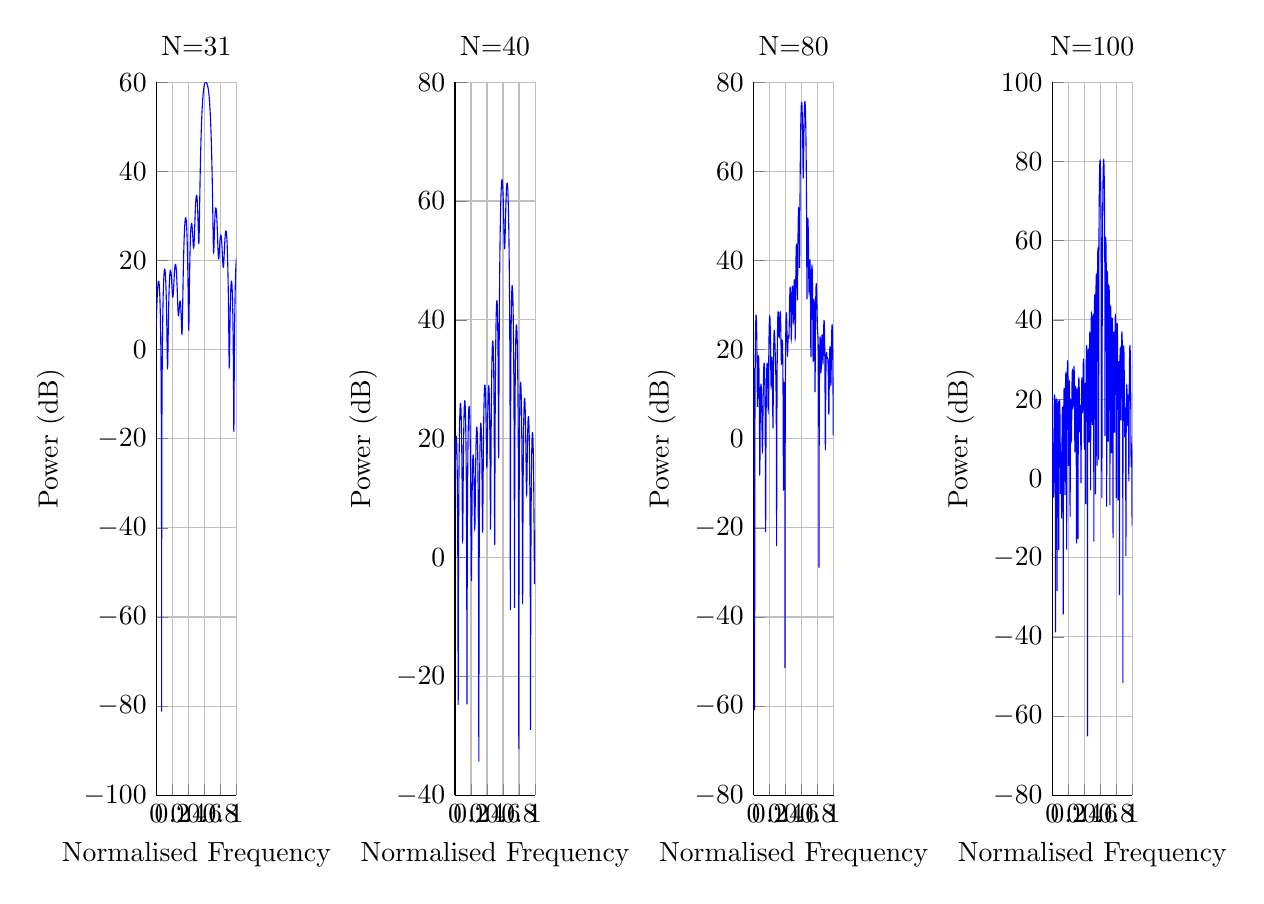
\begin{tikzpicture}

\begin{axis}[%
width=0.400265957446809in,
height=3.565625in,
scale only axis,
xmin=0,
xmax=1,
xlabel={Normalised Frequency},
xmajorgrids,
ymin=-40,
ymax=80,
ylabel={Power (dB)},
ymajorgrids,
name=plot2,
title={N=40},
axis x line*=bottom,
axis y line*=left
]
\addplot [color=blue,solid,forget plot]
  table[row sep=crcr]{-1	5.47923508540802\\
-0.99951171875	6.29642550452079\\
-0.9990234375	7.07604630830908\\
-0.99853515625	7.8181632669538\\
-0.998046875	8.52335458407455\\
-0.99755859375	9.19252067181034\\
-0.9970703125	9.82675198947961\\
-0.99658203125	10.427238161287\\
-0.99609375	10.9952062145705\\
-0.99560546875	11.5318792465667\\
-0.9951171875	12.0384493549956\\
-0.99462890625	12.5160604806614\\
-0.994140625	12.9657980983236\\
-0.99365234375	13.3886836023568\\
-0.9931640625	13.7856718752663\\
-0.99267578125	14.1576509788112\\
-0.9921875	14.5054432254801\\
-0.99169921875	14.8298071120191\\
-0.9912109375	15.1314397545209\\
-0.99072265625	15.4109795757933\\
-0.990234375	15.669009074066\\
-0.98974609375	15.906057557198\\
-0.9892578125	16.1226037651925\\
-0.98876953125	16.3190783307828\\
-0.98828125	16.4958660465017\\
-0.98779296875	16.6533079193719\\
-0.9873046875	16.7917030028502\\
-0.98681640625	16.9113100011178\\
-0.986328125	17.0123486441012\\
-0.98583984375	17.0950008333136\\
-0.9853515625	17.1594115591685\\
-0.98486328125	17.2056895901216\\
-0.984375	17.2339079330458\\
-0.98388671875	17.2441040627745\\
-0.9833984375	17.23627991684\\
-0.98291015625	17.2104016491209\\
-0.982421875	17.1663991334175\\
-0.98193359375	17.1041652048624\\
-0.9814453125	17.0235546235192\\
-0.98095703125	16.9243827404414\\
-0.98046875	16.8064238417821\\
-0.97998046875	16.66940914113\\
-0.9794921875	16.5130243839606\\
-0.97900390625	16.3369070207382\\
-0.978515625	16.1406428965589\\
-0.97802734375	15.9237623950008\\
-0.9775390625	15.6857359616876\\
-0.97705078125	15.4259689185407\\
-0.9765625	15.1437954622489\\
-0.97607421875	14.8384717194505\\
-0.9755859375	14.5091677056536\\
-0.97509765625	14.1549580039941\\
-0.974609375	13.7748109422353\\
-0.97412109375	13.3675760003847\\
-0.9736328125	12.9319691249762\\
-0.97314453125	12.4665555571109\\
-0.97265625	11.9697296969847\\
-0.97216796875	11.4396914247224\\
-0.9716796875	10.8744181725534\\
-0.97119140625	10.2716318937381\\
-0.970703125	9.62875989766785\\
-0.97021484375	8.94288832058973\\
-0.9697265625	8.21070678846963\\
-0.96923828125	7.42844263191891\\
-0.96875	6.59178289947621\\
-0.96826171875	5.69578252669392\\
-0.9677734375	4.73475764743721\\
-0.96728515625	3.70216477869104\\
-0.966796875	2.590470690127\\
-0.96630859375	1.39102668228407\\
-0.9658203125	0.0939799047554345\\
-0.96533203125	-1.31170597327688\\
-0.96484375	-2.8379652909011\\
-0.96435546875	-4.49675036345855\\
-0.9638671875	-6.29786337453249\\
-0.96337890625	-8.24406550765307\\
-0.962890625	-10.3206289497842\\
-0.96240234375	-12.4744194036897\\
-0.9619140625	-14.5771314812121\\
-0.96142578125	-16.3795932671628\\
-0.9609375	-17.5118586857787\\
-0.96044921875	-17.6341753448389\\
-0.9599609375	-16.6952847056059\\
-0.95947265625	-14.9796232753458\\
-0.958984375	-12.8719255881271\\
-0.95849609375	-10.6587097414189\\
-0.9580078125	-8.49700844265999\\
-0.95751953125	-6.45606048584405\\
-0.95703125	-4.5583745640846\\
-0.95654296875	-2.8045601777211\\
-0.9560546875	-1.18605311623711\\
-0.95556640625	0.308838105378672\\
-0.955078125	1.69220838461058\\
-0.95458984375	2.97541581641471\\
-0.9541015625	4.16867756188898\\
-0.95361328125	5.28099755559667\\
-0.953125	6.32023504083558\\
-0.95263671875	7.29322465753812\\
-0.9521484375	8.20590735396011\\
-0.95166015625	9.06345454992761\\
-0.951171875	9.87037894177624\\
-0.95068359375	10.6306304110712\\
-0.9501953125	11.3476777222062\\
-0.94970703125	12.024577549498\\
-0.94921875	12.6640325886059\\
-0.94873046875	13.2684404362094\\
-0.9482421875	13.8399347390883\\
-0.94775390625	14.3804199012921\\
-0.947265625	14.8916004329964\\
-0.94677734375	15.3750058416836\\
-0.9462890625	15.832011809577\\
-0.94580078125	16.2638582700236\\
-0.9453125	16.6716648870482\\
-0.94482421875	17.056444353282\\
-0.9443359375	17.4191138486911\\
-0.94384765625	17.7605049431089\\
-0.943359375	18.0813721770486\\
-0.94287109375	18.3824005155953\\
-0.9423828125	18.664211837669\\
-0.94189453125	18.9273705962425\\
-0.94140625	19.1723887630977\\
-0.94091796875	19.3997301535125\\
-0.9404296875	19.6098142111806\\
-0.93994140625	19.8030193210977\\
-0.939453125	19.9796857076325\\
-0.93896484375	20.1401179661708\\
-0.9384765625	20.2845872692607\\
-0.93798828125	20.4133332818582\\
-0.9375	20.5265658148634\\
-0.93701171875	20.6244662414861\\
-0.9365234375	20.707188696949\\
-0.93603515625	20.7748610785034\\
-0.935546875	20.8275858596146\\
-0.93505859375	20.8654407293703\\
-0.9345703125	20.8884790656255\\
-0.93408203125	20.8967302480368\\
-0.93359375	20.890199814925\\
-0.93310546875	20.8688694657603\\
-0.9326171875	20.8326969089658\\
-0.93212890625	20.7816155526105\\
-0.931640625	20.7155340333792\\
-0.93115234375	20.6343355769044\\
-0.9306640625	20.5378771800692\\
-0.93017578125	20.4259886031769\\
-0.9296875	20.2984711568608\\
-0.92919921875	20.1550962651915\\
-0.9287109375	19.9956037825275\\
-0.92822265625	19.8197000371291\\
-0.927734375	19.6270555692657\\
-0.92724609375	19.4173025253137\\
-0.9267578125	19.1900316619388\\
-0.92626953125	18.9447889056063\\
-0.92578125	18.681071402007\\
-0.92529296875	18.3983229770821\\
-0.9248046875	18.095928915604\\
-0.92431640625	17.773209943986\\
-0.923828125	17.4294152802117\\
-0.92333984375	17.0637145842457\\
-0.9228515625	16.6751886054038\\
-0.92236328125	16.2628182767658\\
-0.921875	15.8254719479599\\
-0.92138671875	15.3618903726801\\
-0.9208984375	14.8706689709078\\
-0.92041015625	14.3502367608438\\
-0.919921875	13.7988311921306\\
-0.91943359375	13.2144678962036\\
-0.9189453125	12.5949040819748\\
-0.91845703125	11.9375939174066\\
-0.91796875	11.2396337090945\\
-0.91748046875	10.4976939625626\\
-0.9169921875	9.70793438556514\\
-0.91650390625	8.86589644817291\\
-0.916015625	7.96636602426334\\
-0.91552734375	7.00319557303741\\
-0.9150390625	5.96907073294631\\
-0.91455078125	4.85519919435055\\
-0.9140625	3.65088876264179\\
-0.91357421875	2.34296394626053\\
-0.9130859375	0.914941373918007\\
-0.91259765625	-0.654165177211983\\
-0.912109375	-2.39162697183271\\
-0.91162109375	-4.33374802363803\\
-0.9111328125	-6.53026813537727\\
-0.91064453125	-9.05174291122221\\
-0.91015625	-12.0025706536052\\
-0.90966796875	-15.5453230303323\\
-0.9091796875	-19.9483804715371\\
-0.90869140625	-25.6747183054013\\
-0.908203125	-33.3932030237655\\
-0.90771484375	-41.1988316677108\\
-0.9072265625	-37.1215017671252\\
-0.90673828125	-28.6497137570833\\
-0.90625	-22.2056952309753\\
-0.90576171875	-17.3555118824721\\
-0.9052734375	-13.5272286618084\\
-0.90478515625	-10.3852507894733\\
-0.904296875	-7.73095190080696\\
-0.90380859375	-5.43976899744673\\
-0.9033203125	-3.42919309797641\\
-0.90283203125	-1.64201204973146\\
-0.90234375	-0.0370344357399\\
-0.90185546875	1.41633169662339\\
-0.9013671875	2.74140227893297\\
-0.90087890625	3.9563401523201\\
-0.900390625	5.07555989389737\\
-0.89990234375	6.11068620760513\\
-0.8994140625	7.07122528291142\\
-0.89892578125	7.96504609693886\\
-0.8984375	8.79873256897989\\
-0.89794921875	9.57784591957474\\
-0.8974609375	10.3071233061194\\
-0.89697265625	10.9906304012085\\
-0.896484375	11.6318801285935\\
-0.89599609375	12.2339261579934\\
-0.8955078125	12.7994373165086\\
-0.89501953125	13.3307573920269\\
-0.89453125	13.8299536264373\\
-0.89404296875	14.2988563596568\\
-0.8935546875	14.7390916825031\\
-0.89306640625	15.1521085163427\\
-0.892578125	15.5392012123924\\
-0.89208984375	15.9015285207984\\
-0.8916015625	16.240129596457\\
-0.89111328125	16.5559375690129\\
-0.890625	16.8497910972149\\
-0.89013671875	17.1224442446627\\
-0.8896484375	17.3745749490019\\
-0.88916015625	17.6067923054698\\
-0.888671875	17.8196428451131\\
-0.88818359375	18.013615955605\\
-0.8876953125	18.1891485665336\\
-0.88720703125	18.3466291999639\\
-0.88671875	18.486401469908\\
-0.88623046875	18.6087671002793\\
-0.8857421875	18.7139885193055\\
-0.88525390625	18.8022910787547\\
-0.884765625	18.873864938284\\
-0.88427734375	18.928866648456\\
-0.8837890625	18.967420460237\\
-0.88330078125	18.989619383891\\
-0.8828125	18.9955260159711\\
-0.88232421875	18.9851731494452\\
-0.8818359375	18.9585641787876\\
-0.88134765625	18.9156733090284\\
-0.880859375	18.8564455752299\\
-0.88037109375	18.7807966765913\\
-0.8798828125	18.6886126273426\\
-0.87939453125	18.5797492247556\\
-0.87890625	18.4540313329674\\
-0.87841796875	18.3112519798906\\
-0.8779296875	18.1511712633111\\
-0.87744140625	17.9735150614053\\
-0.876953125	17.7779735424455\\
-0.87646484375	17.5641994685431\\
-0.8759765625	17.3318062891164\\
-0.87548828125	17.0803660216706\\
-0.875	16.8094069208579\\
-0.87451171875	16.5184109422593\\
-0.8740234375	16.2068110157466\\
-0.87353515625	15.8739881558388\\
-0.873046875	15.5192684548608\\
-0.87255859375	15.1419200313361\\
-0.8720703125	14.7411500442768\\
-0.87158203125	14.3161019386938\\
-0.87109375	13.8658531655547\\
-0.87060546875	13.3894137303192\\
-0.8701171875	12.8857260819855\\
-0.86962890625	12.3536670791832\\
-0.869140625	11.7920530896847\\
-0.86865234375	11.1996497354058\\
-0.8681640625	10.5751884442791\\
-0.86767578125	9.91739289481654\\
-0.8671875	9.22501975212884\\
-0.86669921875	8.4969199496852\\
-0.8662109375	7.73212936990187\\
-0.86572265625	6.93000136066336\\
-0.865234375	6.09039833990348\\
-0.86474609375	5.21396592253661\\
-0.8642578125	4.3025203005617\\
-0.86376953125	3.35958676479012\\
-0.86328125	2.39113080687509\\
-0.86279296875	1.40651535536469\\
-0.8623046875	0.419683087148077\\
-0.86181640625	-0.549523965049394\\
-0.861328125	-1.47416606053138\\
-0.86083984375	-2.31965722838428\\
-0.8603515625	-3.0447011465201\\
-0.85986328125	-3.60465452124209\\
-0.859375	-3.95776036299476\\
-0.85888671875	-4.07330716770707\\
-0.8583984375	-3.93901210645995\\
-0.85791015625	-3.56429149936267\\
-0.857421875	-2.97773113189824\\
-0.85693359375	-2.22007191851076\\
-0.8564453125	-1.33596470420284\\
-0.85595703125	-0.367384511181452\\
-0.85546875	0.650112968031944\\
-0.85498046875	1.68860053576807\\
-0.8544921875	2.72737554671781\\
-0.85400390625	3.75181107876896\\
-0.853515625	4.75203268429366\\
-0.85302734375	5.72170989896038\\
-0.8525390625	6.6570676118907\\
-0.85205078125	7.55612627458793\\
-0.8515625	8.41814003416041\\
-0.85107421875	9.24319150150039\\
-0.8505859375	10.0319044661668\\
-0.85009765625	10.7852428142328\\
-0.849609375	11.5043712887615\\
-0.84912109375	12.1905600924355\\
-0.8486328125	12.845120326824\\
-0.84814453125	13.4693609982472\\
-0.84765625	14.0645610363031\\
-0.84716796875	14.6319517135814\\
-0.8466796875	15.1727062308372\\
-0.84619140625	15.687934201056\\
-0.845703125	16.1786794467224\\
-0.84521484375	16.6459200025125\\
-0.8447265625	17.0905695510591\\
-0.84423828125	17.5134797550047\\
-0.84375	17.9154431140864\\
-0.84326171875	18.2971960923613\\
-0.8427734375	18.6594223424819\\
-0.84228515625	19.0027559113718\\
-0.841796875	19.3277843519179\\
-0.84130859375	19.6350516934065\\
-0.8408203125	19.9250612429501\\
-0.84033203125	20.1982782035902\\
-0.83984375	20.4551321038782\\
-0.83935546875	20.6960190398217\\
-0.8388671875	20.9213037340037\\
-0.83837890625	21.1313214190999\\
-0.837890625	21.3263795543764\\
-0.83740234375	21.5067593843718\\
-0.8369140625	21.6727173490924\\
-0.83642578125	21.8244863548294\\
-0.8359375	21.9622769142672\\
-0.83544921875	22.0862781639679\\
-0.8349609375	22.196658766648\\
-0.83447265625	22.2935677049464\\
-0.833984375	22.3771349726404\\
-0.83349609375	22.4474721685249\\
-0.8330078125	22.5046729974223\\
-0.83251953125	22.5488136820594\\
-0.83203125	22.5799532888203\\
-0.83154296875	22.5981339696648\\
-0.8310546875	22.6033811217894\\
-0.83056640625	22.5957034658893\\
-0.830078125	22.575093043157\\
-0.82958984375	22.5415251304141\\
-0.8291015625	22.494958072008\\
-0.82861328125	22.4353330263082\\
-0.828125	22.3625736237949\\
-0.82763671875	22.2765855328326\\
-0.8271484375	22.1772559282492\\
-0.82666015625	22.0644528567853\\
-0.826171875	21.9380244923141\\
-0.82568359375	21.797798272446\\
-0.8251953125	21.6435799066969\\
-0.82470703125	21.4751522447894\\
-0.82421875	21.2922739918435\\
-0.82373046875	21.0946782551599\\
-0.8232421875	20.8820709049713\\
-0.82275390625	20.6541287288806\\
-0.822265625	20.4104973566809\\
-0.82177734375	20.1507889287917\\
-0.8212890625	19.8745794775943\\
-0.82080078125	19.5814059864322\\
-0.8203125	19.2707630858864\\
-0.81982421875	18.9420993410724\\
-0.8193359375	18.5948130770539\\
-0.81884765625	18.2282476819882\\
-0.818359375	17.8416863192767\\
-0.81787109375	17.4343459708334\\
-0.8173828125	17.0053707237534\\
-0.81689453125	16.5538242024721\\
-0.81640625	16.0786810385853\\
-0.81591796875	15.5788172619228\\
-0.8154296875	15.0529994911132\\
-0.81494140625	14.4998728028316\\
-0.814453125	13.9179471712811\\
-0.81396484375	13.3055824015147\\
-0.8134765625	12.6609715454241\\
-0.81298828125	11.9821229094436\\
-0.8125	11.2668409737457\\
-0.81201171875	10.5127069018076\\
-0.8115234375	9.71705992145808\\
-0.81103515625	8.87698185978458\\
-0.810546875	7.98928877241283\\
-0.81005859375	7.05053635086027\\
-0.8095703125	6.05705033287444\\
-0.80908203125	5.00500066594314\\
-0.80859375	3.89055064241491\\
-0.80810546875	2.71013281111518\\
-0.8076171875	1.46093711305553\\
-0.80712890625	0.141750393080023\\
-0.806640625	-1.24563200955595\\
-0.80615234375	-2.69409103229458\\
-0.8056640625	-4.18752242226394\\
-0.80517578125	-5.69540069372645\\
-0.8046875	-7.16563808423089\\
-0.80419921875	-8.51752215753594\\
-0.8037109375	-9.64017408050847\\
-0.80322265625	-10.4060601314432\\
-0.802734375	-10.7061531158657\\
-0.80224609375	-10.4949185439379\\
-0.8017578125	-9.81287094515617\\
-0.80126953125	-8.76640010675162\\
-0.80078125	-7.48313221387295\\
-0.80029296875	-6.07556447936825\\
-0.7998046875	-4.62631444983881\\
-0.79931640625	-3.18904175526501\\
-0.798828125	-1.79537625998138\\
-0.79833984375	-0.462132376637274\\
-0.7978515625	0.803139022369467\\
-0.79736328125	1.99839125093603\\
-0.796875	3.1246978029965\\
-0.79638671875	4.18479623203117\\
-0.7958984375	5.18222096412074\\
-0.79541015625	6.12079833256711\\
-0.794921875	7.00436056269425\\
-0.79443359375	7.83659063022554\\
-0.7939453125	8.62094456576069\\
-0.79345703125	9.36061900072007\\
-0.79296875	10.0585446087954\\
-0.79248046875	10.7173938585596\\
-0.7919921875	11.3395961765253\\
-0.79150390625	11.9273564489813\\
-0.791015625	12.4826745009554\\
-0.79052734375	13.0073642233872\\
-0.7900390625	13.5030716409713\\
-0.78955078125	13.9712915839128\\
-0.7890625	14.4133828446921\\
-0.78857421875	14.8305818255012\\
-0.7880859375	15.2240147498607\\
-0.78759765625	15.5947085455586\\
-0.787109375	15.9436005193345\\
-0.78662109375	16.2715469452118\\
-0.7861328125	16.5793306833034\\
-0.78564453125	16.8676679374698\\
-0.78515625	17.1372142503314\\
-0.78466796875	17.3885698239333\\
-0.7841796875	17.6222842444975\\
-0.78369140625	17.8388606804793\\
-0.783203125	18.0387596147531\\
-0.78271484375	18.2224021642074\\
-0.7822265625	18.390173033325\\
-0.78173828125	18.5424231424074\\
-0.78125	18.6794719658922\\
-0.78076171875	18.8016096116542\\
-0.7802734375	18.9090986681791\\
-0.77978515625	19.0021758430026\\
-0.779296875	19.0810534127373\\
-0.77880859375	19.1459205023202\\
-0.7783203125	19.1969442087431\\
-0.77783203125	19.2342705824375\\
-0.77734375	19.2580254776301\\
-0.77685546875	19.2683152813342\\
-0.7763671875	19.2652275291593\\
-0.77587890625	19.2488314147829\\
-0.775390625	19.2191781987093\\
-0.77490234375	19.1763015208165\\
-0.7744140625	19.1202176201502\\
-0.77392578125	19.0509254644359\\
-0.7734375	18.9684067908418\\
-0.77294921875	18.8726260586111\\
-0.7724609375	18.7635303132845\\
-0.77197265625	18.6410489613333\\
-0.771484375	18.5050934531114\\
-0.77099609375	18.3555568710927\\
-0.7705078125	18.1923134193762\\
-0.77001953125	18.0152178093988\\
-0.76953125	17.8241045356834\\
-0.76904296875	17.618787034243\\
-0.7685546875	17.3990567149533\\
-0.76806640625	17.1646818577662\\
-0.767578125	16.9154063610553\\
-0.76708984375	16.6509483286362\\
-0.7666015625	16.3709984800637\\
-0.76611328125	16.0752183666676\\
-0.765625	15.7632383734105\\
-0.76513671875	15.4346554840373\\
-0.7646484375	15.0890307841158\\
-0.76416015625	14.725886673454\\
-0.763671875	14.3447037560373\\
-0.76318359375	13.9449173721277\\
-0.7626953125	13.5259137336015\\
-0.76220703125	13.0870256201686\\
-0.76171875	12.6275275911125\\
-0.76123046875	12.1466306651116\\
-0.7607421875	11.6434764202973\\
-0.76025390625	11.117130469166\\
-0.759765625	10.5665752700862\\
-0.75927734375	9.99070225169982\\
-0.7587890625	9.38830325273073\\
-0.75830078125	8.75806132403191\\
-0.7578125	8.09854101198665\\
-0.75732421875	7.40817835776088\\
-0.7568359375	6.68527102864663\\
-0.75634765625	5.92796928178762\\
-0.755859375	5.13426890265095\\
-0.75537109375	4.302007947418\\
-0.7548828125	3.42887018532988\\
-0.75439453125	2.51239979545095\\
-0.75390625	1.55003445250739\\
-0.75341796875	0.539167951118318\\
-0.7529296875	-0.522740247291058\\
-0.75244140625	-1.63798153173321\\
-0.751953125	-2.80829902227894\\
-0.75146484375	-4.03440924915479\\
-0.7509765625	-5.31525002048074\\
-0.75048828125	-6.64681984938132\\
-0.75	-8.02043367930763\\
-0.74951171875	-9.42020921486223\\
-0.7490234375	-10.8196996237097\\
-0.74853515625	-12.1779729146297\\
-0.748046875	-13.4363596379693\\
-0.74755859375	-14.5186410934626\\
-0.7470703125	-15.3388000541436\\
-0.74658203125	-15.8190160853658\\
-0.74609375	-15.9137447070573\\
-0.74560546875	-15.6270496544732\\
-0.7451171875	-15.0109842130999\\
-0.74462890625	-14.1462444419489\\
-0.744140625	-13.1183597331722\\
-0.74365234375	-12.0012287713185\\
-0.7431640625	-10.8507913776975\\
-0.74267578125	-9.70561538188501\\
-0.7421875	-8.59038701423745\\
-0.74169921875	-7.51979548569095\\
-0.7412109375	-6.50177495144576\\
-0.74072265625	-5.53989055761531\\
-0.740234375	-4.63498116873998\\
-0.73974609375	-3.78624724992235\\
-0.7392578125	-2.99195373338864\\
-0.73876953125	-2.24987596870543\\
-0.73828125	-1.55757798024231\\
-0.73779296875	-0.912582698607316\\
-0.7373046875	-0.312473212588228\\
-0.73681640625	0.245049696830431\\
-0.736328125	0.762137493295144\\
-0.73583984375	1.24078087569903\\
-0.7353515625	1.68280715756286\\
-0.73486328125	2.08988378126569\\
-0.734375	2.46352526299324\\
-0.73388671875	2.80510186124653\\
-0.7333984375	3.11584890344645\\
-0.73291015625	3.3968761179756\\
-0.732421875	3.64917658393171\\
-0.73193359375	3.87363508001131\\
-0.7314453125	4.07103572091639\\
-0.73095703125	4.24206883625744\\
-0.73046875	4.38733708727453\\
-0.72998046875	4.50736084005858\\
-0.7294921875	4.60258282636334\\
-0.72900390625	4.67337212852696\\
-0.728515625	4.72002752605929\\
-0.72802734375	4.74278023981224\\
-0.7275390625	4.74179610645686\\
-0.72705078125	4.71717721199317\\
-0.7265625	4.66896300872373\\
-0.72607421875	4.59713093589908\\
-0.7255859375	4.50159656038322\\
-0.72509765625	4.38221325046911\\
-0.724609375	4.2387713937008\\
-0.72412109375	4.07099716862575\\
-0.7236328125	3.8785508813319\\
-0.72314453125	3.6610248811729\\
-0.72265625	3.4179410773186\\
-0.72216796875	3.14874809022399\\
-0.7216796875	2.85281809200671\\
-0.72119140625	2.52944342025416\\
-0.720703125	2.17783309557849\\
-0.72021484375	1.79710944099181\\
-0.7197265625	1.38630510063\\
-0.71923828125	0.944360900673682\\
-0.71875	0.470125207190549\\
-0.71826171875	-0.0376442557086591\\
-0.7177734375	-0.580274714302864\\
-0.71728515625	-1.15916671176494\\
-0.716796875	-1.77577350884515\\
-0.71630859375	-2.43156710323658\\
-0.7158203125	-3.12798442987046\\
-0.71533203125	-3.86634438089952\\
-0.71484375	-4.64772209897473\\
-0.71435546875	-5.47276110960043\\
-0.7138671875	-6.34139582405235\\
-0.71337890625	-7.25244656722777\\
-0.712890625	-8.20303725714562\\
-0.71240234375	-9.18777521215243\\
-0.7119140625	-10.1976315653964\\
-0.71142578125	-11.2184879966404\\
-0.7109375	-12.2294062955381\\
-0.71044921875	-13.2008853702789\\
-0.7099609375	-14.0937441367344\\
-0.70947265625	-14.8597634318734\\
-0.708984375	-15.4455275756077\\
-0.70849609375	-15.8003558544066\\
-0.7080078125	-15.8872051792859\\
-0.70751953125	-15.6926253748432\\
-0.70703125	-15.2307705164843\\
-0.70654296875	-14.5391631237062\\
-0.7060546875	-13.6686386809072\\
-0.70556640625	-12.6724858313007\\
-0.705078125	-11.5986296690182\\
-0.70458984375	-10.4859001128456\\
-0.7041015625	-9.36346019454841\\
-0.70361328125	-8.25195437003964\\
-0.703125	-7.16525766694213\\
-0.70263671875	-6.11220029904277\\
-0.7021484375	-5.09801128203508\\
-0.70166015625	-4.12542849106227\\
-0.701171875	-3.1955109008505\\
-0.70068359375	-2.30821477031558\\
-0.7001953125	-1.4627940649057\\
-0.69970703125	-0.658074638920121\\
-0.69921875	0.107360306325048\\
-0.69873046875	0.835046285644259\\
-0.6982421875	1.52655587954202\\
-0.69775390625	2.1834459678981\\
-0.697265625	2.80722458880872\\
-0.69677734375	3.3993310569248\\
-0.6962890625	3.96112497672205\\
-0.69580078125	4.49388116318961\\
-0.6953125	4.99878842793\\
-0.69482421875	5.47695083749487\\
-0.6943359375	5.92939049617839\\
-0.69384765625	6.35705121143908\\
-0.693359375	6.76080261039499\\
-0.69287109375	7.14144442035765\\
-0.6923828125	7.49971072561086\\
-0.69189453125	7.83627408063127\\
-0.69140625	8.15174940633721\\
-0.69091796875	8.44669762738097\\
-0.6904296875	8.72162902956448\\
-0.68994140625	8.97700633033745\\
-0.689453125	9.21324746424297\\
-0.68896484375	9.4307280906434\\
-0.6884765625	9.6297838341611\\
-0.68798828125	9.81071226974917\\
-0.6875	9.97377466468439\\
-0.68701171875	10.11919748941\\
-0.6865234375	10.2471737082933\\
-0.68603515625	10.3578638601775\\
-0.685546875	10.4513969372014\\
-0.68505859375	10.5278710688264\\
-0.6845703125	10.5873540163697\\
-0.68408203125	10.629883481646\\
-0.68359375	10.6554672315626\\
-0.68310546875	10.6640830387024\\
-0.6826171875	10.6556784360617\\
-0.68212890625	10.6301702821721\\
-0.681640625	10.5874441308105\\
-0.68115234375	10.527353397382\\
-0.6806640625	10.4497183118144\\
-0.68017578125	10.3543246454296\\
-0.6796875	10.2409221967318\\
-0.67919921875	10.1092230183689\\
-0.6787109375	9.95889936468894\\
-0.67822265625	9.78958133633902\\
-0.677734375	9.60085419528696\\
-0.67724609375	9.39225532056765\\
-0.6767578125	9.16327077210624\\
-0.67626953125	8.91333142737829\\
-0.67578125	8.64180865379883\\
-0.67529296875	8.34800947914356\\
-0.6748046875	8.03117122386419\\
-0.67431640625	7.69045556416432\\
-0.673828125	7.32494200513586\\
-0.67333984375	6.93362076209568\\
-0.6728515625	6.51538508001283\\
-0.67236328125	6.06902307237743\\
-0.671875	5.59320924233447\\
-0.67138671875	5.08649597602933\\
-0.6708984375	4.54730549472951\\
-0.67041015625	3.97392305486163\\
-0.669921875	3.36449264962264\\
-0.66943359375	2.71701717849891\\
-0.6689453125	2.02936614489102\\
-0.66845703125	1.2992956224139\\
-0.66796875	0.524487813205937\\
-0.66748046875	-0.297378511246143\\
-0.6669921875	-1.16850932188066\\
-0.66650390625	-2.09080180180264\\
-0.666015625	-3.06553557174811\\
-0.66552734375	-4.09288821703204\\
-0.6650390625	-5.17118715467088\\
-0.66455078125	-6.29577637927923\\
-0.6640625	-7.45734704541386\\
-0.66357421875	-8.6395864817823\\
-0.6630859375	-9.81611739607176\\
-0.66259765625	-10.9470758321871\\
-0.662109375	-11.9765087809494\\
-0.66162109375	-12.8330718943424\\
-0.6611328125	-13.437481949736\\
-0.66064453125	-13.7186914487545\\
-0.66015625	-13.6349350024911\\
-0.65966796875	-13.1888288478166\\
-0.6591796875	-12.4263579364875\\
-0.65869140625	-11.4204825271014\\
-0.658203125	-10.2501967304115\\
-0.65771484375	-8.98528523552226\\
-0.6572265625	-7.67979076252642\\
-0.65673828125	-6.37185270794074\\
-0.65625	-5.08649887902668\\
-0.65576171875	-3.83906556112938\\
-0.6552734375	-2.63818562687153\\
-0.65478515625	-1.48805771088304\\
-0.654296875	-0.390047364303797\\
-0.65380859375	0.6562301682458\\
-0.6533203125	1.6521969388922\\
-0.65283203125	2.5998514666598\\
-0.65234375	3.50147558643713\\
-0.65185546875	4.35945113637281\\
-0.6513671875	5.1761479136488\\
-0.65087890625	5.95385754031219\\
-0.650390625	6.69475669199502\\
-0.64990234375	7.4008889344399\\
-0.6494140625	8.07415819354487\\
-0.64892578125	8.71632934566964\\
-0.6484375	9.32903301616321\\
-0.64794921875	9.91377271653175\\
-0.6474609375	10.4719331299246\\
-0.64697265625	11.0047887973775\\
-0.646484375	11.513512745632\\
-0.64599609375	11.9991847846965\\
-0.6455078125	12.4627993243812\\
-0.64501953125	12.9052726365697\\
-0.64453125	13.3274495388959\\
-0.64404296875	13.7301095056187\\
-0.6435546875	14.1139722293091\\
-0.64306640625	14.4797026667966\\
-0.642578125	14.8279156075042\\
-0.64208984375	15.1591798037264\\
-0.6416015625	15.4740217018197\\
-0.64111328125	15.7729288115033\\
-0.640625	16.0563527480466\\
-0.64013671875	16.3247119793944\\
-0.6396484375	16.5783943074778\\
-0.63916015625	16.8177591102035\\
-0.638671875	17.0431393679983\\
-0.63818359375	17.2548434963448\\
-0.6376953125	17.4531570034991\\
-0.63720703125	17.6383439905406\\
-0.63671875	17.8106485090534\\
-0.63623046875	17.9702957900822\\
-0.6357421875	18.1174933565131\\
-0.63525390625	18.2524320297002\\
-0.634765625	18.3752868399712\\
-0.63427734375	18.486217849585\\
-0.6337890625	18.5853708957717\\
-0.63330078125	18.6728782606423\\
-0.6328125	18.7488592740073\\
-0.63232421875	18.8134208544734\\
-0.6318359375	18.8666579935918\\
-0.63134765625	18.9086541872968\\
-0.630859375	18.9394818183986\\
-0.63037109375	18.9592024934672\\
-0.6298828125	18.9678673370616\\
-0.62939453125	18.9655172459186\\
-0.62890625	18.9521831054088\\
-0.62841796875	18.9278859702926\\
-0.6279296875	18.8926372115679\\
-0.62744140625	18.846438630982\\
-0.626953125	18.7892825445904\\
-0.62646484375	18.7211518365787\\
-0.6259765625	18.6420199844221\\
-0.62548828125	18.5518510563371\\
-0.625	18.4505996818893\\
-0.62451171875	18.338210996554\\
-0.6240234375	18.2146205609883\\
-0.62353515625	18.0797542557728\\
-0.623046875	17.9335281524112\\
-0.62255859375	17.7758483614585\\
-0.6220703125	17.6066108587775\\
-0.62158203125	17.4257012911201\\
-0.62109375	17.2329947625011\\
-0.62060546875	17.0283556031995\\
-0.6201171875	16.811637123703\\
-0.61962890625	16.5826813565385\\
-0.619140625	16.341318789728\\
-0.61865234375	16.0873680966307\\
-0.6181640625	15.8206358682214\\
-0.61767578125	15.5409163554789\\
-0.6171875	15.2479912316072\\
-0.61669921875	14.9416293863781\\
-0.6162109375	14.62158676811\\
-0.61572265625	14.2876062928323\\
-0.615234375	13.9394178452519\\
-0.61474609375	13.576738402475\\
-0.6142578125	13.1992723193858\\
-0.61376953125	12.8067118245366\\
-0.61328125	12.3987377878801\\
-0.61279296875	11.9750208373015\\
-0.6123046875	11.5352229204938\\
-0.61181640625	11.078999433235\\
-0.611328125	10.6060020658029\\
-0.61083984375	10.115882557591\\
-0.6103515625	9.60829759776345\\
-0.60986328125	9.08291516916965\\
-0.609375	8.53942270620718\\
-0.60888671875	7.97753752765797\\
-0.6083984375	7.39702011564106\\
-0.60791015625	6.79769094442213\\
-0.607421875	6.17945171976149\\
-0.60693359375	5.54231207061519\\
-0.6064453125	4.8864229362654\\
-0.60595703125	4.2121181021742\\
-0.60546875	3.51996553382757\\
-0.60498046875	2.81083029684475\\
-0.6044921875	2.08595086076187\\
-0.60400390625	1.3470303457003\\
-0.603515625	0.59634360653668\\
-0.60302734375	-0.163140298738624\\
-0.6025390625	-0.92762308180573\\
-0.60205078125	-1.69233626022552\\
-0.6015625	-2.45140647522055\\
-0.60107421875	-3.19774685260785\\
-0.6005859375	-3.92300322462712\\
-0.60009765625	-4.61759306048778\\
-0.599609375	-5.27088076873576\\
-0.59912109375	-5.87153062343306\\
-0.5986328125	-6.40806199334352\\
-0.59814453125	-6.86959664299306\\
-0.59765625	-7.24673656050614\\
-0.59716796875	-7.53245505673155\\
-0.5966796875	-7.72284538236772\\
-0.59619140625	-7.81757276540124\\
-0.595703125	-7.81992784943371\\
-0.59521484375	-7.73646914262799\\
-0.5947265625	-7.57633646969609\\
-0.59423828125	-7.35038111390832\\
-0.59375	-7.07027250443443\\
-0.59326171875	-6.74771098168909\\
-0.5927734375	-6.39382249761013\\
-0.59228515625	-6.01875712154311\\
-0.591796875	-5.6314736632845\\
-0.59130859375	-5.23967178037088\\
-0.5908203125	-4.84982751860162\\
-0.59033203125	-4.46729251874758\\
-0.58984375	-4.09642571991658\\
-0.58935546875	-3.74073564243638\\
-0.5888671875	-3.40301933301043\\
-0.58837890625	-3.08549014399088\\
-0.587890625	-2.78989073964772\\
-0.58740234375	-2.51759041698389\\
-0.5869140625	-2.26966740278341\\
-0.58642578125	-2.04697760219278\\
-0.5859375	-1.85021160557345\\
-0.58544921875	-1.67994180712066\\
-0.5849609375	-1.53666138237139\\
-0.58447265625	-1.42081669516375\\
-0.583984375	-1.33283450746515\\
-0.58349609375	-1.2731451755849\\
-0.5830078125	-1.24220284798046\\
-0.58251953125	-1.24050353956552\\
-0.58203125	-1.26860184723133\\
-0.58154296875	-1.32712699127506\\
-0.5810546875	-1.41679881709886\\
-0.58056640625	-1.53844437074733\\
-0.580078125	-1.69301567148319\\
-0.57958984375	-1.88160934712159\\
-0.5791015625	-2.10548887793301\\
-0.57861328125	-2.36611032026858\\
-0.578125	-2.66515256350316\\
-0.57763671875	-3.0045534311566\\
-0.5771484375	-3.38655329540257\\
-0.57666015625	-3.81374837249644\\
-0.576171875	-4.28915656298603\\
-0.57568359375	-4.81629968251719\\
-0.5751953125	-5.39930733086054\\
-0.57470703125	-6.04304967787988\\
-0.57421875	-6.75330943886618\\
-0.57373046875	-7.53700781069883\\
-0.5732421875	-8.40250605102884\\
-0.57275390625	-9.36001526225763\\
-0.572265625	-10.4221645523228\\
-0.57177734375	-11.6048071632513\\
-0.5712890625	-12.9281951142563\\
-0.57080078125	-14.4187449374176\\
-0.5703125	-16.1117916550324\\
-0.56982421875	-18.0560791737693\\
-0.5693359375	-20.3214928090677\\
-0.56884765625	-23.0133243732507\\
-0.568359375	-26.3010650322043\\
-0.56787109375	-30.4841372078543\\
-0.5673828125	-36.1717745682147\\
-0.56689453125	-44.949366337071\\
-0.56640625	-64.3283388801126\\
-0.56591796875	-62.7535623085687\\
-0.5654296875	-43.9542573778939\\
-0.56494140625	-35.0100038469157\\
-0.564453125	-29.0487072941191\\
-0.56396484375	-24.5558017181555\\
-0.5634765625	-20.941226063873\\
-0.56298828125	-17.9128108222484\\
-0.5625	-15.3043430899915\\
-0.56201171875	-13.0121710716777\\
-0.5615234375	-10.9672717309155\\
-0.56103515625	-9.12135425297557\\
-0.560546875	-7.43930356623837\\
-0.56005859375	-5.8947812904133\\
-0.5595703125	-4.46752231726959\\
-0.55908203125	-3.14159853736136\\
-0.55859375	-1.90426209152574\\
-0.55810546875	-0.745150478957469\\
-0.5576171875	0.344274357552919\\
-0.55712890625	1.37113104368097\\
-0.556640625	2.3414171573341\\
-0.55615234375	3.26023299449425\\
-0.5556640625	4.13195204802822\\
-0.55517578125	4.96035273824779\\
-0.5546875	5.74872150640774\\
-0.55419921875	6.49993443169629\\
-0.5537109375	7.21652252644168\\
-0.55322265625	7.9007244759438\\
-0.552734375	8.55452961256599\\
-0.55224609375	9.17971321613941\\
-0.5517578125	9.77786572764624\\
-0.55126953125	10.3504170927911\\
-0.55078125	10.8986571773063\\
-0.55029296875	11.4237529897779\\
-0.5498046875	11.9267632916765\\
-0.54931640625	12.4086510549095\\
-0.548828125	12.870294135122\\
-0.54833984375	13.3124944573546\\
-0.5478515625	13.7359859545196\\
-0.54736328125	14.141441454839\\
-0.546875	14.5294786791451\\
-0.54638671875	14.9006654807546\\
-0.5458984375	15.2555244379302\\
-0.54541015625	15.5945368905645\\
-0.544921875	15.9181464977552\\
-0.54443359375	16.2267623806962\\
-0.5439453125	16.520761905227\\
-0.54345703125	16.8004931500546\\
-0.54296875	17.0662770997428\\
-0.54248046875	17.3184095957889\\
-0.5419921875	17.5571630742707\\
-0.54150390625	17.7827881144742\\
-0.541015625	17.9955148194676\\
-0.54052734375	18.1955540466673\\
-0.5400390625	18.3830985039468\\
-0.53955078125	18.5583237247069\\
-0.5390625	18.7213889334859\\
-0.53857421875	18.8724378121042\\
-0.5380859375	19.0115991749525\\
-0.53759765625	19.1389875608299\\
-0.537109375	19.254703747673\\
-0.53662109375	19.358835195579\\
-0.5361328125	19.4514564226838\\
-0.53564453125	19.5326293177003\\
-0.53515625	19.6024033922331\\
-0.53466796875	19.6608159753519\\
-0.5341796875	19.7078923523156\\
-0.53369140625	19.7436458487805\\
-0.533203125	19.7680778612926\\
-0.53271484375	19.781177834339\\
-0.5322265625	19.7829231837233\\
-0.53173828125	19.7732791655048\\
-0.53125	19.7521986892126\\
-0.53076171875	19.719622073494\\
-0.5302734375	19.67547674177\\
-0.52978515625	19.6196768548535\\
-0.529296875	19.5521228768034\\
-0.52880859375	19.4727010695549\\
-0.5283203125	19.3812829110419\\
-0.52783203125	19.2777244306209\\
-0.52734375	19.1618654545726\\
-0.52685546875	19.0335287532967\\
-0.5263671875	18.8925190804918\\
-0.52587890625	18.7386220930867\\
-0.525390625	18.5716031389483\\
-0.52490234375	18.3912058973571\\
-0.5244140625	18.1971508548975\\
-0.52392578125	17.9891335966562\\
-0.5234375	17.766822889412\\
-0.52294921875	17.5298585297111\\
-0.5224609375	17.2778489252573\\
-0.52197265625	17.0103683727498\\
-0.521484375	16.726953989001\\
-0.52099609375	16.427102244641\\
-0.5205078125	16.1102650406866\\
-0.52001953125	15.775845257389\\
-0.51953125	15.4231916916287\\
-0.51904296875	15.0515932831718\\
-0.5185546875	14.6602725106406\\
-0.51806640625	14.2483778142071\\
-0.517578125	13.8149748726814\\
-0.51708984375	13.3590365263765\\
-0.5166015625	12.8794310920557\\
-0.51611328125	12.3749087599734\\
-0.515625	11.8440856923904\\
-0.51513671875	11.2854253538766\\
-0.5146484375	10.6972164908519\\
-0.51416015625	10.0775470341356\\
-0.513671875	9.42427301456163\\
-0.51318359375	8.73498134594452\\
-0.5126953125	8.00694502625321\\
-0.51220703125	7.23706891687649\\
-0.51171875	6.42182375672779\\
-0.51123046875	5.55716542394323\\
-0.5107421875	4.63843564383825\\
-0.51025390625	3.66023933845314\\
-0.509765625	2.61629263873562\\
-0.50927734375	1.49923435727448\\
-0.5087890625	0.30039283064608\\
-0.50830078125	-0.990499498586216\\
-0.5078125	-2.3856470471761\\
-0.50732421875	-3.8995764784462\\
-0.5068359375	-5.54951578630343\\
-0.50634765625	-7.35561422458166\\
-0.505859375	-9.3405920104275\\
-0.50537109375	-11.5277577832612\\
-0.5048828125	-13.9346984130813\\
-0.50439453125	-16.5559881734491\\
-0.50390625	-19.3199673943034\\
-0.50341796875	-21.9961349097272\\
-0.5029296875	-24.070046027801\\
-0.50244140625	-24.8184121900723\\
-0.501953125	-23.8972550923352\\
-0.50146484375	-21.7551181735486\\
-0.5009765625	-19.1091303161655\\
-0.50048828125	-16.4257835006231\\
-0.5	-13.9033055163494\\
-0.49951171875	-11.5988884611366\\
-0.4990234375	-9.51261291187044\\
-0.49853515625	-7.6253327210705\\
-0.498046875	-5.91360762586154\\
-0.49755859375	-4.35506846800704\\
-0.4970703125	-2.93003744589792\\
-0.49658203125	-1.62174707221984\\
-0.49609375	-0.416078980511447\\
-0.49560546875	0.698822236615859\\
-0.4951171875	1.73292946408352\\
-0.49462890625	2.69466573944185\\
-0.494140625	3.59118130779501\\
-0.49365234375	4.42857943000821\\
-0.4931640625	5.21209880382379\\
-0.49267578125	5.94626060452113\\
-0.4921875	6.6349871691632\\
-0.49169921875	7.28169811728521\\
-0.4912109375	7.88938854832353\\
-0.49072265625	8.46069298159393\\
-0.490234375	8.99793791792206\\
-0.48974609375	9.50318528125043\\
-0.4892578125	9.97826851410475\\
-0.48876953125	10.4248227244955\\
-0.48828125	10.8443099897533\\
-0.48779296875	11.2380406957491\\
-0.4873046875	11.6071916129282\\
-0.48681640625	11.9528212720278\\
-0.486328125	12.2758830934119\\
-0.48583984375	12.5772366379005\\
-0.4853515625	12.8576572786429\\
-0.48486328125	13.1178445390603\\
-0.484375	13.3584292981476\\
-0.48388671875	13.5799800291555\\
-0.4833984375	13.7830082090927\\
-0.48291015625	13.967973013195\\
-0.482421875	14.1352853894272\\
-0.48193359375	14.2853115923678\\
-0.4814453125	14.4183762428037\\
-0.48095703125	14.5347649685082\\
-0.48046875	14.6347266725667\\
-0.47998046875	14.7184754679164\\
-0.4794921875	14.7861923102026\\
-0.47900390625	14.8380263554101\\
-0.478515625	14.8740960638148\\
-0.47802734375	14.8944900674721\\
-0.4775390625	14.8992678145882\\
-0.47705078125	14.8884600005969\\
-0.4765625	14.8620687924936\\
-0.47607421875	14.8200678498779\\
-0.4755859375	14.7624021431443\\
-0.47509765625	14.6889875662637\\
-0.474609375	14.5997103385417\\
-0.47412109375	14.4944261865502\\
-0.4736328125	14.3729592940161\\
-0.47314453125	14.2351010037419\\
-0.47265625	14.0806082515074\\
-0.47216796875	13.9092017072634\\
-0.4716796875	13.7205635936266\\
-0.47119140625	13.5143351455661\\
-0.470703125	13.2901136680389\\
-0.47021484375	13.0474491399479\\
-0.4697265625	12.7858403028663\\
-0.46923828125	12.5047301611502\\
-0.46875	12.203500805884\\
-0.46826171875	11.8814674580388\\
-0.4677734375	11.5378716055609\\
-0.46728515625	11.1718730839955\\
-0.466796875	10.7825409195852\\
-0.46630859375	10.3688427162066\\
-0.4658203125	9.92963232128123\\
-0.46533203125	9.46363544876047\\
-0.46484375	8.96943286671233\\
-0.46435546875	8.4454406695589\\
-0.4638671875	7.88988704648335\\
-0.46337890625	7.30078482297824\\
-0.462890625	6.67589888623767\\
-0.46240234375	6.01270740102411\\
-0.4619140625	5.30835547540568\\
-0.46142578125	4.5595996431664\\
-0.4609375	3.76274119813463\\
-0.46044921875	2.91354607148433\\
-0.4599609375	2.00714865615495\\
-0.45947265625	1.03793691543147\\
-0.458984375	-0.000583377299201419\\
-0.45849609375	-1.11594556644737\\
-0.4580078125	-2.31689567472832\\
-0.45751953125	-3.61356675011348\\
-0.45703125	-5.01761282025099\\
-0.45654296875	-6.5422054639201\\
-0.4560546875	-8.20167347660913\\
-0.45556640625	-10.0102969634225\\
-0.455078125	-11.9791792586267\\
-0.45458984375	-14.1088728861174\\
-0.4541015625	-16.3730382627527\\
-0.45361328125	-18.6851679570287\\
-0.453125	-20.8426796946288\\
-0.45263671875	-22.4767951904051\\
-0.4521484375	-23.1290650061452\\
-0.45166015625	-22.5566500880082\\
-0.451171875	-20.9655952229944\\
-0.45068359375	-18.8100322248495\\
-0.4501953125	-16.4733526076969\\
-0.44970703125	-14.1718500145493\\
-0.44921875	-11.9999371159328\\
-0.44873046875	-9.98768770402856\\
-0.4482421875	-8.13609566107218\\
-0.44775390625	-6.43458403576047\\
-0.447265625	-4.86895275523522\\
-0.44677734375	-3.42477062020727\\
-0.4462890625	-2.08869887239221\\
-0.44580078125	-0.848902367278199\\
-0.4453125	0.304926324787455\\
-0.44482421875	1.38169366714817\\
-0.4443359375	2.38907816050773\\
-0.44384765625	3.33370496093236\\
-0.443359375	4.22130470350482\\
-0.44287109375	5.05685131052354\\
-0.4423828125	5.84467880179095\\
-0.44189453125	6.58857916364664\\
-0.44140625	7.29188392527546\\
-0.44091796875	7.95753205734212\\
-0.4404296875	8.58812653244007\\
-0.43994140625	9.1859815440777\\
-0.439453125	9.75316204673684\\
-0.43896484375	10.2915169829905\\
-0.4384765625	10.8027073123686\\
-0.43798828125	11.2882297489199\\
-0.4375	11.7494369450235\\
-0.43701171875	12.1875547218914\\
-0.4365234375	12.6036968366019\\
-0.43603515625	12.9988776863861\\
-0.435546875	13.3740232790308\\
-0.43505859375	13.7299807402237\\
-0.4345703125	14.0675265816867\\
-0.43408203125	14.3873739157888\\
-0.43359375	14.6901787712653\\
-0.43310546875	14.9765456392696\\
-0.4326171875	15.2470323581626\\
-0.43212890625	15.5021544282998\\
-0.431640625	15.7423888339213\\
-0.43115234375	15.9681774375121\\
-0.4306640625	16.1799300022406\\
-0.43017578125	16.3780268899362\\
-0.4296875	16.5628214752421\\
-0.42919921875	16.7346423108527\\
-0.4287109375	16.8937950739093\\
-0.42822265625	17.0405643195481\\
-0.427734375	17.175215064132\\
-0.42724609375	17.2979942177526\\
-0.4267578125	17.4091318830835\\
-0.42626953125	17.5088425355182\\
-0.42578125	17.5973260976928\\
-0.42529296875	17.6747689199144\\
-0.4248046875	17.7413446766621\\
-0.42431640625	17.7972151881575\\
-0.423828125	17.8425311749948\\
-0.42333984375	17.8774329529483\\
-0.4228515625	17.9020510743225\\
-0.42236328125	17.9165069215589\\
-0.421875	17.9209132582505\\
-0.42138671875	17.9153747422264\\
-0.4208984375	17.8999884049531\\
-0.42041015625	17.8748441011335\\
-0.419921875	17.8400249320791\\
-0.41943359375	17.7956076461647\\
-0.4189453125	17.7416630194543\\
-0.41845703125	17.6782562194009\\
-0.41796875	17.6054471543681\\
-0.41748046875	17.523290811604\\
-0.4169921875	17.4318375861968\\
-0.41650390625	17.3311336034786\\
-0.416015625	17.2212210372942\\
-0.41552734375	17.1021384265325\\
-0.4150390625	16.9739209923116\\
-0.41455078125	16.8366009582325\\
-0.4140625	16.690207876147\\
-0.41357421875	16.5347689599454\\
-0.4130859375	16.3703094299364\\
-0.41259765625	16.1968528704837\\
-0.412109375	16.0144216036595\\
-0.41162109375	15.8230370817969\\
-0.4111328125	15.6227203019425\\
-0.41064453125	15.4134922453507\\
-0.41015625	15.1953743452977\\
-0.40966796875	14.9683889866398\\
-0.4091796875	14.7325600406788\\
-0.40869140625	14.4879134390297\\
-0.408203125	14.2344777903037\\
-0.40771484375	13.9722850435091\\
-0.4072265625	13.7013712021296\\
-0.40673828125	13.4217770928417\\
-0.40625	13.1335491927755\\
-0.40576171875	12.8367405190688\\
-0.4052734375	12.5314115842071\\
-0.40478515625	12.2176314202404\\
-0.404296875	11.8954786743913\\
-0.40380859375	11.5650427777831\\
-0.4033203125	11.2264251879682\\
-0.40283203125	10.8797407045829\\
-0.40234375	10.5251188557335\\
-0.40185546875	10.1627053505708\\
-0.4013671875	9.79266359086645\\
-0.40087890625	9.41517623120146\\
-0.400390625	9.03044677354398\\
-0.39990234375	8.63870117746871\\
-0.3994140625	8.24018946200372\\
-0.39892578125	7.83518726904879\\
-0.3984375	7.42399735149167\\
-0.39794921875	7.00695094159084\\
-0.3974609375	6.58440894699249\\
-0.39697265625	6.15676291307142\\
-0.396484375	5.72443568139135\\
-0.39599609375	5.28788166533699\\
-0.3955078125	4.8475866558719\\
-0.39501953125	4.4040670635578\\
-0.39453125	3.95786849820186\\
-0.39404296875	3.50956358568355\\
-0.3935546875	3.05974892366391\\
-0.39306640625	2.60904108504957\\
-0.392578125	2.1580715913197\\
-0.39208984375	1.7074807980218\\
-0.3916015625	1.25791066255255\\
-0.39111328125	0.809996399983155\\
-0.390625	0.364357075817257\\
-0.39013671875	-0.0784147658878561\\
-0.3896484375	-0.517764286543418\\
-0.38916015625	-0.953186140859943\\
-0.388671875	-1.38423660605628\\
-0.38818359375	-1.81054574176872\\
-0.3876953125	-2.23182923193176\\
-0.38720703125	-2.64789953621272\\
-0.38671875	-3.05867597269785\\
-0.38623046875	-3.46419336765283\\
-0.3857421875	-3.86460894282299\\
-0.38525390625	-4.26020716439708\\
-0.384765625	-4.65140234684963\\
-0.38427734375	-5.03873888389909\\
-0.3837890625	-5.42288906077695\\
-0.38330078125	-5.8046484789953\\
-0.3828125	-6.18492918872742\\
-0.38232421875	-6.56475066710688\\
-0.3818359375	-6.94522879648798\\
-0.38134765625	-7.32756297946227\\
-0.380859375	-7.7130214728147\\
-0.38037109375	-8.1029249270542\\
-0.3798828125	-8.49862797829987\\
-0.37939453125	-8.90149855122599\\
-0.37890625	-9.31289429020505\\
-0.37841796875	-9.73413523346429\\
-0.3779296875	-10.1664714724584\\
-0.37744140625	-10.6110440844552\\
-0.376953125	-11.0688370794432\\
-0.37646484375	-11.5406174564975\\
-0.3759765625	-12.0268597269754\\
-0.37548828125	-12.5276504696928\\
-0.375	-13.0425677324919\\
-0.37451171875	-13.5705295865526\\
-0.3740234375	-14.1096062528213\\
-0.37353515625	-14.6567916100269\\
-0.373046875	-15.20773361245\\
-0.37255859375	-15.7564307264796\\
-0.3720703125	-16.2949148792393\\
-0.37158203125	-16.8129624495595\\
-0.37109375	-17.2979039360197\\
-0.37060546875	-17.7346364937336\\
-0.3701171875	-18.1059702576835\\
-0.36962890625	-18.3934376859334\\
-0.369140625	-18.578636606613\\
-0.36865234375	-18.6450427552195\\
-0.3681640625	-18.5800337024594\\
-0.36767578125	-18.3766883559625\\
-0.3671875	-18.03487712658\\
-0.36669921875	-17.5613119752819\\
-0.3662109375	-16.9685410000201\\
-0.36572265625	-16.2731955040585\\
-0.365234375	-15.4939694121223\\
-0.36474609375	-14.6497778946944\\
-0.3642578125	-13.7583710130497\\
-0.36376953125	-12.8354818666498\\
-0.36328125	-11.8944472000656\\
-0.36279296875	-10.9461736417176\\
-0.3623046875	-9.99931723390192\\
-0.36181640625	-9.06056915608017\\
-0.361328125	-8.13497408359788\\
-0.36083984375	-7.22623733843946\\
-0.3603515625	-6.33699874376323\\
-0.35986328125	-5.46906507561787\\
-0.359375	-4.62360100739291\\
-0.35888671875	-3.80128242812972\\
-0.3583984375	-3.00241756191165\\
-0.35791015625	-2.22704151463071\\
-0.357421875	-1.47498941342783\\
-0.35693359375	-0.745952582288505\\
-0.3564453125	-0.0395214288187657\\
-0.35595703125	0.644781994544591\\
-0.35546875	1.3074794057702\\
-0.35498046875	1.94911784401693\\
-0.3544921875	2.57025592468342\\
-0.35400390625	3.17145369186559\\
-0.353515625	3.75326521534002\\
-0.35302734375	4.31623327645134\\
-0.3525390625	4.86088563969207\\
-0.35205078125	5.38773252412645\\
-0.3515625	5.89726497899563\\
-0.35107421875	6.38995393707191\\
-0.3505859375	6.86624977244361\\
-0.35009765625	7.32658223016766\\
-0.349609375	7.77136062650323\\
-0.34912109375	8.20097424245413\\
-0.3486328125	8.61579285179633\\
-0.34814453125	9.01616733894114\\
-0.34765625	9.40243037288375\\
-0.34716796875	9.77489711186074\\
-0.3466796875	10.1338659197795\\
-0.34619140625	10.4796190804234\\
-0.345703125	10.8124234992282\\
-0.34521484375	11.1325313853284\\
-0.3447265625	11.4401809087835\\
-0.34423828125	11.7355968295818\\
-0.34375	12.0189910962925\\
-0.34326171875	12.2905634131905\\
-0.3427734375	12.5505017753935\\
-0.34228515625	12.7989829720709\\
-0.341796875	13.0361730581598\\
-0.34130859375	13.2622277952879\\
-0.3408203125	13.4772930627809\\
-0.34033203125	13.681505239741\\
-0.33984375	13.8749915592466\\
-0.33935546875	14.0578704357454\\
-0.3388671875	14.2302517667054\\
-0.33837890625	14.3922372095649\\
-0.337890625	14.5439204349746\\
-0.33740234375	14.6853873572754\\
-0.3369140625	14.8167163430878\\
-0.33642578125	14.9379783988246\\
-0.3359375	15.049237337862\\
-0.33544921875	15.1505499280318\\
-0.3349609375	15.2419660200199\\
-0.33447265625	15.3235286571759\\
-0.333984375	15.3952741671638\\
-0.33349609375	15.4572322358023\\
-0.3330078125	15.5094259633625\\
-0.33251953125	15.5518719035151\\
-0.33203125	15.5845800850338\\
-0.33154296875	15.6075540162826\\
-0.3310546875	15.6207906724326\\
-0.33056640625	15.6242804652679\\
-0.330078125	15.6180071953548\\
-0.32958984375	15.6019479862598\\
-0.3291015625	15.576073200412\\
-0.32861328125	15.5403463361064\\
-0.328125	15.494723905051\\
-0.32763671875	15.4391552897531\\
-0.3271484375	15.3735825799335\\
-0.32666015625	15.2979403870424\\
-0.326171875	15.2121556358324\\
-0.32568359375	15.1161473318122\\
-0.3251953125	15.0098263032763\\
-0.32470703125	14.8930949164576\\
-0.32421875	14.7658467622052\\
-0.32373046875	14.6279663124267\\
-0.3232421875	14.4793285443705\\
-0.32275390625	14.3197985306504\\
-0.322265625	14.1492309927314\\
-0.32177734375	13.9674698154123\\
-0.3212890625	13.7743475196524\\
-0.32080078125	13.5696846909011\\
-0.3203125	13.3532893599096\\
-0.31982421875	13.1249563328349\\
-0.3193359375	12.8844664673042\\
-0.31884765625	12.6315858909985\\
-0.318359375	12.366065159266\\
-0.31787109375	12.0876383483039\\
-0.3173828125	11.7960220805966\\
-0.31689453125	11.4909144796008\\
-0.31640625	11.1719940512007\\
-0.31591796875	10.8389184902897\\
-0.3154296875	10.4913234120785\\
-0.31494140625	10.1288210095425\\
-0.314453125	9.75099864098006\\
-0.31396484375	9.35741735523997\\
-0.3134765625	8.94761036713212\\
-0.31298828125	8.521081502338\\
-0.3125	8.07730364042797\\
-0.31201171875	7.61571719722888\\
-0.3115234375	7.13572870493522\\
-0.31103515625	6.63670957159494\\
-0.310546875	6.11799513306743\\
-0.31005859375	5.57888415314822\\
-0.3095703125	5.0186389852358\\
-0.30908203125	4.43648668704987\\
-0.30859375	3.83162148580771\\
-0.30810546875	3.20320913484373\\
-0.3076171875	2.55039389733851\\
-0.30712890625	1.87230915665724\\
-0.306640625	1.16809300982024\\
-0.30615234375	0.436910682352027\\
-0.3056640625	-0.322013750519918\\
-0.30517578125	-1.10935299017558\\
-0.3046875	-1.92561501027975\\
-0.30419921875	-2.77105848564107\\
-0.3037109375	-3.64557740034902\\
-0.30322265625	-4.54854493618796\\
-0.302734375	-5.47860445655931\\
-0.30224609375	-6.433393480193\\
-0.3017578125	-7.40918609016704\\
-0.30126953125	-8.40044239636262\\
-0.30078125	-9.39926422566479\\
-0.30029296875	-10.3947799887356\\
-0.2998046875	-11.372526147824\\
-0.29931640625	-12.3139639826205\\
-0.298828125	-13.1963647917069\\
-0.29833984375	-13.993385670889\\
-0.2978515625	-14.6766719588052\\
-0.29736328125	-15.2186576652362\\
-0.296875	-15.5963213998083\\
-0.29638671875	-15.7950841475374\\
-0.2958984375	-15.8116332736859\\
-0.29541015625	-15.6546138659859\\
-0.294921875	-15.3429085717468\\
-0.29443359375	-14.9021860831989\\
-0.2939453125	-14.360931005616\\
-0.29345703125	-13.7470426223956\\
-0.29296875	-13.0855617624779\\
-0.29248046875	-12.3975562135651\\
-0.2919921875	-11.699892300144\\
-0.29150390625	-11.0055471476308\\
-0.291015625	-10.3241745483587\\
-0.29052734375	-9.66273462296097\\
-0.2900390625	-9.02608335131822\\
-0.28955078125	-8.41747713846932\\
-0.2890625	-7.83898200623647\\
-0.28857421875	-7.29179411207904\\
-0.2880859375	-6.77648501711977\\
-0.28759765625	-6.29318635211904\\
-0.287109375	-5.84172724348751\\
-0.28662109375	-5.42173568778736\\
-0.2861328125	-5.03271280103666\\
-0.28564453125	-4.67408685708822\\
-0.28515625	-4.3452523713614\\
-0.28466796875	-4.04559817786962\\
-0.2841796875	-3.77452744200158\\
-0.28369140625	-3.5314717915388\\
-0.283203125	-3.315901180049\\
-0.28271484375	-3.12733067456405\\
-0.2822265625	-2.96532504700625\\
-0.28173828125	-2.82950181808362\\
-0.28125	-2.71953323207427\\
-0.28076171875	-2.63514751512786\\
-0.2802734375	-2.57612967659499\\
-0.27978515625	-2.5423220436588\\
-0.279296875	-2.53362466764369\\
-0.27880859375	-2.54999570090463\\
-0.2783203125	-2.59145181241098\\
-0.27783203125	-2.65806868508703\\
-0.27734375	-2.74998161622745\\
-0.27685546875	-2.86738622173728\\
-0.2763671875	-3.01053922347059\\
-0.27587890625	-3.17975927437495\\
-0.275390625	-3.3754277459253\\
-0.27490234375	-3.59798936328129\\
-0.2744140625	-3.8479525215944\\
-0.27392578125	-4.12588904637815\\
-0.2734375	-4.43243306428444\\
-0.27294921875	-4.76827851758268\\
-0.2724609375	-5.13417467171923\\
-0.27197265625	-5.53091871058442\\
-0.271484375	-5.95934416097521\\
-0.27099609375	-6.42030339836329\\
-0.2705078125	-6.91464180910609\\
-0.27001953125	-7.44316025129415\\
-0.26953125	-8.00656117943439\\
-0.26904296875	-8.60537206991998\\
-0.2685546875	-9.23983748806912\\
-0.26806640625	-9.90976817779261\\
-0.267578125	-10.6143319318841\\
-0.26708984375	-11.3517669727964\\
-0.2666015625	-12.1189949798536\\
-0.26611328125	-12.911109749957\\
-0.265625	-13.7207229230462\\
-0.26513671875	-14.5371678265637\\
-0.2646484375	-15.3456083331059\\
-0.26416015625	-16.126186787388\\
-0.263671875	-16.8534831135208\\
-0.26318359375	-17.4967274223403\\
-0.2626953125	-18.0213260954176\\
-0.26220703125	-18.3921519566378\\
-0.26171875	-18.5785180056213\\
-0.26123046875	-18.5598197519858\\
-0.2607421875	-18.3299800380722\\
-0.26025390625	-17.8988499418977\\
-0.259765625	-17.289926779548\\
-0.25927734375	-16.5354166019746\\
-0.2587890625	-15.6706077798819\\
-0.25830078125	-14.7292614701305\\
-0.2578125	-13.7407814904291\\
-0.25732421875	-12.7290669723744\\
-0.2568359375	-11.7125368752368\\
-0.25634765625	-10.704782628326\\
-0.255859375	-9.71544881040231\\
-0.25537109375	-8.75110863002751\\
-0.2548828125	-7.81602645946136\\
-0.25439453125	-6.91277519301589\\
-0.25390625	-6.04271415871842\\
-0.25341796875	-5.20634846275762\\
-0.2529296875	-4.40359389863291\\
-0.25244140625	-3.63396951154825\\
-0.251953125	-2.89673607748932\\
-0.25146484375	-2.19099478066594\\
-0.2509765625	-1.51575690464876\\
-0.25048828125	-0.869992563326229\\
-0.25	-0.252664353349584\\
-0.24951171875	0.337249795553127\\
-0.2490234375	0.900741478188551\\
-0.24853515625	1.43876214712885\\
-0.248046875	1.95221731390938\\
-0.24755859375	2.44196346174867\\
-0.2470703125	2.90880683874928\\
-0.24658203125	3.35350353510015\\
-0.24609375	3.77676041690317\\
-0.24560546875	4.17923661121616\\
-0.2451171875	4.56154532491751\\
-0.24462890625	4.9242558435249\\
-0.244140625	5.26789560194442\\
-0.24365234375	5.59295225217773\\
-0.2431640625	5.89987567679983\\
-0.24267578125	6.18907991407676\\
-0.2421875	6.46094497276279\\
-0.24169921875	6.71581852322926\\
-0.2412109375	6.95401745760007\\
-0.24072265625	7.17582931570429\\
-0.240234375	7.38151357641496\\
-0.23974609375	7.57130281569926\\
-0.2392578125	7.74540373372704\\
-0.23876953125	7.90399805387172\\
-0.23828125	8.04724329653098\\
-0.23779296875	8.17527343049605\\
-0.2373046875	8.28819940418198\\
-0.23681640625	8.38610955844532\\
-0.236328125	8.46906992199502\\
-0.23583984375	8.53712438956662\\
-0.2353515625	8.59029478208898\\
-0.23486328125	8.6285807870306\\
-0.234375	8.65195977596225\\
-0.23388671875	8.66038649510348\\
-0.2333984375	8.65379262321754\\
-0.23291015625	8.63208618965589\\
-0.232421875	8.59515084360394\\
-0.23193359375	8.54284496360473\\
-0.2314453125	8.47500059419418\\
-0.23095703125	8.39142219391369\\
-0.23046875	8.29188517600872\\
-0.22998046875	8.17613421969253\\
-0.2294921875	8.04388132585482\\
-0.22900390625	7.89480358640302\\
-0.228515625	7.72854063089136\\
-0.22802734375	7.5446917075329\\
-0.2275390625	7.34281234787544\\
-0.22705078125	7.12241055506725\\
-0.2265625	6.88294244438473\\
-0.22607421875	6.62380725109296\\
-0.2255859375	6.34434160419247\\
-0.22509765625	6.04381294444974\\
-0.224609375	5.72141194039296\\
-0.22412109375	5.37624372549635\\
-0.2236328125	5.00731774205348\\
-0.22314453125	4.61353593027323\\
-0.22265625	4.19367894235694\\
-0.22216796875	3.7463899873631\\
-0.2216796875	3.2701558191229\\
-0.22119140625	2.76328426050787\\
-0.220703125	2.22387750526712\\
-0.22021484375	1.64980024323682\\
-0.2197265625	1.03864140246707\\
-0.21923828125	0.387667974878952\\
-0.21875	-0.306231032834371\\
-0.21826171875	-1.04661303410926\\
-0.2177734375	-1.83756591182941\\
-0.21728515625	-2.68381183540694\\
-0.216796875	-3.59083617113587\\
-0.21630859375	-4.56504824702497\\
-0.2158203125	-5.61398236703795\\
-0.21533203125	-6.74654901180936\\
-0.21484375	-7.97334675168168\\
-0.21435546875	-9.30704274738709\\
-0.2138671875	-10.7628180012663\\
-0.21337890625	-12.3588380471328\\
-0.212890625	-14.1166131411637\\
-0.21240234375	-16.0608577358119\\
-0.2119140625	-18.2177947672772\\
-0.21142578125	-20.6091201934559\\
-0.2109375	-23.2344569637135\\
-0.21044921875	-26.02529558354\\
-0.2099609375	-28.7411635374394\\
-0.20947265625	-30.8205468715108\\
-0.208984375	-31.4613580440847\\
-0.20849609375	-30.3147345957693\\
-0.2080078125	-27.9263388359133\\
-0.20751953125	-25.0787122207514\\
-0.20703125	-22.2416530011292\\
-0.20654296875	-19.5981875958909\\
-0.2060546875	-17.1925502406407\\
-0.20556640625	-15.0166965149512\\
-0.205078125	-13.0467388867672\\
-0.20458984375	-11.2564798210989\\
-0.2041015625	-9.62191283465859\\
-0.20361328125	-8.12235812908793\\
-0.203125	-6.74041390020076\\
-0.20263671875	-5.46154550764509\\
-0.2021484375	-4.27361377205036\\
-0.20166015625	-3.16644437932612\\
-0.201171875	-2.13146502721755\\
-0.20068359375	-1.16140975645085\\
-0.2001953125	-0.250081386903932\\
-0.19970703125	0.607838496429106\\
-0.19921875	1.41694159538075\\
-0.19873046875	2.18121496114081\\
-0.1982421875	2.90413944172972\\
-0.19775390625	3.58876951839196\\
-0.197265625	4.23779842848696\\
-0.19677734375	4.85361160431885\\
-0.1962890625	5.43833078539645\\
-0.19580078125	5.99385064448371\\
-0.1953125	6.52186937029025\\
-0.19482421875	7.02391434363377\\
-0.1943359375	7.50136380757812\\
-0.19384765625	7.95546524878383\\
-0.193359375	8.38735106451318\\
-0.19287109375	8.798051977903\\
-0.1923828125	9.1885085760817\\
-0.19189453125	9.55958127603048\\
-0.19140625	9.91205896765289\\
-0.19091796875	10.2466665391824\\
-0.1904296875	10.5640714544199\\
-0.18994140625	10.8648895225055\\
-0.189453125	11.1496899775633\\
-0.18896484375	11.418999966504\\
-0.1884765625	11.673308527667\\
-0.18798828125	11.9130701301461\\
-0.1875	12.1387078330447\\
-0.18701171875	12.3506161151136\\
-0.1865234375	12.549163417915\\
-0.18603515625	12.7346944395441\\
-0.185546875	12.9075322108236\\
-0.18505859375	13.0679799815853\\
-0.1845703125	13.2163229410244\\
-0.18408203125	13.3528297930496\\
-0.18359375	13.4777542049513\\
-0.18310546875	13.591336145506\\
-0.1826171875	13.6938031267551\\
-0.18212890625	13.7853713620917\\
-0.181640625	13.8662468519208\\
-0.18115234375	13.9366264069826\\
-0.1806640625	13.996698618419\\
-0.18017578125	14.0466447827969\\
-0.1796875	14.0866397895481\\
-0.17919921875	14.116852977636\\
-0.1787109375	14.1374489676879\\
-0.17822265625	14.1485884753285\\
-0.177734375	14.1504291110032\\
-0.17724609375	14.1431261711694\\
-0.1767578125	14.1268334253594\\
-0.17626953125	14.1017039032554\\
-0.17578125	14.067890685568\\
-0.17529296875	14.0255477021517\\
-0.1748046875	13.9748305404172\\
-0.17431640625	13.9158972667026\\
-0.173828125	13.8489092628234\\
-0.17333984375	13.7740320795246\\
-0.1728515625	13.6914363079959\\
-0.17236328125	13.6012984699623\\
-0.171875	13.5038019261142\\
-0.17138671875	13.3991378017748\\
-0.1708984375	13.2875059277074\\
-0.17041015625	13.1691157928118\\
-0.169921875	13.0441875041451\\
-0.16943359375	12.9129527482048\\
-0.1689453125	12.7756557457164\\
-0.16845703125	12.6325541902807\\
-0.16796875	12.4839201591328\\
-0.16748046875	12.330040981973\\
-0.1669921875	12.1712200513518\\
-0.16650390625	12.0077775554611\\
-0.166015625	11.8400511114456\\
-0.16552734375	11.66839627457\\
-0.1650390625	11.4931868958414\\
-0.16455078125	11.3148152981081\\
-0.1640625	11.1336922383767\\
-0.16357421875	10.9502466222747\\
-0.1630859375	10.7649249354311\\
-0.16259765625	10.5781903562779\\
-0.162109375	10.3905215156241\\
-0.16162109375	10.2024108705659\\
-0.1611328125	10.0143626641203\\
-0.16064453125	9.82689044760669\\
-0.16015625	9.64051415043734\\
-0.15966796875	9.45575669168397\\
-0.1591796875	9.27314013958434\\
-0.15869140625	9.09318143887888\\
-0.158203125	8.91638774125161\\
-0.15771484375	8.74325139072474\\
-0.1572265625	8.57424463299582\\
-0.15673828125	8.40981413461093\\
-0.15625	8.25037541360822\\
-0.15576171875	8.09630729682794\\
-0.1552734375	7.94794652942602\\
-0.15478515625	7.80558266828096\\
-0.154296875	7.6694533921284\\
-0.15380859375	7.53974035681741\\
-0.1533203125	7.41656571381463\\
-0.15283203125	7.29998939411162\\
-0.15234375	7.19000723855558\\
-0.15185546875	7.08655003024641\\
-0.1513671875	6.98948345628127\\
-0.15087890625	6.89860899628002\\
-0.150390625	6.81366570541392\\
-0.14990234375	6.73433283169631\\
-0.1494140625	6.66023318254554\\
-0.14892578125	6.59093713530944\\
-0.1484375	6.52596717141095\\
-0.14794921875	6.46480280451011\\
-0.1474609375	6.40688576964836\\
-0.14697265625	6.3516253424444\\
-0.146484375	6.29840366443635\\
-0.14599609375	6.2465809617645\\
-0.1455078125	6.19550055858484\\
-0.14501953125	6.14449360286453\\
-0.14453125	6.09288343953772\\
-0.14404296875	6.03998958350067\\
-0.1435546875	5.98513126183625\\
-0.14306640625	5.92763051040396\\
-0.142578125	5.86681482409964\\
-0.14208984375	5.80201937245075\\
-0.1416015625	5.73258880268886\\
-0.14111328125	5.65787866108935\\
-0.140625	5.57725647034905\\
-0.14013671875	5.49010250633552\\
-0.1396484375	5.39581032198608\\
-0.13916015625	5.29378706981052\\
-0.138671875	5.18345367772779\\
-0.13818359375	5.06424493623614\\
-0.1376953125	4.93560955858928\\
-0.13720703125	4.79701028014941\\
-0.13671875	4.64792406886954\\
-0.13623046875	4.48784252640345\\
-0.1357421875	4.31627256919299\\
-0.13525390625	4.13273749163428\\
-0.134765625	3.93677852976261\\
-0.13427734375	3.72795706459385\\
-0.1337890625	3.50585763020888\\
-0.13330078125	3.27009192386119\\
-0.1328125	3.02030405492764\\
-0.13232421875	2.75617731755655\\
-0.1318359375	2.47744282951321\\
-0.13134765625	2.18389044788367\\
-0.130859375	1.87538245136827\\
-0.13037109375	1.5518705682687\\
-0.1298828125	1.21341702654529\\
-0.12939453125	0.860220402092946\\
-0.12890625	0.492647133431008\\
-0.12841796875	0.111269637668499\\
-0.1279296875	-0.283088024833236\\
-0.12744140625	-0.689296075738694\\
-0.126953125	-1.1058559232477\\
-0.12646484375	-1.53082794350768\\
-0.1259765625	-1.96175092665871\\
-0.12548828125	-2.39555539894251\\
-0.125	-2.82847515274866\\
-0.12451171875	-3.25596426517152\\
-0.1240234375	-3.67263067935459\\
-0.12353515625	-4.07220182791926\\
-0.123046875	-4.44754212665897\\
-0.12255859375	-4.79074517384919\\
-0.1220703125	-5.09332318538791\\
-0.12158203125	-5.34651017388899\\
-0.12109375	-5.54168159025571\\
-0.12060546875	-5.67087126918062\\
-0.1201171875	-5.72733952782868\\
-0.11962890625	-5.70612115893892\\
-0.119140625	-5.60446850933968\\
-0.11865234375	-5.42211130006359\\
-0.1181640625	-5.16128360607958\\
-0.11767578125	-4.82651272422888\\
-0.1171875	-4.42421067917833\\
-0.11669921875	-3.96214219961877\\
-0.1162109375	-3.44885447740794\\
-0.11572265625	-2.89314429724721\\
-0.115234375	-2.30361469863914\\
-0.11474609375	-1.68834602088397\\
-0.1142578125	-1.05468278262549\\
-0.11376953125	-0.409122211151385\\
-0.11328125	0.242717356260217\\
-0.11279296875	0.896071330568277\\
-0.1123046875	1.54696765158233\\
-0.11181640625	2.19214596572548\\
-0.111328125	2.82896920669212\\
-0.11083984375	3.45533562422697\\
-0.1103515625	4.06959616658573\\
-0.10986328125	4.67047982827154\\
-0.109375	5.25702801130023\\
-0.10888671875	5.82853795456175\\
-0.1083984375	6.3845147052473\\
-0.10791015625	6.9246308081157\\
-0.107421875	7.44869277282996\\
-0.10693359375	7.95661337522374\\
-0.1064453125	8.44838890644082\\
-0.10595703125	8.9240805726729\\
-0.10546875	9.38379934798037\\
-0.10498046875	9.82769368182282\\
-0.1044921875	10.2559395551833\\
-0.10400390625	10.6687324616225\\
-0.103515625	11.0662809613354\\
-0.10302734375	11.4488015175388\\
-0.1025390625	11.8165143761454\\
-0.10205078125	12.1696402927486\\
-0.1015625	12.5083979466369\\
-0.10107421875	12.8330019109727\\
-0.1005859375	13.1436610724183\\
-0.10009765625	13.4405774132685\\
-0.099609375	13.7239450853101\\
-0.09912109375	13.9939497178114\\
-0.0986328125	14.2507679128074\\
-0.09814453125	14.4945668896106\\
-0.09765625	14.7255042476308\\
-0.09716796875	14.943727822417\\
-0.0966796875	15.1493756145991\\
-0.09619140625	15.3425757752958\\
-0.095703125	15.5234466347438\\
-0.09521484375	15.6920967635162\\
-0.0947265625	15.8486250578517\\
-0.09423828125	15.993120842395\\
-0.09375	16.1256639851293\\
-0.09326171875	16.246325020525\\
-0.0927734375	16.3551652779795\\
-0.09228515625	16.4522370135317\\
-0.091796875	16.53758354363\\
-0.09130859375	16.6112393804493\\
-0.0908203125	16.6732303689137\\
-0.09033203125	16.7235738262176\\
-0.08984375	16.762278685265\\
-0.08935546875	16.7893456440904\\
-0.0888671875	16.8047673240069\\
-0.08837890625	16.8085284399677\\
-0.087890625	16.8006059874507\\
-0.08740234375	16.7809694511143\\
-0.0869140625	16.7495810415403\\
-0.08642578125	16.70639596763\\
-0.0859375	16.6513627536695\\
-0.08544921875	16.5844236117913\\
-0.0849609375	16.5055148825698\\
-0.08447265625	16.4145675588628\\
-0.083984375	16.3115079108245\\
-0.08349609375	16.1962582333318\\
-0.0830078125	16.0687377410058\\
-0.08251953125	15.928863640652\\
-0.08203125	15.7765524164391\\
-0.08154296875	15.6117213696077\\
-0.0810546875	15.4342904621217\\
-0.08056640625	15.2441845226059\\
-0.080078125	15.0413358833524\\
-0.07958984375	14.8256875293056\\
-0.0791015625	14.5971968539322\\
-0.07861328125	14.3558401328976\\
-0.078125	14.10161784458\\
-0.07763671875	13.8345609866162\\
-0.0771484375	13.5547385596554\\
-0.07666015625	13.2622664127365\\
-0.076171875	12.9573176681844\\
-0.07568359375	12.6401349659146\\
-0.0751953125	12.3110447848135\\
-0.07470703125	11.9704741083043\\
-0.07421875	11.6189696962813\\
-0.07373046875	11.2572201977466\\
-0.0732421875	10.8860812759706\\
-0.07275390625	10.5066038052518\\
-0.072265625	10.1200650155087\\
-0.07177734375	9.72800218407144\\
-0.0712890625	9.33224807635667\\
-0.07080078125	8.93496679234785\\
-0.0703125	8.53868796456022\\
-0.06982421875	8.14633637372642\\
-0.0693359375	7.76125303280108\\
-0.06884765625	7.38720272482506\\
-0.068359375	7.02836203030591\\
-0.06787109375	6.68928130491955\\
-0.0673828125	6.37481422193839\\
-0.06689453125	6.09000978304422\\
-0.06640625	5.83996449086023\\
-0.06591796875	5.62963683104563\\
-0.0654296875	5.46363210181558\\
-0.06494140625	5.34597217411003\\
-0.064453125	5.27987062409502\\
-0.06396484375	5.26753718271397\\
-0.0634765625	5.31003509640815\\
-0.06298828125	5.40721007838474\\
-0.0625	5.55770058801575\\
-0.06201171875	5.75902801141478\\
-0.0615234375	6.00775448234164\\
-0.06103515625	6.29968801931939\\
-0.060546875	6.63011087950253\\
-0.06005859375	6.99400774613826\\
-0.0595703125	7.38627461316633\\
-0.05908203125	7.80189541000059\\
-0.05859375	8.23607989719308\\
-0.05810546875	8.68436194600434\\
-0.0576171875	9.14266135765416\\
-0.05712890625	9.60731476769877\\
-0.056640625	10.0750821494298\\
-0.05615234375	10.5431353652543\\
-0.0556640625	11.0090345170544\\
-0.05517578125	11.470696847545\\
-0.0546875	11.9263618799106\\
-0.05419921875	12.3745554956885\\
-0.0537109375	12.8140548119508\\
-0.05322265625	13.2438550501253\\
-0.052734375	13.663139082881\\
-0.05224609375	14.0712499804591\\
-0.0517578125	14.4676666268036\\
-0.05126953125	14.8519823125391\\
-0.05078125	15.223886113288\\
-0.05029296875	15.5831468092273\\
-0.0498046875	15.9295990805961\\
-0.04931640625	16.2631317131978\\
-0.048828125	16.5836775599279\\
-0.04833984375	16.8912050234974\\
-0.0478515625	17.1857108480845\\
-0.04736328125	17.4672140311775\\
-0.046875	17.7357506898634\\
-0.04638671875	17.991369737358\\
-0.0458984375	18.2341292452242\\
-0.04541015625	18.4640933842871\\
-0.044921875	18.6813298527334\\
-0.04443359375	18.8859077133728\\
-0.0439453125	19.0778955736987\\
-0.04345703125	19.2573600524003\\
-0.04296875	19.4243644845313\\
-0.04248046875	19.5789678248205\\
-0.0419921875	19.7212237147825\\
-0.04150390625	19.8511796845075\\
-0.041015625	19.9688764644196\\
-0.04052734375	20.0743473860022\\
-0.0400390625	20.1676178536174\\
-0.03955078125	20.2487048721672\\
-0.0390625	20.3176166175484\\
-0.03857421875	20.3743520387001\\
-0.0380859375	20.418900481589\\
-0.03759765625	20.4512413267763\\
-0.037109375	20.4713436332962\\
-0.03662109375	20.4791657824936\\
-0.0361328125	20.4746551162394\\
-0.03564453125	20.4577475646046\\
-0.03515625	20.4283672586477\\
-0.03466796875	20.3864261244753\\
-0.0341796875	20.3318234552126\\
-0.03369140625	20.2644454579654\\
-0.033203125	20.1841647733268\\
-0.03271484375	20.0908399654778\\
-0.0322265625	19.9843149815087\\
-0.03173828125	19.8644185792694\\
-0.03125	19.7309637239041\\
-0.03076171875	19.5837469542867\\
-0.0302734375	19.4225477219321\\
-0.02978515625	19.2471277067094\\
-0.029296875	19.0572301159426\\
-0.02880859375	18.852578976423\\
-0.0283203125	18.6328784326642\\
-0.02783203125	18.3978120696858\\
-0.02734375	18.1470422850418\\
-0.02685546875	17.8802097431786\\
-0.0263671875	17.5969329560812\\
-0.02587890625	17.2968080483192\\
-0.025390625	16.9794087830168\\
-0.02490234375	16.6442869492521\\
-0.0244140625	16.2909732426333\\
-0.02392578125	15.9189788115161\\
-0.0234375	15.527797694418\\
-0.02294921875	15.1169104433989\\
-0.0224609375	14.6857893183702\\
-0.02197265625	14.2339055547008\\
-0.021484375	13.7607393589856\\
-0.02099609375	13.2657934852701\\
-0.0205078125	12.7486114982579\\
-0.02001953125	12.2088021548664\\
-0.01953125	11.6460717456976\\
-0.01904296875	11.06026674705\\
-0.0185546875	10.4514297493661\\
-0.01806640625	9.81987234124502\\
-0.017578125	9.16626939838313\\
-0.01708984375	8.49177995054125\\
-0.0166015625	7.79820026226184\\
-0.01611328125	7.0881545643362\\
-0.015625	6.36532732417666\\
-0.01513671875	5.63473694861781\\
-0.0146484375	4.90304279029235\\
-0.01416015625	4.17886330939256\\
-0.013671875	3.47306142687367\\
-0.01318359375	2.79892330826389\\
-0.0126953125	2.1721231917686\\
-0.01220703125	1.61034159447532\\
-0.01171875	1.13240984047087\\
-0.01123046875	0.756918960745653\\
-0.0107421875	0.500373084725708\\
-0.01025390625	0.375164340469169\\
-0.009765625	0.387817509391642\\
-0.00927734375	0.537985135094457\\
-0.0087890625	0.818500684318417\\
-0.00830078125	1.21647293531324\\
-0.0078125	1.71508895198481\\
-0.00732421875	2.29563943913075\\
-0.0068359375	2.93933038011873\\
-0.00634765625	3.62862339896473\\
-0.005859375	4.34804149822931\\
-0.00537109375	5.08451162450113\\
-0.0048828125	5.82737378716534\\
-0.00439453125	6.56818787928205\\
-0.00390625	7.30044245579224\\
-0.00341796875	8.01923609311983\\
-0.0029296875	8.72097283754376\\
-0.00244140625	9.40309223107473\\
-0.001953125	10.0638410471326\\
-0.00146484375	10.7020863134387\\
-0.0009765625	11.3171655000778\\
-0.00048828125	11.9087683714308\\
0	12.4768448897247\\
0.00048828125	13.0215340592876\\
0.0009765625	13.5431093358294\\
0.00146484375	14.0419369929959\\
0.001953125	14.5184445433304\\
0.00244140625	14.9730969158223\\
0.0029296875	15.4063785912849\\
0.00341796875	15.818780298132\\
0.00390625	16.2107891884875\\
0.00439453125	16.5828816627068\\
0.0048828125	16.9355182029389\\
0.00537109375	17.2691397250082\\
0.005859375	17.5841650722673\\
0.00634765625	17.8809893628943\\
0.0068359375	18.1599829694475\\
0.00732421875	18.4214909610977\\
0.0078125	18.6658328784839\\
0.00830078125	18.8933027414057\\
0.0087890625	19.1041692127248\\
0.00927734375	19.298675859561\\
0.009765625	19.4770414663806\\
0.01025390625	19.6394603648666\\
0.0107421875	19.7861027532526\\
0.01123046875	19.9171149836629\\
0.01171875	20.0326198003577\\
0.01220703125	20.1327165149558\\
0.0126953125	20.2174811069501\\
0.01318359375	20.2869662393225\\
0.013671875	20.341201179952\\
0.01416015625	20.3801916198866\\
0.0146484375	20.4039193794903\\
0.01513671875	20.4123419930342\\
0.015625	20.4053921614929\\
0.01611328125	20.382977062154\\
0.0166015625	20.3449775021368\\
0.01708984375	20.2912469010263\\
0.017578125	20.221610085527\\
0.01806640625	20.1358618762648\\
0.0185546875	20.0337654435542\\
0.01904296875	19.9150504049899\\
0.01953125	19.7794106330166\\
0.02001953125	19.6265017350008\\
0.0205078125	19.4559381616031\\
0.02099609375	19.2672898911633\\
0.021484375	19.0600786280727\\
0.02197265625	18.8337734413156\\
0.0224609375	18.5877857550202\\
0.02294921875	18.3214635853423\\
0.0234375	18.0340848964787\\
0.02392578125	17.724849922038\\
0.0244140625	17.3928722649965\\
0.02490234375	17.0371685482519\\
0.025390625	16.6566463359923\\
0.02587890625	16.2500899805847\\
0.0263671875	15.8161439662634\\
0.02685546875	15.3532932139144\\
0.02734375	14.8598396730278\\
0.02783203125	14.3338743469081\\
0.0283203125	13.773243660941\\
0.02880859375	13.1755087708378\\
0.029296875	12.5378959897303\\
0.02978515625	11.8572359491822\\
0.0302734375	11.1298883413571\\
0.03076171875	10.3516480334483\\
0.03125	9.51762687805981\\
0.03173828125	8.6221034840484\\
0.0322265625	7.65833029579498\\
0.03271484375	6.618283165532\\
0.033203125	5.49233263135128\\
0.03369140625	4.26880755647567\\
0.0341796875	2.93340968581141\\
0.03466796875	1.46842124620243\\
0.03515625	-0.148372184323761\\
0.03564453125	-1.94513689365786\\
0.0361328125	-3.95789596914537\\
0.03662109375	-6.23277464336521\\
0.037109375	-8.82769595047604\\
0.03759765625	-11.8096364101866\\
0.0380859375	-15.2323013654132\\
0.03857421875	-19.0388882725186\\
0.0390625	-22.7312611315553\\
0.03955078125	-24.7935369513396\\
0.0400390625	-23.6320777927889\\
0.04052734375	-20.1681751552471\\
0.041015625	-16.2143770891528\\
0.04150390625	-12.5548459758532\\
0.0419921875	-9.33856028157393\\
0.04248046875	-6.53095568909355\\
0.04296875	-4.06509212848278\\
0.04345703125	-1.87923471427423\\
0.0439453125	0.0766010415219586\\
0.04443359375	1.84157751962716\\
0.044921875	3.44627065814344\\
0.04541015625	4.9147195581034\\
0.0458984375	6.26602759146646\\
0.04638671875	7.51555521418331\\
0.046875	8.67579785579643\\
0.04736328125	9.75703315301536\\
0.0478515625	10.7678018167954\\
0.04833984375	11.7152685669046\\
0.048828125	12.6054960772888\\
0.04931640625	13.4436552458956\\
0.0498046875	14.2341883645236\\
0.05029296875	14.9809370692264\\
0.05078125	15.6872436695546\\
0.05126953125	16.3560321440998\\
0.0517578125	16.9898734483365\\
0.05224609375	17.5910386033021\\
0.052734375	18.1615421805148\\
0.05322265625	18.7031781741386\\
0.0537109375	19.2175497899304\\
0.05419921875	19.7060943361932\\
0.0546875	20.1701041426979\\
0.05517578125	20.6107442366269\\
0.0556640625	21.0290673537727\\
0.05615234375	21.4260267467993\\
0.056640625	21.8024871618132\\
0.05712890625	22.1592342835453\\
0.0576171875	22.4969828934796\\
0.05810546875	22.816383940832\\
0.05859375	23.1180306907864\\
0.05908203125	23.4024640858637\\
0.0595703125	23.6701774332437\\
0.06005859375	23.9216205121204\\
0.060546875	24.1572031798603\\
0.06103515625	24.3772985431658\\
0.0615234375	24.5822457500713\\
0.06201171875	24.7723524500014\\
0.0625	24.9478969619542\\
0.06298828125	25.1091301848793\\
0.0634765625	25.2562772792761\\
0.06396484375	25.3895391447827\\
0.064453125	25.5090937149087\\
0.06494140625	25.6150970869834\\
0.0654296875	25.7076845027492\\
0.06591796875	25.7869711927519\\
0.06640625	25.8530530957073\\
0.06689453125	25.9060074623028\\
0.0673828125	25.9458933513839\\
0.06787109375	25.9727520251449\\
0.068359375	25.986607248754\\
0.06884765625	25.9874654987871\\
0.0693359375	25.9753160838833\\
0.06982421875	25.9501311801658\\
0.0703125	25.9118657831789\\
0.07080078125	25.8604575773582\\
0.0712890625	25.7958267233797\\
0.07177734375	25.7178755631148\\
0.072265625	25.6264882413495\\
0.07275390625	25.5215302429174\\
0.0732421875	25.4028478434474\\
0.07373046875	25.2702674715585\\
0.07421875	25.1235949800593\\
0.07470703125	24.9626148235666\\
0.0751953125	24.787089139981\\
0.07568359375	24.5967567335144\\
0.076171875	24.391331957524\\
0.07666015625	24.1705034963988\\
0.0771484375	23.9339330472928\\
0.07763671875	23.6812539048319\\
0.078125	23.4120694552959\\
0.07861328125	23.1259515915716\\
0.0791015625	22.8224390668961\\
0.07958984375	22.5010358147361\\
0.080078125	22.1612092750255\\
0.08056640625	21.8023887846591\\
0.0810546875	21.423964114369\\
0.08154296875	21.0252842672404\\
0.08203125	20.6056566994157\\
0.08251953125	20.1643471854225\\
0.0830078125	19.7005806351714\\
0.08349609375	19.2135432853723\\
0.083984375	18.7023868464242\\
0.08447265625	18.166235402488\\
0.0849609375	17.6041961588533\\
0.08544921875	17.0153755357804\\
0.0859375	16.3989026601784\\
0.08642578125	15.7539630558336\\
0.0869140625	15.0798463421569\\
0.08740234375	14.3760130942991\\
0.087890625	13.6421877699235\\
0.08837890625	12.8784868242306\\
0.0888671875	12.0855937932106\\
0.08935546875	11.264996015233\\
0.08984375	10.419300169171\\
0.09033203125	9.55264453613098\\
0.0908203125	8.67122205693252\\
0.09130859375	7.78391488684522\\
0.091796875	6.90301043509853\\
0.09228515625	6.04491082643485\\
0.0927734375	5.23065470986393\\
0.09326171875	4.48594955611844\\
0.09375	3.84030819322365\\
0.09423828125	3.32489688496937\\
0.0947265625	2.96897221138256\\
0.09521484375	2.79537178309078\\
0.095703125	2.8162326310581\\
0.09619140625	3.03044929187916\\
0.0966796875	3.42391242144902\\
0.09716796875	3.97242617520093\\
0.09765625	4.64612880087403\\
0.09814453125	5.41391114466501\\
0.0986328125	6.24676400338711\\
0.09912109375	7.11970201685119\\
0.099609375	8.01245269222553\\
0.10009765625	8.90931926634545\\
0.1005859375	9.79861135353109\\
0.10107421875	10.6719250037974\\
0.1015625	11.5234358004689\\
0.10205078125	12.3492813988954\\
0.1025390625	13.1470569626008\\
0.10302734375	13.9154196940733\\
0.103515625	14.6537872827972\\
0.10400390625	15.3621122669038\\
0.1044921875	16.0407154653352\\
0.10498046875	16.6901642755645\\
0.10546875	17.3111845120087\\
0.10595703125	17.9045970544515\\
0.1064453125	18.471272715496\\
0.10693359375	19.012100417477\\
0.107421875	19.5279650528379\\
0.10791015625	20.0197323643744\\
0.1083984375	20.4882388952381\\
0.10888671875	20.9342855838779\\
0.109375	21.3586339642272\\
0.10986328125	21.7620042131888\\
0.1103515625	22.1450744933769\\
0.11083984375	22.5084811895364\\
0.111328125	22.8528197470286\\
0.11181640625	23.178645901189\\
0.1123046875	23.4864771451854\\
0.11279296875	23.7767943270472\\
0.11328125	24.0500432980133\\
0.11376953125	24.3066365573521\\
0.1142578125	24.5469548555842\\
0.11474609375	24.7713487302351\\
0.115234375	24.9801399570713\\
0.11572265625	25.1736229061099\\
0.1162109375	25.3520657961916\\
0.11669921875	25.5157118450541\\
0.1171875	25.6647803139825\\
0.11767578125	25.7994674475162\\
0.1181640625	25.9199473095391\\
0.11865234375	26.026372517527\\
0.119140625	26.1188748768589\\
0.11962890625	26.1975659170154\\
0.1201171875	26.2625373312148\\
0.12060546875	26.3138613206423\\
0.12109375	26.3515908439139\\
0.12158203125	26.37575977181\\
0.1220703125	26.3863829466271\\
0.12255859375	26.3834561447221\\
0.123046875	26.3669559399699\\
0.12353515625	26.3368394649064\\
0.1240234375	26.2930440652822\\
0.12451171875	26.2354868425849\\
0.125	26.1640640777816\\
0.12548828125	26.0786505280644\\
0.1259765625	25.9790985867188\\
0.12646484375	25.8652372943335\\
0.126953125	25.7368711873941\\
0.12744140625	25.5937789677872\\
0.1279296875	25.4357119738192\\
0.12841796875	25.2623924299402\\
0.12890625	25.0735114483579\\
0.12939453125	24.8687267509932\\
0.1298828125	24.647660074617\\
0.13037109375	24.4098942153154\\
0.130859375	24.1549696604129\\
0.13134765625	23.8823807463258\\
0.1318359375	23.591571269139\\
0.13232421875	23.2819294604849\\
0.1328125	22.952782223934\\
0.13330078125	22.6033885057514\\
0.1337890625	22.2329316474771\\
0.13427734375	21.840510534976\\
0.134765625	21.4251293175553\\
0.13525390625	20.9856854190846\\
0.1357421875	20.5209554975801\\
0.13623046875	20.0295789261715\\
0.13671875	19.5100382609574\\
0.13720703125	18.9606360220876\\
0.1376953125	18.3794669325899\\
0.13818359375	17.7643845198232\\
0.138671875	17.1129606656632\\
0.13916015625	16.4224362632596\\
0.1396484375	15.689660556815\\
0.14013671875	14.911015942758\\
0.140625	14.0823239022478\\
0.14111328125	13.1987261762687\\
0.1416015625	12.2545330740821\\
0.14208984375	11.2430275994398\\
0.142578125	10.1562093844499\\
0.14306640625	8.98445545250481\\
0.1435546875	7.71606435374016\\
0.14404296875	6.33663429657864\\
0.14453125	4.82820159495329\\
0.14501953125	3.16802894636572\\
0.1455078125	1.3268794870033\\
0.14599609375	-0.733455553704643\\
0.146484375	-3.06365139251566\\
0.14697265625	-5.73145411378972\\
0.1474609375	-8.82610912266268\\
0.14794921875	-12.4544002286171\\
0.1484375	-16.6873166367931\\
0.14892578125	-21.27610699472\\
0.1494140625	-24.7004451709758\\
0.14990234375	-24.1458197428228\\
0.150390625	-20.1978910165096\\
0.15087890625	-15.6447080193967\\
0.1513671875	-11.5740867563163\\
0.15185546875	-8.10213721700308\\
0.15234375	-5.13740090180094\\
0.15283203125	-2.5756790677477\\
0.1533203125	-0.333202259380058\\
0.15380859375	1.65314631343744\\
0.154296875	3.43061505896624\\
0.15478515625	5.03494522877572\\
0.1552734375	6.49359289102561\\
0.15576171875	7.82799422335154\\
0.15625	9.05514737643075\\
0.15673828125	10.1887260342383\\
0.1572265625	11.2398739920138\\
0.15771484375	12.2177808550133\\
0.158203125	13.1301056345078\\
0.15869140625	13.9832930944495\\
0.1591796875	14.782813336755\\
0.15966796875	15.5333456376155\\
0.16015625	16.2389212265415\\
0.16064453125	16.9030354276147\\
0.1611328125	17.5287366545622\\
0.16162109375	18.1186977168812\\
0.162109375	18.6752734615827\\
0.16259765625	19.2005477531637\\
0.1630859375	19.6963720564545\\
0.16357421875	20.1643973478979\\
0.1640625	20.6061006826806\\
0.16455078125	21.022807448053\\
0.1650390625	21.415710109331\\
0.16552734375	21.7858840848609\\
0.166015625	22.1343012556805\\
0.16650390625	22.4618415146499\\
0.1669921875	22.7693026811587\\
0.16748046875	23.0574090457565\\
0.16796875	23.3268187602364\\
0.16845703125	23.5781302498609\\
0.1689453125	23.8118877933145\\
0.16943359375	24.0285863909172\\
0.169921875	24.2286760213325\\
0.17041015625	24.4125653704709\\
0.1708984375	24.580625102744\\
0.17138671875	24.7331907336737\\
0.171875	24.8705651536357\\
0.17236328125	24.9930208448361\\
0.1728515625	25.1008018272102\\
0.17333984375	25.1941253635354\\
0.173828125	25.2731834494996\\
0.17431640625	25.3381441105992\\
0.1748046875	25.3891525244338\\
0.17529296875	25.4263319841277\\
0.17578125	25.4497847161494\\
0.17626953125	25.4595925636569\\
0.1767578125	25.4558175446134\\
0.17724609375	25.4385022922456\\
0.177734375	25.4076703839189\\
0.17822265625	25.3633265631459\\
0.1787109375	25.3054568581953\\
0.17919921875	25.2340285996128\\
0.1796875	25.1489903378675\\
0.18017578125	25.0502716612942\\
0.1806640625	24.9377829134852\\
0.18115234375	24.8114148082886\\
0.181640625	24.6710379395737\\
0.18212890625	24.5165021819261\\
0.1826171875	24.3476359774203\\
0.18310546875	24.1642455025771\\
0.18359375	23.9661137085602\\
0.18408203125	23.7529992265757\\
0.1845703125	23.5246351293448\\
0.18505859375	23.2807275384169\\
0.185546875	23.0209540660192\\
0.18603515625	22.7449620791306\\
0.1865234375	22.4523667726016\\
0.18701171875	22.142749037499\\
0.1875	21.8156531105993\\
0.18798828125	21.4705839912751\\
0.1884765625	21.1070046132382\\
0.18896484375	20.7243327611381\\
0.189453125	20.3219377264961\\
0.18994140625	19.8991367047706\\
0.1904296875	19.4551909467691\\
0.19091796875	18.9893016949709\\
0.19140625	18.5006059612219\\
0.19189453125	17.9881722404695\\
0.1923828125	17.450996311155\\
0.19287109375	16.8879973544226\\
0.193359375	16.2980147428341\\
0.19384765625	15.6798060213506\\
0.1943359375	15.0320468530998\\
0.19482421875	14.353334065113\\
0.1953125	13.642193456186\\
0.19580078125	12.8970947951736\\
0.1962890625	12.1164775518237\\
0.19677734375	11.2987925192697\\
0.197265625	10.4425668265239\\
0.19775390625	9.54650319914623\\
0.1982421875	8.60962908952358\\
0.19873046875	7.6315178987759\\
0.19921875	6.61261329881454\\
0.19970703125	5.55469851867094\\
0.2001953125	4.46156389620676\\
0.20068359375	3.33993322858455\\
0.201171875	2.20070076885458\\
0.20166015625	1.06048185233372\\
0.2021484375	-0.0566509620219727\\
0.20263671875	-1.11764166757336\\
0.203125	-2.07995496374779\\
0.20361328125	-2.89338310591846\\
0.2041015625	-3.5054583403715\\
0.20458984375	-3.87067767797361\\
0.205078125	-3.96131070436428\\
0.20556640625	-3.77521916857408\\
0.2060546875	-3.33650449710313\\
0.20654296875	-2.68860963530026\\
0.20703125	-1.88364479770918\\
0.20751953125	-0.972689573828103\\
0.2080078125	0.000258076953288227\\
0.20849609375	1.0005836673695\\
0.208984375	2.0028308275938\\
0.20947265625	2.98927076216861\\
0.2099609375	3.94816373879726\\
0.21044921875	4.87216550685039\\
0.2109375	5.75703865902302\\
0.21142578125	6.60067988292101\\
0.2119140625	7.40241545737391\\
0.21240234375	8.16250433211105\\
0.212890625	8.88179386994381\\
0.21337890625	9.56148454556709\\
0.2138671875	10.2029709968323\\
0.21435546875	10.8077359668653\\
0.21484375	11.3772806043736\\
0.21533203125	11.9130796144159\\
0.2158203125	12.4165533063378\\
0.21630859375	12.8890510642543\\
0.216796875	13.3318424803388\\
0.21728515625	13.7461135728638\\
0.2177734375	14.1329663239005\\
0.21826171875	14.4934203307573\\
0.21875	14.8284157500529\\
0.21923828125	15.1388169783518\\
0.2197265625	15.4254166959285\\
0.22021484375	15.6889400261156\\
0.220703125	15.9300486493923\\
0.22119140625	16.1493447709963\\
0.2216796875	16.3473748817118\\
0.22216796875	16.5246332793726\\
0.22265625	16.6815653375334\\
0.22314453125	16.8185705204691\\
0.2236328125	16.9360051521386\\
0.22412109375	17.0341849523496\\
0.224609375	17.1133873570589\\
0.22509765625	17.1738536422389\\
0.2255859375	17.2157908725334\\
0.22607421875	17.2393736973939\\
0.2265625	17.2447460188179\\
0.22705078125	17.2320225564503\\
0.2275390625	17.2012903378516\\
0.22802734375	17.152610144402\\
0.228515625	17.0860179467809\\
0.22900390625	17.0015263684834\\
0.2294921875	16.8991262216536\\
0.22998046875	16.7787881669422\\
0.23046875	16.6404645584994\\
0.23095703125	16.4840915470423\\
0.2314453125	16.3095915287243\\
0.23193359375	16.1168760459484\\
0.232421875	15.9058492690757\\
0.23291015625	15.6764122161366\\
0.2333984375	15.4284679022284\\
0.23388671875	15.1619276525297\\
0.234375	14.8767188641377\\
0.23486328125	14.5727945636533\\
0.2353515625	14.2501451809114\\
0.23583984375	13.90881304541\\
0.236328125	13.5489102109417\\
0.23681640625	13.1706403241684\\
0.2373046875	12.7743253701019\\
0.23779296875	12.3604382427083\\
0.23828125	11.9296421857828\\
0.23876953125	11.4828382001772\\
0.2392578125	11.0212214741146\\
0.23974609375	10.5463476960813\\
0.240234375	10.0602096562989\\
0.24072265625	9.56532369770704\\
0.2412109375	9.06482416769815\\
0.24169921875	8.56256184971463\\
0.2421875	8.06319923658315\\
0.24267578125	7.57229136280948\\
0.2431640625	7.09633590791074\\
0.24365234375	6.64277104958521\\
0.244140625	6.21989542527484\\
0.24462890625	5.83668374871562\\
0.2451171875	5.50247698457187\\
0.24560546875	5.22654021412432\\
0.24609375	5.01750538067346\\
0.24658203125	4.88274718570518\\
0.2470703125	4.8277707454806\\
0.24755859375	4.85570769168803\\
0.248046875	4.96701245071503\\
0.24853515625	5.15941872942957\\
0.2490234375	5.42816508914719\\
0.24951171875	5.76644435495914\\
0.25	6.16599240338667\\
0.25048828125	6.61771834771476\\
0.2509765625	7.1122898651293\\
0.25146484375	7.64061518752245\\
0.251953125	8.1941951991004\\
0.25244140625	8.76534589991795\\
0.2529296875	9.34730887773407\\
0.25341796875	9.93427535403813\\
0.25390625	10.5213501891875\\
0.25439453125	11.1044788831946\\
0.2548828125	11.6803555437193\\
0.25537109375	12.2463246178275\\
0.255859375	12.800284731114\\
0.25634765625	13.3405995353316\\
0.2568359375	13.8660180109757\\
0.25732421875	14.3756050415752\\
0.2578125	14.868682072663\\
0.25830078125	15.3447771072551\\
0.2587890625	15.8035830235227\\
0.25927734375	16.2449231196104\\
0.259765625	16.668722818709\\
0.26025390625	17.0749865535937\\
0.2607421875	17.4637789616206\\
0.26123046875	17.8352096391569\\
0.26171875	18.189420817662\\
0.26220703125	18.5265774265945\\
0.2626953125	18.8468590987614\\
0.26318359375	19.150453751344\\
0.263671875	19.4375524413732\\
0.26416015625	19.708345249102\\
0.2646484375	19.9630179879511\\
0.26513671875	20.2017495768646\\
0.265625	20.4247099413007\\
0.26611328125	20.6320583338333\\
0.2666015625	20.8239419854388\\
0.26708984375	21.0004950148188\\
0.267578125	21.1618375362551\\
0.26806640625	21.3080749170863\\
0.2685546875	21.4392971443942\\
0.26904296875	21.5555782672858\\
0.26953125	21.6569758865518\\
0.27001953125	21.7435306677309\\
0.2705078125	21.8152658569042\\
0.27099609375	21.872186781045\\
0.271484375	21.9142803165836\\
0.27197265625	21.9415143111008\\
0.2724609375	21.9538369438213\\
0.27294921875	21.9511760108777\\
0.2734375	21.933438121203\\
0.27392578125	21.9005077883913\\
0.2744140625	21.8522464029527\\
0.27490234375	21.7884910680648\\
0.275390625	21.7090532801586\\
0.27587890625	21.6137174334331\\
0.2763671875	21.5022391246064\\
0.27685546875	21.3743432307935\\
0.27734375	21.229721729256\\
0.27783203125	21.0680312227451\\
0.2783203125	20.8888901280875\\
0.27880859375	20.6918754783211\\
0.279296875	20.4765192797835\\
0.27978515625	20.2423043547352\\
0.2802734375	19.9886595868961\\
0.28076171875	19.7149544711005\\
0.28125	19.4204928483626\\
0.28173828125	19.1045056830116\\
0.2822265625	18.7661427079027\\
0.28271484375	18.4044627253538\\
0.283203125	18.0184223031388\\
0.28369140625	17.6068625436077\\
0.2841796875	17.1684935257601\\
0.28466796875	16.701875919416\\
0.28515625	16.2053991399971\\
0.28564453125	15.6772552414994\\
0.2861328125	15.115407519465\\
0.28662109375	14.5175524946299\\
0.287109375	13.8810735419761\\
0.28759765625	13.2029838764296\\
0.2880859375	12.4798558425031\\
0.28857421875	11.7077323867232\\
0.2890625	10.8820150758221\\
0.28955078125	9.99732083946056\\
0.2900390625	9.04729641546849\\
0.29052734375	8.02437469815191\\
0.291015625	6.91944991490796\\
0.29150390625	5.72143723143509\\
0.2919921875	4.41666432899954\\
0.29248046875	2.98801294366157\\
0.29296875	1.41367859762855\\
0.29345703125	-0.334669588941259\\
0.2939453125	-2.29470159737838\\
0.29443359375	-4.51786845203483\\
0.294921875	-7.07666037850123\\
0.29541015625	-10.0768255065244\\
0.2958984375	-13.6780299354135\\
0.29638671875	-18.124757992963\\
0.296875	-23.7485203026154\\
0.29736328125	-30.4790654013332\\
0.2978515625	-34.3134291451305\\
0.29833984375	-29.6206040332135\\
0.298828125	-22.9348654522563\\
0.29931640625	-17.453705835564\\
0.2998046875	-13.108450248737\\
0.30029296875	-9.57278022666006\\
0.30078125	-6.61449422992118\\
0.30126953125	-4.0821344482906\\
0.3017578125	-1.87500436178146\\
0.30224609375	0.0762264907139908\\
0.302734375	1.82096348806504\\
0.30322265625	3.39550370735023\\
0.3037109375	4.82722522283546\\
0.30419921875	6.1372509348225\\
0.3046875	7.34219808751148\\
0.30517578125	8.45536151031447\\
0.3056640625	9.48753512763968\\
0.30615234375	10.447595782101\\
0.306640625	11.3429268462595\\
0.30712890625	12.1797313385707\\
0.3076171875	12.9632672413783\\
0.30810546875	13.6980270123954\\
0.30859375	14.3878763836809\\
0.30908203125	15.0361630010581\\
0.3095703125	15.645802407295\\
0.31005859375	16.219346786759\\
0.310546875	16.759040438932\\
0.31103515625	17.266864924015\\
0.3115234375	17.7445760903223\\
0.31201171875	18.1937346608667\\
0.3125	18.6157316655489\\
0.31298828125	19.0118097149054\\
0.3134765625	19.383080893325\\
0.31396484375	19.7305418843249\\
0.314453125	20.0550868139962\\
0.31494140625	20.3575182011008\\
0.3154296875	20.6385563263481\\
0.31591796875	20.8988472738153\\
0.31640625	21.1389698504371\\
0.31689453125	21.3594415520747\\
0.3173828125	21.5607237147257\\
0.31787109375	21.743225965305\\
0.318359375	21.9073100668735\\
0.31884765625	22.0532932372486\\
0.3193359375	22.1814510068666\\
0.31982421875	22.2920196710041\\
0.3203125	22.3851983825532\\
0.32080078125	22.4611509241399\\
0.3212890625	22.5200071921943\\
0.32177734375	22.5618644204163\\
0.322265625	22.5867881657597\\
0.32275390625	22.5948130764552\\
0.3232421875	22.5859434586142\\
0.32373046875	22.5601536555283\\
0.32421875	22.5173882518761\\
0.32470703125	22.4575621136412\\
0.3251953125	22.38056027366\\
0.32568359375	22.286237672386\\
0.326171875	22.1744187637756\\
0.32666015625	22.0448969972695\\
0.3271484375	21.8974341888645\\
0.32763671875	21.7317597974764\\
0.328125	21.5475701275325\\
0.32861328125	21.3445274854717\\
0.3291015625	21.1222593271938\\
0.32958984375	20.8803574463394\\
0.330078125	20.6183772707461\\
0.33056640625	20.3358373580533\\
0.3310546875	20.0322192133054\\
0.33154296875	19.7069675943358\\
0.33203125	19.3594915284997\\
0.33251953125	18.9891663420805\\
0.3330078125	18.5953371083048\\
0.33349609375	18.1773240606457\\
0.333984375	17.7344307073377\\
0.33447265625	17.2659556372003\\
0.3349609375	16.7712093474851\\
0.33544921875	16.2495378791394\\
0.3359375	15.7003556480266\\
0.33642578125	15.1231906528519\\
0.3369140625	14.5177462652457\\
0.33740234375	13.8839851015335\\
0.337890625	13.2222420481832\\
0.33837890625	12.533375301531\\
0.3388671875	11.8189660711181\\
0.33935546875	11.0815788683397\\
0.33984375	10.3250939999423\\
0.34033203125	9.55512005533449\\
0.3408203125	8.77948354931939\\
0.34130859375	8.00877063343785\\
0.341796875	7.25685614654051\\
0.34228515625	6.54129433889524\\
0.3427734375	5.88336829213752\\
0.34326171875	5.30752682161816\\
0.34375	4.83993536621889\\
0.34423828125	4.50601116512937\\
0.3447265625	4.32715296647348\\
0.34521484375	4.31733639432287\\
0.345703125	4.48057618163179\\
0.34619140625	4.81015374588287\\
0.3466796875	5.28990579881305\\
0.34716796875	5.89708628138683\\
0.34765625	6.6058245347498\\
0.34814453125	7.3902328519811\\
0.3486328125	8.22661178371698\\
0.34912109375	9.09464861889924\\
0.349609375	9.9777940976945\\
0.35009765625	10.86310094328\\
0.3505859375	11.7407812204336\\
0.35107421875	12.6036648590904\\
0.3515625	13.4466672280954\\
0.35205078125	14.2663182702595\\
0.3525390625	15.0603710972878\\
0.35302734375	15.8274892411321\\
0.353515625	16.5670032891447\\
0.35400390625	17.2787249658226\\
0.3544921875	17.9628069731039\\
0.35498046875	18.6196383814977\\
0.35546875	19.2497671871386\\
0.35595703125	19.8538433951896\\
0.3564453125	20.4325774925769\\
0.35693359375	20.9867103949924\\
0.357421875	21.5169919136958\\
0.35791015625	22.0241655268922\\
0.3583984375	22.5089578016264\\
0.35888671875	22.9720712344035\\
0.359375	23.4141795947327\\
0.35986328125	23.8359250914698\\
0.3603515625	24.2379168572899\\
0.36083984375	24.6207303771423\\
0.361328125	24.9849075836221\\
0.36181640625	25.3309574144155\\
0.3623046875	25.6593566807431\\
0.36279296875	25.9705511357584\\
0.36328125	26.2649566616875\\
0.36376953125	26.5429605167186\\
0.3642578125	26.8049225992049\\
0.36474609375	27.0511766990667\\
0.365234375	27.2820317154409\\
0.36572265625	27.4977728264175\\
0.3662109375	27.6986626017376\\
0.36669921875	27.8849420530257\\
0.3671875	28.0568316188496\\
0.36767578125	28.2145320838844\\
0.3681640625	28.3582254328909\\
0.36865234375	28.488075641254\\
0.369140625	28.6042294045728\\
0.36962890625	28.7068168103232\\
0.3701171875	28.7959519550119\\
0.37060546875	28.8717335105353\\
0.37109375	28.9342452437071\\
0.37158203125	28.983556493146\\
0.3720703125	29.019722607956\\
0.37255859375	29.0427853529039\\
0.373046875	29.0527732851354\\
0.37353515625	29.0497021078841\\
0.3740234375	29.0335750071583\\
0.37451171875	29.0043829780447\\
0.375	28.9621051481005\\
0.37548828125	28.9067091063309\\
0.3759765625	28.8381512475249\\
0.37646484375	28.7563771432893\\
0.376953125	28.6613219530467\\
0.37744140625	28.5529108906115\\
0.3779296875	28.431059764826\\
0.37841796875	28.2956756162209\\
0.37890625	28.1466574758936\\
0.37939453125	27.9838972779237\\
0.3798828125	27.8072809628399\\
0.38037109375	27.6166898171446\\
0.380859375	27.4120021029264\\
0.38134765625	27.193095042458\\
0.3818359375	26.9598472357169\\
0.38232421875	26.7121416043675\\
0.3828125	26.4498689743494\\
0.38330078125	26.172932431262\\
0.3837890625	25.8812526087205\\
0.38427734375	25.5747741001861\\
0.384765625	25.2534732197802\\
0.38525390625	24.9173673773609\\
0.3857421875	24.5665263773317\\
0.38623046875	24.2010859982391\\
0.38671875	23.8212642590153\\
0.38720703125	23.4273808238314\\
0.3876953125	23.0198800344339\\
0.38818359375	22.5993580762676\\
0.388671875	22.1665947671005\\
0.38916015625	21.722590381617\\
0.3896484375	21.2686077607652\\
0.39013671875	20.8062196578879\\
0.390625	20.3373607905921\\
0.39111328125	19.8643833340137\\
0.3916015625	19.3901135411256\\
0.39208984375	18.9179057557162\\
0.392578125	18.4516882823318\\
0.39306640625	17.9959934710034\\
0.3935546875	17.5559621880047\\
0.39404296875	17.1373110180502\\
0.39453125	16.746249778768\\
0.39501953125	16.3893381550148\\
0.3955078125	16.0732744666589\\
0.39599609375	15.8046174502252\\
0.396484375	15.5894533060561\\
0.39697265625	15.4330336233229\\
0.3974609375	15.3394220991959\\
0.39794921875	15.3111951854704\\
0.3984375	15.3492402870882\\
0.39892578125	15.4526834237278\\
0.3994140625	15.6189582519243\\
0.39990234375	15.8440050818063\\
0.400390625	16.1225683652914\\
0.40087890625	16.4485491890921\\
0.4013671875	16.8153675633037\\
0.40185546875	17.2162963456064\\
0.40234375	17.6447408737505\\
0.40283203125	18.0944517553219\\
0.4033203125	18.559669705011\\
0.40380859375	19.0352092746145\\
0.404296875	19.5164926071219\\
0.40478515625	19.9995456317518\\
0.4052734375	20.4809683875056\\
0.40576171875	20.9578893527527\\
0.40625	21.4279114742093\\
0.40673828125	21.889055477004\\
0.4072265625	22.3397042277011\\
0.40771484375	22.7785504930524\\
0.408203125	23.2045493790563\\
0.40869140625	23.6168759948948\\
0.4091796875	24.0148883980999\\
0.40966796875	24.3980955767934\\
0.41015625	24.7661300575485\\
0.41064453125	25.1187246504167\\
0.4111328125	25.4556928239452\\
0.41162109375	25.776912219741\\
0.412109375	26.0823108526401\\
0.41259765625	26.3718555884122\\
0.4130859375	26.6455425396219\\
0.41357421875	26.9033890677746\\
0.4140625	27.1454271240341\\
0.41455078125	27.3716977005136\\
0.4150390625	27.5822461990846\\
0.41552734375	27.7771185548909\\
0.416015625	27.9563579776058\\
0.41650390625	28.1200021953618\\
0.4169921875	28.2680811046744\\
0.41748046875	28.4006147450338\\
0.41796875	28.5176115295765\\
0.41845703125	28.6190666737514\\
0.4189453125	28.7049607725089\\
0.41943359375	28.7752584835405\\
0.419921875	28.8299072797372\\
0.42041015625	28.868836238521\\
0.4208984375	28.8919548391947\\
0.42138671875	28.899151742111\\
0.421875	28.8902935253716\\
0.42236328125	28.8652233560442\\
0.4228515625	28.8237595735855\\
0.42333984375	28.7656941633479\\
0.423828125	28.6907910977657\\
0.42431640625	28.5987845221043\\
0.4248046875	28.4893767605315\\
0.42529296875	28.3622361167741\\
0.42578125	28.2169944417743\\
0.42626953125	28.0532444386052\\
0.4267578125	27.8705366724985\\
0.42724609375	27.6683762512767\\
0.427734375	27.446219138904\\
0.42822265625	27.2034680625062\\
0.4287109375	26.9394679714109\\
0.42919921875	26.6535010060555\\
0.4296875	26.3447809358324\\
0.43017578125	26.0124470293347\\
0.4306640625	25.6555573299134\\
0.43115234375	25.2730813268264\\
0.431640625	24.8638920418632\\
0.43212890625	24.4267575997042\\
0.4326171875	23.9603324273418\\
0.43310546875	23.4631483487459\\
0.43359375	22.9336060286285\\
0.43408203125	22.3699675089862\\
0.4345703125	21.7703510283712\\
0.43505859375	21.1327300004202\\
0.435546875	20.4549390847334\\
0.43603515625	19.7346919105137\\
0.4365234375	18.9696175214795\\
0.43701171875	18.1573264748425\\
0.4375	17.2955234652657\\
0.43798828125	16.3821924078575\\
0.4384765625	15.4158935531287\\
0.43896484375	14.3962321814943\\
0.439453125	13.3245861929892\\
0.43994140625	12.2052145840205\\
0.4404296875	11.0469016822151\\
0.44091796875	9.86529396744482\\
0.44140625	8.68598390265983\\
0.44189453125	7.54804076677514\\
0.4423828125	6.50687358634582\\
0.44287109375	5.63397960853034\\
0.443359375	5.01000201140023\\
0.44384765625	4.70873928740033\\
0.4443359375	4.77549154809779\\
0.44482421875	5.2106378702508\\
0.4453125	5.96949191611294\\
0.44580078125	6.97854126719427\\
0.4462890625	8.15711823790866\\
0.44677734375	9.43352421170957\\
0.447265625	10.7521021204212\\
0.44775390625	12.0735627175832\\
0.4482421875	13.3721472645703\\
0.44873046875	14.632095703083\\
0.44921875	15.8445522586646\\
0.44970703125	17.0052170235835\\
0.4501953125	18.1126921583012\\
0.45068359375	19.167366399657\\
0.451171875	20.1706826228184\\
0.45166015625	21.1246659042853\\
0.4521484375	22.0316242793245\\
0.45263671875	22.8939622792147\\
0.453125	23.7140674198363\\
0.45361328125	24.4942435359681\\
0.4541015625	25.2366739773165\\
0.45458984375	25.9434036596626\\
0.455078125	26.6163328545752\\
0.45556640625	27.2572181260141\\
0.4560546875	27.8676774603174\\
0.45654296875	28.4491976996542\\
0.45703125	29.0031430801219\\
0.45751953125	29.5307641248736\\
0.4580078125	30.0332064343518\\
0.45849609375	30.5115191045757\\
0.458984375	30.9666626260303\\
0.45947265625	31.3995161932106\\
0.4599609375	31.8108844034974\\
0.46044921875	32.2015033537344\\
0.4609375	32.572046160238\\
0.46142578125	32.9231279373359\\
0.4619140625	33.2553102737623\\
0.46240234375	33.5691052472468\\
0.462890625	33.8649790166552\\
0.46337890625	34.1433550289063\\
0.4638671875	34.4046168751168\\
0.46435546875	34.6491108273755\\
0.46484375	34.8771480844126\\
0.46533203125	35.08900675136\\
0.4658203125	35.2849335758453\\
0.46630859375	35.4651454598856\\
0.466796875	35.6298307644365\\
0.46728515625	35.7791504210255\\
0.4677734375	35.913238862628\\
0.46826171875	36.0322047838191\\
0.46875	36.1361317382298\\
0.46923828125	36.2250785794284\\
0.4697265625	36.2990797495073\\
0.47021484375	36.3581454178606\\
0.470703125	36.4022614708487\\
0.47119140625	36.4313893512486\\
0.4716796875	36.4454657445289\\
0.47216796875	36.4444021070516\\
0.47265625	36.4280840292322\\
0.47314453125	36.3963704244538\\
0.4736328125	36.3490925320693\\
0.47412109375	36.2860527200897\\
0.474609375	36.207023070068\\
0.47509765625	36.1117437231772\\
0.4755859375	35.9999209624403\\
0.47607421875	35.8712250013972\\
0.4765625	35.7252874440355\\
0.47705078125	35.561698374415\\
0.4775390625	35.3800030268567\\
0.47802734375	35.1796979786078\\
0.478515625	34.960226796214\\
0.47900390625	34.7209750540424\\
0.4794921875	34.4612646280346\\
0.47998046875	34.1803471492287\\
0.48046875	33.8773964791338\\
0.48095703125	33.5515000417639\\
0.4814453125	33.2016488138872\\
0.48193359375	32.8267257344096\\
0.482421875	32.4254922440488\\
0.48291015625	31.996572605408\\
0.4833984375	31.5384355786512\\
0.48388671875	31.0493729361595\\
0.484375	30.527474187343\\
0.48486328125	29.9705967485913\\
0.4853515625	29.3763306299897\\
0.48583984375	28.7419565185667\\
0.486328125	28.0643959208038\\
0.48681640625	27.3401517987323\\
0.4873046875	26.5652379300655\\
0.48779296875	25.7350951246513\\
0.48828125	24.8444926100738\\
0.48876953125	23.8874137171594\\
0.4892578125	22.8569271877391\\
0.48974609375	21.7450505033879\\
0.490234375	20.5426227151268\\
0.49072265625	19.2392278439943\\
0.4912109375	17.8232597159152\\
0.49169921875	16.2823241269643\\
0.4921875	14.6043958432488\\
0.49267578125	12.7806118785384\\
0.4931640625	10.811522176258\\
0.49365234375	8.72033655880994\\
0.494140625	6.57891484677535\\
0.49462890625	4.55079306107283\\
0.4951171875	2.93399708976015\\
0.49560546875	2.12405771593295\\
0.49609375	2.40093546680944\\
0.49658203125	3.69151406194521\\
0.4970703125	5.63762889081653\\
0.49755859375	7.86581613208607\\
0.498046875	10.1314858959815\\
0.49853515625	12.3116735981876\\
0.4990234375	14.3570300763816\\
0.49951171875	16.2551237032879\\
0.5	18.0100341592189\\
0.50048828125	19.6323095572162\\
0.5009765625	21.1343251585886\\
0.50146484375	22.5282575169187\\
0.501953125	23.8252837527475\\
0.50244140625	25.0353403036132\\
0.5029296875	26.1671271430302\\
0.50341796875	27.2282106464913\\
0.50390625	28.2251574992921\\
0.50439453125	29.163669604384\\
0.5048828125	30.0487077104478\\
0.50537109375	30.8845997667209\\
0.505859375	31.6751337437043\\
0.50634765625	32.4236362080074\\
0.5068359375	33.133038456448\\
0.50732421875	33.805932060499\\
0.5078125	34.4446155200967\\
0.50830078125	35.0511335062661\\
0.5087890625	35.6273099452186\\
0.50927734375	36.1747759881411\\
0.509765625	36.6949937297322\\
0.51025390625	37.1892763857138\\
0.5107421875	37.6588055128008\\
0.51123046875	38.104645750499\\
0.51171875	38.5277574790108\\
0.51220703125	38.9290077181541\\
0.5126953125	39.309179535636\\
0.51318359375	39.668980186887\\
0.513671875	40.0090481709316\\
0.51416015625	40.3299593558593\\
0.5146484375	40.6322323020405\\
0.51513671875	40.9163328902592\\
0.515625	41.1826783445708\\
0.51611328125	41.4316407252373\\
0.5166015625	41.6635499550212\\
0.51708984375	41.8786964319682\\
0.517578125	42.0773332732354\\
0.51806640625	42.2596782272202\\
0.5185546875	42.4259152849905\\
0.51904296875	42.5761960166014\\
0.51953125	42.7106406531481\\
0.52001953125	42.8293389312201\\
0.5205078125	42.9323507126555\\
0.52099609375	43.0197063890673\\
0.521484375	43.0914070774203\\
0.52197265625	43.1474246099117\\
0.5224609375	43.1877013184741\\
0.52294921875	43.2121496113088\\
0.5234375	43.2206513359003\\
0.52392578125	43.213056919902\\
0.5244140625	43.1891842780396\\
0.52490234375	43.148817469679\\
0.525390625	43.091705087879\\
0.52587890625	43.0175583564928\\
0.5263671875	42.9260489071038\\
0.52685546875	42.8168062021661\\
0.52734375	42.6894145645307\\
0.52783203125	42.5434097664396\\
0.5283203125	42.3782751228729\\
0.52880859375	42.1934370246748\\
0.529296875	41.988259835927\\
0.52978515625	41.7620400673823\\
0.5302734375	41.5139997231766\\
0.53076171875	41.2432787013097\\
0.53125	40.9489261093798\\
0.53173828125	40.6298903357782\\
0.5322265625	40.2850076932699\\
0.53271484375	39.9129894273693\\
0.533203125	39.5124068578001\\
0.53369140625	39.0816744007324\\
0.5341796875	38.6190302081129\\
0.53466796875	38.1225141682854\\
0.53515625	37.5899430566808\\
0.53564453125	37.0188827366997\\
0.5361328125	36.4066175406124\\
0.53662109375	35.7501173970893\\
0.537109375	35.0460040688187\\
0.53759765625	34.2905192857299\\
0.5380859375	33.479500068971\\
0.53857421875	32.6083709491777\\
0.5390625	31.6721705200322\\
0.53955078125	30.6656433619317\\
0.5400390625	29.5834522686826\\
0.54052734375	28.4206076179818\\
0.541015625	27.1732834701833\\
0.54150390625	25.840312953162\\
0.5419921875	24.4258509535567\\
0.54248046875	22.9439592077809\\
0.54296875	21.4260847090065\\
0.54345703125	19.9320415998613\\
0.5439453125	18.5627230534017\\
0.54443359375	17.4660779899718\\
0.544921875	16.8181761967673\\
0.54541015625	16.7645049601067\\
0.5458984375	17.3457131274596\\
0.54638671875	18.473093704414\\
0.546875	19.9800584945117\\
0.54736328125	21.6968539896232\\
0.5478515625	23.4935919478816\\
0.54833984375	25.286877001732\\
0.548828125	27.0295484966475\\
0.54931640625	28.6981254423992\\
0.5498046875	30.2831848468836\\
0.55029296875	31.7831305569654\\
0.55078125	33.2004675291646\\
0.55126953125	34.5396694207923\\
0.5517578125	35.8059942399922\\
0.55224609375	37.0048461255012\\
0.552734375	38.1414462219482\\
0.55322265625	39.2206762566108\\
0.5537109375	40.2470171806809\\
0.55419921875	41.2245389086716\\
0.5546875	42.1569163598684\\
0.55517578125	43.0474579108654\\
0.5556640625	43.899138578233\\
0.55615234375	44.7146337885185\\
0.556640625	45.4963516045407\\
0.55712890625	46.2464624130216\\
0.5576171875	46.9669257107985\\
0.55810546875	47.6595139688888\\
0.55859375	48.3258337291205\\
0.55908203125	48.9673441686568\\
0.5595703125	49.5853733953211\\
0.56005859375	50.181132735477\\
0.560546875	50.7557292604187\\
0.56103515625	51.3101767748426\\
0.5615234375	51.8454054665285\\
0.56201171875	52.362270392307\\
0.5625	52.8615589529633\\
0.56298828125	53.3439974894721\\
0.5634765625	53.8102571150164\\
0.56396484375	54.260958881553\\
0.564453125	54.696678366085\\
0.56494140625	55.1179497500699\\
0.5654296875	55.525269455308\\
0.56591796875	55.9190993910092\\
0.56640625	56.2998698593283\\
0.56689453125	56.6679821603103\\
0.5673828125	57.0238109317529\\
0.56787109375	57.367706254828\\
0.568359375	57.6999955523059\\
0.56884765625	58.020985302783\\
0.5693359375	58.3309625913592\\
0.56982421875	58.6301965146545\\
0.5703125	58.9189394558589\\
0.57080078125	59.1974282435971\\
0.5712890625	59.4658852067478\\
0.57177734375	59.7245191359175\\
0.572265625	59.9735261610307\\
0.57275390625	60.2130905534079\\
0.5732421875	60.4433854597634\\
0.57373046875	60.6645735747223\\
0.57421875	60.8768077577383\\
0.57470703125	61.0802315996555\\
0.5751953125	61.2749799436049\\
0.57568359375	61.4611793644337\\
0.576171875	61.6389486104393\\
0.57666015625	61.8083990107962\\
0.5771484375	61.9696348517358\\
0.57763671875	62.1227537242393\\
0.578125	62.2678468457478\\
0.57861328125	62.4049993581642\\
0.5791015625	62.5342906042194\\
0.57958984375	62.6557943840979\\
0.580078125	62.7695791940644\\
0.58056640625	62.875708448695\\
0.5810546875	62.9742406881997\\
0.58154296875	63.0652297722222\\
0.58203125	63.1487250614135\\
0.58251953125	63.2247715880056\\
0.5830078125	63.2934102165508\\
0.58349609375	63.3546777959432\\
0.583984375	63.4086073038061\\
0.58447265625	63.4552279843022\\
0.5849609375	63.494565480413\\
0.58544921875	63.5266419617319\\
0.5859375	63.5514762488265\\
0.58642578125	63.5690839352481\\
0.5869140625	63.5794775083021\\
0.58740234375	63.5826664697412\\
0.587890625	63.5786574576084\\
0.58837890625	63.5674543705309\\
0.5888671875	63.5490584958653\\
0.58935546875	63.5234686432059\\
0.58984375	63.4906812848992\\
0.59033203125	63.4506907053668\\
0.5908203125	63.4034891612145\\
0.59130859375	63.3490670543144\\
0.591796875	63.2874131202837\\
0.59228515625	63.2185146350507\\
0.5927734375	63.1423576425119\\
0.59326171875	63.0589272066257\\
0.59375	62.9682076916893\\
0.59423828125	62.8701830749861\\
0.5947265625	62.7648372964953\\
0.59521484375	62.6521546509192\\
0.595703125	62.5321202279124\\
0.59619140625	62.404720407107\\
0.5966796875	62.2699434153099\\
0.59716796875	62.1277799541211\\
0.59765625	61.9782239071854\\
0.59814453125	61.8212731373437\\
0.5986328125	61.6569303851075\\
0.59912109375	61.4852042811288\\
0.599609375	61.3061104866771\\
0.60009765625	61.1196729775583\\
0.6005859375	60.9259254883958\\
0.60107421875	60.7249131357072\\
0.6015625	60.5166942397255\\
0.60205078125	60.3013423663484\\
0.6025390625	60.0789486118911\\
0.60302734375	59.8496241543383\\
0.603515625	59.6135030953997\\
0.60400390625	59.3707456176655\\
0.6044921875	59.1215414802932\\
0.60498046875	58.8661138745992\\
0.60546875	58.604723657298\\
0.60595703125	58.3376739734221\\
0.6064453125	58.0653152725978\\
0.60693359375	57.7880507106416\\
0.607421875	57.5063419126077\\
0.60791015625	57.2207150525846\\
0.6083984375	56.9317671788113\\
0.60888671875	56.6401726791889\\
0.609375	56.3466897412706\\
0.60986328125	56.0521666118841\\
0.6103515625	55.7575474047896\\
0.61083984375	55.4638771410788\\
0.611328125	55.1723056384771\\
0.61181640625	54.8840897959293\\
0.6123046875	54.6005937544308\\
0.61279296875	54.3232863618519\\
0.61328125	54.053735338742\\
0.61376953125	53.7935975461556\\
0.6142578125	53.5446048091401\\
0.61474609375	53.3085448642571\\
0.615234375	53.0872371874896\\
0.61572265625	52.8825037257811\\
0.6162109375	52.6961348979572\\
0.61669921875	52.5298516334317\\
0.6171875	52.3852646501925\\
0.61767578125	52.2638325933642\\
0.6181640625	52.166821007762\\
0.61865234375	52.0952643442855\\
0.619140625	52.0499332490898\\
0.61962890625	52.0313092222117\\
0.6201171875	52.0395683521894\\
0.62060546875	52.0745752616338\\
0.62109375	52.1358876938694\\
0.62158203125	52.2227714142829\\
0.6220703125	52.334224382774\\
0.62255859375	52.4690085595398\\
0.623046875	52.6256872974147\\
0.62353515625	52.8026660812192\\
0.6240234375	52.9982343958745\\
0.62451171875	53.2106067097022\\
0.625	53.4379608974707\\
0.62548828125	53.6784728415869\\
0.6259765625	53.9303463839904\\
0.62646484375	54.1918382102781\\
0.626953125	54.4612775996604\\
0.62744140625	54.7370812521549\\
0.6279296875	55.0177636031727\\
0.62841796875	55.3019431599495\\
0.62890625	55.5883454547039\\
0.62939453125	55.8758032193459\\
0.6298828125	56.1632543598441\\
0.63037109375	56.4497382575899\\
0.630859375	56.734390860848\\
0.63134765625	57.0164389598238\\
0.6318359375	57.2951939699019\\
0.63232421875	57.5700454830918\\
0.6328125	57.8404547899215\\
0.63330078125	58.105948523988\\
0.6337890625	58.3661125392983\\
0.63427734375	58.6205860960368\\
0.634765625	58.8690564027808\\
0.63525390625	59.11125354159\\
0.6357421875	59.3469457859207\\
0.63623046875	59.5759353090827\\
0.63671875	59.7980542721747\\
0.63720703125	60.0131612743979\\
0.6376953125	60.221138144753\\
0.63818359375	60.4218870518815\\
0.638671875	60.6153279077951\\
0.63916015625	60.8013960411293\\
0.6396484375	60.9800401160911\\
0.64013671875	61.1512202742411\\
0.640625	61.3149064775115\\
0.64111328125	61.4710770322801\\
0.6416015625	61.6197172758256\\
0.64208984375	61.7608184080048\\
0.642578125	61.8943764524809\\
0.64306640625	62.0203913332624\\
0.6435546875	62.138866053659\\
0.64404296875	62.2498059660254\\
0.64453125	62.3532181218224\\
0.64501953125	62.4491106925953\\
0.6455078125	62.5374924534399\\
0.64599609375	62.6183723214032\\
0.646484375	62.6917589420622\\
0.64697265625	62.7576603182312\\
0.6474609375	62.8160834753863\\
0.64794921875	62.8670341589603\\
0.6484375	62.9105165591643\\
0.64892578125	62.9465330594392\\
0.6494140625	62.9750840050282\\
0.64990234375	62.9961674885136\\
0.650390625	63.0097791494556\\
0.65087890625	63.0159119855407\\
0.6513671875	63.0145561728704\\
0.65185546875	63.0056988932203\\
0.65234375	62.9893241662646\\
0.65283203125	62.9654126849024\\
0.6533203125	62.9339416519382\\
0.65380859375	62.8948846164624\\
0.654296875	62.8482113083497\\
0.65478515625	62.7938874693467\\
0.6552734375	62.7318746792547\\
0.65576171875	62.6621301757266\\
0.65625	62.5846066661987\\
0.65673828125	62.4992521304573\\
0.6572265625	62.4060096123007\\
0.65771484375	62.3048169987068\\
0.658203125	62.1956067848389\\
0.65869140625	62.07830582313\\
0.6591796875	61.9528350545725\\
0.65966796875	61.8191092202009\\
0.66015625	61.6770365505954\\
0.66064453125	61.5265184310432\\
0.6611328125	61.3674490397759\\
0.66162109375	61.1997149564459\\
0.662109375	61.0231947377154\\
0.66259765625	60.8377584564916\\
0.6630859375	60.6432672009603\\
0.66357421875	60.4395725291233\\
0.6640625	60.2265158740406\\
0.66455078125	60.0039278943891\\
0.6650390625	59.771627764282\\
0.66552734375	59.529422395514\\
0.666015625	59.277105584505\\
0.66650390625	59.0144570751779\\
0.6669921875	58.7412415278079\\
0.66748046875	58.4572073824835\\
0.66796875	58.1620856041945\\
0.66845703125	57.8555882946636\\
0.6689453125	57.5374071538109\\
0.66943359375	57.2072117711233\\
0.669921875	56.8646477241182\\
0.67041015625	56.5093344574334\\
0.6708984375	56.1408629117454\\
0.67138671875	55.7587928665445\\
0.671875	55.3626499546131\\
0.67236328125	54.9519222986226\\
0.6728515625	54.5260567112985\\
0.67333984375	54.0844543897351\\
0.673828125	53.6264660212098\\
0.67431640625	53.151386201649\\
0.6748046875	52.658447047977\\
0.67529296875	52.1468108609322\\
0.67578125	51.6155616642762\\
0.67626953125	51.0636954079408\\
0.6767578125	50.4901085743056\\
0.67724609375	49.8935848654687\\
0.677734375	49.2727795710032\\
0.67822265625	48.626201114797\\
0.6787109375	47.9521891485871\\
0.67919921875	47.2488883882712\\
0.6796875	46.5142171623518\\
0.68017578125	45.7458293391634\\
0.6806640625	44.9410678910371\\
0.68115234375	44.0969077959042\\
0.681640625	43.2098852060161\\
0.68212890625	42.2760087335589\\
0.6826171875	41.2906471677518\\
0.68310546875	40.2483857206542\\
0.68359375	39.1428396401707\\
0.68408203125	37.9664091477451\\
0.6845703125	36.7099521931404\\
0.68505859375	35.3623398357137\\
0.685546875	33.9098403064817\\
0.68603515625	32.3352468365403\\
0.6865234375	30.6166115795307\\
0.68701171875	28.7253549252773\\
0.6875	26.6233491659297\\
0.68798828125	24.2582509471719\\
0.6884765625	21.5557145537576\\
0.68896484375	18.4058152277431\\
0.689453125	14.6384681037375\\
0.68994140625	9.97942932723772\\
0.6904296875	3.99682299336862\\
0.69091796875	-3.60019936460279\\
0.69140625	-8.8561107928332\\
0.69189453125	-3.60516289043812\\
0.6923828125	3.7176158459565\\
0.69287109375	9.41519414368673\\
0.693359375	13.8039088321502\\
0.69384765625	17.3109383361689\\
0.6943359375	20.2065424680842\\
0.69482421875	22.658464449653\\
0.6953125	24.7752480288353\\
0.69580078125	26.6303831621427\\
0.6962890625	28.2756528171965\\
0.69677734375	29.7487977228136\\
0.697265625	31.0781166864318\\
0.69775390625	32.2853442333599\\
0.6982421875	33.3875180890182\\
0.69873046875	34.3982308118321\\
0.69921875	35.3284926654713\\
0.69970703125	36.1873413854764\\
0.7001953125	36.9822825876492\\
0.70068359375	37.7196140663428\\
0.701171875	38.4046687437955\\
0.70166015625	39.0419995065681\\
0.7021484375	39.6355217956744\\
0.70263671875	40.1886249953886\\
0.703125	40.704260444726\\
0.70361328125	41.1850117027289\\
0.7041015625	41.6331511797056\\
0.70458984375	42.0506861775719\\
0.705078125	42.4393966190787\\
0.70556640625	42.8008661932151\\
0.7060546875	43.1365082392081\\
0.70654296875	43.4475873914\\
0.70703125	43.7352377823913\\
0.70751953125	44.0004784316253\\
0.7080078125	44.2442263165557\\
0.70849609375	44.4673075233125\\
0.708984375	44.670466795902\\
0.70947265625	44.8543757419683\\
0.7099609375	45.0196399050125\\
0.71044921875	45.1668048747076\\
0.7109375	45.2963615763408\\
0.71142578125	45.4087508557585\\
0.7119140625	45.5043674562039\\
0.71240234375	45.5835634671269\\
0.712890625	45.646651311654\\
0.71337890625	45.6939063283327\\
0.7138671875	45.7255689935451\\
0.71435546875	45.7418468232522\\
0.71484375	45.7429159861881\\
0.71533203125	45.7289226550355\\
0.7158203125	45.6999841172955\\
0.71630859375	45.6561896633482\\
0.716796875	45.5976012654693\\
0.71728515625	45.5242540581993\\
0.7177734375	45.4361566273699\\
0.71826171875	45.3332911121904\\
0.71875	45.2156131220077\\
0.71923828125	45.0830514666086\\
0.7197265625	44.9355076961607\\
0.72021484375	44.772855444017\\
0.720703125	44.5949395625682\\
0.72119140625	44.4015750390298\\
0.7216796875	44.1925456744126\\
0.72216796875	43.9676025048324\\
0.72265625	43.7264619396568\\
0.72314453125	43.468803585597\\
0.7236328125	43.1942677195727\\
0.72412109375	42.9024523657662\\
0.724609375	42.5929099234841\\
0.72509765625	42.2651432819005\\
0.7255859375	41.9186013450476\\
0.72607421875	41.5526738749958\\
0.7265625	41.1666855423208\\
0.72705078125	40.7598890497984\\
0.7275390625	40.3314571666303\\
0.72802734375	39.8804734748556\\
0.728515625	39.4059215849574\\
0.72900390625	38.9066725213672\\
0.7294921875	38.3814699070726\\
0.72998046875	37.8289124850848\\
0.73046875	37.2474333966491\\
0.73095703125	36.6352754829326\\
0.7314453125	35.9904616762457\\
0.73193359375	35.3107592815148\\
0.732421875	34.5936365945547\\
0.73291015625	33.8362098261572\\
0.7333984375	33.0351776502334\\
0.73388671875	32.1867397972958\\
0.734375	31.2864948634342\\
0.73486328125	30.3293107376723\\
0.7353515625	29.3091585211371\\
0.73583984375	28.2188971414293\\
0.736328125	27.0499904665338\\
0.73681640625	25.7921306722369\\
0.7373046875	24.4327294670957\\
0.73779296875	22.9562202816074\\
0.73828125	21.3430863397563\\
0.73876953125	19.5684872931407\\
0.7392578125	17.6002976874577\\
0.73974609375	15.3963038888886\\
0.740234375	12.9003073240181\\
0.74072265625	10.0373160675696\\
0.7412109375	6.71053286052814\\
0.74169921875	2.81510498629885\\
0.7421875	-1.65959959600646\\
0.74267578125	-6.15445425252119\\
0.7431640625	-8.44841975329965\\
0.74365234375	-6.39271442020444\\
0.744140625	-2.04341890396059\\
0.74462890625	2.32292869983603\\
0.7451171875	6.11433632243089\\
0.74560546875	9.33441398425726\\
0.74609375	12.0874975572274\\
0.74658203125	14.4709951343296\\
0.7470703125	16.5605378766873\\
0.74755859375	18.4128192246509\\
0.748046875	20.0704126194967\\
0.74853515625	21.5657029668068\\
0.7490234375	22.9237194438487\\
0.74951171875	24.1641183928096\\
0.75	25.3025713488318\\
0.75048828125	26.3517469598425\\
0.7509765625	27.3220156533188\\
0.75146484375	28.2219631758334\\
0.751953125	29.0587705864732\\
0.75244140625	29.8384995508319\\
0.7529296875	30.5663094788077\\
0.75341796875	31.246624899997\\
0.75390625	31.8832660071242\\
0.75439453125	32.4795515857364\\
0.7548828125	33.0383809909411\\
0.75537109375	33.5623000458666\\
0.755859375	34.0535544725556\\
0.75634765625	34.5141335601871\\
0.7568359375	34.9458061185497\\
0.75732421875	35.3501502827764\\
0.7578125	35.7285783780495\\
0.75830078125	36.0823577853883\\
0.7587890625	36.4126285473052\\
0.75927734375	36.7204182977625\\
0.759765625	37.0066549820974\\
0.76025390625	37.2721777404739\\
0.7607421875	37.5177462564361\\
0.76123046875	37.7440488154698\\
0.76171875	37.9517092735708\\
0.76220703125	38.1412930999847\\
0.7626953125	38.3133126295156\\
0.76318359375	38.468231636564\\
0.763671875	38.6064693241731\\
0.76416015625	38.72840380593\\
0.7646484375	38.8343751458865\\
0.76513671875	38.9246880111751\\
0.765625	38.9996139832776\\
0.76611328125	39.0593935666046\\
0.7666015625	39.1042379268998\\
0.76708984375	39.1343303867687\\
0.767578125	39.1498277011765\\
0.76806640625	39.1508611319149\\
0.7685546875	39.137537336689\\
0.76904296875	39.1099390855243\\
0.76953125	39.0681258145535\\
0.77001953125	39.0121340248532\\
0.7705078125	38.9419775317846\\
0.77099609375	38.8576475682129\\
0.771484375	38.7591127429729\\
0.77197265625	38.6463188539756\\
0.7724609375	38.5191885533572\\
0.77294921875	38.3776208600251\\
0.7734375	38.2214905127851\\
0.77392578125	38.050647154911\\
0.7744140625	37.8649143384611\\
0.77490234375	37.6640883338043\\
0.775390625	37.4479367265994\\
0.77587890625	37.2161967807946\\
0.7763671875	36.968573541951\\
0.77685546875	36.7047376502241\\
0.77734375	36.4243228264774\\
0.77783203125	36.126922988055\\
0.7783203125	35.8120889424343\\
0.77880859375	35.4793245970014\\
0.779296875	35.128082611111\\
0.77978515625	34.7577594018966\\
0.7802734375	34.3676893972964\\
0.78076171875	33.9571384075915\\
0.78125	33.5252959592718\\
0.78173828125	33.0712664007685\\
0.7822265625	32.5940585465496\\
0.78271484375	32.0925735716549\\
0.783203125	31.5655907994352\\
0.78369140625	31.0117509363048\\
0.7841796875	30.4295361922089\\
0.78466796875	29.8172465752699\\
0.78515625	29.1729714511641\\
0.78564453125	28.4945551944601\\
0.7861328125	27.7795554050814\\
0.78662109375	27.0251916814669\\
0.787109375	26.2282822788323\\
0.78759765625	25.385165055405\\
0.7880859375	24.4915977988778\\
0.78857421875	23.5426311396306\\
0.7890625	22.5324444965188\\
0.78955078125	21.4541313808872\\
0.7900390625	20.2994141037211\\
0.79052734375	19.0582581278496\\
0.791015625	17.7183405970757\\
0.79150390625	16.264301637262\\
0.7919921875	14.6766627323779\\
0.79248046875	12.9302178599605\\
0.79296875	10.9915571453104\\
0.79345703125	8.8150974285944\\
0.7939453125	6.33640059201221\\
0.79443359375	3.4602314626506\\
0.794921875	0.0375542704014424\\
0.79541015625	-4.18319230363799\\
0.7958984375	-9.67235512587388\\
0.79638671875	-17.4309014248558\\
0.796875	-29.4001246158445\\
0.79736328125	-32.2211545627034\\
0.7978515625	-19.6885559603118\\
0.79833984375	-11.4201321697639\\
0.798828125	-5.74649572878417\\
0.79931640625	-1.48533720092349\\
0.7998046875	1.90571257748073\\
0.80029296875	4.70964867319546\\
0.80078125	7.09107130326912\\
0.80126953125	9.15372538037144\\
0.8017578125	10.9670681921754\\
0.80224609375	12.5798227243418\\
0.802734375	14.0274564584384\\
0.80322265625	15.3365749388451\\
0.8037109375	16.5276376262192\\
0.80419921875	17.6167088570806\\
0.8046875	18.6166273460761\\
0.80517578125	19.5378111904542\\
0.8056640625	20.3888265322893\\
0.80615234375	21.1767984295736\\
0.806640625	21.9077136545076\\
0.80712890625	22.5866477865437\\
0.8076171875	23.2179382030309\\
0.80810546875	23.8053177086403\\
0.80859375	24.3520190641084\\
0.80908203125	24.8608576849074\\
0.8095703125	25.3342977458319\\
0.81005859375	25.7745055181484\\
0.810546875	26.1833927737852\\
0.81103515625	26.5626523821271\\
0.8115234375	26.9137877115011\\
0.81201171875	27.2381370708043\\
0.8125	27.5368941472349\\
0.81298828125	27.8111251864088\\
0.8134765625	28.061783502259\\
0.81396484375	28.2897217825524\\
0.814453125	28.4957025620281\\
0.81494140625	28.6804071621138\\
0.8154296875	28.8444433388483\\
0.81591796875	28.9883518352934\\
0.81640625	29.112611998574\\
0.81689453125	29.2176465926675\\
0.8173828125	29.3038259145707\\
0.81787109375	29.3714713023228\\
0.818359375	29.4208581076071\\
0.81884765625	29.4522181925835\\
0.8193359375	29.465741999644\\
0.81982421875	29.4615802334951\\
0.8203125	29.4398451869848\\
0.82080078125	29.4006117351301\\
0.8212890625	29.3439180156087\\
0.82177734375	29.2697658083694\\
0.822265625	29.1781206217979\\
0.82275390625	29.0689114879136\\
0.8232421875	28.9420304642037\\
0.82373046875	28.7973318348051\\
0.82421875	28.6346309986775\\
0.82470703125	28.4537030270268\\
0.8251953125	28.254280866397\\
0.82568359375	28.0360531573635\\
0.826171875	27.7986616314559\\
0.82666015625	27.541698040568\\
0.8271484375	27.2647005634282\\
0.82763671875	26.9671496223628\\
0.828125	26.6484630302171\\
0.82861328125	26.3079903714183\\
0.8291015625	25.9450065021968\\
0.82958984375	25.5587040322273\\
0.830078125	25.1481846225339\\
0.83056640625	24.7124489013907\\
0.8310546875	24.2503847598655\\
0.83154296875	23.7607537400929\\
0.83203125	23.2421751705747\\
0.83251953125	22.6931076318079\\
0.8330078125	22.111827250285\\
0.83349609375	21.4964022175216\\
0.833984375	20.8446628122508\\
0.83447265625	20.1541660693677\\
0.8349609375	19.4221540943928\\
0.83544921875	18.6455048823808\\
0.8359375	17.8206743994502\\
0.83642578125	16.9436286943424\\
0.8369140625	16.0097650691296\\
0.83740234375	15.0138221342945\\
0.837890625	13.9497804592797\\
0.83837890625	12.8107596017859\\
0.8388671875	11.588925737382\\
0.83935546875	10.2754412874418\\
0.83984375	8.86052270651299\\
0.84033203125	7.33374294790185\\
0.8408203125	5.68485758383608\\
0.84130859375	3.90572019006889\\
0.841796875	1.99441446338352\\
0.84228515625	-0.0362499120403663\\
0.8427734375	-2.14226735491237\\
0.84326171875	-4.21997330130609\\
0.84375	-6.06917002668594\\
0.84423828125	-7.38227683120446\\
0.8447265625	-7.83715790244516\\
0.84521484375	-7.30341483567601\\
0.845703125	-5.9519788331441\\
0.84619140625	-4.11430383483435\\
0.8466796875	-2.08460686162094\\
0.84716796875	-0.0469074608887938\\
0.84765625	1.90615958515421\\
0.84814453125	3.73664191319944\\
0.8486328125	5.43469537420036\\
0.84912109375	7.00356064816639\\
0.849609375	8.45189618410641\\
0.85009765625	9.79007494909617\\
0.8505859375	11.0284817387985\\
0.85107421875	12.1767901564225\\
0.8515625	13.2437089778549\\
0.85205078125	14.2369465712369\\
0.8525390625	15.1632705147803\\
0.85302734375	16.0286029992651\\
0.853515625	16.8381239531749\\
0.85400390625	17.5963693137727\\
0.8544921875	18.3073194622116\\
0.85498046875	18.9744764906171\\
0.85546875	19.6009306437908\\
0.85595703125	20.1894169699043\\
0.8564453125	20.7423634260554\\
0.85693359375	21.2619316710846\\
0.857421875	21.7500516683619\\
0.85791015625	22.2084510792375\\
0.8583984375	22.6386802839863\\
0.85888671875	23.0421337347744\\
0.859375	23.4200682293033\\
0.85986328125	23.7736185949991\\
0.8603515625	24.103811190744\\
0.86083984375	24.4115755642523\\
0.861328125	24.6977545462402\\
0.86181640625	24.9631130155652\\
0.8623046875	25.2083455308183\\
0.86279296875	25.4340829919626\\
0.86328125	25.6408984693087\\
0.86376953125	25.829312315382\\
0.8642578125	25.9997966572461\\
0.86474609375	26.1527793519257\\
0.865234375	26.288647475165\\
0.86572265625	26.4077504034317\\
0.8662109375	26.5104025404575\\
0.86669921875	26.5968857324156\\
0.8671875	26.6674514098232\\
0.86767578125	26.7223224892436\\
0.8681640625	26.7616950636891\\
0.86865234375	26.7857399071672\\
0.869140625	26.7946038159791\\
0.86962890625	26.7884108070829\\
0.8701171875	26.7672631920345\\
0.87060546875	26.7312425436551\\
0.87109375	26.6804105716412\\
0.87158203125	26.6148099228009\\
0.8720703125	26.5344649214831\\
0.87255859375	26.43938226608\\
0.873046875	26.3295516982461\\
0.87353515625	26.2049466627609\\
0.8740234375	26.0655249778076\\
0.87451171875	25.9112295379577\\
0.875	25.7419890754406\\
0.87548828125	25.5577190094887\\
0.8759765625	25.3583224188606\\
0.87646484375	25.1436911792794\\
0.876953125	24.9137073157524\\
0.87744140625	24.6682446298927\\
0.8779296875	24.407170674848\\
0.87841796875	24.130349165726\\
0.87890625	23.8376429320706\\
0.87939453125	23.5289175416341\\
0.8798828125	23.2040457521713\\
0.88037109375	22.8629129810894\\
0.880859375	22.5054240223884\\
0.88134765625	22.1315112873135\\
0.8818359375	21.7411449002075\\
0.88232421875	21.3343450445887\\
0.8828125	20.9111970261635\\
0.88330078125	20.4718695977624\\
0.8837890625	20.0166371724632\\
0.88427734375	19.5459066285559\\
0.884765625	19.0602494715903\\
0.88525390625	18.5604401450981\\
0.8857421875	18.047501242574\\
0.88623046875	17.5227562240818\\
0.88671875	16.9878899176373\\
0.88720703125	16.4450165020711\\
0.8876953125	15.8967537154215\\
0.88818359375	15.346300586622\\
0.888671875	14.7975139301188\\
0.88916015625	14.2549761069453\\
0.8896484375	13.7240432074531\\
0.89013671875	13.2108591662245\\
0.890625	12.7223180864781\\
0.89111328125	12.2659554419298\\
0.8916015625	11.8497505306846\\
0.89208984375	11.4818294321437\\
0.892578125	11.1700710381965\\
0.89306640625	10.9216380750086\\
0.8935546875	10.7424772257722\\
0.89404296875	10.6368513773811\\
0.89453125	10.6069750491131\\
0.89501953125	10.6528153680213\\
0.8955078125	10.772094983742\\
0.89599609375	10.9604963779595\\
0.896484375	11.2120302547249\\
0.89697265625	11.5195051548321\\
0.8974609375	11.8750272514852\\
0.89794921875	12.2704677210099\\
0.8984375	12.6978541895751\\
0.89892578125	13.1496649424047\\
0.8994140625	13.6190237868852\\
0.89990234375	14.0998065957353\\
0.900390625	14.5866772656198\\
0.90087890625	15.0750724145368\\
0.9013671875	15.5611524652875\\
0.90185546875	16.04173350358\\
0.90234375	16.5142106554599\\
0.90283203125	16.9764803947651\\
0.9033203125	17.426866474142\\
0.90380859375	17.8640521334615\\
0.904296875	18.2870198087243\\
0.90478515625	18.6949986238905\\
0.9052734375	19.0874193732859\\
0.90576171875	19.4638763849576\\
0.90625	19.8240955099863\\
0.90673828125	20.1679074461074\\
0.9072265625	20.4952256316794\\
0.90771484375	20.8060280082793\\
0.908203125	21.1003420278242\\
0.90869140625	21.3782323613808\\
0.9091796875	21.639790844934\\
0.90966796875	21.8851282688483\\
0.91015625	22.1143676810313\\
0.91064453125	22.3276389286299\\
0.9111328125	22.5250742098274\\
0.91162109375	22.7068044467008\\
0.912109375	22.8729563229975\\
0.91259765625	23.0236498579991\\
0.9130859375	23.1589964101656\\
0.91357421875	23.2790970227716\\
0.9140625	23.3840410388911\\
0.91455078125	23.4739049254428\\
0.9150390625	23.5487512560298\\
0.91552734375	23.6086278104084\\
0.916015625	23.6535667549182\\
0.91650390625	23.683583873372\\
0.9169921875	23.6986778219553\\
0.91748046875	23.6988293847986\\
0.91796875	23.684000709195\\
0.91845703125	23.6541345010526\\
0.9189453125	23.6091531621775\\
0.91943359375	23.5489578514282\\
0.919921875	23.4734274517166\\
0.92041015625	23.3824174242564\\
0.9208984375	23.2757585303926\\
0.92138671875	23.1532553997505\\
0.921875	23.0146849212963\\
0.92236328125	22.8597944311313\\
0.9228515625	22.6882996673771\\
0.92333984375	22.4998824582277\\
0.923828125	22.2941881040104\\
0.92431640625	22.0708224077181\\
0.9248046875	21.8293483007168\\
0.92529296875	21.5692820008867\\
0.92578125	21.2900886289363\\
0.92626953125	20.9911771945435\\
0.9267578125	20.67189484668\\
0.92724609375	20.331520261149\\
0.927734375	19.969256011942\\
0.92822265625	19.5842197400994\\
0.9287109375	19.1754338925099\\
0.92919921875	18.741813751077\\
0.9296875	18.2821534066713\\
0.93017578125	17.7951092479181\\
0.9306640625	17.2791804262124\\
0.93115234375	16.7326856173086\\
0.931640625	16.1537352151681\\
0.93212890625	15.5401978497953\\
0.9326171875	14.8896597953886\\
0.93310546875	14.1993753965992\\
0.93359375	13.4662060431766\\
0.93408203125	12.6865443995509\\
0.9345703125	11.8562194459637\\
0.93505859375	10.9703762607686\\
0.935546875	10.0233221383294\\
0.93603515625	9.00832723367581\\
0.9365234375	7.91736288421012\\
0.93701171875	6.74075316401584\\
0.9375	5.46670358077307\\
0.93798828125	4.08065265194914\\
0.9384765625	2.56436327141797\\
0.93896484375	0.894624492299016\\
0.939453125	-0.958640113297423\\
0.93994140625	-3.03517820696552\\
0.9404296875	-5.38861386949251\\
0.94091796875	-8.09267118427654\\
0.94140625	-11.2495753024327\\
0.94189453125	-14.9965464079903\\
0.9423828125	-19.4803528768405\\
0.94287109375	-24.6245973944804\\
0.943359375	-28.9883058301014\\
0.94384765625	-28.7583700046235\\
0.9443359375	-24.2406516597252\\
0.94482421875	-19.1797145029019\\
0.9453125	-14.8128489687845\\
0.94580078125	-11.172405214013\\
0.9462890625	-8.10875146761133\\
0.94677734375	-5.48764534237121\\
0.947265625	-3.20972095717364\\
0.94775390625	-1.2033282342886\\
0.9482421875	0.583722203793038\\
0.94873046875	2.19018312908595\\
0.94921875	3.64542936175574\\
0.94970703125	4.97216668671554\\
0.9501953125	6.18826072641852\\
0.95068359375	7.30799420019589\\
0.951171875	8.34294840670838\\
0.95166015625	9.30263330938112\\
0.9521484375	10.1949462132035\\
0.95263671875	11.0265113532882\\
0.953125	11.8029352489703\\
};
\addplot [color=blue,solid,forget plot]
  table[row sep=crcr]{0.953125	11.8029352489703\\
0.95361328125	12.5290014676103\\
0.9541015625	13.208821120461\\
0.95458984375	13.8459505458466\\
0.955078125	14.4434843441523\\
0.95556640625	15.0041296680235\\
0.9560546875	15.530266093742\\
0.95654296875	16.0239942834957\\
0.95703125	16.4871758477224\\
0.95751953125	16.9214662354036\\
0.9580078125	17.3283420531007\\
0.95849609375	17.7091238963153\\
0.958984375	18.0649955387122\\
0.95947265625	18.3970201443948\\
0.9599609375	18.7061540305381\\
0.96044921875	18.9932584013646\\
0.9609375	19.2591093918085\\
0.96142578125	19.5044066944823\\
0.9619140625	19.729780992497\\
0.96240234375	19.9358003801183\\
0.962890625	20.122975920804\\
0.96337890625	20.2917664660621\\
0.9638671875	20.4425828374342\\
0.96435546875	20.5757914566891\\
0.96484375	20.6917174952048\\
0.96533203125	20.7906476018874\\
0.9658203125	20.8728322593357\\
0.96630859375	20.9384878099156\\
0.966796875	20.9877981866575\\
0.96728515625	21.0209163781866\\
0.9677734375	21.0379656520409\\
0.96826171875	21.039040556572\\
0.96875	21.0242077180285\\
0.96923828125	20.9935064462906\\
0.9697265625	20.9469491599688\\
0.97021484375	20.8845216391376\\
0.970703125	20.806183111787\\
0.97119140625	20.7118661780998\\
0.9716796875	20.6014765748655\\
0.97216796875	20.4748927807057\\
0.97265625	20.3319654612854\\
0.97314453125	20.1725167523364\\
0.9736328125	19.9963393771128\\
0.97412109375	19.8031955938815\\
0.974609375	19.5928159682578\\
0.97509765625	19.3648979647077\\
0.9755859375	19.1191043514736\\
0.97607421875	18.8550614136899\\
0.9765625	18.5723569707895\\
0.97705078125	18.2705381967828\\
0.9775390625	17.9491092460872\\
0.97802734375	17.6075286939586\\
0.978515625	17.2452068101422\\
0.97900390625	16.8615026984161\\
0.9794921875	16.4557213550699\\
0.97998046875	16.0271107286056\\
0.98046875	15.5748589046977\\
0.98095703125	15.0980915998327\\
0.9814453125	14.5958702313541\\
0.98193359375	14.0671909512166\\
0.982421875	13.5109852003658\\
0.98291015625	12.9261225813345\\
0.9833984375	12.3114171883456\\
0.98388671875	11.6656390195615\\
0.984375	10.9875327853413\\
0.98486328125	10.2758474038727\\
0.9853515625	9.52938085755427\\
0.98583984375	8.74704702558864\\
0.986328125	7.92797380844622\\
0.98681640625	7.07164554682385\\
0.9873046875	6.17810762049596\\
0.98779296875	5.24825724196391\\
0.98828125	4.28425140461134\\
0.98876953125	3.29006910675337\\
0.9892578125	2.27226627539728\\
0.98974609375	1.24094949916016\\
0.990234375	0.210952395558244\\
0.99072265625	-0.796899405850898\\
0.9912109375	-1.75473067789836\\
0.99169921875	-2.6273319778146\\
0.9921875	-3.37348377538477\\
0.99267578125	-3.94973882135755\\
0.9931640625	-4.31687893467775\\
0.99365234375	-4.44782517363094\\
0.994140625	-4.33421336935464\\
0.99462890625	-3.98860676439124\\
0.9951171875	-3.44121060395312\\
0.99560546875	-2.73275441266711\\
0.99609375	-1.90669410011043\\
0.99658203125	-1.00325871195899\\
0.9970703125	-0.0562209453399381\\
0.99755859375	0.90802285643151\\
0.998046875	1.86994954943201\\
0.99853515625	2.81577301159741\\
0.9990234375	3.73618051127031\\
0.99951171875	4.625192674374\\
};
\end{axis}

\begin{axis}[%
width=0.400265957446808in,
height=3.565625in,
scale only axis,
xmin=0,
xmax=1,
xlabel={Normalised Frequency},
xmajorgrids,
ymin=-100,
ymax=60,
ylabel={Power (dB)},
ymajorgrids,
at=(plot2.left of south west),
anchor=right of south east,
title={N=31},
axis x line*=bottom,
axis y line*=left
]
\addplot [color=blue,solid,forget plot]
  table[row sep=crcr]{-1	20.5331500201191\\
-0.99951171875	20.6074215689978\\
-0.9990234375	20.674040978039\\
-0.99853515625	20.7330720612771\\
-0.998046875	20.7845723874891\\
-0.99755859375	20.828593460233\\
-0.9970703125	20.8651808770195\\
-0.99658203125	20.8943744686676\\
-0.99609375	20.9162084197492\\
-0.99560546875	20.9307113708936\\
-0.9951171875	20.9379065036001\\
-0.99462890625	20.9378116080885\\
-0.994140625	20.9304391346034\\
-0.99365234375	20.9157962284821\\
-0.9931640625	20.8938847491915\\
-0.99267578125	20.8647012734328\\
-0.9921875	20.8282370823168\\
-0.99169921875	20.7844781325041\\
-0.9912109375	20.7334050111056\\
-0.99072265625	20.6749928740308\\
-0.990234375	20.6092113673601\\
-0.98974609375	20.5360245312059\\
-0.9892578125	20.4553906854033\\
-0.98876953125	20.3672622962431\\
-0.98828125	20.271585823323\\
-0.98779296875	20.1683015454413\\
-0.9873046875	20.0573433642958\\
-0.98681640625	19.9386385845745\\
-0.986328125	19.8121076688255\\
-0.98583984375	19.6776639652799\\
-0.9853515625	19.5352134065596\\
-0.98486328125	19.3846541769351\\
-0.984375	19.2258763454941\\
-0.98388671875	19.0587614622488\\
-0.9833984375	18.883182113826\\
-0.98291015625	18.6990014349516\\
-0.982421875	18.5060725714552\\
-0.98193359375	18.304238089961\\
-0.9814453125	18.0933293287959\\
-0.98095703125	17.8731656839176\\
-0.98046875	17.6435538228294\\
-0.97998046875	17.4042868184858\\
-0.9794921875	17.1551431940806\\
-0.97900390625	16.8958858683223\\
-0.978515625	16.6262609893045\\
-0.97802734375	16.3459966433361\\
-0.9775390625	16.0548014230588\\
-0.97705078125	15.7523628367877\\
-0.9765625	15.4383455381999\\
-0.97607421875	15.1123893521751\\
-0.9755859375	14.7741070686561\\
-0.97509765625	14.4230819717169\\
-0.974609375	14.0588650654354\\
-0.97412109375	13.6809719514672\\
-0.9736328125	13.2888793051439\\
-0.97314453125	12.8820208871614\\
-0.97265625	12.4597830160591\\
-0.97216796875	12.0214994122099\\
-0.9716796875	11.566445306261\\
-0.97119140625	11.0938306830268\\
-0.970703125	10.6027925046059\\
-0.97021484375	10.0923857224937\\
-0.9697265625	9.56157284573563\\
-0.96923828125	9.00921177811665\\
-0.96875	8.43404156850381\\
-0.96826171875	7.83466563003157\\
-0.9677734375	7.20953186935402\\
-0.96728515625	6.55690901774185\\
-0.966796875	5.87485825886627\\
-0.96630859375	5.16119898601097\\
-0.9658203125	4.41346716888417\\
-0.96533203125	3.62886433045329\\
-0.96484375	2.80419447325961\\
-0.96435546875	1.93578537166715\\
-0.9638671875	1.01938933852534\\
-0.96337890625	0.0500566912310094\\
-0.962890625	-0.978027618241413\\
-0.96240234375	-2.07175786970298\\
-0.9619140625	-3.2393918958886\\
-0.96142578125	-4.49093566616051\\
-0.9609375	-5.83867376427067\\
-0.96044921875	-7.29791759902237\\
-0.9599609375	-8.88808812391117\\
-0.95947265625	-10.6343300348531\\
-0.958984375	-12.5700043372332\\
-0.95849609375	-14.7407022706157\\
-0.9580078125	-17.2110481765677\\
-0.95751953125	-20.0769870118982\\
-0.95703125	-23.489865048336\\
-0.95654296875	-27.7090320718255\\
-0.9560546875	-33.2355645031582\\
-0.95556640625	-41.2381059118138\\
-0.955078125	-55.3892570085053\\
-0.95458984375	-62.5335355325409\\
-0.9541015625	-44.9239728359559\\
-0.95361328125	-35.740952958634\\
-0.953125	-29.7475470434254\\
-0.95263671875	-25.32260501139\\
-0.9521484375	-21.8264455206238\\
-0.95166015625	-18.9442157175598\\
-0.951171875	-16.4981712144196\\
-0.95068359375	-14.3782486864305\\
-0.9501953125	-12.511604301591\\
-0.94970703125	-10.8475448683329\\
-0.94921875	-9.34938023774898\\
-0.94873046875	-7.98970491087832\\
-0.9482421875	-6.74751201877173\\
-0.94775390625	-5.60634757428535\\
-0.947265625	-4.55308541337303\\
-0.94677734375	-3.57708819922382\\
-0.9462890625	-2.66961718160737\\
-0.94580078125	-1.82340717950515\\
-0.9453125	-1.03235424054852\\
-0.94482421875	-0.29128194349086\\
-0.9443359375	0.404236273152298\\
-0.94384765625	1.05801413258431\\
-0.943359375	1.67335956003851\\
-0.94287109375	2.25315928101851\\
-0.9423828125	2.79994639386539\\
-0.94189453125	3.31595486692259\\
-0.94140625	3.80316388106881\\
-0.94091796875	4.26333420449228\\
-0.9404296875	4.69803825611045\\
-0.93994140625	5.10868512569524\\
-0.939453125	5.49654153109228\\
-0.93896484375	5.86274947749249\\
-0.9384765625	6.20834122073358\\
-0.93798828125	6.53425201214358\\
-0.9375	6.8413310065384\\
-0.93701171875	7.13035064048664\\
-0.9365234375	7.40201472962989\\
-0.93603515625	7.65696548785033\\
-0.935546875	7.89578963455798\\
-0.93505859375	8.11902372718441\\
-0.9345703125	8.32715883250758\\
-0.93408203125	8.52064463146014\\
-0.93359375	8.69989303665406\\
-0.93310546875	8.86528138925573\\
-0.9326171875	9.01715529150739\\
-0.93212890625	9.15583112266905\\
-0.931640625	9.28159827910492\\
-0.93115234375	9.39472117338424\\
-0.9306640625	9.49544102239421\\
-0.93017578125	9.58397745039552\\
-0.9296875	9.66052992955395\\
-0.92919921875	9.72527907764168\\
-0.9287109375	9.77838783023151\\
-0.92822265625	9.8200025027345\\
-0.927734375	9.85025375600004\\
-0.92724609375	9.86925747786012\\
-0.9267578125	9.87711559192519\\
-0.92626953125	9.87391680409376\\
-0.92578125	9.85973729660875\\
-0.92529296875	9.83464137906017\\
-0.9248046875	9.79868210549203\\
-0.92431640625	9.75190186671563\\
-0.923828125	9.69433296706453\\
-0.92333984375	9.62599819515433\\
-0.9228515625	9.54691139874646\\
-0.92236328125	9.45707807457324\\
-0.921875	9.3564959849878\\
-0.92138671875	9.24515581458331\\
-0.9208984375	9.12304188151667\\
-0.92041015625	8.99013292021746\\
-0.919921875	8.84640295450911\\
-0.91943359375	8.69182228298182\\
-0.9189453125	8.52635860179543\\
-0.91845703125	8.34997829404246\\
-0.91796875	8.16264791944437\\
-0.91748046875	7.96433594359032\\
-0.9169921875	7.75501475225582\\
-0.91650390625	7.5346630036641\\
-0.916015625	7.30326837997767\\
-0.91552734375	7.06083080891776\\
-0.9150390625	6.80736623726707\\
-0.91455078125	6.54291105011693\\
-0.9140625	6.26752724300218\\
-0.91357421875	5.98130846830118\\
-0.9130859375	5.68438709205872\\
-0.91259765625	5.37694241199065\\
-0.912109375	5.05921020072342\\
-0.91162109375	4.73149374857661\\
-0.9111328125	4.39417658487747\\
-0.91064453125	4.04773705230164\\
-0.91015625	3.69276489006899\\
-0.90966796875	3.32997994226957\\
-0.9091796875	2.96025303838304\\
-0.90869140625	2.58462898314567\\
-0.908203125	2.20435142904771\\
-0.90771484375	1.82088917199273\\
-0.9072265625	1.43596309385324\\
-0.90673828125	1.0515725622375\\
-0.90625	0.670019582442434\\
-0.90576171875	0.293928388456257\\
-0.9052734375	-0.0737425077176301\\
-0.90478515625	-0.429699447249574\\
-0.904296875	-0.770328108002475\\
-0.90380859375	-1.0917277519218\\
-0.9033203125	-1.38976938040722\\
-0.90283203125	-1.66018093574502\\
-0.90234375	-1.89866075030342\\
-0.90185546875	-2.10101751222545\\
-0.9013671875	-2.26333124496115\\
-0.90087890625	-2.3821256466885\\
-0.900390625	-2.4545383652687\\
-0.89990234375	-2.47847333961015\\
-0.8994140625	-2.45271910160632\\
-0.89892578125	-2.37701940889259\\
-0.8984375	-2.25208763297031\\
-0.89794921875	-2.07956311523146\\
-0.8974609375	-1.86191486265385\\
-0.89697265625	-1.60230400852655\\
-0.896484375	-1.30442027193151\\
-0.89599609375	-0.972308721454813\\
-0.8955078125	-0.610201697220501\\
-0.89501953125	-0.222367506680429\\
-0.89453125	0.187016564966892\\
-0.89404296875	0.613963424672332\\
-0.8935546875	1.05474739991777\\
-0.89306640625	1.50594983444319\\
-0.892578125	1.96448280604472\\
-0.89208984375	2.42759532426892\\
-0.8916015625	2.89286634713226\\
-0.89111328125	3.35818854325352\\
-0.890625	3.82174611163975\\
-0.89013671875	4.28198929716163\\
-0.8896484375	4.73760759625751\\
-0.88916015625	5.18750308398817\\
-0.888671875	5.63076482991575\\
-0.88818359375	6.0666450071587\\
-0.8876953125	6.49453702665813\\
-0.88720703125	6.91395583283428\\
-0.88671875	7.32452036212157\\
-0.88623046875	7.72593807815627\\
-0.8857421875	8.11799144448518\\
-0.88525390625	8.50052616769286\\
-0.884765625	8.87344103312163\\
-0.88427734375	9.23667915607719\\
-0.8837890625	9.59022047933338\\
-0.88330078125	9.93407535984154\\
-0.8828125	10.2682791017234\\
-0.88232421875	10.5928873074741\\
-0.8818359375	10.9079719339231\\
-0.88134765625	11.2136179533418\\
-0.880859375	11.5099205328512\\
-0.88037109375	11.7969826568236\\
-0.8798828125	12.074913127267\\
-0.87939453125	12.3438248862618\\
-0.87890625	12.6038336124645\\
-0.87841796875	12.8550565506028\\
-0.8779296875	13.0976115388603\\
-0.87744140625	13.3316162041969\\
-0.876953125	13.5571873000754\\
-0.87646484375	13.7744401648511\\
-0.8759765625	13.9834882823232\\
-0.87548828125	14.1844429287143\\
-0.875	14.3774128927052\\
-0.87451171875	14.5625042571662\\
-0.8740234375	14.7398202329404\\
-0.87353515625	14.909461036498\\
-0.873046875	15.0715238045247\\
-0.87255859375	15.2261025395687\\
-0.8720703125	15.3732880817775\\
-0.87158203125	15.5131681025232\\
-0.87109375	15.6458271163795\\
-0.87060546875	15.7713465084705\\
-0.8701171875	15.889804574698\\
-0.86962890625	16.0012765727618\\
-0.869140625	16.1058347822453\\
-0.86865234375	16.2035485723409\\
-0.8681640625	16.2944844760524\\
-0.86767578125	16.3787062699402\\
-0.8671875	16.45627505867\\
-0.86669921875	16.5272493638013\\
-0.8662109375	16.5916852164008\\
-0.86572265625	16.6496362531994\\
-0.865234375	16.7011538161355\\
-0.86474609375	16.7462870552273\\
-0.8642578125	16.7850830348228\\
-0.86376953125	16.8175868433608\\
-0.86328125	16.8438417068634\\
-0.86279296875	16.8638891064602\\
-0.8623046875	16.8777689003204\\
-0.86181640625	16.8855194504459\\
-0.861328125	16.8871777548505\\
-0.86083984375	16.8827795857271\\
-0.8603515625	16.8723596342768\\
-0.85986328125	16.8559516629563\\
-0.859375	16.8335886659712\\
-0.85888671875	16.8053030389353\\
-0.8583984375	16.7711267586921\\
-0.85791015625	16.7310915743922\\
-0.857421875	16.6852292110103\\
-0.85693359375	16.6335715865857\\
-0.8564453125	16.5761510445747\\
-0.85595703125	16.5130006028084\\
-0.85546875	16.444154220667\\
-0.85498046875	16.3696470861926\\
-0.8544921875	16.2895159249886\\
-0.85400390625	16.2037993328701\\
-0.853515625	16.1125381343583\\
-0.85302734375	16.0157757692304\\
-0.8525390625	15.9135587094571\\
-0.85205078125	15.8059369089705\\
-0.8515625	15.6929642888084\\
-0.85107421875	15.5746992602632\\
-0.8505859375	15.4512052887307\\
-0.85009765625	15.3225515009854\\
-0.849609375	15.1888133386054\\
-0.84912109375	15.0500732602144\\
-0.8486328125	14.9064214950926\\
-0.84814453125	14.7579568505125\\
-0.84765625	14.6047875748612\\
-0.84716796875	14.4470322782067\\
-0.8466796875	14.2848209114111\\
-0.84619140625	14.1182958041765\\
-0.845703125	13.9476127614927\\
-0.84521484375	13.7729422168042\\
-0.8447265625	13.5944704387951\\
-0.84423828125	13.4124007869651\\
-0.84375	13.2269550090967\\
-0.84326171875	13.038374571257\\
-0.8427734375	12.8469220080967\\
-0.84228515625	12.6528822778853\\
-0.841796875	12.4565641029201\\
-0.84130859375	12.2583012716782\\
-0.8408203125	12.0584538743542\\
-0.84033203125	11.8574094382916\\
-0.83984375	11.6555839243539\\
-0.83935546875	11.4534225396284\\
-0.8388671875	11.2514003161921\\
-0.83837890625	11.0500224002514\\
-0.837890625	10.8498239911157\\
-0.83740234375	10.6513698655878\\
-0.8369140625	10.4552534209158\\
-0.83642578125	10.2620951690064\\
-0.8359375	10.0725406167353\\
-0.83544921875	9.88725747251232\\
-0.8349609375	9.70693212836438\\
-0.83447265625	9.53226538017613\\
-0.833984375	9.36396736673531\\
-0.83349609375	9.20275173097194\\
-0.8330078125	9.04932903406003\\
-0.83251953125	8.90439948426266\\
-0.83203125	8.76864507650448\\
-0.83154296875	8.64272127412683\\
-0.8310546875	8.5272483991563\\
-0.83056640625	8.42280292937015\\
-0.830078125	8.32990892693342\\
-0.82958984375	8.24902984186732\\
-0.8291015625	8.18056094179582\\
-0.82861328125	8.12482261553245\\
-0.828125	8.08205478112025\\
-0.82763671875	8.05241259890432\\
-0.8271484375	8.03596364816687\\
-0.82666015625	8.03268667392004\\
-0.826171875	8.04247195169212\\
-0.82568359375	8.0651232562745\\
-0.8251953125	8.1003613594426\\
-0.82470703125	8.14782892555733\\
-0.82421875	8.20709662615321\\
-0.82373046875	8.27767025779159\\
-0.8232421875	8.35899862326441\\
-0.82275390625	8.45048192524748\\
-0.822265625	8.55148042324037\\
-0.82177734375	8.66132311772431\\
-0.8212890625	8.77931624787213\\
-0.82080078125	8.90475141842211\\
-0.8203125	9.03691320490422\\
-0.81982421875	9.17508612182145\\
-0.8193359375	9.31856087345932\\
-0.81884765625	9.46663983995483\\
-0.818359375	9.61864178079382\\
-0.81787109375	9.77390576318596\\
-0.8173828125	9.93179434337437\\
-0.81689453125	10.0916960448242\\
-0.81640625	10.2530271886276\\
-0.81591796875	10.4152331387906\\
-0.8154296875	10.5777890288768\\
-0.81494140625	10.7402000373743\\
-0.814453125	10.9020012777398\\
-0.81396484375	11.062757365918\\
-0.8134765625	11.2220617237641\\
-0.81298828125	11.3795356716427\\
-0.8125	11.5348273579116\\
-0.81201171875	11.6876105673106\\
-0.8115234375	11.8375834446895\\
-0.81103515625	11.9844671651788\\
-0.810546875	12.1280045769466\\
-0.81005859375	12.2679588381622\\
-0.8095703125	12.4041120657229\\
-0.80908203125	12.5362640097172\\
-0.80859375	12.664230764473\\
-0.80810546875	12.7878435243527\\
-0.8076171875	12.906947390174\\
-0.80712890625	13.0214002302226\\
-0.806640625	13.1310715982361\\
-0.80615234375	13.2358417094416\\
-0.8056640625	13.3356004746853\\
-0.80517578125	13.4302465918635\\
-0.8046875	13.5196866932222\\
-0.80419921875	13.6038345466014\\
-0.8037109375	13.682610308344\\
-0.80322265625	13.7559398253361\\
-0.802734375	13.8237539834805\\
-0.80224609375	13.8859880998108\\
-0.8017578125	13.942581355416\\
-0.80126953125	13.9934762663485\\
-0.80078125	14.0386181897293\\
-0.80029296875	14.0779548623267\\
-0.7998046875	14.1114359689655\\
-0.79931640625	14.1390127382191\\
-0.798828125	14.1606375629375\\
-0.79833984375	14.1762636432683\\
-0.7978515625	14.1858446499345\\
-0.79736328125	14.1893344056371\\
-0.796875	14.1866865825492\\
-0.79638671875	14.1778544139658\\
-0.7958984375	14.1627904182601\\
-0.79541015625	14.1414461333822\\
-0.794921875	14.1137718602069\\
-0.79443359375	14.0797164131068\\
-0.7939453125	14.0392268761812\\
-0.79345703125	13.9922483636222\\
-0.79296875	13.9387237827379\\
-0.79248046875	13.878593598182\\
-0.7919921875	13.8117955959608\\
-0.79150390625	13.7382646457977\\
-0.791015625	13.6579324604363\\
-0.79052734375	13.5707273504545\\
-0.7900390625	13.4765739731371\\
-0.78955078125	13.3753930739281\\
-0.7890625	13.2671012189336\\
-0.78857421875	13.1516105168962\\
-0.7880859375	13.0288283289849\\
-0.78759765625	12.8986569646688\\
-0.787109375	12.7609933618364\\
-0.78662109375	12.6157287492129\\
-0.7861328125	12.462748288991\\
-0.78564453125	12.3019306974422\\
-0.78515625	12.1331478410991\\
-0.78466796875	11.9562643059064\\
-0.7841796875	11.7711369365159\\
-0.78369140625	11.577614342652\\
-0.783203125	11.3755363691978\\
-0.78271484375	11.1647335263379\\
-0.7822265625	10.9450263757472\\
-0.78173828125	10.7162248684283\\
-0.78125	10.4781276293677\\
-0.78076171875	10.2305211837037\\
-0.7802734375	9.97317911857245\\
-0.77978515625	9.70586117421325\\
-0.779296875	9.42831225727702\\
-0.77880859375	9.14026136858348\\
-0.7783203125	8.84142043681367\\
-0.77783203125	8.53148304881076\\
-0.77734375	8.21012306629256\\
-0.77685546875	7.87699311787202\\
-0.7763671875	7.53172295434933\\
-0.77587890625	7.17391765431449\\
-0.775390625	6.80315566622815\\
-0.77490234375	6.41898667239913\\
-0.7744140625	6.0209292597517\\
-0.77392578125	5.60846838212464\\
-0.7734375	5.18105259928049\\
-0.77294921875	4.73809107913945\\
-0.7724609375	4.27895035243056\\
-0.77197265625	3.80295081361177\\
-0.771484375	3.30936296945954\\
-0.77099609375	2.79740344847221\\
-0.7705078125	2.26623080204002\\
-0.77001953125	1.71494115488939\\
-0.76953125	1.14256380147784\\
-0.76904296875	0.548056902368521\\
-0.7685546875	-0.0696964817782948\\
-0.76806640625	-0.711891659387217\\
-0.767578125	-1.3798043445433\\
-0.76708984375	-2.07479066876321\\
-0.7666015625	-2.79828400322552\\
-0.76611328125	-3.55178688509049\\
-0.765625	-4.33685555362917\\
-0.76513671875	-5.15507345584249\\
-0.7646484375	-6.00800841667705\\
-0.76416015625	-6.89714576016338\\
-0.763671875	-7.82378620780707\\
-0.76318359375	-8.78889247696517\\
-0.7626953125	-9.79286171410095\\
-0.76220703125	-10.8351918840036\\
-0.76171875	-11.9139991598143\\
-0.76123046875	-13.0253318515983\\
-0.7607421875	-14.1622196123519\\
-0.76025390625	-15.3134070275237\\
-0.759765625	-16.4617738112255\\
-0.75927734375	-17.5825835064252\\
-0.7587890625	-18.6419834549381\\
-0.75830078125	-19.5966172898539\\
-0.7578125	-20.3956581072377\\
-0.75732421875	-20.9865464232536\\
-0.7568359375	-21.3245069152994\\
-0.75634765625	-21.3833888423644\\
-0.755859375	-21.1631185179149\\
-0.75537109375	-20.6897242975947\\
-0.7548828125	-20.0079196270626\\
-0.75439453125	-19.1702676943223\\
-0.75390625	-18.2276463822582\\
-0.75341796875	-17.2234857019791\\
-0.7529296875	-16.191715609468\\
-0.75244140625	-15.1571431728433\\
-0.751953125	-14.1369489858854\\
-0.75146484375	-13.1424386077727\\
-0.7509765625	-12.1806240526422\\
-0.75048828125	-11.2554922096582\\
-0.75	-10.3689574394732\\
-0.74951171875	-9.52154908270937\\
-0.7490234375	-8.71289514837609\\
-0.74853515625	-7.94205670770044\\
-0.748046875	-7.20775601974158\\
-0.74755859375	-6.50853032918104\\
-0.7470703125	-5.84283424906824\\
-0.74658203125	-5.20910684079781\\
-0.74609375	-4.60581458993373\\
-0.74560546875	-4.03147800903311\\
-0.7451171875	-3.48468718449617\\
-0.74462890625	-2.96410991615218\\
-0.744140625	-2.468494949657\\
-0.74365234375	-1.99667201208384\\
-0.7431640625	-1.54754981823147\\
-0.74267578125	-1.12011284179618\\
-0.7421875	-0.713417388562578\\
-0.74169921875	-0.326587331802837\\
-0.7412109375	0.0411902517660838\\
-0.74072265625	0.390669390909924\\
-0.740234375	0.722549376611194\\
-0.73974609375	1.03747870878179\\
-0.7392578125	1.33605880173916\\
-0.73876953125	1.61884743507368\\
-0.73828125	1.88636194830071\\
-0.73779296875	2.13908218525192\\
-0.7373046875	2.37745319882311\\
-0.73681640625	2.60188772937413\\
-0.736328125	2.81276847140701\\
-0.73583984375	3.01045014357812\\
-0.7353515625	3.19526137693823\\
-0.73486328125	3.36750643575816\\
-0.734375	3.52746678453409\\
-0.73388671875	3.67540251388174\\
-0.7333984375	3.81155363708678\\
-0.73291015625	3.93614126813077\\
-0.732421875	4.04936869108483\\
-0.73193359375	4.15142232987663\\
-0.7314453125	4.24247262660106\\
-0.73095703125	4.32267483576635\\
-0.73046875	4.39216974114834\\
-0.72998046875	4.45108430126353\\
-0.7294921875	4.49953222886755\\
-0.72900390625	4.5376145093345\\
-0.728515625	4.56541986227234\\
-0.72802734375	4.58302515027715\\
-0.7275390625	4.59049573831958\\
-0.72705078125	4.58788580689061\\
-0.7265625	4.57523862170376\\
-0.72607421875	4.55258676245946\\
-0.7255859375	4.51995231291907\\
-0.72509765625	4.4773470143121\\
-0.724609375	4.4247723839097\\
-0.72412109375	4.36221980043887\\
-0.7236328125	4.28967055788981\\
-0.72314453125	4.20709588918137\\
-0.72265625	4.11445696110248\\
-0.72216796875	4.01170484194485\\
-0.7216796875	3.89878044328866\\
-0.72119140625	3.77561443750807\\
-0.720703125	3.6421271527374\\
-0.72021484375	3.49822844729261\\
-0.7197265625	3.34381756589588\\
-0.71923828125	3.17878298052321\\
-0.71875	3.00300221930983\\
-0.71826171875	2.81634168774473\\
-0.7177734375	2.61865648739707\\
-0.71728515625	2.40979023870181\\
-0.716796875	2.18957491594902\\
-0.71630859375	1.95783070465489\\
-0.7158203125	1.71436589403881\\
-0.71533203125	1.45897682052037\\
-0.71484375	1.19144788213638\\
-0.71435546875	0.911551648758867\\
-0.7138671875	0.619049099218372\\
-0.71337890625	0.313690024209355\\
-0.712890625	-0.00478635643778335\\
-0.71240234375	-0.336650501408647\\
-0.7119140625	-0.682181304630918\\
-0.71142578125	-1.04166440632392\\
-0.7109375	-1.41538994004043\\
-0.71044921875	-1.80364956798267\\
-0.7099609375	-2.20673262030665\\
-0.70947265625	-2.62492110873812\\
-0.708984375	-3.05848332866906\\
-0.70849609375	-3.50766569476645\\
-0.7080078125	-3.97268237056973\\
-0.70751953125	-4.45370215009604\\
-0.70703125	-4.95083192691557\\
-0.70654296875	-5.46409594222897\\
-0.7060546875	-5.99340983889927\\
-0.70556640625	-6.53854836770924\\
-0.705078125	-7.09910540659611\\
-0.70458984375	-7.6744447857382\\
-0.7041015625	-8.26364030148807\\
-0.70361328125	-8.86540331791863\\
-0.703125	-9.4779966034897\\
-0.70263671875	-10.099133693452\\
-0.7021484375	-10.7258643346213\\
-0.70166015625	-11.3544487570556\\
-0.701171875	-11.9802269732186\\
-0.70068359375	-12.5974943449762\\
-0.7001953125	-13.1994013945799\\
-0.69970703125	-13.7779038710984\\
-0.69921875	-14.3237970751545\\
-0.69873046875	-14.8268736464423\\
-0.6982421875	-15.27624213579\\
-0.69775390625	-15.6608296043894\\
-0.697265625	-15.9700614827911\\
-0.69677734375	-16.1946672293609\\
-0.6962890625	-16.3275106137963\\
-0.69580078125	-16.3643068057242\\
-0.6953125	-16.3040850543898\\
-0.69482421875	-16.1492963392565\\
-0.6943359375	-15.9055415869112\\
-0.69384765625	-15.580981351883\\
-0.693359375	-15.1855508001548\\
-0.69287109375	-14.7301248659769\\
-0.6923828125	-14.2257582739585\\
-0.69189453125	-13.6830801389373\\
-0.69140625	-13.1118735525104\\
-0.69091796875	-12.5208316894427\\
-0.6904296875	-11.9174591927694\\
-0.68994140625	-11.3080794892302\\
-0.689453125	-10.697910530732\\
-0.68896484375	-10.0911783264335\\
-0.6884765625	-9.49124588699432\\
-0.68798828125	-8.90074276495775\\
-0.6875	-8.32168637561981\\
-0.68701171875	-7.7555905952228\\
-0.6865234375	-7.20355998863928\\
-0.68603515625	-6.6663697605773\\
-0.685546875	-6.14453248379976\\
-0.68505859375	-5.63835310369606\\
-0.6845703125	-5.14797384854814\\
-0.68408203125	-4.67341062482444\\
-0.68359375	-4.21458233498902\\
-0.68310546875	-3.77133437594748\\
-0.6826171875	-3.34345739086933\\
-0.68212890625	-2.93070217260666\\
-0.681640625	-2.53279146113411\\
-0.68115234375	-2.14942924294743\\
-0.6806640625	-1.78030804685718\\
-0.68017578125	-1.42511463630782\\
-0.6796875	-1.08353442087071\\
-0.67919921875	-0.755254846402919\\
-0.6787109375	-0.439967972182787\\
-0.67822265625	-0.137372402022935\\
-0.677734375	0.152825296880378\\
-0.67724609375	0.430909580306714\\
-0.6767578125	0.697155232942058\\
-0.67626953125	0.951826925414581\\
-0.67578125	1.19517896772737\\
-0.67529296875	1.4274552154047\\
-0.6748046875	1.64888909350398\\
-0.67431640625	1.85970371072812\\
-0.673828125	2.06011204155396\\
-0.67333984375	2.25031715884971\\
-0.6728515625	2.43051250311381\\
-0.67236328125	2.60088217740569\\
-0.671875	2.76160125940055\\
-0.67138671875	2.91283612389912\\
-0.6708984375	3.05474477064991\\
-0.67041015625	3.18747715357176\\
-0.669921875	3.31117550845347\\
-0.66943359375	3.42597467700765\\
-0.6689453125	3.53200242579895\\
-0.66845703125	3.62937975909033\\
-0.66796875	3.71822122507356\\
-0.66748046875	3.79863521529692\\
-0.6669921875	3.87072425738552\\
-0.66650390625	3.93458530138573\\
-0.666015625	3.99031000026203\\
-0.66552734375	4.03798498524269\\
-0.6650390625	4.07769213685792\\
-0.66455078125	4.10950885264427\\
-0.6640625	4.13350831261059\\
-0.66357421875	4.14975974367467\\
-0.6630859375	4.15832868439123\\
-0.66259765625	4.15927725140513\\
-0.662109375	4.15266440917869\\
-0.66162109375	4.13854624466389\\
-0.6611328125	4.11697624872028\\
-0.66064453125	4.08800560621813\\
-0.66015625	4.0516834969193\\
-0.65966796875	4.00805740939215\\
-0.6591796875	3.9571734703981\\
-0.65869140625	3.8990767923838\\
-0.658203125	3.83381184192733\\
-0.65771484375	3.76142283222046\\
-0.6572265625	3.68195414292143\\
-0.65673828125	3.5954507709853\\
-0.65625	3.5019588163708\\
-0.65576171875	3.40152600683374\\
-0.6552734375	3.29420226634521\\
-0.65478515625	3.18004033201506\\
-0.654296875	3.05909642475542\\
-0.65380859375	2.93143097927593\\
-0.6533203125	2.79710943935828\\
-0.65283203125	2.65620312469924\\
-0.65234375	2.50879017592458\\
-0.65185546875	2.35495658464624\\
-0.6513671875	2.19479731563428\\
-0.65087890625	2.02841752827978\\
-0.650390625	1.85593390449522\\
-0.64990234375	1.67747608999226\\
-0.6494140625	1.49318825544102\\
-0.64892578125	1.30323078328159\\
-0.6484375	1.10778208485398\\
-0.64794921875	0.907040550945078\\
-0.6474609375	0.701226636712408\\
-0.64697265625	0.490585079121886\\
-0.646484375	0.275387241387192\\
-0.64599609375	0.0559335742859422\\
-0.6455078125	-0.167443821507983\\
-0.64501953125	-0.394378554945811\\
-0.64453125	-0.6244672572756\\
-0.64404296875	-0.857266889128043\\
-0.6435546875	-1.09229209485915\\
-0.64306640625	-1.32901267019068\\
-0.642578125	-1.56685122390183\\
-0.64208984375	-1.80518113031296\\
-0.6416015625	-2.04332488612106\\
-0.64111328125	-2.28055300213091\\
-0.640625	-2.51608357660501\\
-0.64013671875	-2.74908271105262\\
-0.6396484375	-2.97866593965502\\
-0.63916015625	-3.20390084822556\\
-0.638671875	-3.42381105538794\\
-0.63818359375	-3.63738171514737\\
-0.6376953125	-3.84356667388805\\
-0.63720703125	-4.04129737405827\\
-0.63671875	-4.22949354009677\\
-0.63623046875	-4.40707560930086\\
-0.6357421875	-4.572978782679\\
-0.63525390625	-4.72616847156789\\
-0.634765625	-4.86565681024316\\
-0.63427734375	-4.99051980026505\\
-0.6337890625	-5.09991455791039\\
-0.63330078125	-5.19309606171731\\
-0.6328125	-5.26943275271653\\
-0.63232421875	-5.32842033365694\\
-0.6318359375	-5.36969315089547\\
-0.63134765625	-5.39303262501387\\
-0.630859375	-5.3983723202756\\
-0.63037109375	-5.38579940057923\\
-0.6298828125	-5.35555239833018\\
-0.62939453125	-5.30801540769043\\
-0.62890625	-5.24370898921482\\
-0.62841796875	-5.16327822439719\\
-0.6279296875	-5.06747847462303\\
-0.62744140625	-4.957159472234\\
-0.626953125	-4.83324839950954\\
-0.62646484375	-4.6967325966612\\
-0.6259765625	-4.54864248856785\\
-0.62548828125	-4.39003524068497\\
-0.625	-4.22197955728778\\
-0.62451171875	-4.04554192980567\\
-0.6240234375	-3.86177453821217\\
-0.62353515625	-3.67170491120201\\
-0.623046875	-3.47632736608397\\
-0.62255859375	-3.2765961797432\\
-0.6220703125	-3.07342038866547\\
-0.62158203125	-2.86766007839364\\
-0.62109375	-2.66012399943201\\
-0.62060546875	-2.45156833542161\\
-0.6201171875	-2.24269644801734\\
-0.61962890625	-2.03415942894372\\
-0.619140625	-1.8265573009956\\
-0.61865234375	-1.62044072439625\\
-0.6181640625	-1.41631308135996\\
-0.61767578125	-1.21463282872036\\
-0.6171875	-1.0158160251751\\
-0.61669921875	-0.820238955444217\\
-0.6162109375	-0.628240788050207\\
-0.61572265625	-0.440126216287742\\
-0.615234375	-0.25616804319072\\
-0.61474609375	-0.0766096809346984\\
-0.6142578125	0.0983324567666762\\
-0.61376953125	0.268466683990569\\
-0.61328125	0.43362390289382\\
-0.61279296875	0.59365559980253\\
-0.6123046875	0.748431978489784\\
-0.61181640625	0.897840229362716\\
-0.611328125	1.04178293128445\\
-0.61083984375	1.18017658130085\\
-0.6103515625	1.3129502465344\\
-0.60986328125	1.44004433185558\\
-0.609375	1.5614094565705\\
-0.60888671875	1.67700543321457\\
-0.6083984375	1.78680034155718\\
-0.60791015625	1.8907696910669\\
-0.607421875	1.98889566532017\\
-0.60693359375	2.08116644213537\\
-0.6064453125	2.1675755835534\\
-0.60595703125	2.24812149015442\\
-0.60546875	2.32280691457609\\
-0.60498046875	2.39163852948073\\
-0.6044921875	2.45462654559269\\
-0.60400390625	2.51178437579411\\
-0.603515625	2.56312834161504\\
-0.60302734375	2.60867741879055\\
-0.6025390625	2.64845301887016\\
-0.60205078125	2.68247880416376\\
-0.6015625	2.71078053358371\\
-0.60107421875	2.73338593720187\\
-0.6005859375	2.75032461757881\\
-0.60009765625	2.76162797614468\\
-0.599609375	2.76732916311568\\
-0.59912109375	2.76746304961538\\
-0.5986328125	2.7620662208467\\
-0.59814453125	2.75117698931229\\
-0.59765625	2.73483542722906\\
-0.59716796875	2.71308341740796\\
-0.5966796875	2.68596472199019\\
-0.59619140625	2.65352506853175\\
-0.595703125	2.61581225302282\\
-0.59521484375	2.57287625950428\\
-0.5947265625	2.52476939601412\\
-0.59423828125	2.47154644664752\\
-0.59375	2.41326483955852\\
-0.59326171875	2.34998483075695\\
-0.5927734375	2.28176970356895\\
-0.59228515625	2.20868598362785\\
-0.591796875	2.13080366924235\\
-0.59130859375	2.04819647695526\\
-0.5908203125	1.96094210204846\\
-0.59033203125	1.86912249367412\\
-0.58984375	1.77282414419224\\
-0.58935546875	1.67213839216839\\
-0.5888671875	1.56716173833398\\
-0.58837890625	1.45799617362757\\
-0.587890625	1.34474951821939\\
-0.58740234375	1.22753577017359\\
-0.5869140625	1.10647546211111\\
-0.58642578125	0.98169602391283\\
-0.5859375	0.853332149131128\\
-0.58544921875	0.721526162369996\\
-0.5849609375	0.586428384438262\\
-0.58447265625	0.448197491585126\\
-0.583984375	0.307000864591674\\
-0.58349609375	0.163014922914254\\
-0.5830078125	0.0164254384736719\\
-0.58251953125	-0.132572176953573\\
-0.58203125	-0.283772617427345\\
-0.58154296875	-0.436960468959702\\
-0.5810546875	-0.591910044025624\\
-0.58056640625	-0.748385273044753\\
-0.580078125	-0.906139661953624\\
-0.57958984375	-1.06491632544471\\
-0.5791015625	-1.22444810579261\\
-0.57861328125	-1.3844577873731\\
-0.578125	-1.54465841698084\\
-0.57763671875	-1.7047537398153\\
-0.5771484375	-1.86443876049685\\
-0.57666015625	-2.02340043765307\\
-0.576171875	-2.18131851944067\\
-0.57568359375	-2.33786652580816\\
-0.5751953125	-2.4927128813393\\
-0.57470703125	-2.64552220012514\\
-0.57421875	-2.79595672130809\\
-0.57373046875	-2.94367789073489\\
-0.5732421875	-3.08834808059485\\
-0.57275390625	-3.22963243506918\\
-0.572265625	-3.3672008259655\\
-0.57177734375	-3.5007298981726\\
-0.5712890625	-3.6299051806855\\
-0.57080078125	-3.75442323507154\\
-0.5703125	-3.87399380974485\\
-0.56982421875	-3.98834196547142\\
-0.5693359375	-4.09721013530375\\
-0.56884765625	-4.20036008080984\\
-0.568359375	-4.2975747061465\\
-0.56787109375	-4.38865969233496\\
-0.5673828125	-4.4734449160773\\
-0.56689453125	-4.55178562061606\\
-0.56640625	-4.62356331042368\\
-0.56591796875	-4.68868634681076\\
-0.5654296875	-4.74709022769308\\
-0.56494140625	-4.79873754154575\\
-0.564453125	-4.84361759275352\\
-0.56396484375	-4.88174570287002\\
-0.5634765625	-4.91316219944533\\
-0.56298828125	-4.93793111081261\\
-0.5625	-4.95613859129147\\
-0.56201171875	-4.96789110647014\\
-0.5615234375	-4.97331341241426\\
-0.56103515625	-4.97254636571665\\
-0.560546875	-4.96574460320813\\
-0.56005859375	-4.95307413090732\\
-0.5595703125	-4.93470986146151\\
-0.55908203125	-4.91083313802658\\
-0.55859375	-4.88162928039482\\
-0.55810546875	-4.84728518636176\\
-0.5576171875	-4.80798701800383\\
-0.55712890625	-4.76391799889044\\
-0.556640625	-4.71525634443803\\
-0.55615234375	-4.66217334378464\\
-0.5556640625	-4.6048316078458\\
-0.55517578125	-4.54338349471007\\
-0.5546875	-4.47796972032656\\
-0.55419921875	-4.40871815957489\\
-0.5537109375	-4.33574284032275\\
-0.55322265625	-4.25914313096862\\
-0.552734375	-4.17900312023025\\
-0.55224609375	-4.09539118653806\\
-0.5517578125	-4.00835975329264\\
-0.55126953125	-3.91794522539285\\
-0.55078125	-3.82416810178485\\
-0.55029296875	-3.72703325826445\\
-0.5498046875	-3.62653039433069\\
-0.54931640625	-3.52263463748285\\
-0.548828125	-3.41530729792922\\
-0.54833984375	-3.3044967661909\\
-0.5478515625	-3.19013954550681\\
-0.54736328125	-3.0721614102473\\
-0.546875	-2.95047868071867\\
-0.54638671875	-2.82499960377595\\
-0.5458984375	-2.69562582757697\\
-0.54541015625	-2.56225395761658\\
-0.544921875	-2.42477717992068\\
-0.54443359375	-2.28308693598252\\
-0.5439453125	-2.13707463275587\\
-0.54345703125	-1.98663336982702\\
-0.54296875	-1.83165966484324\\
-0.54248046875	-1.67205515743639\\
-0.5419921875	-1.50772827132005\\
-0.54150390625	-1.33859581400747\\
-0.541015625	-1.16458449375457\\
-0.54052734375	-0.985632333909921\\
-0.5400390625	-0.801689965882089\\
-0.53955078125	-0.612721783416703\\
-0.5390625	-0.418706942803333\\
-0.53857421875	-0.219640195967912\\
-0.5380859375	-0.0155325461098143\\
-0.53759765625	0.19358828146412\\
-0.537109375	0.407677557451617\\
-0.53662109375	0.626673456428628\\
-0.5361328125	0.850497151960079\\
-0.53564453125	1.07905309316247\\
-0.53515625	1.31222945385349\\
-0.53466796875	1.54989874262088\\
-0.5341796875	1.79191855968243\\
-0.53369140625	2.03813248437151\\
-0.533203125	2.28837107549018\\
-0.53271484375	2.54245296567754\\
-0.5322265625	2.80018603032336\\
-0.53173828125	3.06136861142614\\
-0.53125	3.32579077710853\\
-0.53076171875	3.59323559822655\\
-0.5302734375	3.86348042458329\\
-0.52978515625	4.13629814462823\\
-0.529296875	4.4114584141186\\
-0.52880859375	4.68872884097785\\
-0.5283203125	4.9678761154429\\
-0.52783203125	5.2486670764838\\
-0.52734375	5.53086970735976\\
-0.52685546875	5.81425405498772\\
-0.5263671875	6.09859306951641\\
-0.52587890625	6.38366336207974\\
-0.525390625	6.6692458801363\\
-0.52490234375	6.95512650106573\\
-0.5244140625	7.24109654578227\\
-0.52392578125	7.52695321504563\\
-0.5234375	7.81249995189365\\
-0.52294921875	8.09754673420928\\
-0.5224609375	8.38191030186824\\
-0.52197265625	8.66541432321385\\
-0.521484375	8.94788950578302\\
-0.52099609375	9.22917365627797\\
-0.5205078125	9.50911169476052\\
-0.52001953125	9.78755562794905\\
-0.51953125	10.0643644863441\\
-0.51904296875	10.3394042297024\\
-0.5185546875	10.6125476251383\\
-0.51806640625	10.8836741018671\\
-0.517578125	11.1526695863174\\
-0.51708984375	11.4194263210505\\
-0.5166015625	11.6838426706291\\
-0.51611328125	11.9458229172865\\
-0.515625	12.2052770489629\\
-0.51513671875	12.462120542003\\
-0.5146484375	12.7162741405504\\
-0.51416015625	12.9676636344271\\
-0.513671875	13.2162196370612\\
-0.51318359375	13.4618773648122\\
-0.5126953125	13.7045764188504\\
-0.51220703125	13.9442605705699\\
-0.51171875	14.1808775513516\\
-0.51123046875	14.4143788473519\\
-0.5107421875	14.6447194998581\\
-0.51025390625	14.8718579116414\\
-0.509765625	15.0957556596317\\
-0.50927734375	15.3163773141522\\
-0.5087890625	15.5336902648705\\
-0.50830078125	15.7476645535575\\
-0.5078125	15.9582727136861\\
-0.50732421875	16.1654896168499\\
-0.5068359375	16.3692923259426\\
-0.50634765625	16.569659955002\\
-0.505859375	16.7665735355932\\
-0.50537109375	16.9600158895809\\
-0.5048828125	17.1499715081244\\
-0.50439453125	17.3364264367099\\
-0.50390625	17.5193681660278\\
-0.50341796875	17.6987855284901\\
-0.5029296875	17.8746686001821\\
-0.50244140625	18.0470086080355\\
-0.501953125	18.2157978420131\\
-0.50146484375	18.3810295720914\\
-0.5009765625	18.542697969834\\
-0.50048828125	18.7007980343489\\
-0.5	18.855325522429\\
-0.49951171875	19.0062768826781\\
-0.4990234375	19.1536491934336\\
-0.49853515625	19.2974401042998\\
-0.498046875	19.4376477811147\\
-0.49755859375	19.574270854179\\
-0.4970703125	19.7073083695845\\
-0.49658203125	19.8367597434831\\
-0.49609375	19.9626247191493\\
-0.49560546875	20.0849033266918\\
-0.4951171875	20.2035958452806\\
-0.49462890625	20.3187027677617\\
-0.494140625	20.4302247675372\\
-0.49365234375	20.5381626675983\\
-0.4931640625	20.6425174116034\\
-0.49267578125	20.7432900369008\\
-0.4921875	20.840481649402\\
-0.49169921875	20.9340934002177\\
-0.4912109375	21.0241264639756\\
-0.49072265625	21.1105820187442\\
-0.490234375	21.1934612274921\\
-0.48974609375	21.2727652210214\\
-0.4892578125	21.3484950823138\\
-0.48876953125	21.4206518322404\\
-0.48828125	21.4892364165844\\
-0.48779296875	21.5542496943374\\
-0.4873046875	21.6156924272319\\
-0.48681640625	21.673565270478\\
-0.486328125	21.7278687646787\\
-0.48583984375	21.7786033289024\\
-0.4853515625	21.8257692548967\\
-0.48486328125	21.8693667024319\\
-0.484375	21.9093956957697\\
-0.48388671875	21.9458561212549\\
-0.4833984375	21.9787477260364\\
-0.48291015625	22.0080701179257\\
-0.482421875	22.0338227664103\\
-0.48193359375	22.0560050048416\\
-0.4814453125	22.0746160338247\\
-0.48095703125	22.0896549258432\\
-0.48046875	22.1011206311567\\
-0.47998046875	22.1090119850185\\
-0.4794921875	22.1133277162628\\
-0.47900390625	22.1140664573228\\
-0.478515625	22.1112267557443\\
-0.47802734375	22.1048070872695\\
-0.4775390625	22.0948058705728\\
-0.47705078125	22.0812214837384\\
-0.4765625	22.0640522825802\\
-0.47607421875	22.0432966209122\\
-0.4755859375	22.0189528728868\\
-0.47509765625	21.9910194575333\\
-0.474609375	21.9594948656342\\
-0.47412109375	21.9243776890925\\
-0.4736328125	21.8856666529555\\
-0.47314453125	21.8433606502721\\
-0.47265625	21.7974587799754\\
-0.47216796875	21.7479603879988\\
-0.4716796875	21.6948651118459\\
-0.47119140625	21.6381729288545\\
-0.470703125	21.577884208411\\
-0.47021484375	21.5139997683882\\
-0.4697265625	21.4465209361016\\
-0.46923828125	21.3754496140981\\
-0.46875	21.3007883511103\\
-0.46826171875	21.2225404185343\\
-0.4677734375	21.1407098928106\\
-0.46728515625	21.0553017441093\\
-0.466796875	20.9663219317481\\
-0.46630859375	20.8737775067933\\
-0.4658203125	20.7776767223208\\
-0.46533203125	20.6780291518386\\
-0.46484375	20.5748458163969\\
-0.46435546875	20.4681393209364\\
-0.4638671875	20.35792400045\\
-0.46337890625	20.2442160765541\\
-0.462890625	20.1270338250857\\
-0.46240234375	20.0063977553615\\
-0.4619140625	19.8823308017444\\
-0.46142578125	19.7548585281788\\
-0.4609375	19.6240093463528\\
-0.46044921875	19.4898147481484\\
-0.4599609375	19.3523095530244\\
-0.45947265625	19.2115321709575\\
-0.458984375	19.0675248815303\\
-0.45849609375	18.9203341297065\\
-0.4580078125	18.7700108387672\\
-0.45751953125	18.6166107407919\\
-0.45703125	18.4601947249614\\
-0.45654296875	18.3008292038159\\
-0.4560546875	18.1385864974356\\
-0.45556640625	17.9735452353015\\
-0.455078125	17.8057907753506\\
-0.45458984375	17.6354156394444\\
-0.4541015625	17.4625199641281\\
-0.45361328125	17.287211965157\\
-0.453125	17.1096084138064\\
-0.45263671875	16.9298351224538\\
-0.4521484375	16.7480274363225\\
-0.45166015625	16.5643307276027\\
-0.451171875	16.3789008874154\\
-0.45068359375	16.1919048102534\\
-0.4501953125	16.0035208646285\\
-0.44970703125	15.8139393426718\\
-0.44921875	15.6233628803907\\
-0.44873046875	15.4320068391831\\
-0.4482421875	15.2400996380782\\
-0.44775390625	15.0478830250172\\
-0.447265625	14.8556122743628\\
-0.44677734375	14.6635562967396\\
-0.4462890625	14.4719976463383\\
-0.44580078125	14.2812324099866\\
-0.4453125	14.0915699616926\\
-0.44482421875	13.9033325660458\\
-0.4443359375	13.7168548139161\\
-0.44384765625	13.5324828743892\\
-0.443359375	13.350573547907\\
-0.44287109375	13.1714931072284\\
-0.4423828125	12.9956159151461\\
-0.44189453125	12.8233228109692\\
-0.44140625	12.6549992616245\\
-0.44091796875	12.4910332778633\\
-0.4404296875	12.3318131014515\\
-0.43994140625	12.1777246752942\\
-0.439453125	12.0291489150893\\
-0.43896484375	11.8864588081307\\
-0.4384765625	11.7500163720814\\
-0.43798828125	11.6201695136186\\
-0.4375	11.4972488335139\\
-0.43701171875	11.3815644306065\\
-0.4365234375	11.2734027619004\\
-0.43603515625	11.1730236193374\\
-0.435546875	11.0806572853576\\
-0.43505859375	10.9965019289264\\
-0.4345703125	10.9207213011213\\
-0.43408203125	10.8534427845929\\
-0.43359375	10.7947558443039\\
-0.43310546875	10.7447109181117\\
-0.4326171875	10.7033187752955\\
-0.43212890625	10.6705503594536\\
-0.431640625	10.6463371198104\\
-0.43115234375	10.6305718224004\\
-0.4306640625	10.6231098204091\\
-0.43017578125	10.623770751651\\
-0.4296875	10.6323406212473\\
-0.42919921875	10.6485742193824\\
-0.4287109375	10.6721978178611\\
-0.42822265625	10.7029120851911\\
-0.427734375	10.7403951581152\\
-0.42724609375	10.7843058078202\\
-0.4267578125	10.8342866412722\\
-0.42626953125	10.8899672820074\\
-0.42578125	10.9509674799223\\
-0.42529296875	11.0169001058167\\
-0.4248046875	11.0873739932938\\
-0.42431640625	11.1619965977785\\
-0.423828125	11.2403764495839\\
-0.42333984375	11.3221253848657\\
-0.4228515625	11.4068605447618\\
-0.42236328125	11.4942061388534\\
-0.421875	11.5837949742101\\
-0.42138671875	11.6752697556314\\
-0.4208984375	11.768284166265\\
-0.42041015625	11.8625037405749\\
-0.419921875	11.9576065437101\\
-0.41943359375	12.0532836727361\\
-0.4189453125	12.1492395960232\\
-0.41845703125	12.2451923474164\\
-0.41796875	12.3408735917187\\
-0.41748046875	12.4360285775964\\
-0.4169921875	12.5304159933224\\
-0.41650390625	12.6238077398869\\
-0.416015625	12.715988634989\\
-0.41552734375	12.8067560603183\\
-0.4150390625	12.8959195633896\\
-0.41455078125	12.9833004240524\\
-0.4140625	13.0687311946641\\
-0.41357421875	13.1520552218394\\
-0.4130859375	13.2331261566596\\
-0.41259765625	13.3118074592752\\
-0.412109375	13.3879719029511\\
-0.41162109375	13.4615010818036\\
-0.4111328125	13.5322849257556\\
-0.41064453125	13.6002212255874\\
-0.41015625	13.6652151703877\\
-0.40966796875	13.7271788992069\\
-0.4091796875	13.7860310682746\\
-0.40869140625	13.8416964347625\\
-0.408203125	13.8941054577527\\
-0.40771484375	13.9431939167886\\
-0.4072265625	13.9889025481604\\
-0.40673828125	14.0311766988778\\
-0.40625	14.069965998125\\
-0.40576171875	14.1052240458659\\
-0.4052734375	14.1369081181598\\
-0.40478515625	14.16497888867\\
-0.404296875	14.1894001657856\\
-0.40380859375	14.2101386447302\\
-0.4033203125	14.2271636740016\\
-0.40283203125	14.2404470354652\\
-0.40234375	14.2499627374144\\
-0.40185546875	14.2556868199086\\
-0.4013671875	14.2575971717046\\
-0.40087890625	14.2556733581038\\
-0.400390625	14.2498964590547\\
-0.39990234375	14.2402489168616\\
-0.3994140625	14.2267143928744\\
-0.39892578125	14.20927763255\\
-0.3984375	14.1879243382985\\
-0.39794921875	14.1626410495509\\
-0.3974609375	14.1334150295035\\
-0.39697265625	14.1002341580185\\
-0.396484375	14.0630868301802\\
-0.39599609375	14.0219618600265\\
-0.3955078125	13.976848388997\\
-0.39501953125	13.9277357986549\\
-0.39453125	13.8746136272586\\
-0.39404296875	13.8174714897778\\
-0.3935546875	13.7562990009587\\
-0.39306640625	13.6910857010623\\
-0.392578125	13.6218209839082\\
-0.39208984375	13.5484940268707\\
-0.3916015625	13.4710937224801\\
-0.39111328125	13.3896086112942\\
-0.390625	13.3040268157091\\
-0.39013671875	13.2143359743849\\
-0.3896484375	13.1205231769669\\
-0.38916015625	13.0225748987812\\
-0.388671875	12.9204769351925\\
-0.38818359375	12.8142143353005\\
-0.3876953125	12.7037713346598\\
-0.38720703125	12.5891312866971\\
-0.38671875	12.4702765924956\\
-0.38623046875	12.3471886286124\\
-0.3857421875	12.2198476725807\\
-0.38525390625	12.0882328257408\\
-0.384765625	11.9523219330295\\
-0.38427734375	11.8120914993434\\
-0.3837890625	11.6675166020716\\
-0.38330078125	11.5185707993757\\
-0.3828125	11.3652260337715\\
-0.38232421875	11.2074525305398\\
-0.3818359375	11.0452186904675\\
-0.38134765625	10.8784909763856\\
-0.380859375	10.7072337929365\\
-0.38037109375	10.5314093589612\\
-0.3798828125	10.3509775718555\\
-0.37939453125	10.1658958631909\\
-0.37890625	9.97611904484373\\
-0.37841796875	9.78159914481342\\
-0.3779296875	9.58228523184355\\
-0.37744140625	9.37812322788209\\
-0.376953125	9.16905570733433\\
-0.37646484375	8.95502168196666\\
-0.3759765625	8.73595637021523\\
-0.37548828125	8.51179094953456\\
-0.375	8.28245229029259\\
-0.37451171875	8.04786266956816\\
-0.3740234375	7.80793946304473\\
-0.37353515625	7.56259481300702\\
-0.373046875	7.31173527023965\\
-0.37255859375	7.05526140739072\\
-0.3720703125	6.79306740109784\\
-0.37158203125	6.52504057987438\\
-0.37109375	6.25106093441097\\
-0.37060546875	5.97100058656236\\
-0.3701171875	5.68472321284721\\
-0.36962890625	5.39208341778672\\
-0.369140625	5.09292605183382\\
-0.36865234375	4.78708546798458\\
-0.3681640625	4.47438471041003\\
-0.36767578125	4.15463462757489\\
-0.3671875	3.82763290130612\\
-0.36669921875	3.49316298211324\\
-0.3662109375	3.1509929197153\\
-0.36572265625	2.80087407616353\\
-0.365234375	2.44253970712086\\
-0.36474609375	2.07570339472509\\
-0.3642578125	1.70005731295394\\
-0.36376953125	1.31527030346355\\
-0.36328125	0.920985736387855\\
-0.36279296875	0.516819126463224\\
-0.3623046875	0.102355469938795\\
-0.36181640625	-0.322853738116212\\
-0.361328125	-0.759293853504416\\
-0.36083984375	-1.20749085541213\\
-0.3603515625	-1.66801560773489\\
-0.35986328125	-2.14148868754819\\
-0.359375	-2.62858587408454\\
-0.35888671875	-3.13004440997714\\
-0.3583984375	-3.64667016916337\\
-0.35791015625	-4.17934589383073\\
-0.357421875	-4.72904069759062\\
-0.35693359375	-5.29682107558937\\
-0.3564453125	-5.88386371702333\\
-0.35595703125	-6.49147048485512\\
-0.35546875	-7.12108601589005\\
-0.35498046875	-7.77431850777826\\
-0.3544921875	-8.45296440611913\\
-0.35400390625	-9.15903789583798\\
-0.353515625	-9.89480635180922\\
-0.35302734375	-10.6628332357928\\
-0.3525390625	-11.4660303702869\\
-0.35205078125	-12.3077221175754\\
-0.3515625	-13.1917248049289\\
-0.35107421875	-14.122445852013\\
-0.3505859375	-15.1050086000752\\
-0.35009765625	-16.1454109962173\\
-0.349609375	-17.2507293107325\\
-0.34912109375	-18.4293823277375\\
-0.3486328125	-19.6914774408073\\
-0.34814453125	-21.0492683894558\\
-0.34765625	-22.5177654356864\\
-0.34716796875	-24.1155520412428\\
-0.3466796875	-25.8658730846325\\
-0.34619140625	-27.7980505283337\\
-0.345703125	-29.9491912973425\\
-0.34521484375	-32.3657697469861\\
-0.3447265625	-35.103278093278\\
-0.34423828125	-38.2172487351449\\
-0.34375	-41.722064984856\\
-0.34326171875	-45.4425394743148\\
-0.3427734375	-48.6181764232233\\
-0.34228515625	-49.6456418502547\\
-0.341796875	-47.7333655790598\\
-0.34130859375	-44.2319587382394\\
-0.3408203125	-40.5277747014118\\
-0.34033203125	-37.1341900383258\\
-0.33984375	-34.1369296868235\\
-0.33935546875	-31.4998327281716\\
-0.3388671875	-29.1652787118534\\
-0.33837890625	-27.0803699300453\\
-0.337890625	-25.2017878819686\\
-0.33740234375	-23.4951483424072\\
-0.3369140625	-21.9332830591295\\
-0.33642578125	-20.4946085647302\\
-0.3359375	-19.1618190535299\\
-0.33544921875	-17.9208926311243\\
-0.3349609375	-16.760347624386\\
-0.33447265625	-15.6706865568181\\
-0.333984375	-14.6439780903575\\
-0.33349609375	-13.6735399920155\\
-0.3330078125	-12.7536963436309\\
-0.33251953125	-11.8795897106171\\
-0.33203125	-11.0470343606937\\
-0.33154296875	-10.2524004409055\\
-0.3310546875	-9.49252173184083\\
-0.33056640625	-8.76462153160725\\
-0.330078125	-8.06625261129611\\
-0.32958984375	-7.39524819003919\\
-0.3291015625	-6.74968161332363\\
-0.32861328125	-6.12783296076508\\
-0.328125	-5.52816121331363\\
-0.32763671875	-4.94928091303751\\
-0.3271484375	-4.38994247820423\\
-0.32666015625	-3.84901551166457\\
-0.326171875	-3.32547457542992\\
-0.32568359375	-2.81838700891947\\
-0.3251953125	-2.32690245002702\\
-0.32470703125	-1.85024378237783\\
-0.32421875	-1.38769928297609\\
-0.32373046875	-0.938615784922214\\
-0.3232421875	-0.502392702309701\\
-0.32275390625	-0.0784767905426068\\
-0.322265625	0.333642463520241\\
-0.32177734375	0.73443690995373\\
-0.3212890625	1.12434333694076\\
-0.32080078125	1.50376666739386\\
-0.3203125	1.87308280410785\\
-0.31982421875	2.23264116858402\\
-0.3193359375	2.58276697205273\\
-0.31884765625	2.92376325168788\\
-0.318359375	3.25591270036385\\
-0.31787109375	3.57947931439429\\
-0.3173828125	3.89470988038433\\
-0.31689453125	4.20183531952259\\
-0.31640625	4.50107190525156\\
-0.31591796875	4.79262236821702\\
-0.3154296875	5.07667690065161\\
-0.31494140625	5.35341407084789\\
-0.314453125	5.6230016570869\\
-0.31396484375	5.88559740927196\\
-0.3134765625	6.14134974555288\\
-0.31298828125	6.39039839038814\\
-0.3125	6.63287495976306\\
-0.31201171875	6.86890349864752\\
-0.3115234375	7.09860097521902\\
-0.31103515625	7.32207773589232\\
-0.310546875	7.53943792476774\\
-0.31005859375	7.75077987073526\\
-0.3095703125	7.95619644514012\\
-0.30908203125	8.15577539262248\\
-0.30859375	8.34959963748559\\
-0.30810546875	8.53774756771747\\
-0.3076171875	8.72029329858715\\
-0.30712890625	8.89730691755603\\
-0.306640625	9.06885471208442\\
-0.30615234375	9.23499938176828\\
-0.3056640625	9.39580023611542\\
-0.30517578125	9.55131337915382\\
-0.3046875	9.70159188196431\\
-0.30419921875	9.84668594413742\\
-0.3037109375	9.98664304507262\\
-0.30322265625	10.1215080859653\\
-0.302734375	10.2513235232604\\
-0.30224609375	10.3761294942945\\
-0.3017578125	10.4959639357929\\
-0.30126953125	10.6108626958453\\
-0.30078125	10.7208596399379\\
-0.30029296875	10.8259867515849\\
-0.2998046875	10.9262742280691\\
-0.29931640625	11.0217505717713\\
-0.298828125	11.1124426775433\\
-0.29833984375	11.1983759165568\\
-0.2978515625	11.2795742170413\\
-0.29736328125	11.3560601423068\\
-0.296875	11.4278549664354\\
-0.29638671875	11.4949787480115\\
-0.2958984375	11.557450402255\\
-0.29541015625	11.6152877719124\\
-0.294921875	11.6685076972578\\
-0.29443359375	11.7171260855534\\
-0.2939453125	11.7611579803192\\
-0.29345703125	11.8006176307624\\
-0.29296875	11.8355185617235\\
-0.29248046875	11.8658736444984\\
-0.2919921875	11.8916951689084\\
-0.29150390625	11.9129949169947\\
-0.291015625	11.9297842387327\\
-0.29052734375	11.9420741301681\\
-0.2900390625	11.9498753143998\\
-0.28955078125	11.9531983258488\\
-0.2890625	11.9520535982739\\
-0.28857421875	11.946451557018\\
-0.2880859375	11.9364027159934\\
-0.28759765625	11.9219177799416\\
-0.287109375	11.9030077525307\\
-0.28662109375	11.8796840508879\\
-0.2861328125	11.8519586271948\\
-0.28564453125	11.8198440980093\\
-0.28515625	11.7833538820164\\
-0.28466796875	11.7425023469473\\
-0.2841796875	11.6973049664471\\
-0.28369140625	11.6477784877122\\
-0.283203125	11.5939411107617\\
-0.28271484375	11.5358126802466\\
-0.2822265625	11.473414890746\\
-0.28173828125	11.4067715065353\\
-0.28125	11.3359085968532\\
-0.28076171875	11.2608547877257\\
-0.2802734375	11.1816415314367\\
-0.27978515625	11.0983033947556\\
-0.279296875	11.0108783670478\\
-0.27880859375	10.9194081893932\\
-0.2783203125	10.8239387058302\\
-0.27783203125	10.7245202378085\\
-0.27734375	10.6212079828852\\
-0.27685546875	10.5140624386206\\
-0.2763671875	10.4031498525209\\
-0.27587890625	10.2885426987288\\
-0.275390625	10.1703201819718\\
-0.27490234375	10.0485687690377\\
-0.2744140625	9.92338274774259\\
-0.27392578125	9.79486481298881\\
-0.2734375	9.6631266790571\\
-0.27294921875	9.52828971674236\\
-0.2724609375	9.39048561330078\\
-0.27197265625	9.24985705242811\\
-0.271484375	9.10655841061611\\
-0.27099609375	8.96075646523133\\
-0.2705078125	8.81263110851559\\
-0.27001953125	8.66237606041519\\
-0.26953125	8.51019957170391\\
-0.26904296875	8.35632510727117\\
-0.2685546875	8.20099199771197\\
-0.26806640625	8.04445604549068\\
-0.267578125	7.88699006998251\\
-0.26708984375	7.72888437365901\\
-0.2666015625	7.57044710962687\\
-0.26611328125	7.41200452871635\\
-0.265625	7.25390108243027\\
-0.26513671875	7.09649935640544\\
-0.2646484375	6.9401798077271\\
-0.26416015625	6.78534027860939\\
-0.263671875	6.63239525876768\\
-0.26318359375	6.48177486942479\\
-0.2626953125	6.3339235434888\\
-0.26220703125	6.18929837917774\\
-0.26171875	6.04836714840607\\
-0.26123046875	5.91160594670515\\
-0.2607421875	5.77949647840803\\
-0.26025390625	5.6525229792953\\
-0.259765625	5.5311687888058\\
-0.25927734375	5.41591259509321\\
-0.2587890625	5.3072243883766\\
-0.25830078125	5.20556117079209\\
-0.2578125	5.11136248379237\\
-0.25732421875	5.02504582644724\\
-0.2568359375	4.94700204908532\\
-0.25634765625	4.87759081586058\\
-0.255859375	4.81713623631664\\
-0.25537109375	4.76592276921648\\
-0.2548828125	4.72419150129393\\
-0.25439453125	4.692136898841\\
-0.25390625	4.66990412108268\\
-0.25341796875	4.65758697127819\\
-0.2529296875	4.6552265448712\\
-0.25244140625	4.66281061449051\\
-0.251953125	4.68027377009283\\
-0.25146484375	4.70749831010255\\
-0.2509765625	4.74431585717907\\
-0.25048828125	4.79050965134666\\
-0.25	4.84581745467526\\
-0.24951171875	4.90993498634316\\
-0.2490234375	4.98251979535492\\
-0.24853515625	5.06319547077407\\
-0.248046875	5.15155608613428\\
-0.24755859375	5.24717077553272\\
-0.2470703125	5.34958834338493\\
-0.24658203125	5.45834181736862\\
-0.24609375	5.57295286402773\\
-0.24560546875	5.69293599812804\\
-0.2451171875	5.81780252943661\\
-0.24462890625	5.94706420347334\\
-0.244140625	6.08023650537967\\
-0.24365234375	6.21684160789153\\
-0.2431640625	6.35641095514191\\
-0.24267578125	6.49848748340886\\
-0.2421875	6.64262748784108\\
-0.24169921875	6.78840215059367\\
-0.2412109375	6.93539875073275\\
-0.24072265625	7.08322157981082\\
-0.240234375	7.23149258931692\\
-0.23974609375	7.37985179742002\\
-0.2392578125	7.52795748272792\\
-0.23876953125	7.67548619234343\\
-0.23828125	7.82213259047884\\
-0.23779296875	7.96760917243793\\
-0.2373046875	8.11164586702159\\
-0.23681640625	8.25398954847287\\
-0.236328125	8.39440347704261\\
-0.23583984375	8.53266668520289\\
-0.2353515625	8.66857332452263\\
-0.23486328125	8.80193198628897\\
-0.234375	8.93256500714356\\
-0.23388671875	9.06030776932252\\
-0.2333984375	9.18500800355486\\
-0.23291015625	9.30652510129243\\
-0.232421875	9.4247294417118\\
-0.23193359375	9.5395017378422\\
-0.2314453125	9.65073240522548\\
-0.23095703125	9.75832095569442\\
-0.23046875	9.86217541815462\\
-0.22998046875	9.96221178766162\\
-0.2294921875	10.0583535035871\\
-0.22900390625	10.1505309572572\\
-0.228515625	10.2386810291087\\
-0.22802734375	10.3227466551402\\
-0.2275390625	10.4026764222217\\
-0.22705078125	10.4784241916619\\
-0.2265625	10.5499487503121\\
-0.22607421875	10.6172134883999\\
-0.2255859375	10.6801861032272\\
-0.22509765625	10.7388383278422\\
-0.224609375	10.7931456837766\\
-0.22412109375	10.8430872569553\\
-0.2236328125	10.8886454958994\\
-0.22314453125	10.9298060313787\\
-0.22265625	10.9665575167103\\
-0.22216796875	10.998891487945\\
-0.2216796875	11.0268022432376\\
-0.22119140625	11.0502867407511\\
-0.220703125	11.0693445145039\\
-0.22021484375	11.0839776076277\\
-0.2197265625	11.0941905225639\\
-0.21923828125	11.0999901877855\\
-0.21875	11.1013859406899\\
-0.21826171875	11.0983895263644\\
-0.2177734375	11.0910151119819\\
-0.21728515625	11.0792793166345\\
-0.216796875	11.0632012564631\\
-0.21630859375	11.042802604984\\
-0.2158203125	11.0181076685557\\
-0.21533203125	10.9891434769629\\
-0.21484375	10.9559398891248\\
-0.21435546875	10.9185297139586\\
-0.2138671875	10.8769488464414\\
-0.21337890625	10.8312364189248\\
-0.212890625	10.7814349677496\\
-0.21240234375	10.7275906151964\\
-0.2119140625	10.6697532667797\\
-0.21142578125	10.607976823854\\
-0.2109375	10.5423194114417\\
-0.21044921875	10.4728436211197\\
-0.2099609375	10.3996167687043\\
-0.20947265625	10.3227111663584\\
-0.208984375	10.2422044086009\\
-0.20849609375	10.1581796715273\\
-0.2080078125	10.0707260243497\\
-0.20751953125	9.9799387521299\\
-0.20703125	9.88591968830608\\
-0.20654296875	9.78877755530618\\
-0.2060546875	9.68862831118721\\
-0.20556640625	9.58559549984529\\
-0.205078125	9.47981060190093\\
-0.20458984375	9.37141338287732\\
-0.2041015625	9.26055223475751\\
-0.20361328125	9.14738450643039\\
-0.203125	9.03207681791799\\
-0.20263671875	8.91480535262421\\
-0.2021484375	8.79575612116406\\
-0.20166015625	8.67512518963423\\
-0.201171875	8.5531188644836\\
-0.20068359375	8.42995382545381\\
-0.2001953125	8.30585719740577\\
-0.19970703125	8.18106655125517\\
-0.19921875	8.05582982373741\\
-0.19873046875	7.93040514534393\\
-0.1982421875	7.80506056555819\\
-0.19775390625	7.68007366450973\\
-0.197265625	7.55573104040473\\
-0.19677734375	7.43232766262624\\
-0.1962890625	7.31016608127127\\
-0.19580078125	7.18955548514583\\
-0.1953125	7.07081060190954\\
-0.19482421875	6.95425043617286\\
-0.1943359375	6.84019684391687\\
-0.19384765625	6.72897294462411\\
-0.193359375	6.62090137595418\\
-0.19287109375	6.51630239962669\\
-0.1923828125	6.41549187130929\\
-0.19189453125	6.31877909165412\\
-0.19140625	6.22646456005394\\
-0.19091796875	6.13883765704851\\
-0.1904296875	6.05617428543107\\
-0.18994140625	5.9787345037981\\
-0.189453125	5.90676018936096\\
-0.18896484375	5.84047276910993\\
-0.1884765625	5.78007105971781\\
-0.18798828125	5.7257292567513\\
-0.1875	5.67759511272127\\
-0.18701171875	5.63578834119733\\
-0.1865234375	5.6003992806455\\
-0.18603515625	5.5714878468893\\
-0.185546875	5.54908279727702\\
-0.18505859375	5.53318132295226\\
-0.1845703125	5.52374897830982\\
-0.18408203125	5.52071994905141\\
-0.18359375	5.52399765253316\\
-0.18310546875	5.53345565661869\\
-0.1826171875	5.54893889630305\\
-0.18212890625	5.57026516121184\\
-0.181640625	5.59722682191211\\
-0.18115234375	5.62959275895432\\
-0.1806640625	5.66711045579218\\
-0.18017578125	5.7095082152238\\
-0.1796875	5.75649745874123\\
-0.17919921875	5.80777506907525\\
-0.1787109375	5.8630257381537\\
-0.17822265625	5.92192428549259\\
-0.177734375	5.98413791552711\\
-0.17724609375	6.04932838637488\\
-0.1767578125	6.11715406681493\\
-0.17626953125	6.18727186268872\\
-0.17578125	6.25933899832036\\
-0.17529296875	6.33301464278068\\
-0.1748046875	6.40796137477116\\
-0.17431640625	6.48384648349692\\
-0.173828125	6.56034310608031\\
-0.17333984375	6.63713120479983\\
-0.1728515625	6.71389838972094\\
-0.17236328125	6.79034059411557\\
-0.171875	6.86616261147399\\
-0.17138671875	6.94107850392325\\
-0.1708984375	7.01481189252457\\
-0.17041015625	7.08709614026721\\
-0.169921875	7.15767443865897\\
-0.16943359375	7.22629980867212\\
-0.1689453125	7.29273502648775\\
-0.16845703125	7.35675248402583\\
-0.16796875	7.41813399369229\\
-0.16748046875	7.47667054614776\\
-0.1669921875	7.53216202923338\\
-0.16650390625	7.58441691550144\\
-0.166015625	7.63325192510949\\
-0.16552734375	7.67849167016278\\
-0.1650390625	7.71996828594374\\
-0.16455078125	7.75752105385519\\
-0.1640625	7.79099602033613\\
-0.16357421875	7.82024561548654\\
-0.1630859375	7.84512827466467\\
-0.16259765625	7.8655080658986\\
-0.162109375	7.8812543255816\\
-0.16162109375	7.89224130460091\\
-0.1611328125	7.89834782677607\\
-0.16064453125	7.89945696126041\\
-0.16015625	7.89545571038056\\
-0.15966796875	7.88623471425675\\
-0.1591796875	7.87168797345695\\
-0.15869140625	7.85171259089206\\
-0.158203125	7.82620853415338\\
-0.15771484375	7.79507841953088\\
-0.1572265625	7.75822731902901\\
-0.15673828125	7.7155625918156\\
-0.15625	7.66699374170504\\
-0.15576171875	7.61243230248439\\
-0.1552734375	7.5517917531489\\
-0.15478515625	7.48498746542166\\
-0.154296875	7.41193668629563\\
-0.15380859375	7.33255855876077\\
-0.1533203125	7.24677418436996\\
-0.15283203125	7.15450673186075\\
-0.15234375	7.05568159669551\\
-0.15185546875	6.95022661711706\\
-0.1513671875	6.83807235315162\\
-0.15087890625	6.71915243593613\\
-0.150390625	6.59340399581267\\
-0.14990234375	6.46076817883499\\
-0.1494140625	6.32119076267808\\
-0.14892578125	6.17462288444683\\
-0.1484375	6.02102189455533\\
-0.14794921875	5.86035235270007\\
-0.1474609375	5.69258718398736\\
-0.14697265625	5.51770901549504\\
-0.146484375	5.33571171594351\\
-0.14599609375	5.14660216370061\\
-0.1455078125	4.95040227101097\\
-0.14501953125	4.74715129506573\\
-0.14453125	4.53690846921454\\
-0.14404296875	4.31975599014628\\
-0.1435546875	4.09580239902714\\
-0.14306640625	3.86518639613919\\
-0.142578125	3.62808112915299\\
-0.14208984375	3.38469899433868\\
-0.1416015625	3.1352969871763\\
-0.14111328125	2.88018263320243\\
-0.140625	2.6197205205816\\
-0.14013671875	2.35433944164768\\
-0.1396484375	2.08454013013808\\
-0.13916015625	1.8109035524374\\
-0.138671875	1.53409967308226\\
-0.13818359375	1.25489656520659\\
-0.1376953125	0.974169673778829\\
-0.13720703125	0.692910962027306\\
-0.13671875	0.412237578802271\\
-0.13623046875	0.13339957758604\\
-0.1357421875	-0.142213900635526\\
-0.13525390625	-0.413070692437235\\
-0.134765625	-0.677494756379176\\
-0.13427734375	-0.933669328765682\\
-0.1337890625	-1.1796450842821\\
-0.13330078125	-1.41335429289167\\
-0.1328125	-1.63263187056679\\
-0.13232421875	-1.83524400828977\\
-0.1318359375	-2.01892470929634\\
-0.13134765625	-2.18142005970055\\
-0.130859375	-2.3205394144452\\
-0.13037109375	-2.43421193917573\\
-0.1298828125	-2.5205461809461\\
-0.12939453125	-2.57788964689539\\
-0.12890625	-2.60488486702994\\
-0.12841796875	-2.60051821802949\\
-0.1279296875	-2.56415797295752\\
-0.12744140625	-2.49557864583816\\
-0.126953125	-2.39496967889432\\
-0.12646484375	-2.26292776184855\\
-0.1259765625	-2.10043341238093\\
-0.12548828125	-1.9088136996384\\
-0.125	-1.68969399160182\\
-0.12451171875	-1.44494223623585\\
-0.1240234375	-1.17660949976567\\
-0.12353515625	-0.886870308088162\\
-0.123046875	-0.577965849936747\\
-0.12255859375	-0.252152414944428\\
-0.1220703125	0.0883433265318997\\
-0.12158203125	0.441361340324636\\
-0.12109375	0.804837331324038\\
-0.12060546875	1.17682423547668\\
-0.1201171875	1.55550676772318\\
-0.11962890625	1.93920991398199\\
-0.119140625	2.32640235566808\\
-0.11865234375	2.71569582221172\\
-0.1181640625	3.10584130863675\\
-0.11767578125	3.49572299647481\\
-0.1171875	3.88435059736176\\
-0.11669921875	4.27085071458198\\
-0.1162109375	4.65445769878098\\
-0.11572265625	5.03450436620447\\
-0.115234375	5.41041285424358\\
-0.11474609375	5.7816858106748\\
-0.1142578125	6.14789804928176\\
-0.11376953125	6.50868875419879\\
-0.11328125	6.86375427658974\\
-0.11279296875	7.21284153831942\\
-0.1123046875	7.55574203630695\\
-0.11181640625	7.8922864266558\\
-0.111328125	8.22233965803028\\
-0.11083984375	8.54579661791757\\
-0.1103515625	8.8625782524113\\
-0.10986328125	9.17262811920883\\
-0.109375	9.47590933402115\\
-0.10888671875	9.77240187208752\\
-0.1083984375	10.0621001886098\\
-0.10791015625	10.345011124415\\
-0.107421875	10.6211520658238\\
-0.10693359375	10.8905493304129\\
-0.1064453125	11.1532367530179\\
-0.10595703125	11.4092544488681\\
-0.10546875	11.6586477331312\\
-0.10498046875	11.9014661783658\\
-0.1044921875	12.1377627934107\\
-0.10400390625	12.3675933090877\\
-0.103515625	12.5910155577675\\
-0.10302734375	12.8080889353463\\
-0.1025390625	13.0188739355259\\
-0.10205078125	13.2234317474846\\
-0.1015625	13.4218239090902\\
-0.10107421875	13.6141120087497\\
-0.1005859375	13.8003574298212\\
-0.10009765625	13.9806211322524\\
-0.099609375	14.1549634667574\\
-0.09912109375	14.3234440174167\\
-0.0986328125	14.4861214690851\\
-0.09814453125	14.6430534964405\\
-0.09765625	14.7942966718887\\
-0.09716796875	14.9399063898867\\
-0.0966796875	15.0799368055435\\
-0.09619140625	15.2144407856217\\
-0.095703125	15.3434698702965\\
-0.09521484375	15.4670742442281\\
-0.0947265625	15.5853027156842\\
-0.09423828125	15.6982027026074\\
-0.09375	15.8058202246535\\
-0.09326171875	15.9081999003562\\
-0.0927734375	16.0053849486703\\
-0.09228515625	16.0974171942463\\
-0.091796875	16.1843370758663\\
-0.09130859375	16.2661836575445\\
-0.0908203125	16.3429946418576\\
-0.09033203125	16.4148063851291\\
-0.08984375	16.4816539141343\\
-0.08935546875	16.543570944042\\
-0.0888671875	16.6005898973418\\
-0.08837890625	16.6527419235413\\
-0.087890625	16.7000569194458\\
-0.08740234375	16.7425635498594\\
-0.0869140625	16.7802892685676\\
-0.08642578125	16.8132603394827\\
-0.0859375	16.8415018578494\\
-0.08544921875	16.8650377714245\\
-0.0849609375	16.8838909015579\\
-0.08447265625	16.8980829641123\\
-0.083984375	16.9076345901714\\
-0.08349609375	16.9125653464965\\
-0.0830078125	16.9128937556942\\
-0.08251953125	16.9086373160729\\
-0.08203125	16.899812521165\\
-0.08154296875	16.8864348789015\\
-0.0810546875	16.8685189304293\\
-0.08056640625	16.8460782685656\\
-0.080078125	16.8191255558876\\
-0.07958984375	16.7876725424609\\
-0.0791015625	16.7517300832102\\
-0.07861328125	16.7113081549409\\
-0.078125	16.6664158730223\\
-0.07763671875	16.6170615077451\\
-0.0771484375	16.563252500367\\
-0.07666015625	16.5049954788654\\
-0.076171875	16.4422962734141\\
-0.07568359375	16.3751599316054\\
-0.0751953125	16.3035907334401\\
-0.07470703125	16.2275922061097\\
-0.07421875	16.1471671385957\\
-0.07373046875	16.0623175961155\\
-0.0732421875	15.9730449344426\\
-0.07275390625	15.8793498141345\\
-0.072265625	15.7812322147013\\
-0.07177734375	15.6786914487511\\
-0.0712890625	15.5717261761514\\
-0.07080078125	15.4603344182477\\
-0.0703125	15.3445135721838\\
-0.06982421875	15.2242604253721\\
-0.0693359375	15.0995711701657\\
-0.06884765625	14.9704414187884\\
-0.068359375	14.8368662185841\\
-0.06787109375	14.6988400676508\\
-0.0673828125	14.5563569309338\\
-0.06689453125	14.4094102568553\\
-0.06640625	14.2579929945702\\
-0.06591796875	14.1020976119423\\
-0.0654296875	13.9417161143483\\
-0.06494140625	13.7768400644275\\
-0.064453125	13.6074606029068\\
-0.06396484375	13.4335684706473\\
-0.0634765625	13.2551540320744\\
-0.06298828125	13.0722073001712\\
-0.0625	12.8847179632396\\
-0.06201171875	12.6926754136539\\
-0.0615234375	12.4960687788626\\
-0.06103515625	12.294886954925\\
-0.060546875	12.0891186429032\\
-0.06005859375	11.8787523884746\\
-0.0595703125	11.6637766251721\\
-0.05908203125	11.4441797217167\\
-0.05859375	11.2199500339632\\
-0.05810546875	10.9910759620506\\
-0.0576171875	10.757546013426\\
-0.05712890625	10.5193488725005\\
-0.056640625	10.2764734777923\\
-0.05615234375	10.0289091075327\\
-0.0556640625	9.77664547483647\\
-0.05517578125	9.51967283368637\\
-0.0546875	9.25798209715233\\
-0.05419921875	8.99156496945337\\
-0.0537109375	8.72041409368865\\
-0.05322265625	8.44452321730907\\
-0.052734375	8.1638873776786\\
-0.05224609375	7.87850311038952\\
-0.0517578125	7.58836868335163\\
-0.05126953125	7.29348436007732\\
-0.05078125	6.99385269603716\\
-0.05029296875	6.68947887247152\\
-0.0498046875	6.38037107261556\\
-0.04931640625	6.06654090593818\\
-0.048828125	5.74800388671171\\
-0.04833984375	5.42477997403015\\
-0.0478515625	5.09689418127881\\
-0.04736328125	4.76437726403997\\
-0.046875	4.42726649649388\\
-0.04638671875	4.08560654755075\\
-0.0458984375	3.73945046921963\\
-0.04541015625	3.38886081108412\\
-0.044921875	3.03391087619743\\
-0.04443359375	2.67468613520966\\
-0.0439453125	2.31128581707213\\
-0.04345703125	1.94382469617429\\
-0.04296875	1.57243509719762\\
-0.04248046875	1.19726914022937\\
-0.0419921875	0.818501249641574\\
-0.04150390625	0.436330950750599\\
-0.041015625	0.0509859781252874\\
-0.04052734375	-0.33727428167024\\
-0.0400390625	-0.728154992450516\\
-0.03955078125	-1.12132169947767\\
-0.0390625	-1.51639577901356\\
-0.03857421875	-1.9129495051587\\
-0.0380859375	-2.31050074529937\\
-0.03759765625	-2.70850731231655\\
-0.037109375	-3.10636102372389\\
-0.03662109375	-3.50338154600042\\
-0.0361328125	-3.89881013739987\\
-0.03564453125	-4.29180344513849\\
-0.03515625	-4.68142756339226\\
-0.03466796875	-5.06665261672314\\
-0.0341796875	-5.44634819824385\\
-0.03369140625	-5.8192800606324\\
-0.033203125	-6.18410852695573\\
-0.03271484375	-6.53938915110261\\
-0.0322265625	-6.88357620606195\\
-0.03173828125	-7.21502960159888\\
-0.03125	-7.53202581836376\\
-0.03076171875	-7.8327733793572\\
-0.0302734375	-8.11543324882047\\
-0.02978515625	-8.37814434299572\\
-0.029296875	-8.6190540529963\\
-0.02880859375	-8.83635332317524\\
-0.0283203125	-9.02831541748187\\
-0.02783203125	-9.19333707433088\\
-0.02734375	-9.32998034386338\\
-0.02685546875	-9.43701307579322\\
-0.0263671875	-9.51344583841312\\
-0.02587890625	-9.55856304795583\\
-0.025390625	-9.57194630048528\\
-0.02490234375	-9.55348832490838\\
-0.0244140625	-9.50339658151709\\
-0.02392578125	-9.42218625148511\\
-0.0234375	-9.31066311433048\\
-0.02294921875	-9.16989750241388\\
-0.0224609375	-9.00119107464222\\
-0.02197265625	-8.80603851055261\\
-0.021484375	-8.58608636765364\\
-0.02099609375	-8.34309127858415\\
-0.0205078125	-8.07887942610576\\
-0.02001953125	-7.79530887550997\\
-0.01953125	-7.4942359233591\\
-0.01904296875	-7.17748619190116\\
-0.0185546875	-6.84683080232216\\
-0.01806640625	-6.50396762545265\\
-0.017578125	-6.15050734986447\\
-0.01708984375	-5.78796392683082\\
-0.0166015625	-5.41774884320097\\
-0.01611328125	-5.04116862547063\\
-0.015625	-4.65942497764144\\
-0.01513671875	-4.27361698829427\\
-0.0146484375	-3.88474489650779\\
-0.01416015625	-3.49371497186928\\
-0.013671875	-3.10134513322828\\
-0.01318359375	-2.70837099867118\\
-0.0126953125	-2.3154521219651\\
-0.01220703125	-1.92317822649404\\
-0.01171875	-1.53207529565892\\
-0.01123046875	-1.14261141879871\\
-0.0107421875	-0.755202324367166\\
-0.01025390625	-0.370216558114798\\
-0.009765625	0.0120197157513996\\
-0.00927734375	0.391218297128543\\
-0.0087890625	0.767124911710392\\
-0.00830078125	1.13951553920187\\
-0.0078125	1.50819309001448\\
-0.00732421875	1.87298440898528\\
-0.0068359375	2.2337375827802\\
-0.00634765625	2.59031952690915\\
-0.005859375	2.94261382837746\\
-0.00537109375	3.29051882068525\\
-0.0048828125	3.63394586896742\\
-0.00439453125	3.97281784439813\\
-0.00390625	4.30706776845461\\
-0.00341796875	4.63663760916589\\
-0.0029296875	4.9614772130009\\
-0.00244140625	5.2815433575415\\
-0.001953125	5.59679891150869\\
-0.00146484375	5.90721209004816\\
-0.0009765625	6.2127557944254\\
-0.00048828125	6.51340702642591\\
0	6.8091463688034\\
0.00048828125	7.09995752407033\\
0.0009765625	7.38582690478306\\
0.00146484375	7.66674326924882\\
0.001953125	7.9426973972735\\
0.00244140625	8.21368180118877\\
0.0029296875	8.47969046794889\\
0.00341796875	8.74071862857824\\
0.00390625	8.99676255168538\\
0.00439453125	9.24781935814547\\
0.0048828125	9.49388685439322\\
0.00537109375	9.73496338206991\\
0.005859375	9.97104768203338\\
0.00634765625	10.2021387709734\\
0.0068359375	10.4282358290816\\
0.00732421875	10.6493380974042\\
0.0078125	10.8654447836672\\
0.00830078125	11.0765549755014\\
0.0087890625	11.2826675601167\\
0.00927734375	11.4837811495835\\
0.009765625	11.679894010972\\
0.01025390625	11.8710040006816\\
0.0107421875	12.0571085023651\\
0.01123046875	12.2382043679128\\
0.01171875	12.4142878610188\\
0.01220703125	12.5853546028941\\
0.0126953125	12.7513995197372\\
0.01318359375	12.9124167916024\\
0.013671875	13.0683998023404\\
0.01416015625	13.2193410903077\\
0.0146484375	13.3652322995662\\
0.01513671875	13.5060641313098\\
0.015625	13.6418262952708\\
0.01611328125	13.772507460871\\
0.0166015625	13.8980952078916\\
0.01708984375	14.0185759764427\\
0.017578125	14.1339350160183\\
0.01806640625	14.2441563334257\\
0.0185546875	14.3492226393786\\
0.01904296875	14.4491152935424\\
0.01953125	14.5438142478175\\
0.02001953125	14.6332979876413\\
0.0205078125	14.7175434710857\\
0.02099609375	14.7965260655139\\
0.021484375	14.8702194815586\\
0.02197265625	14.9385957041631\\
0.0224609375	15.0016249204219\\
0.02294921875	15.0592754439362\\
0.0234375	15.1115136353861\\
0.02392578125	15.1583038190005\\
0.0244140625	15.1996081945828\\
0.02490234375	15.2353867447301\\
0.025390625	15.2655971368513\\
0.02587890625	15.2901946195645\\
0.0263671875	15.3091319130161\\
0.02685546875	15.3223590926319\\
0.02734375	15.3298234657649\\
0.02783203125	15.3314694406616\\
0.0283203125	15.3272383871184\\
0.02880859375	15.3170684881413\\
0.029296875	15.3008945818629\\
0.02978515625	15.2786479928995\\
0.0302734375	15.2502563522547\\
0.03076171875	15.2156434047915\\
0.03125	15.1747288031978\\
0.03173828125	15.1274278872646\\
0.0322265625	15.0736514471775\\
0.03271484375	15.0133054693886\\
0.033203125	14.9462908634869\\
0.03369140625	14.8725031683172\\
0.0341796875	14.79183223541\\
0.03466796875	14.7041618875735\\
0.03515625	14.6093695502575\\
0.03564453125	14.5073258530314\\
0.0361328125	14.3978941982102\\
0.03662109375	14.2809302933181\\
0.037109375	14.1562816436823\\
0.03759765625	14.0237870010018\\
0.0380859375	13.8832757632242\\
0.03857421875	13.734567320475\\
0.0390625	13.5774703411147\\
0.03955078125	13.4117819912233\\
0.0400390625	13.2372870799255\\
0.04052734375	13.0537571219395\\
0.041015625	12.8609493075441\\
0.04150390625	12.6586053687764\\
0.0419921875	12.4464503290644\\
0.04248046875	12.2241911216189\\
0.04296875	11.9915150597095\\
0.04345703125	11.748088139361\\
0.0439453125	11.4935531519582\\
0.04443359375	11.227527580637\\
0.044921875	10.9496012500546\\
0.04541015625	10.6593336940209\\
0.0458984375	10.3562511993613\\
0.04638671875	10.0398434770324\\
0.046875	9.70955990264142\\
0.04736328125	9.36480525777187\\
0.0478515625	9.00493489041442\\
0.04833984375	8.6292491967659\\
0.048828125	8.23698730691683\\
0.04931640625	7.82731983251451\\
0.0498046875	7.39934050406767\\
0.05029296875	6.95205648744976\\
0.05078125	6.48437712110232\\
0.05126953125	5.99510075441885\\
0.0517578125	5.48289928972868\\
0.05224609375	4.94629992965585\\
0.052734375	4.38366350076696\\
0.05322265625	3.79315855274604\\
0.0537109375	3.1727302049342\\
0.05419921875	2.52006240773646\\
0.0546875	1.83253187455011\\
0.05517578125	1.10715137579159\\
0.0556640625	0.340499303918538\\
0.05615234375	-0.471368683126488\\
0.056640625	-1.33303170682618\\
0.05712890625	-2.24984745631933\\
0.0576171875	-3.22813916342067\\
0.05810546875	-4.27544233022598\\
0.05859375	-5.40083569792174\\
0.05908203125	-6.6153935183743\\
0.0595703125	-7.93281672842531\\
0.06005859375	-9.37033529966991\\
0.060546875	-10.9500348257409\\
0.06103515625	-12.7008717667601\\
0.0615234375	-14.6618565702822\\
0.06201171875	-16.8873246002184\\
0.0625	-19.4561897524552\\
0.06298828125	-22.4894456456151\\
0.0634765625	-26.1866893767982\\
0.06396484375	-30.9135642849895\\
0.064453125	-37.4596091373598\\
0.06494140625	-48.1394815802031\\
0.0654296875	-81.2158054922611\\
0.06591796875	-54.1717114874718\\
0.06640625	-40.3846152591958\\
0.06689453125	-32.7841308282899\\
0.0673828125	-27.5083413622962\\
0.06787109375	-23.4636683176101\\
0.068359375	-20.1835947373831\\
0.06884765625	-17.425382139821\\
0.0693359375	-15.046492675492\\
0.06982421875	-12.9560543041499\\
0.0703125	-11.0925627210547\\
0.07080078125	-9.41244947178254\\
0.0712890625	-7.88372260316409\\
0.07177734375	-6.48219774309999\\
0.072265625	-5.18914822995662\\
0.07275390625	-3.98977780403606\\
0.0732421875	-2.87219283494717\\
0.07373046875	-1.82669000706617\\
0.07421875	-0.845249964196937\\
0.07470703125	0.0788306572480683\\
0.0751953125	0.951211849465679\\
0.07568359375	1.77671569966636\\
0.076171875	2.5594836230841\\
0.07666015625	3.30309834216434\\
0.0771484375	4.01067969086851\\
0.07763671875	4.68496070711075\\
0.078125	5.32834868787428\\
0.07861328125	5.94297463725233\\
0.0791015625	6.53073365806151\\
0.07958984375	7.09331820676482\\
0.080078125	7.63224567280973\\
0.08056640625	8.14888140595377\\
0.0810546875	8.64445806388885\\
0.08154296875	9.12009196344539\\
0.08203125	9.57679697503848\\
0.08251953125	10.0154963898937\\
0.0830078125	10.4370331044212\\
0.08349609375	10.8421783997056\\
0.083984375	11.2316395419164\\
0.08447265625	11.606066388178\\
0.0849609375	11.9660571495657\\
0.08544921875	12.3121634365526\\
0.0859375	12.6448946909862\\
0.08642578125	12.9647220914461\\
0.0869140625	13.2720820047923\\
0.08740234375	13.5673790452006\\
0.087890625	13.8509887925047\\
0.08837890625	14.1232602138241\\
0.0888671875	14.3845178259415\\
0.08935546875	14.6350636304533\\
0.08984375	14.8751788491663\\
0.09033203125	15.1051254833751\\
0.0908203125	15.3251477174264\\
0.09130859375	15.5354731842306\\
0.091796875	15.7363141080526\\
0.09228515625	15.9278683379253\\
0.0927734375	16.1103202833303\\
0.09326171875	16.2838417623254\\
0.09375	16.4485927710476\\
0.09423828125	16.6047221824285\\
0.0947265625	16.752368381024\\
0.09521484375	16.8916598400405\\
0.095703125	17.0227156459303\\
0.09619140625	17.1456459753093\\
0.0966796875	17.260552528404\\
0.09716796875	17.3675289227621\\
0.09765625	17.4666610505367\\
0.09814453125	17.5580274022891\\
0.0986328125	17.6416993599228\\
0.09912109375	17.7177414610748\\
0.099609375	17.7862116370303\\
0.10009765625	17.8471614259963\\
0.1005859375	17.900636163366\\
0.10107421875	17.9466751504185\\
0.1015625	17.9853118027347\\
0.10205078125	18.0165737794617\\
0.1025390625	18.0404830944186\\
0.10302734375	18.0570562099215\\
0.103515625	18.0663041140867\\
0.10400390625	18.0682323822784\\
0.1044921875	18.0628412232677\\
0.10498046875	18.0501255105924\\
0.10546875	18.0300747995272\\
0.10595703125	18.0026733300071\\
0.1064453125	17.9679000157818\\
0.10693359375	17.9257284200266\\
0.107421875	17.8761267175818\\
0.10791015625	17.8190576439513\\
0.1083984375	17.7544784311563\\
0.10888671875	17.6823407305067\\
0.109375	17.6025905223381\\
0.10986328125	17.5151680127453\\
0.1103515625	17.420007517348\\
0.11083984375	17.3170373321331\\
0.111328125	17.2061795914479\\
0.11181640625	17.087350113265\\
0.1123046875	16.9604582319052\\
0.11279296875	16.8254066185053\\
0.11328125	16.6820910896393\\
0.11376953125	16.5304004046769\\
0.1142578125	16.3702160526755\\
0.11474609375	16.201412029883\\
0.115234375	16.0238546092813\\
0.11572265625	15.837402104044\\
0.1162109375	15.6419046273367\\
0.11669921875	15.4372038515891\\
0.1171875	15.223132771227\\
0.11767578125	14.999515473937\\
0.1181640625	14.7661669268726\\
0.11865234375	14.5228927858694\\
0.119140625	14.2694892378042\\
0.11962890625	14.005742888782\\
0.1201171875	13.731430714008\\
0.12060546875	13.4463200891277\\
0.12109375	13.1501689276938\\
0.12158203125	12.8427259554595\\
0.1220703125	12.5237311597007\\
0.12255859375	12.1929164610695\\
0.123046875	11.850006667032\\
0.12353515625	11.4947207802661\\
0.1240234375	11.1267737531592\\
0.12451171875	10.7458788015624\\
0.125	10.351750418198\\
0.12548828125	9.94410825977183\\
0.1259765625	9.52268212328645\\
0.12646484375	9.08721827790912\\
0.126953125	8.63748748079697\\
0.12744140625	8.17329508043318\\
0.1279296875	7.69449370109839\\
0.12841796875	7.20099910851095\\
0.12890625	6.69280997982539\\
0.12939453125	6.170032439495\\
0.1298828125	5.63291037079618\\
0.13037109375	5.08186265977974\\
0.130859375	4.51752865288516\\
0.13134765625	3.94082317491009\\
0.1318359375	3.35300240111348\\
0.13232421875	2.75574161426151\\
0.1328125	2.1512252698191\\
0.13330078125	1.54224865421812\\
0.1337890625	0.932328514948365\\
0.13427734375	0.325817100628509\\
0.134765625	-0.271990156735926\\
0.13525390625	-0.854768616089998\\
0.1357421875	-1.41512186934794\\
0.13623046875	-1.94461088484485\\
0.13671875	-2.43388729171551\\
0.13720703125	-2.87296194785996\\
0.1376953125	-3.25162921217356\\
0.13818359375	-3.5600441922315\\
0.138671875	-3.78941517031219\\
0.13916015625	-3.93273305353159\\
0.1396484375	-3.98542723976661\\
0.14013671875	-3.94582855174603\\
0.140625	-3.81534520597371\\
0.14111328125	-3.59831412133902\\
0.1416015625	-3.301559486659\\
0.14208984375	-2.93374884980938\\
0.142578125	-2.50466530584619\\
0.14306640625	-2.0245082788277\\
0.1435546875	-1.50330436405416\\
0.14404296875	-0.950469422354502\\
0.14453125	-0.374527237510178\\
0.14501953125	0.217034213426012\\
0.1455078125	0.817799525489176\\
0.14599609375	1.4223882647302\\
0.146484375	2.02637172033498\\
0.14697265625	2.62616639657809\\
0.1474609375	3.21892007175718\\
0.14794921875	3.80240061490074\\
0.1484375	4.37489343014772\\
0.14892578125	4.93511035755862\\
0.1494140625	5.48211087490437\\
0.14990234375	6.01523525090292\\
0.150390625	6.53404865538694\\
0.15087890625	7.03829494536309\\
0.1513671875	7.5278587791544\\
0.15185546875	8.00273476885346\\
0.15234375	8.46300250243013\\
0.15283203125	8.90880641288757\\
0.1533203125	9.34033962059155\\
0.15380859375	9.75783101434334\\
0.154296875	10.1615349613227\\
0.15478515625	10.5517231438786\\
0.1552734375	10.9286781125736\\
0.15576171875	11.292688221249\\
0.15625	11.6440436729848\\
0.15673828125	11.9830334575687\\
0.1572265625	12.3099430032862\\
0.15771484375	12.6250524001083\\
0.158203125	12.9286350791052\\
0.15869140625	13.2209568553408\\
0.1591796875	13.5022752596048\\
0.15966796875	13.772839098943\\
0.16015625	14.0328881977113\\
0.16064453125	14.2826532803724\\
0.1611328125	14.5223559649003\\
0.16162109375	14.7522088418274\\
0.162109375	14.9724156189461\\
0.16259765625	15.18317131569\\
0.1630859375	15.3846624944647\\
0.16357421875	15.577067518817\\
0.1640625	15.7605568304474\\
0.16455078125	15.9352932387826\\
0.1650390625	16.1014322182106\\
0.16552734375	16.2591222091989\\
0.166015625	16.4085049204273\\
0.16650390625	16.5497156297982\\
0.1669921875	16.6828834827872\\
0.16748046875	16.8081317870781\\
0.16796875	16.9255783028224\\
0.16845703125	17.0353355281824\\
0.1689453125	17.1375109800812\\
0.16943359375	17.2322074702975\\
0.169921875	17.3195233772223\\
0.17041015625	17.3995529137431\\
0.1708984375	17.4723863918474\\
0.17138671875	17.538110484644\\
0.171875	17.5968084865971\\
0.17236328125	17.6485605728488\\
0.1728515625	17.6934440585841\\
0.17333984375	17.7315336594642\\
0.173828125	17.7629017542208\\
0.17431640625	17.7876186505715\\
0.1748046875	17.8057528556834\\
0.17529296875	17.8173713524776\\
0.17578125	17.8225398831384\\
0.17626953125	17.8213232412575\\
0.1767578125	17.8137855741192\\
0.17724609375	17.799990696705\\
0.177734375	17.7800024190727\\
0.17822265625	17.7538848888425\\
0.1787109375	17.7217029505998\\
0.17919921875	17.683522524102\\
0.1796875	17.6394110032496\\
0.18017578125	17.589437677854\\
0.1806640625	17.5336741802936\\
0.18115234375	17.4721949592037\\
0.181640625	17.4050777823819\\
0.18212890625	17.3324042711083\\
0.1826171875	17.2542604680692\\
0.18310546875	17.170737441034\\
0.18359375	17.0819319243485\\
0.18408203125	16.9879470001762\\
0.1845703125	16.8888928212183\\
0.18505859375	16.78488737637\\
0.185546875	16.6760573004028\\
0.18603515625	16.5625387282888\\
0.1865234375	16.444478194173\\
0.18701171875	16.3220335742505\\
0.1875	16.1953750718695\\
0.18798828125	16.0646862420565\\
0.1884765625	15.9301650513073\\
0.18896484375	15.7920249668782\\
0.189453125	15.6504960679385\\
0.18994140625	15.50582616876\\
0.1904296875	15.358281941626\\
0.19091796875	15.2081500243192\\
0.19140625	15.0557380938958\\
0.19189453125	14.9013758849914\\
0.1923828125	14.7454161271597\\
0.19287109375	14.5882353717882\\
0.193359375	14.4302346750375\\
0.19384765625	14.2718400991562\\
0.1943359375	14.1135029905874\\
0.19482421875	13.9556999897186\\
0.1953125	13.7989327242061\\
0.19580078125	13.6437271358254\\
0.1962890625	13.4906323901254\\
0.19677734375	13.3402193191854\\
0.197265625	13.1930783508846\\
0.19775390625	13.0498168837148\\
0.1982421875	12.9110560746328\\
0.19873046875	12.7774270190578\\
0.19921875	12.6495663170038\\
0.19970703125	12.5281110374749\\
0.2001953125	12.4136931143755\\
0.20068359375	12.3069332307628\\
0.201171875	12.2084342734683\\
0.20166015625	12.1187744657992\\
0.2021484375	12.0385003108041\\
0.20263671875	11.9681194998302\\
0.203125	11.9080939591121\\
0.20361328125	11.8588332192277\\
0.2041015625	11.8206882969596\\
0.20458984375	11.7939462752913\\
0.205078125	11.7788257543466\\
0.20556640625	11.7754733240825\\
0.2060546875	11.7839611792052\\
0.20654296875	11.8042859595092\\
0.20703125	11.8363688566655\\
0.20751953125	11.8800569838439\\
0.2080078125	11.9351259601409\\
0.20849609375	12.0012836202385\\
0.208984375	12.0781747234467\\
0.20947265625	12.1653865072056\\
0.2099609375	12.2624549095567\\
0.21044921875	12.368871273656\\
0.2109375	12.484089345018\\
0.21142578125	12.607532378163\\
0.2119140625	12.7386001824938\\
0.21240234375	12.8766759560411\\
0.212890625	13.0211327784819\\
0.21337890625	13.1713396598599\\
0.2138671875	13.3266670671331\\
0.21435546875	13.486491875682\\
0.21484375	13.6502017161403\\
0.21533203125	13.8171987075855\\
0.2158203125	13.9869025857507\\
0.21630859375	14.1587532492766\\
0.216796875	14.3322127581111\\
0.21728515625	14.5067668261552\\
0.2177734375	14.6819258554429\\
0.21826171875	14.857225561894\\
0.21875	15.0322272434037\\
0.21923828125	15.2065177401201\\
0.2197265625	15.3797091346182\\
0.22021484375	15.5514382366282\\
0.220703125	15.7213658933474\\
0.22119140625	15.8891761623886\\
0.2216796875	16.0545753803164\\
0.22216796875	16.2172911556492\\
0.22265625	16.3770713112765\\
0.22314453125	16.5336827975446\\
0.2236328125	16.6869105938588\\
0.22412109375	16.8365566135507\\
0.224609375	16.9824386240006\\
0.22509765625	17.1243891915653\\
0.2255859375	17.2622546587368\\
0.22607421875	17.3958941591343\\
0.2265625	17.525178674376\\
0.22705078125	17.6499901355689\\
0.2275390625	17.7702205710738\\
0.22802734375	17.8857713013088\\
0.228515625	17.9965521806383\\
0.22900390625	18.1024808858218\\
0.2294921875	18.2034822500536\\
0.22998046875	18.299487641286\\
0.23046875	18.3904343832826\\
0.23095703125	18.4762652176779\\
0.2314453125	18.5569278052091\\
0.23193359375	18.6323742642292\\
0.232421875	18.702560744596\\
0.23291015625	18.7674470350441\\
0.2333984375	18.8269962021976\\
0.23388671875	18.8811742594378\\
0.234375	18.9299498639264\\
0.23486328125	18.9732940401734\\
0.2353515625	19.0111799286402\\
0.23583984375	19.0435825579778\\
0.236328125	19.0704786396089\\
0.23681640625	19.0918463834789\\
0.2373046875	19.1076653339178\\
0.23779296875	19.1179162246707\\
0.23828125	19.1225808522743\\
0.23876953125	19.121641967074\\
0.2392578125	19.1150831812953\\
0.23974609375	19.1028888937024\\
0.240234375	19.085044230494\\
0.24072265625	19.0615350022101\\
0.2412109375	19.0323476765411\\
0.24169921875	18.9974693670576\\
0.2421875	18.9568878380013\\
0.24267578125	18.9105915254089\\
0.2431640625	18.8585695749722\\
0.24365234375	18.8008118971739\\
0.244140625	18.7373092403814\\
0.24462890625	18.6680532827297\\
0.2451171875	18.5930367437748\\
0.24560546875	18.5122535170663\\
0.24609375	18.4256988249527\\
0.24658203125	18.333369397113\\
0.2470703125	18.2352636744945\\
0.24755859375	18.1313820405305\\
0.248046875	18.0217270817191\\
0.24853515625	17.9063038798542\\
0.2490234375	17.7851203384217\\
0.24951171875	17.6581875459012\\
0.25	17.5255201789459\\
0.25048828125	17.3871369486447\\
0.2509765625	17.2430610933052\\
0.25146484375	17.0933209214184\\
0.251953125	16.9379504086792\\
0.25244140625	16.7769898531251\\
0.2529296875	16.6104865926127\\
0.25341796875	16.4384957889629\\
0.25390625	16.2610812831555\\
0.25439453125	16.0783165259212\\
0.2548828125	15.8902855879366\\
0.25537109375	15.6970842535589\\
0.255859375	15.4988212015831\\
0.25634765625	15.2956192758557\\
0.2568359375	15.0876168476549\\
0.25732421875	14.8749692705235\\
0.2578125	14.6578504266304\\
0.25830078125	14.4364543616888\\
0.2587890625	14.210997002889\\
0.25927734375	13.9817179511345\\
0.259765625	13.7488823350242\\
0.26025390625	13.5127827094174\\
0.2607421875	13.2737409759833\\
0.26123046875	13.0321102968256\\
0.26171875	12.7882769650452\\
0.26220703125	12.5426621879929\\
0.2626953125	12.2957237300189\\
0.26318359375	12.047957351918\\
0.263671875	11.7998979742161\\
0.26416015625	11.5521204813381\\
0.2646484375	11.3052400740243\\
0.26513671875	11.0599120687974\\
0.265625	10.8168310366653\\
0.26611328125	10.576729169562\\
0.2666015625	10.3403737634422\\
0.26708984375	10.1085637126746\\
0.267578125	9.88212492267833\\
0.26806640625	9.66190456776794\\
0.2685546875	9.44876414978786\\
0.26904296875	9.24357135078927\\
0.26953125	9.04719071954195\\
0.27001953125	8.86047328607497\\
0.2705078125	8.6842452587299\\
0.27099609375	8.51929602137024\\
0.271484375	8.36636571041903\\
0.27197265625	8.22613270748706\\
0.2724609375	8.09920142826973\\
0.27294921875	7.98609081696066\\
0.2734375	7.8872239631717\\
0.27392578125	7.80291924210168\\
0.2744140625	7.73338333719934\\
0.27490234375	7.67870643884257\\
0.275390625	7.6388598260353\\
0.27587890625	7.61369593643217\\
0.2763671875	7.60295092044074\\
0.27685546875	7.60624956590745\\
0.27734375	7.62311237911835\\
0.27783203125	7.65296452273943\\
0.2783203125	7.69514624735263\\
0.27880859375	7.74892441366843\\
0.279296875	7.81350468814979\\
0.27978515625	7.88804400424545\\
0.2802734375	7.97166291142103\\
0.28076171875	8.06345748013395\\
0.28125	8.16251048762961\\
0.28173828125	8.26790167171729\\
0.2822265625	8.378716902764\\
0.28271484375	8.49405618408822\\
0.283203125	8.61304044480571\\
0.28369140625	8.73481713508151\\
0.2841796875	8.85856467073626\\
0.28466796875	8.98349580211468\\
0.28515625	9.10886000153898\\
0.28564453125	9.23394497545405\\
0.2861328125	9.35807741268271\\
0.28662109375	9.48062308029751\\
0.287109375	9.60098637471656\\
0.28759765625	9.71860942887488\\
0.2880859375	9.83297086770307\\
0.28857421875	9.94358429448308\\
0.2890625	10.0499965806035\\
0.28955078125	10.1517860212984\\
0.2900390625	10.2485604104859\\
0.29052734375	10.339955079057\\
0.291015625	10.4256309330556\\
0.29150390625	10.5052725211927\\
0.2919921875	10.5785861550818\\
0.29248046875	10.6452981004273\\
0.29296875	10.7051528531052\\
0.29345703125	10.7579115105791\\
0.2939453125	10.8033502463136\\
0.29443359375	10.8412588927207\\
0.294921875	10.8714396366266\\
0.29541015625	10.8937058302129\\
0.2958984375	10.9078809198148\\
0.29638671875	10.9137974948007\\
0.296875	10.9112964589781\\
0.29736328125	10.9002263275413\\
0.2978515625	10.8804426534786\\
0.29833984375	10.8518075885856\\
0.298828125	10.8141895857912\\
0.29931640625	10.7674632513927\\
0.2998046875	10.7115093580561\\
0.30029296875	10.6462150320747\\
0.30078125	10.5714741314482\\
0.30126953125	10.4871878348782\\
0.3017578125	10.3932654658305\\
0.30224609375	10.2896255804464\\
0.302734375	10.1761973533461\\
0.30322265625	10.0529223013227\\
0.3037109375	9.91975639161138\\
0.30419921875	9.77667258887315\\
0.3046875	9.62366390325332\\
0.30517578125	9.46074701080969\\
0.3056640625	9.28796652713102\\
0.30615234375	9.10540002484597\\
0.306640625	8.91316389555639\\
0.30712890625	8.71142016589687\\
0.3076171875	8.50038438498507\\
0.30810546875	8.28033470513603\\
0.30859375	8.05162227745379\\
0.30908203125	7.81468307616515\\
0.3095703125	7.57005124680624\\
0.31005859375	7.31837403901912\\
0.310546875	7.06042832894497\\
0.31103515625	6.79713865190033\\
0.3115234375	6.52959654490191\\
0.31201171875	6.25908083164366\\
0.3125	5.9870782609175\\
0.31298828125	5.7153036263646\\
0.3134765625	5.44571814872427\\
0.31396484375	5.18054449807241\\
0.314453125	4.92227639368187\\
0.31494140625	4.67368028420222\\
0.3154296875	4.43778624822662\\
0.31591796875	4.21786506202167\\
0.31640625	4.01738848128207\\
0.31689453125	3.83997031518713\\
0.3173828125	3.68928695824646\\
0.31787109375	3.56897775661384\\
0.318359375	3.48252787981426\\
0.31884765625	3.43313904771963\\
0.3193359375	3.42359614920994\\
0.31982421875	3.45613995996156\\
0.3203125	3.53235725238809\\
0.32080078125	3.65309913112707\\
0.3212890625	3.81843624170592\\
0.32177734375	4.02765579956651\\
0.322265625	4.27930077222972\\
0.32275390625	4.57124687033604\\
0.3232421875	4.90080913245572\\
0.32373046875	5.26486747056615\\
0.32421875	5.65999984670104\\
0.32470703125	6.08261264533615\\
0.3251953125	6.52905985988492\\
0.32568359375	6.99574536042755\\
0.326171875	7.47920521621073\\
0.32666015625	7.97616940993088\\
0.3271484375	8.48360407844379\\
0.32763671875	8.99873658611489\\
0.328125	9.5190663388442\\
0.32861328125	10.0423643983979\\
0.3291015625	10.5666647961381\\
0.32958984375	11.0902500996007\\
0.330078125	11.6116333557507\\
0.33056640625	12.1295380925441\\
0.3310546875	12.6428776500503\\
0.33154296875	13.150734757077\\
0.33203125	13.6523419772314\\
0.33251953125	14.1470634184999\\
0.3330078125	14.6343779263271\\
0.33349609375	15.1138638531806\\
0.333984375	15.5851854086289\\
0.33447265625	16.0480805346088\\
0.3349609375	16.5023502135273\\
0.33544921875	16.9478490961352\\
0.3359375	17.3844773269669\\
0.33642578125	17.8121734439098\\
0.3369140625	18.2309082324092\\
0.33740234375	18.6406794219346\\
0.337890625	19.0415071212024\\
0.33837890625	19.4334298982878\\
0.3388671875	19.8165014215014\\
0.33935546875	20.1907875863246\\
0.33984375	20.5563640625482\\
0.34033203125	20.9133142038868\\
0.3408203125	21.2617272697031\\
0.34130859375	21.6016969150626\\
0.341796875	21.9333199111691\\
0.34228515625	22.2566950633751\\
0.3427734375	22.5719222984479\\
0.34326171875	22.8791018966948\\
0.34375	23.1783338479446\\
0.34423828125	23.4697173133292\\
0.3447265625	23.7533501773482\\
0.34521484375	24.0293286768907\\
0.345703125	24.2977470957753\\
0.34619140625	24.5586975149908\\
0.3466796875	24.8122696102138\\
0.34716796875	25.0585504893766\\
0.34765625	25.2976245640848\\
0.34814453125	25.5295734495667\\
0.3486328125	25.7544758885911\\
0.34912109375	25.9724076954392\\
0.349609375	26.1834417165712\\
0.35009765625	26.3876478051073\\
0.3505859375	26.5850928066474\\
0.35107421875	26.775840554308\\
0.3515625	26.9599518711527\\
0.35205078125	27.1374845784514\\
0.3525390625	27.3084935084226\\
0.35302734375	27.4730305203019\\
0.353515625	27.6311445187434\\
0.35400390625	27.7828814736958\\
0.3544921875	27.9282844410145\\
0.35498046875	28.0673935831725\\
0.35546875	28.2002461895155\\
0.35595703125	28.3268766955829\\
0.3564453125	28.4473167010748\\
0.35693359375	28.5615949860988\\
0.357421875	28.6697375253732\\
0.35791015625	28.7717675000984\\
0.3583984375	28.8677053072398\\
0.35888671875	28.9575685659893\\
0.359375	29.0413721211893\\
0.35986328125	29.119128043522\\
0.3603515625	29.1908456262762\\
0.36083984375	29.2565313785099\\
0.361328125	29.316189014436\\
0.36181640625	29.3698194388568\\
0.3623046875	29.4174207284737\\
0.36279296875	29.458988108898\\
0.36328125	29.4945139271806\\
0.36376953125	29.5239876196741\\
0.3642578125	29.5473956750319\\
0.36474609375	29.564721592138\\
0.365234375	29.5759458327499\\
0.36572265625	29.5810457686228\\
0.3662109375	29.579995622869\\
0.36669921875	29.5727664052878\\
0.3671875	29.5593258413852\\
0.36767578125	29.5396382947806\\
0.3681640625	29.5136646826759\\
0.36865234375	29.4813623840414\\
0.369140625	29.4426851401462\\
0.36962890625	29.3975829470327\\
0.3701171875	29.3460019395121\\
0.37060546875	29.2878842662211\\
0.37109375	29.2231679552547\\
0.37158203125	29.1517867698551\\
0.3720703125	29.0736700536017\\
0.37255859375	28.9887425645169\\
0.373046875	28.8969242974611\\
0.37353515625	28.7981302941609\\
0.3740234375	28.6922704401752\\
0.37451171875	28.5792492480721\\
0.375	28.4589656260558\\
0.37548828125	28.3313126312575\\
0.3759765625	28.1961772068778\\
0.37646484375	28.0534399023541\\
0.376953125	27.9029745757206\\
0.37744140625	27.7446480773351\\
0.3779296875	27.5783199141747\\
0.37841796875	27.4038418939496\\
0.37890625	27.2210577483675\\
0.37939453125	27.0298027349985\\
0.3798828125	26.8299032173678\\
0.38037109375	26.6211762231365\\
0.380859375	26.4034289805609\\
0.38134765625	26.1764584338488\\
0.3818359375	25.9400507386073\\
0.38232421875	25.6939807393218\\
0.3828125	25.438011431784\\
0.38330078125	25.1718934146454\\
0.3837890625	24.8953643359013\\
0.38427734375	24.608148342205\\
0.384765625	24.3099555415993\\
0.38525390625	24.0004814936971\\
0.3857421875	23.679406745759\\
0.38623046875	23.3463964387661\\
0.38671875	23.0011000148178\\
0.38720703125	22.6431510664432\\
0.3876953125	22.2721673802672\\
0.38818359375	21.887751242651\\
0.388671875	21.4894900943715\\
0.38916015625	21.0769576463269\\
0.3896484375	20.6497156001929\\
0.39013671875	20.2073161588933\\
0.390625	19.7493055641925\\
0.39111328125	19.2752289658354\\
0.3916015625	18.7846370124261\\
0.39208984375	18.2770946635044\\
0.392578125	17.7521928609531\\
0.39306640625	17.2095638727522\\
0.3935546875	16.6489013407508\\
0.39404296875	16.0699863340013\\
0.39453125	15.4727210361762\\
0.39501953125	14.8571720808129\\
0.3955078125	14.2236259825953\\
0.39599609375	13.5726595678276\\
0.396484375	12.9052287186178\\
0.39697265625	12.2227789891434\\
0.3974609375	11.5273815090115\\
0.39794921875	10.8218966944654\\
0.3984375	10.1101660809536\\
0.39892578125	9.39722827106625\\
0.3994140625	8.68954755387702\\
0.39990234375	7.99523218705244\\
0.400390625	7.32420317752546\\
0.40087890625	6.68825480004003\\
0.4013671875	6.10092942995538\\
0.40185546875	5.57712073493901\\
0.40234375	5.13233484400001\\
0.40283203125	4.78159316423712\\
0.4033203125	4.53805721502463\\
0.40380859375	4.41157551688097\\
0.404296875	4.40744658621869\\
0.40478515625	4.52570065407732\\
0.4052734375	4.76109475583854\\
0.40576171875	5.1038225664118\\
0.40625	5.54074645643705\\
0.40673828125	6.05684980487651\\
0.4072265625	6.63661473362569\\
0.40771484375	7.26512369771101\\
0.408203125	7.92880306629416\\
0.40869140625	8.61582402187588\\
0.4091796875	9.31623072620079\\
0.40966796875	10.0218816942249\\
0.41015625	10.7262820029581\\
0.41064453125	11.4243653605988\\
0.4111328125	12.1122654398117\\
0.41162109375	12.7870996658486\\
0.412109375	13.4467770263194\\
0.41259765625	14.0898339835225\\
0.4130859375	14.715298216738\\
0.41357421875	15.3225776926868\\
0.4140625	15.9113716550276\\
0.41455078125	16.4815999732962\\
0.4150390625	17.0333475321574\\
0.41552734375	17.5668207519712\\
0.416015625	18.0823137865685\\
0.41650390625	18.5801823791084\\
0.4169921875	19.060823742851\\
0.41748046875	19.5246611614238\\
0.41796875	19.9721322737619\\
0.41845703125	20.4036802281708\\
0.4189453125	20.8197470653855\\
0.41943359375	21.2207688295926\\
0.419921875	21.6071720160082\\
0.42041015625	21.9793710496452\\
0.4208984375	22.3377665572433\\
0.42138671875	22.6827442469577\\
0.421875	23.0146742514774\\
0.42236328125	23.3339108222967\\
0.4228515625	23.6407922878711\\
0.42333984375	23.9356412079086\\
0.423828125	24.2187646712829\\
0.42431640625	24.490454696957\\
0.4248046875	24.7509887066071\\
0.42529296875	25.0006300449009\\
0.42578125	25.2396285290725\\
0.42626953125	25.4682210138761\\
0.4267578125	25.686631961477\\
0.42724609375	25.8950740085535\\
0.427734375	26.0937485250028\\
0.42822265625	26.2828461603023\\
0.4287109375	26.4625473748664\\
0.42919921875	26.6330229547453\\
0.4296875	26.794434508793\\
0.43017578125	26.9469349480405\\
0.4306640625	27.0906689474802\\
0.43115234375	27.2257733908343\\
0.431640625	27.3523777991634\\
0.43212890625	27.4706047443957\\
0.4326171875	27.5805702490305\\
0.43310546875	27.6823841734116\\
0.43359375	27.7761505920803\\
0.43408203125	27.861968160816\\
0.4345703125	27.9399304760606\\
0.43505859375	28.0101264284993\\
0.435546875	28.0726405526551\\
0.43603515625	28.1275533744307\\
0.4365234375	28.1749417586183\\
0.43701171875	28.2148792584894\\
0.4375	28.2474364696788\\
0.43798828125	28.2726813906892\\
0.4384765625	28.2906797924638\\
0.43896484375	28.3014955996174\\
0.439453125	28.3051912860639\\
0.43994140625	28.301828287947\\
0.4404296875	28.2914674369642\\
0.44091796875	28.2741694173718\\
0.44140625	28.2499952501706\\
0.44189453125	28.219006808202\\
0.4423828125	28.1812673661224\\
0.44287109375	28.1368421894734\\
0.443359375	28.0857991673226\\
0.44384765625	28.0282094932063\\
0.4443359375	27.9641483993573\\
0.44482421875	27.8936959494411\\
0.4453125	27.816937895231\\
0.44580078125	27.7339666028334\\
0.4462890625	27.6448820541812\\
0.44677734375	27.5497929295542\\
0.447265625	27.44881777681\\
0.44775390625	27.3420862727955\\
0.4482421875	27.2297405820137\\
0.44873046875	27.1119368169947\\
0.44921875	26.9888466039087\\
0.44970703125	26.8606587556909\\
0.4501953125	26.7275810532561\\
0.45068359375	26.5898421331674\\
0.451171875	26.4476934773009\\
0.45166015625	26.3014114965136\\
0.4521484375	26.151299695954\\
0.45263671875	25.997690904367\\
0.453125	25.8409495434089\\
0.45361328125	25.6814739055392\\
0.4541015625	25.5196984004215\\
0.45458984375	25.3560957199454\\
0.455078125	25.1911788610237\\
0.45556640625	25.0255029333821\\
0.4560546875	24.8596666669117\\
0.45654296875	24.6943135202268\\
0.45703125	24.5301322794854\\
0.45751953125	24.3678570251054\\
0.4580078125	24.2082663348305\\
0.45849609375	24.052181585945\\
0.458984375	23.9004642188302\\
0.45947265625	23.7540118301466\\
0.4599609375	23.613752978406\\
0.46044921875	23.4806406091515\\
0.4609375	23.3556440426309\\
0.46142578125	23.2397395143826\\
0.4619140625	23.1338993183522\\
0.46240234375	23.0390796716562\\
0.462890625	22.9562074972116\\
0.46337890625	22.886166400998\\
0.4638671875	22.8297821991928\\
0.46435546875	22.7878084202271\\
0.46484375	22.7609122608352\\
0.46533203125	22.7496615065267\\
0.4658203125	22.7545129298334\\
0.46630859375	22.7758026504531\\
0.466796875	22.8137388791083\\
0.46728515625	22.8683973739168\\
0.4677734375	22.9397198199997\\
0.46826171875	23.0275152084424\\
0.46875	23.131464150059\\
0.46923828125	23.2511259238854\\
0.4697265625	23.3859479405305\\
0.47021484375	23.5352772051631\\
0.470703125	23.6983732999348\\
0.47119140625	23.874422373666\\
0.4716796875	24.0625516269945\\
0.47216796875	24.261843810388\\
0.47265625	24.4713513048263\\
0.47314453125	24.6901094237324\\
0.4736328125	24.917148652752\\
0.47412109375	25.1515056245851\\
0.474609375	25.3922327036376\\
0.47509765625	25.6384061255116\\
0.4755859375	25.8891326964731\\
0.47607421875	26.1435551065576\\
0.4765625	26.4008559466079\\
0.47705078125	26.660260544881\\
0.4775390625	26.9210387541089\\
0.47802734375	27.1825058266241\\
0.478515625	27.4440225150391\\
0.47900390625	27.7049945306831\\
0.4794921875	27.9648714830513\\
0.47998046875	28.2231454122512\\
0.48046875	28.4793490139013\\
0.48095703125	28.7330536430207\\
0.4814453125	28.9838671707586\\
0.48193359375	29.2314317558087\\
0.482421875	29.4754215813136\\
0.48291015625	29.7155405981456\\
0.4833984375	29.9515203067278\\
0.48388671875	30.1831176020118\\
0.484375	30.4101126998165\\
0.48486328125	30.6323071573585\\
0.4853515625	30.8495219963779\\
0.48583984375	31.0615959336676\\
0.486328125	31.2683837209431\\
0.48681640625	31.4697545937397\\
0.4873046875	31.6655908273007\\
0.48779296875	31.8557863961277\\
0.48828125	32.040245732939\\
0.48876953125	32.2188825821452\\
0.4892578125	32.3916189425507\\
0.48974609375	32.5583840937785\\
0.490234375	32.7191137008438\\
0.49072265625	32.8737489913508\\
0.4912109375	33.0222359999091\\
0.49169921875	33.1645248745613\\
0.4921875	33.300569240239\\
0.49267578125	33.4303256145308\\
0.4931640625	33.55375287132\\
0.49365234375	33.6708117481396\\
0.494140625	33.7814643933791\\
0.49462890625	33.8856739497675\\
0.4951171875	33.9834041708349\\
0.49560546875	34.0746190673297\\
0.49609375	34.1592825808318\\
0.49658203125	34.237358282056\\
0.4970703125	34.3088090915835\\
0.49755859375	34.3735970209947\\
0.498046875	34.431682932603\\
0.49853515625	34.4830263162105\\
0.4990234375	34.5275850815194\\
0.49951171875	34.5653153650492\\
0.5	34.5961713506177\\
0.50048828125	34.6201051026601\\
0.5009765625	34.6370664118813\\
0.50146484375	34.6470026529613\\
0.501953125	34.6498586542781\\
0.50244140625	34.6455765798687\\
0.5029296875	34.6340958241304\\
0.50341796875	34.6153529200719\\
0.50390625	34.5892814622689\\
0.50439453125	34.5558120460638\\
0.5048828125	34.5148722249876\\
0.50537109375	34.4663864888812\\
0.505859375	34.4102762657695\\
0.50634765625	34.3464599512042\\
0.5068359375	34.2748529695582\\
0.50732421875	34.1953678726529\\
0.5078125	34.1079144821365\\
0.50830078125	34.0124000832535\\
0.5087890625	33.9087296790641\\
0.50927734375	33.796806315842\\
0.509765625	33.6765314923279\\
0.51025390625	33.5478056678034\\
0.5107421875	33.4105288866261\\
0.51123046875	33.2646015400015\\
0.51171875	33.1099252894299\\
0.51220703125	32.9464041805495\\
0.5126953125	32.7739459810747\\
0.51318359375	32.5924637823305\\
0.513671875	32.4018779105828\\
0.51416015625	32.2021182021005\\
0.5146484375	31.9931267047398\\
0.51513671875	31.7748608789138\\
0.515625	31.5472973821516\\
0.51611328125	31.3104365340577\\
0.5166015625	31.0643075722551\\
0.51708984375	30.8089748245877\\
0.517578125	30.5445449379978\\
0.51806640625	30.2711753192981\\
0.5185546875	29.9890839562547\\
0.51904296875	29.6985607971194\\
0.51953125	29.3999808702064\\
0.52001953125	29.0938193184037\\
0.5205078125	28.7806685012271\\
0.52099609375	28.4612572719392\\
0.521484375	28.136472459965\\
0.52197265625	27.8073824675973\\
0.5224609375	27.475262710846\\
0.52294921875	27.141622381753\\
0.5234375	26.8082316683012\\
0.52392578125	26.4771481263027\\
0.5244140625	26.1507403522062\\
0.52490234375	25.8317064700571\\
0.525390625	25.5230842603854\\
0.52587890625	25.2282491031467\\
0.5263671875	24.9508954103646\\
0.52685546875	24.6949970699109\\
0.52734375	24.4647428360539\\
0.52783203125	24.2644438192052\\
0.5283203125	24.0984124234332\\
0.52880859375	23.970815281789\\
0.529296875	23.8855067211953\\
0.52978515625	23.84585350838\\
0.5302734375	23.8545652491972\\
0.53076171875	23.913546856985\\
0.53125	24.0237891283487\\
0.53173828125	24.1853102840146\\
0.5322265625	24.3971556599514\\
0.53271484375	24.6574555879319\\
0.533203125	24.9635343504979\\
0.53369140625	25.3120574008405\\
0.5341796875	25.6992008280562\\
0.53466796875	26.120826642277\\
0.53515625	26.5726494757589\\
0.53564453125	27.0503839053648\\
0.5361328125	27.5498658200801\\
0.53662109375	28.0671452448422\\
0.537109375	28.5985512433838\\
0.53759765625	29.1407317297806\\
0.5380859375	29.6906722447974\\
0.53857421875	30.2456981746088\\
0.5390625	30.8034647400356\\
0.53955078125	31.3619385905221\\
0.5400390625	31.919374182345\\
0.54052734375	32.4742874349037\\
0.541015625	33.0254285224362\\
0.54150390625	33.5717551119993\\
0.5419921875	34.1124069157061\\
0.54248046875	34.6466820830045\\
0.54296875	35.174015705394\\
0.54345703125	35.6939605261358\\
0.5439453125	36.2061698257416\\
0.54443359375	36.710382376333\\
0.544921875	37.2064093125869\\
0.54541015625	37.6941227445005\\
0.5458984375	38.1734459303648\\
0.54638671875	38.6443448317113\\
0.546875	39.1068208816565\\
0.54736328125	39.5609048112448\\
0.5478515625	40.0066513931758\\
0.54833984375	40.4441349774415\\
0.548828125	40.8734457080923\\
0.54931640625	41.2946863241316\\
0.5498046875	41.707969460151\\
0.55029296875	42.1134153736669\\
0.55078125	42.5111500361992\\
0.55126953125	42.9013035339909\\
0.5517578125	43.2840087320057\\
0.55224609375	43.6594001615454\\
0.552734375	44.0276130976207\\
0.55322265625	44.3887827971943\\
0.5537109375	44.7430438736833\\
0.55419921875	45.0905297867691\\
0.5546875	45.4313724296849\\
0.55517578125	45.7657017988154\\
0.5556640625	46.0936457327161\\
0.55615234375	46.4153297095928\\
0.556640625	46.7308766939289\\
0.55712890625	47.0404070243484\\
0.5576171875	47.3440383359946\\
0.55810546875	47.6418855117191\\
0.55859375	47.9340606572355\\
0.55908203125	48.22067309613\\
0.5595703125	48.5018293812403\\
0.56005859375	48.7776333194499\\
0.560546875	49.0481860073928\\
0.56103515625	49.3135858759523\\
0.5615234375	49.5739287417616\\
0.56201171875	49.8293078641942\\
0.5625	50.0798140065709\\
0.56298828125	50.3255355005091\\
0.5634765625	50.5665583125147\\
0.56396484375	50.8029661120629\\
0.564453125	51.0348403405383\\
0.56494140625	51.2622602805104\\
0.5654296875	51.4853031249127\\
0.56591796875	51.7040440457678\\
0.56640625	51.9185562621676\\
0.56689453125	52.1289111072719\\
0.5673828125	52.3351780941374\\
0.56787109375	52.5374249802256\\
0.568359375	52.7357178304734\\
0.56884765625	52.9301210788399\\
0.5693359375	53.1206975882625\\
0.56982421875	53.3075087089792\\
0.5703125	53.490614335188\\
0.57080078125	53.6700729600297\\
0.5712890625	53.8459417288905\\
0.57177734375	54.0182764910316\\
0.572265625	54.1871318495581\\
0.57275390625	54.3525612097494\\
0.5732421875	54.5146168257746\\
0.57373046875	54.6733498458214\\
0.57421875	54.828810355672\\
0.57470703125	54.9810474207577\\
0.5751953125	55.1301091267284\\
0.57568359375	55.276042618574\\
0.576171875	55.4188941383326\\
0.57666015625	55.5587090614241\\
0.5771484375	55.6955319316447\\
0.57763671875	55.8294064948593\\
0.578125	55.9603757314262\\
0.57861328125	56.0884818873893\\
0.5791015625	56.2137665044725\\
0.57958984375	56.336270448906\\
0.580078125	56.4560339391186\\
0.58056640625	56.5730965723252\\
0.5810546875	56.6874973500364\\
0.58154296875	56.7992747025212\\
0.58203125	56.9084665122454\\
0.58251953125	57.0151101363122\\
0.5830078125	57.1192424279288\\
0.58349609375	57.2208997569193\\
0.583984375	57.3201180293064\\
0.58447265625	57.4169327059804\\
0.5849609375	57.5113788204747\\
0.58544921875	57.6034909958632\\
0.5859375	57.6933034607977\\
0.58642578125	57.7808500646983\\
0.5869140625	57.8661642921119\\
0.58740234375	57.9492792762507\\
0.587890625	58.0302278117231\\
0.58837890625	58.1090423664672\\
0.5888671875	58.1857550928988\\
0.58935546875	58.2603978382808\\
0.58984375	58.3330021543252\\
0.59033203125	58.4035993060338\\
0.5908203125	58.4722202797866\\
0.59130859375	58.5388957906841\\
0.591796875	58.6036562891505\\
0.59228515625	58.6665319668038\\
0.5927734375	58.7275527615995\\
0.59326171875	58.7867483622531\\
0.59375	58.8441482119467\\
0.59423828125	58.8997815113275\\
0.5947265625	58.9536772208006\\
0.59521484375	59.0058640621253\\
0.595703125	59.0563705193181\\
0.59619140625	59.1052248388713\\
0.5966796875	59.1524550292907\\
0.59716796875	59.1980888599629\\
0.59765625	59.2421538593565\\
0.59814453125	59.2846773125679\\
0.5986328125	59.3256862582185\\
0.59912109375	59.3652074847139\\
0.599609375	59.4032675258745\\
0.60009765625	59.4398926559494\\
0.6005859375	59.4751088840247\\
0.60107421875	59.5089419478398\\
0.6015625	59.541417307025\\
0.60205078125	59.572560135776\\
0.6025390625	59.6023953149814\\
0.60302734375	59.6309474238196\\
0.603515625	59.6582407308452\\
0.60400390625	59.6842991845831\\
0.6044921875	59.7091464036527\\
0.60498046875	59.7328056664427\\
0.60546875	59.7552999003625\\
0.60595703125	59.7766516706931\\
0.6064453125	59.7968831690641\\
0.60693359375	59.816016201585\\
0.607421875	59.8340721766591\\
0.60791015625	59.8510720925095\\
0.6083984375	59.8670365244489\\
0.60888671875	59.8819856119261\\
0.609375	59.8959390453803\\
0.60986328125	59.9089160529406\\
0.6103515625	59.9209353870043\\
0.61083984375	59.9320153107297\\
0.611328125	59.9421735844828\\
0.61181640625	59.9514274522723\\
0.6123046875	59.9597936282146\\
0.61279296875	59.9672882830645\\
0.61328125	59.9739270308525\\
0.61376953125	59.9797249156672\\
0.6142578125	59.9846963986219\\
0.61474609375	59.9888553450456\\
0.615234375	59.9922150119351\\
0.61572265625	59.9947880357097\\
0.6162109375	59.9965864203043\\
0.61669921875	59.9976215256384\\
0.6171875	59.9979040564986\\
0.61767578125	59.997444051869\\
0.6181640625	59.9962508747441\\
0.61865234375	59.9943332024568\\
0.619140625	59.9916990175536\\
0.61962890625	59.9883555992456\\
0.6201171875	59.9843095154654\\
0.62060546875	59.9795666155533\\
0.62109375	59.9741320235993\\
0.62158203125	59.9680101324616\\
0.6220703125	59.9612045984813\\
0.62255859375	59.9537183369119\\
0.623046875	59.9455535180762\\
0.62353515625	59.9367115642652\\
0.6240234375	59.9271931473875\\
0.62451171875	59.9169981873771\\
0.625	59.9061258513631\\
0.62548828125	59.8945745536041\\
0.6259765625	59.8823419561854\\
0.62646484375	59.8694249704766\\
0.626953125	59.8558197593415\\
0.62744140625	59.8415217400933\\
0.6279296875	59.8265255881814\\
0.62841796875	59.8108252415973\\
0.62890625	59.7944139059821\\
0.62939453125	59.7772840604166\\
0.6298828125	59.7594274638729\\
0.63037109375	59.7408351623031\\
0.630859375	59.7214974963407\\
0.63134765625	59.7014041095857\\
0.6318359375	59.6805439574445\\
0.63232421875	59.6589053164934\\
0.6328125	59.636475794333\\
0.63330078125	59.6132423398987\\
0.6337890625	59.5891912541923\\
0.63427734375	59.5643082013982\\
0.634765625	59.5385782203463\\
0.63525390625	59.5119857362835\\
0.6357421875	59.484514572915\\
0.63623046875	59.4561479646752\\
0.63671875	59.4268685691896\\
0.63720703125	59.3966584798863\\
0.6376953125	59.3654992387191\\
0.63818359375	59.3333718489593\\
0.638671875	59.3002567880202\\
0.63916015625	59.2661340202713\\
0.6396484375	59.2309830098065\\
0.64013671875	59.1947827331259\\
0.640625	59.1575116916948\\
0.64111328125	59.1191479243421\\
0.6416015625	59.0796690194642\\
0.64208984375	59.0390521269967\\
0.642578125	58.997273970122\\
0.64306640625	58.9543108566801\\
0.6435546875	58.9101386902484\\
0.64404296875	58.8647329808637\\
0.64453125	58.818068855354\\
0.64501953125	58.770121067253\\
0.6455078125	58.7208640062707\\
0.64599609375	58.670271707295\\
0.646484375	58.6183178588976\\
0.64697265625	58.564975811324\\
0.6474609375	58.5102185839432\\
0.64794921875	58.454018872138\\
0.6484375	58.3963490536151\\
0.64892578125	58.3371811941173\\
0.6494140625	58.2764870525195\\
0.64990234375	58.2142380852931\\
0.650390625	58.1504054503226\\
0.65087890625	58.0849600100594\\
0.6513671875	58.017872334001\\
0.65185546875	57.9491127004798\\
0.65234375	57.8786510977521\\
0.65283203125	57.8064572243735\\
0.6533203125	57.7325004888511\\
0.65380859375	57.6567500085609\\
0.654296875	57.5791746079214\\
0.65478515625	57.4997428158124\\
0.6552734375	57.4184228622297\\
0.65576171875	57.3351826741675\\
0.65625	57.2499898707171\\
0.65673828125	57.1628117573743\\
0.6572265625	57.0736153195451\\
0.65771484375	56.9823672152408\\
0.658203125	56.889033766952\\
0.65869140625	56.7935809526919\\
0.6591796875	56.6959743961984\\
0.65966796875	56.5961793562829\\
0.66015625	56.4941607153165\\
0.66064453125	56.3898829668384\\
0.6611328125	56.2833102022765\\
0.66162109375	56.1744060967645\\
0.662109375	56.0631338940423\\
0.66259765625	55.9494563904229\\
0.6630859375	55.8333359178108\\
0.66357421875	55.7147343257546\\
0.6640625	55.5936129625133\\
0.66455078125	55.4699326551196\\
0.6650390625	55.343653688417\\
0.66552734375	55.2147357830506\\
0.666015625	55.0831380723872\\
0.66650390625	54.9488190783411\\
0.6669921875	54.8117366860797\\
0.66748046875	54.671848117582\\
0.66796875	54.5291099040215\\
0.66845703125	54.3834778569456\\
0.6689453125	54.2349070382196\\
0.66943359375	54.083351728704\\
0.669921875	53.9287653956338\\
0.67041015625	53.771100658665\\
0.6708984375	53.6103092545557\\
0.67138671875	53.4463420004458\\
0.671875	53.2791487557026\\
0.67236328125	53.1086783822956\\
0.6728515625	52.934878703668\\
0.67333984375	52.7576964620709\\
0.673828125	52.5770772743276\\
0.67431640625	52.3929655860004\\
0.6748046875	52.2053046239299\\
0.67529296875	52.0140363471256\\
0.67578125	51.819101395988\\
0.67626953125	51.6204390398491\\
0.6767578125	51.4179871228262\\
0.67724609375	51.2116820079929\\
0.677734375	51.0014585198795\\
0.67822265625	50.7872498853327\\
0.6787109375	50.5689876727771\\
0.67919921875	50.3466017299405\\
0.6796875	50.1200201201299\\
0.68017578125	49.8891690571688\\
0.6806640625	49.653972839143\\
0.68115234375	49.4143537811351\\
0.681640625	49.170232147178\\
0.68212890625	48.9215260817069\\
0.6826171875	48.6681515408549\\
0.68310546875	48.4100222240087\\
0.68359375	48.1470495061306\\
0.68408203125	47.8791423714509\\
0.6845703125	47.6062073492604\\
0.68505859375	47.3281484526685\\
0.685546875	47.0448671213606\\
0.68603515625	46.7562621695829\\
0.6865234375	46.4622297408101\\
0.68701171875	46.1626632708203\\
0.6875	45.8574534612143\\
0.68798828125	45.54648826579\\
0.6884765625	45.2296528926115\\
0.68896484375	44.9068298251265\\
0.689453125	44.5778988662822\\
0.68994140625	44.242737210295\\
0.6904296875	43.9012195475544\\
0.69091796875	43.5532182091157\\
0.69140625	43.1986033583763\\
0.69189453125	42.8372432388724\\
0.6923828125	42.4690044887115\\
0.69287109375	42.0937525340043\\
0.693359375	41.7113520758384\\
0.69384765625	41.3216676878819\\
0.6943359375	40.9245645446962\\
0.69482421875	40.5199093043367\\
0.6953125	40.1075711729054\\
0.69580078125	39.6874231834905\\
0.6962890625	39.2593437274658\\
0.69677734375	38.8232183825517\\
0.697265625	38.3789420894424\\
0.69775390625	37.9264217373083\\
0.6982421875	37.4655792281531\\
0.69873046875	36.9963551009284\\
0.69921875	36.5187128084658\\
0.69970703125	36.032643753629\\
0.7001953125	35.5381732053784\\
0.70068359375	35.0353672302905\\
0.701171875	34.5243407897559\\
0.70166015625	34.0052671664798\\
0.7021484375	33.4783888943043\\
0.70263671875	32.9440303702363\\
0.703125	32.4026123233296\\
0.70361328125	31.8546682967364\\
0.7041015625	31.3008632601473\\
0.70458984375	30.7420144012032\\
0.705078125	30.179114035298\\
0.70556640625	29.6133544102218\\
0.7060546875	29.0461539504026\\
0.70654296875	28.479184169871\\
0.70703125	27.9143960708081\\
0.70751953125	27.3540443301364\\
0.7080078125	26.8007069689034\\
0.70849609375	26.2572975310122\\
0.708984375	25.7270661375538\\
0.70947265625	25.2135852455742\\
0.7099609375	24.7207156931793\\
0.71044921875	24.2525488701801\\
0.7109375	23.8133218470588\\
0.71142578125	23.4073042183927\\
0.7119140625	23.0386583392615\\
0.71240234375	22.7112784005221\\
0.712890625	22.4286179467309\\
0.71337890625	22.1935192307332\\
0.7138671875	22.0080602759526\\
0.71435546875	21.8734357935029\\
0.71484375	21.7898856624957\\
0.71533203125	21.7566796524028\\
0.7158203125	21.7721602826565\\
0.71630859375	21.8338385372487\\
0.716796875	21.9385310627538\\
0.71728515625	22.0825236265484\\
0.7177734375	22.2617445006171\\
0.71826171875	22.4719328601828\\
0.71875	22.7087905131504\\
0.71923828125	22.9681093533223\\
0.7197265625	23.2458709784425\\
0.72021484375	23.5383183141881\\
0.720703125	23.8420015327843\\
0.72119140625	24.1538020147966\\
0.7216796875	24.4709387157108\\
0.72216796875	24.7909612861396\\
0.72265625	25.1117338843694\\
0.72314453125	25.4314130061053\\
0.7236328125	25.7484219809405\\
0.72412109375	26.061424139761\\
0.724609375	26.3692960918727\\
0.72509765625	26.6711020850909\\
0.7255859375	26.9660700572703\\
0.72607421875	27.2535697141161\\
0.7265625	27.5330927712364\\
0.72705078125	27.8042353629581\\
0.7275390625	28.0666825321795\\
0.72802734375	28.3201946622695\\
0.728515625	28.5645956838232\\
0.72900390625	28.7997628782196\\
0.7294921875	29.025618100581\\
0.72998046875	29.2421202526214\\
0.73046875	29.4492588479713\\
0.73095703125	29.6470485267577\\
0.7314453125	29.835524391096\\
0.73193359375	30.0147380478112\\
0.732421875	30.1847542585828\\
0.73291015625	30.3456481105092\\
0.7333984375	30.4975026316687\\
0.73388671875	30.6404067865789\\
0.734375	30.7744537955742\\
0.73486328125	30.8997397300955\\
0.7353515625	31.016362342823\\
0.73583984375	31.1244200975882\\
0.736328125	31.2240113691739\\
0.73681640625	31.3152337875616\\
0.7373046875	31.3981837049968\\
0.73779296875	31.4729557675139\\
0.73828125	31.5396425753526\\
0.73876953125	31.5983344190888\\
0.7392578125	31.6491190803435\\
0.73974609375	31.6920816876797\\
0.740234375	31.7273046197914\\
0.74072265625	31.7548674493685\\
0.7412109375	31.7748469221187\\
0.74169921875	31.7873169663755\\
0.7421875	31.7923487295339\\
0.74267578125	31.790010638263\\
0.7431640625	31.7803684800589\\
0.74365234375	31.7634855042407\\
0.744140625	31.7394225409633\\
0.74462890625	31.708238137246\\
0.7451171875	31.6699887093906\\
0.74560546875	31.6247287115068\\
0.74609375	31.5725108201766\\
0.74658203125	31.5133861355819\\
0.7470703125	31.447404399694\\
0.74755859375	31.3746142323861\\
0.748046875	31.2950633865851\\
0.74853515625	31.2087990238261\\
0.7490234375	31.1158680118189\\
0.74951171875	31.0163172458829\\
0.75	30.9101939963514\\
0.75048828125	30.7975462842963\\
0.7509765625	30.6784232881773\\
0.75146484375	30.5528757842729\\
0.751953125	30.4209566240091\\
0.75244140625	30.2827212515572\\
0.7529296875	30.1382282653264\\
0.75341796875	29.9875400272261\\
0.75390625	29.8307233238016\\
0.75439453125	29.6678500835666\\
0.7548828125	29.4989981550309\\
0.75537109375	29.3242521500669\\
0.755859375	29.1437043573315\\
0.75634765625	28.9574557304632\\
0.7568359375	28.765616955668\\
0.75732421875	28.5683096030704\\
0.7578125	28.3656673658006\\
0.75830078125	28.1578373901745\\
0.7587890625	27.9449816994484\\
0.75927734375	27.7272787124471\\
0.759765625	27.504924856793\\
0.76025390625	27.2781362744574\\
0.7607421875	27.0471506148038\\
0.76123046875	26.8122289071474\\
0.76171875	26.5736575009957\\
0.76220703125	26.3317500575009\\
0.7626953125	26.0868495701551\\
0.76318359375	25.8393303863293\\
0.763671875	25.5896001938694\\
0.76416015625	25.3381019286055\\
0.7646484375	25.0853155493705\\
0.76513671875	24.8317596170987\\
0.765625	24.5779926040038\\
0.76611328125	24.3246138481002\\
0.7666015625	24.0722640579138\\
0.76708984375	23.8216252628247\\
0.767578125	23.5734200969364\\
0.76806640625	23.3284102997244\\
0.7685546875	23.0873943161725\\
0.76904296875	22.8512038839763\\
0.76953125	22.6206995070314\\
0.77001953125	22.3967647340795\\
0.7705078125	22.1802991900911\\
0.77099609375	21.9722103462812\\
0.771484375	21.7734040625274\\
0.77197265625	21.5847739924513\\
0.7724609375	21.4071900045715\\
0.77294921875	21.2414858396719\\
0.7734375	21.0884462906656\\
0.77392578125	20.9487942517232\\
0.7744140625	20.8231780326551\\
0.77490234375	20.7121593669139\\
0.775390625	20.616202552169\\
0.77587890625	20.5356651476455\\
0.7763671875	20.4707906107389\\
0.77685546875	20.4217031877039\\
0.77734375	20.3884052829519\\
0.77783203125	20.3707774245668\\
0.7783203125	20.3685808278254\\
0.77880859375	20.381462442548\\
0.779296875	20.4089622627922\\
0.77978515625	20.4505225865425\\
0.7802734375	20.5054988445887\\
0.78076171875	20.5731715753002\\
0.78125	20.6527591064419\\
0.78173828125	20.7434305150476\\
0.7822265625	20.8443184681509\\
0.78271484375	20.954531595973\\
0.783203125	21.0731661093985\\
0.78369140625	21.1993164396169\\
0.7841796875	21.3320847445927\\
0.78466796875	21.4705891903369\\
0.78515625	21.6139709716809\\
0.78564453125	21.7614000854055\\
0.7861328125	21.9120799071958\\
0.78662109375	22.0652506528814\\
0.787109375	22.2201918243426\\
0.78759765625	22.3762237523297\\
0.7880859375	22.5327083534994\\
0.78857421875	22.6890492185817\\
0.7890625	22.8446911440538\\
0.78955078125	22.9991192122328\\
0.7900390625	23.1518575153372\\
0.79052734375	23.302467608686\\
0.791015625	23.4505467674663\\
0.79150390625	23.5957261109369\\
0.7919921875	23.7376686478921\\
0.79248046875	23.8760672879346\\
0.79296875	24.0106428547365\\
0.79345703125	24.1411421300548\\
0.7939453125	24.2673359508258\\
0.79443359375	24.3890173761508\\
0.794921875	24.5059999363338\\
0.79541015625	24.6181159722772\\
0.7958984375	24.7252150703799\\
0.79638671875	24.827162595545\\
0.796875	24.9238383228911\\
0.79736328125	25.0151351672093\\
0.7978515625	25.1009580080291\\
0.79833984375	25.1812226073036\\
0.798828125	25.2558546161267\\
0.79931640625	25.3247886665137\\
0.7998046875	25.3879675440648\\
0.80029296875	25.4453414372561\\
0.80078125	25.4968672591368\\
0.80126953125	25.5425080373199\\
0.8017578125	25.582232368339\\
0.80224609375	25.6160139326587\\
0.802734375	25.6438310668913\\
0.80322265625	25.6656663900476\\
0.8037109375	25.6815064809502\\
0.80419921875	25.6913416042415\\
0.8046875	25.6951654827313\\
0.80517578125	25.6929751141414\\
0.8056640625	25.6847706306153\\
0.80615234375	25.6705551996737\\
0.806640625	25.6503349656003\\
0.80712890625	25.6241190305449\\
0.8076171875	25.59191947493\\
0.80810546875	25.5537514170384\\
0.80859375	25.5096331119477\\
0.80908203125	25.4595860902611\\
0.8095703125	25.4036353373592\\
0.81005859375	25.3418095141694\\
0.810546875	25.2741412207106\\
0.81103515625	25.2006673039241\\
0.8115234375	25.1214292115411\\
0.81201171875	25.0364733939624\\
0.8125	24.9458517563277\\
0.81298828125	24.849622163132\\
0.8134765625	24.7478489978873\\
0.81396484375	24.6406037804297\\
0.814453125	24.5279658445169\\
0.81494140625	24.4100230783386\\
0.8154296875	24.2868727304546\\
0.81591796875	24.1586222834609\\
0.81640625	24.0253903973437\\
0.81689453125	23.8873079239848\\
0.8173828125	23.7445189935937\\
0.81787109375	23.5971821729398\\
0.818359375	23.4454716940836\\
0.81884765625	23.2895787508329\\
0.8193359375	23.1297128583181\\
0.81982421875	22.9661032688476\\
0.8203125	22.7990004345201\\
0.82080078125	22.6286775038781\\
0.8212890625	22.4554318361594\\
0.82177734375	22.2795865123912\\
0.822265625	22.1014918176702\\
0.82275390625	21.921526663486\\
0.8232421875	21.7400999129108\\
0.82373046875	21.5576515649854\\
0.82421875	21.3746537478211\\
0.82470703125	21.1916114630055\\
0.8251953125	21.0090630171603\\
0.82568359375	20.827580070304\\
0.826171875	20.6477672255302\\
0.82666015625	20.4702610809821\\
0.8271484375	20.2957286638738\\
0.82763671875	20.1248651681174\\
0.828125	19.9583909227418\\
0.82861328125	19.7970475285021\\
0.8291015625	19.641593115537\\
0.82958984375	19.4927966961283\\
0.830078125	19.3514316137284\\
0.83056640625	19.2182681222505\\
0.8310546875	19.0940651674249\\
0.83154296875	18.9795614835139\\
0.83203125	18.8754661619225\\
0.83251953125	18.7824488907197\\
0.8330078125	18.7011301028227\\
0.83349609375	18.6320713023261\\
0.833984375	18.5757658599431\\
0.83447265625	18.5326305768719\\
0.8349609375	18.5029983094473\\
0.83544921875	18.487111923573\\
0.8359375	18.4851198083622\\
0.83642578125	18.4970731242765\\
0.8369140625	18.5229248953539\\
0.83740234375	18.5625309820131\\
0.837890625	18.6156528953231\\
0.83837890625	18.6819623407013\\
0.8388671875	18.7610473136382\\
0.83935546875	18.8524195163751\\
0.83984375	18.9555228254323\\
0.84033203125	19.0697425170945\\
0.8408203125	19.1944149515619\\
0.84130859375	19.3288374253178\\
0.841796875	19.4722779231527\\
0.84228515625	19.6239845333146\\
0.8427734375	19.783194328168\\
0.84326171875	19.9491415553035\\
0.84375	20.1210650272518\\
0.84423828125	20.2982146393487\\
0.8447265625	20.4798569829507\\
0.84521484375	20.6652800538332\\
0.845703125	20.8537970825119\\
0.84619140625	21.0447495342155\\
0.8466796875	21.2375093415031\\
0.84716796875	21.4314804425549\\
0.84765625	21.6260997036456\\
0.84814453125	21.820837305992\\
0.8486328125	22.0151966758409\\
0.84912109375	22.2087140330611\\
0.849609375	22.4009576283071\\
0.85009765625	22.591526732597\\
0.8505859375	22.7800504363824\\
0.85107421875	22.966186308253\\
0.8515625	23.1496189566035\\
0.85205078125	23.3300585311016\\
0.8525390625	23.5072391947704\\
0.85302734375	23.6809175920181\\
0.853515625	23.8508713330532\\
0.85400390625	24.0168975108214\\
0.8544921875	24.1788112628691\\
0.85498046875	24.3364443873536\\
0.85546875	24.489644019729\\
0.85595703125	24.638271374397\\
0.8564453125	24.7822005537735\\
0.85693359375	24.9213174257284\\
0.857421875	25.0555185691712\\
0.85791015625	25.1847102866228\\
0.8583984375	25.3088076819045\\
0.85888671875	25.4277338005453\\
0.859375	25.5414188301315\\
0.85986328125	25.6497993575699\\
0.8603515625	25.7528176800799\\
0.86083984375	25.8504211666575\\
0.861328125	25.9425616667433\\
0.86181640625	26.0291949628612\\
0.8623046875	26.1102802640732\\
0.86279296875	26.185779737192\\
0.86328125	26.2556580728164\\
0.86376953125	26.3198820833855\\
0.8642578125	26.3784203305886\\
0.86474609375	26.4312427796091\\
0.865234375	26.4783204778278\\
0.86572265625	26.5196252557468\\
0.8662109375	26.5551294480376\\
0.86669921875	26.5848056327428\\
0.8671875	26.6086263867911\\
0.86767578125	26.6265640560967\\
0.8681640625	26.63859053863\\
0.86865234375	26.6446770789434\\
0.869140625	26.6447940727337\\
0.86962890625	26.6389108801061\\
0.8701171875	26.6269956462851\\
0.87060546875	26.6090151285865\\
0.87109375	26.5849345285302\\
0.87158203125	26.5547173280264\\
0.8720703125	26.5183251286208\\
0.87255859375	26.4757174928235\\
0.873046875	26.4268517865839\\
0.87353515625	26.3716830220046\\
0.8740234375	26.3101636994082\\
0.87451171875	26.2422436478918\\
0.875	26.1678698635143\\
0.87548828125	26.0869863442696\\
0.8759765625	25.999533920999\\
0.87646484375	25.9054500833934\\
0.876953125	25.8046688002263\\
0.87744140625	25.697120332945\\
0.8779296875	25.5827310417279\\
0.87841796875	25.4614231830928\\
0.87890625	25.3331146981139\\
0.87939453125	25.1977189902685\\
0.8798828125	25.0551446919035\\
0.88037109375	24.9052954182652\\
0.880859375	24.7480695079944\\
0.88134765625	24.5833597489421\\
0.8818359375	24.4110530881079\\
0.88232421875	24.2310303244568\\
0.8828125	24.0431657833154\\
0.88330078125	23.8473269710005\\
0.8837890625	23.6433742082897\\
0.88427734375	23.4311602413017\\
0.884765625	23.2105298283294\\
0.88525390625	22.9813193011568\\
0.8857421875	22.7433560993995\\
0.88623046875	22.4964582764516\\
0.88671875	22.2404339757055\\
0.88720703125	21.9750808758457\\
0.8876953125	21.7001856042354\\
0.88818359375	21.4155231177187\\
0.888671875	21.1208560506012\\
0.88916015625	20.8159340301709\\
0.8896484375	20.5004929609419\\
0.89013671875	20.1742542799002\\
0.890625	19.8369241864935\\
0.89111328125	19.4881928530426\\
0.8916015625	19.1277336237999\\
0.89208984375	18.7552022142201\\
0.892578125	18.3702359263852\\
0.89306640625	17.9724529022352\\
0.8935546875	17.5614514437107\\
0.89404296875	17.1368094386306\\
0.89453125	16.6980839437967\\
0.89501953125	16.2448109933282\\
0.8955078125	15.7765057217642\\
0.89599609375	15.2926629195557\\
0.896484375	14.792758175222\\
0.89697265625	14.2762498062895\\
0.8974609375	13.7425818435897\\
0.89794921875	13.1911884150178\\
0.8984375	12.6214999811726\\
0.89892578125	12.0329520137484\\
0.8994140625	11.4249968873372\\
0.89990234375	10.7971199877957\\
0.900390625	10.1488613390163\\
0.90087890625	9.47984442996832\\
0.9013671875	8.78981440045614\\
0.90185546875	8.0786883288884\\
0.90234375	7.34662105938191\\
0.90283203125	6.5940907851828\\
0.9033203125	5.8220093983027\\
0.90380859375	5.03186325924341\\
0.904296875	4.2258902186037\\
0.90478515625	3.40729786713275\\
0.9052734375	2.58052516418013\\
0.90576171875	1.75154337314457\\
0.90625	0.928180701601512\\
0.90673828125	0.12043612256567\\
0.9072265625	-0.659279653793225\\
0.90771484375	-1.39607223292077\\
0.908203125	-2.07278888858324\\
0.90869140625	-2.67068056609142\\
0.9091796875	-3.17060137624087\\
0.90966796875	-3.5547320877646\\
0.91015625	-3.80862647222762\\
0.91064453125	-3.92317768331889\\
0.9111328125	-3.89599802057187\\
0.91162109375	-3.7318000903884\\
0.912109375	-3.44165824616113\\
0.91259765625	-3.04138221450259\\
0.9130859375	-2.54947049301181\\
0.91357421875	-1.98513441344517\\
0.9140625	-1.36673435383853\\
0.91455078125	-0.710762039707011\\
0.9150390625	-0.031335857494326\\
0.91552734375	0.659911617987369\\
0.916015625	1.35369354629006\\
0.91650390625	2.04279511646955\\
0.9169921875	2.72175083112637\\
0.91748046875	3.38652488047093\\
0.91796875	4.03422201174563\\
0.91845703125	4.66284000496757\\
0.9189453125	5.27106530678638\\
0.91943359375	5.85810845333933\\
0.919921875	6.42357386305283\\
0.92041015625	6.9673581459251\\
0.9208984375	7.48957145429939\\
0.92138671875	7.99047711859562\\
0.921875	8.47044561245153\\
0.92236328125	8.92991964828189\\
0.9228515625	9.36938786356786\\
0.92333984375	9.78936510674863\\
0.923828125	10.1903777749814\\
0.92431640625	10.5729530076973\\
0.9248046875	10.9376108152775\\
0.92529296875	11.2848584360102\\
0.92578125	11.6151863795833\\
0.92626953125	11.9290657423626\\
0.9267578125	12.2269464771609\\
0.92724609375	12.5092563749004\\
0.927734375	12.7764005727848\\
0.92822265625	13.0287614474117\\
0.9287109375	13.2666987848203\\
0.92919921875	13.4905501451745\\
0.9296875	13.7006313594883\\
0.93017578125	13.8972371108947\\
0.9306640625	14.0806415645304\\
0.93115234375	14.2510990189672\\
0.931640625	14.408844558896\\
0.93212890625	14.554094693944\\
0.9326171875	14.6870479724433\\
0.93310546875	14.8078855619505\\
0.93359375	14.9167717905648\\
0.93408203125	15.0138546447651\\
0.9345703125	15.0992662207152\\
0.93505859375	15.1731231268726\\
0.935546875	15.2355268363491\\
0.93603515625	15.2865639878699\\
0.9365234375	15.3263066344144\\
0.93701171875	15.354812438717\\
0.9375	15.3721248147928\\
0.93798828125	15.3782730145528\\
0.9384765625	15.373272158389\\
0.93896484375	15.3571232083614\\
0.939453125	15.3298128823072\\
0.93994140625	15.2913135068167\\
0.9404296875	15.2415828065932\\
0.94091796875	15.1805636272122\\
0.94140625	15.1081835877438\\
0.94189453125	15.0243546590614\\
0.9423828125	14.9289726629509\\
0.94287109375	14.8219166863308\\
0.943359375	14.7030484039807\\
0.94384765625	14.5722113021531\\
0.9443359375	14.4292297942723\\
0.94482421875	14.2739082185999\\
0.9453125	14.1060297062316\\
0.94580078125	13.9253549060601\\
0.9462890625	13.7316205513519\\
0.94677734375	13.5245378503091\\
0.947265625	13.3037906803546\\
0.94775390625	13.0690335628515\\
0.9482421875	12.8198893914587\\
0.94873046875	12.5559468832661\\
0.94921875	12.276757717145\\
0.94970703125	11.9818333182932\\
0.9501953125	11.6706412416139\\
0.95068359375	11.3426010992244\\
0.951171875	10.9970799688773\\
0.95166015625	10.6333872102426\\
0.9521484375	10.2507686046853\\
0.95263671875	9.8483997212262\\
0.953125	9.42537839671932\\
};
\addplot [color=blue,solid,forget plot]
  table[row sep=crcr]{0.953125	9.42537839671932\\
0.95361328125	8.98071620190198\\
0.9541015625	8.51332874710025\\
0.95458984375	8.02202466252551\\
0.955078125	7.50549306943423\\
0.95556640625	6.96228934208295\\
0.9560546875	6.39081895024851\\
0.95654296875	5.78931917478566\\
0.95703125	5.15583851570114\\
0.95751953125	4.48821368291524\\
0.9580078125	3.784044206986\\
0.95849609375	3.04066498584044\\
0.958984375	2.25511758751704\\
0.95947265625	1.42412201705385\\
0.9599609375	0.544052199702901\\
0.96044921875	-0.389078900204837\\
0.9609375	-1.37961400766591\\
0.96142578125	-2.43220766659673\\
0.9619140625	-3.55171163573695\\
0.96240234375	-4.74293379016846\\
0.962890625	-6.01017418036899\\
0.96337890625	-7.35637314948634\\
0.9638671875	-8.78159377775356\\
0.96435546875	-10.2803898591518\\
0.96484375	-11.8373957897548\\
0.96533203125	-13.4203541352236\\
0.9658203125	-14.9702719333482\\
0.96630859375	-16.3907083437805\\
0.966796875	-17.544012374387\\
0.96728515625	-18.2698397797128\\
0.9677734375	-18.4369963345827\\
0.96826171875	-18.0071414627629\\
0.96875	-17.056711963564\\
0.96923828125	-15.7346439214725\\
0.9697265625	-14.1975331737744\\
0.97021484375	-12.5692309428761\\
0.970703125	-10.9320635248001\\
0.97119140625	-9.33442065983361\\
0.9716796875	-7.80166979745896\\
0.97216796875	-6.34504964810046\\
0.97265625	-4.9676678451942\\
0.97314453125	-3.66820325470206\\
0.9736328125	-2.4430854513642\\
0.97412109375	-1.28773933236851\\
0.974609375	-0.197277101224373\\
0.97509765625	0.833129970779013\\
0.9755859375	1.80806296905938\\
0.97607421875	2.73177026802905\\
0.9765625	3.60813993710564\\
0.97705078125	4.44070312418564\\
0.9775390625	5.23265323584339\\
0.97802734375	5.98687229008608\\
0.978515625	6.70595962059676\\
0.97900390625	7.3922603168082\\
0.9794921875	8.04789205881815\\
0.97998046875	8.67476973660539\\
0.98046875	9.2746276545277\\
0.98095703125	9.8490393467365\\
0.9814453125	10.399435144751\\
0.98193359375	10.927117691022\\
0.982421875	11.4332756091525\\
0.98291015625	11.9189955386656\\
0.9833984375	12.3852727293232\\
0.98388671875	12.8330203725262\\
0.984375	13.2630778284335\\
0.98486328125	13.6762178888486\\
0.9853515625	14.0731531985434\\
0.98583984375	14.4545419419213\\
0.986328125	14.8209928878793\\
0.98681640625	15.173069873388\\
0.9873046875	15.5112957955435\\
0.98779296875	15.8361561725132\\
0.98828125	16.1481023257314\\
0.98876953125	16.4475542287465\\
0.9892578125	16.7349030621327\\
0.98974609375	17.0105135087238\\
0.990234375	17.2747258189844\\
0.99072265625	17.527857672514\\
0.9912109375	17.7702058583758\\
0.99169921875	18.0020477940998\\
0.9921875	18.2236429007455\\
0.99267578125	18.4352338492809\\
0.9931640625	18.6370476916846\\
0.99365234375	18.8292968885766\\
0.994140625	19.0121802437829\\
0.99462890625	19.1858837550259\\
0.9951171875	19.3505813888664\\
0.99560546875	19.5064357870948\\
0.99609375	19.653598910953\\
0.99658203125	19.7922126288512\\
0.9970703125	19.9224092526146\\
0.99755859375	20.0443120267368\\
0.998046875	20.1580355746268\\
0.99853515625	20.2636863053962\\
0.9990234375	20.3613627843516\\
0.99951171875	20.4511560700059\\
};
\end{axis}

\begin{axis}[%
width=0.400265957446809in,
height=3.565625in,
scale only axis,
xmin=0,
xmax=1,
xlabel={Normalised Frequency},
xmajorgrids,
ymin=-80,
ymax=80,
ylabel={Power (dB)},
ymajorgrids,
name=plot3,
at=(plot2.right of south east),
anchor=left of south west,
title={N=80},
axis x line*=bottom,
axis y line*=left
]
\addplot [color=blue,solid,forget plot]
  table[row sep=crcr]{-1	9.55971953273287\\
-0.99951171875	10.6885081481292\\
-0.9990234375	11.7238395981691\\
-0.99853515625	12.666251439008\\
-0.998046875	13.51838786862\\
-0.99755859375	14.283846627966\\
-0.9970703125	14.96652327452\\
-0.99658203125	15.570248217151\\
-0.99609375	16.0985937439997\\
-0.99560546875	16.5547784269283\\
-0.9951171875	16.9416262008443\\
-0.99462890625	17.2615550511844\\
-0.994140625	17.5165805907247\\
-0.99365234375	17.7083258644329\\
-0.9931640625	17.838032252136\\
-0.99267578125	17.9065683732557\\
-0.9921875	17.9144350351796\\
-0.99169921875	17.8617648543254\\
-0.9912109375	17.7483154150624\\
-0.99072265625	17.5734548248369\\
-0.990234375	17.3361383254332\\
-0.98974609375	17.0348742415698\\
-0.9892578125	16.6676769669563\\
-0.98876953125	16.2320038479681\\
-0.98828125	15.7246716258899\\
-0.98779296875	15.1417463763857\\
-0.9873046875	14.4783983761079\\
-0.98681640625	13.7287096042899\\
-0.986328125	12.8854159466926\\
-0.98583984375	11.9395574165518\\
-0.9853515625	10.8799957611668\\
-0.98486328125	9.69273593326583\\
-0.984375	8.35994905471093\\
-0.98388671875	6.85852597058291\\
-0.9833984375	5.15786410906535\\
-0.98291015625	3.21634477825258\\
-0.982421875	0.975450127648836\\
-0.98193359375	-1.6506640109852\\
-0.9814453125	-4.79509990034338\\
-0.98095703125	-8.68028877416916\\
-0.98046875	-13.7196967485937\\
-0.97998046875	-20.8166464347291\\
-0.9794921875	-32.5097706590367\\
-0.97900390625	-47.8505811021034\\
-0.978515625	-30.0566299895803\\
-0.97802734375	-19.6251215482178\\
-0.9775390625	-13.1122052815028\\
-0.97705078125	-8.4378972937241\\
-0.9765625	-4.82483720200148\\
-0.97607421875	-1.90518226125376\\
-0.9755859375	0.523184621944441\\
-0.97509765625	2.58295218238944\\
-0.974609375	4.35404917030449\\
-0.97412109375	5.89135377083096\\
-0.9736328125	7.23409236521996\\
-0.97314453125	8.41120154977539\\
-0.97265625	9.44456699726932\\
-0.97216796875	10.3510722942666\\
-0.9716796875	11.1439450763903\\
-0.97119140625	11.8336696970004\\
-0.970703125	12.4286223313591\\
-0.97021484375	12.9355224452035\\
-0.9697265625	13.3597591563234\\
-0.96923828125	13.7056300110711\\
-0.96875	13.9765168010416\\
-0.96826171875	14.1750148750234\\
-0.9677734375	14.3030270651239\\
-0.96728515625	14.3618297470974\\
-0.966796875	14.3521160355373\\
-0.96630859375	14.2740192648837\\
-0.9658203125	14.1271184591201\\
-0.96533203125	13.9104262585908\\
-0.96484375	13.6223586050079\\
-0.96435546875	13.2606842533417\\
-0.9638671875	12.822450741713\\
-0.96337890625	12.3038816357771\\
-0.962890625	11.700237439185\\
-0.96240234375	11.005629189588\\
-0.9619140625	10.2127689359646\\
-0.96142578125	9.31263424931662\\
-0.9609375	8.29401348052459\\
-0.96044921875	7.14288288205422\\
-0.9599609375	5.841543456689\\
-0.95947265625	4.3674115558769\\
-0.958984375	2.6913118263254\\
-0.95849609375	0.775075741228484\\
-0.9580078125	-1.4317284254298\\
-0.95751953125	-3.99571631268083\\
-0.95703125	-7.00199862066949\\
-0.95654296875	-10.5433938990071\\
-0.9560546875	-14.6448547539151\\
-0.95556640625	-18.9225914997235\\
-0.955078125	-21.6839308242282\\
-0.95458984375	-20.5722354670723\\
-0.9541015625	-16.6412776953314\\
-0.95361328125	-12.2955033425566\\
-0.953125	-8.41783826522474\\
-0.95263671875	-5.10559250057641\\
-0.9521484375	-2.28029526292251\\
-0.95166015625	0.150333187296286\\
-0.951171875	2.26209244316757\\
-0.95068359375	4.11296746818623\\
-0.9501953125	5.74683462654864\\
-0.94970703125	7.19713319948049\\
-0.94921875	8.48967478544491\\
-0.94873046875	9.64466149178958\\
-0.9482421875	10.6781165456841\\
-0.94775390625	11.6029025659597\\
-0.947265625	12.4294541822202\\
-0.94677734375	13.1663120745173\\
-0.9462890625	13.8205175370593\\
-0.94580078125	14.397907783019\\
-0.9453125	14.9033396004608\\
-0.94482421875	15.3408605349602\\
-0.9443359375	15.7138410832528\\
-0.94384765625	16.0250774976762\\
-0.943359375	16.276872115554\\
-0.94287109375	16.4710962460179\\
-0.9423828125	16.6092393105331\\
-0.94189453125	16.6924469717557\\
-0.94140625	16.7215502843077\\
-0.94091796875	16.6970873839145\\
-0.9404296875	16.6193188463148\\
-0.93994140625	16.4882375597901\\
-0.939453125	16.3035737427899\\
-0.93896484375	16.0647955884277\\
-0.9384765625	15.7711059269083\\
-0.93798828125	15.4214352710877\\
-0.9375	15.01443166753\\
-0.93701171875	14.5484479515667\\
-0.9365234375	14.0215273637371\\
-0.93603515625	13.4313891352811\\
-0.935546875	12.7754167751755\\
-0.93505859375	12.0506536981726\\
-0.9345703125	11.2538140397564\\
-0.93408203125	10.381321880917\\
-0.93359375	9.42940111687208\\
-0.93310546875	8.39425328882598\\
-0.9326171875	7.27238583784011\\
-0.93212890625	6.0611946376899\\
-0.931640625	4.75997101402329\\
-0.93115234375	3.37160378624508\\
-0.9306640625	1.90537961282449\\
-0.93017578125	0.381401477106804\\
-0.9296875	-1.16294646634096\\
-0.92919921875	-2.66488014922542\\
-0.9287109375	-4.02934908483036\\
-0.92822265625	-5.13107300253728\\
-0.927734375	-5.83666314018331\\
-0.92724609375	-6.04953990538731\\
-0.9267578125	-5.75487063467484\\
-0.92626953125	-5.02742087023979\\
-0.92578125	-3.99487290991353\\
-0.92529296875	-2.78907643472885\\
-0.9248046875	-1.51602421637825\\
-0.92431640625	-0.248615389918777\\
-0.923828125	0.968212550587006\\
-0.92333984375	2.10926095780947\\
-0.9228515625	3.16196169184861\\
-0.92236328125	4.1213377196069\\
-0.921875	4.98674828715535\\
-0.92138671875	5.75988945851168\\
-0.9208984375	6.4436032967046\\
-0.92041015625	7.04118602466049\\
-0.919921875	7.55599754490274\\
-0.91943359375	7.99125116297974\\
-0.9189453125	8.34991084923189\\
-0.91845703125	8.63465316752947\\
-0.91796875	8.84786914094859\\
-0.91748046875	8.99169246211878\\
-0.9169921875	9.06804749334392\\
-0.91650390625	9.07871521695412\\
-0.916015625	9.0254187799287\\
-0.91552734375	8.90993320123335\\
-0.9150390625	8.73422657781676\\
-0.91455078125	8.5006429197106\\
-0.9140625	8.21213949284566\\
-0.91357421875	7.87259377066228\\
-0.9130859375	7.4871956093751\\
-0.91259765625	7.06293669695108\\
-0.912109375	6.6091974921443\\
-0.91162109375	6.13840526429575\\
-0.9111328125	5.66668721585794\\
-0.91064453125	5.21436366760461\\
-0.91015625	4.80602328114034\\
-0.90966796875	4.46982988311028\\
-0.9091796875	4.23570949530504\\
-0.90869140625	4.13227131153849\\
-0.908203125	4.18279224697452\\
-0.90771484375	4.40121055341434\\
-0.9072265625	4.78944574316428\\
-0.90673828125	5.33708642024974\\
-0.90625	6.02357569513729\\
-0.90576171875	6.82202712538044\\
-0.9052734375	7.70335174728624\\
-0.90478515625	8.63962118634578\\
-0.904296875	9.60619134385633\\
-0.90380859375	10.5826428209199\\
-0.9033203125	11.5528633592346\\
-0.90283203125	12.5046355046819\\
-0.90234375	13.4290130103105\\
-0.90185546875	14.3196643448728\\
-0.9013671875	15.1722756613195\\
-0.90087890625	15.9840492593109\\
-0.900390625	16.7533022139534\\
-0.89990234375	17.4791551285452\\
-0.8994140625	18.161295845241\\
-0.89892578125	18.7998026793239\\
-0.8984375	19.3950135573772\\
-0.89794921875	19.9474298776911\\
-0.8974609375	20.4576462878893\\
-0.89697265625	20.9262996215632\\
-0.896484375	21.3540318892497\\
-0.89599609375	21.7414635058874\\
-0.8955078125	22.0891739151312\\
-0.89501953125	22.3976875032572\\
-0.89453125	22.6674632378779\\
-0.89404296875	22.8988868652571\\
-0.8935546875	23.0922647906623\\
-0.89306640625	23.2478189762421\\
-0.892578125	23.3656823407226\\
-0.89208984375	23.4458942496638\\
-0.8916015625	23.4883957548126\\
-0.89111328125	23.4930242837267\\
-0.890625	23.4595075013546\\
-0.89013671875	23.3874560666795\\
-0.8896484375	23.2763549912871\\
-0.88916015625	23.1255532726982\\
-0.888671875	22.9342514219568\\
-0.88818359375	22.7014864290684\\
-0.8876953125	22.4261136062712\\
-0.88720703125	22.1067846100596\\
-0.88671875	21.7419207571697\\
-0.88623046875	21.3296805013061\\
-0.8857421875	20.8679196031468\\
-0.88525390625	20.3541420726812\\
-0.884765625	19.785439341351\\
-0.88427734375	19.1584142593939\\
-0.8837890625	18.4690853024894\\
-0.88330078125	17.7127646452197\\
-0.8828125	16.8839012589672\\
-0.88232421875	15.9758765101116\\
-0.8818359375	14.9807342104339\\
-0.88134765625	13.8888186146661\\
-0.880859375	12.6882806254954\\
-0.88037109375	11.3643912569034\\
-0.8798828125	9.89856653935491\\
-0.87939453125	8.26694917196907\\
-0.87890625	6.43829008706329\\
-0.87841796875	4.37069160939303\\
-0.8779296875	2.00644736420241\\
-0.87744140625	-0.736358870410535\\
-0.876953125	-3.97767544277058\\
-0.87646484375	-7.89686225422362\\
-0.8759765625	-12.7515955267263\\
-0.87548828125	-18.7638991633156\\
-0.875	-24.8455191042141\\
-0.87451171875	-25.1559957015166\\
-0.8740234375	-19.3542349865484\\
-0.87353515625	-13.4480673853393\\
-0.873046875	-8.6985436273403\\
-0.87255859375	-4.90002939983249\\
-0.8720703125	-1.79108596752464\\
-0.87158203125	0.811549358993793\\
-0.87109375	3.03040616971034\\
-0.87060546875	4.94903725190489\\
-0.8701171875	6.6262060587935\\
-0.86962890625	8.10451460611672\\
-0.869140625	9.41569643998203\\
-0.86865234375	10.5839519460362\\
-0.8681640625	11.6281142569079\\
-0.86767578125	12.5630971088267\\
-0.8671875	13.4008887473286\\
-0.86669921875	14.1512507088511\\
-0.8662109375	14.8222197045324\\
-0.86572265625	15.4204749966302\\
-0.865234375	15.9516118890074\\
-0.86474609375	16.4203483860869\\
-0.8642578125	16.8306834144572\\
-0.86376953125	17.1860193493092\\
-0.86328125	17.4892578226615\\
-0.86279296875	17.7428752338427\\
-0.8623046875	17.9489826157047\\
-0.86181640625	18.1093732679676\\
-0.861328125	18.2255606816351\\
-0.86083984375	18.2988086339115\\
-0.8603515625	18.3301548569635\\
-0.85986328125	18.3204293255416\\
-0.859375	18.2702679328109\\
-0.85888671875	18.1801221058829\\
-0.8583984375	18.0502647343888\\
-0.85791015625	17.8807926333005\\
-0.857421875	17.6716256241863\\
-0.85693359375	17.4225021878214\\
-0.8564453125	17.1329715068025\\
-0.85595703125	16.8023815704336\\
-0.85546875	16.4298628452927\\
-0.85498046875	16.0143068107569\\
-0.8544921875	15.5543384026251\\
-0.85400390625	15.0482810769974\\
-0.853515625	14.4941127686231\\
-0.85302734375	13.8894104267182\\
-0.8525390625	13.2312799986695\\
-0.85205078125	12.5162675959755\\
-0.8515625	11.7402459611625\\
-0.85107421875	10.8982680160588\\
-0.8505859375	9.98437582357177\\
-0.85009765625	8.99134810668521\\
-0.849609375	7.91036148766038\\
-0.84912109375	6.73052803267249\\
-0.8486328125	5.43825132182492\\
-0.84814453125	4.01630927907995\\
-0.84765625	2.44251332381498\\
-0.84716796875	0.687688155275652\\
-0.8466796875	-1.28748068112512\\
-0.84619140625	-3.53757208329645\\
-0.845703125	-6.14117298136504\\
-0.84521484375	-9.21665053757819\\
-0.8447265625	-12.9523933249987\\
-0.84423828125	-17.6676687633056\\
-0.84375	-23.9246157087701\\
-0.84326171875	-32.4042288115075\\
-0.8427734375	-38.4026574194017\\
-0.84228515625	-31.0940197426144\\
-0.841796875	-22.9068408155461\\
-0.84130859375	-16.8967896758143\\
-0.8408203125	-12.3301288967702\\
-0.84033203125	-8.68586143463478\\
-0.83984375	-5.66808091462198\\
-0.83935546875	-3.100536672853\\
-0.8388671875	-0.871465286296209\\
-0.83837890625	1.09393342690459\\
-0.837890625	2.84797349341261\\
-0.83740234375	4.42857440241664\\
-0.8369140625	5.86403835965963\\
-0.83642578125	7.1760068573692\\
-0.8359375	8.38136556518156\\
-0.83544921875	9.49351467232871\\
-0.8349609375	10.5232416314461\\
-0.83447265625	11.4793364571289\\
-0.833984375	12.3690354681674\\
-0.83349609375	13.1983477746934\\
-0.8330078125	13.9722998003361\\
-0.83251953125	14.695121343225\\
-0.83203125	15.3703891765424\\
-0.83154296875	16.0011392980155\\
-0.8310546875	16.5899556801203\\
-0.83056640625	17.1390411607641\\
-0.830078125	17.6502745855594\\
-0.82958984375	18.125257239321\\
-0.8291015625	18.5653508394326\\
-0.82861328125	18.9717088112184\\
-0.828125	19.3453021614503\\
-0.82763671875	19.6869409673618\\
-0.8271484375	19.9972922753452\\
-0.82666015625	20.2768950352533\\
-0.826171875	20.5261725684333\\
-0.82568359375	20.7454429700207\\
-0.8251953125	20.9349277713053\\
-0.82470703125	21.0947591309501\\
-0.82421875	21.2249857808083\\
-0.82373046875	21.3255779205391\\
-0.8232421875	21.3964312335394\\
-0.82275390625	21.4373701840548\\
-0.822265625	21.4481507515325\\
-0.82177734375	21.4284627638936\\
-0.8212890625	21.37793200773\\
-0.82080078125	21.2961223227009\\
-0.8203125	21.1825379329914\\
-0.81982421875	21.0366263354618\\
-0.8193359375	20.8577821589173\\
-0.81884765625	20.6453525412617\\
-0.818359375	20.3986447542267\\
-0.81787109375	20.1169370566616\\
-0.8173828125	19.7994941009832\\
-0.81689453125	19.4455886851339\\
-0.81640625	19.0545322756257\\
-0.81591796875	18.62571757785\\
-0.8154296875	18.1586775592032\\
-0.81494140625	17.65316680342\\
-0.814453125	17.1092729416339\\
-0.81396484375	16.5275681645141\\
-0.8134765625	15.909313332775\\
-0.81298828125	15.2567295413172\\
-0.8125	14.5733531559737\\
-0.81201171875	13.8644883101932\\
-0.8115234375	13.1377619495646\\
-0.81103515625	12.4037647998206\\
-0.810546875	11.6767189722634\\
-0.81005859375	10.9750414689531\\
-0.8095703125	10.321572931651\\
-0.80908203125	9.74313697580672\\
-0.80859375	9.26905552920065\\
-0.80810546875	8.92838234580863\\
-0.8076171875	8.7460256533061\\
-0.80712890625	8.73854970501451\\
-0.806640625	8.91094460125231\\
-0.80615234375	9.25558204511504\\
-0.8056640625	9.75378617342934\\
-0.80517578125	10.3793801217004\\
-0.8046875	11.1029129118267\\
-0.80419921875	11.895348153436\\
-0.8037109375	12.7305589898786\\
-0.80322265625	13.586566789309\\
-0.802734375	14.445810499078\\
-0.80224609375	15.2948233382624\\
-0.8017578125	16.123632019949\\
-0.80126953125	16.9250866205852\\
-0.80078125	17.6942343292317\\
-0.80029296875	18.4277852939852\\
-0.7998046875	19.1236812233493\\
-0.79931640625	19.780758976185\\
-0.798828125	20.3984943171826\\
-0.79833984375	20.9768098886825\\
-0.7978515625	21.5159329837101\\
-0.79736328125	22.0162911384134\\
-0.796875	22.4784360453999\\
-0.79638671875	22.9029884726909\\
-0.7958984375	23.2905986565835\\
-0.79541015625	23.6419180341831\\
-0.794921875	23.9575792487923\\
-0.79443359375	24.2381821637089\\
-0.7939453125	24.4842842170452\\
-0.79345703125	24.6963938916899\\
-0.79296875	24.8749663998288\\
-0.79248046875	25.0204009206635\\
-0.7919921875	25.1330389058202\\
-0.79150390625	25.2131630962757\\
-0.791015625	25.2609969899511\\
-0.79052734375	25.2767045696165\\
-0.7900390625	25.2603901532309\\
-0.78955078125	25.2120982683624\\
-0.7890625	25.1318134827013\\
-0.78857421875	25.0194601468359\\
-0.7880859375	24.8749020257457\\
-0.78759765625	24.6979418138737\\
-0.787109375	24.4883205469912\\
-0.78662109375	24.2457169441969\\
-0.7861328125	23.9697467373262\\
-0.78564453125	23.6599620752019\\
-0.78515625	23.3158511295933\\
-0.78466796875	22.9368380824718\\
-0.7841796875	22.5222837455444\\
-0.78369140625	22.0714871604151\\
-0.783203125	21.5836886610871\\
-0.78271484375	21.0580750636163\\
-0.7822265625	20.4937878993934\\
-0.78173828125	19.8899359545139\\
-0.78125	19.245613852819\\
-0.78076171875	18.5599290709455\\
-0.7802734375	17.8320406606222\\
-0.77978515625	17.0612141521766\\
-0.779296875	16.246898711648\\
-0.77880859375	15.3888347095546\\
-0.7783203125	14.4872024856916\\
-0.77783203125	13.5428262046022\\
-0.77734375	12.5574499671816\\
-0.77685546875	11.53410588783\\
-0.7763671875	10.4775936932794\\
-0.77587890625	9.3950846935431\\
-0.775390625	8.29684299465879\\
-0.77490234375	7.19701344768792\\
-0.7744140625	6.11434734578742\\
-0.77392578125	5.07261799541725\\
-0.7734375	4.10033922342741\\
-0.77294921875	3.22931520189624\\
-0.7724609375	2.49166215141793\\
-0.77197265625	1.91539975429162\\
-0.771484375	1.519483239805\\
-0.77099609375	1.30984282963182\\
-0.7705078125	1.27799539648766\\
-0.77001953125	1.40283188432426\\
-0.76953125	1.65480806695237\\
-0.76904296875	2.00091709204726\\
-0.7685546875	2.40894149075701\\
-0.76806640625	2.85022308708832\\
-0.767578125	3.30093483289877\\
-0.76708984375	3.7422461528665\\
-0.7666015625	4.15985018443663\\
-0.76611328125	4.54322277596752\\
-0.765625	4.88484400870832\\
-0.76513671875	5.1794992201352\\
-0.7646484375	5.42370338121861\\
-0.76416015625	5.61525328308017\\
-0.763671875	5.75289455693556\\
-0.76318359375	5.83608540291307\\
-0.7626953125	5.8648397579351\\
-0.76220703125	5.83963594839993\\
-0.76171875	5.76138086043343\\
-0.76123046875	5.63142350306406\\
-0.7607421875	5.45161518478605\\
-0.76025390625	5.22441616416417\\
-0.759765625	4.9530502981436\\
-0.75927734375	4.64170939397467\\
-0.7587890625	4.29580678468481\\
-0.75830078125	3.92227370097073\\
-0.7578125	3.52988041339804\\
-0.75732421875	3.12954484717581\\
-0.7568359375	2.73456341071359\\
-0.75634765625	2.36066449289997\\
-0.755859375	2.02575389200167\\
-0.75537109375	1.74921325493885\\
-0.7548828125	1.55065649186638\\
-0.75439453125	1.44817021655196\\
-0.75390625	1.45625637239117\\
-0.75341796875	1.58389387095294\\
-0.7529296875	1.83322701506636\\
-0.75244140625	2.19927595378722\\
-0.751953125	2.67076174535667\\
-0.75146484375	3.23178829877651\\
-0.7509765625	3.86390295649647\\
-0.75048828125	4.54805124732158\\
-0.75	5.26610026681394\\
-0.74951171875	6.00181265235829\\
-0.7490234375	6.7413145019704\\
-0.74853515625	7.47318194839651\\
-0.748046875	8.18828558624387\\
-0.74755859375	8.87950921301007\\
-0.7470703125	9.54142470710165\\
-0.74658203125	10.1699728201667\\
-0.74609375	10.7621756480123\\
-0.74560546875	11.3158908585906\\
-0.7451171875	11.8296086409731\\
-0.74462890625	12.302287704514\\
-0.744140625	12.7332247727027\\
-0.74365234375	13.1219516653292\\
-0.7431640625	13.4681544735988\\
-0.74267578125	13.7716100536259\\
-0.7421875	14.0321358496405\\
-0.74169921875	14.2495497894056\\
-0.7412109375	14.4236376213466\\
-0.74072265625	14.5541255732509\\
-0.740234375	14.640656611151\\
-0.73974609375	14.682768875903\\
-0.7392578125	14.6798750868358\\
-0.73876953125	14.6312418376741\\
-0.73828125	14.5359677775911\\
-0.73779296875	14.392959673697\\
-0.7373046875	14.2009052901043\\
-0.73681640625	13.9582418874282\\
-0.736328125	13.6631189335787\\
-0.73583984375	13.313353302502\\
-0.7353515625	12.9063747921951\\
-0.73486328125	12.4391591722701\\
-0.734375	11.9081451092421\\
-0.73388671875	11.3091301191815\\
-0.7333984375	10.6371390234402\\
-0.73291015625	9.88625603189852\\
-0.732421875	9.04940825855271\\
-0.73193359375	8.11808377575447\\
-0.7314453125	7.08196068605922\\
-0.73095703125	5.92841448973766\\
-0.73046875	4.64185879873211\\
-0.72998046875	3.20286002123856\\
-0.7294921875	1.58695578433932\\
-0.72900390625	-0.236877722115313\\
-0.728515625	-2.30804326658121\\
-0.72802734375	-4.67586056660301\\
-0.7275390625	-7.39844189040139\\
-0.72705078125	-10.5300511523374\\
-0.7265625	-14.0656717646945\\
-0.72607421875	-17.7466008679932\\
-0.7255859375	-20.596691928108\\
-0.72509765625	-20.919789136973\\
-0.724609375	-18.4362462552199\\
-0.72412109375	-14.7679920811734\\
-0.7236328125	-11.1101650030098\\
-0.72314453125	-7.83211747928608\\
-0.72265625	-4.97021980954047\\
-0.72216796875	-2.47576912912083\\
-0.7216796875	-0.289542586197009\\
-0.72119140625	1.64014235454969\\
-0.720703125	3.35491852012205\\
-0.72021484375	4.88763691776254\\
-0.7197265625	6.26420343242232\\
-0.71923828125	7.50518931828009\\
-0.71875	8.62708810714332\\
-0.71826171875	9.64326092613894\\
-0.7177734375	10.5646407412916\\
-0.71728515625	11.4002580147361\\
-0.716796875	12.157635817823\\
-0.71630859375	12.8430895655553\\
-0.7158203125	13.4619566817327\\
-0.71533203125	14.0187743573958\\
-0.71484375	14.5174184854797\\
-0.71435546875	14.9612132624642\\
-0.7138671875	15.3530184020526\\
-0.71337890625	15.695299091032\\
-0.712890625	15.9901825134738\\
-0.71240234375	16.2395038243471\\
-0.7119140625	16.4448437624832\\
-0.71142578125	16.6075595829381\\
-0.7109375	16.728810609479\\
-0.71044921875	16.8095794236172\\
-0.7099609375	16.8506894922186\\
-0.70947265625	16.8528198734033\\
-0.708984375	16.8165175174873\\
-0.70849609375	16.742207587078\\
-0.7080078125	16.6302021517228\\
-0.70751953125	16.480707563353\\
-0.70703125	16.2938307863525\\
-0.70654296875	16.0695849388838\\
-0.7060546875	15.8078942997791\\
-0.70556640625	15.5085990486128\\
-0.705078125	15.1714600375205\\
-0.70458984375	14.7961639453078\\
-0.7041015625	14.3823292424955\\
-0.70361328125	13.9295135074096\\
-0.703125	13.4372227881693\\
-0.70263671875	12.9049239168065\\
-0.7021484375	12.3320609673131\\
-0.70166015625	11.7180774317874\\
-0.701171875	11.0624461961438\\
-0.70068359375	10.3647100623523\\
-0.7001953125	9.62453642371638\\
-0.69970703125	8.84179078465448\\
-0.69921875	8.01663513777771\\
-0.69873046875	7.14965872707074\\
-0.6982421875	6.24205028123806\\
-0.69775390625	5.29582201823653\\
-0.697265625	4.31409582196369\\
-0.69677734375	3.30145952779793\\
-0.6962890625	2.26439377559906\\
-0.69580078125	1.21175368815353\\
-0.6953125	0.155259986294821\\
-0.69482421875	-0.890093018722137\\
-0.6943359375	-1.90586873133138\\
-0.69384765625	-2.87048045328715\\
-0.693359375	-3.76019491628145\\
-0.69287109375	-4.55102718702681\\
-0.6923828125	-5.22147799214903\\
-0.69189453125	-5.75568995058074\\
-0.69140625	-6.14623265735025\\
-0.69091796875	-6.39562806891465\\
-0.6904296875	-6.51606894117714\\
-0.68994140625	-6.52743923918765\\
-0.689453125	-6.45433693605921\\
-0.68896484375	-6.32300121618188\\
-0.6884765625	-6.15883655177405\\
-0.68798828125	-5.98483175355075\\
-0.6875	-5.82083378102844\\
-0.68701171875	-5.68346019363713\\
-0.6865234375	-5.58640216209786\\
-0.68603515625	-5.54091602005489\\
-0.685546875	-5.5563689465872\\
-0.68505859375	-5.64076337001508\\
-0.6845703125	-5.80120559187276\\
-0.68408203125	-6.04430788970108\\
-0.68359375	-6.37652400430699\\
-0.68310546875	-6.80441888838523\\
-0.6826171875	-7.33486618608316\\
-0.68212890625	-7.9751493810409\\
-0.681640625	-8.73290869225517\\
-0.68115234375	-9.61581200034691\\
-0.6806640625	-10.6307076773469\\
-0.68017578125	-11.7817915846407\\
-0.6796875	-13.0669125828417\\
-0.67919921875	-14.4704750384321\\
-0.6787109375	-15.9506081608852\\
-0.67822265625	-17.4185266974061\\
-0.677734375	-18.7135293429169\\
-0.67724609375	-19.595655877206\\
-0.6767578125	-19.8029967504815\\
-0.67626953125	-19.1889828971368\\
-0.67578125	-17.8276277318018\\
-0.67529296875	-15.9574201120019\\
-0.6748046875	-13.8359977800697\\
-0.67431640625	-11.6517035559528\\
-0.673828125	-9.51443738892447\\
-0.67333984375	-7.47847301407536\\
-0.6728515625	-5.56559762923129\\
-0.67236328125	-3.78052411376497\\
-0.671875	-2.11969412825221\\
-0.67138671875	-0.575957388479711\\
-0.6708984375	0.859046282064517\\
-0.67041015625	2.1937237132635\\
-0.669921875	3.43599632151723\\
-0.66943359375	4.5930890852676\\
-0.6689453125	5.67147895376228\\
-0.66845703125	6.67691899854779\\
-0.66796875	7.61449528701847\\
-0.66748046875	8.48869469360973\\
-0.6669921875	9.30347296079914\\
-0.66650390625	10.0623181039311\\
-0.666015625	10.768307235222\\
-0.66552734375	11.4241563827748\\
-0.6650390625	12.0322635982885\\
-0.66455078125	12.5947459544178\\
-0.6640625	13.1134711285171\\
-0.66357421875	13.5900842603922\\
-0.6630859375	14.0260307144003\\
-0.66259765625	14.4225753005084\\
-0.662109375	14.7808184298251\\
-0.66162109375	15.1017096048013\\
-0.6611328125	15.3860585756936\\
-0.66064453125	15.6345444336937\\
-0.66015625	15.8477228569268\\
-0.65966796875	16.0260316773591\\
-0.6591796875	16.1697948933352\\
-0.65869140625	16.2792252127022\\
-0.658203125	16.3544251739587\\
-0.65771484375	16.3953868562252\\
-0.6572265625	16.4019901516433\\
-0.65673828125	16.3739995345074\\
-0.65625	16.3110592182171\\
-0.65576171875	16.2126865418957\\
-0.6552734375	16.0782633705916\\
-0.65478515625	15.9070252230331\\
-0.654296875	15.6980477545252\\
-0.65380859375	15.4502301139399\\
-0.6533203125	15.1622745548987\\
-0.65283203125	14.8326615012875\\
-0.65234375	14.4596190309243\\
-0.65185546875	14.0410854269922\\
-0.6513671875	13.5746630238469\\
-0.65087890625	13.057560997096\\
-0.650390625	12.486523951127\\
-0.64990234375	11.8577420411559\\
-0.6494140625	11.166736779841\\
-0.64892578125	10.4082143853233\\
-0.6484375	9.57587515571911\\
-0.64794921875	8.66216230214481\\
-0.6474609375	7.65792594099756\\
-0.64697265625	6.55196584349936\\
-0.646484375	5.33039711277131\\
-0.64599609375	3.97575089798336\\
-0.6455078125	2.46566771566422\\
-0.64501953125	0.770945054296112\\
-0.64453125	-1.14747368502966\\
-0.64404296875	-3.34331115896192\\
-0.6435546875	-5.89294994085268\\
-0.64306640625	-8.90922736786437\\
-0.642578125	-12.5657638279375\\
-0.64208984375	-17.1370057708307\\
-0.6416015625	-23.0209417296249\\
-0.64111328125	-30.2108387083835\\
-0.640625	-33.8489183904949\\
-0.64013671875	-28.1259758095639\\
-0.6396484375	-21.1376840119137\\
-0.63916015625	-15.6203719098979\\
-0.638671875	-11.2977422454628\\
-0.63818359375	-7.80047887414641\\
-0.6376953125	-4.88702109466569\\
-0.63720703125	-2.40399048546443\\
-0.63671875	-0.250590663328351\\
-0.63623046875	1.64217110171247\\
-0.6357421875	3.32329325763278\\
-0.63525390625	4.82869219319902\\
-0.634765625	6.18540905458587\\
-0.63427734375	7.4142693269922\\
-0.6337890625	8.53162325863122\\
-0.63330078125	9.55052015675485\\
-0.6328125	10.4815223424239\\
-0.63232421875	11.3332828886339\\
-0.6318359375	12.1129643804248\\
-0.63134765625	12.8265481322429\\
-0.630859375	13.4790663151507\\
-0.63037109375	14.0747787901533\\
-0.6298828125	14.6173095917248\\
-0.62939453125	15.1097535005746\\
-0.62890625	15.5547601222572\\
-0.62841796875	15.9546008226839\\
-0.6279296875	16.3112224359466\\
-0.62744140625	16.626290646452\\
-0.626953125	16.9012252217991\\
-0.62646484375	17.1372287465933\\
-0.6259765625	17.3353101212483\\
-0.62548828125	17.4963038035936\\
-0.625	17.6208855571599\\
-0.62451171875	17.7095853092308\\
-0.6240234375	17.762797600785\\
-0.62353515625	17.7807900200707\\
-0.623046875	17.7637099454652\\
-0.62255859375	17.7115898774353\\
-0.6220703125	17.6243516116334\\
-0.62158203125	17.5018094948574\\
-0.62109375	17.3436730138664\\
-0.62060546875	17.1495489967792\\
-0.6201171875	16.9189437631868\\
-0.61962890625	16.6512656503199\\
-0.619140625	16.3458284808058\\
-0.61865234375	16.001856740483\\
-0.6181640625	15.6184935280061\\
-0.61767578125	15.1948127581111\\
-0.6171875	14.7298376991846\\
-0.61669921875	14.2225687757546\\
-0.6162109375	13.6720247677593\\
-0.61572265625	13.0773032253951\\
-0.615234375	12.4376682636985\\
-0.61474609375	11.7526771087557\\
-0.6142578125	11.0223610372483\\
-0.61376953125	10.2474817763355\\
-0.61328125	9.42989075576276\\
-0.61279296875	8.57302470343279\\
-0.6123046875	7.68257394196009\\
-0.61181640625	6.76735272898127\\
-0.611328125	5.8403712882528\\
-0.61083984375	4.92003573292512\\
-0.6103515625	4.03125822245249\\
-0.60986328125	3.20603112076296\\
-0.609375	2.48275172469765\\
-0.60888671875	1.90345914236991\\
-0.6083984375	1.50849801497573\\
-0.60791015625	1.32922767402983\\
-0.607421875	1.38093964433407\\
-0.60693359375	1.65896266016879\\
-0.6064453125	2.13987143787841\\
-0.60595703125	2.7871857273169\\
-0.60546875	3.55890283865435\\
-0.60498046875	4.41407263365687\\
-0.6044921875	5.31695280781395\\
-0.60400390625	6.23872294472764\\
-0.603515625	7.15748695114558\\
-0.60302734375	8.05738168316275\\
-0.6025390625	8.92738612769784\\
-0.60205078125	9.7601633658261\\
-0.6015625	10.5510770662196\\
-0.60107421875	11.2974157227046\\
-0.6005859375	11.9978074954506\\
-0.60009765625	12.651791250279\\
-0.599609375	13.2595080344517\\
-0.59912109375	13.8214821226858\\
-0.5986328125	14.3384671987502\\
-0.59814453125	14.8113392244901\\
-0.59765625	15.2410224507309\\
-0.59716796875	15.628438790453\\
-0.5966796875	15.974473565186\\
-0.59619140625	16.2799526599716\\
-0.595703125	16.5456275725157\\
-0.59521484375	16.7721658737165\\
-0.5947265625	16.9601453279641\\
-0.59423828125	17.1100504395114\\
-0.59375	17.2222705587048\\
-0.59326171875	17.2970989439115\\
-0.5927734375	17.3347323637079\\
-0.59228515625	17.3352709623761\\
-0.591796875	17.2987182168594\\
-0.59130859375	17.2249808977866\\
-0.5908203125	17.1138690212003\\
-0.59033203125	16.9650958501408\\
-0.58984375	16.7782780849904\\
-0.58935546875	16.5529364781221\\
-0.5888671875	16.2884972336553\\
-0.58837890625	15.9842947222726\\
-0.587890625	15.6395762748508\\
-0.58740234375	15.2535101458573\\
-0.5869140625	14.8251981983551\\
-0.58642578125	14.35369551351\\
-0.5859375	13.8380400473192\\
-0.58544921875	13.2772967537769\\
-0.5849609375	12.6706224108781\\
-0.58447265625	12.0173599069127\\
-0.583984375	11.3171741814454\\
-0.58349609375	10.5702465647769\\
-0.5830078125	9.77754998037918\\
-0.58251953125	8.94123400197615\\
-0.58203125	8.06515469872094\\
-0.58154296875	7.15558598228391\\
-0.5810546875	6.22213906879097\\
-0.58056640625	5.27888016701652\\
-0.580078125	4.34555051615269\\
-0.57958984375	3.44863036997096\\
-0.5791015625	2.62174153106029\\
-0.57861328125	1.90461885570482\\
-0.578125	1.33981804248058\\
-0.57763671875	0.966824521150075\\
-0.5771484375	0.814495351801823\\
-0.57666015625	0.894307149338426\\
-0.576171875	1.19739024484604\\
-0.57568359375	1.69683769775067\\
-0.5751953125	2.35412156746963\\
-0.57470703125	3.12671381397022\\
-0.57421875	3.97428225952901\\
-0.57373046875	4.86232235462025\\
-0.5732421875	5.76343714264664\\
-0.57275390625	6.65707308108895\\
-0.572265625	7.52850768566211\\
-0.57177734375	8.36763074106972\\
-0.5712890625	9.16780527009742\\
-0.57080078125	9.92492047334848\\
-0.5703125	10.6366543519137\\
-0.56982421875	11.3019222560292\\
-0.5693359375	11.9204750578467\\
-0.56884765625	12.4926114316784\\
-0.568359375	13.0189743915491\\
-0.56787109375	13.5004087971493\\
-0.5673828125	13.9378623991783\\
-0.56689453125	14.3323176981163\\
-0.56640625	14.6847454613102\\
-0.56591796875	14.9960733697614\\
-0.5654296875	15.2671651616797\\
-0.56494140625	15.4988069925435\\
-0.564453125	15.6916986900273\\
-0.56396484375	15.8464482587118\\
-0.5634765625	15.9635684656894\\
-0.56298828125	16.0434746725747\\
-0.5625	16.0864833135549\\
-0.56201171875	16.0928105822474\\
-0.5615234375	16.062571002853\\
-0.56103515625	15.9957756378554\\
-0.560546875	15.8923297354992\\
-0.56005859375	15.7520296526798\\
-0.5595703125	15.5745589078645\\
-0.55908203125	15.3594832280644\\
-0.55859375	15.1062444567261\\
-0.55810546875	14.8141531884173\\
-0.5576171875	14.4823799942015\\
-0.55712890625	14.1099451022343\\
-0.556640625	13.6957064064806\\
-0.55615234375	13.238345700371\\
-0.5556640625	12.7363530840827\\
-0.55517578125	12.1880095939067\\
-0.5546875	11.5913682823028\\
-0.55419921875	10.944234290846\\
-0.5537109375	10.2441449926919\\
-0.55322265625	9.48835218097347\\
-0.552734375	8.67380978516293\\
-0.55224609375	7.79717311099511\\
-0.5517578125	6.85481979589807\\
-0.55126953125	5.84290968459967\\
-0.55078125	4.75751255474102\\
-0.55029296875	3.594852187808\\
-0.5498046875	2.3517476838602\\
-0.54931640625	1.02638559767993\\
-0.548828125	-0.380361272925011\\
-0.54833984375	-1.86273505528985\\
-0.5478515625	-3.40654634630236\\
-0.54736328125	-4.9837661188154\\
-0.546875	-6.54511399870448\\
-0.54638671875	-8.01204240123292\\
-0.5458984375	-9.27319588790047\\
-0.54541015625	-10.1953733440028\\
-0.544921875	-10.6580229887549\\
-0.54443359375	-10.6023258829834\\
-0.5439453125	-10.06079616167\\
-0.54345703125	-9.14048806787886\\
-0.54296875	-7.97554467647757\\
-0.54248046875	-6.68606350606032\\
-0.5419921875	-5.36056508723595\\
-0.54150390625	-4.05639564692005\\
-0.541015625	-2.80716001297465\\
-0.54052734375	-1.63058278426381\\
-0.5400390625	-0.534544060330793\\
-0.53955078125	0.47886279442304\\
-0.5390625	1.41078072469629\\
-0.53857421875	2.26404611527559\\
-0.5380859375	3.04227914808606\\
-0.53759765625	3.74935977511006\\
-0.537109375	4.38913447443039\\
-0.53662109375	4.96525955249475\\
-0.5361328125	5.48112437006543\\
-0.53564453125	5.93982067415992\\
-0.53515625	6.34413790512733\\
-0.53466796875	6.69657253567762\\
-0.5341796875	6.99934439655449\\
-0.53369140625	7.25441587632939\\
-0.533203125	7.46351163958427\\
-0.53271484375	7.6281375584008\\
-0.5322265625	7.74959817720673\\
-0.53173828125	7.8290123990302\\
-0.53125	7.86732729365884\\
-0.53076171875	7.86533004671447\\
-0.5302734375	7.82365813079853\\
-0.52978515625	7.74280780867403\\
-0.529296875	7.62314108812585\\
-0.52880859375	7.46489124755561\\
-0.5283203125	7.26816704616701\\
-0.52783203125	7.03295572659614\\
-0.52734375	6.75912491386173\\
-0.52685546875	6.44642351503679\\
-0.5263671875	6.09448173170323\\
-0.52587890625	5.70281031528267\\
-0.525390625	5.27079922816535\\
-0.52490234375	4.79771592737504\\
-0.5244140625	4.28270357137383\\
-0.52392578125	3.7247795776359\\
-0.5234375	3.12283514809794\\
-0.52294921875	2.47563665983033\\
-0.5224609375	1.78183023089128\\
-0.52197265625	1.03995137755864\\
-0.521484375	0.248442568745341\\
-0.52099609375	-0.594317212651261\\
-0.5205078125	-1.48996488459399\\
-0.52001953125	-2.44007886279343\\
-0.51953125	-3.44606503384082\\
-0.51904296875	-4.50898458807306\\
-0.5185546875	-5.62929727161792\\
-0.51806640625	-6.806483111971\\
-0.517578125	-8.03849290369976\\
-0.51708984375	-9.32096499276379\\
-0.5166015625	-10.6461401127306\\
-0.51611328125	-12.0014237753142\\
-0.515625	-13.3676204167823\\
-0.51513671875	-14.7170502362711\\
-0.5146484375	-16.0121196520553\\
-0.51416015625	-17.2054405977932\\
-0.513671875	-18.2430291808464\\
-0.51318359375	-19.0717969723822\\
-0.5126953125	-19.6507034776893\\
-0.51220703125	-19.9618943195636\\
-0.51171875	-20.0163691953361\\
-0.51123046875	-19.8509093902876\\
-0.5107421875	-19.5180811211396\\
-0.51025390625	-19.0745694279437\\
-0.509765625	-18.5723653175651\\
-0.50927734375	-18.0543274276908\\
-0.5087890625	-17.5532921501656\\
-0.50830078125	-17.0931775302256\\
-0.5078125	-16.6908171872097\\
-0.50732421875	-16.3578009022946\\
-0.5068359375	-16.102016249929\\
-0.50634765625	-15.9288185080252\\
-0.505859375	-15.8418555281815\\
-0.50537109375	-15.8436001380931\\
-0.5048828125	-15.9356340769929\\
-0.50439453125	-16.1187040236537\\
-0.50390625	-16.3925393749467\\
-0.50341796875	-16.7553843070729\\
-0.5029296875	-17.2031528266266\\
-0.50244140625	-17.7280680154539\\
-0.501953125	-18.3166119570639\\
-0.50146484375	-18.9466413294219\\
-0.5009765625	-19.5837343409298\\
-0.50048828125	-20.1774425224009\\
-0.5	-20.6593475895213\\
-0.49951171875	-20.9464334034094\\
-0.4990234375	-20.9536520872824\\
-0.49853515625	-20.615660637589\\
-0.498046875	-19.9091194138797\\
-0.49755859375	-18.8615493895888\\
-0.4970703125	-17.5401912532692\\
-0.49658203125	-16.0290246232251\\
-0.49609375	-14.4078729577444\\
-0.49560546875	-12.7410858106887\\
-0.4951171875	-11.0750389431464\\
-0.49462890625	-9.44045305296178\\
-0.494140625	-7.85620346290185\\
-0.49365234375	-6.33290682461479\\
-0.4931640625	-4.87571900047767\\
-0.49267578125	-3.48632514021187\\
-0.4921875	-2.16428403740507\\
-0.49169921875	-0.907908266255933\\
-0.4912109375	0.285171741625662\\
-0.49072265625	1.41765243838872\\
-0.490234375	2.49233748858607\\
-0.48974609375	3.51200518764929\\
-0.4892578125	4.47933137390115\\
-0.48876953125	5.39684742602381\\
-0.48828125	6.266920223606\\
-0.48779296875	7.09174565519664\\
-0.4873046875	7.87335028935583\\
-0.48681640625	8.61359777496734\\
-0.486328125	9.31419779333829\\
-0.48583984375	9.97671619429848\\
-0.4853515625	10.6025854705071\\
-0.48486328125	11.1931150603734\\
-0.484375	11.7495011858763\\
-0.48388671875	12.2728360693668\\
-0.4833984375	12.7641164604946\\
-0.48291015625	13.2242514584867\\
-0.482421875	13.6540696477226\\
-0.48193359375	14.0543255834662\\
-0.4814453125	14.4257056747248\\
-0.48095703125	14.7688335157625\\
-0.48046875	15.0842747189525\\
-0.47998046875	15.3725413008267\\
-0.4794921875	15.6340956712873\\
-0.47900390625	15.8693542735983\\
-0.478515625	16.0786909203707\\
-0.47802734375	16.262439868552\\
-0.4775390625	16.420898674612\\
-0.47705078125	16.5543308697913\\
-0.4765625	16.662968494558\\
-0.47607421875	16.7470145313516\\
-0.4755859375	16.806645275384\\
-0.47509765625	16.8420126847601\\
-0.474609375	16.853246753586\\
-0.47412109375	16.8404579551334\\
-0.4736328125	16.8037398066408\\
-0.47314453125	16.7431716130944\\
-0.47265625	16.6588214544834\\
-0.47216796875	16.5507494897295\\
-0.4716796875	16.419011660927\\
-0.47119140625	16.2636638938561\\
-0.470703125	16.0847669051009\\
-0.47021484375	15.8823917426115\\
-0.4697265625	15.6566262051958\\
-0.46923828125	15.4075823070518\\
-0.46875	15.1354049756428\\
-0.46826171875	14.8402821941401\\
-0.4677734375	14.5224568219302\\
-0.46728515625	14.1822403460025\\
-0.466796875	13.8200288289487\\
-0.46630859375	13.4363213206509\\
-0.4658203125	13.0317409831396\\
-0.46533203125	12.6070591313353\\
-0.46484375	12.16322230266\\
-0.46435546875	11.7013823180205\\
-0.4638671875	11.2229290634081\\
-0.46337890625	10.7295253799409\\
-0.462890625	10.2231429741098\\
-0.46240234375	9.70609762667672\\
-0.4619140625	9.18108117810774\\
-0.46142578125	8.65118681677404\\
-0.4609375	8.11992315459674\\
-0.46044921875	7.59121157181331\\
-0.4599609375	7.06936056434416\\
-0.45947265625	6.55901064562723\\
-0.458984375	6.0650441255953\\
-0.45849609375	5.59245620256582\\
-0.4580078125	5.14618752242004\\
-0.45751953125	4.73092363961919\\
-0.45703125	4.35087312590058\\
-0.45654296875	4.00954231439985\\
-0.4560546875	3.70952929096107\\
-0.45556640625	3.45236114034972\\
-0.455078125	3.2383955318594\\
-0.45458984375	3.06680046554601\\
-0.4541015625	2.93561567276652\\
-0.45361328125	2.84188805498305\\
-0.453125	2.78186420181791\\
-0.45263671875	2.75121740455889\\
-0.4521484375	2.74528544011182\\
-0.45166015625	2.75929824488913\\
-0.451171875	2.78858005504317\\
-0.45068359375	2.82871700744431\\
-0.4501953125	2.87568716768344\\
-0.44970703125	2.92595459529153\\
-0.44921875	2.97653204456374\\
-0.44873046875	3.0250183232534\\
-0.4482421875	3.06961651284403\\
-0.44775390625	3.10913858186395\\
-0.447265625	3.1430007486563\\
-0.44677734375	3.1712125391966\\
-0.4462890625	3.19436101875118\\
-0.44580078125	3.21359026645297\\
-0.4453125	3.23057488538392\\
-0.44482421875	3.24748526650881\\
-0.4443359375	3.26694153848003\\
-0.44384765625	3.291952752533\\
-0.443359375	3.32583801586425\\
-0.44287109375	3.3721271468542\\
-0.4423828125	3.43444008979523\\
-0.44189453125	3.51634679806759\\
-0.44140625	3.62121239886879\\
-0.44091796875	3.75203579049659\\
-0.4404296875	3.91129278107634\\
-0.43994140625	4.10079672566551\\
-0.439453125	4.32158969742608\\
-0.43896484375	4.57387517753575\\
-0.4384765625	4.85699918944205\\
-0.43798828125	5.1694813845086\\
-0.4375	5.50909184223247\\
-0.43701171875	5.87296440811302\\
-0.4365234375	6.25773415115625\\
-0.43603515625	6.65968540676358\\
-0.435546875	7.07489777678265\\
-0.43505859375	7.49937987081113\\
-0.4345703125	7.92918377772705\\
-0.43408203125	8.36049656183501\\
-0.43359375	8.78970796501494\\
-0.43310546875	9.21345567742297\\
-0.4326171875	9.62865093975133\\
-0.43212890625	10.0324879356597\\
-0.431640625	10.4224405791748\\
-0.43115234375	10.7962500749242\\
-0.4306640625	11.1519061882573\\
-0.43017578125	11.487624631755\\
-0.4296875	11.8018224396619\\
-0.42919921875	12.0930927135649\\
-0.4287109375	12.3601797062004\\
-0.42822265625	12.6019548727245\\
-0.427734375	12.8173942564016\\
-0.42724609375	13.005557379087\\
-0.4267578125	13.1655676645683\\
-0.42626953125	13.2965943232467\\
-0.42578125	13.3978355593453\\
-0.42529296875	13.4685029179601\\
-0.4248046875	13.5078065616108\\
-0.42431640625	13.5149412488367\\
-0.423828125	13.4890727764232\\
-0.42333984375	13.4293246387442\\
-0.4228515625	13.3347646499859\\
-0.42236328125	13.2043912658724\\
-0.421875	13.037119329701\\
-0.42138671875	12.831764952253\\
-0.4208984375	12.587029216309\\
-0.42041015625	12.3014803746523\\
-0.419921875	11.9735341873804\\
-0.41943359375	11.6014320238441\\
-0.4189453125	11.1832163437549\\
-0.41845703125	10.7167031839159\\
-0.41796875	10.199451334648\\
-0.41748046875	9.62872803372139\\
-0.4169921875	9.00147130619126\\
-0.41650390625	8.3142496599247\\
-0.416015625	7.56322092673319\\
-0.41552734375	6.74409400327064\\
-0.4150390625	5.85210078016915\\
-0.41455078125	4.88199188116817\\
-0.4140625	3.82808117913518\\
-0.41357421875	2.68438440303238\\
-0.4130859375	1.44493364864828\\
-0.41259765625	0.104414790429527\\
-0.412109375	-1.34061054225171\\
-0.41162109375	-2.8894426408812\\
-0.4111328125	-4.53318559017287\\
-0.41064453125	-6.24777945084666\\
-0.41015625	-7.98295147084151\\
-0.40966796875	-9.64742753650859\\
-0.4091796875	-11.0966395710844\\
-0.40869140625	-12.1411763998591\\
-0.408203125	-12.6001482579768\\
-0.40771484375	-12.3901541849031\\
-0.4072265625	-11.5774466757341\\
-0.40673828125	-10.3361938473587\\
-0.40625	-8.85919783463055\\
-0.40576171875	-7.29827382791284\\
-0.4052734375	-5.75134937800133\\
-0.40478515625	-4.27344903643289\\
-0.404296875	-2.89170683726812\\
-0.40380859375	-1.61696745660778\\
-0.4033203125	-0.451209961816012\\
-0.40283203125	0.608095930633526\\
-0.40234375	1.56554969097619\\
-0.40185546875	2.42649611200857\\
-0.4013671875	3.19633058450025\\
-0.40087890625	3.88015271851221\\
-0.400390625	4.48261036775311\\
-0.39990234375	5.00784620481374\\
-0.3994140625	5.45949833041981\\
-0.39892578125	5.84072839379832\\
-0.3984375	6.15426304550738\\
-0.39794921875	6.40244154596235\\
-0.3974609375	6.58726641192434\\
-0.39697265625	6.7104564447237\\
-0.396484375	6.77350311534175\\
-0.39599609375	6.77773253454675\\
-0.3955078125	6.72437639083927\\
-0.39501953125	6.61465647918929\\
-0.39453125	6.4498888933789\\
-0.39404296875	6.23161568195357\\
-0.3935546875	5.96177375419424\\
-0.39306640625	5.64291288655385\\
-0.392578125	5.27847632500048\\
-0.39208984375	4.87315763074782\\
-0.3916015625	4.4333440225501\\
-0.39111328125	3.96764598682947\\
-0.390625	3.48748995254579\\
-0.39013671875	3.0077085730811\\
-0.3896484375	2.54699635552764\\
-0.38916015625	2.12801097414869\\
-0.388671875	1.77681949057026\\
-0.38818359375	1.52137772992728\\
-0.3876953125	1.38888410051476\\
-0.38720703125	1.40222947994449\\
-0.38671875	1.5762907501928\\
-0.38623046875	1.91519437376478\\
-0.3857421875	2.41155271672919\\
-0.38525390625	3.0479757982191\\
-0.384765625	3.8002705897974\\
-0.38427734375	4.64121307493241\\
-0.3837890625	5.54385396254987\\
-0.38330078125	6.4837902266563\\
-0.3828125	7.44033403318481\\
-0.38232421875	8.39681354776421\\
-0.3818359375	9.34032715899581\\
-0.38134765625	10.2612284033769\\
-0.380859375	11.1525305491239\\
-0.38037109375	12.0093378411369\\
-0.3798828125	12.8283521606532\\
-0.37939453125	13.6074688964895\\
-0.37890625	14.345457810485\\
-0.37841796875	15.0417171267409\\
-0.3779296875	15.6960872182686\\
-0.37744140625	16.3087111229759\\
-0.376953125	16.8799310218723\\
-0.37646484375	17.4102119095202\\
-0.3759765625	17.9000856033928\\
-0.37548828125	18.3501098442127\\
-0.375	18.7608385204417\\
-0.37451171875	19.1328000427654\\
-0.3740234375	19.4664816493965\\
-0.37353515625	19.7623179903342\\
-0.373046875	20.0206827616777\\
-0.37255859375	20.2418824748373\\
-0.3720703125	20.4261516774769\\
-0.37158203125	20.5736491142837\\
-0.37109375	20.6844544420583\\
-0.37060546875	20.7585652071094\\
-0.3701171875	20.7958938625509\\
-0.36962890625	20.7962646557424\\
-0.369140625	20.7594102572958\\
-0.36865234375	20.6849680373571\\
-0.3681640625	20.5724759265172\\
-0.36767578125	20.4213678319991\\
-0.3671875	20.2309686197535\\
-0.36669921875	20.0004887261264\\
-0.3662109375	19.7290185375769\\
-0.36572265625	19.4155227859652\\
-0.365234375	19.0588353684011\\
-0.36474609375	18.6576552415799\\
-0.3642578125	18.2105444014702\\
-0.36376953125	17.7159295012387\\
-0.36328125	17.1721094757672\\
-0.36279296875	16.5772727697803\\
-0.3623046875	15.9295296192251\\
-0.36181640625	15.2269676276018\\
-0.361328125	14.4677430750442\\
-0.36083984375	13.6502266619737\\
-0.3603515625	12.7732316164164\\
-0.35986328125	11.836365353373\\
-0.359375	10.8405640708442\\
-0.35888671875	9.78889247413834\\
-0.3583984375	8.68771391897249\\
-0.35791015625	7.54834511419078\\
-0.357421875	6.38926739320563\\
-0.35693359375	5.23879738167315\\
-0.3564453125	4.13770201312349\\
-0.35595703125	3.14047350606671\\
-0.35546875	2.31302749395747\\
-0.35498046875	1.72434312189444\\
-0.3544921875	1.43165209999882\\
-0.35400390625	1.46372349454174\\
-0.353515625	1.81099778301946\\
-0.35302734375	2.42893009933265\\
-0.3525390625	3.25230295212258\\
-0.35205078125	4.21194805349309\\
-0.3515625	5.24665800809893\\
-0.35107421875	6.30837109624966\\
-0.3505859375	7.36241823189718\\
-0.35009765625	8.38537847921025\\
-0.349609375	9.36233166026561\\
-0.34912109375	10.2843769299734\\
-0.3486328125	11.146691081814\\
-0.34814453125	11.9471194786863\\
-0.34765625	12.6851972132542\\
-0.34716796875	13.3614872084853\\
-0.3466796875	13.9771405440701\\
-0.34619140625	14.5336082293125\\
-0.345703125	15.0324544182225\\
-0.34521484375	15.4752367962423\\
-0.3447265625	15.8634310369691\\
-0.34423828125	16.1983838881101\\
-0.34375	16.48128460167\\
-0.34326171875	16.7131478561702\\
-0.3427734375	16.8948035894805\\
-0.34228515625	17.0268906550979\\
-0.341796875	17.1098521911889\\
-0.34130859375	17.143931221684\\
-0.3408203125	17.1291654043745\\
-0.34033203125	17.0653800750108\\
-0.33984375	16.9521788549753\\
-0.33935546875	16.7889311212762\\
-0.3388671875	16.5747555966116\\
-0.33837890625	16.3084992096351\\
-0.337890625	15.9887101987282\\
-0.33740234375	15.6136041761126\\
-0.3369140625	15.1810215139469\\
-0.33642578125	14.6883739305117\\
-0.3359375	14.1325774991603\\
-0.33544921875	13.5099684131316\\
-0.3349609375	12.8161966277366\\
-0.33447265625	12.046090845834\\
-0.333984375	11.1934860477626\\
-0.33349609375	10.2510016810777\\
-0.3330078125	9.20975447897734\\
-0.33251953125	8.05898449432069\\
-0.33203125	6.78556651588512\\
-0.33154296875	5.37337306719075\\
-0.3310546875	3.8024551523232\\
-0.33056640625	2.04803012716524\\
-0.330078125	0.0793651422770269\\
-0.32958984375	-2.14102057668891\\
-0.3291015625	-4.65634608842978\\
-0.32861328125	-7.50791605884157\\
-0.328125	-10.7056567481156\\
-0.32763671875	-14.1332313252155\\
-0.3271484375	-17.3042899993743\\
-0.32666015625	-19.0883544879137\\
-0.326171875	-18.4259193705141\\
-0.32568359375	-15.8253944845647\\
-0.3251953125	-12.5759985543588\\
-0.32470703125	-9.420428082355\\
-0.32421875	-6.58848687035754\\
-0.32373046875	-4.10499397953429\\
-0.3232421875	-1.93606611390197\\
-0.32275390625	-0.0378799441759963\\
-0.322265625	1.62950848449015\\
-0.32177734375	3.09932826346178\\
-0.3212890625	4.39843097916911\\
-0.32080078125	5.54836018590118\\
-0.3203125	6.56642727543617\\
-0.31982421875	7.46661130541758\\
-0.3193359375	8.26026686940865\\
-0.31884765625	8.95666884112237\\
-0.318359375	9.56342916176841\\
-0.31787109375	10.0868162903514\\
-0.3173828125	10.5320014219259\\
-0.31689453125	10.9032497454444\\
-0.31640625	11.204070427728\\
-0.31591796875	11.4373356011799\\
-0.3154296875	11.6053761787106\\
-0.31494140625	11.7100606057361\\
-0.314453125	11.7528615209535\\
-0.31396484375	11.7349146236879\\
-0.3134765625	11.657073773952\\
-0.31298828125	11.5199664641389\\
-0.3125	11.3240543222751\\
-0.31201171875	11.0697043010985\\
-0.3115234375	10.7572777812964\\
-0.31103515625	10.3872471141301\\
-0.310546875	9.96035230788251\\
-0.31005859375	9.47781474151697\\
-0.3095703125	8.94162990071918\\
-0.30908203125	8.35496661449042\\
-0.30859375	7.72270444788533\\
-0.30810546875	7.05213986001076\\
-0.3076171875	6.35387753109079\\
-0.30712890625	5.64288185031462\\
-0.306640625	4.93957426713568\\
-0.30615234375	4.27070436977658\\
-0.3056640625	3.66949984908258\\
-0.30517578125	3.17439209427098\\
-0.3046875	2.82563039580324\\
-0.30419921875	2.65963876901018\\
-0.3037109375	2.70213899417701\\
-0.30322265625	2.9623304129157\\
-0.302734375	3.43065916752729\\
-0.30224609375	4.08126384967242\\
-0.3017578125	4.87791078413423\\
-0.30126953125	5.78085985425677\\
-0.30078125	6.75241661902629\\
-0.30029296875	7.76021199121309\\
-0.2998046875	8.77839628904339\\
-0.29931640625	9.78744506034548\\
-0.298828125	10.7732730014094\\
-0.29833984375	11.7261396246138\\
-0.2978515625	12.6396097675646\\
-0.29736328125	13.5096777200866\\
-0.296875	14.3340772650281\\
-0.29638671875	15.1117602529713\\
-0.2958984375	15.8425130441625\\
-0.29541015625	16.5266795340151\\
-0.294921875	17.1649638371938\\
-0.29443359375	17.7582912653909\\
-0.2939453125	18.3077113963177\\
-0.29345703125	18.8143312745605\\
-0.29296875	19.2792700635911\\
-0.29248046875	19.7036289146239\\
-0.2919921875	20.0884716062103\\
-0.29150390625	20.4348127998821\\
-0.291015625	20.7436116837587\\
-0.29052734375	21.0157694391404\\
-0.2900390625	21.2521294398913\\
-0.28955078125	21.4534794355202\\
-0.2890625	21.6205552155691\\
-0.28857421875	21.7540454332725\\
-0.2880859375	21.8545974004552\\
-0.28759765625	21.9228237675182\\
-0.287109375	21.9593100822733\\
-0.28662109375	21.9646232865044\\
-0.2861328125	21.93932126449\\
-0.28564453125	21.8839636066784\\
-0.28515625	21.7991237962358\\
-0.28466796875	21.6854030669859\\
-0.2841796875	21.5434462176167\\
-0.28369140625	21.3739596966634\\
-0.283203125	21.177732291285\\
-0.28271484375	20.9556587532388\\
-0.2822265625	20.7087666671914\\
-0.28173828125	20.4382467947343\\
-0.28125	20.1454869919812\\
-0.28076171875	19.8321095732687\\
-0.2802734375	19.500011646248\\
-0.27978515625	19.1514074384337\\
-0.279296875	18.7888709364454\\
-0.27880859375	18.4153762408437\\
-0.2783203125	18.0343319010756\\
-0.27783203125	17.6496041849723\\
-0.27734375	17.2655228834387\\
-0.27685546875	16.8868620937916\\
-0.2763671875	16.5187878397673\\
-0.27587890625	16.1667648720674\\
-0.275390625	15.8364171022293\\
-0.27490234375	15.5333402987829\\
-0.2744140625	15.2628720086754\\
-0.27392578125	15.0298316212914\\
-0.2734375	14.838251727815\\
-0.27294921875	14.6911284037711\\
-0.2724609375	14.5902205050433\\
-0.27197265625	14.5359248736416\\
-0.271484375	14.5272452979818\\
-0.27099609375	14.5618597994001\\
-0.2705078125	14.6362764243981\\
-0.27001953125	14.746055718067\\
-0.26953125	14.8860710893787\\
-0.26904296875	15.0507773053905\\
-0.2685546875	15.234461551838\\
-0.26806640625	15.4314588959027\\
-0.267578125	15.6363223269057\\
-0.26708984375	15.8439450167198\\
-0.2666015625	16.049637999519\\
-0.26611328125	16.2491698455609\\
-0.265625	16.4387763508952\\
-0.26513671875	16.6151482932476\\
-0.2646484375	16.7754044600304\\
-0.26416015625	16.9170558954494\\
-0.263671875	17.0379659641984\\
-0.26318359375	17.1363095846583\\
-0.2626953125	17.2105339397628\\
-0.26220703125	17.2593221562764\\
-0.26171875	17.2815608415428\\
-0.26123046875	17.2763119506999\\
-0.2607421875	17.2427891912905\\
-0.26025390625	17.1803390223208\\
-0.259765625	17.088426242446\\
-0.25927734375	16.9666241645101\\
-0.2587890625	16.8146094242924\\
-0.25830078125	16.6321615578697\\
-0.2578125	16.4191675957694\\
-0.25732421875	16.1756320561897\\
-0.2568359375	15.9016928673136\\
-0.25634765625	15.5976439014414\\
-0.255859375	15.2639649479499\\
-0.25537109375	14.9013600661643\\
-0.2548828125	14.5108053080569\\
-0.25439453125	14.0936067295019\\
-0.25390625	13.6514693355957\\
-0.25341796875	13.1865770130721\\
-0.2529296875	12.7016824335829\\
-0.25244140625	12.2002041711251\\
-0.251953125	11.6863256566447\\
-0.25146484375	11.1650869288467\\
-0.2509765625	10.64245542834\\
-0.25048828125	10.1253566659982\\
-0.25	9.62164041730142\\
-0.24951171875	9.13995492959624\\
-0.2490234375	8.68950313428775\\
-0.24853515625	8.27966411837844\\
-0.248046875	7.91948242448307\\
-0.24755859375	7.61705664566421\\
-0.2470703125	7.37889206661348\\
-0.24658203125	7.20930949852633\\
-0.24609375	7.11001145936214\\
-0.24560546875	7.07988873959346\\
-0.2451171875	7.11510637399822\\
-0.24462890625	7.20945093173536\\
-0.244140625	7.35487004670184\\
-0.24365234375	7.5421064210279\\
-0.2431640625	7.76132790410225\\
-0.24267578125	8.0026771193945\\
-0.2421875	8.25669659521308\\
-0.24169921875	8.51461680118709\\
-0.2412109375	8.76851768270025\\
-0.24072265625	9.01138715319753\\
-0.240234375	9.23710405777473\\
-0.23974609375	9.44037133884023\\
-0.2392578125	9.61662042259196\\
-0.23876953125	9.76190232440318\\
-0.23828125	9.87277587364739\\
-0.23779296875	9.94619931878447\\
-0.2373046875	9.97942848853572\\
-0.23681640625	9.96992252838601\\
-0.236328125	9.91525679498482\\
-0.23583984375	9.81304156043564\\
-0.2353515625	9.66084456772064\\
-0.23486328125	9.4561150365422\\
-0.234375	9.19610632454115\\
-0.23388671875	8.87779400005193\\
-0.2333984375	8.49778548275497\\
-0.23291015625	8.05221655145312\\
-0.232421875	7.53662876881098\\
-0.23193359375	6.94582004258321\\
-0.2314453125	6.27365785241982\\
-0.23095703125	5.51284069453168\\
-0.23046875	4.65458737085021\\
-0.22998046875	3.6882248356385\\
-0.2294921875	2.60063178110044\\
-0.22900390625	1.37547448251688\\
-0.228515625	-0.00786002178009707\\
-0.22802734375	-1.57577498880906\\
-0.2275390625	-3.36262422866354\\
-0.22705078125	-5.41378756834472\\
-0.2265625	-7.78986954934266\\
-0.22607421875	-10.5715040544632\\
-0.2255859375	-13.8603644738927\\
-0.22509765625	-17.7534159084624\\
-0.224609375	-22.1833656102357\\
-0.22412109375	-26.2552976991388\\
-0.2236328125	-27.3205499321605\\
-0.22314453125	-24.2267535124673\\
-0.22265625	-19.6460274708033\\
-0.22216796875	-15.3386055638881\\
-0.2216796875	-11.6451173075613\\
-0.22119140625	-8.51179298493012\\
-0.220703125	-5.83217085700108\\
-0.22021484375	-3.51463955060893\\
-0.2197265625	-1.48925276824864\\
-0.21923828125	0.296287518555944\\
-0.21875	1.88130260379754\\
-0.21826171875	3.29575724304961\\
-0.2177734375	4.56283509629494\\
-0.21728515625	5.70073788767074\\
-0.216796875	6.72394689530109\\
-0.21630859375	7.64411781169725\\
-0.2158203125	8.47072468798192\\
-0.21533203125	9.21153019898881\\
-0.21484375	9.87293395181545\\
-0.21435546875	10.4602338286705\\
-0.2138671875	10.9778243447792\\
-0.21337890625	11.4293486854225\\
-0.212890625	11.8178161620651\\
-0.21240234375	12.1456934680484\\
-0.2119140625	12.4149757907906\\
-0.21142578125	12.6272422095612\\
-0.2109375	12.7836986546198\\
-0.21044921875	12.8852108801688\\
-0.2099609375	12.9323293154006\\
-0.20947265625	12.9253072438259\\
-0.208984375	12.8641134838457\\
-0.20849609375	12.7484405846685\\
-0.2080078125	12.5777095094821\\
-0.20751953125	12.351071868642\\
-0.20703125	12.067411028805\\
-0.20654296875	11.7253439310518\\
-0.2060546875	11.3232263226802\\
-0.20556640625	10.8591655403283\\
-0.205078125	10.3310472936303\\
-0.20458984375	9.73658659597192\\
-0.2041015625	9.0734188756994\\
-0.20361328125	8.33925662921497\\
-0.203125	7.53215163502046\\
-0.20263671875	6.65092540353487\\
-0.2021484375	5.69586444458138\\
-0.20166015625	4.66982451753038\\
-0.201171875	3.57994596530653\\
-0.20068359375	2.44022783952555\\
-0.2001953125	1.27516826900318\\
-0.19970703125	0.124372122476293\\
-0.19921875	-0.952876338109789\\
-0.19873046875	-1.87589319304944\\
-0.1982421875	-2.54873627507907\\
-0.19775390625	-2.87890539010083\\
-0.197265625	-2.80605753979052\\
-0.19677734375	-2.32597555201382\\
-0.1962890625	-1.49233906036675\\
-0.19580078125	-0.394871026899864\\
-0.1953125	0.869835009244671\\
-0.19482421875	2.21874554685332\\
-0.1943359375	3.58999707941475\\
-0.19384765625	4.9418941557154\\
-0.193359375	6.24850469117285\\
-0.19287109375	7.49497153708093\\
-0.1923828125	8.67372816065591\\
-0.19189453125	9.78179421341176\\
-0.19140625	10.8189632693752\\
-0.19091796875	11.7866329201576\\
-0.1904296875	12.6870675180499\\
-0.18994140625	13.5229421537591\\
-0.189453125	14.2970658398419\\
-0.18896484375	15.0122175153509\\
-0.1884765625	15.671052456934\\
-0.18798828125	16.2760522459063\\
-0.1875	16.8295013715715\\
-0.18701171875	17.3334798357693\\
-0.1865234375	17.789865088758\\
-0.18603515625	18.2003391271769\\
-0.185546875	18.5663981628805\\
-0.18505859375	18.8893632678008\\
-0.1845703125	19.1703910287199\\
-0.18408203125	19.4104836414805\\
-0.18359375	19.6104981215951\\
-0.18310546875	19.771154461152\\
-0.1826171875	19.8930426545185\\
-0.18212890625	19.9766285694455\\
-0.181640625	20.0222586697757\\
-0.18115234375	20.0301636101083\\
-0.1806640625	20.0004607273631\\
-0.18017578125	19.9331554531507\\
-0.1796875	19.8281416668926\\
-0.17919921875	19.6852010048008\\
-0.1787109375	19.5040011358839\\
-0.17822265625	19.2840930149378\\
-0.177734375	19.0249071262526\\
-0.17724609375	18.7257487436129\\
-0.1767578125	18.3857922565518\\
-0.17626953125	18.0040746564365\\
-0.17578125	17.5794883489063\\
-0.17529296875	17.1107735768651\\
-0.1748046875	16.5965109242369\\
-0.17431640625	16.0351146612968\\
-0.173828125	15.4248281436297\\
-0.17333984375	14.7637231754197\\
-0.1728515625	14.049706328675\\
-0.17236328125	13.2805368827099\\
-0.171875	12.4538636379136\\
-0.17138671875	11.5672918656177\\
-0.1708984375	10.6184978425735\\
-0.17041015625	9.60541790609172\\
-0.169921875	8.52655331595184\\
-0.16943359375	7.38145334101896\\
-0.1689453125	6.17146854404261\\
-0.16845703125	4.90090340730903\\
-0.16796875	3.57873303699174\\
-0.16748046875	2.22105134760243\\
-0.1669921875	0.854307938363967\\
-0.16650390625	-0.480993837738445\\
-0.166015625	-1.72735184415093\\
-0.16552734375	-2.81072734149524\\
-0.1650390625	-3.64823591288842\\
-0.16455078125	-4.16539025486988\\
-0.1640625	-4.31880800402819\\
-0.16357421875	-4.11243756095284\\
-0.1630859375	-3.59608682799658\\
-0.16259765625	-2.84734571346367\\
-0.162109375	-1.94908517620511\\
-0.16162109375	-0.973593213059059\\
-0.1611328125	0.0238000334964023\\
-0.16064453125	1.00444427590879\\
-0.16015625	1.94317979977949\\
-0.15966796875	2.82465708568088\\
-0.1591796875	3.64020800513288\\
-0.15869140625	4.38551235883546\\
-0.158203125	5.05897366830012\\
-0.15771484375	5.6606327728002\\
-0.1572265625	6.19145888271956\\
-0.15673828125	6.65289481154999\\
-0.15625	7.04656944080066\\
-0.15576171875	7.37411875644217\\
-0.1552734375	7.63707684178805\\
-0.15478515625	7.83681179345868\\
-0.154296875	7.97449053949498\\
-0.15380859375	8.05106249029427\\
-0.1533203125	8.0672559253661\\
-0.15283203125	8.02358375657053\\
-0.15234375	7.92035732310914\\
-0.15185546875	7.75770852949364\\
-0.1513671875	7.53562221687535\\
-0.15087890625	7.25398240809629\\
-0.150390625	6.9126382378411\\
-0.14990234375	6.51149825155051\\
-0.1494140625	6.05066565401448\\
-0.14892578125	5.53063236078077\\
-0.1484375	4.95255663877094\\
-0.14794921875	4.31865768372937\\
-0.1474609375	3.63276971585852\\
-0.14697265625	2.90110492862976\\
-0.146484375	2.13327114460581\\
-0.14599609375	1.34356012096385\\
-0.1455078125	0.552437257981948\\
-0.14501953125	-0.212017422145959\\
-0.14453125	-0.913273547335235\\
-0.14404296875	-1.50705792969364\\
-0.1435546875	-1.94474864750215\\
-0.14306640625	-2.18012483402798\\
-0.142578125	-2.17856666814168\\
-0.14208984375	-1.92563024461809\\
-0.1416015625	-1.43098700045462\\
-0.14111328125	-0.725604266792134\\
-0.140625	0.146298709909308\\
-0.14013671875	1.13662217969431\\
-0.1396484375	2.20069367043854\\
-0.13916015625	3.30123353113296\\
-0.138671875	4.40945484947673\\
-0.13818359375	5.5044238359518\\
-0.1376953125	6.57167863934971\\
-0.13720703125	7.60172815391782\\
-0.13671875	8.58872528868547\\
-0.13623046875	9.52940748887677\\
-0.1357421875	10.4222984825615\\
-0.13525390625	11.2671281381055\\
-0.134765625	12.0644206931332\\
-0.13427734375	12.8152073140391\\
-0.1337890625	13.5208280497541\\
-0.13330078125	14.1827970068142\\
-0.1328125	14.8027117670739\\
-0.13232421875	15.3821935489913\\
-0.1318359375	15.9228486203691\\
-0.13134765625	16.4262443326044\\
-0.130859375	16.8938951631415\\
-0.13037109375	17.3272555626419\\
-0.1298828125	17.7277173848014\\
-0.12939453125	18.0966103585108\\
-0.12890625	18.4352045352127\\
-0.12841796875	18.7447139724848\\
-0.1279296875	19.0263011423068\\
-0.12744140625	19.2810817097547\\
-0.126953125	19.5101294362419\\
-0.12646484375	19.7144810355942\\
-0.1259765625	19.895140861442\\
-0.12548828125	20.053085337781\\
-0.125	20.1892670661261\\
-0.12451171875	20.3046185560221\\
-0.1240234375	20.4000555333683\\
-0.12353515625	20.4764797849357\\
-0.123046875	20.5347814990669\\
-0.12255859375	20.5758410629578\\
-0.1220703125	20.6005302770802\\
-0.12158203125	20.6097129479942\\
-0.12109375	20.6042448227309\\
-0.12060546875	20.5849728317195\\
-0.1201171875	20.5527336134279\\
-0.11962890625	20.5083513029312\\
-0.119140625	20.4526345788296\\
-0.11865234375	20.3863729784444\\
-0.1181640625	20.310332509968\\
-0.11767578125	20.2252506118872\\
-0.1171875	20.1318305339238\\
-0.11669921875	20.0307352390096\\
-0.1162109375	19.9225809512022\\
-0.11572265625	19.80793049847\\
-0.115234375	19.6872866202792\\
-0.11474609375	19.5610854261775\\
-0.1142578125	19.4296902014966\\
-0.11376953125	19.2933857585149\\
-0.11328125	19.1523735250419\\
-0.11279296875	19.0067675470561\\
-0.1123046875	18.8565915581077\\
-0.11181640625	18.7017772367593\\
-0.111328125	18.54216373614\\
-0.11083984375	18.3774985290695\\
-0.1103515625	18.2074395708994\\
-0.10986328125	18.0315587431274\\
-0.109375	17.8493465067941\\
-0.10888671875	17.6602176682344\\
-0.1083984375	17.4635181429915\\
-0.10791015625	17.2585325981251\\
-0.107421875	17.0444928596508\\
-0.10693359375	16.8205869907776\\
-0.1064453125	16.5859689778681\\
-0.10595703125	16.3397690042535\\
-0.10546875	16.0811043467418\\
-0.10498046875	15.8090909954783\\
-0.1044921875	15.5228561746218\\
-0.10400390625	15.2215520292631\\
-0.103515625	14.9043708436118\\
-0.10302734375	14.5705622673118\\
-0.1025390625	14.2194531512152\\
-0.10205078125	13.8504707305286\\
-0.1015625	13.4631700394633\\
-0.10107421875	13.0572665911655\\
-0.1005859375	12.6326754971826\\
-0.10009765625	12.1895583092135\\
-0.099609375	11.7283789037275\\
-0.09912109375	11.2499696354364\\
-0.0986328125	10.7556086644897\\
-0.09814453125	10.2471086789165\\
-0.09765625	9.7269160043947\\
-0.09716796875	9.19821708982303\\
-0.0966796875	8.66504633476911\\
-0.09619140625	8.1323849942662\\
-0.095703125	7.60623546553474\\
-0.09521484375	7.09364906665942\\
-0.0947265625	6.60267962966544\\
-0.09423828125	6.14223203250944\\
-0.09375	5.72177739225617\\
-0.09326171875	5.35091863374834\\
-0.0927734375	5.03881391695756\\
-0.09228515625	4.79349966137666\\
-0.091796875	4.62119248443764\\
-0.09130859375	4.52567737430781\\
-0.0908203125	4.50789347790724\\
-0.09033203125	4.5658008307127\\
-0.08984375	4.69455589170732\\
-0.08935546875	4.8869585848723\\
-0.0888671875	5.13408131363845\\
-0.08837890625	5.42596721431542\\
-0.087890625	5.75229331537361\\
-0.08740234375	6.10292465885757\\
-0.0869140625	6.46832323308953\\
-0.08642578125	6.83980855874639\\
-0.0859375	7.20968875194619\\
-0.08544921875	7.57129128228769\\
-0.0849609375	7.91892415766118\\
-0.08447265625	8.24779451807047\\
-0.083984375	8.55390568161949\\
-0.08349609375	8.83394757911022\\
-0.0830078125	9.08519028174099\\
-0.08251953125	9.30538632573666\\
-0.08203125	9.49268473710109\\
-0.08154296875	9.64555785797602\\
-0.0810546875	9.76274103259074\\
-0.08056640625	9.84318470913475\\
-0.080078125	9.88601838535994\\
-0.07958984375	9.89052595133728\\
-0.0791015625	9.85613228638933\\
-0.07861328125	9.78240140599785\\
-0.078125	9.66904700970654\\
-0.07763671875	9.51595694925425\\
-0.0771484375	9.3232339200456\\
-0.07666015625	9.09125557540907\\
-0.076171875	8.82075824469164\\
-0.07568359375	8.51294942182319\\
-0.0751953125	8.16965499586909\\
-0.07470703125	7.79350745310358\\
-0.07421875	7.38818032937102\\
-0.07373046875	6.95867092863837\\
-0.0732421875	6.51162606889996\\
-0.07275390625	6.05569211698619\\
-0.072265625	5.60184843060503\\
-0.07177734375	5.16365134314788\\
-0.0712890625	4.75727686688299\\
-0.07080078125	4.40121568043117\\
-0.0703125	4.11546748105395\\
-0.06982421875	3.92013744265793\\
-0.0693359375	3.83348273263611\\
-0.06884765625	3.86967902642755\\
-0.068359375	4.03679291046086\\
-0.06787109375	4.33552090234513\\
-0.0673828125	4.7590911045313\\
-0.06689453125	5.29435974119\\
-0.06640625	5.92375398192964\\
-0.06591796875	6.62750937224217\\
-0.0654296875	7.38569126527964\\
-0.06494140625	8.17969277263739\\
-0.064453125	8.99313018917844\\
-0.06396484375	9.81221654654443\\
-0.0634765625	10.6257624493484\\
-0.06298828125	11.424954253678\\
-0.0625	12.2030275349176\\
-0.06201171875	12.9549144675412\\
-0.0615234375	13.6769102929809\\
-0.06103515625	14.3663803566841\\
-0.060546875	15.021514459703\\
-0.06005859375	15.641127161548\\
-0.0595703125	16.2244988674014\\
-0.05908203125	16.7712512559519\\
-0.05859375	17.281250665906\\
-0.05810546875	17.7545337366991\\
-0.0576171875	18.1912504862258\\
-0.05712890625	18.5916208970601\\
-0.056640625	18.9559018786559\\
-0.05615234375	19.2843621445991\\
-0.0556640625	19.5772630904675\\
-0.05517578125	19.834844192348\\
-0.0546875	20.0573117862726\\
-0.05419921875	20.2448303525194\\
-0.0537109375	20.3975156317674\\
-0.05322265625	20.5154290558822\\
-0.052734375	20.598573095544\\
-0.05224609375	20.6468872187599\\
-0.0517578125	20.6602442254928\\
-0.05126953125	20.6384467798057\\
-0.05078125	20.5812240066847\\
-0.05029296875	20.4882280600772\\
-0.0498046875	20.3590306053925\\
-0.04931640625	20.1931191975714\\
-0.048828125	19.9898935791492\\
-0.04833984375	19.7486619768246\\
-0.0478515625	19.468637546886\\
-0.04736328125	19.1489352190523\\
-0.046875	18.7885693284055\\
-0.04638671875	18.3864526255859\\
-0.0458984375	17.941397544459\\
-0.04541015625	17.4521210250434\\
-0.044921875	16.9172547973985\\
-0.04443359375	16.3353639164034\\
-0.0439453125	15.7049776237929\\
-0.04345703125	15.0246384823975\\
-0.04296875	14.292978429904\\
-0.04248046875	13.5088342739983\\
-0.0419921875	12.6714206198499\\
-0.04150390625	11.7805857322976\\
-0.041015625	10.8371856594835\\
-0.04052734375	9.84362364195891\\
-0.0400390625	8.80461302233204\\
-0.03955078125	7.72822570870739\\
-0.0390625	6.62726888660434\\
-0.03857421875	5.52095896912591\\
-0.0380859375	4.43668376338016\\
-0.03759765625	3.41130855956804\\
-0.037109375	2.49100391396342\\
-0.03662109375	1.72818892379424\\
-0.0361328125	1.17449121251031\\
-0.03564453125	0.870306628018414\\
-0.03515625	0.834300998779529\\
-0.03466796875	1.05785645864996\\
-0.0341796875	1.50759080740257\\
-0.03369140625	2.13449309203318\\
-0.033203125	2.88493197602921\\
-0.03271484375	3.70924302364258\\
-0.0322265625	4.56627577151173\\
-0.03173828125	5.42452258300314\\
-0.03125	6.26124062015341\\
-0.03076171875	7.06077610425937\\
-0.0302734375	7.81281211161037\\
-0.02978515625	8.51085999802968\\
-0.029296875	9.15107968291588\\
-0.02880859375	9.73140614220473\\
-0.0283203125	10.2509234847957\\
-0.02783203125	10.7094252743702\\
-0.02734375	11.1071092257006\\
-0.02685546875	11.4443663321572\\
-0.0263671875	11.7216351307514\\
-0.02587890625	11.9393001811349\\
-0.025390625	12.0976200065892\\
-0.02490234375	12.1966741310775\\
-0.0244140625	12.2363218889869\\
-0.02392578125	12.2161677539926\\
-0.0234375	12.135529311835\\
-0.02294921875	11.9934048916682\\
-0.0224609375	11.7884384150018\\
-0.02197265625	11.5188793213238\\
-0.021484375	11.1825355611795\\
-0.02099609375	10.7767176780607\\
-0.0205078125	10.2981720091786\\
-0.02001953125	9.74300114528682\\
-0.01953125	9.10657022606118\\
-0.01904296875	8.38339884784251\\
-0.0185546875	7.56704119873413\\
-0.01806640625	6.64996328000941\\
-0.017578125	5.62343933923378\\
-0.01708984375	4.47751741067308\\
-0.0166015625	3.20116175774662\\
-0.01611328125	1.78280081391324\\
-0.015625	0.211760996229534\\
-0.01513671875	-1.51841515894611\\
-0.0146484375	-3.40274964701776\\
-0.01416015625	-5.40994709326029\\
-0.013671875	-7.45433157056298\\
-0.01318359375	-9.35286190724689\\
-0.0126953125	-10.7926466782465\\
-0.01220703125	-11.3951800409408\\
-0.01171875	-10.9423956486532\\
-0.01123046875	-9.56489835021259\\
-0.0107421875	-7.62463133471706\\
-0.01025390625	-5.46568544044128\\
-0.009765625	-3.30530681768276\\
-0.00927734375	-1.25105968400352\\
-0.0087890625	0.654413432142397\\
-0.00830078125	2.40091552976738\\
-0.0078125	3.99278432612137\\
-0.00732421875	5.44003981342542\\
-0.0068359375	6.75425825346348\\
-0.00634765625	7.94675293401048\\
-0.005859375	9.02784637325026\\
-0.00537109375	10.0066462165445\\
-0.0048828125	10.8910444488398\\
-0.00439453125	11.6878072726593\\
-0.00390625	12.4026937771372\\
-0.00341796875	13.0405754521245\\
-0.0029296875	13.6055448158775\\
-0.00244140625	14.1010090657883\\
-0.001953125	14.5297681319242\\
-0.00146484375	14.8940779540819\\
-0.0009765625	15.195700263582\\
-0.00048828125	15.4359401455915\\
0	15.6156724357929\\
0.00048828125	15.7353576827326\\
0.0009765625	15.7950480316338\\
0.00146484375	15.7943829672303\\
0.001953125	15.7325743802739\\
0.00244140625	15.6083798656446\\
0.0029296875	15.4200624726106\\
0.00341796875	15.165334239648\\
0.00390625	14.8412796526455\\
0.00439453125	14.4442535072044\\
0.0048828125	13.9697452856296\\
0.00537109375	13.4121986825378\\
0.005859375	12.7647696840195\\
0.00634765625	12.018998537415\\
0.0068359375	11.1643581574594\\
0.00732421875	10.1876206197683\\
0.0078125	9.07194809853369\\
0.00830078125	7.79555266883505\\
0.0087890625	6.3296557940555\\
0.00927734375	4.63525885946063\\
0.009765625	2.65778501039188\\
0.01025390625	0.31765239432043\\
0.0107421875	-2.50759905591297\\
0.01123046875	-6.02072502087453\\
0.01171875	-10.5947359844761\\
0.01220703125	-17.0397688083075\\
0.0126953125	-27.7534411646975\\
0.01318359375	-60.8617659467796\\
0.013671875	-32.2258947743987\\
0.01416015625	-18.7796438482744\\
0.0146484375	-11.1971932347888\\
0.01513671875	-5.88550749005191\\
0.015625	-1.79376288608548\\
0.01611328125	1.53163827182536\\
0.0166015625	4.3282309793994\\
0.01708984375	6.7360726703602\\
0.017578125	8.84471178675607\\
0.01806640625	10.7148846384846\\
0.0185546875	12.3896821390142\\
0.01904296875	13.9007796229078\\
0.01953125	15.2721372823558\\
0.02001953125	16.5223114589725\\
0.0205078125	17.6659590431299\\
0.02099609375	18.7148510094569\\
0.021484375	19.6785755138482\\
0.02197265625	20.5650380456215\\
0.0224609375	21.380825055855\\
0.02294921875	22.1314734203123\\
0.0234375	22.8216735062206\\
0.02392578125	23.455424496658\\
0.0244140625	24.0361547771742\\
0.02490234375	24.5668163459808\\
0.025390625	25.049959629372\\
0.02587890625	25.487793318931\\
0.0263671875	25.8822326180484\\
0.02685546875	26.2349384157973\\
0.02734375	26.5473492820449\\
0.02783203125	26.8207077235734\\
0.0283203125	27.0560818065096\\
0.02880859375	27.2543830011836\\
0.029296875	27.4163809179946\\
0.02978515625	27.5427154603994\\
0.0302734375	27.6339068120928\\
0.03076171875	27.6903635915023\\
0.03125	27.7123894419644\\
0.03173828125	27.7001882761492\\
0.0322265625	27.6538683555402\\
0.03271484375	27.5734453580931\\
0.033203125	27.4588445684649\\
0.03369140625	27.3099023150462\\
0.0341796875	27.1263667767813\\
0.03466796875	26.9078982916262\\
0.03515625	26.6540693196561\\
0.03564453125	26.3643642507949\\
0.0361328125	26.038179305182\\
0.03662109375	25.6748228610428\\
0.037109375	25.2735166717857\\
0.03759765625	24.8333986170048\\
0.0380859375	24.3535278941685\\
0.03857421875	23.8328939319458\\
0.0390625	23.2704308391197\\
0.03955078125	22.6650399609014\\
0.0400390625	22.01562418924\\
0.04052734375	21.3211391912779\\
0.041015625	20.5806688467721\\
0.04150390625	19.7935351278664\\
0.0419921875	18.9594566404963\\
0.04248046875	18.0787752547881\\
0.04296875	17.1527766336929\\
0.04345703125	16.1841373452766\\
0.0439453125	15.1775364761218\\
0.04443359375	14.1404681228066\\
0.044921875	13.0842722695131\\
0.04541015625	12.0253465437915\\
0.0458984375	10.986382800259\\
0.04638671875	9.99726519037793\\
0.046875	9.09498462489773\\
0.04736328125	8.32169606379442\\
0.0478515625	7.7201759388356\\
0.04833984375	7.32680088525623\\
0.048828125	7.1637408400221\\
0.04931640625	7.23339178405062\\
0.0498046875	7.51771974250656\\
0.05029296875	7.98285437950536\\
0.05078125	8.58666478535042\\
0.05126953125	9.28618045915856\\
0.0517578125	10.0427756426796\\
0.05224609375	10.8246725033522\\
0.052734375	11.6073793403473\\
0.05322265625	12.3729537184779\\
0.0537109375	13.1088022612812\\
0.05419921875	13.8064420778845\\
0.0546875	14.4604200007131\\
0.05517578125	15.067448122347\\
0.0556640625	15.6257468814503\\
0.05615234375	16.1345616365234\\
0.056640625	16.5938142673612\\
0.05712890625	17.0038555994688\\
0.0576171875	17.3652912057685\\
0.05810546875	17.6788597321853\\
0.05859375	17.9453483925864\\
0.05908203125	18.1655345354948\\
0.0595703125	18.3401453474147\\
0.06005859375	18.4698300503866\\
0.060546875	18.5551405890237\\
0.06103515625	18.5965179609119\\
0.0615234375	18.5942821586517\\
0.06201171875	18.5486242611658\\
0.0625	18.4595996076266\\
0.06298828125	18.3271212602606\\
0.0634765625	18.1509531483405\\
0.06396484375	17.9307024104516\\
0.064453125	17.6658105341362\\
0.06494140625	17.3555429453219\\
0.0654296875	16.9989767362354\\
0.06591796875	16.5949862511447\\
0.06640625	16.1422262876413\\
0.06689453125	15.6391127356373\\
0.0673828125	15.0838005949822\\
0.06787109375	14.4741595309855\\
0.068359375	13.8077475205089\\
0.06884765625	13.0817838364946\\
0.0693359375	12.2931238315287\\
0.06982421875	11.43824008102\\
0.0703125	10.5132180717218\\
0.07080078125	9.51378087781263\\
0.0712890625	8.43536807643042\\
0.07177734375	7.27331284379397\\
0.072265625	6.0231934156487\\
0.07275390625	4.68149022545444\\
0.0732421875	3.24677216028843\\
0.07373046875	1.72178148530215\\
0.07421875	0.116991960100384\\
0.07470703125	-1.5435864985777\\
0.0751953125	-3.21369360725911\\
0.07568359375	-4.81384092915722\\
0.076171875	-6.22291124678342\\
0.07666015625	-7.28486285341636\\
0.0771484375	-7.84655066885328\\
0.07763671875	-7.82255968666446\\
0.078125	-7.24202621313417\\
0.07861328125	-6.23177664346257\\
0.0791015625	-4.95316865957024\\
0.07958984375	-3.54741531711236\\
0.080078125	-2.11453320692983\\
0.08056640625	-0.716115389316396\\
0.0810546875	0.61397568127271\\
0.08154296875	1.85948675075163\\
0.08203125	3.0145313841453\\
0.08251953125	4.0789906602891\\
0.0830078125	5.05576425970522\\
0.08349609375	5.94918494383183\\
0.083984375	6.76412845878483\\
0.08447265625	7.50552860390929\\
0.0849609375	8.17812486711734\\
0.08544921875	8.78634196309615\\
0.0859375	9.33424307278325\\
0.08642578125	9.82552327854301\\
0.0869140625	10.2635239811098\\
0.08740234375	10.65125735146\\
0.087890625	10.9914346580542\\
0.08837890625	11.2864950833819\\
0.0888671875	11.5386332474977\\
0.08935546875	11.7498245779142\\
0.08984375	11.92184818808\\
0.09033203125	12.0563072162389\\
0.0908203125	12.1546467300612\\
0.09130859375	12.2181693775205\\
0.091796875	12.2480489951902\\
0.09228515625	12.2453423917332\\
0.0927734375	12.2109995190009\\
0.09326171875	12.1458722331253\\
0.09375	12.0507218377626\\
0.09423828125	11.9262255940598\\
0.0947265625	11.7729823789769\\
0.09521484375	11.5915176769027\\
0.095703125	11.3822881006372\\
0.09619140625	11.14568565855\\
0.0966796875	10.8820420172665\\
0.09716796875	10.5916330564346\\
0.09765625	10.2746840776998\\
0.09814453125	9.931376118838\\
0.0986328125	9.56185394237961\\
0.09912109375	9.16623642409075\\
0.099609375	8.7446302705504\\
0.10009765625	8.29714825922613\\
0.1005859375	7.82393353351251\\
0.10107421875	7.32519191504937\\
0.1015625	6.80123473116536\\
0.10205078125	6.25253530538635\\
0.1025390625	5.67980301662675\\
0.10302734375	5.08407965696311\\
0.103515625	4.46686360204453\\
0.10400390625	3.83026782738676\\
0.1044921875	3.177217634172\\
0.10498046875	2.5116923538977\\
0.10546875	1.83901110277879\\
0.10595703125	1.16615413946064\\
0.1064453125	0.502096395589027\\
0.10693359375	-0.141893674787016\\
0.107421875	-0.75206884476276\\
0.10791015625	-1.31224648626197\\
0.1083984375	-1.80422224491709\\
0.10888671875	-2.20868800916992\\
0.109375	-2.50671493057826\\
0.10986328125	-2.68170565734586\\
0.1103515625	-2.72150728101577\\
0.11083984375	-2.62019920240237\\
0.111328125	-2.37905119387938\\
0.11181640625	-2.00635096267403\\
0.1123046875	-1.51615592485846\\
0.11279296875	-0.926350917272393\\
0.11328125	-0.256533437750659\\
0.11376953125	0.473828252285253\\
0.1142578125	1.24671903310055\\
0.11474609375	2.04634068338926\\
0.115234375	2.8594058772654\\
0.11572265625	3.67510401092877\\
0.1162109375	4.48487499212315\\
0.11669921875	5.28209566746859\\
0.1171875	6.06174772466054\\
0.11767578125	6.82010617726401\\
0.1181640625	7.55446672361246\\
0.11865234375	8.26291740764618\\
0.119140625	8.94415296398944\\
0.11962890625	9.59732694782543\\
0.1201171875	10.2219356753661\\
0.12060546875	10.8177280954884\\
0.12109375	11.3846363456392\\
0.12158203125	11.922722559751\\
0.1220703125	12.4321383092119\\
0.12255859375	12.913093786774\\
0.123046875	13.3658344593142\\
0.12353515625	13.7906234178325\\
0.1240234375	14.1877280536201\\
0.12451171875	14.5574100039146\\
0.125	14.89991755452\\
0.12548828125	15.2154798750586\\
0.1259765625	15.5043026067672\\
0.12646484375	15.7665644328243\\
0.126953125	16.002414344841\\
0.12744140625	16.2119693824163\\
0.1279296875	16.3953126702183\\
0.12841796875	16.5524916124744\\
0.12890625	16.6835161307387\\
0.12939453125	16.7883568493948\\
0.1298828125	16.8669431460499\\
0.13037109375	16.9191609918859\\
0.130859375	16.9448505109207\\
0.13134765625	16.9438031875168\\
0.1318359375	16.915758648631\\
0.13232421875	16.8604009413246\\
0.1328125	16.7773542168567\\
0.13330078125	16.6661777199809\\
0.1337890625	16.5263599653865\\
0.13427734375	16.3573119618606\\
0.134765625	16.1583593177128\\
0.13525390625	15.9287330269821\\
0.1357421875	15.6675586931471\\
0.13623046875	15.3738438931545\\
0.13671875	15.046463316437\\
0.13720703125	14.6841412270674\\
0.1376953125	14.2854306867618\\
0.13818359375	13.8486888346894\\
0.138671875	13.3720473370077\\
0.13916015625	12.8533768812389\\
0.1396484375	12.2902442798104\\
0.14013671875	11.6798603385508\\
0.140625	11.019016106157\\
0.14111328125	10.3040044046273\\
0.1416015625	9.53052258879872\\
0.14208984375	8.69355121924778\\
0.142578125	7.78720166613932\\
0.14306640625	6.80452350175071\\
0.1435546875	5.73725984655141\\
0.14404296875	4.57553576110107\\
0.14453125	3.30746205150253\\
0.14501953125	1.91863678693785\\
0.1455078125	0.391535958971165\\
0.14599609375	-1.29517901758911\\
0.146484375	-3.167296785844\\
0.14697265625	-5.25516962524047\\
0.1474609375	-7.59191990399215\\
0.14794921875	-10.2057562628732\\
0.1484375	-13.0952723588853\\
0.14892578125	-16.1594619918015\\
0.1494140625	-19.0348559918226\\
0.14990234375	-20.902383647014\\
0.150390625	-20.8312286309429\\
0.15087890625	-18.8642382238426\\
0.1513671875	-15.9569089290848\\
0.15185546875	-12.8977120857724\\
0.15234375	-10.025407482015\\
0.15283203125	-7.43049271437837\\
0.1533203125	-5.11089531487239\\
0.15380859375	-3.03754242291357\\
0.154296875	-1.17731008280573\\
0.15478515625	0.499912287913717\\
0.1552734375	2.01963461745077\\
0.15576171875	3.40294115663828\\
0.15625	4.6671378169297\\
0.15673828125	5.82644067700633\\
0.1572265625	6.89257729201705\\
0.15771484375	7.87527707170374\\
0.158203125	8.7826604489289\\
0.15869140625	9.6215447086809\\
0.1591796875	10.3976839672827\\
0.15966796875	11.1159579975313\\
0.16015625	11.7805215345621\\
0.16064453125	12.3949230379369\\
0.1611328125	12.962199760233\\
0.16162109375	13.4849543352036\\
0.162109375	13.9654168580297\\
0.16259765625	14.4054954963118\\
0.1630859375	14.8068179682453\\
0.16357421875	15.1707656954711\\
0.1640625	15.498502038372\\
0.16455078125	15.7909957184372\\
0.1650390625	16.0490403017463\\
0.16552734375	16.2732704420822\\
0.166015625	16.4641754489232\\
0.16650390625	16.6221106454297\\
0.1669921875	16.7473069081006\\
0.16748046875	16.8398787287516\\
0.16796875	16.8998311083654\\
0.16845703125	16.9270655802746\\
0.1689453125	16.921385667722\\
0.16943359375	16.8825021104332\\
0.169921875	16.8100382507577\\
0.17041015625	16.7035360589644\\
0.1708984375	16.5624634093995\\
0.17138671875	16.3862234086359\\
0.171875	16.1741668432789\\
0.17236328125	15.9256091859824\\
0.1728515625	15.6398541102585\\
0.17333984375	15.3162261665336\\
0.173828125	14.9541162260184\\
0.17431640625	14.5530445811721\\
0.1748046875	14.11274828538\\
0.17529296875	13.6333014927589\\
0.17578125	13.1152802393512\\
0.17626953125	12.5599861560045\\
0.1767578125	11.9697465474681\\
0.17724609375	11.3483099517591\\
0.177734375	10.701354285498\\
0.17822265625	10.0371144704937\\
0.1787109375	9.3671105655861\\
0.17919921875	8.70690552810545\\
0.1796875	8.07673377902806\\
0.18017578125	7.50171868166105\\
0.1806640625	7.01127233956266\\
0.18115234375	6.6372366770313\\
0.181640625	6.41052704442266\\
0.18212890625	6.35658561829486\\
0.1826171875	6.49071607179788\\
0.18310546875	6.81488309403389\\
0.18359375	7.31727627588267\\
0.18408203125	7.97482713067376\\
0.1845703125	8.75762793352911\\
0.18505859375	9.63365259582361\\
0.185546875	10.5725115400585\\
0.18603515625	11.5477257359256\\
0.1865234375	12.5376402943979\\
0.18701171875	13.5253923481388\\
0.1875	14.4983643135066\\
0.18798828125	15.4474421144209\\
0.1884765625	16.366268934612\\
0.18896484375	17.2505862153199\\
0.189453125	18.0976923806751\\
0.18994140625	18.9060177061709\\
0.1904296875	19.6748000193197\\
0.19091796875	20.4038421735609\\
0.19140625	21.0933331965982\\
0.19189453125	21.7437177628397\\
0.1923828125	22.3556017305265\\
0.19287109375	22.9296842942911\\
0.193359375	23.4667096287475\\
0.19384765625	23.9674327261792\\
0.1943359375	24.4325955249817\\
0.19482421875	24.8629104685363\\
0.1953125	25.2590494057993\\
0.19580078125	25.6216363116681\\
0.1962890625	25.9512427198313\\
0.19677734375	26.2483850635818\\
0.197265625	26.5135233410924\\
0.19775390625	26.747060683176\\
0.1982421875	26.9493435199042\\
0.19873046875	27.1206621295698\\
0.19921875	27.2612514180967\\
0.19970703125	27.3712918255389\\
0.2001953125	27.450910293533\\
0.20068359375	27.5001812570842\\
0.201171875	27.5191276486368\\
0.20166015625	27.5077219242973\\
0.2021484375	27.4658871432491\\
0.20263671875	27.3934981536519\\
0.203125	27.2903829634623\\
0.20361328125	27.156324404653\\
0.2041015625	26.9910622365655\\
0.20458984375	26.7942958814579\\
0.205078125	26.5656880462617\\
0.20556640625	26.3048695636875\\
0.2060546875	26.0114458889244\\
0.20654296875	25.6850058226873\\
0.20703125	25.3251332066906\\
0.20751953125	24.9314225654579\\
0.2080078125	24.5034999629252\\
0.20849609375	24.0410507199485\\
0.208984375	23.543856117065\\
0.20947265625	23.011841801228\\
0.2099609375	22.4451413330308\\
0.21044921875	21.8441791388071\\
0.2109375	21.2097780133703\\
0.21142578125	20.5432971150081\\
0.2119140625	19.8468068192783\\
0.21240234375	19.1233063231487\\
0.212890625	18.3769876121957\\
0.21337890625	17.6135439004348\\
0.2138671875	16.8405099225539\\
0.21435546875	16.0676031400664\\
0.21484375	15.3070072080403\\
0.21533203125	14.5735028515402\\
0.2158203125	13.8843140277231\\
0.21630859375	13.2585172047265\\
0.216796875	12.7158889666351\\
0.21728515625	12.2751739723781\\
0.2177734375	11.9519483466734\\
0.21826171875	11.7564801868599\\
0.21875	11.6921311582829\\
0.21923828125	11.7547786059365\\
0.2197265625	11.9334447624283\\
0.22021484375	12.2119295182437\\
0.220703125	12.570958987501\\
0.22119140625	12.9903085734237\\
0.2216796875	13.4505083728798\\
0.22216796875	13.9339660135794\\
0.22265625	14.4255317326169\\
0.22314453125	14.9126332302393\\
0.2236328125	15.3851322925752\\
0.22412109375	15.8350337647961\\
0.224609375	16.2561399273842\\
0.22509765625	16.6437074191815\\
0.2255859375	16.9941365731594\\
0.22607421875	17.3047051042924\\
0.2265625	17.573347645021\\
0.22705078125	17.7984773049539\\
0.2275390625	17.9788432611505\\
0.22802734375	18.113417970341\\
0.228515625	18.201308052994\\
0.22900390625	18.2416837188532\\
0.2294921875	18.2337225118723\\
0.22998046875	18.1765640220207\\
0.23046875	18.0692729985698\\
0.23095703125	17.9108090079917\\
0.2314453125	17.7000014417685\\
0.23193359375	17.4355293486844\\
0.232421875	17.1159063186879\\
0.23291015625	16.7394715889939\\
0.2333984375	16.3043898350123\\
0.23388671875	15.8086639849672\\
0.234375	15.2501682182633\\
0.23486328125	14.6267126279149\\
0.2353515625	13.9361576922967\\
0.23583984375	13.17660697175\\
0.236328125	12.3467221061492\\
0.23681640625	11.4462274982332\\
0.2373046875	10.4767051083354\\
0.23779296875	9.44282209893027\\
0.23828125	8.35417595119925\\
0.23876953125	7.22794815893507\\
0.2392578125	6.0924369598892\\
0.23974609375	4.99110248168028\\
0.240234375	3.98573484979629\\
0.24072265625	3.15569451693678\\
0.2412109375	2.58889990896896\\
0.24169921875	2.36224436042632\\
0.2421875	2.51683707816333\\
0.24267578125	3.04204004257828\\
0.2431640625	3.87984961798331\\
0.24365234375	4.94629222615606\\
0.244140625	6.155413545972\\
0.24462890625	7.43470032321984\\
0.2451171875	8.73026299191561\\
0.24560546875	10.0055335859133\\
0.24609375	11.2374829103479\\
0.24658203125	12.4126896821931\\
0.2470703125	13.5241536732128\\
0.24755859375	14.5689886991036\\
0.248046875	15.5468515935532\\
0.24853515625	16.4589102845559\\
0.2490234375	17.3071817389074\\
0.24951171875	18.0941148537482\\
0.25	18.8223323564393\\
0.25048828125	19.4944747020457\\
0.2509765625	20.1131088726176\\
0.25146484375	20.6806781863575\\
0.251953125	21.1994778114585\\
0.25244140625	21.6716462108339\\
0.2529296875	22.0991662933085\\
0.25341796875	22.483872322417\\
0.25390625	22.8274600938563\\
0.25439453125	23.1314988302601\\
0.2548828125	23.3974438445443\\
0.25537109375	23.6266494100471\\
0.255859375	23.8203815233896\\
0.25634765625	23.9798304032828\\
0.2568359375	24.1061226667426\\
0.25732421875	24.200333183436\\
0.2578125	24.2634966419645\\
0.25830078125	24.2966188768406\\
0.2587890625	24.3006880066523\\
0.25927734375	24.2766854252231\\
0.259765625	24.2255966698664\\
0.26025390625	24.1484221645091\\
0.2607421875	24.0461878003138\\
0.26123046875	23.9199552718918\\
0.26171875	23.7708320326078\\
0.26220703125	23.5999806673656\\
0.2626953125	23.4086274057254\\
0.26318359375	23.1980694133102\\
0.263671875	22.969680407795\\
0.26416015625	22.7249140520009\\
0.2646484375	22.4653044880751\\
0.26513671875	22.1924633038879\\
0.265625	21.9080721794157\\
0.26611328125	21.613870463743\\
0.2666015625	21.3116370009837\\
0.26708984375	21.0031656740192\\
0.267578125	20.6902343827986\\
0.26806640625	20.3745675250117\\
0.2685546875	20.057792493881\\
0.26904296875	19.7413912254605\\
0.26953125	19.4266483707927\\
0.27001953125	19.1145981721871\\
0.2705078125	18.8059725107165\\
0.27099609375	18.501152785504\\
0.271484375	18.2001282203542\\
0.27197265625	17.9024628355687\\
0.2724609375	17.6072726802163\\
0.27294921875	17.3132140465079\\
0.2734375	17.0184823763625\\
0.27392578125	16.7208205363747\\
0.2744140625	16.4175341963217\\
0.27490234375	16.1055112891177\\
0.275390625	15.7812420057563\\
0.27587890625	15.4408354856261\\
0.2763671875	15.0800292497383\\
0.27685546875	14.6941874005039\\
0.27734375	14.2782835562443\\
0.27783203125	13.8268642606697\\
0.2783203125	13.3339880466251\\
0.27880859375	12.7931342486781\\
0.279296875	12.1970738023343\\
0.27978515625	11.5376912830815\\
0.2802734375	10.805742777313\\
0.28076171875	9.99052695212916\\
0.28125	9.07943542402652\\
0.28173828125	8.0573307014931\\
0.2822265625	6.90567123276619\\
0.28271484375	5.60125576423275\\
0.283203125	4.11437978777947\\
0.28369140625	2.40606201843514\\
0.2841796875	0.423772522776492\\
0.28466796875	-1.90525498344674\\
0.28515625	-4.68438263002684\\
0.28564453125	-8.06183257082546\\
0.2861328125	-12.2372319729657\\
0.28662109375	-17.3611438782764\\
0.287109375	-22.6937434349968\\
0.28759765625	-24.0783324632614\\
0.2880859375	-19.379641073678\\
0.28857421875	-13.476814928889\\
0.2890625	-8.41400064965249\\
0.28955078125	-4.24515037827561\\
0.2900390625	-0.763949772992118\\
0.29052734375	2.20224460832375\\
0.291015625	4.77511933710655\\
0.29150390625	7.03942510965059\\
0.2919921875	9.05533704186744\\
0.29248046875	10.8666759244514\\
0.29296875	12.5061526183836\\
0.29345703125	13.9987390262839\\
0.2939453125	15.3638811665829\\
0.29443359375	16.6169878237907\\
0.294921875	17.7704562016282\\
0.29541015625	18.834394618506\\
0.2958984375	19.8171423217571\\
0.29638671875	20.7256504415128\\
0.296875	21.5657659663875\\
0.29736328125	22.3424467281842\\
0.2978515625	23.0599264726391\\
0.29833984375	23.721843261784\\
0.298828125	24.3313405635023\\
0.29931640625	24.8911477426845\\
0.2998046875	25.4036448457646\\
0.30029296875	25.8709152939153\\
0.30078125	26.2947891941931\\
0.30126953125	26.6768793273823\\
0.3017578125	27.0186113995822\\
0.30224609375	27.3212498000359\\
0.302734375	27.5859198549767\\
0.30322265625	27.8136273819733\\
0.3037109375	28.0052762143713\\
0.30419921875	28.161684269034\\
0.3046875	28.2835986642463\\
0.30517578125	28.3717103523991\\
0.3056640625	28.426668709621\\
0.30615234375	28.4490965186999\\
0.306640625	28.4396057898911\\
0.30712890625	28.398814884167\\
0.3076171875	28.3273674324536\\
0.30810546875	28.2259535787913\\
0.30859375	28.0953341098426\\
0.30908203125	27.9363680596564\\
0.3095703125	27.7500443848817\\
0.31005859375	27.5375182735907\\
0.310546875	27.3001525544392\\
0.31103515625	27.0395644756761\\
0.3115234375	26.7576777769795\\
0.31201171875	26.4567794199168\\
0.3125	26.1395795036916\\
0.31298828125	25.8092716993322\\
0.3134765625	25.4695899336805\\
0.31396484375	25.1248550438925\\
0.314453125	24.7800028105682\\
0.31494140625	24.440582448483\\
0.3154296875	24.1127128251624\\
0.31591796875	23.8029832159135\\
0.31640625	23.5182873459286\\
0.31689453125	23.2655848673594\\
0.3173828125	23.0515938625216\\
0.31787109375	22.8824309683669\\
0.318359375	22.7632301934969\\
0.31884765625	22.6977837310637\\
0.3193359375	22.68825357455\\
0.31982421875	22.7349979949361\\
0.3203125	22.8365412961267\\
0.32080078125	22.9896919495431\\
0.3212890625	23.189789468132\\
0.32177734375	23.4310410497335\\
0.322265625	23.7068997483602\\
0.32275390625	24.0104376066484\\
0.3232421875	24.3346772360732\\
0.32373046875	24.6728594247812\\
0.32421875	25.0186383012717\\
0.32470703125	25.3662066008364\\
0.3251953125	25.7103605851543\\
0.32568359375	26.0465173879007\\
0.326171875	26.370697933638\\
0.32666015625	26.6794871986592\\
0.3271484375	26.9699813855823\\
0.32763671875	27.239729221395\\
0.328125	27.4866724403187\\
0.32861328125	27.7090887481191\\
0.3291015625	27.905539218771\\
0.32958984375	28.0748211103852\\
0.330078125	28.2159264374402\\
0.33056640625	28.3280062278758\\
0.3310546875	28.4103401613218\\
0.33154296875	28.4623111758219\\
0.33203125	28.483384604983\\
0.33251953125	28.473091437065\\
0.3330078125	28.4310153529767\\
0.33349609375	28.3567832894854\\
0.333984375	28.2500593806095\\
0.33447265625	28.1105422515473\\
0.3349609375	27.9379657759489\\
0.33544921875	27.7321035613469\\
0.3359375	27.4927776031488\\
0.33642578125	27.2198717496221\\
0.3369140625	26.9133508536733\\
0.33740234375	26.5732867554668\\
0.337890625	26.199892542938\\
0.33837890625	25.7935668673668\\
0.3388671875	25.3549504268025\\
0.33935546875	24.884997025565\\
0.33984375	24.3850617879558\\
0.34033203125	23.8570090015687\\
0.3408203125	23.3033414520325\\
0.34130859375	22.727351624882\\
0.341796875	22.1332922819358\\
0.34228515625	21.5265590244844\\
0.3427734375	20.9138698592864\\
0.34326171875	20.3034160674282\\
0.34375	19.7049452501105\\
0.34423828125	19.1297234303238\\
0.3447265625	18.5903134374882\\
0.34521484375	18.1001096488964\\
0.345703125	17.6725944524576\\
0.34619140625	17.3203364169214\\
0.3466796875	17.0538299025405\\
0.34716796875	16.8803585004688\\
0.34765625	16.8031125031207\\
0.34814453125	16.8207679369477\\
0.3486328125	16.9276338861167\\
0.34912109375	17.1143298580675\\
0.349609375	17.3688260646522\\
0.35009765625	17.6776172087815\\
0.3505859375	18.0268171902499\\
0.35107421875	18.4030330173881\\
0.3515625	18.7939613337052\\
0.35205078125	19.1887193518648\\
0.3525390625	19.5779611599976\\
0.35302734375	19.9538429126434\\
0.353515625	20.3098956427294\\
0.35400390625	20.6408517224684\\
0.3544921875	20.9424568714835\\
0.35498046875	21.2112874295742\\
0.35546875	21.4445835002854\\
0.35595703125	21.6401024210858\\
0.3564453125	21.7959932247337\\
0.35693359375	21.9106906422852\\
0.357421875	21.9828261789945\\
0.35791015625	22.0111534363918\\
0.3583984375	21.9944848606829\\
0.35888671875	21.9316372791853\\
0.359375	21.8213838271412\\
0.35986328125	21.6624100997661\\
0.3603515625	21.4532725511826\\
0.36083984375	21.1923572818957\\
0.361328125	20.8778373965949\\
0.36181640625	20.5076270634891\\
0.3623046875	20.0793302527486\\
0.36279296875	19.5901818582931\\
0.36328125	19.0369784912543\\
0.36376953125	18.4159956447628\\
0.3642578125	17.7228871315689\\
0.36474609375	16.9525616508482\\
0.365234375	16.0990300271921\\
0.36572265625	15.1552151241509\\
0.3662109375	14.1127148834245\\
0.36669921875	12.9615080484494\\
0.3671875	11.6895936959514\\
0.36767578125	10.2825643131848\\
0.3681640625	8.72313938734606\\
0.36865234375	6.99076157793746\\
0.369140625	5.0615555751527\\
0.36962890625	2.90946599625025\\
0.3701171875	0.510733873708723\\
0.37060546875	-2.14269287915735\\
0.37109375	-5.00715515534044\\
0.37158203125	-7.90196596306671\\
0.3720703125	-10.3633409000751\\
0.37255859375	-11.6162809434813\\
0.373046875	-11.1120246139145\\
0.37353515625	-9.18576910461096\\
0.3740234375	-6.63375218011531\\
0.37451171875	-4.02026312625791\\
0.375	-1.58961606788448\\
0.37548828125	0.587052569141518\\
0.3759765625	2.50766702310327\\
0.37646484375	4.19267173148807\\
0.376953125	5.66720132215286\\
0.37744140625	6.95490029094355\\
0.3779296875	8.07615144506617\\
0.37841796875	9.04789046219512\\
0.37890625	9.88393387521724\\
0.37939453125	10.5954215097724\\
0.3798828125	11.1912328766391\\
0.38037109375	11.6783354081551\\
0.380859375	12.0620585248732\\
0.38134765625	12.3462992664497\\
0.3818359375	12.5336675349793\\
0.38232421875	12.6255777551619\\
0.3828125	12.62229119734\\
0.38330078125	12.5229100758069\\
0.3837890625	12.3253208957827\\
0.38427734375	12.0260800785623\\
0.384765625	11.620229024923\\
0.38525390625	11.1010174224311\\
0.3857421875	10.4595009556947\\
0.38623046875	9.68395944821739\\
0.38671875	8.75904796969066\\
0.38720703125	7.6645352414557\\
0.3876953125	6.37337775694954\\
0.38818359375	4.84867495157007\\
0.388671875	3.03863675306863\\
0.38916015625	0.867785938837146\\
0.3896484375	-1.779570505387\\
0.39013671875	-5.09350034297637\\
0.390625	-9.41903091034268\\
0.39111328125	-15.4880127671838\\
0.3916015625	-25.3594254126094\\
0.39208984375	-51.3975097360915\\
0.392578125	-33.6700241344166\\
0.39306640625	-18.8864211292751\\
0.3935546875	-10.8635275134084\\
0.39404296875	-5.31399532387284\\
0.39453125	-1.06467659557738\\
0.39501953125	2.3766836447095\\
0.3955078125	5.2637363277548\\
0.39599609375	7.74448449413948\\
0.396484375	9.91286831390381\\
0.39697265625	11.8322629529248\\
0.3974609375	13.5474494071351\\
0.39794921875	15.0912411022088\\
0.3984375	16.4883959308406\\
0.39892578125	17.7580476522257\\
0.3994140625	18.9152820723098\\
0.39990234375	19.972195394543\\
0.400390625	20.938626381152\\
0.40087890625	21.8226760082248\\
0.4013671875	22.6310846025034\\
0.40185546875	23.3695109535626\\
0.40234375	24.0427424939739\\
0.40283203125	24.6548560487519\\
0.4033203125	25.2093425197624\\
0.40380859375	25.709204851302\\
0.404296875	26.1570359336501\\
0.40478515625	26.5550812678953\\
0.4052734375	26.9052899446516\\
0.40576171875	27.209356596188\\
0.40625	27.4687563466398\\
0.40673828125	27.6847743301308\\
0.4072265625	27.8585310197847\\
0.40771484375	27.9910043767672\\
0.408203125	28.0830496640185\\
0.40869140625	28.1354176581978\\
0.4091796875	28.1487719248245\\
0.40966796875	28.1237057886535\\
0.41015625	28.0607596295485\\
0.41064453125	27.9604391609312\\
0.4111328125	27.8232354018346\\
0.41162109375	27.6496471336256\\
0.412109375	27.4402067370807\\
0.41259765625	27.1955104314262\\
0.4130859375	26.9162540772821\\
0.41357421875	26.6032758467123\\
0.4140625	26.2576071815245\\
0.41455078125	25.880533514352\\
0.4150390625	25.4736661493256\\
0.41552734375	25.0390263878375\\
0.416015625	24.579142290109\\
0.41650390625	24.0971571787712\\
0.4169921875	23.5969468557368\\
0.41748046875	23.0832392308269\\
0.41796875	22.5617254137017\\
0.41845703125	22.0391452745725\\
0.4189453125	21.5233234880059\\
0.41943359375	21.0231254338377\\
0.419921875	20.5482985210956\\
0.42041015625	20.1091672307539\\
0.4208984375	19.7161636478669\\
0.42138671875	19.3792022721708\\
0.421875	19.1069469023952\\
0.42236328125	18.9060598504514\\
0.4228515625	18.780554423079\\
0.42333984375	18.7313739057116\\
0.423828125	18.7562855137943\\
0.42431640625	18.8501128308472\\
0.4248046875	19.005256880177\\
0.42529296875	19.2124003305305\\
0.42578125	19.4612684286178\\
0.42626953125	19.741334728518\\
0.4267578125	20.0423967904671\\
0.42724609375	20.3549897015021\\
0.427734375	20.670640447279\\
0.42822265625	20.9819880755358\\
0.4287109375	21.2828036643242\\
0.42919921875	21.567943965816\\
0.4296875	21.8332674134595\\
0.43017578125	22.0755342398046\\
0.4306640625	22.2923057645807\\
0.43115234375	22.481852411611\\
0.431640625	22.6430759292573\\
0.43212890625	22.7754484816576\\
0.4326171875	22.8789694600488\\
0.43310546875	22.9541397253068\\
0.43359375	23.0019522560953\\
0.43408203125	23.0238976087529\\
0.4345703125	23.0219820043184\\
0.43505859375	22.998755088953\\
0.435546875	22.9573433442254\\
0.43603515625	22.9014836757123\\
0.4365234375	22.8355498778286\\
0.43701171875	22.7645625772655\\
0.4375	22.6941712010226\\
0.43798828125	22.6305950517965\\
0.4384765625	22.5805105304238\\
0.43896484375	22.5508739425263\\
0.439453125	22.548675125555\\
0.43994140625	22.5806267767733\\
0.4404296875	22.6528071959463\\
0.44091796875	22.7702879710773\\
0.44140625	22.9367892500331\\
0.44189453125	23.1544094285909\\
0.4423828125	23.4234702657668\\
0.44287109375	23.7425024255152\\
0.443359375	24.1083736909341\\
0.44384765625	24.5165387074919\\
0.4443359375	24.9613714481748\\
0.44482421875	25.4365337384745\\
0.4453125	25.9353356263119\\
0.44580078125	26.4510534795989\\
0.4462890625	26.9771852865316\\
0.44677734375	27.5076358358039\\
0.447265625	28.036834748949\\
0.44775390625	28.5597967976503\\
0.4482421875	29.0721368440775\\
0.44873046875	29.5700519942902\\
0.44921875	30.0502821865357\\
0.44970703125	30.510058320828\\
0.4501953125	30.9470447800899\\
0.45068359375	31.359281146852\\
0.451171875	31.7451262391211\\
0.45166015625	32.1032063059108\\
0.4521484375	32.4323683010095\\
0.45263671875	32.7316385287029\\
0.453125	33.0001865584789\\
0.45361328125	33.2372940754017\\
0.4541015625	33.4423282186276\\
0.45458984375	33.6147189242941\\
0.455078125	33.7539398033682\\
0.45556640625	33.8594921313536\\
0.4560546875	33.9308915931983\\
0.45654296875	33.9676575066811\\
0.45703125	33.9693043382779\\
0.45751953125	33.9353354274457\\
0.4580078125	33.8652389515244\\
0.45849609375	33.7584862996751\\
0.458984375	33.6145331888147\\
0.45947265625	33.4328240588513\\
0.4599609375	33.2128005439438\\
0.46044921875	32.9539151509085\\
0.4609375	32.6556517105942\\
0.46142578125	32.3175547343975\\
0.4619140625	31.9392705428766\\
0.46240234375	31.5206039760166\\
0.462890625	31.0615956789241\\
0.46337890625	30.5626263926683\\
0.4638671875	30.0245563170108\\
0.46435546875	29.4489092684769\\
0.46484375	28.8381125971662\\
0.46533203125	28.1958037527258\\
0.4658203125	27.5272113452031\\
0.46630859375	26.8396097399856\\
0.466796875	26.1428274851812\\
0.46728515625	25.4497560292167\\
0.4677734375	24.7767522160409\\
0.46826171875	24.1437585490186\\
0.46875	23.5738982293995\\
0.46923828125	23.0922835053908\\
0.4697265625	22.7238763958833\\
0.47021484375	22.4905170095065\\
0.470703125	22.4076489475597\\
0.47119140625	22.4816281806864\\
0.4716796875	22.7085187527451\\
0.47216796875	23.0748223754687\\
0.47265625	23.5598679096033\\
0.47314453125	24.1390300016796\\
0.4736328125	24.7868440252814\\
0.47412109375	25.4793810686978\\
0.474609375	26.1956711160409\\
0.47509765625	26.9182829507175\\
0.4755859375	27.6333110308133\\
0.47607421875	28.3300240787085\\
0.4765625	29.0003698697256\\
0.47705078125	29.6384591324829\\
0.4775390625	30.2400936288702\\
0.47802734375	30.8023650506211\\
0.478515625	31.3233293115128\\
0.47900390625	31.8017499475442\\
0.4794921875	32.2369001574241\\
0.47998046875	32.6284123941033\\
0.48046875	32.9761654456945\\
0.48095703125	33.2802005651428\\
0.4814453125	33.5406598938732\\
0.48193359375	33.7577419453779\\
0.482421875	33.9316701968559\\
0.48291015625	34.0626718823545\\
0.4833984375	34.1509649227643\\
0.48388671875	34.1967516097491\\
0.484375	34.2002182255085\\
0.48486328125	34.1615402678029\\
0.4853515625	34.080893395032\\
0.48583984375	33.9584706403821\\
0.486328125	33.7945068944123\\
0.48681640625	33.5893121451543\\
0.4873046875	33.3433155110702\\
0.48779296875	33.0571227115104\\
0.48828125	32.7315902778977\\
0.48876953125	32.3679204657445\\
0.4892578125	31.9677813659551\\
0.48974609375	31.5334569058671\\
0.490234375	31.0680308718753\\
0.49072265625	30.5756071113821\\
0.4912109375	30.061563673811\\
0.49169921875	29.5328304543582\\
0.4921875	28.9981663437122\\
0.49267578125	28.4683918156216\\
0.4931640625	27.9565069505426\\
0.49365234375	27.4775978692203\\
0.494140625	27.0484180689901\\
0.49462890625	26.6865446511829\\
0.4951171875	26.4090749779761\\
0.49560546875	26.2309564306043\\
0.49609375	26.163205882242\\
0.49658203125	26.2114068039749\\
0.4970703125	26.374882206358\\
0.49755859375	26.6467860676469\\
0.498046875	27.0150854945869\\
0.49853515625	27.4641490344003\\
0.4990234375	27.976532234553\\
0.49951171875	28.5345909634611\\
0.5	29.1216976007054\\
0.50048828125	29.7229961552981\\
0.5009765625	30.3257482180791\\
0.50146484375	30.9193757539624\\
0.501953125	31.4953126794886\\
0.50244140625	32.0467573665225\\
0.5029296875	32.568390736376\\
0.50341796875	33.0560995952985\\
0.50390625	33.5067260715288\\
0.50439453125	33.9178515965673\\
0.5048828125	34.2876165228689\\
0.50537109375	34.6145726277359\\
0.505859375	34.8975641105085\\
0.50634765625	35.1356323101625\\
0.5068359375	35.3279396461044\\
0.50732421875	35.4737088532226\\
0.5078125	35.5721742430667\\
0.50830078125	35.6225423784245\\
0.5087890625	35.6239601618694\\
0.50927734375	35.5754889099577\\
0.509765625	35.4760835367688\\
0.51025390625	35.3245765445908\\
0.5107421875	35.119667175945\\
0.51123046875	34.8599169055418\\
0.51171875	34.5437535669522\\
0.51220703125	34.169487998896\\
0.5126953125	33.7353494311164\\
0.51318359375	33.2395493134785\\
0.513671875	32.6803885179371\\
0.51416015625	32.0564306581644\\
0.5146484375	31.3667758077549\\
0.51513671875	30.6114854633761\\
0.515625	29.7922321406073\\
0.51611328125	28.9132744393606\\
0.5166015625	27.9828834689738\\
0.51708984375	27.0153463005164\\
0.517578125	26.0335910086532\\
0.51806640625	25.0722064992815\\
0.5185546875	24.1800135976797\\
0.51904296875	23.4203207334379\\
0.51953125	22.8660206904535\\
0.52001953125	22.5872361052491\\
0.5205078125	22.6331357293356\\
0.52099609375	23.0157142921\\
0.521484375	23.7054288667926\\
0.52197265625	24.6417040048178\\
0.5224609375	25.751290285399\\
0.52294921875	26.9645027554589\\
0.5234375	28.2242055655441\\
0.52392578125	29.4880908505709\\
0.5244140625	30.7271081234617\\
0.52490234375	31.9225358533777\\
0.525390625	33.0630757356288\\
0.52587890625	34.1424923602658\\
0.5263671875	35.1578738049725\\
0.52685546875	36.1084176685757\\
0.52734375	36.9946110788528\\
0.52783203125	37.8176884129589\\
0.5283203125	38.5792781517098\\
0.52880859375	39.2811759693552\\
0.529296875	39.9252010280912\\
0.52978515625	40.5131066326541\\
0.5302734375	41.0465261225417\\
0.53076171875	41.5269413979337\\
0.53125	41.9556657962205\\
0.53173828125	42.3338358850865\\
0.5322265625	42.6624086140753\\
0.53271484375	42.9421615037417\\
0.533203125	43.1736943712202\\
0.53369140625	43.3574316396115\\
0.5341796875	43.4936246532383\\
0.53466796875	43.5823536874808\\
0.53515625	43.6235295470179\\
0.53564453125	43.6168948251656\\
0.5361328125	43.5620250798695\\
0.53662109375	43.4583303990549\\
0.537109375	43.3050581148292\\
0.53759765625	43.1012978286688\\
0.5380859375	42.8459904928151\\
0.53857421875	42.5379441501074\\
0.5390625	42.1758602025025\\
0.53955078125	41.7583759588789\\
0.5400390625	41.2841319982514\\
0.54052734375	40.751876991748\\
0.541015625	40.1606286229475\\
0.54150390625	39.5099178402671\\
0.5419921875	38.8001555892838\\
0.54248046875	38.0331766996188\\
0.54296875	37.2130334165767\\
0.54345703125	36.3471254702079\\
0.5439453125	35.4477488289081\\
0.54443359375	34.5340859890629\\
0.544921875	33.6344809499308\\
0.54541015625	32.7884512790563\\
0.5458984375	32.0472452770455\\
0.54638671875	31.4710739011504\\
0.546875	31.1212134678173\\
0.54736328125	31.0471481242\\
0.5478515625	31.2728293257986\\
0.54833984375	31.7889932067094\\
0.548828125	32.556220835378\\
0.54931640625	33.5168153489955\\
0.5498046875	34.6088126136805\\
0.55029296875	35.7763447829849\\
0.55078125	36.9745625056041\\
0.55126953125	38.170320443301\\
0.5517578125	39.3406287529309\\
0.55224609375	40.4703956264273\\
0.552734375	41.5502714498723\\
0.55322265625	42.574896400876\\
0.5537109375	43.5415896510869\\
0.55419921875	44.4494148830451\\
0.5546875	45.2985334637899\\
0.55517578125	46.0897652338297\\
0.5556640625	46.8242942766182\\
0.55615234375	47.5034739283077\\
0.556640625	48.1286988505484\\
0.55712890625	48.7013219995101\\
0.5576171875	49.2226013960364\\
0.55810546875	49.6936664779139\\
0.55859375	50.1154971321087\\
0.55908203125	50.4889107445583\\
0.5595703125	50.8145541119916\\
0.56005859375	51.0928980727791\\
0.560546875	51.3242333946377\\
0.56103515625	51.5086669165874\\
0.5615234375	51.6461172562939\\
0.56201171875	51.7363096145083\\
0.5625	51.7787693743877\\
0.56298828125	51.7728143362698\\
0.5634765625	51.7175455773879\\
0.56396484375	51.6118371141019\\
0.564453125	51.4543248150492\\
0.56494140625	51.2433954306129\\
0.5654296875	50.977177265068\\
0.56591796875	50.653535077887\\
0.56640625	50.2700735099412\\
0.56689453125	49.8241560944406\\
0.5673828125	49.3129513914137\\
0.56787109375	48.7335250483932\\
0.568359375	48.0830083527757\\
0.56884765625	47.3588927751199\\
0.5693359375	46.5595300401889\\
0.56982421875	45.684963483342\\
0.5703125	44.7382832240336\\
0.57080078125	43.7277813712524\\
0.5712890625	42.6702507308766\\
0.57177734375	41.5957056142728\\
0.572265625	40.5533127085332\\
0.57275390625	39.6168684274983\\
0.5732421875	38.8853402353714\\
0.57373046875	38.4711638144728\\
0.57421875	38.4715713233698\\
0.57470703125	38.931850327844\\
0.5751953125	39.8247572812328\\
0.57568359375	41.0632996048949\\
0.576171875	42.5359451205883\\
0.57666015625	44.1389371874778\\
0.5771484375	45.7921929228056\\
0.57763671875	47.4411250768723\\
0.578125	49.0518569427562\\
0.57861328125	50.6051625518141\\
0.5791015625	52.0913845202172\\
0.57958984375	53.5067938318716\\
0.580078125	54.8511799219784\\
0.58056640625	56.1263239065449\\
0.5810546875	57.3350575834506\\
0.58154296875	58.4806955232281\\
0.58203125	59.5666996080363\\
0.58251953125	60.596486521807\\
0.5830078125	61.5733223301802\\
0.58349609375	62.5002696142634\\
0.583984375	63.3801659064371\\
0.58447265625	64.2156203877686\\
0.5849609375	65.0090208697193\\
0.58544921875	65.7625462050863\\
0.5859375	66.478181200387\\
0.58642578125	67.1577322922448\\
0.5869140625	67.8028429849245\\
0.58740234375	68.415008497963\\
0.587890625	68.9955893486807\\
0.58837890625	69.5458237605309\\
0.5888671875	70.0668388860608\\
0.58935546875	70.5596608885823\\
0.58984375	71.0252239557219\\
0.59033203125	71.4643783310532\\
0.5908203125	71.8778974534353\\
0.59130859375	72.2664842915363\\
0.591796875	72.6307769558138\\
0.59228515625	72.9713536635349\\
0.5927734375	73.2887371251754\\
0.59326171875	73.5833984133175\\
0.59375	73.8557603682803\\
0.59423828125	74.1062005883281\\
0.5947265625	74.3350540464972\\
0.59521484375	74.5426153708597\\
0.595703125	74.7291408204072\\
0.59619140625	74.8948499846461\\
0.5966796875	75.0399272314239\\
0.59716796875	75.1645229244065\\
0.59765625	75.2687544289825\\
0.59814453125	75.3527069231489\\
0.5986328125	75.416434028126\\
0.59912109375	75.4599582720616\\
0.599609375	75.4832713992271\\
0.60009765625	75.4863345366164\\
0.6005859375	75.4690782299035\\
0.60107421875	75.4314023613634\\
0.6015625	75.3731759637632\\
0.60205078125	75.2942369465423\\
0.6025390625	75.1943917540678\\
0.60302734375	75.0734149806844\\
0.603515625	74.9310489741098\\
0.60400390625	74.7670034680072\\
0.6044921875	74.5809552970597\\
0.60498046875	74.3725482645637\\
0.60546875	74.1413932547743\\
0.60595703125	73.8870687117359\\
0.6064453125	73.6091216454468\\
0.60693359375	73.3070693780307\\
0.607421875	72.9804023112327\\
0.60791015625	72.6285880874312\\
0.6083984375	72.2510776365985\\
0.60888671875	71.8473137605539\\
0.609375	71.4167431154462\\
0.60986328125	70.9588327289453\\
0.6103515625	70.4730925489603\\
0.61083984375	69.9591059882058\\
0.611328125	69.4165710281798\\
0.61181640625	68.8453552002934\\
0.6123046875	68.2455686845592\\
0.61279296875	67.6176608447018\\
0.61328125	66.9625466823642\\
0.61376953125	66.281770758231\\
0.6142578125	65.5777167032814\\
0.61474609375	64.8538697863278\\
0.615234375	64.1151368223572\\
0.61572265625	63.3682199466309\\
0.6162109375	62.6220255480638\\
0.61669921875	61.8880636313996\\
0.6171875	61.180753903332\\
0.61767578125	60.5175056280668\\
0.6181640625	59.9183923498964\\
0.61865234375	59.4052304778695\\
0.619140625	58.9999380205319\\
0.61962890625	58.7222343112593\\
0.6201171875	58.5870261873665\\
0.62060546875	58.6020963915982\\
0.62109375	58.7667829599402\\
0.62158203125	59.0720932839123\\
0.6220703125	59.5022132085417\\
0.62255859375	60.0369103484923\\
0.623046875	60.6541346293035\\
0.62353515625	61.332233215885\\
0.6240234375	62.0514805919782\\
0.62451171875	62.7948987759679\\
0.625	63.5485085446217\\
0.62548828125	64.3012047282629\\
0.6259765625	65.0444287217156\\
0.62646484375	65.7717634061326\\
0.626953125	66.4785274615623\\
0.62744140625	67.1614090449147\\
0.6279296875	67.8181546171166\\
0.62841796875	68.4473148178347\\
0.62890625	69.048042387001\\
0.62939453125	69.619934444589\\
0.6298828125	70.162911036866\\
0.63037109375	70.6771225440338\\
0.630859375	71.1628796429406\\
0.63134765625	71.6206006775953\\
0.6318359375	72.0507723476609\\
0.63232421875	72.4539205221251\\
0.6328125	72.8305887147804\\
0.63330078125	73.1813223358178\\
0.6337890625	73.5066572835316\\
0.63427734375	73.8071117862477\\
0.634765625	74.0831806689928\\
0.63525390625	74.3353314204187\\
0.6357421875	74.5640015878243\\
0.63623046875	74.7695971433396\\
0.63671875	74.9524915514022\\
0.63720703125	75.1130253333994\\
0.6376953125	75.2515059749714\\
0.63818359375	75.3682080589005\\
0.638671875	75.4633735347098\\
0.63916015625	75.5372120573077\\
0.6396484375	75.5899013429069\\
0.64013671875	75.6215875022944\\
0.640625	75.6323853202799\\
0.64111328125	75.6223784565154\\
0.6416015625	75.5916195473952\\
0.64208984375	75.5401301918145\\
0.642578125	75.4679008054758\\
0.64306640625	75.3748903294097\\
0.6435546875	75.2610257785641\\
0.64404296875	75.1262016158275\\
0.64453125	74.9702789357462\\
0.64501953125	74.7930844405039\\
0.6455078125	74.5944091884607\\
0.64599609375	74.3740070926661\\
0.646484375	74.1315931432203\\
0.64697265625	73.866841323076\\
0.6474609375	73.5793821817464\\
0.64794921875	73.2688000252633\\
0.6484375	72.9346296734441\\
0.64892578125	72.5763527268362\\
0.6494140625	72.1933932753436\\
0.64990234375	71.7851129681483\\
0.650390625	71.3508053496884\\
0.65087890625	70.889689348622\\
0.6513671875	70.4009017852372\\
0.65185546875	69.8834887368853\\
0.65234375	69.3363955697467\\
0.65283203125	68.7584554074512\\
0.6533203125	68.1483757614155\\
0.65380859375	67.5047229926729\\
0.654296875	66.8259042087687\\
0.65478515625	66.1101461202829\\
0.6552734375	65.3554702883576\\
0.65576171875	64.5596640868895\\
0.65625	63.7202465827776\\
0.65673828125	62.8344284116397\\
0.6572265625	61.8990646113152\\
0.65771484375	60.9105993067966\\
0.658203125	59.8650011899939\\
0.65869140625	58.7576890480532\\
0.6591796875	57.5834474420309\\
0.65966796875	56.3363345629233\\
0.66015625	55.0095883474033\\
0.66064453125	53.5955451916848\\
0.6611328125	52.0856021663101\\
0.66162109375	50.4702867251208\\
0.662109375	48.7395640351185\\
0.66259765625	46.8836442492401\\
0.6630859375	44.894814450139\\
0.66357421875	42.771326945841\\
0.6640625	40.5252814690213\\
0.66455078125	38.1977198783377\\
0.6650390625	35.8845188523985\\
0.66552734375	33.7702656475414\\
0.666015625	32.1411157921171\\
0.66650390625	31.3082115633026\\
0.6669921875	31.4215988418219\\
0.66748046875	32.3489183762161\\
0.66796875	33.7830987435682\\
0.66845703125	35.4318422944009\\
0.6689453125	37.102882704468\\
0.66943359375	38.6948333954807\\
0.669921875	40.1633663047852\\
0.67041015625	41.4945126503786\\
0.6708984375	42.6889160569162\\
0.67138671875	43.7535655020425\\
0.671875	44.6977031205261\\
0.67236328125	45.5308886273019\\
0.6728515625	46.2621401483169\\
0.67333984375	46.8996009732881\\
0.673828125	47.450456827747\\
0.67431640625	47.9209669878852\\
0.6748046875	48.3165419757301\\
0.67529296875	48.6418353050054\\
0.67578125	48.9008341409151\\
0.67626953125	49.0969424180666\\
0.6767578125	49.2330542409975\\
0.67724609375	49.3116174439876\\
0.677734375	49.3346881166094\\
0.67822265625	49.303977276484\\
0.6787109375	49.2208909850014\\
0.67919921875	49.0865652092262\\
0.6796875	48.9018967162135\\
0.68017578125	48.6675712911625\\
0.6806640625	48.384090628412\\
0.68115234375	48.0517993787246\\
0.681640625	47.670914072915\\
0.68212890625	47.2415560111345\\
0.6826171875	46.7637907478166\\
0.68310546875	46.2376775635086\\
0.68359375	45.6633333557909\\
0.68408203125	45.0410167668642\\
0.6845703125	44.3712401505574\\
0.68505859375	43.6549191779437\\
0.685546875	42.8935723829452\\
0.68603515625	42.0895853926283\\
0.6865234375	41.2465560905032\\
0.68701171875	40.3697357022379\\
0.6875	39.4665733919456\\
0.68798828125	38.5473528087839\\
0.6884765625	37.6258701604953\\
0.68896484375	36.7200363963006\\
0.689453125	35.8521889020709\\
0.68994140625	35.0487898296121\\
0.6904296875	34.3391294617439\\
0.69091796875	33.7527528558906\\
0.69140625	33.315694634165\\
0.69189453125	33.0462149170164\\
0.6923828125	32.9512882177374\\
0.69287109375	33.0251419765086\\
0.693359375	33.2504430354145\\
0.69384765625	33.6016436436617\\
0.6943359375	34.0492307250263\\
0.69482421875	34.5635892391727\\
0.6953125	35.1177164048849\\
0.69580078125	35.6886454233275\\
0.6962890625	36.2578350951426\\
0.69677734375	36.8109060457128\\
0.697265625	37.3370566858807\\
0.69775390625	37.8283852611577\\
0.6982421875	38.2792444897222\\
0.69873046875	38.6856849273135\\
0.69921875	39.0450016793741\\
0.69970703125	39.355378228508\\
0.7001953125	39.615612792722\\
0.70068359375	39.8249109056702\\
0.701171875	39.9827292252589\\
0.70166015625	40.0886579742364\\
0.7021484375	40.142331938227\\
0.70263671875	40.1433621889893\\
0.703125	40.0912825403702\\
0.70361328125	39.9855061877434\\
0.7041015625	39.825289086134\\
0.70458984375	39.609697459793\\
0.705078125	39.337577478775\\
0.70556640625	39.0075256555765\\
0.7060546875	38.6178589782517\\
0.70654296875	38.1665842881794\\
0.70703125	37.6513670413902\\
0.70751953125	37.0695005281568\\
0.7080078125	36.4178781345821\\
0.70849609375	35.6929737630649\\
0.708984375	34.8908398605176\\
0.70947265625	34.0071399808848\\
0.7099609375	33.0372457833199\\
0.71044921875	31.976450929192\\
0.7109375	30.820393483524\\
0.71142578125	29.5658456099358\\
0.7119140625	28.2121415322072\\
0.71240234375	26.7636905676359\\
0.712890625	25.2342581598656\\
0.71337890625	23.6538823454846\\
0.7138671875	22.0789663851472\\
0.71435546875	20.6040088324921\\
0.71484375	19.3676323797039\\
0.71533203125	18.5369287516478\\
0.7158203125	18.2557786026498\\
0.71630859375	18.575313392224\\
0.716796875	19.4241631519828\\
0.71728515625	20.6493532210461\\
0.7177734375	22.0862361090075\\
0.71826171875	23.603795954968\\
0.71875	25.1151026464368\\
0.71923828125	26.569359903684\\
0.7197265625	27.9401568937189\\
0.72021484375	29.2159178590756\\
0.720703125	30.393509921145\\
0.72119140625	31.474332829143\\
0.7216796875	32.4620389497536\\
0.72216796875	33.361244012101\\
0.72265625	34.1768177477468\\
0.72314453125	34.9135072473281\\
0.7236328125	35.5757487004744\\
0.72412109375	36.1675843599163\\
0.724609375	36.6926371024264\\
0.72509765625	37.1541154077615\\
0.7255859375	37.5548333184834\\
0.72607421875	37.897236689542\\
0.7265625	38.1834309152098\\
0.72705078125	38.4152075485965\\
0.7275390625	38.5940685020066\\
0.72802734375	38.7212472356509\\
0.728515625	38.797726739881\\
0.72900390625	38.8242543276867\\
0.7294921875	38.8013533595001\\
0.72998046875	38.7293320690453\\
0.73046875	38.6082896763574\\
0.73095703125	38.4381199812818\\
0.7314453125	38.2185126419186\\
0.73193359375	37.9489523704364\\
0.732421875	37.6287163380214\\
0.73291015625	37.2568701910002\\
0.7333984375	36.8322632700775\\
0.73388671875	36.3535239380293\\
0.734375	35.8190564263878\\
0.73486328125	35.2270414159361\\
0.7353515625	34.5754438384753\\
0.73583984375	33.8620333959857\\
0.736328125	33.0844264606436\\
0.73681640625	32.2401630087081\\
0.7373046875	31.3268400801954\\
0.73779296875	30.3423354895578\\
0.73828125	29.2851743341414\\
0.73876953125	28.1551190012343\\
0.7392578125	26.9541032147585\\
0.73974609375	25.6876807655093\\
0.740234375	24.3672052135648\\
0.74072265625	23.0129474780007\\
0.7412109375	21.6581647969801\\
0.74169921875	20.3535028818214\\
0.7421875	19.1697307453086\\
0.74267578125	18.1948140355696\\
0.7431640625	17.5205212836799\\
0.74365234375	17.2179606918596\\
0.744140625	17.3117957631693\\
0.74462890625	17.7699507968917\\
0.7451171875	18.5167670761169\\
0.74560546875	19.4595475885565\\
0.74609375	20.5118622851364\\
0.74658203125	21.6053638249658\\
0.7470703125	22.6916781422325\\
0.74755859375	23.7392638610911\\
0.748046875	24.7289763706375\\
0.74853515625	25.6501067460306\\
0.7490234375	26.497393398939\\
0.74951171875	27.268949268722\\
0.75	27.9648897336285\\
0.75048828125	28.5864494226152\\
0.7509765625	29.1354241142639\\
0.75146484375	29.6138230533893\\
0.751953125	30.0236552480363\\
0.75244140625	30.3668000606683\\
0.7529296875	30.6449301979066\\
0.75341796875	30.859466730277\\
0.75390625	31.0115531425269\\
0.75439453125	31.1020400942704\\
0.7548828125	31.1314755316973\\
0.75537109375	31.1000966612399\\
0.755859375	31.0078214769016\\
0.75634765625	30.8542382826183\\
0.7568359375	30.6385921401283\\
0.75732421875	30.3597675220668\\
0.7578125	30.0162667581412\\
0.75830078125	29.6061842305572\\
0.7587890625	29.1271768350067\\
0.75927734375	28.5764321771333\\
0.759765625	27.9506376579692\\
0.76025390625	27.2459565999062\\
0.7607421875	26.4580229129066\\
0.76123046875	25.5819753527376\\
0.76171875	24.6125695124015\\
0.76220703125	23.5444362890896\\
0.7626953125	22.3726102159881\\
0.76318359375	21.0935475272235\\
0.763671875	19.7070190972442\\
0.76416015625	18.2195268169862\\
0.7646484375	16.650240434721\\
0.76513671875	15.0406603964516\\
0.765625	13.4683770671207\\
0.76611328125	12.0611058942903\\
0.7666015625	10.9969116762675\\
0.76708984375	10.4662780575227\\
0.767578125	10.5899917280638\\
0.76806640625	11.3477115615692\\
0.7685546875	12.5911123956978\\
0.76904296875	14.1267830772872\\
0.76953125	15.788925261407\\
0.77001953125	17.4647262557158\\
0.7705078125	19.088248556666\\
0.77099609375	20.6256286919654\\
0.771484375	22.0623182069267\\
0.77197265625	23.3945356846247\\
0.7724609375	24.6241307912037\\
0.77294921875	25.755665430924\\
0.7734375	26.7948115572266\\
0.77392578125	27.7474988312568\\
0.7744140625	28.6194802390644\\
0.77490234375	29.4161273848631\\
0.775390625	30.1423501012669\\
0.77587890625	30.8025817835871\\
0.7763671875	31.4007980104011\\
0.77685546875	31.9405506200965\\
0.77734375	32.4250075802288\\
0.77783203125	32.8569935562891\\
0.7783203125	33.2390286387873\\
0.77880859375	33.573364103646\\
0.779296875	33.8620148552492\\
0.77978515625	34.1067886134211\\
0.7802734375	34.309312113873\\
0.78076171875	34.4710546869188\\
0.78125	34.5933496134058\\
0.78173828125	34.6774136594979\\
0.7822265625	34.7243651800018\\
0.78271484375	34.7352411626949\\
0.783203125	34.7110135685492\\
0.78369140625	34.6526053071715\\
0.7841796875	34.5609061738222\\
0.78466796875	34.4367890635044\\
0.78515625	34.2811267673197\\
0.78564453125	34.0948096440757\\
0.7861328125	33.8787644424204\\
0.78662109375	33.6339745206228\\
0.787109375	33.3615016659226\\
0.78759765625	33.0625096445426\\
0.7880859375	32.7382895061785\\
0.78857421875	32.3902865099128\\
0.7890625	32.02012831702\\
0.78955078125	31.6296537942486\\
0.7900390625	31.2209413747585\\
0.79052734375	30.796335424705\\
0.791015625	30.3584684656874\\
0.79150390625	29.9102764327826\\
0.7919921875	29.4550034636423\\
0.79248046875	28.9961921199949\\
0.79296875	28.537654595638\\
0.79345703125	28.0834205718363\\
0.7939453125	27.6376581775035\\
0.79443359375	27.2045662113939\\
0.794921875	26.7882384978598\\
0.79541015625	26.392504884588\\
0.7958984375	26.0207575665466\\
0.79638671875	25.6757754329784\\
0.796875	25.3595620491447\\
0.79736328125	25.0732137559685\\
0.7978515625	24.8168325564163\\
0.79833984375	24.5894939140939\\
0.798828125	24.3892730051493\\
0.79931640625	24.2133256294063\\
0.7998046875	24.0580134216507\\
0.80029296875	23.9190584917531\\
0.80078125	23.7917108386335\\
0.80126953125	23.6709127722907\\
0.8017578125	23.5514474890042\\
0.80224609375	23.4280629276305\\
0.802734375	23.2955661549471\\
0.80322265625	23.1488870844504\\
0.8037109375	22.983112942739\\
0.80419921875	22.7934964661338\\
0.8046875	22.5754414418733\\
0.80517578125	22.3244691048235\\
0.8056640625	22.0361682792969\\
0.80615234375	21.7061311965743\\
0.806640625	21.3298757398989\\
0.80712890625	20.9027535171093\\
0.8076171875	20.4198416112291\\
0.80810546875	19.8758140092841\\
0.80859375	19.2647863659584\\
0.80908203125	18.5801246012783\\
0.8095703125	17.8142033426258\\
0.81005859375	16.9580935522108\\
0.810546875	16.0011484012122\\
0.81103515625	14.9304400706492\\
0.8115234375	13.72997318403\\
0.81201171875	12.3795545843732\\
0.8125	10.8531176753656\\
0.81298828125	9.11614871593401\\
0.8134765625	7.12156894908133\\
0.81396484375	4.80282119872985\\
0.814453125	2.06157509538415\\
0.81494140625	-1.25570676945794\\
0.8154296875	-5.4062155053562\\
0.81591796875	-10.8591221428896\\
0.81640625	-18.5195343854491\\
0.81689453125	-28.9321671479278\\
0.8173828125	-28.0596696425483\\
0.81787109375	-17.7005557168462\\
0.818359375	-10.2495670442883\\
0.81884765625	-4.90625642643253\\
0.8193359375	-0.812672805021269\\
0.81982421875	2.47520891188874\\
0.8203125	5.20255973884482\\
0.82080078125	7.51663633954799\\
0.8212890625	9.51215606032292\\
0.82177734375	11.2534022826866\\
0.822265625	12.7858936744108\\
0.82275390625	14.1429776476227\\
0.8232421875	15.349771523679\\
0.82373046875	16.4256311082888\\
0.82421875	17.3857588195222\\
0.82470703125	18.2422868176159\\
0.8251953125	19.0050277490098\\
0.82568359375	19.6820082483924\\
0.826171875	20.2798564903855\\
0.82666015625	20.8040893174926\\
0.8271484375	21.2593288321139\\
0.82763671875	21.64946857416\\
0.828125	21.9778031546827\\
0.82861328125	22.2471311305818\\
0.8291015625	22.4598381911381\\
0.82958984375	22.6179659041769\\
0.830078125	22.72327004256\\
0.83056640625	22.7772716955317\\
0.8310546875	22.7813038474857\\
0.83154296875	22.7365558052292\\
0.83203125	22.6441177275435\\
0.83251953125	22.5050275288191\\
0.8330078125	22.3203225725485\\
0.83349609375	22.0910988239022\\
0.833984375	21.8185804712028\\
0.83447265625	21.5042034139087\\
0.8349609375	21.1497163741949\\
0.83544921875	20.7573035819604\\
0.8359375	20.3297327683096\\
0.83642578125	19.8705311846259\\
0.8369140625	19.3841899342322\\
0.83740234375	18.8763921988159\\
0.837890625	18.3542528851846\\
0.83837890625	17.82654475342\\
0.8388671875	17.3038687965664\\
0.83935546875	16.7987059355632\\
0.83984375	16.3252679693684\\
0.84033203125	15.8990584168839\\
0.8408203125	15.5360735459513\\
0.84130859375	15.2516352728606\\
0.841796875	15.058953158792\\
0.84228515625	14.9676381343423\\
0.8427734375	14.9824814547635\\
0.84326171875	15.1028065832065\\
0.84375	15.3225733277107\\
0.84423828125	15.6312049701087\\
0.8447265625	16.0149140136545\\
0.84521484375	16.4582053271844\\
0.845703125	16.9452602942567\\
0.84619140625	17.4610120985024\\
0.8466796875	17.9918466219525\\
0.84716796875	18.525958270792\\
0.84765625	19.0534392987752\\
0.84814453125	19.5661920613999\\
0.8486328125	20.0577418722525\\
0.84912109375	20.5230078384091\\
0.849609375	20.9580689695752\\
0.85009765625	21.3599468407416\\
0.8505859375	21.7264149121478\\
0.85107421875	22.0558375963142\\
0.8515625	22.3470382094277\\
0.85205078125	22.599193023954\\
0.8525390625	22.8117479603715\\
0.85302734375	22.9843544757681\\
0.853515625	23.116821582467\\
0.85400390625	23.2090814588264\\
0.8544921875	23.2611666873311\\
0.85498046875	23.2731977194143\\
0.85546875	23.2453797025294\\
0.85595703125	23.1780083109321\\
0.8564453125	23.071484703375\\
0.85693359375	22.9263401953431\\
0.857421875	22.7432716826115\\
0.85791015625	22.523189277479\\
0.8583984375	22.2672779896458\\
0.85888671875	21.9770755383175\\
0.859375	21.6545684081266\\
0.85986328125	21.3023078719397\\
0.8603515625	20.923546609664\\
0.86083984375	20.5223943394277\\
0.861328125	20.1039870068551\\
0.86181640625	19.6746579507426\\
0.8623046875	19.2420906172742\\
0.86279296875	18.8154209206643\\
0.86328125	18.4052445863245\\
0.86376953125	18.0234742483223\\
0.8642578125	17.6829889888491\\
0.86474609375	17.3970339210427\\
0.865234375	17.1783669904221\\
0.86572265625	17.0382150627918\\
0.8662109375	16.985178253516\\
0.86669921875	17.024281272282\\
0.8671875	17.1563786096389\\
0.86767578125	17.3780574191755\\
0.8681640625	17.6820625535052\\
0.86865234375	18.0581387470982\\
0.869140625	18.4940977468386\\
0.86962890625	18.9769010964618\\
0.8701171875	19.4935939761508\\
0.87060546875	20.0320001924121\\
0.87109375	20.5811600987056\\
0.87158203125	21.131542539964\\
0.8720703125	21.675085120199\\
0.87255859375	22.2051201485016\\
0.873046875	22.7162352563652\\
0.87353515625	23.2041051643935\\
0.8740234375	23.6653188734048\\
0.87451171875	24.0972166787495\\
0.875	24.4977443065231\\
0.87548828125	24.8653268219667\\
0.8759765625	25.1987621808768\\
0.87646484375	25.4971328088604\\
0.876953125	25.7597329363045\\
0.87744140625	25.9860092534659\\
0.8779296875	26.1755125555725\\
0.87841796875	26.3278582809394\\
0.87890625	26.4426941220513\\
0.87939453125	26.5196731639203\\
0.8798828125	26.5584312524759\\
0.88037109375	26.5585675085612\\
0.880859375	26.5196270780403\\
0.88134765625	26.44108534715\\
0.8818359375	26.3223329577196\\
0.88232421875	26.162661032843\\
0.8828125	25.9612460733772\\
0.88330078125	25.7171340121917\\
0.8837890625	25.4292229188128\\
0.88427734375	25.0962438341496\\
0.884765625	24.7167391855553\\
0.88525390625	24.2890381896399\\
0.8857421875	23.8112285991288\\
0.88623046875	23.2811241001772\\
0.88671875	22.6962266358117\\
0.88720703125	22.0536829532455\\
0.8876953125	21.3502348105149\\
0.88818359375	20.5821626477697\\
0.888671875	19.7452233469\\
0.88916015625	18.8345843722477\\
0.8896484375	17.8447598575094\\
0.89013671875	16.769560498023\\
0.890625	15.6020811185947\\
0.89111328125	14.3347726706604\\
0.8916015625	12.9596890567433\\
0.89208984375	11.4690824109759\\
0.892578125	9.85667811740434\\
0.89306640625	8.12025249224224\\
0.8935546875	6.26664232272992\\
0.89404296875	4.32105424975398\\
0.89453125	2.34306385160641\\
0.89501953125	0.449793566332208\\
0.8955078125	-1.16358797752901\\
0.89599609375	-2.23979071296681\\
0.896484375	-2.55511014438046\\
0.89697265625	-2.05911156860688\\
0.8974609375	-0.912441905679993\\
0.89794921875	0.625787886840468\\
0.8984375	2.3265016798806\\
0.89892578125	4.0390247273526\\
0.8994140625	5.68112450113514\\
0.89990234375	7.21467469842855\\
0.900390625	8.62616682150508\\
0.90087890625	9.91468025580809\\
0.9013671875	11.0852218230293\\
0.90185546875	12.1452376823124\\
0.90234375	13.1028576630048\\
0.90283203125	13.9660527461226\\
0.9033203125	14.7422645480141\\
0.90380859375	15.4382744745069\\
0.904296875	16.0601912979954\\
0.90478515625	16.6134942616584\\
0.9052734375	17.1030993963174\\
0.90576171875	17.5334327762123\\
0.90625	17.908502848629\\
0.90673828125	18.231968352298\\
0.9072265625	18.507200579743\\
0.90771484375	18.7373398364277\\
0.908203125	18.9253464343398\\
0.90869140625	19.074046712011\\
0.9091796875	19.1861745474007\\
0.90966796875	19.264408704348\\
0.91015625	19.3114061696124\\
0.91064453125	19.3298314188605\\
0.9111328125	19.3223813108655\\
0.91162109375	19.2918050624372\\
0.912109375	19.2409185177761\\
0.91259765625	19.1726117165871\\
0.9130859375	19.0898486148184\\
0.91357421875	18.9956577578853\\
0.9140625	18.8931127922945\\
0.91455078125	18.7853019719615\\
0.9150390625	18.6752863060098\\
0.91552734375	18.5660467201764\\
0.916015625	18.460421543395\\
0.91650390625	18.3610367160632\\
0.9169921875	18.2702322250142\\
0.91748046875	18.1899892344343\\
0.91796875	18.1218630116452\\
0.91845703125	18.0669268679703\\
0.9189453125	18.0257318366699\\
0.91943359375	17.9982856840297\\
0.919921875	17.9840532101688\\
0.92041015625	17.9819778666778\\
0.9208984375	17.9905227875555\\
0.92138671875	18.0077276873244\\
0.921875	18.0312769505944\\
0.92236328125	18.0585737364917\\
0.9228515625	18.0868150429286\\
0.92333984375	18.113063310036\\
0.923828125	18.1343111165289\\
0.92431640625	18.1475366478962\\
0.9248046875	18.1497487239985\\
0.92529296875	18.1380211449665\\
0.92578125	18.1095168811595\\
0.92626953125	18.0615031770581\\
0.9267578125	17.9913589787142\\
0.92724609375	17.8965762708062\\
0.927734375	17.7747569740792\\
0.92822265625	17.6236070606889\\
0.9287109375	17.4409295451101\\
0.92919921875	17.2246180499844\\
0.9296875	16.9726527764389\\
0.93017578125	16.6831009764585\\
0.9306640625	16.3541244882629\\
0.93115234375	15.9839976260247\\
0.931640625	15.5711398052685\\
0.93212890625	15.1141688537373\\
0.9326171875	14.6119831496475\\
0.93310546875	14.0638837031306\\
0.93359375	13.4697511769499\\
0.93408203125	12.8302976043943\\
0.9345703125	12.1474177743148\\
0.93505859375	11.4246695604543\\
0.935546875	10.6679126458333\\
0.93603515625	9.8861244995983\\
0.9365234375	9.0923791374492\\
0.93701171875	8.3048998961657\\
0.9375	7.54796198953844\\
0.93798828125	6.85222028875675\\
0.9384765625	6.25382756204836\\
0.93896484375	5.79165673852058\\
0.939453125	5.50232172423053\\
0.93994140625	5.41367668089303\\
0.9404296875	5.53872852359203\\
0.94091796875	5.87245178731248\\
0.94140625	6.3930093227342\\
0.94189453125	7.06678689542815\\
0.9423828125	7.85500394036904\\
0.94287109375	8.71955415534514\\
0.943359375	9.62680311390599\\
0.94384765625	10.5492652029415\\
0.9443359375	11.4657413099406\\
0.94482421875	12.3606107066332\\
0.9453125	13.222804380987\\
0.94580078125	14.0447696271261\\
0.9462890625	14.8215685169435\\
0.94677734375	15.5501525482993\\
0.947265625	16.2288061362618\\
0.94775390625	16.85673241522\\
0.9482421875	17.4337511377151\\
0.94873046875	17.9600814344276\\
0.94921875	18.4361872681908\\
0.94970703125	18.8626685075577\\
0.9501953125	19.2401848940433\\
0.95068359375	19.5694036172704\\
0.951171875	19.8509638247235\\
0.95166015625	20.0854533341358\\
0.9521484375	20.2733942464667\\
0.95263671875	20.4152352133373\\
0.953125	20.5113489045768\\
};
\addplot [color=blue,solid,forget plot]
  table[row sep=crcr]{0.953125	20.5113489045768\\
0.95361328125	20.5620338345936\\
0.9541015625	20.56752020697\\
0.95458984375	20.5279798778336\\
0.955078125	20.4435409643519\\
0.95556640625	20.3143080745515\\
0.9560546875	20.1403896461018\\
0.95654296875	19.9219344919478\\
0.95703125	19.6591803962082\\
0.95751953125	19.3525185164599\\
0.9580078125	19.0025784454999\\
0.95849609375	18.6103400477539\\
0.958984375	18.1772795161704\\
0.95947265625	17.7055582474564\\
0.9599609375	17.1982635864901\\
0.96044921875	16.6597092641897\\
0.9609375	16.0957987584702\\
0.96142578125	15.5144442090903\\
0.9619140625	14.926013329368\\
0.96240234375	14.3437432213277\\
0.962890625	13.7840116784899\\
0.96337890625	13.2662996222741\\
0.9638671875	12.8126343517324\\
0.96435546875	12.4463148291411\\
0.96484375	12.1898416301322\\
0.96533203125	12.0622331448956\\
0.9658203125	12.0762460341102\\
0.96630859375	12.2362566043605\\
0.966796875	12.5374953630573\\
0.96728515625	12.9669061214673\\
0.9677734375	13.50532599651\\
0.96826171875	14.1302796218362\\
0.96875	14.8186382706376\\
0.96923828125	15.54864525129\\
0.9697265625	16.301144645668\\
0.97021484375	17.0601018044419\\
0.970703125	17.8126176052281\\
0.97119140625	18.5486452221276\\
0.9716796875	19.2605724430519\\
0.97216796875	19.9427757318431\\
0.97265625	20.5912047209362\\
0.97314453125	21.2030231540702\\
0.9736328125	21.7763127862365\\
0.97412109375	22.3098365931624\\
0.974609375	22.8028533059546\\
0.97509765625	23.2549741918161\\
0.9755859375	23.6660535091854\\
0.97607421875	24.036105227574\\
0.9765625	24.3652399180065\\
0.97705078125	24.6536169522655\\
0.9775390625	24.9014082057084\\
0.97802734375	25.1087703202043\\
0.978515625	25.2758232650724\\
0.97900390625	25.4026334614558\\
0.9794921875	25.4892001379725\\
0.97998046875	25.5354438888289\\
0.98046875	25.5411966318311\\
0.98095703125	25.5061923306145\\
0.9814453125	25.4300579669061\\
0.98193359375	25.3123043356819\\
0.982421875	25.1523162973099\\
0.98291015625	24.9493421633003\\
0.9833984375	24.7024819224275\\
0.98388671875	24.4106740381669\\
0.984375	24.0726805742109\\
0.98486328125	23.6870704426292\\
0.9853515625	23.2522006345042\\
0.98583984375	22.7661954099692\\
0.986328125	22.2269236330882\\
0.98681640625	21.6319748021137\\
0.9873046875	20.9786349558805\\
0.98779296875	20.2638647145542\\
0.98828125	19.4842835453353\\
0.98876953125	18.6361674539798\\
0.9892578125	17.7154725837564\\
0.98974609375	16.7179061803804\\
0.990234375	15.6390816509445\\
0.99072265625	14.4748203609269\\
0.9912109375	13.2217064249523\\
0.99169921875	11.8780725874474\\
0.9921875	10.4457081375122\\
0.99267578125	8.93273890447618\\
0.9931640625	7.35829529844417\\
0.99365234375	5.75956506217909\\
0.994140625	4.20104465989951\\
0.99462890625	2.78306451399095\\
0.9951171875	1.64099284466988\\
0.99560546875	0.921498232897581\\
0.99609375	0.731288497162175\\
0.99658203125	1.08489649460211\\
0.9970703125	1.89659314471844\\
0.99755859375	3.0244533898698\\
0.998046875	4.32606519466364\\
0.99853515625	5.69036694499436\\
0.9990234375	7.043366397575\\
0.99951171875	8.3410237949868\\
};
\end{axis}

\begin{axis}[%
width=0.400265957446808in,
height=3.565625in,
scale only axis,
xmin=0,
xmax=1,
xlabel={Normalised Frequency},
xmajorgrids,
ymin=-80,
ymax=100,
ylabel={Power (dB)},
ymajorgrids,
at=(plot3.right of south east),
anchor=left of south west,
title={N=100},
axis x line*=bottom,
axis y line*=left
]
\addplot [color=blue,solid,forget plot]
  table[row sep=crcr]{-1	0.995415054853371\\
-0.99951171875	3.85199319734853\\
-0.9990234375	6.3670859705463\\
-0.99853515625	8.579246916336\\
-0.998046875	10.5284631445985\\
-0.99755859375	12.2495038972223\\
-0.9970703125	13.7709622195742\\
-0.99658203125	15.1159087805108\\
-0.99609375	16.3028576432967\\
-0.99560546875	17.3466575877865\\
-0.9951171875	18.2592198065717\\
-0.99462890625	19.0500846872425\\
-0.994140625	19.7268539147052\\
-0.99365234375	20.2955157063322\\
-0.9931640625	20.7606864211696\\
-0.99267578125	21.1257862693392\\
-0.9921875	21.3931619109131\\
-0.99169921875	21.5641646364273\\
-0.9912109375	21.6391894198241\\
-0.99072265625	21.61767716966\\
-0.990234375	21.4980796837264\\
-0.98974609375	21.2777838124355\\
-0.9892578125	20.9529877650015\\
-0.98876953125	20.5185178168569\\
-0.98828125	19.9675671044424\\
-0.98779296875	19.291328468392\\
-0.9873046875	18.478478348504\\
-0.98681640625	17.5144449882109\\
-0.986328125	16.3803554405579\\
-0.98583984375	15.0514909670068\\
-0.9853515625	13.4949694967331\\
-0.98486328125	11.6661824500751\\
-0.984375	9.50319060356391\\
-0.98388671875	6.91780999103127\\
-0.9833984375	3.78189757044275\\
-0.98291015625	-0.0890941884498406\\
-0.982421875	-4.9200521576319\\
-0.98193359375	-10.6463269031204\\
-0.9814453125	-14.9135645964043\\
-0.98095703125	-12.606497192731\\
-0.98046875	-6.69699232401999\\
-0.97998046875	-1.25042069734332\\
-0.9794921875	3.18001467398258\\
-0.97900390625	6.78962248402984\\
-0.978515625	9.78628846930161\\
-0.97802734375	12.3187605860619\\
-0.9775390625	14.4892703303108\\
-0.97705078125	16.3691278325664\\
-0.9765625	18.0093581920077\\
-0.97607421875	19.4474178633119\\
-0.9755859375	20.711439343916\\
-0.97509765625	21.8229695119403\\
-0.974609375	22.7987812668797\\
-0.97412109375	23.652102371314\\
-0.9736328125	24.393468370152\\
-0.97314453125	25.0313267935667\\
-0.97265625	25.5724727422816\\
-0.97216796875	26.0223674728713\\
-0.9716796875	26.3853739685079\\
-0.97119140625	26.6649323050925\\
-0.970703125	26.8636903765607\\
-0.97021484375	26.9836007407844\\
-0.9697265625	27.0259910972326\\
-0.96923828125	26.9916136639728\\
-0.96875	26.8806771467582\\
-0.96826171875	26.692863877894\\
-0.9677734375	26.427333923903\\
-0.96728515625	26.082717459542\\
-0.966796875	25.6570964817868\\
-0.96630859375	25.1479770631921\\
-0.9658203125	24.5522539987687\\
-0.96533203125	23.8661712439644\\
-0.96484375	23.0852846560577\\
-0.96435546875	22.2044395137455\\
-0.9638671875	21.2177864850141\\
-0.96337890625	20.1188806073631\\
-0.962890625	18.9009467888183\\
-0.96240234375	17.5574677715081\\
-0.9619140625	16.0833839768138\\
-0.96142578125	14.4774340493385\\
-0.9609375	12.7465657674805\\
-0.96044921875	10.9139054355227\\
-0.9599609375	9.03212468988894\\
-0.95947265625	7.20256207553759\\
-0.958984375	5.59287774108131\\
-0.95849609375	4.42836991173523\\
-0.9580078125	3.9214130747522\\
-0.95751953125	4.1536906593517\\
-0.95703125	5.01910336146779\\
-0.95654296875	6.29593081270753\\
-0.9560546875	7.76297105921696\\
-0.95556640625	9.26068878133181\\
-0.955078125	10.69421524417\\
-0.95458984375	12.014518666254\\
-0.9541015625	13.1998750565027\\
-0.95361328125	14.2432867982578\\
-0.953125	15.1450660395164\\
-0.95263671875	15.9087406025599\\
-0.9521484375	16.5388703656401\\
-0.95166015625	17.0399067176092\\
-0.951171875	17.4156039052243\\
-0.95068359375	17.6687123790479\\
-0.9501953125	17.8008063038865\\
-0.94970703125	17.8121625338408\\
-0.94921875	17.701641936871\\
-0.94873046875	17.4665398902526\\
-0.9482421875	17.1023782040622\\
-0.94775390625	16.602608917845\\
-0.947265625	15.9581921820159\\
-0.94677734375	15.1569947601084\\
-0.9462890625	14.1829297211675\\
-0.94580078125	13.0147167163343\\
-0.9453125	11.6240792717569\\
-0.94482421875	9.97310743296382\\
-0.9443359375	8.01042685017067\\
-0.94384765625	5.66590618715163\\
-0.943359375	2.84479954325176\\
-0.94287109375	-0.571161921743398\\
-0.9423828125	-4.67440316860346\\
-0.94189453125	-9.23483599305619\\
-0.94140625	-12.6126010883114\\
-0.94091796875	-11.6828587802045\\
-0.9404296875	-7.28470171024547\\
-0.93994140625	-2.45492147251312\\
-0.939453125	1.77172949981736\\
-0.93896484375	5.33196803472595\\
-0.9384765625	8.34008921166165\\
-0.93798828125	10.9097107507978\\
-0.9375	13.1287186725782\\
-0.93701171875	15.0621339320359\\
-0.9365234375	16.7580999615492\\
-0.93603515625	18.2527446105396\\
-0.935546875	19.5736250534776\\
-0.93505859375	20.7420982124501\\
-0.9345703125	21.7749543139694\\
-0.93408203125	22.6855563327081\\
-0.93359375	23.4846472083964\\
-0.93310546875	24.1809309478791\\
-0.9326171875	24.7814973849415\\
-0.93212890625	25.2921369944986\\
-0.931640625	25.7175770610797\\
-0.93115234375	26.061660644775\\
-0.9306640625	26.3274832638973\\
-0.93017578125	26.5174978343637\\
-0.9296875	26.6335954281954\\
-0.92919921875	26.6771673697172\\
-0.9287109375	26.649152782166\\
-0.92822265625	26.5500747437337\\
-0.927734375	26.3800675983339\\
-0.92724609375	26.1388976334267\\
-0.9267578125	25.8259792695965\\
-0.92626953125	25.4403891319001\\
-0.92578125	24.980880970197\\
-0.92529296875	24.4459055135665\\
-0.9248046875	23.8336412342454\\
-0.92431640625	23.1420450675689\\
-0.923828125	22.3689370329973\\
-0.92333984375	21.5121404297443\\
-0.9228515625	20.5697113405882\\
-0.92236328125	19.5403096833485\\
-0.921875	18.4237915992333\\
-0.92138671875	17.2221416595041\\
-0.9208984375	15.9409113889995\\
-0.92041015625	14.5913727886508\\
-0.919921875	13.1935814350907\\
-0.91943359375	11.780346904781\\
-0.9189453125	10.4014840570925\\
-0.91845703125	9.12637560978406\\
-0.91796875	8.04097324594912\\
-0.91748046875	7.2346460660846\\
-0.9169921875	6.77638816744586\\
-0.91650390625	6.6898088082359\\
-0.916015625	6.94304234350194\\
-0.91552734375	7.46129213561051\\
-0.9150390625	8.15249086458785\\
-0.91455078125	8.93008097568883\\
-0.9140625	9.72477097146843\\
-0.91357421875	10.4865935498244\\
-0.9130859375	11.1819452617896\\
-0.91259765625	11.7892617998251\\
-0.912109375	12.2950980616991\\
-0.91162109375	12.6911328539946\\
-0.9111328125	12.9720612419134\\
-0.91064453125	13.134173636938\\
-0.91015625	13.1744199613824\\
-0.90966796875	13.0898056182712\\
-0.9091796875	12.8770204964066\\
-0.90869140625	12.532252921091\\
-0.908203125	12.0511915720466\\
-0.90771484375	11.4292820434529\\
-0.9072265625	10.6624015534195\\
-0.90673828125	9.74827905087233\\
-0.90625	8.68926933659077\\
-0.90576171875	7.49754091063972\\
-0.9052734375	6.20430387806195\\
-0.90478515625	4.87480797190964\\
-0.904296875	3.6282751182085\\
-0.90380859375	2.65179460288365\\
-0.9033203125	2.17815717198524\\
-0.90283203125	2.39744010315448\\
-0.90234375	3.34301868328214\\
-0.90185546875	4.86864943949389\\
-0.9013671875	6.74467841137137\\
-0.90087890625	8.76513241842103\\
-0.900390625	10.7905325072247\\
-0.89990234375	12.7418401353963\\
-0.8994140625	14.5805124500846\\
-0.89892578125	16.2914799253936\\
-0.8984375	17.8721486077248\\
-0.89794921875	19.3260704375692\\
-0.8974609375	20.659505452775\\
-0.89697265625	21.8796233795576\\
-0.896484375	22.9935979319545\\
-0.89599609375	24.0081770623863\\
-0.8955078125	24.929502837491\\
-0.89501953125	25.7630594020073\\
-0.89453125	26.5136841227785\\
-0.89404296875	27.1856074546798\\
-0.8935546875	27.7825034449585\\
-0.89306640625	28.3075416042468\\
-0.892578125	28.763435604409\\
-0.89208984375	29.1524867828563\\
-0.8916015625	29.476621747405\\
-0.89111328125	29.737424032425\\
-0.890625	29.9361600551401\\
-0.89013671875	30.0737997246529\\
-0.8896484375	30.1510320555821\\
-0.88916015625	30.1682760819525\\
-0.888671875	30.1256872809933\\
-0.88818359375	30.0231596135517\\
-0.8876953125	29.8603231731675\\
-0.88720703125	29.6365373103245\\
-0.88671875	29.3508789600671\\
-0.88623046875	29.0021257463927\\
-0.8857421875	28.5887332608332\\
-0.88525390625	28.108805710241\\
-0.884765625	27.5600588955123\\
-0.88427734375	26.9397742172248\\
-0.8837890625	26.2447421117412\\
-0.88330078125	25.4711930246995\\
-0.8828125	24.6147137858139\\
-0.88232421875	23.6701471910149\\
-0.8818359375	22.6314730083519\\
-0.88134765625	21.4916700990229\\
-0.880859375	20.2425631311994\\
-0.88037109375	18.8746660754815\\
-0.8798828125	17.3770538293275\\
-0.87939453125	15.7373347168302\\
-0.87890625	13.941885675972\\
-0.87841796875	11.9767036498358\\
-0.8779296875	9.82963803558651\\
-0.87744140625	7.49563365896431\\
-0.876953125	4.98830797557863\\
-0.87646484375	2.36383118127486\\
-0.8759765625	-0.236075932418797\\
-0.87548828125	-2.53070489566695\\
-0.875	-4.10701413240374\\
-0.87451171875	-4.61392697840434\\
-0.8740234375	-4.05599962249103\\
-0.87353515625	-2.79110130020121\\
-0.873046875	-1.23583648726775\\
-0.87255859375	0.326226050862947\\
-0.8720703125	1.74968169593779\\
-0.87158203125	2.97362469141297\\
-0.87109375	3.97873212765939\\
-0.87060546875	4.76338338255405\\
-0.8701171875	5.33195034764022\\
-0.86962890625	5.68930052177545\\
-0.869140625	5.83818456010285\\
-0.86865234375	5.77784741271122\\
-0.8681640625	5.50303529019683\\
-0.86767578125	5.00293783538922\\
-0.8671875	4.25972540088879\\
-0.86669921875	3.24630736990136\\
-0.8662109375	1.92275795916121\\
-0.86572265625	0.230471686810048\\
-0.865234375	-1.91759791431821\\
-0.86474609375	-4.65329890806867\\
-0.8642578125	-8.17846015153383\\
-0.86376953125	-12.7807254309674\\
-0.86328125	-18.6152009536518\\
-0.86279296875	-23.6247980018262\\
-0.8623046875	-21.1771316876301\\
-0.86181640625	-14.3187934389014\\
-0.861328125	-8.17712358743335\\
-0.86083984375	-3.25026485694374\\
-0.8603515625	0.755215889535868\\
-0.85986328125	4.09303715610652\\
-0.859375	6.93343302461369\\
-0.85888671875	9.38972262828136\\
-0.8583984375	11.5395344895502\\
-0.85791015625	13.4378309088633\\
-0.857421875	15.1247216999811\\
-0.85693359375	16.6302534339305\\
-0.8564453125	17.977437201967\\
-0.85595703125	19.1842237224019\\
-0.85546875	20.2648296981955\\
-0.85498046875	21.2306519233258\\
-0.8544921875	22.0909117696353\\
-0.85400390625	22.8531185751278\\
-0.853515625	23.523408347794\\
-0.85302734375	24.1067946062463\\
-0.8525390625	24.6073558990783\\
-0.85205078125	25.0283766509576\\
-0.8515625	25.3724527814813\\
-0.85107421875	25.6415700268805\\
-0.8505859375	25.8371604512153\\
-0.85009765625	25.9601408778321\\
-0.849609375	26.0109356538244\\
-0.84912109375	25.9894851105034\\
-0.8486328125	25.895240178202\\
-0.84814453125	25.7271427547339\\
-0.84765625	25.4835905211858\\
-0.84716796875	25.1623838458868\\
-0.8466796875	24.7606510912213\\
-0.84619140625	24.2747468629109\\
-0.845703125	23.7001152558181\\
-0.84521484375	23.0311065454183\\
-0.8447265625	22.2607303877786\\
-0.84423828125	21.3803203165275\\
-0.84375	20.3790712540995\\
-0.84326171875	19.2433904831948\\
-0.8427734375	17.9559667595019\\
-0.84228515625	16.4943998652245\\
-0.841796875	14.8291194423894\\
-0.84130859375	12.9201053449149\\
-0.8408203125	10.7114841795292\\
-0.84033203125	8.12213169351107\\
-0.83984375	5.02820148906141\\
-0.83935546875	1.2278337278964\\
-0.8388671875	-3.63775602648055\\
-0.83837890625	-10.2797539633908\\
-0.837890625	-20.1549402951536\\
-0.83740234375	-29.8232004916332\\
-0.8369140625	-19.6698823834484\\
-0.83642578125	-10.2884437940414\\
-0.8359375	-4.03077768513398\\
-0.83544921875	0.510120180711422\\
-0.8349609375	4.01356196248912\\
-0.83447265625	6.82443926212727\\
-0.833984375	9.13778652276466\\
-0.83349609375	11.0736381235039\\
-0.8330078125	12.7107301937595\\
-0.83251953125	14.1032776297938\\
-0.83203125	15.2900374803362\\
-0.83154296875	16.2995375337622\\
-0.8310546875	17.1532575193273\\
-0.83056640625	17.8676509779067\\
-0.830078125	18.4554775849883\\
-0.82958984375	18.9267078999715\\
-0.8291015625	19.2891533397699\\
-0.82861328125	19.5489140261131\\
-0.828125	19.7107026533212\\
-0.82763671875	19.778082057666\\
-0.8271484375	19.7536417188948\\
-0.82666015625	19.6391307567672\\
-0.826171875	19.4355603331246\\
-0.82568359375	19.1432857831092\\
-0.8251953125	18.762077828412\\
-0.82470703125	18.2911927811469\\
-0.82421875	17.729453965264\\
-0.82373046875	17.0753612730692\\
-0.8232421875	16.3272539432972\\
-0.82275390625	15.4835650846165\\
-0.822265625	14.5432278455344\\
-0.82177734375	13.5063259733593\\
-0.8212890625	12.3751292080862\\
-0.82080078125	11.1557158416882\\
-0.8203125	9.8604443139941\\
-0.81982421875	8.51153139825854\\
-0.8193359375	7.14576244566712\\
-0.81884765625	5.81956734859507\\
-0.818359375	4.61193573507145\\
-0.81787109375	3.62015494427533\\
-0.8173828125	2.94268766319868\\
-0.81689453125	2.64971547638521\\
-0.81640625	2.75516730132078\\
-0.81591796875	3.21025260356982\\
-0.8154296875	3.92378589277102\\
-0.81494140625	4.79344035034333\\
-0.814453125	5.72919552143545\\
-0.81396484375	6.66282794746464\\
-0.8134765625	7.54744884268016\\
-0.81298828125	8.3529085501857\\
-0.8125	9.06070338303038\\
-0.81201171875	9.65980772194634\\
-0.8115234375	10.1436649120686\\
-0.81103515625	10.5081367217315\\
-0.810546875	10.7501319549783\\
-0.81005859375	10.866675788517\\
-0.8095703125	10.8542434515759\\
-0.80908203125	10.7082329266681\\
-0.80859375	10.4224853072999\\
-0.80810546875	9.98877996925744\\
-0.8076171875	9.39623762604121\\
-0.80712890625	8.63055996609041\\
-0.806640625	7.67302256755732\\
-0.80615234375	6.49912547195115\\
-0.8056640625	5.07681967576983\\
-0.80517578125	3.36436314843828\\
-0.8046875	1.3084568214739\\
-0.80419921875	-1.1543960718421\\
-0.8037109375	-4.08180930422264\\
-0.80322265625	-7.45233854337375\\
-0.802734375	-10.9040712874627\\
-0.80224609375	-13.1668413137309\\
-0.8017578125	-12.4474101244043\\
-0.80126953125	-9.09112502088633\\
-0.80078125	-4.96177112364794\\
-0.80029296875	-1.05665294643884\\
-0.7998046875	2.38979719060595\\
-0.79931640625	5.39063014409882\\
-0.798828125	8.01000324732846\\
-0.79833984375	10.3113743472355\\
-0.7978515625	12.3471104408171\\
-0.79736328125	14.1584774914407\\
-0.796875	15.7777213315082\\
-0.79638671875	17.2301582727698\\
-0.7958984375	18.5358513746413\\
-0.79541015625	19.7108711566033\\
-0.794921875	20.7682265757932\\
-0.79443359375	21.7185518832413\\
-0.7939453125	22.5706166859439\\
-0.79345703125	23.3317084469254\\
-0.79296875	24.0079225501359\\
-0.79248046875	24.6043848636613\\
-0.7919921875	25.1254245702089\\
-0.79150390625	25.5747100418457\\
-0.791015625	25.9553570594005\\
-0.79052734375	26.2700162498523\\
-0.7900390625	26.5209449176323\\
-0.78955078125	26.7100672617171\\
-0.7890625	26.8390261544741\\
-0.78857421875	26.9092291138217\\
-0.7880859375	26.9218907641018\\
-0.78759765625	26.8780739129734\\
-0.787109375	26.7787313475726\\
-0.78662109375	26.6247505600619\\
-0.7861328125	26.4170038438525\\
-0.78564453125	26.1564065518525\\
-0.78515625	25.8439867656729\\
-0.78466796875	25.4809701606944\\
-0.7841796875	25.0688844002595\\
-0.78369140625	24.6096878193004\\
-0.783203125	24.1059272145946\\
-0.78271484375	23.5609288141799\\
-0.7822265625	22.9790242541609\\
-0.78173828125	22.3658086046715\\
-0.78125	21.7284187658147\\
-0.78076171875	21.0758063685255\\
-0.7802734375	20.4189586755682\\
-0.77978515625	19.7709949022357\\
-0.779296875	19.1470392734825\\
-0.77880859375	18.5637584219594\\
-0.7783203125	18.0384692623329\\
-0.77783203125	17.5877954154378\\
-0.77734375	17.2259819954359\\
-0.77685546875	16.9631405741804\\
-0.7763671875	16.8038158527477\\
-0.77587890625	16.7462576648778\\
-0.775390625	16.7826114815831\\
-0.77490234375	16.8999687355103\\
-0.7744140625	17.0819749648061\\
-0.77392578125	17.3105890354235\\
-0.7734375	17.5676403019927\\
-0.77294921875	17.835978600114\\
-0.7724609375	18.1001679401602\\
-0.77197265625	18.3467828022612\\
-0.771484375	18.5644136089655\\
-0.77099609375	18.7434903333555\\
-0.7705078125	18.8760122647622\\
-0.77001953125	18.9552447323681\\
-0.76953125	18.9754193394299\\
-0.76904296875	18.9314562504916\\
-0.7685546875	18.8187152658089\\
-0.76806640625	18.6327755066775\\
-0.767578125	18.3692400671243\\
-0.76708984375	18.023560832222\\
-0.7666015625	17.5908791689824\\
-0.76611328125	17.065880242039\\
-0.765625	16.4426628172395\\
-0.76513671875	15.7146340694074\\
-0.7646484375	14.8744532438283\\
-0.76416015625	13.9140753109281\\
-0.763671875	12.8249983759491\\
-0.76318359375	11.5989207065113\\
-0.7626953125	10.2292106044215\\
-0.76220703125	8.71396512527866\\
-0.76171875	7.06209184835319\\
-0.76123046875	5.30480680092483\\
-0.7607421875	3.51550009770705\\
-0.76025390625	1.83768497140305\\
-0.759765625	0.504974034634378\\
-0.75927734375	-0.19468958807695\\
-0.7587890625	-0.0536292038678301\\
-0.75830078125	0.907903180252242\\
-0.7578125	2.45788733517896\\
-0.75732421875	4.31077084948114\\
-0.7568359375	6.24732549157333\\
-0.75634765625	8.13734269384208\\
-0.755859375	9.91607864226873\\
-0.75537109375	11.5571488580395\\
-0.7548828125	13.0541432423169\\
-0.75439453125	14.4101833842308\\
-0.75390625	15.6324469248738\\
-0.75341796875	16.7294263368166\\
-0.7529296875	17.7096148719028\\
-0.75244140625	18.5809182818618\\
-0.751953125	19.3504285755856\\
-0.75146484375	20.0243736612972\\
-0.7509765625	20.6081482368078\\
-0.75048828125	21.1063782243092\\
-0.75	21.5229951352902\\
-0.74951171875	21.8613091292834\\
-0.7490234375	22.1240758784245\\
-0.74853515625	22.3135555824792\\
-0.748046875	22.4315641054007\\
-0.74755859375	22.4795170165603\\
-0.7470703125	22.4584677411999\\
-0.74658203125	22.3691412904793\\
-0.74609375	22.2119652929221\\
-0.74560546875	21.9871003854507\\
-0.7451171875	21.6944725320916\\
-0.74462890625	21.3338106211777\\
-0.744140625	20.9046938757545\\
-0.74365234375	20.4066153720023\\
-0.7431640625	19.8390705363962\\
-0.74267578125	19.2016832010293\\
-0.7421875	18.4943870254912\\
-0.74169921875	17.7176872365182\\
-0.7412109375	16.8730368856382\\
-0.74072265625	15.9633726423131\\
-0.740234375	14.9938650678008\\
-0.73974609375	13.9729405776596\\
-0.7392578125	12.9136116126521\\
-0.73876953125	11.8350784885803\\
-0.73828125	10.7643949495667\\
-0.73779296875	9.73767298619243\\
-0.7373046875	8.79986005802052\\
-0.73681640625	8.00177808483602\\
-0.736328125	7.3934169902987\\
-0.73583984375	7.01403918618452\\
-0.7353515625	6.8821949871258\\
-0.73486328125	6.99030175016709\\
-0.734375	7.30677774166057\\
-0.73388671875	7.78451685484106\\
-0.7333984375	8.37135113696821\\
-0.73291015625	9.01841024163311\\
-0.732421875	9.68470963521118\\
-0.73193359375	10.3384405064103\\
-0.7314453125	10.9562574015266\\
-0.73095703125	11.5217236410532\\
-0.73046875	12.0236304166675\\
-0.72998046875	12.4545211575571\\
-0.7294921875	12.8095197331961\\
-0.72900390625	13.0854498457441\\
-0.728515625	13.2801931535688\\
-0.72802734375	13.3922280449446\\
-0.7275390625	13.4202985530615\\
-0.72705078125	13.3631736712258\\
-0.7265625	13.2194672668055\\
-0.72607421875	12.9874967007065\\
-0.7255859375	12.6651640986014\\
-0.72509765625	12.2498483532503\\
-0.724609375	11.738298819109\\
-0.72412109375	11.1265237566627\\
-0.7236328125	10.4096684100637\\
-0.72314453125	9.58187986425686\\
-0.72265625	8.63615972003655\\
-0.72216796875	7.5642134329086\\
-0.7216796875	6.35632153567486\\
-0.72119140625	5.00129265927355\\
-0.720703125	3.48663207821673\\
-0.72021484375	1.79921707179062\\
-0.7197265625	-0.0728934724104326\\
-0.71923828125	-2.13618149651768\\
-0.71875	-4.38218609536964\\
-0.71826171875	-6.7677277587143\\
-0.7177734375	-9.17801373565855\\
-0.71728515625	-11.3746977101767\\
-0.716796875	-12.9773814273383\\
-0.71630859375	-13.5987616993363\\
-0.7158203125	-13.1347870703051\\
-0.71533203125	-11.8650078328035\\
-0.71484375	-10.2078149220763\\
-0.71435546875	-8.48274334989666\\
-0.7138671875	-6.86588376575691\\
-0.71337890625	-5.43587440487332\\
-0.712890625	-4.22058587200144\\
-0.71240234375	-3.22510183879206\\
-0.7119140625	-2.44588864594865\\
-0.71142578125	-1.8775285490785\\
-0.7109375	-1.5158820207013\\
-0.71044921875	-1.35965587598965\\
-0.7099609375	-1.41135060937598\\
-0.70947265625	-1.67808876939686\\
-0.708984375	-2.17262965511702\\
-0.70849609375	-2.91482403226522\\
-0.7080078125	-3.93379950397162\\
-0.70751953125	-5.27126399603188\\
-0.70703125	-6.98640040733614\\
-0.70654296875	-9.16252355502567\\
-0.7060546875	-11.9130305215932\\
-0.70556640625	-15.3690429703259\\
-0.705078125	-19.5507550063531\\
-0.70458984375	-23.6871702330605\\
-0.7041015625	-24.7725432777602\\
-0.70361328125	-21.0147711540702\\
-0.703125	-15.6300245290382\\
-0.70263671875	-10.6770384219739\\
-0.7021484375	-6.46539250677548\\
-0.70166015625	-2.89451512797557\\
-0.701171875	0.168741964622493\\
-0.70068359375	2.83033354922331\\
-0.7001953125	5.16828873095499\\
-0.69970703125	7.23976464192822\\
-0.69921875	9.08718823805545\\
-0.69873046875	10.7426145329465\\
-0.6982421875	12.2306912469223\\
-0.69775390625	13.5706734022024\\
-0.697265625	14.7778092888348\\
-0.69677734375	15.8643097990244\\
-0.6962890625	16.8400380113848\\
-0.69580078125	17.7130076476185\\
-0.6953125	18.4897484562505\\
-0.69482421875	19.1755771216352\\
-0.6943359375	19.7747997520778\\
-0.69384765625	20.2908637779223\\
-0.693359375	20.7264715987159\\
-0.69287109375	21.0836645748209\\
-0.6923828125	21.3638833468448\\
-0.69189453125	21.5680085929388\\
-0.69140625	21.6963849434336\\
-0.69091796875	21.7488296936341\\
-0.6904296875	21.7246270716374\\
-0.68994140625	21.6225080461521\\
-0.689453125	21.4406149409226\\
-0.68896484375	21.1764494196232\\
-0.6884765625	20.8268017055834\\
-0.68798828125	20.3876582359482\\
-0.6875	19.854084439957\\
-0.68701171875	19.2200792842394\\
-0.6865234375	18.4783993594488\\
-0.68603515625	17.6203541956763\\
-0.685546875	16.6355847569038\\
-0.68505859375	15.5118616533771\\
-0.6845703125	14.2349965472846\\
-0.68408203125	12.789090715227\\
-0.68359375	11.1576435546979\\
-0.68310546875	9.32672625467145\\
-0.6826171875	7.29294978653059\\
-0.68212890625	5.08208424320256\\
-0.681640625	2.78891724719055\\
-0.68115234375	0.64720521429511\\
-0.6806640625	-0.907621023184268\\
-0.68017578125	-1.35024056745492\\
-0.6796875	-0.465796745380247\\
-0.67919921875	1.42403107583089\\
-0.6787109375	3.78734221826833\\
-0.67822265625	6.23401563321644\\
-0.677734375	8.56848591157681\\
-0.67724609375	10.7163999935151\\
-0.6767578125	12.6610491179268\\
-0.67626953125	14.4093488693128\\
-0.67578125	15.9763330352022\\
-0.67529296875	17.3786168121642\\
-0.6748046875	18.6318460456885\\
-0.67431640625	19.7498512154428\\
-0.673828125	20.7445043973107\\
-0.67333984375	21.6258457512525\\
-0.6728515625	22.4022945628006\\
-0.67236328125	23.0808683762141\\
-0.671875	23.6673810487485\\
-0.67138671875	24.1666108738345\\
-0.6708984375	24.5824382808365\\
-0.67041015625	24.9179556825314\\
-0.669921875	25.1755527928662\\
-0.66943359375	25.3569805162104\\
-0.6689453125	25.4633959077169\\
-0.66845703125	25.4953899713785\\
-0.66796875	25.4529992858381\\
-0.66748046875	25.3357016375375\\
-0.6669921875	25.1423949628121\\
-0.66650390625	24.8713578902203\\
-0.666015625	24.5201889334649\\
-0.66552734375	24.0857197689227\\
-0.6650390625	23.5638958223338\\
-0.66455078125	22.9496142495802\\
-0.6640625	22.23650478917\\
-0.66357421875	21.4166320068285\\
-0.6630859375	20.4800866554432\\
-0.66259765625	19.4144166437491\\
-0.662109375	18.2038197869075\\
-0.66162109375	16.8279724401193\\
-0.6611328125	15.2602835682725\\
-0.66064453125	13.4652091516421\\
-0.66015625	11.3939665376365\\
-0.65966796875	8.97739852620679\\
-0.6591796875	6.11350910079256\\
-0.65869140625	2.64459702759279\\
-0.658203125	-1.68594857023089\\
-0.65771484375	-7.30633389486982\\
-0.6572265625	-14.7619143865832\\
-0.65673828125	-21.9959567293558\\
-0.65625	-18.4349691844579\\
-0.65576171875	-10.4769539295711\\
-0.6552734375	-4.27357523800669\\
-0.65478515625	0.396261495730109\\
-0.654296875	4.04829073761328\\
-0.65380859375	7.00165848401704\\
-0.6533203125	9.44893246327385\\
-0.65283203125	11.5119306649134\\
-0.65234375	13.2716462407886\\
-0.65185546875	14.784275478542\\
-0.6513671875	16.090201399543\\
-0.65087890625	17.2192835600608\\
-0.650390625	18.1941159287414\\
-0.64990234375	19.032113446141\\
-0.6494140625	19.7468941380265\\
-0.64892578125	20.3492213342134\\
-0.6484375	20.8476618926646\\
-0.64794921875	21.2490555510864\\
-0.6474609375	21.558855254643\\
-0.64697265625	21.7813771484465\\
-0.646484375	21.9199858492176\\
-0.64599609375	21.9772323176718\\
-0.6455078125	21.9549562731202\\
-0.64501953125	21.8543615398038\\
-0.64453125	21.6760703497128\\
-0.64404296875	21.420161070477\\
-0.6435546875	21.0861928660982\\
-0.64306640625	20.673220336389\\
-0.642578125	20.1798012215539\\
-0.64208984375	19.604000914548\\
-0.6416015625	18.9433990576401\\
-0.64111328125	18.1951064032853\\
-0.640625	17.3558052637836\\
-0.64013671875	16.4218357655519\\
-0.6396484375	15.3893653311942\\
-0.63916015625	14.2547046328004\\
-0.638671875	13.0148766061078\\
-0.63818359375	11.6686161974834\\
-0.6376953125	10.218089378975\\
-0.63720703125	8.67177432823745\\
-0.63671875	7.0491034328079\\
-0.63623046875	5.38742732498688\\
-0.6357421875	3.75105899748473\\
-0.63525390625	2.23943479966802\\
-0.634765625	0.985919144998467\\
-0.63427734375	0.134113360794934\\
-0.6337890625	-0.212336667836796\\
-0.63330078125	-0.0403167561383089\\
-0.6328125	0.565197120108199\\
-0.63232421875	1.46402966055476\\
-0.6318359375	2.51504921948325\\
-0.63134765625	3.60741180920012\\
-0.630859375	4.66640619060119\\
-0.63037109375	5.64664756637147\\
-0.6298828125	6.52277285457684\\
-0.62939453125	7.28180355933354\\
-0.62890625	7.91789354440382\\
-0.62841796875	8.42900085847665\\
-0.6279296875	8.81486038409868\\
-0.62744140625	9.07576793647125\\
-0.626953125	9.21184882908662\\
-0.62646484375	9.22260711087291\\
-0.6259765625	9.10663308722227\\
-0.62548828125	8.86139849987494\\
-0.625	8.48310320821217\\
-0.62451171875	7.96656483080017\\
-0.6240234375	7.30517396028012\\
-0.62353515625	6.49098652431132\\
-0.623046875	5.51511682876269\\
-0.62255859375	4.36877921288719\\
-0.6220703125	3.04570061438572\\
-0.62158203125	1.54736748015668\\
-0.62109375	-0.106091019045216\\
-0.62060546875	-1.85479697001154\\
-0.6201171875	-3.56366284283215\\
-0.61962890625	-4.98228237260166\\
-0.619140625	-5.75557660143089\\
-0.61865234375	-5.57596631686554\\
-0.6181640625	-4.41502343053613\\
-0.61767578125	-2.54815137831558\\
-0.6171875	-0.335737324053662\\
-0.61669921875	1.95351449640975\\
-0.6162109375	4.17032242632227\\
-0.61572265625	6.2474442532376\\
-0.615234375	8.16212250747322\\
-0.61474609375	9.91288955142393\\
-0.6142578125	11.5074312476188\\
-0.61376953125	12.9566997086109\\
-0.61328125	14.2721994430828\\
-0.61279296875	15.4648152670944\\
-0.6123046875	16.5443709662169\\
-0.61181640625	17.5195249797603\\
-0.611328125	18.3978137814306\\
-0.61083984375	19.1857527496335\\
-0.6103515625	19.8889523627691\\
-0.60986328125	20.5122308470687\\
-0.609375	21.0597156386165\\
-0.60888671875	21.5349313445353\\
-0.6083984375	21.9408743056556\\
-0.60791015625	22.2800748569517\\
-0.607421875	22.5546486892947\\
-0.60693359375	22.7663387034144\\
-0.6064453125	22.9165485958105\\
-0.60595703125	23.0063692145073\\
-0.60546875	23.0365985103546\\
-0.60498046875	23.0077557032097\\
-0.6044921875	22.9200900856581\\
-0.60400390625	22.7735846973485\\
-0.603515625	22.5679549143029\\
-0.60302734375	22.3026418008536\\
-0.6025390625	21.9767998558048\\
-0.60205078125	21.5892785343853\\
-0.6015625	21.1385966243173\\
-0.60107421875	20.6229081717292\\
-0.6005859375	20.0399581540822\\
-0.60009765625	19.387025430231\\
-0.599609375	18.6608495850574\\
-0.59912109375	17.857537012221\\
-0.5986328125	16.9724397667786\\
-0.59814453125	15.9999980942645\\
-0.59765625	14.9335336657318\\
-0.59716796875	13.764974705447\\
-0.5966796875	12.4844851999284\\
-0.59619140625	11.0799561902623\\
-0.595703125	9.53629420092993\\
-0.59521484375	7.83440368245147\\
-0.5947265625	5.94969488057001\\
-0.59423828125	3.84983259634977\\
-0.59375	1.49122908394534\\
-0.59326171875	-1.18661550202316\\
-0.5927734375	-4.27058397700262\\
-0.59228515625	-7.89025957668919\\
-0.591796875	-12.245721267838\\
-0.59130859375	-17.644361011534\\
-0.5908203125	-24.4299685436183\\
-0.59033203125	-31.5622616668286\\
-0.58984375	-31.85568199397\\
-0.58935546875	-25.5866760064626\\
-0.5888671875	-19.7745135140108\\
-0.58837890625	-15.3387186796699\\
-0.587890625	-11.9277379122507\\
-0.58740234375	-9.23579143317636\\
-0.5869140625	-7.06293762184243\\
-0.58642578125	-5.27796358315786\\
-0.5859375	-3.79092925703642\\
-0.58544921875	-2.53704177792974\\
-0.5849609375	-1.46726501569426\\
-0.58447265625	-0.542704546008701\\
-0.583984375	0.268833345864479\\
-0.58349609375	0.994960237850979\\
-0.5830078125	1.65996252807429\\
-0.58251953125	2.28545744892095\\
-0.58203125	2.89061263128643\\
-0.58154296875	3.49205690694922\\
-0.5810546875	4.10360563032157\\
-0.58056640625	4.73593047969339\\
-0.580078125	5.39630265407031\\
-0.57958984375	6.08851626293931\\
-0.5791015625	6.81305274053679\\
-0.57861328125	7.56748715416289\\
-0.578125	8.34708134329226\\
-0.57763671875	9.1454738355395\\
-0.5771484375	9.95536995800598\\
-0.57666015625	10.7691534618696\\
-0.576171875	11.5793719087107\\
-0.57568359375	12.3790798766614\\
-0.5751953125	13.1620485749177\\
-0.57470703125	13.9228647998949\\
-0.57421875	14.6569473528456\\
-0.57373046875	15.3605079082448\\
-0.5732421875	16.0304788528674\\
-0.57275390625	16.6644250737291\\
-0.572265625	17.2604514283977\\
-0.57177734375	17.8171133167156\\
-0.5712890625	18.3333345434182\\
-0.57080078125	18.8083344187206\\
-0.5703125	19.2415645921289\\
-0.56982421875	19.6326552450677\\
-0.5693359375	19.9813698000044\\
-0.56884765625	20.2875670975002\\
-0.568359375	20.5511699467977\\
-0.56787109375	20.7721390008814\\
-0.5673828125	20.9504509982312\\
-0.56689453125	21.0860805225683\\
-0.56640625	21.1789845422035\\
-0.56591796875	21.2290890930613\\
-0.5654296875	21.2362775597467\\
-0.56494140625	21.2003800856623\\
-0.564453125	21.1211637063633\\
-0.56396484375	20.9983228511861\\
-0.5634765625	20.8314698983868\\
-0.56298828125	20.6201255006606\\
-0.5625	20.3637084235175\\
-0.56201171875	20.0615246617567\\
-0.5615234375	19.7127556235519\\
-0.56103515625	19.3164452036704\\
-0.560546875	18.871485616486\\
-0.56005859375	18.3766019403215\\
-0.5595703125	17.8303354603442\\
-0.55908203125	17.2310261247644\\
-0.55859375	16.5767948082711\\
-0.55810546875	15.8655267049145\\
-0.5576171875	15.0948582096963\\
-0.55712890625	14.2621713571387\\
-0.556640625	13.3646027017408\\
-0.55615234375	12.3990781723806\\
-0.5556640625	11.3623931079897\\
-0.55517578125	10.2513693528622\\
-0.5546875	9.06314212322343\\
-0.55419921875	7.79566322246836\\
-0.5537109375	6.44856085204964\\
-0.55322265625	5.02457686749864\\
-0.552734375	3.53190969679712\\
-0.55224609375	1.98789262046131\\
-0.5517578125	0.424401152996214\\
-0.55126953125	-1.10515323724445\\
-0.55078125	-2.51913735823547\\
-0.55029296875	-3.70681316069524\\
-0.5498046875	-4.54250714469372\\
-0.54931640625	-4.92060456955426\\
-0.548828125	-4.79890726719695\\
-0.54833984375	-4.2191075526107\\
-0.5478515625	-3.28607263261938\\
-0.54736328125	-2.12445756893389\\
-0.546875	-0.843845565624291\\
-0.54638671875	0.475281637532437\\
-0.5458984375	1.780585982927\\
-0.54541015625	3.04116524266027\\
-0.544921875	4.24056083666262\\
-0.54443359375	5.37135808768504\\
-0.5439453125	6.43151513521494\\
-0.54345703125	7.42202553836663\\
-0.54296875	8.34548538530866\\
-0.54248046875	9.20523749105849\\
-0.5419921875	10.0048724768031\\
-0.54150390625	10.7479469071474\\
-0.541015625	11.4378321533812\\
-0.54052734375	12.077641393396\\
-0.5400390625	12.6702029135084\\
-0.53955078125	13.2180605022296\\
-0.5390625	13.7234893778941\\
-0.53857421875	14.1885207319968\\
-0.5380859375	14.6149707908955\\
-0.53759765625	15.0044720193937\\
-0.537109375	15.3585051429872\\
-0.53662109375	15.678431311147\\
-0.5361328125	15.9655241179489\\
-0.53564453125	16.2210014318837\\
-0.53515625	16.446057118495\\
-0.53466796875	16.6418927983585\\
-0.5341796875	16.8097497842409\\
-0.53369140625	16.9509412902714\\
-0.533203125	17.0668849009316\\
-0.53271484375	17.1591351221761\\
-0.5322265625	17.2294156019722\\
-0.53173828125	17.279650293657\\
-0.53125	17.3119924365902\\
-0.53076171875	17.3288497465525\\
-0.5302734375	17.3329036599219\\
-0.52978515625	17.3271199008527\\
-0.529296875	17.3147471118259\\
-0.52880859375	17.2992999169831\\
-0.5283203125	17.2845227272744\\
-0.52783203125	17.2743310286904\\
-0.52734375	17.2727280009855\\
-0.52685546875	17.2836962216756\\
-0.5263671875	17.3110669200027\\
-0.52587890625	17.3583725587433\\
-0.525390625	17.428691993004\\
-0.52490234375	17.5245004160689\\
-0.5244140625	17.6475379811368\\
-0.52392578125	17.7987107199034\\
-0.5234375	17.9780348518308\\
-0.52294921875	18.1846310108367\\
-0.5224609375	18.4167690781276\\
-0.52197265625	18.6719583377832\\
-0.521484375	18.947072742112\\
-0.52099609375	19.238498059279\\
-0.5205078125	19.5422869222415\\
-0.52001953125	19.8543090993338\\
-0.51953125	20.1703870556172\\
-0.51904296875	20.4864103017048\\
-0.5185546875	20.7984254281033\\
-0.51806640625	21.102701598729\\
-0.517578125	21.395773375831\\
-0.51708984375	21.6744640331634\\
-0.5166015625	21.9358930911482\\
-0.51611328125	22.1774718517583\\
-0.515625	22.3968904072511\\
-0.51513671875	22.5920991064331\\
-0.5146484375	22.7612869060495\\
-0.51416015625	22.9028584937671\\
-0.513671875	23.0154115893534\\
-0.51318359375	23.0977154329689\\
-0.5126953125	23.1486911581282\\
-0.51220703125	23.1673945162296\\
-0.51171875	23.1530012592368\\
-0.51123046875	23.104795385263\\
-0.5107421875	23.0221603969842\\
-0.51025390625	22.9045737047341\\
-0.509765625	22.75160431601\\
-0.50927734375	22.5629139833177\\
-0.5087890625	22.3382620258099\\
-0.50830078125	22.0775140899051\\
-0.5078125	21.7806551616719\\
-0.50732421875	21.4478071784439\\
-0.5068359375	21.0792515940012\\
-0.50634765625	20.6754572098294\\
-0.505859375	20.2371134653665\\
-0.50537109375	19.7651691434015\\
-0.5048828125	19.2608760417412\\
-0.50439453125	18.7258365264746\\
-0.50390625	18.1620529464286\\
-0.50341796875	17.5719755885201\\
-0.5029296875	16.9585441538483\\
-0.50244140625	16.3252156662276\\
-0.501953125	15.6759694445109\\
-0.50146484375	15.0152776267173\\
-0.5009765625	14.3480283300706\\
-0.50048828125	13.6793887303143\\
-0.5	13.0145981624783\\
-0.49951171875	12.3586876605046\\
-0.4990234375	11.7161324114869\\
-0.49853515625	11.0904564408464\\
-0.498046875	10.4838219241959\\
-0.49755859375	9.89664494021117\\
-0.4970703125	9.32728107070338\\
-0.49658203125	8.77181533452769\\
-0.49609375	8.22397190334926\\
-0.49560546875	7.67513375052838\\
-0.4951171875	7.11443679882632\\
-0.49462890625	6.52888273560359\\
-0.494140625	5.90340192482195\\
-0.49365234375	5.22079097528511\\
-0.4931640625	4.46144265671985\\
-0.49267578125	3.60276964585411\\
-0.4921875	2.61818451629674\\
-0.49169921875	1.47541445748282\\
-0.4912109375	0.133757767748304\\
-0.49072265625	-1.46046427755491\\
-0.490234375	-3.38177283800235\\
-0.48974609375	-5.74002675657338\\
-0.4892578125	-8.70957199125668\\
-0.48876953125	-12.5953234116581\\
-0.48828125	-18.0108004356209\\
-0.48779296875	-26.5068838756701\\
-0.4873046875	-43.867438531653\\
-0.48681640625	-39.497877935627\\
-0.486328125	-23.4285663732402\\
-0.48583984375	-14.6934712950251\\
-0.4853515625	-8.67772169068343\\
-0.48486328125	-4.06743462390827\\
-0.484375	-0.3205637148758\\
-0.48388671875	2.83800728253638\\
-0.4833984375	5.56692236290455\\
-0.48291015625	7.96594686224697\\
-0.482421875	10.101888871677\\
-0.48193359375	12.021671313318\\
-0.4814453125	13.7595061774372\\
-0.48095703125	15.3410986487446\\
-0.48046875	16.7862431634804\\
-0.47998046875	18.1104966056037\\
-0.4794921875	19.3262958653415\\
-0.47900390625	20.4437271324337\\
-0.478515625	21.4710692954424\\
-0.47802734375	22.4151864220169\\
-0.4775390625	23.2818167697916\\
-0.47705078125	24.0757892186279\\
-0.4765625	24.8011877404785\\
-0.47607421875	25.4614779713992\\
-0.4755859375	26.0596056691617\\
-0.47509765625	26.5980739804173\\
-0.474609375	27.079004492859\\
-0.47412109375	27.5041856954901\\
-0.4736328125	27.8751115153316\\
-0.47314453125	28.1930119137816\\
-0.47265625	28.4588770264106\\
-0.47216796875	28.6734759601585\\
-0.4716796875	28.8373710836233\\
-0.47119140625	28.9509284331854\\
-0.470703125	29.0143246918521\\
-0.47021484375	29.0275510661404\\
-0.4697265625	28.9904142801485\\
-0.46923828125	28.9025348192205\\
-0.46875	28.763342484735\\
-0.46826171875	28.5720692653628\\
-0.4677734375	28.3277394901281\\
-0.46728515625	28.0291572099165\\
-0.466796875	27.6748907672168\\
-0.46630859375	27.2632545779408\\
-0.4658203125	26.7922882971099\\
-0.46533203125	26.2597338281454\\
-0.46484375	25.6630111584646\\
-0.46435546875	24.99919492309\\
-0.4638671875	24.2649951870495\\
-0.46337890625	23.456748665038\\
-0.462890625	22.5704312680133\\
-0.46240234375	21.601710867318\\
-0.4619140625	20.5460728809179\\
-0.46142578125	19.3990747703837\\
-0.4609375	18.1568255192917\\
-0.46044921875	16.8168531519744\\
-0.4599609375	15.3796315232077\\
-0.45947265625	13.8511983738512\\
-0.458984375	12.2474899480973\\
-0.45849609375	10.6011001510737\\
-0.4580078125	8.97065450658294\\
-0.45751953125	7.45071538604654\\
-0.45703125	6.17467215289764\\
-0.45654296875	5.29639774570134\\
-0.4560546875	4.94106461193566\\
-0.45556640625	5.1455692735465\\
-0.455078125	5.83784212457537\\
-0.45458984375	6.87578628324115\\
-0.4541015625	8.1081748132572\\
-0.45361328125	9.41374741877539\\
-0.453125	10.7106653383963\\
-0.45263671875	11.9499559669894\\
-0.4521484375	13.1052906351999\\
-0.45166015625	14.1644247024749\\
-0.451171875	15.1233226178711\\
-0.45068359375	15.9824817275172\\
-0.4501953125	16.7447428595195\\
-0.44970703125	17.4140264801222\\
-0.44921875	17.9946224390753\\
-0.44873046875	18.4908040882066\\
-0.4482421875	18.9066302486633\\
-0.44775390625	19.2458550275047\\
-0.447265625	19.5118990135462\\
-0.44677734375	19.7078550562732\\
-0.4462890625	19.8365133539381\\
-0.44580078125	19.9003973488254\\
-0.4453125	19.9018059381171\\
-0.44482421875	19.8428599125388\\
-0.4443359375	19.7255520005374\\
-0.44384765625	19.5518008078637\\
-0.443359375	19.3235095170943\\
-0.44287109375	19.042630559839\\
-0.4423828125	18.7112376354799\\
-0.44189453125	18.3316064069574\\
-0.44140625	17.9063048861659\\
-0.44091796875	17.4382938039748\\
-0.4404296875	16.9310359611659\\
-0.43994140625	16.3886114461055\\
-0.439453125	15.8158324349052\\
-0.43896484375	15.2183468733755\\
-0.4384765625	14.6027147033192\\
-0.43798828125	13.9764339223208\\
-0.4375	13.3478879152851\\
-0.43701171875	12.7261824812452\\
-0.4365234375	12.1208441502266\\
-0.43603515625	11.5413644174299\\
-0.435546875	10.9965996807633\\
-0.43505859375	10.4940722376297\\
-0.4345703125	10.0392558110882\\
-0.43408203125	9.63495614042016\\
-0.43359375	9.28089863007666\\
-0.43310546875	8.97360342774753\\
-0.4326171875	8.70656972386371\\
-0.43212890625	8.47072461978665\\
-0.431640625	8.25504069529296\\
-0.43115234375	8.04720582013347\\
-0.4306640625	7.83424002069567\\
-0.43017578125	7.60298658380728\\
-0.4296875	7.34044307592815\\
-0.42919921875	7.03393070795013\\
-0.4287109375	6.67112202647244\\
-0.42822265625	6.23995762324952\\
-0.427734375	5.72848631368715\\
-0.42724609375	5.12466554589517\\
-0.4267578125	4.41616635172251\\
-0.42626953125	3.59024935886395\\
-0.42578125	2.63383166568352\\
-0.42529296875	1.5339810508239\\
-0.4248046875	0.279319434193985\\
-0.42431640625	-1.1366813289694\\
-0.423828125	-2.70856076881335\\
-0.42333984375	-4.40433510636627\\
-0.4228515625	-6.13857325599429\\
-0.42236328125	-7.73219390644455\\
-0.421875	-8.88394255540708\\
-0.42138671875	-9.2331856512896\\
-0.4208984375	-8.57079131982592\\
-0.42041015625	-7.01514972039863\\
-0.419921875	-4.9080837450929\\
-0.41943359375	-2.58214006079896\\
-0.4189453125	-0.252219518403398\\
-0.41845703125	1.97258078697749\\
-0.41796875	4.04747216975661\\
-0.41748046875	5.96055456098736\\
-0.4169921875	7.71503867746781\\
-0.41650390625	9.32028066514688\\
-0.416015625	10.7875222454066\\
-0.41552734375	12.1279685945067\\
-0.4150390625	13.3519905452445\\
-0.41455078125	14.4688551083505\\
-0.4140625	15.4866960551332\\
-0.41357421875	16.412586252211\\
-0.4130859375	17.2526461668511\\
-0.41259765625	18.0121582617588\\
-0.412109375	18.6956741125107\\
-0.41162109375	19.3071093030709\\
-0.4111328125	19.8498250063746\\
-0.41064453125	20.3266968587561\\
-0.41015625	20.7401723896055\\
-0.40966796875	21.0923184193754\\
-0.4091796875	21.3848597629778\\
-0.40869140625	21.619210406229\\
-0.408203125	21.7964981247342\\
-0.40771484375	21.9175833163242\\
-0.4072265625	21.9830726307277\\
-0.40673828125	21.9933278053866\\
-0.40625	21.9484699513849\\
-0.40576171875	21.8483793730645\\
-0.4052734375	21.6926908421177\\
-0.40478515625	21.4807840733787\\
-0.404296875	21.211768954937\\
-0.40380859375	20.8844648567843\\
-0.4033203125	20.4973730634362\\
-0.40283203125	20.0486410248759\\
-0.40234375	19.5360166668164\\
-0.40185546875	18.9567904042284\\
-0.4013671875	18.3077217031279\\
-0.40087890625	17.5849459523271\\
-0.400390625	16.7838559219106\\
-0.39990234375	15.8989500318917\\
-0.3994140625	14.9236367985182\\
-0.39892578125	13.8499808472074\\
-0.3984375	12.6683703733974\\
-0.39794921875	11.367078470024\\
-0.3974609375	9.9316811762648\\
-0.39697265625	8.34428458173022\\
-0.396484375	6.58250747868458\\
-0.39599609375	4.61818499614598\\
-0.3955078125	2.41586857270156\\
-0.39501953125	-0.0683858463733676\\
-0.39453125	-2.88601252082075\\
-0.39404296875	-6.08592529299376\\
-0.3935546875	-9.67263374058669\\
-0.39306640625	-13.4635520172248\\
-0.392578125	-16.7295435810343\\
-0.39208984375	-17.9878468833403\\
-0.3916015625	-16.4796321717706\\
-0.39111328125	-13.4050794886513\\
-0.390625	-10.0885932948804\\
-0.39013671875	-7.06016295280838\\
-0.3896484375	-4.42519593330942\\
-0.38916015625	-2.1584965440681\\
-0.388671875	-0.207877913013287\\
-0.38818359375	1.47690613485687\\
-0.3876953125	2.93789912664135\\
-0.38720703125	4.2089168065913\\
-0.38671875	5.31694107128967\\
-0.38623046875	6.28358804027971\\
-0.3857421875	7.12632941292277\\
-0.38525390625	7.85943889007852\\
-0.384765625	8.49470824008393\\
-0.38427734375	9.04198599498504\\
-0.3837890625	9.50958353754512\\
-0.38330078125	9.90458281134631\\
-0.3828125	10.233070883155\\
-0.38232421875	10.5003197162775\\
-0.3818359375	10.7109244976251\\
-0.38134765625	10.8689102656973\\
-0.380859375	10.9778140282899\\
-0.38037109375	11.0407477438778\\
-0.3798828125	11.0604462565668\\
-0.37939453125	11.0393033703937\\
-0.37890625	10.9793986184161\\
-0.37841796875	10.8825168507252\\
-0.3779296875	10.750162480741\\
-0.37744140625	10.5835700545614\\
-0.376953125	10.3837127198997\\
-0.37646484375	10.1513101560697\\
-0.3759765625	9.88683758157592\\
-0.37548828125	9.59053758891035\\
-0.375	9.26243678706547\\
-0.37451171875	8.90236959513786\\
-0.3740234375	8.51001207573399\\
-0.37353515625	8.08492949377174\\
-0.373046875	7.62664242280446\\
-0.37255859375	7.13471780054318\\
-0.3720703125	6.60889346199877\\
-0.37158203125	6.04924742028561\\
-0.37109375	5.45642646843268\\
-0.37060546875	4.83195219259609\\
-0.3701171875	4.17862524242535\\
-0.36962890625	3.50104851087724\\
-0.369140625	2.80628242820434\\
-0.36865234375	2.10462334100754\\
-0.3681640625	1.41044760554261\\
-0.36767578125	0.74297666361141\\
-0.3671875	0.126686992502121\\
-0.36669921875	-0.409061328470054\\
-0.3662109375	-0.831684558797984\\
-0.36572265625	-1.10868015208486\\
-0.365234375	-1.21239514646412\\
-0.36474609375	-1.12521941107859\\
-0.3642578125	-0.843468456664484\\
-0.36376953125	-0.37836025870284\\
-0.36328125	0.246349941964111\\
-0.36279296875	0.999046898607\\
-0.3623046875	1.84545522809981\\
-0.36181640625	2.7528597935016\\
-0.361328125	3.69269340696815\\
-0.36083984375	4.64159233778038\\
-0.3603515625	5.58138116216092\\
-0.35986328125	6.49847699893014\\
-0.359375	7.38307661669546\\
-0.35888671875	8.22834136084227\\
-0.3583984375	9.02968162150666\\
-0.35791015625	9.78417327532529\\
-0.357421875	10.490102919297\\
-0.35693359375	11.1466239448389\\
-0.3564453125	11.7535018481261\\
-0.35595703125	12.3109286238263\\
-0.35546875	12.8193893798464\\
-0.35498046875	13.2795678656405\\
-0.3544921875	13.6922807732448\\
-0.35400390625	14.058433253292\\
-0.353515625	14.3789900959389\\
-0.35302734375	14.6549585421048\\
-0.3525390625	14.8873798123923\\
-0.35205078125	15.0773272593472\\
-0.3515625	15.2259096362715\\
-0.35107421875	15.3342783882312\\
-0.3505859375	15.403638148536\\
-0.35009765625	15.4352597947063\\
-0.349609375	15.4304955000347\\
-0.34912109375	15.3907952212936\\
-0.3486328125	15.3177239959839\\
-0.34814453125	15.21297928711\\
-0.34765625	15.0784074129876\\
-0.34716796875	14.9160178401395\\
-0.3466796875	14.7279938116265\\
-0.34619140625	14.5166974549109\\
-0.345703125	14.2846672018224\\
-0.34521484375	14.0346051169219\\
-0.3447265625	13.7693516485416\\
-0.34423828125	13.4918454845684\\
-0.34375	13.2050667129378\\
-0.34326171875	12.9119624380843\\
-0.3427734375	12.6153554239207\\
-0.34228515625	12.3178381709533\\
-0.341796875	12.0216569238775\\
-0.34130859375	11.7285921556201\\
-0.3408203125	11.4398436969305\\
-0.34033203125	11.1559294669671\\
-0.33984375	10.8766063861259\\
-0.33935546875	10.6008203959524\\
-0.3388671875	10.3266897302176\\
-0.33837890625	10.0515221140843\\
-0.337890625	9.77186304382014\\
-0.33740234375	9.48356938506498\\
-0.3369140625	9.18190076816663\\
-0.33642578125	8.86162096988366\\
-0.3359375	8.51710272293686\\
-0.33544921875	8.14243209607463\\
-0.3349609375	7.73151263072637\\
-0.33447265625	7.27817486654628\\
-0.333984375	6.77630415625609\\
-0.33349609375	6.22000973616023\\
-0.3330078125	5.60387262932914\\
-0.33251953125	4.9233318321376\\
-0.33203125	4.17530106172822\\
-0.33154296875	3.35915592160278\\
-0.3310546875	2.47829397135071\\
-0.33056640625	1.54253362923648\\
-0.330078125	0.5716253761281\\
-0.32958984375	-0.400055749581691\\
-0.3291015625	-1.31831102434486\\
-0.32861328125	-2.10580363190745\\
-0.328125	-2.66558101631149\\
-0.32763671875	-2.89741103118901\\
-0.3271484375	-2.72721983889766\\
-0.32666015625	-2.13644726818637\\
-0.326171875	-1.17054115572413\\
-0.32568359375	0.0803791752741836\\
-0.3251953125	1.51337298979699\\
-0.32470703125	3.03734997101819\\
-0.32421875	4.58344896507466\\
-0.32373046875	6.1049232675281\\
-0.3232421875	7.5725661540844\\
-0.32275390625	8.96953361019903\\
-0.322265625	10.2871007312826\\
-0.32177734375	11.521622359276\\
-0.3212890625	12.6725025168194\\
-0.32080078125	13.7408902777121\\
-0.3203125	14.7288625320371\\
-0.31982421875	15.638921006124\\
-0.3193359375	16.4736878760541\\
-0.31884765625	17.2357252575556\\
-0.318359375	17.9274311856396\\
-0.31787109375	18.5509822931434\\
-0.3173828125	19.108304522712\\
-0.31689453125	19.6010601795438\\
-0.31640625	20.0306439839449\\
-0.31591796875	20.3981834905746\\
-0.3154296875	20.7045409180372\\
-0.31494140625	20.950314459146\\
-0.314453125	21.1358377543877\\
-0.31396484375	21.2611765536115\\
-0.3134765625	21.3261217513822\\
-0.31298828125	21.3301780106796\\
-0.3125	21.272547114106\\
-0.31201171875	21.1521050100855\\
-0.3115234375	20.9673712476285\\
-0.31103515625	20.7164690964822\\
-0.310546875	20.3970740922125\\
-0.31005859375	20.0063479673102\\
-0.3095703125	19.5408538356975\\
-0.30908203125	18.9964469436445\\
-0.30859375	18.3681330584845\\
-0.30810546875	17.6498832789068\\
-0.3076171875	16.8343891381097\\
-0.30712890625	15.9127343788711\\
-0.306640625	14.8739480942784\\
-0.30615234375	13.7043852511607\\
-0.3056640625	12.3868499536305\\
-0.30517578125	10.8993249914724\\
-0.3046875	9.21308089884721\\
-0.30419921875	7.28977519285148\\
-0.3037109375	5.07685107854695\\
-0.30322265625	2.49997593966049\\
-0.302734375	-0.549787764705378\\
-0.30224609375	-4.23792864021353\\
-0.3017578125	-8.82001147591076\\
-0.30126953125	-14.6461620048365\\
-0.30078125	-21.6248159415081\\
-0.30029296875	-25.3463191373103\\
-0.2998046875	-20.3778605087463\\
-0.29931640625	-13.8095737116705\\
-0.298828125	-8.5588228696208\\
-0.29833984375	-4.47573041279607\\
-0.2978515625	-1.22364315592055\\
-0.29736328125	1.42930405468407\\
-0.296875	3.63287509477909\\
-0.29638671875	5.48611523873057\\
-0.2958984375	7.056891871597\\
-0.29541015625	8.39328658269379\\
-0.294921875	9.53035074476057\\
-0.29443359375	10.4942489271458\\
-0.2939453125	11.304892243507\\
-0.29345703125	11.9776694204194\\
-0.29296875	12.5246211777649\\
-0.29248046875	12.9552614783846\\
-0.2919921875	13.2771700665373\\
-0.29150390625	13.4964354576607\\
-0.291015625	13.618001213473\\
-0.29052734375	13.6459530559256\\
-0.2900390625	13.5837759101956\\
-0.28955078125	13.4346060283205\\
-0.2890625	13.2015026760997\\
-0.28857421875	12.8877657071851\\
-0.2880859375	12.4973289898708\\
-0.28759765625	12.0352638710668\\
-0.287109375	11.5084290152451\\
-0.28662109375	10.9262974848336\\
-0.2861328125	10.3019682029906\\
-0.28564453125	9.65330921655324\\
-0.28515625	9.00406088008404\\
-0.28466796875	8.38453148582433\\
-0.2841796875	7.83127286451127\\
-0.28369140625	7.38496288204346\\
-0.283203125	7.08592383746843\\
-0.28271484375	6.9675588224232\\
-0.2822265625	7.04937442461705\\
-0.28173828125	7.33228761214555\\
-0.28125	7.79841852827964\\
-0.28076171875	8.41547320252262\\
-0.2802734375	9.14364132626985\\
-0.27978515625	9.94228201193867\\
-0.279296875	10.7746114714785\\
-0.27880859375	11.6100078060749\\
-0.2783203125	12.4244599987944\\
-0.27783203125	13.1999360641295\\
-0.27734375	13.9233027313851\\
-0.27685546875	14.5851840660444\\
-0.2763671875	15.1789447327035\\
-0.27587890625	15.699858395688\\
-0.275390625	16.1444581547345\\
-0.27490234375	16.5100402140845\\
-0.2744140625	16.7942858505684\\
-0.27392578125	16.9949690738171\\
-0.2734375	17.1097223557556\\
-0.27294921875	17.1358377720325\\
-0.2724609375	17.0700847835509\\
-0.27197265625	16.9085283648301\\
-0.271484375	16.6463322089577\\
-0.27099609375	16.2775313253513\\
-0.2705078125	15.7947565182175\\
-0.27001953125	15.1888900778272\\
-0.26953125	14.4486279671986\\
-0.26904296875	13.5599204423114\\
-0.2685546875	12.5052654520819\\
-0.26806640625	11.2628522361418\\
-0.267578125	9.80563948036188\\
-0.26708984375	8.10072919629297\\
-0.2666015625	6.1102382308766\\
-0.26611328125	3.79739886680831\\
-0.265625	1.14912195061987\\
-0.26513671875	-1.75348414128137\\
-0.2646484375	-4.55187196859101\\
-0.26416015625	-6.34396883288903\\
-0.263671875	-6.01714887993111\\
-0.26318359375	-3.6089770853367\\
-0.2626953125	-0.249773078420248\\
-0.26220703125	3.1873950654941\\
-0.26171875	6.36455774775043\\
-0.26123046875	9.2088878718186\\
-0.2607421875	11.7364005089033\\
-0.26025390625	13.9849966434168\\
-0.259765625	15.9931824720933\\
-0.25927734375	17.7943885485017\\
-0.2587890625	19.416227034076\\
-0.25830078125	20.8811512452316\\
-0.2578125	22.2073805351598\\
-0.25732421875	23.4097505959154\\
-0.2568359375	24.500411299871\\
-0.25634765625	25.4893759930977\\
-0.255859375	26.384947292778\\
-0.25537109375	27.1940459368645\\
-0.2548828125	27.9224652003702\\
-0.25439453125	28.5750685460982\\
-0.25390625	29.1559439337583\\
-0.25341796875	29.6685248514187\\
-0.2529296875	30.1156855802559\\
-0.25244140625	30.4998162957709\\
-0.251953125	30.8228821890322\\
-0.25146484375	31.0864697317246\\
-0.2509765625	31.2918224105287\\
-0.25048828125	31.4398676463513\\
-0.25	31.5312361378216\\
-0.24951171875	31.5662744856353\\
-0.2490234375	31.5450516335831\\
-0.24853515625	31.4673593784579\\
-0.248046875	31.3327069329952\\
-0.24755859375	31.1403092533138\\
-0.2470703125	30.8890685436615\\
-0.24658203125	30.5775480017909\\
-0.24609375	30.2039364363514\\
-0.24560546875	29.7660018304062\\
-0.2451171875	29.26103118168\\
-0.24462890625	28.6857529310641\\
-0.244140625	28.0362368615338\\
-0.24365234375	27.3077643019894\\
-0.2431640625	26.4946584760494\\
-0.24267578125	25.5900603629541\\
-0.2421875	24.5856286046356\\
-0.24169921875	23.4711312956524\\
-0.2412109375	22.2338802867839\\
-0.24072265625	20.8579301086145\\
-0.240234375	19.3229146881559\\
-0.23974609375	17.6023077493514\\
-0.2392578125	15.6607299569812\\
-0.23876953125	13.4496058397852\\
-0.23828125	10.8998050162168\\
-0.23779296875	7.90840210085041\\
-0.2373046875	4.31303162470379\\
-0.23681640625	-0.162441749404763\\
-0.236328125	-6.03468188400113\\
-0.23583984375	-14.3506300596073\\
-0.2353515625	-25.7777528196918\\
-0.23486328125	-23.2767606468275\\
-0.234375	-12.7353682972994\\
-0.23388671875	-5.6175660555475\\
-0.2333984375	-0.617514291583002\\
-0.23291015625	3.14475949675783\\
-0.232421875	6.10730650140935\\
-0.23193359375	8.50986114396908\\
-0.2314453125	10.4959883865487\\
-0.23095703125	12.157849614758\\
-0.23046875	13.5578311575355\\
-0.22998046875	14.739928081116\\
-0.2294921875	15.7361694938112\\
-0.22900390625	16.5704570789264\\
-0.228515625	17.2609674727233\\
-0.22802734375	17.8217146949037\\
-0.2275390625	18.2635991867091\\
-0.22705078125	18.5951309452122\\
-0.2265625	18.8229388431594\\
-0.22607421875	18.9521355558957\\
-0.2255859375	18.9865824796838\\
-0.22509765625	18.9290838976554\\
-0.224609375	18.7815303300366\\
-0.22412109375	18.5450052605967\\
-0.2236328125	18.2198660462424\\
-0.22314453125	17.8058081789361\\
-0.22265625	17.301921978242\\
-0.22216796875	16.7067524036037\\
-0.2216796875	16.0183765433798\\
-0.22119140625	15.2345205681354\\
-0.220703125	14.3527504581601\\
-0.22021484375	13.3707917963799\\
-0.2197265625	12.28706824041\\
-0.21923828125	11.1016026699475\\
-0.21875	9.81750622985345\\
-0.21826171875	8.44338712959658\\
-0.2177734375	6.99710687236735\\
-0.21728515625	5.51125664364348\\
-0.216796875	4.04014382819347\\
-0.21630859375	2.66624903601982\\
-0.2158203125	1.50047253353851\\
-0.21533203125	0.66696367369879\\
-0.21484375	0.26749073883277\\
-0.21435546875	0.338950211633277\\
-0.2138671875	0.835122796416814\\
-0.21337890625	1.64900983929931\\
-0.212890625	2.65596051884923\\
-0.21240234375	3.74725845928834\\
-0.2119140625	4.84313923730038\\
-0.21142578125	5.89143561116391\\
-0.2109375	6.86085723928367\\
-0.21044921875	7.73411292753992\\
-0.2099609375	8.50262542526584\\
-0.20947265625	9.16293869871245\\
-0.208984375	9.71442265403258\\
-0.20849609375	10.1578548623301\\
-0.2080078125	10.4945600499841\\
-0.20751953125	10.7258929042094\\
-0.20703125	10.8529281142103\\
-0.20654296875	10.8762739095064\\
-0.2060546875	10.7959588144609\\
-0.20556640625	10.6113627088407\\
-0.205078125	10.3211776760936\\
-0.20458984375	9.92339529503808\\
-0.2041015625	9.4153281322146\\
-0.20361328125	8.7936875943751\\
-0.203125	8.05476264755919\\
-0.20263671875	7.19478158272684\\
-0.2021484375	6.2106042135238\\
-0.20166015625	5.1010039842301\\
-0.201171875	3.86898448636858\\
-0.20068359375	2.52584975637113\\
-0.2001953125	1.09804806225984\\
-0.19970703125	-0.362243955459789\\
-0.19921875	-1.76346063105148\\
-0.19873046875	-2.96427165739276\\
-0.1982421875	-3.7835768745628\\
-0.19775390625	-4.05171978036503\\
-0.197265625	-3.69198905585959\\
-0.19677734375	-2.76680675091105\\
-0.1962890625	-1.4392435195636\\
-0.19580078125	0.108542082948025\\
-0.1953125	1.73108867663807\\
-0.19482421875	3.33305287349731\\
-0.1943359375	4.85994847775507\\
-0.19384765625	6.28439831767882\\
-0.193359375	7.59517005012155\\
-0.19287109375	8.7900064841526\\
-0.1923828125	9.8713462385963\\
-0.19189453125	10.8438932047972\\
-0.19140625	11.7132837671016\\
-0.19091796875	12.4853837712549\\
-0.1904296875	13.1659410506871\\
-0.18994140625	13.7604373849569\\
-0.189453125	14.2740522857686\\
-0.18896484375	14.7116899888913\\
-0.1884765625	15.0780430463115\\
-0.18798828125	15.3776782908899\\
-0.1875	15.6151378073918\\
-0.18701171875	15.7950511473278\\
-0.1865234375	15.922256559449\\
-0.18603515625	16.0019290429709\\
-0.185546875	16.039711777132\\
-0.18505859375	16.0418449584763\\
-0.1845703125	16.0152822634186\\
-0.18408203125	15.967780159261\\
-0.18359375	15.9079395935503\\
-0.18310546875	15.8451743386693\\
-0.1826171875	15.7895774993776\\
-0.18212890625	15.7516603457296\\
-0.181640625	15.7419489580453\\
-0.18115234375	15.7704462581249\\
-0.1806640625	15.8459986046977\\
-0.18017578125	15.9756407306705\\
-0.1796875	16.1640187425538\\
-0.17919921875	16.4129951792408\\
-0.1787109375	16.7215151567091\\
-0.17822265625	17.0857622630608\\
-0.177734375	17.4995727539871\\
-0.17724609375	17.9550272193703\\
-0.1767578125	18.4431154087297\\
-0.17626953125	18.9543755291995\\
-0.17578125	19.4794360411565\\
-0.17529296875	20.0094226853578\\
-0.1748046875	20.5362247286962\\
-0.17431640625	21.0526359782461\\
-0.173828125	21.5523969584289\\
-0.17333984375	22.0301669707644\\
-0.1728515625	22.4814518120129\\
-0.17236328125	22.9025076085568\\
-0.171875	23.2902355120661\\
-0.17138671875	23.6420769660207\\
-0.1708984375	23.955915303907\\
-0.17041015625	24.2299865956101\\
-0.169921875	24.4628007526615\\
-0.16943359375	24.6530727149551\\
-0.1689453125	24.7996628626588\\
-0.16845703125	24.9015254570273\\
-0.16796875	24.957663785428\\
-0.16748046875	24.9670906796541\\
-0.1669921875	24.9287931326689\\
-0.16650390625	24.8416998188971\\
-0.166015625	24.7046504035228\\
-0.16552734375	24.5163655933473\\
-0.1650390625	24.2754169285519\\
-0.16455078125	23.9801953388033\\
-0.1640625	23.628877490046\\
-0.16357421875	23.2193889361945\\
-0.1630859375	22.7493630760325\\
-0.16259765625	22.2160949256983\\
-0.162109375	21.6164887998309\\
-0.16162109375	20.9469992408752\\
-0.1611328125	20.203565116529\\
-0.16064453125	19.381538039136\\
-0.16015625	18.4756087493282\\
-0.15966796875	17.4797399904641\\
-0.1591796875	16.3871238637409\\
-0.15869140625	15.1901999086501\\
-0.158203125	13.8808053732523\\
-0.15771484375	12.4505971697516\\
-0.1572265625	10.8920161015575\\
-0.15673828125	9.20031309726927\\
-0.15625	7.37761164581658\\
-0.15576171875	5.44072296196389\\
-0.1552734375	3.4352831629243\\
-0.15478515625	1.45831090261509\\
-0.154296875	-0.315579420515205\\
-0.15380859375	-1.63090752216533\\
-0.1533203125	-2.22280059436346\\
-0.15283203125	-1.96745634317133\\
-0.15234375	-0.97492615523508\\
-0.15185546875	0.494152814088414\\
-0.1513671875	2.18076662443175\\
-0.15087890625	3.90504398235384\\
-0.150390625	5.56604563899386\\
-0.14990234375	7.11588562408916\\
-0.1494140625	8.53667184419228\\
-0.14892578125	9.82588215975038\\
-0.1484375	10.9882378289957\\
-0.14794921875	12.0314676666767\\
-0.1474609375	12.9641910169937\\
-0.14697265625	13.7949077312154\\
-0.146484375	14.5315540253686\\
-0.14599609375	15.1813422137791\\
-0.1455078125	15.7507388548463\\
-0.14501953125	16.2455067282468\\
-0.14453125	16.6707727507951\\
-0.14404296875	17.0311029430274\\
-0.1435546875	17.330575400312\\
-0.14306640625	17.5728472906964\\
-0.142578125	17.7612144706918\\
-0.14208984375	17.8986635671144\\
-0.1416015625	17.98791694302\\
-0.14111328125	18.0314711799915\\
-0.140625	18.0316297439275\\
-0.14013671875	17.9905304510153\\
-0.1396484375	17.9101682647452\\
-0.13916015625	17.7924138600568\\
-0.138671875	17.6390283009616\\
-0.13818359375	17.4516741006475\\
-0.1376953125	17.2319228721647\\
-0.13720703125	16.9812597356311\\
-0.13671875	16.7010846258725\\
-0.13623046875	16.3927106432353\\
-0.1357421875	16.0573596100311\\
-0.13525390625	15.6961550348386\\
-0.134765625	15.310112744751\\
-0.13427734375	14.9001295183077\\
-0.1337890625	14.4669701345752\\
-0.13330078125	14.0112533406507\\
-0.1328125	13.5334373239006\\
-0.13232421875	13.0338053495894\\
-0.1318359375	12.5124522832736\\
-0.13134765625	11.9692727568432\\
-0.130859375	11.403951757652\\
-0.13037109375	10.8159584273256\\
-0.1298828125	10.2045438627704\\
-0.12939453125	9.56874373657187\\
-0.12890625	8.90738662606163\\
-0.12841796875	8.21910909833398\\
-0.1279296875	7.50237889213378\\
-0.12744140625	6.75552803007402\\
-0.126953125	5.97679846625997\\
-0.12646484375	5.1644040266065\\
-0.1259765625	4.31661405885688\\
-0.12548828125	3.43186652893212\\
-0.125	2.50892144469792\\
-0.12451171875	1.54706958996053\\
-0.1240234375	0.546416594470825\\
-0.12353515625	-0.491732074477494\\
-0.123046875	-1.56435489884936\\
-0.12255859375	-2.66603598707805\\
-0.1220703125	-3.78810409034343\\
-0.12158203125	-4.91760202972359\\
-0.12109375	-6.03617553040249\\
-0.12060546875	-7.11911002876747\\
-0.1201171875	-8.13495183818547\\
-0.11962890625	-9.04636974538819\\
-0.119140625	-9.81296909683159\\
-0.11865234375	-10.3963751004733\\
-0.1181640625	-10.7668750306933\\
-0.11767578125	-10.9096051809785\\
-0.1171875	-10.8277095286536\\
-0.11669921875	-10.5409527968752\\
-0.1162109375	-10.0804604478133\\
-0.11572265625	-9.4819367550151\\
-0.115234375	-8.77977378163394\\
-0.11474609375	-8.00332302458152\\
-0.1142578125	-7.17537129717371\\
-0.11376953125	-6.31220387689442\\
-0.11328125	-5.42453946300126\\
-0.11279296875	-4.51879719936323\\
-0.1123046875	-3.59837495900805\\
-0.11181640625	-2.66478179581791\\
-0.111328125	-1.71856370429823\\
-0.11083984375	-0.760010026817093\\
-0.1103515625	0.210350094034321\\
-0.10986328125	1.19144104041921\\
-0.109375	2.18149677892207\\
-0.10888671875	3.17804746366134\\
-0.1083984375	4.17800132372284\\
-0.10791015625	5.17778650602892\\
-0.107421875	6.17352079445713\\
-0.10693359375	7.16118310289566\\
-0.1064453125	8.13676810424579\\
-0.10595703125	9.09641292026415\\
-0.10546875	10.0364913497447\\
-0.10498046875	10.9536760361972\\
-0.1044921875	11.8449721348435\\
-0.10400390625	12.7077276404084\\
-0.103515625	13.5396259613215\\
-0.10302734375	14.3386659819181\\
-0.1025390625	15.103134094807\\
-0.10205078125	15.8315717714213\\
-0.1015625	16.5227413376807\\
-0.10107421875	17.1755918253795\\
-0.1005859375	17.7892261159879\\
-0.10009765625	18.3628700857648\\
-0.099609375	18.895844084744\\
-0.09912109375	19.387536814811\\
-0.0986328125	19.8373814897489\\
-0.09814453125	20.2448340407837\\
-0.09765625	20.6093530560656\\
-0.09716796875	20.9303810965845\\
-0.0966796875	21.2073270023447\\
-0.09619140625	21.4395487819933\\
-0.095703125	21.6263366592266\\
-0.09521484375	21.7668958241664\\
-0.0947265625	21.860328402111\\
-0.09423828125	21.905614100217\\
-0.09375	21.9015889186678\\
-0.09326171875	21.8469212092302\\
-0.0927734375	21.7400842209335\\
-0.09228515625	21.5793240764279\\
-0.091796875	21.3626218544607\\
-0.09130859375	21.0876480868246\\
-0.0908203125	20.7517074728711\\
-0.09033203125	20.3516709135511\\
-0.08984375	19.8838909837809\\
-0.08935546875	19.3440955659179\\
-0.0888671875	18.7272523562165\\
-0.08837890625	18.0273940122138\\
-0.087890625	17.2373893207573\\
-0.08740234375	16.3486390931671\\
-0.0869140625	15.3506651189721\\
-0.08642578125	14.2305439793724\\
-0.0859375	12.9721104606955\\
-0.08544921875	11.5548096601513\\
-0.0849609375	9.9519972908271\\
-0.08447265625	8.12834386956638\\
-0.083984375	6.03572855617879\\
-0.08349609375	3.60648317136748\\
-0.0830078125	0.741800392425389\\
-0.08251953125	-2.70890271209517\\
-0.08203125	-6.98466166596943\\
-0.08154296875	-12.4633550899423\\
-0.0810546875	-19.5294220337343\\
-0.08056640625	-26.0333358835537\\
-0.080078125	-23.0896362397201\\
-0.07958984375	-15.7275178598756\\
-0.0791015625	-9.71853372372802\\
-0.07861328125	-5.12199049951079\\
-0.078125	-1.50255094267666\\
-0.07763671875	1.43520072575694\\
-0.0771484375	3.87534483226185\\
-0.07666015625	5.9361404115991\\
-0.076171875	7.69689332202747\\
-0.07568359375	9.21292038605746\\
-0.0751953125	10.5241125082042\\
-0.07470703125	11.6600409531451\\
-0.07421875	12.6431287734199\\
-0.07373046875	13.4906943464419\\
-0.0732421875	14.2163114376248\\
-0.07275390625	14.8307402565565\\
-0.072265625	15.3425806246977\\
-0.07177734375	15.7587400312934\\
-0.0712890625	16.0847752750453\\
-0.07080078125	16.3251458585452\\
-0.0703125	16.4834045919482\\
-0.06982421875	16.5623428085988\\
-0.0693359375	16.5641024008107\\
-0.06884765625	16.4902635031899\\
-0.068359375	16.3419144669938\\
-0.06787109375	16.1197094198855\\
-0.0673828125	15.8239179891767\\
-0.06689453125	15.4544715916144\\
-0.06640625	15.011011054433\\
-0.06591796875	14.4929413078133\\
-0.0654296875	13.8995006443517\\
-0.06494140625	13.2298548492081\\
-0.064453125	12.4832307643581\\
-0.06396484375	11.6591100936406\\
-0.0634765625	10.7575130944955\\
-0.06298828125	9.77941371317977\\
-0.0625	8.72734242108551\\
-0.06201171875	7.60624795163658\\
-0.0615234375	6.42469624844343\\
-0.06103515625	5.19646451560854\\
-0.060546875	3.94249999521815\\
-0.06005859375	2.69299014430285\\
-0.0595703125	1.48886056990165\\
-0.05908203125	0.381400898737936\\
-0.05859375	-0.571744946060289\\
-0.05810546875	-1.31545983504147\\
-0.0576171875	-1.80975688801545\\
-0.05712890625	-2.04141908294462\\
-0.056640625	-2.02853524939777\\
-0.05615234375	-1.81518904317213\\
-0.0556640625	-1.45949830026498\\
-0.05517578125	-1.02119398166244\\
-0.0546875	-0.553147580353734\\
-0.05419921875	-0.0977188381535926\\
-0.0537109375	0.313426702297755\\
-0.05322265625	0.657786984741998\\
-0.052734375	0.920038536516763\\
-0.05224609375	1.09025562009892\\
-0.0517578125	1.16259015576588\\
-0.05126953125	1.13447450464404\\
-0.05078125	1.00634788081088\\
-0.05029296875	0.781913869224983\\
-0.0498046875	0.46896808398622\\
-0.04931640625	0.0808567875489836\\
-0.048828125	-0.361408496914412\\
-0.04833984375	-0.826533295368172\\
-0.0478515625	-1.27042032158326\\
-0.04736328125	-1.63516055279247\\
-0.046875	-1.85190219576659\\
-0.04638671875	-1.85005394408894\\
-0.0458984375	-1.57282455917619\\
-0.04541015625	-0.99387800342879\\
-0.044921875	-0.126051396748745\\
-0.04443359375	0.983574829435193\\
-0.0439453125	2.26895427118638\\
-0.04345703125	3.66174125615033\\
-0.04296875	5.10254953935061\\
-0.04248046875	6.54545989881566\\
-0.0419921875	7.9578371989646\\
-0.04150390625	9.31800256135931\\
-0.041015625	10.6124542761483\\
-0.04052734375	11.8334223284628\\
-0.0400390625	12.9769816119697\\
-0.03955078125	14.0416950962432\\
-0.0390625	15.0276776514279\\
-0.03857421875	15.9359667951713\\
-0.0380859375	16.7681074157257\\
-0.03759765625	17.5258818545526\\
-0.037109375	18.2111372664496\\
-0.03662109375	18.8256775362561\\
-0.0361328125	19.3711978784651\\
-0.03564453125	19.849247686949\\
-0.03515625	20.2612122430792\\
-0.03466796875	20.608307306228\\
-0.0341796875	20.8915829566538\\
-0.03369140625	21.1119347245682\\
-0.033203125	21.2701212905622\\
-0.03271484375	21.3667890737933\\
-0.0322265625	21.4025049795261\\
-0.03173828125	21.3777995729381\\
-0.03125	21.2932240824202\\
-0.03076171875	21.1494260033327\\
-0.0302734375	20.9472497467881\\
-0.02978515625	20.6878707931008\\
-0.029296875	20.3729741089737\\
-0.02880859375	20.0049899130447\\
-0.0283203125	19.5874015672105\\
-0.02783203125	19.1251400350795\\
-0.02734375	18.6250743476419\\
-0.02685546875	18.0965933738074\\
-0.0263671875	17.5522442731485\\
-0.02587890625	17.0083395257808\\
-0.025390625	16.4853629548227\\
-0.02490234375	16.0079054235529\\
-0.0244140625	15.6037841808384\\
-0.02392578125	15.3020317528179\\
-0.0234375	15.1296877856464\\
-0.02294921875	15.1078245117749\\
-0.0224609375	15.2478105415875\\
-0.02197265625	15.5490767902455\\
-0.021484375	15.9992571682541\\
-0.02099609375	16.5766469967868\\
-0.0205078125	17.2540293700281\\
-0.02001953125	18.0026057809474\\
-0.01953125	18.7950827651334\\
-0.01904296875	19.6075484070588\\
-0.0185546875	20.420245867206\\
-0.01806640625	21.2175704233506\\
-0.017578125	21.9876309605237\\
-0.01708984375	22.7216341652656\\
-0.0166015625	23.4132506763817\\
-0.01611328125	24.0580439844352\\
-0.015625	24.652992350832\\
-0.01513671875	25.1961062297149\\
-0.0146484375	25.6861308306928\\
-0.01416015625	26.1223191484087\\
-0.013671875	26.5042607597464\\
-0.01318359375	26.8317534796851\\
-0.0126953125	27.1047072767209\\
-0.01220703125	27.3230720728367\\
-0.01171875	27.4867829559997\\
-0.01123046875	27.5957178618331\\
-0.0107421875	27.6496639617537\\
-0.01025390625	27.6482898813101\\
-0.009765625	27.5911215218265\\
-0.00927734375	27.477519721203\\
-0.0087890625	27.3066583065274\\
-0.00830078125	27.0775012930892\\
-0.0078125	26.7887780940932\\
-0.00732421875	26.4389556388252\\
-0.0068359375	26.0262062652568\\
-0.00634765625	25.5483701643326\\
-0.005859375	25.002911015671\\
-0.00537109375	24.3868632808813\\
-0.0048828125	23.6967694366713\\
-0.00439453125	22.9286052893278\\
-0.00390625	22.0776915281336\\
-0.00341796875	21.1385900813751\\
-0.0029296875	20.1049851124106\\
-0.00244140625	18.9695516095013\\
-0.001953125	17.7238214790257\\
-0.00146484375	16.3580719734397\\
-0.0009765625	14.8612927846403\\
-0.00048828125	13.2213543518334\\
0	11.4256392239736\\
0.00048828125	9.46269081042641\\
0.0009765625	7.32603878065277\\
0.00146484375	5.02254713324642\\
0.001953125	2.58961153920929\\
0.00244140625	0.127173330588322\\
0.0029296875	-2.15572932191716\\
0.00341796875	-3.91586157193157\\
0.00390625	-4.77336486202135\\
0.00439453125	-4.56785128409602\\
0.0048828125	-3.50447845738459\\
0.00537109375	-1.97300968153634\\
0.005859375	-0.303708952370312\\
0.00634765625	1.30827789330614\\
0.0068359375	2.770660058392\\
0.00732421875	4.04845927266428\\
0.0078125	5.13412351357609\\
0.00830078125	6.03172941349546\\
0.0087890625	6.74934727110718\\
0.00927734375	7.29552803890356\\
0.009765625	7.67775996187858\\
0.01025390625	7.90183823296797\\
0.0107421875	7.97164493229097\\
0.01123046875	7.88910589239657\\
0.01171875	7.65422423199015\\
0.01220703125	7.26516331194238\\
0.0126953125	6.71840584011548\\
0.01318359375	6.00907959421232\\
0.013671875	5.13164608301571\\
0.01416015625	4.08134798642245\\
0.0146484375	2.85719390479856\\
0.01513671875	1.46795953184985\\
0.015625	-0.0562167951812342\\
0.01611328125	-1.64314115536294\\
0.0166015625	-3.14788425450131\\
0.01708984375	-4.32724505941971\\
0.017578125	-4.87119967087088\\
0.01806640625	-4.54672155040177\\
0.0185546875	-3.36718697773809\\
0.01904296875	-1.58051855849814\\
0.01953125	0.507501514795535\\
0.02001953125	2.66595307138307\\
0.0205078125	4.76109605257918\\
0.02099609375	6.72868923620955\\
0.021484375	8.54412076767283\\
0.02197265625	10.202835096307\\
0.0224609375	11.7095155622907\\
0.02294921875	13.0725500258575\\
0.0234375	14.3013283709954\\
0.02392578125	15.4049845960535\\
0.0244140625	16.3918573569425\\
0.02490234375	17.2693000091353\\
0.025390625	18.0436547552897\\
0.02587890625	18.7202982859207\\
0.0263671875	19.3037130288237\\
0.02685546875	19.7975616472354\\
0.02734375	20.2047542197107\\
0.02783203125	20.5275033499518\\
0.0283203125	20.7673651912519\\
0.02880859375	20.9252654943593\\
0.029296875	21.0015100375784\\
0.02978515625	20.9957785330459\\
0.0302734375	20.9071004762692\\
0.03076171875	20.733810446153\\
0.03125	20.4734790075843\\
0.03173828125	20.1228134656939\\
0.0322265625	19.6775200003411\\
0.03271484375	19.1321147214927\\
0.033203125	18.4796651814085\\
0.03369140625	17.7114345832119\\
0.0341796875	16.8163861075488\\
0.03466796875	15.7804804050072\\
0.03515625	14.5856577855321\\
0.03564453125	13.2083230702262\\
0.0361328125	11.6170146351927\\
0.03662109375	9.76867224785386\\
0.037109375	7.60236166529324\\
0.03759765625	5.02805951341718\\
0.0380859375	1.90498771342808\\
0.03857421875	-2.0047663346378\\
0.0390625	-7.15062014782243\\
0.03955078125	-14.5395320210329\\
0.0400390625	-27.1002061281079\\
0.04052734375	-38.8718045951105\\
0.041015625	-20.9848171262165\\
0.04150390625	-11.1961788123952\\
0.0419921875	-4.95051266442251\\
0.04248046875	-0.423079937407322\\
0.04296875	3.09040340584899\\
0.04345703125	5.93020271638012\\
0.0439453125	8.2857422540594\\
0.04443359375	10.2729740505923\\
0.044921875	11.967823605774\\
0.04541015625	13.4225436027099\\
0.0458984375	14.6744724651814\\
0.04638671875	15.7510645079014\\
0.046875	16.6729421061528\\
0.04736328125	17.4558308258873\\
0.0478515625	18.1118301383057\\
0.04833984375	18.6502709823722\\
0.048828125	19.0783060275231\\
0.04931640625	19.4013204085272\\
0.0498046875	19.6232172082913\\
0.05029296875	19.74661178742\\
0.05078125	19.7729563298293\\
0.05126953125	19.7026074728599\\
0.0517578125	19.534843746433\\
0.05224609375	19.2678345727779\\
0.052734375	18.8985579101829\\
0.05322265625	18.4226584778196\\
0.0537109375	17.8342319688558\\
0.05419921875	17.1255114691721\\
0.0546875	16.2864184059011\\
0.05517578125	15.3039182241099\\
0.0556640625	14.1610841979965\\
0.05615234375	12.8357090408495\\
0.056640625	11.2981887012208\\
0.05712890625	9.50818414816575\\
0.0576171875	7.40912968523609\\
0.05810546875	4.91872681520405\\
0.05859375	1.91144920168095\\
0.05908203125	-1.81604929449498\\
0.0595703125	-6.61847019340036\\
0.06005859375	-13.1569139150737\\
0.060546875	-22.3863336576011\\
0.06103515625	-28.3924930752229\\
0.0615234375	-19.4377930444164\\
0.06201171875	-11.0537805628513\\
0.0625	-5.12720913165614\\
0.06298828125	-0.700457585198871\\
0.0634765625	2.77684240514906\\
0.06396484375	5.60409157938908\\
0.064453125	7.95684719256337\\
0.06494140625	9.94555406545692\\
0.0654296875	11.6437107363053\\
0.06591796875	13.102426984918\\
0.06640625	14.3584849111824\\
0.06689453125	15.439069990586\\
0.0673828125	16.3646848459001\\
0.06787109375	17.1510165059803\\
0.068359375	17.8101724164713\\
0.06884765625	18.3515198509029\\
0.0693359375	18.7822667561266\\
0.06982421875	19.1078679689288\\
0.0703125	19.3323091607594\\
0.07080078125	19.4583016748972\\
0.0712890625	19.4874092445553\\
0.07177734375	19.4201194414668\\
0.072265625	19.2558668592683\\
0.07275390625	18.9930103857101\\
0.0732421875	18.6287626807014\\
0.07373046875	18.1590654838114\\
0.07421875	17.5783989061849\\
0.07470703125	16.8795054772742\\
0.0751953125	16.0529990145381\\
0.07568359375	15.086812115536\\
0.076171875	13.965410480512\\
0.07666015625	12.6686609565012\\
0.0771484375	11.1701722332886\\
0.07763671875	9.43481461786421\\
0.078125	7.41494335374796\\
0.07861328125	5.04458839101083\\
0.0791015625	2.23068893450087\\
0.07958984375	-1.15843413828623\\
0.080078125	-5.29705216626313\\
0.08056640625	-10.3206334977586\\
0.0810546875	-15.695556026256\\
0.08154296875	-18.1041815810138\\
0.08203125	-14.6041831758772\\
0.08251953125	-9.17571488670764\\
0.0830078125	-4.3596384726949\\
0.08349609375	-0.416064021806749\\
0.083984375	2.81956219801595\\
0.08447265625	5.51374006959453\\
0.0849609375	7.78889015420416\\
0.08544921875	9.73142411072007\\
0.0859375	11.402902500328\\
0.08642578125	12.8480870167626\\
0.0869140625	14.1002313256536\\
0.08740234375	15.1845259489139\\
0.087890625	16.1203724639879\\
0.08837890625	16.9229156377958\\
0.0888671875	17.604097693997\\
0.08935546875	18.1733982780345\\
0.08984375	18.6383629908055\\
0.09033203125	19.0049864539275\\
0.0908203125	19.2779930466733\\
0.09130859375	19.461044059474\\
0.091796875	19.5568907417028\\
0.09228515625	19.5674866360952\\
0.0927734375	19.4940685242673\\
0.09326171875	19.3372125526658\\
0.09375	19.0968702397718\\
0.09423828125	18.7723878354877\\
0.0947265625	18.3625117912376\\
0.09521484375	17.8653828928539\\
0.095703125	17.2785220193339\\
0.09619140625	16.5988118048642\\
0.0966796875	15.8224812696253\\
0.09716796875	14.945105814317\\
0.09765625	13.9616448051857\\
0.09814453125	12.8665568920551\\
0.0986328125	11.6540657005372\\
0.09912109375	10.3187072191139\\
0.099609375	8.85639490680688\\
0.10009765625	7.26641986471731\\
0.1005859375	5.55509562867704\\
0.10107421875	3.74214774093677\\
0.1015625	1.87118177408253\\
0.10205078125	0.0245924281780956\\
0.1025390625	-1.66158940938603\\
0.10302734375	-2.99917154980175\\
0.103515625	-3.79248853260538\\
0.10400390625	-3.92894966119419\\
0.1044921875	-3.44921823200347\\
0.10498046875	-2.52136193939012\\
0.10546875	-1.34859840296599\\
0.10595703125	-0.0978464844591583\\
0.1064453125	1.12040686696559\\
0.10693359375	2.24249070159724\\
0.107421875	3.23549834720527\\
0.10791015625	4.08439646286086\\
0.1083984375	4.78366659000389\\
0.10888671875	5.33236191715601\\
0.109375	5.73130113550623\\
0.10986328125	5.9814947659494\\
0.1103515625	6.08325020262314\\
0.11083984375	6.03563556835625\\
0.111328125	5.83612235321634\\
0.11181640625	5.48030887499996\\
0.1123046875	4.96167921349171\\
0.11279296875	4.27139785536487\\
0.11328125	3.39820368217712\\
0.11376953125	2.32859002164333\\
0.1142578125	1.04772886898527\\
0.11474609375	-0.457783305594868\\
0.115234375	-2.19287782603817\\
0.11572265625	-4.13720458159536\\
0.1162109375	-6.20810910369909\\
0.11669921875	-8.19190279259835\\
0.1171875	-9.66906108265488\\
0.11767578125	-10.0893924524815\\
0.1181640625	-9.16368488481558\\
0.11865234375	-7.16596033506683\\
0.119140625	-4.6441327196911\\
0.11962890625	-2.02188511761105\\
0.1201171875	0.484040277286615\\
0.12060546875	2.7902934673583\\
0.12109375	4.87735624255954\\
0.12158203125	6.75180600409197\\
0.1220703125	8.42914940370856\\
0.12255859375	9.92663083829738\\
0.123046875	11.2604444678722\\
0.12353515625	12.4448125875317\\
0.1240234375	13.4918255849493\\
0.12451171875	14.4115697802509\\
0.125	15.2123427453552\\
0.12548828125	15.9008738473347\\
0.1259765625	16.4825186647855\\
0.12646484375	16.9614174489263\\
0.126953125	17.3406163762481\\
0.12744140625	17.622153174994\\
0.1279296875	17.8071089766281\\
0.12841796875	17.8956273159039\\
0.12890625	17.8868996163217\\
0.12939453125	17.779114374348\\
0.1298828125	17.5693644697845\\
0.13037109375	17.2535032415813\\
0.130859375	16.8259345689533\\
0.13134765625	16.2793141497649\\
0.1318359375	15.6041266842335\\
0.13232421875	14.788083576779\\
0.1328125	13.8152522102728\\
0.13330078125	12.6647695797761\\
0.1337890625	11.3088874408605\\
0.13427734375	9.70989493159993\\
0.134765625	7.81505860991965\\
0.13525390625	5.54784204188929\\
0.1357421875	2.79160374764615\\
0.13623046875	-0.643404103589022\\
0.13671875	-5.0948266456573\\
0.13720703125	-11.2443624289712\\
0.1376953125	-20.7004720252736\\
0.13818359375	-34.3452149941586\\
0.138671875	-24.33071769538\\
0.13916015625	-13.1354212323835\\
0.1396484375	-6.03739789424477\\
0.14013671875	-0.965813349354652\\
0.140625	2.94142246722969\\
0.14111328125	6.09257194838242\\
0.1416015625	8.70980388969789\\
0.14208984375	10.9266124895398\\
0.142578125	12.8291559720712\\
0.14306640625	14.476078358526\\
0.1435546875	15.9089434317728\\
0.14404296875	17.158139885391\\
0.14453125	18.2464210284398\\
0.14501953125	19.1911270208299\\
0.1455078125	20.0056332502751\\
0.14599609375	20.700323173967\\
0.146484375	21.283257181169\\
0.14697265625	21.7606400387912\\
0.1474609375	22.1371501967556\\
0.14794921875	22.416170927831\\
0.1484375	22.5999489011719\\
0.14892578125	22.6896965448919\\
0.1494140625	22.6856483086176\\
0.14990234375	22.5870764367281\\
0.150390625	22.3922683228287\\
0.15087890625	22.0984644046612\\
0.1513671875	21.7017524747203\\
0.15185546875	21.1969108855736\\
0.15234375	20.5771891180971\\
0.15283203125	19.8340093344629\\
0.1533203125	18.9565669179463\\
0.15380859375	17.931302579936\\
0.154296875	16.7412170711935\\
0.15478515625	15.365013389775\\
0.1552734375	13.7761148588774\\
0.15576171875	11.941821732296\\
0.15625	9.82353767404821\\
0.15673828125	7.3810470453515\\
0.1572265625	4.59004936989579\\
0.15771484375	1.49992611430494\\
0.158203125	-1.60476201789629\\
0.15869140625	-3.91304003345096\\
0.1591796875	-4.21307975187054\\
0.15966796875	-2.24837969631029\\
0.16015625	0.889515338499513\\
0.16064453125	4.19661934961513\\
0.1611328125	7.25657603172587\\
0.16162109375	9.97125466428241\\
0.162109375	12.3514705759682\\
0.16259765625	14.4355635482378\\
0.1630859375	16.2635604259888\\
0.16357421875	17.8702526002938\\
0.1640625	19.2841935724842\\
0.16455078125	20.5283645500308\\
0.1650390625	21.6211608630347\\
0.16552734375	22.5773013286053\\
0.166015625	23.4085697252776\\
0.16650390625	24.1243918487503\\
0.1669921875	24.7322755070999\\
0.16748046875	25.2381422578367\\
0.16796875	25.6465749230765\\
0.16845703125	25.9609992610049\\
0.1689453125	26.1838131629473\\
0.16943359375	26.3164726461464\\
0.169921875	26.3595405787556\\
0.17041015625	26.3127012543415\\
0.1708984375	26.1747413563458\\
0.17138671875	25.9434952322783\\
0.171875	25.6157494030494\\
0.17236328125	25.1870974345112\\
0.1728515625	24.6517310704745\\
0.17333984375	24.0021458861406\\
0.173828125	23.2287280354994\\
0.17431640625	22.3191701065397\\
0.1748046875	21.2576335700533\\
0.17529296875	20.023523284832\\
0.17578125	18.5896474618393\\
0.17626953125	16.9193667255359\\
0.1767578125	14.9620084109889\\
0.17724609375	12.645159408231\\
0.177734375	9.86104688666014\\
0.17822265625	6.44117565680647\\
0.1787109375	2.10746949219734\\
0.17919921875	-3.61140274824922\\
0.1796875	-11.2933975892909\\
0.18017578125	-18.0150133332696\\
0.1806640625	-12.8493632739818\\
0.18115234375	-4.69835928456472\\
0.181640625	1.49091659795777\\
0.18212890625	6.17618446127646\\
0.1826171875	9.87501617105308\\
0.18310546875	12.8957690091925\\
0.18359375	15.4235992765301\\
0.18408203125	17.5758015687157\\
0.1845703125	19.4305817537581\\
0.18505859375	21.0423653279434\\
0.185546875	22.4503737074519\\
0.18603515625	23.6836817778854\\
0.1865234375	24.7643391951379\\
0.18701171875	25.7093736656641\\
0.1875	26.5321203435549\\
0.18798828125	27.24312936191\\
0.1884765625	27.8508002441852\\
0.18896484375	28.3618340737046\\
0.189453125	28.7815606374777\\
0.18994140625	29.1141775053893\\
0.1904296875	29.3629254344333\\
0.19091796875	29.5302164542794\\
0.19140625	29.6177257076366\\
0.19189453125	29.6264545389051\\
0.1923828125	29.5567698150541\\
0.19287109375	29.4084226306642\\
0.193359375	29.1805481439337\\
0.19384765625	28.8716471491532\\
0.1943359375	28.4795490094083\\
0.19482421875	28.0013546946091\\
0.1953125	27.4333578928668\\
0.19580078125	26.7709415746892\\
0.1962890625	26.0084472478747\\
0.19677734375	25.1390150617259\\
0.197265625	24.1543962828397\\
0.19775390625	23.044748521265\\
0.1982421875	21.7984451868659\\
0.19873046875	20.4019790905168\\
0.19921875	18.8401499833758\\
0.19970703125	17.0969747848327\\
0.2001953125	15.1583222986872\\
0.20068359375	13.0185248685123\\
0.201171875	10.6958109675779\\
0.20166015625	8.26562266520714\\
0.2021484375	5.92167414105686\\
0.20263671875	4.04414720972008\\
0.203125	3.14575785162814\\
0.20361328125	3.53729974989317\\
0.2041015625	5.0179623735158\\
0.20458984375	7.08311283764057\\
0.205078125	9.30615050204157\\
0.20556640625	11.4530893109782\\
0.2060546875	13.4263480772047\\
0.20654296875	15.1975045598858\\
0.20703125	16.7679449670386\\
0.20751953125	18.1501319033863\\
0.2080078125	19.3594471917692\\
0.20849609375	20.4108711077396\\
0.208984375	21.3177742587141\\
0.20947265625	22.0916025086265\\
0.2099609375	22.7419191855131\\
0.21044921875	23.2765717407225\\
0.2109375	23.7018836583412\\
0.21142578125	24.0228312851493\\
0.2119140625	24.2431909025697\\
0.21240234375	24.3656521135498\\
0.212890625	24.3918976288229\\
0.21337890625	24.3226504660293\\
0.2138671875	24.1576890463908\\
0.21435546875	23.8958293683665\\
0.21484375	23.5348715763498\\
0.21533203125	23.0715057910987\\
0.2158203125	22.5011688130347\\
0.21630859375	21.8178388563734\\
0.216796875	21.013749199526\\
0.21728515625	20.0789926052489\\
0.2177734375	19.0009752032927\\
0.21826171875	17.7636594031209\\
0.21875	16.3465084293929\\
0.21923828125	14.7230105918192\\
0.2197265625	12.858631260499\\
0.22021484375	10.7080734877739\\
0.220703125	8.21206612243914\\
0.22119140625	5.29550865767942\\
0.2216796875	1.87562781977561\\
0.22216796875	-2.08310726435483\\
0.22265625	-6.32823544532308\\
0.22314453125	-9.61863440059784\\
0.2236328125	-9.67112803670921\\
0.22412109375	-6.53496809802627\\
0.224609375	-2.4976019161763\\
0.22509765625	1.23708338004215\\
0.2255859375	4.43050193348857\\
0.22607421875	7.12074515395517\\
0.2265625	9.39028126426135\\
0.22705078125	11.313350250788\\
0.2275390625	12.948330994471\\
0.22802734375	14.3396889628578\\
0.228515625	15.5211839784381\\
0.22900390625	16.5185890276902\\
0.2294921875	17.3517196558519\\
0.22998046875	18.0358964854945\\
0.23046875	18.5829932127999\\
0.23095703125	19.0021921833674\\
0.2314453125	19.300535928995\\
0.23193359375	19.4833372558122\\
0.232421875	19.5544930171627\\
0.23291015625	19.5167359810841\\
0.2333984375	19.3718538611064\\
0.23388671875	19.1209040133009\\
0.234375	18.7644567540476\\
0.23486328125	18.3029108945569\\
0.2353515625	17.7369441185549\\
0.23583984375	17.0681913760371\\
0.236328125	16.3002895952676\\
0.23681640625	15.4404859444269\\
0.2373046875	14.5020638165604\\
0.23779296875	13.5078373958072\\
0.23828125	12.4947472728351\\
0.23876953125	11.518842112718\\
0.2392578125	10.658262047086\\
0.23974609375	10.0094413046942\\
0.240234375	9.67096754668914\\
0.24072265625	9.7151880044573\\
0.2412109375	10.1603599244753\\
0.24169921875	10.9628896440125\\
0.2421875	12.0359571174432\\
0.24267578125	13.2800041111196\\
0.2431640625	14.606505241054\\
0.24365234375	15.9481752837945\\
0.244140625	17.2590785770298\\
0.24462890625	18.5103431217249\\
0.2451171875	19.6851988420008\\
0.24560546875	20.7748627149405\\
0.24609375	21.7755665477439\\
0.24658203125	22.6865577731407\\
0.2470703125	23.5088082220536\\
0.24755859375	24.2442012077067\\
0.248046875	24.8950294593502\\
0.24853515625	25.463690848819\\
0.2490234375	25.9525085154908\\
0.24951171875	26.3636287587559\\
0.25	26.6989674818743\\
0.25048828125	26.9601871340381\\
0.2509765625	27.1486932529605\\
0.25146484375	27.2656443701012\\
0.251953125	27.3119721956876\\
0.25244140625	27.2884113029269\\
0.2529296875	27.1955394242472\\
0.25341796875	27.0338312820442\\
0.25390625	26.8037308658686\\
0.25439453125	26.5057494734114\\
0.2548828125	26.1405998722077\\
0.25537109375	25.7093807862567\\
0.255859375	25.2138306023831\\
0.25634765625	24.6566744008688\\
0.2568359375	24.0420929997548\\
0.25732421875	23.3763438384397\\
0.2578125	22.6685552879525\\
0.25830078125	21.9316874451359\\
0.2587890625	21.1835864732227\\
0.25927734375	20.4479356748253\\
0.259765625	19.7547163711428\\
0.26025390625	19.1395768116866\\
0.2607421875	18.6414141153946\\
0.26123046875	18.2977646145547\\
0.26171875	18.1384833058456\\
0.26220703125	18.1794480478071\\
0.2626953125	18.418764712687\\
0.26318359375	18.8372360391375\\
0.263671875	19.4028666141193\\
0.26416015625	20.0773593189437\\
0.2646484375	20.8221826122271\\
0.26513671875	21.6027275630304\\
0.265625	22.3903048075361\\
0.26611328125	23.1624914500488\\
0.2666015625	23.9025252990442\\
0.26708984375	24.5983069210581\\
0.267578125	25.2413524838762\\
0.26806640625	25.8258629563911\\
0.2685546875	26.3479647847288\\
0.26904296875	26.8051205813125\\
0.26953125	27.1956852062835\\
0.27001953125	27.5185769882723\\
0.2705078125	27.7730359911473\\
0.27099609375	27.9584460419876\\
0.271484375	28.0742023066982\\
0.27197265625	28.1196106041571\\
0.2724609375	28.0938081519217\\
0.27294921875	27.9956980937085\\
0.2734375	27.8238921306278\\
0.27392578125	27.5766570467897\\
0.2744140625	27.2518620680144\\
0.27490234375	26.8469250117556\\
0.275390625	26.3587563100683\\
0.27587890625	25.7837015507509\\
0.2763671875	25.1174857316225\\
0.27685546875	24.3551669187957\\
0.27734375	23.4911151896045\\
0.27783203125	22.5190478703634\\
0.2783203125	21.432180228988\\
0.27880859375	20.2236033278923\\
0.279296875	18.887098589754\\
0.27978515625	17.4187782715967\\
0.2802734375	15.8202579232497\\
0.28076171875	14.1045713741433\\
0.28125	12.3066293378559\\
0.28173828125	10.4999012201173\\
0.2822265625	8.81733811085092\\
0.28271484375	7.46180514147295\\
0.283203125	6.67111789766376\\
0.28369140625	6.61374584955329\\
0.2841796875	7.28003792143884\\
0.28466796875	8.4889619211853\\
0.28515625	10.0019927595142\\
0.28564453125	11.6218172963513\\
0.2861328125	13.2213051436717\\
0.28662109375	14.730883603093\\
0.287109375	16.117667143087\\
0.28759765625	17.369370724203\\
0.2880859375	18.4843534955711\\
0.28857421875	19.4660176563572\\
0.2890625	20.3198080223097\\
0.28955078125	21.0516563162658\\
0.2900390625	21.6672007228905\\
0.29052734375	22.1714123862273\\
0.291015625	22.5684301623847\\
0.29150390625	22.8614969448018\\
0.2919921875	23.0529399910152\\
0.29248046875	23.1441636252256\\
0.29296875	23.1356361324571\\
0.29345703125	23.0268592291651\\
0.2939453125	22.8163111019519\\
0.29443359375	22.5013540711195\\
0.294921875	22.0780960111193\\
0.29541015625	21.5411907030643\\
0.2958984375	20.8835557203798\\
0.29638671875	20.0959759909703\\
0.296875	19.1665445098892\\
0.29736328125	18.0798646269363\\
0.2978515625	16.8158933781596\\
0.29833984375	15.3482286618826\\
0.298828125	13.6415090833727\\
0.29931640625	11.6473572452388\\
0.2998046875	9.29787780481295\\
0.30029296875	6.49505052046692\\
0.30078125	3.09381091589831\\
0.30126953125	-1.11954772513993\\
0.3017578125	-6.40833901398667\\
0.30224609375	-12.6181559702028\\
0.302734375	-16.4007477067285\\
0.30322265625	-12.7085461258212\\
0.3037109375	-6.52751313657674\\
0.30419921875	-1.25800596004459\\
0.3046875	2.93360468418254\\
0.30517578125	6.3102805272926\\
0.3056640625	9.08638567434856\\
0.30615234375	11.4074565787389\\
0.306640625	13.3717729697109\\
0.30712890625	15.0473448219498\\
0.3076171875	16.4825676336024\\
0.30810546875	17.7127517384073\\
0.30859375	18.764192834261\\
0.30908203125	19.6567774902229\\
0.3095703125	20.405695593772\\
0.31005859375	21.0225921671612\\
0.310546875	21.5163560731245\\
0.31103515625	21.8936657930128\\
0.3115234375	22.1593669068888\\
0.31201171875	22.3167281882463\\
0.3125	22.3676056878447\\
0.31298828125	22.3125324899899\\
0.3134765625	22.1507434144305\\
0.31396484375	21.8801371653365\\
0.314453125	21.4971720907343\\
0.31494140625	20.9966847200688\\
0.3154296875	20.3716113337213\\
0.31591796875	19.6125802138621\\
0.31640625	18.7073231166777\\
0.31689453125	17.6398241074947\\
0.3173828125	16.389073744373\\
0.31787109375	14.9272113315845\\
0.318359375	13.216689629911\\
0.31884765625	11.2058360158661\\
0.3193359375	8.82174117418318\\
0.31982421875	5.95878381082618\\
0.3203125	2.46116865046775\\
0.32080078125	-1.89378126849882\\
0.3212890625	-7.32872855743892\\
0.32177734375	-13.2753315527062\\
0.322265625	-15.2796535761819\\
0.32275390625	-10.4597790158821\\
0.3232421875	-4.43568325338083\\
0.32373046875	0.577944518222055\\
0.32421875	4.60061110507799\\
0.32470703125	7.88006468773655\\
0.3251953125	10.6074001415358\\
0.32568359375	12.9129515348265\\
0.326171875	14.8858160840113\\
0.32666015625	16.5884562676081\\
0.3271484375	18.0658995311582\\
0.32763671875	19.3514436056716\\
0.328125	20.4702598533142\\
0.32861328125	21.4417302629655\\
0.3291015625	22.2810051379283\\
0.32958984375	23.0000683959519\\
0.330078125	23.6084833875222\\
0.33056640625	24.1139261745037\\
0.3310546875	24.5225741765156\\
0.33154296875	24.8393944372006\\
0.33203125	25.0683611075887\\
0.33251953125	25.2126225013354\\
0.3330078125	25.2746321907658\\
0.33349609375	25.2562548890471\\
0.333984375	25.1588556091726\\
0.33447265625	24.98337941689\\
0.3349609375	24.7304288145315\\
0.33544921875	24.4003463643492\\
0.3359375	23.9933116636147\\
0.33642578125	23.5094644120339\\
0.3369140625	22.9490693598644\\
0.33740234375	22.312744750865\\
0.337890625	21.6017837732142\\
0.33837890625	20.8186083981716\\
0.3388671875	19.967405519418\\
0.33935546875	19.0550023263203\\
0.33984375	18.092031125668\\
0.34033203125	17.0943921364932\\
0.3408203125	16.0849089545352\\
0.34130859375	15.0948361361182\\
0.341796875	14.1644957858534\\
0.34228515625	13.3418882573466\\
0.3427734375	12.6780141564813\\
0.34326171875	12.2185000430134\\
0.34375	11.9932569078877\\
0.34423828125	12.008244918223\\
0.3447265625	12.2435725528671\\
0.34521484375	12.6590024252137\\
0.345703125	13.2038416192165\\
0.34619140625	13.8266514574052\\
0.3466796875	14.481783124095\\
0.34716796875	15.1322322581499\\
0.34765625	15.7498140952285\\
0.34814453125	16.3139434794611\\
0.3486328125	16.8099634620399\\
0.34912109375	17.2275333395511\\
0.349609375	17.5592779025369\\
0.35009765625	17.7997320000148\\
0.3505859375	17.9445427395128\\
0.35107421875	17.9898709106045\\
0.3515625	17.9319348998432\\
0.35205078125	17.7666495879082\\
0.3525390625	17.4893229999552\\
0.35302734375	17.0943827517797\\
0.353515625	16.5751128557199\\
0.35400390625	15.9233911679627\\
0.3544921875	15.1294329641974\\
0.35498046875	14.1815759208367\\
0.35546875	13.0662061389779\\
0.35595703125	11.7680689236494\\
0.3564453125	10.271534980586\\
0.35693359375	8.56413481342415\\
0.357421875	6.6453158441154\\
0.35791015625	4.54667100487537\\
0.3583984375	2.37447430812018\\
0.35888671875	0.381297460865655\\
0.359375	-0.980700712423632\\
0.35986328125	-1.2019261800737\\
0.3603515625	-0.123948589114906\\
0.36083984375	1.89297286782941\\
0.361328125	4.32563224698654\\
0.36181640625	6.80763631267536\\
0.3623046875	9.15980238268037\\
0.36279296875	11.3156753652575\\
0.36328125	13.261700820828\\
0.36376953125	15.0058028515519\\
0.3642578125	16.563140903989\\
0.36474609375	17.9501194959275\\
0.365234375	19.1820615105669\\
0.36572265625	20.2724494879856\\
0.3662109375	21.2328135997278\\
0.36669921875	22.0728669202001\\
0.3671875	22.8007174474125\\
0.36767578125	23.4230866273175\\
0.3681640625	23.9455080634972\\
0.36865234375	24.372499140549\\
0.369140625	24.7077063315452\\
0.36962890625	24.9540282033528\\
0.3701171875	25.1137214070261\\
0.37060546875	25.1884955748776\\
0.37109375	25.1796037165614\\
0.37158203125	25.0879358242083\\
0.3720703125	24.9141252996026\\
0.37255859375	24.6586808736985\\
0.373046875	24.3221613557297\\
0.37353515625	23.9054173731091\\
0.3740234375	23.4099337885267\\
0.37451171875	22.8383189135617\\
0.375	22.1950009693689\\
0.37548828125	21.4872042442663\\
0.3759765625	20.7262755596106\\
0.37646484375	19.9293902704719\\
0.376953125	19.1215379258997\\
0.37744140625	18.3374013833667\\
0.3779296875	17.6222515371808\\
0.37841796875	17.030394899876\\
0.37890625	16.6195336373686\\
0.37939453125	16.4405301920128\\
0.3798828125	16.5249547632306\\
0.38037109375	16.8758214593939\\
0.380859375	17.4666854273071\\
0.38134765625	18.249648382927\\
0.3818359375	19.1676858214175\\
0.38232421875	20.1655888490682\\
0.3828125	21.1964937311474\\
0.38330078125	22.2240883874619\\
0.3837890625	23.2220526809196\\
0.38427734375	24.1722830644985\\
0.384765625	25.0628903056314\\
0.38525390625	25.8864329917582\\
0.3857421875	26.6385262640673\\
0.38623046875	27.3168123651375\\
0.38671875	27.9202262725495\\
0.38720703125	28.4484830354913\\
0.3876953125	28.9017241064235\\
0.38818359375	29.2802744211132\\
0.388671875	29.5844750291602\\
0.38916015625	29.81456630815\\
0.3896484375	29.9706042854699\\
0.39013671875	30.052397868391\\
0.390625	30.0594584102199\\
0.39111328125	29.9909554908253\\
0.3916015625	29.8456744240854\\
0.39208984375	29.6219720901774\\
0.392578125	29.3177284322646\\
0.39306640625	28.9302915327411\\
0.3935546875	28.4564147861712\\
0.39404296875	27.8921855819798\\
0.39453125	27.2329465442172\\
0.39501953125	26.4732135572048\\
0.3955078125	25.6066010705496\\
0.39599609375	24.6257775061915\\
0.396484375	23.5224978479505\\
0.39697265625	22.2878083017813\\
0.3974609375	20.9126122750655\\
0.39794921875	19.3889725067676\\
0.3984375	17.7128826659229\\
0.39892578125	15.889898107885\\
0.3994140625	13.9460497528161\\
0.39990234375	11.947380809524\\
0.400390625	10.0292527936249\\
0.40087890625	8.42227876927725\\
0.4013671875	7.42742529483992\\
0.40185546875	7.28386263133441\\
0.40234375	7.99926916041814\\
0.40283203125	9.34312028764244\\
0.4033203125	11.0121895655686\\
0.40380859375	12.7689357671143\\
0.404296875	14.471635464299\\
0.40478515625	16.049731954806\\
0.4052734375	17.4740951527875\\
0.40576171875	18.7368519241995\\
0.40625	19.840027754015\\
0.40673828125	20.789649325679\\
0.4072265625	21.5928129113012\\
0.40771484375	22.256275659661\\
0.408203125	22.7858047417134\\
0.40869140625	23.1858910585411\\
0.4091796875	23.4596264044341\\
0.40966796875	23.6086398537182\\
0.41015625	23.6330369345846\\
0.41064453125	23.5313075266926\\
0.4111328125	23.3001770215167\\
0.41162109375	22.9343754977869\\
0.412109375	22.4262934271395\\
0.41259765625	21.7654794447215\\
0.4130859375	20.9379137616148\\
0.41357421875	19.9249553873232\\
0.4140625	18.701805254584\\
0.41455078125	17.2352414130688\\
0.4150390625	15.4802645732719\\
0.41552734375	13.3751968968968\\
0.416015625	10.835057487699\\
0.41650390625	7.74554846263038\\
0.4169921875	3.97433895241308\\
0.41748046875	-0.507682510098054\\
0.41796875	-4.9802716682345\\
0.41845703125	-6.52913309810608\\
0.4189453125	-3.20689410442477\\
0.41943359375	1.87025621381806\\
0.419921875	6.56210791614512\\
0.42041015625	10.5237521311597\\
0.4208984375	13.8482318871193\\
0.42138671875	16.6673870056447\\
0.421875	19.0869520646127\\
0.42236328125	21.1848030232201\\
0.4228515625	23.0178416380786\\
0.42333984375	24.628136023425\\
0.423828125	26.0473022753483\\
0.42431640625	27.2994886178652\\
0.4248046875	28.4034019103221\\
0.42529296875	29.3736990907935\\
0.42578125	30.2219571129176\\
0.42626953125	30.9573593812528\\
0.4267578125	31.5871879487795\\
0.42724609375	32.1171797804393\\
0.427734375	32.5517856162073\\
0.42822265625	32.8943571480675\\
0.4287109375	33.1472797281178\\
0.42919921875	33.3120620225953\\
0.4296875	33.3893898954275\\
0.43017578125	33.3791486785498\\
0.4306640625	33.2804154022916\\
0.43115234375	33.0914201593935\\
0.431640625	32.8094732328417\\
0.43212890625	32.4308515652442\\
0.4326171875	31.9506341009271\\
0.43310546875	31.3624697640096\\
0.43359375	30.6582531673104\\
0.43408203125	29.8276695609047\\
0.4345703125	28.8575484194521\\
0.43505859375	27.7309277079624\\
0.435546875	26.4256651279164\\
0.43603515625	24.9123115590365\\
0.4365234375	23.150726677151\\
0.43701171875	21.0844297858303\\
0.4375	18.6305896632999\\
0.43798828125	15.6608715716341\\
0.4384765625	11.9608420970564\\
0.43896484375	7.13058486574746\\
0.439453125	0.280882601474725\\
0.43994140625	-11.3635227065406\\
0.4404296875	-65.1183126055298\\
0.44091796875	-12.8363439359004\\
0.44140625	-0.48147799817134\\
0.44189453125	6.59257230676726\\
0.4423828125	11.5246712694123\\
0.44287109375	15.2764043832537\\
0.443359375	18.2715117963976\\
0.44384765625	20.7343635848462\\
0.4443359375	22.7980032318856\\
0.44482421875	24.5476244965304\\
0.4453125	26.0408722508062\\
0.44580078125	27.318369204641\\
0.4462890625	28.4096176931682\\
0.44677734375	29.3365137683497\\
0.447265625	30.1155407284363\\
0.44775390625	30.7591898534346\\
0.4482421875	31.2769066028738\\
0.44873046875	31.6757326113582\\
0.44921875	31.9607445170527\\
0.44970703125	32.1353512401764\\
0.4501953125	32.2014878555593\\
0.45068359375	32.1597295497188\\
0.451171875	32.0093395006781\\
0.45166015625	31.7482577383323\\
0.4521484375	31.3730329240445\\
0.45263671875	30.8786948951722\\
0.453125	30.258562627045\\
0.45361328125	29.5039805933298\\
0.4541015625	28.6039785284659\\
0.45458984375	27.5448611477098\\
0.455078125	26.3097703611806\\
0.45556640625	24.8783608873882\\
0.4560546875	23.2269888193862\\
0.45654296875	21.3304870673749\\
0.45703125	19.1683535143426\\
0.45751953125	16.7426012418646\\
0.4580078125	14.1243509546123\\
0.45849609375	11.5580512493066\\
0.458984375	9.6083110452311\\
0.45947265625	9.07133109244439\\
0.4599609375	10.2811447589709\\
0.46044921875	12.6877280284948\\
0.4609375	15.5157528426774\\
0.46142578125	18.3014238223363\\
0.4619140625	20.8638810007615\\
0.46240234375	23.1591046292403\\
0.462890625	25.194656308538\\
0.46337890625	26.9937079244908\\
0.4638671875	28.5816416939031\\
0.46435546875	29.9815722639304\\
0.46484375	31.2132012171601\\
0.46533203125	32.2928467295929\\
0.4658203125	33.2338327180493\\
0.46630859375	34.0469373171289\\
0.466796875	34.740798156361\\
0.46728515625	35.3222467225443\\
0.4677734375	35.7965710380954\\
0.46826171875	36.167714166596\\
0.46875	36.4384171915561\\
0.46923828125	36.6103138456839\\
0.4697265625	36.6839816269342\\
0.47021484375	36.6589515969152\\
0.470703125	36.5336761877153\\
0.47119140625	36.3054510612641\\
0.4716796875	35.9702829964077\\
0.47216796875	35.5226903170485\\
0.47265625	34.955414547816\\
0.47314453125	34.2590101829812\\
0.4736328125	33.4212609201789\\
0.47412109375	32.4263405426453\\
0.474609375	31.2535858326159\\
0.47509765625	29.8756603828927\\
0.4755859375	28.2557285093986\\
0.47607421875	26.3429606992329\\
0.4765625	24.0651224735487\\
0.47705078125	21.3159153301875\\
0.4775390625	17.9329455591316\\
0.47802734375	13.661965922107\\
0.478515625	8.134677507162\\
0.47900390625	1.27934048120206\\
0.4794921875	-2.97094135501977\\
0.47998046875	1.962762918916\\
0.48046875	8.98900210900229\\
0.48095703125	14.6455130044984\\
0.4814453125	19.0717585917439\\
0.48193359375	22.6308676793354\\
0.482421875	25.5700682652831\\
0.48291015625	28.0474108164954\\
0.4833984375	30.166681316203\\
0.48388671875	31.998665943834\\
0.484375	33.5933705803096\\
0.48486328125	34.987191147681\\
0.4853515625	36.2072744749944\\
0.48583984375	37.2742686885316\\
0.486328125	38.2041162480074\\
0.48681640625	39.0092570688123\\
0.4873046875	39.6994557048494\\
0.48779296875	40.2823813337399\\
0.48828125	40.7640203070468\\
0.48876953125	41.1489719379941\\
0.4892578125	41.4406603623656\\
0.48974609375	41.6414840180014\\
0.490234375	41.752916894035\\
0.49072265625	41.7755706593401\\
0.4912109375	41.7092231576701\\
0.49169921875	41.5528159636783\\
0.4921875	41.3044213297146\\
0.49267578125	40.9611766216034\\
0.4931640625	40.5191819966972\\
0.49365234375	39.9733543947489\\
0.494140625	39.3172276847876\\
0.49462890625	38.5426848966449\\
0.4951171875	37.6396039559601\\
0.49560546875	36.5953940602604\\
0.49609375	35.3943987192749\\
0.49658203125	34.0171524135479\\
0.4970703125	32.439526380059\\
0.49755859375	30.6319585332504\\
0.498046875	28.5594460868266\\
0.49853515625	26.1844171992631\\
0.4990234375	23.4788462271036\\
0.49951171875	20.4640173245786\\
0.5	17.3238212792854\\
0.50048828125	14.6439388208363\\
0.5009765625	13.5166202562766\\
0.50146484375	14.6349694196503\\
0.501953125	17.309146345193\\
0.50244140625	20.4456237042599\\
0.5029296875	23.4565979171262\\
0.50341796875	26.1569222175382\\
0.50390625	28.5245894959858\\
0.50439453125	30.5870869740834\\
0.5048828125	32.3814842152043\\
0.50537109375	33.9422616482101\\
0.505859375	35.2984147997293\\
0.50634765625	36.4734473071852\\
0.5068359375	37.4861285051439\\
0.50732421875	38.3513340122772\\
0.5078125	39.0807728508964\\
0.50830078125	39.6835645206045\\
0.5087890625	40.1666779454018\\
0.50927734375	40.5352548593544\\
0.509765625	40.7928386112147\\
0.51025390625	40.941524397867\\
0.5107421875	40.9820414307931\\
0.51123046875	40.9137721728593\\
0.51171875	40.7347084028338\\
0.51220703125	40.4413379311102\\
0.5126953125	40.0284484302486\\
0.51318359375	39.4888246943979\\
0.513671875	38.8128004471528\\
0.51416015625	37.9876016171835\\
0.5146484375	36.9963774568442\\
0.51513671875	35.8167446846831\\
0.515625	34.4185385652244\\
0.51611328125	32.7602092380654\\
0.5166015625	30.7827711206179\\
0.51708984375	28.3990240955638\\
0.517578125	25.47283244434\\
0.51806640625	21.7750730500691\\
0.5185546875	16.8760638506321\\
0.51904296875	9.82456950359849\\
0.51953125	-2.10982761656362\\
0.52001953125	-15.975665627263\\
0.5205078125	2.34264711378628\\
0.52099609375	12.634998145498\\
0.521484375	19.1654210634516\\
0.52197265625	23.903353516234\\
0.5224609375	27.5934213578605\\
0.52294921875	30.591006604112\\
0.5234375	33.0924349905594\\
0.52392578125	35.2172590085072\\
0.5244140625	37.0434690050803\\
0.52490234375	38.6245860949694\\
0.525390625	39.998767019727\\
0.52587890625	41.1940109214111\\
0.5263671875	42.2313076217147\\
0.52685546875	43.1266275965268\\
0.52734375	43.8922249230853\\
0.52783203125	44.5375138754517\\
0.5283203125	45.0696699785113\\
0.52880859375	45.4940459556441\\
0.529296875	45.8144582393309\\
0.52978515625	46.0333787658518\\
0.5302734375	46.1520535082989\\
0.53076171875	46.1705602471159\\
0.53125	46.0878114574625\\
0.53173828125	45.9015026227064\\
0.5322265625	45.6080007722753\\
0.53271484375	45.2021616164791\\
0.533203125	44.6770550856584\\
0.53369140625	44.0235665292413\\
0.5341796875	43.2298211867939\\
0.53466796875	42.2803472158263\\
0.53515625	41.154836928354\\
0.53564453125	39.8262657236615\\
0.5361328125	38.2579387041373\\
0.53662109375	36.39865547775\\
0.537109375	34.1743710384543\\
0.53759765625	31.4728445863473\\
0.5380859375	28.1129405741788\\
0.53857421875	23.776343573236\\
0.5390625	17.8341208737802\\
0.53955078125	8.86556073235039\\
0.5400390625	-4.06645356452895\\
0.54052734375	3.6401303360921\\
0.541015625	14.9133039079065\\
0.54150390625	22.1488140623223\\
0.5419921875	27.311843900346\\
0.54248046875	31.2832494719589\\
0.54296875	34.4827010671207\\
0.54345703125	37.1382856416271\\
0.5439453125	39.386708721456\\
0.54443359375	41.3159612386785\\
0.544921875	42.9857673171327\\
0.54541015625	44.4383298857848\\
0.5458984375	45.7043998874513\\
0.54638671875	46.8069062027314\\
0.546875	47.7632287138687\\
0.54736328125	48.586675078303\\
0.5478515625	49.2874682251369\\
0.54833984375	49.8734206584637\\
0.548828125	50.3504004070697\\
0.54931640625	50.7226528359938\\
0.5498046875	50.9930183147077\\
0.55029296875	51.163070592939\\
0.55078125	51.2331906931192\\
0.55126953125	51.2025838954946\\
0.5517578125	51.0692415206333\\
0.55224609375	50.8298436408864\\
0.552734375	50.4795925951213\\
0.55322265625	50.0119590684996\\
0.5537109375	49.4183108242911\\
0.55419921875	48.6873761211324\\
0.5546875	47.8044644019963\\
0.55517578125	46.7503165590619\\
0.5556640625	45.4993672507179\\
0.55615234375	44.0170332249931\\
0.556640625	42.2553072967034\\
0.55712890625	40.145229388497\\
0.5576171875	37.5831821104527\\
0.55810546875	34.4038559682924\\
0.55859375	30.3210498599574\\
0.55908203125	24.7791893594748\\
0.5595703125	16.5225506661879\\
0.56005859375	3.21937430410264\\
0.560546875	6.10866817894468\\
0.56103515625	18.8310509617328\\
0.5615234375	26.772108492715\\
0.56201171875	32.3149872632227\\
0.5625	36.5316105155634\\
0.56298828125	39.9099209285755\\
0.5634765625	42.7072773917742\\
0.56396484375	45.0748355700996\\
0.564453125	47.1084880827485\\
0.56494140625	48.872618585872\\
0.5654296875	50.4123365321158\\
0.56591796875	51.7602818712383\\
0.56640625	52.9406453158592\\
0.56689453125	53.9716604658123\\
0.5673828125	54.8672087163976\\
0.56787109375	55.6378836474468\\
0.568359375	56.2917116219862\\
0.56884765625	56.8346445692574\\
0.5693359375	57.2708952444001\\
0.56982421875	57.6031581441822\\
0.5703125	57.8327422853237\\
0.57080078125	57.9596306609253\\
0.5712890625	57.9824727300521\\
0.57177734375	57.8985090323478\\
0.572265625	57.7034195742972\\
0.57275390625	57.3910785701515\\
0.5732421875	56.9531855085735\\
0.57373046875	56.3787232734068\\
0.57421875	55.6531627225642\\
0.57470703125	54.7572794075223\\
0.5751953125	53.6653513232259\\
0.57568359375	52.3423227599832\\
0.576171875	50.7391485743598\\
0.57666015625	48.7847296270571\\
0.5771484375	46.370946707917\\
0.57763671875	43.3222492788984\\
0.578125	39.325653279551\\
0.57861328125	33.7371263864344\\
0.5791015625	24.855116307209\\
0.57958984375	4.72002643585087\\
0.580078125	11.7474363296181\\
0.58056640625	28.4200464866031\\
0.5810546875	37.0863329782108\\
0.58154296875	43.0076375006742\\
0.58203125	47.5260797818401\\
0.58251953125	51.1861120635435\\
0.5830078125	54.2627863707173\\
0.58349609375	56.9145131539418\\
0.583984375	59.2409147963567\\
0.58447265625	61.3087426099094\\
0.5849609375	63.1649185505628\\
0.58544921875	64.8436864334595\\
0.5859375	66.370801887138\\
0.58642578125	67.7661204443356\\
0.5869140625	69.045266664475\\
0.58740234375	70.220749976074\\
0.587890625	71.3027336652467\\
0.58837890625	72.2995788139616\\
0.5888671875	73.218237827644\\
0.58935546875	74.0645448077092\\
0.58984375	74.8434335517651\\
0.59033203125	75.5591037428656\\
0.5908203125	76.2151493707514\\
0.59130859375	76.8146591684044\\
0.591796875	77.3602960021801\\
0.59228515625	77.8543602156452\\
0.5927734375	78.2988405830518\\
0.59326171875	78.695455580698\\
0.59375	79.0456870061392\\
0.59423828125	79.350807482889\\
0.5947265625	79.6119030261741\\
0.59521484375	79.8298915756833\\
0.595703125	80.0055381980316\\
0.59619140625	80.139467506649\\
0.5966796875	80.2321737271308\\
0.59716796875	80.2840287424916\\
0.59765625	80.2952883785487\\
0.59814453125	80.2660971298583\\
0.5986328125	80.1964914775374\\
0.59912109375	80.0864019091115\\
0.599609375	79.9356537150271\\
0.60009765625	79.7439666049051\\
0.6005859375	79.510953157534\\
0.60107421875	79.2361160907392\\
0.6015625	78.9188443094646\\
0.60205078125	78.5584076615425\\
0.6025390625	78.1539502995456\\
0.60302734375	77.7044825125452\\
0.603515625	77.208870852093\\
0.60400390625	76.6658263305748\\
0.6044921875	76.07389041514\\
0.60498046875	75.4314184740495\\
0.60546875	74.7365602511431\\
0.60595703125	73.9872368438777\\
0.6064453125	73.1811135353898\\
0.60693359375	72.3155676738867\\
0.607421875	71.3876505935688\\
0.60791015625	70.3940423171688\\
0.6083984375	69.3309974535263\\
0.60888671875	68.1942802807433\\
0.609375	66.9790864542802\\
0.60986328125	65.6799480561252\\
0.6103515625	64.2906177461934\\
0.61083984375	62.8039265088623\\
0.611328125	61.2116077952493\\
0.61181640625	59.5040785967316\\
0.6123046875	57.6701649525805\\
0.61279296875	55.6967553528623\\
0.61328125	53.5683601820541\\
0.61376953125	51.2665485643778\\
0.6142578125	48.769225873316\\
0.61474609375	46.0497070202246\\
0.615234375	43.0755368195899\\
0.61572265625	39.8070219692455\\
0.6162109375	36.1955043261148\\
0.61669921875	32.1816159560682\\
0.6171875	27.6943664964023\\
0.61767578125	22.6536265701128\\
0.6181640625	16.9834738375712\\
0.61865234375	10.6592155033524\\
0.619140625	3.86912273227688\\
0.61962890625	-2.39301545459914\\
0.6201171875	-5.01417687557709\\
0.62060546875	-1.45443929319224\\
0.62109375	5.18086395407494\\
0.62158203125	12.0314780931079\\
0.6220703125	18.2966061008692\\
0.62255859375	23.8686885408486\\
0.623046875	28.8056649637874\\
0.62353515625	33.1960249883935\\
0.6240234375	37.1236648259451\\
0.62451171875	40.6598322009937\\
0.625	43.8629014604957\\
0.62548828125	46.780209967386\\
0.6259765625	49.4501586689308\\
0.62646484375	51.9040582839891\\
0.626953125	54.1676217609441\\
0.62744140625	56.2621327257442\\
0.6279296875	58.2053499910629\\
0.62841796875	60.0122066385598\\
0.62890625	61.695352106499\\
0.62939453125	63.265574971334\\
0.6298828125	64.7321349938941\\
0.63037109375	66.1030258685742\\
0.630859375	67.385184727801\\
0.63134765625	68.584660447914\\
0.6318359375	69.7067498383621\\
0.63232421875	70.7561086023271\\
0.6328125	71.7368423279166\\
0.63330078125	72.6525815533084\\
0.6337890625	73.5065440362757\\
0.63427734375	74.3015866683262\\
0.634765625	75.040248948206\\
0.63525390625	75.7247895265365\\
0.6357421875	76.3572170220482\\
0.63623046875	76.9393160675974\\
0.63671875	77.4726693541598\\
0.63720703125	77.9586762908375\\
0.6376953125	78.3985687792504\\
0.63818359375	78.7934245044491\\
0.638671875	79.1441780663086\\
0.63916015625	79.4516302110969\\
0.6396484375	79.7164553693231\\
0.64013671875	79.9392076605119\\
0.640625	80.1203254861446\\
0.64111328125	80.2601347969482\\
0.6416015625	80.3588510885259\\
0.64208984375	80.4165801486732\\
0.642578125	80.4333175493549\\
0.64306640625	80.4089468449512\\
0.6435546875	80.3432364046362\\
0.64404296875	80.2358347690643\\
0.64453125	80.0862643780302\\
0.64501953125	79.8939134641083\\
0.6455078125	79.65802584447\\
0.64599609375	79.3776882652148\\
0.646484375	79.0518148543826\\
0.64697265625	78.6791281142446\\
0.6474609375	78.2581357206857\\
0.64794921875	77.7871021838469\\
0.6484375	77.2640141403299\\
0.64892578125	76.6865376654649\\
0.6494140625	76.0519654740562\\
0.64990234375	75.3571511600667\\
0.650390625	74.598426620454\\
0.65087890625	73.7714973791749\\
0.6513671875	72.8713084614677\\
0.65185546875	71.8918704275415\\
0.65234375	70.8260306082145\\
0.65283203125	69.6651675739355\\
0.6533203125	68.3987758353113\\
0.65380859375	67.0138899216981\\
0.654296875	65.4942671792972\\
0.65478515625	63.819197048679\\
0.6552734375	61.9617115375964\\
0.65576171875	59.885795449098\\
0.65625	57.541841742537\\
0.65673828125	54.8588386524166\\
0.6572265625	51.7300004853217\\
0.65771484375	47.9839319764505\\
0.658203125	43.3195603702727\\
0.65869140625	37.1327281525983\\
0.6591796875	27.9224110227799\\
0.65966796875	10.7475871518963\\
0.66015625	14.2486668929718\\
0.66064453125	28.7703864711857\\
0.6611328125	36.5976680800142\\
0.66162109375	41.7806171818451\\
0.662109375	45.5776553417843\\
0.66259765625	48.517897825834\\
0.6630859375	50.8717498296287\\
0.66357421875	52.7954677483019\\
0.6640625	54.3872229263577\\
0.66455078125	55.7125137986114\\
0.6650390625	56.8170355453227\\
0.66552734375	57.7337607160998\\
0.666015625	58.4870925679622\\
0.66650390625	59.0954278856351\\
0.6669921875	59.5728035782289\\
0.66748046875	59.9299889364172\\
0.66796875	60.1752278634632\\
0.66845703125	60.3147512941989\\
0.6689453125	60.3531328661211\\
0.66943359375	60.2935332522844\\
0.669921875	60.1378615948995\\
0.67041015625	59.8868715085104\\
0.6708984375	59.540201523125\\
0.67138671875	59.0963640227476\\
0.671875	58.5526816247222\\
0.67236328125	57.9051646532429\\
0.6728515625	57.1483169501559\\
0.67333984375	56.2748484917635\\
0.673828125	55.2752601992636\\
0.67431640625	54.1372456127339\\
0.6748046875	52.8448196637685\\
0.67529296875	51.3770249304369\\
0.67578125	49.7059567663063\\
0.67626953125	47.7936395786744\\
0.6767578125	45.5868600591964\\
0.67724609375	43.0081270487393\\
0.677734375	39.9386768462252\\
0.67822265625	36.183361240795\\
0.6787109375	31.3880582487822\\
0.67919921875	24.804747122161\\
0.6796875	14.3855233715647\\
0.68017578125	-7.10570638899969\\
0.6806640625	8.3938750301926\\
0.68115234375	21.0624120477429\\
0.681640625	28.2461512664674\\
0.68212890625	33.1656560204652\\
0.6826171875	36.8475429351638\\
0.68310546875	39.7427703074024\\
0.68359375	42.0886289916402\\
0.68408203125	44.0250416872042\\
0.6845703125	45.641211784865\\
0.68505859375	46.9972989317248\\
0.685546875	48.1356044475165\\
0.68603515625	49.0868154534085\\
0.6865234375	49.87370924241\\
0.68701171875	50.5134587957254\\
0.6875	51.0191228545803\\
0.68798828125	51.4006371031405\\
0.6884765625	51.6654866736473\\
0.68896484375	51.8191665406065\\
0.689453125	51.8654945668001\\
0.68994140625	51.8068170613794\\
0.6904296875	51.6441310618934\\
0.69091796875	51.3771370132691\\
0.69140625	51.0042276746971\\
0.69189453125	50.5224123686624\\
0.6923828125	49.9271688631238\\
0.69287109375	49.2122070033798\\
0.693359375	48.3691170775648\\
0.69384765625	47.3868593538203\\
0.6943359375	46.2510251346461\\
0.69482421875	44.942756661091\\
0.6953125	43.437139563686\\
0.69580078125	41.7007510017027\\
0.6962890625	39.6878075691861\\
0.69677734375	37.3339086204794\\
0.697265625	34.5455327914289\\
0.69775390625	31.1820506568051\\
0.6982421875	27.0263348695325\\
0.69873046875	21.7567696377571\\
0.69921875	15.1384076331562\\
0.69970703125	9.2690216325362\\
0.7001953125	11.5315750299605\\
0.70068359375	18.2524838438027\\
0.701171875	24.0363678288594\\
0.70166015625	28.5325348652794\\
0.7021484375	32.087009329642\\
0.70263671875	34.9690660147793\\
0.703125	37.3537577018751\\
0.70361328125	39.3557144944817\\
0.7041015625	41.0525655419399\\
0.70458984375	42.4987231468278\\
0.705078125	43.7334868439195\\
0.70556640625	44.7859501181057\\
0.7060546875	45.6780749602026\\
0.70654296875	46.4266818794284\\
0.70703125	47.0447751070255\\
0.70751953125	47.5424461935568\\
0.7080078125	47.9275013756052\\
0.70849609375	48.2059020694554\\
0.708984375	48.3820746753578\\
0.70947265625	48.4591255380261\\
0.7099609375	48.4389839537437\\
0.71044921875	48.3224874595053\\
0.7109375	48.10941746032\\
0.71142578125	47.7984883893422\\
0.7119140625	47.3872892258457\\
0.71240234375	46.8721716076343\\
0.712890625	46.2480731938551\\
0.71337890625	45.5082573207714\\
0.7138671875	44.6439387297386\\
0.71435546875	43.6437474886834\\
0.71484375	42.4929542308651\\
0.71533203125	41.1723301337821\\
0.7158203125	39.6564260229183\\
0.71630859375	37.9108874495633\\
0.716796875	35.8880889240203\\
0.71728515625	33.5196594151613\\
0.7177734375	30.7028253947732\\
0.71826171875	27.2732729772228\\
0.71875	22.9448369694571\\
0.71923828125	17.1529025733181\\
0.7197265625	8.54681182569566\\
0.72021484375	-6.79947241936484\\
0.720703125	-5.84277036012697\\
0.72119140625	8.76683230003573\\
0.7216796875	16.9258398474135\\
0.72216796875	22.3826007990437\\
0.72265625	26.4178870121308\\
0.72314453125	29.5737835948932\\
0.7236328125	32.1271732163184\\
0.72412109375	34.2378160285\\
0.724609375	36.0059395668154\\
0.72509765625	37.498330300321\\
0.7255859375	38.7615294046212\\
0.72607421875	39.8290812328617\\
0.7265625	40.7257780222706\\
0.72705078125	41.4702744550875\\
0.7275390625	42.0767640741685\\
0.72802734375	42.5560884014577\\
0.728515625	42.9164877769537\\
0.72900390625	43.1641166235445\\
0.7294921875	43.3033974575768\\
0.72998046875	43.3372595516634\\
0.73046875	43.2672906509822\\
0.73095703125	43.0938187232594\\
0.7314453125	42.8159326636266\\
0.73193359375	42.4314445130515\\
0.732421875	41.9367899219614\\
0.73291015625	41.326857309352\\
0.7333984375	40.594728359756\\
0.73388671875	39.731301744869\\
0.734375	38.7247561231499\\
0.73486328125	37.5597841692803\\
0.7353515625	36.2164911288558\\
0.73583984375	34.6687905417097\\
0.736328125	32.8820343449732\\
0.73681640625	30.8094760006141\\
0.7373046875	28.3870222044369\\
0.73779296875	25.5258953091398\\
0.73828125	22.105076190903\\
0.73876953125	17.9793699185004\\
0.7392578125	13.097315761495\\
0.73974609375	8.18063200272438\\
0.740234375	6.34463090119483\\
0.74072265625	9.61650151158422\\
0.7412109375	14.5748421189008\\
0.74169921875	19.058695527135\\
0.7421875	22.7730036572156\\
0.74267578125	25.8337292210718\\
0.7431640625	28.3814205909557\\
0.74365234375	30.5251562483182\\
0.744140625	32.3440604660018\\
0.74462890625	33.8953868011282\\
0.7451171875	35.2211290309625\\
0.74560546875	36.3525997808619\\
0.74609375	37.3135003592347\\
0.74658203125	38.1219836243043\\
0.7470703125	38.7920577983164\\
0.74755859375	39.3345556491807\\
0.748046875	39.7578117258434\\
0.74853515625	40.0681387071072\\
0.7490234375	40.2701614356138\\
0.74951171875	40.3670464513685\\
0.75	40.3606511893067\\
0.75048828125	40.2516076099121\\
0.7509765625	40.0393480826088\\
0.75146484375	39.7220756090001\\
0.751953125	39.2966749985529\\
0.75244140625	38.7585554704535\\
0.7529296875	38.1014072283247\\
0.75341796875	37.3168431892516\\
0.75390625	36.3938795166319\\
0.75439453125	35.3181800450744\\
0.7548828125	34.0709409271535\\
0.75537109375	32.627204665092\\
0.755859375	30.9532288689506\\
0.75634765625	29.0022090130479\\
0.7568359375	26.7069596306796\\
0.75732421875	23.9665488663736\\
0.7578125	20.6197395339725\\
0.75830078125	16.3858629403319\\
0.7587890625	10.710201099116\\
0.75927734375	2.24778655919765\\
0.759765625	-13.5175632270011\\
0.76025390625	-15.065546234353\\
0.7607421875	1.32535140470602\\
0.76123046875	9.89542206513486\\
0.76171875	15.5353842855426\\
0.76220703125	19.6809507270639\\
0.7626953125	22.9141865183122\\
0.76318359375	25.526526882484\\
0.763671875	27.6841779578264\\
0.76416015625	29.4905849911565\\
0.7646484375	31.0142531201796\\
0.76513671875	32.3026589421462\\
0.765625	33.3898295510967\\
0.76611328125	34.3007519731975\\
0.7666015625	35.0540735643813\\
0.76708984375	35.6638232828076\\
0.767578125	36.1405424245716\\
0.76806640625	36.492042513108\\
0.7685546875	36.7239172971145\\
0.76904296875	36.8398850710854\\
0.76953125	36.8420077214529\\
0.77001953125	36.7308144435332\\
0.7705078125	36.5053459003161\\
0.77099609375	36.1631258767321\\
0.771484375	35.7000605674994\\
0.77197265625	35.1102595460849\\
0.7724609375	34.3857667592868\\
0.77294921875	33.5161849244845\\
0.7734375	32.4881745996037\\
0.77392578125	31.2848167156155\\
0.7744140625	29.884863900702\\
0.77490234375	28.262026081113\\
0.775390625	26.3847948486669\\
0.77587890625	24.2183577729191\\
0.7763671875	21.7331891142906\\
0.77685546875	18.9334662420504\\
0.77734375	15.9393019650338\\
0.77783203125	13.1777401324059\\
0.7783203125	11.5791120348859\\
0.77880859375	12.0684899612643\\
0.779296875	14.3904390755087\\
0.77978515625	17.4807328252773\\
0.7802734375	20.5955894145864\\
0.78076171875	23.4513354142796\\
0.78125	25.9864675006561\\
0.78173828125	28.2154924954224\\
0.7822265625	30.1723972253739\\
0.78271484375	31.8920304780086\\
0.783203125	33.4048683437155\\
0.78369140625	34.7361856405195\\
0.7841796875	35.9065466850668\\
0.78466796875	36.9325827150743\\
0.78515625	37.8277303084989\\
0.78564453125	38.6028466791976\\
0.7861328125	39.2666970529154\\
0.78662109375	39.8263319884645\\
0.787109375	40.2873758750009\\
0.78759765625	40.6542452300746\\
0.7880859375	40.9303115063552\\
0.78857421875	41.1180193965343\\
0.7890625	41.2189684772181\\
0.78955078125	41.2339634313563\\
0.7900390625	41.1630358892744\\
0.79052734375	41.005438951904\\
0.791015625	40.7596135141945\\
0.79150390625	40.4231233756546\\
0.7919921875	39.9925535383097\\
0.79248046875	39.463362675066\\
0.79296875	38.8296759386076\\
0.79345703125	38.0839971701004\\
0.7939453125	37.2168086520988\\
0.79443359375	36.2160092228714\\
0.794921875	35.0661131506554\\
0.79541015625	33.7470839514155\\
0.7958984375	32.2325924902986\\
0.79638671875	30.4873333051319\\
0.796875	28.4627356834666\\
0.79736328125	26.0898096894275\\
0.7978515625	23.2666174061468\\
0.79833984375	19.8351795138401\\
0.798828125	15.537385245464\\
0.79931640625	9.93817144546843\\
0.7998046875	2.45639599647537\\
0.80029296875	-4.97868994040022\\
0.80078125	-1.42293949233422\\
0.80126953125	6.68509084271897\\
0.8017578125	12.9665941104339\\
0.80224609375	17.6808048922278\\
0.802734375	21.361792540457\\
0.80322265625	24.335438845819\\
0.8037109375	26.7971236661119\\
0.80419921875	28.8699814769694\\
0.8046875	30.6356657121262\\
0.80517578125	32.1507065666345\\
0.8056640625	33.4556386796348\\
0.80615234375	34.5803589514435\\
0.806640625	35.5474179727928\\
0.80712890625	36.3741230085045\\
0.8076171875	37.0739271759437\\
0.80810546875	37.6573730178244\\
0.80859375	38.1327480875052\\
0.80908203125	38.5065483973562\\
0.8095703125	38.7838097339663\\
0.81005859375	38.9683452904314\\
0.810546875	39.0629146573031\\
0.81103515625	39.0693405726597\\
0.8115234375	38.9885840318919\\
0.81201171875	38.820784254166\\
0.8125	38.5652668770126\\
0.81298828125	38.2205211143179\\
0.8134765625	37.7841440870987\\
0.81396484375	37.2527477671514\\
0.814453125	36.6218205568387\\
0.81494140625	35.8855309186808\\
0.8154296875	35.0364538455443\\
0.81591796875	34.0651910058073\\
0.81640625	32.9598398871748\\
0.81689453125	31.7052423321226\\
0.8173828125	30.281901573458\\
0.81787109375	28.6643864626566\\
0.818359375	26.8189179748742\\
0.81884765625	24.6996106304324\\
0.8193359375	22.2424366540863\\
0.81982421875	19.3552690972459\\
0.8203125	15.9013745733868\\
0.82080078125	11.6745470913033\\
0.8212890625	6.38687574124226\\
0.82177734375	-0.0864858857389488\\
0.822265625	-5.52965518714215\\
0.82275390625	-3.45686888104508\\
0.8232421875	2.75708842238023\\
0.82373046875	8.22903325710049\\
0.82421875	12.51085077889\\
0.82470703125	15.8890798577712\\
0.8251953125	18.6097547714614\\
0.82568359375	20.837809826931\\
0.826171875	22.6827115556542\\
0.82666015625	24.2189840260266\\
0.8271484375	25.4988466444975\\
0.82763671875	26.559808403048\\
0.828125	27.4293190317356\\
0.82861328125	28.12769683286\\
0.8291015625	28.6700195429186\\
0.82958984375	29.0673691531264\\
0.830078125	29.3276582885322\\
0.83056640625	29.456173166267\\
0.8310546875	29.455913619125\\
0.83154296875	29.327776741697\\
0.83203125	29.0706077435267\\
0.83251953125	28.6811237868912\\
0.8330078125	28.1536998499412\\
0.83349609375	27.4799861640818\\
0.833984375	26.6482996172928\\
0.83447265625	25.6426887132614\\
0.8349609375	24.4414983654559\\
0.83544921875	23.0151268174501\\
0.8359375	21.322406562413\\
0.83642578125	19.3044999030216\\
0.8369140625	16.8739825004865\\
0.83740234375	13.8937697901969\\
0.837890625	10.1320561456039\\
0.83837890625	5.15120901328606\\
0.8388671875	-2.03057924668243\\
0.83935546875	-14.3580366319448\\
0.83984375	-29.4923310540883\\
0.84033203125	-9.60637429867655\\
0.8408203125	0.711490747703394\\
0.84130859375	7.1865748189869\\
0.841796875	11.8568058482235\\
0.84228515625	15.4754384726786\\
0.8427734375	18.3997082095415\\
0.84326171875	20.8264935471189\\
0.84375	22.8755755957707\\
0.84423828125	24.6250826108517\\
0.8447265625	26.1286498807217\\
0.84521484375	27.4245467707579\\
0.845703125	28.5408923643636\\
0.84619140625	29.4988087129858\\
0.8466796875	30.3144150895054\\
0.84716796875	31.0001358227784\\
0.84765625	31.5655831208666\\
0.84814453125	32.0181663318146\\
0.8486328125	32.3635188392168\\
0.84912109375	32.6057992998368\\
0.849609375	32.7479034262233\\
0.85009765625	32.7916099288233\\
0.8505859375	32.7376763142477\\
0.85107421875	32.5858952219246\\
0.8515625	32.3351189379473\\
0.85205078125	31.9832582630805\\
0.8525390625	31.5272621037703\\
0.85302734375	30.9630866314935\\
0.853515625	30.2856691375411\\
0.85400390625	29.488934941711\\
0.8544921875	28.5658921629754\\
0.85498046875	27.5089211973337\\
0.85546875	26.3104675203805\\
0.85595703125	24.9645437121427\\
0.8564453125	23.4698194009917\\
0.85693359375	21.8357354386544\\
0.857421875	20.094033669998\\
0.85791015625	18.3186373664894\\
0.8583984375	16.6535432543069\\
0.85888671875	15.3325719824354\\
0.859375	14.6432369381157\\
0.85986328125	14.7921636754568\\
0.8603515625	15.7582752877662\\
0.86083984375	17.3096657355219\\
0.861328125	19.1614803286931\\
0.86181640625	21.0951289919408\\
0.8623046875	22.9807583354704\\
0.86279296875	24.753753175919\\
0.86328125	26.3877269788745\\
0.86376953125	27.8761979527081\\
0.8642578125	29.2221755406776\\
0.86474609375	30.4326960515066\\
0.865234375	31.5160839800671\\
0.86572265625	32.4806363316403\\
0.8662109375	33.334030537144\\
0.86669921875	34.0830929671642\\
0.8671875	34.733742060526\\
0.86767578125	35.2910113146888\\
0.8681640625	35.7591041521364\\
0.86865234375	36.1414566347719\\
0.869140625	36.4407962392116\\
0.86962890625	36.6591910859033\\
0.8701171875	36.7980870271159\\
0.87060546875	36.8583313283244\\
0.87109375	36.8401820844399\\
0.87158203125	36.7433023754285\\
0.8720703125	36.5667376550363\\
0.87255859375	36.3088740266298\\
0.873046875	35.967373847134\\
0.87353515625	35.5390833843636\\
0.8740234375	35.0199047989447\\
0.87451171875	34.4046211341467\\
0.875	33.6866576170391\\
0.87548828125	32.8577542878148\\
0.8759765625	31.9075118417883\\
0.87646484375	30.8227511049896\\
0.876953125	29.5865902629216\\
0.87744140625	28.1770801389019\\
0.8779296875	26.5651204756518\\
0.87841796875	24.7111528041481\\
0.87890625	22.5596563852541\\
0.87939453125	20.0294287870906\\
0.8798828125	16.995070144448\\
0.88037109375	13.247968927775\\
0.880859375	8.4016021500939\\
0.88134765625	1.60606345465984\\
0.8818359375	-9.72629196004176\\
0.88232421875	-51.6249827350409\\
0.8828125	-13.0259171054061\\
0.88330078125	-0.274398984544928\\
0.8837890625	6.8902170913172\\
0.88427734375	11.8436359652558\\
0.884765625	15.5930159462086\\
0.88525390625	18.5772645838067\\
0.8857421875	21.0274387778441\\
0.88623046875	23.0801619276278\\
0.88671875	24.8228753908343\\
0.88720703125	26.3148490495511\\
0.8876953125	27.5980350887681\\
0.88818359375	28.7031397276216\\
0.888671875	29.6532366144428\\
0.88916015625	30.4660262440797\\
0.8896484375	31.1553069016865\\
0.89013671875	31.7319647610933\\
0.890625	32.2046590792331\\
0.89111328125	32.5803074473322\\
0.8916015625	32.8644360089269\\
0.89208984375	33.0614360518363\\
0.892578125	33.174754112901\\
0.89306640625	33.2070338146516\\
0.8935546875	33.160221937924\\
0.89404296875	33.0356475031873\\
0.89453125	32.8340801753945\\
0.89501953125	32.5557727062157\\
0.8955078125	32.2004911477444\\
0.89599609375	31.7675360995948\\
0.896484375	31.2557582712305\\
0.89697265625	30.6635722371452\\
0.8974609375	29.9889736432043\\
0.89794921875	29.2295676802624\\
0.8984375	28.3826210552879\\
0.89892578125	27.445157100276\\
0.8994140625	26.4141259372043\\
0.89990234375	25.286701754654\\
0.900390625	24.0607917905771\\
0.90087890625	22.7358927277433\\
0.9013671875	21.3145060160107\\
0.90185546875	19.804422614765\\
0.90234375	18.2222765480836\\
0.90283203125	16.5987187885524\\
0.9033203125	14.9850389282128\\
0.90380859375	13.4594118848393\\
0.904296875	12.1276245929524\\
0.90478515625	11.1097300568637\\
0.9052734375	10.50725649186\\
0.90576171875	10.3621746334363\\
0.90625	10.6363618485741\\
0.90673828125	11.2295205963979\\
0.9072265625	12.0197496980033\\
0.90771484375	12.8975744022155\\
0.908203125	13.7806301585962\\
0.90869140625	14.6136228038447\\
0.9091796875	15.3622223207247\\
0.90966796875	16.0063283403995\\
0.91015625	16.5347146450329\\
0.91064453125	16.9412956962495\\
0.9111328125	17.2226758406212\\
0.91162109375	17.3765724984879\\
0.912109375	17.4007873669148\\
0.91259765625	17.292496495728\\
0.9130859375	17.0477030621653\\
0.91357421875	16.6607421071811\\
0.9140625	16.1237487637917\\
0.91455078125	15.4260041366745\\
0.9150390625	14.5530557857065\\
0.91552734375	13.485466893034\\
0.916015625	12.1969647462161\\
0.91650390625	10.6516036823009\\
0.9169921875	8.7992666124765\\
0.91748046875	6.56827966356642\\
0.91796875	3.85290633887769\\
0.91845703125	0.492015499185008\\
0.9189453125	-3.76343652216409\\
0.91943359375	-9.25579753460258\\
0.919921875	-15.9212523870079\\
0.92041015625	-19.5941606131198\\
0.9208984375	-14.6161871356117\\
0.92138671875	-7.82074091040696\\
0.921875	-2.3152596983878\\
0.92236328125	2.01172990145123\\
0.9228515625	5.4953873135769\\
0.92333984375	8.36979571003562\\
0.923828125	10.7867470254233\\
0.92431640625	12.8468562094291\\
0.9248046875	14.6192233883575\\
0.92529296875	16.1529405206875\\
0.92578125	17.483921909832\\
0.92626953125	18.6390932942627\\
0.9267578125	19.6390520151955\\
0.92724609375	20.4998124329313\\
0.927734375	21.2339855209325\\
0.92822265625	21.8515975233059\\
0.9287109375	22.3606720031991\\
0.92919921875	22.7676531664513\\
0.9296875	23.0777208149747\\
0.93017578125	23.2950305952034\\
0.9306640625	23.4229029587281\\
0.93115234375	23.4639779964839\\
0.931640625	23.4203496709739\\
0.93212890625	23.2936911982559\\
0.9326171875	23.0853830448441\\
0.93310546875	22.7966560701734\\
0.93359375	22.4287647889859\\
0.93408203125	21.983209655972\\
0.9345703125	21.4620327403302\\
0.93505859375	20.8682178833907\\
0.935546875	20.2062332277296\\
0.93603515625	19.482757619816\\
0.9365234375	18.7076254760508\\
0.93701171875	17.8949928442685\\
0.9375	17.0646464138948\\
0.93798828125	16.2432159483925\\
0.9384765625	15.4647916787928\\
0.93896484375	14.7701452320799\\
0.939453125	14.2036193917887\\
0.93994140625	13.8071831752822\\
0.9404296875	13.6124455345665\\
0.94091796875	13.6331627021872\\
0.94140625	13.8615505112544\\
0.94189453125	14.2702830345597\\
0.9423828125	14.8191358952144\\
0.94287109375	15.4631530764291\\
0.943359375	16.1593794665182\\
0.94384765625	16.8708254036347\\
0.9443359375	17.5678592133957\\
0.94482421875	18.2279097069071\\
0.9453125	18.8343544554873\\
0.94580078125	19.375186558785\\
0.9462890625	19.8417685823116\\
0.94677734375	20.2277907775883\\
0.947265625	20.528447999513\\
0.94775390625	20.7398054068685\\
0.9482421875	20.8583099039314\\
0.94873046875	20.88040507427\\
0.94921875	20.8022128526578\\
0.94970703125	20.6192510887267\\
0.9501953125	20.3261607916825\\
0.95068359375	19.9164197976541\\
0.951171875	19.3820211532923\\
0.95166015625	18.7130956529199\\
0.9521484375	17.8974611474209\\
0.95263671875	16.9200925774261\\
0.953125	15.762541852817\\
};
\addplot [color=blue,solid,forget plot]
  table[row sep=crcr]{0.953125	15.762541852817\\
0.95361328125	14.402436702773\\
0.9541015625	12.8134617429276\\
0.95458984375	10.9669695030392\\
0.955078125	8.83838696403819\\
0.95556640625	6.42692354910345\\
0.9560546875	3.80962625332954\\
0.95654296875	1.2670879024734\\
0.95703125	-0.540710882068783\\
0.95751953125	-0.725002207579327\\
0.9580078125	0.955209691943049\\
0.95849609375	3.76879615883327\\
0.958984375	6.89349029820664\\
0.95947265625	9.90184779293234\\
0.9599609375	12.6499943975005\\
0.96044921875	15.1156818036767\\
0.9609375	17.3178679616123\\
0.96142578125	19.2857221281335\\
0.9619140625	21.0479946362275\\
0.96240234375	22.6299105186168\\
0.962890625	24.0526950910639\\
0.96337890625	25.3339407624441\\
0.9638671875	26.4881742092332\\
0.96435546875	27.5274063280226\\
0.96484375	28.4616023079183\\
0.96533203125	29.2990641474677\\
0.9658203125	30.0467355630282\\
0.96630859375	30.7104431319048\\
0.966796875	31.2950866895423\\
0.96728515625	31.8047898574298\\
0.9677734375	32.2430193468597\\
0.96826171875	32.6126797532158\\
0.96875	32.9161890008023\\
0.96923828125	33.1555383856784\\
0.9697265625	33.3323402313454\\
0.97021484375	33.4478654578484\\
0.970703125	33.5030728168698\\
0.97119140625	33.4986311225924\\
0.9716796875	33.4349354790972\\
0.97216796875	33.312118246355\\
0.97265625	33.1300552812988\\
0.97314453125	32.8883678259113\\
0.9736328125	32.5864202829922\\
0.97412109375	32.2233140187207\\
0.974609375	31.7978772604703\\
0.97509765625	31.3086511259498\\
0.9755859375	30.7538718421691\\
0.97607421875	30.1314493210402\\
0.9765625	29.4389425075552\\
0.97705078125	28.6735324016017\\
0.9775390625	27.8319945393728\\
0.97802734375	26.9106742872475\\
0.978515625	25.9054710380815\\
0.97900390625	24.8118421552264\\
0.9794921875	23.6248457617842\\
0.97998046875	22.3392557980268\\
0.98046875	20.9498076232579\\
0.98095703125	19.4516753508979\\
0.9814453125	17.8413551519942\\
0.98193359375	16.1182489620145\\
0.982421875	14.2874261215108\\
0.98291015625	12.3642698130329\\
0.9833984375	10.3818365794395\\
0.98388671875	8.40121053236998\\
0.984375	6.52254448067366\\
0.98486328125	4.88808434129944\\
0.9853515625	3.66068262972231\\
0.98583984375	2.96751922214852\\
0.986328125	2.83517582958458\\
0.98681640625	3.17296161073554\\
0.9873046875	3.8218023941121\\
0.98779296875	4.62066797753142\\
0.98828125	5.44447608620061\\
0.98876953125	6.21013567614405\\
0.9892578125	6.8675153393068\\
0.98974609375	7.3880575446574\\
0.990234375	7.75580173643082\\
0.99072265625	7.9613601563806\\
0.9912109375	7.99811602713486\\
0.99169921875	7.85982906936016\\
0.9921875	7.5390422499405\\
0.99267578125	7.0258901678928\\
0.9931640625	6.30705737751981\\
0.99365234375	5.36474386925196\\
0.994140625	4.17561920713046\\
0.99462890625	2.71000771848394\\
0.9951171875	0.932273185750703\\
0.99560546875	-1.19446247328977\\
0.99609375	-3.68962520252624\\
0.99658203125	-6.49457985612571\\
0.9970703125	-9.3063521450206\\
0.99755859375	-11.2918619224789\\
0.998046875	-11.260911617222\\
0.99853515625	-9.02630170693665\\
0.9990234375	-5.68767653082587\\
0.99951171875	-2.21501427705691\\
};
\end{axis}
\end{tikzpicture}%}
	\caption{\textit{Varying Signal Length $N$}}
	\label{fig:2_1_d_N}
\end{figure}

\begin{figure}[h]
	\centering 
	\resizebox{\textwidth}{!}{% This file was created by matlab2tikz v0.4.7 (commit 889b345ce16585d39385fbd7d8990adb0a7ff4f5) running on MATLAB 8.3.
% Copyright (c) 2008--2014, Nico Schlömer <nico.schloemer@gmail.com>
% All rights reserved.
% Minimal pgfplots version: 1.3
% 
% The latest updates can be retrieved from
%   http://www.mathworks.com/matlabcentral/fileexchange/22022-matlab2tikz
% where you can also make suggestions and rate matlab2tikz.
% 
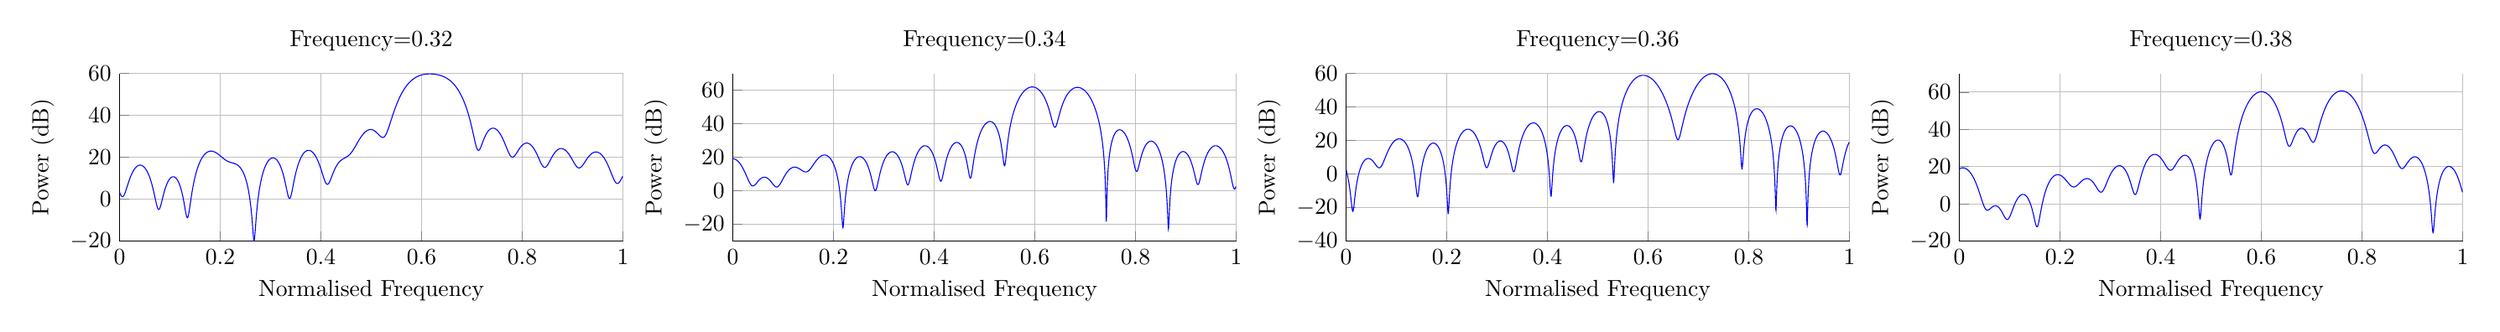
\begin{tikzpicture}

\begin{axis}[%
width=3in,
height=1in,
scale only axis,
xmin=0,
xmax=1,
xlabel={Normalised Frequency},
xmajorgrids,
ymin=-30,
ymax=70,
ylabel={Power (dB)},
ymajorgrids,
name=plot2,
title={Frequency=0.34},
axis x line*=bottom,
axis y line*=left
]
\addplot [color=blue,solid,forget plot]
  table[row sep=crcr]{-1	3.21515738155582\\
-0.99951171875	3.78047725883954\\
-0.9990234375	4.37210663327919\\
-0.99853515625	4.98056218751298\\
-0.998046875	5.59787469531732\\
-0.99755859375	6.21750880349247\\
-0.9970703125	6.83421857337718\\
-0.99658203125	7.44387555796662\\
-0.99609375	8.04329367507241\\
-0.99560546875	8.6300651124274\\
-0.9951171875	9.20241435718551\\
-0.99462890625	9.7590728070382\\
-0.994140625	10.2991736781446\\
-0.99365234375	10.8221654825816\\
-0.9931640625	11.3277417318546\\
-0.99267578125	11.8157843945222\\
-0.9921875	12.2863187703776\\
-0.99169921875	12.7394777006145\\
-0.9912109375	13.175473330645\\
-0.99072265625	13.5945749347593\\
-0.990234375	13.997091577652\\
-0.98974609375	14.3833586184063\\
-0.9892578125	14.7537272566388\\
-0.98876953125	15.1085564806889\\
-0.98828125	15.4482069080964\\
-0.98779296875	15.7730361136839\\
-0.9873046875	16.0833951246555\\
-0.98681640625	16.3796258291281\\
-0.986328125	16.6620590976999\\
-0.98583984375	16.9310134598056\\
-0.9853515625	17.1867942099419\\
-0.98486328125	17.4296928452012\\
-0.984375	17.659986756369\\
-0.98388671875	17.8779391112904\\
-0.9833984375	18.0837988822057\\
-0.98291015625	18.2778009790238\\
-0.982421875	18.4601664586169\\
-0.98193359375	18.6311027866304\\
-0.9814453125	18.7908041333719\\
-0.98095703125	18.9394516893422\\
-0.98046875	19.0772139891283\\
-0.97998046875	19.2042472348696\\
-0.9794921875	19.3206956124583\\
-0.97900390625	19.4266915951745\\
-0.978515625	19.5223562306472\\
-0.97802734375	19.6077994079597\\
-0.9775390625	19.6831201024303\\
-0.97705078125	19.7484065961334\\
-0.9765625	19.8037366726281\\
-0.97607421875	19.8491777846416\\
-0.9755859375	19.8847871936529\\
-0.97509765625	19.9106120804323\\
-0.974609375	19.9266896256514\\
-0.97412109375	19.9330470596741\\
-0.9736328125	19.9297016805921\\
-0.97314453125	19.9166608394816\\
-0.97265625	19.8939218917301\\
-0.97216796875	19.8614721131191\\
-0.9716796875	19.8192885791542\\
-0.97119140625	19.7673380058983\\
-0.970703125	19.7055765502963\\
-0.97021484375	19.6339495676696\\
-0.9697265625	19.5523913237074\\
-0.96923828125	19.4608246578819\\
-0.96875	19.3591605947591\\
-0.96826171875	19.2472978991644\\
-0.9677734375	19.1251225705736\\
-0.96728515625	18.9925072714333\\
-0.966796875	18.8493106833547\\
-0.96630859375	18.6953767842496\\
-0.9658203125	18.5305340384783\\
-0.96533203125	18.3545944909274\\
-0.96484375	18.1673527546008\\
-0.96435546875	17.9685848797719\\
-0.9638671875	17.7580470909454\\
-0.96337890625	17.5354743757957\\
-0.962890625	17.3005789078003\\
-0.96240234375	17.0530482814212\\
-0.9619140625	16.7925435353078\\
-0.96142578125	16.5186969350021\\
-0.9609375	16.2311094818892\\
-0.96044921875	15.9293481094949\\
-0.9599609375	15.6129425214836\\
-0.95947265625	15.2813816176155\\
-0.958984375	14.9341094441558\\
-0.95849609375	14.5705205934089\\
-0.9580078125	14.1899549626725\\
-0.95751953125	13.7916917653327\\
-0.95703125	13.3749426652349\\
-0.95654296875	12.9388438788202\\
-0.9560546875	12.4824470564339\\
-0.95556640625	12.0047087129162\\
-0.955078125	11.5044779257247\\
-0.95458984375	10.9804819532995\\
-0.9541015625	10.4313093430246\\
-0.95361328125	9.85538999139238\\
-0.953125	9.25097148128807\\
-0.95263671875	8.61609084239741\\
-0.9521484375	7.94854064642676\\
-0.95166015625	7.24582803947529\\
-0.951171875	6.50512490204434\\
-0.95068359375	5.72320677411714\\
-0.9501953125	4.89637743358561\\
-0.94970703125	4.02037499268245\\
-0.94921875	3.0902539667664\\
-0.94873046875	2.10023581214341\\
-0.9482421875	1.04351769636102\\
-0.94775390625	-0.0879745615738002\\
-0.947265625	-1.30390878049658\\
-0.94677734375	-2.61597066489848\\
-0.9462890625	-4.03842639485245\\
-0.94580078125	-5.58887133198598\\
-0.9453125	-7.28922172392885\\
-0.94482421875	-9.16699775503867\\
-0.9443359375	-11.2568681823145\\
-0.94384765625	-13.6021079547498\\
-0.943359375	-16.2544900209191\\
-0.94287109375	-19.2672511462683\\
-0.9423828125	-22.6626437433892\\
-0.94189453125	-26.3153548936798\\
-0.94140625	-29.6269432732307\\
-0.94091796875	-31.1751936369899\\
-0.9404296875	-29.862413998356\\
-0.93994140625	-26.6559451296282\\
-0.939453125	-23.0264803993769\\
-0.93896484375	-19.6305265983446\\
-0.9384765625	-16.6152238068739\\
-0.93798828125	-13.9639115482997\\
-0.9375	-11.6240458044163\\
-0.93701171875	-9.54331994892719\\
-0.9365234375	-7.67774220631153\\
-0.93603515625	-5.99200906465965\\
-0.935546875	-4.45809225418014\\
-0.93505859375	-3.05368108989602\\
-0.9345703125	-1.76087581037901\\
-0.93408203125	-0.565174314846809\\
-0.93359375	0.545293555734458\\
-0.93310546875	1.58034138599688\\
-0.9326171875	2.54815987225948\\
-0.93212890625	3.45564606550595\\
-0.931640625	4.30865557489922\\
-0.93115234375	5.11219763002042\\
-0.9306640625	5.87058742379749\\
-0.93017578125	6.58756622956038\\
-0.9296875	7.26639697915518\\
-0.92919921875	7.90994097960606\\
-0.9287109375	8.52071999897551\\
-0.92822265625	9.10096690259959\\
-0.927734375	9.6526672533119\\
-0.92724609375	10.1775937230197\\
-0.9267578125	10.6773347416001\\
-0.92626953125	11.1533184927793\\
-0.92578125	11.6068331272351\\
-0.92529296875	12.0390438804562\\
-0.9248046875	12.4510076423755\\
-0.92431640625	12.8436854169137\\
-0.923828125	13.2179530245935\\
-0.92333984375	13.5746103346135\\
-0.9228515625	13.9143892599527\\
-0.92236328125	14.2379607070466\\
-0.921875	14.5459406379182\\
-0.92138671875	14.8388953755441\\
-0.9208984375	15.1173462613023\\
-0.92041015625	15.3817737554828\\
-0.919921875	15.632621057247\\
-0.91943359375	15.8702973084103\\
-0.9189453125	16.0951804355219\\
-0.91845703125	16.3076196764924\\
-0.91796875	16.507937831182\\
-0.91748046875	16.6964332696369\\
-0.9169921875	16.8733817268634\\
-0.91650390625	17.0390379089769\\
-0.916015625	17.1936369321429\\
-0.91552734375	17.3373956128203\\
-0.9150390625	17.4705136253395\\
-0.91455078125	17.5931745407338\\
-0.9140625	17.7055467589226\\
-0.91357421875	17.8077843447842\\
-0.9130859375	17.9000277773012\\
-0.91259765625	17.982404619791\\
-0.912109375	18.055030118213\\
-0.91162109375	18.1180077336517\\
-0.9111328125	18.1714296142911\\
-0.91064453125	18.2153770115057\\
-0.91015625	18.2499206440838\\
-0.90966796875	18.2751210140497\\
-0.9091796875	18.2910286770678\\
-0.90869140625	18.2976844699693\\
-0.908203125	18.2951196975432\\
-0.90771484375	18.2833562803703\\
-0.9072265625	18.2624068651399\\
-0.90673828125	18.2322748985763\\
-0.90625	18.192954665812\\
-0.90576171875	18.1444312937585\\
-0.9052734375	18.0866807197663\\
-0.90478515625	18.0196696256013\\
-0.904296875	17.9433553365141\\
-0.90380859375	17.8576856849264\\
-0.9033203125	17.7625988380119\\
-0.90283203125	17.6580230881922\\
-0.90234375	17.5438766053171\\
-0.90185546875	17.4200671490328\\
-0.9013671875	17.2864917395766\\
-0.90087890625	17.1430362849559\\
-0.900390625	16.9895751621855\\
-0.89990234375	16.8259707499583\\
-0.8994140625	16.6520729098234\\
-0.89892578125	16.4677184126286\\
-0.8984375	16.2727303066716\\
-0.89794921875	16.0669172236845\\
-0.8974609375	15.850072618469\\
-0.89697265625	15.6219739377082\\
-0.896484375	15.3823817132224\\
-0.89599609375	15.1310385747372\\
-0.8955078125	14.8676681771117\\
-0.89501953125	14.5919740369876\\
-0.89453125	14.3036382740103\\
-0.89404296875	14.0023202522289\\
-0.8935546875	13.6876551181046\\
-0.89306640625	13.3592522328877\\
-0.892578125	13.0166934991674\\
-0.89208984375	12.6595315844151\\
-0.8916015625	12.2872880486998\\
-0.89111328125	11.8994513899519\\
-0.890625	11.4954750288668\\
-0.89013671875	11.0747752676998\\
-0.8896484375	10.636729274098\\
-0.88916015625	10.1806731644714\\
-0.888671875	9.7059002936741\\
-0.88818359375	9.21165990223884\\
-0.8876953125	8.69715633372897\\
-0.88720703125	8.16154911928786\\
-0.88671875	7.60395434302703\\
-0.88623046875	7.02344786272897\\
-0.8857421875	6.41907118236711\\
-0.88525390625	5.78984107947563\\
-0.884765625	5.13476451334348\\
-0.88427734375	4.45286092255021\\
-0.8837890625	3.74319481992367\\
-0.88330078125	3.00492268365238\\
-0.8828125	2.23735961579512\\
-0.88232421875	1.44007319470218\\
-0.8818359375	0.61301447499998\\
-0.88134765625	-0.243300789425176\\
-0.880859375	-1.12754407019562\\
-0.88037109375	-2.03723910830066\\
-0.8798828125	-2.96831825412632\\
-0.87939453125	-3.91455114362419\\
-0.87890625	-4.86683997364143\\
-0.87841796875	-5.8124086037463\\
-0.8779296875	-6.73397816659963\\
-0.87744140625	-7.60913101320766\\
-0.876953125	-8.41021224354887\\
-0.87646484375	-9.1052528900849\\
-0.8759765625	-9.66039506770967\\
-0.87548828125	-10.0439776543235\\
-0.875	-10.2317166818127\\
-0.87451171875	-10.2115425112543\\
-0.8740234375	-9.98627698966759\\
-0.87353515625	-9.57299114325332\\
-0.873046875	-8.99933058401892\\
-0.87255859375	-8.29833966596197\\
-0.8720703125	-7.50356362262604\\
-0.87158203125	-6.645560424787\\
-0.87109375	-5.75007829162875\\
-0.87060546875	-4.83757342574646\\
-0.8701171875	-3.92355889317101\\
-0.86962890625	-3.0193430245304\\
-0.869140625	-2.13286550895047\\
-0.86865234375	-1.26947529991157\\
-0.8681640625	-0.432586621337915\\
-0.86767578125	0.37579884042518\\
-0.8671875	1.15469119174591\\
-0.86669921875	1.90381217605471\\
-0.8662109375	2.62337411598631\\
-0.86572265625	3.31391910353916\\
-0.865234375	3.97620315594255\\
-0.86474609375	4.61111348699183\\
-0.8642578125	5.21960994988521\\
-0.86376953125	5.80268401430248\\
-0.86328125	6.36133040457366\\
-0.86279296875	6.89652784489935\\
-0.8623046875	7.40922633031877\\
-0.86181640625	7.90033905332243\\
-0.861328125	8.37073763336387\\
-0.86083984375	8.82124967183332\\
-0.8603515625	9.25265792697503\\
-0.85986328125	9.66570060018186\\
-0.859375	10.0610723677921\\
-0.85888671875	10.4394258959478\\
-0.8583984375	10.8013736510874\\
-0.85791015625	11.1474898730734\\
-0.857421875	11.4783126174325\\
-0.85693359375	11.7943458018138\\
-0.8564453125	12.096061212485\\
-0.85595703125	12.3839004416496\\
-0.85546875	12.6582767371229\\
-0.85498046875	12.9195767535949\\
-0.8544921875	13.1681622001571\\
-0.85400390625	13.4043713825832\\
-0.853515625	13.6285206414792\\
-0.85302734375	13.8409056891719\\
-0.8525390625	14.0418028493356\\
-0.85205078125	14.2314702040333\\
-0.8515625	14.4101486532015\\
-0.85107421875	14.5780628917322\\
-0.8505859375	14.7354223092728\\
-0.85009765625	14.8824218177168\\
-0.849609375	15.0192426111474\\
-0.84912109375	15.1460528627308\\
-0.8486328125	15.2630083627728\\
-0.84814453125	15.3702531018491\\
-0.84765625	15.4679198026209\\
-0.84716796875	15.5561304036448\\
-0.8466796875	15.6349964981973\\
-0.84619140625	15.7046197308503\\
-0.845703125	15.7650921542677\\
-0.84521484375	15.8164965484302\\
-0.8447265625	15.8589067042565\\
-0.84423828125	15.8923876733479\\
-0.84375	15.916995985365\\
-0.84326171875	15.9327798343268\\
-0.8427734375	15.9397792349184\\
-0.84228515625	15.938026149694\\
-0.841796875	15.9275445878635\\
-0.84130859375	15.9083506761661\\
-0.8408203125	15.8804527021389\\
-0.84033203125	15.8438511299029\\
-0.83984375	15.7985385883958\\
-0.83935546875	15.7444998317863\\
-0.8388671875	15.6817116716032\\
-0.83837890625	15.6101428799024\\
-0.837890625	15.5297540625738\\
-0.83740234375	15.4404975016567\\
-0.8369140625	15.3423169652771\\
-0.83642578125	15.2351474835525\\
-0.8359375	15.1189150885074\\
-0.83544921875	14.99353651572\\
-0.8349609375	14.8589188650584\\
-0.83447265625	14.7149592174629\\
-0.833984375	14.5615442042815\\
-0.83349609375	14.3985495251643\\
-0.8330078125	14.225839409947\\
-0.83251953125	14.0432660193141\\
-0.83203125	13.8506687782905\\
-0.83154296875	13.6478736357748\\
-0.8310546875	13.4346922423574\\
-0.83056640625	13.2109210375599\\
-0.830078125	12.9763402363487\\
-0.82958984375	12.7307127032845\\
-0.8291015625	12.4737827009462\\
-0.82861328125	12.2052744972413\\
-0.828125	11.9248908138572\\
-0.82763671875	11.6323110953243\\
-0.8271484375	11.3271895748859\\
-0.82666015625	11.0091531094919\\
-0.826171875	10.6777987516193\\
-0.82568359375	10.3326910201246\\
-0.8251953125	9.97335882574437\\
-0.82470703125	9.59929199893182\\
-0.82421875	9.20993735814094\\
-0.82373046875	8.80469424504232\\
-0.8232421875	8.38290943897036\\
-0.82275390625	7.94387134551181\\
-0.822265625	7.4868033327084\\
-0.82177734375	7.01085606177376\\
-0.8212890625	6.51509862608734\\
-0.82080078125	5.99850827064793\\
-0.8203125	5.45995841164531\\
-0.81982421875	4.89820460899539\\
-0.8193359375	4.31186805905701\\
-0.81884765625	3.69941606413986\\
-0.818359375	3.05913879131805\\
-0.81787109375	2.38912144365257\\
-0.8173828125	1.68721071552488\\
-0.81689453125	0.950974066646524\\
-0.81640625	0.177649892126594\\
-0.81591796875	-0.635913961463861\\
-0.8154296875	-1.49333675645002\\
-0.81494140625	-2.3988011533035\\
-0.814453125	-3.35717564241372\\
-0.81396484375	-4.37417209609451\\
-0.8134765625	-5.45655122063207\\
-0.81298828125	-6.61239444083168\\
-0.8125	-7.85146964952246\\
-0.81201171875	-9.18573236864166\\
-0.8115234375	-10.6300268777635\\
-0.81103515625	-12.2030905538202\\
-0.810546875	-13.9290320181039\\
-0.81005859375	-15.839575633783\\
-0.8095703125	-17.9775956803302\\
-0.80908203125	-20.4029224140609\\
-0.80859375	-23.2023647405864\\
-0.80810546875	-26.5080197307243\\
-0.8076171875	-30.5327450660499\\
-0.80712890625	-35.6409815414898\\
-0.806640625	-42.4589212358848\\
-0.80615234375	-51.3179159761684\\
-0.8056640625	-54.0564312324987\\
-0.80517578125	-45.6154492509258\\
-0.8046875	-38.1407778179806\\
-0.80419921875	-32.6455822863445\\
-0.8037109375	-28.4220373809787\\
-0.80322265625	-25.0246666630373\\
-0.802734375	-22.1973913528769\\
-0.80224609375	-19.7847723480616\\
-0.8017578125	-17.6866180330392\\
-0.80126953125	-15.8349642343202\\
-0.80078125	-14.181738351843\\
-0.80029296875	-12.691750662109\\
-0.7998046875	-11.3384990415421\\
-0.79931640625	-10.101542532529\\
-0.798828125	-8.96479277154464\\
-0.79833984375	-7.91536530068353\\
-0.7978515625	-6.9427849962884\\
-0.79736328125	-6.0384226523859\\
-0.796875	-5.19508668590276\\
-0.79638671875	-4.40672151103062\\
-0.7958984375	-3.66818086996123\\
-0.79541015625	-2.97505486340553\\
-0.794921875	-2.32353612558461\\
-0.79443359375	-1.71031498358803\\
-0.7939453125	-1.13249638452093\\
-0.79345703125	-0.587533382884296\\
-0.79296875	-0.0731733756949485\\
-0.79248046875	0.412585743004669\\
-0.7919921875	0.871531632206988\\
-0.79150390625	1.30526737160949\\
-0.791015625	1.7152363847422\\
-0.79052734375	2.10274337672793\\
-0.7900390625	2.46897203665838\\
-0.78955078125	2.81500009598028\\
-0.7890625	3.14181221294811\\
-0.78857421875	3.45031105955961\\
-0.7880859375	3.7413269145428\\
-0.78759765625	4.01562600885644\\
-0.787109375	4.27391782508216\\
-0.78662109375	4.51686151624919\\
-0.7861328125	4.74507158096501\\
-0.78564453125	4.95912290864814\\
-0.78515625	5.15955528997529\\
-0.78466796875	5.34687747243538\\
-0.7841796875	5.52157082841504\\
-0.78369140625	5.68409269296469\\
-0.783203125	5.83487941986974\\
-0.78271484375	5.97434919753464\\
-0.7822265625	6.10290466019246\\
-0.78173828125	6.22093532486518\\
-0.78125	6.32881988012736\\
-0.78076171875	6.42692834892541\\
-0.7802734375	6.51562414434782\\
-0.77978515625	6.59526603422507\\
-0.779296875	6.66621002766921\\
-0.77880859375	6.72881119406891\\
-0.7783203125	6.78342542256529\\
-0.77783203125	6.8304111275891\\
-0.77734375	6.87013090359057\\
-0.77685546875	6.9029531295931\\
-0.7763671875	6.92925352161423\\
-0.77587890625	6.94941662829116\\
-0.775390625	6.96383726220606\\
-0.77490234375	6.97292185641235\\
-0.7744140625	6.97708973252734\\
-0.77392578125	6.97677426349154\\
-0.7734375	6.97242391074279\\
-0.77294921875	6.96450311217226\\
-0.7724609375	6.95349299390643\\
-0.77197265625	6.93989187580902\\
-0.771484375	6.92421553776909\\
-0.77099609375	6.90699721151333\\
-0.7705078125	6.88878726106864\\
-0.77001953125	6.87015251434573\\
-0.76953125	6.85167520888277\\
-0.76904296875	6.83395151685653\\
-0.7685546875	6.81758961831366\\
-0.76806640625	6.80320729744267\\
-0.767578125	6.79142904480213\\
-0.76708984375	6.78288265885694\\
-0.7666015625	6.77819535296313\\
-0.76611328125	6.7779893889405\\
-0.765625	6.78287727527101\\
-0.76513671875	6.79345658625247\\
-0.7646484375	6.81030447741418\\
-0.76416015625	6.83397199126725\\
-0.763671875	6.86497826496164\\
-0.76318359375	6.90380476649606\\
-0.7626953125	6.95088969759827\\
-0.76220703125	7.00662270814719\\
-0.76171875	7.07134006812018\\
-0.76123046875	7.1453204378711\\
-0.7607421875	7.22878136580627\\
-0.76025390625	7.32187662440186\\
-0.759765625	7.42469447163013\\
-0.75927734375	7.53725689632042\\
-0.7587890625	7.65951987423098\\
-0.75830078125	7.79137462837903\\
-0.7578125	7.93264985432037\\
-0.75732421875	8.08311484040683\\
-0.7568359375	8.24248338621697\\
-0.75634765625	8.41041840067466\\
-0.755859375	8.58653704574984\\
-0.75537109375	8.77041628253254\\
-0.7548828125	8.961598673869\\
-0.75439453125	9.15959830122631\\
-0.75390625	9.36390666223275\\
-0.75341796875	9.57399842841447\\
-0.7529296875	9.78933695886474\\
-0.75244140625	10.009379483757\\
-0.751953125	10.2335818906233\\
-0.75146484375	10.4614030651688\\
-0.7509765625	10.6923087562575\\
-0.75048828125	10.9257749509531\\
-0.75	11.1612907597149\\
-0.74951171875	11.39836082378\\
-0.7490234375	11.6365072663476\\
-0.74853515625	11.8752712164583\\
-0.748046875	12.1142139396089\\
-0.74755859375	12.3529176123614\\
-0.7470703125	12.5909857797816\\
-0.74658203125	12.8280435347345\\
-0.74609375	13.0637374571728\\
-0.74560546875	13.2977353498117\\
-0.7451171875	13.5297258042556\\
-0.74462890625	13.7594176289004\\
-0.744140625	13.9865391669819\\
-0.74365234375	14.210837530087\\
-0.7431640625	14.4320777694254\\
-0.74267578125	14.6500420042315\\
-0.7421875	14.8645285239128\\
-0.74169921875	15.0753508779989\\
-0.7412109375	15.2823369656141\\
-0.74072265625	15.485328134096\\
-0.740234375	15.6841782945159\\
-0.73974609375	15.8787530602188\\
-0.7392578125	16.0689289130794\\
-0.73876953125	16.2545924009442\\
-0.73828125	16.4356393686928\\
-0.73779296875	16.6119742244741\\
-0.7373046875	16.7835092419476\\
-0.73681640625	16.9501638987581\\
-0.736328125	17.1118642509918\\
-0.73583984375	17.2685423429681\\
-0.7353515625	17.4201356514257\\
-0.73486328125	17.5665865629205\\
-0.734375	17.7078418830893\\
-0.73388671875	17.8438523763045\\
-0.7333984375	17.9745723341672\\
-0.73291015625	18.09995917124\\
-0.732421875	18.2199730463989\\
-0.73193359375	18.3345765081881\\
-0.7314453125	18.44373416258\\
-0.73095703125	18.5474123615755\\
-0.73046875	18.6455789111227\\
-0.72998046875	18.7382027968801\\
-0.7294921875	18.8252539264071\\
-0.72900390625	18.9067028864181\\
-0.728515625	18.9825207137986\\
-0.72802734375	19.0526786791381\\
-0.7275390625	19.1171480815916\\
-0.72705078125	19.1759000539392\\
-0.7265625	19.2289053767653\\
-0.72607421875	19.2761343007312\\
-0.7255859375	19.3175563759608\\
-0.72509765625	19.3531402876045\\
-0.724609375	19.3828536966879\\
-0.72412109375	19.4066630853874\\
-0.7236328125	19.4245336059091\\
-0.72314453125	19.4364289321772\\
-0.72265625	19.4423111135633\\
-0.72216796875	19.44214042991\\
-0.7216796875	19.4358752471211\\
-0.72119140625	19.4234718726043\\
-0.720703125	19.4048844098631\\
-0.72021484375	19.3800646115424\\
-0.7197265625	19.3489617302339\\
-0.71923828125	19.3115223663495\\
-0.71875	19.2676903123632\\
-0.71826171875	19.2174063927194\\
-0.7177734375	19.160608298689\\
-0.71728515625	19.0972304174436\\
-0.716796875	19.027203654599\\
-0.71630859375	18.9504552494565\\
-0.7158203125	18.866908582146\\
-0.71533203125	18.7764829718483\\
-0.71484375	18.6790934652396\\
-0.71435546875	18.5746506142695\\
-0.7138671875	18.4630602423468\\
-0.71337890625	18.3442231979681\\
-0.712890625	18.2180350947849\\
-0.71240234375	18.0843860370632\\
-0.7119140625	17.9431603294519\\
-0.71142578125	17.7942361699352\\
-0.7109375	17.6374853248114\\
-0.71044921875	17.4727727845116\\
-0.7099609375	17.2999563990536\\
-0.70947265625	17.1188864919183\\
-0.708984375	16.929405451151\\
-0.70849609375	16.7313472965244\\
-0.7080078125	16.5245372216753\\
-0.70751953125	16.3087911102371\\
-0.70703125	16.0839150251674\\
-0.70654296875	15.8497046707196\\
-0.7060546875	15.6059448268533\\
-0.70556640625	15.352408756357\\
-0.705078125	15.0888575856\\
-0.70458984375	14.8150396606826\\
-0.7041015625	14.5306898818891\\
-0.70361328125	14.2355290208306\\
-0.703125	13.9292630266094\\
-0.70263671875	13.611582329864\\
-0.7021484375	13.2821611568435\\
-0.70166015625	12.9406568699212\\
-0.701171875	12.5867093564799\\
-0.70068359375	12.2199404952487\\
-0.7001953125	11.8399537384197\\
-0.69970703125	11.4463338598384\\
-0.69921875	11.038646935048\\
-0.69873046875	10.6164406390144\\
-0.6982421875	10.1792449733194\\
-0.69775390625	9.72657356824465\\
-0.697265625	9.25792574874539\\
-0.69677734375	8.77278960978753\\
-0.6962890625	8.27064641965597\\
-0.69580078125	7.75097676447527\\
-0.6953125	7.21326896939091\\
-0.69482421875	6.65703048920686\\
-0.6943359375	6.08180316291006\\
-0.69384765625	5.48718348310342\\
-0.693359375	4.87284935454439\\
-0.69287109375	4.23859521689617\\
-0.6923828125	3.58437789299875\\
-0.69189453125	2.91037609336655\\
-0.69140625	2.21706713741455\\
-0.69091796875	1.50532507944411\\
-0.6904296875	0.776544918583775\\
-0.68994140625	0.0327976721176284\\
-0.689453125	-0.722979644287959\\
-0.68896484375	-1.48675738169706\\
-0.6884765625	-2.2531531594289\\
-0.68798828125	-3.01515052338994\\
-0.6875	-3.76382328816257\\
-0.68701171875	-4.48811387964714\\
-0.6865234375	-5.17474094453452\\
-0.68603515625	-5.80833823936666\\
-0.685546875	-6.3719402356978\\
-0.68505859375	-6.84790918693908\\
-0.6845703125	-7.2193218387331\\
-0.68408203125	-7.47169596377585\\
-0.68359375	-7.59477008060635\\
-0.68310546875	-7.58393098290684\\
-0.6826171875	-7.44090062316143\\
-0.68212890625	-7.17347804873508\\
-0.681640625	-6.79441439933282\\
-0.68115234375	-6.31974308478519\\
-0.6806640625	-5.76698356027484\\
-0.68017578125	-5.15357209933102\\
-0.6796875	-4.49571690203457\\
-0.67919921875	-3.80771654722201\\
-0.6787109375	-3.10167460227779\\
-0.67822265625	-2.38749885952316\\
-0.677734375	-1.67307419628913\\
-0.67724609375	-0.964520772077357\\
-0.6767578125	-0.266477240201434\\
-0.67626953125	0.417627029120902\\
-0.67578125	1.08532895688293\\
-0.67529296875	1.73492476361533\\
-0.6748046875	2.36529911012631\\
-0.67431640625	2.9757871404806\\
-0.673828125	3.56606484850301\\
-0.67333984375	4.1360629718929\\
-0.6728515625	4.68589996935571\\
-0.67236328125	5.21583022308749\\
-0.671875	5.72620424890709\\
-0.67138671875	6.21743829840138\\
-0.6708984375	6.68999126339075\\
-0.67041015625	7.14434723291435\\
-0.669921875	7.58100241086646\\
-0.66943359375	8.00045538839516\\
-0.6689453125	8.40319999087027\\
-0.66845703125	8.78972009586069\\
-0.66796875	9.1604859560129\\
-0.66748046875	9.51595166728931\\
-0.6669921875	9.8565535054466\\
-0.66650390625	10.1827089172945\\
-0.666015625	10.4948160024124\\
-0.66552734375	10.7932533589159\\
-0.6650390625	11.0783801961315\\
-0.66455078125	11.3505366396221\\
-0.6640625	11.6100441714567\\
-0.66357421875	11.8572061620868\\
-0.6630859375	12.0923084606094\\
-0.66259765625	12.3156200182358\\
-0.662109375	12.5273935259987\\
-0.66162109375	12.727866052527\\
-0.6611328125	12.9172596714084\\
-0.66064453125	13.0957820705079\\
-0.66015625	13.2636271377855\\
-0.65966796875	13.4209755198273\\
-0.6591796875	13.5679951505673\\
-0.65869140625	13.7048417486334\\
-0.658203125	13.8316592824649\\
-0.65771484375	13.948580402872\\
-0.6572265625	14.055726843089\\
-0.65673828125	14.153209786636\\
-0.65625	14.2411302034813\\
-0.65576171875	14.3195791551054\\
-0.6552734375	14.3886380691217\\
-0.65478515625	14.4483789841243\\
-0.654296875	14.4988647654145\\
-0.65380859375	14.5401492922145\\
-0.6533203125	14.5722776169167\\
-0.65283203125	14.595286096838\\
-0.65234375	14.6092024988608\\
-0.65185546875	14.6140460772426\\
-0.6513671875	14.6098276247712\\
-0.65087890625	14.596549497327\\
-0.650390625	14.5742056117957\\
-0.64990234375	14.5427814171491\\
-0.6494140625	14.5022538383819\\
-0.64892578125	14.4525911928561\\
-0.6484375	14.3937530784632\\
-0.64794921875	14.325690232868\\
-0.6474609375	14.2483443629467\\
-0.64697265625	14.1616479433707\\
-0.646484375	14.0655239831264\\
-0.64599609375	13.9598857585886\\
-0.6455078125	13.844636511591\\
-0.64501953125	13.7196691107559\\
-0.64453125	13.5848656741611\\
-0.64404296875	13.4400971512349\\
-0.6435546875	13.2852228615869\\
-0.64306640625	13.1200899882992\\
-0.642578125	12.9445330230341\\
-0.64208984375	12.7583731601637\\
-0.6416015625	12.5614176370013\\
-0.64111328125	12.3534590171401\\
-0.640625	12.1342744138845\\
-0.64013671875	11.9036246508375\\
-0.6396484375	11.6612533569041\\
-0.63916015625	11.4068859933463\\
-0.638671875	11.1402288111275\\
-0.63818359375	10.860967737718\\
-0.6376953125	10.5687671938866\\
-0.63720703125	10.2632688429473\\
-0.63671875	9.94409027765154\\
-0.63623046875	9.61082365368338\\
-0.6357421875	9.26303428389258\\
-0.63525390625	8.90025921445309\\
-0.634765625	8.52200581371807\\
-0.63427734375	8.12775041750903\\
-0.6337890625	7.71693709209622\\
-0.63330078125	7.28897659976546\\
-0.6328125	6.84324568374681\\
-0.63232421875	6.37908683227522\\
-0.6318359375	5.8958087395511\\
-0.63134765625	5.39268775964775\\
-0.630859375	4.86897075510464\\
-0.63037109375	4.3238798847043\\
-0.6298828125	3.75662006773178\\
-0.62939453125	3.16639012220745\\
-0.62890625	2.55239892510146\\
-0.62841796875	1.91388841316489\\
-0.6279296875	1.25016587139267\\
-0.62744140625	0.56064878767166\\
-0.626953125	-0.155073362760884\\
-0.62646484375	-0.897154654291331\\
-0.6259765625	-1.66537811370128\\
-0.62548828125	-2.45900155191248\\
-0.625	-3.27655233522326\\
-0.62451171875	-4.11555799768542\\
-0.6240234375	-4.97219952358918\\
-0.62353515625	-5.84087766266546\\
-0.623046875	-6.71369332730543\\
-0.62255859375	-7.57986633454662\\
-0.6220703125	-8.42515916709333\\
-0.62158203125	-9.23143903363045\\
-0.62109375	-9.97659790254373\\
-0.62060546875	-10.6351289692799\\
-0.6201171875	-11.1796653609972\\
-0.61962890625	-11.5836304352097\\
-0.619140625	-11.8247690193163\\
-0.61865234375	-11.8888105598642\\
-0.6181640625	-11.7721498273803\\
-0.61767578125	-11.4825649488501\\
-0.6171875	-11.0376898286786\\
-0.61669921875	-10.4618329226357\\
-0.6162109375	-9.78224474490757\\
-0.61572265625	-9.02585487347931\\
-0.615234375	-8.21703308197472\\
-0.61474609375	-7.37643878390009\\
-0.6142578125	-6.52072648075301\\
-0.61376953125	-5.66279017241423\\
-0.61328125	-4.81227349772603\\
-0.61279296875	-3.9761593086051\\
-0.6123046875	-3.15933304079126\\
-0.61181640625	-2.36507163000607\\
-0.611328125	-1.59544421601321\\
-0.61083984375	-0.851628693770923\\
-0.6103515625	-0.134155670864949\\
-0.60986328125	0.556906740915819\\
-0.609375	1.22181469502428\\
-0.60888671875	1.86104619913532\\
-0.6083984375	2.47522584728606\\
-0.60791015625	3.06506991086987\\
-0.607421875	3.63134659195463\\
-0.60693359375	4.17484751145834\\
-0.6064453125	4.69636748959944\\
-0.60595703125	5.19669042632103\\
-0.60546875	5.67657965421012\\
-0.60498046875	6.13677155844179\\
-0.6044921875	6.57797157212825\\
-0.60400390625	7.00085188823555\\
-0.603515625	7.40605040165697\\
-0.60302734375	7.79417052268912\\
-0.6025390625	8.16578159767612\\
-0.60205078125	8.52141974260037\\
-0.6015625	8.86158894727924\\
-0.60107421875	9.18676234629159\\
-0.6005859375	9.49738358127661\\
-0.60009765625	9.79386820038858\\
-0.599609375	10.0766050563522\\
-0.59912109375	10.3459576761439\\
-0.5986328125	10.6022655838713\\
-0.59814453125	10.8458455647012\\
-0.59765625	11.0769928622797\\
-0.59716796875	11.2959823054178\\
-0.5966796875	11.5030693622041\\
-0.59619140625	11.6984911213959\\
-0.595703125	11.8824672021052\\
-0.59521484375	12.0552005935714\\
-0.5947265625	12.216878427304\\
-0.59423828125	12.3676726841542\\
-0.59375	12.5077408389956\\
-0.59326171875	12.6372264456995\\
-0.5927734375	12.7562596650159\\
-0.59228515625	12.8649577378372\\
-0.591796875	12.9634254061383\\
-0.59130859375	13.0517552836886\\
-0.5908203125	13.1300281783941\\
-0.59033203125	13.1983133678895\\
-0.58984375	13.2566688297464\\
-0.58935546875	13.3051414273979\\
-0.5888671875	13.3437670526144\\
-0.58837890625	13.3725707250854\\
-0.587890625	13.3915666493813\\
-0.58740234375	13.4007582292726\\
-0.5869140625	13.4001380390829\\
-0.58642578125	13.3896877514329\\
-0.5859375	13.3693780203982\\
-0.58544921875	13.3391683187515\\
-0.5849609375	13.2990067275785\\
-0.58447265625	13.2488296761511\\
-0.583984375	13.1885616294981\\
-0.58349609375	13.1181147206286\\
-0.5830078125	13.0373883238334\\
-0.58251953125	12.9462685648964\\
-0.58203125	12.8446277633949\\
-0.58154296875	12.7323238015286\\
-0.5810546875	12.6091994130951\\
-0.58056640625	12.4750813852902\\
-0.580078125	12.3297796649575\\
-0.57958984375	12.1730863597035\\
-0.5791015625	12.0047746229195\\
-0.57861328125	11.8245974101771\\
-0.578125	11.6322860926522\\
-0.57763671875	11.4275489111506\\
-0.5771484375	11.2100692519035\\
-0.57666015625	10.9795037225173\\
-0.576171875	10.7354800032363\\
-0.57568359375	10.4775944449327\\
-0.5751953125	10.2054093808753\\
-0.57470703125	9.91845011425076\\
-0.57421875	9.61620153748731\\
-0.57373046875	9.2981043325116\\
-0.5732421875	8.96355069299579\\
-0.57275390625	8.61187950022553\\
-0.572265625	8.24237087323216\\
-0.57177734375	7.85424000105652\\
-0.5712890625	7.44663015021738\\
-0.57080078125	7.01860472343144\\
-0.5703125	6.56913822623592\\
-0.56982421875	6.0971059763925\\
-0.5693359375	5.60127236708538\\
-0.56884765625	5.08027746975496\\
-0.568359375	4.53262173761637\\
-0.56787109375	3.95664854975002\\
-0.5673828125	3.35052432402179\\
-0.56689453125	2.71221593545974\\
-0.56640625	2.03946522327395\\
-0.56591796875	1.32976048587703\\
-0.5654296875	0.580305103116048\\
-0.56494140625	-0.212016118401579\\
-0.564453125	-1.05067144653485\\
-0.56396484375	-1.93951464912467\\
-0.5634765625	-2.88280978338937\\
-0.56298828125	-3.88523814483106\\
-0.5625	-4.95186900224903\\
-0.56201171875	-6.08806136105593\\
-0.5615234375	-7.29923865415327\\
-0.56103515625	-8.59043373443584\\
-0.560546875	-9.96542416615328\\
-0.56005859375	-11.4251470683535\\
-0.5595703125	-12.9648758646892\\
-0.55908203125	-14.5693631660027\\
-0.55859375	-16.2049493177938\\
-0.55810546875	-17.8081012555434\\
-0.5576171875	-19.2725762259349\\
-0.55712890625	-20.4447353965214\\
-0.556640625	-21.1462934510813\\
-0.55615234375	-21.2376541299745\\
-0.5556640625	-20.6915968791021\\
-0.55517578125	-19.6098919273197\\
-0.5546875	-18.1648538249512\\
-0.55419921875	-16.524940775333\\
-0.5537109375	-14.8157807117106\\
-0.55322265625	-13.1165447026337\\
-0.552734375	-11.4712562511025\\
-0.55224609375	-9.90135179852823\\
-0.5517578125	-8.41501138517657\\
-0.55126953125	-7.01310827779681\\
-0.55078125	-5.69273322027626\\
-0.55029296875	-4.44919781923983\\
-0.5498046875	-3.27714020453593\\
-0.54931640625	-2.17111629449779\\
-0.548828125	-1.12590116320919\\
-0.54833984375	-0.136629123615707\\
-0.5478515625	0.801154500027642\\
-0.54736328125	1.69148870222374\\
-0.546875	2.53801605951548\\
-0.54638671875	3.34401299784496\\
-0.5458984375	4.11242395440793\\
-0.54541015625	4.84589563244676\\
-0.544921875	5.54680942268782\\
-0.54443359375	6.21731111969287\\
-0.5439453125	6.85933764455983\\
-0.54345703125	7.47464079776861\\
-0.54296875	8.06480822336607\\
-0.54248046875	8.63128183529875\\
-0.5419921875	9.17537397757068\\
-0.54150390625	9.69828158467483\\
-0.541015625	10.2010985904872\\
-0.54052734375	10.684826809971\\
-0.5400390625	11.1503854927542\\
-0.53955078125	11.5986197231258\\
-0.5390625	12.0303078183425\\
-0.53857421875	12.4461678567862\\
-0.5380859375	12.8468634495585\\
-0.53759765625	13.2330088534464\\
-0.537109375	13.6051735096448\\
-0.53662109375	13.9638860809618\\
-0.5361328125	14.3096380502152\\
-0.53564453125	14.6428869339567\\
-0.53515625	14.9640591583093\\
-0.53466796875	15.2735526374195\\
-0.5341796875	15.5717390896384\\
-0.53369140625	15.8589661219309\\
-0.533203125	16.13555910905\\
-0.53271484375	16.40182289061\\
-0.5322265625	16.6580433062627\\
-0.53173828125	16.9044885866569\\
-0.53125	17.1414106156791\\
-0.53076171875	17.3690460775904\\
-0.5302734375	17.5876175010373\\
-0.52978515625	17.7973342104975\\
-0.529296875	17.9983931944862\\
-0.52880859375	18.1909798987733\\
-0.5283203125	18.3752689519237\\
-0.52783203125	18.5514248296479\\
-0.52734375	18.7196024637354\\
-0.52685546875	18.8799478007064\\
-0.5263671875	19.0325983147632\\
-0.52587890625	19.1776834791329\\
-0.525390625	19.3153251994588\\
-0.52490234375	19.4456382125155\\
-0.5244140625	19.5687304531847\\
-0.52392578125	19.6847033923241\\
-0.5234375	19.7936523478975\\
-0.52294921875	19.8956667714923\\
-0.5224609375	19.9908305121392\\
-0.52197265625	20.0792220591565\\
-0.521484375	20.1609147655704\\
-0.52099609375	20.2359770535108\\
-0.5205078125	20.3044726028397\\
-0.52001953125	20.366460524148\\
-0.51953125	20.4219955171419\\
-0.51904296875	20.4711280153349\\
-0.5185546875	20.5139043178734\\
-0.51806640625	20.5503667092332\\
-0.517578125	20.5805535674483\\
-0.51708984375	20.6044994614629\\
-0.5166015625	20.6222352381279\\
-0.51611328125	20.6337880993055\\
-0.515625	20.6391816694841\\
-0.51513671875	20.6384360542564\\
-0.5146484375	20.63156788996\\
-0.51416015625	20.6185903847319\\
-0.513671875	20.5995133511857\\
-0.51318359375	20.5743432308728\\
-0.5126953125	20.5430831106476\\
-0.51220703125	20.5057327310168\\
-0.51171875	20.4622884865092\\
-0.51123046875	20.4127434180646\\
-0.5107421875	20.3570871973965\\
-0.51025390625	20.2953061032473\\
-0.509765625	20.2273829894061\\
-0.50927734375	20.1532972443228\\
-0.5087890625	20.0730247421039\\
-0.50830078125	19.9865377846299\\
-0.5078125	19.8938050344857\\
-0.50732421875	19.7947914383439\\
-0.5068359375	19.6894581403864\\
-0.50634765625	19.5777623852899\\
-0.505859375	19.4596574102387\\
-0.50537109375	19.3350923253598\\
-0.5048828125	19.2040119819015\\
-0.50439453125	19.0663568273942\\
-0.50390625	18.9220627469464\\
-0.50341796875	18.7710608897297\\
-0.5029296875	18.6132774796001\\
-0.50244140625	18.4486336086853\\
-0.501953125	18.2770450126373\\
-0.50146484375	18.0984218261024\\
-0.5009765625	17.9126683168009\\
-0.50048828125	17.7196825964282\\
-0.5	17.5193563063861\\
-0.49951171875	17.3115742761287\\
-0.4990234375	17.0962141516512\\
-0.49853515625	16.8731459913673\\
-0.498046875	16.6422318262949\\
-0.49755859375	16.4033251811103\\
-0.4970703125	16.1562705522139\\
-0.49658203125	15.9009028384861\\
-0.49609375	15.6370467198797\\
-0.49560546875	15.3645159783867\\
-0.4951171875	15.0831127552275\\
-0.49462890625	14.7926267373178\\
-0.494140625	14.4928342651581\\
-0.49365234375	14.1834973532478\\
-0.4931640625	13.8643626129208\\
-0.49267578125	13.5351600661089\\
-0.4921875	13.1956018369299\\
-0.49169921875	12.8453807061259\\
-0.4912109375	12.4841685112051\\
-0.49072265625	12.1116143725989\\
-0.490234375	11.7273427231796\\
-0.48974609375	11.3309511150001\\
-0.4892578125	10.9220077730174\\
-0.48876953125	10.5000488607321\\
-0.48828125	10.0645754169543\\
-0.48779296875	9.61504991612193\\
-0.4873046875	9.15089239652638\\
-0.48681640625	8.67147609115819\\
-0.486328125	8.17612248435577\\
-0.48583984375	7.66409570358832\\
-0.4853515625	7.1345961390339\\
-0.48486328125	6.58675316348794\\
-0.484375	6.01961680078301\\
-0.48388671875	5.43214816136263\\
-0.4833984375	4.82320842776603\\
-0.48291015625	4.19154612912871\\
-0.482421875	3.53578239069879\\
-0.48193359375	2.85439377982634\\
-0.4814453125	2.14569229167563\\
-0.48095703125	1.40780192370135\\
-0.48046875	0.638631175613037\\
-0.47998046875	-0.164159319993289\\
-0.4794921875	-1.00319498056341\\
-0.47900390625	-1.88143237470671\\
-0.478515625	-2.80221249939016\\
-0.47802734375	-3.76932359639344\\
-0.4775390625	-4.78707484331379\\
-0.47705078125	-5.86038192072019\\
-0.4765625	-6.99486447335169\\
-0.47607421875	-8.1969531654916\\
-0.4755859375	-9.47399901526401\\
-0.47509765625	-10.8343672415579\\
-0.474609375	-12.2874764209292\\
-0.47412109375	-13.8436999813794\\
-0.4736328125	-15.5139576434004\\
-0.47314453125	-17.3086418149013\\
-0.47265625	-19.2351545521769\\
-0.47216796875	-21.292609141879\\
-0.4716796875	-23.4609784912578\\
-0.47119140625	-25.6803763272677\\
-0.470703125	-27.8169890025138\\
-0.47021484375	-29.6260983121271\\
-0.4697265625	-30.7657033688831\\
-0.46923828125	-30.9435603464862\\
-0.46875	-30.1345116502292\\
-0.46826171875	-28.6025456685273\\
-0.4677734375	-26.6954257330611\\
-0.46728515625	-24.676028858631\\
-0.466796875	-22.6930109923027\\
-0.46630859375	-20.8149862631622\\
-0.4658203125	-19.066393069594\\
-0.46533203125	-17.4501330557335\\
-0.46484375	-15.9596135862075\\
-0.46435546875	-14.5846768344283\\
-0.4638671875	-13.3143769110242\\
-0.46337890625	-12.1382054652132\\
-0.462890625	-11.0465721753511\\
-0.46240234375	-10.0309361561149\\
-0.4619140625	-9.08378081469164\\
-0.46142578125	-8.1985249841308\\
-0.4609375	-7.36941436351586\\
-0.46044921875	-6.59141339307195\\
-0.4599609375	-5.86010602500701\\
-0.45947265625	-5.17160823235003\\
-0.458984375	-4.52249248105505\\
-0.45849609375	-3.90972325966016\\
-0.4580078125	-3.33060235624219\\
-0.45751953125	-2.78272251208493\\
-0.45703125	-2.26392817355\\
-0.45654296875	-1.77228221300961\\
-0.4560546875	-1.3060376506\\
-0.45556640625	-0.863613560293191\\
-0.455078125	-0.443574478252768\\
-0.45458984375	-0.044612746675102\\
-0.4541015625	0.334466676809885\\
-0.45361328125	0.694759333581039\\
-0.453125	1.0372726252054\\
-0.45263671875	1.36293568949919\\
-0.4521484375	1.67260801459999\\
-0.45166015625	1.96708697716414\\
-0.451171875	2.24711446033147\\
-0.45068359375	2.51338268196989\\
-0.4501953125	2.76653934293997\\
-0.44970703125	3.00719218790534\\
-0.44921875	3.23591305690666\\
-0.44873046875	3.45324149398891\\
-0.4482421875	3.65968796919509\\
-0.44775390625	3.85573676186969\\
-0.447265625	4.04184854616701\\
-0.44677734375	4.21846271370857\\
-0.4462890625	4.38599946328738\\
-0.44580078125	4.5448616832291\\
-0.4453125	4.69543664836078\\
-0.44482421875	4.83809755040761\\
-0.4443359375	4.97320487795366\\
-0.44384765625	5.10110765979286\\
-0.443359375	5.22214458350762\\
-0.44287109375	5.33664499939627\\
-0.4423828125	5.44492981839008\\
-0.44189453125	5.54731231132437\\
-0.44140625	5.64409881583142\\
-0.44091796875	5.73558935618325\\
-0.4404296875	5.82207818061554\\
-0.43994140625	5.90385421999506\\
-0.439453125	5.98120147113972\\
-0.43896484375	6.05439930765797\\
-0.4384765625	6.12372272083156\\
-0.43798828125	6.1894424928182\\
-0.4375	6.25182530429497\\
-0.43701171875	6.3111337785926\\
-0.4365234375	6.36762646438181\\
-0.43603515625	6.42155775906158\\
-0.435546875	6.47317777515947\\
-0.43505859375	6.52273215228305\\
-0.4345703125	6.57046181744817\\
-0.43408203125	6.61660269695285\\
-0.43359375	6.66138538335043\\
-0.43310546875	6.7050347614964\\
-0.4326171875	6.74776959808704\\
-0.43212890625	6.78980209956221\\
-0.431640625	6.83133744369672\\
-0.43115234375	6.87257329063877\\
-0.4306640625	6.91369927955497\\
-0.43017578125	6.95489651739685\\
-0.4296875	6.99633706659304\\
-0.42919921875	7.03818343868547\\
-0.4287109375	7.08058810104999\\
-0.42822265625	7.12369300386259\\
-0.427734375	7.16762913438061\\
-0.42724609375	7.21251610539984\\
-0.4267578125	7.25846178441801\\
-0.42626953125	7.30556196958494\\
-0.42578125	7.35390011795165\\
-0.42529296875	7.4035471308543\\
-0.4248046875	7.45456120049527\\
-0.42431640625	7.50698772092528\\
-0.423828125	7.56085926570866\\
-0.42333984375	7.61619563358561\\
-0.4228515625	7.67300396245235\\
-0.42236328125	7.7312789109871\\
-0.421875	7.79100290627786\\
-0.42138671875	7.85214645487703\\
-0.4208984375	7.91466851384468\\
-0.42041015625	7.9785169175566\\
-0.419921875	8.0436288553676\\
-0.41943359375	8.10993139464486\\
-0.4189453125	8.17734204322667\\
-0.41845703125	8.2457693450289\\
-0.41796875	8.31511350231195\\
-0.41748046875	8.38526701803452\\
-0.4169921875	8.45611535175296\\
-0.41650390625	8.52753758266543\\
-0.416015625	8.59940707364157\\
-0.41552734375	8.67159213040441\\
-0.4150390625	8.74395665043357\\
-0.41455078125	8.81636075661698\\
-0.4140625	8.88866141118256\\
-0.41357421875	8.96071300597719\\
-0.4130859375	9.03236792570782\\
-0.41259765625	9.10347708131826\\
-0.412109375	9.17389041121936\\
-0.41162109375	9.24345734862209\\
-0.4111328125	9.3120272537276\\
-0.41064453125	9.37944980999961\\
-0.41015625	9.4455753841804\\
-0.40966796875	9.51025535010403\\
-0.4091796875	9.57334237671134\\
-0.40869140625	9.63469068097558\\
-0.408203125	9.69415624671019\\
-0.40771484375	9.75159701044538\\
-0.4072265625	9.80687301573793\\
-0.40673828125	9.85984653741418\\
-0.40625	9.91038217734573\\
-0.40576171875	9.95834693342372\\
-0.4052734375	10.0036102434353\\
-0.40478515625	10.046044005553\\
-0.404296875	10.0855225771364\\
-0.40380859375	10.1219227535096\\
-0.4033203125	10.1551237283282\\
-0.40283203125	10.1850070370853\\
-0.40234375	10.2114564852266\\
-0.40185546875	10.2343580622642\\
-0.4013671875	10.2535998431813\\
-0.40087890625	10.2690718783286\\
-0.400390625	10.2806660729084\\
-0.39990234375	10.2882760570436\\
-0.3994140625	10.2917970473248\\
-0.39892578125	10.2911257006286\\
-0.3984375	10.2861599608949\\
-0.39794921875	10.2767988994581\\
-0.3974609375	10.2629425494236\\
-0.39697265625	10.2444917344885\\
-0.396484375	10.2213478925142\\
-0.39599609375	10.193412894065\\
-0.3955078125	10.1605888560408\\
-0.39501953125	10.1227779504437\\
-0.39453125	10.0798822082373\\
-0.39404296875	10.0318033181679\\
-0.3935546875	9.97844242034146\\
-0.39306640625	9.91969989425953\\
-0.392578125	9.85547514094154\\
-0.39208984375	9.78566635867162\\
-0.3916015625	9.71017031182317\\
-0.39111328125	9.62888209212679\\
-0.390625	9.54169487165167\\
-0.39013671875	9.44849964667548\\
-0.3896484375	9.34918497151216\\
-0.38916015625	9.24363668125808\\
-0.388671875	9.1317376022954\\
-0.38818359375	9.01336724926484\\
-0.3876953125	8.88840150707547\\
-0.38720703125	8.75671229636628\\
-0.38671875	8.6181672206608\\
-0.38623046875	8.47262919326689\\
-0.3857421875	8.31995604176059\\
-0.38525390625	8.16000008765718\\
-0.384765625	7.99260769860526\\
-0.38427734375	7.81761881014067\\
-0.3837890625	7.63486641369952\\
-0.38330078125	7.44417600720663\\
-0.3828125	7.24536500412133\\
-0.38232421875	7.03824209632942\\
-0.3818359375	6.82260656570614\\
-0.38134765625	6.59824753853085\\
-0.380859375	6.36494317619657\\
-0.38037109375	6.12245979480833\\
-0.3798828125	5.87055090528752\\
-0.37939453125	5.60895616447097\\
-0.37890625	5.33740022638617\\
-0.37841796875	5.05559148136718\\
-0.3779296875	4.76322066890872\\
-0.37744140625	4.45995934809314\\
-0.376953125	4.14545820700939\\
-0.37646484375	3.81934518974452\\
-0.3759765625	3.48122341618391\\
-0.37548828125	3.1306688659015\\
-0.375	2.76722779272943\\
-0.37451171875	2.39041383100819\\
-0.3740234375	1.99970474784224\\
-0.37353515625	1.59453878767179\\
-0.373046875	1.17431054582105\\
-0.37255859375	0.738366296005113\\
-0.3720703125	0.285998682590235\\
-0.37158203125	-0.183559328916188\\
-0.37109375	-0.671141370913197\\
-0.37060546875	-1.17765561623671\\
-0.3701171875	-1.70409393056187\\
-0.36962890625	-2.25154246147619\\
-0.369140625	-2.82119394165229\\
-0.36865234375	-3.41436204735015\\
-0.3681640625	-4.03249823437823\\
-0.36767578125	-4.67721157687089\\
-0.3671875	-5.35029226683651\\
-0.36669921875	-6.05373960391331\\
-0.3662109375	-6.78979552809151\\
-0.36572265625	-7.56098504107795\\
-0.365234375	-8.37016524891346\\
-0.36474609375	-9.22058527319368\\
-0.3642578125	-10.115959967563\\
-0.36376953125	-11.0605613047338\\
-0.36328125	-12.0593325558635\\
-0.36279296875	-13.118032088106\\
-0.3623046875	-14.2434159115803\\
-0.36181640625	-15.443471194178\\
-0.361328125	-16.7277169901936\\
-0.36083984375	-18.1075933714949\\
-0.3603515625	-19.5969653182964\\
-0.35986328125	-21.2127704023482\\
-0.359375	-22.9758308781051\\
-0.35888671875	-24.911805761425\\
-0.3583984375	-27.0521019039387\\
-0.35791015625	-29.4340724109181\\
-0.357421875	-32.0983326707994\\
-0.35693359375	-35.0764810534045\\
-0.3564453125	-38.349253827164\\
-0.35595703125	-41.72376896095\\
-0.35546875	-44.569364884004\\
-0.35498046875	-45.7146590662268\\
-0.3544921875	-44.4878345123635\\
-0.35400390625	-41.7044887679368\\
-0.353515625	-38.4981236816105\\
-0.35302734375	-35.4325121536342\\
-0.3525390625	-32.6695334433319\\
-0.35205078125	-30.218524393204\\
-0.3515625	-28.045630680596\\
-0.35107421875	-26.1103546340228\\
-0.3505859375	-24.3760699775938\\
-0.35009765625	-22.8121582250221\\
-0.349609375	-21.393659886058\\
-0.34912109375	-20.100338719092\\
-0.3486328125	-18.9157415194257\\
-0.34814453125	-17.8264055267582\\
-0.34765625	-16.8212290708047\\
-0.34716796875	-15.8909827192136\\
-0.3466796875	-15.0279318902351\\
-0.34619140625	-14.225545131084\\
-0.345703125	-13.4782674856376\\
-0.34521484375	-12.7813432267144\\
-0.3447265625	-12.1306761414337\\
-0.34423828125	-11.5227185448772\\
-0.34375	-10.9543824236824\\
-0.34326171875	-10.4229677558556\\
-0.3427734375	-9.92610426602561\\
-0.34228515625	-9.46170377212633\\
-0.341796875	-9.02792094565126\\
-0.34130859375	-8.62312080549375\\
-0.3408203125	-8.24585163999023\\
-0.34033203125	-7.89482233566254\\
-0.33984375	-7.56888330783153\\
-0.33935546875	-7.26701039486221\\
-0.3388671875	-6.98829120679624\\
-0.33837890625	-6.73191351972166\\
-0.337890625	-6.49715538621797\\
-0.33740234375	-6.28337669466932\\
-0.3369140625	-6.09001195995074\\
-0.33642578125	-5.91656416783877\\
-0.3359375	-5.76259952765365\\
-0.33544921875	-5.62774301378195\\
-0.3349609375	-5.51167459813659\\
-0.33447265625	-5.4141260932947\\
-0.333984375	-5.33487854078357\\
-0.33349609375	-5.27376009138984\\
-0.3330078125	-5.23064433492655\\
-0.33251953125	-5.20544904600782\\
-0.33203125	-5.19813532036883\\
-0.33154296875	-5.20870708339012\\
-0.3310546875	-5.23721095896234\\
-0.33056640625	-5.2837364928408\\
-0.330078125	-5.34841673035207\\
-0.32958984375	-5.43142915386086\\
-0.3291015625	-5.53299699090695\\
-0.32861328125	-5.65339090948585\\
-0.328125	-5.79293112266411\\
-0.32763671875	-5.95198993065982\\
-0.3271484375	-6.13099473473419\\
-0.32666015625	-6.33043156373841\\
-0.326171875	-6.55084916090513\\
-0.32568359375	-6.79286368532368\\
-0.3251953125	-7.05716408924959\\
-0.32470703125	-7.34451823847403\\
-0.32421875	-7.6557798476408\\
-0.32373046875	-7.99189630431717\\
-0.3232421875	-8.35391745271505\\
-0.32275390625	-8.74300539686636\\
-0.322265625	-9.16044535852616\\
-0.32177734375	-9.60765757879959\\
-0.3212890625	-10.0862101714169\\
-0.32080078125	-10.5978326991033\\
-0.3203125	-11.1444300200456\\
-0.31982421875	-11.7280955873064\\
-0.3193359375	-12.3511227976865\\
-0.31884765625	-13.016012045853\\
-0.318359375	-13.7254696320354\\
-0.31787109375	-14.4823922546776\\
-0.3173828125	-15.2898269408354\\
-0.31689453125	-16.1508900403046\\
-0.31640625	-17.068618928853\\
-0.31591796875	-18.0457141610956\\
-0.3154296875	-19.0841048120354\\
-0.31494140625	-20.1842315436783\\
-0.314453125	-21.343886827326\\
-0.31396484375	-22.556381681033\\
-0.3134765625	-23.8077462890295\\
-0.31298828125	-25.0726998764915\\
-0.3125	-26.3094554469702\\
-0.31201171875	-27.4544664330658\\
-0.3115234375	-28.4203946685235\\
-0.31103515625	-29.1032592466236\\
-0.310546875	-29.4042769530095\\
-0.31005859375	-29.2627739342291\\
-0.3095703125	-28.6818357495358\\
-0.30908203125	-27.7268890482218\\
-0.30859375	-26.4984050475682\\
-0.30810546875	-25.0994357520945\\
-0.3076171875	-23.615177530189\\
-0.30712890625	-22.1069439818045\\
-0.306640625	-20.614704457475\\
-0.30615234375	-19.1624266380563\\
-0.3056640625	-17.7631881811817\\
-0.30517578125	-16.4230884853018\\
-0.3046875	-15.1439470491444\\
-0.30419921875	-13.9250636269509\\
-0.3037109375	-12.7643289763564\\
-0.30322265625	-11.6589101636322\\
-0.302734375	-10.6056652311129\\
-0.30224609375	-9.60138854075474\\
-0.3017578125	-8.64295128995969\\
-0.30126953125	-7.7273776844649\\
-0.30078125	-6.85188200437934\\
-0.30029296875	-6.01388223803934\\
-0.2998046875	-5.21099999472174\\
-0.29931640625	-4.44105269260645\\
-0.298828125	-3.7020417033941\\
-0.29833984375	-2.99213869088309\\
-0.2978515625	-2.30967147964472\\
-0.29736328125	-1.65311022827346\\
-0.296875	-1.02105433296176\\
-0.29638671875	-0.412220272319861\\
-0.2958984375	0.17456952615187\\
-0.29541015625	0.740396794975461\\
-0.294921875	1.28625655215469\\
-0.29443359375	1.81306530769615\\
-0.2939453125	2.32166842623998\\
-0.29345703125	2.81284672363765\\
-0.29296875	3.28732237355312\\
-0.29248046875	3.74576419589433\\
-0.2919921875	4.18879239335397\\
-0.29150390625	4.61698279633793\\
-0.291015625	5.03087067054963\\
-0.29052734375	5.43095413574799\\
-0.2900390625	5.81769723884266\\
-0.28955078125	6.19153271960489\\
-0.2890625	6.55286450286301\\
-0.28857421875	6.90206994711058\\
-0.2880859375	7.23950187595552\\
-0.28759765625	7.56549041573993\\
-0.287109375	7.88034465993035\\
-0.28662109375	8.18435417847244\\
-0.2861328125	8.47779038819133\\
-0.28564453125	8.76090779846037\\
-0.28515625	9.03394514473025\\
-0.28466796875	9.29712642107623\\
-0.2841796875	9.55066182166068\\
-0.28369140625	9.79474859990015\\
-0.283203125	10.0295718531485\\
-0.28271484375	10.2553052398491\\
-0.2822265625	10.4721116353466\\
-0.28173828125	10.680143731882\\
-0.28125	10.8795445876952\\
-0.28076171875	11.0704481296387\\
-0.2802734375	11.2529796132347\\
-0.27978515625	11.4272560436934\\
-0.279296875	11.5933865610408\\
-0.27880859375	11.7514727921736\\
-0.2783203125	11.9016091723608\\
-0.27783203125	12.0438832384514\\
-0.27734375	12.1783758958032\\
-0.27685546875	12.3051616607377\\
-0.2763671875	12.4243088801298\\
-0.27587890625	12.5358799295646\\
-0.275390625	12.6399313913346\\
-0.27490234375	12.7365142134037\\
-0.2744140625	12.8256738503292\\
-0.27392578125	12.9074503870097\\
-0.2734375	12.9818786460135\\
-0.27294921875	13.0489882791316\\
-0.2724609375	13.1088038437016\\
-0.27197265625	13.1613448641538\\
-0.271484375	13.2066258791376\\
-0.27099609375	13.2446564745028\\
-0.2705078125	13.275441302324\\
-0.27001953125	13.2989800860739\\
-0.26953125	13.3152676119726\\
-0.26904296875	13.3242937064539\\
-0.2685546875	13.3260431996142\\
-0.26806640625	13.3204958744224\\
-0.267578125	13.3076264013855\\
-0.26708984375	13.2874042582771\\
-0.2666015625	13.2597936344443\\
-0.26611328125	13.2247533191114\\
-0.265625	13.1822365729971\\
-0.26513671875	13.1321909824519\\
-0.2646484375	13.0745582952067\\
-0.26416015625	13.0092742366964\\
-0.263671875	12.9362683057835\\
-0.26318359375	12.8554635485608\\
-0.2626953125	12.7667763087441\\
-0.26220703125	12.6701159529901\\
-0.26171875	12.5653845692728\\
-0.26123046875	12.452476636235\\
-0.2607421875	12.3312786611882\\
-0.26025390625	12.2016687841622\\
-0.259765625	12.0635163451087\\
-0.25927734375	11.9166814110246\\
-0.2587890625	11.7610142593871\\
-0.25830078125	11.5963548138728\\
-0.2578125	11.4225320278633\\
-0.25732421875	11.239363210708\\
-0.2568359375	11.0466532911248\\
-0.25634765625	10.8441940114457\\
-0.255859375	10.6317630456652\\
-0.25537109375	10.4091230333966\\
-0.2548828125	10.1760205208841\\
-0.25439453125	9.93218479913892\\
-0.25390625	9.67732662804604\\
-0.25341796875	9.4111368339168\\
-0.2529296875	9.13328476641106\\
-0.25244140625	8.84341659901422\\
-0.251953125	8.54115345530011\\
-0.25146484375	8.22608934102636\\
-0.2509765625	7.89778885967962\\
-0.25048828125	7.55578468640058\\
-0.25	7.19957477227647\\
-0.24951171875	6.82861924780776\\
-0.2490234375	6.44233699098162\\
-0.24853515625	6.04010182190604\\
-0.248046875	5.62123828253063\\
-0.24755859375	5.18501695686311\\
-0.2470703125	4.73064928469741\\
-0.24658203125	4.25728182085537\\
-0.24609375	3.76398989331782\\
-0.24560546875	3.24977061894066\\
-0.2451171875	2.7135352470963\\
-0.24462890625	2.15410082318471\\
-0.244140625	1.57018120106703\\
-0.24365234375	0.960377494564161\\
-0.2431640625	0.323168156206774\\
-0.24267578125	-0.343100973642629\\
-0.2421875	-1.04022606162011\\
-0.24169921875	-1.77015315672873\\
-0.2412109375	-2.53498299601623\\
-0.24072265625	-3.33697027926079\\
-0.240234375	-4.17851353615158\\
-0.23974609375	-5.06212950914782\\
-0.2392578125	-5.99040255268085\\
-0.23876953125	-6.9658942311563\\
-0.23828125	-7.99099006780743\\
-0.23779296875	-9.06764778035518\\
-0.2373046875	-10.1969923709615\\
-0.23681640625	-11.3786759651427\\
-0.236328125	-12.6098833510441\\
-0.23583984375	-13.8838221451498\\
-0.2353515625	-15.1875097335016\\
-0.23486328125	-16.4987165858334\\
-0.234375	-17.7821817318758\\
-0.23388671875	-18.9859130558053\\
-0.2333984375	-20.0397265415039\\
-0.23291015625	-20.8597877366673\\
-0.232421875	-21.362869750645\\
-0.23193359375	-21.4892379932957\\
-0.2314453125	-21.2240797423307\\
-0.23095703125	-20.6034386330795\\
-0.23046875	-19.7002049281576\\
-0.22998046875	-18.6003008779993\\
-0.2294921875	-17.3828229060675\\
-0.22900390625	-16.1102472611085\\
-0.228515625	-14.8270022078616\\
-0.22802734375	-13.562265543984\\
-0.2275390625	-12.3338710849542\\
-0.22705078125	-11.1518257725188\\
-0.2265625	-10.0209957768524\\
-0.22607421875	-8.94299440129043\\
-0.2255859375	-7.91744809386681\\
-0.22509765625	-6.94282128868838\\
-0.224609375	-6.01694320293706\\
-0.22412109375	-5.13733867003214\\
-0.2236328125	-4.30143214118822\\
-0.22314453125	-3.50667041156845\\
-0.22265625	-2.75059365742533\\
-0.22216796875	-2.03087385367445\\
-0.2216796875	-1.34533281459667\\
-0.22119140625	-0.691947699055178\\
-0.220703125	-0.0688489911645111\\
-0.22021484375	0.525685852476873\\
-0.2197265625	1.0932410688261\\
-0.21923828125	1.63527230159277\\
-0.21875	2.15311658111908\\
-0.21826171875	2.64800210283366\\
-0.2177734375	3.12105753637576\\
-0.21728515625	3.57332072493103\\
-0.216796875	4.00574671450545\\
-0.21630859375	4.41921510235824\\
-0.2158203125	4.81453672341392\\
-0.21533203125	5.19245971024425\\
-0.21484375	5.55367497077179\\
-0.21435546875	5.89882113123126\\
-0.2138671875	6.22848899211432\\
-0.21337890625	6.54322554311253\\
-0.212890625	6.84353758030084\\
-0.21240234375	7.12989496550779\\
-0.2119140625	7.40273356433868\\
-0.21142578125	7.66245789586448\\
-0.2109375	7.9094435236833\\
-0.21044921875	8.14403921497247\\
-0.2099609375	8.36656889130852\\
-0.20947265625	8.57733339244797\\
-0.208984375	8.77661207193049\\
-0.20849609375	8.96466424127352\\
-0.2080078125	9.14173047765694\\
-0.20751953125	9.30803380832929\\
-0.20703125	9.46378078348292\\
-0.20654296875	9.60916244802588\\
-0.2060546875	9.74435522150556\\
-0.20556640625	9.86952169439568\\
-0.205078125	9.98481134803037\\
-0.20458984375	10.0903612046418\\
-0.2041015625	10.1862964132195\\
-0.20361328125	10.2727307762494\\
-0.203125	10.3497672217983\\
-0.20263671875	10.4174982248768\\
-0.2021484375	10.4760061815331\\
-0.20166015625	10.5253637386925\\
-0.201171875	10.565634082361\\
-0.20068359375	10.5968711864465\\
-0.2001953125	10.6191200241135\\
-0.19970703125	10.632416743275\\
-0.19921875	10.6367888075309\\
-0.19873046875	10.6322551035839\\
-0.1982421875	10.6188260158975\\
-0.19775390625	10.5965034691015\\
-0.197265625	10.565280938399\\
-0.19677734375	10.5251434279754\\
-0.1962890625	10.4760674171593\\
-0.19580078125	10.4180207738257\\
-0.1953125	10.3509626342661\\
-0.19482421875	10.2748432484746\\
-0.1943359375	10.1896037895006\\
-0.19384765625	10.0951761252106\\
-0.193359375	9.9914825504558\\
-0.19287109375	9.8784354772785\\
-0.1923828125	9.75593708038084\\
-0.19189453125	9.62387889463073\\
-0.19140625	9.48214136087939\\
-0.19091796875	9.33059331580307\\
-0.1904296875	9.16909142084833\\
-0.18994140625	8.9974795246433\\
-0.189453125	8.81558795242114\\
-0.18896484375	8.6232327150684\\
-0.1884765625	8.42021462934097\\
-0.18798828125	8.20631833955628\\
-0.1875	7.98131122964393\\
-0.18701171875	7.74494221278218\\
-0.1865234375	7.4969403839194\\
-0.18603515625	7.23701351822638\\
-0.185546875	6.96484639588231\\
-0.18505859375	6.68009893048582\\
-0.1845703125	6.3824040747053\\
-0.18408203125	6.07136547242223\\
-0.18359375	5.74655482142783\\
-0.18310546875	5.40750890452582\\
-0.1826171875	5.05372623944061\\
-0.18212890625	4.68466328894351\\
-0.181640625	4.29973016172444\\
-0.18115234375	3.89828572128986\\
-0.1806640625	3.47963200396707\\
-0.18017578125	3.04300782717774\\
-0.1796875	2.5875814445249\\
-0.17919921875	2.11244207363309\\
-0.1787109375	1.61659008440265\\
-0.17822265625	1.09892558715839\\
-0.177734375	0.558235099121081\\
-0.17724609375	-0.00682411029200461\\
-0.1767578125	-0.597742495028759\\
-0.17626953125	-1.21618015840798\\
-0.17578125	-1.86399302896724\\
-0.17529296875	-2.54326430960469\\
-0.1748046875	-3.25634252196245\\
-0.17431640625	-4.00588786982978\\
-0.173828125	-4.79492919235361\\
-0.17333984375	-5.62693453144514\\
-0.1728515625	-6.50589938947571\\
-0.17236328125	-7.43645824160606\\
-0.171875	-8.42402700496704\\
-0.17138671875	-9.47498728821099\\
-0.1708984375	-10.5969278828591\\
-0.17041015625	-11.798965981538\\
-0.169921875	-13.0921814655226\\
-0.16943359375	-14.4902147616135\\
-0.1689453125	-16.0101065243755\\
-0.16845703125	-17.6735034025051\\
-0.16796875	-19.5084322237977\\
-0.16748046875	-21.5519801070377\\
-0.1669921875	-23.8544537908439\\
-0.16650390625	-26.4859901856017\\
-0.166015625	-29.5471533175304\\
-0.16552734375	-33.1850685508821\\
-0.1650390625	-37.6100082076674\\
-0.16455078125	-43.0475931295733\\
-0.1640625	-49.1230772789343\\
-0.16357421875	-52.0543337041278\\
-0.1630859375	-47.9910407719602\\
-0.16259765625	-42.0370565040183\\
-0.162109375	-36.9495660775494\\
-0.16162109375	-32.8365133115704\\
-0.1611328125	-29.4598498580471\\
-0.16064453125	-26.623469070188\\
-0.16015625	-24.1919853211861\\
-0.15966796875	-22.0726247600984\\
-0.1591796875	-20.200319092533\\
-0.15869140625	-18.528126408836\\
-0.158203125	-17.0212598832489\\
-0.15771484375	-15.6533137781065\\
-0.1572265625	-14.4038176091557\\
-0.15673828125	-13.2566076537177\\
-0.15625	-12.1987141844585\\
-0.15576171875	-11.219582714071\\
-0.1552734375	-10.3105170463901\\
-0.15478515625	-9.46427308920474\\
-0.154296875	-8.67475734895664\\
-0.15380859375	-7.93679953957004\\
-0.1533203125	-7.24597860179743\\
-0.15283203125	-6.5984878398552\\
-0.15234375	-5.99102913305353\\
-0.15185546875	-5.42072905222547\\
-0.1513671875	-4.88507168510076\\
-0.15087890625	-4.38184435380412\\
-0.150390625	-3.9090933852129\\
-0.14990234375	-3.46508779742662\\
-0.1494140625	-3.04828927690069\\
-0.14892578125	-2.65732719736208\\
-0.1484375	-2.29097771202437\\
-0.14794921875	-1.9481461615744\\
-0.1474609375	-1.62785220064935\\
-0.14697265625	-1.32921716836094\\
-0.146484375	-1.05145332338976\\
-0.14599609375	-0.793854638191211\\
-0.1455078125	-0.555788904988832\\
-0.14501953125	-0.33669095222683\\
-0.14453125	-0.136056806804532\\
-0.14404296875	0.0465613331818644\\
-0.1435546875	0.211559426713732\\
-0.14306640625	0.359285311356892\\
-0.142578125	0.490041894410003\\
-0.14208984375	0.604089877080868\\
-0.1416015625	0.701650064266435\\
-0.14111328125	0.782905303476453\\
-0.140625	0.84800208882415\\
-0.14013671875	0.897051859535442\\
-0.1396484375	0.930132016876134\\
-0.13916015625	0.94728667858678\\
-0.138671875	0.948527185702275\\
-0.13818359375	0.933832372904642\\
-0.1376953125	0.903148610215499\\
-0.13720703125	0.85638962081266\\
-0.13671875	0.793436076990204\\
-0.13623046875	0.714134973742236\\
-0.1357421875	0.618298777110041\\
-0.13525390625	0.505704342291537\\
-0.134765625	0.376091594594619\\
-0.13427734375	0.229161964669218\\
-0.1337890625	0.0645765681751983\\
-0.13330078125	-0.118045880721466\\
-0.1328125	-0.319131432659941\\
-0.13232421875	-0.539153552795116\\
-0.1318359375	-0.778636063907046\\
-0.13134765625	-1.0381563850623\\
-0.130859375	-1.3183490598794\\
-0.13037109375	-1.61990955564156\\
-0.1298828125	-1.94359829490027\\
-0.12939453125	-2.29024485182068\\
-0.12890625	-2.66075220199299\\
-0.12841796875	-3.0561008505026\\
-0.1279296875	-3.47735256959947\\
-0.12744140625	-3.92565334109042\\
-0.126953125	-4.40223490024484\\
-0.12646484375	-4.90841398930003\\
-0.1259765625	-5.44558800819349\\
-0.12548828125	-6.01522513741821\\
-0.125	-6.6188461145878\\
-0.12451171875	-7.25799354440508\\
-0.1240234375	-7.93418272793646\\
-0.12353515625	-8.64882525456778\\
-0.123046875	-9.40311266270249\\
-0.12255859375	-10.1978419101006\\
-0.1220703125	-11.0331567408022\\
-0.12158203125	-11.9081690103541\\
-0.12109375	-12.8204120770389\\
-0.12060546875	-13.7650669134564\\
-0.1201171875	-14.7338976613356\\
-0.11962890625	-15.7138532316165\\
-0.119140625	-16.6853673132901\\
-0.11865234375	-17.6205722311583\\
-0.1181640625	-18.4819866854854\\
-0.11767578125	-19.2227268803718\\
-0.1171875	-19.7896771265388\\
-0.11669921875	-20.1307203882172\\
-0.1162109375	-20.2053775424661\\
-0.11572265625	-19.9953794895586\\
-0.115234375	-19.5100731544734\\
-0.11474609375	-18.783592514979\\
-0.1142578125	-17.8654351236815\\
-0.11376953125	-16.8093274466447\\
-0.11328125	-15.6646725997243\\
-0.11279296875	-14.4721143594921\\
-0.1123046875	-13.2625179262572\\
-0.11181640625	-12.0579224787832\\
-0.111328125	-10.8732551952049\\
-0.11083984375	-9.7180963760362\\
-0.1103515625	-8.59818659482992\\
-0.10986328125	-7.51659814396753\\
-0.109375	-6.47459757593687\\
-0.10888671875	-5.47225989048247\\
-0.1083984375	-4.5088963840789\\
-0.10791015625	-3.58334808742049\\
-0.107421875	-2.69418450482008\\
-0.10693359375	-1.83983659976862\\
-0.1064453125	-1.01868454931587\\
-0.10595703125	-0.22911458678529\\
-0.10546875	0.530445168754891\\
-0.10498046875	1.26150309027885\\
-0.1044921875	1.96549196218239\\
-0.10400390625	2.64376324862924\\
-0.103515625	3.29758552942711\\
-0.10302734375	3.92814561561635\\
-0.1025390625	4.53655133286938\\
-0.10205078125	5.12383528755615\\
-0.1015625	5.69095915483105\\
-0.10107421875	6.23881818236382\\
-0.1005859375	6.76824570929044\\
-0.10009765625	7.28001757259395\\
-0.099609375	7.77485632274888\\
-0.09912109375	8.25343520416788\\
-0.0986328125	8.71638187867719\\
-0.09814453125	9.16428188530785\\
-0.09765625	9.59768183948098\\
-0.09716796875	10.0170923808234\\
-0.0966796875	10.4229908825188\\
-0.09619140625	10.8158239370713\\
-0.095703125	11.1960096341958\\
-0.09521484375	11.5639396466267\\
-0.0947265625	11.9199811392381\\
-0.09423828125	12.2644785161647\\
-0.09375	12.5977550197418\\
-0.09326171875	12.9201141941259\\
-0.0927734375	13.2318412254777\\
-0.09228515625	13.5332041696139\\
-0.091796875	13.8244550771071\\
-0.09130859375	14.1058310249227\\
-0.0908203125	14.3775550628602\\
-0.09033203125	14.639837082302\\
-0.08984375	14.8928746140678\\
-0.08935546875	15.1368535615337\\
-0.0888671875	15.3719488745876\\
-0.08837890625	15.5983251694614\\
-0.087890625	15.8161372990003\\
-0.08740234375	16.0255308774895\\
-0.0869140625	16.2266427637688\\
-0.08642578125	16.4196015060053\\
-0.0859375	16.6045277511745\\
-0.08544921875	16.7815346220087\\
-0.0849609375	16.9507280639076\\
-0.08447265625	17.1122071640698\\
-0.083984375	17.2660644448878\\
-0.08349609375	17.4123861334541\\
-0.0830078125	17.55125240885\\
-0.08251953125	17.6827376287281\\
-0.08203125	17.8069105365543\\
-0.08154296875	17.9238344507405\\
-0.0810546875	18.0335674367817\\
-0.08056640625	18.1361624633971\\
-0.080078125	18.2316675435765\\
-0.07958984375	18.3201258613387\\
-0.0791015625	18.4015758849237\\
-0.07861328125	18.4760514670631\\
-0.078125	18.5435819328971\\
-0.07763671875	18.6041921560438\\
-0.0771484375	18.6579026232581\\
-0.07666015625	18.704729488064\\
-0.076171875	18.7446846136848\\
-0.07568359375	18.7777756055487\\
-0.0751953125	18.8040058335924\\
-0.07470703125	18.8233744445467\\
-0.07421875	18.8358763643367\\
-0.07373046875	18.8415022906943\\
-0.0732421875	18.8402386760357\\
-0.07275390625	18.8320677006216\\
-0.072265625	18.816967235981\\
-0.07177734375	18.7949107985429\\
-0.0712890625	18.7658674933907\\
-0.07080078125	18.7298019480184\\
-0.0703125	18.6866742359418\\
-0.06982421875	18.6364397899878\\
-0.0693359375	18.5790493050621\\
-0.06884765625	18.5144486301705\\
-0.068359375	18.4425786494545\\
-0.06787109375	18.363375151982\\
-0.0673828125	18.276768690031\\
-0.06689453125	18.1826844255962\\
-0.06640625	18.0810419648585\\
-0.06591796875	17.9717551803714\\
-0.0654296875	17.8547320207462\\
-0.06494140625	17.7298743076674\\
-0.064453125	17.5970775201282\\
-0.06396484375	17.4562305658728\\
-0.0634765625	17.3072155401457\\
-0.06298828125	17.1499074720139\\
-0.0625	16.9841740587294\\
-0.06201171875	16.8098753888681\\
-0.0615234375	16.6268636553203\\
-0.06103515625	16.4349828596365\\
-0.060546875	16.2340685097797\\
-0.06005859375	16.023947314016\\
-0.0595703125	15.804436874537\\
-0.05908203125	15.5753453854851\\
-0.05859375	15.336471341396\\
-0.05810546875	15.0876032637615\\
-0.0576171875	14.8285194555133\\
-0.05712890625	14.5589877958581\\
-0.056640625	14.2787655911694\\
-0.05615234375	13.9875995017341\\
-0.0556640625	13.685225569258\\
-0.05517578125	13.3713693764201\\
-0.0546875	13.045746377727\\
-0.05419921875	12.708062450886\\
-0.0537109375	12.3580147303543\\
-0.05322265625	11.9952928002787\\
-0.052734375	11.6195803434748\\
-0.05224609375	11.2305573673659\\
-0.0517578125	10.8279031580833\\
-0.05126953125	10.4113001516603\\
-0.05078125	9.98043895813587\\
-0.05029296875	9.53502483247008\\
-0.0498046875	9.0747859577797\\
-0.04931640625	8.59948399409529\\
-0.048828125	8.10892745225408\\
-0.04833984375	7.60298858000017\\
-0.0478515625	7.08162459725573\\
-0.04736328125	6.5449042891353\\
-0.046875	5.99304115387577\\
-0.04638671875	5.42643449661969\\
-0.0458984375	4.84572003522891\\
-0.04541015625	4.25183169833504\\
-0.044921875	3.64607627693986\\
-0.04443359375	3.03022232507827\\
-0.0439453125	2.40660402072395\\
-0.04345703125	1.77823935215884\\
-0.04296875	1.14895966985586\\
-0.04248046875	0.523543973489543\\
-0.0419921875	-0.0921540403708938\\
-0.04150390625	-0.691105263377769\\
-0.041015625	-1.26505832203554\\
-0.04052734375	-1.8045823745302\\
-0.0400390625	-2.29924042938105\\
-0.03955078125	-2.73793133582013\\
-0.0390625	-3.10942268727863\\
-0.03857421875	-3.40306411510072\\
-0.0380859375	-3.60962278518899\\
-0.03759765625	-3.72213141587721\\
-0.037109375	-3.73660348782749\\
-0.03662109375	-3.65247137332592\\
-0.0361328125	-3.47265040660993\\
-0.03564453125	-3.20321420211309\\
-0.03515625	-2.85275434639641\\
-0.03466796875	-2.43155845946113\\
-0.0341796875	-1.95075643288424\\
-0.03369140625	-1.42155883421852\\
-0.033203125	-0.85466265565432\\
-0.03271484375	-0.259848994213793\\
-0.0322265625	0.354240918317828\\
-0.03173828125	0.980186041902718\\
-0.03125	1.61176331743873\\
-0.03076171875	2.24386088512569\\
-0.0302734375	2.87235705253149\\
-0.02978515625	3.49398672691079\\
-0.029296875	4.10620939376745\\
-0.02880859375	4.70708679980825\\
-0.0283203125	5.29517431853825\\
-0.02783203125	5.86942725865043\\
-0.02734375	6.42912175174224\\
-0.02685546875	6.9737889885521\\
-0.0263671875	7.50316119416703\\
-0.02587890625	8.01712764907956\\
-0.025390625	8.51569914373203\\
-0.02490234375	8.99897941552311\\
-0.0244140625	9.46714230837885\\
-0.02392578125	9.92041358700276\\
-0.0234375	10.3590565157883\\
-0.02294921875	10.7833604694922\\
-0.0224609375	11.1936319773778\\
-0.02197265625	11.590187715507\\
-0.021484375	11.9733490553058\\
-0.02099609375	12.343437853032\\
-0.0205078125	12.7007732269506\\
-0.02001953125	13.0456691192824\\
-0.01953125	13.3784324804675\\
-0.01904296875	13.6993619458038\\
-0.0185546875	14.0087469005853\\
-0.01806640625	14.306866850752\\
-0.017578125	14.593991032771\\
-0.01708984375	14.8703782098495\\
-0.0166015625	15.1362766122746\\
-0.01611328125	15.391923988248\\
-0.015625	15.6375477384327\\
-0.01513671875	15.8733651129251\\
-0.0146484375	16.0995834537573\\
-0.01416015625	16.3164004695629\\
-0.013671875	16.5240045318597\\
-0.01318359375	16.7225749846642\\
-0.0126953125	16.9122824609675\\
-0.01220703125	17.0932892010522\\
-0.01171875	17.2657493687909\\
-0.01123046875	17.4298093629975\\
-0.0107421875	17.5856081216425\\
-0.01025390625	17.7332774173372\\
-0.009765625	17.8729421429583\\
-0.00927734375	18.0047205866625\\
-0.0087890625	18.1287246958304\\
-0.00830078125	18.2450603297159\\
-0.0078125	18.3538275007546\\
-0.00732421875	18.4551206046301\\
-0.0068359375	18.5490286393034\\
-0.00634765625	18.6356354132948\\
-0.005859375	18.715019743573\\
-0.00537109375	18.7872556434487\\
-0.0048828125	18.8524125009102\\
-0.00439453125	18.9105552478592\\
-0.00390625	18.9617445207246\\
-0.00341796875	19.0060368129458\\
-0.0029296875	19.0434846198221\\
-0.00244140625	19.0741365762364\\
-0.001953125	19.0980375877608\\
-0.00146484375	19.11522895566\\
-0.0009765625	19.1257484963133\\
-0.00048828125	19.1296306555796\\
0	19.1269066186398\\
0.00048828125	19.1176044158621\\
0.0009765625	19.1017490252452\\
0.00146484375	19.0793624720156\\
0.001953125	19.0504639259719\\
0.00244140625	19.0150697971958\\
0.0029296875	18.9731938307806\\
0.00341796875	18.9248472012614\\
0.00390625	18.8700386074753\\
0.00439453125	18.808774368629\\
0.0048828125	18.7410585224074\\
0.00537109375	18.6668929260243\\
0.005859375	18.5862773611908\\
0.00634765625	18.4992096440638\\
0.0068359375	18.4056857413358\\
0.00732421875	18.3056998937389\\
0.0078125	18.1992447483623\\
0.00830078125	18.086311501326\\
0.0087890625	17.9668900525135\\
0.00927734375	17.8409691742495\\
0.009765625	17.7085366960097\\
0.01025390625	17.5695797074797\\
0.0107421875	17.4240847825343\\
0.01123046875	17.2720382269926\\
0.01171875	17.1134263533228\\
0.01220703125	16.9482357858225\\
0.0126953125	16.7764538001895\\
0.01318359375	16.5980687018353\\
0.013671875	16.4130702477632\\
0.01416015625	16.2214501173627\\
0.0146484375	16.0232024380394\\
0.01513671875	15.8183243722259\\
0.015625	15.6068167729903\\
0.01611328125	15.3886849161831\\
0.0166015625	15.1639393178328\\
0.01708984375	14.9325966463111\\
0.017578125	14.694680739626\\
0.01806640625	14.4502237390613\\
0.0185546875	14.1992673512267\\
0.01904296875	13.9418642513992\\
0.01953125	13.6780796417762\\
0.02001953125	13.4079929788693\\
0.0205078125	13.1316998846802\\
0.02099609375	12.8493142564264\\
0.021484375	12.5609705893059\\
0.02197265625	12.2668265259691\\
0.0224609375	11.9670656448301\\
0.02294921875	11.6619004968729\\
0.0234375	11.3515758969481\\
0.02392578125	11.0363724703969\\
0.0244140625	10.7166104488449\\
0.02490234375	10.3926536997734\\
0.025390625	10.0649139625873\\
0.02587890625	9.73385524890417\\
0.0263671875	9.39999834626696\\
0.02685546875	9.06392534206116\\
0.02734375	8.72628405785742\\
0.02783203125	8.38779225366851\\
0.0283203125	8.04924142701666\\
0.02880859375	7.71149999402161\\
0.029296875	7.37551560036213\\
0.02978515625	7.04231627114585\\
0.0302734375	6.71301007363732\\
0.03076171875	6.38878293969257\\
0.03125	6.07089428096669\\
0.03173828125	5.76067003575188\\
0.0322265625	5.45949281844605\\
0.03271484375	5.1687889077767\\
0.033203125	4.8900119134786\\
0.03369140625	4.62462310615852\\
0.0341796875	4.37406858066194\\
0.03466796875	4.13975364311365\\
0.03515625	3.92301505329865\\
0.03564453125	3.72509199791908\\
0.0361328125	3.54709689158568\\
0.03662109375	3.38998727294925\\
0.037109375	3.25454015534891\\
0.03759765625	3.14133018202926\\
0.0380859375	3.05071281248671\\
0.03857421875	2.98281352957324\\
0.0390625	2.93752372265868\\
0.03955078125	2.91450350071341\\
0.0400390625	2.91319126120421\\
0.04052734375	2.93281943096003\\
0.041015625	2.97243544553892\\
0.04150390625	3.0309267767182\\
0.0419921875	3.10704867241951\\
0.04248046875	3.1994532432278\\
0.04296875	3.30671860410819\\
0.04345703125	3.42737693775046\\
0.0439453125	3.55994055995996\\
0.04443359375	3.7029253091965\\
0.044921875	3.8548708259707\\
0.04541015625	4.01435751290459\\
0.0458984375	4.18002015895218\\
0.04638671875	4.35055836415091\\
0.046875	4.5247440125159\\
0.04736328125	4.7014261126877\\
0.0478515625	4.87953336380991\\
0.04833984375	5.05807481434689\\
0.048828125	5.23613897096434\\
0.04931640625	5.41289168957919\\
0.0498046875	5.58757314676346\\
0.05029296875	5.75949415132238\\
0.05078125	5.92803201644106\\
0.05126953125	6.0926261746968\\
0.0517578125	6.25277368301823\\
0.05224609375	6.40802473321944\\
0.052734375	6.55797825642959\\
0.05322265625	6.70227768660197\\
0.0537109375	6.84060692910925\\
0.05419921875	6.97268656486701\\
0.0546875	7.09827030805319\\
0.05517578125	7.21714172586619\\
0.0556640625	7.32911122146052\\
0.05615234375	7.43401327581389\\
0.056640625	7.53170394046225\\
0.05712890625	7.62205857047436\\
0.0576171875	7.70496978546355\\
0.05810546875	7.78034564563092\\
0.05859375	7.84810802961758\\
0.05908203125	7.9081912011707\\
0.0595703125	7.96054055217765\\
0.06005859375	8.0051115104062\\
0.060546875	8.04186860123311\\
0.06103515625	8.07078465369455\\
0.0615234375	8.09184014230912\\
0.06201171875	8.10502265727813\\
0.0625	8.11032649683706\\
0.06298828125	8.10775237670187\\
0.0634765625	8.09730725271363\\
0.06396484375	8.07900425393063\\
0.064453125	8.05286272454199\\
0.06494140625	8.01890837408008\\
0.0654296875	7.97717353648806\\
0.06591796875	7.92769753964944\\
0.06640625	7.8705271880069\\
0.06689453125	7.80571736187733\\
0.0673828125	7.73333173800369\\
0.06787109375	7.65344363675267\\
0.068359375	7.56613700215443\\
0.06884765625	7.47150752165631\\
0.0693359375	7.3696638929921\\
0.06982421875	7.26072924590758\\
0.0703125	7.14484272656567\\
0.07080078125	7.02216125221806\\
0.0712890625	6.89286144307043\\
0.07177734375	6.75714173708484\\
0.072265625	6.61522469161747\\
0.07275390625	6.46735947312589\\
0.0732421875	6.31382453252001\\
0.07373046875	6.15493045886585\\
0.07421875	5.99102299785754\\
0.07470703125	5.82248621350968\\
0.0751953125	5.64974576164431\\
0.07568359375	5.47327223172337\\
0.076171875	5.29358449921718\\
0.07666015625	5.11125301387817\\
0.0771484375	4.92690293001584\\
0.07763671875	4.74121696330931\\
0.078125	4.5549378352871\\
0.07861328125	4.36887014209812\\
0.0791015625	4.18388145976899\\
0.07958984375	4.00090247545412\\
0.080078125	3.82092591546017\\
0.08056640625	3.64500402885359\\
0.0810546875	3.47424438356113\\
0.08154296875	3.30980374373262\\
0.08203125	3.15287982655292\\
0.08251953125	3.00470078713248\\
0.0830078125	2.8665123541547\\
0.08349609375	2.73956263761379\\
0.083984375	2.62508475190987\\
0.08447265625	2.52427753846952\\
0.0849609375	2.43828482418068\\
0.08544921875	2.36817380408001\\
0.0859375	2.31491327480859\\
0.08642578125	2.27935255359634\\
0.0869140625	2.26220198036817\\
0.08740234375	2.26401590491657\\
0.087890625	2.28517899877773\\
0.08837890625	2.32589660117689\\
0.0888671875	2.38618961686895\\
0.08935546875	2.46589424541861\\
0.08984375	2.5646665572857\\
0.09033203125	2.68199166646883\\
0.0908203125	2.81719700706785\\
0.09130859375	2.96946902337567\\
0.091796875	3.13787244534505\\
0.09228515625	3.32137125112754\\
0.0927734375	3.51885041541358\\
0.09326171875	3.7291375990466\\
0.09375	3.95102403919732\\
0.09423828125	4.1832840348663\\
0.0947265625	4.42469257377603\\
0.09521484375	4.67404079946261\\
0.095703125	4.93014916001135\\
0.09619140625	5.1918782042548\\
0.0966796875	5.45813709267507\\
0.09716796875	5.72788996709076\\
0.09765625	6.0001603762305\\
0.09814453125	6.2740339859383\\
0.0986328125	6.54865981641913\\
0.09912109375	6.82325024839945\\
0.099609375	7.09708002906349\\
0.10009765625	7.36948449050211\\
0.1005859375	7.63985717103303\\
0.10107421875	7.90764700540262\\
0.1015625	8.17235522529119\\
0.10205078125	8.43353208793468\\
0.1025390625	8.69077352884913\\
0.10302734375	8.94371781505678\\
0.103515625	9.1920422580702\\
0.10400390625	9.43546003120573\\
0.1044921875	9.67371712346493\\
0.10498046875	9.90658945205147\\
0.10546875	10.1338801473563\\
0.10595703125	10.3554170176967\\
0.1064453125	10.5710501959951\\
0.10693359375	10.7806499667044\\
0.107421875	10.9841047684102\\
0.10791015625	11.1813193654936\\
0.1083984375	11.3722131808525\\
0.10888671875	11.5567187808165\\
0.109375	11.7347805029434\\
0.10986328125	11.906353217248\\
0.1103515625	12.0714012115182\\
0.11083984375	12.2298971916474\\
0.111328125	12.3818213883144\\
0.11181640625	12.5271607618234\\
0.1123046875	12.6659082974567\\
0.11279296875	12.7980623842552\\
0.11328125	12.9236262707236\\
0.11376953125	13.0426075915301\\
0.1142578125	13.1550179598381\\
0.11474609375	13.2608726204526\\
0.115234375	13.3601901594912\\
0.11572265625	13.4529922667896\\
0.1162109375	13.5393035477256\\
0.11669921875	13.6191513815957\\
0.1171875	13.6925658240991\\
0.11767578125	13.7595795518824\\
0.1181640625	13.8202278474712\\
0.11865234375	13.8745486232615\\
0.119140625	13.9225824835746\\
0.11962890625	13.9643728240818\\
0.1201171875	13.9999659681895\\
0.12060546875	14.0294113402425\\
0.12109375	14.0527616756406\\
0.12158203125	14.0700732681901\\
0.1220703125	14.0814062552084\\
0.12255859375	14.086824941073\\
0.123046875	14.0863981600545\\
0.12353515625	14.0801996793893\\
0.1240234375	14.0683086436248\\
0.12451171875	14.0508100613125\\
0.125	14.0277953351125\\
0.12548828125	13.9993628363062\\
0.1259765625	13.9656185245815\\
0.12646484375	13.926676613743\\
0.126953125	13.8826602836949\\
0.12744140625	13.8337024386341\\
0.1279296875	13.7799465108552\\
0.12841796875	13.7215473088903\\
0.12890625	13.6586719078657\\
0.12939453125	13.591500578927\\
0.1298828125	13.5202277533518\\
0.13037109375	13.4450630155001\\
0.130859375	13.3662321170363\\
0.13134765625	13.2839780028654\\
0.1318359375	13.1985618369531\\
0.13232421875	13.1102640136318\\
0.1328125	13.0193851371325\\
0.13330078125	12.9262469489514\\
0.1337890625	12.8311931792776\\
0.13427734375	12.7345902951428\\
0.134765625	12.6368281142771\\
0.13525390625	12.5383202499816\\
0.1357421875	12.4395043488171\\
0.13623046875	12.3408420797285\\
0.13671875	12.2428188306337\\
0.13720703125	12.1459430667525\\
0.1376953125	12.050745304371\\
0.13818359375	11.9577766546493\\
0.138671875	11.8676068948615\\
0.13916015625	11.7808220294407\\
0.1396484375	11.6980213107163\\
0.14013671875	11.6198136995174\\
0.140625	11.5468137590081\\
0.14111328125	11.4796369912166\\
0.1416015625	11.4188946444866\\
0.14208984375	11.3651880410935\\
0.142578125	11.3191024968139\\
0.14306640625	11.2812009273598\\
0.1435546875	11.2520172590888\\
0.14404296875	11.2320497818828\\
0.14453125	11.2217545990664\\
0.14501953125	11.2215393412159\\
0.1455078125	11.2317573163608\\
0.14599609375	11.252702267338\\
0.146484375	11.2846038972971\\
0.14697265625	11.3276243064694\\
0.1474609375	11.3818554578008\\
0.14794921875	11.4473177570049\\
0.1484375	11.523959795657\\
0.14892578125	11.6116592661829\\
0.1494140625	11.7102250173132\\
0.14990234375	11.8194001801239\\
0.150390625	11.9388662603659\\
0.15087890625	12.0682480642447\\
0.1513671875	12.2071193034848\\
0.15185546875	12.3550087121705\\
0.15234375	12.5114065026478\\
0.15283203125	12.6757709902909\\
0.1533203125	12.8475352262927\\
0.15380859375	13.0261134926063\\
0.154296875	13.2109075322927\\
0.15478515625	13.4013124103266\\
0.1552734375	13.5967219229176\\
0.15576171875	13.7965334963361\\
0.15625	14.0001525380158\\
0.15673828125	14.2069962225254\\
0.1572265625	14.4164967123018\\
0.15771484375	14.6281038275119\\
0.158203125	14.8412871909561\\
0.15869140625	15.0555378826288\\
0.1591796875	15.2703696446007\\
0.15966796875	15.4853196805891\\
0.16015625	15.6999490962637\\
0.16064453125	15.9138430263594\\
0.1611328125	16.126610493382\\
0.16162109375	16.337884040424\\
0.162109375	16.5473191776498\\
0.16259765625	16.7545936786065\\
0.1630859375	16.9594067588835\\
0.16357421875	17.1614781659448\\
0.1640625	17.3605472053163\\
0.16455078125	17.5563717248312\\
0.1650390625	17.7487270753701\\
0.16552734375	17.9374050635393\\
0.166015625	18.1222129090123\\
0.16650390625	18.3029722168395\\
0.1669921875	18.4795179728963\\
0.16748046875	18.6516975687818\\
0.16796875	18.8193698608794\\
0.16845703125	18.9824042669268\\
0.1689453125	19.1406799022978\\
0.16943359375	19.2940847572376\\
0.169921875	19.4425149155102\\
0.17041015625	19.5858738142757\\
0.1708984375	19.7240715445034\\
0.17138671875	19.857024190825\\
0.171875	19.9846532094229\\
0.17236328125	20.1068848423169\\
0.1728515625	20.223649566244\\
0.17333984375	20.3348815742141\\
0.173828125	20.4405182877534\\
0.17431640625	20.5404998978093\\
0.1748046875	20.6347689322852\\
0.17529296875	20.7232698481832\\
0.17578125	20.8059486463635\\
0.17626953125	20.8827525069667\\
0.1767578125	20.9536294435939\\
0.17724609375	21.0185279743933\\
0.177734375	21.0773968082521\\
0.17822265625	21.1301845443518\\
0.1787109375	21.176839383393\\
0.17919921875	21.2173088488486\\
0.1796875	21.2515395166475\\
0.18017578125	21.2794767517295\\
0.1806640625	21.3010644499484\\
0.18115234375	21.3162447838223\\
0.181640625	21.3249579506523\\
0.18212890625	21.3271419215366\\
0.1826171875	21.3227321898119\\
0.18310546875	21.3116615174413\\
0.18359375	21.2938596778501\\
0.18408203125	21.26925319368\\
0.1845703125	21.2377650678891\\
0.18505859375	21.199314506567\\
0.185546875	21.1538166317684\\
0.18603515625	21.1011821825771\\
0.1865234375	21.0413172025132\\
0.18701171875	20.9741227112728\\
0.1875	20.8994943586469\\
0.18798828125	20.8173220582995\\
0.1884765625	20.7274895988945\\
0.18896484375	20.6298742298368\\
0.189453125	20.5243462186414\\
0.18994140625	20.4107683766507\\
0.1904296875	20.2889955494855\\
0.19091796875	20.1588740682335\\
0.19140625	20.0202411569389\\
0.19189453125	19.872924291454\\
0.1923828125	19.7167405041388\\
0.19287109375	19.5514956282295\\
0.193359375	19.3769834749412\\
0.19384765625	19.192984935488\\
0.1943359375	18.9992669992022\\
0.19482421875	18.7955816777608\\
0.1953125	18.5816648241836\\
0.19580078125	18.3572348336994\\
0.1962890625	18.1219912117568\\
0.19677734375	17.8756129923365\\
0.197265625	17.6177569872434\\
0.19775390625	17.3480558441557\\
0.1982421875	17.0661158877961\\
0.19873046875	16.7715147145788\\
0.19921875	16.4637985063403\\
0.19970703125	16.1424790231404\\
0.2001953125	15.8070302284439\\
0.20068359375	15.4568844920253\\
0.201171875	15.0914283064172\\
0.20166015625	14.7099974412917\\
0.2021484375	14.3118714464017\\
0.20263671875	13.8962673970939\\
0.203125	13.462332756255\\
0.20361328125	13.0091372020734\\
0.2041015625	12.5356632411312\\
0.20458984375	12.0407953898229\\
0.205078125	11.523307662317\\
0.20556640625	10.9818490482503\\
0.2060546875	10.4149265956445\\
0.20654296875	9.82088563119003\\
0.20703125	9.1978865475698\\
0.20751953125	8.5438774619216\\
0.2080078125	7.85656189671594\\
0.20849609375	7.13336045066474\\
0.208984375	6.37136521139458\\
0.20947265625	5.56728541782927\\
0.2099609375	4.7173826256938\\
0.21044921875	3.81739340872162\\
0.2109375	2.86243754189356\\
0.21142578125	1.84690987766452\\
0.2119140625	0.764355193890163\\
0.21240234375	-0.392671899668655\\
0.212890625	-1.63275341638309\\
0.21337890625	-2.96573798977276\\
0.2138671875	-4.4028010357237\\
0.21435546875	-5.9563165596172\\
0.21484375	-7.63928320460076\\
0.21533203125	-9.46375127271731\\
0.2158203125	-11.437074949329\\
0.21630859375	-13.5535638791367\\
0.216796875	-15.7769373373503\\
0.21728515625	-18.0068981882272\\
0.2177734375	-20.0289429814987\\
0.21826171875	-21.4843065855664\\
0.21875	-21.9709042843941\\
0.21923828125	-21.3198895463065\\
0.2197265625	-19.7524317471647\\
0.22021484375	-17.6788629367624\\
0.220703125	-15.4382651466361\\
0.22119140625	-13.2250153295645\\
0.2216796875	-11.1270886423703\\
0.22216796875	-9.17460984632068\\
0.22265625	-7.37053932388213\\
0.22314453125	-5.70646588505802\\
0.2236328125	-4.17004821437144\\
0.22412109375	-2.74832790775682\\
0.224609375	-1.42910095025575\\
0.22509765625	-0.201400628846508\\
0.2255859375	0.944413761466546\\
0.22607421875	2.01673271669284\\
0.2265625	3.02283129638498\\
0.22705078125	3.9690155888229\\
0.2275390625	4.86076090160616\\
0.22802734375	5.70283441311338\\
0.228515625	6.49940078194299\\
0.22900390625	7.25411167263497\\
0.2294921875	7.9701810616818\\
0.22998046875	8.65044837973302\\
0.23046875	9.29743142984944\\
0.23095703125	9.91337079131877\\
0.2314453125	10.5002671636869\\
0.23193359375	11.0599128653355\\
0.232421875	11.5939184897378\\
0.23291015625	12.103735543583\\
0.2333984375	12.5906757424198\\
0.23388671875	13.0559275175626\\
0.234375	13.5005701886015\\
0.23486328125	13.925586175023\\
0.2353515625	14.3318715547921\\
0.23583984375	14.7202452243712\\
0.236328125	15.0914568712002\\
0.23681640625	15.4461939342133\\
0.2373046875	15.7850876989665\\
0.23779296875	16.1087186501572\\
0.23828125	16.4176211847363\\
0.23876953125	16.7122877726432\\
0.2392578125	16.9931726388005\\
0.23974609375	17.260695028872\\
0.240234375	17.515242112001\\
0.24072265625	17.7571715659787\\
0.2412109375	17.9868138837675\\
0.24169921875	18.2044744348141\\
0.2421875	18.4104353099432\\
0.24267578125	18.6049569746905\\
0.2431640625	18.788279752588\\
0.24365234375	18.9606251570644\\
0.244140625	19.1221970881816\\
0.24462890625	19.2731829083375\\
0.2451171875	19.4137544092631\\
0.24560546875	19.54406868109\\
0.24609375	19.6642688929183\\
0.24658203125	19.7744849931486\\
0.2470703125	19.874834336827\\
0.24755859375	19.9654222463653\\
0.248046875	20.0463425112227\\
0.24853515625	20.1176778314544\\
0.2490234375	20.1795002094355\\
0.24951171875	20.2318712935367\\
0.25	20.2748426770637\\
0.25048828125	20.3084561553574\\
0.2509765625	20.3327439435815\\
0.25146484375	20.3477288574012\\
0.251953125	20.3534244584623\\
0.25244140625	20.3498351663226\\
0.2529296875	20.3369563382594\\
0.25341796875	20.3147743181732\\
0.25390625	20.2832664556336\\
0.25439453125	20.2424010959615\\
0.2548828125	20.1921375421155\\
0.25537109375	20.1324259890512\\
0.255859375	20.0632074311502\\
0.25634765625	19.9844135432728\\
0.2568359375	19.8959665359831\\
0.25732421875	19.7977789855279\\
0.2578125	19.6897536392322\\
0.25830078125	19.5717831971137\\
0.2587890625	19.4437500707279\\
0.25927734375	19.3055261205479\\
0.259765625	19.1569723735859\\
0.26025390625	18.9979387234939\\
0.2607421875	18.8282636160752\\
0.26123046875	18.6477737240371\\
0.26171875	18.456283615968\\
0.26220703125	18.2535954259929\\
0.2626953125	18.0394985324312\\
0.26318359375	17.8137692561565\\
0.263671875	17.5761705923589\\
0.26416015625	17.3264519932127\\
0.2646484375	17.0643492237524\\
0.26513671875	16.7895843193289\\
0.265625	16.5018656806782\\
0.26611328125	16.2008883523213\\
0.2666015625	15.8863345422462\\
0.26708984375	15.557874456287\\
0.267578125	15.2151675401561\\
0.26806640625	14.8578642467856\\
0.2685546875	14.4856084778346\\
0.26904296875	14.098040887607\\
0.26953125	13.6948032872802\\
0.27001953125	13.2755444498097\\
0.2705078125	12.8399276942134\\
0.27099609375	12.3876407257228\\
0.271484375	11.9184083295683\\
0.27197265625	11.4320086651836\\
0.2724609375	10.9282940883499\\
0.27294921875	10.4072176438939\\
0.2734375	9.86886662050774\\
0.27392578125	9.31350483524443\\
0.2744140625	8.74162559983164\\
0.27490234375	8.15401757581001\\
0.275390625	7.55184587970496\\
0.27587890625	6.93675073132452\\
0.2763671875	6.31096545148763\\
0.27685546875	5.67745441165628\\
0.27734375	5.04006919470572\\
0.27783203125	4.40371720151517\\
0.2783203125	3.77453064329169\\
0.27880859375	3.16001486738056\\
0.279296875	2.56914344043515\\
0.27978515625	2.01235482348257\\
0.2802734375	1.50139546621579\\
0.28076171875	1.04895313609228\\
0.28125	0.668040750128865\\
0.28173828125	0.371132137439232\\
0.2822265625	0.169116817651162\\
0.28271484375	0.0702166663804262\\
0.283203125	0.0790637102801915\\
0.28369140625	0.196141439007708\\
0.2841796875	0.41772495502235\\
0.28466796875	0.736334986797272\\
0.28515625	1.14159432483842\\
0.28564453125	1.62129332355328\\
0.2861328125	2.16245882044359\\
0.28662109375	2.75226788589411\\
0.287109375	3.3787222199056\\
0.28759765625	4.0310688126038\\
0.2880859375	4.69999961859973\\
0.28857421875	5.37768455124843\\
0.2890625	6.0576942685475\\
0.28955078125	6.73486058926738\\
0.2900390625	7.40510995860699\\
0.29052734375	8.06529342571447\\
0.291015625	8.7130269829363\\
0.29150390625	9.34654923685281\\
0.2919921875	9.96459889359669\\
0.29248046875	10.5663118684714\\
0.29296875	11.1511364100198\\
0.29345703125	11.7187640100503\\
0.2939453125	12.2690737287333\\
0.29443359375	12.8020876807114\\
0.294921875	13.3179356679572\\
0.29541015625	13.816827227271\\
0.2958984375	14.2990296404023\\
0.29638671875	14.7648507107635\\
0.296875	15.2146253336601\\
0.29736328125	15.6487050753172\\
0.2978515625	16.0674501318491\\
0.29833984375	16.471223166505\\
0.298828125	16.8603846262546\\
0.29931640625	17.2352892211848\\
0.2998046875	17.5962833159524\\
0.30029296875	17.9437030348487\\
0.30078125	18.277872923555\\
0.30126953125	18.5991050435575\\
0.3017578125	18.907698401242\\
0.30224609375	19.2039386342958\\
0.302734375	19.4880978943576\\
0.30322265625	19.7604348777598\\
0.3037109375	20.0211949664269\\
0.30419921875	20.2706104490815\\
0.3046875	20.508900799315\\
0.30517578125	20.7362729921541\\
0.3056640625	20.952921844773\\
0.30615234375	21.1590303701825\\
0.306640625	21.3547701352463\\
0.30712890625	21.5403016163658\\
0.3076171875	21.7157745477479\\
0.30810546875	21.8813282584087\\
0.30859375	22.0370919950417\\
0.30908203125	22.1831852286402\\
0.3095703125	22.3197179433617\\
0.31005859375	22.4467909065785\\
0.310546875	22.564495919417\\
0.31103515625	22.6729160473531\\
0.3115234375	22.7721258306352\\
0.31201171875	22.8621914744497\\
0.3125	22.9431710188522\\
0.31298828125	23.0151144885533\\
0.3134765625	23.0780640226948\\
0.31396484375	23.1320539847718\\
0.314453125	23.1771110528655\\
0.31494140625	23.2132542903408\\
0.3154296875	23.2404951971528\\
0.31591796875	23.2588377418796\\
0.31640625	23.2682783745761\\
0.31689453125	23.2688060205147\\
0.3173828125	23.2604020548501\\
0.31787109375	23.2430402582215\\
0.318359375	23.2166867532824\\
0.31884765625	23.1812999221332\\
0.3193359375	23.1368303046269\\
0.31982421875	23.0832204775214\\
0.3203125	23.0204049144745\\
0.32080078125	22.9483098269186\\
0.3212890625	22.8668529859156\\
0.32177734375	22.7759435251917\\
0.322265625	22.6754817256856\\
0.32275390625	22.5653587821315\\
0.3232421875	22.4454565524404\\
0.32373046875	22.3156472909709\\
0.32421875	22.1757933671953\\
0.32470703125	22.025746971805\\
0.3251953125	21.8653498129876\\
0.32568359375	21.6944328064748\\
0.326171875	21.5128157640693\\
0.32666015625	21.3203070867472\\
0.3271484375	21.1167034701938\\
0.32763671875	20.9017896328342\\
0.328125	20.6753380792081\\
0.32861328125	20.4371089150242\\
0.3291015625	20.1868497346242\\
0.32958984375	19.924295607102\\
0.330078125	19.6491691942535\\
0.33056640625	19.3611810422483\\
0.3310546875	19.0600300998683\\
0.33154296875	18.7454045299316\\
0.33203125	18.4169828978442\\
0.33251953125	18.074435843006\\
0.3330078125	17.7174283661725\\
0.33349609375	17.345622900267\\
0.333984375	16.9586833752617\\
0.33447265625	16.5562805417303\\
0.3349609375	16.1380988850191\\
0.33544921875	15.7038455456361\\
0.3359375	15.2532617646901\\
0.33642578125	14.7861374994832\\
0.3369140625	14.3023300068725\\
0.33740234375	13.8017873729248\\
0.337890625	13.2845781763993\\
0.33837890625	12.7509287055116\\
0.3388671875	12.2012693881939\\
0.33935546875	11.636292316471\\
0.33984375	11.0570218917965\\
0.34033203125	10.4649005981995\\
0.3408203125	9.86189157556503\\
0.34130859375	9.25059879056668\\
0.341796875	8.634403865697\\
0.34228515625	8.01761560650945\\
0.3427734375	7.40562348420649\\
0.34326171875	6.80503937790171\\
0.34375	6.22380270701764\\
0.34423828125	5.67121348510292\\
0.3447265625	5.15784811434161\\
0.34521484375	4.69530834501218\\
0.345703125	4.29576120816492\\
0.34619140625	3.97125366756002\\
0.3466796875	3.73283326043443\\
0.34716796875	3.58956884343079\\
0.34765625	3.547624719833\\
0.34814453125	3.60956912048201\\
0.3486328125	3.77407135887083\\
0.34912109375	4.03605988589739\\
0.349609375	4.38730321130183\\
0.35009765625	4.81728039046384\\
0.3505859375	5.31416209854228\\
0.35107421875	5.86573536259554\\
0.3515625	6.46015725004717\\
0.35205078125	7.08648714129826\\
0.3525390625	7.73500091329544\\
0.35302734375	8.39732321138419\\
0.353515625	9.06642664890288\\
0.35400390625	9.73654537671082\\
0.3544921875	10.4030418630075\\
0.35498046875	11.0622550646841\\
0.35546875	11.7113483965104\\
0.35595703125	12.3481682175485\\
0.3564453125	12.9711181112891\\
0.35693359375	13.5790507038532\\
0.357421875	14.1711766667309\\
0.35791015625	14.7469894396496\\
0.3583984375	15.3062037305455\\
0.35888671875	15.8487057483237\\
0.359375	16.3745132294167\\
0.35986328125	16.8837435231757\\
0.3603515625	17.3765882395069\\
0.36083984375	17.8532931990177\\
0.361328125	18.3141426431721\\
0.36181640625	18.7594468520713\\
0.3623046875	19.1895324789197\\
0.36279296875	19.6047350445942\\
0.36328125	20.0053931459649\\
0.36376953125	20.3918440211696\\
0.3642578125	20.7644201872676\\
0.36474609375	21.1234469236693\\
0.365234375	21.4692404210877\\
0.36572265625	21.8021064527424\\
0.3662109375	22.1223394539997\\
0.36669921875	22.4302219200709\\
0.3671875	22.7260240500346\\
0.36767578125	23.0100035802699\\
0.3681640625	23.2824057621766\\
0.36865234375	23.5434634484346\\
0.369140625	23.7933972595128\\
0.36962890625	24.0324158080712\\
0.3701171875	24.2607159636264\\
0.37060546875	24.4784831436049\\
0.37109375	24.685891619904\\
0.37158203125	24.8831048324559\\
0.3720703125	25.0702757031815\\
0.37255859375	25.2475469452222\\
0.373046875	25.4150513635268\\
0.37353515625	25.5729121438096\\
0.3740234375	25.7212431276366\\
0.37451171875	25.8601490719791\\
0.375	25.9897258920246\\
0.37548828125	26.1100608863864\\
0.3759765625	26.2212329441198\\
0.37646484375	26.3233127331568\\
0.376953125	26.4163628699171\\
0.37744140625	26.5004380699608\\
0.3779296875	26.5755852796205\\
0.37841796875	26.6418437885923\\
0.37890625	26.6992453234924\\
0.37939453125	26.7478141223851\\
0.3798828125	26.7875669902832\\
0.38037109375	26.8185133356002\\
0.380859375	26.8406551875033\\
0.38134765625	26.8539871940825\\
0.3818359375	26.8584966012087\\
0.38232421875	26.8541632119112\\
0.3828125	26.8409593260557\\
0.38330078125	26.8188496600616\\
0.3837890625	26.7877912463458\\
0.38427734375	26.7477333121416\\
0.384765625	26.6986171372983\\
0.38525390625	26.6403758906353\\
0.3857421875	26.5729344444006\\
0.38623046875	26.4962091663701\\
0.38671875	26.4101076891309\\
0.38720703125	26.3145286561128\\
0.3876953125	26.2093614439896\\
0.38818359375	26.0944858611551\\
0.388671875	25.9697718221149\\
0.38916015625	25.8350789978237\\
0.3896484375	25.6902564422625\\
0.39013671875	25.5351421959083\\
0.390625	25.3695628672245\\
0.39111328125	25.1933331939281\\
0.3916015625	25.0062555866088\\
0.39208984375	24.8081196583378\\
0.392578125	24.5987017452741\\
0.39306640625	24.3777644250407\\
0.3935546875	24.1450560419018\\
0.39404296875	23.9003102506719\\
0.39453125	23.6432455949828\\
0.39501953125	23.373565140268\\
0.3955078125	23.0909561878592\\
0.39599609375	22.7950901042978\\
0.396484375	22.4856223098108\\
0.39697265625	22.1621924824662\\
0.3974609375	21.8244250505883\\
0.39794921875	21.4719300665311\\
0.3984375	21.104304581146\\
0.39892578125	20.7211346718057\\
0.3994140625	20.3219983197003\\
0.39990234375	19.9064693868415\\
0.400390625	19.4741230129987\\
0.40087890625	19.0245428416112\\
0.4013671875	18.5573305963738\\
0.40185546875	18.0721186723893\\
0.40234375	17.5685865839842\\
0.40283203125	17.0464823323256\\
0.4033203125	16.5056500261232\\
0.40380859375	15.946065411726\\
0.404296875	15.3678813426418\\
0.40478515625	14.7714856285454\\
0.4052734375	14.1575741133218\\
0.40576171875	13.5272421645816\\
0.40625	12.8820978729151\\
0.40673828125	12.2243999171224\\
0.4072265625	11.5572218651887\\
0.40771484375	10.8846420714254\\
0.408203125	10.2119535080312\\
0.40869140625	9.54587989941911\\
0.4091796875	8.89477259224769\\
0.40966796875	8.26874660665773\\
0.41015625	7.67969602243764\\
0.41064453125	7.14111333955645\\
0.4111328125	6.66763431498432\\
0.41162109375	6.27425227901891\\
0.412109375	5.97520571857279\\
0.41259765625	5.78263941671792\\
0.4130859375	5.70524850235232\\
0.41357421875	5.74718802291228\\
0.4140625	5.9075165928303\\
0.41455078125	6.180323527548\\
0.4150390625	6.55550462282276\\
0.41552734375	7.01998304005842\\
0.416015625	7.55908928513338\\
0.41650390625	8.15783653856615\\
0.4169921875	8.80192035821697\\
0.41748046875	9.47838080656209\\
0.41796875	10.1759495969065\\
0.41845703125	10.8851502548955\\
0.4189453125	11.5982308782018\\
0.41943359375	12.3090000487857\\
0.419921875	13.0126190698591\\
0.42041015625	13.7053858657984\\
0.4208984375	14.3845312903621\\
0.42138671875	15.0480381591878\\
0.421875	15.6944866046344\\
0.42236328125	16.3229254354954\\
0.4228515625	16.9327671715883\\
0.42333984375	17.5237035991591\\
0.423828125	18.095638553171\\
0.42431640625	18.6486348488234\\
0.4248046875	19.1828726575302\\
0.42529296875	19.6986170385534\\
0.42578125	20.1961927371362\\
0.42626953125	20.6759647161454\\
0.4267578125	21.1383231919002\\
0.42724609375	21.5836721965578\\
0.427734375	22.0124208941346\\
0.42822265625	22.4249770415803\\
0.4287109375	22.8217421170782\\
0.42919921875	23.2031077411284\\
0.4296875	23.5694530973601\\
0.43017578125	23.9211431239173\\
0.4306640625	24.2585272963281\\
0.43115234375	24.5819388619613\\
0.431640625	24.8916944168322\\
0.43212890625	25.188093739503\\
0.4326171875	25.471419815583\\
0.43310546875	25.7419390010069\\
0.43359375	25.9999012837588\\
0.43408203125	26.2455406126914\\
0.4345703125	26.4790752691256\\
0.43505859375	26.7007082624164\\
0.435546875	26.9106277349693\\
0.43603515625	27.1090073655507\\
0.4365234375	27.2960067623488\\
0.43701171875	27.4717718392752\\
0.4375	27.6364351705672\\
0.43798828125	27.790116319961\\
0.4384765625	27.9329221416256\\
0.43896484375	28.0649470507417\\
0.439453125	28.1862732621223\\
0.43994140625	28.296970995642\\
0.4404296875	28.397098647494\\
0.44091796875	28.4867029264578\\
0.44140625	28.5658189544466\\
0.44189453125	28.6344703306311\\
0.4423828125	28.6926691584127\\
0.44287109375	28.740416034454\\
0.443359375	28.7776999988772\\
0.44384765625	28.8044984456087\\
0.4443359375	28.8207769916952\\
0.44482421875	28.8264893042356\\
0.4453125	28.8215768833755\\
0.44580078125	28.8059687995903\\
0.4462890625	28.7795813832488\\
0.44677734375	28.7423178641986\\
0.447265625	28.6940679588473\\
0.44775390625	28.6347074019448\\
0.4482421875	28.5640974199853\\
0.44873046875	28.4820841428707\\
0.44921875	28.3884979502008\\
0.44970703125	28.2831527482969\\
0.4501953125	28.1658451738419\\
0.45068359375	28.0363537198469\\
0.451171875	27.8944377795581\\
0.45166015625	27.7398366039489\\
0.4521484375	27.5722681686322\\
0.45263671875	27.3914279464662\\
0.453125	27.1969875829023\\
0.45361328125	26.988593472355\\
0.4541015625	26.7658652357616\\
0.45458984375	26.5283941022505\\
0.455078125	26.2757412018017\\
0.45556640625	26.0074357813804\\
0.4560546875	25.7229733648598\\
0.45654296875	25.4218138879307\\
0.45703125	25.1033798542296\\
0.45751953125	24.7670545796253\\
0.4580078125	24.4121806200489\\
0.45849609375	24.0380585173076\\
0.458984375	23.643946050885\\
0.45947265625	23.2290582572293\\
0.4599609375	22.7925685788979\\
0.46044921875	22.3336116444447\\
0.4609375	21.8512883702324\\
0.46142578125	21.3446743368343\\
0.4619140625	20.8128327518024\\
0.46240234375	20.2548338030423\\
0.462890625	19.6697828802886\\
0.46337890625	19.0568610575546\\
0.4638671875	18.4153824627598\\
0.46435546875	17.7448747983044\\
0.46484375	17.0451914000725\\
0.46533203125	16.3166658718807\\
0.4658203125	15.5603234214501\\
0.46630859375	14.7781661710808\\
0.466796875	13.9735519280338\\
0.46728515625	13.1516850287201\\
0.4677734375	12.3202298012899\\
0.46826171875	11.4900349008932\\
0.46875	10.6759100135962\\
0.46923828125	9.89731408587089\\
0.4697265625	9.1786933797614\\
0.47021484375	8.5490736885281\\
0.470703125	8.04044565136597\\
0.47119140625	7.68463021482335\\
0.4716796875	7.50880601506124\\
0.47216796875	7.5306540921603\\
0.47265625	7.754700398582\\
0.47314453125	8.17131855370825\\
0.4736328125	8.75882587771521\\
0.47412109375	9.4877789090124\\
0.474609375	10.3258490130225\\
0.47509765625	11.2418703385947\\
0.4755859375	12.2084023940036\\
0.47607421875	13.2028503212722\\
0.4765625	14.207545482102\\
0.47705078125	15.2092394652689\\
0.4775390625	16.1983600673698\\
0.47802734375	17.1682427209776\\
0.478515625	18.1144432734924\\
0.47900390625	19.0341698426791\\
0.4794921875	19.9258350616262\\
0.47998046875	20.7887139935661\\
0.48046875	21.622688217237\\
0.48095703125	22.4280571994055\\
0.4814453125	23.205400800447\\
0.48193359375	23.9554799586345\\
0.482421875	24.6791655499674\\
0.48291015625	25.3773878774124\\
0.4833984375	26.0511011803741\\
0.48388671875	26.7012590339157\\
0.484375	27.3287976140558\\
0.48486328125	27.934624623776\\
0.4853515625	28.519612274812\\
0.48583984375	29.0845931589093\\
0.486328125	29.6303581618413\\
0.48681640625	30.1576558061474\\
0.4873046875	30.6671925778739\\
0.48779296875	31.1596339158695\\
0.48828125	31.6356056319733\\
0.48876953125	32.0956955958662\\
0.4892578125	32.5404555660505\\
0.48974609375	32.9704030831941\\
0.490234375	33.3860233673954\\
0.49072265625	33.7877711793489\\
0.4912109375	34.1760726187538\\
0.49169921875	34.5513268429653\\
0.4921875	34.9139076958298\\
0.49267578125	35.2641652415896\\
0.4931640625	35.6024272022266\\
0.49365234375	35.9290002990278\\
0.494140625	36.2441715007841\\
0.49462890625	36.5482091820955\\
0.4951171875	36.8413641959021\\
0.49560546875	37.1238708647097\\
0.49609375	37.3959478951179\\
0.49658203125	37.6577992202464\\
0.4970703125	37.909614774543\\
0.49755859375	38.1515712052728\\
0.498046875	38.3838325247609\\
0.49853515625	38.6065507072105\\
0.4990234375	38.819866233647\\
0.49951171875	39.0239085882697\\
0.5	39.218796709221\\
0.50048828125	39.4046393965177\\
0.5009765625	39.5815356796321\\
0.50146484375	39.7495751469629\\
0.501953125	39.9088382391967\\
0.50244140625	40.0593965083359\\
0.5029296875	40.201312843949\\
0.50341796875	40.3346416679896\\
0.50390625	40.4594290993325\\
0.50439453125	40.5757130889776\\
0.5048828125	40.6835235266869\\
0.50537109375	40.782882319635\\
0.505859375	40.8738034434712\\
0.50634765625	40.9562929660145\\
0.5068359375	41.0303490436208\\
0.50732421875	41.0959618900809\\
0.5078125	41.1531137177252\\
0.50830078125	41.201778650217\\
0.5087890625	41.2419226063231\\
0.50927734375	41.273503153741\\
0.509765625	41.2964693318458\\
0.51025390625	41.3107614419859\\
0.5107421875	41.3163108037099\\
0.51123046875	41.3130394750352\\
0.51171875	41.3008599345809\\
0.51220703125	41.2796747230654\\
0.5126953125	41.2493760413224\\
0.51318359375	41.2098453016027\\
0.513671875	41.1609526285036\\
0.51416015625	41.1025563053978\\
0.5146484375	41.0345021617068\\
0.51513671875	40.9566228957794\\
0.515625	40.868737327485\\
0.51611328125	40.770649573898\\
0.5166015625	40.6621481406339\\
0.51708984375	40.5430049204816\\
0.517578125	40.4129740899466\\
0.51806640625	40.2717908931746\\
0.5185546875	40.1191703014305\\
0.51904296875	39.9548055348719\\
0.51953125	39.7783664317487\\
0.52001953125	39.5894976483732\\
0.5205078125	39.3878166712324\\
0.52099609375	39.1729116204441\\
0.521484375	38.9443388213959\\
0.52197265625	38.7016201188748\\
0.5224609375	38.4442399053258\\
0.52294921875	38.1716418321508\\
0.5234375	37.883225170301\\
0.52392578125	37.5783407840252\\
0.5244140625	37.2562866798503\\
0.52490234375	36.9163030921711\\
0.525390625	36.557567067999\\
0.52587890625	36.1791865176087\\
0.5263671875	35.7801937067941\\
0.52685546875	35.3595381828348\\
0.52734375	34.9160791540706\\
0.52783203125	34.4485773881835\\
0.5283203125	33.955686765978\\
0.52880859375	33.4359457393747\\
0.529296875	32.8877691154076\\
0.52978515625	32.3094408541533\\
0.5302734375	31.6991089765971\\
0.53076171875	31.0547843035674\\
0.53125	30.374345704731\\
0.53173828125	29.6555560055297\\
0.5322265625	28.8960949541082\\
0.53271484375	28.0936191086951\\
0.533203125	27.245863799516\\
0.53369140625	26.3508103718721\\
0.5341796875	25.4069540089968\\
0.53466796875	24.4137251455055\\
0.53515625	23.3721422306626\\
0.53564453125	22.2858050433291\\
0.5361328125	21.1623694722766\\
0.53662109375	20.0156540614592\\
0.537109375	18.8684572106482\\
0.53759765625	17.7558900983258\\
0.5380859375	16.728367929246\\
0.53857421875	15.8522423132871\\
0.5390625	15.2048527945179\\
0.53955078125	14.8612163824328\\
0.5400390625	14.8739434158662\\
0.54052734375	15.2551947566176\\
0.541015625	15.9720680306047\\
0.54150390625	16.9587116875404\\
0.5419921875	18.1368215694731\\
0.54248046875	19.4331696550951\\
0.54296875	20.788777744695\\
0.54345703125	22.1607826123771\\
0.5439453125	23.5203476808163\\
0.54443359375	24.8493404458238\\
0.544921875	26.1371887981861\\
0.54541015625	27.3783993635013\\
0.5458984375	28.5707671393116\\
0.54638671875	29.7141477388889\\
0.546875	30.8096410423687\\
0.54736328125	31.8590595063684\\
0.5478515625	32.8645874623149\\
0.54833984375	33.8285662861555\\
0.548828125	34.7533616166555\\
0.54931640625	35.6412836459408\\
0.5498046875	36.4945415033735\\
0.55029296875	37.3152193636979\\
0.55078125	38.1052662401386\\
0.55126953125	38.8664942477032\\
0.5517578125	39.600581962424\\
0.55224609375	40.309080701932\\
0.552734375	40.9934223353688\\
0.55322265625	41.6549277415186\\
0.5537109375	42.2948153674523\\
0.55419921875	42.9142095571851\\
0.5546875	43.5141484607917\\
0.55517578125	44.0955914252103\\
0.5556640625	44.6594258257402\\
0.55615234375	45.2064733332931\\
0.556640625	45.7374956342524\\
0.55712890625	46.2531996322774\\
0.5576171875	46.7542421678332\\
0.55810546875	47.2412342938178\\
0.55859375	47.7147451458289\\
0.55908203125	48.1753054443327\\
0.5595703125	48.6234106638734\\
0.56005859375	49.0595239019226\\
0.560546875	49.4840784772611\\
0.56103515625	49.8974802850809\\
0.5615234375	50.3001099333909\\
0.56201171875	50.6923246828602\\
0.5625	51.0744602099723\\
0.56298828125	51.4468322112924\\
0.5634765625	51.8097378647746\\
0.56396484375	52.1634571623497\\
0.564453125	52.5082541265139\\
0.56494140625	52.8443779222888\\
0.5654296875	53.1720638747106\\
0.56591796875	53.4915344009309\\
0.56640625	53.8029998650547\\
0.56689453125	54.106659362985\\
0.5673828125	54.4027014437908\\
0.56787109375	54.6913047734367\\
0.568359375	54.9726387461162\\
0.56884765625	55.2468640478962\\
0.5693359375	55.5141331769047\\
0.56982421875	55.7745909238732\\
0.5703125	56.0283748164641\\
0.57080078125	56.2756155304815\\
0.5712890625	56.5164372707588\\
0.57177734375	56.7509581242504\\
0.572265625	56.9792903876139\\
0.57275390625	57.2015408713514\\
0.5732421875	57.4178111823891\\
0.57373046875	57.6281979867968\\
0.57421875	57.8327932541949\\
0.57470703125	58.0316844852573\\
0.5751953125	58.2249549235886\\
0.57568359375	58.4126837531436\\
0.576171875	58.594946282251\\
0.57666015625	58.7718141152137\\
0.5771484375	58.9433553123691\\
0.57763671875	59.1096345394211\\
0.578125	59.2707132067835\\
0.57861328125	59.4266495996114\\
0.5791015625	59.5774989991429\\
0.57958984375	59.7233137959171\\
0.580078125	59.8641435953903\\
0.58056640625	60.0000353164275\\
0.5810546875	60.1310332831073\\
0.58154296875	60.2571793102404\\
0.58203125	60.3785127829714\\
0.58251953125	60.4950707308015\\
0.5830078125	60.6068878963398\\
0.58349609375	60.7139967990702\\
0.583984375	60.8164277943912\\
0.58447265625	60.9142091281684\\
0.5849609375	61.0073669870165\\
0.58544921875	61.0959255445095\\
0.5859375	61.1799070035016\\
0.58642578125	61.259331634722\\
0.5869140625	61.334217811795\\
0.58740234375	61.4045820428191\\
0.587890625	61.4704389986288\\
0.58837890625	61.5318015378473\\
0.5888671875	61.5886807288287\\
0.58935546875	61.6410858685753\\
0.58984375	61.6890244987055\\
0.59033203125	61.7325024185397\\
0.5908203125	61.7715236953572\\
0.59130859375	61.8060906718735\\
0.591796875	61.8362039709734\\
0.59228515625	61.8618624977302\\
0.5927734375	61.8830634387314\\
0.59326171875	61.8998022587234\\
0.59375	61.9120726945785\\
0.59423828125	61.9198667465833\\
0.5947265625	61.9231746670352\\
0.59521484375	61.9219849461304\\
0.595703125	61.916284295115\\
0.59619140625	61.9060576266696\\
0.5966796875	61.8912880324816\\
0.59716796875	61.8719567579624\\
0.59765625	61.8480431740498\\
0.59814453125	61.8195247460351\\
0.5986328125	61.7863769993445\\
0.59912109375	61.7485734821978\\
0.599609375	61.7060857250587\\
0.60009765625	61.6588831967874\\
0.6005859375	61.6069332573948\\
0.60107421875	61.5502011072938\\
0.6015625	61.4886497329361\\
0.60205078125	61.4222398487143\\
0.6025390625	61.3509298350062\\
0.60302734375	61.2746756722309\\
0.603515625	61.1934308707804\\
0.60400390625	61.1071463966888\\
0.6044921875	61.0157705928966\\
0.60498046875	60.9192490959647\\
0.60546875	60.8175247480959\\
0.60595703125	60.7105375043193\\
0.6064453125	60.5982243347014\\
0.60693359375	60.4805191214517\\
0.607421875	60.3573525508045\\
0.60791015625	60.2286519995725\\
0.6083984375	60.0943414162904\\
0.60888671875	59.9543411968948\\
0.609375	59.8085680549234\\
0.60986328125	59.6569348862623\\
0.6103515625	59.499350628532\\
0.61083984375	59.335720115274\\
0.611328125	59.1659439251931\\
0.61181640625	58.989918226826\\
0.6123046875	58.8075346191442\\
0.61279296875	58.6186799687751\\
0.61328125	58.423236244734\\
0.61376953125	58.221080351819\\
0.6142578125	58.0120839641369\\
0.61474609375	57.7961133606089\\
0.615234375	57.5730292647763\\
0.61572265625	57.3426866917913\\
0.6162109375	57.1049348061702\\
0.61669921875	56.8596167947267\\
0.6171875	56.6065697601209\\
0.61767578125	56.3456246417026\\
0.6181640625	56.0766061718303\\
0.61865234375	55.7993328776811\\
0.619140625	55.513617140791\\
0.61962890625	55.2192653292712\\
0.6201171875	54.9160780209379\\
0.62060546875	54.6038503395958\\
0.62109375	54.282372431585\\
0.62158203125	53.9514301156251\\
0.6220703125	53.6108057461944\\
0.62255859375	53.2602793394396\\
0.623046875	52.8996300212502\\
0.62353515625	52.5286378700397\\
0.6240234375	52.1470862424142\\
0.62451171875	51.7547646888069\\
0.625	51.3514725889285\\
0.62548828125	50.9370236642035\\
0.6259765625	50.5112515569526\\
0.62646484375	50.0740167046756\\
0.626953125	49.6252147830128\\
0.62744140625	49.1647870432488\\
0.6279296875	48.6927329295066\\
0.62841796875	48.2091254261848\\
0.62890625	47.7141296554304\\
0.62939453125	47.2080253129626\\
0.6298828125	46.6912335903582\\
0.63037109375	46.1643492697312\\
0.630859375	45.6281786718578\\
0.63134765625	45.0837840600255\\
0.6318359375	44.5325349042707\\
0.63232421875	43.976166032238\\
0.6328125	43.4168420528832\\
0.63330078125	42.8572264402919\\
0.6337890625	42.3005522034014\\
0.63427734375	41.7506890585849\\
0.634765625	41.2121994472215\\
0.63525390625	40.690372723495\\
0.6357421875	40.1912237497224\\
0.63623046875	39.7214397068781\\
0.63671875	39.2882583073645\\
0.63720703125	38.8992632729314\\
0.6376953125	38.5620903822587\\
0.63818359375	38.2840503537164\\
0.638671875	38.0716924189487\\
0.63916015625	37.9303513888993\\
0.6396484375	37.8637357861504\\
0.64013671875	37.8736189727923\\
0.640625	37.9596849447894\\
0.64111328125	38.119556131091\\
0.6416015625	38.3489981961435\\
0.64208984375	38.6422659960946\\
0.642578125	38.9925343277299\\
0.64306640625	39.3923514320678\\
0.6435546875	39.8340612879361\\
0.64404296875	40.3101574236234\\
0.64453125	40.8135500079533\\
0.64501953125	41.3377444108516\\
0.6455078125	41.8769407293027\\
0.64599609375	42.4260696581596\\
0.646484375	42.9807816068928\\
0.64697265625	43.5374046553345\\
0.6474609375	44.0928842129013\\
0.64794921875	44.6447141208417\\
0.6484375	45.190866027287\\
0.64892578125	45.7297214550918\\
0.6494140625	46.2600091439633\\
0.64990234375	46.7807489360689\\
0.650390625	47.2912025939372\\
0.65087890625	47.7908313874893\\
0.6513671875	48.2792599704566\\
0.65185546875	48.7562459101496\\
0.65234375	49.2216541819593\\
0.65283203125	49.6754359506387\\
0.6533203125	50.1176110066034\\
0.65380859375	50.5482532890231\\
0.654296875	50.9674789968643\\
0.65478515625	51.3754368574912\\
0.6552734375	51.7723001861614\\
0.65576171875	52.1582604269883\\
0.65625	52.5335219160801\\
0.65673828125	52.8982976507528\\
0.6572265625	53.2528058854259\\
0.65771484375	53.5972674057485\\
0.658203125	53.9319033583801\\
0.65869140625	54.256933535394\\
0.6591796875	54.5725750301307\\
0.65966796875	54.8790411960952\\
0.66015625	55.1765408526749\\
0.66064453125	55.4652776914911\\
0.6611328125	55.7454498454579\\
0.66162109375	56.0172495894139\\
0.662109375	56.2808631467813\\
0.66259765625	56.5364705812957\\
0.6630859375	56.7842457566255\\
0.66357421875	57.0243563498042\\
0.6640625	57.2569639069501\\
0.66455078125	57.4822239318467\\
0.6650390625	57.700285999685\\
0.66552734375	57.9112938896886\\
0.666015625	58.115385731513\\
0.66650390625	58.3126941612723\\
0.6669921875	58.5033464838375\\
0.66748046875	58.6874648387042\\
0.66796875	58.8651663672628\\
0.66845703125	59.0365633797428\\
0.6689453125	59.2017635204681\\
0.66943359375	59.3608699303546\\
0.669921875	59.5139814058254\\
0.67041015625	59.661192553519\\
0.6708984375	59.8025939403247\\
0.67138671875	59.9382722384182\\
0.671875	60.0683103650683\\
0.67236328125	60.1927876170816\\
0.6728515625	60.3117797998138\\
0.67333984375	60.4253593507369\\
0.673828125	60.5335954575912\\
0.67431640625	60.6365541711886\\
0.6748046875	60.734298512958\\
0.67529296875	60.8268885773424\\
0.67578125	60.9143816291756\\
0.67626953125	60.9968321961714\\
0.6767578125	61.0742921566698\\
0.67724609375	61.1468108227838\\
0.677734375	61.2144350190956\\
0.67822265625	61.2772091570478\\
0.6787109375	61.3351753051748\\
0.67919921875	61.3883732553148\\
0.6796875	61.4368405849404\\
0.68017578125	61.4806127157399\\
0.6806640625	61.5197229685747\\
0.68115234375	61.5542026149355\\
0.681640625	61.5840809250102\\
0.68212890625	61.6093852124713\\
0.6826171875	61.630140876086\\
0.68310546875	61.6463714382414\\
0.68359375	61.6580985804732\\
0.68408203125	61.6653421760792\\
0.6845703125	61.6681203198911\\
0.68505859375	61.6664493552714\\
0.685546875	61.6603438983962\\
0.68603515625	61.6498168598769\\
0.6865234375	61.6348794637664\\
0.68701171875	61.6155412639915\\
0.6875	61.5918101582413\\
0.68798828125	61.5636923993408\\
0.6884765625	61.5311926041246\\
0.68896484375	61.4943137598264\\
0.689453125	61.4530572279863\\
0.68994140625	61.4074227458747\\
0.6904296875	61.3574084254222\\
0.69091796875	61.3030107496394\\
0.69140625	61.2442245664998\\
0.69189453125	61.1810430802538\\
0.6923828125	61.1134578401329\\
0.69287109375	61.0414587263924\\
0.693359375	60.9650339336361\\
0.69384765625	60.8841699513524\\
0.6943359375	60.7988515415861\\
0.69482421875	60.7090617136554\\
0.6953125	60.6147816958159\\
0.69580078125	60.5159909037601\\
0.6962890625	60.4126669058289\\
0.69677734375	60.3047853847991\\
0.697265625	60.1923200960946\\
0.69775390625	60.0752428222565\\
0.6982421875	59.9535233234894\\
0.69873046875	59.8271292840831\\
0.69921875	59.6960262544922\\
0.69970703125	59.5601775888315\\
0.7001953125	59.4195443775275\\
0.70068359375	59.2740853748383\\
0.701171875	59.1237569209287\\
0.70166015625	58.96851285816\\
0.7021484375	58.8083044412198\\
0.70263671875	58.6430802406843\\
0.703125	58.4727860395682\\
0.70361328125	58.2973647223736\\
0.7041015625	58.116756156105\\
0.70458984375	57.9308970626678\\
0.705078125	57.7397208820107\\
0.70556640625	57.5431576253114\\
0.7060546875	57.3411337174379\\
0.70654296875	57.1335718278417\\
0.70703125	56.9203906889555\\
0.70751953125	56.7015049010769\\
0.7080078125	56.4768247226134\\
0.70849609375	56.2462558444519\\
0.708984375	56.0096991470853\\
0.70947265625	55.7670504389849\\
0.7099609375	55.5182001745484\\
0.71044921875	55.2630331497683\\
0.7109375	55.0014281735669\\
0.71142578125	54.7332577125099\\
0.7119140625	54.4583875063565\\
0.71240234375	54.1766761516081\\
0.712890625	53.8879746498887\\
0.71337890625	53.5921259176125\\
0.7138671875	53.2889642529671\\
0.71435546875	52.9783147557539\\
0.71484375	52.6599926950687\\
0.71533203125	52.3338028191699\\
0.7158203125	51.9995386011467\\
0.71630859375	51.656981413162\\
0.716796875	51.3058996210695\\
0.71728515625	50.9460475900837\\
0.7177734375	50.5771645908799\\
0.71826171875	50.1989735939858\\
0.71875	49.8111799385635\\
0.71923828125	49.4134698596131\\
0.7197265625	49.005508855212\\
0.72021484375	48.586939872547\\
0.720703125	48.1573812881359\\
0.72119140625	47.7164246536393\\
0.7216796875	47.2636321739208\\
0.72216796875	46.7985338783424\\
0.72265625	46.3206244394871\\
0.72314453125	45.8293595853185\\
0.7236328125	45.3241520408896\\
0.72412109375	44.8043669236955\\
0.724609375	44.2693165020832\\
0.72509765625	43.7182542081315\\
0.7255859375	43.1503677741938\\
0.72607421875	42.5647713347457\\
0.7265625	41.960496300788\\
0.72705078125	41.3364807708726\\
0.7275390625	40.6915571882251\\
0.72802734375	40.0244378839426\\
0.728515625	39.3336980571019\\
0.72900390625	38.6177556273734\\
0.7294921875	37.8748472454826\\
0.72998046875	37.1029995491858\\
0.73046875	36.2999944898423\\
0.73095703125	35.4633272022243\\
0.7314453125	34.5901544118829\\
0.73193359375	33.6772307173975\\
0.732421875	32.7208291706977\\
0.73291015625	31.7166412887869\\
0.7333984375	30.6596497823006\\
0.73388671875	29.5439645947569\\
0.734375	28.362608854302\\
0.73486328125	27.1072353001755\\
0.7353515625	25.7677444072419\\
0.73583984375	24.3317606395815\\
0.736328125	22.783899202008\\
0.73681640625	21.1047153486553\\
0.7373046875	19.269158550784\\
0.73779296875	17.2442287450897\\
0.73828125	14.9852989309633\\
0.73876953125	12.4301177594385\\
0.7392578125	9.48860746448414\\
0.73974609375	6.02479185772812\\
0.740234375	1.82424382915383\\
0.74072265625	-3.45742084604645\\
0.7412109375	-10.2696295714391\\
0.74169921875	-17.7037959695316\\
0.7421875	-17.4318447798166\\
0.74267578125	-10.1554703250511\\
0.7431640625	-3.7351533391343\\
0.74365234375	1.18056702035407\\
0.744140625	5.04469117240263\\
0.74462890625	8.19067862790405\\
0.7451171875	10.825874739448\\
0.74560546875	13.0821270169012\\
0.74609375	15.0470412627997\\
0.74658203125	16.7813190342788\\
0.7470703125	18.3285698831792\\
0.74755859375	19.7210970900862\\
0.748046875	20.9834554602593\\
0.74853515625	22.1347246637842\\
0.7490234375	23.1900120074003\\
0.74951171875	24.1614758733063\\
0.75	25.0590411837976\\
0.75048828125	25.890911221817\\
0.7509765625	26.6639413113325\\
0.75146484375	27.3839166343764\\
0.751953125	28.0557621544253\\
0.75244140625	28.6837035671344\\
0.7529296875	29.2713923381011\\
0.75341796875	29.8220040074076\\
0.75390625	30.3383163212254\\
0.75439453125	30.8227719501806\\
0.7548828125	31.2775292959349\\
0.75537109375	31.7045039947877\\
0.755859375	32.1054030849507\\
0.75634765625	32.4817533362098\\
0.7568359375	32.8349248956214\\
0.75732421875	33.1661511456049\\
0.7578125	33.4765454769636\\
0.75830078125	33.7671155319444\\
0.7587890625	34.0387753592976\\
0.75927734375	34.2923558357306\\
0.759765625	34.5286136398321\\
0.76025390625	34.748239010854\\
0.7607421875	34.9518624822407\\
0.76123046875	35.140060745942\\
0.76171875	35.3133617763946\\
0.76220703125	35.4722493211702\\
0.7626953125	35.6171668475255\\
0.76318359375	35.7485210196111\\
0.763671875	35.8666847692262\\
0.76416015625	35.9720000132298\\
0.7646484375	36.0647800626283\\
0.76513671875	36.1453117616359\\
0.765625	36.2138573893874\\
0.76611328125	36.2706563522785\\
0.7666015625	36.3159266909482\\
0.76708984375	36.349866422566\\
0.767578125	36.3726547362558\\
0.76806640625	36.3844530570654\\
0.7685546875	36.3854059918311\\
0.76904296875	36.3756421685182\\
0.76953125	36.3552749790966\\
0.77001953125	36.3244032347025\\
0.7705078125	36.2831117407012\\
0.77099609375	36.2314717982875\\
0.771484375	36.1695416384053\\
0.77197265625	36.0973667930278\\
0.7724609375	36.0149804081968\\
0.77294921875	35.9224035026613\\
0.7734375	35.8196451754705\\
0.77392578125	35.7067027654655\\
0.7744140625	35.5835619652611\\
0.77490234375	35.4501968920196\\
0.775390625	35.3065701170869\\
0.77587890625	35.1526326563883\\
0.7763671875	34.9883239233728\\
0.77685546875	34.8135716462528\\
0.77734375	34.6282917513152\\
0.77783203125	34.4323882142064\\
0.7783203125	34.2257528813071\\
0.77880859375	34.0082652636608\\
0.779296875	33.779792306407\\
0.77978515625	33.5401881373383\\
0.7802734375	33.2892937990933\\
0.78076171875	33.0269369706622\\
0.78125	32.7529316853904\\
0.78173828125	32.4670780546031\\
0.7822265625	32.169162008449\\
0.78271484375	31.858955068711\\
0.783203125	31.5362141723328\\
0.78369140625	31.2006815694816\\
0.7841796875	30.8520848263955\\
0.78466796875	30.4901369713995\\
0.78515625	30.1145368327771\\
0.78564453125	29.7249696302244\\
0.7861328125	29.3211078981246\\
0.78662109375	28.9026128397794\\
0.787109375	28.4691362381861\\
0.78759765625	28.0203230824152\\
0.7880859375	27.555815110939\\
0.78857421875	27.0752555266549\\
0.7890625	26.5782952055736\\
0.78955078125	26.0646008055247\\
0.7900390625	25.5338652866224\\
0.79052734375	24.9858214859484\\
0.791015625	24.4202595494623\\
0.79150390625	23.8370492186046\\
0.7919921875	23.236168199852\\
0.79248046875	22.6177381113044\\
0.79296875	21.9820697923956\\
0.79345703125	21.3297200586788\\
0.7939453125	20.6615622377882\\
0.79443359375	19.9788729518902\\
0.794921875	19.283437474733\\
0.79541015625	18.5776753614014\\
0.7958984375	17.8647865857176\\
0.79638671875	17.1489156493752\\
0.796875	16.4353264550183\\
0.79736328125	15.7305735520064\\
0.7978515625	15.0426453077884\\
0.79833984375	14.3810420437821\\
0.798828125	13.756739209587\\
0.79931640625	13.1819767833299\\
0.7998046875	12.669818739756\\
0.80029296875	12.2334496956498\\
0.80078125	11.8852260733728\\
0.80126953125	11.6355727487413\\
0.8017578125	11.4918933769853\\
0.80224609375	11.4577092677437\\
0.802734375	11.532224643961\\
0.80322265625	11.7104264762658\\
0.8037109375	11.9836935810805\\
0.80419921875	12.3407666598919\\
0.8046875	12.7688665093756\\
0.80517578125	13.2547566545566\\
0.8056640625	13.7856088652352\\
0.80615234375	14.3496093159605\\
0.806640625	14.9363095924089\\
0.80712890625	15.5367668521288\\
0.8076171875	16.1435321764426\\
0.80810546875	16.7505435660146\\
0.80859375	17.3529689428604\\
0.80908203125	17.9470313475225\\
0.8095703125	18.529836775526\\
0.81005859375	19.0992160977802\\
0.810546875	19.6535863064087\\
0.81103515625	20.1918324232053\\
0.8115234375	20.7132091780217\\
0.81201171875	21.2172604531509\\
0.8125	21.7037540725301\\
0.81298828125	22.1726294957788\\
0.8134765625	22.6239561647352\\
0.81396484375	23.0579005268078\\
0.814453125	23.474700057724\\
0.81494140625	23.8746428904189\\
0.8154296875	24.2580519103668\\
0.81591796875	24.6252723950857\\
0.81640625	24.9766624572221\\
0.81689453125	25.3125856997726\\
0.8173828125	25.633405612957\\
0.81787109375	25.9394813394959\\
0.818359375	26.2311645127596\\
0.81884765625	26.5087969340803\\
0.8193359375	26.7727089045814\\
0.81982421875	27.0232180657175\\
0.8203125	27.2606286334483\\
0.82080078125	27.4852309352489\\
0.8212890625	27.6973011783506\\
0.82177734375	27.8971013927638\\
0.822265625	28.0848795046194\\
0.82275390625	28.2608695048298\\
0.8232421875	28.4252916855563\\
0.82373046875	28.5783529228866\\
0.82421875	28.7202469887976\\
0.82470703125	28.8511548791755\\
0.8251953125	28.9712451475755\\
0.82568359375	29.0806742367022\\
0.826171875	29.1795868013942\\
0.82666015625	29.2681160183147\\
0.8271484375	29.3463838786487\\
0.82763671875	29.4145014609653\\
0.828125	29.4725691820573\\
0.82861328125	29.5206770240665\\
0.8291015625	29.5589047365709\\
0.82958984375	29.5873220125713\\
0.830078125	29.6059886374963\\
0.83056640625	29.6149546104479\\
0.8310546875	29.6142602369667\\
0.83154296875	29.6039361925912\\
0.83203125	29.5840035564502\\
0.83251953125	29.5544738140456\\
0.8330078125	29.5153488282734\\
0.83349609375	29.4666207775884\\
0.833984375	29.4082720600404\\
0.83447265625	29.3402751617109\\
0.8349609375	29.2625924878364\\
0.83544921875	29.1751761546408\\
0.8359375	29.0779677395856\\
0.83642578125	28.9708979874059\\
0.8369140625	28.8538864689013\\
0.83740234375	28.7268411890096\\
0.837890625	28.5896581401864\\
0.83837890625	28.4422207965415\\
0.8388671875	28.2843995435324\\
0.83935546875	28.1160510372741\\
0.83984375	27.9370174866754\\
0.84033203125	27.7471258506382\\
0.8408203125	27.5461869414373\\
0.84130859375	27.3339944241049\\
0.841796875	27.1103237001485\\
0.84228515625	26.8749306621941\\
0.8427734375	26.6275503041206\\
0.84326171875	26.3678951688874\\
0.84375	26.0956536134794\\
0.84423828125	25.8104878671304\\
0.8447265625	25.5120318551258\\
0.84521484375	25.1998887559161\\
0.845703125	24.8736282538298\\
0.84619140625	24.5327834431808\\
0.8466796875	24.1768473317717\\
0.84716796875	23.8052688824148\\
0.84765625	23.4174485197479\\
0.84814453125	23.0127330158429\\
0.8486328125	22.5904096512837\\
0.84912109375	22.1496995277712\\
0.849609375	21.6897498828859\\
0.85009765625	21.209625226143\\
0.8505859375	20.7082970762233\\
0.85107421875	20.1846320300736\\
0.8515625	19.6373778325541\\
0.85205078125	19.0651470366187\\
0.8525390625	18.4663977435103\\
0.85302734375	17.8394107832034\\
0.853515625	17.1822625279082\\
0.85400390625	16.4927923129865\\
0.8544921875	15.7685631523403\\
0.85498046875	15.006814054565\\
0.85546875	14.2044017374273\\
0.85595703125	13.3577288530828\\
0.8564453125	12.4626549065447\\
0.85693359375	11.514384778759\\
0.857421875	10.5073280176844\\
0.85791015625	9.43491964837184\\
0.8583984375	8.28938992542894\\
0.85888671875	7.0614658997237\\
0.859375	5.73998159459051\\
0.85986328125	4.31136594600665\\
0.8603515625	2.75896949657375\\
0.86083984375	1.06218674488044\\
0.861328125	-0.804653335465197\\
0.86181640625	-2.87357130194361\\
0.8623046875	-5.18402930650114\\
0.86279296875	-7.78243689513532\\
0.86328125	-10.7153277675559\\
0.86376953125	-14.0007141895454\\
0.8642578125	-17.5308316796721\\
0.86474609375	-20.808485748819\\
0.865234375	-22.624020644027\\
0.86572265625	-21.8316036026849\\
0.8662109375	-19.0226703813437\\
0.86669921875	-15.5846464878021\\
0.8671875	-12.2690174424188\\
0.86767578125	-9.28905442483743\\
0.8681640625	-6.65683855108872\\
0.86865234375	-4.33117997749763\\
0.869140625	-2.26416999345555\\
0.86962890625	-0.413462017978874\\
0.8701171875	1.25570795489526\\
0.87060546875	2.77127411306936\\
0.87109375	4.15562596046668\\
0.87158203125	5.42680034474618\\
0.8720703125	6.59944663737502\\
0.87255859375	7.68557314947533\\
0.873046875	8.69511578430063\\
0.87353515625	9.63637045585238\\
0.8740234375	10.5163233051368\\
0.87451171875	11.3409046717598\\
0.875	12.1151860780288\\
0.87548828125	12.8435343787464\\
0.8759765625	13.5297334732215\\
0.87646484375	14.1770812471422\\
0.876953125	14.7884674355466\\
0.87744140625	15.3664366633416\\
0.8779296875	15.9132398727758\\
0.87841796875	16.4308765780058\\
0.87890625	16.9211298174097\\
0.87939453125	17.3855952493601\\
0.8798828125	17.8257055175352\\
0.88037109375	18.2427507695021\\
0.880859375	18.6378960271347\\
0.88134765625	19.0121959648654\\
0.8818359375	19.3666075412193\\
0.88232421875	19.7020008427391\\
0.8828125	20.0191684315358\\
0.88330078125	20.3188334339899\\
0.8837890625	20.6016565653705\\
0.88427734375	20.8682422508954\\
0.884765625	21.1191439761764\\
0.88525390625	21.3548689776636\\
0.8857421875	21.5758823655269\\
0.88623046875	21.7826107565443\\
0.88671875	21.9754454823503\\
0.88720703125	22.1547454283077\\
0.8876953125	22.3208395499016\\
0.88818359375	22.4740291065886\\
0.888671875	22.614589647208\\
0.88916015625	22.7427727761734\\
0.8896484375	22.8588077255434\\
0.89013671875	22.9629027545849\\
0.890625	23.0552463954868\\
0.89111328125	23.1360085613655\\
0.8916015625	23.2053415305504\\
0.89208984375	23.2633808193001\\
0.892578125	23.3102459535148\\
0.89306640625	23.3460411486484\\
0.8935546875	23.3708559058528\\
0.89404296875	23.3847655313666\\
0.89453125	23.3878315852915\\
0.89501953125	23.3801022651385\\
0.8955078125	23.3616127288794\\
0.89599609375	23.3323853616839\\
0.896484375	23.2924299900543\\
0.89697265625	23.2417440466797\\
0.8974609375	23.1803126890207\\
0.89794921875	23.1081088743988\\
0.8984375	23.0250933942037\\
0.89892578125	22.9312148697528\\
0.8994140625	22.8264097123447\\
0.89990234375	22.7106020501564\\
0.900390625	22.5837036248524\\
0.90087890625	22.4456136611277\\
0.9013671875	22.2962187129169\\
0.90185546875	22.1353924907037\\
0.90234375	21.962995675303\\
0.90283203125	21.7788757247094\\
0.9033203125	21.582866682186\\
0.90380859375	21.3747889957871\\
0.904296875	21.1544493620787\\
0.90478515625	20.9216406100776\\
0.9052734375	20.676141645547\\
0.90576171875	20.4177174809822\\
0.90625	20.1461193831694\\
0.90673828125	19.8610851784555\\
0.9072265625	19.562339766259\\
0.90771484375	19.2495959044455\\
0.908203125	18.9225553466741\\
0.90869140625	18.580910432569\\
0.9091796875	18.2243462576857\\
0.90966796875	17.8525435830643\\
0.91015625	17.4651826853921\\
0.91064453125	17.0619484004626\\
0.9111328125	16.6425366771885\\
0.91162109375	16.2066630397883\\
0.912109375	15.7540734551959\\
0.91259765625	15.2845582247686\\
0.9130859375	14.7979696673897\\
0.91357421875	14.2942445377078\\
0.9140625	13.7734323290697\\
0.91455078125	13.2357308420291\\
0.9150390625	12.6815306446183\\
0.91552734375	12.1114702847595\\
0.916015625	11.526504290732\\
0.91650390625	10.927986029761\\
0.9169921875	10.3177672520683\\
0.91748046875	9.6983154186906\\
0.91796875	9.07284839170151\\
0.91845703125	8.44548334712944\\
0.9189453125	7.82139236935626\\
0.91943359375	7.20695064674388\\
0.919921875	6.60985433557097\\
0.92041015625	6.03917454778096\\
0.9208984375	5.5053034909862\\
0.92138671875	5.01974255410649\\
0.921875	4.59468631263044\\
0.92236328125	4.24237816482067\\
0.9228515625	3.97425703689303\\
0.92333984375	3.79997645549206\\
0.923828125	3.72644065133237\\
0.92431640625	3.75703984824309\\
0.9248046875	3.89125247948698\\
0.92529296875	4.12470879607528\\
0.92578125	4.44970045089031\\
0.92626953125	4.8560168842897\\
0.9267578125	5.33193090745595\\
0.92724609375	5.86515717952385\\
0.927734375	6.44365463439372\\
0.92822265625	7.05620925039236\\
0.9287109375	7.69279161196882\\
0.92919921875	8.34472146300766\\
0.9296875	9.00468783727374\\
0.93017578125	9.66667402849789\\
0.9306640625	10.3258287754571\\
0.93115234375	10.9783142628543\\
0.931640625	11.6211512795365\\
0.93212890625	12.2520736303344\\
0.9326171875	12.8693979677819\\
0.93310546875	13.4719113092626\\
0.93359375	14.0587761540811\\
0.93408203125	14.6294518433881\\
0.9345703125	15.183630233049\\
0.93505859375	15.7211835982499\\
0.935546875	16.2421227715058\\
0.93603515625	16.7465637134186\\
0.9365234375	17.2347009562543\\
0.93701171875	17.706786603743\\
0.9375	18.163113795711\\
0.93798828125	18.6040037442875\\
0.9384765625	19.0297956172257\\
0.93896484375	19.440838684631\\
0.939453125	19.8374862610105\\
0.93994140625	20.2200910685465\\
0.9404296875	20.5890017233295\\
0.94091796875	20.9445601071416\\
0.94140625	21.2870994360464\\
0.94189453125	21.616942875847\\
0.9423828125	21.934402585375\\
0.94287109375	22.2397790931499\\
0.943359375	22.5333609324874\\
0.94384765625	22.8154244756614\\
0.9443359375	23.0862339200681\\
0.94482421875	23.3460413891524\\
0.9453125	23.5950871186573\\
0.94580078125	23.8335997049644\\
0.9462890625	24.0617963972299\\
0.94677734375	24.2798834189479\\
0.947265625	24.4880563077002\\
0.94775390625	24.6865002643368\\
0.9482421875	24.8753905048084\\
0.94873046875	25.0548926094428\\
0.94921875	25.2251628657027\\
0.94970703125	25.38634860145\\
0.9501953125	25.538588506519\\
0.95068359375	25.6820129410189\\
0.951171875	25.8167442292615\\
0.95166015625	25.9428969385921\\
0.9521484375	26.0605781426851\\
0.95263671875	26.1698876690943\\
0.953125	26.2709183310117\\
};
\addplot [color=blue,solid,forget plot]
  table[row sep=crcr]{0.953125	26.2709183310117\\
0.95361328125	26.3637561433157\\
0.9541015625	26.44848052308\\
0.95458984375	26.5251644747741\\
0.955078125	26.5938747604313\\
0.95556640625	26.6546720550779\\
0.9560546875	26.7076110877321\\
0.95654296875	26.7527407682725\\
0.95703125	26.7901043004716\\
0.95751953125	26.819739281469\\
0.9580078125	26.841677787935\\
0.95849609375	26.8559464491514\\
0.958984375	26.8625665072041\\
0.95947265625	26.8615538644478\\
0.9599609375	26.8529191183703\\
0.96044921875	26.8366675839473\\
0.9609375	26.8127993035381\\
0.96142578125	26.7813090443382\\
0.9619140625	26.7421862833621\\
0.96240234375	26.6954151798927\\
0.962890625	26.6409745352927\\
0.96337890625	26.5788377400337\\
0.9638671875	26.5089727077618\\
0.96435546875	26.4313417961779\\
0.96484375	26.3459017144744\\
0.96533203125	26.2526034170358\\
0.9658203125	26.1513919830744\\
0.96630859375	26.042206481847\\
0.966796875	25.9249798230662\\
0.96728515625	25.7996385921057\\
0.9677734375	25.6661028695795\\
0.96826171875	25.5242860348759\\
0.96875	25.3740945532292\\
0.96923828125	25.2154277459392\\
0.9697265625	25.0481775433865\\
0.97021484375	24.8722282205597\\
0.970703125	24.6874561149056\\
0.97119140625	24.4937293264514\\
0.9716796875	24.2909074003318\\
0.97216796875	24.0788409920989\\
0.97265625	23.8573715165239\\
0.97314453125	23.6263307810154\\
0.9736328125	23.3855406053327\\
0.97412109375	23.13481242997\\
0.974609375	22.8739469164885\\
0.97509765625	22.6027335442133\\
0.9755859375	22.3209502091658\\
0.97607421875	22.0283628329424\\
0.9765625	21.724724991581\\
0.97705078125	21.4097775774049\\
0.9775390625	21.0832485105604\\
0.97802734375	20.7448525216777\\
0.978515625	20.394291033037\\
0.97900390625	20.0312521731531\\
0.9794921875	19.655410969208\\
0.97998046875	19.2664297738034\\
0.98046875	18.8639589977377\\
0.98095703125	18.4476382397899\\
0.9814453125	18.0170979288865\\
0.98193359375	17.5719616248919\\
0.982421875	17.1118491632854\\
0.98291015625	16.6363808782685\\
0.9833984375	16.1451832009645\\
0.98388671875	15.637896007442\\
0.984375	15.1141821889983\\
0.98486328125	14.5737400386683\\
0.9853515625	14.0163191977872\\
0.98583984375	13.4417410889766\\
0.986328125	12.849924980365\\
0.98681640625	12.2409210805566\\
0.9873046875	11.6149523492048\\
0.98779296875	10.9724670073324\\
0.98828125	10.3142040087176\\
0.98876953125	9.64127392064948\\
0.9892578125	8.95525764064934\\
0.98974609375	8.25832495166036\\
0.990234375	7.55337379367319\\
0.99072265625	6.84418887686234\\
0.9912109375	6.1356143206523\\
0.99169921875	5.43372874758838\\
0.9921875	4.74600219456761\\
0.99267578125	4.08140238903821\\
0.9931640625	3.45040471783747\\
0.99365234375	2.86484915562563\\
0.994140625	2.33758500737288\\
0.99462890625	1.88185941859954\\
0.9951171875	1.51044626338326\\
0.99560546875	1.23457903142695\\
0.99609375	1.06283090146189\\
0.99658203125	1.00014701869703\\
0.9970703125	1.04724190952128\\
0.99755859375	1.20050906485512\\
0.998046875	1.45246563764536\\
0.99853515625	1.79262159317677\\
0.9990234375	2.20857389208086\\
0.99951171875	2.6871105746064\\
};
\end{axis}

\begin{axis}[%
width=3in,
height=1in,
scale only axis,
xmin=0,
xmax=1,
xlabel={Normalised Frequency},
xmajorgrids,
ymin=-20,
ymax=60,
ylabel={Power (dB)},
ymajorgrids,
at=(plot2.left of south west),
anchor=right of south east,
title={Frequency=0.32},
axis x line*=bottom,
axis y line*=left
]
\addplot [color=blue,solid,forget plot]
  table[row sep=crcr]{-1	11.1579009817266\\
-0.99951171875	11.3930668102923\\
-0.9990234375	11.6275033323941\\
-0.99853515625	11.8607231567115\\
-0.998046875	12.0922886140895\\
-0.99755859375	12.3218084326121\\
-0.9970703125	12.5489344025565\\
-0.99658203125	12.7733580919355\\
-0.99609375	12.9948076584906\\
-0.99560546875	13.213044791494\\
-0.9951171875	13.4278618063702\\
-0.99462890625	13.6390789067417\\
-0.994140625	13.8465416217999\\
-0.99365234375	14.0501184216526\\
-0.9931640625	14.2496985092871\\
-0.99267578125	14.4451897847956\\
-0.9921875	14.6365169753535\\
-0.99169921875	14.8236199229632\\
-0.9912109375	15.0064520210314\\
-0.99072265625	15.184978790322\\
-0.990234375	15.3591765846273\\
-0.98974609375	15.529031416541\\
-0.9892578125	15.6945378939346\\
-0.98876953125	15.855698258088\\
-0.98828125	16.0125215148578\\
-0.98779296875	16.1650226507532\\
-0.9873046875	16.313221926309\\
-0.98681640625	16.4571442396721\\
-0.986328125	16.5968185538453\\
-0.98583984375	16.7322773815442\\
-0.9853515625	16.8635563221192\\
-0.98486328125	16.9906936454611\\
-0.984375	17.1137299182538\\
-0.98388671875	17.2327076683488\\
-0.9833984375	17.3476710834213\\
-0.98291015625	17.4586657404235\\
-0.982421875	17.5657383626765\\
-0.98193359375	17.6689366017418\\
-0.9814453125	17.7683088414892\\
-0.98095703125	17.8639040220275\\
-0.98046875	17.9557714813902\\
-0.97998046875	18.0439608130794\\
-0.9794921875	18.128521737754\\
-0.97900390625	18.2095039875234\\
-0.978515625	18.2869572014579\\
-0.97802734375	18.3609308310685\\
-0.9775390625	18.4314740546358\\
-0.97705078125	18.4986356993783\\
-0.9765625	18.5624641705572\\
-0.97607421875	18.6230073867046\\
-0.9755859375	18.6803127202486\\
-0.97509765625	18.7344269428829\\
-0.974609375	18.7853961750976\\
-0.97412109375	18.8332658393509\\
-0.9736328125	18.8780806164155\\
-0.97314453125	18.9198844044862\\
-0.97265625	18.9587202806799\\
-0.97216796875	18.9946304646008\\
-0.9716796875	19.027656283682\\
-0.97119140625	19.0578381400477\\
-0.970703125	19.0852154786723\\
-0.97021484375	19.1098267566394\\
-0.9697265625	19.1317094133298\\
-0.96923828125	19.1508998413906\\
-0.96875	19.1674333583592\\
-0.96826171875	19.1813441788315\\
-0.9677734375	19.1926653870863\\
-0.96728515625	19.2014289100866\\
-0.966796875	19.2076654907997\\
-0.96630859375	19.2114046617827\\
-0.9658203125	19.2126747189989\\
-0.96533203125	19.2115026958337\\
-0.96484375	19.2079143372935\\
-0.96435546875	19.2019340743727\\
-0.9638671875	19.1935849985874\\
-0.96337890625	19.1828888366745\\
-0.962890625	19.1698659254623\\
-0.96240234375	19.1545351869239\\
-0.9619140625	19.1369141034257\\
-0.96142578125	19.1170186931863\\
-0.9609375	19.0948634859651\\
-0.96044921875	19.0704614989971\\
-0.9599609375	19.0438242131945\\
-0.95947265625	19.0149615496324\\
-0.958984375	18.9838818463376\\
-0.95849609375	18.9505918353953\\
-0.9580078125	18.9150966203891\\
-0.95751953125	18.8773996541845\\
-0.95703125	18.8375027170654\\
-0.95654296875	18.795405895227\\
-0.9560546875	18.7511075596268\\
-0.95556640625	18.7046043451884\\
-0.955078125	18.6558911303508\\
-0.95458984375	18.6049610169477\\
-0.9541015625	18.5518053103971\\
-0.95361328125	18.496413500176\\
-0.953125	18.4387732405489\\
-0.95263671875	18.3788703315092\\
-0.9521484375	18.316688699892\\
-0.95166015625	18.2522103806041\\
-0.951171875	18.1854154979138\\
-0.95068359375	18.1162822467344\\
-0.9501953125	18.0447868738296\\
-0.94970703125	17.9709036588604\\
-0.94921875	17.8946048951873\\
-0.94873046875	17.8158608703342\\
-0.9482421875	17.7346398460131\\
-0.94775390625	17.6509080376033\\
-0.947265625	17.5646295929696\\
-0.94677734375	17.4757665705012\\
-0.9462890625	17.3842789162433\\
-0.94580078125	17.2901244399891\\
-0.9453125	17.1932587901955\\
-0.94482421875	17.0936354275778\\
-0.9443359375	16.9912055972365\\
-0.94384765625	16.8859182991628\\
-0.943359375	16.7777202569683\\
-0.94287109375	16.6665558846779\\
-0.9423828125	16.5523672514258\\
-0.94189453125	16.4350940438908\\
-0.94140625	16.3146735263072\\
-0.94091796875	16.1910404978881\\
-0.9404296875	16.0641272475005\\
-0.93994140625	15.9338635054333\\
-0.939453125	15.8001763921069\\
-0.93896484375	15.6629903635786\\
-0.9384765625	15.5222271537077\\
-0.93798828125	15.3778057128606\\
-0.9375	15.2296421430474\\
-0.93701171875	15.077649629407\\
-0.9365234375	14.9217383679798\\
-0.93603515625	14.7618154897421\\
-0.935546875	14.5977849809121\\
-0.93505859375	14.4295475995867\\
-0.9345703125	14.2570007888241\\
-0.93408203125	14.0800385863584\\
-0.93359375	13.8985515312146\\
-0.93310546875	13.7124265675931\\
-0.9326171875	13.5215469465155\\
-0.93212890625	13.3257921258679\\
-0.931640625	13.1250376696529\\
-0.93115234375	12.9191551474721\\
-0.9306640625	12.7080120355107\\
-0.93017578125	12.4914716206004\\
-0.9296875	12.2693929092927\\
-0.92919921875	12.041630544314\\
-0.9287109375	11.8080347312882\\
-0.92822265625	11.5684511792348\\
-0.927734375	11.3227210590989\\
-0.92724609375	11.0706809854584\\
-0.9267578125	10.8121630276314\\
-0.92626953125	10.5469947576875\\
-0.92578125	10.2749993444127\\
-0.92529296875	9.99599570413095\\
-0.9248046875	9.70979872150641\\
-0.92431640625	9.4162195561241\\
-0.923828125	9.11506605385129\\
-0.92333984375	8.80614328583384\\
-0.9228515625	8.48925424260362\\
-0.92236328125	8.16420071631923\\
-0.921875	7.83078441081137\\
-0.92138671875	7.48880832706799\\
-0.9208984375	7.13807848131531\\
-0.92041015625	6.77840602421309\\
-0.919921875	6.40960984319784\\
-0.91943359375	6.0315197460308\\
-0.9189453125	5.64398034250258\\
-0.91845703125	5.24685576338867\\
-0.91796875	4.84003538147326\\
-0.91748046875	4.42344072900427\\
-0.9169921875	3.99703383935559\\
-0.91650390625	3.56082727766539\\
-0.916015625	3.11489616492967\\
-0.91552734375	2.65939254071621\\
-0.9150390625	2.19456244821829\\
-0.91455078125	1.72076615667572\\
-0.9140625	1.23850195225155\\
-0.91357421875	0.748433917239718\\
-0.9130859375	0.251424061568391\\
-0.91259765625	-0.251430954408263\\
-0.912109375	-0.758758493568054\\
-0.91162109375	-1.26886437009942\\
-0.9111328125	-1.77968395350522\\
-0.91064453125	-2.2887316802291\\
-0.91015625	-2.79305180810343\\
-0.90966796875	-3.28917466615905\\
-0.9091796875	-3.77308434673895\\
-0.90869140625	-4.24020562029957\\
-0.908203125	-4.68541953506734\\
-0.90771484375	-5.10311820755805\\
-0.9072265625	-5.48730903158546\\
-0.90673828125	-5.8317761352693\\
-0.90625	-6.13030170553731\\
-0.90576171875	-6.37694155356151\\
-0.9052734375	-6.56633868511825\\
-0.90478515625	-6.69404753045182\\
-0.904296875	-6.7568328090517\\
-0.90380859375	-6.75290400489773\\
-0.9033203125	-6.68205140359007\\
-0.90283203125	-6.54566266672199\\
-0.90234375	-6.34661732106741\\
-0.90185546875	-6.08907563284081\\
-0.9013671875	-5.77819316473707\\
-0.90087890625	-5.41979954349187\\
-0.900390625	-5.02007894230317\\
-0.89990234375	-4.58528231516196\\
-0.8994140625	-4.12149064077417\\
-0.89892578125	-3.63443745763172\\
-0.8984375	-3.12938998291522\\
-0.89794921875	-2.61108208001727\\
-0.8974609375	-2.0836892467767\\
-0.89697265625	-1.55083503120801\\
-0.896484375	-1.01561904653795\\
-0.89599609375	-0.480658325104387\\
-0.8955078125	0.0518644204275532\\
-0.89501953125	0.58015030969362\\
-0.89453125	1.10273476407468\\
-0.89404296875	1.61844092897581\\
-0.8935546875	2.12633716039832\\
-0.89306640625	2.62569906308912\\
-0.892578125	3.11597615086312\\
-0.89208984375	3.59676293911864\\
-0.8916015625	4.06777413100474\\
-0.89111328125	4.52882348706204\\
-0.890625	4.97980594697866\\
-0.89013671875	5.4206825822595\\
-0.8896484375	5.85146798677023\\
-0.88916015625	6.27221974934125\\
-0.888671875	6.68302969310563\\
-0.88818359375	7.08401660643443\\
-0.8876953125	7.4753202281629\\
-0.88720703125	7.85709628421788\\
-0.88671875	8.22951240333895\\
-0.88623046875	8.592744766312\\
-0.8857421875	8.94697536620076\\
-0.88525390625	9.29238977678808\\
-0.884765625	9.62917534318944\\
-0.88427734375	9.9575197227514\\
-0.8837890625	10.2776097162502\\
-0.88330078125	10.5896303393887\\
-0.8828125	10.893764092943\\
-0.88232421875	11.1901903968852\\
-0.8818359375	11.4790851596321\\
-0.88134765625	11.7606204584178\\
-0.880859375	12.0349643108332\\
-0.88037109375	12.302280520937\\
-0.8798828125	12.5627285861495\\
-0.87939453125	12.8164636534711\\
-0.87890625	13.0636365155111\\
-0.87841796875	13.3043936384305\\
-0.8779296875	13.5388772152517\\
-0.87744140625	13.7672252391073\\
-0.876953125	13.9895715919413\\
-0.87646484375	14.2060461449495\\
-0.8759765625	14.4167748677017\\
-0.87548828125	14.621879943425\\
-0.875	14.8214798883828\\
-0.87451171875	15.0156896736572\\
-0.8740234375	15.2046208479575\\
-0.87353515625	15.3883816603385\\
-0.873046875	15.567077181927\\
-0.87255859375	15.7408094259385\\
-0.8720703125	15.9096774654129\\
-0.87158203125	16.0737775482242\\
-0.87109375	16.2332032090198\\
-0.87060546875	16.3880453778329\\
-0.8701171875	16.5383924851765\\
-0.86962890625	16.6843305634907\\
-0.869140625	16.8259433448558\\
-0.86865234375	16.9633123549272\\
-0.8681640625	17.0965170030734\\
-0.86767578125	17.2256346687289\\
-0.8671875	17.3507407839876\\
-0.86669921875	17.4719089124823\\
-0.8662109375	17.5892108246054\\
-0.86572265625	17.7027165691352\\
-0.865234375	17.8124945413386\\
-0.86474609375	17.9186115476277\\
-0.8642578125	18.0211328668481\\
-0.86376953125	18.1201223082794\\
-0.86328125	18.2156422664309\\
-0.86279296875	18.307753772713\\
-0.8623046875	18.3965165440656\\
-0.86181640625	18.4819890286237\\
-0.861328125	18.5642284484973\\
-0.86083984375	18.6432908397435\\
-0.8603515625	18.7192310896045\\
-0.85986328125	18.7921029710848\\
-0.859375	18.8619591749373\\
-0.85888671875	18.9288513391275\\
-0.8583984375	18.9928300758428\\
-0.85791015625	19.0539449961106\\
-0.857421875	19.1122447320896\\
-0.85693359375	19.1677769570949\\
-0.8564453125	19.2205884034178\\
-0.85595703125	19.2707248779987\\
-0.85546875	19.3182312760121\\
-0.85498046875	19.3631515924198\\
-0.8544921875	19.4055289315496\\
-0.85400390625	19.4454055147558\\
-0.853515625	19.4828226862172\\
-0.85302734375	19.5178209169285\\
-0.8525390625	19.5504398069423\\
-0.85205078125	19.5807180859168\\
-0.8515625	19.6086936120272\\
-0.85107421875	19.6344033692984\\
-0.8505859375	19.6578834634171\\
-0.85009765625	19.6791691160841\\
-0.849609375	19.6982946579645\\
-0.84912109375	19.7152935203013\\
-0.8486328125	19.7301982252516\\
-0.84814453125	19.7430403750118\\
-0.84765625	19.7538506397964\\
-0.84716796875	19.7626587447362\\
-0.8466796875	19.7694934557659\\
-0.84619140625	19.7743825645675\\
-0.845703125	19.7773528726418\\
-0.84521484375	19.7784301745786\\
-0.8447265625	19.7776392405968\\
-0.84423828125	19.7750037984298\\
-0.84375	19.7705465146275\\
-0.84326171875	19.7642889753498\\
-0.8427734375	19.7562516667268\\
-0.84228515625	19.7464539548588\\
-0.841796875	19.7349140655307\\
-0.84130859375	19.7216490637151\\
-0.8408203125	19.7066748329348\\
-0.84033203125	19.6900060545598\\
-0.83984375	19.6716561871051\\
-0.83935546875	19.6516374456007\\
-0.8388671875	19.6299607810992\\
-0.83837890625	19.6066358603846\\
-0.837890625	19.5816710459438\\
-0.83740234375	19.5550733762586\\
-0.8369140625	19.526848546473\\
-0.83642578125	19.4970008894855\\
-0.8359375	19.4655333575142\\
-0.83544921875	19.4324475041747\\
-0.8349609375	19.3977434671092\\
-0.83447265625	19.3614199511979\\
-0.833984375	19.3234742123788\\
-0.83349609375	19.2839020420969\\
-0.8330078125	19.2426977523967\\
-0.83251953125	19.1998541616664\\
-0.83203125	19.1553625810356\\
-0.83154296875	19.1092128014216\\
-0.8310546875	19.0613930812117\\
-0.83056640625	19.0118901345642\\
-0.830078125	18.9606891203008\\
-0.82958984375	18.9077736313579\\
-0.8291015625	18.853125684757\\
-0.82861328125	18.7967257120458\\
-0.828125	18.738552550156\\
-0.82763671875	18.6785834326148\\
-0.8271484375	18.6167939810417\\
-0.82666015625	18.5531581968534\\
-0.826171875	18.487648453093\\
-0.82568359375	18.4202354862936\\
-0.8251953125	18.3508883882777\\
-0.82470703125	18.2795745977879\\
-0.82421875	18.2062598918377\\
-0.82373046875	18.1309083766647\\
-0.8232421875	18.0534824781597\\
-0.82275390625	17.973942931643\\
-0.822265625	17.8922487708478\\
-0.82177734375	17.8083573159676\\
-0.8212890625	17.7222241606169\\
-0.82080078125	17.6338031575475\\
-0.8203125	17.5430464029583\\
-0.81982421875	17.4499042192269\\
-0.8193359375	17.3543251358875\\
-0.81884765625	17.2562558686721\\
-0.818359375	17.1556412964233\\
-0.81787109375	17.0524244356827\\
-0.8173828125	16.9465464127494\\
-0.81689453125	16.8379464329956\\
-0.81640625	16.7265617472187\\
-0.81591796875	16.6123276148008\\
-0.8154296875	16.4951772634346\\
-0.81494140625	16.3750418451695\\
-0.814453125	16.2518503885165\\
-0.81396484375	16.1255297463424\\
-0.8134765625	15.996004539269\\
-0.81298828125	15.8631970942833\\
-0.8125	15.7270273782464\\
-0.81201171875	15.5874129259778\\
-0.8115234375	15.4442687625718\\
-0.81103515625	15.2975073195885\\
-0.810546875	15.1470383447407\\
-0.81005859375	14.9927688046782\\
-0.8095703125	14.8346027804516\\
-0.80908203125	14.6724413552115\\
-0.80859375	14.5061824936775\\
-0.80810546875	14.3357209128838\\
-0.8076171875	14.160947943683\\
-0.80712890625	13.9817513824588\\
-0.806640625	13.7980153324722\\
-0.80615234375	13.6096200342334\\
-0.8056640625	13.4164416842606\\
-0.80517578125	13.2183522415601\\
-0.8046875	13.0152192211267\\
-0.80419921875	12.8069054737386\\
-0.8037109375	12.5932689512948\\
-0.80322265625	12.3741624569194\\
-0.802734375	12.1494333790404\\
-0.80224609375	11.9189234086459\\
-0.8017578125	11.682468238917\\
-0.80126953125	11.4398972464598\\
-0.80078125	11.1910331533899\\
-0.80029296875	10.9356916695883\\
-0.7998046875	10.6736811145392\\
-0.79931640625	10.404802018297\\
-0.798828125	10.1288467013225\\
-0.79833984375	9.84559883318628\\
-0.7978515625	9.55483297048828\\
-0.79736328125	9.25631407480445\\
-0.796875	8.94979701208016\\
-0.79638671875	8.63502603567931\\
-0.7958984375	8.31173425632441\\
-0.79541015625	7.97964310348459\\
-0.794921875	7.6384617844682\\
-0.79443359375	7.28788674965853\\
-0.7939453125	6.92760117512387\\
-0.79345703125	6.55727447740634\\
-0.79296875	6.17656187986148\\
-0.79248046875	5.78510405575646\\
-0.7919921875	5.38252688079139\\
-0.79150390625	4.96844133723571\\
-0.791015625	4.54244362404915\\
-0.79052734375	4.10411554292667\\
-0.7900390625	3.65302525011856\\
-0.78955078125	3.18872848935308\\
-0.7890625	2.71077045378199\\
-0.78857421875	2.21868846656671\\
-0.7880859375	1.7120157230327\\
-0.78759765625	1.19028640540086\\
-0.787109375	0.65304256788283\\
-0.78662109375	0.0998433001963939\\
-0.7861328125	-0.469723182950568\\
-0.78564453125	-1.05602370357335\\
-0.78515625	-1.65935949231504\\
-0.78466796875	-2.27993946171703\\
-0.7841796875	-2.91784574985315\\
-0.78369140625	-3.5729895273878\\
-0.783203125	-4.24505464312551\\
-0.78271484375	-4.93342625570608\\
-0.7822265625	-5.63710123178624\\
-0.78173828125	-6.35457691481645\\
-0.78125	-7.08371511128624\\
-0.78076171875	-7.82157917408963\\
-0.7802734375	-8.5642444490639\\
-0.77978515625	-9.30658687579153\\
-0.779296875	-10.0420621560364\\
-0.77880859375	-10.7624995249735\\
-0.7783203125	-11.4579500563776\\
-0.77783203125	-12.1166481802914\\
-0.77734375	-12.7251620370548\\
-0.77685546875	-13.2688141750203\\
-0.7763671875	-13.7324354815\\
-0.77587890625	-14.1014592283801\\
-0.775390625	-14.3632667946106\\
-0.77490234375	-14.5085834094195\\
-0.7744140625	-14.5326388488622\\
-0.77392578125	-14.4358094867215\\
-0.7734375	-14.2235691234709\\
-0.77294921875	-13.9057621828712\\
-0.7724609375	-13.4953929166704\\
-0.77197265625	-13.0072208920842\\
-0.771484375	-12.4564403215405\\
-0.77099609375	-11.857629864596\\
-0.7705078125	-11.2240464516585\\
-0.77001953125	-10.5672461046817\\
-0.76953125	-9.89696433840132\\
-0.76904296875	-9.22117432109741\\
-0.7685546875	-8.5462490972053\\
-0.76806640625	-7.8771718017459\\
-0.767578125	-7.21775633866865\\
-0.76708984375	-6.5708563375342\\
-0.7666015625	-5.93855123811229\\
-0.76611328125	-5.32230549201343\\
-0.765625	-4.7231010486109\\
-0.76513671875	-4.14154545214337\\
-0.7646484375	-3.57795877296974\\
-0.76416015625	-3.03244276315154\\
-0.763671875	-2.50493541328481\\
-0.76318359375	-1.99525370591723\\
-0.7626953125	-1.50312693169306\\
-0.76220703125	-1.02822252081208\\
-0.76171875	-0.570165973450972\\
-0.76123046875	-0.128556158194933\\
-0.7607421875	0.297023013142127\\
-0.76025390625	0.706993737807738\\
-0.759765625	1.10177767497904\\
-0.75927734375	1.48179100779196\\
-0.7587890625	1.84744082984799\\
-0.75830078125	2.19912255546522\\
-0.7578125	2.53721811878212\\
-0.75732421875	2.86209477836858\\
-0.7568359375	3.17410438430752\\
-0.75634765625	3.47358299621991\\
-0.755859375	3.76085076532955\\
-0.75537109375	4.03621201291157\\
-0.7548828125	4.29995545251667\\
-0.75439453125	4.55235451513074\\
-0.75390625	4.79366774563599\\
-0.75341796875	5.02413924614211\\
-0.7529296875	5.24399914739046\\
-0.75244140625	5.45346409384233\\
-0.751953125	5.65273773150578\\
-0.75146484375	5.84201119024623\\
-0.7509765625	6.02146355442042\\
-0.75048828125	6.19126231730448\\
-0.75	6.35156381604829\\
-0.74951171875	6.50251364486272\\
-0.7490234375	6.64424704489167\\
-0.74853515625	6.77688926978811\\
-0.748046875	6.90055592643758\\
-0.74755859375	7.01535329058641\\
-0.7470703125	7.12137859735686\\
-0.74658203125	7.21872030678676\\
-0.74609375	7.30745834463161\\
-0.74560546875	7.38766431872354\\
-0.7451171875	7.45940171120356\\
-0.74462890625	7.52272604693706\\
-0.744140625	7.57768503839434\\
-0.74365234375	7.62431870723109\\
-0.7431640625	7.66265948274161\\
-0.74267578125	7.69273227728247\\
-0.7421875	7.71455453867854\\
-0.74169921875	7.72813627952599\\
-0.7412109375	7.73348008320138\\
-0.74072265625	7.73058108626951\\
-0.740234375	7.71942693685789\\
-0.73974609375	7.69999772842914\\
-0.7392578125	7.67226590823695\\
-0.73876953125	7.63619615959156\\
-0.73828125	7.5917452568892\\
-0.73779296875	7.5388618921719\\
-0.7373046875	7.47748647178006\\
-0.73681640625	7.40755088143591\\
-0.736328125	7.32897821784999\\
-0.73583984375	7.24168248467096\\
-0.7353515625	7.14556825029889\\
-0.73486328125	7.04053026474879\\
-0.734375	6.92645303237881\\
-0.73388671875	6.80321033688411\\
-0.7333984375	6.67066471449116\\
-0.73291015625	6.52866687076704\\
-0.732421875	6.37705503586984\\
-0.73193359375	6.21565425240516\\
-0.7314453125	6.04427558930362\\
-0.73095703125	5.86271527428737\\
-0.73046875	5.67075373653024\\
-0.72998046875	5.46815455002305\\
-0.7294921875	5.25466326690958\\
-0.72900390625	5.03000612863995\\
-0.728515625	4.79388864116722\\
-0.72802734375	4.54599399856327\\
-0.7275390625	4.28598133731373\\
-0.72705078125	4.01348380113229\\
-0.7265625	3.72810639336844\\
-0.72607421875	3.42942359091931\\
-0.7255859375	3.11697668994526\\
-0.72509765625	2.79027084957442\\
-0.724609375	2.4487717951049\\
-0.72412109375	2.09190213692638\\
-0.7236328125	1.71903725543914\\
-0.72314453125	1.32950069563486\\
-0.72265625	0.922559007739117\\
-0.72216796875	0.497415962502552\\
-0.7216796875	0.053206061585545\\
-0.72119140625	-0.411012744569846\\
-0.720703125	-0.896267226199421\\
-0.72021484375	-1.40367803094402\\
-0.7197265625	-1.93446992872663\\
-0.71923828125	-2.48998323905857\\
-0.71875	-3.07168651547058\\
-0.71826171875	-3.68119052048338\\
-0.7177734375	-4.32026344760447\\
-0.71728515625	-4.99084721190324\\
-0.716796875	-5.69507440186453\\
-0.71630859375	-6.43528510454179\\
-0.7158203125	-7.21404218973622\\
-0.71533203125	-8.03414261438223\\
-0.71484375	-8.89862063599494\\
-0.71435546875	-9.81073609457648\\
-0.7138671875	-10.7739364633895\\
-0.71337890625	-11.7917740791017\\
-0.712890625	-12.8677480550777\\
-0.71240234375	-14.0050210294278\\
-0.7119140625	-15.2059298404538\\
-0.71142578125	-16.4711607164818\\
-0.7109375	-17.7983880037364\\
-0.71044921875	-19.1800824381727\\
-0.7099609375	-20.6001114918991\\
-0.70947265625	-22.0287971569809\\
-0.708984375	-23.4165768440227\\
-0.70849609375	-24.6879284487246\\
-0.7080078125	-25.7402976458784\\
-0.70751953125	-26.4560583409402\\
-0.70703125	-26.7330510210898\\
-0.70654296875	-26.5242677759441\\
-0.7060546875	-25.859926108927\\
-0.70556640625	-24.8330072267192\\
-0.705078125	-23.5609257227063\\
-0.70458984375	-22.1513271487416\\
-0.7041015625	-20.6860800081371\\
-0.70361328125	-19.2201632428688\\
-0.703125	-17.787160956819\\
-0.70263671875	-16.4057716996457\\
-0.7021484375	-15.0851127596544\\
-0.70166015625	-13.8284471960529\\
-0.701171875	-12.6356144886377\\
-0.70068359375	-11.504550737282\\
-0.7001953125	-10.4322144019019\\
-0.69970703125	-9.41513816098226\\
-0.69921875	-8.44975036133199\\
-0.69873046875	-7.5325562075265\\
-0.6982421875	-6.66023436971258\\
-0.69775390625	-5.82968311319541\\
-0.697265625	-5.03803675207106\\
-0.69677734375	-4.28266508011056\\
-0.6962890625	-3.56116344759202\\
-0.69580078125	-2.87133810234225\\
-0.6953125	-2.21118954456911\\
-0.69482421875	-1.57889550003245\\
-0.6943359375	-0.972794415630002\\
-0.69384765625	-0.39136995498956\\
-0.693359375	0.166763285522839\\
-0.69287109375	0.702872772426042\\
-0.6923828125	1.21811976216059\\
-0.69189453125	1.71356982722408\\
-0.69140625	2.19020227268091\\
-0.69091796875	2.64891854330065\\
-0.6904296875	3.09054972199216\\
-0.68994140625	3.51586321581348\\
-0.689453125	3.92556871896862\\
-0.68896484375	4.32032353426524\\
-0.6884765625	4.70073732634425\\
-0.68798828125	5.06737637208225\\
-0.6875	5.42076736617279\\
-0.68701171875	5.7614008331312\\
-0.6865234375	6.08973419087742\\
-0.68603515625	6.40619450562459\\
-0.685546875	6.71118097299565\\
-0.68505859375	7.00506715606056\\
-0.6845703125	7.28820300727201\\
-0.68408203125	7.56091669802573\\
-0.68359375	7.82351627672665\\
-0.68310546875	8.0762911737565\\
-0.6826171875	8.31951356956638\\
-0.68212890625	8.55343964021948\\
-0.681640625	8.77831069305026\\
-0.68115234375	8.9943542036545\\
-0.6806640625	9.20178476415389\\
-0.68017578125	9.40080495156489\\
-0.6796875	9.59160612412473\\
-0.67919921875	9.77436915256926\\
-0.6787109375	9.94926509260235\\
-0.67822265625	10.1164558041331\\
-0.677734375	10.2760945222704\\
-0.67724609375	10.4283263845495\\
-0.6767578125	10.5732889184061\\
-0.67626953125	10.7111124925131\\
-0.67578125	10.8419207352335\\
-0.67529296875	10.9658309231307\\
-0.6748046875	11.0829543421917\\
-0.67431640625	11.1933966241725\\
-0.673828125	11.2972580602509\\
-0.67333984375	11.3946338939762\\
-0.6728515625	11.4856145953286\\
-0.67236328125	11.5702861175459\\
-0.671875	11.6487301382357\\
-0.67138671875	11.7210242861678\\
-0.6708984375	11.7872423550331\\
-0.67041015625	11.8474545053554\\
-0.669921875	11.9017274556591\\
-0.66943359375	11.9501246639172\\
-0.6689453125	11.9927065002391\\
-0.66845703125	12.0295304116972\\
-0.66796875	12.0606510801406\\
-0.66748046875	12.0861205738003\\
-0.6669921875	12.1059884934523\\
-0.66650390625	12.1203021138725\\
-0.666015625	12.129106521292\\
-0.66552734375	12.1324447475395\\
-0.6650390625	12.1303579015416\\
-0.66455078125	12.1228852988406\\
-0.6640625	12.110064589783\\
-0.66357421875	12.0919318870267\\
-0.6630859375	12.0685218930217\\
-0.66259765625	12.0398680281197\\
-0.662109375	12.0060025599805\\
-0.66162109375	11.966956734958\\
-0.6611328125	11.9227609121643\\
-0.66064453125	11.8734447009332\\
-0.66015625	11.8190371024313\\
-0.65966796875	11.7595666561928\\
-0.6591796875	11.6950615923889\\
-0.65869140625	11.6255499906795\\
-0.658203125	11.5510599465372\\
-0.65771484375	11.4716197459756\\
-0.6572265625	11.3872580496666\\
-0.65673828125	11.2980040874773\\
-0.65625	11.2038878645173\\
-0.65576171875	11.1049403798384\\
-0.6552734375	11.0011938589936\\
-0.65478515625	10.892682001716\\
-0.654296875	10.7794402460447\\
-0.65380859375	10.6615060502807\\
-0.6533203125	10.5389191942149\\
-0.65283203125	10.411722101124\\
-0.65234375	10.2799601820793\\
-0.65185546875	10.1436822041502\\
-0.6513671875	10.0029406841141\\
-0.65087890625	9.85779230929737\\
-0.650390625	9.70829838716412\\
-0.64990234375	9.55452532523742\\
-0.6494140625	9.39654514287705\\
-0.64892578125	9.23443601633522\\
-0.6484375	9.06828285836672\\
-0.64794921875	8.89817793346726\\
-0.6474609375	8.72422150954544\\
-0.64697265625	8.54652254648822\\
-0.646484375	8.36519942164073\\
-0.64599609375	8.18038069167763\\
-0.6455078125	7.99220588967586\\
-0.64501953125	7.80082635539209\\
-0.64453125	7.60640609578415\\
-0.64404296875	7.40912267167551\\
-0.6435546875	7.20916810512853\\
-0.64306640625	7.00674980054893\\
-0.642578125	6.80209147077641\\
-0.64208984375	6.59543405741583\\
-0.6416015625	6.38703663242622\\
-0.64111328125	6.17717726551504\\
-0.640625	5.96615383920093\\
-0.64013671875	5.75428479053894\\
-0.6396484375	5.54190975549857\\
-0.63916015625	5.32939008891657\\
-0.638671875	5.11710922991174\\
-0.63818359375	4.90547287977218\\
-0.6376953125	4.69490895676546\\
-0.63720703125	4.48586729026857\\
-0.63671875	4.27881901528966\\
-0.63623046875	4.07425562811089\\
-0.6357421875	3.87268766469041\\
-0.63525390625	3.67464296590759\\
-0.634765625	3.48066449799505\\
-0.63427734375	3.29130770281925\\
-0.6337890625	3.1071373612448\\
-0.63330078125	2.92872396375213\\
-0.6328125	2.75663959576159\\
-0.63232421875	2.59145336058812\\
-0.6318359375	2.43372638026683\\
-0.63134765625	2.28400643311279\\
-0.630859375	2.14282230606509\\
-0.63037109375	2.01067795868566\\
-0.6298828125	1.88804661305548\\
-0.62939453125	1.77536489855541\\
-0.62890625	1.67302719145459\\
-0.62841796875	1.58138029525256\\
-0.6279296875	1.50071860793554\\
-0.62744140625	1.43127991611317\\
-0.626953125	1.37324194319198\\
-0.62646484375	1.32671975956208\\
-0.6259765625	1.29176413793939\\
-0.62548828125	1.26836090767313\\
-0.625	1.25643132952431\\
-0.62451171875	1.2558334789118\\
-0.6240234375	1.26636459278924\\
-0.62353515625	1.28776430496978\\
-0.623046875	1.31971866846623\\
-0.62255859375	1.36186484253476\\
-0.6220703125	1.41379630744118\\
-0.62158203125	1.47506846189895\\
-0.62109375	1.54520445656108\\
-0.62060546875	1.62370112140347\\
-0.6201171875	1.71003485447867\\
-0.61962890625	1.80366735330028\\
-0.619140625	1.90405108686482\\
-0.61865234375	2.01063442484136\\
-0.6181640625	2.1228663596447\\
-0.61767578125	2.24020077597459\\
-0.6171875	2.36210024015465\\
-0.61669921875	2.48803929764408\\
-0.6162109375	2.61750728102317\\
-0.61572265625	2.75001064236507\\
-0.615234375	2.88507483314102\\
-0.61474609375	3.02224576175287\\
-0.6142578125	3.16109086360506\\
-0.61376953125	3.30119982156307\\
-0.61328125	3.4421849759621\\
-0.61279296875	3.58368146331487\\
-0.6123046875	3.72534712179208\\
-0.61181640625	3.86686219968208\\
-0.611328125	4.00792890059471\\
-0.61083984375	4.14827079637394\\
-0.6103515625	4.28763213567492\\
-0.60986328125	4.42577707309468\\
-0.609375	4.56248884071175\\
-0.60888671875	4.69756888097733\\
-0.6083984375	4.83083595715888\\
-0.60791015625	4.96212525500304\\
-0.607421875	5.09128748698001\\
-0.60693359375	5.21818800840271\\
-0.6064453125	5.3427059528805\\
-0.60595703125	5.46473339295964\\
-0.60546875	5.58417453041162\\
-0.60498046875	5.70094491943593\\
-0.6044921875	5.81497072502915\\
-0.60400390625	5.92618801792441\\
-0.603515625	6.03454210679709\\
-0.60302734375	6.13998690785639\\
-0.6025390625	6.24248435147219\\
-0.60205078125	6.34200382511805\\
-0.6015625	6.438521651619\\
-0.60107421875	6.5320206014734\\
-0.6005859375	6.62248943785689\\
-0.60009765625	6.70992249280253\\
-0.599609375	6.79431927297931\\
-0.59912109375	6.87568409345143\\
-0.5986328125	6.95402573778734\\
-0.59814453125	7.02935714289575\\
-0.59765625	7.10169510699145\\
-0.59716796875	7.17106001913115\\
-0.5966796875	7.23747560880609\\
-0.59619140625	7.30096871413492\\
-0.595703125	7.3615690672584\\
-0.59521484375	7.4193090955998\\
-0.5947265625	7.47422373772075\\
-0.59423828125	7.52635027256638\\
-0.59375	7.57572816095854\\
-0.59326171875	7.62239889825967\\
-0.5927734375	7.66640587719342\\
-0.59228515625	7.70779425986757\\
-0.591796875	7.74661085810447\\
-0.59130859375	7.7829040212412\\
-0.5908203125	7.81672353061533\\
-0.59033203125	7.8481205000055\\
-0.58984375	7.87714728134579\\
-0.58935546875	7.90385737508129\\
-0.5888671875	7.92830534457863\\
-0.58837890625	7.95054673404982\\
-0.587890625	7.97063798949001\\
-0.58740234375	7.98863638217214\\
-0.5869140625	8.00459993428031\\
-0.58642578125	8.01858734630311\\
-0.5859375	8.03065792584518\\
-0.58544921875	8.04087151755242\\
-0.5849609375	8.0492884338811\\
-0.58447265625	8.05596938647708\\
-0.583984375	8.06097541796467\\
-0.58349609375	8.06436783397871\\
-0.5830078125	8.06620813530612\\
-0.58251953125	8.06655795003609\\
-0.58203125	8.06547896564915\\
-0.58154296875	8.06303286100741\\
-0.5810546875	8.05928123823857\\
-0.58056640625	8.05428555453613\\
-0.580078125	8.04810705392786\\
-0.57958984375	8.04080669909302\\
-0.5791015625	8.03244510333574\\
-0.57861328125	8.02308246284904\\
-0.578125	8.01277848942904\\
-0.57763671875	8.00159234382206\\
-0.5771484375	7.9895825699107\\
-0.57666015625	7.97680702996449\\
-0.576171875	7.96332284119994\\
-0.57568359375	7.94918631391125\\
-0.5751953125	7.93445289144759\\
-0.57470703125	7.91917709232385\\
-0.57421875	7.90341245476249\\
-0.57373046875	7.88721148396954\\
-0.5732421875	7.87062560245227\\
-0.57275390625	7.8537051036864\\
-0.572265625	7.83649910943891\\
-0.57177734375	7.81905553104649\\
-0.5712890625	7.80142103494176\\
-0.57080078125	7.78364101270713\\
-0.5703125	7.76575955592163\\
-0.56982421875	7.7478194360475\\
-0.5693359375	7.72986208958341\\
-0.56884765625	7.71192760868601\\
-0.568359375	7.69405473743588\\
-0.56787109375	7.67628087389456\\
-0.5673828125	7.6586420780676\\
-0.56689453125	7.64117308585574\\
-0.56640625	7.62390732904015\\
-0.56591796875	7.60687696131142\\
-0.5654296875	7.59011289031382\\
-0.56494140625	7.57364481563689\\
-0.564453125	7.55750127264739\\
-0.56396484375	7.54170968201419\\
-0.5634765625	7.52629640473908\\
-0.56298828125	7.51128680246697\\
-0.5625	7.49670530280941\\
-0.56201171875	7.48257546937858\\
-0.5615234375	7.46892007619042\\
-0.56103515625	7.45576118606179\\
-0.560546875	7.44312023259186\\
-0.56005859375	7.43101810528617\\
-0.5595703125	7.41947523735258\\
-0.55908203125	7.40851169567011\\
-0.55859375	7.39814727240699\\
-0.55810546875	7.38840157774083\\
-0.5576171875	7.37929413311458\\
-0.55712890625	7.37084446444335\\
-0.556640625	7.36307219467325\\
-0.55615234375	7.35599713508042\\
-0.5556640625	7.34963937468988\\
-0.55517578125	7.34401936718712\\
-0.5546875	7.33915801469127\\
-0.55419921875	7.33507674775886\\
-0.5537109375	7.33179760098905\\
-0.55322265625	7.32934328360624\\
-0.552734375	7.32773724440549\\
-0.55224609375	7.32700373045651\\
-0.5517578125	7.32716783897804\\
-0.55126953125	7.32825556181252\\
-0.55078125	7.33029382195221\\
-0.55029296875	7.33331050159546\\
-0.5498046875	7.33733446123862\\
-0.54931640625	7.34239554934542\\
-0.548828125	7.34852460217141\\
-0.54833984375	7.35575343336393\\
-0.5478515625	7.36411481300472\\
-0.54736328125	7.37364243581294\\
-0.546875	7.38437087828258\\
-0.54638671875	7.39633554458869\\
-0.5458984375	7.40957260116191\\
-0.54541015625	7.42411889990111\\
-0.544921875	7.4400118900679\\
-0.54443359375	7.45728951898577\\
-0.5439453125	7.47599012174922\\
-0.54345703125	7.49615230023402\\
-0.54296875	7.51781479178977\\
-0.54248046875	7.54101632808603\\
-0.5419921875	7.56579548467784\\
-0.54150390625	7.59219052194879\\
-0.541015625	7.62023921818472\\
-0.54052734375	7.64997869562113\\
-0.5400390625	7.68144524039909\\
-0.53955078125	7.71467411744788\\
-0.5390625	7.74969938139424\\
-0.53857421875	7.78655368467147\\
-0.5380859375	7.82526808406669\\
-0.53759765625	7.86587184700214\\
-0.537109375	7.90839225889134\\
-0.53662109375	7.95285443294475\\
-0.5361328125	7.99928112382154\\
-0.53564453125	8.04769254652903\\
-0.53515625	8.09810620196565\\
-0.53466796875	8.15053671047864\\
-0.5341796875	8.20499565476981\\
-0.53369140625	8.2614914334271\\
-0.533203125	8.32002912629121\\
-0.53271484375	8.38061037278008\\
-0.5322265625	8.44323326419492\\
-0.53173828125	8.50789225092053\\
-0.53125	8.57457806530581\\
-0.53076171875	8.64327766087752\\
-0.5302734375	8.71397416839763\\
-0.52978515625	8.78664686912264\\
-0.529296875	8.86127118547207\\
-0.52880859375	8.9378186891551\\
-0.5283203125	9.01625712664948\\
-0.52783203125	9.09655046177234\\
-0.52734375	9.17865893493368\\
-0.52685546875	9.26253913852106\\
-0.5263671875	9.34814410772918\\
-0.52587890625	9.43542342602555\\
-0.525390625	9.52432334433144\\
-0.52490234375	9.6147869128985\\
-0.5244140625	9.70675412477801\\
-0.52392578125	9.80016206971022\\
-0.5234375	9.89494509720746\\
-0.52294921875	9.9910349875668\\
-0.5224609375	10.0883611295257\\
-0.52197265625	10.1868507032656\\
-0.521484375	10.2864288674764\\
-0.52099609375	10.3870189492148\\
-0.5205078125	10.4885426353232\\
-0.52001953125	10.5909201642193\\
-0.51953125	10.694070516923\\
-0.51904296875	10.7979116062499\\
-0.5185546875	10.9023604631708\\
-0.51806640625	11.0073334194159\\
-0.517578125	11.1127462854813\\
-0.51708984375	11.2185145232818\\
-0.5166015625	11.3245534127784\\
-0.51611328125	11.4307782119988\\
-0.515625	11.5371043099527\\
-0.51513671875	11.6434473720299\\
-0.5146484375	11.7497234775511\\
-0.51416015625	11.8558492492225\\
-0.513671875	11.9617419743148\\
-0.51318359375	12.0673197174662\\
-0.5126953125	12.1725014250665\\
-0.51220703125	12.2772070212459\\
-0.51171875	12.3813574955445\\
-0.51123046875	12.4848749823893\\
-0.5107421875	12.5876828325487\\
-0.51025390625	12.6897056767747\\
-0.509765625	12.7908694818763\\
-0.50927734375	12.8911015994943\\
-0.5087890625	12.9903308078736\\
-0.50830078125	13.0884873469472\\
-0.5078125	13.1855029470588\\
-0.50732421875	13.2813108516666\\
-0.5068359375	13.3758458343704\\
-0.50634765625	13.4690442106156\\
-0.505859375	13.5608438444229\\
-0.50537109375	13.6511841504925\\
-0.5048828125	13.7400060920277\\
-0.50439453125	13.8272521746156\\
-0.50390625	13.9128664364955\\
-0.50341796875	13.9967944355341\\
-0.5029296875	14.0789832332192\\
-0.50244140625	14.1593813759688\\
-0.501953125	14.237938874042\\
-0.50146484375	14.3146071783238\\
-0.5009765625	14.3893391552445\\
-0.50048828125	14.4620890600794\\
-0.5	14.5328125088612\\
-0.49951171875	14.6014664491241\\
-0.4990234375	14.6680091296868\\
-0.49853515625	14.7324000696656\\
-0.498046875	14.7946000268994\\
-0.49755859375	14.8545709659533\\
-0.4970703125	14.912276025859\\
-0.49658203125	14.9676794877345\\
-0.49609375	15.0207467424202\\
-0.49560546875	15.0714442582532\\
-0.4951171875	15.119739549097\\
-0.49462890625	15.1656011427298\\
-0.494140625	15.2089985496907\\
-0.49365234375	15.249902232673\\
-0.4931640625	15.2882835765468\\
-0.49267578125	15.3241148590872\\
-0.4921875	15.3573692224783\\
-0.49169921875	15.3880206456574\\
-0.4912109375	15.4160439175594\\
-0.49072265625	15.4414146113171\\
-0.490234375	15.4641090594685\\
-0.48974609375	15.4841043302207\\
-0.4892578125	15.5013782048155\\
-0.48876953125	15.5159091560395\\
-0.48828125	15.5276763279223\\
-0.48779296875	15.5366595166609\\
-0.4873046875	15.5428391528113\\
-0.48681640625	15.5461962847846\\
-0.486328125	15.5467125636882\\
-0.48583984375	15.5443702295484\\
-0.4853515625	15.5391520989571\\
-0.48486328125	15.5310415541801\\
-0.484375	15.5200225337712\\
-0.48388671875	15.5060795247346\\
-0.4833984375	15.4891975562821\\
-0.48291015625	15.4693621952321\\
-0.482421875	15.4465595431027\\
-0.48193359375	15.4207762349518\\
-0.4814453125	15.3919994400211\\
-0.48095703125	15.3602168642471\\
-0.48046875	15.3254167547007\\
-0.47998046875	15.287587906028\\
-0.4794921875	15.2467196689633\\
-0.47900390625	15.2028019609952\\
-0.478515625	15.1558252792674\\
-0.47802734375	15.1057807158057\\
-0.4775390625	15.052659975164\\
-0.47705078125	14.996455394592\\
-0.4765625	14.9371599668292\\
-0.47607421875	14.8747673656414\\
-0.4755859375	14.8092719742171\\
-0.47509765625	14.7406689165513\\
-0.474609375	14.6689540919506\\
-0.47412109375	14.5941242127991\\
-0.4736328125	14.5161768457324\\
-0.47314453125	14.4351104563742\\
-0.47265625	14.3509244577971\\
-0.47216796875	14.2636192628729\\
-0.4716796875	14.1731963406896\\
-0.47119140625	14.0796582772127\\
-0.470703125	13.9830088403769\\
-0.47021484375	13.8832530497998\\
-0.4697265625	13.7803972513094\\
-0.46923828125	13.6744491964859\\
-0.46875	13.565418127414\\
-0.46826171875	13.4533148668474\\
-0.4677734375	13.338151913982\\
-0.46728515625	13.2199435460323\\
-0.466796875	13.0987059258003\\
-0.46630859375	12.9744572154147\\
-0.4658203125	12.8472176964087\\
-0.46533203125	12.7170098962864\\
-0.46484375	12.5838587217093\\
-0.46435546875	12.447791598407\\
-0.4638671875	12.3088386178874\\
-0.46337890625	12.1670326909808\\
-0.462890625	12.0224097082117\\
-0.46240234375	11.8750087069357\\
-0.4619140625	11.7248720451189\\
-0.46142578125	11.5720455815668\\
-0.4609375	11.416578862323\\
-0.46044921875	11.2585253128694\\
-0.4599609375	11.097942435646\\
-0.45947265625	10.9348920122923\\
-0.458984375	10.7694403098731\\
-0.45849609375	10.6016582901983\\
-0.4580078125	10.4316218211809\\
-0.45751953125	10.2594118889865\\
-0.45703125	10.0851148095263\\
-0.45654296875	9.90882243762272\\
-0.4560546875	9.73063237193423\\
-0.45556640625	9.55064815347224\\
-0.455078125	9.368979455266\\
-0.45458984375	9.18574226044577\\
-0.4541015625	9.00105902571443\\
-0.45361328125	8.815058826871\\
-0.453125	8.62787748273771\\
-0.45263671875	8.43965765353507\\
-0.4521484375	8.25054890944811\\
-0.45166015625	8.06070776484589\\
-0.451171875	7.87029767336002\\
-0.45068359375	7.67948897881132\\
-0.4501953125	7.48845881680598\\
-0.44970703125	7.29739096172016\\
-0.44921875	7.1064756137686\\
-0.44873046875	6.91590912092332\\
-0.4482421875	6.72589363063115\\
-0.44775390625	6.53663666658833\\
-0.447265625	6.34835062628184\\
-0.44677734375	6.16125219561693\\
-0.4462890625	5.97556167772634\\
-0.44580078125	5.79150223401169\\
-0.4453125	5.60929903660226\\
-0.44482421875	5.42917833273009\\
-0.4443359375	5.25136642300821\\
-0.44384765625	5.07608855723813\\
-0.443359375	4.90356775315189\\
-0.44287109375	4.73402354536506\\
-0.4423828125	4.56767067375642\\
-0.44189453125	4.40471772243199\\
-0.44140625	4.24536572233174\\
-0.44091796875	4.08980673232376\\
-0.4404296875	3.93822241524264\\
-0.43994140625	3.79078262669332\\
-0.439453125	3.64764403549218\\
-0.43896484375	3.50894879529489\\
-0.4384765625	3.37482328720507\\
-0.43798828125	3.2453769529357\\
-0.4375	3.12070123737149\\
-0.43701171875	3.00086865815389\\
-0.4365234375	2.88593201818721\\
-0.43603515625	2.77592377477681\\
-0.435546875	2.6708555765123\\
-0.43505859375	2.57071797606654\\
-0.4345703125	2.47548032388384\\
-0.43408203125	2.38509084437516\\
-0.43359375	2.29947689282937\\
-0.43310546875	2.21854538789606\\
-0.4326171875	2.14218341130428\\
-0.43212890625	2.07025896354695\\
-0.431640625	2.00262186167251\\
-0.43115234375	1.93910476314914\\
-0.4306640625	1.87952429805689\\
-0.43017578125	1.82368229064567\\
-0.4296875	1.77136705059051\\
-0.42919921875	1.72235471405959\\
-0.4287109375	1.67641061496787\\
-0.42822265625	1.633290667475\\
-0.427734375	1.59274274183959\\
-0.42724609375	1.55450801711455\\
-0.4267578125	1.51832229577639\\
-0.42626953125	1.4839172671711\\
-0.42578125	1.45102170855123\\
-0.42529296875	1.41936261441942\\
-0.4248046875	1.38866624681962\\
-0.42431640625	1.35865910108252\\
-0.423828125	1.32906878329475\\
-0.42333984375	1.29962479738946\\
-0.4228515625	1.27005924122696\\
-0.42236328125	1.24010741233215\\
-0.421875	1.2095083250715\\
-0.42138671875	1.17800514198843\\
-0.4208984375	1.1453455227736\\
-0.42041015625	1.1112818949313\\
-0.419921875	1.07557165063719\\
-0.41943359375	1.03797727456456\\
-0.4189453125	0.998266407615307\\
-0.41845703125	0.956211851536163\\
-0.41796875	0.911591519348153\\
-0.41748046875	0.86418833638397\\
-0.4169921875	0.813790096528112\\
-0.41650390625	0.760189278001778\\
-0.416015625	0.703182822739233\\
-0.41552734375	0.642571883078586\\
-0.4150390625	0.578161539144105\\
-0.41455078125	0.509760489935567\\
-0.4140625	0.437180720776076\\
-0.41357421875	0.360237149398206\\
-0.4130859375	0.27874725258145\\
-0.41259765625	0.192530674890914\\
-0.412109375	0.10140882070845\\
-0.41162109375	0.00520443039668974\\
-0.4111328125	-0.0962588589073272\\
-0.41064453125	-0.203156967712604\\
-0.41015625	-0.315665843984977\\
-0.40966796875	-0.433961948856837\\
-0.4091796875	-0.558222759077024\\
-0.40869140625	-0.688627287375257\\
-0.408203125	-0.825356622258109\\
-0.40771484375	-0.96859448910595\\
-0.4072265625	-1.11852783480604\\
-0.40673828125	-1.27534743854762\\
-0.40625	-1.43924855181692\\
-0.40576171875	-1.61043157107954\\
-0.4052734375	-1.78910274712566\\
-0.40478515625	-1.97547493559355\\
-0.404296875	-2.1697683937819\\
-0.40380859375	-2.37221162953541\\
-0.4033203125	-2.58304230873834\\
-0.40283203125	-2.80250822880849\\
-0.40234375	-3.03086836655594\\
-0.40185546875	-3.26839400988481\\
-0.4013671875	-3.51536998409782\\
-0.40087890625	-3.77209598503641\\
-0.400390625	-4.03888803300098\\
-0.39990234375	-4.31608006337739\\
-0.3994140625	-4.6040256722072\\
-0.39892578125	-4.90310003764323\\
-0.3984375	-5.21370204139535\\
-0.39794921875	-5.53625661799944\\
-0.3974609375	-5.87121736413433\\
-0.39697265625	-6.2190694454122\\
-0.396484375	-6.58033284424203\\
-0.39599609375	-6.95556599971669\\
-0.3955078125	-7.34536989926269\\
-0.39501953125	-7.75039269232549\\
-0.39453125	-8.17133490903696\\
-0.39404296875	-8.60895538211121\\
-0.3935546875	-9.06407798874653\\
-0.39306640625	-9.53759935183526\\
-0.392578125	-10.0304976672487\\
-0.39208984375	-10.5438428575705\\
-0.3916015625	-11.0788082938814\\
-0.39111328125	-11.6366843779379\\
-0.390625	-12.2188943396439\\
-0.39013671875	-12.8270126819889\\
-0.3896484375	-13.4627868010861\\
-0.38916015625	-14.1281624267771\\
-0.388671875	-14.8253136741858\\
-0.38818359375	-15.5566786735579\\
-0.3876953125	-16.3250019589591\\
-0.38720703125	-17.1333850473615\\
-0.38671875	-17.9853469224866\\
-0.38623046875	-18.8848964301044\\
-0.3857421875	-19.8366188353839\\
-0.38525390625	-20.8457788560688\\
-0.384765625	-21.9184420814764\\
-0.38427734375	-23.061615211287\\
-0.3837890625	-24.2834017290738\\
-0.38330078125	-25.593160789517\\
-0.3828125	-27.0016375730876\\
-0.38232421875	-28.520990986419\\
-0.3818359375	-30.1645530304849\\
-0.38134765625	-31.9459562399216\\
-0.380859375	-33.8768390354818\\
-0.38037109375	-35.9614382515842\\
-0.3798828125	-38.1846068867019\\
-0.37939453125	-40.487031217943\\
-0.37890625	-42.7206316389934\\
-0.37841796875	-44.5939269910535\\
-0.3779296875	-45.6828606156255\\
-0.37744140625	-45.6378918406312\\
-0.376953125	-44.4810070375026\\
-0.37646484375	-42.5842167419849\\
-0.3759765625	-40.3636662817049\\
-0.37548828125	-38.0947525912135\\
-0.375	-35.9140378728809\\
-0.37451171875	-33.8747213327223\\
-0.3740234375	-31.9891328078608\\
-0.37353515625	-30.2518731149908\\
-0.373046875	-28.6509049497271\\
-0.37255859375	-27.1725295169732\\
-0.3720703125	-25.8034822349151\\
-0.37158203125	-24.5317158495993\\
-0.37109375	-23.346602207194\\
-0.37060546875	-22.2388888424469\\
-0.3701171875	-21.200563369807\\
-0.36962890625	-20.2246939245944\\
-0.369140625	-19.3052746850549\\
-0.36865234375	-18.4370874551697\\
-0.3681640625	-17.6155821437824\\
-0.36767578125	-16.8367754808319\\
-0.3671875	-16.0971659855135\\
-0.36669921875	-15.3936628644644\\
-0.3662109375	-14.7235266088829\\
-0.36572265625	-14.0843193125485\\
-0.365234375	-13.4738630259144\\
-0.36474609375	-12.8902047417135\\
-0.3642578125	-12.3315868547906\\
-0.36376953125	-11.7964221483351\\
-0.36328125	-11.2832725322235\\
-0.36279296875	-10.7908309011548\\
-0.3623046875	-10.3179055956569\\
-0.36181640625	-9.86340704250735\\
-0.361328125	-9.42633622676564\\
-0.36083984375	-9.00577470888257\\
-0.3603515625	-8.60087595004028\\
-0.35986328125	-8.21085774927987\\
-0.359375	-7.83499562890816\\
-0.35888671875	-7.47261703160377\\
-0.3583984375	-7.12309621473835\\
-0.35791015625	-6.78584974561256\\
-0.357421875	-6.46033251632543\\
-0.35693359375	-6.14603420944335\\
-0.3564453125	-5.84247615598668\\
-0.35595703125	-5.54920853588553\\
-0.35546875	-5.26580787829125\\
-0.35498046875	-4.99187482519444\\
-0.3544921875	-4.72703212692405\\
-0.35400390625	-4.47092284241737\\
-0.353515625	-4.2232087208204\\
-0.35302734375	-3.98356874408749\\
-0.3525390625	-3.75169781290711\\
-0.35205078125	-3.5273055605456\\
-0.3515625	-3.31011528114533\\
-0.35107421875	-3.0998629606825\\
-0.3505859375	-2.89629640022275\\
-0.35009765625	-2.69917442235545\\
-0.349609375	-2.50826615275301\\
-0.34912109375	-2.32335036973069\\
-0.3486328125	-2.14421491548354\\
-0.34814453125	-1.9706561633755\\
-0.34765625	-1.80247853626095\\
-0.34716796875	-1.63949407134647\\
-0.3466796875	-1.48152202756129\\
-0.34619140625	-1.32838853180356\\
-0.345703125	-1.1799262607818\\
-0.34521484375	-1.03597415547393\\
-0.3447265625	-0.896377165493609\\
-0.34423828125	-0.760986020888006\\
-0.34375	-0.629657029092563\\
-0.34326171875	-0.502251894948608\\
-0.3427734375	-0.378637561845557\\
-0.34228515625	-0.258686072185664\\
-0.341796875	-0.142274445491494\\
-0.34130859375	-0.029284572581636\\
-0.3408203125	0.0803968756658493\\
-0.34033203125	0.186878526357173\\
-0.33984375	0.290264370755469\\
-0.33935546875	0.390653819834385\\
-0.3388671875	0.488141750403183\\
-0.33837890625	0.582818542936106\\
-0.337890625	0.674770112184842\\
-0.33740234375	0.764077931601579\\
-0.3369140625	0.850819052550713\\
-0.33642578125	0.935066119238918\\
-0.3359375	1.01688738024503\\
-0.33544921875	1.09634669748427\\
-0.3349609375	1.17350355339128\\
-0.33447265625	1.248413057059\\
-0.333984375	1.3211259500185\\
-0.33349609375	1.39168861229489\\
-0.3330078125	1.46014306931956\\
-0.33251953125	1.52652700022709\\
-0.33203125	1.59087374800764\\
-0.33154296875	1.65321233192986\\
-0.3310546875	1.71356746259199\\
-0.33056640625	1.77195955989921\\
-0.330078125	1.8284047742081\\
-0.32958984375	1.88291501081808\\
-0.3291015625	1.9354979579331\\
-0.32861328125	1.98615711815592\\
-0.328125	2.0348918435229\\
-0.32763671875	2.08169737402867\\
-0.3271484375	2.12656487953712\\
-0.32666015625	2.16948150492251\\
-0.326171875	2.21043041823442\\
-0.32568359375	2.24939086163281\\
-0.3251953125	2.28633820479551\\
-0.32470703125	2.32124400045894\\
-0.32421875	2.35407604171483\\
-0.32373046875	2.38479842065151\\
-0.3232421875	2.41337158789714\\
-0.32275390625	2.43975241259494\\
-0.322265625	2.46389424231651\\
-0.32177734375	2.48574696239877\\
-0.3212890625	2.50525705417291\\
-0.32080078125	2.52236765153939\\
-0.3203125	2.53701859533217\\
-0.31982421875	2.54914648490573\\
-0.3193359375	2.55868472637336\\
-0.31884765625	2.56556357691929\\
-0.318359375	2.5697101846049\\
-0.31787109375	2.57104862308762\\
-0.3173828125	2.56949992066952\\
-0.31689453125	2.56498208309147\\
-0.31640625	2.55741010948861\\
-0.31591796875	2.54669600091996\\
-0.3154296875	2.5327487608829\\
-0.31494140625	2.51547438721796\\
-0.314453125	2.49477585480346\\
-0.31396484375	2.47055308842901\\
-0.3134765625	2.44270292522547\\
-0.31298828125	2.41111906601203\\
-0.3125	2.37569201490015\\
-0.31201171875	2.33630900647053\\
-0.3115234375	2.29285391980629\\
-0.31103515625	2.2452071786312\\
-0.310546875	2.19324563675753\\
-0.31005859375	2.13684244799811\\
-0.3095703125	2.07586691963949\\
-0.30908203125	2.0101843485064\\
-0.30859375	1.93965583857095\\
-0.30810546875	1.86413809897542\\
-0.3076171875	1.78348322123885\\
-0.30712890625	1.69753843430909\\
-0.306640625	1.60614583599958\\
-0.30615234375	1.50914209921323\\
-0.3056640625	1.40635815120408\\
-0.30517578125	1.29761882395827\\
-0.3046875	1.18274247358912\\
-0.30419921875	1.06154056643388\\
-0.3037109375	0.933817229312855\\
-0.30322265625	0.799368761160192\\
-0.302734375	0.657983102961095\\
-0.30224609375	0.509439262630195\\
-0.3017578125	0.353506691138064\\
-0.30126953125	0.189944605838337\\
-0.30078125	0.0185012565644809\\
-0.30029296875	-0.16108687034451\\
-0.2998046875	-0.34909591536632\\
-0.29931640625	-0.545815582200799\\
-0.298828125	-0.751550153465384\\
-0.29833984375	-0.966619592368871\\
-0.2978515625	-1.19136073751876\\
-0.29736328125	-1.42612859845674\\
-0.296875	-1.67129775988943\\
-0.29638671875	-1.92726390284628\\
-0.2958984375	-2.1944454510838\\
-0.29541015625	-2.47328535088033\\
-0.294921875	-2.76425299179353\\
-0.29443359375	-3.06784627481391\\
-0.2939453125	-3.38459383238978\\
-0.29345703125	-3.71505740168241\\
-0.29296875	-4.05983434765893\\
-0.29248046875	-4.41956032558048\\
-0.2919921875	-4.79491206217448\\
-0.29150390625	-5.18661022000401\\
-0.291015625	-5.59542228846796\\
-0.29052734375	-6.02216541496038\\
-0.2900390625	-6.46770904744927\\
-0.28955078125	-6.93297720011982\\
-0.2890625	-7.41895006973447\\
-0.28857421875	-7.92666461205324\\
-0.2880859375	-8.45721352095956\\
-0.28759765625	-9.01174181792686\\
-0.287109375	-9.59143992794589\\
-0.28662109375	-10.197531650256\\
-0.2861328125	-10.8312547724542\\
-0.28564453125	-11.4938311475559\\
-0.28515625	-12.1864217502674\\
-0.28466796875	-12.9100604126552\\
-0.2841796875	-13.6655574382222\\
-0.28369140625	-14.4533609152754\\
-0.283203125	-15.2733591352896\\
-0.28271484375	-16.1246020739401\\
-0.2822265625	-17.0049138794287\\
-0.28173828125	-17.9103632800005\\
-0.28125	-18.8345585366284\\
-0.28076171875	-19.7677458815755\\
-0.2802734375	-20.6957296019522\\
-0.27978515625	-21.5987198906031\\
-0.279296875	-22.4503749477665\\
-0.27880859375	-23.2175381415152\\
-0.2783203125	-23.8614051787048\\
-0.27783203125	-24.3408753654727\\
-0.27734375	-24.6183172730681\\
-0.27685546875	-24.6667621796553\\
-0.2763671875	-24.4761473397096\\
-0.27587890625	-24.0558738527483\\
-0.275390625	-23.4324158147655\\
-0.27490234375	-22.643163930764\\
-0.2744140625	-21.7292184542437\\
-0.27392578125	-20.7295474405735\\
-0.2734375	-19.6775488550596\\
-0.27294921875	-18.5998179767682\\
-0.2724609375	-17.516373333572\\
-0.27197265625	-16.441600125896\\
-0.271484375	-15.3854012593797\\
-0.27099609375	-14.3542823480751\\
-0.2705078125	-13.3522602502264\\
-0.27001953125	-12.3815748478322\\
-0.26953125	-11.4432243093748\\
-0.26904296875	-10.5373570520479\\
-0.2685546875	-9.6635536143296\\
-0.26806640625	-8.82102670280306\\
-0.267578125	-8.00876166339716\\
-0.26708984375	-7.22561414716061\\
-0.2666015625	-6.47037728733625\\
-0.26611328125	-5.74182729201129\\
-0.265625	-5.03875382774287\\
-0.26513671875	-4.35997973239642\\
-0.2646484375	-3.70437327656592\\
-0.26416015625	-3.07085525268736\\
-0.263671875	-2.45840250313656\\
-0.26318359375	-1.86604902509384\\
-0.2626953125	-1.29288545438727\\
-0.26220703125	-0.738057492635427\\
-0.26171875	-0.200763673280349\\
-0.26123046875	0.319747257653686\\
-0.2607421875	0.824179155260567\\
-0.26025390625	1.31319135343994\\
-0.259765625	1.78740151889306\\
-0.25927734375	2.2473884240238\\
-0.2587890625	2.69369460269127\\
-0.25830078125	3.12682886772788\\
-0.2578125	3.54726867954494\\
-0.25732421875	3.95546236229855\\
-0.2568359375	4.35183116891308\\
-0.25634765625	4.73677119943047\\
-0.255859375	5.11065517914874\\
-0.25537109375	5.47383410418463\\
-0.2548828125	5.82663876268495\\
-0.25439453125	6.16938114010719\\
-0.25390625	6.50235571691158\\
-0.25341796875	6.82584066675559\\
-0.2529296875	7.14009896291391\\
-0.25244140625	7.44537940021879\\
-0.251953125	7.74191753934932\\
-0.25146484375	8.02993657982659\\
-0.2509765625	8.30964816760076\\
-0.25048828125	8.58125314266328\\
-0.25	8.84494223168484\\
-0.24951171875	9.10089669027165\\
-0.2490234375	9.3492888990532\\
-0.24853515625	9.59028291746074\\
-0.248046875	9.82403499873132\\
-0.24755859375	10.0506940693715\\
-0.2470703125	10.2704021760419\\
-0.24658203125	10.4832949025724\\
-0.24609375	10.6895017595888\\
-0.24560546875	10.8891465490242\\
-0.2451171875	11.0823477055989\\
-0.24462890625	11.2692186171787\\
-0.244140625	11.449867925768\\
-0.24365234375	11.6243998107491\\
-0.2431640625	11.7929142558519\\
-0.24267578125	11.9555073012218\\
-0.2421875	12.1122712818457\\
-0.24169921875	12.263295053502\\
-0.2412109375	12.4086642073121\\
-0.24072265625	12.5484612738925\\
-0.240234375	12.682765918035\\
-0.23974609375	12.8116551247773\\
-0.2392578125	12.9352033776689\\
-0.23876953125	13.053482829981\\
-0.23828125	13.1665634695652\\
-0.23779296875	13.2745132780164\\
-0.2373046875	13.3773983847619\\
-0.23681640625	13.4752832166565\\
-0.236328125	13.568230643635\\
-0.23583984375	13.6563021209413\\
-0.2353515625	13.7395578284259\\
-0.23486328125	13.8180568073805\\
-0.234375	13.8918570953533\\
-0.23388671875	13.9610158593665\\
-0.2333984375	14.025589527942\\
-0.23291015625	14.0856339223161\\
-0.232421875	14.1412043872124\\
-0.23193359375	14.1923559215197\\
-0.2314453125	14.2391433092087\\
-0.23095703125	14.2816212508025\\
-0.23046875	14.3198444956989\\
-0.22998046875	14.3538679756274\\
-0.2294921875	14.3837469395023\\
-0.22900390625	14.4095370899163\\
-0.228515625	14.4312947214993\\
-0.22802734375	14.4490768613412\\
-0.2275390625	14.4629414116568\\
-0.22705078125	14.4729472948411\\
-0.2265625	14.4791546010359\\
-0.22607421875	14.4816247382919\\
-0.2255859375	14.480420585377\\
-0.22509765625	14.475606647237\\
-0.224609375	14.4672492130707\\
-0.22412109375	14.4554165169281\\
-0.2236328125	14.4401789006846\\
-0.22314453125	14.4216089791792\\
-0.22265625	14.3997818072337\\
-0.22216796875	14.3747750481933\\
-0.2216796875	14.3466691435414\\
-0.22119140625	14.3155474830493\\
-0.220703125	14.2814965748148\\
-0.22021484375	14.244606214438\\
-0.2197265625	14.2049696524555\\
-0.21923828125	14.1626837590283\\
-0.21875	14.1178491847388\\
-0.21826171875	14.0705705162049\\
-0.2177734375	14.0209564250631\\
-0.21728515625	13.9691198087125\\
-0.216796875	13.9151779210407\\
-0.21630859375	13.859252491184\\
-0.2158203125	13.8014698281975\\
-0.21533203125	13.7419609093398\\
-0.21484375	13.6808614495087\\
-0.21435546875	13.6183119492005\\
-0.2138671875	13.5544577182196\\
-0.21337890625	13.4894488722323\\
-0.212890625	13.4234402991505\\
-0.21240234375	13.3565915922502\\
-0.2119140625	13.28906694689\\
-0.21142578125	13.2210350176883\\
-0.2109375	13.152668733077\\
-0.21044921875	13.0841450642502\\
-0.2099609375	13.0156447457097\\
-0.20947265625	12.9473519448524\\
-0.208984375	12.8794538783796\\
-0.20849609375	12.8121403737203\\
-0.2080078125	12.7456033741695\\
-0.20751953125	12.6800363870403\\
-0.20703125	12.6156338748217\\
-0.20654296875	12.5525905901175\\
-0.2060546875	12.4911008560058\\
-0.20556640625	12.431357794406\\
-0.205078125	12.373552506042\\
-0.20458984375	12.3178732066429\\
-0.2041015625	12.2645043250971\\
-0.20361328125	12.2136255703523\\
-0.203125	12.1654109749028\\
-0.20263671875	12.1200279236942\\
-0.2021484375	12.0776361781795\\
-0.20166015625	12.038386906034\\
-0.201171875	12.0024217276647\\
-0.20068359375	11.9698717910808\\
-0.2001953125	11.9408568869203\\
-0.19970703125	11.9154846154153\\
-0.19921875	11.8938496168183\\
-0.19873046875	11.8760328762875\\
-0.1982421875	11.8621011134545\\
-0.19775390625	11.8521062658591\\
-0.197265625	11.8460850741793\\
-0.19677734375	11.8440587757062\\
-0.1962890625	11.8460329108786\\
-0.19580078125	11.8519972459135\\
-0.1953125	11.8619258127191\\
-0.19482421875	11.8757770653836\\
-0.1943359375	11.89349415067\\
-0.19384765625	11.9150052881441\\
-0.193359375	11.9402242538845\\
-0.19287109375	11.9690509602045\\
-0.1923828125	12.0013721224925\\
-0.19189453125	12.0370620031866\\
-0.19140625	12.0759832220472\\
-0.19091796875	12.1179876213065\\
-0.1904296875	12.1629171739428\\
-0.18994140625	12.2106049232504\\
-0.189453125	12.2608759420455\\
-0.18896484375	12.313548300226\\
-0.1884765625	12.3684340299842\\
-0.18798828125	12.4253400787087\\
-0.1875	12.4840692404852\\
-0.18701171875	12.5444210580719\\
-0.1865234375	12.6061926882667\\
-0.18603515625	12.6691797246478\\
-0.185546875	12.7331769727532\\
-0.18505859375	12.7979791738168\\
-0.1845703125	12.8633816742028\\
-0.18408203125	12.9291810386357\\
-0.18359375	12.9951756062118\\
-0.18310546875	13.0611659889821\\
-0.1826171875	13.1269555136126\\
-0.18212890625	13.1923506072484\\
-0.181640625	13.2571611292396\\
-0.18115234375	13.3212006508221\\
-0.1806640625	13.3842866851985\\
-0.18017578125	13.4462408707328\\
-0.1796875	13.5068891101625\\
-0.17919921875	13.5660616688589\\
-0.1787109375	13.6235932352272\\
-0.17822265625	13.6793229463492\\
-0.177734375	13.7330943819368\\
-0.17724609375	13.7847555295891\\
-0.1767578125	13.8341587242444\\
-0.17626953125	13.8811605645866\\
-0.17578125	13.925621809019\\
-0.17529296875	13.9674072536575\\
-0.1748046875	14.0063855946219\\
-0.17431640625	14.0424292767295\\
-0.173828125	14.0754143305191\\
-0.17333984375	14.1052201993506\\
-0.1728515625	14.1317295581585\\
-0.17236328125	14.1548281252626\\
-0.171875	14.1744044684795\\
-0.17138671875	14.1903498066218\\
-0.1708984375	14.2025578073237\\
-0.17041015625	14.2109243819941\\
-0.169921875	14.2153474785639\\
-0.16943359375	14.2157268725758\\
-0.1689453125	14.2119639570481\\
-0.16845703125	14.2039615314381\\
-0.16796875	14.1916235899336\\
-0.16748046875	14.1748551092073\\
-0.1669921875	14.1535618356869\\
-0.16650390625	14.127650072312\\
-0.166015625	14.0970264646778\\
-0.16552734375	14.0615977863955\\
-0.1650390625	14.0212707234371\\
-0.16455078125	13.975951657169\\
-0.1640625	13.9255464457227\\
-0.16357421875	13.8699602032966\\
-0.1630859375	13.8090970769278\\
-0.16259765625	13.7428600202205\\
-0.162109375	13.6711505634704\\
-0.16162109375	13.593868579567\\
-0.1611328125	13.510912045011\\
-0.16064453125	13.4221767953283\\
-0.16015625	13.3275562741096\\
-0.15966796875	13.2269412748528\\
-0.1591796875	13.120219674725\\
-0.15869140625	13.0072761593066\\
-0.158203125	12.8879919373167\\
-0.15771484375	12.7622444442566\\
-0.1572265625	12.6299070338417\\
-0.15673828125	12.4908486560253\\
-0.15625	12.3449335203442\\
-0.15576171875	12.1920207432462\\
-0.1552734375	12.0319639779837\\
-0.15478515625	11.8646110255842\\
-0.154296875	11.689803425336\\
-0.15380859375	11.5073760231568\\
-0.1533203125	11.3171565161515\\
-0.15283203125	11.1189649716098\\
-0.15234375	10.9126133186582\\
-0.15185546875	10.6979048107621\\
-0.1513671875	10.4746334572868\\
-0.15087890625	10.2425834223839\\
-0.150390625	10.0015283895761\\
-0.14990234375	9.75123089060281\\
-0.1494140625	9.49144159737503\\
-0.14892578125	9.22189857630775\\
-0.1484375	8.9423265048923\\
-0.14794921875	8.6524358511976\\
-0.1474609375	8.35192201811428\\
-0.14697265625	8.04046445567756\\
-0.146484375	7.71772574684022\\
-0.14599609375	7.38335067477744\\
-0.1455078125	7.03696528339479\\
-0.14501953125	6.67817594744986\\
-0.14453125	6.30656847494232\\
-0.14404296875	5.92170727263905\\
-0.1435546875	5.5231346163922\\
-0.14306640625	5.11037008208256\\
-0.142578125	4.68291021163704\\
-0.14208984375	4.24022851302443\\
-0.1416015625	3.78177592527129\\
-0.14111328125	3.30698192179025\\
-0.140625	2.81525648088076\\
-0.14013671875	2.30599322535798\\
-0.1396484375	1.77857412940494\\
-0.13916015625	1.23237631710416\\
-0.138671875	0.666781642943771\\
-0.13818359375	0.0811899616657391\\
-0.1376953125	-0.524962722247302\\
-0.13720703125	-1.15217966882039\\
-0.13671875	-1.80087035433887\\
-0.13623046875	-2.47130634136052\\
-0.1357421875	-3.16356271578223\\
-0.13525390625	-3.87744086802426\\
-0.134765625	-4.6123674170892\\
-0.13427734375	-5.3672630934347\\
-0.1337890625	-6.14037463954108\\
-0.13330078125	-6.92906270893667\\
-0.1328125	-7.72954015915116\\
-0.13232421875	-8.53655938727337\\
-0.1318359375	-9.34305646912123\\
-0.13134765625	-10.1397764688155\\
-0.130859375	-10.9149309860053\\
-0.13037109375	-11.6539765088895\\
-0.1298828125	-12.3396455285275\\
-0.12939453125	-12.952395815798\\
-0.12890625	-13.4714363757906\\
-0.12841796875	-13.8764023449296\\
-0.1279296875	-14.1495628168041\\
-0.12744140625	-14.2781901438194\\
-0.126953125	-14.2565130857549\\
-0.12646484375	-14.086671938678\\
-0.1259765625	-13.7783615540574\\
-0.12548828125	-13.3472817685895\\
-0.125	-12.8128839293698\\
-0.12451171875	-12.1960260013415\\
-0.1240234375	-11.5170196326417\\
-0.12353515625	-10.7943012906825\\
-0.123046875	-10.0437306588439\\
-0.12255859375	-9.278385953959\\
-0.1220703125	-8.50868660688357\\
-0.12158203125	-7.74269300060287\\
-0.12109375	-6.98647453890259\\
-0.12060546875	-6.24447871138793\\
-0.1201171875	-5.5198657044234\\
-0.11962890625	-4.81479415320752\\
-0.119140625	-4.13065588805855\\
-0.11865234375	-3.46826375420655\\
-0.1181640625	-2.82799911739432\\
-0.11767578125	-2.20992615661454\\
-0.1171875	-1.61387953045967\\
-0.11669921875	-1.03953108656473\\
-0.1162109375	-0.486440284446139\\
-0.11572265625	0.0459079266985959\\
-0.115234375	0.558074832224248\\
-0.11474609375	1.050646991795\\
-0.1142578125	1.52422083296329\\
-0.11376953125	1.97939144882782\\
-0.11328125	2.41674456952726\\
-0.11279296875	2.83685092312341\\
-0.1123046875	3.24026238954804\\
-0.11181640625	3.62750949477113\\
-0.111328125	3.9990999015821\\
-0.11083984375	4.35551763644589\\
-0.1103515625	4.69722285504438\\
-0.10986328125	5.02465199712529\\
-0.109375	5.3382182177924\\
-0.10888671875	5.63831201014899\\
-0.1083984375	5.92530195534937\\
-0.10791015625	6.19953555221167\\
-0.107421875	6.46134009080034\\
-0.10693359375	6.71102354371882\\
-0.1064453125	6.94887545594901\\
-0.10595703125	7.17516781946997\\
-0.10546875	7.39015592297704\\
-0.10498046875	7.59407917012023\\
-0.1044921875	7.78716186201116\\
-0.10400390625	7.96961394150034\\
-0.103515625	8.14163169803049\\
-0.10302734375	8.3033984328357\\
-0.1025390625	8.45508508496326\\
-0.10205078125	8.59685081910206\\
-0.1015625	8.72884357656257\\
-0.10107421875	8.85120059100101\\
-0.1005859375	8.96404887064623\\
-0.10009765625	9.06750564889237\\
-0.099609375	9.16167880518229\\
-0.09912109375	9.24666725813757\\
-0.0986328125	9.32256133290527\\
-0.09814453125	9.38944310469192\\
-0.09765625	9.44738672045492\\
-0.09716796875	9.49645870072038\\
-0.0966796875	9.53671822350421\\
-0.09619140625	9.56821739232922\\
-0.095703125	9.5910014903631\\
-0.09521484375	9.60510922275159\\
-0.0947265625	9.61057294929156\\
-0.09423828125	9.60741890968481\\
-0.09375	9.59566744373825\\
-0.09326171875	9.57533320903389\\
-0.0927734375	9.5464253987888\\
-0.09228515625	9.50894796286358\\
-0.091796875	9.46289983516881\\
-0.09130859375	9.40827517106285\\
-0.0908203125	9.34506359874715\\
-0.09033203125	9.27325048914922\\
-0.08984375	9.19281724935446\\
-0.08935546875	9.10374164531627\\
-0.0888671875	9.00599816035357\\
-0.08837890625	8.89955839685391\\
-0.087890625	8.78439152965522\\
-0.08740234375	8.66046482080263\\
-0.0869140625	8.52774420679163\\
-0.08642578125	8.38619497104128\\
-0.0859375	8.23578251622114\\
-0.08544921875	8.07647325321325\\
-0.0849609375	7.90823562596145\\
-0.08447265625	7.73104129427784\\
-0.083984375	7.54486649987679\\
-0.08349609375	7.34969364452352\\
-0.0830078125	7.14551311324397\\
-0.08251953125	6.93232538006621\\
-0.08203125	6.71014343875178\\
-0.08154296875	6.47899560640651\\
-0.0810546875	6.23892875367625\\
-0.08056640625	5.99001202131711\\
-0.080078125	5.7323410890942\\
-0.07958984375	5.46604306890848\\
-0.0791015625	5.19128209933485\\
-0.07861328125	4.90826572274008\\
-0.078125	4.61725212793936\\
-0.07763671875	4.31855833972541\\
-0.0771484375	4.01256942992169\\
-0.07666015625	3.69974881073099\\
-0.076171875	3.38064964732436\\
-0.07568359375	3.05592738944054\\
-0.0751953125	2.7263533671333\\
-0.07470703125	2.3928293190037\\
-0.07421875	2.05640261716575\\
-0.07373046875	1.71828181681124\\
-0.0732421875	1.37985198547017\\
-0.07275390625	1.04268905610237\\
-0.072265625	0.70857220137548\\
-0.07177734375	0.379492953034649\\
-0.0712890625	0.0576595090998523\\
-0.07080078125	-0.254505585288668\\
-0.0703125	-0.554376382844751\\
-0.06982421875	-0.839145154911369\\
-0.0693359375	-1.10585657848197\\
-0.06884765625	-1.35145593250596\\
-0.068359375	-1.57285194784015\\
-0.06787109375	-1.76699378024937\\
-0.0673828125	-1.9309600652924\\
-0.06689453125	-2.06205629704325\\
-0.06640625	-2.1579150745923\\
-0.06591796875	-2.21659238251908\\
-0.0654296875	-2.23665233878646\\
-0.06494140625	-2.21723302382069\\
-0.064453125	-2.15808722219399\\
-0.06396484375	-2.05959408071404\\
-0.0634765625	-1.92274051469737\\
-0.06298828125	-1.74907421889882\\
-0.0625	-1.5406328526903\\
-0.06201171875	-1.29985594031547\\
-0.0615234375	-1.02948700456885\\
-0.06103515625	-0.732473404362593\\
-0.060546875	-0.411870437805597\\
-0.06005859375	-0.0707547916783062\\
-0.0595703125	0.287849308754131\\
-0.05908203125	0.661029581521732\\
-0.05859375	1.04603057437263\\
-0.05810546875	1.44028481782804\\
-0.0576171875	1.84143182044624\\
-0.05712890625	2.24732685637783\\
-0.056640625	2.65604159934377\\
-0.05615234375	3.06585856922042\\
-0.0556640625	3.4752611505529\\
-0.05517578125	3.88292067619074\\
-0.0546875	4.28768178754104\\
-0.05419921875	4.68854701436393\\
-0.0537109375	5.08466127800375\\
-0.05322265625	5.47529681978046\\
-0.052734375	5.8598388921625\\
-0.05224609375	6.23777242182781\\
-0.0517578125	6.60866975638902\\
-0.05126953125	6.97217953532036\\
-0.05078125	7.32801667542231\\
-0.05029296875	7.67595342740721\\
-0.0498046875	8.01581143894054\\
-0.04931640625	8.34745474747699\\
-0.048828125	8.67078362089241\\
-0.04833984375	8.98572916320919\\
-0.0478515625	9.29224860511249\\
-0.04736328125	9.59032120331467\\
-0.046875	9.87994467831856\\
-0.04638671875	10.161132126168\\
-0.0458984375	10.4339093459503\\
-0.04541015625	10.6983125308622\\
-0.044921875	10.954386276396\\
-0.04443359375	11.2021818645459\\
-0.0439453125	11.4417557878301\\
-0.04345703125	11.6731684813541\\
-0.04296875	11.8964832351075\\
-0.04248046875	12.1117652622244\\
-0.0419921875	12.3190809020609\\
-0.04150390625	12.5184969396988\\
-0.041015625	12.7100800258983\\
-0.04052734375	12.8938961836362\\
-0.0400390625	13.0700103892122\\
-0.03955078125	13.2384862175067\\
-0.0390625	13.3993855423761\\
-0.03857421875	13.5527682843801\\
-0.0380859375	13.6986921990907\\
-0.03759765625	13.8372127001446\\
-0.037109375	13.9683827119944\\
-0.03662109375	14.092252547999\\
-0.0361328125	14.2088698100906\\
-0.03564453125	14.3182793067703\\
-0.03515625	14.4205229866378\\
-0.03466796875	14.5156398850442\\
-0.0341796875	14.6036660818031\\
-0.03369140625	14.6846346681855\\
-0.033203125	14.7585757216897\\
-0.03271484375	14.8255162872966\\
-0.0322265625	14.8854803641303\\
-0.03173828125	14.9384888966129\\
-0.03125	14.9845597693674\\
-0.03076171875	15.0237078052612\\
-0.0302734375	15.0559447661141\\
-0.02978515625	15.0812793557131\\
-0.029296875	15.0997172248889\\
-0.02880859375	15.1112609785138\\
-0.0283203125	15.1159101843829\\
-0.02783203125	15.1136613840434\\
-0.02734375	15.1045081057349\\
-0.02685546875	15.0884408797115\\
-0.0263671875	15.0654472563223\\
-0.02587890625	15.035511827343\\
-0.025390625	14.9986162511777\\
-0.02490234375	14.9547392826833\\
-0.0244140625	14.9038568085206\\
-0.02392578125	14.8459418891033\\
-0.0234375	14.7809648084046\\
-0.02294921875	14.70889313309\\
-0.0224609375	14.6296917826897\\
-0.02197265625	14.5433231127921\\
-0.021484375	14.4497470135558\\
-0.02099609375	14.3489210261894\\
-0.0205078125	14.2408004804589\\
-0.02001953125	14.1253386567476\\
-0.01953125	14.0024869767287\\
-0.01904296875	13.8721952273241\\
-0.0185546875	13.7344118233269\\
-0.01806640625	13.5890841148734\\
-0.017578125	13.4361587468718\\
-0.01708984375	13.2755820785598\\
-0.0166015625	13.1073006725715\\
-0.01611328125	12.9312618642802\\
-0.015625	12.747414423768\\
-0.01513671875	12.5557093245667\\
-0.0146484375	12.3561006353616\\
-0.01416015625	12.1485465531569\\
-0.013671875	11.9330105990073\\
-0.01318359375	11.7094630003363\\
-0.0126953125	11.4778822871101\\
-0.01220703125	11.2382571327295\\
-0.01171875	10.9905884744194\\
-0.01123046875	10.7348919521386\\
-0.0107421875	10.471200709517\\
-0.01025390625	10.199568604978\\
-0.009765625	9.92007388585975\\
-0.00927734375	9.63282338276918\\
-0.0087890625	9.33795728525437\\
-0.00830078125	9.03565456267849\\
-0.0078125	8.7261390952524\\
-0.00732421875	8.40968657863988\\
-0.0068359375	8.08663226019703\\
-0.00634765625	7.75737955420678\\
-0.005859375	7.42240956547155\\
-0.00537109375	7.08229152292366\\
-0.0048828125	6.73769408462903\\
-0.00439453125	6.38939741938203\\
-0.00390625	6.03830589442819\\
-0.00341796875	5.6854611001115\\
-0.0029296875	5.33205481736142\\
-0.00244140625	4.97944138117917\\
-0.001953125	4.62914871344045\\
-0.00146484375	4.28288709630632\\
-0.0009765625	3.94255454427978\\
-0.00048828125	3.61023742761029\\
0	3.28820483152945\\
0.00048828125	2.97889504484326\\
0.0009765625	2.68489260770438\\
0.00146484375	2.40889456737198\\
0.001953125	2.15366504457813\\
0.00244140625	1.92197793697737\\
0.0029296875	1.71654858105821\\
0.00341796875	1.53995640886622\\
0.00390625	1.39456195567603\\
0.00439453125	1.28242282027154\\
0.0048828125	1.20521412753469\\
0.00537109375	1.16415946706603\\
0.005859375	1.15997800767894\\
0.00634765625	1.1928524510025\\
0.0068359375	1.26242076939407\\
0.00732421875	1.36779250164937\\
0.0078125	1.50758808635747\\
0.00830078125	1.67999765765668\\
0.0087890625	1.88285421617827\\
0.00927734375	2.11371530125201\\
0.009765625	2.36994726004517\\
0.01025390625	2.64880682900132\\
0.0107421875	2.94751581491004\\
0.01123046875	3.26332595606684\\
0.01171875	3.59357234608989\\
0.01220703125	3.93571495486077\\
0.0126953125	4.2873686894073\\
0.01318359375	4.64632307026112\\
0.013671875	5.01055297021596\\
0.01416015625	5.37822201505022\\
0.0146484375	5.7476802341547\\
0.01513671875	6.11745742749948\\
0.015625	6.48625353102715\\
0.01611328125	6.85292705191355\\
0.0166015625	7.21648243391197\\
0.01708984375	7.57605701740787\\
0.017578125	7.93090808759156\\
0.01806640625	8.28040036064877\\
0.0185546875	8.62399414187706\\
0.01904296875	8.96123429887859\\
0.01953125	9.29174012414185\\
0.02001953125	9.61519611077179\\
0.0205078125	9.93134362933377\\
0.02099609375	10.2399734695664\\
0.021484375	10.5409191953662\\
0.02197265625	10.8340512527034\\
0.0224609375	11.1192717661795\\
0.02294921875	11.396509959375\\
0.0234375	11.6657181358596\\
0.02392578125	11.9268681609483\\
0.0244140625	12.179948388368\\
0.02490234375	12.4249609805294\\
0.025390625	12.6619195757726\\
0.02587890625	12.8908472605645\\
0.0263671875	13.1117748090357\\
0.02685546875	13.3247391563863\\
0.02734375	13.5297820764977\\
0.02783203125	13.7269490375669\\
0.0283203125	13.9162882127138\\
0.02880859375	14.0978496253241\\
0.029296875	14.2716844113889\\
0.02978515625	14.4378441833224\\
0.0302734375	14.5963804816929\\
0.03076171875	14.7473443030251\\
0.03125	14.8907856933423\\
0.03173828125	15.026753398437\\
0.0322265625	15.1552945630196\\
0.03271484375	15.276454471896\\
0.033203125	15.3902763272126\\
0.03369140625	15.4968010565658\\
0.0341796875	15.5960671474454\\
0.03466796875	15.6881105040554\\
0.03515625	15.7729643230657\\
0.03564453125	15.8506589852799\\
0.0361328125	15.9212219605891\\
0.03662109375	15.9846777239099\\
0.037109375	16.0410476800912\\
0.03759765625	16.0903500960257\\
0.0380859375	16.1326000384151\\
0.03857421875	16.167809315829\\
0.0390625	16.1959864238576\\
0.03955078125	16.2171364923047\\
0.0400390625	16.2312612334857\\
0.04052734375	16.2383588908091\\
0.041015625	16.2384241869108\\
0.04150390625	16.2314482706953\\
0.0419921875	16.2174186627121\\
0.04248046875	16.1963191983616\\
0.04296875	16.1681299684843\\
0.04345703125	16.1328272569425\\
0.0439453125	16.090383474857\\
0.04443359375	16.0407670912081\\
0.044921875	15.9839425595651\\
0.04541015625	15.9198702407524\\
0.0458984375	15.8485063213213\\
0.04638671875	15.7698027277461\\
0.046875	15.683707036335\\
0.04736328125	15.5901623789124\\
0.0478515625	15.4891073444155\\
0.04833984375	15.3804758766446\\
0.048828125	15.2641971685205\\
0.04931640625	15.1401955533363\\
0.0498046875	15.0083903936545\\
0.05029296875	14.8686959686889\\
0.05078125	14.7210213612432\\
0.05126953125	14.5652703455534\\
0.0517578125	14.4013412777112\\
0.05224609375	14.2291269907433\\
0.052734375	14.0485146969018\\
0.05322265625	13.8593859002914\\
0.0537109375	13.6616163236559\\
0.05419921875	13.455075853975\\
0.0546875	13.239628512527\\
0.05517578125	13.0151324562799\\
0.0556640625	12.781440018928\\
0.05615234375	12.5383978016439\\
0.056640625	12.2858468257294\\
0.05712890625	12.0236227618978\\
0.0576171875	11.751556253991\\
0.05810546875	11.4694733586431\\
0.05859375	11.1771961268707\\
0.05908203125	10.8745433589576\\
0.0595703125	10.5613315704979\\
0.06005859375	10.2373762152772\\
0.060546875	9.90249322007903\\
0.06103515625	9.55650089779692\\
0.0615234375	9.1992223187644\\
0.06201171875	8.83048823638317\\
0.0625	8.45014068236797\\
0.06298828125	8.05803736970058\\
0.0634765625	7.65405706816185\\
0.06396484375	7.23810614850444\\
0.064453125	6.81012652722676\\
0.06494140625	6.37010528454106\\
0.0654296875	5.91808627304949\\
0.06591796875	5.45418408264939\\
0.06640625	4.97860077583791\\
0.06689453125	4.49164585256802\\
0.0673828125	3.99375993801594\\
0.06787109375	3.48554269894736\\
0.068359375	2.96778546811891\\
0.06884765625	2.44150896717177\\
0.0693359375	1.90800633313811\\
0.06982421875	1.36889132724646\\
0.0703125	0.826151080947942\\
0.07080078125	0.282201947948356\\
0.0712890625	-0.26005408299897\\
0.07177734375	-0.797176449845744\\
0.072265625	-1.32514245407763\\
0.07275390625	-1.8393211150918\\
0.0732421875	-2.33447464362456\\
0.07373046875	-2.80479942570071\\
0.07421875	-3.24401888202354\\
0.07470703125	-3.64553886675105\\
0.0751953125	-4.0026714300889\\
0.07568359375	-4.30892422091785\\
0.076171875	-4.55834091960551\\
0.07666015625	-4.74586466495544\\
0.0771484375	-4.86768476257786\\
0.07763671875	-4.92152111351959\\
0.078125	-4.90680415291419\\
0.07861328125	-4.82472155607649\\
0.0791015625	-4.67812400821478\\
0.07958984375	-4.47130548409537\\
0.080078125	-4.20969243462674\\
0.08056640625	-3.89948639499422\\
0.0810546875	-3.54730447760057\\
0.08154296875	-3.15985392108083\\
0.08203125	-2.74366414876729\\
0.08251953125	-2.30488658897328\\
0.0830078125	-1.84916164055697\\
0.08349609375	-1.38154490369929\\
0.083984375	-0.906481122984463\\
0.08447265625	-0.427813446250857\\
0.0849609375	0.0511834086491344\\
0.08544921875	0.527755565966528\\
0.0859375	0.999615274577787\\
0.08642578125	1.46488428537908\\
0.0869140625	1.92203880600178\\
0.08740234375	2.36985815690743\\
0.087890625	2.80737825769915\\
0.08837890625	3.23385038358663\\
0.0888671875	3.64870518256228\\
0.08935546875	4.05152167137348\\
0.08984375	4.44200078039927\\
0.09033203125	4.81994295324776\\
0.0908203125	5.18522929611212\\
0.09130859375	5.53780579327718\\
0.091796875	5.87767014406838\\
0.09228515625	6.20486082339612\\
0.0927734375	6.51944801684366\\
0.09326171875	6.82152612838937\\
0.09375	7.11120760238923\\
0.09423828125	7.38861784046746\\
0.0947265625	7.65389102822202\\
0.09521484375	7.90716671628112\\
0.095703125	8.14858702558873\\
0.09619140625	8.37829436829499\\
0.0966796875	8.59642959374595\\
0.09716796875	8.80313048426874\\
0.09765625	8.99853053815197\\
0.09814453125	9.18275798781044\\
0.0986328125	9.35593500993065\\
0.09912109375	9.51817709170606\\
0.099609375	9.66959252333618\\
0.10009765625	9.81028199198913\\
0.1005859375	9.94033825658641\\
0.10107421875	10.0598458862114\\
0.1015625	10.1688810477878\\
0.10205078125	10.2675113310256\\
0.1025390625	10.3557956005722\\
0.10302734375	10.4337838669062\\
0.103515625	10.5015171688302\\
0.10400390625	10.5590274615012\\
0.1044921875	10.6063375048255\\
0.10498046875	10.6434607477737\\
0.10546875	10.6704012047644\\
0.10595703125	10.6871533207476\\
0.1064453125	10.6937018220105\\
0.10693359375	10.6900215500468\\
0.107421875	10.6760772760855\\
0.10791015625	10.6518234940864\\
0.1083984375	10.6172041901822\\
0.10888671875	10.5721525866964\\
0.109375	10.5165908589997\\
0.10986328125	10.4504298236011\\
0.1103515625	10.3735685960082\\
0.11083984375	10.2858942170571\\
0.111328125	10.1872812466119\\
0.11181640625	10.0775913237963\\
0.1123046875	9.95667269325816\\
0.11279296875	9.82435969742353\\
0.11328125	9.68047223529286\\
0.11376953125	9.52481518912901\\
0.1142578125	9.35717782143385\\
0.11474609375	9.17733314599066\\
0.115234375	8.98503727855787\\
0.11572265625	8.78002877516512\\
0.1162109375	8.56202796904683\\
0.11669921875	8.33073632126528\\
0.1171875	8.08583580529622\\
0.11767578125	7.82698835263467\\
0.1181640625	7.55383539528584\\
0.11865234375	7.26599755244285\\
0.119140625	6.96307452349957\\
0.11962890625	6.64464526883007\\
0.1201171875	6.31026858481898\\
0.12060546875	5.95948421218738\\
0.12109375	5.59181465899202\\
0.12158203125	5.20676797471916\\
0.1220703125	4.80384178344961\\
0.12255859375	4.38252897702205\\
0.123046875	3.94232558968881\\
0.12353515625	3.48274153174774\\
0.1240234375	3.00331506065452\\
0.12451171875	2.50363212559406\\
0.125	1.983352048327\\
0.12548828125	1.44224141251652\\
0.1259765625	0.88021853647071\\
0.12646484375	0.297411503172251\\
0.126953125	-0.305766598815746\\
0.12744140625	-0.928520861596343\\
0.1279296875	-1.56955119228044\\
0.12841796875	-2.22689712804783\\
0.12890625	-2.89774603370754\\
0.12939453125	-3.57820182745651\\
0.1298828125	-4.26301590707568\\
0.13037109375	-4.9452905994855\\
0.130859375	-5.61618004068928\\
0.13134765625	-6.26463533278171\\
0.1318359375	-6.87726961859724\\
0.13232421875	-7.43844925645526\\
0.1328125	-7.93073659092072\\
0.13330078125	-8.33579575585133\\
0.1337890625	-8.63579999239263\\
0.13427734375	-8.81523597831426\\
0.134765625	-8.86281658491441\\
0.13525390625	-8.77306922679931\\
0.1357421875	-8.54716385532904\\
0.13623046875	-8.19272979608884\\
0.13671875	-7.72271820273934\\
0.13720703125	-7.15364599205267\\
0.1376953125	-6.50367723654418\\
0.13818359375	-5.7909352632087\\
0.138671875	-5.03226864527116\\
0.13916015625	-4.24251797308116\\
0.1396484375	-3.43421124103489\\
0.14013671875	-2.61756599092737\\
0.140625	-1.8006770203662\\
0.14111328125	-0.989793809254224\\
0.1416015625	-0.189622754877665\\
0.14208984375	0.59638403588754\\
0.142578125	1.36577238483661\\
0.14306640625	2.11686880701502\\
0.1435546875	2.84860209835719\\
0.14404296875	3.56035997960617\\
0.14453125	4.25187570923177\\
0.14501953125	4.9231394402204\\
0.1455078125	5.57432953685709\\
0.14599609375	6.20575973658269\\
0.146484375	6.8178387496569\\
0.14697265625	7.41103954419789\\
0.1474609375	7.98587612977083\\
0.14794921875	8.54288612168581\\
0.1484375	9.0826177470669\\
0.14892578125	9.60562025465271\\
0.1494140625	10.112436926488\\
0.14990234375	10.6036000736279\\
0.150390625	11.079627540503\\
0.15087890625	11.5410203526386\\
0.1513671875	11.9882612272142\\
0.15185546875	12.4218137311951\\
0.15234375	12.8421219219623\\
0.15283203125	13.2496103439631\\
0.1533203125	13.6446842846009\\
0.15380859375	14.0277302154304\\
0.154296875	14.3991163623168\\
0.15478515625	14.7591933617622\\
0.1552734375	15.108294971036\\
0.15576171875	15.4467388077846\\
0.15625	15.774827100979\\
0.15673828125	16.0928474398234\\
0.1572265625	16.4010735109042\\
0.15771484375	16.699765816663\\
0.158203125	16.9891723704249\\
0.15869140625	17.269529364849\\
0.1591796875	17.5410618119044\\
0.15966796875	17.8039841534149\\
0.16015625	18.0585008419056\\
0.16064453125	18.3048068920067\\
0.1611328125	18.5430884030354\\
0.16162109375	18.7735230536482\\
0.162109375	18.9962805696322\\
0.16259765625	19.2115231660254\\
0.1630859375	19.4194059648228\\
0.16357421875	19.6200773895599\\
0.1640625	19.8136795380713\\
0.16455078125	20.0003485347067\\
0.1650390625	20.1802148632604\\
0.16552734375	20.3534036818305\\
0.166015625	20.5200351207801\\
0.16650390625	20.6802245649218\\
0.1669921875	20.8340829209976\\
0.16748046875	20.9817168714714\\
0.16796875	21.1232291155994\\
0.16845703125	21.2587185986936\\
0.1689453125	21.3882807304415\\
0.16943359375	21.5120075930982\\
0.169921875	21.6299881403207\\
0.17041015625	21.7423083873709\\
0.1708984375	21.8490515933711\\
0.17138671875	21.9502984362585\\
0.171875	22.0461271810463\\
0.17236328125	22.1366138419667\\
0.1728515625	22.2218323390358\\
0.17333984375	22.3018546495535\\
0.173828125	22.3767509550181\\
0.17431640625	22.4465897839137\\
0.1748046875	22.5114381507986\\
0.17529296875	22.5713616921011\\
0.17578125	22.6264247990068\\
0.17626953125	22.6766907477973\\
0.1767578125	22.7222218279829\\
0.17724609375	22.7630794685478\\
0.177734375	22.7993243626117\\
0.17822265625	22.8310165907863\\
0.1787109375	22.8582157434937\\
0.17919921875	22.8809810424866\\
0.1796875	22.8993714617985\\
0.18017578125	22.9134458483277\\
0.1806640625	22.9232630422399\\
0.18115234375	22.9288819973548\\
0.181640625	22.9303619016583\\
0.18212890625	22.9277622980587\\
0.1826171875	22.9211432054828\\
0.18310546875	22.910565240378\\
0.18359375	22.8960897386613\\
0.18408203125	22.8777788781234\\
0.1845703125	22.8556958012644\\
0.18505859375	22.8299047385008\\
0.185546875	22.8004711316464\\
0.18603515625	22.7674617575256\\
0.1865234375	22.7309448515363\\
0.18701171875	22.6909902309249\\
0.1875	22.6476694174911\\
0.18798828125	22.6010557593755\\
0.1884765625	22.5512245515302\\
0.18896484375	22.4982531544011\\
0.189453125	22.4422211102888\\
0.18994140625	22.3832102567747\\
0.1904296875	22.3213048365303\\
0.19091796875	22.2565916027401\\
0.19140625	22.1891599192913\\
0.19189453125	22.119101854792\\
0.1923828125	22.0465122693959\\
0.19287109375	21.9714888933192\\
0.193359375	21.8941323958471\\
0.19384765625	21.814546443538\\
0.1943359375	21.7328377462489\\
0.19482421875	21.6491160895224\\
0.1953125	21.5634943518017\\
0.19580078125	21.4760885048709\\
0.1962890625	21.3870175958643\\
0.19677734375	21.2964037091436\\
0.197265625	21.2043719063169\\
0.19775390625	21.1110501426662\\
0.1982421875	21.0165691582657\\
0.19873046875	20.9210623421177\\
0.19921875	20.8246655677003\\
0.19970703125	20.7275169984295\\
0.2001953125	20.6297568616757\\
0.20068359375	20.5315271901533\\
0.201171875	20.4329715297219\\
0.20166015625	20.3342346128984\\
0.2021484375	20.235461997684\\
0.20263671875	20.1367996716602\\
0.203125	20.0383936216957\\
0.20361328125	19.9403893700391\\
0.2041015625	19.8429314780397\\
0.20458984375	19.7461630192356\\
0.205078125	19.6502250240736\\
0.20556640625	19.5552558990644\\
0.2060546875	19.4613908237236\\
0.20654296875	19.3687611291925\\
0.20703125	19.2774936629593\\
0.20751953125	19.1877101445954\\
0.2080078125	19.0995265178795\\
0.20849609375	19.0130523050724\\
0.208984375	18.9283899694339\\
0.20947265625	18.8456342923085\\
0.2099609375	18.7648717712519\\
0.21044921875	18.686180045703\\
0.2109375	18.6096273566293\\
0.21142578125	18.535272046373\\
0.2119140625	18.463162104603\\
0.21240234375	18.3933347658395\\
0.212890625	18.3258161634566\\
0.21337890625	18.2606210444099\\
0.2138671875	18.1977525481728\\
0.21435546875	18.13720205253\\
0.21484375	18.0789490879764\\
0.21533203125	18.0229613215282\\
0.2158203125	17.9691946097907\\
0.21630859375	17.9175931201682\\
0.216796875	17.8680895181666\\
0.21728515625	17.8206052178448\\
0.2177734375	17.7750506916516\\
0.21826171875	17.7313258351332\\
0.21875	17.6893203813579\\
0.21923828125	17.6489143593571\\
0.2197265625	17.6099785904668\\
0.22021484375	17.5723752161448\\
0.220703125	17.5359582506617\\
0.22119140625	17.5005741519966\\
0.2216796875	17.4660624043221\\
0.22216796875	17.4322561056111\\
0.22265625	17.3989825541505\\
0.22314453125	17.3660638280714\\
0.2236328125	17.333317352402\\
0.22412109375	17.3005564486012\\
0.224609375	17.2675908620172\\
0.22509765625	17.2342272632326\\
0.2255859375	17.2002697197824\\
0.22607421875	17.1655201352608\\
0.2265625	17.1297786533476\\
0.22705078125	17.0928440247803\\
0.2275390625	17.0545139357672\\
0.22802734375	17.0145852967678\\
0.228515625	16.9728544909597\\
0.22900390625	16.9291175820583\\
0.2294921875	16.8831704814594\\
0.22998046875	16.8348090749291\\
0.23046875	16.7838293092718\\
0.23095703125	16.7300272395682\\
0.2314453125	16.6731990376906\\
0.23193359375	16.6131409628714\\
0.232421875	16.5496492951318\\
0.23291015625	16.4825202323667\\
0.2333984375	16.4115497518332\\
0.23388671875	16.33653343671\\
0.234375	16.2572662682779\\
0.23486328125	16.1735423841276\\
0.2353515625	16.0851548026262\\
0.23583984375	15.9918951136711\\
0.236328125	15.8935531355285\\
0.23681640625	15.7899165373007\\
0.2373046875	15.6807704262781\\
0.23779296875	15.5658968991196\\
0.23828125	15.4450745554659\\
0.23876953125	15.3180779722077\\
0.2392578125	15.1846771362266\\
0.23974609375	15.0446368329695\\
0.240234375	14.8977159877233\\
0.24072265625	14.743666955909\\
0.2412109375	14.5822347581072\\
0.24169921875	14.4131562548522\\
0.2421875	14.2361592554806\\
0.24267578125	14.0509615544781\\
0.2431640625	13.8572698878195\\
0.24365234375	13.6547788007286\\
0.244140625	13.4431694170739\\
0.24462890625	13.2221080992409\\
0.2451171875	12.9912449857543\\
0.24560546875	12.7502123921338\\
0.24609375	12.4986230584177\\
0.24658203125	12.2360682244334\\
0.2470703125	11.9621155111927\\
0.24755859375	11.6763065836706\\
0.248046875	11.3781545666386\\
0.24853515625	11.0671411810761\\
0.2490234375	10.7427135639073\\
0.24951171875	10.4042807282879\\
0.25	10.0512096153179\\
0.25048828125	9.68282068074388\\
0.2509765625	9.29838295185089\\
0.25146484375	8.89710848020716\\
0.251953125	8.47814610516208\\
0.25244140625	8.0405744309867\\
0.2529296875	7.58339390740005\\
0.25341796875	7.10551788925759\\
0.25390625	6.6057625370447\\
0.25439453125	6.08283540677054\\
0.2548828125	5.53532256810088\\
0.25537109375	4.96167408690295\\
0.255859375	4.36018771920436\\
0.25634765625	3.72899069856443\\
0.2568359375	3.06601957573656\\
0.25732421875	2.36899821759511\\
0.2578125	1.63541434025836\\
0.25830078125	0.862495420089286\\
0.2587890625	0.0471856310375475\\
0.25927734375	-0.813873175191484\\
0.259765625	-1.72435111460415\\
0.26025390625	-2.68822129710806\\
0.2607421875	-3.70971636860658\\
0.26123046875	-4.79322349481671\\
0.26171875	-5.94307174337815\\
0.26220703125	-7.16313387760501\\
0.2626953125	-8.45611152741059\\
0.26318359375	-9.82228736683965\\
0.263671875	-11.2573999378352\\
0.26416015625	-12.7491346586166\\
0.2646484375	-14.2716146716632\\
0.26513671875	-15.7775314035799\\
0.265625	-17.1889725621961\\
0.26611328125	-18.3918309760981\\
0.2666015625	-19.2446602155386\\
0.26708984375	-19.613741124573\\
0.267578125	-19.4278233497279\\
0.26806640625	-18.7150747202391\\
0.2685546875	-17.5878619480997\\
0.26904296875	-16.1902007360429\\
0.26953125	-14.6510379039833\\
0.27001953125	-13.0645000792416\\
0.2705078125	-11.4906327722033\\
0.27099609375	-9.96390040138181\\
0.271484375	-8.50193454691787\\
0.27197265625	-7.11210916159681\\
0.2724609375	-5.79587731380624\\
0.27294921875	-4.55144884856167\\
0.2734375	-3.37538250149517\\
0.27392578125	-2.26350805305366\\
0.2744140625	-1.21144710527015\\
0.27490234375	-0.214897315901247\\
0.275390625	0.730221191905686\\
0.27587890625	1.62769879311878\\
0.2763671875	2.48101427285944\\
0.27685546875	3.29333748115159\\
0.27734375	4.06754492123694\\
0.27783203125	4.80624142349675\\
0.2783203125	5.5117839913792\\
0.27880859375	6.18630564113158\\
0.279296875	6.83173808065487\\
0.27978515625	7.44983267214583\\
0.2802734375	8.04217946919379\\
0.28076171875	8.61022431364492\\
0.28125	9.15528408201854\\
0.28173828125	9.67856022241581\\
0.2822265625	10.1811507429387\\
0.28271484375	10.6640608150659\\
0.283203125	11.1282121482801\\
0.28369140625	11.5744512803324\\
0.2841796875	12.0035569136843\\
0.28466796875	12.4162464145195\\
0.28515625	12.8131815771489\\
0.28564453125	13.1949737440894\\
0.2861328125	13.5621883607715\\
0.28662109375	13.9153490337514\\
0.287109375	14.2549411524325\\
0.28759765625	14.5814151265316\\
0.2880859375	14.8951892847704\\
0.28857421875	15.196652474402\\
0.2890625	15.4861663960928\\
0.28955078125	15.7640677042832\\
0.2900390625	16.0306698993311\\
0.29052734375	16.2862650344487\\
0.291015625	16.5311252575807\\
0.29150390625	16.7655042058966\\
0.2919921875	16.9896382684174\\
0.29248046875	17.2037477304288\\
0.29296875	17.4080378117077\\
0.29345703125	17.6026996091699\\
0.2939453125	17.7879109533101\\
0.29443359375	17.9638371867264\\
0.294921875	18.1306318720682\\
0.29541015625	18.2884374359229\\
0.2958984375	18.4373857544193\\
0.29638671875	18.5775986856858\\
0.296875	18.7091885537347\\
0.29736328125	18.832258587839\\
0.2978515625	18.9469033210267\\
0.29833984375	19.0532089509219\\
0.298828125	19.1512536658129\\
0.29931640625	19.2411079385133\\
0.2998046875	19.3228347903064\\
0.30029296875	19.3964900270118\\
0.30078125	19.4621224489913\\
0.30126953125	19.5197740367119\\
0.3017578125	19.569480113303\\
0.30224609375	19.6112694853847\\
0.302734375	19.6451645632975\\
0.30322265625	19.6711814617365\\
0.3037109375	19.6893300816728\\
0.30419921875	19.6996141743417\\
0.3046875	19.7020313879861\\
0.30517578125	19.6965732979576\\
0.3056640625	19.6832254207091\\
0.30615234375	19.6619672121518\\
0.306640625	19.6327720507972\\
0.30712890625	19.5956072060666\\
0.3076171875	19.5504337921255\\
0.30810546875	19.4972067075827\\
0.30859375	19.435874561397\\
0.30908203125	19.3663795853521\\
0.3095703125	19.2886575334966\\
0.31005859375	19.2026375690062\\
0.310546875	19.1082421390131\\
0.31103515625	19.0053868380666\\
0.3115234375	18.8939802610485\\
0.31201171875	18.7739238465733\\
0.3125	18.6451117121635\\
0.31298828125	18.5074304828289\\
0.3134765625	18.3607591150887\\
0.31396484375	18.2049687190033\\
0.314453125	18.0399223814218\\
0.31494140625	17.8654749944608\\
0.3154296875	17.6814730942112\\
0.31591796875	17.4877547159013\\
0.31640625	17.2841492732427\\
0.31689453125	17.0704774715508\\
0.3173828125	16.846551266513\\
0.31787109375	16.6121738832986\\
0.318359375	16.3671399141739\\
0.31884765625	16.1112355170579\\
0.3193359375	15.8442387427221\\
0.31982421875	15.5659200248192\\
0.3203125	15.2760428749201\\
0.32080078125	14.9743648345781\\
0.3212890625	14.6606387485629\\
0.32177734375	14.3346144383261\\
0.322265625	13.996040873104\\
0.32275390625	13.6446689585921\\
0.3232421875	13.2802550907215\\
0.32373046875	12.9025656557908\\
0.32421875	12.5113826992236\\
0.32470703125	12.1065110348594\\
0.3251953125	11.6877871262741\\
0.32568359375	11.2550901424338\\
0.326171875	10.8083556729223\\
0.32666015625	10.3475926831627\\
0.3271484375	9.87290439613094\\
0.32763671875	9.38451390003153\\
0.328125	8.88279539296792\\
0.32861328125	8.36831207056809\\
0.3291015625	7.84186171506381\\
0.32958984375	7.30453101321581\\
0.330078125	6.75775945271403\\
0.33056640625	6.20341323045796\\
0.3310546875	5.64386882478794\\
0.33154296875	5.08210457452257\\
0.33203125	4.52179658257681\\
0.33251953125	3.96741234294342\\
0.3330078125	3.42429158511723\\
0.33349609375	2.89869906913149\\
0.333984375	2.39782899751592\\
0.33447265625	1.92973654028522\\
0.3349609375	1.50317070628102\\
0.33544921875	1.12728712628194\\
0.3359375	0.811231906811241\\
0.33642578125	0.563609781427215\\
0.3369140625	0.39187919544458\\
0.33740234375	0.301746897073136\\
0.337890625	0.296654356542866\\
0.33837890625	0.377447158737059\\
0.3388671875	0.542291553701767\\
0.33935546875	0.786855004188278\\
0.33984375	1.10471461800299\\
0.34033203125	1.48791629737321\\
0.3408203125	1.92759006921684\\
0.34130859375	2.41453471113338\\
0.341796875	2.93970971452015\\
0.34228515625	3.49460346226575\\
0.3427734375	4.07147370084837\\
0.34326171875	4.6634749461264\\
0.34375	5.26469671205038\\
0.34423828125	5.87013835811673\\
0.3447265625	6.47564371684457\\
0.34521484375	7.0778139669421\\
0.345703125	7.67391216434906\\
0.34619140625	8.26176836527026\\
0.3466796875	8.83969073905603\\
0.34716796875	9.40638550117404\\
0.34765625	9.96088676123124\\
0.34814453125	10.5024962899712\\
0.3486328125	11.0307325813363\\
0.34912109375	11.5452882713412\\
0.349609375	12.045994861546\\
0.35009765625	12.5327937010957\\
0.3505859375	13.0057122535347\\
0.35107421875	13.4648447780972\\
0.3515625	13.9103366686109\\
0.35205078125	14.3423718042451\\
0.3525390625	14.761162368639\\
0.35302734375	15.1669406846207\\
0.353515625	15.5599526900626\\
0.35400390625	15.9404527469143\\
0.3544921875	16.3086995311695\\
0.35498046875	16.6649527977867\\
0.35546875	17.009470852736\\
0.35595703125	17.3425085956483\\
0.3564453125	17.6643160221373\\
0.35693359375	17.9751370957387\\
0.357421875	18.2752089163983\\
0.35791015625	18.5647611262523\\
0.3583984375	18.8440155046654\\
0.35888671875	19.1131857136001\\
0.359375	19.3724771617909\\
0.35986328125	19.6220869621994\\
0.3603515625	19.8622039621056\\
0.36083984375	20.0930088291512\\
0.361328125	20.3146741798657\\
0.36181640625	20.527364739827\\
0.3623046875	20.7312375267263\\
0.36279296875	20.9264420493422\\
0.36328125	21.1131205168272\\
0.36376953125	21.2914080538575\\
0.3642578125	21.4614329181199\\
0.36474609375	21.6233167173672\\
0.365234375	21.7771746238843\\
0.36572265625	21.9231155847032\\
0.3662109375	22.0612425263086\\
0.36669921875	22.1916525529008\\
0.3671875	22.314437137545\\
0.36767578125	22.4296823057499\\
0.3681640625	22.5374688111866\\
0.36865234375	22.6378723033982\\
0.369140625	22.7309634874577\\
0.36962890625	22.8168082756206\\
0.3701171875	22.8954679310879\\
0.37060546875	22.9669992040496\\
0.37109375	23.031454460225\\
0.37158203125	23.0888818021477\\
0.3720703125	23.1393251834765\\
0.37255859375	23.1828245166312\\
0.373046875	23.2194157740764\\
0.37353515625	23.2491310835915\\
0.3740234375	23.2719988178819\\
0.37451171875	23.2880436789012\\
0.375	23.2972867772722\\
0.37548828125	23.2997457072112\\
0.3759765625	23.2954346173796\\
0.37646484375	23.2843642781111\\
0.376953125	23.2665421454887\\
0.37744140625	23.2419724227767\\
0.3779296875	23.2106561197507\\
0.37841796875	23.1725911105099\\
0.37890625	23.1277721904088\\
0.37939453125	23.0761911328009\\
0.3798828125	23.0178367463595\\
0.38037109375	22.9526949338172\\
0.380859375	22.8807487530593\\
0.38134765625	22.8019784816136\\
0.3818359375	22.7163616857027\\
0.38232421875	22.6238732951651\\
0.3828125	22.5244856857203\\
0.38330078125	22.4181687702359\\
0.3837890625	22.3048901008768\\
0.38427734375	22.1846149842619\\
0.384765625	22.0573066120425\\
0.38525390625	21.9229262096409\\
0.3857421875	21.7814332062658\\
0.38623046875	21.632785429748\\
0.38671875	21.4769393302331\\
0.38720703125	21.3138502373269\\
0.3876953125	21.1434726559322\\
0.38818359375	20.9657606067442\\
0.388671875	20.7806680182054\\
0.38916015625	20.5881491776684\\
0.3896484375	20.3881592505869\\
0.39013671875	20.180654877778\\
0.390625	19.9655948621703\\
0.39111328125	19.742940958009\\
0.3916015625	19.5126587772272\\
0.39208984375	19.2747188296422\\
0.392578125	19.0290977157998\\
0.39306640625	18.7757794936799\\
0.3935546875	18.5147572430979\\
0.39404296875	18.246034854471\\
0.39453125	17.9696290716557\\
0.39501953125	17.6855718217495\\
0.3955078125	17.3939128680161\\
0.39599609375	17.0947228253306\\
0.396484375	16.7880965805807\\
0.39697265625	16.4741571630679\\
0.3974609375	16.1530601118114\\
0.39794921875	15.8249983873137\\
0.3984375	15.4902078742299\\
0.39892578125	15.1489735177177\\
0.3994140625	14.8016361290559\\
0.39990234375	14.4485998841779\\
0.400390625	14.0903405205653\\
0.40087890625	13.7274142116866\\
0.4013671875	13.3604670617799\\
0.40185546875	12.9902451149913\\
0.40234375	12.6176047093579\\
0.40283203125	12.2435229257411\\
0.4033203125	11.8691077830495\\
0.40380859375	11.4956077136527\\
0.404296875	11.1244197185309\\
0.40478515625	10.7570954553071\\
0.4052734375	10.3953443630595\\
0.40576171875	10.0410327904686\\
0.40625	9.69617798966772\\
0.40673828125	9.36293579507554\\
0.4072265625	9.04358085796714\\
0.40771484375	8.74047848937485\\
0.408203125	8.45604750840795\\
0.40869140625	8.19271402056976\\
0.4091796875	7.95285675905608\\
0.40966796875	7.73874547649442\\
0.41015625	7.55247480048915\\
0.41064453125	7.39589684953409\\
0.4111328125	7.27055660391068\\
0.41162109375	7.17763439159749\\
0.412109375	7.11789976185072\\
0.41259765625	7.09168042039321\\
0.4130859375	7.09884881832332\\
0.41357421875	7.13882754326867\\
0.4140625	7.21061305237104\\
0.41455078125	7.31281574441505\\
0.4150390625	7.44371311038046\\
0.41552734375	7.60131188529122\\
0.416015625	7.78341481853343\\
0.41650390625	7.9876878615489\\
0.4169921875	8.21172414350663\\
0.41748046875	8.45310192722508\\
0.41796875	8.7094346611371\\
0.41845703125	8.97841214000358\\
0.4189453125	9.2578325650858\\
0.41943359375	9.54562590207105\\
0.419921875	9.83986935715022\\
0.42041015625	10.1387960402549\\
0.4208984375	10.4407979878948\\
0.42138671875	10.7444247114538\\
0.421875	11.0483783552136\\
0.42236328125	11.3515064223514\\
0.4228515625	11.6527928808838\\
0.42333984375	11.9513483124788\\
0.423828125	12.2463996266873\\
0.42431640625	12.5372797380309\\
0.4248046875	12.8234174964994\\
0.42529296875	13.1043280738197\\
0.42578125	13.3796039372915\\
0.42626953125	13.6489064881204\\
0.4267578125	13.9119583997157\\
0.42724609375	14.168536661055\\
0.427734375	14.4184663087633\\
0.42822265625	14.6616148170987\\
0.4287109375	14.8978871059477\\
0.42919921875	15.1272211218565\\
0.4296875	15.3495839449869\\
0.43017578125	15.5649683748228\\
0.4306640625	15.7733899488117\\
0.43115234375	15.9748843504051\\
0.431640625	16.1695051657884\\
0.43212890625	16.3573219516914\\
0.4326171875	16.5384185798577\\
0.43310546875	16.7128918268829\\
0.43359375	16.8808501811247\\
0.43408203125	17.0424128411817\\
0.4345703125	17.1977088830039\\
0.43505859375	17.3468765750137\\
0.435546875	17.4900628226876\\
0.43603515625	17.6274227258726\\
0.4365234375	17.7591192337007\\
0.43701171875	17.8853228833306\\
0.4375	18.0062116099095\\
0.43798828125	18.1219706161133\\
0.4384765625	18.2327922904213\\
0.43896484375	18.3388761639174\\
0.439453125	18.4404288959059\\
0.43994140625	18.5376642790025\\
0.4404296875	18.6308032546228\\
0.44091796875	18.7200739299689\\
0.44140625	18.8057115877121\\
0.44189453125	18.8879586796196\\
0.4423828125	18.9670647953909\\
0.44287109375	19.0432865979652\\
0.443359375	19.1168877165802\\
0.44384765625	19.1881385889039\\
0.4443359375	19.257316243667\\
0.44482421875	19.324704015415\\
0.4453125	19.3905911832992\\
0.44580078125	19.4552725262699\\
0.4462890625	19.5190477876419\\
0.44677734375	19.5822210428018\\
0.447265625	19.6450999648385\\
0.44775390625	19.7079949841221\\
0.4482421875	19.7712183393401\\
0.44873046875	19.8350830192338\\
0.44921875	19.899901596253\\
0.44970703125	19.9659849555442\\
0.4501953125	20.0336409250921\\
0.45068359375	20.1031728153865\\
0.451171875	20.1748778796464\\
0.45166015625	20.2490457083291\\
0.4521484375	20.3259565742959\\
0.45263671875	20.4058797475197\\
0.453125	20.489071800498\\
0.45361328125	20.5757749274734\\
0.4541015625	20.6662153020756\\
0.45458984375	20.7606014989778\\
0.455078125	20.859123005533\\
0.45556640625	20.9619488490623\\
0.4560546875	21.0692263644615\\
0.45654296875	21.1810801250685\\
0.45703125	21.2976110573142\\
0.45751953125	21.4188957565983\\
0.4580078125	21.5449860181935\\
0.45849609375	21.6759085928733\\
0.458984375	21.8116651725224\\
0.45947265625	21.9522326063777\\
0.4599609375	22.0975633439026\\
0.46044921875	22.2475860958021\\
0.4609375	22.4022067004664\\
0.46142578125	22.5613091793443\\
0.4619140625	22.7247569615008\\
0.46240234375	22.8923942549919\\
0.462890625	23.064047540764\\
0.46337890625	23.2395271635671\\
0.4638671875	23.4186289938749\\
0.46435546875	23.6011361349795\\
0.46484375	23.7868206502381\\
0.46533203125	23.9754452868001\\
0.4658203125	24.1667651739557\\
0.46630859375	24.3605294764225\\
0.466796875	24.5564829853169\\
0.46728515625	24.7543676321504\\
0.4677734375	24.9539239138508\\
0.46826171875	25.1548922194457\\
0.46875	25.3570140516017\\
0.46923828125	25.5600331386113\\
0.4697265625	25.7636964346292\\
0.47021484375	25.9677550079395\\
0.470703125	26.1719648187679\\
0.47119140625	26.3760873896315\\
0.4716796875	26.579890372439\\
0.47216796875	26.7831480175259\\
0.47265625	26.9856415505557\\
0.47314453125	27.1871594637371\\
0.4736328125	27.3874977281489\\
0.47412109375	27.586459934126\\
0.474609375	27.7838573666819\\
0.47509765625	27.9795090228446\\
0.4755859375	28.1732415775822\\
0.47607421875	28.3648893047212\\
0.4765625	28.5542939589224\\
0.47705078125	28.7413046244079\\
0.4775390625	28.9257775357236\\
0.47802734375	29.1075758754104\\
0.478515625	29.2865695530306\\
0.47900390625	29.4626349695835\\
0.4794921875	29.635654770936\\
0.47998046875	29.8055175935088\\
0.48046875	29.972117805089\\
0.48095703125	30.1353552432972\\
0.4814453125	30.295134953918\\
0.48193359375	30.4513669310102\\
0.482421875	30.6039658604469\\
0.48291015625	30.7528508682944\\
0.4833984375	30.8979452752248\\
0.48388671875	31.0391763579667\\
0.484375	31.1764751186306\\
0.48486328125	31.3097760626001\\
0.4853515625	31.4390169855559\\
0.48583984375	31.5641387700941\\
0.486328125	31.6850851923113\\
0.48681640625	31.8018027386585\\
0.4873046875	31.9142404333109\\
0.48779296875	32.0223496762548\\
0.48828125	32.1260840922693\\
0.48876953125	32.2253993909577\\
0.4892578125	32.3202532379832\\
0.48974609375	32.4106051376627\\
0.490234375	32.4964163270922\\
0.49072265625	32.5776496819989\\
0.4912109375	32.6542696345476\\
0.49169921875	32.726242103373\\
0.4921875	32.793534436159\\
0.49267578125	32.8561153651468\\
0.4931640625	32.9139549760199\\
0.49365234375	32.9670246906929\\
0.494140625	33.015297264618\\
0.49462890625	33.0587467993165\\
0.4951171875	33.0973487709525\\
0.49560546875	33.1310800758786\\
0.49609375	33.1599190942158\\
0.49658203125	33.1838457726646\\
0.4970703125	33.2028417279014\\
0.49755859375	33.2168903720756\\
0.498046875	33.2259770621047\\
0.49853515625	33.230089274658\\
0.4990234375	33.2292168089269\\
0.49951171875	33.2233520195065\\
0.5	33.2124900819524\\
0.50048828125	33.1966292938308\\
0.5009765625	33.1757714143534\\
0.50146484375	33.1499220459729\\
0.501953125	33.1190910616094\\
0.50244140625	33.0832930814895\\
0.5029296875	33.0425480038894\\
0.50341796875	32.9968815943869\\
0.50390625	32.946326138536\\
0.50439453125	32.8909211631654\\
0.5048828125	32.8307142317677\\
0.50537109375	32.7657618196639\\
0.505859375	32.6961302747824\\
0.50634765625	32.6218968699601\\
0.5068359375	32.543150952625\\
0.50732421875	32.4599951975089\\
0.5078125	32.3725469676394\\
0.50830078125	32.2809397881971\\
0.5087890625	32.1853249368502\\
0.50927734375	32.0858731528123\\
0.509765625	31.9827764650249\\
0.51025390625	31.8762501374531\\
0.5107421875	31.7665347263858\\
0.51123046875	31.6538982407405\\
0.51171875	31.5386383915652\\
0.51220703125	31.42108491108\\
0.5126953125	31.3016019145985\\
0.51318359375	31.1805902704203\\
0.513671875	31.0584899332213\\
0.51416015625	30.9357821855986\\
0.5146484375	30.812991720305\\
0.51513671875	30.6906884825334\\
0.515625	30.5694891777068\\
0.51611328125	30.4500583360939\\
0.5166015625	30.3331088119421\\
0.51708984375	30.2194015826643\\
0.517578125	30.1097447041647\\
0.51806640625	30.0049912731603\\
0.5185546875	29.906036248055\\
0.51904296875	29.813811988442\\
0.51953125	29.7292823915198\\
0.52001953125	29.65343553332\\
0.5205078125	29.5872747649078\\
0.52099609375	29.5318082691648\\
0.521484375	29.4880371518355\\
0.52197265625	29.4569422193087\\
0.5224609375	29.4394696816335\\
0.52294921875	29.4365161073969\\
0.5234375	29.4489130407402\\
0.52392578125	29.4774117623151\\
0.5244140625	29.5226687273979\\
0.52490234375	29.5852322383124\\
0.525390625	29.6655308990023\\
0.52587890625	29.7638643539366\\
0.5263671875	29.8803967318546\\
0.52685546875	30.0151531012337\\
0.52734375	30.1680191065151\\
0.52783203125	30.3387438025956\\
0.5283203125	30.5269455521507\\
0.52880859375	30.7321207083864\\
0.529296875	30.9536546859094\\
0.52978515625	31.1908349329772\\
0.5302734375	31.4428652644066\\
0.53076171875	31.7088809970155\\
0.53125	31.9879643462893\\
0.53173828125	32.2791595887479\\
0.5322265625	32.5814875621497\\
0.53271484375	32.8939591572573\\
0.533203125	33.2155875426284\\
0.53369140625	33.5453989509054\\
0.5341796875	33.8824419358736\\
0.53466796875	34.2257950802824\\
0.53515625	34.5745731928295\\
0.53564453125	34.9279320779479\\
0.5361328125	35.2850719944317\\
0.53662109375	35.6452399395904\\
0.537109375	36.007730906181\\
0.53759765625	36.3718882616697\\
0.5380859375	36.7371033953328\\
0.53857421875	37.1028147700724\\
0.5390625	37.4685065041612\\
0.53955078125	37.8337065947398\\
0.5400390625	38.1979848807962\\
0.54052734375	38.5609508293478\\
0.541015625	38.9222512151669\\
0.54150390625	39.2815677520128\\
0.5419921875	39.6386147221607\\
0.54248046875	39.9931366411598\\
0.54296875	40.3449059862026\\
0.54345703125	40.693721009209\\
0.5439453125	41.039403649624\\
0.54443359375	41.3817975568931\\
0.544921875	41.7207662284841\\
0.54541015625	42.0561912660605\\
0.5458984375	42.3879707498441\\
0.54638671875	42.7160177292395\\
0.546875	43.0402588263237\\
0.54736328125	43.3606329477397\\
0.5478515625	43.6770900998086\\
0.54833984375	43.9895903012071\\
0.548828125	44.298102587312\\
0.54931640625	44.6026041002205\\
0.5498046875	44.9030792585002\\
0.55029296875	45.1995190008479\\
0.55078125	45.4919200980451\\
0.55126953125	45.7802845278396\\
0.5517578125	46.0646189076659\\
0.55224609375	46.3449339804133\\
0.552734375	46.6212441487563\\
0.55322265625	46.893567053869\\
0.5537109375	47.1619231946444\\
0.55419921875	47.4263355838341\\
0.5546875	47.6868294378024\\
0.55517578125	47.9434318968537\\
0.5556640625	48.1961717733456\\
0.55615234375	48.4450793250321\\
0.556640625	48.690186051302\\
0.55712890625	48.9315245101808\\
0.5576171875	49.1691281541513\\
0.55810546875	49.403031183024\\
0.55859375	49.6332684122437\\
0.55908203125	49.8598751551702\\
0.5595703125	50.0828871179997\\
0.56005859375	50.3023403061198\\
0.560546875	50.5182709408009\\
0.56103515625	50.7307153852276\\
0.5615234375	50.9397100789704\\
0.56201171875	51.1452914800755\\
0.5625	51.3474960140355\\
0.56298828125	51.546360028965\\
0.5634765625	51.7419197563752\\
0.56396484375	51.9342112769936\\
0.564453125	52.1232704911304\\
0.56494140625	52.3091330931386\\
0.5654296875	52.4918345495568\\
0.56591796875	52.6714100805651\\
0.56640625	52.8478946444151\\
0.56689453125	53.0213229245317\\
0.5673828125	53.1917293190084\\
0.56787109375	53.3591479322467\\
0.568359375	53.5236125685135\\
0.56884765625	53.6851567272091\\
0.5693359375	53.8438135996614\\
0.56982421875	53.9996160672756\\
0.5703125	54.1525967008879\\
0.57080078125	54.3027877611824\\
0.5712890625	54.450221200046\\
0.57177734375	54.5949286627474\\
0.572265625	54.7369414908345\\
0.57275390625	54.8762907256572\\
0.5732421875	55.0130071124289\\
0.57373046875	55.1471211047496\\
0.57421875	55.278662869518\\
0.57470703125	55.407662292169\\
0.5751953125	55.5341489821782\\
0.57568359375	55.6581522787776\\
0.576171875	55.7797012568356\\
0.57666015625	55.8988247328557\\
0.5771484375	56.0155512710517\\
0.57763671875	56.1299091894642\\
0.578125	56.2419265660823\\
0.57861328125	56.351631244939\\
0.5791015625	56.459050842152\\
0.57958984375	56.5642127518833\\
0.580078125	56.6671441521913\\
0.58056640625	56.7678720107549\\
0.5810546875	56.8664230904468\\
0.58154296875	56.9628239547375\\
0.58203125	57.0571009729112\\
0.58251953125	57.1492803250774\\
0.5830078125	57.2393880069619\\
0.58349609375	57.3274498344631\\
0.583984375	57.4134914479591\\
0.58447265625	57.497538316354\\
0.5849609375	57.5796157408505\\
0.58544921875	57.6597488584378\\
0.5859375	57.7379626450842\\
0.58642578125	57.814281918625\\
0.5869140625	57.8887313413356\\
0.58740234375	57.9613354221823\\
0.587890625	58.0321185187417\\
0.58837890625	58.101104838781\\
0.5888671875	58.1683184414942\\
0.58935546875	58.2337832383845\\
0.58984375	58.2975229937902\\
0.59033203125	58.3595613250461\\
0.5908203125	58.4199217022776\\
0.59130859375	58.4786274478214\\
0.591796875	58.5357017352703\\
0.59228515625	58.5911675881377\\
0.5927734375	58.6450478781404\\
0.59326171875	58.6973653230968\\
0.59375	58.7481424844389\\
0.59423828125	58.7974017643375\\
0.5947265625	58.8451654024415\\
0.59521484375	58.8914554722293\\
0.595703125	58.9362938769759\\
0.59619140625	58.979702345337\\
0.5966796875	59.0217024265514\\
0.59716796875	59.0623154852672\\
0.59765625	59.1015626959947\\
0.59814453125	59.1394650371916\\
0.5986328125	59.1760432849863\\
0.59912109375	59.2113180065459\\
0.599609375	59.2453095530969\\
0.60009765625	59.2780380526068\\
0.6005859375	59.3095234021367\\
0.60107421875	59.3397852598744\\
0.6015625	59.3688430368599\\
0.60205078125	59.3967158884158\\
0.6025390625	59.4234227052948\\
0.60302734375	59.44898210456\\
0.603515625	59.4734124202118\\
0.60400390625	59.4967316935771\\
0.6044921875	59.5189576634803\\
0.60498046875	59.54010775621\\
0.60546875	59.5601990753037\\
0.60595703125	59.5792483911677\\
0.6064453125	59.5972721305534\\
0.60693359375	59.6142863659118\\
0.607421875	59.6303068046461\\
0.60791015625	59.6453487782869\\
0.6083984375	59.6594272316123\\
0.60888671875	59.6725567117365\\
0.609375	59.6847513571915\\
0.60986328125	59.696024887026\\
0.6103515625	59.7063905899475\\
0.61083984375	59.7158613135322\\
0.611328125	59.7244494535279\\
0.61181640625	59.7321669432769\\
0.6123046875	59.7390252432834\\
0.61279296875	59.7450353309517\\
0.61328125	59.7502076905204\\
0.61376953125	59.7545523032178\\
0.6142578125	59.7580786376647\\
0.61474609375	59.7607956405473\\
0.615234375	59.7627117275856\\
0.61572265625	59.7638347748198\\
0.6162109375	59.7641721102388\\
0.61669921875	59.7637305057704\\
0.6171875	59.7625161696572\\
0.61767578125	59.7605347392346\\
0.6181640625	59.7577912741335\\
0.61865234375	59.7542902499223\\
0.619140625	59.750035552207\\
0.61962890625	59.7450304712022\\
0.6201171875	59.73927769679\\
0.62060546875	59.732779314075\\
0.62109375	59.7255367994499\\
0.62158203125	59.7175510171784\\
0.6220703125	59.7088222165041\\
0.62255859375	59.6993500292908\\
0.623046875	59.6891334681982\\
0.62353515625	59.6781709253967\\
0.6240234375	59.6664601718199\\
0.62451171875	59.6539983569555\\
0.625	59.6407820091716\\
0.62548828125	59.6268070365726\\
0.6259765625	59.6120687283801\\
0.62646484375	59.5965617568296\\
0.626953125	59.5802801795743\\
0.62744140625	59.563217442584\\
0.6279296875	59.5453663835268\\
0.62841796875	59.5267192356184\\
0.62890625	59.5072676319245\\
0.62939453125	59.4870026100977\\
0.6298828125	59.4659146175309\\
0.63037109375	59.4439935169073\\
0.630859375	59.4212285921253\\
0.63134765625	59.3976085545777\\
0.6318359375	59.3731215497594\\
0.63232421875	59.3477551641822\\
0.6328125	59.3214964325696\\
0.63330078125	59.2943318453068\\
0.6337890625	59.2662473561195\\
0.63427734375	59.2372283899543\\
0.634765625	59.2072598510328\\
0.63525390625	59.1763261310525\\
0.6357421875	59.1444111175054\\
0.63623046875	59.1114982020871\\
0.63671875	59.0775702891665\\
0.63720703125	59.0426098042885\\
0.6376953125	59.0065987026815\\
0.63818359375	58.9695184777407\\
0.638671875	58.931350169459\\
0.63916015625	58.8920743727789\\
0.6396484375	58.851671245836\\
0.64013671875	58.8101205180688\\
0.640625	58.7674014981661\\
0.64111328125	58.7234930818282\\
0.6416015625	58.6783737593141\\
0.64208984375	58.6320216227505\\
0.642578125	58.5844143731783\\
0.64306640625	58.5355293273126\\
0.6435546875	58.4853434239922\\
0.64404296875	58.4338332302973\\
0.64453125	58.3809749473128\\
0.64501953125	58.3267444155159\\
0.6455078125	58.2711171197682\\
0.64599609375	58.2140681938917\\
0.646484375	58.15557242481\\
0.64697265625	58.0956042562362\\
0.6474609375	58.0341377918894\\
0.64794921875	57.9711467982231\\
0.6484375	57.9066047066479\\
0.64892578125	57.8404846152339\\
0.6494140625	57.7727592898756\\
0.64990234375	57.7034011649055\\
0.650390625	57.6323823431411\\
0.65087890625	57.5596745953518\\
0.6513671875	57.4852493591308\\
0.65185546875	57.4090777371598\\
0.65234375	57.3311304948518\\
0.65283203125	57.2513780573607\\
0.6533203125	57.1697905059435\\
0.65380859375	57.0863375736626\\
0.654296875	57.000988640416\\
0.65478515625	56.9137127272826\\
0.6552734375	56.82447849017\\
0.65576171875	56.733254212751\\
0.65625	56.6400077986772\\
0.65673828125	56.5447067630566\\
0.6572265625	56.4473182231796\\
0.65771484375	56.3478088884826\\
0.658203125	56.2461450497334\\
0.65869140625	56.1422925674236\\
0.6591796875	56.0362168593543\\
0.65966796875	55.9278828873987\\
0.66015625	55.8172551434259\\
0.66064453125	55.7042976343688\\
0.6611328125	55.5889738664203\\
0.66162109375	55.4712468283379\\
0.662109375	55.3510789738399\\
0.66259765625	55.2284322030731\\
0.6630859375	55.103267843133\\
0.66357421875	54.9755466276145\\
0.6640625	54.8452286751736\\
0.66455078125	54.7122734670775\\
0.6650390625	54.5766398237199\\
0.66552734375	54.4382858800809\\
0.666015625	54.2971690601048\\
0.66650390625	54.1532460499756\\
0.6669921875	54.0064727702636\\
0.66748046875	53.8568043469204\\
0.66796875	53.7041950810977\\
0.66845703125	53.5485984177675\\
0.6689453125	53.3899669131196\\
0.66943359375	53.228252200715\\
0.669921875	53.0634049563749\\
0.67041015625	52.8953748617866\\
0.6708984375	52.7241105668087\\
0.67138671875	52.5495596504652\\
0.671875	52.3716685806152\\
0.67236328125	52.1903826722968\\
0.6728515625	52.0056460447438\\
0.67333984375	51.8174015770839\\
0.673828125	51.6255908627342\\
0.67431640625	51.4301541625204\\
0.6748046875	51.231030356556\\
0.67529296875	51.0281568949362\\
0.67578125	50.8214697473113\\
0.67626953125	50.6109033514311\\
0.6767578125	50.3963905607689\\
0.67724609375	50.1778625913642\\
0.677734375	49.9552489680551\\
0.67822265625	49.7284774703049\\
0.6787109375	49.4974740778766\\
0.67919921875	49.2621629166551\\
0.6796875	49.0224662049781\\
0.68017578125	48.7783042009076\\
0.6806640625	48.5295951509516\\
0.68115234375	48.2762552408434\\
0.681640625	48.018198549093\\
0.68212890625	47.7553370041563\\
0.6826171875	47.4875803462153\\
0.68310546875	47.2148360947378\\
0.68359375	46.937009523189\\
0.68408203125	46.6540036425025\\
0.6845703125	46.3657191951979\\
0.68505859375	46.072054662351\\
0.685546875	45.7729062860016\\
0.68603515625	45.4681681100193\\
0.6865234375	45.1577320429618\\
0.68701171875	44.8414879470562\\
0.6875	44.5193237581285\\
0.68798828125	44.1911256421196\\
0.6884765625	43.8567781947756\\
0.68896484375	43.5161646922\\
0.689453125	43.1691674012506\\
0.68994140625	42.8156679602594\\
0.6904296875	42.4555478423077\\
0.69091796875	42.0886889153214\\
0.69140625	41.7149741156183\\
0.69189453125	41.3342882542881\\
0.6923828125	40.9465189789634\\
0.69287109375	40.5515579172229\\
0.693359375	40.1493020321033\\
0.69384765625	39.739655225062\\
0.6943359375	39.3225302272954\\
0.69482421875	38.8978508266278\\
0.6953125	38.465554484309\\
0.69580078125	38.0255954039998\\
0.6962890625	37.5779481239884\\
0.69677734375	37.1226117131717\\
0.697265625	36.6596146613951\\
0.69775390625	36.1890205650526\\
0.6982421875	35.7109347189076\\
0.69873046875	35.2255117341111\\
0.69921875	34.7329643092125\\
0.69970703125	34.2335732839142\\
0.7001953125	33.727699102074\\
0.70068359375	33.2157947978422\\
0.701171875	32.6984205926065\\
0.70166015625	32.1762601451451\\
0.7021484375	31.6501384262406\\
0.70263671875	31.1210410837838\\
0.703125	30.5901350157822\\
0.70361328125	30.0587896669816\\
0.7041015625	29.5285983012378\\
0.70458984375	29.0013981709399\\
0.705078125	28.4792881082288\\
0.70556640625	27.9646416140506\\
0.7060546875	27.4601130522096\\
0.70654296875	26.968634123681\\
0.70703125	26.4933974893245\\
0.70751953125	26.0378243461956\\
0.7080078125	25.6055130868416\\
0.70849609375	25.2001670270673\\
0.708984375	24.8255006836456\\
0.70947265625	24.485126237116\\
0.7099609375	24.1824244964924\\
0.71044921875	23.9204075753662\\
0.7109375	23.7015830939753\\
0.71142578125	23.5278314341447\\
0.7119140625	23.4003078282164\\
0.71240234375	23.3193795187712\\
0.712890625	23.2846049253709\\
0.71337890625	23.2947571782105\\
0.7138671875	23.34788935387\\
0.71435546875	23.4414342294369\\
0.71484375	23.5723281694705\\
0.71533203125	23.7371473301556\\
0.7158203125	23.9322447222236\\
0.71630859375	24.1538784592858\\
0.716796875	24.3983241580647\\
0.71728515625	24.6619673494487\\
0.7177734375	24.9413744155566\\
0.71826171875	25.2333426830897\\
0.71875	25.5349317580286\\
0.71923828125	25.8434790062794\\
0.7197265625	26.1566023808576\\
0.72021484375	26.4721937142191\\
0.720703125	26.7884052763837\\
0.72119140625	27.1036319631037\\
0.7216796875	27.4164910093344\\
0.72216796875	27.7258006770757\\
0.72265625	28.0305589739086\\
0.72314453125	28.329923131914\\
0.7236328125	28.6231903171141\\
0.72412109375	28.9097798414147\\
0.724609375	29.189217003376\\
0.72509765625	29.4611185812784\\
0.7255859375	29.7251799326187\\
0.72607421875	29.9811636102659\\
0.7265625	30.2288893802712\\
0.72705078125	30.4682255144007\\
0.7275390625	30.6990812276796\\
0.72802734375	30.9214001344926\\
0.728515625	31.1351546037786\\
0.72900390625	31.3403409029788\\
0.7294921875	31.536975030482\\
0.72998046875	31.7250891466268\\
0.73046875	31.9047285233503\\
0.73095703125	32.0759489420279\\
0.7314453125	32.2388144777653\\
0.73193359375	32.3933956162985\\
0.732421875	32.5397676567329\\
0.73291015625	32.6780093596213\\
0.7333984375	32.8082018053999\\
0.73388671875	32.9304274330344\\
0.734375	33.0447692329332\\
0.73486328125	33.1513100718388\\
0.7353515625	33.2501321305677\\
0.73583984375	33.3413164382011\\
0.736328125	33.424942488678\\
0.73681640625	33.5010879277745\\
0.7373046875	33.5698283001907\\
0.73779296875	33.6312368479716\\
0.73828125	33.6853843527748\\
0.73876953125	33.7323390156077\\
0.7392578125	33.7721663686137\\
0.73974609375	33.804929214307\\
0.740234375	33.8306875883675\\
0.74072265625	33.8494987427183\\
0.7412109375	33.8614171461423\\
0.74169921875	33.8664945001544\\
0.7421875	33.8647797682492\\
0.74267578125	33.8563192169973\\
0.7431640625	33.8411564677742\\
0.74365234375	33.8193325581825\\
0.744140625	33.7908860124766\\
0.74462890625	33.7558529205199\\
0.7451171875	33.7142670250137\\
0.74560546875	33.6661598169232\\
0.74609375	33.6115606392071\\
0.74658203125	33.5504967991257\\
0.7470703125	33.4829936895699\\
0.74755859375	33.4090749200159\\
0.748046875	33.3287624578724\\
0.74853515625	33.2420767811542\\
0.7490234375	33.1490370435871\\
0.74951171875	33.0496612534234\\
0.75	32.9439664674379\\
0.75048828125	32.8319690017669\\
0.7509765625	32.7136846614661\\
0.75146484375	32.589128990886\\
0.751953125	32.4583175472055\\
0.75244140625	32.3212661997224\\
0.7529296875	32.1779914577791\\
0.75341796875	32.0285108305009\\
0.75390625	31.8728432218438\\
0.75439453125	31.7110093647945\\
0.7548828125	31.5430322989281\\
0.75537109375	31.3689378959166\\
0.755859375	31.1887554379847\\
0.75634765625	31.0025182547351\\
0.7568359375	30.8102644241933\\
0.75732421875	30.6120375443605\\
0.7578125	30.4078875819965\\
0.75830078125	30.1978718057596\\
0.7587890625	29.9820558112126\\
0.75927734375	29.7605146455137\\
0.759765625	29.5333340398417\\
0.76025390625	29.3006117577042\\
0.7607421875	29.0624590672094\\
0.76123046875	28.819002345085\\
0.76171875	28.5703848196315\\
0.76220703125	28.3167684588258\\
0.7626953125	28.0583360083342\\
0.76318359375	27.7952931821463\\
0.763671875	27.5278710057569\\
0.76416015625	27.2563283081625\\
0.7646484375	26.9809543542147\\
0.76513671875	26.7020716029251\\
0.765625	26.4200385699295\\
0.76611328125	26.1352527633367\\
0.7666015625	25.8481536514169\\
0.76708984375	25.5592256079233\\
0.767578125	25.2690007662245\\
0.76806640625	24.9780616969138\\
0.7685546875	24.6870438053713\\
0.76904296875	24.3966373263065\\
0.76953125	24.1075887723025\\
0.77001953125	23.8207016738534\\
0.7705078125	23.5368364307502\\
0.77099609375	23.2569090807773\\
0.771484375	22.9818887838037\\
0.77197265625	22.7127938201295\\
0.7724609375	22.4506859142694\\
0.77294921875	22.1966627221121\\
0.7734375	21.9518483631866\\
0.77392578125	21.7173819424216\\
0.7744140625	21.4944040878736\\
0.77490234375	21.2840416311961\\
0.775390625	21.0873906725962\\
0.77587890625	20.9054983955759\\
0.7763671875	20.7393441201878\\
0.77685546875	20.5898201959853\\
0.77734375	20.4577134251746\\
0.77783203125	20.3436877606311\\
0.7783203125	20.2482690321355\\
0.77880859375	20.1718324106394\\
0.779296875	20.1145932228517\\
0.77978515625	20.0766015811409\\
0.7802734375	20.0577411068546\\
0.78076171875	20.0577318138941\\
0.78125	20.0761370021843\\
0.78173828125	20.1123738067907\\
0.7822265625	20.1657268753046\\
0.78271484375	20.2353645171994\\
0.783203125	20.3203565920716\\
0.78369140625	20.4196933808666\\
0.7841796875	20.5323047115089\\
0.78466796875	20.6570786794865\\
0.78515625	20.7928794036837\\
0.78564453125	20.9385633758541\\
0.7861328125	21.0929940867888\\
0.78662109375	21.2550547333599\\
0.787109375	21.4236589204934\\
0.78759765625	21.597759365656\\
0.7880859375	21.7763546880487\\
0.78857421875	21.9584944198998\\
0.7890625	22.1432824141857\\
0.78955078125	22.3298788439415\\
0.7900390625	22.517500995832\\
0.79052734375	22.7054230577439\\
0.791015625	22.8929750896654\\
0.79150390625	23.079541351528\\
0.7919921875	23.2645581431268\\
0.79248046875	23.4475112913729\\
0.79296875	23.6279334002435\\
0.79345703125	23.8054009597687\\
0.7939453125	23.9795313928183\\
0.79443359375	24.1499801026615\\
0.794921875	24.3164375704166\\
0.79541015625	24.4786265395907\\
0.7958984375	24.6362993148545\\
0.79638671875	24.789235193855\\
0.796875	24.9372380440686\\
0.79736328125	25.0801340312447\\
0.7978515625	25.21776950171\\
0.79833984375	25.3500090175012\\
0.798828125	25.4767335408197\\
0.79931640625	25.597838762505\\
0.7998046875	25.7132335679735\\
0.80029296875	25.8228386332611\\
0.80078125	25.926585143345\\
0.80126953125	26.0244136247298\\
0.8017578125	26.116272884293\\
0.80224609375	26.2021190465511\\
0.802734375	26.2819146817864\\
0.80322265625	26.355628017825\\
0.8037109375	26.423232228665\\
0.80419921875	26.484704793588\\
0.8046875	26.5400269208374\\
0.80517578125	26.5891830304017\\
0.8056640625	26.6321602908897\\
0.80615234375	26.6689482059198\\
0.806640625	26.6995382458698\\
0.80712890625	26.7239235212345\\
0.8076171875	26.7420984942234\\
0.80810546875	26.7540587255976\\
0.80859375	26.7598006540856\\
0.80908203125	26.7593214060479\\
0.8095703125	26.7526186333699\\
0.81005859375	26.739690377853\\
0.810546875	26.7205349606584\\
0.81103515625	26.6951508956218\\
0.8115234375	26.6635368255186\\
0.81201171875	26.6256914806073\\
0.8125	26.5816136590248\\
0.81298828125	26.5313022288459\\
0.8134765625	26.4747561518623\\
0.81396484375	26.4119745293731\\
0.814453125	26.3429566705251\\
0.81494140625	26.2677021839879\\
0.8154296875	26.1862110940054\\
0.81591796875	26.0984839821324\\
0.81640625	26.0045221562393\\
0.81689453125	25.9043278486632\\
0.8173828125	25.7979044456871\\
0.81787109375	25.6852567508571\\
0.818359375	25.5663912849909\\
0.81884765625	25.4413166260938\\
0.8193359375	25.3100437927902\\
0.81982421875	25.1725866752824\\
0.8203125	25.0289625182832\\
0.82080078125	24.879192460818\\
0.8212890625	24.7233021382603\\
0.82177734375	24.5613223524494\\
0.822265625	24.3932898162235\\
0.82275390625	24.2192479791913\\
0.8232421875	24.0392479420335\\
0.82373046875	23.8533494670639\\
0.82421875	23.6616220931626\\
0.82470703125	23.464146363493\\
0.8251953125	23.26101517459\\
0.82568359375	23.0523352554187\\
0.826171875	22.8382287847841\\
0.82666015625	22.6188351549625\\
0.8271484375	22.3943128885275\\
0.82763671875	22.1648417139635\\
0.828125	21.9306248036682\\
0.82861328125	21.6918911752058\\
0.8291015625	21.4488982530181\\
0.82958984375	21.2019345830496\\
0.830078125	20.9513226867055\\
0.83056640625	20.6974220330114\\
0.8310546875	20.4406320985988\\
0.83154296875	20.1813954739919\\
0.83203125	19.920200961471\\
0.83251953125	19.6575865944682\\
0.8330078125	19.3941424910259\\
0.83349609375	19.130513434519\\
0.833984375	18.8674010540267\\
0.83447265625	18.6055654551305\\
0.8349609375	18.3458261305879\\
0.83544921875	18.0890619607676\\
0.8359375	17.8362100978871\\
0.83642578125	17.5882635184012\\
0.8369140625	17.3462670272173\\
0.83740234375	17.1113115088998\\
0.837890625	16.884526247915\\
0.83837890625	16.6670691851508\\
0.8388671875	16.4601150435902\\
0.83935546875	16.264841342911\\
0.83984375	16.0824124297766\\
0.84033203125	15.9139617740139\\
0.8408203125	15.7605729142148\\
0.84130859375	15.6232595701358\\
0.841796875	15.5029455617188\\
0.84228515625	15.4004452722618\\
0.8427734375	15.3164454529122\\
0.84326171875	15.2514891758071\\
0.84375	15.2059626963202\\
0.84423828125	15.1800858790455\\
0.8447265625	15.1739066820301\\
0.84521484375	15.1872999906799\\
0.845703125	15.2199708636227\\
0.84619140625	15.2714620180382\\
0.8466796875	15.3411651627396\\
0.84716796875	15.42833560269\\
0.84765625	15.5321094031398\\
0.84814453125	15.6515223234221\\
0.8486328125	15.7855297111225\\
0.84912109375	15.9330265820835\\
0.849609375	16.0928671909072\\
0.85009765625	16.2638835077152\\
0.8505859375	16.4449021463531\\
0.85107421875	16.6347594241787\\
0.8515625	16.8323143632306\\
0.85205078125	17.0364595588807\\
0.8525390625	17.2461299398625\\
0.85302734375	17.4603095204371\\
0.853515625	17.6780363012455\\
0.85400390625	17.8984055116127\\
0.8544921875	18.1205714052906\\
0.85498046875	18.3437478269688\\
0.85546875	18.5672077615713\\
0.85595703125	18.7902820654236\\
0.8564453125	19.0123575605031\\
0.85693359375	19.232874652371\\
0.857421875	19.4513246107679\\
0.85791015625	19.6672466305107\\
0.8583984375	19.8802247701452\\
0.85888671875	20.0898848473424\\
0.859375	20.2958913535841\\
0.85986328125	20.4979444363625\\
0.8603515625	20.6957769849093\\
0.86083984375	20.8891518452342\\
0.861328125	21.0778591818367\\
0.86181640625	21.2617139966428\\
0.8623046875	21.4405538103137\\
0.86279296875	21.6142365068611\\
0.86328125	21.7826383393024\\
0.86376953125	21.9456520917199\\
0.8642578125	22.1031853913985\\
0.86474609375	22.2551591635779\\
0.865234375	22.4015062206477\\
0.86572265625	22.5421699772501\\
0.8662109375	22.6771032826475\\
0.86669921875	22.806267361807\\
0.8671875	22.9296308568853\\
0.86767578125	23.047168961138\\
0.8681640625	23.158862637683\\
0.86865234375	23.2646979159954\\
0.869140625	23.3646652594859\\
0.86962890625	23.458758997995\\
0.8701171875	23.5469768195105\\
0.87060546875	23.6293193158857\\
0.87109375	23.7057895777815\\
0.87158203125	23.7763928344863\\
0.8720703125	23.8411361346725\\
0.87255859375	23.9000280645323\\
0.873046875	23.9530785000903\\
0.87353515625	24.0002983908279\\
0.8740234375	24.0416995720643\\
0.87451171875	24.0772946038291\\
0.875	24.1070966342313\\
0.87548828125	24.1311192855808\\
0.8759765625	24.1493765617524\\
0.87646484375	24.1618827755003\\
0.876953125	24.1686524946378\\
0.87744140625	24.1697005061867\\
0.8779296875	24.1650417977877\\
0.87841796875	24.1546915558302\\
0.87890625	24.1386651799318\\
0.87939453125	24.1169783135523\\
0.8798828125	24.0896468906841\\
0.88037109375	24.0566871987098\\
0.880859375	24.0181159576684\\
0.88134765625	23.9739504163139\\
0.8818359375	23.9242084655009\\
0.88232421875	23.8689087695736\\
0.8828125	23.8080709165846\\
0.88330078125	23.7417155883169\\
0.8837890625	23.6698647512339\\
0.88427734375	23.5925418696354\\
0.884765625	23.5097721424502\\
0.88525390625	23.4215827652573\\
0.8857421875	23.3280032192814\\
0.88623046875	23.22906558927\\
0.88671875	23.1248049123165\\
0.88720703125	23.0152595598472\\
0.8876953125	22.9004716551408\\
0.88818359375	22.7804875288846\\
0.888671875	22.6553582154017\\
0.88916015625	22.5251399922829\\
0.8896484375	22.3898949662416\\
0.89013671875	22.2496917080475\\
0.890625	22.1046059393932\\
0.89111328125	21.9547212744874\\
0.8916015625	21.8001300190257\\
0.89208984375	21.6409340289664\\
0.892578125	21.4772456311898\\
0.89306640625	21.3091886076418\\
0.8935546875	21.1368992439119\\
0.89404296875	20.9605274423512\\
0.89453125	20.7802378987539\\
0.89501953125	20.5962113402755\\
0.8955078125	20.40864582059\\
0.89599609375	20.2177580662634\\
0.896484375	20.0237848658908\\
0.89697265625	19.8269844906651\\
0.8974609375	19.6276381316875\\
0.89794921875	19.4260513354473\\
0.8984375	19.2225554144973\\
0.89892578125	19.017508805411\\
0.8994140625	18.8112983406811\\
0.89990234375	18.6043403953601\\
0.900390625	18.3970818630827\\
0.90087890625	18.1900009098071\\
0.9013671875	17.9836074474244\\
0.90185546875	17.7784432636331\\
0.90234375	17.5750817395609\\
0.90283203125	17.3741270830514\\
0.9033203125	17.1762130038836\\
0.90380859375	16.9820007581241\\
0.904296875	16.7921764929977\\
0.90478515625	16.6074478318\\
0.9052734375	16.4285396510829\\
0.90576171875	16.256189020102\\
0.90625	16.0911392955736\\
0.90673828125	15.9341333930855\\
0.9072265625	15.7859062895288\\
0.90771484375	15.6471768476932\\
0.908203125	15.518639093161\\
0.90869140625	15.4009531127809\\
0.9091796875	15.2947357807935\\
0.90966796875	15.200551550275\\
0.91015625	15.1189035710574\\
0.91064453125	15.050225407934\\
0.9111328125	14.9948736325647\\
0.91162109375	14.9531215476323\\
0.912109375	14.9251542721582\\
0.91259765625	14.9110653733344\\
0.9130859375	14.9108551749305\\
0.91357421875	14.9244308085259\\
0.9140625	14.9516080056136\\
0.91455078125	14.9921145605394\\
0.9150390625	15.0455953308179\\
0.91552734375	15.1116185866547\\
0.916015625	15.1896834786982\\
0.91650390625	15.2792283642272\\
0.9169921875	15.3796397179599\\
0.91748046875	15.4902613540628\\
0.91796875	15.6104036992698\\
0.91845703125	15.7393528810473\\
0.9189453125	15.8763794267143\\
0.91943359375	16.0207464064193\\
0.919921875	16.1717168920797\\
0.92041015625	16.3285606433057\\
0.9208984375	16.4905599679269\\
0.92138671875	16.6570147375187\\
0.921875	16.8272465663311\\
0.92236328125	17.0006021847783\\
0.9228515625	17.1764560561101\\
0.92333984375	17.35421229732\\
0.923828125	17.5333059732361\\
0.92431640625	17.7132038367292\\
0.9248046875	17.8934045887333\\
0.92529296875	18.0734387300015\\
0.92578125	18.2528680728621\\
0.92626953125	18.4312849762649\\
0.9267578125	18.6083113616194\\
0.92724609375	18.7835975607232\\
0.927734375	18.9568210407792\\
0.92822265625	19.1276850453485\\
0.9287109375	19.2959171842517\\
0.92919921875	19.4612680000245\\
0.9296875	19.6235095336284\\
0.93017578125	19.7824339077387\\
0.9306640625	19.9378519420806\\
0.93115234375	20.0895918119528\\
0.931640625	20.2374977582222\\
0.93212890625	20.3814288546673\\
0.9326171875	20.5212578365382\\
0.93310546875	20.6568699925509\\
0.93359375	20.7881621211939\\
0.93408203125	20.9150415511554\\
0.9345703125	21.0374252248425\\
0.93505859375	21.1552388433212\\
0.935546875	21.2684160705288\\
0.93603515625	21.3768977942679\\
0.9365234375	21.4806314412643\\
0.93701171875	21.579570343429\\
0.9375	21.6736731524013\\
0.93798828125	21.7629032994397\\
0.9384765625	21.8472284977678\\
0.93896484375	21.926620284547\\
0.939453125	22.0010535997508\\
0.93994140625	22.0705063993265\\
0.9404296875	22.1349593001569\\
0.94091796875	22.1943952544729\\
0.94140625	22.2487992515037\\
0.94189453125	22.2981580442938\\
0.9423828125	22.3424598997555\\
0.94287109375	22.3816943701622\\
0.943359375	22.4158520844214\\
0.94384765625	22.4449245575961\\
0.9443359375	22.4689040172643\\
0.94482421875	22.4877832454292\\
0.9453125	22.5015554348006\\
0.94580078125	22.5102140583792\\
0.9462890625	22.5137527513756\\
0.94677734375	22.5121652045937\\
0.947265625	22.5054450685012\\
0.94775390625	22.493585867297\\
0.9482421875	22.4765809223703\\
0.94873046875	22.4544232846276\\
0.94921875	22.4271056752421\\
0.94970703125	22.3946204344548\\
0.9501953125	22.3569594781309\\
0.95068359375	22.314114261851\\
0.951171875	22.2660757523839\\
0.95166015625	22.2128344064638\\
0.9521484375	22.1543801568672\\
0.95263671875	22.0907024058577\\
0.953125	22.021790026145\\
};
\addplot [color=blue,solid,forget plot]
  table[row sep=crcr]{0.953125	22.021790026145\\
0.95361328125	21.9476313695811\\
0.9541015625	21.8682142839033\\
0.95458984375	21.7835261379152\\
0.955078125	21.6935538555945\\
0.95556640625	21.5982839597112\\
0.9560546875	21.4977026256467\\
0.95654296875	21.391795746218\\
0.95703125	21.2805490084349\\
0.95751953125	21.163947983251\\
0.9580078125	21.0419782295158\\
0.95849609375	20.9146254134949\\
0.958984375	20.7818754454967\\
0.95947265625	20.6437146353393\\
0.9599609375	20.500129868593\\
0.96044921875	20.3511088057683\\
0.9609375	20.1966401068638\\
0.96142578125	20.0367136839636\\
0.9619140625	19.8713209848694\\
0.96240234375	19.7004553110779\\
0.962890625	19.5241121737609\\
0.96337890625	19.3422896917905\\
0.9638671875	19.1549890362549\\
0.96435546875	18.9622149263502\\
0.96484375	18.7639761819978\\
0.96533203125	18.5602863390265\\
0.9658203125	18.3511643332681\\
0.96630859375	18.1366352604457\\
0.966796875	17.9167312192579\\
0.96728515625	17.6914922455962\\
0.9677734375	17.4609673463256\\
0.96826171875	17.2252156415203\\
0.96875	16.9843076244213\\
0.96923828125	16.7383265486494\\
0.9697265625	16.487369952312\\
0.97021484375	16.2315513285231\\
0.970703125	15.97100195144\\
0.97119140625	15.7058728661199\\
0.9716796875	15.436337049197\\
0.97216796875	15.1625917454492\\
0.97265625	14.8848609826078\\
0.97314453125	14.6033982630845\\
0.9736328125	14.3184894264437\\
0.97412109375	14.0304556702136\\
0.974609375	13.739656708772\\
0.97509765625	13.4464940403135\\
0.9755859375	13.1514142800808\\
0.97607421875	12.854912503932\\
0.9765625	12.5575355297838\\
0.97705078125	12.2598850455291\\
0.9775390625	11.9626204708203\\
0.97802734375	11.6664614170541\\
0.978515625	11.3721895857084\\
0.97900390625	11.0806499209942\\
0.9794921875	10.7927508102047\\
0.97998046875	10.5094631063154\\
0.98046875	10.2318177350339\\
0.98095703125	9.96090164584251\\
0.9814453125	9.69785187723635\\
0.98193359375	9.44384753407451\\
0.982421875	9.20009952318073\\
0.98291015625	8.96783796467914\\
0.9833984375	8.7482972921471\\
0.98388671875	8.54269917339823\\
0.984375	8.35223352157587\\
0.98486328125	8.17803801587936\\
0.9853515625	8.02117670191011\\
0.98583984375	7.88261837962707\\
0.986328125	7.7632155968092\\
0.98681640625	7.66368513230255\\
0.9873046875	7.58459086302601\\
0.98779296875	7.52632985316067\\
0.98828125	7.48912238122484\\
0.98876953125	7.47300643669687\\
0.9892578125	7.47783698612813\\
0.98974609375	7.50329004931988\\
0.990234375	7.54887136298832\\
0.99072265625	7.61392916681349\\
0.9912109375	7.69767044637782\\
0.99169921875	7.79917982504944\\
0.9921875	7.91744022065053\\
0.99267578125	8.05135437314573\\
0.9931640625	8.1997663998773\\
0.99365234375	8.36148263305858\\
0.994140625	8.53529112533371\\
0.99462890625	8.71997935756796\\
0.9951171875	8.91434983427925\\
0.99560546875	9.11723339452623\\
0.99609375	9.32750019121985\\
0.99658203125	9.54406839472895\\
0.9970703125	9.7659107553792\\
0.99755859375	9.99205921450589\\
0.998046875	10.2216077873621\\
0.99853515625	10.4537139566598\\
0.9990234375	10.6875988165402\\
0.99951171875	10.9225461970113\\
};
\end{axis}

\begin{axis}[%
width=3in,
height=1in,
scale only axis,
xmin=0,
xmax=1,
xlabel={Normalised Frequency},
xmajorgrids,
ymin=-40,
ymax=60,
ylabel={Power (dB)},
ymajorgrids,
name=plot3,
at=(plot2.right of south east),
anchor=left of south west,
title={Frequency=0.36},
axis x line*=bottom,
axis y line*=left
]
\addplot [color=blue,solid,forget plot]
  table[row sep=crcr]{-1	19.2739957963907\\
-0.99951171875	19.540585662018\\
-0.9990234375	19.794738672\\
-0.99853515625	20.0367791513144\\
-0.998046875	20.2670130423095\\
-0.99755859375	20.4857287991574\\
-0.9970703125	20.6931982596314\\
-0.99658203125	20.8896774870135\\
-0.99609375	21.0754075774241\\
-0.99560546875	21.2506154297257\\
-0.9951171875	21.4155144765435\\
-0.99462890625	21.5703053759704\\
-0.994140625	21.7151766642772\\
-0.99365234375	21.8503053704852\\
-0.9931640625	21.9758575940408\\
-0.99267578125	22.0919890470909\\
-0.9921875	22.198845563025\\
-0.99169921875	22.296563573053\\
-0.9912109375	22.3852705526389\\
-0.99072265625	22.4650854396266\\
-0.990234375	22.5361190258862\\
-0.98974609375	22.5984743242841\\
-0.9892578125	22.6522469127454\\
-0.98876953125	22.6975252571358\\
-0.98828125	22.7343910146504\\
-0.98779296875	22.7629193193577\\
-0.9873046875	22.7831790515105\\
-0.98681640625	22.7952330922098\\
-0.986328125	22.7991385649864\\
-0.98583984375	22.7949470658569\\
-0.9853515625	22.7827048834103\\
-0.98486328125	22.7624532104996\\
-0.984375	22.7342283491378\\
-0.98388671875	22.6980619102467\\
-0.9833984375	22.6539810099655\\
-0.98291015625	22.6020084643125\\
-0.982421875	22.5421629840919\\
-0.98193359375	22.474459372068\\
-0.9814453125	22.3989087245821\\
-0.98095703125	22.3155186399691\\
-0.98046875	22.2242934363472\\
-0.97998046875	22.1252343816075\\
-0.9794921875	22.0183399387217\\
-0.97900390625	21.9036060298268\\
-0.978515625	21.7810263229361\\
-0.97802734375	21.6505925455745\\
-0.9775390625	21.5122948301466\\
-0.97705078125	21.3661220964354\\
-0.9765625	21.2120624772882\\
-0.97607421875	21.050103794305\\
-0.9755859375	20.8802340911946\\
-0.97509765625	20.7024422334235\\
-0.974609375	20.5167185838644\\
-0.97412109375	20.323055765355\\
-0.9736328125	20.1214495224252\\
-0.97314453125	19.9118996959402\\
-0.97265625	19.6944113260468\\
-0.97216796875	19.4689959006056\\
-0.9716796875	19.2356727682291\\
-0.97119140625	18.9944707371251\\
-0.970703125	18.7454298831255\\
-0.97021484375	18.4886035925394\\
-0.9697265625	18.2240608677279\\
-0.96923828125	17.9518889254739\\
-0.96875	17.6721961201814\\
-0.96826171875	17.385115225501\\
-0.9677734375	17.0908071089076\\
-0.96728515625	16.7894648337248\\
-0.966796875	16.4813182216789\\
-0.96630859375	16.1666389057471\\
-0.9658203125	15.8457458971502\\
-0.96533203125	15.5190116810114\\
-0.96484375	15.1868688414449\\
-0.96435546875	14.849817197477\\
-0.9638671875	14.5084314048899\\
-0.96337890625	14.1633689443645\\
-0.962890625	13.815378371699\\
-0.96240234375	13.4653076500455\\
-0.9619140625	13.1141123160672\\
-0.96142578125	12.7628631514298\\
-0.9609375	12.4127529390509\\
-0.96044921875	12.0651017828097\\
-0.9599609375	11.7213603652232\\
-0.95947265625	11.3831104184232\\
-0.958984375	11.0520616019527\\
-0.95849609375	10.7300439328853\\
-0.9580078125	10.4189949197505\\
-0.95751953125	10.1209406342655\\
-0.95703125	9.83797013612145\\
-0.95654296875	9.57220296362008\\
-0.9560546875	9.32574982414123\\
-0.95556640625	9.10066715407752\\
-0.955078125	8.89890683677921\\
-0.95458984375	8.72226301310855\\
-0.9541015625	8.57231851344355\\
-0.95361328125	8.45039388907475\\
-0.953125	8.3575022323436\\
-0.95263671875	8.29431287638814\\
-0.9521484375	8.26112662484823\\
-0.95166015625	8.25786440116887\\
-0.951171875	8.2840702048624\\
-0.95068359375	8.33892814287429\\
-0.9501953125	8.42129221574694\\
-0.94970703125	8.52972662218116\\
-0.94921875	8.66255370979398\\
-0.94873046875	8.81790640023045\\
-0.9482421875	8.99378195193527\\
-0.94775390625	9.18809424311562\\
-0.947265625	9.39872227769013\\
-0.94677734375	9.62355324325201\\
-0.9462890625	9.86051909337005\\
-0.94580078125	10.1076262166807\\
-0.9453125	10.3629782463678\\
-0.94482421875	10.6247924341502\\
-0.9443359375	10.8914102611588\\
-0.94384765625	11.1613030963518\\
-0.943359375	11.433073761477\\
-0.94287109375	11.7054548427962\\
-0.9423828125	11.9773045256753\\
-0.94189453125	12.2476006374614\\
-0.94140625	12.5154334815841\\
-0.94091796875	12.7799979422263\\
-0.9404296875	13.0405852413025\\
-0.93994140625	13.2965746420027\\
-0.939453125	13.5474253177506\\
-0.93896484375	13.7926685424858\\
-0.9384765625	14.0319003071101\\
-0.93798828125	14.2647744265823\\
-0.9375	14.4909961710757\\
-0.93701171875	14.7103164313373\\
-0.9365234375	14.9225264115031\\
-0.93603515625	15.1274528308309\\
-0.935546875	15.3249536080253\\
-0.93505859375	15.5149139970922\\
-0.9345703125	15.6972431412297\\
-0.93408203125	15.8718710105031\\
-0.93359375	16.0387456894941\\
-0.93310546875	16.1978309823745\\
-0.9326171875	16.3491043046457\\
-0.93212890625	16.4925548328977\\
-0.931640625	16.6281818862124\\
-0.93115234375	16.7559935151559\\
-0.9306640625	16.8760052765935\\
-0.93017578125	16.9882391747663\\
-0.9296875	17.0927227511571\\
-0.92919921875	17.1894883076265\\
-0.9287109375	17.2785722491073\\
-0.92822265625	17.3600145338101\\
-0.927734375	17.4338582204097\\
-0.92724609375	17.5001491030698\\
-0.9267578125	17.5589354264176\\
-0.92626953125	17.6102676737237\\
-0.92578125	17.6541984225733\\
-0.92529296875	17.6907822632534\\
-0.9248046875	17.7200757759291\\
-0.92431640625	17.7421375634541\\
-0.923828125	17.757028337361\\
-0.92333984375	17.7648110552162\\
-0.9228515625	17.7655511081035\\
-0.92236328125	17.7593165575325\\
-0.921875	17.7461784215476\\
-0.92138671875	17.7262110102487\\
-0.9208984375	17.699492311328\\
-0.92041015625	17.6661044265716\\
-0.919921875	17.6261340605763\\
-0.91943359375	17.5796730631802\\
-0.9189453125	17.5268190272999\\
-0.91845703125	17.4676759439964\\
-0.91796875	17.4023549166482\\
-0.91748046875	17.3309749360765\\
-0.9169921875	17.253663718337\\
-0.91650390625	17.1705586066322\\
-0.916015625	17.0818075384036\\
-0.91552734375	16.987570078087\\
-0.9150390625	16.88801851525\\
-0.91455078125	16.7833390268208\\
-0.9140625	16.673732900848\\
-0.91357421875	16.5594178176437\\
-0.9130859375	16.4406291822244\\
-0.91259765625	16.317621499634\\
-0.912109375	16.1906697819621\\
-0.91162109375	16.0600709726311\\
-0.9111328125	15.9261453697801\\
-0.91064453125	15.7892380263135\\
-0.91015625	15.6497200994075\\
-0.90966796875	15.5079901170069\\
-0.9091796875	15.3644751231695\\
-0.90869140625	15.2196316581298\\
-0.908203125	15.0739465228331\\
-0.90771484375	14.9279372716568\\
-0.9072265625	14.782152371414\\
-0.90673828125	14.6371709598995\\
-0.90625	14.4936021336832\\
-0.90576171875	14.3520836931265\\
-0.9052734375	14.2132802733285\\
-0.90478515625	14.0778807935572\\
-0.904296875	13.9465951653616\\
-0.90380859375	13.8201502115878\\
-0.9033203125	13.699284765434\\
-0.90283203125	13.5847439407193\\
-0.90234375	13.4772725916837\\
-0.90185546875	13.3776080124301\\
-0.9013671875	13.286471961657\\
-0.90087890625	13.2045621361727\\
-0.900390625	13.1325432548947\\
-0.89990234375	13.0710379512074\\
-0.8994140625	13.0206177029727\\
-0.89892578125	12.9817940533325\\
-0.8984375	12.9550103890376\\
-0.89794921875	12.9406345441644\\
-0.8974609375	12.9389524842909\\
-0.89697265625	12.950163299025\\
-0.896484375	12.9743756899484\\
-0.89599609375	13.0116060884727\\
-0.8955078125	13.061778476831\\
-0.89501953125	13.1247259193292\\
-0.89453125	13.2001937444013\\
-0.89404296875	13.2878442553738\\
-0.8935546875	13.3872627931376\\
-0.89306640625	13.4979649304044\\
-0.892578125	13.6194045470428\\
-0.89208984375	13.7509825201459\\
-0.8916015625	13.8920557607412\\
-0.89111328125	14.0419463401655\\
-0.890625	14.1999504710086\\
-0.89013671875	14.3653471375702\\
-0.8896484375	14.5374062061763\\
-0.88916015625	14.7153958836846\\
-0.888671875	14.8985894306117\\
-0.88818359375	15.0862710714749\\
-0.8876953125	15.2777410776215\\
-0.88720703125	15.4723200259964\\
-0.88671875	15.6693522604374\\
-0.88623046875	15.8682086000666\\
-0.8857421875	16.0682883523776\\
-0.88525390625	16.269020697133\\
-0.884765625	16.4698655117845\\
-0.88427734375	16.6703137104544\\
-0.8837890625	16.869887167252\\
-0.88330078125	17.0681382914728\\
-0.8828125	17.2646493176143\\
-0.88232421875	17.4590313676403\\
-0.8818359375	17.6509233369414\\
-0.88134765625	17.8399906493003\\
-0.880859375	18.0259239201284\\
-0.88037109375	18.2084375614699\\
-0.8798828125	18.3872683568986\\
-0.87939453125	18.5621740295287\\
-0.87890625	18.7329318219715\\
-0.87841796875	18.8993371031857\\
-0.8779296875	19.0612020138003\\
-0.87744140625	19.2183541585881\\
-0.876953125	19.3706353523091\\
-0.87646484375	19.5179004230884\\
-0.8759765625	19.6600160757887\\
-0.87548828125	19.7968598164501\\
-0.875	19.9283189377545\\
-0.87451171875	20.0542895645889\\
-0.8740234375	20.1746757580994\\
-0.87353515625	20.2893886761084\\
-0.873046875	20.3983457873922\\
-0.87255859375	20.50147013705\\
-0.8720703125	20.5986896600226\\
-0.87158203125	20.6899365397256\\
-0.87109375	20.7751466087189\\
-0.87060546875	20.8542587883442\\
-0.8701171875	20.9272145643036\\
-0.86962890625	20.9939574952183\\
-0.869140625	21.0544327512944\\
-0.86865234375	21.1085866803157\\
-0.8681640625	21.1563663982923\\
-0.86767578125	21.1977194021957\\
-0.8671875	21.2325932023204\\
-0.86669921875	21.2609349719139\\
-0.8662109375	21.282691211814\\
-0.86572265625	21.297807427925\\
-0.865234375	21.3062278194459\\
-0.86474609375	21.3078949758389\\
-0.8642578125	21.3027495805891\\
-0.86376953125	21.2907301198622\\
-0.86328125	21.2717725942066\\
-0.86279296875	21.2458102314794\\
-0.8623046875	21.2127731991948\\
-0.86181640625	21.172588314498\\
-0.861328125	21.1251787499634\\
-0.86083984375	21.0704637333942\\
-0.8603515625	21.0083582397674\\
-0.85986328125	20.9387726734193\\
-0.859375	20.8616125384997\\
-0.85888671875	20.7767780956467\\
-0.8583984375	20.684164002728\\
-0.85791015625	20.5836589373846\\
-0.857421875	20.4751451989671\\
-0.85693359375	20.3584982873007\\
-0.8564453125	20.233586455527\\
-0.85595703125	20.1002702340626\\
-0.85546875	19.9584019224761\\
-0.85498046875	19.8078250458167\\
-0.8544921875	19.6483737716262\\
-0.85400390625	19.4798722835261\\
-0.853515625	19.3021341068981\\
-0.85302734375	19.1149613817517\\
-0.8525390625	18.9181440774112\\
-0.85205078125	18.7114591431379\\
-0.8515625	18.4946695882398\\
-0.85107421875	18.2675234845994\\
-0.8505859375	18.0297528838836\\
-0.85009765625	17.7810726409679\\
-0.849609375	17.5211791343401\\
-0.84912109375	17.2497488734329\\
-0.8486328125	16.9664369819963\\
-0.84814453125	16.6708755457859\\
-0.84765625	16.3626718120347\\
-0.84716796875	16.0414062274722\\
-0.8466796875	15.7066303011101\\
-0.84619140625	15.3578642777767\\
-0.845703125	14.994594608596\\
-0.84521484375	14.6162712055454\\
-0.8447265625	14.2223044692199\\
-0.84423828125	13.812062082495\\
-0.84375	13.3848655686303\\
-0.84326171875	12.9399866215076\\
-0.8427734375	12.4766432296122\\
-0.84228515625	11.9939956361219\\
-0.841796875	11.4911422080451\\
-0.84130859375	10.9671153320182\\
-0.8408203125	10.4208775192878\\
-0.84033203125	9.85131799643572\\
-0.83984375	9.25725019440013\\
-0.83935546875	8.63741074492049\\
-0.8388671875	7.9904608777469\\
-0.83837890625	7.31499152313025\\
-0.837890625	6.60953401936475\\
-0.83740234375	5.87257918713953\\
-0.8369140625	5.10260877987947\\
-0.83642578125	4.29814512027092\\
-0.8359375	3.45782732021623\\
-0.83544921875	2.5805261621836\\
-0.8349609375	1.6655148690124\\
-0.83447265625	0.712719984482366\\
-0.833984375	-0.276914393203294\\
-0.83349609375	-1.30090527186162\\
-0.8330078125	-2.35449895649292\\
-0.83251953125	-3.42967325144394\\
-0.83203125	-4.51383817535977\\
-0.83154296875	-5.58827014686027\\
-0.8310546875	-6.62647969328019\\
-0.83056640625	-7.5930175171353\\
-0.830078125	-8.44365153545295\\
-0.82958984375	-9.12818699678752\\
-0.8291015625	-9.59693101818248\\
-0.82861328125	-9.81032408618433\\
-0.828125	-9.7488028899105\\
-0.82763671875	-9.41837379408612\\
-0.8271484375	-8.84885357157551\\
-0.82666015625	-8.08577138696181\\
-0.826171875	-7.18009474937457\\
-0.82568359375	-6.17984720768567\\
-0.8251953125	-5.12538228279019\\
-0.82470703125	-4.04794192554496\\
-0.82421875	-2.97025407692505\\
-0.82373046875	-1.90801644404868\\
-0.8232421875	-0.871538898546542\\
-0.82275390625	0.132801218237694\\
-0.822265625	1.10139999098227\\
-0.82177734375	2.0325578371708\\
-0.8212890625	2.92585154165056\\
-0.82080078125	3.7816912772393\\
-0.8203125	4.60101327275188\\
-0.81982421875	5.38506930492341\\
-0.8193359375	6.13528416338549\\
-0.81884765625	6.85316033249961\\
-0.818359375	7.54021523866162\\
-0.81787109375	8.19794083623583\\
-0.8173828125	8.82777843997968\\
-0.81689453125	9.43110390387368\\
-0.81640625	10.0092197680657\\
-0.81591796875	10.5633520482574\\
-0.8154296875	11.0946500689005\\
-0.81494140625	11.6041882436633\\
-0.814453125	12.0929690535481\\
-0.81396484375	12.5619267129143\\
-0.8134765625	13.0119311795994\\
-0.81298828125	13.4437922801142\\
-0.8125	13.8582638002058\\
-0.81201171875	14.2560474457734\\
-0.8115234375	14.637796616672\\
-0.81103515625	15.0041199615541\\
-0.810546875	15.355584699201\\
-0.81005859375	15.6927197032986\\
-0.8095703125	16.0160183550931\\
-0.80908203125	16.32594117305\\
-0.80859375	16.6229182314038\\
-0.80810546875	16.9073513809371\\
-0.8076171875	17.1796162858932\\
-0.80712890625	17.440064290898\\
-0.806640625	17.6890241313696\\
-0.80615234375	17.9268035002545\\
-0.8056640625	18.1536904831648\\
-0.80517578125	18.3699548731541\\
-0.8046875	18.5758493755268\\
-0.80419921875	18.7716107122312\\
-0.8037109375	18.9574606345878\\
-0.80322265625	19.1336068523401\\
-0.802734375	19.3002438863032\\
-0.80224609375	19.4575538512293\\
-0.8017578125	19.6057071748999\\
-0.80126953125	19.7448632589042\\
-0.80078125	19.8751710860513\\
-0.80029296875	19.996769778913\\
-0.7998046875	20.1097891135694\\
-0.79931640625	20.2143499922586\\
-0.798828125	20.3105648782907\\
-0.79833984375	20.3985381962777\\
-0.7978515625	20.4783667004575\\
-0.79736328125	20.550139813642\\
-0.796875	20.6139399390943\\
-0.79638671875	20.6698427474449\\
-0.7958984375	20.7179174405735\\
-0.79541015625	20.7582269942296\\
-0.794921875	20.7908283810202\\
-0.79443359375	20.8157727752702\\
-0.7939453125	20.8331057411536\\
-0.79345703125	20.8428674053973\\
-0.79296875	20.8450926157787\\
-0.79248046875	20.8398110865738\\
-0.7919921875	20.8270475320533\\
-0.79150390625	20.8068217890872\\
-0.791015625	20.7791489298834\\
-0.79052734375	20.7440393658753\\
-0.7900390625	20.7014989437633\\
-0.78955078125	20.6515290347312\\
-0.7890625	20.5941266178792\\
-0.78857421875	20.5292843589573\\
-0.7880859375	20.4569906855423\\
-0.78759765625	20.3772298598743\\
-0.787109375	20.2899820506717\\
-0.78662109375	20.1952234053607\\
-0.7861328125	20.0929261243071\\
-0.78564453125	19.9830585388142\\
-0.78515625	19.8655851948666\\
-0.78466796875	19.7404669448503\\
-0.7841796875	19.60766104978\\
-0.78369140625	19.4671212949161\\
-0.783203125	19.3187981220618\\
-0.78271484375	19.1626387823181\\
-0.7822265625	18.99858751363\\
-0.78173828125	18.8265857481188\\
-0.78125	18.646572354952\\
-0.78076171875	18.4584839253959\\
-0.7802734375	18.2622551077214\\
-0.77978515625	18.0578190008333\\
-0.779296875	17.8451076168807\\
-0.77880859375	17.6240524247099\\
-0.7783203125	17.3945849878808\\
-0.77783203125	17.1566377131094\\
-0.77734375	16.9101447274699\\
-0.77685546875	16.6550429055223\\
-0.7763671875	16.3912730707841\\
-0.77587890625	16.1187813996666\\
-0.775390625	15.8375210602065\\
-0.77490234375	15.5474541226714\\
-0.7744140625	15.248553784441\\
-0.77392578125	14.940806957472\\
-0.7734375	14.6242172731303\\
-0.77294921875	14.2988085661628\\
-0.7724609375	13.9646289069616\\
-0.77197265625	13.6217552588277\\
-0.771484375	13.2702988443347\\
-0.77099609375	12.9104113116021\\
-0.7705078125	12.5422917965497\\
-0.77001953125	12.166194979947\\
-0.76953125	11.7824402367806\\
-0.76904296875	11.3914219681341\\
-0.7685546875	10.9936211897037\\
-0.76806640625	10.5896184228243\\
-0.767578125	10.1801078891056\\
-0.76708984375	9.76591294324951\\
-0.7666015625	9.34800258425989\\
-0.76611328125	8.92750875650876\\
-0.765625	8.50574398254952\\
-0.76513671875	8.08421865407252\\
-0.7646484375	7.66465704403256\\
-0.76416015625	7.24901079565953\\
-0.763671875	6.83946830611251\\
-0.76318359375	6.43845808089319\\
-0.7626953125	6.04864383454799\\
-0.76220703125	5.67290891909892\\
-0.76171875	5.31432765965665\\
-0.76123046875	4.97612146589886\\
-0.7607421875	4.66159826560506\\
-0.76025390625	4.37407494133517\\
-0.759765625	4.11678405026102\\
-0.75927734375	3.89276807812903\\
-0.7587890625	3.70476660594653\\
-0.75830078125	3.55510371658287\\
-0.7578125	3.44558432740683\\
-0.75732421875	3.37740850832994\\
-0.7568359375	3.35111196744853\\
-0.75634765625	3.36653873177988\\
-0.755859375	3.42284888008764\\
-0.75537109375	3.51856051301283\\
-0.7548828125	3.65162161814307\\
-0.75439453125	3.81950471168185\\
-0.75390625	4.01931552825731\\
-0.75341796875	4.24790672023852\\
-0.7529296875	4.50198837598117\\
-0.75244140625	4.77822883573414\\
-0.751953125	5.07334135865458\\
-0.75146484375	5.3841542881267\\
-0.7509765625	5.70766418950884\\
-0.75048828125	6.04107283485622\\
-0.75	6.38180983837615\\
-0.74951171875	6.7275432429555\\
-0.7490234375	7.07618050723871\\
-0.74853515625	7.42586224496658\\
-0.748046875	7.77495081813602\\
-0.74755859375	8.12201556017614\\
-0.7470703125	8.46581606094144\\
-0.74658203125	8.80528461837572\\
-0.74609375	9.13950867263778\\
-0.74560546875	9.46771379601481\\
-0.7451171875	9.78924761704324\\
-0.74462890625	10.1035649063024\\
-0.744140625	10.410213938479\\
-0.74365234375	10.7088241639167\\
-0.7431640625	10.9990951665641\\
-0.74267578125	11.2807868482895\\
-0.7421875	11.5537107570895\\
-0.74169921875	11.8177224648563\\
-0.7412109375	12.0727148959664\\
-0.74072265625	12.3186125086436\\
-0.740234375	12.5553662350516\\
-0.73974609375	12.7829490920744\\
-0.7392578125	13.0013523818268\\
-0.73876953125	13.2105824084514\\
-0.73828125	13.410657645267\\
-0.73779296875	13.6016062935563\\
-0.7373046875	13.7834641810543\\
-0.73681640625	13.9562729544246\\
-0.736328125	14.1200785256545\\
-0.73583984375	14.2749297373685\\
-0.7353515625	14.4208772165562\\
-0.73486328125	14.5579723901931\\
-0.734375	14.6862666397227\\
-0.73388671875	14.8058105744263\\
-0.7333984375	14.9166534063669\\
-0.73291015625	15.0188424119113\\
-0.732421875	15.1124224668339\\
-0.73193359375	15.1974356437459\\
-0.7314453125	15.2739208620864\\
-0.73095703125	15.3419135822022\\
-0.73046875	15.4014455361553\\
-0.72998046875	15.452544488848\\
-0.7294921875	15.4952340238743\\
-0.72900390625	15.5295333492044\\
-0.728515625	15.5554571184089\\
-0.72802734375	15.5730152636353\\
-0.7275390625	15.582212836983\\
-0.72705078125	15.5830498572879\\
-0.7265625	15.5755211596318\\
-0.72607421875	15.5596162451518\\
-0.7255859375	15.5353191289314\\
-0.72509765625	15.5026081839315\\
-0.724609375	15.4614559790543\\
-0.72412109375	15.4118291095415\\
-0.7236328125	15.3536880179897\\
-0.72314453125	15.286986804319\\
-0.72265625	15.2116730230701\\
-0.72216796875	15.1276874664138\\
-0.7216796875	15.0349639312616\\
-0.72119140625	14.9334289688409\\
-0.720703125	14.823001615071\\
-0.72021484375	14.7035931000266\\
-0.7197265625	14.5751065347239\\
-0.71923828125	14.437436573394\\
-0.71875	14.2904690493414\\
-0.71826171875	14.1340805824042\\
-0.7177734375	13.9681381559597\\
-0.71728515625	13.7924986613404\\
-0.716796875	13.6070084074631\\
-0.71630859375	13.4115025934217\\
-0.7158203125	13.2058047417695\\
-0.71533203125	12.9897260902283\\
-0.71484375	12.7630649396258\\
-0.71435546875	12.5256059559984\\
-0.7138671875	12.2771194250377\\
-0.71337890625	12.0173604574274\\
-0.712890625	11.7460681441772\\
-0.71240234375	11.4629646618577\\
-0.7119140625	11.1677543287616\\
-0.71142578125	10.860122614569\\
-0.7109375	10.5397351082114\\
-0.71044921875	10.2062364514959\\
-0.7099609375	9.85924924990525\\
-0.70947265625	9.49837297715222\\
-0.708984375	9.12318289694986\\
-0.70849609375	8.73322903462832\\
-0.7080078125	8.32803524340966\\
-0.70751953125	7.90709842633386\\
-0.70703125	7.46988799631002\\
-0.70654296875	7.01584568528707\\
-0.7060546875	6.54438585141452\\
-0.70556640625	6.05489648338791\\
-0.705078125	5.54674116806413\\
-0.70458984375	5.01926237637213\\
-0.7041015625	4.47178654080219\\
-0.70361328125	3.90363155491685\\
-0.703125	3.31411753391398\\
-0.70263671875	2.70258195143676\\
-0.7021484375	2.0684006319431\\
-0.70166015625	1.41101655488848\\
-0.701171875	0.729979045400247\\
-0.70068359375	0.0249967156884342\\
-0.7001953125	-0.703991494254534\\
-0.69970703125	-1.45672164672545\\
-0.69921875	-2.23247964756355\\
-0.69873046875	-3.0299374162355\\
-0.6982421875	-3.84694124374433\\
-0.69775390625	-4.68024331656161\\
-0.697265625	-5.52516987681607\\
-0.69677734375	-6.37522649986078\\
-0.6962890625	-7.22165568308856\\
-0.69580078125	-8.05298831641956\\
-0.6953125	-8.85467193595507\\
-0.69482421875	-9.60891379245916\\
-0.6943359375	-10.2949332060571\\
-0.69384765625	-10.8898434997877\\
-0.693359375	-11.3703267653293\\
-0.69287109375	-11.7150743332062\\
-0.6923828125	-11.907647743419\\
-0.69189453125	-11.9390887467418\\
-0.69140625	-11.8094873652016\\
-0.69091796875	-11.5279662471503\\
-0.6904296875	-11.1110869470507\\
-0.68994140625	-10.5802279049551\\
-0.689453125	-9.9587260112121\\
-0.68896484375	-9.26944833640436\\
-0.6884765625	-8.53313267720174\\
-0.68798828125	-7.76751917638114\\
-0.6875	-6.98710760033018\\
-0.68701171875	-6.2033198884855\\
-0.6865234375	-5.4248744071247\\
-0.68603515625	-4.65823497633748\\
-0.685546875	-3.90805267838705\\
-0.68505859375	-3.17755949697319\\
-0.6845703125	-2.46889896064848\\
-0.68408203125	-1.78339349836424\\
-0.68359375	-1.12175511627035\\
-0.68310546875	-0.484248436299824\\
-0.6826171875	0.129184773353633\\
-0.68212890625	0.718831416287563\\
-0.681640625	1.2851364002157\\
-0.68115234375	1.82864997717217\\
-0.6806640625	2.34998876314762\\
-0.68017578125	2.84980708927267\\
-0.6796875	3.32877612279956\\
-0.67919921875	3.78756881164981\\
-0.6787109375	4.22684918088517\\
-0.67822265625	4.64726487172802\\
-0.677734375	5.04944208848859\\
-0.67724609375	5.43398232625159\\
-0.6767578125	5.80146040850238\\
-0.67626953125	6.15242348150362\\
-0.67578125	6.48739070069817\\
-0.67529296875	6.80685341094807\\
-0.6748046875	7.11127567247168\\
-0.67431640625	7.40109502201311\\
-0.673828125	7.67672338714181\\
-0.67333984375	7.93854809294254\\
-0.6728515625	8.18693291644156\\
-0.67236328125	8.42221915622999\\
-0.671875	8.64472669384881\\
-0.67138671875	8.85475503034484\\
-0.6708984375	9.05258428652412\\
-0.67041015625	9.23847615925673\\
-0.669921875	9.41267482902086\\
-0.66943359375	9.57540781596797\\
-0.6689453125	9.72688678331642\\
-0.66845703125	9.8673082879791\\
-0.66796875	9.99685447910714\\
-0.66748046875	10.115693745762\\
-0.6669921875	10.2239813152774\\
-0.66650390625	10.3218598040821\\
-0.666015625	10.4094597228653\\
-0.66552734375	10.4868999379979\\
-0.6650390625	10.5542880911004\\
-0.66455078125	10.6117209785889\\
-0.6640625	10.6592848929383\\
-0.66357421875	10.6970559272921\\
-0.6630859375	10.725100244927\\
-0.66259765625	10.7434743149501\\
-0.662109375	10.7522251154693\\
-0.66162109375	10.7513903053444\\
-0.6611328125	10.7409983654875\\
-0.66064453125	10.7210687105489\\
-0.66015625	10.691611771691\\
-0.65966796875	10.6526290510292\\
-0.6591796875	10.6041131481906\\
-0.65869140625	10.546047759329\\
-0.658203125	10.4784076488183\\
-0.65771484375	10.4011585937473\\
-0.6572265625	10.3142573012381\\
-0.65673828125	10.2176512985274\\
-0.65625	10.111278795675\\
-0.65576171875	9.99506852070304\\
-0.6552734375	9.86893952693111\\
-0.65478515625	9.73280097224884\\
-0.654296875	9.58655187008101\\
-0.65380859375	9.43008081184246\\
-0.6533203125	9.26326566077081\\
-0.65283203125	9.08597321717121\\
-0.65234375	8.89805885532784\\
-0.65185546875	8.69936613264627\\
-0.6513671875	8.48972637202072\\
-0.65087890625	8.2689582189949\\
-0.650390625	8.03686717605216\\
-0.64990234375	7.79324511737517\\
-0.6494140625	7.53786978872694\\
-0.64892578125	7.27050429880646\\
-0.6484375	6.99089661062876\\
-0.64794921875	6.69877904431049\\
-0.6474609375	6.39386780628058\\
-0.64697265625	6.07586256460892\\
-0.646484375	5.74444609613879\\
-0.64599609375	5.39928403879783\\
-0.6455078125	5.0400247923169\\
-0.64501953125	4.66629962322875\\
-0.64453125	4.27772304623104\\
-0.64404296875	3.87389357480389\\
-0.6435546875	3.45439496067252\\
-0.64306640625	3.01879807597906\\
-0.642578125	2.56666363601661\\
-0.64208984375	2.09754601680437\\
-0.6416015625	1.61099849409305\\
-0.64111328125	1.1065803228747\\
-0.640625	0.58386619442568\\
-0.64013671875	0.0424587576743048\\
-0.6396484375	-0.51799491938466\\
-0.63916015625	-1.0977818364116\\
-0.638671875	-1.69709509272191\\
-0.63818359375	-2.31599771006651\\
-0.6376953125	-2.9543760795052\\
-0.63720703125	-3.61188040517074\\
-0.63671875	-4.28784904438939\\
-0.63623046875	-4.98121323435306\\
-0.6357421875	-5.69037849680869\\
-0.63525390625	-6.41307928096846\\
-0.634765625	-7.14620456195263\\
-0.63427734375	-7.88559479978621\\
-0.6337890625	-8.62581577818134\\
-0.63330078125	-9.35992347256912\\
-0.6328125	-10.0792472460282\\
-0.63232421875	-10.7732365651815\\
-0.6318359375	-11.4294372306198\\
-0.63134765625	-12.0336811336976\\
-0.630859375	-12.5705777374014\\
-0.63037109375	-13.0243703261084\\
-0.6298828125	-13.3801518507486\\
-0.62939453125	-13.6253247230153\\
-0.62890625	-13.7510652065496\\
-0.62841796875	-13.7534735507781\\
-0.6279296875	-13.6341150761745\\
-0.62744140625	-13.399801686313\\
-0.626953125	-13.061675452499\\
-0.62646484375	-12.6338398079581\\
-0.6259765625	-12.1318619399236\\
-0.62548828125	-11.5714295287615\\
-0.625	-10.9673323405841\\
-0.62451171875	-10.332817482759\\
-0.6240234375	-9.67927909437438\\
-0.62353515625	-9.01620061179978\\
-0.623046875	-8.3512612404965\\
-0.62255859375	-7.6905319709809\\
-0.6220703125	-7.03870706445044\\
-0.62158203125	-6.39933649510776\\
-0.62109375	-5.77504009801545\\
-0.62060546875	-5.16769466064986\\
-0.6201171875	-4.57859169565587\\
-0.61962890625	-4.00856724720959\\
-0.619140625	-3.45810681026531\\
-0.61865234375	-2.92742903228443\\
-0.6181640625	-2.41655183108\\
-0.61767578125	-1.92534422100077\\
-0.6171875	-1.45356668135231\\
-0.61669921875	-1.00090242859133\\
-0.6162109375	-0.566981518130367\\
-0.61572265625	-0.151399323153689\\
-0.615234375	0.24626937901344\\
-0.61474609375	0.62645974148973\\
-0.6142578125	0.989608840287622\\
-0.61376953125	1.33614972735778\\
-0.61328125	1.66650707789529\\
-0.61279296875	1.98109406843034\\
-0.6123046875	2.28031020274506\\
-0.61181640625	2.56453986555267\\
-0.611328125	2.83415143294051\\
-0.61083984375	3.08949680683559\\
-0.6103515625	3.33091127057828\\
-0.60986328125	3.55871358595324\\
-0.609375	3.77320627018427\\
-0.60888671875	3.97467600558455\\
-0.6083984375	4.16339414564897\\
-0.60791015625	4.33961729006828\\
-0.607421875	4.50358790796699\\
-0.60693359375	4.65553499403721\\
-0.6064453125	4.79567474647733\\
-0.60595703125	4.92421125900772\\
-0.60546875	5.04133722191402\\
-0.60498046875	5.14723462922644\\
-0.6044921875	5.24207549089439\\
-0.60400390625	5.3260225502615\\
-0.603515625	5.39923000836074\\
-0.60302734375	5.46184425759271\\
-0.6025390625	5.5140046282734\\
-0.60205078125	5.55584415237629\\
-0.6015625	5.58749034958335\\
-0.60107421875	5.6090660415209\\
-0.6005859375	5.62069020081518\\
-0.60009765625	5.62247884237022\\
-0.599609375	5.61454596506449\\
-0.59912109375	5.59700455288778\\
-0.5986328125	5.56996764540578\\
-0.59814453125	5.53354948834444\\
-0.59765625	5.48786677602913\\
-0.59716796875	5.43303999838681\\
-0.5966796875	5.36919490620473\\
-0.59619140625	5.29646410931677\\
-0.595703125	5.21498882332168\\
-0.59521484375	5.12492078127839\\
-0.5947265625	5.02642432750987\\
-0.59423828125	4.91967871109049\\
-0.59375	4.80488059668444\\
-0.59326171875	4.68224681000298\\
-0.5927734375	4.55201733407608\\
-0.59228515625	4.41445857057188\\
-0.591796875	4.2698668772739\\
-0.59130859375	4.11857238821747\\
-0.5908203125	3.96094311651227\\
-0.59033203125	3.79738933109697\\
-0.58984375	3.62836818709247\\
-0.58935546875	3.45438857451123\\
-0.5888671875	3.27601613129605\\
-0.58837890625	3.09387834349236\\
-0.587890625	2.90866962737904\\
-0.58740234375	2.7211562553697\\
-0.5869140625	2.53218094952828\\
-0.58642578125	2.3426669241745\\
-0.5859375	2.1536211135126\\
-0.58544921875	1.96613627359855\\
-0.5849609375	1.78139160347218\\
-0.58447265625	1.60065149240292\\
-0.583984375	1.42526197477914\\
-0.58349609375	1.25664446835501\\
-0.5830078125	1.09628639345097\\
-0.58251953125	0.945728328657776\\
-0.58203125	0.806547460181883\\
-0.58154296875	0.68033723244239\\
-0.5810546875	0.568683308001063\\
-0.58056640625	0.473136190483402\\
-0.580078125	0.395181142332435\\
-0.57958984375	0.336206319194956\\
-0.5791015625	0.297470315930756\\
-0.57861328125	0.280070541809348\\
-0.578125	0.284913979520002\\
-0.57763671875	0.312691903938953\\
-0.5771484375	0.363860022771254\\
-0.57666015625	0.438625248937517\\
-0.576171875	0.536939939628698\\
-0.57568359375	0.658503973463212\\
-0.5751953125	0.802774533350035\\
-0.57470703125	0.968982973285606\\
-0.57421875	1.15615772480611\\
-0.57373046875	1.36315188481318\\
-0.5732421875	1.58867394582361\\
-0.57275390625	1.83132008799566\\
-0.572265625	2.0896065373133\\
-0.57177734375	2.36200068025321\\
-0.5712890625	2.64694987868464\\
-0.57080078125	2.94290721467045\\
-0.5703125	3.24835368175671\\
-0.56982421875	3.56181660256074\\
-0.5693359375	3.88188427553642\\
-0.56884765625	4.20721702834394\\
-0.568359375	4.53655497974755\\
-0.56787109375	4.86872288992809\\
-0.5673828125	5.20263251719099\\
-0.56689453125	5.53728290542596\\
-0.56640625	5.8717590096672\\
-0.56591796875	6.20522903437432\\
-0.5654296875	6.53694081709107\\
-0.56494140625	6.86621754407668\\
-0.564453125	7.1924530381368\\
-0.56396484375	7.51510681480989\\
-0.5634765625	7.8336990629064\\
-0.56298828125	8.14780566999884\\
-0.5625	8.45705338310987\\
-0.56201171875	8.76111516944093\\
-0.5615234375	9.05970582118659\\
-0.56103515625	9.35257783180971\\
-0.560546875	9.63951755807489\\
-0.56005859375	9.92034167210917\\
-0.5595703125	10.194893900269\\
-0.55908203125	10.4630420401727\\
-0.55859375	10.7246752434977\\
-0.55810546875	10.9797015496977\\
-0.5576171875	11.2280456543552\\
-0.55712890625	11.4696468952299\\
-0.556640625	11.7044574389724\\
-0.55615234375	11.9324406518014\\
-0.5556640625	12.1535696380643\\
-0.55517578125	12.3678259314103\\
-0.5546875	12.575198324243\\
-0.55419921875	12.7756818221081\\
-0.5537109375	12.9692767106943\\
-0.55322265625	13.1559877241283\\
-0.552734375	13.3358233042254\\
-0.55224609375	13.5087949412871\\
-0.5517578125	13.6749165879196\\
-0.55126953125	13.8342041381654\\
-0.55078125	13.9866749650053\\
-0.55029296875	14.1323475099823\\
-0.5498046875	14.2712409193478\\
-0.54931640625	14.4033747217112\\
-0.548828125	14.5287685427081\\
-0.54833984375	14.6474418526847\\
-0.5478515625	14.7594137438363\\
-0.54736328125	14.8647027336284\\
-0.546875	14.9633265916918\\
-0.54638671875	15.0553021877018\\
-0.5458984375	15.1406453580474\\
-0.54541015625	15.2193707893582\\
-0.544921875	15.2914919171989\\
-0.54443359375	15.3570208384576\\
-0.5439453125	15.4159682361548\\
-0.54345703125	15.468343315582\\
-0.54296875	15.514153750849\\
-0.54248046875	15.5534056410719\\
-0.5419921875	15.586103475586\\
-0.54150390625	15.6122501077013\\
-0.541015625	15.6318467366548\\
-0.54052734375	15.64489289754\\
-0.5400390625	15.6513864591208\\
-0.53955078125	15.6513236295618\\
-0.5390625	15.6446989702331\\
-0.53857421875	15.6315054178743\\
-0.5380859375	15.6117343155396\\
-0.53759765625	15.5853754528793\\
-0.537109375	15.552417116465\\
-0.53662109375	15.5128461510203\\
-0.5361328125	15.4666480325907\\
-0.53564453125	15.4138069548684\\
-0.53515625	15.3543059300924\\
-0.53466796875	15.2881269061623\\
-0.5341796875	15.2152509018538\\
-0.53369140625	15.1356581622883\\
-0.533203125	15.0493283371152\\
-0.53271484375	14.9562406841956\\
-0.5322265625	14.856374301948\\
-0.53173828125	14.7497083939304\\
-0.53125	14.6362225696922\\
-0.53076171875	14.515897186439\\
-0.5302734375	14.3887137366224\\
-0.52978515625	14.2546552871939\\
-0.529296875	14.1137069769569\\
-0.52880859375	13.965856579218\\
-0.5283203125	13.8110951377773\\
-0.52783203125	13.6494176852182\\
-0.52734375	13.4808240534541\\
-0.52685546875	13.3053197875649\\
-0.5263671875	13.1229171751053\\
-0.52587890625	12.933636404281\\
-0.525390625	12.7375068656482\\
-0.52490234375	12.5345686132777\\
-0.5244140625	12.3248740025993\\
-0.52392578125	12.1084895233504\\
-0.5234375	11.8854978471376\\
-0.52294921875	11.6560001099732\\
-0.5224609375	11.4201184506647\\
-0.52197265625	11.1779988259409\\
-0.521484375	10.9298141225021\\
-0.52099609375	10.6757675845209\\
-0.5205078125	10.4160965721803\\
-0.52001953125	10.1510766622279\\
-0.51953125	9.88102609478494\\
-0.51904296875	9.60631056122927\\
-0.5185546875	9.32734831525291\\
-0.51806640625	9.04461557248101\\
-0.517578125	8.75865214261273\\
-0.51708984375	8.47006721118221\\
-0.5166015625	8.17954515511856\\
-0.51611328125	7.88785123687807\\
-0.515625	7.59583697597461\\
-0.51513671875	7.30444494474883\\
-0.5146484375	7.01471267854126\\
-0.51416015625	6.72777533153412\\
-0.513671875	6.44486665232052\\
-0.51318359375	6.16731780337104\\
-0.5126953125	5.89655351350717\\
-0.51220703125	5.63408504157557\\
-0.51171875	5.38149945347762\\
-0.51123046875	5.14044478476292\\
-0.5107421875	4.912610787392\\
-0.51025390625	4.69970514915436\\
-0.509765625	4.5034253291092\\
-0.50927734375	4.32542646546763\\
-0.5087890625	4.16728616621873\\
-0.50830078125	4.03046735867714\\
-0.5078125	3.91628071277892\\
-0.50732421875	3.82584841849146\\
-0.5068359375	3.76007124396489\\
-0.50634765625	3.71960078990515\\
-0.505859375	3.70481866564334\\
-0.50537109375	3.7158239455915\\
-0.5048828125	3.7524297497246\\
-0.50439453125	3.81416918097926\\
-0.50390625	3.90031021481455\\
-0.50341796875	4.00987854513967\\
-0.5029296875	4.14168691178959\\
-0.50244140625	4.29436911430928\\
-0.501953125	4.46641677631495\\
-0.50146484375	4.65621695933228\\
-0.5009765625	4.86208890798284\\
-0.50048828125	5.08231849850844\\
-0.5	5.31518931303193\\
-0.49951171875	5.55900962806012\\
-0.4990234375	5.81213495088156\\
-0.49853515625	6.07298603598984\\
-0.498046875	6.34006255114393\\
-0.49755859375	6.61195273485672\\
-0.4970703125	6.88733949729375\\
-0.49658203125	7.16500347299344\\
-0.49609375	7.44382354718081\\
-0.49560546875	7.72277535894849\\
-0.4951171875	8.00092824463122\\
-0.49462890625	8.27744103215722\\
-0.494140625	8.5515570390059\\
-0.49365234375	8.82259856778374\\
-0.4931640625	9.08996113783262\\
-0.49267578125	9.3531076408461\\
-0.4921875	9.61156256427276\\
-0.49169921875	9.8649063886643\\
-0.4912109375	10.1127702339013\\
-0.49072265625	10.3548308039074\\
-0.490234375	10.5908056593823\\
-0.48974609375	10.8204488325235\\
-0.4892578125	11.0435467859409\\
-0.48876953125	11.2599147093286\\
-0.48828125	11.4693931413396\\
-0.48779296875	11.6718448999881\\
-0.4873046875	11.8671523023358\\
-0.48681640625	12.0552146528374\\
-0.486328125	12.2359459792254\\
-0.48583984375	12.4092729949629\\
-0.4853515625	12.5751332678994\\
-0.48486328125	12.7334735756752\\
-0.484375	12.8842484295289\\
-0.48388671875	13.0274187493735\\
-0.4833984375	13.1629506742692\\
-0.48291015625	13.290814493675\\
-0.482421875	13.4109836860895\\
-0.48193359375	13.5234340528564\\
-0.4814453125	13.6281429360101\\
-0.48095703125	13.7250885100579\\
-0.48046875	13.8142491385337\\
-0.47998046875	13.8956027870121\\
-0.4794921875	13.9691264850506\\
-0.47900390625	14.034795830219\\
-0.478515625	14.0925845279993\\
-0.47802734375	14.1424639618873\\
-0.4775390625	14.1844027885132\\
-0.47705078125	14.2183665530186\\
-0.4765625	14.2443173202909\\
-0.47607421875	14.2622133179681\\
-0.4755859375	14.2720085873822\\
-0.47509765625	14.2736526388251\\
-0.474609375	14.2670901076852\\
-0.47412109375	14.2522604081269\\
-0.4736328125	14.2290973810691\\
-0.47314453125	14.1975289332616\\
-0.47265625	14.1574766642612\\
-0.47216796875	14.1088554780747\\
-0.4716796875	14.0515731761597\\
-0.47119140625	13.9855300283603\\
-0.470703125	13.9106183181936\\
-0.47021484375	13.8267218587024\\
-0.4697265625	13.7337154748361\\
-0.46923828125	13.6314644480215\\
-0.46875	13.5198239182235\\
-0.46826171875	13.3986382383744\\
-0.4677734375	13.2677402755608\\
-0.46728515625	13.1269506527861\\
-0.466796875	12.9760769244724\\
-0.46630859375	12.8149126781109\\
-0.4658203125	12.6432365536045\\
-0.46533203125	12.4608111708537\\
-0.46484375	12.2673819550009\\
-0.46435546875	12.0626758474487\\
-0.4638671875	11.8463998892783\\
-0.46337890625	11.618239661993\\
-0.462890625	11.3778575685703\\
-0.46240234375	11.1248909355791\\
-0.4619140625	10.8589499145892\\
-0.46142578125	10.5796151582095\\
-0.4609375	10.2864352428075\\
-0.46044921875	9.97892380624106\\
-0.4599609375	9.65655636473149\\
-0.45947265625	9.31876676829476\\
-0.458984375	8.96494324890488\\
-0.45849609375	8.5944240098072\\
-0.4580078125	8.20649229818767\\
-0.45751953125	7.80037089688534\\
-0.45703125	7.37521596428708\\
-0.45654296875	6.9301101454615\\
-0.4560546875	6.46405487279836\\
-0.45556640625	5.97596177228348\\
-0.455078125	5.46464309424206\\
-0.45458984375	4.92880109841377\\
-0.4541015625	4.36701634810775\\
-0.45361328125	3.77773491566819\\
-0.453125	3.15925458538382\\
-0.45263671875	2.50971028219449\\
-0.4521484375	1.82705918988122\\
-0.45166015625	1.10906640636837\\
-0.451171875	0.353292605248702\\
-0.45068359375	-0.442913825207608\\
-0.4501953125	-1.282416080182\\
-0.44970703125	-2.16827298732934\\
-0.44921875	-3.10369692548013\\
-0.44873046875	-4.09196796283352\\
-0.4482421875	-5.13627566007973\\
-0.44775390625	-6.23944252293829\\
-0.447265625	-7.40345552382177\\
-0.44677734375	-8.62868987041843\\
-0.4462890625	-9.91264828931514\\
-0.44580078125	-11.2479623925035\\
-0.4453125	-12.6193385008013\\
-0.44482421875	-13.9991774022233\\
-0.4443359375	-15.3420083795586\\
-0.44384765625	-16.5791237377577\\
-0.443359375	-17.6172967991869\\
-0.44287109375	-18.3482357559831\\
-0.4423828125	-18.6739451668667\\
-0.44189453125	-18.5417526422183\\
-0.44140625	-17.9675375559778\\
-0.44091796875	-17.0284118828697\\
-0.4404296875	-15.8310685347069\\
-0.43994140625	-14.4791954618193\\
-0.439453125	-13.055394776581\\
-0.43896484375	-11.6174389974802\\
-0.4384765625	-10.2020625151628\\
-0.43798828125	-8.83071825497343\\
-0.4375	-7.51468417310185\\
-0.43701171875	-6.2588303004043\\
-0.4365234375	-5.06415999707788\\
-0.43603515625	-3.92944215170953\\
-0.435546875	-2.85222867383427\\
-0.43505859375	-1.82947531664202\\
-0.4345703125	-0.857912904374963\\
-0.43408203125	0.0657362288730048\\
-0.43359375	0.944636862059083\\
-0.43310546875	1.7817773750226\\
-0.4326171875	2.57994106629102\\
-0.43212890625	3.34169807973835\\
-0.431640625	4.06940918412621\\
-0.43115234375	4.76523603662247\\
-0.4306640625	5.4311546622927\\
-0.43017578125	6.06897018580641\\
-0.4296875	6.68033166115144\\
-0.42919921875	7.26674634653363\\
-0.4287109375	7.8295930804873\\
-0.42822265625	8.37013460350824\\
-0.427734375	8.88952878226558\\
-0.42724609375	9.38883875892165\\
-0.4267578125	9.86904208411123\\
-0.42626953125	10.3310389099613\\
-0.42578125	10.7756593262978\\
-0.42529296875	11.2036699233788\\
-0.4248046875	11.6157796609567\\
-0.42431640625	12.0126451179697\\
-0.423828125	12.3948751907855\\
-0.42333984375	12.7630353013411\\
-0.4228515625	13.1176511701049\\
-0.42236328125	13.4592122027661\\
-0.421875	13.7881745340163\\
-0.42138671875	14.1049637667787\\
-0.4208984375	14.4099774407505\\
-0.42041015625	14.7035872601319\\
-0.419921875	14.9861411068877\\
-0.41943359375	15.2579648627695\\
-0.4189453125	15.5193640605949\\
-0.41845703125	15.7706253828708\\
-0.41796875	16.0120180237441\\
-0.41748046875	16.2437949284093\\
-0.4169921875	16.4661939224835\\
-0.41650390625	16.6794387424339\\
-0.416015625	16.8837399768951\\
-0.41552734375	17.0792959276151\\
-0.4150390625	17.2662933978038\\
-0.41455078125	17.4449084148096\\
-0.4140625	17.6153068932985\\
-0.41357421875	17.7776452444538\\
-0.4130859375	17.9320709361259\\
-0.41259765625	18.0787230083514\\
-0.412109375	18.2177325481993\\
-0.41162109375	18.349223127499\\
-0.4111328125	18.473311206645\\
-0.41064453125	18.5901065073527\\
-0.41015625	18.6997123569536\\
-0.40966796875	18.8022260065675\\
-0.4091796875	18.8977389252589\\
-0.40869140625	18.9863370720822\\
-0.408203125	19.0681011477428\\
-0.40771484375	19.1431068274316\\
-0.4072265625	19.2114249762498\\
-0.40673828125	19.2731218485066\\
-0.40625	19.3282592720542\\
-0.40576171875	19.3768948187178\\
-0.4052734375	19.4190819617828\\
-0.40478515625	19.4548702214124\\
-0.404296875	19.4843052987903\\
-0.40380859375	19.5074291997128\\
-0.4033203125	19.5242803482887\\
-0.40283203125	19.534893691344\\
-0.40234375	19.5393007940792\\
-0.40185546875	19.5375299274728\\
-0.4013671875	19.5296061478834\\
-0.40087890625	19.5155513692593\\
-0.400390625	19.4953844283282\\
-0.39990234375	19.4691211431045\\
-0.3994140625	19.4367743650198\\
-0.39892578125	19.3983540249544\\
-0.3984375	19.3538671734181\\
-0.39794921875	19.3033180151071\\
-0.3974609375	19.2467079380395\\
-0.39697265625	19.1840355374501\\
-0.396484375	19.1152966346082\\
-0.39599609375	19.0404842907038\\
-0.3955078125	18.9595888159301\\
-0.39501953125	18.8725977738771\\
-0.39453125	18.779495981339\\
-0.39404296875	18.6802655036228\\
-0.3935546875	18.5748856454397\\
-0.39306640625	18.4633329374473\\
-0.392578125	18.345581118509\\
-0.39208984375	18.2216011137244\\
-0.3916015625	18.091361008288\\
-0.39111328125	17.9548260172248\\
-0.390625	17.8119584510574\\
-0.39013671875	17.6627176774568\\
-0.3896484375	17.5070600789391\\
-0.38916015625	17.3449390066754\\
-0.388671875	17.1763047304954\\
-0.38818359375	17.0011043851844\\
-0.3876953125	16.8192819131897\\
-0.38720703125	16.6307780038842\\
-0.38671875	16.4355300295668\\
-0.38623046875	16.2334719784216\\
-0.3857421875	16.0245343847086\\
-0.38525390625	15.8086442565215\\
-0.384765625	15.5857250015228\\
-0.38427734375	15.3556963511567\\
-0.3837890625	15.1184742839493\\
-0.38330078125	14.8739709486336\\
-0.3828125	14.622094587995\\
-0.38232421875	14.3627494645124\\
-0.3818359375	14.0958357890957\\
-0.38134765625	13.8212496544787\\
-0.380859375	13.5388829751391\\
-0.38037109375	13.2486234359894\\
-0.3798828125	12.9503544525189\\
-0.37939453125	12.643955145599\\
-0.37890625	12.3293003347781\\
-0.37841796875	12.00626055464\\
-0.3779296875	11.67470209968\\
-0.37744140625	11.3344871041979\\
-0.376953125	10.985473664959\\
-0.37646484375	10.6275160158559\\
-0.3759765625	10.2604647655689\\
-0.37548828125	9.88416721132634\\
-0.375	9.4984677443661\\
-0.37451171875	9.10320836567161\\
-0.3740234375	8.69822933409616\\
-0.37353515625	8.28336997318998\\
-0.373046875	7.85846966803704\\
-0.37255859375	7.42336908932601\\
-0.3720703125	6.97791168888743\\
-0.37158203125	6.52194551920397\\
-0.37109375	6.05532543914928\\
-0.37060546875	5.57791577964439\\
-0.3701171875	5.08959355627188\\
-0.36962890625	4.59025233137089\\
-0.369140625	4.07980684594733\\
-0.36865234375	3.55819856199382\\
-0.3681640625	3.02540227852356\\
-0.36767578125	2.48143400956978\\
-0.3671875	1.92636033902665\\
-0.36669921875	1.36030949443788\\
-0.3662109375	0.783484407800979\\
-0.36572265625	0.196178053152396\\
-0.365234375	-0.401208636487724\\
-0.36474609375	-1.00814597313085\\
-0.3642578125	-1.62395156751126\\
-0.36376953125	-2.2477630286321\\
-0.36328125	-2.87850723004491\\
-0.36279296875	-3.51486626900829\\
-0.3623046875	-4.15524055889309\\
-0.36181640625	-4.79770995029676\\
-0.361328125	-5.4399944038062\\
-0.36083984375	-6.07941656043293\\
-0.3603515625	-6.71286957606475\\
-0.35986328125	-7.33679476387305\\
-0.359375	-7.94717481572568\\
-0.35888671875	-8.53954944632466\\
-0.3583984375	-9.10906090134571\\
-0.35791015625	-9.65053646129983\\
-0.357421875	-10.1586133685354\\
-0.35693359375	-10.6279080911568\\
-0.3564453125	-11.0532263775088\\
-0.35595703125	-11.429803527422\\
-0.35546875	-11.7535567793045\\
-0.35498046875	-12.0213254034262\\
-0.3544921875	-12.2310710061659\\
-0.35400390625	-12.3820123098554\\
-0.353515625	-12.4746757695122\\
-0.35302734375	-12.5108547302588\\
-0.3525390625	-12.4934829096987\\
-0.35205078125	-12.426439688533\\
-0.3515625	-12.3143123783252\\
-0.35107421875	-12.1621430273459\\
-0.3505859375	-11.9751847423937\\
-0.35009765625	-11.7586864722434\\
-0.349609375	-11.5177177158455\\
-0.34912109375	-11.257037463157\\
-0.3486328125	-10.9810060004093\\
-0.34814453125	-10.6935344687713\\
-0.34765625	-10.3980651671688\\
-0.34716796875	-10.097575142712\\
-0.3466796875	-9.79459612847526\\
-0.34619140625	-9.49124492559483\\
-0.345703125	-9.18925954997097\\
-0.34521484375	-8.89003765634401\\
-0.3447265625	-8.59467479647772\\
-0.34423828125	-8.3040009171253\\
-0.34375	-8.01861415522987\\
-0.34326171875	-7.73891146387755\\
-0.3427734375	-7.465115933835\\
-0.34228515625	-7.19730089413034\\
-0.341796875	-6.93541100988268\\
-0.34130859375	-6.6792806702861\\
-0.3408203125	-6.42864999292064\\
-0.34033203125	-6.18317877630471\\
-0.33984375	-5.94245872083353\\
-0.33935546875	-5.70602421591874\\
-0.3388671875	-5.47336196291529\\
-0.33837890625	-5.2439196722907\\
-0.337890625	-5.01711404129663\\
-0.33740234375	-4.79233818620538\\
-0.3369140625	-4.56896867155311\\
-0.33642578125	-4.3463722480903\\
-0.3359375	-4.12391238145688\\
-0.33544921875	-3.90095562514403\\
-0.3349609375	-3.6768778642932\\
-0.33447265625	-3.45107043162745\\
-0.333984375	-3.22294607372703\\
-0.33349609375	-2.99194472545862\\
-0.3330078125	-2.75753903321656\\
-0.33251953125	-2.51923955431934\\
-0.33203125	-2.27659955096441\\
-0.33154296875	-2.02921929300644\\
-0.3310546875	-1.77674978474054\\
-0.33056640625	-1.51889583686386\\
-0.330078125	-1.25541841561302\\
-0.32958984375	-0.986136216205077\\
-0.3291015625	-0.71092642635191\\
-0.32861328125	-0.429724666754528\\
-0.328125	-0.142524117935165\\
-0.32763671875	0.150626134727004\\
-0.3271484375	0.449623484559304\\
-0.32666015625	0.75431484354045\\
-0.326171875	1.06450025063174\\
-0.32568359375	1.37993694865274\\
-0.3251953125	1.70034382233901\\
-0.32470703125	2.02540608712477\\
-0.32421875	2.35478011934654\\
-0.32373046875	2.68809832354835\\
-0.3232421875	3.024973940785\\
-0.32275390625	3.36500571255401\\
-0.322265625	3.7077823274652\\
-0.32177734375	4.05288659122251\\
-0.3212890625	4.39989927423175\\
-0.32080078125	4.74840260455389\\
-0.3203125	5.09798338649277\\
-0.31982421875	5.44823573646677\\
-0.3193359375	5.79876343772267\\
-0.31884765625	6.14918192376592\\
-0.318359375	6.49911990707943\\
-0.31787109375	6.8482206748246\\
-0.3173828125	7.19614307687346\\
-0.31689453125	7.54256223385949\\
-0.31640625	7.88716999413102\\
-0.31591796875	8.22967516872896\\
-0.3154296875	8.56980357297359\\
-0.31494140625	8.90729790210688\\
-0.314453125	9.2419174668551\\
-0.31396484375	9.57343781288829\\
-0.3134765625	9.9016502460808\\
-0.31298828125	10.2263612833135\\
-0.3125	10.5473920463869\\
-0.31201171875	10.8645776144903\\
-0.3115234375	11.1777663486459\\
-0.31103515625	11.4868191996431\\
-0.310546875	11.7916090092258\\
-0.31005859375	12.0920198126936\\
-0.3095703125	12.3879461496423\\
-0.30908203125	12.6792923882914\\
-0.30859375	12.9659720677178\\
-0.30810546875	13.247907261338\\
-0.3076171875	13.5250279641331\\
-0.30712890625	13.7972715053873\\
-0.306640625	14.0645819881018\\
-0.30615234375	14.3269097557288\\
-0.3056640625	14.5842108864513\\
-0.30517578125	14.836446714883\\
-0.3046875	15.0835833807861\\
-0.30419921875	15.325591404181\\
-0.3037109375	15.5624452860513\\
-0.30322265625	15.7941231337175\\
-0.302734375	16.0206063098584\\
-0.30224609375	16.2418791040956\\
-0.3017578125	16.4579284260158\\
-0.30126953125	16.6687435184881\\
-0.30078125	16.8743156901278\\
-0.30029296875	17.0746380657704\\
-0.2998046875	17.2697053538393\\
-0.29931640625	17.4595136295171\\
-0.298828125	17.6440601326684\\
-0.29833984375	17.8233430794963\\
-0.2978515625	17.997361486959\\
-0.29736328125	18.1661150090148\\
-0.296875	18.3296037838084\\
-0.29638671875	18.4878282909552\\
-0.2958984375	18.6407892181239\\
-0.29541015625	18.7884873361606\\
-0.294921875	18.9309233820389\\
-0.29443359375	19.0680979489601\\
-0.2939453125	19.2000113829664\\
-0.29345703125	19.3266636854637\\
-0.29296875	19.4480544210883\\
-0.29248046875	19.5641826303804\\
-0.2919921875	19.6750467467576\\
-0.29150390625	19.7806445173118\\
-0.291015625	19.8809729269744\\
-0.29052734375	19.9760281256212\\
-0.2900390625	20.0658053577086\\
-0.28955078125	20.1502988940509\\
-0.2890625	20.2295019653683\\
-0.28857421875	20.3034066972486\\
-0.2880859375	20.3720040461787\\
-0.28759765625	20.435283736316\\
-0.287109375	20.4932341966774\\
-0.28662109375	20.5458424984317\\
-0.2861328125	20.5930942919892\\
-0.28564453125	20.6349737435848\\
-0.28515625	20.6714634710544\\
-0.28466796875	20.7025444785058\\
-0.2841796875	20.728196089584\\
-0.28369140625	20.748395879027\\
-0.283203125	20.7631196022074\\
-0.28271484375	20.772341122344\\
-0.2822265625	20.7760323350629\\
-0.28173828125	20.7741630899756\\
-0.28125	20.7667011089301\\
-0.28076171875	20.7536119005752\\
-0.2802734375	20.7348586708617\\
-0.27978515625	20.7104022290847\\
-0.279296875	20.6802008890489\\
-0.27880859375	20.6442103649127\\
-0.2783203125	20.6023836612382\\
-0.27783203125	20.5546709567444\\
-0.27734375	20.501019481222\\
-0.27685546875	20.4413733850296\\
-0.2763671875	20.375673600548\\
-0.27587890625	20.3038576949165\\
-0.275390625	20.2258597133226\\
-0.27490234375	20.1416100120546\\
-0.2744140625	20.0510350804571\\
-0.27392578125	19.9540573508568\\
-0.2734375	19.8505949954367\\
-0.27294921875	19.7405617089499\\
-0.2724609375	19.6238664760534\\
-0.27197265625	19.500413321932\\
-0.271484375	19.3701010447478\\
-0.27099609375	19.2328229283122\\
-0.2705078125	19.0884664332126\\
-0.27001953125	18.9369128644465\\
-0.26953125	18.7780370134176\\
-0.26904296875	18.61170677192\\
-0.2685546875	18.4377827154859\\
-0.26806640625	18.2561176531905\\
-0.267578125	18.0665561406859\\
-0.26708984375	17.8689339528818\\
-0.2666015625	17.6630775122864\\
-0.26611328125	17.4488032685655\\
-0.265625	17.2259170243663\\
-0.26513671875	16.9942132018723\\
-0.2646484375	16.7534740438993\\
-0.26416015625	16.5034687425995\\
-0.263671875	16.2439524879979\\
-0.26318359375	15.97466542763\\
-0.2626953125	15.6953315274611\\
-0.26220703125	15.4056573230346\\
-0.26171875	15.1053305483903\\
-0.26123046875	14.794018628696\\
-0.2607421875	14.4713670207168\\
-0.26025390625	14.1369973831775\\
-0.259765625	13.7905055567233\\
-0.25927734375	13.4314593305118\\
-0.2587890625	13.0593959694518\\
-0.25830078125	12.6738194726862\\
-0.2578125	12.274197530085\\
-0.25732421875	11.8599581392318\\
-0.2568359375	11.4304858406483\\
-0.25634765625	10.9851175238372\\
-0.255859375	10.5231377511829\\
-0.25537109375	10.0437735410098\\
-0.2548828125	9.54618854540432\\
-0.25439453125	9.02947655325831\\
-0.25390625	8.49265424515945\\
-0.25341796875	7.93465312551454\\
-0.2529296875	7.35431056066852\\
-0.25244140625	6.75035986297666\\
-0.251953125	6.12141938482694\\
-0.25146484375	5.46598063139063\\
-0.2509765625	4.78239547878975\\
-0.25048828125	4.06886271489175\\
-0.25	3.32341433380448\\
-0.24951171875	2.54390236099998\\
-0.2490234375	1.72798754122098\\
-0.24853515625	0.87313210949696\\
-0.248046875	-0.0233997151290557\\
-0.24755859375	-0.964527604652884\\
-0.2470703125	-1.95331782675421\\
-0.24658203125	-2.99290742741895\\
-0.24609375	-4.08636524804625\\
-0.24560546875	-5.23645035972278\\
-0.2451171875	-6.44520530791853\\
-0.24462890625	-7.71328612152423\\
-0.244140625	-9.0388797267235\\
-0.24365234375	-10.4159932745354\\
-0.2431640625	-11.8318380069706\\
-0.24267578125	-13.2630426653437\\
-0.2421875	-14.6707031066509\\
-0.24169921875	-15.9951740620019\\
-0.2412109375	-17.153460314461\\
-0.24072265625	-18.0446827986945\\
-0.240234375	-18.5693479031485\\
-0.23974609375	-18.6606385663152\\
-0.2392578125	-18.3117581942132\\
-0.23876953125	-17.5789886671321\\
-0.23828125	-16.5579211165788\\
-0.23779296875	-15.3512407722761\\
-0.2373046875	-14.0464385509384\\
-0.23681640625	-12.7078980637455\\
-0.236328125	-11.3783783068332\\
-0.23583984375	-10.0840081828954\\
-0.2353515625	-8.83940912325926\\
-0.23486328125	-7.65173648068621\\
-0.234375	-6.52351602096077\\
-0.23388671875	-5.45451523334752\\
-0.2333984375	-4.44293415310355\\
-0.23291015625	-3.48614536938706\\
-0.232421875	-2.58114507685142\\
-0.23193359375	-1.72482230458435\\
-0.2314453125	-0.91411502297021\\
-0.23095703125	-0.14609647537554\\
-0.23046875	0.581981136333923\\
-0.22998046875	1.27266870262788\\
-0.2294921875	1.92831748063149\\
-0.22900390625	2.55108507519314\\
-0.228515625	3.14294610681651\\
-0.22802734375	3.70570510814787\\
-0.2275390625	4.24101016793697\\
-0.22705078125	4.75036645251711\\
-0.2265625	5.2351491159028\\
-0.22607421875	5.69661534567273\\
-0.2255859375	6.13591543635225\\
-0.22509765625	6.55410286876593\\
-0.224609375	6.95214342417046\\
-0.22412109375	7.33092338948475\\
-0.2236328125	7.69125692325897\\
-0.22314453125	8.03389265668458\\
-0.22265625	8.35951960344932\\
-0.22216796875	8.66877244881249\\
-0.2216796875	8.96223628331298\\
-0.22119140625	9.24045084089389\\
-0.220703125	9.50391429546201\\
-0.22021484375	9.75308666430406\\
-0.2197265625	9.98839286152742\\
-0.21923828125	10.2102254398615\\
-0.21875	10.4189470547801\\
-0.21826171875	10.6148926809765\\
-0.2177734375	10.7983716077257\\
-0.21728515625	10.9696692365676\\
-0.216796875	11.1290487020052\\
-0.21630859375	11.2767523335004\\
-0.2158203125	11.4130029749271\\
-0.21533203125	11.538005175777\\
-0.21484375	11.651946266777\\
-0.21435546875	11.7549973311441\\
-0.2138671875	11.8473140814414\\
-0.21337890625	11.9290376509008\\
-0.212890625	12.0002953071115\\
-0.21240234375	12.0612010951292\\
-0.2119140625	12.1118564163302\\
-0.21142578125	12.1523505486915\\
-0.2109375	12.18276111363\\
-0.21044921875	12.2031544940594\\
-0.2099609375	12.2135862079223\\
-0.20947265625	12.2141012411231\\
-0.208984375	12.2047343435157\\
-0.20849609375	12.1855102913934\\
-0.2080078125	12.1564441197805\\
-0.20751953125	12.1175413277379\\
-0.20703125	12.0687980598774\\
-0.20654296875	12.0102012673183\\
-0.2060546875	11.9417288514478\\
-0.20556640625	11.8633497940396\\
-0.205078125	11.7750242775831\\
-0.20458984375	11.6767038000712\\
-0.2041015625	11.5683312890139\\
-0.20361328125	11.4498412201064\\
-0.203125	11.3211597468077\\
-0.20263671875	11.1822048481136\\
-0.2021484375	11.0328865030662\\
-0.20166015625	10.8731069020888\\
-0.201171875	10.70276070711\\
-0.20068359375	10.5217353747273\\
-0.2001953125	10.3299115594252\\
-0.19970703125	10.1271636172131\\
-0.19921875	9.91336023410046\\
-0.19873046875	9.68836520871193\\
-0.1982421875	9.45203842424984\\
-0.19775390625	9.20423705211445\\
-0.197265625	8.94481703804651\\
-0.19677734375	8.6736349319263\\
-0.1962890625	8.39055013467263\\
-0.19580078125	8.0954276503926\\
-0.1953125	7.78814144944303\\
-0.19482421875	7.46857856880797\\
-0.1943359375	7.13664410061529\\
-0.19384765625	6.79226724811991\\
-0.193359375	6.43540866138587\\
-0.19287109375	6.066069302315\\
-0.1923828125	5.68430113033439\\
-0.19189453125	5.29021994508333\\
-0.19140625	4.8840207689399\\
-0.19091796875	4.46599619676236\\
-0.1904296875	4.03655817703856\\
-0.18994140625	3.59626370862847\\
-0.189453125	3.14584492663922\\
-0.18896484375	2.6862439894805\\
-0.1884765625	2.21865303838658\\
-0.18798828125	1.7445592422462\\
-0.1875	1.26579451520554\\
-0.18701171875	0.784588843335252\\
-0.1865234375	0.303625216736012\\
-0.18603515625	-0.173907119304572\\
-0.185546875	-0.644266027109757\\
-0.18505859375	-1.10312334563278\\
-0.1845703125	-1.54555425180067\\
-0.18408203125	-1.96605996109822\\
-0.18359375	-2.35863563628634\\
-0.18310546875	-2.71689472030878\\
-0.1826171875	-3.03425764049963\\
-0.18212890625	-3.304206196226\\
-0.181640625	-3.52059484923723\\
-0.18115234375	-3.67799766314926\\
-0.1806640625	-3.77205730875614\\
-0.18017578125	-3.79979401818196\\
-0.1796875	-3.75983131843422\\
-0.17919921875	-3.65250389844354\\
-0.1787109375	-3.47983019327951\\
-0.17822265625	-3.24535416094571\\
-0.177734375	-2.9538814039836\\
-0.17724609375	-2.61114885852647\\
-0.1767578125	-2.22347188624655\\
-0.17626953125	-1.79740818302963\\
-0.17578125	-1.3394673933715\\
-0.17529296875	-0.855882541419699\\
-0.1748046875	-0.352447647237845\\
-0.17431640625	0.165582867109238\\
-0.173828125	0.69354260658436\\
-0.17333984375	1.22736120580802\\
-0.1728515625	1.7635435154254\\
-0.17236328125	2.2991301363787\\
-0.171875	2.83164745361936\\
-0.17138671875	3.35905324865633\\
-0.1708984375	3.8796821231818\\
-0.17041015625	4.39219346382638\\
-0.169921875	4.89552353747285\\
-0.16943359375	5.3888424894673\\
-0.1689453125	5.87151646367892\\
-0.16845703125	6.34307471131451\\
-0.16796875	6.80318134930015\\
-0.16748046875	7.25161132399168\\
-0.1669921875	7.68823009772848\\
-0.16650390625	8.11297657937768\\
-0.166015625	8.52584884810463\\
-0.16552734375	8.92689226039399\\
-0.1650390625	9.31618957621636\\
-0.16455078125	9.69385278646953\\
-0.1640625	10.0600163676771\\
-0.16357421875	10.4148317299721\\
-0.1630859375	10.7584626600237\\
-0.16259765625	11.0910815916964\\
-0.162109375	11.4128665640782\\
-0.16162109375	11.723998749422\\
-0.1611328125	12.0246604529693\\
-0.16064453125	12.3150335029788\\
-0.16015625	12.5952979630124\\
-0.15966796875	12.8656311100086\\
-0.1591796875	13.126206631246\\
-0.15869140625	13.3771940012793\\
-0.158203125	13.618758006555\\
-0.15771484375	13.8510583909296\\
-0.1572265625	14.0742495998876\\
-0.15673828125	14.2884806050535\\
-0.15625	14.4938947937483\\
-0.15576171875	14.6906299109551\\
-0.1552734375	14.8788180432335\\
-0.15478515625	15.0585856359217\\
-0.154296875	15.2300535364671\\
-0.15380859375	15.3933370579654\\
-0.1533203125	15.5485460580233\\
-0.15283203125	15.6957850289158\\
-0.15234375	15.8351531957219\\
-0.15185546875	15.9667446197142\\
-0.1513671875	16.0906483047679\\
-0.15087890625	16.2069483049627\\
-0.150390625	16.3157238318893\\
-0.14990234375	16.4170493604504\\
-0.1494140625	16.5109947321804\\
-0.14892578125	16.5976252552963\\
-0.1484375	16.6770018008526\\
-0.14794921875	16.7491808945013\\
-0.1474609375	16.8142148034643\\
-0.14697265625	16.8721516184142\\
-0.146484375	16.9230353300273\\
-0.14599609375	16.9669059000315\\
-0.1455078125	17.0037993266166\\
-0.14501953125	17.0337477041115\\
-0.14453125	17.0567792768588\\
-0.14404296875	17.072918487242\\
-0.1435546875	17.0821860178339\\
-0.14306640625	17.0845988276491\\
-0.142578125	17.0801701824887\\
-0.14208984375	17.068909679374\\
-0.1416015625	17.0508232650652\\
-0.14111328125	17.025913248664\\
-0.140625	16.9941783082976\\
-0.14013671875	16.9556134918812\\
-0.1396484375	16.9102102119519\\
-0.13916015625	16.8579562345661\\
-0.138671875	16.7988356622503\\
-0.13818359375	16.7328289109916\\
-0.1376953125	16.6599126812554\\
-0.13720703125	16.5800599230167\\
-0.13671875	16.4932397947945\\
-0.13623046875	16.3994176166812\\
-0.1357421875	16.2985548173696\\
-0.13525390625	16.1906088751859\\
-0.134765625	16.0755332531564\\
-0.13427734375	15.953277328154\\
-0.1337890625	15.8237863141951\\
-0.13330078125	15.6870011799963\\
-0.1328125	15.5428585609393\\
-0.13232421875	15.3912906656474\\
-0.1318359375	15.2322251774483\\
-0.13134765625	15.0655851510768\\
-0.130859375	14.8912889050746\\
-0.13037109375	14.7092499104747\\
-0.1298828125	14.5193766765029\\
-0.12939453125	14.3215726342229\\
-0.12890625	14.115736019272\\
-0.12841796875	13.9017597551099\\
-0.1279296875	13.6795313385335\\
-0.12744140625	13.44893272961\\
-0.126953125	13.2098402486611\\
-0.12646484375	12.9621244835154\\
-0.1259765625	12.7056502109442\\
-0.12548828125	12.4402763370437\\
-0.125	12.165855862346\\
-0.12451171875	11.8822358786691\\
-0.1240234375	11.5892576062014\\
-0.12353515625	11.286756481102\\
-0.123046875	10.9745623060563\\
-0.12255859375	10.6524994788296\\
-0.1220703125	10.3203873169993\\
-0.12158203125	9.97804050083742\\
-0.12109375	9.62526966088345\\
-0.12060546875	9.26188214226287\\
-0.1201171875	8.88768298444899\\
-0.11962890625	8.50247616317304\\
-0.119140625	8.10606615081508\\
-0.11865234375	7.69825986317665\\
-0.1181640625	7.27886907439616\\
-0.11767578125	6.8477133983304\\
-0.1171875	6.40462395443186\\
-0.11669921875	5.94944785947944\\
-0.1162109375	5.48205371393626\\
-0.11572265625	5.00233828363412\\
-0.115234375	4.51023461419507\\
-0.11474609375	4.00572185709769\\
-0.1142578125	3.48883713208786\\
-0.11376953125	2.95968979941208\\
-0.11328125	2.41847856452197\\
-0.11279296875	1.86551188288399\\
-0.1123046875	1.30123216584122\\
-0.11181640625	0.726244298413369\\
-0.111328125	0.141348948972476\\
-0.11083984375	-0.452418946400659\\
-0.1103515625	-1.05374634047616\\
-0.10986328125	-1.66099303414413\\
-0.109375	-2.27213815228082\\
-0.10888671875	-2.88472367469758\\
-0.1083984375	-3.49579772361475\\
-0.10791015625	-4.10186185620467\\
-0.107421875	-4.69882853392651\\
-0.10693359375	-5.28199712649519\\
-0.1064453125	-5.84605897335391\\
-0.10595703125	-6.38514364920751\\
-0.10546875	-6.89291887659625\\
-0.10498046875	-7.36275451093718\\
-0.1044921875	-7.78795573245694\\
-0.10400390625	-8.16206151125554\\
-0.103515625	-8.47919208237912\\
-0.10302734375	-8.73441558057035\\
-0.1025390625	-8.92409262337979\\
-0.10205078125	-9.04615264586336\\
-0.1015625	-9.1002604013633\\
-0.10107421875	-9.08784579718222\\
-0.1005859375	-9.01199212959358\\
-0.10009765625	-8.87720103709319\\
-0.099609375	-8.68907077120313\\
-0.09912109375	-8.45393334038182\\
-0.0986328125	-8.17849480910362\\
-0.09814453125	-7.86951382782549\\
-0.09765625	-7.53354031723761\\
-0.09716796875	-7.17672304258391\\
-0.0966796875	-6.80468425103028\\
-0.09619140625	-6.42245270162622\\
-0.095703125	-6.03444314282005\\
-0.09521484375	-5.64446975364547\\
-0.0947265625	-5.25578224713141\\
-0.09423828125	-4.87111535317367\\
-0.09375	-4.49274462220318\\
-0.09326171875	-4.12254354531\\
-0.0927734375	-3.76203869543259\\
-0.09228515625	-3.41246091331354\\
-0.091796875	-3.07479151965\\
-0.09130859375	-2.74980319183399\\
-0.0908203125	-2.43809556777065\\
-0.09033203125	-2.14012589277447\\
-0.08984375	-1.85623515991695\\
-0.08935546875	-1.58667024913043\\
-0.0888671875	-1.33160257498428\\
-0.08837890625	-1.09114372783535\\
-0.087890625	-0.865358551920151\\
-0.08740234375	-0.654276055958895\\
-0.0869140625	-0.457898502638918\\
-0.08642578125	-0.27620897626037\\
-0.0859375	-0.109177684634835\\
-0.08544921875	0.0432327871843979\\
-0.0849609375	0.181063087418326\\
-0.08447265625	0.304353417383594\\
-0.083984375	0.413140430353685\\
-0.08349609375	0.507454600013672\\
-0.0830078125	0.587317966500362\\
-0.08251953125	0.652742182528714\\
-0.08203125	0.703726794103337\\
-0.08154296875	0.740257700168566\\
-0.0810546875	0.762305743587701\\
-0.08056640625	0.769825392330778\\
-0.080078125	0.762753474926814\\
-0.07958984375	0.741007938287865\\
-0.0791015625	0.704486599097837\\
-0.07861328125	0.653065862205133\\
-0.078125	0.586599380961396\\
-0.07763671875	0.504916635290824\\
-0.0771484375	0.407821403506415\\
-0.07666015625	0.295090103554448\\
-0.076171875	0.166469978487976\\
-0.07568359375	0.0216770995554882\\
-0.0751953125	-0.139605841659817\\
-0.07470703125	-0.317731983107928\\
-0.07421875	-0.51309301826118\\
-0.07373046875	-0.726122235968721\\
-0.0732421875	-0.957297916146573\\
-0.07275390625	-1.20714712808486\\
-0.072265625	-1.47624998353961\\
-0.07177734375	-1.76524440264622\\
-0.0712890625	-2.07483145690835\\
-0.07080078125	-2.40578135978022\\
-0.0703125	-2.75894018118968\\
-0.06982421875	-3.13523736690814\\
-0.0693359375	-3.5356941456251\\
-0.06884765625	-3.9614329037599\\
-0.068359375	-4.41368759700591\\
-0.06787109375	-4.8938152429129\\
-0.0673828125	-5.40330849186207\\
-0.06689453125	-5.94380919100535\\
-0.06640625	-6.51712271562289\\
-0.06591796875	-7.12523261079001\\
-0.0654296875	-7.77031470886603\\
-0.06494140625	-8.45474927810695\\
-0.064453125	-9.18112877474393\\
-0.06396484375	-9.95225718928754\\
-0.0634765625	-10.7711344320218\\
-0.06298828125	-11.640915100756\\
-0.0625	-12.5648243618808\\
-0.06201171875	-13.5460030345522\\
-0.0615234375	-14.5872369426472\\
-0.06103515625	-15.6904987377292\\
-0.060546875	-16.8561892324673\\
-0.06005859375	-18.0819058522333\\
-0.0595703125	-19.3604906066888\\
-0.05908203125	-20.6770455966346\\
-0.05859375	-22.004644228196\\
-0.05810546875	-23.2988521014016\\
-0.0576171875	-24.4923585879209\\
-0.05712890625	-25.4934327777058\\
-0.056640625	-26.1946908003639\\
-0.05615234375	-26.4975143529629\\
-0.0556640625	-26.3466646869692\\
-0.05517578125	-25.754397291554\\
-0.0546875	-24.7948167647675\\
-0.05419921875	-23.5732586456218\\
-0.0537109375	-22.1935443776007\\
-0.05322265625	-20.739172650355\\
-0.052734375	-19.268962993664\\
-0.05224609375	-17.8205465525529\\
-0.0517578125	-16.4160446354684\\
-0.05126953125	-15.0671973909331\\
-0.05078125	-13.7791804711097\\
-0.05029296875	-12.5531932529172\\
-0.0498046875	-11.3881271251028\\
-0.04931640625	-10.2816083560941\\
-0.048828125	-9.23063600319259\\
-0.04833984375	-8.23196439868292\\
-0.0478515625	-7.28232693103024\\
-0.04736328125	-6.37856218979391\\
-0.046875	-5.51768056975765\\
-0.04638671875	-4.69689495782916\\
-0.0458984375	-3.91363010551647\\
-0.04541015625	-3.16551968973549\\
-0.044921875	-2.45039659057656\\
-0.04443359375	-1.7662797577446\\
-0.0439453125	-1.11135969705726\\
-0.04345703125	-0.483983775519053\\
-0.04296875	0.117357973047488\\
-0.04248046875	0.694046178564713\\
-0.0419921875	1.24734443299417\\
-0.04150390625	1.77841050492859\\
-0.041015625	2.28830648736579\\
-0.04052734375	2.77800793346519\\
-0.0400390625	3.24841205418524\\
-0.03955078125	3.70034505930974\\
-0.0390625	4.13456872413502\\
-0.03857421875	4.55178626093062\\
-0.0380859375	4.95264756903543\\
-0.03759765625	5.33775393124399\\
-0.037109375	5.70766221766075\\
-0.03662109375	6.06288865185677\\
-0.0361328125	6.40391218817827\\
-0.03564453125	6.73117754354324\\
-0.03515625	7.04509792206\\
-0.03466796875	7.34605746631583\\
-0.0341796875	7.63441346518796\\
-0.03369140625	7.91049834449132\\
-0.033203125	8.17462146365326\\
-0.03271484375	8.42707073885748\\
-0.0322265625	8.66811411068032\\
-0.03173828125	8.89800087212092\\
-0.03125	9.11696287106004\\
-0.03076171875	9.3252155995459\\
-0.0302734375	9.52295918086382\\
-0.02978515625	9.71037926408037\\
-0.029296875	9.88764783463631\\
-0.02880859375	10.0549239485784\\
-0.0283203125	10.2123543971494\\
-0.02783203125	10.3600743076864\\
-0.02734375	10.4982076860917\\
-0.02685546875	10.6268679055351\\
-0.0263671875	10.7461581455012\\
-0.02587890625	10.8561717848091\\
-0.025390625	10.9569927517985\\
-0.02490234375	11.0486958344781\\
-0.0244140625	11.1313469530775\\
-0.02392578125	11.2050033971177\\
-0.0234375	11.2697140288173\\
-0.02294921875	11.3255194543744\\
-0.0224609375	11.3724521644109\\
-0.02197265625	11.410536644622\\
-0.021484375	11.4397894574497\\
-0.02099609375	11.4602192953794\\
-0.0205078125	11.4718270062483\\
-0.02001953125	11.4746055907516\\
-0.01953125	11.4685401721256\\
-0.01904296875	11.4536079377867\\
-0.0185546875	11.4297780524976\\
-0.01806640625	11.3970115424227\\
-0.017578125	11.3552611492135\\
-0.01708984375	11.3044711530412\\
-0.0166015625	11.2445771632463\\
-0.01611328125	11.1755058750219\\
-0.015625	11.0971747902669\\
-0.01513671875	11.009491900448\\
-0.0146484375	10.9123553289792\\
-0.01416015625	10.8056529302697\\
-0.013671875	10.6892618421958\\
-0.01318359375	10.5630479883132\\
-0.0126953125	10.4268655256382\\
-0.01220703125	10.2805562332845\\
-0.01171875	10.1239488366342\\
-0.01123046875	9.95685826103675\\
-0.0107421875	9.77908480826724\\
-0.01025390625	9.5904132481087\\
-0.009765625	9.39061181645083\\
-0.00927734375	9.17943111019593\\
-0.0087890625	8.9566028680202\\
-0.00830078125	8.72183862463004\\
-0.0078125	8.47482822456126\\
-0.00732421875	8.21523817976723\\
-0.0068359375	7.94270985320582\\
-0.00634765625	7.65685744833676\\
-0.005859375	7.35726578185404\\
-0.00537109375	7.04348781407507\\
-0.0048828125	6.71504190816874\\
-0.00439453125	6.37140878581612\\
-0.00390625	6.01202814296133\\
-0.00341796875	5.63629488505914\\
-0.0029296875	5.24355493673378\\
-0.00244140625	4.83310057617426\\
-0.001953125	4.40416524016279\\
-0.00146484375	3.95591774178866\\
-0.0009765625	3.48745584033066\\
-0.00048828125	2.99779910258948\\
0	2.48588099883573\\
0.00048828125	1.9505401871779\\
0.0009765625	1.39051096169366\\
0.00146484375	0.804412878524717\\
0.001953125	0.190739640258171\\
0.00244140625	-0.452152572246067\\
0.0029296875	-1.12605695581544\\
0.00341796875	-1.83292748395593\\
0.00390625	-2.57488876070956\\
0.00439453125	-3.35424254133056\\
0.0048828125	-4.17346802816318\\
0.00537109375	-5.03521130937045\\
0.005859375	-5.94225655984606\\
0.00634765625	-6.89746728204406\\
0.0068359375	-7.90367901256144\\
0.00732421875	-8.96351415249364\\
0.0078125	-10.0790728315663\\
0.00830078125	-11.25142821654\\
0.0087890625	-12.479817455244\\
0.00927734375	-13.7603696254003\\
0.009765625	-15.0841578619702\\
0.01025390625	-16.4343395789732\\
0.0107421875	-17.7822566722658\\
0.01123046875	-19.082827870572\\
0.01171875	-20.2707208328094\\
0.01220703125	-21.2607798733595\\
0.0126953125	-21.9578639058309\\
0.01318359375	-22.2790470392547\\
0.013671875	-22.1818280192269\\
0.01416015625	-21.6815915269231\\
0.0146484375	-20.8450631252953\\
0.01513671875	-19.7649385715017\\
0.015625	-18.5332043315538\\
0.01611328125	-17.2252884539037\\
0.0166015625	-15.8957426785725\\
0.01708984375	-14.5805887107143\\
0.017578125	-13.3018414303548\\
0.01806640625	-12.0718428695967\\
0.0185546875	-10.896624875277\\
0.01904296875	-9.77826970135394\\
0.01953125	-8.71647902502115\\
0.02001953125	-7.70958336872201\\
0.0205078125	-6.75517741265882\\
0.02099609375	-5.85051265604979\\
0.021484375	-4.99273537867228\\
0.02197265625	-4.1790270240991\\
0.0224609375	-3.40668353304378\\
0.02294921875	-2.67315680248029\\
0.0234375	-1.97607291545574\\
0.02392578125	-1.31323637301025\\
0.0244140625	-0.682626132117633\\
0.02490234375	-0.0823870834797358\\
0.025390625	0.489180772171821\\
0.02587890625	1.0336340627044\\
0.0263671875	1.55239786450138\\
0.02685546875	2.04677711985157\\
0.02734375	2.51796738824254\\
0.02783203125	2.96706480539612\\
0.0283203125	3.39507520828503\\
0.02880859375	3.80292243489174\\
0.029296875	4.19145583641554\\
0.02978515625	4.56145705492785\\
0.0302734375	4.91364612624302\\
0.03076171875	5.2486869693128\\
0.03125	5.56719232189568\\
0.03173828125	5.86972817895867\\
0.0322265625	6.15681778610259\\
0.03271484375	6.42894523580228\\
0.033203125	6.68655870975012\\
0.03369140625	6.93007340627631\\
0.0341796875	7.15987418780115\\
0.03466796875	7.37631797959915\\
0.03515625	7.57973594784284\\
0.03564453125	7.77043548193668\\
0.0361328125	7.94870200353467\\
0.03662109375	8.11480062233537\\
0.037109375	8.2689776567395\\
0.03759765625	8.41146203571428\\
0.0380859375	8.54246659670948\\
0.03857421875	8.66218929319153\\
0.0390625	8.77081432428388\\
0.03955078125	8.86851319810684\\
0.0400390625	8.95544573968266\\
0.04052734375	9.03176105370068\\
0.041015625	9.09759845201116\\
0.04150390625	9.15308835542739\\
0.0419921875	9.19835317925773\\
0.04248046875	9.23350821195785\\
0.04296875	9.25866249638518\\
0.04345703125	9.27391972335058\\
0.0439453125	9.27937914749751\\
0.04443359375	9.27513653599292\\
0.044921875	9.26128516109142\\
0.04541015625	9.23791684833059\\
0.0458984375	9.20512309293329\\
0.04638671875	9.16299625792808\\
0.046875	9.11163086854612\\
0.04736328125	9.05112501860447\\
0.0478515625	8.98158190582465\\
0.04833984375	8.90311151433989\\
0.048828125	8.81583246398016\\
0.04931640625	8.7198740472432\\
0.0498046875	8.6153784760948\\
0.05029296875	8.50250336180254\\
0.05078125	8.38142445177271\\
0.05126953125	8.25233864767019\\
0.0517578125	8.11546732875005\\
0.05224609375	7.97106000305598\\
0.052734375	7.8193983066099\\
0.05322265625	7.66080036652688\\
0.0537109375	7.49562553763588\\
0.05419921875	7.32427951308604\\
0.0546875	7.14721979687662\\
0.05517578125	6.96496150949725\\
0.0556640625	6.77808347606229\\
0.05615234375	6.58723451861353\\
0.056640625	6.39313983985468\\
0.05712890625	6.19660734384116\\
0.0576171875	5.99853368981212\\
0.05810546875	5.79990981870626\\
0.05859375	5.60182562911808\\
0.05908203125	5.40547341289302\\
0.0595703125	5.21214959419243\\
0.06005859375	5.02325425558805\\
0.060546875	4.84028788867295\\
0.06103515625	4.66484478513833\\
0.0615234375	4.49860249945763\\
0.06201171875	4.34330687941641\\
0.0625	4.20075228823917\\
0.06298828125	4.07275684151774\\
0.0634765625	3.96113275704302\\
0.06396484375	3.86765226023056\\
0.064453125	3.79400988422273\\
0.06494140625	3.74178242042974\\
0.0654296875	3.71238816790785\\
0.06591796875	3.70704744543103\\
0.06640625	3.72674651375416\\
0.06689453125	3.77220706110454\\
0.0673828125	3.84386320498881\\
0.06787109375	3.94184755807304\\
0.068359375	4.06598732676338\\
0.06884765625	4.21581071872155\\
0.0693359375	4.39056321026037\\
0.06982421875	4.58923255263449\\
0.0703125	4.8105808544045\\
0.07080078125	5.05318171947466\\
0.0712890625	5.31546027105766\\
0.07177734375	5.59573394361564\\
0.072265625	5.89225214492521\\
0.07275390625	6.20323322953719\\
0.0732421875	6.52689762795229\\
0.07373046875	6.86149639123964\\
0.07421875	7.20533479711403\\
0.07470703125	7.5567909924419\\
0.0751953125	7.91432990401382\\
0.07568359375	8.27651283096274\\
0.076171875	8.64200324367532\\
0.07666015625	9.00956936593477\\
0.0771484375	9.37808412220647\\
0.07763671875	9.74652300349063\\
0.078125	10.1139603548252\\
0.07861328125	10.4795645251421\\
0.0791015625	10.8425922533189\\
0.07958984375	11.2023825983416\\
0.080078125	11.558350660035\\
0.08056640625	11.9099812818867\\
0.0810546875	12.2568228799994\\
0.08154296875	12.5984815022979\\
0.08203125	12.9346151894085\\
0.08251953125	13.2649286824458\\
0.0830078125	13.5891685024661\\
0.08349609375	13.907118410714\\
0.083984375	14.2185952471822\\
0.08447265625	14.5234451366658\\
0.0849609375	14.821540045752\\
0.08544921875	15.1127746704906\\
0.0859375	15.3970636323488\\
0.08642578125	15.6743389590929\\
0.0869140625	15.9445478271332\\
0.08740234375	16.2076505423832\\
0.087890625	16.4636187376121\\
0.08837890625	16.7124337654778\\
0.0888671875	16.9540852677869\\
0.08935546875	17.1885699029735\\
0.08984375	17.4158902152432\\
0.09033203125	17.6360536302605\\
0.0908203125	17.8490715636344\\
0.09130859375	18.0549586297557\\
0.091796875	18.2537319397571\\
0.09228515625	18.4454104784919\\
0.0927734375	18.6300145514571\\
0.09326171875	18.8075652935303\\
0.09375	18.9780842322424\\
0.09423828125	19.1415928990793\\
0.0947265625	19.2981124829976\\
0.09521484375	19.4476635209635\\
0.095703125	19.5902656208758\\
0.09619140625	19.7259372127324\\
0.0966796875	19.8546953243366\\
0.09716796875	19.9765553782324\\
0.09765625	20.0915310069021\\
0.09814453125	20.1996338835647\\
0.0986328125	20.3008735661825\\
0.09912109375	20.3952573525191\\
0.099609375	20.4827901442981\\
0.10009765625	20.5634743186921\\
0.1005859375	20.6373096055269\\
0.10107421875	20.7042929687225\\
0.1015625	20.7644184906039\\
0.10205078125	20.8176772578163\\
0.1025390625	20.8640572476573\\
0.10302734375	20.9035432137065\\
0.103515625	20.9361165696876\\
0.10400390625	20.9617552705338\\
0.1044921875	20.98043368966\\
0.10498046875	20.9921224914612\\
0.10546875	20.9967884980589\\
0.10595703125	20.9943945493201\\
0.1064453125	20.9848993551502\\
0.10693359375	20.9682573390425\\
0.107421875	20.9444184718287\\
0.10791015625	20.913328094526\\
0.1083984375	20.874926729124\\
0.10888671875	20.8291498760789\\
0.109375	20.7759277972061\\
0.10986328125	20.7151852825626\\
0.1103515625	20.6468413998026\\
0.11083984375	20.5708092243644\\
0.111328125	20.4869955487022\\
0.11181640625	20.3953005686141\\
0.1123046875	20.2956175445358\\
0.11279296875	20.1878324354597\\
0.11328125	20.0718235029066\\
0.11376953125	19.9474608821135\\
0.1142578125	19.8146061173043\\
0.11474609375	19.6731116575736\\
0.115234375	19.5228203095399\\
0.11572265625	19.3635646424951\\
0.1162109375	19.1951663413017\\
0.11669921875	19.0174355017434\\
0.1171875	18.8301698624263\\
0.11767578125	18.6331539666359\\
0.1181640625	18.4261582467717\\
0.11865234375	18.2089380231023\\
0.119140625	17.9812324075775\\
0.11962890625	17.7427631023085\\
0.1201171875	17.4932330810439\\
0.12060546875	17.2323251405206\\
0.12109375	16.9597003069354\\
0.12158203125	16.674996080933\\
0.1220703125	16.3778245024288\\
0.12255859375	16.0677700142467\\
0.123046875	15.7443871009411\\
0.12353515625	15.4071976762647\\
0.1240234375	15.0556881895402\\
0.12451171875	14.6893064176948\\
0.125	14.3074579059643\\
0.12548828125	13.9095020163368\\
0.1259765625	13.4947475388349\\
0.12646484375	13.0624478169595\\
0.126953125	12.6117953354525\\
0.12744140625	12.141915716596\\
0.1279296875	11.6518610715648\\
0.12841796875	11.1406026574256\\
0.12890625	10.6070228006252\\
0.12939453125	10.0499060679085\\
0.1298828125	9.46792970121159\\
0.13037109375	8.85965339287678\\
0.130859375	8.22350857495054\\
0.13134765625	7.55778755205629\\
0.1318359375	6.86063305354146\\
0.13232421875	6.13002916733584\\
0.1328125	5.36379522352651\\
0.13330078125	4.55958514291768\\
0.1337890625	3.71489624810214\\
0.13427734375	2.82709385606514\\
0.134765625	1.89346160949253\\
0.13525390625	0.911293201318035\\
0.1357421875	-0.121949963344737\\
0.13623046875	-1.20837687779372\\
0.13671875	-2.3492416642572\\
0.13720703125	-3.54426524367753\\
0.1376953125	-4.79057273775097\\
0.13818359375	-6.08106749560555\\
0.138671875	-7.40203127122754\\
0.13916015625	-8.7297933692923\\
0.1396484375	-10.0266071773\\
0.14013671875	-11.2366831102179\\
0.140625	-12.2848810533416\\
0.14111328125	-13.0823572324728\\
0.1416015625	-13.5431044241531\\
0.14208984375	-13.6092909370188\\
0.142578125	-13.273112174822\\
0.14306640625	-12.5800270300847\\
0.1435546875	-11.6108760995375\\
0.14404296875	-10.4558950798352\\
0.14453125	-9.19507295760087\\
0.14501953125	-7.88971769360299\\
0.1455078125	-6.58230323894357\\
0.14599609375	-5.30002738547048\\
0.146484375	-4.05903977054673\\
0.14697265625	-2.86803151585084\\
0.1474609375	-1.73088654027312\\
0.14794921875	-0.648503066076267\\
0.1484375	0.380005903863148\\
0.14892578125	1.35654179104702\\
0.1494140625	2.28353484739831\\
0.14990234375	3.16364352669585\\
0.150390625	3.99957218882489\\
0.15087890625	4.79396382699787\\
0.1513671875	5.5493399971714\\
0.15185546875	6.26807018597714\\
0.15234375	6.95235931100187\\
0.15283203125	7.60424617347196\\
0.1533203125	8.22560831636161\\
0.15380859375	8.81817042166407\\
0.154296875	9.38351445441087\\
0.15478515625	9.92309044751598\\
0.1552734375	10.4382272601423\\
0.15576171875	10.9301429218428\\
0.15625	11.3999543519448\\
0.15673828125	11.8486863549076\\
0.1572265625	12.2772798611086\\
0.15771484375	12.6865994238456\\
0.158203125	13.0774400071007\\
0.15869140625	13.4505331111646\\
0.1591796875	13.8065522887271\\
0.15966796875	14.1461181051966\\
0.16015625	14.46980259556\\
0.16064453125	14.7781332671801\\
0.1611328125	15.0715966942502\\
0.16162109375	15.3506417456606\\
0.162109375	15.6156824840397\\
0.16259765625	15.8671007698953\\
0.1630859375	16.1052486011728\\
0.16357421875	16.3304502152321\\
0.1640625	16.5430039772126\\
0.16455078125	16.7431840760295\\
0.1650390625	16.9312420467844\\
0.16552734375	17.1074081361799\\
0.166015625	17.2718925255616\\
0.16650390625	17.4248864244633\\
0.1669921875	17.5665630459645\\
0.16748046875	17.6970784737738\\
0.16796875	17.8165724297024\\
0.16845703125	17.9251689490646\\
0.1689453125	18.0229769705321\\
0.16943359375	18.1100908460496\\
0.169921875	18.1865907755791\\
0.17041015625	18.2525431706753\\
0.1708984375	18.3080009501751\\
0.17138671875	18.3530037706205\\
0.171875	18.3875781934004\\
0.17236328125	18.4117377899871\\
0.1728515625	18.4254831860568\\
0.17333984375	18.428802044698\\
0.173828125	18.4216689883278\\
0.17431640625	18.4040454583431\\
0.1748046875	18.3758795109165\\
0.17529296875	18.3371055467039\\
0.17578125	18.2876439715436\\
0.17626953125	18.2274007844886\\
0.1767578125	18.1562670887046\\
0.17724609375	18.074118519881\\
0.177734375	17.9808145858099\\
0.17822265625	17.8761979096798\\
0.1787109375	17.7600933683755\\
0.17919921875	17.6323071156455\\
0.1796875	17.4926254783639\\
0.18017578125	17.3408137122295\\
0.1806640625	17.176614601063\\
0.18115234375	16.9997468813322\\
0.181640625	16.8099034705709\\
0.18212890625	16.6067494748905\\
0.1826171875	16.389919946694\\
0.18310546875	16.1590173588703\\
0.18359375	15.9136087560143\\
0.18408203125	15.6532225363792\\
0.1845703125	15.3773448100953\\
0.18505859375	15.0854152693599\\
0.185546875	14.7768224944528\\
0.18603515625	14.4508986050694\\
0.1865234375	14.1069131489881\\
0.18701171875	13.7440660987252\\
0.1875	13.3614798005989\\
0.18798828125	12.9581896882575\\
0.1884765625	12.5331335325977\\
0.18896484375	12.0851389500043\\
0.189453125	11.6129088282377\\
0.18994140625	11.1150042505044\\
0.1904296875	10.5898243985832\\
0.19091796875	10.0355827891865\\
0.19140625	9.45027903591502\\
0.19189453125	8.83166512156889\\
0.1923828125	8.17720489826202\\
0.19287109375	7.48402518765998\\
0.193359375	6.74885640764286\\
0.19384765625	5.96796007635428\\
0.1943359375	5.13703980723849\\
0.19482421875	4.25113147733601\\
0.1953125	3.3044671092544\\
0.19580078125	2.2903056912141\\
0.1962890625	1.20072284998723\\
0.19677734375	0.0263505314128487\\
0.197265625	-1.24394094092904\\
0.19775390625	-2.62341929841481\\
0.1982421875	-4.12790501900007\\
0.19873046875	-5.77614682669497\\
0.19921875	-7.58993263119521\\
0.19970703125	-9.59333313326517\\
0.2001953125	-11.8095139187263\\
0.20068359375	-14.2511291982058\\
0.201171875	-16.8945629662802\\
0.20166015625	-19.6176175938128\\
0.2021484375	-22.0795162454968\\
0.20263671875	-23.6244308798742\\
0.203125	-23.5722144533197\\
0.20361328125	-21.923896776214\\
0.2041015625	-19.3603772637464\\
0.20458984375	-16.5368227016726\\
0.205078125	-13.79331149077\\
0.20556640625	-11.2516748380581\\
0.2060546875	-8.93537270633767\\
0.20654296875	-6.83168743286768\\
0.20703125	-4.91742574111383\\
0.20751953125	-3.1685017554884\\
0.2080078125	-1.56311593011975\\
0.20849609375	-0.08250812314645\\
0.208984375	1.28915446770295\\
0.20947265625	2.56515309428899\\
0.2099609375	3.75663213816999\\
0.21044921875	4.87297543899152\\
0.2109375	5.92212411784124\\
0.21142578125	6.91083679269225\\
0.2119140625	7.84489982268197\\
0.21240234375	8.72929642630173\\
0.212890625	9.56834275599204\\
0.21337890625	10.3657977016188\\
0.2138671875	11.1249518795748\\
0.21435546875	11.8487001228834\\
0.21484375	12.5396008568427\\
0.21533203125	13.1999250078068\\
0.2158203125	13.8316965177139\\
0.21630859375	14.4367260912204\\
0.216796875	15.0166394573874\\
0.21728515625	15.5729011607201\\
0.2177734375	16.106834688891\\
0.21826171875	16.61963958276\\
0.21875	17.1124060476933\\
0.21923828125	17.5861274855832\\
0.2197265625	18.0417112882362\\
0.22021484375	18.4799881702351\\
0.220703125	18.9017202694246\\
0.22119140625	19.307608203076\\
0.2216796875	19.6982972354522\\
0.22216796875	20.0743826862881\\
0.22265625	20.4364146883706\\
0.22314453125	20.7849023849522\\
0.2236328125	21.1203176433986\\
0.22412109375	21.4430983496483\\
0.224609375	21.753651338265\\
0.22509765625	22.0523550047206\\
0.2255859375	22.339561639743\\
0.22607421875	22.6155995198662\\
0.2265625	22.8807747835284\\
0.22705078125	23.1353731180165\\
0.2275390625	23.3796612791359\\
0.22802734375	23.6138884625726\\
0.228515625	23.8382875434367\\
0.22900390625	24.0530761983592\\
0.2294921875	24.2584579226975\\
0.22998046875	24.4546229538448\\
0.23046875	24.6417491102905\\
0.23095703125	24.8200025549197\\
0.2314453125	24.9895384900291\\
0.23193359375	25.150501790661\\
0.232421875	25.3030275820956\\
0.23291015625	25.447241766675\\
0.2333984375	25.5832615045494\\
0.23388671875	25.7111956524248\\
0.234375	25.8311451639411\\
0.23486328125	25.9432034549145\\
0.2353515625	26.0474567363262\\
0.23583984375	26.1439843176307\\
0.236328125	26.2328588826805\\
0.23681640625	26.314146740321\\
0.2373046875	26.3879080514893\\
0.23779296875	26.4541970344566\\
0.23828125	26.51306214968\\
0.23876953125	26.564546265571\\
0.2392578125	26.6086868063478\\
0.23974609375	26.6455158830136\\
0.240234375	26.675060408384\\
0.24072265625	26.6973421969864\\
0.2412109375	26.712378050559\\
0.24169921875	26.7201798297912\\
0.2421875	26.7207545128691\\
0.24267578125	26.7141042413214\\
0.2431640625	26.7002263535943\\
0.24365234375	26.6791134067278\\
0.244140625	26.6507531864526\\
0.24462890625	26.6151287059802\\
0.2451171875	26.572218193717\\
0.24560546875	26.5219950700965\\
0.24609375	26.4644279136938\\
0.24658203125	26.3994804167594\\
0.2470703125	26.3271113302933\\
0.24755859375	26.2472743987636\\
0.248046875	26.1599182845744\\
0.24853515625	26.064986482387\\
0.2490234375	25.9624172234161\\
0.24951171875	25.852143369847\\
0.25	25.7340922995602\\
0.25048828125	25.6081857814072\\
0.2509765625	25.4743398413593\\
0.25146484375	25.3324646199508\\
0.251953125	25.1824642215695\\
0.25244140625	25.0242365563156\\
0.2529296875	24.8576731753559\\
0.25341796875	24.6826591009629\\
0.25390625	24.4990726527551\\
0.25439453125	24.3067852720519\\
0.2548828125	24.1056613467566\\
0.25537109375	23.8955580397873\\
0.255859375	23.676325124827\\
0.25634765625	23.4478048340838\\
0.2568359375	23.2098317238781\\
0.25732421875	22.9622325652596\\
0.2578125	22.7048262685487\\
0.25830078125	22.4374238527738\\
0.2587890625	22.1598284735201\\
0.25927734375	21.8718355258239\\
0.259765625	21.573232842564\\
0.26025390625	21.2638010134894\\
0.2607421875	20.943313855764\\
0.26123046875	20.6115390739455\\
0.26171875	20.2682391559522\\
0.26220703125	19.913172562143\\
0.2626953125	19.5460952775899\\
0.26318359375	19.1667628134749\\
0.263671875	18.7749327629001\\
0.26416015625	18.3703680400118\\
0.2646484375	17.9528409600299\\
0.26513671875	17.5221383525138\\
0.265625	17.0780679420214\\
0.26611328125	16.6204662802999\\
0.2666015625	16.1492085732867\\
0.26708984375	15.6642208151967\\
0.267578125	15.1654947209492\\
0.26806640625	14.6531060360852\\
0.2685546875	14.1272368971159\\
0.26904296875	13.5882030086227\\
0.26953125	13.0364864849181\\
0.27001953125	12.4727752543815\\
0.2705078125	11.8980099128993\\
0.27099609375	11.3134387922507\\
0.271484375	10.7206817114468\\
0.27197265625	10.1218023092288\\
0.2724609375	9.51938789095752\\
0.27294921875	8.91663421666362\\
0.2734375	8.31743046047956\\
0.27392578125	7.72643658194828\\
0.2744140625	7.14914159732537\\
0.27490234375	6.59188702495202\\
0.275390625	6.06183584874335\\
0.27587890625	5.56686504386841\\
0.2763671875	5.11536099696964\\
0.27685546875	4.71590427412255\\
0.27734375	4.37684482663136\\
0.27783203125	4.10579065303879\\
0.2783203125	3.90905865429943\\
0.27880859375	3.79115877124441\\
0.279296875	3.75439236417362\\
0.27978515625	3.79863602094468\\
0.2802734375	3.92135179408119\\
0.28076171875	4.11782188160091\\
0.28125	4.38156341591633\\
0.28173828125	4.70485044819838\\
0.2822265625	5.0792623197712\\
0.28271484375	5.49618893008832\\
0.283203125	5.94724641835273\\
0.28369140625	6.42458239948709\\
0.2841796875	6.92107126743115\\
0.28466796875	7.4304140249614\\
0.28515625	7.94716362293095\\
0.28564453125	8.46669767428214\\
0.2861328125	8.98515789414481\\
0.28662109375	9.49937161777285\\
0.287109375	10.0067665524681\\
0.28759765625	10.5052862273645\\
0.2880859375	10.993310686534\\
0.28857421875	11.4695848403167\\
0.2890625	11.9331554371185\\
0.28955078125	12.38331669333\\
0.2900390625	12.8195640776781\\
0.29052734375	13.2415554674617\\
0.291015625	13.6490787855049\\
0.29150390625	14.0420252220302\\
0.2919921875	14.4203671997329\\
0.29248046875	14.7841403235011\\
0.29296875	15.1334286499966\\
0.29345703125	15.4683527057654\\
0.2939453125	15.789059769733\\
0.29443359375	16.0957160140389\\
0.294921875	16.3885001652693\\
0.29541015625	16.6675984064228\\
0.2958984375	16.9332002891519\\
0.29638671875	17.1854954669591\\
0.296875	17.4246710941722\\
0.29736328125	17.6509097637085\\
0.2978515625	17.8643878798137\\
0.29833984375	18.0652743809614\\
0.298828125	18.2537297436396\\
0.29931640625	18.4299052104475\\
0.2998046875	18.5939421962795\\
0.30029296875	18.7459718348183\\
0.30078125	18.8861146344361\\
0.30126953125	19.0144802182064\\
0.3017578125	19.1311671272869\\
0.30224609375	19.2362626706469\\
0.302734375	19.3298428071302\\
0.30322265625	19.4119720482992\\
0.3037109375	19.4827033724989\\
0.30419921875	19.5420781421995\\
0.3046875	19.59012601799\\
0.30517578125	19.62686486366\\
0.3056640625	19.6523006376747\\
0.30615234375	19.6664272670488\\
0.306640625	19.6692265002044\\
0.30712890625	19.6606677358703\\
0.3076171875	19.6407078254854\\
0.30810546875	19.6092908469156\\
0.30859375	19.5663478476112\\
0.30908203125	19.5117965556435\\
0.3095703125	19.4455410573769\\
0.31005859375	19.3674714408919\\
0.310546875	19.277463404694\\
0.31103515625	19.1753778317582\\
0.3115234375	19.0610603296136\\
0.31201171875	18.9343407379983\\
0.3125	18.7950326066968\\
0.31298828125	18.6429326475611\\
0.3134765625	18.4778201665241\\
0.31396484375	18.2994564837648\\
0.314453125	18.1075843532193\\
0.31494140625	17.9019273965825\\
0.3154296875	17.6821895720474\\
0.31591796875	17.4480547046438\\
0.31640625	17.1991861135985\\
0.31689453125	16.9352263832189\\
0.3173828125	16.6557973381491\\
0.31787109375	16.3605003024305\\
0.318359375	16.0489167458733\\
0.31884765625	15.7206094524512\\
0.3193359375	15.375124385891\\
0.31982421875	15.0119934800897\\
0.3203125	14.6307386499891\\
0.32080078125	14.2308774066169\\
0.3212890625	13.8119305738987\\
0.32177734375	13.3734327517534\\
0.322265625	12.9149463586991\\
0.32275390625	12.4360803281191\\
0.3232421875	11.9365148371434\\
0.32373046875	11.4160338275941\\
0.32421875	10.8745675440871\\
0.32470703125	10.3122478672584\\
0.3251953125	9.72947984553817\\
0.32568359375	9.12703347903036\\
0.326171875	8.50616037505902\\
0.32666015625	7.86874016307354\\
0.3271484375	7.2174611433432\\
0.32763671875	6.55603791021741\\
0.328125	5.88946465193125\\
0.32861328125	5.22429511295809\\
0.3291015625	4.56892718586602\\
0.32958984375	3.93385044283875\\
0.330078125	3.33178887276522\\
0.33056640625	2.77764278731329\\
0.3310546875	2.28811420704959\\
0.33154296875	1.88090821634684\\
0.33203125	1.57346205682048\\
0.33251953125	1.38127707793909\\
0.3330078125	1.31609613988694\\
0.33349609375	1.38431386699685\\
0.333984375	1.58603681275393\\
0.33447265625	1.91506934893342\\
0.3349609375	2.35982957661892\\
0.33544921875	2.90492592312141\\
0.3359375	3.53297897742234\\
0.33642578125	4.22629826693909\\
0.3369140625	4.96816645437061\\
0.33740234375	5.74365141062781\\
0.337890625	6.53999173583022\\
0.33837890625	7.34666235078762\\
0.3388671875	8.15523611250747\\
0.33935546875	8.95913825190829\\
0.33984375	9.75336218704836\\
0.34033203125	10.5341890721643\\
0.3408203125	11.2989335858607\\
0.34130859375	12.0457252661533\\
0.341796875	12.7733268542058\\
0.34228515625	13.4809869846689\\
0.3427734375	14.1683227759804\\
0.34326171875	14.8352274330167\\
0.34375	15.4817982293397\\
0.34423828125	16.10828079732\\
0.3447265625	16.7150263040359\\
0.34521484375	17.3024587179083\\
0.345703125	17.8710499263202\\
0.34619140625	18.4213009326618\\
0.3466796875	18.9537277440889\\
0.34716796875	19.4688508681111\\
0.34765625	19.9671875787352\\
0.34814453125	20.4492463029595\\
0.3486328125	20.9155226264053\\
0.34912109375	21.3664965316171\\
0.349609375	21.8026305713057\\
0.35009765625	22.2243687473195\\
0.3505859375	22.6321359189946\\
0.35107421875	23.0263376052969\\
0.3515625	23.4073600766169\\
0.35205078125	23.7755706563381\\
0.3525390625	24.1313181710204\\
0.35302734375	24.4749335024986\\
0.353515625	24.8067302063577\\
0.35400390625	25.12700516987\\
0.3544921875	25.4360392891338\\
0.35498046875	25.7340981502955\\
0.35546875	26.0214327036939\\
0.35595703125	26.2982799228176\\
0.3564453125	26.5648634423072\\
0.35693359375	26.8213941710256\\
0.357421875	27.068070877588\\
0.35791015625	27.3050807467761\\
0.3583984375	27.5325999060404\\
0.35888671875	27.7507939218724\\
0.359375	27.9598182662515\\
0.35986328125	28.1598187536762\\
0.3603515625	28.3509319495005\\
0.36083984375	28.5332855504339\\
0.361328125	28.7069987381519\\
0.36181640625	28.8721825070046\\
0.3623046875	29.0289399668224\\
0.36279296875	29.1773666218044\\
0.36328125	29.3175506264468\\
0.36376953125	29.4495730194181\\
0.3642578125	29.5735079362398\\
0.36474609375	29.6894228015646\\
0.365234375	29.7973785017781\\
0.36572265625	29.8974295385814\\
0.3662109375	29.9896241641339\\
0.36669921875	30.0740044982635\\
0.3671875	30.1506066281728\\
0.36767578125	30.2194606909904\\
0.3681640625	30.2805909394381\\
0.36865234375	30.3340157908005\\
0.369140625	30.3797478593048\\
0.36962890625	30.417793971928\\
0.3701171875	30.4481551675654\\
0.37060546875	30.4708266794003\\
0.37109375	30.4857979002228\\
0.37158203125	30.4930523303436\\
0.3720703125	30.4925675076472\\
0.37255859375	30.4843149192147\\
0.373046875	30.4682598938305\\
0.37353515625	30.4443614745584\\
0.3740234375	30.4125722704348\\
0.37451171875	30.3728382861786\\
0.375	30.3250987286519\\
0.37548828125	30.2692857886281\\
0.3759765625	30.2053243962262\\
0.37646484375	30.1331319481504\\
0.376953125	30.0526180046322\\
0.37744140625	29.9636839537014\\
0.3779296875	29.8662226401087\\
0.37841796875	29.7601179558827\\
0.37890625	29.645244389122\\
0.37939453125	29.5214665271884\\
0.3798828125	29.3886385099817\\
0.38037109375	29.2466034284151\\
0.380859375	29.095192662584\\
0.38134765625	28.9342251533917\\
0.3818359375	28.7635066005757\\
0.38232421875	28.5828285791241\\
0.3828125	28.3919675649851\\
0.38330078125	28.1906838597106\\
0.3837890625	27.9787204022226\\
0.38427734375	27.7558014542015\\
0.384765625	27.5216311436342\\
0.38525390625	27.2758918487711\\
0.3857421875	27.0182424020666\\
0.38623046875	26.7483160905377\\
0.38671875	26.4657184252859\\
0.38720703125	26.1700246485701\\
0.3876953125	25.8607769416628\\
0.38818359375	25.5374812905991\\
0.388671875	25.199603959631\\
0.38916015625	24.8465675134808\\
0.3896484375	24.4777463190204\\
0.39013671875	24.0924614444101\\
0.390625	23.6899748585097\\
0.39111328125	23.2694828149205\\
0.3916015625	22.8301082825586\\
0.39208984375	22.3708922572285\\
0.392578125	21.890783755044\\
0.39306640625	21.3886282471868\\
0.3935546875	20.8631542444673\\
0.39404296875	20.3129576770102\\
0.39453125	19.7364836360606\\
0.39501953125	19.1320049476107\\
0.3955078125	18.4975969266102\\
0.39599609375	17.8311075104292\\
0.396484375	17.1301217846914\\
0.39697265625	16.39191968713\\
0.3974609375	15.6134254005333\\
0.39794921875	14.7911466235464\\
0.3984375	13.9211015493247\\
0.39892578125	12.9987310250675\\
0.3994140625	12.0187931073975\\
0.39990234375	10.9752372915567\\
0.400390625	9.86105656290605\\
0.40087890625	8.6681181436572\\
0.4013671875	7.38698062970702\\
0.40185546875	6.00672096754674\\
0.40234375	4.51482993694926\\
0.40283203125	2.8973126606314\\
0.4033203125	1.13930258377515\\
0.40380859375	-0.773123141428952\\
0.404296875	-2.8484110174832\\
0.40478515625	-5.0790441369615\\
0.4052734375	-7.41880826642261\\
0.40576171875	-9.73885331283742\\
0.40625	-11.7645751113204\\
0.40673828125	-13.0575123969233\\
0.4072265625	-13.1977553759722\\
0.40771484375	-12.1328811492177\\
0.408203125	-10.2311184041646\\
0.40869140625	-7.95196626972677\\
0.4091796875	-5.60819795757466\\
0.40966796875	-3.3547425642969\\
0.41015625	-1.25112078772259\\
0.41064453125	0.68926965980853\\
0.4111328125	2.47259002422162\\
0.41162109375	4.11208367095473\\
0.412109375	5.62261187440285\\
0.41259765625	7.01842019410383\\
0.4130859375	8.31234194928781\\
0.41357421875	9.51562141119141\\
0.4140625	10.637989443129\\
0.41455078125	11.6878284395111\\
0.4150390625	12.6723558359346\\
0.41552734375	13.5977972988283\\
0.416015625	14.4695394896506\\
0.41650390625	15.2922605136959\\
0.4169921875	16.0700395247953\\
0.41748046875	16.8064481123903\\
0.41796875	17.5046262808788\\
0.41845703125	18.1673456175023\\
0.4189453125	18.7970618983025\\
0.41943359375	19.3959590186653\\
0.419921875	19.9659858031915\\
0.42041015625	20.5088869645039\\
0.4208984375	21.0262292432715\\
0.42138671875	21.5194235676391\\
0.421875	21.9897439130163\\
0.42236328125	22.4383434164279\\
0.4228515625	22.8662681976227\\
0.42333984375	23.2744692570498\\
0.423828125	23.6638127546534\\
0.42431640625	24.0350889200037\\
0.4248046875	24.3890198010029\\
0.42529296875	24.7262660232367\\
0.42578125	25.0474327033747\\
0.42626953125	25.3530746365615\\
0.4267578125	25.6437008584757\\
0.42724609375	25.9197786668585\\
0.427734375	26.1817371741724\\
0.42822265625	26.4299704521485\\
0.4287109375	26.6648403198879\\
0.42919921875	26.8866788195807\\
0.4296875	27.0957904175254\\
0.43017578125	27.2924539627552\\
0.4306640625	27.4769244310331\\
0.43115234375	27.6494344781221\\
0.431640625	27.8101958229552\\
0.43212890625	27.9594004785248\\
0.4326171875	28.0972218459049\\
0.43310546875	28.2238156847514\\
0.43359375	28.3393209718345\\
0.43408203125	28.4438606576069\\
0.4345703125	28.5375423294583\\
0.43505859375	28.6204587891232\\
0.435546875	28.6926885506675\\
0.43603515625	28.7542962645624\\
0.4365234375	28.8053330725303\\
0.43701171875	28.8458368971233\\
0.4375	28.8758326693314\\
0.43798828125	28.8953324969241\\
0.4384765625	28.9043357756863\\
0.43896484375	28.9028292452093\\
0.439453125	28.8907869904371\\
0.43994140625	28.8681703897406\\
0.4404296875	28.8349280098891\\
0.44091796875	28.7909954479164\\
0.44140625	28.7362951195218\\
0.44189453125	28.6707359933175\\
0.4423828125	28.5942132699264\\
0.44287109375	28.5066080046498\\
0.443359375	28.4077866721754\\
0.44384765625	28.2976006715794\\
0.4443359375	28.1758857697156\\
0.44482421875	28.0424614809812\\
0.4453125	27.8971303814401\\
0.44580078125	27.7396773553874\\
0.4462890625	27.5698687726983\\
0.44677734375	27.3874515957759\\
0.447265625	27.1921524156633\\
0.44775390625	26.9836764180112\\
0.4482421875	26.7617062812212\\
0.44873046875	26.5259010113851\\
0.44921875	26.2758947218321\\
0.44970703125	26.0112953694846\\
0.4501953125	25.731683466202\\
0.45068359375	25.436610791398\\
0.451171875	25.1255991431652\\
0.45166015625	24.7981391798892\\
0.4521484375	24.4536894241765\\
0.45263671875	24.091675527592\\
0.453125	23.7114899305407\\
0.45361328125	23.3124920998089\\
0.4541015625	22.8940095910507\\
0.45458984375	22.4553402706484\\
0.455078125	21.9957561486278\\
0.45556640625	21.5145094321137\\
0.4560546875	21.0108416210634\\
0.45654296875	20.4839967531437\\
0.45703125	19.9332402866261\\
0.45751953125	19.3578856196836\\
0.4580078125	18.7573309191157\\
0.45849609375	18.1311098146777\\
0.458984375	17.4789606509857\\
0.45947265625	16.8009204094001\\
0.4599609375	16.0974511092396\\
0.46044921875	15.3696083669185\\
0.4609375	14.6192635286399\\
0.46142578125	13.8493917111169\\
0.4619140625	13.0644368289129\\
0.46240234375	12.2707588276716\\
0.462890625	11.4771539630549\\
0.46337890625	10.6954106041003\\
0.4638671875	9.94081491756668\\
0.46435546875	9.23245101070997\\
0.46484375	8.59305971797308\\
0.46533203125	8.04816625790466\\
0.4658203125	7.62422961640215\\
0.46630859375	7.34578631253136\\
0.466796875	7.23197414097129\\
0.46728515625	7.29328157596996\\
0.4677734375	7.52956970361672\\
0.46826171875	7.9301003100955\\
0.46875	8.47555925082793\\
0.46923828125	9.1413264460415\\
0.4697265625	9.90094493105625\\
0.47021484375	10.7289535362571\\
0.470703125	11.6027100984524\\
0.47119140625	12.5032409827047\\
0.4716796875	13.4153671360938\\
0.47216796875	14.327395896299\\
0.47265625	15.2306123650529\\
0.47314453125	16.1187237117283\\
0.4736328125	16.9873405030415\\
0.47412109375	17.8335316066735\\
0.474609375	18.6554613000214\\
0.47509765625	19.4521031231491\\
0.4755859375	20.2230193191787\\
0.47607421875	20.9681935318588\\
0.4765625	21.6879053839468\\
0.47705078125	22.3826373071265\\
0.4775390625	23.0530058616092\\
0.47802734375	23.6997114740093\\
0.478515625	24.3235019348984\\
0.47900390625	24.9251461261059\\
0.4794921875	25.5054153249484\\
0.47998046875	26.065070102348\\
0.48046875	26.6048513375218\\
0.48095703125	27.1254742510364\\
0.4814453125	27.6276246409643\\
0.48193359375	28.1119567174972\\
0.482421875	28.5790920879554\\
0.48291015625	29.029619560486\\
0.4833984375	29.4640955212121\\
0.48388671875	29.8830447038783\\
0.484375	30.2869612188494\\
0.48486328125	30.6763097438939\\
0.4853515625	31.0515268056598\\
0.48583984375	31.4130221004497\\
0.486328125	31.7611798175483\\
0.48681640625	32.0963599392346\\
0.4873046875	32.4188994996654\\
0.48779296875	32.7291137907681\\
0.48828125	33.0272975076503\\
0.48876953125	33.3137258292201\\
0.4892578125	33.5886554320155\\
0.48974609375	33.8523254368785\\
0.490234375	34.1049582892562\\
0.49072265625	34.3467605746825\\
0.4912109375	34.5779237714976\\
0.49169921875	34.7986249431531\\
0.4921875	35.0090273726005\\
0.49267578125	35.2092811412932\\
0.4931640625	35.3995236552855\\
0.49365234375	35.579880120813\\
0.494140625	35.7504639715896\\
0.49462890625	35.9113772498857\\
0.4951171875	36.0627109432579\\
0.49560546875	36.20454527859\\
0.49609375	36.3369499748909\\
0.49658203125	36.4599844560668\\
0.4970703125	36.5736980246556\\
0.49755859375	36.6781299972758\\
0.498046875	36.7733098023009\\
0.49853515625	36.8592570400231\\
0.4990234375	36.9359815053152\\
0.49951171875	37.0034831725379\\
0.5	37.0617521421605\\
0.50048828125	37.1107685482779\\
0.5009765625	37.1505024258949\\
0.50146484375	37.1809135365235\\
0.501953125	37.2019511502824\\
0.50244140625	37.2135537823012\\
0.5029296875	37.215648880813\\
0.50341796875	37.208152463849\\
0.50390625	37.1909687009339\\
0.50439453125	37.1639894356024\\
0.5048828125	37.1270936439074\\
0.50537109375	37.0801468233585\\
0.505859375	37.0230003058958\\
0.50634765625	36.9554904875599\\
0.5068359375	36.8774379664295\\
0.50732421875	36.7886465791567\\
0.5078125	36.6889023249884\\
0.50830078125	36.5779721645018\\
0.5087890625	36.4556026783463\\
0.50927734375	36.3215185690305\\
0.509765625	36.1754209861562\\
0.51025390625	36.0169856524021\\
0.5107421875	35.8458607639109\\
0.51123046875	35.661664634414\\
0.51171875	35.463983047304\\
0.51220703125	35.2523662737512\\
0.5126953125	35.0263257076564\\
0.51318359375	34.7853300594435\\
0.513671875	34.5288010401078\\
0.51416015625	34.2561084540973\\
0.5146484375	33.9665646039815\\
0.51513671875	33.6594178907658\\
0.515625	33.3338454702327\\
0.51611328125	32.988944796715\\
0.5166015625	32.6237238497176\\
0.51708984375	32.2370897938972\\
0.517578125	31.8278357665259\\
0.51806640625	31.3946254153672\\
0.5185546875	30.9359747194405\\
0.51904296875	30.4502305094949\\
0.51953125	29.9355449561825\\
0.52001953125	29.3898451011087\\
0.5205078125	28.8107962544668\\
0.52099609375	28.1957577527686\\
0.521484375	27.5417291337518\\
0.52197265625	26.8452842051298\\
0.5224609375	26.1024897077233\\
0.52294921875	25.3088042314872\\
0.5234375	24.4589516415998\\
0.52392578125	23.546761392045\\
0.5244140625	22.5649656083365\\
0.52490234375	21.5049395892332\\
0.525390625	20.3563684252243\\
0.52587890625	19.1068182499743\\
0.5263671875	17.7411881316794\\
0.52685546875	16.2410236542171\\
0.52734375	14.5837028183916\\
0.52783203125	12.7416073620778\\
0.5283203125	10.6817068747823\\
0.52880859375	8.36691551544585\\
0.529296875	5.76333005393307\\
0.52978515625	2.86540199952645\\
0.5302734375	-0.22848864901752\\
0.53076171875	-3.13001005825199\\
0.53125	-4.92758603049557\\
0.53173828125	-4.59962249890171\\
0.5322265625	-2.28421465121842\\
0.53271484375	0.925777721017782\\
0.533203125	4.22053430132066\\
0.53369140625	7.28649705287299\\
0.5341796875	10.0547515678727\\
0.53466796875	12.5397322325946\\
0.53515625	14.7770711441515\\
0.53564453125	16.8034028068396\\
0.5361328125	18.65079088634\\
0.53662109375	20.34589227646\\
0.537109375	21.9105117155409\\
0.53759765625	23.3624460236157\\
0.5380859375	24.7162781685515\\
0.53857421875	25.9840371436395\\
0.5390625	27.1757219552953\\
0.53955078125	28.2997107241604\\
0.5400390625	29.3630787316254\\
0.54052734375	30.3718461503677\\
0.541015625	31.3311719773695\\
0.54150390625	32.2455068552795\\
0.5419921875	33.1187143796838\\
0.54248046875	33.954168120059\\
0.54296875	34.7548298022355\\
0.54345703125	35.5233127744775\\
0.5439453125	36.2619338934402\\
0.54443359375	36.9727562315306\\
0.544921875	37.6576244572214\\
0.54541015625	38.3181943258685\\
0.5458984375	38.9559574049765\\
0.54638671875	39.5722619187199\\
0.546875	40.1683304129475\\
0.54736328125	40.745274800008\\
0.5478515625	41.304109232346\\
0.54833984375	41.8457611673781\\
0.548828125	42.3710809180438\\
0.54931640625	42.8808499294258\\
0.5498046875	43.3757879787759\\
0.55029296875	43.8565594617502\\
0.55078125	44.3237788998167\\
0.55126953125	44.7780157812334\\
0.5517578125	45.219798829615\\
0.55224609375	45.6496197790663\\
0.552734375	46.0679367224902\\
0.55322265625	46.4751770894672\\
0.5537109375	46.8717403016314\\
0.55419921875	47.2580001464162\\
0.5546875	47.6343069041457\\
0.55517578125	48.0009892585013\\
0.5556640625	48.3583560162253\\
0.55615234375	48.706697658404\\
0.556640625	49.0462877426862\\
0.55712890625	49.377384173254\\
0.5576171875	49.7002303531954\\
0.55810546875	50.0150562320755\\
0.55859375	50.3220792599088\\
0.55908203125	50.6215052573677\\
0.5595703125	50.9135292108783\\
0.56005859375	51.1983360002324\\
0.560546875	51.4761010654571\\
0.56103515625	51.7469910189121\\
0.5615234375	52.011164207912\\
0.56201171875	52.2687712325828\\
0.5625	52.5199554231498\\
0.56298828125	52.7648532803991\\
0.5634765625	53.0035948826625\\
0.56396484375	53.2363042623223\\
0.564453125	53.4630997545271\\
0.56494140625	53.6840943205343\\
0.5654296875	53.8993958478552\\
0.56591796875	54.1091074291639\\
0.56640625	54.3133276217388\\
0.56689453125	54.5121506890386\\
0.5673828125	54.7056668258604\\
0.56787109375	54.8939623683939\\
0.568359375	55.0771199903642\\
0.56884765625	55.2552188863463\\
0.5693359375	55.4283349432397\\
0.56982421875	55.5965409007989\\
0.5703125	55.7599065020437\\
0.57080078125	55.918498634295\\
0.5712890625	56.0723814615241\\
0.57177734375	56.2216165486408\\
0.572265625	56.3662629782957\\
0.57275390625	56.5063774607248\\
0.5732421875	56.6420144371195\\
0.57373046875	56.7732261769685\\
0.57421875	56.9000628697808\\
0.57470703125	57.0225727115668\\
0.5751953125	57.1408019864272\\
0.57568359375	57.2547951435683\\
0.576171875	57.3645948700432\\
0.57666015625	57.4702421594904\\
0.5771484375	57.5717763771259\\
0.57763671875	57.6692353212221\\
0.578125	57.7626552812918\\
0.57861328125	57.8520710931793\\
0.5791015625	57.9375161912464\\
0.57958984375	58.0190226578266\\
0.580078125	58.0966212701095\\
0.58056640625	58.1703415446066\\
0.5810546875	58.2402117793382\\
0.58154296875	58.3062590938715\\
0.58203125	58.3685094673319\\
0.58251953125	58.4269877745015\\
0.5830078125	58.4817178201095\\
0.58349609375	58.5327223714137\\
0.583984375	58.5800231891663\\
0.58447265625	58.6236410570486\\
0.5849609375	58.6635958096572\\
0.58544921875	58.6999063591148\\
0.5859375	58.7325907203784\\
0.58642578125	58.7616660353099\\
0.5869140625	58.7871485955706\\
0.58740234375	58.8090538643985\\
0.587890625	58.8273964973218\\
0.58837890625	58.8421903618601\\
0.5888671875	58.8534485562604\\
0.58935546875	58.8611834273127\\
0.58984375	58.8654065872868\\
0.59033203125	58.8661289300304\\
0.5908203125	58.8633606462631\\
0.59130859375	58.8571112381025\\
0.591796875	58.8473895328538\\
0.59228515625	58.8342036960916\\
0.5927734375	58.817561244064\\
0.59326171875	58.797469055443\\
0.59375	58.7739333824462\\
0.59423828125	58.7469598613523\\
0.5947265625	58.7165535224306\\
0.59521484375	58.6827187993038\\
0.595703125	58.6454595377618\\
0.59619140625	58.6047790040427\\
0.5966796875	58.5606798925943\\
0.59716796875	58.513164333331\\
0.59765625	58.4622338983963\\
0.59814453125	58.4078896084415\\
0.5986328125	58.3501319384307\\
0.59912109375	58.2889608229771\\
0.599609375	58.2243756612192\\
0.60009765625	58.1563753212402\\
0.6005859375	58.084958144034\\
0.60107421875	58.0101219470205\\
0.6015625	57.9318640271092\\
0.60205078125	57.8501811633112\\
0.6025390625	57.7650696188969\\
0.60302734375	57.676525143094\\
0.603515625	57.5845429723214\\
0.60400390625	57.4891178309502\\
0.6044921875	57.3902439315834\\
0.60498046875	57.2879149748417\\
0.60546875	57.1821241486439\\
0.60595703125	57.0728641269646\\
0.6064453125	56.9601270680534\\
0.60693359375	56.8439046120939\\
0.607421875	56.724187878282\\
0.60791015625	56.6009674612974\\
0.6083984375	56.4742334271404\\
0.60888671875	56.3439753083038\\
0.609375	56.2101820982464\\
0.60986328125	56.0728422451299\\
0.6103515625	55.931943644779\\
0.61083984375	55.7874736328202\\
0.611328125	55.6394189759501\\
0.61181640625	55.487765862282\\
0.6123046875	55.33249989071\\
0.61279296875	55.1736060592316\\
0.61328125	55.0110687521593\\
0.61376953125	54.8448717261476\\
0.6142578125	54.6749980949579\\
0.61474609375	54.5014303128742\\
0.615234375	54.3241501566778\\
0.61572265625	54.1431387060832\\
0.6162109375	53.9583763225258\\
0.61669921875	53.7698426261892\\
0.6171875	53.5775164711473\\
0.61767578125	53.3813759184895\\
0.6181640625	53.1813982072886\\
0.61865234375	52.9775597232583\\
0.619140625	52.7698359649407\\
0.61962890625	52.55820150725\\
0.6201171875	52.3426299621903\\
0.62060546875	52.1230939365512\\
0.62109375	51.8995649863752\\
0.62158203125	51.6720135679768\\
0.6220703125	51.4404089852825\\
0.62255859375	51.2047193332461\\
0.623046875	50.9649114370829\\
0.62353515625	50.7209507870541\\
0.6240234375	50.472801468517\\
0.62451171875	50.2204260869514\\
0.625	49.9637856876547\\
0.62548828125	49.7028396697949\\
0.6259765625	49.4375456945\\
0.62646484375	49.1678595866556\\
0.626953125	48.8937352300855\\
0.62744140625	48.6151244557837\\
0.6279296875	48.3319769228802\\
0.62841796875	48.0442399920284\\
0.62890625	47.7518585909261\\
0.62939453125	47.4547750717073\\
0.6298828125	47.1529290599845\\
0.63037109375	46.8462572953729\\
0.630859375	46.5346934633984\\
0.63134765625	46.2181680187841\\
0.6318359375	45.8966080002239\\
0.63232421875	45.5699368368999\\
0.6328125	45.2380741471841\\
0.63330078125	44.9009355301919\\
0.6337890625	44.5584323511424\\
0.63427734375	44.2104715218282\\
0.634765625	43.8569552779292\\
0.63525390625	43.497780955438\\
0.6357421875	43.132840769112\\
0.63623046875	42.7620215966657\\
0.63671875	42.3852047733911\\
0.63720703125	42.0022659030859\\
0.6376953125	41.6130746926263\\
0.63818359375	41.2174948193002\\
0.638671875	40.8153838421935\\
0.63916015625	40.4065931715786\\
0.6396484375	39.9909681135035\\
0.64013671875	39.5683480107505\\
0.640625	39.1385665061913\\
0.64111328125	38.7014519604982\\
0.6416015625	38.2568280634369\\
0.64208984375	37.80451468684\\
0.642578125	37.3443290382145\\
0.64306640625	36.8760871871882\\
0.6435546875	36.3996060531723\\
0.64404296875	35.9147059623177\\
0.64453125	35.4212139057812\\
0.64501953125	34.9189676603198\\
0.6455078125	34.4078209672079\\
0.64599609375	33.8876500073999\\
0.646484375	33.3583614607181\\
0.64697265625	32.8199024954799\\
0.6474609375	32.2722731028827\\
0.64794921875	31.715541267449\\
0.6484375	31.1498615494123\\
0.64892578125	30.5754977434631\\
0.6494140625	29.9928503636665\\
0.64990234375	29.402489774084\\
0.650390625	28.8051958180876\\
0.65087890625	28.2020047642538\\
0.6513671875	27.5942642346975\\
0.65185546875	26.9836964433951\\
0.65234375	26.372469453084\\
0.65283203125	25.763275139688\\
0.6533203125	25.1594109949304\\
0.65380859375	24.5648606689101\\
0.654296875	23.9843651801528\\
0.65478515625	23.4234730735156\\
0.6552734375	22.8885538399777\\
0.65576171875	22.3867554223363\\
0.65625	21.9258849803594\\
0.65673828125	21.5141941729759\\
0.6572265625	21.1600580824802\\
0.65771484375	20.8715518937294\\
0.658203125	20.6559509004366\\
0.65869140625	20.5192035385575\\
0.6591796875	20.4654468934167\\
0.65966796875	20.4966410797656\\
0.66015625	20.6123870448439\\
0.66064453125	20.809961991612\\
0.6611328125	21.0845656871737\\
0.66162109375	21.4297321111993\\
0.662109375	21.8378359335691\\
0.66259765625	22.3006177876938\\
0.6630859375	22.8096641938929\\
0.66357421875	23.3568000417037\\
0.6640625	23.934375444315\\
0.66455078125	24.5354484197237\\
0.6650390625	25.1538775184148\\
0.66552734375	25.78434433837\\
0.666015625	26.4223265337001\\
0.66650390625	27.0640395021675\\
0.6669921875	27.7063611755596\\
0.66748046875	28.3467504103589\\
0.66796875	28.9831660218376\\
0.66845703125	29.6139907696879\\
0.6689453125	30.2379626006087\\
0.66943359375	30.8541140821888\\
0.669921875	31.4617200850578\\
0.67041015625	32.0602532527462\\
0.6708984375	32.6493465288499\\
0.67138671875	33.2287619028415\\
0.671875	33.7983645270698\\
0.67236328125	34.3581014054095\\
0.6728515625	34.9079839305649\\
0.67333984375	35.4480736344954\\
0.673828125	35.9784706043008\\
0.67431640625	36.4993040983301\\
0.6748046875	37.0107249714556\\
0.67529296875	37.5128995833694\\
0.67578125	38.0060049195088\\
0.67626953125	38.4902247014242\\
0.6767578125	38.9657463029849\\
0.67724609375	39.4327583217602\\
0.677734375	39.8914486821741\\
0.67822265625	40.342003169507\\
0.6787109375	40.7846043122855\\
0.67919921875	41.2194305457478\\
0.6796875	41.6466556014721\\
0.68017578125	42.0664480784007\\
0.6806640625	42.4789711587854\\
0.68115234375	42.884382439352\\
0.681640625	43.2828338535218\\
0.68212890625	43.6744716650463\\
0.6826171875	44.0594365171085\\
0.68310546875	44.4378635239608\\
0.68359375	44.8098823946396\\
0.68408203125	45.1756175803069\\
0.6845703125	45.5351884384227\\
0.68505859375	45.8887094082922\\
0.685546875	46.2362901936342\\
0.68603515625	46.5780359487129\\
0.6865234375	46.9140474653079\\
0.68701171875	47.2444213583936\\
0.6875	47.5692502488837\\
0.68798828125	47.8886229421931\\
0.6884765625	48.2026246016864\\
0.68896484375	48.5113369163444\\
0.689453125	48.8148382621833\\
0.68994140625	49.1132038571338\\
0.6904296875	49.4065059092167\\
0.69091796875	49.6948137579583\\
0.69140625	49.9781940090721\\
0.69189453125	50.2567106624988\\
0.6923828125	50.5304252339425\\
0.69287109375	50.7993968700824\\
0.693359375	51.0636824576631\\
0.69384765625	51.3233367266869\\
0.6943359375	51.5784123479436\\
0.69482421875	51.8289600251214\\
0.6953125	52.0750285817433\\
0.69580078125	52.316665043176\\
0.6962890625	52.5539147139537\\
0.69677734375	52.7868212506539\\
0.697265625	53.0154267305583\\
0.69775390625	53.2397717163226\\
0.6982421875	53.4598953168697\\
0.69873046875	53.6758352447162\\
0.69921875	53.8876278699281\\
0.69970703125	54.0953082708955\\
0.7001953125	54.2989102821052\\
0.70068359375	54.4984665390832\\
0.701171875	54.6940085206652\\
0.70166015625	54.8855665887505\\
0.7021484375	55.0731700256814\\
0.70263671875	55.2568470693835\\
0.703125	55.4366249463948\\
0.70361328125	55.6125299029026\\
0.7041015625	55.784587233901\\
0.70458984375	55.9528213105745\\
0.705078125	56.1172556060059\\
0.70556640625	56.2779127193003\\
0.7060546875	56.4348143982136\\
0.70654296875	56.5879815603633\\
0.70703125	56.7374343130992\\
0.70751953125	56.8831919721034\\
0.7080078125	57.0252730787843\\
0.70849609375	57.1636954165268\\
0.708984375	57.2984760258543\\
0.70947265625	57.4296312185551\\
0.7099609375	57.5571765908231\\
0.71044921875	57.6811270354565\\
0.7109375	57.801496753157\\
0.71142578125	57.9182992629683\\
0.7119140625	58.0315474118893\\
0.71240234375	58.1412533836945\\
0.712890625	58.2474287069918\\
0.71337890625	58.3500842625456\\
0.7138671875	58.4492302898896\\
0.71435546875	58.5448763932525\\
0.71484375	58.6370315468168\\
0.71533203125	58.7257040993302\\
0.7158203125	58.8109017780844\\
0.71630859375	58.8926316922776\\
0.716796875	58.9709003357728\\
0.71728515625	59.0457135892625\\
0.7177734375	59.1170767218498\\
0.71826171875	59.1849943920541\\
0.71875	59.2494706482454\\
0.71923828125	59.3105089285151\\
0.7197265625	59.3681120599829\\
0.72021484375	59.4222822575444\\
0.720703125	59.4730211220575\\
0.72119140625	59.5203296379676\\
0.7216796875	59.5642081703676\\
0.72216796875	59.6046564614906\\
0.72265625	59.6416736266275\\
0.72314453125	59.6752581494641\\
0.7236328125	59.7054078768287\\
0.72412109375	59.7321200128403\\
0.724609375	59.7553911124462\\
0.72509765625	59.7752170743359\\
0.7255859375	59.7915931332173\\
0.72607421875	59.8045138514387\\
0.7265625	59.8139731099387\\
0.72705078125	59.8199640985057\\
0.7275390625	59.8224793053242\\
0.72802734375	59.8215105057858\\
0.728515625	59.8170487505405\\
0.72900390625	59.8090843527591\\
0.7294921875	59.7976068745803\\
0.72998046875	59.7826051127082\\
0.73046875	59.7640670831294\\
0.73095703125	59.7419800049101\\
0.7314453125	59.7163302830372\\
0.73193359375	59.6871034902595\\
0.732421875	59.6542843478852\\
0.73291015625	59.6178567054872\\
0.7333984375	59.5778035194656\\
0.73388671875	59.5341068304112\\
0.734375	59.4867477392115\\
0.73486328125	59.4357063818371\\
0.7353515625	59.3809619027397\\
0.73583984375	59.3224924267899\\
0.736328125	59.2602750296775\\
0.73681640625	59.1942857066918\\
0.7373046875	59.1244993397925\\
0.73779296875	59.050889662876\\
0.73828125	58.9734292251364\\
0.73876953125	58.8920893524098\\
0.7392578125	58.806840106387\\
0.73974609375	58.7176502415661\\
0.740234375	58.6244871598119\\
0.74072265625	58.5273168623759\\
0.7412109375	58.4261038992198\\
0.74169921875	58.3208113154764\\
0.7421875	58.2114005948643\\
0.74267578125	58.0978315998643\\
0.7431640625	57.9800625084445\\
0.74365234375	57.8580497471095\\
0.744140625	57.731747920028\\
0.74462890625	57.6011097339739\\
0.7451171875	57.4660859187959\\
0.74560546875	57.3266251431062\\
0.74609375	57.1826739248518\\
0.74658203125	57.0341765364068\\
0.7470703125	56.8810749037908\\
0.74755859375	56.7233084995858\\
0.748046875	56.560814229086\\
0.74853515625	56.3935263091754\\
0.7490234375	56.2213761393815\\
0.74951171875	56.0442921645045\\
0.75	55.8621997281676\\
0.75048828125	55.6750209165704\\
0.7509765625	55.4826743916656\\
0.75146484375	55.285075212898\\
0.751953125	55.0821346465708\\
0.75244140625	54.8737599618042\\
0.7529296875	54.6598542119577\\
0.75341796875	54.440316000267\\
0.75390625	54.2150392283272\\
0.75439453125	53.9839128259055\\
0.7548828125	53.7468204604166\\
0.75537109375	53.5036402242102\\
0.755859375	53.2542442976269\\
0.75634765625	52.9984985855533\\
0.7568359375	52.7362623249559\\
0.75732421875	52.4673876605929\\
0.7578125	52.1917191857806\\
0.75830078125	51.9090934447306\\
0.7587890625	51.6193383925645\\
0.75927734375	51.3222728086457\\
0.759765625	51.0177056583386\\
0.76025390625	50.7054353977005\\
0.7607421875	50.3852492149215\\
0.76123046875	50.0569222015347\\
0.76171875	49.7202164455146\\
0.76220703125	49.3748800373324\\
0.7626953125	49.0206459788399\\
0.76318359375	48.6572309834561\\
0.763671875	48.2843341545254\\
0.76416015625	47.9016355268424\\
0.7646484375	47.5087944541637\\
0.76513671875	47.1054478229833\\
0.765625	46.6912080698778\\
0.76611328125	46.2656609762364\\
0.7666015625	45.828363210085\\
0.76708984375	45.3788395798703\\
0.767578125	44.9165799593341\\
0.76806640625	44.4410358358024\\
0.7685546875	43.9516164261122\\
0.76904296875	43.4476842947206\\
0.76953125	42.9285503969559\\
0.77001953125	42.393468456446\\
0.7705078125	41.8416285689912\\
0.77099609375	41.2721499048855\\
0.771484375	40.6840723571464\\
0.77197265625	40.076346953315\\
0.7724609375	39.4478248122329\\
0.77294921875	38.7972443830336\\
0.7734375	38.1232166497505\\
0.77392578125	37.4242079193482\\
0.7744140625	36.6985197312655\\
0.77490234375	35.9442653301481\\
0.775390625	35.1593420278924\\
0.77587890625	34.3413986447647\\
0.7763671875	33.4877970627274\\
0.77685546875	32.5955667526965\\
0.77734375	31.6613509672816\\
0.77783203125	30.6813431588119\\
0.7783203125	29.6512121685204\\
0.77880859375	28.5660149992703\\
0.779296875	27.4200968584571\\
0.77978515625	26.2069802945638\\
0.7802734375	24.9192499631938\\
0.78076171875	23.5484494963962\\
0.78125	22.0850275121622\\
0.78173828125	20.5184120930821\\
0.7822265625	18.8373800479692\\
0.78271484375	17.0310662022482\\
0.783203125	15.0913231642388\\
0.78369140625	13.0178644613871\\
0.7841796875	10.8289256745729\\
0.78466796875	8.58191148380453\\
0.78515625	6.40807973801834\\
0.78564453125	4.55204597973534\\
0.7861328125	3.36279909447053\\
0.78662109375	3.14715552367087\\
0.787109375	3.9410450154452\\
0.78759765625	5.47756578085945\\
0.7880859375	7.39886731236078\\
0.78857421875	9.43425725739545\\
0.7890625	11.4315038224715\\
0.78955078125	13.321008940501\\
0.7900390625	15.0784263791679\\
0.79052734375	16.7012657240555\\
0.791015625	18.1965563338902\\
0.79150390625	19.5748275549836\\
0.7919921875	20.8473164559748\\
0.79248046875	22.0247510466432\\
0.79296875	23.1168837215715\\
0.79345703125	24.1323727889765\\
0.7939453125	25.0788180556045\\
0.79443359375	25.962857671717\\
0.794921875	26.7902826482399\\
0.79541015625	27.5661493910862\\
0.7958984375	28.2948821882752\\
0.79638671875	28.9803631120912\\
0.796875	29.6260093363496\\
0.79736328125	30.2348389385619\\
0.7978515625	30.8095266160963\\
0.79833984375	31.3524507730103\\
0.798828125	31.8657333186699\\
0.79931640625	32.3512733530768\\
0.7998046875	32.8107757408436\\
0.80029296875	33.2457754153171\\
0.80078125	33.6576581135697\\
0.80126953125	34.0476781231426\\
0.8017578125	34.4169735211744\\
0.80224609375	34.7665793035342\\
0.802734375	35.0974387332181\\
0.80322265625	35.4104131811372\\
0.8037109375	35.7062906863778\\
0.80419921875	35.9857934252204\\
0.8046875	36.2495842471522\\
0.80517578125	36.4982724105371\\
0.8056640625	36.7324186295146\\
0.80615234375	36.9525395262399\\
0.806640625	37.1591115681\\
0.80712890625	37.3525745574884\\
0.8076171875	37.5333347316659\\
0.80810546875	37.7017675218163\\
0.80859375	37.8582200133335\\
0.80908203125	38.0030131434256\\
0.8095703125	38.136443667085\\
0.81005859375	38.2587859182137\\
0.810546875	38.370293389063\\
0.81103515625	38.4712001480584\\
0.8115234375	38.5617221134347\\
0.81201171875	38.6420581978358\\
0.8125	38.712391337083\\
0.81298828125	38.7728894146276\\
0.8134765625	38.8237060917415\\
0.81396484375	38.8649815522321\\
0.814453125	38.896843169357\\
0.81494140625	38.9194061016439\\
0.8154296875	38.9327738234684\\
0.81591796875	38.9370385954875\\
0.81640625	38.932281879356\\
0.81689453125	38.9185747005568\\
0.8173828125	38.8959779626366\\
0.81787109375	38.864542715655\\
0.818359375	38.8243103812079\\
0.81884765625	38.7753129359814\\
0.8193359375	38.7175730554108\\
0.81982421875	38.6511042186638\\
0.8203125	38.5759107758282\\
0.82080078125	38.4919879778555\\
0.8212890625	38.3993219694962\\
0.82177734375	38.2978897451432\\
0.822265625	38.1876590671825\\
0.82275390625	38.0685883461278\\
0.8232421875	37.9406264814767\\
0.82373046875	37.8037126618779\\
0.82421875	37.6577761228237\\
0.82470703125	37.5027358596806\\
0.8251953125	37.3385002934372\\
0.82568359375	37.1649668860708\\
0.826171875	36.9820217019064\\
0.82666015625	36.789538910758\\
0.8271484375	36.5873802279794\\
0.82763671875	36.3753942858167\\
0.828125	36.1534159296053\\
0.82861328125	35.9212654314033\\
0.8291015625	35.6787476125489\\
0.82958984375	35.4256508653701\\
0.830078125	35.1617460628164\\
0.83056640625	34.8867853430911\\
0.8310546875	34.6005007543959\\
0.83154296875	34.3026027426054\\
0.83203125	33.9927784619907\\
0.83251953125	33.6706898859484\\
0.8330078125	33.3359716909437\\
0.83349609375	32.988228882443\\
0.833984375	32.6270341263259\\
0.83447265625	32.2519247429569\\
0.8349609375	31.8623993135188\\
0.83544921875	31.4579138390821\\
0.8359375	31.0378773818266\\
0.83642578125	30.6016471043859\\
0.8369140625	30.1485226068485\\
0.83740234375	29.6777394407522\\
0.837890625	29.1884616544653\\
0.83837890625	28.6797731933591\\
0.8388671875	28.1506679394564\\
0.83935546875	27.6000381265563\\
0.83984375	27.0266608052159\\
0.84033203125	26.429181953442\\
0.8408203125	25.8060977281261\\
0.84130859375	25.1557322218227\\
0.841796875	24.4762109193122\\
0.84228515625	23.7654288244882\\
0.8427734375	23.0210119307312\\
0.84326171875	22.2402703090714\\
0.84375	21.4201405478436\\
0.84423828125	20.557114536637\\
0.8447265625	19.6471505598482\\
0.84521484375	18.6855612222075\\
0.845703125	17.6668706752179\\
0.84619140625	16.5846306501136\\
0.8466796875	15.4311804638172\\
0.84716796875	14.1973297153368\\
0.84765625	12.8719326626582\\
0.84814453125	11.44130839661\\
0.8486328125	9.88843794549979\\
0.84912109375	8.19183382006908\\
0.849609375	6.32392307673696\\
0.85009765625	4.24870670352549\\
0.8505859375	1.91836834412711\\
0.85107421875	-0.731489905198645\\
0.8515625	-3.7876580997984\\
0.85205078125	-7.36190015216054\\
0.8525390625	-11.5657641364842\\
0.85302734375	-16.3350920090511\\
0.853515625	-20.6561961156466\\
0.85400390625	-21.5495112008685\\
0.8544921875	-18.1235085122736\\
0.85498046875	-13.4401309754904\\
0.85546875	-9.15862235834296\\
0.85595703125	-5.52386382434769\\
0.8564453125	-2.44784533648357\\
0.85693359375	0.187021769373908\\
0.857421875	2.47606288272526\\
0.85791015625	4.49049799786176\\
0.8583984375	6.28307151076888\\
0.85888671875	7.89328047217855\\
0.859375	9.35119744322346\\
0.85986328125	10.6801220794972\\
0.8603515625	11.8984089980008\\
0.86083984375	13.0207397702613\\
0.861328125	14.0590214191651\\
0.86181640625	15.023031677986\\
0.8623046875	15.9208901009053\\
0.86279296875	16.759407500098\\
0.86328125	17.5443489983585\\
0.86376953125	18.280634791386\\
0.8642578125	18.9724953270804\\
0.86474609375	19.6235926638405\\
0.865234375	20.237116409219\\
0.86572265625	20.8158603227078\\
0.8662109375	21.3622840453441\\
0.86669921875	21.8785632694952\\
0.8671875	22.3666308368192\\
0.86767578125	22.8282106525046\\
0.8681640625	23.2648458628868\\
0.86865234375	23.6779224158674\\
0.869140625	24.0686888776335\\
0.86962890625	24.4382731928516\\
0.8701171875	24.7876969330805\\
0.87060546875	25.1178874683585\\
0.87109375	25.4296884116152\\
0.87158203125	25.7238686187805\\
0.8720703125	26.0011299748241\\
0.87255859375	26.2621141541732\\
0.873046875	26.50740851059\\
0.87353515625	26.7375512247708\\
0.8740234375	26.9530358162591\\
0.87451171875	27.1543151086502\\
0.875	27.3418047226785\\
0.87548828125	27.5158861599623\\
0.8759765625	27.6769095304346\\
0.87646484375	27.8251959684056\\
0.876953125	27.9610397754757\\
0.87744140625	28.0847103228841\\
0.8779296875	28.1964537411494\\
0.87841796875	28.2964944208675\\
0.87890625	28.3850363451428\\
0.87939453125	28.4622642712517\\
0.8798828125	28.5283447766659\\
0.88037109375	28.5834271824463\\
0.880859375	28.6276443651811\\
0.88134765625	28.6611134670521\\
0.8818359375	28.6839365122131\\
0.88232421875	28.6962009364402\\
0.8828125	28.6979800359184\\
0.88330078125	28.6893333400522\\
0.8837890625	28.6703069123\\
0.88427734375	28.6409335822206\\
0.884765625	28.6012331111666\\
0.88525390625	28.551212293348\\
0.8857421875	28.4908649933119\\
0.88623046875	28.420172120221\\
0.88671875	28.3391015386621\\
0.88720703125	28.2476079150549\\
0.8876953125	28.1456324980568\\
0.88818359375	28.0331028306544\\
0.888671875	27.9099323908868\\
0.88916015625	27.7760201573428\\
0.8896484375	27.6312500947005\\
0.89013671875	27.475490553616\\
0.890625	27.3085935781905\\
0.89111328125	27.1303941130441\\
0.8916015625	26.9407091006512\\
0.89208984375	26.7393364580344\\
0.892578125	26.526053920114\\
0.89306640625	26.3006177349395\\
0.8935546875	26.0627611936102\\
0.89404296875	25.8121929748783\\
0.89453125	25.5485952811146\\
0.89501953125	25.2716217384159\\
0.8955078125	24.980895029009\\
0.89599609375	24.6760042186045\\
0.896484375	24.3565017347797\\
0.89697265625	24.0218999445701\\
0.8974609375	23.6716672699301\\
0.89794921875	23.3052237681761\\
0.8984375	22.9219360904672\\
0.89892578125	22.5211117141645\\
0.8994140625	22.1019923237276\\
0.89990234375	21.6637461885849\\
0.900390625	21.2054593537746\\
0.90087890625	20.7261254182684\\
0.9013671875	20.2246336243486\\
0.90185546875	19.6997549159807\\
0.90234375	19.1501255404766\\
0.90283203125	18.5742276599731\\
0.9033203125	17.9703662992681\\
0.90380859375	17.3366417731594\\
0.904296875	16.6709164939319\\
0.90478515625	15.9707747358103\\
0.9052734375	15.2334734962143\\
0.90576171875	14.4558819972765\\
0.90625	13.6344065472988\\
0.90673828125	12.7648963290158\\
0.9072265625	11.8425240455901\\
0.90771484375	10.8616329984567\\
0.908203125	9.81553872023653\\
0.90869140625	8.69626814386375\\
0.9091796875	7.49421148163427\\
0.90966796875	6.19764989294373\\
0.91015625	4.79210288072319\\
0.91064453125	3.25940840170217\\
0.9111328125	1.57639752459088\\
0.91162109375	-0.287060620680791\\
0.912109375	-2.37101404931318\\
0.91259765625	-4.72999744609808\\
0.9130859375	-7.44019429935858\\
0.91357421875	-10.6104447943482\\
0.9140625	-14.3966792642725\\
0.91455078125	-19.0028772900581\\
0.9150390625	-24.5326004896935\\
0.91552734375	-29.886908286487\\
0.916015625	-30.4360419489747\\
0.91650390625	-25.4773159763599\\
0.9169921875	-19.895187292686\\
0.91748046875	-15.2040001154483\\
0.91796875	-11.3631121362248\\
0.91845703125	-8.16594198250356\\
0.9189453125	-5.4485629506212\\
0.91943359375	-3.09609409373047\\
0.919921875	-1.02831242152329\\
0.92041015625	0.811997523706831\\
0.9208984375	2.4666966668547\\
0.92138671875	3.96717309232293\\
0.921875	5.33749006583118\\
0.92236328125	6.59646123120346\\
0.9228515625	7.75905235331875\\
0.92333984375	8.83735094209917\\
0.923828125	9.84125199781427\\
0.92431640625	10.7789529247363\\
0.9248046875	11.657317359432\\
0.92529296875	12.4821471374697\\
0.92578125	13.2583886945513\\
0.92626953125	13.9902918786774\\
0.9267578125	14.6815336865341\\
0.92724609375	15.3353157806258\\
0.927734375	15.9544421526003\\
0.92822265625	16.5413815730884\\
0.9287109375	17.098318255359\\
0.92919921875	17.6271932950082\\
0.9296875	18.1297388228045\\
0.93017578125	18.6075063505722\\
0.9306640625	19.0618904517147\\
0.93115234375	19.4941486650319\\
0.931640625	19.9054183194669\\
0.93212890625	20.2967308318063\\
0.9326171875	20.6690239174041\\
0.93310546875	21.0231520671976\\
0.93359375	21.3598955764795\\
0.93408203125	21.679968357523\\
0.9345703125	21.9840247258755\\
0.93505859375	22.2726653164144\\
0.935546875	22.5464422581958\\
0.93603515625	22.8058637152841\\
0.9365234375	23.0513978830246\\
0.93701171875	23.2834765147516\\
0.9375	23.5024980420634\\
0.93798828125	23.7088303420211\\
0.9384765625	23.9028131965334\\
0.93896484375	24.0847604824618\\
0.939453125	24.2549621253638\\
0.93994140625	24.4136858450759\\
0.9404296875	24.5611787173785\\
0.94091796875	24.6976685726285\\
0.94140625	24.8233652494072\\
0.94189453125	24.938461718808\\
0.9423828125	25.0431350929262\\
0.94287109375	25.1375475293352\\
0.943359375	25.2218470418131\\
0.94384765625	25.2961682262666\\
0.9443359375	25.3606329096542\\
0.94482421875	25.4153507287255\\
0.9453125	25.4604196445196\\
0.94580078125	25.4959263978121\\
0.9462890625	25.5219469100295\\
0.94677734375	25.5385466335599\\
0.947265625	25.5457808548649\\
0.94775390625	25.5436949533294\\
0.9482421875	25.5323246183685\\
0.94873046875	25.5116960269308\\
0.94921875	25.4818259831952\\
0.94970703125	25.442722021948\\
0.9501953125	25.394382476837\\
0.95068359375	25.3367965144379\\
0.951171875	25.269944134821\\
0.95166015625	25.1937961390772\\
0.9521484375	25.1083140640485\\
0.95263671875	25.0134500843038\\
0.953125	24.9091468812119\\
};
\addplot [color=blue,solid,forget plot]
  table[row sep=crcr]{0.953125	24.9091468812119\\
0.95361328125	24.7953374787843\\
0.9541015625	24.6719450457886\\
0.95458984375	24.538882663482\\
0.955078125	24.3960530581666\\
0.95556640625	24.243348297644\\
0.9560546875	24.0806494505394\\
0.95654296875	23.9078262073845\\
0.95703125	23.7247364623002\\
0.95751953125	23.5312258541168\\
0.9580078125	23.3271272658199\\
0.95849609375	23.1122602813391\\
0.958984375	22.88643059892\\
0.95947265625	22.649429400672\\
0.9599609375	22.4010326784069\\
0.96044921875	22.141000516619\\
0.9609375	21.8690763344862\\
0.96142578125	21.5849860901677\\
0.9619140625	21.2884374525625\\
0.96240234375	20.9791189482129\\
0.962890625	20.6566990943932\\
0.96337890625	20.3208255338581\\
0.9638671875	19.9711241925831\\
0.96435546875	19.607198489539\\
0.96484375	19.2286286376794\\
0.96533203125	18.8349710886484\\
0.9658203125	18.4257581912179\\
0.96630859375	18.0004981564622\\
0.966796875	17.5586754529059\\
0.96728515625	17.0997517946157\\
0.9677734375	16.6231679374715\\
0.96826171875	16.1283465676023\\
0.96875	15.6146966564092\\
0.96923828125	15.0816197754941\\
0.9697265625	14.528519020923\\
0.97021484375	13.9548114007417\\
0.970703125	13.3599448065025\\
0.97119140625	12.7434210356581\\
0.9716796875	12.1048267765199\\
0.97216796875	11.4438750314283\\
0.97265625	10.7604601540799\\
0.97314453125	10.0547305189744\\
0.9736328125	9.32718380146853\\
0.97412109375	8.57879084338448\\
0.974609375	7.81115491665622\\
0.97509765625	7.02671348303198\\
0.9755859375	6.22898856197784\\
0.97607421875	5.42288834947445\\
0.9765625	4.61505491296242\\
0.97705078125	3.81423809677607\\
0.9775390625	3.0316514911202\\
0.97802734375	2.2812310654589\\
0.978515625	1.57967407792588\\
0.97900390625	0.946098077603685\\
0.9794921875	0.401154378082936\\
0.97998046875	-0.034504195636979\\
0.98046875	-0.342335594497295\\
0.98095703125	-0.508287339605324\\
0.9814453125	-0.524897570631328\\
0.98193359375	-0.392513666874674\\
0.982421875	-0.119233488467898\\
0.98291015625	0.28041103730718\\
0.9833984375	0.787604251674241\\
0.98388671875	1.38162136771614\\
0.984375	2.04189870644574\\
0.98486328125	2.74950902203336\\
0.9853515625	3.48799476856019\\
0.98583984375	4.24366900481322\\
0.986328125	5.00555132464786\\
0.98681640625	5.76509648565918\\
0.9873046875	6.51583429778131\\
0.98779296875	7.25299668413682\\
0.98828125	7.97317350186954\\
0.98876953125	8.67401535871954\\
0.9892578125	9.35398768300089\\
0.98974609375	10.0121729595903\\
0.990234375	10.6481148562559\\
0.99072265625	11.2616971298831\\
0.9912109375	11.853050558843\\
0.99169921875	12.4224820112295\\
0.9921875	12.9704207576827\\
0.99267578125	13.4973780898274\\
0.9931640625	14.0039171353474\\
0.99365234375	14.4906304486209\\
0.994140625	14.9581235086188\\
0.99462890625	15.4070026911564\\
0.9951171875	15.8378666210257\\
0.99560546875	16.251300070292\\
0.99609375	16.6478697687938\\
0.99658203125	17.0281216453408\\
0.9970703125	17.3925791342013\\
0.99755859375	17.7417422697731\\
0.998046875	18.0760873594634\\
0.99853515625	18.396067075836\\
0.9990234375	18.702110847891\\
0.99951171875	18.9946254608628\\
};
\end{axis}

\begin{axis}[%
width=3in,
height=1in,
scale only axis,
xmin=0,
xmax=1,
xlabel={Normalised Frequency},
xmajorgrids,
ymin=-20,
ymax=70,
ylabel={Power (dB)},
ymajorgrids,
at=(plot3.right of south east),
anchor=left of south west,
title={Frequency=0.38},
axis x line*=bottom,
axis y line*=left
]
\addplot [color=blue,solid,forget plot]
  table[row sep=crcr]{-1	5.71855060740272\\
-0.99951171875	5.26368672836163\\
-0.9990234375	4.81969794930899\\
-0.99853515625	4.39017646715774\\
-0.998046875	3.9790349978699\\
-0.99755859375	3.59045629654099\\
-0.9970703125	3.22881475726709\\
-0.99658203125	2.89856776572793\\
-0.99609375	2.60411727116563\\
-0.99560546875	2.34964588415373\\
-0.9951171875	2.13893631432948\\
-0.99462890625	1.97518740092023\\
-0.994140625	1.8608433413718\\
-0.99365234375	1.79745392646791\\
-0.9931640625	1.78558188439157\\
-0.99267578125	1.82476870855907\\
-0.9921875	1.91356329978309\\
-0.99169921875	2.04960979185972\\
-0.9912109375	2.22978373849989\\
-0.99072265625	2.45036086376587\\
-0.990234375	2.70720059476929\\
-0.98974609375	2.99592756167929\\
-0.9892578125	3.31209745171819\\
-0.98876953125	3.6513379895054\\
-0.98828125	4.00946035288267\\
-0.98779296875	4.38254025354235\\
-0.9873046875	4.76697080568292\\
-0.98681640625	5.15949108695193\\
-0.986328125	5.55719509833902\\
-0.98583984375	5.95752589545468\\
-0.9853515625	6.35825925338889\\
-0.98486328125	6.75748056644951\\
-0.984375	7.15355794023159\\
-0.98388671875	7.54511371559658\\
-0.9833984375	7.93099603232746\\
-0.98291015625	8.31025151923708\\
-0.982421875	8.68209978945423\\
-0.98193359375	9.0459101140025\\
-0.9814453125	9.4011804275093\\
-0.98095703125	9.74751866959215\\
-0.98046875	10.0846263680314\\
-0.97998046875	10.4122843114316\\
-0.9794921875	10.7303401285107\\
-0.97900390625	11.0386975797397\\
-0.978515625	11.3373073682788\\
-0.97802734375	11.6261592862424\\
-0.9775390625	11.9052755259312\\
-0.97705078125	12.1747050014611\\
-0.9765625	12.4345185426622\\
-0.97607421875	12.6848048392363\\
-0.9755859375	12.9256670283517\\
-0.97509765625	13.157219832809\\
-0.974609375	13.3795871694902\\
-0.97412109375	13.5929001589796\\
-0.9736328125	13.7972954770804\\
-0.97314453125	13.9929139975283\\
-0.97265625	14.179899682636\\
-0.97216796875	14.3583986850204\\
-0.9716796875	14.5285586290715\\
-0.97119140625	14.6905280455404\\
-0.970703125	14.8444559366588\\
-0.97021484375	14.9904914526342\\
-0.9697265625	15.1287836632922\\
-0.96923828125	15.2594814111205\\
-0.96875	15.3827332340773\\
-0.96826171875	15.4986873483119\\
-0.9677734375	15.6074916824516\\
-0.96728515625	15.7092939563869\\
-0.966796875	15.8042417985525\\
-0.96630859375	15.8924828965993\\
-0.9658203125	15.9741651771017\\
-0.96533203125	16.0494370105603\\
-0.96484375	16.1184474384632\\
-0.96435546875	16.1813464195816\\
-0.9638671875	16.2382850929893\\
-0.96337890625	16.289416055545\\
-0.962890625	16.3348936517477\\
-0.96240234375	16.3748742739897\\
-0.9619140625	16.4095166712867\\
-0.96142578125	16.4389822645701\\
-0.9609375	16.4634354665772\\
-0.96044921875	16.4830440042882\\
-0.9599609375	16.497979241722\\
-0.95947265625	16.5084165007289\\
-0.958984375	16.5145353772056\\
-0.95849609375	16.5165200499114\\
-0.9580078125	16.5145595787816\\
-0.95751953125	16.508848189329\\
-0.95703125	16.4995855393895\\
-0.95654296875	16.486976964118\\
-0.9560546875	16.4712336947757\\
-0.95556640625	16.4525730464864\\
-0.955078125	16.4312185697725\\
-0.95458984375	16.4074001603415\\
-0.9541015625	16.381354121274\\
-0.95361328125	16.3533231714983\\
-0.953125	16.3235563942248\\
-0.95263671875	16.2923091188862\\
-0.9521484375	16.2598427301028\\
-0.95166015625	16.226424397285\\
-0.951171875	16.1923267187241\\
-0.95068359375	16.157827274425\\
-0.9501953125	16.1232080825254\\
-0.94970703125	16.0887549549425\\
-0.94921875	16.0547567489014\\
-0.94873046875	16.0215045122495\\
-0.9482421875	15.9892905219445\\
-0.94775390625	15.9584072168174\\
-0.947265625	15.929146027648\\
-0.94677734375	15.9017961097229\\
-0.9462890625	15.8766429853369\\
-0.94580078125	15.8539671061084\\
-0.9453125	15.8340423474387\\
-0.94482421875	15.817134449898\\
-0.9443359375	15.8034994246665\\
-0.94384765625	15.7933819423362\\
-0.943359375	15.7870137262685\\
-0.94287109375	15.7846119732356\\
-0.9423828125	15.7863778251467\\
-0.94189453125	15.7924949162084\\
-0.94140625	15.8031280198143\\
-0.94091796875	15.8184218187761\\
-0.9404296875	15.8384998211566\\
-0.93994140625	15.8634634419722\\
-0.939453125	15.8933912684087\\
-0.93896484375	15.9283385230259\\
-0.9384765625	15.9683367357809\\
-0.93798828125	16.0133936317048\\
-0.9375	16.0634932368387\\
-0.93701171875	16.1185962007276\\
-0.9365234375	16.1786403295109\\
-0.93603515625	16.2435413196019\\
-0.935546875	16.3131936782231\\
-0.93505859375	16.387471813795\\
-0.9345703125	16.466231276443\\
-0.93408203125	16.5493101267659\\
-0.93359375	16.6365304095341\\
-0.93310546875	16.7276997081707\\
-0.9326171875	16.8226127557005\\
-0.93212890625	16.9210530782819\\
-0.931640625	17.0227946484206\\
-0.93115234375	17.1276035264084\\
-0.9306640625	17.235239470366\\
-0.93017578125	17.3454574973915\\
-0.9296875	17.4580093806417\\
-0.92919921875	17.572645069613\\
-0.9287109375	17.6891140233524\\
-0.92822265625	17.8071664487551\\
-0.927734375	17.9265544384273\\
-0.92724609375	18.0470330047577\\
-0.9267578125	18.1683610088206\\
-0.92626953125	18.2903019844909\\
-0.92578125	18.4126248596873\\
-0.92529296875	18.535104577945\\
-0.9248046875	18.6575226245906\\
-0.92431640625	18.7796674626195\\
-0.923828125	18.9013348840105\\
-0.92333984375	19.0223282826462\\
-0.9228515625	19.142458855276\\
-0.92236328125	19.2615457370733\\
-0.921875	19.3794160783312\\
-0.92138671875	19.4959050687228\\
-0.9208984375	19.6108559153518\\
-0.92041015625	19.7241197805485\\
-0.919921875	19.8355556850483\\
-0.91943359375	19.9450303818339\\
-0.9189453125	20.0524182055452\\
-0.91845703125	20.1576009019721\\
-0.91796875	20.2604674417555\\
-0.91748046875	20.3609138220338\\
-0.9169921875	20.4588428593995\\
-0.91650390625	20.5541639771704\\
-0.916015625	20.6467929896411\\
-0.91552734375	20.7366518856597\\
-0.9150390625	20.8236686135807\\
-0.91455078125	20.9077768693706\\
-0.9140625	20.988915889394\\
-0.91357421875	21.0670302491817\\
-0.9130859375	21.1420696692766\\
-0.91259765625	21.2139888290717\\
-0.912109375	21.2827471893912\\
-0.91162109375	21.3483088244191\\
-0.9111328125	21.4106422634547\\
-0.91064453125	21.4697203428616\\
-0.91015625	21.5255200684781\\
-0.90966796875	21.5780224886749\\
-0.9091796875	21.6272125781687\\
-0.90869140625	21.6730791326411\\
-0.908203125	21.7156146741523\\
-0.90771484375	21.7548153672969\\
-0.9072265625	21.7906809460038\\
-0.90673828125	21.8232146508485\\
-0.90625	21.8524231767128\\
-0.90576171875	21.8783166305999\\
-0.9052734375	21.9009084993844\\
-0.90478515625	21.9202156272534\\
-0.904296875	21.936258202569\\
-0.90380859375	21.9490597538596\\
-0.9033203125	21.9586471546191\\
-0.90283203125	21.9650506365702\\
-0.90234375	21.9683038110134\\
-0.90185546875	21.9684436978563\\
-0.9013671875	21.9655107618787\\
-0.90087890625	21.9595489557518\\
-0.900390625	21.9506057692834\\
-0.89990234375	21.9387322843165\\
-0.8994140625	21.9239832346493\\
-0.89892578125	21.9064170702898\\
-0.8984375	21.8860960252897\\
-0.89794921875	21.8630861883317\\
-0.8974609375	21.8374575751666\\
-0.89697265625	21.8092842019128\\
-0.896484375	21.7786441581386\\
-0.89599609375	21.7456196785555\\
-0.8955078125	21.710297212047\\
-0.89501953125	21.6727674866508\\
-0.89453125	21.6331255690071\\
-0.89404296875	21.5914709166683\\
-0.8935546875	21.547907421557\\
-0.89306640625	21.5025434427442\\
-0.892578125	21.455491826611\\
-0.89208984375	21.4068699123535\\
-0.8916015625	21.3567995206941\\
-0.89111328125	21.3054069235774\\
-0.890625	21.2528227925612\\
-0.89013671875	21.199182123561\\
-0.8896484375	21.1446241355809\\
-0.88916015625	21.0892921410628\\
-0.888671875	21.0333333855232\\
-0.88818359375	20.9768988542141\\
-0.8876953125	20.9201430436634\\
-0.88720703125	20.8632236961073\\
-0.88671875	20.8063014950462\\
-0.88623046875	20.749539720419\\
-0.8857421875	20.6931038622249\\
-0.88525390625	20.6371611918058\\
-0.884765625	20.5818802904583\\
-0.88427734375	20.5274305355521\\
-0.8837890625	20.4739815449053\\
-0.88330078125	20.4217025807916\\
-0.8828125	20.3707619156254\\
-0.88232421875	20.3213261620834\\
-0.8818359375	20.2735595711585\\
-0.88134765625	20.2276233023936\\
-0.880859375	20.1836746712909\\
-0.88037109375	20.1418663796216\\
-0.8798828125	20.1023457350501\\
-0.87939453125	20.0652538671134\\
-0.87890625	20.0307249471457\\
-0.87841796875	19.998885420182\\
-0.8779296875	19.9698532571998\\
-0.87744140625	19.9437372362436\\
-0.876953125	19.9206362610067\\
-0.87646484375	19.9006387253163\\
-0.8759765625	19.8838219316588\\
-0.87548828125	19.8702515714081\\
-0.875	19.8599812737721\\
-0.87451171875	19.853052229664\\
-0.8740234375	19.849492895751\\
-0.87353515625	19.8493187828518\\
-0.873046875	19.8525323316737\\
-0.87255859375	19.8591228776173\\
-0.8720703125	19.8690667050821\\
-0.87158203125	19.8823271903872\\
-0.87109375	19.8988550311375\\
-0.87060546875	19.918588558622\\
-0.8701171875	19.9414541286843\\
-0.86962890625	19.9673665854583\\
-0.869140625	19.9962297914561\\
-0.86865234375	20.0279372167362\\
-0.8681640625	20.0623725792879\\
-0.86767578125	20.0994105283459\\
-0.8671875	20.1389173621002\\
-0.86669921875	20.1807517711878\\
-0.8662109375	20.2247655994347\\
-0.86572265625	20.2708046135488\\
-0.865234375	20.3187092738281\\
-0.86474609375	20.3683154984287\\
-0.8642578125	20.4194554143115\\
-0.86376953125	20.4719580886347\\
-0.86328125	20.5256502350633\\
-0.86279296875	20.5803568901996\\
-0.8623046875	20.63590205609\\
-0.86181640625	20.6921093055104\\
-0.861328125	20.7488023474584\\
-0.86083984375	20.8058055509813\\
-0.8603515625	20.8629444261196\\
-0.85986328125	20.9200460613561\\
-0.859375	20.9769395175047\\
-0.85888671875	21.0334561784662\\
-0.8583984375	21.0894300597037\\
-0.85791015625	21.1446980756572\\
-0.857421875	21.1991002676209\\
-0.85693359375	21.2524799938548\\
-0.8564453125	21.3046840838925\\
-0.85595703125	21.3555629591502\\
-0.85546875	21.4049707220362\\
-0.85498046875	21.4527652158132\\
-0.8544921875	21.4988080574841\\
-0.85400390625	21.5429646459571\\
-0.853515625	21.5851041477054\\
-0.85302734375	21.6250994620721\\
-0.8525390625	21.6628271682918\\
-0.85205078125	21.6981674562014\\
-0.8515625	21.7310040425107\\
-0.85107421875	21.7612240743854\\
-0.8505859375	21.7887180219776\\
-0.85009765625	21.8133795614203\\
-0.849609375	21.8351054496757\\
-0.84912109375	21.8537953925114\\
-0.8486328125	21.8693519067569\\
-0.84814453125	21.8816801778808\\
-0.84765625	21.8906879138186\\
-0.84716796875	21.8962851958755\\
-0.8466796875	21.8983843274297\\
-0.84619140625	21.8968996810712\\
-0.845703125	21.8917475447178\\
-0.84521484375	21.8828459671761\\
-0.8447265625	21.8701146035337\\
-0.84423828125	21.853474560704\\
-0.84375	21.8328482433787\\
-0.84326171875	21.8081592005859\\
-0.8427734375	21.7793319729985\\
-0.84228515625	21.7462919410896\\
-0.841796875	21.7089651741874\\
-0.84130859375	21.6672782804448\\
-0.8408203125	21.6211582577009\\
-0.84033203125	21.5705323451837\\
-0.83984375	21.5153278759722\\
-0.83935546875	21.4554721301158\\
-0.8388671875	21.3908921882838\\
-0.83837890625	21.3215147858013\\
-0.837890625	21.2472661669146\\
-0.83740234375	21.1680719391132\\
-0.8369140625	21.0838569273275\\
-0.83642578125	20.9945450278168\\
-0.8359375	20.9000590615533\\
-0.83544921875	20.8003206269128\\
-0.8349609375	20.6952499514799\\
-0.83447265625	20.5847657427876\\
-0.833984375	20.4687850378145\\
-0.83349609375	20.3472230510856\\
-0.8330078125	20.2199930212353\\
-0.83251953125	20.087006055925\\
-0.83203125	19.9481709750351\\
-0.83154296875	19.8033941520993\\
-0.8310546875	19.6525793539969\\
-0.83056640625	19.4956275789883\\
-0.830078125	19.3324368932544\\
-0.82958984375	19.1629022661992\\
-0.8291015625	18.9869154048927\\
-0.82861328125	18.8043645881707\\
-0.828125	18.6151345010832\\
-0.82763671875	18.4191060705872\\
-0.8271484375	18.216156303632\\
-0.82666015625	18.0061581290835\\
-0.826171875	17.7889802453004\\
-0.82568359375	17.5644869756078\\
-0.8251953125	17.3325381344423\\
-0.82470703125	17.0929889075725\\
-0.82421875	16.8456897505653\\
-0.82373046875	16.5904863105789\\
-0.8232421875	16.3272193776744\\
-0.82275390625	16.0557248731641\\
-0.822265625	15.7758338841196\\
-0.82177734375	15.4873727550967\\
-0.8212890625	15.1901632504596\\
-0.82080078125	14.8840228035019\\
-0.8203125	14.5687648719449\\
-0.81982421875	14.2441994234826\\
-0.8193359375	13.9101335799682\\
-0.81884765625	13.566372454778\\
-0.818359375	13.212720225038\\
-0.81787109375	12.8489814890169\\
-0.8173828125	12.4749629693312\\
-0.81689453125	12.0904756350304\\
-0.81640625	11.6953373304836\\
-0.81591796875	11.2893760167102\\
-0.8154296875	10.872433751828\\
-0.81494140625	10.4443715621157\\
-0.814453125	10.005075384242\\
-0.81396484375	9.55446329287634\\
-0.8134765625	9.09249426633615\\
-0.81298828125	8.61917878596525\\
-0.8125	8.13459161179365\\
-0.81201171875	7.63888712592547\\
-0.8115234375	7.13231768273321\\
-0.81103515625	6.61525544568266\\
-0.810546875	6.08821821547167\\
-0.81005859375	5.5518997493478\\
-0.8095703125	5.00720501665359\\
-0.80908203125	4.45529070198026\\
-0.80859375	3.89761101549392\\
-0.80810546875	3.33596844913023\\
-0.8076171875	2.77256846583879\\
-0.80712890625	2.21007615980448\\
-0.806640625	1.65167161871276\\
-0.80615234375	1.10109902652295\\
-0.8056640625	0.562702510755383\\
-0.80517578125	0.0414395352221465\\
-0.8046875	-0.457139362476289\\
-0.80419921875	-0.926956867161255\\
-0.8037109375	-1.36153307489366\\
-0.80322265625	-1.75417621374145\\
-0.802734375	-2.09824178971067\\
-0.80224609375	-2.38745162092911\\
-0.8017578125	-2.61625117613883\\
-0.80126953125	-2.78017058172915\\
-0.80078125	-2.87614546051664\\
-0.80029296875	-2.90275236630149\\
-0.7998046875	-2.86032228864602\\
-0.79931640625	-2.75091368353278\\
-0.798828125	-2.57814948759361\\
-0.79833984375	-2.34694435090864\\
-0.7978515625	-2.06316312550765\\
-0.79736328125	-1.73325643718357\\
-0.796875	-1.363914416108\\
-0.79638671875	-0.961768509330295\\
-0.7958984375	-0.53315784581317\\
-0.79541015625	-0.0839643458211725\\
-0.794921875	0.380488317614533\\
-0.79443359375	0.855482141810486\\
-0.7939453125	1.33691092078445\\
-0.79345703125	1.82125715523202\\
-0.79296875	2.30555024670267\\
-0.79248046875	2.78731433996261\\
-0.7919921875	3.2645120068668\\
-0.79150390625	3.7354880480214\\
-0.791015625	4.19891614170808\\
-0.79052734375	4.65374990374011\\
-0.7900390625	5.09917909316333\\
-0.78955078125	5.53459114226204\\
-0.7890625	5.959537839159\\
-0.78857421875	6.37370678954204\\
-0.7880859375	6.77689718424063\\
-0.78759765625	7.16899936636673\\
-0.787109375	7.54997770013957\\
-0.78662109375	7.91985627571191\\
-0.7861328125	8.27870702851249\\
-0.78564453125	8.62663990024409\\
-0.78515625	8.96379471708774\\
-0.78466796875	9.29033450621781\\
-0.7841796875	9.60644001308021\\
-0.78369140625	9.91230521851081\\
-0.783203125	10.2081336866512\\
-0.78271484375	10.4941356020186\\
-0.7822265625	10.7705253774128\\
-0.78173828125	11.0375197340597\\
-0.78125	11.2953361719669\\
-0.78076171875	11.544191762347\\
-0.7802734375	11.7843022055436\\
-0.77978515625	12.0158811075457\\
-0.779296875	12.2391394361898\\
-0.77880859375	12.4542851248068\\
-0.7783203125	12.6615227965918\\
-0.77783203125	12.861053587551\\
-0.77734375	13.0530750496678\\
-0.77685546875	13.2377811190748\\
-0.7763671875	13.4153621366124\\
-0.77587890625	13.58600491031\\
-0.775390625	13.7498928111024\\
-0.77490234375	13.9072058945694\\
-0.7744140625	14.0581210427001\\
-0.77392578125	14.20281212069\\
-0.7734375	14.3414501446063\\
-0.77294921875	14.4742034564419\\
-0.7724609375	14.6012379036358\\
-0.77197265625	14.7227170206009\\
-0.771484375	14.8388022101747\\
-0.77099609375	14.9496529232149\\
-0.7705078125	15.0554268348092\\
-0.77001953125	15.1562800157699\\
-0.76953125	15.2523670982419\\
-0.76904296875	15.3438414343809\\
-0.7685546875	15.4308552471574\\
-0.76806640625	15.51355977242\\
-0.767578125	15.592105391412\\
-0.76708984375	15.6666417529792\\
-0.7666015625	15.7373178847436\\
-0.76611328125	15.8042822925441\\
-0.765625	15.8676830474665\\
-0.76513671875	15.9276678598041\\
-0.7646484375	15.9843841393079\\
-0.76416015625	16.0379790411045\\
-0.763671875	16.0885994966794\\
-0.76318359375	16.1363922293523\\
-0.7626953125	16.1815037536993\\
-0.76220703125	16.2240803584195\\
-0.76171875	16.2642680721886\\
-0.76123046875	16.3022126121014\\
-0.7607421875	16.3380593143734\\
-0.76025390625	16.3719530470504\\
-0.759765625	16.4040381045703\\
-0.75927734375	16.4344580841235\\
-0.7587890625	16.4633557438774\\
-0.75830078125	16.4908728432622\\
-0.7578125	16.5171499656569\\
-0.75732421875	16.542326323969\\
-0.7568359375	16.5665395497691\\
-0.75634765625	16.5899254668107\\
-0.755859375	16.6126178499533\\
-0.75537109375	16.6347481706874\\
-0.7548828125	16.6564453306531\\
-0.75439453125	16.6778353847286\\
-0.75390625	16.6990412554536\\
-0.75341796875	16.7201824407243\\
-0.7529296875	16.7413747168695\\
-0.75244140625	16.762729839363\\
-0.751953125	16.7843552435647\\
-0.75146484375	16.8063537479929\\
-0.7509765625	16.8288232627131\\
-0.75048828125	16.8518565054894\\
-0.75	16.8755407283636\\
-0.74951171875	16.8999574573221\\
-0.7490234375	16.9251822476596\\
-0.74853515625	16.9512844575704\\
-0.748046875	16.9783270423732\\
-0.74755859375	17.0063663716218\\
-0.7470703125	17.0354520711578\\
-0.74658203125	17.0656268919382\\
-0.74609375	17.0969266072134\\
-0.74560546875	17.1293799393488\\
-0.7451171875	17.163008517279\\
-0.74462890625	17.1978268652637\\
-0.744140625	17.233842423281\\
-0.74365234375	17.2710555990571\\
-0.7431640625	17.3094598513956\\
-0.74267578125	17.3490418041388\\
-0.7421875	17.3897813897754\\
-0.74169921875	17.4316520214129\\
-0.7412109375	17.4746207915511\\
-0.74072265625	17.5186486958493\\
-0.740234375	17.5636908798585\\
-0.73974609375	17.6096969065068\\
-0.7392578125	17.6566110419775\\
-0.73876953125	17.7043725575088\\
-0.73828125	17.752916044571\\
-0.73779296875	17.8021717408385\\
-0.7373046875	17.8520658643773\\
-0.73681640625	17.9025209534985\\
-0.736328125	17.9534562097957\\
-0.73583984375	18.0047878419777\\
-0.7353515625	18.0564294082263\\
-0.73486328125	18.1082921549505\\
-0.734375	18.1602853499669\\
-0.73388671875	18.2123166083078\\
-0.7333984375	18.2642922090428\\
-0.73291015625	18.31611740169\\
-0.732421875	18.3676967009819\\
-0.73193359375	18.4189341689506\\
-0.7314453125	18.46973368348\\
-0.73095703125	18.519999192663\\
-0.73046875	18.5696349544752\\
-0.72998046875	18.618545761447\\
-0.7294921875	18.6666371501718\\
-0.72900390625	18.7138155956332\\
-0.728515625	18.7599886904667\\
-0.72802734375	18.8050653093926\\
-0.7275390625	18.8489557591591\\
-0.72705078125	18.8915719144326\\
-0.7265625	18.9328273401479\\
-0.72607421875	18.9726374009016\\
-0.7255859375	19.0109193580254\\
-0.72509765625	19.0475924550237\\
-0.724609375	19.0825779920907\\
-0.72412109375	19.1157993904498\\
-0.7236328125	19.1471822472725\\
-0.72314453125	19.1766543819438\\
-0.72265625	19.2041458744432\\
-0.72216796875	19.2295890966031\\
-0.7216796875	19.2529187370023\\
-0.72119140625	19.2740718202339\\
-0.720703125	19.292987721274\\
-0.72021484375	19.3096081756541\\
-0.7197265625	19.3238772861205\\
-0.71923828125	19.33574152644\\
-0.71875	19.3451497429857\\
-0.71826171875	19.3520531547112\\
-0.7177734375	19.3564053520969\\
-0.71728515625	19.3581622956248\\
-0.716796875	19.3572823143139\\
-0.71630859375	19.3537261048237\\
-0.7158203125	19.3474567316071\\
-0.71533203125	19.3384396285736\\
-0.71484375	19.3266426026992\\
-0.71435546875	19.3120358399979\\
-0.7138671875	19.2945919142511\\
-0.71337890625	19.2742857988682\\
-0.712890625	19.2510948822381\\
-0.71240234375	19.2249989869059\\
-0.7119140625	19.1959803929002\\
-0.71142578125	19.164023865511\\
-0.7109375	19.1291166878087\\
-0.71044921875	19.0912486981718\\
-0.7099609375	19.050412333078\\
-0.70947265625	19.0066026753936\\
-0.708984375	18.9598175083779\\
-0.70849609375	18.9100573755995\\
-0.7080078125	18.8573256469391\\
-0.70751953125	18.8016285908314\\
-0.70703125	18.7429754528702\\
-0.70654296875	18.6813785408718\\
-0.7060546875	18.6168533164608\\
-0.70556640625	18.5494184932012\\
-0.705078125	18.4790961412565\\
-0.70458984375	18.4059117985132\\
-0.7041015625	18.329894588048\\
-0.70361328125	18.2510773417569\\
-0.703125	18.1694967298982\\
-0.70263671875	18.0851933962194\\
-0.7021484375	17.9982120982554\\
-0.70166015625	17.9086018522849\\
-0.701171875	17.8164160823277\\
-0.70068359375	17.7217127724406\\
-0.7001953125	17.624554621446\\
-0.69970703125	17.5250091990753\\
-0.69921875	17.4231491023578\\
-0.69873046875	17.3190521109136\\
-0.6982421875	17.2128013396257\\
-0.69775390625	17.1044853869733\\
-0.697265625	16.9941984770982\\
-0.69677734375	16.8820405934611\\
-0.6962890625	16.7681176017185\\
-0.69580078125	16.6525413592163\\
-0.6953125	16.5354298082642\\
-0.69482421875	16.416907050116\\
-0.6943359375	16.297103396356\\
-0.69384765625	16.1761553941688\\
-0.693359375	16.0542058217716\\
-0.69287109375	15.9314036501093\\
-0.6923828125	15.8079039667738\\
-0.69189453125	15.6838678580021\\
-0.69140625	15.5594622445684\\
-0.69091796875	15.4348596673951\\
-0.6904296875	15.3102380188044\\
-0.68994140625	15.1857802155076\\
-0.689453125	15.0616738097077\\
-0.68896484375	14.9381105350747\\
-0.6884765625	14.815285784857\\
-0.68798828125	14.6933980200221\\
-0.6875	14.5726481060769\\
-0.68701171875	14.4532385781142\\
-0.6865234375	14.3353728346526\\
-0.68603515625	14.2192542619859\\
-0.685546875	14.1050852920184\\
-0.68505859375	13.9930663979183\\
-0.6845703125	13.8833950333478\\
-0.68408203125	13.7762645224987\\
-0.68359375	13.6718629096401\\
-0.68310546875	13.5703717783258\\
-0.6826171875	13.4719650517787\\
-0.68212890625	13.3768077872073\\
-0.681640625	13.285054977878\\
-0.68115234375	13.1968503776101\\
-0.6806640625	13.112325362942\\
-0.68017578125	13.0315978484837\\
-0.6796875	12.9547712709098\\
-0.67919921875	12.8819336566152\\
-0.6787109375	12.8131567872618\\
-0.67822265625	12.7484954762756\\
-0.677734375	12.6879869678399\\
-0.67724609375	12.6316504680891\\
-0.6767578125	12.5794868160963\\
-0.67626953125	12.5314782999098\\
-0.67578125	12.4875886204038\\
-0.67529296875	12.4477630031338\\
-0.6748046875	12.4119284558048\\
-0.67431640625	12.379994166447\\
-0.673828125	12.3518520350257\\
-0.67333984375	12.3273773290463\\
-0.6728515625	12.3064294518261\\
-0.67236328125	12.288852810519\\
-0.671875	12.2744777697461\\
-0.67138671875	12.2631216758152\\
-0.6708984375	12.254589936015\\
-0.67041015625	12.248677137329\\
-0.669921875	12.2451681891282\\
-0.66943359375	12.2438394749132\\
-0.6689453125	12.2444599989753\\
-0.66845703125	12.2467925148661\\
-0.66796875	12.2505946237719\\
-0.66748046875	12.2556198322281\\
-0.6669921875	12.2616185600321\\
-0.66650390625	12.2683390906802\\
-0.666015625	12.2755284581155\\
-0.66552734375	12.2829332650031\\
-0.6650390625	12.2903004291047\\
-0.66455078125	12.2973778555945\\
-0.6640625	12.3039150343107\\
-0.66357421875	12.3096635619708\\
-0.6630859375	12.314377590278\\
-0.66259765625	12.3178142016119\\
-0.662109375	12.31973371463\\
-0.66162109375	12.3198999226092\\
-0.6611328125	12.3180802677404\\
-0.66064453125	12.3140459548559\\
-0.66015625	12.3075720082395\\
-0.65966796875	12.2984372752409\\
-0.6591796875	12.286424380413\\
-0.65869140625	12.271319633814\\
-0.658203125	12.2529128969848\\
-0.65771484375	12.2309974099272\\
-0.6572265625	12.2053695821887\\
-0.65673828125	12.1758287509035\\
-0.65625	12.1421769083623\\
-0.65576171875	12.1042184013857\\
-0.6552734375	12.061759604465\\
-0.65478515625	12.0146085683132\\
-0.654296875	11.9625746451423\\
-0.65380859375	11.9054680916507\\
-0.6533203125	11.8430996503671\\
-0.65283203125	11.7752801096605\\
-0.65234375	11.7018198423812\\
-0.65185546875	11.6225283227521\\
-0.6513671875	11.5372136207742\\
-0.65087890625	11.4456818730473\\
-0.650390625	11.3477367285341\\
-0.64990234375	11.2431787674011\\
-0.6494140625	11.1318048906634\\
-0.64892578125	11.0134076779183\\
-0.6484375	10.8877747099877\\
-0.64794921875	10.754687852781\\
-0.6474609375	10.6139224981326\\
-0.64697265625	10.4652467567615\\
-0.646484375	10.3084205978183\\
-0.64599609375	10.1431949287277\\
-0.6455078125	9.96931060818177\\
-0.64501953125	9.78649738417244\\
-0.64453125	9.59447274785637\\
-0.64404296875	9.39294069279129\\
-0.6435546875	9.18159036764582\\
-0.64306640625	8.96009460883363\\
-0.642578125	8.7281083376127\\
-0.64208984375	8.48526680398049\\
-0.6416015625	8.2311836571268\\
-0.64111328125	7.96544881921487\\
-0.640625	7.68762613576349\\
-0.64013671875	7.39725077180923\\
-0.6396484375	7.09382631821847\\
-0.63916015625	6.77682156685554\\
-0.638671875	6.44566690663556\\
-0.63818359375	6.099750284585\\
-0.6376953125	5.73841266667327\\
-0.63720703125	5.36094292205693\\
-0.63671875	4.96657204115763\\
-0.63623046875	4.55446658225231\\
-0.6357421875	4.1237212224963\\
-0.63525390625	3.67335026695403\\
-0.634765625	3.20227794261679\\
-0.63427734375	2.70932727280967\\
-0.6337890625	2.19320729007546\\
-0.63330078125	1.65249830184943\\
-0.6328125	1.08563487251944\\
-0.63232421875	0.490886127845193\\
-0.6318359375	-0.13366707563114\\
-0.63134765625	-0.790158639214373\\
-0.630859375	-1.48096795218398\\
-0.63037109375	-2.20875548680577\\
-0.6298828125	-2.97650387172273\\
-0.62939453125	-3.7875649425288\\
-0.62890625	-4.64571294696085\\
-0.62841796875	-5.55520336608772\\
-0.6279296875	-6.52083535464055\\
-0.62744140625	-7.54801295789218\\
-0.626953125	-8.64279482235807\\
-0.62646484375	-9.81191180824547\\
-0.6259765625	-11.0627124160726\\
-0.62548828125	-12.4029590405974\\
-0.625	-13.8403282057693\\
-0.62451171875	-15.3813363687457\\
-0.6240234375	-17.0291699289213\\
-0.62353515625	-18.779472701909\\
-0.623046875	-20.6124972133821\\
-0.62255859375	-22.4794283484298\\
-0.6220703125	-24.2816631887959\\
-0.62158203125	-25.8490185774804\\
-0.62109375	-26.9424093870316\\
-0.62060546875	-27.3241105979944\\
-0.6201171875	-26.8902923117874\\
-0.61962890625	-25.7457309235994\\
-0.619140625	-24.1284669337005\\
-0.61865234375	-22.2773604266711\\
-0.6181640625	-20.3622266084273\\
-0.61767578125	-18.4813784696537\\
-0.6171875	-16.6834545693951\\
-0.61669921875	-14.9881094360971\\
-0.6162109375	-13.3996566242155\\
-0.61572265625	-11.9148948475458\\
-0.615234375	-10.5273074080191\\
-0.61474609375	-9.22922506637359\\
-0.6142578125	-8.01289648758589\\
-0.61376953125	-6.87098607219123\\
-0.61328125	-5.796776730966\\
-0.61279296875	-4.78422399310996\\
-0.6123046875	-3.82793819366962\\
-0.61181640625	-2.92313470049749\\
-0.611328125	-2.06557270556822\\
-0.61083984375	-1.25149282787551\\
-0.6103515625	-0.477558351878453\\
-0.60986328125	0.259197911250417\\
-0.609375	0.961420605727885\\
-0.60888671875	1.63147283624391\\
-0.6083984375	2.27147169565748\\
-0.60791015625	2.88331892891937\\
-0.607421875	3.46872735637726\\
-0.60693359375	4.02924363952806\\
-0.6064453125	4.56626791179781\\
-0.60595703125	5.08107073125619\\
-0.60546875	5.57480774884602\\
-0.60498046875	6.04853242811442\\
-0.6044921875	6.50320710173697\\
-0.60400390625	6.93971260638211\\
-0.603515625	7.35885670016661\\
-0.60302734375	7.76138143539695\\
-0.6025390625	8.14796963271038\\
-0.60205078125	8.51925058039388\\
-0.6015625	8.87580506391018\\
-0.60107421875	9.21816981492415\\
-0.6005859375	9.54684145590307\\
-0.60009765625	9.86228000524927\\
-0.599609375	10.1649119985593\\
-0.59912109375	10.4551332737029\\
-0.5986328125	10.7333114607337\\
-0.59814453125	10.9997882119807\\
-0.59765625	11.2548812028588\\
-0.59716796875	11.4988859298444\\
-0.5966796875	11.7320773285623\\
-0.59619140625	11.9547112319428\\
-0.595703125	12.167025685842\\
-0.59521484375	12.3692421373102\\
-0.5947265625	12.5615665087953\\
-0.59423828125	12.7441901699219\\
-0.59375	12.9172908170655\\
-0.59326171875	13.0810332697019\\
-0.5927734375	13.235570191436\\
-0.59228515625	13.3810427426743\\
-0.591796875	13.5175811710799\\
-0.59130859375	13.6453053452255\\
-0.5908203125	13.7643252362239\\
-0.59033203125	13.8747413515498\\
-0.58984375	13.9766451247696\\
-0.58935546875	14.0701192644477\\
-0.5888671875	14.1552380651042\\
-0.58837890625	14.2320676827384\\
-0.587890625	14.3006663771115\\
-0.58740234375	14.36108472269\\
-0.5869140625	14.4133657898841\\
-0.58642578125	14.4575452979687\\
-0.5859375	14.4936517408478\\
-0.58544921875	14.5217064866126\\
-0.5849609375	14.5417238516381\\
-0.58447265625	14.5537111497779\\
-0.583984375	14.5576687170279\\
-0.58349609375	14.5535899118538\\
-0.5830078125	14.5414610911986\\
-0.58251953125	14.5212615620111\\
-0.58203125	14.4929635079581\\
-0.58154296875	14.4565318908008\\
-0.5810546875	14.4119243257287\\
-0.58056640625	14.3590909297471\\
-0.580078125	14.2979741420077\\
-0.57958984375	14.2285085147505\\
-0.5791015625	14.1506204732869\\
-0.57861328125	14.0642280431987\\
-0.578125	13.9692405426461\\
-0.57763671875	13.8655582373689\\
-0.5771484375	13.7530719556272\\
-0.57666015625	13.6316626599505\\
-0.576171875	13.501200972144\\
-0.57568359375	13.3615466475323\\
-0.5751953125	13.2125479938929\\
-0.57470703125	13.0540412299392\\
-0.57421875	12.8858497775441\\
-0.57373046875	12.7077834811331\\
-0.5732421875	12.5196377468187\\
-0.57275390625	12.3211925928642\\
-0.572265625	12.1122116019473\\
-0.57177734375	11.8924407644176\\
-0.5712890625	11.6616072002762\\
-0.57080078125	11.4194177459264\\
-0.5703125	11.1655573898145\\
-0.56982421875	10.8996875388567\\
-0.5693359375	10.6214440949873\\
-0.56884765625	10.3304353182044\\
-0.568359375	10.0262394490741\\
-0.56787109375	9.70840205970449\\
-0.5673828125	9.37643309763059\\
-0.56689453125	9.02980358176976\\
-0.56640625	8.66794190350303\\
-0.56591796875	8.29022967889557\\
-0.5654296875	7.89599708997016\\
-0.56494140625	7.48451764366753\\
-0.564453125	7.05500226656973\\
-0.56396484375	6.60659264155925\\
-0.5634765625	6.13835367936571\\
-0.56298828125	5.64926500358295\\
-0.5625	5.13821131266344\\
-0.56201171875	4.60397146751066\\
-0.5615234375	4.04520614023689\\
-0.56103515625	3.46044385134842\\
-0.560546875	2.84806522402493\\
-0.56005859375	2.20628530366836\\
-0.5595703125	1.53313384250079\\
-0.55908203125	0.826433556002248\\
-0.55859375	0.0837765591582288\\
-0.55810546875	-0.697500449532253\\
-0.5576171875	-1.52034106140514\\
-0.55712890625	-2.38799181766236\\
-0.556640625	-3.30401855313046\\
-0.55615234375	-4.27230920899113\\
-0.5556640625	-5.29705061556382\\
-0.55517578125	-6.3826577638325\\
-0.5546875	-7.53361880746777\\
-0.55419921875	-8.75419311297818\\
-0.5537109375	-10.0478560605974\\
-0.55322265625	-11.4163124748222\\
-0.552734375	-12.8577877933621\\
-0.55224609375	-14.3641472181885\\
-0.5517578125	-15.9162277728454\\
-0.55126953125	-17.476788753597\\
-0.55078125	-18.9812707658165\\
-0.55029296875	-20.3292930131456\\
-0.5498046875	-21.3854815424265\\
-0.54931640625	-22.003221802315\\
-0.548828125	-22.0758715228779\\
-0.54833984375	-21.5888666543653\\
-0.5478515625	-20.6277401630594\\
-0.54736328125	-19.3340982518823\\
-0.546875	-17.8499996457798\\
-0.54638671875	-16.2861680756901\\
-0.5458984375	-14.7162759976523\\
-0.54541015625	-13.1840450063855\\
-0.544921875	-11.7127616065087\\
-0.54443359375	-10.3130116337029\\
-0.5439453125	-8.98795150440401\\
-0.54345703125	-7.73661086907051\\
-0.54296875	-6.55586936928324\\
-0.54248046875	-5.44160571361367\\
-0.5419921875	-4.38934911845686\\
-0.54150390625	-3.39463746654814\\
-0.541015625	-2.45320477351777\\
-0.54052734375	-1.56107042589247\\
-0.5400390625	-0.714572734050166\\
-0.53955078125	0.0896283147930043\\
-0.5390625	0.854564603408954\\
-0.53857421875	1.58298133861073\\
-0.5380859375	2.27736161580206\\
-0.53759765625	2.93995141510233\\
-0.537109375	3.57278359499235\\
-0.53662109375	4.17770017679693\\
-0.5361328125	4.75637263307078\\
-0.53564453125	5.31032012966163\\
-0.53515625	5.84092579925993\\
-0.53466796875	6.34945118815873\\
-0.5341796875	6.83704904452793\\
-0.53369140625	7.30477462183798\\
-0.533203125	7.75359566481284\\
-0.53271484375	8.18440123317853\\
-0.5322265625	8.59800950388824\\
-0.53173828125	8.99517467736742\\
-0.53125	9.37659309870718\\
-0.53076171875	9.74290869117651\\
-0.5302734375	10.0947177871578\\
-0.52978515625	10.4325734306921\\
-0.529296875	10.7569892162074\\
-0.52880859375	11.0684427195945\\
-0.5283203125	11.367378570484\\
-0.52783203125	11.6542112082361\\
-0.52734375	11.9293273586634\\
-0.52685546875	12.1930882637612\\
-0.5263671875	12.4458316926174\\
-0.52587890625	12.6878737581273\\
-0.525390625	12.9195105610723\\
-0.52490234375	13.1410196804653\\
-0.5244140625	13.3526615267698\\
-0.52392578125	13.5546805725989\\
-0.5234375	13.7473064737767\\
-0.52294921875	13.9307550921289\\
-0.5224609375	14.1052294300666\\
-0.52197265625	14.2709204858771\\
-0.521484375	14.4280080376403\\
-0.52099609375	14.5766613628146\\
-0.5205078125	14.7170398997724\\
-0.52001953125	14.8492938568925\\
-0.51953125	14.9735647742327\\
-0.51904296875	15.0899860422833\\
-0.5185546875	15.198683381851\\
-0.51806640625	15.2997752887223\\
-0.517578125	15.3933734463993\\
-0.51708984375	15.4795831098957\\
-0.5166015625	15.5585034633008\\
-0.51611328125	15.6302279535833\\
-0.515625	15.6948446028922\\
-0.51513671875	15.7524363014256\\
-0.5146484375	15.8030810827751\\
-0.51416015625	15.8468523835116\\
-0.513671875	15.8838192886521\\
-0.51318359375	15.9140467645422\\
-0.5126953125	15.9375958805939\\
-0.51220703125	15.954524021243\\
-0.51171875	15.9648850894241\\
-0.51123046875	15.9687297028071\\
-0.5107421875	15.966105384\\
-0.51025390625	15.9570567458901\\
-0.509765625	15.9416256732746\\
-0.50927734375	15.9198515019224\\
-0.5087890625	15.8917711962076\\
-0.50830078125	15.8574195264614\\
-0.5078125	15.8168292472107\\
-0.50732421875	15.7700312774951\\
-0.5068359375	15.7170548844932\\
-0.50634765625	15.6579278717344\\
-0.505859375	15.5926767732288\\
-0.50537109375	15.5213270549135\\
-0.5048828125	15.4439033248891\\
-0.50439453125	15.3604295540094\\
-0.50390625	15.2709293084812\\
-0.50341796875	15.175425996242\\
-0.5029296875	15.0739431290003\\
-0.50244140625	14.9665046019561\\
-0.501953125	14.8531349933571\\
-0.50146484375	14.7338598862009\\
-0.5009765625	14.6087062145523\\
-0.50048828125	14.4777026371176\\
-0.5	14.3408799408969\\
-0.49951171875	14.1982714779162\\
-0.4990234375	14.049913638234\\
-0.49853515625	13.8958463626008\\
-0.498046875	13.7361136983331\\
-0.49755859375	13.5707644021374\\
-0.4970703125	13.3998525937713\\
-0.49658203125	13.2234384645565\\
-0.49609375	13.0415890448469\\
-0.49560546875	12.8543790345853\\
-0.4951171875	12.6618917010508\\
-0.49462890625	12.4642198477647\\
-0.494140625	12.2614668582818\\
-0.49365234375	12.0537478181962\\
-0.4931640625	11.8411907181194\\
-0.49267578125	11.6239377395859\\
-0.4921875	11.4021466247752\\
-0.49169921875	11.1759921295447\\
-0.4912109375	10.9456675574929\\
-0.49072265625	10.7113863705525\\
-0.490234375	10.4733838688699\\
-0.48974609375	10.2319189294106\\
-0.4892578125	9.98727578874486\\
-0.48876953125	9.73976585077354\\
-0.48828125	9.48972949468804\\
-0.48779296875	9.2375378521912\\
-0.4873046875	8.98359451594598\\
-0.48681640625	8.72833713340727\\
-0.486328125	8.4722388317377\\
-0.48583984375	8.21580941060142\\
-0.4853515625	7.95959623054664\\
-0.48486328125	7.70418471583518\\
-0.484375	7.45019838248282\\
-0.48388671875	7.19829829561677\\
-0.4833984375	6.94918185585536\\
-0.48291015625	6.70358081322369\\
-0.482421875	6.4622584101902\\
-0.48193359375	6.22600556383558\\
-0.4814453125	5.99563601199854\\
-0.48095703125	5.77198037036858\\
-0.48046875	5.55587907749946\\
-0.47998046875	5.34817424271108\\
-0.4794921875	5.14970045731628\\
-0.47900390625	4.96127468125047\\
-0.478515625	4.78368537282835\\
-0.47802734375	4.61768108593921\\
-0.4775390625	4.46395881267119\\
-0.47705078125	4.32315239571847\\
-0.4765625	4.19582136937092\\
-0.47607421875	4.08244060609443\\
-0.4755859375	3.98339114419411\\
-0.47509765625	3.89895254866647\\
-0.474609375	3.82929711174903\\
-0.47412109375	3.77448613354788\\
-0.4736328125	3.73446844018907\\
-0.47314453125	3.70908120268605\\
-0.47265625	3.69805302084666\\
-0.47216796875	3.70100914028088\\
-0.4716796875	3.71747858384639\\
-0.47119140625	3.74690290757043\\
-0.470703125	3.7886462394712\\
-0.47021484375	3.84200623004101\\
-0.4697265625	3.9062255356495\\
-0.46923828125	3.98050346910695\\
-0.46875	4.06400748193146\\
-0.46826171875	4.15588418634481\\
-0.4677734375	4.25526967711034\\
-0.46728515625	4.36129896951391\\
-0.466796875	4.47311442604154\\
-0.46630859375	4.58987309732831\\
-0.4658203125	4.71075295031605\\
-0.46533203125	4.83495799672759\\
-0.46484375	4.96172236721856\\
-0.46435546875	5.09031340085579\\
-0.4638671875	5.22003383636669\\
-0.46337890625	5.35022320171968\\
-0.462890625	5.48025850305411\\
-0.46240234375	5.60955431386728\\
-0.4619140625	5.73756236175805\\
-0.46142578125	5.86377070390662\\
-0.4609375	5.98770257469843\\
-0.46044921875	6.10891498019152\\
-0.4599609375	6.22699710505718\\
-0.45947265625	6.34156858862414\\
-0.458984375	6.45227771804447\\
-0.45849609375	6.55879957858403\\
-0.4580078125	6.66083419375174\\
-0.45751953125	6.75810468147952\\
-0.45703125	6.85035544686416\\
-0.45654296875	6.93735042706056\\
-0.4560546875	7.01887139972614\\
-0.45556640625	7.09471636289968\\
-0.455078125	7.16469799128546\\
-0.45458984375	7.22864217153472\\
-0.4541015625	7.28638661720232\\
-0.45361328125	7.33777956253968\\
-0.453125	7.38267853310743\\
-0.45263671875	7.420949190293\\
-0.4521484375	7.45246424615747\\
-0.45166015625	7.47710244456163\\
-0.451171875	7.4947476042038\\
-0.45068359375	7.50528771900412\\
-0.4501953125	7.50861411116873\\
-0.44970703125	7.50462063223715\\
-0.44921875	7.493202907441\\
-0.44873046875	7.47425761876416\\
-0.4482421875	7.44768182218215\\
-0.44775390625	7.413372294661\\
-0.447265625	7.37122490660501\\
-0.44677734375	7.32113401555108\\
-0.4462890625	7.26299187700966\\
-0.44580078125	7.19668806844453\\
-0.4453125	7.12210892246214\\
-0.44482421875	7.03913696534173\\
-0.4443359375	6.94765035708037\\
-0.44384765625	6.84752232914815\\
-0.443359375	6.73862061614802\\
-0.44287109375	6.62080687754946\\
-0.4423828125	6.49393610561802\\
-0.44189453125	6.35785601558727\\
-0.44140625	6.21240641402215\\
-0.44091796875	6.05741854119829\\
-0.4404296875	5.89271438317452\\
-0.43994140625	5.71810594906264\\
-0.439453125	5.53339450880905\\
-0.43896484375	5.33836978659034\\
-0.4384765625	5.13280910470521\\
-0.43798828125	4.91647647261703\\
-0.4375	4.68912161558094\\
-0.43701171875	4.45047893708982\\
-0.4365234375	4.20026640921483\\
-0.43603515625	3.93818438483049\\
-0.435546875	3.66391432573836\\
-0.43505859375	3.37711744089325\\
-0.4345703125	3.07743322936858\\
-0.43408203125	2.76447792347241\\
-0.43359375	2.43784282868227\\
-0.43310546875	2.09709255900004\\
-0.4326171875	1.74176316919015\\
-0.43212890625	1.37136018951444\\
-0.431640625	0.98535657449408\\
-0.43115234375	0.583190585577618\\
-0.4306640625	0.164263639274869\\
-0.43017578125	-0.272061831424821\\
-0.4296875	-0.726464431983435\\
-0.42919921875	-1.1996656760382\\
-0.4287109375	-1.69243152526325\\
-0.42822265625	-2.20557339520278\\
-0.427734375	-2.73994834072273\\
-0.42724609375	-3.29645802118714\\
-0.4267578125	-3.87604588851912\\
-0.42626953125	-4.47969182424238\\
-0.42578125	-5.10840315134016\\
-0.42529296875	-5.76320053158824\\
-0.4248046875	-6.44509668579087\\
-0.42431640625	-7.15506508538596\\
-0.423828125	-7.89399468411083\\
-0.42333984375	-8.66262529459778\\
-0.4228515625	-9.46145626070851\\
-0.42236328125	-10.2906185325338\\
-0.421875	-11.1496970749131\\
-0.42138671875	-12.0374868597845\\
-0.4208984375	-12.9516620356021\\
-0.42041015625	-13.8883355938158\\
-0.419921875	-14.8414888938987\\
-0.41943359375	-15.8022623517483\\
-0.4189453125	-16.7581298374678\\
-0.41845703125	-17.6920430657402\\
-0.41796875	-18.581741115184\\
-0.41748046875	-19.3995717027812\\
-0.4169921875	-20.1133179954333\\
-0.41650390625	-20.688542811441\\
-0.416015625	-21.0926624479191\\
-0.41552734375	-21.3002362887539\\
-0.4150390625	-21.2980371688847\\
-0.41455078125	-21.0880070254543\\
-0.4140625	-20.6868116948941\\
-0.41357421875	-20.1221962034646\\
-0.4130859375	-19.4276856904065\\
-0.41259765625	-18.6374978701082\\
-0.412109375	-17.7828857621106\\
-0.41162109375	-16.890208941683\\
-0.4111328125	-15.9804074123394\\
-0.41064453125	-15.0693487420876\\
-0.41015625	-14.1685855352523\\
-0.40966796875	-13.2862167641797\\
-0.4091796875	-12.4276894109777\\
-0.40869140625	-11.5964737821023\\
-0.408203125	-10.794600180378\\
-0.40771484375	-10.0230699590432\\
-0.4072265625	-9.28216275364391\\
-0.40673828125	-8.57166226048912\\
-0.40625	-7.89102011689496\\
-0.40576171875	-7.23947369077306\\
-0.4052734375	-6.61613000357976\\
-0.40478515625	-6.02002498902193\\
-0.404296875	-5.45016489999763\\
-0.40380859375	-4.9055548540288\\
-0.4033203125	-4.38521814859791\\
-0.40283203125	-3.88820897827527\\
-0.40234375	-3.41362045644091\\
-0.40185546875	-2.96058931520696\\
-0.4013671875	-2.52829827404812\\
-0.40087890625	-2.1159767906513\\
-0.400390625	-1.72290070724939\\
-0.39990234375	-1.348391160911\\
-0.3994140625	-0.991813021502037\\
-0.39892578125	-0.652573045203554\\
-0.3984375	-0.330117876569038\\
-0.39794921875	-0.023931992356598\\
-0.3974609375	0.266464348379065\\
-0.39697265625	0.541517104207363\\
-0.396484375	0.801640372477815\\
-0.39599609375	1.047218213644\\
-0.3955078125	1.2786063683158\\
-0.39501953125	1.49613386197836\\
-0.39453125	1.70010449605451\\
-0.39404296875	1.89079822653533\\
-0.3935546875	2.06847243308467\\
-0.39306640625	2.23336308258057\\
-0.392578125	2.38568579166274\\
-0.39208984375	2.52563679314004\\
-0.3916015625	2.65339381117228\\
-0.39111328125	2.76911685003887\\
-0.390625	2.87294890110218\\
-0.39013671875	2.96501657229422\\
-0.3896484375	3.04543064413255\\
-0.38916015625	3.11428655592364\\
-0.388671875	3.17166482545019\\
-0.38818359375	3.21763140507522\\
-0.3876953125	3.25223797683616\\
-0.38720703125	3.27552218875012\\
-0.38671875	3.28750783421144\\
-0.38623046875	3.28820497603592\\
-0.3857421875	3.27761001639729\\
-0.38525390625	3.25570571360637\\
-0.384765625	3.22246114641337\\
-0.38427734375	3.17783162626112\\
-0.3837890625	3.12175855769417\\
-0.38330078125	3.05416924693438\\
-0.3828125	2.97497665847862\\
-0.38232421875	2.88407911946327\\
-0.3818359375	2.78135997149002\\
-0.38134765625	2.66668716962948\\
-0.380859375	2.5399128284368\\
-0.38037109375	2.40087271505392\\
-0.3798828125	2.24938568987064\\
-0.37939453125	2.08525309582164\\
-0.37890625	1.9082580982665\\
-0.37841796875	1.71816497861883\\
-0.3779296875	1.51471838656109\\
-0.37744140625	1.29764255794105\\
-0.376953125	1.0666405084758\\
-0.37646484375	0.821393217421508\\
-0.3759765625	0.561558820710861\\
-0.37548828125	0.286771840122347\\
-0.375	-0.00335751564792256\\
-0.37451171875	-0.309243929883316\\
-0.3740234375	-0.631327372457766\\
-0.37353515625	-0.97007322468952\\
-0.373046875	-1.32597202105307\\
-0.37255859375	-1.69953865763025\\
-0.3720703125	-2.09131086882031\\
-0.37158203125	-2.50184671014604\\
-0.37109375	-2.93172070113143\\
-0.37060546875	-3.38151817182678\\
-0.3701171875	-3.85182721137473\\
-0.36962890625	-4.3432274264478\\
-0.369140625	-4.85627446807876\\
-0.36865234375	-5.3914789609267\\
-0.3681640625	-5.94927805003572\\
-0.36767578125	-6.52999724555581\\
-0.3671875	-7.13379957598375\\
-0.36669921875	-7.76061824392794\\
-0.3662109375	-8.4100680263126\\
-0.36572265625	-9.08132963301773\\
-0.365234375	-9.7730002886945\\
-0.36474609375	-10.4829032578857\\
-0.3642578125	-11.2078495094022\\
-0.36376953125	-11.9433472803325\\
-0.36328125	-12.6832616521586\\
-0.36279296875	-13.4194388071302\\
-0.3623046875	-14.1413312472154\\
-0.36181640625	-14.83569305971\\
-0.361328125	-15.4864569222204\\
-0.36083984375	-16.0749472516955\\
-0.3603515625	-16.5806032847147\\
-0.35986328125	-16.9823443926574\\
-0.359375	-17.2605707096282\\
-0.35888671875	-17.3995551484052\\
-0.3583984375	-17.389725605136\\
-0.35791015625	-17.2292092034675\\
-0.357421875	-16.9241467325664\\
-0.35693359375	-16.4876712317875\\
-0.3564453125	-15.9378880563751\\
-0.35595703125	-15.2954584097876\\
-0.35546875	-14.5813720564414\\
-0.35498046875	-13.8152768034111\\
-0.3544921875	-13.0144709624935\\
-0.35400390625	-12.1934769149191\\
-0.353515625	-11.364030932481\\
-0.35302734375	-10.5353210421534\\
-0.3525390625	-9.71434058739528\\
-0.35205078125	-8.90626972117011\\
-0.3515625	-8.11483491340403\\
-0.35107421875	-7.34262316841736\\
-0.3505859375	-6.5913440121237\\
-0.35009765625	-5.86204117068061\\
-0.349609375	-5.1552599120115\\
-0.34912109375	-4.47117729001604\\
-0.3486328125	-3.8097023558586\\
-0.34814453125	-3.1705525826417\\
-0.34765625	-2.55331173065239\\
-0.34716796875	-1.95747338166871\\
-0.3466796875	-1.382473488472\\
-0.34619140625	-0.827714548915553\\
-0.345703125	-0.292583419307749\\
-0.34521484375	0.223535687587458\\
-0.3447265625	0.72125183997925\\
-0.34423828125	1.20116076157664\\
-0.34375	1.66384026060121\\
-0.34326171875	2.10984719523968\\
-0.3427734375	2.53971558272516\\
-0.34228515625	2.95395555440744\\
-0.341796875	3.35305293145587\\
-0.34130859375	3.7374692507306\\
-0.3408203125	4.10764211205572\\
-0.34033203125	4.46398574981066\\
-0.33984375	4.80689175584382\\
-0.33935546875	5.13672989902698\\
-0.3388671875	5.45384900069847\\
-0.33837890625	5.75857783583469\\
-0.337890625	6.05122603783716\\
-0.33740234375	6.33208499093139\\
-0.3369140625	6.60142869880119\\
-0.33642578125	6.85951462157916\\
-0.3359375	7.10658447594403\\
-0.33544921875	7.3428649950462\\
-0.3349609375	7.56856864644448\\
-0.33447265625	7.78389430731393\\
-0.333984375	7.98902789696376\\
-0.33349609375	8.18414296725875\\
-0.3330078125	8.3694012519196\\
-0.33251953125	8.54495317592893\\
-0.33203125	8.71093832642168\\
-0.33154296875	8.86748588651707\\
-0.3310546875	9.01471503357046\\
-0.33056640625	9.15273530330364\\
-0.330078125	9.28164692122196\\
-0.32958984375	9.40154110265296\\
-0.3291015625	9.51250032265179\\
-0.32861328125	9.61459855691831\\
-0.328125	9.70790149476026\\
-0.32763671875	9.79246672502315\\
-0.3271484375	9.86834389578706\\
-0.32666015625	9.93557484850955\\
-0.326171875	9.99419372716847\\
-0.32568359375	10.044227062833\\
-0.3251953125	10.0856938339616\\
-0.32470703125	10.1186055025957\\
-0.32421875	10.1429660264845\\
-0.32373046875	10.158771847037\\
-0.3232421875	10.1660118528599\\
-0.32275390625	10.1646673184891\\
-0.322265625	10.1547118177737\\
-0.32177734375	10.1361111112071\\
-0.3212890625	10.1088230063337\\
-0.32080078125	10.0727971901763\\
-0.3203125	10.0279750324395\\
-0.31982421875	9.97428935803626\\
-0.3193359375	9.91166418726139\\
-0.31884765625	9.84001444169453\\
-0.318359375	9.7592456136511\\
-0.31787109375	9.66925339671249\\
-0.3173828125	9.56992327455085\\
-0.31689453125	9.46113006491845\\
-0.31640625	9.34273741528955\\
-0.31591796875	9.21459724622301\\
-0.3154296875	9.07654913805034\\
-0.31494140625	8.92841965598063\\
-0.314453125	8.77002160814875\\
-0.31396484375	8.60115323050734\\
-0.3134765625	8.42159729177394\\
-0.31298828125	8.23112011088472\\
-0.3125	8.0294704785723\\
-0.31201171875	7.81637847377221\\
-0.3115234375	7.59155416457009\\
-0.31103515625	7.35468618232847\\
-0.310546875	7.1054401564859\\
-0.31005859375	6.8434569963131\\
-0.3095703125	6.56835100466306\\
-0.30908203125	6.27970780750391\\
-0.30859375	5.97708208183192\\
-0.30810546875	5.65999506352128\\
-0.3076171875	5.32793181591095\\
-0.30712890625	4.98033823966328\\
-0.306640625	4.6166178049485\\
-0.30615234375	4.23612798875049\\
-0.3056640625	3.83817640368264\\
-0.30517578125	3.42201661106338\\
-0.3046875	2.98684362145754\\
-0.30419921875	2.53178910236814\\
-0.3037109375	2.05591633805969\\
-0.30322265625	1.55821502468239\\
-0.302734375	1.03759604088674\\
-0.30224609375	0.492886418668513\\
-0.3017578125	-0.0771751359748599\\
-0.30126953125	-0.673941639064619\\
-0.30078125	-1.29885933706634\\
-0.30029296875	-1.95346612481485\\
-0.2998046875	-2.63938508275386\\
-0.29931640625	-3.35831047748736\\
-0.298828125	-4.11198229279236\\
-0.29833984375	-4.90214347674548\\
-0.2978515625	-5.73047132592299\\
-0.29736328125	-6.59847039035548\\
-0.296875	-7.50730845669581\\
-0.29638671875	-8.45756893650651\\
-0.2958984375	-9.44888179461121\\
-0.29541015625	-10.4793809822234\\
-0.294921875	-11.5449209292473\\
-0.29443359375	-12.6379741955249\\
-0.2939453125	-13.7461428175235\\
-0.29345703125	-14.8502813260714\\
-0.29296875	-15.9224101190335\\
-0.29248046875	-16.9239702549413\\
-0.2919921875	-17.8055540123746\\
-0.29150390625	-18.5098088008702\\
-0.291015625	-18.9790408594275\\
-0.29052734375	-19.1671681854513\\
-0.2900390625	-19.0522097741287\\
-0.28955078125	-18.6431286738015\\
-0.2890625	-17.9769710294507\\
-0.28857421875	-17.1080479235966\\
-0.2880859375	-16.0950753037361\\
-0.28759765625	-14.9914735767745\\
-0.287109375	-13.840566780149\\
-0.28662109375	-12.6747130057259\\
-0.2861328125	-11.51659235546\\
-0.28564453125	-10.3812442069675\\
-0.28515625	-9.27807285633215\\
-0.28466796875	-8.21251005753032\\
-0.2841796875	-7.18727732298611\\
-0.28369140625	-6.20329691241231\\
-0.283203125	-5.26032894649884\\
-0.28271484375	-4.35740782439468\\
-0.2822265625	-3.49313667443645\\
-0.28173828125	-2.66588347534715\\
-0.28125	-1.87390995117117\\
-0.28076171875	-1.11545489184912\\
-0.2802734375	-0.388786768622779\\
-0.27978515625	0.307764222924901\\
-0.279296875	0.975787816574254\\
-0.27880859375	1.61678437174107\\
-0.2783203125	2.23216146703584\\
-0.27783203125	2.82323426916581\\
-0.27734375	3.39122824921005\\
-0.27685546875	3.93728328920039\\
-0.2763671875	4.46245854171162\\
-0.27587890625	4.96773762239678\\
-0.275390625	5.45403386292139\\
-0.27490234375	5.92219545177596\\
-0.2744140625	6.37301035804509\\
-0.27392578125	6.8072109786385\\
-0.2734375	7.22547847974423\\
-0.27294921875	7.62844682313159\\
-0.2724609375	8.01670648070282\\
-0.27197265625	8.3908078486254\\
-0.271484375	8.75126437703163\\
-0.27099609375	9.09855543372186\\
-0.2705078125	9.43312892129361\\
-0.27001953125	9.75540366715147\\
-0.26953125	10.0657716052823\\
-0.26904296875	10.3645997677462\\
-0.2685546875	10.6522321026986\\
-0.26806640625	10.9289911345323\\
-0.267578125	11.1951794804787\\
-0.26708984375	11.4510812367862\\
-0.2666015625	11.6969632464271\\
-0.26611328125	11.9330762591811\\
-0.265625	12.1596559939301\\
-0.26513671875	12.3769241120545\\
-0.2646484375	12.5850891099663\\
-0.26416015625	12.7843471380314\\
-0.263671875	12.9748827524248\\
-0.26318359375	13.1568696058209\\
-0.2626953125	13.3304710822457\\
-0.26220703125	13.4958408808899\\
-0.26171875	13.6531235532182\\
-0.26123046875	13.8024549972841\\
-0.2607421875	13.9439629127768\\
-0.26025390625	14.0777672199887\\
-0.259765625	14.2039804455778\\
-0.25927734375	14.3227080777243\\
-0.2587890625	14.434048893029\\
-0.25830078125	14.5380952572722\\
-0.2578125	14.6349334019506\\
-0.25732421875	14.7246436783195\\
-0.2568359375	14.8073007905037\\
-0.25634765625	14.8829740090856\\
-0.255859375	14.9517273664382\\
-0.25537109375	15.0136198349481\\
-0.2548828125	15.0687054891539\\
-0.25439453125	15.1170336527196\\
-0.25390625	15.1586490310671\\
-0.25341796875	15.1935918303977\\
-0.2529296875	15.2218978637519\\
-0.25244140625	15.2435986446764\\
-0.251953125	15.2587214689965\\
-0.25146484375	15.26728948512\\
-0.2509765625	15.2693217532365\\
-0.25048828125	15.2648332937135\\
-0.25	15.2538351249281\\
-0.24951171875	15.23633429072\\
-0.2490234375	15.2123338775917\\
-0.24853515625	15.1818330217266\\
-0.248046875	15.1448269058445\\
-0.24755859375	15.1013067458522\\
-0.2470703125	15.0512597671989\\
-0.24658203125	14.9946691707832\\
-0.24609375	14.9315140882028\\
-0.24560546875	14.8617695260786\\
-0.2451171875	14.7854062991186\\
-0.24462890625	14.7023909515223\\
-0.244140625	14.6126856662551\\
-0.24365234375	14.5162481616469\\
-0.2431640625	14.4130315746852\\
-0.24267578125	14.3029843302899\\
-0.2421875	14.1860499957556\\
-0.24169921875	14.0621671194476\\
-0.2412109375	13.9312690527206\\
-0.24072265625	13.7932837539031\\
-0.240234375	13.6481335730539\\
-0.23974609375	13.4957350160378\\
-0.2392578125	13.3359984863015\\
-0.23876953125	13.1688280025333\\
-0.23828125	12.9941208901816\\
-0.23779296875	12.8117674445611\\
-0.2373046875	12.6216505630088\\
-0.23681640625	12.4236453432463\\
-0.236328125	12.2176186447575\\
-0.23583984375	12.0034286096046\\
-0.2353515625	11.7809241386563\\
-0.23486328125	11.5499443187012\\
-0.234375	11.3103177953388\\
-0.23388671875	11.0618620858837\\
-0.2333984375	10.8043828257581\\
-0.23291015625	10.5376729409779\\
-0.232421875	10.2615117383335\\
-0.23193359375	9.97566390370365\\
-0.2314453125	9.67987839759395\\
-0.23095703125	9.37388723542434\\
-0.23046875	9.05740413826345\\
-0.22998046875	8.73012303756956\\
-0.2294921875	8.39171641498816\\
-0.22900390625	8.04183345530243\\
-0.228515625	7.68009798714119\\
-0.22802734375	7.30610618191032\\
-0.2275390625	6.91942397648477\\
-0.22705078125	6.51958417931418\\
-0.2265625	6.10608321253051\\
-0.22607421875	5.67837743414047\\
-0.2255859375	5.23587897408902\\
-0.22509765625	4.77795100546623\\
-0.224609375	4.30390235684099\\
-0.22412109375	3.81298135293305\\
-0.2236328125	3.30436874766325\\
-0.22314453125	2.77716958485456\\
-0.22265625	2.23040378593061\\
-0.22216796875	1.66299521881251\\
-0.2216796875	1.07375894509619\\
-0.22119140625	0.461386269827616\\
-0.220703125	-0.175572875211336\\
-0.22021484375	-0.838730804634607\\
-0.2197265625	-1.52988695660143\\
-0.21923828125	-2.2510577291623\\
-0.21875	-3.00451250691028\\
-0.21826171875	-3.79281747961921\\
-0.2177734375	-4.61888935775536\\
-0.21728515625	-5.48606178120809\\
-0.216796875	-6.39816817993648\\
-0.21630859375	-7.35964620321082\\
-0.2158203125	-8.37567077918036\\
-0.21533203125	-9.45232569785206\\
-0.21484375	-10.5968278051063\\
-0.21435546875	-11.8178242292291\\
-0.2138671875	-13.1257928263617\\
-0.21337890625	-14.5335914291473\\
-0.212890625	-16.0572263616334\\
-0.21240234375	-17.7169519399168\\
-0.2119140625	-19.5388829702255\\
-0.21142578125	-21.5574252334788\\
-0.2109375	-23.8190488022905\\
-0.21044921875	-26.3883240153673\\
-0.2099609375	-29.3578136343284\\
-0.20947265625	-32.8642438883728\\
-0.208984375	-37.1118346402916\\
-0.20849609375	-42.377081059459\\
-0.2080078125	-48.7265444759403\\
-0.20751953125	-53.7782041861773\\
-0.20703125	-51.3950940926021\\
-0.20654296875	-45.1478117816919\\
-0.2060546875	-39.5938599634314\\
-0.20556640625	-35.1560246042115\\
-0.205078125	-31.5642289706144\\
-0.20458984375	-28.5817849736152\\
-0.2041015625	-26.0479584822155\\
-0.20361328125	-23.8548897021159\\
-0.203125	-21.9282864020033\\
-0.20263671875	-20.2153382031284\\
-0.2021484375	-18.6773753166053\\
-0.20166015625	-17.2853295191737\\
-0.201171875	-16.0168457284678\\
-0.20068359375	-14.8543878565538\\
-0.2001953125	-13.7839609658581\\
-0.19970703125	-12.7942266447828\\
-0.19921875	-11.8758762045432\\
-0.19873046875	-11.0211772084983\\
-0.1982421875	-10.223639216201\\
-0.19775390625	-9.4777632299358\\
-0.197265625	-8.77885101857625\\
-0.19677734375	-8.12285800767168\\
-0.1962890625	-7.50627836060556\\
-0.19580078125	-6.9260541827018\\
-0.1953125	-6.3795030364497\\
-0.19482421875	-5.86425952136472\\
-0.1943359375	-5.37822777485776\\
-0.19384765625	-4.91954253862303\\
-0.193359375	-4.48653700575839\\
-0.19287109375	-4.0777160821617\\
-0.1923828125	-3.69173400588773\\
-0.19189453125	-3.32737550052986\\
-0.19140625	-2.98353981452926\\
-0.19091796875	-2.65922713260663\\
-0.1904296875	-2.35352694896444\\
-0.18994140625	-2.06560807225191\\
-0.189453125	-1.79470999516403\\
-0.18896484375	-1.54013541110826\\
-0.1884765625	-1.30124369970746\\
-0.18798828125	-1.07744523432503\\
-0.1875	-0.868196390045287\\
-0.18701171875	-0.67299515094664\\
-0.1865234375	-0.491377232087276\\
-0.18603515625	-0.322912645168694\\
-0.185546875	-0.167202647960393\\
-0.18505859375	-0.0238770267404349\\
-0.1845703125	0.10740833139786\\
-0.18408203125	0.226973613202335\\
-0.18359375	0.33511703243232\\
-0.18310546875	0.432116588666906\\
-0.1826171875	0.518231655151007\\
-0.18212890625	0.593704415932913\\
-0.181640625	0.658761169881738\\
-0.18115234375	0.71361351690836\\
-0.1806640625	0.758459439781916\\
-0.18017578125	0.793484293283607\\
-0.1796875	0.818861711024259\\
-0.17919921875	0.834754439036507\\
-0.1787109375	0.841315104205602\\
-0.17822265625	0.83868692469791\\
-0.177734375	0.827004368765847\\
-0.17724609375	0.806393767628943\\
-0.1767578125	0.776973887543141\\
-0.17626953125	0.738856465657972\\
-0.17578125	0.692146713816234\\
-0.17529296875	0.636943794059532\\
-0.1748046875	0.573341269264437\\
-0.17431640625	0.501427532033333\\
-0.173828125	0.421286214702806\\
-0.17333984375	0.332996583099178\\
-0.1728515625	0.23663391646614\\
-0.17236328125	0.13226987580568\\
-0.171875	0.019972862708364\\
-0.17138671875	-0.100191629400895\\
-0.1708984375	-0.22816066981317\\
-0.17041015625	-0.363873549223965\\
-0.169921875	-0.507271441024245\\
-0.16943359375	-0.658297063780654\\
-0.1689453125	-0.816894343612358\\
-0.16845703125	-0.983008075296041\\
-0.16796875	-1.15658358106331\\
-0.16748046875	-1.33756636619428\\
-0.1669921875	-1.52590177066731\\
-0.16650390625	-1.72153461629682\\
-0.166015625	-1.92440884898481\\
-0.16552734375	-2.13446717593227\\
-0.1650390625	-2.3516506979072\\
-0.16455078125	-2.57589853695225\\
-0.1640625	-2.80714746024283\\
-0.16357421875	-3.04533150118126\\
-0.1630859375	-3.29038157923761\\
-0.16259765625	-3.54222512053319\\
-0.162109375	-3.80078568171036\\
-0.16162109375	-4.06598258024865\\
-0.1611328125	-4.33773053507739\\
-0.16064453125	-4.6159393221028\\
-0.16015625	-4.90051345011551\\
-0.15966796875	-5.19135186347181\\
-0.1591796875	-5.48834767895172\\
-0.15869140625	-5.7913879652782\\
-0.158203125	-6.1003535749345\\
-0.15771484375	-6.4151190391188\\
-0.1572265625	-6.73555253792211\\
-0.15673828125	-7.06151595906675\\
-0.15625	-7.39286505978752\\
-0.15576171875	-7.72944974761826\\
-0.1552734375	-8.0711144969354\\
-0.15478515625	-8.41769891903801\\
-0.154296875	-8.7690385042608\\
-0.15380859375	-9.12496555504565\\
-0.1533203125	-9.48531032896826\\
-0.15283203125	-9.84990241035006\\
-0.15234375	-10.2185723282028\\
-0.15185546875	-10.591153436781\\
-0.1513671875	-10.9674840728863\\
-0.15087890625	-11.3474100012341\\
-0.150390625	-11.7307871556129\\
-0.14990234375	-12.1174846792528\\
-0.1494140625	-12.507388262786\\
-0.14892578125	-12.9004037725114\\
-0.1484375	-13.2964611554602\\
-0.14794921875	-13.6955186011649\\
-0.1474609375	-14.0975669332348\\
-0.14697265625	-14.5026341970461\\
-0.146484375	-14.9107904032997\\
-0.14599609375	-15.322152381074\\
-0.1455078125	-15.7368886884794\\
-0.14501953125	-16.1552245241871\\
-0.14453125	-16.577446578904\\
-0.14404296875	-17.0039077620619\\
-0.1435546875	-17.4350317350993\\
-0.14306640625	-17.871317177902\\
-0.142578125	-18.3133417079676\\
-0.14208984375	-18.7617653608427\\
-0.1416015625	-19.2173335227607\\
-0.14111328125	-19.680879178634\\
-0.140625	-20.1533242957567\\
-0.14013671875	-20.6356800990814\\
-0.1396484375	-21.1290458986266\\
-0.13916015625	-21.6346059908598\\
-0.138671875	-22.1536239564018\\
-0.13818359375	-22.6874333919983\\
-0.1376953125	-23.237423711956\\
-0.13720703125	-23.8050190869697\\
-0.13671875	-24.3916477933011\\
-0.13623046875	-24.9986981377409\\
-0.1357421875	-25.6274555933294\\
-0.13525390625	-26.279013691742\\
-0.134765625	-26.954148421801\\
-0.13427734375	-27.6531422577608\\
-0.1337890625	-28.3755394914979\\
-0.13330078125	-29.1198096247395\\
-0.1328125	-29.8828913441244\\
-0.13232421875	-30.6595888299199\\
-0.1318359375	-31.4418005854587\\
-0.13134765625	-32.2175890908588\\
-0.130859375	-32.970163672138\\
-0.13037109375	-33.6769681086903\\
-0.1298828125	-34.3092458871202\\
-0.12939453125	-34.8326594729861\\
-0.12890625	-35.2096269616762\\
-0.12841796875	-35.4037639202233\\
-0.1279296875	-35.3859813796074\\
-0.12744140625	-35.1405995996631\\
-0.126953125	-34.6691146716141\\
-0.12646484375	-33.9898940056042\\
-0.1259765625	-33.1339467461758\\
-0.12548828125	-32.1386751354617\\
-0.125	-31.0419363841896\\
-0.12451171875	-29.8778929839091\\
-0.1240234375	-28.6749508271566\\
-0.12353515625	-27.4553272047157\\
-0.123046875	-26.2355819987925\\
-0.12255859375	-25.0275615879198\\
-0.1220703125	-23.8394109371773\\
-0.12158203125	-22.6764828484411\\
-0.12109375	-21.5420838216382\\
-0.12060546875	-20.4380538818204\\
-0.1201171875	-19.3652022523047\\
-0.11962890625	-18.3236274082111\\
-0.119140625	-17.3129485364669\\
-0.11865234375	-16.3324709886674\\
-0.1181640625	-15.3813034235452\\
-0.11767578125	-14.4584399984008\\
-0.1171875	-13.5628174694419\\
-0.11669921875	-12.6933543773176\\
-0.1162109375	-11.8489774960475\\
-0.11572265625	-11.0286392622106\\
-0.115234375	-10.2313288440047\\
-0.11474609375	-9.45607874971363\\
-0.1142578125	-8.70196833060508\\
-0.11376953125	-7.96812514382553\\
-0.11328125	-7.25372486242306\\
-0.11279296875	-6.55799022052873\\
-0.1123046875	-5.88018933926556\\
-0.11181640625	-5.21963367696759\\
-0.111328125	-4.57567577424725\\
-0.11083984375	-3.94770691213868\\
-0.1103515625	-3.33515476411244\\
-0.10986328125	-2.73748109601093\\
-0.109375	-2.1541795489045\\
-0.10888671875	-1.58477352635824\\
-0.1083984375	-1.02881419808604\\
-0.10791015625	-0.485878625331885\\
-0.107421875	0.0444319912410383\\
-0.10693359375	0.562493943445109\\
-0.1064453125	1.06866253154005\\
-0.10595703125	1.56327346981645\\
-0.10546875	2.04664418802548\\
-0.10498046875	2.5190750352142\\
-0.1044921875	2.98085039258544\\
-0.10400390625	3.43223970188652\\
-0.103515625	3.87349841560072\\
-0.10302734375	4.30486887490896\\
-0.1025390625	4.72658112104634\\
-0.10205078125	5.13885364531143\\
-0.1015625	5.54189408261786\\
-0.10107421875	5.93589985311398\\
-0.1005859375	6.32105875604578\\
-0.10009765625	6.69754951970486\\
-0.099609375	7.06554231098898\\
-0.09912109375	7.42519920780892\\
-0.0986328125	7.77667463730409\\
-0.09814453125	8.12011578257568\\
-0.09765625	8.45566296041616\\
-0.09716796875	8.7834499722992\\
-0.0966796875	9.10360443070074\\
-0.09619140625	9.41624806264154\\
-0.095703125	9.72149699218016\\
-0.09521484375	10.0194620034351\\
-0.0947265625	10.3102487855805\\
-0.09423828125	10.5939581611332\\
-0.09375	10.8706862987407\\
-0.09326171875	11.1405249115709\\
-0.0927734375	11.403561442315\\
-0.09228515625	11.6598792357276\\
-0.091796875	11.9095576995496\\
-0.09130859375	12.152672454588\\
-0.0908203125	12.3892954746631\\
-0.09033203125	12.6194952170713\\
-0.08984375	12.8433367441594\\
-0.08935546875	13.0608818365547\\
-0.0888671875	13.2721890985498\\
-0.08837890625	13.4773140561\\
-0.087890625	13.6763092478497\\
-0.08740234375	13.869224309571\\
-0.0869140625	14.0561060523646\\
-0.08642578125	14.2369985349399\\
-0.0859375	14.411943130268\\
-0.08544921875	14.5809785868692\\
-0.0849609375	14.7441410849788\\
-0.08447265625	14.9014642878056\\
-0.083984375	15.0529793880836\\
-0.08349609375	15.1987151500905\\
-0.0830078125	15.3386979472941\\
-0.08251953125	15.4729517957661\\
-0.08203125	15.6014983834892\\
-0.08154296875	15.7243570956646\\
-0.0810546875	15.8415450361165\\
-0.08056640625	15.9530770448703\\
-0.080078125	16.0589657119739\\
-0.07958984375	16.1592213876125\\
-0.0791015625	16.2538521885587\\
-0.07861328125	16.3428640009855\\
-0.078125	16.4262604796579\\
-0.07763671875	16.5040430435073\\
-0.0771484375	16.5762108675812\\
-0.07666015625	16.6427608713489\\
-0.076171875	16.703687703333\\
-0.07568359375	16.7589837220245\\
-0.0751953125	16.8086389730278\\
-0.07470703125	16.8526411623723\\
-0.07421875	16.8909756259122\\
-0.07373046875	16.9236252947287\\
-0.0732421875	16.9505706564328\\
-0.07275390625	16.9717897122603\\
-0.072265625	16.9872579298314\\
-0.07177734375	16.9969481914437\\
-0.0712890625	17.0008307377465\\
-0.07080078125	16.9988731066397\\
-0.0703125	16.9910400672215\\
-0.06982421875	16.9772935486016\\
-0.0693359375	16.957592563381\\
-0.06884765625	16.9318931255887\\
-0.068359375	16.9001481628535\\
-0.06787109375	16.8623074225768\\
-0.0673828125	16.8183173718629\\
-0.06689453125	16.7681210909521\\
-0.06640625	16.711658159894\\
-0.06591796875	16.6488645381932\\
-0.0654296875	16.5796724371522\\
-0.06494140625	16.5040101846391\\
-0.064453125	16.4218020820067\\
-0.06396484375	16.3329682529006\\
-0.0634765625	16.2374244837054\\
-0.06298828125	16.1350820554018\\
-0.0625	16.0258475666378\\
-0.06201171875	15.9096227478619\\
-0.0615234375	15.7863042664262\\
-0.06103515625	15.6557835226411\\
-0.060546875	15.5179464368712\\
-0.06005859375	15.3726732278837\\
-0.0595703125	15.2198381828326\\
-0.05908203125	15.0593094194647\\
-0.05859375	14.8909486413986\\
-0.05810546875	14.7146108876543\\
-0.0576171875	14.5301442780185\\
-0.05712890625	14.3373897563423\\
-0.056640625	14.1361808344946\\
-0.05615234375	13.9263433404813\\
-0.0556640625	13.7076951752078\\
-0.05517578125	13.4800460835613\\
-0.0546875	13.2431974469745\\
-0.05419921875	12.9969421064663\\
-0.0537109375	12.741064227422\\
-0.05322265625	12.4753392201832\\
-0.052734375	12.1995337339832\\
-0.05224609375	11.9134057460564\\
-0.0517578125	11.6167047730579\\
-0.05126953125	11.3091722384996\\
-0.05078125	10.9905420380419\\
-0.05029296875	10.6605413545491\\
-0.0498046875	10.3188917872772\\
-0.04931640625	9.96531087498649\\
-0.048828125	9.59951411184249\\
-0.04833984375	9.22121757852658\\
-0.0478515625	8.83014134003094\\
-0.04736328125	8.42601379735192\\
-0.046875	8.00857722411027\\
-0.04638671875	7.57759477258035\\
-0.0458984375	7.13285929839634\\
-0.04541015625	6.67420443101186\\
-0.044921875	6.20151840926935\\
-0.04443359375	5.71476130896926\\
-0.0439453125	5.21398641149354\\
-0.04345703125	4.6993665961247\\
-0.04296875	4.17122677604731\\
-0.04248046875	3.63008352416554\\
-0.0419921875	3.07669312338623\\
-0.04150390625	2.51210928318334\\
-0.041015625	1.93775162137405\\
-0.04052734375	1.35548561433623\\
-0.0400390625	0.767713924690998\\
-0.03955078125	0.177477629711656\\
-0.0390625	-0.411436335509183\\
-0.03857421875	-0.994388473421216\\
-0.0380859375	-1.56579218821096\\
-0.03759765625	-2.1190484441461\\
-0.037109375	-2.64653277304662\\
-0.03662109375	-3.13966307024505\\
-0.0361328125	-3.58907864796278\\
-0.03564453125	-3.98495646090471\\
-0.03515625	-4.31747586669362\\
-0.03466796875	-4.57741705166217\\
-0.0341796875	-4.75684287093669\\
-0.03369140625	-4.84977785769336\\
-0.033203125	-4.85277508265693\\
-0.03271484375	-4.76526475042183\\
-0.0322265625	-4.5896133355819\\
-0.03173828125	-4.33088075980603\\
-0.03125	-3.99632616162454\\
-0.03076171875	-3.59475857621211\\
-0.0302734375	-3.1358442740805\\
-0.02978515625	-2.62946822064608\\
-0.029296875	-2.08521434560444\\
-0.02880859375	-1.51199234624408\\
-0.0283203125	-0.917808389760428\\
-0.02783203125	-0.309658059509547\\
-0.02734375	0.306488150108533\\
-0.02685546875	0.925636561594195\\
-0.0263671875	1.54368466067039\\
-0.02587890625	2.15731743558917\\
-0.025390625	2.76389917764303\\
-0.02490234375	3.36136927266797\\
-0.0244140625	3.94814678976535\\
-0.02392578125	4.52304608300372\\
-0.0234375	5.08520394812498\\
-0.02294921875	5.63401787987538\\
-0.0224609375	6.16909444639847\\
-0.02197265625	6.69020657132055\\
-0.021484375	7.197258473383\\
-0.02099609375	7.69025707704941\\
-0.0205078125	8.16928882311183\\
-0.02001953125	8.63450094364519\\
-0.01953125	9.08608640192293\\
-0.01904296875	9.52427182503999\\
-0.0185546875	9.94930787033109\\
-0.01806640625	10.361461564787\\
-0.017578125	10.7610102398988\\
-0.01708984375	11.1482367539606\\
-0.0166015625	11.5234257514736\\
-0.01611328125	11.8868607566188\\
-0.015625	12.2388219364406\\
-0.01513671875	12.579584400855\\
-0.0146484375	12.9094169321392\\
-0.01416015625	13.2285810572506\\
-0.013671875	13.5373303930577\\
-0.01318359375	13.8359102080951\\
-0.0126953125	14.1245571553842\\
-0.01220703125	14.4034991396895\\
-0.01171875	14.6729552897127\\
-0.01123046875	14.9331360114891\\
-0.0107421875	15.1842431039087\\
-0.01025390625	15.4264699210477\\
-0.009765625	15.6600015690391\\
-0.00927734375	15.8850151276756\\
-0.0087890625	16.1016798889254\\
-0.00830078125	16.3101576061538\\
-0.0078125	16.5106027491461\\
-0.00732421875	16.7031627610775\\
-0.0068359375	16.8879783144279\\
-0.00634765625	17.0651835635258\\
-0.005859375	17.2349063919572\\
-0.00537109375	17.397268653521\\
-0.0048828125	17.5523864057711\\
-0.00439453125	17.7003701354691\\
-0.00390625	17.8413249755016\\
-0.00341796875	17.9753509129967\\
-0.0029296875	18.1025429885166\\
-0.00244140625	18.2229914863171\\
-0.001953125	18.3367821157505\\
-0.00146484375	18.4439961839562\\
-0.0009765625	18.5447107600322\\
-0.00048828125	18.6389988309214\\
0	18.7269294492694\\
0.00048828125	18.8085678735327\\
0.0009765625	18.883975700624\\
0.00146484375	18.9532109913922\\
0.001953125	19.016328389233\\
0.00244140625	19.0733792321273\\
0.0029296875	19.124411658401\\
0.00341796875	19.1694707064954\\
0.00390625	19.2085984090286\\
0.00439453125	19.2418338814244\\
0.0048828125	19.269213405377\\
0.00537109375	19.2907705074088\\
0.005859375	19.3065360327759\\
0.00634765625	19.3165382149646\\
0.0068359375	19.3208027410173\\
0.00732421875	19.3193528129177\\
0.0078125	19.3122092052627\\
0.00830078125	19.2993903194386\\
0.0087890625	19.2809122345206\\
0.00927734375	19.256788755107\\
0.009765625	19.2270314562992\\
0.01025390625	19.1916497260397\\
0.0107421875	19.1506508050169\\
0.01123046875	19.1040398243506\\
0.01171875	19.0518198412753\\
0.01220703125	18.9939918730423\\
0.0126953125	18.9305549292688\\
0.01318359375	18.8615060429741\\
0.013671875	18.7868403005496\\
0.01416015625	18.7065508709277\\
0.0146484375	18.620629034228\\
0.01513671875	18.5290642101807\\
0.015625	18.4318439866478\\
0.01611328125	18.3289541485915\\
0.0166015625	18.220378707868\\
0.01708984375	18.1060999342591\\
0.017578125	17.9860983881976\\
0.01806640625	17.8603529556833\\
0.0185546875	17.728840885943\\
0.01904296875	17.5915378324423\\
0.01953125	17.4484178979287\\
0.02001953125	17.2994536842573\\
0.0205078125	17.1446163478372\\
0.02099609375	16.9838756616356\\
0.021484375	16.8172000847803\\
0.02197265625	16.6445568409316\\
0.0224609375	16.4659120067266\\
0.02294921875	16.2812306117581\\
0.0234375	16.0904767517268\\
0.02392578125	15.8936137165998\\
0.0244140625	15.6906041358326\\
0.02490234375	15.4814101429606\\
0.025390625	15.265993562142\\
0.02587890625	15.0443161195521\\
0.0263671875	14.8163396828722\\
0.02685546875	14.5820265325121\\
0.02734375	14.3413396686356\\
0.02783203125	14.0942431585476\\
0.0283203125	13.8407025295343\\
0.02880859375	13.5806852128465\\
0.029296875	13.3141610451695\\
0.02978515625	13.041102834647\\
0.0302734375	12.7614869993136\\
0.03076171875	12.4752942866473\\
0.03125	12.1825105838826\\
0.03173828125	11.8831278297121\\
0.0322265625	11.5771450390565\\
0.03271484375	11.2645694536796\\
0.033203125	10.945417832548\\
0.03369140625	10.6197178969617\\
0.0341796875	10.2875099465717\\
0.03466796875	9.94884866339798\\
0.03515625	9.60380512180216\\
0.03564453125	9.25246902295065\\
0.0361328125	8.89495117251342\\
0.03662109375	8.53138622001616\\
0.037109375	8.16193567720854\\
0.03759765625	7.78679123077519\\
0.0380859375	7.40617836140351\\
0.03857421875	7.02036027626314\\
0.0390625	6.62964215491799\\
0.03955078125	6.23437569908257\\
0.0400390625	5.83496396389037\\
0.04052734375	5.43186643185679\\
0.041015625	5.0256042698706\\
0.04150390625	4.61676568374872\\
0.0419921875	4.20601125366143\\
0.04248046875	3.7940790968224\\
0.04296875	3.38178966134834\\
0.04345703125	2.97004990779536\\
0.0439453125	2.55985658402194\\
0.04443359375	2.15229824720338\\
0.044921875	1.74855563780973\\
0.04541015625	1.34989996943874\\
0.0458984375	0.9576886724294\\
0.04638671875	0.573358126504601\\
0.046875	0.198412947648799\\
0.04736328125	-0.165588533454632\\
0.0478515625	-0.517052841506284\\
0.04833984375	-0.854374036898996\\
0.048828125	-1.17596033371131\\
0.04931640625	-1.48026420001002\\
0.0498046875	-1.76581517003502\\
0.05029296875	-2.03125427657234\\
0.05078125	-2.27536871879831\\
0.05126953125	-2.49712515561994\\
0.0517578125	-2.69569989612456\\
0.05224609375	-2.87050427884884\\
0.052734375	-3.02120370730877\\
0.05322265625	-3.14772913768432\\
0.0537109375	-3.25028027056145\\
0.05419921875	-3.32932023694368\\
0.0546875	-3.38556213052991\\
0.05517578125	-3.41994826073562\\
0.0556640625	-3.43362342792638\\
0.05615234375	-3.42790381326059\\
0.056640625	-3.40424321089703\\
0.05712890625	-3.36419831268904\\
0.0576171875	-3.30939460632169\\
0.05810546875	-3.24149420140775\\
0.05859375	-3.16216659415903\\
0.05908203125	-3.07306305856714\\
0.0595703125	-2.97579504308739\\
0.06005859375	-2.87191668019682\\
0.060546875	-2.76291129582936\\
0.06103515625	-2.65018164178812\\
0.0615234375	-2.5350434651494\\
0.06201171875	-2.41872196814652\\
0.0625	-2.30235069125881\\
0.06298828125	-2.18697236165113\\
0.0634765625	-2.07354127955744\\
0.06396484375	-1.96292685868805\\
0.064453125	-1.85591798680944\\
0.06494140625	-1.75322792441004\\
0.0654296875	-1.6554995093941\\
0.06591796875	-1.56331048184109\\
0.06640625	-1.47717878379427\\
0.06689453125	-1.39756772429885\\
0.0673828125	-1.32489092948786\\
0.06787109375	-1.25951702174163\\
0.068359375	-1.20177399132847\\
0.06884765625	-1.15195323907225\\
0.0693359375	-1.11031328010087\\
0.06982421875	-1.07708310719962\\
0.0703125	-1.05246521826359\\
0.07080078125	-1.03663831628693\\
0.0712890625	-1.0297596926537\\
0.07177734375	-1.03196730553638\\
0.072265625	-1.04338156525035\\
0.07275390625	-1.06410683767014\\
0.0732421875	-1.09423267546678\\
0.07373046875	-1.13383478510691\\
0.07421875	-1.18297573536645\\
0.07470703125	-1.24170541063026\\
0.0751953125	-1.31006120953004\\
0.07568359375	-1.38806798655371\\
0.076171875	-1.47573773117302\\
0.07666015625	-1.57306897580384\\
0.0771484375	-1.68004592056328\\
0.07763671875	-1.7966372593473\\
0.078125	-1.92279468826318\\
0.07861328125	-2.05845107397667\\
0.0791015625	-2.20351825615673\\
0.07958984375	-2.35788445505358\\
0.080078125	-2.5214112524999\\
0.08056640625	-2.6939301125291\\
0.0810546875	-2.87523840668373\\
0.08154296875	-3.06509490938153\\
0.08203125	-3.26321473097863\\
0.08251953125	-3.46926366114799\\
0.0830078125	-3.68285190378085\\
0.08349609375	-3.90352719793325\\
0.083984375	-4.13076733870133\\
0.08447265625	-4.36397213886534\\
0.0849609375	-4.60245490837971\\
0.08544921875	-4.84543357610798\\
0.0859375	-5.09202163828949\\
0.08642578125	-5.34121919244269\\
0.0869140625	-5.59190440437089\\
0.08740234375	-5.84282585896998\\
0.087890625	-6.09259635999647\\
0.08837890625	-6.33968886435281\\
0.0888671875	-6.58243535354569\\
0.08935546875	-6.81902954501579\\
0.08984375	-7.04753441020242\\
0.09033203125	-7.26589547099466\\
0.0908203125	-7.47196076481295\\
0.09130859375	-7.66350817401047\\
0.091796875	-7.83828048547314\\
0.09228515625	-7.99402807082224\\
0.0927734375	-8.1285584655179\\
0.09326171875	-8.2397914119873\\
0.09375	-8.32581718354272\\
0.09423828125	-8.38495531635852\\
0.0947265625	-8.41581035799607\\
0.09521484375	-8.41732100387926\\
0.095703125	-8.38879912340892\\
0.09619140625	-8.32995571111128\\
0.0966796875	-8.240911704946\\
0.09716796875	-8.12219279426236\\
0.09765625	-7.97470864033757\\
0.09814453125	-7.79971817477433\\
0.0986328125	-7.59878365908838\\
0.09912109375	-7.37371686147557\\
0.099609375	-7.12652097865408\\
0.10009765625	-6.85933181570385\\
0.1005859375	-6.57436130566843\\
0.10107421875	-6.27384580832273\\
0.1015625	-5.96000088800305\\
0.10205078125	-5.63498353571563\\
0.1025390625	-5.30086214736252\\
0.10302734375	-4.95959404393809\\
0.103515625	-4.61300993866537\\
0.10400390625	-4.26280451582328\\
0.1044921875	-3.91053216764033\\
0.10498046875	-3.5576069131729\\
0.10546875	-3.20530556924215\\
0.10595703125	-2.85477333335035\\
0.1064453125	-2.50703105148172\\
0.10693359375	-2.16298356429532\\
0.107421875	-1.82342864268217\\
0.10791015625	-1.48906613127833\\
0.1083984375	-1.1605070127588\\
0.10888671875	-0.838282185295232\\
0.109375	-0.522850810687777\\
0.10986328125	-0.214608142519821\\
0.1103515625	0.0861072161499286\\
0.11083984375	0.379006645770228\\
0.111328125	0.663845432038617\\
0.11181640625	0.940417258895394\\
0.1123046875	1.20854924480905\\
0.11279296875	1.46809748787382\\
0.11328125	1.71894308168829\\
0.11376953125	1.96098856259568\\
0.1142578125	2.19415474902852\\
0.11474609375	2.41837793492198\\
0.115234375	2.63360740107628\\
0.11572265625	2.83980321068309\\
0.1162109375	3.03693425778002\\
0.11669921875	3.22497654001938\\
0.1171875	3.403911629728\\
0.11767578125	3.57372531972975\\
0.1181640625	3.73440642275477\\
0.11865234375	3.88594570544851\\
0.119140625	4.02833494000502\\
0.11962890625	4.16156605827991\\
0.1201171875	4.28563039489547\\
0.12060546875	4.40051800733805\\
0.12109375	4.5062170623786\\
0.12158203125	4.60271327933212\\
0.1220703125	4.68998942172454\\
0.12255859375	4.76802482986491\\
0.123046875	4.83679498764559\\
0.12353515625	4.89627111761634\\
0.1240234375	4.94641979902116\\
0.12451171875	4.98720260404911\\
0.125	5.01857574805124\\
0.12548828125	5.04048974992\\
0.1259765625	5.05288909922209\\
0.12646484375	5.05571192703566\\
0.126953125	5.04888967777094\\
0.12744140625	5.03234677955859\\
0.1279296875	5.00600031108754\\
0.12841796875	4.96975966306313\\
0.12890625	4.9235261927579\\
0.12939453125	4.86719287044515\\
0.1298828125	4.80064391685776\\
0.13037109375	4.72375443121624\\
0.130859375	4.63639000983888\\
0.13134765625	4.53840635590837\\
0.1318359375	4.4296488816509\\
0.13232421875	4.30995230502008\\
0.1328125	4.17914024401393\\
0.13330078125	4.03702481304326\\
0.1337890625	3.88340622738091\\
0.13427734375	3.71807242374018\\
0.134765625	3.54079870756671\\
0.13525390625	3.35134744081279\\
0.1357421875	3.14946778797461\\
0.13623046875	2.93489554322261\\
0.13671875	2.70735306782272\\
0.13720703125	2.46654937507694\\
0.1376953125	2.21218041015006\\
0.13818359375	1.94392958495261\\
0.138671875	1.66146864442632\\
0.13916015625	1.36445896102368\\
0.1396484375	1.05255338001029\\
0.14013671875	0.725398770864188\\
0.140625	0.382639481258429\\
0.14111328125	0.0239219420699604\\
0.1416015625	-0.351099262783654\\
0.14208984375	-0.742753465935516\\
0.142578125	-1.15134362760161\\
0.14306640625	-1.57713306336731\\
0.1435546875	-2.02032840856018\\
0.14404296875	-2.48105785085843\\
0.14453125	-2.95934343953723\\
0.14501953125	-3.45506602266959\\
0.1455078125	-3.96792108099363\\
0.14599609375	-4.49736344021532\\
0.146484375	-5.04253859537151\\
0.14697265625	-5.60219825032422\\
0.1474609375	-6.1745977964339\\
0.14794921875	-6.75737404125402\\
0.1484375	-7.34740287323066\\
0.14892578125	-7.94063916253414\\
0.1494140625	-8.53194561780662\\
0.14990234375	-9.11492413472351\\
0.150390625	-9.68177275570353\\
0.15087890625	-10.2232033761805\\
0.1513671875	-10.7284679749669\\
0.15185546875	-11.1855502420867\\
0.15234375	-11.5815780343075\\
0.15283203125	-11.903491386698\\
0.1533203125	-12.1389543033449\\
0.15380859375	-12.2774286064479\\
0.154296875	-12.3112523499302\\
0.15478515625	-12.2365157435217\\
0.1552734375	-12.0535371391593\\
0.15576171875	-11.7668221161307\\
0.15625	-11.3845159685298\\
0.15673828125	-10.9174829205988\\
0.1572265625	-10.3782156720731\\
0.15771484375	-9.77977788908311\\
0.158203125	-9.13492633370532\\
0.15869140625	-8.45548263960291\\
0.1591796875	-7.75195766618928\\
0.15966796875	-7.03338896259785\\
0.16015625	-6.30733466190787\\
0.16064453125	-5.57996784576423\\
0.1611328125	-4.85622544239925\\
0.16162109375	-4.1399784693802\\
0.162109375	-3.43420214630599\\
0.16259765625	-2.74113355939724\\
0.1630859375	-2.06241097571465\\
0.16357421875	-1.39919300865461\\
0.1640625	-0.752258226637632\\
0.16455078125	-0.122087025529808\\
0.1650390625	0.491071917021223\\
0.16552734375	1.08714821622164\\
0.166015625	1.66620715020408\\
0.16650390625	2.22841585010859\\
0.1669921875	2.77401662313592\\
0.16748046875	3.30330600120299\\
0.16796875	3.81661836004813\\
0.16845703125	4.3143131714721\\
0.1689453125	4.79676513436864\\
0.16943359375	5.26435658100022\\
0.169921875	5.71747167764873\\
0.17041015625	6.15649203764323\\
0.1708984375	6.58179344394149\\
0.17138671875	6.99374344155114\\
0.171875	7.39269961022388\\
0.17236328125	7.77900836762237\\
0.1728515625	8.15300418464857\\
0.17333984375	8.51500911954409\\
0.173828125	8.86533259708633\\
0.17431640625	9.20427137480122\\
0.1748046875	9.53210965045242\\
0.17529296875	9.84911927483453\\
0.17578125	10.1555600416301\\
0.17626953125	10.4516800322144\\
0.1767578125	10.7377159981448\\
0.17724609375	11.0138937679139\\
0.177734375	11.2804286675923\\
0.17822265625	11.5375259474002\\
0.1787109375	11.7853812081553\\
0.17919921875	12.0241808230565\\
0.1796875	12.2541023514572\\
0.18017578125	12.4753149422232\\
0.1806640625	12.6879797250111\\
0.18115234375	12.8922501883881\\
0.181640625	13.0882725441652\\
0.18212890625	13.2761860776739\\
0.1826171875	13.4561234839912\\
0.18310546875	13.6282111903277\\
0.18359375	13.792569664957\\
0.18408203125	13.9493137131871\\
0.1845703125	14.0985527609647\\
0.18505859375	14.2403911267741\\
0.185546875	14.3749282825365\\
0.18603515625	14.5022591042566\\
0.1865234375	14.6224741131828\\
0.18701171875	14.7356597082658\\
0.1875	14.8418983907132\\
0.18798828125	14.9412689814412\\
0.1884765625	15.0338468322342\\
0.18896484375	15.1197040314231\\
0.189453125	15.1989096049023\\
0.18994140625	15.2715297133048\\
0.1904296875	15.3376278461673\\
0.19091796875	15.3972650139205\\
0.19140625	15.4504999385542\\
0.19189453125	15.4973892438197\\
0.1923828125	15.5379876458465\\
0.19287109375	15.5723481450739\\
0.193359375	15.6005222204181\\
0.19384765625	15.6225600266236\\
0.1943359375	15.6385105957789\\
0.19482421875	15.6484220440082\\
0.1953125	15.6523417843902\\
0.19580078125	15.6503167471954\\
0.1962890625	15.6423936085773\\
0.19677734375	15.6286190288993\\
0.197265625	15.6090399019299\\
0.19775390625	15.5837036161888\\
0.1982421875	15.5526583297796\\
0.19873046875	15.5159532600989\\
0.19921875	15.4736389898604\\
0.19970703125	15.4257677909262\\
0.2001953125	15.3723939674805\\
0.20068359375	15.3135742201211\\
0.201171875	15.2493680324746\\
0.20166015625	15.1798380819607\\
0.2021484375	15.1050506763326\\
0.20263671875	15.0250762176049\\
0.203125	14.9399896949366\\
0.20361328125	14.8498712079646\\
0.2041015625	14.7548065219695\\
0.20458984375	14.6548876560986\\
0.205078125	14.550213505653\\
0.20556640625	14.4408904991698\\
0.2060546875	14.3270332906644\\
0.20654296875	14.2087654869526\\
0.20703125	14.0862204094107\\
0.20751953125	13.959541888856\\
0.2080078125	13.8288850914095\\
0.20849609375	13.6944173722333\\
0.208984375	13.5563191528858\\
0.20947265625	13.4147848167055\\
0.2099609375	13.2700236150917\\
0.21044921875	13.1222605757926\\
0.2109375	12.9717374023321\\
0.21142578125	12.8187133514908\\
0.2119140625	12.6634660733346\\
0.21240234375	12.5062923956469\\
0.212890625	12.347509031828\\
0.21337890625	12.1874531884052\\
0.2138671875	12.0264830453411\\
0.21435546875	11.8649780794207\\
0.21484375	11.7033391982728\\
0.21533203125	11.5419886501944\\
0.2158203125	11.3813696730784\\
0.21630859375	11.2219458446292\\
0.216796875	11.0642000959103\\
0.21728515625	10.9086333513885\\
0.2177734375	10.7557627612715\\
0.21826171875	10.6061194963552\\
0.21875	10.4602460820246\\
0.21923828125	10.3186932566643\\
0.2197265625	10.182016350621\\
0.22021484375	10.0507711949828\\
0.220703125	9.92550958462892\\
0.22119140625	9.80677433689696\\
0.2216796875	9.69509400528075\\
0.22216796875	9.59097732606653\\
0.22265625	9.49490749383986\\
0.22314453125	9.40733637829083\\
0.2236328125	9.32867880859004\\
0.22412109375	9.25930706167071\\
0.224609375	9.19954569600029\\
0.22509765625	9.14966687202572\\
0.2255859375	9.10988629389188\\
0.22607421875	9.08035989410508\\
0.2265625	9.06118136382025\\
0.22705078125	9.05238060708924\\
0.2275390625	9.05392316886163\\
0.22802734375	9.06571065525\\
0.228515625	9.08758213227103\\
0.22900390625	9.11931645773376\\
0.2294921875	9.16063547190117\\
0.22998046875	9.21120794751449\\
0.23046875	9.27065417993678\\
0.23095703125	9.33855108432965\\
0.2314453125	9.41443765926325\\
0.23193359375	9.49782067488074\\
0.232421875	9.58818044820672\\
0.23291015625	9.68497657760881\\
0.2333984375	9.78765352178327\\
0.23388671875	9.89564592481755\\
0.234375	10.008383606752\\
0.23486328125	10.1252961575541\\
0.2353515625	10.2458170906001\\
0.23583984375	10.3693875288666\\
0.236328125	10.4954594125038\\
0.23681640625	10.6234982299069\\
0.2373046875	10.7529852856275\\
0.23779296875	10.8834195274124\\
0.23828125	11.0143189614058\\
0.23876953125	11.1452216892552\\
0.2392578125	11.2756866037496\\
0.23974609375	11.4052937809514\\
0.240234375	11.5336446068222\\
0.24072265625	11.6603616753632\\
0.2412109375	11.7850884935316\\
0.24169921875	11.9074890258859\\
0.2421875	12.0272471092398\\
0.24267578125	12.1440657647353\\
0.2431640625	12.2576664318054\\
0.24365234375	12.3677881455922\\
0.244140625	12.4741866765889\\
0.24462890625	12.5766336486451\\
0.2451171875	12.6749156490423\\
0.24560546875	12.7688333421361\\
0.24609375	12.8582005960855\\
0.24658203125	12.9428436304355\\
0.2470703125	13.0226001907981\\
0.24755859375	13.0973187555599\\
0.248046875	13.1668577784302\\
0.24853515625	13.2310849697109\\
0.2490234375	13.2898766183996\\
0.24951171875	13.3431169566206\\
0.25	13.3906975673933\\
0.25048828125	13.4325168363803\\
0.2509765625	13.4684794479984\\
0.25146484375	13.4984959261063\\
0.251953125	13.5224822194005\\
0.25244140625	13.5403593316394\\
0.2529296875	13.5520529968689\\
0.25341796875	13.557493399943\\
0.25390625	13.5566149427971\\
0.25439453125	13.5493560571573\\
0.2548828125	13.5356590646379\\
0.25537109375	13.515470085492\\
0.255859375	13.4887389976492\\
0.25634765625	13.4554194480749\\
0.2568359375	13.4154689189466\\
0.25732421875	13.3688488516403\\
0.2578125	13.3155248320742\\
0.25830078125	13.2554668415571\\
0.2587890625	13.1886495779442\\
0.25927734375	13.1150528526076\\
0.259765625	13.0346620694945\\
0.26025390625	12.9474687933535\\
0.2607421875	12.8534714150792\\
0.26123046875	12.7526759230282\\
0.26171875	12.6450967901083\\
0.26220703125	12.5307579874066\\
0.2626953125	12.4096941360925\\
0.26318359375	12.2819518102739\\
0.263671875	12.1475910043676\\
0.26416015625	12.0066867793062\\
0.2646484375	11.8593311024889\\
0.26513671875	11.7056348966936\\
0.265625	11.5457303130977\\
0.26611328125	11.3797732429563\\
0.2666015625	11.2079460811924\\
0.26708984375	11.0304607529332\\
0.267578125	10.847562010634\\
0.26806640625	10.659531004537\\
0.2685546875	10.4666891224744\\
0.26904296875	10.2694020860079\\
0.26953125	10.068084278168\\
0.27001953125	9.86320326312495\\
0.2705078125	9.65528443951034\\
0.27099609375	9.44491574639587\\
0.271484375	9.23275231379831\\
0.27197265625	9.01952091790798\\
0.2724609375	8.80602406524716\\
0.27294921875	8.5931434903373\\
0.2734375	8.38184280952513\\
0.27392578125	8.17316903156607\\
0.2744140625	7.96825258657747\\
0.27490234375	7.76830550341495\\
0.275390625	7.57461734693594\\
0.27587890625	7.38854852762765\\
0.2763671875	7.2115206240063\\
0.27685546875	7.04500342039589\\
0.27734375	6.8904984654885\\
0.27783203125	6.74951910439483\\
0.2783203125	6.62356712862126\\
0.27880859375	6.51410641883557\\
0.279296875	6.42253421180942\\
0.27978515625	6.35015088564443\\
0.2802734375	6.29812939990079\\
0.28076171875	6.26748571904703\\
0.28125	6.25905165807467\\
0.28173828125	6.27345159242698\\
0.2822265625	6.31108435507661\\
0.28271484375	6.37211140075848\\
0.283203125	6.45645196691575\\
0.28369140625	6.56378553464794\\
0.2841796875	6.69356143446405\\
0.28466796875	6.84501499968797\\
0.28515625	7.01718929103899\\
0.28564453125	7.20896113545889\\
0.2861328125	7.41907006200564\\
0.28662109375	7.64614868206372\\
0.287109375	7.88875313908304\\
0.28759765625	8.1453924215874\\
0.2880859375	8.41455556263654\\
0.28857421875	8.69473600821867\\
0.2890625	8.98445269812609\\
0.28955078125	9.28226764352751\\
0.2900390625	9.58679999072352\\
0.29052734375	9.89673672259626\\
0.291015625	10.2108402662846\\
0.29150390625	10.5279533504228\\
0.2919921875	10.8470014935906\\
0.29248046875	11.1669935145719\\
0.29296875	11.4870204420374\\
0.29345703125	11.8062531732592\\
0.2939453125	12.1239391943515\\
0.29443359375	12.4393986330674\\
0.294921875	12.7520198729144\\
0.29541015625	13.0612549167829\\
0.2958984375	13.3666146509892\\
0.29638671875	13.6676641275007\\
0.296875	13.9640179534837\\
0.29736328125	14.2553358531683\\
0.2978515625	14.5413184471055\\
0.29833984375	14.8217032777971\\
0.298828125	15.0962610979343\\
0.29931640625	15.3647924276185\\
0.2998046875	15.6271243794774\\
0.30029296875	15.8831077451161\\
0.30078125	16.1326143324705\\
0.30126953125	16.3755345410316\\
0.3017578125	16.6117751603104\\
0.30224609375	16.8412573760748\\
0.302734375	17.0639149686342\\
0.30322265625	17.2796926876061\\
0.3037109375	17.4885447880696\\
0.30419921875	17.6904337136791\\
0.3046875	17.8853289131178\\
0.30517578125	18.0732057771486\\
0.3056640625	18.2540446844374\\
0.30615234375	18.4278301452386\\
0.306640625	18.5945500329308\\
0.30712890625	18.7541948942548\\
0.3076171875	18.906757329924\\
0.30810546875	19.0522314380451\\
0.30859375	19.1906123135015\\
0.30908203125	19.3218955971117\\
0.3095703125	19.446077068979\\
0.31005859375	19.5631522810054\\
0.310546875	19.6731162240445\\
0.31103515625	19.775963025627\\
0.3115234375	19.8716856746067\\
0.31201171875	19.9602757694518\\
0.3125	20.0417232872432\\
0.31298828125	20.1160163707482\\
0.3134765625	20.1831411312166\\
0.31396484375	20.2430814647935\\
0.314453125	20.2958188806734\\
0.31494140625	20.3413323393246\\
0.3154296875	20.3795980993024\\
0.31591796875	20.4105895713463\\
0.31640625	20.4342771786134\\
0.31689453125	20.4506282220583\\
0.3173828125	20.4596067501097\\
0.31787109375	20.4611734319363\\
0.318359375	20.4552854337354\\
0.31884765625	20.4418962976103\\
0.3193359375	20.4209558227543\\
0.31982421875	20.3924099488004\\
0.3203125	20.3562006413648\\
0.32080078125	20.3122657799801\\
0.3212890625	20.2605390488158\\
0.32177734375	20.2009498307981\\
0.322265625	20.1334231059934\\
0.32275390625	20.0578793554084\\
0.3232421875	19.974234471691\\
0.32373046875	19.8823996786113\\
0.32421875	19.7822814616559\\
0.32470703125	19.6737815126107\\
0.3251953125	19.5567966916481\\
0.32568359375	19.4312190111872\\
0.326171875	19.2969356466981\\
0.32666015625	19.1538289806883\\
0.3271484375	19.0017766873823\\
0.32763671875	18.8406518671224\\
0.328125	18.6703232413262\\
0.32861328125	18.4906554209955\\
0.3291015625	18.3015092643479\\
0.32958984375	18.1027423422149\\
0.330078125	17.8942095335238\\
0.33056640625	17.6757637775595\\
0.3310546875	17.447257014926\\
0.33154296875	17.2085413553505\\
0.33203125	16.9594705178777\\
0.33251953125	16.6999015977947\\
0.3330078125	16.4296972250399\\
0.33349609375	16.1487281911453\\
0.333984375	15.85687663621\\
0.33447265625	15.5540399042893\\
0.3349609375	15.2401351951676\\
0.33544921875	14.9151051629785\\
0.3359375	14.5789246376267\\
0.33642578125	14.2316086733543\\
0.3369140625	13.8732221596102\\
0.33740234375	13.5038912616408\\
0.337890625	13.1238169900848\\
0.33837890625	12.7332912272686\\
0.3388671875	12.3327155580366\\
0.33935546875	11.9226232574777\\
0.33984375	11.5037047661455\\
0.34033203125	11.0768369201736\\
0.3408203125	10.643116078454\\
0.34130859375	10.2038950747293\\
0.341796875	9.76082358549537\\
0.34228515625	9.3158910061777\\
0.3427734375	8.87147022830348\\
0.34326171875	8.43035977728413\\
0.34375	7.99582059533037\\
0.34423828125	7.57160237597701\\
0.3447265625	7.16195289513422\\
0.34521484375	6.77160247519752\\
0.345703125	6.405714946113\\
0.34619140625	6.06979675630118\\
0.3466796875	5.76955784014422\\
0.34716796875	5.51072198706236\\
0.34765625	5.29879095544593\\
0.34814453125	5.13877495621878\\
0.3486328125	5.03491104761988\\
0.34912109375	4.99039827710483\\
0.349609375	5.00718160275731\\
0.35009765625	5.08581381424226\\
0.3505859375	5.22541545329409\\
0.35107421875	5.42373872339712\\
0.3515625	5.67732587695369\\
0.35205078125	5.98173942291849\\
0.3525390625	6.33183369505609\\
0.35302734375	6.72203600624656\\
0.353515625	7.14660996847026\\
0.35400390625	7.59988144967901\\
0.3544921875	8.07641659857719\\
0.35498046875	8.57114939954114\\
0.35546875	9.07946218461712\\
0.35595703125	9.59722612801512\\
0.3564453125	10.1208102632869\\
0.35693359375	10.6470675534183\\
0.357421875	11.1733056050779\\
0.35791015625	11.6972482458926\\
0.3583984375	12.2169927252194\\
0.35888671875	12.7309659608022\\
0.359375	13.2378821334783\\
0.35986328125	13.7367030550675\\
0.3603515625	14.2266020848606\\
0.36083984375	14.706931912763\\
0.361328125	15.1771962219397\\
0.36181640625	15.6370250529188\\
0.3623046875	16.0861535824211\\
0.36279296875	16.5244039782236\\
0.36328125	16.9516699768588\\
0.36376953125	17.3679038399188\\
0.3642578125	17.7731053673349\\
0.36474609375	18.167312675573\\
0.365234375	18.5505944808631\\
0.36572265625	18.9230436596306\\
0.3662109375	19.284771888616\\
0.36669921875	19.6359051949104\\
0.3671875	19.9765802709319\\
0.36767578125	20.3069414311721\\
0.3681640625	20.6271381064814\\
0.36865234375	20.9373227879541\\
0.369140625	21.2376493464023\\
0.36962890625	21.5282716652381\\
0.3701171875	21.8093425346019\\
0.37060546875	22.0810127630215\\
0.37109375	22.3434304700016\\
0.37158203125	22.5967405289175\\
0.3720703125	22.8410841345986\\
0.37255859375	23.0765984741942\\
0.373046875	23.3034164834318\\
0.37353515625	23.5216666733311\\
0.3740234375	23.7314730149025\\
0.37451171875	23.9329548714344\\
0.375	24.1262269696994\\
0.37548828125	24.3113994028688\\
0.3759765625	24.488577659139\\
0.37646484375	24.6578626710968\\
0.376953125	24.8193508817094\\
0.37744140625	24.9731343235472\\
0.3779296875	25.1193007084531\\
0.37841796875	25.2579335253876\\
0.37890625	25.3891121446086\\
0.37939453125	25.5129119267134\\
0.3798828125	25.6294043353815\\
0.38037109375	25.7386570529222\\
0.380859375	25.8407340979589\\
0.38134765625	25.9356959447778\\
0.3818359375	26.0235996440404\\
0.38232421875	26.104498944709\\
0.3828125	26.1784444171666\\
0.38330078125	26.2454835776323\\
0.3837890625	26.3056610140849\\
0.38427734375	26.3590185140061\\
0.384765625	26.4055951943539\\
0.38525390625	26.4454276342688\\
0.3857421875	26.4785500111075\\
0.38623046875	26.5049942404921\\
0.38671875	26.5247901211553\\
0.38720703125	26.5379654854615\\
0.3876953125	26.5445463565844\\
0.38818359375	26.5445571134314\\
0.388671875	26.5380206645206\\
0.38916015625	26.5249586321394\\
0.3896484375	26.5053915482514\\
0.39013671875	26.4793390637585\\
0.390625	26.4468201728898\\
0.39111328125	26.4078534546538\\
0.3916015625	26.3624573334806\\
0.39208984375	26.3106503613816\\
0.392578125	26.2524515241705\\
0.39306640625	26.187880574528\\
0.3935546875	26.1169583949426\\
0.39404296875	26.0397073938329\\
0.39453125	25.9561519384436\\
0.39501953125	25.8663188284147\\
0.3955078125	25.770237814239\\
0.39599609375	25.6679421651581\\
0.396484375	25.5594692913851\\
0.39697265625	25.4448614258825\\
0.3974609375	25.3241663712596\\
0.39794921875	25.1974383176755\\
0.3984375	25.0647387379178\\
0.39892578125	24.9261373660753\\
0.3994140625	24.7817132663898\\
0.39990234375	24.6315559989508\\
0.400390625	24.4757668888391\\
0.40087890625	24.3144604050943\\
0.4013671875	24.1477656554248\\
0.40185546875	23.9758280018372\\
0.40234375	23.7988108012569\\
0.40283203125	23.6168972736655\\
0.4033203125	23.4302924981862\\
0.40380859375	23.239225534801\\
0.404296875	23.0439516658533\\
0.40478515625	22.8447547470491\\
0.4052734375	22.641949652167\\
0.40576171875	22.4358847889983\\
0.40625	22.2269446560148\\
0.40673828125	22.0155523998149\\
0.4072265625	21.8021723224545\\
0.40771484375	21.5873122753362\\
0.408203125	21.3715258625147\\
0.40869140625	21.1554143613141\\
0.4091796875	20.9396282524534\\
0.40966796875	20.7248682360881\\
0.41015625	20.5118855951778\\
0.41064453125	20.3014817545905\\
0.4111328125	20.0945068748499\\
0.41162109375	19.8918573152312\\
0.412109375	19.6944718040619\\
0.41259765625	19.5033261667731\\
0.4130859375	19.3194264865977\\
0.41357421875	19.1438006106676\\
0.4140625	18.9774879668135\\
0.41455078125	18.8215277238348\\
0.4150390625	18.6769454091992\\
0.41552734375	18.5447381901855\\
0.416015625	18.4258591226231\\
0.41650390625	18.3212007689722\\
0.4169921875	18.2315786763382\\
0.41748046875	18.1577152760403\\
0.41796875	18.1002248105174\\
0.41845703125	18.0595999028864\\
0.4189453125	18.0362003540711\\
0.41943359375	18.0302446803956\\
0.419921875	18.0418047934399\\
0.42041015625	18.0708040807618\\
0.4208984375	18.1170189815735\\
0.42138671875	18.1800839790767\\
0.421875	18.2594997653257\\
0.42236328125	18.3546441888128\\
0.4228515625	18.4647854805472\\
0.42333984375	18.58909717858\\
0.423828125	18.7266741366874\\
0.42431640625	18.8765490089289\\
0.4248046875	19.0377086430589\\
0.42529296875	19.2091098846682\\
0.42578125	19.3896943815238\\
0.42626953125	19.5784020747171\\
0.4267578125	19.7741831616203\\
0.42724609375	19.9760084084977\\
0.427734375	20.1828777729607\\
0.42822265625	20.3938273652579\\
0.4287109375	20.6079348313322\\
0.42919921875	20.8243232797474\\
0.4296875	21.0421639001143\\
0.43017578125	21.2606774343227\\
0.4306640625	21.4791346658187\\
0.43115234375	21.6968560885546\\
0.431640625	21.9132109081328\\
0.43212890625	22.1276155149194\\
0.4326171875	22.3395315540208\\
0.43310546875	22.5484637012542\\
0.43359375	22.7539572384915\\
0.43408203125	22.9555955066977\\
0.4345703125	23.1529973010321\\
0.43505859375	23.3458142598073\\
0.435546875	23.5337282879964\\
0.43603515625	23.7164490463822\\
0.4365234375	23.893711529273\\
0.43701171875	24.0652737468788\\
0.4375	24.2309145228188\\
0.43798828125	24.3904314126704\\
0.4384765625	24.5436387458367\\
0.43896484375	24.6903657901666\\
0.439453125	24.8304550365803\\
0.43994140625	24.9637605993249\\
0.4404296875	25.0901467263052\\
0.44091796875	25.2094864131206\\
0.44140625	25.3216601139112\\
0.44189453125	25.4265545418163\\
0.4423828125	25.5240615517201\\
0.44287109375	25.6140770979601\\
0.443359375	25.696500259769\\
0.44384765625	25.7712323273786\\
0.4443359375	25.8381759419145\\
0.44482421875	25.8972342824275\\
0.4453125	25.9483102936395\\
0.44580078125	25.9913059481969\\
0.4462890625	26.0261215374342\\
0.44677734375	26.0526549848285\\
0.447265625	26.0708011764816\\
0.44775390625	26.0804513030784\\
0.4482421875	26.0814922078524\\
0.44873046875	26.073805735117\\
0.44921875	26.0572680739086\\
0.44970703125	26.0317490912187\\
0.4501953125	25.9971116491646\\
0.45068359375	25.9532109002628\\
0.451171875	25.8998935547098\\
0.45166015625	25.8369971132443\\
0.4521484375	25.7643490587478\\
0.45263671875	25.6817659992326\\
0.453125	25.5890527542487\\
0.45361328125	25.4860013760116\\
0.4541015625	25.3723900956808\\
0.45458984375	25.2479821841984\\
0.455078125	25.1125247158944\\
0.45556640625	24.9657472216583\\
0.4560546875	24.8073602168321\\
0.45654296875	24.6370535870567\\
0.45703125	24.4544948130515\\
0.45751953125	24.259327012683\\
0.4580078125	24.051166775595\\
0.45849609375	23.8296017620702\\
0.458984375	23.5941880335606\\
0.45947265625	23.3444470773559\\
0.4599609375	23.0798624820143\\
0.46044921875	22.7998762132952\\
0.4609375	22.503884432219\\
0.46142578125	22.1912327872961\\
0.4619140625	21.8612111016593\\
0.46240234375	21.5130473624664\\
0.462890625	21.1459009041741\\
0.46337890625	20.7588546586937\\
0.4638671875	20.3509063236024\\
0.46435546875	19.9209582740502\\
0.46484375	19.4678060143867\\
0.46533203125	18.9901249316118\\
0.4658203125	18.4864550746526\\
0.46630859375	17.9551836420381\\
0.466796875	17.3945248179537\\
0.46728515625	16.802496557495\\
0.4677734375	16.1768938951068\\
0.46826171875	15.5152583522129\\
0.46875	14.8148430809293\\
0.46923828125	14.0725735543593\\
0.4697265625	13.2850039965199\\
0.47021484375	12.4482705084365\\
0.470703125	11.5580432998973\\
0.47119140625	10.6094831355237\\
0.4716796875	9.59721206073383\\
0.47216796875	8.51531753845153\\
0.47265625	7.35742570332516\\
0.47314453125	6.11690978382139\\
0.4736328125	4.78735525120859\\
0.47412109375	3.36350407346044\\
0.474609375	1.84307954873104\\
0.47509765625	0.230194055422707\\
0.4755859375	-1.45851949512377\\
0.47607421875	-3.18352018697329\\
0.4765625	-4.866768003455\\
0.47705078125	-6.37428059769355\\
0.4775390625	-7.51231253636315\\
0.47802734375	-8.0673446691949\\
0.478515625	-7.90167116783683\\
0.47900390625	-7.03966223205889\\
0.4794921875	-5.65120484453962\\
0.47998046875	-3.95194075747008\\
0.48046875	-2.12053711843711\\
0.48095703125	-0.274003214358683\\
0.4814453125	1.52213611721222\\
0.48193359375	3.23604900412996\\
0.482421875	4.85541051471037\\
0.48291015625	6.37835412192174\\
0.4833984375	7.80823976096032\\
0.48388671875	9.15077962071592\\
0.484375	10.4125129680516\\
0.48486328125	11.6000257997745\\
0.4853515625	12.7195739226363\\
0.48583984375	13.7769212824617\\
0.486328125	14.7772908905107\\
0.48681640625	15.7253726421422\\
0.4873046875	16.6253579709416\\
0.48779296875	17.480985296324\\
0.48828125	18.295587888793\\
0.48876953125	19.0721399662537\\
0.4892578125	19.8132991106887\\
0.48974609375	20.5214443133661\\
0.490234375	21.1987095907383\\
0.49072265625	21.8470134244765\\
0.4912109375	22.4680844139591\\
0.49169921875	23.0634835699224\\
0.4921875	23.6346236696796\\
0.49267578125	24.1827860627862\\
0.4931640625	24.7091352752442\\
0.49365234375	25.2147317177201\\
0.494140625	25.7005427625856\\
0.49462890625	26.1674524175867\\
0.4951171875	26.6162697912115\\
0.49560546875	27.0477365163527\\
0.49609375	27.4625332743796\\
0.49658203125	27.8612855408137\\
0.4970703125	28.2445686560157\\
0.49755859375	28.6129123091971\\
0.498046875	28.9668045112772\\
0.49853515625	29.3066951212706\\
0.4990234375	29.632998981698\\
0.49951171875	29.9460987107204\\
0.5	30.2463471920669\\
0.50048828125	30.5340697981901\\
0.5009765625	30.8095663772698\\
0.50146484375	31.0731130305775\\
0.501953125	31.3249637031888\\
0.50244140625	31.5653516080129\\
0.5029296875	31.794490500498\\
0.50341796875	32.0125758191294\\
0.50390625	32.2197857048907\\
0.50439453125	32.4162819111674\\
0.5048828125	32.602210614104\\
0.50537109375	32.7777031321379\\
0.505859375	32.9428765623058\\
0.50634765625	33.0978343399259\\
0.5068359375	33.2426667273791\\
0.50732421875	33.3774512369326\\
0.5078125	33.5022529918514\\
0.50830078125	33.6171250294158\\
0.5087890625	33.7221085488977\\
0.50927734375	33.8172331070319\\
0.509765625	33.9025167630464\\
0.51025390625	33.9779661748773\\
0.5107421875	34.0435766477915\\
0.51123046875	34.0993321362516\\
0.51171875	34.1452051995027\\
0.51220703125	34.1811569110096\\
0.5126953125	34.2071367215458\\
0.51318359375	34.2230822754088\\
0.513671875	34.2289191789296\\
0.51416015625	34.2245607201342\\
0.5146484375	34.2099075381214\\
0.51513671875	34.1848472404307\\
0.515625	34.1492539663947\\
0.51611328125	34.1029878942108\\
0.5166015625	34.0458946892204\\
0.51708984375	33.9778048906725\\
0.517578125	33.8985332340805\\
0.51806640625	33.8078779061696\\
0.5185546875	33.7056197293915\\
0.51904296875	33.5915212730768\\
0.51953125	33.4653258885583\\
0.52001953125	33.3267566660826\\
0.5205078125	33.1755153121216\\
0.52099609375	33.011280946904\\
0.521484375	32.8337088237629\\
0.52197265625	32.6424289744301\\
0.5224609375	32.4370447879677\\
0.52294921875	32.2171315359731\\
0.5234375	31.9822348634923\\
0.52392578125	31.7318692743876\\
0.5244140625	31.4655166525818\\
0.52490234375	31.1826248778394\\
0.525390625	30.8826066181203\\
0.52587890625	30.5648384122346\\
0.5263671875	30.2286601994728\\
0.52685546875	29.873375511092\\
0.52734375	29.4982526174596\\
0.52783203125	29.1025270317208\\
0.5283203125	28.685405916145\\
0.52880859375	28.2460751345005\\
0.529296875	27.7837099612916\\
0.52978515625	27.2974908210207\\
0.5302734375	26.7866259200135\\
0.53076171875	26.2503832910367\\
0.53125	25.688135647671\\
0.53173828125	25.0994225991787\\
0.5322265625	24.4840362644516\\
0.53271484375	23.8421381807709\\
0.533203125	23.1744175974789\\
0.53369140625	22.4823035858476\\
0.5341796875	21.7682453662004\\
0.53466796875	21.036075713048\\
0.53515625	20.2914690342048\\
0.53564453125	19.5424948487881\\
0.5361328125	18.8002428887473\\
0.53662109375	18.0794502076683\\
0.537109375	17.3989872847897\\
0.53759765625	16.7819631694134\\
0.5380859375	16.2551193337715\\
0.53857421875	15.8471707321784\\
0.5390625	15.5859275701606\\
0.53955078125	15.4944620867407\\
0.5400390625	15.5871698916775\\
0.54052734375	15.8669724680309\\
0.541015625	16.3247205736211\\
0.54150390625	16.941040763843\\
0.5419921875	17.6898933497932\\
0.54248046875	18.5425955519174\\
0.54296875	19.4712210495607\\
0.54345703125	20.4508372322916\\
0.5439453125	21.4605735131616\\
0.54443359375	22.483808886488\\
0.544921875	23.5078304242544\\
0.54541015625	24.5232497146204\\
0.5458984375	25.5233643361163\\
0.54638671875	26.5035652354865\\
0.546875	27.4608323959799\\
0.54736328125	28.3933275483134\\
0.5478515625	29.3000762223755\\
0.54833984375	30.1807251722411\\
0.548828125	31.0353602629397\\
0.54931640625	31.86437135581\\
0.5498046875	32.6683529882491\\
0.55029296875	33.4480319463897\\
0.55078125	34.2042148572825\\
0.55126953125	34.9377505885391\\
0.5517578125	35.6495035492355\\
0.55224609375	36.340334986625\\
0.552734375	37.0110901279829\\
0.55322265625	37.6625895804329\\
0.5537109375	38.295623819685\\
0.55419921875	38.9109499076224\\
0.5546875	39.5092898066001\\
0.55517578125	40.0913298262843\\
0.5556640625	40.6577208626183\\
0.55615234375	41.2090791797225\\
0.556640625	41.7459875527905\\
0.55712890625	42.2689966396719\\
0.5576171875	42.7786264854464\\
0.55810546875	43.2753680913253\\
0.55859375	43.7596849991468\\
0.55908203125	44.2320148574237\\
0.5595703125	44.6927709457007\\
0.56005859375	45.1423436418974\\
0.560546875	45.5811018230917\\
0.56103515625	46.0093941943868\\
0.5615234375	46.4275505435147\\
0.56201171875	46.835882920966\\
0.5625	47.234686746921\\
0.56298828125	47.6242418472684\\
0.5634765625	48.0048134216539\\
0.56396484375	48.3766529469007\\
0.564453125	48.7399990193579\\
0.56494140625	49.0950781398084\\
0.5654296875	49.4421054445553\\
0.56591796875	49.7812853862188\\
0.56640625	50.1128123676514\\
0.56689453125	50.4368713322222\\
0.5673828125	50.7536383135508\\
0.56787109375	51.0632809475888\\
0.568359375	51.3659589497646\\
0.56884765625	51.66182455973\\
0.5693359375	51.9510229560664\\
0.56982421875	52.2336926431466\\
0.5703125	52.5099658121815\\
0.57080078125	52.7799686783375\\
0.5712890625	53.0438217956625\\
0.57177734375	53.3016403514291\\
0.572265625	53.5535344413827\\
0.57275390625	53.7996093272619\\
0.5732421875	54.0399656778601\\
0.57373046875	54.2746997947931\\
0.57421875	54.5039038240521\\
0.57470703125	54.7276659543347\\
0.5751953125	54.9460706030719\\
0.57568359375	55.1591985909989\\
0.576171875	55.3671273060495\\
0.57666015625	55.5699308572981\\
0.5771484375	55.7676802196156\\
0.57763671875	55.9604433696553\\
0.578125	56.1482854137401\\
0.57861328125	56.3312687081765\\
0.5791015625	56.5094529724845\\
0.57958984375	56.6828953959943\\
0.580078125	56.8516507382278\\
0.58056640625	57.0157714234519\\
0.5810546875	57.1753076297641\\
0.58154296875	57.3303073730403\\
0.58203125	57.4808165860569\\
0.58251953125	57.6268791930702\\
0.5830078125	57.7685371801215\\
0.58349609375	57.9058306613133\\
0.583984375	58.038797941286\\
0.58447265625	58.1674755741082\\
0.5849609375	58.2918984187789\\
0.58544921875	58.4120996915238\\
0.5859375	58.5281110150595\\
0.58642578125	58.6399624649811\\
0.5869140625	58.7476826134242\\
0.58740234375	58.8512985701359\\
0.587890625	58.950836021085\\
0.58837890625	59.0463192647278\\
0.5888671875	59.1377712460414\\
0.58935546875	59.2252135884265\\
0.58984375	59.3086666235747\\
0.59033203125	59.3881494193891\\
0.5908203125	59.4636798060387\\
0.59130859375	59.535274400225\\
0.591796875	59.6029486277287\\
0.59228515625	59.6667167443022\\
0.5927734375	59.7265918549684\\
0.59326171875	59.7825859317805\\
0.59375	59.8347098300932\\
0.59423828125	59.8829733033927\\
0.5947265625	59.9273850167274\\
0.59521484375	59.9679525587782\\
0.595703125	60.0046824526035\\
0.59619140625	60.0375801650909\\
0.5966796875	60.0666501151434\\
0.59716796875	60.0918956806259\\
0.59765625	60.113319204094\\
0.59814453125	60.1309219973236\\
0.5986328125	60.1447043446597\\
0.59912109375	60.1546655051961\\
0.599609375	60.1608037137982\\
0.60009765625	60.1631161809772\\
0.6005859375	60.1615990916222\\
0.60107421875	60.1562476025927\\
0.6015625	60.1470558391741\\
0.60205078125	60.1340168903945\\
0.6025390625	60.1171228031993\\
0.60302734375	60.0963645754783\\
0.603515625	60.0717321479371\\
0.60400390625	60.0432143948037\\
0.6044921875	60.0107991133567\\
0.60498046875	59.9744730122624\\
0.60546875	59.9342216987029\\
0.60595703125	59.8900296642782\\
0.6064453125	59.8418802696602\\
0.60693359375	59.7897557279781\\
0.607421875	59.7336370869085\\
0.60791015625	59.6735042094455\\
0.6083984375	59.6093357533215\\
0.60888671875	59.5411091490497\\
0.609375	59.468800576555\\
0.60986328125	59.3923849403608\\
0.6103515625	59.3118358432972\\
0.61083984375	59.2271255586932\\
0.611328125	59.1382250010157\\
0.61181640625	59.0451036949173\\
0.6123046875	58.9477297426536\\
0.61279296875	58.8460697898287\\
0.61328125	58.7400889894324\\
0.61376953125	58.629750964126\\
0.6142578125	58.5150177667412\\
0.61474609375	58.3958498389528\\
0.615234375	58.2722059680919\\
0.61572265625	58.1440432420673\\
0.6162109375	58.0113170023665\\
0.61669921875	57.8739807951153\\
0.6171875	57.7319863201791\\
0.61767578125	57.5852833782984\\
0.6181640625	57.4338198162617\\
0.61865234375	57.2775414701308\\
0.619140625	57.1163921065484\\
0.61962890625	56.9503133621776\\
0.6201171875	56.7792446813434\\
0.62060546875	56.6031232519742\\
0.62109375	56.4218839399703\\
0.62158203125	56.2354592221674\\
0.6220703125	56.043779118104\\
0.62255859375	55.8467711208565\\
0.623046875	55.6443601272663\\
0.62353515625	55.4364683679583\\
0.6240234375	55.2230153376361\\
0.62451171875	55.0039177262412\\
0.625	54.7790893516836\\
0.62548828125	54.5484410949958\\
0.6259765625	54.3118808389254\\
0.62646484375	54.0693134111819\\
0.626953125	53.8206405337821\\
0.62744140625	53.5657607802137\\
0.6279296875	53.3045695424563\\
0.62841796875	53.0369590102764\\
0.62890625	52.7628181656603\\
0.62939453125	52.4820327957686\\
0.6298828125	52.1944855284187\\
0.63037109375	51.9000558948216\\
0.630859375	51.5986204251625\\
0.63134765625	51.2900527836158\\
0.6318359375	50.9742239505805\\
0.63232421875	50.6510024613165\\
0.6328125	50.3202547118136\\
0.63330078125	49.9818453446678\\
0.6337890625	49.6356377300236\\
0.63427734375	49.2814945593333\\
0.634765625	48.9192785728433\\
0.63525390625	48.5488534454322\\
0.6357421875	48.1700848597758\\
0.63623046875	47.7828418009047\\
0.63671875	47.3869981121621\\
0.63720703125	46.9824343594789\\
0.6376953125	46.5690400588821\\
0.63818359375	46.1467163313711\\
0.638671875	45.7153790598377\\
0.63916015625	45.2749626346569\\
0.6396484375	44.825424387967\\
0.64013671875	44.3667498314333\\
0.640625	43.8989588282419\\
0.64111328125	43.4221128467981\\
0.6416015625	42.9363234603495\\
0.64208984375	42.4417622723348\\
0.642578125	41.9386724598075\\
0.64306640625	41.4273821340477\\
0.6435546875	40.9083197144907\\
0.64404296875	40.3820314938188\\
0.64453125	39.8492015309523\\
0.64501953125	39.3106739348127\\
0.6455078125	38.7674774825258\\
0.64599609375	38.2208523359092\\
0.646484375	37.6722783623306\\
0.64697265625	37.1235042125299\\
0.6474609375	36.5765758438081\\
0.64794921875	36.0338625954576\\
0.6484375	35.4980782347153\\
0.64892578125	34.972293634597\\
0.6494140625	34.4599370008736\\
0.64990234375	33.9647769709105\\
0.650390625	33.490883661096\\
0.65087890625	33.0425630943822\\
0.6513671875	32.6242616645732\\
0.65185546875	32.2404396046011\\
0.65234375	31.8954158771414\\
0.65283203125	31.593191273963\\
0.6533203125	31.3372612094896\\
0.65380859375	31.1304337909358\\
0.654296875	30.974671128501\\
0.65478515625	30.8709715376856\\
0.6552734375	30.8193068214446\\
0.65576171875	30.8186225390738\\
0.65625	30.8669012249882\\
0.65673828125	30.9612805847032\\
0.6572265625	31.098212435664\\
0.65771484375	31.2736447242216\\
0.658203125	31.4832086657806\\
0.65869140625	31.7223954564176\\
0.6591796875	31.9867111114094\\
0.65966796875	32.2718026859182\\
0.66015625	32.5735534949606\\
0.66064453125	32.8881483911968\\
0.6611328125	33.2121124594049\\
0.66162109375	33.5423277027409\\
0.662109375	33.8760326440967\\
0.66259765625	34.2108095157139\\
0.6630859375	34.5445631135458\\
0.66357421875	34.8754946481391\\
0.6640625	35.2020731672204\\
0.66455078125	35.5230064374201\\
0.6650390625	35.8372125920883\\
0.66552734375	36.1437933890128\\
0.666015625	36.4420095693004\\
0.66650390625	36.7312585517148\\
0.6669921875	37.011054517576\\
0.66748046875	37.28101082261\\
0.66796875	37.5408245986401\\
0.66845703125	37.7902633671744\\
0.6689453125	38.0291534688568\\
0.66943359375	38.2573701099106\\
0.669921875	38.474828833571\\
0.67041015625	38.6814782371443\\
0.6708984375	38.8772937709709\\
0.67138671875	39.0622724723959\\
0.671875	39.2364285046321\\
0.67236328125	39.3997893864364\\
0.6728515625	39.5523928133735\\
0.67333984375	39.6942839849295\\
0.673828125	39.8255133638045\\
0.67431640625	39.9461348043859\\
0.6748046875	40.0562039967777\\
0.67529296875	40.1557771809438\\
0.67578125	40.2449100926485\\
0.67626953125	40.3236571090625\\
0.6767578125	40.3920705672888\\
0.67724609375	40.4502002337441\\
0.677734375	40.4980929064393\\
0.67822265625	40.5357921358098\\
0.6787109375	40.5633380529618\\
0.67919921875	40.5807672970872\\
0.6796875	40.5881130364412\\
0.68017578125	40.585405079728\\
0.6806640625	40.5726700770686\\
0.68115234375	40.5499318119813\\
0.681640625	40.5172115880466\\
0.68212890625	40.4745287161977\\
0.6826171875	40.4219011109306\\
0.68310546875	40.3593460062083\\
0.68359375	40.2868808044855\\
0.68408203125	40.2045240751557\\
0.6845703125	40.1122967218598\\
0.68505859375	40.0102233415426\\
0.685546875	39.8983338019298\\
0.68603515625	39.7766650682701\\
0.6865234375	39.6452633147443\\
0.68701171875	39.5041863609088\\
0.6875	39.3535064788742\\
0.68798828125	39.1933136225701\\
0.6884765625	39.0237191362905\\
0.68896484375	38.84486000556\\
0.689453125	38.6569037189107\\
0.68994140625	38.4600538139655\\
0.6904296875	38.2545561846661\\
0.69091796875	38.0407062276666\\
0.69140625	37.8188569036599\\
0.69189453125	37.58942778211\\
0.6923828125	37.3529151234658\\
0.69287109375	37.1099030288018\\
0.693359375	36.8610756497215\\
0.69384765625	36.6072303974016\\
0.6943359375	36.3492920144185\\
0.69482421875	36.0883272717776\\
0.6953125	35.8255599217752\\
0.69580078125	35.5623853714115\\
0.6962890625	35.3003843396989\\
0.69677734375	35.0413345281322\\
0.697265625	34.7872190759893\\
0.69775390625	34.5402303094781\\
0.6982421875	34.3027670565862\\
0.69873046875	34.0774236326271\\
0.69921875	33.86696856397\\
0.69970703125	33.6743112791265\\
0.7001953125	33.5024554286995\\
0.70068359375	33.3544382560814\\
0.701171875	33.2332565505987\\
0.70166015625	33.1417811345898\\
0.7021484375	33.0826634448823\\
0.70263671875	33.0582393588298\\
0.703125	33.0704367075587\\
0.70361328125	33.12069361493\\
0.7041015625	33.2098946515852\\
0.70458984375	33.3383306811744\\
0.705078125	33.5056862705792\\
0.70556640625	33.7110559065501\\
0.7060546875	33.9529874259846\\
0.70654296875	34.2295484952531\\
0.70703125	34.5384100697482\\
0.70751953125	34.8769397736461\\
0.7080078125	35.2422981065115\\
0.70849609375	35.6315311694626\\
0.708984375	36.04165494995\\
0.70947265625	36.4697278104638\\
0.7099609375	36.9129094214248\\
0.71044921875	37.3685057642671\\
0.7109375	37.8340008974002\\
0.71142578125	38.3070768948556\\
0.7119140625	38.7856237622038\\
0.71240234375	39.2677412670355\\
0.712890625	39.7517345639147\\
0.71337890625	40.2361053150692\\
0.7138671875	40.7195397655823\\
0.71435546875	41.2008949684214\\
0.71484375	41.6791840991938\\
0.71533203125	42.1535615701914\\
0.7158203125	42.623308456304\\
0.71630859375	43.0878185838711\\
0.716796875	43.5465855058041\\
0.71728515625	43.999190488589\\
0.7177734375	44.4452915644587\\
0.71826171875	44.8846136503914\\
0.71875	45.3169397002887\\
0.71923828125	45.7421028339201\\
0.7197265625	46.1599793728155\\
0.72021484375	46.5704827066992\\
0.720703125	46.9735579122675\\
0.72119140625	47.3691770476012\\
0.7216796875	47.7573350490946\\
0.72216796875	48.1380461626567\\
0.72265625	48.5113408464682\\
0.72314453125	48.8772630883479\\
0.7236328125	49.2358680865087\\
0.72412109375	49.587220247972\\
0.724609375	49.9313914640567\\
0.72509765625	50.2684596270998\\
0.7255859375	50.5985073568784\\
0.72607421875	50.9216209090813\\
0.7265625	51.2378892416492\\
0.72705078125	51.5474032178747\\
0.7275390625	51.8502549278755\\
0.72802734375	52.1465371124394\\
0.728515625	52.4363426753397\\
0.72900390625	52.7197642720458\\
0.7294921875	52.9968939643576\\
0.72998046875	53.2678229318792\\
0.73046875	53.5326412324627\\
0.73095703125	53.7914376047992\\
0.7314453125	54.0442993072532\\
0.73193359375	54.2913119878232\\
0.732421875	54.5325595808016\\
0.73291015625	54.7681242263011\\
0.7333984375	54.9980862093297\\
0.73388671875	55.2225239155458\\
0.734375	55.4415138012096\\
0.73486328125	55.6551303751839\\
0.7353515625	55.8634461911286\\
0.73583984375	56.0665318482833\\
0.736328125	56.264455999453\\
0.73681640625	56.4572853649986\\
0.7373046875	56.645084751801\\
0.73779296875	56.8279170763066\\
0.73828125	57.0058433908872\\
0.73876953125	57.1789229128539\\
0.7392578125	57.3472130555568\\
0.73974609375	57.5107694610827\\
0.740234375	57.6696460341338\\
0.74072265625	57.8238949767279\\
0.7412109375	57.9735668234177\\
0.74169921875	58.1187104767663\\
0.7421875	58.2593732428606\\
0.74267578125	58.3956008666753\\
0.7431640625	58.5274375671296\\
0.74365234375	58.6549260717071\\
0.744140625	58.7781076505265\\
0.74462890625	58.8970221497753\\
0.7451171875	59.01170802443\\
0.74560546875	59.1222023702043\\
0.74609375	59.2285409546764\\
0.74658203125	59.3307582475588\\
0.7470703125	59.4288874500804\\
0.74755859375	59.5229605234624\\
0.748046875	59.6130082164705\\
0.74853515625	59.6990600920371\\
0.7490234375	59.7811445529475\\
0.74951171875	59.8592888665902\\
0.75	59.9335191887744\\
0.75048828125	60.003860586619\\
0.7509765625	60.0703370605228\\
0.75146484375	60.1329715652234\\
0.751953125	60.191786029957\\
0.75244140625	60.2468013777308\\
0.7529296875	60.2980375437203\\
0.75341796875	60.3455134928056\\
0.75390625	60.3892472362611\\
0.75439453125	60.4292558476105\\
0.7548828125	60.4655554776639\\
0.75537109375	60.498161368749\\
0.755859375	60.5270878681516\\
0.75634765625	60.5523484407778\\
0.7568359375	60.5739556810527\\
0.75732421875	60.591921324067\\
0.7578125	60.6062562559844\\
0.75830078125	60.6169705237222\\
0.7587890625	60.6240733439157\\
0.75927734375	60.6275731111773\\
0.759765625	60.6274774056605\\
0.76025390625	60.6237929999382\\
0.7607421875	60.616525865204\\
0.76123046875	60.6056811768055\\
0.76171875	60.5912633191151\\
0.76220703125	60.5732758897472\\
0.7626953125	60.5517217031273\\
0.76318359375	60.5266027934175\\
0.763671875	60.497920416804\\
0.76416015625	60.4656750531515\\
0.7646484375	60.429866407026\\
0.76513671875	60.3904934080903\\
0.765625	60.3475542108738\\
0.76611328125	60.3010461939188\\
0.7666015625	60.2509659583028\\
0.76708984375	60.1973093255389\\
0.767578125	60.1400713348525\\
0.76806640625	60.079246239835\\
0.7685546875	60.0148275044722\\
0.76904296875	59.9468077985457\\
0.76953125	59.8751789924064\\
0.77001953125	59.7999321511154\\
0.7705078125	59.721057527952\\
0.77099609375	59.6385445572827\\
0.771484375	59.5523818467907\\
0.77197265625	59.4625571690601\\
0.7724609375	59.3690574525123\\
0.77294921875	59.2718687716911\\
0.7734375	59.1709763368916\\
0.77392578125	59.0663644831318\\
0.7744140625	58.9580166584621\\
0.77490234375	58.8459154116117\\
0.775390625	58.7300423789691\\
0.77587890625	58.610378270897\\
0.7763671875	58.4869028573815\\
0.77685546875	58.3595949530169\\
0.77734375	58.2284324013309\\
0.77783203125	58.0933920584537\\
0.7783203125	57.954449776141\\
0.77880859375	57.8115803841591\\
0.779296875	57.6647576720487\\
0.77978515625	57.513954370282\\
0.7802734375	57.3591421308389\\
0.78076171875	57.200291507226\\
0.78125	57.0373719339745\\
0.78173828125	56.8703517056559\\
0.7822265625	56.6991979554642\\
0.78271484375	56.5238766334212\\
0.783203125	56.3443524842737\\
0.78369140625	56.1605890251616\\
0.7841796875	55.9725485231509\\
0.78466796875	55.7801919727407\\
0.78515625	55.5834790734716\\
0.78564453125	55.3823682077831\\
0.7861328125	55.176816419293\\
0.78662109375	54.966779391694\\
0.787109375	54.7522114285005\\
0.78759765625	54.5330654339068\\
0.7880859375	54.3092928950612\\
0.78857421875	54.0808438661074\\
0.7890625	53.8476669543932\\
0.78955078125	53.6097093093086\\
0.7900390625	53.3669166142826\\
0.79052734375	53.1192330825452\\
0.791015625	52.8666014573492\\
0.79150390625	52.6089630174492\\
0.7919921875	52.3462575887467\\
0.79248046875	52.0784235631467\\
0.79296875	51.8053979258168\\
0.79345703125	51.5271162922139\\
0.7939453125	51.2435129564393\\
0.79443359375	50.9545209527057\\
0.794921875	50.6600721319552\\
0.79541015625	50.3600972559607\\
0.7958984375	50.0545261115729\\
0.79638671875	49.7432876481579\\
0.796875	49.4263101417032\\
0.79736328125	49.1035213895642\\
0.7978515625	48.774848940386\\
0.79833984375	48.4402203643806\\
0.798828125	48.0995635698677\\
0.79931640625	47.7528071728187\\
0.7998046875	47.3998809270876\\
0.80029296875	47.0407162240816\\
0.80078125	46.6752466718314\\
0.80126953125	46.3034087647876\\
0.8017578125	45.9251426572009\\
0.80224609375	45.5403930546647\\
0.802734375	45.149110240313\\
0.80322265625	44.7512512542934\\
0.8037109375	44.3467812474767\\
0.80419921875	43.9356750329166\\
0.8046875	43.5179188613367\\
0.80517578125	43.0935124498552\\
0.8056640625	42.6624712962271\\
0.80615234375	42.2248293140014\\
0.806640625	41.7806418270549\\
0.80712890625	41.3299889647839\\
0.8076171875	40.8729795016008\\
0.80810546875	40.4097551859376\\
0.80859375	39.9404956042824\\
0.80908203125	39.4654236242694\\
0.8095703125	38.9848114567593\\
0.81005859375	38.498987369204\\
0.810546875	38.0083430701963\\
0.81103515625	37.5133417664748\\
0.8115234375	37.0145268670536\\
0.81201171875	36.5125312725809\\
0.8125	36.0080871393325\\
0.81298828125	35.5020359442353\\
0.8134765625	34.9953385980369\\
0.81396484375	34.4890852569025\\
0.814453125	33.9845043682744\\
0.81494140625	33.4829703567841\\
0.8154296875	32.9860092154273\\
0.81591796875	32.4953011253835\\
0.81640625	32.0126790994064\\
0.81689453125	31.5401225494082\\
0.8173828125	31.0797446457154\\
0.81787109375	30.6337723954568\\
0.818359375	30.2045185543629\\
0.81884765625	29.7943448296853\\
0.8193359375	29.4056163497352\\
0.81982421875	29.0406480635368\\
0.8203125	28.7016445567849\\
0.82080078125	28.3906356545673\\
0.8212890625	28.1094110173811\\
0.82177734375	27.8594575895266\\
0.822265625	27.6419040894243\\
0.82275390625	27.4574766285088\\
0.8232421875	27.3064689568245\\
0.82373046875	27.1887297890647\\
0.82421875	27.103668281448\\
0.82470703125	27.0502771940538\\
0.8251953125	27.0271718040689\\
0.82568359375	27.0326414375652\\
0.826171875	27.0647097089077\\
0.82666015625	27.1211992627386\\
0.8271484375	27.1997969821601\\
0.82763671875	27.2981161669061\\
0.828125	27.4137529653196\\
0.82861328125	27.5443352239886\\
0.8291015625	27.6875627770231\\
0.82958984375	27.8412389448435\\
0.830078125	28.0032935999433\\
0.83056640625	28.1717985687908\\
0.8310546875	28.3449763850927\\
0.83154296875	28.5212035161364\\
0.83203125	28.6990091838345\\
0.83251953125	28.8770708285752\\
0.8330078125	29.0542071462841\\
0.83349609375	29.2293694905127\\
0.833984375	29.401632288918\\
0.83447265625	29.5701829884426\\
0.8349609375	29.7343119224769\\
0.83544921875	29.8934023893545\\
0.8359375	30.0469211453781\\
0.83642578125	30.1944094463028\\
0.8369140625	30.3354747170774\\
0.83740234375	30.469782888527\\
0.837890625	30.5970514093545\\
0.83837890625	30.7170429202802\\
0.8388671875	30.8295595624656\\
0.83935546875	30.9344378830165\\
0.83984375	31.0315442950079\\
0.84033203125	31.120771047067\\
0.8408203125	31.2020326572537\\
0.84130859375	31.2752627671305\\
0.841796875	31.3404113740375\\
0.84228515625	31.3974424022948\\
0.8427734375	31.4463315770881\\
0.84326171875	31.4870645679519\\
0.84375	31.5196353719136\\
0.84423828125	31.5440449094174\\
0.8447265625	31.5602998090435\\
0.84521484375	31.5684113597478\\
0.845703125	31.5683946118549\\
0.84619140625	31.5602676103362\\
0.8466796875	31.5440507460026\\
0.84716796875	31.5197662121491\\
0.84765625	31.4874375559155\\
0.84814453125	31.4470893151959\\
0.8486328125	31.3987467333527\\
0.84912109375	31.342435545281\\
0.849609375	31.2781818295536\\
0.85009765625	31.2060119224599\\
0.8505859375	31.1259523907552\\
0.85107421875	31.0380300608719\\
0.8515625	30.9422721032251\\
0.85205078125	30.8387061710823\\
0.8525390625	30.7273605942715\\
0.85302734375	30.6082646287883\\
0.853515625	30.4814487641303\\
0.85400390625	30.3469450909569\\
0.8544921875	30.2047877324361\\
0.85498046875	30.0550133434167\\
0.85546875	29.897661682352\\
0.85595703125	29.7327762616942\\
0.8564453125	29.5604050832948\\
0.85693359375	29.3806014661627\\
0.857421875	29.193424974754\\
0.85791015625	28.9989424567794\\
0.8583984375	28.7972292003003\\
0.85888671875	28.588370220615\\
0.859375	28.3724616880852\\
0.85986328125	28.1496125085699\\
0.8603515625	27.9199460684589\\
0.86083984375	27.6836021563657\\
0.861328125	27.4407390732453\\
0.86181640625	27.1915359419331\\
0.8623046875	26.9361952257178\\
0.86279296875	26.6749454633782\\
0.86328125	26.4080442249349\\
0.86376953125	26.1357812879476\\
0.8642578125	25.8584820282388\\
0.86474609375	25.5765110111555\\
0.865234375	25.290275759536\\
0.86572265625	25.0002306620929\\
0.8662109375	24.7068809706275\\
0.86669921875	24.4107868160556\\
0.8671875	24.1125671514726\\
0.86767578125	23.8129035053841\\
0.8681640625	23.5125434000017\\
0.86865234375	23.2123032587301\\
0.869140625	22.9130705947052\\
0.86962890625	22.615805240137\\
0.8701171875	22.3215393466471\\
0.87060546875	22.0313758629588\\
0.87109375	21.7464851822189\\
0.87158203125	21.4680996516625\\
0.8720703125	21.1975056575332\\
0.87255859375	20.9360330434298\\
0.873046875	20.685041695208\\
0.87353515625	20.4459052333094\\
0.8740234375	20.2199918943683\\
0.87451171875	20.0086428548801\\
0.875	19.8131484426787\\
0.87548828125	19.6347228839581\\
0.8759765625	19.4744784268165\\
0.87646484375	19.3333998455375\\
0.876953125	19.2123204406856\\
0.87744140625	19.1119006882642\\
0.8779296875	19.0326106420679\\
0.87841796875	18.9747170513349\\
0.87890625	18.9382759265076\\
0.87939453125	18.9231309866084\\
0.8798828125	18.9289180797118\\
0.88037109375	18.9550753168188\\
0.880859375	19.0008583341065\\
0.88134765625	19.0653598301155\\
0.8818359375	19.147532335758\\
0.88232421875	19.246213077819\\
0.8828125	19.3601497909058\\
0.88330078125	19.4880264082757\\
0.8837890625	19.6284877008232\\
0.88427734375	19.7801621140049\\
0.884765625	19.9416822524114\\
0.88525390625	20.1117026612781\\
0.8857421875	20.2889147378742\\
0.88623046875	20.4720587628831\\
0.88671875	20.6599331669954\\
0.88720703125	20.8514012396268\\
0.8876953125	21.045395546803\\
0.88818359375	21.2409203577892\\
0.888671875	21.4370523900373\\
0.88916015625	21.6329401748186\\
0.8896484375	21.8278023265732\\
0.89013671875	22.020924971951\\
0.890625	22.2116585633741\\
0.89111328125	22.3994142695103\\
0.8916015625	22.5836601033217\\
0.89208984375	22.7639169186948\\
0.892578125	22.9397543798814\\
0.89306640625	23.1107869844626\\
0.8935546875	23.2766702003993\\
0.89404296875	23.4370967608186\\
0.89453125	23.5917931462816\\
0.89501953125	23.7405162730499\\
0.8955078125	23.8830503969926\\
0.89599609375	24.0192042358921\\
0.896484375	24.1488083077024\\
0.89697265625	24.2717124784853\\
0.8974609375	24.3877837110401\\
0.89794921875	24.4969040034245\\
0.8984375	24.5989685054421\\
0.89892578125	24.6938838005948\\
0.8994140625	24.7815663408234\\
0.89990234375	24.8619410214906\\
0.900390625	24.9349398844063\\
0.90087890625	25.0005009371837\\
0.9013671875	25.0585670778109\\
0.90185546875	25.1090851139587\\
0.90234375	25.152004867216\\
0.90283203125	25.1872783531127\\
0.9033203125	25.2148590284379\\
0.90380859375	25.2347010979883\\
0.904296875	25.2467588734652\\
0.90478515625	25.250986177786\\
0.9052734375	25.2473357885741\\
0.90576171875	25.2357589150433\\
0.90625	25.2162047029009\\
0.90673828125	25.188619762249\\
0.9072265625	25.1529477137755\\
0.90771484375	25.1091287487938\\
0.908203125	25.0570991989086\\
0.90869140625	24.996791111265\\
0.9091796875	24.9281318254679\\
0.90966796875	24.8510435483554\\
0.91015625	24.7654429228533\\
0.91064453125	24.6712405871456\\
0.9111328125	24.5683407203581\\
0.91162109375	24.4566405708667\\
0.912109375	24.3360299632122\\
0.91259765625	24.2063907794226\\
0.9130859375	24.0675964103088\\
0.91357421875	23.9195111720057\\
0.9140625	23.7619896826768\\
0.91455078125	23.5948761938694\\
0.9150390625	23.4180038705042\\
0.91552734375	23.2311940128862\\
0.916015625	23.034255213428\\
0.91650390625	22.8269824399676\\
0.9169921875	22.6091560366168\\
0.91748046875	22.3805406319847\\
0.91796875	22.140883943351\\
0.91845703125	21.8899154638879\\
0.9189453125	21.6273450183197\\
0.91943359375	21.3528611704223\\
0.919921875	21.0661294634489\\
0.92041015625	20.7667904718753\\
0.9208984375	20.4544576397152\\
0.92138671875	20.128714876981\\
0.921875	19.7891138815726\\
0.92236328125	19.4351711488348\\
0.9228515625	19.0663646251172\\
0.92333984375	18.6821299547231\\
0.923828125	18.2818562614603\\
0.92431640625	17.8648813963889\\
0.9248046875	17.4304865720284\\
0.92529296875	16.9778902899519\\
0.92578125	16.5062414530095\\
0.92626953125	16.0146115350335\\
0.9267578125	15.5019856593953\\
0.92724609375	14.9672524128625\\
0.927734375	14.409192192603\\
0.92822265625	13.8264638518814\\
0.9287109375	13.2175893744761\\
0.92919921875	12.5809362704801\\
0.9296875	11.914697349953\\
0.93017578125	11.2168675017826\\
0.9306640625	10.4852170941321\\
0.93115234375	9.71726163997829\\
0.931640625	8.91022747215231\\
0.93212890625	8.06101341018502\\
0.9326171875	7.16614888794224\\
0.93310546875	6.22174994482123\\
0.93359375	5.22347621747938\\
0.93408203125	4.16649523721605\\
0.9345703125	3.04546608401369\\
0.93505859375	1.85456484938997\\
0.935546875	0.58759320242202\\
0.93603515625	-0.761754485028612\\
0.9365234375	-2.19932821319727\\
0.93701171875	-3.72941588557601\\
0.9375	-5.35265382941866\\
0.93798828125	-7.06220594823023\\
0.9384765625	-8.83705378452671\\
0.93896484375	-10.6310165132741\\
0.939453125	-12.3572420003954\\
0.93994140625	-13.8732996757699\\
0.9404296875	-14.9846267248888\\
0.94091796875	-15.4941568761283\\
0.94140625	-15.2969228426618\\
0.94189453125	-14.4463549597219\\
0.9423828125	-13.1192365307222\\
0.94287109375	-11.5195417171051\\
0.943359375	-9.809812899254\\
0.94384765625	-8.09475587541101\\
0.9443359375	-6.43263972442981\\
0.94482421875	-4.851659715314\\
0.9453125	-3.36259102422524\\
0.94580078125	-1.96682239073059\\
0.9462890625	-0.661020264997868\\
0.94677734375	0.560289449711991\\
0.947265625	1.70333890888973\\
0.94775390625	2.77440380510961\\
0.9482421875	3.77945417010332\\
0.94873046875	4.72400210626939\\
0.94921875	5.61305367942802\\
0.94970703125	6.45111412332038\\
0.9501953125	7.24221863309326\\
0.95068359375	7.98997378592931\\
0.951171875	8.69760167587817\\
0.95166015625	9.36798274086937\\
0.9521484375	10.0036953967791\\
0.95263671875	10.6070517521599\\
0.953125	11.1801292895094\\
};
\addplot [color=blue,solid,forget plot]
  table[row sep=crcr]{0.953125	11.1801292895094\\
0.95361328125	11.7247987065351\\
0.9541015625	12.2427482499167\\
0.95458984375	12.7355049215012\\
0.955078125	13.2044529361279\\
0.95556640625	13.6508497858191\\
0.9560546875	14.0758402304409\\
0.95654296875	14.4804684975196\\
0.95703125	14.8656889375217\\
0.95751953125	15.2323753474054\\
0.9580078125	15.5813291453527\\
0.95849609375	15.9132865534145\\
0.958984375	16.2289249221676\\
0.95947265625	16.5288683120594\\
0.9599609375	16.8136924295366\\
0.96044921875	17.0839290019408\\
0.9609375	17.3400696631573\\
0.96142578125	17.5825694118184\\
0.9619140625	17.8118496952044\\
0.96240234375	18.0283011646309\\
0.962890625	18.2322861418483\\
0.96337890625	18.424140830644\\
0.9638671875	18.6041773032843\\
0.96435546875	18.7726852875398\\
0.96484375	18.9299337767017\\
0.96533203125	19.0761724821353\\
0.9658203125	19.2116331454579\\
0.96630859375	19.3365307253051\\
0.966796875	19.4510644718232\\
0.96728515625	19.5554189004413\\
0.9677734375	19.6497646751083\\
0.96826171875	19.7342594099897\\
0.96875	19.8090483975871\\
0.96923828125	19.8742652703449\\
0.9697265625	19.9300326020249\\
0.97021484375	19.9764624544499\\
0.970703125	20.0136568746212\\
0.97119140625	20.0417083466979\\
0.9716796875	20.0607002028772\\
0.97216796875	20.0707069968206\\
0.97265625	20.0717948429385\\
0.97314453125	20.0640217245497\\
0.9736328125	20.0474377736917\\
0.97412109375	20.0220855251451\\
0.974609375	19.9880001470707\\
0.97509765625	19.9452096505203\\
0.9755859375	19.8937350799817\\
0.97607421875	19.8335906870551\\
0.9765625	19.7647840893185\\
0.97705078125	19.6873164164488\\
0.9775390625	19.6011824456979\\
0.97802734375	19.5063707289013\\
0.978515625	19.4028637133191\\
0.97900390625	19.2906378587714\\
0.9794921875	19.1696637537521\\
0.97998046875	19.0399062334834\\
0.98046875	18.9013245032174\\
0.98095703125	18.7538722705185\\
0.9814453125	18.5974978907733\\
0.98193359375	18.4321445307954\\
0.982421875	18.257750356134\\
0.98291015625	18.0742487485813\\
0.9833984375	17.8815685614246\\
0.98388671875	17.6796344212392\\
0.984375	17.4683670864959\\
0.98486328125	17.2476838750054\\
0.9853515625	17.0174991742853\\
0.98583984375	16.7777250513713\\
0.986328125	16.5282719814596\\
0.98681640625	16.2690497181391\\
0.9873046875	15.9999683319288\\
0.98779296875	15.7209394484729\\
0.98828125	15.4318777231618\\
0.98876953125	15.1327025952571\\
0.9892578125	14.8233403719217\\
0.98974609375	14.5037267010074\\
0.990234375	14.173809501151\\
0.99072265625	13.8335524287705\\
0.9912109375	13.4829389739852\\
0.99169921875	13.1219772913043\\
0.9921875	12.750705886004\\
0.99267578125	12.3692002931448\\
0.9931640625	11.97758090262\\
0.99365234375	11.5760220995099\\
0.994140625	11.1647629028891\\
0.99462890625	10.7441192958295\\
0.9951171875	10.3144984414299\\
0.99560546875	9.8764149696394\\
0.99609375	9.43050949110409\\
0.99658203125	8.97756943875612\\
0.9970703125	8.51855224443418\\
0.99755859375	8.05461071288414\\
0.998046875	7.58712024307561\\
0.99853515625	7.11770724957803\\
0.9990234375	6.64827773839955\\
0.99951171875	6.18104448096295\\
};
\end{axis}
\end{tikzpicture}%}
	\caption{\textit{Varying Frequency for one of the sinusoids}}
	\label{fig:2_1_d_freq}
\end{figure}


\subsubsection{MUSIC Method}

Figure \ref{fig:2_1_e} shows the output of the MUSIC method. It is clearly able to clearly mark the two different spectra in a very different fashion to those seen from PSD estimates.

\begin{figure}[h]
	\centering 
	\resizebox{0.6\textwidth}{!}{% This file was created by matlab2tikz v0.4.7 (commit 94345972900dbc17c833f87116dfc3724c930084) running on MATLAB 8.4.
% Copyright (c) 2008--2014, Nico Schlömer <nico.schloemer@gmail.com>
% All rights reserved.
% Minimal pgfplots version: 1.3
% 
% The latest updates can be retrieved from
%   http://www.mathworks.com/matlabcentral/fileexchange/22022-matlab2tikz
% where you can also make suggestions and rate matlab2tikz.
% 
%
% defining custom colors
\definecolor{mycolor1}{rgb}{0.00000,0.44700,0.74100}%
%
\begin{tikzpicture}

\begin{axis}[%
width=6.02777777777778in,
height=4.75416666666667in,
scale only axis,
every outer x axis line/.append style={white!15!black},
every x tick label/.append style={font=\color{white!15!black}},
xmin=0.25,
xmax=0.4,
xlabel={Hz},
xmajorgrids,
every outer y axis line/.append style={white!15!black},
every y tick label/.append style={font=\color{white!15!black}},
ymin=0,
ymax=400,
ylabel={Pseudospectrum},
ymajorgrids,
axis x line*=bottom,
axis y line*=left
]
\addplot [color=mycolor1,solid,line width=2.0pt,forget plot]
  table[row sep=crcr]{0	0.0673146636103311\\
0.00390625	0.0671968850760664\\
0.0078125	0.0671192410327369\\
0.01171875	0.0670952245969208\\
0.015625	0.067131891553912\\
0.01953125	0.0672288252242301\\
0.0234375	0.0673778941851811\\
0.02734375	0.0675638652431011\\
0.03125	0.0677658998501404\\
0.03515625	0.0679598927111372\\
0.0390625	0.0681214889745236\\
0.04296875	0.0682294525579482\\
0.046875	0.0682689001486323\\
0.05078125	0.0682338343481973\\
0.0546875	0.0681284672644129\\
0.05859375	0.0679670358591534\\
0.0625	0.0677721175008346\\
0.06640625	0.0675717548687512\\
0.0703125	0.0673958930845048\\
0.07421875	0.067272671653202\\
0.078125	0.067225022994985\\
0.08203125	0.0672678795944463\\
0.0859375	0.0674061608716647\\
0.08984375	0.0676336476288899\\
0.09375	0.0679328606745819\\
0.09765625	0.0682761027885664\\
0.1015625	0.0686278321788991\\
0.10546875	0.0689484375279505\\
0.109375	0.0691992352871296\\
0.11328125	0.0693481357131504\\
0.1171875	0.0693750473879364\\
0.12109375	0.0692758993623868\\
0.125	0.0690643149433938\\
0.12890625	0.0687704842353854\\
0.1328125	0.0684374741970542\\
0.13671875	0.0681157978379793\\
0.140625	0.0678573104541462\\
0.14453125	0.0677093672558973\\
0.1484375	0.0677098019809099\\
0.15234375	0.0678828860090597\\
0.15625	0.0682361820464608\\
0.16015625	0.0687582039009573\\
0.1640625	0.0694170304376637\\
0.16796875	0.0701604144000511\\
0.171875	0.0709183081368956\\
0.17578125	0.0716088387300536\\
0.1796875	0.0721483047795938\\
0.18359375	0.0724645778883904\\
0.1875	0.0725116325501463\\
0.19140625	0.0722816037826376\\
0.1953125	0.0718107931462777\\
0.19921875	0.0711778433182598\\
0.203125	0.0704951584297966\\
0.20703125	0.069897048087047\\
0.2109375	0.069528832455475\\
0.21484375	0.0695402322488229\\
0.21875	0.0700847072507261\\
0.22265625	0.0713250565023003\\
0.2265625	0.0734451290913457\\
0.23046875	0.0766679835872234\\
0.234375	0.0812821567549783\\
0.23828125	0.0876798964988082\\
0.2421875	0.096414739930518\\
0.24609375	0.108291865119441\\
0.25	0.124515781059979\\
0.25390625	0.146941649982159\\
0.2578125	0.178521179320202\\
0.26171875	0.2241307480762\\
0.265625	0.292191934876989\\
0.26953125	0.398043549258519\\
0.2734375	0.571496835479239\\
0.27734375	0.875381925160731\\
0.28125	1.45668784689198\\
0.28515625	2.71105367253565\\
0.2890625	5.93910596302167\\
0.29296875	16.9725718916977\\
0.296875	79.734260566179\\
0.30078125	362.808424661509\\
0.3046875	131.720709053296\\
0.30859375	82.5966839959816\\
0.3125	99.0523632631375\\
0.31640625	207.923716001983\\
0.3203125	115.994920464783\\
0.32421875	24.0044890218591\\
0.328125	7.71902831594873\\
0.33203125	3.32778692071627\\
0.3359375	1.71819403554751\\
0.33984375	1.00246513472909\\
0.34375	0.639574286679544\\
0.34765625	0.437251335854729\\
0.3515625	0.316053339458887\\
0.35546875	0.239281472761258\\
0.359375	0.188457431971511\\
0.36328125	0.153616099522971\\
0.3671875	0.129073947862847\\
0.37109375	0.111435224985064\\
0.375	0.0985901392298994\\
0.37890625	0.0891833435103257\\
0.3828125	0.0823182789059895\\
0.38671875	0.0773855201929092\\
0.390625	0.0739589173970496\\
0.39453125	0.0717299996762799\\
0.3984375	0.070464562604274\\
0.40234375	0.0699725498123687\\
0.40625	0.0700864977541215\\
0.41015625	0.0706464753350645\\
0.4140625	0.0714912644653167\\
0.41796875	0.0724565630117211\\
0.421875	0.0733809503591142\\
0.42578125	0.0741189405859709\\
0.4296875	0.0745579404135791\\
0.43359375	0.0746335888047649\\
0.4375	0.0743375699284237\\
0.44140625	0.0737144859538633\\
0.4453125	0.0728486827255898\\
0.44921875	0.0718455600108928\\
0.453125	0.0708129559686754\\
0.45703125	0.0698466937831542\\
0.4609375	0.0690218066222438\\
0.46484375	0.068388846054236\\
0.46875	0.0679736972624538\\
0.47265625	0.0677793302481257\\
0.4765625	0.0677884442475236\\
0.48046875	0.0679665969255257\\
0.484375	0.0682658987494043\\
0.48828125	0.0686295735042711\\
0.4921875	0.0689975934112942\\
0.49609375	0.0693132200608819\\
0.5	0.0695297508323924\\
0.50390625	0.0696163211517883\\
0.5078125	0.0695615095643906\\
0.51171875	0.0693738743838839\\
0.515625	0.0690793112151396\\
0.51953125	0.0687159380696493\\
0.5234375	0.0683277398208002\\
0.52734375	0.0679582660640301\\
0.53125	0.0676453527372148\\
0.53515625	0.0674173554903517\\
0.5390625	0.0672909639808577\\
0.54296875	0.0672704276298699\\
0.546875	0.0673479655246075\\
0.55078125	0.067505184913995\\
0.5546875	0.0677154027631152\\
0.55859375	0.0679467779779762\\
0.5625	0.068166080961592\\
0.56640625	0.0683427652588063\\
0.5703125	0.0684528274435255\\
0.57421875	0.0684818412058585\\
0.578125	0.068426611998168\\
0.58203125	0.0682951390395156\\
0.5859375	0.0681049258540146\\
0.58984375	0.0678800243088303\\
0.59375	0.0676474119765783\\
0.59765625	0.0674333357341282\\
0.6015625	0.0672601345218005\\
0.60546875	0.0671438608887979\\
0.609375	0.0670928363425071\\
0.61328125	0.0671071482441069\\
0.6171875	0.0671790321821498\\
0.62109375	0.0672940585905966\\
0.625	0.0674330199500607\\
0.62890625	0.0675743671554597\\
0.6328125	0.0676969638734611\\
0.63671875	0.0677828359915345\\
0.640625	0.0678195304380171\\
0.64453125	0.0678017075183277\\
0.6484375	0.0677316961648425\\
0.65234375	0.0676189264703808\\
0.65625	0.0674783665738072\\
0.66015625	0.0673282660125088\\
0.6640625	0.0671875971034154\\
0.66796875	0.0670735791072361\\
0.671875	0.0669995919333446\\
0.67578125	0.0669736791333434\\
0.6796875	0.0669977410784873\\
0.68359375	0.0670674468061965\\
0.6875	0.0671728446967953\\
0.69140625	0.0672996123823168\\
0.6953125	0.0674308379277136\\
0.69921875	0.0675491595166335\\
0.703125	0.0676390178846091\\
0.70703125	0.0676887185057717\\
0.7109375	0.0676919895305519\\
0.71484375	0.0676487783494587\\
0.71875	0.0675651530022594\\
0.72265625	0.0674523358617799\\
0.7265625	0.0673250507001542\\
0.73046875	0.0671994681941922\\
0.734375	0.0670910681443222\\
0.73828125	0.0670127052667034\\
0.7421875	0.066973094684246\\
0.74609375	0.0669758526592482\\
0.75	0.0670191581045477\\
0.75390625	0.0670960466512195\\
0.7578125	0.0671953047265266\\
0.76171875	0.0673028843685318\\
0.765625	0.0674037024523428\\
0.76953125	0.0674836235963093\\
0.7734375	0.0675313701169817\\
0.77734375	0.0675400788927518\\
0.78125	0.0675082548168162\\
0.78515625	0.0674399592709395\\
0.7890625	0.067344203321258\\
0.79296875	0.0672336549723623\\
0.796875	0.0671228799797701\\
0.80078125	0.0670263910417929\\
0.8046875	0.06695677684702\\
0.80859375	0.0669231359286168\\
0.8125	0.0669299746803239\\
0.81640625	0.0669766647771051\\
0.8203125	0.0670575019928075\\
0.82421875	0.0671623634352031\\
0.828125	0.0672779139158219\\
0.83203125	0.0673892557541794\\
0.8359375	0.0674818493960815\\
0.83984375	0.0675434668936863\\
0.84375	0.0675658990261762\\
0.84765625	0.0675461435675687\\
0.8515625	0.0674868696518525\\
0.85546875	0.0673960730979344\\
0.859375	0.0672859806121366\\
0.86328125	0.0671713877849574\\
0.8671875	0.0670676945281019\\
0.87109375	0.0669889197243178\\
0.875	0.0669459440036134\\
0.87890625	0.0669451688046509\\
0.8828125	0.0669877149008983\\
0.88671875	0.0670692283905104\\
0.890625	0.0671803175328659\\
0.89453125	0.0673076003735423\\
0.8984375	0.0674352888409516\\
0.90234375	0.0675471642545618\\
0.90625	0.067628719493272\\
0.91015625	0.0676691764261345\\
0.9140625	0.0676630632302247\\
0.91796875	0.0676110783924988\\
0.921875	0.0675200793297384\\
0.92578125	0.0674021895403618\\
0.9296875	0.0672731756504909\\
0.93359375	0.0671503607488435\\
0.9375	0.0670503877591439\\
0.94140625	0.0669871281743365\\
0.9453125	0.0669699706452775\\
0.94921875	0.0670026508195577\\
0.953125	0.0670827207031252\\
0.95703125	0.0672017090511063\\
0.9609375	0.0673459849654859\\
0.96484375	0.0674982880332638\\
0.96875	0.0676398158503403\\
0.97265625	0.0677526631757655\\
0.9765625	0.0678223057989362\\
0.98046875	0.0678397531407169\\
0.984375	0.0678029961200433\\
0.98828125	0.0677174719969508\\
0.9921875	0.0675954420017058\\
0.99609375	0.0674543824609457\\
};
\end{axis}
\end{tikzpicture}%}
	\caption{\textit{Circularity Plots for Wind Data}}
	\label{fig:2_1_e}
\end{figure}


\end{document}

